% This is part of (almost) Everything I know in mathematics 
% Copyright (c) 2010-2017
%   Laurent Claessens 
% See the file fdl-1.3.txt for copying conditions. 

% CODING CONVENTION

%  The compilation of this file and particularly the extraction of the ``agregation'' part relies on a couple of external scripts.
%  These scripts are making some assumptions on the structure of this file.
%
% 
%           The lines beginning with ``SCRIPT MARK'' are intended to be used by automatic scripts in order to 
%           extract the right lines from this documents.  
%           Do not modify them. 
%
% 
%           There should not be explicit text in mazhe.tex, but only chapter declarations and \input. 
%           The commands \chapter and \input have to be alone on their line (apart of a \label if you want). So we write
%               \if{...} 
%               {
%                   \chapter{chapter name}              \label{FooBar}
%                   \input{}
%}              {}
%           and not
%               \if{...} { \chapter{chapter name}
%                  \input{}
%}              {}



% SCRIPT MARK -- DECLARATIVE PART

% This is part of Mes notes de mathématique
% Copyright (c) 2011-2017
%   Laurent Claessens
% See the file fdl-1.3.txt for copying conditions.

% TODO : mettre à jour pour suivre les recommandations
%http://openclassrooms.com/courses/guide-des-bonnes-pratiques-en-latex


\usepackage{etex}
\usepackage{latexsym}
\usepackage{amsfonts}
\usepackage{amsmath}
\usepackage{amsthm}
\usepackage{amssymb}
\usepackage{mathrsfs}           
\usepackage{mathabx}           % For \divides et \widehat.
\usepackage{bbm}

\usepackage{wrapfig}
\usepackage{framed}
\let\Sun\undefined      
\let\Moon\undefined      
\let\Venus\undefined
\let\Mars\undefined
\let\Jupiter\undefined
\let\Saturn\undefined
\let\Uranus\undefined
\let\Mercury\undefined
\let\Venus\undefined
\let\Mars\undefined
\let\Jupiter\undefined
\let\Saturn\undefined
\let\Uranus\undefined
\let\Neptune\undefined
\let\Pluto\undefined
\let\Earth\undefined
\let\Aries\undefined
\let\Taurus\undefined
\let\Gemini\undefined
\let\Leo\undefined
\let\Libra\undefined
\let\Scorpio\undefined
\usepackage{marvosym}       % marvosym redefines the previous symbols
\usepackage{tikz}           % Configuration at 1829426939
\usepackage{calc}
\usetikzlibrary{calc}
\usetikzlibrary{patterns}
\usepackage{color}
\usepackage{graphicx}                   % Pour l'inclusion d'image en pfd.
 
\usepackage{subfigure}
\usepackage{fancyvrb}
\usepackage{stmaryrd}       % Pour le \obslash
\usepackage{xstring}        % Utilisé pour les références vers wikipédia
\usepackage{cases}
\usepackage{lscape}         % pour l'environnement landscape, utilisé dans la correction corr0076.tex
\usepackage{multicol}
%\usepackage{xspace}
\usepackage[normalem]{ulem}		% Pour le barré, commande \sout
\usepackage[all]{xy}
\let\second\undefined      % le paquet mathabx définit \second
\let\degree\undefined       % le paquet mathabx définit \degree

\usepackage[cdot,thinqspace,amssymb]{SIunits}    %   1410612643

\usepackage{textcomp}
\usepackage{lmodern}
\usepackage[a4paper,margin=2cm,left=2.6cm]{geometry} 

\usepackage{hyperref}     
\usepackage{makeidx}
\usepackage{minitoc}
\usepackage[nottoc]{tocbibind}      % Biblio inclue  dans la table des matières.
\usepackage[numbers]{natbib}        % le champ URL dans le fichier bibtex
\usepackage[refpage]{nomencl}       % Some configuration at   1338719836
\usepackage{array}

\usepackage[fr]{exocorr}
\usepackage[english,frenchb]{babel}
\usepackage{listingsutf8}   % Has to be called after babel


% Some  'configuration' for tikz       1829426939
\newcounter{defHatch}
\newcounter{defPattern}
\setcounter{defHatch}{0}
\setcounter{defPattern}{0}
\newcommand{\utilde}[1]{\underline{#1}}

\input{configuration}

%%%%%%%%%%%%%%%%%%%%%%%%%%
%
%   Trucs mathématiques
%
%%%%%%%%%%%%%%%%%%%%%%%%

% ENSEMBLES DE NOMBRES
\newcommand{\eA}{\mathbbm{A}}
\newcommand{\eB}{\mathbbm{B}}
\newcommand{\eC}{\mathbbm{C}}
\newcommand{\eD}{\mathbbm{D}}
\newcommand{\eE}{\mathbbm{E}}
\newcommand{\eF}{\mathbbm{F}}
\newcommand{\eG}{\mathbbm{G}}
\newcommand{\eH}{\mathbbm{H}}
\newcommand{\eK}{\mathbbm{K}}
\newcommand{\eL}{\mathbbm{L}}
\newcommand{\eM}{\mathbbm{M}}
\newcommand{\eN}{\mathbbm{N}}
\newcommand{\eP}{\mathbbm{P}}
\newcommand{\eQ}{\mathbbm{Q}}
\newcommand{\eR}{\mathbbm{R}}
\newcommand{\eS}{\mathbbm{S}}
\newcommand{\eT}{\mathbbm{S}}
\newcommand{\eZ}{\mathbbm{Z}}


% ENSEMBLES de fonctions
\newcommand{\aL}{\mathcal{L}}       % Les applications linéaires
\newcommand{\cL}{L}       % Les applications linéaires continues
\newcommand{\aC}{\mathcal{C}}       % Les fonctions C^1, C^2 etc
\newcommand{\swS}{\mathscr{S}}          % L'ensemble des fonctions Schwartz
\newcommand{\swD}{\mathscr{D}}          % L'ensemble des fonctions Cinfinie à support compact.
\newcommand{\swE}{\mathscr{E}}          % L'espace des fonctions qu'on peut déformer (le grand epsilon)
                                  % Les espaces de distributions correspondants sont les mêmes avec un prime.
\newcommand{\comC}{\mathcal{C}}       % Le commutant d'un endomorphisme.

\DeclareMathOperator{\Pol}{Pol}        
\DeclareMathOperator{\Poly}{\mathcal{P}}        % Space of polynomials
\newcommand{\sdS}{\mathcal{S}}      % L'ensemble des subdivisions d'un intervalle.
\newcommand{\TF}{\mathcal{F}} %% Transformée de Fourier.
\newcommand{\mtu}{\mathbbm{1}}              % La matrice unité
\newcommand{\caract}{\mathbbm{1}}    % Characteristic function of a set
\newcommand{\catC}{\mathscr{C}}     % \catX is for the categories
\newcommand{\catD}{\mathscr{D}}     
\newcommand{\catM}{\mathscr{M}}     
\newcommand{\oB}{\mathfrak{B}}          % The space of bounded operators
\newcommand{\oK}{\mathcal{K}}           % L'espace des opérateurs compacts
\newcommand{\oL}{\mathscr{L}}           % Le L pour l'idéal de Schatten-von Neumann. Cela est aussi l'ensemble des opérateurs linéaires sur des espaces vectoriels.
\newcommand{\oP}{\mathscr{P}}           % Le P est pour l'ensemble des projections dans une algèbre de VN.

\newcommand{\euler}{\mbox{\rm e}}
\newcommand{\dist}{\operatorname {dist}}
\newcommand{\sii}{\mbox{\rm \scriptsize i}}

% LES NEWCOMMAND UN PEU ACTIFS

\newcommand*{\conclusion}{\emph{Conclusion~:~}}

% DECLARE MATH OPERATORS
\DeclareMathOperator{\fl}{fl}
\DeclareMathOperator{\SimplePrec}{sp}
\DeclareMathOperator{\NaN}{NaN}
\DeclareMathOperator{\supp}{supp}
\DeclareMathOperator{\Iso}{Iso}
\DeclareMathOperator{\Isom}{Isom}       % The group of isometries
\DeclareMathOperator{\Aut}{Aut}
\DeclareMathOperator{\Ob}{Ob}           % The ``set'' of object of a category
\DeclareMathOperator{\val}{val}     % valuation d'un polynôme
\DeclareMathOperator{\res}{res}     % Le résultant de deux polynômes
\DeclareMathOperator{\Inv}{Inv}     % L'application inverse
\DeclareMathOperator{\SP}{SP}           
\DeclareMathOperator{\Conf}{Conf}   
\DeclareMathOperator{\gsl}{\mathfrak{sl}}
\DeclareMathOperator{\go}{\mathfrak{o}}
\DeclareMathOperator{\gsu}{\mathfrak{su}}
\DeclareMathOperator{\gsp}{\mathfrak{sp}}   
\DeclareMathOperator{\so}{\mathfrak{so}}    
\DeclareMathOperator{\Spin}{Spin}
\DeclareMathOperator{\mSpin}{Spin}      % La commande \mSpin dénote l'application Spin qui va de SL(2,C) vers L^+ flèche.
\DeclareMathOperator{\spin}{\mathfrak{spin}}
\DeclareMathOperator{\Cl}{Cl}
\DeclareMathOperator{\Cliff}{Cl}
\DeclareMathOperator{\CCliff}{\Cliff^{\eC}}     % Changement de notation par rapport à avant.
\DeclareMathOperator{\volume}{vol}
\DeclareMathOperator{\esssup}{ess-\sup}
\DeclareMathOperator{\gpAff}{Aff}
\DeclareMathOperator{\Vect}{Vect}
\DeclareMathOperator{\eae}{eae}         % espace affine engendré
\DeclareMathOperator{\gpSymp}{Symp}
\DeclareMathOperator{\horsp}{hor}
\DeclareMathOperator{\Dim}{Dim}
\DeclareMathOperator{\Harm}{Harm}       % The space of harmonic forms
\DeclareMathOperator{\Sign}{Sign}       % The sign function.
\DeclareMathOperator{\Rank}{Rank}
\DeclareMathOperator{\Res}{Res}
\DeclareMathOperator{\ResW}{\Res_W}
\DeclareMathOperator{\sgrad}{sgrad}     % symplectic gradient
\DeclareMathOperator{\stab}{\mathfrak{Stab}}
\DeclareMathOperator{\ad}{ad}
\DeclareMathOperator{\Ad}{Ad}
\DeclareMathOperator{\AD}{\textbf{Ad}}
\DeclareMathOperator{\Der}{\texttt{Der}}
\DeclareMathOperator{\Inn}{Inn}
\DeclareMathOperator{\Out}{Out}
\DeclareMathOperator{\Diff}{Diff}
\DeclareMathOperator{\biDiff}{bi-Diff}
\DeclareMathOperator{\Hol}{Hol}
\DeclareMathOperator{\Ray}{Ray}
\DeclareMathOperator{\mfsp}{\mathfrak{sp}}
\DeclareMathOperator{\Fr}{Fr}
\DeclareMathOperator{\Rad}{Rad}
\DeclareMathOperator{\niv}{Level}
\DeclareMathOperator{\Supp}{Supp}
\DeclareMathOperator{\sech}{sech}
\DeclareMathOperator{\Prim}{Prim}
\DeclareMathOperator{\Trans}{Trans}
\DeclareMathOperator{\Verm}{Verm}       % Pour le module de Verma
\DeclareMathOperator{\Irr}{Irr}
\DeclareMathOperator{\vol}{Vol}
\DeclareMathOperator{\Op}{Op}           % Le truc de la quantification de Weyl
\DeclareMathOperator{\rDi}{Di}
\DeclareMathOperator{\rRac}{Rac}
\DeclareMathOperator{\Maxpprod}{\texttt{pprod}}
\DeclareMathOperator{\Maxproj}{\texttt{proj}}
\DeclareMathOperator{\Maxcom}{\texttt{com}}
\DeclareMathOperator{\Maxcombis}{\texttt{combi6}}
\DeclareMathOperator{\Maxtables}{\texttt{table6}}
\DeclareMathOperator{\Maxtablesc}{\texttt{table6c}}
\DeclareMathOperator{\Maxdecomps}{\texttt{decomp6}} % Ces commandes sont pour Maxima.
\DeclareMathOperator{\Maxdecompsc}{\texttt{decomp6c}}
\DeclareMathOperator{\Maxtableqc}{\texttt{table4c}}
\DeclareMathOperator{\Maxtableq}{\texttt{table4}}
\DeclareMathOperator{\Maxdecompq}{\texttt{decomp4}}
\DeclareMathOperator{\Maxdecompqc}{\texttt{decomp4c}}
\DeclareMathOperator{\Maxomega}{\texttt{omega}}
\DeclareMathOperator{\Maxsymple}{\texttt{symple}}
\DeclareMathOperator{\Maxcycle}{\texttt{cycle}}
\DeclareMathOperator{\Maxsolve}{\texttt{solve}}
\DeclareMathOperator{\Maxdelxistar}{\texttt{delxistar}}
\DeclareMathOperator{\Maxxistar}{\texttt{xistar}}


\DeclareMathOperator{\signe}{sgn}
\DeclareMathOperator{\Vol}{Vol}
\DeclareMathOperator{\Int}{Int}     % Intérieur d'un ensemble.
\DeclareMathOperator{\Adh}{Adh}     % Adhérence d'un ensemble.
\DeclareMathOperator{\Ind}{Ind}     % l'indice d'un chemin en analyse complexe
\DeclareMathOperator{\Turn}{Turn} % Le nombre de tours d'une courbe fermée
\DeclareMathOperator{\IR}{Ind}       % indice de rotation
\DeclareMathOperator{\Cond}{Cond}   % conditionnement d'une matrice
\DeclareMathOperator{\Diam}{Diam}
\DeclareMathOperator{\id}{Id}
\DeclareMathOperator{\Graph}{Graph}
\DeclareMathOperator{\Conv}{\mathcal{C}onv}
\DeclareMathOperator{\pr}{\texttt{proj}}
\DeclareMathOperator{\dom}{dom}
\DeclareMathOperator{\Graphe}{Gr}
\DeclareMathOperator{\Spec}{Spec}   % spectre d'un opérateur
\DeclareMathOperator{\arctg}{arctg}
\DeclareMathOperator{\cotg}{cotg}
\DeclareMathOperator{\cosec}{cosec}
\DeclareMathOperator{\arcsinh}{arcsinh}
\DeclareMathOperator{\sinc}{sinc}   % Le sinus cardinal
\DeclareMathOperator{\PGL}{PGL}   % le groupe projectif
\DeclareMathOperator{\SO}{SO}
\DeclareMathOperator{\SL}{SL}
\DeclareMathOperator{\PSL}{PSL}   % Le groupe modulaire SL(2,Z)/Z2
\DeclareMathOperator{\gS}{S}        % le groupe des matrices symétriques et aussi les nombres complexes de norme 1.
\DeclareMathOperator{\SU}{SU}
\DeclareMathOperator{\gU}{U}
\DeclareMathOperator{\gO}{O}            % On mets un g devant les groupes dont le nom est juste une lettre, ou est ambigu.
\DeclareMathOperator{\diag}{diag}   
\DeclareMathOperator{\Hom}{Hom}
\DeclareMathOperator{\Domain}{Dom}      % Domaine of an operator
\DeclareMathOperator{\Domaine}{Dom}
\DeclareMathOperator{\Dom}{Domaine}
%\DeclareMathOperator{\Reel}{Re}        % La partie réelle d'un nombre complexe
%\DeclareMathOperator{\Imag}{Im}        % La partie imaginaire d'un nombre complexe
                                       % Ne plus utilisaer

\DeclareMathOperator{\real}{Re}        % Real and imaginary part of a complex number.
\DeclareMathOperator{\imag}{Im}        % These names are from Sage.

\DeclareMathOperator{\Image}{Image}        % ... avec \Image qui donne l'image d'une fonction ou d'un opérateur.
\DeclareMathOperator{\rang}{rang}
\DeclareMathOperator{\Kernel}{Ker}
\DeclareMathOperator{\Span}{Span}
\DeclareMathOperator{\End}{End}     % L'ensemble des endomorphismes
\DeclareMathOperator{\Cyl}{Cyl}
\DeclareMathOperator{\tr}{Tr}       % la trace
\DeclareMathOperator{\Tr}{Tr}       % la trace
\renewcommand{\det}{\mathop{\mathrm{det}}\nolimits}           % le déterminant
\DeclareMathOperator{\Majorant}{Maj}
\DeclareMathOperator{\codim}{codim} % pour la codimension.
\DeclareMathOperator{\diam}{diam} % le diamètre d'un ensemble.
\DeclareMathOperator{\Var}{Var}     % Variance d'une variable aléatoire.
\DeclareMathOperator{\Fun}{Fun}     % Ensemble des applications d'un ensemble vers l'autre.
\DeclareMathOperator{\Cov}{Cov}     % la covariance.
\DeclareMathOperator{\gr}{gr}     % le groupe engendré
\DeclareMathOperator{\pgcd}{pgcd}     
\DeclareMathOperator{\ppcm}{ppcm}     
\DeclareMathOperator{\Frob}{Frob}     
\DeclareMathOperator{\Card}{Card}       % Le cardinal d'un ensemble.
\DeclareMathOperator{\Stab}{Stab}       % Le stabilisateur d'un point sous l'action d'un groupe.
\DeclareMathOperator{\Frac}{Frac}       % le corps des fractions d'un anneau
\DeclareMathOperator{\Aff}{Aff}         %  l'espace affine engendré


\newcommand{\dpt}[3]{#1\colon #2\to #3}
\newcommand{\subdem}[1]{\par\noindent {\it #1.} }       % TODO : use subproof instead

\newcommand{\slim}{\mathrm{s\lim}}
\newcommand{\uwlim}{\mathrm{uw\lim}}

\newcommand{\sod}{\mathfrak{so}(2)}
\newcommand{\SOdn}{\SO(2,n)}
\newcommand{\sodn}{  {\mathfrak{so}}(2,n)   }
\newcommand{\soun}{\mathfrak{so}(1,n)}
\newcommand{\SLdc}{\SL(2,\eC)}
\newcommand{\sldr}{\mathfrak{sl}(2,\eR)}
\newcommand{\SOun}{\SO(1,n)}
\newcommand{\gud}{\Gamma_{(2)}}
\newcommand{\Sput}{\Spin(1,3)}
\newcommand{\Sppq}{\Spin(p,q)}
\newcommand{\sppq}{\mathfrak{spin}(p,q)}
\newcommand{\Sopq}{\SO(p,q)}
\newcommand{\sopq}{\mathfrak{so}(p,q)}
\newcommand{\gl}{\mathfrak{gl}}
\newcommand{\Fix}{\operatorname{Fix}}
\newcommand{\cat}{\operatorname{cat}}

\newcommand{\ecarts}{ecarts}
\newcommand{\angl}{\quext{Anglais ?}}
\newcommand{\intr}[1]{\mathaccent 23 {#1}}
\newcommand{\UU}{\intr{U}}

\newcommand{\donc}{\Rightarrow}

\newcommand{\ecart}{ecart} % quand tu trouveras une meilleure traduction...

%--------- Alphabets math

\newcommand{\mfa}{\mathfrak{a}}
\newcommand{\mfb}{\mathfrak{b}}
\newcommand{\mfg}{\mathfrak{g}}
\newcommand{\mfs}{\mathfrak{s}}
\newcommand{\mfM}{\mathfrak{M}}

\newcommand{\scrC}{\mathscr{C}}
\newcommand{\scrD}{\mathscr{D}}         %Demande le paquetage mathrsfs.
\newcommand{\scrE}{\mathscr{E}}
\newcommand{\scrM}{\mathscr{M}}
\newcommand{\scrS}{\mathscr{S}}
\newcommand{\hS}{\mathscr{S}}           % C'est lui qui donne la singularité
\newcommand{\hF}{\mathscr{F}}           % \hF donne la partie libre de l'espace

\newcommand{\cA}{\mathfrak{A}}          % Pour les C^* algebres; comme ça je peux choisir.
\newcommand{\cB}{\mathcal{B}}           % Le mathfrak{B} est pour l'ensemble des operateurs bornés.
\newcommand{\cun}{\mtu}             % L'unite dans les $C^*$-algèbres.
\newcommand{\cI}{\mathfrak{I}}

\newcommand{\Cinf}{C^{\infty}}
\newcommand{\vnM}{\mathfrak{M}}         % Le M des algèbres de von Neumann
\newcommand{\hodge}{\star}         % the Hodge dual


%\newcommand{\bmodE}{\mathcal{\bar E}}      % Pour le module conjugué
\newcommand{\modM}{\mathfrak{M}}    
\newcommand{\modN}{\mathfrak{N}}    


\newcommand{\pH}{\mathscr{H}}           % L'espace de Hilbert pour la physique
\newcommand{\rR}{\mathcal{R}}           % Les \r? sont les lettres pour les rayons de l'espace de Hilbert.
\newcommand{\rC}{\mathcal{C}}

\newcommand{\cdA}{\mathscr{A}}
\newcommand{\cdE}{\mathscr{E}}          % Les ensembles de fonctions continuement d\'erivables
\newcommand{\cdD}{\mathscr{D}}          % L'ensemble des fonctions à support compact.

%-------Overline,underline, hat,tilde
\newcommand{\uw}{\underline{w}}
\newcommand{\uv}{\underline{v}}
\newcommand{\uW}{\underline{W}}
\newcommand{\uvH}{\underline{H}}
\newcommand{\ovH}{\overline{H}}
\newcommand{\ovN}{\overline{N}}
\newcommand{\ovx}{\overline{x}}
\newcommand{\ovy}{\overline{y}}
\newcommand{\ovj}{\overline{j}}
\newcommand{\ova}{\overline{a}}
\newcommand{\os}{\overline{s}}
\newcommand{\oJ}{\overline{J}}
\newcommand{\oX}{\overline{X}}
\newcommand{\oY}{\overline{Y}}
\newcommand{\ovR}{\overline{R}}
\newcommand{\olG}{\overline{\lG}}
\newcommand{\olR}{\overline{\lR}}
\newcommand{\olS}{\overline{\lS}}

\newcommand{\uG}{\underline{G}}
\newcommand{\uX}{\underline{X}}
\newcommand{\uAN}{\underline{AN}}

\newcommand{\oui}{\overline{1}_i}
\newcommand{\oalpha}{\overline{\alpha}}
\newcommand{\obeta}{\overline{\beta}}
\newcommand{\oeta}{\overline{\eta}}
\newcommand{\oxi}{\overline{\xi}}
\newcommand{\ogamma}{\overline{\gamma}}
\newcommand{\odelta}{\overline{\delta}}
\newcommand{\tA}{\widetilde{A}}
\newcommand{\tK}{\widetilde{K}}
\newcommand{\tN}{\widetilde{N}}
\newcommand{\tR}{\widetilde{R}}
\newcommand{\tilr}{\widetilde{r}}
\newcommand{\tx}{\tilde{x}}
\newcommand{\ty}{\tilde{y}}
\newcommand{\tE}{\tilde{E}}
\newcommand{\tF}{\tilde{F}}
\newcommand{\tH}{\tilde{H}}
\newcommand{\tX}{\tilde{X}}
\newcommand{\tY}{\tilde{Y}}
\newcommand{\utX}{\underline{X}}                %Il faut encore trouver comment souligner avec un tilde.
\newcommand{\utE}{\underline{E}}
\newcommand{\utH}{\underline{H}}
\newcommand{\talpha}{\tilde{\alpha}}
\newcommand{\tomega}{\tilde{\omega}}
\newcommand{\tgamma}{\tilde{\gamma}}
\newcommand{\tnab}{\widetilde{\nabla}}
\newcommand{\expotilde}{\widetilde{\hphantom{X}}}       % Waiting to know how to create a suitable tilde in twists_general.tex

\newcommand{\hpsi}{\hat{\psi}}
\newcommand{\ha}{\hat{a}}
\newcommand{\hg}{\hat{g}}
\newcommand{\hs}{\hat{s}}
\newcommand{\hu}{\hat{u}}
\newcommand{\hv}{\hat{v}}
\newcommand{\hw}{\hat{w}}
\newcommand{\hx}{\hat{x}}
\newcommand{\hy}{\hat{y}}
\newcommand{\hB}{\hat{B}}
\newcommand{\hX}{\hat{X}}
\newcommand{\hY}{\hat{Y}}
%\Overline,underline, hat,tilde----------

%------Produits star
\newcommand{\stG}{\star^{G}}
\newcommand{\stW}{\star^{W}}
\newcommand{\stWt}{\star^{W}_{\theta}}
\newcommand{\stWh}{\star^{W}_{\hbar}}
\newcommand{\stX}{\star^{X}}
\newcommand{\stM}{\ast_M}
\newcommand{\stt}{\star_{\theta}}
%\newcommand{\st}{\ast}
%\Produits star-------------
\newcommand{\us}[1]{\frac{1}{#1}}
\newcommand{\dsd}[2]{\frac{\partial #1}{\partial #2}}
\newcommand{\me}[1]{(-1)^{#1}}
\newcommand{\xdp}[2]{#1\to #2}
\newcommand{\brak}[2]{\langle #1,#2\rangle}
\newcommand{\dsdd}[3]{\left.\frac{d}{d#2}#1\right|_{#2=#3}}
\newcommand{\Dsddb}[4]{\frac{d}{d#2}\Big[#1\Big]_{#3=#4}}
\newcommand{\Dsdd}[3]{ \Dsddb{#1}{#2}{#2}{#3}   }
\newcommand{\Dsddc}[3]{\frac{d}{d#2}\Big(#1\Big)_{#2=#3}}
\newcommand{\Dsddp}[3]{\frac{d}{d#2}\Big(#1\Big)_{#2=#3}}
\newcommand{\dDsdd}[5]{\frac{d}{d#2}\frac{d}{d#4}
           \Big[#1\Big]_{ \begin{subarray}{l}#4=#5\\#2=#3\end{subarray} }}

\newcommand{\DDsdd}[5]{\frac{d}{d#2}\frac{d}{d#4}
           \Big[#1\Big]_{ \begin{subarray}{l}#4=#5\\#2=#3\end{subarray} }}

\newcommand{\mfo}{\vartheta}

\newcommand{\hbeta}{^{\beta}}
\newcommand{\hkappa}{^{\kappa}}
\newcommand{\bgamma}{_{\gamma}}
\newcommand{\bdelta}{_{\delta}}
\newcommand{\hmu}{^{\mu}}
\newcommand{\hnu}{^{\nu}}
\newcommand{\bab}{_{\alpha\beta}}

\newcommand{\heta}{^{\eta}}
\newcommand{\bxi}{_{\xi}}
\newcommand{\hsigma}{^{\sigma}}

%Extension de l'alphabet grec------------


\newcommand{\lA}{\mathfrak{a}}
\newcommand{\lB}{\mathfrak{b}}
\newcommand{\lF}{\mathfrak{f}}
\newcommand{\lG}{\mathfrak{g}}      % Pour les algèbres de Lie en général; comme ça je peux choisir,  
\newcommand{\lH}{\mathfrak{h}}      % mais le mal du \mG est déjà loin !
\newcommand{\lI}{\mathfrak{i}}
\newcommand{\lJ}{\mathfrak{j}}
\newcommand{\lK}{\mathfrak{k}}
\newcommand{\lL}{\mathfrak{L}}
\newcommand{\lM}{\mathfrak{m}}
\newcommand{\lN}{\mathfrak{n}}
\newcommand{\lP}{\mathfrak{p}}
\newcommand{\lQ}{\mathfrak{q}}
\newcommand{\lR}{\mathfrak{r}}
\newcommand{\lS}{\mathfrak{s}}
\newcommand{\lU}{\mathfrak{u}}
\newcommand{\lX}{\mathfrak{x}}
\newcommand{\lZ}{\mathfrak{z}}

\newcommand{\lW}{\mathcal{W}}

\newcommand{\iA}{\mathcal{A}}
\newcommand{\iK}{\mathcal{K}}
\newcommand{\iN}{\mathcal{N}}           % Pour les éléments de décomposition d'Iwasawa
\newcommand{\iP}{\mathcal{P}}
\newcommand{\iR}{\mathcal{R}}
\newcommand{\iAH}{\mathcal{A_H}}
\newcommand{\iKH}{\mathcal{K_H}}
\newcommand{\iKQ}{\iK_{\sQ}}
\newcommand{\iNH}{\mathcal{N_H}}
\newcommand{\iPH}{\mathcal{P_H}}
\newcommand{\iRH}{\mathcal{R_H}}

\newcommand{\curR}{\mathrm{R}}      % La courbure scalaire d'un triple spectral

\newcommand{\SUR}{\mathrm{R}}
\newcommand{\SUA}{\mathrm{A}}       % les SUx sont pour les parties de SU(1,n).
\newcommand{\SUN}{\mathrm{N}}

\newcommand{\suqA}{\mathcal{A}}   % The algebra of SU_q(n)

\newcommand{\sA}{\mathcal{A}}
\newcommand{\sG}{\mathcal{G}}
\newcommand{\sH}{\mathcal{H}}           % Pour les morceaux de SO(2,n) et SO(1,n)
\newcommand{\sK}{\mathcal{K}}           % En fait, les morceaux de AdS_l par Iwasawa vont aussi êres notes avec des \sX
\newcommand{\sN}{\mathcal{N}}
\newcommand{\sP}{\mathcal{P}}
\newcommand{\sQ}{\mathcal{Q}}
\newcommand{\sR}{\mathcal{R}}
\newcommand{\sS}{\mathcal{S}}
\newcommand{\sZ}{\mathcal{Z}}

\newcommand{\etS}{\mathcal{S}}      % L'ensemble des etats sur une $C^*$-algebre. 
\newcommand{\etP}{\mathcal{P}}      % Les états purs

\newcommand{\tsA}{\widetilde{\mathcal{A}}}
\newcommand{\tsN}{\widetilde{\mathcal{N}}}
\newcommand{\tsR}{\widetilde{\mathcal{R}}}

\newcommand{\ovf}{\overline{ f }}
\newcommand{\cvec}{\mathfrak{X}}
\newcommand{\Wedge}{\bigwedge}  
\newcommand{\LogOu}{\vee}
\newcommand{\LogEt}{\wedge}
\newcommand{\cuppr}{\sharp}     % En attendant de trouver mieux.
\newcommand{\svec}{\mathcal{B}}     % Les vecteurs C^{\infty} d'une action
\newcommand{\Dir}{\mathcal{D}}

\newcommand{\yG}{\mathcal{G}}  % L'algèbre de Lie dans le truc sur YM

%---------Constructions d'un besoin passager

\newcommand{\nomscript}[1]{\emph{#1}}
\newcommand{\dtau}{\partial_{\tau}}
\newcommand{\du}{\partial_{u}}
\newcommand{\dphi}{\partial_{\phi}}
\newcommand{\frZ}[2]{   \frac{2(#1,#2)}{(#1,#1)}     }
\newcommand{\heC}{^{\eC}}
\newcommand{\beC}{_{\eC}}
\newcommand{\beR}{_{\eR}}
\newcommand{\heR}{^{\eR}}
\newcommand{\blF}{_{\lF}}
\newcommand{\etalH}{\eta_{\lH}}
\newcommand{\lHeR}{\lH_{\eR}}
\newcommand{\lGeR}{\lG_{\eR}}
\newcommand{\lFeC}{\lF^{\eC}}
\newcommand{\lGeC}{\lG^{\eC}}
\newcommand{\lHeC}{\lH^{\eC}}
\newcommand{\lbha}{\beta^{\alpha}}
\newcommand{\lbba}{\beta_{\alpha}}
\newcommand{\aba}{a_{\alpha}}
\newcommand{\abb}{a_{\beta}}
\newcommand{\abg}{a_{\gamma}}
\newcommand{\abd}{a_{\delta}}
\newcommand{\abmb}{a_{-\beta}}
\newcommand{\abmg}{a_{-\gamma}}
\newcommand{\abmd}{a_{-\delta}}
\newcommand{\abab}{a_{\alpha+\beta}}
\newcommand{\abma}{a_{-\alpha}}
\newcommand{\abmr}{a_{-\rho}}
\newcommand{\abr}{a_{\rho}}
\newcommand{\abbp}{a_{\beta'}}
\newcommand{\xbg}{x_{\gamma}}
\newcommand{\xbd}{x_{\delta}}
\newcommand{\hbb}{h_{\beta}}
\newcommand{\xbma}{x_{-\alpha}}
\newcommand{\xbb}{x_{\beta}}
\newcommand{\xbmb}{x_{-\beta}}
\newcommand{\xbmab}{x_{\alpha-\beta}}
\newcommand{\xbmamb}{x_{-\alpha-\beta}}
\newcommand{\rmg}[1]{ \big( \rho(#1)-\gamma(#1) \big) }
\newcommand{\lRlR}{[\lR,\lR]}
\newcommand{\cloi}{\overline{i}}
\newcommand{\cloj}{\overline{j}}
\newcommand{\cloip}{\overline{i'}}
\newcommand{\dD}{\scrD}

\newcommand{\AutA}{\Aut(\lA)}
\newcommand{\IntA}{\Int(\lA)}
\newcommand{\AutB}{\Aut(\lB)}
\newcommand{\IntB}{\Int(\lB)}
\newcommand{\RM}{\pr_{\sQ}\sR}
\newcommand{\Oexp}[3]{ \Omega_2\Big(  e^{\ad#1}#2,e^{\ad#1}#3  \Big)  }
\newcommand{\Xrnz}{X\times(\eR^N\setminus\{o\})}
\newcommand{\DxaDxb}{D_x^{\alpha} D\bxi\hbeta}
\newcommand{\abxi}{|\xi|}
\newcommand{\baz}[2]{\{#1e_i\}_{#2}}
\newcommand{\decompss}[3]{%
\begin{equation}
\begin{split}  
\mfs_1&=\{#1\}\\
\mfs_2&=\{#2\}#3
\end{split}  
\end{equation}
}
\newcommand{\delE}[2]{\delta_{#1}E_{#2}}
\newcommand{\dcr}[1]{[[#1]]}
\newcommand{\dga}[2]{\gamma_{#1}\gamma_{#2}}
\newcommand{\tga}[3]{\gamma_{#1}\gamma_{#2}\gamma_{#3}}
\newcommand{\qga}[4]{\gamma_{#1}\gamma_{#2}\gamma_{#3}\gamma_{#4}}
\newcommand{\rhoM}{\rho^M}
\newcommand{\hperp}{^{\perp}}
   % Mes produits scalaires                 % Je crois que je vais unifier sous \braket pour le produit < x | y > et sous \scal pour < x , y >.
\newcommand{\braket}[2]{ \langle #1|#2\rangle }
\newcommand{\ket}[1]{ | #1\rangle }
\newcommand{\bra}[1]{ \langle #1| }
\newcommand{\scalp}[2]{  (#1|#2) }
\newcommand{\scald}[2]{ \scal{#1}{#2} }
\newcommand{\scalh}[2]{ \braket{#1}{#2} }
\newcommand{\ketbra}[2]{|#1\rangle\,\langle #2|}


\newcommand{\dptvb}[3]{#1\stackrel{#2}{\longrightarrow}#3}
\newcommand{\ovv}{\overline{v}}
\newcommand{\ovX}{\overline{X}}
\newcommand{\ovS}{\overline{S}}

\newcommand{\bghd}[3]{#1_{#2}^{\phantom{#2}#3}}

% These commands were \mathbf instead of overline but I have the ``Too many math alphabets used in version normal`` error.
\newcommand{\bE}{\overline{ E }}       
\newcommand{\bA}{\overline{ A }}
\newcommand{\bB}{\overline{ B }}
\newcommand{\BX}{\overline{ X }}

\newcommand{\gab}{g_{\alpha\beta}}
\newcommand{\sbeta}{\sigma_{\beta}}
\newcommand{\salpha}{\sigma_{\alpha}}

\newcommand{\quextproj}{\quext{In project\ldots}}
%\newcommand{\tb}{\tilde{b}}
\newcommand{\gamsai}{\gamma_{\alpha j}}
\newcommand{\bsa}{{}_{(\alpha)}{}}
\newcommand{\gamaj}{\gamma_{\alpha j}}
\newcommand{\gamai}{\gamma_{\alpha i}}
\newcommand{\psisa}{\psi\bsa}  
\newcommand{\opK}{\mathfrak{K}}     % Compact operators
\newcommand{\opB}{\mathfrak{B}}     % Bounded operators
\newcommand{\invtible}{^{\times}}   % Cette commande est en attendant de trouver un symbole plus spécifique à mettre sur les ensembles pour désigner leur partir inversible.
\newcommand{\osint}{\widetilde{\int}}
\newcommand{\Lie}[1]{\mathfrak{Lie}(#1)}
\newcommand{\quexto}[1]{ \footnote{\textsf{#1}}  }
\newcommand{\qvect}[4]{(#1,#2,#3,#4)}
\newcommand{\osiint}{\widetilde{\iint}}
\newcommand{\osiiint}{\widetilde{\iiint}}
% La commande suivante est tirée de symbols-letter.pdf pour écrire une intégrale avec une barre dedans
\def\Xint#1{\mathchoice
   {\XXint\displaystyle\textstyle{#1}}%
   {\XXint\textstyle\scriptstyle{#1}}%
   {\XXint\scriptstyle\scriptscriptstyle{#1}}%
   {\XXint\scriptscriptstyle\scriptscriptstyle{#1}}%
   \!\int}
\def\XXint#1#2#3{{\setbox0=\hbox{$#1{#2#3}{\int}$}
     \vcenter{\hbox{$#2#3$}}\kern-.5\wd0}}
\newcommand{\ddashint}{\Xint=}
\newcommand{\dashint}{\Xint-}


% Le premier argument est optionnel, c'est pour ajouter un [math.QA] par exemple pour la nouvelle numérotation de arXiv. Comme tu le vois, la valeur par défaut est vide.
\newcommand{\arxiv}[2][]{%
\newline
\ifthenelse{\equal{#1}{}}{%                     Tester si un argument optionnel est passé ou non.
    \href{http://arxiv.org/abs/#2}{{\tt arXiv:#2}}%     Si tu ne mets pas ce %, il y a un problème d'espace.
            }
            {%
    \href{http://arxiv.org/abs/#2}{{\tt arXiv:#2}[#1]}%     Si tu ne mets pas ce %, il y a un problème d'espace.
}%                                  Ce %-ci aussi est indispensable pour un espace à éviter avant le . ajouté par bibtex.
}               % Fin de la commande \arxiv


% -- L'environement suivant est taxé de la classe article.cls, sauf que j'ai enlevé la possibilité que ce soit sur une page de titre.
\newcommand\abstractname{Abstract}
\makeatletter
  \newenvironment{abstract}{%
      \if@twocolumn
        \section*{\abstractname}%
      \else
        \small
        \begin{center}%
          {\bfseries \abstractname\vspace{-.5em}\vspace{\z@}}%
        \end{center}%
        \quotation
      \fi}
      {\if@twocolumn\else\endquotation\fi}
\makeatother

\newcommand{\PB}[2]{\left\{#1,#2\right\}}
                    % Les opérateurs définis pour Maxima
\newcommand{\LoL}{\mathscr{L}}      % Lorentz group
\newcommand{\LoP}{\mathscr{P}}      % Poincaré group
\newcommand{\f}{\frac}


%%%%%%%%%%%%%%%%%%%%%%%%%%
%
%   Les théorèmes et choses attenantes
%
%%%%%%%%%%%%%%%%%%%%%%%%



\setcounter{tocdepth}{3}        % Profondeur de la table des matières
\setcounter{secnumdepth}{3}     % Profondeur dans le texte

\newcounter{numtho}
\newcounter{numprob}
\newcounter{numTheme}           % For the thematic index, see InternalLinks

\makeatletter
\@addtoreset{numtho}{chapter}
\@addtoreset{equation}{chapter}
\@addtoreset{CountExercice}{chapter}
\makeatother

\newlength{\EnvSpace}
\setlength{\EnvSpace}{9pt}      % C'est la distance que je veux mettre avant et après les théorèmes, remarques, \ldots

\newtheoremstyle{MyTheorems}%
        {\EnvSpace}{\EnvSpace}%
        {\itshape}%
        {}%
        {\bfseries}{.}%
        {\newline}%
        {}%
\newtheoremstyle{MyExamples}%
        {\EnvSpace}{\EnvSpace}%
        {}%
        {}%
        {\bfseries}{.}%
        {\newline}%
        {}%
\newtheoremstyle{MyRemarks}%
        {\EnvSpace}{\EnvSpace}%
        {}%
        {}%
        {\bfseries}{.}%
        {\newline}%
        {}%


\newcounter{numloiphyz}

\newcounter{CounterExample}
\renewcommand{\theCounterExample}{\thechapter.\arabic{CounterExample}}
\renewcommand{\thenumtho}{\thechapter.\arabic{numtho}}

% The ifthenelse line here serves to write something in parenthesis if the optional argument is given.
\newenvironment{example}[1][]%
{\vspace{\EnvSpace}\refstepcounter{numtho}\noindent{\bf Exemple \thenumtho}%
\ifthenelse{\equal{#1}{}}{}{(#1)}%
\newline}%
{\phantom{a}\hfill $\triangle$\vspace{\EnvSpace}}
%TODO : example est un environnement et non un théorème seulement pour cette histoire de triangle. Il faudrait trouver quelque chose.

\newenvironment{Aretenir}{\refstepcounter{numtho}\begin{oframed}\noindent{\bf À retenir \thenumtho}\newline}{\end{oframed}\vspace{\EnvSpace}}

\theoremstyle{MyRemarks}    \newtheorem{remark}[numtho]{Remarque}

                \newtheorem{amusement}[numtho]{Amusement}
                \newtheorem{erreur}[numtho]{Error}
                \newtheorem{normaltext}[numtho]{}      

\theoremstyle{MyTheorems}
            \newtheorem{lemma}[numtho]{Lemme}
            \newtheorem{corollary}[numtho]{Corollaire}
            \newtheorem{theorem}[numtho]{Théorème}      
            \newtheorem{definition}[numtho]{Définition}      
            \newtheorem{proposition}[numtho]{Proposition}      
            \newtheorem{theoremDef}[numtho]{Théorème-définition}      
            \newtheorem{corollaryDef}[numtho]{Corollaire-définition}      
            \newtheorem{propositionDef}[numtho]{Proposition-définition}      
            \newtheorem{lemmaDef}[numtho]{Lemme-définition}
			\newtheorem{loiphyz}[numloiphyz]{Loi numéro}

            \newtheorem{exo}[CountExercice]{Exercice}       % C'est provisoire, pour Chafaï

% La numérotation des équations change dans les corrigés
\renewcommand{\theequation}{\thechapter.\arabic{equation}}
\renewcommand{\theCountExercice}{\arabic{CountExercice}}       % Ce compteur est défini dans SystemeCorr.sty
\newcommand{\defe}[2]{\textbf{#1}\index{#2}}

\renewcommand{\labelenumi}{\theenumi}
\renewcommand{\theenumi}{(\arabic{enumi})}



%%%%%%%%%%%%%%%%%%%%%%%%%%
%
%   Les macros qui font des choses
%
%%%%%%%%%%%%%%%%%%%%%%%%

\newcommand{\mA}{\mathcal{A}}
\newcommand{\mB}{\mathcal{B}}
\newcommand{\mC}{\mathcal{C}}
\newcommand{\mCC}{\mathcal{CC}}
\newcommand{\mD}{\mathcal{D}}
\newcommand{\mE}{\mathcal{E}}
\newcommand{\mF}{\mathcal{F}}
\newcommand{\mG}{\mathcal{G}}
\newcommand{\mH}{\mathcal{H}}
\newcommand{\mI}{\mathcal{I}}
\newcommand{\mJ}{\mathcal{J}}
\newcommand{\mK}{\mathcal{K}}
\newcommand{\mL}{\mathcal{L}}
\newcommand{\mM}{\mathcal{M}}
\newcommand{\mN}{\mathcal{N}}
\newcommand{\mO}{\mathcal{O}}
\newcommand{\mP}{\mathcal{P}}
\newcommand{\mQ}{\mathcal{Q}}
\newcommand{\mR}{\mathcal{R}}
\newcommand{\mS}{\mathcal{S}}
\newcommand{\mT}{\mathcal{T}}
\newcommand{\mU}{\mathcal{U}}
\newcommand{\mV}{\mathcal{V}}
\newcommand{\mW}{\mathcal{W}}
\newcommand{\mZ}{\mathcal{Z}}


\newcommand{\scal}[2]{ \langle #1,#2\rangle }
\newcommand{\vect}[1]{\overrightarrow{#1}}

\newcommand{\tq}{\text{ tel que }}          %TODO : il y a un paquet qui doit être changé en \st
\newcommand{\st}{\text{ such that }} 
\newcommand{\tqs}{\text{ tels que }}
\newcommand{\quext}[1]{ \footnote{\textsf{#1}}  }
\newcommand{\info}[1]{\texttt{#1}}

\newcommand{\normal}{\lhd}  % Cette notation n'est plus censée être utilisée.

\newcommand{\Borelien}{\mathcal{B}\text{or}}       % Les boréliens
\newcommand{\Lebesgue}{\mathcal{L}\text{eb}}       % La tribu de Lebesgue
\newcommand{\Baire}{\mathcal{B}\text{a}}       % La tribu de Baire
\newcommand{\tribA}{\mathcal{A}}            % Une tribu A
\newcommand{\tribB}{\mathcal{B}}            
\newcommand{\tribC}{\mathcal{C}}            
\newcommand{\tribD}{\mathcal{D}}            
\newcommand{\tribE}{\mathcal{E}}            % Une tribu E
\newcommand{\tribF}{\mathcal{F}}            % Une tribu F
\newcommand{\tribM}{\mathcal{M}}            % Une tribu M
\newcommand{\tribN}{\mathcal{N}}       
\newcommand{\tribT}{\mathcal{T}}

\newcommand{\affE}{\mathcal{E}}            % Un espace affine E
\newcommand{\affF}{\mathcal{F}}            
\newcommand{\affG}{\mathcal{G}}            

\newcommand{\statS}{\mathcal{S}}            % Un modèle statistique
\newcommand{\partP}{\mathcal{P}}            % L'ensemble des parties d'un ensemble
\newcommand{\pP}{\mathcal{P}}            % L'ensemble des nombres premiers

\newcommand{\polyP}{\mathcal{P}}            % L'ensemble des polynômes

\newcommand{\dB}{\mathscr{B}}       % la distribution de Bernoulli
\newcommand{\dE}{\mathscr{E}}       % la distribution exponentielle
\newcommand{\dirE}{\mathcal{E}}           % Dirichlet form
\newcommand{\dG}{\mathscr{G}}       % la distribution géométrique.
\newcommand{\dM}{\mathscr{M}}       % la distribution multinomiale
\newcommand{\dN}{\mathscr{N}}       % la distribution normale.
\newcommand{\dP}{\mathscr{P}}       % la distribution de Poisson.
\newcommand{\dT}{\mathscr{T}}       % la distribution de Student
\newcommand{\dU}{\mathscr{U}}       % la distribution uniforme

\newcommand{\hL}{\mathscr{L}}       
%\newcommand{\cL}{\hL}           % Pour la partie Chafai

\newcommand{\modE}{\mathcal{E}}         % Le E des modules
\newcommand{\modF}{\mathcal{F}}         % Le F des modules
\newcommand{\hH}{\mathscr{H}}           % Le H des espaces de Hilbert

\newcommand{\ellE}{\mathcal{E}}         % Le E des ellipsoïde




% Configuration for nomencl        1338719836

\renewcommand{\nomname}{Liste des notations}
%
% La syntaxe est facile, par exemple 
%       $\SL(2,\eR)$\nomenclature[G]{$\SL(2,\eR)$}{Le groupe de matrices deux par deux de déterminant 1.}
\renewcommand{\nomgroup}[1]{%
    \ifthenelse{\equal{#1}{A}}{\item[\textbf{Algèbre}]}{}%
    \ifthenelse{\equal{#1}{B}}{\item[\textbf{Ensembles de matrices}]}{}%
    \ifthenelse{\equal{#1}{G}}{\item[\textbf{Géométrie}]}{}%
    \ifthenelse{\equal{#1}{M}}{\item[\textbf{Chaînes de Markov}]}{}%
    \ifthenelse{\equal{#1}{R}}{\item[\textbf{Théorie des groupes}]}{}%
    \ifthenelse{\equal{#1}{P}}{\item[\textbf{Probabilités et statistique}]}{}%
    \ifthenelse{\equal{#1}{Y}}{\item[\textbf{Analyse}]}{}%
    \ifthenelse{\equal{#1}{T}}{\item[\textbf{Topologie et théorie des ensembles}]}{}%
}
% Note pour moi-même : si cette liste est changée, il faut changer mon raccourcis dans Vim.
\newcommand*{\Sp}{\textup{Sp}}
\newcommand*{\GL}{\textup{GL}}      % Le groupe linéaire; je crois qu'ontologiquement c'est mieux que le DeclareMathOperator


\newcommand{\subprooflabel}[1]{\underline{\bf #1}}

\newenvironment{subproof}{\let\Olddescriptionlabel\descriptionlabel\let\descriptionlabel\subprooflabel \begin{description}}{\end{description}\let\descriptionlabel\Olddescriptionlabel}


% See also the file 'src_front_back_matter/157_thematique.tex' in which we
% open and close the intermediate file 'theme.toc'
\newcommand{\InternalLinks}[1]
{
    \refstepcounter{numTheme} \paragraph{Thème \arabic{numTheme} : #1} \label{THTOC\arabic{numTheme}}
    \immediate\write\themetoc{%
        \unexpanded{\ref}{THTOC\arabic{numTheme}} %
        : \unexpanded{#1\\}%
    }
}


\newenvironment{probleme}{\refstepcounter{numprob}\tiny\fbox{\bf Problèmes et choses à faire}\\}{\normalsize}

\newcommand{\TextePourISBN}{
    \begin{center}
ISBN : Y-Y-YYYYYYY-Y-Y
    \end{center}
}

\newcommand{\LicenceFDL}{
\begin{center}

            
\includegraphics[width=1cm]{pictures_bitmap/gfdl-logo-small.png}

Copyright 2011-2017  Laurent Claessens, Carlotta Donadello, Lilian Besson

Permission is granted to copy, distribute and/or modify this document under the terms of the \href{http://www.gnu.org/licenses/fdl-1.3.html}{GNU Free Documentation License}, Version 1.3 or any later version published by the Free Software Foundation; with no Invariant Sections, no Front-Cover Texts, and no Back-Cover Texts. A copy of the license is included in the chapter entitled ``GNU Free Documentation~License''.

\end{center}
}

\newcommand{\LogoEtLicence}{
\notbool{isFrido}{
\LicenceFDL
} 
{
    %\LicenceCC
    \LicenceFDL
    \TextePourISBN
}
}


% FIN DE MES CHOSES %%%%%%%

\newcounter{exoNico}
\setcounter{exoNico}{1}
\newcommand{\exerNico}{\stepcounter{exoNico}{\bf Exercice }\arabic{exoNico}. }



\newtheorem{theo}{Th{\'e}or{\`e}me}[section]
\newtheorem{defn}{D{\'e}finition}
\newtheorem{prop}{Proposition}     % redef encore dans Chafaï
%\newtheorem{lem}{Lemme}[section]


%\newtheorem{rem}{Remarque}[section]
%\newcommand{\R}{\mathbb{R}}
%\newcommand{\Rn}{\eR} 
%\newcommand{\Nn}{\eN}
\newcommand{\dem}{\textbf{D{\'e}monstration.}}
\newcommand{\vc}[1]{\boldsymbol{#1}}
\newcommand{\p}{\textrm{P}}
%\newcommand{\e}{\textrm{E}}
\newcommand{\mbt}{arbre binaire markovien}
\newcommand{\mbts}{arbres binaires markoviens}

%\newcommand{\ea}{\end{array}}


%%%%%%%%%%%%%%%%%%%%%%%%%%%%%%%%%%%%%%
%
% les petis yeux 
%
%%%%%%%%%%%%%%%%%%%%%%%%%%%%%%%%%%%%%%%%%%%%%

\newcommand{\coolexo}{$\circledast\circledast$}
\newcommand{\boringexo}{$\circleddash\circleddash$}
\newcommand{\minsyndical}{$\odot\odot$}
\newcommand{\mortelexo}{$\obslash\oslash$}



%%%%%%%%%%%%%% TRUCS DE PIERRE %%%%%%%%%%%%%%%%%%%%%%


% Le paquet array est là pour faire fonctionner l'environement arrowcases dans les trucs de Pierre.

% À régler par l'utilisateur
\newlength{\arrowsep}\setlength{\arrowsep}{3pt}
\newlength{\arrowlength}\setlength{\arrowlength}{1cm}

\newenvironment{arrowcases}%
{\begin{cases}}
{\end{cases}}



\makeatletter %% \limite[condition]x x_0
\newcommand*{\limite}[3][\@empty]{\lim_{\substack{#2\rightarrow#3\\#1}}}
\makeatother

\newcommand*\sev{<} % 

\let\ssi\iff
\newcommand*{\ideal}[1]{\{#1\}}
\newcommand*{\fleche}[1]{\stackrel{#1}\longrightarrow}

\setcounter{CountExercice}{0}

\newcommand{\Acplx}{A_\cdot}
\newcommand{\Bcplx}{B_\cdot}
\newcommand{\toisom}{\fleche\simeq}
\newcommand{\D}{\partial}
\newcommand{\lied}{\mathcal L}
\newcommand*{\nom}[1]{\textsc{#1}}
\newcommand*{\inner}{\imath}
\newcommand*{\newexo}{}
\newcommand*{\principe}{}
\newcommand*{\etape}{}
\newcommand*{\preuve}{}
\newcommand*{\exr}{\item}

\newcommand*{\crochets}[1]{\Bigl[ #1 \Bigr]}
\newcommand*{\llbrack}[1]{\left\lbrack #1 \right\lbrack}
\newcommand*{\rlbrack}[1]{\left\rbrack #1 \right\lbrack}
\newcommand*{\lrbrack}[1]{\left\lbrack #1 \right\rbrack}
\newcommand*{\rrbrack}[1]{\left\rbrack #1 \right\rbrack}


\newcommand*{\alg}[1]{\mathcal{#1}} % Algèbre
\newcommand*{\TT}{\ens T}% Tore !
\newcommand*{\topologie}{\mathscr{T}}
\newcommand*{\Topologie}{\textcursive{T}}
\newcommand{\LL}{\text{\textup{L}}} %% Espace de Lebesgue droit
\newcommand{\Ll}{\mathcal{L}} %% Lebesgue ronde
\newcommand{\sigmaalgebre}[1]{\mathcal{#1}} %% Une sigma algèbre...
\DeclareMathOperator{\SymMatrix}{Sym}
\DeclareMathOperator{\ASymMatrix}{ASym}
\newcommand{\Sym}{\SymMatrix}
\newcommand{\ASym}{\ASymMatrix}
%\newcommand{\transpose}[1]{{\vphantom{#1}}^{\mathit t}{\/#1}}
\newcommand*{\dprime}{{\prime\prime}}

%% Maths : Symboles divers
\newcommand{\surj}{\vers}
\newcommand{\isom}{\simeq}
\newcommand*{\Tau}{\alg T}
\newcommand{\cdv}{\mathfrak{X}} % Champs de vecteurs



\newcommand*{\abs}[1]{\left\vert#1\right\vert} % Valeur absolue.
\newcommand*{\module}[1]{\left\vert#1\right\vert} % Valeur absolue.
\newcommand*{\norme}[1]{\left\Vert#1\right\Vert} % norme
\newcommand*{\ordre}[1]{\left\vert#1\right\vert} % L'ordre d'un élément.
\newcommand*{\scalprod}[2]{\left\langle #1,#2\right\rangle}
\let\dual\ast

\newcommand*{\pardef}{\stackrel{\text{def}}{=}} % Par définition.
\newcommand*{\iffdefn}{\stackrel{\text{def}}{\iff}} % Par définition.
\newcommand*{\Defn}[1]{\emph{#1}} %
\newcommand*{\tensor}{\otimes}
\newcommand*{\pder}[2]{\frac{\partial #1}{\partial #2}}

\DeclareRobustCommand{\sfrac}[3][\mathrm]{\hspace{0.1em}%
  \raisebox{0.4ex}{$#1{\scriptstyle
#2}$}\hspace{-0.1em}/\hspace{-0.07em}%
  \mbox{$#1{\scriptstyle #3}$}}




% 1410612643  :   L'option amssymb sert à éviter un conflit avec la commande \square de amssymb. Note que cette dernière n'est plus accessible. 
%The change from SIunits to siunitx causes a too many math alphabet error.
% ! LaTeX Error: Too many math alphabets used in version normal.
% Thus we stick on the old SIunits


 

% TODO : enlever les \cite{} qui citent mes documents qui ont été fusionnés.  

% 1 on utilise external et 0 on ne l'utilise pas
\newcounter{useexternal} \setcounter{useexternal}{1} 
\ifthenelse{\value{useexternal}=1}{ \usetikzlibrary{external} \tikzexternalize[prefix=auto/pictures_tikz/] }{ \newcommand{\tikzsetnextfilename}[1]{} } 

\makeindex
\makenomenclature

\begin{document} 

\bibliographystyle{unsrtnat} 
\corrPosition{1}

% The following booleans serve to know in what type of compilation we are.
% They are set to 'true' by the pre-compilation scripts.
% http://ftp.oleane.net/pub/CTAN/macros/latex/contrib/etoolbox/etoolbox.pdf
\newbool{isFrido}
\newbool{isEverything}
\newbool{isEnVolume}
\newbool{isBook}
\boolfalse{isFrido}
\boolfalse{isEverything}
\boolfalse{isEnVolume}      % This list is hard-coded in 'gardeVolume.tex'.
\boolfalse{isBook}        


\ifbool{isFrido}{\corrPosition{1}}{}
\newcommand{\GitCommitHexsha}{\info{missing information}}       % Ceci est modifié par un plugin de lst_agreg.py

\emptyInputPath
\addInputPath{tex/front_back_matter}

% SCRIPT MARK -- GARDE MES NOTES
\selectlanguage{frenchb}
% This is part of Mes notes de mathématique
% Copyright (c) 2011-2017
%   Laurent Claessens
% See the file fdl-1.3.txt for copying conditions.


\thispagestyle{empty}
\begin{center}
  \begin{minipage}{15cm}
    \hrule\par
    \vspace{2mm}
    \begin{center}
        \Huge \bfseries Le Frido \\  {\small Les quelques premières années de mathématiques}
    \normalsize
    \ifbool{isFrido}{%
        \url{http://laurent.claessens-donadello.eu/pdf/lefrido.pdf}
    }{}%
    \end{center}
    \hrule\par
  \end{minipage}
\end{center}

\vspace{2cm}

\begin{center}
    Contributeurs :\\
    Laurent \textsc{Claessens} \\
    Lilian \textsc{Besson} \\

    \vspace{1cm}

    \today\\
    \texttt{\GitCommitHexsha}


\end{center}

\vfill

 \LogoEtLicence

 \newpage

% Créer une nouvelle branche git
% Copier tout dans un nouveau répertoire
% Supprimer la mise à jour automatique dans le scipt de mise en ligne.
% Supprimer le «Une version de ces notes est disponible dans la bibliothèque de l'agrégation»
% Ajouter ici l'ISBN. Pour les révisions, mettre un nouvel ISBN et indiquer que c'est une révision.
% Pour l'ISBN:
% Coder en dur la date (càd enlever \today)
% Comme c'est pour imprimer, regarder si c'est pas mieux d'enlever l'option ``oneside'' de la classe book.
% Pour l'URL donnée juste en dessous du titre, ajouter l'année : mes_notes.pdf --> mes_notes-2015.pdf
% supprimer la liste des développements possibles.

% http://www.bnf.fr/fr/professionnels/s_informer_obtenir_isbn/s.qu_est_ce_que_isbn.html

% Il faut écrire l'ISBN au verso de la page de titre, au bas de la dernière page de couverture et au bas de la dernière page de la jaquette des livres ;

% Imprimer quelques pages d'essai pour voir si les couleurs des liens passent bien. En particulier :
% - équation
% - théorèmes
% - notes en bas de page
% - bibliographie
% - URL
% - href
% Il y a le fichier test_couleur pour ça.


% De temps en temps, il faut renvoyer une nouvelle version à
% http://megamaths.perso.neuf.fr/

%\clearpage

% Pour avoir l'ISBN en dos de couverture, ajouter ceci :
%\clearpage
%\vfill
%\LogoEtLicence
%\clearpage


\notbool{isBook}{
    
\thispagestyle{empty}

Plusieurs versions et extensions de ce document.
\begin{description}

    \item[La version courante] 

        Vous trouverez une version dédiée à l'agrégation régulièrement mise à jour à l'adresse suivante :
        \begin{center}
            \url{http://laurent.claessens-donadello.eu/pdf/lefrido.pdf}
        \end{center}

    \item[Aux oraux d'agrégation]

        Une version est en vente en 4 volumes, voir la page dédiée
        \begin{center}
            \url{http://laurent.claessens-donadello.eu/frido.html}
        \end{center}
        ainsi que l'erratum :
        \begin{center}
            \url{https://github.com/LaurentClaessens/mazhe/blob/master/erratum.md}
        \end{center}

    \item[La version la plus complète]

        Une version plus complète, comprenant le Frido, des exercices ainsi que de la mathématique de niveau recherche :
        \begin{center}
        \url{http://laurent.claessens-donadello.eu/pdf/mazhe.pdf}
        \end{center}

    \item[Tout ce qu'il faut savoir pour recompiler soi-même]
        Pour savoir comment recompiler ce document à l'identique, il faut lire
        \begin{center}
            \url{https://github.com/LaurentClaessens/mazhe}\\
            \url{https://github.com/LaurentClaessens/mazhe/blob/master/COMPILATION.md}\\
            \url{http://laurent.claessens-donadello.eu/pdf/manuel_du_contributeur.pdf}
        \end{center}

\end{description}

    \newpage
}{}
\ifbool{isFrido}{
    % This is part of Mes notes de mathématique
% Copyright (c) 2015-2017
%   Laurent Claessens
% See the file fdl-1.3.txt for copying conditions.

%+++++++++++++++++++++++++++++++++++++++++++++++++++++++++++++++++++++++++++++++++++++++++++++++++++++++++++++++++++++++++++ 
\section*{Ce cours à l'agrégation ?}
%+++++++++++++++++++++++++++++++++++++++++++++++++++++++++++++++++++++++++++++++++++++++++++++++++++++++++++++++++++++++++++

Peut-on utiliser ce cours pour \textbf{les oraux d'\href{http://agreg.org/}{agrégation}} (de mathématiques) ?  Cela est une question qui m'est arrivée quelques fois.  

Le règlement interdit d'apporter avec soi une version imprimée chez soi, et oblige de n'utiliser que des ressources commercialisées. Cela fait que le Frido \emph{tel que vous l'avez sous les yeux} n'est pas utilisable à l'agrégation. Pour utiliser le Frido, vous devrez payer; j'en suis le premier désolé.

Une version est commercialisée sur \href{http://www.thebookedition.com/fr/}{thebookedition.com}. Voir la page dédiée sur mon site :
\begin{center}
    \url{http://laurent.claessens-donadello.eu/frido.html}
\end{center}

Deux mots sur mon modèle économique. J'ai choisi de ne pas faire de bénéfice sur les ventes : à chaque copie vendue sur internet, je gagne zéro euro. Mon modèle économique est le don. Si vous réussissez l'agrégation et que vous pensez que le Frido y est pour quelque chose, n'hésitez pas à donner si votre situation vous le permet.

\vfill

J'accepte les donations.
\input{163_IBAN}

}{}

\newpage

% SCRIPT MARK -- GARDE MAZHE
\selectlanguage{english}
% This is part of Mes notes de mathématique
% Copyright (c) 2011-2013,2015
%   Laurent Claessens
% See the file fdl-1.3.txt for copying conditions.

\thispagestyle{empty}
\begin{center}
  \begin{minipage}{15cm}
    \hrule\par
    \vspace{2mm}
    \begin{center}
    \Huge \bfseries (almost) Everything I know in mathematics \par
    \normalsize
    \url{http://laurent.claessens-donadello.eu/pdf/mazhe.pdf}
    \end{center}
    \hrule\par
  \end{minipage}
\end{center}

\vspace{2cm}

\begin{center}
    Laurent \textsc{Claessens}\\
    \today\\
    \texttt{\GitCommitHexsha}
\end{center}

\vfill

\LogoEtLicence
\clearpage

\input{166_description_version}


% SCRIPT MARK -- GARDE ENSEIGNEMENT
\selectlanguage{frenchb}
% This is part of Mes notes de mathématique
% Copyright (c) 2011-2014
%   Laurent Claessens
% See the file fdl-1.3.txt for copying conditions.

\thispagestyle{empty}
\begin{center}
  \begin{minipage}{15cm}
    \hrule\par
    \vspace{2mm}
    \begin{center}
    \Huge \bfseries  Pour les étudiants \par
    \end{center}
    \hrule\par
  \end{minipage}\\
\end{center}

\vspace{2cm}

\begin{center}
    Laurent \textsc{Claessens}\\
    \today
\end{center}

\vfill

\LogoEtLicence

\clearpage

\thispagestyle{empty}

Ce document regroupe les différents textes que j'ai tapé à l'université.
\begin{itemize}
    \item La partie «Outils mathématique» correspond au cours d'outils mathématiques que j'ai donné à l'université de Franche-Comté. Il contient la théorie des fonctions de deux ou trois variables ainsi que l'analyse vectorielle principalement destinée au étudiants du second semestre en physique et chimie.
    \item La partie «Matlab» contient des notes pour un cours d'introduction à matlab que j'ai donné à divers groupes d'étudiants allant de la première année en physique à la deuxième année en agronomie.

    \item La partie «Exercices» regroupe l'ensemble des exercices que j'ai donné. 

        \begin{itemize}
            \item Calcul différentiel et intégral pour les premières et seconde année en physique et mathématique (Bruxelles)
            \item Mathématique générale pour les géographes (Bruxelles)
            \item Mathématique générale pour SVT (Besançon)
            \item Mathématique générale pour la première année d'ingénieur en gestion (Louvain-la-Neuve, Belgique)
            \item Géométrie analytique pour la deuxième année en mathématique (Besançon)
            \item Analyse numérique pour la première année en physique (Louvain-la-Neuve, Belgique)
        \end{itemize}
        La plupart de ces exercices sont corrigés. 

        Hélas certaines corrections font référence à des exercices qui étaient distribués sur des feuilles ou à des cours dont je n'ai pas pu me procurer les sources ou que je n'ai pas eu le temps de retaper. Cela explique pourquoi de nombreuses références vers des équations ou des théorèmes sont manquantes.
\end{itemize}

\vfill

Pour avoir vraiment \emph{tout} ce que j'ai tapé en mathématique, y compris des parties de niveau recherche, il faut télécharger ceci :
\begin{center}
    \url{http://laurent.claessens-donadello.eu/pdf/mazhe.pdf}
\end{center}



\clearpage


% SCRIPT MARK -- TOC

\addcontentsline{toc}{chapter}{Thématique}
% This is part of le Frido
% Copyright (c) 2016-2017
%   Laurent Claessens
% See the file fdl-1.3.txt for copying conditions.

%+++++++++++++++++++++++++++++++++++++++++++++++++++++++++++++++++++++++++++++++++++++++++++++++++++++++++++++++++++++++++++ 
\section*{Thèmes}
%+++++++++++++++++++++++++++++++++++++++++++++++++++++++++++++++++++++++++++++++++++++++++++++++++++++++++++++++++++++++++++

Ceci est une sorte d'index thématique. 

% The macro '\InternalLink' writes in 'themestoc.tex' the lines like
%  \ref {THTOC4} : méthode de Newton\\

% We open the file after the input (if before, we erase it) and 
% we close at the end of this file.

\begin{multicols}{2}
\noindent
\input{themestoc}
\end{multicols}

\newwrite\themetoc      
\immediate\openout\themetoc=themestoc.tex



% ATTENTION : il est très important que le titre «Thèmes» soit au haut d'une page et que le premier thème commence sur cette même page. Donc pas de texte trop long ici.
% La raison :
% Pour la division en volume, je prend le bloc 'thèmes' comme commençant à la page du premier. Cela est dû au fait que le titre n'est pas dans la TOC.

% Convention : les titres ne commencent pas par une majuscule
%  La raison : cela facilite les recherches dans le pdf (oui, je sais : on peut faire des recherches sans tenir compte des majuscules)


% ANALYSE

\input{23_theme}  % intégration
\input{60_theme}  % suites et séries
\input{3_theme}  % polynôme de Taylor
\input{48_theme}  % séries de Fourier
\input{24_theme}  % équivalence de normes
\input{14_theme}  % topologie produit
\input{61_theme}  % espaces métriques, normés
\input{18_theme}  % norme opérateur
\input{52_theme}  % gaussienne
\input{15_theme}  % produit de compact
\input{42_theme}  % densité
\input{66_theme}  % espaces de fonctions
\input{1_theme}  % fonctions Lipschitz
\input{2_theme}  % formule des accroissements finis
\input{65_theme}    % différentielle
\input{4_theme}  % points fixes
\input{27_theme}  % théorème de Stokes, Green et compagnie
\input{46_theme}  % permuter des limites
\input{50_theme}  % applications continues et bornées
\input{53_theme}  % inégalités
\input{16_theme}  % connexité
\input{59_theme}    % Suite de Cauchy, espace complet
\input{11_theme}  % application réciproque
\input{21_theme}  % tribu, algèbre de parties, \( \lambda\)-systèmes et co.
\input{56_theme}  % déduire la nullité d'une fonction depuis son intégrale
\input{22_theme}  % mesure et intégrale
\input{40_theme}  % équations différentielles
\input{43_theme}  % injections
\input{63_theme}  % logarithmes
\input{64_theme} % inversion locale, fonction implicite

% ANALYSES FONCTIONNELLE

\input{44_theme}  % dualité
\input{45_theme}  % opérations sur les distributions
\input{49_theme}  % transformée de Fourier
\input{47_theme}  % convolution

% NUMÉRIQUE
\input{5_theme}  % méthode de Newton
\input{39_theme}  % méthodes de calcul

% ALGÈBRE
\input{51_theme}  % définie positive
\input{17_theme}  % norme matricielle et rayon spectral
\input{13_theme}  % rang
\input{12_theme}  % extension de corps et polynômes
\input{38_theme}  % décomposition de matrices
\input{35_theme}  % systèmes d'équations linéaires
\input{8_theme}  % racines de polynôme et factorisation de polynômes
\input{30_theme}  % formes bilinéaires et quadratiques
\input{9_theme}  % théorème de Bézout

% ENDOMORPHISMES
\input{28_theme}  % invariants de similitude
\input{19_theme}  % diagonalisation
\input{29_theme}  % endomorphismes cycliques
\input{32_theme}  % déterminant
\input{33_theme}  % polynôme d'endomorphismes
\input{62_theme}  % exponentielle de matrice

% GÉOMÉTRIE

% GROUPES
\input{20_theme}  % sous-groupes
\input{34_theme}  % action de groupe
\input{36_theme}  % classification de groupes
\input{7_theme}  % produit semi-direct de groupes
\input{37_theme}  % théorie des représentations
\input{31_theme}  % isométries


% PROBA-STAT
\input{57_theme}  % caractérisation de distributions en probabilités
\input{54_theme}  % théorème central limite
\input{55_theme}  % lemme de transfert
\input{58_theme}  % probabilités et espérances conditionnelles



\input{41_theme}  % dénombrements
\input{6_theme}  % enveloppes
\input{10_theme}  % équations diophantiennes


\immediate\closeout\themetoc



\newpage
\addcontentsline{toc}{chapter}{Table des matières}
\tableofcontents
%\addcontentsline{toc}{chapter}{Index}
\printindex

% SCRIPT MARK -- ENGLISH INTRODUCTION

%\setcounter{chapter}{-2}
    \selectlanguage{english}
\chapter*{Introduction in English}

This document is a compilation of many stuff I wrote during my mathematical live. There are mainly three parts :
\begin{itemize}
    \item Exercises for undergrad (in French).
    \item Theory for undergrad (in French, mainly devoted to l'agrégation)
    \item Theory I studied during my thesis (in English)
    \item Some research material (the BTZ part, in English)
\end{itemize}
Some parts of this text were written in 2003 wile others were written yesterday; don't expect a high quality everywhere. This document thus takes the point of view of the learner with some consequences. As far as I can judge my own work:
\begin{enumerate}
    \item
        There are \emph{much} more details in the proofs in this text that what you can find in other textbooks.
    \item
        This is not a text in which you can get a deep understanding of what you are reading.
    \item
        There are (many) holes in the text.
\end{enumerate}

There are still open questions in the sense that there are points I didn't understand when I wrote. I think that these points are clearly indicated with footnotes or special environment ``Problem and misunderstanding''. Let me know if you know some answers.

By the way, let me know any comment or suggestions.


% SCRIPT MARK -- MOODLE
\selectlanguage{frenchb}


%+++++++++++++++++++++++++++++++++++++++++++++++++++++++++++++++++++++++++++++++++++++++++++++++++++++++++++++++++++++++++++
\section{Contre Moodle, Icampus, Claroline, et autres «plateformes de travail collaboratif»}
%+++++++++++++++++++++++++++++++++++++++++++++++++++++++++++++++++++++++++++++++++++++++++++++++++++++++++++++++++++++++++++

Ces notes ne sont pas destinées à être publiées sur des plateformes telles que Moodle, Icampus ou autres Clarolines. Pourquoi ? parce que la licence FDL l'interdit implicitement en demandant de publier sur des sites \emph{ouverts}.

L'internet est un système décentralisé et ouvert : tout le monde peut s'y connecter, y publier et y lire. C'est pour l'instant la meilleure solution technique inventée pour la diffusion d'information. Des sites comme \href{https://github.com}{github} ou \href{http://wikipedia.org}{wikipedia} sont de \emph{vrais} système de travail collaboratif.

Les plateformes soi-disant collaboratives comme Moodle en sont la négation. L'essentiel de ce qu'apporte Moodle par rapport à un vrai site internet n'est absolument pas la possibilité de partager des informations (ça on peut le faire via internet depuis des décennies), mais bien de \emph{restreindre} l'accès à l'information via un système de mot de passe.

Lorsqu'un moine copiste du onzième siècle mettait un manuscrit dans sa bibliothèque, le document était immédiatement consultable par une centaine de moines, et (quitte à faire le déplacement) par des milliers d'érudits. Un document posté sur Moodle touche une dizaine de personnes. Utiliser Moodle pour partager ses documents est donc une régression non pas par rapport à l'internet d'il y a vingt ans, non pas par rapport à l'imprimerie d'il y a cinq siècles, mais bien par rapport aux bibliothèques d'abbayes d'il y a mille ans !

Lorsqu'on parle de science, qu'on veut y apporter un document, une question ou une réponse, un minimum d'honnête intellectuelle, d'éthique du partage de savoir (sans laquelle la science n'existe pas) et peut être aussi de courage, est de parler publiquement. Se cacher derrière un mot de passe et ne permettre l'accès au savoir qu'à ses seuls amis triés sur le volet est une négation de l'esprit scientifique; Moodle est une version dégénérée, une maladie de l'internet.

La faute fondamentale qui fait utiliser Moodle pour partager des documents de mathématique est la perte de notion entre le privé et le public ainsi que la paresse qui consiste à vouloir intégrer tous les outils dans une même interface, voire utiliser les mêmes outils pour effectuer des tâches différentes. Lorsqu'on pose une question de math, c'est essentiellement public; lorsqu'on pose une question d'organisation d'un cours, c'est privé. Ce sont deux activités totalement différentes qui nécessitent deux types d'outils différents. Dans le premier cas, l'outil adapté est internet, dans le deuxième cas, l'outil adapté est Moodle. Vouloir utiliser la même interface pour les deux est n'avoir fondamentalement pas compris le sens de l'internet et son utilité en tant que «outil de l'information».

Une autre faute d'utilisation usuelle d'utilisation des plates-formes de «travail collaboratif» est d'oublier de mettre une licence libre sur les documents postés. En effet, le droit nous indique que si l'auteur ne précise rien il conserve tout ses droits. Les autres utilisateurs de Moodle n'ont donc légalement ni le droit de modifier ni le droit de redistribuer les textes postés sans licences particulières.

{\tiny Cela dit c'est pratique pour discuter des horaires des cours ou s'échanger des informations pratiques qui n'ont pas à être publiques.}

\begin{remark}
    Petite mise à jour. Bien entendu, partager les documents de cours sur Facebook plutôt que Moodle est encore pire. Toutes les attaques contre Moodle tiennent, mais en plus l'utilisation de Facebook exclu les étudiants qui ont de bonnes raisons de vouloir cacher au monde le fait qu'ils fréquentent un établissement d'enseignement.

    Combien de vos étudiants suivent votre cours alors qu'ils avaient jurés, pour de très bonnes raisons, à leurs parents qu'ils faisaient autre chose ? Sans doute peu en valeur relative au nombre d'étudiants. Mais leur interdire de facto l'accès aux documents du cours parce qu'ils ont une situation familiale difficile est une injustice totale.
\end{remark}

Et enfin, un quiproquo usuel est de croire que ces plates-formes aident à avoir «mes documents où je veux, quand je veux, toujours disponibles parce qu'ils sont en ligne». Or il n'en est rien. En effet pour y accéder vous devez donner votre mot de passe, mais vous ne devriez pas donner votre mot de passe à un ordinateur en qui vous n'avez pas confiance (je parle bien de l'ordinateur, et non de son propriétaire). Vous n'avez donc certainement pas accès à vos documents sur les ordinateurs publics, et très modérément sur ceux de vos amis. Bref, vous n'avez de toutes façons le «droit» de vous connecter à votre compte en ligne que sur votre propre ordinateur. En gros, le nuage n'est pas plus mobile que votre propre ordinateur et ne présente donc pas d'intérêt quant à la disponibilité des documents «partout».


% SCRIPT MARK -- INTRO SAGE
\selectlanguage{frenchb}
%+++++++++++++++++++++++++++++++++++++++++++++++++++++++++++++++++++++++++++++++++++++++++++++++++++++++++++++++++++++++++++
\section{Propagande : utilisez un ordinateur !}
%+++++++++++++++++++++++++++++++++++++++++++++++++++++++++++++++++++++++++++++++++++++++++++++++++++++++++++++++++++++++++++

Si vous faites des exercices supplémentaires et que vous voulez des corrections, n'oubliez pas que vous avez un ordinateur à disposition. De nos jours, les ordinateurs sont capables de calculer à peu près tout ce qui se trouve dans vos cours de math\footnote{Avec une notable exception pour les limites à deux variables.}.

%D'ailleurs, je te rappelle que nous sommes est déjà largement dans le vingt et unième siècle et que tu te destines à une carrière professionnelle dans laquelle tu auras des calculs à faire; si tu n'es pas encore capable d'utiliser un ordinateur pour faire ces calculs, il est temps de combler cette lacune.

%---------------------------------------------------------------------------------------------------------------------------
\subsection{Lancez-vous dans Sage}
%---------------------------------------------------------------------------------------------------------------------------

Le logiciel que je vous propose est \href{http://www.sagemath.org}{Sage}. C'est depuis 2012 un logiciel disponible pour l'épreuve de modélisation de l'agrégation en mathématique. Pour l'utiliser, il n'est même pas nécessaire de l'installer sur votre ordinateur~: il tourne en ligne, directement dans votre navigateur.

\begin{enumerate}

	\item
		Aller sur \href{http://www.sagemath.org}{http://www.sagemath.org}
	\item
		Créer un compte
	\item
		Créer des feuilles de calcul et amusez-vous !!

\end{enumerate}

Il y a beaucoup de \href{http://lmgtfy.com/?q=sage+documentation}{documentation} sur le \href{http://www.sagemath.org}{site officiel}\footnote{\href{http://www.sagemath.org}{http://www.sagemath.org}}.

Si vous comptez utiliser régulièrement ce logiciel, je vous recommande \emph{chaudement} de \href{http://mirror.switch.ch/mirror/sagemath/index.html}{l'installer} sur votre ordinateur.

%---------------------------------------------------------------------------------------------------------------------------
\subsection{Exemples de ce que Sage peut faire pour vous}
%---------------------------------------------------------------------------------------------------------------------------

Voici une liste absolument pas exhaustive de ce que Sage peut faire pour vous, avec des exemples. 
\begin{enumerate}

	\item
		Calculer des limites de fonctions, voir l'exercice \ref{exoINGE11140028},
	\item
		D'autres limites et tracer des fonctions, voir l'exercice \ref{exoINGE11140031}.
	\item
		Calculer des dérivées, voir exercice \ref{exo0013}.
	\item
		Calculer des dérivées partielles de fonctions à plusieurs variables, voir exercice \ref{exoFoncDeuxVar0002}.
	\item
		Calculer des primitives, voir certains exercices \ref{exo0017}
	\item
		Résoudre des systèmes d'équations linéaires. %Lire \href{http://www.sagemath.org/doc/constructions/linear_algebra.html#solving-systems-of-linear-equations}{la documentation} est ce qui fait la différence entre l'être humain et le non scientifique.
        Voir les exercices  \ref{exoINGE1121La0016} et \ref{exoINGE1121La0010}.
	\item
		Tout savoir d'une forme quadratique, voir exercice \ref{exoINGE1121La0018}.
	\item
		Calculer la matrice Hessienne de fonctions à deux variables, déterminer les points critiques, déterminer le genre de la matrice Hessienne aux points critiques et écrire extrema de la fonctions (sous réserve d'être capable de résoudre certaines équations), voir les exercices \ref{exoFoncDeuxVar0029} et \ref{exoFoncDeuxVar0028}.
	\item
		Lorsqu'il y a une infinité de solutions, Sage vous l'indique avec des paramètres, voir l'exercice \ref{exoDerrivePartielle-0007}. Pour les fonctions trigonométriques, 
        \begin{verbatim}
sage: solve(sin(x)/cos(x)==1,x,to_poly_solve=True)                                                         
[x == 1/4*pi + pi*z1]
sage: solve(sin(x)**2==cos(x)**2,x,to_poly_solve=True)
[sin(x) == cos(x), x == -1/4*pi + 2*pi*z86, x == 3/4*pi + 2*pi*z84]
        \end{verbatim}

	\item
		Calculer des dérivées symboliquement, voir exercice \ref{exoDerive-0002}.
	\item
		Calculer des approximations numériques comme dans l'exercice \ref{exoOutilsMath-0028}.
    %\item
    %    Calculer dans un corps de polynômes modulo comme \( \eF_p[X]/P\) où \( P\) est un polynôme à coefficients dans \( \eF_p\). Voir l'exemple \ref{ExemWUdrcs}.
	\item
        Tracer des courbes en trois dimensions, voir exemple \ref{ExempleTroisDxxyyOM}. Notez que pour cela vous devez installer aussi le logiciel Jmol. Pour Ubuntu, c'est dans le paquet \info{icedtea6-plugin}.
\end{enumerate}

%Sage peut toutefois vous induire en erreur si vous n'y prenez pas garde parce qu'il sait des choses en mathématique que vous ne savez pas. Par conséquent il peut parfois vous donner des réponses (mathématiquement exactes) auxquelles vous ne vous attendez pas. Voir page \ref{ooOPWYooDDSZWx}.
            

% SCRIPT MARK -- FRIDO


\selectlanguage{frenchb}

\ifbool{isFrido}
{
    \setcounter{chapter}{0}
    \chapter{Introduction}
        %+++++++++++++++++++++++++++++++++++++++++++++++++++++++++++++++++++++++++++++++++++++++++++++++++++++++++++++++++++++++++++
\section{Auteurs, contributeurs, sources et remerciements}
%+++++++++++++++++++++++++++++++++++++++++++++++++++++++++++++++++++++++++++++++++++++++++++++++++++++++++++++++++++++++++++

Les remerciements, dans chaque catégorie, sont mis dans l'ordre chronologique approximatif. Les noms en couvertures sont ceux qui ont fournit du code \LaTeX (typiquement : un path via github).

%--------------------------------------------------------------------------------------------------------------------------- 
\subsection{Ceux qui ont travaillé sur le Frido}
%---------------------------------------------------------------------------------------------------------------------------

\begin{enumerate}
    \item
        Les étudiants de géométrie analytique en CTU 2010-2011 ont détecté d'innombrables coquilles. Les étudiants du cours présentiel de géométrie analytique 2011-2012 ont signalé un certain nombre d'incorrections dans les exercices et les corrigés. Les agrégatifs de Besançon 2011-2012 pour leurs plans et leurs développements.
    \item
        Lilian Besson pour m'avoir signalé un paquet de fautes, et quelques points pas clairs en statistiques.
    \item
        Plouf qui m'a signalé une coquille dans le fil \href{http://passeurdesciences.blog.lemonde.fr/2014/01/24/la-selection-scientifique-de-la-semaine-numero-106}{la-selection-scientifique-de-la-semaine-numero-106}.
    \item
        Benjamin de block pour des coquilles et une mise au point sur les conventions à propos de \( \eR^+\) et \( (\eR^+)^*\).
    \item
        Olivier Garet pour avoir répondu à plein de questions de probabilités.
    \item
        François Gannaz pour de la relecture et une version plus claire de la preuve (et de l'énoncé) de la proposition \ref{PROPooIOQEooGMcCJm}.
    \item
        Danarmk pour des réponses à des questions \url{http://linuxfr.org/nodes/110155/comments/1675589}.
    \item
        Cédric Boutilier pour des réponses à des questions de probabilité statistique. \url{https://github.com/LaurentClaessens/mazhe/issues/16}
    \item
        Remsirems pour des réponses à des questions d'analyse. \url{http://linuxfr.org/nodes/110155/comments/1675813}
    \item
        Bertrand Desmons pour plusieurs patch rendant plus clairs de nombreux passages sur les suites de Cauchy dans \( \eQ\).
\end{enumerate}

%--------------------------------------------------------------------------------------------------------------------------- 
\subsection{Aide directe, mais pas volontairement sur le Frido}
%---------------------------------------------------------------------------------------------------------------------------

\begin{enumerate}
    \item
        Plein de monde pour diverses contributions à des énoncés d'exercices. Pierre Bieliavsky pour les énoncés d'analyse numérique (MAT1151 à Louvain la Neuve 2009-2010). Jonathan Di Cosmo pour certaines corrections de MAT1151. François Lemeux, exercices sur les normes de matrices et correction de coquilles.  Martin Meyer et Mustapha Mokhtar-Kharroubi pour certains exercices du cours \emph{Outils mathématiques} (surtout ceux des DS et examens).
    \item
               Nicolas Richard et Ivik Swan pour les parties des exercices et rappels de calcul différentiel et intégral (Université libre de Bruxelles, 2003-2004) qui leurs reviennent.
            \item
                Carlotta Donadello pour la partie géométrie analytique : topologie dans \( \eR^n\), courbes, intégrales, limites. (Université de Franche-Comté 2010-2012)
    \item
        Le forum usenet de math, en particulier pour la construction des corps fini dans la fil « Vérifier qu'un polynôme est primitif » initié le 20 décembre 2011.
    \item
        Mihai Bostan nous a donné ses notes manuscrites de son cours présentiel de géométrie analytique 2009-2010. (Presque) Toute la structure du cours de géométrie analytique lui est due (qui est maintenant fondue un peu partout dans les chapitres d'analyse).
\end{enumerate}

%--------------------------------------------------------------------------------------------------------------------------- 
\subsection{Des gens qui ont fait un travail qui m'a bien servi}
%---------------------------------------------------------------------------------------------------------------------------

\begin{enumerate}
            \item 
                Arnaud Girand pour avoir mis ses développements bien faits en ligne. Une bonne vingtaine de résultats un peu partout dans ces notes viennent de lui.
            \item
                Le site \url{http://www.les-mathematiques.net} m'a donné les preuves de nombreux résultats.
            \item
                Pierre Monmarché pour son document en ligne tout plein de développements, et des réponses à des questions.
    \item
        Tous les contributeurs du Wikipédia francophone (et aussi un peu l'anglophone) doivent être remerciés. J'en ai pompé des quantités astronomiques; des articles utilisés sont cités à divers endroits du texte, mais ce n'est absolument pas exhaustif. Il n'y a à peu près pas un résultat important de ces notes dont je n'aie pas lu la page Wikipédia, et souvent plusieurs pages connexes.
    \item
        Les intervenants du fil «\href{http://www.les-mathematiques.net/phorum/read.php?2,302266}{Antisymétrisation, alterné, déterminant et caractéristique}» sur \texttt{les-mathematiques.net} m'ont bien aidé pour la section sur les déterminants \ref{SecGYzHWs} (bien qu'ils ne le savent pas).
    \item
        Xavier Mauquoy pour l'énoncé et la preuve du théorème \ref{THOooYXJIooWcbnbm}.
\end{enumerate}

J'ai souvent donné entre parenthèse à côté des mots « théorème », « lemme » ou « proposition » une ou plusieurs références vers les sources de la preuve que je donne. Ce sont parfois des liens vers la bibliographie; parfois aussi des liens hypertexte vers des sites, des blogs, etc. Tous ces gens ont fait du bon boulot. Sans toute cette « communauté », l'internet serait mort\footnote{Cette dernière phrase doit être comprise comme un appel à ne pas utiliser Moodle et autres iCampus pour diffuser vos cours de math, ou en tout cas pas comme moyen exclusif.}.

        % This is part of Le Frido
% Copyright (c) 2011-2013,2016-2017
%   Laurent Claessens
% See the file fdl-1.3.txt for copying conditions.

%+++++++++++++++++++++++++++++++++++++++++++++++++++++++++++++++++++++++++++++++++++++++++++++++++++++++++++++++++++++++++++
\section{Originalité}
%+++++++++++++++++++++++++++++++++++++++++++++++++++++++++++++++++++++++++++++++++++++++++++++++++++++++++++++++++++++++++++

Ces notes ne sont pas originales par leur contenu : ce sont toutes des choses qu'on trouve facilement sur internet; je crois que la bibliographie est éloquente à ce sujet. Ce cours se distingue des autres sur les points suivants.
\begin{description}
    \item[La longueur] J'ai décidé de ne pas me soucier de la taille du fichier. Il fera cinq mille pages s'il le faut, mais il restera en un bloc. Étant donné qu'il n'existe qu'une seule mathématique, il ne m'a pas semblé intéressant de produire une division artificielle entre l'analyse, la géométrie ou l'algèbre. Tous le résultats d'une branche peuvent (et sont) être utilisés dans toutes les autres branches.

        Dans cette optique, je me suis évertué à ne créer que des références «vers le haut». À moins d'oubli de ma part\footnote{Par exemple pour les théorèmes pour lesquels je n'ai pas lu ni a fortiori écrit de preuves.}, il n'y a aucun endroit du texte qui dépend d'un lemme démontré plus bas. Le fait qu'un théorème \( B\) soit plus bas qu'un théorème \( A\) signifie qu'on peut démontrer \( A\) sans savoir \( B\).

    \item[La licence] Ce document est publié sous une licence libre. Elle vous donne explicitement le droit de copier, modifier et redistribuer. 

    \item[Les mises à jour] Ce document est régulièrement mis à jour. Des fautes d'orthographe sont corrigées (presque) chaque jour. Si vous me signalez une faute de mathématique, elle sera corrigée.
    \item[Transparence] Je ne fais pas semblant que ces notes soient parfaites. Les points sur lesquels je ne suis pas sûr, les preuves que j'ai inventées moi-même sont clairement indiqués pour inciter le lecteur à redoubler de prudence. Une liste de questions à résoudre est inclue en la section \ref{SecooCKWWooBFgnea}. De plus de nombreuses notes en bas de page en fonte \info{texttt}\quext{Comme celle-ci} indiquent des points sur lesquels je doute ou des étapes intermédiaires de calculs que je ne parviens pas à reproduire en suivant mes sources. Lorsque vous voyez une telle note, redoublez de prudence, et allez voir la source.
        
\end{description}

%+++++++++++++++++++++++++++++++++++++++++++++++++++++++++++++++++++++++++++++++++++++++++++++++++++++++++++++++++++++++++++ 
\section{Quelque choix qui peuvent provoquer des quiproquos}
%+++++++++++++++++++++++++++++++++++++++++++++++++++++++++++++++++++++++++++++++++++++++++++++++++++++++++++++++++++++++++++

Comme tout cours de mathématique, ce cours fait des choix qui sont parfois discutables. Voici quelque points sur lesquels les choix faits ici ne sont peut-être pas ceux fait par tout le monde. Ce sont donc des points sur lesquels vous devez faire attention pour éviter les quiproquos lors par exemple d'un oral dans un concours.

\begin{enumerate}
    \item
        Nous utilisons la définition usuelle de limite d'une fonction en un point, celle acceptée par toute la planète. Elle diffère de celle donnée par le ministère de l'enseignement en France. Allez chercher vous-même les mots-clefs «limite pointée et épointée» pour vous rendre compte de la différence. Personnellement je ne veux rien avoir affaire avec ça. Voir la définition \ref{DefYNVoWBx}.
    \item
        Un compact est un partie dont tout recouvrement par des ouverts admet un sous-recouvrement fini. Le fait d'être séparable n'est pas inclus à la définition de compact. De nombreux textes français incluent la séparabilité dans la compacité. 
    \item
        Le logarithme sur \( \eC\) est une application \( \ln\colon \eC^*\to \eC\) définie partout sauf en zéro. Elle n'est donc pas continue sur la fameuse demi-droite. À ne pas confondre avec une \emph{détermination} du logarithme qui est par définition continue et donc non définie sur la demi-droite.

        Cela est un choix très discutable. La raison de donner à la notation «\( \ln\)» cette signification est simplement de suivre l'usage de Sage. Pour Sage, \( \ln(-1)\) existe et vaut \( i\pi\).

        Voir les remarques \ref{REMooFBLLooDnkmjR}.
    \item
        Le mot «corps» n'implique pas la commutativité, et nous n'utilisons pas la terminologie «anneau à division». Voir la remarque \ref{REMooYRNUooYgBBKF} et la discussion \ref{NORMooGPWRooIKJqqw}.
\end{enumerate}


}{}
\ifbool{isEverything}
{
    \part{Le Frido}
}{}

\ifbool{isBook}{
    \setcounter{chapter}{0}
    \chapter{Introduction}
        % This is part of (almost) Everything I know in mathematics 
% Copyright (c) 2016-2017
%   Laurent Claessens 
% See the file fdl-1.3.txt for copying conditions. 

%+++++++++++++++++++++++++++++++++++++++++++++++++++++++++++++++++++++++++++++++++++++++++++++++++++++++++++++++++++++++++++ 
\section{Préface}
%+++++++++++++++++++++++++++++++++++++++++++++++++++++++++++++++++++++++++++++++++++++++++++++++++++++++++++++++++++++++++++

Ce livre s'adresse principalement au candidat à l'agrégation qui y trouvera de quoi dire pour presque toutes les leçons. La matière de ce livre (sous-entendu : tous volumes ensemble) recouvre l'épreuve d'analyse, d'algèbre et de l'option de modélisation.

Petit avertissement : ce livre ne contient pas beaucoup d'exemples, alors que le titre de presque toutes les leçons contient le mot «exemple». Ce livre peut vous aider à
\begin{itemize}
    \item apprendre la mathématique,
    \item trouver des développements
    \item remplir votre plan de théorèmes.
\end{itemize}
Pour les exemples, il faudra souvent aller chercher ailleurs.

%--------------------------------------------------------------------------------------------------------------------------- 
\subsection*{Mon modèle économique}
%---------------------------------------------------------------------------------------------------------------------------

Mon modèle économique est le don. Chaque achat sur \href{http://www.thebookedition.com/fr/}{thebookedition.com} me génère exactement zéro euro. Si vous aimez ce livre, vous pouvez faire un don, surtout si vous avez réussi l'agrégation et que vous pensez que ce livre en est pour quelque chose.

Dons en espèces :
\input{163_IBAN}

Dons en nature acceptés : rédaction d'un chapitre, un développement, relecture d'une partie, réponse à l'une ou l'autre des questions qui restent en suspens \ldots

        %+++++++++++++++++++++++++++++++++++++++++++++++++++++++++++++++++++++++++++++++++++++++++++++++++++++++++++++++++++++++++++
\section{Auteurs, contributeurs, sources et remerciements}
%+++++++++++++++++++++++++++++++++++++++++++++++++++++++++++++++++++++++++++++++++++++++++++++++++++++++++++++++++++++++++++

Les remerciements, dans chaque catégorie, sont mis dans l'ordre chronologique approximatif. Les noms en couvertures sont ceux qui ont fournit du code \LaTeX (typiquement : un path via github).

%--------------------------------------------------------------------------------------------------------------------------- 
\subsection{Ceux qui ont travaillé sur le Frido}
%---------------------------------------------------------------------------------------------------------------------------

\begin{enumerate}
    \item
        Les étudiants de géométrie analytique en CTU 2010-2011 ont détecté d'innombrables coquilles. Les étudiants du cours présentiel de géométrie analytique 2011-2012 ont signalé un certain nombre d'incorrections dans les exercices et les corrigés. Les agrégatifs de Besançon 2011-2012 pour leurs plans et leurs développements.
    \item
        Lilian Besson pour m'avoir signalé un paquet de fautes, et quelques points pas clairs en statistiques.
    \item
        Plouf qui m'a signalé une coquille dans le fil \href{http://passeurdesciences.blog.lemonde.fr/2014/01/24/la-selection-scientifique-de-la-semaine-numero-106}{la-selection-scientifique-de-la-semaine-numero-106}.
    \item
        Benjamin de block pour des coquilles et une mise au point sur les conventions à propos de \( \eR^+\) et \( (\eR^+)^*\).
    \item
        Olivier Garet pour avoir répondu à plein de questions de probabilités.
    \item
        François Gannaz pour de la relecture et une version plus claire de la preuve (et de l'énoncé) de la proposition \ref{PROPooIOQEooGMcCJm}.
    \item
        Danarmk pour des réponses à des questions \url{http://linuxfr.org/nodes/110155/comments/1675589}.
    \item
        Cédric Boutilier pour des réponses à des questions de probabilité statistique. \url{https://github.com/LaurentClaessens/mazhe/issues/16}
    \item
        Remsirems pour des réponses à des questions d'analyse. \url{http://linuxfr.org/nodes/110155/comments/1675813}
    \item
        Bertrand Desmons pour plusieurs patch rendant plus clairs de nombreux passages sur les suites de Cauchy dans \( \eQ\).
\end{enumerate}

%--------------------------------------------------------------------------------------------------------------------------- 
\subsection{Aide directe, mais pas volontairement sur le Frido}
%---------------------------------------------------------------------------------------------------------------------------

\begin{enumerate}
    \item
        Plein de monde pour diverses contributions à des énoncés d'exercices. Pierre Bieliavsky pour les énoncés d'analyse numérique (MAT1151 à Louvain la Neuve 2009-2010). Jonathan Di Cosmo pour certaines corrections de MAT1151. François Lemeux, exercices sur les normes de matrices et correction de coquilles.  Martin Meyer et Mustapha Mokhtar-Kharroubi pour certains exercices du cours \emph{Outils mathématiques} (surtout ceux des DS et examens).
    \item
               Nicolas Richard et Ivik Swan pour les parties des exercices et rappels de calcul différentiel et intégral (Université libre de Bruxelles, 2003-2004) qui leurs reviennent.
            \item
                Carlotta Donadello pour la partie géométrie analytique : topologie dans \( \eR^n\), courbes, intégrales, limites. (Université de Franche-Comté 2010-2012)
    \item
        Le forum usenet de math, en particulier pour la construction des corps fini dans la fil « Vérifier qu'un polynôme est primitif » initié le 20 décembre 2011.
    \item
        Mihai Bostan nous a donné ses notes manuscrites de son cours présentiel de géométrie analytique 2009-2010. (Presque) Toute la structure du cours de géométrie analytique lui est due (qui est maintenant fondue un peu partout dans les chapitres d'analyse).
\end{enumerate}

%--------------------------------------------------------------------------------------------------------------------------- 
\subsection{Des gens qui ont fait un travail qui m'a bien servi}
%---------------------------------------------------------------------------------------------------------------------------

\begin{enumerate}
            \item 
                Arnaud Girand pour avoir mis ses développements bien faits en ligne. Une bonne vingtaine de résultats un peu partout dans ces notes viennent de lui.
            \item
                Le site \url{http://www.les-mathematiques.net} m'a donné les preuves de nombreux résultats.
            \item
                Pierre Monmarché pour son document en ligne tout plein de développements, et des réponses à des questions.
    \item
        Tous les contributeurs du Wikipédia francophone (et aussi un peu l'anglophone) doivent être remerciés. J'en ai pompé des quantités astronomiques; des articles utilisés sont cités à divers endroits du texte, mais ce n'est absolument pas exhaustif. Il n'y a à peu près pas un résultat important de ces notes dont je n'aie pas lu la page Wikipédia, et souvent plusieurs pages connexes.
    \item
        Les intervenants du fil «\href{http://www.les-mathematiques.net/phorum/read.php?2,302266}{Antisymétrisation, alterné, déterminant et caractéristique}» sur \texttt{les-mathematiques.net} m'ont bien aidé pour la section sur les déterminants \ref{SecGYzHWs} (bien qu'ils ne le savent pas).
    \item
        Xavier Mauquoy pour l'énoncé et la preuve du théorème \ref{THOooYXJIooWcbnbm}.
\end{enumerate}

J'ai souvent donné entre parenthèse à côté des mots « théorème », « lemme » ou « proposition » une ou plusieurs références vers les sources de la preuve que je donne. Ce sont parfois des liens vers la bibliographie; parfois aussi des liens hypertexte vers des sites, des blogs, etc. Tous ces gens ont fait du bon boulot. Sans toute cette « communauté », l'internet serait mort\footnote{Cette dernière phrase doit être comprise comme un appel à ne pas utiliser Moodle et autres iCampus pour diffuser vos cours de math, ou en tout cas pas comme moyen exclusif.}.

}{}

\emptyInputPath
\addInputPath{tex/frido}

% This is part of Mes notes de mathématique
% Copyright (c) 2011-2017
%   Laurent Claessens
% See the file fdl-1.3.txt for copying conditions.

%+++++++++++++++++++++++++++++++++++++++++++++++++++++++++++++++++++++++++++++++++++++++++++++++++++++++++++++++++++++++++++ 
\section{Les choses qui doivent vous faire tiquer}
%+++++++++++++++++++++++++++++++++++++++++++++++++++++++++++++++++++++++++++++++++++++++++++++++++++++++++++++++++++++++++++

Un cours de math doit toujours être lu attentivement, surtout si vous avez l'intention de resservir à un jury le fruit de vos lectures. Dans ce livre, trois éléments doivent vous faire redoubler de prudent.

D'abord les références à \cite{MonCerveau} indiquent qu'une bonne partie de ce qui suit est de l'invention personnelle de l'auteur. Ensuite les notes en bas de pages écrites en \texttt{fonte tt} comme celle-ci\quext{Les notes comme celle-ci signifient qu'il y a quelque chose dont je ne suis pas sûr.} Et enfin certains problèmes sont indiqués plus longuement dans un environnement dédié en petit caractères comme ceci :
\begin{probleme}
    Les choses écrites comme ceci sont des questions ou des éléments sur lesquels j'ai un doute. Lisez-les attentivement. Ces notes mentionnent des points que personnellement je n'oserais pas affirmer plein d'aplomb à un jury d'agrégation.
\end{probleme}

%+++++++++++++++++++++++++++++++++++++++++++++++++++++++++++++++++++++++++++++++++++++++++++++++++++++++++++++++++++++++++++
\section{Les questions pour lesquelles je n'ai pas (encore) de réponse}
%+++++++++++++++++++++++++++++++++++++++++++++++++++++++++++++++++++++++++++++++++++++++++++++++++++++++++++++++++++++++++++
\label{SecooCKWWooBFgnea}

Ces notes ne sont pas relues de façon systématique. Aucune garantie. Merci de me signaler toute faute ou remarque : le relecteur c'est toi. Voici une petite liste de questions que je me pose ou de choses écrites dont je ne suis pas certain. Si vous avez un avis ou une réponse à un des points, merci de vous faire connaître.

Vous pouvez soit m'écrire directement, soit créer une \emph{issue} sur github pour répondre aux questions.

%---------------------------------------------------------------------------------------------------------------------------
\subsection{Mes questions d'algèbre, géométrie.}
%---------------------------------------------------------------------------------------------------------------------------

\begin{enumerate}
    \item
        Est-ce qu'il existe une structure raisonnable d'espace vectoriel sur \( \eZ\) ? Est-ce qu'il existe des corps discrets infinis ? 

        Dans cette question, j'ai derrière la tête que dans un espace vectoriel topologique nous avons une notion de suite de Cauchy, définition \ref{DefZSnlbPc}. Donc dans ce cas la notion d'espace complet et une notion topologique. Or il y a l'exemple \ref{EXooNMNVooXyJSDm} qui donne deux distances sur \( \eN\), qui donnent la même topologique, mais l'un étant complet, l'autre non.

        Si il y avait une structure vectorielle sur \( \eN\), cela créerait une contradiction. Au moins au sens où la définition \ref{DefZSnlbPc} de suite de Cauchy «topologique» ne redonne pas la même que la notion «métrique» de la définition usuelle \ref{DEFooXOYSooSPTRTn}.
    \item
        La «décomposition en facteurs premiers» dans \( \eZ[i\sqrt{2}]\) que je donne dans l'exemple \ref{ExluqIkE} est-elle correcte ? En particulier le lemme \ref{LemTScCIv} ?
    \item
        Est-ce que la fin de la démonstration \ref{ThojCJpFW} avec cette histoire d'ensemble \( \{ \xi_k^q\tq q\in \eN \}\) fini est compréhensible ?
    \item
        Les représentations \emph{irréductibles} sont les modules \emph{indécomposables}. Quid des modules irréductibles ? C'est pas un peu dingue de ne pas utiliser le mot «irréductible» pour désigner les mêmes choses dans le cas des modules et celui des représentations ?
    \item
        Rendre rigoureuse la remarque \eqref{RemmQjZOA} qui dit que les matrices ont le polynôme minimal est égal au polynôme caractéristique sont denses dans les matrices.
    \item
        Soit \( \eL\) une extension algébrique de corps de \( \eK\) et \( a\in \eL\). Est-ce que le polynôme minimal de \( a\) dans \( \eK[X]\) est l'unique polynôme irréductible unitaire \( P\in \eK[X]\) tel que \( P(a)=0\) ? D'ailleurs, est-ce qu'un tel polynôme existe ? est unique ? J'utilise cela dans la proposition \ref{PropUmxJVw}.
    \item
        La partie initiation de récurrence (\( r=2\)) de la preuve de la proposition \ref{PropSVvAQzi} à propos de convexe et de barycentre est-elle correcte ? Ce passage de l'espace affine à l'espace vectoriel sous-jacent me paraît un peu facile.
    \item
        Le lemme \ref{LemUELTuwK} à propos de PGCD de polynômes est-il correct ? J'imagine que le polynôme \( \pgcd(P,PU+R)\) ne dépend pas de \( U\). Est-ce exact ?
    \item
        Est-ce que parler de sous-groupe «normal» au lieu de «distingué» est un anglicisme ?
    \item
        Est-ce que l'énoncé et la démonstration de la proposition \ref{PropyMTEbH} sont corrects ? Si \( a\) et \( b\) sont des racines de \( P\), alors \( \mu_a\mu_b\) divise \( P\) (si \( \mu_a\neq \mu_b\)). Cette proposition est utilisée dans la démonstration de l'irréductibilité des polynômes cyclotomiques (proposition \ref{PropoIeOVh}).
    \item
        À quoi sert l'hypothèse «autre que \( \eF_2\)» dans le lemme \ref{LemcDOTzM} ? Peut-être dans la notion de déterminant parce qu'en caractéristique \( 2\), l'antisymétrie d'une forme linéaire n'implique le fait qu'elle soit alternée.
    \item
        L'inversibilité de la somme de Gauss (proposition \ref{PropciRUov}) est-elle bien démontrée ?
    \item
        Des commentaires sur l'exemple \ref{ExfUqQXQ} qui montre que \( X^p-X+1\) est irréductible sur \( \eF_p\).
    \item
        Les idéaux de \( A/I\) sont en bijection avec les idéaux de \( A\) contenant \( I\). Justification de l'équation \eqref{EqKbrizu}.
    \item
        L'énoncé et la démonstration d'une des multiples version du théorème de l'élément primitif, proposition \ref{PropNsLqWb}.
    \item
        Pourquoi la pseudo-réduction simultanée (corollaire \ref{CorNHKnLVA}) est-elle \emph{pseudo} ? Pourtant les matrices sont bel et bien simultanément diagonalisées.
    \item
        À propos d'extensions algébriques, est-ce que la proposition \ref{PropURZooVtwNXE} est correcte ? Est-ce qu'implicitement, il n'y a pas un sur-corps de \( \eK\) dans lequel il faut travailler ?
    \item
        Est-ce que la proposition \ref{PropRARooKavaIT} disant qu'un polynôme minimal est irréductible et premier avec tout polynôme non annulateur est correcte ?
    \item
        À propos de construction à la règle et au compas. Pour l'addition d'angles, l'exemple \ref{ExOVDooXnWPDl} explique comment on construit la somme de deux angles. Le problème est que cette construction se fait par intersection de deux cercles. Une des deux intersections donne \( \alpha+\beta\) et l'autre donne \( \alpha-\beta\). Comment par construction peut-on choisir le bon point ?
    \item
        À propos de chiffrement RSA, quelle est la probabilité que le message \( M\) ne soit pas premier avec \( p\) ? Est-ce que Alice (qui est celle qui chiffre avec la clef de Bob) peut le vérifier ? Que penser des points que j'énumère à la page \pageref{PageAKTBooMDeQxY} au dessus du problème \ref{ProbGAYFooZATuYy} ?
    \item
        Extension des scalaires. Si \( \{ e_i \}_i\) est une base du \( \eK\)-espace vectoriel \( E\), alors \( \{ 1\otimes e_i \}\) est une base de \( E_{\eL}=\eL\otimes_{\eL}E\) où \( \eL\) est une extension de \( KK\). C'est vrai ? Que penser de la preuve donné au lemme \ref{PROPooMHARooUycAts} ?
    \item
        Si \( f\colon V\to V\) est une application linéaire, on ne peut pas définir la transposée \( f^t\colon V\to V\) comme étant l'application linéaire dont la matrice est la transposée de la matrice de \( f\) parce que cette définition n'est pas invariante par changement de base. C'est vrai ? Voir le problème \ref{PROBooWNTKooNErOvt}.
    \item
        En géométrie projective, dans la sphère de Riemann \( \hat\eC=P_1(\eC)=\eC\cup\{ \infty \}\) est-ce qu'il existe une notion de cercle dont le centre est \( \infty\) ? Voir le point \ref{NORMooCXVJooMTMqEU}.
    \item
        Géométrie projective. Tout le monde semble définir le birapport en identifiant \( P(\eK^2)\) à \( \hat\eK=\eK\cup\{ \infty \}\). Bien entendu, personne ne semble s'être attribué la mission d'expliciter la dépendance du birapport en le choix de l'identification. Je le fais à la définition \ref{DEFooBFSKooDwzwmO}.

        Mais cette définition dépend du choix d'identification \( \varphi\colon P(\eK^2)\to \hat\eK\), comme le montre l'exemple \ref{EXooYCOYooWFSfUv}. J'ai donc défini des classes d'identifications possibles \( A(\varphi)\) en \ref{DEFooMLQUooGwvQMh}. Et je démontre la proposition \ref{PROPooTFMQooIOQGvs} que si \( \varphi_a\in A(\varphi)\) alors les birapports construits à partir de \( \varphi\) et \( \varphi_a\) sont identiques.

        Question : pourquoi personne ne semble faire ce travail ? En quoi l'identification \( \varphi_0\) que tout le monde utilise est plus canonique qu'une autre ? Est-ce que l'on peut décrire simplement les classes \( A(\varphi)\) ? Le groupe qui conserve le birapport associé à \( \varphi\) est-il isomorphe au groupe qui conserve le birapport associé à \( \varphi'\) ? Quels que soient \( \varphi\) et \( \varphi'\) ?

        Suis-je la seule personne au monde à m'être demandé si le birapport était un objet canonique ?
    \item
        En géométrie projective, dans \( P_1(\eC)=\hat\eC=\eC\cup\{ \infty \}\), si \( \ell\) est une droite dans \( \eC\), est-ce que la droite correspondante dans \( \hat\eC\) contient le point \( \infty\) ? Moi j'ai envie de dire que \( \infty\) est sur toutes les droites. Voir le problème \ref{PROBooZHHTooIFNwxR} et la remarque \ref{REMooBMAEooHDvNID}.

    \item
        Géométrie affine, barycentre. Les mauvaise langues diraient que tout cela est du snobisme autour de la paresse d'écrire \( \vect{ xy }\) au lieu de \( y-x\). Est-ce qu'il y a des cas où toute l'étude des espaces affines et des barycentres en particulier apportent \emph{réellement} plus qu'une facilité d'écriture par rapport à travailler dans le cadre vectoriel pur ?
    \item
        Isomorphisme du corps \( \eR\). Que penser de la remarque \ref{REMooGHEDooOYYUPk} ?
\end{enumerate}

%---------------------------------------------------------------------------------------------------------------------------
\subsection{Mes questions de probabilité et statistiques.}
%---------------------------------------------------------------------------------------------------------------------------

\begin{enumerate}

    \item
        Est-ce que le théorème d'arrêt de Doob \ref{ThoZTrdjtZ} est correctement énoncé ? En particulier la seconde condition. 
    \item
        À propos du problème de la ruine du joueur. Dans \cite{KXjFWKA}, l'équation \eqref{EqABPXmgr} vient avec une \( \limsup\) et non une limite normale. Je ne comprends pas pourquoi.

    \item
        Soit une variable aléatoire \( X\) à valeurs réelles. Est-ce que la tribu engendrée par \( X\) est d'une façon ou d'une autre engendrée par les «courbes de niveau» de \( X\) ? C'est à dire par les \( X^{-1}\big( \{ t \} \big)\) pour les \( t\in \eR\). 

        C'est ce qui semble ressortir de l'exemple de \ref{SUBSECooWOOGooVxflVZ}. Et intuitivement, je trouve que ça irait bien \ldots
\end{enumerate}

 


%--------------------------------------------------------------------------------------------------------------------------- 
\subsection{Les preuves à relire par des experts}
%---------------------------------------------------------------------------------------------------------------------------

Ici lorsque je parle d'«expert», j'entends quelqu'un qui est sûr de son coup dans un domaine particulier. Soit quelqu'un qui donne un cours dans le domaine, soit un étudiant qui a eu une bonne note dans un cours du domaine. Je m'adresse donc à des personnes qui ont déjà lu et compris une preuve des résultats \emph{avant} de les lire ici.

Les preuves des résultats suivants sont en tout ou en partie des inventions personnelles, et doivent donc être lues avec beaucoup de prudence. Si vous les lisez, que vous ne voyez pas de fautes et que vous êtes sûr de votre coup, écrivez moi. Si au contraire, vous y trouvez des fautes ou des raccourcis, écrivez moi même si vous n'êtes pas sûr de votre coup.
\begin{enumerate}
    \item
        La proposition \ref{PropDerrSSIntegraleDSD}.
        \begin{proposition}[Dérivation sous l'intégrale]
    Supposons $A\subset\eR^m$ ouvert et $B\subset\eR^n$ compact. Nous considérons une fonction \( f\colon A\times B\to \eR\). Si pour un $i\in\{ i,\ldots,n \}$, la dérivée partielle $\frac{ \partial f }{ \partial x_i }$ existe dans $A\times B$ et est continue, alors la fonction
    \begin{equation}
        F(x)=\int_Bf(x,t)dt
    \end{equation}
    admet une dérivée partielle dans la direction \( x_i\) sur \( A\). Cette dérivée partielle y est continue et
    \begin{equation}
        \frac{ \partial F }{ \partial x_i }(a)=\int_B\frac{ \partial f }{ \partial x_i }(a,t)dt,
    \end{equation}
    pour tout \( a\) dans l'ouvert \( A\).
\end{proposition}
        \item
            La proposition \ref{PropooVXPMooGSkyBo}
            \begin{proposition}
    Soit un espace mesuré \( (S,\tribF,\mu)\) et une fonction mesurable positive \( w\colon S\to \bar\eR^+\). Alors la formule
    \begin{equation}
        (w\cdot \mu)(A)=\int_Awd\mu
    \end{equation}
    pour tout \( A\in \tribF\) définit une mesure positive sur \( (S,\tribF)\) appelée \defe{produit}{produit!d'une mesure par une fonction} de la mesure \( \mu\) par la fonction \( w\). La fonction \( w\) est la \defe{densité}{densité!mesure} de la mesure \( w\cdot \mu\) par rapport à la mesure \( \mu\).
            \end{proposition}
        \item
            La proposition \ref{PROPooOEHTooHyjuZQ} et la remarque \ref{REMooBEXGooLgpHzg}.

Soit \( \{ e_i \}\) une base de \( E \) et \(\{ e_a \}\) une  de\( F\). Nous noterons également \( e_i\) et \( e_a\) les éléments \( \tau e_i\) et \( \tau e_a\) correspondants. Si la fonction \( f\colon E_{\eL}\to F_{\eL}\) s'écrit dans ce ces bases comme
\begin{equation}
    f(e_i)=\sum_af_{ai}e_a
\end{equation}
alors nous définissons \( \pr(f)\) par 
\begin{equation}        \label{EQooUWJLooTsbGZj}
    (\pr f)e_i=\sum_a\pr(f_{ai})e_a.
\end{equation}

            \begin{proposition}
    L'application \( \pr\) définie en \eqref{EQooUWJLooTsbGZj} est indépendante du choix des bases.
            \end{proposition}

        \item La proposition \ref{PROPooXVZMooXcJrsJ}
            \begin{proposition}
    Soit \( \eL\) une extension du corps \( \eK\) et une application linéaire \( f\colon E\to F\) entre deux \( \eK\)-espaces vectoriels. Alors \( \mu_f=\mu_{f_{\eL}}\).
\end{proposition}
\item
    Le lemme \ref{LemAZGByEs}

    \begin{lemma}
    Résultats sur les unions croissantes d'ensembles mesurables dans \( (S,\tribA,\mu)\).
    \begin{enumerate}
        \item
        Si \( (A_k)\) est une suite croissante d'ensembles \( \mu\)-mesurables dont l'union est mesurable, alors
        \begin{equation}
            \lim_{n\to \infty} \mu(A_k)=\mu(\bigcup_kA_k).
        \end{equation}

    \item
        Soit \( K_n\), une suite emboîtée d'éléments de \( \tribA\) tels que \( K_n\to S\). Si \( A\in\tribA\) alors
        \begin{equation}
            \lim_{n\to \infty} \mu(A\cap K_n)=\mu(A).
        \end{equation}
    \end{enumerate}
\end{lemma}

\item Le lemme \ref{LemYFoWqmS}

    \begin{lemma}
    Soit \( f\colon (S,\tribF)\to \bar\eR\) une fonction positive mesurable. Il existe une suite \( f_n\colon S\to \eR\) de fonctions étagées positives telles que \( f_n\to f\) ponctuellement et \( f_n \leq f\).
\end{lemma}

\item    La proposition \ref{PROPooAHMIooVpunrF}

    \begin{proposition}
    Soit la suite de rationnels \( (x_n)\) définie par \( x_0\in \eQ^+\) et 
    \begin{equation}
        x_{n+1}=x_n+\frac{ x_n^2-2 }{ 2x_n }.
    \end{equation}
    Alors :
    \begin{enumerate}
        \item
            En posant \( y_n=x_n^2\) nous avons \( y_n\to 2\).
        \item
            La suite \( (x_n)\) est de Cauchy.
        \item
            La suite \( (x_n)\) ne converge pas dans \( \eQ\).
    \end{enumerate}
\end{proposition}

\item La proposition \ref{PROPDEFooCWESooVbDven}

\begin{propositionDef}[Cercle circonscrit]
    Soit une courbe fermée simple et continue \( \gamma\colon \mathopen[ 0 , 1 \mathclose]\to \eR^2\). Soit \( \Gamma\) son image. Il existe un unique cercle de rayon minimum contenant \( \Gamma\). Ce cercle est le \defe{cercle circonscrit}{cercle!circonscrit à une courbe} à \( \gamma\).

    Il a les propriétés suivantes :
    \begin{enumerate}
        \item
            Le cercle circonscrit à \( \gamma\) coupe \( \Gamma\) en au moins deux points distincts.
        \item
            Tout arc du cercle circonscrit plus grand que le demi-cercle intersection \( \Gamma\).
    \end{enumerate}
\end{propositionDef}


\item La proposition \ref{PropFDDHooEyYxBC}
    \begin{proposition}
    Soient des entiers positifs \( \alpha_1,\ldots, \alpha_p\). Nous avons
    \begin{equation}
        \bigcup_{i=1}^pU_{\alpha_i}=\{ 1 \}
    \end{equation}
    si et seulement si \( \pgcd(\alpha_1,\ldots, \alpha_p)=1\) (c'est à dire que les \( \alpha_i\) sont premiers dans leur ensemble).
\end{proposition}

\item   La proposition \ref{PropRARooKavaIT}

    \begin{proposition}
    Soit \( \eL\) un extension de \( \eK\) et \( a\in \eL\) dont le polynôme minimal sur \( \eK\) est \( \mu_a\in\eK[X]\). Alors
    \begin{enumerate}
        \item   
            le polynôme \( \mu_a\) est irréductible sur \( \eK\);
        \item
            si \( Q\in \eK[X]\) est un polynôme non annulateur de \( a\) alors \( Q\) et \( \mu_a\) sont premiers entre eux.
    \end{enumerate}
\end{proposition}

\item La proposition \ref{PropURZooVtwNXE}


\begin{proposition}[Propriétés d'extensions algébriques\cite{MonCerveau}]  
    Soit \( \eK\) un corps commutatif et \( a\) un élément algébrique sur \( \eK\), de polynôme minimal \( \mu_a\) de degré \( n\). Alors
    \begin{enumerate}
        \item
            En considérant l'application d'évaluation
            \begin{equation}
                \begin{aligned}
                    \varphi_a\colon \eK[X]&\to \eL \\
                    Q&\mapsto Q(a), 
                \end{aligned}
            \end{equation}
            nous avons \( \eK[a]=\Image(\varphi_a)\).
        \item
            Une base de \( \eK[a]\) comme espace vectoriel sur \( \eK\) est donnée par \( \{ 1,a,a^2,\ldots, a^{n-1} \}\).
        \item
            Le degré de l'extension \( \eK[a]\) est égal au degré du polynôme minimal :
            \begin{equation}
                \big[ \eK[a]:\eK \big]=n.
            \end{equation}
         \item
            L'anneau \( \eK[a]\) est l'ensemble des polynômes en \( a\) de degré \( n-1\) à coefficient dans \( \eK\).
        \item
            \( \eK(a)=\eK[a]\).
        \item 
            \( \eK[a]\simeq\eK[X]/(\mu_a)\) (isomorphisme d'anneau).
    \end{enumerate}
\end{proposition}

\item  La proposition \ref{PropSLCUooUFgiSR}
\begin{proposition}[\cite{MonCerveau}] 
    Quel que soit le réel \( r\), il existe une suite croissante de rationnels convergente vers \( r\).
\end{proposition}

\item Le lemme \ref{LemBWSUooCCGvax}

\begin{lemma}
    Soit \( (X,\tau_X)\) un espace topologique et \( S\subset X\), un fermé de \( X\) sur lequel nous considérons la topologie induite \( \tau_S\). Si \( F\) est un fermé de \( (S,\tau_S)\) alors \( F\) est fermé de \( (X,\tau_X)\).
\end{lemma}
            
\item Le lemme \ref{LemCKBooXkwkte}
    \begin{lemma}
    Si \( K_1\) et \( K_2\) sont des compacts dans \( \eR\) alors \( K_1\times K_2\) est compact dans \( \eR^2\).
\end{lemma}

\item La proposition \ref{PropFnContParSuite}

    \begin{proposition}[Caractérisation séquentielle de la continuité]
    Le lien entre continuité et continuité séquentielle.

    \begin{enumerate}
        \item
    Une application continue est séquentiellement continue (quels que soient les espaces de départ et d'arrivée).

\item
    
    Si \( X\) et \( Y\) sont des espaces métriques, alors une fonction \( f\colon X\to Y\) est continue en un point si et seulement si elle est y séquentiellement continue.
    \end{enumerate}
\end{proposition}

\item Le théorème \ref{THOIYmxXuu}

\begin{theorem}
    Un produit fini d'espaces métriques non vides est compact si et seulement si chacun de ses facteurs est compact.
\end{theorem}

\item Le lemme \ref{LemooNFRIooPWuikH}
\begin{lemma}
    Tout élément de \( G\) s'écrit de façon unique sous la forme \( a^{\epsilon}b^k\) ou \( b^ka^{\epsilon}\) avec \( \epsilon=0,1\) et \( k=0,\ldots, n-1\).
\end{lemma}

\item La proposition \ref{PropMTmBYeU}


\begin{proposition}
    Si la fonction réelle \( f\colon I=\mathopen[ a , b [\to \eR\) est croissante et bornée, alors la limite
    \begin{equation}
        \lim_{x\to b} f(x)
    \end{equation}
    existe et est finie.
\end{proposition}

\item La proposition \ref{PropYKwTDPX}

\begin{proposition}
    Une fonction dérivable sur un intervalle \( I\) de \( \eR\) 
    \begin{enumerate}
        \item
            est convexe si et seulement si sa dérivée est croissante sur \( I\).
        \item
            est strictement convexe si et seulement si sa dérivée est strictement croissante sur \( I\)
    \end{enumerate}
\end{proposition}

\item La proposition \ref{PropNIBooSbXIKO}

\begin{proposition}
    Soit \( f\colon \eR\to \eR \) une fonction convexe et \( a\in \eR\). Il existe une constante \( c_a\in \eR\) telle que pour tout \( x\) nous ayons
    \begin{equation}
        f(x)-f(a)\geq c_a(x-a).
    \end{equation}
    Autrement dit, le graphe de la fonction \( f\) est toujours au dessus de la droite d'équation
    \begin{equation}
        y=f(a)+c_a(x-a).
    \end{equation}
\end{proposition}

Je me demande si ce ne serait pas un «si et seulement si».
\item La proposition \ref{PropPEJCgCH}
\begin{proposition}
    Si \( g\) est une fonction convexe, il existe deux suites réelles \( (a_n)\) et \( (b_n)\) telles que
    \begin{equation}
        g(x)=\sup_{n\in \eN}(a_nx+b_n).
    \end{equation}
\end{proposition}

\item

    Le théorème \ref{ThoooEZLGooMChwLT}

\begin{theorem}
    Soit \( Q\) un compact connexe par arcs et une fonction continue \( f\colon Q\to \eR\). Si \( \lambda\) est la mesure de Lebesgue, alors il existe \( a\in Q\) tel que
    \begin{equation}
        f(a)=\frac{1}{ \lambda(Q) }\int_Qfd\lambda
    \end{equation}
\end{theorem}

\item Le lemme \ref{LEMooGEVEooHxPTMO}


\begin{lemma}
    Soit une courbe simple, convexe \( \gamma\colon \mathopen[ 0 , 1 \mathclose]\to \eR^2\) que nous supposons être de classe \( C^2\). Nous notons \( \Gamma\) l'image de \( \gamma\). Alors \( \Gamma\) est localement le graphe d'une fonction convexe.
\end{lemma}

\item La proposition \ref{PROPooWZITooTFiWsi}.

\begin{proposition}
    Soit une courbe simple, fermée et convexe \( \gamma\colon \mathopen[ 0 , 1 \mathclose]\to \eR^2\) que nous supposons être de classe \( C^2\). Nous notons \( \Gamma\) l'image de \( \gamma\). Alors il existe un convexe \( D\) tel que \( \partial D=\Gamma\).
\end{proposition}

\item La proposition \ref{PropSNMEooVgNqBP}

\begin{proposition}
    Si la série entière \( \sum_{n\geq 0}a_nz^n\) a un rayon de convergence \( R\) alors
    \begin{enumerate}
        \item
            La somme est une fonction holomorphe dans le disque de convergence.
        \item      
            La somme est différentiable et
            \begin{equation}
                du_{z_0}(z)=\sum_{n=1}^{\infty}na_nz_0^{n-1}z.
            \end{equation}
        \item
    De plus pour tout \( z_0\in B(0,R)\), on pose\footnote{Pour rappel, dans tout ce texte, \( B(a,r)\) est une boule \emph{ouverte}.}
    \begin{subequations}
        \begin{align}
            S(z)&=\sum_{n\geq 0}a_nz^n\\
            T(z)&=\sum_{n\geq 1}na_nz^{n-1}=\sum_{n=0}^{\infty}(n+1)a_{n+1}z^n.
        \end{align}
    \end{subequations}
    Alors  nous avons
    \begin{equation}   
        \lim_{z\to z_0}\frac{ S(z)-S(z_0) }{ z-z_0 }=T(z_0).
    \end{equation}
    \end{enumerate}
\end{proposition}

\item Le corollaire \ref{CorCBYHooQhgara}

\begin{corollary}
    La somme d'une série entière est de classe \( C^{\infty}\) sur le disque ouvert de convergence.
\end{corollary}

\item La proposition \ref{PROPooWXBAooAEweSF}

\begin{proposition}
    Soit \( f\colon \eR^2\to \eR\) une application continue dont la variable \( y\) varie dans un compact \( I\) de \( \eR\). Alors la fonction
    \begin{equation}
        \begin{aligned}
            d\colon \eR&\to \eR \\
            x&\mapsto \sup_{y\in I} f(x,y) 
        \end{aligned}
    \end{equation}
    est continue.
\end{proposition}

À ce propos, est-il vrai que l'opération \( \sup\) vue comme application \( C(\eR^n)\to C(\eR^{n-1})\) est continue ? Pour quelle topologie sur les espaces de fonctions continues ?

\item La proposition \ref{PROPooCKTZooIPcUca}

\begin{proposition}   
    Soit \( \gamma\colon \mathopen[ 0 , L \mathclose]\to \eR^2\) une courbe fermée simple et convexe de classe \( C^1\). Si la tangente en \( p=\gamma(s_p)\) et la tangente en \( q=\gamma(s_q)\) sont identiques (pas seulement parallèles), alors soit 
    \begin{equation}
        \gamma\big( \mathopen[ s_p , s_q \mathclose] \big)=[p,q]
    \end{equation}
    soit
    \begin{equation}
        \gamma\big( \mathopen[ s_q , L \mathclose] \big)=[p,q]
    \end{equation}
\end{proposition}

\item
    Le corollaire \ref{CORooZFPSooHCFUSH}

    \begin{corollary}       \label{CORooPHJZooWDBuCQ}
    Soit \( \varphi\) une fonction Schwartz sur \( \eR^m\times \eR^n\). Alors la fonction
    \begin{equation}
        y\mapsto \sup_{x\in \eR^n}| \varphi(x,y) |
    \end{equation}
    est intégrable.
\end{corollary}

\item La proposition \ref{PROPooMVQMooGYAzSX}


\begin{proposition}
    Soit \( \varphi\in\swS(\eR^n\times \eR^m)\) et la transformée de Fourier partielle
    \begin{equation}
        \tilde \varphi(x,k)=\int_{\eR^m}  e^{-iky}\varphi(x,y)dy.
    \end{equation}
    Alors \( \tilde \varphi\in\swS(\eR^n\times \eR^m  )\).
\end{proposition}
Cette proposition utilise le corollaire \ref{CORooPHJZooWDBuCQ}.

\item Le théorème du flot d'une équation différentielle

    Le théorème \ref{THOooSTHXooXqLBoT} qui donne la régularité \( C^1\) du flot d'une équation de transport est à relire attentivement. Il y a d'inextricables problèmes de notations dont j'espère m'être extirpé, mais sans garanties.

\end{enumerate}

%+++++++++++++++++++++++++++++++++++++++++++++++++++++++++++++++++++++++++++++++++++++++++++++++++++++++++++++++++++++++++++ 
\section{Comment contribuer et aider (math) ?}
%+++++++++++++++++++++++++++++++++++++++++++++++++++++++++++++++++++++++++++++++++++++++++++++++++++++++++++++++++++++++++++

%--------------------------------------------------------------------------------------------------------------------------- 
\subsection{Niveau facile}
%---------------------------------------------------------------------------------------------------------------------------

Niveau facile : un étudiant de licence devrait pouvoir le faire.

\begin{enumerate}
    \item
        M'écrire pour me signaler toutes les fautes que vous voyez, même si vous n'êtes pas sûr.
    \item
        Si vous n'êtes pas expert, me signaler tous le endroits qui vous semblent obscurs. Vu que ces notes sont destinées à \emph{appendre}, les avis des non experts sont très importants.
    \item
        Mettre une copie de (ou un lien vers) ces notes sur votre site.
\end{enumerate}

%///////////////////////////////////////////////////////////////////////////////////////////////////////////////////////////
\subsubsection{Géométrie}
%///////////////////////////////////////////////////////////////////////////////////////////////////////////////////////////

\begin{enumerate}
    \item
        À propos de représentation de groupe et de triangle équilatéral, l'exemple \ref{ExKUAyUD} n'est pas terminé. Il y a une phrase inachevée et je ne sais plus ce que je voulais dire. Deviner la suite.
    \item
        Donner une interprétation en termes de plans, droites ou je ne sais quoi de géométrique au \( 4\)-cycle parmi les permutations des sommets du tétraèdre. D'où sort géométriquement la matrice \eqref{EQooONDUooYlduup} ?
\end{enumerate}

%--------------------------------------------------------------------------------------------------------------------------- 
\subsection{Niveau moyen}
%---------------------------------------------------------------------------------------------------------------------------

Niveau moyen : un candidat à l'agrégation de mathématique devrait pouvoir le faire.

\begin{enumerate}
    \item
        Donner une liste de résultats qui devraient être connue pour l'agrégation. En particulier, remplir le fichier \info{98\_liste\_developpements}
    \item
        Mettre de l'ordre dans les énoncés des développements de Taylor. En particulier, donner des énoncés corrects pour des fonctions \( \eR^n\to \eR^m\). Faire une référence vers le résultat qu'il faut là où se trouve la référence \info{382218354}, proposition \ref{PropoExtreRn}\ref{ITEMooCBMYooQQMqQL}.
    \item
        Réfléchir au problème suivant : comment trouver plus facilement les résultats dans le Frido ? Pour l'instant il y a l'index (qui à mon avis ne sert pas à grand chose), l'index thématique et la table des matières. Comment réorganiser ?

        Exemple. Je sais qu'il y a un résultat quelque part qui dit que le problème \( Ax=b\) est bien posé si le conditionnement de la matrice \( A\) est petit. Comment trouver l'énoncé exact ?
\end{enumerate}


%///////////////////////////////////////////////////////////////////////////////////////////////////////////////////////////
\subsubsection{Questions d'analyse}
%///////////////////////////////////////////////////////////////////////////////////////////////////////////////////////////

\begin{enumerate}
    \item
        Est-ce que l'énoncé du théorème de Müntz \ref{ThoAEYDdHp} est correct ? Voir en particulier la remarque \ref{REMooGPYYooCQJwFa} à propos de la présence du monôme  \( 1\) dans la liste.
    \item
        À propos de formule sommatoire de Poisson, est-ce que l'exemple \ref{ExDLjesf} est bien fait ? En particulier la formule \eqref{EqjrNxLr} est-elle correcte et bien justifiée ?
    \item
        Que penser de la remarque \ref{RemfdJcQF} qui dit qu'on doit avoir un théorème de complétion de partie orthonormale en une base orthonormale pour un espace de Hilbert ? C'est vrai ?
    \item
        Prouver la proposition \ref{PropKZDqTR} sur le supplémentaire topologique.
    \item   \label{ItemLPrIWZhPg}
        À propos de différentiabilité pour une application entre deux espaces de Banach. Le théorème \ref{ThoOYwdeVt} dit que si
    \begin{equation}
        \Dsdd{ f(x+tu) }{t}{0}
    \end{equation}
    existe pour tout \( x\in B(a,r)\) et est continue (par rapport à \( x\)) en \( x=a\), et que de plus \( \frac{ \partial f }{ \partial u }(a)=0\) pour tout \( u\), alors \( f\) est différentiable en \( a\).

    Est-ce que cet énoncé est encore vrai lorsque \( \frac{ \partial f }{ \partial u }(a)\neq 0\) ? Est-ce qu'il existe un théorème comparable à la proposition \ref{Diff_totale} pour la dimension infinie ? Il me semble que non, mais je n'ai pas de contre-exemples en tête. Par contre, je vois bien où la preuve bloque : c'est le lien entre la linéarité et la différentiabilité.

    % Lorsque cette question aura une réponse, on pourra peut-être décommenter les choses à la position 229262367.
    \item
        Pour démontrer qu'une série entière est de classe \(  C^{\infty}\) dans son disque de convergence, on s'appuie sur la proposition \ref{PropSNMEooVgNqBP} qui donne la différentiabilité et ensuite sur le corollaire \ref{CorCBYHooQhgara} qui effectue une parieuse récurrence. Toutes ces preuves sont de moi. À relire.

\end{enumerate}

%///////////////////////////////////////////////////////////////////////////////////////////////////////////////////////////
\subsubsection{Questions de géométrie}
%///////////////////////////////////////////////////////////////////////////////////////////////////////////////////////////

\begin{enumerate}
    \item
        Démontrer la proposition \ref{PROPooCOZCooCghwaR} qui donne les relations de Chasles pour un espace affine.
\end{enumerate}

%///////////////////////////////////////////////////////////////////////////////////////////////////////////////////////////
\subsubsection{Questions de numérique}
%///////////////////////////////////////////////////////////////////////////////////////////////////////////////////////////

\begin{enumerate}
    \item
        L'erreur de cancellation provoquée par la différence \( a-\tilde a\) lorsque \( a\) et \( \tilde a\) n'a pas de conséquences sur l'ordre de grandeur de la réponse. Seulement des conséquences sur la valeur des chiffres significatifs. Vrai ou faux ?

        Voir la remarque \ref{REMooRQIJooNLdAZE}.
\end{enumerate}

%--------------------------------------------------------------------------------------------------------------------------- 
\subsection{Niveau difficile}
%---------------------------------------------------------------------------------------------------------------------------

Demande probablement de connaissances avancées en mathématique; au moins être tout à fait à l'aise avec le niveau d'agrégation.

\begin{enumerate}
    \item
        Répondre aux choses dites «problème et choses à faire»  un peu partout.
    \item
        Lire les rapports du jury et tenir compte des remarques. Il est souvent écrit «on peut faire le lien avec \ldots» ou «ceci fournit de bons exemples de \ldots». Donner ces liens (au moins énoncer des théorèmes), écrire du texte expliquant les liens suggérés par le jury.
    \item
        Un peu partout des \verb+%TODO+ sont placés dans les sources \LaTeX. Ils décrivent des choses qu'il serait bon de faire. Si vous avez un avis sur l'un d'eux, n'hésitez pas à me le faire savoir.
    \item
        Préciser l'énoncé et donner une démonstration de la proposition \ref{PropMpBStL} qui traite de sommes dénombrables.
    \item
        Il me faudrait un exemple de partie de \( \eR\) qui soit non borélienne mais mesurable au sens de Lebesgue. Comme je suis exigeant, je le veux le plus constructif possible : pas d'axiome du choix. Pour l'instant le mieux que j'aie trouvé est une feuille de TD\cite{XSHoosgoQa} qui utilise des ordinaux.
    \item
        Est-ce que la proposition \ref{PropooUEEOooLeIImr} qui donne le critère \( d(x_p,x_q)\leq \epsilon\) pour être une suite de Cauchy est valide dans un espace topologique métrique au lieu de normé ?  Dans quels cas a-t-on
        \begin{equation}
            d(a,b)=d(a+u)+d(b+u) 
        \end{equation}
        lorsque \( d\) est une distance qui n'est pas spécialement induite d'une norme ?
    \item
        Pour le théorème de Lax-Milgram \ref{THOooLLUXooHyqmVL}, il y a la majoration \( \| u \|\leq MC/\alpha\), mais je ne parviens pas à la prouver  : j'obtiens seulement \( \| u \|\leq C/\alpha\). Ici, \( \alpha\) est la constante de coercivité, \( M\) est tel que \( | a(u,v) |\leq M\| u \|\| v \|\) et \( C\) est la norme de \( L\).
    \item
        Explosion en temps fini. C'est le corollaire \ref{CorGDJQooNEIvpp}. Si nous sommes dans le cas où \( \lim_{t\to t_{max}} \| y(t) \|=\infty\) alors la dérivée de \( y\) n'est pas non plus bornée. Correct ?
\end{enumerate}

%///////////////////////////////////////////////////////////////////////////////////////////////////////////////////////////
\subsubsection{Questions d'analyse}
%///////////////////////////////////////////////////////////////////////////////////////////////////////////////////////////

\begin{enumerate}
    \item
        À propos de suites de Cauchy dans un espace vectoriel topologique et dans un espace métrique, est-ce que le théorème \ref{THOooGQZSooAmQolf} est correct ?

        Soit \( V\) un espace vectoriel topologique métrisable\footnote{i.e. admet une base dénombrable de topologique, voir la proposition \ref{PROPooPRLBooGtsRjr}}, alors il admet une métrique \( d\) compatible avec la topologie telle que une suite dans \( V\) est \( d\)-Cauchy si et seulement si elle est \( \tau\)-Cauchy.

        Dans cet ordre d'idée, il faut des exemples de :
        \begin{itemize}
            \item un espace vectoriel topologique métrisable et une métrique \( d\) compatible avec la topologie, mais dont les suites \( d\)-Cauchy ne sont pas celles \( \tau\)-Cauchy. Et en particulier dont la complétude est différente que celle de la «bonne» métrique donnée par la théorème \ref{THOooAGBXooZnvQLK}.
            \item Et aussi un exemple pour la remarque \ref{REMooUFQYooUVCCjs}.
        \end{itemize}
    \item
        L'exemple \ref{ExfYXeQg} parle d'inverser une intégrale et une dérivée au sens des distributions pour prouver que la dérivée de \( \int_0^xg(t)dt\) par rapport à \( x\) est \( g\). Rendre cela rigoureux.
    \item 
        À propos du théorème de récurrence de Poincaré \ref{ThoYnLNEL}, l'application \( \phi\) doit être mesurable ? Répondre à la question posée sur la page de discussion de \wikipedia{fr}{Théorème_de_récurrence_de_Poincaré}{l'article sur wikipédia}.

        Toujours à propos du théorème de récurrence de Poincaré, il me semble qu'il y a un énoncé qui insiste sur la compacité de l'espace des phase et une démonstration utilisant la propriété de sous-recouvrement fini. Je serais content de retrouver cela. (ce serait sans doute mettable dans la leçon sur l'utilisation de la compacité)
        \item 
            Dans \cite{OEVAuEz}, on parle de la proposition \ref{PropZMKYMKI} à sa page \( 10\). Comment est-ce qu'on justifie le passage
            \begin{equation}
                \int_{\eR^d}T\big( y\mapsto \varphi(x)\psi(x-y) \big)dx=T\Big( y\mapsto\int_{\eR^d}\varphi(x)\psi(x-y)dx \Big).
            \end{equation}
            Sylvie Benzoni précise que «ceci demanderai quelque justification». Où trouver lesdites justifications ? Il s'agit de permuter une distribution et une intégrale.

        \item
            En ce qui concerne les questions «fines» de topologie concernant l'espace \( \swD(K)\) des fonctions \(  C^{\infty}\) à support dans le compact \( K\), il faut voir les énoncés, les preuves et l'enchaînement des théorèmes et propositions
            \begin{enumerate}
                \item Proposition \ref{PropQAEVcTi} pour dire que \( \swD(K)\) est métrique et complet (et donc de Baire).
                \item La proposition \ref{PropSYMEZGU} qui donne la complétude de \( \big( C(X,Y),\| . \|_{\infty} \big)\) lorsque \( X\) est compact et \( Y\) métrique complet.
                \item Le théorème \ref{ThoNBrmGIg} de Banach-Steinhaus avec les semi-normes. Le fait qu'il s'applique bien à \( \swD(K)\).
                \item L'utilisation de cette version du théorème de Banach-Steinhaus dans la proposition \ref{PropLKtBsVi}. En particulier l'utilisation de la famille de fonctionnelles \eqref{EqBEKoqMb} et la preuve qu'elles sont continues.
                \item
                    L'équivalence entre les deux topologies de la proposition \ref{PropLOwUvCO} et le fait que cela s'applique bien à \( \swD(K)\).
                \item
                    Et enfin l'utilisation de tout ça pour donner l'unique solution de l'équation de Schrödinger du théorème \ref{ThoLDmNnBR}. Est-ce que l'énoncé de ce théorème est déjà correct ?
                \item
                    En particulier la fonction \eqref{EqEVtJcnz} me semble être un petit bricolage. 
            \end{enumerate}
    \item
        Peut-on permuter une application linéaire et continue avec une somme pas spécialement dénombrable ? En supposant que \( \sum_{i\in I}f(v_i)\) existe, la proposition \ref{PROPooWLEDooJogXpQ} semble dire que oui. Est-ce correct ?

        Peut-on avoir un exemple de partie sommable \( \{ v_i \}_{i\in I}\) et d'application linéaire continue \( f\) telle que la partie \( \{ f(v_i) \}\) ne soit pas sommable ?

        Peut-être ceci dans un espace de Hilbert.  \( v_i=\frac{1}{ i^2 }e_i\) puis \( f(e_i)=i^3e_i\). 

    \item
        Soit une partie orthonormale \emph{pas spécialement dénombrable} \( \{ u_i \}_{i\in I}\) d'un espace de Hilbert (pas spécialement séparable). Si
        \begin{equation}
            x=\sum_{i\in I}x_iu_i,
        \end{equation}
        puis-je prendre le produit scalaire avec \( u_{k}\) et le permuter avec la somme pour déduire que \( x_k=\langle x, u_k\rangle \) ?

        C'est ce que je fais dans la proposition \ref{PROPooWTOZooYZdlml}. 
    \item 
        Théorème de point fixe et équation différentielle. Que penser de l'exemple \ref{EXooJXIGooQtotMc} qui itère la contraction de Cauchy-Lipschitz pour résoudre \( y'(t)=y(t)\), \( y(0)=1\) ? Est-ce que c'est générique comme comportement ? Est-ce que la convergence est efficace dans des cas moins triviaux ?
\end{enumerate}

%--------------------------------------------------------------------------------------------------------------------------- 
\subsection{Question de numérique}
%---------------------------------------------------------------------------------------------------------------------------

\begin{enumerate}
    \item
        Différences finies. Il faut une analyse de consistance, stabilité et convergence du schéma à \( 9\) points pour le laplacien donné par \eqref{EQooKUMVooCVrzjt}. Je crois qu'il est d'ordre \( 6\), mais je n'en suis vraiment pas sûr.
\end{enumerate}

%+++++++++++++++++++++++++++++++++++++++++++++++++++++++++++++++++++++++++++++++++++++++++++++++++++++++++++++++++++++++++++ 
\section{Comment contribuer et aider (\LaTeX)}
%+++++++++++++++++++++++++++++++++++++++++++++++++++++++++++++++++++++++++++++++++++++++++++++++++++++++++++++++++++++++++++


%--------------------------------------------------------------------------------------------------------------------------- 
\subsection{Niveau facile}
%---------------------------------------------------------------------------------------------------------------------------

Une simple recherche avec quelque mots clefs devait donner la réponse; n'importe qui ayant tapé son mémoire de licence devrait pouvoir le faire.

\begin{enumerate}
    \item
        Comment faire en sorte que les mots commençant par «é» soient avec les «e» dans l'index, et non avant les «a» ?
\end{enumerate}

%--------------------------------------------------------------------------------------------------------------------------- 
\subsection{Niveau moyen}
%---------------------------------------------------------------------------------------------------------------------------

Demande d'avoir un peu touché à du \LaTeX{} pour personnaliser son document.

\begin{enumerate}
    \item 
        L'environnement \info{example} est un sale hack pour placer le triangle. Faire mieux. Recopier l'environnement théorème pour lui changer son carré en triangle ?
\end{enumerate}

%--------------------------------------------------------------------------------------------------------------------------- 
\subsection{Niveau difficile}
%---------------------------------------------------------------------------------------------------------------------------

Je ne sais pas comment faire, et à mon avis il faudra innover.

\begin{enumerate}
    \item
        Si vous savez comment faire \info{pdf --> epub} pour créer un eBook, faites le moi savoir. Cahier des charges :
        \begin{itemize}
            \item libre, disponible sur Ubuntu
            \item en ligne de commande (en tout cas : exécutable depuis un script en python ou C++)
        \end{itemize}
        Attention : le Frido étant un truc assez compliqué, avant de répondre la première chose qui vous passe par la tête, assurez-vous que votre solution fait avancer les choses sur le Frido et non sur un petit document de test.

        Nous en avons déjà un peu discuté sur \url{https://github.com/LaurentClaessens/mazhe/issues/13}. Il faudra entre autres faire un script qui remplace tous les environnements tizk des fichiers \info{*.pstricks} (désolé pour la convention de nommage historique) par un simple \info{includegraphics} du fichier \info{pdf} correspondant que l'on trouvera dans le répertoire \info{auto/pictures_tikz}.
    \item
        Écrire un script (en python ou autre) qui prend en argument deux numéros ou noms de chapitres et qui retourne l'ensemble des lignes du premier qui contient des \info{ref} ou \info{eqref} dont le label correspondant est dans le second.

        Attention : il faut tenir compte de \info{input} de façon récursive.

        Bonus : calculer le hash sha1 de chaque ligne du résultat et ne pas l'afficher si il se trouve dans la liste du fichier \info{commons.py}.
\end{enumerate}


\chapter{Construction des ensembles de nombres}
% This is part of Mes notes de mathématique
% Copyright (c) 2011-2018
%   Laurent Claessens
% See the file fdl-1.3.txt for copying conditions.

%+++++++++++++++++++++++++++++++++++++++++++++++++++++++++++++++++++++++++++++++++++++++++++++++++++++++++++++++++++++++++++
\section{Quelques éléments sur les ensembles}
%+++++++++++++++++++++++++++++++++++++++++++++++++++++++++++++++++++++++++++++++++++++++++++++++++++++++++++++++++++++++++++

%---------------------------------------------------------------------------------------------------------------------------
\subsection{Petit mot d'introduction}
%---------------------------------------------------------------------------------------------------------------------------

\begin{normaltext}

Le Frido n'est pas supposé être lu dans l'ordre de la première à la dernière page; les matières y sont présentées dans l'ordre logique mathématique, et non dans l'ordre logique pédagogique, et encore moins par ordre de difficulté croissante.

En mathématique, si on lit une démonstration et que l'on veut vraiment tout justifier, et justifier toutes les étapes de tous les résultats utilisés, on tombe forcément un jour sur les axiomes.

Or l'axiomatique est un sujet particulièrement difficile. Nous n'allons donc pas «tout justifier» jusque là. Nous n'allons même pas préciser quel système d'axiome est utilisé. En particulier nous n'allons pas donner l'axiomatique des ensembles : nous allons supposer connus les ensembles et leurs principales propriétés.

Bref. Nous supposons avoir une théorie des ensembles qui tient la route. En particulier nous supposons connues les notions suivantes :
\begin{enumerate}
    \item
        ensemble vide,
    \item
        ensemble, appartenance, intersection, union,
    \item
        application entre deux ensembles, notation \( f(x)\) pour désigner l'image de \( x\) par \( f\),
    \item
        produit cartésien de plusieurs ensembles.
\end{enumerate}
Ce sont toutes des choses dont la construction à partir des axiomes n'est en aucun cas évidente. En particulier, des «définitions» comme «l'intersection de deux ensembles est l'ensemble contenant exactement les éléments communs aux deux ensembles» ne sont pas correctes parce qu'elles passent à côté de l'existence et de l'unicité d'un tel ensemble.
\end{normaltext}

Une petite définition cependant, que l'on utilisera :
\begin{definition}\label{DefEnsemblesDisjoints}
    Deux ensembles $A$ et $B$ sont \defe{disjoints}{ensembles!disjoints} si leur intersection est vide\footnote{Remarquez que les mots «intersection» et «vide» sont de ceux que nous avons décidé de ne pas définir.}; en d'autres termes, s'il n'existe aucun élément commun à $A$ et $B$.
\end{definition}

\begin{normaltext}
    Remarquez par exemple que la première phrase de l'article de Wikipédia sur la construction de \( \eN\) est «Partant de la théorie des ensembles, on identifie 0 à l'ensemble vide, puis on construit \ldots». Il est bien précisé que l'on part d'une théorie des ensembles.
\end{normaltext}

\begin{normaltext}
    La suite de ce chapitre sera essentiellement sans exemples parce qu'avant d'avoir construit les ensembles de nombres, je ne sais pas très bien quels exemples on peut donner de quoi que ce soit.
\end{normaltext}

%---------------------------------------------------------------------------------------------------------------------------
\subsection{Ensemble ordonné}
%---------------------------------------------------------------------------------------------------------------------------

\begin{definition}
    Soient deux ensembles \( E\) et \( F\). Une application \( f\colon E\to F\) est
    \begin{enumerate}
        \item
            \defe{surjective}{surjection} si pour tout \( y\in F\), il existe \( x\in E\) tel que \( y=f(x)\);
        \item
            \defe{injective}{injection} si pour tout \( y\in F\), il existe au plus un \(x\in E \) tel que \( y=f(x)\);
        \item
            \defe{bijective}{bijection} si elle est à la fois injective et surjective.
    \end{enumerate}
\end{definition}
La méthode la plus courante pour démontrer qu'une application \( f\colon E\to F\) est injective est de considérer \( x,y\in E\) tels que \( f(x)=f(y)\), et de prouver à partir de là que \( x=y\). Ou alors de supposer \( x\neq y\) et obtenir une contradiction.

La technique de la contradiction est évidemment la plus courante lorsque l'égalité \( f(x)=g(x)\) implique une équation faisant intervenir \( 1/(x-y)\).

\begin{normaltext}\label{NORooLMBYooYjUoju}
L'\defe{axiome du choix}{axiome!du choix} que nous acceptons peut s'énoncer comme ceci\cite{ooKLIXooHbpufL} : Étant donné un ensemble X d'ensembles non vides, il existe une fonction définie sur X, appelée fonction de choix, qui à chacun d'entre eux associe un de ses éléments.
\end{normaltext}

\begin{definition}      \label{DefooFLYOooRaGYRk}
    Une \defe{relation d'ordre}{ordre} sur un ensemble \( E\) est une relation binaire (notée \( \leq\)) sur \( E\) telle que pour tous \( x,y,z\in E\),
    \begin{description}
        \item[réflexivité] : \( x\leq x\)
         \item[antisymétrie] : \( x\leq y\) et \( y\leq x\) implique \( x=y\)
         \item[transitivité] : \( x\leq y\) et \( y\leq z\) implique \( x\leq z\).
    \end{description}
\end{definition}

\begin{definition}      \label{DEFooVGYQooUhUZGr}
    Un ensemble ordonné est \defe{totalement ordonné}{ordre!total} si deux éléments sont toujours comparables : si \( x,y\in E\) alors nous avons soit \( x\leq y\) soit \( y\leq x\). Si les éléments ne sont pas tous comparables, nous disons que l'ordre est \defe{partiel}{ordre!partiel}.
\end{definition}

\begin{definition}
    Soit un ensemble ordonné \( (E,\leq)\) et une partie \( A\) de \( E\). Nous disons que \( m\in A\) est un \defe{minimum}{minimum!ensemble ordonné} de \( A\) si pour tout \( x\in A\), l'élément \( m\) est comparable à \( x\) et \( m\leq x\).

    Un élément \( p\in E\) est un \defe{minorant}{minorant} de \( A\) si pour tout \( a\in A\), l'élément \( p\) et \( a\) sont comparables et \( p\leq a\).

    Les notions de \defe{maximum}{maximum} et de \defe{majorant}{majorant} sont définis de façon analogue.
\end{definition}

Lorsqu'une partie possède un minimum, ce dernier est nommé le «plus petit élément» de la partie. Attention : il n'en existe pas toujours. D'innombrables exemples pourront être vus lorsque nous aurons construits \( \eQ\) et \( \eR\). Typiquement les intervalles du type \( \mathopen] a , b \mathclose[\).

\begin{definition}   \label{DEFooLJEAooBLGsiS}
    Un ensemble ordonné est \defe{bien ordonné}{bon!ordre}\index{ordre!bon ordre} si toute partie non vide possède un plus petit élément : si \( A\) est une partie de \( E\), alors \( \exists x\in A,\forall y\in A, x\leq y\).
\end{definition}

\begin{normaltext}
    Quelques remarques.
    \begin{enumerate}
        \item
            L'inégalité stricte (définie par: \( x<y\) si et seulement si \( x\leq y\) et \( x\neq y\)) n'est pas une relation d'ordre parce qu'elle n'est pas réflexive.
        \item
            Nous verrons dans la remarque~\ref{REMooXOIOooHjwMvA} que l'intervalle \( \mathopen[ -1 , 1 \mathclose]\) dans \( \eR\) n'est pas bien ordonné.
        \item
            Un ensemble bien ordonné est forcément totalement ordonné parce que toutes les parties de la forme \( \{ x,y \}\) possèdent un minimum. Par conséquent \( x\) et \( y\) doivent être comparables : \( x\leq y\) ou \( y\leq x\).
    \end{enumerate}
\end{normaltext}

\begin{example}
    Si \( E\) est un ensemble, l'inclusion est un ordre sur l'ensemble des parties de \( E\), mais pas un ordre total parce que si \( X,Y\) sont des parties de \( E\), alors nous n'avons pas automatiquement soit \( X\subset Y\) ou \( Y\subset X\).
\end{example}

La notion d'ordre permet d'introduire la notion d'intervalle.

\begin{definition}  \label{DefEYAooMYYTz}
    Soit un ensemble totalement ordonné \( (E,\leq)\). Un \defe{intervalle}{intervalle} de \( E\) est une partie \( I\) telle que tout élément compris entre deux éléments de \( I \) soit dans \( I \). En formule, la partie \( I \) de \( E\) est un intervalle si
    \[
      \forall a,b\in I,(a\leq x\leq b)\Rightarrow x\in I.
    \]
\end{definition}

%---------------------------------------------------------------------------------------------------------------------------
\subsection{Lemme de Zorn}
%---------------------------------------------------------------------------------------------------------------------------

\begin{definition}[Ensemble inductif\cite{MathAgreg}]  \label{DefGHDfyyz}
    Un ensemble est \defe{inductif}{inductif} si tout sous-ensemble totalement ordonné admet un majorant.
\end{definition}


\begin{lemma}[Lemme de Zorn]    \label{LemUEGjJBc}
    Tout ensemble ordonné inductif non vide admet un maximum.
\end{lemma}
\index{lemme!de Zorn}
%TODO : une preuve.
Le point intéressant de ce lemme est que le majorant soit un maximum, c'est à dire qu'il appartienne à l'ensemble.

\begin{definition}      \label{DefEOZLooUMCzZR}
    Un ensemble est \defe{infini}{ensemble!infini} s'il peut être mis en bijection avec un de ses sous-ensembles propres (c'est à dire différent de lui-même).
\end{definition}

La proposition suivante sera utilisée en théorie de la mesure, dans l'exemple~\ref{ExOIXoosScTC}. Ça utilise l'axiome du choix sous la forme du lemme de Zorn.
\begin{proposition}[\cite{ooFAOQooACUugI,KZIoofzFLV}] \label{PropVCSooMzmIX}
    Si \( S\) est un ensemble infini alors il existe une bijection \( \varphi\colon \{ 1,2 \}\times S\to S\).
\end{proposition}

%---------------------------------------------------------------------------------------------------------------------------
\subsection{Complémentaire}
%---------------------------------------------------------------------------------------------------------------------------
\label{AppComplement}

\begin{definition}
    Soit $E$, un ensemble et $A$, une partie de $E$ (c'est à dire un sous-ensemble de $E$). Le \defe{complémentaire}{complémentaire} de l'ensemble $A$, dans $E$, noté $\complement A$\nomenclature[T]{$\complement A$}{Le complémentaire de l'ensemble $A$} est l'ensemble des éléments de $E$ qui ne font pas partie de $A$ :
    \begin{equation}
	    \complement A=E\setminus A=\{ x\in E\tq x\notin A \}.
    \end{equation}
\end{definition}

Nous allons aussi régulièrement noter le complémentaire de \( A\) par \( A^c\)\nomenclature[T]{\( A^c\)}{complémentaire de \( A\)}.

\begin{lemma}		\label{LemPropsComplement}
	Quelques propriétés à propos des complémentaires. Si $E$ est un ensemble et si $A$ et $B$ sont des sous-ensembles de $E$, nous avons
	\begin{enumerate}
		\item
			$\complement \complement A =A $, en d'autres termes, $E\setminus(E\setminus A)=A$,
		\item
			$\complement(A\cap B)=\complement A\cup\complement B$,
		\item
			$\complement(A\cup B)=\complement A\cap\complement B$,
		\item	\label{ItemLemPropComplementiii}
			$A\setminus B=A\cap\complement B$.
	\end{enumerate}
\end{lemma}

\begin{definition}[différence symétrique]    \label{DefBMLooVjlSG}
    Si \( A\) et \( B\) sont des ensembles, l'ensemble \( A\Delta B\)\nomenclature[T]{\( A\Delta B\)}{différence symétrique} est la \defe{différence symétrique}{ensemble!différence symétrique} d'ensembles :
    \begin{equation}
        A\Delta B=(A\cup B)\setminus(A\cap B).
    \end{equation}
\end{definition}
C'est l'ensemble des éléments étant soit dans \( A\) soit dans \( B\) mais pas dans les deux.

\begin{lemma}   \label{LemCUVoohKpWB}
    Si \( A\) et \( B\) sont des ensembles nous avons
    \begin{enumerate}
        \item\label{ItemVUCooHAztC}
            \( A^c\Delta B^c=A\Delta B\).
        \item\label{ItemVUCooHAztCii}
            \( (A\Delta B)\Delta B=A\).
    \end{enumerate}
\end{lemma}

\begin{proof}
    D'abord nous avons l'égalité \( X^c\setminus Y^c=Y\setminus X\). Cela se prouve de façon classique en séparant deux cas selon que \( B\) soit inclus dans \( A\) ou non.

    De là nous avons la première assertion :
    \begin{equation}
        A^c\Delta B^c=(A^c\cup B^c)\setminus(A^c\cap B^c)=(A\cap B)^c\setminus(A\cup B)^c=(A\cup B)\setminus (A\cap B)=A\Delta B.
    \end{equation}

    Pour la seconde assertion, il faut remarquer que \( (A\Delta B)\cup B=A\cup B\) et que \( (A\Delta B)\cap B=B\setminus A\), donc
    \begin{equation}
        (A\Delta B)\Delta B=(A\cup B)\setminus (B\setminus A)=A.
    \end{equation}
\end{proof}

%---------------------------------------------------------------------------------------------------------------------------
\subsection{Relations d'équivalence}
%---------------------------------------------------------------------------------------------------------------------------
\label{appEquivalence}

\begin{definition}  \label{DefHoJzMp}
Si $E$ est un ensemble, une \defe{relation d'équivalence}{relation d'équivalence} sur $E$ est une relation $\sim$ qui est à la fois
\begin{description}
	\item[réflexive] $x\sim x$ pour tout $x\in E$,
	\item[symétrique] $x\sim y$ si et seulement si $y\sim x$;
	\item[transitive] si $x\sim y$ et $y\sim z$, alors $x\sim z$.
\end{description}
\end{definition}

\begin{example}
    Sur l'ensemble de tous les polygones du plan, la relation «a le même nombre de côtés» est une relation d'équivalence. Plus précisément, si $P$ et $Q$ sont deux polygones, nous disons que $P\sim Q$ si et seulement si $P$ et $Q$ ont le même nombre de côtés. Cela est une relation d'équivalence :
    \begin{itemize}
        \item
            un polygone $P$ a toujours le même nombre de côtés que lui-même : $P\sim P$;
        \item
            si $P$ a le même nombre de côtés que $Q$ ($P\sim Q$), alors $Q$ a le même nombre de côtés que $P$ ($Q\sim P$);
        \item
            si $P$ a le même nombre de côtés que $Q$ ($P\sim Q$) et que $Q$ a le même nombre de côtés que $R$ ($Q\sim R$), alors $P$ a le même nombre de côtés que $R$ ($P\sim R$).
    \end{itemize}
\end{example}

\begin{example}
Soit \( f\) une application entre deux ensembles \( E\) et \( F\). Nous définissons une relation d'équivalence sur \( E\) par
\begin{equation}
    x\sim y\Leftrightarrow f(x)=f(y).
\end{equation}
Nous notons par \( \pi\colon E\to E/\sim\) la projection canonique. L'application
\begin{equation}
    \begin{aligned}
        g\colon E/\sim&\to F \\
        [x]&\mapsto f(x)
    \end{aligned}
\end{equation}
est bien définie et injective. Elle n'est pas surjective tant que \( f\) ne l'est pas. La \defe{décomposition canonique}{canonique!décomposition}\index{décomposition!canonique} de \( f\) est
\begin{equation}
    f=g\circ\pi.
\end{equation}
\end{example}

%+++++++++++++++++++++++++++++++++++++++++++++++++++++++++++++++++++++++++++++++++++++++++++++++++++++++++++++++++++++++++++
\section{Les naturels}
%+++++++++++++++++++++++++++++++++++++++++++++++++++++++++++++++++++++++++++++++++++++++++++++++++++++++++++++++++++++++++++
\label{SECooPJSYooNYaIaq}
% Lorsque ce chapitre est fait, changer la phrase qui le référentie dans la partie sur la constante de Weiner.

Toutes les constructions sont faites dans \cite{RWWJooJdjxEK}. Les résultats énoncés ici sont utilisés plus bas et servent de guide à un éventuel contributeur qui voudrait écrire une partie sur la construction de \( \eN\) et \( \eZ\). Nous espérons que des preuves se trouvent dans \cite{RWWJooJdjxEK}. En tout cas, le lecteur est invité à ne pas les prendre pour évidents.

%---------------------------------------------------------------------------------------------------------------------------
\subsection{La construction}
%---------------------------------------------------------------------------------------------------------------------------

Cette section est vide, insuffisamment détaillée ou incomplète. Votre aide est la bienvenue ! \hyperref[SecooCKWWooBFgnea]{Comment faire ?}

%---------------------------------------------------------------------------------------------------------------------------
\subsection{Quelques résultats de cardinalité}
%---------------------------------------------------------------------------------------------------------------------------

Je vous conseille fortement de ne pas considérer ces résultats comme évidents avant d'avoir lu quelque articles de Wikipédia sur la construction des naturels en théorie des ensembles.
\begin{proposition}     \label{PROPooBYKCooGDkfWy}
    L'ensemble \( \eN\) est infini\footnote{Définition \ref{DefEOZLooUMCzZR}.}.
\end{proposition}

Cette proposition est à peu près prise comme définition d'un ensemble fini dans \cite{ooVAYLooJxVYex} qui donne également une preuve de l'équivalence avec notre définition. Rien de tout cela n'est évident\quext{Surtout que je n'ai pas défini la notation \( \{ 0,\ldots, N \}\).}
\begin{proposition}     \label{PROPooJLGKooDCcnWi}
    Si \( I\) est un ensemble fini, il existe un unique \( N\in \eN\) tel que \( I\) soit en bijection avec \( \{ 0,\ldots, N \}\).
\end{proposition}
%TODOooNXZPooIMyiem définir la notation {0,..., N}
\nomenclature{$\eN_0$}{les naturels non nuls : $\eN_0=\eN\setminus\{ 0 \}$}
\begin{definition}\label{DefEnsembleDenombrable}
    Un ensemble est \defe{dénombrable}{dénombrable} s'il peut être mis en bijection avec \( \eN\). Il est \defe{non dénombrable}{non dénombrable} s'il est infini et ne peut pas être mis en bijection avec \( \eN\).
\end{definition}
Une chose vraiment amusante avec cette définition que l'on met en rapport avec la définition~\ref{DefEOZLooUMCzZR}, c'est qu'un ensemble fini n'est ni dénombrable ni non dénombrable\footnote{Beaucoup de sources disent qu'un ensemble est dénombrable lorsqu'il est en bijection avec une partie de \( \eN\). Cela laisse la porte ouverte aux ensembles finis. Par exemple Wikipédia\cite{ooLMVKooUiQUtb}.}.

\begin{proposition}[\cite{ooLMVKooUiQUtb}]     \label{PROPooDMZHooXouDrQ}
    Si \( A\) est un ensemble dénombrable, alors pour tout \( n\in \eN\), l'ensemble \( A^n\) est dénombrable.
\end{proposition}

\begin{proposition}[\cite{ooLMVKooUiQUtb}]     \label{PROPooENTPooSPpmhY}
    Une union dénombrable d'ensembles dénombrables est dénombrable.
\end{proposition}


Les ensembles dénombrables sont les plus petits ensembles infinis possibles, comme en témoigne la proposition suivante.
\begin{proposition}      \label{PROPooUIPAooCUEFme}
    Tout ensemble infini contient une partie en bijection avec \( \eN\).
\end{proposition}

\begin{proof}
    Soient un ensemble infini \( E_0\) et une partie propre \( E_1\) en bijection avec \( E_0\). Nous notons \( \varphi\colon E_0\to E_1\) une bijection.

    Soit \( x_0\in E_0\setminus E_1\) (axiome du choix et tout ça). Nous définissons
    \begin{equation}
        \begin{aligned}
            \psi\colon \eN&\to \{\varphi^k(x_0)\} \\
            n&\mapsto \varphi^n(x_0)
        \end{aligned}
    \end{equation}
    et nous allons prouver que c'est une bijection. Que ce soit surjectif est immédiat. Pour l'injectivité, soit \( \varphi^k(x_0)=\varphi^l(x_0)\) avec \( k\neq l\). Supposons pour fixer les notations que \( k>l\). Alors, vu que \( \varphi\) est inversible nous pouvons écrire
    \begin{equation}
        x_0=\varphi^{k-l}(x_0)=\varphi\big( \varphi^{k-l-1}(x_0) \big)
    \end{equation}
    où il est entendu que \( \varphi^0(x_0)=x_0\). Cela signifie que \( x_0\) est dans l'image de \( \varphi\), c'est à dire dans $E_1$, ce que nous avons exclu par choix de \( x_0\) dans \( E_0\setminus E_1\). Donc en réalité \( \varphi^k(x_0)\neq \varphi^l(x_0)\) dès que \( k\neq l\).
\end{proof}

\begin{proposition} \label{PropQEPoozLqOQ}
    Toute partie d'un ensemble fini est finie, et toute partie d'un ensemble dénombrable est finie ou dénombrable.
\end{proposition}
%TODO : la preuve
% Attention : cette proposition est citée au moins une fois à un endroit où il faudrait quelque chose de plus précis.

%+++++++++++++++++++++++++++++++++++++++++++++++++++++++++++++++++++++++++++++++++++++++++++++++++++++++++++++++++++++++++++ 
\section{Groupes}
%+++++++++++++++++++++++++++++++++++++++++++++++++++++++++++++++++++++++++++++++++++++++++++++++++++++++++++++++++++++++++++

%---------------------------------------------------------------------------------------------------------------------------
\subsection{Définition, unicité du neutre}
%---------------------------------------------------------------------------------------------------------------------------

\begin{definition}[Groupe]      \label{DEFooBMUZooLAfbeM}
    Un \defe{groupe}{groupe} est un ensemble \( G\) muni d'une opération interne \( \cdot\colon G\times G\to G\) telle que
    \begin{enumerate}
        \item
            pour tous \( g\), \( h\), \( k\in G\), \( g\cdot(h\cdot k)=(g\cdot h)\cdot k\),
        \item
            il existe un élément \( e\in G\) tel que \( e\cdot g=g\cdot e=g\) pour tout \( g\in G\),
        \item
            pour tout \( g\in G\), il existe un élément \( h\in  G\) tel que \(g\cdot h=h\cdot g=e \).
    \end{enumerate}
\end{definition}

    Notons que nous avons écrit \( g\cdot h\) et non \( \cdot(g,h)\) comme une notation purement fonctionnelle nous l'aurait suggéré. Dans les exemples concrets, selon les cas, le loi de groupe appliquée à \( g\) et \( h\) sera notée tantôt \( g+h\), tantôt \( g\cdot h\) ou, le plus souvent pour un groupe générique, simplement \( gh\).

\begin{lemmaDef}[Unicités]  \label{LEMooECDMooCkWxXf}
    L'inverse et le neutre sont uniques, c'est-à-dire :
    \begin{enumerate}
        \item
            il existe un unique élément \( e\in G\) tel que \( e g=g e=g\) pour tout \( g\in G\),
        \item       \label{ITEMooOIWTooYqmMPP}
            pour tout \( g\in G\), il existe un unique élément \( h\in  G\) tel que \(g h=h g=e \).
    \end{enumerate}
    Le \( e\) ainsi défini est nommé \defe{neutre}{neutre!dans un groupe} de \( G\). Le \( h\) tel que \( g h=h g=e\) est nommé l'\defe{inverse}{inverse!dans un groupe} de \( g\) et est noté \( g^{-1}\).
\end{lemmaDef}

\begin{proof}
    Chaque point séparément.
    \begin{enumerate}
        \item
            Supposons que \( e_1\) et \( e_2\) vérifient la propriété. Nous avons pour tout \( g\in G\) : \( e_1g=ge_1=g\). En particulier pour \( g=e_2\) nous écrivons \( e_1e_2=e_2e_1=e_2\). Mais en partant dans l'autre sens : \( e_2g=ge_2=g\) avec \( g=e_1\) nous avons \( e_2e_1=e_1e_2=e_1\). En égalant ces deux valeurs de \( e_2e_1\) nous avons \( e_1=e_2\).

            Pour la suite de la preuve nous écrivons \( e\) l'unique neutre de \( G\).

        \item
            Supposons que \( k_1\) et \( k_2\) soient deux inverses de \( g\). On considère alors le produit \( k_1 g k_2 \). Puisque \(k_1 g = e \), on a \( k_1 g k_2 = e k_2 = k_2 \); mais, comme \(g k_2 = e \), on a aussi \( k_1 g k_2 = k_1 e = k_1 \). Le produit est donc à la fois égal à \( k_1 \) et à \( k_2 \), et donc \( k_1 = k_2 \).
    \end{enumerate}
\end{proof}

\begin{definition}
    Un groupe \( G\) est \defe{abélien}{abélien!groupe} ou \defe{commutatif}{commutatif!groupe} si pour tous \( g\) et \( h\) dans \( G\), \( gh=hg\).
\end{definition}

\begin{lemma}       \label{LEMooBIBFooBHxFYC}
    Si \( G\) est un groupe et si \( h\in G\), alors les applications
    \begin{equation}
        \begin{aligned}
            L_h\colon G&\to G \\
            g&\mapsto hg 
        \end{aligned}
    \end{equation}
    et
    \begin{equation}
        \begin{aligned}
            R_h\colon G&\to G \\
            g&\mapsto gh 
        \end{aligned}
    \end{equation}
    sont des bijections.
\end{lemma}

\begin{proof}
    D'abord si \( L_h(g_1)=L_h(g_2)\), alors \( hg_1=hg_2\) et en multipliant à gauche par \( h^{-1}\) nous avons \( g_1=g_2\); donc \( L_h\) est injective. Ensuite \( L_h\) est surjective parce que si \( g\in G\), alors \( g=L_h(h^{-1} g)\).

    Pour l'application \( R_h\), la preuve est une simple adaptation.
\end{proof}

%+++++++++++++++++++++++++++++++++++++++++++++++++++++++++++++++++++++++++++++++++++++++++++++++++++++++++++++++++++++++++++ 
\section{Anneaux}
%+++++++++++++++++++++++++++++++++++++++++++++++++++++++++++++++++++++++++++++++++++++++++++++++++++++++++++++++++++++++++++

\begin{definition}[Anneau\cite{Tauvel}]     \label{DefHXJUooKoovob}
    Un \defe{anneau}{anneau}\footnote{Nous faisons le choix qu'un anneau admet toujours un neutre pour la multiplication. Certains ouvrages parlent dans ce cas d'anneau unitaire.} est un triplet \( (A,+,\cdot)\) avec les conditions
    \begin{enumerate}
        \item
            \( (A,+)\) est un groupe abélien. Nous notons \( 0\) le neutre.
        \item
            La multiplication est associative et nous notons \( 1\) le neutre.
        \item
            La multiplication est distributive par rapport à l'addition.
    \end{enumerate}
\end{definition}

\begin{definition}[Morphisme d'anneaux\cite{ooZRUJooXyxPqQ}]        \label{DEFooSPHPooCwjzuz}
    Soient des anneaux unitaires \( A\) et \( B\). Une application \( f\colon A\to B\) est un \defe{morphisme d'anneaux}{morphisme d'anneaux} si pour tout \( a,b\in A\) nous avons :
    \begin{enumerate}
        \item
            \( f(a+b)=f(a)+f(b)\),
        \item
            \( f(ab)=f(a)f(b)\),
        \item
            \( f(1_A)=1_B\).
    \end{enumerate}
\end{definition}

\begin{lemma}       \label{LEMooVUSMooWisQpD}
    Pour tout élément \( a\) d'un anneau nous avons \( a\cdot 0=0\).
\end{lemma}

\begin{proof}
    L'élément \( 0\) est le neutre de l'addition. Il peut être écrit \( 1-1\), et en utilisant la distributivité,
    \begin{equation}
        a\cdot 0=a\cdot (1-1)=a-a=0.
    \end{equation}
    Notons que la dernière égalité s'écrit en détail \( a-a=a+(-a)\) qui donne le neutre de l'addition.
\end{proof}

\begin{proposition}     \label{PROPooNCCGooXjVyVt}
    Dans un anneau non nul, le neutre pour l'addition est distinct du neutre pour la multiplication.
\end{proposition}
\begin{proof}
    Supposons par contraposée que dans un anneau $A$, \( 1 = 0 \). Alors, pour tout \( a \in A \), on a \( a = 1a = 0a = (1 - 1)a = a - a=0 \), d'où l'on déduit \( -a = 0  \) et par suite, \( a = 0. \)
\end{proof}

Soit \( X\) un ensemble et un anneau $(A, +, \times)$. Nous considérons \( \Fun(X,A)\)\nomenclature[A]{\( \Fun(X,Y)\)}{les applications de \( X\) vers \( Y\)} l'ensemble des applications \( X\to A\). Cet ensemble devient un anneau avec les définitions
\begin{subequations}
    \begin{align}
        (f+g)(x)=f(x)+g(x)\\
        (fg)(x)=f(x)g(x).
    \end{align}
\end{subequations}
Cela est la \defe{structure canonique}{structure d'anneau canonique} d'anneau sur \( \Fun(X,A)\).

Le \defe{centralisateur}{centralisateur} de \( x\in A\) dans \( A\) est l'ensemble
\begin{equation}
    \{ y\in A\tq xy=yx \},
\end{equation}
le \defe{centre}{centre!d'un anneau} de \( A\) est
\begin{equation}
    \{ y\in A\tq xy=yx,\forall x\in A \}.
\end{equation}

\begin{definition}[Morphisme d'anneaux]      \label{DEFooQBGJooKJqHXr}
    Si \( (A,+,\cdot)\) et \( (B,+,\cdot)\) sont des anneaux, un \defe{morphisme}{morphisme!d'anneaux} est une application \( f\colon A\to B\) telle que
    \begin{enumerate}
        \item \( f(a+b)=f(a)+f(b)\)
        \item
            \( f(a\cdot b)=f(a)\cdot f(b)\)
        \item
            \( f(1)=1\).
    \end{enumerate}
    Étant bien entendu que les significations de \( 1\), $+$ et \( \cdot\) sont différentes à gauche et à droite.

    Un \defe{isomorphisme}{isomorphisme!d'anneaux} est un morphisme bijectif.
\end{definition}


\begin{definition}[Idéal dans un anneau]  \label{DefooQULAooREUIU}
    Un sous-ensemble \( I\subset A\) est un \defe{idéal à gauche}{idéal!dans un anneau} à gauche si
    \begin{enumerate}
        \item
            \( I\) est un sous-groupe pour l'addition,
        \item
            pour tout \( a\in A\), \( aI\subset I\).
    \end{enumerate}

    Lorsqu'un ensemble est idéal à gauche et à droite, nous disons que c'est un \defe{idéal bilatère}{idéal!bilatère}. Lorsque nous parlons d'idéal sans précisions, nous parlons d'idéal bilatère.
\end{definition}

\begin{definition}
    Nous disons que \( A\) est un \defe{anneau commutatif}{anneau commutatif} si pour tout \( a,b\in A\) nous avons \( a+b=b+a\).
\end{definition}

\begin{definition}
    Si \( f\colon \{ 0,\ldots, N \}\to A\) est une application vers un anneau \( A\), alors nous définissons la notation \( \sum_{i=0}^Nf(i)\) par récurrence de la façon suivante :
    \begin{enumerate}
        \item
            \( \sum_{i=0}^0f(i)=f(0)\),
        \item
            \( \sum_{i=0}^{k}f(i)=\sum_{i=0}^{k-1}f(i)+f(k)\).
    \end{enumerate}
\end{definition}

%+++++++++++++++++++++++++++++++++++++++++++++++++++++++++++++++++++++++++++++++++++++++++++++++++++++++++++++++++++++++++++
\section{Les entiers}
%+++++++++++++++++++++++++++++++++++++++++++++++++++++++++++++++++++++++++++++++++++++++++++++++++++++++++++++++++++++++++++

\begin{lemma}       \label{LEMooMYEIooNFwNVI}
    Toute partie bornée de \( \eZ\) possède un plus grand élément.
\end{lemma}

%---------------------------------------------------------------------------------------------------------------------------
\subsection{Quelques autres résultats}
%---------------------------------------------------------------------------------------------------------------------------

Nous supposons ici connaître, et avoir démontré les rudiments du calcul dans \( \eN\) et \( \eZ\). En particulier les produits remarquables, et les implications comme \( a>b\) implique qu'il n'existe pas de \( x\) tel que \( a+x=b\).

La proposition suivante donne une bijection explicite entre \( \eN\) et \( \eN\times \eN\). Elle n'a rien de transcendante, mais je ne résiste pas à la donner ici parce qu'elle est utilisée dans l'article \emph{Un peu de programmation transfinie} de David Madore\footnote{Et comme j'aime beaucoup cet article, il me fallait une excuse pour le placer ici.\\ \url{http://www.madore.org/~david/weblog/d.2017-08-18.2460.html}.}. Son utilité est de pouvoir créer un langage de programmation pouvant traiter des paires d'entiers rien qu'en traitant des entiers.
\begin{proposition}[Une bijection \( \eN\times \eN\to \eN\)]        \label{PROPooLPKUooAlsYJg}
    La fonction
    \begin{equation}
        \begin{aligned}
            f\colon \eN\times \eN&\to \eN \\
            (x,y)&\mapsto \begin{cases}
                y^2+x    &   \text{si } x<y\\
                x^2+x+y    &    \text{si } y\leq x.
            \end{cases}
        \end{aligned}
    \end{equation}
    est une bijection.
\end{proposition}

\begin{proof}
    Il s'agit de prouver qu'elle est injective et surjective. Dans la suite, tous les nombres sont des entiers positifs.
    \begin{subproof}
        \item[\( f\) est injective]

            Pour \( k\in \eN\) donné, nous allons prouver que
            \begin{enumerate}
                \item
                    l'équation \( f(x,y)=k\) possède au maximum une solution avec \( x<y\),
                \item
                    l'équation \( f(x,y)=k\) possède au maximum une solution avec \( y\leq x\),
                \item
                    si \(   k=y^2+x \) avec \( x<y\) alors il est impossible que \( k=x'^2+y'\) avec \( y\leq x\).
            \end{enumerate}
            Supposons \( k=y^2+x\) avec \( x<y\). Alors aucun \( y'\) de la forme \( y+s\) ne peut être solution parce que
            \begin{equation}
                y^2+x= k=(y+s)^2+x'=y^2+2sy+s^2+x',
            \end{equation}
            ce qui impliquerait \( x'=x-2sy-s^2<0\). Il ne peut donc pas y avoir deux solutions.

            Supposons de la même manière que \( k=x^2+x+y\). Alors il n'existe pas de solutions avec \( x'=x+s\) parce que cela donnerait
            \begin{equation}
                (x+s)^2+(x+s)+y'=x^2+x+y,
            \end{equation}
            et donc
            \begin{equation}
                y'=y-2sx-s^2-s<0.
            \end{equation}

        \item[\( f\) est surjective]

            Nous devons prouver que tous les éléments de \( \eN\) sont dans l'image de \( \eN\times \eN\) par \( f\). En premier lieu, \( 0=f(0,0)\). C'est un bon début. Soit \( a\in \eN\) non nul; nous montrons que tous les nombres de \( a^2\) à \( (a+1)^2\) sont des images de \( f\). D'abord \( a^2=f(0,a)\), ensuite les nombres
            \begin{equation}
                f(1,a),f(2,a),\ldots, f(a-1,a)
            \end{equation}
            prennent les valeurs \( a^2+1\), \ldots, \( a^2+a-1\). Enfin nous avons \( f(a,0)=a^2+a\) et les nombres \( f(a,1),\ldots, f(a,a)\) prennent les valeurs de \( a^2+a+1\) à \( a^2+2a=(a+1)^2-1\).
    \end{subproof}
\end{proof}
Sachez que cette fonction s'étend aux ordinaux (mais là ce n'est plus pour rigoler).

%---------------------------------------------------------------------------------------------------------------------------
\subsection{Anneau intègre}
%---------------------------------------------------------------------------------------------------------------------------

\begin{definition}[Diviseurs dans un anneau]\label{DiviseursAnneau}
	Soient \( a, b \in A \). On dit que $a$ divise $b$, ou que $a$ est un \defe{diviseur (à gauche)}{diviseur!dans un anneau} de $b$ s'il existe \( c \in A \) tel que \( ac = b \). On dit que c'est un diviseur de $b$ à droite si \( ca = b \) pour un certain \( c \in A \).
\end{definition}
Un cas particulier est le cas des diviseurs de zéro. L'absence de tels diviseurs dans un anneau est une propriété intéressante: on dit dans ce cas que l'anneau est intègre. Nous étudions ces anneaux plus en détail en section~\ref{SECAnneauxIntegres}.

Un élément \( a\in A\) est \defe{régulier à droite}{régulier à droite} si \( ba=0\) implique \( b=0\). Il est régulier à gauche si \( ab=0\) implique \( b=0\).

\begin{definition}[Éléments nilpotents, unipotents et inversibles]
	On dit que \( a \in A \) est \defe{nilpotent}{nilpotent} s'il existe \( n \in \eN \) tel que \( a^n = 0 \). Il est dit \defe{unipotent}{unipotent} si \( a-1\) est nilpotent, c'est à dire si \( (a-1)^n =0\) pour un certain \( n \in \eN \).

	Un élément \( a \in A \) est dit \defe{inversible}{élément!inversible!dans un anneau} s'il existe \( b \in A \) tel que \( ab = 1 \).
\end{definition}

L'ensemble \( U(A)\)\nomenclature[A]{\( U(A)\)}{ensemble des inversibles} des éléments inversibles de \( A\) est un groupe pour la multiplication. Nous notons \( A^*=A\setminus\{ 0 \}\).

Rappelons la notion de diviseurs que nous avons fixée par la définition~\ref{DiviseursAnneau}.  Un élément \( a\neq 0\) est un \defe{diviseur de zéro à gauche}{diviseur!de zéro} s'il existe \( x\neq 0\) tel que $xa=0$. L'élément \( a\) est un diviseur de zéro \defe{à droite}{diviseur!de zéro à droite} s'il existe \( b\) tel que \( ab=0\).
\begin{definition}      \label{DEFooTAOPooWDPYmd}
    Un anneau est \defe{intègre}{intègre!anneau}\index{anneau!intègre} s'il est non nul et ne possède pas de diviseurs de zéro.
\end{definition}

\begin{proposition}     \label{PROPooZWUEooUHTtUI}
    Soit $A$ un anneau. Les assertions suivantes sont équivalentes:
    \begin{enumerate}
        \item
            $A$ est un anneau intègre.
        \item
            La règle du produit nul s'applique dans $A$: pour tous \( a, b \in A \), si \( ab=0\), alors \( a = 0\) ou \( b = 0\).
            \index{règle!du produit nul}
        \item       \label{ITEMooQNTFooSRrVPK}
            On peut simplifier par un même élément non-nul, deux expressions produit dans $A$ qui sont égales: pour tous \( a, b, c \in A \) avec \( a \neq 0 \), si \( ab = ac \), alors \( b = c \).
    \end{enumerate}
\end{proposition}

%--------------------------------------------------------------------------------------------------------------------------- 
\subsection{Somme à valeurs dans un anneau}
%---------------------------------------------------------------------------------------------------------------------------

\begin{propositionDef}[\cite{MonCerveau}]       \label{DEFooLNEXooYMQjRo}
    Soient un ensemble fini \( S\), un anneau commutatif \( A\), et une fonction \( f\colon S\to A\). 
    \begin{enumerate}
        \item
            Il existe un unique \( N\in \eN\) tel qu'il existe une bijection \( \varphi\colon \{ 0,\ldots, N \}\to S\).
        \item
            Si il existe deux bijections \( \varphi_1\colon \{ 0,\cdots N \}\to S\) et \( \varphi_2\colon \{ 0,\ldots, N \}\to S\), alors
            \begin{equation}
                \sum_{i=0}^Nf\big( \varphi_1(i) \big)=\sum_{i=0}^Nf\big( \varphi_2(i) \big).
            \end{equation}
    \end{enumerate}
    Ce nombre est noté
    \begin{equation}
        \sum_{s\in S}f(s).
    \end{equation}
\end{propositionDef}

La définition \ref{DEFooLNEXooYMQjRo} donne lieu à un certain nombre de remarques.
\begin{enumerate}
    \item
        Elle donne la somme sur un ensemble fini. Un problème avec les ensembles infinis (outre la convergence) est l'ordre de sommation. Si vous voulez sommer sur \( \eZ\), dans quel ordre le faire ?
    \item
        Pour aller plus loin, et sommer sur des ensembles infinis, il faut regarder la définition \ref{DefHYgkkA}. 
    \item
        L'existence d'une bijection entre \( I\) et \( \{ 0,\ldots, N \}\) ainsi que l'unicité du \( N\) pour lequel c'est possible sont donnés par la proposition \ref{PROPooJLGKooDCcnWi}.
\end{enumerate}

Si nous avons une application \( L\colon S\to S\), nous notons
\begin{equation}
    \sum_{s\in S}f\big( L(s) \big)=\sum_{s\in S}(f\circ L)(s).
\end{equation}
Cette façon d'écrire donne une interprétation pour la notation \( \sum_{g\in G}f(hg)\) qui arrive dans la proposition \ref{PROPooWJQQooFINSEc}. Il s'agit de considérer l'application \( L_h\) du lemme \ref{LEMooBIBFooBHxFYC}, de considérer\footnote{Le fait que \( L_h\) soit une bijection n'a pas d'importance ici.}
\begin{equation}        \label{EQooQQBEooFDOBVG}
    \sum_{g\in G}f(hg)=\sum_{g\in G}(f\circ L_h)(g)
\end{equation}
et de faire tourner la définition \ref{DEFooLNEXooYMQjRo}. La même chose tient pour définir \( \sum_{g\in G}(gh)\) à l'aide de \( R_h\).

\begin{proposition}[\cite{MonCerveau}]     \label{PROPooWJQQooFINSEc}
    Soient un groupe fini \( G\) et une fonction \( f\colon G\to A\) où \( A\) est un anneau commutatif. Alors
    \begin{equation}
        \sum_{g\in G}f(g)=\sum_{g\in G}f(gh)=\sum_{g\in G}f(hg)
    \end{equation}
    pour tout \( h\in G\).
\end{proposition}

\begin{proof}
    Nous avons une bijection \( \varphi\colon \{ 0,\ldots,  N \}\to G\) garantie par la proposition \ref{PROPooJLGKooDCcnWi}. La définition est que
    \begin{equation}
        \sum_{g\in G}f(g)=\sum_{i=0}^Nf\big( \varphi(i) \big).
    \end{equation}
    Par ailleurs, le lemme \ref{LEMooBIBFooBHxFYC} donne une bijection \( L_h\colon G\to G\) et permet de considérer la composée
    \begin{equation}
        \begin{aligned}
            \varphi'\colon \{ 0,\ldots,  N \}&\to G \\
            \varphi'=L_h\circ \varphi.
        \end{aligned}
    \end{equation}
    La proposition \ref{DEFooLNEXooYMQjRo} nous permet d'utiliser la bijection \( \varphi'\) au lieu de \( \varphi\) pour exprimer la somme \( \sum_{g\in G}\). Ensuite un jeu de notation utilisant \eqref{EQooQQBEooFDOBVG} donne
    \begin{equation}
        \begin{aligned}[]
            &\sum_{g\in G}f(g)=\sum_{i=0}^Nf\big( \varphi(i) \big)=\sum_{i=0}^Nf\big( \varphi'(i) \big)=\sum_{i=0}^N(f\circ L_h\circ \varphi)(i)\\
            &\quad=\sum_{i=0}^N(f\circ L_h)\big( \varphi(i) \big)=\sum_{g\in G}(f\circ L_h)(g)=\sum_{g\in G}f(hg).
        \end{aligned}
    \end{equation}
    En ce qui concerne \( \sum_{g\in G}f(gh)\), c'est la même chose, en utilisant \( R_h\) au lieu de \( L_h\).
\end{proof}

%+++++++++++++++++++++++++++++++++++++++++++++++++++++++++++++++++++++++++++++++++++++++++++++++++++++++++++++++++++++++++++
\section{Corps}
%+++++++++++++++++++++++++++++++++++++++++++++++++++++++++++++++++++++++++++++++++++++++++++++++++++++++++++++++++++++++++++

%---------------------------------------------------------------------------------------------------------------------------
\subsection{Définitions, morphismes}
%---------------------------------------------------------------------------------------------------------------------------

\begin{definition}  \label{DefTMNooKXHUd}
    Un \defe{corps}{corps} est un anneau non réduit à \( \{ 0 \}\) dans lequel tout élément non nul est inversible.
\end{definition}

\begin{remark}      \label{REMooYRNUooYgBBKF}
    Un anneau est ce qu'on appelle «\emph{ring}» en anglais. Un corps est en anglais «\emph{field}». De plus le mot «\emph{field}» comprend la commutativité. Donc certains utilisent le mot «corps» pour dire «corps commutatif» et parlent alors d'anneau \emph{à division} pour parler de corps non commutatifs.
\end{remark}

La proposition suivante donne une caractérisation d'un corps, en disant un tout petit peu plus que la définition~\ref{DefTMNooKXHUd}.
\begin{proposition}
    L'anneau $A$ est un corps si et seulement si \( U(A) = A^* \).
\end{proposition}

\begin{proof}
    L'inclusion \( A^*\subset U(A)\) est la définition.

    Pour l'inclusion inverse, il faut montrer que les inversibles ne peuvent pas être zéro, c'est à dire que zéro n'est pas inversible. Cela n'est autre que le lemme~\ref{LEMooVUSMooWisQpD} couplé à la proposition~\ref{PROPooNCCGooXjVyVt} : \( a\cdot 0=0\neq 1\) pour tout \( a\).
\end{proof}

\begin{lemma}       \label{LemAnnCorpsnonInterdivzer}
    En tant que anneau, un corps est un anneau intègre : il n'a pas de diviseurs de zéro.
\end{lemma}

\begin{proof}
    En effet si \( a\) est un diviseur de zéro, alors \( ax=0\) pour un certain \( x\neq 0\). Si \( a\) était inversible, nous aurions \( x=a^{-1}ax=0\), ce qui est impossible.
\end{proof}
Conséquence : dans un corps nous avons toujours la règle du produit nul, et l'élément nul n'est jamais inversible.

\begin{definition}[Morphisme de corps]
    Un corps étant un anneau sans plus de structure, un \defe{morphisme de corps}{morphisme!de corps}\index{isomorphisme!de corps} n'est qu'un morphisme des anneaux.
\end{definition}

Le lemme suivant montre que définir un morphisme de corps comme étant simplement un morphisme des anneaux est une bonne idée.
\begin{lemma}       \label{LEMooWBOPooZnsZgQ}
    Si \( \phi\colon \eK\to \eK'\) est un morphisme de corps, alors
    \begin{enumerate}
        \item
            pour tout \( a\in \eK\) nous avons \( \varphi(a^{-1})=\varphi(a)^{-1}\);
        \item
            le morphisme \( \varphi\) est injectif.
    \end{enumerate}
\end{lemma}

\begin{proof}
    Vu que \( \varphi(1)=1\), nous avons aussi
    \begin{equation}
        1=\varphi(aa^{-1})=\varphi(a)\varphi(a^{-1}).
    \end{equation}
    Donc, par unicité de l'inverse\footnote{Lemme~\ref{LEMooECDMooCkWxXf}\,\ref{ITEMooOIWTooYqmMPP}.}, \( \varphi(a^{-1})=\varphi(a)^{-1}\).

    Pour l'injectivité nous supposons \( \varphi(a)=\varphi(b)\). Étant donné que \( \eK'\) est un corps, nous pouvons multiplier par \( \varphi(b)^{-1}\) :
    \begin{equation}
        \varphi(a)\varphi(b)^{-1}=1.
    \end{equation}
    En utilisant le premier point nous avons \( 1=\varphi(a)\varphi(b^{-1})\), puis le morphisme d'anneaux : \( 1=\varphi(ab^{-1})\), et encore le morphisme d'anneaux nous permet de déduire \( ab^{-1}=1\) et donc \(a=b\).
\end{proof}

%---------------------------------------------------------------------------------------------------------------------------
\subsection{Corps des fractions}
%---------------------------------------------------------------------------------------------------------------------------

\begin{definition}[\cite{ooGSDHooLgtHCb}]       \label{DEFooGJYXooOiJQvP}
    Soit un anneau commutatif et intègre\footnote{Définition~\ref{DEFooTAOPooWDPYmd}.} \( A\) et \( E=A\times A\setminus\{ 0 \}\). Nous y définissons les deux opérations suivantes :
    \begin{enumerate}
        \item
            \( (a,b)+(c,d)=(ad+cb,bd)\);
        \item
            \( (a,b)(c,d)=(ac,bd)\).
    \end{enumerate}
    Et aussi la relation d'équivalence \( (a,b)\sim(c,d)\) si et seulement si \( ad=bc\).

    Le \defe{corps des fractions}{corps!des fractions} de \( A\) est le quotient
    \begin{equation}
        \Frac(A)=\big( A\times A\setminus\{ 0 \} \big)/\sim.
    \end{equation}
    Nous notons \( a/b\) la classe de \( (a,b)\).

    Les éléments de \( \Frac(A)\) sont des \defe{fractions rationnelles}{fractions!rationnelles} de \( A\).
\end{definition}
Le fait que \( A\) soit intègre est important pour être certain que \( bd\neq 0\) sous l'hypothèse que \( b,d\neq 0\).

La proposition suivante dit que \( \Frac(A)\) est le plus petit corps contenant \( A\).

\begin{proposition}[\cite{MonCerveau}]      \label{PROPooGSHDooJOnDsp}
    Si \( \eL\) est un corps contenant \( A\) en tant que sous-anneau\footnote{Bien entendu, nous pouvons trouver plein de corps contenant \( A\) en tant que sous-ensemble sans pour autant étendre \( A\) en tant qu'anneau; il suffit d'y mettre une loi de composition farfelue.}, alors il existe un morphisme de corps injectif \( \epsilon\colon \Frac(A)\to \eL\).
\end{proposition}

\begin{proof}
    Il suffit de vérifier que la formule
    \begin{equation}        \label{EQooCVOBooQEQJBM}
        \epsilon(a/b)=ab^{-1}
    \end{equation}
    vérifie toutes les conditions. Notons que dans le membre de droite de \eqref{EQooCVOBooQEQJBM}, l'inverse et le produit sont calculés dans \( \eL\).

    Le fait que \( \epsilon\) soit bien défini provient du fait que \( A\) soit commutatif :
    \begin{equation}
        \epsilon(ax/bx)=(ax)(bx)^{-1}=ab^{-1}xx^{-1}=ab^{-1}=\epsilon(a/b).
    \end{equation}

    Le fait que \( \epsilon\) soit un morphisme est une vérification de routine, par exemple ceci pour la somme :
    \begin{equation}
        \epsilon\big( a/b+c/d \big)=\epsilon\big( (ad+cb)/bd)\big)=(ad+cb)(bd^{-1})=ab^{-1}+cd^{-1},
    \end{equation}
    tandis que
    \begin{equation}
        \epsilon(a,b)+\epsilon(c,d)=ab^{-1}+cd^{-1},
    \end{equation}
    qui est égal (il faut aussi vérifier pour le produit).

    Enfin \( \epsilon\) est injective parce que si \( \epsilon(a/b)=\epsilon(c/d)\), alors \( ab^{-1}=cd^{-1}\), d'où il est facilement vu que \( ad=cb\), c'est à dire \( a/b=c/d\).
\end{proof}

Notons que si \( A\) est un anneau qui n'est pas un corps, le corps \( \Frac(A)\) existe, mais si \( R\in\Frac(A)\), il n'a pas de sens de vouloir calculer \( R(\alpha)\) pour \( \alpha\in A\).

\begin{definition}[Évaluation d'une fraction rationnelle]       \label{DEFooLBIWooCPCaSY}
    Soit un corps \( \eK\) contenant l'anneau \( A\). Si \( R=P/Q\in \Frac(A)\) et si \( \alpha\in \eK\) nous définissons
    \begin{equation}
        R(\alpha)=(P/Q)(\alpha)=P(\alpha)Q^{-1}(\alpha).
    \end{equation}
    Dans cette formule, les polynômes, l'inverse et le produit sont calculés dans \( \eK\) et non dans \( A\).
\end{definition}

\begin{theoremDef}     \label{ThogbhWgo}
    Soit \( \eA\) un anneau commutatif intègre.

    \begin{enumerate}
        \item
    Il existe un corps commutatif \( \eK\) et un morphisme d'anneaux injectif \( \epsilon\colon \eA\to \eK\) tels que pour tout \( \lambda\in\eK\), il existe \( (a,b)\in \eA\times \eA^*\) tels que
    \begin{equation}
        \lambda=\epsilon(a)\big( \epsilon(b) \big)^{-1}
    \end{equation}
\item
    Si \( (\eK',\epsilon')\) est un autre couple qui vérifie la propriété, les corps \( \eK\) et \( \eK'\) sont isomorphes.
    \end{enumerate}

    Le corps \( \eK\) associé à l'anneau \( \eA\) est le \defe{corps des fractions}{corps!des fractions}\index{fractions (corps)} de \( \eA\), et sera noté \( \Frac(\eA)\).\nomenclature[A]{\( \Frac(\eA)\)}{Le corps des fractions de l'anneau \( \eA\)}
\end{theoremDef}

\begin{lemma}[Simplification de fraction]
    L'application \( \eA\times \eA^*\to \eK\) donnée par \( (a,b)\mapsto \epsilon(a)\big( \epsilon(b) \big)^{-1}\) envoie \( (xa,xb)\) sur le même que \( (a,b)\).
\end{lemma}

La proposition suivante montre encore que le corps des fractions est le plus petit corps que l'on puisse imaginer à partir d'un anneau.
\begin{proposition}
    Soit un anneau \( A\). Tout corps contenant un sous-anneau isomorphe à \( A\) contient un sous-corps isomorphe à \( \Frac(A)\).
\end{proposition}

\begin{proof}
    Soit un corps \( \eK\) contenant un sous-anneau \( A'\) isomorphe à \( A\). Nous considérons la partie suivante de \( \eK\) :
    \begin{equation}
        S=\{ ab^{-1}\tq a,b\in A \}.
    \end{equation}
    Ensuite nous montrons que
    \begin{equation}
        \begin{aligned}
            \varphi\colon S&\to \Frac(A) \\
            ab^{-1}&\mapsto a/b
        \end{aligned}
    \end{equation}
    est un isomorphisme de corps.

    \begin{subproof}
        \item[Bien définie]

            Si \( ab^{-1}=xy^{-1}\) alors \( ay=xb\) et donc \( a/b=x/y\) par définition des classes de \( \Frac(A)\).

        \item[Surjectif]

            Tout élément de \( \Frac(A)\) est de la forme \( a/b\) avec \( a,b\in A\). Un tel élément est l'image par \( \varphi\) de \( ab^{-1}\in S\).

        \item[Injectif]

            Si \( \varphi(ab^{-1})=\varphi(xy^{-1})\) alors \( a/b=x/y\), et par définition des classes nous avons \( ay=bx\) qui donne immédiatement \( ab^{-1}=xy^{-1}\).
    \end{subproof}
\end{proof}

%---------------------------------------------------------------------------------------------------------------------------
\subsection{Suites de Cauchy dans un corps totalement ordonné}
%---------------------------------------------------------------------------------------------------------------------------

\begin{definition}      \label{DefKCGBooLRNdJf}
    Ordre et choses reliées dans un corps.
    \begin{enumerate}
        \item \label{ITEMooOOOVooJWwIQr}
            Un corps \( \eK\) est \defe{totalement ordonné}{ordre!dans un corps}\index{corps!ordonné} s'il existe une relation d'ordre total\footnote{Définition~\ref{DEFooVGYQooUhUZGr}.} tel que
            \begin{enumerate}
                \item
                    \( x\leq y\) implique \( x+z\leq y+z\) pour tout \( x,y,z\in \eK\)
                \item   \label{CONDooBYYDooElXgPO}
                    \( x\geq 0\) et \( y\geq 0\) implique \( xy\geq 0\).
            \end{enumerate}
        \item       \label{ItemooWUGSooRSRvYC}
            Si \( \eK\) est un corps totalement ordonné, nous y définissons la valeur absolue par
            \begin{equation}
                | x |=\begin{cases}
                    x    &   \text{si }x\geq 0\\
                    -x    &    \text{si } x\leq 0.
                \end{cases}
            \end{equation}
        \item       \label{ItemVXOZooTYpcYN}
    La suite \( (x_n)\) dans le corps totalement ordonné \( \eK\) est \defe{de Cauchy}{suite!de Cauchy!dans un corps} si pour tout \( \epsilon\in \eK^+\), il existe \( N\in \eN\) tel que si \( p,q\geq N\) alors \( | x_p-x_q |\leq \epsilon\).
\item       \label{ITEMooDERQooLmJwFR}
    La suite \( (x_n)\) dans le corps totalement ordonné \( \eK\) est \defe{convergente}{convergence!suite!dans un corps} s'il existe \( q\in \eK\) tel que pour tout \( \epsilon\in \eK^+\), il existe \( N\) tel que si \( k\geq N\) alors \( | x_k-q |\leq \epsilon\).
\item   \label{ItemooDZQKooPsqeRf}
            Un corps \( \eK\) est \defe{archimédien}{corps!archimédien}\index{archimédien} s'il est totalement ordonné et si pour tout \( x,y\in \eK\) avec \( x>0\), il existe \( n\in \eN\) tel que \( nx\geq y\).
        \item       \label{ITEMooKZZYooDaidGU}
            Un corps totalement ordonné est \defe{complet}{corps!complet}\index{complet!corps} si toute suite de Cauchy y est convergente.
        \item       \label{ITEMooMWASooEzhVyh}
            Si \( x,\epsilon\in \eK\) alors nous définissons la \defe{boule ouverte}{boule dans un corps} de centre \( a\) et de rayon \( \epsilon\) par
            \begin{equation}
                B(x,\epsilon)=\{ y\in \eK\tq | x-y |<\epsilon \},
            \end{equation}
            et la \defe{boule fermée}{boule dans un corps} par
            \begin{equation}
                \overline{ B(x,\epsilon) }=\{ y\in \eK\tq | x-y |\leq \epsilon \}.
            \end{equation}

    \end{enumerate}
\end{definition}

\begin{remark}
    Nous étudierons plus tard la notion de caractéristique d'un anneau\footnote{définition~\ref{LEMDEFooVEWZooUrPaDw}} ou d'un corps. Tout anneau totalement ordonné est nécessairement de caractéristique nulle, lemme~\ref{LEMooJQIKooQgukqn}.
\end{remark}

\begin{remark}
    En mettant côte à côte les points~\ref{ITEMooDERQooLmJwFR} et~\ref{ITEMooMWASooEzhVyh} nous pouvons dire que \( (x_k)\) converge vers \( q\) si et seulement si pour tout \( \epsilon>0\), nous avons \( x_k\in B(q,\epsilon)\) à partir d'un certain indice \( N\).

    Ces boules prendront une nouvelle force avec le super-théorème~\ref{ThoORdLYUu}.
\end{remark}

Parmi ces définitions, celles de suite convergente, de Cauchy et de corps complet seront utilisées dans le cas de \( \eQ\) (et de \( \eR\) pour la complétude). Elles seront prouvées être équivalentes aux définitions topologiques dans le cas particulier de \( \eR\) et \( \eQ\) lorsque la topologie métrique sera définie. Dans cet état d'esprit nous n'allons pas démontrer tout de suite que \( \eR\) est un corps complet. Nous allons directement démontrer que c'est un espace topologique complet.

\begin{lemma}[Propriétés de la valeur absolue]  \label{LemooANTJooYxQZDw}
    Soit \( \eK\) un corps totalement ordonné. Si \( x,y\in \eK\) alors
    \begin{enumerate}
        \item       \label{ItemooNVDIooSuiSoB}
            Si \( x\geq 0\) alors \( -x\leq 0\).
        \item
            \( | x |\geq 0\)
        \item
            \( | x |=0\) si et seulement si \( x=0\)
        \item\label{ItemooOMKNooRlanvk}
            \( | x+y |\leq | x |+| y |\).
    \end{enumerate}
\end{lemma}

\begin{proof}
    Point par point
    \begin{enumerate}
        \item
            Nous partons de \( x\geq 0\) et nous ajoutons \( -x\) des deux côtés en profitant de la définition d'un corps totalement ordonné : \( x-x\geq -x\) et donc \( 0\geq-x\), c'est à dire \( -x\leq 0\).
        \item
            Si \( x\geq 0\) alors c'est vrai. Sinon, \( x\leq 0\) et \( | x |=-x\geq 0\) par le point~\ref{ItemooNVDIooSuiSoB}.
        \item
            Si \( x=0\) alors \( x=-x\) et \( | x |=0\). Au contraire si \(x\neq 0\) alors \( -x\neq 0\) et que \( x\) soit positif ou négatif, nous aurons toujours \( \pm x\neq 0\).
        \item
            Nous supposons que \( x\leq y\) et nous distinguons divers cas suivant la positivité de \( x\) et \( y\).
            \begin{enumerate}
                \item
                    Si \( x,y\geq 0\). Dans ce cas, \( x+y\geq y\geq 0\), donc \( | x+y |=x+y=| x |+| y |\).
                \item
                    Si \( x,y\leq 0\). Dans ce cas, \( x+y\leq 0\) et nous avons \( | x+y |=-x-y=| x |+| y |\).
                \item
                    Si \( x\leq 0\) et \( y\geq 0\). Nous subdivisons encore en deux cas suivant que \( x+y\) est positif ou négatif. Si \( x+y\geq 0\), alors nous écrivons successivement
                    \begin{subequations}
                        \begin{align}
                            x&\leq 0\\
                            x+y&\leq y\leq y+| x |=| x |+| y |
                        \end{align}
                    \end{subequations}
                    et donc \( | x+y |=x+y\leq | x |+| y |\).

                    Nous supposons à présent que \( x\leq 0\), \( y\geq 0\) et \( x+y\leq 0\). Dans ce cas il suffit d'écrire \( | x+y |=| (-x)+(-y) |\) pour retomber dans le cas précédent à inversion près de \( x\) et \( y\).
            \end{enumerate}
    \end{enumerate}
\end{proof}

\begin{remark}      \label{RemooJCAUooKkuglX}
    La partie~\ref{ItemooOMKNooRlanvk} est très importante parce que c'est elle qui fera presque toutes les majorations dont nous aurons besoin en analyse. En effet elle donne l'inégalité triangulaire de la façon suivante : si \( x,y,z\in \eK\) nous avons
    \begin{equation}
        | x-y |= |  (x-z)+(z-y) |\leq | x-z |+| z-y |.
    \end{equation}
\end{remark}

\begin{lemma}[À propos de boules]
    Soient un corps totalement ordonné \( \eK\) et des éléments \( x,y,\epsilon\in \eK\).
    \begin{enumerate}
        \item       \label{ITEMooXJGVooSebiip}
            Nous avons \( y\in B(x,\epsilon)\) si et seulement si \( x-\epsilon<y<x+\epsilon\).
        \item       \label{ITEMooRUBBooRayiMs}
            Si \( y\in  \overline{ B(x,\epsilon) }  \) alors \( y\in B(x,\epsilon')\) pour tout \( \epsilon'<\epsilon\).
    \end{enumerate}
\end{lemma}

\begin{proof}
    Pour rappel,
    \begin{equation}
        | x-y |=\begin{cases}
               x-y    &     \text{si } x-y\geq 0 \\
                    y-x    &    \text{si } x-y\leq 0.
               \end{cases}
    \end{equation}
    Nous pouvons maintenant démontrer nos choses.
    \begin{subproof}
        \item[\ref{ITEMooXJGVooSebiip}]
            Des inégalités \( x-\epsilon<y\) et \( y<x+\epsilon\) nous tirons \( x-y<\epsilon\) et \( y-x<\epsilon\). Donc quel que soit le signe de \( x-y\) nous avons toujours \( | x-y |<\epsilon\).

            Dans l'autre sens, nous supposons que \( | x-y |<\epsilon\).

            Si \( x-y\geq 0\) alors l'hypothèse signifie \( x-y<\epsilon\), ce qui donne \( y>x-\epsilon\). Mais l'inégalité \( x-y\geq 0\) donne également \( x\geq y\) et donc \( x+\epsilon\geq y+\epsilon>y\). Notez le jeu de l'inégalité non stricte qui se change en inégalité stricte.

            Si \( x-y\leq 0\) nous pouvons faire le même raisonnement.

        \item[\ref{ITEMooRUBBooRayiMs}]

            C'est immédiat parce que
            \begin{equation}
                | x-y |\leq \epsilon<\epsilon'.
            \end{equation}
    \end{subproof}
\end{proof}

\begin{proposition}     \label{PROPooTFVOooFoSHPg}
    Toute suite convergente dans un corps totalement ordonné est de Cauchy.
\end{proposition}

\begin{proof}
    Soit un corps totalement ordonné \( \eK\) et une suite \( x_n\stackrel{\eK}{\longrightarrow}x\). Soit \( \epsilon>0\). Il est important de se rendre compte que \( \epsilon\in \eK\) et que l'inégalité est au sens de l'ordre dans \( \eK\); en particulier ce n'est pas \( \epsilon\in \eR\) ni \( \epsilon\in \eQ\). D'ailleurs nous n'avons encore pas défini ni \( \eR\) ni \( \eQ\).

    Vu que \( (x_n)\) converge vers \( x\), il existe \( N\in \eN\) tel que pour tout \( k>N\),
    \begin{equation}
        | x_k-x |<\epsilon.
    \end{equation}

    Soient \( p,q>N\). Alors en utilisant la majoration du lemme~\ref{LemooANTJooYxQZDw}\ref{ItemooOMKNooRlanvk},
    \begin{equation}
        | x_p-x_q |=\big| (x_p-x)+(x-x_q) \big|\leq | x_p-x |+| x-x_q |\leq 2\epsilon.
    \end{equation}
    Donc la suite \( (x_n)\) est de Cauchy.
\end{proof}

%+++++++++++++++++++++++++++++++++++++++++++++++++++++++++++++++++++++++++++++++++++++++++++++++++++++++++++++++++++++++++++
\section{Les rationnels}
%+++++++++++++++++++++++++++++++++++++++++++++++++++++++++++++++++++++++++++++++++++++++++++++++++++++++++++++++++++++++++++

Une construction très explicite est faite dans \cite{RWWJooJdjxEK}. Ici nous allons prendre plus court :
\begin{definition}
    Le corps des fractions de \( \eZ\) (définition~\ref{DEFooGJYXooOiJQvP}) est noté \( \eQ\) et ses éléments sont les \defe{rationnels}{rationnels}.
\end{definition}

Les résultats énoncés ici sont utilisés plus bas et servent de guide à un éventuel contributeur qui voudrait écrire une partie dédiée à \( \eQ\) et ses propriétés de base\quext{Par exemple, définir une relation d'ordre sur \( \eQ\) et expliciter l'inclusion de \( \eZ\) dans \( \eQ\).}. Nous espérons que des preuves se trouvent dans \cite{RWWJooJdjxEK}. En tout cas, le lecteur est invité à ne rien prendre comme évident.

\begin{lemma} \label{LEMooEBTIooGMoHsj}
    Tout rationnel est majoré par un naturel.
\end{lemma}

\begin{proposition}     \label{PROPooDHIAooZysvNs}
    L'ensemble des rationnels est dénombrable.
\end{proposition}

%---------------------------------------------------------------------------------------------------------------------------
\subsection{Suites de Cauchy dans les rationnels}
%---------------------------------------------------------------------------------------------------------------------------

\begin{proposition}[\cite{RWWJooJdjxEK}]        \label{PropFFDJooAapQlP}
    Principales propriétés des suites de Cauchy dans \( \eQ\).
    \begin{enumerate}
        \item       \label{ItemRKCIooJguHdji}
            Toute suite convergente est de Cauchy\footnote{Et non la réciproque, qui sera justement la grande innovation des nombres réels.}.
        \item       \label{ItemRKCIooJguHdjii}
            Toute suite de Cauchy est bornée.
        \item       \label{ItemRKCIooJguHdjiii}
            Si \( x_n\to 0\) et si \( (y_n)\) est bornée, alors \( x_ny_n\to 0\)
        \item
            Si \( (x_n)\) et \( (y_n)\) sont de Cauchy alors \( (x_n+y_n)\), \( (x_n-y_n)\) et \( (x_ny_n)\) sont également de Cauchy.
        \item       \label{ITEMooIAFSooAIUpAN}
            Si il existe \( a,b\in \eQ\) tels que \( x_n\to a \) et \( y_n\to b \) alors \( x_n+y_n\to a+b\), \( x_n-y_n\to a-b\) et \(  x_ny_n\to ab  \).
        \item   \label{ItemRKCIooJguHdjvi}
            Soit \( (x_n)\) une suite de Cauchy qui ne converge pas vers zéro. Alors il existe \( n_0\) tel que la suite \( \left( \frac{1}{ x_n } \right)_{n\geq n_0}\) soit de Cauchy.
    \end{enumerate}
\end{proposition}

\begin{proof}
    Point par point.
    \begin{enumerate}
        \item

            C'est la proposition~\ref{PROPooTFVOooFoSHPg}.

        \item
            Soit \( (x_n)\) une suite de Cauchy dans \( \eQ\). Avec \( \epsilon=1\) dans la définition, si \( q>N_1\), nous avons
            \begin{equation}
                | x_q-x_{N_1} |\leq 1.
            \end{equation}
            Et donc pour tout \( q\) plus grand que \( N_1\), \( x_N-1\leq x_q\leq x_N+1\), ou encore, pour tout \( n\) :
            \begin{equation}
                | x_n |\leq\max\{ | x_1 |,| x_2 |,\ldots,| x_N |,| x_N+1 | \}.
            \end{equation}
            La suite est donc bornée.
        \item
            Soit \(\epsilon>0\). Les hypothèses disent qu'il existe un \( N\) tel que \( | x_n |\leq \epsilon\) dès que \( n\geq N\). Et il existe aussi \( M\geq 0\) tel que \( | y_n |\leq M\) pour tout \( n\). Du coup, lorsque \( n\geq N\) nous avons \( | x_ny_n |\leq M\epsilon\).
        \item
            En ce qui concerne la somme,
            \begin{equation}        \label{EqDCNBooAzrrBi}
                | x_p+y_p-x_q-y_q |\leq | x_p-x_q |+| y_p-y_q |.
            \end{equation}
            Soit \( N_1\) tel que si \( p,q\geq N_1\) alors \( | x_p-x_q |\leq \epsilon\) et \( N_2\) de même pour la suite \( (y_n)\). En prenant \( N=\max\{ N_1,N_2 \}\), la somme \eqref{EqDCNBooAzrrBi} est plus petite que \( 2\epsilon\) dès que \( p,q\geq N\).

            Passons à la démonstration du fait que le produit de deux suites de Cauchy est de Cauchy. Les suites \( (x_n)\) et \( (y_n)\) sont bornées et quitte à prendre le maximum, nous disons qu'elles sont toutes les deux bornées par le nombre \( M\) : pour tout \( n\) nous avons \( | x_n |\leq M\) et \( | y_n |\leq M\). Nous avons :
            \begin{equation}
                | x_py_p-x_qy_q |\leq | x_py_p-x_qy_p |+| x_qy_p-x_qy_q |\leq | y_p | |x_p-x_q |+| x_q | |y_p-y_q |.
            \end{equation}
            Vu que \( (x_n)\) et \( (y_n)\) sont de Cauchy, si \( p\) et \( q\) sont assez grands, les deux différences sont majorées par \( \epsilon\) et nous avons
            \begin{equation}
                | x_py_p-x_qy_q |\leq M\epsilon+M\epsilon=2M\epsilon,
            \end{equation}
            ce qui prouve que \( (x_ny_n)\) est de Cauchy.
        \item
            En ce qui concerne la somme, nous pouvons tout de suite calculer
            \begin{equation}
                | x_n+y_n-(a+b) |\leq | x_n-a |+| y_n-b |.
            \end{equation}
            Il existe une valeur de \( n\) à partir de laquelle le premier terme est plus petit que \( \epsilon\) et une à partir de laquelle le second terme est plus petit que \( \epsilon\). En prenant le maximum des deux, la somme est plus petite que \( 2\epsilon\).

            En ce qui concerne le produit,
            \begin{equation}
                | x_ny_n-ab |\leq | x_ny_n-ay_n |+| ay_n-ab |\leq | y_n || x_n-a |+| a || y_n-b |.
            \end{equation}
            Les suites \( | x_n-a |\) et \( | y_n-b |\) convergent vers zéro; la suite \( (y_n)\) est bornée parce que convergente (combinaison des points~\ref{ItemRKCIooJguHdji} et~\ref{ItemRKCIooJguHdjii})  et \( a\) (la suite constante) est également bornée. Donc par le point~\ref{ItemRKCIooJguHdjiii}, nous avons
            \begin{equation}
                y_n| x_n-a |+a| y_n-b |\to 0.
            \end{equation}
            Au passage nous avons également utilisé la propriété de la somme que nous venons de démontrer.
        \item Soit \( (x_n)\) une suite de Cauchy dans \( \eQ\) ne convergeant pas vers zéro : il existe \( \alpha>0\) tel que pour tout \( N\in \eN\), il existe \( n\geq N\) tel que \( | x_n |>\alpha\). Mais notre suite est de Cauchy, donc il existe \( n_0\in \eN\) tel que si \( p,q\geq n_0\) alors
            \begin{equation}
                | x_p-x_q |\leq \frac{ \alpha }{2}.
            \end{equation}
            En fixant \( N = n_0\), on obtient un naturel \( n\geq n_0\) tel que \( | x_n |\geq \alpha\). De plus, comme la suite est de Cauchy, si \( p>n\) nous avons aussi \( | x_n-x_p |\leq \frac{ \alpha }{2}\). Cela implique \( | x_p |\geq \frac{ \alpha }{2}\) et en particulier \( x_p\neq 0\).

            Nous venons de prouver que la suite ne s'annule plus à partir de l'indice \( n\), et même que \( | x_k |\geq\alpha/2\) pour tout \( k\geq n\). La suite \( (1/x_k)_{k\geq n}\) est donc bien définie.

            Soit \( \epsilon>0\). Soit \( n_0\) tel que \( | x_p-x_q |<\epsilon\) pour tout \( p,q>n_0\). Soit \( K\) plus grand que \( n_0\) et que \( n\). En prenant \( p,q\geq K\), nous avons \( |  x_p|>\frac{ \alpha }{2}\) et \( | x_q |>\frac{ \alpha }{2}\). Nous en déduisons que
            \begin{equation}
                \left| \frac{1}{ x_p }-\frac{1}{ x_q } \right| \leq \frac{ | x_q-x_p | }{ | x_px_q | }\leq \frac{ 4 }{ \alpha^2 }| x_q-x_p |\leq \frac{ 4 }{ \alpha^2 }\epsilon.
            \end{equation}
            Donc \( \left( \frac{1}{ x_n } \right)\) est de Cauchy.
    \end{enumerate}
\end{proof}

%---------------------------------------------------------------------------------------------------------------------------
\subsection{Insuffisance des rationnels}
%---------------------------------------------------------------------------------------------------------------------------

Nous allons voir qu'il n'existe pas de nombres rationnels \( x\) tels que \( x^2=2\), mais que pourtant il existe une infinité de suites de rationnels \( (x_n)\) tels que \(  x_n^2\to 2  \).

\begin{lemma}       \label{LemJPIUooWFHaFM}
    Un entier \( x\) est pair si et seulement si l'entier \( x^2\) est pair.
\end{lemma}

\begin{proof}
    Si \( x\) est un nombre pair, alors il existe un entier \( a\) tel que \( x=2a\) alors \( x^2=4a^2\) est pair.

    Inversement, si \( x\) est impair alors il existe un entier \( a\) tel que \( x=2a+1\) et alors \( x^2=4a^2+4a+1=2(2a^2+2a)+1\) est impair.
\end{proof}

\begin{proposition}[Irrationalité de \( \sqrt{2}\)]     \label{PropooRJMSooPrdeJb}
    Il n'existe pas de fractions d'entiers dont le carré soit égal à \( 2\).
\end{proposition}
\index{irrationalité!\( \sqrt{2}\)}
Le théorème~\ref{THOooYXJIooWcbnbm} nous dira que tous les \( \sqrt{n}\) sont irrationnels dès que \( n\) n'est pas un carré parfait.

\begin{proof}
    Nous supposons que la fraction d'entiers \( a/b\) est telle que \( a^2/b^2=2\), et nous allons construire une suite d'entiers strictement décroissante et strictement positive, ce qui est impossible.

    Grâce au lemme~\ref{LemJPIUooWFHaFM} nous avons successivement les affirmations suivantes :
    \begin{itemize}
        \item
        \(\frac{ a^2 }{ b^2 }=2 \)  avec \( a\neq 0\) et \( b\neq 0\).
    \item
        \( a^2=2b^2\), donc \( a^2\) est pair.
    \item
        \( a\) est alors pair et \( a^2\) est divisible par \( 4\). Soit \( a^2=4k\).
    \item
        \( 4k/b^2=2\), donc \( 4k=2b^2\), donc \( b^2=2k\) et \( b^2\) est pair.
    \item
        Nous déduisons que \( b\) est pair.
    \end{itemize}
    La fraction \( \frac{ a/2 }{ b/2 }\) est alors une nouvelle fraction d'entiers dont le carré vaut $2$. En procédant de la même façon, en remplaçant \( a\) par \( a/2\) et \( b\) par \( b/2\), on obtient que la fraction d'entiers \( \frac{ a/4 }{ b/4 }\) a la même propriété.

    En particulier, tous les nombres de la forme \( a/2^n\) sont des entiers.  Ils forment une suite strictement décroissante d'entiers strictement positifs. Impossible, me diriez vous ? Et vous auriez bien raison : toute partie non vide de \( \eN\) admet un plus petit élément\footnote{Voir \cite{RWWJooJdjxEK}, et attention : ce n'est pas tout à fait évident.}. Il n'y a donc pas de fractions d'entiers dont le carré vaut \( 2\).
\end{proof}

\begin{proposition}[\cite{MonCerveau}]      \label{PROPooAHMIooVpunrF}
    Soit la suite de rationnels \( (x_n)\) définie par \( x_0\in \eQ^+\) et
    \begin{equation}
        x_{n+1}=x_n+\frac{ x_n^2-2 }{ 2x_n }.
    \end{equation}
    Alors :
    \begin{enumerate}
        \item
            En posant \( y_n=x_n^2\) nous avons \( y_n\to 2\).
        \item
            La suite \( (x_n)\) est de Cauchy.
        \item
            La suite \( (x_n)\) ne converge pas dans \( \eQ\).
    \end{enumerate}
\end{proposition}

\begin{proof}
    Tout d'abord un petit calcul montre que
    \begin{equation}
        x_{n+1}^2=2+\frac{ (y_n-2)^2 }{ 4y_n },
    \end{equation}
    c'est à dire que quelle que soit la valeur de \( x_0\), dès le \( x_1\), les valeurs de \( y_n\) sont plus grandes que \( 2\). Notons qu'il n'est pas possible d'avoir \( y_n=2\). Nous pouvons donc supposer \( y_n>2\) pour tout \( n\). Alors en posant \( y_n=2+s\) nous avons
    \begin{equation}
        y_{n+1}=2+\frac{ s^2 }{ 8+4s }.
    \end{equation}
    Si \( s<1\) alors \( \frac{ s^2 }{ 8+4s }<s^2\) et en réalité le processus \( s\mapsto s^2/(8+4s)\) tend très vite vers zéro. Nous devons donc montrer qu'il existe un \( n\) tel que \( y_n=2+s\) avec \( s<1\).

    Montrons pour cela que si \( n<s<2n\) alors\footnote{Voir la remarque~\ref{RemUZCAooWNogzI} pour comprendre d'où vient l'idée de cette majoration.}
    \begin{equation}\label{EqYNKQooUBfhgz}
        \frac{ s^2 }{ 8+4s }<n
    \end{equation}
    En effet si \( n<s<2n\) nous pouvons majorer le numérateur par \( 4n^2\) et minorer le dénominateur par \( 4n\).

    Prouvons à présent le résultat. Pour un \( n>1\) nous avons
    \begin{equation}
        y_{n+1}=2+\frac{ s }{ 8+4s }
    \end{equation}
    avec \( s>0\). Nous considérons \( n_0\in \eN\) tel que \( n_0<s<2n_0\). Alors
    \begin{equation}
        y_{n+2}=2+s_1
    \end{equation}
    avec \( s_1<n\). Il existe donc \( n_1\) tel que \( n_1<s_1<2n_1\) et \( n_1<n_0\). Nous avons alors \( y_{n+3}=2+s_2\) avec \( s_2<n_1<n_0\).

    Nous construisons ainsi des suites \( (s_i)\) et \( (n_i)\) telles que
    \begin{equation}
        y_{n+k}=2+s_k
    \end{equation}
    avec \( s_k<n_{k-1}<n_{k-2}<\cdots<n_0\). En procédant ainsi au maximum \( n-1\) fois nous avons \( s_k<1\). À partir du moment où \( y_{n+k}=2+s_k\) avec \( s_k<1\), nous avons déjà vu qu'il est certain que \( y_n\to 2\).

    Prouvons que la suite \( (x_n)\) est de Cauchy. Vu que \( x_n^2\to 2\) nous avons \( x_n\geq 1\) à partir d'une certaine valeur de \( n\). Soit \( \epsilon > 0 \); comme \( (x_n^2)\) converge, par la proposition~\ref{PropFFDJooAapQlP}\ref{ItemRKCIooJguHdji}, elle est de Cauchy, et il existe \( n_0\) tel que \( | x_p^2-x_q^2 | < \epsilon \) pour \( p,q\geq n_0\). Alors, pour \( p,q \) plus grands que \( n_0\) et \( n\), nous avons
    \begin{equation}
        |x_p-x_q | = \frac{| x_p^2-x_q^2 |}{| x_p+x_q |} \leq \frac \epsilon 2.
    \end{equation}
    Cela prouve que la suite \( (x_n)\) est de Cauchy dans \( \eQ\).

    Enfin supposons que \( x_n\to a\in \eQ\). Dans ce cas nous aurions \( x_n^2\to a^2=2\) (proposition~\ref{PropFFDJooAapQlP}\ref{ITEMooIAFSooAIUpAN}). Mais nous savons par la proposition~\ref{PropooRJMSooPrdeJb} que \( a^2=2\) est impossible dans \( \eQ\).
\end{proof}

Bref, la suite \( (x_n)\) est de Cauchy, ne converge pas et a son carré qui converge vers \( 2\).

\begin{remark}\label{RemUZCAooWNogzI}
    Vu que nous n'avons pas encore défini les réels, ce qui suit n'est que informel. Ce qui a motivé la majoration \eqref{EqYNKQooUBfhgz} est la résolution de l'inéquation
    \begin{equation}
        \frac{ s^2 }{ 8+4s }<n
    \end{equation}
    qui donne les bornes \( 2n\pm\sqrt{n^2+2n}\) dont une est toujours négative, et l'autre plus grande que \( 2n\).
\end{remark}

Vous en voulez encore une ?

\begin{lemma}[Série géométrique, voir aussi l'exemple~\ref{ExZMhWtJS}]      \label{LEMooOTVUooImvusn}
    Si \( q\in \eQ\) et \( p\in \eN\) nous avons
    \begin{equation}
        \sum_{k=0}^pq^k=\frac{ 1-q^{p+1} }{ 1-q }.
    \end{equation}
\end{lemma}

\begin{proof}
    En posant \( S_p=1+q+q^2+\cdots +q^{p}\), nous avons $S_p-qS_p=1-q^{p+1}$ et donc
    \begin{equation}
        S_p=\sum_{k=0}^pq^k=\frac{ 1-q^{p+1} }{ 1-q }.
    \end{equation}
\end{proof}

\begin{proposition}
    La suite donnée par
    \begin{equation}
        x_n=1+\frac{ 1 }{ 1! }+\cdots +\frac{1}{ n! }
    \end{equation}
    est de Cauchy et ne converge pas dans \( \eQ\).
\end{proposition}

\begin{proof}
    Si \( p>q>0\) nous avons
    \begin{subequations}
        \begin{align}
            x_p-x_q&=\sum_{k=q+1}^p\frac{1}{ k! }\\
            &\leq \sum_{k=q+1}^p\frac{1}{ (q+1)! }\frac{1}{ (q+1)^{k-q-1} }  \label{SUBEQooAXILooEAcpVB}\\
            &\leq \frac{1}{ (q+1)! }\lim_{p\to \infty} \sum_{k=0}^{p}\frac{1}{ (q+1)^k }  \label{SUBEQooNDPTooDSEYEJ}\\
            &=\frac{1}{ (q+1)! }\frac{1}{ 1-\frac{1}{ q+1 } } \label{SUBEQooEMHJooSnCUiK}  \\
            &=\frac{1}{ (q+1)! }\frac{q+1}{q}\\
            &=\frac{1}{ q!q }.
        \end{align}
    \end{subequations}
    Justifications :
    \begin{itemize}
        \item Pour \eqref{SUBEQooAXILooEAcpVB}, il s'agit de remplacer dans \( k!\) tous les facteurs plus grands que \( (q+1)\) par \( q+1\). Cela rend le dénominateur plus petit.
        \item Pour \eqref{SUBEQooNDPTooDSEYEJ}, il y a une inégalité parce que la suite \( p\mapsto \sum_{k=0}^p1/(q+1)^k\) est une suite strictement croissante.

        \item Pour \eqref{SUBEQooEMHJooSnCUiK}, le lemme~\ref{LEMooOTVUooImvusn} donne la valeur de la somme finie. En ce qui concerne la limite, nous avons demandé \( p>q>0\) et donc \( q+1>1\). Dans ce cas la limite fonctionne.
    \end{itemize}

    Cette inégalité une fois établie nous permet de prouver les assertions. La suite \( (x_n) \) est de Cauchy car, pour tout \( \epsilon\in\eQ\) s'écrivant \( \epsilon=\frac{ a }{ b }\) avec \( a,b\in \eN\), en prenant \( p,q>b\), nous avons
    \begin{equation}
        x_p-x_q\leq \frac{1}{ b!b }<\frac{1}{ b }<\frac{ a }{ b }=\epsilon.
    \end{equation}

    Montrons par l'absurde que cette suite ne converge pas dans \( \eQ\). Pour cela, nous supposons que \( \lim_{n\to \infty} x_n=\frac{ a }{b }\in \eQ\). Pour tout \( p>q\) nous avons établi
    \begin{equation}
        0<x_p-x_q<\frac{1}{ qq! }.
    \end{equation}
    Prenons la limite \( p\to \infty\); par stricte croissance de la suite, les inégalités restent strictes :
    \begin{equation}        \label{EqQLCTooOgQOdh}
        0<\frac{ a }{ b }-x_q<\frac{1}{ qq! }.
    \end{equation}
    Si \( n>b\) alors nous pouvons écrire
    \begin{equation}
        \frac{ a }{ b }-x_n=\frac{ \alpha }{ n! }
    \end{equation}
    avec \( \alpha\in \eZ\) parce que le dénominateur commun entre \( \frac{ a }{ b }\) et \( x_n\) est dans \( n!\). En prenant donc \( q>n\) dans \eqref{EqQLCTooOgQOdh} nous pouvons écrire
    \begin{equation}
        0<\frac{ \alpha }{ q! }<\frac{1}{ qq! },
    \end{equation}
    c'est à dire \( 0<\alpha<\frac{1}{ q }\), ce qui est impossible pour \( \alpha\in \eZ\).
\end{proof}

%+++++++++++++++++++++++++++++++++++++++++++++++++++++++++++++++++++++++++++++++++++++++++++++++++++++++++++++++++++++++++++
\section{Les réels}
%+++++++++++++++++++++++++++++++++++++++++++++++++++++++++++++++++++++++++++++++++++++++++++++++++++++++++++++++++++++++++++

Une construction des réels via les coupures de Dedekind est donnée dans \cite{PaulinTopGmVegN}.

\begin{normaltext}      \label{NormooHRDZooRGGtCd}
    La construction des réels va nécessiter un petit «\wikipedia{fr}{bootstrap}{bootstrap}» au niveau de la topologie. En effet la notion de suite de Cauchy est une notion topologique (définition~\ref{DefZSnlbPc}) alors que la topologie métrique (celle entre autres de \( \eQ\)) ne sera définie que par le théorème~\ref{ThoORdLYUu}. Nous avons donc dû définir en la définition~\ref{DefKCGBooLRNdJf} \emph{ex nihilo} les notions de
\begin{itemize}
    \item
        suite de Cauchy
    \item
        suite convergente
    \item
        complétude
\end{itemize}
Nous allons ensuite construire \( \eR\) comme ensemble de classes d'équivalence de suites de Cauchy dans \( \eQ\). Ce ne sera que plus tard, après avoir défini la notion d'espace métrique que nous allons voir que sur \( \eR\), ces trois notions coïncident avec celles topologiques\footnote{Proposition~\ref{PropooUEEOooLeIImr}.}. Et par conséquent que \( \eR\) sera un espace métrique complet\footnote{Théorème~\ref{THOooUFVJooYJlieh} pour la complétude en tant que corps et théorème~\ref{PROPooTFVOooFoSHPg} pour la complétude en tant que espace métrique.}.
% position 11144-30436
% position 13984-18006

Dans cette optique, il est intéressant de lire ce que dit Wikipédia à propos des suites de Cauchy dans \wikipedia{fr}{Construction_des_nombres_réels}{l'article consacré} à la construction des nombres réels.
\end{normaltext}

%---------------------------------------------------------------------------------------------------------------------------
\subsection{L'ensemble}
%---------------------------------------------------------------------------------------------------------------------------

Soit \( \modE\) l'ensemble des suites de Cauchy\footnote{Définition~\ref{DefKCGBooLRNdJf}\ref{ItemVXOZooTYpcYN}} dans \( \eQ\). Soit aussi l'ensemble \( \modE_0\) constituée des suites qui convergent vers zéro\footnote{Nous rappelons qu'à ce niveau nous n'avons pas encore prouvé que toutes les suites de Cauchy convergent.}.

En posant
\begin{equation}
    x+y=(x_n+y_n)
\end{equation}
et
\begin{equation}
    xy=(x_ny_n),
\end{equation}
l'ensemble \( \modE\) devient un anneau\footnote{Définition~\ref{DefHXJUooKoovob}.} commutatif dont le neutre de l'addition est la suite constante \( x_n=0\) et le neutre pour la multiplication est la suite constante \( x_n=1\).

\begin{proposition}
    La partie \( \modE_0\) est un idéal\footnote{Définition~\ref{DefooQULAooREUIU}.} de l'anneau \( \modE\).
\end{proposition}

\begin{proof}
    Nous savons par la proposition~\ref{PropFFDJooAapQlP}\ref{ItemRKCIooJguHdji} que les suites convergentes sont de Cauchy; par conséquent \( \modE_0\subset\modE\).

    L'ensemble structuré \( (\modE_0,+)\) est un sous-groupe de \( \modE\) par les propriétés de la proposition~\ref{PropFFDJooAapQlP} (il s'agit du fait que la somme de deux suites convergent vers zéro est une suite convergente vers zéro).

    En ce qui concerne la propriété fondamentale des idéaux, si \( x\in\modE_0\) et \( y\in\modE\) nous devons prouver que \( xy\in \modE_0\). Vu que \( (\modE_0,\cdot)\) est commutatif, cela suffira pour être un idéal bilatère. Vu que \( y\) est une suite de Cauchy, elle est bornée; et étant donné que \( x\to 0\) nous avons alors \( xy\to 0\) (par la proposition~\ref{PropFFDJooAapQlP}\ref{ItemRKCIooJguHdjiii}).
\end{proof}

\begin{theoremDef}[L'anneau des réels\cite{RWWJooJdjxEK}]       \label{DefooFKYKooOngSCB}
    Sur l'ensemble quotient \( \modE/\modE_0\), les opérations
    \begin{enumerate}
        \item
            \( \bar u+\bar v=\overline{ u+v }\)
        \item
            \( \bar u\cdot \bar v=\overline{ uv }\)
    \end{enumerate}
    sont bien définies et donnent à \( \modE/\modE_0\) une structure de corps commutatif appelé \defe{corps des réels}{réel} et noté \( \eR\)\nomenclature[Y]{\( \eR\)}{l'ensemble des réels}
\end{theoremDef}
\index{construction!des réels}

\begin{proof}
    Nous divisons la preuve en plusieurs parties.
    \begin{subproof}
    \item[Les opérations sont bien définies]
    Si \( u,v\in \modE\) et \( h,k\in \modE_0\) alors \( h+k\in\modE_0\) et nous avons
    \begin{equation}
        \overline{ u+h }+\overline{ v+k }=\overline{ u+v+h+k }=\overline{ u+v }.
    \end{equation}
    ainsi que
    \begin{equation}
        \overline{ u+h }\cdot \overline{ v+k }=\overline{ (u+h)(v+k) }=\overline{ uv+uk+hv+hk }=\overline{ uv }
    \end{equation}
    parce que les suites des Cauchy \( u\) et \( v\) sont bornées, ce qui donne que \( uk\), \( hv\) et \( hk\) sont des éléments de \( \modE_0\) par la proposition~\ref{PropFFDJooAapQlP}\ref{ItemRKCIooJguHdjiii}. Cela prouve que les définitions proposées sont bonnes.

    \item[Caractérisation des classes]
        Soit \( q\in \eQ\) et une suite \( x\) convergente vers \( q\). Cette suite est de Cauchy comme toute suite convergente. Montrons que
        \begin{equation}
            \bar x=\{ \text{suites qui convergent vers } q \}.
        \end{equation}
        Si \( y\in\bar x\) alors \( y=x+h\) avec \( h\in \modE_0\), et comme \( h_n\to 0\), on a \( y_n\to q\). Réciproquement, si \( y_n\to q\) alors pour chaque \( n\) nous avons
        \begin{equation}
            y_n=x_n+(y_n-x_n),
        \end{equation}
        mais \( y_n-x_n\to 0\). Donc la suite \( y-x\in\modE_0\) ce qui signifie que \( y\in\bar x\).
    \item[Neutre et unité]
        Il est vite vérifié que \( \bar 0\), la classe de la suite constante égale à zéro est neutre pour l'addition. De même, \( \bar 1\), est un neutre pour la multiplication.
    \item[Corps]
        Nous devons prouver que tout élément non nul est inversible. C'est à dire que si \( x\in\modE\) ne converge pas vers zéro\footnote{\( x\in\modE\) peut soit ne pas converger du tout, soit converger vers autre chose que zéro.} alors il existe \( y\in \modE\) tel que \( xy\in\bar 1\).

        Nous savons par la proposition~\ref{PropFFDJooAapQlP}\ref{ItemRKCIooJguHdjvi} que \( x\) étant une suite de Cauchy dans \( \eQ\), il existe \( n_0\in \eN\) tel que \( \left( \frac{1}{ x_n } \right)_{n\geq n_0}\) est une suite de Cauchy. Nous posons alors
        \begin{equation}
            y_n=\begin{cases}
                0    &   \text{si } n\leq n_0\\
                \frac{1}{ x_n }    &    \text{si } n>n_0.
            \end{cases}
        \end{equation}
        Nous avons alors
        \begin{equation}
            (xy)_n=\begin{cases}
                0    &   \text{si } n\leq n_0\\
                1    &    \text{si } n>n_0
            \end{cases}
        \end{equation}
        et donc \( xy\in\bar 1\).
    \end{subproof}
\end{proof}

\begin{proposition}     \label{PropooEPFCooMtDOfP}
    Soit l'application
    \begin{equation}
        \begin{aligned}
            \varphi\colon \eQ&\to \eR \\
            q&\mapsto \bar q .
        \end{aligned}
    \end{equation}
    où par \( \bar q\) nous entendons la classe de la suite constante égale à \( q\) (qui est de Cauchy).
    \begin{enumerate}
        \item
            C'est un homomorphisme de corps injectif.
        \item
            \( \Image(\varphi)\) est un sous-corps de \( \eR\)
        \item
            \( \varphi\colon \eQ\to \Image(\varphi)\) est un isomorphisme de corps.
    \end{enumerate}
\end{proposition}

\begin{proof}
    Le fait que ce soit un homomorphisme est simplement
    \begin{itemize}
        \item \( \varphi(q+q')=\overline{ q+q' }=\bar q+\overline{ q' }\)
        \item \( \varphi(qq')=\overline{ qq' }=\overline{ q }\overline{ q' }\).
    \end{itemize}
    En ce qui concerne l'injectivité, si \( q\) est tel que \( \varphi(q)=\bar 0=\modE_0\), c'est que
    \begin{equation}
        \varphi(q)=\{ \text{suites de Cauchy qui convergent vers zéro} \}
    \end{equation}
    Mais nous savons aussi que\footnote{Voir dans la démonstration du théorème~\ref{DefooFKYKooOngSCB}.}
    \begin{equation}
        \varphi(q)=\bar q=\{ \text{suites de Cauchy qui convergent vers } q \}
    \end{equation}
    Nous en déduisons que \( q=0\).
\end{proof}
Lorsque dans la suite nous parlerons d'un élément de \( \eQ\) comme étant un réel, nous aurons en tête l'image de cet élément par \( \varphi\).

\begin{proposition}[\cite{MonCerveau}]
    Le corps \( \eK\) est commutatif.
\end{proposition}

%---------------------------------------------------------------------------------------------------------------------------
\subsection{Relation d'ordre}
%---------------------------------------------------------------------------------------------------------------------------

Nous définissons les parties \( \modE^+\) et \( \modE^-\) de \( \modE\) par
\begin{enumerate}
    \item
        \( x\in  \modE^+\) si et seulement si pour tout \( \epsilon>0\), il existe \( N_{\epsilon}\) tel que \( n>N_{\epsilon}\) implique \( x_n>-\epsilon\).
    \item
        \( x\in  \modE^-\) si et seulement si pour tout \( \epsilon>0\), il existe \( N_{\epsilon}\) tel que \( n>N_{\epsilon}\) implique \( x_n<\epsilon\).
\end{enumerate}
Nous notons aussi \( \modE^{++}=\modE^+\setminus\modE_0\).

\begin{lemma}
    Les parties \( \modE^+\) et \( \modE^-\) partitionnent \( \modE\) de la façon suivante :
    \begin{enumerate}
        \item
            \( \modE^+\cap\modE^-=\modE_0\)
        \item
            \( \modE^+\cup\modE^-=\modE\)
    \end{enumerate}
\end{lemma}

\begin{proof}
    On prouve d'abord que \( \modE^+\cap\modE^-\subset\modE_0\), l'inclusion inverse est évidente. Soit \( \epsilon>0\) et \( x\in \modE^+\cap\modE^-\). Il existe un \( N\in \eN\) tel que \( x_n>-\epsilon\) et \( x_n<\epsilon\) pour tout \( n\geq N\). Par conséquent, \( | x_n |\leq \epsilon\) pour tout \( n\geq N\) et la suite \( x\) converge vers zéro, c'est à dire \( x\in\modE_0\).

    Pour prouver le second point, soit \( x\in \modE\setminus\modE^-\), et prouvons que \( x\in\modE^+\). La condition \( x\notin \modE^-\) donne qu'il existe un \( \alpha>0\) (dans \( \eQ\)) tel que pour tout \( n\), il existe \( p>n\) avec \( x_p>\alpha\). Mais \( x\) est une suite de Cauchy, donc nous avons un \( n_0\) tel que si \( n,p\geq n_0\) alors \( | x_n-x_p |\leq \frac{ \alpha }{2}\). En particulier, si \( n\geq n_0\), et si \( p>n\) est tel que \( x_p>\alpha\), on obtient
    \begin{equation}
        x_n>\frac{ \alpha }{2}>0
    \end{equation}
    Par conséquent \( x\in\modE^+\) parce que \( x\in\modE\) et les \( x_n \) sont tous positifs à partir d'un certain rang.
\end{proof}

\begin{lemma}[\cite{RWWJooJdjxEK}]
    Quelques propriétés du partitionnement.
    \begin{enumerate}
        \item
            \( x\in\modE^-\) si et seulement si \( (-x)\in\modE^+\)
        \item
            \( x\in\modE^+\) et \( y\in\modE^+\) implique \( x+y\in\modE^+\)
        \item
            \( x\in\modE^+\) et \( y\in\modE^+\) implique \( xy\in\modE^+\)
        \item
            Si \( x,y\in\modE\) sont tels que \( x-y\in\modE_0\) alors soit \( x,y\in\modE^+\) soit \( x,y\in\modE^-\).
    \end{enumerate}
\end{lemma}

\begin{proof}
    Point par point.
    \begin{enumerate}
        \item
            Définition de \( \modE^+\) et \( \modE^-\).
        \item
            Pour \( n\geq N_{\epsilon/2}\) nous avons \( x_n>-\epsilon/2\) et \( y_n>-\epsilon/2\). Donc \( x_n+y_n>-\epsilon\).
        \item
            Si \( x\) ou \( y\) est dans \( \modE_0\) alors \( xy\in\modE_0\) et c'est bon. Si par contre \( x,y\in\modE^{++}\) alors pour \( n\) suffisamment grand, \( x_n>0\) et \( y_n>0\). Et dans ce cas, \( (xy)_n> 0\), c'est à dire \( xy\in\modE^+\).
        \item
            Supposons que \( x-y\in\modE_0\) avec \( x\in\modE^+\) et prouvons qu'alors \( y\in\modE^+\). Soit donc \( \epsilon>0\); il existe \( n_1\) tel que \( x_n>-\frac{ \epsilon }{2}\) dès que \( n\geq n_1\). Mais \( x-y\in\modE_0\), donc il existe \( n_2\) tel que \( | x_n-y_n |<\frac{ \epsilon }{2}\) dès que \( n\geq n_2\). En prenant \( n\) plus grand que \( n_1\) et \( n_2\), nous avons en même temps
            \begin{subequations}
                \begin{numcases}{}
                    x_n>-\frac{ \epsilon }{2}\\
                    | x_n-y_n |<\frac{ \epsilon }{2}.
                \end{numcases}
            \end{subequations}
            Cela implique que \( y_n>-\epsilon\) et donc que \( y\in\modE^+\).

            Nous pouvons de même prouver que si \( x\in\modE^-\) alors \( y\in\modE^-\).
    \end{enumerate}
\end{proof}

\begin{definition}[Positivité dans \( \eR\)]        \label{DefooLMQIooTgzZXd}
    Vocabulaire et notations.
    \begin{enumerate}
        \item
            Nous notons \( \eR=\modE/\modE_0\).
        \item
            Nous notons \( \eR^+=\modE^+\).\nomenclature[Y]{\( \eR^+\)}{les réels positifs ou nuls}
        \item
            Nous notons \( \eR^-=\modE^-\).
        \item
            Un élément de \( \eR\) est \defe{positif}{positif} s'il est la classe d'une suite de Cauchy appartenant à \( \modE^+\).
        \item
            Un élément de \( \eR\) est \defe{négatif}{négatif} s'il est la classe d'une suite de Cauchy appartenant à \( \modE^-\).
        \item
            Lorsque nous parlons de nombres réels, le symbole «\( 0\)» signifie \( \modE_0\) ou plus précisément la classe d'un élément de \( \modE_0\) modulo \( \modE_0\).
    \end{enumerate}
\end{definition}

\begin{normaltext}\label{REMooOCXLooKQrDoq}
    Avec les conventions de la définition~\ref{DefooLMQIooTgzZXd}, et en anticipant sur nos connaissances à propos des réels,
    \begin{enumerate}
        \item
            zéro est positif et négatif.
        \item
            L'intersection entre \( \eR^+\) et \( \eR^-\) est le singleton \( \{ 0 \}\).
        \item
            L'ensemble des nombres \emph{strictement} positifs est noté \( (\eR^+)^*\) ou \( \eR^+\setminus\{ 0 \}\).
        \item
            Le mot «positif» signifie «positif ou nul»; le mot «négatif» signifie «négatif ou nul».
    \end{enumerate}

    Cela vient des conventions de la remarque \ref{REMooOCXLooKQrDoq} qui sont également celles de Wikipédia\cite{ooSBSSooTlnuKi}.
\end{normaltext}

\begin{definition}[Ordre dans \( \eR\)]     \label{DefooYALBooHSXZqB}
    Si \( a,b\in \eR\) nous notons \( a\leq b\) si et seulement si \( b-a\) est positif. Nous notons aussi \( a>b\) si et seulement si \( b-a\in \eR^+\setminus\{ 0 \}\), etc.
\end{definition}

\begin{lemma}       \label{LemooRordonne}
    Les premières propriétés de l'ordre.
    \begin{enumerate}
        \item
            L'ensemble \( (\eR,\leq)\) est un corps totalement ordonné (définitions~\ref{DEFooVGYQooUhUZGr} et~\ref{DefKCGBooLRNdJf}).
        \item
            L'application
            \begin{equation}
                \begin{aligned}
                    \varphi\colon \eQ&\to \eR \\
                    q&\mapsto \bar q
                \end{aligned}
            \end{equation}
            dont nous avons déjà parlé dans la proposition~\ref{PropooEPFCooMtDOfP} est strictement croissante.
    \end{enumerate}
\end{lemma}

\begin{proof}
    Nous prouvons la stricte croissance de \( \varphi\). Si \( q< l\) alors \( \varphi(q)-\varphi(l)=\overline{ q-l }\) est la classe de la suite constante \( q-l\) qui est un élément strictement positif de \( \eQ\). Nous avons donc \( \overline{ q-l }\in \eR^+\), et donc \( \varphi(q)<\varphi(l)\).
\end{proof}

\begin{remark}
    Comme déjà mentionné plus haut, à chaque fois que nous parlerons d'un élément de \( \eQ\) comme étant un élément de \( \eR\), nous considérons la classe de la suite constante.
\end{remark}

\begin{lemma}       \label{LemooYNOVooOwoRwD}
    Si \( x,y,z\in \eR\) avec \( x>0\) sont tels que \( z>y/x\) alors \( zx>y\).
\end{lemma}

\begin{proof}
    Nous savons que
    \begin{equation}
        z-\frac{ y }{ x }\in \modE^+\setminus\{ 0 \}=\modE^{++}.
    \end{equation}
    Vu que \( x\in\modE^{++}\), multiplier par \( x\) fait rester dans \( \modE^{++}\) :
    \begin{equation}
        zx-x\frac{ y }{ x }\in \modE^{++}.
    \end{equation}
    Un représentant de \( x\frac{ y }{ x }\) est la suite \( n\mapsto x_n\frac{ y_n }{ x_n }=y_n\). Donc \( x\frac{ y }{ x }=y\). Cela signifie que \( zx-y\in\modE^{++}\) et donc que \( zx>y\).
\end{proof}

\begin{lemma}       \label{LemooMWOUooVWgaEi}
    Pour tout \( a\in \eR\), il existe \( p\in \eN\) tel que \( p>a\).
\end{lemma}

\begin{proof}
    Nous allons donner deux preuves différentes de ce lemme.
    \begin{subproof}
    \item[Première façon]

        L'élément \( a\) de \( \eR\) admet un représentant \( (a_n)\) qui est une suite de Cauchy dans \( \eQ\). C'est donc une suite bornée, c'est-à-dire qu'il existe \( m,q\in \eN\) tels que \( | a_n |\leq m/q\) pour tout \( n\) (proposition~\ref{PropFFDJooAapQlP}\ref{ItemRKCIooJguHdjii}). Soit \( M\) un naturel strictement plus grand que \( m/q\)\footnote{Lemme~\ref{LEMooEBTIooGMoHsj}.}.

    La suite de Cauchy \( (M-a_n)_{n\in \eN}\) est constituée de rationnels positifs et est donc dans \( \modE^+\). La classe de \( M-a\) est donc un réel positif\footnote{Et nous allons d'ailleurs arrêter de toujours préciser «la classe de» lorsque ce n'est pas nécessaire.}. Par définition de la relation d'ordre, \( M\geq a\).
\item[Seconde façon]

    La suite \( (a_n)\) est majorée par \( \frac{ m }{ q }\), donc on a dans \( \eQ\) et pour tout \( n\) :
    \begin{equation}
        a_n\leq \frac{ m }{ q }=M\leq qM.
    \end{equation}
    L'application \( \varphi\colon \eQ\to \eR\) est croissante, donc
    \begin{equation}
        \varphi\big( (a_n) \big)\leq \varphi(qM).
    \end{equation}
    \end{subproof}
\end{proof}

En corollaire, nous avons
\begin{lemma}      \label{LEMooMWOUooVWgbFi}
    Pour tout \( x\in \eR\), il existe \( q\in \eZ\) tel que \( q < x\).
\end{lemma}
\begin{proof}
    Utilisation du lemme précédent avec \( a = -x \): on prend \( q = -p \).
\end{proof}

\begin{theorem}[\cite{RWWJooJdjxEK}]        \label{ThoooKJTTooCaxEny}
    Le corps \( \eR\) est archimédien\footnote{Définition~\ref{DefKCGBooLRNdJf}\ref{ItemooDZQKooPsqeRf}.}.
\end{theorem}

\begin{proof}
    Le lemme~\ref{LemooRordonne} dit que \( \eR\) est totalement ordonné. Soient \( x,y\in \eR\) avec \( x>0\); posons \( a=\frac{ y }{ x }\). Le lemme~\ref{LemooMWOUooVWgaEi} nous donne un \( p \in \eN\) tel que \(p > a\).Nous concluons alors avec le lemme~\ref{LemooYNOVooOwoRwD} :
    \begin{equation}
        px>ax=\frac{ y }{ x }x=y.
    \end{equation}
\end{proof}

Le lemme suivant n'est pas loin de dire que \( \eQ\) est dense dans \( \eR\), à part que nous n'avons pas encore donné de topologie sur \( \eR\).
\begin{lemma}       \label{LemooHLHTooTyCZYL}
    Si \( x,y\in \eR\) sont tels que \( x<y\), alors il existe \( s\in \eQ\) tel que \( x<s<y\).
\end{lemma}

\begin{proof}
    Nous avons par hypothèse que \( y-x>0\) et donc le fait que \( \eR\) soit archimédien (théorème~\ref{ThoooKJTTooCaxEny}) nous donne \( q\in \eN\) tel que \( q(y-x)>1\). Soit
    \begin{equation}
        E=\{ n\in \eZ\tq \frac{ n }{ q }\leq x \}.
    \end{equation}
    Cet ensemble n'est pas vide à cause du lemme~\ref{LEMooMWOUooVWgbFi}; de plus, comme \( |x|q \leq n_0\) pour un certain \( n_0 \) (à cause du lemme~\ref{LemooMWOUooVWgaEi}), l'ensemble \( E\) est majoré par \( n_0\). Donc \( E\) possède un plus grand élément\footnote{Lemme~\ref{LEMooMYEIooNFwNVI}.} \( p\) qui vérifie
    \begin{equation}
        \frac{ p }{ q }\leq x<\frac{ p+1 }{ q }.
    \end{equation}
    De plus \( (p+1)/q<y\). En effet nous avons
    \begin{equation}
        \frac{ p+1 }{ q }=\frac{ p }{ q }+\frac{1}{ q }\leq x+\frac{1}{ q }<x+y-x=y
    \end{equation}
    où nous avons utilisé l'inégalité stricte \( y-x>\frac{1}{ q }\).

    Nous avons donc
    \begin{equation}
        x<\frac{ p+1 }{ q }<y,
    \end{equation}
    et le nombre \( (p+1)/q\) convient comme \( s\).
\end{proof}

\begin{remark}      \label{REMooXOIOooHjwMvA}
    Le lemme~\ref{LemooHLHTooTyCZYL} a également pour conséquence que des ensembles comme \( \mathopen[ -1 , 1 \mathclose]\) ne sont pas bien ordonnés (définition~\ref{DEFooVGYQooUhUZGr}). En effet la partie \( \mathopen] 0 , 1 \mathclose[\) ne possède pas de minimum parce que si \( x\in \mathopen] 0 , 1 \mathclose[\) alors \( 0<x\) et il existe \( s\in \eQ\) (a fortiori \( s\in \eR\)) tel que \( 0<s<x\), c'est à dire que \( x\) n'est pas un minimum de \( \mathopen] 0 , 1 \mathclose[\).
\end{remark}

Tant que nous y sommes dans les encadrements de réels\dots
\begin{normaltext}
  Soit \(q_0 \in \eQ \) tel que \( 0 \leq q_0 < 1 \). On définit alors \( d_1 \in \{0, 1\} \) comme valant \( 1 \) si \( 2 q_0 \geq 1 \) et \(0 \) sinon. Puis on pose \( q_1 = 2 q_0 - d_1 \).

  Poursuivant de la sorte, on crée une suite \( (d_n)_{n\geq 1} \): c'est le \defe{développement dyadique}{dyadique!développement} de \( q_0 \).
\end{normaltext}

\begin{lemma}[\cite{MonCerveau}]        \label{LEMooRSLIooVrZMxM}
  Soit \( q,\ q' \) deux rationnels tels que \( 0 \leq q < q' < 1 \). Il existe deux entiers naturels \( a \) et \( N \) tels que \( q < \frac a {2^N} < q' \).
\end{lemma}
\begin{proof}
  On crée les développements dyadiques de \( q \) et \( q' \), que l'on note respectivement \( (d_n)_{n\geq 1} \) et \( (d'_n)_{n\geq 1} \). Notons
  \begin{equation}
    E = \{ n \in \eN \tq d_n \neq d'_n \}.
  \end{equation}
Comme \( q \neq q' \), les développements dyadiques sont différents\quext{À vérifier tout de même\dots}, l'ensemble \(E\) est non-vide, et il admet un plus petit élément \(N \). Or, \( q < q' \), et donc nécessairement \( d_N < d'_N \). On construit alors \( a = \sum_{i=1}^{N} d_i 2^i \). 
\end{proof}

\begin{corollary}\label{CorDensiteDyadiques}
  Pour tous réels \(x,\ y\) tels que \( 0 \leq x < y \leq 1 \), il existe un nombre de la forme \( d = a / 2^n \), avec \( n \in \eN \) et \( a \in \eN,\ a \leq 2^n\), tel que \( x < d < y \).
\end{corollary}

%TODO: preuve complète.

%---------------------------------------------------------------------------------------------------------------------------
\subsection{Complétude}
%---------------------------------------------------------------------------------------------------------------------------

\begin{lemma}[\cite{RWWJooJdjxEK}]      \label{LemooRTGFooYVstwS}
    Toute suite de Cauchy dans \( \eQ\) converge dans \( \eR\) vers le réel qu'elle représente.
\end{lemma}

\begin{proof}
    Soit \( (x_n)\) une suite de Cauchy de \( \eQ\), c'est à dire que \( x_k\in \eQ\) pour tout \( k\) et qu'elle est de Cauchy. Elle représente un réel \( \bar x\in \eR\), et nous voulons prouver que pour la topologie de \( \eR\) nous avons \( \lim_{n\to \infty} x_n=\bar x\). Dans cette dernière limite, chacun des \( x_n\) est vu dans \( \eR\).


    Si \( \epsilon\in \eQ\) est donné, il existe \( N_{\epsilon}\) tel que si \( p,q\geq N_{\epsilon}\) alors \( | x_p-x_q |< \epsilon\), c'est à dire
    \begin{equation}
        x_p-\epsilon<x_q<x_p+\epsilon.
    \end{equation}
    Soit \( p\geq N_{\epsilon}\) fixé. Pour tout \( q\geq N_{\epsilon}\) nous avons \(  x_p-\epsilon<x_q<x_p+\epsilon \). Par conséquent, la suite \( n\mapsto (x_p-\epsilon)-q_n\) est un élément de \( \modE^-\) et au niveau des classes nous pouvons écrire
    \begin{equation}
        \overline{ n\mapsto (x_p-\epsilon)-x_n }\leq 0.
    \end{equation}
    Vu que \( x_p-\epsilon\) représente la suite constante nous avons l'inégalité suivante dans \( \eR\) :
    \begin{equation}
        x_p-\epsilon-\bar x\leq 0
    \end{equation}
    ou encore : \( \bar x\geq x_p-\epsilon\). En faisant de même avec l'autre partie de l'inégalité, \( x_p-\epsilon\leq \bar x\leq x_p+\epsilon\), ce qui implique que
    \begin{equation}
        x_p\in B(\bar x,\epsilon)
    \end{equation}
    dès que \( p\geq N_{\epsilon}\). Cela signifie que \( x_p\to \bar x\) dans \( \eR\).
\end{proof}

\begin{proposition}     \label{PROPooFGBOooHiZqbs}
    Soit un réel \( x\). Il existe une suite de rationnels strictement croissante qui converge vers \( x\).

    Si de plus \( x>0\), alors la suite peut être choisie parmi les rationnels strictement positifs.
\end{proposition}

\begin{theorem}[Complétude de \( \eR\), critère de Cauchy\cite{RWWJooJdjxEK}] \label{THOooUFVJooYJlieh}
    Nous avons :
    \begin{enumerate}
        \item
            Le corps \( \eR\) est un corps complet (définition~\ref{DefKCGBooLRNdJf}\ref{ITEMooKZZYooDaidGU})
        \item
            Une suite dans \( \eR\) est convergente (définition~\ref{DefKCGBooLRNdJf}\ref{ITEMooDERQooLmJwFR}) si et seulement si elle est de Cauchy (définition~\ref{DefKCGBooLRNdJf}\ref{ItemVXOZooTYpcYN}).
    \end{enumerate}
\end{theorem}
\index{complet!$\eR$!corps}
\index{critère!de Cauchy}
Notez la grande similitude entre ce théorème et le théorème~\ref{THOooNULFooYUqQYo}. Ils ne sont pas équivalents, ne parlent pas exactement du même objet «\( \eR\)», ni des mêmes notions de suites de Cauchy et de complétude.

\begin{proof}
    Soit \( (x_n)\) une suite de Cauchy dans \( \eR\). Pour chaque \( n\), il existe par le lemme~\ref{LemooHLHTooTyCZYL} un \( y_n\in \eQ\) tel que
    \begin{equation}
        x_n-\frac{1}{ n }<y_n<x_n+\frac{1}{ n }.
    \end{equation}
    \begin{subproof}
        \item[\( (y_n)\) est une suite de Cauchy dans \( \eQ\)]
            Nous prouvons que \( (y_n)\) est une suite de Cauchy dans \( \eQ\) (définition~\ref{DefKCGBooLRNdJf}\ref{ItemVXOZooTYpcYN}). Vu que \( (x_n)\) est de Cauchy pour le corps \( \eR\), si \( \epsilon>0\) dans \( \eR\) est donné, il existe \( n_{\epsilon}\) tel que si \( p,q\geq n_{\epsilon}\), alors \( | x_p-x_q |<\epsilon\).

        Nous avons :
        \begin{equation}
            | y_p-y_q |\leq | y_p-x_p |+| x_p-x_q |+| x_q-y_q |<\frac{1}{ p }+\epsilon+\frac{1}{ q }.
        \end{equation}
        En choisissant \( N_{\epsilon}>\max\{ n_{\epsilon},\frac{1}{ \epsilon } \}\) (ce qui est possible par le lemme~\ref{LemooMWOUooVWgaEi}), et en prenant \( p,q>N_{\epsilon}\), nous avons
        \begin{equation}
            | y_p-y_q |\leq 3\epsilon,
        \end{equation}
        ce qui prouve que \( (y_p)\) est une suite de Cauchy dans \( \eQ\), pour la notion de suite de Cauchy dans \( \eQ\).

    \item[Le réel représenté]

        Vu que \( (y_p)\) est de Cauchy dans \( \eQ\), elle représente un réel que nous notons \( \bar y\).

    \item[Convergence de \( (x_n)\)]

        Nous prouvons que \(     x_n\stackrel{\eR}{\longrightarrow}\bar y \).

        Nous savons qu'une suite de Cauchy de rationnels converge dans \( \eR\) vers le réel qu'elle représente, c'est à dire : \( y_n\stackrel{\eR}{\longrightarrow}\bar y\) où chaque \( y_n\in \eQ\) est vu comme la suite constante (cela est le lemme~\ref{LemooRTGFooYVstwS}). Autrement dit, pour \( \epsilon>0\), il existe un \( N_{\epsilon}\in \eN\) tel que si \( p>N_{\epsilon}\) alors \( | \bar y-y_p |<\epsilon\). Pour un tel \( p\) nous avons
        \begin{equation}
            | \bar y-x_p |\leq| \bar y-y_p |+| y_p-x_p |\leq \epsilon+\frac{1}{ p }.
        \end{equation}
        Donc dès que \( p\) est plus grand que \( \max\{ N_{\epsilon},\frac{1}{ \epsilon } \}\), nous avons \( | \bar y-x_p |<2\epsilon\), ce qui signifie que la suite \( (x_n) \) converge vers \( \bar y\) dans \( \eR\).

        Ceci achève de prouver que \( \eR\) est un corps complet.
        \end{subproof}

        En ce qui concerne l'équivalence entre les suites convergentes et de Cauchy, nous venons de prouver que toute suite de Cauchy dans \( \eR\) est convergente. La réciproque est la proposition~\ref{PROPooTFVOooFoSHPg}.

\end{proof}

Nous avons terminé avec la construction des réels. Les propriétés topologiques arrivent en la section~\ref{SECooGKHYooMwHQaD}. En particulier le théorème~\ref{THOooNULFooYUqQYo} pour la complétude de \( \eR\) en tant qu'espace métrique.

%---------------------------------------------------------------------------------------------------------------------------
\subsection{Maximum, supremum et compagnie}
%---------------------------------------------------------------------------------------------------------------------------

Ce n'est un secret pour personne que $\eR$ est un \href{http://fr.wikipedia.org/wiki/Relation_d'ordre}{ensemble totalement ordonné}\footnote{Définition~\ref{DefooYALBooHSXZqB}.} : il y a des éléments plus grands que d'autres, et mieux : à chaque fois que je prends deux éléments différents dans $\eR$, il y en a un des deux qui est plus grand que l'autre. Il n'y a pas d'\emph{ex æquo} dans $\eR$.

  Si je regarde l'intervalle $I=[0,1]$, je peux même dire que $10$ est plus grand que tous les éléments de $I$. Nous disons que $10$ est un \emph{majorant} de $[0,1]$. La définition est la suivante.
\begin{definition}
    Soit \( A\), une partie de \( \eR\). 
    \begin{enumerate}
        \item
            Un nombre \( M\) est un \defe{majorant}{majorant} de \( A\) si \( M\) est plus grand que tous les éléments de \( A\) : pour tout \( x\in A\), \( M\geq x\).
        \item
            Un nombre \( m\) est un \defe{minorant}{minorant} de \( A\) si \( m\) est plus petit que tous les éléments de \( A\) : pour tout \( x\in A\), \( m\leq x\).
    \end{enumerate}
    Nous parons de majorant ou de minorants \emph{stricts} lorsque les inégalités sont strictes.
\end{definition}

Nous insistons sur le fait que l'inégalité n'est pas stricte. Ainsi, $1$ est un majorant de $[0,1]$. Dès qu'un ensemble a un majorant, il en a plein. Si $s$ majore l'ensemble $A$, alors $s+1$, $s+4$ et \( s+\frac{ 3 }{ 7 }\) majorent également $A$.

\begin{example}
Une petite galerie d'exemples de majorants.
\begin{itemize}
\item L'intervalle fermé $[4,8]$ admet entre autres $8$ et $130$ comme majorants,
\item l'intervalle ouvert $]4,8[$ admet également $8$ et $130$ comme majorants,
\item $7$ n'est pas un majorant de $[1,5]\cup]8,32]$,
\item $10/10$ majore les notes qu'on peut obtenir à un devoir.
\item l'intervalle $[4,\infty[$ n'a pas de majorants.
\end{itemize}
\end{example}

\begin{propositionDef}[\wikipedia{en}{http://en.wikipedia.org/wiki/Least_upper_bound_principle}{Least upper bound principle}.]		\label{DefSupeA}
    Soit $A$ une partie majorée de $\eR$. Il existe un unique élément \( M\in \eR\) tel que
    \begin{enumerate}
        \item
            $M\geq x$ pour tout $x\in A$,
        \item
            pour tout $\varepsilon$, le nombre $M-\varepsilon$ n'est pas un majorant de $a$, c'est à dire qu'il existe un élément $x\in A$ tel que $x>M-\varepsilon$.
    \end{enumerate}

    Cet élément est nommé \defe{supremum}{supremum} de $A$ et est noté \( \sup(A)\). De la même façon, \defe{l'infimum}{infimum} de $A$, noté $\inf A$, est le plus grand de ses minorants.
\end{propositionDef}

Par convention, si la partie n'est pas bornée vers le haut, nous dirons que son supremum n'existe pas, ou bien qu'il est égal à $+\infty$, suivant les contextes. Pour votre culture générale, sachez toutefois que $\infty\notin\eR$.

\begin{proof}
    Nous faisons la preuve pour l'infimum.

    \begin{subproof}
    \item[Unicité]

    En ce qui concerne l'unicité, soient \( m_1\) et \( m_2\), deux infimums de \( A\). Supposons \( m_1>m_2\). Alors il existe \( \epsilon>0\) tel que \( m_2<m_2+\epsilon<m_1\) (c'est le lemme~\ref{LemooHLHTooTyCZYL}). Cela prouve que \( m_2+\epsilon\) est un minorant de \( A\) et donc que \( m_2\) n'est pas un infimum.

\item[Existence]

	Soit $A$, une partie de $\eR$. Nous allons trouver son infimum en suivant une méthode de dichotomie. Pour cela nous allons construire trois suites en même temps de la façon suivante. D'abord nous choisissons un point $x_0$ de $A$ et un point $x_1$ qui minore $A$ (qui existe par hypothèse) :
	\begin{equation}
		\begin{aligned}[]
			x_0&\text{ est un élément de }A,\\
			x_1&\text{ est un minorant de }A,\\
			a_0&=x_0\\
			b_0&=x_1\\
			b_1&=x_1.
		\end{aligned}
	\end{equation}
	Ensuite, nous faisons la récurrence suivante :
	\begin{equation}
		\begin{aligned}[]
			x_{n+1}&=\frac{ a_n+b_n }{2},\\
			a_{n+1}&=\begin{cases}
                a_{n}	&	\text{si }x_{n+1} \text{ minore } A \\
				x_{n+1}	&	 \text{sinon},
			\end{cases}\\
			b_{n+1}&=\begin{cases}
                x_{n+1}	&	\text{si }x_{n+1} \text{ minore } A\\
				b_n	&	 \text{sinon}.
			\end{cases}
		\end{aligned}
	\end{equation}
    Nous allons montrer que \( (a_n)\) et \( (b_n)\) sont des suites convergentes de même limite et que cette limite est l'infimum de \( A\).

	Soit $n\in\eN$; il y a deux possibilités. Soit $a_n=a_{n-1}$ et $b_n=x_n$, soit $a_n=x_n$ et $b_n=b_{n-1}$. Supposons que nous soyons dans le premier cas (le second se traite de façon similaire). Alors nous avons
	\begin{equation}
		\begin{aligned}[]
			| a_n-b_n |&=| a_{n-1}-x_n |\\
			&=\left| a_{n-1}-\frac{ a_{n-1}+b_{n-1} }{2} \right| \\
			&=\frac{ 1 }{2}| a_{n-1}-b_{n-1} |,
		\end{aligned}
	\end{equation}
	ce qui prouve que $| a_n-b_n |\to 0$. Nous montrons maintenant que la suite \( (a_n)\) est de Cauchy. En effet nous avons
    \begin{equation}
        | a_n-a_{n-1} |=\begin{cases}
          0\\
          \left| \frac{ a_n -b_n}{ 2} \right|
      \end{cases}\leq \frac{1}{ 2n }.
    \end{equation}
    Il en est de même pour la suite \( (b_n)\). Ce sont deux suites de Cauchy (donc convergentes par la proposition~\ref{PROPooTFVOooFoSHPg}) qui convergent vers la même limite. Soit \( \ell\) cette limite.

	Le nombre $\ell$ minore $A$. En effet si $a\in A$ est plus petit que $\ell$, les éléments $b_n$ tels que $| b_n-\ell |<| a-\ell |$ ne peuvent pas minorer $A$. D'autre part, pour tout $\epsilon$, le nombre $\ell+\epsilon$ ne peut pas minorer $A$. En effet, $\ell$ est la limite de la suite décroissante $(a_n)$, donc il existe $a_n$ entre $\ell$ et $\ell+\epsilon$. Mais $a_n$ ne minore pas $A$, donc $\ell+\epsilon$ ne minore pas non plus $A$.

	Nous avons prouvé que toute partie minorée de $\eR$ possède un infimum.
    \end{subproof}

    La preuve que toute partie majorée possède un supremum se fait de la même façon.
\end{proof}

\subsubsection{\ldots et quelques exemples}
%//////////////////////

En matières de notations, le maximum de l'ensemble $A$ est noté $\max A$, le supremum est noté $\sup A$. Le minimum et l'infimum sont notés $\min A$ et $\inf A$.

\begin{example}
Exemples de différence entre majorant, supremum et maximum.
\begin{itemize}
\item Le nombre $10$ est un supremum, majorant et maximum de l'intervalle fermé $[0,10]$,
\item Le nombre $10$ est un majorant et un supremum, mais pas un maximum de l'intervalle ouvert $]0,10[$,
\item Le nombre $136$ est un majorant, mais ni un maximum ni un supremum de l'intervalle $[0,10]$.
\end{itemize}
\end{example}

En utilisant les notations concises, ces différents cas s'écrivent ainsi :
\begin{equation}
    \begin{aligned}[]
10&=\max[0,10]=\sup[0,10]	& 10&=\sup[0,10[
    \end{aligned}
\end{equation}


\begin{example}
Si on dit que un pont s'effondre à partir d'une charge de $10$ tonnes, alors $10$ tonnes est un \emph{supremum} des charges que le pont peut supporter : si on met $9,999999$ tonnes dessus, il tient encore le coup, mais si on ajoute un gramme, alors il s'effondre (on sort de l'ensemble des charges acceptables).
\end{example}

\begin{example}
Si on dit qu'un pont résiste jusqu'à $10$ tonnes, alors $10$ tonnes est un \emph{maximum} de la charge acceptable. Sur ce pont-ci, on peut ajouter le dernier gramme. Mais à partir de là, le moindre truc qu'on ajoute, il s'effondre.
\end{example}



\begin{example}
	Pour les intervalles, ces notions sont simples : les bornes de l'intervalle sont les supremum et infimum, et ce sont des minima et maxima si l'intervalle est fermé.
	\begin{enumerate}
		\item
			$A=\mathopen[ 1 , 2 \mathclose]$. Tous les nombres plus petits ou égaux à $1$ sont minorants, $1$ est infimum et minimum. Le nombre $2$ est un majorant, le maximum et le supremum.
		\item
			$B=\mathopen] 3 , \pi \mathclose[$. Le nombre $\pi$ est le supremum et est un majorant, mais n'est pas le maximum (parce que $\pi\notin B$). L'ensemble $B$ n'a pas de maximum. Bien entendu, $-1000$ est un minorant.
	\end{enumerate}
    Dans les deux cas, le nombre $53$ est un majorant.
\end{example}

Il existe évidemment de nombreux exemples plus vicieux.

\begin{example}
	Prenons $E=\{ \frac{1}{ n }\tq n\in\eN_0 \}$, dont les premiers points sont indiqués sur la figure~\ref{LabelFigSuiteUnSurn}. Cet ensemble est constitué des nombres $1$, $\frac{ 1 }{2}$, $\frac{1}{ 3 }$, \ldots Le plus grand d'entre eux est $1$ parce que tous les nombres de la forme $\frac{1}{ n }$ avec $n\geq 1$ sont plus petits ou égaux à $1$. Le nombre $1$ est donc maximum de $E$.

	L'ensemble $E$ n'a par contre pas de minimum parce que tout élément de $E$ s'écrit $\frac{1}{ n }$ pour un certain $n$ et est plus grand que $\frac{1}{ n+1 }$ qui est également dans $E$.

	Prouvons que zéro est l'infimum de $E$. D'abord, tous les éléments de $E$ sont strictement positifs, donc zéro est certainement un minorant de $E$. Ensuite, nous savons que pour tout $\varepsilon>0$, il existe un $n$ tel que $\frac{1}{ n }$ est plus petit que $\varepsilon$. L'ensemble $E$ possède donc un élément plus petit que $0+\varepsilon$, et zéro est bien l'infimum.
\end{example}

\newcommand{\CaptionFigSuiteUnSurn}{Les premiers points du type $x_n=1/n$.}
\input{auto/pictures_tex/Fig_SuiteUnSurn.pstricks}

L'exemple suivant est une source classique d'erreurs en ce qui concerne l'infimum. Il sera à relire après avoir vu la définition de limite (définition~\ref{PropLimiteSuiteNum}).

\begin{example}
	Les premiers points de l'ensemble $F=\{ \frac{ (-1)^n }{ n }\tq n\in\eN_0 \}$ sont représentés à la figure~\ref{LabelFigSuiteInverseAlterne}. Bien que (comme nous le verrons plus tard) la limite de la suite $x_n=(-1)^n/n$ soit zéro, il n'est pas correct de dire que zéro est l'infimum de l'ensemble $F$. Le dessin, au contraire, montre bien que $-1$ est le minium (aucun point est plus bas que $-1$), tandis que le maximum est $1/2$.

	Nous reviendrons avec cet exemple dans la suite. Pour l'instant, ayez bien en tête que zéro n'est rien de spécial pour l'ensemble $F$ en ce qui concerne les notions de maximum, minimum et compagnie.
\end{example}
\newcommand{\CaptionFigSuiteInverseAlterne}{Les quelques premiers points du type $(-1)^n/n$.}
\input{auto/pictures_tex/Fig_SuiteInverseAlterne.pstricks}

%+++++++++++++++++++++++++++++++++++++++++++++++++++++++++++++++++++++++++++++++++++++++++++++++++++++++++++++++++++++++++++
\section{Les complexes}
%+++++++++++++++++++++++++++++++++++++++++++++++++++++++++++++++++++++++++++++++++++++++++++++++++++++++++++++++++++++++++++

\begin{probleme}
    Encore une fois, cette section n'est pas du tout faite. Le but de cette section serait de
    \begin{itemize}
        \item Construire \( \eC\) en tant qu'ensemble
        \item Construire les opérations courantes.
        \item Démontrer les propriétés de base.
    \end{itemize}
    Attention : il est sans espoir de parler de forme trigonométrique ici parce que les exponentielles et fonctions trigonométriques ne sont définies qu'avec les séries.

    Nous donnons ici en vrac quelques propriétés et définitions que se doivent d'être présentes dans la version finale de cette section, si elle existe un jour.

    Comme partout dans ce chapitre sur la construction des ensembles de nombres, certains propriétés qui ont l'air toute simples peuvent, en fonction des définitions prises, s'avérer pas du tout évidentes.
\end{probleme}


\subsection{Définitions}
Un nombre complexe s'écrit sous la forme $z = a + b i$, où $a$ et $b$
sont des nombres réels appelés (et notés) respectivement partie réelle
($a = \Re(z)$) et partie imaginaire ($b = \Im(z)$) de $z$. L'ensemble
des nombres de cette forme s'appelle l'ensemble des nombres complexes
; cet ensemble porte une structure de corps et est noté $\eC$. Le
nombre complexe $i = 0 + 1 i$ est un nombre imaginaire qui a la
particularité que $i^2 = -1$.

Deux nombres complexes $a + bi$ et $c + di$ sont égaux si et seulement
si $a = c$ et $b = d$, c'est-à-dire leurs parties réelles sont égales,
et leurs parties imaginaires sont égales.

Pour $z = a + bi$ un nombre complexe, on note $\bar z = a - bi$ le
\Defn{complexe conjugué} de $z$. Dans le plan de Gauss, il s'agit du
symétrique de $z$ par rapport à la droite réelle (généralement
dessinée horizontalement).

On définit le module du complexe $z$ par $\module z = \sqrt{z\bar z} =
\sqrt{a^2 + b^2}$. Dans le plan de Gauss, il s'agit de la distance
entre $0$ et $z$.

\begin{proposition} \label{PROPooXLARooYSDCsF}
 Si \( z_1\) et \( z_2\) sont des nombres complexes, alors 
 \begin{equation}
     | z_1z_2 |=| z_1 | |z_2 |.
 \end{equation}
 Nous avons aussi, pour tout \( n\in \eN\),
 \begin{equation}
     | z^n |=| z |^n.
 \end{equation}
\end{proposition}

\begin{proof}
    D'abord \( (a+bi)(c+di)=ac-db+(ad+bc)i\), de telle sorte que
    \begin{equation}
        | (a+bi)(c+di) |^2=(ac-bd)^2+(ad+bc)^2.
    \end{equation}
    Mais en calculant d'autre part \( | a+bi |^2| c+di |^2\), nous tombons sur la même valeur.

    Une simple récurrence permet de conclure que \( | z^n |=| z |^n\).
\end{proof}
Voila. Vous êtes déjà content d'apprendre que l'on peut démontrer \( | z^n |=| z |^n\) sans faire appel à la forme trigonométrique des nombres complexes.


\begin{proposition}
Pour tous $z = a+bi$ et $z^\prime$ nombres complexes, on a
   \begin{enumerate}
   \item $z \bar z = a^2 + b^2$;
   \item $\bar{\bar{z}} = z$;
   \item $\module z = \module {\bar z}$;
   \item $\module{zz^\prime} = \module z \module{z^\prime}$;
   \item $\module{z+z^\prime} \leq \module z + \module{z^\prime}$.
   \end{enumerate}
\end{proposition}

\begin{lemma}   \label{LEMooONLNooXLNbtB}
    Pour tout \( z\in \eC\) nous avons \( z\bar z=\bar z z=| z |^2\).
\end{lemma}


\chapter{Théorie des groupes}
% This is part of Mes notes de mathématique
% Copyright (c) 2011-2017
%   Laurent Claessens
% See the file fdl-1.3.txt for copying conditions.

%+++++++++++++++++++++++++++++++++++++++++++++++++++++++++++++++++++++++++++++++++++++++++++++++++++++++++++++++++++++++++++
\section{Groupes}
%+++++++++++++++++++++++++++++++++++++++++++++++++++++++++++++++++++++++++++++++++++++++++++++++++++++++++++++++++++++++++++

\begin{definition}[\cite{Kropholler}]
    Soit \( G\) un groupe. Le \defe{centralisateur}{centralisateur} de \( H\subset G\) est 
    \begin{equation}
        \mZ_G(H)=\{ g\in G\tq hg=gh\,\forall h\in H\};
    \end{equation}
    il contient donc tous les éléments de \( G\) qui commutent avec ceux de \( H\).
    
    Si \( H\) est un sous-groupe, son \defe{normalisateur}{normalisateur} est
    \begin{equation}
        N_G(H)=\{ g\in G\tq gH=Hg \}.
    \end{equation}
\end{definition}

\begin{definition}\label{defGroupeCentre}
Le \defe{centre}{centre!d'un groupe} d'un groupe \( G\) est l'ensemble des éléments de \( G\) qui commutent avec tous les autres:
\begin{equation}
    Z_G=\{ z\in G\tq gz=zg\forall g\in G \}.
\end{equation}
Si \( g\in G\) nous notons \( Z_G(g)\) le \defe{centralisateur}{centralisateur} de \( g\) dans \( G\) :
\begin{equation}
    Z_G(g)=\{h\in G\tq hg=hg\}.
\end{equation}
C'est l'ensemble des éléments de \( G\) qui commutent avec \( g\).


\end{definition}

\begin{definition}
    Un sous-groupe \( N\) de \( G\) est \defe{normal}{normal!sous-groupe} ou \defe{distingué}{distingué} si pour tout \( g\in G\) et pour tout \( n\in N\), \( gng^{-1}\in N\). Autrement dit lorsque \( gNg^{-1}\subset N\). 

    Lorsque \( N\) est normal dans \( G\) il est parfois noté \( N\normal G\)\nomenclature[]{\(N \normal G\)}{Le sous-groupe \( N\) est normal dans \( G\)}.

    Un sous-groupe \( H\) de \( G\) est un sous-groupe \defe{caractéristique}{sous-groupe!caractéristique}\index{caractéristique!sous-groupe} si \( \alpha(H)=H\) pour tout \( \alpha\in \Aut(G)\).
\end{definition}

\begin{definition}[Groupe simple]   \label{DefGroupeSimple}
    Un groupe est dit \defe{simple}{simple!groupe} si il est non trivial et si les seuls sous-groupes normaux qu'il admet sont lui-même et le sous-groupe réduit à l'identité.
\end{definition}

\begin{definition}  \label{DEFooWMFVooLDqVxR}
    Soit \( G\), un groupe et \( A\) une partie de \( G\). Nous notons \( \gr(A)\)\nomenclature[R]{\( \gr\)}{groupe engendré} l'intersection de tous les sous-groupes de \( G\) contenant \( A\). C'est le plus petit (pour l'inclusion) groupe de \( G\) contenant \( A\). Si \( \gr(A)=G\), alors nous disons que \( A\) est une \defe{partie génératrice}{partie génératrice} le groupe \( G\).

    Un groupe est \defe{monogène}{monogène} s'il a une partie génératrice réduite à un seul élément.
\end{definition}

\begin{definition}[Groupe cyclique]     \label{DefHFJWooFxkzCF}
    Un élément \( a\in G\) est un \defe{générateur}{générateur} de \( G\) si tous les éléments de \( G\) s'écrivent sous la forme \( a^n\) pour un certain \( n\in\eZ\). Un groupe fini et monogène est dit \defe{cyclique}{cyclique!groupe}.
\end{definition}

\begin{definition}[Sous-groupe engendré]        \label{DefooRDRXooEhVxxu}
    Soit \( A\) une partie du groupe \( G\). Le sous-groupe \defe{engendré}{sous-groupe!engendré}\index{engendré!sous-groupe} est l'intersection de tous les sous-groupes de \( G\) contenant \( A\).
\end{definition}

\begin{lemma}   \label{LemFUIZooBZTCiy}
    Si \( A\) est une partie du groupe \( G\), alors le sous-groupe engendré\footnote{Définition \ref{DefooRDRXooEhVxxu}.} par \( A\) est l'ensemble de tous les produits finis d'éléments de \( A\) et de \( A^{-1}\) (l'identité est le produit à zéro éléments).
\end{lemma}

\begin{proof}
    Nous nommons \( K\) le groupe engendré par \( A\) et par \( H\) l'ensemble de tous les produits finis d'éléments de \( A\) et de \( A^{-1}\). Cela est un sous-groupe de \( G\) contenant \( A\). Donc \( K\subset H\) parce que \( K\) est une intersection dont un des éléments est \( H\).

    Par ailleurs tout groupe contenant \( A\) doit contenir les inverses et les produits finis, donc \( H\subset K\). 

    Au final, \( H=K\), ce qu'il fallait.
\end{proof}

\begin{example}
    Soit \( G\) le groupe des rotations d'angle \( 2k\pi/10\). La rotation d'angle \( \pi/2\) n'est pas génératrice parce qu'elle n'engendre que \( \pi/2\), \( \pi\),\( 3\pi/2\) et l'identité. La rotation d'angle \( 2\pi/10\) par contre est génératrice.
\end{example}

%+++++++++++++++++++++++++++++++++++++++++++++++++++++++++++++++++++++++++++++++++++++++++++++++++++++++++++++++++++++++++++ 
\section{Sous groupe normal}
%+++++++++++++++++++++++++++++++++++++++++++++++++++++++++++++++++++++++++++++++++++++++++++++++++++++++++++++++++++++++++++

\begin{proposition}\label{propGroupeNormal}
    Soit \( N\) un sous-groupe de \( G\). Les propriétés suivantes sont équivalentes :
    \begin{enumerate}
        \item
            \( gNg^{-1}\subseteq N\) pour tout \( g\in G\),
        \item
            \( gNg^{-1}= N\) pour tout \( g\in G\),
        \item
            \( gN=Ng\) pour tout \( g\in G\),
        \item
            \( N\) est une union de classes de conjugaison de \( G\),
        \item
            \( N\) est normal.
    \end{enumerate}
\end{proposition}

\begin{definition}
    Soit \( g\in G\) et \( n\in \eZ\). Nous définissons \( g^n\) par
    \begin{enumerate}
        \item
            \( g^0=e\) et \( g^n=gg^{n-1}\) si \( n\) est positif.
        \item
            si \( n<0\), nous posons \( g^n=(g^{-1})^{-n}\).
    \end{enumerate}
\end{definition}

\begin{definition}[Ordre d'un groupe et d'un élément]
    Ce sont deux choses différentes.
    \begin{enumerate}
        \item
            
    Si \( G\) est un groupe, l'\defe{ordre}{ordre!d'un groupe} est la cardinalité de \( G\) et est noté \( | G |\).
\item
    
    L'\defe{ordre}{ordre!élément} d'un élément \( g\) de \( G\) est le naturel
    \begin{equation}
        \min\{ n\in\eN\tq g^n=e \},
    \end{equation}
    s'il existe; dans le cas contraire, nous disons que l'ordre de \( g\) est infini.
    \end{enumerate}
\end{definition}
Nous verrons que le corollaire \ref{CorpZItFX} au théorème de Lagrange dira que l'ordre d'un élément divise l'ordre du groupe.

\begin{lemma}[\cite{PDFpersoWanadoo}]\label{LemHUkMxp}
    Si \( H\) et \( K\) sont normaux dans le groupe \( G\) et si \( H\cap K=\{ e \}\) alors \( HK\simeq H\times K\).
\end{lemma}

\begin{definition}  \label{DefvtSAyb}
    L'\defe{exposant}{exposant!d'un groupe} du groupe \( G\) est le plus petit entier non nul \( n\) tel que \( g^n=e\) pour tout \( g\in G\). S'il n'existe pas, nous disons que l'exposant du groupe est infini.
\end{definition}
Si l'ordre de tous les éléments acceptent un majorant commun, alors l'exposant du groupe est le plus petit commun multiple des ordres des éléments. En particulier pour un groupe fini, l'exposant est le $\ppcm$ des ordres des éléments du groupe.

Le théorème de Burnside \ref{ThooJLTit} nous donnera un bon paquet d'exemples de groupes d'exposant fini dans \( \GL(n,\eC)\).

\begin{proposition} \label{PropSRMJooIDPBoW}
    Soit \( H\) un sous-groupe normal de \( G\) et \( \psi\colon G\to K\) un homomorphisme. 
    \begin{enumerate}
        \item
            \( \psi(H)\) est normal dans \( \psi(G)\)
        \item
            Si \( G/H\) est abélien alors \( \psi(G)/\psi(H)\) est abélien.
    \end{enumerate}
\end{proposition}

\begin{proof}
    Soient \( h\in H\) et \( g\in G\). Alors \( \psi(g)\psi(h)\psi(g)^{-1}=\psi(ghg^{-1})\in\psi(H)\). Donc \( \psi(H)\) est normal dans \( \psi(G)\).

    Pour la seconde partie nous notons \( [\ldots]\) les classes par rapport à \( \psi(H)\) et \( \overline{ \vphantom{g}\ldots }\) celles par rapport à \( H\). Nous avons
    \begin{subequations}
        \begin{align}
            [\psi(g_1)][\psi(g_2)]&=\big[ \psi(g_1)\psi(g_2) \big]\\
            &=\big[ \psi(g_1g_2) \big]\\
            &=\{ \psi(g_1g_2)\psi(h)\tq h\in H \}\\
            &=\{ \psi(g_1g_2h)\tq h\in H \}\\
            &=\psi\Big(  \{ g_1g_2h\tq h\in H \}  \Big) \\
            &=\psi\big( \overline{ g_1g_2 } \big)\\
            &=\psi(\overline{ g_2g_1 })\\
            &=\text{refaire à l'envers}\\
            &=[\psi(g_2)][\psi(g_1)].
        \end{align}
    \end{subequations}
    Par conséquent \( \psi(G)/\psi(H)\) est abélien.
\end{proof}

%--------------------------------------------------------------------------------------------------------------------------- 
\subsection{Classes de conjugaison}
%---------------------------------------------------------------------------------------------------------------------------

\begin{definition}
    Soit un groupe \( G\) et un élément \( g\in G\). La \defe{classe de conjugaison}{classe!de conjugaison} de \( g\) est la partie
    \begin{equation}
        C_g=\{ kgk^{-1}\tq k\in G \}.
    \end{equation}
\end{definition}

\begin{lemma}       \label{LEMooQYBJooYwMwGM}
    Un groupe est abélien si et seulement si ses classes de conjugaisons sont des singletons.
\end{lemma}

\begin{proof}
    Supposons que \( G\) soit abélien. Alors
    \begin{equation}
        C_g=\{ kgk^{-1}\tq k\in G \}=\{ g \}.
    \end{equation}
    Donc les classes de conjugaison sont des singletons.

    Dans l'autre sens, si les classes sont des singletons, on a \( kgk^{-1}=g\) pour tout \( k,g\in G\). Cela signifie immédiatement que \( G\) est abélien.
\end{proof}

%+++++++++++++++++++++++++++++++++++++++++++++++++++++++++++++++++++++++++++++++++++++++++++++++++++++++++++++++++++++++++++ 
\section{Groupe dérivé}
%+++++++++++++++++++++++++++++++++++++++++++++++++++++++++++++++++++++++++++++++++++++++++++++++++++++++++++++++++++++++++++

\begin{definition}\label{DefVUFBooNQjEdn}
    Si \( G\) est un groupe et si \( g,h\in G\), nous notons \( [g,h]=ghg^{-1}h^{-1}\)\nomenclature[R]{\( [g,h]\)}{commutateur dans un groupe} le \defe{commutateur}{commutateur!dans un groupe} de \( g\) et \( h\). Le \defe{groupe dérivé}{dérivé!groupe}\index{groupe!dérivé} de \( G\) est le sous-groupe noté \( D(G)\)\nomenclature[R]{\( D(G)\)}{groupe dérivé} ou \( [G,G]\)\nomenclature[R]{\( [G,G]\)}{groupe dérivé} engendré par les commutateurs.
\end{definition}
Autrement dit, \( D(G)\) est l'intersection de tous les sous-groupes de \( G\) contenant tous les commutateurs. Intersection non vide parce que \( G\) lui-même en fait partie.

En vertu du lemme \ref{LemFUIZooBZTCiy}, le groupe dérivé de \( G\) est l'ensemble des produits finis de commutateurs. C'est à dire que si \( S_m\) est l'ensemble des produits de \( m\) commutateurs, alors
\begin{equation}
    D(G)=\bigcup_{m=1}^{\infty}S_m.
\end{equation}

\begin{lemma}   \label{LemMMOCooDJJJhy}
    Le groupe dérivé est un sous-groupe caractéristique, et un sous-groupe normal.
\end{lemma}

\begin{proof}
    Il est évident que si \( \alpha\in\Aut(G)\) alors 
    \begin{equation}
        \alpha\big( [g,h] \big)=\big[ \alpha(g),\alpha(h) \big],
    \end{equation}
    c'est à dire que \( D(G)\) est un sous-groupe caractéristique. En particulier si \( c\) est un commutateur, alors \( xcx^{-1}\) en est encore un, ce qui montre que \( D(G)\) est normal dans \( G\). Plus spécifiquement,
    \begin{subequations}
        \begin{align}
        x(ghg^{-1}h^{-1})x^{-1}&=(xgx^{-1})(xhx^{-1})(xg^{-1}x^{-1})(xh^{-1}x^{-1})\\
        &=(xgx^{-1})(xhx^{-1})(xgx^{-1})^{-1}(xhx^{-1})^{-1}.
        \end{align}
    \end{subequations}
\end{proof}

\begin{proposition}\label{PropAPRGooHBkELf}
    Le groupe quotient \( G/D(G)\) est abélien.
\end{proposition}

\begin{proof}
    En ce qui concerne le fait que \( G/D(G)\) soit abélien, nous savons que pour tout \( g,h\in G\) nous avons \( h^{-1}g^{-1}hg\in D(G)\) et donc
    \begin{equation}
        [g][h]=[gh]=[ghh^{-1}g^{-1}hg]=[hg]=[h][g].
    \end{equation}
\end{proof}

Le groupe quotient \( G/D(G)\) est appelé l'\defe{abélianisé}{abélianisé} de \( G\) et est parfois noté \( G^{ab}\)\nomenclature[R]{\( G^{ab}\)}{groupe abélianisé de \( G\)}.

Si \( f\colon G\to A\) est un homomorphisme entre le groupe \( G\) et un groupe abélien \( A\), alors \( f\big( D(G) \big)=\{ 0 \}\). Du coup \( f\) passe au quotient de \( G\) par \( D(G)\), et il existe une unique application \( \bar f\colon G/D(G)\to A\) telle que \( f=\bar f\circ \pi\) où \( \pi\colon G\to G/D(G)\) est la projection canonique.

%+++++++++++++++++++++++++++++++++++++++++++++++++++++++++++++++++++++++++++++++++++++++++++++++++++++++++++++++++++++++++++
\section{Théorèmes d'isomorphismes}
%+++++++++++++++++++++++++++++++++++++++++++++++++++++++++++++++++++++++++++++++++++++++++++++++++++++++++++++++++++++++++++

Si \( G\) est un groupe et si \( N\) est un sous-groupe normal, alors l'ensemble \( G/N\) a une structure de groupe et la projection canonique \( \pi\colon G\to G/N\) est un homomorphisme surjectif de noyau~\( N\).

\begin{theorem}[Premier théorème d'isomorphisme]        \label{ThoPremierthoisomo}
    Soit \( \theta\colon G\to H\) un homomorphisme de groupe. Alors
    \begin{enumerate}
        \item
            \( \Kernel\theta\) est normal dans \( G\),
        \item
            \( \Image \theta\) est un sous-groupe de \( H\)
        \item   \label{ItemWLCLdk}
            nous avons un isomorphisme naturel
            \begin{equation}
                G/\Kernel\theta\simeq \Image\theta
            \end{equation}
    \end{enumerate}
\end{theorem}
\index{théorème!isomorphisme!premier!pour les groupes}

\begin{proof}
    Point par point.
    \begin{enumerate}
        \item
            Le fait que  \( \Kernel\theta\) soit un sous-groupe de \( G\) est clair; montrons qu'il est normal. Si \( g \in G \) et \( u \in \Kernel\theta\), alors \(\theta (g^{-1} u g) = \theta(g^{-1})\theta(u)\theta(g) = \bigl(\theta(g)\bigr)^{-1}\theta(g) = 1_H \), et donc \( g^{-1} u g \in \Kernel\theta\).
        \item
            Il suffit de remarquer que si \( h = \theta(g) \) et \( h' = \theta(g') \), alors \( h^{-1} h' = \theta(g^{-1} g') \).
        \item
            Si \( [g]\) représente la classe de \( g\) dans \( G/\Kernel\theta\), l'isomorphisme est donné par \( \varphi[g]=\theta(g)\).
    \end{enumerate}
\end{proof}


\begin{theorem}[Deuxième théorème d'isomorphisme]
    Soient \( H\) et \( N\) deux sous-groupes de \( G\) et supposons que \( N\) soit normal. Alors
    \begin{enumerate}
        \item
            \( NH=HN\) est un sous-groupe.
        \item
            Le groupe \( N\) est normal dans \( NH\).
        \item
            Le groupe \( N\cap H\) est normal dans \( H\).

        \item\label{ItemjRPajc}
            Nous avons l'isomorphisme
            \begin{equation}
                \frac{ HN }{ N }\simeq\frac{ H }{ H\cap N }.
            \end{equation}
        \item   \label{ItembgDQEN}
            L'isomorphisme du point \ref{ItemjRPajc} est encore valable si \( N\) n'est pas normal mais si seulement \( H\) normalise \( N\), c'est à dire si \( hNh^{-1}\in N\) pour tout \( h\in H\).
    \end{enumerate}
\end{theorem}
\index{théorème!isomorphisme!second}
%TODO : trouver une démonstration du dernier point.

\begin{proof}
    Point par point.
    \begin{enumerate}
        \item
            Il est clair que \( 1_G \in NH \). Soient $nh$ et $n'h'$ deux éléments de \( NH \); alors en tenant compte du fait que \( N\) est normal,
            \begin{equation}
                nhn'h'=n\underbrace{hn'h^{-1}}_{\in N}hh'\in NH.
            \end{equation}
            Cela prouve que \( NH\) est un groupe.

            De la même façon, nous prouvons que \( HN\) est un groupe par
            \begin{equation}
                hnh'n'=hh'\underbrace{h'^{-1}nh'}_{\in N}n'\in HN
            \end{equation}

            Nous devons encore prouver que \( HN=NH\). Pour cela, \( nh \in HN \), car \( nh = hh^{-1}nh \), les trois derniers facteurs formant un  élément de \( N \) par normalité; de même \( hn \in NH \), montrant que \( NH = HN \). Enfin, comme \( (nh)^{-1} = h^{-1} n^{-1}) \), les inverses de \( NH \) sont dans \( HN = NH \).
        \item 
            \( N\) est normal dans \( G \), a fortiori dans l'un de ses sous-groupes.
        \item
            Il suffit de voir que, si \( h \in H \) et \( n \in N \cap H \), alors \( hnh^{-1} \in N \cap H \). Or, \( hnh^{-1} \in H \) puisque \( H\) est un sous-groupe; et \( hnh^{-1} \in N \) car \( N \) est un sous-groupe normal de \( G \).
        \item
            Il faut d'abord remarquer que \( H\) et \( N\) étant des groupes et le produit \( NH\) étant un groupe, nous avons \( NH=HN\). Soit le morphisme injectif
            \begin{equation}
                \begin{aligned}
                    j\colon H&\to HN \\
                    h&\mapsto h
                \end{aligned}
            \end{equation}
            et la surjection canonique
            \begin{equation}
                \sigma\colon HN\to HN/N 
            \end{equation}
            Nous considérons ensuite l'application composée
            \begin{equation}
                \begin{aligned}
                    f\colon H&\to HN/N \\
                    h&\mapsto hN. 
                \end{aligned}
            \end{equation}

            \begin{subproof}
                \item[\( f\) est surjective]
                
                    L'application \( f\) est surjective parce que l'élément \( hnN\in HN/N\) est l'image de \( h\), étant donné que \( hnN=hN\).

                \item[\( \Kernel(f)=H\cap N\)]

            Si \( a\in H\cap N\), nous avons \( f(a) =aN = N\), et donc \( H\cap N\subset \Kernel f\). D'autre part, si \( h\in H\) vérifie \( h\in\Kernel f\), alors \( f(h)=hN=N\), ce qui est uniquement possible si \( h\in N\).

            \end{subproof}
            Le premier théorème d'isomorphisme implique alors que \( H/\Kernel f\simeq \Image f\), c'est à dire
            \begin{equation}
                H/N\cap H\simeq HN/N.
            \end{equation}
    \end{enumerate}
\end{proof}

\begin{theorem}[Troisième théorème d'isomorphisme]  \label{ThoezgBep}
    Soient \( N\) et \( M\) deux sous-groupes normaux de \( G\) avec \( M\subset N\). Alors \( N/M\) est normal dans \( G/M\) et
    \begin{equation}
        (G/M)/(N/M)\simeq G/N.
    \end{equation}
\end{theorem}
\index{théorème!isomorphisme!troisième}

\begin{proof}
    Afin de montrer que \( N/M\) est normal dans \( G/M\), nous considérons \( g\in G\), \( nM\in N/M\) et nous calculons
    \begin{equation}
        gnMg^{-1}=gng^{-1}\underbrace{gMg^{-1}}_{=M}=\underbrace{gng^{-1}}_{\in N}M\in N/M.
    \end{equation}

    Pour prouver l'isomorphisme nous considérons le morphisme
    \begin{equation}
        \begin{aligned}
            \varphi\colon G/M&\to G/N \\
            gM&\mapsto gN. 
        \end{aligned}
    \end{equation}
    C'est surjectif et le noyau est \( N/M\) parce que \( \varphi(gM)=N\) uniquement si \( g\in N\). Nous pouvons appliquer le premier théorème d'isomorphisme à \( \varphi\) en écrivant
    \begin{equation}
        (G/M)/\Kernel \varphi\simeq\Image \varphi,
    \end{equation}
    c'est à dire
    \begin{equation}
        (G/M)/(N/M)\simeq G/N.
    \end{equation}
\end{proof}

%+++++++++++++++++++++++++++++++++++++++++++++++++++++++++++++++++++++++++++++++++++++++++++++++++++++++++++++++++++++++++++
\section{Le groupe et anneau des entiers}
%+++++++++++++++++++++++++++++++++++++++++++++++++++++++++++++++++++++++++++++++++++++++++++++++++++++++++++++++++++++++++++

Certes \( \eZ\) est un groupe pour l'addition, mais c'est également un anneau\footnote{Définition \ref{DefHXJUooKoovob}.} parce que nous avons les deux opérations d'addition et de multiplication. Nous n'allons pas nous priver de cette belle structure juste parce que le titre du chapitre est «groupes».

%---------------------------------------------------------------------------------------------------------------------------
\subsection{Division euclidienne}
%---------------------------------------------------------------------------------------------------------------------------

\begin{theorem}[Division euclidienne\cite{ooRBKHooQJqglH}]     \label{ThoDivisEuclide}
    Soient \( a\in\eZ\) et \( b\in\eN^*\). Il existe un unique couple \( (q,r)\in\eZ\times\eN\), avec \( 0\leq r<b\), tel que
    \begin{equation}
        a=bq+r.
    \end{equation}
\end{theorem}

\begin{proof}
    Remarquons que \( r = a - bq \), et donc, une fois l'existence et l'unicité de $q$ établie, celle de $r$ suivra. 

    \begin{subproof}
        \item[Unicité]
            Nous supposons avoir \( (q,r)\in \eZ\times \eN\) tel que \( 0\leq r<b\) et \( a=bq+r\). Alors forcément \( r=a-qb\) et $0\leq a-qb<b$, ou encore
            \begin{equation}
                qb\leq a<(1+q)b.
            \end{equation}
            Ces deux inéquations fixent \( q\in \eZ\). En effet nous démontrons maintenant que seul \( k=0\) permet à \( q+k\) de vérifier ces deux inéquations (parmi les \( k\in \eZ\)). Si \( g\geq 1\) alors
            \begin{equation}
                (q+k)b=(q+1)b+(k-1)b>a.
            \end{equation}
            Et si \( k\leq -1\) alors
            \begin{equation}
                (q+k+1)b\leq qb\leq a.
            \end{equation}
            D'où l'unicité de \( q\) et par conséquent celle de \( r\).

        \item[Existence]

            Nous considérons l'ensemble
    \begin{equation*}
        E = \{ q \in \eZ  | bq \leq a \}.
    \end{equation*}
     C'est un sous-ensemble d'entiers non-vide (il contient \( -|a| \) ) et admet \( |a| \) comme majorant; il admet donc un maximum $q$. Ce maximum vérifie
     \begin{equation}
         bq\leq a<b(q+1).
     \end{equation}
     Cela donne \( 0\leq a-bq<b\) et le résultat en posant \( r=a-qb\).
            
    \end{subproof}
    
\end{proof}

\begin{definition}
    L'opération \( (a,b)\mapsto(q,r)\) donnée par le théorème \ref{ThoDivisEuclide} est la \defe{division euclidienne}{division!euclidienne}. Le nombre \( q\) est le \defe{quotient}{quotient} et \( r\) est le \defe{reste}{reste} de la division de \( a\) par \( b\).
\end{definition}

% TODO : À propos de restes, il n'est peut-être pas mal de parler d'algorithme de calcul de la date de pâques.
% L'algorithme de Gauss, Meeus utilise des arrondis.
% http://fr.wikipedia.org/wiki/Calcul_de_la_date_de_Pâques

%---------------------------------------------------------------------------------------------------------------------------
\subsection{Sous-groupes de \( (\eZ,+)\) }
%---------------------------------------------------------------------------------------------------------------------------

\begin{proposition} \label{PropSsgpZestnZ}
    Une partie \( H\) du groupe \( (\eZ,+)\) est un sous-groupe si et seulement s'il existe \( n\in\eN\) tel que \( H=n\eZ\).
\end{proposition}

\begin{proof}
    Soit \( H\neq\{ 0 \}\) un sous-groupe de \( \eZ\). L'ensemble \( H\cap\eN^*\) contient un élément minimum que nous notons \( n\). Nous avons certainement \( n\eZ\subset H\) parce que \( H\) est un groupe (donc \( n+n\) et \( -n\) sont dans \( H\) dès que \( n\) est dans \( H\)). Nous devons prouver que \( H\subset n\eZ\).

    Si \( x\in H\), par le théorème de division euclidienne \ref{ThoDivisEuclide}, il existe \( q\in\eZ\) et \( r\in\eN \), uniques, tels que \( x=nq+r\) et \(0 \leq r < n \). Nous savons déjà que \( nq\in H\), donc \( r = x - nq \in H \). Le nombre \( r\) est donc un élément de \( H\) strictement plus petit que \( n\). Mais nous avions décidé que \( n\) serait le plus petit élément de \( H\cap\eN^*\). Par conséquent \( r=0\) et \( x=nq\in n\eZ\).
\end{proof}


Notons que si un sous-groupe \( H\) de \( \eZ\) est donné, alors le nombre \( n\) tel que \( H=n\eZ\) est unique. En effet si \( n\eZ=m\eZ\) nous avons que \( n\) divise \( m\) (parce que \( m\in m\eZ\subset n\eZ\)) et que \( m\) divise \( n\) parce que \( n\in m\eZ\). Par conséquent \( n=m\).


%---------------------------------------------------------------------------------------------------------------------------
\subsection{PGCD, PPCM et Bézout}
%---------------------------------------------------------------------------------------------------------------------------

Voir aussi les définitions de PGCD et PPCM dans un anneau intègre à la définition \ref{DefrYwbct}. 

\begin{definition}[PPCM et PGCD]
    Soient \( p,q\in\eZ^*\). Le \defe{pgcd}{pgcd} de \( p\) et \( q\) est le plus grand diviseur commun de \( p\) et \( q\). Le \defe{ppcm}{ppcm} de \( p\) et \( q\) est leur plus petit multiple commun.
\end{definition}

\begin{lemma}
    Soient \( p,q\in\eZ^*\). Les entiers \( \ppcm(p,q)\) et \( \pgcd(p,q)\) fournissent les isomorphismes de groupes suivants :
\begin{subequations}
    \begin{align}
        p\eZ\cap q\eZ&=\ppcm(p,q)\eZ\\
        p\eZ + q\eZ&=\pgcd(p,q)\eZ.
    \end{align}
\end{subequations}
\end{lemma}

\begin{definition}  \label{DefZHRXooNeWIcB}
    Si \( \pgcd(p,q)=1\), nous disons que \( p\) et \( q\) sont \defe{premiers entre eux}{nombre!premier!deux nombres entre eux}. Si nous avons un ensemble d'entiers \( a_i\), nous disons qu'ils sont premiers \defe{dans leur ensemble}{nombre!premier!dans leur ensemble} si \( 1\) est le PGCD de tous les \( a_i\) ensemble.
\end{definition}

Les nombres \( 2\), \( 4\) et \( 7\) ne sont pas premiers deux à deux (à cause de \( 2\) et \( 4\)), mais ils sont premiers dans leur ensemble parce qu'il n'y a pas de diviseurs communs à tout le monde.

\begin{definition}
    Un \defe{nombre premier}{nombre!premier} est un naturel acceptant exactement deux diviseurs distincts.
\end{definition}
Avec cette définition, \( 0\) n'est pas premier, \( 1\) n'est pas premier et \( 2\) est premier.

\begin{theorem}[Théorème de Bézout\footnote{Il y a une super application ici : \url{https://perso.univ-rennes1.fr/matthieu.romagny/agreg/dvt/mauvais_prix.pdf}.}\cite{LSAmvR}, thème \ref{THEMEooNRZHooYuuHyt}] \label{ThoBuNjam}   
    Deux entiers non nuls \( a,b\in\eZ^*\) sont premiers entre eux si et seulement s'il existe \( u,v\in\eZ\) tels que 
    \begin{equation}
        au+bv=1
    \end{equation}
\end{theorem}
\index{Bézout!nombres entiers}

\begin{proof}
    Soit \( d=\pgcd(a,b)\) et des nombres \( u,v\) tels que \( au+bv=1\). Le PGCD \( d\) divise à la fois \( a\) et \( b\), et donc divise \( au+bv\). Nous en déduisons que \( d\) divise \( 1\) et est par conséquent égal à \( 1\).

    Nous supposons maintenant que \( \pgcd(a,b)=1\) et nous considérons l'ensemble
    \begin{equation}
        E=\{ au+bv\tq u,v\in \eZ \}\cap \eN^*.
    \end{equation}
    C'est à dire l'ensemble des nombres strictement positifs pouvant s'écrire sous la forme \( au+bv\). Cet ensemble est non vide parce qu'il contient par exemple soit \( a\) soit \( -a\). Soit \( m\) le plus petit élément de \( E\) et écrivons
    \begin{equation}    \label{EqMBsfrP}
        m=au_1+bv_1.
    \end{equation}
    Par le théorème de division euclidienne\footnote{Théorème \ref{ThoDivisEuclide}.} (avec \( a\) et \( m\)), il existe des entiers uniques $q$ et $r$ tels que
    \begin{equation}
        a=mq+r
    \end{equation}
    avec \( 0\leq r<m\). En remplaçant \( m\) par sa valeur \eqref{EqMBsfrP}, \( a=(au_1+bv_1)q+r\) et 
    \begin{equation}
        r=a(1-u_1q)-bv_1q,
    \end{equation}
    c'est à dire que \( r\in \eZ a+\eZ b\) en même temps que \( 0\leq r<m\). Si \( r\) était strictement positif, il serait dans \( E\). Mais cela est impossible par minimalité de \( m\). Donc \( r=0\) et \( a\) est divisible par \( m\). 

    De la même façon nous prouvons que \( b\) est divisible par \( m\). Vu que \( m\) divise à la fois \( a\) et \( b\) nous avons \( m=1\).
\end{proof}

\begin{corollary}       \label{CorgEMtLj}
    Soient \( p\) et \( q\) deux entiers premiers entre eux. Alors
    \begin{equation}
        p\eZ+q\eZ=\eZ;
    \end{equation}
    en particulier, pour tout \( x \in \eZ \), il existe \( u_x, v_x \) entiers tels que \(u_x p + v_x q = x \).
\end{corollary}

Notons que l'application \( p\eZ+q\eZ\) vers \( \eZ\) n'est évidemment pas injective: les $u_x$ et $v_x$ ne sont pas uniques à $x$ fixé.

\begin{proof}
    Soit \( x\in \eZ\). Le théorème de Bézout nous donne \( k\) et \( l\) tels que \( kp+lq=1\). Du coup, \( (xk)p+(xl)q=x\).
\end{proof}

La proposition suivante établit que si \( x\) est assez grand, alors il peut même être écrit comme une combinaison de \( p\) et \( q\) à coefficients positifs. Elle sera utilisée pour démontrer que les états apériodiques d'une chaîne de Markov peuvent être atteins à tout moment (assez grand), voir la définition \ref{DefCxvOaT} et ce qui suit.

\begin{proposition}     \label{PropLAbRSE}
    Soient \( a\) et \( b\) deux éléments de \( \eN\) premiers entre eux. Il existe \( N>0\) tel que tout \( x>N\) appartient à \( a\eN+b\eN\).
\end{proposition}

\begin{proof}
    Soient \( a\) et \( b\), premiers entre eux, et \( x\in \eN\). Disons tout de suite, pour éviter les cas triviaux et pénibles, que \( x\), \( a\) et \( b\) sont strictement posifits. 
    
    \begin{subproof}
    \item[Une décomposition pour \( x\)]

    On applique le théorème \ref{ThoDivisEuclide} de division euclidienne à $x$ et \( a + b \): il existe des entiers \( p_x, r_x \), uniques, tels que 
    \begin{subequations}
        \begin{numcases}{}
       x = (p_x-1)(a+b) + r_x\\
       0 \leq r_x < a+b.
        \end{numcases}
    \end{subequations}
    En d'autres termes, \( p_x(a+b)\) est le premier multiple de \( a+b\) supérieur ou égal à $x$. De plus, $p_x$ est strictement positif car $x$ l'est. Il existe alors des entiers $u$ et $v$ tels que
    \begin{equation}    \label{EQooXYSZooJqxPui}
        ua + vb = p_x(a+b) - x
    \end{equation}
    par le corollaire \ref{CorgEMtLj}. Ainsi, $x$ peut s'écrire
    \begin{equation}
        x = (p_x - u) a + (p_x - v) b.
    \end{equation}

\item[Des maximums]

    Il s'agit maintenant de savoir si nous pouvons être assuré d'avoir \( p_x > u\) et \( p_x > v\) dès que \( x\) est assez grand. Pour cela, grâce au corollaire \ref{CorgEMtLj}, nous considérons les nombres \( u_i\) et \( v_i\) définis par
    \begin{equation}
        u_ia+v_ib=i
    \end{equation}
    pour \( i=1,\ldots, a+b\). Nous posons \( u^*=\max\{ u_i \}\), \( v^*=\max\{ v_i   \}\), et \( p^*=\max\{ u^*,v^* \}\).  Nous posons alors \( N = p^*(a+b)\), et considérons \( x>N \).
    
\item[Nouvelle décomposition pour \( x\)]
    
    Nous voulons écrire
    \begin{equation}        \label{EQooIKNWooBKItYz}
        x= (p_x - u_k) a + (p_x - v_k) b
    \end{equation}
    pour un certain \( k\). Cela demande \( u_ka+v_kb=ua+vb=p_x(a+b)-x\) par l'équation \eqref{EQooXYSZooJqxPui}. Vu que \( p_x(a+b)-x>0\), les nombres \( u_k\) et \( v_k\) existent : il suffit de prendre \( k=p_x(a+b)-x\).

\item[Conclusion]

    Avec tous ces choix, nous avons d'abord \( x>p^*(a+b)\) et donc
    \begin{equation}
        x=(p_x-1)(a+b)+r_x>p^*(a+b),
    \end{equation}
    ce qui donne 
    \begin{equation}
        (p_x-1)(a+b)>p^*(a+b)-r_x>(p-1)(a+b).
    \end{equation}
    ou encore \( p_x>p^*\). Nous avons finalement
    \begin{equation}
       p_x \geq p^* \geq u^* \geq u_k
    \end{equation}
    et
    \begin{equation}
       p_x \geq p^* \geq v^* \geq v_k.
    \end{equation}
    De ce fait, la décomposition \eqref{EQooIKNWooBKItYz} est celle que nous voulions.
    \end{subproof}
\end{proof}


%\begin{proof}
    %Soit \( x\in \eN\) et \( k_1,l_1\in \eN\) les plus petits entiers tels que \( k_1p\geq x/2\) et \( l_1q\geq x/2\). Nous avons alors
    %\begin{equation}
        %x\leq k_1p+l_1q<x+(p+q).
    %\end{equation}
    %Nous posons \( \delta=k_1p+l_1q-x\).
   % 
    %Soient des entiers \( a_i,b_i\) tels que \( a_ip+b_iq=i\). Nous notons
    %\begin{subequations}
        %\begin{align}
            %A=\max\{ a_i\tq i=1,\ldots, k+p \}\\
            %B=\max\{ b_i\tq i=1,\ldots, k+p \}
        %\end{align}
    %\end{subequations}
    %Notons que \( A\) et \( B\) sont donnés uniquement en termes de \( p\) et \( q\). Ils ne sont en aucun cas dépendants de \( x\).
   % 
    %Nous avons
    %\begin{equation}
        %x=k_1p+lq-\delta=(k_1-a_{\delta})p+(l_1+b_{\delta})q
    %\end{equation}
    %avec \( k_1-a_{\delta}\geq k_1-A\) et \( l_1-b_{\delta}\geq l_1-B\). Si \( x\) est suffisamment grand pour avoir \( k_1>A\) et \( l_1>B\), alors la décomposition souhaitée est trouvée.  
%
    %Une borne pour \( x\) est donnée par 
    %\begin{equation}    \label{EqjQpURG}
        %x>\max\{ 2pA,2qB \}.
    %\end{equation}
%\end{proof}
\begin{remark}
    Une méthode pour obtenir les entiers naturels $u$ et $v$ qui permettent la décomposition \(x = au + bv \) est d'abord de choisir $u_0$ et $v_0$ tels que \( au_0 \) et \( bv_0 \) soient les plus proches possibles de $x/2$, puis de décomposer le nombre (relativement petit) \( x - au_0 - bv_0 \) en \( au_1 + bv_1 \). Deux nombres $u$ et $v$ qui fonctionnent sont alors $u = u_0 + u_1$ et $v = v_0 + v_1$.
\end{remark}

\begin{example}
    Écrivons \( 1000=u\cdot 7+v\cdot 5\) avec \( u,v\in \eN\). D'abord \( 72\cdot 7=504\) et \( 100\cdot 5=500\). Nous avons donc 
    \begin{equation}
        1004=72\cdot 7+100\cdot 5.
    \end{equation}
    Ensuite \( 4=25-21=-3\cdot 7+5\cdot 5\). Au final,
    \begin{equation}
        1000=75\cdot 7+95\cdot 5.
    \end{equation}
\end{example}

\begin{probleme}
    Choses à vérifier :
    \begin{itemize}
        \item La proposition \ref{PROPooNQBOooHWqTvs} demande sans doute de parler de la décomposition en facteurs premiers des entiers. Probablement à déplacer.
        \item Il faut vérifier si le corollaire \ref{CORooQIMHooUzLUJY} est correct.
    \end{itemize}
    Et puis rédiger des démonstrations de tout ce petit monde.
\end{probleme}

%---------------------------------------------------------------------------------------------------------------------------
\subsection{Calcul effectif du PGCD et de Bézout}
%---------------------------------------------------------------------------------------------------------------------------
\label{subSecIpmnhO}

Source : \cite{BezoutCos}.

Soient \( a\) et \( b\), deux entiers que nous allons prendre positifs. Nous allons voir maintenant l'algorithme de \defe{Euclide étendu}{Euclide!algorithme étendu} qui est capable, pour \( a\) et \( b\) donnés, de calculer le PGCD de $a$ et $b$, et un couple de Bézout \( (u,v)\) tel que \( ua+vb=\pgcd(a,b)\). Ce calcul est indispensable si on veut implémenter RSA (\ref{SecEVaFYi}).

Cela se base sur le lemme suivant.

\begin{lemma}       \label{LemiVqita}
    Soient \( a,b\in \eN\) et des nombres \( q\) et \( r\) tels que \( a=qb+r\). Alors \( \pgcd(a,b)=\pgcd(r,b)\).
\end{lemma}

\begin{proof}
    Il suffit de voir que les diviseurs communs de \( a\) et \( b\) sont diviseurs de \( r\) et que les diviseurs communs de \( r\) et \( b\) divisent \( a\).

    Si \( s\) divise \( a\) et \( b\), alors dans l'équation 
    \begin{equation*}
        \frac{ a }{ s }=\frac{ qb }{ s }+\frac{ r }{ s }
    \end{equation*}
    les termes \( a/s\) et \( qb/s\) sont entiers, donc \( r/s\) est aussi entier, et \( s\) divise \( r\).

    Inversement, si \( s\) divise \( r\) et \( b\), alors il divise \( qb+r\) et donc \( a\).
\end{proof}
\begin{remark}
    Ce lemme est surtout intéressant lorsque \( a=qb+r\) est la division euclidienne de \( a\) par \( b\): en effet, dans ce cas \( r < b \), et le calcul du PGCD de deux nombres ($a$ et $b$) est ramené à un calcul de PGCD de deux nombres plus petits ($b$ et $r$).
    
    L'algorithme pour calculer \( \pgcd(a,b)\) consiste à écrire des divisions euclidiennes successives de la manière suivante:  
    \begin{subequations}
        \begin{align}
            a &= q_2 b   + r_2 && r_2<b\\
            b &= q_3 r_2 + r_3 && r_3<r_2\\
            &\vdots
        \end{align}
    \end{subequations}
    en remarquant que \( \pgcd(a,b)=\pgcd(b,r_2)=\pgcd(r_2,r_3) \). Étant donné que les inégalités \( r_2<b\) et \( r_3<r_2\) sont strictes, en continuant ainsi nous finissons sur zéro, c'est à dire qu'il existera un $n$ pour lequel \( r_{n+1} = 0 \); et donc 
\begin{equation*}
    r_{n-1}=q_{n+1}r_n,
\end{equation*}
et à ce moment nous avons \( \pgcd(a,b)=\pgcd(r_{n-1},r_n)=r_n\).
\end{remark}

%///////////////////////////////////////////////////////////////////////////////////////////////////////////////////////////
\subsubsection{Algorithme d'Euclide pour le PGCD}
%///////////////////////////////////////////////////////////////////////////////////////////////////////////////////////////
\label{SUBSECooAEBLooFGJRkg}
\index{pgcd!calcul effectif}

Écrivons l'algorithme en détail (parce que Bézout, ça va être la même chose en cinq fois plus compliqué). On pose
\begin{subequations}
    \begin{align}
        r_0=a\\
        r_1=b
    \end{align}
\end{subequations}
(ce qui explique que nous n'ayons pas utilisé $r_0$ et $r_1$ précédemment). Ensuite on écrit la division euclidienne \( a=q_2b+r_2\), c'est à dire \( r_0=q_2r_1+r_2\). Cela donne \( r_2\) et \( q_2\) en termes de \( r_0\) et \( r_1\) :
\begin{equation}
    r_2=r_0-q_2r_1.
\end{equation}
Ensuite, sachant \( r_2\) nous pouvons continuer :
\begin{equation}
    r_1=q_3r_2+r_3
\end{equation}
donne \( q_3\) et \( r_3=r_1-q_3r_2\). On continue avec \( r_2=q_4r_3+r_4\). Tout cela pour poser la suite
\begin{equation}
    \begin{aligned}[]
        r_0&=a\\
        r_1&=b\\
        r_k&=q_{k+2}r_{k+1}+r_{k+2}
    \end{aligned}
\end{equation}
où la troisième définit \( r_{k+2}\) et \( q_{k+2}\) en fonction de \( r_k\) et \( r_{k+1}\), à l'aide du théorème de la division euclidienne. La suite \( (r_k)\) ainsi construite est strictement décroissante et à chaque étape le lemme \ref{LemiVqita} et le principe de l'algorithme d'Euclide nous donnent
\begin{subequations}
    \begin{numcases}{}
        \pgcd(r_k,r_{k+1})=\pgcd(r_{k+1},r_{k+2})=\pgcd(a,b)\\
        0\leq r_{k+1}<r_k.
    \end{numcases}
\end{subequations}
La suite étant strictement décroissante, nous prenons \( r_n\), le dernier non nul : \( r_{n+1}=0\). Dans ce cas la dernière équation sera
\begin{equation}
    r_{n-1}=q_nr_n
\end{equation}
avec \( \pgcd(a, b)=\pgcd(r_n,r_{n-1})=r_n\). 

\begin{example}
    Calculons le PGCD de \( 18\) et \( 231\). Pour cela nous écrivons les divisions euclidiennes en chaîne :
    \begin{subequations}
        \begin{align}
            231&=18\cdot 12+15\\
            18&=1\cdot 15 + 3\\
            15&=5\cdot 5+0. 
        \end{align}
    \end{subequations}
    Donc le PGCD est \( 3\) (le dernier reste non nul).
\end{example}

%///////////////////////////////////////////////////////////////////////////////////////////////////////////////////////////
\subsubsection{Algorithme étendu: calcul effectif des coefficients de Bézout}
%///////////////////////////////////////////////////////////////////////////////////////////////////////////////////////////
\label{SUBSECooRHSQooEuBWbd}
\index{Bézout!calcul effectif}

La difficulté est de construire la suite qui donne des coefficients de Bézout. Elle va être construite à l'envers. Nous supposons déjà connaître la liste complète des \( r_k\) jusqu'à \( r_n=\pgcd(a,b)\), ainsi que la liste complète des divisions euclidiennes
\begin{equation}
    r_k=q_{k+2}r_{k+1}+r_{k+2}.
\end{equation}

Nous voulons trouver les couples \( (u_k,v_k)\) de telle façon à avoir à chaque étape
\begin{equation}
    r_n=u_kr_k+v_kr_{k-1}.
\end{equation}
Notons que c'est à chaque fois \( r_n\) que nous construisons. La première équation de type Bézout à résoudre est 
\begin{equation}
    r_n=u_nr_n+v_nr_{n-1},
\end{equation}
sachant que \( r_{n-1}=q_nr_n\). On pose \( v_n=0\) et \( u_n=1\) et c'est bon. Pour la récurrence, supposons les coefficients $u_k$ et $v_k$ connus, et déterminons les coefficients \( u_{k-1} \) et \( v_{k-1} \). Pour ce faire, nous égalons les deux expressions pour \( r_n\) :
\begin{equation}
    r_n=u_kr_k+v_kr_{k-1}=u_{k-1}r_{k-1}+v_{k-1}r_{k-2};
\end{equation}
dans laquelle nous substituons \( r_{k-2}=q_k-r_{k-1}+r_k\):
\begin{align}
    u_kr_k+v_kr_{k-1}&=u_{k-1}r_{k-1}+v_{k-1}(q_k r_{k-1}+r_k)\\
    &= (u_{k-1} + q_k v_{k-1}) r_{k-1} + +v_{k-1} r_k
\end{align}
et nous égalons les coefficients de \( r_k\) et \( r_{k-1}\) pour obtenir
\begin{subequations}
    \begin{numcases}{}
        v_{k-1}=u_k\\
        u_{k-1}=v_k-v_{k-1}q_k.
    \end{numcases}
\end{subequations}
Dès que \( u_k\) et \( v_k\) ainsi que \( q_k\) sont connus, on peut calculer \( u_{k-1}\) et \( v_{k-1}\). 

La dernière équation, celle avec \( k=1\), est
\begin{equation}
    r_n=u_1r_1+v_1r_0,
\end{equation}
c'est à dire
\begin{equation}        \label{EqNDMLooDvaiAc}
    \pgcd(a,b)=u_1b+v_1a.
\end{equation}
Nous avons ainsi trouvé des coefficients de Bézout pour $a$ et $b$.

%--------------------------------------------------------------------------------------------------------------------------- 
\subsection{Décomposition en facteurs premiers}
%---------------------------------------------------------------------------------------------------------------------------

\begin{lemma}[Lemme de Gauss]    \label{LemPRuUrsD}
    Soient \( a,b,c\in \eZ\) tels que \( a\) divise \( bc\). Si \( a\) est premier avec \( c\), alors \( a\) divise \( b\).
\end{lemma}
\index{lemme!de Gauss!pour des entiers}

\begin{proof}
    Vu que \( a\) est premier avec \( c\), nous avons \( \pgcd(a,c)=1\) et le théorème de Bézout \ref{ThoBuNjam} nous donne donc \( s,t\in \eZ\) tels que \( sa+tc=1\). En multipliant par \( b\), nous avons $sab+tbc=b$. Mais les deux termes du membre de gauche sont multiples de \( a\) parce que \( a\) divise \( bc\). Par conséquent \( b\) est somme de deux multiples de \( a\) et donc est multiple de \( a\).
\end{proof}

\begin{lemma}[Lemme d'Euclide\cite{BTDWooZCyXfb}]       \label{LemAXINooOeuMJZ}
    Si un nombre premier $p$ divise le produit de deux nombres entiers $b$ et $c$, alors $p$ divise $b$ ou $c$.
\end{lemma}
\index{Euclide!lemme}

\begin{proof}
    Vu que \( p\) est premier, s'il ne divise pas \( a\) c'est que \( \pgcd(a,p)=1\). Dans ce cas le lemme de Gauss \ref{LemPRuUrsD} implique que \( p\) divise \( b\).
\end{proof}
\index{lemme!d'Euclide}

Le théorème fondamental de l'arithmétique permet de décomposer des nombres en facteurs premiers.

\begin{theorem}[\cite{RATEooJuqgom}]        \label{ThoAJFJooAveRvY}
    Tout entier strictement positif peut être écrit comme un produit de nombres premiers d'une unique façon, à l'ordre près des facteurs.
\end{theorem}

\begin{proof}
    
    Soit \( n\) un entier positif. Nous prouvons l'existence d'une décomposition en facteurs premiers par récurrence. Le nombre \( n=1\) est le produit d'une famille finie de nombres premiers : la famille vide.

    Supposons que tout entier strictement inférieur à un certain entier \( n>1\) est produit de nombres premiers. Deux possibilités apparaissent pour $n$ : il est premier ou non. Si $n$ est premier, et donc produit d'un unique entier premier, à savoir lui-même, le résultat est vrai. Si \( n\) n'est pas premier, il se décompose sous la forme $kl$ avec $k$ et $l$ strictement inférieurs à $n$. Dans ce cas, l'hypothèse de récurrence implique que les entiers $k$ et $l$ peuvent s'écrire comme produits de nombres premiers. Leur produit aussi, ce qui fournit une décomposition de $n$ en produit de nombres premiers.  Par application du principe de récurrence, tous les entiers naturels peuvent s'écrire comme produit de nombres premiers.  

    Nous prouvons maintenant l'unicité. Prenons deux produits de nombres premiers qui sont égaux. Prenons n'importe quel nombre premier $p$ du premier produit. Il divise le premier produit, et, de là, aussi le second. Par le lemme d'Euclide \ref{LemAXINooOeuMJZ}, $p$ doit alors diviser au moins un facteur dans le second produit. Mais les facteurs sont tous des nombres premiers eux-mêmes, donc $p$ doit être égal à un des facteurs du second produit. Nous pouvons donc simplifier par $p$ les deux produits. En continuant de cette manière, nous voyons que les facteurs premiers des deux produits coïncident précisément.
\end{proof}

En d'autres termes, pour tout entier \( n>1\), il existe une suite finie unique $(p_1, k_1)$,\ldots $(p_r, k_r)$ telle que :
\begin{enumerate}
    \item
les \( p_i\) sont des nombres premiers tels que, si $i < j$, alors $p_i < p_j$ ;
\item
les \( k_i\) sont des entiers naturels non nuls ;
\item
    \( n=\prod_{i=1}^rp_i^{k_i}\).
\end{enumerate}

\begin{proposition}     \label{PROPooNQBOooHWqTvs}
    Soient \( a,b\in\eZ^*\). Si
    \begin{equation}
        \begin{aligned}[]
            a&=\epsilon\prod_{ p\text{ premiers}}p^{\mu(p)}&\text{ et }&&b=\epsilon'\prod_{ p\text{ premier}}p^{\nu(p)},
        \end{aligned}
    \end{equation}
    alors
    \begin{subequations}
        \begin{align}
            \pgcd(a,b)&=\prod p^{\min\{ \mu(p),\nu(p) \}}\\
            \ppcm(a,b)&=\prod p^{\max\{ \mu(p),\nu(p) \}}
        \end{align}
    \end{subequations}    
\end{proposition}

\begin{corollary}[\cite{MonCerveau}]  \label{CORooQIMHooUzLUJY}
    Un élément \( m\in \eZ^*\) vérifie \( m\leq p^n\) et \( \pgcd(m,p^n)\neq 1\) si et seulement si \( m=qp\) pour un certain \( q\leq p^{n-1}\).
\end{corollary}

\begin{lemma}   \label{LemheKdsa}
    Un entier \( n\geq 1\) se décompose de façon unique en produit de la forme \( n=qm^2\) où \( q\) est un entier sans facteurs carrés et \( m\), un entier.
\end{lemma}

\begin{proof}
    Pour \( n=1\), c'est évident. Nous supposons \( n\geq 2\).

    En ce qui concerne l'existence, nous décomposons \( n\) en facteurs premiers\footnote{Théorème \ref{ThoAJFJooAveRvY}.} et nous séparons les puissances paires des puissances impaires :
    \begin{subequations}
        \begin{align}
            n&=\prod_{i=1}^rp_p^{2\alpha_i}\prod_{j=1}^sq_{j}^{2\beta_j+1}\\
            &=\underbrace{\left( \prod_{i=1}^rp_i^{2\alpha_i}\prod_{j=1}^sq^{2\beta_j} \right)}_{m^2}\underbrace{\prod_{j=1}^sq_j}_{q}.
        \end{align}
    \end{subequations}
    
    Nous passons à l'unicité. Supposons que \( n=q_1m_1^2=q_2m_2^2\) avec \( q_1\) et \( q_2\) sans facteurs carrés (dans leur décomposition en facteurs premiers). Soit \( d=\pgcd(m_1,m_2)\) et \( k_1\), \( k_2\) définis par \( m_1=dk_1\), \( m_2=dk_2\). Par construction, \( \pgcd(k_1,k_2)=1\). Étant donné que
    \begin{equation}        \label{EqWPOtto}
        n=q_1d^2k_1^2=q_2d^2k_2^2,
    \end{equation}
    nous avons \( q_1k_1^2=q_2k_2^2\) et donc \( k_1^2\) divise \( q_2k_2^2\). Mais \( k_1\) et \( k_2\) n'ont pas de facteurs premiers en commun, donc \( k_1^2\) divise \( q_2\), ce qui n'est possible que si \( k_1=1\) (parce que \( k_1^2\) n'a que des facteurs premiers alors que \( q_2\) n'en a pas). Dans ce cas, \( d=m_1\) et \( m_1\) divise \( m_2\). Si \( m_2=lm_1\) alors l'équation \eqref{EqWPOtto} se réduit à  \( n=q_1m_1^2=q_2l^2m_1^2\) et donc
    \begin{equation}
        q_1=q_2l^2,
    \end{equation}
    ce qui signifie \( l=1\) et donc \( m_1=m_2\).  
\end{proof}

Dans \( \eN\), il y a assez bien de nombres premiers. Nous allons voir maintenant que la somme des inverses des nombres premiers diverge. Pour comparaison, la somme des inverses des carrés converge. Il y a donc plus de nombres premiers que de carrés.

%--------------------------------------------------------------------------------------------------------------------------- 
\subsection{Écriture des fractions}
%---------------------------------------------------------------------------------------------------------------------------

\begin{theorem}     \label{THOooWYQVooRBaAAM}
    Tout élément de \( \eQ^+\) s'écrit de façon unique comme quotient de deux entiers premiers entre eux.
\end{theorem}

\begin{proof}
    En deux parties
    \begin{subproof}
        \item[Unicité]
            Supposons avoir \( \frac{ a }{ b }=\frac{ c }{ d }\) avec \( \pgcd(a,b)=\pgcd(c,d)=1\). Nous avons 
            \begin{equation}
                ad=bc
            \end{equation}
            donc
            \begin{enumerate}
                \item
                    \( a\) divise \( bc\) mais est premier avec \( b\) donc \( a\) divise \( c\) par le lemme de Gauss \ref{LemPRuUrsD}.
                \item
                    \( c\) divise \( ad\) mais est premier avec \( d\) donc \( c\) divise \( a\) par le lemme de Gauss \ref{LemPRuUrsD}.
            \end{enumerate}
            En conclusion \( a\) divise \( c\) et \( c\) divise \( a\), ergo \( a=c\). L'égalité \( b=d\) est alors immédiate.
        \item[Existence]
            Soit le quotient \( \frac{ a }{ b }\). Nous avons
            \begin{equation}
                \frac{ a }{ b }=\frac{ a/\pgcd(a,b) }{ b/\pgcd(a,b) },
            \end{equation}
            qui est encore un quotient d'entiers parce que \( \pgcd(a,b)\) divise aussi bien \( a\) que \( b\). Il faut montrer que les nombres \( a/\pgcd(a,b)\) et \( b/\pgcd(a,b)\) sont premiers entre eux. Pour cela nous supposons que \( k\) est un diviseur commun. En particulier, les nombres \( a/k\pgcd(a,b)\) et \( b/k\pgcd(a,b)\) sont des entiers, ce qui fait que \( k\pgcd(a,b)\) est un diviseur commun de \( a\) et \( b\). Étant donné que \( \pgcd(a,b)\) est le plus grand tel diviseur, nous devons avoir \( k\pgcd(a,b)=\pgcd(a,b)\) c'est à dire que \( k=1\). Donc les nombres \( a/\pgcd(a,b)\) et \( b/\pgcd(a,b)\) sont premiers entre eux.
    \end{subproof}
\end{proof}

\begin{proposition}     \label{PROPooRZDDooLJabov}
    Les entiers \( p\) et \( q\) sont premiers entre eux si et seulement si \( p^2\) et \( q^2\) sont premiers entre eux.
\end{proposition}

\begin{proof}
    Si \( p^2\) et \( q^2\) sont premiers entre eux, par le théorème de Bézout \ref{ThoBuNjam} il existe \( a,b\in \eZ\) tels que
    \begin{equation}
        ap^2+bq^2=1
    \end{equation}
    Dans ce cas, \( (ap)p+(bq)q=1\), ce qui montre (par encore Bézout, mais l'autre sens) que \( p\) et \( q\) sont premiers entre eux.

    Réciproquement, supposons que \( p\) et \( q\) ne sont pas premiers entre eux. Alors \( \pgcd(p,q)=k\neq 1\). L'entier \( k\) divise \( p\) et donc \( p^2\); et l'entier \( k\) divise \( q\) et donc \( q^2\). Au final, \( k\) divise \( p^2\) et \( q^2\), ce qui montre que \( p^2\) et \( q^2\) ne sont pas premiers entre eux.
\end{proof}

Une des conséquences de ces résultats sera le fait que \( \sqrt{n}\) est irrationnelle dès que \( n\) n'est pas un carré parfait, théorème \ref{THOooYXJIooWcbnbm}.

%--------------------------------------------------------------------------------------------------------------------------- 
\subsection{Équation diophantienne linéaire à deux inconnues}
%---------------------------------------------------------------------------------------------------------------------------
\label{subsecZVKNooXNjPSf}

\index{équation!diophantienne}


Soient \( a\), \( b\) et \( c\) des entiers naturels donnés. Nous considérons l'équation
\begin{equation}        \label{EqTOVSooJbxlIq}
    ax+by=c
\end{equation}
à résoudre\cite{PAYUooYVuNAB} pour \( (x,y)\in \eN^2\).

Si \( a\) ou \( b\) est nul, c'est facile; nous supposons donc que \( a\) et \( b\) sont tout deux non nuls. Nous commençons par simplifier l'équation en cherchant les diviseurs communs. Soit \( d=\pgcd(a,b)\) et notons \( a=da'\), \( b=db'\). Nous avons déjà l'équation
\begin{equation}
    d(a'x+b'y)=c,
\end{equation}
et donc si \( c\) n'est pas un multiple de \( d\), il n'y a pas de solutions\footnote{Exemple : \( 8x+2y=9\). Le membre de gauche est certainement un nombre pair et il n'y a donc pas de solutions.}. Si par contre \( c\) est un multiple de \( d\) alors nous écrivons \( c=c'd\) et l'équation devient
\begin{equation}
    a'x+b'y=c'
\end{equation}
C'est maintenant que nous utilisons le théorème de Bézout \ref{ThoBuNjam} : vu que \( a'\) et \( b'\) sont premiers entre eux, nous avons la relation  \( a'u+b'v=1\) pour certains\footnote{Nous avons décrit un algorithme pour les trouver en démontrant l'équation \ref{EqNDMLooDvaiAc}.} nombres entiers \( u\) et \( v\). Nous récrivons notre équation sous la forme \( a'x+b'y=c'(a'u+b'v)\) et rassemblons les termes :
\begin{equation}
    a'(x-c'u)=b'(c'v-y).
\end{equation}
C'est à dire que si \( (x,y)\) est une solution, alors \( a'\) divise \( b'(c'v-y)\). Mais comme \( a'\) et \( b'\) sont premiers entre eux, le nombre \( a'\) doit forcément\footnote{C'est Gauss \ref{LemPRuUrsD} qui le dit, et vous savez que lorsque Gauss dit, c'est \emph{forcément} vrai.} diviser \( c'v-y\). Disons \( c'v-y=ka'\). Alors \( a'(x-c'u)=b'ka'\) et donc
\begin{equation}
    x=b'k+c'u.
\end{equation}
Nous trouvons alors une expression pour \( y\) en injectant cela dans  \( a'x+b'y=c'\) et en utilisant Bézout : \( a'c'u=(1-b'v)c'\). Au final nous avons prouvé que toutes les solutions sont de la forme
\begin{subequations}            \label{EqYCQVooZzHuRq}
    \begin{numcases}{}
        x=b'k+c'u\\
        y=vc'-a'k
    \end{numcases}
\end{subequations}
avec \( k\in\eZ\). Si nous voulons réellement seulement des solutions dans \( \eN\) et non dans \( \eZ\), il faut seulement un peu restreindre les valeurs de \( k\). Il en reste un nombre fini parce que l'équation pour \( x\) borne \( k\) vers le bas tandis que celle pour \( y\) borne \( k\) vers le haut.

Par ailleurs, il est très vite vérifié que tous les couples \( (x,y)\) de la forme \eqref{EqYCQVooZzHuRq} sont solutions.

\begin{example}
    Résoudre l'équation \( 2x+6y=52\).

    Nous pouvons factoriser \( 2\) dans le membre de gauche et simplifier alors toute l'équation par \( 2\) :
    \begin{equation}
        x+3y=26.
    \end{equation}
    Nous cherchons une relation de Bézout pour \( u+3v=1\). Ce n'est heureusement pas très compliqué : \( u=-5\), \( v=2\). Nous pouvons alors écrire
    \begin{equation}
        x+3y=26\times (-5+3\times 2),
    \end{equation}
    et donc \( x+5\times 26=3(y-26\times 6)\), et en posant \( k=y-26\times 6\) nous avons
    \begin{equation}
        x=3k-130.
    \end{equation}
    En injectant nous trouvons l'équation \( 3k-130+3y=26\) et donc
    \begin{equation}
        y=52-k.
    \end{equation}
\end{example}

%---------------------------------------------------------------------------------------------------------------------------
\subsection{Quotients}
%---------------------------------------------------------------------------------------------------------------------------

Nous écrivons \( a=b\mod p\) essentiellement s'il existe \( k\in \eZ\) tel que \( b+kp=a\). Plus généralement nous notons \( [a]_p=\{ a+kp|k\in \eZ \}\)\nomenclature[R]{\( [a]_p\)}{ensemble des \( a+kp\)} et l'écriture «\( a=n\mod p\)» peut tout autant signifier \( a=[b]_p\) que \( a\in [b]_p\). La différence entre les deux est subtile mais peut de temps en temps valoir son pesant d'or.

\begin{proposition}
    Soit \( n\in\eN\). Le groupe \( \eZ/n\eZ\) est monogène. Si \( n\neq 0\), le groupe \( \eZ/n\eZ\) est cyclique d'ordre \( n\).
\end{proposition}

\begin{proof}
    Nous considérons la surjection canonique \( \mu\colon \eZ\to \eZ/n\eZ\). Si \( a\in\eZ\), alors \( \mu(a)=a\mu(1)\). Par conséquent \( \eZ/n\eZ=\gr\bigl( \mu(1) \bigr)\) parce que tout groupe contenant \( \mu(1)\) contient tous les multiples de \( \mu(1)\), et par conséquent contient \( \mu(\eZ)=\eZ/n\eZ\).

    Soit \( x\in\eZ/n\eZ\) et considérons \( x_0\), le plus petit naturel représentant \( x\). Nous notons \( x=[x_0]\). Le théorème de la division euclidienne \ref{ThoDivisEuclide} donne l'existence de \( q\) et \( r\) avec \( 0\leq r<n\) et \( q\geq 0\) tels que
    \begin{equation}
        x_0=nq+r.
    \end{equation}
    Nous avons \( [x_0]=[r]=\mu(r)\) parce que \( x_0-r\) est un multiple de \( n\). Nous avons donc \( [x_0]\in\mu(\eN_{n-1})\). Par conséquent
    \begin{equation}
        \eZ/n\eZ=\mu(\eZ)=\mu(\eN_{n-1}).
    \end{equation}
    La restriction \( \mu\colon \eN_{n-1}\to \eZ/n\eZ\) est donc surjective. Montrons qu'elle est également injective. Si \( \mu(x_0)=\mu(x_1)\), alors \( x_1=x_0+kn\). Si nous supposons que \( x_1>x_0\), alors \( k>0\) et si \( x_0\in\eN_{n-1}\), alors \( x_1>n-1\).

    L'ordre de \( \eZ/n\eZ\) est donc le même que le cardinal de \( \eN_{n-1}\), c'est à dire \( n\). Le groupe \( \eZ/n\eZ\) est donc fini, d'ordre \( n\) et monogène parce que \( \eZ/n\eZ=\gr(\mu(1))\). Il est donc cyclique.
\end{proof}

\begin{lemma}[\cite{KXjFWKA}]
    Soit \( q\in \eN\) avec \( q\geq 2\). Soient \( n,d\in \eN\) tels que \( q^d-1\divides q^n-1\). Alors \( d\divides n\).
\end{lemma}

\begin{proof}
    Par le théorème de division euclidienne \ref{ThoDivisEuclide}, il existe \( a,b\in \eZ\) tels que \( n=ad+b\) avec \( 0\leq b<d\). En remarquant que \( q^d\in[1]_{q^d-1}\) nous avons
    \begin{equation}
        q^n=(q^d)^aq^b\in[1]_{q^d-1}q^b=[q^b]_{q^d-1}.
    \end{equation}
    Pour cela nous avons utilisé d'abord le fait que si \( a\in [z]_k\), alors \( a^n\in[z^n]_k\) et ensuite le fait que \( [1]_kx=[x]_k\). D'autre part l'hypothèse \( q^d-1\divides q^n-1\) implique 
    \begin{equation}
        q^n\in[1]_{q^d-1}.
    \end{equation}
    Par conséquent le nombre \( q^n\) est à la fois dans \( [q^b]_{q^d-1}\) et dans \( [1]_{q^d-1}\). Cela implique que
    \begin{equation}
        [1]_{q^d-1}=[q^b]_{q^d-1},
    \end{equation}
    ou encore que \( q^b\in[1]_{q^d-1}\) ou encore que \( q^d-1\divides q^b-1\).

    Étant donné que \( b<d\) et que \( q\geq 2\), nous avons que \( q^b-1<q^d-1\); donc pour que \( q^d-1\) divise \( q^b-1\), il faut que \( q^b-1\) soit zéro, c'est à dire \( b=0\). 

    Mais dire \( b=0\) revient à dire que \( d\divides n\), ce qu'il fallait démontrer.
\end{proof}

%+++++++++++++++++++++++++++++++++++++++++++++++++++++++++++++++++++++++++++++++++++++++++++++++++++++++++++++++++++++++++++
\section{Indice d'un sous-groupe et ordre des éléments}
%+++++++++++++++++++++++++++++++++++++++++++++++++++++++++++++++++++++++++++++++++++++++++++++++++++++++++++++++++++++++++++

\begin{lemma}       \label{LEMooFNVRooRCkjLc}
    Lorsque \( H\) est normal dans \( G\), alors la définition
    \begin{equation}        \label{EQooEUESooSeUWHK}
        [a]\cdot[b]=[ab]
    \end{equation}
    définit une loi de groupe sur l'ensemble \( G/H\).
\end{lemma}

\begin{proof}
    Le neutre est \( [e]\) et l'associativité ne pose pas plus de problèmes que l'existence d'un inverse. Le point à vérifier est que la formule \eqref{EQooEUESooSeUWHK} est une bonne définition : \( [ah]\cdot [bh']=[ab]\) pour tout \( h,h'\in H\). Nous avons :
    \begin{equation}
        [ah]\cdot [ah']=[ahah']=[ahb].
    \end{equation}
    Pour montrer que cela et \( [ab]\), l'astuce est d'introduire \( bb^{-1}\) à côté du \( a\) :
    \begin{equation}
        [ahb]=[abb^{-1}hb]=[ab]
    \end{equation}
    parce que \( b^{-1} hb\in H\) du fait que \( H\) soit normal dans \( G\).
\end{proof}

\begin{example}[\cite{ooTVPEooGOLEom}]      \label{EXooFNIKooHxePSs}
    Il ne faudrait pas croire que le groupe quotient \( G/H\) est forcément un sous-groupe de \( G\). Par exemple le quotient \( \eZ/2\eZ\) est l'ensemble \( \{ 0,1 \}\) muni de l'addition. En particulier \( 1+1=0\), ce qui est évidemment faux dans \( \eZ\). Le groupe \( (\eZ,+)\) ne possède aucun élément d'ordre \( 2\).

    Il n'en est pas moins vrai que l'application
    \begin{equation}
        \begin{aligned}
            f\colon G&\to G/H \\
            g&\mapsto [g] 
        \end{aligned}
    \end{equation}
    est un morphisme de groupes.
\end{example}

\begin{definition}
    Si \( H\) est un sous-groupe d'un groupe fini l'\defe{indice}{indice} de \( H\) dans \( G\) est le nombre \( | G |/| H |\), souvent noté \( | G:H |\). 
\end{definition}

Le théorème de Lagrange dira en particulier que l'indice est toujours un nombre entier. C'est à ne pas confondre avec le degré d'une extension de corps (définition \ref{DefUYiyieu}).


\begin{theorem}[Théorème de Lagrange]    \label{ThoLagrange}
    Soit \( H\) un sous-groupe du groupe fini \( G\).  Alors
    \begin{enumerate}
        \item
    L'ordre de \( H\) divise l'ordre de \( G\).
\item 
    Les trois nombres suivants sont égaux :
    \begin{itemize}
        \item
            le nombre de classes de \( H\) à gauche,
        \item
            le nombre de classes de \( H\) à droite,
        \item
            l'indice de \( H\) dans \( G\).
    \end{itemize}
    \end{enumerate}
    En particulier si \( H\) est distingué dans \( G\) nous avons
    \begin{equation}
        | G/H |=\frac{ | G | }{ | H | }.
    \end{equation}
\end{theorem}
\index{théorème!Lagrange}  
\index{Lagrange!théorème}  

\begin{proof}
    Nous commençons par montrer que les classes de \( H\) ont toutes les même nombre d'éléments que \( H\). En effet pour chaque \( g\in G\) nous avons la bijection
    \begin{equation}
        \begin{aligned}
            \varphi\colon H&\to gH \\
            h&\mapsto gh. 
        \end{aligned}
    \end{equation}
    L'injectivité de \( \varphi\) est le fait que \( gh=gh'\) implique \( h=h'\). La surjectivité est par définition de la classe. 

    Les classes à gauche formant une partition de \( G\), le cardinal de \( G\) est le produit de la taille des classes par le nombre de classes :
    \begin{equation}
        | G |=| H |\cdot\text{nombre de classes}.
    \end{equation}
    En particulier nous voyons que \( | H |\) divise \( | G |\).

    La dernière formule exprime simplement que \( G/H\) est par définition le nombre de classes de \( H\) à gauche (ou à droite) dans \( G\).
\end{proof}

\begin{corollary}       \label{CorpZItFX}
    L'ordre d'un élément d'un groupe fini divise l'ordre du groupe. En particulier dans un groupe d'ordre \( n\) tous les éléments vérifient \( q^n=e\).
\end{corollary}

\begin{proof}
    Soit \( G\) un groupe fini et considérons, à \( g \in G \) fixé, le sous-groupe
    \begin{equation}
        H=\{ g^k\tq k\in\eN \}.
    \end{equation}
    Par le théorème de Lagrange, l'ordre de \( H\) divise \( | G |\), mais l'ordre de \( H\) est le plus petit \( k\) tel que \( g^k=e\), c'est à dire l'ordre de \( g\).
\end{proof}

Le lemme suivant indique que sous hypothèse de commutativité, l'ordre d'un élément est une notion multiplicative.
\begin{lemma}[\cite{rqrNyg}]    \label{LemyETtdy}
    Soit \( G\) un groupe et \( a,b\in G\) tels que \( ab=ba\) d'ordres respectivement \( r\) et \( s\), deux nombres premiers entre eux. Alors l'élément \( ab\) est d'ordre \( rs\).
\end{lemma}

\begin{proof}
    Étant donné que \( (ab)^{rs}=a^{rs}b^{rs}=1\), l'ordre de \( ab\) divise \( rs\). Et vu que \( r\) et \( s\) sont premiers entre eux, l'ordre de \( ab\) s'écrit sous la forme \( r_1s_1\) avec \( r_1\divides r\) et \( s_1\divides s\). Nous avons
    \begin{equation}
        a^{r_1s_1}b^{r_1s_1}=(ab)^{r_1s_1}=1,
    \end{equation}
    que nous élevons à la puissance \( r_2\) où \( r_2\) est définit en posant \(r=r_1r_2\) :
    \begin{equation}
        a^{rs_1}b^{rs_1}=1.
    \end{equation}
    Et comme \( a^{rs_1}=1\), nous concluons que \( b^{rs_1}=1\). Donc \( s\divides rs_1\). Par le lemme de Gauss (\ref{LemPRuUrsD}), nous avons en fait \( s\divides s_1\). Vu qu'on a aussi \( s_1\divides s\), nous avons \( s=s_1\).

    Le même type d'argument donne \( r=r_1\), et finalement l'ordre de \( ab\) est \( r_1s_1=rs\).
\end{proof}

\begin{lemma}       \label{LemqAUBYn}
    L'ensemble des ordres d'un groupe \emph{commutatif} est stable par PPCM.

    Autrement dit, si \( x\in G\) est d'ordre \( r\) et si \( y\in G\) est d'ordre \( s\), alors il existe un élément d'ordre \( \ppcm(r,s)\).
\end{lemma}

\begin{proof}
    Soit \( m=\ppcm(r,s)\). Afin d'écrire \( m\) sous une forme pratique, nous considérons les décompositions en facteurs premiers de \( r\) et \( s\) :
    \begin{subequations}
        \begin{align}
            r&=\prod_{i=1}^kp_i^{\alpha_i}\\
            s&=\prod_{i=1}^kp_i^{\beta_i}
        \end{align}
    \end{subequations}
    où \( \{ p_i \}_{i=1\ldots k}\) est l'ensemble des nombres premiers arrivant dans les décompositions de \( r\) et de \( s\). Si nous posons
    \begin{subequations}
        \begin{align}
            r'&=\prod_{\substack{i=1\\\alpha_1>\beta_i}}^kp_i^{\alpha_i}\\
            s'&=\prod_{\substack{i=1\\\alpha_i\leq \beta_i}}^kp_i^{\beta_i},
        \end{align}
    \end{subequations}
    alors \( \ppcm(r,s)=r's'\) et \( r'\) et \( s'\) sont premiers entre eux. L'élément \( x^{r/r'}\) est d'ordre \( r'\) et l'élément \( y^{s/s'}\) est d'ordre \( s'\). Maintenant nous utilisons le fait que \( G\) soit commutatif et le lemme \ref{LemyETtdy} pour conclure que l'ordre de \( x^{r/r'}y^{s/s'}\) est \( r's'=m\).
\end{proof}

\begin{lemma}[\cite{Combes}]    \label{LemSkIOOG}
    Un sous-groupe d'indice \( 2\) est un sous-groupe normal.
\end{lemma}

\begin{proof}
    Si $H$ est un tel sous-groupe d'un groupe $G$, alors $G$ possède exactement deux classes à gauche par rapport à \( H\) (théorème de Lagrange \ref{ThoLagrange}) et se partitionne donc en deux parties : \( G=H\cup xH\) avec \( x \notin H \). De même pour les classes à droite : \( G=H\cup Hx\). Puisque la classe à droite \( Hx \) n'est pas $H$, on a \( xH = Hx \), et $H$ est normal dans $G$ par la proposition \ref{propGroupeNormal}.
\end{proof}

\begin{lemma}[\cite{NielsBMorph}]\label{PropubeiGX}
    Soit \( H\), un sous-groupe normal d'indice \( m\) de \( G\). Alors pour tout \( a\in G\) nous avons \( a^m\in H\).
\end{lemma}

\begin{proof}
    Par définition de l'indice, le groupe \( G/H\) est d'ordre \( m\). Donc si \( [a]\in G/H\), nous avons \( [a]^m=[e]\), ce qui signifie \( [a^m]=[e]\), ou encore \( a^m\in H\).
\end{proof}

\begin{proposition}[\cite{NielsBMorph}]
    Soit un groupe fini \( G\) et \( H\), un sous-groupe normal d'ordre \( n\) et d'indice \( m\) avec \( m\) et \( n\) premiers entre eux. Alors \( H\) est l'unique sous-groupe de \( G\) à être d'ordre \( n\).
\end{proposition}
Notons que cette proposition ne dit pas qu'il existe un sous-groupe d'ordre \( n\) et d'indice \( m\). Il dit juste que s'il y en a un et s'il est normal, alors il n'y en a pas d'autres.

\begin{proof}
    Soit \( H'\) un sous-groupe d'ordre \( n\). Si \( h\in H'\) alors \( h^n=1\) et \( h^m\in H\) (lemme \ref{PropubeiGX}). Étant donné que \( m\) et \( n\) sont premiers entre eux, par le théorème de Bézout \ref{ThoBuNjam}, il existe \( a,b\in \eZ\) tels que
    \begin{equation}
        am+bn=1.
    \end{equation}
    Du coup \( h=h^1=(h^m)^a(h^n)^b\). En tenant compte du fait que \( h^n=1\) et \( h^m\in H\), nous avons \( h\in H\). Ce que nous venons de prouver est que \( H'\subset H\) et donc que \( H=H'\) parce que \( | H' |=| H |=| G |/m\).
\end{proof}

%+++++++++++++++++++++++++++++++++++++++++++++++++++++++++++++++++++++++++++++++++++++++++++++++++++++++++++++++++++++++++++ 
\section{Suite de composition}
%+++++++++++++++++++++++++++++++++++++++++++++++++++++++++++++++++++++++++++++++++++++++++++++++++++++++++++++++++++++++++++
\index{sous-groupe!normal}\index{groupe!quotient}\index{quotient!de groupe}

%TODO : citer la page de la wikiversité sur Jordan-Hölder.
%TODO : donner la définition d'un raffinement de suite de composition.

\begin{definition}  \label{DefJWZSooNcntfK}
Soit \( G\) un groupe. Une \defe{suite de composition}{composition!suite de}\index{suite!de composition} pour \( G\) est une suite finie de sous-groupes \( (G_i)_{i=0,\ldots, n}\) telle que
\begin{equation}
    \{ e \}=G_n\subseteq G_{n-1}\subseteq\ldots\subseteq G_1\subseteq G_0=G
\end{equation}
et telle que \( G_{i+1}\) est normal\footnote{Nous rappelons au cas où que «normal» signifie «distingué».} dans \( G_i\). Les groupes \( G_i/G_{i+1}\) sont les \defe{quotients}{quotient!dans une suite de composition} de la suite de composition.

    Une suite de \defe{Jordan-Hölder}{suite!de Jordan-Hölder}\index{Jordan-Hölder} est une suite de composition dont tous les quotients sont simples.
\end{definition}
L'objet de nos prochaines pérégrinations mathématiques est de montrer que tout groupe fini admet une suite de Jordan-Hölder (théorème \ref{ThoLgxWIC}).

\begin{lemma}[du papillon\cite{NjCCfW}]\label{LemsKpXCG}
    Soit \( G\) un groupe et des sous-groupes \( A\) et \( B\). Soit \( A'\) normal dans \( A\) et \( B'\) normal dans \( B\). Alors
    \begin{enumerate}
        \item
            \( A'(A\cap B')\) est normal dans \( A'(A\cap B)\)
        \item
            \( (A'\cap B)B'\) est normal dans \( (A\cap B)B'\)
        \item
            Nous avons les isomorphismes de groupes
            \begin{equation}
                \frac{ A'(A\cap B) }{ A'(A\cap B') }\simeq\frac{ (A\cap B)B' }{ (A'\cap B)B' }\simeq\frac{ B'(A\cap B) }{ B'(A'\cap B) }.
            \end{equation}
    \end{enumerate}
\end{lemma}

\begin{proof}
    Nous n'allons pas démontrer chacun des points; nous renvoyons au fameux «preuve très similaire dans les autres cas» pour plus de justifications.

    Commençons par montrer que \( A'(A\cap B')\) est un groupe. Si \( a,b\in A'\) et \( x,y\in A\cap B'\),
    \begin{equation}
        axby=xx^{-1}axbx^{-1}xy
    \end{equation}
    En utilisant la normalité, \( x^{-1}ax\in A'\), donc \( xx^{-1}axbx^{-1}\in A'\) et donc le tout est dans \( A'(A\cap B')\). L'ensemble \( A'(A\cap B')\) est également stable pour l'inverse parce que
    \begin{equation}
        x^{-1}a^{-1}=\underbrace{x^{-1}a^{-1}x}_{\in A'}x^{-1}.
    \end{equation}
    
    Nous montrons maintenant que \( A'(A\cap B')\) est normal dans \( A'(A\cap B)\). Soient \( a,b\in A'\), \( x\in A\cap B'\) et \( f\in A\cap B\). Alors
    \begin{subequations}
        \begin{align}
        (bf)^{-1}(ax)(bf)&=(bf)^{-1}(a\underbrace{xbx^{-1}}_{=c\in A'}xf)\\
        &=f^{-1}b^{-1}acxf\\
        &=f^{-1}b^{-1}acf\underbrace{f^{-1}xf}_{=y\in A\cap B'}\\
        &=\underbrace{f^{-1}b^{-1}acf}_{\in A'}y\\
        &\in A'(A\cap B').
        \end{align}
    \end{subequations}
    
    Pour prouver l'isomorphisme
    \begin{equation}
        \frac{ A'(A\cap B) }{ A'(A\cap B') }=\frac{ (A\cap B)B' }{ (A'\cap B)B' },
    \end{equation}
    nous allons utiliser le deuxième théorème d'isomorphisme (\ref{ThoezgBep}\ref{ItembgDQEN}). Que nous appliquons à \( H=A\cap B\) et \( N=A'(A\cap B')\). La vérification que \( H\) normalise \( N\) est usuelle. Nous commençons par écrire
    \begin{equation}    \label{EqkphNsE}
        \frac{ A'(A\cap B')(A\cap B) }{ A'(A\cap B') }\simeq\frac{ A\cap B }{ A\cap B\cap A'(A\cap B') }.
    \end{equation}
    Pour simplifier un peu cette expression nous prouvons d'abord que
    \begin{equation}    \label{EqkhsyNh}
        (A\cap B)\cap A'(A\cap B')=(A'\cap B)(A\cap B').
    \end{equation}
    L'inclusion \( \supset\) est facile. Pour l'autre sens, étant donné que \( A'(A\cap B')\subset A\) nous avons
    \begin{equation}
        A\cap B\cap A'(A\cap B)=B\cap A'(A\cap B).
    \end{equation}
    Un élément de \( B\cap A'(A\cap B)\) est un élément de \(   B\) qui s'écrit sous la forme \( s=ax\) avec \( a\in A'\) et \( x\in A\cap B'\). Nous avons alors \( a=sx^{-1}\) avec \( s\in B\) et \( x^{-1} \in B'\). Par conséquent \( a\in B\) et donc \( a\in A'\cap B\). Nous avons donc
    \begin{equation}
        (A\cap B)\cap A'(A\cap B')=B\cap A'(A\cap B)\subset (A'\cap B)(A\cap B'),
    \end{equation}
    et donc l'égalité \eqref{EqkhsyNh}. Toujours dans l'idée de simplifier \eqref{EqkphNsE} nous remarquons que \( A\cap B'\) est un sous-ensemble de \( A\cap B'\), donc \( A'(A\cap B')(A\cap B)=A'(A\cap B)\). Il reste donc
    \begin{equation}
        \frac{ A'(A\cap B) }{ A'(A\cap B') }=\frac{ A\cap B }{ (A'\cap B)(A\cap B') }.
    \end{equation}
    Étant donné que les hypothèses sur \( A\) et \( B\) sont symétriques, le membre de droite peut aussi s'écrire en inversant \( A\) et \( B\). Nous en sommes à
    \begin{equation}
        \frac{ B'(A\cap B) }{ B'(A'\cap B) }=\frac{ A'(A\cap B) }{ A'(A\cap B') }.
    \end{equation}
    Nous devons encore justifier \( B'(A\cap B)=(A\cap B)B'\) et \( B'(A'\cap B)=(A'\cap B)B'\). Faisons le premier et laissons le second \href{http://abstrusegoose.com/395}{au lecteur}.
    Si \( b\in B'\) et \( x\in A\cap B\), alors
    \begin{equation}
        bx=x\underbrace{x^{-1}bx}_{\in B'}\in (A\cap B)B'.
    \end{equation}
\end{proof}

\begin{proposition}
    Si \( G\) est un groupe fini et que \( (G_i)\) est une suite de composition pour \( G\), alors l'ordre de \( G\) est le produit des ordres de ses quotients.
\end{proposition}

\begin{proof}
    Étant donné que \( G_{i+1}\) est toujours normal dans \( G_i\), le théorème de Lagrange (\ref{ThoLagrange}) s'applique et nous avons à chaque pas de la suite de composition nous avons
    \begin{equation}
        | \frac{ G_i }{ G_{i+1} } |=\frac{ | G_i | }{ | G_{i+1} | } 
    \end{equation}
    et il suffit d'écrire \( | G |\) de façon télescopique :
    \begin{equation}
        | G |=\prod_{0\leq i\leq n-1}\frac{ | G_i | }{ | G_{i+1} | }
    \end{equation}
\end{proof}

Nous disons que les deux suites de composition \( (G_i)_{0\leq i\leq r}\) et \( (G_j)_{0\leq j\leq s}\) sont \defe{équivalentes}{equivalence@équivalence!suite de composition} si \( r=s\) et s'il existe une permutation \( \sigma\in S_{r-1}\) telle que
\begin{equation}
    \frac{ G_i }{ G_{i+1} }\simeq\frac{ H_{\sigma(i)} }{ H_{\sigma(i)+1} }.
\end{equation}

\begin{proposition}[Schreider]\index{lemme!de Schreider}
    Deux suites de composition d'un même groupe admettent des raffinements équivalents.
\end{proposition}

\begin{proof}
    Soient les suites de composition
    \begin{subequations}
        \begin{align}
            \{ e \}=G_m\subseteq\ldots\subseteq G_1\subseteq G_0=G\\
            \{ e \}=H_m\subseteq\ldots\subseteq H_1\subseteq H_0=G
        \end{align}
    \end{subequations}
    Nous raffinons la suite \( (G_i)\) en remplaçant \( G_{i+1}\subseteq G_i\) par
    \begin{equation}
        G_{i+1}=G_{i+1}(G_i\cap H_n)\subset G_{i+1}(G_i\cap H_{n-1})\subseteq\ldots\subseteq G_{i+1}(G_i\cap H_0)=G_i,
    \end{equation}
    et de même pour \( (H_j)\). Le groupe \( G_{i+1}(G_i\cap H_k)\) est normal dans \( G_{i+1}(G_i\cap H_{k-1})\) parce que \( G_{i+1}\) étant normal dans \( G_i\) et \( H_k\) dans \( H_{k-1}\), le lemme \ref{LemsKpXCG} s'applique. Nous avons donc bien défini un raffinement.

    Nous devons maintenant prouver que les deux raffinements ainsi construits sont des suites de composition équivalentes. D'abord elles ont la même longueur \( mn\) parce que chacun des \( m\) éléments de la suite \( (G_i)\) a été remplacé par \( n\) éléments et inversement, chacun de \( n\) éléments de la suite \( (H_j)\) a été remplacé par \( m\) éléments.

    Par ailleurs, les quotients du raffinement de \( (G_i)\) sont de la forme
    \begin{equation}    \label{EqPAYTCB}
        \frac{ G_{i+1}(G_i \cap H_k) }{ G_{i+1}(G_i\cap H_{k+1}) }\simeq \frac{ H_{k+1}(H_k\cap G_i) }{ H_{k+1}(H_k\cap G_{i+1}) }
    \end{equation}
    en vertu du lemme du papillon (\ref{LemsKpXCG}). Le membre de droite de \eqref{EqPAYTCB} est un des quotients du raffinement de \( (H_j)\).
\end{proof}

\begin{lemma}[Schreider strictement décroissant]    \label{LemBSicRJ}
    Soient \( \Sigma_1\) et \( \Sigma_2\), deux suites de composition strictement décroissantes du groupe \( G\). Alors elles admettent des raffinements équivalents strictement décroissants.
\end{lemma}

\begin{proof}
    Par hypothèse, \( \Sigma_1\) et \( \Sigma_2\) n'ont pas de répétitions. Soient \( \Sigma''_1\) et \( \Sigma''_2\), des raffinements équivalents donnés par le lemme de Schreider. Étant donné que ce sont des suites de composition équivalentes, elles ont le même nombre de quotients réduits à \( \{ e \}\), c'est à dire le même nombre de répétitions.

    Les suites \( \Sigma'_1\) et \( \Sigma'_2\) obtenues en retirant les répétitions de \( \Sigma''_1\) et \( \Sigma''_2\) sont des raffinements équivalents de \( \Sigma_1\) et \( \Sigma_2\) et strictement décroissants.
\end{proof}

\begin{theorem}[Jordan-Hölder]\label{ThoLgxWIC}
    Tout groupe fini admet une suite de Jordan-Hölder.

    Deux suites de Jordan-Hölder sont équivalentes.
\end{theorem}
% TODO : trouver une preuve du fait que tout groupe fini admet une suite de Jordan-Hölder.

\begin{proof}
    Nous ne prouvons que le second point.

    Par définition, une suite de Jordan-Hölder n'a pas de raffinement strictement décroissant (à part elle-même) parce que \( G_{i+1}\) est normal maximum dans \( G_i\). Si \( \Sigma_1\) et \( \Sigma_2\) sont des suites de Jordan-Hölder nous pouvons considérer les raffinements équivalents strictement décroissants \( \Sigma'_1\) et \( \Sigma'_2\) du lemme de Schreider \ref{LemBSicRJ}. Nous avons \( \Sigma'_1\sim\Sigma'_2\), mais par ce que nous venons de dire à propos de la maximalité, \( \Sigma'_1=\Sigma_1\) et \( \Sigma'_2=\Sigma_2\). D'où le résultat.
\end{proof}

%+++++++++++++++++++++++++++++++++++++++++++++++++++++++++++++++++++++++++++++++++++++++++++++++++++++++++++++++++++++++++++ 
\section{Groupes résolubles}
%+++++++++++++++++++++++++++++++++++++++++++++++++++++++++++++++++++++++++++++++++++++++++++++++++++++++++++++++++++++++++++

\begin{definition}  \label{DefOSYNooTROIKs}
    Le groupe \( G\) est \defe{résoluble}{groupe!résoluble} s'il existe une suite finie de sous-groupes \( G_i\)
    \begin{equation}
        \{ e \}=G_n\subset G_{n-1}\subset\ldots\subset G_1\subset G_0=G
    \end{equation}
    avec \( G_i\) normal dans \( G_{i+1}\) et \( G_i/G_{i+1}\) abélien.
\end{definition}
Il s'agit d'un groupe qui admet une suite de composition\footnote{Voir définition \ref{DefJWZSooNcntfK}.} dont les quotients sont abéliens.

\begin{lemma}   \label{LemOARMooYhYmbH}
    Soit \( G\) un groupe et \( H\) un sous-groupe normal. Le groupe \( G/H\) est abélien si et seulement si \( D(G)\subset H\).
\end{lemma}

\begin{proof}
    Les proposition suivantes sont équivalentes :
    \begin{itemize}
        \item Le groupe \( G/H\) est abélien
        \item pour tout \( x,y\in G\), \( \bar x\bar y=\bar y\bar x\)
        \item $\bar x\bar y\bar x^{-1}\bar y^{-1}=\bar e$
        \item \( \overline{ xyx^{-1}y^{-1} }=\bar e\)
        \item \( [x,y]\in H\)
        \item \( D(G)\subset H\).
    \end{itemize}
\end{proof}

\begin{proposition} \label{PropRWYZooTarnmm}
    Un groupe est résoluble si et seulement si sa suite dérivée termine sur \( \{ e \}\).
\end{proposition}

\begin{proof}
    Grâce au lemme \ref{LemMMOCooDJJJhy} et à la proposition \ref{PropAPRGooHBkELf}, si la suite dérivée termine sur \( \{ e \}\) alors la suite dérivé est une suite qui répond aux conditions de la définition \ref{DefOSYNooTROIKs} de groupe résoluble.

    Il faut donc encore montrer le sens direct. Nous supposons que \( G\) est un groupe résoluble et nous étudions sa suite dérivée. Nous avons une suite
    \begin{equation}
        \{ e \}=G_n\subset G_{n-1}\subset\ldots\subset G_1\subset G_0=G
    \end{equation}
    avec \( G_i/G_{i+1}\) abélien et \( G_{i+1}\) normal dans \( G_i\). Nous allons prouver par récurrence que \( D^i(G)\subset G_i\).
    
    Pour \( i=0\) nous avons bien \( G\subset G_0\). Notre hypothèse de récurrence est : 
    \begin{equation}    \label{EqEAQEooEaeIEo}
        D^i(G)\subset G_i
    \end{equation}
    Par le lemme \ref{LemOARMooYhYmbH} nous avons aussi 
    \begin{equation}    \label{EqEDJXooLOLQcr}
        D(G_i)\subset G_{i+1}.
    \end{equation}
    En dérivant \eqref{EqEAQEooEaeIEo} et en tenant compte de \eqref{EqEDJXooLOLQcr}, \( D^{i+1}(G)\subset D(G_i)\subset G_{i+1}\). Donc par récurrence nous avons bien \( D^k(G)\subset G_k\) pour tout \( k\). Mais \( G_r=\{ e \}\) pour un certain \( r\), donc pour ce \( r\) nous avons \( D^r(G)=\{ e \}\), ce qu'il fallait.
\end{proof}

\begin{proposition} \label{PropBNEZooJMDFIB}
    Soient des groupes \( G\) et \( H\). Nous supposons que \( G\) est résoluble et nous considérons un homomorphisme \( \psi\colon G\to H\). Alors \( \psi(G)\) est résoluble.
\end{proposition}

\begin{proof}
    Vu que \( G\) est résoluble, il existe une suite de sous-groupes \( G_i\) tels que
    \begin{equation}
        \{ e \}=G_n\subset G_{n-1}\subset\ldots\subset G_1\subset G_0=G
    \end{equation}
    avec \( G_i\) normal dans \( G_{i+1}\) et \( G_i/G_{i+1}\) abélien. Nous posons \( \psi(G)_i=\psi(G_i)\) et nous avons \( \psi(G)_n=\psi\big( \{ e \} \big)=\{ e \}\) ainsi que \( \psi(G)_0=\psi(G)\); donc
    \begin{equation}
        \{ e \}=\psi(G)_n\subset \psi(G)_{n-1}\subset\ldots\subset \psi(G)_1\subset \psi(G)_0=\psi(G).
    \end{equation}

    Les faits que \( \psi(G)_i\) soit normal dans \( \psi(G)_{i+1}\) et que \( \psi(G)_i/\psi(G)_{i+1}\) soit abélien est directement la proposition \ref{PropSRMJooIDPBoW}.

\end{proof}


%+++++++++++++++++++++++++++++++++++++++++++++++++++++++++++++++++++++++++++++++++++++++++++++++++++++++++++++++++++++++++++
\section{Action de groupes}
%+++++++++++++++++++++++++++++++++++++++++++++++++++++++++++++++++++++++++++++++++++++++++++++++++++++++++++++++++++++++++++

\begin{definition}[Thème \ref{THEMEooKZHBooRCULcr}]  \label{DefActionGroupe}
    Une \defe{action de groupe}{action}\index{action} \( G\) sur un ensemble \( E\) est la donnée, pour chaque élément \( g \in G\), d'une fonction \(\phi_g : E \to E \), de telle sorte que:
    \begin{gather*}
        \phi_{e}(x) = x, \hspace{2em} \forall x \in E;\\
        \phi_{gh}(x) = \phi_g (\phi_h (x)),  \hspace{2em} \forall g,h \in G, \forall x \in E.
     \end{gather*}
     On dit dans ce cas que \( G \) \defe{agit}{action} sur \( E \).
\end{definition}

\begin{lemma}
    Pour tout \( g\in G\),
    \begin{enumerate}
        \item
            L'application \( \phi_g\colon E\to E\) est injective,
        \item
            Pour l'inverse : \( \phi_{g^{-1}}=\phi_{g^{-1}}\).
    \end{enumerate}
\end{lemma}

\begin{proof}
    Si \( x,y\in E\) sont tels que \( \phi_g(x)=\phi_g(y)\) alors en appliquant \( \phi_{g^{-1}}\) aux deux membre nous trouvons
    \begin{equation}
        (\phi_{g^{-1}}\phi_g)(x)=(\phi_{g^{-1}}\phi_g)(y),
    \end{equation}
    ce qui donne \( x=y\) parce que \( \phi_{g^{-1}}\phi_g=\phi_{g^{-1}g}=\phi_e=\id\).

    Les dernières trois égalités écrites disent que \( \phi_{g^{-1}}\) est l'inversa\footnote{Si vous décidez de dire ça a un jury dans un concours, soyez prêts à préciser les domaines.} de \( \phi_g\).
\end{proof}

Pour alléger les notations, on convient d'écrire $g \cdot x$, voire plus simplement $gx$ au lieu de \( \phi_g(x) \). Le deuxième axiome d'action de groupe dit que la notation $ghx$ ne souffre d'aucune ambiguïté.

\begin{definition}[Quelques notions autour de l'action]
    
    Si \( G\) agit sur un ensemble \( E\), nous notons \( G\cdot x\) l'\defe{orbite}{orbite!d'un point sous une action} de \( x\in E\) sous l'action de $G$:
\begin{equation*}
    G\cdot x = \{ gx \tq g \in G\}.
\end{equation*}

Nous notons \( G_x\)\nomenclature[R]{\( G_x\)}{stabilisateur de \( x\)} ou \( \Stab(x)\) le \defe{stabilisateur}{stabilisateur} de \( x\) :
\begin{equation}
    G_x=\Stab(x)=\{ g\in G\tq g\cdot x=x \}.
\end{equation}

    Pour \( g\in G\), nous notons enfin \( \Fix(g)\) le \defe{fixateur}{fixateur} de \( g\) :
\begin{equation}
    \Fix(g)=\{ x\in E\tq g\cdot x=x \}.
\end{equation}

\end{definition}

\begin{definition}  \label{DefuyYJRh}
    L'action de \( G\) sur \( E\) est \defe{fidèle}{fidèle (action)}\index{action!fidèle} si l'identité est le seul élément de \( G\) à fixer tous les points de \( E\), c'est à dire si \( gx=x\,\forall x\in E\Rightarrow g=e\).
\end{definition}

Un exemple d'action fidèle tout à fait non trivial sera donné avec l'action du groupe modulaire sur le plan de Poincaré dans le théorème \ref{ThoItqXCm}.

Le groupe \( G\) agit toujours sur lui même à gauche et à droite. L'action à gauche est \( g\cdot h=gh\); celle à droite est \( g\cdot h=hg^{-1}\). 

\begin{definition}      \label{DEFooCORTooEeOLPT}
    L'action \defe{adjointe}{action!adjointe} définie par \( g\cdot h=ghg^{-1}\) est une manière pour un groupe d'agir sur lui-même par automorphismes. Cela est souvent noté \( \AD(g)h=ghg^{-1}\).
\end{definition}
En effet pour tout \( g\in G\), l'application \( \AD(g)\colon G\to G\) est un automorphisme de \( G\).

Si \( H\) est un sous-groupe de  \( G\), nous notons \( G/H\) le quotient de $G$ par la relation \( g\sim gh\) pour tout \( h\in H\). Lorsque la distinction est importante, nous noterons \( (G/H)_g\)\nomenclature[R]{$(G/H)_g$}{classes à gauche} pour les classes à gauche et \( (G/H)_d\) pour les classes à droite.

Nous avons une relation d'équivalence à gauche et une à droite. D'abord
\begin{equation}
    x\sim_g y\Leftrightarrow xh=y
\end{equation}
pour un certain \( h\in H\). Ensuite
\begin{equation}
    x\sim_d y\Leftrightarrow hx=y
\end{equation}
pour un certain \( h\in H\). 

Le lemme suivant est une généralisation du théorème de Lagrange \ref{ThoLagrange}.

\begin{lemma}
    L'ensemble \( (G/H)_g\) est fini si et seulement si l'ensemble \( (G/H)_d\) est fini. S'il en est ainsi, alors \( (G/H)_g\) et \( (G/H)_d\) ont même cardinal qui vaut l'indice de \( H\) dans \( G\).
\end{lemma}

\begin{proof}
    L'application
    \begin{equation}
        \begin{aligned}
            f\colon (G/H)_g&\to (G/H)_d \\
            [x]_g&\mapsto [x^{-1}]_d 
        \end{aligned}
    \end{equation}
    est une bijection bien définie. En effet si \( x\sim_g y\), nous avons \( h\in H\) tel que \( y^{-1}h=x^{-1}\), c'est à dire que \( x^{-1}\sim_d y^{-1}\) et \( f\) est bien définie. Le fait que \( f\) soit surjective est évident. Pour l'injectivité, soient \( x, y \in G \) tels que
    \begin{equation}
        f([x]_g)=f([y]_g).
    \end{equation}
    Alors \( x^{-1}\sim_d y^{-1}\), ce qui implique l'existence de \( h\in H\) tel que \( hx^{-1}=y^{-1}\), ou encore que \( xh^{-1}=y\), ce qui signifie que \( x\sim_gy\).

    Pour l'énoncé à propos de l'indice, nous procédons en plusieurs étapes simples.
    \begin{enumerate}
        \item
            Les classes (les éléments de \( (G/H)_g\)) forment une partition de $G$.
        \item
            Toutes les classes ont le même nombre d'éléments par la bijection 
            \begin{equation}
                \begin{aligned}
                    f\colon [x]_g&\to [y]_g \\
                    xh&\mapsto yh. 
                \end{aligned}
            \end{equation}
        \item
            Le nombre d'éléments dans une classe est égal à \( | H |\) par la bijection
            \begin{equation}
                \begin{aligned}
                    g\colon [x]_g&\to H \\
                    xh&\mapsto h. 
                \end{aligned}
            \end{equation}
    \end{enumerate}
    Par conséquent
    \begin{equation}
        | G |=| H |\cdot \text{nombre de classes}=| H |\cdot\text{cardinal de $(G/H)_g$},
    \end{equation}
    et nous avons bien 
    \begin{equation}
        \text{cardinal de }(G/H)_g=\frac{ | G | }{ | H | }=| G:H |.
    \end{equation}
\end{proof}

\begin{proposition}[Orbite-stabilisateur\cite{Combes}]\index{équation!orbite-stabilisateur}     \label{Propszymlr}
    Soit \( G\) un groupe agissant sur un ensemble \( E\) et \( x\in E\).
    \begin{enumerate}
        \item
            Les ensembles \( G\cdot x\) et \( G/G_x\) sont équipotents.
        \item
            L'orbite de \( G_x\) est finie si et seulement si \( G_x\) est d'indice fini dans \( G\). Dans ce cas nous avons 
            \begin{equation}        \label{EqnLCHCE}
                \Card(G\cdot x)=| G:G_x |.
            \end{equation}
            Une autre façon d'écrire la même formule :
            \begin{equation}        \label{EqCewSXT}
                | G |=| \Stab(x) | |\mO_x |.
            \end{equation}
    \end{enumerate}
\end{proposition}
C'est la formule \eqref{EqnLCHCE} qui est nommée \wikipedia{fr}{Action_de_groupe_(mathématiques)\#Formule_des_classes.2C_formule_de_Burnside}{formule des classes} sur wikipédia.

\begin{proof}
    \begin{enumerate}
        \item
    Soit l'application
    \begin{equation}
        \begin{aligned}
            \psi\colon G\cdot x&\to G/G_x \\
            a\cdot x&\mapsto [a]. 
        \end{aligned}
    \end{equation}
    Cette application est bien définie parce que si \( a\cdot x=b\cdot x\), alors il existe \( h\in G_x\) tel que \( b=ah\), et par conséquent \( [a]=[b]\). Cette application est une bijection et par conséquent \( G\cdot x\) est équipotent à \( G/G_x\).
    \item
        Soit \( y\in \mO_x\) et \( A_y=\{ g\in G\tq g\cdot x=y \}\). L'ensemble \( A_y\) est une classe à gauche de \( \Stab(x)\), par conséquent \( | A_y |=|\Stab(x)|\) pour tout \( y\in\mO_x\). Les \( A_y\) pour différents \( y\) sont disjoints et nous avons de plus
        \begin{equation}
            \bigcup_{y\in\mO_x}A_y=G.
        \end{equation}
        Les ensemble \( A_y\) divisent donc \( G\) en \( | \mO_x |\) paquets de \( | \Stab(x) |\) éléments. D'où la formule \eqref{EqCewSXT}.
        
    \end{enumerate}
\end{proof}

\begin{corollary}       \label{CORooRRVHooTyCjZZ}
    Soit \( C_g\) la classe de conjugaison d'un élément  \( g\) du groupe fini \( G\). Alors
    \begin{equation}
        \Card(C_g)=| G:Z_G(g) |
    \end{equation}
    où $Z_G(g)$ est le centralisateur de \( g\) dans \( G\)\footnote{Définition \ref{defGroupeCentre}.} de \( G\).
\end{corollary}

\begin{proof}
    Cela est une application de la proposition \ref{Propszymlr} (formule \eqref{EqnLCHCE}) dans le cas de l'action adjointe de \( G\) sur lui-même.

    En effet, si nous considérons l'action adjointe, l'orbite est la classe de conjugaison : \( C_g=G\cdot g\). Et le stabilisateur de \( g\) pour l'action adjointe n'est autre que le centralisateur de \( g\) :
    \begin{subequations}
        \begin{align}
        \Stab(g)&=\{ h\in G\tq h\cdot g=g \}\\
        &= \{ h\in G\tq hgh^{-1}=g \}\\
        &=\{ h\in G\tq gh=hg \}\\
        &=Z_G(g).
        \end{align}
    \end{subequations}

    Donc la formule \( \Card(G\cdot g)=| G:G_g |\) devient, dans le cas de l'action adjointe de \( G\) sur lui-même : \( \Card(C_g)=| G:Z_G(g) |\).
\end{proof} 

\begin{lemma}
    Soit \( G\) un groupe agissant sur l'ensemble \( E\). On définit \( x\sim x'\) si et seulement s'il existe \( g\in G\) tel que \( g\cdot x=x'\). Alors
    \begin{enumerate}
        \item
            la relation \( \sim\) est une relation d'équivalence.
        \item
            la classe \( [x]\) est l'orbite \( \mO_x\) de \( x\) sous \( G\).
    \end{enumerate}
\end{lemma}

\begin{corollary}[Équation des orbites]\index{équation!des orbites} \label{CorARFVMP}
    Soit \( G\) un groupe agissant sur l'ensemble \( E\) et \( \mO_1,\ldots, \mO_k  \) la liste des orbites (distinctes). Alors
    \begin{enumerate}
        \item
            \( E=\bigcup_i\mO_i\), l'union est disjointe,
        \item
            \( \Card(E)=\sum_i\Card(\mO_i)\).
    \end{enumerate}
\end{corollary}

\begin{definition}  \label{DefcSuYxz}
    Soit \( G\) un groupe agissant sur l'ensemble \( E\). Un \defe{domaine fondamental}{domaine!fondamental d'une action}\index{fondamental!domaine d'une action}\index{action!domaine fondamental} ou une \defe{transversale}{transversale} est une partie de \( E\) contenant un et un seul élément de chaque orbite.
\end{definition}
Autrement dit, les images des éléments d'un domaine fondamental forment une partition de l'ensemble :
\begin{equation}
    E=\bigsqcup_{g\in G}g(F)
\end{equation}
où  \( g(F) = \phi_g(F) = \{ \phi_g(x) \tq x \in F\} \). L'union est disjointe, c'est à dire que si \( g\neq g'\), alors \( g(F)\cap g'(F)=\emptyset\).


%TODO: 
% - définir ce qu'est un p-groupe, au bon endroit (à côté du théorème de Lagrange?).
% - pour l'instant, la définition de p-groupe est là où on l'utilise, c'est à dire un peu avant les théorèmes de Sylow.
% - Il vaut peut-être mieux créer un thème ``indice dans un groupe'' dans lequel on parlera entre autres du théorème de Lagrange et de p-groupe.


\begin{proposition}[Équation des classes\cite{FabricegPSFinis}]     \label{PropUyLPdp}
    Soit \( G\), un groupe fini opérant sur un ensemble \( E\). Si \( E''\) est un ensemble contenant exactement un élément de chaque orbite dans \( E\setminus\Stab_G(E)\), alors
    \begin{equation}        \label{EqobuzfK}
        | G |=| \Stab_G(E) |+\sum_{x\in E''}\frac{ | G | }{ | \Stab_G(x) | }.
    \end{equation}
    Si de plus \( G\) est un $p$-groupe, alors 
    \begin{equation}    \label{EqbzLEVJ}
        | E |=| \Stab_G(E) |\mod p.
    \end{equation}
\end{proposition}

\begin{proof}
    Par le corollaire \ref{CorARFVMP}, nous avons \( | G |=\sum_{x\in E'}| \mO_x |\) où \( E'\) est une transversale.  En séparant la somme entre les orbites à un élément et les autres,
    \begin{equation}    \label{EqeggkBs}
        | G |=\Card(\Stab_G(E))+\sum_{x\in E''}\frac{ | G | }{ | \Stab_G(x) | }
    \end{equation}  \label{EqDgYbhm}
    où nous avons utilisé le fait que \( | G |=| \Stab_G(x) | |\mO_x |\).

    Si \( G\) est un \( p\)-groupe alors si \( x\in E''\), \( \Stab_G(x)\) est un sous-groupe propre de \( G\) et donc \( | \Stab_G(x) |\) est un diviseur propre de \( | G |\). Du coup la fraction \( | G |/|\Stab_G(x)|\) est une puissance non nulle de \( p\) et l'équation \eqref{EqobuzfK} devient immédiatement \eqref{EqbzLEVJ}.
\end{proof}
 

\begin{corollary}[Équation des classes]\index{équation!des classes}
    Soit \( G\), un groupe et \( C_1\),\ldots, \( C_l\) la liste de ses classes de conjugaison contenant plus de un éléments. Alors
    \begin{equation}        \label{EqkgGmoq}
        \Card(G)=\Card\big( Z(G) \big)+\sum_i| G:Z_{g_i} |=\Card\big( Z(G) \big)+\sum_i\frac{ \Card(G) }{ \Card\big( \Stab(g_i) \big) }
    \end{equation}
    si \( g_i\in C_i\).
\end{corollary}

\begin{proof}
    Étant donné que les classes de conjugaison sont disjointes, le cardinal de \( G\) est bien la somme des cardinaux de ses classes. Les classes ne contenant que un seul élément sont celles des éléments de \( Z(G)\). En ce qui concerne les autres orbites, \( \Card(C_{g_i})=| G:Z_{g_i} |\) par le théorème orbite-stabilisateur (proposition \ref{Propszymlr}).
\end{proof}

\begin{theorem}[\wikipedia{fr}{Action_de_groupe_(mathématiques)}{Formule de Burnside}]      \label{THOooEFDMooDfosOw}
    Si \( G\) est un groupe fini agissant sur l'ensemble fini \( E\) et si \( \Omega\) est l'ensemble des orbites, alors
    \begin{equation}    \label{EqTUsblv}
        \Card(\Omega)=\frac{1}{ | G | }\sum_{g\in G}\Card\big( \Fix(g) \big).
    \end{equation}
\end{theorem}
\index{Burnisde!formule}
\index{formule!Burnside}

\begin{proof}
    Nous considérons l'ensemble 
    \begin{equation}
        A=\{ (g,x)\in G\times E\tq gx=x \},
    \end{equation}
    et nous en calculons le cardinal de deux façons. D'abord
    \begin{subequations}
        \begin{align}
            \Card(A)&=\sum_{x\in E}\Card\{ g\in g\tq gx=x \}\\
            &=\sum_{x\in E}\Card(\Stab(x))\\
            &=\sum_{\omega\in \Omega}\sum_{x\in \omega}\Card(\Stab(x))\\
            &=\sum_{\omega\in \Omega}\frac{ | G | }{ \Card(\omega) }     \label{EqyVtkyf}\\
            &=| G |.
        \end{align}
    \end{subequations}
    Pour obtenir \eqref{EqyVtkyf} nous avons utilisé l'équation des classes \eqref{EqCewSXT}. L'autre façon de calculer \( \Card(A)\) est de regrouper ainsi :
    \begin{equation}
        \Card(A)=\sum_{g\in G}\Card\{ x\in E\tq gx=x \}=\sum_{g\in G}\Card(\Fix(g)).
    \end{equation}
    En égalisant les deux expressions de \( \Card(A)\) nous trouvons
    \begin{equation}
        | G |\Card(\Omega)=\sum_{g\in G}\Card(\Fix(g)).
    \end{equation}
\end{proof}

\begin{proposition}
    Soit \( G\) un groupe et \( H\), un sous-groupe du centre de \( G\).
    \begin{enumerate}
        \item
            \( H\) est normal dans \( G\).
        \item
            Si \( G/H\) est monogène, alors \( G\) est abélien.
        \item
            Si \( G\) est fini de centre \( Z\), alors \( | G:H |\) n'est pas premier.
    \end{enumerate}
\end{proposition}

% TODO: preuve

\begin{theorem}
    Soit \( G\) un groupe cyclique d'ordre \( n\).
    \begin{enumerate}
        \item
            Tout sous-groupe de \( G\) est cyclique.
        \item 
            Pour chaque diviseur \( d\) de \( n\), il existe un unique sous-groupe \( H_d\) de \( G\) d'ordre \( d\).
    \end{enumerate}
    Si \( a\) est un générateur de \( G\), alors \( H_d\) peut être décrit des façons suivantes :
    \begin{equation}
        H_d=\{ x\in G\tq x^d=e \}=\{ x\in G\tq\exists y\in G\tq y^{n/d}=x \}=\langle a^{n/d}\rangle.
    \end{equation}
\end{theorem}

% TODO: preuve

\begin{example}     \label{ExemMaKdwt}
    Si \( E\) est un espace vectoriel alors \( (E,+)\) est un groupe commutatif. L'inverse de \( x\) est \( -x\).
\end{example}

\begin{definition}
    Soit \( G\) un groupe agissant sur un ensemble \( E\). Nous disons que l'action est \defe{transitive}{transitive}\index{action!transitive} si elle possède une seule orbite. L'action est \defe{libre}{libre!action}\index{action!libre} si \( g\cdot x=g'\cdot x\) implique \( g=g'\).
\end{definition}

% This is part of Mes notes de mathématique
% Copyright (c) 2011-2018
%   Laurent Claessens
% See the file fdl-1.3.txt for copying conditions.

%+++++++++++++++++++++++++++++++++++++++++++++++++++++++++++++++++++++++++++++++++++++++++++++++++++++++++++++++++++++++++++ 
\section{Groupe des permutations}
%+++++++++++++++++++++++++++++++++++++++++++++++++++++++++++++++++++++++++++++++++++++++++++++++++++++++++++++++++++++++++++

\begin{definition}      \label{DEFooJNPIooMuzIXd}
    Soit un ensemble \( E\). Une \defe{permutation}{permutation} de l'ensemble \( E\) est une bijection \( E\to E\). Le \defe{groupe symétrique}{groupe!symétrique} de \( E\) le groupe des bijections \( E\mapsto E\); il est noté \( S_E\).

    Le \defe{groupe symétrique}{groupe!symétrique} \( S_n\)\nomenclature[R]{\( S_n\)}{le groupe symétrique} est le groupe des permutations de l'ensemble \( \{ 1,\ldots,n \}\). C'est donc l'ensemble des bijections \( \{ 1,\ldots, n \}\to\{ 1,\ldots, n \}\).
\end{definition}

\begin{lemma}[\cite{ooJFLYooKMbycW}]        \label{LEMooUPBOooWbwMTx}
    Deux résultats.
    \begin{enumerate}
        \item
            Tout groupe est isomorphe à une sous-groupe d'un groupe symétrique.
        \item
            Tout groupe fini d'ordre \( n\) est isomorphe à un sous-groupe de \( S_n\).
    \end{enumerate}
\end{lemma}

\begin{proof}
    Soit, pour \( g\in G\) donné, l'application
    \begin{equation}
        \begin{aligned}
            \tau_g\colon G&\to G \\
            x&\mapsto gx. 
        \end{aligned}
    \end{equation}
    Cela est une bijection de \( G\). En effet \( \tau_g(x)=y\) pour \( x=g^{-1} y\) (surjectif) et \( \tau_g(x)=\tau_g(y)\) impllique \( gx=gy\) et donc \( x=y\) (injection).

    Nous avons donc \( \tau_g\in S_G\). De plus l'application
    \begin{equation}
        \begin{aligned}
            \varphi\colon G&\to S_G \\
            g&\mapsto \tau_g 
        \end{aligned}
    \end{equation}
    est un morphisme de groupe. Il est injectif parce que si \( \tau_g=\tau_h\) alors \( gx=hx\) pour tout \( x\). En particulier \( g=h\).

    Donc \( \varphi\colon G\to \Image(\varphi)\) est un isomorphisme entre \( G\) et un sous-groupe de \( S_G\).

    Un groupe fini de cardinal \( n\) est isomorphe à un sous-groupe de \( S_G\); or \( S_G\) est isomorphe à un des \( S_n\).
\end{proof}

%+++++++++++++++++++++++++++++++++++++++++++++++++++++++++++++++++++++++++++++++++++++++++++++++++++++++++++++++++++++++++++
\section{Produit semi-direct de groupes}
%+++++++++++++++++++++++++++++++++++++++++++++++++++++++++++++++++++++++++++++++++++++++++++++++++++++++++++++++++++++++++++

\begin{definition}
    Une \defe{suite exacte}{suite!exacte} est une suite d'applications comme suit :
    \begin{equation}
        \xymatrix{%
        \cdots \ar[r]^{f_i}&A_i\ar[r]^{f_{i+1}}& A_{i+1}\ar[r]^{f_{i+2}}&\ldots
           }
    \end{equation}
    où pour chaque \( i\), les application \( f_i\) et \( f_{i+1}\) vérifient \( \ker(f_{i+1})=\Image(f_i)\). Lorsque les ensembles \( A_i\) sont des groupes, alors nous demandons de plus que les \( f_i\) soient de homomorphismes.
\end{definition}

Très souvent nous sommes confrontés à des suites exactes de la forme
\begin{equation}
    \xymatrix{%
    1 \ar[r]& A\ar[r]^f&G\ar[r]^g&B\ar[r]&1
       }
\end{equation}
où \( G\), \( A\) et \( B\) sont des groupes, \( 1\) est l'identité. La première flèche est l'application \( \{ 1 \}\to A\) qui à \( 1\) fait correspondre \( 1\). La dernière est l'application \( B\to 1\) qui à tous les éléments de \( B\) fait correspondre \( 1\). Le noyau de \( f\) étant l'image de la première flèche (c'est à dire \( \{ 1 \}\)), l'application \( f\) est injective. L'image de \( g\) étant le noyau de la dernière flèche (c'est à dire \( B\) en entier), l'application \( g\) est surjective.

\begin{definition}     \label{DEFooKWEHooISNQzi}
    Soient \( N\) et \( H\) deux groupes et un morphisme de groupes \( \phi\colon H\to \Aut(N)\). Le \defe{produit semi-direct}{produit!semi-direct} de \( N\) et \( H\) relativement à \( \phi\), noté \( N\times_{\phi}H\)\nomenclature[R]{\( N\times_{\phi}H\)}{produit semi-direct} est l'ensemble \( N\times H\) muni de la loi (que l'on vérifiera être de groupe)
    \begin{equation}\label{EqDRgbBI}
        (n,h)\cdot (n',h')=(n\phi_h(n'),hh').
    \end{equation}
\end{definition}
Attention à l'ordre quelque peu contre intuitif. Lorsque nous notons \( N\times_{\phi}H\), c'est bien \( \phi\colon H\to \Aut(N)\), c'est à dire \( H\) qui agit sur \( N\) et non le contraire.

Lorsque \( N\) et \( H\) sont des sous-groupes d'un même groupe, le plus souvent \( \phi\) est l'action adjointe définie en \ref{DEFooCORTooEeOLPT}.

Le théorème suivant permet de reconnaître un produit semi-direct lorsqu'on en voit un.
\begin{theorem}[\cite{MathAgreg}]       \label{THOooZNYTooPhnIdE}
    Soit une suite exacte de groupes
    \begin{equation}
    \xymatrix{%
    1 \ar[r]        & N\ar[r]^i&G\ar[r]^s&H\ar[r]&1
       }
    \end{equation}
    S'il existe un sous-groupe \( \tilde H\) de \( G\) à partir duquel \( s\) est un isomorphisme, alors
    \begin{equation}
        G\simeq i(N)\times_{\sigma}\tilde H
    \end{equation}
    où \( \sigma\) est l'action adjointe\footnote{Le fait que \( H\) agisse sur \( i(N)\) fait partie du théorème.} de \( \tilde H\) sur \( i(N)\).
\end{theorem}

\begin{proof}
    Nous posons \( \tilde N=i(N)\) et nous allons subdiviser la preuve en petits pas.

    \begin{enumerate}
        \item  \( \tilde N\) est normal dans \( G\). En effet étant donné que la suite est exacte nous avons \( \tilde N=\ker(s)\). Le noyau d'un morphisme est toujours un sous-groupe normal.

        \item \( \tilde N\cap\tilde H=\{ e \}\). L'application \( s\) étant un isomorphisme depuis $\tilde H$, il n'y a pas d'éléments de \( \tilde H\) dans \( \ker(s)\) autre que $e$.
    
        \item\label{ItemzIaXGM} \( G=\tilde N\tilde H\). Nous considérons \( g\in G\) et \( h\in \tilde H\) tel que \( s(g)=s(h)\). L'existence d'un tel \( h\) est assurée par le fait que \( s\) est surjective depuis \( \tilde H\). Du coup nous avons \( e=s(gh^{-1})\), c'est à dire \( gh^{-1}\in \ker (s)=\tilde N\). Nous avons donc bien la décomposition \( g=(gh^{-1})h\), et donc \( G=\tilde N\tilde H\).

        \item\label{ItemUGFjle} L'écriture \( g=nh\) avec \( n\in \tilde N\) et \( h\in \tilde H\) est unique. Si \( nh=n'h'\), alors \( n=n'h'h^{-1}\), ce qui signifierait que \( h'h^{-1}\in\tilde N\). Mais étant donné que \( \tilde H\cap\tilde N=\{ e \}\), nous obtenons \( h=h'\) et par suite \( n=n'\).

        \item   \label{ItemUZlrKo}
            L'application
            \begin{equation}
                \begin{aligned}
                    \phi\colon G&\to \tilde N\times \tilde H \\
                    nh&\mapsto (n,h) 
                \end{aligned}
            \end{equation}
            est une bijection. C'est une conséquence des points \ref{ItemzIaXGM} et \ref{ItemUGFjle}.

        \item
            Si sur \( \tilde N\times \tilde H\) nous mettons le produit
            \begin{equation}
                (n,h)\cdot(n',h')=(n\sigma_hn',hh')
            \end{equation}
            où \( \sigma\) est l'action adjointe du groupe sur lui-même, c'est à dire \( \sigma_x(y)=xyx^{-1}\), alors \( \phi\) est un isomorphisme. Si \( g,g'\in G\) s'écrivent (de façon unique par le point \ref{ItemUZlrKo}) \( g=nh\) et \( g'=n'h'\) alors
            \begin{subequations}
                \begin{align}
                    \phi(nhn'h')&=\phi(n\underbrace{hn'h^{-1}}_{\in \tilde N}hh')\\
                    &=\phi\big( (nhn'h^{-1})(hh') \big)\\
                    &=(nhn'h^{-1},hh')\\
                    &=(n,h)\cdot(n',h')\\
                    &=\phi(nh)\phi(n'h').
                \end{align}
            \end{subequations}
    \end{enumerate}
\end{proof}

\begin{corollary}\label{CoroGohOZ}
    Soit \( G\) un groupe, et \( N,H\) des sous-groupes de \( G\) tels que
    \begin{enumerate}
        \item
            \( H\) normalise \( N\) (c'est à dire que \( hnh^{-1}\in N\) pour tout \( h\in H\) et \( n\in N\)\footnote{Ou encore que \( H\) agit sur \( N\) par automorphismes internes.}),
        \item
            \( H\cap N=\{ e \}\),
        \item
            \( HN=G\).
    \end{enumerate}
    Alors l'application
    \begin{equation}
        \begin{aligned}
            \psi\colon N\times_{\sigma}H&\to G \\
            (n,h)&\mapsto nh 
        \end{aligned}
    \end{equation}
    est un isomorphisme de groupes.
\end{corollary}
Dans les hypothèses, l'ordre entre \( N\) et \( H\) est important lorsqu'on dit que c'est \( N\) qui agit sur \( H\); mais l'hypothèse \( NH=G\) est équivalente à \( HN=G\) (passer à l'inverse pour s'en assurer).

Insistons encore un peu sur la notation : dans \( N\times_{\sigma}H\), c'est \( H\) qui agit sur \( N\) par \( \sigma\).

%+++++++++++++++++++++++++++++++++++++++++++++++++++++++++++++++++++++++++++++++++++++++++++++++++++++++++++++++++++++++++++
\section{Groupe de torsion}
%+++++++++++++++++++++++++++++++++++++++++++++++++++++++++++++++++++++++++++++++++++++++++++++++++++++++++++++++++++++++++++

Soit \( G\) un groupe. Un élément \( g\in G\) est un \defe{élément de torsion}{element@élément!de torsion} s'il est d'ordre fini. La \defe{torsion}{torsion!d'un groupe} de \( G\) est l'ensemble de ses éléments de torsion. Nous disons qu'un groupe est un \defe{groupe de torsion}{groupe!de torsion} si tous ses éléments sont de torsion.

\begin{example}
    Le groupe additif \( \eQ/\eZ\) est un groupe de torsion parce que si \( [x]=[p/q]\), alors \( q[x]=[p]=[0]\).
\end{example}

\section{Famille presque nulle}
%+++++++++++++++++++++++++++++++++++++++++++++++++++++++++++++++++++++++++++++++++++++++++++++++++++++++++++++++++++++++++++

Soit \( (G,+)\) un groupe abélien et \( \mF=\{ g_i \}_{i\in I}\) une famille d'éléments de \( G\) indicés par un ensemble \( I\). Le \defe{support}{support!famille d'éléments} de \( \mF\) est l'ensemble \( \{ i\in I\tq g_i\neq 0 \}\). La famille est dite \defe{presque nulle}{presque!nulle} si le support est fini.

Nous disons que \( \mF\) est une \defe{suite}{suite} si \( I=\eN\).

%+++++++++++++++++++++++++++++++++++++++++++++++++++++++++++++++++++++++++++++++++++++++++++++++++++++++++++++++++++++++++++ 
\section{Le groupe des racines de l'unité}
%+++++++++++++++++++++++++++++++++++++++++++++++++++++++++++++++++++++++++++++++++++++++++++++++++++++++++++++++++++++++++++
\label{SecGJOLooWdMYVl}

\begin{probleme}
    Tel quel, cette partie sur les racines de l'unité dépend de
    \begin{itemize}
        \item Les polynômes, définition \ref{DefRGOooGIVzkx},
        \item Exponentielle complexe, \ref{LEMooHOYZooKQTsXW}. Mais en fait la fonction exponentielle n'est pas encore définie plus loin que \( \eR\).
    \end{itemize}
    Il y a donc encore du travail de remise en ordre.
\end{probleme}

\begin{definition}
    Une \defe{racine \( n\)\ieme de l'unité}{racine!de l'unité} est une racine du polynôme \( X^n-1\).
\end{definition}

Dans \( \eC\) nous avons au maximum \( n\) telles racines, et il est facile de voir qu'il y en a effectivement \( n\) distinctes données par les éléments du groupe multiplicatif
\begin{equation}        \label{EqIEAXooIpvFPe}
    \gU_n=\{  e^{2i\pi k/n}  \tq k=0,\ldots, n-1 \}
\end{equation}
\nomenclature[A]{\( \gU_n\)}{Le groupe des racines \( n\)\ieme de l'unité.}
Un des intérêts du groupe des racines est qu'il permet de factoriser \( X^n-1\), comme nous le verrons via les polynômes cyclotomiques dans le lemme \ref{LemKYGBooAwpOHD}.

\begin{lemma}       \label{LemWHQGooXyeJiw}
    L'ensemble \( U_n\) est un groupe cyclique\footnote{Définition \ref{DefHFJWooFxkzCF}.} d'ordre \( n\) généré par \( \xi= e^{2i\pi/n}\).
\end{lemma}

\begin{proof}
    Il y a les trois propriétés à vérifier pour que ce soit un groupe.
    \begin{subproof}
        \item[Neutre]
            Le nombre \( 1\) est une racine de l'unité.
    \item[Inverse]
        Si \( \omega\in U_n\) alors \( \omega^n=1\) et donc \( \omega\omega^{n-1}=1\), ce qui signifie que \( \omega^{n-1}\) est un inverse de \( \omega\). Il reste à voir que \( \omega^{n-1}\in U_n\). En effet \(  \big( \omega^{n-1} \big)^n=(\omega^n)^{n-1}=1^{n-1}=1  \).
    \item[Associativité]
        Cas particulier de l'associativité dans \( \eC\).
    \end{subproof}
    Le fait que ce soit un groupe cyclique contenant \( n\) éléments est la définition.
\end{proof}


Le lemme suivant donne les autres générateurs.
\begin{lemma}   \label{LemcFTNMa}
    Le nombre \( \xi^a\) est un générateur de \( \gU_n\) si et seulement si \( \pgcd(a,n)=1\).
\end{lemma}

\begin{proof}
    Si \( \pgcd(a,n)=1\) alors le théorème de Bézout \ref{ThoBuNjam} nous fournit des entiers \( u\) et \( v\) tels que \( ua+vn=1\). Alors nous avons
    \begin{equation}
        e^{2i\pi /n}= e^{2(ua+vn)i\pi/n}=( e^{2ai\pi/n})^u,
    \end{equation}
    ce qui signifie que \( \xi\) est dans le groupe engendré par \( \xi^a\), et par conséquent tout \( \gU_n\) est engendré.

    Pour l'implication inverse, nous utilisons Bézout dans le sens inverse. Soit \( \xi^a\) un générateur de \( \gU_n\). Alors il existe \( u\) tel que \( (\xi^a)^u=\xi\), donc \( \xi^{au-1}=1\), c'est à dire qu'il existe \( v\) tel que \( au-1=vn\). Cette dernière égalité implique que \( \pgcd(a,n)=1\).
\end{proof}

\begin{example}
Une conséquence tout à fait extraordinaire de ce lemme est que \( 7\) est générateur de \( \eZ/12\eZ\) (parce que \( \pgcd(7,12)=1\)). Or en solfège\index{solfège}, une quinte fait \( 7\) demi-tons, et une gamme en fait 12. Le cycle des quintes est donc générateur de la gamme\cite{YDXsAM}. Ce fait est connu des pianistes\footnote{Même ceux qui ignorent le théorème de Bézout.} depuis des siècles.
\end{example}

\begin{proposition}[Intersection par deux]      \label{PROPooIOQEooGMcCJm}
    Les ensembles \( U_{\alpha}\) et \( U_{\beta}\) ont une intersection réduite à \( \{ 1 \}\) si et seulement si \( \alpha\) et \( \beta\) sont premiers entre eux.
\end{proposition}

\begin{proof}
    Nous rappelons qu'une racine \( \alpha\)\ieme de l'unité peut s'écrire sous la forme \(  e^{2i\pi k/\alpha}\) avec \( 0\leq k<\alpha\).
    \begin{subproof}
    \item[Sens direct]
        Par contraposée, nous supposons que \( \alpha\) et \( \beta\) ne sont pas premiers entre eux, et nous notons \( d\) leur \( \pgcd\). Nous nommons \( \alpha=d\alpha'\) et \( \beta=d\beta'\). Pour trouver une intersection entre \( U_{\alpha}\) et \( U_{\beta}\) nous devons trouver une valeur de \( 0<k<\alpha\) telle que
        \begin{equation}
            ( e^{2i\pi k/\alpha})^{\beta}= e^{2i\pi k\beta/\alpha}=1,
        \end{equation}
        c'est à dire une valeur de \( k\) telle que \( k\beta/\alpha\) soit un entier. Mais \( k\beta/\alpha=k\beta'/\alpha'\) et par conséquent prendre \( k=\alpha'\) fonctionne. Surtout que par hypothèse \( d>1\) et donc \( k=\alpha'<\alpha\).
    \item[Sens réciproque]
        Supposons maintenant que \( \alpha\) et \( \beta \) soient premiers entre eux. Soit \( z\in U_{\alpha}\cap U_{\beta}\). Le fait que \( z\) soit une racine \( \alpha\)\ieme de l'unité implique qu'il existe un \( k<\alpha\) tel que \( z= e^{2i\pi k/\alpha}\). Mais si \( z\) est également une racine \( \beta\)\ieme de l'unité, alors \( z^{\beta}=1\), c'est à dire que \( k\beta/\alpha\) doit être un entier, soit \( l\) cet entier. Nous avons
        \begin{equation}
            k\beta=l\alpha.
        \end{equation}
		Si \( k>0\), comme le nombre \( \alpha\) divise \( k\beta\), cela conduirait via le lemme de Gauss \ref{LemPRuUrsD} à dire que \( \alpha\) divise \( k\). Mais \( \alpha\) ne peut pas diviser \( k\) parce que nous avions supposé que \( k\) était strictement plus petit que \( \alpha\). Donc \( k = 0\) et \( z = 1\).
    \end{subproof}
\end{proof}

\begin{proposition}[Intersection : le cas général\cite{MonCerveau}]  \label{PropFDDHooEyYxBC}
    Soient des entiers positifs \( \alpha_1,\ldots, \alpha_p\). Nous avons
    \begin{equation}
        \bigcup_{i=1}^pU_{\alpha_i}=\{ 1 \}
    \end{equation}
    si et seulement si \( \pgcd(\alpha_1,\ldots, \alpha_p)=1\) (c'est à dire que les \( \alpha_i\) sont premiers dans leur ensemble).
\end{proposition}

\begin{proof}
    Nous le décomposons les \( \alpha_i\) en facteurs premiers\footnote{Théorème \ref{ThoAJFJooAveRvY}.} de la façon suivante : \( \alpha_i=\prod_{k\in \eN}p_k^{\alpha_i^{(k)}}\) où les \( p_k\) sont les nombres premiers. 
    
    \begin{subproof}
    \item[Caractérisation par une décomposition en facteurs premiers]
        Les éléments \( z\) différents de \( 1\) dans \( U_{\alpha_1}\) s'écrivent sous la forme
        \begin{equation}
            z= e^{2i\pi k/\alpha_1}
        \end{equation}
        avec \( 0<k<\alpha_1\).

        Pour tout \( i\neq 1\), le fait que \( z\in U_{\alpha_i}\cap U_{\alpha_1}\) se traduit par le fait que \( \big(  e^{2i\pi k/\alpha_1} \big)^{\alpha_i}=1\), c'est à dire que \( \alpha_ik/\alpha_1\) est entier, donc que \( \alpha_1\) divise \( k\alpha_i\). Par conséquent il existera un élément différent de \( 1\) dans l'intersection des \( U_{\alpha_i}\) si et seulement s'il existe un entier \( k\) strictement compris entre \( 0\) et \( \alpha_1\) pour lequel \( \alpha_1\) divise tous les \( k\alpha_i\).

        Un entier \( 0<k<\alpha_1\) convient si et seulement si pour tout \( l\), la puissance de \( p_l\) dans la décomposition de \( k\) est au moins égale à
        \begin{equation}
            \alpha_1^{(l)}-\alpha_i^{(l)}
        \end{equation}
        pour tout \( l\).
    \item[Sens direct]
        L'hypothèse \( \pgcd(\alpha_1,\ldots, \alpha_p)\neq 1\) implique qu'il existe un \( l\) pour lequel tous les \( \alpha_i^{(l)}\) sont non nuls. Nous construisons le \( k\) voulu en prenant pour tout \( p_i\) la même puissance que celle dans \( \alpha_1\), sauf pour \( p_l\) pour lequel nous prenons la puissance \(  \alpha_1^{(l)}-\min_i\{   \alpha_i^{(l)} \} \). Le minimum en question est strictement positif, ce qui donne un \( k\) strictement inférieur à \( \alpha_1\).
    \item[Sens réciproque]
        Si \( \pgcd(\alpha_1,\ldots, \alpha_p)=1\) alors pour tout \( l\), il existe un \( i\) tel que \( \alpha_i^{(l)}=0\). Donc pour tout \( l\), la puissance de \( p_l\) dans la décomposition de \( k\) est au moins \( \alpha_1^{(l)}\). Cela implique que \( k\geq \alpha_1\), ce qui est impossible.
    \end{subproof}
\end{proof}

\begin{definition}\label{DefLYGTooFPOYGZ}
    Les générateurs de \( \gU_n\) sont les \defe{racines primitives}{racine!de l'unité!primitive}\footnote{parce qu'en prenant les puissances successives de l'une d'entre elles, nous retrouvons toutes les racines de l'unité, voir aussi la définition \ref{DefnPNCFO}.} de l'unité dans \( \eC\). Nous nommons \( \Delta_n\) leur ensemble :
\begin{equation}
    \Delta_n=\{  e^{2ki\pi/n}\tq 0\leq k\leq n-1,\pgcd(k,n)=1 \}.
\end{equation}
\end{definition}
Nous avons par exemple
\begin{subequations}
    \begin{align}
        \Delta_1&=\{ 1 \}\\
        \Delta_2&=\{  e^{\pi i} \}\\
        \Delta_4&=\{  e^{\pi i/2}, e^{3\pi i/2} \}.
    \end{align}
\end{subequations}
Notons que \( 1\in \Delta_d\) seulement avec \( d=1\).

Pour rappel, les exponentielles complexes sont définies en \ref{}.


%+++++++++++++++++++++++++++++++++++++++++++++++++++++++++++++++++++++++++++++++++++++++++++++++++++++++++++++++++++++++++++
\section{Fonction indicatrice d'Euler (première partie)}
%+++++++++++++++++++++++++++++++++++++++++++++++++++++++++++++++++++++++++++++++++++++++++++++++++++++++++++++++++++++++++++

Nous introduisons ici la fonction indicatrice d'Euler et ses liens basiques avec les racines de l'unité. Pour les propriétés plus avancées, voir \ref{subSecKGDFooAbETjs}.

%---------------------------------------------------------------------------------------------------------------------------
\subsection{Introduction par les racines de l'unité}
%---------------------------------------------------------------------------------------------------------------------------

\begin{definition}      \label{DEFooWYIGooRVBTil}
La fonction \( \varphi\) donnée par
\begin{equation}    \label{EqEulerGqPsvi}
    \varphi(n)=\Card(\Delta_n)
\end{equation}
est l'\defe{indicatrice d'Euler}{indicatrice d'Euler}\index{Euler!indicatrice}.
\end{definition}
Si \( p\) est un nombre premier, alors \( \varphi(p)=p-1\).

\begin{lemma}       \label{LemKcpjee}
    Nous avons
    \begin{equation}        \label{EqpZuIyL}
        \gU_n=\bigcup_{d\divides n}\Delta_d
    \end{equation}
    et l'union est disjointe. Nous avons aussi la formule
    \begin{equation}        \label{EqTPHqgJ}
        n=\sum_{d\divides n}\varphi(d).
    \end{equation}
\end{lemma}

\begin{proof}
    À l'application \( x\mapsto  e^{2i\pi x}\) près, nous pouvons considérer
    \begin{equation}
        \Delta_d=\{ \frac{ k }{ d }\tq k=0,\ldots, d-1, \pgcd(k,d)=1 \},
    \end{equation}
    c'est à dire l'ensemble des fractions irréductibles dont le dénominateur est \( d\). L'union des \( \Delta_d\) sera donc disjointe.
    
    Toujours à l'application \( x\mapsto  e^{2i\pi x}\) près, le groupe \( \gU_n\) est donné par
    \begin{equation}
        \gU_n=\{ \frac{ k }{ n }\tq k=0,\ldots, n-1 \}.
    \end{equation}
    L'égalité \eqref{EqpZuIyL} revient maintenant à dire que toute fraction de la forme \( \frac{ k }{ n }\) s'écrit de façon irréductible avec un dénominateur qui divise \( n\).

    La relation \eqref{EqTPHqgJ} consiste à prendre le cardinal des deux côtés de \eqref{EqpZuIyL}. Nous avons \( \Card(\gU_n)=n\) et l'union étant disjointe, à droite nous avons la somme des cardinaux.


    Pour chaque diviseur \( d\) de \( n\) nous considérons l'ensemble
    \begin{equation}
        \Phi_n(d)=\{ m\in \eN\tq \pgcd(m,n)=\frac{ n }{ d } \}.
    \end{equation}
    Étant donné que tous les entiers entre \( 1\) et \( n\) ont un pgcd avec \( n\) qui est automatiquement un quotient de \( n\) nous avons
    \begin{equation}
        \{ 1,\ldots, n \}=\bigcup_{d\divides n}\Phi_n(d)
    \end{equation}
    où l'union est disjointe. Par ailleurs nous savons que si \( \pgcd(a,b)=1\), alors \( \pgcd(ka,kb)=k\). Donc si \( m\in \Delta_d\), alors \( m\cdot \frac{ n }{ d }\) appartient à \( \Phi_n(d)\). En d'autres termes, \( a\mapsto \frac{ n }{ d }a\) est une bijection entre \( \Delta_d\) et \( \Phi_n(d)\).

    Nous avons donc \( \Card(\Phi_n(d))=\Card(\Delta_d)=\varphi(d)\) et finalement
    \begin{equation}
        \Card\{ 1,\ldots, n \}=\sum_{d\divides n}\Card(\Phi_n(d))=\sum_{d\divides n}\varphi(d).
    \end{equation}
\end{proof}

\begin{lemma}
    Si \( p\) est un nombre premier, alors \( \varphi(p^n)=p^n-p^{n-1}\).
\end{lemma}

\begin{proof}
    Les éléments de \( \{ 1,\ldots,p^n \}\) qui ont un \( \pgcd\) différent de \( 1\) avec \( p^n\) sont des nombres qui s'écrivent sous la forme \( qp\) avec \( q\leq p^{n-1}\)\footnote{Corollaire \ref{CORooQIMHooUzLUJY}.}. Il y a évidemment \( p^{n-1}\) tels nombres.

    Par conséquent le cardinal de \( P_{p^n}\) est \( \varphi(p^{n})=p^n-p^{n-1}\).
\end{proof}

\begin{probleme}
    $P_n$ n'a pas été défini.

    Définition proposée (et vue par après): \( P_n = \{ m \in \eN \tq \pgcd(m,n) = 1 \}. \) À mettre donc en lien avec $\Delta_d$.
\end{probleme}

%--------------------------------------------------------------------------------------------------------------------------- 
\subsection{Générateurs}
%---------------------------------------------------------------------------------------------------------------------------

\begin{proposition}     \label{PropZnmuphiGensn}
    Soit \( n\in\eN^*\) et le groupe (additif) \( \eZ/n\eZ\). L'élément \( [x]_n\) est un générateur de \( \eZ/n\eZ\) si et seulement si \( x\in P_n\). En particulier \( \eZ/n\eZ\) est un groupe contenant \( \varphi(n)\) générateurs.
\end{proposition}

\begin{proof}
    Nous avons \( \gr\big( [1]_n \big)=\eZ/n\eZ\). L'élément \( [x]_n\) sera générateur si et seulement s'il génère \( [1]_n \), c'est à dire s'il existe \( u\) tel que \( u[x]_n=[1]_n\). Cette dernière égalité étant une égalité de classes dans \( \eZ/n\eZ\), elle sera vraie si et seulement s'il existe \( v\) tel que
    \begin{equation}
        ux+vn=1.
    \end{equation}
    Cela signifie entre autres que\footnote{Corollaire \ref{CorgEMtLj}} \( x\eZ+n\eZ=\eZ\), et aussi que \( \pgcd(x,n)=1\) par le théorème de Bézout \ref{ThoBuNjam}, et donc que \( x\in P_n\).
\end{proof}


\chapter{Anneaux}
% This is part of Mes notes de mathématique
% Copyright (c) 2011-2019
%   Laurent Claessens
% See the file fdl-1.3.txt for copying conditions.


Attention aux conventions. Dans le Frido, un corps peut être réduit à \( \{ 0 \}\) et un idéal premier ne peut pas être \( \{ 0 \}\). Ces conventions ont une série de conséquences un peu partout, par exemple dans la proposition \ref{PROPooRUQKooIfbnQX} où nous parlons d'idéal maximum propre. Comparez par exemple avec \cite{ooWEUDooQybvIx}. Soyez attentifs.

En cas de doutes, nous suivons les conventions de Wikipédia.

%+++++++++++++++++++++++++++++++++++++++++++++++++++++++++++++++++++++++++++++++++++++++++++++++++++++++++++++++++++++++++++ 
\section{Inversible et niplolens}
%+++++++++++++++++++++++++++++++++++++++++++++++++++++++++++++++++++++++++++++++++++++++++++++++++++++++++++++++++++++++++++

Le concept d'anneau est la définition \ref{DefHXJUooKoovob}.

\begin{lemma}
    Si \( a\) et \( b\) commutent, nous avons, pour tout \( r \in \eN \) et \( r > 0\), la formule
    \begin{equation}        \label{Eqarpurmkbk}
        a^{r+1}-b^{r+1}=(a-b)\left(\sum_{k=0}^ra^{r-k}b^k\right).
    \end{equation}
\end{lemma}

\begin{proof}
  Démontrons cela par récurrence. Le cas \( r = 0 \) est évident. Pour
  un \( r \) donné, si \eqref{Eqarpurmkbk} est vraie, alors
  \begin{align*}
    a^{r+2}-b^{r+2}&= a^{r+1}a - a^{r+1}b +a^{r+1}b - b^{r+1}b\\
    &= a^{r+1}(a - b) + (a^{r+1} - b^{r+1})b\\
    &= a^{r+1}(a - b) + (a-b)\left(\sum_{k=0}^ra^{r-k}b^k\right)b\\
    &= (a - b) \left(a^{r+1} + \left(\sum_{k=0}^ra^{r-k}b^k\right)b\right)\\
    &= (a - b) \left(a^{r+1} + \sum_{k=0}^ra^{r-k}b^{k + 1}\right)\\
    &= (a - b) \left(a^{r+1} + \sum_{k'=1}^{r+1}a^{(r+1)-k'}b^{k'}\right)\\
    &= (a - b) \left(\sum_{k'=0}^{r+1}a^{(r+1)-k'}b^{k'}\right).
  \end{align*}
\end{proof}

\begin{proposition}
    Si \( a\) est un élément nilpotent de l'anneau \( A\), alors \( 1-a\) est inversible. Si \( a\) est nilpotent non nul, alors il est diviseur de zéro.
\end{proposition}

\begin{proof}
    Soit \( n\) le minimum tel que \( a^n=0\). En vertu de la formule \eqref{Eqarpurmkbk} nous avons
    \begin{equation}
        1=1-a^n=(1-a)(1+a+\cdots+a^{n-1})=(1+a+\cdots+a^{n-1})(1-a).
    \end{equation}
    La somme \( 1+a+\cdots+a^{n-1}\) est donc un inverse de \( (1-a)\).
\end{proof}

\begin{definition}      \label{DEFooTCUOooWHlbee}
    Soient \( A\) un anneau et \( a,b\in A\). Nous disons que \( d\) est un \( \pgcd\)\index{pgcd} de \( a\) et \( b\) si
    \begin{itemize}
        \item \( d\) divise \( a\) et \( b\),
        \item
    tout diviseur commun de \( a\) et \( b\) divise \( d\).
    \end{itemize}
\end{definition}

Nous rappelons également la définition~\ref{DEFooQBGJooKJqHXr} de morphisme d'anneaux. Remarquons que si \( f\) est un morphisme, nous avons \( f(0)=0\) et \( f(x)^{-1}=f(x^{-1})\).

\begin{lemma}[\cite{ooLIOMooBuCPUS}]
    Les éléments inversibles d'un anneau sont diviseurs de tous les éléments.
\end{lemma}

\begin{proof}
    Soit \( k\) inversible d'inverse \( k'\) : \( kk'=1\); soit aussi \( a\in A\). Alors \( a=k(k'a)\), ce qui montre que \( k\) divise \( a\).
\end{proof}

\begin{lemma}[\cite{ooLIOMooBuCPUS}]
    Dans un anneau, \( 1\) est un pgcd de \( a\) et \( b\) si et seulement si les seuls diviseurs communs sont les inversibles.
\end{lemma}

\begin{proof}
    Supposons pour commencer que \( 1\) est un pgcd de \( a\) et \( b\). Un diviseur commun de \( a\) et \( b\) doit donc diviser \( 1\). Or un diviseur de \( 1\) est forcément inversible.

    Dans l'autre sens, les diviseurs communs de \( a\) et \( b\) sont tous inversibles et donc diviseurs de \( 1\). Donc \( 1\) est un pgcd de \( a\) et \( b\).
\end{proof}

%+++++++++++++++++++++++++++++++++++++++++++++++++++++++++++++++++++++++++++++++++++++++++++++++++++++++++++++++++++++++++++
\section{Binôme de Newton et morphisme de Frobenius}
%+++++++++++++++++++++++++++++++++++++++++++++++++++++++++++++++++++++++++++++++++++++++++++++++++++++++++++++++++++++++++++

\begin{proposition}[\cite{ooPTQCooIWykWP}]     \label{PropBinomFExOiL}
Pour tout $x$, $y\in\eR$ et $n\in\eN$, nous avons
\begin{equation}        \label{EqNewtonB}
    (x+y)^n=\sum_{k=0}^n{n\choose k}x^{n-k}y^k
\end{equation}
où
\begin{equation}
    {n\choose k}=\frac{ n! }{ k!(n-k)! }
\end{equation}
sont les \defe{coefficients binomiaux}{coefficients binomiaux}.
\end{proposition}

\begin{proof}
    La preuve se fait par récurrence. La vérification pour $n=0$ et $n=1$ se fait aisément pour peu que l'on se rappelle que \( x^0=1\) et que \( 0!=1\), ce qui donne entre autres \( {0\choose 0}=1\).

    Supposons que la formule \eqref{EqNewtonB} soit vraie pour $n\geq1$, et prouvons la pour $n+1$. Nous avons
\begin{equation}        \label{EqBinTrav}
    \begin{aligned}[]
        (x+y)^{n+1} &=(x+y)\cdot  \sum_{k=0}^n{n\choose k}x^{n-k}y^k\\
                &= \sum_{k=0}^n{n\choose k}x^{n-k+1}y^k+\sum_{k=0}^n{n\choose k}x^{n-k}y^{k+1}\\
                &=x^{n+1}+ \sum_{k=1}^n{n\choose k}x^{n-k+1}y^k+\sum_{k=0}^{n-1}{n\choose k}x^{n-k}y^{k+1}+y^{n+1}.
    \end{aligned}
\end{equation}
La seconde grande somme peut être transformée en posant $i=k+1$ :
\begin{equation}
    \sum_{k=0}^{n-1}{n\choose k}x^{n-k}y^{k+1}  =\sum_{i=1}^n{n\choose i-1}x^{n-(i-1)}y^{i-1+1},
\end{equation}
dans lequel nous pouvons immédiatement renommer $i$ par $k$. En remplaçant dans la dernière expression de \eqref{EqBinTrav}, nous trouvons
\begin{equation}
    (x+y)^{n+1}=x^{n+1}+y^{n+1}+\sum_{k=1}^n\left[ {n\choose k}+{n\choose k-1} \right]x^{n-k+1}y^k.
\end{equation}
La thèse découle maintenant de la formule
\begin{equation}
    {n\choose k}+{n\choose k-1}={n+1\choose k}
\end{equation}
qui est vraie parce que
\begin{equation}
    \frac{ n! }{ k!(n-k)! }+\frac{ n! }{ (k-1)(n-k+1)! }=\frac{ n!(n-k+1)+n!k }{ k!(n-k+1)! }=\frac{ n!(n+1) }{  k!(n-k+1)!  },
\end{equation}
par simple mise au même dénominateur.
\end{proof}

%+++++++++++++++++++++++++++++++++++++++++++++++++++++++++++++++++++++++++++++++++++++++++++++++++++++++++++++++++++++++++++
\section{Idéal dans un anneau}
%+++++++++++++++++++++++++++++++++++++++++++++++++++++++++++++++++++++++++++++++++++++++++++++++++++++++++++++++++++++++++++

La définition d'un idéal dans un anneau est la définition~\ref{DefooQULAooREUIU}.


\begin{definition}[Idéal engendré par un élément]  \label{DefSKTooOTauAR}
    Si \( p\) est un élément d'un anneau \( A\) alors nous notons \( (p)\)\nomenclature[A]{\( (p)\)}{idéal engendré par \( p\)}\index{engendré!idéal dans un anneau} l'idéal dans \( A\) \defe{engendré}{engendré} par \( p\), c'est-à-dire \( pA\).
\end{definition}

\begin{definition}  \label{DefAJVTPxb}
    Un sous-ensemble \( B\subset A\) d'un anneau est un \defe{sous anneau}{sous anneau} si
    \begin{enumerate}
        \item
            \( 1\in B\)
        \item
            \( B\) est un sous-groupe pour l'addition
        \item
            \( B\) est stable pour la multiplication.
    \end{enumerate}
\end{definition}

\begin{remark}
    Un idéal n'est pas toujours un anneau parce que l'identité pourrait manquer. Un idéal qui contient l'identité est l'anneau complet.
\end{remark}

\begin{example}
    L'ensemble \( 2\eZ\) est un idéal de \( \eZ\). On peut aussi le noter \( (2) \).
\end{example}

\begin{propositionDef}      \label{PROPooGXMRooTcUGbi}
    Soit \( A\), un anneau, \( I\) un idéal bilatère\footnote{Définition~\ref{DefooQULAooREUIU}.} de \( A\). Nous considérons la relation d'équivalence \( x\sim y\) si et seulement si \( x-y\in I\). Sur le quotient
    \begin{equation}
        A/\sim=A/I,
    \end{equation}
    nous mettons les opérations
    \begin{enumerate}
        \item
            \( \bar x+\bar y=\overline{ x+y }\);
        \item
            \( \bar x\bar y=\overline{ xy }\).
    \end{enumerate}
    Nous avons alors les résultats suivants :
    \begin{enumerate}
        \item
            Les opérations sont bien définies,
        \item
            l'ensemble \( A/I\) est un anneau
        \item
            la surjection canonique \( A\to A/I\) est un morphisme.
    \end{enumerate}
    Cet anneau est appelé \defe{anneau quotient}{anneau!quotient par un idéal}.
\end{propositionDef}

\begin{proof}
    Nous montrons que le produit est bien défini\quext{Si vous le voulez, n'hésitez pas à m'envoyer un patch pour le reste de la démonstration.}. Nous savons que, par définition,
    \begin{equation}
        \bar x=\{ x+i\tq i\in I \}.
    \end{equation}
    Calculons le produit de représentants génériques de \( \bar x\) et de \( \bar y\) :
    \begin{equation}
        (x+i_1)(y+i_2)=xy+xi_2+yi_1+i_1i_2.
    \end{equation}
    Vu que \( I\) est un idéal nous avons \( xi_2+yi_1+i_1i_2\in I\) et donc bien
    \begin{equation}
        (x+i_1)(y+i_2)\in \overline{ xy }.
    \end{equation}
\end{proof}

\begin{proposition}[Premier théorème d'isomorphisme pour les anneaux]
    Soient \( A\) et \( B\) des anneaux et un homomorphisme \( f\colon A\to B\). Nous considérons l'injection canonique \( j\colon f(A)\to B\) et la surjection canonique \( \phi\colon A\to A/\ker f\). Alors il existe un unique isomorphisme
    \begin{equation}
        \tilde f \colon A/\ker f\to f(A)
    \end{equation}
    tel que \( f=j\circ\tilde f\circ\phi\).

    \begin{equation}
        \xymatrix{%
        A \ar[r]^{f}\ar[d]_{\phi}        &   B\ar[d]^{j}\\
           A/\ker f \ar[r]_{\tilde f}   &   f(A)\subset B
           }
    \end{equation}
\end{proposition}
\index{théorème!isomorphisme!premier!pour les anneaux}

\begin{proposition}     \label{PropIJJIdsousphi}
    Soient \( I\) un idéal de \( A\) et la projection canonique
    \begin{equation}
        \phi\colon A\to A/I.
    \end{equation}
    Elle est une bijection entre les idéaux de \( A\) contenant \( I\) et les idéaux de \( A/I\).

    Dit de façon imagée :
    \begin{equation}        \label{EqKbrizu}
        \{ \text{idéaux de } A\text{ contenant } I\}\simeq\{ \text{idéaux de } A/I \}.
    \end{equation}
\end{proposition}

\begin{proof}
    Si \( I\subset J\) et si \( J \) est un idéal de \( A\), alors \( \phi(J)\) est un idéal dans \( A/I\). En effet un élément de \( \phi(J)\) est de la forme \( \phi(j)\) et un élément de \( A/I\) est de la forme \( \phi(i)\). Leur produit vaut
    \begin{equation}
        \phi(i)\phi(j)=\phi(ij)\in\phi(J).
    \end{equation}

    Soit maintenant \( K\) un idéal dans \( A/I\) et soit \( J=\phi^{-1}(K)\). Étant donné qu'un idéal doit contenir \( 0\) (parce qu'un idéal est un groupe pour l'addition), \( [0]\in K\) et par conséquent \( I\subset\phi^{-1}(K)\).
\end{proof}
% TODO : il faudrait dire à peu près ici qu'une des utilités de Z_2 est le groupe modulaire PSL(2,Z)=SL(2,Z)/Z_2

\begin{proposition}[\cite{MonCerveau}]     \label{AnnCorpsIdeal}\label{PROPooUOCVooZGAVVk}
    Si \( A\) est un anneau, nous avons les équivalences
    \begin{enumerate}
        \item       \label{ITEMooLAAVooXhTcMe}
            \( A\) est un corps.
        \item       \label{ITEMooDGZIooRopYGx}
            \( A\) est non nul et ses seuls\footnote{Je vous laisse vous poser de grandes questions sur le fait que le vide est un idéal ou non.} seuls idéaux à gauche sont \( \{ 0 \}\) et \( A\).
        \item       \label{ITEMooLPWHooDJpTbR}
            \( A\) est non nul et ses seuls idéaux à droite sont \( \{ 0 \}\) et \( A\).
    \end{enumerate}
\end{proposition}

\begin{proof}
    Nous allons montrer que le point \ref{ITEMooLAAVooXhTcMe} est équivalent aux deux autres.
    \begin{subproof}
        \item[\ref{ITEMooLPWHooDJpTbR} implique \ref{ITEMooDGZIooRopYGx}]
            Si \( I\) est un idéal à gauche différent de \( \{ 0 \}\), alors il contient un certain \( a\neq 0\). Vu que \( A\) est un corps, il contient un inverse \( a^{-1}\), et comme \( I\) est un idéal, \( a^{-1} I\subset I\). En particulier \( a^{-1}a\in I\). Donc \( 1\in I\) et \( I=A\).
        \item[\ref{ITEMooDGZIooRopYGx} implique \ref{ITEMooLAAVooXhTcMe}]

            Supposons que les seuls idéaux de \( A\) soient \( \{ 0 \}\) et \( A\). Soit \( a\in A\). Si \( a\) est non nul, alors \( aA=A\), en particulier, \( 1\in aA\), c'est-à-dire qu'il existe \( b\in A\) tel que \( ab=1\). L'élément \( a\) est donc inversible.
    \end{subproof}
\end{proof}

\begin{definition}\label{DEFIdealMax}
Un idéal \( I\) dans un anneau \( A \) est dit \defe{idéal maximal}{idéal!maximal}\index{idéal!maximal} ou idéal maximum si tout idéal \( J \) vérifiant \( I \subset J \subset A \) est soit \( I \), soit \( A \).
\end{definition}

\begin{proposition}[Thème~\ref{THEMEooZYKFooQXhiPD}]     \label{PROPooSHHWooCyZPPw}
    Un idéal \( I\) dans un anneau \( A \) est maximum si et seulement si \( A/I\) est un corps.
\end{proposition}

\begin{proof}
    Soit un idéal maximum \( I\subset A\). Alors les idéaux contenant \( I\) sont \( A\) et \( I\). L'application \( \phi\) de la proposition~\ref{PropIJJIdsousphi} est une bijection, donc l'ensemble des idéaux de \( A/I\) ne contient que deux éléments. Les seuls idéaux de \( A/I\) sont donc \( \{ 0 \}\) et \( A/I\); donc \( A/I\) est un corps par la proposition~\ref{PROPooUOCVooZGAVVk}.

    Dans l'autre sens, c'est la même chose : si \( A/I\) est un corps, il possède exactement deux idéaux, donc \( A\) ne contient que deux idéaux contenant $I$. Donc \( I\) est un idéal maximum.
\end{proof}

%---------------------------------------------------------------------------------------------------------------------------
\subsection{Résultats supplémentaires sur l'anneau des entiers}
%---------------------------------------------------------------------------------------------------------------------------

\begin{corollary}       \label{CORooLINXooBlUKPG}
    Les quotients de \( \eZ\) sont \( \eZ/n\eZ\).
\end{corollary}

\begin{proof}
    Tous les idéaux de \( \eZ\) sont de la forme \( n\eZ\). En effet en vertu de la proposition~\ref{PropSsgpZestnZ}, les seuls sous-groupes de \( \eZ\) (en tant que groupe additif) sont les \( n\eZ\). Tous les idéaux sont donc de cette forme. De plus les \( n\eZ\) sont effectivement tous des idéaux : si \( a\in n\eZ\) et si \( k\in \eZ\) alors \( ak\in n\eZ\). Cela est donc un idéal.
\end{proof}

\begin{proposition}     \label{PropZpintssiprempUzn}
    Soient \( n\geq 2\) un entier et \( \phi\colon \eZ\to \eZ/n\eZ\) la surjection canonique. Nous noterons \( \tilde a=\phi(a)\). Alors l'ensemble des inversibles de \( \eZ/n\eZ\) est donné par
    \begin{equation}
        U(\eZ/n\eZ)=\phi(P_n)=\{ \tilde x\tq 0\leq x\leq n\tq\pgcd(x,n)=1 \}.
    \end{equation}
    où \( P_n\) est l'ensemble $P_n=\{ x\in\{ 0,\ldots,n-1 \}\tq\pgcd(x,n)=1 \}$.

    De plus,
    \begin{equation}
        \Card\big( U(\eZ/n\eZ) \big)=\varphi(n).
    \end{equation}
\end{proposition}

\begin{proof}
    Soit \( 0\leq x\leq n\) tel que \( \pgcd(x,n)=1\). Il existe donc\footnote{Théorème de Bézout~\ref{ThoBuNjam}} \( u,v\in\eZ\) tels que \( ux+vn=1\). En passant aux classes,
    \begin{equation}
        \tilde u\tilde x=\tilde 1,
    \end{equation}
    donc \( \tilde u\) est l'inverse de \( \tilde x\). Cela prouve que \( \phi(P_n)\subset U(\eZ/n\eZ)\).

    Nous prouvons maintenant l'inclusion inverse. Soient \( \tilde x\) et \( \tilde y\) inverses l'un de l'autre : $\tilde x\tilde y=\tilde 1$. Il existe donc \( q\in\eZ\) tel que \( xy-qn=1\), ce qui prouve\footnote{À nouveau avec le Théorème de Bézout.} que \( \pgcd(x,n)=1\).
\end{proof}

%+++++++++++++++++++++++++++++++++++++++++++++++++++++++++++++++++++++++++++++++++++++++++++++++++++++++++++++++++++++++++++
\section{Caractéristique}
%+++++++++++++++++++++++++++++++++++++++++++++++++++++++++++++++++++++++++++++++++++++++++++++++++++++++++++++++++++++++++++

\begin{lemmaDef}        \label{LEMDEFooVEWZooUrPaDw}
    Soit l'application
    \begin{equation}
        \begin{aligned}
            \mu\colon \eZ&\to A \\
            n&\mapsto n\cdot 1_A .
        \end{aligned}
    \end{equation}
    \begin{enumerate}
        \item
            C'est un morphisme d'anneaux.
        \item
            Le noyau est un sous-groupe de \( \eZ\)
        \item
            Il existe un unique \( p\in \eZ\) tel que \( \ker(\mu)=p\eZ\).
    \end{enumerate}
    Ce \( p\) est la \defe{caractéristique}{caractéristique!d'un anneau} de \( A\).
\end{lemmaDef}

Par exemple la caractéristique que \( \eQ\) est zéro parce qu'aucun multiple de l'unité n'est nul.

À propos de diagonalisation en caractéristique \( 2\), voir l'exemple~\ref{ExewINgYo}.

\begin{lemma}
    Si \( A\) est de caractéristique nulle, alors \( A\) est infini.
\end{lemma}

\begin{proof}
    En effet, \( \ker\mu=\{0\} \) implique que \( n1_A \neq  m1_A\) dès que \(n \neq m \) et par conséquent \( A\) contient \(\eZ 1_A \), et  est infini.
\end{proof}

\begin{lemma}       \label{LemHmDaYH}
    Si \( p\) est la caractéristique de l'anneau \( A\), alors nous avons l'isomorphisme d'anneaux
    \begin{equation}
         \eZ 1_A\simeq\eZ/p\eZ.
    \end{equation}
\end{lemma}

\begin{proof}
    L'isomorphisme est donné par l'application \( n1_A\mapsto \phi(n)\) si \( \phi\) est la projection canonique \( \eZ\to \eZ/p\eZ\).
\end{proof}

\begin{proposition}     \label{PropGExaUK}
    La caractéristique d'un anneau fini divise son cardinal.
\end{proposition}

\begin{proof}
    Si \( A\) est un anneau, le groupe \( \eZ\) agit sur \( A\) par
    \begin{equation}
        n\cdot a=a+n1_A.
    \end{equation}
    Chaque orbite de cette action est de la forme
    \begin{equation}
        \mO_a=\{ a+n1_A\tq n=0,\ldots, p-1 \}
    \end{equation}
    où \( p\) est la caractéristique de \( A\). Les orbites ont \( p\) éléments et forment une partition de \( A\), donc le cardinal de \( A\) est un multiple de \( p\).
\end{proof}

\begin{lemma}[\cite{ooIBWOooSjOvXd}]        \label{LEMooJQIKooQgukqn}
    Un anneau totalement ordonné est de caractéristique nulle.
\end{lemma}

\begin{proof}
    Le morphisme \( \mu\colon \eZ\to A\), \( n\mapsto n 1_A\) est strictement croissant, en particulier \( \mu(x)\neq \mu(y)\) dès que \( x\neq y\). Donc \( \ker(\mu)=\{ 0 \}\).
\end{proof}

L'ensemble typique de caractéristique \( p\) est \( \eF_p=\eZ/p\eZ\).



\begin{proposition}     \label{Propqrrdem}
    Soit \( A\) un anneau commutatif de caractéristique première \( p\). Alors \( \sigma(x)=x^p\) est un automorphisme de l'anneau \( A\). Nous avons la formule
    \begin{equation}
        (a+b)^p=a^p+b^p
    \end{equation}
    pour tout \( a,b\in A\).
\end{proposition}

\begin{proof}
    Nous utilisons la formule du binôme de la proposition~\ref{PropBinomFExOiL} et le fait que les coefficients binomiaux non extrêmes sont divisibles par \( p\) et donc nuls.
\end{proof}

\begin{proposition} \label{PropFrobHAMkTY}
    Soit \( A\) un anneau commutatif unitaire de caractéristique \( p\). L'application
    \begin{equation}
        \begin{aligned}
            \Frob_A\colon A&\to A \\
            x&\mapsto x^p
        \end{aligned}
    \end{equation}
    est un automorphisme d'anneau unitaire.
\end{proposition}
Nous le nommons le \defe{morphisme de Frobenius}{morphisme!Frobenius}\index{Frobenius!morphisme}. Nous utiliserons aussi les itérés du morphisme de Frobenius : \( \Frob^k\colon x\mapsto x^{p^k}\).

\begin{example}
    Soit à factoriser \( X^p-1\) dans \( \eF_p\). Grâce au morphisme de Frobenius, nous avons immédiatement
    \begin{equation}
        X^p-1=(X-1)^p.
    \end{equation}
\end{example}

%+++++++++++++++++++++++++++++++++++++++++++++++++++++++++++++++++++++++++++++++++++++++++++++++++++++++++++++++++++++++++++
\section{Module sur un anneau}
%+++++++++++++++++++++++++++++++++++++++++++++++++++++++++++++++++++++++++++++++++++++++++++++++++++++++++++++++++++++++++++

\begin{definition}[module sur un anneau\cite{ooJGVOooSjQBVh}]       \label{DEFooHXITooBFvzrR}
    Soit un anneau \( A\). Un \defe{module à gauche}{module!à gauche} sur \( A\) est la donnée d'un triple \( (M,+,\cdot)\) où
    \begin{enumerate}
        \item
            \( +\) est une loi de composition interne à \( M\), c'est-à-dire \( +\colon M\times M\to M\),
        \item
            \( \cdot\) est une loi de composition externe, c'est-à-dire \( \cdot\colon A\times M\to M\)
    \end{enumerate}
    telles que
    \begin{enumerate}
        \item
            \( (M,+)\) est un groupe\footnote{Nous verrons dans la proposition~\ref{PROPooGARGooDiMqtN} qu'il est forcément commutatif.}.
        \item
            \( a\cdot(x+y)=a\cdot x+a\cdot y\),
        \item
            \( (a+b)\cdot x=a\cdot x+b\cdot x\),
        \item
            \( (ab)\cdot x=a\cdot(b\cdot x)\)
        \item
            \( 1\cdot x=x\).
    \end{enumerate}
    pour tout \( a,b\in A\) et \( x,y\in M\).
\end{definition}

\begin{proposition}\label{PROPooGARGooDiMqtN}
    Si \( M\) est un module sur un anneau, alors \( (M,+)\) est un groupe commutatif.
\end{proposition}

\begin{proof}
    Il suffit de calculer \( (1+1)\cdot (x+y)\) de deux façons différentes :
    \begin{equation}
        (1+1)\cdot (x+y)=1\cdot (x+y)+1\cdot (x+y)=x+y+x+y
    \end{equation}
    d'une part et
    \begin{equation}
        (1+1)\cdot (x+y)=(1+1)\cdot x+(1+1)\cdot y=x+x+y+y,
    \end{equation}
    d'autre part. En égalant les deux expressions, il vient
    \begin{equation}
        x+y+x+y=x+x+y+y,
    \end{equation}
    qui se simplifie (nous sommes dans un groupe) en \( y+x=x+y\).
\end{proof}

\begin{definition}\label{DEFooKHWZooIfxdNc}
    Un \defe{espace vectoriel}{espace!vectoriel} est un module sur un corps commutatif\footnote{La condition de commutativité n'est pas indispensable, mais comme nous ne parlerons que de corps commutatifs \ldots}.
\end{definition}

Soient \( M\) un \( A\)-module et \( x=(x_i)_{i\in I}\) une famille d'éléments de \( M\) paramétrée par l'ensemble \( I\). Nous considérons l'application
\begin{equation}
    \begin{aligned}
        \mu_x\colon A^{(I)}&\to M \\
        (a_i)_{i\in I}&\mapsto \sum_{i\in I}a_ix_i.
    \end{aligned}
\end{equation}
Ici \( A^{(I)}\) désigne l'ensemble de toutes les applications \( I\to A\) de support fini.

\begin{definition}      \label{DefBasePouyKj}
    À l'instar des espaces vectoriels, les modules ont une notion de partie libre, génératrice et de bases :
    \begin{enumerate}
        \item
            Si \( \mu_x\) est surjective, nous disons que \( x\) est une partie \defe{génératrice}{génératrice!partie d'un module}.
        \item
            Si \( \mu_x\) est injective, nous disons que la partie \( x\) est \defe{libre}{libre!partie d'un module}.
        \item
            Si \( \mu_x\) est bijective, nous disons que la partie \( x\) est une \defe{base}{base!d'un module}.
    \end{enumerate}
\end{definition}

\begin{definition}
  Un sous-ensemble \( N\subset M\) est un \defe{sous-module}{sous-module} si \( (N,+)\) est un sous-groupe de \( (M,+)\) et si \( a\cdot x\in N\) pour tout \( x\in N\) et pour tout \( a\in A\).
\end{definition}

\begin{example}
    Un anneau \( A\) est lui-même un \( A\)-module et ses sous-modules sont les idéaux.
\end{example}

\begin{definition}
    Soit \( M\) un module sur un anneau commutatif \( A\). Un \defe{projecteur}{projecteur!dans un module} est une application linéaire \( p\colon M\to M\) telle que \( p^2=p\).

    Une famille \( (p_i)_{i\in I}\) sur \( M\) est \defe{orthogonale}{orthogonal!famille de projecteurs} si \( p_i\circ p_j=0\) pour tout \( i\neq j\). La famille est \defe{complète}{complète!famille de projecteurs} si \( \sum_{i\in I}p_i=\mtu\).
\end{definition}

\begin{theorem}     \label{ThoProjModpAlsUR}
    Soient des sous modules \( M_1,\ldots,M_n\) du module \( M \) tels que \( M=M_1\oplus\ldots\oplus M_n\). Les applications \( p_i\) définies par
    \begin{equation}
        p_i(x_1+\ldots+x_n)=x_i
    \end{equation}
    forment une famille orthogonale de projecteurs et \( p_1+\cdots +p_n=\id\).

    Inversement, si \( (p_1,\ldots, p_n)\) est une famille orthogonale de projecteurs dans un module \( \modE\) tel que \( \sum_{i=1}^np_i=\id\), alors
    \begin{equation}
        M=\bigoplus_{i=1}^np_i(M).
    \end{equation}
\end{theorem}

\begin{definition}
    Un module est \defe{simple}{simple!module}\index{module!simple} ou \defe{irréductible}{irréductible!module}\index{module!irréductible} s'il n'a pas d'autre sous-modules que \( \{ 0 \}\) et lui-même. Un module est \defe{indécomposable}{indécomposable!module}\index{module!indécomposable} s'il ne peut pas être écrit comme somme directe de sous-modules.
\end{definition}

Un module simple est a fortiori indécomposable. L'inverse n'est pas vrai comme le montre l'exemple suivant.

\begin{example}
    Soit \( \modE=\eC[X]/(X^2)\) vu comme \( \eC[X]\)-module. C'est le \( \eC[X]\)-module des polynômes de la forme \( aX+b\) avec \( a,b\in \eC\). L'ensemble des polynômes de la forme \( aX\) est un sous-module. Le module \( \modE\) n'est donc pas simple. Il est cependant indécomposable parce que \( \{ aX \}\) est le seul sous-module non trivial. En effet si \( \modF\) est un sous-module de \( \modE\) contenant \( aX+b\) avec \( b\neq 0\), alors \( \modF\) contient \( X(aX+b)=bX\) et donc contient tout \( \modE\).
\end{example}

\begin{definition}[Algèbre\cite{ZSyHmiy}]   \label{DefAEbnJqI}
    Si \( \eK\) est un corps commutatif\footnote{Définition~\ref{DefTMNooKXHUd}}, une \( \eK\)-\defe{algèbre}{algèbre} \( A\) est un espace vectoriel\footnote{Définition~\ref{DEFooKHWZooIfxdNc}.} muni d'une opération bilinéaire \( \times\colon A\times A\to A\), c'est-à-dire telle que pour tout \( x,y,z\in A\) et pour tout \( \alpha,\beta\in\eK\),
    \begin{enumerate}
        \item
            \( (x+y)\times z=x\times z+y\times z\)
        \item
            \( x\times (y+z)=x\times y+x\times z\)
        \item
            \( (\alpha x)\times (\beta y)=(\alpha\beta)(x\times y)\).
    \end{enumerate}
    Si \( A\) et \( B\) sont deux \( \eK\)-algèbres, une application \( f\colon A\to B\) est un \defe{morphisme d'algèbres}{morphisme!d'algèbres} entre \( A\) et \( B\) si pour tout \( x,y\in A\) et pour tout \( \alpha\in \eK\),
    \begin{enumerate}
        \item
            \( f(xy)=f(x)f(y)\)
        \item
            \( f(x+\alpha y)=f(x)+\alpha f(y)\)
    \end{enumerate}
    où nous avons noté \( xy\) pour \( x\times y\).
\end{definition}

\begin{lemma}[\cite{MonCerveau}]   \label{LEMooVKLKooSAHmpZ}
    Soient une algèbre \( A\) et une famille \( (X_i)_{i\in I}\) de sous-algèbres de \( A\) (ici \( I\) est un ensemble quelconque). Alors la partie \( X=\bigcap_{i\in I}X_i\) est une sous-algèbre de \( A\).
\end{lemma}

\begin{proof}
    Nous devons prouver que si \( x\) et \( y\) sont dans \( X\) et \( \lambda\in \eK\), alors \( xy\), \( x+y\) et \( \lambda x\) sont dans \( X\). Pour tout \( i\in I\) nous avons \( x,y\in X_i\) et donc \( xy\in X_i\), \( x+y\in X_i\) et \( \lambda x\in X_i\) (parce que \( X_i\) est une algèbre). Donc \( xy\),\( x+y\) et \( \lambda x\) sont dans \( X_i\) pour tout \( I\), et donc dans \( X\).
\end{proof}

\begin{definition}\label{DefkAXaWY}
    L'\defe{algèbre engendrée}{algèbre!engendrée} par \( X\) est l'intersection de toutes les sous-algèbres de \( A\) contenant \( X\) (qui est une algèbre par le lemme~\ref{LEMooVKLKooSAHmpZ}).
\end{definition}

%+++++++++++++++++++++++++++++++++++++++++++++++++++++++++++++++++++++++++++++++++++++++++++++++++++++++++++++++++++++++++++
\section{Anneau intègre}
%+++++++++++++++++++++++++++++++++++++++++++++++++++++++++++++++++++++++++++++++++++++++++++++++++++++++++++++++++++++++++++
\label{SECAnneauxIntegres}

La définition d'un anneau intègre est la définition~\ref{DEFooTAOPooWDPYmd}.

\begin{example}     \label{EXooMXNTooZaRPPi}
    Un corps\footnote{Définition~\ref{DefTMNooKXHUd}.} est toujours un anneau intègre. En effet, soient un corps \( \eK\) et deux éléments \( x,y\in \eK\) tels que \( xy=0\). Si \( y\) est inversible, alors nous pouvons multiplier par \( y^{-1}\) pour trouver \( x=0\). Cela prouve que \( \eK\) est un anneau intègre.
\end{example}

\begin{example}     \label{EXooLDXRooSxUAXs}
    L'ensemble \( \eZ\) avec les opérations usuelles est un anneau intègre.
\end{example}

\begin{example}
    L'anneau \( \eZ/6\eZ\) n'est pas intègre parce que \( 3\cdot 2=0\) alors que ni \( 3\) ni \( 2\) ne sont nuls.
\end{example}

Nous verrons au théorème~\ref{ThoBUEDrJ} que l'anneau \( A\) est intègre si et seulement si \( A[X]\) est intègre.

\begin{corollary}   \label{CorZnInternprem}
    L'anneau \( \eZ/n\eZ\) est intègre si et seulement si \( n\) est premier.
\end{corollary}

\begin{proof}
    Supposons que \( n\) soit premier. La proposition \ref{PropZpintssiprempUzn} donne les inversibles de \( \eZ/n\eZ\) par
    \begin{equation}
        U(\eZ/n\eZ)=\{ \tilde x\tq 0\leq x\leq n\tq\pgcd(x,n)=1 \}.
    \end{equation}
    Mais comme \( n\) est premier, \( \pgcd(x,n)=1\) pour tout \( x\), et donc tous les éléments de \( \eZ/n\eZ\) sont inversibles. Donc \( \eZ/n\eZ\) est intègre.

    Si \( n\) n'est pas premier, alors \( n=pq\) avec \( 1<p\leq q<n\). Alors
    \begin{equation}
        [p]_n[q]_n=[pq]_n=[0]_n.
    \end{equation}
    Donc lorsque \( n\) n'est pas premier,  l'anneau \( \eZ/n\eZ\) possède des diviseurs de zéro et n'est alors pas intègre.
\end{proof}

%---------------------------------------------------------------------------------------------------------------------------
\subsection{Caractéristique d'un anneau intègre}
%---------------------------------------------------------------------------------------------------------------------------

\begin{lemma}       \label{LemCaractIntergernbrcartpre}
    La caractéristique\footnote{Définition~\ref{LEMDEFooVEWZooUrPaDw}.} d'un anneau intègre est zéro ou un nombre premier.
\end{lemma}

\begin{proof}
    Si \( A\) est intègre, alors \( \eZ 1_A\) est a fortiori intègre. Notons \( p \) la caractéristique de \( A \). Si \( p = 0 \), la preuve est finie; supposons donc que \( p \neq 0 \). Alors, l'anneau \( \eZ/p\eZ\) est isomorphe à \( \eZ 1_A\), et est donc intègre. Or, la proposition~\ref{CorZnInternprem} dit que \( \eZ/p\eZ\) est intègre si et seulement si \( p\) est premier, ce qui conclut la preuve.
\end{proof}

\begin{example}
    Il existe des corps dont la caractéristique n'est pas égale au cardinal (contrairement à ce que laisserait penser l'exemple des \( \eZ/p\eZ\)). En effet les matrices \( n\times n\) inversibles sur \( \eF_{3}\) forment un corps qui n'est pas de cardinal trois alors que la caractéristique est \( 3\) :
    \begin{equation}
        \begin{pmatrix}
            1    &       \\
                &   1
            \end{pmatrix}+\begin{pmatrix}
                1    &       \\
                    &   1
                \end{pmatrix}+\begin{pmatrix}
                    1    &       \\
                        &   1
                \end{pmatrix}=0.
    \end{equation}
\end{example}

\begin{example}
    Si \( \eK\) est un corps de caractéristique \( 2\), alors l'égalité \( x=-x\) n'implique pas \( x=0\), vu que \( 2x=0\) est vérifiée pour tout \( x\). Cela se répercute sur un certain nombre de résultats. Par exemple, en caractéristique deux, une forme antisymétrique n'est pas toujours alternée: voir le lemme~\ref{LemHiHNey}.
\end{example}

%---------------------------------------------------------------------------------------------------------------------------
\subsection{Divisibilité et classes d'association}
%---------------------------------------------------------------------------------------------------------------------------
\label{DivisibiliteAnneauxIntegres}

\begin{lemma}\label{LemRmVTRq}
    Si \( A\) est un anneau intègre et si \( a,b\in A\) sont tels que \( a\divides b\) et \( b\divides a\), alors il existe un inversible \( u\in A\) tel que \( a=ub\).
\end{lemma}

\begin{proof}
    Les hypothèses à propos de la divisibilité nous indiquent que \( a=xb\) et \( b=ya\) pour certains \( x,y\in A\). Du coup,
    \begin{equation}
        b(1-yx)=0.
    \end{equation}
    Étant donné que \( \eA\) est intègre, cela montre que \( b=0\) ou \( 1-yx=0\). Si \( b=0\) nous avons immédiatement \( a=0\) et le lemme est prouvé. Si au contraire \( yx=1\), c'est que \( y\) et \( x\) sont inversibles et inverses l'un de l'autre.
\end{proof}

\begin{definition}\label{DefrXUixs}
    On dit de deux éléments \( a,b\in A\) qu'ils sont \defe{associés}{associés!éléments d'un anneau} si ils vérifient les hypothèses du lemme~\ref{LemRmVTRq}; en d'autres termes, $a$ et $b$ sont associés s'il existe un inversible \( u\in A\) tel que \( a=ub\).

    La \defe{classe d'association}{classe d'association}\index{classe!d'association} d'un élément \( a \in A \) est l'ensemble des éléments qui lui sont associés; en d'autres termes, c'est \( a  U(A) \).
\end{definition}

\begin{example}
    Dans \( \eZ[i]\), les inversibles sont \( \pm 1\) et \( \pm i\). Donc les éléments associés à \( z\) sont \( z\), \( -z\), \( iz\) et \( -iz\).

    Notons au passage que la notion de divisibilité dans \( \eZ[i]\) n'est pas immédiatement intuitive. En effet bien que \( 7\) ne soit pas divisible par \( 2\) (ni dans \( \eZ\) ni dans \( \eZ[i]\)), le nombre \( 7+6i\) est divisible par \( 2+i\) dans \( \eZ[i]\). En effet :
    \begin{equation}
        (2+i)(4+i)=7+6i.
    \end{equation}
\end{example}

\begin{probleme}
    Est-ce que quelqu'un connaît un anneau contenant \( \eZ\) dans lequel \( 7\) est divisible en \( 2\) ?

    Peut-être \( \eZ\) étendu par tous les \( 1/2^n\) ?
\end{probleme}

%---------------------------------------------------------------------------------------------------------------------------
\subsection{PGCD et PPCM}
%---------------------------------------------------------------------------------------------------------------------------

Pour le théorème de Bézout et autres opérations avec des modulo, voir le thème~\ref{THEMEooNRZHooYuuHyt}.

Commençons par donner une autre vision de la divisibilité dans les anneaux intègres.
\begin{proposition}\label{PropDiviseurIdeaux}
    Dans un anneau intègre\footnote{Définition \ref{DEFooTAOPooWDPYmd}.} $A$, on a l'équivalence suivante concernant deux éléments \( a, b \in A \):
\begin{equation}
    a\divides b\Leftrightarrow (b)\subset (a).
\end{equation}
\end{proposition}

Donc la divisibilité devient en réalité une relation d'ordre dont nous pouvons chercher un maximum et un minimum. Si \( S\) est une partie de \( A\), nous notons \( a\divides S\) pour exprimer que \( a\divides x\) pour tout \( x\in S\); de la même façon, \( S\divides b\) signifie que \( x\divides b\) pour tout \( x\in S\)

\begin{definition}\label{DefrYwbct}
    Soient \( A\) un anneau intègre et \( S\subset A\). Nous disons que \( \delta\in A\) est un \defe{PGCD}{PGCD!dans un anneau intègre} de \( S\) si
    \begin{enumerate}
        \item
            \( \delta\divides S\)
        \item
            si \( d\divides S\) alors\footnote{Il me semble qu'à ce niveau il y a une faute de frappe dans \cite{XPXxPl}.} \( d\divides \delta\).
    \end{enumerate}
    Nous disons que \( \mu\in A\) est un \defe{PPCM}{PPCM!dans un anneau intègre} de \( S\) si
    \begin{enumerate}
        \item
            \( S\divides \mu\),
        \item
            si \( S\divides m\), alors \( \mu\divides m\).
    \end{enumerate}
\end{definition}
Notons qu'il n'y a en général pas unicité du PGCD ou du PPCM d'un ensemble. Dans le cas de l'anneau \( \eZ\) nous avons la proposition \ref{PROPooAVRGooUfhjwF} qui explique fondamentalement les noms pgcd et ppcm.

\begin{lemma}
    Soent \( A\) un anneau intègre et \( S\subset A\). Si \( \delta\) est un PGCD de \( S\), alors l'ensemble des PGCD de \( S\) est la classe d'association de \( \delta\).

    De la même façon si \( \mu\) est un PPCM de \( S\), alors l'ensemble des PPCM de \( S\) est la classe d'association de \( \mu\).
\end{lemma}

\begin{proof}
    Soient \( \delta\) un PGCD de \( S\) et \( u\) un inversible dans \( A\). Si \( x\in S\) nous avons \( \delta\divides x\) et donc \( x=a\delta\). Par conséquent \( x=au^{-1}u\delta\) et donc \( u\delta\) divise \( x\). De la même manière, si \( d\) divise \( x\) pour tout \( x\in S\), alors \( d\) divise \( \delta\) et donc \( \delta=ad\) et \( u\delta=aud\), ce qui signifie que \( d\) divise \( u\delta\).

    Dans l'autre sens nous devons prouver que si \( \delta'\) est un autre PGCD de \( S\), alors il existe un inversible \( u\in \eA\) tel que \( \delta'=u\delta\). Vu que \( \delta'\) divise \( x\) pour tout \( x\in S\), nous avons \( \delta'\divides \delta\), et symétriquement nous trouvons \( \delta\divides\delta'\). Par conséquent (lemme~\ref{LemRmVTRq}), il existe un inversible \( u\) tel que \( \delta=u\delta'\).

    Le même type de raisonnement tient pour le PPCM.
\end{proof}

Si \( \delta\) est un PGCD de \( S\), nous dirons \emph{par abus de langage} que \( \delta\) est \emph{le} PGCD de \( S\), gardant en tête qu'en réalité toute sa classe d'association est PGCD. Nous noterons aussi, toujours par abus que \( \delta=\pgcd(S)\).

\begin{remark}
    La classe d'association d'un élément n'est pas toujours très grande. Les inversibles dans \( \eZ\) étant seulement \( \pm 1\), nous pouvons obtenir l'unicité du PGCD et du PPCM en imposant qu'ils soient positifs.

    Pour les polynômes, nous obtenons l'unicité en demandant que le PGCD soit unitaire.

    Dans les cas pratiques, il y a donc en réalité peu d'ambiguïté à parler du PGCD ou du PPCM d'un ensemble.
\end{remark}


%---------------------------------------------------------------------------------------------------------------------------
\subsection{Anneaux intègres et corps}
%---------------------------------------------------------------------------------------------------------------------------


Le fait d'être intègre pour un anneau n'assure pas le fait d'être un corps. Nous avons cependant ce résultat pour les anneaux finis.

\begin{proposition}     \label{PropanfinintimpCorp}
    Un anneau fini intègre est un corps.
\end{proposition}

\begin{proof}
    Soit \( A\) un tel anneau. Soit \( a\neq 0\). Les applications
    \begin{subequations}
        \begin{align}
            l_a\colon x\to ax\\
            r_a\colon x\to xa
        \end{align}
    \end{subequations}
    sont injectives. En tant que applications injectives entre ensembles finis, elles sont surjectives. Il existe donc \( b\) et \( c\) tels que \( 1=ba=ac\). Il se fait que \( b\) et \( c\) sont égaux parce que
    \footnote{Il faut être un peu souple avec les notations communément employées dans les ouvrages mathématiques, et que nous reprenons telles quelles. Dans l'équation qui suit, \( b(ac)\) est le produit de \( b\) par l'élément \( ac\), et non quelque chose comme le produit de \( b\) avec l'idéal \( (ac)\) par exemple.}
    \begin{equation}
        b=b(ac)=(ba)c=c.
    \end{equation}
    Par conséquent \( b\) est un inverse de \( a\).
\end{proof}



\begin{proposition}     \label{PropzhFgNJ}
    Soit \( n\in\eN^*\). Les conditions suivantes sont équivalentes :
    \begin{enumerate}
        \item
            \( n\) est premier.
        \item
            \( \eZ/n\eZ\) est un anneau intègre.
        \item
            \( \eZ/n\eZ\) est un corps.
    \end{enumerate}
\end{proposition}

\begin{proof}
    L'équivalence entre les deux premiers points est le contenu du corollaire~\ref{CorZnInternprem}. Le fait que \( \eZ/n\eZ\) soit un corps lorsque \( \eZ/n\eZ\) est intègre est la proposition~\ref{PropanfinintimpCorp}. Le fait que \( \eZ/n\eZ\) soit intègre lorsque \( \eZ/n\eZ\) est un corps est une propriété générale des corps : ce sont en particulier des anneaux intègres (lemme~\ref{LemAnnCorpsnonInterdivzer}).
\end{proof}

%--------------------------------------------------------------------------------------------------------------------------- 
\subsection{Élément irréductible}
%---------------------------------------------------------------------------------------------------------------------------

\begin{definition}[Élément irréductible\cite{ooWUNIooXKxRya}]  \label{DeirredBDhQfA}
    Un élément d'un anneau commutatif est \defe{irréductible}{irréductible!dans un anneau} si il n'est ni inversible, ni le produit de deux éléments non inversibles.
\end{definition}

\begin{normaltext}
    Nous allons voir dans la section \ref{SECooSWGKooEeOZTO} que le concept d'élément irréductible n'est vraiment utile que dans le cas des anneaux intègres.
\end{normaltext}

\begin{example}
    Un corps n'a pas d'éléments irréductibles parce qu'à part zéro tous les éléments sont inversibles. Mais \( 0\) n'est pas irréductible parce qu'il peut être écrit comme produit d'éléments non inversibles : \( 0=0\cdot 0\).
\end{example}

\begin{example}
    Les éléments irréductibles de l'anneau \( \eZ\) sont les nombres premiers. En effet les seuls inversibles de \( \eZ\) sont \( \pm 1\). Si \( p\) est premier et \( p=ab\) avec \( a,b\in \eZ\), alors nous avons soit \( a=\pm 1\) soit \( b=\pm 1\).
\end{example}

%+++++++++++++++++++++++++++++++++++++++++++++++++++++++++++++++++++++++++++++++++++++++++++++++++++++++++++++++++++++++++++
\section{Anneau factoriel}
%+++++++++++++++++++++++++++++++++++++++++++++++++++++++++++++++++++++++++++++++++++++++++++++++++++++++++++++++++++++++++++

\begin{definition}[Anneau factoriel]        \label{DEFooVCATooPJGWKq}
    Un anneau commutatif \( A\) est \defe{factoriel}{factoriel!anneau}\index{anneau!factoriel} s'il vérifie les propriétés suivantes.
    \begin{enumerate}
        \item
            L'anneau \( A\) est intègre (pas de diviseurs de zéro).
        \item
            Si \( a\in A\) est non nul et non inversible, alors il admet une décomposition en facteurs irréductibles: \( a=p_1\ldots p_k\) où les \( p_i\) sont irréductibles.
        \item
            Si \( a=q_1\ldots q_m\) est une autre décomposition de \( a\) en irréductibles, alors \( m=k\) et il existe une permutation\footnote{Définition~\ref{DEFooJNPIooMuzIXd}.} \( \sigma\in S_k\) telle que \( p_i\) et \( q_{\sigma(i)}\) soient associés\footnote{Définition~\ref{DefrXUixs}.}.
    \end{enumerate}
\end{definition}

Un anneau factoriel permet de caractériser le \( \pgcd\) et le \( \ppcm\) de nombres.

\begin{proposition}
Soit une famille \( \{ a_n \}\) d'éléments de \( A\) qui se décomposent en irréductibles comme
\begin{equation}
    a_i=\prod_k p_k^{\alpha_{k,i}}.
\end{equation}
Alors
\begin{equation}
    \pgcd\{ a_n \}=\prod_k p_k^{\min_i\{ \alpha_{k,i} \}}.
\end{equation}

De plus le PGCD est :
\begin{enumerate}
    \item
        Un multiple de tous les diviseurs communs des \( a_i\).
    \item
        Unique pour cette propriété à multiple près par un inversible\quext{Soyez prudent avec cette affirmation : je n'en n'ai pas de démonstrations sous la main et ne suis pas certain que ce soit vrai.}.
\end{enumerate}

\end{proposition}

De la même manière,
\begin{equation}
    \ppcm\{ a_n \}=\prod_kp_k^{\max_i\{ \alpha_{k,i} \}}.
\end{equation}
Un anneau factoriel a une relation de préordre partiel\index{ordre!sur un anneau factoriel} donnée par \( a<b\) si \( a\) divise \( b\). En termes d'idéaux, cela donne l'ordre inverse de celui de l'inclusion\footnote{Voir proposition~\ref{PropDiviseurIdeaux}.} : \( a<b\) si et seulement si \( (b)\subset (a)\).

\begin{example} \label{EXooCWJUooCDJqkr}
    L'anneau \( \eZ[i\sqrt{3}]\) n'est pas factoriel parce que \( 4\) a au moins deux décompositions distinctes en irréductibles :
    \begin{equation}
        4=2\cdot 2,
    \end{equation}
    et
    \begin{equation}
        4=(1+i\sqrt{3})(1-i\sqrt{3}).
    \end{equation}
\end{example}

Nous allons voir dans l'exemple~\ref{ExeDufyZI} que \( \eZ[i\sqrt{2}]\) est factoriel parce qu'il sera euclidien.

%+++++++++++++++++++++++++++++++++++++++++++++++++++++++++++++++++++++++++++++++++++++++++++++++++++++++++++++++++++++++++++
\section{Anneau principal et idéal premier}
%+++++++++++++++++++++++++++++++++++++++++++++++++++++++++++++++++++++++++++++++++++++++++++++++++++++++++++++++++++++++++++

\begin{definition}      \label{DEFooMZRKooBPLAWH}
    Un idéal \( I\) dans \( A\) est \defe{principal à gauche}{idéal!principal!à gauche} s'il existe \( a\in I\) tel que \( I= A a\). Il est \defe{principal à droite}{idéal!principal!à droite} s'il existe \( a\in I\) tel que \( I=a A\). Nous disons qu'il est \defe{principal}{principal!idéal} s'il est principal à gauche et à droite.
\end{definition}

\begin{definition}          \label{DEFooGWOZooXzUlhK}
    Un anneau est \defe{principal}{principal!anneau} si
    \begin{enumerate}
        \item
            il est commutatif et intègre
        \item
            tous ses idéaux sont principaux.
    \end{enumerate}
\end{definition}

Souvent pour prouver qu'un anneau est principal, nous prouvons qu'il est euclidien (définition~\ref{DefAXitWRL}) et nous utilisons la proposition~\ref{Propkllxnv} qui dit qu'un anneau euclidien est principal.

Une manière de prouver qu'un anneau n'est pas principal est de prouver qu'il n'est pas factoriel, théorème~\ref{THOooANCAooBChmwp}.

\begin{definition}      \label{DEFooAQSZooVhvQWv}
    Nous disons qu'un idéal \( I\) dans \( A\) est \defe{premier}{premier!idéal} si \( I\) est strictement inclus dans \( A\) et si pour tout \( a,b\in A\) tels que \( ab\in I\) nous avons \( a\in I\) ou \( b\in I\).
\end{definition}

\begin{lemma}       \label{LEMooYRPBooYxXXsi}
    L'idéal nul (réduit à \( \{ 0 \}\)) est premier si et seulement si \( A\) est intègre.
\end{lemma}

\begin{proof}
    En deux sens.
    \begin{subproof}
    \item[Si \( \{ 0 \}\) est premier]
        Alors \( A\neq \{ 0 \}\) parce que \( I=\{ 0 \}\) est propre (définition d'idéal premier).
        
        De plus, si \( ab=0\), alors \( ab\in I\) qui est un idéal premier. Donc soit \( a\) soit \( b\) est dans \( I\), c'est-à-dire que soit \( a\) soit \( b\) est nul. Donc \( A\) est intègre.

    \item[Si \( A\) est intègre]

        Alors \( A\neq \{ 0 \}\) et l'idéal \( I=\{ 0 \}\) est strictement inclus à \( A\). Si \( ab\in I\), alors \( ab=0\) et comme \( A\) est intègre, soit \( a\) soit \( b\) est nul, c'est-à-dire appartient à \( I\).
    \end{subproof}
\end{proof}

\begin{proposition}[\cite{ooWEUDooQybvIx}]      \label{PROPooRUQKooIfbnQX}
    Soit un anneau commutatif\footnote{Tous les anneaux du Frido sont commutatifs} et un idéal \( I\) dans \( A\).
    \begin{enumerate}
        \item       \label{ITEMooUGBTooOGrnWl}
            \( I\) est un idéal premier si et seulement si \( A/I\) est un anneau intègre.
        \item   \label{ITEMooGLXSooUjINqR}
            \( I\) est un idéal maximal si et seulement si \( A/I\) est un corps.
        \item       \label{ITEMooTFFQooOUajFw}
            Tout idéal maximal propre est premier.
    \end{enumerate}
\end{proposition}


\begin{proof}
    En plein d'étapes.
    \begin{subproof}
        \item[\( I\) premier implique \( A/I\) intègre]
            Évacuons le cas trivial pour être sûr. Si \( I=\{ 0 \}\) alors \( A\) est intègre par le lemme \ref{LEMooYRPBooYxXXsi}. Donc \( A/I=A/\{ 0 \}=A\) est intègre également.

            Soient \( a,b\in A\) tels que \( [a][b]=[0]\). Donc \( [ab]=[0]\), c'est-à-dire \( ab\in I\). Vu que \( I\) est un idéal premier nous avons \( a\in I\) ou \( b\in I\), c'est-à-dire \( [a]=0\) ou \( [b]=0\); nous en déduisons que \( A/I\) est un anneau intègre.
        \item[\( A/I\) intègre implique \( I\) premier]
            Soit \( ab\in I\). Alors \( [ab]=0\), ce qui signifie que \( [a][b]=0\) donc que \( [a]=0\) ou que \( [b]=0\) parce que \( A/I\) est intègre. Mais la condition \( [a]=0\) signifie \( a\in I\), et \( [b]=0\) signifie \( b\in I\). Nous avons donc prouvé que soit \( a\) soit \( b\) est dans \( I\), c'est-à-dire que \( I\) est premier.
        \item[Si \( I\) est un idéal maximum]

            Nous devons montrer que tout élément non nul de \( A/I\) est inversible. Un élément non nul de \( A/I\) est \( [x]\) avec \( x\in A\setminus I\). 
            
            Nous considérons \( J=Ax+I\), qui est un idéal parce que pour tout \( a\in A\), \( aAx+aI\in Ax+I\). Mais comme \( I\) est maximal, \( J=I\) ou \( J=A\).

            Si \( J=I\), nous aurions que pour tout \( a\in A\) et pour tout \( i\in I\), \( ax+i\in I\). En particulier pour \( a=1\) et \( i=0\) nous aurions \( x\in I\), ce qui est contraire à l'hypothèse faite sur \( x\).

            Donc \( J=A\). En particulier, \( 1\in J\), c'est-à-dire qu'il existe \( a\in A\) et \( i\in I\) tels que \( ax+i=1\). En passant aux classes, \( [ax]=1\), c'est-à-dire \( [a][x]=1\) qui signifie que \( [a]\) est un inverse de \( [x]\) dans \( A/I\).

        \item[Si \( A/I\) est un corps]

            Si \( x\in A\setminus I\), il faut prouver que tout idéal contenant \( I\) et \( x\) est \( A\).

            Un idéal contenant \( I\) et \( x\) doit contenir l'idéal \( J=Ax+I\). Vu que \( x\notin I\), nous avons \( [x]\neq 0\) dans \( A/I\). Donc \( [x] \) est inversible et il existe \( a\in A\) tel que \( [ax]=[A]\). C'est-à-dire que $ax-1\in I$. Nous avons alors
            \begin{equation}
                1=ax+\underbrace{(1-ax)}_{\in I}.
            \end{equation}
            C'est-à-dire que \( 1\in Ax+I\) et donc \( Ax+I=A\).
    \end{subproof}
    Enfin nous prouvons que tout idéal maximal propre est premier. 

    Si \( I\) est maximal, \( A/I\) est un corps par le point \ref{ITEMooGLXSooUjINqR}, et vu que \( I\) est propre, le corps \( A/I\) n'est pas réduit à \( \{ 0 \}\). Donc le lemme \ref{LemAnnCorpsnonInterdivzer} dit que \( A/I\) est un anneau intègre. Le point \ref{ITEMooUGBTooOGrnWl} dit alors que \( I\) est un idéal premier.
\end{proof}

\begin{remark}
    Vu qu'un corps peut être réduit à \( \{0\}\), dans \ref{ITEMooGLXSooUjINqR}, l'idéal peut être \( A\). Mais pas dans \ref{ITEMooTFFQooOUajFw}, parce qu'un idéal premier est propre, ça fait partie de la définition \ref{DEFooAQSZooVhvQWv}.
\end{remark}

\begin{proposition}[\cite{ooOYKZooOJBDHS}]     \label{PROPooHABIooBZZQMj}
    Si \( A\) est un anneau commutatif intègre, alors un idéal \( I\) dans \( A\) est premier si et seulement si \( A/I\) est intègre.
\end{proposition}

\begin{proof}
    Supposons que \( I\) soit un idéal premier. Si \( \bar a,\bar b\in A/I\)  sont tels que \( \bar a\bar b=0\), alors \( \overline{ ab }=0\), ce qui signifie que \( ab\in I\). Mais alors, vu que \( I\) est premier, soit \( a\) soit \( b\) est dans \( I\). Cela signifie que soit \( \bar a\) soit \( \bar b\) est nul dans \( A/I\). Cela prouve que \( A/I\) est un anneau intègre.

    Dans l'autre sens, nous supposons que \( A/I\) est intègre. Cela implique immédiatement que \( I\neq A\) parce que \( A/A\) n'est pas un anneau intègre (tout le monde est évidemment diviseur de zéro).

    Soient donc \( a,b\in A\) tels que \( ab\in I\). Alors \( \bar a\bar b= \overline{ ab }=0\) dans \( A/I\), mais comme \( A/I\) est intègre, cela implique que soit \( \bar a\) soit \( \bar b\) est nul. Autrement dit, soit \( a\) soit \( b\) est dans \( I\).
\end{proof}

\begin{proposition}[Thème~\ref{THEMEooZYKFooQXhiPD}, \cite{MonCerveau}] \label{PropomqcGe}
    Soit \( A\) un anneau principal qui n'est pas un corps. Pour un idéal propre \( I\) de \( A\), les conditions suivantes sont équivalentes :
    \begin{enumerate}
        \item       \label{ITEMooNOVFooEHtcwE}
            \( I\) est un idéal maximal\footnote{Définition \ref{DEFIdealMax}.};
        \item       \label{ITEMooMQWVooNocVEU}
            \( I\) est un idéal premier non nul\footnote{Définition \ref{DEFooAQSZooVhvQWv}.};
        \item       \label{ITEMooJBXGooEISNuW}
            il existe \( p\) irréductible\footnote{Définition \ref{DeirredBDhQfA}.} dans \( A\) tel que \( I=(p)\).
    \end{enumerate}
\end{proposition}

\begin{proof}
    En plusieurs implications.
    \begin{subproof}
        \item[\ref{ITEMooNOVFooEHtcwE} implique~\ref{ITEMooMQWVooNocVEU}]

            Par hypothèse, \( I\) est un idéal propre, de plus il n'est pas égal à \( \{ 0 \}\), parce que lorsque \( A\) et \( \{ 0 \} \) sont les seuls idéaux, nous avons un corps (proposition~\ref{PROPooUOCVooZGAVVk}). Étant donné que \( I\) est un idéal maximal, le quotient \( A/I\) est un corps par la proposition~\ref{PROPooSHHWooCyZPPw}.

            Soient maintenant, pour entrer dans le vif du sujet, des éléments \( a,b\in A\) tels que \( ab\in I\). Dans le corps \( A/I\) nous avons \( \overline{ ab }=0\), et par définition du produit dans le quotient, \( \bar a\bar b=0\). Par intégrité de l'anneau \( A/I\) (un corps est un anneau intègre, exemple~\ref{EXooMXNTooZaRPPi}) nous avons soit \( \bar a=0\), soit \( \bar b=0\), soit les deux en même temps. Dans tous les cas, soit \( a\) soit \( b\) est dans \( I\).

        \item[\ref{ITEMooMQWVooNocVEU} implique~\ref{ITEMooJBXGooEISNuW}]

            Maintenant \( I\) est un idéal premier non réduit à \( \{ 0 \}\). Vu que \( A\) est un anneau principal, il existe \( x\in A\) tel que \( I=(x)\). Nous devons prouver que \( x\) peut être choisi irréductible; et nous allons faire plus : nous allons prouver que \( x\) ne peut être que irréductible\quext{ça me semble un peu trop facile. Lisez attentivement, et écrivez-moi pour dire si vous êtes d'accord ou pas.}.

            Supposons que \( x\) ne soit pas irréductible. Alors il existe \( a,b\in A\) non inversibles tels que \( x=ab\). Si \( a\in (x)\) alors il existe \( k\in A\) tel que \( a=xk\), et en particulier, \( a=abk\), c'est-à-dire \( 1=bk\) (parce que \( A\) est principal et donc intègre). Cela signifie que \( b\) est inversible alors que nous avions dit qu'il ne l'était pas. Nous en déduisons que \( a\) n'est pas dans \( (x)\). On montre de manière similaire que \( b\) n'est pas dans \( (x)\) non plus.

            Nous nous retrouvons donc avec \( a,b\in A\) tel que \( ab\in I\) sans que ni \( a\) ni \( b\) sont soient dans \( I\). Cela contredit le fait que \( I\) soit un idéal premier. En conclusion, \( x\) est irréductible.

        \item[\ref{ITEMooJBXGooEISNuW} implique~\ref{ITEMooNOVFooEHtcwE}]

            Nous avons \( I=(p)\) avec \( p\) irréductible dans \( A\). Supposons que \( J\) est un idéal différent de \( A\) contenant \( I\). Vu que \( A\) est principal, il existe \( y\in A\) tels que \( J=(y)\). En particulier \( p\in J\), donc \( p=ay\) pour un certain \( a\in A\). Mais \( p\) est irréductible, donc soit \( a\) est inversible, soit \( y\) est inversible. Si \( y\) est inversible, alors \( J=A\), ce qui est exclu. Si \( a\) est inversible, alors \( (y)=(p)\), et \( I=J\).
    \end{subproof}
\end{proof}

\begin{normaltext}
    Dans la proposition \ref{PropomqcGe}, l'hypothèse d'idéal propre est importante. En effet dans le cas \( I=A\), nous avons évidemment que \( I\) est un idéal maximum. Mais \( A\) n'est d'abord pas un idéal premier parce qu'un idéal premier doit être strictement inclus à l'anneau. Et ensuite, \( A\) est en général loin d'être garanti d'être égal à \( (p)\) pour un de ses éléments \( p\).
\end{normaltext}

\begin{proposition}     \label{PropoTMMXCx}
    Soit \( A \) un anneau principal, et soit \( p \in A \) un élément irréductible. Alors
    \begin{enumerate}
        \item
            \( (p)\) est un idéal maximum.
        \item       \label{ITEMooKPJQooWuPZXS}
            \( A/(p)\) est un corps.
    \end{enumerate}
\end{proposition}

\begin{proof}
    Nous notons \( I=(p)\). Soit un idéal \( J\) contenant \( I\). Vu que \( A\) est principal, \( J\) aussi est monogène : \( J=(q)\). Mais comme \( p\) est dans \( I\) qui est dans \( J\), il existe \( a\in A\) tel que \( p=qa\).

    Vu que \( p\) est irréductible, soit \( q\) soit \( a\) est inversible. Si \( q\) est inversible, alors \( J=A\). Si \( a\) est inversible, alors nous avons \( p=qa\), donc \( q=pa^{-1}\), ce qui signifie que \( q\in(p)\) et donc que \( J=I\).

    Cela prouve que \( (p)\) est un idéal maximum.

    Le fait que \( A/(p)\) soit un corps est maintenant la proposition~\ref{PROPooSHHWooCyZPPw}.
\end{proof}

\begin{example}
    L'anneau \( \eZ\) est principal parce qu'il est intègre et que ses seuls idéaux sont les \( n\eZ\) qui sont principaux : \( n\eZ\) est engendré par \( n\).
\end{example}

\begin{example}[Les idéaux de $\eZ/n\eZ$]       \label{EXooCJRPooYkWdyr}

    Les idéaux de \( \eZ/n\eZ\) sont principaux, mais l'anneau \( \eZ/n\eZ\) n'est pas principal lorsque \( n\) n'est pas premier. Nous allons voir ça.

    \begin{subproof}
        \item[Les idéaux de \( \eZ/n\eZ\) sont principaux]

            Soit un idéal \( S\) dans \( \eZ/n\eZ\). Nous considérons la projection canonique \( \phi\colon \eZ\to \eZ/n\eZ\). La proposition~\ref{PropIJJIdsousphi} dit que  \( S=\phi(J)\) où \( J\) est un idéal de \( \eZ\) contenant \( n\eZ\). Mais le corollaire~\ref{CORooLINXooBlUKPG} nous dit qu'alors \( J=m\eZ\) pour un certain \( m\). Pour que \( m\eZ\) contienne \( n\eZ\), il faut que \( m\) divise \( n\).

            Bref, \( S=\phi(m\eZ)\) avec \( m\divides n\). Nous montrons maintenant que \( S\) est engendré par \( [m]_n\). D'abord, l'élément \( [m]_n\) est bien dans \( \phi(m\eZ)\). Ensuite un élément de \( \phi(m\eZ)\) est de la forme
            \begin{equation}
                [km]_n=k[m]_n\in ([m]_n).
            \end{equation}
            Donc \( S\subset ([m]_n)\). Et l'inclusion dans l'autre sens est tout aussi immédiate : un élément de \( ([m]_n)\) est de la forme
            \begin{equation}
                k[m]_n=[km]_n=\phi(km)\in \phi(m\eZ).
            \end{equation}

        \item[Si \( n\) n'est pas premier, \( \eZ/n\eZ\) n'est pas principal]

            Le fait est que lorsque \( n\) n'est pas premier, \( \eZ/n\eZ\) n'est pas intègre (corollaire~\ref{CorZnInternprem}).

        \item[Moralité]

            Un anneau comme \( \eZ/6\eZ\) est un anneau dont tous les idéaux sont principaux, mais qui n'est pas principal.

    \end{subproof}
\end{example}

\begin{example}
    Nous verrons dans la proposition~\ref{PROPooVWRPooGQMenV} que l'anneau des fonctions holomorphes sur un compact de \( \eC\) est principal.
\end{example}

\begin{definition}      \label{DEFooXSPFooPumQSy}
Nous disons que deux éléments d'un anneau principal sont \defe{premiers entre eux}{premier!deux éléments d'un anneau principal} si leur PGCD est \( 1\).
\end{definition}

\begin{theorem}\index{théorème!chinois!anneau principal}        \label{ThofPXwiM}
    Si \( A\) est un anneau principal et si \( p\) et \( q\) sont premiers entre eux dans \( A\), alors on a l'isomorphisme d'anneaux
    \begin{equation}
        A/pqA\simeq A/pA\times A/qA.
    \end{equation}
\end{theorem}
% TODO : trouver une preuve. Je parie que recopier la même que celle dans Z fonctionne très bien.

%---------------------------------------------------------------------------------------------------------------------------
\subsection{Bézout}
%---------------------------------------------------------------------------------------------------------------------------

\begin{theorem}[\cite{XPXxPl}]
    Toute partie \( S\) d'un anneau principal admet un PGCD et un PPCM. De plus
    \begin{equation}
        \begin{aligned}[]
            \delta=\pgcd(S)\Leftrightarrow (\delta)=\sum_{s\in S}(s)
            \mu=\ppcm(S)\Leftrightarrow (\mu)=\bigcap_{s\in S}(s)
        \end{aligned}
    \end{equation}
\end{theorem}

\begin{proof}
    Vu que l'anneau \( A\) est principal, tous ses idéaux sont principaux et donc engendrés par un seul élément. En particulier il existe \( \delta,\mu\in A\) tels que
    \begin{subequations}
        \begin{align}
            (\delta)&=\sum_{s\in S}(s)\\
            (\mu)&=\bigcap_{s\in S}(s)
        \end{align}
    \end{subequations}
    \begin{subproof}
    \item[PGCD]
        Montrons ce que \( \delta\) est un PGCD de \( S\). Pour tout \( x\in S\), nous avons \( (x)\subset (\delta)\), et donc \( \delta\divides x\). Par ailleurs si \( d\divides x\) pour tout \( x\in S\), nous avons \( (x)\subset (d)\) et donc
        \begin{equation}
            \sum_{x\in S}(x)\subset (d),
        \end{equation}
        puis \( (\delta)\subset (d)\) et finalement \( d\divides \delta\).
        \item[PPCM]
            Si \( x\in S\) nous avons \( (\mu)\subset (x)\) et donc \( x\divides \mu\). D'autre part si \( x\divides m\) pour tout \( x\in S\), alors \( (m)\subset (x)\) et donc \( (m)\subset(\mu)\), finalement \( \mu\divides m\).
    \end{subproof}
\end{proof}

\begin{corollary}[Théorème de Bézout\cite{XPXxPl}]\index{Bézout!anneau principal}\label{CorimHyXy}
    Soit un anneau principal \( A\). Deux éléments \( a,b\in A\) sont premiers entre eux si et seulement s'il existe un couple \( (u, v)\in A^2 \) tel que
    \begin{equation}
        ua+vb=1.
    \end{equation}
    À la place de \( 1\) on aurait pu écrire n'importe quel inversible.
\end{corollary}
\index{anneau!principal}

\begin{proof}
    Pour cette preuve, nous allons écrire \( \pgcd(a,b)\) l'ensemble de PGCD de \( a\) et \( b\), c'est-à-dire la classe d'association d'un PGCD.

    Si \( a\) et \( b\) sont premiers entre eux, alors
    \begin{equation}
        1\in\pgcd(a,b)=\sum_{x=a,b}(x)=(a)+(b).
    \end{equation}

    À l'inverse, si nous avons \( ua+vb=1\), alors \( 1\in (a)+(b)\), mais vu que \( (a)+(b)\) est un idéal principal, \( (1)=(a)+(b)\) et donc \( 1\in \pgcd(a,b)\).
\end{proof}

Le lemme de Gauss est une application immédiate de Bézout. Il y aura aussi un lemme de Gauss à propos de polynômes (lemme~\ref{LemEfdkZw}), et une généralisation directe au théorème de Gauss, théorème~\ref{ThoLLgIsig}.
\begin{lemma}[\href{http://ljk.imag.fr/membres/Bernard.Ycart/mel/ar/node6.html}{lemme de Gauss}]    \label{LemSdnZNX}
    Soit \( A\) un anneau principal et \( a,b,c\in A\) tels que \( a\) divise \( bc\). Si \( a\) est premier avec \( c\), alors \( a\) divise \( b\).
\end{lemma}
\index{lemme!Gauss!dans un anneau principal}

\begin{proof}
    Vu que \( a\) est premier avec \( c\), nous avons \( \pgcd(a,c)=1\) et Bézout (\ref{ThoBuNjam}) nous donne donc \( s,t\in \eA\) tels que \( sa+tc=1\). En multipliant par \( b\),
    \begin{equation}
        sab+tbc=b.
    \end{equation}
    Mais les deux termes du membre de gauche sont multiples de \( a\) parce que \( a\) divise \( bc\). Par conséquent \( b\) est somme de deux multiples de \( a\) et donc est multiple de \( a\).
\end{proof}
Un cas usuel d'utilisation est le cas de \( A=\eN^*\).

%--------------------------------------------------------------------------------------------------------------------------- 
\subsection{Élément premier}
%---------------------------------------------------------------------------------------------------------------------------

\begin{definition}[\cite{ooWBLYooLYwALS}]       \label{DEFooZCRQooWXRalw}
    Soit un anneau commutatif \( A\). Un élément \( p\in A\) est \defe{premier}{élément premier} si il est
    \begin{enumerate}
        \item
            non nul,
        \item
            non inversible,
        \item       \label{ITEMooPMTTooCVHPIm}
            si \( p\) divise un produit \( ab\), alors il divise soit \( a\) soit \( b\) (ou le deux).
    \end{enumerate}
\end{definition}

\begin{proposition}[\cite{ooTGPAooQTbamu}]     \label{PROPooWMNPooZdvOBt}
    Dans un anneau intègre\footnote{Si pas intègre, voir l'exemple \ref{EXooEIUEooCZCPMC}.} tout élément premier est irréductible\footnote{Toutes les définitions dans le thème \ref{THEMEooVIQIooOcFAQS}.}.
\end{proposition}
    
\begin{proof}
    Soit \( p\), un élément premier dans un anneau intègre \( A\).
    \begin{subproof}
        \item[\( p\) n'est pas inversible]
            Cela fait partie de la définition d'un élément premier.
        \item[\( p\) n'est pas un produit d'inversibles]
            Soient \( a,b\in A\) tels que \( p=ab\). Par le point \ref{ITEMooPMTTooCVHPIm} de la définition \ref{DEFooZCRQooWXRalw}, \( p\) divise soit \( a\) soit \( b\). Supposons que \( p\) divise \( a\). Alors il existe \( x\in A\) tel que \( a=px\). En remettant dans \( p=ab\) nous avons :
            \begin{equation}        \label{EQooPYBGooLFHMJZ}
                p=pxb.
            \end{equation}
            Mais l'anneau est intègre et permet donc des simplifications par tout élément non nul. La relation \ref{EQooPYBGooLFHMJZ} donne donc 
            \begin{equation}
                1=xb,
            \end{equation}
            ce qui signifie que \( b\) est inversible.

            Un travail similaire montre que \( a\) est inversible si \( p\) divise \( b\).
    \end{subproof}
\end{proof}

\begin{example}
    Si nous avons l'égalité \( 7=ab\) dans \( \eZ\), alors soit \( a\) soit \( b\) vaut \( 1\) et est donc inversible.
\end{example}

Sur un anneau non intègre, la notion d'élément premier n'est pas aussi intéressante que sur un anneau intègre. Par exemple la proposition \ref{PROPooWMNPooZdvOBt} devient fausse.

\begin{example}     \label{EXooEIUEooCZCPMC}
    Soit l'anneau \( \eZ^2\). L'élément \( (1,0)\) est premier mais pas irréductible.
    \begin{subproof}
        \item[\( (1,0)\) est premier]
            L'élément \( (1,0)\) est non nul, ok. Pour qu'il soit inversible, il faudrait \( (1,0)(x,y)=(1,1)\). Entre autres, \( 0\times y=1\), ce qui est impossible. Donc il n'est pas inversible.

            Supposons que \( (1,0)\) divise le produit \( (a,b)(c,d)=(ac,b)\). Alors il existe \( (x,y)\) tel que \( (1,0)(x,y)=(ac,bd)\). Cela signifie que \( x=ac\) et \( 0\times y=bd\). En particulier, soit \( b=0\) soit \( d=0\). Si \( b=0\), nous avons \( (a,b)=(a,0)\) et effectivement, \( (1,0)\) le divise.
        \item[\( (1,0)\) n'est pas irréductible]
            Nous avons \( (1,0)=(1,0)(1,0)\). Donc l'élément \( (1,0)\) est le produit de deux éléments non inversibles.
    \end{subproof}
\end{example}

\begin{example}
    Si \( \eK\) est un corps, l'élément \( XY\) de \( \eK[X,Y]\) n'est pas premier parce que \( XY\divides X^2Y^2\) alors que \( XY\) ne divise ni \( X^2\) ni \( Y^2\).
\end{example}


\begin{proposition}[\cite{ooJHFCooSbHtEC,MonCerveau}, thème \ref{THEMEooVIQIooOcFAQS}]     \label{PROPooZICGooNmblhl}
    Soit un anneau principal \( A\) et un élément \( p\neq 0\) dans \( A\). Nous avons équivalence de :
    \begin{enumerate}
        \item   \label{ITEMooBTEAooWlFUTX}
            \( (p)\) est un idéal premier,
        \item   \label{ITEMooKQRMooBNPDMX}
            \( p\) est un élément premier,
        \item   \label{ITEMooZYYJooCWiBhL}
            \( p\) est un élément irréductible,
        \item   \label{ITEMooHPAIooYoQzqD}
            \( (p)\) est un idéal maximum propre\quext{Ce «propre» n'est pas dans l'énoncé sur Wikipédia. Je ne comprends pas pourquoi, et j'ai posé la question sur la page de discussion.\\\url{https://fr.wikipedia.org/wiki/Discussion:Idéal_premier}}.
    \end{enumerate}
\end{proposition}

\begin{proof}
    En plusieurs implications.
    \begin{subproof}
        \item[\ref{ITEMooBTEAooWlFUTX} implique \ref{ITEMooKQRMooBNPDMX}]
            En plusieurs points.
            \begin{itemize}
                \item La condition \( p\neq 0\) est dans les hypothèses de la proposition.
                \item Si \( p\) était inversible, nous aurions \( (p)=A\) et donc pas que \( (p)\) est un idéal premier.
                \item Soient \( a,b\in A\) tels que \( p\divides ab\). En particulier, \( (ab)\in (p)\). Mais comme \( (p)\) est un idéal premier, cela implique soit \( a\in (p)\) soit \( b\in (p)\). Donc soit \( p\) divise \( a\) soit \( p\) divise \( b\).
            \end{itemize}
        \item[\ref{ITEMooKQRMooBNPDMX} implique \ref{ITEMooZYYJooCWiBhL}]
            Un anneau principal est intègre; c'est dans la définition \ref{DEFooGWOZooXzUlhK}. Dans un anneau intègre, tout élément premier est irréductible, c'est la proposition \ref{PROPooWMNPooZdvOBt}.
        \item[\ref{ITEMooZYYJooCWiBhL} implique \ref{ITEMooHPAIooYoQzqD}]
            Soit un idéal \( I\) contenant \( (p)\). Vu que \( A\) est principal, \( I\) est engendré par un seul élément; soit \( I=(a)\). Vu que \( p\in I\), l'élément \( a\) divise \( p\). Mais comme \( p\) est un élément premier, \( a\divides p\) implique \( a=p\) ou \( a=1\). Dans le premier cas, \( I=(a)=(p)\), et dans le second cas, \( I=(a)=(1)=A\). Donc \( (p)\) est bien un idéal maximum.

            De plus l'idéal \( (p)\) est propre. En effet avoir \( (p)=A\) dirait en particulier que \( 1\in (p)\), c'est-à-dire qu'il existe \( x\in A\) tel que \( xp=1\). Or \( p\) étant irréductible, il est non inversible.
        \item[\ref{ITEMooHPAIooYoQzqD} implique \ref{ITEMooBTEAooWlFUTX}]
            C'est la proposition \ref{PROPooRUQKooIfbnQX}\ref{ITEMooTFFQooOUajFw}.
    \end{subproof}
\end{proof}

Un exemple d'élément premier non irréductible est \( [4]_6\) dans l'anneau non principal \( \eZ/6\eZ\). Voir \ref{NORMooAXOKooAQMXoB} et le lemme \ref{LEMooZSELooGOFEIz}.

%---------------------------------------------------------------------------------------------------------------------------
\subsection{Anneau noethérien}
%---------------------------------------------------------------------------------------------------------------------------

\begin{definition}      \label{DEFooPWMHooCnrQuJ}
    Un anneau est dit \defe{noethérien}{anneau!noethérien} si toute suite croissante d'idéaux est stationnaire (à partir d'un certain rang).
\end{definition}

Montrer que tout anneau principal est noethérien est le premier pas pour montrer que tout anneau principal est factoriel.

\begin{lemma}       \label{LEMooHQPVooTfkhRV}
    Tout anneau principal\footnote{Définition \ref{DEFooGWOZooXzUlhK}.} est noethérien.
\end{lemma}

\begin{proof}
    Soit \( (J_n)\) une suite croissante d'idéaux et \( J\) la réunion. L'ensemble \( J\) est encore un idéal parce que les \( J_i\) sont emboités. Étant donné que l'idéal est principal nous pouvons prendre \( a\in J\) tel que \( J=(a)\). Il existe \( N\) tel que \( a\in J_N\). Alors pour tout \( n\geq N\) nous avons
    \begin{equation}
        J\subset J_N\subset J_n\subset J.
    \end{equation}
    La première inclusion est le fait que \( J=(a)\) et \( a\in J_N\). La seconde est la croissance des idéaux et la troisième est le fait que \( J\) est une union. Par conséquent pour tout \( n\geq N\) nous avons \( J_N=J_n=J\). La suite est par conséquent stationnaire.
\end{proof}

\begin{example}
    Il y a moyen d'avoir un anneau noetherien non principal. C'est le cas de \( \eZ/6\eZ\) dont nous parlerons dans \ref{LEMooZSELooGOFEIz}.
\end{example}

\begin{theorem}[\cite{FSwlnf}]      \label{THOooANCAooBChmwp}
    Tout anneau principal est factoriel.
\end{theorem}

\begin{example}[\( \eZ\lbrack i\sqrt{ 5 }\rbrack\) n'est ni factoriel ni principal]     \label{EXooYCTDooGXAjGC}
    Vu que \( (i\sqrt{ 5 })^2=-5\), les éléments de \( \eZ[i\sqrt{ 5 }]\) sont les éléments de \( \eC\) de la forme \( a+bi\sqrt{ 5 }\) avec \( a,b\in \eZ\). Nous définissons la \defe{norme}{norme!sur \( \eZ[i\sqrt{ 5 }]\)} sur \( \eZ[i\sqrt{ 5 }]\) par\footnote{C'est le carré de la norme usuelle, mais c'est l'usage dans le milieu.}
    \begin{equation}
        \begin{aligned}
            N\colon \eZ[i\sqrt{ 5 }]&\to \eN \\
            z&\mapsto z\bar z.
        \end{aligned}
    \end{equation}
    Le fait que ce soit à valeurs dans \( \eN\) est un simple calcul :
    \begin{equation}
        N(x+iy\sqrt{ 5 })=(x+iy\sqrt{ 5 })(x-iy\sqrt{ 5 })=x^2+5y^2.
    \end{equation}
    De plus \( N\) est multiplicative : \( N(z_1z_2)=N(z_1)N(z_2)\).

    Nous pouvons maintenant déterminer les inversibles de \( \eZ[i\sqrt{ 5 }]\). Si \( \alpha\) est inversible, alors il existe \( \beta\) tel que \( \alpha\beta=1\). Au niveau de la norme,
    \begin{equation}
        N(\alpha)N(\beta)=1,
    \end{equation}
    ce qui implique que \( N(\alpha)=1\). Or l'équation \( x^2+5y^2=1\) dans \( \eN\) donne \( y=0\), \( x=\pm 1\).

    Au final, les inversibles de \( \eZ[i\sqrt{ 5 }]\) sont \( \pm 1\).

    L'anneau \( \eZ[i\sqrt{ 5 }]\) n'est alors pas factoriel (définition~\ref{DEFooVCATooPJGWKq}) parce que
    \begin{equation}
        2\times 3=(1+i\sqrt{ 5 })(1-i\sqrt{ 5 }).
    \end{equation}
    Cela donne deux décompositions du nombre \( 6\) en produit d'éléments non associés\footnote{Définition~\ref{DefrXUixs}.} (\( 2\) n'est associé qu'à \( 2\) et \( -2\)) parce que les inversibles sont \( 1\) et \( -1\).

    Le fait que \( \eZ[i\sqrt{ 5 }]\) ne soit pas factoriel implique qu'il ne soit pas principal, théorème~\ref{THOooANCAooBChmwp}.
\end{example}

%+++++++++++++++++++++++++++++++++++++++++++++++++++++++++++++++++++++++++++++++++++++++++++++++++++++++++++++++++++++++++++ 
\section{Anneau \( \eZ/6\eZ\)}
%+++++++++++++++++++++++++++++++++++++++++++++++++++++++++++++++++++++++++++++++++++++++++++++++++++++++++++++++++++++++++++
\label{SECooSWGKooEeOZTO}

Nous allons donner quelque propriétés de cet anneau, et en particulier voir que dans cet anneau non intègre, la notion d'élément irréductible n'est pas très intéressante.

Voici pour commencer un calcul la table de multiplication de \( A=\eZ/6\eZ\). Pour les multiples de (par exemple) \( [4]_6\) nous écrivons
\begin{equation}
    1\times [4]_6=[4_6]
\end{equation}
et ensuite
\begin{equation}
    2\times [4]_6=[8]_6=[2]_6,
\end{equation}
puis
\begin{equation}
    3\times [4]_6=[2+4]_6=[6]_6=[0]_6,
\end{equation}
et caetera. Le résultat est :
\begin{equation}
\begin{array}{c|c|c|c|c|c|c}
    \times & [0]_6 & [1]_6  & [2]_6  & [3]_6 & [4]_6 & [5]_6  \\
\hline\hline
[0]_6 & 0 & 0 & 0 & 0 & 0 & 0 \\ 
\hline
[1]_6  & 0 & 1 & 2 & 3 & 4 & 5 \\ 
\hline
[2]_6 & 0 & 2 & 4 & 0 & 2 & 4 \\ 
\hline
[3]_6 & 0 & 3 & 0 & 3 & 0 & 3 \\ 
\hline
[4]_6 & 0 & 4 & 2 & 0 & 4 & 2 \\ 
\hline
[5]_6 & 0 & 5 & 4 & 3 & 2 & 1 \\ 
\hline
\end{array}
\end{equation}
Pour ne pas alourdir, nous n'avons pas écrit \( [x]_6\) partout au lieu de \( x\).

\begin{normaltext}[Inversibles]
    Les éléments inversibles de \( \eZ/6\eZ\) sont ceux qui ont un \( [1]_6\) dans leur table de multiplication. Ce sont donc
    \begin{equation}
        U(\eZ/6\eZ)=\big\{ [1]_6,[5]_6 \big\}.
    \end{equation}
\end{normaltext}

\begin{normaltext}[Diviseurs de zéro]
    Les diviseurs de zéro sont ceux qui ont un \( [0]_6\) dans leur table de multiplication, c'est-à-dire
    \begin{equation}
        \big\{ [2]_6,[3]_6,[4]_6 \big\}.
    \end{equation}
\end{normaltext}

\begin{normaltext}[Irréductibles]
    Les irréductibles sont ceux qui ne sont ni inversibles ni produit de deux éléments non inversibles. Les non inversibles sont :
    \begin{equation}
        \big\{ [0]_6,[2]_6,[3]_6,[4]_6 \}.
    \end{equation}
    Ils sont candidats à être irréductibles. Les produits de ces éléments (on oublie les crochets) sont :
    \begin{subequations}
        \begin{align}
            2\times 2&=4\\
            2\times 3&=0\\
            2\times 4&=2\\
            3\times 3&=3\\
            3\times 4&=0\\
            4\times 4&=4.
        \end{align}
    \end{subequations}
    Donc \( [0]_6\), \( [2]_6\), \( [3]_6\) et \( [4]_6\) ne sont plus candidats à être irréductible. Bref, il ne reste aucun candidats.

    L'anneau \( \eZ/6\eZ\) n'a aucun élément irréductible.
\end{normaltext}

\begin{normaltext}[Éléments premiers]       \label{NORMooAXOKooAQMXoB}
    Les éléments non nuls et non inversibles sont \( 2\), \( 3\) et \( 4\).
    \begin{subproof}
    \item[Pour \( 2\)]
        L'élément \( [2]_6\) divise \( 2\), \( 4\) et \( 0\).
        \begin{itemize}
            \item Les \( (a,b)\) tels que \( ab=2\) sont : $(1,2)$, \( (2,4)\) et \( (5,4)\). L'élément \( 2\) divise donc toujours \( a\) ou \( b\).
            \item Les \( (a,b)\) tels que \( ab=4\) sont : $(1,4)$, \( (2,5)\) et \( (4,4)\). L'élément \( 2\) divise donc toujours \( a\) ou \( b\).
            \item Les \( (a,b)\) tels que \( ab=0\) sont : \( (0,x)\),  $(3,2)$ et \( (4,3)\). L'élément \( 2\) divise donc toujours \( a\) ou \( b\). En particulier, \( [2]_6\) divise \( [0]_6\); c'est important.
        \end{itemize}
        Donc \( [2]_6\) est un élément premier.
    \item[Pour \( 3\)]
        L'élément \( [3]_6\) divise \( 3\) et \( 0\).
        \begin{itemize}
            \item Les \( (a,b)\) tels que \( ab=3\) sont : $(1,3)$ et \( (3,5)\). L'élément \( 3\) divise donc toujours \( a\) ou \( b\).
            \item Les \( (a,b)\) tels que \( ab=0\) sont : \( (0,x)\),  $(3,2)$ et \( (4,3)\). L'élément \( 3\) divise donc toujours \( a\) ou \( b\).
        \end{itemize}
        Donc \( [3]_6\) est un élément premier.
        L'élément \( [4]_6\) divise \( 4\), \( 2\) et \( 0\).
        \begin{itemize}
            \item Les \( (a,b)\) tels que \( ab=4\) sont : $(1,4)$, \( (2,5)\) et \( (4,4)\). L'élément \( 4\) divise donc toujours \( a\) ou \( b\).
            \item Les \( (a,b)\) tels que \( ab=2\) sont : $(1,2)$, \( (2,4)\) et \( (5,4)\). L'élément \( 4\) divise donc toujours \( a\) ou \( b\).
            \item Les \( (a,b)\) tels que \( ab=0\) sont : \( (0,x)\),  $(3,2)$ et \( (4,3)\). L'élément \( 4\) divise donc toujours \( a\) ou \( b\).
        \end{itemize}
        Donc \( [4]_6\) est un élément premier.
    \end{subproof}
    Au final, les éléments premiers dans \( \eZ/6\eZ\) sont 
    \begin{equation}
        \big\{ [2]_6, [3]_6, [4]_6  \big\}.
    \end{equation}
\end{normaltext}

Vous noterez que \( \eZ/6\eZ\) a des éléments premiers non irréductibles. Cela est un contre-exemple à la proposition \ref{PROPooZICGooNmblhl} dans le cas d'un anneau non-intègre.


\begin{lemma}[\cite{MonCerveau}]    \label{LEMooZSELooGOFEIz}
    L'anneau \( \eZ/6\eZ\) est noetherien, mais ni intègre ni principal\footnote{Toutes les définitions dans le thème \ref{THEMEooVIQIooOcFAQS}.}.
\end{lemma}

\begin{proof}
    Vu que c'est un anneau fini, toute suite croissante de quoi que ce soit devient stationnaire; donc \( \eZ/6\eZ\) est noetherien.

    Vu que \( \eZ/6\eZ\) a des diviseurs de zéro, il n'est pas intègre. Et vu qu'il n'est pas intègre, il n'est pas factoriel non plus.
\end{proof}


\chapter{Corps}
% This is part of Mes notes de mathématique
% Copyright (c) 2011-2017
%   Laurent Claessens
% See the file fdl-1.3.txt for copying conditions.

%+++++++++++++++++++++++++++++++++++++++++++++++++++++++++++++++++++++++++++++++++++++++++++++++++++++++++++++++++++++++++++
\section{Généralités}
%+++++++++++++++++++++++++++++++++++++++++++++++++++++++++++++++++++++++++++++++++++++++++++++++++++++++++++++++++++++++++++

\begin{normaltext}      \label{NORMooGPWRooIKJqqw}
    Nous trouvons parfois le terme \defe{anneau à division}{anneau!à division}. Cela provient du fait que dans beaucoup de cas on considère uniquement des corps commutatifs; donc on voudrait une façon de parler d'un anneau dont tous les éléments non nuls sont inversibles. Dans ce cadre on dit :
    \begin{itemize}
        \item Un anneau à division est un anneau dont tous les éléments non nuls sont inversibles,
        \item Un corps est un anneau à division commutatif.
    \end{itemize}
    Pour prendre un exemple de cette différence, le théorème de Wedderburn \ref{ThoMncIWA} est énoncé ici sous les termes «Tout corps fini est commutatif». Sous-entendu : la commutativité ne fait pas partie de la définition d'un corps. Par contre dans \cite{KXjFWKA} il est énoncé sous les termes «Tout anneau à division fini est un corps». Chez lui, un corps est toujours commutatif et un anneau à division est ce que nous appelons ici un corps.
\end{normaltext}


%--------------------------------------------------------------------------------------------------------------------------- 
\subsection{Corps ordonnés}
%---------------------------------------------------------------------------------------------------------------------------

Nous avons vu la définition de corps totalement ordonné en \ref{DefKCGBooLRNdJf}.

\begin{definition}[\cite{ooTKEHooQuaFuD}]
    Un corps est \defe{formellement réel}{corps!formellement réel} si \( -1\) n'est pas une somme de carrés.
\end{definition}

\begin{proposition}
    Un corps totalement ordonné est formellement réel.
\end{proposition}

\begin{proof}
    Soit un corps totalement ordonné \( (\eK,\leq)\) et \( a\in \eK\) alors \( a^2\geq 0\). En effet si \( a\geq 0\) alors \( a^2=a\times a\geq 0\) directement par la définition \ref{DefKCGBooLRNdJf}\ref{CONDooBYYDooElXgPO}. Si \( a\leq 0\) alors \( -a\geq 0\) et
    \begin{equation}
        a^2=(-a)^2\geq 0.
    \end{equation}
    Vu que \( -1<0\), il ne peut donc pas être écrit comme un carré. A fortiori comme somme de carrés.
\end{proof}

%--------------------------------------------------------------------------------------------------------------------------- 
\subsection{Automorphismes de \( \eR\) et \( \eC\)}
%---------------------------------------------------------------------------------------------------------------------------

\begin{proposition}[\cite{ooEKUSooDDDWuT,MonCerveau}]     \label{PROPooLLPMooIVanaO}
    L'identité est l'unique automorphisme du corps \( \eR\).
\end{proposition}

\begin{proof}
    Soit un automorphisme \( \sigma\colon \eR\to \eR\). Comme pour tout automorphisme, 
    \begin{equation}
        \sigma(a)=\sigma(1a)=\sigma(1)\sigma(a).
    \end{equation}
    Donc \( \sigma(1)=1\).

    \begin{subproof}
    \item[Identité sur les rationnels]
    De plus 
    \begin{equation}
        \sigma(n)=\sigma(1+\ldots +1)=\sigma(1)+\ldots +\sigma(1)=n,
    \end{equation}
    et
    \begin{equation}
        \sigma\left( \frac{1}{ n } \right)+\ldots +\sigma\left( \frac{1}{ n } \right)=\sigma\left( \frac{1}{ n }+\ldots +\frac{1}{ n } \right)=\sigma(1)=1.
    \end{equation}
    Donc \( \sigma(1/n)=1/n\).

    Nous en déduisons que pour tout \( q\in \eQ\), \( \sigma(q)=q\). Cela ne suffit pas pour déduire \( \sigma(x)=x\) pour tout \( x\in \eR\) parce que rien n'indique que \( \sigma\) soit continue.
        \item[Positive sur les positifs]

            Si \( x>0\) alors \( \sigma(x)=\sigma(\sqrt{ x })^2>0\).

        \item[Croissance]

            Si \( x>y\) alors \( x-y>0\) et \( \sigma(x-y)>0\). Cela donne \( \sigma(x)>\sigma(y)\).

        \item[Identité sur les réels]

            Soit un irrationnel \( x\in \eR\) et une suite \( (q_i)\) dans \( \eQ\) qui converge de façon croissante vers \( x\). Soit \( \epsilon>0\) dans \( \eQ\). Il existe \( N\) tel que si \( i>N\) alors \( q_i+\epsilon>x\); en appliquant \( \sigma\) à cette inégalité et en se souvenant que \( \sigma\) est l'identité sur \( \eQ\),
            \begin{equation}
                q_i+\epsilon>\sigma(x).
            \end{equation}
            Mais de plus, \( q_i<x\) donne \( \sigma(q_i)<\sigma(x)\), c'est à dire \( q_i<\sigma(x)\). En regroupant ces deux inégalités,
            \begin{equation}        \label{EQooLZOUooPhUNTI}
                q_i<\sigma(x)<q_i+\epsilon
            \end{equation}
            pour tout \( \epsilon>0\) dans \( \eQ\) et \( i>N\). Ce \( \epsilon\) étant fixé nous pouvons prendre la limite des inégalités \eqref{EQooLZOUooPhUNTI} :
            \begin{equation}
                x\leq \sigma(x)\leq x+\epsilon.
            \end{equation}
            Cela étant valable pour tout \( \epsilon>0\) dans \( \eQ\), nous avons bien \( x=\sigma(x)\).
    \end{subproof}
\end{proof}

\begin{remark}      \label{REMooGHEDooOYYUPk}
    Certains\cite{ooEKUSooDDDWuT} pensent que l'énoncé de cette proposition, ne parlant que de \emph{corps} \( \eR\) n'autorise pas l'utilisation d'autre structure réelle que celle de corps. Du coup il faut reconstruire la notion d'ordre à partir seulement du langage des corps. Par exemple en disant que \( a>b\) si et seulement si il existe \( k\) tel que \( a=b+k^2\).

    On peut s'en sortir en donnant l'énoncé suivant : «Si \( \eK\) est un corps isomorphe (en tant que corps) à \( \eR\) alors son unique automorphisme est l'identité». Cela se démontre immédiatement en disant que si \( f\) est un automorphisme de \( \eK\) et si \( \phi\) est un isomorphisme \( \eK\to \eR\) alors \( \phi\circ f\circ \phi^{-1}\) est un automorphisme de \( \eR\). Donc il est l'identité et \( f\) l'est également.

    Attention cependant à prouver que \( \phi^{-1}\) est un morphisme. En effet en posant \( \phi^{-1}(x)=a\) et \( \phi^{-1}(y)=b\) nous avons
    \begin{equation}
        \phi\big( \phi^{-1}(x)+\phi^{-1}(y) \big)=x+y
    \end{equation}
    parce que \( \phi\) est un morphisme. D'autre part,
    \begin{equation}
        \phi\big( \phi^{-1}(x)+\phi^{-1}(y) \big)=\phi(a+b).
    \end{equation}
    Donc
    \begin{equation}
        \phi^{-1}(x+y)=\phi^{-1}\big( \phi(a)+\phi(b) \big)=\phi^{-1}\big( \phi(a+b) \big)=a+b=\phi^{-1}(x)+\phi^{-1}(y).
    \end{equation}
\end{remark}

\begin{proposition}     \label{PROPooEATMooIPPrRV}
    Un automorphisme du corps \( \eC\) qui fixe \( \eR\) est soit l'identité soit la conjugaison complexe\footnote{Par «fixer \( \eR\)» nous entendons que \( \sigma(\eR)=\eR\), pas spécialement que \( \sigma(x)=x\) pour tout \( x\in \eR\)}.
\end{proposition}

\begin{proof}
    Soit un automorphisme \( \sigma\) vérifiant la condition de fixer \( \eR\). Alors la restriction de \( \sigma\) à \( \eR\) est un automorphisme de \( \eR\) et y est donc l'identité par la proposition \ref{PROPooLLPMooIVanaO}.

    En ce qui concerne les imaginaires purs,
    \begin{equation}
        -1=\sigma(-1)=\sigma(ii)=\sigma(i)^2.
    \end{equation}
    Donc \( \sigma(i)\) est un élément de \( \eC\) vérifiant \( \sigma(i)^2=-1\). C'est à dire \( \sigma(i)=\pm i\).

    Si \( \sigma(i)=i\) alors \( \sigma=\id\). Si \( \sigma(i)=-i\) alors \( \sigma\) est la conjugaison complexe.
\end{proof}

%---------------------------------------------------------------------------------------------------------------------------
\subsection{Corps premier}
%---------------------------------------------------------------------------------------------------------------------------
\label{subseccorpspremhBlYIv}

\begin{definition}
    Un corps est \defe{premier}{corps!premier}\index{premier!corps} s'il est son seul sous corps. Le \defe{sous corps premier}{premier!sous corps} d'un corps est l'intersection de tous ses sous corps.
\end{definition}

\begin{lemma}
    Un corps premier est commutatif
\end{lemma}

\begin{proof}
    Le centre d'un corps est certainement un sous corps. Par conséquent un corps premier doit être contenu dans son propre centre, c'est à dire être commutatif.
\end{proof}

\begin{definition}  \label{DefXIHLooBAcqYH}
Soit \( p\) un nombre premier. Nous notons \( \eF_p=\eZ_p=\eZ/p\eZ\)\nomenclature[A]{\( \eF_p\)}{lorsque \( p\) est premier}. 
\end{definition}

Nous verrons plus loin (section \ref{SecCorpsFinizkAcbS}) comment nous pouvons définir \( \eF_{p^n}\) lorsque \( p\) est premier, ainsi que l'unicité d'un tel corps.

Nous avons par exemple 
\begin{equation}
    \eF_2=\eZ/2\eZ=\{ 0,1 \}
\end{equation}
avec la loi \( 2=0\).

Notons que \( \eF_p\) est un corps possédant \( p\) éléments. L'ensemble \( \eF_p^*\) est un groupe d'ordre \( p-1\).

\begin{lemma}
    Les corps \( \eQ\) et \( \eF_p\) (avec \( p\) premier) sont premiers.
\end{lemma}

\begin{proof}
    Tout sous corps de \( \eQ\) doit contenir \( 1\), et par conséquent \( \eZ\). Devant également contenir tous les inverses, il contient \( \eQ\).

    Tout sous corps de \(\eF_p \) doit contenir \( 1\) et donc \( \eF_p\) en entier. Par ailleurs nous savons de la proposition \ref{PropzhFgNJ} que \( \eF_p\) est un corps lorsque \( p\) est premier.
\end{proof}

\begin{proposition}
    Soit \( \eK\) un corps de caractéristique \( p\) et \( \eP\) son sous corps premier. Si \( p=0\) alors \( \eP=\eQ\). Si \( p>0\), alors \( \eP=\eF_p\).
\end{proposition}

\begin{proof}
    Notons d'abord que la caractéristique d'un corps est toujours un nombre premier parce qu'un corps est en particulier un anneau intègre (proposition \ref{LemCaractIntergernbrcartpre}).

    Étant donné que \( 1\) est dans tout sous corps, nous devons avoir \( \eZ 1\subseteq \eP\). Si \( p=0\), alors \( \eZ 1\simeq \eZ\), et nous avons
    \begin{equation}
        \eZ 1_{\eA}\subset \eP\subset \eK.
    \end{equation}
    Pour chaque \( (n,m)\in \eZ 1_{\eA}\times (\eZ 1_{\eA})^*\) l'élément \( nm^{-1}\in \eK\) est dans \( \eP\) parce que \( \eP\) est un corps. Nous en déduisons que le corps des fractions de \( \eZ\) est contenu dans \( \eP\) par conséquent \( \eP=\eQ\) (théorème \ref{ThogbhWgo}). 

    Si par contre la caractéristique de \( \eK\) est \( p\neq 0\), nous avons \( \eZ 1_{\eA}\simeq\eZ/p\eZ=\eF_p\) par le lemme \ref{LemHmDaYH}. L'ensemble \( \eF_p\) étant un corps, c'est le corps premier de \( \eK\).
\end{proof}

\begin{proposition}     \label{PropqPPrgJ}
    Soit \( \eK\) un corps et \( \eP\) sont sous corps premier. Si \( \sigma\in\Aut(\eK)\) alors \( \sigma|_{\eP}=\id\), c'est à dire que $\sigma(x)=x$ pour tout \( x\in \eP\).
\end{proposition}

%---------------------------------------------------------------------------------------------------------------------------
\subsection{Petit théorème de Fermat}
%---------------------------------------------------------------------------------------------------------------------------

\begin{theorem}[Petit théorème de Fermat]       \label{ThoOPQOiO}   \index{théorème!petit de Fermat}\index{petit théorème de Fermat}
    Soit \( p\) un nombre premier. Si \( x\in \eF_p\) alors \( x^p=x\). Si \( x\in(\eF_p)^*\), alors \( x^{p-1}=1\).

    En particulier si \( x\in \eF_p^*\) alors \( x^{-1}=x^{p-2}\).
\end{theorem}

\begin{proof}
    Étant donné que \( \eF_p\) est un corps commutatif et que \( p\) est premier, la proposition \ref{Propqrrdem} nous indique que \( \sigma(x)=x^p\) est un automorphisme. La proposition \ref{PropqPPrgJ} nous indique alors que
    \begin{equation}
        a^p=a.
    \end{equation}
    Si \( a\) est inversible alors \( a^{p-1}=a^pa^{-1}=1\).
\end{proof}

\begin{remark}      \label{RemCoSnxh}
    Une autre façon d'énoncer le petit théorème de Fermat \ref{ThoOPQOiO} est que si \( p\) est premier et si \( a\) est premier avec \( a\), alors \( a^{p-1}\in[1]_p\). Le nombre \( a\) n'est pas premier avec \( p\) uniquement lorsque \( a\) est multiple de \( p\). Dans ce cas c'est \( a=0\) dans \( \eF_p\) et donc \( a^{p-1=0}\).
\end{remark}

\begin{example}
    Soit \( \eK=\eF_{29}^*\). Le nombre \( 29\) étant premier, \( \eK\) est un corps premier. C'est le corps des entier modulo \( 29\). Nous avons donc
    \begin{equation}
            -142=-113=-84=-55=-26=3=32=61=90=119.
    \end{equation}
    Le petit théorème de Fermat nous permet aussi de calculer des exposants et des inverses. Nous avons
    \begin{equation}
        x^{-a}=(x^a)^{27}=x^{27a}.
    \end{equation}
    Le nombre \( 27 a\) peut être grand par rapport à \( 29\). Étant donné que \( 1=x^{28}\) nous avons
    \begin{equation}
        x^{-a}=x^{27 a\mod 28}.
    \end{equation}
    Dans les exposants nous calculons modulo \( 28\).
\end{example}

%+++++++++++++++++++++++++++++++++++++++++++++++++++++++++++++++++++++++++++++++++++++++++++++++++++++++++++++++++++++++++++ 
\section{Théorème des deux carrés}
%+++++++++++++++++++++++++++++++++++++++++++++++++++++++++++++++++++++++++++++++++++++++++++++++++++++++++++++++++++++++++++

\begin{proposition} \label{PropleGdaT}
    Soit \( p\) un nombre premier et \( P\) un élément de \( \eF_p[X]\). L'anneau \( \eF_p[X]/(P)\) est intègre si et seulement si \( P\) est irréductible dans \( \eF_p[X]\).
\end{proposition}

\begin{proof}
    Supposons que \( P\) soit réductible dans \( \eF_p[X]\), c'est à dire qu'il existe \( Q,R\in \eF_p[X]\) tels que \( P=QR\). Dans ce cas, \( \bar Q\) est diviseur de zéro dans \( \eF_p[X]/(P)\) parce que \( \bar Q\bar R=0\).

    Nous supposons maintenant que \( \eF_p[X]/(P)\) ne soit pas intègre : il existe des polynômes \( R,Q\in \eF_p[X]\) tels que \( \bar Q\bar R=0\). Dans ce cas le polynôme \( QR\) est le produit de \( P\) par un polynôme : \( QR=PA\). Tous les facteurs irréductibles de \( A \) étant soit dans \( Q\) soit dans \( R\), il est possible de modifier un peu \( Q\) et \( R\) pour obtenir \( QR=P\), ce qui signifie que \( P\) n'est pas irréductible.
\end{proof}

%--------------------------------------------------------------------------------------------------------------------------- 
\subsection{Un peu de structure dans \texorpdfstring{$ \eZ[i]$}{Zi}}
%---------------------------------------------------------------------------------------------------------------------------

\begin{lemma}   \label{LemSCAlICY}
     L'application
     \begin{equation}
         \begin{aligned}
             N\colon \eZ[i]&\to \eN \\
             a+bi&\mapsto a^2+b^2 
         \end{aligned}
     \end{equation}
     est un stathme euclidien pour \( \eZ[i]\).
\end{lemma}
\index{stathme!sur \( \eZ[i]\)}

\begin{proof}
    Soient \( t,t\in \eZ[i]\setminus\{ 0 \}\) et 
    \begin{equation}
        \frac{ z }{ t }=x+iy
    \end{equation}
    dans \( \eC\). Nous considérons \( q=a+bi\) où \( a\) et \( b\) sont les entiers les plus proches de \( x\) et \( y\). S'il y a \emph{ex aequo}, on prend au hasard\footnote{Dans l'exemple \ref{ExwqlCwvV}, nous prenions toujours l'inférieur parce que le stathme tenait compte de la positivité.}. Alors nous avons
    \begin{equation}
        | \frac{ z }{ t }-q |\leq \frac{ | 1+i | }{ 2 }=\frac{ \sqrt{2} }{2}<1.
    \end{equation}
    On pose \( r=z-qt\) qui est bien un élément de \( \eZ[i]\). De plus
    \begin{equation}
        | r |=| z-qt |=| t | |\frac{ z }{ t }-q |<| t |,
    \end{equation}
    c'est à dire que \( | r |^2<| t |^2\) et donc \( N(r)<N(t)\). 
\end{proof}
Étant donné que \( \eZ[i]\) est euclidien, il est principal (proposition \ref{Propkllxnv}).

\begin{lemma}   \label{LemBMEIiiV}
    Les éléments inversibles de \( \eZ[i]\) sont \( \{ \pm 1,\pm i \}\).
\end{lemma}

\begin{proof}

    Déterminons les éléments inversibles de \( \eZ[i]\). Si \( z\in \eZ[i]^*\), alors il existe \( z'\in \eZ[i]^*\) tel que \( zz'=1\). Dans ce cas nous aurions
    \begin{equation}
        1=N(zz')=N(z)N(z'),
    \end{equation}
    ce qui est uniquement possible avec \( N(z)=N(z')=1\), c'est à dire \( z=\pm 1\) ou \( z=\pm i\). Nous avons donc
    \begin{equation}
        \eZ[i]^*=\{ \pm 1,\pm i \}.
    \end{equation}
\end{proof}

Nous notons \( \Sigma=\{ a^2+b^2\tq a,b\in \eN \}\). 
\begin{lemma}   \label{LemIBDPzMB}
    L'ensemble \( \Sigma\) est un sous-monoïde de \( \eN\).
\end{lemma}

\begin{proof}
    Il suffit de prouver que si \( m,n\in \Sigma\), alors le produit \( mn\) est également dans \( \Sigma\). Si \( N\) est le stathme euclidien sur \( \eZ[i]\), alors  \( n\in \Sigma\) si et seulement s'il existe \( z\in \eZ[i]\) tel que \( N(z)=n\). Si \( z,z'\in \eZ[i]\), alors \( zz'\in \eZ[i]\) et de plus
    \begin{equation}
        N(zz')=N(z)N(z')=nm.
    \end{equation}
    Donc \( nm\) est l'image de \( zz'\) par \( N\), ce qui prouve que \( nm\in \Sigma\).
\end{proof}

\begin{theorem}[Théorème des deux carrés, version faible]   \label{ThospaAEI}
    Un nombre premier est somme de deux carrés si et seulement si \( p=2\) ou \( p\in[1]_4\).
\end{theorem}
\index{anneau!principal}
\index{nombre!premier}
\index{théorème!des deux carrés!version faible}

\begin{remark}
    Il n'est pas dit que les nombres dans \( [1]_4\) sont premiers (\( 9=8+1\) ne l'est pas par exemple). Le théorème signifie que (à part \( 2\)), si un nombre premier est dans \( [1]_4\) alors il est somme de deux carrés, et inversement, si un nombre premier est somme de deux carrés, il est dans \( [1]_4\).
\end{remark}

\begin{proof}
    Soit \( p\) un nombre premier dans \( \Sigma\). Si \( a=2k\), alors \( a^2=4k^2\) et \( a^2=0\mod 4\). Si au contraire \( a\) est impair, \( a=2k+1\) et \( a^2=4k^2+1+4k=1\mod 4\). La même chose est valable pour \( b\). Par conséquent, \( a^2+b^2\) est automatiquement \( [0]_4\), \( [1]_4\) ou \( [2]_4\). Évidemment les nombres de la forme \( 0\mod 4\) ne sont pas premiers; parmi les \( 2\mod 4\), seul \( p=2\) est premier (et vaut \( 1^2+1^2\)).

    Nous avons démontré que les seuls premiers de la forme \( a^2+b^2\) sont \( p=2\) et les \( p=1\mod 4\). Il reste à faire le contraire : démontrer que si un nombre premier \( p\) vaut \( 1\mod 4\), alors il est premier. Nous considérons l'anneau
    \begin{equation}
        \eZ[i]=\{ a+bi\tq a,b\in \eZ \}.
    \end{equation}
    puis l'application
    \begin{equation}
        \begin{aligned}
            N\colon \eZ[i]&\to \eN \\
            a+bi&\mapsto a^2+b^2. 
        \end{aligned}
    \end{equation}
    Un peu de calcul dans \( \eC\) montre que pour tout \( z,z'\in \eZ[i]\), \( N(zz')=N(z)N(z')\).


    Nous savons que les éléments inversibles de \( \eZ[i]\) sont \( \pm 1\) et \( \pm i\) (lemme \ref{LemBMEIiiV}).

    Le lemme \ref{LemSCAlICY} montre que \( \eZ[i]\) est un anneau euclidien parce que \( N\) est un stathme. L'anneau \( \eZ[i]\) étant euclidien, il est principal (proposition \ref{Propkllxnv}).

   

    Pour la suite, nous allons d'abord montrer que \( p\in\Sigma\) si et seulement si \( p\) n'est pas irréductible dans \( \eZ[i]\), puis nous allons voir quels sont les irréductibles de \( \eZ[i]\).

    Soit \( p\), un nombre premier dans \( \Sigma\). Si \( p=a^2+b^2\), alors nous avons \( p=(a+ib)(a-bi)\), mais étant donné que \( p\) est premier, nous avons \( a\neq 0\) et \( b\neq 0\). Du coup \( p\) n'est pas inversible dans \( \eZ[i]\), mais il peut être écrit comme le produit de deux non inversibles. Le nombre \( p\) est donc non irréductible dans \( \eZ[i]\).

    Dans l'autre sens, nous supposons que \( p\) est un nombre premier non irréductible dans \( \eZ[i]\). Nous avons alors \( p=zz'\) avec ni \( z\) ni \( z'\) dans \( \{ \pm 1,\pm i \}\). En appliquant \( N\) nous avons
    \begin{equation}
        p^2=N(p)=N(z)N(z').
    \end{equation}
    Vu que \( p\) est premier, cela est uniquement possible avec \( N(z)=N(z')=p\) (avoir \( N(z)=1\) est impossible parce que cela dirait que \( z\) est inversible). Si \( z=a+ib\), alors \( p=N(z)=a^2+b^2\), et donc \( p\in \Sigma\).

    Nous savons déjà que \( \eZ[i]\) est un anneau principal et n'est pas un corps; la proposition \ref{PropomqcGe} s'applique donc et \( p\) sera non irréductible si et seulement si l'idéal \( (p)\) sera non premier. Le fait que \( (p)\) soit un idéal non premier implique que le quotient \( \eZ[i]/(p)\) est non intègre (c'est la définition d'un idéal premier). Nous cherchons donc les nombres premiers pour lesquels le quotient \( \eZ[i]/(p)\) n'est pas intègre.

    Nous commençons par écrire le quotient \( \eZ[i]/(p)\) sous d'autres formes. D'abord en remarquant que si \( I\) et \( J\) sont deux idéaux, on a \( (\eA/I)/J\simeq (\eA/J)/I\), du coup, en tenant compte du fait que \( \eZ[i]=\eZ[X]/(X^2+1)\), nous avons
    \begin{equation}
        \eZ[i]/(p)=(\eZ[X]/(p))/(X^2+1)=\eF_p[X]/(X^2+1).
    \end{equation}
    Nous avons donc équivalence des propositions suivantes :
    \begin{subequations}
        \begin{align}
            p\in\Sigma\\
            \eF_p[X]/(X^2+1)\text{ n'est pas intègre}\\
            X^2+1\text{ n'est pas irréductible dans } \eF_p \label{EqZkdrvh}\\
             X^2+1\text{ admet une racine dans } \eF_p\\
            -1\in (\eF_p^*)^2\\
            \exists y\in \eF_p^*\tq y^2=-1.
        \end{align}
    \end{subequations}
    Le point \eqref{EqZkdrvh} vient de la proposition \ref{PropleGdaT}. Maintenant nous utilisons le fait que \( p\) soit un premier impair (parce que le cas de \( p=2\) est déjà complètement traité), donc \( (p-1)/2\in \eN\) et nous avons, pour le \( y\) de la dernière ligne,
    \begin{equation}
        (-1)^{(p-1)/2}=(y^2)^{(p-1)/2}=y^{p-1}=1
    \end{equation}
    parce que dans \( \eF_p\) nous avons \( y^{(p-1)}=1\) par le petit théorème de Fermat (théorème \ref{ThoOPQOiO}). Du coup \( p\) doit vérifier
    \begin{equation}
        1=(-1)^{(p-1)/2},
    \end{equation}
    c'est à dire \( \frac{ p-1 }{2}=0\mod 2\) ou encore \( p=1\mod 4\).
\end{proof}

\begin{theorem}[Théorème des deux carrés\cite{KXjFWKA}]
    Soit \( n\geq 2\) un nombre dont nous notons
    \begin{equation}    \label{EqBMHTzCT}
        n=\prod_{p\in\pP}p^{v_p(n)}
    \end{equation}
    où \( \pP\) est l'ensemble des nombres premiers. Alors \( n\in \Sigma\) si et seulement si pour tout \( p\in\pP\cap[3]_4\), nous avons \( v_p(n)\in [0]_2\) (c'est à dire \( v_p(n)\) est pair).
\end{theorem}
\index{théorème!des deux carrés}
\index{nombre!premier!théorème des deux carrés}
\index{anneau!principal!utilisation}
%TODO : il y a un lien entre le théorème des deux carrés et les triplets pytagoritiens http://fr.wikipedia.org/wiki/Triplet_pythagoricien

\begin{proof}
    \begin{subproof}
    \item[Condition suffisante.]
        
        Le produit \eqref{EqBMHTzCT} est évidemment un produit fini que nous pouvons alors regrouper en quatre parties : \( \pP\cap[0]_4\), \( \pP\cap[1]_4\), \( \pP\cap[2]_4\) et \( \pP\cap[3]_4\).

        \begin{itemize}
            \item Il n'y a pas de nombres premiers dans \( [0]_4\).
            \item Les nombres premiers de \( [1]_4\) sont dans \( \Sigma\). Le produit d'éléments de \( \Sigma\) étant dans \( \Sigma\), nous avons
                \begin{equation}
                    \prod_{p\in\pP\cap[1]_4}p^{v_p(n)}\in \Sigma.
                \end{equation}
            \item
                Le seul nombre premier dans \( [2]_4\) est \( 2\). C'est un élément de \( \Sigma\).
            \item
                Le produit
                \begin{equation}
                    \prod_{p\in\pP\cap[3]_4}p^{v_p(n)}
                \end{equation}
                est par hypothèse un produit de carrés (\( v_p(n)\) est pair), et est donc un carré.
        \end{itemize}
        Au final le produit \( \prod_{p\in\pP}p^{v_p(n)}\) est un produit d'un carré par un élément de \( \Sigma\), ce qui est encore un élément de \( \Sigma\).

        Pour cette partie, nous avons utilisé et réutilisé le lemme \ref{LemIBDPzMB}.

    \item[Condition nécessaire.] 

        Soit \( p\), un nombre premier. Nous voulons montrer que
        \begin{equation}
            \{ v_p(n)\tq n\in \Sigma \}\subset [2]_2.
        \end{equation}
        Pour montrer cela nous allons procéder par récurrence sur les ensembles
        \begin{equation}
            E_k=\{ v_p(n)\tq n\in \Sigma \}\cap\{ 0,\ldots, k \}.
        \end{equation}
        Il est évident que les éléments de \( E_0\) sont pairs, vu qu'il n'y a que zéro, qui est pair.

        Supposons que \( E_k\subset[0]_2\), et montrons que \( E_{k+1}\subset[0]_2\). Soit un élément de \( E_{k+1}\), c'est à dire \( v_p(n)\leq k+1\) avec \( n=a^2+b^2\). Si \( v_p(n)=0\) alors l'affaire est réglée; sinon c'est que \( p\) divise \( n\). Mais dans \( \eZ[i]\) nous avons
        \begin{equation}
            n=a^2+b^2=(a+bi)(a-bi)
        \end{equation}
        Vu que \( \eZ[i]\) est principal, le lemme de Gauss \ref{LemSdnZNX} nous dit que si \( p\) divise \( n\), alors il doit diviser soit \( a+bi\), soit \( a-bi\) (et du coup en fait les deux). Nous avons alors \( p\divides a\) et \( p\divides b\) en même temps. Du coup
        \begin{equation}
            p^2\divides a^2+b^2=n.
        \end{equation}
        Posons \( a=pa'\) et \( b=pb'\) avec \( a',b'\in \eN\). Nous avons
        \begin{equation}
            \frac{ n }{ p^2 }=\frac{ p^2a'^2+p^2b'^2 }{ p^2 }=a'^2+b'^2\in \Sigma.
        \end{equation}
        Mais par construction,
        \begin{equation}
            v_p\left( \frac{ n }{ p^2 } \right)=v_p(n)-2<k.
        \end{equation}
        Donc \( v_p(\frac{ n }{ p^2 })\) est pair et du coup \( v_p(n)\) doit également être pair.

    \end{subproof}
\end{proof}

%---------------------------------------------------------------------------------------------------------------------------
\subsection{Résultats chinois}
%---------------------------------------------------------------------------------------------------------------------------

Nous allons maintenant parler du système d'équations
\begin{subequations}
    \begin{numcases}{}
        x=a_1\mod p\\
        x=a_2\mod q
    \end{numcases}
\end{subequations}
avec \( a_1\), \( a_2\) donnés dans \( \eZ\) et \( p,q\) des entiers premiers entre eux. Le lemme chinois nous donne la liste des solutions ainsi qu'une manière de les construire. Le théorème chinois en sera une espèce de corollaire qui établira l'isomorphisme d'anneaux \( \eZ/pq\eZ\simeq \eZ/p\eZ\times \eZ/q\eZ\). Voir \href{http://www.les-mathematiques.net/b/a/d/node10.php}{les-mathematiques.net}.

\begin{lemma}[Lemme chinois \cite{CongrDuchSyl}]        \label{LemCtUeGA}
    Soient \( n_1,n_2\) deux entiers premiers entre eux. Soient \( a_1,a_2\in \eZ\). Les solutions du système
    \begin{subequations}        \label{SysVwvLKv}
        \begin{numcases}{}
            x=a_1\mod n_1\\
            x=a_2\mod n_2
        \end{numcases}
    \end{subequations}
    pour \( x\in \eZ/n_1n_2\eZ\) sont données de la façon suivante. Soient \( u_1,u_2\) deux entiers qui satisfont la relation de Bézout\footnote{voir le théorème \ref{ThoBuNjam}}
    \begin{equation}        \label{EqWcucUG}
        u_1n_1+u_2n_2=1,
    \end{equation}
    et 
    \begin{equation}        \label{EqHGchlQ}
        a=\big( a_1u_2n_2+a_2 u_1n_1 \big)\mod(n_1).
    \end{equation}
    Alors \( x=a\mod(n_1n_2)\).
\end{lemma}

\begin{proof}
    Vérifions que le \( x\) donné par \(x=a\mod(n_1n_2)\) est bien une solution. D'abord
    \begin{subequations}
        \begin{align}
            a\mod n_2&=a_1u_2n_2\mod n_1\\
            &=a_1(1-u_1n_1)\mod n_1\\
            &=a_1\mod n_1
        \end{align}
    \end{subequations}
    où nous avons utilisé l'identité de Bézout \eqref{EqWcucUG}. La vérification de \( a\mod n_2=a_2\mod n_2\) est la même.

    Soit maintenant \( x\in \eZ/n_1n_2\eZ\) une solution du système \eqref{SysVwvLKv} et \( a\) donné par la formule \eqref{EqHGchlQ}. Alors
    \begin{subequations}
        \begin{align}
            (x-a)\mod n_1&=\Big( a_1-(a_1n_2u_2+a_2u_1n_1) \Big)\mod n_1\\
            &=a_1-a_1u_2n_2\mod n_1\\
            &=0,
        \end{align}
    \end{subequations}
    donc \( (x-a)\mod n_1=0\), ce qui signifie que \( x-a\) est divisible par \( n_1\). De la même façon, \( (x-a)\mod n_2=0\) et \( x-a\) est divisible par \( n_2\). Nous savons maintenant que \( x-a\) est divisible par \( n_1\) et \( n_2\). Étant donné que \( n_1\) et \( n_2\) sont premiers entre eux, nous en déduisons que \( x-a\) est divisible par \( n_1n_2\), ou encore que \( x=a\mod n_1n_2\).
\end{proof}

\begin{theorem}[Théorème chinois]
    Soient \( p,q\) deux naturels premiers entre eux. Si \( p,q\geq 2\) alors l'application
    \begin{equation}
        \begin{aligned}
            \phi\colon \eZ/pq\eZ&\to \eZ/p\eZ\times \eZ/q\eZ \\
            [x]_{pq}&\mapsto \big( [x]_p,[x]_q \big) 
        \end{aligned}
    \end{equation}
    est un isomorphisme d'anneaux.
\end{theorem}

\begin{proof}
    Nous devons prouver que l'application \( \phi\) respecte la somme, le produit et qu'elle est bijective. En ce qui concerne la somme,
    \begin{subequations}
        \begin{align}
            \phi([q]_{pq}+[y]_{pq})&=            \phi\big( (x+y)\mod pq \big)\\
            &=\big( [x+y]_{p},[x+y]_q \big)\\
            &=\big( [x]_p+[y]_p,[x]_q+[y]_q \big)\\
            &=\big( [x]_p,[x]_q \big)+\big( [y]_p,[y]_q \big)\\
            &=\phi(x)+\phi(y).
        \end{align}
    \end{subequations}
    En ce qui concerne le produit, c'est le même jeu : nous obtenons
    \begin{equation}
        \phi\big( [xy]_{pq} \big)=\phi([x]_{pq}])\phi([y]_{pq})
    \end{equation}
    en utilisant le fait que \( [xy]_{p}=[x]_p[y]_p\).

    Montrons maintenant que \( \phi\) est surjective. Soient \( y_1,y_2\in \eZ\) et \( x\in \eZ\). Demander
    \begin{equation}
        \phi([x]_{pq})=\big( [y_1]_p,[y_2]_q \big)
    \end{equation}
    revient à demander que \( [x]_p=[y_1]_p\) et \( [x]_q=[y_2]_q\), c'est à dire que \( x\) résolve le système
    \begin{subequations}
        \begin{numcases}{}
            x=y_1\mod p\\
            x=y_2\mod q.
        \end{numcases}
    \end{subequations}
    Le lemme chinois \ref{LemCtUeGA} nous assure qu'une solution existe.

    En ce qui concerne l'injectivité, nous supposons que \( x\) et \( y\) soient deux entiers tels que
    \begin{equation}
        \phi([x]_{pq})=\phi([y]_{pq}).
    \end{equation}
    Nous en déduisons le système
    \begin{subequations}
        \begin{numcases}{}
            x\mod p=y\mod p\\
            x\mod q=y\mod q
        \end{numcases}
    \end{subequations}
    c'est à dire qu'il existe des entiers \( k\) et \( l\) tels que \( x=y+kp\) et \( x=y+lq\) ou encore tels que
    \begin{equation}
        kp+lq=0.
    \end{equation}
    Étant donné que \( p\) et \( q\) sont premiers entre eux, la seule possibilité est \( k=l=0\), c'est à dire \( x=y\).
\end{proof}

\begin{theorem}[Théorème chinois]\index{théorème!chinois}
    Soit \( A\) un anneau commutatif, \( n\geq 2\), des éléments \( x_1,\ldots,x_n\) dans \( A\) et des idéaux \( I_1,\ldots,I_n\) tels que \( I_i+I_j=A\) pour tout \( i\neq j\).

    Alors il existe un \( x\in A\) tel que \( x-x_i\in I_i\) pour tout \( 1\leq i\leq n\).
\end{theorem}

\begin{proof}
    Pour \( i\in\{ 1,\ldots,n \}\) nous notons \( J_i\) le produit \( J_i=\prod_{k\neq i}I_k\). Étant donné que chaque \( I_i\) est un idéal, nous avons \( I_k\in J_i\) lorsque \( i\neq k\).

    Soit \( i\) fixé, et considérons \( j\neq i\). Nous pouvons trouver \( a_j\in I_i\) et \( b_j\in I_j\) tel que \( a_j+b_j=1\). Nous avons alors
    \begin{equation}
        1=\prod_{j\neq i}(a_j+b_j).
    \end{equation}
    Par ailleurs \( I_i+J_i=A\) parce que \( J_i\) contient \( I_k\) avec \( k\neq i\) et \( I_i+I_k=A\). Nous pouvons donc prendre \( \alpha_i\in I_i\) et \( \beta_i\in J_i\) tels que
    \begin{equation}
        \prod_{j\neq i}(a_j+b_j)=\alpha_i+\beta_i.
    \end{equation}
    Nous considérons alors l'élément \( x=\beta_1x_1+\cdots+\beta_nx_n\) et nous avons
    \begin{subequations}
        \begin{align}
            x-x_1&=(\beta_1-1)x_1+\beta_2x_2+\cdots+\beta_nx_n\\
            &=-\alpha_1x_1+\beta_2x_2+\cdots+\beta_nx_n
        \end{align}
    \end{subequations}
    Mais \( \alpha_1\in I_1\) et tous les autres termes sont dans les \( J_i\) avec \( i\neq 1\). Par conséquent le tout est dans \( I_1\). Ici nous utilisons par exemple le fait que \( \beta_2\in J_2\subset I_1\) parce que les éléments de \( J_2\) sont des produits d'éléments dont un facteur est dans \( I_1\).
\end{proof}

\begin{remark}
    Ce théorème chinois est bien une généralisation du lemme chinois \ref{LemCtUeGA}. En effet, l'élément \( x\) dont il est question est solution du problème \( x=x_i\mod I_i\). L'hypothèse \( I_i+I_j=A\) n'est pas nouvelle non plus étant donné que si \( p\) et \( q\) sont des entiers premiers entre eux nous avons \( p\eZ+q\eZ=\eZ\) par le corollaire \ref{CorgEMtLj}.
\end{remark}

%+++++++++++++++++++++++++++++++++++++++++++++++++++++++++++++++++++++++++++++++++++++++++++++++++++++++++++++++++++++++++++ 
\section{Polynômes à coefficients dans un corps}
%+++++++++++++++++++++++++++++++++++++++++++++++++++++++++++++++++++++++++++++++++++++++++++++++++++++++++++++++++++++++++++
\label{SECooFYOGooQHitgE}

Nous supposons que \( \eK\) est une corps commutatif, et nous étudions l'anneau \( \eK[X]\). 

\begin{proposition}     \label{PropqGZXvr}
    L'anneau \( \eK[X]\) des polynômes sur un corps commutatif \( \eK\) est factoriel.
\end{proposition}
%TODO : une preuve.

Le théorème suivant est une particularisation à \( \eK[X]\) du théorème chinois \ref{ThofPXwiM}.
\begin{theorem}[Théorème chinois]\index{théorème!chinois!anneau des polynômes}
    Si \( P\) et \( Q\) sont deux polynômes premiers entre eux, alors nous avons l'isomorphisme
    \begin{equation}
        \eK[X]/(P,Q)\simeq\eK[X]/(P)\times \eK[X]/(Q).
    \end{equation}
\end{theorem}
% TODO : s'assurer que c'est bien un cas particulier du théorème chinois de plus haut.

%---------------------------------------------------------------------------------------------------------------------------
\subsection{Irréductibilité}
%---------------------------------------------------------------------------------------------------------------------------

\begin{definition}[\cite{ooJJSGooBXOPGF}]      \label{DefIrredfIqydS}
    Un polynôme à coefficients dans un anneau commutatif est irréductible si il
\begin{enumerate}
        \item
            n'est pas inversible,
        \item
            n'est pas le produit de deux non inversibles.
    \end{enumerate}
\end{definition}

    Un polynôme est irréductible dans \( \eK[X]\) au sens de la définition \ref{DeirredBDhQfA} si et seulement s'il est irréductible au sens de la définition \ref{DefIrredfIqydS} parce que seules les constantes (non nulles) sont inversibles dans \( \eK[X]\).

\begin{theorem}[d'Alembert-Gauss]\index{théorème!d'Alembert-Gauss}      \label{ThovgyUuA}
    Tout polynôme non constant à coefficients complexes possède au moins une racine complexe.
\end{theorem}

\begin{example}
    Si un polynôme \( P\in \eZ[X]\) n'a que des racines complexes, ça ne l'empêche pas d'être réductible sur \( \eZ\). La réductibilité ne signifie pas qu'on peut mettre des racines en évidence. Par exemple le polynôme \( P=X^4+3X^2+2\) est réductible sur \( \eZ\) en
    \begin{equation}
        P=(X^2+1)(X^2+2),
    \end{equation}
    mais n'a pas de racines dans \( \eZ\). Par contre, il est vrai que si on veut réduire plus, il faut sortir de \( \eZ\).

\end{example}

\begin{proposition}
    Un polynôme irréductible à coefficients réels est soit de degré un soit de degré \( 2\) avec un discriminant négatif.
\end{proposition}

\begin{proof}
    Soit un polynôme \( P\) à coefficients réels de degré plus grand que \( 1\). Alors le théorème de d'Alembert-Gauss (théorème \ref{ThovgyUuA}) implique l'existence d'une racine \( \alpha \in \eC \). Si $\alpha$ est en réalité un réel, $P$ est réductible. S'il ne l'est pas, alors il est facile de montrer que le conjugué complexe \( \bar \alpha\) est également racine. Par conséquent les polynômes \( (X-\alpha)\) et \( (X-\bar \alpha)\) divisent \( P\) dans \( \eC[X]. \).

    Ces deux polynômes sont premiers entre eux parce que
    \begin{equation}
        a(X-\alpha)+b(X-\bar \alpha)=0
    \end{equation}
    implique \( a=b=0\). Par conséquent le produit 
    \begin{equation}
        X^2-(\alpha+\bar \alpha)X+\alpha\bar\alpha
    \end{equation}
    divise également \( P\). Ce dernier est un polynôme à coefficients réels de degré \( 2\). Donc tout polynôme de degré \( 3\) ou plus est réductible.
\end{proof}

\begin{definition}  \label{DefCPLSooQaHJKQ}
    Nous disons que \( P\in\eK[X]\) est \defe{scindé}{polynôme!scindé} sur \(\eK\) s'il est produit dans \(\eK[X]\) de polynômes de degré~\( 1\). 
\end{definition}
Note : les constantes ne sont donc pas des polynômes scindés.

\begin{proposition}[\wikipedia{fr}{Critère_d'Eisenstein}{Critère d'Eisenstein}]
    Soit le polynôme \( P(X)=\sum_{k=0}^n a_nX^n\) dans \( \eZ[X]\). Nous supposons avoir un nombre premier \( p\) tel que
    \begin{enumerate}
        \item
            \( p\) divise tous les \( a_0,\ldots, a_{n-1}\),
        \item
            \( p\) ne divise pas \( a_n\),
        \item
            \( p^2\) ne divise pas \( a_0\).
    \end{enumerate}
    Alors \( P\) est irréductible dans \( \eQ[X]\).

    Si de plus \( P\) est primitif au sens du \( \pgcd\) (définition \ref{DEFooAIYGooRAEfHU}) alors \( P\) est irréductible dans \( \eZ[X]\).
\end{proposition}

\begin{proof}
    Nous considérons \( \bar P\) le polynôme réduit modulo \( p\), c'est à dire \( \bar P\in \eF_p[X]\). Étant donné que par hypothèse tous les coefficients sont multiples de \( p\) sauf \( a_n\), nous avons \( \bar P=cX^n\). Supposons par l'absurde que \( P=QR\) avec \( Q,R\in \eQ[X]\). Alors le lemme de Gauss (\ref{LemSdnZNX}) impose \( P,Q\in \eZ[X]\).

    Nous avons aussi, au niveau des réductions modulo \( p\) que $\bar Q\bar R=\bar P$. Or \( \bar P\) est un monôme, donc \( \bar Q\) et \( \bar R\) doivent également l'être. Donc \( \bar Q=dX^k\) et \( \bar R=eX^{n-k}\) et en particulier \( \bar Q(0)=\bar R(0)=0\), c'est à dire que \( Q(0)\) et \( R(0)\) sont divisibles par \( p\). Cela impliquerait que \( a_0=Q(0)R(0)\) soit divisible par \( p^2\), ce qui est exclu par les hypothèses. Donc \( P\) est irréductible.

    Supposons de surcroît que \( P\) est primitif au sens du \( \pgcd\). Il est donc irréductible et primitif sur \( \eQ[X]\) et le corollaire \ref{CORooZCSOooHQVAOV} nous dit alors que \( P\) est irréductible sur \( \eZ[X]\).
\end{proof}

\begin{example}
    Soit le polynôme \( P(X)=3X^4+15 X^2+10\). Pour faire fonctionner le critère d'Eisenstein il nous faut un nombre premier \( p\) divisant \( 15\) et \( 10\), mais pas \( 3\) et dont le carré ne divise pas \( 10\). C'est vite vu que \( p=5\) fait l'affaire. Le polynôme \( P\) est donc irréductible sur \( \eQ[X]\).
\end{example}

%---------------------------------------------------------------------------------------------------------------------------
\subsection{Idéaux}
%---------------------------------------------------------------------------------------------------------------------------

Soit \( P\in \eK[X]\) un polynôme. Nous notons \( (P)\) l'idéal engendré par \( P\) :
\begin{equation}        \label{EqDefxMkDtW}
    (P)=\{ PR\tq R\in\eK[X] \}.
\end{equation}

\begin{lemma}
    Nous avons
    \begin{enumerate}
        \item
            \( (P)\subset (Q)\) si et seulement si \( Q\) divise \( P\),
        \item
            \( (P)=(Q)\) si et seulement si \( P\) et \( Q\) sont multiples (non nuls) l'un de l'autre.
    \end{enumerate}
\end{lemma}

\begin{proof}
    Si \( (P)\subset (Q)\), en particulier \( P\in(Q)\) et il existe \( R\in\eK[X]\) tel que \( P=QR\), ce qui signifie que \( Q\) divise \( P\).

    Si les idéaux de \( P\) et de \( Q\) sont identiques, l'un divise l'autre et l'autre divise l'un. Ils sont donc multiples l'un de l'autre.
\end{proof}

\begin{theorem}     \label{ThoCCHkoU}
    Soit \( \eK\) un corps commutatif.
    \begin{enumerate}
        \item       \label{ITEMooLZWMooDRsRwW}
            L'anneau \( \eK[X]\) est euclidien et principal. 
        \item
            Si \( I\) est un idéal dans \( \eK[X]\) et si \( P \in I\) est de degré minimal, alors \( (P)=I\).
        \item   \label{ITEMooASHKooZqkiCH}
            De plus si \( I\neq \{  0\}\), il existe un unique polynôme unitaire \( \mu\) tel que \( I=(\mu)\).
    \end{enumerate}
\end{theorem}

\begin{proof}
    Le point \ref{ITEMooLZWMooDRsRwW} a déjà été démontré dans le lemme \ref{LEMooIDSKooQfkeKp} via le fait que \( \eK[X]\) est euclidien. Nous allons cependant donner ici une preuve directe que tous les idéaux de \( \eK[X]\) sont principaux. Si \( I=\{ 0 \}\), le résultat est évident. Nous supposons donc \( I\) non nul. Soit \( P\) de degré minimum parmi les éléments de \( I\). Évidemment \( (P)\subset I\). Nous allons démontrer qu'en réalité \( (P)=I\).

    Soit \( P'\in I\). Par le théorème \ref{ThodivEuclPsFexf} de la division euclidienne\footnote{Ici \( \eK\) est un corps et donc l'hypothèse d'inversibilité est automatiquement vérifiée.}, il existe \( Q\) et \( R\) dans \( \eK[X]\) tels que \( P'=PQ+R\) avec \( \deg(R)<\deg(P)\). Étant donné que \( R=P'-PQ\) nous avons \( R\in I\) et par conséquent \( R=0\) parce que \( P\) a été choisi de degré minimum dans \( I\). Nous avons donc \( P'=PQ\) et \( I\subset (P)\).

    L'existence d'un polynôme unitaire qui génère \( I\) est obtenu en choisissant \( \mu =P/a_n\) où \( a_n\) est le coefficient du terme de plus haut degré. L'unicité d'un tel polynôme est obtenu par le fait que si \( \mu \) et \( \mu' \) génèrent le même idéal, alors ils sont multiples l'un de l'autre, or puisqu'ils sont unitaires, ils sont égaux.
\end{proof}
Nous voyons que n'importe quel polynôme de degré minimum dans un idéal génère l'idéal. Une importante conséquence du théorème \ref{ThoCCHkoU} que nous verrons plus bas est que tout polynôme annulateur d'un endomorphisme est divisé par le polynôme minimal (proposition \ref{PropAnnncEcCxj}).

\begin{corollary}       \label{CorsLGiEN}
    Si \( \eK\) est un corps et si \( P\) est un polynôme irréductible, alors l'ensemble \( \eL=\eK[X]/(P)\) est un corps. De plus \( \eL\) est un espace vectoriel de dimension \( \deg(P)\).
\end{corollary}

\begin{proof}
    En effet \( \eK[X]\) est un anneau principal par le théorème \ref{ThoCCHkoU}, par conséquent la proposition \ref{PropoTMMXCx} déduit que \( \eK[X]/(P)\) est un corps.

    Une base de \( \eL\) est donnée par les projections de \( 1,X,X^2,\ldots, X^{n-1}\). En effet ces élément forment une famille libre parce que si \( \sum_{k=0}^{n-1}a_k\bar X^n=0\) alors un représentant de cette classe doit être de la forme \( SP\) dans \( \eK[X]\), c'est à dire
    \begin{equation}
        \sum_{k=0}^{n-1}a_kX^k=SP,
    \end{equation}
    ce qui n'est possible que si \( S=0\) et \( a_k=0\). D'autre part c'est un système générateur. En effet si \( P=X^n+Q\) avec \( \deg(Q)=n-1\) alors
    \begin{equation}
        \bar X^{n+l}=\bar X^n\bar X^l=(\bar P-\bar Q)\bar X^l=\bar Q\bar X^l.
    \end{equation}
    Nous avons donc exprimé \( \bar X^{n+l}\) comme une somme de termes de degré \( n+l-1\). Par récurrence nous pouvons exprimer tout \( \bar X^{n+l}\) comme combinaison d'éléments de degré plus petit que \( n\).
\end{proof}

\begin{remark}
    Ce corollaire prendra une nouvelle jeunesse lorsque nous parlerons de polynômes d'endomorphismes, en particulier la proposition \ref{PropooCFZDooROVlaA} va donner des précisions.
\end{remark}
:
%--------------------------------------------------------------------------------------------------------------------------- 
\subsection{Bézout}
%---------------------------------------------------------------------------------------------------------------------------

\begin{theorem}[Bézout] \label{ThoBezoutOuGmLB}     
    Les polynômes \( P_1,\ldots,P_n\) dans \( \eK[X]\) sont étrangers entre eux si et seulement s'il existe des polynômes \( Q_1,\ldots,Q_n\in\eK[X]\) tels que
    \begin{equation}
        P_1Q_1+\cdots+P_nQ_n=1.
    \end{equation}
\end{theorem}
\index{Bézout!polynômes}
\index{théorème!Bézout!polynômes}

Deux polynômes \( P\) et \( Q\) ne sont donc pas premiers entre eux s'il existe des polynômes \( x\) et \( y\) tels que l'identité de Bézout soit vérifiée :
\begin{equation}    \label{EqkbbzAi}
    xP+yQ=0;
\end{equation}
cette dernière pourra être écrite en termes de la matrice de Sylvester, voir sous-section \ref{subsecSQBJfr}.

\begin{lemma}       \label{LemuALZHn}
    Soient \( (P_i)_{i=1,\ldots,n}\in \eK[X]\) des polynômes étrangers deux à deux. Alors les polynômes \begin{equation} Q_i=\prod_{j\neq i}P_j \end{equation}
    sont étrangers entre eux\footnote{Et non seulement deux à deux.}.
\end{lemma}

\begin{lemma}[\cite{SQxrsoL}]   \label{LemzwkYdn}
    Soit \( \eK\) un corps commutatif et \( A\subset \eK\) un sous
    anneau de \( \eK\).  Alors \( A[X] \), vu comme idéal de \( \eK[X]
    \), est un idéal premier.

    En d'autres termes, si \( \phi\in \eK[X]\), et s'il existe \( Q\in \eA[X]\) unitaire tel que \( \phi Q\in \eA[X]\), alors \( \phi\in \eA[X]\).
\end{lemma}

%--------------------------------------------------------------------------------------------------------------------------- 
\subsection{Lemme et théorème de Gauss}
%---------------------------------------------------------------------------------------------------------------------------

\begin{theorem}[Théorème de Gauss]  \label{ThoLLgIsig}
    Soient \( P,Q,R\in \eK[X]\) tels que \( P\) soit premier avec \( Q\) et divise \( QR\). Alors \( P\) divise \( R\).
\end{theorem}
\index{théorème!Gauss!polynômes}

\begin{proof}
    Étant donné que \( P\) est premier avec \( Q\), le théorème de Bézout\footnote{théorème \ref{ThoBezoutOuGmLB}.} nous donne \( U,V\in \eK[X]\) tels que \( PU+QV=1\). De plus il existe un polynôme \( S\) tel que \( PS=QR\). En multipliant l'identité de Bézout par \( R\), nous obtenons
    \begin{equation}
        R=PUR+QVR=PUR+VPS=P(UR+VS),
    \end{equation}
    ce qui signifie que \( P\) divise \( R\).
\end{proof}

Le lemme suivant est une généralisation du lemme de Gauss dans \( \eZ\) (lemme \ref{LemSdnZNX}).
\begin{lemma}[Lemme de Gauss\cite{fJhCTE}]       \label{LemEfdkZw}   \index{lemme!Gauss!polynômes}\index{Gauss!lemme!polynômes}
    Soient les polynômes unitaires \( P,Q\in \eQ[X]\). Si \( PQ\in\eZ[X]\), alors \( P\) et \( Q\) sont tous deux dans \( \eZ[X]\).
\end{lemma}

\begin{proof}
    Soit \( a>0\) le plus petit entier tel que \( aP\in\eZ[X]\) (c'est le PPCM des dénominateurs) et de la même façon \( b>0\) le plus petit entier tel que \( bQ\in \eZ[X]\). On pose \( P_1=aP\) et \( Q_1=bQ\).

    Si \( ab=1\), alors \( a=b=1\) et nous avons tout de suite \( P,Q\in \eZ[X]\). Nous supposons donc \( ab>1\) et nous considérons \( p\), un diviseur premier de \( ab\). Ensuite nous considérons la projection
    \begin{equation}
        \pi_p\colon \eZ[X]\to (\eZ/p\eZ)[X].
    \end{equation}
    Par définition \( abPQ=P_1Q_1\in \eZ[X]\); en prenant la projection,
    \begin{equation}
        \pi_p(P_1)\pi_p(Q_1)=\pi_p(P_1Q_1)=\pi_P(ab)\pi_p(PQ)=0
    \end{equation}
    parce que \( \pi_p(ab)=0\). Étant donné que \( (\eZ/p\eZ)[X]\) est intègre (théorème \ref{ThoBUEDrJ}), nous avons soit \( \pi_p(P_1)=0\) soit \( \pi_p(Q_1)=0\). Supposons pour fixer les idées que \( \pi_p(P_1)=0\). Alors \( P_1=pP_2\) pour un certain \( P_2\in \eZ[X]\). Par ailleurs \( P\) est unitaire et \( P_1=aP\), donc le coefficient de plus haut degré de \( P_1\) est \( a\), et nous concluons que \( p\) divise \( a\).
    
    Mettons \( a=pa'\). Dans ce cas, \( pa'P=P_1=pP_2\), et donc \( a'P=P_2\in \eZ[X]\). Cela contredit la minimalité de \( a\).
\end{proof}

%--------------------------------------------------------------------------------------------------------------------------- 
\subsection{pgcd}
%---------------------------------------------------------------------------------------------------------------------------

Nous savons qu'un corps est une anneau intègre (lemme \ref{LemAnnCorpsnonInterdivzer}). De plus l'ensemble des polynômes sur un anneau intègre est lui-même un anneau intègre (théorème \ref{ThoBUEDrJ}). Donc la notion de pgcd à utiliser dans le cas de \( \eK[X]\) est celle de la définition \ref{DefrYwbct}.

\begin{lemma}[Unicité du pgcd à inversibles près]      \label{LEMooXISOooNAMeVX}
    Soit un corps commutatif \( \eK\) et \( S\subset \eK[X]\). Si \( \delta_1\) et \( \delta_2\) sont des pgcd de \( S\), alors \( \delta_1=k\delta_2\) avec \( k\in \eK\).
\end{lemma}

\begin{proof}
    Nous savons que \( \delta_1\) est un pgcd de \( S\), mais que \( \delta_2\) divise \( S\). Donc \( \delta_2\divides \delta_1\). De la même manière, \( \delta_1\divides \delta_2\). Il existe donc \( A,B\in \eK[X]\) tels que \( \delta_1=A\delta_2\) et \( \delta_2=B\delta_1\). En substituant,
    \begin{equation}
        \delta_1=AB\delta_1.
    \end{equation}
    Mais \( \eK[X]\) possède la propriété de simplification par la proposition \ref{PROPooZWUEooUHTtUI}\ref{ITEMooQNTFooSRrVPK}. Donc \( AB=1\). Cela signifie entre autres que \( A\) et \( B\) sont des inversibles de \( \eK[X]\).

    Or les seuls inversibles dans \( \eK[X]\) sont les éléments de \( \eK\); si vous en doutez, pensez que le degré de \( AB\) est supérieur ou égal à celui de \( A\).
\end{proof}

\begin{normaltext}
    En général, lorsque nous dirons «le» pgcd d'un ensemble, nous parlerons du pgcd unitaire, qui existe et est bien défini par le lemme \ref{LEMooXISOooNAMeVX}.
\end{normaltext}


\begin{lemma}[\cite{ooSGHGooAJzIjz}]        \label{LEMooIAGMooHUQtUs}
    Soit un corps commutatif \( \eK\), deux polynômes quelconques \( A,B\in \eK[X]\) et un polynôme unitaire \( G\).
    
    Nous avons \( G=\pgcd(A,B)\) si et seulement si les deux conditions suivantes sont satisfaites :
    \begin{enumerate}
        \item
            Il existe \( U,V\in \eK[X]\) tels que \( AU+BV=G\),
        \item
            \( G\) divise \( A\) et \( B\).
    \end{enumerate}
\end{lemma}

\begin{proof}
    Une implication dans chaque sens.

    \begin{subproof}
        \item[\( \Rightarrow\)]

        Si $G$ est le pgcd de $A$ et $B$, il est clair que $G|A$ et $G|B$.  Il reste donc à montrer l'existence des polynômes $U$ et $V$ vérifiant $AU+BV=G$. Vu que \( G\) divise \( A\) et \( B\), il existe des polynômes $A_1,B_1$ tels que $A=GA_1$ et $B=GB_1$.

        Nous montrons que les polynômes $A_1$ et $B_1$ sont premiers entre eux. S'ils ont un diviseur commun $D$, alors $GD$ est un diviseur commun à $A$ et $B$.  Or, $G$ est le pgcd de $A$ et $B$ donc $GD|G$ ; $D$ ne peut être qu'un polynôme constant (c'est à dire un élément de \( \eK\)). Mais comme \( G\) est unitaire, le coefficient du terme de plus haut degré de \( GD\) doit être \( 1\). Donc \( D=1\).  L'élément \( 1\) est l'unique diviseur commun de \( A_1\) et \( B_1\); donc $A_1$ et $B_1$ sont donc bien premiers entre eux.

        D'après le théorème de Bézout \ref{ThoBezoutOuGmLB}, il existe donc $U$ et $V$ tels que $A_1U+B_1V=1$. En multipliant par $G$, nous obtenons l'égalité voulue : $AU+BV=G$.

        \item[\( \Leftarrow\)]

        Si $G$ vérifie les deux conditions, montrons que $G$ est le pgcd de $A$ et $B$. Nous savons déjà (par hypothèse) que $G$ divise $A$ et $B$, il reste à montrer que tous les diviseurs commun à $A$ et $B$ divisent aussi $G$. Soit donc $D$ un diviseur commun à $A$ et $B$ : il existe $A_1$ et $B_1$ tels que $A=DA_1$ et $B=DB_1$. Nous savons que $G=AU+BV$ donc $G=D(A_1U+B_1V)$, et $D|G$.

        Par définition, $G$ est bien le pgcd de $A$ et $B$.
        \end{subproof}
\end{proof}
Notons qu'en supprimant la condition d'unitarité de \( G\), le résultat tient presque : il suffit de remplacer partout «le pgcd» par «un pgcd».

\begin{lemma}[\cite{ooSGHGooAJzIjz}]       \label{LEMooGNAMooXRpgBn}
Soient deux polynômes $A,B$ premiers entre eux. Si le polynôme \( P\) est divisible par $A$ et par $B$ alors $P$ est divisible par $AB$.
\end{lemma}

\begin{proof}
    Vu que \( A\divides P\), il existe \( Q_1\in \eK[X]\) tel que \( P=AQ_1\). Mais \( B\) divise \( P=AQ_1\) alors que \( B\) est premier avec \( A\); donc d'après le théorème de Gauss \ref{ThoLLgIsig} : $B|Q_1$.

    Il existe donc $Q_2\in \eK[X]$ tel que $Q_1=BQ_2$. On a donc $P=ABQ_2$ : $P$ est bien divisible par $AB$.
\end{proof}

\begin{lemma}[\cite{ooSGHGooAJzIjz}]   \label{LemUELTuwK}
    Quelques propriétés du PGCD dans les polynômes. Soient des polynôme \( P,Q,R\in \eK[X]\).
    \begin{enumerate}
        \item       \label{ITEMooBPOZooYeFGjl}
            Nous avons l'égalité\footnote{Notez l'analogie avec le lemme \ref{LemiVqita}.}
            \begin{equation}
                \pgcd(P,PQ+R)=\pgcd(P,R).
            \end{equation}
        \item       \label{ITEMooUVGRooNSGDZn}
            Si \( Q \) et \( R\) sont premiers entre eux,
            \begin{equation}
                \pgcd(P,QR)=\pgcd(P,Q)\pgcd(P,R)
            \end{equation}
        \item       \label{ITEMooYXAHooXibkgV}
            Si \( P\) et \( Q\) sont premiers entre eux,
            \begin{equation}
                \pgcd(P,QR)=\pgcd(P,R)
            \end{equation}
    \end{enumerate}
\end{lemma}
\index{PGCD!polynômes}

\begin{proof}
    Dans la suite si \( A\) et \( B\) sont des polynômes, nous dirons «les diviseurs de \( \{ A,B \}\)» pour parler des diviseurs communs de \( A\) et \( B\).

    \begin{enumerate}
        \item[\ref{ITEMooBPOZooYeFGjl}]
            
    Nous montrons que \( \{ P,PQ+R \}\) a les mêmes diviseurs que \( \{ P,R \}\).

    D'une part, si \( A\divides\{ P,PQ+R \}\), alors il existe des polynômes \( B_1\) et \( B_2\) tels que \( P=AB_1\) et \( PQ+R=AB_2\). Donc
            \begin{equation}
                R=AB_2-PQ=AB_2-AB_1Q=A(B_2-B_1Q),
            \end{equation}
            et nous concluons que \( A\) divise \( R\).

            D'autre part, si \( A\divides\{ P,R \}\) alors il existe des polynômes \( B_1\) et \( B_2\) tels que \( P=AB_1\) et \( R=AB_2\). Donc
            \begin{equation}
                PQ+R=AB_1Q+AB_2=A(B_1Q+B_2),
            \end{equation}
            et \( A\) divise \( PQ+R\).

            Conclusion : les paires \( \{ P,PQ+R \}\) et \( \{ P,R \}\) ont même ensemble de diviseurs, et donc même \( \pgcd\).

        \item[\ref{ITEMooUVGRooNSGDZn}]

            Nous avons trois polynômes $P,Q,R$ et nous savons que $Q$ et $R$ sont premiers entre eux. Nous notons : $G_1=\pgcd(P,Q)$ et $G_2=\pgcd(P,R)$.  Il faut montrer que $G_1G_2$ est le pgcd de $P$ et $QR$; pour cela nous allons utiliser le lemme \ref{LEMooIAGMooHUQtUs}.

            \begin{subproof}
                \item[\( \exists U,V\) tels que $G_1G_2=PU+QRV$ ]

                    Vu que $G_1=\pgcd(P,Q)$, il existe $U_1$ et $V_1$ tels que $G_1=PU_1+QV_1$ (lemme \ref{LEMooIAGMooHUQtUs}).
On a de même : $G_2=PU_2+RV_2$. En prenant le produit :
                    \begin{equation}
                        G_1G_2=(PU_1+QV_1)(PU_2+RV_2)=P(PU_1U_2+RU_1V_2+QV_1V_2)+QR(V_1V_2).
                    \end{equation}
                    Donc c'est bon pour ce point.

                \item[\( G_1\) et \( G_2\) sont premiers entre eux]

                    Si $D$ est un diviseur commun à $G_1$ et $G_2$, alors $D$ divise $Q$ et $R$ qui sont premiers entre eux ; $D$ ne peut être qu'un polynôme constant. Tous les diviseurs communs de \( G_1\) et \( G_2\) sont dans \( \eK\). Mais le \( \pgcd\) est par définition un diviseur commun unitaire, donc \( \pgcd(G_1,G_2)=1\). Cela signifie que \( G_1\) et \( G_2\) sont premiers entre eux (définition \ref{DefZHRXooNeWIcB}).

                \item[\( G_1G_2\divides QR\)]
                    En effet : $G_1|Q$ et $G_2|R$ donc $G_1G_2|QR$.
                \item[\( G_1G_2\divides P\)]
                    Le polynôme $P$ est divisible par $G_1$ et par $G_2$, et de plus $G_1$ et $G_2$ sont premiers entre eux. Donc le lemme \ref{LEMooGNAMooXRpgBn} conclu que \( P\) est divisible par \( G_1G_2\).

            \end{subproof}

\item[\ref{ITEMooYXAHooXibkgV}]

Supposons d'abord que \( A\in \eK[X]\) divise \( P\) et \( QR\). Le théorème de Bézout \ref{ThoBezoutOuGmLB} assure l'existence de polynômes $U$ et $V$ tels que $PU+QV=1$. Ensuite l'hypothèse de division nous donne des polynômes \( B_1\) et \( B_2\) tels que $P=AB_1$ et $QR=AB_2$.  Nous avons :
            \begin{equation}
                    1=PU+QV=AB_1U+QV.
            \end{equation}
            Ce la prouve que \( A\) est premier avec $Q$ grâce encore à Bézout, mais dans l'autre sens. Donc \( A\) est premier avec \( Q\) et \( A\divides QR\). Donc \( A|R\) par le théorème de Gauss \ref{ThoLLgIsig}.
                   
    Dans l'autre sens, si $A|R$ alors on a évidemment : $A|QR$.

    Les diviseurs de $\{P,QR\}$ sont exactement les diviseurs de $\{P,R\}$. En conséquence, nous concluons que les paires $\{P,QR\}$ et $\{P,R\}$ ont le même $\pgcd$.

    \end{enumerate}

\end{proof}

% À faire : voir qui référentie ce lemme et mettre la référence vers le point correct.

%+++++++++++++++++++++++++++++++++++++++++++++++++++++++++++++++++++++++++++++++++++++++++++++++++++++++++++++++++++++++++++
\section{Extension de corps}
%+++++++++++++++++++++++++++++++++++++++++++++++++++++++++++++++++++++++++++++++++++++++++++++++++++++++++++++++++++++++++++
\label{SECooLQVJooTGeqiR}

\begin{lemma}       \label{LemobATFP}
    Soit \( \eL\) un corps fini et \( \eK\) un sous corps de \( \eK\). Alors il existe \( s\in \eN\) tel que
    \begin{equation}        \label{EqUgqlJQ}
        \Card(\eK)=\Card(\eL)^s.
    \end{equation}
\end{lemma}

\begin{proof}
    Le corps \( \eL\) est un \( \eK\)-espace vectoriel de dimension finie. Si \( s\) est la dimension alors nous avons la formule \eqref{EqUgqlJQ} parce que chaque élément de \( \eL\) est un \( s\)-uple d'éléments de \( \eK\).
\end{proof}

\begin{definition}      \label{DEFooFLJJooGJYDOe}
    Soit \( \eK\) un corps commutatif. Une \defe{extension}{extension!de corps} de \( \eK\) est un corps \( \eL\) muni d'un morphisme \( i\colon \eK\to \eL\). Nous identifions le plus souvent \( \eK\) avec \( i(\eK)\subset \eL\).

    Une extension est \defe{algébrique}{extension!de corps!algébrique}\index{algébrique!extension} de \( \eK\) est une extension dont tous les éléments sont racines de polynômes dans \( \eK[X]\).
\end{definition}
Notons que \( \eR\) n'est pas une extension algébrique de \( \eQ\). En effet il existe seulement une infinité \emph{dénombrable} de polynômes dans \( \eQ[X]\) et donc une infinité dénombrable de racines de tels polynômes. Toute extension algébrique de \( \eQ\) est donc dénombrable.

%---------------------------------------------------------------------------------------------------------------------------
\subsection{Polynôme minimal}
%---------------------------------------------------------------------------------------------------------------------------

\begin{lemmaDef}[Polynôme minimal]    \label{DefCVMooFGSAgL}
    Soit \( \eL\) une extension de \( \eK\) et \( a\in \eL\). Nous considérons la partie
    \begin{equation}
        I_a=\{ P\in \eK[X]\tq P(a)=0 \}.
    \end{equation}

    \begin{enumerate}
        \item
            La partie \( I_a\) est un idéal principal dans \( \eK[X]\)
        \item
            L'idéal \( I_a\) possède un générateur unitaire.
    \end{enumerate}

    Cet unique générateur unitaire est le \defe{polynôme minimal}{polynôme!minimal!d'un élément d'une extension} de \( a\) sur \( \eK\).
\end{lemmaDef}

\begin{proof}
    Le fait que \( I_a\) soit un idéal est la définition du produit sur l'anneau des polynômes. Le théorème \ref{ThoCCHkoU} fait le reste du travail : nous savons que \( \eK[X]\) est un anneau principal et donc que tous ses idéaux sont principaux (c'est la définition).
   
    Le théorème \ref{ThoCCHkoU} dit également que \( I_a\) possède un unique générateur unitaire.
\end{proof}

\begin{example}
    Le polynôme minimal dépends du corps sur lequel on le considère. Par exemple le nombre imaginaire pur \( i\) accepte \( X-i\) comme polynôme minimal sur \( \eC\) et \( X^2+1\) sur \( \eQ[X]\).
\end{example}

\begin{proposition}[\cite{MonCerveau}]  \label{PropRARooKavaIT}
    Soit \( \eL\) un extension de \( \eK\) et \( a\in \eL\) dont le polynôme minimal sur \( \eK\) est \( \mu_a\in\eK[X]\). Alors
    \begin{enumerate}
        \item   \label{ItemDOQooYpLvXri}
            le polynôme \( \mu_a\) est irréductible\footnote{Définition \ref{DefIrredfIqydS}.} sur \( \eK\);
        \item
            si \( Q\in \eK[X]\) est un polynôme non annulateur de \( a\) alors \( Q\) et \( \mu_a\) sont premiers\footnote{Définition \ref{DefDSFooZVbNAX}.} entre eux.
    \end{enumerate}
\end{proposition}

\begin{proof}
    \begin{enumerate}
        \item
            Si \( \mu_a\) était réductible sur \( \eK\), il existerait des polynômes \( P\) et \( Q\) dans \( \eK[X]\) tels que \( \mu_a=PQ\); en évaluant cela en \( a\) nous obtenons \( 0=P(a)Q(a)\), ce qui signifie que soit \( P\) soit \( Q\) est annulateur de \( a\). Mais \( P\) et \( Q\) sont tous deux de degré supérieur à \( 1\) (et donc de degré inférieur à celui de \( \mu_a\)). Cela contredit la minimalité de \( \mu_a\) : le polynôme minimal doit diviser tout polynôme annulateur.
        \item
            Soit \( Q\) un polynôme non annulateur de \( a\). Si \( Q\) et \( \mu_a\) ne sont pas premiers entre eux dans \( \eK[X]\) alors ils ont un diviseur commun. Mais \( \mu_a\) étant irréductible sur \( \eK\) par \ref{ItemDOQooYpLvXri}, ce diviseur commun ne peut être que \( \mu_a\) lui-même. Mais dans ce cas \( Q\) serait annulateur de \( a\).
    \end{enumerate}
\end{proof}

Deux éléments \( \alpha\) et \( \beta\) dans \( \eL\) sont dit \defe{conjugués}{conjugués!éléments d'une extension} s'ils ont même polynôme minimal. Par exemple \( i\) et \( -i\) sont conjugués dans \( \eC\) vu comme extension de \( \eQ\).

\begin{lemma}
    Un nombre complexe algébrique dont tous les conjugués sont de module \( 1\) est une racine de l'unité.
\end{lemma}

\begin{lemma}       \label{LemooOLIIooXzdppM}
    Si \( (\eL,i)\) est une extension de \( \eK\), alors \( \eL\) est un espace vectoriel sur \( \eK\).
\end{lemma}

\begin{proof}
    Il faut définir le produit d'un élément de \( \eL\) par un élément de \( \eK\); si \( \lambda\in \eK\) et \( x\in \eL\) nous la définissons par
    \begin{equation}
        \lambda\cdot x=i(\lambda)x
    \end{equation}
    où la multiplication du membre de droite est celle du corps \( \eL\). 
\end{proof}

\begin{definition}      \label{DefUYiyieu}
    Le \defe{degré}{degré!extension de corps} de \( \eL\) est la dimension de cet espace vectoriel. Il est noté \( [\eL:\eK]\)\nomenclature[A]{\( [\eL:\eK]\)}{degré d'une extension de corps}; notons qu'il peut être infini.
\end{definition}

\begin{example}
    L'ensemble \( \eC\) est une extension de \( \eR\) et son degré est \( [\eC:\eR]=2\).
\end{example}

\begin{proposition}[\cite{ROZaSWZ}]     \label{PropGWazMpY}
    Si \( \eL\) est une extension du corps \( \eK\) et si \( \eM\) est une extension de \( \eL\), alors les degrés se multiplient :
    \begin{equation}
        [\eM:\eL][\eL:\eK]=[\eM;\eK].
    \end{equation}
\end{proposition}

\begin{proof}
    Soit \( \{ l_i \}\) une base de \( \eL\) sur \( \eK\) et \( \{ m_j \}\) une base de \( \eM\) sur \( \eL\). Un élément de \( \eM\) se note
    \begin{equation}
        \sum_{j}b_jm_j
    \end{equation}
    pour des \( b_j\in \eL\). Chacun de ces \( b_j\) s'écrit comme une combinaison des \( l_i\) :
    \begin{equation}
        \sum_{j}b_jm_j=\sum_{ij}(a_{ji}l_i)m_j,
    \end{equation}
    donc nous voyons que les éléments \( l_im_j\) de \( \eM\) sont une base de \( \eM\) sur \( \eK\).
\end{proof}

\begin{lemma}
    Soit \( \eL\) un corps commutatif et \( (\eK_i)_{i\in I}\) une famille de sous-corps de \( \eL\). Alors \( \bigcup_{i\in I}\eK_i\) est un sous-corps de \( \eL\).
\end{lemma}

\begin{definition}  \label{DefZCYIbve}
    Soit \( \eL\) une extension de \( \eK\) et \( A\subset \eL\). 
    \begin{enumerate}
        \item
            
    Nous notons \( \eK(A)\)\nomenclature[A]{$\eK(A)$}{corps contenant \( \eK\) et \( A\)} le plus petit sous corps de \( \eL\) contenant \( \eK\) et \( A\). C'est l'intersection de tous les sous-corps de \( \eL\) contenant \( A\).
\item
    Nous notons \( \eK[A]\)\nomenclature[A]{$\eK[A]$}{anneau contenant \( \eK\) et \( A\)} le plus petit sous anneau de \( \eL\) contenant \( \eK\) et \( A\). C'est l'intersection de tous les sous-anneaux de \( \eL\) contenant \( A\).
    \end{enumerate}
    Nous disons que l'extension \( \eL\) de \( \eK\) est \defe{monogène}{monogène!extension de corps} ou \defe{\wikipedia{fr}{Extension_simple}{simple}}{extension!de corps!simple}\index{simple!extension de corps} s'il existe \( \theta\in\eL\) tel que \( \eL=\eK(\theta)\). Un tel élément \( \theta\) est dit \defe{élément primitif}{primitif!élément d'une extension de corps} de \( \eL\). Il n'est pas nécessairement unique.
\end{definition}

\begin{remark}
    Les ensembles \( \eK(A)\) et \( \eK[A]\) sont aussi appelés corps et anneaux \defe{engendré}{engendré!corps et anneau} par \( A\). Cependant il faut bien remarquer que ce sont les parties de \( \eL\) engendrées par \( A\). Il n'est pas question a priori de parler de corps engendré par \( A\) sans dire dans quel corps plus grand nous nous plaçons.
\end{remark}

\begin{example}
    Nous savons que \( \eR\) est une extension de \( \eQ\). Si \( a\in \eR\) alors \( \eQ(a)\) est le plus petit corps contenant \( \eQ\) et \( a\).
\end{example}

\begin{example}
    Nous avons déjà vu à l'occasion de la définition \ref{DefRGOooGIVzkx} que \( A[X]\) est l'anneau de tous les polynômes de degré fini en \( X\). Cela rentre dans le cadre de la définition \ref{DefZCYIbve} parce un anneau contenant \( X\) doit contenir tous les \( X^n\).

    Notons que même si \( \eK\) est un corps, \( \eK[X]\) reste un anneau parce que \( A/X\) n'est pas dedans. Par contre, \( \eK(X)\) est un corps parce qu'il contient également les fractions rationnelles.
\end{example}

\begin{example} \label{ExLQhLhJ}
    Si nous prenons \( \eF_5\) et que nous l'étendons par \( i\), nous obtenons le corps \( \eK=\eF_5(i)\). Nous savons que tous les éléments \( a\in \eF_5\) sont racines de \( X^5-X\). Mais étant donné que \( i^5=i\), nous avons aussi \( x^5=x\) pour tout \( x\in \eF_5(i)\). Pour le prouver, utiliser le morphisme de Frobenius. Le polynôme \( X^5-X\) est donc le polynôme nul dans \( \eK\).

    Ceci est un cas très particulier parce que nous avons étendus \( \eF_p\) par un élément \( \alpha\) tel que \( \alpha^p=\alpha\). En général sur \( \eF_p(\alpha)\), le polynôme \( X^p-X\) n'est pas identiquement nul, et possède donc au maximum \( p\) racines. Pour \( x\in \eF_p(\alpha)\), nous avons \( x^p=x\) si et seulement si \( x\in \eF_p\).
\end{example}

\begin{lemma}
    Soit \( P\in\eK[X]\) un polynôme unitaire irréductible de degré \( n\). Il existe une extension \( \eL\) de \( \eK\) et \( a\in \eL\) telle que \( \eL=\eK(a)\) et \( P\) est le polynôme minimal de \( a\) dans \( \eL\).
\end{lemma}

\begin{proof}
    Nous prenons \( \eL=\eK[X]/(P)\) où \( (P)\) est l'idéal dans \( \eK[X]\) généré par \( P\). Cela est un corps par le corollaire \ref{CorsLGiEN}. Nous identifions \( \eK\) avec \( \phi(\eK)\) où
    \begin{equation}
        \phi\colon \eK[X]\to \eL 
    \end{equation}
    est la projection canonique. Nous considérons également \( a=\phi(X)\).

    Nous avons alors \( P(a)=0\) dans \( \eL\). En effet \( P(a)=P\big( \phi(X) \big)\) est à voir comme l'application du polynôme \( P\) au polynôme \( X\), le résultat étant encore un élément de \( \eL\). En l'occurrence le résultat est \( P\) qui vaut \( 0\) dans \( \eL\).

    Le polynôme \( P\) étant unitaire et irréductible, il est minimum dans \( \eL\).

    Nous devons encore montrer que \( \eL=\eK(a)\). Le fait que \( \eK(a)\subset \eL\) est une tautologie parce qu'on calcule \( \eK(a)\) dans \( \eL\). Pour l'inclusion inverse soit \( Q(X)=\sum_iQ_iX^i\) dans \( \eK[X]\). Dans \( \eL\) nous avons évidemment \( Q=\sum_iQ_ia^i\).
\end{proof}

\begin{proposition} \label{PropyMTEbH}
    Soit \( \eK\), un corps et \( P\in \eK[X]\) un polynôme. Soient \( a\) et \( b\), deux racines de \( P\) dans (éventuellement) une extension \( \eL\) de \( \eK\). Si \( \mu_a\) et \( \mu_b\) sont les polynômes minimaux de \( a\) et \( b\) (dans \( \eK[X]\)) et si \( \mu_a\neq \mu_b\), alors \( \mu_a\mu_b\) divise \( P\) dans \( \eK[X]\).
\end{proposition}

\begin{proof}
    Nous considérons les idéaux
    \begin{subequations}
        \begin{align}
            I_a=\{ Q\in \eK[X]\tq Q(a)=0 \};\\
            I_b=\{ Q\in \eK[X]\tq Q(b)=0 \};
        \end{align}
    \end{subequations}
    même si \( Q(a)\) est calculé dans \( \eL\), ce sont des idéaux de \( \eK[X]\). Le polynôme \( \mu_a\) est par définition le générateur unitaire de \( I_a\), et vu que \( a\) est une racine de \( P\), nous avons \( P\in I_a\) et il existe un polynôme \( Q\in \eK[X]\) tel que 
    \begin{equation}    \label{EqvTPoSq}
        P=\mu_aQ.
    \end{equation}

    Montrons que \( \mu_a(b)\neq 0\). En effet supposons que \( \mu_a(b)=0\). Nous avons alors \( \mu_a\in I_b\) et il existe \( R\in \eK[X]\) tel que \( \mu_a=\mu_bR\). Étant donné que \( \mu_b\) divise \( \mu_a\) et que \( \mu_b\neq \mu_a\), nous ne pouvons pas avoir \( \mu_b(a)=0\) parce que \( \mu_b\) divise \( \mu_a\) et que \( \mu_a\) est minimal. Du coup nous devons avoir \( R(a)=0\), ce qui contredirait la minimalité de \( \mu_a\).

    Étant donné que \( \mu_a(b)\neq 0\), l'évaluation de \eqref{EqvTPoSq} en \( b\) montre que \( Q(b)=0\), de telle sorte que \( Q\in I_b\) et il existe une polynôme \( S\) tel que \( Q=\mu_bS\), c'est à dire tel que \( P=\mu_a\mu_bS\), ce qui signifie que \( \mu_a\mu_b\) divise \( P\).
\end{proof}

\begin{example}
    Soit \( P=(X^2+1)(X^2+2)\) dans \( \eR[X]\). Dans \( \eC\) nous avons les racines \( a=i\) et \( b=\sqrt{2}i\) dont les polynômes minimaux sont \( \mu_a=X^2+1\) et \( \mu_2=X^2+2\). Nous avons effectivement \( \mu_a\mu_b\) divise \( P\) dans \( \eR[X]\).

    Si par contre nous considérions les racines \( a=i\) et \( b=-i\), nous aurions \( \mu_a=\mu_n=X^2+1\), et les polynôme \( \mu_a^2\) ne divise pas \( P\).
\end{example}

%---------------------------------------------------------------------------------------------------------------------------
\subsection{Racines de polynômes}
%---------------------------------------------------------------------------------------------------------------------------

\begin{proposition}\label{PropXULooPCusvE}
    Soit un corps \( \eK\) et une extension \( \eL\). Soit \( P\in \eK[X]\) et  \( a\in \eL\), une racine de \( P\). Alors le polynôme minimal d'une racine divise\footnote{Définition \ref{DefMPZooMmMymG}.} tout polynôme annulateur.

    Autrement dit, l'idéal engendré par le polynôme minimal est l'idéal des polynômes annulateurs.
\end{proposition}

\begin{proof}
    Nous considérons l'idéal
    \begin{equation}
        I=\{ Q\in \eK[X]\tq Q(a)=0 \}.
    \end{equation}
    Le fait que cela soit un idéal est simplement dû à la définition du produit : \( (PQ)(a)=P(a)Q(a)\). Par le théorème \ref{ThoCCHkoU}, le polynôme minimal \( \mu_a\) de \( a\) est dans \( I\) et qui plus est le génère : \( I=(\mu_a)\). Par conséquent tout polynôme annulateur de \( a\) est divisé par \( \mu_a\).
\end{proof}

\begin{corollary}[Factorisation d'une racine]   \label{CorDIYooEtmztc}
    Soit \( P\in \eK[X]\), un polynôme de degré \( n\) et \( \alpha\in \eK\) tel que \( P(\alpha)=0\). Alors il existe un polynôme \( Q\) de degré \( n-1\) tel que \( P(x)=(X-\alpha)Q\).
\end{corollary}
\index{factorisation!de polynôme}

\begin{proof}
    Il s'agit d'un cas particulier de la proposition \ref{PropXULooPCusvE} : si \( \alpha\in \eK\) alors son polynôme minimal dans \( \eK\) est \( X-\alpha\); donc \( X-\alpha\) divise \( P\). Il existe un polynôme \( Q\) tel que \( P=(X-\alpha)Q\). Le degré est alors immédiat.
\end{proof}

\begin{corollary}   \label{CorKZIooLPUjaf}
    Soit \( \eK\) un corps commutatif et \( \eL\) une extension de \( \eK\). Si \( P\in\eK[X]\) est unitaire, annulateur et irréductible, alors il est le polynôme minimal\footnote{Définition \ref{DefCVMooFGSAgL}.} de \( \alpha\) sur \( \eK\).
\end{corollary}
\index{polynôme!minimal}

\begin{proof}
    Par la proposition \ref{PropXULooPCusvE}, le polynôme \( P\) est divisé par le polynôme minimal, mais \( P\) étant irréductible et unitaire c'est que \( P\) est le polynôme minimal.
\end{proof}

\begin{theorem}[Polynôme qui a tellement de racines qu'il s'annule]\label{ThoLXTooNaUAKR}
    Soit \( \eK\) un corps et \( P\in \eK[X]\) un polynôme de degré \( n\) possédant \( n+1\) racines distinctes \( \alpha_1\),\ldots, \( \alpha_{n+1}\), alors \( P=0\).
\end{theorem}
\index{racine!de polynôme}
Voir la remarque \ref{RemLIOooXHePSd} pour savoir ce qu'est un polynôme nul.

\begin{proof}
    Si \( P\) est de degré \( 1\), il s'écrit \( P=aX+b\); s'il a comme racines \( \alpha\) et \( \beta\), nous avons le système
    \begin{subequations}
        \begin{numcases}{}
            a\alpha+b=0\\
            a\beta+b=0.
        \end{numcases}
    \end{subequations}
    La différence entre les deux donne \( a(\alpha-\beta)=0\). Vu que \( \alpha\neq \beta\), la règle du produit nul (lemme \ref{LemAnnCorpsnonInterdivzer}) nous donne \( a=0\). Maintenant que \( a=0\), l'annulation de \( b\) est alors immédiate.

    Nous faisons maintenant la récurrence en supposant le théorème vrai pour le degré \( n\) et en considérant un polynôme \( P\) de degré \( n+1\) possédant \( n+2\) racines distinctes. Vu que \( P(\alpha_1)=0\), le corollaire \ref{CorDIYooEtmztc} nous donne un polynôme \( Q\) de degré \( n\) tel que 
    \begin{equation}    \label{EqQGSooNdTWfz}
        P(X)=(X-\alpha_1)Q.
    \end{equation}
    Étant donne que pour tout \( i\neq 1\) nous avons \( \alpha_i\neq \alpha_1\), 
    \begin{equation}
        0=P(\alpha_i)=\underbrace{(\alpha_i-\alpha_1)}_{\neq 0}Q(\alpha_i),
    \end{equation}
    et la règle du produit nul donne \( Q(\alpha_i)=0\). Par conséquent le polynôme \( Q\) est de degré \( n\) et possède \( n+1\) racines distinctes; tous ses coefficients sont alors nuls par hypothèse de récurrence. Tous les coefficients du produit \eqref{EqQGSooNdTWfz} sont alors également nuls.
\end{proof}

\begin{example}\label{ExGRHooBNpjSP}
    Un polynôme à plusieurs variables peut s'annuler en une infinité de points sans être nul. Par exemple le polynôme \( X^2+Y^2-1\in\eR[X,Y]\) s'annule sur tout un cercle de \( \eR^2\) mais n'est pas nul, loin s'en faut.

    Nous verrons dans la proposition \ref{PropTETooGuBYQf} une condition pour qu'un polynôme à plusieurs variables s'annule du fait qu'il ait «trop» de racines.
\end{example}

\begin{remark}
    L'intérêt du théorème \ref{ThoLXTooNaUAKR} est que si l'on prouve qu'un polynôme s'annule sur un corps infini, alors il s'annulera sur n'importe quel autre corps. Nous aurons un exemple d'utilisation de cela dans le théorème de Cayley-Hamilton \ref{ThoHZTooWDjTYI}.
\end{remark}

%---------------------------------------------------------------------------------------------------------------------------
\subsection{Corps de rupture}
%---------------------------------------------------------------------------------------------------------------------------

\begin{definition}
    Soit \( P\in\eK[X]\) un polynôme irréductible. Une extension \( \eL\) de \( \eK\) est un \defe{corps de rupture}{corps!de rupture}\index{rupture!corps} pour \( P\) s'il existe \( a\in \eL\) tel que \( P(a)=0\) et \( \eL=\eK(a)\).
\end{definition}

\begin{example}     \label{ExemGVxJUC}
    Soit \( \eK=\eQ\) et \( P(X)=X^2-2\). On pose \( a=\sqrt{2}\) et \( \eL=\eQ(\sqrt{2})\subset\eR\). De cette façon \( P\) est scindé :
    \begin{equation}
        P=(X-\sqrt{2})(X+\sqrt{2}).
    \end{equation}
    Le corps \( \eQ(\sqrt{2})\) est donc un corps de rupture pour \( P\).
\end{example}

\begin{example}
    Dans l'exemple \ref{ExemGVxJUC}, le polynôme \( P\) était scindé dans son corps de rupture. Il n'en est pas toujours ainsi. Prenons 
    \begin{equation}
        P(X)=X^3-2
    \end{equation}
    et \( a=\sqrt[3]{2}\). Nous avons, certes, \( P(a)=0\) dans \( \eQ(\sqrt[3]{2})\), mais \( P\) n'est pas scindé parce qu'il y a deux racines complexes.
\end{example}

\begin{example}
    Nous considérons le corps \( \eZ/p\eZ\) où \( p\) est un nombre premier. Si \( s\in \eZ/p\eZ\) n'est pas un carré, alors le polynôme \(P= X^2+s\) est irréductible et un corps de rupture de \( P\) sur \( \eZ/p\eZ\) est donné par \( (\eZ/p\eZ)[X]/(X^2+s)\), c'est à dire l'ensemble des polynômes de degrés \( 1\) en \( \sqrt{s}\). Le cardinal en est \( p^2\).
\end{example}

\begin{proposition}[Propriétés d'extensions algébriques\cite{MonCerveau}]   \label{PropURZooVtwNXE}
    Soit \( \eK\) un corps commutatif\footnote{Juste en passant nous rappelons que tous les corps considérés ici sont commutatifs} et \( a\) un élément algébrique sur \( \eK\), de polynôme minimal \( \mu_a\) de degré \( n\). Alors
    \begin{enumerate}
        \item\label{ItemJCMooDgEHajmi}
            En considérant l'application d'évaluation
            \begin{equation}
                \begin{aligned}
                    \varphi_a\colon \eK[X]&\to \eL \\
                    Q&\mapsto Q(a), 
                \end{aligned}
            \end{equation}
            nous avons \( \eK[a]=\Image(\varphi_a)\).
        \item\label{ItemJCMooDgEHajiv}
            Une base de \( \eK[a]\) comme espace vectoriel sur \( \eK\) est donnée par \( \{ 1,a,a^2,\ldots, a^{n-1} \}\).
        \item\label{ItemJCMooDgEHajiii}
            Le degré de l'extension \( \eK[a]\) est égal au degré du polynôme minimal :
            \begin{equation}
                \big[ \eK[a]:\eK \big]=n.
            \end{equation}
         \item
            L'anneau \( \eK[a]\) est l'ensemble des polynômes en \( a\) de degré \( n-1\) à coefficient dans \( \eK\).
        \item\label{ItemJCMooDgEHaji}
            \( \eK(a)=\eK[a]\).
        \item   \label{ItemJCMooDgEHajii}
            \( \eK[a]\simeq\eK[X]/(\mu_a)\) (isomorphisme d'anneau).
    \end{enumerate}
\end{proposition}
\index{extension!de corps!algébrique}
L'intérêt de \ref{ItemJCMooDgEHajii} est qu'il permet de caractériser \( \eK[a]\) sans avoir recours à un sur-corps de \( \eK\). Le point \ref{ItemJCMooDgEHajiii} indique que le degré d'une extension algébrique est égal au degré du polynôme minimal.

\begin{proof}
    \begin{enumerate}
        \item
            Nous avons \( \eK[a]\subset \Image(\varphi_a)\) parce que \( \Image(\varphi_a)\) est lui-même un un sous-anneau de \( \eL\) contenant \( \eK\) et \( a\). Pour rappel, \( \eK[a]\) est l'intersection de tous les tels sous-anneaux.
            
            L'inclusion inverse est le fait que si \( Q\in \eK[X]\) alors \( Q(a)\in \eK[a]\) parce que \( \eK[a]\) est un anneau et contient donc tous les \( a^n\).
        \item
            La partie \( \{ 1,a,a^2,\ldots, a^{n-1} \}\) est libre parce qu'une combinaison linéaire de ces éléments est un polynôme de degré \( n-1\) en \( a\). Un tel polynôme ne peut pas être nul parce que nous avons mis comme hypothèse que le polynôme minimal de \( a\) est \( n\).

            Rappelons qu'en vertu de la définition \ref{DefCVMooFGSAgL}, le polynôme minimal \( \mu_a\) est unitaire; donc le polynôme \( \mu_a(X)-X^n\) est un polynôme de degré \( n-1\). Par conséquent en posant \( S(X)=X^n-\mu_a(X)\), le polynôme \( S\) est de degré \( n-1\) et vérifie \( a^n=S(a)\).  

            En vertu du point \ref{ItemJCMooDgEHajmi}, un élément de \( \eK[a]\) s'écrit \( Q(a)\) pour un certain \( Q\in\eK[X]\). Supposons que \( Q\) soit de degré \( p>n-1\); alors nous le décomposons en une partie contenant les termes de degré jusqu'à \( n-1\) et une partie contenant les autres :
            \begin{equation}
                Q(X)=Q_1(X)+X^nQ_2(X)
            \end{equation}
            où \( Q_1\) est de degré \( n-1\) et \( Q_2\) de degré \( p-n\). Nous évaluons cette égalité en \( a\) :
            \begin{equation}
                Q(a)=Q_1(a)+S(a)Q_2(a).
            \end{equation}
            Donc \( Q(a)\) est l'image de \( a\) par le polynôme \( Q_1+SQ_2\) qui est de degré \( p-1\). Par récurrence, \( Q(a)\) est l'image de \( a\) par un polynôme de degré \( n-1\).

            Notons que l'idée est très simple : il s'agit de remplacer récursivement tous les \( a^n\) par \( S(a)\).
    \item
        Conséquence immédiate de \ref{ItemJCMooDgEHajiv}.
    \item
        Conséquence immédiate de \ref{ItemJCMooDgEHajiv}.
    \item
        Un élément général non nul de \( \eK[a]\) est de la forme \( Q(a)\) avec \( Q\in\eK[X]\); il s'agit de lui trouver un inverse. Pour cela nous remarquons que les polynômes \( \mu_a(X)\) et \( Q(x)\) sont premiers entre eux, sinon \( \mu_a\) ne serait pas un polynôme minimal (voir la proposition \ref{PropRARooKavaIT}). Donc le théorème de Bézout \ref{ThoBezoutOuGmLB} affirme l'existence d'éléments \( U,V\in \eK[X]\) tels que
        \begin{equation}
            U\mu_a+VQ=1
        \end{equation}
        dans \( \eK[X]\). Nous évaluons cette égalité en \( a\) en tenant compte de \( \mu_a(a)=0\) dans \( \eK[a]\) :
        \begin{equation}
            U(a)\mu_a(a)+V(a)Q(a)=1
        \end{equation}
        dans \( \eK[a]\). Par conséquent \( V(a)Q(a)=1\), ce qui signifie que \( V(a)\) est l'inverse de \( Q(a)\).
        \item
            Nous considérons l'application
            \begin{equation}
                \begin{aligned}
                    \psi\colon \eK[X]/(\mu_a)&\to \eK[a] \\
                    \bar R&\mapsto R(a) 
                \end{aligned}
            \end{equation}
            et nous montrons qu'elle convient. Pour cela, nous nous souvenons que la proposition \ref{PropXULooPCusvE} nous enseigne que \( (\mu_a)\), l'idéal engendré par \( \mu_a\), est égal à l'idéal des polynômes annulateurs de \( a\) dans \( \eK[X]\). Le polynôme \( \mu_a\) divise tous les éléments de cet idéal; voir aussi la définition \ref{DefSKTooOTauAR} de l'idéal \( (\mu_a)\). Cela étant mis au point, nous passons à la preuve.
            \begin{subproof}
            \item[\( \psi\) est bien définie]
                
                Si \( \bar R=\bar S\) alors \( R=S+Q\) avec \( Q\in(\mu_a)\), et par conséquent \( R(a)=S(a)+Q(a)\) avec \( Q(a)=0\).

            \item[Surjective]

                Nous savons que \( \eK[a]=\Image(\varphi_a)\). Si \( x\in \eK[a]\) alors il existe \( Q\in \eK[X]\) tel que \( x=Q(a)\). Dans ce cas nous avons aussi \( x=\psi(\bar Q)\).

            \item[Injective]

                Si \( \psi(\bar R)=0\) alors \( R(a)=0\), mais comme mentionné plus haut, \( \mu_a\) engendre l'idéal est polynômes annulateurs de \( a\). Donc \( R\in (\mu_a)\) et nous avons \( \bar R=0\) dans \( \eK[X]/(\mu_a)\).

            \end{subproof}
                
    \end{enumerate}
\end{proof}

\begin{example}
    Un fait connu est que \( \frac{1}{ \sqrt{2} }=\frac{ \sqrt{2} }{ 2 }\). Donc l'inverse de \( \sqrt{2}\) s'exprime bien comme un polynôme en \( \sqrt{2}\) à coefficients dans \( \eQ\), ce qui confirme le point \ref{ItemJCMooDgEHaji} de la proposition \ref{PropURZooVtwNXE}. Du point de vue de Bézout, \( \mu_{\sqrt{2}}(X)=X^2-2\), et nous cherchons des polynômes \( U\) et \( V\) tels que
    \begin{equation}
        U(X^2-2)+VX=1.
    \end{equation}
    cette égalité est réalisée par \( U=-\frac{ 1 }{2}\) et \( V=\frac{ 1 }{2}X\). Et effectivement \( V(\sqrt{2})\) est bien l'inverse de \( \sqrt{2}\) :
    \begin{equation}
        V(\sqrt{(2)})=\frac{ 1 }{2}\sqrt{2}.
    \end{equation}
\end{example}

% This is part of Mes notes de mathématique
% Copyright (c) 2011-2017
%   Laurent Claessens
% See the file fdl-1.3.txt for copying conditions.

%---------------------------------------------------------------------------------------------------------------------------
\subsection{Corps de décomposition}
%---------------------------------------------------------------------------------------------------------------------------

\begin{definition}
    Soit \( \eK\) un corps commutatif et \( F=(P_i)_{i\in I}\) une famille d'éléments non constants de \( \eK[X]\). Un \defe{corps de décomposition}{corps!de décomposition}\index{décomposition!corps} de \( F\) est une extension \( \eL\) de \( \eK\) telle que
    \begin{enumerate}
        \item
            les \( P_i\) sont scindés sur \( \eL\),
        \item
            \( \eL=\eK(R)\) où \( R=\bigcup_{i\in I}\{ x\in\eL\tq P_i(x)=0 \}\).
    \end{enumerate}
    C'est à dire que \( \eL\) étends \( \eK\) par toutes les racines de tous les polynômes de \( F\).
\end{definition}

\begin{proposition}[\cite{ooJTWFooASSMjI}]
    Tout polynôme admet un corps de décomposition. Plus précisément, soit un corps \( \eK\) et un polynôme \( P\in \eK[X]\) de degré \( n\). Il existe un corps de décomposition \( \eD\) de la forme \( \eD=\eK(\alpha_1,\ldots,\alpha_n)\) où les \( \alpha_i\) sont des racines de \( P\) dans \( \eD\).
\end{proposition}

Notons que rien dans l'énoncé ne prétend que les \( \alpha_i\) soient tous distincts, ni même que certains (voire tous) ne seraient pas dans \( \eK\).

\begin{proof}
    Soient un corps \( \eK\) et un polynôme \( P\in \eK[X]\). Si le degré de \( P\) est \( 0\) ou \( 1\), alors \( \eK\) est un corps de décomposition pour \( P\). Pour le reste nous faisons une récurrence sur le degré de \( P\).

    Il y a deux possibilités, soit il existe \( \alpha\in \eK\) tel que \( P(\alpha)=0\), soit non.

    \begin{subproof}
        \item[Si racine dans \( \eK\)]
            Alors le corollaire \ref{CorDIYooEtmztc} nous permet de factoriser \( X-\alpha\) :
            \begin{equation}
                P=(X-\alpha)Q
            \end{equation}
            avec \( \deg(Q)=\deg(P)-1\). Dans ce cas, \( \eK\) est un corps de rupture de \( P\).

        \item[Si pas de racines dans \( \eK\)]
        
            Nous prenons alors un corps de rupture \( \eL=\eK(\alpha)\) avec \( P(\alpha)=0\) (c'est la proposition \ref{PROPooUBIIooGZQyeE} qui donne l'existence d'un corps de rupture). Dans \( \eL_1\) nous avons
            \begin{equation}
                P=(X-\alpha)Q
            \end{equation}
            avec \( Q\in \eL_1[X]\) et \( \deg(Q)=\deg(P)-1\).

        \item[Dans les deux cas]

            Dans les deux cas, par hypothèse de récurrence nous avons un corps de décomposition pour \( Q\) qui se présente sous la forme
            \begin{equation}
                \eL=\eK(\alpha_1,\ldots, \alpha_{n-1}).
            \end{equation}
            De plus, \( \eL\) est une extension de \( \eL_1\) parce que c'est une extension du corps sur lequel est \( Q\).
            
    \end{subproof}
    Pour terminer la preuve nous prouvons que 
    \begin{equation}
        \eD=\eK(\alpha_1,\ldots, \alpha_{n-1},\alpha)
    \end{equation}
    est un corps de décomposition de \( P\). Vu que \( \eD\) contient \( \eK(\alpha)\) (comme cas particulier du lemme \ref{LEMooQEJHooAmSNxU}), dans \( \eD\) nous avons l'égalité \( P=(X-\alpha)Q\). Et vu que \( \eD\) contient également \( \eK(\alpha_1,\ldots, \alpha_{n-1})\), toujours dans \( \eD\) nous avons aussi
    \begin{equation}
         Q=(X-\alpha_1)\ldots(X-\alpha_{n-1}).
    \end{equation}
    Donc nous avons dans \( \eD\) l'égalité
    \begin{equation}
        P=(X-\alpha)(X-\alpha_1)\ldots (X-\alpha_{n-1}).
    \end{equation}
\end{proof}

\begin{lemma}[\cite{MonCerveau}]        \label{LEMooJNGWooTXdGre}
    Soit un polynôme \( P\in \eK[X]\), et un corps \( \eL\) dans lequel \( P\) est scindé. Si \( P=P_1\ldots P_r\) est la décomposition de \( P\) en irréductibles dans \( \eK\), alors chacun des \( P_i\) est scindé dans \( \eL\).
\end{lemma}

\begin{proof}
    Juste pour le mentionner, le fait que \( P\) ait une décomposition en irréductibles est le fait que \( \eK[X]\) soit factoriel, c'est à dire la proposition \ref{PropqGZXvr}.

    Le polynôme \( P\) est scindé dans \( \eL\), c'est à dire que 
    \begin{equation}        \label{EQooNFXSooUkWeQu}
        P=\prod_{i}(X-\lambda_i)
    \end{equation}
    avec \( \lambda_i\in \eL\).

    Soit \( \eL_1\), une extension de \( \eL\) dans laquelle \( P_1\) est scindé. Ensuite, \( \eL_2\) une extension de \( \eL_1\) dans laquelle \( P_2\) est scindé et ainsi de suite. Nous avons construit \( \eL_r\), une extension de \( \eL\) dans laquelle tous les \( P_i\) sont scindés ainsi que \( P\) lui-même. Dans ce corps nous avons l'égalité
    \begin{equation}        \label{EQooBEFUooBnqSUS}
        P=\prod_k(X-\mu_k)
    \end{equation}
    où les \( \mu_k\) sont des éléments des diverses extensions \( \eL_i\), et sont les racines de \( P_i\). En tout cas, tous sont dans \( \eL_n\).

    Les deux décompositions \eqref{EQooNFXSooUkWeQu} et \eqref{EQooBEFUooBnqSUS} sont des décompositions dans \( \eL_n[X]\) du polynôme \( P\). Vu que ce dernier est factoriel, en réalité les deux décompositions sont identiques (se souvenir de la définition \ref{DEFooVCATooPJGWKq}), et nous avons \( \mu_k\in \eL\) pour tout \( k\). Toutes les extensions \( \eL_i\) sont en réalité triviales, et nous avons \( \eL_n=\eL\).

    Bref, tout cela pour dire que les \( P_i\) ont toutes leurs racines dans \( \eL\).
\end{proof}

\begin{theorem}[\cite{ooUHHUooONXDDl}]      \label{THOooQVKWooZAAYxK}
    Soient :
    \begin{itemize}
        \item un isomorphisme de corps \( \tau\colon \eK\to \eK'\);
        \item un polynôme non constant \( P\in \eK[X]\);
        \item un corps de décomposition \( \eL\) de \( P\) sur \( \eK\);
        \item un corps de décomposition \( \eL'\) de \( P\) sur \( \eK'\);
    \end{itemize}
    Alors \( \tau\) se prolonge en un isomorphisme \( \sigma\colon \eL\to \eL'\).
\end{theorem}

\begin{proof}
    Soit \( m\) le nombre de racines de \( P\) dans \( \eL\setminus \eK\). Nous faisons une récurrence sur \( m\).

    Si \( m=0\) alors \( \eK\) est un corps de rupture de \( P\); nous avons
    \begin{equation}
        P=(X-\lambda_1)\ldots (X-\lambda_n)
    \end{equation}
    avec \( \lambda_i\in \eK\). Dans ce cas nous avons aussi
    \begin{equation}
        \tau(P)=\big( X-\tau(\lambda_1) \big)\ldots \big( X-\tau(\lambda_n) \big)
    \end{equation}
    avec \( \tau(\lambda_i)\in \eK'\). Nous avons donc \( \eL'=\eK'\) et prendre \( \sigma=\tau\) fonctionne.

    Nous supposons à présent que \( m>0\). Plus précisément nous considérons un polynôme possédant exactement \( m\) racines dans \( \eL\setminus \eK\). Soit
    \begin{equation}
        P=P_1\ldots P_r
    \end{equation}
    sa décomposition en irréductibles dans \( \eK[X]\). Au moins un des \( P_i\) est de degré plus grand ou égal à \( 2\). Nous savons de la proposition \ref{PropqGZXvr} que \( \eK[X]\) est un anneau factoriel. Le lemme \ref{LEMooJNGWooTXdGre} nous assure que les polynômes \( P_i\) sont également scindés dans \( \eL\). Et l'unicité de la décomposition fait en sorte que les racines des \( P_i\) sont celles de \( P\).

    Soit \( \alpha\in \eL\), une racine de \( P_1\). Vu que \( P_1\) est irréductible sur \( \eK\), l'application suivante est un isomorphisme de corps par le lemme \ref{LEMooHKTMooKEoOuK} :
    \begin{equation}
        \begin{aligned}
            \psi\colon \eK[X]/(P_1)&\to \eK[\alpha] \\
            \bar Q&\mapsto Q(\alpha). 
        \end{aligned}
    \end{equation}
    Notons que le lemme parle du quotient par le polynôme minimal, mais ici nous avons un irréductible. Un polynôme annulateur irréductible est multiple du polynôme minimal, et l'idéal engendré est le même. 

    Nous avons aussi la décomposition
    \begin{equation}
        \tau(P)=\tau(P_1)\ldots \tau(P_r),
    \end{equation}
    et chacun des \( \tau(P_i)\) a ses racines dans \( \eL'\). Soit \( \beta\), une racine de \( \tau(P_1)\) dans \( \eL'\). Alors nous avons l'isomorphisme
    \begin{equation}
        \psi'\colon \eK'[X]/\big( \tau(P_1) \big)\to \eK'[\beta].
    \end{equation}
    De plus, par le lemme \ref{LEMooGRIMooPxCXAZ}, nous savons que \( \tau\) passe aux classes :
    \begin{equation}
        \phi_{\tau}\colon \eK[X]/(P_1)\to \eK'[X]/\big( \tau(P_1) \big)
    \end{equation}
    est un isomorphisme d'anneaux. Et enfin, dernier résultat externe à invoquer, la proposition \ref{PropURZooVtwNXE} nous assure que \( \eK[\alpha]=\eK(\alpha)\) et \( \eK'[\beta]=\eK'(\beta)\). Posons pour l'occasion \( \eK_1=\eK(\alpha)\) et \( \eK'_1=\eK'(\beta)\).

    Nous avons l'enchaînement suivant d'isomorphismes de corps\footnote{En réalité il est plus exact de dire «isomorphisme d'anneaux», parce que la structure de corps n'est en réalité aucune nouvelle structure par rapport à l'anneau.} :
    \begin{equation}
        \tau_1=\psi'\circ\phi_{\tau}\circ\psi^{-1} \colon \eK_1\to \eK[X]/(P_1)\to\eK'[X]/\big( \tau(P_1) \big)\to \eK'_1.
    \end{equation}
    Cet isomorphisme \( \tau_1\colon \eK_1\to \eK_2\) prolonge \( \tau\). Si vous aimez les diagrammes, en voici un sur lequel les \( i\) représentent des inclusions et où \( \tau\) et \( \tau_1\) sont des isomorphismes
    \begin{equation}
        \xymatrix{%
            \eK \ar[r]^-{i}\ar[d]_-{\tau}       &   \eK_1   \ar[d]^{\tau_1} \ar[r]^i    &   \eL\\
            \eK' \ar[r]_{i}                     &   \eK'_1  \ar[r]^{i}                  &   \eL'
        }
    \end{equation}
    Le corps \( \eL\) est un corps de décomposition de \( P\) sur \( \eK_1\), et le nombre de racines de \( P\) dans \( \eL\setminus\eK_1\) est strictement plus petit que \( m\) parce qu'il y en a exactement \( m\) dans \( \eL\setminus \eK\) et que \( \eK_1\) en a au moins une de plus que \( \eK\). Même raisonnement pour \( \eK'\), \( \eK'_1\) et \( \eL'\).

    Résumons la situation :
    \begin{itemize}
        \item \( \tau_1\colon \eK_1\to \eK'_1\) est un isomorphisme de corps;
        \item \( P\in \eK_1[X]\) est un polynôme non constant;
        \item \( \eL\) est un corps de décomposition de \( P\) sur \( \eK_1\);
        \item \( \eL'\) est un corps de décomposition de \( P\) sur \( \eK'_1\);
        \item le nombre de racines de \( P\) dans \( \eL\setminus \eK_1\) est strictement inférieur à \( m\).
    \end{itemize}
    Donc, par hypothèse de récurrence sur \( m\), il existe un isomorphisme \( \sigma\colon \eL\to \eL'\) qui prolonge \( \tau_1\). Vu que \( \tau_1\) prolonge \( \tau\), nous avons également \( \sigma\) qui prolonge \( \tau\).
\end{proof}

L'énoncé le plus compact pour l'unicité du corps de décomosition (à isomorphisme près) est le suivant :
\begin{proposition}     \label{PropTMkfyM}
    Soit \( \eK\) un corps et \( P\in\eK[X]\). Soient \( \eL\) et \( \eF\) deux corps de décomposition de \( P\). Alors il existe un isomorphisme \( f\colon \eL\to \eF\) tel que \( f|_{\eK}=\id\).
\end{proposition}
\begin{proof}
    C'est un cas particulier du théorème \ref{THOooQVKWooZAAYxK}, où nous considérons \( \eK=\eK'\) muni de l'isomorphisme identité.
\end{proof}

Cependant le passage par l'énoncé plus compliqué \ref{THOooQVKWooZAAYxK} est nécessaire pour les besoins de la récurrence.

\begin{example}     \label{ExfUqQXQ}
    Soit \( p\) un nombre premier. Montrons que le polynôme 
    \begin{equation}
        Q(X)=X^p-X+1
    \end{equation}
    est irréductible dans \( \eF_p\). 

    Nous supposons qu'il n'est pas irréductible, c'est à dire que
    \begin{equation}
        Q(X)=R(X)S(X)
    \end{equation}
    avec \( R\) et \( S\), des polynômes de degrés \( \geq 1\) dans \( \eF_p[X]\)

    Soit \( \bar\eF_p\) une clôture algébrique de \( \eF_p\) et \( \alpha\in \bar \eF_p\) tel que \( R(\alpha)=0\). Pour tout \( a\in \eF_p\), nous avons
    \begin{subequations}
        \begin{align}
            Q(\alpha+a)&=(\alpha+a)^p-(\alpha+a)+1\\
            &=\alpha^p+a^p-\alpha-a+1\\
            &=\alpha^p-\alpha+1\\
            &=Q(\alpha)\\
            &=0
        \end{align}
    \end{subequations}
    où nous avons utilisé le fait que \( a^p=a\) et que \( \alpha\) était une racine de \( Q\). Ce que nous venons de prouver est que l'ensemble des racines de \( Q\) dans \( \bar\eF_p\) est donné par \( \{ \alpha+a\tq a\in \eF_p \}\).

    Les polynômes \( R\) et \( S\) sont donc formés de produits de termes \( X-(\alpha+a)\) avec \( a\in \eF_p\). L'un des deux --disons \( R\) pour fixer les idées-- doit bien en avoir plus que \( 1\). Nous avons alors
    \begin{equation}
        R(X)=\prod_{i=1}^{k}\big( X-(\alpha+a_i) \big)
    \end{equation}
    où les \( a_i\) sont les éléments de \( \eF_p\). En développant un peu,
    \begin{equation}
        R(X)=X^k-\sum_{i=1}^k(\alpha+a_i^{k-1})+\text{termes de degré plus bas en } X.
    \end{equation}
    Le coefficient devant \( X^{k-1}\) n'est autre que \( k\alpha+\sum_ia_i\). Étant donné que \( k\neq 0\) et que \( R\in \eF_p[X]\), nous devons avoir \( \alpha\in \eF_p\). Par conséquent nous avons \( \alpha^p=\alpha\) et une contradiction :
    \begin{equation}
        Q(\alpha)=\alpha^p-\alpha+1=1\neq 0.
    \end{equation}

    Le polynôme \( X^p-X+1\) est donc irréductible sur \( \eF_p\).
\end{example}

%---------------------------------------------------------------------------------------------------------------------------
\subsection{Clôture algébrique}
%---------------------------------------------------------------------------------------------------------------------------

\begin{theorem}     \label{THOooQFWWooMWXEhT}
    Tout corps \( \eK\) possède une clôture algébrique \( \Omega\). De plus si \( \eL\) est une extension de \( \eK\), alors \( \eL\) est \( \eK\)-isomorphe à un sous corps de \( \Omega\).
\end{theorem}
Les deux parties de ce théorème utilisent l'axiome du choix.

Notons en particulier que si \( \Omega'\) est une autre clôture algébrique de \( \eK\), alors \( \Omega\) et \( \Omega'\) sont des sous corps l'un de l'autre et sont donc \( \eK\)-isomorphes.

\begin{lemma}
    Les polynômes \( P,Q\in \eK[X]\) ne sont pas premiers entre eux si et seulement s'ils ont une racine commune dans la clôture algébrique \( \Omega\) de \( \eK\).
\end{lemma}

\begin{proof}
    Soit \( A\) un polynôme non inversible divisant \( P\) et $Q$. Par définition de \( \Omega\), ce polynôme \( A\) a une racine dans \( \Omega\) qui est alors une racine commune à \( P\) et \( Q\) dans \( \Omega\).

    Pour le sens inverse, si \( \alpha\) est une racine commune de \( P\) et \( Q\), alors le polynôme \( X-\alpha\) divise \( P\) et \( Q\) et donc \( P\) et \( Q \) ne sont pas premiers entre eux.
\end{proof}


%---------------------------------------------------------------------------------------------------------------------------
\subsection{Extensions séparables}
%---------------------------------------------------------------------------------------------------------------------------

Notons que dans ce qui va suivre nous allons parler de \( \eK[X]\), l'ensemble des polynômes sur un corps. Cela ne s'applique donc pas à \( \eZ[X]\) par exemple.

Une des choses intéressantes avec les extensions séparables c'est qu'elles vérifient le théorème de l'élément primitif \ref{ThoORxgBC}.

\begin{definition}      \label{DEFooLXSBooCHIUFU}
    Soit \( \eK\) un corps. Un polynôme \emph{irréductible} \( P\in \eK[X]\) est \defe{séparable}{séparable!polynôme irréductible}\index{polynôme!irréductible!séparable} sur $\eK$ si dans un corps de décomposition, ses racines sont distinctes.

    Si \( P\) est un polynôme non constant dont la décomposition en irréductibles est \( P=P_1\ldots P_r\), nous disons qu'il est \defe{séparable}{séparable!polynôme non constant}\index{polynôme!séparable} si tous les \( P_i\) le sont.
\end{definition}

La proposition suivante donne un sens à la définition de polynôme irréductible séparable.
\begin{proposition}
    Soit \( P\) irréductible dans \( \eK[X]\) ayant des racines distinctes dans le corps de décomposition \( \eL\). Si \( \eL'\) est un autre corps de décomposition pour \( P\), alors \( P\) a aussi ses racines distinctes dans \( \eL\).
\end{proposition}

\begin{proof}
    L'ingrédient est la proposition \ref{PropTMkfyM} qui donne l'unicité du corps de décomposition à \( \eK\)-isomorphisme près. Soit donc \( \psi\colon \eL\to \eL'\) un isomorphisme laissant invariant les éléments de \( \eK\). D'une part, étant donné que \( P\) est à coefficients dans \( \eK\), nous avons \( \psi(P)=P\). D'autre part dans \( \eL\) le polynôme \( P\) s'écrit
    \begin{equation}
        P=a(X-\alpha_1)\ldots (X-\alpha_n)
    \end{equation}
    avec \( a\in \eK\) et \( \alpha_i\in \eL\). Nous avons donc
    \begin{equation}
        P=\psi(P)=a(X-\psi(\alpha_1))\ldots (X-\psi(\alpha_n)).
    \end{equation}
    Donc les racines de \( P\) dans \( \eL'\) sont les éléments \( \psi(\alpha_i)\) qui sont distincts.
\end{proof}

\begin{example}
    Un polynôme peut être séparable sur un corps, mais non séparable sur un autre. Soit \( \eL=\eF_p(T)\) et \( \eK=\eF_p(T^p)\). Nous considérons le polynôme
    \begin{equation}
        P=X^p-T^p
    \end{equation}
    dans \( \eK[X]\). Par le morphisme de Frobenius nous avons 
    \begin{equation}
        P=(X-T)^p
    \end{equation}
    dans \( \eL[X]\). Le polynôme \( P\) est irréductible sur \( \eK[X]\) parce que ses diviseurs sont de la forme \( (X-T)^k\) qui contiennent \( T^k\) qui n'est pas dans \( \eK\) (sauf si \( k=n\) ou \( k=0\)).

    Ce polynôme n'est pas séparable sur \( \eK\) parce que dans le corps de décomposition \( \eL\), la racine \( T\) est multiple. Notons bien le raisonnement : \( P\) étant irréductible, pour savoir s'il est séparable, on le regarde dans un corps de décomposition.

    Par contre si nous regardons \( P\) dans \( \eL[X]\) alors \( P\) n'est plus irréductible parce que ses facteurs irréductibles sont \( (X-T)\). N'étant pas irréductible, nous regardons les racines de \emph{ses facteurs irréductibles}. Or chacun des facteurs irréductibles étant \( X-T\), les racines sont simples.
\end{example}

\begin{example}
    Le polynôme \( (X-1)^3\) est séparable sur \( \eQ\) parce que ses facteurs irréductibles dans \( \eQ[X]\) sont \( X-1\) qui ont des racines simples.
\end{example}

\begin{example}
    Le polynôme \( (X^2+1)^2\) est séparable dans \( \eQ[X]\). En effet, il a pour facteurs irréductible le polynôme \( X^2+1\) dont les racines sont \( \pm i\) dans l'extension \( \eQ(i)\).
\end{example}

\begin{proposition}[\cite{vgQYwF}]  \label{PropolyeZff}
    Soit \( P\in \eK[X]\) un polynôme non constant. Les propriétés suivantes sont équivalentes.
    \begin{enumerate}
        \item\label{ItemdqPFUi}
            \( P\) a une racine multiple dans une extension de \( \eK\). C'est à dire qu'il existe une extension de \( \eK\) dans laquelle \( P\) a une racine multiple.
        \item\label{ItemdqPFUib}
            \( P\) a une racine multiple dans tout corps de décomposition .
        \item\label{ItemdqPFUii}
            \( P\) et \( P'\) ont une racine commune dans une extension de \( \eK\).
        \item\label{ItemdqPFUiii}
            le degré de \( \pgcd(P,P')\) est \( \geq 1\).
    \end{enumerate}
\end{proposition}
\index{corps!extension}

\begin{proof}
    \begin{subproof}
    \item[\ref{ItemdqPFUi}\( \Rightarrow\)\ref{ItemdqPFUib}] Soit \( a\), une racine multiple de \( P\) dans une extension \( \eL\) de \( \eK\), et \( \eE\), un corps de décomposition de \( P\). Alors nous voulons prouver que \( P\) ait une racine multiple dans \( \eE\).

        Nous pouvons voir \( P\in \eL[X]\), et construire une corps de décomposition \( \eE'\) qui est une extension de \( \eL\). Vu que \( \eE\) et \( \eE'\) sont deux corps de décomposition de \( P\) 
        % iDIUoR
        nous avons un isomorphisme \( \psi\colon \eE\to \eE'\). Si \( a\in \eE\) est une racine multiple de \( P\), alors \( \psi(a)\) est une racine multiple de \( P\) dans \( \eE'\) parce que
        \begin{equation}
            P\big( \psi(a) \big)=\psi\big( P(a) \big).
        \end{equation}
    \item[\ref{ItemdqPFUi}\( \Rightarrow\)\ref{ItemdqPFUii}] Soit \( \eL\) un corps de décomposition de \( P\) sur \( \eK\) et \( a\in \eL\), une racine multiple de \( P\). On a alors \( P=(X-a)^2Q\) avec \( Q\in \eL[X]\). En dérivant,
        \begin{equation}
            P'=2(X-a)Q+(X-a)^2Q',
        \end{equation}
        et donc \( a\) est également une racine de \( P'\).
    \item[\ref{ItemdqPFUii}\( \Rightarrow\)\ref{ItemdqPFUiii}] Soit \( D\) un \( \pgcd\) de \( P\) et \( P'\). D'après le théorème de Bézout il existe \( A,B\in \eK[X]\) tels que 
        \begin{equation}
            AP+BP'=D.
        \end{equation}
        Si \( a\) est une racine commune de \( P\) et \( P'\) dans une extension \( \eL\), alors c'est aussi une racine de \( D\) et donc \( \deg(D)\geq 1\).
    \item[\ref{ItemdqPFUiii}\(\Rightarrow\)\ref{ItemdqPFUi}] Si le degré de \( D\) est plus grand ou égal à \( 1\), alors nous considérons une racine \( a\) de \( D\) dans \( \eL\) (une extension de \( \eK\)). Étant donné que \( D\) divise \( P\) et \( P'\), l'élément \( a\) est une racine commune de \( P\) et \( P'\). Nous montrons maintenant que \( a\) est alors une racine multiple de \( P\). Vu que \( P(a)=0\) nous avons
        \begin{equation}
            P=(X-a)Q,
        \end{equation}
        et \( P'=Q+(X-a)Q'\). Mais alors \( P'(a)=Q(a)\) et donc \( Q(a)=0\) et donc \( a\) est une racine double de \( P\). Par conséquent \( a\) est une racine multiple de \( P\) dans \( \eK\).
    \end{subproof}
\end{proof}
Notons que si \( P\) est irréductible, cette proposition donne des conditions pour que \( P\) ne soit pas séparable.

\begin{proposition}
    Soit \( P\in \eK[X]\) irréductible. Le polynôme \( P\) est séparable si et seulement si \( P'\neq 0\).
\end{proposition}

\begin{proof}
    Soit \( D=\pgcd(P,P')\) et nous voudrions prouver que \( \deg(D)\geq 1\) si et seulement si \( P'=0\). Si \( P'=0\), alors \( \pgcd(P,P')=P\) est donc \( \deg'(D)\geq 1\).

    Dans l'autre sens, si \( P\) est irréductible, il est associé à \( D\) parce qu'il n'a pas d'autres diviseurs que lui-même (à part \( 1\)). Nous avons donc \( P=\lambda D\) avec \( \lambda\in \eK\) et donc \( \deg(P)\geq 1\). Cela prouve immédiatement que \( P'\neq 0\).
\end{proof}

\begin{corollary}   \label{CorUjfJSE}
    Si \( \eK\) est de caractéristique nulle, alors tout polynôme de \( \eK[X]\) est séparable.
\end{corollary}

\begin{proof}
    Il suffit de montrer que les irréductibles sont séparables. Soit \( P\) un polynôme irréductible et unitaire de degré \( d\). Le terme de plus haut degré de \( P'\) est alors \( dX^{d-1}\) qui est non nul parce que \( d\neq 0\) en caractéristique nulle. Donc \( P'\neq 0\) et donc \( P\) est séparable par la proposition \ref{PropolyeZff}.
\end{proof}

\begin{definition}
    Soit \( \eL\) une extension algébrique de \( \eK\).
    \begin{enumerate}
        \item
            On dit que l'élément \( a\in \eL\) est \defe{séparable}{séparable!élément d'une extension} sur \( \eK\) si son polynôme minimal dans \( \eK[X]\) est séparable sur \( \eK\) (définition \ref{DEFooLXSBooCHIUFU}).
        \item
            L'extension \( \eL\) est \defe{séparable}{séparable!extension de corps} si tous ses éléments sont séparables.
    \end{enumerate}
\end{definition}
\index{extension!séparable}

\begin{proposition} \label{PropUmxJVw}
    Soit \( \eK\) un corps. Les conditions suivantes sont équivalentes :
    \begin{enumerate}
        \item       \label{ITEMooUSKRooDmsGmw}
            toutes les extensions algébriques de \( \eK\) sont séparables;
        \item       \label{ITEMooJGWLooKInxSG}
            tout polynôme irréductible de \( \eK[X]\) est séparable.
    \end{enumerate}
    En particulier les extensions algébriques des corps de caractéristique nulle sont toutes séparables.
\end{proposition}

\begin{proof}

    En plusieurs parties.

    \begin{subproof}
        \item[\ref{ITEMooUSKRooDmsGmw} implique \ref{ITEMooJGWLooKInxSG}]

            Soit un polynôme irréductible \( P\) de \( \eK[X]\), et un corps de décomposition \( \eL\) de \( P\). Cela est une extension algébrique par \ref{}<++>.

        \item[\ref{ITEMooJGWLooKInxSG} implique \ref{ITEMooUSKRooDmsGmw}]

            kmk

    \end{subproof}
    <++>

    La dernière phrase est une conséquence du corollaire \ref{CorUjfJSE}.
\end{proof}

\begin{corollary}  \label{CORooNZZMooIoBYXY}
    Toute les extensions algébriques de \( \eQ\) sont séparables.
\end{corollary}

\begin{proof}
    Le corps \( \eQ\) est de caractéristique nulle (définition \ref{LEMDEFooVEWZooUrPaDw}). Le corollaire \ref{CorUjfJSE} dit alors que tout polynôme sur \( \eQ\) est séparable. La proposition \ref{PropUmxJVw} conclu en disant que toutes les extensions algébriques de \( \eQ\) sont séparables.
\end{proof}

\begin{theorem}[\cite{rqrNyg}]      \label{ThobkwCMm}
    Soit \( \eK\) un corps (pas spécialement fini). Tout sous-groupe fini de \( \eK^*\) est cyclique.
\end{theorem}

\begin{proof}
    Soit \( G\) un sous-groupe fini de \( \eK^*\) et \( \omega\) son exposant (qui est le PPCM des ordres des éléments de \( G\)). Étant donné que \( | G |\) est divisé par tous les ordres, il est divisé par le PPCM des ordres. Bref, nous avons
    \begin{equation}
        x^{\omega}=1
    \end{equation}
    pour tout \( x\in G\). Mais ce polynôme possède au plus \( \omega\) racines dans \( \eK\). Du coup \( | G |\leq \omega\). Et comme on avait déjà vu que \( \omega\divides | G |\), on a \( \omega=| G |\). Il suffit plus que trouver un élément d'ordre effectivement \( \omega\). Cela est fait par le lemme \ref{LemqAUBYn}.
\end{proof}

\begin{theorem}[Théorème de l'élément primitif\cite{rqrNyg}]   \label{ThoORxgBC}
    Toute extension de corps séparable finie admet un élément primitif.

    Plus explicitement, soient \( \alpha_1,\ldots, \alpha_n\) des éléments algébriques séparables sur \( \eK\); alors \( \eL=\eK(\alpha_1,\ldots, \alpha_n)\) admet un élément primitif.
\end{theorem}
\index{théorème!élément primitif}

\begin{proof}
    Si le corps \( \eK\) est fini, alors \( \eL\) est également fini. Donc \( \eL^*\) est cyclique par le théorème \ref{ThobkwCMm}. Si \( \theta\) est un générateur de \( \eL^*\), alors \( \eL=\eK(\theta)\).

    Passons au cas où \( \eK\) est infini. Il suffit d'examiner le cas \( n=2\); en effet pour \( n=1\) c'est trivial et si \( n>2\), alors
    \begin{equation}
        \eK(\alpha_1,\ldots, \alpha_n)=\eK(\alpha_1,\ldots, \alpha_{n-1})(\alpha_n),
    \end{equation}
    et donc si \( \eK(\alpha_1,\ldots, \alpha_{n-1})=\eK(\theta)\), nous avons
    \begin{equation}
        \eK(\alpha_1,\ldots, \alpha_n)=\eK(\theta,\alpha_n)
    \end{equation}
    et nous sommes réduit au cas \( n=2\) par récurrence. 

    Soit donc \( \eL=\eK(\alpha,\beta)\); soit \( P\) le polynôme minimal de \( \alpha\) sur \( \eK\) et \( Q\) celui de \( \beta\). Nous nommons \( \eE\), un corps de décomposition de \( PQ\). Nous avons \( \eL\subset \eE\). Vu que \( P\) et \( Q\) sont polynômes minimaux d'éléments qui sont par hypothèse séparables, les polynômes \( P\) et \( Q\) sont séparables. Donc dans \( \eE\) les racines de \( P\) sont distinctes parce que \( P\) est irréductible (et idem pour \( Q\)). Soient les racines
    \begin{equation}
        \alpha_1=\alpha,\alpha_2,\ldots, \alpha_r
    \end{equation}
    de \( P\) dans \( \eE\) et les racines
    \begin{equation}
        \beta_1=\beta,\beta_2,\ldots, \beta_s
    \end{equation}
    de \( Q\) dans \( \eE\). Ici \( r\) et \( s\) sont les degrés de \( P\) et \( Q\).

    Si \( s=1\) alors \( Q=X-\beta\) et donc \( \beta\in \eK\) (parce que \( Q\in \eK[X]\)). Du coup nous avons \( \eL=\eK(\alpha)\) et le théorème est démontré. Nous supposons donc maintenant que \( s\geq 2\).

    Pour chaque \( (i,j)\in\llbracket 1,r\rrbracket\times \llbracket 2,s\rrbracket\), l'équation \( \alpha_i+x\beta_k=\alpha_1+x\beta_1\) pour \( x\in \eK\) a au plus\footnote{La solution \eqref{EqWzUFHe} peut être dans \( \eL\) et non dans \( \eK\). L'équation peut donc très bien ne pas avoir de solutions \( x\in \eK\).} une solution donnée le cas échéant par
    \begin{equation}    \label{EqWzUFHe}
        x=(\alpha_i-\alpha_1)(\beta_1-\beta_k)^{-1}
    \end{equation}
    Notons que cela est de toutes façons dans \( \eL\) et qu'étant donné que \( \beta_1\neq \beta_k\), cette solution a un sens (ici on utilise l'hypothèse de séparabilité). Étant donné que \( \eK\) est infini nous pouvons donc trouver un \( c\in \eK\) qui ne résout aucune des équations \eqref{EqWzUFHe} :
    \begin{equation}
        \alpha_i+c\beta_k\neq \alpha_1+c\beta_1.
    \end{equation}
    Nous posons \( \theta=\alpha+c\beta\) et nous prétendons que \( \eL=\eK(\theta)\). Montrons que \( \beta=\eK(\theta)\). Soit dans \( \eK(\theta)[T]\) les polynômes \( Q(T)\) et \( S(T)=P(\theta-cT)\). Nous nommons \( R\) le PGCD de ces deux polynômes.
    
    D'une part, une racine de \( R\) doit être une racine de \( Q\), et donc être un des \( \beta_i\). D'autre part, le choix de \( c\) fait que \( \beta\) est une racine de \( R\) parce que
    \begin{equation}
        S(\beta)=P(\alpha+c\beta-c\beta)=P(\alpha)=0.
    \end{equation}
    Enfin si \( k\geq 2\), alors
    \begin{equation}
        S(\beta_k)=P\big(\alpha_1+c(\beta-\beta_k)\big)\neq 0
    \end{equation}
    parce que \( \alpha_1+c(\beta+\beta_k)\) n'est aucun des \( \alpha_i\). Nous concluons que \( \beta\) est l'unique racine de \( R\) et donc que 
    \begin{equation}
        R=X-\beta\in \eK(\theta)[T],
    \end{equation}
    et donc \( \beta\in \eK(\theta)\).

    De plus \( \alpha=\theta-c\beta\) est alors immédiatement dans \( \eK(\theta)\). À partir du moment où \( \alpha\) et \( \beta\) sont dans \( \eK(\theta)\), nous avons obtenu \( \eL=\eK(\alpha,\beta)=\eK(\theta)\).

\end{proof}

\begin{example}
    Le théorème de l'élément primitif \ref{ThoORxgBC} ne tient pas pour les corps non commutatifs. Par exemple si nous considérons pour \( \eK\) le corps des quaternions\index{quaternion} et comme \( G\) le groupe à \( 8\) éléments \( \{ \pm 1,\pm i,\pm j,\pm k \}\). Ce dernier groupe n'est pas cyclique alors qu'il est un groupe fini dans \( \eK^*\).
\end{example}

\begin{example}
    Il est aussi possible pour un groupe fini d'avoir \( \omega(G)=| G |\) sans pour autant que \( G\) soit cyclique. Par exemple pour \( G=S_3\), nous avons \( | S_3 |=6\) alors que les éléments de \( S_3\) sont soit d'ordre \( 2\) soit d'ordre \( 3\) et \( \omega(G)=\ppcm(2,3)=6\). Pourtant \( S_3\) n'est pas cyclique.
\end{example}

%---------------------------------------------------------------------------------------------------------------------------
\subsection{Idéal maximum}
%---------------------------------------------------------------------------------------------------------------------------

\begin{definition}  \label{DefWHDdTrC}
    Une \( \eK\)-algèbre est de \defe{type fini}{type!fini!en algèbre} si elle est le quotient de \( \eK[X_1,\ldots, X_n]\) par un idéal (pour un certain \( n\)).
\end{definition}

\begin{theorem}[\cite{OorXst}]      \label{ThonoZyKa}
    Soit \( \eK\) un corps et \( B\), une \( \eK\)-algèbre de type fini. Si \( B\) est un corps, alors c'est une extension algébrique finie de \( \eK\).
\end{theorem}
%TODO : faire la démonstration

\begin{theorem}[\cite{OorXst}]  \label{ThowgZYqx}
    Si \( \eK\) est un corps algébriquement clos, les idéaux maximaux de \( \eK[X_1,\ldots, X_n]\) sont de la forme
    \begin{equation}
        (X_1-a_1,\ldots, X_n-a_n)
    \end{equation}
    où les \( a_i\) sont des éléments de \( \eK\).
\end{theorem}

\begin{proof}
    Nous commençons par montrer que
    \begin{equation}
        J=(X_1-a_1,\ldots, X_n-a_n)
    \end{equation}
    est un idéal maximum. Pour cela nous considérons le morphisme surjectif d'anneaux
    \begin{equation}
        \begin{aligned}
            \phi\colon \eK[X_1,\ldots, X_n]&\to \eK \\
            P&\mapsto P(a_1,\ldots, a_n). 
        \end{aligned}
    \end{equation}
    Soit \( P\in\ker(\phi)\); nous écrivons la division euclidienne de \( P\) par \( X-a_1\) puis celle du reste par \( X-a_2\) et ainsi de suite :
    \begin{equation}    \label{EqDAkijH}
        P=(X-a_1)Q_1+\cdots +(X_n-a_n)Q_n+R
    \end{equation}
    où \( R\) doit être une constante parce que le premier reste est de degré zéro en \( X_1\), le second est de degré zéro en \( X_1\) et \( X_2\), etc. Afin d'identifier cette constante, nous appliquons l'égalité \eqref{EqDAkijH} à \( (a_1,\ldots, a_n)\) et en nous rappelant que \( P\in \ker(\phi)\) nous obtenons
    \begin{equation}
        0=P(a_1,\ldots, a_n)=R,
    \end{equation}
    donc \( R=0\) et \( P=(X_1-a_1)Q_1+\cdots +(X_n-a_n)Q_n\), c'est à dire \( P\in J\). Nous avons donc \( \ker(\phi)\subset J\). Par ailleurs \( J\subset \ker(\phi)\) est évident, donc \( J=\ker(\phi)\).

    Vu que \( J\) est le noyau de l'application \( \eK[X_1,\ldots, X_n]\to \eK\), nous avons 
    \begin{equation}
        \frac{ \eK[X_1,\ldots, X_n] }{ J }=\eK.
    \end{equation}
    Donc \( J\) est un idéal maximal parce que tout polynôme n'étant pas dans \( J\) doit avoir un terme indépendant non nul et donc être dans \( \eK\) vis à vis du quotient \( \eK[X_1,\ldots, X_n]/J\).

    Nous montrons maintenant l'implication inverse. Nous supposons que \( I\) est un idéal maximum et nous montrons qu'il doit être égal à \( J\) (pour un certain choix de \( a_1,\ldots, a_n\)).

    Le quotient
    \begin{equation}
        \frac{ \eK[X_1,\ldots, X_n] }{ I }
    \end{equation}
    est une \( \eK\)-algèbre de type fini (définition \ref{DefWHDdTrC}). De plus c'est un corps par la proposition \ref{PROPooSHHWooCyZPPw}<++>. C'est donc une extension algébrique finie de \( \eK\) par le théorème \ref{ThonoZyKa}. Mais \( \eK\) étant algébriquement clos, il est sa propre et unique extension algébrique; nous en déduisons que
    \begin{equation}
        \frac{ \eK[X_1,\ldots, X_n] }{ I }=\eK.
    \end{equation}
    Donc pour tout \( 1\leq i\leq n\), il existe \( a_i\in \eK\) tel que \( X_i-a_i\in I\), sinon le monôme \( X_i\) ne se projetterait pas sur un élément dans \( \eK\) dans le quotient. Cela prouve que \( J\) est contenu dans \( I\); par maximalité nous avons donc \( I=J\).
\end{proof}

\begin{corollary}
    Soit \( \eK\) un corps algébriquement clos et \( I\), un idéal de \( \eK[X_1,\ldots, X_n]\). Si nous notons
    \begin{equation}
        V(I)=\{ x\in \eK^n\tq P(x_1,\ldots, x_n)=0 \}
    \end{equation}
    l'ensemble des racines communes à tous les éléments de \( I\), on a \( V(I)=\emptyset\) si et seulement si \( I=\eK[X_1,\ldots, X_n]\).
\end{corollary}

\begin{proof}
    Si \( I=\eK[X_1,\ldots, X_n]\) en particulier \( 1\in I\) et nous avons évidemment \( V(I)=\emptyset\). Le sens difficile est l'autre sens.

    Supposons que \( I\neq \eK[X_1,\ldots, X_n]\) et que \( K\) est un idéal maximum contenu dans \( I\). Nous savons déjà par le théorème \ref{ThowgZYqx} que \( K\) est de la forme \( K=(X_1-a_1,\ldots, X_n-a_n)\). Un élément de \( I\) est dans \( K\), donc si \( P\in I\) nous avons
    \begin{equation}
        P(a_1,\ldots, a_n)=0,
    \end{equation}
    c'est à dire que \( (a_1,\ldots, a_n)\in V(I)\) et donc que \( V(I)\neq 0\).
\end{proof}

%---------------------------------------------------------------------------------------------------------------------------
\subsection{Polynômes symétriques, alternés ou semi-symétriques}
%---------------------------------------------------------------------------------------------------------------------------
\cite{fJhCTE}.

Soit \( \eK\) un corps de caractéristique différente\footnote{Le truc de la caractéristique deux est que \( a=-a\) n'implique pas \( a=0\).} de \(2\). Le groupe \( S_n\) agit sur l'anneau \( \eK[T_1,\ldots, T_n]\) par
\begin{equation}
    (\sigma\cdot f)(T_1,\ldots, T_n)=f\big( T_{\sigma(1)},\ldots, T_{\sigma(n)} \big).
\end{equation}
On peut vérifier que c'est un action.

\begin{definition}
    Un polynôme \( Q\) en \( n\) indéterminées est 
    \begin{enumerate}
        \item
            \defe{symétrique}{polynôme!symétrique}\index{symétrique!polynôme} si \( Q=\sigma\cdot Q\) pour tout \( \sigma\in S_n\);
        \item
            \defe{alterné}{polynôme!alterné}\index{alterné!polynôme} si \( \sigma\cdot Q=\epsilon(\sigma)Q\) pour tout \( \sigma\in S_n\);
        \item
            \defe{semi-symétrique}{semi-symétrique!polynôme}\index{polynôme!semi-symétrique} si \( \sigma\cdot Q=Q\) pour tout \( \sigma\in A_n\)
    \end{enumerate}
\end{definition}
Le polynôme \( T_1+T_2\) est symétrique; le polynôme \( T_1+T_2^2\) ne l'est pas. 

%---------------------------------------------------------------------------------------------------------------------------
\subsection{Polynôme symétrique élémentaire}
%---------------------------------------------------------------------------------------------------------------------------

\begin{definition}  \label{DEFooTREUooZKoXeg}
    Le \( k\)ième \defe{polynôme symétrique élémentaire}{élémentaire!polynôme symétrique}\index{polynôme!symétrique!élémentaire} à \( n\) inconnues est le polynôme est
    \begin{equation}
        \sigma_k(T_1,\ldots, T_n)=\sum_{s\in F_k}\prod_{i=1}^kT_{s(i)}
    \end{equation}
    où \( F_k\) est l'ensemble des fonctions strictement croissantes \( \{ 1,2,\ldots, k \}\to\{ 1,2,\ldots, n \}\). 
\end{definition}

Une autre façon de décrire ces polynômes élémentaires est
\begin{equation}
    \sigma_k=\sum_{1\leq i_1<\ldots<i_k\leq n}X_{i_1}\ldots X_{i_k}.
\end{equation}
Par exemple
\begin{subequations}
    \begin{align}
        \sigma_1(T_1,\ldots, T_n)&=T_1+T_2+\cdots +T_n\\
        \sigma_2(T_1,\ldots, T_n)&=T_1T_2+\cdots +T_1T_n+T_2T_3+\cdots +T_2T_n+\cdots +T_{n-1}T_n\\
        \sigma_n(T_1,\ldots, T_n)&=T_1\ldots T_n.
    \end{align}
\end{subequations}
En particulier, \( \sigma_2(x,y,z)=xy+yz+xz\).

\begin{theorem}[\cite{PoloPolSym}]  \label{TholReBiw}
    Si \( Q\) est un polynôme symétrique en \( T_1,\ldots, T_n\), alors il existe un et un seul polynôme \( P\) en \( n\) indéterminées tel que
    \begin{equation}
        Q(T_1,\ldots, T_n)=P\big( \sigma_1(T_1,\ldots, T_n),\ldots, \sigma_n(T_1,\ldots, T_n) \big).
    \end{equation}
\end{theorem}
%TODO : la preuve de ce théorème

\begin{example}
    Nous voulons décomposer \( P(x,y,z)=x^3+y^3+z^3\) en polynômes symétriques élémentaires, c'est à dire en
    \begin{subequations}
        \begin{numcases}{}
            \sigma_1=x+y+z\\
            \sigma_2=xy+xz+yz\\
            \sigma_3=xyz.
        \end{numcases}
    \end{subequations}
    Étant donné que \( P\) est de degré \( 3\), les seules combinaisons des \( \sigma_i\) qui peuvent intervenir sont \( \sigma_1^3\), \( \sigma_1\sigma_2\) et \( \sigma_3\). Étant donné que dans \( P\) le coefficient de \( x^3\) est un, il est obligatoire d'avoir un coefficient \( 1\) devant \( \sigma_1^3\). Nous le calculons :
    \begin{verbatim}
----------------------------------------------------------------------
| Sage Version 4.8, Release Date: 2012-01-20                         |
| Type notebook() for the GUI, and license() for information.        |
----------------------------------------------------------------------
sage: var('x,y,z')
(x, y, z)
sage: P=x**3+y**3+z**3  
sage: S1=x+y+z    
sage: S2=x*y+x*z+y*z
sage: S3=x*y*z
sage: (S1**3).expand()
x^3 + 3*x^2*y + 3*x^2*z + 3*x*y^2 + 6*x*y*z + 3*x*z^2 + y^3 + 3*y^2*z + 3*y*z^2 + z^3
sage: (S1**3-P).expand()
3*x^2*y + 3*x^2*z + 3*x*y^2 + 6*x*y*z + 3*x*z^2 + 3*y^2*z + 3*y*z^2
x^3 + 3*x^2*y + 3*x^2*z + 3*x*y^2 + 6*x*y*z + 3*x*z^2 + y^3 + 3*y^2*z + 3*y*z^2 + z^3
    \end{verbatim}
    Dans la différence \( \sigma_1^3-P\) nous voyons que le terme en \( xyz\) est \( 6xyz\); par conséquent nous savons que le coefficient de \( \sigma_3\) sera \( -6\). Il nous reste :
    \begin{verbatim}
sage: (S1**3+6*S3-P).expand()
3*x^2*y + 3*x^2*z + 3*x*y^2 + 12*x*y*z + 3*x*z^2 + 3*y^2*z + 3*y*z^2    
    \end{verbatim}
    que nous identifions facilement avec \( 3\sigma_1\sigma_2\). Nous avons donc
    \begin{equation}
        P=\sigma_1^3-3\sigma_1\sigma_2+3\sigma_3.
    \end{equation}
\end{example}


\begin{lemma}[\cite{fJhCTE}]    \label{LemSoXCQH}
    Soit \( \eK\) une extension de degré \( \delta\) de \( \eQ\) et \( P\in \eK[T_1,\ldots, T_m]\). Alors il existe \( \bar P\in \eQ[T_1,\ldots, T_m]\) tel que
    \begin{enumerate}
        \item
            $\deg\bar P=\delta\deg(P)$
        \item
            pour tout \( (z_1,\ldots, z_m)\in \eC^m\) tel que \( P(z_1,\ldots, z_m)=0\), on a \( \bar P(z_1,\ldots, z_m)=0\).
    \end{enumerate}
\end{lemma}
\index{polynôme!symétrique}
\index{polynôme!racines}
\index{extension!de corps}
\index{corps!extension}

\begin{proof}
    En vertu de la proposition \ref{PropUmxJVw} et du corollaire \ref{CORooNZZMooIoBYXY}, \( \eK\) est une extension séparable de \( \eQ\), et donc vérifie le théorème de l'élément primitif (\ref{ThoORxgBC}). Il existe \( \theta\in \eK\) tel que \( \eK=\eQ(\theta)\). Soit \( P_{\theta}\in\eQ[X]\) le polynôme minimal de \( \theta\). L'extension \( \eK\) étant de degré \( \delta\), et \( \theta\) étant un générateur, une base de \( \eK\) comme espace vectoriel sur \( \eQ\) est 
    \begin{equation}
        \{ 1,\theta,\ldots, \theta^{\delta-1} \}.
    \end{equation}
    Mais par ailleurs la proposition \ref{PropURZooVtwNXE}\ref{ItemJCMooDgEHajiv} nous indique qu'une base de \( \eQ(\theta)\) sur \( \eQ\) est donnée par
    \begin{equation}
        \{ 1,\theta,\ldots, \theta^{n-1} \}
    \end{equation}
    où \( n\) est le degré de \( P_{\theta}\). Donc \( P_{\theta}\) est de degré \( \delta\). Nous nommons \( \theta_1,\ldots, \theta_{\delta}\) les racines de \( P_{\theta}\) dans un corps de décomposition. Ici nous notons \( \theta=\theta_1\) et nous ne prétendons pas que \( \theta_k\in \eK\). Notons que ces \( \theta_i\) sont toutes des racines simples de \( P_{\theta}\), sinon nous aurions un facteur irréductible \( (X-\theta_k)^2\), et \( P_{\theta}\) ne serait pas irréductible sur \( \eQ\).

    Soit \( \sigma_k\) le morphisme canonique
    \begin{equation}
        \begin{aligned}
            \sigma_k\colon \eQ(\theta)&\to \eQ(\theta_k) \\
            \sum_i q_i\theta^i&\mapsto \sum_iq_i\theta_k^i 
        \end{aligned}
    \end{equation}
    Nous avons \( \sigma_1\colon \eK\to \eK\) qui est l'identité.

    Notons \( N\) le degré du polynôme \( P\in \eK[T_1,\ldots, T_m]\) dont il est question dans l'énoncé. Nous le décomposons alors en
    \begin{equation}
        P=\sum_{l=0}^N\sum_{i=1}^mc_{il}T_i^l
    \end{equation}
    avec \( c_{il}\in \eK\). Nous voyons \( c_{i,.}\) comme un élément de \( \eK^m\) et donc nous écrivons\footnote{Il me semble qu'il manque la somme sur \( i\) dans \cite{fJhCTE}.}
    \begin{equation}
        P=\sum_{l=0}^N\sum_{i=1}^m c_l(\theta)_iT_i^l
    \end{equation}
    où \( c_l\in \eQ[X]^m\). Nous pouvons choisir \( \deg(c_l)<\delta\) parce que les puissances plus grandes de \( \theta\) ne génèrent rien de nouveau.

    Nous posons aussi
    \begin{equation}
        P^{\sigma_k}=\sum_{l,i} c_l(\theta_k)_iT_i^l\in \eQ(\theta_k)[T_1,\ldots, T_m],
    \end{equation}
    et \( \bar P=PP^{\sigma_2}\ldots P^{\sigma_k}\). Le coefficient de \( T_i^l\) dans \( \bar P\) est
    \begin{equation}
        \bar c_l(\theta_1,\ldots, \theta_{\delta})_i=\sum_{l_1+\cdots +l_{\delta}=l}c_{l_1}(\theta_1)_i\ldots c_{l_{\delta}}(\theta_{\delta})_i.
    \end{equation}
    Ce dernier est un polynôme en les \( \theta_k\) à coefficients dans \( \eQ\). Qui plus est, c'est un polynôme symétrique. En effet un terme contenant \( \theta_k^a\theta_l^b\) provenant de \( c_{l_i}(\theta_k)c_{l_j}(\theta_l)\) a un terme correspondant \( \theta_k^b\theta_l^a\) provenant de \( c_{l_j}(\theta_k)c_{l_i}(\theta_l)\).

    C'est donc le moment d'utiliser le théorème \ref{TholReBiw} à propos des polynômes symétriques élémentaires qui nous dit que les coefficients de \( \bar P\) sont en réalité des polynômes en ceux de \( P_{\theta}\) qui sont dans \( \eQ\). Donc \( \bar P\in \eQ[T_1,\ldots, T_m]\). Par ailleurs nous avons que
    \begin{equation}
        \deg(\bar P)=\delta \deg(P)
    \end{equation}
    parce que \( \bar P\) est le produit de \( \delta\) «copies»  de \( P\). De plus \( P=P^{\sigma_1}\) divise \( \bar P \) donc on a bien que si \( P(z)=0\) alors \( \bar P(z)=0\). Le polynôme \( \bar P\) est celui que nous cherchions. 
\end{proof}

%--------------------------------------------------------------------------------------------------------------------------- 
\subsection{Relations coefficients racines}
%---------------------------------------------------------------------------------------------------------------------------

\begin{theorem}[Relations coeffitients-racines] \label{ThoOQRgjpl}
    Soit le polynôme \( P=a_nX^n+\cdots +a_1X+a_0\) et \( r_i\) ses \( n\) racines. Alors nous avons pour chaque \( 1\leq k\leq n\) la relation
    \begin{equation}
        \sigma_k(r_1,\ldots, r_n)=(-1)^k\frac{ a_{n-k} }{ a_n }
    \end{equation}
    où \( \sigma_k\) est le \( k\)\ieme polynôme symétrique définit en \ref{DEFooTREUooZKoXeg}.
\end{theorem}
\index{relations!coefficient-racines}
\index{polynôme!symétrique!élémentaire}

%TODO : citer Wikipédia pour l'exemple suivant.
%TODO : ici aussi il faudra faire référence au théorème sur le fait qu'un polynôme ait toutes ses racines dans \eC.

\begin{example} \label{ExHIfHhBr}
    Soit le polynôme
    \begin{equation}
        P(x)=x^3+2x^2+3x+4
    \end{equation}
    et ses racines que nous nommons \( a,b,c\). Nous voudrions calculer \( a^2+b^2+c^2\). D'abord nous décomposons \( Q(a,b,c)=a^2+b^2+c^2\) en polynômes symétriques élémentaires : \( Q(a,b,c)=\sigma_1(a,b,c)^2-2\sigma_2(a,b,c)\).

    Mais les relations coefficients-racines (théorème \ref{ThoOQRgjpl}) nous donnent \( \sigma_1(a,b,c)=-2\) et \( \sigma_2(a,b,c)=3\), donc
    \begin{equation}
        a^2+b^2+c^2=(-2)^2-2\cdot 3=-2.
    \end{equation}

    Cela nous assure déjà qu'au moins une des solutions n'est pas réelle.

    Nous pouvons en avoir une vérification directe en calculant explicitement les racines (ce qui est possible pour le degré \( 3\)) :
    \lstinputlisting{tex/frido/VAYVmNRpolynomeSym.py}

    Notez qu'il faut un peu chipoter pour isoler les solutions depuis la réponse de la fonction \info{solve}.
\end{example}

En suivant le même cheminement que dans l'exemple, si \( P\) est un polynôme de degré \( n\) et si \( r_i\) sont ses racines, il est facile de calculer \( Q(r_1,\ldots, r_n)\) pour n'importe quel polynôme symétrique \( Q\)

\begin{proposition}[Annulation de fonctions polynomiales\cite{WARooZoFOBn}] \label{PropTETooGuBYQf}
    Soit \( \eK\) un corps et \( P\) un polynôme à \( n\) indéterminées. Nous supposons que \(P\) s'annule sur un ensemble de la forme \( A_1\times\cdots\times A_n\) avec \( \Card(A_j)>\deg_{X_j}(P)\) pour tout \( j\). Alors \( P=0\).

    De plus si \( P=0\) alors tous ses coefficients sont nuls\footnote{L'intérêt de cela est qu'un polynôme de \( \eZ[X_1,\ldots, X_n]\) peut s'évaluer sur un élément de n'importe quel corps; il restera le polynôme nul.}.
\end{proposition}

\begin{proof}
    Nous prouvons le résultat par récurrence sur le nombre \( n\) d'indéterminées. Si \( n=1\), cela est le théorème \ref{ThoLXTooNaUAKR}. Nous classons les monômes du polynôme \( P\) par ordre de puissance de \( X_n\) et nous le factorisons :
    \begin{equation}
        P=\sum_{i=1}^mP_iX_n^i
    \end{equation}
    avec \( P_i\in \eK[X_1,\ldots, X_{n-1}]\). Soit \( (a_1,\ldots, a_{n-1})\in A_1\times \ldots \times A_{n-1}\) et posons
    \begin{equation}
        Q(T)=P(a_1,\ldots, a_{n-1},T)= \sum_{i=1}^mP_i(a_1,\ldots, a_{n-1})T^i.
    \end{equation}
    Le polynôme \( Q\) s'annule sur \( A_n\) avec \( \deg(Q)=\deg_{X_n}(P)<\Card(A_n)\) et le théorème \ref{ThoLXTooNaUAKR} nous donne \( Q=0\). Or les coefficients des différentes puissances de \( T\) dans \( Q(T) \) sont les \( P_i(a_1,\ldots, a_{n-1})\); ils sont donc nuls.

    Nous avons montré que le polynôme \( P_i\) s'annule pour tout élément de \( A_1\times \ldots \times A_{n-1}\), mais nous avons
    \begin{equation}
        \deg_{X_j}(P_i)\leq \deg_{X_j}P<\Card(A_j),
    \end{equation}
    donc l'hypothèse de récurrence donne \( P_i=0\). Par suite, \( P=0\) également.
\end{proof}

%+++++++++++++++++++++++++++++++++++++++++++++++++++++++++++++++++++++++++++++++++++++++++++++++++++++++++++++++++++++++++++
\section{Polynômes cyclotomiques}
%+++++++++++++++++++++++++++++++++++++++++++++++++++++++++++++++++++++++++++++++++++++++++++++++++++++++++++++++++++++++++++

%---------------------------------------------------------------------------------------------------------------------------
\subsection{Définitions et propriétés}
%---------------------------------------------------------------------------------------------------------------------------

\begin{definition}  \label{DefXGHooRAXlpp}
    Le \defe{polynôme cyclotomique}{polynôme!cyclotomique} d'indice \( n\) est le polynôme
    \begin{equation}    \label{EqLjGYKK}
        \phi_n(X)=\prod_{z\in\Delta_n}(X-z)
    \end{equation}
    où \( \Delta_n\) est l'ensemble des racines primitives de l'unité de la définition \ref{DefLYGTooFPOYGZ} :
    \begin{equation}
        \Delta_n=\{  e^{2ik\pi/n}\tq 0\leq k\leq n-1\tq \pgcd(k,n)=1 \},
    \end{equation}
\end{definition}

Le polynôme \( \phi_n\) est un polynôme unitaire de degré \( \varphi(n)\) où \( \varphi\) est l'indicatrice d'Euler\footnote{Définie par l'équation \ref{EqEulerGqPsvi}.} \( \varphi(n)\). Nous avons par exemple
\begin{subequations}
    \begin{align}
        \Delta_1&=\{ 1 \}\\
        \Delta_2&=\{ -1 \}\\
        \Delta_3&=\{  e^{2\pi i/3}, e^{4\pi i/3} \}
    \end{align}
\end{subequations}
et les premiers polynômes cyclotomiques sont donnés par
\begin{subequations}
    \begin{align}
        \phi_1(X)&=X-1\\
        \phi_2(X)&=X+1\\
        \phi_3(X)&=X^2+X+1.
    \end{align}
\end{subequations}
Pour le dernier nous avons utilisé le fait que \(  e^{6\pi i/3}=1\) et \(  e^{4\pi i/3+ e^{2\pi i/3}}=-1\).

\begin{lemma}   \label{LemKYGBooAwpOHD}
    Le polynôme \( X^n-1\) se factorise des diverses manières suivantes :
    \begin{equation}
        X^n-1=\prod_{z\in \gU_n}(X-z)=\prod_{d\divides n}\prod_{z\in \Delta_d}(X-z)=\prod_{d\divides n}\phi_d(X)
    \end{equation}
\end{lemma}

\begin{proof}
    En ce qui concerne la première égalité, tous les éléments de \( \gU_n\) sont des racines simples de \( X^n-1\). Donc le théorème \ref{ThoSVZooMpNANi} dit qu'il existe un nombre \( k\) (polynôme de degré zéro) tel que \( X^n-1=k\prod_{z\in \gU_n}(X-z)\). Vu le coefficient du terme de plus haut degré, ce \( k\) ne peut être que \( 1\).

    Pour la suite nous utilisons l'union disjointe \( \gU_n=\bigcup_{d\divides n}\Delta_d\) du lemme \ref{LemKcpjee} et la définition \eqref{EqLjGYKK} des polynômes cyclotomiques.
\end{proof}

\begin{remark}
    Notons juste pour le plaisir que dans le produit \( \prod_{d\divides n}\prod_{z\in\Delta_d}\), il y a bien \( n\) termes parce que \( \Card(\Delta_d)=\varphi(d)\) et \( \sum_{d\divides n}\varphi(d)=n\) (définition \ref{DefLYGTooFPOYGZ} et lemme \ref{LemKcpjee}).
\end{remark}

\begin{proposition}
    Les polynômes cyclotomiques sont à coefficients entiers : \( \phi_n\in \eZ[X]\).
\end{proposition}

\begin{proof}
            Nous devons démontrer que les coefficients de \( \phi_n\) sont dans \( \eZ\) alors qu'ils sont a priori dans \( \eC\). Nous démontrons cela par récurrence. D'abord \( \phi_1(X)=X-1\), d'accord. Ensuite
            \begin{equation}
                X^{n+1}-1=\prod_{d\divides n+1}\phi_d(X)=\phi_{n+1}(X)\cdot\underbrace{\prod_{_{\substack{d\divides n+1\\d\leq n}}}\phi_d(X)}_{\in\eZ[X]\text{ par récurrence}}
            \end{equation}
            Le lemme \ref{LemzwkYdn} conclut que \( \phi_{n+1}\in \eZ[X]\). Nous avons vu \( \eZ\) comme sous anneau du corps \( \eC\).
\end{proof}

\begin{proposition}     \label{PropUImYnL}
    Soient \( 1\leq m\leq n\) deux entiers et
    \begin{equation}
        T(X)=\frac{ X^n-1 }{ X^m-1 }\in \eZ(X).
    \end{equation}
    Alors :
    \begin{enumerate}
        \item   \label{ItemhpDPKE}
            si \( m\divides n\) alors \( T\in \eZ[X]\),
        \item
            si \( m\divides n\) et si \( m<n\) alors \( \phi_n\) divise \( T\) dans \( \eZ[X]\).
    \end{enumerate}
\end{proposition}
\index{polynôme!cyclotomique!propriétés}
\index{racine!de l'unité!utilisation}

\begin{proof}
    Nous prouvons point par point.
    \begin{enumerate}
        \item
            Si \( m\) divise \( n\) alors les diviseurs de \( n\) sont l'union des diviseurs de \( m\) et des diviseurs de \( n\) qui ne divisent pas \( m\). Soit
            \begin{equation}
                Q=\{\text{diviseurs de } n\text{ ne divisant pas } m \}.
            \end{equation}
            Nous avons alors
            \begin{equation}
                X^n-1=\prod_{d\divides n}\phi_d(X)=\prod_{d\divides m}\phi_d(X)\cdot\prod_{q\in Q}\phi_q(X)=(X^m-1)\cdot\prod_{q\in Q}\phi_q(X).
            \end{equation}
            Nous avons donc
            \begin{equation}
                T(X)=\frac{ X^n-1 }{ X^m-1 }=\prod_{q\in Q}\phi_q(X)\in \eZ[X].
            \end{equation}
            
        \item

            Nous venons de montrer que
            \begin{equation}
                T=\prod_{q\in Q}\phi_q\in \eZ[X].
            \end{equation}
            Étant donné que \( m<n\) nous avons \( n\in Q\) et donc
            \begin{equation}
                T=\phi_n\cdot\prod_{q\in Q\setminus\{ n \}}\phi_q.
            \end{equation}
            Par conséquent \( \phi_n\) divise \( T\) dans \( \eZ[X]\).
        \end{enumerate}
\end{proof}

\begin{corollary}   \label{CorTVUooErJiAC}
    Si \( p\) est premier alors le polynôme cyclotomique \( \phi_p\) a une bonne tête :
    \begin{equation}
        \phi_p(X)=1+X+\cdots +X^{p-1}.
    \end{equation}
\end{corollary}

\begin{proof}
    Nous utilisons la formule du lemme \ref{LemKYGBooAwpOHD} en remarquant que seuls \( p\) et \( 1\) divisent \( p\) :
    \begin{equation}
        X^p-1=\prod_{d\divides p}\phi_d(X)=\phi_1(X)\phi_p(X)=(X-1)\phi_p(X).
    \end{equation}
    Nous pouvons simplifier par \( X-1\) en utilisant la formule du lemme \ref{LemISPooHIKJBU}\ref{ItemLTBooAcyMtNii} :
    \begin{equation}
        1+X+\cdots +X^{p-1}=\phi_p(X)
    \end{equation}
\end{proof}

\begin{proposition}[Irréductibilité des polynômes cyclotomiques\cite{DVEIity}]      \label{PropoIeOVh}
    Les polynômes cyclotomiques sont irréductibles sur \( \eQ\).
\end{proposition}
\index{polynôme!cyclotomique!irréductibilité}
\index{Anneau!\( \eZ/n\eZ\)!polynôme cyclotomique}
\index{nombre premier!polynôme cyclotomique}
\index{racine!de l'unité}
\index{corps!de rupture!polynôme cyclotomique}

\begin{proof}
    Pour rappel, nous savons déjà que pour tout \( n\in\eN\), \( \phi_n\in \eZ[X]\). Vu que les racines de \( \phi_n\) sont les racines primitives de l'unité, nous devons montrer que toutes les racines primitives de l'unité ont même polynôme minimal (qui sera alors \( \phi_n\)); en effet vu que ces polynômes divisent \( \phi_n\), s'ils sont distincts, la proposition \ref{PropyMTEbH} s'applique et le produit des polynômes minimaux diviserait \( \phi_n\). Dans le cas inverse, \( \phi_n\) est polynôme minimal des racines primitives de l'unité et est donc irréductible. Soit donc \( \xi\), une telle racine primitive. Une autre racine primitive est de la forme \( \xi^l\) où \( l\) est un nombre premier tel que \( \pgcd(l,n)=1\).

    Soient \( f\) et \( g\), les polynômes minimaux dans \( \eZ[X]\) de \( \xi\) et \( \xi^l\). Nous allons montrer que \( f=g\) et donc que \( f=g=\phi_n\). Supposons par l'absurde que \( f\neq g\). Dans ce cas ils seraient des facteurs irréductibles distincts de \( \phi_n\) et il existerait un polynôme \( h\) tel que \( \phi_n=fgh\). A priori, \( h\in \eQ[X]\) parce que nous sommes justement en train de prouver que \( \phi_n\) est irréductible dans \( \eQ[X]\). Quoi qu'il en soit, le lemme de Gauss \ref{LemEfdkZw} nous montre que \( h\in \eZ[X]\) parce que \( \phi_n\), \( f\) et \( g\) ont des coefficients entiers. Nous avons
    \begin{equation}
        f(\xi)=g(\xi^l)=0.
    \end{equation}
    Considérons le polynôme \( \psi(X)=g(X^l)\). Ce polynôme \( \psi\) est dans \( \eZ[X]\) et \( \psi\) est annulateur de \( \xi\), donc \( f\) divise \( \psi\) en tant que polynôme minimal de \( \xi\). Il y a un polynôme unitaire à coefficients entiers (lemme de Gauss forever) \( k\) tel que
    \begin{equation}
        \psi=fk
    \end{equation}
    Nous considérons maintenant les projections sur \( \eF_l[X]\) : étant donné que \( \phi_n=fgh\), nous savons que \( \bar f\bar g\) divise \( \bar\phi_n\). En même temps, \( \bar f\) divise \( \bar \psi\). En utilisant le morphisme de Frobenius (c'est ici que la projection sur \( \eF_l\) joue), nous avons aussi
    \begin{equation}
        \bar\psi(X)=\bar g(X^l)=\bar g(X)^l.
    \end{equation}
    Par conséquent dire que \( \bar f\) divise \( \bar\psi\) revient à dire que \( \bar f(X)\) divise \( \bar g(X)^l\). En particulier tous facteur irréductible de \( \bar f\) divise \( \bar g\). Un facteur irréductible de \( \bar f\) serait donc à la fois dans \( \bar f\) et dans \( \bar g\) et donc deux fois (au moins) dans \( \bar\phi_n\) parce que \( \bar f\bar g\) divise \( \phi_n\). Dans un corps de décomposition de ce facteur, \( \phi_n\) aurait une racine double, alors que ce n'est pas le cas. Contradiction. Nous concluons que \( f=g\).
\end{proof}

Le corollaire suivant va être utilisé pour déterminer les polygones constructibles à la règle et au compas, théorème de Gauss-Wantzel \ref{ThoTWAooEsLjJu}.
\begin{corollary}   \label{CorKRTooTJtyvP}
    Soit \( p\) un nombre premier et \( \alpha\) un entier non nul. Nous posons \( q=p^{\alpha}\). Alors le polynôme minimal de \(  e^{2 i\pi/q}\) sur \( \eQ\) est le polynôme cyclotomique \( \phi_q\).
\end{corollary}

\begin{proof}
    Le polynôme \( \phi_q\) est irréductible par la proposition \ref{PropoIeOVh}, il est unitaire par définition et contient le monôme \( X- e^{2i\pi/q}\), donc il est annulateur. Annulateur, irréductible et unitaire, le corollaire \ref{CorKZIooLPUjaf} en fait le polynôme minimal de \( \omega\).
\end{proof}

%TODO : comprendre pourquoi cette démonstration est plus compliquée.
%La preuve suivant est celle donnée par la taverne de l'irlandais et par Arnaud Girand. Je me demande pourquoi elle
%est plus compliquée que celle que je donne au dessus et qui vient de Wikipédia.
%\begin{proposition}[Irréductibilité des polynômes cyclotomiques\cite{KXjFWKA}] 
    %Les polynômes cyclotomiques sont irréductibles sur \( \eQ\).
%\end{proposition}
%
%\begin{proof}
    %L'anneau \( \eQ[X]\) est un anneau factoriel par le théorème \ref{ThoBUEDrJ}; il existe donc un unique \( r\)-uplet de polynômes irréductibles \( G_1,\ldots, G_r\in \eQ[X]\) tel que
    %\begin{equation}
        %\phi_n=\prod_{i=1}^rG_i.
    %\end{equation}
    %Pour chaque \( i\) nous considérons \( \alpha_i\in \eN^*\) tel que \( \alpha_iG_i\in \eZ[X]\) (par exemple \( \alpha_i\) est le $\ppcm$ des dénominateurs des coefficients de \( G_i\)). Nous avons alors
    %\begin{equation}
        %\big(  \prod_{i=1}^r\alpha_i \big)\phi_n=\prod_{i=1}^r\alpha_iG_i.
    %\end{equation}
    %D'autre part le polynôme \( \phi_n\) étant unitaire, son contenu est \( 1\) et donc
    %\begin{equation}
        %\prod_i\alpha_i=c\Big( \big( \prod_i\alpha_i \big)\phi_n \Big)=\prod_ic(\alpha_iG_i)
    %\end{equation}
    %par le lemme \ref{LemHULrVaF}. Nous posons à présent
    %\begin{equation}    \label{EqKNKxqXI}
        %F_i=\pm\frac{ \alpha_iG_i }{ c(\alpha_iG_i) }.
    %\end{equation}
    %Les polynômes \( F_i\) sont dans \( \eZ[X]\) parce que les \( \alpha_iG_i\) y sont. De plus nous avons
    %\begin{equation}
        %\prod_{i=1}^rF_i=\phi_n.
    %\end{equation}
    %Montrons que \( F_i\) est unitaire. Si \( b_i\) est le coefficient dominant de \( F_i\), alors nous avons \( \prod_ib_i=1\). Vu que les \( b_i\) sont dans \( \eZ\), il n'y a pas des tonnes de solutions : \( b_i= \pm 1\). Nous fixons donc le choix de \( \pm\) dans \eqref{EqKNKxqXI} de telle sorte à avoir \( b_i=1\).
%
    %Nous allons prouver maintenant que si \( k\) est premier avec \( n\) et si \( \xi\) est une racine de \( F_1\), alors \( F_1(\xi^k)=0\). Nous allons prouver cela par récurrence sur la longueur de la décomposition de \( k\) en nombres premiers. C'est à dire que nous posons \( k=p_1\ldots p_s\) (les \( p_i\) non spécialement distincts) et que nous faisons la récurrence sur \( s\).
%
    %Pour \( s=1\). Soit \( \xi\) une racine de \( F_1\) et \( p\) un nombre premier tel %que \( p\notdivides n\). Vu que \( \xi\) est une racine de \( \phi_n\), c'est une racine %\( n\)\ieme\ de l'unité. Vu que nous demandons \( \pgcd(n,p)=1\), le nombre \( \xi^p\) %est également une racine primitive de l'unité, et il existe donc \( i\in\{ 1,\ldots, r %\}\) tel que \( F_i(\xi^p)=0\). Nous considérons maintenant les polynômes \( F_1(X)\) et %\( F_i(X^p)\), et nous montrons qu'ils ne sont pas premiers entre eux sur \( \eQ\). S'ils l'étaient, le sieur Bézout nous donnerait \( U,V\in \eQ[X]\) tels que
    %\begin{equation}
        %U(X)F_1(X)+V(X)F_i(X^p)=1.
    %\end{equation}
    %En évaluant cela en \( X=\xi\), nous obtenons \( 0=1\) qui est une contradiction. Mais étant donné que \( F_1\) est irréductible sur \( \eQ\), il doit être lui-même le facteur commun entre \( F_1\) et \( F_i\). Nous avons donc
    %\begin{equation}
        %F_1(X)\divides F_i(X^p)
    %\end{equation}
    %dans \( \eQ[X]\).
   % 
%\end{proof}
%

\begin{theorem} \label{ThojCJpFW}
    Soit \( P\in \eZ[X]\) un polynôme unitaire irréductible non constant tel que toutes les racines dans \( \eC\) soient de module \( \leq 1\). Alors \( P=X\) ou \( P\) est un polynôme cyclotomique.
\end{theorem}

\begin{proof}
    Nous supposons que \( X\neq 0\), et nous notons \( P=\sum_ia_iX^i\). Étant donné que \( P\) est irréductible et différent de \( X\), nous avons \( a_0\neq 0\) (sinon \( x=0\) serait une racine). Nous allons montrer que les racines de \( P\) sont toutes des racines \( N\)-ièmes de l'unité (avec le même \( N\) pour toutes).

    Soient \( \{ \xi_i \}_{i=1,\ldots, d}\) les racines de \( P\); on a
    \begin{equation}
        P=\prod_{i=1}^d(X-\xi_i)
    \end{equation}
    avec \( \prod_{i=1}^d\xi_i=a_0\). Par hypothèse, \( | \xi_i |\leq 1\) et donc \( 0<| a_0 |\leq 1\). Vu que \( P\in \eZ[X]\) nous avons donc \( a_0=1\) et donc \( | \xi_i |=1\) pour tout \( i\).

    Nous introduisons les polynômes
    \begin{equation}
        g_q(X)=\prod_{i=1}^d\big( X-(\xi_i)^q \big),
    \end{equation}
    et en particulier \( g_1=P\), et nous développons
    \begin{equation}
        g_q(X)=X^n+C_{1,q}X^{n-1}+\cdots +C_{n,q}
    \end{equation}
    où
    \begin{equation}
        C_{k,q}=(-1)^k\sum_{1\leq i_1<\ldots<i_k\leq d}(\xi_{i_1}\ldots \xi_{i_k})^q.
    \end{equation}
    Nous introduisons aussi les polynômes
    \begin{equation}
        F_{k,q}(X_1,\ldots, X_n)=(-1)^k\sum_{1\leq i_1<\ldots< i_k\leq d}(X_{i_1}\ldots X_{i_k})^q
    \end{equation}
    qui sont des polynômes symétriques. Ils vérifient deux propriétés. La première est que
    \begin{equation}
        C_{r,q}=F_{r,q}(\xi_1,\ldots, \xi_n),
    \end{equation}
    et la seconde est que les polynômes \( F_{r,1}\) sont les polynômes symétriques élémentaires à un coefficients près. Le théorème \ref{TholReBiw} nous donne alors des polynômes \( G_{k,q}\in \eZ[X_1,\ldots, X_n]\) tels que
    \begin{equation}
        F_{k,q}(X_1,\ldots, X_n)=G_{k,q}\big( F_{1,1}(X_1,\ldots, X_n),\ldots, F_{k,1}(X_1,\ldots, X_n) \big).
    \end{equation}
    Nous savons que
    \begin{equation}
        | C_{k,q} |\leq \sum_{1\leq i_1<\ldots<i_k<d}1={d\choose k}.
    \end{equation}
    Donc \( g_q\) fait partie de l'ensemble fini des polynômes dans \( \eZ[q]\) dont tous les coefficients sont bornée en valeur absolue par 
    \begin{equation}
        \max_{k=1,\ldots, d}{d\choose k}.
    \end{equation}
    Il existe un certain nombre d'ensembles \( \{ \xi_i \}\) qui sont racines de polynômes vérifiant les conditions du théorème. À chacun de ces ensembles est associé une suite de polynômes \( g_q\) et donc des coefficients \( C_{k,q}\). Ce que nous avons vu est que l'ensemble de tous les coefficients \( C_{k,q}\) possibles (pour un choix donné des \( \{ \xi_i \}\)) est fini, en particulier, vu que \( C_{1,q}=\sum_i\xi_i^q\), pour chaque \( k\), l'ensemble
    \begin{equation}
        \{ \xi_k^q\tq q\in \eN \}.
    \end{equation}
    Par le principe des tiroirs, il existe \( q_1\) et \( q_2\) tels que \( \xi_k^{q_1}=\xi_k^{q_2}\). Ici, \( q_1\) et \( q_2\) dépendent de \( k\) et nous notons \( N_k=q_1-q_2\); nous avons donc \( \xi_k^{N_k}=1\).

    En posant \( N=\ppcm(N_1,\ldots, N_d)\), nous avons
    \begin{equation}
        \xi_k^N=1
    \end{equation}
    pour tout \( k\).

    Mais \( P\) est irréductible dans \( \eZ[X]\); s'il a \( \pm 1\) comme racines, alors c'est que \( P=X+1\) ou \( P=X-1\) et ce sont des polynômes cyclotomiques. Si \( P\) n'a pas \( \pm 1\) parmi ses racines, alors \( P\) n'a pas de racines dans \( \eQ\) parce que \( \pm 1\) sont les seules racines de \( X^N-1\) dans \( \eQ\).

    Par conséquent \( P\) est un facteur irréductible de \( X^N-1\) dans \( \eQ[X]\). Mais étant donné que
    \begin{equation}
        X^N-1=\prod_{d\divides N}\phi_d(X),
    \end{equation}
    les polynômes cyclotomiques sont les seuls facteurs irréductibles de \( X^N-1\). Donc \( P\) est un polynôme cyclotomique.
\end{proof}

%---------------------------------------------------------------------------------------------------------------------------
\subsection{Nombres premiers}
%---------------------------------------------------------------------------------------------------------------------------

\begin{lemma}[\cite{naKXuR}]    \label{LemiAqLEn}
    Soit \( n\geq 1\). Il existe un nombre premier \( p\) et un entier \( a\) tels que
    \begin{enumerate}
        \item
            \( p\) divise \( \phi_n(a)\),
        \item
            \( p\) ne divise aucun de \( \phi_d(a)\) avec \( d\divides n\) et \( d\neq n\).
    \end{enumerate}
    De tels \( p\) et \( a\) vérifient automatiquement
    \begin{enumerate}
        \item
            \( p\) divise \( a^n-1\),
        \item
            \( p\) ne divise aucun des \( a^d-1\) pour \( d\divides n\), \( d\neq n\).
    \end{enumerate}
\end{lemma}

\begin{proof}
    Nous posons
    \begin{equation}
        B(X)=\prod_{_{\substack{d\divides n\\d\neq n}}}\phi_d(X),
    \end{equation}
    et nous commençons par montrer que \( \phi_n\) est premier avec \( B\). Nous avons \( X^n-1=B\phi_n\), donc \( B\) et \( \phi_n\) n'ont pas de racines communes (même pas dans \( \eC\)) parce que ce serait une racine double de \( X^n-1\). Notons que par définition \ref{EqLjGYKK}, les polynômes cyclotomiques sont scindés (dans \( \eC\)), donc en particulier les polynômes \( \phi_n\) et \( B\) sont scindés et dons premiers entre eux, dans \( \eC\) et a fortiori dans \( \eQ\). Par Bézout (corollaire \ref{CorimHyXy}), il existe \( U,V\in\eQ[X]\) tels que
    \begin{equation}
        U\phi_n+VB=1.
    \end{equation}
    Si nous prenons \( a\in \eZ\) tel que \( U'=aU\) et \( V'=aV\) soient tous deux dans \( \eZ[X]\), alors nous avons
    \begin{equation}    \label{EqCpNMEi}
        U'\phi_n+V'B=a,
    \end{equation}
    égalité dans \( \eZ[X]\). Quitte à prendre un multiple assez grand de \( a\), nous pouvons choisir \( a\) de telle sorte que \( | \phi_n(a) |\geq 2\). Nous prenons alors un nombre premier \( p\) divisant \( \phi_n(a)\). 

    Montrons que le \( a\) et le \( p\) ainsi construis satisfont aux exigences.

    Vu que \( X^n-1=B\phi_n\), si \( p\) divise \( \phi_n(a)\), il divise automatiquement \( a^n-1\) et donc \( [a^n]_p=1\), ce qui signifie entre autres que \( a\) et \( p\) sont premiers entre eux. Évaluons l'équation \eqref{EqCpNMEi} en~\( a\) :
    \begin{equation}
        U'(a)\phi_n(a)+V'(a)B(a)=a.
    \end{equation}
    Le nombre \( p\) ne divisant pas \( a\), mais divisant \( \phi_n(a)\), il ne peux pas diviser \( B(a)\)\footnote{C'est pour pouvoir dire ça que l'on a choisit \( V'\in \eZ[X]\) de telle sorte que \( V'(a)\) soit dans \( \eZ\)}. Étant donné que \( p\) ne divise pas \( B(a)\), il ne divise aucun des \( \phi_d(a)\) avec \( d\divides n\) et \( d\neq n\).

    Nous passons maintenant à la seconde partie de la preuve. Nous supposons avoir \( a\) et \( p\) tels que \( p\) soit un nombre premier divisant \( \phi_n(a)\) et tels que \( p\) ne divise aucun des \( \phi_d(a)\) avec \( d\divides n\), \( d\neq n\). Le fait de diviser \( \phi_n(a)\) entraine le fait de diviser \( a^n-1\) parce que \( \phi_n\) est un des facteurs de \( X^n-1\). Soit maintenant \( d\neq n\) divisant \( n\); nous avons
    \begin{equation}    \label{EqwTWcCu}
        X^d-1=\prod_{d'\divides d}\phi_{d'},
    \end{equation}
    et cela est une partie du produit
    \begin{equation}
        \prod_{\substack{d\divides n\\d\neq n}}\phi_d.
    \end{equation}
    Vu que \( p\) ne divise aucun des \( \phi_d(a)\) de ce dernier produit, a fortiori, il ne divise pas le produit \ref{EqwTWcCu}, et donc pas \( a^d-1\).
\end{proof}

\begin{lemma}       \label{LemrZnmpG}
    Si \( n\geq 1\), alors il existe un nombre premier dans \( [1]_n\), c'est à dire un nombre premier de la forme \( 1+kn\) avec \( k\in \eN^*\). 
\end{lemma}

\begin{proof}
    Soient \( n\geq 1\) et \( p,a\) les nombres donnés par le lemme \ref{LemiAqLEn}. Vu que \( p\) divise \( \phi_n(a)\), \( p\) divise \( a^n-1\) et donc \( [a]_p\) a un ordre qui divise \( n\) dans \( (\eZ/p\eZ)^*\) parce que \( [a]_p^n=[1]_p\).

    Prenons \( d\neq n\) divisant \( n\). Nous savons que
    \begin{equation}
        a^d-1=\prod_{d'\divides d}\phi_{d'}(a).
    \end{equation}
    
    Par construction de \( a\) et \( p\), nous avons
    \begin{equation}
        [\phi_{d'}(a)]_p\neq 0
    \end{equation}
    Vu que \( \eZ/p\eZ\) est intègre, le produit est également non nul, c'est à dire
    \begin{equation}
        \big[ \prod_{d'\divides d}\phi_{d'}(a) \big]_p\neq 0,
    \end{equation}
    et donc \( [a]_p^a\neq 1\). Nous avons donc montré que si \( d\neq n\) divise \( n\), alors nous avons en même temps
    \begin{equation}
        [a]_p^n=1
    \end{equation}
    et
    \begin{equation}
        [a]_p^d\neq 1.
    \end{equation}
    Cela prouve que \( [a]_p\) est d'ordre exactement \( n\). Oui, mais l'ordre de \( [a]_p\) doit diviser l'ordre du groupe \( \eZ/p\eZ\) qui est \( p-1\), donc \( n\) divise \( p-1\) et nous écrivons \( p=kn+1\) avec \( k\) entier.
\end{proof}

\begin{theorem}[Forme faible du théorème de Dirichlet \cite{fJhCTE}]    \label{ThoxwTjcl}   
    Pour tout \( n\geq 1\), il existe une infinité de nombres premiers dans \( [1]_n\).
\end{theorem}
\index{nombre!premier}
\index{Dirichlet!théorème (sur les nombres premiers)}
\index{théorème!Dirichlet!forme faible}
\index{anneau!\( \eZ/n\eZ\)}
\index{racine!de l'unité}

\begin{proof}
    Le lemme \ref{LemrZnmpG} nous donne déjà l'existence de nombres premiers dans \( [1]_n\). Il faut maintenant voir qu'il y en a une infinité. Nous supposons qu'il y en ait seulement un nombre fini : \( p_1,\ldots, p_r\), et nous notons 
    \begin{equation}
        N=np_1\ldots p_r.
    \end{equation}
    Nous utilisons maintenant le lemme \ref{LemrZnmpG} avec ce \( N\), c'est à dire qu'on a un nombre premier de la forme
    \begin{equation}
        p=1+kN=1+knp_1\ldots p_r.
    \end{equation}
    Cela est un nombre premier plus grand que tous les \( p_i\) et de la forme \( 1+\lambda n\). Cela contredit l'exhaustivité de la liste \( p_1,\ldots, p_r\).
\end{proof}

%---------------------------------------------------------------------------------------------------------------------------
\subsection{Théorème de Wedderburn}
%---------------------------------------------------------------------------------------------------------------------------

\begin{theorem}[Théorème de Wedderburn\cite{SQxrsoL}]    \label{ThoMncIWA}
    Tout corps fini est commutatif.
\end{theorem}
\index{groupe!fini}
\index{théorème!Wedderburn}
\index{action!de groupe!Wedderburn}
\index{nombre!complexe!norme \( 1\)}
\index{groupe!fini!Wedderburn}
\index{corps!fini!Wedderburn}

\begin{proof}
    Soit \( \eK\) un corps fini et \( Z\), le centre de \( \eK\). Ce dernier est un corps fini et un sous corps de \( \eK\). Si \( q=\Card(Z)\) alors par le lemme \ref{LemobATFP} nous avons
    \begin{equation}
        \Card(\eK)=q^n
    \end{equation}
    pour un certain \( n\).

    Nous supposons maintenant que \( \eK\) est non commutatif. Dans ce cas \( Z\neq \eK\) et nous avons \( n\geq 2\). Nous considérons aussi
    \begin{equation}
        Z_x=\{ a\in \eK\tq ax=xa \}.
    \end{equation}
    Le centre \( Z\) est un sous corps de \( Z_x\), donc il existe \( d(x)\) tel  que
    \begin{equation}
        \Card(Z_x)=q^{d(x)}.
    \end{equation}
    De la même manière, \( Z_x\) est un sous corps de \( \eK\), donc il existe \( m(x)\) tel que
    \begin{equation}
        \Card(\eK)=\Card(Z_x)^{m(x)}.
    \end{equation}
    En mettant bout à bout nous avons
    \begin{equation}
        q^n=\Card(Z_x)^{m(x)}=q^{d(x)m(x)},
    \end{equation}
    et par conséquent \( n=d(x)m(x)\). Le point important à retenir est que \( d(x)\) divise \( n\) pour tout \( x\in \eK\).

    Nous considérons maintenant l'action adjointe du groupe \( \eK^*\) sur lui-même :
    \begin{equation}
        \varphi(k)x=kxk^{-1}.
    \end{equation}
    Nous notons \( \mO_x\) l'orbite de \( x\in \eK^*\) pour cette action, et \( \Fix(x)\) son stabilisateur. Nous avons
    \begin{equation}
        Z_y=\Fix(y)\cup\{ 0 \}
    \end{equation}
    parce que \( Z_y\) et \( \Fix(y)\) ont les mêmes définitions, sauf que \( \Fix(y)\) est dans \( \eK^*\) alors que \( Z_y\) est dans \( \eK\). Nous avons donc
    \begin{equation}
        \Card\big( \Fix(y) \big)=\Card(Z_y)-1=q^{d(y)}-1.
    \end{equation}
    Nous avons \( \Card(\mO_x)=1\) si et seulement si \( \mO_x=\{ x \}\) si et seulement si \( \Fix(x)=\eK^*\) si et seulement si \( z\in Z^*\). Soient \( z_0,\ldots, z_{q-1}\) les éléments de \( Z\) avec \( z_0=0\). Ce sont les éléments qui auront une orbite réduite à un point. Les orbites qui coupent \( Z^*\) sont
    \begin{equation}
        \{ z_1 \},\ldots, \{ z_{q-1} \}
    \end{equation}
    et il y en a \( q-1\). Soient \( \mO_{y_1},\ldots, \mO_{y_r}\), les autres orbites. Nous utilisons l'équation des classes \eqref{EqkgGmoq} :
    \begin{equation}
        \Card(\eK^*)=\Card(Z^*)+\sum_{i=1}^{r}\frac{ \Card(\eK^*) }{ \Card(\Fix(y_i)) },
    \end{equation}
    mais \( \Card(Z^*)=q-1\), \( \Card(\eK^*)=q^n-1\) et \( \Card\big( \Fix(y_i) \big)=q^{d(y_i)}-1\), donc
    \begin{equation}        \label{EqBPBDzE}
        q^n-1=(q-1)+\sum_{i=1}^{r}\frac{ q^n-1 }{ q^{d(y_i)}-1 }.
    \end{equation}
    Nous considérons la fraction rationnelle
    \begin{equation}        \label{EqATGciu}
        F(X)=(X^n-1)-\sum_{i=1}^{r}\frac{ X^n-1 }{ X^{d(y_i)}-1 }.
    \end{equation}
    Étant donné que \( d(y_i)\) divise \( n\), nous avons, contrairement aux apparences, que \( F\in \eZ[X]\) par la proposition \ref{PropUImYnL}\ref{ItemhpDPKE}.

    Nous pouvons exploiter un peu mieux la proposition \ref{PropUImYnL} en remarquant que \( d(y_i)<n\) parce que sinon \( \Card(Z_{y_i})=\Card(\eK)\), ce qui signifierait que \( y_i\in Z\), ce qui nous avions exclu. Par conséquent le polynôme cyclotomique \( \phi_n\) divise 
    \begin{equation}
        \frac{ X^n-1 }{ X^{d(y_i)}-1 }
    \end{equation}
    dans \( \eZ[X]\). Le polynôme cyclotomique \( \phi_n\) divise également \( X^n-1\) et par conséquent \( \phi_n\) divise \( F\). Il existe donc \( Q\in \eZ[X]\) tel que \( F=Q\phi_n\). En particulier en évaluant en \( q\) :
    \begin{equation}    \label{eqmoLdJy}
        F(q)=Q(q)\phi_n(q)=q-1.
    \end{equation}
    En effet nous avons \( F(q)=q-1\) par construction : comparer \eqref{EqBPBDzE} avec \eqref{EqATGciu}. Évidemment \( q\neq 1\) parce que si \( q=1\) alors \( \Card(\eK)=1\) et le théorème est trivial. Par ailleurs \( Q(q)\) est un entier (parce que \( Q\in \eZ[X]\) et \( q\in \eN\)) et \( Q(q)\neq 0\), parce qu'à droite de \eqref{eqmoLdJy} nous avons \( q-1\neq 0\). Nous avons donc \( | Q(q) |\geq 1\) et donc
    \begin{equation}
        | \phi_n(q) |\leq q-1.
    \end{equation}
    Par définition du polynôme cyclotomique nous avons
    \begin{equation}
        | \phi_n(q) |=\prod_{z\in\Delta_n}| q-z |.
    \end{equation}
    Étant donné que ce produit doit être inférieur à \( q-1\), au moins un des termes doit l'être : il existe \( z_0\in \Delta_n\) tel que \( | z_0-q |\leq q-1\). Étant donné que \( n\geq 2\) nous avons \( z_0\neq 1\).

    Mais d'autre part, comme indiqué sur la figure \ref{LabelFigtrigoWedd}, la distance entre \( z_0\) et \( q\) doit être strictement plus grande que \( q-1\) parce que \( q-1\) est le minimum de la distance entre le cercle trigonométrique et \( q\), et n'est atteint qu'en \( z=1\).
    \newcommand{\CaptionFigtrigoWedd}{Nous devons avoir \( | z_0-q |>q-1\).}
    \input{auto/pictures_tex/Fig_trigoWedd.pstricks}

    Nous avons ainsi obtenu une contradiction, et nous concluons que le corps \( \eK\) est commutatif.
\end{proof}

% This is part of Mes notes de mathématique
% Copyright (c) 2011-2013,2016-2017
%   Laurent Claessens
% See the file fdl-1.3.txt for copying conditions.

%+++++++++++++++++++++++++++++++++++++++++++++++++++++++++++++++++++++++++++++++++++++++++++++++++++++++++++++++++++++++++++
\section{Corps finis}
%+++++++++++++++++++++++++++++++++++++++++++++++++++++++++++++++++++++++++++++++++++++++++++++++++++++++++++++++++++++++++++
\label{SecCorpsFinizkAcbS}

Si vous cherchez des choses à propos de RSA, c'est à la section \ref{SecEVaFYi}.

%---------------------------------------------------------------------------------------------------------------------------
\subsection{Existence, unicité}
%---------------------------------------------------------------------------------------------------------------------------

Nous avons déjà défini le corps fini \( \eF_p\) lorsque \( p\) est un nombre premier dans la section \ref{subseccorpspremhBlYIv}. Le théorème suivant sert à définir \( \eF_{p^n}\)\nomenclature[A]{\( \eF_{p^n}\)}{corps fini à \( p^n\) éléments} lorsque \( p\) est premier.
\begin{theorem}     \label{ThoOzgSfy}
    Soit \( p\) un nombre premier, soit \( n\in \eN^*\) et \( q=p^n\). Alors il existe un unique corps \( \eK\) de cardinal \( q\). Ce corps est le corps de décomposition du polynôme \( X^q-X\) sur \( \eF_p\).
\end{theorem}

\begin{proof}
    Montrons l'unicité. Soit \( \eK\) un corps fini de cardinal \( q=p^n\). Le groupe multiplicatif \( \eK^*\) est de cardinal \( q-1\), et par le corollaire \ref{CorpZItFX} tous les éléments de \( \eK^*\) vérifient \( g^{q-1}=e\), c'est à dire que dans \( \eK[X]\), les éléments de \( \eK^*\) sont des racines du polynôme
    \begin{equation}
        X^{q-1}-1
    \end{equation}
    Par conséquent \( \eK\) est un corps de décomposition pour le polynôme \( Q(X)=X^q-X=X(X^{q-1}-1)\) parce que \( Q(X)=0\) dans \( \eK\). Il est unique par la proposition \ref{PropTMkfyM}.

    Montrons maintenant que le corps de décomposition de \( P=X^q-X\) sur \( \eF_p\) est un corps de cardinal \( q\). Pour ce faire nous considérons \( \eK\) ce corps de décomposition et \(\eE\), l'ensemble des racines de \( P\) dans \( \eK\). Nous allons montrer que \( \eE=\eK\) et que \( \eE\) est un corps contenant \( q\) éléments.

    Montrons que \( \eE\) est un corps. Pour \( \alpha,\beta\in \eE\) nous avons
    \begin{equation}
        (\alpha\beta)^q=\alpha^q\beta^q=\alpha\beta
    \end{equation}
    parce que \( \alpha^q=\alpha\). Le produit \( \alpha\beta\) est donc encore dans \( \eE\). Pour la somme,
    \begin{equation}
        (\alpha+\beta)^q=(\alpha+\beta)^{p^n}=\Big( (\alpha+\beta)^p \Big)^{p^{n-1}}=(\alpha^p+\beta^p)^{p^{n-1}}=\ldots=\alpha^{p^n}+\beta^{p^n}=\alpha+\beta.
    \end{equation}
    En ce qui concerne l'inverse,
    \begin{equation}
        (\alpha^{-1})^q=(\alpha^q)^{-1}=\alpha^{-1}.
    \end{equation}
    Donc \( \eE\) est un corps. Évidemment \( \eE\) est un corps de décomposition de \( P\) au sens où \( \eE\) est une extension de \( \eF_p\) sur lequel \( P\) est scindé (parce qu'il est scindé sur \( \eK\) et \( \eE\) est le sous corps de \( \eK\) contenant les racines de \( P\)) et tel que \( \eE=\eF_p(\{ \alpha_i \})\) où les \( \alpha_i\) sont les racines de \( P\). Notons que \( \eF_p\subset \eE\) parce que dans \( \eF_p\) on a \( x^q=x\).

    Par unicité, nous avons \( \eK=\eE\). Nous devons montrer que \( P\) possède exactement \( q\) racines distinctes, afin d'avoir \( \Card(\eE)=q\). Pour cela remarquons que 
    \begin{equation}
        P'(X)=qX^{q-1}-1=-1
    \end{equation}
    dans \( \eF_p\). En effet \( P\in\eF_p\) et \( q=0\) dans \( \eF_p\). Par conséquent \( P'\) ne s'annule pas et \( P\) n'a pas de racines doubles. Toutes les racines étant simples, il y en a exactement \( q\).

\end{proof}

Le théorème \ref{ThoOzgSfy} ne permet pas de \emph{construire} le corps à \( q=p^n\) éléments. Nous allons maintenant voir un certain nombre de résultats donnant des façons de construire. Ces résultats proviennent de \cite{MichelMerlecorpsfinis,GabrielPeyre,RodierCorpsFinis} et de \wikipedia{fr}{Théorème_de_l'élément_primitif}{wikipedia} 

\begin{proposition}[\cite{RodierCorpsFinis}]     \label{PropnfebjI}
    Soit \( \eK\) un corps fini. Alors le groupe multiplicatif \( \eK^*\) est cyclique.
\end{proposition}

\begin{proof}
    Soit \( \eK\) un corps ayant \( q\) éléments. Le groupe \( \eK^*\) en a \( q-1\); ergo l'ordre des éléments de \( \eK^*\) sont des diviseurs de \( q-1\); c'est le corollaire \ref{CorpZItFX}. Soit \( d\) un diviseur de \( q-1\) et
    \begin{subequations}
        \begin{align}
            H^*_d&=\{ x\,\text{d'ordre } d\text{ dans } \eK^* \}\\
            H_d&=\{ \text{racines de } X^d-1\text{ dans } \eK \}.
        \end{align}
    \end{subequations}
    Ici le polynôme \( X^d-1\) est vu dans \( \eK[X]\). Notons que nous avons automatiquement \( H^*_d\subset H_d\), mais l'inclusion inverse n'est pas assurée parce que les éléments d'ordre \( d/2\) par exemple sont aussi dans \( H_d\). Supposons \( H^*_d\neq \emptyset\) et considérons \( a\in H^*_d\). Alors l'application
    \begin{equation}
        \begin{aligned}
            \phi\colon \eZ/d\eZ&\to H_d \\
            n&\mapsto a^n 
        \end{aligned}
    \end{equation}
    est un isomorphisme d'anneaux. En effet étant donné que \( a\in H^*_d\subset H_d\), l'ensemble \( H_d\) contient le groupe cyclique engendré par \( a\). Ce dernier contient, par construction, \( d\) éléments. Mais \( \Card(H_d)\leq d\) parce que \( H_d\) est l'ensemble des racines d'un polynôme de degré \( d\). Par conséquent \( \Card(H_d)=d\) et l'ensemble \( H_d\) est bien engendré par \( a\) et \( \phi\) est bien un isomorphisme. Par conséquent tous les éléments de \( H^*_d\) sont des générateurs de \( H_d\).

    Inversement soit \( x\) un générateur de \( H_d\). L'ordre de \( H_d\) étant \( d\), l'ordre de \( x\) doit être un diviseur de \( d\). Supposons donc que \( x\) soit d'ordre \( d/k\). Dans ce cas nous devrions avoir \( \Card(H_d)=d/k\), ce qui contredit l'isomorphisme \( \phi\).

    En conclusion, \( H^*_d\) est l'ensemble des générateurs du groupe \( H_d\). Le nombre de générateurs de \( \eZ/d\eZ\) étant \( \varphi(d)\) par la proposition \ref{PropZnmuphiGensn}, et \( H_d\) étant isomorphe à \( \eZ/d\eZ\) nous avons
    \begin{equation}
        \Card(H^*_d)=\varphi(d).
    \end{equation}
    
    Par conséquent si \( H^*_d\) n'est pas vide, son cardinal est \( \varphi(d)\). Nous avons 
    \begin{subequations}
        \begin{align}
            q-1&=\Card(\eK^*)\\
            &=\Card\big( \bigcup_{d\divides q-1}H^*_d \big)\\
            &=\sum_{d\divides q-1}\Card(H^*_d)\\
            &\leq \sum_{d\divides q-1}\varphi(d)\\
            &=q-1
        \end{align}
    \end{subequations}
    où nous avons utilisé le lemme \ref{LemKcpjee}. Par conséquent pour tout \( d\) divisant \( q-1\) nous avons \( \Card(H^*_d)=\varphi(d)\) et il y a au moins un élément d'ordre \( q-1\) dans \( \eK\). Cet élément engendre \( \eK^*\) parce que \( \eK^*\) contient exactement \( q-1\) éléments. Par conséquent \( \eK\) est cyclique.
\end{proof}

\begin{corollary}   \label{CorpRUndR}
    Si \( p\) est un nombre premier, alors 
    \begin{equation}
        (\eZ/p\eZ)^*\simeq\eZ/(p-1)\eZ.
    \end{equation}
    L'isomorphisme est un isomorphisme de groupe (abéliens). À gauche multiplicatif et à droite additif.
\end{corollary}
\index{groupe!fini}
\index{corps!fini}
\index{anneau!\( \eZ/n\eZ\)}
\index{nombre!premier}
\index{isomorphisme!\( (\eZ/p\eZ)^*\simeq\eZ/(p-1)\eZ\)}

\begin{proof}
    La proposition \ref{PropnfebjI} nous enseigne que le le groupe multiplicatif d'un corps fini est cyclique et donc isomorphe à un certain \( \eZ/n\eZ\). Donc \( (\eZ/p\eZ)^*\) est un groupe cyclique d'ordre \( p\), et donc isomorphe à \( \eZ/n\eZ\) avec \( n=p-1\).
\end{proof}

Lorsque \( \eK\) est un corps les éléments du groupe \( \eK^*\) sont les \defe{éléments primitifs}{primitif!élément d'un corps} de \( \eK\).
\begin{proposition}     \label{propQRcUlq}
    Soit \( \eK\) un corps contenant \( q\) éléments. Alors
    \begin{enumerate}
        \item
            \( x^q=x\) pour tout \( x\in \eK\),
        \item
            \( X^q-X=\prod_{a\in \eK}(X-a)\).
    \end{enumerate}
\end{proposition}

\begin{proof}
    Le groupe \( \eK^*\) ayant \( q-1\) éléments, ses éléments vérifient \( a^{q-1}=1\) par le corollaire \ref{CorpZItFX} et par conséquent \( a^q=aa^{q-1}=a \).

    Soit \( a\in \eK\). Étant donné que \( a^q-a=0\), le polynôme \( (X-a)\) divise \( X^q-X\) dans \( \eK[X]\). Par conséquent 
    \begin{equation}
        \prod_{a\in \eK}(X-a)
    \end{equation}
    divise également \( X^q-X\). Les polynômes \( X^q-X\) et \( \prod_{a\in \eK}(X-a)\) étant deux polynômes unitaires de même degré, le fait que l'un divise l'autre montre qu'ils sont égaux.
\end{proof}

\begin{example}
    Soit \( \eK=\eQ\) et \( \eL=\eQ(\sqrt{2},\sqrt{3})\). Afin de montrer que \( \eL=\eQ(\alpha)\) avec \( \alpha=\sqrt{2}+\sqrt{3}\) nous devons montrer que \( \sqrt{2}\) et \( \sqrt{3}\) sont des polynômes en \( \alpha\).
\end{example}

Une conséquence du fait que \( x^q=x\) est qu'il ne fait pas regarder le théorème \ref{ThoLXTooNaUAKR} trop rapidement en disant «s'il s'annule partout, alors c'est le polynôme nul». En effet dans un corps fini, «partout» n'est pas forcément très grand.

% Le saut de ligne au milieu de la phrase est utile pour séparer deux références.
\begin{example}\label{exVQBooBMPLkD}
    Si \( \eF_3=\eZ/3\eZ\) est le\footnote{Le singulier est justifié par le théorème \ref{ThoOzgSfy}, mais ça n'a pas d'importance ici.} corps à \( 3\)
    éléments, alors le polynôme \( P(X)=X^3-X\) s'évalue à zéro pour tout \( x\in \eF_3\) (proposition \ref{propQRcUlq}.) mais il n'est pas le polynôme nul.
\end{example}

%---------------------------------------------------------------------------------------------------------------------------
\subsection{Symboles de Legendre et carrés}
%---------------------------------------------------------------------------------------------------------------------------

Source : \cite{RecQuadVento}.

Nous disons que \( a\in \eF_p\) est un \defe{carré}{carré!dans un corps fini} s'il existe \( b\in \eF_p\) tel que \( a=b^2\).

\begin{definition}
    Soit \( n\in \eN\) et \( p>2\) un nombre premier. Le \defe{symbole de Legendre}{symbole!de Legendre}\index{Legendre!symbole} par
    \begin{equation}
        \left( \frac{ n }{ p } \right)=\begin{cases}
            0    &   \text{si } p\text{ divise } n\\
            1    &    \text{si } n\text{ est un carré dans } \eF_p\\
            -1    &    \text{sinon}.
        \end{cases}
    \end{equation}
\end{definition}

Note que \( -1\) peut être un carré, et pas que dans \( \eC\). Par exemple dans \( \eF_5\) nous avons \( 4=-1\) et donc \( -1\) est un carré.

\begin{proposition} \label{PropcGsJjk}
    Soit un nombre premier \( p>2\). Le corps \( \eF_p^*\) contient autant de carrés que de non carrés. De plus pour tout \( n\in \eN\) nous avons
    \begin{equation}    \label{Eqbcugos}
        \left(\frac{n}{p}\right)=n^{(p-1)/2}\mod p.
    \end{equation}
\end{proposition}

\begin{proof}
    Nous considérons l'application 
    \begin{equation}
        \begin{aligned}
            \psi\colon \eF^*_p&\to \eF^*_p \\
            x&\mapsto x^2. 
        \end{aligned}
    \end{equation}
    C'est un morphisme de groupes multiplicatifs et \( \ker\psi=\{ -1,1 \}\). Étant donné que \( p>2\), nous avons alors
    \begin{equation}
        \Card(\ker\psi)=2
    \end{equation}
    parce que \( 1\neq -1\). Évidemment l'ensemble des carrés dans \( \eF^*_p\) est l'image de \( \psi\). Le premier théorème d'isomorphisme \ref{ThoPremierthoisomo}\ref{ItemWLCLdk} nous permet alors de conclure que
    \begin{equation}
        \Card(\Image(\psi))=\frac{ \Card(\eF^*_p) }{2}.
    \end{equation}
    Ceci prouve la première assertion.

    Par le petit théorème de Fermat (théorème \ref{ThoOPQOiO}), nous avons \( x^{p-1}=1\) pour tout \( x\in \eF^*_p\). Les \( (p-1)\) éléments de \( \eF^*_p\) sont donc tous racines d'un des deux polynômes
    \begin{equation}
        X^{(p-1)/2}=\pm 1.
    \end{equation}
    Mais chacun des deux ne peut avoir, au maximum, que \( (p-1)/2\) solutions. Ils ont donc chacun exactement \( (p-1)/2\) racines.

    Nous pouvons maintenant prouver la formule \eqref{Eqbcugos}. D'abord si \( n=0\), elle est évidente. Si \( n\) est un carré dans \( \eF_p\), nous posons \( n=x^2\) et nous avons
    \begin{equation}
        n^{(p-1)/2}=n^{p-1}=1=\left(\frac{n}{p}\right).
    \end{equation}
    Si \( n\) n'est pas un carré, c'est que \( n\) n'est pas une racine de \( X^{(p-1)/2}=1\). Le nombre \( n\) est alors une racine de \( X^{(p-1)/2}=-1\). Nous avons alors
    \begin{equation}
        n^{(p-1)/2}=-1=\left(\frac{n}{p}\right).
    \end{equation}
\end{proof}

\begin{corollary}   \label{CoruJosNz}
    Si \( a,b\in \eN\) et si \( p>2\) est un nombre premier, alors
    \begin{equation}
        \left(\frac{ab}{p}\right)=\left(\frac{a}{p}\right)\left(\frac{b}{p}\right).
    \end{equation}
\end{corollary}

\begin{proof}
    Par la formule \eqref{Eqbcugos},
    \begin{equation}
        \left(\frac{ab}{p}\right)=(ab)^{(p-1)/2}=a^{(p-1)/2}b^{(p-1)/2}=\left(\frac{a}{p}\right)\left(\frac{b}{p}\right).
    \end{equation}
\end{proof}

Soit un nombre premier \( q>2\) et \( \eA\), un anneau de caractéristique \( p\). Si \( \alpha\in \eA\) vérifie
\begin{equation}
    1+\alpha+\cdots+\alpha^{q-1}=0,
\end{equation}
nous définissons la \defe{somme de Gauss}{Gauss!somme de} par
\begin{equation}
    \tau=\sum_{x\in \eF_q}\left(\frac{i}{q}\right)\alpha^i=\sum_{x=1}^{q-1}\left(\frac{x}{q}\right)\alpha^i.
\end{equation}
Notons que la somme de Gauss dépend de \( q\) et du \( \alpha\) choisis.

\begin{proposition} \label{PropciRUov}
    Les sommes de gauss vérifient les propriétés suivantes.
    \begin{enumerate}
        \item
            $\tau^2=\left(\frac{-1}{q}\right)q$. Nous allons noter \( \epsilon(q)=\left(\frac{-1}{q}\right)\).

        \item
            Si \( \eA\) est de caractéristique \( p\geq 3\) et si \( p\neq q\) alors
            \begin{equation}    \label{EqxBNpJz}
                \tau^p=\left(\frac{p}{q}\right)\tau.
            \end{equation}
        \item
            Si \( \eA\) est de caractéristique \( p\) et si \( q\) est premier avec \( p\), alors \( \tau\) est inversible dans \( \eA\).
    \end{enumerate}
\end{proposition}

\begin{proof}
    D'abord nous notons que
    \begin{equation}
        \alpha^q-1=(\alpha-1)(1+\alpha+\cdots+\alpha^{q-1})=0
    \end{equation}
    par définition de \( \alpha\). Nous calculons
    \begin{subequations}
        \begin{align}
            \epsilon(q)\tau^2&=\epsilon(q)\sum_{x,y\in \eF_q}\left(\frac{x}{q}\right)\left(\frac{y}{q}\right)\alpha^{x+y}\\
            &=\sum_{x,y\in \eF_q}\left(\frac{-xy}{q}\right)\alpha^{x+y}. \label{EqlObFeo}\\
            &=\sum_{z\in \eF_q}\sum_{y\in \eF_q}\left(\frac{-(z-y)y}{q}\right)\alpha^{z}    \label{EqWyIhhk}\\
            &=\sum_{z\in \eF_q}s_z\alpha^z  \label{EqWoIszS}
        \end{align}
    \end{subequations}
    Justifications :
    \begin{itemize}
        \item 
            Pour obtenir \eqref{EqlObFeo} nous avons utilisé le corollaire \ref{CoruJosNz}. 
        \item
            \eqref{EqWyIhhk} est un changement de variable \( z=x+y\) dans la somme sur \( x\).
        \item
            Pour \eqref{EqWoIszS} nous avons posé
            \begin{equation}
                s_z=\sum_{y\in \eF_q}\left(\frac{-(z-y)y}{q}\right).
            \end{equation}
            
    \end{itemize}
    Nous avons 
    \begin{equation}
        s_0=\sum_{y\in \eF_q}\left(\frac{y^2}{q}\right).
    \end{equation}
    Dans cette somme, tous les termes sont \( 1\) sauf celui avec \( y=0\) qui vaut zéro. Nous avons donc \( s_0=q-1\). Voyons maintenant \( s_y\) avec \( y\neq 0\). L'application
    \begin{equation}
        \begin{aligned}
            \eF^*_q&\to \eF_q\setminus\{ 1 \} \\
            k&\mapsto 1-zy^{-1} 
        \end{aligned}
    \end{equation}
    étant une bijection nous pouvons effectuer le changement de variables \( t=y^{-1}z-1\) pour la somme sur \( y\) en notant \( y^{-1}\) l'inverse de \( y\) dans \( \eF^*_q\), nous trouvons alors
    \begin{subequations}
        \begin{align}
            \sum_{y\in \eF_q}\left(\frac{y(z-y)}{q}\right)&=\sum_{y\in \eF_q}\left(\frac{y^2(y^{-1}z-1)}{q}\right)\\
            &=\sum_{y\in \eF_q}\left(\frac{y^{-1}z-1}{q}\right)\\
            &=\sum_{t\in \eF_q\setminus\{ 1 \}}\left(\frac{t}{q}\right)\\
            &=\underbrace{\sum_{t\in \eF_q}\left(\frac{y}{q}\right)}_{=0}-\left(\frac{1}{1}\right)\\
            &=-1
        \end{align}
    \end{subequations}
    parce qu'il  y a autant de carrés que de non carrés dans \( \eF_q^*\) (proposition \ref{PropcGsJjk}). En résumé nous avons
    \begin{equation}
        \epsilon(q)\tau^2=\sum_{z\in \eF_q}s_z\alpha^z
    \end{equation}
    où
    \begin{equation}
        s_z=\begin{cases}
            q-1    &   \text{si } z=0\\
            -1    &    \text{sinon}.
        \end{cases}
    \end{equation}
    Cela donne
    \begin{equation}
        \epsilon(q)\tau^2=(q-1)-\underbrace{(\alpha+\cdots +\alpha^{q-1})}_{=-1}=q
    \end{equation}
    où nous avons utilisé l'hypothèse sur \( \alpha\). Donc \( \epsilon(q)\tau^2=q\), et étant donné que \( \epsilon(q)=\pm 1\) nous concluons
    \begin{equation}
        \tau^2=\epsilon(q)q.
    \end{equation}
    
    Nous prouvons maintenant la seconde partie. Vu que \( \eA\) est de caractéristique \( p\) en utilisant le fait que le morphisme de Frobenius est un morphisme,
    \begin{equation}
        \tau^p=\left( \sum_{x\in \eF_q}\left(\frac{x}{q}\right)\alpha^x \right)^p=\sum_{x\in \eF_q}\left(\frac{x}{q}\right)^p\alpha^{px}.
    \end{equation}
    Étant donné que \( \left(\frac{x}{q}\right)=\pm 1\) et que \( p\) est impair, nous avons
    \begin{equation}
        \left(\frac{x}{q}\right)^p=\left(\frac{x}{q}\right).
    \end{equation}
    Du coup nous avons
    \begin{equation}
        \left(\frac{p}{q}\right)\tau^p=\sum_{x\in \eF_p}\left(\frac{xp}{q}\right)\alpha^{px}.
    \end{equation}
    Mais \( p\) étant inversible dans \( \eF_q\), l'application \( x\mapsto px\) est une bijection et nous pouvons sommer sur \( px\) au lieu de \( x\) :
    \begin{equation}
        \left(\frac{p}{q}\right)\tau^p=\sum_{x\in \eF_p}\left(\frac{x}{q}\right)\alpha^x=\tau.
    \end{equation}
    Nous trouvons alors que
    \begin{equation}
        \tau^p=\left(\frac{p}{q}\right)\tau.
    \end{equation}

    Étant donné la formule du \( \tau^2\) que nous venons de démontrer, nous avons \( \tau^2=\pm q\). Les nombres \( p\) et \( q\) étant premiers entre eux, la relation de Bézout (théorème \ref{ThoBuNjam}) nous donne \( a\) et \( b\) tels que
    \begin{equation}
        ap+ba=1.
    \end{equation}
    Cela montre que \( b\) est un inverse de \( q\) modulo \( p\). Donc \( \tau^2\) est inversible, et il en découle que \( \tau\) lui-même est inversible.
\end{proof}

\begin{theorem}[Loi de réciprocité quadratique]\index{loi!réciprocité quadratique}  \label{ThoMiEiUm}
    Soient deux nombres premiers distincts \( p,q\geq 3\). Alors
    \begin{equation}
        \left(\frac{p}{q}\right)=(-1)^{\frac{ (p-1)(q-1) }{ 4 }}\left(\frac{q}{p}\right).
    \end{equation}
\end{theorem}
\index{corps!fini}

\begin{proof}
    Soit \( \phi_q\) le polynôme \( A+X+\cdots+X^{q-1}\) et l'anneau
    \begin{equation}
        \eA=\eF_p[X]/(\phi_q).
    \end{equation}
    Cela est un anneau de caractéristique \( p\) parce que son unité est le polynôme constant \( 1\). Nous nommons \( \alpha=X/(\phi_q)\), c'est à dire que \( \phi_q(\alpha)=0\) dans \( \eA\), et nous pouvons considérer la somme de Gauss
    \begin{equation}
        \tau=\sum_{i\in \eF_q}\left(\frac{i}{q}\right)\alpha^i.
    \end{equation}
    Notons que cela est un élément de \( \eA\) et plus précisément une (classe de) polynôme de degré zéro dans \( \eA\). Donc les coefficients de \( \alpha\) doivent être compris comme des éléments de \( \eF_p\).
    Nous savons (proposition \ref{PropciRUov}) que 
    \begin{equation}
        \tau^2=\left(\frac{-1}{q}\right),
    \end{equation}
    et en utilisant la formule \eqref{Eqbcugos} nous trouvons
    \begin{equation}
        \left(\frac{\tau^2}{p}\right)=(\tau^2)^{(p-1)/2}\mod p=\tau^{p-1}\mod p
    \end{equation}
    En réalité sur cette dernière ligne, nous ne devrions pas préciser le «\( \mod p\)» parce que, comme mentionné plus haut, ce sont des éléments de \( \eF_p\). En utilisant cela ainsi que \eqref{EqxBNpJz} nous avons
    \begin{equation}
        \underbrace{\left(\frac{\tau^2}{p}\right)}_{\tau^{p-1}}\tau=\tau^p=\left(\frac{p}{q}\right)\tau
    \end{equation}
    Vu que \( \tau\) est inversible, nous écrivons
    \begin{equation}
        \left(\frac{\tau^2}{p}\right)=\left(\frac{p}{q}\right)
    \end{equation}

    Nous utilisons maintenant la formule \eqref{Eqbcugos} sur le membre de gauche avec \( n=\tau^2=\left(\frac{-1}{q}\right)\) :
    \begin{equation}
        \left(\frac{p}{q}\right)=\left(\frac{-1}{q}\right)^{\frac{ q-1 }{2}}\left(\frac{q}{p}\right).
    \end{equation}
    Toujours avec la même formule nous pouvons substituer \( \left(\frac{-1}{q}\right)\) par \( (-1)^{(q-1)/2}\) et obtenir
    \begin{equation}
        \left(\frac{p}{q}\right)=(-1)^{\frac{ (q-1) }{2}\frac{ (p-1) }{2}}.
    \end{equation}

\end{proof}


\begin{lemma}\label{Lemoabzrn}
    Si \( p\) est un nombre premier \( p\geq 3\), alors le symbole de Legendre \( x\mapsto\left(\frac{x}{p}\right)\) est l'unique morphisme non trivial de \( \eF^*_p\) dans \( \{ -1,1 \}\).
\end{lemma}

\begin{proof}
    Le fait que le symbole de Legendre soit non trivial est simplement le fait qu'il y ait des carrés et des non carrés dans \( \eF_p^*\); voir la proposition \ref{PropcGsJjk}. Pour l'unicité, soit \( \alpha\colon \eF^*_p\to \{ -1,1 \}\) un morphisme surjectif (c'est à dire non trivial). Étant donné que 
    \begin{equation}
        \eF^*_p=\ker(\alpha)\cup-\ker(\alpha),
    \end{equation}
    le groupe \( \eF_p^*/\ker(\alpha)\) ne contient que deux éléments : \( [1]\) et \( [-1]\). Autrement dit, \( \ker(\alpha)\) est d'indice \( 2\) dans \( \eF_p^*\). 
    
    Or \( \eF_p^*\) ne possède qu'un seul sous-groupe d'indice \( 2\). En effet soit \( S\) un tel sous-groupe et \( a\), un générateur de \( \eF_p^*\) (qui est cyclique par la proposition \ref{PropnfebjI}), alors \( a^2\in S\) par le lemme \ref{PropubeiGX}. Par conséquent \( S\) contient le groupe des puissances paires de \( a\). Le groupe $S$ ne peut rien contenir de plus parce qu'il est d'indice \( 2\) et que l'ordre de \( \eF_p^*\) est pair.

    Bref, le sous-groupe \( \ker(\alpha)\) est l'unique sous-groupe d'indice \( 2\) dans \( \eF_p^*\). Mais la proposition \ref{PropcGsJjk} nous indique que \( | (\eF_p^*)^2 |=\frac{ p-1 }{2}\), c'est à dire que le groupe des carrés est d'indice \( 2\). Nous avons donc, par l'unicité,
    \begin{equation}
        \ker(\alpha)=(\eF_p^*)^2.
    \end{equation}
    Au final, pour \( y\in \eF_p^*\),
    \begin{equation}
        \alpha(y)=\begin{cases}
           1 &   \text{si } y\text{ est un carré}\\
            -1    &    \text{sinon.}
        \end{cases}
    \end{equation}
    Cela est bien la définition des symboles de Legendre.
\end{proof}
 
\begin{proposition}
    Pour \( p\) premier nous avons
    \begin{equation}
        \left(\frac{2}{p}\right)=\begin{cases}
            1    &   \text{si } p\in [1]_8\text{ ou } p\in [7]_8\\
            -1    &    \text{sinon}.
        \end{cases}
    \end{equation}
\end{proposition}

\begin{proof}
    Soit le polynôme 
    \begin{equation}
        X^4+1\in \eF_p[X]
    \end{equation}
    et \( \alpha\), une racine dans une fermeture de \( \eF_p\). Nous posons \( \theta=\alpha+\alpha^{-1}\) et nous calculons
    \begin{equation}
        \theta^2=(\alpha+\alpha^{-1})(\alpha+\alpha^{-1})=\alpha^2+2+(\alpha^2)^{-1}=\alpha^2+2-\alpha^2=2
    \end{equation}
    parce que \( \alpha^2\) étant \( -1\), nous avons \( (\alpha^2)^{-1}=-\alpha^2\). Bref, \( \theta^2=2\).

    Dire que \( 2\) est un carré modulo \( p\) revient à dire que \( \theta\) est dans \( \eF_p\). C'est à dire que pour calculer le symbole de Legendre \( \left(\frac{2}{p}\right)\), nous étudions pour quels \( p\), l'élément \( \theta\) est vraiment dans \( \eF_p\) et non seulement dans l'extension \( \eF_p(\alpha)\). En tenant compte de l'exemple \ref{ExLQhLhJ}, il faut distinguer deux cas : \( \alpha^p=\alpha\) et \( \alpha^p\neq \alpha\). Autrement dit, si \( \alpha^k=\alpha\) pour un certain nombre premier \( k\), alors le cas \( p=k\) est à traiter à part. La liste des puissances de \( \alpha\) est :
    \begin{equation}
        1,\alpha,\alpha^2,\alpha^3,-1,-\alpha,-\alpha^2,-\alpha^3,1,\alpha,\ldots
    \end{equation}
    Nous avons donc automatiquement \( \alpha^{9k}=\alpha\), mais \( p=9k\) est exclu parce que \( p\) est premier. Nous devons donc vérifier si une des possibilités
    \begin{subequations}
        \begin{align}
            \alpha^2=\alpha\\
            \alpha^3=\alpha\\
            -\alpha=\alpha\\
            -\alpha^3=\alpha
        \end{align}
    \end{subequations}
    est possible. Il est aisément vérifiable, au cas par cas, que ces possibilités sont toutes incompatibles avec \( \alpha^4=-1\). Nous avons donc certainement \( \alpha^p\neq \alpha\) et compte tenu de l'exemple \ref{ExLQhLhJ}, l'équation \( x^p=x\) caractérise les éléments de \( \eF_p\) dans \( \eF_p(\alpha)\).

    L'équation \( X^2=2\) a exactement deux solutions qui sont \( \pm\theta\). Nous avons donc \( 2\in \eF_p^2\) si et seulement si \( \theta\in \eF_p\) si et seulement si \( \theta^p=\theta\). Nous avons réduit notre problème à déterminer pour quels \( p\) nous avons \( \theta^p=\theta\). D'abord nous avons, par le morphisme de Frobenius,
    \begin{equation}
        \theta^p=(\alpha+\alpha^{-1})^p=\alpha^p+\alpha^{-p}.
    \end{equation}
    Nous pouvons maintenant conclure facilement. Un nombre premier étant impair (sauf \( p=2\) qui peut être traité à part), \( p\) est automatiquement dans un des ensembles \( [1]_8\), \( [3]_8\), \( [5]_8\) ou \( [7]_8\). Nous avons quatre petites vérifications à faire. Dans tous les cas \( \alpha^{8k}=1\). Si \( p=1+8k\), alors
    \begin{equation}
        \theta^p=\alpha^{1+8k}+(\alpha^{-1})^{1+8k}=\alpha+\alpha^{-1}=\theta,
    \end{equation}
    donc \( 2\) est un carré dans \( \eF_p\). Si \( p\in[3]_8\), alors \( \theta^p=\alpha^3+\alpha^{-3}\). Si cela était égal à \( \alpha+\alpha^{-1}\), alors nous aurions
    \begin{equation}
        \alpha^6+1=\alpha^4+\alpha^2,
    \end{equation}
    et donc \( \alpha^2=1\), ce qui est impossible. Les vérifications pour \( p\in [5]_8\) et \( p\in [7]_8\) sont du même style.

\end{proof}

%---------------------------------------------------------------------------------------------------------------------------
\subsection{Théorème de Chevalley-Warning}
%---------------------------------------------------------------------------------------------------------------------------

\begin{lemma}
    Soit \( \eK\) un corps de caractéristique \( p\) et de cardinal \( q\). Pour \( m\in \eN\) nous définissons
    \begin{equation}
        S_m=\sum_{x\in \eK}x^m.
    \end{equation}
    Alors nous avons
    \begin{equation}
        S_m\mod p=\begin{cases}
            -1     &   \text{si } m\geq 1\text{ et } m\text{ divisible par } q-1\\
            0    &    \text{sinon}.
        \end{cases}
    \end{equation}
\end{lemma}

\begin{proof}
    Si \( m=0\), alors \( x^0=1\) et \( S_m=q\). Par conséquent \( S_m\mod p=0\) parce que la caractéristique d'un corps divise son ordre (proposition \ref{PropGExaUK}). 

    Nous prenons maintenant \( m\geq 1\) et nous voyons séparément les cas où \( q-1\) divise \( m\) ou non. Si \( q-1\) divise \( m\), alors pour tout \( x\neq 0\) nous avons
    \begin{equation}
        x^m=x^{k(q-1)}=1
    \end{equation}
    parce que \( \eK^*\) est cyclique et \( x^{q-1}=1\) par le petit théorème de Fermat (théorème \ref{ThoOPQOiO}). Par conséquent nous avons
    \begin{equation}
        \sum_{x\in \eK}x^m=\sum_{x\in \eK^*}1=q-1.
    \end{equation}
    
    Si le nombre \( m\geq 1\) n'est pas divisible par \( q-1\) alors nous prenons un générateur \( y\) du groupe \( \eK^*\). Un tel élément vérifie \( y^m\neq 1\). En effet, si \( y\) vérifiait \( y^m=1\) alors cela signifierait que l'ordre de \( \eK^*\) est un diviseur de \( m\), ce qui n'est pas le cas ici parce que l'ordre de \( \eK^*\) est \( q-1\). Pour un tel \( y\), l'application
    \begin{equation}
        \begin{aligned}
            \varphi\colon \eK^*&\to \eK^* \\
            x&\mapsto yx 
        \end{aligned}
    \end{equation}
    est une bijection\footnote{Notons que nous n'avons pas réellement besoin que \( y\) soit un générateur. Nous n'utilisons seulement le fait que \( y^m\neq 1\) et \( y\neq 0\).}. En ce qui concerne l'injectivité, \( ya=yb\) implique \( a=b\). En ce qui concerne la surjectivité, si \( a\) est un générateur, si \( z=a^l\) et si \( y=a^k\), alors
    \begin{equation}
        z=\varphi(a^{l-k}).
    \end{equation}
    Nous pouvons maintenant faire le calcul.
    \begin{equation}
        S_m=\sum_{x\in \eK^*}x^n=\sum_{x\in \eK^*}(yx)^m=y^m\sum_{x\in \eK^*}x^m=y^mS_m.
    \end{equation}
    Étant donné que \( y^m\neq 1\), la seule solution est \( S_m=0\).
\end{proof}

\begin{theorem}[\wikipedia{en}{Chevalley–Warning_theorem}{Chevalley-Warning}]\index{théorème!Chevalley-Warning}        \label{ThoLTcYKk}
    Soit \( \eK\) un corps fini de cardinal \( q\) et de caractéristique \( p\). Soient \( P_1,\ldots, P_r\) des éléments de \( \eK[X_1,\ldots, X_n]\) tels que \( \sum_{i=1}^r\deg(P_i)<n\). Nous considérons l'ensemble des zéros communs à tous les polynômes :
    \begin{equation}
        V=\{ x\in \eK^n\tq P_1(x)=\ldots=P_r(x)=0 \}.
    \end{equation}
    Alors \( \Card(V)=0\mod p\).
\end{theorem}
\index{corps!fini}
\index{polynôme!à plusieurs indéterminées}
\index{polynôme!symétrique}

\begin{proof}
    Nous considérons le polynôme
    \begin{equation}
        P=\prod_{i=1}^r(1-P_i^{q-1}).
    \end{equation}
    Montrons que
    \begin{equation}
        P(x)=\begin{cases}
            1    &   \text{si } x\in V\\
            0    &    \text{sinon}.
        \end{cases}
    \end{equation}
    La première ligne est facile : étant donné que tous les \( P_i(x)\) sont nuls pour \( x\in V\), nous avons \( P(x)=1\). Si \( x\) n'est pas dans \( V\), alors nous avons un \( i\) tel que \( P_i(x)\in \eK^*\). Mais dans ce cas (toujours la cyclicité de \( \eK^*\)) nous avons \( P_i(x)^{q-1}=1\) et donc le produit est nul.

    En utilisant l'hypothèse sur le degré des \( P_i\), nous trouvons que
    \begin{equation}
        \deg(P)=\sum_{i=1}^r(q-1)\deg(P_i)<n(q-1).
    \end{equation}

    Pour un polynôme \( Q\in \eK[X_1,\ldots, X_n]\), nous définissons 
    \begin{equation}
        \int Q=\sum_{x\in \eK^n}Q(x).
    \end{equation}
    Nous avons immédiatement
    \begin{equation}
        \int P=\sum_{x\in \eK^n}P(x)=\sum_{x\in V}1=\Card(V)\mod p.
    \end{equation}
    Nous insistons sur le «modulo \( p\)» parce que dans la formule \( P(x)=1\), le membre de droite est le \( 1\) de \( \eK\); il est donc automatiquement modulo la caractéristique de \( \eK\).

    Il nous reste à prouver que \( \int P=0\). Pour cela nous décomposons 
    \begin{equation}        \label{EqHnUVlM}
        P=\sum_m c_mX_1^{m_1}\ldots X_n^{m_n}
    \end{equation}
    où la somme s'étend sur les \( m\in \eN^n\) tels que \( c_m\neq 0\). Nous avons
    \begin{subequations}
        \begin{align}
            \int P&=\sum_{\in \eK^n}\sum_mc_m x_1^{m_1}\ldots x_n^{m_n}\\
            &=\sum_{m}c_m\left( \sum_{x\in \eK^n}x_1^{m_1}\ldots x_n^{m_n} \right)\\
            &=\sum_m c_m S_{m_1}\ldots S_{m_n}.
        \end{align}
    \end{subequations}
    Le terme de plus haut degré dans la décomposition \eqref{EqHnUVlM} est celui du \( m\) tel que \( \sum_im_i\) est le plus grand, mais étant donné que nous savons que ce degré est plus petit que \( n(q-1)\), nous avons pour tous les \( m\) entrant dans la somme que
    \begin{equation}
        \sum_{i=1}^nm_i<n(q-1).
    \end{equation}
    En particulier pour tout \( m\in \eN^n\), il existe \( i\) tel que \( m_i<q-1\), et dans ce cas \( S_{m_i}=0\). Donc tous les termes de la somme
    \begin{equation}
        \sum_{m\in \eN^n}c_mS_{m_1}\ldots S_{m_n}
    \end{equation}
    ont un facteur nul.
\end{proof}

\begin{corollary}       \label{CorfuHNKz}
    Soit \( P_i\) des polynômes à \( n\) variables avec \( \sum_{i=1}^r\deg(P_i)<n\). Si les \( P_i\) n'ont pas de termes constants, alors ils ont un zéro commun non trivial.
\end{corollary}

\begin{proof}
    Nous reprenons les notations du théorème \ref{ThoLTcYKk}. Étant donné que les \( P_i\) n'ont pas de termes constants, \( 0\in V\), mais \( \Card(V)=0\mod p\). Par conséquent nous devons avoir \( \Card(V)>p\).
\end{proof}

\begin{example}
    Nous considérons les polynômes
    \begin{subequations}
        \begin{align}
            P_1(x,y,t,u)=xy+x+ux\\
            P_2(x,y,t,u)=x+y-3t.
        \end{align}
    \end{subequations}
    La somme de leurs degrés est \( 3\) et ce sont des polynômes à \( 4\) variables. Nous devons donc avoir, en vertu du corollaire \ref{CorfuHNKz}, des autres racines que la racine triviale \( (x,y,t,u)=(0,0,0,0)\).

    Le corollaire nous donne aussi une borne inférieure nombre de racines à chercher : plus que la caractéristique du corps sur lequel nous travaillons. Nous pouvons dire cela sans avoir la moindre idée de la façon dont on pourrait résoudre le système \( P_1=P_2=0\).
\end{example}

%--------------------------------------------------------------------------------------------------------------------------- 
\subsection{Contenu d'un polynôme}
%---------------------------------------------------------------------------------------------------------------------------

\begin{definition}\label{DefContenuPolynome}
    Le \defe{contenu}{contenu}\index{polynôme!contenu} du polynôme \( P=\sum_ia_iX^i\in\eK[X]\) est le pgcd de ses coefficients : $c(P)=\pgcd(a_i)$.
\end{definition}

\begin{definition}[Ordre d'un polynôme]
    Soit \( P\) un polynôme irréductible de degré \( n\) sur \( \eF_p[X]\). L'\defe{ordre}{ordre!d'un polynôme} de \( P\) est
    \begin{equation}
        \min\{ k\tq P\divides X^k-1 \}.
    \end{equation}
\end{definition}

\begin{definition}[Polynôme primitif]   
    Soit \( p\), un nombre premier et \( P\) un polynôme unitaire irréductible de degré $n$ dans \( \eF_p[X]\). Nous disons que \( P\) est \defe{primitif}{primitif!polynôme} si les racines de \( P\) sont d'ordre \( p^n-1\) dans \( \eF_p[X]/P\).
\end{definition}

\begin{definition}[Polynôme primitif au sens du pgcd]       \label{DEFooAIYGooRAEfHU}
    Soit un anneau \( A\). Un polynôme \( P\in A[X]\) est \defe{primitif au sens du pgcd}{primitif!polynôme!au sens du pgcd} si ses coefficients sont premiers entre eux.
\end{definition}

\begin{normaltext}
    Pour rappel, il y a plusieurs façons de périphraser le fait que les coefficients soient premiers entre eux. Nous pouvons dire \ldots
    \begin{enumerate}
        \item
            Le pgcd de ses coefficients est \( 1\) parce que c'est la définition \ref{DEFooXSPFooPumQSy} d'avoir des nombres premiers entre eux.
        \item
            Le contenu de ses coefficients est \( 1\). Parce que le contenu est précisément le pgcd, définition \ref{DefContenuPolynome}.
    \end{enumerate}
\end{normaltext}

La notion de polynôme primitif au sens du pgcd est particulière aux polynôme à coefficients dans un anneau comme le montre le lemme suivant.

\begin{lemma}
    Si \( \eK\) est un corps, tout polynôme unitaire dans \( \eK[X]\) non nul est primitif au sens du pgcd.
\end{lemma}

\begin{proof}
    Un polynôme unitaire a un \( 1\) parmi ses coefficients, donc le pgcd est forcément \( 1\). 
\end{proof}

Lorsque nous utiliserons la notion de polynôme primitif au sens du \( \pgcd\), nous le mentionnerons explicitement. C'est pas exemple le cas pour le corollaire \ref{CORooZCSOooHQVAOV}.

\begin{lemma}[de Gauss\cite{KXjFWKA,OGaUHGn}]   \label{LemHULrVaF}
    Soient \( P,Q\in \eZ[X]\). Alors
    \begin{equation}
        c(PQ)=c(P)c(Q)
    \end{equation}
    où \( c\) est le contenu, définition \ref{DefContenuPolynome}.
\end{lemma}
\index{lemme!de Gauss!contenu de polynôme}

\begin{proof}
    
    Afin de fixer les notations, nous posons \( P=\sum_ia_iX^i\) et \( Q=\sum_jb_jY^j\).
    
    \begin{subproof}
        \item[Pour les polynômes primitifs]
    
            Nous commençons par supposer que \( c(P)=c(Q)=1\). Dans ce cas si \( c(PQ)\neq 1\), nous considérons un nombre premier \( p\) divisant \( c(PQ)\). Vu que le contenu de \( P\) et de \( Q\) sont \( 1\), le nombre \( p\) ne peut pas diviser tous leurs coefficients. Nous définissons \( i_0\) de façon que \( a_{i_0}\) soit le premier à ne pas être divisible par \( p\) et \( j_0\) de telle façon que \( b_{j_0}\) soit le premier à ne pas être divisible par \( p\). Autrement dit :
            \begin{equation}
                p\divides a_0,p\divides a_1,\ldots,p\divides a_{i_0-1},p\notdivides a_{i_0}
            \end{equation}
            et similaire pour \( j_0\). Donc \( p\) ne divise ni \( a_{i_0}\) ni \( b_{j_0}\). Nous nous demandons alors avec malice quel est le coefficient de \( X^{i_0+j_0}\) dans \( PQ\). La réponse est :
            \begin{equation}
                a_{i_0}b_{j_0}+\sum_{\substack{i+j=i_0+j_0\\i<i_0\text{ ou }j<j_0}}a_ib_j.
            \end{equation}
            Par définition \( p\) divise soit \( a_i\) soit \( b_j\) pour chacun des termes de la grande somme. Vu que \( p\) ne divise pas \( a_{i_0}b_{j_0}\), il ne divise pas le coefficient de \( X^{i_0+j_0}\) dans \( PQ\), alors que nous étions partis en disant que \( p\) divisait tous les coefficients de \( PQ\).

            Nous concluons donc que \( c(PQ)=1\).

        \item[Cas général]

            Si \( P\) et \( Q\) sont maintenant des polynômes sans conditions particulières dans \( \eZ[X]\), nous considérons \( P_1=\frac{ P }{ c(P) }\) et \( Q_1=\frac{ Q }{ c(Q) }\); ces deux polynômes sont primitifs et nous avons alors, en utilisant la première partie :
            \begin{equation}
                c(P_1Q_1)=1.
            \end{equation}
            Étant donné que
            \begin{equation}
                P_1Q_1=\frac{1}{ c(P)c(Q) }PQ,
            \end{equation}
            nous avons
            \begin{equation}
                c(PQ)=c(P)c(Q)c(P_1Q_1)=c(P)c(Q).
            \end{equation}
    \end{subproof}
\end{proof}

%---------------------------------------------------------------------------------------------------------------------------
\subsection{Théorème de l'élément primitif}
%---------------------------------------------------------------------------------------------------------------------------

% TODO : fusionner cette définition avec celle du degré.
\begin{definition}
    Soit \( \eK\) un corps. Une extension \( \eL\) de \( \eK\) est dite \defe{finie}{extension!de corps!finie} si \( \eL\) est un espace vectoriel de dimension finie sur \( \eK\).
\end{definition}
Notez que la définition d'extension finie ne suppose ni que \( \eK\) ni que \( \eL\) soient finis en tant qu'ensembles.

\begin{theorem}[de l'élément primitif]\index{théorème!élément primitif}
    Si \( \eK\) est un corps fini, toute extension finie de \( \eK\) est simple\footnote{Définition \ref{DefZCYIbve}.}.

    Si \( \eK\) est un corps quelconque alors toute extension séparable finie est simple.
\end{theorem}

\begin{proof}
    Nous ne donnons la preuve que dans le cas où \( \eK\) est fini. Dans ce cas nous savons par la proposition \ref{PropnfebjI} que le groupe \( \eK^*\) est cyclique. Si de plus \( \eL\) est une extension finie alors \( \eL\) est fini en tant qu'ensemble. Par conséquent \( \eL^*\) est un groupe cyclique. Si \( \alpha\) est un générateur de \( \eL\) alors \( \eL=\eK(\alpha)\) et l'extension est donc simple.

    Une preuve de l'assertion dans le cas où \( \eK\) est infini peut être trouvée sur wikipédia.
\end{proof}

\begin{proposition}
    L'ordre d'un polynôme \( P\) vérifie les propriétés suivantes :
    \begin{enumerate}
        \item
            L'ordre de \( P\) est l'ordre multiplicatif de ses racines
        \item
            L'ordre de \( P\) divise \( p^n-1\).
    \end{enumerate}
\end{proposition}

\begin{lemma}       \label{LemZrUUOz}
    Soit \( p\) un nombre premier et \( P\) un polynôme irréductible unitaire de degré \( n\). Si \( \alpha,\beta\in \eF_p[X]/P\), alors \( (\alpha+\beta)^p=\alpha^p+\beta^p\).
\end{lemma}

\begin{proof}
    La preuve est exactement la preuve classique :
    \begin{equation}
        (\alpha+\beta)^p=\sum_k{k\choose p} \alpha^k\beta^{p-k}
    \end{equation}
    où les coefficients binomiaux sont dans \( \eF_p\) et donc nuls pour les \( k\) différents de \( p\) et de \( 0\).
\end{proof}
Cette proposition est encore vraie avec \( \alpha,\beta\in\eF_{p^n}\) et \( (\alpha+\beta)^{p^n}\).
%TODO : dire plus précisément, et prouver.

\begin{lemma}
    Si \( \alpha\in \eF_q\) est une racine d'ordre \( k\) de \( P\) (de degré \( n\)) alors les racines de \( X^k-1\) sont \( \{ \alpha^i\tq i=0,\ldots, k-1 \}\).
\end{lemma}

Nous serions donc intéressé à construire $\eF_{q}$ comme quotient de \( \eF_p[X]\) par un polynôme primitif. Le théorème suivant donne une description abstraite de \( \eF_q\) qui va nous servir de point de départ pour la construction.
\begin{theorem}[Théorème de l'élément primitif]    \label{ThoqSludu}
    Soit \( p\) un nombre premier, \( n\in \eN\) et \( q=p^n\). Soit \( \eK\) un corps à \( q\) éléments. Alors
    \begin{enumerate}
        \item
            Il existe \( \alpha\in \eK\) tel que \( \eK=\eF_p[\alpha]\).
        \item
            Il existe une polynôme irréductible \( P\in\eF_p[X]\) de degré \( n\) tel que
            \begin{equation}        \label{EqWlMhhm}
                \begin{aligned}
                    \phi\colon \eF_p[X]/(P)&\to \eK \\
                    \bar X&\mapsto \alpha 
                \end{aligned}
            \end{equation}
            soit un isomorphisme de corps.
    \end{enumerate}
    Soit \( \alpha\) et \( P\) choisis pour avoir les propriétés citées plus haut. Alors nous avons les propriétés suivantes.
    \begin{enumerate}
        \item
            \( P\) est primitif.
        \item
            \( P\) est scindé dans \( \eK\).
        \item
            L'ensemble des racines de \( P\) est \( \{ \alpha,\alpha^p,\ldots, \alpha^{p^{n-1}} \}\).
        \item
            Le polynôme \( P\) divise \( X^q-X\) dans \( \eF_p[X]\).
    \end{enumerate}
\end{theorem}
\index{théorème!élément primitif}

\begin{proof}
    Le corps \( \eK\) étant fini, il est cyclique par la proposition \ref{PropnfebjI}. Si \( \alpha\) un générateur de \( \eK^*\) alors
    \begin{equation}
        \eK=\eF_p[\alpha].
    \end{equation}
    Soit \( \ell\) le plus grand entier tel que l'ensemble
    \begin{equation}
        \{ 1,\alpha,\cdots,\alpha^{\ell-1} \}\subset\eK
    \end{equation}
    soit libre. Pour rappel \( \eK\) est une espace vectoriel sur \( \eF_p\). Il existe des \( a_i\in \eF_p\) tels que
    \begin{equation}
        \alpha^{\ell}+a_{\ell-1}\alpha^{\ell-1}+\cdots+a_0=0.
    \end{equation}
    De façon équivalente, il existe un polynôme unitaire \( P\in\eF_p[X]\) de degré \( \ell\) tel que \( P(\alpha)=0\). Étant donné que \( \alpha\) est générateur de \( \eK\),
    \begin{equation}
        \eK=\Span\{ 1,\alpha,\ldots, \alpha^{\ell-1} \}
    \end{equation}
    parce que \( \eK\) est généré par les puissances de \( \alpha\) alors que les puissances de \( \alpha\) plus hautes que \( \ell-1\) peuvent être générées par \( 1,\alpha,\ldots, \alpha^{\ell-1}\). L'espace \( \eK\) est donc un \( \eF_p\)-espace vectoriel de dimension \( \ell\); par conséquent
    \begin{equation}
        \Card(\eK)=p^n=q
    \end{equation}
    et \( \ell=n\).

    Montrons que \( P\) est irréductible dans \( \eF_p\). Si \( P\) était réductible dans \( \eF_p\), l'élément \( \alpha\in \eK\) serait une racine d'un des facteurs, c'est à dire qu'il serait racine d'un polynôme de degré inférieur à \( n\), ce qui contredirait le fait que 
    \begin{equation}
        \{ \alpha^{\ell-1},\ldots, 1 \}
    \end{equation}
    est libre.

    Montrons que l'application
    \begin{equation}
        \begin{aligned}
            \phi\colon \eF_p[X]/(P)&\to \eK \\
            \bar X&\mapsto \alpha 
        \end{aligned}
    \end{equation}
    est un isomorphisme. Pour l'injectivité, deux éléments \( Q_1,Q_2\in \eF_p[X]/(P)\) s'écrivent
    \begin{subequations}
        \begin{align}
            Q_1&=\sum_{k=0}^{n-1}a_k\bar X^k\\
            Q_2&=\sum_{k=0}^{n-1}b_k\bar X^k.
        \end{align}
    \end{subequations}
    Dans ce cas si \( \phi(Q_1)=\phi(Q_2)\) alors
    \begin{equation}
        \phi(Q_1)=\sum_{k=0}^{n-1}a_k\alpha^k=\phi(Q_2)=\sum_{k=0}^{n-1}b_k\alpha^k.
    \end{equation}
    Mais l'ensemble \( \{ 1,\alpha,\ldots, \alpha^{n-1} \}\) étant libre sur \( \eF_p\), cela implique \( a_k=b_k\). La surjectivité de \( \phi\) provient du fait que \( \alpha\) génère \( \eK\).

    Nous passons maintenant à la seconde partie de la démonstration. Soient \( \alpha\in \eK\) tel que \( \eK=\eF_p[\alpha]\) et \( P\in \eF_p[X]\) un polynôme irréductible de degré \( n\) tel que \( \alpha\mapsto \bar X\) soit un isomorphisme entre \( \eK\) et \( \eF_p[X]/(P)\).

    Le polynôme \( P\) est primitif parce que \( \alpha\) est d'ordre \( p^n\) dans \( \eK\) alors que \( \bar X\mapsto \alpha\) est un isomorphisme. Par conséquent \( \bar X\) est d'ordre \( p^n\) dans \( \eF_p[X]/P\).

    Nous commençons par prouver que l'ensemble
    \begin{equation}        \label{EqAcsQHL}
        \{ \alpha,\alpha^p,\alpha^{p^2},\ldots, \alpha^{p^{n-1}} \}
    \end{equation}
    est l'ensemble des racines distinctes de \( P\). Pour cela nous posons
    \begin{equation}
        P(X)=\sum_{k=0}^na_kX^k
    \end{equation}
    avec \( a_k\in\eF_p\). D'abord \( \alpha\) est une racine de \( P\). En effet
    \begin{equation}        \label{EqbTAmKG}
        P(\bar X)=\sum_ka_k\bar X^k=0
    \end{equation}
    parce que cette somme est calculée dans \( \eF_p[X]/(P)\). En appliquant l'isomorphisme \( \phi\) à l'égalité \eqref{EqbTAmKG} nous trouvons
    \begin{equation}
        0=\phi\big( P(\bar X) \big)=\sum_ka_k\phi(\bar X^k)=\sum_ka_k\alpha^k.
    \end{equation}
    Donc \( \alpha\) est bien une racine de \( P\) dans \( \eF_p[X]\). Nous devons montrer qu'il en est de même pour les autres puissances dans l'ensemble \eqref{EqAcsQHL}. Étant donné que pour tout \( x\) dans \( \eF_p\) nous avons \( x^p=x\), nous avons aussi
    \begin{equation}
        P(X^p)=\sum_ka_k(X^p)^k=\sum_ka_k^p(X^p)^k=\sum_k(a_kX^k)^p
    \end{equation}
    alors que nous savons que \( x\mapsto x^p\) est un automorphisme de \( \eF_p\) par la proposition \ref{PropFrobHAMkTY}. Par conséquent
    \begin{equation}
        P(X^p)=\sum_k(a_kX^k)^p=\left( \sum_k a_kX^k\right)^p=P(X)^p.
    \end{equation}
    Nous avons montré que si \( \beta\) est une racine de \( P\), alors \( \beta^p\) est également une racine de \( P\). Nous savons déjà que \( \alpha\) est une racine de \( P\), et que \( \alpha\) est également générateur de \( \eK\), c'est à dire que \( \alpha\) est d'ordre \( q-1\). Les puissances
    \begin{equation}
        \alpha,\alpha^p,\alpha^{p^2},\ldots, \alpha^{p^{n-1}}
    \end{equation}
    sont donc distinctes (\( \alpha^{p^n}=\alpha^q=1\)) et sont toutes des racines de \( P\). Étant donné que \( P\) est de degré \( n\) il ne peut pas y avoir d'autres racines. Nous concluons que l'ensemble
    \begin{equation}
        \{ \alpha,\alpha^p,\alpha^{p^2},\ldots, \alpha^{p^{n-1}}\}
    \end{equation}
    est l'ensemble des racines distinctes de \( P\) dans \( \eK\). Le polynôme \( P\) est alors scindé dans \( \eK[X]\).

    Le dernier point du théorème est de montrer que \( P\) divise \( X^q-X\). Pour cela nous allons montrer que toutes les racines de \( P\) sont des racines de \( X^q-X\). Soit \( \beta\) une racine de \( P\); il s'écrit \( \beta=\alpha^k\) pour un certain \( k\). Étant donné que \( \alpha^{q-1}=e=\alpha^{p^n-1}\),
    \begin{subequations}
        \begin{align}
            \beta^q&=(\alpha^{p^n})^k\\
            &=\left( \alpha^{p^n-1}\alpha \right)^k\\
            &=\left( \alpha^{q-1}\alpha \right)^k\\
            &=\alpha^k\\
            &=\beta.
        \end{align}
    \end{subequations}
    Cela signifie que \( \beta^q=\beta\) et donc que \( \beta\) est racine de \( X^q-X\).
\end{proof}

\begin{corollary}
    Le corps fini à \( q=p^n\) éléments est de caractéristique \( p\).
\end{corollary}

\begin{proof}
    Nous considérons le corps fini \( \eK\) à \( q\) éléments sous la forme \( \eK=\eF_p[X]/P\) comme indiqué par l'équation \eqref{EqWlMhhm}. Soit \( 1_q\) la classe du polynôme \( 1\) modulo \( P\), nous considérons le morphisme
    \begin{equation}
        \begin{aligned}
            \mu\colon \eZ&\to \eF_q \\
            n&\mapsto n1_q. 
        \end{aligned}
    \end{equation}
    Le noyau de cette application est \( \ker\mu=\eZ_p\) parce que \( p1_q=0\), les coefficients étant à comprendre dans \( \eF_p\).
\end{proof}

\begin{definition}  \label{DefnPNCFO}
    Soit \( P\), un polynôme de degré \( n\) et \( p\), un nombre premier. Un élément \( \alpha\in \eF_p[X]/(P)\) est une \defe{racine primitive}{racine!primitive}\index{primitif!racine} si les puissances de \( \alpha\) parcourent tout le groupe multiplicatif \( (\eF_p[X]/P)^*\).
\end{definition}

\begin{lemma}       \label{Lembcerei}
    Soit \( p\) un nombre premier et \( P\), un polynôme de degré \( n\). Si \( \alpha\in \eF_p[X]/P\) est une racine primitive de \( P\) alors les autres racines de \(P\) sont également primitives.
\end{lemma}

\begin{proof}
    Soit \( \alpha\in \eF_p[X]/P\) une racine primitive de \( P\). L'élément \( \alpha^p\) est également une racine parce que si \( P=\sum_ka_kX^k\),
    \begin{equation}
        P(\alpha^p)=\sum_k(a_k\alpha^k)^p=\big( \sum_ka_k\alpha^k \big)^p=0
    \end{equation}
    où nous avons utilisé le fait que \( a_k^p=a_k\) étant donné que \( a_k\in\eF_p\). Par hypothèse \( \alpha\) est une racine primitive; cela implique que les éléments \( \alpha,\alpha^p,\alpha^{p^2},\ldots,\alpha^{p^n-1}\) sont distincts dans \( \eF_p[X]/P\). Ces éléments constituent donc \emph{toutes} les racines de \( P\).

    Soit \( \beta=\alpha^{p^k}\) une racine de \( P\). Montrons que \( \alpha\) est une puissance de \( \beta\). Étant donné que \( (\eF_p[X]/P)^*\) est un groupe à \( p^n-1\) éléments, le corollaire \ref{CorpZItFX} indique que \( \alpha^{p^n}=\alpha\). En particulier avec \( r=p^{n-k}\) nous avons
    \begin{equation}
        \beta^r=\alpha^{rp^k}=\alpha^{p^n}=\alpha.
    \end{equation}
    Par suite toutes les puissances de \( \alpha\) sont des puissances de \( \beta\), ce qui implique que \( \beta\) est générateur du groupe cyclique \( (\eF_p[X]/P)^*\).
\end{proof}

\begin{lemma}       \label{LemkzWjse}
    Soit \( p\) un nombre premier et \( n\), un entier. Un polynôme de degré \( d\) irréductible dans \( \eF_p[X]\) divise \( X^{p^n}-X\) si et seulement si \( d\) divise \( n\).
\end{lemma}

\begin{theorem}
    Soient \( P\) et \( Q\) deux polynômes irréductibles de degré \( n\) dans \( \eF_p[X]\). Alors les quotients \( \eF_p[X]/P\) et \( \eF_p[X]/Q\) sont isomorphes en tant que corps.
\end{theorem}
En guise de démonstration de ce théorème, nous allons démontrer la proposition suivante.
\begin{proposition}      \label{PropCRPjZsp}
    Si \( \eK\) et \( \eL\) sont deux corps à \( q=p^n\) éléments, alors ils sont isomorphes.
\end{proposition}

\begin{proof}
    Soit \( a\) un élément primitif de \( \eK\) et \( P\) son polynôme minimal. Nous savons que \( \eK\simeq \eF_p[X]/P\) par le théorème de l'élément primitif \ref{ThoqSludu}. L'élément \( a\) est en particulier une racine de \( X^q-X\). Par ailleurs \( P\) divise \( X^q-X\) par le lemme \ref{LemkzWjse}.

    Nous avons aussi
    \begin{equation}
        X^q-X=\prod_{b\in \eL}(X-b)
    \end{equation}
    par la proposition \ref{propQRcUlq}. Étant donné que \( P\) divise \( X^q-X\), un des éléments de \( \eL\) annule \( P\). Soit \( b\in \eL\) tel que \( P(b)=0\). Soit \( Q\) le polynôme minimal de \( b\). Par définition nous avons que \( Q\) divise \( P\), mais \( P\) étant irréductible et unitaire nous avons immédiatement \( P=Q\). En particulier nous avons
    \begin{equation}
        \eF_p[X]/P\simeq\eF_p[X]/Q\simeq \eK.
    \end{equation}
    Nous montrons maintenant que \( \eF_p[X]/Q\simeq \eL\) par l'application
    \begin{equation}
        \begin{aligned}
            \phi\colon \eF_p[X]/Q&\to \eL \\
            \bar X&\mapsto b 
        \end{aligned}
    \end{equation}
    qui se prolonge en \( R(\bar X)\mapsto R(b)\) pour tout \( R\in \eF_p[X]\). Cette application est bien définie parce que \( Q(b)=0\). Elle est injective parce que \( R(b)=0\) ne peut pas avoir lieu avec \( R\in \eF_p[X]/Q\) parce que \( Q\) est le polynôme minimal de \( b\). La surjectivité vient alors du fait que les deux corps ont le même nombre d'éléments.
\end{proof}

%---------------------------------------------------------------------------------------------------------------------------
\subsection{Construction de $\eF_q$}
%---------------------------------------------------------------------------------------------------------------------------

Soit \( p\) un nombre premier et \( n\in \eN\). Nous souhaitons construire un corps à \( q=p^n\) éléments. Nous savons déjà que ce corps est unique (théorème \ref{ThoOzgSfy}) et que nous le notons \( \eF_q\). Le théorème \ref{ThoqSludu} nous incite à l'écrire sous la forme
\begin{equation}
    \eF_q=\eF_p[X]/(P)
\end{equation}
pour un certain polynôme irréductible \( P\in\eF_p[X]\).

%///////////////////////////////////////////////////////////////////////////////////////////////////////////////////////////
\subsubsection{La version du faignant}
%///////////////////////////////////////////////////////////////////////////////////////////////////////////////////////////

Nous pouvons construire le corps à \( p^n\) éléments en prenant le quotient de \( \eF_p[X]\) par n'importe quel polynôme irréductible de degré \( n\). Le résultat est le suivant.
\begin{proposition} \label{PropHfrNCB}
    Soit \( P\) une polynôme unitaire irréductible dans \( \eF_p[X]\). Nous posons \( \eK=\eF_p[X]/(P)\). Alors
    \begin{enumerate}
        \item
            \( \eK\) est un corps à \( q\) éléments.
        \item
            \( \alpha=\bar X\) est une racine de \( P\) dans \( \eK\).
        \item   \label{ItemiEFRTg}
            \( \eK=\eF_p[\alpha]\).
    \end{enumerate}
\end{proposition}

\begin{proof}
    \begin{enumerate}
        \item
            En vertu du corollaire \ref{CorsLGiEN}, \( \eK\) est un corps. Il est aussi un espace vectoriel de dimension \( n\) sur \( \eF_p\), et contient donc \( p^n=q\) éléments.
        \item
            Nous avons \( P(\bar X)=0\) par construction de \( \eK=\eF_p[X]/(P)\).
        \item
            En tant que quotient de \( \eF_p[X]\), les éléments de \( \eK\) sont des polynômes en \( \bar X\).
    \end{enumerate}
\end{proof}

%///////////////////////////////////////////////////////////////////////////////////////////////////////////////////////////
\subsubsection{La version plus élaborée}
%///////////////////////////////////////////////////////////////////////////////////////////////////////////////////////////

Construire \( \eF_q\) comme quotient de \( \eF_p[X]\) par un polynôme irréductible quelconque ne donne pas d'informations sur les générateurs de \( \eF_q^*\), et en particulier il n'est pas toujours vrai que \( \bar X\) est générateur.

\begin{example}
    Construisons \( \eF_4\). Le polynôme \( X^2+X+1\) est irréductible dans \( \eF_2\) parce qu'il n'a pas de racines (c'est vite vu : dans \( \eF_2\) il n'y a que deux candidats). Donc \( \eF_4=\eF_2[X]/(X^2+X+1)\).
\end{example}

\begin{remark}
    Le corps \( \eF_2\) n'est pas un sous-corps de \( \eC\) parce que leurs caractéristiques ne sont pas les mêmes. Une conséquence est que les racines de polynômes peuvent être très différentes. Par exemple le polynôme \( X^2+1\) accepte \( x=1\) comme racine dans \( \eF_2\) tandis qu'il a pour racines \( \pm i\) dans \( \eC\).

    En changeant de corps, les racines peuvent donc complètement changer. Ce n'est pas juste qu'il y a des racines dans l'un et pas dans l'autre.
\end{remark}

\begin{example}     \label{ExemWUdrcs}
    Cherchons à construire \( \eF_{16}\) comme quotient de \( \eF_2\) par un polynôme de degré \( 4\).
    \begin{verbatim}
----------------------------------------------------------------------
| Sage Version 4.7.1, Release Date: 2011-08-11                       |
| Type notebook() for the GUI, and license() for information.        |
----------------------------------------------------------------------
sage: x=polygen(GF(2))
sage: -x-1
x + 1
sage: Q=x**15-1
sage: Q.factor()
(x + 1) * (x^2 + x + 1) * (x^4 + x + 1) * (x^4 + x^3 + 1) * (x^4 + x^3 + x^2 + x + 1)
    \end{verbatim}
    Les polynômes candidats a avoir des racines génératrices sont donc au nombre de \( 3\):
    \begin{subequations}
        \begin{align}
            P_1&=X^4+X+1\\
            P_2&=X^4+X^3+1\\
            P_3&=X^4+X^3+X^2+X+1.
        \end{align}
    \end{subequations}
    Dans le quotient \( \eF_2[X]/P_3\), l'élément \( \bar X\) n'est pas générateur. En effet nous avons \( X^4=X^3+X^2+X+1\) et par conséquent les puissances successives de \( X\) sont
    \begin{subequations}
        \begin{align}
            X&\\
            X^2&\\
            X^3&\\
            X^4&=X^3+X^2+X+1\\
            1.
        \end{align}
    \end{subequations}
    La classe de \( X\) dans \( \eF_2[X]/P_3\) n'est donc pas génératrice du groupe \( (\eF_2[X]/P_3)^*\).

    Le polynôme \( P_1=X^4+X+1\) par contre est primitif parce que les puissances de \( X\) dans \( \eF_2[X]/P_1\) sont
    \begin{subequations}
        \begin{align}
            X\\
            X^2\\
            X^3\\
            X+1\\
            X^2+X\\
            X^3+X^2\\
            X+1+X^3\\
            X^2+1\\
            X^3+X\\
            X+1+X^2\\
            X^2+X+X^3\\
            X^3+X^2+X+1\\
            1+X^2+X^2\\
            1+X^3\\
            1
        \end{align}
    \end{subequations}
    Cela fait \( 15\) puissances distinctes, ce qui prouve que \( P_1\) est primitif. Nous verrons plus loin comment alléger un peu la vérification de la primitivité de \( P_1\).
\end{example}

\begin{proposition}     \label{PropNsLqWb}
    Soit \( P\) un polynôme irréductible unitaire primitif dans \( \eF_p[X]\). Nous considérons \( \eK=\eF_p[X]/P\) et \( \alpha=\bar X\in \eK\). Alors
    \begin{enumerate}
        \item
            Les racines de \( P\) sont \( \{ \alpha,\alpha^p,\ldots, \alpha^{p^{n-1}} \}\) et \( \alpha^q=\alpha\).
        \item
            \( P\) est le polynôme minimal de \( \alpha\).
        \item
            \( P\) est scindé dans \( \eK\).
        \item
            \( P\) divise \( X^q-X\) dans \( \eK\).
        \item
            La famille \( \{1, \alpha,\alpha^2,\ldots, \alpha^{n-1} \}\) est une base de \( \eK\) en tant qu'espace vectoriel sur \( \eF_p\).
        \item
            En tant qu'ensemble,
            \begin{equation}
                \eF_q=\{0, \alpha,\alpha^2,\alpha^3,\ldots, \alpha^{q-1} \},
            \end{equation}
            et les \( \alpha^k\) sont distincts pour \( k=1,\ldots, q-1\).
    \end{enumerate}
\end{proposition}

\begin{proof}
    La plupart des assertions sont des corollaires ou des paraphrases de résultats contenus dans les propositions précédentes.
    \begin{enumerate}
        \item
            L'assertion à propos des racines de \( P\) est contenue dans le lemme \ref{Lembcerei}. D'autre part le groupe \( (\eF_p[X]/P)^*\) est cyclique d'ordre \( q-1\). Par conséquent le corollaire \ref{CorpZItFX} indique que \( \alpha^{q-1}=1\) et donc \( \alpha^q=\alpha\).
        \item
            Soit \( \tilde P\) un polynôme annulateur de \( \alpha\). Nous voyons que si \( \beta\) est racine de \( \tilde P\) alors \( \beta^p\) est également racine de \( \tilde P\) en utilisant les techniques habituelles. Par conséquent toutes les racines de \( P\) sont racines de \( \tilde P\), ce qui implique que \( \tilde P\) est de degré au moins égal à celui de \( P\).
        \item
            Possédant \( n\) racines distinctes dans \( \eK\), le polynôme \( P\) est scindé.
        \item
            D'après le lemme \ref{propQRcUlq} un polynôme irréductible de degré \( n\) divise le polynôme \( X^{p^n}-X\). Une autre façon de montrer ce point est de remarquer que le polynôme \( P\) est scindé et que toutes ses racines sont également racines de \( X^q-X\).
        \item
            Une combinaison linéaire nulle entre les éléments de \( \{ 1,\alpha,\alpha^2,\ldots, \alpha^{n-1} \}\) serait un polynôme annulateur de degré \( n-1\) de \( \alpha\). Cet ensemble est donc libre. Par ailleurs un ensemble libre de \( n\) éléments dans un espace vectoriel de dimension \( n\) est générateur.
        \item
            Si \( \alpha^l=\alpha^k\) avec \( k<l\) et \( k,l\leq q\) alors nous avons \( \alpha^r=1\) avec \( r=l-k<q\), ce qui contredirait la primitivité de \( P\). Les éléments \( 0,\alpha,\ldots, \alpha^{q-1}\) étant distincts et au nombre de \( q\), ils forment tout l'ensemble \( \eF_q\).

    \end{enumerate}
\end{proof}

%---------------------------------------------------------------------------------------------------------------------------
\subsection{Exemple : étude de \texorpdfstring{$\eF_{16}$}{F16}}
%---------------------------------------------------------------------------------------------------------------------------

Dans cette sous section nous voulons construire \( \eF_{16}\). Nous considérons donc \( p=2\) et \( n=4\). Des polynôme irréductibles de degré \( 4\) dans \( \eF_2[X]\) ne sont pas très difficiles à trouver. Par exemple \( X^4+X^3+X^2+X+1\), plus généralement un polynôme contenant un nombre impair de termes non nuls dont le terme indépendant.

Les polynômes primitifs par contre doivent être trouvés parmi les diviseurs irréductibles de \( X^{15}-1\). Montrons que
\begin{equation}
    P=X^4+X^3+1
\end{equation}
est primitif. Nous posons \( \omega=\bar X\in \eF_2[X]/P\). L'ordre de \( \omega\) dans le groupe \( (\eF_2[X]/P)^* \) doit être un diviseur de \( 15\) et donc seulement \( 1\), \( 3\), \( 5\) ou \( 15\). Le fait que l'ordre ne soit ni \( 1\) ni \( 3\) est trivial parce que le degré de \( P\) est \( 4\). Montrons que l'ordre de \( \omega\) n'est pas \( 5\) non plus :
\begin{equation}
    \omega^5=\omega^4\omega=(\omega^3+1)\omega=\omega^4+\omega=\omega^3+\omega+1\neq 1.
\end{equation}
Dans ce calcul nous avons abondamment utilisé le fait que \( -1=1\).

À partir de maintenant nous posons \( \eK=\eF_2[X]/P\). Les racines de \( P\) sont \( \omega,\omega^2,\omega^4\) et \( \omega^8\). En effet si \( \beta\) est une racine de \( P\), alors \( \beta^2\) est une racine en vertu de 
\begin{equation}
    P(\beta^2)=(\beta^2)^4+(\beta^2)^3+1=(\beta^4)^2+(\beta^3)^2+1^2=(\beta^4+\beta^3+1)^2=0.
\end{equation}
Ici nous avons implicitement utilisé le lemme \ref{LemZrUUOz}. D'autre part \( P\) ne peut pas avoir plus de \( 4\) racines.

\begin{proposition}
    L'ensemble \( \{ \omega,\omega^2,\omega^4,\omega^8 \}\) est une base de \( \eF_{16}\) sur \( \eF_2\).
\end{proposition}

\begin{proof}
    Nous savons que \( \{ 1,\omega,\omega^2,\omega^3 \}\) est une base. En effet cet ensemble est libre (sinon \( \omega\) aurait un polynôme annulateur de degré \( 3\)) et générateur parce que l'espace engendré par \( 4\) vecteurs indépendants sur \( \eF_2\) contient \( 2^4=16\) éléments.

    Nous posons \( e_0=1\), \( e_1=\omega\), \( e_2=\omega^2\), \( e_3=\omega^3\) et \( f_1=\omega\), \( f_2=\omega^2\), \( f_3=\omega^4\), \( f_4=\omega^8\). En utilisant le calcul modulo \( \omega^4+\omega^3+1=0\) et \( 2=0\) nous trouvons
    \begin{subequations}
        \begin{align}
            f_1&=\omega\\
            f_2&=\omega^2\\
            f_3&=\omega^3+1\\
            f_4&=\omega^3+\omega^2+\omega.
        \end{align}
    \end{subequations}
    Ensuite nous montrons que les vecteurs \( e_i\) peuvent être construits comme combinaisons linéaires des vecteurs \( f_j\) :
    \begin{subequations}
        \begin{align}
            f_1+f_2+f_3+f_4&=e_0\\
            f_1&=e_1\\
            f_2&=e_2\\
            f_1+f_2+f_4&=e_3.
        \end{align}
    \end{subequations}
    Les quatre vecteurs \( f_j\) forment donc bien un base parce qu'ils sont générateurs d'un espace de dimension \( 4\).
\end{proof}

\begin{example}
    \begin{enumerate}
        \item
            Résoudre dans \( \eF_{16}\) l'équation \( x^5=a\) en discutant éventuellement en fonction de la valeur de \( a\).
        \item
            Montrer qu'il existe quatre éléments \( \gamma\in\eF_{16}\) tels que pour chacun d'eux l'ensemble \( B_{\gamma}=\{ \gamma,\gamma^2,\gamma^4,\gamma^8 \}\) est une base de \( \eF_{16}\) sur \( \eF_2\) telle que le produit de deux éléments de \( B_{\gamma}\) est soit un élement de \( B_{\gamma}\) soit \( 1\).
    \end{enumerate}

    C'est parti !

    \begin{enumerate}
        \item
            Si \( a=0\), alors \( x=0\) est la seule solution. Si \( a\neq 0 \) alors \( a\) est une puissance de \( \omega\); nous posons \( a=\omega^l\). Nous cherchons \( x\) sous la forme \( x=\omega^k\). L'équation à résoudre pour \( k\) est
            \begin{equation}
                \omega^{5k}=\omega^l
            \end{equation}
            où \( l\) est donné. Cette équation revient à 
            \begin{equation}
                5k=l\mod 15.
            \end{equation}
            Si \( l\) n'est pas un multiple de \( 5\), alors il n'y a pas de solutions. Il n'y a des solutions uniquement pour \( l=0,5,10\) et elles sont :
            \begin{equation}
                k=\begin{cases}
                    3,6,9,12     &   \text{si } l\text{=0}\\
                    1     &   \text{si } l\text{=5}\\
                    2     &   \text{si } l\text{=10}
                \end{cases}
            \end{equation}
        \item
            Nous cherchons \( \gamma\) sous la forme \( \gamma=\omega^k\). Parmi les nombreuses contraintes liées à l'énoncé nous devons avoir
            \begin{equation}
                \gamma^5=1,\gamma,\gamma^2,\gamma^4,\gamma^8.
            \end{equation}
            Les possibilités \( \gamma^5=\gamma,\gamma^2,\gamma^4,\gamma^5\) ne sont pas bonnes parce qu'elles impliqueraient que \( B_{\gamma}\) n'est pas une base. Reste à explorer \( \gamma^5=1\).

            Étant donné le premier point nous restons avec les possibilités
            \begin{equation}
                \gamma=1,\omega^3,\omega^6,\omega^9,\omega^{12}.
            \end{equation}
            Évidemment \( \gamma=1\) ne produit pas une base. Avec \( \gamma=\omega^3\) nous trouvons
            \begin{equation}
                B_{\gamma}=\{ \omega^3,\omega^6,\omega^{12},\omega^{24} \}=\{ \omega^3,\omega^6,\omega^{12},\omega^9 \}
            \end{equation}
            où nous avons utilisé le fait que \( \omega^k=\omega^{k\mod 15}\). En utilisant le fait que \( \omega^4=\omega^3+1\) nous trouvons
            \begin{subequations}
                \begin{align}
                    \omega^5&=\omega^3+\omega+1\\
                    \omega^6&=\omega^3+\omega^2+\omega+1\\
                    \omega^9&=\omega^2+1\\
                    \omega^{12}&=\omega+1.
                \end{align}
            \end{subequations}
            L'ensemble \( B_{\gamma}\) est alors formé des éléments
            \begin{subequations}
                \begin{align}
                    f_1&=\omega^3\\
                    f_2&=\omega^3+\omega^2+\omega+1\\
                    f_3&=\omega+1\\
                    f_4&=\omega^2+1.
                \end{align}
            \end{subequations}
            Il est assez simple de vérifier que cela est une base en remarquant que \( f_1+f_2+f_2+f_4=1\).

            Les possibilités \( \gamma=\omega^6,\omega^9,\omega^{12}\) produisent les mêmes ensemble \( B_{\gamma}\).
    \end{enumerate}
\end{example}

%--------------------------------------------------------------------------------------------------------------------------- 
\subsection{Polynômes irréductibles sur $\eF_q$}
%---------------------------------------------------------------------------------------------------------------------------

\begin{definition}  \label{DefWXBkOxg}
    La \defe{fonction de Möbius}{fonction!de Möbius} est la fonction \( \mu\colon \eN^*\to \{ -1,0,1 \}\) définie par
    \begin{equation}
        \mu(n)=\begin{cases}
            0    &   \text{si } n\text{ est divisible par un carré différent de } 1\text{,}\\
            1    &   \text{si } n\text{ est le produit d'un nombre pair de nombres premiers distincts,}\\
            -1    &    \text{si } n\text{ est le produit d'un nombre impair de nombres premiers distincts,}
        \end{cases}
    \end{equation}
\end{definition}

\begin{proposition}[\cite{POkXeBE}]
    Si \( m\) et \( n\) sont strictement positifs et premiers entre eux, alors
    \begin{equation}
        \mu(mn)=\mu(m)\mu(n).
    \end{equation}
    De plus nous avons
    \begin{equation}
        \sum_{d\divides n}\mu(d)=\begin{cases}
            1    &   \text{si } n=1\\
            0    &    \text{si } n>1
        \end{cases}
    \end{equation}
\end{proposition}
%TODO : une preuve.

\begin{proposition}[Formule d'inversion de Möbius\cite{POkXeBE}]    \label{PropLBZoIoO}
    Soient \( f,g\colon \eN\to \eC\) telles que pour tout \( n\geq 1\),
    \begin{equation}
        g(n)=\sum_{d\divides n}f(d).
    \end{equation}
    Alors
    \begin{equation}
        f(n)=\sum_{d\divides n}\mu\left( \frac{ n }{ d } \right)g(d)
    \end{equation}
    où \( \mu\) est la fonction de Möbius pour tout \( n\geq 1\).
\end{proposition}
\index{formule!inversion Möbius}

\begin{lemma}[\cite{ERWMpWo}]   \label{LemRGuWqNu}
    Soient \( P,Q\in \eK[X]\) ayant une racine commune dans une extension \( \eL\) de \( \eK\). Si \( P\) est irréductible, alors \( P\divides Q\).
\end{lemma}

\begin{proof}
    Si \( P\) ne divise pas \( Q\), alors \( P\) et \( Q\) sont premiers entre eux parce que dans la décomposition en irréductibles de \( Q\), il n'y a pas de \( P\) tandis que dans celle de \( P\), il n'y a que \( P\). Par conséquent, il existe \( a,b\in \eK\subset\eL\) tels que\footnote{Théorème de Bézout, \ref{ThoBezoutOuGmLB}.} \( aP+bQ=1\). Cette dernière égalité est encore valable dans \( \eL\) et donc rend impossible l'existence d'une racine commune.
\end{proof}

\begin{proposition}[\cite{ERWMpWo,KXjFWKA}] \label{PropVFNOvzZ}
    Soit \( p\) un nombre premier, \( n\geq 1\) et \( r\in \eN^*\). Nous notons \( q=p^r\), \( A(n,q)\), l'ensemble des polynômes unitaires irréductibles de degré \( n\) sur \( \eF_q\). Nous notons aussi \( I(n,q)=\Card\big( A(n,q) \big)\). Alors :
    \begin{enumerate}
        \item
            Le polynôme \( X^{q^n}-X\) se décompose en irréductibles de la façon suivante :
            \begin{equation}
                X^{q^n}-X=\prod_{d\divides n}\,\prod_{p\in A(d,q)}P.
            \end{equation}
        \item
            Le nombre d'irréductibles est donné par
            \begin{equation}
                I(n,q)=\frac{1}{ n }\sum_{d\divides n}\mu\left( \frac{ n }{ d } \right)q^d
            \end{equation}
            où \( \mu\) est la fonction de Möbius (définition \ref{DefWXBkOxg}).
        \item
            Nous avons l'équivalence de suite
            \begin{equation}
                I(n,q)\sim_{n\to\infty}\frac{ q^n }{ n }.
            \end{equation}
    \end{enumerate}
\end{proposition}
\index{polynôme!irréductible!sur $ \eF_q$}

\begin{proof}
    \begin{enumerate}
        \item
            Soit un diviseur \( d\) de \( n\) et \( P\in A(d,q)\). Montrons que \( P\) divise \( X^{q^n}-X\). Nous considérons la corps \( \eK=\eF_q[X]/(P)\), qui est une extension de degré \( \deg(P)\) de \( \eF_q\) parce qu'il s'agit des polynômes de degré au maximum \( \deg(P)\) a coefficients dans \( \eF_q\). Ce corps possède donc \( q^d\) éléments et est isomorphe à \( \eF_{q^d}\) par la proposition \ref{PropCRPjZsp}. Par construction dans \( \eK\), l'élément \( \alpha=[X]\) (la classe de \( X\) dans le quotient par \( P\)) est une racine de \( P\). Cet élément est également une racine de \( X^{q^d}-X\) parce que tout élément de \( \eF_{q^d}\) est une racine de ce polynôme. Ce dernier point est la proposition \ref{propQRcUlq}.

            Nous sommes donc dans la situation où \( P\) et \( X^{q^d}-X\) ont une racine commune dans l'extension \( \eF_q[X]/(P)\). Nous en déduisons que \( \alpha\) est aussi une racine de \( X^{q^n}-X\). En effet en utilisant le fait que \( \alpha^{q^d}=\alpha\), nous avons
            \begin{equation}
                \alpha^{q^n}=\alpha^{q^{kd}}=\alpha^{q^dq^{(k-1)d}}=\left( \alpha^{q^d} \right)^{q^{(k-1)d}}=\alpha^{q^{(k-1)d}},
            \end{equation}
            donc par récurrence, on a encore \( \alpha^{q^n}=\alpha\), et \( \alpha\) est racine de \( X^{q^n}-X\). Vu que \( P\) est irréductible, le lemme \ref{LemRGuWqNu} nous indique que \( P\) divise \( X^{q^n}-X\). Nous en déduisons que \( P\) divise \( X^{q^n}-X\).

            Étant donné que tous les éléments de \( A(d,q)\) divisent \( X^{q^n}-X\) et sont irréductibles, leur produit divise encore \( X^{q^n}-X\) :
            \begin{equation}
                \prod_{d\divides n}\prod_{P\in A(d,q)}P\divides X^{q^n}-X.
            \end{equation}
            
            Nous devons à présent montrer que tous les facteurs irréductibles de \( X^{q^n}-X\) sont dans un \( A(d,q)\) avec \( d\divides n\). Soit donc \( P\) un facteur irréductible de \( X^{q^n}-X\) de degré \( d\geq 1\). Nous posons encore \( \eK=\eF_q[X]/(P)\) et nous utilisons la propriété de multiplication sur les degrés (proposition \ref{PropGWazMpY}) :
            \begin{equation}
                [\eF_{q^n}:\eK][\eK:\eF_q]=[\eF_{q^n}:\eF_q]=n,
            \end{equation}
            donc \( [\eK:\eF_q]\), qui vaut \( \deg(P)\) est un diviseur de \( n\).

            Étant donné que \( X^{q^n}-X\) n'a que des racines simples sur \( \eF_{q^n}\) (à nouveau la proposition \ref{propQRcUlq}), dans sa décomposition en irréductibles sur \( \eF_q\), il n'a pas de facteurs carrés; il n'a donc qu'une fois chacun des \( P\in A(d,q)\) avec \( d\divides n\). Autrement dit, tous les facteurs irréductibles de \( X^{q^n}-X\) sont dans le produit \( \prod_{d\divides n}\prod_{P\in A(d,q)}P\) et donc \( X^{q^n}-X\) divise ce gros produit :
            \begin{equation}
                X^{q^n}-X\divides \prod_{d\divides n}\prod_{P\in A(d,q)}P.
            \end{equation}
            Ayant déjà obtenu la divisibilité inverse et les polynômes étant unitaires, nous avons égalité.

        \item

            Nous passons au degré dans l'expression que nous venons de démontrer :
            \begin{equation}
                q^n=\sum_{d\divides n}d\Card\big( A(d,q) \big)=\sum_{d\divides n}dI(d,q).
            \end{equation}
            Nous pouvons utiliser la formule d'inversion de Möbius (proposition \ref{PropLBZoIoO}) pour les fonctions \( g(n)=q^n\) et \( f(n)=dI(n,q)\). Nous écrivons alors
            \begin{equation}
                f(n)=\sum_{d\divides n}\mu\left( \frac{ n }{ d } \right)q^d,
            \end{equation}
            ou encore 
            \begin{equation}
                I(n,q)=\frac{1}{ n }\sum_{d\divides n}\mu\left( \frac{ n }{ d } \right)q^d,
            \end{equation}
            ce qu'il fallait.

        \item

            Nous posons 
            \begin{equation}
                r_n=\sum_{\substack{d\divides n\\d<n}}\mu\left( \frac{ n }{ d } \right)q^d,
            \end{equation}
            mais sachant que les diviseurs de \( n\), outre \( n\) lui-même, sont tous plus petit ou égal à \( n/2\) et qu'en valeur absolue, la fonction de Möbius est toujours plus petite ou égale à\quext{Dans \cite{KXjFWKA}, ma dernière inégalité arrive comme une égalité.} \( 1\),
            \begin{equation}
                | r_n |\leq\sum_{d=1}^{\lfloor n/2\rfloor}q^d=\frac{ q-q^{\lfloor n/2\rfloor} }{ 1-q }=q\frac{ q^{\lfloor n/2}-1 }{ q-1 }\leq \frac{ q^{\lfloor n/2 \rfloor+1} }{ q-1 }.
            \end{equation}
            D'autre part en reprenant la formule déjà prouvée,
            \begin{equation}
                I(n,q)=\frac{1}{ n }\sum_{d\divides n}\mu\left( \frac{ n }{ d } \right)q^d=\frac{1}{ n }\left( r_n+\mu\left( \frac{ n }{ n } \right)q^n \right)=\frac{ r_n+q^n }{ n }.
            \end{equation}
            Au numérateur, le plus haut degré en \( n\) est \( q^n\) parce que \( r_n\) est en \( q^{\lfloor n/2\rfloor}\). Donc nous avons bien l'équivalence de suite pour \( n\to \infty\) :
            \begin{equation}
                \frac{ q^n+r_n }{ n }\sim_{n\to\infty}\frac{ q^n }{ n }.
            \end{equation}
    \end{enumerate}
\end{proof}

%+++++++++++++++++++++++++++++++++++++++++++++++++++++++++++++++++++++++++++++++++++++++++++++++++++++++++++++++++++++++++++ 
\section{Constructions à la règle et au compas}
%+++++++++++++++++++++++++++++++++++++++++++++++++++++++++++++++++++++++++++++++++++++++++++++++++++++++++++++++++++++++++++

\begin{definition}[\cite{POUoocLUrO}]
    Soit \( E\) une partie de \( \eR^2\). Un point de \( \eR^2\) est constructible en une étape à partir de \( E\) s'il est une point de \( E\) ou une intersection de deux objets parmi
    \begin{itemize}
        \item les droites passant par deux points distincts de \( E\);
        \item les cercles centrés en un point de \( E\) et dont le rayon est la distance entre deux points de \( E\).
    \end{itemize}
    Nous notons \( C_1(E)\) l'ensemble des points constructibles en une étape à partir de \( E\).

    Les points constructibles en \( n\) étapes à partir de \( E\) sont définis par récurrence : \( C_{n+1}(E)=C_1\big( C_n(E) \big)\). Enfin un point de \( \eR^2\) est \defe{constructible}{constructible!point} à partir de \( E\) s'il appartient à
    \begin{equation}
        C(E)=\bigcup_{n=1}^{\infty}C_n(E).
    \end{equation}
    
    Un réel est \defe{constructible}{constructible!réel} s'il est l'abscisse d'un point constructible.
\end{definition}
Pour toute la suite nous allons considérer les points et réels constructibles à partir de l'ensemble \( E=\{ (0,0),(0,1) \}\).

%--------------------------------------------------------------------------------------------------------------------------- 
\subsection{Quelque constructions}
%---------------------------------------------------------------------------------------------------------------------------

\begin{proposition}  \label{PropIMFooDWAyoH}
    Les nombres rationnels sont tous constructibles.
\end{proposition}

\begin{proof}
    Si le réel \( r\) est constructible, alors \( kr\) est également constructible pour tout \( k\in \eZ\). Nous devons donc seulement pouvoir construire le nombre \( 1/n\) pour tout \( n\in \eN^*\).

    \begin{center}
   \input{auto/pictures_tex/Fig_EHDooGDwfjC.pstricks}
    \end{center}

    La méthode pour construire le nombre \( 1/n\) est la suivante. Soit \( [AB]\) un segment de longueur \( 1\) (par exemple \( A=(0,0)\) et \( B=(1,0)\)) et un point \( C\) tel que \( [AC]\) ait une longueur \( n\). Nous plaçons sur \( [AC]\) le point \( K\) situé à une distance \( 1\) de \( A\) en pointant le compas en \( A\) et en traçant le cercle de rayon \( [AB]\).

    La droite passant par \( K\) et parallèle à \( (BC)\) coupe \( [AB]\) en un point \( L\). Maintenant \( [AL]\) a une longueur \( 1/n\) par le théorème de Thalès.

\end{proof}

\begin{example}[Multiplication à la règle et au compas\cite{POUoocLUrO}]    \label{ExGROooIosiBt}
    Soient \( x\) et \( y\) deux nombres constructibles. Montrons qu'il est possible de construire le nombre \( xy\). La construction est la suivante :

    \begin{center}
   \input{auto/pictures_tex/Fig_UYJooCWjLgK.pstricks}
    \end{center}

    \begin{itemize}
        \item On trace deux droites sécantes en \( A\).
        \item Sur la première nous plaçons le point \( Y\) à distance \( y\) de \( A\) et le point \( P\) à distance \( 1\) de \( A\).
        \item Sur la seconde on place le point \( X\) à distance \( x\) de \( A\).
        \item On trace la droite \( (PX)\)
        \item Puis la parallèle à \( (PX)\) passant par \( Y\).
        \item Le point d'intersection entre cette dernière droite et $(AX)$ est le point \( B\).
    \end{itemize}
    La longueur \( AB\) est égale à \( xy\).
\end{example}

\begin{example}[Racine carré à la règle et au compas\cite{POUoocLUrO}]  \label{ExTYMooSMCvSr}

    Nous supposons que le nombre \( x\) est constructible, et nous voulons une construction qui donne un segment de longueur \( \sqrt{x}\). Nous traçons un segment $[BC]$ dont la longueur correspond à la plus grande des valeurs entre $x$ et $1$, puis le cercle de diamètre $BC$, ensuite le point $H$ sur $[BC]$ tel que $BH$ corresponde à la plus petite des valeurs entre $x$ et $1$, enfin la perpendiculaire à $(BC)$ menée par $H$, qui rencontre le cercle en un point $A$. D'après le théorème de Thalès sur le cercle, le triangle $ABC$ est rectangle en $A$.

    Les triangles \( ABC\) et \( ABH\) sont donc semblables parce qu'ils sont rectangles avec un angle (autre que l'angle droit) égal. Nous avons donc proportionnalité des longueurs des côtés :
    \begin{equation}
        \frac{ AB }{ BH }=\frac{ BC }{ AB },
    \end{equation}
    ce qui donne \( AB^2=BC\times BH=x\) (\( BC\) et \( BH\) valent respectivement \( 1\) et \( x\) ou le contraire).

    \begin{center}
   \input{auto/pictures_tex/Fig_QIZooQNQSJj.pstricks}
    \end{center}

\end{example}

\begin{example}[Duplication d'un angle] \label{ExAHCooELGGPa}
    Si un angle \( \alpha\) est constructible, nous allons construire les angles \( 2\alpha\), \( 3\alpha\), etc. Pour cela nous considérons un cercle de centre \( O\) et les points \( A\) et \( I\) sur le cercle tels que \( \widehat{AOI}=\alpha\). Le cercle de centre \( A\) et de rayon \( AI\) intersecte le cercle de départ en les points \( I\) et \( B\). 
    
    Le point \( A\) est à égale distance de \( B\) et \( I\); le point \( O\) également. Donc la droite \( (OA)\) est médiatrice du segment \( [BI]\). Par conséquent elle est la hauteur du triangle isocèle \( OBI\). L'angle \( \widehat{BOA}\) est alors le même que \( \widehat{AOI}\); par conséquent \( \widehat{BOI}=2\alpha\).
    
    \begin{center}
        \input{auto/pictures_tex/Fig_WHCooNZAmYB.pstricks}
    \end{center}

    En traçant le cercle de centre \( B\) et de rayon \( BA\), nous continuons et nous construisons \( 3\alpha\).

\end{example}

L'exemple suivant qui permet d'additionner des angles repose sur le fait que deux cordes de mêmes longueurs sous-tendent des angles égaux, et est une adaptation simple de la duplication d'angle.

\begin{example}[Addition d'angles]  \label{ExOVDooXnWPDl}
    Quitte à soustraire ou additionner un certain nombre de fois \unit{90}{\degree}, nous supposons que les deux angles donnés sont entre \unit{0}{\degree} et \unit{90}{\degree}.

    Soient \( A,B,I\) sur un cercle de centre \( O\), et nous notons \( \alpha=\widehat{OAI}\), \( \beta=\widehat{BOI}\). Nous traçons le cercle de centre \( B\) et de rayon \( AI\); il intersecte le cercle en des points \( K_1\) et \( K_2\). Les angles \( \widehat{K_1OB}\) et \( \widehat{K_2OB}\) sont tout deux égaux à \( \alpha\).

    Les angles \( \widehat{K_1OA}\) et \( \widehat{K_2OA}\) sont égaux à \( \beta-\alpha \) et \( \beta+\alpha\).
\end{example}

%--------------------------------------------------------------------------------------------------------------------------- 
\subsection{Nombres constructibles}
%---------------------------------------------------------------------------------------------------------------------------

\begin{theorem}[Wantzel\cite{HQZoogglNj}] \label{ThoRHFooZsLbqd}
    Le réel \( a\) est constructible si et seulement s'il existe une suite finie de corps \( \eL_i\) tels que
    \begin{enumerate}
        \item
            \( \eL_0=\eQ\),
        \item
            \( \eL_{i+1}\) est un extension quadratique\footnote{C'est à dire une extension finie de degré \( 2\).} de \( \eL_i\)
        \item
            \( a\in \eL_n\).
    \end{enumerate}
\end{theorem}

\begin{proof}
    Soit \( \eK\) un corps de nombres constructibles (par exemple \( \eQ\)); nous notons \( E_{\eK}\) l'ensemble des points de \( \eR^2\) dont les coordonnées sont dans \( \eK\). Ce sont des points forcément constructibles.

    \begin{subproof}
        \item[Intersection de droites]
            Si \( A,B\in E_{\eK}\) alors la droite \( (AB)\) a pour équation \( ax+by+c=0\) avec \( a,b,c\in \eK\), et le point d'intersection entre deux droites est donné par la solution du système
            \begin{subequations}
                \begin{numcases}{}
                    ax+by+c=0\\
                    a'x+b'y+c'=0,
                \end{numcases}
            \end{subequations}
            dont les solutions sont encore dans \( \eK\).
        \item[Intersection droite-cerle]

            L'équation d'un cercle est de la forme
            \begin{equation}
                (x-u)^2+(y-v)^2=r^2
            \end{equation}
            où \( (u,v)\in E_{\eK}\) et \( r\) est la distance entre deux points de \( E_{\eK}\); donc \( r^2\in \eK\). En développant et en redéfinissant \( u,v\) nous voyons que tous les cercles à considérer ont une équation de la forme
            \begin{equation}
                x^2+y^2+ux+vy+t=0
            \end{equation}
            avec \( u,v,t\in \eK\). Il s'agit de voir où sont les solutions du système
            \begin{subequations}
                \begin{numcases}{}
                    ax+by+c=0\\
                    x^2+y^2+ux+vy+t=0.
                \end{numcases}
            \end{subequations}
            Si \( a\neq 0\) alors nous pouvons faire la substitution \( x=-(c+by)/a\) et obtenir l'équation suivante pour \( y\) :
            \begin{equation}
                \left( \frac{ -c-by }{ a } \right)^2+y^2+u\left( \frac{ -c-by }{ a } \right)+vy+t=0.
            \end{equation}
            Cela est de la forme \( P(y)=0\) où \( P\) est un polynôme du second degré à coefficients dans \( \eK\).

            Si \( a=0\) nous substituons \( y\) au lieu de \( x\) et le résultat est le même.

            C'est le moment de relire la proposition \ref{PropURZooVtwNXE} qui nous assure que si le réel \( \alpha\) est une solution de \( P(y)=0\) hors de \( \eK\), alors l'extension \( \eK(\alpha)\) est de degré \( 2\) parce que le polynôme minimal de \( \alpha\) est de degré \( 2\) :
            \begin{equation}
                \big[ \eK[\alpha]:\eK \big]=2.
            \end{equation}
            De plus \( \eK[\alpha]=\eK(\alpha)\).

        \item[Intersection cercle-cercle]

            Le système
            \begin{subequations}
                \begin{numcases}{}
                    x^2+y^2+ux+vy+y=0\\
                    x^2+y^2+ax+by+c=0
                \end{numcases}
            \end{subequations}
            est équivalent au système (en substituant la seconde équation par la différence entre les deux)
            \begin{subequations}
                \begin{numcases}{}
                    x^2+y^2+ux+vy+y=0\\
                    (u-a)x+(v-b)y+t-c=0
                \end{numcases}
            \end{subequations}
            qui est à nouveau une intersection entre un cercle et une droite.

    \end{subproof}
    
    Passons à la conclusion. Si \( \alpha\) est un nombre constructible, alors il apparaît dans les coordonnées d'un point de \( C_m(E_{\eQ})\) pour un certain \( m\). Nous supposons (pour la récurrence) que pour chaque réel constructible en \( m-1\) étapes possède sa pile d'extension quadratiques en partant de \( \eQ\). Le nombre \( \alpha\) vérifie donc
    \begin{equation}
        a\alpha^2+b\alpha+c=0
    \end{equation}
    avec \( a,b,c\) trois réels constructibles en \( m-1\) étapes. L'hypothèse de récurrence donne donc des piles d'extensions
    \begin{equation}
        \begin{aligned}[]
            \eL_0&=\eQ&\eL'_0&=\eQ&\eL''_0&=\eQ\\
            L_{i+1}&=\eL_i(a_i)&\eL'_{i+1}&=\eL'_i(b_i)&\eL''_{i+1}&=\eL''_i(c_i)\\
            a&\in \eL_n&b&\in \eL'_{n'}&c&\in \eL''_{n''}.
        \end{aligned}
    \end{equation}
    Nous considérons donc la suite d'extensions de \( \eQ\) qui consiste à étendre successivement par les nombres \( a_1,\ldots, a_n,b_1,\ldots, b_{n'},c_1,\ldots, c_{n''}\) tout en excluant les doublons : il est possible que par exemple \( b_3\) soit déjà dans \( \eQ(a_1,\ldots, a_n)\). Cela nous fournit une suite d'extensions
    \begin{equation}
        \begin{aligned}[]
            \eM_0&=\eQ\\
            \eM_{i+1}&=\eM_i(\alpha_i)\\
            a,b,c&\in \eM_n.
        \end{aligned}
    \end{equation}
    Ici le \( n\) n'est pas spécialement le même que celui plus haut. Maintenant, \( \alpha\) est dans un extension quadratique de \( \eM_n\).

    Pour la réciproque nous supposons avoir une tour d'extensions quadratiques \( \eL_0=\eQ\), \( \eL_i\) et \( \alpha\in \eL_n\) et nous voulons prouver que \( \alpha\) est constructible. Nous y allons par récurrence : si \( n=0\) alors \( \alpha\) est rationnel et il est constructible par la proposition \ref{PropIMFooDWAyoH}. 

    Supposons que tous les points à coordonnées dans \( \eL_i\) sont constructibles. Alors nous allons prouver que les éléments de \( \eL_{i+1}\) le sont également. Vu que \( \alpha\) est solution d'une équation de degré \( 2\) à coefficients dans \( \eL_i\), nous avons
    \begin{equation}
        a\alpha^2+b\alpha+c=0
    \end{equation}
    pour certains \( a,b,c\in\eL_i\) et donc
    \begin{equation}
        \alpha=\frac{-b\pm\sqrt{b^2-4ac} }{ 2a }.
    \end{equation}
    Les exemples \ref{ExGROooIosiBt} et \ref{ExTYMooSMCvSr} montrent que les produits et les racines carrées de nombres constructibles sont constructibles. Donc \( \alpha\) est constructible.

\end{proof}

%--------------------------------------------------------------------------------------------------------------------------- 
\subsection{Polygones constructibles}
%---------------------------------------------------------------------------------------------------------------------------

\begin{definition}
    Un angle \( \alpha\) est \defe{constructible}{constructible!angle} si le nombre \( \cos(\alpha)\) est constructible.
\end{definition}
La raison est que si qu'il suffit de prendre la perpendiculaire à l'axe horizontal

\begin{lemma}[\cite{KXjFWKA}]   \label{LemMAHooXcOCpr}
    Soient \( m\) et \( n\), deux nombres premiers entre eux. L'angle \( \frac{ 2\pi }{ mn }\) est constructible si et seulement si les angles \( \frac{ 2\pi }{ m }\) et \( \frac{ 2\pi }{ n }\) sont constructibles.
\end{lemma}

\begin{proof}
    \begin{subproof}
        \item[Sens direct]
            Il suffit de pouvoir multiplier un angle par un entier, ce qui est fait dans l'exemple \ref{ExAHCooELGGPa}.
        \item[Sens réciproque]
            Le théorème de Bézout \ref{ThoBuNjam} nous donne \( a,b\in \eZ\) tels que \( an+bm=1\). Cela donne immédiatement
            \begin{equation}
                \frac{1}{ mn }=\frac{ a }{ m }+\frac{ b }{ n },
            \end{equation}
            et donc
            \begin{equation}
                \frac{ 2\pi }{ mn }=a\frac{ 2\pi }{ m }+b\frac{ 2\pi }{ n },
            \end{equation}
            ce qui fait que l'angle \( 2\pi/mn\) est une combinaison entière d'angles constructibles. Il est donc constructible par l'exemple \ref{ExOVDooXnWPDl}.
    \end{subproof}
\end{proof}

\begin{lemma}   \label{LemUKNooSBzDyY}
    Soit un entier \( n\geq 3\) ayant
    \begin{equation}
        n=\prod_{i=1}^kp_i^{\alpha_i}
    \end{equation}
    comme décomposition en facteurs premiers. Les polynôme régulier à \( n\) côtés est constructible si et seulement si les angles \( \frac{ 2\pi }{ p_i^{\alpha_i} }\) sont constructibles.
\end{lemma}

\begin{proof}
    Le polygone régulier à \( n\) côtés est constructible si et seulement si l'angle \( \frac{ 2\pi }{ n }\) est constructible, c'est à dire si l'angle
    \begin{equation}
        \frac{ 2\pi }{ \prod_{i=1}^kp_i^{\alpha_i} }
    \end{equation}
    est constructible. Par récurrence sur le lemme \ref{LemMAHooXcOCpr}, cet angle est constructible si et seulement si les angles \( \frac{ 2\pi }{ p_i^{\alpha_i} }\) sont constructibles.
\end{proof}

\begin{theorem}[Gauss-Wantzel\cite{KXjFWKA}]    \label{ThoTWAooEsLjJu}
    Soit \( \alpha\in \eN^*\).
    \begin{enumerate}
        \item   \label{ItemFSEooONDFrSi}
            L'angle \( \frac{ 2\pi }{ 2^{\alpha} } \) est constructible.
        \item\label{ItemFSEooONDFrSii}
            Si \( p\) est premier \( p\neq 2\) alors l'angle \( \frac{ 2\pi }{ p^{\alpha} } \) est constructible si et seulement si \( \alpha=1\) et \( p\) est un \defe{nombre de Fermat}{nombre!de Fermat}, c'est à dire de la forme \( 1+2^{(2^{\beta})}\) pour \( \beta\in \eN\).
        \item\label{ItemFSEooONDFrSiii}
            Le polygone régulier à \( n\) côtés est constructible si et seulement si \( n \) est le produit d'une puissance de \( 2\) et d'un nombre fini de nombre de Fermat premiers distincts.
    \end{enumerate}
\end{theorem}
\index{théorème!Gauss-Wantzel}
\index{extension!de corps!utilisation}

\begin{proof}
    Le point \ref{ItemFSEooONDFrSi} est une construction de bissectrice, et le point \ref{ItemFSEooONDFrSiii} consistera à remettre en place différents morceaux. Le gros de la preuve est donc consacré à \ref{ItemFSEooONDFrSii}.
    \begin{subproof}
        \item[Sens direct]
            Nous supposons que l'angle \( \frac{ 2\pi }{ p^{\alpha} }\) est constructible; alors le nombre \( \cos\big( 2\pi/p^{\alpha} \big)\) l'est également et le théorème de Wantzel \ref{ThoRHFooZsLbqd} nous indique que
            \begin{equation}
                \left[ \eQ\Big( \cos(2\pi/p^{\alpha}) \Big):\eQ \right]=2^m
            \end{equation}
            pour un certain \( m\). Posons \( q=p^{\alpha}\) et \( \omega= e^{2i\pi/q}\). Grâce au corollaire \ref{CorKRTooTJtyvP}, nous savons que le polynôme minimal de \( \omega\) est le polynôme cyclotomique \( \phi_q\) dont le 
            degré est\footnote{Voir juste en dessous de la définition \ref{DefXGHooRAXlpp}.}         % en deux lignes pour vérifier les références
            \begin{equation}
                \varphi(q)=\varphi(p^{\alpha})=p^{\alpha-1}(p-1).
            \end{equation}
            Par conséquent
            \begin{equation}    
                \big[ \eQ(\omega):\eQ \big]=p^{\alpha-1}(p-1).
            \end{equation}
            Mais par ailleurs
            \begin{equation}    \label{EqJDBooHURUQa}
                \omega+\omega^{-1}=2\cos(2\pi/q),
            \end{equation}
            donc \( \cos(2\pi/q)\in \eQ(\omega)\). Et en multipliant \eqref{EqJDBooHURUQa} par \( \omega\) nous trouvons le polynôme annulateur suivant pour \( \omega\) :
            \begin{equation}
                \omega^2-2\cos\left( \frac{ 2\pi }{ q } \right)\omega+1=0.
            \end{equation}
            Cela signifie que \( \omega\) est de degré \( 2\) dans \( \eQ\big( \cos(2\pi/q) \big)\), c'est à dire
            \begin{equation}    \label{EqSJXooRCLJyt}
                \big[ \eQ(\omega):\eQ\big( \cos(2\pi/q) \big) \big]=2.
            \end{equation}
            En remettant bout à bout et en utilisant la propriété multiplicative des degrés des extensions\footnote{Proposition \ref{PropGWazMpY}.},
            \begin{equation}
                \underbrace{\big[ \eQ(\omega):\eQ \big]}_{p^{\alpha-1}(p-1)}=\underbrace{\Big[ \eQ(\omega):\eQ\big( \cos(2\pi/p^{\alpha}) \big) \Big]}_{2}\underbrace{\Big[ \eQ\big( \cos(2\pi/p^{\alpha}) \big):\eQ \Big]}_{2^m},
            \end{equation}
            donc \( p^{\alpha-1}(p-1)=2^{m+1}\), mais comme \( p\) est premier et impair, \( \alpha=1\) et \( p=2^{m+1}+1\). Par ailleurs \( m+1\) est un entier et nous nous proposons de mettre en facteur la puissance de \( 2\) dans son développement en facteurs premiers : \( m+1=\lambda 2^{\beta}\) avec \( \beta\in \eN\) et un certain nombre impair \( \lambda\in \eN^*\). Nous avons :
            \begin{equation}
                p=2^{\lambda 2^{\beta}}+1=\left( 2^{2^{\beta}} \right)^{\lambda}+1,
            \end{equation}
            mais le lemme \ref{LemISPooHIKJBU}\ref{ItemLTBooAcyMtN} nous indique alors que \( 1+2^{2^{\beta}}\) divise \( 1+\left( 2^{2^{\beta}} \right)^{\lambda}=p\). Mais vu que \( p\) est premier, il ne peut être divisé que par \( p\) lui-même et donc \( \lambda\) soit être égal à \( 1\) et nous avons
            \begin{equation}
                p=1+2^{2^{\beta}},
            \end{equation}
            ce qui signifie que \( p\) est un nombre de Fermat premier.
        \item[Sens réciproque]
            Nous supposons que \( p\) est un nombre premier de la forme \( p=1+2^{2^{\beta}}\) et nous devons prouver que l'angle \( \frac{ 2\pi }{ p }\) est constructible. Pour cela nous posons tout de suite \( n=2^{\beta}\) et \( \omega= e^{2i\pi/p}\). Comme dans la première partie nous nous souvenons que le polynôme minimal de \( \omega\) est le polynôme cyclotomique \( \phi_p\) de degré \( p-1\); donc
            \begin{equation}
                [\eQ(\omega):\eQ]=p-1.
            \end{equation}
            \begin{subproof}
                \item[Un groupe d'automorphismes]
                    Nous considérons le groupe \( G=\Aut_{\eQ}\big( \eQ(\omega) \big)\) des automorphismes du corps \( \eQ(\omega)\) agissant sur \( \eQ\) comme l'identité. Tous les éléments de \( \eQ(\omega)\) étant des polynômes en \( \omega\) (proposition \ref{PropURZooVtwNXE}), un élément \( g\in G\) est uniquement déterminé par \( g(\omega)\), et de plus \( g(0)=0\) ainsi que \( \phi_p(\omega)=0\) et que \( \phi_p\) commute avec \( g\), donc
                    \begin{equation}
                        \phi_p\big( g(\omega) \big)=g\big( \phi_p(\omega) \big)=g(0)=0,
                    \end{equation}
                    ce qui signifie que \( g(\omega)\) est une racine du polynôme cyclotomique \( \phi_p\). Par définition \ref{DefXGHooRAXlpp}, les racines sont \( \{ \omega,\omega^2,\ldots, \omega^{p-1} \}\), ce qui signifie que l'action de \( g\) consiste à élever \( \omega\) à une certaine puissance entre \( 1\) et \( p-1\). Le groupe \( G\) est donc d'ordre \( | G |=p-1\) et a pour éléments
                    \begin{equation}
                        g_k\colon \omega\mapsto \phi^k
                    \end{equation}
                    avec \( k=1,\ldots, p-1\). L'application\footnote{Pour rappel, la notation \( [k]_p\) est la classe de l'entier \( k\) modulo \( p\), qui est un élément de \( \eZ/p\eZ\).}
                    \begin{equation}
                        \begin{aligned}
                            \psi\colon G&\to (\eZ/p\eZ)^* \\
                            g_k&\mapsto [k]_p .
                        \end{aligned}
                    \end{equation}
                    est un morphisme surjectif entre deux groupes finis de même cardinal, donc c'est un isomorphisme. Le corollaire \ref{CorpRUndR} nous donne de plus l'isomorphisme \( (\eZ/p\eZ)^*\simeq \eZ/(p-1)\eZ\), ce qui fait que \( G\) a un élément d'ordre \( p-1\) (parce que \( \eZ/(p-1)\eZ\) en a un). Nous notons \( g_0\) cet élément.
                \item[La tour d'extensions]
                    À partir de cet élément \( g_0\in G\) nous définissons avec \( 0\leq i\leq n\) :
                    \begin{equation}
                        \eK_i=\{ z\in \eQ(\omega)\tq g_0^{2^i}(z)=z \}.
                    \end{equation}
                    Ces ensembles sont bien des corps parce que \( g_0\) est un morphisme : \( g_0(zz')=g_0(z)g_0(z')\); on en déduit immédiatement que \( g_0^2(zz')=g_0^2(z)g_0^2(z')\).
                \item[\( \eK_n=\eQ(\omega)\)]
                    Cela est dû au fait que \( g_0\) est par définition d'ordre \( 2^n\), ce qui signifie que \( g_0^{2^n}(z)=z\) pour tout \( z\in \eQ(\omega)\).
                \item[\( \eK_0=\eQ\)]
                    Vu que les éléments de \( G\) laissent \( \eQ\) invariant nous avons forcément \( \eQ\subset \eK_0\). Nous nous attelons maintenant à prouver l'inclusion inverse. Nous savons par la proposition \ref{PropURZooVtwNXE}\ref{ItemJCMooDgEHajiv} que \( \{ \omega^i \}_{i=0,\ldots, p-2}\) est une base\quext{Ici \cite{KXjFWKA} parle de \( \eQ(\omega)/\eQ\). Dans ce cas il me semble qu'il faille faire partir les valeurs de \( i\) de \( 0\) et non de \( 1\).} de \( \eQ(\omega)\). Vu que \( g_0\colon \eQ(\omega)\to \eQ(\omega)\) est un isomorphisme, l'image d'une base est une base :
                    \begin{equation}
                        \{ g_0(\omega)^i \}_{i=0,\ldots, p-2}
                    \end{equation}
                    est également une base de \( \eQ(\omega)\). Soit \( z\in \eK_0\) et décomposons-le dans cette base\footnote{Il s'agit d'une base en tant qu'espace vectoriel sur \( \eQ\), donc les \( \lambda\i\) sont dans \( \eQ\).} :
                    \begin{equation}    \label{EqTMZooCUySZb}
                        z=\sum_{i=0}^{p-2}\lambda_i g_0(\omega)^i;
                    \end{equation}
                    nous appliquons \( g_0\) à cette égalité en tenant compte du fait que \( g_0(z)=z\) :
                    \begin{equation}    \label{EqGGDooMAngMs}
                        z=\sum_{i=0}^{p-2}\lambda_ig_0(\omega)^{i+1}.
                    \end{equation}
                    En identifiant les coefficients (et en remarquant que le dernier terme dans \eqref{EqTMZooCUySZb} est le premier dans \eqref{EqGGDooMAngMs}) nous voyons que tous les coefficients sont égaux :
                    \begin{equation}
                        z=\lambda_0g_0(\omega+\cdots +\omega^{p-1})=\lambda_0g_0\big( \phi_p(\omega)-1 \big)=-\lambda_0\in \eQ.
                    \end{equation}
                    Dans cette chaîne d'égalités nous avons utilisé le fait que \( \phi_p(X)=1+X+\cdots +X^{p-1}\) (corollaire \ref{CorTVUooErJiAC}) et que \( \phi_p(\omega)=0\) par définition.
                    \item[\( \eK_i\subset \eK_{i+1}\) strictement]
                        Nous avons une inclusion pour la simple raison que si \( z\in \eK_i\), alors \( g_0^{2^i}(z)=z\). Par conséquent :
                        \begin{equation}
                            g_0^{2^{i+1}}(z)=g_0^{2\times 2^i}(z)=(g_0^{2^i})^2(z)=z.
                        \end{equation}
                        Afin de voir que l'inclusion est stricte nous montrons que l'élément
                        \begin{equation}\label{EqTBLooWpeGgk}
                            x=\sum_{k=0}^{2^{n-i}-1}g_0^{k2^{i+1}}(\omega)
                        \end{equation}
                        est dans \( \eK_{i+1}\setminus \eK_i\). Dans la base \( \{ 1,\omega,\ldots, \omega^{p-1} \}\) l'élément \( x\) a une composante \( \omega\) avec le terme \( k=0\), mais si on lui applique \( g_0^{2^i}\) nous obtenons
                        \begin{equation}
                            g_0^{2^i}(x)=\sum_{k=0}^{2^{n-i-1}-1}g_0^{2^i(1+2k)}(\omega).
                        \end{equation}
                        Une composante \( \omega\) pour cela demanderait d'avoir \( 2^i(1+2k)=\lambda 2^n\) avec \( \lambda\in \eN\); cela demanderait
                        \begin{equation}
                            k=\lambda 2^{n-i-1}-\frac{ 1 }{2}
                        \end{equation}
                        ce qui est impossible. Donc \( x\notin \eK_{i}\).

                        Nous montrons que \( x\in \eK_{i+1}\) de la même manière :
                        \begin{equation}    \label{eqXHSooGvfNul}
                            g_0^{2^{i+1}}(x)=\sum_{k=0}^{2^{n-i-1}-1}g^{2^{i+1}(k+1)}(\omega).
                        \end{equation}
                        Soit \( k_0\) entre \( 0\) et \( 2^{n-i-1}-1\); nous voulons trouver un \( k\) entre \( 0\) et \( 2^{n-i-1}-1\) tel que \( k_02^{i+1}=2^{i+1}(k+1)\); cela est très simple : il suffit de prendre \( k=k_0-1\) tant que \( k_0\neq 0\). Si \( k_0=0\) alors cela correspond au terme \( \omega\) dans \eqref{EqTBLooWpeGgk}, et il se trouve dans \eqref{eqXHSooGvfNul} avec \( k=2^{n-i-1}-1\). Donc \( g_0^{2^{i+1}}(x)=x\) et \( x\in \eK_{i+1}\).
                    \item[Les degrés dans la tour]
                        Par définition de \( n\) et de \( \omega\), et par la propriété multiplicative des degrés\footnote{Proposition \ref{PropGWazMpY}} nous avons :
                        \begin{equation}
                            2^n=p-1=\big[ \eQ(\omega):\eQ \big]=\underbrace{\big[ \eQ(\omega):\eK_{n-1} \big]\ldots\big[ \eK_1:\eQ \big]}_{ n\text{ facteurs}}.
                        \end{equation}
                        Un produit de \( n\) facteurs entiers tous strictement plus grand que zéro doit valoir \( 2^n\). Ils doivent donc tous valoir \( 2\) et nous avons en particulier
                        \begin{equation}
                            \big[ \eK_{n-1}:\eQ \big]=2^{n-1}.
                        \end{equation}
                    \item[\( \cos(2\pi/p)\in \eK_{n-1}\)]
                        Soit \( f=g_0^{2^n-1}\); vu que l'action de \( g_0\) (comme de tous les éléments de \( G\)) est de décaler les puissances de \( \omega\), il existe \( \lambda\in \eN\) tel que \( f(\omega)=\omega^{\lambda}\). Mais \( f^2=\id\) donc
                        \begin{equation}
                            \omega=f^2(\omega)=\omega^{2\lambda},
                        \end{equation}
                        ce qui donne \( 1=\omega^{\lambda^2-1}\) ou encore que \( p\) divise \( \lambda^2-1\) parce que \( \omega\) est une racine primitive \( p\)\ieme de l'unité. Par conséquent \( [\lambda^2-1]_p=0\) ce qui donne \( [\lambda]_p=\pm[1]_p\), mais comme \( f\neq \id\) nous avons
                        \begin{equation}
                            [\lambda]_p=-[1]_p.
                        \end{equation}
                        Cela fait \( f(\omega)=\omega^{-1}\).

                        Par ailleurs \( \eQ(\omega)\) est un corps, donc il contient 
                        \begin{equation}
                            \cos\left( \frac{ 2\pi }{ p } \right)=\frac{ 1 }{2}(\omega+\omega^{-1}).
                        \end{equation}
                        Nous en déduisons que \( \cos(2\pi/p)\) est un point fixe de \( f=g_0^{2^-1}\) :
                        \begin{equation}
                            f\big( \cos(2\pi/p) \big)=\frac{ 1 }{2}\big( f(\omega)+f(\omega^{-1}) \big)=\cos(2\pi/p).
                        \end{equation}
                        Être un point fixe de \( g_0^{2^{n-1}}\) signifie être un élément de \( \eK_{n-1}\) :
                        \begin{equation}
                            \cos\left( \frac{ 2\pi }{ p } \right)\in \eK_{n-1}.
                        \end{equation}
                    \item[Questions de degrés]
                        Nous avons alors les (non)inclusions suivantes :
                        \begin{equation}
                            \eQ\left( \cos(2\pi/p) \right)\subset \eK_{n-1}\varsubsetneq \eK_n=\eQ(\omega),
                        \end{equation}
                        ce qui fait que
                        \begin{equation}    \label{EqGEKooJBAQbg}
                            1<\big[ \eQ(\omega):\eK_{n-1} \big]\leq\big[ \eQ(\omega):\eQ\big( \cos(2\pi/p) \big) \big]=2
                        \end{equation}
                        La première inégalité est le fait que \( \eQ(\omega)\) n'est pas égal à \( \eK_{n-1}\). La dernière égalité se démontre de la même manière que \eqref{EqSJXooRCLJyt} (ici \( \alpha=1\)). Les inégalités de \eqref{EqGEKooJBAQbg} sont donc en réalité des égalités :
                        \begin{equation}
                            \big[ \eQ(\omega):\eK_{n-1} \big]=\big[ \eQ(\omega):\eQ\big( \cos(2\pi/p) \big) \big]=2.
                        \end{equation}
                        Cela, combiné au fait que \( \eQ\big( \cos(2\pi/p) \big)\subset \eK_{n-1}\) donne
                        \begin{equation}
                            \eK_{n-1}=\eQ\big( \cos(2\pi/p) \big).
                        \end{equation}
                        Mais nous savons déjà que \( \big[ \eK_{n-1}:\eQ \big]=2^{n-1}\), donc
                        \begin{equation}
                            \big[ \eQ\big( \cos(2\pi/p) \big):\eQ \big]=2^{n-1}
                        \end{equation}
                        et le nombre \( \cos(2\pi/p)\) est bien sûr le sommet d'une tour d'extensions quadratiques partant de \( \eQ\). Il est donc constructible par le théorème de Wantzel \ref{ThoRHFooZsLbqd}.
            \end{subproof}
    \end{subproof}

    Il est maintenant l'heure de conclure en prouvant le point \ref{ItemFSEooONDFrSiii}. D'abord si \( n\) est un produit de nombres premiers de Fermat distincts, alors \( n=p_1\ldots p_m\) et l'angle \( \frac{ 2\pi }{ n }\) est constructible si et seulement si chacun des angles \( \frac{ 2\pi }{ p_k }\) est constructible (lemme \ref{LemUKNooSBzDyY}), ce qui est le cas d'après la partie \ref{ItemFSEooONDFrSii}. Si \( n\) est le produit d'une puissance de \( 2\) avec un produit de nombres premiers de Fermat, le polygone à \( n\) côtés est tout autant constructible : il suffit de bissecter les angles.

    À l'inverse si le polynôme à \( n\) avec \( n\) impair côtés est constructible alors \( n=\prod_ip_i^{\alpha_i}\), dont l'angle est constructible si et seulement si \( \alpha=1\) et \( p_i\) est un nombre premier de Fermat. Et si le polygone à \( n\) côtés (\( n\) pair) est constructible, alors \( n=2^{\lambda}\prod_ip_i^{\alpha_i}\). Ce polygone est constructible si et seulement si le polygone à \( \prod_ip_i^{\alpha_i}\) est constructible : il suffit de regrouper les côtés par deux.

\end{proof}

\begin{remark}
    D'après Wikipédia\cite{PLQooFQtjyR}, les seuls nombres de Fermat connus pour être premiers sont
    \begin{subequations}
        \begin{align}
            F_0&=3\\
            F_1&=5\\
            F_2&=17\\
            F_3&=257\\
            F_4&=65537.
        \end{align}
    \end{subequations}
    Pour les autres, essentiellement on ne sait pas. Il n'est même pas sûr qu'il y en ait d'autres. Le problème des polygones constructibles n'est donc pas encore tout à fait terminé.
\end{remark}

\begin{remark}
    Les angles \( \frac{ 2\pi }{ p^{\alpha} }\) avec \( p\) premier et \( \alpha>1\) ne sont pas constructibles. Il n'est donc pas possible de trisecter l'angle \( \frac{ 2\pi }{ 3 }\). Voila qui règle un des vieux problèmes de l'antiquité.
\end{remark}

% This is part of Mes notes de mathématique
% Copyright (c) 2011-2014
%   Laurent Claessens
% See the file fdl-1.3.txt for copying conditions.

%---------------------------------------------------------------------------------------------------------------------------
\subsection{Matrices}
%---------------------------------------------------------------------------------------------------------------------------

\begin{proposition}
    Nous avons
    \begin{equation}
        | \GL(n,\eF_p) |=(p^n-1)(p^n-p)\ldots (p^n-p^{n-1}).
    \end{equation}
\end{proposition}

\begin{proof}
    Par construction il existe une bijection entre \( \GL(n,\eF_p)\) et l'ensemble des bases de \( \eF_p^n\). Nous devons donc seulement compter le nombre de bases. Pour le premier vecteur de base nous avons le choix entre les \( p^n-1\) éléments non nuls de \( \eF_p^n\). Pour le second nous avons le choix entre \( p^n-p\) éléments, et ainsi de suite.
\end{proof}

%+++++++++++++++++++++++++++++++++++++++++++++++++++++++++++++++++++++++++++++++++++++++++++++++++++++++++++++++++++++++++++
\section{Minuscule morceau sur la théorie de Galois}
%+++++++++++++++++++++++++++++++++++++++++++++++++++++++++++++++++++++++++++++++++++++++++++++++++++++++++++++++++++++++++++

Vous trouverez des détails et des preuves à propos de la théorie de Galois dans \cite{GalIEl}.

\begin{definition}
    Soit $\eK$, un corps.
    
    Le \defe{groupe de Galois}{groupe!de Galois} d'une extension \( \eL\) de \( \eK\) est le groupe des automorphismes de \( \eL\) laissant \( \eK\) invariant. 

    Le groupe de Galois d'un polynôme sur \( \eK\) est le groupe de Galois de son corps de décomposition sur \( \eK\).
\end{definition}

\begin{definition}
    Des éléments \( b_1,\ldots, b_n\) d'une extension de \( \eK\) sont \defe{algébriquement indépendants}{algébriquement!indépendant}\index{indépendance!algébrique} si ils ne satisfont à aucune relation du type
    \begin{equation}
        \sum \alpha_{i_1\ldots i_n}b_1^{i_1}\ldots b_n^{i_n}=0
    \end{equation}
    avec \( \alpha_{i_1\ldots i_n}\in \eK\).
\end{definition}

Nous disons que l'équation
\begin{equation}
    x^n+a_{n-1}x^{n-1}+\cdots+a_1x+a_0=0
\end{equation}
est l'\defe{équation générale}{equation@équation!générale de degré $n$} de degré \( n\) si les coefficients \( a_i\) sont algébriquement indépendants sur \( \eK\).

\begin{theorem}
    Le groupe de Galois d'un polynôme de degré \( n\) est isomorphe au groupe symétrique \( S_n\).
\end{theorem}

\begin{corollary}
    L'équation générale de degré \( n\) est résoluble par radicaux si et seulement si \( n\le 5\).
\end{corollary}


\chapter{Topologie générale}
% This is part of Mes notes de mathématique
% Copyright (c) 2008-2018
%   Laurent Claessens, Carlotta Donadello
% See the file fdl-1.3.txt for copying conditions.

%+++++++++++++++++++++++++++++++++++++++++++++++++++++++++++++++++++++++++++++++++++++++++++++++++++++++++++++++++++++++++++
\section{Éléments généraux de topologie}
%+++++++++++++++++++++++++++++++++++++++++++++++++++++++++++++++++++++++++++++++++++++++++++++++++++++++++++++++++++++++++++

%---------------------------------------------------------------------------------------------------------------------------
\subsection{Définitions et propriétés de base}
%---------------------------------------------------------------------------------------------------------------------------

\begin{definition}		\label{DefTopologieGene}
Soit \( X \), un ensemble et \( \mT \), une partie de l'ensemble de ses parties qui vérifie les propriétés suivantes.
\begin{enumerate}
\item
  Les ensembles \( \emptyset \) et \( X \) sont dans \( \mT \),
\item
  Une union quelconque\footnote{Par «quelconque» nous entendons vraiment quelconque : c'est à dire indicée par un ensemble qui peut autant être \( \eN\) que \( \eR\) qu'un ensemble encore considérablement plus grand.} d'éléments de \( \mT\) est dans \( \mT\).
\item
  Une intersection \emph{finie} d'éléments de \( \mT\) est dans \( \mT\).
\end{enumerate}
Un tel choix \( \mT \) de sous-ensembles de \( X \) est une  \defe{topologie}{topologie} sur \( X \), et les éléments de \( \mT \) sont appelés des \defe{ouverts}{ouvert}. On dit aussi que \( (X,\mT) \) (voire simplement \( X \) lorsqu'il n'y a pas d'ambiguïté) est un  \defe{\href{http://fr.wikipedia.org/wiki/Espace_topologique}{espace topologique}}{espace topologique}.
\end{definition}

\begin{definition}		\label{DefFermeVoisinage}
Si \(X \) est un espace topologique, un sous-ensemble \( F \) de \( X \) est dit \defe{fermé}{fermé} si son complémentaire, \( F^c \), est ouvert.

Si \(a \in X\), on dit que \(V \subset X\) est un \defe{voisinage}{voisinage} de \(a\) s'il existe un ouvert \(\mO \in \mT\) tel que \(a \in \mO\) et \(\mO \subset V\).
\end{definition}

\begin{lemma}   \label{LemQYUJwPC}
    Union et intersection de fermés.
    \begin{enumerate}
        \item
            Une intersection quelconque de fermés est fermée.
        \item       \label{ItemKJYVooMBmMbG}
            Une union finie de fermés est fermée.
    \end{enumerate}
\end{lemma}

\begin{proof}
    Soit \( \{ F_i \}_{i\in I} \) est un ensemble de fermés; nous avons
    \begin{equation}
        \left( \bigcap_{i\in I}F_i \right)^c=\bigcup_{i\in I}F_i^c.
    \end{equation}
    Le membre de droite est une union d'ouverts, c'est donc un ouvert; donc l'intersection qui apparaît dans le membre de gauche est le complémentaire d'un ouvert: c'est donc un fermé.

    De la même manière, le complémentaire d'une union finie de fermés est une intersection finie de complémentaires de fermés, et est donc ouvert\footnote{Un bon exercice est d'écrire ces unions et intersections, pour se convaincre que ça fonctionne.}.
\end{proof}

Dans un espace topologique, nous avons une caractérisation très importante des ouverts.
\begin{theorem}		\label{ThoPartieOUvpartouv}
    Une partie d'un espace topologique est ouverte si et seulement si elle contient un voisinage\footnote{Définition~\ref{DefFermeVoisinage}.} ouvert de chacun de ses éléments.
\end{theorem}

\begin{proof}
    Soit \( X\) un espace topologique et \( A\subset X\). Le sens direct est évident : $A$ lui-même est un ouvert autour de $x\in A$, qui est inclus dans $A$.

Pour le sens inverse, nous supposons que \( A\) contienne un ouvert autour de chacun de ses points. Pour chaque $x\in A$, choisissons $\mO_x\subset A$ un ouvert autour de $x$. Alors,
\begin{equation}	\label{EqAUniondesOx}
	A=\bigcup_{x\in A}\mO_x:
\end{equation}
en effet, d'une part, $A\subset\bigcup_{x\in A}\mO_x$ parce que chaque élément $x$ de $A$ est dans le $\mO_x$ corrrespondant, par construction; et d'autre part, $\bigcup_{x\in A}\mO_x\subset A$ parce que chacun des $\mO_x$ est inclus à $A$.

Ainsi, $A$ est égal à une union d'ouverts, cela prouve que $A$ est un ouvert.
\end{proof}
Le lemme \ref{LemMESSExh} est une version particulière de celui-ci, pour l'espace topologique \( \eR \). Une autre application typique est la proposition~\ref{PropMMKBjgY} et le théorème~\ref{ThoESCaraB}.

%---------------------------------------------------------------------------------------------------------------------------
\subsection{Quelques exemples}
%---------------------------------------------------------------------------------------------------------------------------

\subsubsection{Une première vague}
%///////////////////////////

\begin{example}\label{DefTopologieGrossiere}
  Pour un ensemble \( X \) quelconque, on considère l'ensemble \( \mT = \{ \emptyset; X\} \). Avec cet ensemble, on confère à \(X \) une structure d'espace topologique - même si elle nous apprend peu de choses\dots{} La topologie ainsi posée sur \(X \) est appelée \defe{topologie grossière}{topologie!grossière}.
\end{example}

\begin{example}\label{DefTopologieDiscrete}
  Pour un ensemble \( X \) quelconque, on considère l'ensemble \( \mT \) constitué de toutes les parties de \( X \). Avec cet ensemble, on confère à nouveau une structure d'espace topologique à \(X \); toutes les parties sont des ouverts, et aussi des fermés. La topologie ainsi posée sur \(X \) est appelée \defe{topologie discrète}{topologie!discrète}.
\end{example}

\begin{example} [Toutes les topologies d'un ensemble à 3 éléments]
  On pose \( X = \{1, 2, 3\} \). Alors on peut munir \( X \) de 29 topologies différentes\footnote{Remercions Erwann Aubry d'en avoir fourni la liste exhaustive!  \url{https://math.unice.fr/~eaubry/Enseignement/L3/rappelstopo.pdf}}; saurez-vous les retrouver toutes?
\end{example}

\subsubsection{Topologie engendrée, topologie produit}
%//////////////////////////

\begin{example}\label{DefTopologieEngendree}
  Soit \( X \) un ensemble, et \( \mT_0 \) un sous-ensemble de parties de \( X \). On construit alors l'ensemble \( \mT \) par
  \begin{equation}
    \label{EqTopologieEngendree}
    \mT = \bigl\{\bigcup_{\alpha \in A} \bigcap_{i=1}^{n_a} \mO_{\alpha, i} \tq \mO_{\alpha,i} \in \mT_0 \forall \alpha, \forall i \bigr\}.
  \end{equation}
  Alors \(\mT \) est une topologie\footnote{Ce n'est pas un résultat évident: l'annoncer à un jury nécessite d'en avoir écrit la preuve.} sur \(X\), qu'on appelle \defe{topologie engendrée}{topologie!engendrée par une famille} par \( \mT_0 \).
\end{example}

\begin{definition}[Produit d'espaces topologiques, thème~\ref{THEMEooYRIWooDXZnhX}]      \label{DefIINHooAAjTdY}
    Soient \( X_1\),\ldots, \( X_n\) des espaces topologiques. Leur \defe{produit}{produit!espaces topologiques}\index{topologie!produit} est l'ensemble
    \begin{equation}
        X=\prod_{i=1}^nX_i
    \end{equation}
    muni de la topologie engendrée par les produits \(A_1\times \cdots\times A_n\), avec \( A_i\in X_i \) ouverts de chacun des ensembles.
\end{definition}

\subsubsection{Topologie induite}
%//////////////////////////

\begin{example} [Topologie induite] \label{DefVLrgWDB}
  Soit un espace topologique \( (X, \mT) \), et soit \( Y \subset X \). Alors on peut munir \( Y \) de la topologie constituée des \( Y \cap \mO \), pour \( \mO \in \mT \): c'est ce qu'on appelle la \defe{topologie induite}{topologie!induite}.
\end{example}


\begin{lemma}[\cite{MonCerveau}]        \label{LemBWSUooCCGvax}
    Soit \( (X,\tau_X)\) un espace topologique et \( S\subset X\), un fermé de \( X\) sur lequel nous considérons la topologie induite \( \tau_S\). Si \( F\) est un fermé de \( (S,\tau_S)\) alors \( F\) est fermé de \( (X,\tau_X)\).
\end{lemma}

\begin{proof}
    Nous savons que le complémentaire de \( F\) dans \( S\) est un ouvert de \( (S,\tau_S)\) : il existe un ouvert \( \Omega\in \tau_X\) tel que \( S\setminus F=S\cap \Omega\). Si maintenant nous considérons le complémentaire de \( S\) dans \( X\) nous avons
    \begin{equation}
        F^c=(S\setminus F)\cup (X\setminus S)=(S\cap \Omega)\cup S^c=(S\cap \Omega)\cup(S^c\cap \Omega)\cup S^c=\Omega\cup S^c.
    \end{equation}
    Vu que \( \Omega\) et \( S^c\) sont des ouverts de \( X\), l'union est un ouvert. Donc \( F^c\in \tau_X\) et \( F\) est un fermé de \( X\).
\end{proof}

\begin{lemma}       \label{LemkUYkQt}
    Si \( B\subset A\) alors la fermeture de \( B\) pour la topologie de \( A\) (induite de \( X\)) que nous noterons \( \tilde B\) est
    \begin{equation}
        \tilde B=\bar B\cap A
    \end{equation}
    où \( \bar B\) est la fermeture de \( B\) pour la topologie de \( X\).
\end{lemma}

\begin{proof}
    Si \( a\in \bar B\cap A\), un ouvert de \( A\) autour de \( a\) est un ensemble de la forme \( \mO\cap A\) où \( \mO\) est un ouvert de \( X\). Vu que \( a\in\bar B\), l'ensemble \( \mO\) intersecte \( B\) et donc \( (\mO\cap A)\cap B\neq \emptyset\). Donc \( a\) est bien dans l'adhérence de \( B\) au sens de la topologie de \( A\).

    Pour l'inclusion inverse, soit \( a\in \tilde  B\), et montrons que \( a\in \bar B\cap A\). Par définition \( a\in A\), parce que \( \tilde B\) est une fermeture dans l'espace topologique \( A\). Il faut donc seulement montrer que \( a\in\bar B\). Soit donc \( \mO\) un ouvert de \( X\) contenant \( a\); par hypothèse \( \mO\cap A\) intersecte \( B\) (parce que tout ouvert de \( A\) contenant \( a\) intersecte \( B\)). Donc \( \mO\) intersecte \( B\). Cela signifie que tout ouvert (de \( X\)) contenant \( a\) intersecte \( B\), ou encore que \( a\in \bar B\).
\end{proof}

Si \( A\) est un ouvert de \( X\), on pourrait croire que la topologie induite n'a rien de spécial. Il est vrai que \( B\) sera ouvert dans \( A\) si et seulement s'il est ouvert dans \( X\), mais certaines choses surprenantes se produisent tout de même.

\begin{example} \label{ExloeyoR}
Prenons \( X=\eR\) et \( A=\mathopen] 0 , 1 \mathclose[\). Si \( B=\mathopen] \frac{ 1 }{2} , 1 \mathclose[ \), alors la fermeture de \( B\) dans \( A\) sera \( \tilde B=\mathopen[ \frac{ 1 }{2} , 1 [\) et non \( \mathopen[ \frac{ 1 }{2} , 1 \mathclose]\) comme on l'aurait dans \( \eR\).
\end{example}

Prendre la topologie induite de \( \eR\) vers un fermé de \( \eR\) donne des boules un peu spéciales comme le montre l'exemple suivant.

\begin{example}  \label{ExKYZwYxn}
    Quid de la boule ouverte \( B(1,\epsilon)\) dans le compact \( \mathopen[ 0 , 1 \mathclose]\) ? Par définition c'est
    \begin{equation}
        B(1,\epsilon)=\{ x\in\mathopen[ 0 , 1 \mathclose]\tq | x-1 |<\epsilon \}=\mathopen] 1-\epsilon , 1 \mathclose].
    \end{equation}
    Oui, cela est \emph{ouvert} dans \( \mathopen[ 0 , 1 \mathclose]\). C'est d'ailleurs un des ouverts de la topologie induite de \( \eR\) sur \( \mathopen[ 0 , 1 \mathclose]\).

    Donc pour la topologie de \( \mathopen[ 0 , 1 \mathclose]\), toutes les boules ouvertes \( B(x,\delta)\) avec \( x\in\mathopen[ 0 , 1 \mathclose]\) sont incluses à \( \mathopen[ 0 , 1 \mathclose]\).
\end{example}


%---------------------------------------------------------------------------------------------------------------------------
\subsection{Adhérence, fermeture, intérieur, point d'accumulation et isolé}
%---------------------------------------------------------------------------------------------------------------------------

\subsubsection{Intérieur}
%///////////////////////

\begin{definition}      \label{DEFooSVWMooLpAVZRInt}
    Soient un espace topologique \( X\) et une partie \( A\) de \( X\).
    \begin{enumerate}
        \item
            Un point \( x\in X\) est \defe{intérieur}{point intérieur} à \( A\) s'il est contenu dans un ouvert inclus à \( A\). L'ensemble des points intérieurs de \( A\) est noté $\Int(A)$.\nomenclature[T]{$\Int(A)$}{intérieur de \( A\)}
        \item
            L'\defe{intérieur}{intérieur} de \( A\), notée \( \mathring A\), est l'union de tous les ouverts de \( X\) contenus dans \( A\).
    \end{enumerate}
\end{definition}
\begin{remark}\label{RemIntOuvert}
Quelques remarques en vrac.
\begin{enumerate}
\item Pour tout \( A \subset X\), l'ensemble \( \mathring A\) est un ouvert, comme union quelconque d'ouverts.

\item Par ailleurs, on a \( \mathring A = \Int A \): en effet, \( x \in \Int A \) si et seulement s'il existe un ouvert contenant \( x \) et inclus à \( A \), si et seulement si \( x \) est dans l'union de tous les ouverts contenus dans \( A \), si et seulement si \( x \in \mathring A \).

\item On a  \( \mathring A \subset A \), et \( \mathring A = A \) si et seulement si $A$ est un ouvert: en sens direct, c'est clair par égalité d'ensembles; en sens inverse, c'est aussi clair puisque $A$ est alors un ouvert contenu à $A$, donc  \( A \subset \mathring A \).
\end{enumerate}
\end{remark}

\subsubsection{Adhérence et fermeture}
%///////////////////////

Disons-le tout de suite : «adhérence» et «fermeture» sont synonymes.
\begin{definition}      \label{DEFooSVWMooLpAVZR}
    Soient un espace topologique \( X\) et une partie \( A\) de \( X\).
    \begin{enumerate}
        \item
            Un point \( x\in X\) est \defe{adhérent}{point adhérent} à \( A\) si tout ouvert de \( X\) contenant \( x\) a une intersection non vide avec \( A\). L'ensemble des points d'adhérence de \( A\) est noté $\Adh(A)$.\nomenclature[T]{$\Adh(A)$}{adhérence de \( A\)}
        \item
            La \defe{fermeture}{fermeture} de \( A\), notée \( \bar A\), est l'intersection de tous les fermés de \( X\) contenant \( A\).
    \end{enumerate}
\end{definition}

\begin{lemma}       \label{LEMooILNCooOFZaTe}
    L'adhérence de \( A\) est l'ensemble des points adhérents :
    \begin{equation}
        \Adh(A)=\bar A.
    \end{equation}
    Par ailleurs, on a le lien
    \begin{equation}
      (\mathring A)^c = \widebar{A^c}.
    \end{equation}
\end{lemma}

\begin{proof}
    Commençons par prouver la dernière égalité d'ensembles. On a les équivalences entre les éléments suivants, pour tout $x \in X$:
    \begin{itemize}
    \item $x$ n'est pas dans $\mathring A$;
    \item il n'y a aucun ouvert contenant $x$ et inclus à $A$;
    \item tout ouvert contenant $x$ a une intersection non-vide avec $A^c$;
    \item $x$ est dans $\widebar{A^c}$.
    \end{itemize}
    Nous allons à présent montrer l'égalité d'ensembles \( \Adh(A)=\bar A \) en prouvant la double inclusion par contraposée.
    \begin{subproof}
        \item[Si \( x\in \bar A\) alors \( x\in\Adh(A)\)]
            Si \( x\) n'est pas dans \( \bar A\) alors nous avons un fermé \( F\) contenant \( A\) et pas \( x\). Le complémentaire \( F^c\) est un ouvert qui contient \( x\) et dont l'intersection avec \( A\) est vide. Donc \( x\) n'est pas dans \( \Adh(A)\).

        \item[Si \( x\in\bar A\) alors \( x\in \Adh(A)\)]

            Si \( x\) n'est pas dans \( \Adh(A)\) alors il existe un ouvert \( \mO\) contenant \( x\) et n'intersectant pas \( A\). Le complémentaire \( \mO^c\) est un fermé qui contient \( A\) et qui ne contient pas \( x\).

            Vu que \( \bar A\) est l'intersection de tous les fermés contenant \( A\), nous avons \( \bar A\subset\mO^c\) et donc \( x\) n'est pas dans \( \bar A\).
    \end{subproof}
\end{proof}

\begin{remark}\label{RemAdhFerme}
  Comme corollaire du lemme précédent, et grâce aux remarques faites pour les intérieurs, on obtient que pour \( A \subset X \) :
  \begin{enumerate}
  \item l'ensemble \( \bar A \) est fermé: c'est en effet le complémentaire d'un ouvert, précisément l'intérieur de \( A^c \);
  \item \( A \) est fermé si et seulement si \( \bar A = A \): en effet, \( A \) est fermé si et seulement si \( A^c \) est ouvert, si et seulement si l'intérieur de \( A^c \) est \( A^c \) lui-même; or, l'intérieur de \( A^c \) est le complémentaire de \( \bar A \) par le lemme \ref{LEMooILNCooOFZaTe}, si bien que \( A \) est fermé si et seulement si \( (\bar A)^c  = A^c \), ou encore\dots{} ce qu'on affirmait au début.
  \end{enumerate}
\end{remark}

\begin{definition}\label{DefEnsembleDense}
  Soit \( X \) un espace topologique. Un sous-ensemble \( A \) de \( X \) est \defe{dense}{dense} dans \( X \) si \( \bar A = X\). 
\end{definition}

\subsubsection{Frontière}
%/////////////////////////

\begin{definition}
  Soit \( X \) un espace topologique, et \( A \subset X \). La \defe{frontière}{frontière} de \( A \), notée \( \partial A \), est l'ensemble des points adhérents de \( A \) qui ne sont pas intérieurs à \( A \). Ainsi,
  \begin{equation}
    \partial A = \bar A \setminus \mathring A.
  \end{equation}
\end{definition}

\subsubsection{Points d'accumulation et isolés}
%/////////////////////////

\begin{definition}      \label{DEFooGHUUooZKTJRi}
    Soient un espace topologique \( X\) et une partie \( A\) de \( X\). Un point \( s\in X \) est un \defe{point d'accumulation}{point d'accumulation} de \( A\) si tout ouvert contenant \( s\) contient au moins un élément de \( A\setminus\{ s \}\).
\end{definition}

Quelle est la différence entre un point d'accumulation et un point d'adhérence ? La différence est que tous les points de \( A\) sont des points d'adhérence de \( A\), parce que tout voisinage de \( a\in A\) contient au moins \( a\) lui-même, alors que certains points de \( A\) peuvent ne pas être des points d'accumulation de \( A\). Voir l'exemple \ref{EXooWOYQooJolaTV}.

\begin{definition}      \label{DEFooXIOWooWUKJhN}
    Soient un espace topologique \( X\) et une partie \( A\) de \( X\). Un point \( s\in A \) est un \defe{point isolé}{point isolé} de \( A\) si il existe un voisinage ouvert \( \mO\) de \( s\) dans \( X\) tel que \( A\cap\mO=\{ s \}\).
\end{definition}


%---------------------------------------------------------------------------------------------------------------------------
\subsection{Suites et convergence}
%---------------------------------------------------------------------------------------------------------------------------

\begin{normaltext}
    À propos de notations. La pire notation possible pour une suite est \( (a_n)_n\). What on the f*** vient faire le second indice \( n\) ? Il peut être raisonnable d'écrire \( (a_n)_{n\in I}\) lorsqu'on veut dire dans quel ensemble se déplace \( n\). Si nous parlons de \emph{suite}, il faut une sérieuse raison de prendre autre chose que \( \eN\) comme ensemble d'indices.

    Une suite étant une fonction, de la même façon qu'on ne devrait pas dire «la fonction \( f(x)\)», mais «la fonction \( f\)» ou «la fonction \( x\mapsto f(x)\)», nous devrions simplement écrire \( a\) pour désigner la suite dont les éléments sont \( a_n\). 

    Par conséquent, il est parfaitement légal, et même conseillé, d'écrire «\( a+b\)» pour la somme des suites \( a\) et \( b\). Et il est tout aussi légal d'écrire «\( \lim a\)» au lieu de \( \lim_{n\to \infty} a_n\).

    Le hic est que nous écrivons souvent \( x\) la limite de la suite \( n\mapsto x_n\). Dans ce cas, nous sommes évidemment obligé d'écrire l'indice \( n\) pour parler de la suite.

    Tout cela pour dire qu'il faut être souple avec les notations.
\end{normaltext}

Dès que nous avons une topologie nous avons une notion de convergence.
\begin{definition}[Convergence de suite] \label{DefXSnbhZX}
    Une suite $(x_n)$ d'éléments de $E$ \defe{converge}{convergence!de suite} vers un élément $y$ de $E$ si pour tout ouvert $\mO$ contenant $y$, il existe un $K\in \eN$ tel que $k>K$ implique $x_k\in\mO$.
\end{definition}
\index{limite!de suite!espace topologique}

\begin{proposition}[\cite{MonCerveau}]      \label{PROPooBBNSooCjrtRb}
    Une suite contenue dans un fermé ne peut converger que vers un élément de ce fermé.
\end{proposition}

\begin{proof}
    Soient un espace topologique \( X\) et un fermé \( F\) dans \( X\). Nous supposons que la suite \( (x_k)\) soit contenue dans \( F\). Nous allons prouver qu'aucun élément de \( F^c\) ne peut être limite.

    Soit \( a \in F^c\). Vu que le complémentaire de \( F\) est un ouvert, et vu le théorème \ref{ThoPartieOUvpartouv}, il existe un ouvert \( \mO_a\) contenant \( a\), et contenu dans \( F^c\). Le voisinage \( \mO_a\) de \( a\) ne contient donc aucun élément de la suite \( (x_k)\), qui ne peut donc pas converger vers \( a\).
\end{proof}

\begin{corollary}\label{CorLimAbarA}
  Soit \( A \) un sous-ensemble d'un espace topologique \(X \). Toute suite d'éléments de \(A \) qui converge, admet pour limite un élément de \( \bar A \).
\end{corollary}
\begin{proof}
  Une fois la suite \( (x_n) \) fixée, il suffit de remarquer que tous les \( x_n \) sont dans \( \bar A \), et puis d'appliquer la proposition~\ref{PROPooBBNSooCjrtRb}. 
\end{proof}


\begin{lemma}   \label{LemPESaiVw}
    Soit \( A\subset X\) muni de la topologie induite de \( X\) et \( (x_n)\) une suite dans \( A\). Si \( (x_n) \) converge vers un élément \( x \) dans \(A \), alors elle converge aussi vers \(x \) dans \( X \).
\end{lemma}

\begin{proof}
    Soit \( \mO\) un ouvert autour de \( x\) dans \( X\). Alors \( A\cap\mO\) est un ouvert autour de \( x\) dans \( A\) et il existe \( N\in \eN\) tel que si \( n\geq N\), alors \( x_n\in A\cap\mO\subset\mO\).
\end{proof}

%---------------------------------------------------------------------------------------------------------------------------
\subsection{Pour des limites uniques : séparabilité}
%---------------------------------------------------------------------------------------------------------------------------

Notons que l'on a parlé d'\emph{une} limite de suite jusqu'à présent: en effet, s'il existe deux éléments distincts $x$ et $y$ tels que tout ouvert contenant $x$ contient $y$, alors la définition \ref{DefXSnbhZX} dit que toute suite convergeant vers $y$ converge aussi vers $x$\dots


\begin{example} \label{EXooSHKAooZQEVLB}
    Oui, il y a moyen de converger vers plusieurs points distincts si l'espace n'est pas super cool. Nous pouvons par exemple\cite{EJVQuas} considérer la droite réelle munie de sa topologie usuelle et y ajouter un point $0'$ (qui clone le réel $0$) dont les voisinages sont les voisinages de $0$ dans lesquels nous remplaçons $0$ par $0'$. Dans cet espace, la suite $(1/n)$ converge à la fois vers $0$ et $0'$.

    En fait, on «voit» le problème: on ne peut pas distinguer d'un point de vue topologique le $0$ et le $0'$.
\end{example}

Nous posons la définition suivante, qui nous permettra de donner une assez grande classe d'espaces topologiques dans lesquels nous avons unicité de la limite\footnote{Voir la proposition \ref{PropFObayrf}.}.
\begin{definition}[Espace topologique séparé]  \label{DefYFmfjjm}\label{DefWEOTrVl}
    Si deux points distincts admettent toujours deux voisinages disjoints\footnote{Définition~\ref{DefEnsemblesDisjoints}.}, nous disons que l'espace est \defe{séparé}{espace!séparé} ou \defe{Hausdorff}{Hausdorff}.
\end{definition}

Attention, cette notion est à ne pas confondre avec :
\begin{definition}[Espace topologique séparable]  \label{DefUADooqilFK}
    Un espace topologique est \defe{séparable}{séparable!espace topologique} s'il possède une partie dénombrable\footnote{Définition~\ref{DefEnsembleDenombrable}.} dense\footnote{Définition~\ref{DefEnsembleDense}.}.
\end{definition}

\begin{proposition}\label{PropUniciteLimitePourSuites}
  Dans un espace séparé, si une suite converge, alors sa limite est unique.
\end{proposition}
\begin{proof}
  Supposons que la suite \( (x_k)\) converge vers deux éléments distincts \( x \) et \( y \). L'espace étant séparé, il existe deux ouverts \( \mO_x \) et \( \mO_y \), disjoints, contenant respectivement \( x \) et \( y \). La suite convergeant à la fois vers \( x \) et \( y \), il existe \( k_x \) et \( k_y \), tels que, si \( k \geq \max\{k_x, k_y\} \), l'élément  \( x_k \) est (à la fois) dans  \( \mO_x \) et \( \mO_y \). Cela est en contradiction avec le fait que ces deux ensembles sont disjoints.
\end{proof}

\begin{normaltext}
  Donc, on pourra parler, avec des espaces séparés, de «la limite d'une suite». On notera \( x_n\to a\), ou \(\lim_{n\to \infty} x_n = a \), pour signifier que la suite \( (x_n) \) converge vers \( a \). 
\end{normaltext}

\begin{proposition}[\cite{MonCerveau}]      \label{PROPooNRRIooCPesgO}
    La convergence d'une suite pour la topologie de l'espace produit implique la convergence des suites «composante par composante».
\end{proposition}

\begin{proof}
    Pour simplifier les notations, nous allons considérer le produit de deux espaces. Soit donc \( (x_k,y_k)\stackrel{X\times Y}{\longrightarrow}(x,y)\) et des ouverts \( \mO_1\) dans \( X\) autour de \( x\) et \( \mO_2\) autour de \( y\) dans \( Y\). La partie \( \mO_1\times \mO_2\) est ouverte dans \( X\times Y\). Donc il existe \( K\) tel que \( k>K\) implique \( (x_k,y_k)\in \mO_1\times \mO_2\).

    Nous avons prouvé que pour tout ouvert \( \mO_1\) autour de \( x\) il existe \( K\) tel que \( k>K\) implique \( x_k\in \mO_1\). Donc \( x_k\stackrel{X}{\longrightarrow}x\). Idem pour \( y\).
\end{proof}
% TODO : faire la réciproque.

%--------------------------------------------------------------------------------------------------------------------------- 
\subsection{Fonctions équivalentes}
%---------------------------------------------------------------------------------------------------------------------------

\begin{definition}[\cite{ooZGTXooHrIgMQ}]
    Soit un espace topologique \( X\) et \( D\subset X\). Soient encore des fonctions \( f,g\colon D\to \eC\) et un point \( a\in\Adh(D)\)\footnote{Adhérence ou fermeture, c'est la même chose. Voir la définition \ref{DEFooSVWMooLpAVZR} et le lemme \ref{LEMooILNCooOFZaTe}.}.

    Nous disons que les fonctions \( f\) et \( g\) sont \defe{équivalentes}{fonctions équivalentes} en \( a\) si il existe un voisinage \( V\) de \( a\) dans \( X\) et une fonction \( \alpha\colon V\to \eR\) telles que
    \begin{enumerate}
        \item
            \( \lim_{x\to a} \alpha(x)=0\),
        \item
            pour tout \( x\in (V\cap D)\setminus\{ a \}\), 
            \begin{equation}        \label{EQooQXKYooSDPpNq}
                f(x)=\big( 1+\alpha(x) \big)g(x).
            \end{equation}
    \end{enumerate}
\end{definition}

Notons que la notion d'équivalence de fonctions, de même que la notion de limite, ne dépend pas des valeurs exactes atteintes par les fonctions au point.

\begin{lemma}
    Si \( f\) et \( g\) sont équivalentes en \( a\), et si \( g\) ne s'annule pas sur un voisinage de \( a\), alors pour tout \( \epsilon>0\), il existe \( r\) tel que
    \begin{equation}
        \frac{ f(x) }{ g(x) }\in B(1,\epsilon)
    \end{equation}
    pour tout \( x\in B(a,r)\).
\end{lemma}

\begin{proof}
    Nous considérons un voisinage \( V\) de \( a\) sur lequel en même temps :
    \begin{itemize}
        \item 
            la fonction \( \alpha\) de la définition d'équivalence est définie,
        \item
            \( | \alpha(x) |<\epsilon\) pour tout \( x\in V\),
        \item
            \( g(x)\neq 0\), pour tout \( x\in V\).
    \end{itemize}
    Ensuite nous considérons \( r>0\) tel que \( B(a,r)\subset V\). En divisant la condition \eqref{EQooQXKYooSDPpNq} par \( g(x)\) nous trouvons
    \begin{equation}
        \frac{ f(x) }{ g(x) }=1+\alpha(x).
    \end{equation}
    Donc
    \begin{equation}
        | \frac{ f(x) }{ g(x) }-1 |=| \alpha(x) |\leq \epsilon,
    \end{equation}
    ce qu'il fallait prouver.
\end{proof}


%+++++++++++++++++++++++++++++++++++++++++++++++++++++++++++++++++++++++++++++++++++++++++++++++++++++++++++++++++++++++++++
\section{Connexité}
%+++++++++++++++++++++++++++++++++++++++++++++++++++++++++++++++++++++++++++++++++++++++++++++++++++++++++++++++++++++++++++

L'idée de la connexité, c'est de s'assurer qu'un ensemble est «d'un seul tenant».

\begin{definition}  \label{DefIRKNooJJlmiD}
     Lorsque $E$ est un espace topologique, nous disons qu'un sous-ensemble $A$ est \defe{non connexe}{connexité!définition} quand on peut trouver des ouverts $O_1$ et $O_2$ disjoints tels que
    \begin{equation}    \label{EqDefnnCon}
        A=(A\cap O_1)\cup (A\cap O_2),
    \end{equation}
    et tels que $A\cap O_1\neq\emptyset$, et $A\cap O_2\neq\emptyset$. Si un sous-ensemble n'est pas non-connexe, alors on dit qu'il est \defe{connexe}{ensemble connexe}.
\end{definition}
Une autre façon d'exprimer la condition \eqref{EqDefnnCon} est de dire que $A$ n'est pas connexe quand il est contenu dans la réunion de deux ouverts disjoints qui intersectent tous les deux $A$.

\begin{proposition} \label{PropHSjJcIr}
    Soit \( X\) un espace topologique. Les conditions suivantes sont équivalentes.
    \begin{enumerate}
        \item
            L'espace \( X\) est connexe.
        \item
            Si \( X=A\sqcup B\) avec \( A\) et \( B\) fermés disjoints dans \( X\), alors \( A=\emptyset\) ou \( B=\emptyset\).
        \item       \label{ITEMooNIPZooIDPmEf}
            Si \( A\subset X\) avec \( A\) ouvert et fermé en même temps, alors \( A=\emptyset\) ou \( A=X\).
    \end{enumerate}
\end{proposition}
%TODO : une preuve.

Nous verrons plus tard (proposition~\ref{PropConnexiteViaFonction}) une autre caractérisation de la connexité.

\begin{proposition}
    Si \( A\subset X\) est connexe et si \( A\subset B\subset \bar A\), alors \( B\) est connexe.
\end{proposition}
%TODO : une preuve.

\begin{proposition} \label{PropIWIDzzH}
    Stabilité de la connexité par union.
    \begin{enumerate}
        \item
    Une union quelconque de connexes ayant une intersection non vide est connexe.
\item
    Pour tout \( n \in \eN, n > 0 \), si \( A_1,\ldots, A_n\) sont des connexes de \( X\) avec \( A_i\cap A_{i+1}\neq \emptyset\), alors l'union \( \bigcup_{i=1}^nA_i\) est connexe.
    \end{enumerate}
\end{proposition}

\begin{proof}
    Point par point.
    \begin{enumerate}
        \item
    Soient \( \{ C_i \}_{i\in I}\) un ensemble de connexes et un point \( p\) dans l'intersection : \( p\in\bigcap_{i\in I}C_i\). Supposons que l'union ne soit pas connexe. Alors nous considérons \( A\) et \( B\), deux ouverts disjoints recouvrant tous les \( C_i\) et ayant chacun une intersection non vide avec l'union.

    Supposons pour fixer les idées que \( p\in A\) et prenons \( x\in B\cap\bigcup_{i\in I}C_i\). Il existe un \( j\in I\) tel que \( x\in C_j\). Avec tout cela nous avons
    \begin{enumerate}
        \item
            \( C_j\subset A\cup B\) parce que \(A \cup B\) recouvre tous les \( C_i \),
        \item
            \( C_j\cap A\neq \emptyset\) parce que \( p\) est dans l'intersection,
        \item
            \( C_j\cap B\neq\emptyset\) parce que \( x\) est dans cette intersection.
    \end{enumerate}
    Cela contredit le fait que \( C_j\) soit connexe.

\item

    Pour la seconde partie nous procédons de proche en proche\footnote{Parce qu'on a la flemme de faire une preuve par récurrence!}. D'abord \( A_1\cup A_2\) est connexe par la première partie, ensuite \( (A_1\cup A_2)\cup A_3\) est connexe parce que les connexes \( A_1\cup A_2\) et \( A_3\) ont un point d'intersection par hypothèse, et ainsi de suite.
    \end{enumerate}
\end{proof}


%+++++++++++++++++++++++++++++++++++++++++++++++++++++++++++++++++++++++++++++++++++++++++++++++++++++++++++++++++++++++++++
\section{Compacité}
%+++++++++++++++++++++++++++++++++++++++++++++++++++++++++++++++++++++++++++++++++++++++++++++++++++++++++++++++++++++++++++

La compacité est le thème~\ref{THEMEooQQBHooLcqoKB}.

%---------------------------------------------------------------------------------------------------------------------------
\subsection{Définition et notions connexes}
%---------------------------------------------------------------------------------------------------------------------------

\begin{definition}  \label{DefJJVsEqs}
  Une partie $A$ d'un espace topologique est \defe{compacte}{compact} s'il vérifie la propriété de Borel-Lebesgue : pour tout recouvrement de $A$ par des ouverts (c'est-à-dire une collection d'ouverts dont la réunion contient $A$) on peut tirer un recouvrement fini.
\end{definition}
\begin{remark}
    Certaines sources (dont \wikipedia{fr}{Compacité_(mathématiques)}{wikipédia}) disent que pour être compact il faut aussi être séparé\footnote{Définition~\ref{DefWEOTrVl}.}. Pour ces sources, un espace qui ne vérifie que la propriété de Borel-Lebesgue est alors dit \defe{quasi-compact}{quasi-compact}\index{compact!quasi}.
\end{remark}

\begin{definition}
    Une partie d'un espace topologique est \defe{relativement compact}{compact!relativement}\index{relativement!compact} si son adhérence est compacte.
\end{definition}

\begin{definition}  \label{DefEIBYooAWoESf}
    Un espace topologique est \defe{localement compact}{compact!localement} si tout élément possède un voisinage compact.
\end{definition}

\begin{definition}[Séquentiellement compact]
    Nous disons qu'un espace topologique est \defe{séquentiellement compact}{compact!séquentiellement} si toute suite admet une sous-suite convergente.
\end{definition}

\begin{probleme}
  Étudier les implications - équivalences entre ces définitions.
\end{probleme}

\begin{definition}      \label{DefFCGBooLpnSAK}
    Un espace topologique est \defe{dénombrable à l'infini}{dénombrable!à l'infini} s'il est réunion dénombrable de compacts.
\end{definition}

\begin{definition}
    Une famille \( \mA\) de parties de \( X\) a la \defe{propriété d'intersection finie non vide}{propriété d'intersection non vide} si tout sous-ensemble fini de \( \mA\) a une intersection non vide.
\end{definition}

\begin{proposition}\label{PropXKUMiCj}
    Soient \( X\) un espace topologique et \( K\subset X\). Les propriétés suivantes sont équivalentes :
    \begin{enumerate}
        \item\label{ItemXYmGHFai}
            \( K\) est compact.
        \item\label{ItemXYmGHFaii}
            Si \( \{ F_i \}\) est une famille de fermés telle que \( \bigcap_{i\in I}F_i \cap K =\emptyset\), alors il existe un sous-ensemble fini \( A\) de \( I\) tel que \( \bigcap_{i\in A}F_i \cap K =\emptyset\).
        \item\label{ItemXYmGHFaiii}
            Si \( \{ F_i \}_{i\in I}\) est une famille de fermés telle que pour tout choix de \( A\) fini dans \( I\), \( \bigcap_{i\in A}F_i \bigcap K \neq\emptyset\), alors l'intersection complète est non vide : \( \bigcap_{i\in I}F_i \bigcap K\neq\emptyset\).
        \item\label{ItemXYmGHFaiv}
            Toute famille de fermés de \( X \), à laquelle \( K \) est joint, et qui a la propriété d'intersection finie non vide, a une intersection non vide.
    \end{enumerate}
\end{proposition}

\begin{proof}
    Les propriétés~\ref{ItemXYmGHFaiii} et~\ref{ItemXYmGHFaii} sont équivalentes par contraposition. De plus le point~\ref{ItemXYmGHFaiv} est une simple\footnote{Enfin, simple\dots{} il faut remarquer que dans la formulation de~\ref{ItemXYmGHFaiv}, les intersections peuvent ne pas faire intervenir \( K \), mais, au final, on s'en moque.} reformulation en français de la propriété~\ref{ItemXYmGHFaiii}.

    Prouvons~\ref{ItemXYmGHFai} \( \Rightarrow\)~\ref{ItemXYmGHFaii}. Soit \( \{ F_i \}_{i\in I}\) une famille de fermés tels que \( K\bigcap_{i\in I}F_i=\emptyset\). Les complémentaires \( \mO_i\) de \( F_i\) dans \( X\) recouvrent \( K\) et donc on peut en extraire un sous-recouvrement fini :
    \begin{equation}
        K\subset\bigcup_{i\in A}\mO_i
    \end{equation}
    pour un certain sous-ensemble fini \( A\) de \( I\). Pour ce même choix \( A\), nous avons alors aussi
    \begin{equation}
        \bigcap_{i\in A}F_i \cap K =\emptyset.
    \end{equation}

    L'implication~\ref{ItemXYmGHFaii} \( \Rightarrow\)~\ref{ItemXYmGHFai} est la même histoire de passage aux complémentaires.
\end{proof}

%--------------------------------------------------------------------------------------------------------------------------- 
\subsection{Base de topologie}
%---------------------------------------------------------------------------------------------------------------------------

\begin{definition}[Base de topologie\cite{ooKBUGooWCSiXh}]   \label{DefQELfbBEyiB}
    Une famille \( \mB\) d'ouverts de \( X\) est une \defe{base de la topologie}{base!de topologie} de \( X\) si pour tout \( x\in X\) et pour tout voisinage \( V\) de \( x\), il existe \( A\in \mB\) tel que \( x\in A\subset V\).
\end{definition}

\begin{proposition} \label{PropMMKBjgY}
    Si \( \mB\) est une base de la topologie de \( X\) alors tout ouvert de \( X\) est une union d'éléments de \( \mB\).
\end{proposition}

\begin{proof}
    Soit \( \mO\) un ouvert de \( X\); pour chaque \( x\in\mO\) nous considérons un ouvert \( U(x)\) tel que \( x\in U(x)\subset \mO\) (possible par le théorème~\ref{ThoPartieOUvpartouv}). Nous prenons alors \( B(x)\in\mB\) tel que
    \begin{equation}
        x\in B(x)\subset U(x)\subset \mO.
    \end{equation}
    Alors nous avons \( \mO=\bigcup_{x\in \mO}B(x)\).
\end{proof}
Notons toutefois que nous sommes loin d'avoir une union dénombrable en général.

%---------------------------------------------------------------------------------------------------------------------------
\subsection{Quelques propriétés}
%---------------------------------------------------------------------------------------------------------------------------

\begin{lemma}   \label{LemOWVooZKndbI}
    Une partie \( K\) d'un espace topologique est compacte si et seulement si de tout recouvrement par des ouverts d'une base de topologie nous pouvons extraire un sous-recouvrement fini.
\end{lemma}
Remarquons que la partie qui est réellement à prouver est que, si \og ça marche \fg{} pour des ouverts d'une base de topologie, alors \og ça marche\fg{} pour tous types d'ouverts.
\begin{proof}
    Soit \( K\) une partie d'un espace topologique et \( \{ \mO_i \}_{i\in I}\) un recouvrement de \( K\) par des ouverts. Chacun des \( \mO_i\) est une union d'éléments de la base de topologie par la proposition~\ref{PropMMKBjgY}: disons \( \mO_i = \bigcup_{j \in J_i} A_{(i,j)} \). Soit \( J = \{ j = (i, j_i) | i \in I, j_i \in J_i \} \); alors nous obtenons  \( \bigcup_{j\in J}A_j=\bigcup_{i\in I}\mO_i\).

    Par hypothèse nous pouvons extraire un ensemble fini \( J_0\subset J\) tel que \( K\subset\bigcup_{j\in J_0}A_j\). Par construction chacun des \( A_j\) est inclus dans (au moins) un des \( \mO_i\). Le choix d'un élément de \( I\) pour chacun des éléments de \( J_0\) donne une partie finie \( I_0\) de \( I\) telle que \( K\subset\bigcup_{j\in J_0}A_j\subset\bigcup_{i\in I_0}\mO_i\).
\end{proof}


\begin{example}[Un compact non fermé]
    En général, un compact n'est pas toujours fermé. Si nous prenons par exemple un ensemble \( X\) de plus de deux points muni de la topologie grossière \( \{ \emptyset,X \}\). Toutes les parties de cet espace sont compactes, mais les seuls fermés sont \( \{ \emptyset,X \}\). Toutes les autres parties sont alors compactes et non fermées.
\end{example}

\begin{proposition}[\cite{OCBrmKo}]\label{PropUCUknHx}
    Tout compact d'un espace topologique séparé est fermé.
\end{proposition}
\index{compact!implique fermé}

\begin{proof}
    Soient \( X\) un espace séparé et \( K\) compact dans \( X\). Nous considérons \( y \in\complement K\) et, par hypothèse de séparation, pour chaque \( x\in K\) nous considérons un voisinage ouvert \( V_x\) de \( x\) et un voisinage ouvert~\footnote{Oui, la notation du voisinage peut surprendre, mais elle est quand même pratique pour ce qu'on veut en faire.} \( W_x\) de \( y\) tels que \( V_x\cap W_x=\emptyset\). Bien entendu les \( V_x\) forment un recouvrement ouvert de \( K\) dont nous pouvons extraire un sous-recouvrement fini : soit \( S\) fini dans \( K\) tel que
    \begin{equation}
        K\subset\bigcup_{x\in S}V_x.
    \end{equation}
    L'ensemble \( W=\bigcap_{x\in S}W_x\) est une intersection finie d'ouverts autour de \( y\) et est donc un ouvert autour de \( y\). 
    
    Montrons que \( W\cap K=\emptyset\). Soit \( a\in K\); par définition de \( S\), il existe \( s\in S\) tel que \( a\in V_s\). Par conséquent, \( a\) n'est pas dans \( W_s\) et donc pas non plus dans \( W\).
    

    L'ouvert \( W\) prouve que \( y\) est dans l'intérieur du complémentaire de \( K\), et comme \( y \) est arbitraire, nous concluons que le complémentaire de \( K\) est ouvert (théorème~\ref{ThoPartieOUvpartouv}), en d'autres termes, que \( K\) est fermé.
\end{proof}

\begin{lemma}[\cite{SNSposN}]   \label{LemnAeACf}
    Une partie fermée d'une compact est elle-même compacte.
\end{lemma}
\index{fermé!dans un compact}

\begin{proof}
%    Nous allons utiliser la caractérisation de la compacité en termes de suites donnée par le théorème de Bolzano-Weierstrass~\ref{ThoBWFTXAZNH}. Soit \( K\) un compact et \( F\) un fermé dans \( K\). Nous considérons une suite \( (x_n)\) dans \( F\); par la compacité de \( K\) nous pouvons considérer une sous-suite \( (y_n)\) qui converge dans \( K\) (proposition~\ref{ThoBWFTXAZNH}). Étant donné que \( (y_n)\) est une suite convergente contenue dans \( F\) et étant donné que \( F\) est fermé, la limite est dans \( F\), ce qui prouve que \( (x_n)\) possède une sous-suite convergente dans $F$ et par conséquent que \( F\) est compact.

    Soient \( F\) fermé dans un compact \( K\) et \( \{ \mO_i \}_{i\in I}\) un recouvrement de \( F\) par des ouverts. Vu que \( F\) est fermé, \( F^c\) est ouvert et \( \{ \mO_i \}_{i\in I}\cup\{ K\setminus F \}\) est un recouvrement de \( K\) par des ouverts. Si nous en extrayons un sous-recouvrement fini, c'est un recouvrement de \( F\), et en supprimant éventuellement l'ouvert \( K\setminus F\), ça reste un sous-recouvrement fini de \( F\) tout en étant extrait de \( \{ \mO_i \}_{i\in I}\).
\end{proof}

\begin{proposition}     \label{PropGBZUooRKaOxy}
    Si \( V\) est une partie de l'espace topologique \( X\) muni de la topologie induite\footnote{Définition \ref{DefVLrgWDB}.} \( \tau_V\) de celle de \( X\), et si \( K\) est un compact de \( (V,\tau_V)\) alors \( K\) est un compact de \( (X,\tau_X)\).
\end{proposition}

\begin{proof}
    Soient \(   (\mO_\alpha)_{\alpha\in A}  \) des ouverts de \( X\) recouvrant \( K\). Alors les ensembles \( V\cap \mO_{\alpha}\) recouvrent également \( K\), mais sont des ouverts de \( V\). Donc il en existe un sous-recouvrement fini. Soient donc \( (V\cap\mO_i)_{i\in I}\) recouvrant \( K\) avec \( I\) un sous-ensemble fini de \( A\). Les ensembles \( (\mO_i)_{i\in I}\) recouvrent encore \( K\) et sont des ouverts de \( X\).
\end{proof}

%--------------------------------------------------------------------------------------------------------------------------- 
\subsection{Compactifié d'Alexandrov}
%---------------------------------------------------------------------------------------------------------------------------

\begin{propositionDef}[\cite{ooEDBNooKshWkw}]       \label{PROPooHNOZooPSzKIN}
    Soit un espace topologique localement compact\footnote{Définition \ref{}.} \( X\). Nous considérons un élément \( \omega\notin X\) et l'ensemble \( \hat X =\ X\cup\{ \omega \}\). Nous nommons «ouverts de \( \hat X\)» les parties suivantes :
    \begin{itemize}
        \item les ouverts de \( X\),
        \item les parties de la forme \( K^c\cup\{ \omega \}\) où \( K\) est compact de \( X\). Ici, le complémentaire de \( K\) est pris dans \( X\), pas dans \( \hat X\).
    \end{itemize}
   Alors \( \hat X\) est un espace topologique compact (cela justifie le nom «ouvert» donné aux parties sus-définies).
\end{propositionDef}

Oh bien entendu les plus férus de questions embarrassantes demanderont, si \( X\) est l'espace considéré, où prendre ce \( \omega\) ? Quel «objet» exist en-dehors de \( X\) ? Qui m'assure que \( X\) n'est pas tellement grand que tout est dedans ? Je vous laisse dormir sur ces questions; sachez que \( X\) lui-même n'est certainement pas un élément de \( X\).

En ce qui concerne \( \eR\) auquel nous pouvons attacher deux infinis (\( +\infty\) et \( -\infty\)), ce sera la définition \ref{DEFooRUyiBSUooALDDOa}.

Pour \( \eC\), nous donnerons une caractérisation de la limite en \( \infty\) dans le lemme \ref{LEMooERABooQjLBzW}.

%+++++++++++++++++++++++++++++++++++++++++++++++++++++++++++++++++++++++++++++++++++++++++++++++++++++++++++++++++++++++++++
\section{Limites et continuité de fonctions}
%+++++++++++++++++++++++++++++++++++++++++++++++++++++++++++++++++++++++++++++++++++++++++++++++++++++++++++++++++++++++++++

%---------------------------------------------------------------------------------------------------------------------------
\subsection{Limites}
%---------------------------------------------------------------------------------------------------------------------------

\begin{definition}[Limite d'une fonction, thème~\ref{THEMEooGVCCooHBrNNd}]\label{DefYNVoWBx}
    Soient \( X\) et \( Y\) des espaces topologiques, \( A\subset X\) et \( a\in\bar A\). Soit encore une fonction \( f\colon A\to Y\). L'élément \( y\in Y\) est une \defe{limite}{limite!d'une fonction} de \( f\) en \( a\) si pour tout voisinage \( V\) de \( y\) (pour la topologie de \( Y\)), il existe un voisinage \( W\) de \( a\) dans \( X\) tel que
    \begin{equation}
        f\big( W\cap A\setminus\{a\} \big)\subset V.
    \end{equation}

    Si un tel élément est unique\footnote{Rappelons que ce n'est pas toujours le cas, mais que ça l'est si l'espace topologique est séparé -- définition~\ref{DefYFmfjjm}.}, alors nous disons que cet élément est la \defe{limite}{limite!d'une fonction} de \( f\) et nous notons
    \begin{equation}
        \lim_{x\to a} f(x)=y.
    \end{equation}
\end{definition}

\begin{remark}
    Nous ne saurions trop insister sur le fait que la valeur de \( f\) en \( a\) n'intervient pas dans la définition de la limite de \( f\) en \( a\). Il n'est même pas pas nécessaire que \( f\) soit définie en \( a\) pour que l'on puisse parler de limite de \( f\) en \( a\). Par exemple nous avons
    \begin{equation}
        \lim_{x\to 1} \frac{ x^2-1 }{ x-1 }=2,
    \end{equation}
    alors que la fonction n'est pas définie en \( x=1\).

    Plus généralement, un peu par principe, toutes les fois que la notion de limite apporte une information, le point où l'on prend la limite est spécial. Sinon on ne calculerait pas la limite, mais on regarderait directement la valeur de la fonction. Cela est typiquement le cas lorsque nous verrons les dérivées. En effet, regardons (en faisans du semblant d'anticiper) la définition  \eqref{DEFooOYFZooFWmcAB}. Dans la formule
    \begin{equation}
        f'(a)=\lim_{x\to a} \frac{ f(x)-f(a) }{ x-a },
    \end{equation}
    la fonction sur laquelle nous prenons la limite n'est \emph{jamais} définie en \( x=a\).

    Cela est intimement lié à ce qu'on raconte dans~\ref{SUBSECooVHKCooYRFgrb}.
\end{remark}

\begin{proposition}[Unicité de la limite pour un espace séparé]\label{PropFObayrf}
    Soient \( X\) un espace topologique, \( A\) une partie de \( X\) et \( Y\) un espace topologique séparé\footnote{Définition~\ref{DefYFmfjjm}.}. Nous considérons une fonction \( f\colon A\to Y\). Si \( a\in\bar A\), alors \( f\) admet au plus une limite en \( a\).
\end{proposition}
\index{limite!unicité}

\begin{proof}
    Soient \( y\) et \( y'\) des limites de \( f\) en \( a\), ainsi que des voisinages \( V\) et \( V'\) de \( y\) et \( y'\). Nous prenons également les voisinages \( W\) et \( W'\) correspondants :
    \begin{subequations}
        \begin{numcases}{}
            f(W\cap A)\subset V\\
            f(W'\cap A)\subset V'.
        \end{numcases}
    \end{subequations}
    Quitte à prendre des sous-ensembles nous pouvons supposer que \( W\) et \( W'\) sont ouverts. Il s'ensuit alors que:
    \begin{itemize}
      \item l'ensemble \( W\cap W'\) est un ouvert contenant \( a\) et intersecte donc \( A\);
      \item l'ensemble \( (W\cap W')\cap A\) est donc non vide;
      \item et donc, \( f(W\cap W'\cap A) \) est aussi non vide.
    \end{itemize}
    Mais
    \begin{equation}
            f(W\cap W'\cap A)\subset f(W\cap A)\subset V,
    \end{equation}
    et
    \begin{equation}
            f(W\cap W'\cap A)\subset f(W'\cap A)\subset V',
    \end{equation}
    d'où \( V \) et \( V'\) ont une intersection. Puisque ces ensembles sont arbitraires, nous avons prouvé que tout voisinage de \( y\) et tout voisinage de \( y'\) ont une intersection non vide; étant donné que \( Y\) est séparé, nous devons avoir \( y=y'\).
\end{proof}

%---------------------------------------------------------------------------------------------------------------------------
\subsection{Continuité}
%---------------------------------------------------------------------------------------------------------------------------

\subsubsection{Définitions et propriétés}
%////////////////////////////

La définition suivante est \emph{la} définition de la continuité dans tous les cas.
\begin{definition}[Fonction continue]\label{DefOLNtrxB}
    Une fonction \( f\colon X\to Y\) est \defe{continue au point}{continue!fonction!en un point} \( a\in X\) si \( f(a)\) est une limite\footnote{Définition~\ref{DefYNVoWBx}.} de \( f\) en \( a\).

    Une fonction \( f\colon X\to Y\) est \defe{continue}{continue!fonction entre espaces topologiques} si pour tout ouvert \( \mO\) de \( Y\), l'ensemble
    \begin{equation}      \label{defFminus1ofaset}
      f^{-1}(\mO) = \{ x \in X \tq f(x) \in \mO\}
    \end{equation}
est ouvert dans \( X\).
\end{definition}
La proposition~\ref{PropQZRNpMn} donnera des détails sur ce qu'il se passe lorsque l'espace est métrique.

\begin{theorem} \label{ThoESCaraB}
    Une fonction \( f\colon X\to Y\) est une fonction continue si et seulement si elle est continue en chacun des points de \( X\).
\end{theorem}

\begin{proof}
    En deux parties.
    \begin{subproof}
    \item[Sens direct]
        Nous supposons que \( f\) est une fonction continue. Soient \( a\in X\) et \( V\) un voisinage de \( f(a)\). Nous considérons \( \mO\), un voisinage ouvert de \( f(a)\) contenu dans \( V\); l'ensemble \( f^{-1}(\mO)\) est alors un ouvert contenant \( a\), et l'image de \( f^{-1}(\mO)\) par \( f\) est bien entendu contenue dans \( V\).

    \item[Sens inverse]

        Soit \( \mO\) un ouvert de \( Y\). Pour prouver que \( f^{-1}(\mO)\) est un ouvert de \( X\), nous allons considérer un élément \( a\in f^{-1}(\mO)\) et montrer qu'il existe un voisinage ouvert de \( a\) contenu dans \( f^{-1}(\mO)\); le théorème~\ref{ThoPartieOUvpartouv} nous assurera alors que \( f^{-1}(\mO)\) est ouvert.

        L'ensemble \( \mO\) est un voisinage ouvert de \( f(a)\) parce que \( a\) a été choisi dans \( f^{-1}(\mO)\). Donc la continuité de \( f\) en \( a\) nous assure qu'il existe un voisinage \( W\) de \( a\) tel que \( f(W)\subset\mO\). En prenant un ouvert contenant \( a\) à l'intérieur de \( W\) nous avons un voisinage ouvert de \( a\) contenu dans \( f^{-1}(\mO)\).
    \end{subproof}
\end{proof}

\begin{remark}
    À cause de l'éventuelle non unicité de la limite, deux fonctions continues et égales sur un sous-ensemble dense ne sont pas spécialement égales. Ce sera vrai sur les espaces métriques et plus généralement pour les espaces séparés. Voir l'exemple~\ref{EXooSHKAooZQEVLB} et la proposition~\ref{PropFObayrf}.
\end{remark}

\subsubsection{Continuité séquentielle}
%///////////////////////

\begin{definition}  \label{DefENioICV}
    Si \( X\) et \( Y \) sont deux espaces topologiques, une fonction \( f\colon X\to \eR\) est \defe{séquentiellement continue}{continuité!séquentielle} en un point \( a\) si pour toute suite convergente \( x_n\to a\) dans \( X\) nous avons \( f(x_n)\to f(x)\) dans \( Y\).
\end{definition}

\begin{proposition}[Caractérisation séquentielle de la limite\cite{MonCerveau}] \label{fContEstSeqCont}
  Soient deux espaces topologiques \( X\) et \( Y\) ainsi qu'une fonction \( f\colon X\to Y\). Soit \( a\in X\) et \( \ell\in Y\). Si
  \begin{equation}
    \lim_{x\to a} f(x)=\ell,
  \end{equation}
  alors, pour toute suite \( (x_k) \) telle que \( x_k \to a \), on a
  \begin{equation}
    \lim f(x_k)=\ell.
  \end{equation}
\end{proposition}

\begin{proof}
  Nous considérons une suite \( (x_k)\) qui converge vers \( a\) dans \( X\). Soient \( V\) un voisinage de \( \ell \) et \( W\) un voisinage de \( a\) tels que \( f(W)\subset V\) (définition~\ref{DefYNVoWBx} de la continuité en un point). Par la convergence \( a_k\to a\),  il existe \( N\) tel que pour tout \( k>N\), \( a_k\in W\), et donc tel que \( f(a_k)\in V\), ce qui donne la continuité séquentielle de \( f\).
\end{proof}

\begin{corollary}[Caractérisation séquentielle de la continuité en un point\cite{MonCerveau}]		\label{PropFnContParSuite}
    Un application entre deux espaces topologiques est continue en un point y est séquentiellement continue.
\end{corollary}

\begin{proof}
    Soit une application \( f\colon X\to Y\) entre les espaces topologies \( X\) et \( Y\). Nous supposons que \( f\) est continue en \( a\in X\). Soit une suite convergente \( x_k\stackrel{X}{\longrightarrow}a\). Nous devons prouver que \( f(x_k)\to f(a)\).

    Soit un voisinage \( V\) de \( f(a)\) dans \( Y\). Le fait que \( f\) soit continue en \( a\) signifie\footnote{C'est la définition \ref{DefOLNtrxB} de la continuité en un point.} que \( f(a)\) est une limite de \( f\) en \( a\), c'est à dire\footnote{Définition \ref{DefYNVoWBx} d'être une limite.} qu'il existe un voisinage \( W\) de \( a\) tel que \( f(W\setminus\{ a \})\subset V\).

    Vu que \( x_k\to a\), il existe \( N\) tel que \( x_k\in W\) pour tout \( k\geq N\). Pour ces valeurs de \( k\), nous avons \( f(x_k)\in V\).

    Nous avons prouvé que pour tout voisinage \( V\) de \( f(a)\) dans \( Y\), il existe \( N\) tel que \( f(x_k)\in V\) dès que \( k\geq N\). Cela signifie exactement que \( f(x_k)\to f(a)\).
\end{proof}


\subsubsection{Application réciproque}
%//////////////////////

\begin{definition}[injection, surjection, bijection]        \label{DEFooBFCQooPyKvRK}
    Soient des ensembles \( A\) et \( B\) ainsi qu'une application \( f\colon A\to B\).
    \begin{enumerate}
        \item
            La fonction \( f\) est \defe{injective}{injection} si \( f(x_1)=f(x_2)\), implique \( x_1=x_2\).
        \item
            La fonction \( f\) est \defe{surjective}{surjection} si tous les éléments de \( B\) sont atteints, c'est à dire si pour tout \( y\in B\) il existe \( x\in A\) tel que \( f(x)=y\).
        \item
            La fonction \( f\) est une \defe{bijection}{bijection} entre \( A\) et \( B\) si elle est injective et surjective, c'est à dire si pour tout \( y\in B\) il existe un unique \( x\in A\) tel que \( f(x)=y\).
    \end{enumerate}
\end{definition}
La surjection et l'injection sont des propriétés bien différentes qu'il convient de prouver séparément. De plus une même «formule» peut définir une application injective, surjective, bijective ou non selon le domaine sur laquelle nous la considérons.

\begin{definition}      \label{DEFooTRGYooRxORpY}
    Soit \( f\colon A\to B\) une bijection. L'\defe{application réciproque}{application réciproque} de \( f\) est la fonction
    \begin{equation}
        \begin{aligned}
            f^{-1}\colon B&\to A \\
            y&\mapsto \text{le } x\in A\text{ tel que } f(x)=y.
        \end{aligned}
    \end{equation}
\end{definition}

Plus généralement si \( f\colon X\to Y\) est une application quelconque et si \( S\subset Y\) nous notons
\begin{equation}
    f^{-1}(S)=\{ x\in X\tq f(x)\in S \},
\end{equation}
et dans le cas où \( S\) est réduit à un unique élément \( y\), nous notons \( f^{-1}(y)\) au lieu de \( f^{-1}\big( \{ y \} \big)\). Si de plus \( f^{-1}(S)\) est un singleton \( x\), nous noterons \( f^{-1}(S)=x\) et non \( f^{-1}(S)=\{ x \}\).

Les plus acharnés parmi les lecteurs se rendront compte de la différence ontologique fondamentale entre \( x\) et \( \{ x \}\).

\begin{proposition}	\label{PropoInvCompCont}
Soit $f\colon A\subset\eR^n\to B\subset\eR^m$ une bijection continue. Si $A$ est compact, alors $f^{-1}\colon B\to A$ est continue.
\end{proposition}
\index{réciproque!continuité}

\begin{proposition}		\label{PropIntContMOnIvCont}
Soient $I$ un intervalle dans $\eR$ et $f\colon I\to \eR$ une fonction continue strictement monotone. Alors la fonction réciproque $f^{-1}\colon f(I)\to \eR$ est continue sur l'intervalle $f(I)$.
\end{proposition}
\index{réciproque!continuité}

\subsubsection{Homéomorphisme}
%/////////////////

\begin{definition}
    Un \defe{homéomorphisme}{homéomorphisme} est une application bijective continue entre deux espaces topologiques dont la réciproque est continue. Deux espaces topologiques $X$ et $Y$ pour lesquels il existe un homéomorphisme entre $X$ et $Y$, sont dits \defe{isomorphes}{isomorphisme!d'espaces topologiques}.
\end{definition}

%---------------------------------------------------------------------------------------------------------------------------
\subsection{Continuité et topologie induite}
%---------------------------------------------------------------------------------------------------------------------------
\begin{proposition}[\cite{MonCerveau}]     \label{PROPooNPLBooPfmmym}
    Soit une fonction \( f\colon X\to Y\), continue sur l'ouvert \( A\) de \( X\) au sens où elle est continue en chaque point de \( A\). Alors la fonction restriction \( \tilde f\colon A\to Y\) est également continue pour la topologie sur \( A\), induite\footnote{Exemple~\ref{DefVLrgWDB}.} de \( X\).
\end{proposition}

\begin{proof}
    Soit \( a\in A\), et montrons que \( \tilde f\) est continue en \( a\), c'est à dire que \( \tilde f(a)=f(a)\) soit une limite de \( \tilde f\) en \( a\). Soit un voisinage \( V\) de \( \tilde f(a)\) dans \( Y\). Par la continuité de \( f\), nous avons un ouvert \( W\) de \( X\) tel que 
    \begin{equation}
        f\big( W\setminus\{ a \} \big)\subset V.
    \end{equation}
    La partie \( W\cap A\) est un voisinage de \( a\) pour la topologie de \( A\), et vérifie
    \begin{equation}
        f\big( W\cap A\setminus\{ a \} \big)\subset V.
    \end{equation}
    donc \( f(a)\) est une limite de \( \tilde f\) pour \( x\to a\). La fonction \( \tilde f\colon A\to Y\) est continue en chaque point de \( A\).
\end{proof}

Au niveau de la notion de continuité, il n'y a pas trop de changements en passant de \( \eR\) à \( \eQ\) muni de la topologie induite.

\begin{example}     \label{EXooHWIIooYYbfGE}
    Que signifie d'être continue pour une fonction \( f\colon \eQ\to \eR\) ? D'après le théorème~\ref{ThoESCaraB}, il s'agit d'être continue en chaque point de \( \eQ\). Il s'agit donc, par la définition~\ref{DefOLNtrxB} que pour tout \( q\in \eQ\), le nombre \( f(q)\) soit une limite de \( f\) pour \( x\to q\).

    L'espace d'arrivée étant \( \eR\), un voisinage de \( f(q)\) est pris comme une boule de taille \( \epsilon\). La continuité de \( f\) exige qu'il y ait un voisinage \( W\) de \( q\) dans \( \eQ\) tel que pour tout \( q'\in W\) (différent que \( q\)), \( | f(q)-f(q') |<\epsilon\).

    Qu'est-ce qu'un ouvert dans \( \eQ\) ? D'après la définition~\ref{DefVLrgWDB} de la topologie induite, ce sont les ensembles \( \eQ\cap\mO\) avec \( \mO\) ouvert dans \( \eR\). Tout cela pour dire que pour tout \( \epsilon>0\), il doit exister \( \delta>0\) tel que pour tout \( q'\in \eQ\) tel que \( 0<| q-q' |<\delta\), nous ayons \( | f(q)-f(q') |\).

    Bref, c'est exactement le mécanisme usuel de la continuité sur \( \eR\), sauf qu'il faut seulement considérer les rationnels.
\end{example}

\begin{lemma}[Application partielle\cite{MonCerveau}]       \label{LEMooHAODooYSPmvH}
    Soient trois espaces topologiques \( X_1\), \( X_2\) et \( Y\). Nous considérons une fonction continue \( f\colon X_1\times X_2\to Y\) ainsi que \( x_1\in X_1\). Alors l'application
    \begin{equation}
        \begin{aligned}
            g\colon X_2&\to Y \\
            x_2&\mapsto f(x_1,x_2)
        \end{aligned}
    \end{equation}
    est continue.
\end{lemma}

\begin{proof}
    Soit un ouvert \( \mO\) de \( Y\); par hypothèse sur \( f\), la partie \( f^{-1}(\mO)\) est ouverte dans \( X_1\times X_2\). Notre but est de prouver que \( g^{-1}(\mO)\) est un ouvert de \( X_2\). Nous avons :
    \begin{equation}
        g^{-1}(\mO)=\{ x_2\in X_2\tq (x_1,x_2)\in f^{-1}(\mO) \}.
    \end{equation}
    Nous considérons \( x_2\in g^{-1}(\mO)\) et nous prouvons qu'il existe dans \( X_2\) un voisinage de \( x_2\) entièrement contenu dans \( g^{-1}(\mO)\).

    Étant donné que \( (x_1,x_2)\) est dans \( f^{-1}(\mO)\) qui est ouvert, la définition~\ref{DefIINHooAAjTdY} de la topologie sur \( X_1\times X_2\) nous donne des ouverts \( A_1\) dans \( X_1\) et \( A_2\) dans \( X_2\) tels que
    \begin{equation}
        (x_1,x_2)\in A_1\times A_2\subset f^{-1}(\mO).
    \end{equation}

    Nous montrons à présent que \( A_2\subset g^{-1}(\mO)\). Soit \( y_2\in A_2\). Par construction \( (x_1,y_2)\in A_1\times A_2\subset f^{-1}(\mO)\), donc
    \begin{equation}
        g(y_2)=f(x_1,x_2)\in \mO.
    \end{equation}
    Cela termine la démonstration.
\end{proof}

%---------------------------------------------------------------------------------------------------------------------------
\subsection{Continuité et connexité}
%---------------------------------------------------------------------------------------------------------------------------


\begin{proposition} \label{PropConnexiteViaFonction}
  Un espace topologique \( X \) est connexe si et seulement si toute application continue \( X\to \eZ\) est constante.
\end{proposition}

\begin{proposition}\label{PropGWMVzqb}
    L'image d'un ensemble connexe par une fonction continue est connexe.
\end{proposition}

\begin{proof}
    Soit \( f\colon X\to Y\) une application continue entre deux espaces topologiques, et \( E\) une partie connexe de \( X\). Nous devons montrer que \( f(E)\) est connexe dans \( Y\).

    Par l'absurde nous considérons \( A\) et \( B\), deux ouverts de \( Y\) disjoints recouvrant \( f(E)\). Étant donné que \( f\) est continue, les ensembles \( f^{-1}(A)\) et \( f^{-1}(B)\) sont ouverts dans \( X\). De plus ces deux ensembles recouvrent \( E\).

    Si \( x\) est un élément de \( f^{-1}(A)\cap f^{-1}(B)\), alors \( f(x)\in A\cap B\), ce qui est impossible parce que nous avons supposé que \( A\) et \( B\) étaient disjoints. Par conséquent \( f^{-1}(A)\) et \( f^{-1}(B)\) sont deux ouverts disjoints recouvrant \( E\). Contradiction avec la connexité de \( E\). Nous concluons que \( f(E)\) est connexe.
\end{proof}
Une application de ce théorème sera le théorème de valeurs intermédiaires~\ref{ThoValInter}.

\begin{example}
    Les espaces topologiques \( \eR\) et \( \eR^2\) ne sont pas homéomorphes.
\end{example}

\begin{proof}
    Supposons par l'absurde que \( f\colon \eR\to \eR^2\) soit un  homéomorphisme. Nous posons \( E=f\big( \eR\setminus\{ 0 \} \big)\) et \( z_0=f(0)\). Vu que \( f\) est bijective nous avons
    \begin{equation}
        E=\eR^2\setminus\{ z_0 \},
    \end{equation}
    qui est connexe.

    Vu que \( E\) est connexe et que \( f^{-1}\) est continue, la proposition~\ref{PropGWMVzqb} nous dit que \( f^{-1}(E)\) est connexe. Mais par définition, \( f^{-1}(E)=\eR\setminus\{ 0 \}\) qui n'est pas connexe.
\end{proof}

%---------------------------------------------------------------------------------------------------------------------------
\subsection{Continuité et compacité}
%---------------------------------------------------------------------------------------------------------------------------

\begin{theorem}     \label{ThoImCompCotComp}
L'image d'un compact\footnote{Définition~\ref{DefJJVsEqs}.} par une fonction continue est un compact.
\end{theorem}
Dans le cadre des espaces vectoriels normés, ce théorème est démontré en la proposition~\ref{PropContinueCompactBorne}.

\begin{proof}
    Soit $K\subset X$, un ensemble compact, et regardons $f(K)$; en particulier, nous considérons $\Omega$, un recouvrement de $f(K)$ par des ouverts. Nous avons que
    \begin{equation}
        f(K)\subseteq\bigcup_{\mO\in\Omega}\mO.
    \end{equation}
    Par construction, nous avons aussi
    \begin{equation}
        K\subseteq\bigcup_{\mO\in\Omega}f^{-1}(\mO),
    \end{equation}
    en effet, si $x\in K$, alors $f(x)$ est dans un des ouverts de $\Omega$, disons $f(x)\in \mO$, et évidemment, $x\in f^{-1}(\mO)$.  Les $f^{-1}(\mO)$ recouvrent le compact $K$, et donc on peut en choisir un sous-recouvrement fini, c'est à dire un choix de $\{ f^{-1}(\mO_1),\ldots,f^{-1}(\mO_n) \}$ tels que
    \begin{equation}
        K\subseteq \bigcup_{i=1}^nf^{-1}(\mO_i).
    \end{equation}
    Dans ce cas, nous avons que
    \begin{equation}
        f(K)\subseteq\bigcup_{i=1}^n\mO_i,
    \end{equation}
    ce qui prouve la compacité de $f(K)$.
\end{proof}

%+++++++++++++++++++++++++++++++++++++++++++++++++++++++++++++++++++++++++++++++++++++++++++++++++++++++++++++++++++++++++++
\section{Topologie, distances et normes}
%+++++++++++++++++++++++++++++++++++++++++++++++++++++++++++++++++++++++++++++++++++++++++++++++++++++++++++++++++++++++++++
Certains ensembles ont plus de structures qu'une topologie. Nous fixons quelques bases maintenant, et nous détaillerons certains résultats plus tard.

%---------------------------------------------------------------------------------------------------------------------------
\subsection{Distance et topologie métrique}
%---------------------------------------------------------------------------------------------------------------------------

\begin{definition}  \label{DefMVNVFsX}
    Si $E$ est un ensemble, une \defe{distance}{distance} sur $E$ est une application $d\colon E\times E\to \eR$ telle que pour tout $x,y\in E$,
    \begin{enumerate}

    \item
    $d(x,y)\geq 0$

    \item
    $d(x,y)=0$ si et seulement si $x=y$,

    \item
    $d(x,y)=d(y,x)$

    \item
    $d(x,y)\leq d(x,z)+d(z,y)$.

    \end{enumerate}
    La dernière condition est l'\defe{inégalité triangulaire}{inégalité!triangulaire}.

    Un couple $(E,d)$ formé d'un ensemble et d'une distance est un \defe{espace métrique}{espace!métrique}.
\end{definition}

La définition-théorème suivante donne une topologie sur les espaces métriques en partant des boules.

\begin{theoremDef}     \label{ThoORdLYUu}
    Soit \( (E,d)\) un espace métrique. Nous définissons les \defe{boules ouvertes}{boule!ouverte} par
    \begin{equation}        \label{EQooYCWSooIhibvd}
        B(x,r)=\{ y\in E\tq d(x,y)<r \}.
    \end{equation}
    pout tout \( x\in E\) et \( r>0\).
    Alors en posant
    \begin{equation}        \label{EqGDVVooDZfwSf}
        \mT=\big\{  \mO\subset E  \tq\forall x\in \mO,\exists r>0\tq B(x,r)\subset \mO \big\}
    \end{equation}
    nous définissons une topologie sur \( E\).

    Cette topologie sur \( E\) est la \defe{topologie métrique}{topologie!métrique} de \( (E,d)\). En présence d'une distance, sauf mention explicite du contraire, c'est toujours cette topologie-là que nous utiliserons.
\end{theoremDef}

\begin{proof}
    D'abord \( \emptyset\in\mT\) parce que tout élément de l'ensemble vide \ldots heu \ldots enfin parce que d'accord hein\footnote{Pour qui ne seraient pas d'accord, allez ajouter \( \emptyset\) dans la définition des ouverts et puis c'est tout.}. Ensuite si \( (A_i)_{i\in I}\) sont des éléments de \( \mT\) et si \( x\in\bigcup_{i\in I}A_i\) alors il existe \( k\in I\) tel que \( x\in A_k\). Par hypothèse il existe une boule \( B(x,r)\subset A_k\subset\bigcup_{i\in I}A_i\).

    Enfin si \( (A_i)_{i\in\{ 1,\ldots, n \}}\) sont des éléments de \( \mT\) alors pour tout \( i\) il existe \( r_i>0\) tel que \( B(x,r_i)\subset A_i\). En prenant \( r=\min\{ r_i \}_{i=1,\ldots, n}\) nous avons $B(x,r)\subset\bigcap_{i=1}^nA_i.$
\end{proof}

\begin{remark}  \label{RemQDRooKnwKk}
    Quatre remarques à propos de cette définition.
    \begin{enumerate}
    \item
      Cette définition est faite exprès pour respecter le théorème~\ref{ThoPartieOUvpartouv}. Même si, a priori, on aurait dû utiliser la topologie engendrée faite à l'exemple \ref{DefTopologieEngendree}\dots\ mais on peut montrer que les deux topologies sont les mêmes.
    \item      \label{ITEMooUIHJooXAFaIz}
      Par construction, les boules ouvertes sont une base de la topologie (définition~\ref{DefQELfbBEyiB}) des espaces métriques.
    \item       \label{ITEMooUIHJooXAFaJa}
      Si \( V\) est un voisinage de \( x\), alors il existe \( r\) tel que \( B(x,r)\subset V\).
    \item
      Tout espace métrique est séparé. En effet, si deux éléments \( x \) et \( y \) sont distincts, alors en posant \( r = d(x , y) / 3 > 0 \), les boules \( B(x,r) \) et \( B(y,r)\) sont disjointes. Très pratique pour les limites : elles sont uniques, grâce aux propositions~\ref{PropUniciteLimitePourSuites} et \ref{PropFObayrf}!
    \end{enumerate}
\end{remark}

\begin{normaltext}
    Si vous avez un peu de temps, vous pouvez vérifier que si \( \eK\) est un corps totalement ordonné, alors avec toutes les définitions de~\ref{DefKCGBooLRNdJf}, en posant \( d(x,y)=| x-y |\) nous avons une distance sur \( \eK\).

    De plus, les boules définies en~\ref{DefKCGBooLRNdJf} sont alors les mêmes que celles définies en \eqref{EQooYCWSooIhibvd}, ce qui donne à tout corps totalement ordonné une structure d'espace topologique.
\end{normaltext}

\subsubsection{Les boules, une base de topologie}
%////////////////////////////

\begin{proposition} \label{PropNBSooraAFr}
    Un espace métrique séparable\footnote{Qui possède une partie dense dénombrable, définition~\ref{DefUADooqilFK}.} accepte une base de topologie dénombrable.

     Soit \( A\) dense et dénombrable dans l'espace métrique séparable \( (E,d)\). Si \( \{ a_i \}_{i\in \eN}\) est une énumération de \( A\) et \( \{ r_i \}_{i\in \eN}\) une énumération de \( \eQ\), alors
    \begin{equation}
        \mB=\{ B(a_i,r_j) \}_{i,j\in \eN}
    \end{equation}
    est une base de la topologie de \( E\).
\end{proposition}
\index{base!de topologie!espace métrique}
\index{espace!métrique!base de topologie}
\index{base!de topologie!dénombrable}

\begin{proof}
    Soient \( x\in E\) et \( V\) un voisinage de \( x\). Ce dernier contient une boule \( B(x,r)\) et quitte à prendre \( r\) un peu plus petit nous supposons que \( r\in \eQ\) (existence d'un tel rationnel par le lemme \ref{LemooHLHTooTyCZYL}).

    Soit \( a\in A\) avec \( \| a-x \|<\frac{ r }{ 3 }\) (existe par densité de \( A\) dans \( E\)); nous avons \( B(a,\frac{ 2r }{ 3 })\subset B(x,r)\) parce que si \( y\in B( a,\frac{ 2r }{ 3 } )\) alors
    \begin{equation}
        \| y-x \|\leq \| y-a \|+\| a-x \|<\frac{ 2 }{ 3 }r+\frac{ 1 }{ 3 }r=r.
    \end{equation}
    La seconde inégalité est stricte parce que les boules sont ouvertes. Le tout montre que \( y\in B(x,r)\). Par ailleurs \( x\in B(a,\frac{ 2 }{ 3 }r)\) et nous avons trouvé un élément de \( \mB\) contenant \( x\) tout en étant inclus dans \( V\). Cela prouve que \( \mB\) est bien une base de la topologie de \( E\).
\end{proof}


\begin{remark}      \label{RemIPVLooHUXyeW}
    Il est vite vu que les cubes ouverts forment aussi une base de la topologie de \( \eR^n\). Cela est à mettre en rapport avec le fait que toutes les normes sont équivalentes sur \( \eR^n\) (proposition~\ref{ThoNormesEquiv}).

    % position 13268

    Voir aussi le corollaire~\ref{CorTHDQooWMSbJe} qui donnera tout ouvert comme union de pavés presque disjoints.
\end{remark}

\begin{definition}\label{DefEnsembleBorne}
  Soit \( (X, d) \) un espace métrique. Un sous-ensemble $A \subset X$ est \defe{borné}{borné} s'il existe une boule de $X$ contenant $A$.
\end{definition}

\begin{proposition}
  Toute réunion finie d'ensembles bornés est un ensemble borné. Toute partie d'un ensemble borné est un ensemble borné.
\end{proposition}

\subsubsection{Continuité et compacité}
%/////////////////

Un résultat important dans la théorie des fonctions sur les espaces vectoriels normés est qu'une fonction continue sur un compact est bornée et atteint ses bornes. Ce résultat sera (dans d'autres cours) énormément utilisé pour trouver des maxima et minima de fonctions. Le théorème exact est le suivant.

\begin{lemma}[de Lebesgue\cite{AntoniniAndAl-EspacesMetriquesCompacts}]    \label{LemQFXOWyx}
    Soit \( (X,d)\) un espace métrique tel que toute suite ait une sous-suite convergente à l'intérieur de l'espace. Si \( \{ V_i \}\) est un recouvrement par des ouverts de \( X\), alors il existe \( \epsilon\) tel que pour tout \( x\in X\), nous ayons \( B(x,\epsilon)\subset V_i\) pour un certain \( i\).
\end{lemma}

\begin{proof}
    Par l'absurde, nous supposons que pour tout \( n\), il existe un \( x_n\in X\) tel que la boule \( B(x_n,\frac{1}{ n })\) n'est contenue dans aucun des \( V_i\). Ce des \( x_n\) nous extrayons une sous-suite convergente (que nous nommons encore \( (x_n)\)) et nous posons \( x_n\to x\). Pour \( n\) assez grand (\( \frac{1}{ n }<\epsilon\)) nous avons \( x_n\in B(x,\epsilon)\), donc tous les \( x_n\) suivants sont dans le \( V_i\) qui contient \( x\).
\end{proof}

\begin{lemma}[\cite{AntoniniAndAl-EspacesMetriquesCompacts}]   \label{LemMGQqgDG}
    Soit \( (X,d)\) un espace métrique tel que toute suite possède une sous-suite convergente. Pour tout \( \epsilon>0\), il existe un ensemble fini \( \{ x_i \}_{i\in I}\) tel que les boules \( B(x_i,\epsilon)\) recouvrent \( X\).
\end{lemma}

\begin{proof}
    Soit par l'absurde un \( \epsilon>0\) contredisant le lemme. Il n'existe pas d'ensemble finis autour des points duquel les boules de taille \( \epsilon\) recouvrent \( X\).

    Nous construisons par récurrence une suite ne possédant pas de sous-suites convergente. Le premier terme, \( x_0\) est pris arbitrairement dans \( X\). Ensuite si nous en avons \( N\) termes, nous savons que les boules de rayon \( \epsilon\) et centrées en les points \( \{ x_i \}_{i=1,\ldots, N}\) ne recouvrent pas \( X\). Donc nous prenons \( x_{N+1}\) hors de l'union de ces boules.

    Ainsi nous avons une suite \( (x_n)\) dont tous les termes sont à distance plus grande que \( \epsilon\) les uns des autres. Une telle suite ne peut pas contenir de sous-suite convergente. Contradiction.
\end{proof}

\begin{theorem}[Bolzano-Weierstrass\cite{AntoniniAndAl-EspacesMetriquesCompacts}, thème \ref{THEMEooQQBHooLcqoKB}]\label{ThoBWFTXAZNH}
    Un espace métrique est compact si et seulement si toute suite admet une sous-suite qui converge à l'intérieur de l'espace.
\end{theorem}
\index{théorème!Bolzano-Weierstrass}
\index{Bolzano-Weierstrass!espaces métriques}
\index{compacité}

\begin{proof}
   Soient \( X\) un espace métrique compact et \( (x_n)\) une suite dans \( X\). Nous considérons la suite de fermés emboîtés
   \begin{equation}
       X_n=\overline{ \{ x_k\tq k>n \} }.
   \end{equation}
   Ce sont des fermés ayant la propriété d'intersection finie non vide, et donc la proposition~\ref{PropXKUMiCj} nous dit qu'ils ont une intersection non vide. Un élément de cette intersection est automatiquement un point d'accumulation de la suite\footnote{Définition \ref{DEFooGHUUooZKTJRi}.}.

   Nous passons à l'autre sens. Nous supposons que toute suite dans \( X\) contient une sous-suite convergente, et nous considérons \( \{ V_i \}_{i\in I}\), un recouvrement de \( X\) par des ouverts. Par le lemme~\ref{LemQFXOWyx}, nous considérons un \( \epsilon\) tel que pour tout \( x\), il existe un \( i\in I\) avec \( B(x,\epsilon)\subset V_i\). Par le lemme~\ref{LemMGQqgDG}, nous considérons un ensemble fini \( \{ y_i \}_{i\in A}\) tel que le boules \( B(y_i,\epsilon)\) recouvrent \( X\).

   Par construction, chacune de ces boules \( B(y_i,\epsilon)\) est contenue dans un des ouverts \( V_i\). Nous sélectionnons donc parmi les \( V_i\) le nombre fini qu'il faut pour recouvrir les \( B(y_i,\epsilon)\) et donc pour recouvrir \( X\).
\end{proof}

\begin{example}[Non compacité de la boule unité en dimension infinie]\label{ExEFYooTILPDk}
    Le théorème de Bolzano-Weierstrass permet de voir tout de suite que la boule unité n'est pas compacte dans un espace vectoriel de dimension infinie : la suite des vecteurs de base ne possède pas de sous-suites convergentes.
\end{example}


Le théorème de Bolzano–Weierstrass~\ref{ThoBWFTXAZNH} a l'importante conséquence suivante.
\begin{theorem}[Weierstrass]		\label{ThoWeirstrassRn}
	Une fonction continue à valeurs réelles définie sur un compact est bornée et atteint ses bornes.
\end{theorem}
\index{théorème!Weierstrass}
\index{compact!et fonction continue}

\begin{proof}
	Soient \( K\) un compact et $f\colon K\to \eR$ une fonction continue. Nous désignons par $A$ l'ensemble des valeurs prises par $f$ sur $K$ :
	\begin{equation}
		A=f(K)=\{ f(x)\tq x\in K \}.
	\end{equation}
	Nous considérons le supremum $M=\sup A=\sup_{x\in K}f(x)$ avec la convention comme quoi si $A$ n'est pas borné supérieurement, nous posons $M=\infty$ (voir définition~\ref{DefSupeA}).

	Nous allons maintenant construire une suite $(x_n)$ de deux façons différentes suivant que $M=\infty$ ou non.
	\begin{enumerate}
		\item
			Si $M=\infty$, nous choisissons, pour chaque $n\in\eN$, un $x_n\in K$ tel que $f(x_n)>n$. Cela est certainement possible parce que si $A$ n'est pas borné, nous pouvons y trouver des nombres aussi grands que nous voulons.
		\item
			Si $M<\infty$, nous savons que pour tout $\varepsilon$, il existe un $y\in A$ tel que $y>M-\varepsilon$. Pour chaque $n$, nous choisissons donc $x_n\in K$ tel que $f(x_n)>M-\frac{1}{ n }$.
	\end{enumerate}
    Quel que soit le cas dans lequel nous sommes, la suite $(x_n)$ est une suite dans $K$ qui est compact, et donc nous pouvons en extraire une sous-suite convergente à l'intérieur de \( K\) par le théorème de Bolzano-Weierstrass~\ref{ThoBWFTXAZNH}. Afin d'alléger la notation, nous allons noter $(x_n)$ la sous-suite convergente. Nous avons donc
	\begin{equation}
		x_n\to x\in K.
	\end{equation}
	Par la proposition~\ref{PropFnContParSuite}, nous avons que $f$ prend en \( x\) la valeur
	\begin{equation}
		f(x)=\lim_{n\to \infty} f(x_n).
	\end{equation}
	Donc $f(x)<\infty$. Évidemment, si nous avions été dans le cas où $M=\infty$, la suite $x_n$ aurait été choisie pour avoir $f(x_n)>n$ et donc il n'aurait pas été possible d'avoir $\lim_{n\to \infty} f(x_n)<\infty$. Nous en concluons que $M<\infty$, et donc que $f$ est bornée sur $K$.

	Afin de prouver que $f$ atteint sa borne, c'est à dire que $M\in A$, nous considérons les inégalités
	\begin{equation}
		M-\frac{1}{ n }<f(x_n)\leq M.
	\end{equation}
	En passant à la limite $n\to \infty$, ces inégalités deviennent
	\begin{equation}
		M\leq f(x)\leq M,
	\end{equation}
	et donc $f(x)=M$, ce qui prouve que $f$ atteint sa borne $M$ au point $x\in K$.
\end{proof}

%------------------------------------------------------------------------------------------------------
\subsection{Norme}
%------------------------------------------------------------------------------------------------------

\begin{definition}[\cite{BrunelleMatricielle}, thème~\ref{THEMEooUJVXooZdlmHj}]  \label{DefNorme}
    Soit \( E\) un espace vectoriel (pas spécialement de dimension finie) sur le corps \( \eK\) (\( =\eR\) ou \( \eC\)). Une  \defe{norme}{norme} sur $E$ est une application $N\colon E\to \eR^+$ telle que
	\begin{enumerate}
		\item
            \( N(x)=0\) si et seulement si \( x=0\);
		\item\label{ItemDefNormeii}
			$N(\lambda x)=| \lambda |N(x)$ pour tout $\lambda\in\eR$ et $x\in E$;
		\item\label{ItemDefNormeiii}
			$N(x+y)\leq N(x)+N(y)$
	\end{enumerate}
    pour tout $x,y\in E$ et pour tout $\lambda\in\eK$.

    La propriété~\ref{ItemDefNormeiii} est appelée \defe{inégalité triangulaire}{inégalité!triangulaire}.

    Un espace vectoriel muni d'une norme est un \defe{espace vectoriel normé}{espace vectoriel normé}.
\end{definition}
En prenant $\lambda=-1$ dans la propriété~\ref{ItemDefNormeii}, nous trouvons immédiatement que $N(-x)=N(x)$.

\begin{proposition}		\label{PropNmNNm}
	Toute norme $N$ sur l'espace vectoriel $E$ vérifie l'inégalité
	\begin{equation}
		\big| N(x)-N(y) \big|\leq N(x-y)
	\end{equation}
	pour tout $x,y\in E$.
\end{proposition}

\begin{proof}
	Nous avons, en utilisant le point~\ref{ItemDefNormeiii} de la définition~\ref{DefNorme},
	\begin{subequations}
		\begin{align}
			N(x)&=N(x-y+y)\leq N(x-y)+N(y),	\label{subEqNNNxxyyya}\\
			N(y)&=N(y-x+x)\leq N(y-x)+N(x).	\label{subEqNNNxxyyyb}
		\end{align}
	\end{subequations}
	Supposons d'abord que $N(x)\geq N(y)$. Dans ce cas, en utilisant \eqref{subEqNNNxxyyya},
	\begin{equation}
		\big| N(x)-N(y) \big|=N(x)-N(y)\leq N(x-y)+N(y)-N(y)=N(x-y).
	\end{equation}
	Si par contre $N(x)\leq N(y)$, alors nous utilisons \eqref{subEqNNNxxyyyb} et nous trouvons
	\begin{equation}
		\big| N(x)-N(y) \big|=N(y)-N(x)\leq N(y-x)+N(x)-N(x)=N(y-x).
	\end{equation}
	Dans les deux cas, nous avons retrouvé l'inégalité annoncée.
\end{proof}
Cette proposition signifie aussi que
\begin{equation}	\label{EqNleqNNleqNvqlqbs}
	-N(x-y)\leq N(x)-N(y)\leq N(x-y).
\end{equation}

\begin{normaltext}	
Afin de suivre une notation proche de celle de la valeur absolue, à partir de maintenant, la norme d'un vecteur $v$ sera notée $\| v\|$ au lieu de $N(v)$. La proposition~\ref{PropNmNNm} s'énoncera donc
\begin{equation}
\big| \| x \|-\| y \| \big|\leq \| x-y \|.
\end{equation}
Un espace vectoriel $E$ muni d'une norme est, on l'a déjà dit, un \defe{espace vectoriel normé}{normé!espace vectoriel}; on le notera $(E,\| . \|)$ pour distinguer la norme fixée.
\end{normaltext}

\begin{lemmaDef}[Distance induite par une norme]        \label{LEMooWGBJooYTDYIK}
    Soit un espace vectoriel normé \( (E,\| . \|)\). Nous posons
    \begin{equation}        \label{EQooZYJRooAHnsIG}
        d(x,y)=\| x-y \| .
    \end{equation}
    Alors
    \begin{enumerate}
        \item       \label{ITEMooLITDooPeReOk}
            \( d\) est invariante par translations : $d(a,b)=d(a+u,b+u)$
        \item
            \( d\) est une distance\footnote{Définition~\ref{DefMVNVFsX}.} sur \( E\).
    \end{enumerate}
    C'est la \defe{distance induite}{distance!associée à une norme} par la norme.
\end{lemmaDef}

\begin{proof}
    Le fait que la formule \eqref{EQooZYJRooAHnsIG} soit invariante par translations est immédiat. En ce qui concerne le fait que ce soit une distance, le seul point délicat à vérifier est l'inégalité triangulaire. Mais, pour tous \( x, y, z \in E\), on a
    \begin{equation}
            d(x,y)=\| x-y \| = \| x-z+z-y \|  \leq\| x - z \|+\| z - y\| =d(x,z)+d(z,y).
    \end{equation}
\end{proof}


\begin{corollary}
Un espace vectoriel normé est un espace vectoriel topologique : en d'autres mots, l'addition et la multiplication par un élément du corps sont continues.
\end{corollary}

Nous étudierons plus en détail les espaces vectoriels topologiques à partir de la définition~\ref{DefEVTopologique}.

% This is part of Mes notes de mathématique
% Copyright (c) 2011-2017
%   Laurent Claessens, Carlotta Donadello
% See the file fdl-1.3.txt for copying conditions.

%+++++++++++++++++++++++++++++++++++++++++++++++++++++++++++++++++++++++++++++++++++++++++++++++++++++++++++++++++++++++++++ 
\section{Espaces métriques}
%+++++++++++++++++++++++++++++++++++++++++++++++++++++++++++++++++++++++++++++++++++++++++++++++++++++++++++++++++++++++++++

%--------------------------------------------------------------------------------------------------------------------------- 
\subsection{Espaces métrisables}
%---------------------------------------------------------------------------------------------------------------------------

\begin{definition}
    Un espace topologique est \defe{métrisable}{espace!topologique!métrisable} s'il est homéomorphe à un espace métrique.
\end{definition}

\begin{proposition}     \label{PROPooMJEQooHtIyeX}
    Si \( X\) est un espace topologique dont la topologie est donnée par une famille dénombrable de semi-normes, alors il est métrisable.
\end{proposition}
%TODO : une preuve

%--------------------------------------------------------------------------------------------------------------------------- 
\subsection{Fonctions continues}
%---------------------------------------------------------------------------------------------------------------------------

La propriété suivante donne des caractérisations importantes de la continuité dans le cas des espaces métriques.
\begin{proposition}[Continuité, ouverts et voisinages et limite\cite{DHpsZoY}] \label{PropQZRNpMn}
    Soient \( f\colon E\to F\) une application entre espaces métriques et \( a\in E\). Alors nous avons équivalence entre les choses suivantes :
    \begin{enumerate}
        \item\label{ItemCBUoRWJi}
            \( f\) est continue en \( a\),
        \item\label{ItemCBUoRWJii}
            Pour tout voisinage ouvert \( W\) de \( f(a)\), il existe un voisinage ouvert \( V\) de \( a\) tel que \( f(V)\subset W\).
        \item\label{ItemCBUoRWJiii}
            Pour toute boule \( W'=B\big( f(a),\epsilon \big)\), il existe une boule \( V'=B(a,\delta)\) telle que \( f(V)\subset W\).
        \item\label{ItemCBUoRWJiv}
            $\forall \epsilon>0,\,\exists \delta>0\,\tq f\big( B(a,\delta) \big)\subset B\big( f(a),\epsilon \big)$.
        \item\label{ItemYNQpikrii}
            \( \lim_{x\to a}f(x)=f(a)\) où la limite est donnée par la définition \ref{DefYNVoWBx},
        \item\label{ItemYNQpikriii}
            Pour tout \( \epsilon>0\), il existe \( \delta>0\) tel que \( \| x-a \|<\delta\) implique \( \| f(x)-f(a) \|<\epsilon\).
    \end{enumerate}
\end{proposition}
\index{continue!fonction entre espaces métriques}
La proposition \ref{PropNGjQnqF} nous montrera que ces équivalences tiennent encore lorsque l'espace a une topologie de semi-normes.

\begin{proof}
    L'équivalence \ref{ItemCBUoRWJi} \( \Leftrightarrow\) \ref{ItemCBUoRWJii} est la définition \ref{DefOLNtrxB}. L'équivalence \ref{ItemCBUoRWJiii} \( \Leftrightarrow\) \ref{ItemCBUoRWJiv} est une simple paraphrase.

    Montrons \ref{ItemCBUoRWJii} \( \Rightarrow\) \ref{ItemCBUoRWJiii}. Si \( W'=B\big( f(a),\delta \big)\), nous avons un voisinage \( V\) de \( a\) tel que \( f(V)\subset W\). L'ensemble \( V\) contenant une boule autour de chacun de ses points\footnote{Cela est le théorème-définition \ref{ThoORdLYUu} des ouverts dans un espace métrique, à ne pas confondre avec le théorème \ref{ThoPartieOUvpartouv}.}, il en contient un autour de \( a\) : \( V'=B(a,\delta)\subset V\). A fortiori nous avons \( f(V')\subset W\).

    Montrons \ref{ItemCBUoRWJiii} \( \Rightarrow\) \ref{ItemCBUoRWJii}. Si \( W\) est un ouvert autour de \( f(a)\), il contient une boule autour de \( f(a)\) : \( B\big( f(a),\epsilon \big)\subset W\). Il existe donc une boule \( V'=B(a,\delta)\) telle que \( f(V')\subset B\big( f(a),\epsilon \big)\subset W\).

    L'équivalence \ref{ItemCBUoRWJi} \( \Leftrightarrow\) \ref{ItemYNQpikrii} est la définition \ref{DefOLNtrxB} de la continuité en un point couplée à l'unicité de la limite due à la proposition \ref{PropFObayrf} parce qu'un espace métrique est séparé.

    Prouvons \ref{ItemYNQpikrii} \( \Rightarrow\) \ref{ItemYNQpikriii}. Soient \( \epsilon>0\) et \( V=B\big( f(a),\epsilon \big)\). Étant donné que \( f(a)\) est une limite de \( f\) pour \( x\to a\), il existe un voisinage \( W\) de \( a\) tel que \( f(W)\subset V\). Soit \( \delta>0\) tel que \( B(a,\delta)\subset W\); alors si \( \| x-a \|<\delta\) nous avons \( x\in B(x,\delta)\subset W\) et donc \( f(x)\in B\big( f(a),\epsilon \big)\), c'est à dire \( \| f(a)-f(x) \|<\epsilon\).

    Enfin l'implication \ref{ItemCBUoRWJii} \( \Rightarrow\) \ref{ItemYNQpikrii} est une réécriture de la définition de la limite en un point.
\end{proof}

\begin{proposition}\label{PropLYMgVMJ}
    Une isométrie entre deux espaces métriques est continue.
\end{proposition}

\begin{proof}
    Soient \( f\colon X\to Y\) une application isométrique et \( \mO\) un ouvert de \( Y\). Soit \( a\in f^{-1}(\mO)\); si \( d(a,b)<r\), alors \( d\big( f(a),f(b) \big)<r\) et donc \( b\in f^{-1}\big( B(f(a),r) \big)\). Donc autour de chaque point de \( f^{-1}(\mO)\) nous pouvons trouver une boule ouverte contenue dans \( f^{-1}(\mO)\), ce qui prouve que \( f^{-1}(\mO)\) est ouvert.
\end{proof}

\begin{theorem}[Théorème \wikipedia{fr}{Théorème_des_fermés_emboités}{des fermés emboîtés}\cite{OIywOjl}]   \label{ThoCQAcZxX}
    Soit \( (E,d)\) un espace métrique. Il est complet si et seulement si toute suite décroissante de fermés non vides dont le diamètre tend vers zéro a une intersection qui se réduit à un seul point.
\end{theorem}

\begin{proof}
    \begin{subproof}
    \item[Condition suffisante]

        Soit \( \{ F_n \}_{n\in \eN}\) une telle suite de fermés emboités. Si nous choisissons des points \( x_n\in F_n\), nous obtenons une suite \( (x_n)\) de Cauchy et qui est par conséquent convergente vu que l'espace est par hypothèse complet. De plus, pour chaque \( N\geq n\), la queue de suite \( (x_n)_{n\geq N}\) est contenue dans \( F_N\) et donc converge vers un élément de \( F_N\) (parce que ce dernier est fermé). Donc la limite de \( (x_n)\) est dans \( \bigcap_{n\in \eN}F_n\).

        De plus cette intersection a diamètre nul parce que le diamètre de \( \bigcap_{n\in \eN}F_n\) est majoré par tous les diamètres des \( F_n\), lesquels sont arbitrairement petits par hypothèse. Donc l'intersection est réduite a un point.

    \item[Condition nécessaire]

        Soit \( (x_n)\) un suite de Cauchy. Nous considérons les ensembles
        \begin{equation}
            F_n=\overline{ \{ x_i\tq i\geq n \} }.
        \end{equation}
        Le fait que la suite soit de Cauchy implique que \( \diam(F_n)\to 0\). Par hypothèse, nous avons alors
        \begin{equation}
            \bigcap_{n\in \eN}F_n=\{ a \}.
        \end{equation}
        Pour s'assurer que \( a\) est bien la limite de \( (x_n)\), il suffit de remarquer que
        \begin{equation}
            d(x_n,a)\leq \diam F_n\to 0.
        \end{equation}
    \end{subproof}
\end{proof}

%--------------------------------------------------------------------------------------------------------------------------- 
\subsection{Caractérisations séquentielles}
%---------------------------------------------------------------------------------------------------------------------------

\begin{definition}  \label{DefENioICV}
    Si \( X\) est un espace topologique, une fonction \( f\colon X\to \eR\) est \defe{séquentiellement continue}{continuité!séquentielle} en un point \( a\) si pour toute suite convergente \( x_n\to a\) dans \( X\) nous avons \( f(x_n)\to f(x)\) dans \( \eR\).
\end{definition}

%TODO : il y a un contre-exemple à faire à la page http://www.les-mathematiques.net/phorum/read.php?14,787368,787582

Une fonction continue est séquentiellement continue. Dans les espaces métriques la proposition suivante montre que la réciproque est également vraie et la continuité est équivalente à la continuité séquentielle. Cela n'est cependant pas vrai pour n'importe quel espace topologique.

\begin{proposition}[Caractérisation séquentielle de la continuité\cite{MonCerveau}]		\label{PropFnContParSuite}
    Le lien entre continuité et continuité séquentielle.

    \begin{enumerate}
        \item
    Une application continue est séquentiellement continue (quels que soient les espaces de départ et d'arrivée).

\item\label{ItemWJHIooMdugfu}
    
    Si \( X\) et \( Y\) sont des espaces métriques, alors une fonction \( f\colon X\to Y\) est continue en un point si et seulement si elle est séquentiellement continue.
    \end{enumerate}
\end{proposition}

\begin{proof}
    \begin{subproof}
    \item[Sens direct]
        Supposons que \( f\) soit continue en \( a\) et considérons une suite \( a_k\to a\). Soient \( V\) un voisinage de \( f(a)\) et \( W\) un voisinage de \( a\) tels que \( f(W)\subset V\) (définition \ref{DefYNVoWBx} de la continuité en un point). Par la convergence \( a_k\to a\),  il existe \( N\) tel que pour tout \( k>N\), \( a_k\in W\), et donc tel que \( f(a_k)\in V\), ce qui donne la continuité séquentielle de \( f\).
    \item[Sens réciproque, espaces métriques]

        Nous supposons maintenant que \( X\) et \( Y\) soient métriques. Si \( f\) n'est pas continue en \( a\), il existe \( \epsilon>0\) tel que pour tout \( \delta>0\), il existe \( x\) tel que \( \| x-a \|\leq\delta\) et \( \| f(x)-f(a) \|>\epsilon\). Nous considérons un tel \( \epsilon\) et pour chaque \( n\geq1\in \eN\) nous considérons un \( x_n\) correspondant à \( \delta=\frac{1}{ n }\). Cela nous donne une suite \( x_n\to a\) dans \( X\) mais \( \| f(x_n) -f(a)\|\) reste plus grand que \( \epsilon\). Cela montre que \( f\) n'est pas non plus séquentiellement continue.
    \end{subproof}
\end{proof}

Les espaces métriques ont une propriété importante que la \wikipedia{fr}{Espace_séquentiel}{fermeture séquentielle} est équivalente à la fermeture.
\begin{proposition}[Caractérisation séquentielle d'un fermé]    \label{PropLFBXIjt}
    Soient \( X\) un espace métrique et \( F\subset X\). L'ensemble \( F\) est fermé si et seulement si toute suite contenue dans \( F\) et convergeant dans \( X\) converge vers un élément de \( F\).
\end{proposition}
\index{fermeture!séquentielle}

\begin{proof}
    Si \( F\) est fermé alors \( X\setminus F\) est ouvert. Soit \( x_n\stackrel{X}{\longrightarrow}x\) une suite à valeurs dans \( F\). Si \( A\) est un ouvert autour de \( x\) contenu dans \( X\setminus F\) (existence par le théorème \ref{ThoPartieOUvpartouv}), alors la suite ne peut pas entrer dans \( A\) et ne peut donc pas converger vers \( x\).

    Dans l'autre sens maintenant. Supposons que \( X\setminus F\) ne soit pas ouvert. Alors il existe \( x\in X\setminus F\) pour lequel tout voisinage intersecte \( F\). En prenant \( x_k\in B(x,\frac{1}{ k })\), nous construisons une suite contenue dans \( F\) qui converge vers \( x\).
\end{proof}

\begin{proposition} \label{PropXIAQSXr}
    Soient \( E\) et \( Y\) deux espaces métriques. Soit \( f\colon E\to Y\) une application séquentiellement continue. Alors \( f\) est continue.
\end{proposition}

\begin{proof}
    Soit \( \mO\) un ouvert de \( Y\); nous allons voir que le complémentaire de \( f^{-1}(\mO)\) est fermé dans \( E\). Pour cela nous considérons une suite convergente \( x_k\stackrel{E}{\longrightarrow} x\) avec \( x_k\in\complement f^{-1}(\mO)\) pour tout \( k\). Nous allons montrer que \( x\in \complement f^{-1}(\mO)\) et la caractérisation séquentielle\footnote{Proposition \ref{PropLFBXIjt}.} de la fermeture conclura que \( \complement f^{-1}(\mO)\) est fermé.

    Pour tout \( k\), nous avons \( f(x_k)\in\complement \mO\), mais \( \mO\) est ouvert et \( f(x_k)\stackrel{Y}{\longrightarrow}f(x)\) parce que \( f\) est séquentiellement continue. Par conséquent \( f(x)\in\complement \mO\) et \( x\in\complement f^{-1}(\mO)\).
\end{proof}

%TODO : il y a ici trois théorèmes sur la continuité séquentielle. Il faut sans doute les fusionner.

\begin{proposition} \label{PROPooKNVUooMbLZoy}
    Une fonction séquentiellement continue sur un espace métrisable et à valeurs dans un espace métrique est continue.
\end{proposition}

\begin{proof}
    Soient \( E\) un espace métrique et \( \phi\colon X\to (E,d)\) un homéomorphisme. Nous supposons que \( f\colon X\to Y\) est séquentiellement continue. Nous considérons l'application \( \tilde f=f\circ\phi^{-1}\), c'est à dire
    \begin{equation}
        \begin{aligned}
            \tilde f\colon E&\to Y \\
            a&\mapsto f\big( \phi^{-1}(a) \big). 
        \end{aligned}
    \end{equation}
    L'application \( \phi^{-1}\) est continue et donc séquentiellement continue. De plus \( \tilde f\) est séquentiellement continue. En effet si \( a_k\stackrel{E}{\longrightarrow}a\), alors
    \begin{equation}
        \tilde f(a_k)=f\big( \phi^{-1}(a_k) \big),
    \end{equation}
    mais \( \phi^{-1}\) est séquentiellement continue, donc \( \phi^{-1}(a_k)\stackrel{X}{\longrightarrow}\phi^{-1}(a)\), ce qui signifie que \( \phi^{-1}(a_k)\) est une suite convergente dans \( X\) et donc
    \begin{equation}
        \lim_{k\to \infty} \tilde f(a_k)=\lim_{k\to \infty} f\big( \phi^{-1}(a_k) \big)=f\big( \phi^{-1}(a) \big)=\tilde f(a).
    \end{equation}
    L'application \( \tilde f\) est donc séquentiellement continue. Mais étant donné que \( \tilde f\) est définie sur un espace métrique (\( E\)) et à valeurs dans un métrique, elle est continue par la proposition \ref{PropXIAQSXr}. L'application \( f=\tilde f\circ\phi\) est donc continue en tant que composée d'applications continues.
\end{proof}

\begin{proposition} \label{PropCJGIooZNpnGF}
    Si \( X\) et \( Y\) sont deux espaces métriques et \( f,g\colon X\to Y\) sont deux fonctions continues égales sur une partie dense de \( X\) alors \( f=g\).
\end{proposition}
\index{fonction!continue!égales}

\begin{proof}
    Les fonctions \( f\) et \( g\) sont séquentiellement continues (proposition \ref{PropFnContParSuite}\ref{ItemWJHIooMdugfu}). Soient \( A\) un ensemble dense dans \( X\) sur lequel \( f\) et \( g\) sont égales, et \( x\notin A\). Vu que \( A\) est dense, il existe une suite \( a_n\) dans \( A\) telle que \( a_n\to x\). La séquentielle continuité de \( f\) et \( g\) donnent
    \begin{subequations}
        \begin{align}
            f(a_n)\to f(x)\\
            g(a_n)\to g(x),
        \end{align}
    \end{subequations}
    mais pour tout \( n\), \( f(a_n)=g(a_n)\). Par unicité de la limite\footnote{Proposition \ref{PropFObayrf}.} dans \( Y\), \( f(x)=g(x)\).
\end{proof}

%--------------------------------------------------------------------------------------------------------------------------- 
\subsection{Distance entre un point et un ensemble}
%---------------------------------------------------------------------------------------------------------------------------

\begin{definition}
	Si $A$ est une partie de l'espace métrique $(X,d)$ et si $x\in X$, nous disons que la \defe{distance}{distance!point et ensemble} entre $A$ et $x$ est le nombre
	\begin{equation}		\label{EqdefDistaA}
		d(x,A)=\inf_{a\in A}d(x,a).
	\end{equation}
\end{definition}
%The result is on the figure \ref{LabelFigDistanceEnsemble}
\newcommand{\CaptionFigDistanceEnsemble}{La distance entre $x$ et $A$ est donnée par la distance entre $x$ et $p$. Les distances entre $x$ et les autres points de $A$ sont plus grandes que $d(x,p)$.}
\input{auto/pictures_tex/Fig_DistanceEnsemble.pstricks}

\begin{proposition}     \label{PropGULUooNzqZKj}
    Soient \( (X,d) \) un espace topologique métrique et \( F\) un fermé de \( X\). Nous avons \( d(x,F)=0\) si et seulement si \( x\in F\).
\end{proposition}

\begin{proof}
    Si \( x\in F\) alors \( d(x,F)=0\) parce que \( d(x,x)\) fait partie de l'ensemble sur lequel nous prenons l'infimum.

    Si réciproquement \( d(x,F)=0\), cela signifie que pour tout \( \epsilon\), il existe \( x_{\epsilon}\in F\) tel que \( d(x_{\epsilon},x)\leq \psi\). En prenant \(\epsilon=1/k\) nous construisons une suite \( (x_k)\) d'éléments dans \( F\) vérifiant \( d(x_k,x)=\frac{1}{ k }\). Cela signifie que \( \lim_{k\to \infty} x_k=x\) par la proposition \ref{PropooUEEOooLeIImr}\ref{ItemooROYMooAQCXnj}.

    Par la caractérisation séquentielle des fermés (un fermé contient les limites de toutes ses suites, proposition \ref{PropLFBXIjt}), la suite \( (x_k)\) étant dans \( F\), la limite est dans \( F\). Donc \( x\in F\).
\end{proof}

%--------------------------------------------------------------------------------------------------------------------------- 
\subsection{Compacité}
%---------------------------------------------------------------------------------------------------------------------------

\begin{lemma}[de Lebesgue\cite{AntoniniAndAl-EspacesMetriquesCompacts}]    \label{LemQFXOWyx}
    Soit \( (X,d)\) un espace métrique tel que toute suite ait une sous-suite convergente à l'intérieur de l'espace. Si \( \{ V_i \}\) est un recouvrement par des ouverts de \( X\), alors il existe \( \epsilon\) tel que pour tout \( x\in X\), nous ayons \( B(x,\epsilon)\subset V_i\) pour un certain \( i\).
\end{lemma}

\begin{proof}
    Par l'absurde, nous supposons que pour tout \( n\), il existe un \( x_n\in X\) tel que la boule \( B(x_n,\frac{1}{ n })\) n'est contenue dans aucun des \( V_i\). Ce des \( x_n\) nous extrayons une sous-suite convergente (que nous nommons encore \( (x_n)\)) et nous posons \( x_n\to x\). Pour \( n\) assez grand (\( \frac{1}{ n }<\epsilon\)) nous avons \( x_n\in B(x,\epsilon)\), donc tous les \( x_n\) suivants sont dans le \( V_i\) qui contient \( x\).
\end{proof}

\begin{lemma}[\cite{AntoniniAndAl-EspacesMetriquesCompacts}]   \label{LemMGQqgDG}
    Soit \( (X,d)\) un espace métrique tel que toute suite possède une sous-suite convergente. Pour tout \( \epsilon>0\), il existe un ensemble fini \( \{ x_i \}_{i\in I}\) tel que les boules \( B(x_i,\epsilon)\) recouvrent \( X\).
\end{lemma}

\begin{proof}
    Soit par l'absurde un \( \epsilon>0\) contredisant le lemme. Il n'existe pas d'ensemble finis autour des points duquel les boules de taille \( \epsilon\) recouvrent \( X\).

    Nous construisons par récurrence une suite ne possédant pas de sous-suites convergente. Le premier terme, \( x_0\) est pris arbitrairement dans \( X\). Ensuite si nous en avons \( N\) termes, nous savons que les boules de rayon \( \epsilon\) et centrées en les points \( \{ x_i \}_{i=1,\ldots, N}\) ne recouvrent pas \( X\). Donc nous prenons \( x_{N+1}\) hors de l'union de ces boules.

    Ainsi nous avons une suite \( (x_n)\) dont tous les termes sont à distance plus grande que \( \epsilon\) les uns des autres. Une telle suite ne peut pas contenir de sous-suite convergente. Contradiction.
\end{proof}

\begin{theorem}[Bolzano-Weierstrass\cite{AntoniniAndAl-EspacesMetriquesCompacts}]\label{ThoBWFTXAZNH}
    Un espace métrique est compact si et seulement si toute suite admet une sous-suite qui converge à l'intérieur de l'espace.
\end{theorem}
\index{théorème!Bolzano-Weierstrass}
\index{Bolzano-Weierstrass!espaces métriques}
\index{compacité}
Une version dédiée à \( \eR^n\) sera démontrée dans le théorème \ref{ThoBolzanoWeierstrassRn}.

\begin{proof}
   Soient \( X\) un espace métrique compact et \( (x_n)\) une suite dans \( X\). Nous considérons la suite de fermés emboités
   \begin{equation}
       X_n=\overline{ \{ x_k\tq k>n \} }.
   \end{equation}
   Ce sont des fermés ayant la propriété d'intersection finie non vide, et donc la proposition \ref{PropXKUMiCj} nous dit qu'ils ont une intersection non vide. Un élément de cette intersection est automatiquement un point d'accumulation de la suite.

   Nous passons à l'autre sens. Nous supposons que toute suite dans \( X\) contient une sous-suite convergente, et nous considérons \( \{ V_i \}_{i\in I}\), un recouvrement de \( X\) par des ouverts. Par le lemme \ref{LemQFXOWyx}, nous considérons un \( \epsilon\) tel que pour tout \( x\), il existe un \( i\in I\) avec \( B(x,\epsilon)\subset V_i\). Par le lemme \ref{LemMGQqgDG}, nous considérons un ensemble fini \( \{ y_i \}_{i\in A}\) tel que le boules \( B(y_i,\epsilon)\) recouvrent \( X\).

   Par construction, chacune de ces boules \( B(y_i,\epsilon)\) est contenue dans un des ouverts \( V_i\). Nous sélectionnons donc parmi les \( V_i\) le nombre fini qu'il faut pour recouvrir les \( B(y_i,\epsilon)\) et donc pour recouvrir \( X\).
\end{proof}

\begin{example}[Non compacité de la boule unité en dimension infinie]\label{ExEFYooTILPDk}
    Le théorème de Bolzano-Weierstrass permet de voir tout de suite que la boule unité n'est pas compacte dans un espace vectoriel de dimension infinie : la suite des vecteurs de base ne possède pas de sous-suites convergentes.
\end{example}

Le théorème de Bolzano–Weierstrass \ref{ThoBWFTXAZNH} a l'importante conséquence suivante.
\begin{theorem}[Weierstrass]		\label{ThoWeirstrassRn}
	Une fonction continue à valeurs réelles définie sur un compact est bornée et atteint ses bornes.
\end{theorem}
\index{théorème!Weierstrass}
\index{compact!et fonction continue}

\begin{proof}
	Soient $K$ un compact et $f\colon K\to \eR$ une fonction continue. Nous désignons par $A$ l'ensemble des valeurs prises par $f$ sur $K$ :
	\begin{equation}
		A=f(K)=\{ f(x)\tq x\in K \}.
	\end{equation}
	Nous considérons le supremum $M=\sup A=\sup_{x\in K}f(x)$ avec la convention comme quoi si $A$ n'est pas borné supérieurement, nous posons $M=\infty$ (voir définition \ref{DefSupeA}).

	Nous allons maintenant construire une suite $(x_n)$ de deux façons différentes suivant que $M=\infty$ ou non.
	\begin{enumerate}
		\item
			Si $M=\infty$, nous choisissons, pour chaque $n\in\eN$, un $x_n\in K$ tel que $f(x_n)>n$. Cela est certainement possible parce que si $A$ n'est pas borné, nous pouvons y trouver des nombres aussi grands que nous voulons.
		\item
			Si $M<\infty$, nous savons que pour tout $\varepsilon$, il existe un $y\in A$ tel que $y>M-\varepsilon$. Pour chaque $n$, nous choisissons donc $x_n\in K$ tel que $f(x_n)>M-\frac{1}{ n }$.
	\end{enumerate}
    Quel que soit le cas dans lequel nous sommes, la suite $(x_n)$ est une suite dans $K$ qui est compact, et donc nous pouvons en extraire une sous-suite convergente à l'intérieur de \( K\) par le théorème de Bolzano-Weierstrass\ref{ThoBWFTXAZNH}. Afin d'alléger la notation, nous allons noter $(x_n)$ la sous-suite convergente. Nous avons donc 
	\begin{equation}
		x_n\to x\in K.
	\end{equation}
	Par la proposition \ref{PropFnContParSuite}, nous avons que $f$ prend en \( x\) la valeur
	\begin{equation}
		f(x)=\lim_{n\to \infty} f(x_n).
	\end{equation}
	Donc $f(x)<\infty$. Évidement, si nous avions été dans le cas où $M=\infty$, la suite $x_n$ aurait été choisie pour avoir $f(x_n)>n$ et donc il n'aurait pas été possible d'avoir $\lim_{n\to \infty} f(x_n)<\infty$. Nous en concluons que $M<\infty$, et donc que $f$ est bornée sur $K$.

	Afin de prouver que $f$ atteint sa borne, c'est à dire que $M\in A$, nous considérons les inégalités
	\begin{equation}
		M-\frac{1}{ n }<f(x_n)\leq M.
	\end{equation}
	En passant à la limite $n\to \infty$, ces inégalités deviennent
	\begin{equation}
		M\leq f(x)\leq M,
	\end{equation}
	et donc $f(x)=M$, ce qui prouve que $f$ atteint sa borne $M$ au point $x\in K$.
\end{proof}

\begin{lemma}       \label{LemooynkH}
    Soit \( A_n\) une suite décroissante de fermés dans un espace métrique\footnote{L'hypothèse métrique provient de l'utilisation de Bolzano-Weierstrass, lequel est vrai pour les espaces séquentiellement compacts, dont les espaces métriques.} compact \( K\). Alors
    \begin{equation}
        C=\bigcap_{n\in \eN}A_n
    \end{equation}
    est non vide. 
\end{lemma}

\begin{proof}
    Soit \( (x_n)\) une suite dans \( K\) telle que \( x_n\in A_n\). La suite étant contenue dans \( A_1\), et \( A_1\) étant compact (lemme \ref{LemnAeACf}), elle possède une sous-suite \( (y_n=x_{\sigma_1(n)})\) convergente dont la limite est dans \( A_1\) par le théorème de Bolzano-Weierstrass \ref{ThoBWFTXAZNH}. Une queue de la suite \( y_n\) est dans \( A_2\) et nous considérons donc une sous-suite convergente dans \( A_2\) donnée par
    \begin{equation}
        z_n=y_{\sigma_2(n)}=x_{\sigma_1\sigma_2(n)}.
    \end{equation}
    En continuant ainsi nous construisons une suite convergente dans \( A_k\). Nous considérons enfin la suite
    \begin{equation}
        y_n=x_{\sigma_1\ldots \sigma_n(n)}.
    \end{equation}
    Pour tout \( k\), une queue de cette suite est une sous-suite de \( x_{\sigma_1\ldots \sigma_k(n)}\) et par conséquent cette suite converge dans \( A_k\). La limite de cette suite est donc dans l'intersection demandée.
\end{proof}

\begin{remark}
    Cette propriété est fausse pour les ouverts. Par exemple
    \begin{equation}
        \bigcap_{n>1}\mathopen] 0 , \frac{1}{ n } \mathclose[=\emptyset.
    \end{equation}
\end{remark}

\begin{lemma}   \label{LemKIcAbic}
    Si \( K\) est un compact dans un espace métrique et \( F\) un fermé disjoint de \( K\), alors \( d(K,F)>0\).
\end{lemma}

\begin{proof}
    Le fonction 
    \begin{equation}
        \begin{aligned}
             K&\to \eR \\
            x&\mapsto d(x,F) 
        \end{aligned}
    \end{equation}
    est une fonction continue sur \( K\), et donc atteint son minimum par le théorème de Weierstrass \ref{ThoWeirstrassRn}. Soit \( x_0\in K\) un point de \( K\) qui réalise ce minimum. Si \( d(x_0,F)=0\), alors on aurait une suite \( (x_n)\) dans \( F\) qui convergerait vers \( x_0\), mais \( F\) étant fermé cela signifierait que \( x_0\) serait dans \( F\), ce qui contredirait l'hypothèse que \( F\) et \( K\) sont disjoints.
\end{proof}

\begin{proposition}[\cite{AntoniniAndAl-EspacesMetriquesCompacts}]
    Une isométrie d'un espace métrique compact sur lui-même est une bijection.
\end{proposition}

\begin{proof}
    Soient \( X\) un espace métrique compact et \( f\colon X\to X\) une isométrie. Le fait que \( f\) soit injective est obligatoire (sinon il y a des images dont la distance est nulle). Il faut montrer que \( f\) est surjective.

    Soit \( x\in X\) hors de \( f(X)\). Le lemme \ref{LemKIcAbic} appliqué au fermé \( \{ x \}\) et au compact \( f(K)\) donne un \( r>0\) tel que
    \begin{equation}
        d\big( x,f(K)\big)>r.
    \end{equation}
    Soit la suite \( u_n=f^n(x)\); c'est une suite dans \( K\) et possède donc une sous-suite convergente (Bolzano-Weierstrass\ref{ThoBWFTXAZNH}) que l'on nomme \( (y_n)\). Vu que \( f\) est une isométrie,
    \begin{equation}
        d(y_{n},y_{n+1})=d(x,y_m)>r
    \end{equation}
    pour un certain \( m\leq n+1\). Ce la signifie que pour tout \( n\), nous avons \( d(y_n,y_{n+1})>r\), ce qui contredit le fait que la suite \( (y_n)\) converge.
\end{proof}

\begin{proposition} \label{PropLHWACDU}
    Soient \( (X,d)\) un espace métrique compact et \( (u_n)\) une suite de \( X\) telle que
    \begin{equation}
        \lim_{n\to \infty} d(u_n,u_{n+1})=0.
    \end{equation}
    Alors l'ensemble des points d'accumulation de \( (u_n)\) est connexe.
\end{proposition}
\index{connexité!points d'accumulation}
\index{compacité}

\begin{proof}
    Nous notons \( \Gamma\) l'ensemble des points d'accumulation de la suite.
    \begin{subproof}
    \item[\( \Gamma\) est compact]
        Nous notons \( A_p=\{ u_n\tq n\geq p \}\) et nous avons
        \begin{equation}
            \Gamma=\bigcap_{p\in \eN}\overline{ A_p }
        \end{equation}
        parce que si \( x\in\Gamma\), alors pour tout \( n\), il existe \( m>n\) tel que \( x_m\in B(x,\epsilon)\), et donc tel que \( x\in B(x_m,\epsilon)\). Donc pour tout \( \epsilon\) et pour tout \( p\), l'intersection \( B(x,\epsilon)\cap A_p\) est non vide.

        En tant qu'intersection de fermés, \( \Gamma\) est fermé (lemme \ref{LemQYUJwPC}). En tant que fermé dans un compact, \( \Gamma\) est compact (lemme \ref{LemnAeACf}).

    \item[Recouvrement par deux compacts]

        Supposons que \( \Gamma\) ne soit\quext{est-ce qu'il faut vraiment un subjonctif ici ?} pas connexe. Nous pouvons alors considérer \( S\) et \( O\), deux ouverts disjoints recouvrant \( \Gamma\) et intersectant tout deux \( \Gamma\). Nous posons alors
        \begin{subequations}
            \begin{align}
                A&=S\cap\Gamma\\
                B&=O\cap\Gamma,
            \end{align}
        \end{subequations}
        et nous avons évidemment \( \Gamma=A\cup B\). Montrons que \( A\) est fermé (\( B\) le sera aussi par le même raisonnement). Soit une suite d'éléments de \( S\cap \Gamma\) convergent dans \( X\). Alors la limite est dans \( \bar\Gamma=\Gamma\) et donc elle est donc \( O\) ou \( S\), mais elle est certainement dans \( \bar S\). Cependant \( \bar S\) n'intersecte pas \( O\). En effet si \( x\in \bar S\cap O\), alors tout voisinage de \( x\) intersecterait \( S\), mais il y a des voisinages de \( x\) étant inclus dans \( O\) parce que \( O\) est ouvert; cela donnerait une intersection entre \( O\) et \( S\), ce qui est impossible. Donc la limite n'est pas dans \( O\) et donc elle est dans \( S\). Au final la limite est dans \( S\cap \Gamma\), ce qui prouve son caractère fermé. 

        Comme d'habitude, \( \Gamma\cap S\) est compact parce que fermé dans un compact.

    \item[Décomposition en trois morceaux]

        Vu que \( A\) et \( B\) sont des compacts disjoints, nous avons \( d(A,B)=\alpha>0\) pour un certain \( \alpha\) par le lemme \ref{LemKIcAbic}. Nous notons
        \begin{subequations}
            \begin{align}
                A'&=\{x\in X\tq d(x,A)<\frac{ \alpha }{ 3 }\}\\
                B'&=\{x\in X\tq d(x,B)<\frac{ \alpha }{ 3 }\}
            \end{align}
        \end{subequations}
        Nous avons \( A'=\bigcup_{x\in A}B(x,\frac{ \alpha }{ 3 })\) et donc en tant qu'union d'ouverts, \( A'\) est ouvert (définition de la topologie). Même chose pour \( B'\).

        Enfin nous notons 
        \begin{equation}
            K=X\setminus(A'\cup B')
        \end{equation}
        qui est fermé en tant que complémentaire d'ouvert, et donc compact. Étant donné que \( A\subset A'\) et \( B\subset B' \), nous avons \( K\cap \Gamma=\emptyset\).

        L'idée est maintenant de montrer que \( K\) contient un point d'accumulation de \( (u_n)\).

    \item[Sous-suites de \( (u_n)\)]

        L'hypothèse sur la suite \( (u_n)\) nous indique qu'il existe un \( N_0\) tel que \( \forall n\geq N_0\),
        \begin{equation}    \label{EqIHioHjW}
            d(u_{n},u_{n+1})<\frac{ \alpha }{ 3 }.
        \end{equation}
        Soient \( N>N_0 \) et \( x_0\in A\). Étant donné que \( x_0\) est point d'accumulation de la suite, il existe \( n_1>N\) tel que \( d(x_0,u_{n_1})<\frac{ \alpha }{ 3 }\). Même chose dans \( B\) : nous prenons \( y_0\in B\) et un naturel \( n_2>n_1\) tel que \( d(y_0,u_{n_2})<\frac{ \alpha }{ 3 }\). Nous avons \( u_{n_1}\in A'\) et \( u_{n_2}\in B'\).

        Soit \( n_0\) le plus petit naturel supérieur à \( n_1\) tel que \( u_{n_0}\notin A'\). Cela existe parce que \( u_{n_2}\in B'\) et \( B'\cap A'=\emptyset\), mais \( n_0\) n'est pas \( n_2\) lui-même parce que \( d(A',B')\geq \frac{ \alpha }{ 3 }\) alors que nous considérons \( n_0,n_1,n_2>N_0\) et donc pour tous les \( i\) entre \( n_1\) et \( n_2\) (compris), \( d(u_i,u_{i+1})<\frac{ \alpha }{ 3 }\). Notons qu'ici le strict dans la condition \eqref{EqIHioHjW} est important. Nous avons donc \(N_0<n_1<n_0<n_2\).

        Nous allons maintenant montrer que \( u_{n_0}\) est dans \( K\). C'est fait pour : il est loin en même temps de \( A'\) et de \( B'\). En utilisant l'inégalité triangulaire à l'envers, nous avons
        \begin{equation}
            \begin{aligned}[]
            d(u_{n_0},B)&\geq d(u_{n_0-1},B)-d(u_{n_0-1},u_{n0})\\
            &\geq d(A,B)-d(u_{n_0-1},A)-d(u_{n_0-1},u_{n_0})\\
            &\geq \alpha-\frac{ \alpha }{ 3 }-\frac{ \alpha }{ 3 }\\
            &=\frac{ \alpha }{ 3 }.
            \end{aligned}
        \end{equation}
        Pour la dernière inégalité nous avons utilisé le fait que \( u_{n_0-1}\) n'est pas dans \( A'\). Bref, nous avons montré que \( u_{n_0}\) n'est pas dans \( B'\) (dans la définition de ce dernier nous avons bien une inégalité stricte). Vu que par définition \( u_{n_0}\) n'est pas non plus dans \( A'\), nous avons \( u_{n_0}\in K\).

        Nous avons montré jusqu'à présent que pour tout \( N\geq N_0\), il existe un \( n_0\geq N\) tel que \( u_{n_0}\in K\). Cela nous construit donc une sous-suite \( (v_n)\) de \( (u_n)\) contenue dans \( K\). En tant que suite dans le compact \( K\), la suite \( (v_n)\) admet un point d'accumulation dans \( K\). Ce point est également point d'accumulation de la suite \( (u_n)\) complète, ce qui donne un point d'accumulation de \( (u_n)\) dans \( K\) et donc une contradiction.

    \end{subproof}
    Nous concluons que \( \Gamma\) est connexe.
\end{proof}

Encore une petite conséquence sans ambition du théorème de Bolzano-Weierstrass.
\begin{proposition}\label{PropHNylIAW}
    Si \( (x_n)\) est une suite dans un compact telle que toute sous-suite convergente ait le même point \( x\) comme limite. Alors la suite entière converge vers \( x\).
\end{proposition}

\begin{proof}
    Supposons que ce ne soit pas le cas. Alors il existe un \( \epsilon\) tel que pour tout \( N>0\), il existe \( n>N\) avec \( d(x_n,x)>\epsilon\). Cela nous donne une sous-suite de \( (x_n)\) composée d'éléments tous à une distance de \( x\) supérieure à \( \epsilon\). Nous la nommons \( (y_n)\); c'est une suite dans un compact qui admet donc une sous-suite convergente (et une telle sous-suite est une sous-suite de \( (x_n)\)) dont la limite devrait être \( x\), mais c'est impossible par construction.
\end{proof}

\begin{lemmaDef}       \label{LemGDeZlOo}
    Soi \( \Omega\) un ouvert dans un espace métrique \( E\). Il existe une suite \( (K_n)\) de compacts tels que
    \begin{enumerate}
        \item
            \( K_n\subset \Omega\)
        \item
            \( \bigcup_{n=0}^{\infty}K_n=\Omega\)
        \item
            \( K_n\subset\Int(K_{n+1})\).
    \end{enumerate}
    Une telle suite de compacts vérifie alors
    \begin{enumerate}
        \item
            Il existe \( \delta_n\) tel que pour tout \( z\in K_n\), \( B(z,\delta_n)\subset K_{n+1}\).
        \item
            Tout compact de \( \Omega\) est inclus dans \( \Int(K_n)\) pour un certain \( n\).            
    \end{enumerate}
    Une telle suite de compacts est une \defe{suite exhaustive}{compact!suite exhaustive}\index{exhaustive (suite de compacts)!} de compacts pour \( \Omega\).
\end{lemmaDef}

\begin{proof}
    Nous considérons les ensembles
    \begin{equation}
        V_n=\{ z\in E\tq | z | \}\cup\bigcup_{a\notin\Omega}B(a,\frac{1}{ n }),
    \end{equation}
    et nous définissons \( K_n=\complement V_n\). Vérifions que ces ensembles vérifient tout ce qu'il faut.
    \begin{enumerate}
        \item
            Si \( a\notin\Omega\) alors \( a\) est dans tous les \( V_n\) et donc dans aucun des \( K_n\); nous avons donc bien \( K_n\subset\Omega\).
        \item
            Si \( z\in \Omega\) alors nous prenons \( n_1>| z |\) puis \( n_2\) tel que \( B(z,\frac{1}{ n_2 })\subset \Omega\). Alors \( z\in K_n\) avec \( n>\max(n_1,n_2)\).
        \item
            Une chose à comprendre est que si \( z\in K_n\), alors \( d(z,\complement \Omega)\geq \frac{1}{ n }\). Du coup si nous prenons \( \delta\) tel que
            \begin{equation}
                \frac{1}{ n+1 }<\delta<\frac{1}{ n }
            \end{equation}
            alors \( B(z,\delta)\subset K_{n+1}\).
        \item
            Enfin, les \( K_n\) sont tous compacts. En effet ils sont bornés parce que \( K_n\subset B(0,n)\) et ensuite \( K_n\) est fermé en tant que complémentaire d'un ouvert (\( V_n\) est ouvert en tant qu'union d'ouverts).
    \end{enumerate}

    Nous passons maintenant aux propriétés, qui sont indépendantes de la façon dont nous avons construit les \( K_n\) vérifiant les conditions.
    \begin{enumerate}
        \item
            
            Nous pouvons considérer la fonction \( K_n\to \eR\) donnée par \( z\mapsto d(z,\complement K_{n+1})\). Vu que \( K_n\subset\Int(K_{n+1})\), c'est une fonction (continue sur le compact \( K_n\)) prenant des valeurs strictement positives. Elle a donc un minimum strictement positif. Si \( \delta_n\) est plus petit que ce minimum nous avons \( B(z,\delta_n)\subset K_{n+1}\) pour tout \( z\in K_n\).

        \item
    
            D'abord nous avons \( \Omega=\bigcup_{n=0}^{\infty}\Int(K_n)\). En effet nous avons
            \begin{equation}
                \Omega=\bigcup_{n=0}^{\infty}K_n\subset\bigcup_{n=0}^{\infty}\Int(K_{n+1})\subset\bigcup_{n=0}^{\infty}\Int(K_n).
            \end{equation}
            L'inclusion dans l'autre sens est facile.

            Soit \( K\) compact dans \( \Omega\). Vu que \( \Omega\) est l'union des \( \Int(K_n)\), nous avons
            \begin{equation}
                K\subset\bigcup_{n=0}^{\infty}\Int(K_n).
            \end{equation}
            Cela donne à \( K\) un recouvrement par des ouverts dont nous pouvons extraire un sous-recouvrement fini par compacité. Les \( K_n\) étant croissants, du recouvrement fini, il suffit de prendre le plus grand (disons \( K_m\)) et nous avons \( K\subset\Int(K_m)\).

    \end{enumerate}
\end{proof}
Notons qu'avec la suite de \( K_n\) telle que construite, le dernier point est réglé en prenant
\begin{equation}
    \frac{1}{ n+1 }<\delta_n<\frac{1}{ n }.
\end{equation}


\begin{theorem}[Tykhonov]\index{théorème!Tykhonov}\label{ThoFWXsQOZ}
    Un produit quelconque d'espaces métriques non vides est compact si et seulement si chacun de ses facteurs est compact.
\end{theorem}
Nous n'allons donner la preuve que dans le cas d'un produit fini dans le théorème \ref{THOIYmxXuu}.

%--------------------------------------------------------------------------------------------------------------------------- 
\subsection{Ensembles enchaînés}
%---------------------------------------------------------------------------------------------------------------------------

Soit \( (x,d)\) un espace métrique.
\begin{definition}
    Une \defe{\( \epsilon\)-chaîne}{chaîne} joignant les points \( a\) et \( b\) de \( X\) est une suite finie \( (u_0,\ldots, u_n)\) dans \( X\) telle que \( u_0=a\), \( u_n=b\) et pour tout \( 0\leq i\leq n-1\) nous avons \( d(u_n,u_{n+1})\leq \epsilon\).

    Une partie \( A\) de \( X\) est \defe{bien enchaînée}{bien!enchaîné} si pour tout \( \epsilon>0\) et pour tout \( a,b\in A\), il existe une \( \epsilon\)-chaîne joignant \( a\) et \( b\) dans $A$.
\end{definition}
Les rationnels dans \( \eR\) sont bien enchaînés.

\begin{proposition}
    Un espace connexe est bien enchaîné.
\end{proposition}
%TODO: une preuve.

\begin{proposition}
    La fermeture d'un ensemble bien enchaîné dans un espace métrique compact \( (X,d)\) est connexe.
\end{proposition}
\index{connexité}
\index{compacité}

\begin{proof}
    Soit \( A\subset X\) un ensemble bien enchaîné, et soient \( a,b\in \bar A\). Nous construisons une suite \( (u_k)\) dans \( A\) de la façon suivante. Pour chaque \( n>0\) nous prenons \( a'\in B(a,\frac{1}{ n })\cap A\) et \( b'\in B(b,\frac{1}{ n })\cap A\). Ensuite nous considérons une \( \frac{1}{ n }\)-chaîne \( \{ v_i^{(n)} \}_{i\in I_n}\) dans \( A\) entre \( a'\) et \( b'\). Ici l'ensemble \( I_n\) est fini. La suite \( (u_k)\) est simplement construite en mettant bout à bout les éléments \( v_i^{(n)}\).
 
    La suite ainsi construite est une suite dans \( A\) admettant \( a\) et \( b\) comme points d'accumulation (les autres points d'accumulation sont également dans \( \bar A\)) et telle que \( \lim_{k\to \infty} d(u_k,u_{k+1})=0\). Par conséquent la proposition \ref{PropLHWACDU} nous dit que l'ensemble des points d'accumulation de \( (u_k)\) est connexe dans \( X\). Nous le notons \( C_{a,b}\).

    Si nous fixons \( a\in \bar A\), alors nous avons
    \begin{equation}
        \bigcup_{x\in \bar A}C_{a,x}=\bar A.
    \end{equation}
    Vu que le membre de gauche est une union de connexes, c'est un connexe par la proposition \ref{PropIWIDzzH}.
\end{proof}
En particulier, un espace métrique compact est connexe si et seulement s'il est bien enchaîné.

%--------------------------------------------------------------------------------------------------------------------------- 
\subsection{Produit fini d'espaces métriques}
%---------------------------------------------------------------------------------------------------------------------------

\begin{definition}\label{DefZTHxrHA}
    Si \( (E_1,d_1)\),\ldots, \( (E_n,d_n)\) sont des espaces métriques nous mettons la distance suivante sur le produit cartésien \( E=E_1\times\ldots\times E_n\) :
    \begin{equation}
        d(x,y)=\max_{i=1,\ldots, n}d_i(x_i,y_i).
    \end{equation}
\end{definition}

\begin{theorem}[\cite{MonCerveau}]\label{THOIYmxXuu}
    Un produit fini d'espaces métriques non vides est compact si et seulement si chacun de ses facteurs est compact.
\end{theorem}
\index{compact!produit fini}
\index{théorème!Tykhonov!fini}

\begin{proof}
    Soient \( K_1\),\ldots, \( K_n\) des compacts et \( K=K_1\times \ldots\times K_n\) le produit muni de sa métrique usuelle de la définition \eqref{DefZTHxrHA} (attention : chacun des \( K_i\) peut être de dimension infinie) :
    \begin{equation}
        d(\alpha,\beta)=\max\{ d_i(\alpha_i,\beta_i) \}
    \end{equation}
    où \( d_i\) est la distance sur \( K_i\). Si \( (\alpha_n)\) est une suite dans \( K\) alors la suite \( (\alpha_n)_1\) est une suite dans le compact \( K_1\) dont nous pouvons extraire une sous-suite convergente (Bolzano-Weierstrass \ref{ThoBWFTXAZNH}). De la sous-suite de \( \alpha\) correspondante nous extrayons la sous-suite pour la seconde composante, etc.

    En fin de compte nous avons une sous-suite (que nous nommons \( \alpha\) également) donc chacune des composantes est convergente. Nous nommons \( \ell_k\) les limites correspondantes. Soit \( \epsilon>0\) pour chaque \( k=1,\ldots, n\), il existe \( N_k>0\) tel que si \( p>N_k\) alors
    \begin{equation}
        d\big( (\alpha_p)_k-\ell_p \big)\leq \epsilon.
    \end{equation}
    Ici \( \alpha_p\in K\) est le \( p\)\ieme élément de la suite \( \alpha\) et \( (\alpha_p)_i\in K_i\) est la \( i\)\ieme composante de \( \alpha_p\). En prenant \( N=\max_kN_k\) et \( n>N\) nous avons
    \begin{equation}
        d\big( \alpha_n,(\ell_1,\ldots, \ell_n) \big)\leq\epsilon.
    \end{equation}
    Par conséquent de la suite \( (\alpha)\) nous avons extrait une sous-suite convergente et la partie «réciproque» de Bolzano-Weierstrass nous assure alors que \( K\) est compact.

    À l'inverse si un des facteurs n'est pas compact (mettons \( K_1\)) alors nous prenons un recouvrement \( \{ \mO_i \}_{i\in I}\) de \( K_1\) par des ouverts duquel il est impossible d'extraire un sous-recouvrement fini. Ensuite nous posons
    \begin{equation}
        \mP_i=\mO_i\times K_2\times\ldots\times K_n,
    \end{equation}
    qui est un recouvrement de \( K\) par des ouverts (de \( K\)) d'où aucun sous-recouvrement fini ne peut être extrait.
\end{proof}

Pour la culture générale, il y a bien entendu moyen de faire des produits dénombrables et pire d'espaces métriques.
\begin{definition}[\cite{AntoniniAndAl-TheoremeTykhonov}]
    Soient \( (E_n,d_n)\) des espaces métriques. Sur l'ensemble produit \( E=\prod_{i=1}^{\infty}E_i\) nous définissons la métrique
    \begin{equation}
        d(x,y)=\sum_{k=1}^{\infty}\frac{1}{ 2^k }d'_k(x_i,y_i)
    \end{equation}
    où \( d'_i=\min(d_i,1)\).
\end{definition}
On peut montrer que ce \( d\) est bien une distance et que \( (E,d)\) devient un espace métrique.

\begin{theorem}[Tykhonov dénombrable\cite{AntoniniAndAl-TheoremeTykhonov}] \label{ThoKKBooNaZgoO}  % Ce résultat n'est pas censé être utilisé dans l'agrégation.
    Un produit dénombrable d'espaces métriques non vides est compact si et seulement si chacun de ses facteurs est compact.
\end{theorem}
\index{compact!produit dénombrable}
\index{théorème!Tykhonov!dénombrable}
Note : ce résultat est encore valable pour un produit quelconque, c'est le théorème de Tykhonov \ref{ThoFWXsQOZ}.

%+++++++++++++++++++++++++++++++++++++++++++++++++++++++++++++++++++++++++++++++++++++++++++++++++++++++++++++++++++++++++++
\section{Ensembles nulle part denses}
%+++++++++++++++++++++++++++++++++++++++++++++++++++++++++++++++++++++++++++++++++++++++++++++++++++++++++++++++++++++++++++

Nous allons nous limiter au cas de \( \eR\), mais je crois que ça se généralise sans trop de peine aux espaces en tout cas métriques. Voir aussi la section \ref{SecBDlaUrz} sur les espaces de Baire.

\begin{definition}
    Un ensemble est dit \defe{nulle part dense}{nulle part dense}\index{dense!nulle part} s'il n'est dense dans aucun intervalle.

    Un ensemble dans \( \eR\) est de \defe{première catégorie}{catégorie!ensemble de première} ou \defe{maigre}{maigre (ensemble)} s'il est une union dénombrable d'ensembles nulle part dense (c'est à dire d'ensembles denses sur aucun intervalle).
\end{definition}

\begin{theorem}[Baire\cite{BaireZied}]      \label{ThoQGalIO}
    Une réunion dénombrable d'ensembles nulle part denses est d'intérieur vide.
\end{theorem}
\index{Baire!théorème}
\index{théorème!Baire}

\begin{proof}
    Soient \( a\in S\) et \( \epsilon>0\). Nous allons trouver un élément dans \( B(a,\epsilon)\) qui n'est pas dans \( S\). Nous commençons par choisir \( x_1\in B(a,\epsilon)\) et \( r_1<\frac{ \epsilon }{2}\) tel que
    \begin{equation}
        B(x_1,r_1)\cap A_1=\emptyset.
    \end{equation}
    Ensuite nous choisissons \( x_2\in B(x_1,r_1)\) et \( r_2<\epsilon/4\) tel que \( B(x_2,r_2)\subset B(x_1,r_1)\) et \( B(x_2,r_2)\cap A_2=\emptyset\). Notons que \( B(x_2,r_2)\cap A_1=\emptyset\) aussi, par construction.

    Par récurrence nous construisons une suite d'éléments \( x_n\) et de rayons \( r_n<\epsilon/2^n\) tels que
    \begin{enumerate}
        \item
            \( B(x_n,r_n)\cap A_j=\emptyset\) pour tout \( j\leq n\),
        \item
            \( \overline{ B(x_n,r_n) }\subset B(x_{n-1},r_{r-1})\).
    \end{enumerate}
    Cette suite étant de Cauchy (parce que contenue dans des intervalles emboîtés de rayon décroissant vers zéro), elle converge\footnote{Par la proposition \ref{PROPooTFVOooFoSHPg}} donc vers un point qui en particulier appartient à \( B(a,\epsilon)\). Mais la limite n'est dans aucun des \( A_n\) et donc pas dans \( S\).
\end{proof}

%+++++++++++++++++++++++++++++++++++++++++++++++++++++++++++++++++++++++++++++++++++++++++++++++++++++++++++++++++++++++++++ 
\section{Encore de la topologie réelle}
%+++++++++++++++++++++++++++++++++++++++++++++++++++++++++++++++++++++++++++++++++++++++++++++++++++++++++++++++++++++++++++

Dans cette section, nous travaillons dans l'espace $\eR^n$ pour un certain naturel $n$. Nous y définissons la notion d'ouvert et de fermé, qui sont la base de la topologie générale. Notons que ces définitions n'ont de sens que relativement à l'espace ambiant, aussi un ouvert de $\eR$ ne sera en général pas un ouvert de $\eR^2$~: d'une part, il n'y a pas d'inclusion canonique de $\eR$ dans $\eR^2$ (les ouverts du second ne sont même pas des sous-ensembles du premier) et, d'autre part, les définitions se basent sur la notion de boule de $\eR^n$ qui dépend évidemment de la valeur de $n$ (une boule dans $\eR$ est un intervalle, dans $\eR^2$ c'est un disque, etc.)

%---------------------------------------------------------------------------------------------------------------------------
\subsection{Ouverts et fermés}
%---------------------------------------------------------------------------------------------------------------------------

\begin{definition}  \label{DefZVuBbqp}
	La \defe{boule ouverte}{boule!ouverte} de centre $x_0 \in \eR^n$ et de rayon $r \in
	\eR^+$ est définie par
	\begin{equation}
		B(x_0,r) = \{ x \in \eR^n \tq \norme{x - x_0} < r \},
	\end{equation}
	tandis que la \defe{boule fermée}{boule!fermée} de centre $x_0$ et de rayon $r$ est
	\begin{equation}
		\bar B(x_0,r) = \{ x \in \eR^n \tq \norme{x - x_0} \leq r \};
	\end{equation}
	la différence est que l'inégalité dans la première est stricte.
\end{definition}

\begin{definition}  \label{DefUOyCQtW}
    Une partie \( A\) de \( \eR^n\) est \defe{ouverte}{ouvert!dans $\eR^n$} si pour tout \( a\in A\) il existe \( r>0\) tel que \( B(a,r)\subset A\). Une partie est donc ouverte lorsqu'elle contient une boule autour de chacun de ses éléments. 
\end{definition}
Cette définition est évidemment à mettre en rapport avec le théorème \ref{ThoPartieOUvpartouv}.

Le lemme suivant justifie le vocabulaire des définitions \ref{DefZVuBbqp}.
\begin{lemma}   \label{LemMESSExh}
    Pour tout $x \in \eR^n$ et tout $r >0$ la boule \( B(x,r)\) est ouverte.
\end{lemma}

\begin{proof}
    Afin de prouver que la boule est ouverte, nous prenons un point $p\in B(x,r)$, et nous allons montrer qu'il existe une boule autour de $p$ qui est contenue dans $B(x,r)$.

    Étant donné que $p\in B(x,r)$, nous avons $d(p,x)<r$. Prouvons que la boule $B\big(p,r-d(p,x)\big)$ est contenue dans $B(x,r)$. Pour cela, nous prenons $p'\in B\big(p,r-d(p,x)\big)$, et nous essayons de prouver que $p'\in B(x,r)$. En effet, en utilisant l'inégalité triangulaire,
    \begin{equation}
	    d(x,p')\leq d(x,p)+d(p,p')\leq d(x,p)+r-d(p,x)=r.
    \end{equation}
\end{proof}

%---------------------------------------------------------------------------------------------------------------------------
					\subsection{Intérieur, adhérence et frontière}
%---------------------------------------------------------------------------------------------------------------------------

\begin{definition}
  Soient $A \subset \eR^n$ et $x \in \eR^n$. Le point $x$ est \defe{intérieur}{intérieur} à $A$ s'il existe une boule autour de $x$ complètement contenue dans $A$. L'ensemble des points intérieurs à $A$ est noté $\Int A$ ou $\mathring A$, de sorte qu'on a précisément
  \begin{equation*}
    x \in \Int A \iffdefn  \exists \epsilon > 0 \tq
    B(x,\epsilon) \subset A.
  \end{equation*}
\end{definition}

\begin{definition}      \label{DEFooKYZXooDJLPyV}
Le point $x$ est dans l'\defe{adhérence}{adhérence} de $A$ si toute boule autour de $x$ intersecte $A$. L'ensemble de ces points est noté $\Adh A$ ou $\bar A$, et on a donc de manière plus précise
\begin{equation}
	x \in \Adh A \iffdefn \forall \epsilon > 0, B(x,\epsilon) \cap A \neq \emptyset
\end{equation}
\end{definition}

\begin{proposition}
Pour $A \subset \eR^n$, nous avons
\begin{equation*}
	\Int A \subseteq A  \subseteq \Adh A
\end{equation*}
\end{proposition}

\begin{definition}      \label{DEFooACVLooRwehTl}
  La \defe{frontière}{frontière} ou le \defe{bord}{bord} de $A$ est défini par $\partial A = \Adh A \setminus \Int A$. L'ensemble $A$ est un \defe{ouvert}{ouvert} si $A = \Int A$, et c'est un \defe{fermé}{fermé} si $A = \Adh A$.
\end{definition}

\begin{lemma}[Caractérisation équivalente de la frontière]      \label{LEMooEUYEooYcUfKr}
    Soient \( X\) un espace topologique et \( S\subset X\). Un point \( x\in X\) est dans \( \partial S\) si et seulement si tout voisinage de \( x\) contient un point de \( S\) et un point de \( S^c\).
\end{lemma}

\begin{proof}
    Supposons que tout voisinage de \( x\) contienne un point de \( S\) et un point de \( S^c\). Alors \( x\in Adh(S)\) (définition \ref{DEFooKYZXooDJLPyV}), mais pas dans l'intérieur de \( S\) parce que \( x\) ne possède pas de voisinage contenu dans \( S\). Donc \( x\in \partial S\).

    À l'inverse, si \( x\in\partial S\) alors \( x\) est dans l'adhérence de \( S\) et tout voisinage de \( x\) contient un point de \( S\). Mais \( x\) n'est pas dans l'intérieur de \( S\) et tout voisinage de \( x\) contient un point qui n'est pas dans \( S\), aka un point de \( S^c\).
\end{proof}

\begin{corollary}
    Un ensemble et son complémentaire ont même frontière.
\end{corollary}

\begin{proof}
    Conséquence du lemme \ref{LEMooEUYEooYcUfKr}. Les points de \( \partial(S^c)\) sont caractérisés par le fait que tout voisinage contient un point de \( S^c\) et un point de \( (S^c)^c=S\).
\end{proof}

\begin{example}
    Soit \( X=\mathopen[ 0 , 1 \mathclose]\) muni de la topologie de la distance \( | x-y |\) (définition \ref{ThoORdLYUu}). Les points \( 0\) et \( 1\) \emph{ne sont pas} dans la frontière de $X$. En effet une boule ouverte autour de \( 1\) est un ensemble de la forme
    \begin{equation}
        B(1,r)=\{ x\in X\tq | x-1 |<r \}=\mathopen] 1-r , 1 \mathclose]
    \end{equation}
    où nous avons supposé \( r<1\).

    Les points \( 0\) et \( 1\) sont par contre sur la frontière de \( \mathopen[ 0 , 1 \mathclose]\) lorsque cet ensemble est vu comme partie de l'espace métrique \( \eR\).
\end{example}

\begin{lemma}[Passage de douane\cite{ooDKEWooFqlDyN,ooWBUCooAdPjMK}]        \label{LEMooLKWEooItGnkP}
    Dans un espace topologique, toute partie connexe qui rencontre à la fois une partie \( A\) et son complémentaire rencontre nécessairement la frontière de \( A\).
\end{lemma}

\begin{proof}
    Nommons \( \gamma\) la partie connexe qui intersecte \( A\) et \( A^c\). Les ouverts \( \Int(A)\) et \( X\setminus \bar A\) ne peuvent pas recouvrir \( \gamma\) parce que ce sont deux ouverts disjoints alors que \( \gamma\) est connexe (voir la définition \ref{DefIRKNooJJlmiD} de la connexité). Donc \( \gamma\) doit contenir des points qui sont dans \( \bar A\) mais pas dans \( \Int(A)\). C'est à dire des points de \( \partial A\).
\end{proof}

On vérifiera que les notations et les dénominations sont cohérentes en prouvant la proposition suivante.
\begin{proposition}Pour $\epsilon > 0$,
  \begin{enumerate}
  \item l'adhérence de $B(x,\epsilon)$ est $\bar B(x,\epsilon)$,
  \item l'intérieur de $\bar B(x,\epsilon)$ est $B(x,\epsilon)$,
  \item la boule ouverte $B(x,\epsilon)$ est un ouvert,
  \item la boule fermée $\bar B(x,\epsilon)$ est un fermé.
  \end{enumerate}
\end{proposition}

Nous avons également les liens suivants entre intérieur, adhérence, ouvert, fermé et passage au complémentaire (noté ${}^c$)~:
\begin{proposition}
Si $A \subset \eR^n$ et $A^c = \eR^n\setminus A$, nous
  avons
  \begin{enumerate}
  \item $(\Int A)^c = \Adh (A^c)$ et $(\Adh A)^c = \Int
    (A^c)$,
  \item $A$ est ouvert si et seulement si $A^c$ est fermé,
  \item $\Int A$ est le plus grand ouvert contenu dans $A$,
  \item $\Adh A$ est le plus petit fermé contenant $A$,
  \end{enumerate}
\end{proposition}

\begin{example} \label{ExBFLooUNyvbw}
    Il n'est en général pas vrai que \( \overline{ A\cap B }=\bar A\cap \bar B\). Par exemple si \( A=\mathopen[ 0 , 1 [\) et \( B=\mathopen] 1 , 2 \mathclose]\). Dans ce cas, \( A\cap B=\emptyset\) alors que \( \bar A\cap\bar B=\{ 1 \}\).
\end{example}

%--------------------------------------------------------------------------------------------------------------------------- 
\subsection{Point d'accumulation, point isolé}
%---------------------------------------------------------------------------------------------------------------------------

Soit $D\subset\eR$. Un point $a\in D$ est \defe{isolé}{isolé!élément de $\eR$} dans $D$ (relativement à $\eR$) s'il existe $\varepsilon>0$ tel que 
\begin{equation}
	\mathopen[ a-\varepsilon , a+\varepsilon \mathclose]\cap D=\{ a \}.
\end{equation}
Autrement dit, il existe un intervalle autour de $a$ dans lequel $a$ est le seul élément de $D$.

Un point $a\in \eR$ est un \defe{point d'accumulation}{accumulation!dans $\eR$} de $D$ si pour tout $\varepsilon>0$, 
\begin{equation}
	\Big( \mathopen[ a-\varepsilon , a+\varepsilon \mathclose]\setminus\{ a \} \Big)\cap D\neq\emptyset.
\end{equation}
Autrement dit, quel que soit l'intervalle autour de  $a$ que l'on considère, le point $a$ n'est pas tout seul dans $D$.

\begin{example}
	Prenons $D=\mathopen[ 0 , 1 [\cup\mathopen] 2 , 3 \mathclose]$. Cet ensemble n'a pas de points isolés, et l'ensemble de ses points d'accumulation est $\mathopen[ 0 , 1 \mathclose]\cup\mathopen[ 2,3  \mathclose]$.

	Notez que les points $1$ et $2$ sont des points d'accumulation de $D$ qui ne font pas partie de $D$. Il est possible d'être un point d'accumulation de $D$ sans être dans $D$, mais pour être un point isolé dans $D$, il faut être dans $D$.
\end{example}

\begin{example}
	Soit $D=\{ \frac{1}{ n }\}_{n\in\eN}$. Tous les points de cet ensemble sont des points isolés (vérifier !).  Aucun point de $D$ n'est point d'accumulation. Cependant $0$ est un point d'accumulation.
\end{example}

% TODO: retrouver où je comptais mettre cette référence.
\cite{GGIibHE}

%--------------------------------------------------------------------------------------------------------------------------- 
\subsection{Limite de suite}
%---------------------------------------------------------------------------------------------------------------------------

\begin{definition}[Limite d'une suite dans $\eR^m$]
	Une suite de points $(x_n)$ dans $\eR^m$ est dite \defe{convergente}{convergence!suite dans $\eR^m$} s'il existe un élément $\ell\in\eR^m$ tel que
	\begin{equation}	\label{EqCondLimSuite}
		\forall\varepsilon>0,\,\exists N\in \eN\tq\,\forall n\geq N,\,\| x_n-\ell \|<\varepsilon.
	\end{equation}
	Dans ce cas, nous disons que $\ell$ est la \defe{limite}{limite!suite dans $\eR^m$} de la suite $(x_n)$ et nous écrivons $\lim x_n=\ell$ ou plus simplement $x_n\to \ell$.
\end{definition}
Notez aussi la similarité avec la définition \ref{PropLimiteSuiteNum}.

\begin{remark}
	Nous n'écrivons pas «$\lim_{n\to\infty}x_n$» parce que, lorsqu'on parle de suites, la limite est \emph{toujours} lorsque $n$ tend vers l'infini. Il n'y a aucun intérêt à chercher par exemple $\lim_{n\to 4}x_n$ parce que cela vaudrait $x_4$ et rien d'autre.

	Ceci est une différence importante avec les limites de fonctions.
\end{remark}

\begin{lemma}[Unicité de la limite]
	Il ne peut pas y avoir deux nombres différents qui satisfont à la condition \eqref{EqCondLimSuite}. En d'autres termes, si $\ell$ et $\ell'$ sont deux limites de la suite $(x_n)$, alors $\ell=\ell'$.
\end{lemma}

\begin{proof}
	Soit $\varepsilon>0$. Nous considérons $N$ tel que
	\begin{equation}
		\| x_n-\ell \|<\varepsilon
	\end{equation}
	pour tout $n\geq N$, et $N'>0$ tel que 
	\begin{equation}
		\| x_n-\ell' \|<\epsilon
	\end{equation}
	pour tout $n>N'$. Maintenant, nous prenons $n$ plus grand que $N$ et $N'$ de telle façon que les deux équations pour $x_n$ soient vérifiées en même temps. Alors
	\begin{equation}
		\| \ell-\ell' \|=\| \ell-x_n+x_n-\ell' \|\leq\| \ell-x_n \|+\| x_n-\ell' \|<2\varepsilon.
	\end{equation}
	Cela prouve que $\| \ell-\ell' \|=0$.
\end{proof}
Le théorème de Bolzano-Weierstrass \ref{ThoBWFTXAZNH} dit que dans le cas métrique, la compacité séquentielle est équivalente à la compacité.

%TODO : le théorème sur l'équivalence des normes sur les espaces vectoriels normés devrait être énoncé comme le fait que si N1 et N2 sont deux normes sur V, alors 
%       nous avons un isomorphisme d'espace topologique (V,N1) ~ (V,N2). L'isomorphisme étant donné par l'identité.

%+++++++++++++++++++++++++++++++++++++++++++++++++++++++++++++++++++++++++++++++++++++++++++++++++++++++++++++++++++++++++++ 
\section{Application réciproque}
%+++++++++++++++++++++++++++++++++++++++++++++++++++++++++++++++++++++++++++++++++++++++++++++++++++++++++++++++++++++++++++

\begin{definition}[injection, surjection, bijection]        \label{DEFooBFCQooPyKvRK}
    Soient des ensembles \( A\) et \( B\) ainsi qu'une application \( f\colon A\to B\).
    \begin{enumerate}
        \item
            La fonction \( f\) est \defe{injective}{injection} si \( f(x_1)=f(x_2)\), implique \( x_1=x_2\).
        \item
            La fonction \( f\) est \defe{surjective}{surjection} si tous les éléments de \( B\) sont atteins, c'est à dire si pour tout \( y\in B\) il existe \( x\in A\) tel que \( f(x)=y\).
        \item
            La fonction \( f\) est une \defe{bijection}{bijection} entre \( A\) et \( B\) si elle est injective et surjective, c'est à dire si pour tout \( y\in B\) il existe un unique \( x\in A\) tel que \( f(x)=y\).
    \end{enumerate}
\end{definition}
La surjection et l'injection sont des propriétés bien différentes qu'il convient de prouver séparément. De plus une même «formule» peut définir une application injective, surjective, bijective ou non selon le domains sur laquelle nous la considérons.

\begin{definition}      \label{DEFooTRGYooRxORpY}
    Soit \( f\colon A\to B\) une bijection. L'\defe{application réciproque}{application réciproque} de \( f\) est la fonction
    \begin{equation}
        \begin{aligned}
            f^{-1}\colon B&\to A \\
            y&\mapsto \text{le } x\in A\text{ tel que } f(x)=y. 
        \end{aligned}
    \end{equation}
\end{definition}

Plus généralement si \( f\colon X\to Y\) est une application quelconque et si \( S\subset Y\) nous notons
\begin{equation}
    f^{-1}(S)=\{ x\in X\tq f(x)\in S \},
\end{equation}
et dans le cas où \( S\) est réduit à un unique élément \( y\), nous notons \( f^{-1}(y)\) au lieu de \( f^{-1}\big( \{ y \} \big)\). Si de plus \( f^{-1}(S)\) est un singleton \( x\), nous noterons \( f^{-1}(S)=x\) et non \( f^{-1}(S)=\{ x \}\).

Les plus acharnés parmi les lecteurs se rendront compte de la différence ontologique fondamentale entre \( x\) et \( \{ x \}\).

\begin{proposition}	\label{PropoInvCompCont}
Soit $f\colon A\subset\eR^n\to B\subset\eR^m$ une bijection continue. Si $A$ est compact, alors $f^{-1}\colon B\to A$ est continue.
\end{proposition}
\index{réciproque!continuité}

\begin{proposition}		\label{PropIntContMOnIvCont}
Soient $I$ un intervalle dans $\eR$ et $f\colon I\to \eR$ une fonction continue strictement monotone. Alors la fonction réciproque $f^{-1}\colon f(I)\to \eR$ est continue sur l'intervalle $f(I)$.
\end{proposition}
\index{réciproque!continuité}

%+++++++++++++++++++++++++++++++++++++++++++++++++++++++++++++++++++++++++++++++++++++++++++++++++++++++++++++++++++++++++++ 
\section{Topologie des semi-normes}
%+++++++++++++++++++++++++++++++++++++++++++++++++++++++++++++++++++++++++++++++++++++++++++++++++++++++++++++++++++++++++++

Les principaux espaces topologiques construit avec des semi-normes seront les espaces de fonctions de la définition \ref{DefFGGCooTYgmYf}. Nous verrons également la topologie \( *\)-faible sur \( \swD'(\Omega)\) en la définition \ref{DefASmjVaT}.

\begin{definition}  \label{DefPNXlwmi}
    Si \( E\) est un espace vectoriel, une \defe{semi-norme}{semi-norme} sur \( E\) est une application \( p\colon E\to \eR\) telle que
    \begin{enumerate}
        \item
            \( p(x)\geq 0\),
        \item   \label{ItemSHnimhDii}
            \( p(\lambda x)=| \lambda |p(x)\)
        \item   \label{ItemSHnimhDiii}
            \( p(x+y)\leq p(x)+p(y)\).
    \end{enumerate}
\end{definition}

\begin{lemma}[\cite{DRcmzcB}]
    Si \( p\) est une semi-norme nous avons
    \begin{equation}
        | p(x)-p(y) |\leq p(x-y).
    \end{equation}
\end{lemma}

\begin{proof}
    Nous avons d'une part \( p(x+h)\leq p(x)+p(h)\) et d'autre part \( p(x)\leq p(x+h)+p(-h)=p(x+h)+p(h)\). En isolant \( p(x+h)-p(x)\) dans chacune ce des deux inégalités,
    \begin{equation}
        -p(h)\leq p(x+h)-p(x)\leq p(h)
    \end{equation}
    ou encore
    \begin{equation}
        |p(x+h)-p(x)|\leq p(h)
    \end{equation}
    qui donne le résultat demandé en posant \( h=y-x\).
\end{proof}

Soit \( (p_i)_{i\in I}\) une famille de semi-normes sur \( E\). Nous construisons alors une topologie sur \( E\) de la façon suivante.

\begin{definition}[Topologie et semi-normes\cite{SOdaAdx,MUbDonp}]
    Pour tout \( J\) fini dans \( I\) nous définissons les \defe{boules ouvertes}{boule!avec semi-normes}
    \begin{equation}
        B_J(x,r)=\{ y\in E\tq p_j(y-x)<r\,\forall j\in J \}.
    \end{equation}
    La \defe{topologie}{topologie!et semi-normes} sur \( E\) donnée par la famille de semi-norme est définie en disant que \( \mO\subset E\) est ouvert si et seulement si chaque point de \( \mO\) est dans une boule contenue dans \( \mO\).
\end{definition}

\begin{proposition} \label{PropQPzGKVk}
    Une suite \( (x_n)\) dans \( E\) converge vers \( x\) au sens de la topologie des semi-normes si et seulement si pour tout \( i\in I\),
    \begin{equation}
        p_i(x-x_n)\to 0.
    \end{equation}
\end{proposition}

\begin{proof}
    Si la suite \( (x_n)\) converge\footnote{Définition \ref{DefXSnbhZX}.} vers \( x\), alors pour tout ouvert \( \mO\) autour de \( x\), il existe un \( N\) tel que si \( n\geq N\), alors \( x_n\in\mO\). En particulier pour tout \( j\) et pour tout \( \epsilon>0\), il doit exister un \( n\geq N_j\) tel que \( x_n\in B_j(x,\epsilon)\).

    Voyons l'implication inverse. Soit \( \epsilon>0\). Pour tout \( i\in I\), il existe un \( N_i\) tel que \( n\geq N_i\) implique \( p_i(x-x_n)\leq \epsilon\). Si \( \mO\) est un ouvert, il doit contenir une boule du type \( B_J(x,r)\) pour un certain ensemble fini \( J\subset I\).

    En prenant \( N=\max\{ N_j\tq j\in J \}\), nous avons \( p_j(x-x_n)\leq \epsilon\) pour tout \( j\) et donc \( x_n\in B_J(x,r)\).
\end{proof}

La proposition suivante est un vulgaire plagiat de la proposition \ref{PropQZRNpMn}.
\begin{proposition} \label{PropNGjQnqF}
    Soit \( f\colon \eR\to (E,p_i)_{i\in I}\) une application. Nous avons équivalence entre
    \begin{enumerate}
        \item   \label{ItemHNxGMpCi}
            la fonction \( f\) est continue en \( t_0\in \eR\),
        \item\label{ItemHNxGMpCii}
            si \( W\) est un voisinage ouvert de \( f(t_0)\) il existe un voisinage ouvert \( V\) de \( t_0\) (dans \( \eR\)) tel que \( f(V)\subset W\),
        \item\label{ItemHNxGMpCiii}
            pour tout \( i\in I\) et \( \epsilon>0\) il existe \( \delta>0\) tel que
            \begin{equation}
                f\big( B(t_0,\delta) \big)\subset B_i\big( f(t_0),\epsilon \big).
            \end{equation}
    \end{enumerate}
\end{proposition}

\begin{proof}
    L'équivalence \ref{ItemHNxGMpCi} \( \Leftrightarrow\) \ref{ItemHNxGMpCii} est la définition \ref{DefOLNtrxB}.

    Prouvons \ref{ItemHNxGMpCii} \( \Rightarrow\) \ref{ItemHNxGMpCiii}. Soient \( i\in I\) et \( \epsilon>0\). Considérons la boule \( B_i\big( f(t_0),\epsilon \big)\), qui est un ouvert de \( E\) contenant \( f(t_0)\). Il existe donc un ouvert \( V\) autour de \( t_0\) tel que \( f(V)\subset B_i\big( f(t_0),\epsilon \big)\). En particulier \( V\) contient une boule \( B(t_0,\delta)\) et nous avons
    \begin{equation}
        f\big( B(t_0,\delta) \big)\subset f(V)\subset B_i\big( f(t_0),\epsilon \big).
    \end{equation}

    Prouvons \ref{ItemHNxGMpCiii} \( \Rightarrow\) \ref{ItemHNxGMpCii}. Soit \( W\) un ouvert autour de \( f(t_0)\). Il existe un \( i\in I\) et \( \epsilon>0\) tel que \( B_i\big( f(t_0),\epsilon \big)\subset W\). Nous avons alors un \( \delta>0\) tel que
    \begin{equation}
        f\big( B(t_0,\delta) \big)\subset B_i\big( f(t_0),\epsilon \big)\subset W.
    \end{equation}
\end{proof}

Lorsqu'on a un espace \( E\) muni d'une quantité dénombrable de semi-normes \( \{ p_k \}_{k\in I}\) nous définissons l'écart\footnote{Dans le cas de \( E=\swD(K)\), la première semi-norme est numérotée à zéro, donc il faudra poser \( d(\varphi_1,\varphi_2)\) avec \( p_{k-1}\) au lieu de \( p_k\).}
\begin{equation}        \label{EqAAghiUR}
    d(x,y)=\sup_{k\geq 1}\min\big\{  \frac{1}{ k },p_k(x-y) \big\}.
\end{equation}
Notons que cette écart est invariant par translation au sens où pour tout \( x,y,h\) dans \( E\) nous avons
\begin{equation}
    d(x+h,y+h)=\sup_{k\geq 1}\min\big\{ \frac{1}{ k },p_k(x-y) \big\}=d(x,y).
\end{equation}

\begin{proposition}[\cite{DRcmzcB}] \label{PropLOwUvCO}
    La topologie donnée par les boules 
    \begin{equation}    \label{EqGHfYIlQ}
        B(a,r)=\{ x\in E\tq \forall\,k\leq \frac{1}{ k },p_k(x-a)<r\}
    \end{equation}
    est la même que celle «usuelle» donnée par les semi-normes. En disant «la même» nous entendons le fait que les ouverts sont les mêmes : \( A\) est ouvert pour une des deux topologies si et seulement s'il est ouvert pour l'autre.
\end{proposition}

\begin{proof}
    Pour cette démonstration nous allons préfixer par \( d\) les notions topologiques issues des boules \eqref{EqGHfYIlQ} et par \( P\) celle des semi-normes : \( P\)-continue, \( d\)-ouvert, etc.

    D'abord nous avons
    \begin{equation}    \label{EqRIURpQo}
        B(a,r)=\bigcap_{k\leq \frac{1}{ k }}B_k(a,r).
    \end{equation}
    Si \( \mO\) est un \( d\)-ouvert, il contient une \( d\)-boule autour de chacun de ses points. Or d'après la formule \eqref{EqRIURpQo}, une \( d\)-boule est une intersection \emph{finie} de \( P\)-ouverts et donc est un \( P\)-ouvert par définition. Donc \( \mO\) contient un \( P\)-ouvert autour de tous ses points et est donc \( P\)-ouvert.

    Inversement nous supposons que \( \mO\) est un \( P\)-ouvert. Commençons par prouver que les semi-normes \( p_k\) sont \( d\)-continues. En effet soient \( k\in \eN\), \( \epsilon\leq \frac{1}{ k }\) et \( x,y\in E\) tels que \( d(x,y)\leq \epsilon\); nous avons
    \begin{subequations}
        \begin{align}
            | p_k(y)-p_k(x) |&\leq p_k(x-y)\\
            &=\min\{ \frac{1}{ k },p_k(x-y) \}\\
            &\leq d(x,y)\\
            &\leq \epsilon.
        \end{align}
    \end{subequations}
    Montrons à présent que \( \mO\) est \( d\)-ouverte. Si \( a\in\mO\), il existe \( k\) et \( r\) tels que \( B_k(a,r)\subset\mO\). Soit \( x\in B_k(a,r)\). Montrons que si \( \epsilon\) est suffisamment petit, la \( d\)-boule \( B(x,\epsilon)\) est inclue à \( B_k(a,r)\). Pour cela prenons \( y\in B(x,\epsilon)\); nous avons
    \begin{equation}
        \big| p_k(a-x)-p_k(a-y) \big|\leq d(x,y)\leq \epsilon.
    \end{equation}
    Par conséquent le nombre \( p_k(a-y)\) est dans l'intervalle
    \begin{equation}
        p_k(a-x)\pm\epsilon
    \end{equation}
    et il suffit de prendre \( \epsilon<\frac{ r-p_k(a-x) }{2}\).
\end{proof}

%---------------------------------------------------------------------------------------------------------------------------
\subsection{Espace dual}
%---------------------------------------------------------------------------------------------------------------------------

Nous parlerons plus en détail d'espace dual d'un espace normé en la section \ref{SECooKOJNooQVawFY}.

\begin{definition}  \label{DefHUelCDD}
    Soient \( F\) un espace métrique et \( E\) un espace topologique vectoriel. Une topologie possible\footnote{C'est, dans l'idée, celle qui sera choisie pour les espaces de distributions, voir la définition \ref{DefASmjVaT}.} sur l'espace des applications linéaires \( \aL(E,F)\) est la \defe{topologie \( *\)-faible}{topologie!$*$-faible} qui est la topologie des semi-normes
    \begin{equation}
        p_v(T)=\| T(v) \|_F.
    \end{equation}
\end{definition}
C'est une famille de semi-normes indicées par les éléments de \( E\). Si \( E\) est un espace métrique, c'est cette topologie qui sera considérée sur son dual topologique\index{topologie!sur dual topologique} \( E'\) des applications continues \( E\to \eR\).

La proposition suivante indique qu'elle est un peu la topologie de la convergence ponctuelle.
\begin{proposition}
    Soient \( E\) un espace muni de la topologie des semi-normes \( \{ p_i \}_{i\in I}\) et \( F\) un espace métrique. Soient une suite \( (T_n)\) dans \( \aL(E,F)\) et \( T\in \aL(E,F)\). Nous avons \( T_n\stackrel{*}{\longrightarrow}T\) si et seulement si \( T_n(v)\stackrel{F}{\longrightarrow}T(v)\) pour tout \( v\in E\).
\end{proposition}

\begin{proof}
    Nous avons équivalence entre les lignes suivantes :
    \begin{subequations}
        \begin{align}
            T_n\stackrel{*}{\longrightarrow}T\\
            p_v(T_n-T)\to 0\,\forall v\in E &&\text{proposition \ref{PropQPzGKVk}}\\
            \| T_n(v)-T(v) \|_E\to 0\,\forall v\in E\\
            T_n(v)\stackrel{E}{\longrightarrow}T(v).
        \end{align}
    \end{subequations}
\end{proof}

%--------------------------------------------------------------------------------------------------------------------------- 
\subsection{Espace \texorpdfstring{$ C^k(\eR,E')$}{C(R,E')}}
%---------------------------------------------------------------------------------------------------------------------------

Nous revenons à nos histoires de limites de la définition \ref{DefXSnbhZX}.
\begin{proposition}[Unicité de la limite dans un dual topologique] \label{PropRBCiHbz}
    Soient \( E\) un espace métrique et \( E'\) son dual topologique muni de sa topologie de la définition \ref{DefHUelCDD}. Il y a unicité de l'élément de \( E'\) vers lequel une fonction \( u\colon \eR\to E' \) peut converger.
\end{proposition}

\begin{proof}
    Soit \( T\) un élément vers lequel \( u_t\) converge lorsque \( t\to t_0\). Soient \( \epsilon>0\) et \( x\in E\). La boule \( B_x(T,\epsilon)\) de \( E'\) subordonnée à la norme \( p_x\) et centrée en \( T\) est un ouvert de \( E'\). Étant donné que \( u\) converge vers \( T\) il existe \( \delta>0\) tel que \( u_t\in B_x(T,\epsilon)\) dès que \( | t-t_0 |\leq \delta\). Nous avons donc, pour tout \( x\in E\), la limite (dans \( \eR\)) :
    \begin{equation}
        \lim_{t\to t_0} u_t(x)=T(x).
    \end{equation}
    Cela prouve que la convergence de \( u\) vers \( T\) implique l'existence pour tout \( x\) de la limite de \( u_t(x)\) dans \( \eR\). Si \( T'\) est un autre élément vers lequel \( u_t\) converge, nous avons par le même raisonnement que
    \begin{equation}
        \lim_{t\to t_0} u_t(x)=T'(x).
    \end{equation}
    Par unicité de la limite dans \( \eR\)
    %TODO : prouver ça et mettre une référence.
    nous devons alors avoir \( T(x)=T'(x)\) pour tout \( x\), c'est à dire \( T=T'\).
\end{proof}

\begin{proposition} \label{PropVKSNflB}
    Soit \( u\colon \eR\to E'\) une fonction continue. Alors
    \begin{enumerate}
        \item   \label{ItemLSJjfZdi}
            pour tout \( x\in E\) la fonction \( t\mapsto u_t(x)\) est continue,
        \item\label{ItemLSJjfZdii}
            pour tout \( x\in E\) nous avons la limite dans \( \eR\)
            \begin{equation}    \label{EqWKdFPVO}
                \lim_{y\to t_0} u_t(x)=u_{t_0}(x),
            \end{equation}
        \item\label{ItemLSJjfZdiii}
            nous avons la limite dans \( E'\) 
            \begin{equation}
                \lim_{t\to t_0} u_t=u_{t_0}.
            \end{equation}
    \end{enumerate}
\end{proposition}

\begin{proof}
    Soient \( x\in E\) et \( \epsilon> 0\). Par la proposition \ref{PropNGjQnqF} la continuité de \( u\) donne un \( \delta>0\) tel que
    \begin{equation}
        u_{B(t_0,\delta)}\subset B_x(u_{t_0},\epsilon).
    \end{equation}
    C'est à dire que si \( | t-t_0 |\leq \delta\) nous avons
    \begin{equation}
        \big| u_{t_0}(x)-u_t(x) \big|<\epsilon,
    \end{equation}
    ce qui signifie bien que la fonction \( t\mapsto u_t(x)\) est continue en tant que fonction \( \eR\to \eR\). Cela est le point \ref{ItemLSJjfZdi}. Le théorème de limite et continuité dans \( \eR\) nous donne immédiatement la limite \eqref{EqWKdFPVO}.
    % TODO : aussi fou que cela puisse paraître, le théorème limite et continuité dans R n'est pas prouvé ni énoncé. Le faire et lié vers ici.

    Nous passons à la preuve du point \ref{ItemLSJjfZdiii}. Soit \( \mO\) un ouvert de \( E'\) contenant \( u_{t_0}\). Il existe donc un \( i\in I\) et \( \epsilon>0\) tel que \( B_i(u_{t_0},\epsilon)\subset \mO\). Étant donné que \( u\) est continue, il existe \( \delta>0\) tel que
    \begin{equation}
        u_{B(t_0,\delta)}\subset B_i(u_{t_0},\epsilon)\subset \mO.
    \end{equation}
    Cela signifie bien que 
    \begin{equation}
        | t-t_0 |\leq \delta\Rightarrow u_t\in\mO,
    \end{equation}
    c'est à dire que nous avons la limite \( \lim_{t\to t_0} u_t=u_{t_0}\) dans \( E'\). Pour dire cela nous avons utilisé la définition \ref{DefYNVoWBx} de la limite et le résultat d'unicité \ref{PropRBCiHbz}.
\end{proof}

\begin{definition}  \label{DefDZsypWu}
    Si nous avons une application \( u\colon \eR\to E'\) nous considérons sa \defe{dérivée}{dérivée!fonction à valeurs dans $E'$} donnée par la limite
    \begin{equation}
        u'_{t_0}=\lim_{t\to t_0} \frac{ u_t-u_{t_0} }{ t-t_0 }.
    \end{equation}
    Cela est un nouvel élément de \( E'\) (pour peu que la limite existe). La fonction \( u'\colon \eR\to E'\) ainsi définie peut être continue ou non. Cela nous permet de définir les espaces \( C^k(\eR,E')\) et \( C^{\infty}(\eR,E')\).
\end{definition}
Une des principales utilisation que nous ferons de ces espaces seront les espaces de fonctions à valeurs dans le distributions tempérées dont nous parlerons dans la section \ref{SecTEgDVWO}.

%+++++++++++++++++++++++++++++++++++++++++++++++++++++++++++++++++++++++++++++++++++++++++++++++++++++++++++++++++++++++++++ 
\section{Espaces de Baire}
%+++++++++++++++++++++++++++++++++++++++++++++++++++++++++++++++++++++++++++++++++++++++++++++++++++++++++++++++++++++++++++
\label{SecBDlaUrz}

\begin{definition}
    Un \defe{espace de Baire}{espace!de Baire}\index{Baire!espace} est un espace topologique dans lequel toute intersection dénombrable d'ouverts denses est dense.
\end{definition}

\begin{theorem}[Théorème de Baire\cite{SIdTHwW}]    \label{ThoBBIljNM}
    Les espaces suivants sont de Baire :
    \begin{enumerate}
        \item
            les espaces topologiques localement compacts,
        \item
            les espaces métriques complets (donc ceux de Banach en particulier),
        \item
            tout ouvert d'un espace de Baire.
    \end{enumerate}
\end{theorem}
\index{théorème!de Baire}
\index{Baire!théorème}
%TODO : une preuve c'est sans doute bien, et ça a l'air d'être pas trop dur et donné sur Wikipédia.

\begin{proof}
    \begin{subproof}
    \item[Espaces topologiques localement compact]
        \item[Espaces métriques complets]
            Soit \( (E,d)\) un espace métrique complet. Soient \( V\) un ouvert quelconque de \( E\) et \( U_n\) une suite d'ouverts denses. Le but est de prouver que l'ensemble \( \bigcap_{n\in \eN}U_n\) intersecte \( V\). Vu que \( V\) est ouvert dans un espace métrique, il contient une boule ouverte et donc une boule fermée \( B_0\) de rayon strictement positif. L'ensemble \( U_1\) est dense et intersecte donc un ouvert contenu dans \( B_0\). L'intersection est un ouvert qui contient alors une boule fermée \( B_1\) de rayon strictement positif. Continuant ainsi nous construisons une suite de fermés emboités \( B_n\) telle que
            \begin{equation}
                \bigcap_{n\in \eN}U_n\cap V
            \end{equation}
            contient l'intersection des \( B_n\). Par le théorème \ref{ThoCQAcZxX} des fermés emboités (que nous utilisons parce que \( E\) est métrique et complet), cette intersection est non vide.
        \item[Ouvert d'un espace de Baire]
    \end{subproof}
\end{proof}

Une des applications du théorème de Baire est le théorème de Banach-Steinhaus \ref{ThoPFBMHBN}.


\chapter{Espaces vectoriels}
% This is part of Mes notes de mathématique
% Copyright (c) 2008-2017
%   Laurent Claessens
% See the file fdl-1.3.txt for copying conditions.

%+++++++++++++++++++++++++++++++++++++++++++++++++++++++++++++++++++++++++++++++++++++++++++++++++++++++++++++++++++++++++++
\section{Parties libres, génératrices, bases et dimension}
%+++++++++++++++++++++++++++++++++++++++++++++++++++++++++++++++++++++++++++++++++++++++++++++++++++++++++++++++++++++++++++

\begin{definition}[Partie libre]
    Si \( E\) est un espace vectoriel, un ensemble \( (u_i)_{1\leq i\leq n}\) de vecteurs non nuls de \( E\) est \defe{libre}{libre!partie} si l'égalité
    \begin{equation}
        a_1 u_1+\cdots +a_nu_n=0
    \end{equation}
    implique \( a_i=0\) pour tout \( i\).

    Une partie infinie est libre si toute ses parties finies le sont.
\end{definition}

\begin{remark}
    Le fait que les vecteurs \( u_i\) doivent être non nuls est capital, sinon dans \( \eR^2\), la partie \( \{ (0,1),(1,0),(0,0) \}\) est libre (et donc \( \eR^2\) serait de dimension au moins trois).
\end{remark}

Si \( A\) est une partie de l'espace vectoriel \( E\) nous notons \( \Span(A)\)\nomenclature[A]{$\Span(A)$}{l'ensemble des combinaisons linéaires finies d'éléments de \( A\)} l'ensemble des combinaisons linéaires finies d'éléments de \( A\). Les coefficients de ces combinaisons linéaires sont dans le corps de base \( \eK\).

\begin{definition}[Partie génératrice]
    Une partie $B$ d'un espace vectoriel \( E\) est \defe{génératrice}{partie!génératrice} si \( \Span(B)=E\).
\end{definition}

\begin{remark}
    Ces définitions demandent des commentaires en dimension infinie\footnote{Nous n'avons pas encore définit le concept de dimension, mais nous nous adressons au lecteur trop pressé.}.

    \begin{enumerate}
        \item
    Tout élément peut être écrit comme combinaison linéaire finie d'une partie génératrice. Cela ne signifie pas que nous pouvons extraire une partie finie qui convient pour tous les éléments à la fois. Lorsque l'espace est de dimension infinie, ceci est particulièrement important.
\item
    La définition séparée de liberté dans le cas des parties infinies a son importance lorsqu'on parle d'espaces vectoriels de dimension infinies (en dimension finie, aucune partie infinie n'est libre) parce que cela fera une différence entre une base algébrique et une base hilbertienne par exemple.
    \end{enumerate}
\end{remark}

\begin{definition}[Base]
    Une \defe{base}{base} de l'espace vectoriel \( E\) est une partie à la fois génératrice et libre.
\end{definition}

\begin{proposition}[\cite{MonCerveau}]      \label{PROPooEIQIooXfWDDV}
    Tout élément non nul d'un espace vectoriel se décompose de façon unique en combinaison linéaire finie d'éléments d'une base.
\end{proposition}

\begin{proof}
    Soit un espace vectoriel \( E\) et une base \( \{ e_i \}_{i\in I}\) où \( I\) est un ensemble a priori quelconque. Soit \( v\in E\). Vu que \( E=\Span\{ e_i \}_{i\in I}\), il existe une partie finie \( J\) de \( I\) et des coefficients \( \{ v_j \}_{j\in J}\) dans \( \eK\) tels que
    \begin{equation}
        v=\sum_{j\in J}v_je_j.
    \end{equation}
    Cela donne l'existence.

    En ce qui concerne l'unicité, soient \( J \) et \( K\) des parties finies de \( I\) et des coefficients \( \{ v_j \}_{j\in J}\) et \( \{ w_{k} \}_{k\in K}\) tels que
    \begin{equation}
        v=\sum_{j\in J}v_je_j=\sum_{k\in K}v_{k}e_{k}.
    \end{equation}
    Nous posons \( L=J\cup K\) et, pour \( l\in L\),
    \begin{equation}
        \alpha_l=\begin{cases}
            v_l    &   \text{si } l\in J\setminus K\\
            w_l    &    \text{si } l\in K\setminus J\\
            v_l-w_l    &    \text{si } l\in K\cap J.
        \end{cases}
    \end{equation}
    Nous avons alors
    \begin{equation}
        \sum_{l\in L}\alpha_le_l=0,
    \end{equation}
    ce qui implique que \( \alpha_l=0\) pour tout \( l\in L\) parce que la partie \( \{ e_i \}_{i\in I}\) est libre et que \( L\) est finie.

    L'unicité de la décomposition de \( v\) signifie que
    \begin{equation}
        \{ j\in J \tq v_j\neq 0 \}=\{ k\in K\tq w_k\neq 0 \}
    \end{equation}
    et que pour \( l\) dans cet ensemble, \( v_l=w_l\).

    Soit \( j\in J\); il y a deux possibilités : \( j\in J\setminus K\) et \( j\in J\cap K\). Dans le premier cas nous avons déjà vu que \( \alpha_j=v_j=0\). Dans le second cas, \( \alpha_j=v_j-w_j=0\), c'est à dire \( v_j=w_j\).

    Donc \( j\in J\) vérifiant \( v_j\neq 0\) implique \( j\in J\cap K\) et l'égalité des coefficients. Idem avec \( k\in K\) tel que \( w_k\neq 0\) implique \( k\in J\cap K\).
\end{proof}

\begin{definition}
    Un espace vectoriel est \defe{de type fini}{type!fini!espace vectoriel} s'il contient une partie génératrice finie. 
\end{definition}
Nous verrons dans les résultats qui suivent que cette définition est en réalité inutile parce qu'une espace vectoriel sera de type fini si et seulement s'il est de dimension finie.

\begin{lemma}       \label{LemytHnlD}
    Si \( E\) a une famille génératrice de cardinal \( n\), alors toute famille de \( n+1\) éléments est liée.
\end{lemma}

\begin{proof}
    Nous procédons par récurrence sur \( n\) -- qui n'est pas exactement la dimension d'un espace vectoriel fixé. Pour \( n=1\), nous avons \( E=\langle e\rangle\) et donc si \( v_1,v_2\in E\) nous avons \( v_1=\lambda_1 e\), \( v_2=\lambda_2e\) et donc \( \lambda_2v_1-\lambda_1v1=0\). Cela prouve le résultat dans le cas de la dimension \( 1\).

    Supposons maintenant que le résultat soit vrai pour \( k<n\), c'est à dire que pour tout espace vectoriel contenant une partie génératrice de cardinal \( k<n\), les parties de \( k+1\) éléments sont liées. Soit maintenant un espace vectoriel muni d'une partie génératrice \( G=\{ e_1,\ldots, e_n \}\) de \( n\) éléments, et montrons que toute partie \( V=\{ v_1,\ldots, v_{n+1} \}\) contenant \( n+1\) éléments est liée. Dans nos notations nous supposons que les \( e_i\) sont des vecteurs distincts et les \( v_i\) également. Nous les supposons également tous non nuls. Étant donné que \( \{ e_i \}\) est génératrice nous pouvons définir les nombres \( \lambda_{ij}\) par
    \begin{equation}
        v_i=\sum_{k=1}^n\lambda_{ij}e_j
    \end{equation}
    Vu que
    \begin{equation}
        v_{n+1}=\sum_{k=1}^n\lambda_{n+1,k}e_k\neq 0,
    \end{equation}
    quitte à changer la numérotation des \( e_i\) nous pouvons supposer que \( \lambda_{n+1,n}\neq 0\). Nous considérons les vecteurs
    \begin{equation}
        w_i=\lambda_{n+1,n}v_i-\lambda_{i,n}v_{n+1}.
    \end{equation}
    En calculant un peu,
    \begin{subequations}
        \begin{align}
            w_i&=\lambda_{n+1,n}\sum_k\lambda_{i,k}e_k-\lambda_{i,n}\sum_k\lambda_{n+1,k}e_k\\
            &=\sum_{k=1}^{n-1}\big( \lambda_{n+1,n}\lambda_{i,k}-\lambda_{i,n}\lambda_{n+1,} \big)e_k
        \end{align}
    \end{subequations}
    parce que les termes en \( e_n\) se sont simplifiés. Donc la famille \( \{ w_1,\ldots, w_n \}\) est une famille de \( n\) vecteurs dans l'espace vectoriel \( \Span\{ e_1,\ldots, e_{n-1} \}\); elle est donc liée par l'hypothèse de récurrence. Il existe donc des nombres \( \alpha_1,\ldots, \alpha_n\in \eK\) non tous nuls tels que
    \begin{equation}        \label{EqOQGGoU}
        0=\sum_{i=1}^n\alpha_iw_i=\sum_{i=1}^n\alpha_i\lambda_{n+1,n}v_i-\left( \sum_{i=1}^n\alpha_i\lambda_{i,n} \right)v_{n+1}.
    \end{equation}
    Vu que \( \lambda_{n+1,n}\neq 0\) et que parmi les \( \alpha_i\) au moins un est non nul, nous avons au moins un des produits \( \alpha_i\lambda_{n+1,n}\) qui est non nul. Par conséquent \eqref{EqOQGGoU} est une combinaison linéaire nulle non triviale des vecteurs de \( \{ v_1,\ldots, v_{n+1} \}\). Cette partie est donc liée.
\end{proof}

\begin{lemma}   \label{LemkUfzHl}
    Soit \( L\) une partie libre et \( G\) une partie génératrice. Soit \( B\) une partie maximale parmi les parties libres \( L'\) telles que \( L\subset L'\subset G\). Alors \( B\) est une base.
\end{lemma}
Qu'entend-on par «maximale» ? La partie \( B\) doit être libre, contenir \( L\), être contenue dans \( G\) et de plus avoir la propriété que \( \forall x\in G\setminus B\), la partie \( B\cup\{ x \}\) est liée.

\begin{proof}
    D'abord si \( G\) est une base, alors toutes les parties de \( G\) sont libres et le maximum est \( B=G\). Dans ce cas le résultat est évident. Nous supposons donc que \( G\) est liée.

    La partie \( B=\{ b_1,\ldots, b_l \}\) est libre parce qu'on l'a prise parmi les libres. Montrons que \( B\) est génératrice. Soit \( x\in G\setminus B\); par hypothèse de maximalité, \( B\cup\{ x \}\) est liée, c'est à dire qu'il existe des nombres \( \lambda_i\), \( \lambda_x\) non tous nuls tels que
    \begin{equation}    \label{EqxfkevM}
        \sum_{i=1}^l\lambda_ib_i+\lambda_xx=0.
    \end{equation}
    Si \( \lambda_x=0\) alors un de \( \lambda_i\) doit être non nul et l'équation \eqref{EqxfkevM} devient une combinaison linéaire nulle non triviale des \( b_i\), ce qui est impossible parce que \( B\) est libre. Donc \( \lambda_x\neq 0\) et
    \begin{equation}
        x=\frac{1}{ \lambda_x }\sum_{i=1}^l\lambda_ib_i.
    \end{equation}
    Donc tous les éléments de \( G\setminus B\) sont des combinaisons linéaires des éléments de \( B\), et par conséquent, \( G\) étant génératrice, tous les éléments de \( E\) sont combinaisons linéaires d'éléments de \( B\). 
\end{proof}

\begin{theorem}[Théorème de la base incomplète] \label{ThonmnWKs}
    Soit \( E\) un espace vectoriel de type fini sur le corps \( \eK\).
    \begin{enumerate}
        \item   \label{ItemBazxTZ}
            Si \( L\) est une partie libre et si \( G\) est une partie génératrice contenant \( L\), alors il existe une base \( B\) telle que \( L\subset B\subset G\).
        \item       \label{ITEMooFVJXooGzzpOu}
            Toute partie libre peut être étendue en une base.
        \item
            Toutes les bases sont finies et ont même cardinal.
    \end{enumerate}
\end{theorem}
\index{théorème!base incomplète}

\begin{proof}
    Point par point.
    \begin{enumerate}
        \item
    Vu que \( E\) est de type fini, il admet une partie génératrice \( G\) de cardinal fini \( n\). Donc une partie libre est de cardinal au plus \( n\) par le lemme \ref{LemytHnlD}. Soit \( L\), une partie libre contenue dans \( G\) (ça existe : par exemple \( L=\emptyset\)). La partie \( B\) maximalement libre contenue dans \( G\) et contenant \( L\) est une base par le lemme \ref{LemkUfzHl}.
\item
Notons que puisque \( E\) lui-même est générateur, le point \ref{ItemBazxTZ} implique que toute partie libre peut être étendue en une base.
\item
    Soient \( B\) et \( B'\), deux bases. En particulier \( B\) est génératrice et \( B'\) est libre, donc le lemme \ref{LemytHnlD} indique que \( \Card(B')\leq \Card(B)\). Par symétrie on a l'inégalité inverse. Donc \( \Card(B)=\Card(B')\).
    \end{enumerate}
\end{proof}

\begin{remark}      \label{REMooYGJEooEcZQKa}
    Le théorème de la base incomplete \ref{ThonmnWKs}\ref{ITEMooFVJXooGzzpOu} est ce qui permet de construire une base d'une espace vectoriel en « commençant par» une base d'un sous-espace. En effet si \( H\) est un sous-espace de \( E\) alors une base de \( H\) est une partie libre de \( E\) et donc peut être étendue en une base de \( E\).
\end{remark}

\begin{definition}
    La \defe{dimension}{dimension} d'un espace vectoriel de type fini est la cardinal d'une de ses bases.
\end{definition}
\index{dimension!définition}

\begin{example}
    Il existe une infinité de bases de $\eR^m$. On peut démontrer que le cardinal de toute base de $\eR^m$ est $m$, c'est à dire que toute base de $\eR^m$ possède exactement $m$ éléments.

    La base de $\eR^m$ qu'on dit \defe{canonique}{canonique!base}\index{base!canonique de $\eR^m$} (c.à.d. celle qu'on utilise tout le temps) est $\mathcal{B}=\{e_1,\ldots, e_m\}$, où le vecteur $e_j$ est 
    \begin{equation}\nonumber
      e_j=
    \begin{array}{cc}
      \begin{pmatrix}
        0\\\vdots\\0\\1\\ 0\\\vdots\\0
      \end{pmatrix} & 
      \begin{matrix}
        \quad\\\quad\\\leftarrow\textrm{j-ème} \quad\\\quad\\\quad\\
      \end{matrix}
    \end{array}.
    \end{equation}
    La composante numéro $j$ de $e_i$ est $1$ si $i=j$ et $0$ si $i\neq j$. Cela s'écrit $(e_i)_j=\delta_{ij}$ où $\delta$ est le \defe{symbole de Kronecker}{Kronecker} défini par
    \begin{equation}
        \delta_{ij}=\begin{cases}
            1	&	\text{si }i=j\\
            0	&	 \text{si }i\neq j
        \end{cases}
    \end{equation}
    Les éléments de la base canonique de $\eR^m$ peuvent donc être écrits $e_i=\sum_{k=1}^m\delta_{ik}e_k$.
\end{example}

Le théorème suivant est essentiellement une reformulation du théorème \ref{ThonmnWKs}.
\begin{theorem} \label{ThoBaseIncompjblieG}     \label{ThoMGQZooIgrXjy}
    Soit \( E\) un espace vectoriel de dimension finie et \( \{ e_i \}_{i\in I}\) une partie génératrice de \( E\).

    \begin{enumerate}
        \item
            Il existe \( J\subset I\) tel que \( \{ e_i \}_{i\in J}\) est une base. Autrement dit : de toute partie génératrice nous pouvons extraire une base.
        \item
            Soit \( \{ f_1,\ldots, f_l \}\) une partie libre. Alors nous pouvons la compléter en utilisant des éléments \( e_i\). C'est à dire qu'il existe \( J\subset I\) tel que \( \{ f_k \}\cup\{ e_i \}_{i\in J}\) soit une base.
        \item       \label{ItemHIVAooPnTlsBi}
            Si \( E\) est un espace vectoriel de dimension \( n\), alors toute partie libre contenant \( n\) éléments est une base.
    \end{enumerate}
\end{theorem}

\begin{proof}
    Nous ne prouvons que le troisième point. Une partie libre contenant \( n\) éléments peut être étendue en une base; si ladite extension est non triviale (c'est à dire qu'on ajoute vraiment au moins un élément) une telle base contiendra une partie de \( n+1\) éléments qui serait liée par le lemme \ref{LemytHnlD}.
\end{proof}

Soit \( F\) un sous-espace vectoriel de l'espace vectoriel \( E\). La \defe{codimension}{codimension} de \( F\) dans \( E\) est
\begin{equation}
    \codim_E(F)=\dim(E/F).
\end{equation}

%+++++++++++++++++++++++++++++++++++++++++++++++++++++++++++++++++++++++++++++++++++++++++++++++++++++++++++++++++++++++++++++
\section{Applications linéaires}
%+++++++++++++++++++++++++++++++++++++++++++++++++++++++++++++++++++++++++++++++++++++++++++++++++++++++++++++++++++++++++++++

%---------------------------------------------------------------------------------------------------------------------------
\subsection{Définition}
%---------------------------------------------------------------------------------------------------------------------------

\begin{definition}
	Une application $T: \eR^m\to\eR^n$ est dite \defe{linéaire}{linéaire (application)} si 
\begin{itemize}
\item $T(x+y)=T(x)+T(y)$ pour tout $x$ et $y$ dans $\eR^m$,  
\item $T(\lambda x)=\lambda T(x)$ pour tout $\lambda$ dans $\eR^m$ et $\lambda$ dans $\eR$.
\end{itemize}
\end{definition}

Si $V$ et $W$ sont deux espaces vectoriels réels, nous définissons de la même manière une application linéaire de $V$ dans $W$ comme étant une application $T\colon V\to W$ telle que $T(v_1+v_2)=T(v_1)+T(v_2)$ et $T(\lambda v)=\lambda T(v)$ pour tout $v,v_1,v_2$ dans $V$ et pour tout réel $\lambda$.

L'ensemble des applications linéaires de $\eR^m$ vers $\eR^n$ est noté $\mathcal{L}(\eR^m, \eR^n)$, et plus généralement nous notons $\aL(V,W)$\nomenclature{$\aL(V,W)$}{Ensemble des applications linéaires de $V$ dans $W$} l'ensemble des applications linéaires de $V$ dans $W$. 

\begin{example}
Soit $m=n=1$. Pour tout $b$ dans $\eR$ la fonction $T_b(x)= bx$ est une application linéaire de $\eR$ dans $\eR$. En effet,
\begin{itemize}
\item  $T_b(x+y)= b(x+y)= bx + by = T_b(x)+T_b(y)$,
\item $T_b(ax)=b(ax)= abx = a T_b(x)$.
\end{itemize}
De la même façon on peut montrer que la fonction $T_{\lambda}$ définie par $T_{\lambda}(x)=bx$ est un application linéaire de $\eR^m$ dans $\eR^m$ pour tout $\lambda$ dans $\eR$ et $m$ dans $\eN$.
\end{example}

\begin{definition}      \label{DEFooOAOGooKuJSup}
    Si \( E\) est un espace vectoriel, une application linéaire \( E\to E\) est un \defe{endomorphisme}{endomorphisme} de \( E\). L'ensemble des endomorphismes de \( E\) est noté \( \End(E)\). Une application linéaire bijective \( E\to E\) est un \defe{automorphisme}{automorphisme} de \( E\). L'ensemble des automorphismes de \( E\) est noté \( \Aut(E)\).

    Si \( E\) et \( F\) sont des espaces vectoriels, une application linéaire bijective \( E\to F\) est un \defe{isomorphisme}{isomorphisme!espaces vectoriels} d'espace vectoriel.
\end{definition}

\begin{proposition}
    Si \( E\) et \( F\) sont des espaces vectoriels de dimension \( n\) et si \( \{ e_i \}_{i=1,\ldots, n}\) et \( \{ f_i \}_{i=1,\ldots, n}\) sont des bases respectivement de \( F\) et \( F\), alors il existe une unique application linéaire \( A\colon E\to F\) telle que \( E(e_i)=f_i\) pour tout \( i\).
\end{proposition}

\begin{proof}
    En deux parties.\begin{subproof}
        \item[Existence]
            Soit \( v\in E\). Vu que \( \{ e_i \}\) est une base, il se décompose de façon unique en \( v=\sum_iv_ie_i\). Alors définir
            \begin{equation}
                A(v)=\sum_iv_if_i
            \end{equation}
            est une bonne définition et satisfait aux exigences.
        \item[Unicité]
            Soient \( A\) et \( B\) satisfaisant aux exigences. Alors pour tout \( i\) nous avons \( A(e_i)=B(e_i)\). Si \( v\in E\) s'écrit de la forme \( v=\sum_iv_ie_i\) alors la linéarité impose \( A(v)=\sum_iv_iA(e_i)=\sum_iv_iB(e_i)=B(v)\). Donc \( A=B\).
    \end{subproof}
\end{proof}

%--------------------------------------------------------------------------------------------------------------------------- 
\subsection{Rang}
%---------------------------------------------------------------------------------------------------------------------------

\begin{definition}\label{DefALUAooSPcmyK}
    Si  $T\colon V\to W$ est une application linéaire, son \defe{rang}{rang} est la dimension de son image. 
\end{definition}

Le théorème suivant est valable également en dimension infinie; ce sera une des rares incursions en dimension infinie de ce chapitre.
\begin{theorem}[Théorème du rang]       \label{ThoGkkffA}
    Soient \( E\) et \( F\) deux espaces vectoriels (de dimensions finies ou non) et soit \( f\colon E\to F\) une application linéaire. Alors le rang\footnote{Définition \ref{DefALUAooSPcmyK}.} de \( f\) est égal à la codimension du noyau, c'est à dire
       \begin{equation}
           \rang(f)+\dim\ker f=\dim E.
       \end{equation}

       Dans le cas de dimension infinie afin d'éviter les problèmes d'arithmétique avec l'infini nous énonçons le théorème en disant que si \( (u_s)_{s\in S}\) est une base de \( \ker(f)\) et si \( \big( f(v_t) \big)_{t\in T}\) est une base de \( \Image(f)\) alors  \( (u_s)_{s\in s}\cup (v_t)_{t\in T}\) est une base de \( E\).
\end{theorem}
\index{théorème!du rang}

\begin{proof}
    Nous devons montrer que 
    \begin{equation}
          (u_s)_{s\in S}\cup (v_t)_{t\in T}
    \end{equation}
    est libre et générateur.

    Soit \( x\in E\). Nous définissons les nombres \( x_t\) par la décomposition de \( f(x)\) dans la base \( \big( f(v_t) \big)\) :
    \begin{equation}
        f(x)=\sum_{t\in T}x_tf(v_t).
    \end{equation}
    Ensuite le vecteur \( x=\sum_tx_tv_t\) est dans le noyau de \( f\), par conséquent nous le décomposons dans la base \( (u_s)\) :
    \begin{equation}
        x-\sum_tx_tv_t=\sum_s\in S x_su_s.
    \end{equation}
    Par conséquent
    \begin{equation}
        x=\sum_sx_su_s+\sum_tx_tv_t.
    \end{equation}
    
    En ce qui concerne la liberté nous écrivons
    \begin{equation}
        \sum_tx_tv_t+\sum_sx_su_s=0.
    \end{equation}
    En appliquant \( f\) nous trouvons que 
    \begin{equation}
        \sum_tx_tf(v_t)=0
    \end{equation}
    et donc que les \( x_t\) doivent être nuls. Nous restons avec \( \sum_sx_su_s=0\) qui à son tour implique que \( x_s=0\).
\end{proof}
Un exemple d'utilisation de ce théorème en dimension infinie sera donné dans le cadre du théorème de Fréchet-Riesz, théorème \ref{ThoQgTovL}.

\begin{corollary}       \label{CORooCCXHooALmxKk}
    Si \( E\) est un espace vectoriel de dimension finie, alors un endomorphisme de \( E\) est bijectif si et seulement si il est injectif si et seulement si il est surjectif.
\end{corollary}

\begin{proof}
    Si un endomorphisme \( f\colon E\to E\) est surjectif, alors \( \rang(f)=\dim(E)\), ce qui donne, par le théorème du rang \ref{ThoGkkffA}, \( \dim\big( \ker(f) \big)=0\), c'est à dire que \( f\) est injectif.

    De la même façon, si \( f\) est injective, alors \( \dim\big( \ker(f) \big)=0\), ce qui donne \( \rang(f)=\dim(E)\) ou encore que \( f\) est surjective.
\end{proof}

Une conséquence du théorème du rang est que les endomorphismes ont un inverse à gauche et à droite égaux (lorsqu'ils existent).
\begin{corollary}
    Soit un endomorphisme \( f\) d'un espace vectoriel de dimension finie. Si \( f\) admet un inverse à gauche, alors
    \begin{enumerate}
        \item
            \( f\) est bijective,
        \item
            \( f\) admet également un inverse à droite,
        \item
            ils sont égaux.
    \end{enumerate}
    Tout cela tient également en remplaçant «gauche» par «droite».
\end{corollary}

\begin{proof}
    Soit \( g\), un inverse à gauche de \( f\) : \( gf=\id\). Cela implique que \( f\) est injective et que \( g\) est surjective, et donc qu'elles sont toutes deux bijectives par le corollaire \ref{CORooCCXHooALmxKk}. Vu que \( f\) est bijective, elle admet également un inverse à droite, soit \( h\). Nous avons : \( gf=\id\) et \( fh=\id\).

    Alors \( gfh=h\) parce que \( gf=\id\), mais également \( gfh=g\) parce que \( fh=\id\). Donc \( g=h\).
\end{proof}
C'est ce corollaire qui nous permet d'écrire \( f^{-1}\) sans plus de précisions dès que \( f\) est une bijection.

\begin{example}[Ne fonctionne pas en dimension infinie]
    Tout cela ne fonctionne pas en dimension infinie. Par exemple avec une base \( \{ e_k \}_{k\in \eN}\) nous pouvons considérer l'opérateur
    \begin{equation}
        f(e_k)=e_{k+1}.
    \end{equation}
    Il est injectif, mais pas surjectif. Si on pose
    \begin{equation}
        g(e_k)=\begin{cases}
            e_{k-1}    &   \text{si } k\geq 1\\
            0    &    \text{si } k=0
        \end{cases}
    \end{equation}
    alors nous avons \( gf=\id\), mais pas \( fg=\id\) parce que ce \( (fg)(e_0)=0\).
\end{example}

%--------------------------------------------------------------------------------------------------------------------------- 
\subsection{Matrices équivalentes et similaires}
%---------------------------------------------------------------------------------------------------------------------------

\begin{definition}  \label{DefBLELooTvlHoB}
    Deux relations d'équivalence entre les matrices.
    \begin{enumerate}
        \item   \label{ItemPFXCooOUbSCt}
    Deux matrices \( A\) et \( B\) sont \defe{équivalentes}{matrice!équivalence} dans \( \eM(n,\eK)\) s'il existe \( P,Q\in\GL(n,\eK)\) telles que \( A=PBQ^{-1}\). 
\item
    Deux matrices sont \defe{semblables}{matrices!similitude} s'il existe une matrice \( P\in \GL(n,\eK)\) telle que \( A=PBP^{-1}\).
    \end{enumerate}
\end{definition}

\begin{lemma}   \label{LemZMxxnfM}
    Une matrice de rang \( r\) dans \( \eM(n,\eK)\) est équivalente à la matrice par blocs
    \begin{equation}
        J_r=\begin{pmatrix}
            \mtu_r    &   0    \\ 
            0    &   0    
        \end{pmatrix}.
    \end{equation}
\end{lemma}
\index{rang!classe d'équivalence}

\begin{proof}
    Nous devons prouver que pour toute matrice \( A\in\eM(n,\eK)\) de rang \( r\), il existe \( P,Q\in\GL(n,\eK)\) telles que \(QAP=J_r\). Soit \( \{ e_i \}\) la base canonique de \( \eK^n\), puis \( \{ f_i \}\) une base telle que \( Af_i=0\) dès que \( i>r\).

    Nous considérons la matrice inversible \( P\) telle que \( Pe_i=f_i\). Elle vérifie
    \begin{equation}
        APe_i=Af_i=\begin{cases}
            0    &   \text{si } i>r\\
            \neq 0    &    \text{sinon}.
        \end{cases}
    \end{equation}
    La matrice \( AP\) se présente donc sous la forme
    \begin{equation}
        AP=\begin{pmatrix}
            M    &   0    \\ 
            *    &   0    
        \end{pmatrix}
    \end{equation}
    où \( M\) est une matrice \( r\times r\). Nous considérons maintenant une base \( \{ g_i \}_{i=1,\ldots, n}\) dont les \( r\) premiers éléments sont les \( r\) premières colonnes de \( AP\) et une matrice inversible \( Q\) telle que \( Qg_i=e_i\). Alors
    \begin{equation}
        QAPe_i=\begin{cases}
            e_i    &   \text{si } i<r\\
            0    &    \text{sinon}.
        \end{cases}.
    \end{equation}
    Cela signifie que \( QAP\) est la matrice \( J_r\).
\end{proof}

\begin{corollary}[Équivalence et rang]      \label{CorGOUYooErfOIe}
    Deux matrices sont équivalentes\footnote{Définition \ref{DefBLELooTvlHoB}\ref{ItemPFXCooOUbSCt}.} si et seulement si elles ont même rang.
\end{corollary}

\begin{proof}
    D'abord il y a des implicites dans l'énoncé. Vu que nous voulons soit pas hypothèse soit par conclusion que les matrices $A$ et \( B\) soient équivalentes, nous supposons qu'elles ont même dimension. Soient donc \( A\) et \( B\) deux matrices carré représentant des applications linéaires de l'espace vectoriel \( E=\eK^n\) vers lui-même.

    Par le lemme \ref{LemZMxxnfM}, deux matrices de même rang \( r\) sont équivalentes à \( J_r\). Elles sont donc équivalentes entre elles.

    Inversement, supposons que \( A\) et \( B\) soient deux matrices équivalentes : \( A=PBQ^{-1}\) avec \( P\) et \( B\) inversibles. Alors
    \begin{subequations}
        \begin{align}
            \Image(PBQ^{-1})&=\{ PBQ^{-1}v\tq v\in E \}\\
            &=PB\underbrace{\{ Q^{-1}v\tq v\in E \}}_{=E}\\
            &=P\big( B(E) \big).
        \end{align}
    \end{subequations}
    L'ensemble \( B(E)\) est un sous-espace vectoriel de \( E\). Vu que le rang de \( P\) est maximum, la dimension de \( P\big( B(E) \big)\) est la même que celle de \( B(E)\). Par conséquent
    \begin{equation}
        \dim\Big( \Image(PBQ^{-1}) \Big)=\dim\big( B(E) \big)=\rang(B).
    \end{equation}
    Le membre de gauche de cela n'est autre que \( \rang(A)=\dim\big( \Image(PBQ^{-1}) \big)\).
\end{proof}

%+++++++++++++++++++++++++++++++++++++++++++++++++++++++++++++++++++++++++++++++++++++++++++++++++++++++++++++++++++++++++++ 
\section{Matrice d'une application linéaire}
%+++++++++++++++++++++++++++++++++++++++++++++++++++++++++++++++++++++++++++++++++++++++++++++++++++++++++++++++++++++++++++

%--------------------------------------------------------------------------------------------------------------------------- 
\subsection{Écriture dans une base}
%---------------------------------------------------------------------------------------------------------------------------

\begin{example}\label{ex_affine}
	Soit $m=n$. On fixe $\lambda$ dans $\eR$ et $v$ dans $\eR^m$. L'application $U_{\lambda}$ de $\eR^m$ dans $\eR^m$ définie par $U_{\lambda}(x)=\lambda x+v$ n'est pas une application linéaire, parce que 
\[
U_{\lambda}(ax)=\lambda(ax)+v\neq \lambda(bx+v)=a U_{\lambda}(x).
\]
\end{example}

\begin{example}\label{exampleT_A}
	Soit $A$ une matrice fixée de $\mathcal{M}_{n\times m}$\nomenclature{$\mathcal{M}_{n\times m}$}{l'ensemble des matrices $n\times m$}. La fonction $T_A\colon \eR^m\to \eR^n$ définie par $T_A(x)=Ax$ est une application linéaire. En effet, 
\begin{itemize}
\item  $T_A(x+y)= A(x+y)= Ax + Ay = T_A(x)+T_A(y)$,
\item $T_A(ax)=A(ax)= a(Ax) = a T_A(x)$.
\end{itemize}
\end{example}

On peut observer que, si on identifie $\mathcal{M}_{1\times 1}$ et $\eR$, on obtient le premier exemple comme cas particulier.

\begin{proposition}     \label{PROPooCESFooGOZBNI}
 Toute application linéaire $T$ de $\eR^m$ dans $\eR^n$ s'écrit de manière unique par rapport aux bases canoniques de $\eR^m$ et $\eR^n$ sous la forme
\[
T(x)=Ax,
\]
avec $A$ dans $\mathcal{M}_{n\times m}$.
\end{proposition}

\begin{proof}
  Soit $x$ un vecteur dans $\eR^m$. On peut écrire $x$ sous la forme $ x=\sum_{i=1}^{m}x_i e_i$. Comme $T$ est une application linéaire on a
\[
T(x)=\sum_{i=1}^{m}x_iT(e_i).
\]
Les images de la base de $\eR^m$, $T(e_j), \, j=1,\ldots,m$, sont des éléments de $\eR^n$, donc on peut les écrire sous la forme de vecteurs
\[
T(e_i)=
\begin{pmatrix}
  a_{1i}\\
\vdots\\
a_{ni}
\end{pmatrix}.
\] 
On obtient alors
\[
T(x)=\sum_{i=1}^{m}x_iT(e_i)=\sum_{i=1}^{m}x_i\begin{pmatrix}
  a_{1i}\\
\vdots\\
a_{ni}
\end{pmatrix}=
\begin{pmatrix}
  a_{11} \ldots a_{1m}\\
\vdots \ddots \vdots\\
 a_{n1} \ldots a_{nm}\\
\end{pmatrix}
\begin{pmatrix}
  x_1\\
\vdots\\
x_m
\end{pmatrix}=Ax.
\]
\end{proof}

\begin{definition}
  Une application $S: \eR^m\to\eR^n$ est dite \defe{affine}{affine (application)} si elle est la somme d'une application linéaire et d'une application constante. Autrement dit, $S$ est affine s'il existe $T: \eR^m\to\eR^n$, linéaire, telle que $S(x)-T(x)$ soit un vecteur constant dans $\eR^n$. 
\end{definition}

\begin{example}
	Les exemples les plus courants d'applications affines sont les droites et les plans ne passant pas par l'origine.
	\begin{description}
		\item[Les droites] Une droite dans $\eR^2$ (ou $\eR^3$) qui ne passe pas par l'origine est le graphe d'une fonction de la forme $s(x)=ax+b$ (ou $s(t)=u x +v$, avec $u$ et $v$  dans $\eR^2$). On reconnait ici la fonction de l'exemple \ref{ex_affine}.
			
		\item[Les plans]
			De la même façon nous savons que tout plan qui ne passe pas par l'origine dans $\eR^3$ est le graphe d'une application affine, $P(x,y)= (a,b)^T\cdot(x,y)^T+(c,d)^T$.
	\end{description}
\end{example}

\begin{lemma}[\cite{ooEPEFooQiPESf}]        \label{LEMooDAACooElDsYb}
    Soit une application linéaire \( f\colon E\to F\).
    \begin{enumerate}
        \item       \label{ITEMooEZEWooZGoqsZ}
            L'application \( f\) est injective si et seulement s'il existe \( g\colon F\to E\) telle que \( g\circ f=\id|_E\).
        \item
            L'application \( f\) est surjective si et seulement s'il existe \( g\colon F\to E\) telle que \( f\circ g=\id|_F\).
    \end{enumerate}
\end{lemma}

\begin{proof}
    Nous démontrons séparément les deux affirmations.
    \begin{enumerate}
        \item
            Si \( f\) est injective, alors \( f\colon E\to \Image(f)\) est un isomorphisme. Si $V$ est un supplémentaire de \( \Image(f)\) dans \( F\) (c'est à dire \( F=\Image(f)\oplus V\)) alors nous pouvons poser \( g(x+v)=f^{-1}(x)\) où \( x+v\) est la décomposition (unique) d'un élément de \( F\) en \( x\in\Image(f)\) et \( v\in V\). Avec cela nous avons bien \( g\circ f=\id\).

            Inversement, s'il existe \( g\colon F\to E\) telle que \( g\circ f=\id\) alors \( f\colon E\to E\) doit être injective. Parce que si \( f(x)=0\) avec \( x\neq 0\) alors \( (g\circ f)(x)=0\neq x\).
        \item
            Si \( f\) est surjective nous pouvons choisir des éléments \( x_1,\ldots, x_p\) dans \( E\) tels que \( \{ f(x_i) \}\) soit une base de \( F\). Ensuite nous définissons
            \begin{equation}
                \begin{aligned}
                    g\colon F&\to E \\
                    \sum_ka_kf(x_k)&\mapsto \sum_kx_k. 
                \end{aligned}
            \end{equation}
            Cela donne \(  f\circ g=\id|_F\) parce que si \( v\in F\) alors \( v=\sum_kv_kf(x_k)\) avec \( v_k\in \eK\), et nous avons
            \begin{equation}
                (f\circ g)(v)=\sum_kv_k(f\circ g)f(x_k)=f\left( \sum_kv_kx_k \right)=\sum_kf(x_k)=v.
            \end{equation}
            
            Inversement, s'il existe \( g\colon F\to E\) tel que \( f\circ g=\id\) alors \( f\) soit être surjective parce que 
            \begin{equation}
                F=\Image(f\circ g)=f\big( \Image(g) \big)\subset \Image(f).
            \end{equation}
    \end{enumerate}
\end{proof}

%--------------------------------------------------------------------------------------------------------------------------- 
\subsection{Changement de base : vecteurs de base}
%---------------------------------------------------------------------------------------------------------------------------

Soit un espace vectoriel \( V\) muni d'une base \( \{ e_i \}\) et une application linéaire inversible \( Q\colon V\to V\) dont nous notons \( (Q_{ij})\) les coordonnées dans la base \( \{ e_i \}\). Nous considérons aussi la base \( e'_i=Qe_i\).

Nous exprimons les vecteurs \( e'_i\) en termes des vecteurs \( e_i\) et inversement de la façon suivante. D'abord
\begin{equation}
        e'_i=Qe_i=\sum_{kl}Q_{kl}(e_i)_ke_l=\sum_lQ_{il}e_l
\end{equation}
donc
\begin{equation}        \label{EQooQECYooVWEoLx}
    e'_i=\sum_kQ_{ik}e_k.
\end{equation}

\begin{normaltext}      \label{TEXTooOBOMooOVqUVG}
    Afin de ne pas se tromper dans les indices, il est bon d'utiliser systématiquement les noms ``$ijk\ldots$'' pour les indices de la base \( \{ e_i \}\) et les noms ``\( \alpha\beta\gamma\cdots\)'' pour les indices de la base \( \{ e'_{\alpha} \}\). Nous écrivons donc
    \begin{equation}        \label{EQooZQBZooTzLkLF}
        e'_{\alpha}=\sum_iQ_{i\alpha}e_i.
    \end{equation}
\end{normaltext}

Pour trouver la transformation inverse, nous multiplions par \( (Q^{-1})_{\alpha j}\) et nous sommons sur \( \alpha\) :
\begin{equation}
    \sum_{\alpha}(Q^{-1})_{\alpha j}e'_{\alpha}=\sum_{i \alpha}Q_{i\alpha}Q^{-1}_{\alpha j}e_i=e_j
\end{equation}
donc
\begin{equation}        \label{EQooEZBXooGxpJiO}
    e_j=\sum_{\alpha}(Q^{-1})_{\alpha j}e'_{\alpha}.
\end{equation}

Quelque remarques :
\begin{enumerate}
    \item
        Notons que nous ne pouvons pas écrire formellement quelque chose comme \( f=Qe\). 
    \item
        La matrice \( Q\) vient toujours avec les indices de type \( Q_{i\alpha}\) (latin en premier et grec en second) tandis que la matrice de l'application inverse \( Q^{-1}\) vient toujours avec les indices de type \( (Q^{-1})_{\alpha i}\).

        Ceci est un puissant outil pour ne pas se tromper lors des manipulations d'indices et en particulier lorsque nous renommons des indices.
\end{enumerate}

%--------------------------------------------------------------------------------------------------------------------------- 
\subsection{Changement de base : coordonnées}
%---------------------------------------------------------------------------------------------------------------------------

Un vecteur \( x\) peut s'écrire des façons suivantes dans les deux bases considérées :
\begin{equation}
    x=\sum_ix_ie_i=\sum_{\alpha}x'_{\alpha}e'_{\alpha}.
\end{equation}
En remplaçant \( e_i\) par sa valeur \eqref{EQooEZBXooGxpJiO} nous obtenons l'égalité
\begin{equation}
    \sum_{k\alpha}x_k(Q^{-1})_{\alpha k}e'_{\alpha}=\sum_{\alpha}x'_{\alpha}e'_{\alpha}
\end{equation}
et par unicité de la décomposition d'un vecteur dans une base nous déduisons
\begin{equation}
    x'_{\alpha}=\sum_{k}(Q^{-1})_{\alpha k}x_k.
\end{equation}
De même en replaçant \( e'_{\alpha}\) par sa valeur \eqref{EQooZQBZooTzLkLF} nous trouvons
\begin{equation}        \label{EQooOEHJooCDKUcy}
    x_i=\sum_{\alpha}Q_{i\alpha}x'_{\alpha}.
\end{equation}

Attention : il n'est pas question d'écrire quelque chose comme \( x=Qx'\) parce qu'il n'y a pas de vecteur \( x'\).

%--------------------------------------------------------------------------------------------------------------------------- 
\subsection{Changement de base : matrice d'une application linéaire}
%---------------------------------------------------------------------------------------------------------------------------

Soit une application linéaire \( f\colon V\to V\) de matrice \( A\) dans la base \( \{ e_i \}\) et de matrice \( A'\) dans la base \( \{ e'_{\alpha} \}\). Notre but est maintenant d'exprimer \( A'\) en termes de \( A\) et de \( Q\).

Nous avons l'égalité
\begin{equation}
    f(x)=\sum_{kl}A_{kl}x_le_k=\sum_{\alpha\beta}A'_{\alpha\beta}x'_{\beta}e'_{\alpha}.
\end{equation}
Il suffit d'y substituer les valeurs \eqref{EQooOEHJooCDKUcy} et \eqref{EQooEZBXooGxpJiO} :
\begin{equation}
    f(x)=\sum_{kl}A_{kl}\sum_{\beta}Q_{l\beta}x'_{\beta}\sum_{\alpha}(Q^{-1})_{\alpha k}e'_{\alpha}=\sum_{\alpha\beta}(Q^{-1}AQ)_{\alpha\beta}x'_{\beta}e'_{\alpha}.
\end{equation}
Cela est égal à \( \sum_{\alpha\beta}A'_{\alpha\beta}x'_{\beta}e'_{\alpha}\) pour tout \( x\). En tenant encore compte de l'unicité de la décomposition du vecteur \( f(x)\) dans la base \( \{ e'_{\alpha} \}\) nous déduisons
\begin{equation}        \label{EQooWWOUooZBeTBe}
    A'=Q^{-1} AQ.
\end{equation}

\begin{remark}
    L'égalité \eqref{EQooWWOUooZBeTBe} est une égalité de matrices, et non une égalité d'applications linéaire. Il n'est pas question d'écrire quelque chose comme \( f'=Q^{-1}\circ f\circ Q\).
\end{remark}

%--------------------------------------------------------------------------------------------------------------------------- 
\subsection{Changement de base : matrice d'une forme bilinéaire}
%---------------------------------------------------------------------------------------------------------------------------

Soit une forme bilinéaire \( q\colon V\times V\to \eR\) de matrice \( (q_{ij})\) dans la base \( \{ e_i \}\) et de matrice \( q'_{\alpha\beta}\) dans la base \( \{ e'_{\alpha} \}\). Nous notons le changement de variables \(e'_{\alpha}=\sum_{i}Q_{i\alpha}e_i\). Nous avons l'égalité
\begin{equation}
    q(x,y)=\sum_{ij}q_{ij}x_iy_j=\sum_{\alpha\beta}q'_{\alpha\beta}x'_{\alpha}y'_{\beta}.
\end{equation}
En remplaçant \( x_i\) et \( y_j\) par leurs valeurs en termes des \( x'_{\alpha}\) et \( y'_{\beta}\) nous trouvons
\begin{equation}
    q(x,y)=\sum_{ij\alpha\beta}q_{ij}Q_{i\alpha}x'_{\alpha}Q_{j\beta}y'_{\beta},
\end{equation}
c'est à dire
\begin{equation}        \label{EQooQLLFooToyvoH}
    q'=Q^tqQ.
\end{equation}
Encore une fois, cette égalité est une égalité de matrices, et non de formes bilinéaires, et encore moins d'applications linéaires. 
\begin{remark}
    La «loi de transformation» \eqref{EQooQLLFooToyvoH} n'est pas la même que la loi de transformation \eqref{EQooWWOUooZBeTBe}.
\end{remark}

%+++++++++++++++++++++++++++++++++++++++++++++++++++++++++++++++++++++++++++++++++++++++++++++++++++++++++++++++++++++++++++
\section{Dualité}
%+++++++++++++++++++++++++++++++++++++++++++++++++++++++++++++++++++++++++++++++++++++++++++++++++++++++++++++++++++++++++++

\begin{proposition} \label{PropEJBZooTNFPRj}
    Si $A$ est la matrice d'une application linéaire, alors le rang de cette application linéaire est égal à la taille de la plus grande matrice carré de déterminant non nul contenue dans $A$.
\end{proposition}

\begin{definition}  \label{DefJPGSHpn}
    Si \( E\) est un espace vectoriel sur \( \eK\), le \defe{dual algébrique}{dual!algébrique} de \( E\) est l'ensemble des formes linéaires sur \( E\). Le \defe{dual topologique}{dual!topologique} est l'ensemble des formes linéaires continues de \( E\) vers \( \eK\).
\end{definition}

En dimension infinie, ces deux notions ne coïncident pas, voir la proposition \ref{PropmEJjLE} et la remarque \ref{RemOAXNooSMTDuN}.

%---------------------------------------------------------------------------------------------------------------------------
\subsection{Orthogonal}
%---------------------------------------------------------------------------------------------------------------------------

Soit \( E\), un espace vectoriel, et \( F\) une sous-espace de \( E\). L'\defe{orthogonal}{orthogonal!sous-espace} de \( F\) est la partie \( F^{\perp}\subset E^*\) donnée par
\begin{equation}    \label{Eqiiyple}
    F^{\perp}=\{ \alpha\in E^*\tq \forall x\in F,\alpha(x)=0 \}.
\end{equation}
Cette définition d'orthogonal via le dual n'est pas du pur snobisme. En effet, la définition «usuelle» qui ne parle pas de dual,
\begin{equation}
    F^{\perp}=\{ y\in E\tq \forall x\in F,y\cdot x=0 \},
\end{equation}
demande la donnée d'un produit scalaire. Évidemment dans le cas de \( \eR^n\) munie du produit scalaire usuel et de l'identification usuelle entre \( \eR^n\) et \( (\eR^n)^*\) via une base, les deux notions d'orthogonal coïncident.

Si \( B\subset E^*\), on note \( B^o\)\nomenclature[G]{\( B^o\)}{orthogonal dans le dual} son orthogonal :
\begin{equation}
    B^o=\{ x\in E\tq \omega(x)=0\,\forall \omega\in B \}.
\end{equation}
Notons qu'on le note \( B^o\) et non \( B^{\perp}\) parce qu'on veut un peu s'abstraire du fait que \( (E^*)^*=E\). Du coup on impose que \( B\) soit dans un dual et on prend une notation précise pour dire qu'on remonte au pré-dual et non qu'on va au dual du dual.

La définition \eqref{Eqiiyple} est intrinsèque : elle ne dépend que de la structure d'espace vectoriel.

\begin{proposition} \label{PropXrTDIi}
    Soit \( E\) un espace vectoriel, et \( F\) un sous-espace vectoriel. Alors nous avons
    \begin{equation}
        \dim F+\dim F^{\perp}=\dim E.
    \end{equation}
\end{proposition}

\begin{proof}
    Soit \( \{ e_1,\ldots, e_p \}\) une base de \( F\) que nous complétons en une base \( \{ e_1,\ldots, e_n \}\) de \( E\) par le théorème \ref{ThonmnWKs}. Soit \( \{ e_1^*,\ldots, e^*_n \}\) la base duale. Alors nous prouvons que \( \{ e^*_{p+1},\ldots, e_n^* \}\) est une base de \( F^{\perp}\). 
    
    Déjà c'est une partie libre en tant que partie d'une base.

    Ensuite ce sont des éléments de \( F^{perp}\) parce que si \( i\leq p\) et si \( k\geq 1\) nous avons \( e^*_{p+k}(e_i^*)=0\); donc oui, \( e^*_{p+k}\in F^{\perp}\).

    Enfin \( F^{\perp}\subset\Span\{ e_{p+1}^*,e_n^* \}\) parce que si \( \omega=\sum_{k=1}^n\omega_ke_k^*\), alors \( \omega(e_i)=\omega_i\), mais nous savons que si \( \omega\in F^{\perp}\), alors \( \omega(e_i)=0\) pour \( i\leq p\). Donc \( \omega=\sum_{i=p+1}^n\omega_ke^*_k\).
\end{proof}

%---------------------------------------------------------------------------------------------------------------------------
\subsection{Transposée}
%---------------------------------------------------------------------------------------------------------------------------

\begin{definition}      \label{DefooZLPAooKTITdd}
    Si \( f\colon E\to F\) est une application linéaire entre deux espaces vectoriels, la \defe{transposée}{transposée} est l'application \( f^t\colon F^*\to E^*\) donnée par
    \begin{equation}
        f^t(\omega)(x)=\omega\big( f(x) \big).
    \end{equation}
    pour tout \( \omega\in F^*\) et \( x\in E\).
\end{definition}

\begin{lemma}
    Soit \( E\) muni de la base \( \{ e_i \}\) et \( F\) muni de la base \( \{ g_i \}\) et une application \( f\colon E\to F\). Si \( A\) est la matrice de \( f\) dans ces bases, alors \( A^t\) est la matrice de \( f^t\) dans les bases \( \{ e^*_i \}\) et \( \{ g^*_i \}\) de \( E^*\) et \( F^*\).
\end{lemma}

\begin{proof}
    Nous allons montrer que les formes \( f^t(g^*_i)\) et \( \sum_k(A^t)_{ik}g^*_k\) sont égales en les appliquant à un vecteur.

    Par définition de la matrice d'une application linéaire dans une base,
    \begin{equation}
        f^t(g_i^*)=\sum_j(f^t)_{ij}e^*j,
    \end{equation}
    et
    \begin{equation}
        f(e_k)=\sum_lA_{klg_l}.
    \end{equation}
    Du coup, si \( x=\sum_kx_ke_k\), nous avons
    \begin{equation}    \label{EqCzwftH}
        f^t(g_i^*)x=\sum_{kl}x_kg_i^*A_{kl}g_l=\sum_{kl}x_kA_{kl}\delta_{il}=\sum_k x_kA_{ki}=\sum_k(A^t)_{ik}x_k.
    \end{equation}
    D'autre part, 
    \begin{equation}    \label{EqWlQlrR}
        \sum_k(A^t)_{ik}g_k^*x=\sum_{kl}(A^t)_{ik}g^*_kx_le_l=\sum_k(A^t)_{ik}x_k.
    \end{equation}
    Le fait que \eqref{EqCzwftH} et \eqref{EqWlQlrR} donnent le même résultat prouve le lemme.
\end{proof}
En corollaire, les rangs de \( f\) et de \( f^t\) sont égaux parce que le rang est donné par la plus grande matrice carré de déterminant non nul. Nous prouvons cependant ce résultat de façon plus intrinsèque.

\begin{lemma}[\href{http://gilles.dubois10.free.fr/algebre_lineaire/dualite.html}{Gilles Dubois}]   \label{LemSEpTcW}
    Si \( f\colon E\to F\) est une application linéaire, alors
    \begin{equation}
        \rang(f)=\rang(f^t).
    \end{equation}
\end{lemma}

\begin{proof}
    Nous posons \( \dim\ker(f)=p\) et donc \( \rang(f)=n-p\). Soit \( \{ e_1,\ldots, e_p \}\) une base de \( \ker(f)\) que l'on complète en une base \( \{ e_1,\ldots, e_n \}\) de \( E\). Nous considérons maintenant les vecteurs
    \begin{equation}
        g_i=f(e_{p+i})
    \end{equation}
    pour \( i=1,\ldots, n-p\). C'est à dire que les \( g_i\) sont les images des vecteurs qui ne sont pas dans le noyau de \( f\). Prouvons qu'ils forment une famille libre. Si
    \begin{equation}
        \sum_{k=1}^{n-p}a_kf(e_{p+k})=0,
    \end{equation}
    alors \( f\big( \sum_ka_ke_{p+k} \big)=0\), ce qui signifierait que \( \sum_ka_ke_{p+k}\) se trouve dans le noyau de \( f\), ce qui est impossible par construction de la base \( \{ e_i \}_{i=1,\ldots, n}\). Étant donné que les vecteurs \( g_1,\ldots, g_{n-p}\) sont libres, nous les complétons en une base
    \begin{equation}
        \{ \underbrace{g_1,\ldots, g_{n-p}}_{\text{images}},\underbrace{g_{n-p+1},\ldots, g_r}_{\text{complétion}} \}
    \end{equation}
    de \( F\).

    Nous prouvons maintenant que \( \rang(f^t)\geq n-p\) en montrant que les formes \( \{ g_i^* \}_{i=1,\ldots, n-p}\) est libre (et donc l'espace image de \( f^f\) est au moins de dimension \( n-p\)). Pour cela nous prouvons que \( f^t(g_i^*)=e^*_{i+p}\). En effet
    \begin{equation}
        f^t(g^*_i)e_k=g_i^*(fe_k),
    \end{equation}
    Si \( k=1,\ldots, p\), alors \( fe_k=0\) et donc \( g_i^*(fe_k)=0\); si \( k=p+l\) alors
    \begin{equation}
        f^t(g_i^*)e_k=g_i^*(fe_{k+l})=g^*_i(g_l)=\delta_{i,l}=\delta_{i,k-p}=\delta_{k,i+p}.
    \end{equation}
    Donc \( f^t(g_i^*)=e^*_{i+p}\). Cela prouve que les formes \( f^t(g_i^*)\) sont libres et donc que
    \begin{equation}
        \rang(f^t)\geq n-p=\rang(f).
    \end{equation}
    En appliquant le même raisonnement à \( f^t\) au lieu de \( f\), nous trouvons
    \begin{equation}
        \rang\big( (f^t)^t \big)\geq \rang(f^t)
    \end{equation}
    et donc, vu que \( (f^t)^t=f\), nous obtenons \( \rang(f)=\rang(f^t)\).
    
\end{proof}

\begin{proposition}[\cite{DualMarcSAge}]        \label{PropWOPIooBHFDdP}
    Si \( f\) est une application linéaire entre les espaces vectoriels \( E\) et \( F\), alors nous avons
    \begin{equation}
        \Image(f^t)=\ker(f)^{\perp}.
    \end{equation}
\end{proposition}

\begin{proof}
    Soient donc l'application \( f\colon E\to F\) et sa transposée \( f^t\colon F^*\to E^*\). Nous commençons par prouver que \( \Image(f^{t})\subset(\ker f)^{\perp}\). Pour cela nous prenons \( \omega\in \Image(f^t)\), c'est à dire \( \omega=\alpha\circ f\) pour un certain élément \( \alpha\in F^*\). Si \( z\in\ker(f)\), alors \( \omega(z)=(\alpha\circ f)(z)=0\), c'est à dire que \( \omega\in (\ker f)^{\perp}\).

    Pour prouver qu'il y a égalité, nous n'allons pas démontrer l'inclusion inverse, mais plutôt prouver que les dimensions sont égales. Après, on sait que si \( A\subset B\) et si \( \dim A=\dim B\), alors \( A=B\). Nous avons
    \begin{subequations}
        \begin{align}
            \dim\big( \Image(f^t) \big)&=\rang(f^t)\\
            &=\rang(f)  &\text{lemme \ref{LemSEpTcW}}\\
            &=\dim(E)-\dim\ker(f)   &\text{théorème \ref{ThoGkkffA}}\\
            &=\dim\big( (\ker f)^{\perp} \big)  &\text{proposition \ref{PropXrTDIi}}.
        \end{align}
    \end{subequations}
\end{proof}

\begin{lemma}[\cite{ooEPEFooQiPESf}]
    Soit \( \eK\) un corps, \( E\) et \( F\) deux \( \eK\)-espaces vectoriels de dimension finie et une application linéaire \( f\colon E\to F\). L'application \( f\) est injective si et seulement si sa transposée\footnote{Définition \ref{DefooZLPAooKTITdd}.} \( f^t\) est surjective.
\end{lemma}

\begin{proof}
    Supposons que \( f\) soit injective. Alors par le lemme \ref{LEMooDAACooElDsYb}, il existe \( g\colon F\to E\) tel que \( g\circ f=\id|_E\). Nous avons alors aussi \( (g\circ f)^t=\id|_{E^*}\), mais \( (g\circ f)^t=f^t\circ g^t\), donc \( f^t\) est surjective.

    Inversement, nous supposons que \( f^t\colon F^*\to E^*\) est surjective. Alors en nous souvenant que \( E\) et \( F\) sont de dimension finie et en faisons jouer les identifications \( (f^t)^t=f\) et \( (E^*)^*=E\) nous pouvons savons qu'il existe \( s\colon E^*\to F^*\) tel que \( f^t\circ s=\id|_{E^*}\). En passant à la transposée,
    \begin{equation}
        s^t\circ f=\id|_{E},
    \end{equation}
    qui implique que \( f\) est injective.
\end{proof}

%--------------------------------------------------------------------------------------------------------------------------- 
\subsection{Transposée : sans le dual}
%---------------------------------------------------------------------------------------------------------------------------

\begin{probleme}        \label{PROBooWNTKooNErOvt}
    J'aimerais une confirmation de ce qui est écrit dans ici à propos du fait que si \( f\) est une application linéaire, \( f^t\) n'est pas bien définie.
\end{probleme}

Il est légitime, si \( f\colon V\to V\) est une application linéaire, de dire que sa transposée soit l'application linéaire \( f^t\colon V\to V\) dont la matrice est la matrice transposée de celle de \( f\). Lorsque nous travaillons sur \( \eR^n\) muni de la base canonique, cela ne pose pas de problèmes et nous pouvons écrire des égalités du type \( \langle x, Ay\rangle =\langle A^tx, y\rangle \).

Hélas nous allons voir que cette façon de définir une transposée est mauvaise. Nous reprenons les notations de \ref{TEXTooOBOMooOVqUVG}. Nous avons
\begin{equation}
    f(x)=\sum_{kl}A_{kl}x_le_k=\sum_{\alpha\beta}A'_{\alpha\beta}x'_{\beta}e'_{\alpha}.
\end{equation}
Nous écrivons l'application transposée par rapport à la première base :
\begin{equation}
    f^{t_1}(x)=\sum_{kl}A_{lk}x_le_k
\end{equation}      
et par rapport à la seconde base :
\begin{equation}        \label{EQooFXDQooEjYCrP}
    f^{t_2}(x)=\sum_{\alpha\beta}A'_{\beta\alpha}x'_{\beta}e'_{\alpha}.
\end{equation}
En replaçant dans \( f^{(t_1)}\) les nombres \( x_l\) et les vecteurs \( e_k\) par les valeurs en termes des \( x'_{\beta}\) et \( e'_{\alpha}\) nous obtenons
\begin{equation}
    f^{t_1}(x)=\sum_{\alpha\beta}(Q^{-1}A^tQ)_{\alpha\beta}x'_{\beta}e'_{\alpha}.
\end{equation}
Nous avons égalité avec \eqref{EQooFXDQooEjYCrP} seulement lorsque \( A'_{\beta\alpha}=(Q^{-1}A^tQ)_{\alpha\beta}\), mais sachant que \( A'=Q^{-1}AQ\) nous avons besoin que
\begin{equation}
    Q^{-1}=Q^t
\end{equation}
(cela étant une égalité de matrice).

\begin{normaltext}      \label{NooMZVRooExWVKJ}
    Autrement dit, la façon «usuelle» de voir la transposée d'une application linéaire ne fonctionne dans les livres pour enfant uniquement parce qu'on n'y considère toujours \( \eR^n\) muni de la base canonique ou de bases orthonormées.
     
    Notons que nous avons tout de mêmes le notions d'opérateur adjoint et autoadjoint pour parler d'application orthogonale sans passer par la transposée, voir \ref{DEFooYKCSooURQDoS}.
\end{normaltext}

%---------------------------------------------------------------------------------------------------------------------------
\subsection{Polynômes de Lagrange}
%---------------------------------------------------------------------------------------------------------------------------

Soit \( E=\eR_n[X]\) l'ensemble des polynômes à coefficients réels de degré au plus \( n\). Soient les \( n+1\) réels distincts \( a_0,\ldots, a_n\). Nous considérons les formes linéaires associées \( f_i\in E^*\),
\begin{equation}
    f_i(P)=P(a_i).
\end{equation}
\begin{lemma}
    Ces formes forment une base de \( E^*\).
\end{lemma}

\begin{proof}
    Nous prouvons que l'orthogonal est réduit au nul :
    \begin{equation}
        \Span\{ f_0,\ldots, f_n \}^{\perp}=\{ 0 \}
    \end{equation}
    pour que la proposition \ref{PropXrTDIi} conclue. Si \( P\in\Span\{ f_i \}^{\perp}\), alors \( f_i(P)=0\) pour tout \( i\), ce qui fait que \( P(a_i)=0\) pour tout \( i=0,\ldots, n\). Un polynôme de degré au plus \( n\) qui s'annule en \( n+1\) points est automatiquement le polynôme nul.
\end{proof}

Les \defe{polynômes de Lagrange}{Lagrange!polynôme}\index{polynôme!Lagrange} sont les polynômes de la base (pré)duale de la base \( \{ f_i \}\).

\begin{proposition}
    Les polynômes de Lagrange sont donnés par
    \begin{equation}
        P_i=\prod_{k\neq i}\frac{ X-a_k }{ a_i-a_k }.
    \end{equation}
\end{proposition}

\begin{proof}
    Il suffit de vérifier que \( f_j(P_i)=\delta_{ij}\). Nous avons
    \begin{equation}
        f_j(P_i)=P_i(a_j)=\prod_{k\neq i}\frac{ a_j-a_k }{ a_i-a_k }.
    \end{equation}
    Si \( j\neq i\) alors un des termes est nul. Si au contraire \( i=j\), tous les termes valent \( 1\).
\end{proof}

%--------------------------------------------------------------------------------------------------------------------------- 
\subsection{Dual de \texorpdfstring{$ \eM(n,\eK)$}{M(n,K)}}
%---------------------------------------------------------------------------------------------------------------------------

\begin{proposition}[\cite{KXjFWKA}]     \label{PropHOjJpCa}
    Soit \( \eK\), un corps. Les formes linéaires sur \( \eM(n,\eK)\) sont les applications de la forme
    \begin{equation}
        \begin{aligned}
            f_A\colon \eM_n(\eK)&\to \eK \\
            M&\mapsto \tr(AM). 
        \end{aligned}
    \end{equation}
\end{proposition}
\index{trace!dual de \( \eM(n,\eK)\)}
\index{dual!de \( \eM(n,\eK)\)}


\begin{proof}
    Nous considérons l'application
    \begin{equation}
        \begin{aligned}
            f\colon \eM(n,\eK)&\to \eM(n,\eK)' \\
            A&\mapsto f_A 
        \end{aligned}
    \end{equation}
    et nous voulons prouver que c'est une bijection. Étant donné que nous sommes en dimension finie, nous avons égalité des dimensions de \( \eM_n(\eK)\) et \( \eM_n(\eK)'\), et il suffit de prouver que \( f\) est injective. Soit donc \( A\) telle que \( f_A=0\). Nous l'appliquons à la matrice \( (E_{ij})_{kl}=\delta_{ik}\delta_{jl}\) :
    \begin{equation}
            0=f_A(E_{ij})
            =\sum_{k}(AE_{ij})_{kk}
            =\sum_{kl}A_{kl}\delta_{il}\delta_{jk}
            =A_{ij}.
    \end{equation}
    Donc \( A=0\).
\end{proof}

\begin{corollary}[\cite{KXjFWKA}]
    Soit \( \eK\) un corps et \( \phi\in\eM(n,\eK)^*\) telle que pour tout \( X,Y\in \eM(n,\eK)\) on ait
    \begin{equation}
        \phi(XY)=\phi(YX).
    \end{equation}
    Alors il existe \( \lambda\in \eK\) tel que \( \phi=\lambda\Tr\).
\end{corollary}
\index{trace!unicité pour la propriété de trace}

\begin{proof}
    La proposition \ref{PropHOjJpCa} nous donne une matrice \( A\in \eM(n,\eK)\) telle que \( \phi=f_A\). L'hypothèse nous dit que \( f_A(XY)=f_A(YX)\), c'est à dire
    \begin{equation}
        \Tr(AXY)=\Tr(AYX)
    \end{equation}
    pour toute matrices \( X,Y\in \eM(n,\eK)\). L'invariance cyclique de la trace nous dit que \( \Tr(AXY)=\Tr(XAY)\), ce qui signifie que
    \begin{equation}
        \Tr\big( (AX-XA)Y \big)=0
    \end{equation}
    ou encore que \( f_{AX-XA}=0\) pour tout \( X\). La fonction \( f\) étant injective nous en déduisons que la matrice \( A\) doit satisfaire
    \begin{equation}
        AX=XA
    \end{equation}
    pour tout \( X\in\eM\). En particulier en prenant la fameuse matrice \( E_{ij}\) et en calculant un peu,
    \begin{equation}
        A_{li}\delta_{jm}=\delta_{il}A_{jm}
    \end{equation}
    pour tout \( i,j,l,m\). Cela implique que \( A_{ll}=A_{mm}\) pour tout \( l\) et \( m\) et que \( A_{jm}=0\) dès que \( j\neq m\). Il existe donc \( \lambda\in \eK\) tel que \( A=\lambda\mtu\). En fin de compte,
    \begin{equation}
        \phi(X)=f_{\lambda\mtu}(X)=\lambda\Tr(X).
    \end{equation}
\end{proof}

\begin{corollary}[\cite{KXjFWKA}]       \label{CorICUOooPsZQrg}
    Soit \( \eK\) un corps. Tout hyperplan de \( \eM(n,\eK)\) coupe \( \GL(n,\eK)\).
\end{corollary}
\index{groupe!linéaire!hyperplan}

\begin{proof}
    Soit \( \mH\) un hyperplan de \( \eM\). Il existe une forme linéaire \( \phi\) sur \( \eM(n,\eK)\) telle que \( \mH=\ker(\phi)\). Encore une fois la proposition \ref{PropHOjJpCa} nous donne \( A\in \eM\) telle que \( \phi=f_A\); nous notons \( r\) le rang de \( A\). Par le lemme \ref{LemZMxxnfM} nous avons \( A=PJ_rQ\) avec \( P,Q\in \GL(n,\eK)\) et
    \begin{equation}
        J_r=\begin{pmatrix}
            \mtu_r    &   0    \\ 
            0    &   0    
        \end{pmatrix}.
    \end{equation}
    Pour tout \( X\in \eM\) nous avons
    \begin{equation}
        \phi(X)=\Tr(AX)=\Tr(PJ_rQX)=\Tr(J_rQXP).
    \end{equation}
    Ce que nous cherchons est \( X\in \GL(n,\eK)\) telle que \( \phi(X)=0\). Nous commençons par trouver \( Y\in\GL(n,\eK)\) telle que \( \Tr(J_rY)=0\). Celle-là est facile : c'est
    \begin{equation}
        Y=\begin{pmatrix}
            0    &   1    \\ 
            \mtu_{n-1}    &   0    
        \end{pmatrix}.
    \end{equation}
    Les éléments diagonaux de \( J_rY\) sont tous nuls. Par conséquent en posant \( X=Q^{-1}YP^{-1}\) nous avons notre matrice inversible dans le noyau de \( \phi\).
\end{proof}
\index{hyperplan!de \( \eM(n,\eK)\)}

% This is part of Mes notes de mathématique
% Copyright (c) 2008-2017
%   Laurent Claessens
% See the file fdl-1.3.txt for copying conditions.

%+++++++++++++++++++++++++++++++++++++++++++++++++++++++++++++++++++++++++++++++++++++++++++++++++++++++++++++++++++++++++++
\section{Déterminants}
%+++++++++++++++++++++++++++++++++++++++++++++++++++++++++++++++++++++++++++++++++++++++++++++++++++++++++++++++++++++++++++
\label{SecGYzHWs}

%--------------------------------------------------------------------------------------------------------------------------- 
\subsection{Formes multilinéaires alternées}
%---------------------------------------------------------------------------------------------------------------------------

%  Lire http://www.les-mathematiques.net/phorum/read.php?2,302266

\begin{definition}\index{déterminant!forme linéaire alternée}
    Soit \( E\), un \( \eK\)-espace vectoriel. Une forme linéaire \defe{alternée}{forme linéaire!alternée}\index{alternée!forme linéaire} sur \( E\) est une application linéaire \( f\colon E\to \eK\) telle que \( f(v_1,\ldots, v_k)=0\) dès que \( v_i=v_j\) pour certains \( i\neq j\).
\end{definition}

\begin{lemma}   \label{LemHiHNey}
    Une forme linéaire alternée est antisymétrique. Si \( \eK\) est de caractéristique différente de \( 2\), alors une forme antisymétrique est alternée.
\end{lemma}

\begin{proof}
    Soit \( f\) une forme alternée; quitte à fixer toutes les autres variables, nous pouvons travailler avec une \( 2\)-forme et simplement montrer que \( f(x,y)=-f(y,x)\). Pour ce faire nous écrivons
    \begin{equation}
        0=f(x+y,x+y)=f(x,x)+f(x,y)+f(y,x)+f(y,y)=f(x,y)+f(y,x).
    \end{equation}
    
    Pour la réciproque, si \( f\) est antisymétrique, alors \( f(x,x)=-f(x,x)\). Cela montre que \( f(x,x)=0\) lorsque \( \eK\) est de caractéristique différente de deux.
\end{proof}

\begin{proposition}[\cite{GQolaof}] \label{ProprbjihK}
    Soit \( E\), un \( \eK\)-espace vectoriel de dimension \( n\), où la caractéristique de \( \eK\) n'est pas deux. L'espace des \( n\)-formes multilinéaires alternées sur \( E\) est de \( \eK\)-dimension \( 1\).
\end{proposition}
\index{groupe!permutation}
\index{groupe!et géométrie}
\index{espace!vectoriel!dimension}
\index{rang}
\index{déterminant}
\index{dimension!\( n\)-formes multilinéaires alternées}

\begin{proof}
    Soit \( \{ e_i \}\), une base de \( E\) et \( f\colon E\to \eK\) une \( n\)-forme linéaire alternée, puis \( (v_1,\ldots, v_n)\) des vecteurs de \( E\). Nous pouvons les écrire dans la base
    \begin{equation}
        v_j=\sum_{i=1}^n\alpha_{ij}e_i
    \end{equation}
    et alors exprimer \( f\) par
    \begin{subequations}
        \begin{align}
            f(v_1,\ldots, v_n)&=f\big( \sum_{i_1=1}^n\alpha_{1i_1}e_{i_1},\ldots, \sum_{i_n=1}^n\alpha_{ni_n}e_{i_n} \big)\\
            &=\sum_{i,j}\alpha_{1i_1}\ldots \alpha_{ni_n}f(e_{i_1},\ldots, e_{i_n}).
        \end{align}
    \end{subequations}
    Étant donné que \( f\) est alternée, les seuls termes de la somme sont ceux dont les \( i_k\) sont tous différents, c'est à dire ceux où \( \{ i_1,\ldots, i_n \}=\{ 1,\ldots, n \}\). Il y a donc un terme par élément du groupe des permutations \( S_n\) et
    \begin{equation}
        f(v_1,\ldots, v_n)=\sum_{\sigma\in S_n}\alpha_{\sigma(1)1}\ldots \alpha_{\sigma(n)n}f(e_{\sigma(1)},\ldots, e_{\sigma(n)}).
    \end{equation}
    En utilisant encore une fois le fait que la forme \( f\) soit alternée, \( f=f(e_1,\ldots, e_n)\Pi\) où
    \begin{equation}
        \Pi(v_1,\ldots, v_n)=\sum_{\sigma\in S_n}\epsilon(\sigma)\alpha_{\sigma(1)1}\ldots \alpha_{\sigma(n)n}.
    \end{equation}
    Pour rappel, la donnée des \( v_i\) est dans les nombres \( \alpha_{ij}\).
    
    L'espace des \( n\)-formes alternées est donc \emph{au plus} de dimension \( 1\). Pour montrer qu'il est exactement de dimension \( 1\), il faut et suffit de prouver que \( \Pi\) est alternée. Par le lemme \ref{LemHiHNey}, il suffit de prouver que cette forme est antisymétrique\footnote{C'est ici que joue l'hypothèse sur la caractéristique de \( \eK\).}. 

    Soient donc \( v_1,\ldots, v_n\) tels que \( v_i=v_j\). En posant \( \tau=(1i)\) et \( \tau'=(2j)\) et en sommant sur \( \sigma\tau\tau'\) au lieu de \( \sigma\), nous pouvons supposer que \( i=1\) et \( j=2\). Montrons que \( \Pi(v,v,v_3,\ldots, v_n)=0\) en tenant compte que \( \alpha_{i1}=\alpha_{i2}\) :
    \begin{subequations}
        \begin{align}
            \Pi(v,v,v_3,\ldots, v_n)&=\sum_{\sigma\in S_n}\epsilon(\sigma)\alpha_{\sigma(1)1}\alpha_{\sigma(2)2}\alpha_{\sigma(3)3}\ldots \alpha_{\sigma(n)n}\\
            &=\sum_{\sigma\in S_n}\epsilon(\sigma\tau)\alpha_{\sigma\tau(1)1}\alpha_{\sigma\tau(2)2}\alpha_{\sigma\tau(3)3}\ldots \alpha_{\sigma\tau(n)n}&\text{où } \tau=(12)\\
            &=-\sum_{\sigma\in S_n}\epsilon(\sigma)\alpha_{\sigma(1)1}\alpha_{\sigma(2)2}\alpha_{\sigma(3)3}\ldots \alpha_{\sigma(n)n} \\
            &=-\Pi(v,v,v_3,\ldots, v_n).
        \end{align}
    \end{subequations}
\end{proof}

\begin{lemma}   \label{LemcDOTzM}
    Soit \( \eK\) un corps fini autre que \( \eF_2\)\quext{Je ne comprends pas très bien à quel moment joue cette hypothèse.}, soit un groupe abélien \( M\) et un morphisme \( \varphi\colon \GL(n,\eK)\to M\). Alors il existe un unique morphisme \( \delta\colon \eK^*\to M\) tel que \( \varphi=\delta\circ\det\).
\end{lemma}

\begin{proof}
    D'abord le groupe dérivé de \( \GL(n,\eK)\) est \( \SL(n,\eK)\) parce que les éléments de \( D\big( \GL(n,\eK) \big)\) sont de la forme \( ghg^{-1}h^{-1}\) dont le déterminant est \( 1\).
    
    De plus le groupe \( \SL(n,\eK)\) est normal dans \( \GL(n,\eK)\). Par conséquent \( \GL(n,\eK)/\SL(n,\eK)\) est un groupe et nous pouvons définir l'application relevée
    \begin{equation}
        \tilde \varphi\colon \frac{ \GL(n,\eK) }{ \SL(n,\eK) }\to M
    \end{equation}
    vérifiant \( \varphi=\tilde \varphi\circ\pi\) où \( \pi\) est la projection. 

    Nous pouvons faire la même chose avec l'application
    \begin{equation}
        \det\colon \GL(n,\eK)\to \eK^*
    \end{equation}
    qui est un morphisme de groupes dont le noyau est \( \SL(n,\eK)\). Cela nous donne une application
    \begin{equation}
        \tilde \det\colon \frac{ \GL(n,\eK) }{ \SL(n,\eK) }\to \eK^*
    \end{equation}
    telle que \( \det=\tilde \det\circ\pi\). Cette application \( \tilde \det\) est un isomorphisme. En effet elle est surjective parce que le déterminant l'est et elle est injective parce que son noyau est précisément ce par quoi on prend le quotient. Par conséquent \( \tilde \det \) possède un inverse et nous pouvons écrire
    \begin{equation}
        \varphi=\tilde \varphi\circ\tilde \det^{-1}\circ\tilde \det\circ\pi.
    \end{equation}
    État donné que \( \tilde \det\circ\pi=\det\), nous avons alors \( \varphi=\delta\circ\det\) avec \( \delta=\tilde \varphi\circ\tilde \det^{-1}\). Ceci conclut la partie existence de la preuve.

    En ce qui concerne l'unicité, nous considérons \( \delta'\colon \eK^*\to M\) telle que \( \varphi=\delta'\circ\det\). Pour tout \( u\in \GL(n,\eK)\) nous avons \( \delta'(\det(u))=\varphi(u)=\delta(\det(u))\). L'application \( \det\) étant surjective depuis \( \GL(n,\eK)\) vers \( \eK^*\), nous avons \( \delta'=\delta\).
\end{proof}

\begin{theorem}
    Soit \( p\geq 3\) un nombre premier et \( V\), un \( \eF_p\)-espace vectoriel de dimension finie \( n\). Pour tout \( u\in\GL(V)\) nous avons
    \begin{equation}
        \epsilon(u)=\left(\frac{\det(u)}{p}\right).
    \end{equation}
\end{theorem}
Ici \( \epsilon\) est la signature de \( u \) vue comme une permutation des éléments de \( \eF_p\).

\begin{proof}
    Commençons par prouver que
    \begin{equation}
        \epsilon\colon \GL(V)\to \{ -1,1 \}.
    \end{equation}
    est un morphisme. Si nous notons \( \bar u\in S(V)\) l'élément du groupe symétrique correspondant à la matrice \( u\in \GL(V)\), alors nous avons \( \overline{ uv }=\bar u\circ\bar v\), et la signature étant un homomorphisme (proposition \ref{ProphIuJrC}), 
    \begin{equation}
        \epsilon(uv)=\epsilon(\bar u\circ\bar v)=\epsilon(\bar u)\epsilon(\bar v).
    \end{equation}
    Par ailleurs \( \{ -1,1 \}\) est abélien, donc le lemme \ref{LemcDOTzM} s'applique et nous pouvons considérer un morphisme \( \delta\colon \eF_p^*\to \{ -1,1 \}\) tel que \( \epsilon=\delta\circ\det\).

    Nous allons utiliser le lemme \ref{Lemoabzrn} pour montrer que \( \delta\) est le symbole de Legendre. Pour cela il nous faudrait trouver un \( x\in \eF_p^*\) tel que \( \delta(x)=-1\). Étant donné que \( \det\) est surjective, nous cherchons ce \( x\) sous la forme \( x=\det(u)\). Par conséquent nous aurions
    \begin{equation}
        \delta(x)=(\delta\circ\det)(u)=\epsilon(u),
    \end{equation}
    et notre problème revient à trouver une matrice \( u\in\GL(V)\) dont la permutation associée soit de signature \( -1\).

    Soit \( n=\dim V\); en conséquence de la proposition \ref{PropHfrNCB}\ref{ItemiEFRTg}, l'espace \( \eE_q=\eF_{p^n}\) est un \( \eF_p\)-espace vectoriel de dimension \( n\) et est donc isomorphe en tant qu'espace vectoriel à \( V\). Étant donné que \( \eF_q\) est un corps fini, nous savons que \( \eF_q^*\) est un groupe cyclique à \( q-1\) éléments. Soit \( y\), un générateur de \( \eF_q^*\) et l'application
    \begin{equation}
        \begin{aligned}
            \beta\colon \eF_q&\to \eF_q \\
            x&\mapsto yx. 
        \end{aligned}
    \end{equation}
    Cela est manifestement \( \eF_p\)-linéaire (ici \( y\) et \( x\) sont des classes de polynômes et \( \eF_p\) est le corps des coefficients). L'application \( \beta\) fixe zéro et à part zéro, agit comme le cycle
    \begin{equation}
        (1,y,y^2,\ldots, y^{q-2}).
    \end{equation}
    Nous savons qu'un cycle de longueur \( n\) est de signature \( (-1)^{n+1}\). Ici le cycle est de longueur \( q-1\) qui est pair (parce que \( p\geq 3\)) et par conséquent, l'application \( \beta\) est de signature \( -1\).
\end{proof}

%--------------------------------------------------------------------------------------------------------------------------- 
\subsection{Déterminant d'une famille de vecteurs}
%---------------------------------------------------------------------------------------------------------------------------

Nous considérons un corps \( \eK\) et l'espace vectoriel \( E\) de dimension \( n\) sur \( \eK\).

\begin{definition}[Déterminant d'une famille de vecteurs\cite{MathAgreg}]\label{DEFooODDFooSNahPb}
    Le \defe{déterminant}{déterminant!d'une famille de vecteurs} \( (v_1,\ldots, v_n)\) dans la base \( B\) est l'élément de \( \eK\)
    \begin{equation}        \label{EQooOJEXooXUpwfZ}
        \det_{(e_1,\ldots, e_n)}(v_1,\ldots, v_n)=\sum_{\sigma\in S_n}\epsilon(\sigma)\prod_{i=1}^ne^*_{\sigma(i)}(v_i)
    \end{equation}
    où la somme porte sur le groupe symétrique, \( \epsilon(\sigma)\) est la signature de la permutation \( \sigma\) et \( e_k^*\) est le dual de \( e_k\).

    Nous le notons \( \det_{(e_1,\ldots, e_n)}(v_1,\ldots, v_n)\).
\end{definition}

\begin{lemma}[\cite{MathAgreg}]     \label{LemJMWCooELZuho}
    Les propriétés du déterminant. Soit \( B\) une base de \( E\).
    \begin{enumerate}
        \item
            L'application \( \det_B\colon E^n\to \eK\) est \( n\)-linéaire et alternée.
        \item
            Pour toute base, \( \det_B(B)=1\).
        \item
            Le déterminant ne change pas si on remplace un vecteur par une combinaison linéaire des autres :
            \begin{equation}
                \det_B(v_1,\ldots, v_n)=\det_B\big( v_1+\sum_{s=2}^na_sv_s,v_2,\ldots, v_n \big).
            \end{equation}
        \item
            Si on permute les vecteurs,
            \begin{equation}
                \det_B(v_1,\ldots, v_n)=\epsilon(\sigma)\det_B(v_{\sigma(1)},\ldots, v_{\sigma(n)}).
            \end{equation}
        \item
            Si \( B'\) est une autre base :
            \begin{equation}        \label{EqAWICooBLTTOY}
                \det_B=\det_B(B')\det_{B'}
            \end{equation}
        \item
            Nous avons aussi la formule \( \det_{B}(B')\det_{B'}(B)=1\).
        \item\label{ItemDWFLooDUePAf}
            Les vecteurs \( \{ v_1,\ldots, v_n \}\) forment une base si et seulement si \( \det_B(v_1,\ldots, v_n)\neq 0\).
    \end{enumerate}
\end{lemma}

\begin{proof}
    Point par point.
    \begin{enumerate}
        \item
            En posant \( v_1=x_1+\lambda x_2\) nous avons
            \begin{subequations}
                \begin{align}
                    \det_B(x_1+\lambda x_2,v_2,\ldots, v_n)&=\sum_{\sigma}\epsilon(\sigma)\prod_{i=1}^ne^*_{\sigma(i)}(v_i)\\
                    &=\sum_{\sigma}\epsilon(\sigma)\Big( e^*_{\sigma(1)}(x_1+\lambda x_2) \Big)\prod_{i=2}^ne^*_{\sigma(i)}(v_i).
                \end{align}
            \end{subequations}
            À partir de là, la linéarité de \( e^*_{\sigma(1)}\) montre que \( \det_B\) est linéaire en son premier argument. Pour les autres argument, le même calcul tient.

            En ce qui concerne le fait d'être alternée, permuter \( v_k\) et \( v_l\) revient à calculer \( \det_B( v_{\sigma_{kl}(1)},\ldots, v_{\sigma_{kl}(n)} )\), c'est à dire changer la somme \( \sum_{\sigma}\) en \( \sum_{\sigma\circ\sigma_{kl}}\). Cela ajoute \( 1\) à \( \epsilon(\sigma)\) vu que l'on ajoute une permutation.
        \item
            Nous avons
            \begin{equation}
                \det_B(B)=\sum_{\sigma\in S_n}\epsilon(\sigma)\prod_{i=1}^n\underbrace{e_{\sigma(i)}^*(e_i)}_{=\delta_{\sigma(i),i}}.
            \end{equation}
            Si \( \sigma\) n'est pas l'identité, le produit contient forcément un facteur nul. Il ne reste de la somme que \( \sigma=\id\) et le résultat est \( 1\).
        \item
            Vu que \( \det_B\) est linéaire en tous ses arguments, 
            \begin{equation}
                \det_B\big( v_1+\sum_{s=2}^na_sv_s,v_2,\ldots, v_n \big)=\det_B(v_1,\ldots, v_n)+\sum_{s=2}^na_s\det_B(v_s,v_2,\ldots, v_n).
            \end{equation}
            Chacun des termes de la somme est nul parce qu'il y a répétition de \( v_s\) parmi les arguments alors que la forme est alternée.
        \item
            Nous devons calculer \( \det_B(v_{\sigma(1)},\ldots, v_{\sigma(n)})\), et pour y voir plus clair nous posons \( w_i=v_{\sigma(i)}\). Alors :
            \begin{subequations}
                \begin{align}
                    \det_B(v_{\sigma(1)},\ldots, v_{\sigma(n)})&=\sum_{\sigma'}\epsilon(\sigma')\prod_{i=1}^ne^*_{\sigma'(i)}(w_i)\\
                    &=\sum_{\sigma'}\epsilon(\sigma')\prod_{i=1}^ne^*_{\sigma'(i)}(v_{\sigma(i)})\\
                    &=\sum_{\sigma'}\epsilon(\sigma')\prod_{i=1}^ne^*_{\sigma^{-1}\sigma'(i)}(v_i)\\
                    &=\sum_{\sigma'}\epsilon(\sigma\sigma')\prod_{i=1}^ne^*_{\sigma'(i)}(v_i)\\
                    &=\epsilon(\sigma)\det_B(v_1,\ldots, v_n).
                \end{align}
            \end{subequations}
            Justifications : nous avons d'abord modifié l'ordre des éléments du produit et ensuite l'ordre des éléments de la somme. Nous avons ensuite utilisé le fait que \( \epsilon\colon S_n\to \{ 0,1 \}\) était un morphisme de groupe (proposition \ref{ProphIuJrC}).
        \item
            Étant donné que l'espace des formes multilinéaires alternées est de dimension \( 1\), il existe un \( \lambda\in \eK\) tel que \( \det_B=\lambda\det_{B'}\). Appliquons cela à \( B'\) :
            \begin{equation}
                \det_B(B')=\lambda\det_{B'}(B'),
            \end{equation}
            donc \( \lambda=\det_B(B')\).
        \item
            Il suffit d'appliquer l'égalité précédente à \( B\) en nous souvenant que \( \det_B(B)=1\).
        \item
            Si \( B'=\{ v_1,\ldots, v_n \}\) est une base alors \( \det_B(B')\neq 0\), sinon il n'est pas possible d'avoir \( \det_B(B')\det_{B'}(B)=1\).

            À l'inverse, si \( B'\) n'est pas une base, c'est que \( \{ v_1,\ldots, v_n \}\) est liée par le théorème \ref{ThoMGQZooIgrXjy}\ref{ItemHIVAooPnTlsBi}. Il y a donc moyen de remplacer un des vecteurs par une combinaison linéaire des autres. Le déterminant s'annule alors.
    \end{enumerate}
\end{proof}

D'après la proposition \ref{ProprbjihK}, il existe une unique forme \( n\)-linéaire alternée égale à \( 1\) sur \( B\), et c'est \( \det_B\colon E^n\to \eK\).

%--------------------------------------------------------------------------------------------------------------------------- 
\subsection{Déterminant d'un endomorphisme}
%---------------------------------------------------------------------------------------------------------------------------

L'interprétation géométrique du déterminant en termes d'aires et de volumes est donnée après la théorème \ref{ThoBVIJooMkifod}.

\begin{lemma}       \label{LEMooQTRVooAKzucd}
    Si \( f\colon E\to E\) est un endomorphisme, si \( B\) et \( B'\) sont deux bases, alors \( \det_B\big( f(B) \big)=\det_{B'}\big( f(B') \big)  \).
\end{lemma}

\begin{proof}
    L'application
    \begin{equation}
        \begin{aligned}
            \varphi\colon E^n&\to \eK \\
            v_1,\ldots, v_n&\mapsto \det_B\big( f(v_1),\ldots, f(v_n) \big) 
        \end{aligned}
    \end{equation}
    est \( n\)-linéaire et alternée; il existe donc \( \lambda\in \eK\) tel que \( \varphi=\lambda\det_B\). En appliquant cela à \( B\) :
    \begin{equation}
        \det_B\big( f(B) \big)=\lambda \det_B(B)=\lambda.
    \end{equation}
    Nous avons donc déjà prouvé que \( \lambda=\det_B\big( f(B) \big)\), c'est à dire
    \begin{equation}
        \det_B\big( f(v) \big)=\det_B\big( f(B) \big)\det_B(v).
    \end{equation}
    
    Nous allons maintenant introduire \( B'\) là où il y a du \( v\) en utilisant les formules \eqref{EqAWICooBLTTOY} :
    \begin{subequations}
        \begin{align}
            \det_B\big( f(v) \big)&=\det_B(B')\det_{B'}\big( f(v) \big)\\
            \det_B(v)=\det_B(B')\det_{B'}(v).
        \end{align}
    \end{subequations}
    Nous obtenons
    \begin{equation}
        \det_{B'}\big( f(v) \big)=\det_B\big( f(B) \big)\det_{B'}(v).
    \end{equation}
    Et on applique cela à \( v=B'\) :
    \begin{equation}
        \det_{B'}\big( f(B') \big)=\det_B\big( f(B) \big)\underbrace{\det_{B'}(B')}_{=1}.
    \end{equation}
\end{proof}

Cette proposition nous permet de définir le déterminant d'un endomorphisme de la façon suivante sans préciser la base.
\begin{definition}[\cite{MathAgreg}]        \label{DefCOZEooGhRfxA}
    Si \( f\colon E\to E\) est un endomorphisme, le \defe{déterminant}{déterminant!d'un endomorphisme} de \( f\) est
    \begin{equation}
        \det(f)=\det_B\big( f(B) \big)
    \end{equation}
\end{definition}

Couplé à la formule \ref{EQooOJEXooXUpwfZ}, nous pouvons écrire la formule pratique à utiliser le plus souvent. Si \( \{ e_i \}_{i=1,\ldots, n}\) est une base orthonormée de \( E\) et si \( f\colon E\to E\) est un endomorphisme,
\begin{equation}
    \det(f)=\sum_{\sigma\in S_n}\epsilon(\epsilon)\prod_{i=1}^n\langle e_{\sigma(i)}, f(e_i)\rangle.
\end{equation}
Et si vous avez tout suivi, vous aurez remarqué que les produits scalaires impliqués dans cette formule sont les éléments de la matrice de \( f\) dans la base \( \{ e_i \}\) parce que \( \langle e_i, f(e_j)\rangle \) est la composante \( i\) de l'image de \( e_j\) par \( f\). Si la matrice est composée en mettant en colonne les images des vecteurs de base, le compte est bon.

\begin{proposition}     \label{PropYQNMooZjlYlA}
    Principales propriétés géométriques du déterminant d'un endomorphisme.
    \begin{enumerate}
        \item   \label{ItemUPLNooYZMRJy}
            Si \( f\) et \( g\)  sont des endomorphismes, alors \( \det(f\circ g)=\det(f)\det(g)\).
        \item       \label{ITEMooNZNLooODdXeH}
            L'endomorphisme \( f\) est un automorphisme\footnote{Endomorphisme inversible, définition \ref{DEFooOAOGooKuJSup}.} si et seulement si \( \det(f)\neq 0\).\index{déterminant!et inversibilité}
        \item   \label{ITEMooZMVXooLGjvCy}
            Si \( \det(f)\neq 0\) alors \( \det(f^{-1})=\det(f)^{-1}\).
        \item       \label{ItemooPJVYooYSwqaE}
            L'application \( \det\colon \GL(E)\to \eK\setminus\{ 0 \}\) est un morphisme de groupe.
    \end{enumerate}
\end{proposition}

\begin{proof}
    Point par point.
    \begin{enumerate}
        \item
            Nous considérons l'application
            \begin{equation}
                \begin{aligned}
                    \varphi\colon E^n&\to \eK \\
                    v&\mapsto \det_B\big( f(v) \big). 
                \end{aligned}
            \end{equation}
            Comme d'habitude nous avons \( \varphi(v)=\lambda\det_B(v)\). En appliquant à \( B\) et en nous souvenant que \( \det_B(B)=1\) nous avons
                $\det_B\big( f(B) \big)=\lambda$. Autrement dit :
                \begin{equation}
                    \lambda=\det(f).
                \end{equation}
            Calculons à présent \( \varphi\big( g(B) \big)\) : d'une part,
            \begin{equation}
                \varphi\big( g(B) \big)=\det_B\big( (f\circ g)(B) \big)
            \end{equation}
            et d'autre part,
            \begin{equation}
                \varphi\big( g(B) \big)=\lambda\det_B\big( g(B) \big)=\lambda\det(g)
            \end{equation}
            En égalisant et en reprenant la la valeur déjà trouvée de \( \lambda\),
            \begin{equation}
                \det\big(f\circ g)(B) \big)=\det(f)\det(g),
            \end{equation}
            ce qu'il fallait.
        \item
            Supposons que \( f\) soit un automorphisme. Alors si \( B\) est une base, \( f(B) \) est une base. Par conséquent \( \det(f)=\det_B\big( f(B) \big)\neq 0\) parce que \( f(B)\) est une base (lemme \ref{LemJMWCooELZuho}\ref{ItemDWFLooDUePAf}).

            Réciproquement, supposons que \( \det(f)\neq 0\). Alors si \( B\) est une base quelconque nous avons \( \det_B\big( f(B) \big)\neq 0\), ce qui est uniquement possible lorsque \( f(B)\) est une base. L'application \( f\) transforme donc toute base en une base et est alors un automorphisme d'espace vectoriel.
        \item
            Vu que le déterminant de l'identité est \( 1\) et que \( f\) est inversible, \( 1=\det(f\circ f^{-1})=\det(f)\det(f^{-1})\).
    \end{enumerate}
\end{proof}

%--------------------------------------------------------------------------------------------------------------------------- 
\subsection{Déterminant d'une matrice}
%---------------------------------------------------------------------------------------------------------------------------

La proposition \ref{PROPooCESFooGOZBNI} nous assure que toute application linéaire possède une matrice associée (dans une base). Vu de la matrice, voici quelque conséquences de la proposition \ref{PropYQNMooZjlYlA}.
\begin{proposition}
    Quelques propriétés du déterminant vu de la matrice.
    \begin{enumerate}
        \item
            Si on permute deux lignes ou deux colonnes d'une matrice, alors le déterminant change de signe.
        \item
            Si on multiplie une ligne ou une colonne d'une matrice par un nombre $\lambda$, alors le déterminant est multiplié par $\lambda$.
        \item
            Si deux lignes ou deux colonnes sont proportionnelles, alors le déterminant est nul.
        \item
            Si on ajoute à une ligne une combinaison linéaire des autres lignes, alors le déterminant ne change pas (idem pour les colonnes).
    \end{enumerate}
\end{proposition}

Le déterminant d'une matrice et d'une application linéaire est la définition \ref{DefCOZEooGhRfxA}, et les principales propriétés algébriques sont données dans la proposition \ref{PropYQNMooZjlYlA}.

En dimension deux, le déterminant de la matrice
    $\begin{pmatrix}
        a    &   b    \\ 
        c    &   d    
    \end{pmatrix}$
est le nombre
\begin{equation}        \label{EQooQRGVooChwRMd}
     \det\begin{pmatrix}
         a   &   b    \\ 
         c   &   d    
     \end{pmatrix}=\begin{vmatrix}
          a  &   b    \\ 
        c    &   d    
    \end{vmatrix}=ad-cb.
\end{equation}
Ce nombre détermine entre autres le nombre de solutions que va avoir le système d'équations linéaires associé à la matrice.

Pour une matrice $3\times 3$, nous avons le même concept, mais un peu plus compliqué; nous avons la formule
\begin{equation}
    \det
    \begin{pmatrix}
        a_{11}    &   a_{12}    &   a_{13}    \\
        a_{21}    &   a_{22}    &   a_{23}    \\
        a_{31}    &   a_{32}    &   a_{33}    
    \end{pmatrix}
    =
    \begin{vmatrix}
        a_{11}    &   a_{12}    &   a_{13}    \\
        a_{21}    &   a_{22}    &   a_{23}    \\
        a_{31}    &   a_{32}    &   a_{33}    
    \end{vmatrix}=
    a_{11}\begin{vmatrix}
        a_{22}  &   a_{23}    \\ 
        a_{32}    &   a_{33}    
    \end{vmatrix}-
    a_{12}\begin{vmatrix}
        a_{21}  &   a_{23}    \\ 
        a_{31}    &   a_{33}
    \end{vmatrix}+
    a_{13}\begin{vmatrix}
        a_{21}  &   a_{22}    \\ 
        a_{31}    &   a_{32}
    \end{vmatrix}.
\end{equation}


%---------------------------------------------------------------------------------------------------------------------------
\subsection{Déterminant de Vandermonde}
%---------------------------------------------------------------------------------------------------------------------------

\begin{proposition}[\cite{fJhCTE}]  \label{PropnuUvtj}
    Le \defe{déterminant de Vandermonde}{déterminant!Vandermonde}\index{Vandermonde (déterminant)} est le polynôme en \( n\) variables donné par
    \begin{equation}
        V(T_1,\ldots, T_n)=\det\begin{pmatrix}
             1   &   1    &   \ldots    &   1    \\
             T_1   &   T_2    &   \ldots    &   T_n    \\
             \vdots   &   \ddots    &   \ddots    &   \vdots    \\ 
             T_1^{n-1}   &   T_2^{n-1}    &   \ldots    &   T_n^{n-1}     
         \end{pmatrix}=\prod_{1\leq i<j\leq n}(T_j-T_i).
    \end{equation}
    Notez que l'inégalité du milieu est stricte (sinon d'ailleurs l'expression serait nulle).
\end{proposition}

\begin{proof}
    Nous considérons le polynôme
    \begin{equation}
        f(X)=V(T_1,\ldots, T_{n-1},X)\in \big( \eK[T_1,\ldots, T_{n-1}] \big)[X].
    \end{equation}
    C'est un polynôme de degré au plus \( n-1\) en \( X\) et il s'annule aux points \( T_1,\ldots, T_{n-1}\). Par conséquent il existe \( \alpha\in \eK[T_1,\ldots, T_{n-1}]\) tel que
    \begin{equation}    \label{EqeVxRwO}
        f=\alpha(X-T_{n-1})\ldots(X-T_1).
    \end{equation}
    Nous trouvons \( \alpha\) en écrivant \( f(0)\). D'une part la formule \eqref{EqeVxRwO} nous donne
    \begin{equation}    \label{EqblwWMj}
        f(0)=\alpha(-1)^{n-1}T_1\ldots T_{n-1}.
    \end{equation}
    D'autre par la définition donne
    \begin{subequations}
        \begin{align}
            f(0)&=\det\begin{pmatrix}
                 1   &   \cdots    &   1    &   1    \\
                 T_1      &       &   T_{n-1}    &   0    \\
                 \vdots   &       &   \vdots    &   \vdots    \\ 
                 T_1^{n-1}   &   \cdots    &   T_{n-1}^{n-1}    &   0     
             \end{pmatrix}\\
             &=(-1)^{n-1}\det\begin{pmatrix}
                 T_1   &   \ldots    &   T_{n-1}    \\
                 \vdots   &   \ddots    &   \vdots    \\
                 T_1^{n-1}   &   \ldots    &   T_{n-1}^{n-1}
             \end{pmatrix}\\
             &=(-1)^{n-1}T_1\ldots T_{n-1}\det\begin{pmatrix}
                 1   &   \cdots    &   1    \\
                 \vdots   &   \ddots    &   \vdots    \\
                 T_1^{n-1}   &   \cdots    &   T_{n-1}^{n-1}
             \end{pmatrix}\\
             &=(-1)^{n-1}T_1\ldots T_{n-1}V(T_1,\ldots, T_{n-1})
        \end{align}
    \end{subequations}
    En égalisant avec \eqref{EqblwWMj}, nous trouvons \( \alpha=V(T_1,\ldots, T_{n-1})\), et donc
    \begin{equation}
        f=V(T_1,\ldots, T_{n-1})\prod_{j\leq n-1}(X-T_j)
    \end{equation}
    Enfin, une récurrence montre que
    \begin{subequations}
        \begin{align}
            V(T_1,\ldots, T_n)&=f(T_n)\\
            &=V(T_1,\ldots, T_{n-1})\prod_{j\leq n-1}(T_n-T_j)\\
            &=\prod_{k\leq n}\prod_{j\leq k-1}(T_k-T_j)\\
            &=\prod_{1\leq j<k\leq n}(T_i-T_j).
        \end{align}
    \end{subequations}
\end{proof}

\begin{example}
    Le déterminant de Vandermonde (proposition \ref{PropnuUvtj}) est alterné, semi-symétrique et non symétrique. Le fait qu'il soit alterné est le fait qu'il soit un déterminant. Étant donné qu'il est alterné, il est semi-symétrique parce que sur \( A_n\), nous avons \( \epsilon=1\). Étant donné qu'il est alterné, il change de signe sous l'action des éléments impairs de \( S_n\) et n'est donc pas symétrique.
\end{example}

\begin{proposition}\index{action de groupe} \label{PropUDqXax}
    Un polynôme semi-symétrique \( f\in \eK[T_1,\ldots, T_n]\) se décompose de façon unique en
    \begin{equation}
        f=P+VQ
    \end{equation}
    où \( P\) et \( Q\) sont deux polynômes symétriques.
\end{proposition}
\index{groupe!permutation}
\index{polynôme!symétrique}

\begin{proof}

    Nous commençons par prouver l'unicité en montrant que si \( f=PVQ\) avec \( P\) et \( Q\) symétrique, alors \( P\) et \( Q\) sont donnés par des formules explicites en termes de \( f\).


    Si \( \sigma_1\) et \( \sigma_2\) sont deux permutations impaires de \( \{ 1,\ldots, n \}\), alors \( \sigma_1\cdot f=\sigma_2\cdot f\) parce que l'élément \( \sigma_2^{-1}\sigma_1\) est pair (proposition \ref{ProphIuJrC}), de telle sorte que \( \sigma_2^{-1}\sigma_1\cdot f=f\). Nous posons donc \( g=\tau\cdot f\) où \( \tau\) est une permutation impaire quelconque -- par exemple une transposition.

    Vu que \( V\) est alternée et que \( \tau\) est une transposition nous avons
    \begin{equation}
        g=\tau\cdot f=P-VQ.
    \end{equation}
    Donc \( f+g=2P\) et \( f-g=2VQ\). Cela donne \( P\) et \( Q\) en terme de \( f\) et \( g\), et donc l'unicité.

    Attention : cela ne donne pas un moyen de prouver l'existence parce que rien ne prouve pour l'instant que \( f-g\) peut effectivement être écrit sous la forme \( VQ\), c'est à dire que \( f-g\) soit divisible par \( V\). C'est cela que nous allons nous atteler à démontrer maintenant.

    Nous commençons par prouver que \( f+g\) est symétrique et \( f-g\) alterné. Si \( \sigma\) est une transposition,
    \begin{equation}
        \sigma\cdot(f+g)=\sigma\cdot f+\sigma\tau\cdot f=g+f
    \end{equation}
    parce que \( \sigma\tau\) est pair. De la même façon,
    \begin{equation}
        \sigma\cdot(f-g)=g-f=\epsilon(\sigma)(f-g).
    \end{equation}
    Dans les deux cas nous concluons en utilisant le fait que toute permutation est un produit de transpositions (proposition \ref{PropPWIJbu}) et que \( \epsilon\) est un homomorphisme.

    Soient maintenant deux entiers \( h<k\) dans \( \{ 1,\ldots, n \}\) et l'anneau
    \begin{equation}
        \big( \eK[T_1,\ldots, \hat T_k,\ldots, T_n] \big)[T_k].
    \end{equation}
    Cet anneau contient le polynôme \( T_k-T_h\) où \( T_k\) est la variable et \( T_h\) est un coefficient. Nous faisons la division euclidienne de \( f-g\) par  \( T_k-T_h\) parce que nous avons dans l'idée de faire arriver le déterminant de Vandermonde et donc le produit de toutes les différences \( T_k-T_h\) :
    \begin{equation}    \label{EqSHdgrG}
        f-g=(T_k-T_h)q+r
    \end{equation}
    où \( \deg_{T_k}r<1\), c'est à dire que \( r\) ne dépends pas de \( T_k\). Nous revoyons maintenant l'égalité \eqref{EqSHdgrG} dans \( \eK[T_1,\ldots, T_n]\) et nous y appliquons la transposition \( \tau_{kh}\). Nous savons que \( \tau_{kh}(f-g)=-(f-g)\) et \( \tau_{kh}(T_k-T_h)=-(T_k-T_h)\), et donc
    \begin{equation}    \label{EqVOhjKB}
        -(f-g)=-(T_k-T_h)\tau_{kh}\cdot   q+\tau_{kh}\cdot r
    \end{equation}
    où \(\tau_{kh}\cdot r\) ne dépend pas de \( T_h\). Nous appliquons à \eqref{EqVOhjKB} l'application
    \begin{equation}
        \begin{aligned}
            t\alpha\colon \eK[T_1,\ldots, T_n]&\to \eK[T_1,\ldots, \hat T_k,\ldots, T_n] \\
            \alpha(PT_1,\ldots, \hat T_k,\ldots, T_n)&=P(T_1,\ldots, T_h,\ldots, T_n). 
        \end{aligned}
    \end{equation}
    Cette application vérifie \( \alpha\big( \tau_{kh}\cdot r \big)=\alpha(r)\) et nous avons
    \begin{equation}
        -\alpha(f-g)=\alpha(r).
    \end{equation}
    Puis en appliquant \( \alpha\) à la relation \( f-g=(T_k-T_h)q+r\), nous trouvons
    \begin{equation}
        \alpha(f-g)=\alpha(r),
    \end{equation}
    et par conséquent \( \alpha(r)=0\). Ici nous utilisons l'hypothèse de caractéristique différente de deux. Dire que \( \alpha(r)=0\), c'est dire que \( r\) est divisible par \( T_k-T_h\), mais \( r\) étant de degré zéro en \( T_k\), nous avons \( r=0\). Par conséquent \( T_k-T_h\) divise \( f-g\) pour tout \( h<k\), et nous pouvons définir un polynôme \( Q\) par
    \begin{equation}    \label{EqrnbgdA}
        f-g=2Q\prod_{h<k}\prod_{k\leq n}(T_k-T_h)=2Q(T_1,\ldots, T_n)V(T_1,\ldots, T_n),
    \end{equation}
    où nous avons utilisé la formule du déterminant de Vandermonde de la proposition \ref{PropnuUvtj}.

    Étant donné que \( f+g\) est un polynôme symétrique, nous allons aussi poser \( f+g=2P\) avec \( P\) symétrique.

    Montrons à présent que \( Q\) est un polynôme symétrique. Soit \( \sigma\in S_n\); vu que nous savons déjà que \( f-g\) est alternée, nous avons
    \begin{equation}    \label{EqpSPEyq}
        \sigma\cdot (f-g)=\epsilon(\sigma)(f-g)=\epsilon(\sigma)2QV,
    \end{equation}
    Mais en appliquant \( \sigma\) à l'équation \eqref{EqrnbgdA},
    \begin{subequations}
        \begin{align}
            \sigma\cdot (f-g)&=2(\sigma\cdot V)(T_1,\ldots, ,T_n)(\sigma\cdot Q)(T_1,\ldots,T_n)\\
            &=2\epsilon(\sigma)V(T_1,\ldots, T_n)(\sigma\cdot Q)(T_1,\ldots, T_n).
        \end{align}
    \end{subequations}
    En égalisant avec \eqref{EqpSPEyq} et en se souvenant que l'anneau \( \eK[T_1,\ldots, T_n]\) était intègre (théorème \ref{ThoBUEDrJ}), nous simplifions par \( 2\epsilon(\sigma)V\) pour obtenir
    \begin{equation}
        Q=\sigma\cdot Q,
    \end{equation}
    c'est à dire que \( Q\) est symétrique.

    Au final nous avons \( f+q=2P\) et \( f-g=2VQ\) avec \( P\) et \( Q\) symétriques. En faisant la somme,
    \begin{equation}
        f=P+VQ.
    \end{equation}
\end{proof}

%---------------------------------------------------------------------------------------------------------------------------
\subsection{Déterminant de Gram}
%---------------------------------------------------------------------------------------------------------------------------

Si \( x_1,\ldots, x_r\) sont des vecteurs d'un espace vectoriel, alors le \defe{déterminant de Gram}{déterminant!Gram}\index{Gram (déterminant)} est le déterminant
\begin{equation}
    G(x_1,\ldots, x_r)=\det\big( \langle x_i, x_j\rangle  \big).
\end{equation}
Notons que la matrice est une matrice symétrique.

\begin{proposition}\label{PropMsZhIK}
    Si \( F\) est un sous-espace vectoriel de base \( \{ x_1,\ldots, x_n \}\) et si \( x\) est un vecteur, alors le déterminant de Gram est un moyen de calculer la distance entre \( x\) et \( F\) par 
    \begin{equation}
        d(x,F)^2=\frac{ G(x,x_1,\ldots, x_n)}{ G(x_1,\ldots, x_n) }.
    \end{equation}
\end{proposition}

%---------------------------------------------------------------------------------------------------------------------------
\subsection{Déterminant de Cauchy}
%---------------------------------------------------------------------------------------------------------------------------

Soient des nombres \( a_i\) et \( b_i\) (\( i=1,\ldots, n\)) tels que \( a_i+b_j\neq 0\) pour tout couple \( (i,j)\). Le \defe{déterminant de Cauchy}{déterminant!de Cauchy}\index{Cauchy!déterminant} est 
\begin{equation}
    D_n=\det\left( \frac{1}{ a_i+b_j } \right).
\end{equation}

\begin{proposition}[\cite{RollandRobertjyYDzY}] \label{ProptoDYKA}
    Le déterminant de Cauchy est donné par la formule
    \begin{equation}
        D_n=\frac{ \prod_{i<j}(a_j-a_i)\prod_{i<j}(b_j-b_i) }{ \prod_{ij}(a_i+b_j) }.
    \end{equation}
\end{proposition}

%---------------------------------------------------------------------------------------------------------------------------
\subsection{Matrice de Sylvester}
%---------------------------------------------------------------------------------------------------------------------------
\label{subsecSQBJfr}

La définition est pompée de \wikipedia{fr}{Matrice_de_Sylvester}{wikipédia}. Soient \( P\) et \( Q\) deux polynômes non nuls, de degrés respectifs \( m\) et \( n\) :
\begin{subequations}
    \begin{align}
        P(x)=p_0+p_1x+\cdots +p_nx^n\\
        Q(x)=q_0+q_1x+\cdots +q_mx^m.
    \end{align}
\end{subequations}
La \defe{matrice de Sylvester}{matrice!de Sylvester}\index{Sylvester (matrice)} associée à \( P\) et \( Q\) est la matrice carrée \( m+n\times m+n\) définie ainsi :
\begin{enumerate}
    \item
la première ligne est formée des coefficients de \( P\), suivis de 0 :
\begin{equation}
\begin{pmatrix} p_n & p_{n-1} & \cdots & p_1 & p_0 & 0 & \cdots & 0 \end{pmatrix} ;
\end{equation}
\item la seconde ligne s'obtient à partir de la première par permutation circulaire vers la droite ;
\item les $(m-2)$ lignes suivantes s'obtiennent en répétant la même opération ;
\item la ligne $(m+1)$ est formée des coefficients de \( Q\), suivis de 0 :
    \begin{equation}
    \begin{pmatrix} q_m & q_{m-1} & \cdots & q_1 & q_0 & 0 & \cdots & 0 \end{pmatrix} ;
    \end{equation}
    \item les $(m-1)$ lignes suivantes sont formées par des permutations circulaires.
\end{enumerate}

Ainsi dans le cas $n=4$ et $m=3$, la matrice obtenue est
\begin{equation}    \label{EqPEgtle}
S_{p,q}=\begin{pmatrix} 
p_4 & p_3 & p_2 & p_1 & p_0 & 0 & 0 \\
0 & p_4 & p_3 & p_2 & p_1 & p_0 & 0 \\
0 & 0 & p_4 & p_3 & p_2 & p_1 & p_0 \\
q_3 & q_2 & q_1 & q_0 & 0 & 0 & 0 \\
0 & q_3 & q_2 & q_1 & q_0 & 0 & 0 \\
0 & 0 & q_3 & q_2 & q_1 & q_0 & 0 \\
0 & 0 & 0 & q_3 & q_2 & q_1 & q_0 \\
\end{pmatrix}.
\end{equation}
Le déterminant de la matrice de Sylvester associée à \( P\) et \( Q\) est appelé le \defe{résultant}{résultant} de \( P\) et \( Q\) et noté \( \res(P,Q)\)\nomenclature[A]{\( \res(P,Q)\)}{résultat des polynômes \( P\) et \( Q\)}.

Attention : si \( P\) est de degré \( n\) et \( Q\) de degré \( m\), il y a \( m\) lignes pour \( P\) et \( n\) pour \( Q\) dans le déterminant du résultant (et non le contraire).

\begin{lemma}[\cite{QQuRUzA}]       \label{LemBFrhgnA}
    Si \( P\) et \( Q\) sont deux polynômes de degrés \( n\) et \( m\) à coefficients dans l'anneau \( \eA\), alors pour tout \( \lambda\in \eA\),
    \begin{subequations}
        \begin{align}
            \res(\lambda P,Q)&=\lambda^m\res(P,Q)\\
            \res(P,\lambda Q)&=\lambda^n\res(P,Q).
        \end{align}
    \end{subequations}
\end{lemma}

\begin{proof}
    Cela est simplement un comptage de nombre de lignes. Il y a \( m\) lignes contenant les coefficients de \( P\); donc prendre \( \lambda P\) revient à multiplier \( m\) lignes dans un déterminant et donc le multiplier par \( \lambda^m\).
\end{proof}

L'équation de Bézout \eqref{EqkbbzAi}\index{théorème!Bézout!utilisation} peut être traitée avec une matrice de Sylvester. Soient \( P\) et \( Q\), deux polynômes donnés et à résoudre l'équation 
\begin{equation}    \label{EqSsyXOo}
    xP+yQ=0
\end{equation}
par rapport aux polynômes inconnus \( x\) et \( y\) dont les degrés sont \( \deg(x)<\deg(Q)\) et \( \deg(y)<\deg(P)\). Si nous notons \( \tilde x\) et \( \tilde y\) la liste des coefficients de \( x\) et \( y\) (dans l'ordre décroissant de degré), nous pouvons récrire l'équation \eqref{EqSsyXOo} sous la forme
\begin{equation}
    S_{PQ}^t\begin{pmatrix}
        \tilde x    \\ 
        \tilde y    
    \end{pmatrix}=0.
\end{equation}
Pour s'en convaincre, écrivons pour les polynômes de l'exemple \eqref{EqPEgtle} :
\begin{equation}
    \begin{pmatrix}
        p_4    &   0    &   0    &   q_3    &   0    &   0    &   0\\ 
        p_3    &   p_4    &   0    &   q_2    &   q_3    &   0    &   0\\ 
        p_2    &   p_3    &   p_4    &   q_1    &   q_2    &   q_3    &   0\\ 
        p_1    &   p_2    &   p_3    &   q_0    &   q_1    &   q_2    &   q_3\\ 
        p_0    &   p_1    &   p_2    &   0    &   q_0    &   q_1    &   q_2\\ 
        0    &   p_0    &   p_1    &   0    &   0    &   q_0    &   q_1\\ 
        0    &   0    &   p_0    &   0    &   0    &   0    &   q_0\\    
    \end{pmatrix}\begin{pmatrix}
        x_2    \\ 
        x_1  \\ 
        x_0  \\    
        y_3   \\ 
        y_2    \\ 
        y_1    \\ 
        y_0    
    \end{pmatrix}=
    \begin{pmatrix}
        x_2p_4+y_2q_3    \\ 
        p_3x_2+p_4x_1+q_2y_3+q_3y_2  \\ 
          \\    
           \\ 
        \vdots    \\ 
            \\ 
            
    \end{pmatrix}
\end{equation}
Nous voyons que sur la ligne numéro \( k\) (en partant du bas et en numérotant de à partir de zéro) nous avons les produits \( p_ix_j\) et \( q_iy_j\) avec \( i+j=k\). La colonne de droite représente donc bien les coefficients du polynôme \( xP+yQ\).


\begin{proposition} \label{PropAPxzcUl}
    Le résultant de deux polynômes est non nul si et seulement si les deux polynômes sont premiers entre eux.
\end{proposition}
\index{déterminant!résultant}

Un polynôme \( P\) a une racine double en \( a\) si et seulement si \( P\) et \( P'\) ont \( a\) comme racine commune, ce qui revient à dire que \( P\) et \( P'\) ne sont pas premiers entre eux. 

Une application importante de ces résultats sera le théorème de Rothstein-Trager \ref{ThoXJFatfu} sur l'intégration de fractions rationnelles.

\begin{example}
    Si nous prenons \( P=aX^2+bX+c\) et \( P'=2aX+b\) alors la taille de la matrice de Sylvester sera \( 2+1=3\) et
    \begin{equation}
        S_{P,P'}=\begin{pmatrix}
              a  &   b    &   c    \\
            2a    &   b    &   0    \\
            0    &   2a    &   b
        \end{pmatrix}.
    \end{equation}
    Le résultant est alors
    \begin{equation}
        \res(P,P')=-a(b^2-4ac).
    \end{equation}
    Donc un polynôme du second degré a une racine double si et seulement si \( b^2-4ac=0\). Cela est un résultat connu depuis longtemps mais qui fait toujours plaisir à revoir.
\end{example}

La matrice de Sylvester permet aussi de récrire l'équation de Bézout pour les polynômes; voir le théorème \ref{ThoBezoutOuGmLB} et la discussion qui s'ensuit.

Une proposition importante du résultant est qu'il peut s'exprimer à l'aide des racines des polynômes.
\begin{proposition} \label{PropNDBOGNx}
    Si
    \begin{subequations}
        \begin{align}
        P(X)&=a_p\prod_{i=1}^p(X-\alpha_i)\\
        Q(X)&=b_q\prod_{j=1}^q(X-\beta_i)
        \end{align}
    \end{subequations}
    alors nous avons les expressions suivantes pour le résultant :
    \begin{equation}        \label{EqCFUumjx}
        \res(P,Q)=a_p^qb_q^p\prod_{i=1}^p\prod_{j=1}^q(\beta_j-\alpha_i)=b_q^p\prod_{j=1}^qP(\beta_j)=(-1)^{pq}a_p^q\prod_{i=1}^pQ(\alpha_i).
    \end{equation}
\end{proposition}

\begin{proof}
    Si \( P\) et \( Q\) ne sont pas premiers entre eux, d'une part la proposition \ref{PropAPxzcUl} nous dit que \( \res(P,Q)=0\) et d'autre part, \( P\) et \( Q\) ont un facteur irréductible en commun, ce qui  signifie que nous devons avoir un des \( X-\alpha_i\) égal à un des \( X-\beta_j\). Autrement dit, nous avons \( \alpha_i=\beta_j\) pour un couple \( (i,j)\). Par conséquent tous les membres de l'équation \eqref{EqCFUumjx} sont nuls.

    Nous supposons donc que \( P\) et \( Q\) sont premiers entre eux. Nous commençons par supposer que les polynômes \( P\) et \( Q\) sont unitaires, c'est à dire que \( a_p=b_q=1\). Nous considérons alors l'anneau
    \begin{equation}
        \eA=\eZ[\alpha_1,\ldots, \alpha_p,\beta_1,\ldots, \beta_q].
    \end{equation}
    Dans cet anneau, l'élément \( \beta_j-\alpha_i\) est irréductible (tout comme \( X-Y\) est irréductible dans \( \eZ[X,Y]\)). Le résultant \( R=\res(P,Q)\) est un élément de \( \eA\) parce que tous leurs coefficients peuvent être exprimés à l'aide des \( \alpha_i\) et des \( \beta_j\). Dans \( \eA\), l'élément \( \beta_j-\alpha_i\) divise \( R\). En effet lorsque \( \beta_j=\alpha_i\), le déterminant définissant le résultant est nul, ce qui signifie que \( \beta_j-\alpha_i\) est un facteur irréductible de \( R\).

    Par conséquent il existe un polynôme \( T\in \eA\) tel que
    \begin{equation}
        R=\lambda(\alpha_1,\ldots, \beta_q)\prod_{i=1}^p\prod_{j=1}^r(\beta_j-\alpha_i).
    \end{equation}
    Comptons les degrés. Pour donner une idée de ce calcul de degré, voici comment se présente, au niveau des dimensions, le déterminant :
    \begin{equation}  \label{EqJCaATOH}
    \xymatrix{%
        \ar@{<->}[rrr]^{p+1}&&&& \ar@{<->}[r]^{q-1}  &\\
        a_p\ar@{.}[rrd] &a_{p-1}\ar@{.}[rr]  &  & a_0\ar@{.}[rrd] & 0\ar@{.}[r]&0&\ar@{<->}[d]^q \\
        0\ar@{.}[r]&0&a_p\ar@{.}[rr]&&a_1&a_0&\\
        \ar@{<->}[rrrrr]_{p+q}&&&&&&
       }
    \end{equation}
    si les \( a_i\) sont les coefficients de \( P\). Mais chacun des \( a_i\) est de degré \( 1\) en les \( \alpha_i\), donc le déterminant dans son ensemble est de degré \( q\) en les \( \alpha_i\), parce que \( R\) contient \( q\) lignes telles que \eqref{EqJCaATOH}. Le même raisonnement montre que \( R\) est de degré \( p\) en les \( \beta_j\). Par ailleurs le polynôme \( \prod_{i=1}^p\prod_{j=1}^r(\beta_j-\alpha_i)\) est de degré \( p\) en les \( \beta_j\) et \( q\) en les \( \alpha_i\). Nous en déduisons que \( T\) doit être un polynôme ne dépendant pas de \( \alpha_i\) ou de \( \beta_j\).

    Nous pouvons donc calculer la valeur de \( T\) en choisissant un cas particulier. Avec \( P(X)=X^p\) et \( Q(X)=X^q+1\), il est vite vu que \( R(P,Q)=1\) et donc que \( T=1\).

    Si les polynômes \( P\) et \( Q\) ne sont pas unitaires, le lemme \ref{LemBFrhgnA} nous permet de conclure. 

\end{proof}


%--------------------------------------------------------------------------------------------------------------------------- 
\subsection{Théorème de Kronecker}
%---------------------------------------------------------------------------------------------------------------------------

Nous considérons \( K_n\) l'ensemble des polynômes de \( \eZ[X]\)
\begin{enumerate}
    \item
        unitaires de degré \( n\),
    \item
        dont les racines dans \( \eC\) sont de modules plus petits ou égaux à \( 1\),
    \item
        et qui ne sont pas divisés par \( X\).
\end{enumerate}
Un tel polynôme s'écrit sous la forme
\begin{equation}
    P=X^n+\sum_{k=0}^{n-1}a_kX^k.
\end{equation}

\begin{theorem}[Kronecker\cite{KXjFWKA}]    \label{ThoOWMNAVp}
    Les racines des éléments de \( K_n\) sont des racines de l'unité.
\end{theorem}
\index{théorème!Kronecker}
\index{polynôme!à plusieurs indéterminées}
\index{résultant!utilisation}
\index{polynôme!symétrique}

\begin{proof}
    Vu que \( \eC\) est algébriquement clos 
    nous pouvons considérer les racines \( \alpha_1,\ldots, \alpha_n\) de \( P\) dans \( \eC\). Nous les considérons avec leurs multiplicités.
%TODO : lorsqu'on aura démontré que \eC est algébriquement clos, il faudra le référentier ici.

    Soit \( R=X^n+\sum_{k=0}^{n-1}b_kX^k\) un élément de \( K_n\) dont nous notons \( \beta_1,\ldots, \beta_n\) les racines dans \( \eC\). Les relations coefficients-racines stipulent que
    \begin{equation}
        b_k=\sum_{1\leq i_1<\ldots <i_{n-k}\leq n}\prod_{j=1}^{n-k}\beta_{i_j}.
    \end{equation}
    En prenant le module et en se souvenant que \( | \beta_{l} |\leq 1\) pour tout \( l\), nous trouvons que
    \begin{equation}
        | b_k |\leq\binom{ n }{ n-k }.
    \end{equation}
    Mais comme \( b_k\in \eZ\), nous avons
    \begin{equation}
        b_k\in\big\{    -\binom{ n }{ n-k },-\binom{ n }{ n-k }+1,\ldots, 0,\cdots,\binom{ n }{ n-k }   \big\}
    \end{equation}
    qui est de cardinal \( \binom{ n }{ n-k }+1\). Nous avons donc
    \begin{equation}
        \Card(K_n)\leq\prod_{k=0}^{n-1}\big( 1+\binom{ n }{ n-k } \big)<\infty.
    \end{equation}
    La conclusion jusqu'ici est que \( K_n\) est un ensemble fini.

    Pour chaque \( k\in \eN^*\) nous considérons les polynômes
    \begin{subequations}
        \begin{align}
            P_k&=\prod_{i=1}^n(X-\alpha_i^k)\\
            Q_k&=X^k-Y\in \eZ[X,Y],
        \end{align}
    \end{subequations}
    et puis nous considérons le résultant \( R_k=\res_X(P,Q_k)\in \eZ[Y]\) :
    \begin{equation}
        R_k=\res_X(P,Q_k)=
        \begin{pmatrix}
            1&a_{n-1}&\cdots&a_0&0&\cdots&0&0&0\\  
            0&1&a_{n-1}&\cdots&a_0&0&\cdots&0&0\\  
            \vdots&\ddots&\ddots&\ddots&&\ddots&\\  
            0&\cdots&0&1&a_{n-1}&\cdots&a_0&0&0\\
            0&\cdots&0&0&1&a_{n-1}&\cdots&a_0&0\\
            0&\cdots&0&0&0&1&a_{n-1}&\cdots&a_0\\
        \\
                    1&0&\ldots&0&-Y&0&\ldots&0&0\\
                    0&1&0&\ldots&0&-Y&0&\ldots&0\\
                &&\ddots&&&\ddots&\ddots\\
                    0&\cdots&0&1&0&\cdots&0&-Y&0\\
                    0&0&\cdots&0&1&0&\cdots&0&-Y
        \end{pmatrix}
    \end{equation}
    Cela est un polynôme en \( Y\) dont le terme de plus haut degré est \( (-1)^nY^n\). Les petites formules de la proposition \ref{PropNDBOGNx} nous permettent d'exprimer \( R_k(Y)\) en termes des racines de \( P\) :
    \begin{equation}
        R_k(Y)=\prod_{i=1}^nQ_k(\alpha_i)=\prod_{i=1}^n(\alpha_i^k-Y)=(-1)^n\prod_{i=1}^n(Y-\alpha_i^k)=(-1)^nP_k(Y).
    \end{equation}
    Vu que \( P\in K_n\) nous savons que les \( \alpha_i\) ne sont pas tous nuls; donc \( P_k\in K_n\). Cependant nous avons vu que \( K_n\) est un ensemble fini; donc parmi les \( P_k\), il y a des doublons (et pas un peu)\quext{Ici dans \cite{KXjFWKA}, il déduit qu'on a un \( k\) tel que \( P_k=P_1=P\). Mois je vois pourquoi on a un \( k\) et un \( l\) tels que \( P_k=P_l\), mais pourquoi on peut en trouver un spécialement égal au premier ? Une réponse à cette question permettrait de solidement réduire la lourdeur de la suite de la preuve.}. Nous regardons même l'ensemble des \( P_{2^n}\) dans lequel nous pouvons en trouver deux les mêmes. Soit \( l>k\) tels que \( P_{2^k}=P_{2^l}\). Si \( \alpha\) est racine de \( P_{2^k}\), alors il est de la forme \( \alpha=\beta^{2^k}\) pour une certaine racines \( \beta\) de \( P\). Par conséquent
    \begin{equation}    \label{EqBEgJtzm}
        \alpha^{2^l/2^k}=\alpha^{2^{l-k}}
    \end{equation}
    est racine de \( P_{2^l}\). Notons que dans cette expression il n'y a pas de problèmes de définition d'exposant fractionnaire dans \( \eC\) parce que \( l>k\). Vu que \eqref{EqBEgJtzm} est racine de \( P_{2^l}\), il est aussi racine de \( P_{2^k}\). Donc
    \begin{equation}
        \big( \alpha^{2^{l-k}} \big)^{2^{l-k}}=\alpha^{2^{2(l-k)}}
    \end{equation}
    est racine de \( P_{2^l}\) et donc de \( P_{2^k}\). Au final nous savons que tous les nombres de la forme \( \alpha^{2^{n(l-k)}}\) sont racines de \( P_{2^k}\). Mais comme \( P_{2^k}\) a un nombre fini de racines, nous pouvons en trouver deux égales. Si nous avons
    \begin{equation}
        \alpha^{2^{n(l-k)}}=\alpha^{2^{m(l-k)}}
    \end{equation}
    pour certains entiers \( m>n\), alors
    \begin{equation}
        \alpha^{2^{n(l-k)}-2^{m(l-k)}}=1,
    \end{equation}
    ce qui prouver que \( \alpha\) est une racine de l'unité. Nous avons donc prouvé que toutes les racines de \( P_{2^k}\) sont des racines de l'unité et donc que les racines de \( P\) sont racines de l'unité.
\end{proof}

%+++++++++++++++++++++++++++++++++++++++++++++++++++++++++++++++++++++++++++++++++++++++++++++++++++++++++++++++++++++++++++
\section{Normes et distances}\label{Sect_definition}
%+++++++++++++++++++++++++++++++++++++++++++++++++++++++++++++++++++++++++++++++++++++++++++++++++++++++++++++++++++++++++++

La définition d'une norme a déjà été donné à la définition \ref{DefNorme}. Il est possible de définir de nombreuses normes sur $\eR^n$. Citons en quelque unes. 

\begin{definition}
    Les normes $\| . \|_{L^p}$ ($p\in\eN$) sont définies de la façon suivante :
    \begin{equation}		\label{EqDeformeLp}
        \| x \|_{L^p}=\Big( \sum_{i=1}^n| x_i |^p\Big)^{1/p},
    \end{equation}
    pour tout $x=(x_1,\ldots,x_n)\in\eR^n$. 

    La norme $L^2$ est la \defe{norme euclidienne}{norme!euclidienne}. 


    Nous définissons également la \defe{norme supremum}{norme!supremum} par
    \begin{equation}
	    \| x \|_{\infty}=\sup_{1\leq i\leq n}| x_i |.
    \end{equation}
\end{definition}
Nous admettons sans démonstration que les fonctions $\| . \|_{L^p}\colon \eR^n\to \eR^+$ sont bien des normes.

Le fait que \( x\mapsto\| x \|_{L^2}\) soit une norme provient de la propriété suivante :
\begin{equation}
    \sqrt{ (a+b)^2 }\leq \sqrt{ a^2 }+\sqrt{ b^2 },
\end{equation}
laquelle se démontre en passant au carré :
\begin{equation}        \label{EQooRYNYooTzZpPz}
    (a+b^2)=a^2+b^2+2ab\leq a^2+b^2+2| ab |=\big( \sqrt{ a^2 }+\sqrt{ b^2 } \big)^2.
\end{equation}

Parmi ces normes, celles qui seront le plus souvent utilisées dans ces notes sont
\begin{equation}
	\begin{aligned}[]
		\| x \|_{L^1}&=\sum_{i=1}^n| x_i |,\\
		\| x \|_{L^2}&=\Big( \sum_{i=1}^n| x_i |^2 \Big)^{1/2}.
	\end{aligned}
\end{equation}

\newcommand{\CaptionFigDistanceEuclide}{La \emph{norme} euclidienne induit la \emph{distance} euclidienne. D'où son nom. Le point $C$ est construit aux coordonnées $(A_x,B_y)$.}
\input{auto/pictures_tex/Fig_DistanceEuclide.pstricks}

Soient $A=(A_x,A_y)$ et $B=(B_x,B_y)$ deux éléments de $\eR^2$. La distance\footnote{Ne pas confondre «distance» et «norme».} euclidienne entre $A$ et $B$ est donnée par $\| A-B \|_2$. En effet, sur la figure \ref{LabelFigDistanceEuclide}, la distance entre les points $A$ et $B$ est donnée par
\begin{equation}
	| AB |^2=| AC |^2+| CB |^2=| A_x-B_x |^2+| A_y-B_y |^2,
\end{equation}
par conséquent,
\begin{equation}
	| AB |=\sqrt{| A_x-B_x |^2+| A_y-B_y |^2}=\| A-B \|_2.
\end{equation}

\begin{remark}
	Si $A$, $B$ et $C$ sont trois points dans le plan $\eR^2$, alors l'inégalité triangulaire $| AB |\leq| AC |+| CB |$ est précisément la propriété \ref{ItemDefNormeiii} de la norme (définition \ref{DefNorme}). En effet l'inégalité triangulaire s'exprime de la façon suivante en terme de la norme $\| . \|_2$ :
	\begin{equation}	\label{EqNDeuxAmBNNdd}
		\| A-B \|_2\leq \| A-C \|_2+\| C-B \|_2.
	\end{equation}
	En notant $u=A-C$ et $v=C-B$, l'équation \eqref{EqNDeuxAmBNNdd} devient exactement la propriété de définition de la norme :
	\begin{equation}
		\| u+v \|_2\leq \| u \|_2+\| v \|_2.
	\end{equation}
	Ceci explique pourquoi cette propriété des norme est appelée «inégalité triangulaire».
\end{remark}

Les distances que nous avons vues jusqu'à présent sont des distances définies à partir d'une norme. La définition générale d'une distance est la définition \ref{DefMVNVFsX}.

%+++++++++++++++++++++++++++++++++++++++++++++++++++++++++++++++++++++++++++++++++++++++++++++++++++++++++++++++++++++++++++ 
\section{Produit scalaire}
%+++++++++++++++++++++++++++++++++++++++++++++++++++++++++++++++++++++++++++++++++++++++++++++++++++++++++++++++++++++++++++

\begin{definition}      \label{DEFooEEQGooNiPjHz}
    Une \defe{forme bilinéaire}{forme!bilinéaire} sur un espace vectoriel \( E\) est une application \( b\colon E\times E\to \eK\) telle que
    \begin{enumerate}
        \item
            \( b(u,v)=b(v,u)\),
        \item
            \( b(u+v,w)=b(u,w)+b(v,w)\),
        \item
            \( b(\lambda u,v)=\lambda b(u,v)\)
    \end{enumerate}
    pour tout \( u,v,w\in E\) et \( \lambda\in \eK\) où \( \eK\) est un corps commutatif.
\end{definition}

\begin{definition}      \label{DEFooJIAQooZkBtTy}
    Si $g$ est une application bilinéaire sur un espace vectoriel \( E\) nous disons qu'elle est
    \begin{enumerate}
        \item
            \defe{définie positive}{application!définie positive} si $g(u,u)\geq 0$ pour tout $u\in E$ et $g(u,u)=0$ si et seulement si $u=0$.
        \item
            \defe{semi-définie positive}{application!semi-définie positive} si $g(u,u)\geq 0$ pour tout $u\in E$. Nous dirons aussi parfois qu'elle est simplement «positive».
        \end{enumerate}
\end{definition}
Cela est évidemment à lier à la définition \ref{DefAWAooCMPuVM} et la proposition \ref{PROPooUAAFooEGVDRC} : une application bilinéaires est définie positive si et seulement si sa matrice symétrique associée l'est.

\begin{definition}\label{DefVJIeTFj}
    Un \defe{produit scalaire}{produit!scalaire!en général} sur un espace vectoriel \( E\) est une forme bilinéaire\footnote{Définition \ref{DEFooEEQGooNiPjHz}.} symétrique strictement définie positive\footnote{Définition \ref{DEFooJIAQooZkBtTy}.}.
\end{definition}

Étant donné que l'inégalité de Cauchy-Schwarz sera surtout utilisée dans le cas où un produit scalaire est bel et bien donné, nous l'énonçons et le démontrons avec des notations adaptée à l'usage. Le produit scalaire sera noté \( X\cdot Y\) pour \( b(X,Y)\) si \( b\) est la forme bilinéaire.
\begin{theorem}[Inégalité de Cauchy-Schwarz]      \label{ThoAYfEHG}
	Si $X$ et $Y$ sont des vecteurs, alors
    \begin{equation}        \label{EQooZDSHooWPcryG}
		| X\cdot Y |\leq\| X \|\| Y \|.
	\end{equation}
    Nous avons une égalité si et seulement si \( X\) et \( Y\) sont multiples l'un de l'autre.
\end{theorem}
\index{Cauchy-Schwarz}
\index{inégalité!Cauchy-Schwarz}

%TODO : mettre au point les notations.
\begin{proof}
	Étant donné que les deux membres de l'inéquation sont positifs, nous allons travailler en passant au carré afin d'éviter les racines carrés dans le second membre.

	Nous considérons le polynôme
	\begin{equation}
		P(t)=\| X+tY \|^2=(X+tY)\cdot(X+tY)=X\cdot X+tX\cdot Y+tY\cdot X+t^2Y\cdot Y.
	\end{equation}
	En ordonnant les termes selon les puissance de $t$,
	\begin{equation}
		P(t)=\| Y \|^2t^2+2(X\cdot Y)t+\| X \|^2.
	\end{equation}
	Cela est un polynôme du second degré en $t$. Par conséquent le discriminant\footnote{Le fameux $b^2-4ac$.} doit être négatif. Nous avons donc
	\begin{equation}
		\Delta=4(X\cdot Y)^2-4\| X \|^2\| Y \|^2\leq 0,
	\end{equation}
	ce qui donne immédiatement
	\begin{equation}
		(X\cdot Y)^2\leq\| X \|^2\| Y^2 \|.
	\end{equation}

    En ce qui concerne le cas d'égalité, si nous avons \( X\cdot Y=\| X \|\| Y \|\), alors le discriminant \( \Delta\) ci-dessus est nul et le polynôme \( P\) admet une racine double \( t_0\). Pour cette valeur nous avons
    \begin{equation}
        P(t_0)=| X+t_0Y |=0,
    \end{equation}
    ce qui implique \( X+t_0Y=0\) et donc que \( X\) et \( Y\) sont liés.
\end{proof}

Vu que nous allons voir un pâté d'espaces avec des produits scalaires, nous leur donnons un nom.
\begin{definition}\label{DefLZMcvfj}
    Un espace vectoriel \defe{euclidien}{euclidien!espace} est un espace vectoriel de dimension finie muni d'un produit scalaire (définition \ref{DefVJIeTFj}).
\end{definition}

\begin{definition}[Isométrie, thème \ref{THMooVUCLooCrdbxm}]      \label{DEFooGGTYooXsHIZj}
    Une \defe{isométrie}{isométrie!forme bilinéaire} d'une forme bilinéaire \( b\) sur l'espace vectoriel \( E\) est une application bijective \( f\colon E\to E\) telle que \( b\big( f(u),f(v) \big)=b(u,v)\) pour tout \( u,v\in E\).
\end{definition}
En particulier une isométrie d'un espace euclidien est une application bijective qui préserve le produit scalaire.

\begin{proposition} \label{PropEQRooQXazLz}
    Si \( x,y\mapsto x\cdot y\) est un produit scalaire sur un espace vectoriel \( E\), alors \( N(x)=\sqrt{x\cdot x}\) est une norme vérifiant l'identité du parallélogramme :
    \begin{equation}        \label{EqYCLtWfJ}
        \| x-y \|^2+\| x+y \|^2=2\| x \|^2+2\| y \|^2.
    \end{equation}
\end{proposition}

\begin{proof}

    Prouvons l'inégalité triangulaire\index{inégalité!triangulaire!produit scalaire}. Si \( x,y\in E\) nous avons
    \begin{equation}
        \| x+y \|=\sqrt{\| x \|^2+\| y \|^2+2x\cdot y}.
    \end{equation}
    Par l'inégalité de Cauchy-Schwarz, théorème \ref{ThoAYfEHG} nous avons aussi
    \begin{equation}
        \| x \|^2+\| y \|^2+2x\cdot y\leq \| x \|^2+\| y \|^2+2\| x \|\| y \|=\big( \| x \|+\| y \| \big)^2,
    \end{equation}
    donc
    \begin{equation}
        \| x+y \|\leq \sqrt{\big( \| x \|+\| y \| \big)^2}=\| x \|+\| y \|.
    \end{equation}

    La seconde assertion est seulement un calcul :
			\begin{equation}
				\begin{aligned}[]
					\| x-y \|^2+\| x+y \|^2&=(x-y)\cdot (x-y)+(x+y)\cdot(x+y)\\
					&=x\cdot x-x\cdot y-y\cdot x+y\cdot y\\
					&\quad +x\cdot x+x\cdot y+y\cdot x+y\cdot y\\
					&=2x\cdot x+2y\cdot y\\
					&=2\| x \|^2+2\| y \|^2.
				\end{aligned}
			\end{equation}
\end{proof}

Le produit scalaire permet de donner une norme via la formule suivante :
\begin{equation}
    \| x \|^2=x\cdot x.
\end{equation}

\begin{lemma}[\cite{KXjFWKA}]   \label{LemLPOHUme}
    Soit \( V\) un espace vectoriel muni d'un produit scalaire et de la norme associée. Si \( x,y\in V\) satisfont à \( \| x+y \|=\| x \|+\| y \|\), alors il existe \( \lambda\geq 0\) tel que \( x=\lambda y\).
\end{lemma}

\begin{proof}
    Quitte à raisonner avec \( x/\| x \|\) et \( y/\| y \|\), nous supposons que \( \| x \|=\| y \|=1\). Dans ce cas l'hypothèse signifie que \( \| x+y \|^2=4\). D'autre part en écrivant la norme en terme de produit scalaire,
    \begin{equation}
        \| x+y \|^2=\| x \|^2+\| y \|^2+2\langle x, y\rangle ,
    \end{equation}
    ce qui nous mène à affirmer que \( \langle x, y\rangle =1=\| x \|\| y \|\). Nous sommes donc dans le cas d'égalité de l'inégalité de Cauchy-Schwarz\footnote{Théorème \ref{ThoAYfEHG}.}, ce qui nous donne un \( \lambda\) tel que \( x=\lambda y\). Étant donné que \( \| x \|=\| y \|=1\) nous avons obligatoirement \( \lambda=\pm 1\), mais si \( \lambda=-1\) alors \( \langle x, y\rangle =-1\), ce qui est le contraire de ce qu'on a prétendu plus haut. Par soucis de cohérence, nous allons donc croire que \( \lambda=1\).
\end{proof}

%---------------------------------------------------------------------------------------------------------------------------
\subsection{Projection et angles}
%---------------------------------------------------------------------------------------------------------------------------

\begin{proposition}[Propriétés du produit scalaire]
	Si $X$ et $Y$ sont des vecteurs de $\eR^3$, alors
	\begin{description}
		\item[Symétrie] $X\cdot Y=Y\cdot X$;
		\item[Linéarité] $(\lambda X+\mu X')\cdot Y=\lambda(X\cdot Y)+\mu(X'\cdot Y)$ pour tout $\lambda$ et $\mu$ dans $\eR$;
		\item[Défini positif] $X\cdot X\geq 0$ et $X\cdot X=0$ si et seulement si $X=0$.
	\end{description}
\end{proposition}
Note : lorsque nous écrivons $X=0$, nous voulons voulons dire $X=\begin{pmatrix}
	0	\\ 
	0	\\ 
	0	
\end{pmatrix}$.


\begin{definition}
	La \defe{norme}{norme!vecteur} du vecteur $X$, notée $\| X \|$, est définie par 
	\begin{equation}
		\| X \|=\sqrt{X\cdot X}=\sqrt{x^2+y^2+z^2}
	\end{equation}
	si $X=(x,y,z)$. Cette norme sera parfois nommée «norme euclidienne».
\end{definition}
Cette définition est motivée par le théorème de Pythagore. Le nombre $X\cdot X$ est bien la longueur de la «flèche» $X$. Plus intrigante est la définition suivante :
\begin{definition}
	Deux vecteurs $X$ et $Y$ sont \defe{orthogonaux}{orthogonal!vecteur} si $X\cdot Y=0$. 
\end{definition}
Cette définition de l'orthogonalité est motivée par la proposition suivante.

\begin{proposition}		\label{PropProjScal}
	Si nous écrivons $\pr_Y$  l'opération de projection sur la droite qui sous-tend $Y$, alors nous avons
	\begin{equation}
		\| \pr_YX \|=\frac{ X\cdot Y }{ \| Y \| }.
	\end{equation}
\end{proposition}

\begin{proof}
	Les vecteurs $X$ et $Y$ sont des flèches dans l'espace. Nous pouvons choisir un système d'axe orthogonal tel que les coordonnées de $X$ et $Y$ soient
	\begin{equation}
		\begin{aligned}[]
			X&=\begin{pmatrix}
				x	\\ 
				y	\\ 
				0	
			\end{pmatrix},
			&Y&=\begin{pmatrix}
				l	\\ 
				0	\\ 
				0	
			\end{pmatrix}
		\end{aligned}
	\end{equation}
	où $l$ est la longueur du vecteur $Y$. Pour ce faire, il suffit de mettre le premier axe le long de $Y$, le second dans le plan qui contient $X$ et $Y$, et enfin le troisième axe dans le plan perpendiculaire aux deux premiers.

	Un simple calcul montre que $X\cdot Y=xl+y\cdot 0+0\cdot 0=xl$. Par ailleurs, nous avons $\| \pr_YX \|=x$. Par conséquent,
	\begin{equation}
		\| \pr_YX \|=\frac{ X\cdot Y }{ l }=\frac{ X\cdot Y }{ \| Y \| }.
	\end{equation}
\end{proof}

\begin{corollary}
	Si la norme de $Y$ est $1$, alors le nombre $X\cdot Y$ est la longueur de la projection de $X$ sur $Y$.
\end{corollary}

\begin{proof}
	Poser $\| Y \|=1$ dans la proposition \ref{PropProjScal}.
\end{proof}

\begin{remark}
    Outre l'orthogonalité, le produit scalaire permet de savoir l'angle entre deux vecteurs à travers la définition \ref{DEFooSVDZooPWHwFQ}. D'autres interprétations géométriques du déterminant sont listées dans le thème \ref{THMooUXJMooOroxbI}.
\end{remark}

Nous sommes maintenant en mesure de déterminer, pour deux vecteurs quelconques $u$ et $v$, la projection orthogonale de $u$ sur $v$. Ce sera le vecteur $\bar u$ parallèle à $v$ tel que $u-\bar u$ est orthogonal à $v$. Nous avons donc
\begin{equation}
    \bar u=\lambda v
\end{equation}
et 
\begin{equation}
    (u-\lambda v)\cdot v=0.
\end{equation}
La seconde équation donne $u\cdot v-\lambda v\cdot v=0$, ce qui fournit $\lambda$ en fonction de $u$ et $v$ :
\begin{equation}
    \lambda=\frac{ u\cdot v }{ \| v \|^2 }.
\end{equation}
Nous avons par conséquent
\begin{equation}
    \bar u=\frac{ u\cdot v }{ \| v \|^2 }v.
\end{equation}
Armés de cette interprétation graphique du produit scalaire, nous comprenons pourquoi nous disons que deux vecteurs sont orthogonaux lorsque leur produit scalaire est nul.

Nous pouvons maintenant savoir quel est le coefficient directeur d'une droite orthogonale à une droite donnée. En effet, supposons que la première droite soit parallèle au vecteur $X$ et la seconde au vecteur $Y$. Les droites seront perpendiculaires si $X\cdot Y=0$, c'est à dire si
\begin{equation}
	\begin{pmatrix}
		x_1	\\ 
		y_1	
	\end{pmatrix}\cdot\begin{pmatrix}
		y_1	\\ 
		y_2	
	\end{pmatrix}=0.
\end{equation}
Cette équation se développe en 
\begin{equation}		\label{Eqxuyukljsca}
	x_1y_1=-x_2y_2.
\end{equation}
Le coefficient directeur de la première droite est $\frac{ x_2 }{ x_1 }$. Isolons cette quantité dans l'équation \eqref{Eqxuyukljsca} :
\begin{equation}
	\frac{ x_2 }{ x_1 }=-\frac{ y_1 }{ y_2 }.
\end{equation}
Donc le coefficient directeur de la première est l'inverse et l'opposé du coefficient directeur de la seconde.

\begin{example}
	Soit la droite $d\equiv y=2x+3$. Le coefficient directeur de cette droite est $2$. Donc le coefficient directeur d'une droite perpendiculaires doit être $-\frac{ 1 }{ 2 }$.
\end{example}

\begin{proof}[Preuve alternative]
	La preuve peut également être donnée en ne faisant pas référence au produit scalaire. Il suffit d'écrire toutes les quantités en termes des coordonnées de $X$ et $Y$. Si nous posons
	\begin{equation}
		\begin{aligned}[]
			X&=\begin{pmatrix}
				x_1	\\ 
				x_2	\\ 
				x_2	
			\end{pmatrix},
			&Y&=\begin{pmatrix}
				y_1	\\ 
				y_2	\\ 
				y_3	
			\end{pmatrix},
		\end{aligned}
	\end{equation}
	l'inégalité à prouver devient
	\begin{equation}
		(x_1y_1+x_2y_2+x_3y_3)^2\leq (x_1^2+x_2^2+x_3^2)(y_1^2+y_2^2+y_3^2).
	\end{equation}
	Nous considérons la fonction
	\begin{equation}
		\varphi(t)=(x_1+ty_1)^2+(x_2+ty_2)^2+(x_3+ty_3)^2
	\end{equation}
	En tant que norme, cette fonction est évidement positive pour tout $t$. En regroupant les termes de chaque puissance de $t$, nous avons
	\begin{equation}
		\varphi(t)=(y_1^2+y_2^2+y_3^2)t^2+2(x_1y_1+x_2y_2+x_3y_3)t+(x_1^2+x_2^2+x_3^2).
	\end{equation}
	Cela est un polynôme du second degré en $t$. Par conséquent le discriminant doit être négatif. Nous avons donc
	\begin{equation}
		4(x_1y_1+x_2y_2+x_3y_3)^2-(x_1^2+x_2^2+x_3^2)(y_1^2+y_2^2+y_3^2)\leq 0.
	\end{equation}
	La thèse en découle aussitôt.
\end{proof}

\begin{proposition}
	La norme euclidienne a les propriétés suivantes :
	\begin{enumerate}
		\item
			Pour tout vecteur $X$ et réel $\lambda$,  $\| \lambda X \|=| \lambda |\| X \|$. Attention à ne pas oublier la valeur absolue !
		\item
			Pour tout vecteurs $X$ et $Y$, $\| X+Y \|\leq \| X \|+\| Y \|$.
	\end{enumerate}
\end{proposition}

\begin{proof}
	Nous ne prouvons pas le premier point.
    % TODO : faire la preuve
    Pour le second, nous avons les inégalités suivantes :
	\begin{subequations}
		\begin{align}
			\| X+Y \|^2&=\| X \|^2+\| Y \|^2+2X\cdot Y\\
			&\leq\| X \|^2+\| Y \|^2+2|X\cdot Y|\\
			&\leq\| X \|^2+\| Y \|^2+2\| X \|\| Y \|\\
			&=\big( \| X \|+\| Y \| \big)^2
		\end{align}
	\end{subequations}
    Nous avons utilisé d'abord la majoration $| x |\geq x$ qui est évident pour tout nombre $x$; et ensuite l'inégalité de Cauchy-Schwarz \ref{ThoAYfEHG}.
\end{proof}

%--------------------------------------------------------------------------------------------------------------------------- 
\subsection{Procédé de Gram-Schmidt}
%---------------------------------------------------------------------------------------------------------------------------

\begin{proposition}[Procédé de Gram-Schmidt]    \label{PropUMtEqkb}
    Un espace euclidien possède une base orthonormée.
\end{proposition}
\index{espace!euclidien}
\index{Gram-Schmidt}

\begin{proof}
    Soit \( E\) un espace euclidien et \( \{ v_1,\ldots, v_n \}\), une base quelconque de \( E\). Nous posons d'abord
    \begin{equation}
        \begin{aligned}[]
            f_1&=v_1,&e_1&=\frac{ f_1 }{ \| f_1 \| }.
        \end{aligned}
    \end{equation}
    Ensuite
    \begin{equation}
        \begin{aligned}[]
            f_2&=v_2-\langle v_2, e_1\rangle e_1,&e_2&=\frac{ f_2 }{ \| f_2 \| }.
        \end{aligned}
    \end{equation}
    Notons que \( \{ e_1,e_2 \}\) est une base de \( \Span\{ v_1,v_2 \}\). De plus elle est orthogonale :
    \begin{equation}
        \langle e_1, f_2\rangle =\langle e_1, v_2\rangle -\langle v_2, e_1\rangle \underbrace{\langle e_1, e_1\rangle}_{=1} =0.
    \end{equation}
    Le fait que \( \| e_1 \|=\| e_2 \|=1\) est par construction. Nous avons donc donné une base orthonormée de \( \Span\{ v_1,v_2 \}\).

    Nous continuons par récurrence en posant
    \begin{equation}
        \begin{aligned}[]
            f_k&=v_k-\sum_{i=1}^{k-1}\langle v_k, e_i\rangle e_i,&e_k&=\frac{ f_k }{ \| f_k \| }.
        \end{aligned}
    \end{equation}
    Pour tout \( j<k\) nous avons
    \begin{equation}
        \langle e_j, f_k\rangle =\langle e_j, v_k\rangle -\sum_{i=1}^{k-1}\langle v_k, e_i\rangle \underbrace{\langle e_i, e_j\rangle}_{=\delta_{ij}} =0
    \end{equation}
\end{proof}
Cet algorithme de Gram-Schmidt nous donne non seulement l'existence de bases orthonormée pour tout espace euclidien, mais aussi le moyen d'en construire à partir de n'importe quelle base.

%+++++++++++++++++++++++++++++++++++++++++++++++++++++++++++++++++++++++++++++++++++++++++++++++++++++++++++++++++++++++++++
\section{Hermitien, orthogonal, adjoint}
%+++++++++++++++++++++++++++++++++++++++++++++++++++++++++++++++++++++++++++++++++++++++++++++++++++++++++++++++++++++++++++

\begin{definition}  \label{DefMZQxmQ}
Si \( E\) est un espace vectoriel sur \( \eC\), nous disons qu'une application \( \langle ., .\rangle \colon E\times E\to \eC\) est un \defe{produit scalaire hermitien}{produit!scalaire!hermitien}\index{hermitien!produit scalaire} si pour tout \( u,v\in E\) nous avons
\begin{enumerate}
    \item
        \( \langle u, v\rangle =\overline{ \langle v, u\rangle  }\)
    \item
        \( \lambda\langle u, v\rangle =\langle \lambda u, v\rangle =\langle u, \bar \lambda v\rangle \)
    \item
        \( \langle u, u\rangle \in \eR^+\) et \( \langle u, u\rangle =0\) si et seulement si \( u=0\).
\end{enumerate}
Un espace vectoriel sur \( \eC\) muni d'un produit scalaire hermitien est un espace vectoriel hermitien.
\end{definition}

\begin{example}
    L'ensemble \( E=\eC^n\) vu comme espace vectoriel de dimension \( n\) sur \( \eC\)  est muni d'une forme sesquilinéaire
    \begin{equation}    \label{EqFormSesqQrjyPH}
        \langle x, y\rangle =\sum_{k=1}^nx_k\bar y_k
    \end{equation}
    pour tout \( x,y\in\eC^n\). Cela est un espace vectoriel hermitien.
\end{example}

\begin{definition}      \label{DEFooROVNooFlTbSK}
    Soit \( E\) un espace vectoriel hermitien et \( A\in\End(E)\). L'opérateur \defe{adjoint}{opérateur!adjoint} de \( A\) est l'opérateur noté \( A^*\) définit par
    \begin{equation}    \label{EQooHWYKooFzAGgB}
        \langle Av, w\rangle =\langle v, A^*w\rangle 
    \end{equation}
    pour tout \( v,w\in \eC^n\).
\end{definition}

La prescription \eqref{EQooHWYKooFzAGgB} définit bien l'opérateur \( A^*\) de façon unique. En effet si \( \{ e_i \}\) est une base orthonormée alors
\begin{equation}
    \langle e_i, A^*e_j\rangle =(A^*e_j)_i=\langle Ae_i, e_j\rangle =(Ae_i)_j.
\end{equation}
Autrement dit, \( (A^*e_j)_i=(Ae_i)_j\).

\begin{proposition}     \label{PROPooSHZMooGwdfBd}
    En ce qui concerne le déterminant,
    \begin{equation}
        \det(A^*)=\det(A)^*
    \end{equation}
    où l'étoile à droite dénote la conjugaison complexe dans \( \eC\).
\end{proposition}

\begin{proof}
    Écrivons la définition \eqref{EQooOJEXooXUpwfZ} avec l'expression explicite \eqref{EQooOJEXooXUpwfZ} du déterminant. Le tout avec la base canonique :
    \begin{equation}
            \det(A)=\det_{(e_1,\ldots, e_n)}(Ae_1,\ldots, Ae_n)=\sum_{\sigma\in S_n}\epsilon(\sigma)\prod_{i=1}^ne_{\sigma(i)}^*(Ae_i).
    \end{equation}
    Mais nous pouvons développer :
    \begin{equation}
        e^*_{\sigma(i)}(Ae_i)=\langle e_{\sigma(i)}, Ae_i\rangle =\langle A^*e_{\sigma(i)}, e_i\rangle =\langle e_i, A^*e_{\sigma(i)}\rangle^*=e_i^*(A^*e_{\sigma(i)})^*.
    \end{equation}
    Notez que dans la dernière expression, les trois \( {}^*\) ont trois significations différentes. Par conséquent,
    \begin{equation}
        \det(A)=\sum_{\sigma\in S_n}\epsilon(\sigma)\prod_{i=1}^{n}e_i^*(A^*e_{\sigma(i)})^*.
    \end{equation}
    Mais \( e_i^*(A^*e_{\sigma(i)})=e_{\sigma(j)}^*(A^*e_{j})\) pour \( j=\sigma(i)\), donc le produit ne change pas si on déplace le \( \sigma\) :
    \begin{equation}
        \det(A)=\sum_{\sigma\in S_n}\epsilon(\sigma)\prod_{i=1}^{n}e_{\sigma(i)}^*(A^*e_{i})^*=\det(A^*)^*.
    \end{equation}
\end{proof}

\begin{definition}      \label{DEFooKEBHooWwCKRK}
    Un opérateur \( A\) est \defe{hermitien}{opérateur!hermitien} si \( A^*=A\). On dit aussi \defe{autoadjoint}{opérateur!autoadjoint}.
\end{definition}

Le mot «hermitien» est réservé aux opérateurs sur des espaces hermitiens, c'est à dire des espaces vectoriels sur \( \eC\). Le mot «autoadjoint» par contre est plutôt utilisé dans le cadre d'opérateurs sur les espaces réels\footnote{Voir la définition \ref{DEFooYNEQooGQgbCf}.}. En conséquence de quoi, ces deux mots sont synonymes, mais il est préférable d'utiliser «hermitien» lorsque l'espace vectoriel est sur \( \eC\) et «autoadjoint» lorsqu'il est sur \( \eR\).

\begin{remark}
    Le fait d'être hermitien n'implique en rien le fait d'être inversible.
\end{remark}

%--------------------------------------------------------------------------------------------------------------------------- 
\subsection{Opérateur orthogonal, matrice orthogonale}
%---------------------------------------------------------------------------------------------------------------------------

\begin{definition}      \label{DEFooYKCSooURQDoS}
    Un opérateur est \defe{orthogonal}{orthogonal!opérateur} lorsque \( A^*=A^{-1}\) où \( A^*\) est l'adjoint de \( A\) définit en \ref{DEFooROVNooFlTbSK}.
\end{definition}

\begin{definition}      \label{DEFooUHANooLVBVID}
    Une matrice \( U\) est \defe{orthogonale}{matrice!orthogonale}\index{orthogonal!matrice} si \( U^t=U^{-1}\). Le \defe{groupe orthogonal}{groupe!orthogonal} noté \( \gO(n)\) est l'ensemble des matrices orthogonales \( n\times n\).
\end{definition}

\begin{lemma}       \label{LEMooSSALooSBFzJb}
    Soit un opérateur \( A\colon \eR^n\to \eR^n\) muni du produit scalaire usuel. Il est orthogonal si et seulement si sa matrice dans la base canonique est orthogonale\footnote{Définition \ref{DEFooUHANooLVBVID}.}.
\end{lemma}

\begin{proof}
    Soit la base canonique \( \{ e_i \}_{i=1,\ldots, n}\) de \( \eR^n\). Nous avons
    \begin{equation}
        \langle AA^*e_i, e_j\rangle =\langle e_i, e_j\rangle =\delta_{ij},
    \end{equation}
    donc \( \big( (AA^*)e_j \big)_j=\delta_{ij}\), ou encore \( (AA^*)_{ij}=\delta_{ij}\), ce qui signifie que la matrice $AA^*$ est l'identité.
\end{proof}


Pour rappel, une isométrique d'un espace euclidien est une bijection qui préserve le produit scalaire, définition \ref{DEFooGGTYooXsHIZj}.

\begin{proposition}[Thème \ref{THMooVUCLooCrdbxm}]     \label{PropKBCXooOuEZcS}
    À propos de matrices orthogonales.
    \begin{enumerate}
        \item
            L'ensemble des matrice réelles orthogonales forme un groupe noté \( \gO(n,\eR)\)\nomenclature[B]{\( \gO(n,\eR)\)}{le groupe des matrices orthogonales}.
        \item
            Si \( A\) est une matrice orthogonale, alors \( \det(A)=\pm 1\).
        \item       \label{ITEMooOWMBooHUatNb}
            Le groupe \( \gO(n)\) est le groupe des isométries de \( \eR^n\).
    \end{enumerate}
\end{proposition}

\begin{proof}
    Si \( A\) et \( B\) sont orthogonales, alors
    \begin{equation}
        (AB)(AB)^t=ABB^tA^t=A\mtu A^t=\mtu.
    \end{equation}
    Vu que \( \mtu\) est orthogonale, nous avons bien un groupe.

    En ce qui concerne le déterminant, \( AA^t=\mtu\) donne \( \det(A)\det(A^t)=1\) ou encore \( \det(A)^2=1\). D'où le fait que \( \det(A)=\pm 1\).

    En ce qui concerne le déterminant, nous savons par la proposition \ref{PROPooSHZMooGwdfBd} que \( \det(A)=\det(A^*)\) (nous sommes dans le cas réel). Étant donné que le déterminant est un morphisme et que \( AA^*=\id\) avec \( \det(\id)=1\) nous avons aussi \( \det(A)^2=1\), c'est à dire \( \det(A)=\pm1\).

    D'autre part si \( A\) est une isométrie de \( \eR^n\) alors pour tout \( x,y\in \eR^n\) nous avons \( \langle Ax, Ay\rangle =\langle x, y\rangle \). En particulier,
    \begin{equation}
        \langle A^tAx, y\rangle =\langle x, y\rangle 
    \end{equation}
    pour tout \( x,y\in \eR^n\). En prenant \( y=e_i\) nous trouvons
    \begin{equation}
        (A^tAx)_i=x_i,
    \end{equation}
    ce qui signifie que pour tout \( x\), \( A^tAx=x\), ou encore que \( A^tA\) est l'identité.

    Réciproquement si \( A^tA\) est l'identité nous avons
    \begin{equation}
        \langle a, y\rangle =\langle A^tAx, y\rangle =\langle Ax, Ay\rangle ,
    \end{equation}
    ce qui prouve que \( A\) est une isométrie.
\end{proof}

\begin{definition}      \label{DEFooJLNQooBKTYUy}
    Le sous-groupe des matrices orthogonales de déterminant \( 1\) est le groupe \defe{spécial orthogonal}{groupe!spécial orthogonal} noté \( \SO(n)\).
\end{definition}

%+++++++++++++++++++++++++++++++++++++++++++++++++++++++++++++++++++++++++++++++++++++++++++++++++++++++++++++++++++++++++++
\section{Directions conservées}
%+++++++++++++++++++++++++++++++++++++++++++++++++++++++++++++++++++++++++++++++++++++++++++++++++++++++++++++++++++++++++++

%--------------------------------------------------------------------------------------------------------------------------- 
\subsection{Généralités}
%---------------------------------------------------------------------------------------------------------------------------

Nous savons qu'une application \emph{linéaire} $A\colon \eR^3\to \eR^3$ est complètement définie par la donnée de son action sur les trois vecteurs de base, c'est à dire par la donnée de
\begin{equation}
	\begin{aligned}[]
		Ae_1,&&Ae_2&&\text{et}&&Ae_3.
	\end{aligned}
\end{equation}
Nous allons former la matrice de $A$ en mettant simplement les vecteurs $Ae_1$, $Ae_2$ et $Ae_3$ en colonne. Donc la matrice
\begin{equation}		\label{EqExempleALin}
	A=\begin{pmatrix}
		3	&	0	&	0	\\
		0	&	1	&	0	\\
		0	&	1	&	0
	\end{pmatrix}
\end{equation}
signifie que l'application linéaire $A$ envoie le vecteur $e_1$ sur $\begin{pmatrix}
	3	\\ 
	0	\\ 
	0	
\end{pmatrix}$, le vecteur $e_2$ sur $\begin{pmatrix}
	0	\\ 
	0	\\ 
	1	
\end{pmatrix}$ et le vecteur $e_3$ sur $\begin{pmatrix}
	0	\\ 
	1	\\ 
	0	
\end{pmatrix}$.
Pour savoir comment $A$ agit sur n'importe quel vecteur, on applique la règle de produit vecteur$\times$matrice :
\begin{equation}
	\begin{pmatrix}
		1	&	2	&	3	\\
		4	&	5	&	6	\\
		7	&	8	&	9
	\end{pmatrix}\begin{pmatrix}
		x	\\ 
		y	\\ 
		z	
	\end{pmatrix}=
	\begin{pmatrix}
		x+2y+3z	\\ 
		4x+5y+6z	\\ 
		7x+8y+9z	
	\end{pmatrix}.
\end{equation}

Une chose intéressante est de savoir quelles sont les directions invariantes de la transformation linéaire. Par exemple, on peut lire sur la matrice \eqref{EqExempleALin} que la direction $\begin{pmatrix}
	1	\\ 
	0	\\ 
	0	
\end{pmatrix}$ est invariante : elle est simplement multipliée par $3$. Dans cette direction, la transformation est juste une dilatation. Afin de savoir si $v$ est un vecteur d'une direction conservée, il faut voir s'il existe un nombre $\lambda$ tel que $Av=\lambda v$, c'est à dire voir si $v$ est simplement dilaté.

L'équation $Av=\lambda v$ se récrit $(A-\lambda\mtu)v=0$, c'est à dire qu'il faut résoudre l'équation
\begin{equation}
	(A-\lambda\mtu)\begin{pmatrix}
		x	\\ 
		y	\\ 
		z	
	\end{pmatrix}=
	\begin{pmatrix}
		0	\\ 
		0	\\ 
		0	
	\end{pmatrix}.
\end{equation}
Nous savons qu'une telle équation ne peut avoir de solutions que si $\det(A-\lambda\mtu)=0$. La première étape est donc de trouver les $\lambda$ qui vérifient cette condition.

%---------------------------------------------------------------------------------------------------------------------------
\subsection{Comment trouver la matrice d'une symétrie donnée ?}
%---------------------------------------------------------------------------------------------------------------------------
\label{SubSecMtrSym}

%///////////////////////////////////////////////////////////////////////////////////////////////////////////////////////////
\subsubsection{Symétrie par rapport à un plan}
%///////////////////////////////////////////////////////////////////////////////////////////////////////////////////////////

Comment trouver par exemple la matrice $A$ qui donne la symétrie autour du plan $z=0$ ? La définition d'une telle symétrie est que les vecteurs du plan $z=0$ ne bougent pas, tandis que les vecteurs perpendiculaires changent de signe. Ces informations vont permettre de trouver comment $A$ agit sur une base de $\eR^3$. En effet :
\begin{enumerate}

	\item
		Le vecteur $\begin{pmatrix}
			1	\\ 
			0	\\ 
			0	
		\end{pmatrix}$ est dans le plan $z=0$, donc il ne bouge pas,

	\item
		le vecteur $\begin{pmatrix}
			0	\\ 
			1	\\ 
			0	
		\end{pmatrix}$ est également dans le plan, donc il ne bouge pas non plus,

	\item
		et le vecteur $\begin{pmatrix}
			0	\\ 
			0	\\ 
			1	
		\end{pmatrix}$ est perpendiculaire au plan $z=0$, donc il va changer de signe.

\end{enumerate}
Cela nous donne directement les valeurs de $A$ sur la base canonique et nous permet d'écrire 
\begin{equation}
	A=\begin{pmatrix}
		1	&	0	&	0	\\
		0	&	1	&	0	\\
		0	&	0	&	-1
	\end{pmatrix}.
\end{equation}
Pour écrire cela, nous avons juste mit en colonne les images des vecteurs de base. Les deux premiers n'ont pas changé et le troisième a changé.

Et si maintenant on donne un plan moins facile que $z=0$ ? Le principe reste le même : il faudra trouver deux vecteurs qui sont dans le plan (et dire qu'ils ne bougent pas), et puis un vecteur qui est perpendiculaire au plan\footnote{Pour le trouver, penser au produit vectoriel.}, et dire qu'il change de signe.

Voyons ce qu'il en est pour le plan $x=-z$. Il faut trouver deux vecteurs linéairement indépendants dans ce plan. Prenons par exemple
\begin{equation}		\label{EqffudE}
	\begin{aligned}[]
		f_1&=\begin{pmatrix}
			0	\\ 
			1	\\ 
			0	
		\end{pmatrix},&f_2&=\begin{pmatrix}
			1	\\ 
			0	\\ 
			-1	
		\end{pmatrix}.
	\end{aligned}
\end{equation}
Nous avons 
\begin{equation}
	\begin{aligned}[]
		Af_1&=f_1\\
		Af_2&=f_2.
	\end{aligned}
\end{equation}
Afin de trouver un vecteur perpendiculaire au plan, calculons le produit vectoriel :
\begin{equation}
	f_3=f_1\times f_2=\begin{vmatrix}
		e_1	&	e_2	&	e_3	\\
		0	&	1	&	0	\\
		1	&	0	&	-1
	\end{vmatrix}=-e_1-e_3=\begin{pmatrix}
		-1	\\ 
		0	\\ 
		-1	
	\end{pmatrix}.
\end{equation}
Nous avons 
\begin{equation}
	Af_3=-f_3.
\end{equation}
Afin de trouver la matrice $A$, il faut trouver $Ae_1$, $Ae_2$ et $Ae_3$. Pour ce faire, il faut d'abord écrire $\{ e_1,e_2,e_3 \}$ en fonction de $\{ f_1,f_2,f_3 \}$. La première des équation \eqref{EqffudE} dit que 
\begin{equation}
	f_1=e_2.
\end{equation}
Ensuite, nous avons
\begin{equation}
	\begin{aligned}[]
		f_2&=e_1-e_3\\
		f_3&=-e_1-e_3.
	\end{aligned}
\end{equation}
La somme de ces deux équations donne $-2e_3=f_2+f_3$, c'est à dire
\begin{equation}
	e_3=-\frac{ f_2+f_3 }{ 2 }
\end{equation}
Et enfin, nous avons
\begin{equation}
	e_1=\frac{ f_2-f_3 }{ 2 }.
\end{equation}

Maintenant nous pouvons calculer les images de $e_1$, $e_2$ et $e_3$ en faisant
\begin{equation}
	\begin{aligned}[]
		Ae_1&=\frac{ Af_2-Af_3 }{ 2 }=\frac{1 }{2}\begin{pmatrix}
			0	\\ 
			0	\\ 
			-2	
		\end{pmatrix}=\begin{pmatrix}
			0	\\ 
			0	\\ 
			-1	
		\end{pmatrix},\\
		Ae_2&=Af_1=f_1=\begin{pmatrix}
			0	\\ 
			1	\\ 
			0	
		\end{pmatrix},\\
		Ae_3&=-\frac{ f_2-f_3 }{ 2 }=-\frac{ 1 }{2}\begin{pmatrix}
			2	\\ 
			0	\\ 
			0	
		\end{pmatrix}=\begin{pmatrix}
			-1	\\ 
			0	\\ 
			0	
		\end{pmatrix}.
	\end{aligned}
\end{equation}
La matrice $A$ s'écrit maintenant en mettant les trois images trouvées en colonnes :
\begin{equation}
	A=\begin{pmatrix}
		0	&	0	&	-1	\\
		0	&	1	&	0	\\
		-1	&	0	&	0
	\end{pmatrix}.
\end{equation}

%///////////////////////////////////////////////////////////////////////////////////////////////////////////////////////////
\subsubsection{Symétrie par rapport à une droite}
%///////////////////////////////////////////////////////////////////////////////////////////////////////////////////////////

Le principe est exactement le même : il faut trouver trois vecteurs $f_1$, $f_2$ et $f_3$ sur lesquels on connaît l'action de la symétrie. Ensuite il faudra exprimer $e_1$, $e_2$ et $e_3$ en termes de $f_1$, $f_2$ et $f_3$.

Le seul problème est de trouver les trois vecteurs $f_i$. Le premier est tout trouvé : c'est n'importe quel vecteur sur la droite. Pour les deux autres, il faut un peu ruser parce qu'il faut impérativement qu'ils soient perpendiculaire à la droite. Pour trouver $f_2$, on peut écrire
\begin{equation}
	f_2=\begin{pmatrix}
		1	\\ 
		0	\\ 
		x	
	\end{pmatrix},
\end{equation}
et puis fixer le $x$ pour que le produit scalaire de $f_2$ avec $f_1$ soit nul. S'il n'y a pas moyen (genre si $f_1$ a sa troisième composante nulle), essayer avec $\begin{pmatrix}
	x	\\ 
	1	\\ 
	0	
\end{pmatrix}$. Une fois que $f_2$ est trouvé (il y a des milliards de choix possibles), trouver $f_3$ est super facile : prendre le produit vectoriel entre $f_1$ et $f_2$.

%///////////////////////////////////////////////////////////////////////////////////////////////////////////////////////////
\subsubsection{En résumé}
%///////////////////////////////////////////////////////////////////////////////////////////////////////////////////////////
La marche à suivre est

\begin{enumerate}

	\item
		Trouver trois vecteurs $f_1$, $f_2$ et $f_3$ sur lesquels on connaît l'action de la symétrie. Typiquement : des vecteurs qui sont sur l'axe ou le plan de symétrie, et puis des perpendiculaires. Pour la perpendiculaire, penser au produit scalaire et au produit vectoriel.

	\item
		Exprimer la base canonique $e_1$, $e_2$ et $e_3$ en termes de $f_1$, $f_2$, $f_3$.

	\item
		Trouver $Ae_1$, $Ae_2$ et $Ae_3$ en utilisant leur expression en termes des $f_i$, et le fait que l'on connaisse l'action de $A$ sur les $f_i$.

	\item
		La matrice s'obtient en mettant les images des $e_i$ en colonnes.
\end{enumerate}

% This is part of Mes notes de mathématique
% Copyright (c) 2008-2017
%   Laurent Claessens
% See the file fdl-1.3.txt for copying conditions.

%+++++++++++++++++++++++++++++++++++++++++++++++++++++++++++++++++++++++++++++++++++++++++++++++++++++++++++++++++++++++++++
\section{Normes et distances}\label{Sect_definition}
%+++++++++++++++++++++++++++++++++++++++++++++++++++++++++++++++++++++++++++++++++++++++++++++++++++++++++++++++++++++++++++

La définition d'une norme a déjà été donné à la définition \ref{DefNorme}. Il est possible de définir de nombreuses normes sur $\eR^n$. Citons en quelque unes. 

\begin{definition}
    Les normes $\| . \|_{L^p}$ ($p\in\eN$) sont définies de la façon suivante :
    \begin{equation}		\label{EqDeformeLp}
        \| x \|_{L^p}=\Big( \sum_{i=1}^n| x_i |^p\Big)^{1/p},
    \end{equation}
    pour tout $x=(x_1,\ldots,x_n)\in\eR^n$. 
\end{definition}

Le fait que \( x\mapsto\| x \|_{L^2}\) soit une norme provient de la propriété suivante :
\begin{equation}
    \sqrt{ (a+b)^2 }\leq \sqrt{ a^2 }+\sqrt{ b^2 },
\end{equation}
laquelle se démontre en passant au carré :
\begin{equation}        \label{EQooRYNYooTzZpPz}
    (a+b^2)=a^2+b^2+2ab\leq a^2+b^2+2| ab |=\big( \sqrt{ a^2 }+\sqrt{ b^2 } \big)^2.
\end{equation}

Parmi ces normes, celles qui seront le plus souvent utilisées dans ces notes sont
\begin{equation}
	\begin{aligned}[]
		\| x \|_{L^1}&=\sum_{i=1}^n| x_i |,\\
		\| x \|_{L^2}&=\Big( \sum_{i=1}^n| x_i |^2 \Big)^{1/2}.
	\end{aligned}
\end{equation}

\begin{definition}
    La norme $L^2$ est la \defe{norme euclidienne}{norme!euclidienne}. 
\end{definition}

\begin{definition}
    
Nous définissons également la \defe{norme supremum}{norme!supremum} par
\begin{equation}
	\| x \|_{\infty}=\sup_{1\leq i\leq n}| x_i |.
\end{equation}
\end{definition}
Nous admettons sans démonstration que les fonctions $\| . \|_{L^p}\colon \eR^n\to \eR^+$ sont bien des normes.

\newcommand{\CaptionFigDistanceEuclide}{La \emph{norme} euclidienne induit la \emph{distance} euclidienne. D'où son nom. Le point $C$ est construit aux coordonnées $(A_x,B_y)$.}
\input{auto/pictures_tex/Fig_DistanceEuclide.pstricks}

Soient $A=(A_x,A_y)$ et $B=(B_x,B_y)$ deux éléments de $\eR^2$. La distance\footnote{Ne pas confondre «distance» et «norme».} euclidienne entre $A$ et $B$ est donnée par $\| A-B \|_2$. En effet, sur la figure \ref{LabelFigDistanceEuclide}, la distance entre les points $A$ et $B$ est donnée par
\begin{equation}
	| AB |^2=| AC |^2+| CB |^2=| A_x-B_x |^2+| A_y-B_y |^2,
\end{equation}
par conséquent,
\begin{equation}
	| AB |=\sqrt{| A_x-B_x |^2+| A_y-B_y |^2}=\| A-B \|_2.
\end{equation}

\begin{remark}
	Si $A$, $B$ et $C$ sont trois points dans le plan $\eR^2$, alors l'inégalité triangulaire $| AB |\leq| AC |+| CB |$ est précisément la propriété \ref{ItemDefNormeiii} de la norme (définition \ref{DefNorme}). En effet l'inégalité triangulaire s'exprime de la façon suivante en terme de la norme $\| . \|_2$ :
	\begin{equation}	\label{EqNDeuxAmBNNdd}
		\| A-B \|_2\leq \| A-C \|_2+\| C-B \|_2.
	\end{equation}
	En notant $u=A-C$ et $v=C-B$, l'équation \eqref{EqNDeuxAmBNNdd} devient exactement la propriété de définition de la norme :
	\begin{equation}
		\| u+v \|_2\leq \| u \|_2+\| v \|_2.
	\end{equation}
	Ceci explique pourquoi cette propriété des norme est appelée «inégalité triangulaire».
\end{remark}

Les distances que nous avons vues jusqu'à présent sont des distances définies à partir d'une norme. La définition générale d'une distance est la définition \ref{DefMVNVFsX}.

%+++++++++++++++++++++++++++++++++++++++++++++++++++++++++++++++++++++++++++++++++++++++++++++++++++++++++++++++++++++++++++ 
\section{Produit scalaire}
%+++++++++++++++++++++++++++++++++++++++++++++++++++++++++++++++++++++++++++++++++++++++++++++++++++++++++++++++++++++++++++

\begin{definition}      \label{DEFooEEQGooNiPjHz}
    Une \defe{forme bilinéaire}{forme!bilinéaire} sur un espace vectoriel \( E\) est une application \( b\colon E\times E\to \eK\) telle que
    \begin{enumerate}
        \item
            \( b(u,v)=b(v,u)\),
        \item
            \( b(u+v,w)=b(u,w)+b(v,w)\),
        \item
            \( b(\lambda u,v)=\lambda b(u,v)\)
    \end{enumerate}
    pour tout \( u,v,w\in E\) et \( \lambda\in \eK\) où \( \eK\) est un corps commutatif.
\end{definition}

\begin{definition}      \label{DEFooJIAQooZkBtTy}
    Si $g$ est une application bilinéaire sur un espace vectoriel \( E\) nous disons qu'elle est
    \begin{enumerate}
        \item
            \defe{définie positive}{application!définie positive} si $g(u,u)\geq 0$ pour tout $u\in E$ et $g(u,u)=0$ si et seulement si $u=0$.
        \item
            \defe{semi-définie positive}{application!semi-définie positive} si $g(u,u)\geq 0$ pour tout $u\in E$. Nous dirons aussi parfois qu'elle est simplement «positive».
        \end{enumerate}
\end{definition}
Cela est évidemment à lier à la définition \ref{DefAWAooCMPuVM} et la proposition \ref{PROPooUAAFooEGVDRC} : une application bilinéaires est définie positive si et seulement si sa matrice symétrique associée l'est.

\begin{definition}\label{DefVJIeTFj}
    Un \defe{produit scalaire}{produit!scalaire!en général} sur un espace vectoriel \( E\) est une forme bilinéaire\footnote{Définition \ref{DEFooEEQGooNiPjHz}.} symétrique strictement définie positive\footnote{Définition \ref{DEFooJIAQooZkBtTy}.}.
\end{definition}

Étant donné que l'inégalité de Cauchy-Schwarz sera surtout utilisée dans le cas où un produit scalaire est bel et bien donné, nous l'énonçons et le démontrons avec des notations adaptée à l'usage. Le produit scalaire sera noté \( X\cdot Y\) pour \( b(X,Y)\) si \( b\) est la forme bilinéaire.
\begin{theorem}[Inégalité de Cauchy-Schwarz]      \label{ThoAYfEHG}
	Si $X$ et $Y$ sont des vecteurs, alors
    \begin{equation}        \label{EQooZDSHooWPcryG}
		| X\cdot Y |\leq\| X \|\| Y \|.
	\end{equation}
    Nous avons une égalité si et seulement si \( X\) et \( Y\) sont multiples l'un de l'autre.
\end{theorem}
\index{Cauchy-Schwarz}
\index{inégalité!Cauchy-Schwarz}

%TODO : mettre au point les notations.
\begin{proof}
	Étant donné que les deux membres de l'inéquation sont positifs, nous allons travailler en passant au carré afin d'éviter les racines carrés dans le second membre.

	Nous considérons le polynôme
	\begin{equation}
		P(t)=\| X+tY \|^2=(X+tY)\cdot(X+tY)=X\cdot X+tX\cdot Y+tY\cdot X+t^2Y\cdot Y.
	\end{equation}
	En ordonnant les termes selon les puissance de $t$,
	\begin{equation}
		P(t)=\| Y \|^2t^2+2(X\cdot Y)t+\| X \|^2.
	\end{equation}
	Cela est un polynôme du second degré en $t$. Par conséquent le discriminant\footnote{Le fameux $b^2-4ac$.} doit être négatif. Nous avons donc
	\begin{equation}
		\Delta=4(X\cdot Y)^2-4\| X \|^2\| Y \|^2\leq 0,
	\end{equation}
	ce qui donne immédiatement
	\begin{equation}
		(X\cdot Y)^2\leq\| X \|^2\| Y^2 \|.
	\end{equation}

    En ce qui concerne le cas d'égalité, si nous avons \( X\cdot Y=\| X \|\| Y \|\), alors le discriminant \( \Delta\) ci-dessus est nul et le polynôme \( P\) admet une racine double \( t_0\). Pour cette valeur nous avons
    \begin{equation}
        P(t_0)=| X+t_0Y |=0,
    \end{equation}
    ce qui implique \( X+t_0Y=0\) et donc que \( X\) et \( Y\) sont liés.
\end{proof}

Vu que nous allons voir un pâté d'espaces avec des produits scalaires, nous leur donnons un nom.
\begin{definition}\label{DefLZMcvfj}
    Un espace vectoriel \defe{euclidien}{euclidien!espace} est un espace vectoriel de dimension finie muni d'un produit scalaire (définition \ref{DefVJIeTFj}).
\end{definition}

\begin{definition}[Isométrie, thème \ref{THMooVUCLooCrdbxm}]      \label{DEFooGGTYooXsHIZj}
    Une \defe{isométrie}{isométrie!forme bilinéaire} d'une forme bilinéaire \( b\) sur l'espace vectoriel \( E\) est une application bijective \( f\colon E\to E\) telle que \( b\big( f(u),f(v) \big)=b(u,v)\) pour tout \( u,v\in E\).
\end{definition}
En particulier une isométrie d'un espace euclidien est une application bijective qui préserve le produit scalaire.

\begin{proposition} \label{PropEQRooQXazLz}
    Si \( x,y\mapsto x\cdot y\) est un produit scalaire sur un espace vectoriel \( E\), alors \( N(x)=\sqrt{x\cdot x}\) est une norme vérifiant l'identité du parallélogramme :
    \begin{equation}        \label{EqYCLtWfJ}
        \| x-y \|^2+\| x+y \|^2=2\| x \|^2+2\| y \|^2.
    \end{equation}
\end{proposition}

\begin{proof}

    Prouvons l'inégalité triangulaire\index{inégalité!triangulaire!produit scalaire}. Si \( x,y\in E\) nous avons
    \begin{equation}
        \| x+y \|=\sqrt{\| x \|^2+\| y \|^2+2x\cdot y}.
    \end{equation}
    Par l'inégalité de Cauchy-Schwarz, théorème \ref{ThoAYfEHG} nous avons aussi
    \begin{equation}
        \| x \|^2+\| y \|^2+2x\cdot y\leq \| x \|^2+\| y \|^2+2\| x \|\| y \|=\big( \| x \|+\| y \| \big)^2,
    \end{equation}
    donc
    \begin{equation}
        \| x+y \|\leq \sqrt{\big( \| x \|+\| y \| \big)^2}=\| x \|+\| y \|.
    \end{equation}

    La seconde assertion est seulement un calcul :
			\begin{equation}
				\begin{aligned}[]
					\| x-y \|^2+\| x+y \|^2&=(x-y)\cdot (x-y)+(x+y)\cdot(x+y)\\
					&=x\cdot x-x\cdot y-y\cdot x+y\cdot y\\
					&\quad +x\cdot x+x\cdot y+y\cdot x+y\cdot y\\
					&=2x\cdot x+2y\cdot y\\
					&=2\| x \|^2+2\| y \|^2.
				\end{aligned}
			\end{equation}
\end{proof}

Le produit scalaire permet de donner une norme via la formule suivante :
\begin{equation}
    \| x \|^2=x\cdot x.
\end{equation}

\begin{lemma}[\cite{KXjFWKA}]   \label{LemLPOHUme}
    Soit \( V\) un espace vectoriel muni d'un produit scalaire et de la norme associée. Si \( x,y\in V\) satisfont à \( \| x+y \|=\| x \|+\| y \|\), alors il existe \( \lambda\geq 0\) tel que \( x=\lambda y\).
\end{lemma}

\begin{proof}
    Quitte à raisonner avec \( x/\| x \|\) et \( y/\| y \|\), nous supposons que \( \| x \|=\| y \|=1\). Dans ce cas l'hypothèse signifie que \( \| x+y \|^2=4\). D'autre part en écrivant la norme en terme de produit scalaire,
    \begin{equation}
        \| x+y \|^2=\| x \|^2+\| y \|^2+2\langle x, y\rangle ,
    \end{equation}
    ce qui nous mène à affirmer que \( \langle x, y\rangle =1=\| x \|\| y \|\). Nous sommes donc dans le cas d'égalité de l'inégalité de Cauchy-Schwarz\footnote{Théorème \ref{ThoAYfEHG}.}, ce qui nous donne un \( \lambda\) tel que \( x=\lambda y\). Étant donné que \( \| x \|=\| y \|=1\) nous avons obligatoirement \( \lambda=\pm 1\), mais si \( \lambda=-1\) alors \( \langle x, y\rangle =-1\), ce qui est le contraire de ce qu'on a prétendu plus haut. Par soucis de cohérence, nous allons donc croire que \( \lambda=1\).
\end{proof}

%---------------------------------------------------------------------------------------------------------------------------
\subsection{Projection et angles}
%---------------------------------------------------------------------------------------------------------------------------

\begin{proposition}[Propriétés du produit scalaire]
	Si $X$ et $Y$ sont des vecteurs de $\eR^3$, alors
	\begin{description}
		\item[Symétrie] $X\cdot Y=Y\cdot X$;
		\item[Linéarité] $(\lambda X+\mu X')\cdot Y=\lambda(X\cdot Y)+\mu(X'\cdot Y)$ pour tout $\lambda$ et $\mu$ dans $\eR$;
		\item[Défini positif] $X\cdot X\geq 0$ et $X\cdot X=0$ si et seulement si $X=0$.
	\end{description}
\end{proposition}
Note : lorsque nous écrivons $X=0$, nous voulons voulons dire $X=\begin{pmatrix}
	0	\\ 
	0	\\ 
	0	
\end{pmatrix}$.


\begin{definition}
	La \defe{norme}{norme!vecteur} du vecteur $X$, notée $\| X \|$, est définie par 
	\begin{equation}
		\| X \|=\sqrt{X\cdot X}=\sqrt{x^2+y^2+z^2}
	\end{equation}
	si $X=(x,y,z)$. Cette norme sera parfois nommée «norme euclidienne».
\end{definition}
Cette définition est motivée par le théorème de Pythagore. Le nombre $X\cdot X$ est bien la longueur de la «flèche» $X$. Plus intrigante est la définition suivante :
\begin{definition}
	Deux vecteurs $X$ et $Y$ sont \defe{orthogonaux}{orthogonal!vecteur} si $X\cdot Y=0$. 
\end{definition}
Cette définition de l'orthogonalité est motivée par la proposition suivante.

\begin{proposition}		\label{PropProjScal}
	Si nous écrivons $\pr_Y$  l'opération de projection sur la droite qui sous-tend $Y$, alors nous avons
	\begin{equation}
		\| \pr_YX \|=\frac{ X\cdot Y }{ \| Y \| }.
	\end{equation}
\end{proposition}

\begin{proof}
	Les vecteurs $X$ et $Y$ sont des flèches dans l'espace. Nous pouvons choisir un système d'axe orthogonal tel que les coordonnées de $X$ et $Y$ soient
	\begin{equation}
		\begin{aligned}[]
			X&=\begin{pmatrix}
				x	\\ 
				y	\\ 
				0	
			\end{pmatrix},
			&Y&=\begin{pmatrix}
				l	\\ 
				0	\\ 
				0	
			\end{pmatrix}
		\end{aligned}
	\end{equation}
	où $l$ est la longueur du vecteur $Y$. Pour ce faire, il suffit de mettre le premier axe le long de $Y$, le second dans le plan qui contient $X$ et $Y$, et enfin le troisième axe dans le plan perpendiculaire aux deux premiers.

	Un simple calcul montre que $X\cdot Y=xl+y\cdot 0+0\cdot 0=xl$. Par ailleurs, nous avons $\| \pr_YX \|=x$. Par conséquent,
	\begin{equation}
		\| \pr_YX \|=\frac{ X\cdot Y }{ l }=\frac{ X\cdot Y }{ \| Y \| }.
	\end{equation}
\end{proof}

\begin{corollary}
	Si la norme de $Y$ est $1$, alors le nombre $X\cdot Y$ est la longueur de la projection de $X$ sur $Y$.
\end{corollary}

\begin{proof}
	Poser $\| Y \|=1$ dans la proposition \ref{PropProjScal}.
\end{proof}

\begin{remark}
    Outre l'orthogonalité, le produit scalaire permet de savoir l'angle entre deux vecteurs à travers la définition \ref{DEFooSVDZooPWHwFQ}. D'autres interprétations géométriques du déterminant sont listées dans le thème \ref{THMooUXJMooOroxbI}.
\end{remark}

Nous sommes maintenant en mesure de déterminer, pour deux vecteurs quelconques $u$ et $v$, la projection orthogonale de $u$ sur $v$. Ce sera le vecteur $\bar u$ parallèle à $v$ tel que $u-\bar u$ est orthogonal à $v$. Nous avons donc
\begin{equation}
    \bar u=\lambda v
\end{equation}
et 
\begin{equation}
    (u-\lambda v)\cdot v=0.
\end{equation}
La seconde équation donne $u\cdot v-\lambda v\cdot v=0$, ce qui fournit $\lambda$ en fonction de $u$ et $v$ :
\begin{equation}
    \lambda=\frac{ u\cdot v }{ \| v \|^2 }.
\end{equation}
Nous avons par conséquent
\begin{equation}
    \bar u=\frac{ u\cdot v }{ \| v \|^2 }v.
\end{equation}
Armés de cette interprétation graphique du produit scalaire, nous comprenons pourquoi nous disons que deux vecteurs sont orthogonaux lorsque leur produit scalaire est nul.

Nous pouvons maintenant savoir quel est le coefficient directeur d'une droite orthogonale à une droite donnée. En effet, supposons que la première droite soit parallèle au vecteur $X$ et la seconde au vecteur $Y$. Les droites seront perpendiculaires si $X\cdot Y=0$, c'est à dire si
\begin{equation}
	\begin{pmatrix}
		x_1	\\ 
		y_1	
	\end{pmatrix}\cdot\begin{pmatrix}
		y_1	\\ 
		y_2	
	\end{pmatrix}=0.
\end{equation}
Cette équation se développe en 
\begin{equation}		\label{Eqxuyukljsca}
	x_1y_1=-x_2y_2.
\end{equation}
Le coefficient directeur de la première droite est $\frac{ x_2 }{ x_1 }$. Isolons cette quantité dans l'équation \eqref{Eqxuyukljsca} :
\begin{equation}
	\frac{ x_2 }{ x_1 }=-\frac{ y_1 }{ y_2 }.
\end{equation}
Donc le coefficient directeur de la première est l'inverse et l'opposé du coefficient directeur de la seconde.

\begin{example}
	Soit la droite $d\equiv y=2x+3$. Le coefficient directeur de cette droite est $2$. Donc le coefficient directeur d'une droite perpendiculaires doit être $-\frac{ 1 }{ 2 }$.
\end{example}

\begin{proof}[Preuve alternative]
	La preuve peut également être donnée en ne faisant pas référence au produit scalaire. Il suffit d'écrire toutes les quantités en termes des coordonnées de $X$ et $Y$. Si nous posons
	\begin{equation}
		\begin{aligned}[]
			X&=\begin{pmatrix}
				x_1	\\ 
				x_2	\\ 
				x_2	
			\end{pmatrix},
			&Y&=\begin{pmatrix}
				y_1	\\ 
				y_2	\\ 
				y_3	
			\end{pmatrix},
		\end{aligned}
	\end{equation}
	l'inégalité à prouver devient
	\begin{equation}
		(x_1y_1+x_2y_2+x_3y_3)^2\leq (x_1^2+x_2^2+x_3^2)(y_1^2+y_2^2+y_3^2).
	\end{equation}
	Nous considérons la fonction
	\begin{equation}
		\varphi(t)=(x_1+ty_1)^2+(x_2+ty_2)^2+(x_3+ty_3)^2
	\end{equation}
	En tant que norme, cette fonction est évidement positive pour tout $t$. En regroupant les termes de chaque puissance de $t$, nous avons
	\begin{equation}
		\varphi(t)=(y_1^2+y_2^2+y_3^2)t^2+2(x_1y_1+x_2y_2+x_3y_3)t+(x_1^2+x_2^2+x_3^2).
	\end{equation}
	Cela est un polynôme du second degré en $t$. Par conséquent le discriminant doit être négatif. Nous avons donc
	\begin{equation}
		4(x_1y_1+x_2y_2+x_3y_3)^2-(x_1^2+x_2^2+x_3^2)(y_1^2+y_2^2+y_3^2)\leq 0.
	\end{equation}
	La thèse en découle aussitôt.
\end{proof}

\begin{proposition}
	La norme euclidienne a les propriétés suivantes :
	\begin{enumerate}
		\item
			Pour tout vecteur $X$ et réel $\lambda$,  $\| \lambda X \|=| \lambda |\| X \|$. Attention à ne pas oublier la valeur absolue !
		\item
			Pour tout vecteurs $X$ et $Y$, $\| X+Y \|\leq \| X \|+\| Y \|$.
	\end{enumerate}
\end{proposition}

\begin{proof}
	Nous ne prouvons pas le premier point.
    % TODO : faire la preuve
    Pour le second, nous avons les inégalités suivantes :
	\begin{subequations}
		\begin{align}
			\| X+Y \|^2&=\| X \|^2+\| Y \|^2+2X\cdot Y\\
			&\leq\| X \|^2+\| Y \|^2+2|X\cdot Y|\\
			&\leq\| X \|^2+\| Y \|^2+2\| X \|\| Y \|\\
			&=\big( \| X \|+\| Y \| \big)^2
		\end{align}
	\end{subequations}
    Nous avons utilisé d'abord la majoration $| x |\geq x$ qui est évident pour tout nombre $x$; et ensuite l'inégalité de Cauchy-Schwarz \ref{ThoAYfEHG}.
\end{proof}

%--------------------------------------------------------------------------------------------------------------------------- 
\subsection{Procédé de Gram-Schmidt}
%---------------------------------------------------------------------------------------------------------------------------

\begin{proposition}[Procédé de Gram-Schmidt]    \label{PropUMtEqkb}
    Un espace euclidien possède une base orthonormée.
\end{proposition}
\index{espace!euclidien}
\index{Gram-Schmidt}

\begin{proof}
    Soit \( E\) un espace euclidien et \( \{ v_1,\ldots, v_n \}\), une base quelconque de \( E\). Nous posons d'abord
    \begin{equation}
        \begin{aligned}[]
            f_1&=v_1,&e_1&=\frac{ f_1 }{ \| f_1 \| }.
        \end{aligned}
    \end{equation}
    Ensuite
    \begin{equation}
        \begin{aligned}[]
            f_2&=v_2-\langle v_2, e_1\rangle e_1,&e_2&=\frac{ f_2 }{ \| f_2 \| }.
        \end{aligned}
    \end{equation}
    Notons que \( \{ e_1,e_2 \}\) est une base de \( \Span\{ v_1,v_2 \}\). De plus elle est orthogonale :
    \begin{equation}
        \langle e_1, f_2\rangle =\langle e_1, v_2\rangle -\langle v_2, e_1\rangle \underbrace{\langle e_1, e_1\rangle}_{=1} =0.
    \end{equation}
    Le fait que \( \| e_1 \|=\| e_2 \|=1\) est par construction. Nous avons donc donné une base orthonormée de \( \Span\{ v_1,v_2 \}\).

    Nous continuons par récurrence en posant
    \begin{equation}
        \begin{aligned}[]
            f_k&=v_k-\sum_{i=1}^{k-1}\langle v_k, e_i\rangle e_i,&e_k&=\frac{ f_k }{ \| f_k \| }.
        \end{aligned}
    \end{equation}
    Pour tout \( j<k\) nous avons
    \begin{equation}
        \langle e_j, f_k\rangle =\langle e_j, v_k\rangle -\sum_{i=1}^{k-1}\langle v_k, e_i\rangle \underbrace{\langle e_i, e_j\rangle}_{=\delta_{ij}} =0
    \end{equation}
\end{proof}
Cet algorithme de Gram-Schmidt nous donne non seulement l'existence de bases orthonormée pour tout espace euclidien, mais aussi le moyen d'en construire à partir de n'importe quelle base.

%+++++++++++++++++++++++++++++++++++++++++++++++++++++++++++++++++++++++++++++++++++++++++++++++++++++++++++++++++++++++++++
\section{Hermitien, orthogonal, adjoint}
%+++++++++++++++++++++++++++++++++++++++++++++++++++++++++++++++++++++++++++++++++++++++++++++++++++++++++++++++++++++++++++

\begin{definition}  \label{DefMZQxmQ}
Si \( E\) est un espace vectoriel sur \( \eC\), nous disons qu'une application \( \langle ., .\rangle \colon E\times E\to \eC\) est un \defe{produit scalaire hermitien}{produit!scalaire!hermitien}\index{hermitien!produit scalaire} si pour tout \( u,v\in E\) nous avons
\begin{enumerate}
    \item
        \( \langle u, v\rangle =\overline{ \langle v, u\rangle  }\)
    \item
        \( \lambda\langle u, v\rangle =\langle \lambda u, v\rangle =\langle u, \bar \lambda v\rangle \)
    \item
        \( \langle u, u\rangle \in \eR^+\) et \( \langle u, u\rangle =0\) si et seulement si \( u=0\).
\end{enumerate}
Un espace vectoriel sur \( \eC\) muni d'un produit scalaire hermitien est un espace vectoriel hermitien.
\end{definition}

\begin{example}
    L'ensemble \( E=\eC^n\) vu comme espace vectoriel de dimension \( n\) sur \( \eC\)  est muni d'une forme sesquilinéaire
    \begin{equation}    \label{EqFormSesqQrjyPH}
        \langle x, y\rangle =\sum_{k=1}^nx_k\bar y_k
    \end{equation}
    pour tout \( x,y\in\eC^n\). Cela est un espace vectoriel hermitien.
\end{example}

\begin{definition}      \label{DEFooROVNooFlTbSK}
    Soit \( E\) un espace vectoriel hermitien et \( A\in\End(E)\). L'opérateur \defe{adjoint}{opérateur!adjoint} de \( A\) est l'opérateur noté \( A^*\) définit par
    \begin{equation}    \label{EQooHWYKooFzAGgB}
        \langle Av, w\rangle =\langle v, A^*w\rangle 
    \end{equation}
    pour tout \( v,w\in \eC^n\).
\end{definition}

La prescription \eqref{EQooHWYKooFzAGgB} définit bien l'opérateur \( A^*\) de façon unique. En effet si \( \{ e_i \}\) est une base orthonormée alors
\begin{equation}
    \langle e_i, A^*e_j\rangle =(A^*e_j)_i=\langle Ae_i, e_j\rangle =(Ae_i)_j.
\end{equation}
Autrement dit, \( (A^*e_j)_i=(Ae_i)_j\).

\begin{proposition}     \label{PROPooSHZMooGwdfBd}
    En ce qui concerne le déterminant,
    \begin{equation}
        \det(A^*)=\det(A)^*
    \end{equation}
    où l'étoile à droite dénote la conjugaison complexe dans \( \eC\).
\end{proposition}

\begin{proof}
    Écrivons la définition \eqref{EQooOJEXooXUpwfZ} avec l'expression explicite \eqref{EQooOJEXooXUpwfZ} du déterminant. Le tout avec la base canonique :
    \begin{equation}
            \det(A)=\det_{(e_1,\ldots, e_n)}(Ae_1,\ldots, Ae_n)=\sum_{\sigma\in S_n}\epsilon(\sigma)\prod_{i=1}^ne_{\sigma(i)}^*(Ae_i).
    \end{equation}
    Mais nous pouvons développer :
    \begin{equation}
        e^*_{\sigma(i)}(Ae_i)=\langle e_{\sigma(i)}, Ae_i\rangle =\langle A^*e_{\sigma(i)}, e_i\rangle =\langle e_i, A^*e_{\sigma(i)}\rangle^*=e_i^*(A^*e_{\sigma(i)})^*.
    \end{equation}
    Notez que dans la dernière expression, les trois \( {}^*\) ont trois significations différentes. Par conséquent,
    \begin{equation}
        \det(A)=\sum_{\sigma\in S_n}\epsilon(\sigma)\prod_{i=1}^{n}e_i^*(A^*e_{\sigma(i)})^*.
    \end{equation}
    Mais \( e_i^*(A^*e_{\sigma(i)})=e_{\sigma(j)}^*(A^*e_{j})\) pour \( j=\sigma(i)\), donc le produit ne change pas si on déplace le \( \sigma\) :
    \begin{equation}
        \det(A)=\sum_{\sigma\in S_n}\epsilon(\sigma)\prod_{i=1}^{n}e_{\sigma(i)}^*(A^*e_{i})^*=\det(A^*)^*.
    \end{equation}
\end{proof}

\begin{definition}      \label{DEFooKEBHooWwCKRK}
    Un opérateur \( A\) est \defe{hermitien}{opérateur!hermitien} si \( A^*=A\). On dit aussi \defe{autoadjoint}{opérateur!autoadjoint}.
\end{definition}

Le mot «hermitien» est réservé aux opérateurs sur des espaces hermitiens, c'est à dire des espaces vectoriels sur \( \eC\). Le mot «autoadjoint» par contre est plutôt utilisé dans le cadre d'opérateurs sur les espaces réels\footnote{Voir la définition \ref{DEFooYNEQooGQgbCf}.}. En conséquence de quoi, ces deux mots sont synonymes, mais il est préférable d'utiliser «hermitien» lorsque l'espace vectoriel est sur \( \eC\) et «autoadjoint» lorsqu'il est sur \( \eR\).

\begin{remark}
    Le fait d'être hermitien n'implique en rien le fait d'être inversible.
\end{remark}

%--------------------------------------------------------------------------------------------------------------------------- 
\subsection{Opérateur orthogonal, matrice orthogonale}
%---------------------------------------------------------------------------------------------------------------------------

\begin{definition}      \label{DEFooYKCSooURQDoS}
    Un opérateur est \defe{orthogonal}{orthogonal!opérateur} lorsque \( A^*=A^{-1}\) où \( A^*\) est l'adjoint de \( A\) définit en \ref{DEFooROVNooFlTbSK}.
\end{definition}

\begin{definition}      \label{DEFooUHANooLVBVID}
    Une matrice \( U\) est \defe{orthogonale}{matrice!orthogonale}\index{orthogonal!matrice} si \( U^t=U^{-1}\). Le \defe{groupe orthogonal}{groupe!orthogonal} noté \( \gO(n)\) est l'ensemble des matrices orthogonales \( n\times n\).
\end{definition}

\begin{lemma}       \label{LEMooSSALooSBFzJb}
    Soit un opérateur \( A\colon \eR^n\to \eR^n\) muni du produit scalaire usuel. Il est orthogonal si et seulement si sa matrice dans la base canonique est orthogonale\footnote{Définition \ref{DEFooUHANooLVBVID}.}.
\end{lemma}

\begin{proof}
    Soit la base canonique \( \{ e_i \}_{i=1,\ldots, n}\) de \( \eR^n\). Nous avons
    \begin{equation}
        \langle AA^*e_i, e_j\rangle =\langle e_i, e_j\rangle =\delta_{ij},
    \end{equation}
    donc \( \big( (AA^*)e_j \big)_j=\delta_{ij}\), ou encore \( (AA^*)_{ij}=\delta_{ij}\), ce qui signifie que la matrice $AA^*$ est l'identité.
\end{proof}


Pour rappel, une isométrique d'un espace euclidien est une bijection qui préserve le produit scalaire, définition \ref{DEFooGGTYooXsHIZj}.

\begin{proposition}[Thème \ref{THMooVUCLooCrdbxm}]     \label{PropKBCXooOuEZcS}
    À propos de matrices orthogonales.
    \begin{enumerate}
        \item
            L'ensemble des matrice réelles orthogonales forme un groupe noté \( \gO(n,\eR)\)\nomenclature[B]{\( \gO(n,\eR)\)}{le groupe des matrices orthogonales}.
        \item
            Si \( A\) est une matrice orthogonale, alors \( \det(A)=\pm 1\).
        \item       \label{ITEMooOWMBooHUatNb}
            Le groupe \( \gO(n)\) est le groupe des isométries de \( \eR^n\).
    \end{enumerate}
\end{proposition}

\begin{proof}
    Si \( A\) et \( B\) sont orthogonales, alors
    \begin{equation}
        (AB)(AB)^t=ABB^tA^t=A\mtu A^t=\mtu.
    \end{equation}
    Vu que \( \mtu\) est orthogonale, nous avons bien un groupe.

    En ce qui concerne le déterminant, \( AA^t=\mtu\) donne \( \det(A)\det(A^t)=1\) ou encore \( \det(A)^2=1\). D'où le fait que \( \det(A)=\pm 1\).

    En ce qui concerne le déterminant, nous savons par la proposition \ref{PROPooSHZMooGwdfBd} que \( \det(A)=\det(A^*)\) (nous sommes dans le cas réel). Étant donné que le déterminant est un morphisme et que \( AA^*=\id\) avec \( \det(\id)=1\) nous avons aussi \( \det(A)^2=1\), c'est à dire \( \det(A)=\pm1\).

    D'autre part si \( A\) est une isométrie de \( \eR^n\) alors pour tout \( x,y\in \eR^n\) nous avons \( \langle Ax, Ay\rangle =\langle x, y\rangle \). En particulier,
    \begin{equation}
        \langle A^tAx, y\rangle =\langle x, y\rangle 
    \end{equation}
    pour tout \( x,y\in \eR^n\). En prenant \( y=e_i\) nous trouvons
    \begin{equation}
        (A^tAx)_i=x_i,
    \end{equation}
    ce qui signifie que pour tout \( x\), \( A^tAx=x\), ou encore que \( A^tA\) est l'identité.

    Réciproquement si \( A^tA\) est l'identité nous avons
    \begin{equation}
        \langle a, y\rangle =\langle A^tAx, y\rangle =\langle Ax, Ay\rangle ,
    \end{equation}
    ce qui prouve que \( A\) est une isométrie.
\end{proof}

\begin{definition}      \label{DEFooJLNQooBKTYUy}
    Le sous-groupe des matrices orthogonales de déterminant \( 1\) est le groupe \defe{spécial orthogonal}{groupe!spécial orthogonal} noté \( \SO(n)\).
\end{definition}

%+++++++++++++++++++++++++++++++++++++++++++++++++++++++++++++++++++++++++++++++++++++++++++++++++++++++++++++++++++++++++++
\section{Directions conservées}
%+++++++++++++++++++++++++++++++++++++++++++++++++++++++++++++++++++++++++++++++++++++++++++++++++++++++++++++++++++++++++++

%--------------------------------------------------------------------------------------------------------------------------- 
\subsection{Généralités}
%---------------------------------------------------------------------------------------------------------------------------

Nous savons qu'une application \emph{linéaire} $A\colon \eR^3\to \eR^3$ est complètement définie par la donnée de son action sur les trois vecteurs de base, c'est à dire par la donnée de
\begin{equation}
	\begin{aligned}[]
		Ae_1,&&Ae_2&&\text{et}&&Ae_3.
	\end{aligned}
\end{equation}
Nous allons former la matrice de $A$ en mettant simplement les vecteurs $Ae_1$, $Ae_2$ et $Ae_3$ en colonne. Donc la matrice
\begin{equation}		\label{EqExempleALin}
	A=\begin{pmatrix}
		3	&	0	&	0	\\
		0	&	1	&	0	\\
		0	&	1	&	0
	\end{pmatrix}
\end{equation}
signifie que l'application linéaire $A$ envoie le vecteur $e_1$ sur $\begin{pmatrix}
	3	\\ 
	0	\\ 
	0	
\end{pmatrix}$, le vecteur $e_2$ sur $\begin{pmatrix}
	0	\\ 
	0	\\ 
	1	
\end{pmatrix}$ et le vecteur $e_3$ sur $\begin{pmatrix}
	0	\\ 
	1	\\ 
	0	
\end{pmatrix}$.
Pour savoir comment $A$ agit sur n'importe quel vecteur, on applique la règle de produit vecteur$\times$matrice :
\begin{equation}
	\begin{pmatrix}
		1	&	2	&	3	\\
		4	&	5	&	6	\\
		7	&	8	&	9
	\end{pmatrix}\begin{pmatrix}
		x	\\ 
		y	\\ 
		z	
	\end{pmatrix}=
	\begin{pmatrix}
		x+2y+3z	\\ 
		4x+5y+6z	\\ 
		7x+8y+9z	
	\end{pmatrix}.
\end{equation}

Une chose intéressante est de savoir quelles sont les directions invariantes de la transformation linéaire. Par exemple, on peut lire sur la matrice \eqref{EqExempleALin} que la direction $\begin{pmatrix}
	1	\\ 
	0	\\ 
	0	
\end{pmatrix}$ est invariante : elle est simplement multipliée par $3$. Dans cette direction, la transformation est juste une dilatation. Afin de savoir si $v$ est un vecteur d'une direction conservée, il faut voir s'il existe un nombre $\lambda$ tel que $Av=\lambda v$, c'est à dire voir si $v$ est simplement dilaté.

L'équation $Av=\lambda v$ se récrit $(A-\lambda\mtu)v=0$, c'est à dire qu'il faut résoudre l'équation
\begin{equation}
	(A-\lambda\mtu)\begin{pmatrix}
		x	\\ 
		y	\\ 
		z	
	\end{pmatrix}=
	\begin{pmatrix}
		0	\\ 
		0	\\ 
		0	
	\end{pmatrix}.
\end{equation}
Nous savons qu'une telle équation ne peut avoir de solutions que si $\det(A-\lambda\mtu)=0$. La première étape est donc de trouver les $\lambda$ qui vérifient cette condition.

%---------------------------------------------------------------------------------------------------------------------------
\subsection{Comment trouver la matrice d'une symétrie donnée ?}
%---------------------------------------------------------------------------------------------------------------------------
\label{SubSecMtrSym}

%///////////////////////////////////////////////////////////////////////////////////////////////////////////////////////////
\subsubsection{Symétrie par rapport à un plan}
%///////////////////////////////////////////////////////////////////////////////////////////////////////////////////////////

Comment trouver par exemple la matrice $A$ qui donne la symétrie autour du plan $z=0$ ? La définition d'une telle symétrie est que les vecteurs du plan $z=0$ ne bougent pas, tandis que les vecteurs perpendiculaires changent de signe. Ces informations vont permettre de trouver comment $A$ agit sur une base de $\eR^3$. En effet :
\begin{enumerate}

	\item
		Le vecteur $\begin{pmatrix}
			1	\\ 
			0	\\ 
			0	
		\end{pmatrix}$ est dans le plan $z=0$, donc il ne bouge pas,

	\item
		le vecteur $\begin{pmatrix}
			0	\\ 
			1	\\ 
			0	
		\end{pmatrix}$ est également dans le plan, donc il ne bouge pas non plus,

	\item
		et le vecteur $\begin{pmatrix}
			0	\\ 
			0	\\ 
			1	
		\end{pmatrix}$ est perpendiculaire au plan $z=0$, donc il va changer de signe.

\end{enumerate}
Cela nous donne directement les valeurs de $A$ sur la base canonique et nous permet d'écrire 
\begin{equation}
	A=\begin{pmatrix}
		1	&	0	&	0	\\
		0	&	1	&	0	\\
		0	&	0	&	-1
	\end{pmatrix}.
\end{equation}
Pour écrire cela, nous avons juste mit en colonne les images des vecteurs de base. Les deux premiers n'ont pas changé et le troisième a changé.

Et si maintenant on donne un plan moins facile que $z=0$ ? Le principe reste le même : il faudra trouver deux vecteurs qui sont dans le plan (et dire qu'ils ne bougent pas), et puis un vecteur qui est perpendiculaire au plan\footnote{Pour le trouver, penser au produit vectoriel.}, et dire qu'il change de signe.

Voyons ce qu'il en est pour le plan $x=-z$. Il faut trouver deux vecteurs linéairement indépendants dans ce plan. Prenons par exemple
\begin{equation}		\label{EqffudE}
	\begin{aligned}[]
		f_1&=\begin{pmatrix}
			0	\\ 
			1	\\ 
			0	
		\end{pmatrix},&f_2&=\begin{pmatrix}
			1	\\ 
			0	\\ 
			-1	
		\end{pmatrix}.
	\end{aligned}
\end{equation}
Nous avons 
\begin{equation}
	\begin{aligned}[]
		Af_1&=f_1\\
		Af_2&=f_2.
	\end{aligned}
\end{equation}
Afin de trouver un vecteur perpendiculaire au plan, calculons le produit vectoriel :
\begin{equation}
	f_3=f_1\times f_2=\begin{vmatrix}
		e_1	&	e_2	&	e_3	\\
		0	&	1	&	0	\\
		1	&	0	&	-1
	\end{vmatrix}=-e_1-e_3=\begin{pmatrix}
		-1	\\ 
		0	\\ 
		-1	
	\end{pmatrix}.
\end{equation}
Nous avons 
\begin{equation}
	Af_3=-f_3.
\end{equation}
Afin de trouver la matrice $A$, il faut trouver $Ae_1$, $Ae_2$ et $Ae_3$. Pour ce faire, il faut d'abord écrire $\{ e_1,e_2,e_3 \}$ en fonction de $\{ f_1,f_2,f_3 \}$. La première des équation \eqref{EqffudE} dit que 
\begin{equation}
	f_1=e_2.
\end{equation}
Ensuite, nous avons
\begin{equation}
	\begin{aligned}[]
		f_2&=e_1-e_3\\
		f_3&=-e_1-e_3.
	\end{aligned}
\end{equation}
La somme de ces deux équations donne $-2e_3=f_2+f_3$, c'est à dire
\begin{equation}
	e_3=-\frac{ f_2+f_3 }{ 2 }
\end{equation}
Et enfin, nous avons
\begin{equation}
	e_1=\frac{ f_2-f_3 }{ 2 }.
\end{equation}

Maintenant nous pouvons calculer les images de $e_1$, $e_2$ et $e_3$ en faisant
\begin{equation}
	\begin{aligned}[]
		Ae_1&=\frac{ Af_2-Af_3 }{ 2 }=\frac{1 }{2}\begin{pmatrix}
			0	\\ 
			0	\\ 
			-2	
		\end{pmatrix}=\begin{pmatrix}
			0	\\ 
			0	\\ 
			-1	
		\end{pmatrix},\\
		Ae_2&=Af_1=f_1=\begin{pmatrix}
			0	\\ 
			1	\\ 
			0	
		\end{pmatrix},\\
		Ae_3&=-\frac{ f_2-f_3 }{ 2 }=-\frac{ 1 }{2}\begin{pmatrix}
			2	\\ 
			0	\\ 
			0	
		\end{pmatrix}=\begin{pmatrix}
			-1	\\ 
			0	\\ 
			0	
		\end{pmatrix}.
	\end{aligned}
\end{equation}
La matrice $A$ s'écrit maintenant en mettant les trois images trouvées en colonnes :
\begin{equation}
	A=\begin{pmatrix}
		0	&	0	&	-1	\\
		0	&	1	&	0	\\
		-1	&	0	&	0
	\end{pmatrix}.
\end{equation}

%///////////////////////////////////////////////////////////////////////////////////////////////////////////////////////////
\subsubsection{Symétrie par rapport à une droite}
%///////////////////////////////////////////////////////////////////////////////////////////////////////////////////////////

Le principe est exactement le même : il faut trouver trois vecteurs $f_1$, $f_2$ et $f_3$ sur lesquels on connaît l'action de la symétrie. Ensuite il faudra exprimer $e_1$, $e_2$ et $e_3$ en termes de $f_1$, $f_2$ et $f_3$.

Le seul problème est de trouver les trois vecteurs $f_i$. Le premier est tout trouvé : c'est n'importe quel vecteur sur la droite. Pour les deux autres, il faut un peu ruser parce qu'il faut impérativement qu'ils soient perpendiculaire à la droite. Pour trouver $f_2$, on peut écrire
\begin{equation}
	f_2=\begin{pmatrix}
		1	\\ 
		0	\\ 
		x	
	\end{pmatrix},
\end{equation}
et puis fixer le $x$ pour que le produit scalaire de $f_2$ avec $f_1$ soit nul. S'il n'y a pas moyen (genre si $f_1$ a sa troisième composante nulle), essayer avec $\begin{pmatrix}
	x	\\ 
	1	\\ 
	0	
\end{pmatrix}$. Une fois que $f_2$ est trouvé (il y a des milliards de choix possibles), trouver $f_3$ est super facile : prendre le produit vectoriel entre $f_1$ et $f_2$.

%///////////////////////////////////////////////////////////////////////////////////////////////////////////////////////////
\subsubsection{En résumé}
%///////////////////////////////////////////////////////////////////////////////////////////////////////////////////////////
La marche à suivre est

\begin{enumerate}

	\item
		Trouver trois vecteurs $f_1$, $f_2$ et $f_3$ sur lesquels on connaît l'action de la symétrie. Typiquement : des vecteurs qui sont sur l'axe ou le plan de symétrie, et puis des perpendiculaires. Pour la perpendiculaire, penser au produit scalaire et au produit vectoriel.

	\item
		Exprimer la base canonique $e_1$, $e_2$ et $e_3$ en termes de $f_1$, $f_2$, $f_3$.

	\item
		Trouver $Ae_1$, $Ae_2$ et $Ae_3$ en utilisant leur expression en termes des $f_i$, et le fait que l'on connaisse l'action de $A$ sur les $f_i$.

	\item
		La matrice s'obtient en mettant les images des $e_i$ en colonnes.
\end{enumerate}

%+++++++++++++++++++++++++++++++++++++++++++++++++++++++++++++++++++++++++++++++++++++++++++++++++++++++++++++++++++++++++++
\section{Espace vectoriel normé}
%+++++++++++++++++++++++++++++++++++++++++++++++++++++++++++++++++++++++++++++++++++++++++++++++++++++++++++++++++++++++++++
\label{SeckwyQjK}

\begin{definition}[\cite{BrunelleMatricielle}]  \label{DefOYPooZIoWnI}
    Soit \( E\) un espace vectoriel (pas spécialement de dimension finie). Une  \defe{norme}{norme} sur $E$ est une application $\| . \|\colon E\to \eR$ telle que
    \begin{enumerate}
        \item
            $\| v \|=0$ seulement si $A=0$,
        \item
            $\| \lambda v \|=| \lambda |\cdot\| v \|$,
        \item
            $\| v+w \|\leq\| v \|+\| w \|$

    \end{enumerate}
    pour tout $v,w\in E$ et pour tout $\lambda\in\eR$.
\end{definition}

\begin{definition}  \label{DefDQRooVGbzSm}
    Si \( V\) et \( W\) sont des espaces vectoriels nous munissons \( \aL(V,W)\) d'une structure d'espace vectoriel en définissant la somme et le produit par un scalaire de la façon suivante. Si $T$ et $U$ sont des élément de $\aL(V,W)$ et si $\lambda$ est un réel, nous définissons les éléments $T+U$ et $\lambda T$ par
    \begin{enumerate}
        \item
            $(T+U)(x)=T(x)+U(x)$;
        \item
            $(\lambda T)(x)=\lambda T(x)$
    \end{enumerate}
    pour tout \( x\in V\).
\end{definition}

%--------------------------------------------------------------------------------------------------------------------------- 
\subsection{Norme opérateur}
%---------------------------------------------------------------------------------------------------------------------------

La proposition suivante donne une norme (au sens de la définition \ref{DefNorme}) sur $\aL(V,W)$ afin d'obtenir un espace vectoriel normé.
\begin{proposition}		\label{PropNormeAppLineaire}
    Soit le nombre
	\begin{equation}
        \|T\|_{\aL}=\sup_{x\in V}\frac{\|T(x)\|_{W}}{\|x\|_{V}}.
	\end{equation}
    \begin{enumerate}
        \item
            Si \( V\) est de dimension finie, alors \( \| T \|_{\aL}<\infty\).
        \item
            L'application \( T\mapsto\| T \|_{\aL}\) est une norme sur l'espace vectoriel des applications linéaires \( V\to W\).
        \item
            Nous avons la formule
            \begin{equation}    \label{EqFZPooIoecGH}
                \| T \|_{\aL}=\sup_{x\in V}\frac{\|T(x)\|_{W}}{\|x\|_{V}} =\sup_{\|x\|_{V}=1}\|T(x)\|_{W}
            \end{equation}
    \end{enumerate}
\end{proposition}
\index{norme!d'une application linéaire}

\begin{proof}
    Si \( V\) est de dimension finie alors l'ensemble $\{ \| x \|= 1 \}$ est compact par le théorème de Borel-Lebesgue \ref{ThoXTEooxFmdI}. Alors la fonction 
    \begin{equation}
        x\mapsto \frac{ \| T(x) \| }{ \| x \| }
    \end{equation}
    est une fonction continue sur un compact. Le corollaire \ref{CorFnContinueCompactBorne} nous dit alors qu'elle est bornée. Le supremum est donc un nombre réel fini.

    Nous vérifions que l'application $\| . \|$ de $\aL(V,W)$ dans $\eR$ ainsi définie est effectivement une norme.
    \begin{enumerate}
        \item
            $\|T\|_{\aL}=0$ signifie que $\|T(x)\|=0$ pour tout $x$ dans $V$. Comme  $\|\cdot\|_W$ est une norme nous concluons que $T(x)=0_{n}$ pour tout $x$ dans $V$, donc $T$ est l'application nulle. 
    \item
        Pour tout $a$ dans $\eR$ et tout  $T$ dans $\aL(V,W)$ nous avons
        \begin{equation}
            \|aT\|_{\mathcal{L}}=\sup_{\|x\|_{V}\leq 1}\|aT(x)\|_{W}=|a|\sup_{\|x\|_{V}\leq 1}\|T(x)\|_{W}=|a|\|T\|_{\mathcal{L}}.
        \end{equation}
    \item 
        Pour tous $T_1$ et $T_2$ dans $\aL(V,W)$ nous avons
      \begin{equation}\nonumber
        \begin{aligned}
           \|T_1+ T_2\|_{\mathcal{L}}&=\sup_{\|x\|\leq 1}\|T_1(x)+T_2(x)\|\leq\\
     &\leq\sup_{\|x\|\leq 1}\|T_1(x)\| +\sup_{\|x\|\leq 1}\|T_2(x)\|\\
     &=\|T_1\|\|T_2\|.
        \end{aligned}
      \end{equation}
    \end{enumerate}


    Enfin nous prouvons la formule alternative \eqref{EqFZPooIoecGH}. Nous allons montrer que les ensembles sur lesquels ont prend le supremum sont en réalité les mêmes :
    \begin{equation}
        \underbrace{\left\{ \frac{ \| Ax \| }{ \| x \| }\right\}_{x\neq 0}}_{A}=\underbrace{\left\{ \| Ax \|\tq \| x \|=1 \right\}}_{B}.
    \end{equation}
    Attention : ce sont des sous-ensembles de réels; pas de sous-ensembles de \( \eM(\eR)\) ou des sous-ensembles de \( \eR^n\).

    Pour la première inclusion, prenons un élément de \( A\), et prouvons qu'il est dans \( B\). C'est à dire que nous prenons \( x\in V\) et nous considérons le nombre \( \| Ax \|/\| x \|\). Le vecteur \( y=x/\| x \|\) est un vecteur de norme $1$, donc la norme de \( Ay\) est un élément de \( B\), mais
    \begin{equation}
        \| Ay \|=\frac{ \| Ax \| }{ \| x \| }.
    \end{equation}
    Nous avons donc \( A\subset B\).

    L'inclusion \( B\subset A\) est immédiate.
\end{proof}

La proposition \ref{PropNormeAppLineaire} nous permet de définir une famille de normes sur \( \aL(E,F)\) dès que \( E\) et \( F\) sont des espaces vectoriels normés.
\begin{definition}[Norme opérateur\cite{ooTZRDooWmjBJi}, thème \ref{THEMEooHSLLooBQpFAr}]          \label{DefNFYUooBZCPTr}
    Soit un opérateur \( A\) entre les espaces vectoriels normés \( E\) et \( F\). Le nombre
    \begin{equation}
        \| A \|_{\aL}=\sup_{x\in E}\frac{\|A(x)\|_{F}}{\|x\|_{E}} =\sup_{\|x\|_{E}=1}\|T(x)\|_{F}
    \end{equation}
    est la \defe{norme opérateur}{norme!d'application linéaire} de $A$. Nous disons que cette norme est \defe{subordonnée}{subordonnée!norme} aux normes choisies sur \( E\) et \( F\). 
\end{definition}
En d'autres termes, il y a autant de normes opérateur sur \( \aL(E,F)\) qu'il y a de paires de choix de normes sur \( E\) et \( F\). En particulier, cela donne lieu à toutes les normes \( \| A \|_p\) qui correspondent aux normes \( \| . \|_p\) sur \( \eR^n\). 

La norme opérateur est liée à la continuité par la proposition \ref{PropmEJjLE}.

Lorsque nous considérons un espace vectoriel d'applications linéaires, nous considérons toujours\footnote{Sauf lorsque les événements nous forceront à trahir.} dessus la topologie liée à cette norme. 

%--------------------------------------------------------------------------------------------------------------------------- 
\subsection{Norme d'algèbre}
%---------------------------------------------------------------------------------------------------------------------------

\begin{definition}[Norme d'algèbre\cite{ooTZRDooWmjBJi}]  \label{DefJWRWQue}
    Si \( A\) est une algèbre\footnote{Définition \ref{DefAEbnJqI}.}, une \defe{norme d'algèbre}{norme!d'algèbre} sur \( A\) est une norme telle que pour toute \( u,v\in A\),
    \begin{equation}
        \| uv \|\leq \| u \|\| v \|.
    \end{equation}
\end{definition}
L'intérêt d'une norme d'algèbre est entre autres de mieux se comporter pour les séries, voir par exemple \ref{subsecEVnZXgf}.

\begin{definition}[\cite{ooYLHAooCzQvoa}]      \label{DEFooEAUKooSsjqaL}
    Le \defe{rayon spectral}{rayon!spectral} d'une matrice carrée $A$, noté $\rho(A)$, est défini de la manière suivante :
    \begin{equation}
        \rho(A)=\max_i|\lambda_i|
    \end{equation}
    où les $\lambda_i$ sont les valeurs propres de $A$.
\end{definition}

\begin{definition}
    La \defe{topologie forte}{topologie!forte} sur l'espace des opérateurs est la topologie de la norme opérateur.  
\end{definition}

Il existe aussi la \defe{topologie faible}{topologie!faible} donnée par la notion de convergence\quext{Est-ce qu'on peut décrire cette topologie à partir de ses ouverts ? Facilement ?} \( A_i\to A\) si et seulement si \( A_ix\to Ax\) pour tout \( x\in E\).
    %TODO : il faut mettre au clair quelle est vraiment la topologie faible à partir des ouverts.

\begin{probleme}
    Je crois, mais demande confirmation, que la topologie faible est celle des semi normes \( \{ p_v \}_{v\in E}\) données par \( p_v(A)=\| A \|\). En effet la notion de convergence associée par la proposition \ref{PropQPzGKVk} est \( A_i\to A\) si et seulement si \( p_v(A_i-A)\to 0\). Cette condition signifie \( \| A_i(v)-A(v) \|\to 0\), c'est à dire \( A_i(v)\to A(v)\).

    Si le lecteur veut parler de cela au jury d'un concours, il est évident qu'il devra être capable d'ajouter des petits symboles au-dessus de toutes les flèches «\( \to\)» du paragraphe précédent pour indiquer pour quelles topologies sont les convergences dont on parle.
\end{probleme}

\begin{remark}
    Il faut noter que la topologie faible n'est pas une topologie métrique. Cela même si la condition \( A_ix\to Ax\), elle, est métrique vu qu'elle est écrite dans \( E\).
    et que dans le cas où \( E\) est de dimension infinie, elle est réellement différente de la topologie forte. Nous verrons à la sous-section \ref{subsecaeSywF} que dans le cas des projections sur un espaces de Hilbert, l'égalité
    \begin{equation}
        \sum_{i=1}^{\infty}\pr_{u_i}=\id
    \end{equation}
    est vraie pour la topologie faible, mais pas pour la topologie forte.
\end{remark}

\begin{definition}[\cite{ooAISYooXtUafT}]      \label{DEFooTLQUooJvknvi}

    Soient \( E\) et \( F\) deux espaces vectoriels normés.

    \begin{itemize}
        \item
            L'ensemble des applications linéaires \( E\to F\) est noté \( \aL(E,F)\).
        \item Un \defe{morphisme}{morphisme!espace vectoriel normé} est une application linéaire \( E\to F\) continue\footnote{Nous allons immédiatement voir, dans la proposition \ref{PropmEJjLE}\ref{ITEMooPEQJooFYONJX} qu'être continue est équivalent à être borné.} pour la topologie de la norme opérateur. L'ensemble des morphismes est noté \( \cL(E,F)\)\nomenclature[B]{\( \cL(E,F)\)}{applications linéaires bornées (continues)}.
        \item
            Un \defe{isomorphisme}{isomorphisme!espace vectoriel normé} est un morphisme continu inversible dont l'inverse est continu. Nous notons \( \GL(E,F)\) l'ensemble des isomorphismes entre \( E\) et \( F\).
    \end{itemize}
\end{definition}

Le point important de la définition \ref{DEFooTLQUooJvknvi} est la continuité. En dimension infine, la continuité n'est par exemple pas équivalente à l'inversibilité (penser à \( e_k\mapsto ke_k\)).

\begin{proposition}[\cite{GKPYTMb}] \label{PropmEJjLE} 
Inégalités sur la norme opérateur. Soient \( E\) et \( F\), des espaces vectoriels normés. Nous notons \( \| . \|\) les normes sur \( E\), \( F\), et nous notons également \( \| . \|\) la norme opérateur qui en découle sur \( \aL(E,F)\). 
    \begin{enumerate}       
        \item   \label{ITEMooLXGEooHoQHoE}
    Pour tout \( A\in \aL(E,F)\), et pour tout \( u\in E\) nous avons la majoration
    \begin{equation}
        \| Au \|\leq \| A \|\| u \|
    \end{equation}
    où la norme sur \( A\) est la norme opérateur subordonnée à la norme sur \( u\).


        \item\label{ITEMooHTVXooPNPQqN}
            La norme opérateur est une norme d'algèbre\footnote{Définition \ref{DefJWRWQue}.} : pourvu que \( A\) et \( B\) soient bornés nous avons :
    \begin{equation}
        \| AB \|\leq \| A \|\| B \|
    \end{equation}
    pour tout \( A,B\in\GL(E)\). 
\item       \label{ITEMooPEQJooFYONJX}
    Une application linéaire \( E\to F\) est continue si et seulement si elle est bornée.
\item       \label{ITEMooVQQFooWrHWeO}
    Le rayon spectral d'une matrice est plus petit que sa norme : \( \rho(A)\leq \| A \|\).

    \end{enumerate}
\end{proposition}

\begin{proof}
    Chaque point.
        \begin{subproof}

\item[Pour \ref{ITEMooLXGEooHoQHoE}]

    Si \( u\in E\) alors, étant donné que le supremum d'un ensemble est plus grand ou égal à tous les éléments qui le compose,
    \begin{equation}
        \| A \|=\sup_{x\in E}\frac{ \| Ax \| }{ \| x \| }\geq \frac{ \| Au \| }{ \| u \| },
    \end{equation}
    donc le résultat annoncé : \( \| Au \|\leq \| A \|\| u \|\).

        \item[Pour \ref{ITEMooHTVXooPNPQqN}]
            
    Nous avons
    \begin{subequations}
        \begin{align}
            \| AB \|&=\sup_{x\in E}\frac{ \| ABx \| }{ \| x \| }\\
            &=\sup_{\stackrel{x\in E}{Bx\neq 0}}\frac{ \| ABx \| }{ \| x \| }\\
            &=\sup_{\stackrel{x\in E}{Bx\neq 0}}\frac{ \| ABx \| }{ \| x \| }\frac{ \| Bx \| }{ \| Bx \| }\\
            &=\sup_{\stackrel{x\in E}{Bx\neq 0}}\frac{ \| ABx \| }{ \| Bx \| }\frac{ \| Bx \| }{ \| x \| }\\
            &\leq\sup_{\stackrel{x\in E}{Bx\neq 0}}\frac{ \| ABx \| }{ \| Bx \| } \sup_{\stackrel{y\in E}{By\neq 0}}\frac{ \| By \| }{ \| y \| }\\
            &\leq\| A \|\| B \|.
        \end{align}
    \end{subequations}
    La dernière inégalité provient que dans \( \sup_{\stackrel{x\in E}{Bx\neq 0}}\| ABx \|/\| Bx \|\) le supremum est fait sur un ensemble plus petit que celui sur lequel porte la définition de la norme de \( A\) : seulement l'image de \( B\) au lieu de tout l'espace de départ de \( A\).
    Nous avons donc bien \( \| AB \|\leq \| A \|\| B \|\).

\item[Pour \ref{ITEMooPEQJooFYONJX}]

    Nous commençons par supposer que \( A\) est bornée. Par la proposition \ref{PropmEJjLE}\ref{ITEMooHTVXooPNPQqN}, pour tout \( x,y\in E\), nous avons
    \begin{equation}
        \| A(x)-A(y) \|=\| A(x-y) \|\leq \| A \|\| x-y \|.
    \end{equation}
    En particulier si \( x_n\stackrel{E}{\longrightarrow}x\) alors
    \begin{equation}
        0\leq \| A(x_n)-A(x) \|\leq \| A \|\| x-x_n \|\to 0
    \end{equation}
    et \( A\) est continue en vertu de la caractérisation séquentielle de la continuité, proposition \ref{PropFnContParSuite}.

Supposons maintenant que \( \| A \|\) ne soit pas borné, c'est à dire que l'ensemble \( \{ \| A(x) \|\tq \| x \|=1 \}\) ne soit pas borné. Alors pour tout \( k\geq 1\) il existe \( x_k\in B(0,1)\) tel que \( \| A(x_k) \|>k\). La suite \( x_k/k\) tend vers zéro parce que \( \| x_k \|=1\), mais \( \| A(x_k) \|\geq 1\) pour tout \( k\). Cela montre que \( A\) n'est pas continue.

\item[Pour \ref{ITEMooVQQFooWrHWeO}]

    Soit \( \lambda\) une valeur propre réalisant le maximum : \( | \lambda |=\rho(A)\), et un vecteur propre \( u\) pour la valeur propre \( \lambda\) que nous supposons être de norme \( 1\) : \( \| u \|=1\). En prenant la norme dans \( Au=\lambda u\) et en tenant compte de \ref{ITEMooLXGEooHoQHoE} :
        \begin{equation}
            | \lambda |\| u \|=\| Au \|\leq \| A \|\| u \|.
        \end{equation}
        En tenant compte de \( \| u \|=1\) et \( | \lambda |=\rho(A)\),
        \begin{equation}
            \rho(A)=| \lambda |\leq \| A \|.
        \end{equation}
        \end{subproof}
    
\end{proof}
Notons qu'en réalité nous n'avons utilisé seulement le fait que \( B\) était surjective

%--------------------------------------------------------------------------------------------------------------------------- 
\subsection{Application linéaire continue et bornée}
%---------------------------------------------------------------------------------------------------------------------------

Nous avons vu dans la proposition \ref{PropmEJjLE}\ref{ITEMooPEQJooFYONJX} que pour une application linéaire, être bornée est équivalent à être continue. Nous allons maintenant voir un certain nombre d'exemples illustrant ce fait.

\begin{example}[Une application linéaire non continue]  \label{ExHKsIelG}
    Soit \( V\) l'espace vectoriel normé des suites \emph{finies} de réels muni de la norme usuelle $\| c \|=\sqrt{\sum_{i=0}^{\infty}| c_i |^2}$ où la somme est finie. Nous nommons \( \{ e_k \}_{k\in \eN}\) la base usuelle de cet espace, et nous considérons l'opérateur \( f\colon V\to V\) donnée par \( f(e_k)=ke_k\). C'est évidemment linéaire, mais ce n'est pas continu en zéro. En effet la suite \( u_k=e_k/k\) converge vers \( 0\) alors que \( f(u_k)=e_k\) ne converge pas.
\end{example}

Cet exemple aurait pu également être donnée dans un espace de Hilbert, mais il aurait fallu parler de domaine.
%TODO : le faire, et regarder si Hilbet n'est pas la complétion de cet espace. Référencer à l'endroit qui définit l'espace vectoriel librement engendré. Ici ce serait par N.

%TODO : dire qu'une application bilinéaire sur RxR n'est pas une application linéaire sur R^2

\begin{example}[Une autre application linéaire non continue\cite{GTkeGni}]      \label{EXooDMVJooAJywMU}
    En dimension infinie, une application linéaire n'est pas toujours continue. Soit \( E\) l'espace des polynômes à coefficients réels sur \( \mathopen[ 0 , 1 \mathclose]\) muni de la norme uniforme. L'application de dérivation \( \varphi\colon E\to E\), \( \varphi(P)=P'\) n'est pas continue.

    Pour la voir nous considérons la suite \( P_n=\frac{1}{ n }X^n\). D'une part nous avons \( P_n\to 0\) dans \( E\) parce que \( P_n(x)=\frac{ x^n }{ n }\) avec \( x\in \mathopen[ 0 , 1 \mathclose]\). Mais en même temps nous avons \( \varphi(P_n)=X^{n-1}\) et donc \( \| \varphi(P_n) \|=1\).

    Nous n'avons donc pas \( \lim_{n\to \infty} \varphi(P_n)=\varphi(\lim_{n\to \infty} P_n)\) et l'application \( \varphi\) n'est pas continue en \( 0\). Elle n'est donc continue nulle part par linéarité.

    Nous avons utilisé le critère séquentiel de la continuité, voir la définition \ref{DefENioICV} et la proposition \ref{PropFnContParSuite}.
\end{example}


\begin{remark}  \label{RemOAXNooSMTDuN}
Cette proposition permet de retrouver l'exemple \ref{ExHKsIelG} plus simplement. Si \( \{ e_k \}_{k\in \eN}\) est une base d'un espace vectoriel normé formée de vecteurs de norme \( 1\), alors l'opérateur linéaire donné par \( u(e_k)=ke_k\) n'est pas borné et donc pas continu.
\end{remark}

C'est également ce résultat qui montre que le produit scalaire est continu sur un espace de Hilbert par exemple.

\begin{lemma}   \label{LemWWXVSae}
Soit \( F\) un espace de Banach et deux suites \( A_k\to A\) et \( B_k\to B\) dans \( \aL(F,F)\). Alors \( A_k\circ B_k\to A\circ B\) dans \( \aL(F,F)\), c'est à dire
\begin{equation}
    \lim_{n\to \infty} (A_kB_k)=\left( \lim_{n\to \infty} A_k \right)\left( \lim_{n\to \infty} B_k \right).
\end{equation}
\end{lemma}

\begin{proof}
    Il suffit d'écrire
    \begin{equation}
        \| A_kB_k-AB \|\leq \| A_kB_k-A_kB \|+\| A_kB-AB \|.
    \end{equation}
    Le premier terme tend vers zéro pour \( k\to\infty\) parce que 
    \begin{subequations}
        \begin{align}
            \| A_kB_k-A_kB \|&=\| A_k(B_k-B) \|\\
            &\leq \| A_k \|\| B_k-B \|\to \| A \|\cdot 0\\
            &=0
        \end{align}
    \end{subequations}
    où nous avons utilisé la propriété fondamentale de la norme opérateur : la proposition \ref{PropmEJjLE}. Le second terme tend également vers zéro pour la même raison.
\end{proof}

\begin{proposition}[Distributivité de la somme infinie] \label{PropQXqEPuG}
    Soient \( E\) un espace normé, une suite \( (u_k)\) dans \( \GL(E)\) ainsi que \( a\in\GL(E)\). Pourvu que la série \( \sum_{n=0}^{\infty}u_k\) converge nous avons
    \begin{equation}
        \left( \sum_{k=0}^{\infty}u_k \right)a=\sum_{k=0}^{\infty}(u_ka).
    \end{equation}
\end{proposition}

\begin{proof}
    Par définition de la somme infinie,
    \begin{equation}
        \spadesuit=\left( \sum_{k=0}^{\infty}u_k \right)a=\left( \lim_{n\to \infty} \sum_{k=0}^nu_k \right)a.
    \end{equation}
    Le lemme \ref{LemWWXVSae} appliqué à \( n\mapsto\sum_{k=0}^nu_k\) et à la suite constante \( a\) nous donne
    \begin{equation}    \label{EqOAoopjz}
        \spadesuit=\lim_{n\to \infty} \left( \sum_{k=0}u_ka \right),
    \end{equation}
    ce que nous voulions par distributivité de la somme finie : dans \eqref{EqOAoopjz}, le \( a\) est dans ou hors de la somme, au choix. L'important est qu'il soit dans la limite.
\end{proof}

%---------------------------------------------------------------------------------------------------------------------------
\subsection{Normes de matrices et d'applications linéaires}
%---------------------------------------------------------------------------------------------------------------------------
\label{subsecNomrApplLin}

\begin{theorem}[Norme matricielle et rayon spectral\cite{ooBCKVooVunKyT}]       \label{THOooNDQSooOUWQrK}
    La norme $2$ d'une matrice est liée au rayon spectral de la façon suivante :
    \begin{equation}
        \|A\|_2=\sqrt{\rho(A{^t}A)}
    \end{equation}
    ou plus généralement par \( \| A \|_2=\sqrt{\rho(A^*A)}\).
\end{theorem}

\begin{proposition} \label{PropMAQoKAg}
    La fonction
    \begin{equation}
        \begin{aligned}
            f\colon \eM(n,\eR)\times \eM(n,\eR)&\to \eR \\
            (X,Y)&\mapsto \tr(X^tY) 
        \end{aligned}
    \end{equation}
    est un produit scalaire sur \( \eM(n,\eR)\).
\end{proposition}
\index{trace!produit scalaire sur \( \eM(n,\eR)\)}
\index{produit!scalaire!sur \( \eM(n,\eR)\)}

\begin{proof}
    Il faut vérifier la définition \ref{DefVJIeTFj}.
    \begin{itemize}
        \item La bilinéairité est la linéarité de la trace.
        \item La symétrie de \( f\) est le fait que \( \tr(A^t)=\tr(A)\).
        \item L'application \( f\) est définie positive parce que si \( X\in \eM\), alors \( X^tX\) est symétrique définie positive, donc diagonalisable avec des nombres positifs sur la diagonale. La trace étant un invariant de similitude, nous avons \( f(X,X)=\tr(X^tX)\geq 0\). De plus si \( \tr(X^tX)=0\), alors \( X^tX=0\) (pour la même raison de diagonalisation). Mais alors \( \| Xu \|=0\) pour tout \( u\in E\), ce qui signifie que \( X=0\).
    \end{itemize}
\end{proof}

\begin{example}
	Soit $m=n$, un point $\lambda$ dans $\eR$ et $T_{\lambda}$ l'application linéaire définie par $T_{\lambda}(x)=\lambda x$. La norme de $T_{\lambda}$ est alors
\[
\|T_{\lambda}\|_{\mathcal{L}}=\sup_{\|x\|_{\eR^m}\leq 1}\|\lambda x\|_{\eR^n}= |\lambda|.
\]
Notez que $T_{\lambda}$ n'est rien d'autre que l'homothétie de rapport $\lambda$ dans $\eR^m$.
\end{example}

\begin{example}
	Considérons la rotation $T_{\alpha}$ d'angle $\alpha$ dans $\eR^2$. Elle est donnée par l'équation matricielle
	\begin{equation}
		T_{\alpha}\begin{pmatrix}
			x	\\ 
			y	
		\end{pmatrix}=\begin{pmatrix}
			\cos\alpha	&	\sin\alpha	\\ 
			-\sin\alpha	&	\cos\alpha	
		\end{pmatrix}\begin{pmatrix}
			x	\\ 
			y	
		\end{pmatrix}=\begin{pmatrix}
			\cos(\alpha)x+\sin(\alpha)y	\\ 
			-\sin(\alpha)x+\cos(\alpha)y	
		\end{pmatrix}
	\end{equation}
	Étant donné que cela est une rotation, c'est une isométrie : $\| T_{\alpha}x \|=\| x \|$. En ce qui concerne la norme de $T_{\alpha}$ nous avons
	\begin{equation}
		\| T_{\alpha} \|=\sup_{x\in\eR^2}\frac{ \| T_{\alpha}(x) \| }{ \| x \| }=\sup_{x\in\eR^2}\frac{ \| x \| }{ \| x \| }=1.
	\end{equation}
	Toutes les rotations dans le plan ont donc une norme $1$. La même preuve tient pour toutes les rotations en dimension quelconque. 
\end{example}

%TODO : le théorème de fuite des compacts qui dit qu'une solution de y'=f(y,t) cesse d'exister seulement si elle tend vers +- infini.

\begin{example}
  Soit $m=n$, un point $b$ dans $\eR^m$ et $T_b$ l'application linéaire définie par $T_b(x)=b\cdot x$ (petit exercice : vérifiez qu'il s'agit vraiment d'une application linéaire).  La norme de $T_b$ satisfait les inégalités suivantes 
 \[
\|T_b\|_{\mathcal{L}}=\sup_{\|x\|_{\eR^m}\leq 1}\|b\cdot x\|_{\eR^n}\leq \sup_{\|x\|_{\eR^m}\leq 1}\|b \|_{\eR^n}\|x\cdot x\|_{\eR^n}\leq\|b \|_{\eR^n},
\]
\[
\|T_b\|_{\mathcal{L}}=\sup_{\|x\|_{\eR^m}\leq 1}\|b\cdot x\|_{\eR^n}\geq \left\|b\cdot \frac{b}{\|b \|_{\eR^n}}\right\|_{\eR^n}=\|b \|_{\eR^n},
\]
donc $\|T_b\|_{\mathcal{L}}=\|b \|_{\eR^n}$.
\end{example}

\begin{proposition}
    Une application linéaire de \( \eR^m\) dans \( \eR^n\) est continue.
\end{proposition}

\begin{proof}
      Soit $x$ un point dans $\eR^m$. Nous devons vérifier l'égalité
      \begin{equation}
       \lim_{h\to 0_m}T(x+h)=T(x).
      \end{equation}
      Cela revient à prouver que $\lim_{h\to 0_m}T(h)=0$, parce que $T(x+h)=T(x)+T(h)$. Nous pouvons toujours majorer $\|T(h)\|_n$ par $\|T\|_{\mathcal{L}(\eR^m,\eR^n)}\| h \|_{\eR^m}$ (proposition \ref{PropmEJjLE}\ref{ITEMooLXGEooHoQHoE}). Quand $h$ s'approche de $ 0_m $ sa norme $\|h\|_m$ tend vers $0$, ce que nous permet de conclure parce que nous savons que de toutes façons, $\| T \|_{\aL}$ est fini.
\end{proof}

Note : dans un espace de dimension infinie, la linéarité ne suffit pas pour avoir la continuité : il faut de plus être borné (ce que sont toutes les applications linéaires \( \eR^m\to\eR^n\)). Voir la proposition \ref{PropmEJjLE}.

%+++++++++++++++++++++++++++++++++++++++++++++++++++++++++++++++++++++++++++++++++++++++++++++++++++++++++++++++++++++++++++
\section{Produit vectoriel}
%+++++++++++++++++++++++++++++++++++++++++++++++++++++++++++++++++++++++++++++++++++++++++++++++++++++++++++++++++++++++++++
\label{SECooIKGNooSrlXTL}

\begin{definition}      \label{DEFooTNTNooRjhuJZ}
	Soient $u$ et $v$, deux vecteurs de $\eR^3$. Le \defe{produit vectoriel}{produit!vectoriel} de $u$ et $v$ est le vecteur $u\times v$ défini par 
	\begin{equation}
		\begin{aligned}[]
		u\times v&=\begin{vmatrix}
			e_1	&	e_2	&	e_3	\\
			u_1	&	u_2	&	u_3	\\
			v_1	&	v_2	&	v_3
		\end{vmatrix}\\
		&=
		(u_2v_3-u_3v_2)e_1+(u_3v_1-u_1v_3)e_2+(u_1v_2-u_2v_1)e_3
		\end{aligned}
	\end{equation}
	où les vecteurs $e_1$, $e_2$ et $e_3$ sont les vecteurs de la base canonique de $\eR^3$.
\end{definition}
La notion de produit vectoriel est propre à $\eR^3$; il n'y a pas de généralisation simple aux espaces $\eR^m$.

Nous n'allons pas nous attarder sur les nombreuses propriétés du produit vectoriel. Les principales sont résumées dans la proposition suivante.
\begin{proposition}
	Si $u$ et $v$ sont des vecteurs de $\eR^3$, alors le vecteur $u\times v$ est l'unique vecteur qui est perpendiculaire à $u$ et $v$ en même temps, de norme égal à la surface du parallélogramme construit sur $u$ et $v$ et tel que les vecteurs $u$, $v$, $u\times v$ forment une base dextrogyre.
\end{proposition}
La chose importante à retenir est que le produit vectoriel permet de construire un vecteur simultanément perpendiculaire à deux vecteurs donnés. Le vecteur $u\times v$ est donc linéairement indépendant de $u$ et $v$. En pratique, si $u$ et $v$ sont déjà linéairement indépendants, alors le produit vectoriel permet de compléter une base de $\eR^3$.

À l'aide du produit vectoriel et du produit scalaire, nous construisons le \defe{produit mixte}{produit!mixte} de trois vecteurs de $\eR^3$ par la formule
\begin{equation}
	(u\times v)\cdot w=\begin{vmatrix}
			u_1	&	u_2	&	u_3	\\
			v_1	&	v_2	&	v_3	\\
			w_1	&	w_2	&	w_3	
	\end{vmatrix}.
\end{equation}

Pourquoi nous ne considérons pas la combinaison $(u\cdot v)\times w$ ?

\begin{proposition}		 \label{PropScalMixtLin}
	Les applications produit scalaire, vectoriel et mixte sont multilinéaires. Spécifiquement, nous avons les propriétés suivantes.
	\begin{enumerate}
		\item
			Les applications produit scalaire et vectoriel sont bilinéaires. Le produit mixte est trilinéaire.
		\item
			Le produit vectoriel est antisymétrique, c'est à dire $u\times v=-v\times u$.
		\item
			Nous avons $u\times v=0$ si et seulement si $u$ et $v$ sont colinéaires, c'est à dire si et seulement si l'équation $\alpha u+\beta v=0$ a une solution différente de la solution triviale $(\alpha,\beta)=(0,0)$.
		\item		\label{ItemPropScalMixtLiniv}
			Pour tout $u$ et $v$ dans $\eR^3$, nous avons
			\begin{equation}
				\langle u, v\rangle^2 +\| u\times v \|^2=\| u \|^2\| v \|^2
			\end{equation}
		\item
			Par rapport à la dérivation, le produit scalaire et vectoriel vérifient une règle de Leibnitz. Soit $I$ un intervalle de $\eR$, et si $u$ et $u$ sont dans $C^1(I,\eR^3)$, alors
			\begin{equation}		\label{EqFormLeibProdscalVect}
				\begin{aligned}[]
					\frac{ d }{ dt }\big( u(t)\cdot v(t) \big)&=\big( u'(t)\cdot v(t) \big)+\big( u(t)\cdot v'(t) \big)\\
					\frac{ d }{ dt }\big( u(t)\times v(t) \big)&=\big( u'(t)\times v(t) \big)+\big( u(t)\times v'(t) \big).
				\end{aligned}
			\end{equation}
		\end{enumerate}
\end{proposition}

Les deux formules suivantes, qui mêlent le produit scalaire et le produit vectoriel, sont souvent utiles en analyse vectorielle :
\begin{equation}
	\begin{aligned}[]
		(u\times v)\cdot w&=u\cdot(v\times w)\\
		(u\times v)\times w&=-(v\cdot w)u+(u\cdot w)v		\label{EqFormExpluxxx}
	\end{aligned}
\end{equation}
pour tout vecteurs $u$, $v$ et $w$ dans $\eR^3$. Nous les admettons sans démonstration. La seconde formule est parfois appelée \defe{formule d'expulsion}{formule!d'expulsion (produit vectoriel)}.

%---------------------------------------------------------------------------------------------------------------------------
\subsection{Produit vectoriel}
%---------------------------------------------------------------------------------------------------------------------------

Une application importante du déterminant $3\times 3$ est qu'il détermine le \defe{produit vectoriel}{produit!vectoriel} entre deux vecteurs. Pour cela nous introduisons les vecteurs de base
\begin{equation}
    \begin{aligned}[]
        e_x&=\begin{pmatrix}
            1    \\ 
            0    \\ 
            0    
        \end{pmatrix}
        ,&e_y=\begin{pmatrix}
            0    \\ 
            1    \\ 
            0    
        \end{pmatrix},&e_z=\begin{pmatrix}
            0    \\ 
            0    \\ 
            1    
        \end{pmatrix}.
    \end{aligned}
\end{equation}
Ensuite, si $v$ et $w$ sont des vecteurs dans $\eR^3$, nous définissons
\begin{equation}
    \begin{aligned}[]
        \begin{pmatrix}
            v_x    \\ 
            v_y    \\ 
            v_z    
        \end{pmatrix}\times\begin{pmatrix}
            w_x    \\ 
            w_y    \\ 
            w_z    
        \end{pmatrix}=
        \begin{vmatrix}
              e_x  &   e_y    &   e_z    \\
              v_x  &   v_y    &   v_z    \\
              w_x  &   w_y    &   w_z    \\
        \end{vmatrix}&=
        (v_yw_z-w_yvz)e_x\\
        &-(v_xw_z-w_xvz)e_y\\
        &+(v_xw_y-w_xvy)e_z\in\eR^3
    \end{aligned}
\end{equation}

Ce produit vectoriel peut aussi être écrit sous la forme
\begin{equation}        \label{EqProdVectEspilonijk}
    v\times w=\sum_{i,j,k}\epsilon_{ijk}v_iw_j1_k.
\end{equation}
où $\epsilon_{ijk}$ est défini par $\epsilon_{xyz}=1$ et ensuite $\epsilon_{ijk}$ est $1$ ou $-1$ suivant que la permutation des $x$, $y$ et $z$ est paire ou impaire. C'est à dire que \( \epsilon_{ijk}\) est la signature de la permutation qui amène \( (1,2,3)\) sur \( (i,j,k)\).


\begin{proposition}
    Le produit vectoriel est une opération antisymétrique, c'est à dire
    \begin{equation}
        v\times w=-w\times v.
    \end{equation}
    En particulier $v\times v=0$ pour tout vecteur $v\in\eR^3$.
\end{proposition}

\begin{proposition}
    Le produit vectoriel est linéaire. Pour tout vecteurs $a$, $b$, $c$ et pour tout nombre $\alpha$ et $\beta$ nous avons
    \begin{equation}
        \begin{aligned}[]
            a\times (\alpha b +\beta c)&=\alpha(a\times b)+\beta(a\times c)\\
            (\alpha a+\beta b)\times c&=\alpha(a\times c)+\beta(b\times c).
        \end{aligned}
    \end{equation}
\end{proposition}

Les trois vecteurs de base $e_x$, $e_y$ et $e_y$ ont des produits vectoriels faciles à retenir :
\begin{equation}
    \begin{aligned}[]
        e_x\times e_y&=e_z\\
        e_y\times e_z&=e_x\\
        e_z\times e_x&=e_y
    \end{aligned}
\end{equation}

\begin{example}
    Calculons le produit vectoriel $v\times w$ avec
    \begin{equation}
        \begin{aligned}[]
            v&=\begin{pmatrix}
                3    \\ 
                -1    \\ 
                1    
            \end{pmatrix}&w=\begin{pmatrix}
                1    \\ 
                2    \\ 
                -1    
            \end{pmatrix}.
        \end{aligned}
    \end{equation}
    Les vecteurs s'écrivent sous la forme $v=3e_x-e_y+e_z$ et $w=e_x+2e_y-e_z$. Le produit vectoriel s'écrit
    \begin{equation}
        \begin{aligned}[]
            (3e_x-e_y+e_z)\times (e_x+2e_y-e_z)&=6e_x\times e_y-3e_x\times e_z\\
                                &\quad -e_y\times e_x + e_y\times e_z\\
                                &\quad + e_z\times e_x + 2e_z\times e_y\\
                                &=6e_z+3e_y+e_z+e_x+e_y-2e_x\\
                                &=-e_x+4e_y+7e_z.
        \end{aligned}
    \end{equation}
\end{example}

%---------------------------------------------------------------------------------------------------------------------------
\subsection{Produit mixte}
%---------------------------------------------------------------------------------------------------------------------------

Si $a$, $b$ et $c$ sont trois vecteurs, leur \defe{produit mixte}{produit!mixte} est le nombre $a\cdot(b\times c)$. En écrivant le produit vectoriel sous forme de somme de trois déterminants $2\times 2$, nous avons
\begin{equation}
    \begin{aligned}[]
        a\cdot& (b\times c)\\&=(a_1e_x+a_2e_y+a_3e_z)\cdot\left(
        \begin{vmatrix}
            b_2    &   b_3    \\ 
            c_2    &   c_3    
        \end{vmatrix}e_x-\begin{vmatrix}
            b_1    &   b_3    \\ 
            c_1    &   c_3    
        \end{vmatrix}e_y+\begin{vmatrix}
            b_1    &   b_2    \\ 
            c_1    &   c_2    
        \end{vmatrix}\right)\\
        &=a_1\begin{vmatrix}
            b_2    &   b_3    \\ 
            c_2    &   c_3    
        \end{vmatrix}-a_2\begin{vmatrix}
            b_1    &   b_3    \\ 
            c_1    &   c_3    
        \end{vmatrix}+a_3\begin{vmatrix}
            b_1    &   b_2    \\ 
            c_1    &   c_2    
        \end{vmatrix}\\
        &=\begin{vmatrix}
            a_1    &   a_2    &   a_3    \\
            b_1    &   b_2    &   b_3    \\
            c_1    &   c_2    &   c_3
        \end{vmatrix}.
    \end{aligned}
\end{equation}
Le produit mixte s'écrit donc sous forme d'un déterminant. Nous retenons cette formule:
\begin{equation}        \label{EqProduitMixteDet}
    a\cdot (b\times c)=\begin{vmatrix}
        a_1    &   a_2    &   a_3    \\
        b_1    &   b_2    &   b_3    \\
        c_1    &   c_2    &   c_3
    \end{vmatrix}.
\end{equation}

Un grand intérêt du produit vectoriel est qu'il fournit un vecteur qui est simultanément perpendiculaire aux deux vecteurs donnés.
\begin{proposition}     \label{PROPooTUVKooOQXKKl}
    Le produit vectoriel $a\times b$ est un vecteur orthogonal à $a$ et $b$.
\end{proposition}

\begin{proof}
    Vérifions que $a\perp (a\times b)$. Pour cela, nous calculons $a\cdot (a\times b)$, c'est à dire le produit mixte
    \begin{equation}
        a\cdot(a\times b)=\begin{vmatrix}
            a_1    &   a_2    &   a_3    \\
            a_1    &   a_2    &   a_3    \\
            b_1    &   b_2    &   b_3
        \end{vmatrix}=0.
    \end{equation}
    L'annulation de ce déterminant est due au fait que deux de ses lignes sont égales.
\end{proof}

Ces résultats admettent une intéressante généralisation.
\begin{lemma}       \label{LEMooFRWKooVloCSM}
    Soit \( X\in \eR^n\) ainsi que \( v_1,\ldots, v_{n-1}\in \eR^n\). Alors
    \begin{enumerate}
        \item
            Nous avons
            \begin{equation}        \label{EQooMQNPooRHHBjz}
                \det(X,v_1,\ldots, v_{n-1})=X\cdot 
                \det\begin{pmatrix}
                     e_1   &   \ldots    &   e_n    \\
                        &   v_1    &       \\
                        &   \vdots    &       \\ 
                        &   v_{n-1}    &   
                 \end{pmatrix}
            \end{equation}
        \item
            Le vecteur
            \begin{equation}
                \det\begin{pmatrix}
                     e_1   &   \ldots    &   e_n    \\
                        &   v_1    &       \\
                        &   \vdots    &       \\ 
                        &   v_{n-1}    &   
                 \end{pmatrix}
            \end{equation}
            est orthogonal à tous les \( v_i\).
    \end{enumerate}
\end{lemma}

\begin{proof}
    Vu que les deux côtés de \eqref{EQooMQNPooRHHBjz} vus comme fonctions de \( X\), sont des applications linéaires de \( \eR^n\) dans \( \eR\), il suffit de vérifier l'égalité sur une base.

    Nous posons \( \tau_i\colon \eR^n\to \eR^{n-1}\),
    \begin{equation}
        \tau_i(v)_k=\begin{cases}
            v_k    &   \text{si } k<i\\
            v_{k+1}    &    \text{si } k\geq i\text{.}
        \end{cases}
    \end{equation}
    et nous avons d'une part
    \begin{equation}
        e_k\cdot
                \det
                \begin{pmatrix}
                     e_1   &   \ldots    &   e_n    \\
                        &   v_1    &       \\
                        &   \vdots    &       \\ 
                        &   v_{n-1}    &   
                 \end{pmatrix}
                 =\det\begin{pmatrix}
                     \tau_kv_1   \\ 
                     \vdots   \\ 
                     \tau_kv_{n-1}   
                 \end{pmatrix}
            \end{equation}
     et d'autre part,
     \begin{equation}
         \det(e_k,v_1,\ldots, v_{n-1})=\det
         \begin{pmatrix}
             0&&&\\  
             \vdots&&&\\  
             1&v_1&\cdots&v_{n-1}\\  
             \vdots&&&\\  
             0&&&  
         \end{pmatrix}=\det(\tau_k v_1,\ldots, \tau_k v_{n-1}).
     \end{equation}
     La première assertion est démontrée.

     En ce qui concerne la seconde, il suffit d'appliquer la première et se souvenir qu'un déterminant est nul lorsque deux lignes sont égales. En effet :
     \begin{equation}
         v_k\cdot \det
                \begin{pmatrix}
                     e_1   &   \ldots    &   e_n    \\
                        &   v_1    &       \\
                        &   \vdots    &       \\ 
                        &   v_{n-1}    &   
                 \end{pmatrix}
                 =
                 \det(v_k,v_1,\ldots, v_n)=0.
     \end{equation}
\end{proof}

%+++++++++++++++++++++++++++++++++++++++++++++++++++++++++++++++++++++++++++++++++++++++++++++++++++++++++++++++++++++++++++
\section{Topologie}
%+++++++++++++++++++++++++++++++++++++++++++++++++++++++++++++++++++++++++++++++++++++++++++++++++++++++++++++++++++++++++++

%--------------------------------------------------------------------------------------------------------------------------- 
\subsection{Boules et sphères}
%---------------------------------------------------------------------------------------------------------------------------

\begin{definition}
	Soit $(V,\| . \|)$, un espace vectoriel normé, $a\in V$ et $r>0$. Nous allons abondamment nous servir des ensembles suivants :
	\begin{enumerate}

		\item
			la \defe{boule ouverte}{boule!ouverte} $B(a,r)=\{ x\in V\tq \| x-a \|<r \}$;
		\item
			la \defe{boule fermée}{boule!fermée} $\bar B(a,r)=\{ x\in V\tq \| x-a \|\leq r \}$;
		\item
			la \defe{sphère}{sphère} $S(a,r)=\{ x\in V\tq \| x-a \|=r \}$.

	\end{enumerate}
\end{definition}
Les différences entre ces trois ensembles sont très importantes. D'abord, les \emph{boules} sont pleines tandis que la \emph{sphère} est creuse. En comparant à une pomme, la boule ouverte serait la pomme «sans la peau», la boule fermée serait «avec la peau» tandis que la sphère serait seulement la peau. Nous avons
\begin{equation}
	\bar B(a,r)=B(a,r)\cup S(a,r).
\end{equation}

\begin{definition}
	Une partie $A$ de $V$ est dite \defe{bornée}{borné!partie de $V$} s'il existe un réel $R$ tel que $A\subset B(0_V,R)$.
\end{definition}
Une partie est donc bornée si elle est contenue dans une boule de rayon fini.

\begin{example}
	Dans $\eR$, les boules sont  les intervalles ouverts et fermés tandis que la sphère est donnée par les points extrêmes des intervalles :
	\begin{equation}
		\begin{aligned}[]
			B(a,r)&=\mathopen] a-r , a+r \mathclose[,\\
			\bar B(a,r)&=\mathopen[ a-r , a+b \mathclose],\\
			S(a,r)&=\{ a-r,a+r \}.
		\end{aligned}
	\end{equation}
\end{example}

\begin{example}
	Si nous considérons $\eR^2$, la situation est plus riche parce que nous avons plus de normes. Essayons de voir les sphères de centre $(0,0)\in\eR^2$ et de rayon $r$ pour les normes $\| . \|_1$, $\| . \|_2$ et $\| . \|_{\infty}$.

	Pour la norme $\| . \|_1$, la sphère de rayon $r$ est donnée par l'équation
	\begin{equation}
		| x |+| y |=r.
	\end{equation}
	Pour la norme $\| . \|_2$, l'équation de la sphère de rayon $r$ est
	\begin{equation}
		\sqrt{x^2+y^2}=r,
	\end{equation}
	et pour la norme supremum, la sphère de rayon $r$ a pour équation
	\begin{equation}
		\max\{ | x |,| y | \}=r.
	\end{equation}
	Elles sont dessinées sur la figure \ref{LabelFigLesSpheres}
\newcommand{\CaptionFigLesSpheres}{Les sphères de rayon $1$ pour les trois normes classiques.}
\input{auto/pictures_tex/Fig_LesSpheres.pstricks}
\end{example}

\newcommand{\CaptionFigBoulePtLoin}{Le point $P$ est un peu plus loin que $x$, en suivant la même droite.}
\input{auto/pictures_tex/Fig_BoulePtLoin.pstricks}

\begin{proposition}		\label{PropBoitPtLoin}
	Soient $V$ un espace vectoriel normé, $a$ dans $V$ et $x$ tel que $d(a,x)=r$, c'est à dire $x\in S(a,r)$. Dans ce cas, toute boule centrée en $x$ contient un point $P$ tel que $d(P,a)>r$ et un point $Q$ tel que $d(Q,a)<r$.
\end{proposition}

\begin{proof}
	Soit une boule de rayon $\delta$ autour de $x$. Le but est de trouver un point $P$ tel que $d(P,a)>r$ et $d(P,x)<\delta$. Pour cela, nous prenons $P$ sur la même droite que $x$ (en partant de $a$), mais juste «un peu plus loin» (voir figure \ref{LabelFigBoulePtLoin}). Plus précisément, nous considérons le point
	\begin{equation}
		P=x+\frac{ v }{ N }
	\end{equation}
	où $v=x-a$ et $N$ est suffisamment grand pour que $d(x,P)$ soit plus petit que $\delta$. Cela est toujours possible parce que
	\begin{equation}
		d(P,x)=\| P-x \|=\frac{ \| v \| }{ N }
	\end{equation}
	peut être rendu aussi petit que l'on veut par un choix approprié de $N$. Montrons maintenant que $d(a,P)>d(a,x)$ :
	\begin{equation}
		\begin{aligned}[]
			d(a,P)&=\| a-x-\frac{ v }{ N }\| \\
			&=\| a-x+\frac{ a }{ N }-\frac{ x }{ N } \|\\
			&=\| \big( 1+\frac{1}{ N }(a-x) \big) \|\\
			&>\| a-x \|=d(a,x).
		\end{aligned}
	\end{equation}
	Nous laissons en exercice le soin de trouver un point $Q$ tel que $d(Q,a)<r$ et $d(Q,x)<\delta$.
\end{proof}


%---------------------------------------------------------------------------------------------------------------------------
\subsection{Ouverts, fermés, intérieur et adhérence}
%---------------------------------------------------------------------------------------------------------------------------

\begin{definition}
	Soit $(V,\| . \|)$ un espace vectoriel normé et $A$, une partie de $V$. Un point $a$ est dit \defe{intérieur}{intérieur!point} à $A$ s'il existe une boule ouverte centrée en $a$ et contenue dans $A$.

	On appelle \defe{l'intérieur}{intérieur!d'un ensemble} de $A$ l'ensemble des points qui sont intérieurs à $A$. Nous notons $\Int(A)$ l'intérieur de $A$.
\end{definition}
Notons que $\Int(A)\subset A$ parce que si $a\in\Int(A)$, nous avons $B(a,r)\subset A$ pour un certain $r$ et en particulier $a\in A$.

\begin{example}
	Trouver l'intérieur d'un intervalle dans $\eR$ consiste à «ouvrir là où c'est fermé». 
	\begin{enumerate}

		\item
			$\Int\big(\mathopen[ 0 , 1 [\big)=\mathopen] 0 , 1 \mathclose[$. 
			
			Prouvons d'abord que $\mathopen] 0,1  \mathclose[\subset\Int(\mathopen[ 0 , 1 [)$. Si $a\in\mathopen] 0 , 1 \mathclose[$, alors $a$ est strictement supérieur à $0$ et strictement inférieur à $1$. Dans ce cas, la boule de centre $a$ et de rayon $\frac{ \min\{ a,1-a \} }{ 2 }$ est contenue dans $\mathopen] 0 , 1 \mathclose[$ (voir figure \ref{LabelFigIntervalleUn}). Cela prouve que $a$ est dans l'intérieur de $\mathopen[ 0 , 1 [$.

\newcommand{\CaptionFigIntervalleUn}{Trouver le rayon d'une boule autour de $a$. Une boule qui serait centrée en $a$ avec un rayon strictement plus petit à la fois de $a$ et de $1-a$ est entièrement contenue dans le segment $\mathopen] 0 , 1 \mathclose[$.}
\input{auto/pictures_tex/Fig_IntervalleUn.pstricks}

			Prouvons maintenant que $\Int\big( \mathopen[ 0 , 1 [ \big)\subset\mathopen] 0 , 1 \mathclose[$. Vu que l'intérieur d'un ensemble est inclus à l'ensemble, nous savons déjà que $\Int\big( \mathopen[ 0 , 1 [ \big)\subset\mathopen[ 0 , 1 [$. Nous devons donc seulement montrer que $0$ n'est pas dans l'intérieur de $\mathopen[ 0 , 1 [$. C'est le cas parce que toute boule du type $B(0,r)$ contient le point $-r/2$ qui n'est pas dans $\mathopen[ 0 , 1 [$.

		\item
			$\Int\Big( \mathopen[ 0 , \infty [ \Big)=\mathopen] 0 , \infty \mathclose[$.
		\item
			$\Int\big( \mathopen] 2 , 3 \mathclose[ \big)=\mathopen] 2 , 3 \mathclose[$.

	\end{enumerate}
	
\end{example}

\begin{example}			\label{ExempleIntBoules}
	Les intérieurs des boules et sphères sont importantes à savoir.
	\begin{enumerate}
		\item 
			$\Int\big( B(a,r) \big)=B(a,r)$. Si $x\in B(a,r)$, nous avons $d(a,x)<r$. Alors la boule $B\big(x,r-d(x,a)\big)$ est incluse à $B(a,r)$, et donc $x$ est dans l'intérieur de $B(a,r)$. Conseil : faire un dessin.
		\item
			$\Int\big( \bar B(a,r) \big)=B(a,r)$. Par le point précédent, la boule $B(a,r)$ est certainement dans l'intérieur de la boule fermée. Il reste à montrer que les points de $\bar B(a,r)$ qui ne sont pas dans $B(a,r)$ ne sont pas dans l'intérieur. Ces points sont ceux dont la distance à $a$ est \emph{égale} à $r$. Le résultat découle alors de la proposition \ref{PropBoitPtLoin}.
			
		\item
			$\Int\big( S(a,r) \big)=\emptyset$. Si $x\in S(a,r)$, toute boule centrée en $a$ contient des points qui ne sont pas à distance $r$ de $a$.
			
			Notez que la sphère est un exemple d'ensemble non vide mais d'intérieur vide.
	\end{enumerate}
\end{example}


\begin{definition}
	Une partie $A$ de l'espace vectoriel normé $(V,\| . \|)$ est dite \defe{ouverte}{ouvert} si chacun de ses points est intérieur. La partie $A$ est donc ouverte si $A\subset\Int(A)$. Par convention, nous disons que l'ensemble vide $\emptyset$ est ouvert.

	Une partie est dite \defe{fermée}{fermé} si son complémentaire est ouvert. La partie $A$ est donc fermée si $V\setminus A$ est ouverte.
\end{definition}

Remarque : un ensemble $A$ est ouvert si et seulement si $\Int(A)=A$.

\begin{definition}
	Une partie $A$ de l'espace vectoriel normé $V$ est dite \defe{compacte}{compact} si elle est fermée et bornée.
\end{definition}

Nous verrons tout au long de ce cours que les ensembles compacts, et les fonctions définies sur ces ensembles ont de nombreuses propriétés agraables.

\begin{example}		\label{ExempleFermeIntevrR}
	En ce qui concerne les intervalles de $\eR$,
	\begin{itemize}
		\item $\mathopen] 1 , 2 \mathclose[$ est ouvert;
		\item $\mathopen[ 3,  4 \mathclose]$ est fermé;
		\item $\mathopen[ 5 , 6 [$ n'est ni ouvert ni fermé;
	\end{itemize}
	Les intervalles fermés de $\eR$ sont toujours compacts.
\end{example}

\begin{proposition}		\label{PropTopologieAx}
	Soit $V$ un espace vectoriel normé.
	\begin{enumerate}
		\item
			L'ensemble $V$ lui-même et le vide sont à la fois fermées et ouvertes.
		\item
			Toute union d'ouverts est ouverte.
		\item
			Toute intersection \emph{finie} d'ouverts est ouverte.
		\item		\label{ItemPropTopologieAxiv}
			Le vide et $V$ sont les seules parties de $V$ à être à la fois fermées et ouvertes.
	\end{enumerate}
\end{proposition}

\begin{proof}
	L'ingrédient principal de cette démonstration est que si $a$ est un point d'un ouvert $\mO$, alors il existe une boule autour de $a$ contenue dans $\mO$ parce que $a$ doit être dans l'intérieur de $\mO$.
	\begin{enumerate}

		\item
			Nous avons déjà dit que, par définition, l'ensemble vide est ouvert. Cela implique que $V$ lui-même est fermé (parce que son complémentaire est le vide). De plus, $V$ est ouvert parce que toutes les boules sont inclues à $V$. Le vide est alors fermé (parce que son complémentaire est $V$).
		\item
			Soit une famille $(\mO_i)_{i\in I}$ d'ouverts\footnote{L'ensemble $I$ avec lequel nous «numérotons» les ouverts $\mO_i$ est \emph{quelconque}, c'est à dire qu'il peut être $\eN$, $\eR$, $\eR^n$ ou n'importe quel autre ensemble, fini ou infini.}, et l'union
			\begin{equation}
				\mO=\bigcup_{i\in I}\mO_i.
			\end{equation}
			Soit maintenant $a\in\mO$. Nous devons prouver qu'il existe une boule centrée en $a$ entièrement contenue dans $\mO$. Étant donné que $a\in\mO$, il existe $i\in I$ tel que $a\in\mO_i$ (c'est à dire que $a$ est au moins dans un des $\mO_i$). Par hypothèse l'ensemble $\mO_i$ est ouvert et donc tous ses points (en particulier $a$) sont intérieurs; il existe donc une boule $B(a,r)$ centrée en $a$ telle que $B(a,r)\subset\mO_i\subset\mO$.
		
		\item
			Soit une famille finie d'ouverts $(\mO_k)_{k\in\{ 1,\ldots,n \}}$, et $a\in\mO$ où
			\begin{equation}
				\mO=\bigcap_{k=1}^n\mO_k.
			\end{equation}
			Vu que $a$ appartient à chaque ouvert $\mO_k$, nous pouvons trouver, pour chacun de ces ouverts, une boule $B(a,r_k)$ contenue dans $\mO_k$. Chacun des $r_k$ est strictement positif, et nous n'en avons qu'un nombre fini, donc le nombre $r=\min\{ r_1,\ldots,r_n \}$ est strictement positif. La boule $B(a,r)$ est inclue dans toutes les autres (parce que $B(a,r)\subset B(a,r')$ lorsque $r\leq r'$), par conséquent
			\begin{equation}
				B(a,r)\subset\bigcap_{k=1}^nB(a,r_k)\subset\bigcap_{k=1}^n\mO_k=\mO,
			\end{equation}
			c'est à dire que la boule de rayon $r$ est une boule centrée en $a$ contenue dans $\mO$, ce qui fait que $a$ est intérieur à $\mO$.
		\item
			Nous acceptons ce point sans démonstration. 
	\end{enumerate}
   % TODO : trouver et mettre une preuve du dernier point.
	
\end{proof}

La proposition dit que toute intersection \emph{finie} d'ouvert est ouverte. Il est faux de croire que cela se généralise aux intersections infinies, comme le montre l'exemple suivant :
\begin{equation}
	\bigcap_{i=1}^{\infty}\mathopen] -\frac{1}{ n } , \frac{1}{ n } \mathclose[=\{ 0 \}.
\end{equation}
Chacun des ensembles $\mathopen] -\frac{1}{ n } , \frac{1}{ n } \mathclose[$ est ouvert, mais le singleton $\{ 0 \}$ est fermé (pourquoi ?).

Nous reportons à la proposition \ref{PropBorneSupInf} la preuve du fait que tout ensemble borné de $\eR$ possède un infimum et un supremum.



\begin{definition}
	L'ensemble des ouverts de $V$ est la \defe{topologie}{topologie} de $V$. La topologie dont nous parlons ici est dite \defe{induite}{induite!topologie} par la norme $\| . \|$ de $V$ (parce que cette norme définit la notion de boule et qu'à son tour la notion de boule définit la notion d'ouverts). Un \defe{voisinage}{voisinage} de $a$ dans $V$ est un ensemble contenant un ouvert contenant $a$.
\end{definition}

Il existe de nombreuses topologies sur un espace vectoriel donné, mais certaines sont plus fameuses que d'autres. Dans le cas de $V=\eR^n$, la topologie \defe{usuelle}{topologie!usuelle sur $\eR^n$} est celle induite par la norme euclidienne. Lorsque nous parlons de boules, de fermés, de voisinages ou d'autres notions topologiques (y compris de convergence, voir plus bas) dans $\eR^n$, nous sous-entendons toujours la topologie de la norme euclidienne.

\begin{example}
	Les ensemble suivants sont des voisinages de $3$ dans $\eR$ :
	\begin{itemize}
		\item
			$\mathopen] 1 , 5 \mathclose[$;
		\item
			$\mathopen[ 0 , 10 \mathclose]$;
		\item
			$\eR$.
	\end{itemize}
	Les ensembles suivants ne sont pas des voisinages de $3$ dans $\eR$ :
	\begin{itemize}
		\item 
			$\mathopen] 1 , 3 \mathclose[$;
		\item
			$\mathopen] 1 , 3 \mathclose]$;
		\item
			$\mathopen[ 0 , 5 [\setminus\{ 3 \}$.
	\end{itemize}
\end{example}

\begin{proposition}
	Dans un espace vectoriel normé,
	\begin{enumerate}
		\item
			toute intersection de fermés est fermée;
		\item
			toute union \emph{finie} de fermés est fermée.
	\end{enumerate}
\end{proposition}
Encore une fois, l'hypothèse de finitude de l'intersection est indispensable comme le montre l'exemple suivant :
\begin{equation}
	\bigcup_{n=1}^{\infty}\mathopen[ -1+\frac{1}{ n } , 1-\frac{1}{ n } \mathclose]=\mathopen] -1 , 1 \mathclose[.
\end{equation}
Chacun des intervalles dont on prend l'union est fermé tandis que l'union est ouverte.

\begin{definition}
	Soit $A$, une partie de l'espace vectoriel normé $V$. Un point $a\in V$ est dit \defe{adhérent}{adhérence} à $A$ dans $V$ si pour tout $\varepsilon>0$,
	\begin{equation}
		B(a,\varepsilon)\cap A\neq\emptyset.
	\end{equation}
	Nous notons $\bar A$ l'ensemble des points adhérents à $a$ et nous disons que $\bar A$ est l'adhérence de $A$. L'ensemble $\bar A$ sera aussi souvent nommé \defe{fermeture}{fermeture} de l'ensemble $A$.
\end{definition}
Un point peut être adhérent à $A$ sans faire partie de $A$, et nous avons toujours $A\subset\bar A$.

\begin{example}
	La terminologie «fermeture» de $A$ pour désigner $\bar A$ provient de deux origines.
	\begin{enumerate}
		\item
			L'ensemble $\bar A$ est le plus petit fermé contenant $A$. Cela signifie que si $B$ est un fermé qui contient $A$, alors $\bar A\subset A$. Nous acceptons cela sans preuve.
            % position 25804
            %Nous allons prouver cette affirmation dans l'exercice \ref{exoGeomAnal-0008}.
		\item
			Pour les intervalles dans $\eR$, trouver $\bar A$ revient à fermer les extrémités qui sont ouvertes, comme on en a parlé dans l'exemple \ref{ExempleFermeIntevrR}.
	\end{enumerate}
\end{example}

\begin{example}
	Dans $\eR$, l'infimum et le supremum d'un ensemble sont des points adhérents. En effet si $M$ est le supremum de $A\subset\eR$, pour tout $\varepsilon$, il existe un $a\in A$ tel que $a>M-\varepsilon$, tandis que $M>a$. Cela fait que $a\in B(M,\varepsilon)$, et en particulier que pour tout rayon $\varepsilon$, nous avons $B(M,\varepsilon)\cap A\neq\emptyset$.

	Le même raisonnement montre que l'infimum est également dans l'adhérence de $A$.
\end{example}

\begin{example}		\label{ParlerEncoredeF}
	Il ne faut pas conclure de l'exemple précédent qu'un point limite ou adhérent est automatiquement un minimum ou un maximum. En effet, si nous regardons l'ensemble formé par les points de la suite $x_n=(-1)^n/n$, le nombre zéro est un point adhérent et une limite, mais pas un infimum ni un maximum.
\end{example}

\begin{lemma}
	Si $B$ est une partie fermée de $V$, alors $B=\bar B$.
\end{lemma}

\begin{proof}
	Supposons qu'il existe $a\in\bar B$ tel que $a\notin B$. Alors il n'y a pas d'ouverts autour de $a$ qui soit contenu dans $\complement B$. Cela prouve que $\complement B$ n'est pas ouvert, et par conséquent que $B$ n'est pas fermé. Cela est une contradiction qui montre que tout point de $\bar B$ doit appartenir à $B$ lorsque $B$ est fermé.
\end{proof}

\begin{example}
	Au niveau des intervalles dans $\eR$, prendre l'adhérence consiste à «fermer là où c'est ouvert». Attention cependant à ne pas fermer l'intervalle en l'infini.
	\begin{enumerate}
		\item
			$\overline{ \mathopen[ 0 , 2 [ }=\mathopen[ 0 , 2 \mathclose]$.
		\item
			$\overline{ \mathopen] 3 , \infty \mathopen] }=\mathopen[ 3 , \infty [$.
	\end{enumerate}
\end{example}

\begin{proposition}
	Soit $V$ un espace vectoriel normé et $a\in V$. Les trois conditions suivantes sont équivalentes :
	\begin{enumerate}
		\item
			$a\in\bar A$;
		\item
			il existe une suite d'éléments $x_n$ dans $A$ qui converge vers $a$;
		\item
			$d(a,A)=0$.
	\end{enumerate}
\end{proposition}
Notez que dans cette proposition, nous ne supposons pas que $a$ soit dans $A$.

\begin{proposition}		\label{PropComleIntBar}
	Pour toute partie $A$ d'un espace vectoriel normé nous avons
	\begin{enumerate}
		\item
			$V\setminus\bar A=\Int(V\setminus A)$,
		\item
			$V\setminus\Int(A)=\overline{ V\setminus A }$.
	\end{enumerate}
\end{proposition}

En utilisant les notations du complémentaire (\ref{AppComplement}), les deux points de la proposition se récrivent
\begin{enumerate}
	\item
		$\complement \bar A=\Int(\complement A)$,
	\item\label{ItemLemPropComplementiv}
		$\complement\Int(A)=\overline{ \complement A }$.
\end{enumerate}

\begin{proof}
	Nous avons $a\in V\setminus\bar A$ si et seulement si $a\notin\bar A$. Or ne pas être dans $\bar A$ signifie qu'il existe un rayon $\varepsilon$ tel que la boule $B(a,\varepsilon)$ n'intersecte pas $A$. Le fait que la boule $B(a,\varepsilon)$ n'intersecte pas $A$ est équivalent à dire que $B(a,\varepsilon)\subset V\setminus A$. Or cela est exactement la définition du fait que $a$ est à l'intérieur de $V\setminus A$. Nous avons donc montré que $a\in V\setminus \bar A$ si et seulement si $a\in\Int(V\setminus A)$. Cela prouve la première affirmation.

	Pour prouver la seconde affirmation, nous appliquons la première au complémentaire de $A$ : $\complement(\overline{ \complement A })=\Int(\complement\complement A)$. En prenant le complémentaire des deux membres nous trouvons successivement
	\begin{equation}
		\begin{aligned}[]
			\complement\complement(\overline{ \complement A })&=\complement\Int(\complement\complement A),\\
			\overline{ \complement A }&=\complement\Int(A),
		\end{aligned}
	\end{equation}
	ce qu'il fallait démontrer.
\end{proof}

Attention à ne pas confondre $\complement \bar A$ et $\overline{ \complement A }$. Ces deux ensembles ne sont pas égaux. En effet, en tant que complément d'un fermé, l'ensemble $\complement \bar A$ est certainement ouvert, tandis que, en tant que fermeture, l'ensemble $\overline{ \complement A }$ est fermé. Pouvez-vous trouver des exemples d'ensembles $A$ tels que $\complement \bar A=\overline{ \complement A }$ ?

\begin{proposition}
	Soient $A$ et $B$ deux parties de l'espace vectoriel normé $V$.
	\begin{enumerate}
		\item
			Pour les inclusions, si $A\subset B$, alors $\Int(A)\subset\Int(B)$ et $\bar A\subset\bar B$.
		\item
			Pour les unions, $\overline{ A\cup B }=\overline{ A }\cup\overline{ B }$ et $\overline{ A\cap B }\subset\bar A\cap\bar B$.
		\item
			Pour les intersections, $\Int(A)\cap\Int(B)=\Int(A\cap B)$ et $\Int(A)\cup\Int(B)\subset\Int(A\cup B)$.
	\end{enumerate}
\end{proposition}

\begin{proof}
	\begin{enumerate}
		\item
			Si $a$ est dans l'intérieur de $A$, il existe une boule autour de $a$ contenue dans $A$. Cette boule est alors contenue dans $B$ et donc est une boule autour de $a$ contenue dans $B$, ce qui fait que $a$ est dans l'intérieur de $B$. Si maintenant $a$ est dans l'adhérence de $A$, toute boule centrée en $a$ contient un élément de $A$ et donc un élément de $B$, ce qui prouve que $a$ est dans l'adhérence de $B$.
		\item
			Nous avons $A\subset A\cup B$ et donc, en utilisant le premier point, $\bar A\subset\overline{ A\cup B }$. De la même manière, $\bar B\subset\overline{ A\cup B }$. En prenant l'union, $\bar A\cup\bar B\subset\overline{ A\cup B }$.

			Réciproquement, soit $a\in\overline{ A\cup B }$ et montrons que $a\in\bar A\cup\bar B$. Supposons par l'absurde que $a$ ne soit ni dans $\bar A$ ni dans $\bar B$. Il existe donc des rayon $\varepsilon_1$ et $\varepsilon_2$ tels que
			\begin{equation}
				\begin{aligned}[]
					B(a,\varepsilon_1)\cap A&=\emptyset,\\
					B(a,\varepsilon_2)\cap B&=\emptyset.
				\end{aligned}
			\end{equation}
			En prenant $r=\min\{ \varepsilon_1,\varepsilon_2 \}$, la boule $B(a,r)$ est inclue aux deux boules citées et donc n'intersecte ni $A$ ni $B$. Donc $a\notin\overline{ A\cup B }$, d'où la contradiction.

		\item
			Si nous appliquons le second point à $\complement A$ et $\complement B$, nous trouvons
			\begin{equation}
				\overline{ \complement A\cup\complement B }=\overline{ \complement A}\cup\overline{ \complement B}.
			\end{equation}
			En utilisant les propriétés du lemme \ref{LemPropsComplement}, le membre de gauche devient
			\begin{equation}	\label{Eq2707CACBCAB}
				\overline{ \complement A\cup\complement B }=\overline{ \complement(A\cap B) }=\complement\Int(A\cap B),
			\end{equation}
			tandis que le membre de droite devient
			\begin{equation}		\label{Eq2707cAcBACAACB}
				\overline{ \complement A }\cup\overline{ \complement B }=\complement\Int(A)\cup\complement\Int(A)=\complement\Big( \Int(A)\cap\Int(B) \Big).
			\end{equation}
			En égalisant le membre de droite de \eqref{Eq2707CACBCAB} avec celui de \eqref{Eq2707cAcBACAACB} et en passant au complémentaire nous trouvons
			\begin{equation}
				\Int(A\cap B)=\Int(A)\cap\Int(B),
			\end{equation}
			comme annoncé.

			La dernière affirmation provient du fait que $\Int(A)\subset\Int(A\cup B)$ et de la propriété équivalente pour $B$.
	\end{enumerate}
\end{proof}

\begin{remark}
	Nous avons prouvé que $\overline{ A\cap B }\subset\bar A\cap\bar B$. Il arrive que l'inclusion soit stricte, comme dans l'exemple suivant. Si nous prenons $A=\mathopen[ 0 , 1 \mathclose]$ et $B=\mathopen] 1 , 2 \mathclose]$, nous avons $A\cap B=\emptyset$ et donc $\overline{ A\cap B }=\emptyset$. Par contre nous avons $\bar A\cap\bar B=\{ 1 \}$.
\end{remark}

\begin{definition}
	La \defe{frontière}{frontière} d'un sous-ensemble $A$ de l'espace vectoriel normé $V$ est l'ensemble des points $a\in V$ tels que
	\begin{equation}
		\begin{aligned}[]
			B(a,r)\cap A&\neq \emptyset,\\
			B(a,r)\cap \complement A&\neq \emptyset,
		\end{aligned}
	\end{equation}
	pour tout rayon $r$. En d'autres termes, toute boule autour de $a$ contient des points de $A$ et des points de $\complement A$. La frontière de $A$ se note $\partial A$\nomenclature[T]{$\partial A$}{La frontière de l'ensemble $A$}.
\end{definition}

\begin{proposition}		\label{PropDescFrpbsmI}
	La frontière d'une partie $A$ d'un espace vectoriel normé $V$ s'exprime sous la forme
	\begin{equation}
		\partial A=\bar A\setminus\Int(A).
	\end{equation}
\end{proposition}

\begin{proof}
	Le fait pour un point $a$ de $V$ d'appartenir à $\bar A$ signifie que toute boule centrée en $a$ intersecte $A$. De la même façon, le fait de ne pas appartenir à $\Int(A)$ signifie que toute boule centrée en $a$ intersecte $\complement A$.
\end{proof}

La description de la frontière donnée par la proposition \ref{PropDescFrpbsmI} est celle qu'en pratique nous utilisons le plus souvent. Dans certains textes, elle est prise comme définition de la frontière.

\begin{lemma}
	La frontière de $A$ peut également s'exprimer des façons suivantes :
	\begin{equation}
		\partial A= \bar A\cap\complement\Int(A)=\bar A\cap\overline{ \complement A },
	\end{equation}
\end{lemma}

\begin{proof}
	En partant de $\partial A=\bar A\setminus \Int(A)$, la première égalité est une application de la propriété \ref{ItemLemPropComplementiii} du lemme \ref{LemPropsComplement}. La seconde égalité est alors la proposition \ref{PropComleIntBar}.
\end{proof}

\begin{example}
	Dans $\eR$, la frontière d'un intervalle est la paire constituée des points extrêmes. En effet
	\begin{equation}
		\partial\mathopen[ a , b [=\overline{ \mathopen[ a , b [ }\setminus\Int\big( \mathopen[ a , b [ \big)=\mathopen[ a , b \mathclose]\setminus\mathopen] a , b \mathclose[=\{ a,b \}.
	\end{equation}

	Toujours dans $\eR$ nous avons
	\begin{equation}
		\partial\eR=\bar\eR\setminus\Int(\eR)=\eR\setminus\eR=\emptyset,
	\end{equation}
	et
	\begin{equation}
		\partial\eQ=\bar\eQ\setminus\Int(\eQ)=\eR\setminus\emptyset=\eR.
	\end{equation}
\end{example}

%TODO : prouver que la boule fermée est la fermeture de la boule ouverte.

\begin{example}
	Dans $\eR^n$, nous avons
	\begin{equation}
		\partial B(a,r)=\partial\bar B(a,r)=S(a,r).
	\end{equation}

    Cela est un boulot pour la proposition \ref{PropBoitPtLoin}. Si \( x\in S(a,r)\) alors tout boule autour de \( x\) contient des points à distance strictement plus grande et plus petite que \( d(a,x)\), c'est à dire des points dans \( B(a,r)\) et hors de \( B(a,r)\). Cela prouve que les points de \( S(a,r)\) font partie de \( \partial B(a,r)\), c'est à dire que \( S(a,r)\subset \partial B(a,r)\); et idem pour \( \bar B(a,r)\). 

Pour prouver l'inclusion inverse, soit \( x\in \partial B(a,r)\). Vu que toute boule autour de \( x\) contient des points intérieurs à \( B(a,r)\), pour tout \( \epsilon>0\), \( d(a,x)-\epsilon< r \), c'est à dire que \( d(a,x)\leq r\). De la même manière toute boule autour de \( x\) contient des points hors de \( B(a,r)\) signifie que pour tout \( \epsilon\), \( d(a,x)+\epsilon>r\) ou encore que \( d(a,x)\geq r\). Les deux ensemble implique que \( d(a,x)=r\).
\end{example}

\begin{remark}
    Il serait toutefois faux de croire que \( \partial A=\partial \bar A\) pour toute partie \( A\) de \( \eR^n\). En effet si \( A=\eR\setminus\{ 0 \}\) nous avons \( \partial A=\{ 0 \}\) et \( \bar A=\eR\), donc \( \partial \bar A=\emptyset\).
\end{remark}

%---------------------------------------------------------------------------------------------------------------------------
\subsection{Point isolé, point d'accumulation}
%---------------------------------------------------------------------------------------------------------------------------

\begin{definition}
	Soit $D$, une partie de $V$.
	\begin{enumerate}
		\item
			Un point $a\in D$ est dit \defe{isolé}{isolé!point dans un espace vectoriel normé} dans $D$ relativement à $V$ s'il existe un $\varepsilon>0$ tel que
			\begin{equation}
				B(a,\varepsilon)\cap D=\{ a \}.
			\end{equation}
		\item
			Un point $a\in V$ est un \defe{point d'accumulation}{accumulation!dans espace vectoriel normé} de $D$ si pour tout $\varepsilon>0$,
			\begin{equation}
				\Big( B(a,\varepsilon)\setminus\{ a \}\Big)\cap D\neq \emptyset.
			\end{equation}
	\end{enumerate}
\end{definition}

\newcommand{\CaptionFigAccumulationIsole}{L'ensemble décrit par l'équation \eqref{Eq2807BouleIso}. Le point $P$ est un point isolé de $D$, tandis que  les points $S$ et $Q$ sont des points d'accumulation.}
\input{auto/pictures_tex/Fig_AccumulationIsole.pstricks}

\begin{example}
	Considérons la partie suivante de $\eR^2$ :
	\begin{equation}	\label{Eq2807BouleIso}
		D=\{ (x,y)\tq x^2+y^2<1\}\cup\{ (1,1) \}.
	\end{equation}
	Comme on peut le voir sur la figure \ref{LabelFigAccumulationIsole}, le point $P=(1,1)$ est un point isolé de $D$ parce qu'on peut tracer une boule autour de $P$ sans inclure d'autres points de $D$ que $P$ lui-même. Le point $Q=(-1,0)$ est un point d'accumulation de $D$ parce que toute boule autour de $Q$ contient des points de $D$.

    Le point $S$, étant un point intérieur, est un point d'accumulation : toute boule autour de $S$ intersecte $D$.
    
    Notez cependant que le point $Q$ lui-même n'est pas dans $D$ parce que l'inégalité qui définit $D$ est stricte.
\end{example}

\begin{remark}
    À propos de la position des points d'accumulation et des points isolés.
    \begin{enumerate}
        \item
            Les points intérieurs sont tous des points d'accumulation.
        \item
            Les points isolés ne sont jamais intérieurs.
        \item
            Certains points d'accumulation ne font pas partie de l'ensemble. Par exemple le point $1$ est un point d'accumulation de $E=\mathopen] 0 , 1 \mathclose[$.
        \item
            Les points de la frontière sont soit d'accumulation soit isolés.
    \end{enumerate}
\end{remark}


\begin{example}
	Tous les points de $\eR$ sont des points d'accumulation de $\eQ$ parce que dans toute boule autour d'un réel, on peut trouver un nombre rationnel.
\end{example}

\begin{remark}
	L'ensemble des points d'accumulation d'un ensemble n'est pas exactement son adhérence. En effet, un point isolé dans $A$ est dans l'adhérence de $A$, mais n'est pas un point d'accumulation de $A$.
\end{remark}

\begin{lemma}[Continuité des projections]       \label{LEMooHAODooYSPmvH}
    Soient deux espaces vectoriels \( V\) et \( W\) ainsi qu'une fonction continue \( f\colon V\times W\to \eR\). Alors pour tout \( v_0\in V\) la fonction 
    \begin{equation}
        \begin{aligned}
            f_{v_0}\colon W&\to \eR \\
            w&\mapsto f(v_0,w) 
        \end{aligned}
    \end{equation}
    est continue.    
\end{lemma}

% This is part of Mes notes de mathématique
% Copyright (c) 2008-2017
%   Laurent Claessens
% See the file fdl-1.3.txt for copying conditions.

%+++++++++++++++++++++++++++++++++++++++++++++++++++++++++++++++++++++++++++++++++++++++++++++++++++++++++++++++++++++++++++ 
\section{Valeur propre et vecteur propre}
%+++++++++++++++++++++++++++++++++++++++++++++++++++++++++++++++++++++++++++++++++++++++++++++++++++++++++++++++++++++++++++

\begin{definition}      \label{DefooMMKZooVcskCc}
    Soit un \( \eK\)-espace vectoriel \( E\) et un endomorphisme \( A\colon V\to V\). Un \defe{vecteur propre}{vecteur!propre} de \( A\) est un vecteur \( v \neq 0\) tel que \( Av=\lambda v\) pour un certain \( \lambda\in \eK\). Dans ce cas, \( \lambda\) est la \defe{valeur propre}{valeur!propre} de \( v\).

    L'\defe{espace propre}{espace!propre} de \( A\) pour la valeur \( \lambda\)\footnote{Nous laissons au lecteur le soin de vérifier que c'est bien un sous-espace vectoriel de \( E\).} est l'ensemble des vecteurs propres de \( A\) pour la valeur propre \( \lambda\) et zéro.
\end{definition}
L'ensemble de valeurs propres de l'endomorphisme \( u\) est son \defe{spectre}{spectre!d'un endomorphisme} et est noté \( \Spec(u)\).

\begin{remark}
    Le nombre zéro peut être une valeur propre; c'est le vecteur zéro qui ne peut pas être vecteur propre. La matrice nulle est une matrice diagonalisable.
\end{remark}

\begin{lemma}       \label{LemjcztYH}
    Soit \( u\) un endomorphisme et \( E_{\lambda}(u)\)\nomenclature[A]{\( E_{\lambda}(u)\)}{Espace propre de \( u\)} ses espaces propres. La somme des \( V_{\lambda}\) est directe.
\end{lemma}

\begin{proof}
    Soit \( v_i\in V_{\lambda_i}\) un choix de vecteurs propres de \( u\). Si la somme n'est pas directe, nous pouvons considérer une combinaison linéaire des \( v_i\) qui soit nulle :
    \begin{equation}
        v_1+\cdots+v_p=0.
    \end{equation}
    Appliquons \( (A-\lambda_1\mtu)\) à cette égalité :
    \begin{equation}
        (\lambda_2-\lambda_1)v_1+\cdots+(\lambda_p-\lambda_1)v_p=0.
    \end{equation}
    En appliquant encore successivement les opérateurs \( (A-\lambda_i\mtu)\) nous réduisons le nombre de termes jusqu'à obtenir \( v_p=0\).
\end{proof}

\begin{example} \label{ExICOJcFp}
    Sur \( \eR^2\), nous considérons la matrice \( A=\begin{pmatrix}
        1    &   0    \\ 
        1    &   1    
    \end{pmatrix}\) qui a pour polynôme caractéristique le polynôme \( \chi_A=(X-1)^2\). Le nombre \( \lambda=1\) est une racine double de ce polynôme, et pourtant il n'y a qu'une seule dimension d'espace propre :
    \begin{equation}
        \begin{pmatrix}
            1    &   0    \\ 
            1    &   1    
        \end{pmatrix}\begin{pmatrix}
            x    \\ 
            y    
        \end{pmatrix}=\begin{pmatrix}
            x    \\ 
            y    
        \end{pmatrix}
    \end{equation}
    entraine \( x=0\).

    Ici la multiplicité algébrique est différente de la multiplicité géométrique.
\end{example}

\begin{proposition}[\cite{RombaldiO}]   \label{PropTVKbxU}
    Soit \( E\), un espace vectoriel sur un corps infini et \( (F_k)_{k=1,\ldots, r}\), des sous-espaces vectoriels propres\footnote{Définition \ref{DefooMMKZooVcskCc}.} de \( E\) tels que \( \bigcup_{i=1}^rF_i=E\). Alors \( E=F_k\) pour un certain \( k\).

    Autrement dit, l'union finie de sous-espaces propres ne peut être égal à l'espace complet.
\end{proposition}

La proposition suivante donne une utilisation amusante de la notion de polynôme caractéristique
\begin{proposition}[\cite{ooNGUJooPphdsT}]
    Soit un espace vectoriel \( V\) de dimension finie pour lequel il existe un endomorphisme \( f\colon V\to V\) tel que \( (f\circ f)(v)=-v\) pour tout \( v\in V\). Alors la dimension de \( V\) est paire.
\end{proposition}

\begin{proof}
    Cherchons les valeurs propres de \( f\) en résolvant l'équation \( f(v)=\lambda v\). Nous appliquons \( f\) à cette égalité :
    \begin{equation}
        -v=\lambda f(v)=\lambda^2v.
    \end{equation}
    Donc \( \lambda\) ne peut pas être réel. Nous avons montré que \( f\) n'a pas de valeurs propres réelles. Or le polynôme caractéristique de \( f\) est de degré égal à la dimension. Si la dimension est impaire, le polynôme caractéristique est de degré impair, et possède donc une racine réelle. Autrement dit, l'absence de racines réelles au polynôme caractéristique indique une dimension paire.
\end{proof}

Une autre preuve possible est d'utiliser le déterminant : si la dimension de \( V\) est \( n\) nous avons :
\begin{equation}
    \det(f^2)=\det(-\id)=(-1)^n.
\end{equation}
Donc \( (-1)^n\) est positif, ce qui montre que \( n\) est pair.

%+++++++++++++++++++++++++++++++++++++++++++++++++++++++++++++++++++++++++++++++++++++++++++++++++++++++++++++++++++++++++++
\section{Polynôme d'endomorphismes}
%+++++++++++++++++++++++++++++++++++++++++++++++++++++++++++++++++++++++++++++++++++++++++++++++++++++++++++++++++++++++++++

Soit \( A\) un anneau commutatif et \( \eK\), un corps commutatif. L'injection canonique \( A\to A[X]\) se prolonge en une injection
\begin{equation}
   \eM(A)\to\eM\big( A[X] \big).
\end{equation}

%---------------------------------------------------------------------------------------------------------------------------
\subsection{Polynômes d'endomorphismes}
%---------------------------------------------------------------------------------------------------------------------------

Soit \( u\in\End(E)\) où \( E\) est un \( \eK\)-espace vectoriel. Nous considérons l'application
\begin{equation}    \label{EqOVKooeMJuv}
    \begin{aligned}
        \varphi_u\colon \eK[X]&\to \End(E) \\
        P&\mapsto P(u). 
    \end{aligned}
\end{equation}
L'image de \( \varphi_u\) est un sous-espace vectoriel. En effet si \( A=\varphi_u(P)\) et \( B=\varphi_u(Q)\), alors \( A+B=\varphi_u(P+Q)\) et \( \lambda A=(\lambda P)(u)\). En particulier c'est un espace fermé.

Soit \( u\) un endomorphisme d'un \( \eK\)-espace vectoriel \( E\) et \( P\), un polynôme. Nous disons que \( P\) est un polynôme \defe{annulateur}{polynôme!annulateur} de \( u\) si \( P(u)=0\) en tant que endomorphisme de \( E\).

\begin{lemma}       \label{LemQWvhYb}
    Si \( P\) et \( Q\) sont des polynômes dans \( \eK[X]\) et si \( u\) est un endomorphisme d'un \( \eK\)-espace vectoriel \( E\), nous avons
    \begin{equation}
        (PQ)(u)=P(u)\circ Q(u).
    \end{equation}
\end{lemma}

\begin{proof}
    Si \( P=\sum_i a_iX^i\) et \( Q=\sum_j b_jX^j\), alors le coefficient de \( X^k\) dans \( PQ\) est
    \begin{equation}        \label{EqCoefGPyVcv}
        \sum_la_lb_{k-l}.
    \end{equation}
    Par conséquent \( (PQ)(u)\) contient \( \sum_la_lb_{k-l}u^k\). Par ailleurs \( P(u)\circ Q(u)\) est donné par
    \begin{equation}
        \sum_ia_iu^i\left( \sum_jb_ju^j \right)(x)=\sum_{ij}a_ib_ju^{i+j}(x).
    \end{equation}
    Le coefficient du terme en \( u^k\) est bien le même que celui donné par \eqref{EqCoefGPyVcv}.
\end{proof}

\begin{theorem}[Décomposition des noyaux ou lemme des noyaux]       \label{ThoDecompNoyayzzMWod}
    Soit \( u\) un endomorphisme du \( \eK\)-espace vectoriel \( E\). Soit \( P\in\eK[X]\) un polynôme tel que \( P(u)=0\). Nous supposons que \( P\) s'écrive comme le produit \( P=P_1\ldots P_n\) de polynômes deux à deux étrangers\footnote{Définition \ref{DefDSFooZVbNAX}.}. Alors
    \begin{equation}
        E=\ker P_1(u)\oplus\ldots\oplus\ker P_n(u).
    \end{equation}
    De plus les projecteurs associés à cette décomposition sont des polynômes en \( u\).
\end{theorem}
\index{lemme!des noyaux}
Ce résultat est utilisé pour prouver que toute représentation est décomposable en représentations irréductibles, proposition \ref{PropHeyoAN} ainsi que pour le théorème \ref{ThoDigLEQEXR} qui dit que si le polynôme minimal d'un endomorphisme est scindé à racine simple alors il est diagonalisable.

\begin{proof}
    Nous posons 
    \begin{equation}
        Q_i=\prod_{j\neq i}P_i.
    \end{equation}
    Par le lemme \ref{LemuALZHn} ces polynômes sont étrangers entre eux et le théorème de Bézout (théorème \ref{ThoBezoutOuGmLB}) donne l'existence de polynômes \( R_i\) tels que
    \begin{equation}
        R_1Q_1+\cdots+R_nQ_n=1.
    \end{equation}
    Si nous appliquons cette égalité à \( u\) et ensuite à \( x\in E\) nous trouvons
    \begin{equation}        \label{EqqVcpUy}
        \sum_{i=1}^n(R_iQ_i)(u)(x)=x,
    \end{equation}
    et en particulier si nous posons \( E_i=\Image\big(P_iQ_i(u)\big)\) nous avons
    \begin{equation}
        E=\sum_{i=1}^nE_i.
    \end{equation}
    Cette dernière somme n'est éventuellement pas une somme directe. Si \( i\neq j\), alors \( Q_iQ_j\) est multiple de \( P\) et nous avons, en utilisant le lemme \ref{LemQWvhYb}, 
    \begin{equation}
        (R_iQ_i)(u)\circ (R_jQ_j)(u)=\big( R_iQ_iR_jQ_j \big)(u)=S_{ij}(u)\circ P(u)=0
    \end{equation}
    où \( S_{ij}\) est un polynôme. 

    Nous pouvons voir \( E\) comme un \( \eK\)-module et appliquer le théorème \ref{ThoProjModpAlsUR}. Les opérateurs \( R_iQ_i(u)\) ont l'identité comme somme et sont orthogonaux, et nous avons donc la décomposition en somme directe :
    \begin{equation}
        E=\bigoplus_{i=1}^nR_iQ_i(u)E.
    \end{equation}

    Afin de terminer la preuve, nous devons montrer que \( R_iQ_i(u)E=\ker P_i(u)\). D'abord nous avons
    \begin{equation}
        P_iR_iQ_i(u)=(R_iP)(u)=R_i(u)\circ P(u)=0,
    \end{equation}
    par conséquent \( \Image(R_iQ_i(u))\subset \ker P_i(u)\). Pour obtenir l'inclusion inverse, nous reprenons l'équation \eqref{EqqVcpUy} avec \( x\in\ker P_i(u)\). Elle se réduit à
    \begin{equation}
        (R_iQ_i)(u)x=x.
    \end{equation}
    Par conséquent \( x\in\Image\big( R_iQ_i(u) \big)\).
\end{proof}

\begin{corollary}   \label{CorKiSCkC}
    Soit \( E\), un \( \eK\)-espace vectoriel de dimension finie et \( f\), un endomorphisme semi-simple dont la décomposition du polynôme minimal \( \mu_f\) en facteurs irréductibles sur \( \eK[X]\) est \( \mu_f=M_1^{\alpha_1}\cdots M_r^{\alpha_r}\). Si \( F\) est un sous-espace stable par \( f\), alors
    \begin{equation}
        F=\bigoplus_{i=1}^r\ker M_i^{\alpha_i}(f)\cap F
    \end{equation}
\end{corollary}

\begin{proof}
    Nous posons \( E_i=\ker M_i^{\alpha_i}(f)\) et \( F_i=E_i\cap F\). Les polynômes \( M_i^{\alpha_i}\) sont deux à deux étrangers et \( \mu_f(f)=0\), donc le lemme des noyaux (\ref{ThoDecompNoyayzzMWod}) s'applique et
    \begin{equation}
        E=E_1\oplus\ldots\oplus E_r.
    \end{equation}
    Nous pouvons décomposer \( x\in F\) en termes de cette somme :
    \begin{equation}     \label{EqbBbrdi}
        x=x_1+\cdots +x_r
    \end{equation}
    avec \( x_i\in E_i\). Toujours selon le lemme des noyaux, les projections sur les espaces \( E_i\) sont des polynômes en \( f\). Par conséquent \( F\) est stable sous toutes ces projections \( \pr_i\colon E\to E_i\), et en appliquant \( \pr_i\) à \eqref{EqbBbrdi}, \( \pr_i(x)=x_i\). Vu que \( x\in F\), le membre de gauche est encore dans \( F\) et \( x_i\in E_i\cap F\). Nous avons donc
    \begin{equation}
        F\subset\bigoplus_{i=1}^rF_i.
    \end{equation}
    L'inclusion inverse est immédiate parce que \( F_i\subset F\) pour chaque \( i\).
\end{proof}

\begin{lemma}   \label{LemVISooHxMdbr}
    Si \( x\) est un vecteur propre de valeur propre \( \lambda\) pour l'endomorphisme \( u\) et si \( P\) est un polynôme, alors \( x\) est vecteur propre de \( u\) pour la valeur propre \( P(\lambda)\).
\end{lemma}

\begin{proof}
    C'est un simple calcul de \( P(u)x\) en ayant noté \( P(X)=\sum_{k=0}^nc_kX^n\) :
    \begin{equation}
        P(u)x=\sum_{k=0}^nc_ku^k(x)=\sum_{k=0}^nc_k\lambda^ku=P(\lambda)x.
    \end{equation}
\end{proof}

%--------------------------------------------------------------------------------------------------------------------------- 
\subsection{Calcul effectif de l'exponentielle d'une matrice}
%---------------------------------------------------------------------------------------------------------------------------
\label{SUBSECooGAHVooBRUFub}

Nous reprenons l'exemple de \cite{MneimneReduct}. Soit \( A\) une matrice dont le polynôme minimum s'écrit
\begin{equation}
    P(X)=(X-1)^2(X-2).
\end{equation}
Par le théorème \ref{ThoDecompNoyayzzMWod} de décomposition des noyaux nous avons
\index{théorème!décomposition des noyaux!et exponentielle de matrice}
\begin{equation}
    E=\ker(A-1)^2\oplus\ker(A-2).
\end{equation}
En suivant les notations de ce théorème nous avons \( P_1(X)=(X-1)^2\), \( P_2(X)=X-2\) et
\begin{subequations}
    \begin{align}
        Q_1(X)&=X-2\\
        Q_2(X)&=(X-1)^2.
    \end{align}
\end{subequations}
Les polynômes \( R_i\) dont l'existence est assurée par le théorème de Bézout sont
\begin{equation}
    \begin{aligned}[]
        R_1(X)&=-X\\
        R_2(X)&=1.
    \end{aligned}
\end{equation}
Nous avons
\begin{equation}
    R_1Q_1+R_2Q_2=1.
\end{equation}
Le projecteur \( p_i\) sur \( \ker P_i\) est \( R_iQ_i\) :
\begin{equation}
    \begin{aligned}[]
        p_1&=-A(A-2)=\pr_{\ker(u-1)^2}\\
        p_2&=(A-1)^2=\pr_{\ker(u-2)}.
    \end{aligned}
\end{equation}
Passons maintenant au calcul de l'exponentielle. Nous avons évidemment
\begin{equation}
    e^A=e^Ap_1+e^Ap_2.
\end{equation}
Étant donné que \( p_1\) est le projecteur sur le noyau de \( (A-1)^2\), nous avons
\begin{equation}
    e^Ap_1=ee^{A-1}p_1=ep_1+e(u-1)1=ep_1=-Ae(A-2).
\end{equation}
En effet \( e^{A-1}p_1=\sum_{k=0}^{\infty}(A-1)^k\circ p_1\). De la même façon nous avons
\begin{equation}
    e^Ap_2=e^2e^{A-2}p_2=e^2p_2=e^2(A-1)^2.
\end{equation}
Au final,
\begin{equation}
    e^A=-Ae(A-2)+e^2(A-1)^2.
\end{equation}

%---------------------------------------------------------------------------------------------------------------------------
\subsection{Polynôme minimal et minimal ponctuel}
%---------------------------------------------------------------------------------------------------------------------------

\begin{lemmaDef}        \label{DefooOHUXooNkPWaB}
    Soit un endomorphisme \( f\colon E\to E\) d'un \( \eK\)-espace vectoriel de dimension finie. Il existe un unique polynôme annulateur normalisé de degré minimum.

    Il est nommé le \defe{polynôme minimal}{polynôme!minimal} de \( f\) et il est noté \( \mu_f\) ou simplement \( \mu\) lorsque la dépendance en \( f\) est claire.
\end{lemmaDef}

\begin{proof}
    Pour l'unicité, soient \( P\) et \( Q\) deux polynômes annulateur de \( f\) de même degré \( N\) et ayant tous deux \( 1\) comme coefficient de \( x^N\). Alors \( P-Q\) est de degré \( N-1\) tout en étant encore annulateur.

    Pour l'existence, les endomorphismes \( \id\), \( f\), \( f^2\), \ldots ne peuvent pas être tous linéairement indépendants parce que la dimension de \( \End(E)\) est finie. Il existe donc un nombre \( N\) et des coefficients \( a_k\) tels que \( \sum_{k=0}^Na_kf^k=0\). Le polynôme \( P(X)=\sum_{k=0}^Na_kX^k\) est donc annulateur de \( f\).

    Une autre façon de le dire est que l'application linéaire \( \varphi\colon \eK[X]\to \End(E)\) donnée par \( \varphi(P)=P(f)\) est un endomorphisme d'un espace vectoriel de dimension infinie vers un espace vectoriel de dimension finie. Il ne peut donc pas être injectif et possède donc un noyau non réduit à zéro.
\end{proof}

\begin{remark}
    La preuve donnée ci-dessus montre que \( \deg(\mu)\leq \dim(E)^2\). Comme conséquence du théorème de Caley-Hamilton \ref{ThoCalYWLbJQ} nous verrons qu'en réalité le degré du polynôme minimal est majoré par la dimension de l'espace.
\end{remark}

\begin{example}[Pas en dimension infinie]
    L'endomorphisme de dérivation
\end{example}


Dans la suite, l'endomorphisme \( f\) du \( \eK\)-espace vectoriel \( E\) de dimension \( n\) est fixé. Pour \( x\in E\) nous notons
\begin{equation}            \label{EqooOAYDooEpZELo}
    E_x=\{ P(f)x\tq P\in \eK[X] \}.
\end{equation}
Nous considérons le morphisme d'algèbres
\begin{equation}
    \begin{aligned}
        \varphi\colon \eK[X]&\to \End(E) \\
        P&\mapsto P(f) 
    \end{aligned}
\end{equation}
et si \( x\in E\) est donné nous considérons le morphisme de \( \eK\)-espaces vectoriels
\begin{equation}
    \begin{aligned}
        \varphi_x\colon \eK[X]&\to E \\
        P&\mapsto P(f)x. 
    \end{aligned}
\end{equation}
Les noyaux de ces applications sont des idéaux, entre autres par le lemme \ref{LemQWvhYb}. Ils ont donc un unique générateur unitaire (chacun) par le théorème \ref{ThoCCHkoU}. En termes de vocabulaire, l'ensemble
\begin{equation}
    \ker(\phi)=\{  Q\in\eK[X]\tq Q(f)=0  \}
\end{equation}
est l'\defe{idéal annulateur}{polynôme!annulateur} de \( f\) et un polynôme \( Q\) tel que \( Q(f)=0\) est une polynôme annulateur de \( f\).

\begin{definition}      \label{DEFooUICRooBGYhqQ}
    Le générateur unitaire de \( \ker(\varphi_x)\) est le \defe{polynôme minimal ponctuel}{polynôme!minimal!ponctuel} de \( f\) en \( x\). Il sera noté \( \mu_{f,x}\) ou \( \mu_x\) lorsque la dépendance en \( f\) est claire dans le contexte.
\end{definition}
Nous notons \( \mu\) le générateur unitaire du noyau de \( \varphi\) et \( \mu_x\) celui de \( \varphi_x\). Vu que \( \mu\in\ker(\varphi_x)\) pour tout \( x\) nous avons \( \mu_x\divides \mu\) pour tout \( x\).

\begin{example}[Pas en dimension infinie]       \label{ExooDTUJooIMqSKn}
    En dimension infinie, il n'y a pas toujours de polynôme annulateur. Si \( E\) est un espace vectoriel de dimension infine ayant une base dénombrable \( \{ e_i \}_{i\in \eN}\) alors l'opérateur donné par \( f(e_i)=e_{i+1}\) n'a pas de polynôme annulateur. Même pas ponctuel en quel que point que ce soir.

    De même l'opérateur donné par \( g(e_1)=0\) et \( g(e_i)=e_{i-1}\) si \( i\neq 1\) n'a pas de polynôme annulateur, mais il a un polynôme annulateur ponctuel évident en \( x=e_1\). L'exemple \ref{ExooLRHCooMYLQTU} donnera un habillage à peine subtil à cet exemple.
\end{example}

\begin{proposition}     \label{PropAnnncEcCxj}
    Si \( P\) est un polynôme tel que \( P(f)=0\), alors le polynôme minimal \( \mu_f\) divise \( P\). Autrement dit, le polynôme minimal engendre l'idéal des polynômes annulateurs.
\end{proposition}

\begin{proof}
    L'ensemble \( \ker(\varphi)=\{ Q\in \eK[X]\tq Q(u)=0 \} \) est un idéal par le lemme \ref{LemQWvhYb}. Le polynôme minimal de \( u\) est un élément de degré plus bas dans \( I\) et par conséquent \( I=(\mu_u)\) par le théorème \ref{ThoCCHkoU}. Nous concluons que \( \mu_u\) divise tous les éléments de \( I\).
\end{proof}

La proposition suivante permet de caractériser le polynôme minimal.
\begin{proposition}[\cite{ooEPEFooQiPESf}]      \label{PROPooVUJPooMzxzjE}
    Soit une application linéaire \( f\) sur un \( \eK\)-espace vectoriel. Il existe un unique polynôme unitaire\quext{À mon avis, «unitaire» manque dans \cite{ooEPEFooQiPESf}.} \( P\in \eK[X]\) tel que
    \begin{enumerate}
        \item
            \( P(f)=0\);
        \item
            l'application
            \begin{equation}        \label{EQooIBMDooVTaEhf}
                \begin{aligned}
                    \varphi\colon \frac{ \eK[X] }{ (P) }&\to \End(E) \\
                    \bar Q&\mapsto Q(f) 
                \end{aligned}
            \end{equation}
            est injective.
    \end{enumerate}
\end{proposition}

\begin{proof}
    En ce qui concerne l'existence, il existe le polynôme minimal de \( f\) qui satisfait les conditions. Pour l'unicité nous travaillons maintenant.

    Supposons que l'application \eqref{EQooIBMDooVTaEhf} soit injective. Alors pour tout \( Q\in \eK[X]\) tel que \( Q(f)=0\) nous avons \( \bar Q=0\), c'est à dire \( Q=PR\) pour un certain \( R\in \eK[X]\). Autrement dit : \( P\) est un générateur unitaire de l'idéal annulateur de \( f\). Le théorème \ref{ThoCCHkoU}\ref{ITEMooASHKooZqkiCH} nous dit alors que \( P=\mu\) parce que \( \mu\) est également générateur unitaire.
\end{proof}

\begin{lemma}[\cite{ooRJDSooXpVtMD}]\label{LemSYsJJj}
    Soit \( f\colon E\to E\) un endomorphisme de l'espace vectoriel \( E\). Il existe un élément \( x\in E\) tel que \( \mu_{f,x}=\mu_f\).
\end{lemma}

\begin{proof}
    Soit une décomposition en irréductibles du polynôme minimal \( \mu=P_1^{\alpha_1}\ldots P_r^{\alpha_r}\). Nous notons \( E_i=\ker\big( P_i^{\alpha_i}(f) \big)\). Les polynômes \( P_i\) sont étrangers deux à deux (un diviseur commun aurait a fortiori été un diviseur et aurait contredit l'irréductibilité). Le lemme des noyaux \ref{ThoDecompNoyayzzMWod} nous donne la somme directe
    \begin{equation}
        E=\bigoplus_{i=1}^r\ker\big( P_i^{\alpha_i}(f) \big).
    \end{equation}
    Si \( x_i\in E_i\) alors \( \mu_{x_i}\) est une puissance de \( P_i\). En effet \( \mu_{x_i}\divides \mu\) et est donc un produit des puissances des \( P_j\). Or si \( (QP_j)(f)x_i=0\) alors \( (P_jQ)(f)x_i=0\), ce qui donne \( Q(f)x_i\in E_j\cap E_i=\{ 0 \}\). Donc \( \mu_{x_i}\) n'est pas de la forme \( QP_j\) pour \( j\neq i\). Nous en déduisons que \( \mu_{x_i}\) est une puissance de \( P_i\) dès que \( x_i\in E_i\). Nous choisissons \( x_i\in E_i\) tel que \( \mu_{x_i}=P_i^{\alpha_i}\).

    Nous posons enfin \( a=x_1+\cdots +x_r\); par définition du polynôme annulateur \( \mu_a\), nous avons
    \begin{equation}        \label{EqooVIGGooSfuvwB}
        0=\mu_a(f)a=\mu_a(f)x_1+\cdots +\mu_a(f)x_r.
    \end{equation}
    Mais \( m_a(f)x_j\in E_i\), et la somme des \( E_j\) est directe, donc l'annulation de la somme \eqref{EqooVIGGooSfuvwB} implique l'annulation de chacun des termes : \( \mu_a(f)x_i=0\) pour tout \( i\). Cela prouve que \( \mu_{x_i}\divides \mu_a\). Mais comme les \( \mu_{x_i}\) sont premiers deux à deux (parce que ce sont les \( P_i^{\alpha_i}\)), nous avons que le produit divise encore \( \mu_a\) :
    \begin{equation}
        \prod_{i=1}^r\mu_{x_i}\divides \mu_a,
    \end{equation}
    c'est à dire \( \mu\divides \mu_a\). Comme nous avons aussi \( \mu_a\divides \mu\), nous déduisons \( \mu_a=\mu\).
\end{proof}

\begin{definition}[Matrices, endomorphismes et vecteurs cycliques]      \label{DEFooFEIFooNSGhQE}
    Une matrice est \defe{cyclique}{cyclique!matrice}\index{matrice!cyclique} si elle est semblable à une matrice compagnon. Un endomorphisme \( f\colon E\to E\) est \defe{cyclique}{cyclique!endomorphisme}\index{endomorphisme!cyclique} s'il existe un vecteur \( x\in E\) tel que \( \{ f^k(x) \}_{k=0,\ldots, n-1} \) est une base de \( E\). Un vecteur ayant cette propriété est un \defe{vecteur cyclique}{vecteur!cyclique} pour \( f\).
\end{definition}

\begin{lemma}   \label{LemAGZNNa}
    Soit \( E\) un espace vectoriel de dimension finie et un endomorphisme cyclique\footnote{Voir la définition \ref{DEFooFEIFooNSGhQE}.} \( f\) de \( E\). Soit un vecteur cyclique \( v\) de \( f\), alors le polynôme minimal de \( f\) est égal au polynôme minimal de \( f\) au point \( v\) : \( \mu_{f}=\mu_{f,v}\).
\end{lemma}

\begin{proof}
    Montrons que \( \mu_{f,v}\) est un polynôme annulateur de \( f\), ce qui prouvera que \( \mu_f\) divise \( \mu_{f,v}\) par la proposition \ref{PropAnnncEcCxj}. Étant donné que \( v\) est cyclique, tout élément de \( E\) s'écrit sous la forme \( x=Q(f)v\). Prenons un polynôme \( P\) annulateur de \( f\) en \( v\) : \( P(f)v=0\). Nous montrons que \( P\) est alors un polynôme annulateur de \( f\). En effet, nous avons
    \begin{equation}
        P(f)x=\big( P(f)\circ Q(f) \big)v=\big( Q(f)\circ P(f) \big)v=0
    \end{equation}
    où nous avons utilisé le lemme \ref{LemQWvhYb}.
\end{proof}

\begin{lemma}[\cite{ooRJDSooXpVtMD}]
    Soit \( a\in E\) tel que \( \mu_a=\mu\). Alors \( E_a\) est un sous-espace stable pour \( f\) pour lequel il existe un supplémentaire stable.
\end{lemma}

\begin{proof}
    Soit \( l=\deg(\mu)=\deg(\mu_a)\). L'espace \( E_a\) étant engendré par les \( f^k(a)\) nous savons que \( e_1=a\), \( e_2=f(a)\),\ldots, \( e_l=k^{l-1}(a)\) forment une base de \( E_a\). Nous pouvons la compléter en une base \( \{ e_1,\ldots, e_n \}\) de \( E\). Et nous posons\footnote{ici, comme presque partout, \( e^*_{l}\) est le dual de \( e_l\), c'est à dire l'application linéaire sur \( E\) donnée par \( e^*_l(e_i)=\delta_{li}\). }
    \begin{subequations}
        \begin{align}
            G&=\{ x\in E\tq e^*_l\big( f^k(x) \big)=0\,\forall k\geq 0 \}\\
            &=\bigcap_{k\geq 0}\ker\{ e^*_l\circ f^k \}\\
            &=\bigcap_{k=0}^{l-1}\ker(  e^*_l\circ f^k ).
        \end{align}
    \end{subequations}
    La dernière égalité est due au fait que \( l\) soit le degré de \( \mu\). Du coup \( f^l\) est une combinaison linéaire des \( f^i\) avec \( i\leq l-1\).

    Nous avons \( f(G)\subset G\) et de plus \( E_a\cap G=\{ 0 \}\) parce qu'un élément de \( E_a\) est une combinaison linéaire d'éléments de la forme \( f^j(a)\) (\( j\leq l\)). Après application de \( f^{l-j}\), ces éléments obtiennent une composante \( f^l(a)=e_l\). De plus \( G\) est un sous-espace vectoriel du fait que \( e^*_l\circ f^i\) est une application linéaire. 
    
    Montrons enfin que \( \dim(G)=n-l\). Pour cela nous remarquons que \( G\) est une intersection d'hyperplans, et nous montrons que les équations définissant ces hyperplans sont linéairement indépendantes. Soit donc 
    \begin{equation}        \label{EqooOHESooRtBUfc}
        \sum_{j=0}^{l-1}\lambda_j\big( e^*_l\circ f^j \big)=0
    \end{equation}
    et montrons que \( \lambda_j=0\) pour tout $j$ est l'unique solution. Soit \( x\in E\) et appliquons l'opération \eqref{EqooOHESooRtBUfc} au vecteur \( f^i(x)\); le résultat est zéro :
    \begin{equation}
        0=\sum_{j=0}^{l-1}\lambda_j(e^*_l\circ f^i\circ f^j)=(e^*_l\circ f^i)P(u)
    \end{equation}
    où nous avons posé \( P(X)=\sum_{j=0}^{l-1}\lambda_jX^j\). Appliquons cela à \( a\) : pour tout \( i\) nous avons
    \begin{equation}
        (e^*_l\circ f^i)\big( P(f)a \big)=0.
    \end{equation}
    Mais par définition de \( E_a\), l'élément \(P(f)a \) est dans \( E_a\). Nous en déduisons que 
    \begin{equation}
        P(f)a\in G\cap E_a=\{ 0 \},
    \end{equation}
    c'est à dire que \( P\) est un polynôme annulateur de \( a\). Mais \( P\) est de degré \( l-1\) alors que le polynôme minimal de \( a\) est de degré \( l\). Par conséquent \( P=0\) et \( \lambda_j=0\) pour tout \( j\).
\end{proof}

\begin{definition}  \label{DEFooBOHVooSOopJN}
    Un endomorphisme d'un espace vectoriel est \defe{semi-simple}{semi-simple!endomorphisme} si tout sous-espace stable par \( u\) possède un supplémentaire stable.
\end{definition}

\begin{lemma}   \label{LemrFINYT}
    Si le polynôme minimal d'un endomorphisme est irréductible, alors il est semi-simple\footnote{Définition \ref{DEFooBOHVooSOopJN}.}.
\end{lemma}

\begin{proof}
    Soit \( f\), un endomorphisme dont le polynôme minimal est irréductible et \( F\), un sous-espace stable par \( f\). Nous devons en trouver un supplémentaire stable. Si \( F=E\), il n'y a pas de problèmes. Sinon nous considérons \( u_1\in E\setminus F\) et
    \begin{equation}
        E_{u_1}=\{ P(f)u_1\tq P\in \eK[X] \},
    \end{equation}
    qui est un espace stable par \( f\). 

    Montrons que \( E_{u_1}\cap F=\{ 0 \}\). Pour cela nous regardons l'idéal
    \begin{equation}
        I_{u_1}=\{ P\in \eK[X]\tq P(f)u_1=0 \}.
    \end{equation}
    Cela est un idéal non réduit à \( \{ 0 \}\) parce que le polynôme minimal de \( f\) par exemple est dans \( I_{u_1}\). Soit \( P_{u_1}\) un générateur unitaire de \( I_{u_1}\). Étant donné que \( \mu_f\in I_{u_1}\), nous avons que \( P_{u_1}\) divise \( \mu_f\) et donc \( P_{u_1}=\mu_f\) parce que \( \mu_f\) est irréductible par hypothèse.

    Soit \( y\in E_{u_1}\cap F\). Par définition il existe \( P\in\eK[X]\) tel que \( y=P(f)u_1\) et si \( y\neq 0\), ce la signifie que \( P\notin I_{u_1}\), c'est à dire que \( P_{u_1} \) ne divise pas \( P\). Étant donné que \( P_{u_1}\) est irréductible cela implique que \( P_{u_1}\) et \( P\) sont premiers entre eux (ils n'ont pas d'autre \( \pgcd\) que \( 1\)).

    Nous utilisons maintenant Bézout (théorème \ref{ThoBezoutOuGmLB}) qui nous donne \( A,B\in \eK[X]\) tels que 
    \begin{equation}
        AP+BP_{u_1}=1.
    \end{equation}
    Nous appliquons cette égalité à \( f\) et puis à \( u_1\):
    \begin{equation}
        u_1=A(f)\circ \underbrace{P(f)u_1}_{=y}+B(f)\circ \underbrace{P_{u_1}(u_1)}_{=0}=A(f)y.
    \end{equation}
    Mais \( y\in F\), donc \( A(f)y\in F\). Nous aurions donc \( u_1\in F\), ce qui est impossible par choix. Nous avons maintenant que l'espace \( E_{u_1}\oplus F\) est stable sous \( f\). Si cet espace est \( E\) alors nous arrêtons. Sinon nous reprenons le raisonnement avec \( E_{u_1}\oplus F\) en guise de \( F\) et en prenant \( u_2\in E\setminus(E_{u_1}\oplus F)\). Étant donné que \( E\) est de dimension finie, ce procédé s'arrête à un certain moment et nous aurons
    \begin{equation}
        E=F\oplus E_{u_1}\oplus\ldots\oplus E_{u_k}
    \end{equation}
    où chacun des \( E_{u_i}\) sont stables.
\end{proof}

\begin{theorem} \label{ThoFgsxCE}
    Un endomorphisme est semi-simple si et seulement si son polynôme minimal est produit de polynômes irréductibles distincts deux à deux.
\end{theorem}
\index{anneau!principal}

\begin{proof}

    Supposons que \( f\) soit semi-simple et que son polynôme minimal soit donné par \( \mu_f=M_1^{\alpha_1}\ldots M_r^{\alpha_r}\) où les \( M_i\) sont des polynômes irréductibles deux à deux distincts. Nous devons montrer que \( \alpha_i=1\) pour tout \( i\). Soit \( i\) tel que \( \alpha_i\geq 1\) et \( N\in \eK[X]\) tel que \( \mu_f=M^2N\) où l'on a noté \( M=M_i\). Nous étudions l'espace
    \begin{equation}
        F=\ker M(f)
    \end{equation}
    qui est stable par \( f\), et qui possède donc un supplémentaire \( S\) également stable par \( f\). Nous allons montrer que \( MN\) est un polynôme annulateur de \( f\).

    D'abord nous prenons \( x\in S\). Étant donné que \( F\) est le noyau de \( M(f)\),
    \begin{equation}
        M(f)\big( MN(f)x \big)=\mu_f(f)x=0,
    \end{equation}
    ce qui signifie que \( MN(f)x\in F\). Mais vu que \( S\) est stable par \( f\) nous avons aussi que \( MN(f)x\in S\). Finalement \( MN(f)x\in F\cap S=\{ 0 \}\). Autrement dit, \( MN(f)\) s'annule sur \( S\).

    Prenons maintenant \( y\in F\). Nous avons
    \begin{equation}
        MN(f)=N(f)\big( M(f)y \big)=0
    \end{equation}
    parce que \( y\in F=\ker M(f)\).

    Nous avons prouvé que \( MN(f)\) s'annule partout et donc que \( MN(f)\) est un polynôme annulateur de \( f\), ce qui contredit la minimalité de \( \mu_f=M^2N\).

    Nous passons au sens inverse. Soit \( m_f=M_1\ldots M_r\) une décomposition du polynôme minimal de l'endomorphisme \( f\) en irréductibles distincts deux à deux. Soit \( F\) un sous-espace vectoriel stable par \( f\). Nous notons
    \begin{equation}
        E_i=\ker(M_i(f))
    \end{equation}
    et \( f_i=f|_{E_i}\). Par le lemme \ref{CorKiSCkC} nous avons
    \begin{equation}
        F=\bigoplus_{i=1}^r(F\cap E_i).
    \end{equation}
    Les espaces \( E_i\) sont stables par \( f\) et étant donné que \( M_i\) est irréductible, il est le polynôme minimal de \( f_i\). En effet, \( M_i\) est annulateur de \( f_i\), ce qui montre que le minimal de \( f_i\) divise \( M_i\). Mais \( M_i\) étant irréductible, \( M_i\) est le polynôme minimal. Étant donné que \( \mu_{f_i}=M_i\), l'endomorphisme \( f_i\) est semi-simple par le lemme \ref{LemrFINYT}.

    L'espace \( F\cap E_i\) étant stable par l'endomorphisme semi-simple \( f_i\), il possède un supplémentaire stable que nous notons \( S_i\)~:
    \begin{equation}
        E_i=S_i\oplus(F\cap E_i).
    \end{equation}
    Étant donné que sur chaque \( S_i\) nous avons \( f|_{S_i}=f_i\), l'espace \( S=S_1\oplus\ldots\oplus S_r\) est stable par \( f\). Du coup nous avons
    \begin{subequations}
        \begin{align}
            E&=E_1\oplus\ldots\oplus E_r\\
            &=\big( S_1\oplus(F\cap E_1) \big)\oplus\ldots\oplus\big( S_r\oplus(F\cap E_r) \big)\\
            &=\big( \bigoplus_{i=1}^rS_i \big)\oplus\big( \bigoplus_{i=1}^rF\cap E_i \big)\\
            &=S\oplus F,
        \end{align}
    \end{subequations}
    ce qui montre que \( F\) a bien un supplémentaire stable par \( f\) et donc que \( f\) est semi-simple.
\end{proof}

\begin{example}[L'espace engendré par \( \mtu\), \( A\), \( A^2\),\ldots]
    Soit \( A\) une matrice, et 
    \begin{equation}
        V=\Span\{A^k\tq k\in \eN \}.
    \end{equation}
    Nous montrons que \( \dim(V)\) est le degré du polynôme minimal de \( A\).

    D'abord l'idéal annulateur de \( A\) est engendré par le polynôme minimal\footnote{Proposition \ref{PropAnnncEcCxj}.} que nous notons
        $\mu=\sum_{k=0}^pa_kX^k$.
    La partie \( \{ \mtu,\ldots, A^{p-1} \}\) est libre parce qu'une combinaison linéaire nulle de cela serait un polynôme annulateur en \( A\) de degré plus petit que \( p\). Donc \( \dim(V)\geq p\).

    La partie \( \{ \mtu,A,\ldots, A^p \}\) est liée à cause du polynôme minimal. Isoler \( A^p\) dans \( \mu(A)=0\) donne un polynôme \( f\) de degré \( p-1\) tel que \( A^p=f(A)\).

    Nous allons montrer à présent que la famille \( \{ \mtu,A,\ldots, A^{p-1} \}\) est génératrice (alors \( \dim(V)\leq p\)). Soit un entier \( q\geq p\)et de division euclidienne\footnote{Théorème \ref{ThoDivisEuclide}.} \( np+r=q\) avec \( r<p\). Nous avons \( A^q=A^{np}A^r\). D'une part
    \begin{equation}
        A^{np}=(A^p)^n=f(A)^n
    \end{equation}
    est de degré \( n(p-1)\). Par conséquent
    \begin{equation}
        A^q=f(A)^nA^r
    \end{equation}
    qui est de degré \( n(p-1)+r=q-n\). Autrement dit il existe un polynôme \( g_1\) de degré \( q-n\) tel que \( A^q=g_1(A)\). Si \( q-n>p-1\) alors nous pouvons recommencer et obtenir un polynôme \( g_2\) de degré strictement inférieur à celui de \( g_1\) tel que \( A^q=g_2(A)\). Au bout du compte, il existe un polynôme \( g\) de degré au maximum \( p-1\) tel que \( A^q=g(A)\). Cela prouve que la partie \( \{ \mtu,A,\ldots, A^{p-1} \}\) est génératrice de \( V\).

    La dimension de \( V\) est donc \( p\), le degré du polynôme minimal.
\end{example}

\begin{proposition}     \label{PropooCFZDooROVlaA}
    Soit \( f\) un endomorphisme d'un espace vectoriel de dimension finie. Nous avons l'isomorphisme d'espace vectoriel
    \begin{equation}
        \eK[f]\simeq\frac{ \eK[X] }{ (\mu_f) }
    \end{equation}
    La dimension en est \( \deg(\mu_f)\).
\end{proposition}

\begin{proof}
    Notons avant de commencer que \( (\mu)\) est l'idéal engendré par \( \mu\). Les classes dont il est question dans le quotient \( \eK[X]/(\mu)\) sont 
    \begin{equation}
        \bar P=\{ P+S\mu \}_{S\in \eK[X]}.
    \end{equation}
    Nous allons montrer que l'application suivante fournit l'isomorphisme : 
    \begin{equation}
        \begin{aligned}
            \psi\colon \frac{ \eK[X] }{ (\mu) }&\to \eK[f] \\
            \bar P&\mapsto P(f). 
        \end{aligned}
    \end{equation}
    \begin{subproof}
        \item[\( \psi\) est bien définie]
            Si \( Q\in \bar P\) alors \( Q=P+S\mu\) pour un certain \( S\in \eK[X]\). Du coup nous avons
            \begin{equation}
                \psi(\bar Q)=P(f)+(S\mu)(f).
            \end{equation}
            Mais \( \mu(f)=0\) donc le deuxième terme est nul. Donc \( \psi(\bar P)\) est bien définit.
        \item[Injectif]
            Si \( \psi(\bar P)=0\) nous avons \( P(f)=0\), ce qui signifie que \( P=S\mu\) pour un polynôme \( S\). Par conséquent \( P\in (\mu)\) et donc \( \bar P=0\).
        \item[Surjectif]
            Soit \( P\in \eK[X]\). L'élément \( P(f) \) de \( \eK[f]\) est dans l'image de \( \psi\) parce que c'est \( \psi(\bar P)\).
    \end{subproof}
    En ce qui concerne la dimension, le corollaire \ref{CorsLGiEN} en parle déjà : une base est donné par les projections de \( 1,X,\ldots, X^{\deg(\mu_a)-1}\).
\end{proof}

%--------------------------------------------------------------------------------------------------------------------------- 
\subsection{Polynôme caractéristique}
%---------------------------------------------------------------------------------------------------------------------------

\begin{definition}  \label{DefOWQooXbybYD}
    Soit un anneau commutatif \( A\). Si \( u\in\eM_n(A)\), nous définissons le \defe{polynôme caractéristique de \( u\)}{polynôme!caractéristique}\index{caractéristique!polynôme} :
    \begin{equation}    \label{Eqkxbdfu}
        \chi_u(X)=\det(X\mtu_n-u).
    \end{equation} 
    Nous définissons de même le polynôme caractéristique d'un endomorphisme \( u\colon E\to E\).
\end{definition}

\begin{lemma}       \label{LemooWCZMooZqyaHd}
    Le polynôme caractéristique \( \chi_u\) est unitaire et a pour degré la dimension de l'espace vectoriel \( E\)..
\end{lemma}

\begin{theorem}     \label{ThoNhbrUL}
    Soit \( E\) un \(\eK\)-espace vectoriel de dimension finie \( n\) et un endomorphisme \( u\in\End(E)\). Alors
    \begin{enumerate}
        \item
            Le polynôme caractéristique divise \( (\mu_u)^n\) dans \(\eK[X]\).
        \item
            Les polynômes caractéristiques et minimaux ont mêmes facteurs irréductibles dans \(\eK[X]\).
        \item
            Les polynômes caractéristiques et minimaux ont mêmes racines dans \(\eK[X]\).
        \item
            Le polynôme caractéristique est scindé si et seulement si le polynôme minimal est scindé.
    \end{enumerate}
\end{theorem}

\begin{theorem} \label{ThoWDGooQUGSTL}
    Soit \( u\in\End(E)\) et \( \lambda\in\eK\). Les conditions suivantes sont équivalentes
    \begin{enumerate}
        \item\label{ItemeXHXhHi}
            \( \lambda\in\Spec(u)\)
        \item\label{ItemeXHXhHii}
            \( \chi_u(\lambda)=0\)
        \item\label{ItemeXHXhHiii}
            \( \mu_u(\lambda)=0\).
    \end{enumerate}
\end{theorem}

\begin{proof}
    \ref{ItemeXHXhHi} \( \Leftrightarrow\) \ref{ItemeXHXhHii}. Dire que \( \lambda\) est dans le spectre de \( u\) signifie que l'opérateur \( u-\lambda\mtu\) n'est pas inversible, ce qui est équivalent à dire que \( \det(u-\lambda\mtu)\) est nul par la proposition \ref{PropYQNMooZjlYlA}\ref{ItemUPLNooYZMRJy} ou encore que \( \lambda\) est une racine du polynôme caractéristique de \( u\). 

    \ref{ItemeXHXhHii} \( \Leftrightarrow\) \ref{ItemeXHXhHiii}. Cela est une application directe du théorème \ref{ThoNhbrUL} qui précise que le polynôme caractéristique a les mêmes racines dans \(\eK\) que le polynôme minimal.
\end{proof}

\begin{definition}
    Si \( \lambda\in\eK\) est une racine de \( \chi_u\), l'ordre de l'annulation est la \defe{multiplicité algébrique}{multiplicité!valeur propre!algébrique} de la valeur propre \( \lambda\) de \( u\). À ne pas confondre avec la \defe{multiplicité géométrique}{multiplicité!valeur propre!géométrique} qui sera la dimension de l'espace propre.
\end{definition}

\begin{proposition}[\cite{RombaldiO}]\label{PropNrZGhT}
    Soit \( f\), un endomorphisme de \( E\) et \( x\in E\). Alors
    \begin{enumerate}
        \item
            L'espace \( E_{f,x}\) est stable par \( f\).
        \item\label{ItemfzKOCo}
            L'espace \( E_{f,x}\) est de dimension
            \begin{equation}
                p_{f,x}=\dim E_{f,x}=\deg(\mu_{f,x})
            \end{equation}
            où \( \mu_{f,x}\) est le générateur unitaire de \( I_{f,x}\).
        \item   \label{ItemKHNExH}
            Le polynôme caractéristique de \( f|_{E_{f,x}}\) est \( \mu_{f,x}\).
        \item   \label{ItemHMviZw}
            Nous avons
            \begin{equation}
                \chi_{f|_{E_{f,x}}}(f)x=\mu_{f,x}(f)x=0.
            \end{equation}
    \end{enumerate}
\end{proposition}

\begin{proof}
    Le fait que \( E_{f,x}\) soit stable par \( f\) est classique. Le point \ref{ItemHMviZw} est un une application du point \ref{ItemKHNExH}. Les deux gros morceaux sont donc les points \ref{ItemfzKOCo} et \ref{ItemKHNExH}.

    Étant donné que \( \mu_{f,x}\) est de degré minimal dans \( I_{f,x}\), l'ensemble
    \begin{equation}
        B=\{ f^k(x)\tq 0\leq k\leq p_{f,x}-1 \}
    \end{equation}
    est libre. En effet une combinaison nulle des vecteurs de \( B\) donnerait un polynôme en \( f\) de degré inférieur à \( p_{f,x}\) annulant \( x\). Nous écrivons
    \begin{equation}
        \mu_{f,x}(X)=X^{p_{f,x}}-\sum_{i=0}^{p_{f,x}-1}a_iX^k. 
    \end{equation}
    Étant donné que \( \mu_{f,x}(f)x=0\) et que la somme du membre de droite est dans \( \Span(B)\), nous avons \( f^{p_{f,x}}(x)\in\Span(B)\). Nous prouvons par récurrence que \( f^{p_{f,x}+k}(x)\in\Span(B)\). En effet en appliquant \( f^k\) à l'égalité
    \begin{equation}
        0=f^{p_{f,x}}(x)-\sum_{i=0}^{p_{f,x}-1}a_if^i(x)
    \end{equation}
    nous trouvons
    \begin{equation}
        f^{p_{f,x}+k}(x)=\sum_{i=0}^{p_{f,x}-1}a_if^{i+k}(x),
    \end{equation}
    alors que par hypothèse de récurrence le membre de droite est dans \( \Span(B)\). L'ensemble \( B\) est alors générateur de \( E_{f,x}\) et donc une base d'icelui. Nous avons donc bien \( \dim(E_{f,x})=p_{f,x}\).

    Nous montrons maintenant que \( \mu_{f,x}\) est annulateur de \( f\) au point \( x\). Nous savons que
    \begin{equation}
        \mu_{f,x}(f)x=0.
    \end{equation}
    En y appliquant \( f^k\) et en profitant de la commutativité des polynômes sur les endomorphismes (proposition \ref{LemQWvhYb}), nous avons
    \begin{equation}
        0=f^k\big( \mu_{f,x}(f)x \big)=\mu_{f,x}(f)f^k(x),
    \end{equation}
    de telle sorte que \( \mu_{f,x}(f)\) est nul sur \( B\) et donc est nul sur \( E_{f,x}\). Autrement dit,
    \begin{equation}
        \mu_{f,x}\big( f|_{E_{f,x}} \big)=0.
    \end{equation}
    Montrons que \( \mu_{f,x}\) est même minimal pour \( f|_{E_{f,x}}\). Sot \( Q\), un polynôme non nul de degré \( p_{f,x}-1\) annulant \( f|_{E_{f,x}}\). En particulier \( Q(f)x=0\), alors qu'une telle relation signifierait que \( B\) est un système lié, alors que nous avons montré que c'était un système libre. Nous concluons que \( \mu_{f,x}\) est le polynôme minimal de \( f|_{E_{f,x}}\).
\end{proof}

Cette histoire de densité permet de donner une démonstration alternative du théorème de Cayley-Hamilton.
\begin{theorem}[Cayley-Hamlilton]   \label{ThoCalYWLbJQ}
    Le polynôme caractéristique est un polynôme annulateur.
\end{theorem}
\index{théorème!Cayley-Hamilton}

Une démonstration plus simple via la densité des diagonalisables est donnée en théorème \ref{ThoHZTooWDjTYI}.
\begin{proof}
    Nous devons prouver que \( \chi_f(f)x=0\) pour tout \( x\in E\). Pour cela nous nous fixons un \( x\in E\), nous considérons l'espace \( E_{f,x}\) et \( \chi_{f,x}\), le polynôme caractéristique de \( f|_{E_{f,x}}\). Étant donné que \( E_{f,x}\) est stable par \( f\), le polynôme caractéristique de \( f|_{E_{j,x}}\) divise \( \chi_f\), c'est à dire qu'il existe un polynôme \( Q_x\) tel que
    \begin{equation}
        \chi_f=Q_x\chi_{f,x},
    \end{equation}
    et donc aussi
    \begin{equation}
        \chi_f(f)x=Q_x(f)\big( \chi_{f,x}(f)x \big)=0
    \end{equation}
    parce que la proposition \ref{PropNrZGhT} nous indique que \( \chi_{f,x}\) est un polynôme annulateur de \( f|_{E_{f,x}}\).
\end{proof}

\begin{corollary}
    Le degré du polynôme minimal est majoré par la dimension de l'espace.
\end{corollary}

\begin{proof}
    Le polynôme minimal engendre l'idéal des polynôme annulateurs (proposition \ref{PropAnnncEcCxj}), et divise donc le polynôme caractéristique. Or le degré du polynôme caractéristique est la dimension de l'espace par le lemme \ref{LemooWCZMooZqyaHd}.
\end{proof}

\begin{example}[Calcul de l'inverse d'un endomorphisme]
    Le polynôme de Cayley-Hamilton donne un moyen de calculer l'inverse d'un endomorphisme inversible pourvu que l'on sache son polynôme caractéristique. En effet, supposons que
    \begin{equation}
        \chi_f(X)=\sum_{k=0}^na_kX^k.
    \end{equation}
    Nous aurons alors
    \begin{equation}
        0=\chi_f(f)=\sum_{k=0}^na_kf^k.
    \end{equation}
    Nous appliquons \( f^{-1}\) à cette dernière égalité en sachant que \( f^{-1}(0)=0\) :
    \begin{equation}
        0=a_0f^{-1}+\sum_{k=1}^na_kf^{k-1},
    \end{equation}
    et donc
    \begin{equation}
        u^{-1}=-\frac{1}{ \det(f) }\sum_{k=1}^na_kf^{k-1}
    \end{equation}
    où nous avons utilisé le fait que \( a_0=\chi_f(0)=\det(f)\).
\end{example}

\begin{proposition}\label{PropooBYZCooBmYLSc}
    Si \( (X-z)^l\) (\( l\geq 1\)) est la plus grande puissance de \( (X-z)\) dans le polynôme caractéristique d'un endomorphisme \( u\) alors 
    \begin{equation}
        1\leq \dim(E_e)\leq l.
    \end{equation}
    C'est à dire que nous avons au moins un vecteur propre pour chaque racine du polynôme caractéristique.
\end{proposition}

\begin{proof}
    Si $(X-z)$ divise \( \chi_u\) alors en posant \( \chi_u=(X-z)P(X)\) nous avons
    \begin{equation}
        \det(u-X\mtu)=(X-z)P(X),
    \end{equation}
    ce qui, évalué en \( X=z\), donne \( \det(u-z\mtu)=0\). L'annulation du déterminant étant équivalente à l'existence d'un noyau non trivial, nous avons \( v\neq 0\) dans \( E\) tel que \( (u-z\mtu)v=0\). Cela donne \( u(v)=zv\) et donc que \( v\) est vecteur propre de \( u\) pour la valeur propre \( z\). Donc aussi \( \dim(E_z)\geq 1\).

    Si \( \dim(E_z)=k\) alors le théorème de la base incomplète \ref{ThonmnWKs} nous permet d'écrire une base de \( E\) dont les \( k\) premiers vecteurs forment une base de \( E_z\). Dans cette base, la matrice de \( u\) est de la forme
    \begin{equation}
        \begin{pmatrix}
             z   &       &       &   *    \\
                &   \ddots    &       &   \vdots    \\
                &       &   z    &   *    \\ 
                &       &       &   *     
         \end{pmatrix}
    \end{equation}
    où les étoiles représentent des blocs a priori non nuls. En tout cas il est vu sous cette forme que \( (X-z\mtu)^k\) divise \( \chi_u\).
\end{proof}

%+++++++++++++++++++++++++++++++++++++++++++++++++++++++++++++++++++++++++++++++++++++++++++++++++++++++++++++++++++++++++++
\section{Diagonalisation et trigonalisation}
%+++++++++++++++++++++++++++++++++++++++++++++++++++++++++++++++++++++++++++++++++++++++++++++++++++++++++++++++++++++++++++

Ici encore \( \eK\) est un corps commutatif.

%---------------------------------------------------------------------------------------------------------------------------
\subsection{Matrices semblables}
%---------------------------------------------------------------------------------------------------------------------------

\begin{definition}[matrices semblables] \label{DefCQNFooSDhDpB}
    Sur l'ensemble \( \eM_n(\eK)\) des matrices \( n\times n\) à coefficients dans \(\eK\) nous introduisons la relation d'équivalence \( A\sim B\) si et seulement s'il existe une matrice \( P\in\GL(n,\eK)\) telle que \( B=P^{-1}AP\). Deux matrices équivalentes en ce sens sont dites \defe{semblables}{semblables!matrices}.
\end{definition}

Le polynôme caractéristique est un invariant sous les similitudes. En effet si \( P\) est une matrice inversible,
\begin{subequations}
    \begin{align}
        \chi_{PAP^{-1}}&=\det(PAP^{-1}-\lambda X)\\
        &=\det\big( P^{-1}(PAP^{-1}-\lambda X)P^{-1} \big)\\
        &=\det(A-\lambda X).
    \end{align}
\end{subequations}

La permutation de lignes ou de colonnes ne sont pas de similitudes, comme le montrent les exemples suivants :
\begin{equation}
    \begin{aligned}[]
        A&=\begin{pmatrix}
            1    &   2    \\ 
            3    &   4    
        \end{pmatrix}&
        B&=\begin{pmatrix}
            2    &   1    \\ 
            4    &   3    
        \end{pmatrix}.
    \end{aligned}
\end{equation}
Nous avons \( \chi_A=x^2-5x-2\) tandis que \( \chi_B=x^2-5x+2\) alors que le polynôme caractéristique est un invariant de similitude.

%--------------------------------------------------------------------------------------------------------------------------- 
\subsection{Endomorphismes nilpotents}
%---------------------------------------------------------------------------------------------------------------------------

La \defe{trace}{trace!matrice} d'une matrice \( A\in \eM(n,\eK)\) est la somme de ses éléments diagonaux :
\begin{equation}
    \tr(A)=\sum_{i=1}^nA_{ii}.
\end{equation}
Une propriété importante est son invariance cyclique.
\begin{lemma}   \label{LemhbZTay}
    Si \( A\) et \( B\) sont des matrices carré, alors \( \tr(AB)=\tr(BA)\).

    La trace est un invariant de similitude.
\end{lemma}

\begin{proof}
    C'est un simple calcul :
    \begin{equation}
            \tr(AB)=\sum_{ik}A_{ik}B_{ki}
            =\sum_{ik}A_{ki}B_{ik} 
            =\sum_{ik}B_{ik}A_{ki}
            =\sum_i(BA)_{ii}
            =\tr(BA)
    \end{equation}
    où nous avons simplement renommé les indices \( i\leftrightarrow k\).

    En particulier, la trace est un invariant de similitude parce que \( \tr(ABA^{-1})=\tr(A^{-1} AB)=\tr(B)\). 
\end{proof}
La trace étant un invariant de similitude, nous pouvons donc définir la \defe{trace}{trace!endomorphisme} comme étant la trace de sa matrice dans une base quelconque. Si la matrice est diagonalisable, alors la trace est la somme des valeurs propres.

\begin{lemma}[\cite{fJhCTE}]   \label{LemzgNOjY}
    L'endomorphisme \( u\in\End(\eC^n)\) est nilpotent si et seulement si \( \tr(u^p)=0\) pour tout \( p\).
\end{lemma}

\begin{proof}
    Supposons que \( u\) est nilpotent. Alors ses valeurs propres sont toutes nulles et celles de \( u^p\) le sont également. La trace étant la somme des valeurs propres, nous avons alors tout de suite \( \tr(u^p)=0\).

    Supposons maintenant que \( \tr(u^p)=0\) pour tout \( p\). Le polynôme caractéristique \eqref{Eqkxbdfu} est
    \begin{equation}    \label{EqfnCqWq}
        \chi_u=(-1)^nX^{\alpha}(X-\lambda_1)^{\alpha_1}\ldots (X-\alpha_r)^{\alpha_r}.
    \end{equation}
    où les \( \lambda_i\) (\( i=1,\ldots, r\)) sont les valeurs propres non nulles distinctes de \( u\).

    Il est vite vu que le coefficient de \( X^{n-1}\) dans \( \chi_u\) est \( -\tr(u)\) parce que le coefficient de \( X^{n-1}\) se calcule en prenant tous les $X$ sauf une fois \( -\lambda_i\). D'autre part le polynôme caractéristique de \( u^p \) est le même que celui de \( u\), en remplaçant \( \lambda_i\) par \( \lambda_i^p\); cela est dû au fait que si \( v\) est vecteur propre de valeur propre \( \lambda\), alors \( u^pv=\lambda^pv\).

    Par l'équation \eqref{EqfnCqWq}, nous voyons que le coefficient du terme \( X^{n-1}\) dans les polynôme caractéristique est 
    \begin{equation}        \label{eqSoDSKH}
        0=\tr(u^p)=\alpha_1\lambda_1^p+\cdots +\alpha_r\lambda_r^p.
    \end{equation}
    Donc les nombres \( (\alpha_1,\ldots, \alpha_r)\) est une solution non triviale\footnote{Si \( \alpha_1=\ldots=\alpha_r=0\), alors les valeurs propres sont toutes nulles et la matrice est en réalité nulle dès le départ.} du système
    \begin{subequations}    \label{EqDpvTnu}
        \begin{numcases}{}
            \alpha_1X_1+\cdots +\lambda_rX_r=0\\
            \qquad\vdots\\
            \lambda^r_1X_1+\cdots +\lambda_r^rX_r=0.
        \end{numcases}
    \end{subequations}
    Cela sont les équations \eqref{eqSoDSKH} écrites avec \( p=1,\ldots, r\). Le déterminant de ce système est
    \begin{equation}
        \lambda_1\ldots\lambda_r\det\begin{pmatrix}
             1   &   \ldots    &   1    \\
             \lambda_1   &   \ldots    &   \lambda_1    \\
             \vdots   &       &   \vdots    \\ 
             \lambda_1^{r-1}   &   \ldots    &   \lambda_r^{r-1}
         \end{pmatrix}\neq 0,
    \end{equation}
    qui est un déterminant de Vandermonde (proposition \ref{PropnuUvtj}) valant
    \begin{equation}
        0=\lambda_1\ldots\lambda_r\prod_{1\leq i\leq j\leq r}(\lambda_i-\lambda_j).
    \end{equation}
    Étant donné que les \( \lambda_i\) sont distincts et non nuls, nous avons une contradiction et nous devons conclure que \( (\alpha_1,\ldots, \alpha_r)\) était une solution triviale du système \eqref{EqDpvTnu}.
\end{proof}

\begin{proposition}[\cite{SVSFooIOYShq}]    \label{PropMWWJooVIXdJp}
    Soit un \( \eK\)-espace vectoriel \( E\). Un endomorphisme \( u\in\End(E)\) est nilpotent si et seulement s'il existe une base de \( E\) dans laquelle la matrice de \( u\) est strictement triangulaire supérieure.
\end{proposition}

\begin{proof}
    \begin{subproof}
       \item[\( \Rightarrow\)]
           Nous faisons la démonstration par récurrence sur la dimension de \( E\). Lorsque \( n=1\) nous avons \( u=(a)\) avec \( a\in \eK\). Vu que \( a^k=0\) pour un certain \( k\) nous avons \( a=0\) parce qu'un corps est toujours un anneau intègre\footnote{Lemme \ref{LemAnnCorpsnonInterdivzer}.}. 

           Lorsque \( \dim(E)=n\) nous savons que \( u\) a un noyau non réduit au vecteur nul (parce qu'il est nilpotent). Soit donc un vecteur non nul \( x\in\ker(u)\) et une base
           \begin{equation}
               \{ x,e_2,\ldots, e_n \}
           \end{equation}
           donnée par le théorème de la base incomplète \ref{ThonmnWKs}. La matrice de \( u\) dans cette base s'écrit
           \begin{equation}
               \begin{pmatrix}
                       \begin{array}[]{c|c}
                           0&\begin{matrix} 
                               * &   *    &   *    
                           \end{matrix}\\
                           \hline
                           \begin{matrix}
                               0 \\ 
                               0 \\ 
                               0 
                           \end{matrix}&
                           \begin{pmatrix}
                                &       &       \\
                                &   A    &       \\
                                &       &   
                           \end{pmatrix}
                       \end{array}
               \end{pmatrix}.
           \end{equation}
           Un tout petit peu de calcul de produit de matrice montre que la matrice de \( u^k\) est de la forme
           \begin{equation}
               \begin{pmatrix}
                       \begin{array}[]{c|c}
                           0&\begin{matrix} 
                               * &   *    &   *    
                           \end{matrix}\\
                           \hline
                           \begin{matrix}
                               0 \\ 
                               0 \\ 
                               0 
                           \end{matrix}&
                           \begin{pmatrix}
                                &       &       \\
                                &   A^k    &       \\
                                &       &   
                           \end{pmatrix}
                       \end{array}
               \end{pmatrix}.
           \end{equation}
           Étant donné que \( u\) est nilpotente, la matrice \( A\) l'est aussi. L'hypothèse de récurrence dit alors que \( A\) est strictement triangulaire supérieure (ou en tout cas peut le devenir par un changement de base adéquat).

       \item[\( \Leftarrow\)]

            Lorsqu'une matrice est triangulaire supérieure stricte, elle applique
            \begin{equation}
                \Span\{ e_1,\ldots, e_k \}\to\Span\{ e_1,\ldots, e_{k-1} \}.
            \end{equation}
            Donc tout vecteur finit sur zéro si on lui applique \( u\) assez souvent.
    \end{subproof}
\end{proof}

\begin{proposition}[Thème \ref{THEMEooPQKDooTAVKFH}]     \label{PROPooWTFWooXHlmhp}
    Soit \( E\) un espace de Banach (espace vectoriel normé complet). Si \( A\in\aL(E,E)\) est nilpotente, alors \( (\mtu-A)\) est inversible et son inverse est donné par
    \begin{equation}
        (\mtu-A)^{-1}=\sum_{k=0}^{\infty}A^k,
    \end{equation}
    où l'infini peut évidemment être remplacé par l'ordre de nilpotence de \( A\).
\end{proposition}

\begin{proof}
    En ce qui concerne la convergence de la somme, elle ne fait pas de doutes parce que \( A\) étant nilpotente, la somme contient seulement une quantité finie de termes non nuls.

    Montrons à présent que la somme est l'inverse de \( \mtu-A\) en multipliant terme à terme :
    \begin{equation}
        \sum_{k=0}^nA^k(\mtu-A)=\sum_{k=0}^n(A^k-A^{k+1})=\mtu-A^{n+1}.
    \end{equation}
    Par conséquent 
    \begin{equation}
        \| \mtu-\sum_{k=0}^nA^k(\mtu-A) \|=\| A^{n+1} \|\to 0.
    \end{equation}
    La dernière limite est en réalité une égalité pour \( n\) assez grand.
\end{proof}

\begin{proposition}
    Soit \( A\in\GL(n,\eC)\). La suite \( (A^k)_{k\in \eZ}\) est bornée si et seulement si \( A\) est diagonalisable et \( \Spec(A)\subset \gS^1\).
\end{proposition}

\begin{proof}
    Si \( A\) est diagonalisable avec les valeurs propres \( \lambda_i\) de norme \( 1\) dans \( \eC\), alors \( A^k\) est la matrice diagonale avec les \( \lambda_i^k\) sur la diagonale. Cela reste borné pour toute valeur entière de \( k\).

    En ce qui concerne l'autre sens, nous supposons encore que
    \begin{equation}
        A=\begin{pmatrix}
            \lambda_1\mtu+N_1    &       &       \\
                &   \ddots    &       \\
                &       &   \lambda_s\mtu+N_s
        \end{pmatrix},
    \end{equation}
    et nous regardons un des blocs. Nous voulons prouver que \( N=0\) et que \( | \lambda |=1\).
    
    Nous commençons par regarder ce qu'implique le fait que \( (\lambda \mtu+N)^n\) reste borné pour \( n>0\). En notant \( r\) l'ordre de nilpotence de \( N\), nous avons le développement
    \begin{equation}
        (\lambda\mtu+N)^n=\sum_{k=0}^{r-1}\binom{ n }{ k }N^k\lambda^{n-k}.
    \end{equation}
    Par la proposition \ref{PropMWWJooVIXdJp}, une matrice nilpotente s'écrit dans une base sous la forme
    \begin{equation}
        N=\begin{pmatrix}
             0   &   1    &       &       \\
                &   0    &   1    &       \\
                & &   \ddots   &   \ddots    &      \\ 
                &&       &   0    &   1     \\
                &&       &      &   0     
         \end{pmatrix}
    \end{equation}
    et effectuer \( A^k\) revient à décaler la diagonale de \( 1\). Donc la famille
    \begin{equation}
        \{ \mtu,N,\ldots, N^{r-1} \}
    \end{equation}
    est libre. Par conséquent la suite \( (\lambda\mtu+N)^n\) restera bornée si et seulement si chacun des termes 
    \begin{equation}    \label{EqXRDVDCM}
        \binom{ n }{ k }N^k\lambda^{n-k}
    \end{equation}
    reste borné. Le premier terme étant \( \lambda^n\mtu\), nous avons obligatoirement \( | \lambda |\leq 1\). Si \( | \lambda |<1\), alors le coefficient \( \binom{ n }{ k }\lambda^{n-k}\) tend vers zéro. Si \( | \lambda |=1\) par contre ce coefficient tend vers l'infini et la seule façon pour que \eqref{EqXRDVDCM} reste borné est que \( N=0\). Nous avons donc deux possibilités :
    \begin{itemize}
        \item \( | \lambda |<1\)
        \item \( | \lambda |=1\) et \( N=0\).
    \end{itemize}

    Nous nous tournons maintenant sur la contrainte que \( (\lambda\mtu+N)^n\) doive rester borné pour \( n<0\). Nous avons
    \begin{equation}
        \lambda\mtu+N=\lambda(\mtu+\lambda^{-1}N),
    \end{equation}
    et nous pouvons appliquer la proposition \ref{PROPooWTFWooXHlmhp} à l'opérateur nilpotent \( -\lambda^{-1} N\) pour avoir
    \begin{equation}
        (\mtu+\lambda^{-1}N)^{-1}=\mtu+\sum_{k=1}^{\infty}(-\lambda)^{-1}N^k.
    \end{equation}
    Ceci pour dire que \( (\lambda\mtu+N)^{-1}=\lambda^{-1}(\mtu+\lambda^{-1}N')\) pour une autre matrice nilpotente \( N'\). Le travail déjà fait, appliqué à \( \lambda^{-1}\) et \( N'\), nous donne deux possibilités :
    \begin{itemize}
        \item \( | \lambda^{-1} |<1\)
        \item \( | \lambda^{-1} |=1\) et \( N'=0\).
    \end{itemize}
    La possibilité \( | \lambda^{-1} |<1\) est exclue parce qu'elle impliquerait \( | \lambda |>1\) qui avait déjà été exclu. Il ne reste donc que la possibilité \( | \lambda |=1\) et \( N=N'=0\).
\end{proof}

%---------------------------------------------------------------------------------------------------------------------------
\subsection{Endomorphismes diagonalisables}
%---------------------------------------------------------------------------------------------------------------------------

\begin{definition}  \label{DefCNJqsmo}
    Une matrice est \defe{diagonalisable}{diagonalisable} si elle est semblable à une matrice diagonale.
\end{definition}

\begin{lemma}
    Une matrice triangulaire supérieure avec des \( 1\) sur la diagonale n'est diagonalisable que si elle est diagonale (c'est à dire si elle est la matrice unité).
\end{lemma}

\begin{proof}
    Si \( A\) est une matrice triangulaire supérieure de taille \( n\) telle que \( A_{ii}=1\), alors \( \det(A-\lambda\mtu)=(1-\lambda)^n\), ce qui signifie que \( \Spec(A)=\{ 1 \}\). Pour la diagonaliser, il faudrait une matrice \( P\in\GL(n,\eK)\) telle que \( \mtu=P^{-1}AP\), ce qui est uniquement possible si \( A=\mtu\).
\end{proof}

\begin{lemma}       \label{LemgnaEOk}
    Soit \( F\) un sous-espace stable par \( u\). Soit une décomposition du polynôme minimal
    \begin{equation}
        \mu_u=P_1^{n_1}\ldots P_r^{n_r}
    \end{equation}
    où les \( P_i\) sont des polynômes irréductibles unitaires distincts. Si nous posons \( E_i=\ker P_i^{n_i}\), alors
    \begin{equation}
        F=(F\cap E_1)\oplus\ldots \oplus(F\cap E_r).
    \end{equation}
\end{lemma}

\begin{theorem}     \label{ThoDigLEQEXR}
    Soit \( E\), un espace vectoriel de dimension \( n\) sur le corps commutatif \( \eK\) et \( u\in\End(E)\). Les propriétés suivantes sont équivalentes.
    \begin{enumerate}
        \item\label{ItemThoDigLEQEXRiv}
            L'endomorphisme \( u\) est diagonalisable.
        \item       \label{ItemThoDigLEQEXRi}
            Il existe un polynôme \( P\in\eK[X]\) non constant, scindé sur \(\eK\) dont toutes les racines sont simples tel que \( P(u)=0\).
        \item\label{ItemThoDigLEQEXRii}
            Le polynôme minimal \( \mu_u\) est scindé sur \(\eK\) et toutes ses racines sont simples\footnote{Le polynôme \emph{caractéristique}, lui, n'a pas spécialement ses racines simples; il peut encore être de la forme
            \begin{equation}
                \chi_u(X)=\prod_{i=1}^r(X-\lambda_i)^{\alpha_i},
        \end{equation}
        mais alors \( \dim(E_{\lambda_i})=\alpha_i\). }.
        \item\label{ItemThoDigLEQEXRiii}
            Tout sous-espace de \( E\) possède un supplémentaire stable par \( u\).
        \item       \label{ITEMooZNJFooEiqDYp}
            Dans une base adaptée, la matrice de \( u\) est diagonale et les éléments diagonaux sont ses valeurs propres.
    \end{enumerate}
\end{theorem}
\index{diagonalisable!et polynôme minimum scindé}

\begin{proof}
    Plein d'implications à prouver.
    \begin{subproof}
    \item[\ref{ItemThoDigLEQEXRi} implique \ref{ItemThoDigLEQEXRii}] Étant donné que \( P(u)=0\), il est dans l'idéal des polynôme annulateurs de \( u\), et le polynôme minimal \( \mu_u\) le divise parce que l'idéal des polynôme annulateurs est généré par \( \mu_u\) par le théorème \ref{ThoCCHkoU}.

    \item[\ref{ItemThoDigLEQEXRii} implique \ref{ItemThoDigLEQEXRiv}] Étant donné que le polynôme minimal est scindé à racines simples, il s'écrit sous forme de produits de monômes tous distincts, c'est à dire
    \begin{equation}
        \mu_u(X)=(X-\lambda_1)\ldots(X-\lambda_r)
    \end{equation}
    où les \( \lambda_i\) sont des éléments distincts de \( \eK\). Étant donné que \( \mu_u(u)=0\), le théorème de décomposition des noyaux (théorème \ref{ThoDecompNoyayzzMWod}) nous enseigne que
    \begin{equation}
        E=\ker(u-\lambda_1)\oplus\ldots\oplus\ker(u-\lambda_r).
    \end{equation}
    Mais \( \ker(u-\lambda_i)\) est l'espace propre \( E_{\lambda_i}(u)\). Donc \( u\) est diagonalisable.

\item[\ref{ItemThoDigLEQEXRiv} implique \ref{ItemThoDigLEQEXRiii}] Soit \( \{ e_1,\ldots, e_n \}\) une base qui diagonalise \( u\), soit \( F\) un sous-espace de \( E\) un \( \{ f_1,\ldots, f_r \}\) une base de \( F\). Par le théorème \ref{ThoBaseIncompjblieG} (qui généralise le théorème de la base incomplète), nous pouvons compléter la base de \( F\) par des éléments de la base \( \{ e_i \}\). Le complément ainsi construit est invariant par \( u\).

\item[\ref{ItemThoDigLEQEXRiii} implique \ref{ItemThoDigLEQEXRiv}] En dimension un, tout endomorphisme est diagonalisable, nous supposons donc que \( \dim E=n\geq 2\). Nous procédons par récurrence sur le nombre de vecteurs propres connus de \( u\). Supposons avoir déjà trouvé \( p\) vecteurs propres \( e_1,\ldots, e_p\) de \( u\). Considérons \( H\), un hyperplan qui contient les vecteurs \( e_1,\ldots, e_p\). Soit \( F\) un supplémentaire de \( H\) stable par \( u\); par construction \( \dim F=1\) et si \( e_{p+1}\in F\), il doit être vecteur propre de \( u\).

\item[\ref{ItemThoDigLEQEXRiv} implique \ref{ItemThoDigLEQEXRi}] Nous supposons maintenant que \( u\) est diagonalisable. Soient \( \lambda_1,\ldots, \lambda_r\) les valeurs propres deux à deux distinctes, et considérons le polynôme
    \begin{equation}
        P(x)=(X-\lambda_1)\ldots (X-\lambda_r).
    \end{equation}
    Alors \( P(u)=0\). En effet si \( e_i\) est un vecteur propre pour la valeur propre \( \lambda_i\), 
    \begin{equation}
        P(u)e_i=\prod_{j\neq i}(u-\lambda_j)\circ(u-\lambda_i)e_i=0
    \end{equation}
    par le lemme \ref{LemQWvhYb}. Par conséquent \( P(u)\) s'annule sur une base.

\item[\ref{ITEMooZNJFooEiqDYp} implique \ref{ItemThoDigLEQEXRi}]
    Si la matrice \( A\) est diagonale alors le polynôme \( P=\prod_{i=1}^n(A-A_{ii}\mtu)\) est annulateur de \( A\).
        \item[\ref{ItemThoDigLEQEXRii} implique \ref{ITEMooZNJFooEiqDYp}]
            le polynôme minimal de \( u\) s'écrit 
            \begin{equation}
                \mu=(X-\lambda_1)\ldots(X-\lambda_r),
            \end{equation}
            et les espaces $E_i$ du lemme \ref{LemgnaEOk} sont les espaces propres \( E_i=\ker(u-\lambda_i)\). Nous avons donc une somme directe
            \begin{equation}
                E=E_1\oplus\ldots\oplus E_r.
            \end{equation}
            Dans chacun des espaces propres, $u$ a une matrice diagonale avec la valeur propre correspondante sur la diagonale. Une base de \( E\) constituée d'une base de chacun des espaces propres est donc une base comme nous en cherchons.
    \end{subproof}
\end{proof}

\begin{corollary}       \label{CorQeVqsS}
    Si \( u\) est diagonalisable et si \( F\) est une sous-espace stable par \( u\), alors
    \begin{equation}
        F=\bigoplus_{\lambda}E_{\lambda}(u)\cap F
    \end{equation}
    où \( E_{\lambda}(u)\) est l'espace propre de \( u\) pour la valeur propre \( \lambda\). En particulier la restriction de \( u\) à \( F\), \( u|_F\) est diagonalisable.
\end{corollary}

\begin{proof}
    Par le théorème \ref{ThoDigLEQEXR}, le polynôme \( \mu_u\) est scindé et ne possède que des racines simples. Notons le
    \begin{equation}
        \mu_u(X)=(X-\lambda_1)\ldots (X-\lambda_r).
    \end{equation}
    Les espaces \( E_i\) du lemme \ref{LemgnaEOk} sont maintenant les espaces propres.

    En ce qui concerne la diagonalisabilité de \( u|_F\), notons que nous avons une base de \( F\) composée de vecteurs dans les espaces \( E_{\lambda}(u)\). Cette base de \( F\) est une base de vecteurs propres de \( u\).
\end{proof}

\begin{lemma}
    Soit \( E\) un \( \eK\)-espace vectoriel et \( u\in\End(E)\). Si \( \Card\big( \Spec(u) \big)=\dim(E)\) alors \( u\) est diagonalisable.
\end{lemma}

\begin{proof}
    Soient \( \lambda_1,\ldots, \lambda_n\) les valeurs propres distinctes de \( u\). Nous savons que les espaces propres correspondants sont en somme directe (lemme \ref{LemjcztYH}). Par conséquent \( \Span\{ E_{\lambda_i}(u) \}\) est de dimension \( n\) est \( u\) est diagonalisable.
\end{proof}

Voici un résultat de diagonalisation simultanée. Nous donnerons un résultat de trigonalisation simultanée dans le lemme \ref{LemSLGPooIghEPI}.
\begin{proposition}[Diagonalisation simultanée]     \label{PropGqhAMei}
    Soit \( (u_i)_{i\in I}\) une famille d'endomorphismes qui commutent deux à deux.
    \begin{enumerate}
        \item       \label{ItemGqhAMei}
            Si \( i,j\in I\) alors tout sous-espace propre de \( u_i\) est stable par \( u_j\). Autrement dit \( u_j\big(E_{\lambda}(u)\big)\subset E_{\lambda}(u)\).
        \item
            Si les \( u_i\) sont diagonalisables, alors ils le sont simultanément.
    \end{enumerate}
\end{proposition}
\index{diagonalisation!simultanée}

\begin{proof}
    Supposons que \( u_i\) et \( u_j\) commutent et soit \( x\) un vecteur propre de \( u_i\) : \( u_ix=\lambda x\). Nous montrons que \( u_jx\in E_{\lambda}(u)\). Nous avons
    \begin{equation}
        u_i\big( u_j(x) \big)=u_j\big( u_i(x) \big)=\lambda u_j(x).
    \end{equation}
    Par conséquent \( u_j(x)\) est vecteur propre de \( u_i\) de valeur propre \( \lambda\).

    Montrons maintenant l'affirmation à propos des endomorphismes simultanément diagonalisables. Si \( \dim E=1\), le résultat est évident. Nous supposons également qu'aucun des \( u_i\) n'est multiple de l'identité. Nous effectuons une récurrence sur la dimension.

    Soit \( u_0\) un des \( u_i\) et considérons ses valeurs propres deux à deux distinctes \( \lambda_1,\ldots, \lambda_r\). Pour chaque \( k\) nous avons
    \begin{equation}
        E_{\lambda_k}(u_0)\neq E,
    \end{equation}
    sinon \( u_0\) serait un multiple de l'identité. Par contre le fait que \( u_0\) soit diagonalisable permet de décomposer \( E\) en espaces propres de \( u_0\) :
    \begin{equation}
        E=\bigoplus_{k}E_{\lambda_k}(u_0).
    \end{equation}
    Ce que nous allons faire est de simultanément diagonaliser les \( (u_i)_{i\in I}\) sur chacun des \( E_{\lambda_k}\) séparément. Par le point \ref{ItemGqhAMei}, nous avons \( u_i\colon E_{\lambda_k}(u_0)\to E_{\lambda_k}(u_0)\), et nous pouvons considérer la famille d'opérateurs
    \begin{equation}
        \left( u_i|_{E_{\lambda_k}(u_0)} \right)_{i\in I}.
    \end{equation}
    Ce sont tous des opérateurs qui commutent et qui agissent sur un espace de dimension plus petite. Par hypothèse de récurrence nous avons une base de \( E_{\lambda_k}(u_0)\) qui diagonalise tous les \( u_i\).
\end{proof}

\begin{example}     \label{ExewINgYo}
    Soit un espace vectoriel sur un corps \( \eK\). Un opérateur \defe{involutif}{involution} est un opérateur différent de l'identité dont le carré est l'identité. Typiquement une symétrie orthogonale dans \( \eR^3\). Le polynôme caractéristique d'une involution est \( X^2-1=(X+1)(X-1)\).
    
    Tant que \( 1\neq -1\), \( X^1-1\) est donc scindé à racines simples et les involutions sont diagonalisables (\ref{ThoDigLEQEXR}). Cependant si le corps est de caractéristique \( 2\), alors \( X^2-1=(X+1)^2\) et l'involution n'est plus diagonalisable.

    Par exemple si le corps est de caractéristique \( 2\), nous avons
    \begin{subequations}
        \begin{align}
            A&=\begin{pmatrix}
                1    &   1    \\ 
                0    &   1    
            \end{pmatrix}\\
            A^1&=\begin{pmatrix}
                1    &   2    \\ 
                0    &   1    
            \end{pmatrix}=\begin{pmatrix}
                1    &   0    \\ 
                0    &   1    
            \end{pmatrix}.
        \end{align}
    \end{subequations}
    Ce \( A\) est donc une involution mais n'est pas diagonalisable.
\end{example}

%---------------------------------------------------------------------------------------------------------------------------
\subsection{Diagonalisation : cas complexe, pas toujours}
%---------------------------------------------------------------------------------------------------------------------------

Il n'est pas vrai qu'une matrice de \( \eM(n,\eC)\) soit toujours diagonalisable. En effet le théorème \ref{ThoDigLEQEXR}\ref{ItemThoDigLEQEXRii} dit qu'une matrice est diagonalisable si et seulement si son polynôme minimal est scindé à racines simples. Certes sur \( \eC\) le polynôme minimal sera scindé, mais il ne sera pas spécialement à racines simples.

\begin{example}
    La matrice
    \begin{equation}
        A=\begin{pmatrix}
            0    &   1    \\ 
            0    &   0    
        \end{pmatrix}
    \end{equation}
    a pour polynôme caractéristique \( \chi_A(X)=X^2\). Cela est également son polynôme minimal, et ce n'est pas à racine simple. 

    Il est par ailleurs facile de voir que le seul espace propre de \( A\) est \( \Span\{ (1,0) \}\) (ici le span est sur \( \eC\)). Donc l'espace \( \eC^2\) ne possède pas de base de vecteurs propres de \( A\).
\end{example}

Ce qui est vrai, c'est que le polynôme caractéristique a des racines, et que ces racines correspondent à des vecteurs propres. Mais il n'y a pas toujours autant de vecteurs propres que la multiplicité des racines.

%--------------------------------------------------------------------------------------------------------------------------- 
\subsection{Trigonalisation : généralités}
%---------------------------------------------------------------------------------------------------------------------------

\begin{definition}[\cite{MQMKooPBfnZN}]
    Une matrice dans \( \eM(n,\eK)\) est \defe{trigonalisable}{matrice!trigonalisable} lorsqu'elle est semblable\footnote{Définition \ref{DefCQNFooSDhDpB}.} à une matrice triangulaire supérieure.
\end{definition}

\begin{proposition}[Trigonalisation et polynôme caractéristique scindé] \label{PropKNVFooQflQsJ}
    Soit \( u\) un endomorphisme d'un espace vectoriel \( E\) sur le corps \( \eK\). Les faits suivants sont équivalents.
    \begin{enumerate}
        \item   \label{ItemZKDMooOrTHkwi}
            L'endomorphisme \( u\) est trigonalisable (auquel cas les valeurs propres sont sur la diagonale).
        \item   \label{ItemZKDMooOrTHkwii}
            Le polynôme caractéristique de \( u\) est scindé\footnote{Définition \ref{DefCPLSooQaHJKQ}.}.
    \end{enumerate}
\end{proposition}
\index{trigonalisation!et polynôme caractéristique}

\begin{proof}
    \begin{subproof}
        \item[\ref{ItemZKDMooOrTHkwii}\( \Rightarrow\)\ref{ItemZKDMooOrTHkwi}]
            Nous avons par hypothèse que
            \begin{equation}
                \chi_u(X)=\prod_{i=1}^r(X-\lambda_i)^{\alpha_i}
            \end{equation}
            où les \( \lambda_i\) sont les valeurs propres de \( u\). Le théorème de Cayley-Hamilton \ref{ThoCalYWLbJQ} dit que \( \chi_u(u)=0\), ce qui permet d'utiliser le théorème de décomposition des noyaux \ref{ThoDecompNoyayzzMWod} :
            \begin{equation}
                E=\ker(X-\lambda_1)^{\alpha_1}\oplus\ldots\oplus\ker(X-\lambda_r)^{\alpha_r}.
            \end{equation}
            Les espaces \( F_{\lambda_i}(u)=\ker(X-\lambda_i)^{\alpha_i}\) sont les espaces caractéristiques de \( u\), ce qui fait que \( u-\lambda_i\mtu\) est nilpotent sur \( F_{\lambda_i}(u)\). L'endomorphisme \( u-\lambda_i\mtu\) est donc strictement trigonalisable supérieur sur son bloc\footnote{Proposition \ref{PropMWWJooVIXdJp}.}. Cela signifie que \( u\) est triangulaire supérieure avec les valeurs propres sur la diagonale.

        \item[\ref{ItemZKDMooOrTHkwi}\( \Rightarrow\)\ref{ItemZKDMooOrTHkwii}]

            C'est immédiat parce que le déterminant d'une matrice triangulaire est le produit des éléments de sa diagonale.
    \end{subproof}
\end{proof}

\begin{remark}
    La méthode des pivots de Gauss\footnote{Le lemme \ref{LemZMxxnfM}.} certes permet de trigonaliser n'importe quoi, mais elle ne correspond pas à un changement de base. Autrement dit, les pivots de Gauss ne sont pas de similitudes.

    C'est là qu'il faut bien avoir en tête la différence entre \emph{équivalence} et \emph{similarité} (définition \ref{DefBLELooTvlHoB}). Lorsqu'on parle de changement de base, de matrice trigonalisable ou diagonalisable, nous parlons de similarité et non d'équivalence.
\end{remark}

%--------------------------------------------------------------------------------------------------------------------------- 
\subsection{Trigonalisation : cas complexe}
%---------------------------------------------------------------------------------------------------------------------------

La proposition \ref{PropKNVFooQflQsJ} dit déjà que tous les endomorphismes sont trigonalisables sur \( \eC\). Nous allons aller plus loin et montrer que la trigonalisation peut être effectuée à l'aide d'une matrice unitaire. 

Une démonstration alternative passant par le polynôme caractéristique sera présentée dans la remarque \ref{RemXFZTooXkGzQg} utilisant la proposition \ref{PropKNVFooQflQsJ}.
\begin{lemma}[Lemme de Schur complexe, trigonisation\cite{NormHKNPKRqV}]  \label{LemSchurComplHAftTq}
    Si \( A\in\eM(n,\eC)\), il existe une matrice unitaire \( U\) telle que \( UAU^{-1}\) soit triangulaire supérieure.
\end{lemma}
\index{lemme!Schur complexe}
%TODO : Le lemme de Schur est souvent énoncé en disant que si p est une représentation irréductible, alors les seuls endomorphismes de V commutant avec tous les p(g) sont les multiples de l'idenditié. Quel est le lien avec ceci ?

\begin{proof}
    Étant donné que \( \eC\) est algébriquement clos, nous pouvons toujours considérer un vecteur propre \( v_1\) de \( A\), de valeur propre \( \lambda_1\). Nous pouvons utiliser un procédé de Gram-Schmidt pour construire une base orthonormée \( \{ v,u_2,\ldots, u_n \}\) de \( \eR^n\), et la matrice (unitaire)
    \begin{equation}
        Q=\begin{pmatrix}
             \uparrow   &   \uparrow    &       &   \uparrow    \\
             v   &   u_2    &   \cdots    &   u_n    \\ 
             \downarrow   &   \downarrow    &       &   \downarrow
         \end{pmatrix}.
    \end{equation}
    Nous avons \( Q^{-1}AQe_1=Q^{-1} Av=\lambda Q^{-1} v=\lambda e_1\), par conséquent la matrice \( Q^{-1} AQ\) est de la forme
    \begin{equation}
        Q^{-1}AQ=\begin{pmatrix}
            \lambda_1    &   *    \\ 
            0    &   A_1    
        \end{pmatrix}
    \end{equation}
    où \( *\) représente une ligne quelconque et \( A_1\) est une matrice de \( \eM(n-1,\eC)\). Nous pouvons donc répéter le processus sur \( A_1\) et obtenir une matrice triangulaire supérieure (nous utilisons le fait qu'un produit de matrices orthogonales est une matrice orthogonale).  
\end{proof}
En particulier les matrices hermitiennes, anti-hermitiennes et unitaires sont trigonalisables par une matrice unitaire, qui peut être choisie de déterminant \( 1\).

\begin{lemma}       \label{LEMooRCFGooPPXiKi}
    Soit \( A\in \eM(n,\eC)\) et une matrice unitaire \( U\) telle que \( A=UTU^{-1}\) où \( T\) est triangulaire. 
    \begin{enumerate}
        \item
            En ce qui concerne les polynômes caractéristiques, \( \chi_A=\chi_T\).
        \item
            Pour les spectres, \( \Spec(A)=\Spec(T)\).
        \item
            Les valeurs propres de \( A\) sont les éléments diagonaux de \( T\).
    \end{enumerate}
\end{lemma}

\begin{proof}
    Vu que \( U\) commute évidemment avec \( \mtu\) nous avons
    \begin{equation}
        \chi_A(\lambda)=\det(A-\lambda \mtu)=\det(UTU^{-1}-\lambda\mtu)=\det\big( U(T-\lambda\mtu)U^{-1} \big).
    \end{equation}
    À ce niveau nous utilisons le fait que le déterminant soit multiplicatif \ref{PropYQNMooZjlYlA} pour conclure :
    \begin{equation}
        \chi_A(\lambda)=\det\big( U(T-\lambda\mtu)U^{-1} \big)=\det(U)\det(T-\lambda\mtu)\det(U^{-1})=\det(T-\lambda\mtu)=\chi_T(\lambda).
    \end{equation}

    Pour les spectres, l'égalité des polynômes caractéristique implique l'égalité des spectres parce que les valeurs propres sont les racines du polynôme caractéristique par le théorème \ref{ThoWDGooQUGSTL}.
    
    Les valeurs propres d'une matrice triangulaire sont les valeurs sur la diagonale.
\end{proof}

\begin{remark}
    Le lemme mentionne le fait que les valeurs propres de \( A\) sont les éléments diagonaux de \( T\). Mais attention : ceci ne dit rien au niveau des multiplicités géométriques. Un nombre peut être cinq fois sur la diagonale de \( T\) alors que l'espace propre correspondant pour \( A\) n'est que de dimension \( 1\). Exemple : la matrice
    \begin{equation}
        A=\begin{pmatrix}
            1    &   1    \\ 
            0    &   1    
        \end{pmatrix}
    \end{equation}
    a deux \( 1\) sur la diagonale. Le nombre \( 1\) est bien une valeur propre de \( A\), mais le système
    \begin{equation}
        A\begin{pmatrix}
            x    \\ 
            y    
        \end{pmatrix}=\begin{pmatrix}
            x    \\ 
            y    
        \end{pmatrix}
    \end{equation}
    donne \( y=0\) et donc un espace propre de dimension seulement \( 1\).
\end{remark}

\begin{remark}  \label{RemXFZTooXkGzQg}
    Si \( \eK\) est algébriquement clos (comme \( \eC\) par exemple), alors tous les polynômes sont scindés et toutes les matrices sont trigonalisables\footnote{La proposition \ref{PropKNVFooQflQsJ} montre cela, et le lemme de Schur complexe \ref{LemSchurComplHAftTq} va un peu plus loin et précise que la trigonalisation peut être faite par une matrice unitaire.}. Un exemple un peu simple de cela est la matrice
    \begin{equation}
        u=\begin{pmatrix}
            0    &   -1    \\ 
            1    &   0    
        \end{pmatrix}.
    \end{equation}
    Le polynôme caractéristique est \( \chi_u(X)=X^2+1\) et les valeurs propres sont \( \pm i\). Il est vite vu que dans la base
    \begin{equation}
        \{ \begin{pmatrix}
        i    \\ 
    1    
\end{pmatrix}, \begin{pmatrix}
1    \\ 
i    
\end{pmatrix}\}
    \end{equation}
    de \( \eC^2\), la matrice \( u\) se note \( \begin{pmatrix}
        i    &   0    \\ 
        0    &   -i    
    \end{pmatrix}\).
\end{remark}

\begin{remark}  \label{RemREOSooGEDJWX}
    Cela nous donne une autre façon de prouver qu'une matrice nilpotente de \( \eM(n,\eC)\) ou \( \eM(n,\eR)\) est trigonalisable\cite{KDUFooVxwqlC}. D'abord dans \( \eM(n,\eC)\), toutes les matrices sont trigonalisables\footnote{Parce que le polynôme caractéristique est scindé, voir la proposition \ref{PropKNVFooQflQsJ}..}, et les valeurs propres arrivent sur la diagonale. Mais comme les valeurs propres d'une matrice nilpotente sont zéro, elle est triangulaire stricte. Par ailleurs son polynôme caractéristique est alors \( X^n\).

    Ensuite si \( u\in \eM(n,\eR)\) nous pouvons voir \( u\) comme une matrice dans \( \eM(n,\eC)\) et y calculer son polynôme caractéristique qui sera tout de même \( X^n\). Ce polynôme étant scindé, la proposition \ref{PropKNVFooQflQsJ} nous assure que \( u\) est trigonalisable. Une fois de plus, les valeurs propres étant sur la diagonale, elle est triangulaire supérieure stricte.
\end{remark}

\begin{corollary}   \label{CorUNZooAZULXT}
    Le polynôme caractéristique\footnote{Définition \ref{DefOWQooXbybYD}.} sur \( \eC\) d'une matrice s'écrit sous la forme
    \begin{equation}
        \chi_A(X)=\prod_{i=1}^r(X-\lambda_i)^{m_i}
    \end{equation}
    où les \( \lambda_i\) sont les valeurs propres distinctes de \( A\) et \( m_i\) sont les multiplicités correspondantes.
\end{corollary}
\index{polynôme!caractéristique}

\begin{proof}
    Le lemme \ref{LemSchurComplHAftTq} nous donne l'existence d'une base de trigonalisation; dans cette base les valeurs propres de \( A\) sont sur la diagonale et nous avons 
    \begin{equation}
        \chi_A(X)=\det(A-X\mtu)=\det\begin{pmatrix}
            X-\lambda_1    &   *    &   *    \\
            0    &   \ddots    &   *    \\
            0    &   0    &   X-\lambda_r
        \end{pmatrix},
    \end{equation}
    qui vaut bien le produit annoncé.
\end{proof}

\begin{corollary}       \label{CORooTPDHooXazTuZ}
    Si \( A\in \eM(n,\eC)\) et \( k\in \eN\) alors
    \begin{equation}
        \Spec(A^k)=\{ \lambda^k\tq \lambda\in \Spec(A) \}.
    \end{equation}
\end{corollary}

\begin{proof}
    Par le lemme \ref{LemSchurComplHAftTq} nous avons une matrice unitaire \( U\) et une triangulaire \( T\) telles que \( A=UTU^{-1}\). En passant à a puissance \( k\) nous avons aussi
    \begin{equation}
        A^k=UT^kU^{-1}.
    \end{equation}
    Donc le spectre de \( A^k\) est celui de \( T^k\) (lemme \ref{LEMooRCFGooPPXiKi} et le fait qu'une puissance d'une matrice triangulaire est encore triangulaire). Or les éléments diagonaux de \( T^k\) sont les puissance \( k\)\ieme des éléments diagonaux de \( T\), qui sont les valeurs propres de \( A\).
\end{proof}

%---------------------------------------------------------------------------------------------------------------------------
\subsection{Diagonalisation : cas complexe, ce qu'on a}
%---------------------------------------------------------------------------------------------------------------------------

\begin{lemma}[Théorème spectral hermitien]      \label{LEMooVCEOooIXnTpp}
    Pour un opérateur hermitien\footnote{Définition \ref{DEFooKEBHooWwCKRK}.},
    \begin{enumerate}
        \item
            le spectre est réel,
        \item
            deux vecteurs propres à des valeurs propres distinctes sont orthogonales\footnote{Pour la forme \eqref{EqFormSesqQrjyPH}.}.
    \end{enumerate}
\end{lemma}
\index{spectre!matrice hermitienne}

\begin{proof}
    Soit \( v\) un vecteur de valeur propre \( \lambda\). Nous avons d'une part 
    \begin{equation}
        \langle Av, v\rangle =\lambda\langle v, v\rangle =\lambda\| v \|^2,
    \end{equation}
    et d'autre part, en utilisant le fait que \( A\) est hermitien,
    \begin{equation}
        \langle Av, v\rangle =\langle v, A^*v\rangle =\langle v, Av\rangle =\bar\lambda\| v \|^2,
    \end{equation}
    par conséquent \( \lambda=\bar\lambda\) parce que \( v\neq 0\).

    Soient \( \lambda_i\) et \( v_i\) (\( i=1,2\)) deux valeurs propres de \( A\) avec leurs vecteurs propres correspondants. Alors d'une part
    \begin{equation}
        \langle Av_1, v_2\rangle =\lambda_1\langle v_1, v_2\rangle ,
    \end{equation}
    et d'autre part
    \begin{equation}
        \langle Av_1, v_2\rangle =\langle v_1, Av_2\rangle =\lambda_2\langle v_1, v_2\rangle .
    \end{equation}
    Nous avons utilisé le fait que \( \lambda_2\) était réel. Par conséquent, soit \( \lambda_1=\lambda_2\), soit \( \langle v_1, v_2\rangle =0\).
\end{proof}

\begin{remark}      \label{REMooMLBCooTuKFmz}
    Un opérateur de la forme \( A^*A\) est évidemment hermitien. De plus ses valeurs propres sont toutes positives parce que si \( A^*Ax=\lambda v\) alors
    \begin{equation}
        0\leq \langle Av, Av\rangle =\langle A^*Av, v\rangle =\lambda\langle v, v\rangle .
    \end{equation}
    Donc \( \lambda\geq 0\).
\end{remark}

\begin{definition}  \label{DefWQNooKEeJzv}
    Un endomorphisme est \defe{normal}{normal!endomorphisme}\index{matrice!normale} s'il commute avec son adjoint.
\end{definition}

\begin{theorem}[Théorème spectral pour les matrices normales\footnote{Définition \ref{DefWQNooKEeJzv}}\cite{LecLinAlgAllen,OMzxpxE,HOQzXCw}]\index{théorème!spectral!matrices normales}  \index{diagonalisation!cas complexe}  \label{ThogammwA}
    Soit \( A\in\eM(n,\eC)\) une matrice de valeurs propres \( \lambda_1,\ldots, \lambda_n\) (non spécialement distinctes). Alors les conditions suivantes sont équivalentes :
    \begin{enumerate}
        \item   \label{ItemJZhFPSi}
            \( A\) est normale,
        \item   \label{ItemJZhFPSii}
            \( A\) se diagonalise par une matrice unitaire,
        \item
            \( \sum_{i,j=1}^n| A_{ij} |^2=\sum_{j=1}^n| \lambda_j |^2\),
        \item
            il existe une base orthonormale de vecteurs propres de \( A\).
    \end{enumerate}
\end{theorem}

\begin{proof}
    Nous allons nous contenter de prouver \ref{ItemJZhFPSi}\( \Leftrightarrow\)\ref{ItemJZhFPSii}.
    %TODO : le reste.

    Soit \( Q\) la matrice unitaire donnée par la décomposition de Schur (lemme \ref{LemSchurComplHAftTq}) : \( A=QTQ^{-1}\). Étant donné que \( A\) est normale nous avons
    \begin{equation}
        QTT^*Q^{-1}=QT^*TQ^{-1},
    \end{equation}
    ce qui montre que \( T\) est également normale. Or une matrice triangulaire supérieure normale est diagonale. En effet nous avons \( T_{ij}=0\) lorsque \( i>j\) et
    \begin{equation}
        (TT^*)_{ii}=(T^*T)_{ii}=\sum_{k=1}^n| T_{ki} |^2=\sum_{k=1}^n| T_{ik} |^2.
    \end{equation}
    Écrivons cela pour \( i=1\) en tenant compte de \( | T_{k1} |^2=0\) pour \( k=2,\ldots, n\),
    \begin{equation}
        | T_{11} |^2=| T_{11} |^2+| T_{12} |^2+\cdots+| T_{1n} |^2,
    \end{equation}
    ce qui implique que \( T_{11}\) est le seul non nul parmi les \( T_{1k}\). En continuant de la sorte avec \( i=2,\ldots, n\) nous trouvons que \( T\) est diagonale.

    Dans l'autre sens, si \( A\) se diagonalise par une matrice unitaire, \( UAU^*=D\), nous avons
    \begin{equation}
        DD^*=UAA^*U^*
    \end{equation}
    et 
    \begin{equation}
        D^*D=UA^*AU^*,
    \end{equation}
    qui ce prouve que \( A\) est normale.
\end{proof}

Tant que nous en sommes à parler de spectre de matrices hermitiennes\ldots Soit une matrice inversible \( A\in \GL(n,\eC)\). La matrice \( A^*A\) est hermitienne\footnote{Définition \ref{DEFooKEBHooWwCKRK}.} et le théorème \ref{LEMooVCEOooIXnTpp} nous assure que ses valeurs propres sont réelles. Par la remarque \ref{REMooMLBCooTuKFmz}, ses valeurs propres sont même positives.

\begin{lemma}[\cite{ooLMMRooUXhOdx}]   \label{LEMooHUGEooVYhZdZ}
    Si \( A\) est une matrice carré et inversible,
    \begin{equation}
        \Spec(A^*A)=\Spec(AA^*)
    \end{equation}
\end{lemma}

\begin{proof}
    Nous allons montrer l'égalité des polynômes caractéristiques. D'abord une simple multiplication montre que
    \begin{equation}
        (A^*A-\lambda\mtu)A^{-1}=A^{-1}(AA^*-\lambda\mtu).
    \end{equation}
    Nous prenons le déterminant de cette égalité en utilisant les propriétés \ref{PropYQNMooZjlYlA}\ref{ItemUPLNooYZMRJy} et \ref{ITEMooZMVXooLGjvCy} :
    \begin{equation}
        \det(A^*A-\lambda\mtu)\det(A^{-1})=\det(A^{-1})\det(AA^*-\lambda\mtu).
    \end{equation}
    En simplifiant par \( \det(A^{-1})\) (qui est non nul parce que \( A\) est inversible) nous obtenons l'égalité des polynômes caractéristiques et donc l'égalité des spectres.
\end{proof}

%---------------------------------------------------------------------------------------------------------------------------
\subsection{Diagonalisation : cas réel}
%---------------------------------------------------------------------------------------------------------------------------

\begin{lemma}[Lemme de Schur réel]  \label{LemSchureRelnrqfiy}
    Soit \( A\in\eM(n,\eR)\). Il existe une matrice orthogonale \( Q\) telle que \( Q^{-1}AQ\) soit de la forme
    \begin{equation}        \label{EqMtrTSqRTA}
        QAQ^{-1}=\begin{pmatrix}
            \lambda_1    &   *    &   *    &   *    &   *\\  
            0    &   \ddots    &   \ddots    &   \ddots    &   \vdots\\  
            0    &   0    &   \lambda_r    &   *    &   *\\  
            0    &   0    &   0    &   \begin{pmatrix}
                a_1    &   b_1    \\ 
                c_1    &   d_1    
            \end{pmatrix}&   *\\  
            0    &   0    &  0     &   0    &   \begin{pmatrix}
                a_s    &   b_s    \\ 
                c_s    &   d_s    
            \end{pmatrix}
        \end{pmatrix}.
    \end{equation}
    Le déterminant de \( A\) est le produit des déterminants des blocs diagonaux et les valeurs propres de \( A\) sont les \( \lambda_1,\ldots, \lambda_r\) et celles de ces blocs.
\end{lemma}
\index{lemme!Schur réel}

\begin{proof}
    Si la matrice \( A\) a des valeurs propres réelles, nous procédons comme dans le cas complexe. Cela nous fournit le partie véritablement triangulaire avec les valeurs propres \( \lambda_1,\ldots, \lambda_r\) sur la diagonale. Supposons donc que \( A\) n'a pas de valeurs propres réelles. Soit donc \( \alpha+i\beta \) une valeur propre (\( \beta\neq 0\)) et \( u+iv\) un vecteur propre correspondant où \( u\) et \( v\) sont des vecteurs réels. Nous avons
    \begin{equation}
        Au+iAv=A(u+iv)=(\alpha+i\beta)(u+iv)=\alpha u-\beta v+i(\alpha v+\beta v),
    \end{equation}
    et en égalisant les parties réelles et imaginaires,
    \begin{subequations}
        \begin{align}
            Au&=\alpha u-\beta v\\
            Av&=\alpha v+\beta u.
        \end{align}
    \end{subequations}
    Sur ces relations nous voyons que ni \( u\) ni \( v\) ne sont nuls. De plus \( u\) et \( v\) sont linéairement indépendants (sur \( \eR\)), en effet si \( v=\lambda u\) nous aurions \( Au=\alpha u-\beta\lambda u=(\alpha-\beta\lambda)u\), ce qui serait une valeur propre réelle alors que nous avions supposé avoir déjà épuisé toutes les valeurs propres réelles.

    Étant donné que \( u\) et \( v\) sont deux vecteurs réels non nuls et linéairement indépendants, nous pouvons trouver une base orthonormée \( \{ q_1,q_2 \}\) de \( \Span\{ u,v \}\). Nous pouvons étendre ces deux vecteurs en une base orthonormée \( \{ q_1,q_2,q_3,\ldots, q_n \}\) de \( \eR^n\). Nous considérons à présent la matrice orthogonale dont les colonnes sont formées de ces vecteurs : \( Q=[q_1\,q_2\,\ldots q_n]\).

    L'espace \( \Span\{ e_1,e_2 \}\) est stable par \( Q^{-1} AQ\), en effet nous avons
    \begin{equation}
        Q^{-1} AQe_1=Q^{-1} Aq_1=Q^{-1}(aq_1+bq_2)=ae_1+be_2.
    \end{equation}
    La matrice \( Q^{-1}AQ\) est donc de la forme
    \begin{equation}
        Q^{-1} AQ=\begin{pmatrix}
            \begin{pmatrix}
                \cdot    &   \cdot    \\ 
                \cdot    &   \cdot    
            \end{pmatrix}&   C_1    \\ 
            0    &   A_1    
        \end{pmatrix}
    \end{equation}
    où \( C_1\) est une matrice réelle \( 2\times (n-1)\) quelconque et \( A_1\) est une matrice réelle \( (n-2)\times (n-2)\). Nous pouvons appliquer une récurrence sur la dimension pour poursuivre.

    Notons que si \( A\) n'a pas de valeurs propres réelles, elle est automatiquement d'ordre pair parce que les valeurs propres complexes viennent par couple complexes conjuguées.

    En ce qui concerne les valeurs propres, il est facile de voir en regardant \eqref{EqMtrTSqRTA} que les valeurs propres sont celles des blocs diagonaux. Étant donné que \( QAQ^{-1}\) et \( A\) ont même polynôme caractéristique, ce sont les valeurs propres de \( A\).
\end{proof}

\begin{theorem}[Théorème spectral, matrice symétrique\cite{KXjFWKA}] \label{ThoeTMXla}
    Une matrice symétrique réelle,
    \begin{enumerate}
        \item       \label{ITEMooJWHLooSfhNSW}
            a un spectre contenu dans \( \eR\)
        \item
            est diagonalisable par une matrice orthogonale.
    \end{enumerate}
    Si \( M\) est une matrice symétrique réelle alors \( \eR^n\) possède une base orthonormée de vecteurs propres de \( M\).
\end{theorem}
\index{diagonalisation!cas réel}
\index{rang!diagonalisation}
\index{endomorphisme!diagonalisation}
\index{spectre!matrice symétrique réelle}
\index{théorème!spectral!matrice symétrique}

\begin{proof}
    Soit \( A\) une matrice réelle symétrique. Si \( \lambda\) est une valeur propre complexe pour le vecteur propre complexe \( v\), alors d'une part \( \langle Av, v\rangle =\lambda\langle v, v\rangle \) et d'autre part \( \langle Av, v\rangle =\langle v, Av\rangle =\bar\lambda\langle v, v\rangle \). Par conséquent \( \lambda=\bar\lambda\).
    
    Le lemme de Schur réel \ref{LemSchureRelnrqfiy} donne une matrice orthogonale qui trigonalise \( A\). Les valeurs propres étant toutes réelles, la matrice \( QAQ^{-1}\) est même triangulaire (il n'y a pas de blocs dans la forme \eqref{EqMtrTSqRTA}). Prouvons que \( QAQ^{-1}\) est symétrique :
    \begin{equation}
        (QAQ^{-1})^t=(Q^{-1})^tA^tQ^t=QA^tQ^{-1}=QAQ^{-1}
    \end{equation}
    où nous avons utilisé le fait que \( Q\) était orthogonale (\( Q^{-1}=Q^t\)) et que \( A\) était symétrique (\( A^t=A\)). Une matrice triangulaire supérieure symétrique est obligatoirement une matrice diagonale.

    En ce qui concerne la base de vecteurs propres, soit \( \{ e_i \}_{i=1,\ldots, n}\) la base canonique de \( \eR^n\) et \( Q\) une matrice orthogonale e telle que \( A=Q^tDQ\) avec \( D\) diagonale. Nous posons \( f_i=Q^te_i\) et en tenant compte du fait que \( Q^t=Q^{-1}\) nous avons \( Af_i=Q^tDQQ^te_i=Q^t\lambda_i e_i=\lambda_if_i\). Donc les \( f_i\) sont des vecteurs propres de \( A\). De plus ils sont orthonormés parce que
    \begin{equation}
        \langle f_i, f_j\rangle =\langle Q^te_i, Q^te_j\rangle =\langle e_i, Q^tQe_j\rangle =\langle e_i, e_j\rangle =\delta_{ij}.
    \end{equation}
\end{proof}
Le théorème spectral pour les opérateurs auto-adjoints sera traité plus bas parce qu'il a besoin de choses sur les formes bilinéaires, théorème \ref{ThoRSBahHH}.
% et les choses sur la dégénérescences utilisent le théorème spectral, cas réel. Donc l'enchaînement est très loumapotiste.

\begin{remark}  \label{RemGKDZfxu}
    Une matrice symétrique est diagonalisable par une matrice orthogonale. Nous pouvons en réalité nous arranger pour diagonaliser par une matrice de \( \SO(n)\). Plus généralement si \( A\) est une matrice diagonalisable par une matrice \( P\in\GL^+(n,\eR)\) alors elle est diagonalisable par une matrice de \( \GL^-(n,\eR)\) en changeant le signe de la première ligne de \( P\). Et inversement.

    En effet, si nous avons \( P^tDP=A\), alors en notant \( *\) les quantités qui ne dépendent pas de \( a\), \( b\) ou~\( c\),
    \begin{equation}
        \begin{aligned}[]
        \begin{pmatrix}
            a    &   *    &   *    \\
            b    &   *    &   *    \\
            c    &   *    &   *
        \end{pmatrix}
        \begin{pmatrix}
            \lambda_1    &       &       \\
                &   \lambda_2    &       \\
                &       &   \lambda_3
            \end{pmatrix}
            \begin{pmatrix}
                a    &   b    &   c    \\
                *    &   *    &   *    \\
                *    &   *    &   *
            \end{pmatrix}&=
        \begin{pmatrix}
            a    &   *    &   *    \\
            b    &   *    &   *    \\
            c    &   *    &   *
        \end{pmatrix}
        \begin{pmatrix}
            \lambda_1a    &   \lambda_1b    &   \lambda_1c    \\
            *    &   *    &   *    \\
            *    &   *    &   *
        \end{pmatrix}\\
        &=\begin{pmatrix}
            \lambda_1 a^2+*   &   \lambda_1ab+*    &   \lambda_1ac  +*  \\
            \ldots    &   \ldots    &   \ldots    \\
            \ldots    &   \ldots    &   \ldots
        \end{pmatrix}.
        \end{aligned}
    \end{equation}
    Nous voyons donc que si nous changeons les signes de \( a\), \( b\) et \( c\) en même temps, le résultat ne change pas.
\end{remark}

\begin{definition}[Matrice définie positive, opérateur définit positif]    \label{DefAWAooCMPuVM}
    Un opérateur sur un espace vectoriel sur \( \eC\) ou \( \eR\) est \defe{définit positif}{opérateur!définit positif} si toutes ses valeurs propres sont réelles et strictement positives.  Il est \defe{semi-définie positive}{semi-définie positive} si ses valeurs propres sont réelles positives ou nulles.
\end{definition}
Afin d'éviter l'une ou l'autre confusion, nous disons souvent \emph{strictement} définie positive pour positive.

Nous notons \( S^+(n,\eR)\)\nomenclature[A]{\( S^+(n,\eR)\)}{matrices symétriques semi-définies positives} l'ensemble des matrices réelles \( n\times n\) semi-définies positives. L'ensemble \( S^{++}(n,\eR)\)\nomenclature[A]{\( S^{++}(n,\eR)\)}{matrices symétriques strictement définies positives} est l'ensemble des matrices symétriques strictement définies positives.

\begin{remark}
    Nous ne définissons pas la notion de matrice définie positive pour une matrice non symétrique.
\end{remark}

Lorsqu'un énoncé parle d'une matrice symétrique, le premier réflexe est de la diagonaliser : considérer une matrice orthogonale \( T\) telle que \( T^tMT=D\) avec \( D\) diagonale. Et les valeurs propres sur la diagonale : \( D_{kl}=\delta_{kl}\lambda_k\). Les matrices symétriques définies positives ont cependant des propriétés même en dehors de leur base de diagonalisation.

\begin{lemma}   \label{LemWZFSooYvksjw}
    Soit une matrice symétrique \( M\).
    \begin{enumerate}
        \item       \label{ITEMooSKRAooOgHbGA}
           Elle est strictement définie positive si et seulement si \( \langle x, Mx\rangle >0\) pour tout \( x\) non nul dans \( \eR^n\).
        \item       \label{ITEMooMOZYooWcrewZ}
           Elle est semi définie positive si et seulement si \( \langle x, Mx\rangle \geq 0\) pour tout \( x\) non nul dans \( \eR^n\).
       \item        \label{ITEMooRRMFooHSOHxZ}
           Si elle est seulement définie positive, alors \( \langle x, Mx\rangle \geq \lambda\| x \|^2\) dès que \( \lambda\geq 0\) minore toutes les valeurs propres.
    \end{enumerate}
\end{lemma}

\begin{proof}
    Démonstration en trois parties.
    \begin{subproof}
    \item[\ref{ITEMooSKRAooOgHbGA}]
    Soit \( \{ e_i \}_{i=1,\ldots, n}\) une base orthonormée de vecteurs propres de \( M\) dont l'existence est assurée par le théorème spectral \ref{ThoeTMXla}. Nous nommons \( x_i\) les coordonnées de \( x\) dans cette base. Alors,
    \begin{equation}
        \langle x,Mx \rangle =\sum_{i,j}x_i\langle e_i, x_jMe_j\rangle =\sum_{i,j}x_ix_j\langle e_i, \lambda_je_j\rangle =\sum_{ij}x_ix_j\lambda_j\delta_{ij}=\sum_i\lambda_ix_i^2
    \end{equation}
    où les \( \lambda_i\) sont les valeurs propres de \( M\). Cela est strictement positif pour tout \( x\) si et seulement si tous les \( \lambda_i\) sont strictement positifs.
\item[\ref{ITEMooMOZYooWcrewZ}]

    Nous avons encore 
    \begin{equation}
        \langle x, Mx\rangle =\sum_{i}\lambda_ix_i^2.
    \end{equation}
    Cela est plus grand ou égal à zéro si et seulement si tous les \( \lambda_i\) sont plus grands ou égaux à zéro.
        
\item[\ref{ITEMooRRMFooHSOHxZ}]

        Soit une matrice orthogonale \( T\) diagonalisant \( M\), c'est à dire telle que \( T^tMT=D\) avec \( D\) diagonale. Nous allons vérifier que 
        \begin{equation}
            \langle Tx, Mtx\rangle \geq \lambda\| Tx \|^2
        \end{equation}
        pour tout \( x\). Vu que \( T\) est une bijection\footnote{Une matrice orthogonale a un déterminant \( \pm 1\).}, cela impliquera le résultat pour tout \( x\). Si nous considérons la base de diagonalisation \( \{ e_k \}\) pour les valeurs propres \( \lambda_k\), nous avons le calcul
        \begin{subequations}
            \begin{align}
                \langle Tx, MTx\rangle &=\langle x, T^tMTx\rangle \\
                &=\langle x, Dx\rangle \\
                &=\sum_k\langle x, x_kDe_k\rangle \\
                &=\sum_k\lambda_kx_k \underbrace{\langle x, e_k\rangle }_{=x_k}\\
                &\geq \sum_k\lambda| x_k |^2\\
                &=\lambda\| x \|^2\\
                &=\lambda\| Tx \|^2.
            \end{align}
        \end{subequations}
        Au dernier passage nous avons utilisé le fait que \( T\) est une isométrie (proposition \ref{PropKBCXooOuEZcS}).

    \end{subproof}
\end{proof}

Les personnes qui aiment les vecteurs lignes et colonnes écriront des inégalités comme
\begin{equation}
    x^tMx\geq x^tx.
\end{equation}
Tout à l'autre bout du spectre des personnes névrosées des notations, on trouvera des inégalités comme
\begin{equation}
    M(x\otimes x)\geq x\cdot x.
\end{equation}
Le penchant personnel de l'auteur de ces lignes est la notation avec le produit tensoriel. Si vous aimez ça, vous pouvez lire \ref{SeOOpHsn}.

La notation adoptée ici avec le produit scalaire \( \langle x, Mx\rangle \) est entre les deux. Elle a l'avantage de n'être pas technologique comme le produit tensoriel (si vous y mettez les pieds, vous devez savoir ce que vous faites), tout en évitant de se casser la tête à savoir qui est un vecteur ligne ou un vecteur colonne.

\begin{corollary}
    Une matrice symétrique strictement définie positive est inversible.
\end{corollary}

\begin{proof}
    Si \( Ax=0\) alors \( \langle Ax, x\rangle =0\). Mais dans le cas d'une matrice strictement définie positive, cela implique \( x=0\) par le lemme \ref{LemWZFSooYvksjw}.
\end{proof}

\begin{lemma}
    Pour une base quelconque, les éléments diagonaux d'une matrice symétrique semi-définie positive sont positifs. Si la matrice est strictement définie positive, alors les éléments diagonaux sont strictement positifs.
\end{lemma}

\begin{proof}
    Il s'agit d'une application du lemme \ref{LemWZFSooYvksjw}. Si \( A\) est définie positive et que \( \{ e_i \}\) est une base, alors
    \begin{equation}
        A_{ii}=\langle Ae_i, e_i\rangle \geq \lambda\| e_i \|^2=\lambda\geq 0.
    \end{equation}
    Si \( A\) est strictement définie positive, alors \( \lambda\) peut être choisit strictement positif.
\end{proof}
 
%--------------------------------------------------------------------------------------------------------------------------- 
\subsection{Pseudo-réduction simultanée}
%---------------------------------------------------------------------------------------------------------------------------

\begin{corollary}[Pseudo-réduction simultanée\cite{JMYQgLO}]  \label{CorNHKnLVA}
    Soient \( A,B\in \gS(n,\eR)\) avec \( A\) définie positive\footnote{Définition \ref{DefAWAooCMPuVM}.}. Alors il existe \( Q\in \GL(n,\eR)\) tell que \( Q^tBQ\) soit diagonale et \( Q^tAQ=\mtu\).
\end{corollary}

\begin{proof}
    Nous allons noter \( x\cdot y\) le produit scalaire usuel de \( \eR^n\) et \( \{ e_i \}_{i=1,\ldots, n}\) sa base canonique.

    Vu que \( A\) est définie positive, nous avons que l'expression\footnote{On peut aussi l'écrire de façon plus matricielle sous la forme \( \langle x, y\rangle =x^tAy\).} \( \langle x, y\rangle =x\cdot Ay\) est un produit scalaire sur \( \eR^n\). Autrement dit, \( E\) muni de cette forme bilinéaire symétrique est un espace euclidien, ce qui fait dire à la proposition \ref{PropUMtEqkb} qu'il existe une base de \( \eR^n\) orthonormée \( \{ f_i \}_{i=1,\ldots, n}\) pour ce produit scalaire, c'est à dire qu'il existe une matrice \( P\in \GL(n,\eR)\) telle que \( P^tAP=\mtu\). Ici, \( P\) est la matrice de changement de base de la base canonique à notre base orthonormée, c'est à dire la matrice qui fait \( Pe_i=f_i\) pour tout \( i\). Voyons cela avec un peu de détails.

    Pour savoir ce que valent les éléments de la matrice \( P^tAP\), nous nous souvenons que \( P^tAPe_j\) est un vecteur dont les coordonnées sont les éléments de la \( j\)\ieme colonne de \( P^tAP\). Nous avons donc \( (P^tAP)_{ij}=e_i\cdot P^tAPe_i\). Calculons :
    \begin{equation}
            (P^tAP)_{ij}=e_i\cdot P^tAPe_i
            =Pe_i\cdot APe_j
        =f_i\cdot Af_j
        =\langle f_i, f_j\rangle 
        =\delta_{ij}
    \end{equation}
    où nous avons utilisé le fait que \( A\) était auto-adjointe pour la passer de l'autre côté du produit scalaire (usuel). Au final nous avons effectivement \( P^tAP=\mtu\).

    La matrice \( P^tBP\) est une matrice symétrique, donc le théorème spectral \ref{ThoeTMXla} nous donne une matrice \( R\in \gO(n,\eR)\) telle que \( R^tP^tBPR\) soit diagonale. En posant maintenant \( Q=PR\) nous avons la matrice cherchée.
\end{proof}
Note : nous avons prouvé la pseudo-réduction simultanée comme corollaire du théorème de diagonalisation des matrices symétriques \ref{ThoeTMXla}. Il aurait aussi pu être vu comme un corollaire du théorème spectral \ref{ThoRSBahHH} sur les opérateurs auto-adjoints via son corollaire \ref{CorSMHpoVK}.

% This is part of Le Frido
% Copyright (c) 2008-2019
%   Laurent Claessens
% See the file fdl-1.3.txt for copying conditions.

Plusieurs choses sur les espaces vectoriels normés (dont la définition \ref{DefNorme}) ont déjà été vues dans la section \ref{SECooWKJNooKOqpsx}. Voir aussi le thème \ref{THEMEooUJVXooZdlmHj}.

On fixe maintenant une définition largement utilisée dans la suite.
\begin{definition}      \label{DefAQIQooYqZdya}
	 Soient $U$ et $V$, deux ouverts d'un espace vectoriel normé. Une application $f$ de $U$ dans $V$ est un \defe{difféomorphisme}{difféomorphisme} si elle est bijective, différentiable et dont l'inverse $f^{-1}:V\to U $ est aussi différentiable.
\end{definition}

\begin{remark}
	Il n'est pas possible d'avoir une application inversible d'un ouvert de $\eR^m$ vers un ouvert de $\eR^n$ si $m\neq n$. Il n'y a donc pas de notion de difféomorphismes entre ouverts de dimensions différentes.
\end{remark}

%+++++++++++++++++++++++++++++++++++++++++++++++++++++++++++++++++++++++++++++++++++++++++++++++++++++++++++++++++++++++++++
\section{Équivalence des normes}
%+++++++++++++++++++++++++++++++++++++++++++++++++++++++++++++++++++++++++++++++++++++++++++++++++++++++++++++++++++++++++++
\label{normes_equiv}

Au premier coup d'œil, les notions dont nous parlons dans ce chapitre ont l'air très générales. Nous prenons en effet n'importe quel espace vectoriel $V$ de dimension finie, et nous le munissons de n'importe quelle norme (rien que dans $\eR^m$ nous en avons défini une infinité par l'équation \eqref{EqDeformeLp}). À partir de ces données, nous définissons les boules, la topologie, l'adhérence, etc.

%---------------------------------------------------------------------------------------------------------------------------
\subsection{En dimension finie}
%---------------------------------------------------------------------------------------------------------------------------

Dans $\eR^n$, les normes $\| . \|_{L^1}$, $\| . \|_{L^2}$ et $\| . \|_{\infty}$ ne sont pas égales. Cependant elles ne sont pas complètement indépendantes au sens où l'on sent bien que si un vecteur sera grand pour une norme, il sera également grand pour les autres normes; les normes «vont dans le même sens». Cette notion est précisée par le concept de norme équivalente.

\begin{definition}		\label{DefEquivNorm}
    Deux normes $N_1$ et $N_2$ sur $\eR^m$ sont \defe{\wikipedia{fr}{Norme_équivalente}{équivalentes}}{equivalence@équivalence!norme}\index{norme!équivalence}\index{équivalence!de norme} s'il existe deux nombres réels strictement positifs $k_1$ et $k_2$ tels que
	\begin{equation}
		k_1N_1(x)\leq N_2(x)\leq k_2 N_1(x),
	\end{equation}
	pour tout $x$ dans $\eR^m$. Dans ce cas nous écrivons que $N_1\sim N_2$.
\end{definition}

\begin{lemma}       \label{LEMooHAITooWdtLAN}
    La définition de norme équivalentes donne une relation d'équivalence (définition~\ref{DefHoJzMp}) sur l'ensemble des normes existantes sur $\eR^m$.
\end{lemma}

\begin{proposition} \label{PropLJEJooMOWPNi}
    Pour \( \eR^N\), nous avons les équivalences de normes $\| . \|_{L^1}\sim\| . \|_{L^2}$, $\| . \|_{L^1}\sim\| . \|_{\infty}$ et $\| . \|_{L^2}\sim\| . \|_{\infty}$. Plus précisément nous avons les inégalités
    \begin{enumerate}
        \item\label{ItemABSGooQODmLNi}
           $ \| x \|_2\leq \| x \|_1\leq\sqrt{n}\| x \|_2$
        \item\label{ItemABSGooQODmLNii}
            $\| x \|_{\infty}\leq \| x \|_1\leq n \| x \|_{\infty}$
        \item\label{ItemABSGooQODmLNiii}
            $\| x \|_{\infty}\leq \| x \|_2\leq \sqrt{n}\| x \|_{\infty}$
    \end{enumerate}
\end{proposition}


\begin{proof}
    En mettant au carré la première inégalité nous voyons que nous devons vérifier l'inégalité
    \begin{equation}
        | x_1 |^2+\cdots+| x_n |^2\leq\big( | x_1 |+\cdots+| x_n | \big)^2
    \end{equation}
    qui est vraie parce que le membre de droite est égal au carré de chaque terme plus les double produits. La seconde inégalité provient de l'inégalité de Cauchy-Schwarz (théorème~\ref{ThoAYfEHG}) sur les vecteurs
    \begin{equation}
        \begin{aligned}[]
            v&=\begin{pmatrix}
                1/n    \\
                \vdots    \\
                1/n
            \end{pmatrix},
            &w&=\begin{pmatrix}
                | x_1 |    \\
                \vdots    \\
                | x_n |
            \end{pmatrix}.
        \end{aligned}
    \end{equation}
    Nous trouvons
    \begin{equation}
        \frac{1}{ n }\sum_i| x_i |\leq\sqrt{n\cdot\frac{1}{ n^2 }}\sqrt{\sum_i| x_i |^2},
    \end{equation}
    et par conséquent
    \begin{equation}
        \sum_i| x_i |\leq\sqrt{n}\| x \|_2.
    \end{equation}

    La première inégalité de~\ref{ItemABSGooQODmLNiii} se démontre en remarquant que si \( a\) et \( b\) sont positifs, \( a\leq\sqrt{a^2+b}\). En appliquant cela à \( a=\max_i| x_i |\), nous avons
    \begin{equation}
        \max_i| x_i |\leq\sqrt{ | x_1 |^2+\cdots+| x_n |^2  }
    \end{equation}
    parce que \( \max_i| x_i |\) est évidemment un des termes de la somme. Pour la seconde inégalité de~\ref{ItemABSGooQODmLNiii}, nous avons
    \begin{equation}
        \sqrt{\sum_k| x_k |^2}\leq\left( \sum_k\max_i| x_i |^2 \right)^{1/2}=\sqrt{n}\| x \|_{\infty}.
    \end{equation}
    Pour obtenir cette inégalité, nous avons remplacé tous les termes \( | x_k |\) par le maximum.
\end{proof}

Pour les autres normes \( \| . \|_p\), il y a des inégalités dans \ref{THOooPPDPooJxTYIy} et \ref{CORooMBQMooWBAIIH}; voir aussi le thème \ref{THEMEooUJVXooZdlmHj}.

En réalité, toutes les normes \( \| . \|_{L^p}\) et \( \| . \|_{\infty}\) sont équivalentes et, plus généralement, nous avons le résultat suivant, très étonnant à première vue, et en réalité assez difficile à prouver :
\begin{theorem}[\cite{TrenchRealAnalisys}]		\label{ThoNormesEquiv}
	Sur un espace vectoriel de dimension finie, toutes les normes sont équivalentes.
\end{theorem}
% TODO : la preuve est à la page 583 de Trench.

\begin{corollary}       \label{CORooBRDYooLmGJDE}
    Soit \( V\) un espace vectoriel de dimension finie et \( \| . \|_1\), \( \| . \|_2\) deux normes sur \( V\). Alors l'identité \( \id\colon V\to V\) est un isomorphisme d'espace topologique \( (V,\| . \|_1)\to (V,\| . \|_2)\).

    De plus les ouverts sont les mêmes : une partie de \( V\) est ouverte dans \( (V,\| . \|_1)\) si et seulement si elle est ouverte dans \( (V,\| . \|_2)\).
\end{corollary}

\begin{normaltext}
    L'exemple~\ref{EXooCAPYooMgOSyH} donne une norme sur \( \eR^2\) qui ne dérive pas d'un produit scalaire. Vu que toutes les normes sur \( \eR^2\) produisent la même topologie (c'est le corolaire~\ref{CORooBRDYooLmGJDE}), il y a parfaitement moyen pour deux espaces vectoriels topologiques d'être isomorphes alors que l'un a une norme dérivant d'un produit scalaire et l'autre non.
\end{normaltext}

Le théorème d'équivalence de norme sera utilisé pour montrer que l'ensemble des formes quadratiques non dégénérées de signature \( (p,q)\) est ouvert dans l'ensemble des formes quadratiques, proposition~\ref{PropNPbnsMd}. Plus généralement il est utilisé à chaque fois que l'on fait de la topologie sur les espaces de matrices en identifiant \( \eM(n,\eR)\) à \( \eR^{n^2}\), pour se rassurer en se disant que ce qu'on fait ne dépend pas de la norme choisie.

\begin{proposition}[\cite{MonCerveau}] \label{PROPooNTCFooEcwZwt}
    Let \( V\) be a finite dimensional complex vector space. For a basis \( B=\{ e_1,\ldots, e_n \}\) of \( V\) we define
    Soit un espace vectoriel \( V\) de dimension finie sur \( \eC\). Pour une base \( B= \{ e_i \}\) de \( V\) nous définissons
    \begin{equation}        \label{EQooEGXVooLASQIC}
        \| \sum_kv_ke_k \|_B= \sqrt{ \sum_k| v_k |^2 }.
    \end{equation}
    \begin{enumerate}
        \item
            La formule \eqref{EQooEGXVooLASQIC} définit une norme sur \( V\).
        \item
            Si \( B\) et \( B'\) sont des bases de \( V\), alors les topologies induites par le norme \( \| . \|_B\) et \( \| . \|_{B'}\) sont égales.
    \end{enumerate}
\end{proposition}

\begin{proof}
    Nous commençons par fixer une base \( B=\{ e_i \}_{i=1,\ldots, n}\) de \( V\). Cette base nous permet de définir
    \begin{equation}
        \begin{aligned}
            \varphi\colon V&\to \eC^n \\
            \sum_kv_ke_k&\mapsto (v_1,\ldots, v_n). 
        \end{aligned}
    \end{equation}
    Cette application linéaire permet d'écrire
    \begin{equation}
        \| v \|_V=\| \varphi(v) \|_{\eC^n}.
    \end{equation}
    À partir de là, la vérification des propriétés de la définition \ref{DefNorme} est immédiate. Par exemple :
    \begin{equation}
        \| v+w \|=\| \varphi(v+w) \|=\| \varphi(v)+\varphi(w) \|\leq \| \varphi(v) \|+\| \varphi(w) \|=\| v \|+\| w \|.
    \end{equation}

    En ce qui concerne la seconde assertion, c'est le théorème \ref{ThoNormesEquiv}.
\end{proof}

%---------------------------------------------------------------------------------------------------------------------------
\subsection{Contre-exemple en dimension infinie}
%---------------------------------------------------------------------------------------------------------------------------
\label{SubSecPOlynomesCE}

Lorsque nous considérons des espaces vectoriels de dimension infinie, les choses ne sons plus aussi simples. Nous voyons ici sur l'exemple de l'espace des polynômes que le théorème~\ref{ThoNormesEquiv} n'est plus valable si on enlève l'hypothèse de dimension finie.

On considère l'ensemble des fonctions polynomiales à coefficients réels sur  l'intervalle $[0,1]$.
\begin{equation}
\mathcal{P}_\eR([0,1])=\{p:[0,1]\to \eR\,|\, p : x\mapsto a_0+a_1 x +a_2 x^2 + \ldots, \, a_i\in\eR,\,\forall i\in \eN\}.
\end{equation}
Cet ensemble, muni des opérations usuelles de somme entre polynômes et multiplications par les scalaires, est un espace vectoriel.

Sur $\mathcal{P}(\eR)$ on définit les normes suivantes
\begin{equation}
\begin{aligned}
&\|p\|_\infty=\sup_{x\in[0,1]}\{p(x)\},\\
&\|p\|_1 =\int_0^1|p(x)|\, dx,\\
&\|p\|_2 =\left(\int_0^1|p(x)|^2\, dx\right)^{1/2}.\\
\end{aligned}
\end{equation}
Les inégalités suivantes sont  immédiates
\begin{equation}
\begin{aligned}
&\|p\|_1 =\int_0^1|p(x)|\, dx\leq \|p\|_\infty,\\
&\|p\|_2 =\left(\int_0^1|p(x)|^2\, dx\right)^{1/2}\leq \|p\|_\infty,\\
\end{aligned}
\end{equation}
mais la norme $\|\cdot\|_\infty$ n'est  équivalente ni à $\|\cdot\|_1$, ni à $\|\cdot\|_2$. Soit $p_k(x)= x^k$. Alors
\begin{equation}
\begin{aligned}
&\|p_k\|_\infty=1,\\
&\|p_k\|_1 =\int_0^1x^k\, dx=  \frac{1}{k+1},\\
&\|p_k\|_2 =\left(\int_0^1x^{2k}\, dx\right)^{1/2}=\sqrt{\frac{1}{2k+1}}.
\end{aligned}
\end{equation}
Pour $k\to \infty$ les normes $\|p_k\|_1$, $\|p_k\|_2$ tendent vers zéro, alors que la norme $\|p_k\|_\infty$ est constante, donc les normes ne sont pas équivalentes parce que il n'existe pas un nombre positif $m$ tel que
\begin{equation}
\begin{aligned}
& m \|p_k\|_\infty\leq \|p_k\|_1 ,\\
& m \|p_k\|_\infty\leq \|p_k\|_2 ,\\
\end{aligned}
\end{equation}
uniformément pour tout $k$ dans $\eN$.

%+++++++++++++++++++++++++++++++++++++++++++++++++++++++++++++++++++++++++++++++++++++++++++++++++++++++++++++++++++++++++++
\section{Norme opérateur}
%+++++++++++++++++++++++++++++++++++++++++++++++++++++++++++++++++++++++++++++++++++++++++++++++++++++++++++++++++++++++++++

La proposition suivante donne une norme (au sens de la définition~\ref{DefNorme}) sur $\aL(V,W)$ dès que \( V\) et \( W\) sont des espaces vectoriels normés.
\begin{propositionDef}[Norme opérateur\cite{ooTZRDooWmjBJi}, thème \ref{THEMEooOJJFooWMSAtL}]          \label{DefNFYUooBZCPTr}
    Soit une application linéaire \( T\colon V\to W\), et le nombre
	\begin{equation}
        \|T\|_{\aL}=\sup_{\substack{x\in V\\x\neq 0}}\frac{\|T(x)\|_{W}}{\|x\|_{V}}.
	\end{equation}
    \begin{enumerate}
        \item
            Si \( V\) est de dimension finie, alors \( \| T \|_{\aL}<\infty\).
        \item
            L'application \( T\mapsto\| T \|_{\aL}\) est une norme sur l'espace vectoriel des applications linéaires \( V\to W\).
        \item       \label{ITEMooUQPRooYQGZzu}
            Nous avons la formule
            \begin{equation}    \label{EqFZPooIoecGH}
                \| T \|_{\aL}=\sup_{x\in V}\frac{\|T(x)\|_{W}}{\|x\|_{V}} =\sup_{\|x\|_{V}=1}\|T(x)\|_{W}
            \end{equation}
    \end{enumerate}
    Le nombre \( \| T \|_{\aL}\) est la \defe{norme opérateur}{norme!d'application linéaire} de $T$. Nous disons que cette norme est \defe{subordonnée}{subordonnée!norme} aux normes choisies sur \( V\) et \( W\).
\end{propositionDef}
\index{norme!d'une application linéaire}

\begin{proof}
    Si \( V\) est de dimension finie alors l'ensemble $\{ \| x \|= 1 \}$ est compact par le théorème de Borel-Lebesgue~\ref{ThoXTEooxFmdI}. Alors la fonction
    \begin{equation}
        x\mapsto \frac{ \| T(x) \| }{ \| x \| }
    \end{equation}
    est une fonction continue sur un compact. Le corolaire~\ref{CorFnContinueCompactBorne} nous dit alors qu'elle est bornée. Le supremum est donc un nombre réel fini.

    Nous vérifions que l'application $\| . \|$ de $\aL(V,W)$ dans $\eR$ ainsi définie est effectivement une norme.
    \begin{enumerate}
        \item
            $\|T\|_{\aL}=0$ signifie que $\|T(x)\|=0$ pour tout $x$ dans $V$. Comme  $\|\cdot\|_W$ est une norme nous concluons que $T(x)=0_{n}$ pour tout $x$ dans $V$, donc $T$ est l'application nulle.
    \item
        Pour tout $a$ dans $\eR$ et tout  $T$ dans $\aL(V,W)$ nous avons
        \begin{equation}
            \|aT\|_{\mathcal{L}}=\sup_{\|x\|_{V}\leq 1}\|aT(x)\|_{W}=|a|\sup_{\|x\|_{V}\leq 1}\|T(x)\|_{W}=|a|\|T\|_{\mathcal{L}}.
        \end{equation}
    \item
        Pour tous $T_1$ et $T_2$ dans $\aL(V,W)$ nous avons
      \begin{equation}\nonumber
        \begin{aligned}
           \|T_1+ T_2\|_{\mathcal{L}}&=\sup_{\|x\|\leq 1}\|T_1(x)+T_2(x)\|\leq\\
     &\leq\sup_{\|x\|\leq 1}\|T_1(x)\| +\sup_{\|x\|\leq 1}\|T_2(x)\|\\
     &=\|T_1\|\|T_2\|.
        \end{aligned}
      \end{equation}
    \end{enumerate}


    Enfin nous prouvons la formule alternative \eqref{EqFZPooIoecGH}. Nous allons montrer que les ensembles sur lesquels ont prend le supremum sont en réalité les mêmes :
    \begin{equation}
        \underbrace{\left\{ \frac{ \| Ax \| }{ \| x \| }\right\}_{x\neq 0}}_{A}=\underbrace{\left\{ \| Ax \|\tq \| x \|=1 \right\}}_{B}.
    \end{equation}
    Attention : ce sont des sous-ensembles de réels; pas de sous-ensembles de \( \eM(\eR)\) ou des sous-ensembles de \( \eR^n\).

    Pour la première inclusion, prenons un élément de \( A\), et prouvons qu'il est dans \( B\). C'est-à-dire que nous prenons \( x\in V\) et nous considérons le nombre \( \| Ax \|/\| x \|\). Le vecteur \( y=x/\| x \|\) est un vecteur de norme $1$, donc la norme de \( Ay\) est un élément de \( B\), mais
    \begin{equation}
        \| Ay \|=\frac{ \| Ax \| }{ \| x \| }.
    \end{equation}
    Nous avons donc \( A\subset B\).

    L'inclusion \( B\subset A\) est immédiate.
\end{proof}

En d'autres termes, il y a autant de normes opérateur sur \( \aL(E,F)\) qu'il y a de paires de choix de normes sur \( E\) et \( F\). En particulier, cela donne lieu à toutes les normes \( \| A \|_p\) qui correspondent aux normes \( \| . \|_p\) sur \( \eR^n\).

\begin{example}     \label{EXooXPXAooYyBwMX}
    Voyons la norme opérateur subordonnée à la norme \( \| x \|_{\infty}=\max_i| x_i |\) sur \( \eC^n\). Par définition (et surtout par la propriété~\ref{DefNFYUooBZCPTr}\ref{ITEMooUQPRooYQGZzu}),
    \begin{equation}
        \| A \|_{\infty}=\sup_{\| x \|_{\infty}=1}=\| Ax \|_{\infty}.
    \end{equation}
    Vu que \( (Ax)_i=\sum_kA_{ik}x_k\), lorsque \( \| x \|_{\infty}\leq 1\) nous avons \( | (Ax)_i |\leq \sum_k| A_{ik} |\). Donc nous avons toujours
    \begin{equation}        \label{EQooPLCIooVghasD}
        \| A \|_{\infty}\leq \max_i\sum_{k}| A_{ik} |.
    \end{equation}
\end{example}

\begin{definition}
    La \defe{topologie forte}{topologie!forte} sur l'espace des opérateurs est la topologie de la norme opérateur.
\end{definition}
Lorsque nous considérons un espace vectoriel d'applications linéaires, nous considérons toujours\footnote{Sauf lorsque les événements nous forceront à trahir.} dessus la topologie liée à cette norme.

Il existe aussi la \defe{topologie faible}{topologie!faible} donnée par la notion de convergence\quext{Est-ce qu'on peut décrire cette topologie à partir de ses ouverts ? Facilement ?} \( A_i\to A\) si et seulement si \( A_ix\to Ax\) pour tout \( x\in E\).
    %TODO : il faut mettre au clair quelle est vraiment la topologie faible à partir des ouverts.

\begin{probleme}
    Je crois, mais demande confirmation, que la topologie faible est celle des semi-normes \( \{ p_v \}_{v\in E}\) données par \( p_v(A)=\| A \|\). En effet la notion de convergence associée par la proposition~\ref{PropQPzGKVk} est \( A_i\to A\) si et seulement si \( p_v(A_i-A)\to 0\). Cette condition signifie \( \| A_i(v)-A(v) \|\to 0\), c'est-à-dire \( A_i(v)\to A(v)\).

    Si le lecteur veut parler de cela au jury d'un concours, il est évident qu'il devra être capable d'ajouter des petits symboles au-dessus de toutes les flèches «\( \to\)» du paragraphe précédent pour indiquer pour quelles topologies sont les convergences dont on parle.
\end{probleme}

\begin{remark}
    Il faut noter que la topologie faible n'est pas une topologie métrique. Cela même si la condition \( A_ix\to Ax\), elle, est métrique vu qu'elle est écrite dans \( E\).

    Dans le cas où \( E\) est de dimension infinie, la topologie faible est réellement différente de la topologie forte. Nous verrons à la sous-section~\ref{subsecaeSywF} que dans le cas des projections sur un espaces de Hilbert, l'égalité
    \begin{equation}
        \sum_{i=1}^{\infty}\pr_{u_i}=\id
    \end{equation}
    est vraie pour la topologie faible, mais pas pour la topologie forte.
\end{remark}

%---------------------------------------------------------------------------------------------------------------------------
\subsection{Norme d'algèbre}
%---------------------------------------------------------------------------------------------------------------------------

\begin{definition}[Norme d'algèbre\cite{ooTZRDooWmjBJi}]  \label{DefJWRWQue}
    Si \( A\) est une algèbre\footnote{Définition~\ref{DefAEbnJqI}.}, une \defe{norme d'algèbre}{norme!d'algèbre} sur \( A\) est une norme telle que pour toute \( x,y\in A\),
    \begin{equation}
        \| xy \|\leq \| x \|\| y \|.
    \end{equation}
\end{definition}
La norme opérateur est une norme d'algèbre, comme nous le verrons dans le lemme \ref{LEMooFITMooBBBWGI}.

Un des intérêts d'utiliser une norme d'algèbre est que l'on a l'inégalité \( \| x^k \|\leq \| x \|^k \). Cela sera particulièrement utile lors de l'étude des séries entières, voir par exemple~\ref{secEVnZXgf}.

\begin{definition}[\cite{ooYLHAooCzQvoa}]      \label{DEFooEAUKooSsjqaL}
    Le \defe{rayon spectral}{rayon!spectral} d'une matrice carrée $A$, noté $\rho(A)$, est défini de la manière suivante :
    \begin{equation}    \label{EQooNVNOooNjJhSS}
        \rho(A)=\max_i|\lambda_i|
    \end{equation}
    où les $\lambda_i$ sont les valeurs propres de $A$.
\end{definition}

\begin{normaltext}
    Quelques remarques sur la définition du rayon spectral.
    \begin{itemize}
        \item
             Même si \( A\) est une matrice réelle, les valeurs propres sont dans \( \eC\). Donc dans \eqref{EQooNVNOooNjJhSS}, \( | \lambda_i |\) est le module dans \( \eC\) de \( \lambda_i\).
        \item
            Vu que les valeurs propres de \( A\) sont les racines de son polynôme caractéristique (théorème~\ref{ThoWDGooQUGSTL}), il y en a un nombre fini et le maximum est bien défini.
        \item
            La définition s'applique uniquement pour les espaces de dimension finie.
    \end{itemize}
\end{normaltext}

\begin{lemma}       \label{LEMooIBLEooLJczmu}
    Soient des espaces vectoriels normés \( E\) et \( F\), sur les corps \( \eR\) ou \( \eC\). Pour tout \( A\in \aL(E,F)\), et pour tout \( u\in E\) nous avons la majoration
    \begin{equation}
        \| Au \|\leq \| A \|\| u \|
    \end{equation}
    où la norme sur \( A\) est la norme opérateur subordonnée à la norme sur \( u\).
\end{lemma}

\begin{proof}
    Si \( u\in E\) alors, étant donné que le supremum d'un ensemble est plus grand ou égal à chacun de éléments qui le compose,
    \begin{equation}
        \| A \|=\sup_{x\in E}\frac{ \| Ax \| }{ \| x \| }\geq \frac{ \| Au \| }{ \| u \| },
    \end{equation}
    donc le résultat annoncé : \( \| Au \|\leq \| A \|\| u \|\).
\end{proof}

Le lemme suivant est valable en dimension infinie. Nous en toucherons un mot dans l'exemple \ref{EXooTQPEooRRdddt}.
\begin{lemma}       \label{LEMooWFNXooLyTyyX}
    Soient des espaces vectoriels normés \( E\) et \( F\). Soit \( x\in E\). Alors l'application d'évaluation
    \begin{equation}
        \begin{aligned}
            ev_x\colon \aL(E,F)&\to F \\
            f&\mapsto f(x) 
        \end{aligned}
    \end{equation}
    est continue.
\end{lemma}

\begin{proof}
    Si \( x=0\), alors par linéarité de \( f\) nous avons \( ev_0(f)=0\) pour tout \( f\). Donc d'accord pour la continuité.

    Soit une suite convergente \( f_k\stackrel{\aL(E,F)}{\longrightarrow}f\). Nous voulons prouver que \( ev_x(f_k)\stackrel{F}{\longrightarrow}ev_x(f)\), c'est-à-dire que
    \begin{equation}
        \lim_{k\to \infty} \| f_k(x)-f(x) \|=0.
    \end{equation}
    Par hypothèse si \( k\) est grand, alors \( \| f_k-f  \|_{\aL(E,F)}\leq \epsilon\), c'est-à-dire que\footnote{Définition \ref{DefNFYUooBZCPTr} de la norme sur \( \aL(E,F)\).}
    \begin{equation}
        \sup_{y\in E}\frac{ \| f_k(y)-f(y) \| }{ \| y \| }\leq \epsilon.
    \end{equation}
    En particulier pour notre \( x\) nous avons
    \begin{equation}
        \frac{ \| f_k(x)-f(x) \| }{ \| x \| }\leq \epsilon,
    \end{equation}
    c'est-à-dire \( \| f_k(x)-f(x) \|\leq \| x \|\epsilon\). Vu que \( \| x \|\) est une simple constante et que \( \epsilon\) est arbitraire, cela implique \( f_k(x)\to f(x)\).
\end{proof}

%--------------------------------------------------------------------------------------------------------------------------- 
\subsection{Matrices, spectre et norme}
%---------------------------------------------------------------------------------------------------------------------------

La lien entre la norme opérateur d'une matrice et son spectre sera entre autres utilisé pour étudier le conditionnement de problèmes numériques. Voir la définition \ref{DEFooBKQWooJuoCGX} et par exemple son lien avec la résolution numérique de systèmes linéaires dans la proposition \ref{PROPooGIXFooAhJkIs}.

\begin{proposition}[\cite{ooYLHAooCzQvoa}]      \label{PROPooKLFKooSVnDzr}
    Soit une matrice \( A\in \eM(n,\eC)\) de rayon spectral \( \rho(A)\). Soit une norme \( \| . \|\) sur \( \eC^n\) et la norme opérateur correspondante. Alors
    \begin{equation}
        \rho(A)\leq \| A^k \|^{1/k}
    \end{equation}
    pour tout \( k\in \eN\).
\end{proposition}

\begin{proof}
    Soit \( v\in \eC^n\) et \( \lambda\in \eC\) un couple vecteur-valeur propre. Nous avons \( \| Av \|=| \lambda |\| v \|\) et aussi
    \begin{equation}
        | \lambda |^k\| v \|=\| \lambda^kv \|=\| A^kv \|\leq \| A^k \|\| v \|.
    \end{equation}
    La dernière inégalité est due au fait que nous avons choisi sur \( \eM(n,\eC)\) la norme subordonnée à celle choisie sur \( \eC^n\), via le lemme~\ref{LEMooIBLEooLJczmu}. Nous simplifions par \( \| v \|\) et obtenons \( | \lambda |\leq \| A^k \|^{1/k}\). Étant donné que \( \rho(A)\) est la maximum de tous les \( \lambda\) possibles, la majoration passe au maximum :
    \begin{equation}
        \rho(A)\leq \| A^k \|^{1/k}.
    \end{equation}
\end{proof}

\begin{lemma}[La norme opérateur est une norme d'algèbre\cite{MonCerveau}]   \label{LEMooFITMooBBBWGI}
    Soient des espaces vectoriels normés \( E\), \( F\) et \( G\). Soient des opérateurs linéaires bornés \( B\colon E\to F\), \( A\colon F\to G\). Alors
    \begin{equation}
        \| AB \|\leq \| A \|\| B \|.
    \end{equation}
    C'est à dire que la norme opérateur est une norme d'algèbre\footnote{Définition \ref{DefJWRWQue}.}.
\end{lemma}

\begin{proof}

    Nous avons les (in)égalités suivantes :
    \begin{subequations}
        \begin{align}
            \| AB \|&=\sup_{x\in E}\frac{ \| ABx \|_G }{ \| x \|_E }\\
            &=\sup_{\substack{x\in E\\Bx\neq 0}}\frac{ \| ABx \| }{ \| x \| }\frac{ \| Bx \|_F }{ \| Bx \|_F }\\
            &=\sup_{\substack{x\in E\\Bx\neq 0}}\frac{ \| ABx \| }{ \| Bx \| }\frac{ \| Bx \| }{ \| x \| }\\
            &\leq\underbrace{\sup_{\substack{x\in E\\Bx\neq 0}}\frac{ \| ABx \| }{ \| Bx \| }}_{\leq\| A \|}\underbrace{\sup_{\substack{y\in E\\By\neq 0}}\frac{ \| Bx \| }{ \| y \| }}_{=\| B \|}\\
            &\leq \| A \|\| B \|.
        \end{align}
    \end{subequations}
    La dernière inégalité provient que dans \( \sup_{\substack{x\in E\\Bx\neq 0}}\| ABx \|/\| x \|\), le supremum est pris sur un ensemble plus petit que celui sur lequel porte la définition de la norme de \( A\) : seulement l'image de \( B\) au lieu de tout l'espace de départ de \( A\).
\end{proof}



\begin{proposition}     \label{PROPooJGNFooEwtNmJ}
    Soient deux espaces vectoriels normés \( E\) et \( V\). Soient des applications continues \( f,g\colon E\to \End(V)\). Alors l'application
    \begin{equation}
        \begin{aligned}
            \psi\colon E&\to \End(V) \\
            x&\mapsto f(x)\circ g(x) 
        \end{aligned}
    \end{equation}
    est continue.
\end{proposition}

\begin{proof}
    Soit une suite \( x_k\stackrel{E}{\longrightarrow}x\). Nous devons montrer que \( \psi(x_k)\stackrel{\End(V)}{\longrightarrow}\psi(x)\). Pour cela nous utilisons le lemme \ref{LEMooFITMooBBBWGI} qui indique que la norme opérateur est une norme d'algèbre. Nous avons :
    \begin{subequations}
        \begin{align}
            \| \psi(x_k)-\psi(x) \|&=\| f(x_k)\circ g(x_k)-f(x)\circ g(x) \|\\
            &\leq \| f(x_k)\circ g(x_k)-f(x_k)\circ g(x) \|+\| f(x_k)\circ g(x)-f(x)\circ g(x) \|\\
            &=\| f(x_k)\circ \big( g(x_k)\circ g(x) \big) \|+\| \big(f(x_k)-f(x)\big)\circ g(x) \|\\
            &\leq \| f(x_k) \|\| g(x_k)-g(x) \|+\| f(x_k)-f(x) \|\| g(x) \|.
        \end{align}
    \end{subequations}
    Pour \( k\to \infty\) nous avons \( \| f(x_k)\to \| f(x) \| \|\), \( \| f(x_k)-f(x) \|\to 0\) (parce que \( f\) est continue) et similaire avec \( g\). Donc le tout tend vers zéro.
\end{proof}

%--------------------------------------------------------------------------------------------------------------------------- 
\subsection{Rayon spectral}
%---------------------------------------------------------------------------------------------------------------------------

La chose impressionnante dans la proposition suivante est que \( \rho(A)\) est définit indépendamment du choix de la norme sur \( \eM(n,\eK)\) ou sur \( \eK\). Lorsque nous écrivons \( \| A \|\), nous disons implicitement qu'une norme a été choisie sur \( \eK\) et que nous avons pris la norme subordonnée sur \( \eM(n,\eK)\).
\begin{proposition}[\cite{ooETMNooSrtWet}]      \label{PROPooWZJBooTPLSZp}
    Soit \( A\) une matrice de \( \eM(n,\eR)\) ou \( \eM(n,\eC)\). Alors
    \begin{equation}
        \rho(A)\leq \| A \|.
    \end{equation}
\end{proposition}

\begin{proof}
    Nous devons séparer les cas suivant que le corps de base soit \( \eR\) ou \( \eC\).

    \begin{subproof}
        \item[Pour \( A\in \eM(n,\eC)\)]
            Soit \( \lambda\) une valeur propre de \( A\) telle que \( | \lambda |\) soit la plus grande. Nous avons donc \( \rho(A)=| \lambda |\). Soit un vecteur propre \( u\in \eC^n\) pour la valeur propre \( \lambda\). En prenant la norme sur l'égalité \( Au=\lambda u\), et en utilisant le lemme~\ref{LEMooIBLEooLJczmu},
            \begin{equation}
                | \lambda |\| u \|=\| Au \|\leq \| A \|\| u \|.
            \end{equation}
            Donc \( | \lambda |\leq \| A \|\) et \( \rho(A)\leq\| A \|\).

        \item[Pour \( A\in \eM(n,\eR)\)]

            L'endroit qui coince dans le raisonnement fait pour \( \eM(n,\eC)\) est que certes \( A\in \eM(n,\eR)\) possède une plus grande valeur propre en module et qu'un vecteur propre lui est associé. Mais ce vecteur propre est a priori dans \( \eC^n\), et non dans \( \eR^n\). Nous pouvons donc écrire \( Au=\lambda u\), mais pas \( \| Au \|=| \lambda |\| u \|\) parce que nous ne savons pas quelle norme prendre sur \( \eC^n\).

            Il n'est pas certain que nous ayons une norme sur \( \eC^n\) qui se réduit sur \( \eR^n\) à celle choisie implicitement dans l'énoncé. Nous allons donc ruser un peu.

            Soit une norme \( N\) sur \( \eC^n\)\footnote{Il y en a plein, par exemple celle du produit scalaire \( \langle x, y\rangle =\sum_kx_k\bar y_k\).}. Nous nommons également \( N\) la norme subordonnée sur \( \eM(n,\eC)\) et la norme restreinte sur \( \eM(n,\eR)\). Vu que \( N\) est une norme sur \( \eM(n,\eR)\) et que ce dernier est de dimension finie, le théorème~\ref{ThoNormesEquiv} nous indique que \( N\) est équivalente à \( \| . \|\). Il existe donc \( C>0\) tel que
            \begin{equation}        \label{EQooBNWMooNgnMxC}
                 N(B)\leq C\| B \|
            \end{equation}
            pour tout \( B\in \eM(n,\eR)\). Nous avons maintenant
            \begin{equation}
                \rho(A)^m\leq N(A^m)\leq C\| A^m \|\leq C\| A \|^m.
            \end{equation}
            Justifications
            \begin{itemize}
                \item Par la proposition~\ref{PROPooKLFKooSVnDzr}.
                \item Parce que \( A^m\in \eM(n,\eR)\) et la relation \eqref{EQooBNWMooNgnMxC}.
                \item Par itération du lemme~\ref{LEMooFITMooBBBWGI}.
            \end{itemize}

            Nous avons donc \( \rho(A)\leq C^{1/m}\| A \|\) pour tout \( m\in\eN\). En prenant \( m\to \infty\) et en tenant compte de \( C^{1/m}\to 1\) nous trouvons \( \rho(A)\leq \| A \|\).
    \end{subproof}
\end{proof}

\begin{lemma}[\cite{ooETMNooSrtWet}]        \label{LEMooGBLJooCPvxNl}
    Soit \( A\in \eM(n,\eK)\) avec \( \eK=\eR\) ou \( \eC\). Soit \( \epsilon>0\). Il existe une norme algébrique sur \( \eM(n,\eK)\) telle que
    \begin{equation}
        N(A)\leq \rho(A)+\epsilon.
    \end{equation}
\end{lemma}

\begin{proof}
    Soit par le lemme~\ref{LemSchurComplHAftTq} une matrice inversible \( U\) telle que \( T=UAU^{-1}\) soit triangulaire supérieure, avec les valeurs propres sur la diagonale. Notons que même si \( A\in \eM(n,\eR)\), les matrices \( U\) et \( T\) sont a priori complexes.

    Soit \( s\in \eR\) ainsi que les matrices
    \begin{equation}
        D_s=\diag(1,s^{-1},s^{-2},\ldots, s^{1-n})
    \end{equation}
    et \( T_s=D_sTD_s^{-1}\). Nous fixerons un choix de \( s\) plus tard.

    La norme que nous considérons est :
    \begin{equation}
        N(B)=\| (D_sU)B(D_sU)^{-1} \|_{\infty}
    \end{equation}
    où \( \| . \|_{\infty}\) est la norme sur \( \eM(,n\eK)\) subordonnée à la norme \( \| . \|_{\infty}\) sur \( \eK^n\) dont nous avons déjà parlé dans l'exemple~\ref{EXooXPXAooYyBwMX}. Cela est bien une norme parce que
    \begin{itemize}
        \item Nous avons \( \| B \|_{\infty}=0\) si et seulement si \( B=0\), et vu que \( (D_sU)\) est inversible nous avons \( (D_sU)B(D_sU)^{-1}=0\) si et seulement si \( B=0\).
        \item \( N(\lambda B)=| \lambda |N(B)\).
        \item Pour l'inégalité triangulaire :
            \begin{subequations}
                \begin{align}
             N(B+C)&=\| (D_sU)B(D_sU)^{-1}+(D_sU)C(D_sU)^{-1} \|_{\infty}\\
             &\leq  \| (D_sU)B(D_sU)^{-1}\|_{\infty} +\| (D_sU)C(D_sU)^{-1} \|_{\infty} \\
             &=N(B)+N(C).
                \end{align}
            \end{subequations}
    \end{itemize}

    En ce qui concerne la matrice \( A\) elle-même, nous avons
    \begin{equation}
        N(A)=\| (D_sU)A(D_sU)^{-1} \|_{\infty}=\| T_s \|_{\infty}.
    \end{equation}
    C'est le moment de se demander comment se présente la matrice \( T_s\). En tenant compte du fait que \( (D_s)_{ik}=\delta_{ik}s^{1-i}\) nous avons
    \begin{equation}
        (T_s)_{ij}=\sum_{kl}(D_s)_{ik}T_{kl}(D^{-1}_s)_{lj}=T_{ij}s^{j-i}.
    \end{equation}
    La matrice \( T\) est encore triangulaire supérieure avec les valeurs propres de \( A\) sur la diagonale. Les éléments au-dessus de la diagonale sont tous multipliés par au moins \( s\). Il est donc possible de choisir \( s\) suffisamment petit pour avoir\quext{Il me semble qu'il manque un module dans \cite{ooETMNooSrtWet}.}
    \begin{equation}        \label{EQooSIEIooTWAXQD}
        \sum_{j=i+1}^n| (T_s)_{ij} |<\epsilon
    \end{equation}
    Avec ce choix, la formule~\ref{EQooPLCIooVghasD} donne
    \begin{equation}
        N(T_s)\leq\max_i\sum_k| (T_s)_{ik} |\leq \epsilon+\rho(A).
    \end{equation}
    En effet le \( \epsilon\) vient de la somme sur toute la ligne sauf la diagonale (c'est-à-dire la partie \( k\neq i\)) et du choix \eqref{EQooSIEIooTWAXQD} pour \( s\). Le \( \rho(A)\) provient du dernier terme de la somme (le terme sur la diagonale) qui est une valeur propre de \( A\), donc majorable par \( \rho(A)\).

    Nous devons encore prouver que \( N\) est une norme algébrique. Pour cela nous allons montrer qu'elle est subordonnée à la norme
    \begin{equation}
        \begin{aligned}
            n\colon \eK^n&\to \eR^+ \\
            v&\mapsto \| (UD_s)v \|_{\infty}.
        \end{aligned}
    \end{equation}
    Cela sera suffisant pour avoir une norme algébrique par le lemme~\ref{LEMooFITMooBBBWGI}. La norme \( n\) sur \( \eK^n\) produit la norme suivante sur \( \eM(n,\eK)\) :
    \begin{equation}
        n(B)=\sup_{v\neq 0}\frac{ n(B) }{ n(v) }=\sup_{v\neq 0}\frac{ \| (UD_s)Bv \|_{\infty} }{ \| UD_sv \|_{\infty} }.
    \end{equation}
    Vu que \( UD_s\) est inversible nous pouvons effectuer le changement de variables \( v\mapsto (UD_s)^{-1} v\) pour écrire
    \begin{equation}
        n(B)=\sup_{v\neq 0}  \frac{  \| (UD_s)B(UD_s)^{-1}v \|_{\infty} }{ \| (UD_s)(UD_s)^{-1}v \|_{\infty} }=\sup_{v\neq 0}\frac{  \| (UD_s)B(UD_s)^{-1}v \|_{\infty} }{ \| v \|_{\infty} }=\| (UD_s)B(UD_s)^{-1} \|_{\infty}=N(B).
    \end{equation}
\end{proof}

\begin{proposition}     \label{PROPooYPLGooWKLbPA}
    Si \( A\in \eM(n,\eR)\) alors \( \rho(A)^m=\rho(A^m)\) pour tout \( m\in \eN\).
\end{proposition}

\begin{proof}
    La matrice \( A\) peut être vue dans \( \eM(n,\eC)\) et nous pouvons lui appliquer le corolaire~\ref{CORooTPDHooXazTuZ} :
    \begin{equation}        \label{EQooJJIYooDBacjn}
        \Spec(A^k)=\{ \lambda^k\tq \lambda\in\Spec(A) \}.
    \end{equation}
    À noter qu'il n'y a pas de magie : le spectre de la matrice réelle \( A\) est déjà défini en voyant \( A\) comme matrice complexe. Le spectre dont il est question dans \eqref{EQooJJIYooDBacjn} est bien celui dont on parle dans la définition du rayon spectral.

    Nous avons ensuite :
    \begin{subequations}
        \begin{align}
            \rho(A^k)&=\max\{ | \lambda |\tq \lambda\in\Spec(A^k) \}\\
            &=\max\{ | \lambda^k |\tq \lambda\in\Spec(A) \}\\
            &=\max\{ | \lambda |^k\tq\lambda\in\Spec(A) \}\\
            &=\rho(A)^k.
        \end{align}
    \end{subequations}
\end{proof}

\begin{proposition}[Bornée si et seulement si continue\cite{GKPYTMb}]       \label{PROPooQZYVooYJVlBd}
    Soient \( E\) et \( F\) des espaces vectoriels normés. Une application linéaire \( E\to F\) est bornée si et seulement si elle est continue.
\end{proposition}

\begin{proof}
    Nous commençons par supposer que \( A\) est bornée. Par le lemme~\ref{LEMooFITMooBBBWGI}, pour tout \( x,y\in E\), nous avons
    \begin{equation}
        \| A(x)-A(y) \|=\| A(x-y) \|\leq \| A \|\| x-y \|.
    \end{equation}
    En particulier si \( x_n\stackrel{E}{\longrightarrow}x\) alors
    \begin{equation}
        0\leq \| A(x_n)-A(x) \|\leq \| A \|\| x_n-x \|\to 0
    \end{equation}
    et \( A\) est continue en vertu de la caractérisation séquentielle de la continuité, proposition~\ref{PropFnContParSuite}.

    Nous supposons maintenant que \( \| A \|\) n'est pas borné : l'ensemble \( \{ \| A(x) \|\tq \| x \|=1 \}\) contient des valeurs arbitrairement grandes. Alors pour tout \( k\geq 1\) il existe \( x_k\in B(0,1)\) tel que \( \| A(x_k) \|>k\). La suite \( x_k/k\) tend vers zéro parce que \( \| x_k \|=1\), mais \( \| A(x_k) \|\geq 1\) pour tout \( k\). Cela montre que \( A\) n'est pas continue.
\end{proof}

\begin{definition}[\cite{ooAISYooXtUafT}]      \label{DEFooTLQUooJvknvi}
    Soient \( E\) et \( F\) deux espaces vectoriels normés.
    \begin{itemize}
        \item
            L'ensemble des applications linéaires \( E\to F\) est noté \( \aL(E,F)\).
        \item Un \defe{morphisme}{morphisme!espace vectoriel normé} est une application linéaire \( E\to F\) continue pour la topologie de la norme opérateur. Nous avons vu dans la proposition~\ref{PROPooQZYVooYJVlBd} que la continuité était équivalente à être bornée. L'ensemble des morphismes est noté \( \cL(E,F)\)\nomenclature[B]{\( \cL(E,F)\)}{applications linéaires bornées (continues)}.
        \item
            Un \defe{isomorphisme}{isomorphisme!espace vectoriel normé} est un morphisme continu inversible dont l'inverse est continu. Nous notons \( \GL(E,F)\) l'ensemble des isomorphismes entre \( E\) et \( F\).
    \end{itemize}
\end{definition}

Le point important de la définition~\ref{DEFooTLQUooJvknvi} est la continuité. En dimension infine, la continuité n'est par exemple pas équivalente à l'inversibilité (penser à \( e_k\mapsto ke_k\)).

Si \( V\) est un espace vectoriel normé, nous avons déjà défini son dual topologique \( V'\) comme étant l'ensemble des applications linéaires continues \( V\to \eC\) ou \( V\to \eR\) selon le corps de base de \( V\). C'est la définition \ref{DefJPGSHpn}.

\begin{proposition}
    Soient un espace vectoriel normé \( V\) et un élément \( v\in V\) vérifiant \( \| v \|=1\). Il existe une forme \( \varphi\in V'\) telle que \( \| \varphi \|=1\) et \( \varphi(v)=1\).
\end{proposition}

\begin{proof}
    Nous allons utiliser le théorème de la base incomplète \ref{THOooOQLQooHqEeDK}. Pour cela nous considérons \( I=V\) et la partie clairement génératrice \( G=\{ e_i=i \}_{i\in I}\) (si vous avez bien suivi, \( G=V\) en fait; rien de bien profond). Nous considérons ensuite \( I_0=\{ v \}\). Le théorème de la base incomplète nous donne l'existence de \( I_1\) tel que \( I_0\subset I_I\subset I\) et tel que \( B=\{ e_i \}_{i\in I_1}\) est une base.

    Tout cela pour dire que \( B=\{ e_i \}_{i\in I_1}\) est une base contenant \( v\). Nous allons aussi éventuellement redéfinir la norme de \( e_i\) pour avoir \( \| e_i \|=1\). Cette renormalisation n'affecte pas le fait que \( v\in B\).

    Nous passons maintenant à la définition de \( \varphi\colon V\to \eK\). Pour \( x\in V\) nous commençons par écrire
    \begin{equation}
        x=\sum_{j\in J}x_je_j
    \end{equation}
    et nous posons
    \begin{equation}
        \varphi(x)=\begin{cases}
            x_v    &   \text{si } v\in J\\
            0    &    \text{sinon. }
        \end{cases}
    \end{equation}
    Cette définition a un sens par la partie unicité de la proposition \ref{PROPooEIQIooXfWDDV} de décomposition d'un élément dans une base.

    Nous devons calculer la norme de \( \varphi\). Par la proposition \ref{DefNFYUooBZCPTr}\ref{ITEMooUQPRooYQGZzu} nous avons
    \begin{equation}        \label{EQooEFLLooOWPSev}
        \| \varphi \|=\sup_{\| x \|=1}| \varphi(x) |.
    \end{equation}
    Avec \( x=v\) nous avons \( \varphi(x)=1\) et donc \( \| \varphi \|\geq 1\).

    Nous devons encore montrer que \( \| \varphi \|\leq 1\). Un élément \( x\in V\) s'écrit toujours sous la forme
    \begin{equation}
        x=\sum_{i\in J}x_je_j
    \end{equation}
    pour un certain \( J\) fini dans \( I_1\) et pour certains \( x_j\in \eK\). Pour un tel \( x\) nous avons \( \varphi(x)=x_v\). Si \( |\varphi(x)|\geq 1\), alors \( | x_v |\geq 1\), mais alors
    \begin{equation}
        \| x \|\leq \sum_{j\in J}| x_j |\| e_j \|=\sum_{j\in J}| x_j |\geq | x_v |>1,
    \end{equation}
    ce qui fait que ce \( x\) ne participe pas au supremum \eqref{EQooEFLLooOWPSev}.

    Notons que \( \varphi\) est continue (et donc bien dans \( V'\)) parce qu'elle est bornée (proposition \ref{PROPooQZYVooYJVlBd}).
\end{proof}
<++>

%---------------------------------------------------------------------------------------------------------------------------
\subsection{Normes de matrices et d'applications linéaires}
%---------------------------------------------------------------------------------------------------------------------------
\label{subsecNomrApplLin}

\begin{theorem}[Norme matricielle et rayon spectral\cite{ooBCKVooVunKyT}]       \label{THOooNDQSooOUWQrK}
    La norme $2$ d'une matrice est liée au rayon spectral de la façon suivante :
    \begin{equation}
        \|A\|_2=\sqrt{\rho(A{^t}A)}
    \end{equation}
    ou plus généralement par \( \| A \|_2=\sqrt{\rho(A^*A)}\).
\end{theorem}

\begin{lemma}       \label{LEMooNESTooVvUEOv}
    Soit une matrice \( A\in \eM(n,\eR)\) qui est symétrique, strictement définie positive. Soient \( \lambda_{min}\) et \( \lambda_{max}\) les plus petites et plus grandes valeurs propres. Alors
    \begin{subequations}
        \begin{align}
            \| A \|_2=\lambda_{max}&&\text{ et }&&\|A^{-1}  \|_2=\frac{1}{ \lambda_{min} }.
        \end{align}
    \end{subequations}
\end{lemma}

\begin{proof}
    Soient les vecteurs \( v_1,\ldots, v_n\) formant une base orthonormée de vecteurs propres\footnote{Possible par le théorème spectral~\ref{ThoeTMXla}.} de \( A\). Nous notons \( v_{max}\) celui de \( \lambda_{max}\). Nous avons :
    \begin{equation}
        \| A \|_2\geq \| Av_{max} \|=| \lambda_{max} |\| v_{max} \|=| \lambda_{max} |=\lambda_{max}.
    \end{equation}
    Voilà l'inégalité dans un sens. Montrons l'inégalité dans l'autre sens. Soit \( x=\sum_ix_iv_i\) avec \( \| x \|_2=1\). Alors
    \begin{equation}
        \| Ax \|=\| \sum_ix_i\lambda_iv_i \|\leq\sqrt{ \sum_ix_i^2\lambda_i^2 }\leq \lambda_{max}\sqrt{ \sum_ix_i^2}=\lambda_{max}.
    \end{equation}

    En ce qui concerne l'affirmation pour la norme de \( A^{-1}\), il suffit de remarquer que ses valeurs propres sont les inverses des valeurs propres de \( A\).
\end{proof}

\begin{proposition} \label{PropMAQoKAg}
    La fonction
    \begin{equation}
        \begin{aligned}
            f\colon \eM(n,\eR)\times \eM(n,\eR)&\to \eR \\
            (X,Y)&\mapsto \tr(X^tY)
        \end{aligned}
    \end{equation}
    est un produit scalaire sur \( \eM(n,\eR)\).
\end{proposition}
\index{trace!produit scalaire sur \( \eM(n,\eR)\)}
\index{produit!scalaire!sur \( \eM(n,\eR)\)}

\begin{proof}
    Il faut vérifier la définition~\ref{DefVJIeTFj}.
    \begin{itemize}
        \item La bilinéarité est la linéarité de la trace.
        \item La symétrie de \( f\) est le fait que \( \tr(A^t)=\tr(A)\).
        \item L'application \( f\) est définie positive parce que si \( X\in \eM\), alors \( X^tX\) est symétrique définie positive, donc diagonalisable avec des nombres positifs sur la diagonale. La trace étant un invariant de similitude, nous avons \( f(X,X)=\tr(X^tX)\geq 0\). De plus si \( \tr(X^tX)=0\), alors \( X^tX=0\) (pour la même raison de diagonalisation). Mais alors \( \| Xu \|=0\) pour tout \( u\in E\), ce qui signifie que \( X=0\).
    \end{itemize}
\end{proof}

\begin{example}
	Soit $m=n$, un point $\lambda$ dans $\eR$ et $T_{\lambda}$ l'application linéaire définie par $T_{\lambda}(x)=\lambda x$. La norme de $T_{\lambda}$ est alors
\[
\|T_{\lambda}\|_{\mathcal{L}}=\sup_{\|x\|_{\eR^m}\leq 1}\|\lambda x\|_{\eR^n}= |\lambda|.
\]
Notez que $T_{\lambda}$ n'est rien d'autre que l'homothétie de rapport $\lambda$ dans $\eR^m$.
\end{example}

\begin{example}
	Toutes les isométries ont norme \( 1\). En effet si \( T\) est une isométrie, $\| Tx \|=\| x \|$. En ce qui concerne la norme de $T$ nous avons alors
	\begin{equation}
		\| T \|=\sup_{x\in\eR^2}\frac{ \| T(x) \| }{ \| x \| }=\sup_{x\in\eR^2}\frac{ \| x \| }{ \| x \| }=1.
	\end{equation}
\end{example}

\begin{example}
  Soit $m=n$, un point $b$ dans $\eR^m$ et $T_b$ l'application linéaire définie par $T_b(x)=b\cdot x$ (petit exercice : vérifiez qu'il s'agit vraiment d'une application linéaire).  La norme de $T_b$ satisfait les inégalités suivantes
 \[
\|T_b\|_{\mathcal{L}}=\sup_{\|x\|_{\eR^m}\leq 1}\|b\cdot x\|_{\eR^n}\leq \sup_{\|x\|_{\eR^m}\leq 1}\|b \|_{\eR^n}\|x\cdot x\|_{\eR^n}\leq\|b \|_{\eR^n},
\]
\[
\|T_b\|_{\mathcal{L}}=\sup_{\|x\|_{\eR^m}\leq 1}\|b\cdot x\|_{\eR^n}\geq \left\|b\cdot \frac{b}{\|b \|_{\eR^n}}\right\|_{\eR^n}=\|b \|_{\eR^n},
\]
donc $\|T_b\|_{\mathcal{L}}=\|b \|_{\eR^n}$.
\end{example}

\begin{proposition}
    Une application linéaire de \( \eR^m\) dans \( \eR^n\) est continue.
\end{proposition}

\begin{proof}
      Soit $x$ un point dans $\eR^m$. Nous devons vérifier l'égalité
      \begin{equation}
       \lim_{h\to 0_m}T(x+h)=T(x).
      \end{equation}
      Cela revient à prouver que $\lim_{h\to 0_m}T(h)=0$, parce que $T(x+h)=T(x)+T(h)$. Nous pouvons toujours majorer $\|T(h)\|_n$ par $\|T\|_{\mathcal{L}(\eR^m,\eR^n)}\| h \|_{\eR^m}$ (lemme~\ref{LEMooIBLEooLJczmu}). Quand $h$ s'approche de $ 0_m $ sa norme $\|h\|_m$ tend vers $0$, ce que nous permet de conclure parce que nous savons que de toutes façons, $\| T \|_{\aL}$ est fini.
\end{proof}

Note : dans un espace de dimension infinie, la linéarité ne suffit pas pour avoir la continuité : il faut de plus être borné (ce que sont toutes les applications linéaires \( \eR^m\to\eR^n\)). Voir la proposition~\ref{PROPooQZYVooYJVlBd}.

%---------------------------------------------------------------------------------------------------------------------------
\subsection{Application linéaire continue et bornée}
%---------------------------------------------------------------------------------------------------------------------------

Nous avons vu dans la proposition~\ref{PROPooQZYVooYJVlBd} que pour une application linéaire, être bornée est équivalent à être continue. Nous allons maintenant voir un certain nombre d'exemples illustrant ce fait.

\begin{example}[Une application linéaire non continue]  \label{ExHKsIelG}
    Soit \( V\) l'espace vectoriel normé des suites \emph{finies} de réels muni de la norme usuelle $\| c \|=\sqrt{\sum_{i=0}^{\infty}| c_i |^2}$ où la somme est finie. Nous nommons \( \{ e_k \}_{k\in \eN}\) la base usuelle de cet espace, et nous considérons l'opérateur \( f\colon V\to V\) donnée par \( f(e_k)=ke_k\). C'est évidemment linéaire, mais ce n'est pas continu en zéro. En effet la suite \( u_k=e_k/k\) converge vers \( 0\) alors que \( f(u_k)=e_k\) ne converge pas.
\end{example}

Cet exemple aurait pu également être donnée dans un espace de Hilbert, mais il aurait fallu parler de domaine.
%TODO : le faire, et regarder si Hilbet n'est pas la complétion de cet espace. Référencer à l'endroit qui définit l'espace vectoriel librement engendré. Ici ce serait par N.

%TODO : dire qu'une application bilinéaire sur RxR n'est pas une application linéaire sur R^2

\begin{example}[Une autre application linéaire non continue\cite{GTkeGni}]      \label{EXooDMVJooAJywMU}
    En dimension infinie, une application linéaire n'est pas toujours continue. Soit \( E\) l'espace des polynômes à coefficients réels sur \( \mathopen[ 0 , 1 \mathclose]\) muni de la norme uniforme. L'application de dérivation \( \varphi\colon E\to E\), \( \varphi(P)=P'\) n'est pas continue.

    Pour la voir nous considérons la suite \( P_n=\frac{1}{ n }X^n\). D'une part nous avons \( P_n\to 0\) dans \( E\) parce que \( P_n(x)=\frac{ x^n }{ n }\) avec \( x\in \mathopen[ 0 , 1 \mathclose]\). Mais en même temps nous avons \( \varphi(P_n)=X^{n-1}\) et donc \( \| \varphi(P_n) \|=1\).

    Nous n'avons donc pas \( \lim_{n\to \infty} \varphi(P_n)=\varphi(\lim_{n\to \infty} P_n)\) et l'application \( \varphi\) n'est pas continue en \( 0\). Elle n'est donc continue nulle part par linéarité.

    Nous avons utilisé le critère séquentiel de la continuité, voir la définition~\ref{DefENioICV} et la proposition~\ref{PropFnContParSuite}.
\end{example}

\begin{remark}  \label{RemOAXNooSMTDuN}
Cette proposition permet de retrouver l'exemple~\ref{ExHKsIelG} plus simplement. Si \( \{ e_k \}_{k\in \eN}\) est une base d'un espace vectoriel normé formée de vecteurs de norme \( 1\), alors l'opérateur linéaire donné par \( u(e_k)=ke_k\) n'est pas borné et donc pas continu.
\end{remark}

C'est également ce résultat qui montre que le produit scalaire est continu sur un espace de Hilbert par exemple.

\begin{example}     \label{EXooTQPEooRRdddt}
    Nous avons vu dans le lemme \ref{LEMooWFNXooLyTyyX} que pour un \( x\in E\) donné, l'application
    \begin{equation}
        \begin{aligned}
            ev_x\colon \aL(E,F)&\to F \\
            f&\mapsto f(x) 
        \end{aligned}
    \end{equation}
    est continue. Vu que \( ev_x\) est linéaire, la proposition \ref{PROPooQZYVooYJVlBd} nous indique que \( ev_x\) est bornée. Vérifions-le directement. Le calcul n'est pas très compliqué :
    \begin{equation}
        \| ev_x \|=\sup_{\| f \|=1}\| ev_x(f) \|=\sup_{\| f \|=1}\| f(x) \|\leq \sup_{\| f \|=1}\| x \|\| f \|=\| x \|
    \end{equation}
    où nous avons utilisé le lemme \ref{LEMooIBLEooLJczmu} en passant. Donc la norme de \( ev_x\) est majorée par \( \| x \|\).

    Elle est même égale à \( \| x \|\). En effet, pour chaque \( f\in \aL(E,F)\) tel que \(  \| f \|=1\), nous avons
    \begin{equation}
        \| ev_x \|\geq \| ev_x(f) \|=\| f(x) \|.
    \end{equation}
    En prenant \( f=\id\) nous trouvons \(  \| ev_x \|\geq \| x \|  \).
\end{example}

\begin{definition}      \label{DEFooKSDFooGIBtrG}
    Soit un espace vectoriel \( E\) sur le corps \( \eK\). Son \defe{dual topologique}{dual topologique}, noté \( E'\), est l'ensemble des formes linéaires continues de \( E\) vers \( \eK\).
\end{definition}

\begin{lemma}   \label{LemWWXVSae}
Soit \( F\) un espace de Banach et deux suites \( A_k\to A\) et \( B_k\to B\) dans \( \aL(F,F)\). Alors \( A_k\circ B_k\to A\circ B\) dans \( \aL(F,F)\), c'est-à-dire
\begin{equation}
    \lim_{n\to \infty} (A_kB_k)=\left( \lim_{n\to \infty} A_k \right)\left( \lim_{n\to \infty} B_k \right).
\end{equation}
\end{lemma}

\begin{proof}
    Il suffit d'écrire
    \begin{equation}
        \| A_kB_k-AB \|\leq \| A_kB_k-A_kB \|+\| A_kB-AB \|.
    \end{equation}
    Le premier terme tend vers zéro pour \( k\to\infty\) parce que
    \begin{subequations}
        \begin{align}
            \| A_kB_k-A_kB \|&=\| A_k(B_k-B) \|\\
            &\leq \| A_k \|\| B_k-B \|\to \| A \|\cdot 0\\
            &=0
        \end{align}
    \end{subequations}
    où nous avons utilisé la propriété fondamentale de la norme opérateur : la proposition~\ref{PROPooQZYVooYJVlBd}. Le second terme tend également vers zéro pour la même raison.
\end{proof}

\begin{proposition}[Distributivité de la somme infinie] \label{PropQXqEPuG}
    Soient \( E\) un espace normé, une suite \( (u_k)\) dans \( \GL(E)\) ainsi que \( a\in\GL(E)\). Pourvu que la série \( \sum_{n=0}^{\infty}u_k\) converge nous avons
    \begin{equation}
        \left( \sum_{k=0}^{\infty}u_k \right)a=\sum_{k=0}^{\infty}(u_ka).
    \end{equation}
\end{proposition}

\begin{proof}
    Par définition de la somme infinie,
    \begin{equation}
        \spadesuit=\left( \sum_{k=0}^{\infty}u_k \right)a=\left( \lim_{n\to \infty} \sum_{k=0}^nu_k \right)a.
    \end{equation}
    Le lemme~\ref{LemWWXVSae} appliqué à \( n\mapsto\sum_{k=0}^nu_k\) et à la suite constante \( a\) nous donne
    \begin{equation}    \label{EqOAoopjz}
        \spadesuit=\lim_{n\to \infty} \left( \sum_{k=0}u_ka \right),
    \end{equation}
    ce que nous voulions par distributivité de la somme finie : dans \eqref{EqOAoopjz}, le \( a\) est dans ou hors de la somme, au choix. L'important est qu'il soit dans la limite.
\end{proof}

%+++++++++++++++++++++++++++++++++++++++++++++++++++++++++++++++++++++++++++++++++++++++++++++++++++++++++++++++++++++++++++
\section{Produit fini d'espaces vectoriels normés}
%+++++++++++++++++++++++++++++++++++++++++++++++++++++++++++++++++++++++++++++++++++++++++++++++++++++++++++++++++++++++++++
\label{sec_prod}

Dans cette sections nous parlons de produits finis d'espaces. Cela ne signifie pas que chacun des espaces soient séparément de dimension finie.

%---------------------------------------------------------------------------------------------------------------------------
\subsection{Norme}
%---------------------------------------------------------------------------------------------------------------------------

La définition de la norme sur un produit d'espaces vectoriels normés découle immédiatement de la définition de la distance~\ref{DefZTHxrHA} :
\begin{lemmaDef}  \label{DefFAJgTCE}
    Soient $V$ et $W$ deux espaces vectoriels normés. 
    \begin{enumerate}
        \item
            L'ensemble
            \begin{equation}
            V\times W=\{(v,w)\,|\, v\in V,\, w\in W\}
            \end{equation}
            est un espace vectoriel.
        \item 
            L'opération
            \begin{equation}	\label{EqNormeVxWmax}
                \|(v,w) \|_{V\times W}=\max\{\|v\|_{V},\|w\|_W\}.
            \end{equation}
            est une norme sur \( V\times V\).
            
    \end{enumerate}
    L'espace vectoriel \( V\times W\) muni de cette norme est l'\defe{espace produit}{produit!d'espaces vectoriels normés} de $V$ et $W$.
\end{lemmaDef}

\begin{proof}
    Il est presque immédiat de vérifier que le produit cartésien $V\times W$ est un espace vectoriel pour les opération de somme et multiplication par les scalaires définies composante par composante. C'est-à-dire,  si $(v_1,w_1)$, $(v_2,w_2)$ sont dans $V\times W$ et $a$, $b$ sont des scalaires, alors
    \begin{equation}
        a (v_1,w_1)+ b(v_2,w_2)=(av_1,aw_1)+ (bv_2,bw_2)=(av_1+bv_2,aw_1+bw_2).
    \end{equation}

	On doit vérifier les trois conditions de la définition~\ref{DefNorme}.
	\begin{itemize}
		\item Soit $(v,w)$ dans $V\times W$ tel que $\|(v,w)\|_{V\times W}=\max\{\|v\|_{V},\|w\|_W\}=0$. Alors $\|v\|_V=0$ et $\|w\|_W=0$, donc $v=0_V$ et $w=0_W$. Cela implique $(v,w)=(0_v,0_w)=0_{V\times W}$.
		\item Pour tout $a$ dans $\eR$ et $(v,w)$ dans $V\times W$, la norme $\|a (v,w)\|_{V\times W}$ se calcule de la façon suivante :
            \begin{equation}
                \|a (v,w)\|_{V\times W}= \max\{ \| av \|_V,\| aw \|_W \} =|a|\max\{\|v\|_{V},\|w\|_W\}=|a|\|(v,w)\|_{V\times W}.
            \end{equation}
		\item Soient $(v_1,w_1)$ et $(v_2,w_2)$ dans $V\times W$.
		\begin{equation}
			\begin{aligned}
				\|(v_1,w_1)+(v_2,w_2)\|_{V\times W}&=\max\{\|v_1+v_2\|_{V},\|w_1+w_2\|_W\}\\
				&\leq \max\{\|v_1\|_V+\|v_2\|_{V},\|w_1\|_W+\|w_2\|_W\}\\
				&\leq\max\{\|v_1\|_V,\|w_1\|_W\}+ \max\{\|v_2\|_{V},\|w_2\|_W\}\\
				&=\|(v_1,w_1)\|_{V\times W}+\|(v_2,w_2)\|_{V\times W}.
			\end{aligned}
		\end{equation}
	\end{itemize}
\end{proof}

Toutes ces définitions se généralisent à un produit fini d'espaces vectoriels normés. Si les espaces \( V_i\) sont des espaces vectoriels normés, nous pouvons mettre sur le produit une topologie et une norme :
\begin{itemize}
    \item La topologie produit donnée en~\ref{DefIINHooAAjTdY}
    \item La norme maximum \( \| v_1,\ldots, v_n \|_{max}=\max\{ \| v_1 \|,\ldots, \| v_n \| \}\). Dans le membre de droites, toutes les normes sont différentes.
\end{itemize}
Une question qui vient est la compatibilité entre ces deux constructions. Est-ce que la topologie associée à la norme maximum est le topologie produit ? Oui.

\begin{lemma}[\cite{ooALKGooMAzKpz}]       \label{LEMooWVVCooIGgAdJ}
    La topologie de la norme maximum est la topologie produit\footnote{Définition~\ref{DefIINHooAAjTdY}.}.
\end{lemma}

En particulier, pour la topologie de la norme maximum, la convergence d'une suite implique la convergence «composante par composante» par la proposition~\ref{PROPooNRRIooCPesgO}.

\begin{proposition}[\cite{ooCUHNooNYIeGt}]      \label{PROPooQFTSooPFfbCc}
    Soient des espaces vectoriels normés \( V\) et \( W\) ainsi qu'une forme sesquilinéaire \( \phi\colon V\times W\to \eC\). Il y a équivalence des faits suivants.
    \begin{enumerate}
        \item
            \( \phi\) est continue.
        \item
            \( \phi\) est continue en \( (0,0)\)
        \item
            \( \phi\) est bornée
        \item
            Il existe \( C\geq 0\) telle que \( | \phi(x,y) |\leq C\| x \|\| y \|  \) pour tout \( (x,y)\in V\times W\).
    \end{enumerate}
    De plus la norme de \( \phi\) est alors donnée par
    \begin{equation}
        \| \phi \|=\min\{  C\geq 0\tq | \phi(x,y) |\leq C\| x \|\| y \|\forall (x,y)\in V\times W  \}.
    \end{equation}
\end{proposition}

On remarque tout de suite que la norme $\|.\|_\infty$ sur $\eR^2$ est la norme de l'espace produit $\eR\times\eR$. En outre cette définition nous permet de trouver plusieurs nouvelles normes dans les espaces $\eR^p$. Par exemple, si nous écrivons $\eR^4$ comme $\eR^2\times \eR^2$ on peut munir $\eR^4$ de la norme produit
\[
\|(x_1,x_2,x_3,x_4)\|_{\infty, 2}=\max\{\|(x_1,x_2)\|_\infty, \|(x_3,x_4)\|_2\}.
\]
Les applications de projection de l'espace produit $V\times W$ vers les espaces <<facteurs>>, $V$ $W$ sont notées $\pr_V$ et $\pr_W$ et sont définies par
\begin{equation}
	\begin{aligned}
		\pr_V\colon V\times W&\to V \\
		(v,w)&\mapsto v
	\end{aligned}
\end{equation}
et
\begin{equation}
	\begin{aligned}
		\pr_W\colon V\times W &\to W \\
		(v,w)&\mapsto w.
	\end{aligned}
\end{equation}
Les inégalités suivantes sont évidentes
\begin{equation}
	\begin{aligned}[]
		\|\pr_V(v,w)\|_V&\leq \|(v,w)\|_{V\times W} \\
		\|\pr_W(v,w)\|_W&\leq \|(v,w)\|_{V\times W}.
	\end{aligned}
\end{equation}
La topologie de l'espace produit est induite par les topologies des espaces <<facteurs>>. La construction est faite en deux passages : d'abord nous disons que une partie $A\times B$ de $V\times W$ est ouverte si $A$ et $B$ sont des parties ouvertes de $V$ et de $W$ respectivement.  Ensuite nous définissons que une partie quelconque de $V\times W$ est ouverte si elle est une intersection finie ou une réunion de parties ouvertes de $V\times W$ de la forme $A\times B$.

Ce choix de topologie donne deux propriétés utiles de l'espace produit
\begin{enumerate}
	\item
		Les projections sont des \defe{applications ouvertes}{application!ouverte}. Cela veut dire que l'image par $\pr_V$ (respectivement $\pr_W$) de toute partie ouverte de $V\times W$ est une partie ouverte de $V$ (respectivement $W$).
	\item
		Pour toute partir $A$ de $V$ et $B$ de $W$, nous avons $\Int (A\times B)=\Int A\times \Int B$.\label{PgovlABeqbAbB}
\end{enumerate}
Une propriété moins facile a prouver est que pour toute partie $A$ de $V$ et $B$ de $W$ nous avons  $\overline{A\times B}=\bar{A}\times \bar{B}$. Voir le lemme~\ref{LemCvVxWcvVW}.
% position 26329
%et l'exercice~\ref{exoGeomAnal-0009}.

Ce que nous avons dit jusqu'ici est valable pour tout produit d'un nombre fini d'espaces vectoriels normés. En particulier, pour tout $m>0$  l'espace  $\eR^m$ peut être considéré comme le produit de $m$ copies de $\eR$.

\begin{example}
	Si $V$ et $W$ sont deux espaces vectoriels, nous pouvons considérer le produit $E=V\times W$. Les projections $\pr_V$ et $\pr_W$\nomenclature{$\pr_V$}{projection de $V\times W$ sur $V$}, définies dans la section~\ref{sec_prod}, sont des applications linéaires.

	En effet, la projection $\pr_V\colon V\times W\to V$ est donnée par $\pr_V(v,w)=v$. Alors,
	\begin{equation}
		\begin{aligned}[]
			\pr_V\big( (v,w)+(v',w') \big)&=\pr_V\big( (v+v'),(w+w') \big)\\
			&=v+v'\\
			&=\pr_V(v,w)+\pr_V(v',w'),
		\end{aligned}
	\end{equation}
	et
	\begin{equation}
		\pr_V\big( \lambda(v,w) \big)=\pr_V\big( (\lambda v,\lambda w) \big)=\lambda v=\lambda\pr_V(v,w).
	\end{equation}
	Nous laissons en exercice le soin d'adapter ces calculs pour montrer que $\pr_W$ est également une projection.
\end{example}

\begin{proposition} \label{PropDXR_KbaLC}
    Si \( \mO\) est un voisinage de \( (a,b)\) dans \( V\times W\) alors \( \mO\) contient un ouvert de la forme \( B(a,r)\times B(b,r)\).
\end{proposition}

\begin{proof}
    Vu que \( \mO\) est un voisinage, il contient un ouvert et donc une boule
    \begin{equation}
        B\big( (a,b),r \big)=\{ (v,w)\in V\times W\tq \max\{ \| v-a \|,\| w-b \| \}< r \}.
    \end{equation}
    Évidemment l'ensemble \( B(a,r)\times B(b,r)\) est dedans.
\end{proof}

%---------------------------------------------------------------------------------------------------------------------------
\subsection{Suites}
%---------------------------------------------------------------------------------------------------------------------------

Nous allons maintenant parler de suites dans $V\times W$. Nous noterons $(v_n,w_n)$ la suite dans $V\times W$ dont l'élément numéro $n$ est le couple $(v_n,w_n)$ avec $v_n\in V$ et $w_n\in W$. La notions de convergence de suite découle de la définition de la norme via la définition usuelle~\ref{DefCvSuiteEGVN}. Il se fait que dans le cas des produits d'espaces, la convergence d'une suite est équivalente à la convergence des composantes. Plus précisément, nous avons le lemme suivant.
\begin{lemma}		\label{LemCvVxWcvVW}
	La suite $(v_n,w_n)$ converge vers $(v,w)$ dans $V\times W$ si et seulement les suites $(v_n)$ et $(w_n)$ convergent séparément vers $v$ et $w$ respectivement dans $V$ et $W$.
\end{lemma}

\begin{proof}
	Pour le sens direct, nous devons étudier le comportement de la norme de $(v_n,w_n)-(v,w)$ lorsque $n$ devient grand. En vertu de la définition de la norme dans $V\times W$ nous avons
	\begin{equation}
		\Big\| (v_n,w_n)-(v,w) \Big\|_{V\times W}=\max\big\{ \| v_n-v \|_V,\| w_n-w \|_W \big\}.
	\end{equation}
	Soit $\varepsilon>0$. Par définition de la convergence de la suite $(v_n,w_n)$, il existe un $N\in\eN$ tel que $n>N$ implique
	\begin{equation}
		\max\big\{ \| v_n-v \|_V,\| w_n-w \|_W \big\}<\varepsilon,
	\end{equation}
	et donc en particulier les deux inéquations
	\begin{subequations}
		\begin{align}
			\| v_n-v \|&<\varepsilon\\
			\| w_n-w \|&<\varepsilon.
		\end{align}
	\end{subequations}
	De la première, il ressort que $(v_n)\to v$, et de la seconde que $(w_n)\to w$.

	Pour le sens inverse, nous avons pour tout $\varepsilon$ un $N_1$ tel que $\| v_n-v \|_V\leq\varepsilon$ pour tout $n>N_1$ et un $N_2$ tel que $\| w_n-w \|_W\leq\varepsilon$ pour tout $n>N_2$. Si nous posons $N=\max\{ N_1,N_2 \}$ nous avons les deux inégalités simultanément, et donc
	\begin{equation}
		\max\big\{ \| v_n-v \|_V,\| w_n-w \|_W \big\}<\varepsilon,
	\end{equation}
	ce qui signifie que la suite $(v_n,w_n)$ converge vers $(v,w)$ dans $V\times W$.
\end{proof}

\begin{proposition}[\cite{MonCerveau}]          \label{PROPooKDGOooDjWQct}
    Soit un espace \( E\) muni d'un produit scalaire à valeurs dans \( \eK\) (si \( \eK=\eC\) nous supposons le produit hermitien, mais ce n'est pas très important ici). Alors l'application
    \begin{equation}
        \begin{aligned}
            a\colon E\times E&\to \eK \\
            (x,y)&\mapsto \langle x, y\rangle
        \end{aligned}
    \end{equation}
    est continue.
\end{proposition}

\begin{proof}
    Nous ne disons pas que l'espace \( V\times V\) est muni d'un produit scalaire. Mais en tout cas c'est un espace métrique, et \( \eK\) l'est aussi. Donc \( a\) est une application entre deux espaces métriques et elle sera continue si et seulement si elle est séquentiellement continue (proposition~\ref{PropFnContParSuite}\ref{ItemWJHIooMdugfu}).

    Soit donc une suite convergente dans \( E\times E\), c'est-à-dire \( (x_k,y_k)\stackrel{E\times E}{\longrightarrow}(x,y)\). Nous devons démontrer que \( \langle x_k, y_k\rangle \stackrel{\eR}{\longrightarrow}\langle x, y\rangle \). Les majorations usuelles donnent
    \begin{subequations}
        \begin{align}
            \big| \langle x_k, y_k\rangle -\langle x, y\rangle  \big|&\leq \big| \langle x_k, y_k\rangle -\langle x, y_k\rangle  \big|+\big| \langle x, y_k\rangle -\langle x, y\rangle  \big|\\
            &=\big| \langle x_k-x, y_k\rangle  \big|+\big| \langle x, y_k-y\rangle  \big|.
        \end{align}
    \end{subequations}
    Nous savons du lemme~\ref{LemCvVxWcvVW} que les suites \( (x_k)\) et \( (y_k)\) sont séparément convergentes : \( x_k\stackrel{E}{\longrightarrow}x\) et \( y_k\stackrel{E}{\longrightarrow}y\). En utilisant l'inégalité de Cauchy-Schwarz~\ref{EQooZDSHooWPcryG} nous trouvons
    \begin{equation}
        \big| \langle x_k-x, y_k\rangle  \big|\leq \| x_k-x \|\| y_k \|.
    \end{equation}
    Nous avons \( \| x_k-x \|\to 0\) et \( \| y_k \|\to \| y \|\), et par la règle du produit de limites dans \( \eR\) nous avons que \( \big| \langle x_k-x, y_k\rangle  \big|\to 0\).
\end{proof}

\begin{remark}		\label{RemTopoProdPasRm}
	Il faut remarquer que la norme \eqref{EqNormeVxWmax} est une norme \emph{par défaut}. C'est la norme qu'on met quand on ne sait pas quoi mettre. Or il y a au moins un cas d'espace produit dans lequel on sait très bien quelle norme prendre : les espaces $\eR^m$. La norme qu'on met sur $\eR^2$ est
	\begin{equation}
		\| (x,y) \|=\sqrt{x^2+y^2},
	\end{equation}
	et non la norme «par défaut» de $\eR^2=\eR\times\eR$ qui serait
	\begin{equation}
		\| (x,y) \|=\max\{ | x |,| y | \}.
	\end{equation}
	Les théorèmes que nous avons donc démontré à propos de $V\times W$ ne sont donc pas immédiatement applicables au cas de $\eR^2$.

	Cette remarque est valables pour tous les espaces $\eR^m$. À moins de mention contraire explicite, nous ne considérons jamais la norme par défaut \eqref{EqNormeVxWmax} sur un espace $\eR^m$.
\end{remark}

Étant donné la remarque~\ref{RemTopoProdPasRm}, nous ne savons pas comment calculer par exemple la fermeture du produit d'intervalle $\mathopen] 0,1 ,  \mathclose[\times\mathopen[ 4 , 5 [$. Il se fait que, dans $\eR^m$, les fermetures de produits sont quand même les produits de fermetures.

\begin{proposition}		\label{PropovlAxBbarAbraB}
	Soit $A\subset\eR^m$ et $B\subset\eR^m$. Alors dans $\eR^{m+n}$ nous avons $\overline{ A\times B }=\bar A\times \bar B$.
\end{proposition}

La démonstration risque d'être longue; nous ne la faisons pas ici.

%---------------------------------------------------------------------------------------------------------------------------
\subsection{Continuité du produit de matrices}
%---------------------------------------------------------------------------------------------------------------------------
\label{SUBSECooOAWAooFcyUfI}

Nous avons introduit des normes sur \( \eM(n,\eK)\), entre autres la norme opérateur de la définition~\ref{DefNFYUooBZCPTr}. Qui dit norme dit topologie. Il advient alors la question évidente : est-ce que des opérations aussi élémentaires que le produit de matrices sont continues pour ces topologies ?

Une façon simple de répondre à cela est d'introduire sur \( \eM(n,\eK)\) une nouvelle norme très simple : celle de \( \eK^n\). C'est la topologie par composante. Pour cette topologie, il est simple de voir que le produit matriciel est continu parce que les éléments de \( AB\) sont des polynômes en les éléments de \( A\) \( B\). Ensuite il suffit d'invoquer l'équivalence de toutes les normes (théorème~\ref{ThoNormesEquiv}).

Voyons comment montrer cela de façon plus directe (bien que le raisonnement précédent soit une démonstration qui devrait déjà avoir convaincu les plus sceptiques). La preuve suivante va donc s'amuser à bien préciser les topologies et caractérisations utilisées.

\begin{lemma}
    Si \( \| . \|\) est une norme algébrique sur \( \eM(n,\eK)\) (\( \eK\) est \( \eR\) ou \( \eC\)) alors l'application
    \begin{equation}
        \begin{aligned}
            p\colon \eM(n,\eK)\times \eM(n,\eK)&\to \eM(n,\eK) \\
            (A,B)&\mapsto AB
        \end{aligned}
    \end{equation}
    est continue.
\end{lemma}

\begin{proof}
    L'espace \( \eM(n,\eK)\times \eM(n,\eK)\) est métrique (définition~\ref{DefFAJgTCE}), donc la caractérisation séquentielle de la continuité (proposition~\ref{PropXIAQSXr}) s'applique. Nous considérons donc une suite \( (A_k,B_k)\) dans \( \eM(n,\eK)\times \eM(n,\eK)\) convergente vers \( AB\).

    Nous savons que la topologie sur \( \eM(n,\eK)\times \eM(n,\eK)\) est la topologie produit (lemme~\ref{LEMooWVVCooIGgAdJ}) et que celle-ci donne la convergence composante par composante dès que nous avons convergence d'une suite; c'est la proposition~\ref{PROPooNRRIooCPesgO}. Nous avons donc \( A_k\stackrel{\eM(n,\eK)}{\longrightarrow}A\) et \( B_k\stackrel{\eM(n,\eK)}{\longrightarrow}B\).

    Voilà pour le contexte. Maintenant, la preuve de la continuité. Nous effectuons les majorations suivantes :
    \begin{subequations}
        \begin{align}
            \| p(A_k,B_K)-AB \|&\leq \| p(A_k,B_k)-p(A_k,B) \|+\| p(A_k,B)-AB \|\\
            &=\| A_Kb_k-A_kB \|+\| A_kB-AB \|\\
            &=\| A_k(B_k-B) \|+\| (A_k-A)B \|\\
            &\leq \underbrace{\| A_k \|}_{\to \| A \|}\underbrace{\| B_k-B \|}_{\to 0}+\underbrace{\| A_k-A \|}_{\to 0}\| B \|.
        \end{align}
    \end{subequations}
\end{proof}

%+++++++++++++++++++++++++++++++++++++++++++++++++++++++++++++++++++++++++++++++++++++++++++++++++++++++++++++++++++++++++++
\section{Applications multilinéaires}
%+++++++++++++++++++++++++++++++++++++++++++++++++++++++++++++++++++++++++++++++++++++++++++++++++++++++++++++++++++++++++++

\begin{definition}[Application multilinéaire]       \label{DefFRHooKnPCT}
    Une application $T: \eR^{m_1}\times \ldots \times\eR^{m_k}\to\eR^p $ est dite \defe{\( k\)-linéaire}{application!multilinéaire} si pour tout $X=(x_1, \ldots,x_k)$ dans $ \eR^{m_1}\times \ldots \times\eR^{m_k}$ les applications $x_i\mapsto T(x_1, \ldots, x_i,\ldots,x_k)$ sont linéaires pour tout $i$ dans $\{1,\ldots,k\}$, c'est-à-dire
	\begin{equation}
		\begin{aligned}[]
			T(\cdot,x_2, \ldots, x_i,\ldots,x_k)&\in \mathcal{L}(\eR^{m_1}, \eR^p),\\
			T(x_1,\cdot, \ldots, x_i,\ldots,x_k)&\in \mathcal{L}(\eR^{m_2}, \eR^p),\\
						& \vdots\\
			T(x_1, \ldots, x_i,\ldots,x_{k-1},\cdot)&\in \mathcal{L}(\eR^{m_k}, \eR^p).\\
		\end{aligned}
	\end{equation}
	En particulier lorsque $k=2$, nous parlons d'applications \defe{bilinéaires}{bilinéaire}. Vous pouvez deviner ce que sont les applications \emph{tri}linéaire ou \emph{quadri}linéaire.
\end{definition}

L'ensemble des applications $k$-linéaires de $ \eR^{m_1}\times \ldots \times\eR^{m_k}$ dans $\eR^p$ est noté $\mathcal{L}(\eR^{m_1}\times \ldots \times\eR^{m_k}, \eR^p)$ ou $\mathcal{L}(\eR^{m_1}, \ldots,\eR^{m_k}; \eR^p)$.

\begin{example}
  Soit $A$ une matrice avec $m$ lignes et $n$ colonnes. L'application bilinéaire de $\eR^m\times \eR^n$ dans $\eR$ associée à $A$ est définie par
\[
T_A(x,y)= x^TAy=\sum_{i,j}a_{i,j}x_i y_j, \qquad \forall x\in \eR^m, \, y \in \eR^n.
\]
\end{example}

Nous énonçons la proposition suivante dans le cas d'espaces vectoriels normés\footnote{Sans hypothèses sur la dimension.} parce que nous allons l'utiliser dans ce cas, mais le cas particulier \( E_i=\eR^{m_i}\) et \( F=\eR^p\) est important.
\begin{proposition} \label{PropUADlSMg}
    Soient des espaces vectoriels normés \( E_i\) et \( F\). Une application \( n\)-linéaire
    \begin{equation}
        T\colon E_1\times\ldots\times E_n\to F
    \end{equation}
    est est continue si et seulement s'il existe un réel $L\geq 0$ tel que
  \begin{equation}\label{limitatezza}
     \|T(x_1, \ldots,x_n)\|_F\leq L \|x_1\|_{F_1}\cdots\|x_n\|_{F_n}, \qquad \forall x_i\in E_i.
  \end{equation}
\end{proposition}

\begin{proof}
    Pour simplifier l'exposition nous nous limitons au cas $n=2$ et nous notons $T(x,y)=x*y$

    Supposons que l'inégalité \eqref{limitatezza} soit satisfaite.
    \begin{equation}\label{LimImplCont}
      \begin{aligned}
        \|x*y-x_0*y_0\|&=\|(x-x_0)*y-x_0*(y-y_0)\|\\
    &\leq \|(x-x_0)*y\|+\|x_0*(y-y_0)\|\\
    &\leq L\|x-x_0\|\|y\| + L\|x_0\|\|y-y_0\|.
      \end{aligned}
    \end{equation}
    Si $x\to x_0$ et $y\to y_0$  on voit que $T$ est continue en passant à la limite aux deux côtés de l'inégalité \eqref{LimImplCont}.

    Soit $T$ continue en $(0,0)$. Évidemment\footnote{Dans la formule suivante, les trois zéros sont les zéros de trois espaces différents.} $0*0=0$, donc il existe $\delta>0$ tel que si $x\in B_{E_1}(0,\delta)$ et $y\in B_{E_2}(0,\delta)$ alors $\|x*y\|\leq 1$. En particulier si \( (x,y)\in B_{E_1\times E_2}(0,\delta)\) nous sommes dans ce cas. Soient maintenant  $x\in E_1\setminus\{ 0 \}$  et $y\in E_2\setminus\{ 0\}$
    \begin{equation}
        x*y=\left(\frac{\|x\|}{\delta}\frac{\delta x}{\|x\|}\right)*\left(\frac{\|y\|}{\delta}\frac{\delta y}{\|y\|}\right)
    =\frac{\|x\|\|y\|}{\delta^2} \left(\frac{\delta x}{\|x\|}\right)*\left(\frac{\delta y}{\|y\|}\right).
     \end{equation}
    On remarque que $\delta x/\|x\|_m$ est dans la boule de rayon $\delta$ centrée en $0_m$ et que $\delta y/\|y\|_n$ est dans la boule de rayon $\delta$ centrée en $0_n$. On conclut
    \[
     x*y\leq \frac{\|x\|_m\|y\|_n}{\delta^2}.
    \]
    Il faut prendre $L=1/\delta^2$.
\end{proof}

La norme de \( T\) est alors définie comme la plus petite constante \( L\) qui fait fonctionner la proposition~\ref{PropUADlSMg}.
\begin{definition}  \label{DefKPBYeyG}
	La norme sur l'espace $\aL(E_1\times \cdots\times E_n, F)$ des applications $k$-linéaires et continues est
	\begin{equation}
        \|T\|_{E_1\times \ldots\times E_n}=\sup\{ \|T(u_1, \ldots,u_k)\|_{F}\,\vert\,\|u_i\|_{E_i}\leq 1, i=1,\ldots, k \}.
	\end{equation}
\end{definition}
Nous avons donc automatiquement
\begin{equation}    \label{EqYLnbRbC}
    \| T(u,v) \|\leq \| T \|\| u \|\| v \|.
\end{equation}
Et nous notons que cette norme est uniquement définie pour les applications linéaires continues. Ce n'est pas très grave parce qu'alors nous définissons \( \| T \|=\infty\) si \( T\) n'est pas continue. Cela pour retrouver le principe selon lequel on est continue si et seulement si on est borné.

\begin{proposition}\label{isom_isom}
  On définit les fonctions
  \begin{equation}
    \begin{array}{rccc}
      \omega_g: & \mathcal{L}(\eR^{m}\times\eR^{n}, \eR^p)&\to &\mathcal{L}(\eR^{m}, \mathcal{L}(\eR^{n}, \eR^p)),\\
      \omega_d: & \mathcal{L}(\eR^{m}\times\eR^{n}, \eR^p)&\to &\mathcal{L}(\eR^{n}, \mathcal{L}(\eR^{m}, \eR^p)),
    \end{array}
  \end{equation}
par
\[
\omega_g(T)(x)=T(x,\cdot), \qquad \forall x\in\eR^m,
\]
et
\[
\omega_d(T)(y)=T(\cdot, y), \qquad \forall y\in\eR^n.
\]
Les fonctions $\omega_g$ et $\omega_d$ sont des isomorphismes qui préservent les normes.
\end{proposition}

%+++++++++++++++++++++++++++++++++++++++++++++++++++++++++++++++++++++++++++++++++++++++++++++++++++++++++++++++++++++++++++
\section{Séries}
%+++++++++++++++++++++++++++++++++++++++++++++++++++++++++++++++++++++++++++++++++++++++++++++++++++++++++++++++++++++++++++
\label{SECooYCQBooSZNXhd}

Pour une définition plus générale de somme indexée par un ensemble infine, voir la définition \ref{DefIkoheE}.
\begin{definition}\label{DefGFHAaOL}
    Soit \( (a_k)\) une suite dans un espace vectoriel normé \( (V,\| . \| )\). La suite des \defe{sommes partielles}{somme!partielle} associée est la suite \( (s_k)\) définie par
    \begin{equation}
        s_k=\sum_{i=0}^ka_i
    \end{equation}
    La \defe{série}{série!dans un espace vectoriel normé} associée est la limite des sommes partielles
    \begin{equation}
        \sum_{n=0}^{\infty}a_k=\lim_{k\to \infty} \sum_{k=0}^na_k
    \end{equation}
    si elle existe.

    Si une telle limite existe nous disons que \( \sum_{k=0}^{\infty}a_k\) \defe{converge}{série convergente} dans \( V\). Si la limite de la suite des sommes partielles n'existe pas nous disons que la série \defe{diverge}{série divergente}.
\end{definition}

\begin{remark}
    Si la limite de la suite des sommes partielles n'existe pas dans \( V\), alors elle peut parfois exister dans des extensions de \( V\). Par exemple une série de rationnels convergeant vers \( \sqrt{2}\) dans \( \eR\) ne converge pas dans \( \eQ\). Autre exemple : avec une bonne topologie sur \( \bar \eR\), une série peut ne pas converger dans \( \eR\) mais converger vers \( \pm\infty\) dans \( \bar \eR\).
\end{remark}

Dans le cas des espaces de fonctions, nous avons une norme importante : la norme uniforme définie par \( \| f \|_{\infty}=\sup\{ f(x) \}\) où le supremum est pris sur l'ensemble de définition de \( f\).

\begin{lemma}       \label{LEMooHUZEooSyPipb}
    Soit une suite \( (a_k)\) dans un espace métrique complet\footnote{Définition \ref{DEFooHBAVooKmqerL}.} dont la série converge.
    
    \begin{enumerate}
        \item   \label{ITEMooPFSQooDhKFGL}
            Pour tout \( N\) nous avons
            \begin{equation}
                \sum_{k=0}^{\infty}a_k=\sum_{k=0}^Na_k+\sum_{k=N+1}^{\infty}a_k.
            \end{equation}
        \item       \label{ITEMooQNHMooUPjupB}
            La suite des queues de série converge vers \( 0\), c'est à dire que
            \begin{equation}
                \lim_{N\to \infty} \sum_{k=N}^{\infty}a_k=0.
            \end{equation}
    \end{enumerate}
\end{lemma}

\begin{proof}
    Voici un petit calcul :
    \begin{subequations}
        \begin{align}
            \lim_{n\to \infty} \sum_{k=0}^na_k&=\lim_{n\to \infty} \big( \sum_{k=0}^Na_k+\sum_{k=N+1}^{n}a_k \big)      \label{SUBEQooZRSHooSjismK}\\
            &=\lim_{n\to \infty} \sum_{k=0}^{N}a_k+\lim_{n\to \infty} \sum_{k=N+1}^{n}a_k       \label{SUBEQooTLVKooQfYXam}\\
            &=\sum_{k=0}^Na_k+\sum_{k=N+1}^{\infty}a_k.
        \end{align}
    \end{subequations}
    Justifications :
    \begin{itemize}
        \item Pour \eqref{SUBEQooZRSHooSjismK}. Pour chaque \( n\), la somme est finie et nous pouvons la décomposer. Si vous voulez vraiment couper les cheveux en quatre, vous devez fixer un \( \epsilon\), et un \( n\) de telle sorte à avoir \( n>N\), parce que \( N\) est fixé dans l'énoncé du lemme.
        \item Pour \eqref{SUBEQooTLVKooQfYXam}. Nous sommes dans un cas \( \lim_{n\to \infty}(u_n+v_n) \) où \( (u_n)\) est constante et où \( (u_n+v_n)\) converge. Nous pouvons donc permuter limite et somme\footnote{Pour rappel, le lemme \ref{LEMooSFBLooKSXiyj} demande la convergence des deux suites pour fonctionner.}.
    \end{itemize}
    Voila que \ref{ITEMooPFSQooDhKFGL} est prouvé.

    Nous écrivons \( s_n=\sum_{k=0}^na_k\); l'hypothèse est que la suite \( (s_n)\) est une suite convergente dans un espace métrique. Elle est donc de Cauchy par la proposition \ref{PROPooZZNWooHghltd}.

    Soit \( \epsilon>0\). Il existe \( N\in \eN\) tel que pour tout \( p,q>N\), nous ayons \( \| s_p-s_q \|\leq \epsilon\). Soit \( p>N\). Pour tout \( n\geq 0\) nous avons
    \begin{equation}
        \epsilon>\| s_{p+n}-s_{p+1} \|=\| \sum_{k=p}^{p+n}a_k \|.
    \end{equation}
    En prenant la limite \( n\to \infty\) nous avons
    \begin{equation}
        \| \sum_{k=p}^{\infty}a_k \|\leq \epsilon.
    \end{equation}
    Nous avons donc démontré qu'il existe \( N\) tel que si \( p>N\), alors \( \| \sum_{k=p}^{\infty}a_k \|\leq \epsilon\). Cela signifie exactement que \( \lim_{n\to \infty} \sum_{k=n}^{\infty}a_k=0\).
\end{proof}

%--------------------------------------------------------------------------------------------------------------------------- 
\subsection{Les trois types de convergence}
%---------------------------------------------------------------------------------------------------------------------------

Trois notions de convergence à ne pas confondre :
\begin{enumerate}
    \item
        La convergence absolue,
    \item
        la convergence normale. C'est la même que la convergence absolue, mais dans le cas particulier d'un espace de fonctions muni de la norme uniforme.
    \item
        la convergence uniforme.
\end{enumerate}
Voici les définitions.


\begin{definition}[Convergence absolue] \label{DefVFUIXwU}
    Nous disons que la série \( \sum_{n=0}^{\infty}a_n\) dans l'espace vectoriel normé \( V\) \defe{converge absolument}{convergence absolue} si la série \( \sum_{n=0}^{\infty}\| a_n \|\) converge dans \( \eR\).
\end{definition}

\begin{definition}[Convergence normale] \label{DefVBrJUxo}
    Une série de fonctions \( \sum_{n\in \eN}u_n \) converge \defe{normalement}{convergence normale} si la série de nombres \( \sum_n\| u_n \|_{\infty}\) converge. C'est-à-dire si la série converge absolument pour la norme \( \| f \|_{\infty}\).
\end{definition}


\begin{definition}[Convergence uniforme]
    La somme \( \sum_nf_n\) \defe{converge uniformément}{convergence uniforme!série de fonctions} vers la fonction \( F\) si la suite des sommes partielles converge uniformément, c'est-à-dire si
    \begin{equation}        \label{EqLNCJooVCTiIw}
        \lim_{N\to \infty} \| \sum_{n=1}^Nf_n-F \|_{\infty}=0.
    \end{equation}
\end{definition}

\begin{proposition} \label{PropAKCusNM}
    Une série convergeant absolument dans un espace de Banach\footnote{Un espace vectoriel normé complet. Typiquement \( \eR\).} y converge au sens usuel.
\end{proposition}

\begin{proof}
    Soit \( (a_k)\) une suite dans un espace vectoriel normé complet dont la série converge absolument. Nous allons montrer que la suite des sommes partielles est de Cauchy. Cela suffira à montrer sa convergence par hypothèse de complétude.

    Nous avons
    \begin{equation}
        \| s_p-s_l \|=\| \sum_{k=l+1}^{p}a_k\|  \leq\sum_{k=l+1}^p\| a_k \|=\bar s_p-\bar s_l
    \end{equation}
    où \( \bar s_n=\sum_{k=0}^n \| a_k \|\) est la suite des sommes partielles de la série des normes (qui converge). Vu que la suite \( (\bar s_n)\) converge dans \( \eR\), elle y est de Cauchy par la proposition~\ref{PROPooTFVOooFoSHPg}. Donc il existe un \( N\) tel que \( p,l>N\) implique
    \begin{equation}
        \| s_p-s_l \|=\bar s_p-\bar s_l\leq \epsilon.
    \end{equation}
    Cela signifie que \( (s_n)\) est une suite de Cauchy et donc convergente.
\end{proof}

\begin{example}[Si l'espace n'est pas complet\cite{MonCerveau}]
    Dans un espace pas complet, il est possible de construire un série qui converge absolument sans converger au sens usuel.

    Nous allons trouver dans \( \eQ\) une série qui converge simplement vers \( \sqrt{ 2 }\) (et donc ne converge pas dans \( \eQ\)) mais absolument vers \( 4\).

    La base est que si \( A,B\in \eQ\) avec \( A<B\) il est possible de résoudre
    \begin{subequations}
        \begin{numcases}{}
            r_1+r_2=A\\
            | r_1 |+| r_2 |=B
        \end{numcases}
    \end{subequations}
    pour \( r_1,r_2\in \eQ\). Ce n'est pas très compliqué : la solution est \( r_1=(A+B)/2\) et \( r_2=(A-B)/2\).

    Nous considérons l'espace \( \eQ\) qui n'est pas complet dans \( \eR\). Soit une série \( (a_k)\) dans \( \eQ\) qui converge vers \( \sqrt{ 2 }\) (convergence dans \( \eR\)) nous nommons \( (s_k)\) la suite des ses sommes partielles. Soit aussi la suite \( (b_k)\) qui converge vers \( 4\) (zéro serait encore plus facile mais bon, juste pour faire un peu de généralité).

    Nous supposons que \( a_k<b_k\) pour tout \( k\) et que les deux suites sont constituées de rationnels positifs. Nous nommons \( (s_k)\) et \( (s'_k)\) les sommes partielles. En particulier \( s_n<s'_n\) et ce sont des suites croissantes.

    Nous savons comment trouver \( r_1,r_2\in \eQ\) tels que \( r_1+r_2=s_1\) et \( | r_1 |+| r_2 |=s'_1\). Par récurrence, si nous savons \( r_1,\ldots, r_k\) tels que
    \begin{subequations}
        \begin{numcases}{}
            r_1+\ldots +r_k=s_n\\
            |r_1|+\ldots +|r_k|=s'_n
        \end{numcases}
    \end{subequations}
    (avec, soit dit en passant \( k=2n\)), alors nous pouvons trouver des rationnels \( r_{k+1}\), \( r_{k+2}\) tels que
    \begin{subequations}
        \begin{numcases}{}
            r_1+\ldots +r_k+r_{k+1}+r_{k+2}=s_{n+1}\\
            |r_1|+\ldots +|r_k|+|r_{k+1}|+|r_{k+2}|=s'_{n+1},
        \end{numcases}
    \end{subequations}
    en effet il s'agit de résoudre
    \begin{subequations}
        \begin{numcases}{}
            r_{k+1}+r_{k+2}=s_{n+1}-r_1-\ldots-r_k=s_{n+1}-s_n>0\\
            | r_{k+1} |+| r_{k+2} |=s'_{n+1}-| r_1 | -\ldots -| r_k |=s'_{n+1}-s'_n>0.
        \end{numcases}
    \end{subequations}
    Cela se résout comme plus haut. Au final nous pouvons construire une suite \( (r_k)\) dans \( \eQ\) telle que
    \begin{equation}
        \sum_{k=0}^{2n}r_k=s_n
    \end{equation}
    et
    \begin{equation}
        \sum_{k=0}^{2n}| r_k |=s'_n.
    \end{equation}
\end{example}

\begin{remark}
    Nous savons que sur les espaces vectoriels de dimension finie toutes les normes sont équivalentes (théorème~\ref{DefEquivNorm}). La notion de convergence de série ne dépend alors pas du choix de la norme. Il n'en est pas de même sur les espaces de dimension infinie. Une série peut converger pour une norme mais pas pour une autre.
\end{remark}
Lorsque nous verrons la convergence de séries, nous verrons que la convergence normale est la convergence absolue pour la norme uniforme.

\begin{lemma}       \label{LemCAIPooPMNbXg}
    Si \( E\) et \( F\) sont des espaces de Banach\quext{Je crois qu'il ne faut pas que \( E\) soit complet.}, l'espace \( \aL(E,F)\) est également de Banach.
\end{lemma}

\begin{proof}
    Soit \( (u_n)\) une suite de Cauchy dans \( \aL(E,F)\); si \( x\in E\) il existe \( N\) tel que si \( l,m>N\) alors \( \| u_l-u_m \|<\epsilon\), c'est-à-dire que pour tout \( \| x \|=1\) on a \( \| u_l(x)-u_n(x) \|<\epsilon\). Cela signifie que \( u_n(x)\) est une suite de Cauchy dans l'espace complet \( F\). Cette suite converge et nous pouvons définir l'application \( u\colon E\to F\) par
    \begin{equation}
        u(x)=\lim_{n\to \infty} u_n(x).
    \end{equation}
    Il suffit maintenant de prouver que \( u\) est linéaire, ce qui est une conséquence directe de la linéarité de la limite :
    \begin{equation}
        u(\alpha x+\beta y)=\lim_{n\to \infty} \big( \alpha u_n(x)+\beta u_n(y) \big).
    \end{equation}
\end{proof}

\begin{proposition}  \label{PROPooYDFUooTGnYQg}
    Si une série converge dans un espace complet, la norme de son terme général converge vers $0$.
\end{proposition}

\begin{proof}
    Soit une suite \( (a_n)\) dont la série converge vers \( s\). Soit \( \epsilon>0\). La suite des sommes partielles \( (s_n)\) est de Cauchy et converge vers \( s\) : \( s_n\to s\). En particulier il existe un \( N\) tel que si \( n>N\), nous avons \( \| s_n-s_{n-1} \|<\epsilon\). Pour de telles valeurs de \( n\) nous avons :
    \begin{equation}
        \| a_n \|=\| s_n-s_{n-1} \|\leq \epsilon.
    \end{equation}
    Cela prouve que \( a_n\to 0\).
\end{proof}

Dans le même ordre d'idée nous avons la convergence des queues de suites.

\begin{lemma}       \label{LEMooFUCOooCOqLRj}
    Si \( \sum_{k=0}^{\infty}a_k\) est finie, alors
    \begin{equation}
        \lim_{n\to \infty} \sum_{k=n}^{\infty}a_k=0.
    \end{equation}
\end{lemma}

\begin{proposition}     \label{PROPooUEBWooUQBQvP}
    Si la série converge alors la somme est associative :
    \( \sum_k (a_k+b_k) = \sum_k a_k + \sum_k b_k \).
\end{proposition}

\begin{proof}
    Associativité. Supposons que \( \sum_ka_k\) et \( \sum_kb_k\) convergent tous deux. Alors nous avons pour tout \( N\) :
    \begin{equation}
        \sum_{k=0}^N(a_k+b_k)=\sum_{k=0}^Na_k+\sum_{k=0}^Nb_k.
    \end{equation}
    Mais si deux limites existent alors la somme commute avec la limite. C'est le cas pour la limite \( N\to \infty\), donc
    \begin{equation}
        \lim_{N\to \infty} \sum_{k=1}^{\infty}(a_k+b_k)=\lim_{N\to \infty} \sum_{k=0}^{\infty}a_k+\lim_{N\to \infty} \sum_{k=0}^{\infty}b_k.
    \end{equation}
\end{proof}

%+++++++++++++++++++++++++++++++++++++++++++++++++++++++++++++++++++++++++++++++++++++++++++++++++++++++++++++++++++++++++++
\section{Série réelle}
%+++++++++++++++++++++++++++++++++++++++++++++++++++++++++++++++++++++++++++++++++++++++++++++++++++++++++++++++++++++++++++
\label{secseries}

La notion de série formalise le concept de somme infinie. L'absence de certaines propriétés de ces objets (problèmes de commutativité et même d'associativité) incite à la prudence et montre à quel point une définition précise est importante.


\subsection{Critères de convergence absolue}

Étant donné le terme général d'une série, il est souvent --dans les cas qui nous intéressent-- difficile de déterminer la somme de la série. L'exemple de la série géométrique est particulier\footnote{Voir l'exemple \ref{ExZMhWtJS}.}, puisqu'on connaît une formule pour chaque somme partielle, mais pour l'exemple des séries de Riemann il n'y a aucune formule simple pour un $\alpha$ général. D'où l'intérêt d'avoir des critères de convergence ne nécessitant aucune connaissance de l'éventuelle limite de la série.

\begin{lemma}[Critère de comparaison]   \label{LemgHWyfG}
Soient $\sum_i a_i$ et $\sum_j
b_j$ deux séries à termes positifs vérifiant
\begin{equation*}
  0 \leq a_i \leq b_i
\end{equation*}
alors
\begin{enumerate}
\item si $\sum_i a_i$ diverge, alors $\sum_j b_j$ diverge,
\item si $\sum_j b_j$ converge, alors $\sum_i a_i$ converge
  (absolument).
  \end{enumerate}
\end{lemma}

\begin{proposition}[Critère d'équivalence\cite{TrenchRealAnalisys}]
 Soient $\sum_i a_i$ et $\sum_j b_j$ deux séries à termes positifs. Supposons l'existence de la limite (éventuellement infinie) suivante
\begin{equation}
  \limite i \infty \frac{a_i}{b_i} = \alpha
\end{equation}
avec \( \alpha\in \eR\cup\{ +\infty \}\). Alors
\begin{enumerate}
\item si $\alpha \neq 0$ et $\alpha\neq \infty$, alors
  \begin{equation}
    \sum_i a_i \text{~converge} \ssi \sum_j b_j\text{~converge,}
  \end{equation}
\item si $\alpha = 0$ et $\sum_j b_j$ converge, alors $\sum_i a_i$
  converge (absolument),
\item si $\alpha = +\infty$ et $\sum_j b_j$ diverge, alors $\sum_i
  a_i$ diverge.
\end{enumerate}
\end{proposition}

\begin{proof}
\begin{enumerate}
    \item
        Le fait que la suite $a_n/b_n$ converge vers $\alpha$ signifie que tant sa limite supérieure que sa limite inférieure convergent vers $\alpha$. En particulier la suite $\frac{ a_n }{ b_n }$ est bornée vers le haut et vers le bas. À partir d'un certain rang $N$, il existe $M$ tel que
        \begin{equation}
            \frac{ a_n }{ b_n }<M
        \end{equation}
        et il existe $m$ tel que
        \begin{equation}
            \frac{ a_n }{ b_n }>m.
        \end{equation}
        Nous avons donc $a_n<Mb_n$ et $a_n>mb_n$. La série de $(a_n)$ converge donc si et seulement si la série de $(b_n)$ converge.
    \item
        Si $\alpha=0$, cela signifie que pour tout $\epsilon$, il existe un rang tel que $\frac{ a_n }{ b_n }<\epsilon$, et donc tel que $a_n<\epsilon b_k$. La suite de $(a_i)$ converge donc dès que la suite de $(b_i)$ converge.
    \item
        Pour tout $M$, il existe un rang dans la suite à partir duquel on a $\frac{ a_i }{ b_i }>M$, et donc $a_k>Mb_k$. Si la série de $(b_k)$ diverge, la série de $(a_k)$ doit également diverger.
\end{enumerate}
\end{proof}

\begin{proposition}[Critère du quotient\cite{KeislerElemCalculus}]     \label{PropOXKUooQmAaJX}
    Soit $\sum_i a_i$ une série. Supposons l'existence de la limite (éventuellement infinie) suivante
    \begin{equation}
      \limite i \infty \abs{\frac{a_{i+1}}{a_i}} = L
    \end{equation}
    avec \( L\in \eR\cup\{ +\infty \}\).  Alors
    \begin{enumerate}
    \item si $L < 1$, la série converge absolument,
    \item si $L > 1$, la série diverge,
    \item si $L = 1$ le critère échoue : il existe des exemples de convergence et des exemples de divergence.
    \end{enumerate}
\end{proposition}
\index{critère du quotient}

\begin{proof}
\begin{enumerate}
    \item
        Soit $b$ tel que $L<b<1$. À partir d'un certain rang $K$, on a $\left| \frac{ a_{i+1} }{ a_i } \right| <b$. En particulier,
        \begin{equation}
            | a_{K+1} |<b| a_K |,
        \end{equation}
        et pour $a_{K+2}$ nous avons
        \begin{equation}
            | a_{K+2} |<b| a_{K+1} |<b^2| a_K |.
        \end{equation}
        Au final,
        \begin{equation}
            | a_{K+n} |<b^n| a_K |.
        \end{equation}
        Étant donné que la série $\sum_{n\geq K}b^n$ converge (parce que $b<1$), la queue de suite $\sum_{i\geq K}a_i$ converge, et par conséquent la suite au complet converge.
    \item
        Si $L>1$, on a
        \begin{equation}
            | a_K |<| a_{K+1} |<| a_{K+2} |<\ldots
        \end{equation}
        Il est donc impossible que la suite $(a_i)$ converge vers zéro. La série ne peut donc pas converger.
    \item
        Par exemple la suite harmonique $a_n=\frac{1}{ n }$ vérifie $L=1$, mais la série ne converge pas. Par contre, la suite $a_n=\frac{ 1 }{ n^2 }$ vérifie aussi le critère avec $L=1$ tandis que la série $\sum_n\frac{1}{ n^2 }$ converge.
\end{enumerate}
\end{proof}


\begin{proposition}[Critère de la racine\cite{TrenchRealAnalisys}]
    Soit $\sum_i a_i$ une série, et considérons
    \begin{equation*}
      \limsup_{i \rightarrow \infty} \sqrt[i]{\abs{a_i}} = L
    \end{equation*}
    avec \( L\in \eR\cup\{ +\infty \}\). Alors
    \begin{enumerate}
    \item si $L < 1$, la série converge absolument,
    \item si $L> 1$, la série diverge,
    \item si $L = 1$ le critère échoue.
    \end{enumerate}
\end{proposition}

\begin{proof}
    \begin{enumerate}
        \item
            Si $L<1$, il existe un $r\in \mathopen] 0 , 1 \mathclose[$ tel que $| a_n |^{1/n}<r$ pour les grands $n$. Dans ce cas, $| a_n |<r^{n}$, et la série converge absolument parce que la série $\sum_nr^n$ converge du fait que $r<1$.
        \item
            Si $L>1$, il existe un $r>1$ tel que $| a_n |^{1/n}>r>1$. Cela fait que $| a_n |$ prend des valeurs plus grandes que $n$ pour une infinité de termes. Le terme général $a_n$ ne peut donc pas être une suite convergente. Par conséquent la suite diverge au sens où elle ne converge pas.

    \end{enumerate}
\end{proof}

%---------------------------------------------------------------------------------------------------------------------------
\subsection{Critères de convergence simple}
%---------------------------------------------------------------------------------------------------------------------------

Les critères de comparaison, d'équivalence, du quotient et de la racine sont des critères de convergence absolue. Pour conclure à une convergence simple qui n'est pas une convergence absolue, le critère d'Abel sera notre outil principal.

\subsubsection{Critère d'Abel}

\begin{proposition}[Critère d'Abel]
    Soit la série $\sum_i c_iz_i$ avec
    \begin{enumerate}
        \item $(c_i)$ est une suite réelle décroissante qui tend vers zéro,
        \item $(z_i)$ est une suite dans $\eC$ dont la suite des sommes partielles est bornée dans $\eC$, c'est-à-dire qu'il existe un $M>0$ tel que pour tout $n$,
        \begin{equation}
            \left| \sum_{i=1}^nz_i \right| \leq M.
        \end{equation}
        Alors la série $\sum_ic_iz_i$ est convergente.
    \end{enumerate}
\end{proposition}
Remarquons que ce critère ne donne pas de convergence absolue.

%---------------------------------------------------------------------------------------------------------------------------
\subsection{Quelques séries usuelles}
%---------------------------------------------------------------------------------------------------------------------------
\label{SUBSECooDTYHooZjXXJf}

\begin{example}[Série harmonique]       \label{EXooDVQZooEZGoiG}
    La \defe{série harmonique}{série!harmonique} est
    \begin{equation}
        \sum_{i=k}^\infty \frac{1}{ k }=+\infty.
    \end{equation}
\end{example}

\begin{example}[Série géométrique] \label{ExZMhWtJS}
    La \defe{série géométrique}{série!géométrique} de raison $q \in \eC$ est
    \begin{equation}    \label{EqZQTGooIWEFxL}
        \sum_{i=0}^\infty q^i.
    \end{equation}
    Étudions la somme partielle \( S_N=1+q+q^2+\cdots +q^{N}\). Nous avons évidemment $S_N-qS_N=1-q^{N+1}$ et donc
    \begin{equation}    \label{EqASYTiCK}
        S_N=\sum_{n=0}^Nq^n=\frac{ 1-q^{N+1} }{ 1-q }.
    \end{equation}
    La limite \( \lim_{N\to \infty} S_N\) existe si et seulement si \( | q |\leq 1\) et dans ce cas nous avons
    \begin{equation}    \label{EqRGkBhrX}
        \sum_{n=0}^{\infty}q^n=\frac{ 1 }{ 1-q }.
    \end{equation}
    La convergence est absolue.

    Si la somme commence en \( n=1\) au lieu de \( n=0\) alors
    \begin{equation}        \label{EqPZOWooMdSRvY}
        \sum_{n=1}^{\infty}q^n=\frac{1}{ 1-q }-1=\frac{ q }{ 1-q }.
    \end{equation}
\end{example}

Un cas particulier de la formule \eqref{EqASYTiCK} est le calcul de \( \sum_{j=1}^{N}q^{-j}\) bien utile lorsque l'on joue avec des nombres binaires (voir l'exemple~\ref{EXEMooRHENooGwumoA}). Nous avons
\begin{equation}        \label{EQooFMBAooEJkHWT}
    \sum_{j=1}^Nq^{-j}=\sum_{j=0}^Nq^{-j}-1=\frac{ 1-q^{-N} }{ q-1 }.
\end{equation}

\begin{example}[Série de Riemann]       \label{EXooCTYNooCjYQvJ}
    Pour $\alpha \in \eR$, la \defe{série de Riemann}{série!Riemann}
    \begin{equation}        \label{EqSerRiem}
        \sum_{i=1}^\infty \frac1{i^\alpha}
    \end{equation}
    converge (absolument, puisque réelle et positive) si et seulement si $\alpha > 1$, et diverge sinon.
\end{example}

\begin{example}[Série exponentielle] \label{ExIJMHooOEUKfj}
    La série exponentielle est la série (pour \( t\in \eR\))
    \begin{equation}
        \exp(t)=\sum_{k=0}^{\infty}\frac{ t^k }{ k! }.
    \end{equation}
    Nous montrons qu'elle converge pour tout \( t\in \eR\). Si \( a_k=t^k/k!\) alors \( \frac{ a_{k+1} }{ a_k }=\frac{ t }{ k }\) dont la limite \( k\to \infty\) est zéro (quel que soit \( t\)). En vertu du critère du quotient~\ref{PropOXKUooQmAaJX} la série exponentielle converge (absolument) pour tout \( t\in \eR\).

    Pour tout savoir de l'exponentielle et de ses variations, voir le thème~\ref{THEMEooKXSGooCsQNoY}.
\end{example}
\index{exponentielle!convergence}

\begin{example}[Série arithmético-géométrique\cite{QXuqdoo}]
    Une \defe{suite arithmético-géométrique}{suite!arithmético-géométrique} est une suite vérifiant pour tout \( n\) la relation
    \begin{equation}
        u_{n+1}=au_n+b
    \end{equation}
    avec \( a\) et \( b\) non nuls. Si elle possède une limite, cette dernière doit résoudre \( l=al+b\), et donc être donnée par
    \begin{equation}
        l=\frac{ b }{ 1-a }.
    \end{equation}

    Comportement amusant : la limite peut exister pour certains valeurs de \( a_0\) et pas pour d'autres. Mais elle ne dépend pas de \( a_0\) parmi ceux pour lesquelles la limite existe.

    Il n'est pas très compliqué de trouver le terme général de la suite en fonction de \( a\) et de \( b\). Il suffit de considérer la suite \( v_n=u_n-r\), et de remarquer que cette suite est géométrique :
    \begin{equation}
        v_{n+1}=av_n.
    \end{equation}
    Par conséquent \( v_n=a^nv_0\), ce qui donne pour la suite \( (u_n)\) la formule
    \begin{equation}
        u_n=a^n(u_0-r)+r.
    \end{equation}
\end{example}

\begin{lemma}[\cite{BIBooTIZHooGeFZri}]     \label{LEMooKDHPooPlFTIT}
    Nous avons :
    \begin{equation}
        \sum_{k=1}^N\frac{1}{ k(k+1) }=\frac{ N }{ N+1 }.
    \end{equation}
    et
    \begin{equation}
        \sum_{k=1}^{\infty}\frac{1}{ k(k+1) }=1.
    \end{equation}
\end{lemma}

\begin{proof}
    Nous posons
    \begin{subequations}
        \begin{align}
            f(n)&=\sum_{k=1}^n\frac{1}{ k(k+1) }\\
            g(n)&=\frac{ n }{ n+1 }
        \end{align}
    \end{subequations}
    et nous montrons par récurrence que \( f(n)=g(n)\). Pour \( n=1\) nous avons \( f(1)=g(1)=\frac{ 1 }{2}\).

    Nous supposons que \( f(n)=g(n)\) et nous prouvons que \( f(n+1)=g(n+1)\). Facile :
    \begin{subequations}
        \begin{align}
            f(n+1)&=f(n)+\frac{1}{ (n+1)(n+2) }\\
            &=\frac{ n }{ n+1 }+\frac{1}{ (n+1)(n+2) }\\
            &=\frac{ n(n+2)+1 }{ (n+1)(n+2) }\\
            &=\frac{ n^2+2n+1 }{ (n+1)(n+2) }\\
            &=\frac{ (n+1)^2 }{ (n+1)(n+2) }\\
            &=\frac{ n+1 }{ n+2 }\\
            &=g(n+1).
        \end{align}
    \end{subequations}
    En ce qui concerne la seconde formule, par définition\footnote{Définition d'une série, \ref{DefGFHAaOL}.}
    \begin{equation}
        \sum_{k=1}^{\infty}\frac{1}{ k(k+1) }=\lim_{n\to \infty} \sum_{k=1}^n\frac{1}{ k(k+1) }=\lim_{n\to \infty\frac{ n }{ n+1 }} =1.
    \end{equation}
\end{proof}

%--------------------------------------------------------------------------------------------------------------------------- 
\subsection{Séries alternées}
%---------------------------------------------------------------------------------------------------------------------------

\begin{theorem}[Critère des séries alternées\cite{ooXFPIooCLUvzV}]      \label{THOooOHANooHYfkII} 
    Si \( a\) est une suite réelle décroissante à limite nulle, alors
    \begin{enumerate}
        \item
            La série \( \sum_n(-1)^na_n\) converge,
        \item
            si nous notons \( (S_n)\) la suite des sommes partielles, les sous-suites \( (S_{2n})\) et \( (S_{2n+1})\) sont adjacentes de limite \( \sum_{n=1}^{\infty}(-1)^na_n\).
        \item
            Si nous considérons le reste 
            \begin{equation}
                R_n=\sum_{k=n+1}^{\infty}(-1)^ka_k,
            \end{equation}
            nous avons
            \begin{subequations}
                \begin{align}
                    \signe(R_n)=(-1)^{n+1}\\
                    | R_n |\leq a_{n+1}.
                \end{align}
            \end{subequations}
    \end{enumerate}
\end{theorem}

\begin{proof}
    En termes de notations, nous allons écrire \( (S_n)\) la suite des sommes partielles de \( \sum_{k=0}^{\infty}(-1)^ka_k\). Nous notons \( (S_{2n})\) la suite des termes pairs de cette suite. C'est donc la suite \( n\mapsto S_{2n}\).
    Nous divisons en plusieurs morceaux.
    \begin{subproof}
        \item[\( S_{2n}\) est croissante]
            Nous avons simplement
            \begin{equation}
                S_{2n+2}-S_{2n}=a_{2n+2}-a_{2n+1}\leq 0.
            \end{equation}
        \item[\( (S_{2n+1})\) est décroissante]
            Même calcul.
        \item[Les suites \( (S_{2n})\) et \( S_{2n+1}\) sont adjacentes] Nous avons simplement
            \begin{equation}
                S_{2n+1}-S_{2n}=a_{2n+1}\to 0.
            \end{equation}
            Nous concluons par le théorème des suites adjacentes \ref{THOooZJWLooAtGMxD} que les sous-suites des termes pairs et impairs sont convergentes et convergent vers la même limite.
    \end{subproof}
    C'est le moment d'utiliser la proposition \ref{PROPooXOOCooGMqJNe} qui convaincra la lectrice que \( (S_n)\) converge vers la même limite, que nous notons \( S\). Le théorème des suites adjacentes nous dit encore que 
    \begin{equation}
        S_{2n+1}\leq S\leq S_{2n}
    \end{equation}
    et donc que \( R_{2n}=S-S_{2n}\leq 0\). Cela donne la majoration
    \begin{equation}
        | R_{2n} |=| S-S_n |=S_{2n}-S\leq S_{2n}-S_{2n+1}=a_{2n+1}.
    \end{equation}
    Nous faisons le même genre de majorations pour \( R_{2n+1}\).
\end{proof}

%---------------------------------------------------------------------------------------------------------------------------
\subsection{Moyenne de Cesaro}
%---------------------------------------------------------------------------------------------------------------------------

\begin{definition}
    Si \( (a_n)_{n\in \eN} \) est une suite dans \( \eR\) ou \( \eC\), alors sa \defe{moyenne de Cesaro}{moyenne!de Cesaro}\index{Cesaro!moyenne} est la limite (si elle existe) de la suite
    \begin{equation}
        c_n=\frac{1}{ n }\sum_{k=1}^na_k.
    \end{equation}
    En un mot, c'est la limite des moyennes partielles.
\end{definition}

\begin{lemma}       \label{LemyGjMqM}
    Si la suite \( (a_n)\) converge vers la limite \( \ell\) alors la suite admet une moyenne de Cesaro qui vaudra \( \ell\).
\end{lemma}

\begin{proof}
    Soit \( \epsilon>0\) et \( N\in \eN\) tel que \( | a_n-\ell |<\epsilon\) pour tout \( n>N\). En remarquant que
    \begin{equation}
        \frac{1}{ n }\sum_{k=1}^nk-\ell=\frac{1}{ n }\sum_{k=1}^n(a_k-\ell),
    \end{equation}
    nous avons
    \begin{subequations}
        \begin{align}
            | \frac{1}{ n }\sum_{k=1}^na_k-\ell |&\leq| \frac{1}{ n }\sum_{k=1}^N| a_k-\ell | |+\big| \frac{1}{ n }\sum_{k=N+1}^n\underbrace{| a_k-\ell |}_{\leq \epsilon} \big|\\
            &\leq \epsilon+\frac{ n-N-1 }{ n }\epsilon\\
            &\leq 2\epsilon.
        \end{align}
    \end{subequations}
    Dans ce calcul nous avons redéfinit \( N\) de telle sorte que le premier terme soit inférieur à \( \epsilon\).
\end{proof}

%---------------------------------------------------------------------------------------------------------------------------
\subsection{Écriture décimale d'un nombre}
%---------------------------------------------------------------------------------------------------------------------------

\begin{normaltext}      \label{NORMALooTZWYooPMgOIm}
    Soit \( b\geq 2\) un entier qui sera la base dans laquelle nous allons écrire les nombres. Nous considérons l'ensemble \( \eD_b\)\nomenclature[Y]{\( \eD_b\)}{l'ensemble de écritures décimales en base \( b\)} des suites dans \( \{ 0,1,\ldots, b-1 \}\) qui n'ont pas une queue de suite uniquement formée de \( b-1\). Autrement dit une suite \( (c_n)\) est dans \( \eD_b\) lorsque pour tout \( N\), il existe \( k>N\) tel que \( c_k\neq b-1\). Associé à cet ensemble nous considérons la fonction
    \begin{equation}    \label{EqXXXooOTsCK}
        \begin{aligned}
            \varphi_b\colon \eD_b&\to \mathopen[ 0 , 1 [ \\
                c&\mapsto \sum_{n=1}^{\infty}\frac{ c_n }{ b^n }.
        \end{aligned}
    \end{equation}
\end{normaltext}

\begin{lemma}
    La fonction \( \varphi_b\) est bien définie au sens où elle converge et prend ses valeurs dans \( \mathopen[ 0 , 1 [\).
\end{lemma}

\begin{proof}
    Tout se base sur la somme de la série géométrique \eqref{EqRGkBhrX} sous la forme
    \begin{equation}    \label{EqWZGooXJgwl}
        \sum_{k=0}^{\infty}\frac{1}{ b^k }=\frac{ b }{ b-1 }.
    \end{equation}
    La somme \eqref{EqXXXooOTsCK} est donc majorée par \( \sum_n\frac{ b-1 }{ b^n }\) qui converge.

    Pour prouver que l'image de \( \varphi_b\) est bien \( \mathopen[ 0 , 1 [\), nous savons qu'au moins un des \( c_n\) (en fait une infinité) est plus petit que \( b-1\), donc nous avons la majoration stricte\footnote{Notez que la somme \eqref{EqXXXooOTsCK} commence à un tandis que la série géométrique \eqref{EqWZGooXJgwl} commence à zéro.}
        \begin{equation}
            \varphi_b(c)<\sum_{n=1}^{\infty}\frac{ b-1 }{ b^n }=(b-1)\left( \sum_{n=1}^{\infty}\frac{1}{ b^n }-1 \right)=1
        \end{equation}
\end{proof}

Le fait d'introduire l'ensemble \( \eD\) au lieu de l'ensemble de toutes les suites est justifié par la proposition suivante. Elle explique pourquoi un nombre possède au maximum deux écritures décimales distinctes et que ces deux sont obligatoirement de la forme, par exemple en base \( 10\) :
\begin{equation}
    0.34599999999\ldots=0.34600000\ldots
\end{equation}
mais qu'un nombre commençant par \( 0.347\) ne peut pas être égal. C'est pour cela que dans la définition de \( \eD_b\) nous avons exclu les suites qui terminent par tout des \( b-1\).
\begin{proposition} \label{PropSAOoofRlQR}
    Soit la fonction
    \begin{equation}
        \begin{aligned}
            \varphi\colon \{ 0,\ldots, b-1 \}^{\eN}&\to \mathopen[ 0 , 1 [ \\
                x&\mapsto \sum_{n=1}^{\infty}\frac{ x_n }{ b^n }.
        \end{aligned}
    \end{equation}
    Si \( \varphi(x)=\varphi(y)\) et si \( n_0\) est le plus petit entier tel que \( x_{n_0}\neq y_{n_0}\) alors soit
    \begin{equation}
        x_{n_0}-y_{n_0}=1
    \end{equation}
    et \( x_n=0\), \( y_n=b-1\) pour tout \( n>n_0\), soit le contraire : \( y_{n_0}-x_{n_0}=1\) avec \( y_n=0\) et \( x_n=b-1\) pour tout \( n>n_0\).
\end{proposition}

\begin{proof}
    Nous nous basons sur la formule (facilement dérivable depuis \eqref{EqWZGooXJgwl}) suivante :
    \begin{equation}
        \sum_{k=n_0+1}^{\infty}\frac{1}{ b^k }=\frac{1}{ b^{n_0+1} }\frac{ b }{ b-1 }.
    \end{equation}
    Nous avons
    \begin{equation}
        0=\varphi(x)-\varphi(y)=\frac{ x_{n_0}-y_{n_0} }{ b^{n_0} }+\sum_{n=n_0+1}^{\infty}\frac{ x_n-y_n }{ b^n }\geq \frac{ x_{n_0}-y_{n_0} }{ b^{n_0} }-\sum_{n=n_0+1}^{\infty}\frac{ b-1 }{ b^n }=\frac{ x_{n_0}-y_{n_0}-1 }{ b^{n_0} }.
    \end{equation}
    Le dernier terme étant manifestement positif\footnote{C'est ici qu'intervient la subdivision entre le cas \( x_{n_0}-y_{n_0}=1\) ou le contraire. En effet si «ce dernier terme était manifestement \emph{négatif}», il aurait fallu majorer avec de \( 1-b\) au lieu de \( 1-b\).}, il est nul et nous avons \( x_{n_0}-y_{n_0}=1\).

    Nous avons donc maintenant
    \begin{equation}    \label{EqHWQoottPnb}
        0=\varphi(x)-\varphi(y)=\frac{1}{ b^{n_0} }+\sum_{n=n_0+1}^{\infty}\frac{ x_n-y_n }{ b^n }.
    \end{equation}
    Nous majorons la dernière somme de la façon suivante, en supposant que \( | x_n-y_n |\neq b-1\) pour un certain \( n>n_0\) :
    \begin{equation}
        \left| \sum_{n=n_0+1}^{\infty}\frac{ x_n-y_n }{ b^n } \right| \leq\sum_{n=n_0+1}^{\infty}\frac{ | x_n-y_n | }{ b^n }<\sum_{n=n_0+1}^{\infty}\frac{ b-1 }{ b^n }=\frac{1}{ b^{n_0} }.
    \end{equation}
    Étant donné cette inégalité stricte, l'équation \eqref{EqHWQoottPnb} ne peut pas être correcte (valoir zéro). Nous avons donc \( | x_n-b_n |=b-1\) pour tout \( n>n_0\). Donc pour chaque \( n>n_0\) nous avons soit \( x_n=0\) et \( y_n=b-1\), soit \( a_n=b-1\) et \( b_n=0\). Pour conclure il faut encore prouver que le choix doit être le même pour tout \( n\).

    Nous nous mettons dans le cas \( x_{n_0}-y_{n_0}=1\); dans ce cas nous avons bien l'égalité \eqref{EqHWQoottPnb} sans petites nuances de signes. Nous écrivons
    \begin{equation}
        \sum_{n=n_0+1}^{\infty}\frac{ x_n-y_n }{ b^n }=(b-1)\sum_{n=n_0+1}^{\infty}\frac{ (-1)^{s_n} }{ b^n }
    \end{equation}
    où \( s_n\) est pair ou impair suivant que \( x_n=0\), \( y_n=b-1\) ou le contraire. Si un des \( (-1)^{s_n}\) est pas \( -1\) alors nous avons l'inégalité stricte
    \begin{equation}
        (b-1)\sum_{n=n_0+1}^{\infty}\frac{ (-1)^{s_n} }{ b^n }>(b-1)\sum_{n=n_0+1}^{\infty}\frac{-1}{ b^n }=-\frac{1}{ b^{n_0} }.
    \end{equation}
    Dans ce cas il est impossible d'avoir \( \varphi(x)-\varphi(y)=0\). Nous en concluons que \( (-1)^{s_n}\) est toujours \( -1\), c'est-à-dire \( x_n-y_n=1-b\), ce qui laisse comme seule possibilité \( x_n=0\) et \( y_n=b-1\).
\end{proof}

\begin{theorem} \label{ThoRXBootpUpd}
    L'application \( \varphi_b\colon \eD_b\to \mathopen[ 0 , 1 [\) est bijective.
\end{theorem}

\begin{proof}
    En ce qui concerne l'injection, nous savons de la proposition~\ref{PropSAOoofRlQR} que si \( \varphi_b(x)=\varphi_b(y)\) pour \( x,y\in\{ 0,\ldots, b-1 \}^{\eN}\), alors soit \( x\) soit \( y\) a une queue de suite composée uniquement de \( b-1\), ce qui est exclu dans \( \eD_b\). Nous en déduisons que \( \varphi_b\) est bien injective en prenant \( \eD_b\) comme ensemble départ.

    La partie lourde est la surjectivité. Nous prenons \( x\in \mathopen[ 0 , 1 [\) et nous allons construire par récurrence une suite \( a\in \eD_b\) telle que \( \varphi_b(a)=x\). Si il existe \( a_1\in\{ 0,\ldots, b-1 \}\) tel que \( x=a_1/b\) alors nous prenons la suite \( (a_1,0,\ldots, )\) et nous avons évidemment \( \varphi(a)=x\). Sinon il existe \( a_1\in\{ 0,\ldots, b-1 \}\) tel que
        \begin{equation}
            \frac{ a_1 }{ b }<x<\frac{ a_1+1 }{ b }
        \end{equation}
        parce que les autres possibilités pour \( x\) sont dans l'ensemble \( \mathopen[ 0 , 1 \mathclose[\setminus\{ \frac{ k }{ b } \}_{k=0,\ldots, b-1}\) que nous subdivisons en
        \begin{equation}
        \mathopen] 0 , \frac{1}{ b } \mathclose[\cup\mathopen] \frac{1}{ b } , \frac{ 2 }{ b } \mathclose[\cup\ldots\cup\mathopen] \frac{ b-1 }{ b } , 1 \mathclose[.
        \end{equation}
        Pour la récurrence nous supposons avoir trouvé \( a_1,\ldots, a_n\) tels que
        \begin{equation}
            \sum_{k=1}^n\frac{ a_k }{ b^k }< x<\sum_{k=1}^{n-1}\frac{ a_k }{ b^k }+\frac{ a_n+1 }{ b^n }.
        \end{equation}
    Encore une fois s'il existe \( a_{n+1}\in\{ 0,\ldots, b-1 \}\) tel que \( \sum_{k=1}^{n+1}\frac{ a_k }{ b^k }=x\) alors nous prenons ce \( a_{n+1}\) et nous complétons la suite avec des zéros pour avoir \( \varphi(a)=x\). Sinon
%nous subdivisions l'intervalle \( \mathopen]  \frac{ a_n }{ b^n }, \frac{ a_n }{ b^n }+\frac{ a_n+1 }{ b^n } \mathclose[\) (auquel nous retranchons les \( b\) nombres déjà traités) en
 %       \begin{equation}
 %       \mathopen] \frac{ a_n }{ b^n } , \frac{ a_n }{ b^n }+\frac{1}{ b^{n+1} } \mathclose[ \cup \mathopen] \frac{ a_n }{ b^n }+\frac{1}{ b^{n+1} } , \frac{ a_n }{ b^n }+\frac{2}{ b^{n+1} } \mathclose[\cup\ldots\cup\mathopen] \frac{ a_n }{ b^n }+\frac{ b-1 }{ b^{n+1} } , \frac{ a_n }{ b^n }+\frac{ 1 }{ b^n } \mathclose[.
 %       \end{equation}
        , pour simplifier les notations nous notons \( x'=x-\sum_{k=1}^{n}\frac{ a_k }{ b^k }\) et nous avons
        \begin{equation}
            0<x'<\frac{ a_n+1 }{ b^n }.
        \end{equation}
        Le nombre \( x'\) est forcément dans un des intervalles
        \begin{equation}
                \mathopen] \frac{ s }{ b^{n+1} } , \frac{ s+1 }{ b^{n+1} } \mathclose[
        \end{equation}
        avec \( s\in\{ 0,\ldots, b-1 \}\). Nous prenons le \( s\) correspondant à \( x'\) comme \( a_{n+1}\). Dans ce cas nous avons
        \begin{equation}
            \sum_{k=1}^{n+1}\frac{ a_k }{ b^k }< x<\sum_{k=1}^{n+1}\frac{ a_k }{ b^k }+\frac{1}{ b^{n+1} }.
        \end{equation}
        Note : les deux inégalités sont strictes. La première parce que s'il y avait égalité, nous nous serions déjà arrêté en complétant avec des zéros. La seconde parce que
        \begin{equation}
            \sum_{k=n+2}^{\infty}\frac{ a_k }{ b^k }\leq \sum_{k=n+2}^{\infty}\frac{ b-1 }{ b^k }=\frac{1}{ b^{n+1} }
        \end{equation}
        où l'égalité n'est possible que si \( a_k=b-1\) pour tout \( k\geq n+2\). Dans ce cas nous aurions eu
        \begin{equation}
            x=\sum_{k=1}^{n}\frac{ a_k }{ b^k }+\frac{ a_{n+1}+1 }{ b^{n+1} }
        \end{equation}
        et nous aurions choisi le nombre \( a_{n+1}\) autrement et complété la suite par des zéros à partir de là. Notons que cela prouve au passage que la suite que nous sommes en train de construire est bien dans \( \eD_b\) parce qu'elle ne contiendra pas de queue de suite composée de \( b-1\).

        Ceci termine la construction par récurrence de la suite \( a\in \eD_b\). Par construction nous avons pour tout \( N\geq 1\),
        \begin{equation}
            \sum_{k=1}^N\frac{ a_k }{ b^k }\leq x\leq \sum_{k=1}^N\frac{ a_k }{ b^k }+\frac{1}{ b^{N+1} },
        \end{equation}
        autrement dit : \( \varphi_b(a_1,\ldots, a_N)\in B(x,\frac{1}{ b^{N+1} })\). Nous avons donc bien convergence
        \begin{equation}
            \lim_{N\to \infty} \varphi_b(a_1,\ldots, a_N)=x
        \end{equation}
        et l'application \( \varphi_b\) est surjective.
\end{proof}

L'application \( \varphi_b^{-1}\colon \mathopen[ 0 , 1 [\to \eD_b\) est la \defe{décomposition décimale}{décomposition décimale} en base \( b\) des nombres de \( \mathopen[ 0 , 1 [\).

Tout cela nous permet de montrer entre autres que \( \eR\) n'est pas dénombrable. Vu qu'il y a une bijection entre \( \mathopen[ 0 , 1 [\) et \( \eD_b\), il suffit de prouver que \( \eD_b\) est non dénombrable. De plus il suffit de démontrer que \( \eD_b\) est non dénombrable pour un entier \( b\geq 2\) donné.

\begin{proposition}[\cite{KZIoofzFLV}]  \label{PropNNHooYTVFw}
    Il n'existe pas de surjection \( \eN\to \eD_b\). Autrement dit \( \eD_b\) est non dénombrable.
\end{proposition}

\begin{proof}
    Nous prenons \( b\neq 2\) pour des raisons qui seront claires plus tard. Soit \( f\colon \eN\to \eD_b\). Pour \( i\in \eN\) nous notons
    \begin{equation}
        f(n)=(c_i^{(n)})_{i\geq 1},
    \end{equation}
    et nous définissons la suite
    \begin{equation}
        c_k=\begin{cases}
            0    &   \text{si } c_k^{(k)}\neq 0\\
            1    &    \text{si } c_k^{(k)}=0.
        \end{cases}
    \end{equation}
    Cela est une suite dans \( \eD_b\) parce que \( b\neq 2\) et que la suite ne contient que des \( 0\) et des \( 1\). Mais nous n'avons \( f(n)=c\) pour aucun \( n\in \eN\) parce que nous avons \( c_n\neq f(n)_n\).

    Si \( b=2\) alors nous savons que \( \eD_2\sim\mathopen[ 0 , 1 [\sim \eD_3\). Donc \( \eD_2\sim \eD_3\) et \( \eD_2\) ne peut pas plus être mis en bijection avec \( \eN\) que \( \eD_3\).
\end{proof}
\begin{remark}
    La preuve ne fonctionne pas en base \( b=2\) parce que rien n'empêche d'avoir une queue de \( 1\). Il y a alors toutefois moyen de se débrouiller en construisant la suite \( c\) de façon plus subtile. Si \( b=2\) et \( n\in \eN\) alors \( f(n)\) est une suite de \( 0\) et \( 1\) contenant une infinité de \( 0\) (parce qu'il n'y a pas de queue de suite ne contenant que des \( 1\)). Nous construisons alors \( c\) de la façon suivante : d'abord nous recopions \( f(0)\) jusqu'à son \emph{deuxième} zéro que nous changeons en \( 1\); nommons \( n_0\) le rang de ce deuxième zéro. Ensuite nous recopions les éléments de \( f(1) \) à partir du rang \( n_0+1\) jusqu'au second zéro que nous changeons en \( 1\), etc.

    Le fait de prendre le deuxième zéro nous garanti que la suite \( c\) n'aura pas de queue de suite ne contenant que des \( 1\).

    Notons que cette construction s'adapte à tout \( b\); il suffit de prendre le second terme qui n'est pas \( b-1\) et le remplacer par \( b-1\).
\end{remark}

\begin{corollary}
    L'ensemble \( \mathopen[ 0 , 1 [\) n'est pas dénombrable.
\end{corollary}

\begin{proof}
    L'ensemble \( \mathopen[ 0 , 1 [\) est en bijection avec \( \eD_b\) que nous venons de prouver n'être pas dénombrable.
\end{proof}

%--------------------------------------------------------------------------------------------------------------------------- 
\subsection{Théorème de Banach-Steinhaus}
%---------------------------------------------------------------------------------------------------------------------------

\begin{lemma}[\cite{BIBooZUTUooNMvrdQ}]     \label{LEMooPIPLooMppGSO}
    Soient des espaces vectoriels normés \( X\) et \( Y\) ainsi qu'une application linéaire bornée \( T\colon X\to Y\). Pour tout \( a\in X\) et pour tout \( r>0\) nous avons
    \begin{equation}
        \sup_{x\in B(a,r)}\| Tx \|\geq r\| T \|
    \end{equation}
\end{lemma}

\begin{proof}
    Nous commençons avec \( a=0\). En utilisant la définition \ref{DefNFYUooBZCPTr} de la norme opérateur,
    \begin{equation}
        \| T \|=\sup_{x\in X}\frac{ \| Tx \| }{ \| x \| }=\sup_{x\in B(0,r)}\frac{ \| Tx \| }{ \| x \| }\leq \frac{1}{ r }\sup_{x\in B(0,r)}\| Tx \|.
    \end{equation}
    Donc
    \begin{equation}
        \sup_{x\in B(0,r)}\| Tx \|\geq r\| T \|.
    \end{equation}
    
    Il y a maintenant une astuce. Nous considérons un maximum :
    \begin{subequations}
        \begin{align}
            \max\{ \| T(a+x),\| T(a-x) \| \| \}&\geq \frac{ 1 }{2}\big( \| T(a+x) \|+\| T(a-x) \| \big) \label{SUBEQooPJPMooDkqRHs}\\
            &\geq \frac{ 1 }{2}\big( \| T(a+x)-T(a+x) \| \big)      \label{SUBEQooEZUUooVlKtfn}\\
            &=\frac{ 1 }{2}\| T(2x) \|\\
            &=\| Tx \|.
        \end{align}
    \end{subequations}
    Justifications :
    \begin{itemize}
        \item Pour \eqref{SUBEQooPJPMooDkqRHs}, la moyenne est plus petite que le maximum.
        \item Pour \eqref{SUBEQooEZUUooVlKtfn}, inégalité triangulaire : \( \| \alpha-\beta \|\leq \| \alpha \|+\| \beta \|\).
    \end{itemize}
    Si maintenant \( y\in B(a,r)\), nous avons \( y=a+x\) pour un certain \( x\in B(0,r)\), donc
    \begin{subequations}
        \begin{align}
            \sup_{y\in B(a,r)}\| Ty \|&=\sup_{x\in B(0,r)}\| T(a+x) \|\\
            &=\sup_{x\in B(0,r)}\max\{ \| T(a+x) \|, \| T(a-x) \| \}        \label{SUBEQooACJSooTHCAWs}\\
            &\geq \sup_{x\in B(0,r)}\| Tx \|\\
            &\geq r\| T \|.
        \end{align}
    \end{subequations}
    Pour \eqref{SUBEQooACJSooTHCAWs}, l'ensemble sur lequel nous prenons le supremum n'est pas modifié fondamentalement si nous regroupons les éléments deux à deux en prenant le maximum : les éléments exclus sont majorés.
\end{proof}

\begin{theorem}[Théorème de Banach-Steinhaus\cite{BIBooZUTUooNMvrdQ}]       \label{THOooJHVNooIDDxyT}
    Soient un espace de Banach\footnote{Définition \ref{DefVKuyYpQ}.} \( X\) et un espace vectoriel normé \( Y\). Soit une famille \( \mF\) d'opérateurs linéaire bornés. Si pour tout \( x\in  X\),
    \begin{equation}
        \sup_{T\in\mF}\| Tx \|<\infty,
    \end{equation}
    alors 
    \begin{equation}
        \sup_{T\in \mF}\| T \|<\infty.
    \end{equation}
\end{theorem}

\begin{proof}
    Nous supposons que \( \sup_{T\in\mF}\| T \|=\infty\), de telle sorte que nous pouvons choisir une suite \( (T_n)\) dans \( \mF\) telle que \( \| T_n \|\to \infty\). Cette suite peut diverger arbitrairement vite, et nous fixerons exactement cela plus tard.

    Soit par ailleurs une suite \( \alpha_n>0\) d'éléments petits et tels que \( \alpha_n\to 0\). Nous supposons que \( \sum_{n=0}^{\infty}\alpha_n<\infty\).

    Si \( a\in X\), le lemme \ref{LEMooPIPLooMppGSO} dit que
    \begin{equation}
        \sup_{x\in B(a,\alpha_n)}\| T_nx \|\geq \| T_n \|\alpha_n.
    \end{equation}
    En posant \( x_0=0\), nous construisons une suite \( (x_n)\) par récurrence en imposant
    \begin{enumerate}
        \item
            \( x_n\in B(x_{n=1}, \alpha_n)\)
        \item
            \( \| T_nx_n \|\geq \| T_n \|\alpha_n\).
    \end{enumerate}
    En utilisant une série télescopique et l'inégalité triangulaire \( \| x_k-x_{k+1} \|\leq \alpha_n\) à chaque étage,
    \begin{equation}
        \| x_p-x_q \|\leq \sum_{k=p}^q\alpha_k\leq \sum_{k=p}^{\infty}\alpha_k.
    \end{equation}
    Mais vu que la somme des \( \alpha_n\) converge, la suite des queues de somme converge vers zéro\footnote{Lemme \ref{LEMooHUZEooSyPipb}\ref{ITEMooQNHMooUPjupB}.} : \( \lim_{p\to \infty}\sum_{k=p}^{\infty}\alpha_n=0\). Cela implique que \( (x_n)\) est une suite de Cauchy\footnote{Proposition \ref{PROPooZZNWooHghltd}.}. Vu que \( X\) est de Banach, la suite \( (x_n)\) a une limite dans \( X\). Soit \( x\) cette limite.

    Nous avons \( \beta_n=\| x_n-x \|\to 0\). Il y aurait moyen de calculer \( \beta_n\) en fonction de \( \alpha_n\) (surtout si nous avions donné une forme explicite à \( \alpha_n\)), mais c'est sans importance ici. L'important est que c'est une suite qui tend vers zéro.

    Nous avons
    \begin{equation}
        x\in B(x_n,\beta_n),
    \end{equation}
    et donc il existe \( a_n\in B(0,\beta_n)\) tel que \( x=x_n+a_n\). Avec cela, pour chaque \( n\) nous avons :
    \begin{subequations}
        \begin{align}
            \| T_nx \|&=\| T_n(x_n+a_n) \|\\
            &\geq\| T_nx_n \|-\| T_na_n \|\\
            &\geq \| T_nx_n \|-\| T_n \|\beta_n     \label{SUBEQooPLVQooChVCLU}\\
        &\geq \| T_n \|\alpha_n-\| T_n \|\beta_n\\
        &=\| T_n \|(\alpha_n-\beta_n).
        \end{align}
    \end{subequations}
    Pour \ref{SUBEQooPLVQooChVCLU}, nous avons utilisé \( \| T_na_n \|\leq \| T_n \|\beta_n\). En résumé,
    \begin{equation}
        \| T_nx \|\geq \| T_n \|(\alpha_n-\beta_n).
    \end{equation}
    Il suffit de choisir \( \| T_n \|\) suffisamment rapidement croissant pour que\footnote{Le point important ici est que \( \alpha_n\) (et donc \( \beta_n\)) est choisi sans référence à \( \| T_n \|\).}
    \begin{equation}
       \| T_n \|(\alpha_n-\beta_n)\to \infty,
    \end{equation}
    et nous avons \( \| T_nx \|\to \infty\), qui est contraire aux hypothèses.
\end{proof}

\begin{theorem}[Théorème de Banach-Steinhaus\cite{KXjFWKA,VPvwAaQ}] \label{ThoPFBMHBN}
    Soit \( E\) un espace de Banach\footnote{Définition~\ref{DefVKuyYpQ}.} et \( F\) un espace vectoriel normé. Nous considérons une partie \( H\subset \aL_c(E,F)\) (espace des fonctions linéaires continues). Alors \( H\) est uniformément borné si et seulement s'il est simplement borné.
\end{theorem}
\index{théorème!Banach-Steinhaus}
\index{application!linéaire!théorème de Banach-Steinhaus}

\begin{proof}
    Si \( H\) est uniformément borné, il est borné; pas besoin de rester longtemps sur ce sens de l'équivalence. Supposons donc que \( H\) soit borné. Pour chaque \( k\in \eN^*\) nous considérons l'ensemble
    \begin{equation}
        \Omega_k=\{ x\in E\tq \sup_{f\in H}\| f(x) \|>k \}.
    \end{equation}

    \begin{subproof}
        \item[Les \( \Omega_k\) sont ouverts]

            Soit \( x_0\in \Omega_k\); nous avons alors une fonction \( f\in H\) telle que \(  \| f(x_0) \|>k \), et par continuité de \( f\) il existe \( \rho>0\) tel que \( \| f(x) \|>k\) pour tout \( x\in B(x_0,\rho)\). Par conséquent \( B(x_0,\rho)\subset \Omega_k\) et \( \Omega_k\) est ouvert par le théorème~\ref{ThoPartieOUvpartouv}.

        \item[Les \( \Omega_k\) ne sont pas tous denses dans \( E\)]

            Nous supposons que les ensembles \( \Omega_k\) soient tous dense dans \( E\). Le théorème de Baire~\ref{ThoBBIljNM} nous indique que \( E\) est un espace de Baire (parce que de Banach) et donc que
            \begin{equation}
                \overline{ \bigcap_{k\in \eN}\Omega_k }=E.
            \end{equation}
            En particulier l'intersection des \( \Omega_k\) n'est pas vide. Soit \( x_0\in \bigcap_{k\in \eN}\Omega_k\). Nous avons alors
            \begin{equation}
                \sup_{f\in H}\| f(x) \|=\infty,
            \end{equation}
            ce qui est contraire à l'hypothèse. Donc les ouverts \( \Omega_k\) ne sont pas tous denses dans \(E\).

        \item[La majoration]

            Il existe \( k\geq 0\) tel que \( \Omega_k\) ne soit pas dense dans \( E\), et nous voulons prouver que \( \{ \| f \|\tq f\in H \}\) est un ensemble borné. Soit donc \( k\geq 0\) tel que \( \Omega_k\) ne soit pas dense dans \( E\); il existe un \( x_0\in E\) et \( \rho>0\) tels que
            \begin{equation}
                B(x_0,\rho)\cap \Omega_k=\emptyset.
            \end{equation}
            Si \( x\in B(x_0,\rho)\) alors \( x\) n'est pas dans \( \Omega_k\) et donc
            \begin{equation}
                \sup_{f\in H}\| f(x) \|\leq k.
            \end{equation}
            Afin d'évaluer \( \| f \|\) nous devons savoir ce qu'il se passe avec les vecteurs sur une boule autour de \( 0\). Pour tout \( x\in B(0,\rho)\) et pour tout \( f\in H\), la linéarité de \( f\) donne
            \begin{equation}
                \| f(x) \|=\| f(x+x_0)-f(x_0) \|\leq \| f(x+x_0)+f(x_0) \|\leq 2k.
            \end{equation}
            Par continuité nous avons alors \( \| f(x) \|\leq 2k\) pour tout \( x\in \overline{ B(0,\rho) }\). Si maintenant \( x\in F\) vérifie \( \| x \|=1\) nous avons
            \begin{equation}
                \| f(x) \|=\frac{1}{ \rho }\| f(\rho x) \|\leq \frac{ 2k }{ \rho },
            \end{equation}
            et donc \( \| f \|\leq \frac{ 2k }{ \rho }\), ce qui montre que \( 2k/\rho\) est un majorant de l'ensemble \( \{ \| f \|\tq f\in H \}\).

    \end{subproof}

\end{proof}
Une application du théorème de Banach-Steinhaus est l'existence de fonctions continues et périodiques dont la série de Fourier ne converge pas. Ce sera l'objet de la proposition~\ref{PropREkHdol}.

%--------------------------------------------------------------------------------------------------------------------------- 
\subsection{Convergence forte}
%---------------------------------------------------------------------------------------------------------------------------

Lorsque nous avons une suite d'opérateurs linéaires, nous pouvons considérer la convergence d'une suite pour la norme opérateur : \( A_k\to A\) lorsque \( \| A_k-A \|\to 0\).

\begin{definition}[\cite{ooAGRZooTyUUVy}]       \label{DEFooNREQooElLvec}
    Soient un espace vectoriel \( E\) et un espace vectoriel normé \( V\). Nous disons que la suite d'opérateur \( T_k\colon E\to V\) \defe{converge fortement}{convergence forte} vers l'opérateur $T$ si pour tout \( x\in E\) nous avons
    \begin{equation}
        \| T_kx-Tx \|\to 0.
    \end{equation}
\end{definition}

Cette notion s'appelle \emph{forte} par opposition à la convergence \emph{faible} dont nous ne parlerons pas. Elle est cependant moins forte que la convergence en norme dont nous avons déjà parlé.

\begin{proposition}     \label{PROPooRFBLooUjSirP}
    Soient des espaces vectoriels normés \( E\) et \( F\) et une suite d'opérateurs \( T_k\colon E\to F\) convergeant vers \( T\)\footnote{Sans précisions, ce sera toujours la convergence en norme.}. Alors cette suite converge également fortement.
\end{proposition}

\begin{proof}
    Soit \( x\in E\) que nous supposons non nul. Soit \( \lambda\in \eC\) tel que \( x=\lambda y\) avec \( \| y \|=1\). Nous avons
    \begin{equation}
        \| T_kx-Tx \|=| \lambda |\| T_ky-Ty \|\leq | \lambda |\sup_{\| z \|=1}\| T_kz-Tz \|=| \lambda |\| T_k-T \|\to 0.
    \end{equation}
    La dernière étape est la convergence en norme \( T_k\to T\).
\end{proof}

\begin{proposition}
    Soient \( E\) et \( F\), des espaces vectoriels normés de dimension finie. Soit une suite \( (A_n)\) d'applications linéaires \( E\to F\). Si elle converge fortement vers \( A\), alors elle converge en norme vers \( A\).
\end{proposition}

\begin{proof}
    En plusieurs coups.
    \begin{subproof}
        \item[Si une sous-suite converge]
            Commençons par montrer que si \( (B_n)\) est une sous-suite de \( (A_n)\) qui converge vers \( B\), alors \( B=A\). Autrement dit, \( A\) est le seul candidat limite pour \( A_n\).

            Soit \( \| x \|=1\). Nous avons
            \begin{equation}
                \| B_nx-Bx \|\leq \| B_n-B \|\| x \|=\| B_n-B \|,
            \end{equation}
            mais pour la sous-suite \( (B_n)\) nous avons supposé \( \| B_n-B \|\to 0\). Donc \( \| B_nx-Bx \|\to 0\), ce qui signifie que \( B_nx\to Bx\). Mais par hypothèse, \( B_nx\to Ax\). Par unicité de la limite, \( Bx=Ax\) pour tout \( x\) de norme \( 1\). Pour les autres \( x\), c'est la linéarité qui conclu.

        \item[Utilisation de deux gros résultats]
        Par l'hypothèse de convergence, pour chaque \( x\) nous avons \( \sup_n\| A_nx \|<\infty\). Le théorème de Banach-Steinhaus \ref{THOooJHVNooIDDxyT} nous indique alors que l'ensemble \( \mF=\{ A_n \}_{n\in \eN}\) est borné. Il existe donc \( M > 0\) tel que \( \| A_n \|< M\) pour tout \( n\).

        Nous utilisons à présent l'hypothèse de dimension finie en disant que l'espace des applications linéaires \( E\to F\) est de dimension finie, de telle sorte que ses boules fermées soient compactes.

        Donc la suite \( (A_n)\) est contenue dans un compact.
        

        \item[Les sous-suite convergentes]

            La suite \( (A_n)\) est contenue dans un compact. Toutes ses sous-suites sont dans ce compact et possèdent donc une sous-suite convergente (théorème \ref{ThoBWFTXAZNH}). Toutes ces sous-sous-suites convergent nécessairement vers \( A\) par ce que nous avons dit dans la première étape de la preuve. Le lemme \ref{LEMooSJKMooKSiEGq} nous dit alors que \( A_n\to A\).
    \end{subproof}
\end{proof}

%+++++++++++++++++++++++++++++++++++++++++++++++++++++++++++++++++++++++++++++++++++++++++++++++++++++++++++++++++++++++++++
\section{Sommes de familles infinies}
%+++++++++++++++++++++++++++++++++++++++++++++++++++++++++++++++++++++++++++++++++++++++++++++++++++++++++++++++++++++++++++
\label{SECooHHDXooUgLhHR}

%---------------------------------------------------------------------------------------------------------------------------
\subsection{Convergence commutative}
%---------------------------------------------------------------------------------------------------------------------------

\begin{definition}
    Soit \( x_k\) une suite dans un espace vectoriel normé \( E\). Nous disons que la suite \defe{converge commutativement}{convergence!commutative} vers \( x\in E\) si \( \lim_{n\to \infty}\| x_n-x \| =0\) et si pour toute bijection \( \tau\colon \eN\to \eN\) nous avons aussi
    \begin{equation}
        \lim_{n\to \infty} \| x_{\tau(k)}-x \|=0.
    \end{equation}
    La notion de convergence commutative est surtout intéressante pour les séries. La somme
    \begin{equation}
        \sum_{k=0}^{\infty}x_k
    \end{equation}
    converge commutativement vers \( x\) si \( \lim_{N\to \infty} \| x-\sum_{k=0}^Nx_k \|=0\) et si pour toute bijection \( \tau\colon \eN\to \eN\) nous avons
    \begin{equation}
        \lim_{N\to \infty} \| x-\sum_{k=0}^Nx_{\tau(k)} \|=0.
    \end{equation}
\end{definition}

Nous démontrons maintenant qu'une série converge réelle commutativement si et seulement si elle converge absolument.

\begin{proposition} \label{PopriXWvIY}
    Soit \( (a_i)_{i\in \eN}\) une suite absolument convergente\footnote{Définition \ref{DefVFUIXwU}.} dans \( \eC\). Alors elle converge commutativement.
\end{proposition}

\begin{proof}
    Soit \( \epsilon>0\). Nous posons \( \sum_{i=0}^\infty a_i=a\) et nous considérons \( N\) tel que
    \begin{equation}
        | \sum_{i=0}^Na_i-a |<\epsilon.
    \end{equation}
    Étant donné que la série des \( | a_i |\) converge, il existe \( N_1\) tel que pour tout \( p,q>N_1\) nous ayons \( \sum_{i=p}^q| a_i |<\epsilon\). Nous considérons maintenant une bijection \( \tau\colon \eN\to \eN \). Prouvons que la série \( \sum_{i=0}^{\infty}| a_{\tau(i)} |\) converge. Nous choisissons \( M\) de telle sorte que pour tout \( n>M\), \( \tau(n)>N_1\). Si \( s_k\) est la somme partielle de la suite \( ( a_{\tau(i)} )_{i\in \eN}\) et si \( M<p<q \) nous avons
    \begin{equation}
        | s_q-s_p |= | \sum_{i=p}^q a_{\tau(i)} | \leq \sum_{i=p}^q| a_{\tau(i)} |<\epsilon.
    \end{equation}
    Cela montre que \( (s_k)\) est une suite de Cauchy. Elle est alors convergente et nous en déduisons que la série
    \begin{equation}
        \sum_{i=0}^{\infty}a_{\tau(i)}
    \end{equation}
    converge. Nous devons montrer à présent qu'elle converge vers la même limite que la somme «usuelle» \( \lim_{N\to \infty} \sum_{i=0}^Na_i\).

    Soit \( n>\max\{ M,N \}\). Alors
    \begin{equation}
        \sum_{k=0}^na_{\tau(k)}-\sum_{k=0}^na_k=\sum_{k=0}^Ma_{\tau(k)}-\sum_{k=0}^Na_k+\underbrace{\sum_{M+1}^na_{\tau(k)}}_{<\epsilon}-\underbrace{\sum_{k=N+1}^na_k}_{<\epsilon}.
    \end{equation}
    Par construction les deux derniers termes sont plus petits que \( \epsilon\) parce que \( M\) et \( N\) sont les constantes de Cauchy pour les séries \( \sum a_{\tau(i)}\) et \( \sum a_i\). Afin de traiter les deux premiers termes, quitte à redéfinir \( M\), nous supposons que \( \{ 1,\ldots, N \}\subset \tau\{ 1,\ldots, M \}\); par conséquent tous les \( a_i\) avec \( i<N\) sont atteints par les \( a_{\tau(i)}\) avec \( i<M\). Dans ce cas, les termes qui restent dans la différence
    \begin{equation}
        \sum_{k=0}a_{\tau(k)}-\sum_{k=0}^Na_k
    \end{equation}
    sont des \( a_k\) avec \( k>N\). Cette différence est donc en valeur absolue plus petite que \( \epsilon\), et nous avons en fin de compte que
    \begin{equation}
        \left| \sum_{k=0}^na_{\tau(k)}-\sum_{k=0}^na_k \right| <\epsilon.
    \end{equation}
\end{proof}

\begin{proposition}     \label{PropyFJXpr}
    Soit \( \sum_{k=0}^{\infty}a_k\) une série réelle qui converge mais qui ne converge pas absolument. Alors pour tout \( b\in \eR\), il existe une bijection \( \tau\colon \eN\to \eN\) telle que \( \sum_{i=0}^{\infty}a_{\tau(i)}=b\).
\end{proposition}
Pour une preuve, voir \href{http://gilles.dubois10.free.fr/analyse_reelle/seriescomconv.html}{chez Gilles Dubois}.

Les propositions~\ref{PopriXWvIY} et~\ref{PropyFJXpr} disent entre autres qu'une série dans \( \eC\) est commutativement sommable si et seulement si elle est absolument sommable.

Soit \( (a_i)_{i\in I}\) une famille de nombres complexes indexée par un ensemble \( I\) quelconque. Nous allons nous intéresser à la somme \( \sum_{i\in I}a_i\).


Soit \( \{ a_i \}_{i\in I}\) des nombres positifs. Nous définissons la somme
\begin{equation}
    \sum_{i\in I}a_i=\sup_{ J\text{ fini}}\sum_{j\in J}a_j.
\end{equation}
Notons que cela est une définition qui ne fonctionne bien que pour les sommes de nombres positifs. Si \( a_i=(-1)^i\), alors selon la définition nous aurions \( \sum_i(-1)^i=\infty\). Nous ne voulons évidemment pas un tel résultat.

Dans le cas de familles de nombres réels positifs, nous avons une première définition de la somme.
\begin{definition}  \label{DefHYgkkA}
Soit \( (a_i)_{i\in I}\) une famille de nombres réels positifs indexés par un ensemble quelconque \( I\). Nous définissons
\begin{equation}
    \sum_{i\in I}a_i=\sup_{ J\text{ fini dans } I}\sum_{j\in J}a_j.
\end{equation}
\end{definition}

\begin{definition}  \label{DefIkoheE}
    Si \( \{ v_i \}_{i\in I}\) est une famille de vecteurs dans un espace vectoriel normé indexée par un ensemble quelconque \( I\). Nous disons que cette famille est \defe{sommable}{famille!sommable} de somme \( v\) si pour tout \( \epsilon>0\), il existe un \( J_0\) fini dans \( I\) tel que pour tout ensemble fini \( K\) tel que \( J_0\subset K\) nous avons
    \begin{equation}
        \| \sum_{j\in K}v_j-v \|<\epsilon.
    \end{equation}
\end{definition}
Notons que cette définition implique la convergence commutative.

\begin{example}
    La suite \( a_i=(-1)^i\) n'est pas sommable parce que quel que soit \( J_0\) fini dans \( \eN\), nous pouvons trouver \( J\) fini contenant \( J_0\) tel que \( \sum_{j\in J}(-1)^j>10\). Pour cela il suffit d'ajouter à \( J_0\) suffisamment de termes pairs. De la même façon en ajoutant des termes impairs, on peut obtenir \( \sum_{j\in J'}(-1)^i<-10\).
\end{example}

\begin{example}
    De temps en temps, la somme peut sortir d'un espace. Si nous considérons l'espace des polynômes \( \mathopen[ 0 , 1 \mathclose]\to \eR\) muni de la norme uniforme, la somme de l'ensemble
    \begin{equation}
        \{ 1,-1,\pm\frac{ x^n }{ n! } \}_{n\in \eN}
    \end{equation}
    est zéro.

    Par contre la somme de l'ensemble \( \{ 1,\frac{ x^n }{ n! } \}_{n\in \eN}\) est l'exponentielle qui n'est pas un polynôme.
\end{example}

\begin{example}     \label{EXooULLXooTDFYqf}
    Au sens de la définition~\ref{DefIkoheE} la famille
    \begin{equation}
        \frac{ (-1)^n }{ n }
    \end{equation}
    n'est pas sommable. En effet la somme des termes pairs est \( \infty\) alors que la somme des termes impairs est \( -\infty\). Quel que soit \( J_0\in \eN\), nous pouvons concocter, en ajoutant des termes pairs, un \( J\) avec \( J_0\subset J\) tel que \( \sum_{j\in J}(-1)^j/j\) soit arbitrairement grand. En ajoutant des termes négatifs, nous pouvons également rendre \( \sum_{j\in J}(-1)^j/j\) arbitrairement petit.
\end{example}

\begin{proposition} \label{PropVQCooYiWTs}
    Si \( (a_{ij})\) est une famille de nombres positifs indexés par \( \eN\times \eN\) alors
    \begin{equation}
        \sum_{(i,j)\in \eN^2}a_{ij}=\sum_{i=1}^{\infty}\Big( \sum_{j=1}^{\infty}a_{ij} \Big)
    \end{equation}
    où la somme de gauche est celle de la définition~\ref{DefHYgkkA}.
\end{proposition}
%TODO : cette proposition peut être vue comme une application de Fubini pour la mesure de comptage. Le faire et référentier ici.

\begin{proof}
    Nous considérons \( J_{m,n}=\{ 0,\ldots, m \}\times \{ 0,\ldots, n \}\) et nous avons pour tout \( m\) et \( n\) :
    \begin{equation}
        \sum_{(i,j)\in \eN^2}a_{ij}\geq \sum_{(i,j)\in J_{m,n}}a_{ij}=\sum_{i=1}^m\Big( \sum_{j=1}^na_{ij} \Big).
    \end{equation}
    Si nous fixons \( m\) et que nous prenons la limite \( n\to \infty\) (qui commute avec la somme finie sur \( i\)) nous trouvons
    \begin{equation}
        \sum_{(i,j)\in \eN^2}a_{ij}\geq =\sum_{i=1}^m\Big( \sum_{j=1}^{\infty}a_{ij} \Big).
    \end{equation}
    Cela étant valable pour tout \( m\), c'est encore valable à la limite \( m\to \infty\) et donc
    \begin{equation}
        \sum_{(i,j)\in \eN^2}a_{ij}\geq \sum_{i=1}^{\infty}\Big( \sum_{j=1}^{\infty}a_{ij} \Big).
    \end{equation}

    Pour l'inégalité inverse, il faut remarquer que si \( J\) est fini dans \( \eN^2\), il est forcément contenu dans \( J_{m,n}\) pour \( m\) et \( n\) assez grand. Alors
    \begin{equation}
        \sum_{(i,j)\in J}a_{ij}\leq \sum_{(i,j)\in J_{m,n}}a_{ij}=\sum_{i=1}^m\sum_{j=1}^na_{ij}\leq \sum_{i=1}^{\infty}\Big( \sum_{j=1}^{\infty}a_{ij} \Big).
    \end{equation}
    Cette inégalité étant valable pour tout ensemble fini \( J\subset \eN^2\), elle reste valable pour le supremum.
\end{proof}

La définition générale de la somme~\ref{DefIkoheE} est compatible avec la définition usuelle dans les cas où cette dernière s'applique.
\begin{proposition}[commutative sommabilité]\label{PropoWHdjw}
    Soit \( I\) un ensemble dénombrable et une bijection \( \tau\colon \eN\to I\). Soit \( (a_i)_{i\in I}\) une famille dans un espace vectoriel normé.  Si \( \sum_{i\in I}a_i\) existe, alors il est donné par
    \begin{equation}
        \sum_{i\in I}a_i=\lim_{N\to \infty} \sum_{k=0}^Na_{\tau(k)}.
    \end{equation}
\end{proposition}

\begin{proof}
    Nous posons \( a=\sum_{i\in I}a_i\). Soit \( \epsilon>0\) et \( J_0\) comme dans la définition. Nous choisissons
    \begin{equation}
        N>\max_{j\in J_0}\{ \tau^{-1}(j) \}.
    \end{equation}
    En tant que sommes sur des ensembles finis, nous avons l'égalité
    \begin{equation}
        \sum_{k=0}^Na_{\tau(k)}=\sum_{j\in J_0}a_j
    \end{equation}
    où \( J\) est un sous-ensemble de \( I\) contenant \( J_0\). Soit \( J\) fini dans \( I\) tel que \( J_0\subset J\). Nous avons alors
    \begin{equation}
        \| \sum_{k=0}^Na_{\tau(k)}-a \|=\| \sum_{j\in J}a_j-a \|<\epsilon.
    \end{equation}
    Nous avons prouvé que pour tout \( \epsilon\), il existe \( N\) tel que \( n>N\) implique \( \| \sum_{k=0}^na_{\tau(k)}-a\| <\epsilon\).
\end{proof}

La réciproque n'est pas vraie. Même en supposant que \( \lim_{N\to \infty} \sum_{n=0}^Na_n\) existe, il n'est pas forcé que \( \sum_{n\in\eN}a_n\) existe. Cela est une conséquence de l'exemple \ref{EXooULLXooTDFYqf}.

\begin{corollary}       \label{CORooBPILooWDXpUM}       % Il ne faut pas référentier ce corolaire qui est sans doute faux.
    Nous pouvons permuter une somme dénombrable et une fonction linéaire continue. C'est-à-dire que si \( f\) est une fonction linéaire continue sur l'espace vectoriel normé \( E\) et \( (a_i)_{i\in I}\) une famille sommable dans \( E\) alors
    \begin{equation}
        f\left( \sum_{i\in I}a_i \right)=\sum_{i\in I}f(a_i).
    \end{equation}
\end{corollary}

\begin{probleme}
    À mon avis, ce corolaire est faux parce qu'il manque l'hypothèse que la famille \( f(a_i)\) est sommable. Voir la proposition \ref{PROPooWLEDooJogXpQ}.
\end{probleme}

\begin{proof}
    En utilisant une bijection \( \tau\) entre \( I\) et \( \eN\) avec la proposition~\ref{PropoWHdjw} ainsi que le résultat connu à propos des sommes sur \( \eN\), nous avons
    \begin{subequations}
        \begin{align}
            f\left( \sum_{i\in I}a_i \right)&=f\left( \sum_{k=0}^{\infty}a_{\tau(k)} \right)\\
            &=\sum_{k=0}^{\infty}f(a_{\tau(k)}) \label{SUBEQooCVUTooPmnHER}\\
            &=\sum_{i\in I}f(a_i).
        \end{align}
    \end{subequations}
    Notons que le passage à \eqref{SUBEQooCVUTooPmnHER} n'est pas du tout une trivialité à deux francs cinquante. Il s'agit d'écrire la somme comme la limite des sommes partielles, et de permuter \( f\) avec la limite en invoquant la continuité, puis de permuter \( f\) avec la somme partielle en invoquant sa linéarité.

    Ah, tiens et tant qu'on y est-à-dire qu'il y a des choses évidentes qui ne le sont pas, oui, il existe des applications linéaires non continues, voir le thème~\ref{THEMEooYCBUooEnFdUg}.
\end{proof}

La proposition suivante nous enseigne que les sommes infinies peuvent être manipulée de façon usuelle.
\begin{proposition} \label{PropMpBStL}
    Soit \( I\) un ensemble dénombrable. Soient \( (a_i)_{i\in I}\) et \( (b_i)_{i\in I}\), deux familles de réels positifs telles que \( a_i<b_i\) et telles que \( (b_i)\) est sommable. Alors \( (a_i)\) est sommable.

    Si \( (a_i)_{i\in I}\) est une famille de complexes telle que \( (| a_i |)\) est sommable, alors \( (a_i)\) est sommable.
\end{proposition}

\begin{proposition}[\cite{MonCerveau}]     \label{PROPooWLEDooJogXpQ}
    Soit un espace vectoriel normé \( E\) et une famille sommable\footnote{Définition~\ref{DefIkoheE}.} \( \{ v_i \}_{i\in I}\) d'éléments de \( E\). Soit \( f\colon E\to \eC\) une application sur laquelle nous supposons
    \begin{enumerate}
        \item
            \( f\) est linéaire et continue;
        \item
            la partie \( \{ f(v_i)_{i\in I} \} \) est sommable.
    \end{enumerate}
    Alors nous pouvons permuter la somme et \( f\) :
    \begin{equation}        \label{EQooONHXooKqIEbY}
        f\big( \sum_{i\in I}v_i \big)=\sum_{i\in I}f(v_i).
    \end{equation}
\end{proposition}

\begin{proof}
    Soit \( \epsilon>0\); vu que les familles \( \{ v_i \}_{i\in I}\) et \( \{ f(v_i) \}_{i\in I}\) sont sommables, nous pouvons considérer les parties finies \( J_1\) et \( J_2\) de \( I\) telles que
    \begin{equation}
        \big\| \sum_{j\in J_1}v_j-\sum_{i\in I}v_i \big\|\leq \epsilon
    \end{equation}
    et
    \begin{equation}
        \big\| \sum_{j\in J_2}f(v_j)-\sum_{i\in I}f(v_i) \big\|\leq \epsilon
    \end{equation}
    Ensuite nous posons \( J=J_1\cup J_2\). Avec cela nous calculons un peu avec les majorations usuelles :
    \begin{equation}
        \| f(\sum_{i\in I}v_i) -\sum_{i\in I}f(v_i) \|\leq \| f(\sum_{i\in I}v_i)- f(\sum_{j\in J}v_j) \|+  \| f(\sum_{j\in J}v_j)-\sum_i\in If(v_i) \|.
    \end{equation}
    Le second terme est majoré par \( \epsilon\), tandis que le premier, en utilisant la linéarité de \( f\) possède la majoration
    \begin{equation}
        \| f(\sum_{i\in I}v_i)- f(\sum_{j\in J}v_j) \|=\| f(\sum_{i\in I}v_i-\sum_{j\in J}v_j) \|\leq \| f \| \| \sum_{i\in I}v_i- \sum_{j\in J}v_j\|\leq \epsilon\| f \|.
    \end{equation}
    Donc pour tout \( \epsilon>0\) nous avons
    \begin{equation}
        \| f(\sum_{i\in I}v_i) -\sum_{i\in I}f(v_i) \|\leq \epsilon(1+\| f \|).
    \end{equation}
    D'où l'égalité \eqref{EQooONHXooKqIEbY}.
\end{proof}

%+++++++++++++++++++++++++++++++++++++++++++++++++++++++++++++++++++++++++++++++++++++++++++++++++++++++++++++++++++++++++++ 
\section{Produit tensoriel d'espaces vectoriels}
%+++++++++++++++++++++++++++++++++++++++++++++++++++++++++++++++++++++++++++++++++++++++++++++++++++++++++++++++++++++++++++

Si vous êtes pressés, vous pouvez aller lire la définition \ref{DEFooKTVDooSPzAhH} de produit tensoriel d'espaces vectoriels. Mais si vous étiez vraiment pressés, vous ne seriez pas en train de lire des choses sur le produit tensoriel (il vous suffit de croire que \( x\otimes y\) n'est finalement que la concatenation de \( x\) et \( y\)).

\begin{definition}
    Soient un espace vectoriel \( V\) et un sous-espace \( N\). Le \defe{quotient}{quotient d'un espace vectoriel} de \( V\) par \( N\), noté \( V/N\) est l'ensemble des classes d'équivalence pour la relation \( x\sim y\) si et seulement si \( x-y\in N\).
\end{definition}

\begin{proposition}
    Soient un espace vectoriel \( V\) et un sous-espace vectoriel \( N\) de \( V\). Les définitions
    \begin{enumerate}
        \item
            \( [v]+[w]=[v+w]\)
        \item
            \( \lambda[v]=[\lambda v]\)
    \end{enumerate}
    ont un sens et définissent une structure d'espace vectoriel sur \( V/N\).
\end{proposition}

\begin{proof}
    Un élément général de la classe \( [v]\) est de la forme \( v+n\) avec \( n\in N\). Le calcul suivant montre que la somme fonctionne : 
    \begin{equation}
        [v+n_1]+[w+n_2]=[v+w+n_1+n_2]=[v+w]
    \end{equation}
    parce que \( n_1+n_2\in N\). De même,
    \begin{equation}
        \lambda[v+n]=[\lambda v+\lambda n]=[\lambda v]
    \end{equation}
    toujours parce que \( \lambda n\in N\).

    Notons que nous avons utilisé de façon on ne peut plus cruciale le fait que \( N\) soit un sous-espace vectoriel.
\end{proof}

\begin{proposition}
    Si \( \{ e_i \}\) est une base de \( V\) et si \( N\) est un sous-espace de \( V\), alors \( \{ [e_i] \}\) est une partie génératrice de \( V/N\).
\end{proposition}

\begin{proof}
    Si \( x=\sum_kx_ke_k\), alors \( [x]=\sum_kx_k[e_k]\), donc oui.
\end{proof}

%--------------------------------------------------------------------------------------------------------------------------- 
\subsection{Somme directe d'espaces vectoriels}
%---------------------------------------------------------------------------------------------------------------------------

Si \( V\) et \( W\) sont des espaces vectoriels, ce que nous notons \( V\oplus W\) n'est rien d'autre que l'espace vectoriel de l'ensemble \( V\times W\).

\begin{propositionDef}[\cite{ooXISFooTypogf}]
    Si \( V\) et \( W\) sont des espaces vectoriels sur le même corps \( \eK\), alors les définitions
    \begin{enumerate}
        \item
            \( (v_1,w_1)+(v_2,w_2)=(v_1+v_2,w_1+w_2)\)
        \item
            \( \lambda(v,w)=(\lambda v,\lambda w)\)
    \end{enumerate}
    donnent une structure d'espace vectoriel sur \( V\times W\). 

    Cet espace sera noté \( V\oplus W\) et est appelé \defe{somme directe}{somme directe} de \( V\) et \( W\).
\end{propositionDef}

\begin{proposition}[\cite{BIBooGTTEooGCUNkM}]       \label{PROPooCASNooEqisqa}
    Soient un espace vectoriel de dimension finie \( V\) et deux sous-espaces \( M_1\) et \( M_2\) satisfaisant
    \begin{enumerate}
        \item
            \( M_1\cap M_2=\{ 0 \}\),
        \item
            \( \dim(M_1)+\dim(M_2)\geq \dim(V)\).
    \end{enumerate}
    Alors \( V=M_1\oplus M_2\).
\end{proposition}

\begin{proof}
    Soient une base \( \{ e_i \}_{i\in I}\) de \( M_1\) et \( \{ f_{\alpha} \}\) de \( M_2\). Nous commençons par prouver que la partie \( B=\{ e_i \}\cup \{ f_{\alpha} \}\) est libre.

    Supposons en effet avoir des coefficients \( a_i\) et \( b_{\alpha}\) tels que
    \begin{equation}
        \sum_ia_ie_i+\sum_{\alpha}b_{\alpha}f_{\alpha}.
    \end{equation}
    Cela implique que \( \sum_ia_ie_i=-\sum_{\alpha}b_{\alpha}f_{\alpha}\). Or \( \sum_ia_ie_i\in M_1\) et \( -\sum_{\alpha}b_{\alpha}f_{\alpha}\in M_2\). Donc les éléments \( \sum_ia_ie_i\) et \( \sum_{\alpha}b_{\alpha}f_{\alpha}\) sont dans \( M_1\cap M_2=\{ 0 \}\). Nous avons alors les égalités
    \begin{equation}
        \sum_ia_ie_i=0
    \end{equation}
    et
    \begin{equation}
        \sum_{\alpha}b_{\alpha}f_{\alpha}=0.
    \end{equation}
    La première implique \( a_i=0\) pour tout \( i\) et la seconde implique \( b_{\alpha}=0\) pour tout \( \alpha\).

    Donc \( B\) est une partie libre de \( V\) contenant \( \dim(M_1)+\dim(M_2)\geq \dim(V)\) éléments. La proposition \ref{PROPooVEVCooHkrldw}\ref{ITEMooUUFCooIVtGgz} nous indique alors qu'en réalité \( \dim(M_1)+\dim(M_2)=\dim(V)\). Vu que \( B\) est une partie libre contenant \( \dim(V)\) éléments, c'est une base par la proposition \ref{PROPooVEVCooHkrldw}\ref{ITEMooSGGCooOUsuBs}.
\end{proof}

La proposition suivante est une version plus «pragmatique» de la proposition \ref{PropXrTDIi}.
\begin{proposition}[\cite{BIBooGTTEooGCUNkM}]       \label{PROPooNITTooCYcrrT}
    Soient un espace euclidien\footnote{Qui possède un produit scalaire, définition \ref{DefLZMcvfj}.} de dimension finie \( V\) ainsi qu'un sous-espace \( M\). Nous posons
    \begin{equation}
        M^{\perp}=\{ x\in V\tq x\cdot y=0\forall y\in M \}.
    \end{equation}
    Alors \( M\oplus M^{\perp}=V\).
\end{proposition}

\begin{proof}
    D'abord si \( x\in M\cap M^{\perp}\), alors \( x\cdot x=0\) et donc \( x=0\). Donc nous avons déjà \( M\cap M^{\perp}=\{ 0 \}\). Nous considérons une base \( \{b_1,\ldots, b_k\}\) de \( M\), et nous définissons l'application linéaire
    \begin{equation}
        \begin{aligned}
            f\colon V&\to \eR^k \\
            x&\mapsto (x\cdot b_1,\ldots, x\cdot b_k). 
        \end{aligned}
    \end{equation}
    Nous avons que \( M^{\perp}=\ker(f)\). Le théorème du rang \ref{ThoGkkffA} nous indique que
    \begin{equation}
        \dim(V)=\dim\big( \ker(f) \big)+\dim\big( \Image(f) \big)\leq \dim(M^{\perp})+k=\dim(M^{\perp})+\dim(M).
    \end{equation}
    Une justification : vu que \( f\) prend ses valeurs dans \( \eR^k\), la dimension de son image est majorée par \( k\).

    Nous en déduisons que 
    \begin{equation}
        \dim(M)+\dim(M^{\perp})\geq\dim(V),
    \end{equation}
    et la proposition \ref{PROPooCASNooEqisqa} nous permet de conclure que \( M\oplus M^{\perp}=V\).
\end{proof}

%--------------------------------------------------------------------------------------------------------------------------- 
\subsection{Les produits tensoriels}
%---------------------------------------------------------------------------------------------------------------------------

Nous allons procéder en deux temps. D'abord nous allons définir ce qu'est \emph{un} produit tensoriel entre deux espaces vectoriels \( V\) et \( W\), et nous allons montrer que tous les produits tensoriels possibles sont isomorphes. Ensuite nous allons montrer qu'un produit tensoriel existe en en construisant un. Voir la proposition \ref{PROPooIWZDooRRZNCf}.

\begin{definition}[\cite{ooWHNKooYVCiYc}]       \label{DEFooXKKQooAvWRNp}
    Soient deux espaces vectoriels \( V\) et \( W\). Un \defe{produit tensoriel}{produit tensoriel} de \( V\) et \( W\) est un couple \( (T,h)\) où \( T\) est un espace vectoriel et \( h\colon V\oplus W\to T\) est une application
    \begin{enumerate}
        \item
            bilinéaire\footnote{Définition \ref{DEFooEEQGooNiPjHz}.}
        \item
            surjective
        \item       \label{ITEMooJCNYooGvjjtL}
            telle que pour tout espace vectoriel \( U\) et toute applications bilinéaire \( f\colon V\oplus W\to U\), il existe une application linéaire \( g\colon T\to U\) telle que \( f=g\circ h\).
    \end{enumerate}
    La propriété \ref{ITEMooJCNYooGvjjtL} est appelée \defe{propriété universelle}{propriété universelle} du produit tensoriel.
\end{definition}

\begin{definition}  \label{DEFooPLHTooRiHjlE}
    Un \defe{morphisme}{morphisme de produits tensoriels} entre \( (T,h)\) et \( (T',h')\) est une application linéaire \( \psi\colon T\to T'\) telle que \( h'=\psi\circ h\).

    Nous parlons d'\defe{isomorphisme}{isomorphisme} si \( \psi\) a un inverse qui est également un morphisme.
\end{definition}

\begin{proposition}[\cite{ooWHNKooYVCiYc}]      \label{PROPooROPHooQXqNzZ}
    Si \( V\) et \( W\) sont des espaces vectoriels, tous les produits tensoriels entre \( V\) et \( W\) sont isomorphes entre eux au sens de la définition \ref{DEFooPLHTooRiHjlE}.

    Plus précisément, si \( (T,h)\) et \( (T',h')\) sont deux produits tensoriels de \( V\) et \( W\), alors 
    \begin{enumerate}
        \item
            il existe une unique unique application linéaire \( g\colon T\to T'\) telle que \( h'=g\circ h\),
        \item
            cette application \( g\) est inversible.
    \end{enumerate}
    En particulier, l'application \( g\) est un isomorphisme d'espaces vectoriels.
\end{proposition}

\begin{proof}
    Soient deux produits tensoriels \( (T,h)\) et \( (T',h')\). 

    \begin{subproof}
        \item[Existence]
    
    L'application \( h'\colon V\oplus W\to T'\) est bilinéaire, et \( (T,h)\) est un produit tensoriel. Donc il existe \( g\colon T\to T'\) tel que \( h'=g\circ h\). De même, il existe une application \( g'\colon T'\to T\) telle que \( h=g'\circ h\).

\item[Unicité]

    En ce qui concerne l'unicité, vu que \( h\colon V\oplus W\to T\) est surjective, la relation \( h'=g\circ h\) prescrit les valeurs de \( g\) sur tous les éléments de \( T\).

\item[Inversible]
    
    Ces deux applications \( g\) et \( g'\) vérifient $h'=gg'h$ et $h=g'gh$, et de plus \( h\colon V\oplus W\to T\) est surjective. Soient \( t\in T\) et \( x\in V\oplus W\) tel que \( t=h(x)\). Nous avons \( h(x)=g'gh(x)\). C'est-à-dire \( t=(g'\circ g)(t)\). De même dans l'autre sens, il existe \( x'\in V\oplus W\) tel que \( t=h'(x')\). En appliquant l'égalité \( h'=gg'h'\) à \( x'\), nous trouvons \( t=(g\circ g')(t)\).

    Tout cela pour dire que \( g'=g^{-1}\). Cette application \( g\) est donc un isomorphisme de produits tensoriels entre \( (T,h)\) et \( (T',h')\).
    \end{subproof}
    Au final, l'application \( g\colon T\to T'\) étant linéaire et inversible, elle est un isomorphisme d'espaces vectoriels.
\end{proof}

Tout cela est fort bien : nous avons unicité à isomorphisme près du produit tensoriel d'espaces vectoriels. Mais nous n'avons pas encore de certitudes à propos de l'existence d'un couple \( (T,h)\) vérifiant les propriétés demandées pour être un produit tensoriel.

Nous allons maintenant construire un produit tensoriel.

%--------------------------------------------------------------------------------------------------------------------------- 
\subsection{Le produit tensoriel}
%---------------------------------------------------------------------------------------------------------------------------

C'est le moment pour vous de relire la définition \ref{DEFooCPNIooNxsYMY} d'espace vectoriel librement engendré, et surtout le lemme \ref{LEMooLOPAooUNQVku} qui en donne une base.

\begin{definition}[\cite{ooWHNKooYVCiYc}]       \label{DEFooKTVDooSPzAhH}
    Soient deux espaces vectoriels \( V\) et \( W\) sur le corps commutatif\footnote{À part mention du contraire, tous les corps du Frido sont commutatifs.} \( \eK\). Dans \( F_{\eK}(V\times W)\) nous considérons les sous-espaces suivants:
    \begin{subequations}
        \begin{align}
            A_1&=\{ \delta_{(v_1,w)}+\delta_{(v_2,w)}-\delta_{(v_1+v_2,w)}\tq v_1,v_2\in V,w\in W  \}\\
            A_2&=\{ \delta_{(v,w_1)}+\delta_{(v,w_2)}-\delta_{(v,w_1+w_2)}\tq v\in V,w_1,w_2\in W  \} \label{SUBEQooSHBJooJLPVbK} \\
            A_3&=\{ \lambda\delta_{v,w}-\delta_{(\lambda v, w)}\tq v\in V,w\in W,\lambda\in \eK \}\\
            A_4&=\{ \lambda\delta_{v,w}-\delta_{(v,\lambda w)}\tq v\in V,w\in W,\lambda\in \eK \}.
        \end{align}
    \end{subequations}
    Nous considérons alors \( N=\Span(A_1,A_2,A_3,A_4)\) et le quotient
    \begin{equation}
        V\otimes_{\eK}W=F_{\eK}(V\times W)/N.
    \end{equation}
    Ce dernier espace vectoriel est le \defe{produit tensoriel}{produit tensoriel} de \( V\) par \( W\).
\end{definition}

\begin{remark}      \label{REMooSLEGooWEiutz}
    Quelque remarques.
    \begin{enumerate}
        \item
            Les éléments de \( V\otimes W\) ne s'écrivent pas tous sous la forme \( v\otimes w\). Certains ont vraiment besoin d'être écrits avec des sommes. En cela, la situation de \( V\otimes W\) est réellement différente de celle de \( V\times W\). Dans ce dernier, tous les éléments sont des couples.
        \item
            La classe de l'élément \( \delta_{(v,w)}\in F(V\times W)\) sera d'habitude noté \( v\otimes w\).
        \item
            Pour insister sur la notion de classe, nous allons aussi noter \( [x]\) la classe de \( x\in F(V\times W)\).
        \item       \label{ITEMooPVWHooMkgQoT}
            L'arithmétique dans \( V\otimes W\) est relativement simple. En ajoutant et soustrayant le même élément de \( A_3\) nous avons par exemple
            \begin{equation}
                (\lambda v)\otimes w=(\lambda v)\otimes w+\lambda (v\otimes w)-(\lambda v)\otimes w.
            \end{equation}
            Nous obtenons de cette façon
            \begin{equation}
                \lambda(v\otimes w)=(\lambda v)\otimes w=v\otimes (\lambda w),
            \end{equation}
            que nous noterons \( \lambda v\otimes w\) sans plus de précision.
    \end{enumerate}
\end{remark}

\begin{proposition}[\cite{ooWHNKooYVCiYc}]     \label{PROPooIWZDooRRZNCf}
    L'espace vectoriel \( V\times W\) muni de
    \begin{equation}
        \begin{aligned}
            h\colon V\oplus W&\to V\otimes W \\
            (v,w) &\mapsto v\otimes w 
        \end{aligned}
    \end{equation}
    est un produit tensoriel entre \( V\) et \( W\).
\end{proposition}

\begin{proof}
    Nous devons prouver les conditions de la définition \ref{DEFooXKKQooAvWRNp}. 
    
    \begin{subproof}
        \item[\( h\) est bilinéaire]

            Ce sont des calculs tels que faits dans la remarque \ref{REMooSLEGooWEiutz}\ref{ITEMooPVWHooMkgQoT} qui font le travail.

        \item[\(h \) est surjective]
    
            Un élément de \( V\otimes W\) est la classe d'un élément de \( F(V\times W)\), c'est-à-dire de la forme
            \begin{equation}
                \big[ \sum_{i\alpha}\delta_{(v_i,w_{\alpha})} \big]=\sum_{i\alpha}a_{i\alpha}v_i\otimes w_{\alpha}.
            \end{equation}
            Cet élément est dans l'image de \( h\) comme le montre le calcul suivant\footnote{Faites bien la distinction entre \( \delta_{v,w}\), \( (v,w)\) et \( v\otimes w\). Sachez dans quel ensemble se trouvent chacun de ces trois objets.} :
            \begin{equation}
                h\big( \sum_{i\alpha}(v_i,w_{\alpha}) \big)=\sum_{i\alpha}a_{i\alpha}h(v_i,w_{\alpha})=\sum_{i\alpha}v_i\otimes w_{\alpha}.
            \end{equation}

        \item[Propriété universelle]

            Soient un espace vectoriel \( U\) et une application linéaire \( f\colon V\oplus W\to U \). Nous devons trouver une application linéaire \( g\colon V\otimes W\to U\) telle que \( f=g\circ h\). Pour cela nous commençons par considérer l'application
            \begin{equation}
                \begin{aligned}
                    g\colon F(V\times W)&\to U \\
                    \delta_{(v,w)}&\mapsto f(v,w) 
                \end{aligned}
            \end{equation}
            définie sur tout \( F(V\times W)\) par linéarité sans encombres parce que les \( \delta_{v,w}\) forment une base par le lemme \ref{LEMooLOPAooUNQVku}.

            Nous démontrons que \( g(N)=0\) pour avoir le droit de passer \( g\) aux classes et le considérer comme application partant de \( V\otimes W\) au lieu de \( F(V\times W)\). Prenons par exemple
            \begin{subequations}
                \begin{align}
                    g\big( \delta_{(v_1,w)}+\delta_{(v_2,w)}-\delta_{(v_1+v_2,w)} \big)&=g( \delta_{(v_1,w)} )+g(\delta_{(v_2,w)})-g(\delta_{v_1+v_2,w})\\
                    &=f(v_1,w)+f(v_2,w)-f(v_1+v_2,w)\\
                    &=0
                \end{align}
            \end{subequations}
            par la bilinéarité de \( f\). Cela montre que \( g(A_1)=0\). Nous montrons de même que \( g(A_2)=g(A_3)=g(A_4)=0\), et enfin toujours par linéarité que \( g(N)=0\). Pour rappel, les éléments de \( N\) sont les combinaisons linéaires finies d'éléments de \( A_1\), \( A_2\), \( A_3\) et \( A_4\).

            Par passage aux classes, nous avons une application (que nous notons également \( g\))
            \begin{equation}
                g\colon F(V\times W)/N\to U
            \end{equation}
            vérifiant \( g(v\otimes w)=f(v,w)\). Mais comme \( h(v,w)=v\otimes w\), nous avons $g\circ h\colon V\oplus W\to U$ vérifiant \( g\circ h=f\).
    \end{subproof}
    L'espace vectoriel \( V\otimes W\) est donc un produit tensoriel.
\end{proof}

\begin{normaltext}
    Vu que \( V\otimes W\) est un produit tensoriel de \( V\) et \( W\), et vu qu'il y a unicité par la proposition \ref{PROPooROPHooQXqNzZ}, nous avons bien le droit de dire que \( V\otimes W\) est \emph{le} produit tensoriel. Cela justifie le titre.
\end{normaltext}

\begin{normaltext}
    Les prochains lemmes et propositions vont nous dire que l'application
    \begin{equation}
        \begin{aligned}
            \varphi\colon V^*\otimes W&\to \aL(V,W) \\
            \alpha\otimes w&\mapsto \big( v\mapsto \alpha(v)w \big) 
        \end{aligned}
    \end{equation}
    est un isomorphisme d'espaces vectoriels lorsque \( V\) est de dimension finie. Vu que nous aimons les énoncés très explicites, ça va être découpé en plusieurs morceaux, l'énoncé va devenir un peu long; mais c'est pour la bonne cause.
\end{normaltext}

\begin{lemma}       \label{LEMooOJEBooQruWEp}
    Soient deux espaces vectoriels \( V\) et \( W\) dont \( W\) est de dimension finie. Alors l'application définie par
    \begin{equation}
        \begin{aligned}
            \varphi\colon F(V^*\times W)&\to \aL(V,W) \\
            \delta_{(\alpha,w)}&\mapsto \big( v\mapsto \alpha(v)w \big) 
        \end{aligned}
    \end{equation}
    sur la base «canonique» de \( F(V^*\times W)\) passe aux classes.
\end{lemma}

\begin{proof}
    Avec les notations de la définition \ref{DEFooKTVDooSPzAhH} nous devons prouver que \( \varphi(N)=0\). Nous montrons que \( \varphi(A_4)=0\), et nous vous laissons faire les autres. Pour \( \lambda\in \eK\), \( \alpha\in V^*\) et \( w\in W\) en utilisant la linéarité de \( \varphi\) nous avons :
    \begin{subequations}
        \begin{align}
            \varphi\big( \lambda\delta_{(\alpha,w)}-\delta_{(\alpha,\lambda w)} \big)v&=\lambda\varphi(\delta_{(\alpha,w)})(v)-\varphi(\delta_{(\alpha,\lambda w)})(v)\\
            &=\lambda\alpha(v)w-\alpha(v)(\lambda w)\\
            &=0
        \end{align}
    \end{subequations}
    parce que \( \alpha(v)(\lambda w)=\lambda \alpha(v)w\) du fait que \( \eK\) est commutatif. La commutativité de \( \eK\) est ce qui permet de permuter le produit \( \lambda \alpha(v)\).

    Nous laissons à la lectrice le soin de prouver que \( \varphi(A_1)=\varphi(A_2)=\varphi(A_3)=0\).
\end{proof}

\begin{lemma}       \label{LEMooUQZHooWjIGsy}
    Si \( W\) est de dimension finie, alors \( \aL(V,W)\) muni de 
    \begin{equation}
        \begin{aligned}
            h'\colon V^*\oplus W&\to \aL(V,W) \\
            (\alpha,w)&\mapsto \big( v\mapsto \alpha(v)w \big) 
        \end{aligned}
    \end{equation}
    est un produit tensoriel\footnote{Définition \ref{DEFooXKKQooAvWRNp}.} de \( V^*\) par \( W\).
\end{lemma}

\begin{proof}
    Nous devons prouver que
    \begin{itemize}
        \item \( h\) est bilinéaire,
        \item \( h\) est surjective
        \item pour tout espace vectoriel \( U\), et pour toute application bilinéaire \( f\colon V^*\oplus W\to U\), il existe une application linéaire \( g\colon \aL(V,W)\to U\) tel que \( f=g\circ h\).
    \end{itemize}

    \begin{subproof}
        \item[Bilinéaire]
            Le fait que \( h\) soit bilinéaire est une simple vérification.
        \item[Surjective]
            L'espace \( W\) étant de dimension finie, nous pouvons en considérer une base \( \{ z_i \}_{i\in I}\). Soit \( \alpha\in \aL(V,W)\). Si \( v\in V\), l'élément \( \alpha(v)\) peut être décomposé dans la base \( \{ z_i \}\), ce qui définit des applications linéaires \( \alpha_i\colon V\to \eK\) par
            \begin{equation}
                \alpha(v)=\sum_{i\in I}\alpha_i(v)z_i.
            \end{equation}
            Notons que \( \alpha_i\in V^*\). En comparant avec la définition de \( h'\), nous voyons que
            \begin{equation}
                \alpha(v)=\sum_i h(\alpha_i,z_i)(v),
            \end{equation}
            c'est-à-dire \( \alpha=\sum_ih(\alpha_i,w_i)=h\big( \sum_i(\alpha_i,z_i) \big)\). Nous avons donc bien \( \alpha\in h(V^*\oplus W)\).
        \item[Propriété universelle]

            Soient un espace vectoriel \( U\) et une application bilinéaire \( f\colon V^*\oplus W\to U\). Pour \( \alpha\in\aL(V,W)\) nous définissons \( g(\alpha)\) comme suit. D'abord nous écrivons \( \alpha\) sous la forme
            \begin{equation}
                \alpha(v)=\sum_i\alpha_i(v)z_i,
            \end{equation}
            et nous posons 
            \begin{equation}
                g(\alpha)=\sum_if(\alpha_i,z_i).
            \end{equation}
            Avec cette définition, en posant \( w=\sum_iw_iz_i\), nous avons
            \begin{subequations}
                \begin{align}
                    (g\circ h')(\alpha,w)&=g\big( v\mapsto \alpha(v)w \big)\\
                    &=g\big( v\mapsto \sum_i\alpha(v)w_iz_i \big)\\
                    &=\sum_if(w_i\alpha,z_i)\\
                    &=\sum_if(\alpha,w_iz_i)\\
                    &=f(\alpha,\sum_iw_iz_i)\\
                    &=f(\alpha,w).
                \end{align}
            \end{subequations}
            Cela prouve que \( g\circ h=f\).
    \end{subproof}
\end{proof}

\begin{proposition}[\cite{ooNHIGooYlXxMf}]      \label{PROPooKJTCooVTXWAQ}
    Soient deux espaces vectoriels \( V\) et \( W\) dont \( V\) est de dimension finie. Alors l'application
    \begin{equation}
        \begin{aligned}
            \varphi\colon V^*\otimes W&\to \aL(V,W) \\
            \alpha\otimes w&\mapsto \big( v\mapsto \alpha(v)w \big) 
        \end{aligned}
    \end{equation}
    est bien définie\footnote{Au sens où il existe une fonction $\varphi$ définie sur tout $V^*\otimes W$ qui se réduit à cela pour les éléments de la forme $\alpha\otimes w$.} et est un isomorphisme d'espaces vectoriels.
\end{proposition}

\begin{proof}
    Le lemme \ref{LEMooUQZHooWjIGsy} donne une structure de produit tensoriel de \( V^*\) par \( W\) sur \( \aL(V,W)\). Rappelons les structures :
    \begin{equation}
        \begin{aligned}
            h\colon V^*\oplus W&\to V^*\otimes W \\
            (\alpha,w)&\mapsto \alpha\otimes w 
        \end{aligned}
    \end{equation}
    et
    \begin{equation}
        \begin{aligned}
            h'\colon V^*\oplus W&\to \aL(V,W) \\
            (\alpha,w)&\mapsto \big[ v\mapsto \alpha(v)w \big].
        \end{aligned}
    \end{equation}

    La proposition \ref{PROPooROPHooQXqNzZ} a déjà fait tout le boulot. La seule chose à faire est de vérifier qu'il existe une application \( \varphi\colon V^*\otimes W\to \aL(V,W)\) vérifiant simultanément les deux conditions suivantes :
    \begin{enumerate}
        \item       \label{ITEMooVNNSooNIXRoG}
            \( \varphi(\alpha\otimes w)=\big[ v\mapsto \alpha(v)w \big]\)
        \item 
            \( h'=\varphi\varphi\circ h\).
    \end{enumerate}
    La seconde condition assure que \( \varphi\) sera un isomorphisme d'espaces vectoriels.

    L'existence de \( \varphi\) vérifiant la condition \ref{ITEMooVNNSooNIXRoG} est un effet du lemme \ref{LEMooOJEBooQruWEp} qui donne une fonction sur \( F(V^*\times W)\) dont le \( \varphi\) qui nous concerne est un quotient. Il reste à voir que cette application vérifie \( h'=\varphi\circ h\).
    
    En nous rappellant que \( \alpha\otimes w=[\delta_{(\alpha,w)}]\) et en écrivant \( \varphi\) à la fois l'application et son passage au quotient,
    \begin{equation}
        (\varphi\circ h)(\alpha,w)=\varphi(\alpha\otimes w)=\varphi\big( [\delta_{(\alpha,w)}] \big)=\varphi(\delta_{(\alpha,w)}).
    \end{equation}
    En appliquant à \( v\in V\) nous avons:
    \begin{equation}
        (\varphi\circ h)(\alpha,w)v=\varphi(\delta_{(\alpha,w)})v=\alpha(v)w=h'(\alpha,w)v.
    \end{equation}
    Et voila. Nous avons \( \varphi\circ h=h'\).
\end{proof}

Une conséquence de la proposition \ref{PROPooKJTCooVTXWAQ} est que
\begin{equation}
    \dim(V\otimes W)=\dim(V)\dim(W)
\end{equation}
via le lemme \ref{LEMooJXFIooKDzRWR}\ref{ITEMooPMLWooNbTyJI}.

%--------------------------------------------------------------------------------------------------------------------------- 
\subsection{Bases}
%---------------------------------------------------------------------------------------------------------------------------

Voici un lemme entièrement dédié au principe «dans le Frido, on ne fait pas d'abus de notations, sauf pour la logique formelle et la théorie des ensembles, que nous admettons».
\begin{lemma}[\cite{MonCerveau}]        \label{LEMooXFIMooDkTSrq}
    Si \( \tau\colon V_1\to V_2\) est un isomorphisme d'espaces vectoriels, alors 
    \begin{equation}        \label{EQooEYUGooYYRZxD}
        \begin{aligned}
            \varphi\colon V_1\otimes W&\to V_2\otimes W \\
            v\otimes w&\mapsto \tau(v)\otimes W 
        \end{aligned}
    \end{equation}
    est un isomorphisme d'espaces vectoriels.
\end{lemma}

\begin{proof}
    Comme d'habitude, l'expression \eqref{EQooEYUGooYYRZxD} ne définit pas réellement \( \varphi\) parce que nous ne savons pas du tout si \( \{v\otimes w\tq v\in V,w\in W\}\) est plus ou moins une base de \( V\otimes W\)\footnote{Ne lisez pas la proposition \ref{PROPooTHDPooWgjUwk} qui dévoile toute l'intrigue.}. Ce que dit réellement ce lemme est qu'il existe une application \( V_1\otimes W\to V_2\otimes W\) qui est isomorphisme et qui se réduit à l'expression donnée dans le cas d'éléments de \( V_1\otimes W\) de la forme \( v\otimes w\).

    L'application
    \begin{equation}
        \begin{aligned}
            \varphi_0\colon F(V_1\times W)&\to F(V_2\times W) \\
            \delta{(v,w)}&\mapsto \delta_{\big( \tau(v),w \big)}
        \end{aligned}
    \end{equation}
    est un isomorphisme.

    Cette application passe aux classes, mais pas au sens où \( x\in [y]\) impliquerait \( \varphi_0(x)=\varphi_0(y)\); au sens où si \( x\in [y]\), alors \( \varphi_0(x)\in[\varphi_0(y)]\). Par exemple
    \begin{equation}
        \varphi_0\big( \lambda\delta_{(v,w)}-\delta_{(v,\lambda w)} \big)=\lambda\delta_{\big( \tau(v),w \big)}-\delta_{\big( \tau(v),w \big)}\in [0].
    \end{equation}
    Nous vous laissons le soin de vérifier les égalités correspondantes pour les autres parties de \( N\).

    Le passage au classes de \( \varphi_0\) signifie que l'on considère l'application
    \begin{equation}
        \begin{aligned}
            \varphi\colon V_1\otimes W&\to V_2\otimes W \\
            [x]&\mapsto [\varphi_0(x)] 
        \end{aligned}
    \end{equation}
    où vous aurez noté que la prise de classe à gauche n'est pas la même que celle à droite.

    Il faut prouver que ce \( \varphi\) est un isomorphisme. En ce qui concerne la linéarité,
    \begin{subequations}
        \begin{align}
            \varphi\big( [x]+[y] \big)&=\varphi\big( [x+y] \big)\\
            &=[\varphi_0(x+y)]\\
            &=[\varphi_0(x)+\varphi_0(y)]\\
            &=[\varphi_0(x)]+[\varphi_0(y)]\\
            &=\varphi([x])+\varphi([y]).
        \end{align}
    \end{subequations}
    Je vous laisse le reste de la linéarité. Et en ce qui concerne le fait que ce soit une bijection, allez-y.
\end{proof}

\begin{proposition}[\cite{ooNHIGooYlXxMf}]      \label{PROPooTHDPooWgjUwk}
    Soient des espaces vectoriels de dimension finie \( V\) et \( W\). Soient une base \( \{e_i\}\) de \( V\) et une base \( \{f_{\alpha}\}\) de \( W\).
    
    Alors :
    \begin{enumerate}
        \item       \label{ITEMooQCILooUncdGl}
            La partie \( \{e_i\otimes f_{\alpha}\}\) est une base de \( V\otimes W\).
        \item
    Au niveau des dimensions, \( \dim(V\otimes W)=\dim(V)\dim(W)\).
    \end{enumerate}
\end{proposition}

\begin{proof}
    Vu que \( V\) est de dimension finie, nous avons un isomorphisme d'espaces vectoriels \( V^*=V\), et même un isomorphisme d'espaces vectoriels
    \begin{equation}
        \begin{aligned}
            \tau\colon V&\to (V^*)^* \\
            \tau(v)\alpha&=\alpha(v).
        \end{aligned}
    \end{equation}
    Recopions l'isomorphisme de la proposition \ref{PROPooKJTCooVTXWAQ} en utilisant \( V^*\) au lieu de \( V\) :
    \begin{equation}
        \begin{aligned}
            \psi_0\colon (V^*)^*\otimes W&\to \aL(V^*,W) \\
           \tau(v)\otimes w &\mapsto \big( \alpha\mapsto \tau(v)(\alpha)w =\alpha(v)w \big).
        \end{aligned}
    \end{equation}
    En écrivant cela, nous avons tenu compte du fait que tout élément de \( (V^*)^*\) peut être écrit de façon univoque sous la forme \( \tau(v)\) pour un certain \( v\in V\).

    Vu que \( \tau\) est un isomorphisme, l'application suivante est encore un isomorphisme\footnote{Lemme \ref{LEMooXFIMooDkTSrq}.} :
    \begin{equation}        \label{EQooAEFRooPfmAnj}
        \begin{aligned}
            \psi\colon V\otimes W&\to \aL(V^*,W) \\
            v\otimes w&\mapsto \big( \alpha\mapsto \alpha(v)w \big). 
        \end{aligned}
    \end{equation}
    Nous avançons. Vu que nous avons un isomorphisme, nous pouvons faire passer des bases. Le lemme \ref{LEMooJXFIooKDzRWR} nous donne une base de \( \aL(V^*,W)\) en les éléments \( \beta_{i\alpha}\colon V^*\to W\) définies par
    \begin{equation}
        \beta_{ij}(\alpha)=\alpha(e_i)f_{\alpha}.
    \end{equation}
    Donc \( \{ \psi^{-1}(\beta_{i\alpha}) \}\) est une base de \( V\otimes W\).

    Pour \( a=\sum_ia_ie_i^*\) (base duale, définition \ref{DEFooTMSEooZFtsqa}) nous avons :
    \begin{equation}
        \psi(e_i\otimes f_{\alpha})a=a(e_i)f_{\alpha}=\beta_{i\alpha}(a).
    \end{equation}
    Cela prouve que \( \psi^{-1}(\beta_{i\alpha})=e_i\otimes f_{\alpha}\), et donc que ces \( e_i\otimes f_{\alpha}\) est une base de \( V\otimes W\).

    La formule concernant les dimensions est simplement la définition \ref{DEFooWRLKooArTpgh} de la dimension : le nombre d'éléments dans une base.
\end{proof}

\begin{example}
    Dans le produit tensoriel \( \eR\otimes \eR\), nous avons \( x\otimes 1=1\otimes x=x(1\otimes x)\) pour tout \( x\in \eR\). Et si \( x\geq 0\) nous avons aussi \( x\otimes 1=\sqrt{ x }\otimes \sqrt{ x }\).
\end{example}

%--------------------------------------------------------------------------------------------------------------------------- 
\subsection{Norme}
%---------------------------------------------------------------------------------------------------------------------------

Nous considérons des espaces vectoriels \( V\) et \( W\) de dimension finie. L'application \eqref{EQooAEFRooPfmAnj} donne un isomorphisme d'espaces vectoriels 
\begin{equation} 
    \begin{aligned}
        \psi\colon V\otimes W&\to \aL(V^*,W) \\
        v\otimes w&\mapsto \big( \alpha\mapsto \alpha(v)w \big). 
    \end{aligned}
\end{equation}
Et ça, c'est très bien, parce que nous connaissons une norme sur \( \aL(V^*,W)\) :  la norme opérateur \ref{DefNFYUooBZCPTr}.

\begin{definition}[\cite{MonCerveau}]      \label{DEFooEXXNooMgIpSV}
    Soient deux espaces vectoriels normés de dimension finie \( V\) et \( W\). Sur \( V\otimes W\) nous définissons, pour \( t\in V\otimes W\)
    \begin{equation}
        \| t \|=\| \psi(t) \|_{\aL(V^*,W)}.
    \end{equation}
\end{definition}
   
\begin{lemma}[\cite{MonCerveau}]        \label{LEMooQPXHooJWfpmk}
    La norme sur \( V\otimes W\) vérifie
    \begin{equation}
        \| v\otimes w \|=\| v \|\| w \|
    \end{equation}
    pour tout \( v\in V\) et \( w\in W\).
\end{lemma}

\begin{proof}
    C'est un simple(?) calcul :
    \begin{equation}
        \| v\otimes w \|=\| \psi(v\otimes w) \|=\| \alpha\mapsto \alpha(v)w \|=\sup_{\| \alpha \|=1}\| \alpha(v)w \|=\sup_{\| \alpha \|=1}| \alpha(v) |\| w \|.
    \end{equation}
    Étant donné que \( V\) est de dimension finie, \( \sup_{\| \alpha \|=1}| \alpha(v) |=\| v \|\)\quext{Cela est une des raisons pour lesquelles nous sommes en dimension finie : je ne sais pas si cette égalité est vraie en dimension inifinie.}. Nous avons donc
    \begin{equation}
        \| v\otimes w \|=\| v \|\| w \|.
    \end{equation}
\end{proof}

Le lemme suivant montre que \( \eR\otimes \eR\) n'est pas du tout \( \eR\times \eR=\eR^2\). Au contraire, \( \eR\otimes \eR\) est isomorphe à \( \eR\).
\begin{lemma}[\cite{MonCerveau}]        \label{LEMooVONEooQpPgcn}
    L'application
    \begin{equation}
        \begin{aligned}
            \varphi\colon \eR\otimes \eR&\to \eR \\
            1\otimes 1&\mapsto 1 
        \end{aligned}
    \end{equation}
    prolongée par linéarité est un isomorphisme isométrique.
\end{lemma}

\begin{proof}
    D'abord une base de \( \eR\) est \( \{ 1 \}\); donc une base de \( \eR\otimes \eR\) est \( \{ 1\otimes 1 \}\) par la proposition \ref{PROPooTHDPooWgjUwk}. Donc l'application proposée se prolonge par linéarité à tout \( \eR\otimes \eR\).

    Le fait que \( \varphi\) soit une bijection provient du fait que \( \varphi\) transforme une base en une base; si vous n'y croyez pas, la vérification de l'injectivité et de la surjectivité est facile.

    Pour que \( \varphi\) soit isométrique, nous faisons le calcul
    \begin{equation}
        \| \varphi(x\otimes y) \|=\| xy(1\otimes 1) \|=| xy |\| 1\otimes 1 \|=| xy |=\| x\otimes y \|.
    \end{equation}
    Nous avons utilisé la propriété \ref{DefNorme}\ref{ItemDefNormeii} d'une norme ainsi que le lemme \ref{LEMooQPXHooJWfpmk} pour la norme sur \( \eR\otimes \eR\).
\end{proof}

%---------------------------------------------------------------------------------------------------------------------------
\subsection{Applications bilinéaires, matrices et produit tensoriel}
%---------------------------------------------------------------------------------------------------------------------------
\label{SECooUKRYooZjagcX}

Soit \( E\), un espace vectoriel de dimension finie. Si \( \alpha\) et \( \beta\) sont deux formes linéaires sur un espace vectoriel \( E\), nous définissons \( \alpha\otimes \beta\) comme étant la \( 2\)-forme donnée par
\begin{equation}        \label{EQooUNRYooKBrXyK}
    (\alpha\otimes \beta)(u,v)=\alpha(u)\beta(v).
\end{equation}
Si \( a\) et \( b\) sont des vecteurs de \( E\), ils sont vus comme des formes sur \( E\) via le produit scalaire et nous avons
\begin{equation}
    (a\otimes b)(u,v)=(a\cdot u)(b\cdot v).
\end{equation}
Cette dernière équation nous incite à pousser un peu plus loin la définition de \( a\otimes b\) et de simplement voir cela comme la matrice de composantes
\begin{equation}
    (a\otimes b)_{ij}=a_ib_j.
\end{equation}
Cette façon d'écrire a l'avantage de ne pas demander de se souvenir qui est une vecteur ligne, qui est un vecteur colonne et où il faut mettre la transposée. Évidemment \( (a\otimes b)\) est soit \( ab^t\) soit \( a^tb\) suivant que \( a\) et \( b\) soient ligne ou colonne.

%---------------------------------------------------------------------------------------------------------------------------
\subsection{Application d'opérateurs}
%---------------------------------------------------------------------------------------------------------------------------

\begin{lemma}   \label{LemMyKPzY}
    Soient \( x,y\in E\) et \( A,B\) deux opérateurs linéaires sur \( E\) vus comme matrices. Alors
    \begin{equation}        \label{EqXdxvSu}
        (Ax\otimes By)=A(x\otimes y)B^t.
    \end{equation}
\end{lemma}

\begin{proof}
    Calculons la composante \( ij\) de la matrice \( (Ax\otimes By)\). Nous avons
    \begin{subequations}
        \begin{align}
            (Ax\otimes By)_{ij}&=(Ax)_i(By)_j\\
            &=\sum_{kl}A_{ik}x_kB_{jl}y_l\\
            &=A_{ik}(x\otimes y)_{kl}B_{jl}\\
            &=\big( A(x\otimes y)B^t \big)_{ij}.
        \end{align}
    \end{subequations}
\end{proof}

%+++++++++++++++++++++++++++++++++++++++++++++++++++++++++++++++++++++++++++++++++++++++++++++++++++++++++++++++++++++++++++
\section{Calcul différentiel dans un espace vectoriel normé}
%+++++++++++++++++++++++++++++++++++++++++++++++++++++++++++++++++++++++++++++++++++++++++++++++++++++++++++++++++++++++++++
\label{SecLStKEmc}

Quelque motivations pour la notion de différentielle sont données dans \ref{SEBSECooLPRQooJRQCFL}.

%---------------------------------------------------------------------------------------------------------------------------
\subsection{Définition de la différentielle}
%---------------------------------------------------------------------------------------------------------------------------

\begin{propositionDef}[\cite{MonCerveau}]      \label{DefDifferentiellePta}
    Soient deux espaces vectoriels normés \( E\) et \( F\) ainsi qu'une fonction \( f\colon \mU\to F\) où \( \mU\) est un ouvert de \( E\).

  Si il existe une une application linéaire \( T\in\aL(E,F)\) satisfaisant
  \begin{equation}	\label{EqCritereDefDiff}
      \lim_{\substack{h\to 0\\h\in E}}\frac{f(a+h)-f(a)-T(h)}{\|h\|_E}=0,
  \end{equation}
  alors il en existe une seule.

  Dans ce cas nous disons que $f$ est \defe{différentiable au point $a$}{application!différentiable} et l'application $T$ ainsi définie est appelée \defe{différentielle}{différentielle} de $f$ au point $a$, et nous la notons $df_a$.
\end{propositionDef}

\begin{proof}
    Soient deux applications linéaires \( T_1\), \( T_2\) satisfaisant la condition \eqref{EqCritereDefDiff}. Nous avons
    \begin{equation}
        \frac{ \| T_1(h)-T_2(h) \|_F }{ \| h \|_E }\leq \frac{ \| T_1(h)-f(a+h)+f(a) \| }{ \| h \| }+\frac{ \| f(a+h)-f(a)-T_2(h) \| }{ \| h \| }\to 0.
    \end{equation}
    Nous avons donc
    \begin{equation}
        \lim_{h\to 0} \frac{ \| (T_1-T_2)(h) \|_F }{ \| h \|_E }=0.
    \end{equation}
    Soit \( \epsilon>0\). Ce que signifie la limite est qu'il existe un \( r>0\) tel que pour tout \( u\in B_E(0,r)\), nous ayons
    \begin{equation}
        \frac{ \| (T_1-T_2)(u) \|_F }{ \| u \|_E }<\epsilon.
    \end{equation}
    Soit \( v\in E\). Nous considérons \( \lambda\in\eR\) tel que \( \lambda v\in B(0,r)\), par exemple \( \lambda<r/\| v \|\). Nous avons
    \begin{equation}
        \epsilon>\frac{ \| (T_1-T_2)(\lambda v) \|_F }{ \| \lambda v \|_E }=\frac{ \| (T_1-T_2)(v) \| }{ \| v \| }.
    \end{equation}
    Cela donne
    \begin{equation}
        \| (T_1-T_2)(v) \|<\| v \|\epsilon.
    \end{equation}
    Nous avons donc \( \| (T_1-T_2)(v) \|=0\), soit \( T_1(v)=T_2(v)\).
\end{proof}


L'application différentielle
\begin{equation}
    \begin{aligned}
        df\colon E&\to \aL(E,F) \\
        a&\mapsto df_a
    \end{aligned}
\end{equation}
est également très importante.

\begin{definition}      \label{DefJYBZooPTsfZx}
Une application \( f\colon E\to F\) est de \defe{classe \( C^1\)}{classe $C^1$} lorsque l'application différentielle \( df\colon E\to \aL(E,F)\) est continue. Voir aussi les définitions~\ref{DefPNjMGqy} pour les applications de classe \( C^k\).
\end{definition}

\begin{remark}      \label{RemATQVooDnZBbs}
    L'application norme étant continue, le critère du théorème~\ref{ThoWeirstrassRn} est en réalité assez général. Par exemple à partir d'une application différentiable\footnote{Définition~\ref{DefDifferentiellePta}.} \( f\colon X\to Y\)  nous pouvons considérer la fonction réelle
    \begin{equation}
        a\mapsto \|  df_a   \|
    \end{equation}
    où la norme est la norme opérateur\footnote{Définition~\ref{DefNFYUooBZCPTr}.}. Si \( f\) est de classe \( C^1\) alors cette application est continue et donc bornée sur un compact \( K\) de \( X\).
\end{remark}

%--------------------------------------------------------------------------------------------------------------------------- 
\subsection{Accroissements finis}
%---------------------------------------------------------------------------------------------------------------------------

\begin{lemma}       \label{LEMooYQZZooVybqjK}
    Soit une fonction \( f\colon E\to V\) (espaces vectoriels normés) différentiable en \( a\in E\). Alors il existe une fonction \( \alpha\colon E\to V\) telle que
    \begin{subequations}
        \begin{numcases}{}
            \lim_{h\to 0} \frac{ \alpha(h) }{ \| h \| }=0\\
            f(a+h)=f(a)+df_a(h)+\alpha(h).
        \end{numcases}
    \end{subequations}
\end{lemma}

\begin{proof}
    Il s'agit seulement de poser
    \begin{equation}
        \alpha(h)=f(a+h)-f(a)-df_a(h).
    \end{equation}
    Le fait que \( \alpha(h)/\| h \|\to 0\) est alors la définition de la différentiabilité de \( f\).
\end{proof}

%---------------------------------------------------------------------------------------------------------------------------
\subsection{(non ?) Différentiabilité des applications linéaires}
%---------------------------------------------------------------------------------------------------------------------------

Si \( E\) et \( F\) sont deux espaces vectoriels nous notons \( \aL(E,F)\)\nomenclature[Y]{\( \aL(E,F)\)}{Les applications linéaires de \( E\) vers \( F\)} l'ensemble des applications linéaires de \( E\) vers \( F\) et \( \cL(E,F)\)\nomenclature[Y]{\( \cL\)}{Les applications linéaires continues de \( E\) vers \( F\)} l'ensemble des applications linéaires continues de \( E\) vers \( F\). Ces espaces seront bien entendu, sauf mention du contraire, toujours munis de la norme opérateur de la définition~\ref{DefNFYUooBZCPTr}.

\begin{lemma}       \label{LemooXXUGooUqCjmp}
    Soit une application linéaire \( f\).
    \begin{enumerate}
        \item
            Si \( f\) est continue, alors elle est différentiable et \( df_a(u)=f(u)\) pour tout \( a\) et \( u\).
        \item
            Si \( f\) n'est pas continue, alors elle n'est pas différentiable.
    \end{enumerate}
\end{lemma}

\begin{proof}
    La linéarité de \( f\) donne :
    \begin{equation}
        f(a+h)-f(a)-f(h)=0,
    \end{equation}
    et donc prendre \( T=f\) dans la définition~\ref{DefDifferentiellePta} fait fonctionner la limite. De plus \( T\) est alors continue par hypothèse; elle est donc bien la différentielle de \( f\).

    Supposons que \( f\) ne soit pas continue, prenons une application linéaire continue \( T\), et calculons
    \begin{equation}        \label{EQooFLYMooEKTeOC}
        \frac{ f(a+h)-f(a)-T(h) }{ \| h \| }=\frac{ (f-T)(h) }{ \| h \| }=(f-T)(e_h)
    \end{equation}
    où \( e_h\) est le vecteur unitaire dans la direction de \( h\). Vu que \( f\) n'est pas continue et que \( T\) l'est, l'application \( f-T\) n'est pas continue. Elle n'est pas pas bornée par la proposition~\ref{PROPooQZYVooYJVlBd}. Il existe alors un vecteur \( h\) tel que \( \| (f-T)(e_h) \|>1\) (et même plus grand que ce qu'on veut).

    Donc la limite de \eqref{EQooFLYMooEKTeOC} pour \( h\to 0\) ne peut pas être nulle.
\end{proof}

\begin{lemma}   \label{LemLLvgPQW}
    Une application linéaire continue est de classe \(  C^{\infty}\).
\end{lemma}

\begin{proof}
    Soit \( a\in E\). Étant donné que \( f\) est linéaire et continue, elle est différentiable et
    \begin{equation}
        \begin{aligned}
            df\colon E&\to \cL(E,F) \\
            a&\mapsto f
        \end{aligned}
    \end{equation}
    est une fonction constante et en particulier continue; nous avons donc \( f\in C^1\). Pour la différentielle seconde nous avons \( d(df)_a=0\) parce que \( df(a+h)-df(a)=f-f=0\). Toutes les différentielles suivantes sont nulles.
\end{proof}

%---------------------------------------------------------------------------------------------------------------------------
\subsection{Dérivation en chaine et formule de Leibnitz}
%---------------------------------------------------------------------------------------------------------------------------

\begin{proposition} \label{PropOYtgIua}
    Soient \( f_i\colon U\to F_i\), des fonctions de classe \( C^r\) où \( U\) est ouvert dans l'espace vectoriel normé \( E\) et les \( F_i\) sont des espaces vectoriels normés. Alors l'application
    \begin{equation}
        \begin{aligned}
        f=f_1\times \cdots\times f_n\colon U&\to F_1\times \cdots\times F_n \\
    x&\mapsto \big( f_1(x),\ldots, f_n(x) \big)
        \end{aligned}
    \end{equation}
    est de classe \( C^r\) et
    \begin{equation}
    d^rf=d^rf_1\times\ldots d^rf_n.
    \end{equation}
\end{proposition}

\begin{proof}
    Soit \( x\in U\) et \( h\in E\). La différentiabilité des fonctions \( f_i\) donne
    \begin{equation}
        f_i(x+h)=f_i(x)+(df_i)_x(h)+\alpha_i(h)
    \end{equation}
    avec \( \lim_{h\to 0} \alpha_i(h)/\| h \|=0\). Par conséquent
    \begin{subequations}
        \begin{align}
            f(x+h)&=\big( \ldots, f_i(x)+(df_i)_x(h)+\alpha_i(h),\ldots \big)\\
            &= \big( \ldots,f_i(x),\ldots \big)+ \big( \ldots,(df_i)_x(h),\ldots \big)+ \big( \ldots,\alpha_i(h),\ldots \big).
        \end{align}
    \end{subequations}
    Mais la définition~\ref{DefFAJgTCE} de la norme dans un espace produit donne
    \begin{equation}
        \lim_{h\to 0} \frac{ \| \big( \alpha_1(h),\ldots, \alpha_n(h) \big) \| }{ \| h \| }=0,
    \end{equation}
    ce qui nous permet de noter \( \alpha(h)=\big( \alpha_1(h),\ldots, \alpha_n(h) \big)\) et avoir \( \lim_{h\to 0} \alpha(h)/\| h \|=0\). Avec tout ça nous avons bien
    \begin{equation}
        f(x+h)=f(x)+\big( (df_1)_x(h)+\cdots +(df_n)_x(h) \big)+\alpha(h),
    \end{equation}
    ce qui signifie que \( f\) est différentiable et
    \begin{equation}
        df_x=\big( df_1,\ldots, df_n \big).
    \end{equation}
\end{proof}

\begin{theorem}     \label{THOooIHPIooIUyPaf}
    Soient des espaces vectoriels normés \( E,V\) et \( W\). Nous considérons deux fonctions \( f\colon E\to V\) et \( g\colon V\to W\). Nous supposons que \( f\) est différentiable en \( a\in E\) et que \( g\) est différentiable en \( f(a)\in V\). 

    Nous supposons de plus que \( df_a\) est de norme finie\quext{Je ne suis pas totalement certain que cette hypothèse soit nécessaire, mais en tout cas, elle est utilisée.}.
    
    
    Alors \( g\circ f\colon E\to W\) est différentiable en \( a\) et
    \begin{equation}
        f(g\circ f)_a(u)=df_{f(a)}\big( df_a(u) \big),
    \end{equation}
    ou encore
    \begin{equation}
        f(g\circ f)_a=dg_{f(a)}\circ df_a.
    \end{equation}
\end{theorem}

\begin{proof}
    En utilisant le lemme \ref{LEMooYQZZooVybqjK} pour les fonctions \( f\) et \( g\), nous avons
    \begin{equation}        \label{EQooXNWZooJSPjRS}
        f(a+h)=f(a)+df_a(h)+\alpha(h)
    \end{equation}
    et
    \begin{equation}        \label{EQooIQZZooWPyMbE}
        g\big( f(a)+k \big)=g\big( f(a) \big)+dg_{f(a)}(k)+\beta(k).
    \end{equation}
    L'application \( dg_{f(a)}\circ df_a\) est une application linéaire, et est notre candidat différentielle. En suivant la définition \ref{DefDifferentiellePta}, nous allons calculer
    \begin{equation}
        \lim_{h\to 0} \frac{ (g\circ f)(a+h)-(g\circ f)(a)-(dg_{f(a)}\circ df_a)(h) }{ \| h \| }.
    \end{equation}
    Si cette limite existe et vaut zéro, alors nous aurons prouvé que le candidat différentielle est correct.

    Pour cela, nous emboîtons les formules \eqref{EQooXNWZooJSPjRS} et \eqref{EQooIQZZooWPyMbE} l'une dans l'autre pour avoir : 
    \begin{equation}
        g(a+h)=g\big( f(a)+df_a(h)+\alpha(h) \big)=g\big( f(a) \big)+dg_{f(a)}\big( df_a(h)+\alpha(h) \big)+\beta\big( df_a(h)+\alpha(h) \big).
    \end{equation}
    Vu que \( dg_{f(a)}\) est linéaire, le deuxième terme peut être coupé en deux et après recombinaisons,
    \begin{equation}
        (g\circ f)(a+h)-(g\circ f)(a)-(df_{f(a)}\circ df_a)(h)=dg_{f(a)}\big( \alpha(h) \big)+\beta\big( df_a(h)+\alpha(h) \big).
    \end{equation}
    Étant donné que \( dg_{f(a)}\) est linéaire,
    \begin{equation}
        \frac{ dg_{f(a)}\big(\alpha(h)\big) }{ \| h \| }=dg_{f(a)}\left( \frac{ \alpha(h) }{ \| h \| } \right)\to 0.
    \end{equation}
    Il nous reste à voir que
    \begin{equation}        \label{EQooUQNUooFgNyJp}
        \lim_{h\to 0} \frac{ \beta\big( df_a(h)+\alpha(h) \big) }{ \| h \| }
    \end{equation}
    existe au vaut zéro. Vu que \( df_a\) est linéaire, il existe \( M>0\) tel que\footnote{Ce \( M\) est par exemple la norme opérateur de \( df_a\), comme nous l'assure le lemme \ref{LEMooIBLEooLJczmu}. C'est pour ce passage-ci que nous avons supposé que \( df_a\) était de norme finie.} \( \| df_a(h) \|\leq M\| h \|\). D'autre part, vu que \( \alpha(h)/\| h \|\to 0\), nous avons \( \| \alpha(h) \|\leq \| h \|\) pour tout \( h\) suffisamment petit.

    Donc si \( h\) est assez petit, nous avons
    \begin{equation}        \label{EQooEQJBooSmacrD}
        \| df_a(h)+\alpha(h) \|\leq (M+1)\| h \|.
    \end{equation}
    Soit \( \epsilon>0\). Soit \( \delta>0\) tel que \( \| h \|\leq \delta\) implique \( \beta(h)/\| h \|\leq \epsilon\) et \eqref{EQooEQJBooSmacrD} en même temps. Soit \( r\) tel que \( (M+1)r<\delta\); et notons que \( r<\delta\). Nous considérons alors \( h\in B(0,r)\) et nous calculons :
    \begin{equation}
        \frac{ \beta\big( df_a(h)+\alpha(h) \big) }{ \| h \| }=\frac{ \beta\big( df_a(h)+\alpha(h) \big) }{ \| df_a(h)+\alpha(h) \| }\frac{ \| df_a(h)+\alpha(h) \| }{ \| h \| }\leq (M+1)\epsilon.
    \end{equation}
    La limite \eqref{EQooUQNUooFgNyJp} existe donc et vaut zéro.
\end{proof}

\begin{theorem}[Différentielle de fonctions composées\cite{SNPdukn}]    \label{ThoAGXGuEt}
    Soient \( E\), \( F\) et \( G\) des espaces vectoriels normés, \( U\) ouvert dans \( E\) et \( V\) ouvert dans \( F\). Soient des applications de classe \( C^r\) (\( r\geq 1\))
    \begin{subequations}
        \begin{align}
            f\colon U\to V\\
            g\colon V\to G.
        \end{align}
    \end{subequations}
    Alors l'application \( g\circ f\colon V\to G\) est de classe \( C^r\) et
    \begin{equation}\label{EqHFmezmr}
        d(g\circ f)_x=dg_{f(x)}\circ df_x.
    \end{equation}
\end{theorem}

\begin{proof}
    Nous nous fixons \( x\in U\). La fonction \( f\) est différentiable en \( x\in U\) et \( g\) en \( f(x)\), donc nous pouvons écrire
    \begin{equation}
        f(x+h)=f(x)+df_x(h)+\alpha(h)
    \end{equation}
    et
    \begin{equation}
        g\big( f(x)+u \big)=g\big( f(x) \big)+dg_{f(x)}(u)+\beta(u)
    \end{equation}
    où la fonction \( \alpha\) a la propriété que
    \begin{equation}
        \lim_{h\to 0} \frac{ \| \alpha(h) \| }{ \| h \| }=0;
    \end{equation}
    et la même chose pour \( \beta\). La fonction composée en \( x+h\) s'écrit donc
    \begin{equation}    \label{EqCXcfhfH}
        (g\circ f)(x+h)=g\big( f(x)+df_x(h)+\alpha(h) \big)=g\big( f(x) \big)+dg_{f(x)}\big( df_x(h)+\alpha(h) \big)+\beta\big( df_x(h)+\alpha(h) \big).
    \end{equation}
    Nous montrons que tous les «petits» termes de cette formule peuvent être groupés. D'abord si \( h\) est proche de \( 0\), nous avons
    \begin{equation}
        \frac{ \| df_x(h)+\alpha(h) \| }{ \| h \| }\leq\frac{ \| df_x \|\| h \| }{ \| h \| }+\frac{ \| \alpha(h) \| }{ \| h \| }.
    \end{equation}
    Si \( h\) est petit, le second terme est arbitrairement petit, donc en prenant n'importe que \( M>\| df_x \|\) nous avons
    \begin{equation}
        \frac{ \| df_x(h)+\alpha(h) \| }{ \| h \| }\leq M.
    \end{equation}
    Par ailleurs, nous avons
    \begin{equation}
        \frac{ \| \beta\big( df_x(h)+\alpha(h) \big) \| }{ \| h \| }=\frac{  \| \beta\big( df_x(h)+\alpha(h) \big) \|  }{ \| df_x(h)+\alpha(h) \| }\frac{  \| df_x(h)+\alpha(h) \|  }{ \| h \| }\leq M\frac{  \| \beta\big( df_x(h)+\alpha(h) \big) \|  }{   \| df_x(h)+\alpha(h) \| }.
    \end{equation}
    Vu que la fraction est du type \( \frac{ \beta( f(h)) }{ f(h) }\) avec \( \lim_{h\to 0} f(h)=0\), la fraction tend vers zéro lorsque \( h\to 0\). En posant
    \begin{equation}
        \gamma_1(h)=\beta\big( df_x(h)+\alpha(h) \big)
    \end{equation}
    nous avons \( \lim_{h\to 0} \gamma_1(h)/\| h \|=0\).

    L'autre candidat à être un petit terme dans \eqref{EqCXcfhfH} est traité en utilisant le lemme~\ref{LEMooFITMooBBBWGI} :
    \begin{equation}
        \| dg_{f(x)}\big( \alpha(h) \big) \|\leq \| dg_{f(x)} \|\| \alpha(h) \|.
    \end{equation}
    Donc
    \begin{equation}
        \frac{ \| dg_{f(x)}\big( \alpha(h) \big) \| }{ \| h \| }\leq \| dg_{f(x)} \|\frac{ \| \alpha(h) \| }{ \| h \| },
    \end{equation}
    ce qui nous permet de poser
    \begin{equation}
        \gamma_2(h)=dg_{f(x)}\big( \alpha(h) \big)
    \end{equation}
    avec \( \gamma_2\) qui a la même propriété que \( \gamma_1\). Avec tout cela, en posant \( \gamma=\gamma_1+\gamma_2\) nous récrivons
    \begin{equation}
        (g\circ f)(x+h)=g\big( f(x) \big)+dg_{f(x)}\big( df_x(h) \big)+\gamma(h)
    \end{equation}
    avec \( \lim_{h\to 0} \frac{ \gamma(h) }{ \| h \| }=0\). Tout cela pour dire que
    \begin{equation}
        \lim_{h\to 0} \frac{ (g\circ f)(x+h)-(g\circ f)(x)-\big( dg_{f(x)}\circ df_x \big)(h) }{ \| h \| }=0,
    \end{equation}
    ce qui signifie que
    \begin{equation}
        d(g\circ f)_x=dg_{f(x)}\circ df_x.
    \end{equation}
    Nous avons donc montré que si \( f\) et \( g\) sont différentiables, alors \( g\circ f\) est différentiable avec différentielle donnée par \eqref{EqHFmezmr}.

    Nous passons à la régularité. Nous supposons maintenant que \( f\) et \( g\) sont de classe \( C^r\) et nous considérons l'application
    \begin{equation}
        \begin{aligned}
            \varphi\colon L(F,G)\times L(E,F)&\to L(E,G) \\
            (A,B)&\mapsto A\circ B.
        \end{aligned}
    \end{equation}
    Montrons que l'application \( \varphi\) est continue en montrant qu'elle est bornée\footnote{Proposition~\ref{PROPooQZYVooYJVlBd}.}. Pour cela nous écrivons la norme opérateur
    \begin{equation}
        \| \varphi \|=\sup_{\| (A,B) \|=1}\| \varphi(A,B) \|=\sup_{\| (A,B) \|=1}\| A\circ B \|\leq\sup_{\| (A,B) \|=1}\| A \|\| B \|\leq 1.
    \end{equation}
    Justifications : d'une part la norme opérateur est une norme algébrique\footnote{Lemme \ref{LEMooFITMooBBBWGI}.}, et d'autre part la définition \ref{DefFAJgTCE} de la norme sur un espace produit pour la dernière majoration. L'application \( \varphi\) est donc continue et donc \(  C^{\infty}\) par le lemme~\ref{LemLLvgPQW}. Nous considérons également l'application
    \begin{equation}
        \begin{aligned}
        \psi\colon U&\to L(F,G)\times L(E,F) \\
        x&\mapsto \big( dg_{f(x)},df_x \big).
        \end{aligned}
    \end{equation}
    Vu que \( f\) et \( g\) sont \( C^1\), l'application \( \psi\) est continue. Ces deux applications \( \varphi\) et \( \psi\) sont choisies pour avoir
    \begin{equation}
        (\varphi\circ\psi)(x)=\varphi\big( dg_{f(x)},df_x \big)=dg_{f(x)}\circ df_x,
    \end{equation}
    c'est-à-dire \( \varphi\circ\psi=d(g\circ f)\). Les applications \( \varphi\) et \( \psi\) étant continues, l'application \( d(g\circ f)\) est continue, ce qui prouve que \( g\circ f\) est \( C^1\).

    Si \( f\) et \( g\) sont \( C^r\) alors \( dg\in C^{r-1}\) et \( dg\circ f\in C^{r-1}\) où il ne faut pas se tromper : \( dg\colon F\to L(F,G)\) et \( f\colon U\to F\); la composée est \( dg\circ f\colon x\mapsto dg_{f(x)}\in L(F,G)\).

    Pour la récurrence nous supposons que \( f,g\in C^{r-1}\) implique \( g\circ f\in C^{r-1}\) pour un certain \( r\geq 2\) (parce que nous venons de prouver cela avec \( r=1\) et \( r=2\)). Soient \( f,g\in C^r\) et montrons que \( g\circ f\in C^r\). Par la proposition~\ref{PropOYtgIua} nous avons
    \begin{equation}
        \psi=dg\circ f\times df\in C^{r-1},
    \end{equation}
    et donc \( d(g\circ f)=\varphi\circ\psi\in C^{r-1}\), ce qui signifie que \( g\circ f\in C^r\).
\end{proof}

\begin{proposition}[\cite{MonCerveau}]      \label{PROPooRCZOooSgvpSE}
    Soit une application \( f\colon E\to V\) de classe \( C^1\). Soit une application linéaire \( \varphi\colon V \to W\). Alors \( \varphi\circ f\) est de classe \( C^p\).
\end{proposition}

\begin{proof}
    Toute la preuve est un grand jeu de cohérence des espaces en présence, alors soyez attentifs et capable de dire précisément à quel espace appartient chacun de objets entrant en jeu.

    Nous posons \( V_0=V\) et \( V_{k+1}=\aL(E,V_k)\). Idem pour les espaces \( W_k\). Ensuite nous posons
    \begin{equation}
        \begin{aligned}
            \varphi_1\colon \aL(E,V)&\to \aL(E,W) \\
            \alpha&\mapsto \varphi\circ \alpha.
        \end{aligned}
    \end{equation}
    et
    \begin{equation}
        \begin{aligned}
            \varphi_k\colon \aL(E,V_{k-1})&\to \aL(E,W_{k-1}) \\
            \alpha&\mapsto \varphi_{k-1}\circ \alpha.
        \end{aligned}
    \end{equation}
    Notez la cohérence : si \( a\in E\), \( \alpha(a)\in V_{k-1}=\aL(E,V_{k-2})\), et donc
    \begin{equation}
        (\varphi_{k-1}\circ\alpha)(a)=\varphi_{k-1}\big( \alpha(a) \big).
    \end{equation}
    À droite nous avons \( \varphi_{k-1}\big( \alpha(a) \big)\in \aL(E,W_{k-2})=V_{k-1}\).

    De plus, \( \varphi\) est linéaire; ça se prouve par récurrence en partant de \( \varphi_1\) et en se basant sur le fait que \( \varphi\) est linéaire.

    C'est parti pour une récurrence.

    \begin{subproof}
        \item[Énoncé]
            Nous allons prouver par récurrence que
            \begin{equation}
                d^k(\varphi\circ f)=\varphi_k\circ d^kf.
            \end{equation}
            pour tout \( k\leq p\).
        \item[Initialisation]
 
            D'abord, \( f\) est de classe \( C^p\), donc différentiable et \( \varphi\) est linéaire donc différentiable. Donc la composée est différentiable et le théorème \ref{THOooIHPIooIUyPaf} nous donne la différentiabilité de \( \varphi\circ f\) ainsi que la formule
            \begin{equation}
                d(\varphi\circ f)_a(u)=d\varphi_{f(a)}\big( df_a(u) \big)=(\varphi\circ df_a)(u)=\varphi_1(df_a)(u).
            \end{equation}
            Donc \( d(\varphi\circ f)_a=\varphi_1(df_a)\), ce qui signifie 
            \begin{equation}
                d(\varphi\circ f)=\varphi_1\circ df.
            \end{equation}
            C'est bon pour \( k=1\).


        \item[La pas de récurrence]

            Vu que \( f\) est de classe \( C^p\), \( d^kf\) est encore différentiable. Vu que \( \varphi_k\) est encore linéaire, nous pouvons encore utiliser la règle de différentiation de fonctions composées sur l'application \( \varphi_k\circ d^kf\). Nous avons :
            \begin{equation}
                d^{k+1}(\varphi\circ f)_a(u)=d\big( d^k(\varphi\circ f) \big)_a(u)=d(\varphi_k\circ d^kf)_a(u).
            \end{equation}
            C'est le moment d'utiliser la formule de différentiation en chaine :
            \begin{equation}
                d^{k+1}(\varphi\circ f)_a(u)=\big( (d\varphi_k)_{d^kf_a}\circ d^{k+1}f_a \big)(u).
            \end{equation}
            Mais \( \varphi_k\) étant linéaire, \( (d\varphi_k)_{d^kf_a}=\varphi_k\), donc
            \begin{equation}
                d^{k+1}(\varphi\circ f)_a(u)=(\varphi_k\circ d^{k+1}f_a)(u).
            \end{equation}
            Donc, en oubliant l'application au vecteur \( u\),
            \begin{equation}
                d^{k+1}(\varphi\circ f)_a=\varphi_k\circ d^{k+1}f_a=\varphi_{k+1}\big( d^{k+1}f_a \big)=(\varphi_{k+1}\circ d^{k+1}f)(a).
            \end{equation}
            Nous avons donc bien
            \begin{equation}
                d^{k+1}(\varphi\circ f)=\varphi_{k+1}\circ d^{k+1}f.
            \end{equation}
    \end{subproof}
\end{proof}

\begin{lemma}       \label{LemooTJSZooWkuSzv}
    Si \( f\colon U\to V\) est un difféomorphisme\footnote{Définition~\ref{DefAQIQooYqZdya}} alors pour tout \( a\in U\), l'application \( df_a\) est inversible et
    \begin{equation}
        (df_a)^{-1}=(df^{-1})_{f(a)}.
    \end{equation}
\end{lemma}

\begin{proof}
    Il suffit d'apercevoir qu'en vertu de la règle de différentiation en chaine \eqref{EqHFmezmr},
    \begin{equation}
        (df_a)(df^{-1})_{f(a)}=d(f\circ f^{-1})_{f(a)}=\id.
    \end{equation}
\end{proof}

\begin{proposition}     \label{PROPooNONAooCyAtce}
    Soient des ouverts \( A\) de \( \eR^p\) et \( B\) de \( \eR^m\). Si il existe un difféomorphisme \( f\colon A\to B\), alors \( p=m\).
\end{proposition}

\begin{proof}
    Vu que \( f\) est un difféomorphisme, le lemme \ref{LemooTJSZooWkuSzv} fait son travail : l'application linéaire \( df_a\colon \eR^p\to \eR^m\) est inversible d'inverse \( df^{-1}_{f(a)}\colon \eR^m\to \eR^m\).

    Or une application linéaire ne peut pas être bijective entre espaces de dimensions différentes (finies). Donc \( p=m\).
\end{proof}

%--------------------------------------------------------------------------------------------------------------------------- 
\subsection{Différentiation de produit}
%---------------------------------------------------------------------------------------------------------------------------

Si nous avons deux application \( f\colon E\to V\) et \( g\colon E\to W\), alors nous voudrions considérer la fonction
\begin{equation}
    \begin{aligned}
        f\otimes g\colon E&\to V\otimes W \\
        a&\mapsto f(a)\otimes g(a). 
    \end{aligned}
\end{equation}
Le problème avec cette notation est que très souvent, les applications \( f\) et \( g\) sont des éléments d'espaces vectoriels. Si par exemple \( f\in \aL(E,V)\) et \( g\in \aL(E,W)\), nous avons \( f\otimes g\in \aL(E,V)\otimes \aL(E,W)\). Dans le Frido nous ne nous permettons pas de dire calmement que \( \aL(E,V)\otimes \aL(E,W)=\aL(E,V\otimes W)\). Et je ne vous dit même pas à quel point il n'est pas évident, si \( f\in C^{\infty}(E,V)\) et \( g\in  C^{\infty}(E,W)\) que nous aurions \( f\otimes g\in C^{\infty}(E,V)\otimes  C^{\infty}(E,W)= C^{\infty}(E,V\otimes W)\).

Tout cela pour dire que nous n'allons pas nous lancer dans des abus de notations. Non. Au lieu de cela, nous introduisons une notation. Pour rappel, dans tout le Frido, \( \Fun(A,B)\) désigne l'ensemble de toutes les application de \( A\) vers \( B\) sans suppositions de régularité. Pour les puristes, nous précisions que si \( f\in\Fun(A,B)\), nous supposons que \( f\) est définie sur tout \( A\). hum \ldots sauf mention du contraire.
\begin{definition}      \label{DEFooMVNDooFWFtRn}
    Si \( f\in \Fun(E,V)\) et \( g\in \Fun(E,W)\), alors nous définissons
    \begin{equation}
        \begin{aligned}
            f\tilde\otimes g\colon E&\to V\otimes W \\
            a&\mapsto f(a)\otimes g(a). 
        \end{aligned}
    \end{equation}
\end{definition}

\begin{proposition}     \label{PROPooCRVXooEGxdZl}
    Soient des applications continues \( f\colon E\to V\) et \( g\colon E\to W\) entre espaces vectoriels de dimension finies. Alors la fonction \( f\tilde\otimes g\colon E\to V\otimes W\) est continue.
\end{proposition}

\begin{proof}
    Soit \( a\in E\) et une suite \( x_k\to a\) dans \( E\). Nous voulons prouver que \( f\tilde\otimes g(x_k)\stackrel{V\otimes W}{\longrightarrow}f(a)\otimes g(a)\). Nous avons :
    \begin{equation}        \label{EQooSNXUooXrYOeY}
        \| f(x_k)\otimes g(x_k)-f(a)\otimes g(a) \|\leq \| f(x_k)\otimes g(x_k)-f(x_k)\otimes g(a) \|+\| f(x_k)\otimes g(a)-f(a)\otimes g(a) \|.
    \end{equation}
    Ensuite en utilisant la classe d'équivalence \eqref{SUBEQooSHBJooJLPVbK}, 
    \begin{equation}
        f(x_k)\otimes g(x_k)-f(x_k)\otimes g(a)=f(x_k)\otimes \big( g(x_k)-g(a) \big),
    \end{equation}
    et en ce qui concerne les normes,
    \begin{equation}
    \|   f(x_k)\otimes g(x_k)-f(x_k)\otimes g(a)\|  =\|f(x_k)\|  \|\otimes \big( g(x_k)-g(a) \big)\|.
    \end{equation}
    Mais par hypothèse, \( f(x_k)\to f(a)\) et \( g(x_k)\to g(a)\). Donc le tout tend vers zéro lorsque \( k\to \infty\).

    Le même raisonnement fonctionne avec le second terme de \eqref{EQooSNXUooXrYOeY}.
\end{proof}

Lorsque nous parlons de différentielle de produit de fonctions, nous voulons étudier la différentiabilité de \( f\tilde\otimes g\) sous l'hypothèse de différentiabilité de \( f\) et \( g\). Et aussi, si \( f\) et \( g\) sont de classe \( C^p\), est-ce que \( f\tilde\otimes g\) est également de classe \( C^p\) ?

Nous voudrions avoir une formule du type
\begin{equation}
    d(f\tilde\otimes g)=df\tilde\otimes g+f\tilde\otimes dg,
\end{equation}
mais ça ne colle pas au niveau des espaces. En effet, en évaluant cela en \( a\in E\), nous avons à gauche \( d(f\tilde\otimes g)_a\in\aL(E,V\otimes W)\), tandis qu'à droite nous avons \( df_a\otimes g(a)\in \aL(E,V)\otimes W\) et \( f(a)\otimes dg_a\in V\otimes \aL(E,W)\).

Nous pourrions bien entendu dire que \( V\otimes \aL(E,W)\) est isomorphe à \( \aL(E,V\otimes W)\) et hop voila, on n'en parle plus. Ce serait passer sur deux points importants. D'abord est-ce que \( V\otimes \aL(E,W)\) est vraiment isomorphe à \( \aL(E,V\otimes W)\) ? Et ensuite, l'isomorphisme implique une utilisation du théorème \ref{THOooIHPIooIUyPaf} qui est tout sauf une trivialité.

Bref, fidèle au principe fridesque de ne pas cacher des difficultés techniques sous des abus de notations, nous allons écrire les choses explicitement.

\begin{lemma}
    Si \( E\), \( V\) et \( W\) sont de dimension finie, les applications
    \begin{equation}        \label{EQooVWXRooCesUqH}
        \begin{aligned}
            \psi\colon \aL(E,V)\otimes W&\to \aL(E,V\otimes W) \\
            f\otimes w&\mapsto \Big( u\mapsto f(u)\otimes w \Big) 
        \end{aligned}
    \end{equation}
    et
    \begin{equation}
        \begin{aligned}
            \varphi\colon V\otimes \aL(E,W)&\to \aL(E,V\otimes W) \\
            v\otimes g&\mapsto \big( a\mapsto v\otimes g(a) \big). 
        \end{aligned}
    \end{equation}
    sont des isomorphismes d'espaces vectoriels.
\end{lemma}
Dans le meilleur des mondes, ces applications devraient être affublés d'indices \( V\) et \( W\).

\begin{proof}
    Nous donnons des détails à propos de \( \psi\). Pour \( \varphi\) c'est la même chose.
    \begin{subproof}
        \item[Linéaire]
            La formule \eqref{EQooVWXRooCesUqH} définit \( \psi\) en particulier sur une base de \( \aL(E,V)\otimes W\) par la proposition \ref{PROPooTHDPooWgjUwk}\ref{ITEMooQCILooUncdGl}. Ce que signifie réellement la formule \eqref{EQooVWXRooCesUqH} est que \( \psi\) est ainsi définie sur la base et est prolongée par continuité.
        \item[Injective]
            Si pour un \( f\) et un \( w\) fixé nous avons \( \psi(f\otimes w)=0\), alors il y a deux cas : soit \( w=0\) soit \( w\neq0\). Dans le premier cas, \( f\otimes w=0\), et dans le second cas, nous remarquons que 
            \begin{equation}
                0=\psi(f\otimes w)(a)=f(a)\otimes w
            \end{equation}
            pour tout \( a\in E\). Cela implique \( f(a)=0\) pour tout \( a\) et donc \( f=0\), ce qui signifie que \( f\otimes w=0\).
        \item[Bijective]
            En utilisant la proposition \ref{PROPooTHDPooWgjUwk} et le lemme \ref{LEMooJXFIooKDzRWR}\ref{ITEMooPMLWooNbTyJI}, nous avons égalité des dimensions entre \( \aL(E,V)\otimes W\) et \( \aL(E,V\otimes W)\).

            Une application linéaire injective entre deux espaces vectoriels de même dimension (finie) est une bijection.
    \end{subproof}
\end{proof}

\begin{proposition}     \label{PROPooZOAFooRMeBgI}
    Soient des espaces vectoriels normés de dimension finie. Soient \( f\colon E\to V\) et \( g\colon E\to W\) des fonctions de classe \( C^1\). Alors \( f\tilde\otimes g\colon E\to V\otimes W\) est de classe \( C^1\) nous avons les formules
    \begin{equation}        \label{EQooSUSCooBhZXFC}
        d(f\tilde\otimes g)_a(u)=df_a(u)\otimes g(a)+f(a)\otimes dg_a(u)
    \end{equation}
    ainsi que
    \begin{equation}        \label{EQooOCEEooUrsIDd}
        d(f\tilde\otimes g)=\psi\circ(df\tilde\otimes g)+\varphi\circ(f\tilde\otimes dg).
    \end{equation}
\end{proposition}

\begin{proof}
    Nous commençons par prouver que \( f\tilde\otimes g\) est différentiable en injectant le candidat \eqref{EQooSUSCooBhZXFC} dans la définition. Au numérateur nous avons :
    \begin{equation}        \label{EQooOMXSooYsAiKh}
        (f\tilde\otimes g)(a+h)-(f\tilde\otimes g)(a)-df_a(h)\otimes g(a)-f(a)\otimes dg_a(h).
    \end{equation}
    Le lemme \ref{LEMooYQZZooVybqjK} assure qu'il existe une fonction \( \alpha\colon E\to V\) telle que \( \lim_{h\to 0} \alpha(h)/\| h \|\) et \( f(a+h)+f(a)+df_a(h)+\alpha(h)\). Même chose pour \( g\). Nous avons donc
    \begin{equation}
        (f\tilde\otimes g)(a+h)=f(a+h)\otimes g(a+h)=\big( f(a)+df_a(h)+\alpha(h) \big)\otimes \big( g(a)+dg_a(h)+\beta(h) \big)
    \end{equation}
    qui se développe en \( 9\) termes. En effectuant les différences dans \eqref{EQooOMXSooYsAiKh}, nous nous retrouvons avec un numérateur qui vaut
    \begin{equation}
        f(a)\otimes \beta(h)+df_a(h)\otimes dg_a(h)+df_a(h)\otimes \beta(h)+\alpha(h)\otimes g(a)+\alpha(h)\otimes dg_a(h)+\alpha(h)\otimes \beta(h).
    \end{equation}
    Nous pouvons prouver terme à terme qu'en divisant par \( \| h \|\) nous avons une limite qui vaut zéro. Par exemple,
    \begin{equation}
        \lim_{h\to 0} \frac{ f(a)\otimes \beta(h) }{ \| h \| }
    \end{equation}
    se calcule en prenant la norme du numérateur et en utilisant le lemme \ref{LEMooQPXHooJWfpmk} :
    \begin{equation}
        \frac{ \| f(a)\otimes \beta(h) \| }{ \| h \| }=\frac{ \| f(a) \|\| \beta(h) \| }{ \| h \| }\to 0.
    \end{equation}
    Tous les termes contenant \( \alpha(h)\) ou \( \beta(h)\) se traitent de la même manière. Le dernier terme à traiter est
    \begin{equation}
        \lim_{h\to 0} \frac{ df_a(h)\otimes dg_a(h) }{ \| h \| }.
    \end{equation}
    En prenant la norme du numérateur, en utilisant encore le lemme \ref{LEMooQPXHooJWfpmk} et en utilisant le lemme \ref{LEMooIBLEooLJczmu}, nous avons
    \begin{equation}
        \| df_a(h)\otimes dg_a(h) \|=\| df_a(h) \|\| dg_a(h) \|\leq \| df_a \|\| dg_a \|\| h \|^2,
    \end{equation}
    donc
    \begin{equation}
        \lim_{h\to 0} \frac{ df_a(h)\otimes dg_a(h) }{ \| h \| }=0.
    \end{equation}
    Notons que l'utilisation du lemme \ref{LEMooIBLEooLJczmu} requière que \( df_a\) soit continue, ce qui n'est pas évident en dimension infinie : une application linéaire n'est pas spécialement continue. C'est donc ici que nous utilisons le fait que \( E\), \( V\) et \( W\) sont de dimension finie\quext{Il y a surement moyen de paufiner, et d'affaiblir cette hypothèse, mais je ne me lance pas là-dedans.}.

    Ceci prouve que \( f\tilde\otimes g\) est différentiable et nous donne la formule \eqref{EQooSUSCooBhZXFC} pour appliquer sa différentielle à un élément de \( E\). La formule \eqref{EQooOCEEooUrsIDd} est un corolaire : elle se vérifie en l'appliquant à \( a\) puis à \( u\).
    
    Pour terminer nous devons prouver que \( d(f\tilde\otimes g)\) est continue. Vu que \( f\) et \( g\) sont de classe \( C^1\), les applications \( f\), \( g\), \( df\) et \( dg\) sont continues. Les applications \( \psi\) et \( \varphi\) sont également continues parce que linéaires sur des espaces de dimensioy finie. La proposition \ref{PROPooCRVXooEGxdZl} appliquée à \( df\) et \( g\) montre que \( df\tilde\otimes g\) est continue. La composition avec \( \psi\) qui est linéaire conserve la continuité.

    Dons le membre de droite de \eqref{EQooOCEEooUrsIDd} est continu et \( f\tilde\otimes g\) est a une différentielle continue. Elle est donc de classe \( C^1\).
\end{proof}

Il est temps de démontrer le truc difficile, à savoir que si \( f\) et \( g\) sont de classe \( C^p\), alors \( f\tilde\otimes g\) est également de classe \( C^p\). 

\begin{proposition}     \label{PROPooAWZFooMlhoCN}
    Nous applellons \( P_k\) la propriété suivante :
    \begin{quote}
        Pour tout \( p\geq k\), pour tout espaces vectoriels normés \( E\), \( V\), \( W\) de dimension finies et pour toutes applications \( f\colon E\to V\) et \( g\colon E\to W\) de classe \( C^k\), la fonction \( f\tilde\otimes g\) est de classe \( C^k\).
    \end{quote}
    \begin{enumerate}
        \item       \label{ITEMooDQRYooAEdxrW}
            La propriété \( P_k\) est vraie pour tout \( k\).
        \item       \label{ITEMooUUIFooGDyTMM}
            Si \( f\colon E\to V\) et \( g\colon E\to W\) sont de classe \( C^p\), alors \( f\tilde\otimes g\colon E\to V\otimes W\) est de classe \( C^p\).
    \end{enumerate}
\end{proposition}

\begin{proof}
    Le gros de la preuve est le point \ref{ITEMooDQRYooAEdxrW}. Le point \ref{ITEMooUUIFooGDyTMM} est alors une utilisation de la propriété \( P_p\) avec \( p=k\).

    Pour \( k=0\). Si \( f\) et \( g\) sont de classe \( C^p\) avec \( p\geq k\), alors \( f\) et \( g\) sont a fortiori continues. La proposition \ref{PROPooCRVXooEGxdZl} montre alors que \( f\tilde\otimes g\) est continue.

    Bien que ce ne soit pas tout à fait nécessaire, nous prouvons que \( P_1\) est également vraie avant de passer à la récurrence. Si \( f\) et \( g\) sont de classe \( C^p\) avec \( p\geq 1\), alors elles sont de classe \( C^1\) et la proposition \ref{PROPooZOAFooRMeBgI} s'applique : \( f\tilde\otimes g\) est de classe \( C^1\).

    Nous faisons la récurrence en supposant que \( P_k\) est vraie, et en prouvant que \( P_{k+1}\) est vraie. Soit \( p\geq k+1\) ainsi que des applications \( f\colon E\to V\) et \( g\colon E\to W\) de classe \( C^{k+1}\). La proposition \ref{PROPooZOAFooRMeBgI} dit que \( f\tilde\otimes g\) est de classe \( C^1\) et que
    \begin{equation}
        d(f\tilde\otimes g)=\psi\circ(df\tilde\otimes g)+\varphi\circ(f\tilde\otimes dg).
    \end{equation}
    À droite, \( df\) et \( g\) sont de classe \( C^k\) parce que \( f\) et \( g\) sont de classe \( C^{k+1}\). Donc \( df\tilde\otimes g\) est de classe \( C^k\) par l'hypothèse de récurrence appliquée aux espaces \( \aL(E,V)\) et \( W\). La proposition \ref{PROPooRCZOooSgvpSE} nous assure alors que \( \psi\circ(df\tilde\otimes g)\) est de classe \( C^k\) également.

    Nous avons prouvé que \( d(f\tilde\otimes g)\) est de classe \( C^k\), donc \( f\tilde\otimes g\) est de classe \( C^{k+1}\). Cela nous fait la récurrence.
\end{proof}

%---------------------------------------------------------------------------------------------------------------------------
\subsection{Formule des accroissements finis}
%---------------------------------------------------------------------------------------------------------------------------

\begin{proposition} \label{PropDQLhSoy}
    Soient \( a<b\) dans \( \eR\) et deux fonctions
    \begin{subequations}
        \begin{align}
            f\colon \mathopen[ a , b \mathclose]\to E\\
            g\colon \mathopen[ a , b \mathclose]\to \eR
        \end{align}
    \end{subequations}
    continues sur \( \mathopen[ a , b \mathclose]\) et dérivables sur \( \mathopen] a , b \mathclose[\). Si pour tout \( t\in\mathopen] a , b \mathclose[\) nous avons \( \| f'(t) \|\leq g'(t)\) alors
        \begin{equation}
            \| f(b)-f(a) \|\leq g(b)-g(a).
        \end{equation}
\end{proposition}

\begin{proof}
    Soit \( \epsilon>0\) et la fonction
    \begin{equation}
        \begin{aligned}
            \varphi_{\epsilon}\colon \mathopen[ a , b \mathclose]&\to \eR \\
            t&\mapsto \| f(t)-f(a) \|-g(t)-\epsilon t.
        \end{aligned}
    \end{equation}
    Cela est une fonction continue réelle à variable réelle. En particulier pour tout \( u\in\mathopen] a , b \mathclose[\) la fonction \( \varphi_{\epsilon}\) est continue sur le compact \( \mathopen[ u , b \mathclose]\) et donc y atteint son minimum en un certain point \( c\in\mathopen[ u , b \mathclose]\); c'est le bon vieux théorème de Weierstrass~\ref{ThoWeirstrassRn}. Nous commençons par montrer que pour tout \( u\), ledit minimum ne peut être que \( b\). Pour cela nous allons montrer que si \( t\in\mathopen[ u , b [\), alors \( \varphi_{\epsilon}(s)<\varphi_{\epsilon}(t)\) pour un certain \( s>t\). Par continuité si \( s\) est proche de \( t\) nous avons
        \begin{equation}
            \left\|  \frac{ f(s)-f(t) }{ s-t }  \right\|-\frac{ \epsilon }{2}<\| f'(t) \|<g'(t)+\frac{ \epsilon }{2}=\frac{ g(s)-g(t) }{ s-t }+\frac{ \epsilon }{2}.
        \end{equation}
        Ces inégalités proviennent de la limite
        \begin{equation}
            \lim_{s\to t} \frac{ f(s)-f(t) }{ s-t }=f'(t),
        \end{equation}
        donc si \( s\) et \( t\) sont proches,
        \begin{equation}
            \left\| \frac{ f(s)-f(t) }{ s-t }-f'(t) \right\|
        \end{equation}
        est petit. Si \( s>t\) nous pouvons oublier des valeurs absolues et transformer l'inégalité en
        \begin{equation}
            \| f(s)-f(t) \|<g(s)-g(t)+\epsilon(s-t).
        \end{equation}
        Utilisant cela et l'inégalité triangulaire,
        \begin{subequations}
            \begin{align}
                \varphi_{\epsilon}(s)&\leq\| f(s)-f(t) \|+\| f(t)-f(a) \|-g(s)-\epsilon s\\
                &\leq g(s)-g(t)+\epsilon s-\epsilon t+\| f(t)-f(a) \|-g(s)-\epsilon s\\
                &=\varphi_{\epsilon}(t).
            \end{align}
        \end{subequations}
        Donc nous avons bien \( \varphi_{\epsilon}(s)<\varphi_{\epsilon}(t)\) avec l'inégalité stricte. Par conséquent pour tout \( u\in\mathopen] a , b \mathclose[\) nous avons \( \varphi_{\epsilon}(b)<\varphi_{\epsilon}(u)\) et en prenant la limite \( u\to a\) nous avons
        \begin{equation}
            \varphi_{\epsilon}(b)\leq \varphi_{\epsilon}(a).
        \end{equation}
        Cette inégalité donne immédiatement
        \begin{equation}
            \| f(b)-f(a) \|\leq g(b)-g(a)+\epsilon(b-a)
        \end{equation}
         pour tout \( \epsilon>0\) et donc
         \begin{equation}
            \| f(b)-f(a) \|\leq g(b)-g(a).
         \end{equation}
\end{proof}

\begin{theorem}[Théorème des accroissements finis]\label{ThoNAKKght}
    Soient \( E\) et \( F\) des espaces vectoriels normés, \( U \) ouvert dans \( E\) et une application différentiable \( f\colon U\to F\). Pour tout segment \( \mathopen[ a , b \mathclose]\subset U\) nous avons
    \begin{equation}
        \| f(b)-f(a) \|\leq\left( \sup_{x\in\mathopen[ a , b \mathclose]}\| df_x \| \right)\| b-a \|.
    \end{equation}
\end{theorem}
\index{théorème!accroissements finis}


\begin{proof}
    Nous prenons les applications
    \begin{equation}
        \begin{aligned}
            k\colon \mathopen[ 0 , 1 \mathclose]&\to E \\
            t&\mapsto f\big( (1-t)a+tb \big)
        \end{aligned}
    \end{equation}
    et
    \begin{equation}
        \begin{aligned}
            g\colon \mathopen[ 0 , 1 \mathclose]&\to \eR \\
            t&\mapsto t\sup_{x\in\mathopen[ a , b \mathclose]}\| df_x \|\| b-a \|.
        \end{aligned}
    \end{equation}
    Pour tout \( t\) nous avons \( g'(t)=M\| b-a \|\) où il n'est besoin de dire ce qu'est \( M\). D'un autre côté nous avons aussi
    \begin{equation}
        \begin{aligned}[]
            k'(t)&=\lim_{\epsilon\to 0}\frac{ f\big( (1-t-\epsilon)a+(t+\epsilon)b \big)-f\big( (1-t)a+tb \big) }{ \epsilon }\\
            &=\Dsdd{ f\big( (1-t)a+tb+\epsilon(b-a) \big)  }{\epsilon}{0}\\
            &=df_{(1-t)a+tb}(b-a)
        \end{aligned}
    \end{equation}
    où nous avons utilisé l'hypothèse de différentiabilité de \( f\) sur \( \mathopen[ a , b \mathclose]\) et donc en \( (1-t)a+tb\). Nous avons donc
    \begin{equation}
        \| k'(t) \|\leq \| b-a \|\| df_{(1-t)a+tb} \|\leq M\| b-a \|=g'(t)
    \end{equation}
    La proposition~\ref{PropDQLhSoy} est donc utilisable et
    \begin{equation}
        \| k(1)-k(0) \|=g(1)-g(0),
    \end{equation}
    c'est-à-dire
    \begin{equation}
        \| f(b)-f(a) \|=M\| b-a \|
    \end{equation}
    comme il se doit.
\end{proof}

\begin{proposition} \label{ProFSjmBAt}
    Soient \( E\) et \( F\) des espaces vectoriels normés, \( U \) ouvert dans \( E\) et une application \( f\colon U\to F\). Soient \( a,b\in U\) tels que \( \mathopen[ a , b \mathclose]\subset U\). Nous posons \( u=(b-a)/\| b-a \|\) et nous supposons que pour tout \( x\in\mathopen[ a , b \mathclose]\), la dérivée directionnelle
    \begin{equation}
        \frac{ \partial f }{ \partial u }(x)=\Dsdd{ f(x+tu) }{t}{0}
    \end{equation}
    existe. Nous supposons de plus que \( \frac{ \partial f }{ \partial u }(x)\) est continue en \( x=a\). Alors
    \begin{equation}
        \| f(b)-f(a) \|\leq\left( \sup_{x\in\mathopen[ a , b \mathclose]}\| \frac{ \partial f }{ \partial u }(x) \| \right)\| b-a \|.
    \end{equation}
\end{proposition}

\begin{proof}
    Nous posons évidemment
    \begin{equation}
        M=\sup_{x\in\mathopen[ a , b \mathclose]}\| \frac{ \partial f }{ \partial u }(x) \|
    \end{equation}
    et nous considérons les fonctions
    \begin{equation}
        k(t)=f\big( (1-t)a+tb \big)
    \end{equation}
    et
    \begin{equation}
        g(t)=tM\| b-a \|.
    \end{equation}
    Pour alléger les notations nous posons \( x=(1-t)a+tb\) et nous calculons avec un petit changement de variables dans la limite :
    \begin{equation}
        k'(t)=\Dsdd{  f\big( x+\epsilon(b-a) \big)  }{\epsilon}{0}=\| b-a \|\Dsdd{ f\big( x+\frac{ \epsilon }{ \| b-a \| }(b-a) \big) }{\epsilon}{0}=\| b-a \|\frac{ \partial f }{ \partial u }(x),
    \end{equation}
    et donc encore une fois nous avons
    \begin{equation}
        \| k'(t) \|\leq g'(t),
    \end{equation}
    ce qui donne
    \begin{equation}
        \| k(1)-k(0) \|=g(1)-g(0),
    \end{equation}
    c'est-à-dire
    \begin{equation}
        \| f(b)-f(a) \|\leq \sup_{x\in\mathopen[ a , b \mathclose]}\| \frac{ \partial f }{ \partial u }(x) \|\| b-a \|.
    \end{equation}
\end{proof}

\begin{theorem} \label{ThoOYwdeVt}
    Soient \( E,V\) deux espaces vectoriels normés, une application \( f\colon E\to V\), un point \( a\in E\) tel que pour tout \( u\in E\), la dérivée
    \begin{equation}
        \Dsdd{ f(x+tu) }{t}{0}
    \end{equation}
    existe pour tout \( x\in B(a,r)\) et est continue (par rapport à \( x\)) en \( x=a\). Nous supposons de plus que
    \begin{equation}
        \frac{ \partial f }{ \partial u }(a)=0
    \end{equation}
    pour tout \( u\in E\). Alors \( f\) est différentiable en \( a\) et
    \begin{equation}
        df_a=0
    \end{equation}
\end{theorem}

\begin{proof}
    Soit \( \epsilon>0\). Pourvu que \( \| h \|\) soit assez petit pour que \( a+h\in B(a,r)\), la proposition~\ref{ProFSjmBAt} nous donne
    \begin{equation}
        \| f(a+h)-f(a) \|\leq \sup_{x\in\mathopen[ a , a+h \mathclose]}\| \frac{ \partial f }{ \partial u }(x) \|  |h |
    \end{equation}
    où \( u=h/\| h \|\). Par continuité de \( \partial_uf(x)\) en \( x=a\) et par le fait que cela vaut \( 0\) en \( x=a\), il existe un \( \delta>0\) tel que si \( \| h \|<\delta\) alors
    \begin{equation}
        \| \frac{ \partial f }{ \partial u }(a+h) \|\leq \epsilon.
    \end{equation}
    Pour de tels \( h\) nous avons
    \begin{equation}
        \| f(a+h)-f(a) \|\leq \epsilon\| h \|,
    \end{equation}
    ce qui prouve que l'application linéaire \( T(u)=0\) convient parfaitement pour faire fonctionner la définition \ref{DefDifferentiellePta}.
%
%    Nous ne supposons plus que les dérivées directionnelles de \( f\) sont nulles en \( x=a\). Alors nous posons, pour \( x\in U\),
%    \begin{equation}    \label{EqCUgHXHy}
%        g(x)=f(x)-\Dsdd{ f(a+s(x-a)) }{s}{0}.
%    \end{equation}
%    Le fait que cette fonction soit bien définie est encore un coup de hypothèses sur les dérivées directionnelles de \( f\) qui sont bien définies autour de \( a\). Cette nouvelle fonction \( g\) satisfait à \( \frac{ \partial g }{ \partial v }(a)=0\) pour tout \( v\in E\) parce que
%    \begin{subequations}
%        \begin{align}
%            \frac{ \partial g }{ \partial v }(a)&=\Dsdd{ g(a+tv) }{t}{0}\\
%            &=\Dsdd{ f(a+tv)-\Dsdd{ f\big( a+s(tv) \big) }{s}{0} }{t}{0}\\
%            &=\frac{ \partial f }{ \partial v }(a)-\Dsdd{ t\frac{ \partial f }{ \partial v }(a) }{t}{0}\\
%            &=0.
%        \end{align}
%    \end{subequations}
%    Pour la dérivée par rapport à \( s\) nous avons effectué le changement de variables \( s\to ts\), ce qui explique la présence d'un \( t\) en facteur. La fonction \( g\) est donc différentiable en \( a\).
%
%
% Position 229262367
    % Attention : ce qui suit est faux. Mais il y a peut-être moyen d'adapter.
%\item[Dérivées non nulles]
%
%    Nous allons montrer que la fonction
%    \begin{equation}
%        l(x)=\Dsdd{ f\big( a+s(x-a) \big) }{t}{0}
%    \end{equation}
%    est différentiable en \( x=a\), de différentielle \( T(u)=l(u+a)\). Cela fournira la différentiabilité de \( f\) parce que \eqref{EqCUgHXHy} donnerait alors \( f\) comme somme de deux fonctions différentiables.
%
%    En premier lieu nous devons montrer que \( T\) ainsi définie est linéaire.
%
%    Notre but est donc de prouver que
%    \begin{equation}
%        \lim_{h \to 0}\frac{ \| l(x+h)-l(x)-l(h) \| }{ \| h \| }=0.
%    \end{equation}
%    Un premier pas est de calculer
%    \begin{subequations}
%        \begin{align}
%            l(x+h)-l(x)-l(h)&=\lim_{s\to 0}\frac{ f\big( s(x+h) \big)-f(0)-f(sx)+f(0)-f(sh)+f(0) }{ s }\\
%            &=\lim_{s\to 0}\frac{ f\big( s(x+h) \big)-f(sx)-f(sh)+f(0) }{ s }.
%        \end{align}
%    \end{subequations}
%    Ensuite nous étudions le numérateur en utilisant la proposition~\ref{ProFSjmBAt}:
%    \begin{subequations}
%        \begin{align}
%            \| f\big( s(x+h) \big)-f(sx)-f(sh)+f(0) \|&\leq  \| f\big( s(x+h) \big)-f(sx)\| + \|f(sh)-f(0) \|  \\
%            &\leq \sup_{z\in\mathopen[ sx , sx+sh \mathclose]}\| \frac{ \partial f }{ \partial h }(z) \|\| sh \|\\
%            &\quad +\sup_{z\in\mathopen[ 0 , sh \mathclose]}\| \frac{ \partial f }{ \partial h }(z) \|\| sh \|.
%        \end{align}
%    \end{subequations}
%    La division par \( s\) se passe bien et nous avons
%    \begin{subequations}
%        \begin{align}
%            \| l(x+h)-l(x)-l(h) \|&\leq \lim_{s\to 0}  \sup_{z\in\mathopen[ sx , sx+sh \mathclose]}\| \frac{ \partial f }{ \partial h }(z) \|\| h \|+ \sup_{z\in\mathopen[ 0 , sh \mathclose]}\| \frac{ \partial f }{ \partial h }(z) \|\| h \|\\
%            &=2\| h \|\| \frac{ \partial f }{ \partial h }(0) \|        \label{SubeqVMMoSDH}\\
%            &=2\| h \|^2\| \frac{ \partial f }{ \partial u }(0) \|
%        \end{align}
%    \end{subequations}
%    où nous avons posé \( u=h/\| h \|\). Pour l'égalité \eqref{SubeqVMMoSDH} nous avons utilisé la continuité de \( \frac{ \partial f }{ \partial h }(z)\) en \( z=0\). Du coup
%    \begin{equation}
%        \lim_{y\to 0} \frac{ \| f(x+h)-f(x)-f(h) \| }{ \| h \| }=\lim_{h\to 0} 2\| h \|\| \frac{ \partial f }{ \partial u }(0) \|=0.
%    \end{equation}
%    Cela prouve que \( l\) est bien différentiable en \( x=0\).
%
%    \end{subproof}
%
\end{proof}

%--------------------------------------------------------------------------------------------------------------------------- 
\subsection{Applications multilinéaires}
%---------------------------------------------------------------------------------------------------------------------------

Nous avons déjà parlé d'applications multilinéaires dans la définition \ref{DefFRHooKnPCT}.

\begin{lemma}[Leibnitz pour les formes bilinéaires\cite{SNPdukn}]\label{LemFRdNDCd}
    Si \( B\colon E\times F\to G\) est bilinéaire et continue, elle est \(  C^{\infty}\) et
    \begin{equation}    \label{EqXYJgDBt}
        dB_{(x,y)}(u,v)=B(x,v)+B(u,y).
    \end{equation}
\end{lemma}

\begin{proof}
    D'abord le membre de droite de \eqref{EqXYJgDBt} est une application linéaire et continue, donc c'est un bon candidat à être différentielle. Nous allons prouver que ça l'est, ce qui prouvera la différentiabilité de \( B\). Avec ce candidat, le numérateur de la définition \eqref{DefDifferentiellePta} s'écrit dans notre cas
    \begin{equation}
        B\big( (x,y)+(u,v) \big)-B(x,y)-B(x,v)-B(u,y)=B(u,v).
    \end{equation}
    Il reste à voir que
    \begin{equation}
        \lim_{ (u,v)\to (0,0) } \frac{ B(u,v) }{ \| (u,v) \| }=0
    \end{equation}
    Par l'équation \eqref{EqYLnbRbC} nous avons
    \begin{equation}
        \frac{ \| B(u,v) \| }{ \| (u,v) \| }\leq \frac{ \| B \|\| u \|\| v \| }{ \| u \| }=\| B \|\| v \|
    \end{equation}
    parce que \( \| (u,v) \|\geq \| u \|\). À partir de là il est maintenant clair que
    \begin{equation}
        \lim_{(u,v)\to (0,0)}\frac{ \| B(u,v) \| }{ \| (u,v) \| }=0,
    \end{equation}
    ce qu'il fallait.
\end{proof}

\begin{proposition}[Règle de Leibnitz\cite{SNPdukn}]
    Soient \( E,F_1,F_2\) des espaces vectoriels normés, \( U\) ouvert dans \( E\) et des applications de classe \( C^r\) (\( r\geq 1\))
    \begin{subequations}
        \begin{align}
            f_1\colon U\to F_1\\
            f_2\colon U\to F_2\\
        \end{align}
    \end{subequations}
    et \( B\in\cL(F_1\times F_2,G)\). Alors l'application
    \begin{equation}
        \begin{aligned}
            \varphi\colon U&\to G \\
            x&\mapsto B\big( f_1(x),f_2(x) \big)
        \end{aligned}
    \end{equation}
    est de classe \( C^r\) et
    \begin{equation}    \label{EqMNGBXWc}
        d\varphi_x(u)=\varphi\big( (df_1)_x(u),f_2(x) \big)+\varphi\big( f_1(x),(df_2)_x(u) \big).
    \end{equation}
\end{proposition}
\index{Leibnitz!applications entre espaces vectoriels normés}

\begin{proof}
    Par hypothèse \( B\) est continue (c'est la définition de l'espace \( \cL\)), et donc \(  C^{\infty}\) par le lemme~\ref{LemFRdNDCd}. Par ailleurs la fonction \( f_1\times f_2\) est de classe \( C^r\) parce que \( f_1\) et \( f_2\) le sont et parce que la proposition~\ref{PropOYtgIua} le dit. L'application composée \( B\circ(f_1\times f_2)\) est donc également de classe \( C^r\) par le théorème~\ref{ThoAGXGuEt}.

    Il ne nous reste donc qu'à prouver la formule~\ref{EqMNGBXWc}. En utilisant la différentielle du produit cartésien\footnote{Proposition~\ref{PropOYtgIua}.} nous avons
    \begin{equation}
        f\big( B\circ(f_1\times f_2) \big)_x(h)=dB_{(f_1\times f_2)(x)}\big( (df_1)_x(h),(df_2)_x(h) \big).
    \end{equation}
    Nous développons cela en utilisant le lemme~\ref{LemFRdNDCd} :
    \begin{subequations}
        \begin{align}
        d\big( B\circ(f_1\times f_2) \big)_x(h)&=dB_{\big( f_1(x),f_2(x) \big)}\big( (df_1)_x(h),(df_2)_x(h) \big)\\
        &=B\big( f_1(x),(df_2)_x(h) \big)+B\big( (df_1)_x(h),f_2(x) \big),
        \end{align}
    \end{subequations}
    comme souhaité.
\end{proof}

%---------------------------------------------------------------------------------------------------------------------------
\subsection{Différentielle partielle}
%---------------------------------------------------------------------------------------------------------------------------

\begin{definition}[Différentielle partielle]    \label{VJM_CtSKT}
    Soient \( E\), \( F\) et \( G\) des espaces vectoriels normés et une fonction \( f\colon E\times F\to G\). Nous définissons sa \defe{différentielle partielle}{différentielle!partielle} sur l'espace \( E\) par
    \begin{equation}
        \begin{aligned}
            d_1f_{(x_0,y_0)}\colon E&\to G \\
            u&\mapsto \Dsdd{ f(x_0+tu,y_0 }{t}{0} .
        \end{aligned}
    \end{equation}
    La différentielle \( d_2\) se définit de la même façon.
\end{definition}

\begin{proposition}[\cite{SNPdukn}] \label{PropLDN_nHWDF}
    Soient \( E_1\), \( E_2\) et \( F\) des espaces vectoriels normés, soit un ouvert \( U\subset E_1\times E_2\) et une fonction \( f\colon U\to F\).
    \begin{enumerate}
        \item   \label{ItemRDD_oPmXVi}
            Si \( f\) est différentiable alors les différentielles partielles existent et
            \begin{subequations}
                \begin{align}
                    d_1f_{(x_0,y_0)}(u)=df_{(x_0,y_0)}(u,0)\\
                    d_2f_{(x_0,y_0)}(v)=df_{(x_0,y_0)}(0,v)
                \end{align}
            \end{subequations}
            où \( u\in E_1\) et \( v\in E_2\).
        \item
            Si \( f\) est différentiable alors
            \begin{equation}
                df_{(x_0,y_0)}(u,v)=d_1f_{(x_,y_0)}(u)+d_2f_{(x_0,y_0)}(v).
            \end{equation}
    \end{enumerate}
\end{proposition}

\begin{proof}
    Nous posons \( \alpha=(x_0,y_0)\in U\) et
    \begin{equation}
        \begin{aligned}
            j_{\alpha}^{(1)}\colon E_1&\to E_1\times E_2 \\
            x&\mapsto (x,y_0).
        \end{aligned}
    \end{equation}
    C'est une fonction de classe \(  C^{\infty}\) et
    \begin{equation}
        (dj_{\alpha}^{(1)})_{x_0}(u)=\Dsdd{ j_{\alpha}^{(1)}(x_0+tu) }{t}{0}=\Dsdd{ (x_0+tu,y_0) }{t}{0}=(u,0).
    \end{equation}
    D'autre part
    \begin{subequations}
        \begin{align}
            (d_1f)_{\alpha}(u)&=\Dsdd{ f(x_0+tu,y_0) }{t}{0}\\
            &=\Dsdd{ (f\circ j_{\alpha}^{(1)})(x_0+tu) }{t}{0}\\
            &=\big( d(f\circ j_{\alpha}^{(1)}) \big)_{x_0}(u).
        \end{align}
    \end{subequations}
    À ce moment nous utilisons la règle des différentielles composées~\ref{ThoAGXGuEt} pour dire que
    \begin{equation}
        (d_1f)_{\alpha}(u)=df_{j_{\alpha}^{(1)}(x_0)}\circ (dj_{\alpha}^{(1)})_{x_0}(u)=df_{\alpha}(u,0).
    \end{equation}
    Voila qui prouve déjà le point~\ref{ItemRDD_oPmXVi}.

    Pour la suite nous considérons les fonctions
    \begin{equation}
        \begin{aligned}[]
            P_1(x,y)&=x,&&&J_1(u)&=(u,0),\\
            P_2(x,y)&=y,&&&J_2(v)&=(0,v)
        \end{aligned}
    \end{equation}
    et nous avons l'égalité évidente
    \begin{equation}
        J_1\circ P_1+J_2\circ P_2=\mtu
    \end{equation}
    sur \( E_1\times E_2\). En appliquant \( df_{\alpha}\) à cette dernière égalité, en appliquant à \( (u,v)\) et en utilisant la linéarité de \( df_{\alpha}\) nous trouvons
    \begin{subequations}
        \begin{align}
            df_{\alpha}(u,v)&=df_{\alpha}\big( (J_1\circ P_1)(u,v) \big)+df_{\alpha}\big( (J_2\circ P_2)(u,v) \big)\\
            &=df_{\alpha}(u,0)+df_{\alpha}(0,v)\\
            &=(d_1f)_{\alpha}(u)+(d_2f)_{\alpha}(v)
        \end{align}
    \end{subequations}
    où nous avons utilisé le point~\ref{ItemRDD_oPmXVi} pour la dernière égalité.
\end{proof}

%---------------------------------------------------------------------------------------------------------------------------
\subsection{L'inverse, sa différentielle}
%---------------------------------------------------------------------------------------------------------------------------

Si \( E\) est un espace de Banach, nous sommes intéressés à l'espace \( \GL(E)\) des endomorphismes inversibles de \( E\) sur \( E\). Cet ensemble est métrique par la formule usuelle
\begin{equation}
    \| T \|=\sup_{\| x \|=1}\| T(x) \|_E.
\end{equation}

\begin{proposition}[Thème~\ref{THEMEooPQKDooTAVKFH}]     \label{PropQAjqUNp}
    Soit \( E\) un espace de Banach (espace vectoriel normé complet). Si \( A\) est un endomorphisme de \( E\) satisfaisant  \( \| A \|<1\) pour la norme opérateur, alors \( (\mtu-A)\) est inversible et son inverse est donné par
    \begin{equation}
        (\mtu-A)^{-1}=\sum_{k=0}^{\infty}A^k.
    \end{equation}
\end{proposition}
\index{série!donnant \( (1-A)^{-1}\)}

\begin{proof}
    Étant donné que la norme opérateur est une norme algébrique (lemme~\ref{LEMooFITMooBBBWGI}), nous avons \( \| A^k \|\leq \| A \|^k\). Par conséquent la série \( \| A^k \|\) est majorée par la série géométrique qui converge\footnote{Voir l'exemple \ref{ExZMhWtJS}.}. Par conséquent \( \sum_{k}A^k\) est une série absolument convergente et donc convergente par la proposition~\ref{PropAKCusNM} et le fait que \( \aL(E)\) est complet (proposition~\ref{LemCAIPooPMNbXg}).

    Montrons à présent que la somme est l'inverse de \( \mtu-A\) en utilisant le produit terme à terme autorisé par la proposition~\ref{PropQXqEPuG} :
    \begin{equation}
        \sum_{k=0}^nA^k(\mtu-A)=\sum_{k=0}^n(A^k-A^{k+1})=\mtu-A^{n+1}.
    \end{equation}
    Par conséquent
    \begin{equation}
        \| \mtu-\sum_{k=0}^nA^k(\mtu-A) \|=\| A^{n+1} \|\leq \| A \|^{n+1}\to 0.
    \end{equation}
\end{proof}

\begin{theorem}[Inverse dans \( \GL(E)\)\cite{laudenbach2000calcul,SNPdukn}]    \label{ThoCINVBTJ}
    Soient \( E\) et \( F\) des espaces vectoriels normés.
    \begin{enumerate}
        \item
        L'ensemble \( \GL(E)\) est ouvert dans \( \End(E)\).
    \item
        L'application inverse
    \begin{equation}
        \begin{aligned}
        i\colon \GL(E,F)&\to \GL(F,E) \\
        u&\mapsto u^{-1}
        \end{aligned}
    \end{equation}
    est de classe \( C^{\infty}\) et
    \begin{equation}
        di_{u_0}(h)=-u_0^{-1}\circ h\circ u_0^{-1}
    \end{equation}
    pour tout \( h\in\End(E)\)
    \end{enumerate}
\end{theorem}
\index{différentielle!de $u\mapsto u^{-1}$}

\begin{proof}
Nous supposons que \( \GL(E,F)\) n'est pas vide, sinon ce n'est pas du jeu.
        \begin{subproof}

        \item[Cas de dimension finie]

            Si la dimension de \( E\) et \( F\) est finie, elles doivent être égales, sinon il n'y a pas de fonctions inversibles \( E\to F\). L'ensemble \( \GL(E,F)\) est donc naturellement \( \GL(n,\eR)\). Un élément de \( \eM(n,\eR)\) est dans \( \GL(n,\eR)\) si et seulement si son déterminant est non nul. Le déterminant étant une fonction continue (polynomiale) en les entrées de la matrice, l'ensemble \( \GL(n,\eR)\) est ouvert dans \( \eM(n,\eR)\).

            Même idée pour la régularité de la fonction \( i\colon \GL(n,\eR)\to \GL(n,\eR)\), \( X\mapsto X^{-1}\). Les entrées de \( X^{-1}\) sont les cofacteurs de \( X\) divisé par \( \det(X)\), et donc des polynômes en les entrées de \( X\) divisés par un polynôme qui ne s'annule pas sur \( \GL(n,\eR)\), et donc sur un ouvert autour de \( X\) et de \( X^{-1}\). Bref, tout est \(  C^{\infty}\).

            Le reste de la preuve parle de la dimension infinie.

        \item[Ouvert autour de l'identité]

        Nous commençons par prouver que \( B(\mtu,1)\subset \GL(E)\). Pour cela il suffit de remarquer que si \( \| u \|<1\) alors le lemme~\ref{PropQAjqUNp} nous donne un inverse de \( (1+u)\) en la personne de \( \sum_{k=0}^{\infty}(-u)^k\).

    \item[Ouvert en général]

        Soit maintenant \( u_0\in\GL(E)\). Si \( \| u \|<\frac{1}{ \| u_0^{-1} \| }\) alors \( \| u_0^{-1}u \|<1\), ce qui signifie que
        \begin{equation}
            \mtu+u_0^{-1}u
        \end{equation}
    est inversible. Mais \( u_0+u=u_0(\mtu+u_0^{-1}u)\), donc \( u_0+u\in\GL(E)\) ce qui signifie que
    \begin{equation}
    B\left( u_0,\frac{1}{ \| u_0^{-1} \| } \right)\subset \GL(E).
    \end{equation}

    \item[Différentielle en l'identité]

    Nous commençons par prouver que \( di_{\mtu}(u)=-u\). Pour cela nous posons
    \begin{equation}
        \alpha(h)=\sum_{k=2}^{\infty}(-1)^kh^k
    \end{equation}
    et nous calculons
    \begin{equation}
    di_{\mtu}(u)=\Dsdd{ i(\mtu+tu) }{t}{0}=\Dsdd{ \mtu-tu+\alpha(tu) }{t}{0}.
    \end{equation}
    Il suffit de prouver que \( \Dsdd{ \alpha(tu) }{t}{0}=0\) pour conclure que \( di_{\mtu}(u)=-u\). Pour cela, nous remarquons que \( \alpha(0)=0\) et donc que
    \begin{subequations}
        \begin{align}
        \Dsdd{ \alpha(tu) }{t}{0}&=\lim_{t\to 0} \frac{ \alpha(tu)-\alpha(0) }{ t }\\
        &=\lim_{t\to 0} \sum_{k=2}^{\infty}(-1)^k\frac{ (tu)^k }{ t }\\
        &=-\lim_{t\to 0} u\sum_{k=1}^{\infty}(-1)^kt^ku^k.
        \end{align}
    \end{subequations}
    La norme de ce qui est dans la limite est majorée par
    \begin{equation}
    \| u \|\sum_{k=1}^{\infty}\| tu \|^k=\| u \|\left( \frac{1}{ 1-\| tu \| }-1 \right),
    \end{equation}
    et cela tend vers zéro lorsque \( t\to\infty\). Nous avons utilisé la somme~\ref{EqRGkBhrX} de la série géométrique. Nous avons bien prouvé que \( di_{\mtu}(u)=-u\).

    \item[Différentielle en général]
    Soit maintenant \( u_0\in\GL(E)\) et \( h\in\End(E)\) tel que \( u_0+h\in \GL(E)\); par le premier point, il suffit de prendre \( \| h \|\) suffisamment petit. Vu que \( u_0+h=u_0(\mtu+u_0^{-1}h)\) nous avons
    \begin{equation}
        (u_0+h)^{-1}=(\mtu+u_0^{-1}h)^{-1}u_0^{-1}.
    \end{equation}
    Nous pouvons donc calculer
    \begin{equation}
        (u_0+h)^{-1}=\big( \mtu-u_0^{-1}h+\alpha(u_0^{-1}h) \big)u_0^{-1}=u_0^{-1}-u_0^{-1}hu_0^{-1}+\alpha(u_0^{-1}h)u_0^{-1},
    \end{equation}
    et ensuite
    \begin{equation}
        di_{u_0}(h)=\Dsdd{ i(u_0+th) }{t}{0}=\Dsdd{ u_0^{-1}-tu_0^{-1}hu_0^{-1}+\alpha(tu_0^{-1}h)u_0^{-1} }{t}{0},
    \end{equation}
    mais nous avons déjà vu que
    \begin{equation}
        \Dsdd{ \alpha(th) }{t}{0}=0,
    \end{equation}
    donc
    \begin{equation}
        di_{u_0}(h)=-u_0^{-1}hu_0^{-1}
    \end{equation}
    Cela donne la différentielle de l'application inverse.

    \item[Continuité de l'inverse]

        L'application \( i\) est continue parce que différentiable.
    \item[L'inverse est \(  C^{\infty}\)]

        Nous allons écrire la fonction inverse comme une composée. Soient les applications
        \begin{equation}
            \begin{aligned}
                B\colon \cL(F,E)\times \cL(F,E)&\to \cL\big( \cL(E,F),\cL(F,E) \big) \\
                B(\psi_1,\psi_2)(A)&= -\psi_1\circ A\circ\psi_2
            \end{aligned}
        \end{equation}
        et
        \begin{equation}
            \begin{aligned}
                \Delta\colon \cL(F,E)&\to \cL(F,E)\times \cL(F,E) \\
                \varphi&\mapsto (\varphi,\varphi)
            \end{aligned}
        \end{equation}
        Nous avons alors
        \begin{equation}
            di=B\circ\Delta\circ i.
        \end{equation}
        L'application \( \Delta\) est de classe \(  C^{\infty}\). Nous devons voir que \( B\) l'est aussi. Pour le voir nous commençons par prouver qu'elle est bornée :
        \begin{equation}
            \begin{aligned}[]
                \| B \|&=\sup_{\| \psi_1 \|,\| \psi_2 \|=1}\| B(\psi_1,\psi_2) \|_{\aL\big( L(E,F),L(F,E) \big)}\\
                &=\sup_{  \| \psi_1 \|,\| \psi_2 \|=1 }\sup_{\| A \|=1}\| \psi_1\circ A\circ\psi_2 \|_{L(F,E)}\\
                &\leq \sup_{\| \psi_1 \|,\| \psi_2 \|=1}\sup_{\| A \|=1}\| \psi_1 \|\| A \|\| \psi_2 \|\\
                &\leq 1.
            \end{aligned}
        \end{equation}
        Donc \( B\) est bien bornée et par conséquent continue. Une application bilinéaire continue est \(  C^{\infty}\) par le lemme~\ref{LemFRdNDCd}. La décomposition \( di=B\circ \Delta\circ i\) nous donne donc que \( i\in C^{\infty}\) dès que \( i\) est continue, ce que nous avions déjà montré.
        \end{subproof}
\end{proof}



% This is part of Mes notes de mathématique
% Copyright (c) 2008-2017
%   Laurent Claessens, Carlotta Donadello
% See the file fdl-1.3.txt for copying conditions.

%+++++++++++++++++++++++++++++++++++++++++++++++++++++++++++++++++++++++++++++++++++++++++++++++++++++++++++++++++++++++++++
\section{Sommes de familles infinies}
%+++++++++++++++++++++++++++++++++++++++++++++++++++++++++++++++++++++++++++++++++++++++++++++++++++++++++++++++++++++++++++
\label{SECooHHDXooUgLhHR}

%---------------------------------------------------------------------------------------------------------------------------
\subsection{Convergence commutative}
%---------------------------------------------------------------------------------------------------------------------------

\begin{definition}
    Soit \( x_k\) une suite dans un espace vectoriel normé \( E\). Nous disons que la suite \defe{converge commutativement}{convergence!commutative} vers \( x\in E\) si \( \lim_{n\to \infty}\| x_n-x \| =0\) et si pour toute bijection \( \tau\colon \eN\to \eN\) nous avons aussi
    \begin{equation}
        \lim_{n\to \infty} \| x_{\tau(k)}-x \|=0.
    \end{equation}
    La notion de convergence commutative est surtout intéressante pour les séries. La somme
    \begin{equation}
        \sum_{k=0}^{\infty}x_k
    \end{equation}
    converge commutativement vers \( x\) si \( \lim_{N\to \infty} \| x-\sum_{k=0}^Nx_k \|=0\) et si pour toute bijection \( \tau\colon \eN\to \eN\) nous avons
    \begin{equation}
        \lim_{N\to \infty} \| x-\sum_{k=0}^Nx_{\tau(k)} \|=0.
    \end{equation}
\end{definition}

Nous démontrons maintenant qu'une série converge commutativement si et seulement si elle converge absolument.

Pour le sens inverse, nous avons la proposition suivante.
\begin{proposition}
    Soit \( \sum_{k=0}^{\infty}a_k\) une série réelle qui converge mais qui ne converge pas absolument. Alors pour tout \( b\in \eR\), il existe une bijection \( \tau\colon \eN\to \eN\) telle que \( \sum_{i=0}^{\infty}a_{\tau(i)}=b\).
\end{proposition}
Pour une preuve, voir \href{http://gilles.dubois10.free.fr/analyse_reelle/seriescomconv.html}{chez Gilles Dubois}.

\begin{proposition} \label{PopriXWvIY}
    Soit \( (a_i)_{i\in \eN}\) une suite dans \( \eC\) convergent absolument. Alors elle converge commutativement.
\end{proposition}

\begin{proof}
    Soit \( \epsilon>0\). Nous posons \( \sum_{i=0}^\infty a_i=a\) et nous considérons \( N\) tel que
    \begin{equation}
        | \sum_{i=0}^Na_i-a |<\epsilon.
    \end{equation}
    Étant donné que la série des \( | a_i |\) converge, il existe \( N_1\) tel que pour tout \( p,q>N_1\) nous ayons \( \sum_{i=p}^q| a_i |<\epsilon\). Nous considérons maintenant une bijection \( \tau\colon \eN\to \eN \). Prouvons que la série \( \sum_{i=0}^{\infty}| a_{\tau(i)} |\) converge. Nous choisissons \( M\) de telle sorte que pour tout \( n>M\), \( \tau(n)>N_1\); alors si \( p,q>M\) nous avons
    \begin{equation}
        \sum_{i=p}^q| a_{\tau(i)} |<\epsilon.
    \end{equation}
    Par conséquent la somme de la suite \( (a_{\tau(i)})\) converge. Nous devons montrer à présent qu'elle converge vers la même limite que la somme «usuelle» \( \lim_{N\to \infty} \sum_{i=0}^Na_i\).

    Soit \( n>\max\{ M,N \}\). Alors
    \begin{equation}
        \sum_{k=0}^na_{\tau(k)}-\sum_{k=0}^na_k=\sum_{k=0}^Ma_{\tau(k)}-\sum_{k=0}^Na_k+\underbrace{\sum_{M+1}^na_{\tau(k)}}_{<\epsilon}-\underbrace{\sum_{k=N+1}^na_k}_{<\epsilon}.
    \end{equation}
    Par construction les deux derniers termes sont plus petits que \( \epsilon\) parce que \( M\) et \( N\) sont les constantes de Cauchy pour les séries \( \sum a_{\tau(i)}\) et \( \sum a_i\). Afin de traiter les deux premiers termes, quitte à redéfinir \( M\), nous supposons que \( \{ 1,\ldots, N \}\subset \tau\{ 1,\ldots, M \}\); par conséquent tous les \( a_i\) avec \( i<N\) sont atteints par les \( a_{\tau(i)}\) avec \( i<M\). Dans ce cas, les termes qui restent dans la différence
    \begin{equation}
        \sum_{k=0}a_{\tau(k)}-\sum_{k=0}^Na_k
    \end{equation}
    sont des \( a_k\) avec \( k>N\). Cette différence est donc en valeur absolue plus petite que \( \epsilon\), et nous avons en fin de compte que
    \begin{equation}
        \left| \sum_{k=0}^na_{\tau(k)}-\sum_{k=0}^na_k \right| <\epsilon.
    \end{equation}
\end{proof}

\begin{proposition}     \label{PropyFJXpr}
    Soit \( \sum_{i=0}^{\infty}a_i\) une série qui converge mais qui ne converge pas absolument. Pour tout \( b\in \eR\), il existe une bijection \( \tau\colon \eN\to \eN\) telle que \( \sum_{i=}^{\infty}a_{\tau(i)}=b\).
\end{proposition}

Les propositions \ref{PopriXWvIY} et \ref{PropyFJXpr} disent entre autres qu'une série dans \( \eC\) est commutativement sommable si et seulement si elle est absolument sommable.

Soit \( (a_i)_{i\in I}\) une famille de nombres complexes indexée par un ensemble \( I\) quelconque. Nous allons nous intéresser à la somme \( \sum_{i\in I}a_i\).


Soit \( \{ a_i \}_{i\in I}\) des nombres positifs. Nous définissons la somme
\begin{equation}
    \sum_{i\in I}a_i=\sup_{ J\text{ fini}}\sum_{j\in J}a_j.
\end{equation}
Notons que cela est une définition qui ne fonctionne bien que pour les sommes de nombres positifs. Si \( a_i=(-1)^i\), alors selon la définition nous aurions \( \sum_i(-1)^i=\infty\). Nous ne voulons évidemment pas un tel résultat.

Dans le cas de familles de nombres réels positifs, nous avons une première définition de la somme. 
\begin{definition}  \label{DefHYgkkA}
Soit \( (a_i)_{i\in I}\) une famille de nombres réels positifs indexés par un ensemble quelconque \( I\). Nous définissons
\begin{equation}
    \sum_{i\in I}a_i=\sup_{ J\text{ fini dans } I}\sum_{j\in J}a_j.
\end{equation}
\end{definition}

\begin{definition}  \label{DefIkoheE}
    Si \( \{ v_i \}_{i\in I}\) est une famille de vecteurs dans un espace vectoriel normé indexée par un ensemble quelconque \( I\). Nous disons que cette famille est \defe{sommable}{famille!sommable} de somme \( v\) si pour tout \( \epsilon>0\), il existe un \( J_0\) fini dans \( I\) tel que pour tout ensemble fini \( K\) tel que \( J_0\subset K\) nous avons
    \begin{equation}
        \| \sum_{j\in K}v_j-v \|<\epsilon.
    \end{equation}
\end{definition}
Notons que cette définition implique la convergence commutative.

\begin{example}
    La suite \( a_i=(-1)^i\) n'est pas sommable parce que quel que soit \( J_0\) fini dans \( \eN\), nous pouvons trouver \( J\) fini contenant \( J_0\) tel que \( \sum_{j\in J}(-1)^j>10\). Pour cela il suffit d'ajouter à \( J_0\) suffisamment de termes pairs. De la même façon en ajoutant des termes impairs, on peut obtenir \( \sum_{j\in J'}(-1)^i<-10\).
\end{example}

\begin{example}
    De temps en temps, la somme peut sortir d'un espace. Si nous considérons l'espace des polynômes \( \mathopen[ 0 , 1 \mathclose]\to \eR\) muni de la norme uniforme, la somme de l'ensemble
    \begin{equation}
        \{ 1,-1,\pm\frac{ x^n }{ n! } \}_{n\in \eN}
    \end{equation}
    est zéro.

    Par contre la somme de l'ensemble \( \{ 1,\frac{ x^n }{ n! } \}_{n\in \eN}\) est l'exponentielle qui n'est pas un polynôme.
\end{example}

\begin{example}
    Au sens de la définition \ref{DefIkoheE} la famille
    \begin{equation}
        \frac{ (-1)^n }{ n }
    \end{equation}
    n'est pas sommable. En effet la somme des termes pairs est \( \infty\) alors que la somme des termes impairs est \( -\infty\). Quel que soit \( J_0\in \eN\), nous pouvons concocter, en ajoutant des termes pairs, un \( J\) avec \( J_0\subset J\) tel que \( \sum_{j\in J}(-1)^j/j\) soit arbitrairement grand. En ajoutant des termes négatifs, nous pouvons également rendre \( \sum_{j\in J}(-1)^j/j\) arbitrairement petit.
\end{example}

\begin{proposition} \label{PropVQCooYiWTs}
    Si \( (a_{ij})\) est une famille de nombres positifs indexés par \( \eN\times \eN\) alors
    \begin{equation}
        \sum_{(i,j)\in \eN^2}a_{ij}=\sum_{i=1}^{\infty}\Big( \sum_{j=1}^{\infty}a_{ij} \Big)
    \end{equation}
    où la somme de gauche est celle de la définition \ref{DefHYgkkA}.
\end{proposition}
%TODO : cette proposition peut être vue comme une application de Fubini pour la mesure de comptage. Le faire et référentier ici.

\begin{proof}
    Nous considérons \( J_{m,n}=\{ 0,\ldots, m \}\times \{ 0,\ldots, n \}\) et nous avons pour tout \( m\) et \( n\) :
    \begin{equation}
        \sum_{(i,j)\in \eN^2}a_{ij}\geq \sum_{(i,j)\in J_{m,n}}a_{ij}=\sum_{i=1}^m\Big( \sum_{j=1}^na_{ij} \Big).
    \end{equation}
    Si nous fixons \( m\) et que nous prenons la limite \( n\to \infty\) (qui commute avec la somme finie sur \( i\)) nous trouvons
    \begin{equation}
        \sum_{(i,j)\in \eN^2}a_{ij}\geq =\sum_{i=1}^m\Big( \sum_{j=1}^{\infty}a_{ij} \Big).
    \end{equation}
    Cela étant valable pour tout \( m\), c'est encore valable à la limite \( m\to \infty\) et donc
    \begin{equation}
        \sum_{(i,j)\in \eN^2}a_{ij}\geq \sum_{i=1}^{\infty}\Big( \sum_{j=1}^{\infty}a_{ij} \Big).
    \end{equation}
    
    Pour l'inégalité inverse, il faut remarquer que si \( J\) est fini dans \( \eN^2\), il est forcément contenu dans \( J_{m,n}\) pour \( m\) et \( n\) assez grand. Alors
    \begin{equation}
        \sum_{(i,j)\in J}a_{ij}\leq \sum_{(i,j)\in J_{m,n}}a_{ij}=\sum_{i=1}^m\sum_{j=1}^na_{ij}\leq \sum_{i=1}^{\infty}\Big( \sum_{j=1}^{\infty}a_{ij} \Big).
    \end{equation}
    Cette inégalité étant valable pour tout ensemble fini \( J\subset \eN^2\), elle reste valable pour le supremum.    
\end{proof}

La définition générale de la somme \ref{DefIkoheE} est compatible avec la définition usuelle dans les cas où cette dernière s'applique.
\begin{proposition}[commutative sommabilité]\label{PropoWHdjw}
    Soit \( I\) un ensemble dénombrable et une bijection \( \tau\colon \eN\to I\). Soit \( (a_i)_{i\in I}\) une famille dans un espace vectoriel normé. Alors
    \begin{equation}
        \sum_{k=0}^{\infty}a_{\tau(k)}=\sum_{i\in I}a_i
    \end{equation}
    dès que le membre de droite existe. Le membre de gauche est définit par la limite usuelle.
\end{proposition}

\begin{proof}
    Nous posons \( a=\sum_{i\in I}a_i\). Soit \( \epsilon>0\) et \( J_0\) comme dans la définition. Nous choisissons
    \begin{equation}
        N>\max_{j\in J_0}\{ \tau^{-1}(j) \}.
    \end{equation}
    En tant que sommes sur des ensembles finis, nous avons l'égalité
    \begin{equation}
        \sum_{k=0}^Na_{\tau(k)}=\sum_{j\in J_0}a_j
    \end{equation}
    où \( J\) est un sous-ensemble de \( I\) contenant \( J_0\). Soit \( J\) fini dans \( I\) tel que \( J_0\subset J\). Nous avons alors
    \begin{equation}
        \| \sum_{k=0}^Na_{\tau(k)}-a \|=\| \sum_{j\in J}a_j-a \|<\epsilon.
    \end{equation}
    Nous avons prouvé que pour tout \( \epsilon\), il existe \( N\) tel que \( n>N\) implique \( \| \sum_{k=0}^na_{\tau(k)}-a\| <\epsilon\).
\end{proof}

\begin{corollary}
    Nous pouvons permuter une somme dénombrable et une fonction linéaire continue. C'est à dire que si \( f\) est une fonction linéaire continue sur l'espace vectoriel normé \( E\) et \( (a_i)_{i\in I}\) une famille sommable dans \( E\) alors
    \begin{equation}
        f\left( \sum_{i\in I}a_i \right)=\sum_{i\in I}f(a_i).
    \end{equation}
\end{corollary}

\begin{proof}
    En utilisant une bijection \( \tau\) entre \( I\) et \( \eN\) avec la proposition \ref{PropoWHdjw} ainsi que le résultat connu à propos des sommes sur \( \eN\), nous avons
    \begin{subequations}
        \begin{align}
            f\left( \sum_{i\in I}a_i \right)&=f\left( \sum_{k=0}^{\infty}a_{\tau(k)} \right)\\
            &=\sum_{k=0}^{\infty}f(a_{\tau(k)}) \label{SUBEQooCVUTooPmnHER}\\
            &=\sum_{i\in I}f(a_i).
        \end{align}
    \end{subequations}
    Notons que le passage à \eqref{SUBEQooCVUTooPmnHER} n'est pas du tout une trivialité à deux francs cinquante. Il s'agit d'écrire la somme comme la limite des sommes partielles, et de permuter \( f\) avec la limite en invoquant la continuité, puis de permuter \( f\) avec la somme partielle en invoquant sa linéarité.

    Ah, tiens et tant qu'on y est à dire qu'il y a des chose évidentes qui ne le sont pas, oui, il existe des applications linéaires non continues, voir le thème \ref{THEMEooYCBUooEnFdUg}.
\end{proof}

La proposition suivante nous enseigne que les sommes infinies peuvent être manipulée de façon usuelle.
\begin{proposition} \label{PropMpBStL}
    Soit \( I\) un ensemble dénombrable. Soient \( (a_i)_{i\in I}\) et \( (b_i)_{i\in I}\), deux familles de réels positifs telles que \( a_i<b_i\) et telles que \( (b_i)\) est sommable. Alors \( (a_i)\) est sommable.

    Si \( (a_i)_{i\in I}\) est une famille de complexes telle que \( (| a_i |)\) est sommable, alors \( (a_i)\) est sommable.
\end{proposition}

\begin{proposition}[\cite{MonCerveau}]     \label{PROPooWLEDooJogXpQ}
    Soit un espace vectoriel normé \( E\) et une famille sommable\footnote{Définition \ref{DefIkoheE}.} \( \{ v_i \}_{i\in I}\) d'éléments de \( E\). Soit \( f\colon E\to \eC\) une application sur laquelle nous supposons
    \begin{enumerate}
        \item
            \( f\) est linéaire et continue;
        \item
            la partie \( \{ f(v_i)_{i\in I} \} \) est sommable.
    \end{enumerate}
    Alors nous pouvons permuter la somme et \( f\) :
    \begin{equation}        \label{EQooONHXooKqIEbY}
        f\big( \sum_{i\in I}v_i \big)=\sum_{i\in I}f(v_i).
    \end{equation}
\end{proposition}

\begin{proof}
    Soit \( \epsilon>0\); vu que les familles \( \{ v_i \}_{i\in I}\) et \( \{ f(v_i) \}_{i\in I}\) sont sommables, nous pouvons considérer les parties finies \( J_1\) et \( J_2\) de \( I\) telles que
    \begin{equation}
        \big\| \sum_{j\in J_1}v_j-\sum_{i\in I}v_i \big\|\leq \epsilon
    \end{equation}
    et
    \begin{equation}
        \big\| \sum_{j\in J_2}f(v_j)-\sum_{i\in I}f(v_i) \big\|\leq \epsilon
    \end{equation}
    Ensuite nous posons \( J=J_1\cup J_2\). Avec cela nous calculons un peu avec les majorations usuelles :
    \begin{equation}
        \| f(\sum_{i\in I}v_i) -\sum_{i\in I}f(v_i) \|\leq \| f(\sum_{i\in I}v_i)- f(\sum_{j\in J}v_j) \|+  \| f(\sum_{j\in J}v_j)-\sum_i\in If(v_i) \|.
    \end{equation}
    Le second terme est majoré par \( \epsilon\), tandis que le premier, en utilisant la linéarité de \( f\) possède la majoration
    \begin{equation}
        \| f(\sum_{i\in I}v_i)- f(\sum_{j\in J}v_j) \|=\| f(\sum_{i\in I}v_i-\sum_{j\in J}v_j) \|\leq \| f \| \| \sum_{i\in I}v_i- \sum_{j\in J}v_j\|\leq \epsilon\| f \|.
    \end{equation}
    Donc pour tout \( \epsilon>0\) nous avons
    \begin{equation}
        \| f(\sum_{i\in I}v_i) -\sum_{i\in I}f(v_i) \|\leq \epsilon(1+\| f \|).
    \end{equation}
    D'où l'égalité \eqref{EQooONHXooKqIEbY}.
\end{proof}

%+++++++++++++++++++++++++++++++++++++++++++++++++++++++++++++++++++++++++++++++++++++++++++++++++++++++++++++++++++++++++++
\section{Mini introduction aux nombres \texorpdfstring{p}{$p$}-adiques}
%+++++++++++++++++++++++++++++++++++++++++++++++++++++++++++++++++++++++++++++++++++++++++++++++++++++++++++++++++++++++++++

\subsection{La flèche d'Achille}\label{s:un}

C'est un grand classique que je donne ici juste comme introduction pour montrer que des série infinies peuvent donner des nombres finis de manière tout à fait intuitive.

Achille tire une flèche vers un arbre situé à $\unit{10}{\meter}$ de lui. Disons que la flèche avance à une vitesse constante de $\unit{1}{\meter\per\second}$. Il est clair que la flèche mettra $\unit{10}{\second}$ pour toucher l'arbre. En $\unit{5}{\second}$, elle aura parcouru la moitié de son chemin. On le note :
\[
\text{temps}=5s+\ldots
\]
Reste \( \unit{5}{\meter}\) à faire. En $\unit{2.5}{\second}$, elle aura fait la moitié de ce chemin chemin, soit $2.5m=\frac{10}{4}m$. On le note :
\[
\text{temps}=\frac{10}{2}s+\frac{10}{4}s+
\]
Reste $2.5m$ à faire. La moitié de ce trajet, soit $\frac{10}{8}m$, est parcouru en $\frac{10}{8}s$; on le note encore, mais c'est la dernière fois !

\[
\text{temps}=\frac{10}{2}s+\frac{10}{4}s+\frac{10}{8}s+
\]
En continuant ainsi à regarder la flèche qui parcours des demi-trajets puis des demi de demi-trajets et encore des demi de demi de demi-trajets, et en sachant que le temps total est $10s$, on trouve :
\[
10\left( \frac{1}{2}+\frac{1}{4}+\frac{1}{8}+\frac{1}{16}+\ldots  \right)=10.
\]
On doit donc croire que la somme jusqu'à l'infini des inverse des puissances de deux vaut $1$ :
\[
   \sum_{n=1}^{\infty}\frac{1}{2^n}=1.
\]
Cela peut être démontré à la loyale.

\subsection{La tortue et Achille}

Maintenant qu'on est convaincu que des sommes infinies peuvent représenter des nombres tout à fait normaux, passons à un truc plus marrant.

Achille, qui marche peinard à $\unit{10}{\meter\per\hour}$, part avec $1m$ d'avance sur une tortue qui avance à $\unit{1}{\meter\per\hour}$. Le temps que la tortue arrive au point de départ d'Achille, Achille aura parcouru $10m$, et le temps que la tortue mettra pour arriver à ce point, eh bien, Achille ne sera déjà plus là : il sera à $100m$. Si la tortue tient bon pendant un temps infini, et si l'on est confiant en le genre de raisonnements faits à la section \ref{s:un}, elle rattrapera Achille dans 
\[
1m+10m+100m+1000m+\ldots
\]
Autant dire que ça ne risque pas d'arriver. Et pourtant, mettons en équations : 
\begin{subequations}
    \begin{numcases}{}
        x_{\text{Achile}}(t)=1+10t\\
        x_{\text{tortue}}(t)=t.
    \end{numcases}
\end{subequations}
La tortue rejoints Achille au temps \( t\) tel que \( x_{\text{Achille}(t)}=x_{\text{tortue}}(t)\). Un mini calcul donne $t=-1/9$. Physiquement, c'est une situation logique. Peut-on en déduire une égalité mathématique du style de 
\[
1+10+100+1000+\ldots=-\frac{1}{9}\; ???
\]
Là où les choses deviennent jolies, c'est quand on cherche à voir ce que peut bien être la valeur d'un hypothétique $x=1+10+100+1000+\ldots$. En effet, logiquement on devrait avoir
\begin{equation*}
\begin{split}
\frac{x}{10}&=\frac{1}{10}+1+10+100+\ldots\\
            &=\frac{1}{10}+x.
\end{split}
\end{equation*}
Reste à résoudre l'équation du premier degré : $\frac{x}{10}=x+\frac{1}{10}$. Ai-je besoin de donner la solution ?

%---------------------------------------------------------------------------------------------------------------------------
\subsection{Dans les nombres \texorpdfstring{p}{$ p$}-adiques, c'est vrai}
%---------------------------------------------------------------------------------------------------------------------------

Nous nous proposons d'apprendre sur les nombres \( p\)-adiques juste ce qu'il faut pour montrer que l'égalité
\begin{equation}
    \sum_{k=0}^{\infty}10^k=-\frac{1}{ 9 }
\end{equation}
est vraie dans les nombres \( 5\)-adiques. Tout ce qu'il faut est sur \wikipedia{fr}{Nombre_p-adique}{wikipedia}.

Soit \( a\in \eN\) et \( p\), un nombre premier. La \defe{valuation}{valuation!$p$-adique} \( p\)-adique de \( a\) est l'exposant de \( p\) dans la décomposition de \( a\) en nombres premiers. On la note \( v_p(a)\). Pour un rationnel on définit
\begin{equation}
    v_p\left( \frac{ a }{ b } \right)=v_p(a)-v_p(b)
\end{equation}
La \defe{valeur absolue}{valeur absolue!$p$-adique} \( p\)-adique de \( r\in \eQ\) est 
\begin{equation}
    | r |_p=p^{-v_p(r)}.
\end{equation}
Nous posons \( | 0 |_p=0\). De là nous considérons la distance
\begin{equation}
    d_p(x,y)=| x-y |_p.
\end{equation}

\begin{lemma}
    L'espace \( (\eQ,d_p)\) est un espace métrique\footnote{Définition \ref{DefMVNVFsX}}.
\end{lemma}
\index{topologie!\( p\)-adique}

Nous considérons maintenant \( p=5\). Étant donné que \( a=5\cdot 2\) nous avons \( v_5(10)=1\) et
\begin{equation}
    v_5\left( \frac{1}{ 9 } \right)=v_5(1)-v_5(9)=0.
\end{equation}
Nous avons
\begin{equation}
    \sum_{k=0}^N10^k+\frac{1}{ 9 }=\frac{ 10^{N+1} }{ 9 }
\end{equation}
mais
\begin{equation}
    v_p\left( \frac{ 10^{N+1} }{ 9 } \right)=v_5(10^{N+1})-v_5(9)=N+1.
\end{equation}
Par conséquent
\begin{equation}
    d_5\big( \sum_{k=0}^N10^k,-\frac{1}{ 9 } \big)=| \frac{ 10^{N+1} }{ 9 } |_p=p^{-(N+1)}.
\end{equation}
En passant à la limite,
\begin{equation}
    \lim_{N\to \infty} d_5\big( \sum_{k=0}^N10^k,-\frac{1}{ 9 } \big)=0,
\end{equation}
ce qui signifie que\footnote{Voir la définition \ref{DefGFHAaOL} de la convergence d'une série dans un espace métrique.}
\begin{equation}
    \sum_{k=0}^{\infty}10^k=-\frac{1}{ 9 }.
\end{equation}


%+++++++++++++++++++++++++++++++++++++++++++++++++++++++++++++++++++++++++++++++++++++++++++++++++++++++++++++++++++++++++++
\section{Fonctions}		\label{Sect_fonctions}
%+++++++++++++++++++++++++++++++++++++++++++++++++++++++++++++++++++++++++++++++++++++++++++++++++++++++++++++++++++++++++++

Soient $(V,\| . \|_V)$ et $(W,\| . \|_W)$ deux espaces vectoriels normés, et une fonction $f$ de $V$ dans $W$. Il est maintenant facile de définir les notions de limites et de continuité pour de telles fonctions en copiant les définitions données pour les fonctions de $\eR$ dans $\eR$ en changeant simplement les valeurs absolues par les normes sur $V$ et $W$.

La caractérisation suivante est un recopiage de la définition \ref{DefOLNtrxB} lorsque la topologie est donnée par des boules.
\begin{proposition}\label{PropHOCWooSzrMjl}
	Soit $f\colon V\to W$ une fonction de domaine \( \Domaine(f)\subset V\) et soit $a$ un point d'accumulation de $\Domaine(f)$. 
    La fonction \( f\) en $a$ si et seulement s'il existe un élément $\ell\in W$ tel que pour tout $\varepsilon>0$, il existe un $\delta>0$ tel que pour tout $x\in \Domaine(f)$,
    \begin{equation}        \label{EqDefLimzxmasubV}
		0<\| x-a \|_V<\delta\,\Rightarrow\,\| f(x)-\ell \|_W<\varepsilon.
	\end{equation}
	Dans ce cas, nous écrivons $\lim_{x\to a} f(x)=\ell$ et nous disons que $\ell$ est la \defe{limite}{limite} de $f$ lorsque $x$ tend vers $a$.
\end{proposition}

\begin{remark}
    Le fait que nous limitions la formule \eqref{EqDefLimzxmasubV} aux \( x\) dans le domaine de \( f\) n'est pas anodin. Considérons la fonction \( f(x)=\sqrt{x^2-4}\), de domaine \( | x |\geq 2\). Nous avons
    \begin{equation}
        \lim_{x\to 2} \sqrt{x^2-4}=0.
    \end{equation}
    Nous ne pouvons pas dire que cette limite n'existe pas en justifiant que la limite à gauche n'existe pas. Les points \( x<2\) sont hors du domaine de \( f\) et ne comptent dons pas dans l'appréciation de l'existence de la limite.

    Vous verrez plus tard que ceci provient de la \wikipedia{fr}{Topologie_induite}{topologie induite} de \( \eR\) sur l'ensemble \( \mathopen[ 2 , \infty [\).
\end{remark}


%+++++++++++++++++++++++++++++++++++++++++++++++++++++++++++++++++++++++++++++++++++++++++++++++++++++++++++++++++++++++++++
\section{Produit fini d'espaces vectoriels normés}\label{sec_prod}
%+++++++++++++++++++++++++++++++++++++++++++++++++++++++++++++++++++++++++++++++++++++++++++++++++++++++++++++++++++++++++++

Dans cette sections nous parlons de produits finis d'espaces. Cela ne signifie pas que chacun des espaces soient séparément de dimension finie.

%---------------------------------------------------------------------------------------------------------------------------
\subsection{Norme}
%---------------------------------------------------------------------------------------------------------------------------

La définition de la norme sur un produit d'espaces vectoriels normés découle immédiatement de la définition de la distance \ref{DefZTHxrHA} :
\begin{definition}  \label{DefFAJgTCE}
    Soient $V$ et $W$ deux espaces vectoriels normés. On appelle \defe{espace produit}{produit!d'espaces vectoriels normés} de $V$ et $W$ le produit cartésien $V\times W$ 
    \begin{equation}
    V\times W=\{(v,w)\,|\, v\in V,\, w\in W\},
    \end{equation}
    muni de la norme $\|\cdot \|_{V\times W}$
    \begin{equation}	\label{EqNormeVxWmax}
        \|(v,w) \|_{V\times W}=\max\{\|v\|_{V},\|w\|_W\}.
    \end{equation}
\end{definition}
Il est presque immédiat de vérifier que le produit cartésien $V\times W$ est un espace vectoriel pour les opération de somme et multiplication par les scalaires définies composante par composante. C'est à dire,  si $(v_1,w_1)$, $(v_2,w_2)$ sont dans $V\times W$ et $a$, $b$ sont des scalaires, alors  
\begin{equation}
 a (v_1,w_1)+ b(v_2,w_2)=(av_1,aw_1)+ (bv_2,bw_2)=(av_1+bv_2,aw_1+bw_2).
\end{equation}

\begin{lemma}
	L'opération $\|\cdot \|_{V\times W}\colon V\times W\to \eR$ est une norme.
\end{lemma}

\begin{proof}
	On doit vérifier les trois conditions de la définition \ref{DefNorme}.
	\begin{itemize}
		\item Soit $(v,w)$ dans $V\times W$ tel que $\|(v,w)\|_{V\times W}=\max\{\|v\|_{V},\|w\|_W\}=0$. Alors $\|v\|_V=0$ et $\|w\|_W=0$, donc $v=0_V$ et $w=0_W$. Cela implique $(v,w)=(0_v,0_w)=0_{V\times W}$. 
		\item Pour tout $a$ dans $\eR$ et $(v,w)$ dans $V\times W$,  la norme $\|a (v,w)\|_{V\times W}$ est donnée par  $\max\{\|av\|_{V},\|aw\|_W\}$. On peut factoriser $\|av\|_{V}=|a|\|v\|_{V}$ et $\|aw\|_W=|a|\|w\|_W$ et donc $\|a (v,w)\|_{V\times W}=|a|\max\{\|v\|_{V},\|w\|_W\}=|a|\|(v,w)\|_{V\times W}$.
		\item Soient $(v_1,w_1)$ et $(v_2,w_2)$ dans $V\times W$. 
		\begin{equation}
			\begin{aligned}
				\|(v_1,w_1)+(v_2,w_2)\|_{V\times W}&=\max\{\|v_1+v_2\|_{V},\|w_1+w_2\|_W\}\\
				&\leq \max\{\|v_1\|_V+\|v_2\|_{V},\|w_1\|_W+\|w_2\|_W\}\\
				&\leq\max\{\|v_1\|_V,\|w_1\|_W\}+ \max\{\|v_2\|_{V},\|w_2\|_W\}\\
				&=\|(v_1,w_1)\|_{V\times W}+\|(v_2,w_2)\|_{V\times W}.
			\end{aligned}
		\end{equation}
	\end{itemize} 
\end{proof}

Toutes ces définitions se généralisent à un produit fini d'espaces vectoriels normés. Si les espaces \( V_i\) sont des espaces vectoriels normés, nous pouvons mettre sur le produit une topologie et une norme :
\begin{itemize}
    \item La topologie produit donnée en \ref{DefIINHooAAjTdY}
    \item La norme maximum \( \| v_1,\ldots, v_n \|_{max}=\max\{ \| v_1 \|,\ldots, \| v_n \| \}\). Dans le membre de droites, toutes les normes sont différentes.
\end{itemize}
Une question qui vient est la compatibilité entre ces deux constructions. Est-ce que la topologie associée à la norme maximum est le topologie produit ? Oui.

\begin{lemma}[\cite{ooALKGooMAzKpz}]        \label{LEMooWVVCooIGgAdJ}
    La topologie de la norme maximum est la topologie produit\footnote{Définition \ref{DefIINHooAAjTdY}.}.
\end{lemma}

\begin{proposition}[\cite{ooCUHNooNYIeGt}]      \label{PROPooQFTSooPFfbCc}
    Soient des espaces vectoriels normés \( V\) et \( W\) ainsi qu'une forme sesquilinéaire \( p\colon V\times W\to \eC\). Il y a équivalence des faits suivants.
    \begin{enumerate}
        \item
            \( \phi\) est continue.
        \item
            \( \phi\) est continue en \( (0,0)\)
        \item
            \( \phi\) est bornée
        \item
            Il existe \( C\geq 0\) telle que \( | \phi(x,y) |\leq C\| x \|\| y \|  \) pour tout \( (x,y)\in V\times W\).
    \end{enumerate}
    De plus la norme de \( \phi\) est alors donnée par
    \begin{equation}
        \| \phi \|=\min\{  C\geq 0\tq | \phi(x,y) |\leq C\| x \|\| y \|\forall (x,y)\in V\times W  \}.
    \end{equation}
\end{proposition}

On remarque tout de suite que la norme $\|.\|_\infty$ sur $\eR^2$ est la norme de l'espace produit $\eR\times\eR$. En outre cette définition nous permet de trouver plusieurs nouvelles normes dans les espaces $\eR^p$. Par exemple, si nous écrivons $\eR^4$ comme $\eR^2\times \eR^2$ on peut munir $\eR^4$ de la norme produit
\[
\|(x_1,x_2,x_3,x_4)\|_{\infty, 2}=\max\{\|(x_1,x_2)\|_\infty, \|(x_3,x_4)\|_2\}. 
\]    
Les applications de projection de l'espace produit $V\times W$ vers les espaces <<facteurs>>, $V$ $W$ sont notées $\pr_V$ et $\pr_W$ et sont définies par
\begin{equation}
	\begin{aligned}
		\pr_V\colon V\times W&\to V \\
		(v,w)&\mapsto v 
	\end{aligned}
\end{equation}
et
\begin{equation}
	\begin{aligned}
		\pr_W\colon V\times W &\to W \\
		(v,w)&\mapsto w. 
	\end{aligned}
\end{equation}
Les inégalités suivantes sont évidentes
\begin{equation}
	\begin{aligned}[]
		\|\pr_V(v,w)\|_V&\leq \|(v,w)\|_{V\times W} \\
		\|\pr_W(v,w)\|_W&\leq \|(v,w)\|_{V\times W}.
	\end{aligned}
\end{equation}
La topologie de l'espace produit est induite par les topologies des espaces <<facteurs>>. La construction est faite en deux passages : d'abord nous disons que une partie $A\times B$ de $V\times W$ est ouverte si $A$ et $B$ sont des parties ouvertes de $V$ et de $W$ respectivement.  Ensuite nous définissons que une partie quelconque de $V\times W$ est ouverte si elle est une intersection finie ou une réunion de parties ouvertes de $V\times W$ de la forme $A\times B$. 

Ce choix de topologie donne deux propriétés utiles de l'espace produit 
\begin{enumerate}
	\item
		Les projections sont des \defe{applications ouvertes}{application!ouverte}. Cela veut dire que l'image par $\pr_V$ (respectivement $\pr_W$) de toute partie ouverte de $V\times W$ est une partie ouverte de $V$ (respectivement $W$). 
	\item 
		Pour toute partir $A$ de $V$ et $B$ de $W$, nous avons $\Int (A\times B)=\Int A\times \Int B$.\label{PgovlABeqbAbB}
\end{enumerate}
Une propriété moins facile a prouver est que pour toute partie $A$ de $V$ et $B$ de $W$ nous avons  $\overline{A\times B}=\bar{A}\times \bar{B}$. Voir le lemme \ref{LemCvVxWcvVW}.
% position 26329
%et l'exercice \ref{exoGeomAnal-0009}.
  
Ce que nous avons dit jusqu'ici est valable pour tout produit d'un nombre fini d'espaces vectoriels normés. En particulier, pour tout $m>0$  l'espace  $\eR^m$ peut être considéré comme le produit de $m$ copies de $\eR$. 

\begin{example}
	Si $V$ et $W$ sont deux espaces vectoriels, nous pouvons considérer le produit $E=V\times W$. Les projections $\pr_V$ et $\pr_W$\nomenclature{$\pr_V$}{projection de $V\times W$ sur $V$}, définies dans la section \ref{sec_prod}, sont des applications linéaires. 

	En effet, la projection $\pr_V\colon V\times W\to V$ est donnée par $\pr_V(v,w)=v$. Alors,
	\begin{equation}
		\begin{aligned}[]
			\pr_V\big( (v,w)+(v',w') \big)&=\pr_V\big( (v+v'),(w+w') \big)\\
			&=v+v'\\
			&=\pr_V(v,w)+\pr_V(v',w'),
		\end{aligned}
	\end{equation}
	et
	\begin{equation}
		\pr_V\big( \lambda(v,w) \big)=\pr_V\big( (\lambda v,\lambda w) \big)=\lambda v=\lambda\pr_V(v,w).
	\end{equation}
	Nous laissons en exercice le soin d'adapter ces calculs pour montrer que $\pr_W$ est également une projection.
\end{example}

\begin{proposition} \label{PropDXR_KbaLC}
    Si \( \mO\) est un voisinage de \( (a,b)\) dans \( V\times W\) alors \( \mO\) contient un ouvert de la forme \( B(a,r)\times B(b,r)\).
\end{proposition}

\begin{proof}
    Vu que \( \mO\) est un voisinage, il contient un ouvert et donc une boule
    \begin{equation}
        B\big( (a,b),r \big)=\{ (v,w)\in V\times W\tq \max\{ \| v-a \|,\| w-b \| \}< r \}.
    \end{equation}
    Évidemment l'ensemble \( B(a,r)\times B(b,r)\) est dedans.
\end{proof}

%---------------------------------------------------------------------------------------------------------------------------
\subsection{Suites}
%---------------------------------------------------------------------------------------------------------------------------

Nous allons maintenant parler de suites dans $V\times W$. Nous noterons $(v_n,w_n)$ la suite dans $V\times W$ dont l'élément numéro $n$ est le couple $(v_n,w_n)$ avec $v_n\in V$ et $w_n\in W$. La notions de convergence de suite découle de la définition de la norme via la définition usuelle \ref{DefCvSuiteEGVN}. Il se fait que dans le cas des produits d'espaces, la convergence d'une suite est équivalente à la convergence des composantes. Plus précisément, nous avons le lemme suivant.
\begin{lemma}		\label{LemCvVxWcvVW}
	La suite $(v_n,w_n)$ converge vers $(v,w)$ dans $V\times W$ si et seulement les suites $(v_n)$ et $(w_n)$ convergent séparément vers $v$ et $w$ respectivement dans $V$ et $W$. 
\end{lemma}

\begin{proof}
	Pour le sens direct, nous devons étudier le comportement de la norme de $(v_n,w_n)-(v,w)$ lorsque $n$ devient grand. En vertu de la définition de la norme dans $V\times W$ nous avons
	\begin{equation}
		\Big\| (v_n,w_n)-(v,w) \Big\|_{V\times W}=\max\big\{ \| v_n-v \|_V,\| w_n-w \|_W \big\}.
	\end{equation}
	Soit $\varepsilon>0$. Par définition de la convergence de la suite $(v_n,w_n)$, il existe un $N\in\eN$ tel que $n>N$ implique
	\begin{equation}
		\max\big\{ \| v_n-v \|_V,\| w_n-w \|_W \big\}<\varepsilon,
	\end{equation}
	et donc en particulier les deux inéquations
	\begin{subequations}
		\begin{align}
			\| v_n-v \|&<\varepsilon\\
			\| w_n-w \|&<\varepsilon.
		\end{align}
	\end{subequations}
	De la première, il ressort que $(v_n)\to v$, et de la seconde que $(w_n)\to w$.

	Pour le sens inverse, nous avons pour tout $\varepsilon$ un $N_1$ tel que $\| v_n-v \|_V\leq\varepsilon$ pour tout $n>N_1$ et un $N_2$ tel que $\| w_n-w \|_W\leq\varepsilon$ pour tout $n>N_2$. Si nous posons $N=\max\{ N_1,N_2 \}$ nous avons les deux inégalités simultanément, et donc
	\begin{equation}
		\max\big\{ \| v_n-v \|_V,\| w_n-w \|_W \big\}<\varepsilon,
	\end{equation}
	ce qui signifie que la suite $(v_n,w_n)$ converge vers $(v,w)$ dans $V\times W$.
\end{proof}

\begin{remark}		\label{RemTopoProdPasRm}
	Il faut remarquer que la norme \eqref{EqNormeVxWmax} est une norme \emph{par défaut}. C'est la norme qu'on met quand on ne sait pas quoi mettre. Or il y a au moins un cas d'espace produit dans lequel on sait très bien quelle norme prendre : les espaces $\eR^m$. La norme qu'on met sur $\eR^2$ est
	\begin{equation}
		\| (x,y) \|=\sqrt{x^2+y^2},
	\end{equation}
	et non la norme «par défaut» de $\eR^2=\eR\times\eR$ qui serait
	\begin{equation}
		\| (x,y) \|=\max\{ | x |,| y | \}.
	\end{equation}
	Les théorèmes que nous avons donc démontré à propos de $V\times W$ ne sont donc pas immédiatement applicables au cas de $\eR^2$.

	Cette remarque est valables pour tous les espaces $\eR^m$. À moins de mention contraire explicite, nous ne considérons jamais la norme par défaut \eqref{EqNormeVxWmax} sur un espace $\eR^m$.
\end{remark}

Étant donné la remarque \ref{RemTopoProdPasRm}, nous ne savons pas comment calculer par exemple la fermeture du produit d'intervalle $\mathopen] 0,1 ,  \mathclose[\times\mathopen[ 4 , 5 [$. Il se fait que, dans $\eR^m$, les fermetures de produits sont quand même les produits de fermetures.

\begin{proposition}		\label{PropovlAxBbarAbraB}
	Soit $A\subset\eR^m$ et $B\subset\eR^m$. Alors dans $\eR^{m+n}$ nous avons $\overline{ A\times B }=\bar A\times \bar B$.
\end{proposition}

La démonstration risque d'être longue; nous ne la faisons pas ici.

%+++++++++++++++++++++++++++++++++++++++++++++++++++++++++++++++++++++++++++++++++++++++++++++++++++++++++++++++++++++++++++ 
\section{Applications multilinéaires}
%+++++++++++++++++++++++++++++++++++++++++++++++++++++++++++++++++++++++++++++++++++++++++++++++++++++++++++++++++++++++++++

\begin{definition}[Application multilinéaire]       \label{DefFRHooKnPCT}
    Une application $T: \eR^{m_1}\times \ldots \times\eR^{m_k}\to\eR^p $ est dite \defe{\( k\)-linéaire}{application!multilinéaire} si pour tout $X=(x_1, \ldots,x_k)$ dans $ \eR^{m_1}\times \ldots \times\eR^{m_k}$ les applications $x_i\mapsto T(x_1, \ldots, x_i,\ldots,x_k)$ sont linéaires pour tout $i$ dans $\{1,\ldots,k\}$, c'est à dire
	\begin{equation}
		\begin{aligned}[]
			T(\cdot,x_2, \ldots, x_i,\ldots,x_k)&\in \mathcal{L}(\eR^{m_1}, \eR^p),\\
			T(x_1,\cdot, \ldots, x_i,\ldots,x_k)&\in \mathcal{L}(\eR^{m_2}, \eR^p),\\
						& \vdots\\
			T(x_1, \ldots, x_i,\ldots,x_{k-1},\cdot)&\in \mathcal{L}(\eR^{m_k}, \eR^p).\\
		\end{aligned}
	\end{equation}
	En particulier lorsque $k=2$, nous parlons d'applications \defe{bilinéaires}{bilinéaire}. Vous pouvez deviner ce que sont les applications \emph{tri}linéaire ou \emph{quadri}linéaire.
\end{definition}

L'ensemble des applications $k$-linéaires de $ \eR^{m_1}\times \ldots \times\eR^{m_k}$ dans $\eR^p$ est noté $\mathcal{L}(\eR^{m_1}\times \ldots \times\eR^{m_k}, \eR^p)$ ou $\mathcal{L}(\eR^{m_1}, \ldots,\eR^{m_k}; \eR^p)$.

\begin{example}
  Soit $A$ une matrice avec $m$ lignes et $n$ colonnes. L'application bilinéaire de $\eR^m\times \eR^n$ dans $\eR$ associée à $A$ est définie par
\[
T_A(x,y)= x^TAy=\sum_{i,j}a_{i,j}x_i y_j, \qquad \forall x\in \eR^m, \, y \in \eR^n.
\]
\end{example}

Nous énonçons la proposition suivante dans le cas d'espaces vectoriels normés\footnote{Sans hypothèses sur la dimension.} parce que nous allons l'utiliser dans ce cas, mais le cas particulier \( E_i=\eR^{m_i}\) et \( F=\eR^p\) est important.
\begin{proposition} \label{PropUADlSMg}
    Soient des espaces vectoriels normés \( E_i\) et \( F\). Une application \( n\)-linéaire
    \begin{equation}
        T\colon E_1\times\ldots\times E_n\to F
    \end{equation}
    est est continue si et seulement s'il existe un réel $L\geq 0$ tel que
  \begin{equation}\label{limitatezza}
     \|T(x_1, \ldots,x_n)\|_F\leq L \|x_1\|_{F_1}\cdots\|x_n\|_{F_n}, \qquad \forall x_i\in E_i.
  \end{equation}
\end{proposition}

\begin{proof}
    Pour simplifier l'exposition nous nous limitons au cas $n=2$ et nous notons $T(x,y)=x*y$

    Supposons que l'inégalité \eqref{limitatezza} soit satisfaite. 
    \begin{equation}\label{LimImplCont}
      \begin{aligned}
        \|x*y-x_0*y_0\|&=\|(x-x_0)*y-x_0*(y-y_0)\|\\
    &\leq \|(x-x_0)*y\|+\|x_0*(y-y_0)\|\\
    &\leq L\|x-x_0\|\|y\| + L\|x_0\|\|y-y_0\|.
      \end{aligned}
    \end{equation}
    Si $x\to x_0$ et $y\to y_0$  on voit que $T$ est continue en passant à la limite aux deux côtes de l'inégalité \eqref{LimImplCont}.

    Soit $T$ continue en $(0,0)$. Évidemment\footnote{Dans la formule suivante, les trois zéros sont les zéros de trois espaces différents.} $0*0=0$, donc il existe $\delta>0$ tel que si $x\in B_{E_1}(0,\delta)$ et $y\in B_{E_2}(0,\delta)$ alors $\|x*y\|\leq 1$. En particulier si \( (x,y)\in B_{E_1\times E_2}(0,\delta)\) nous sommes dans ce cas. Soient maintenant  $x\in E_1\setminus\{ 0 \}$  et $y\in E_2\setminus\{ 0\}$
    \begin{equation}
        x*y=\left(\frac{\|x\|}{\delta}\frac{\delta x}{\|x\|}\right)*\left(\frac{\|y\|}{\delta}\frac{\delta y}{\|y\|}\right)
    =\frac{\|x\|\|y\|}{\delta^2} \left(\frac{\delta x}{\|x\|}\right)*\left(\frac{\delta y}{\|y\|}\right).
     \end{equation}
    On remarque que $\delta x/\|x\|_m$ est dans la boule de rayon $\delta$ centrée en $0_m$ et que $\delta y/\|y\|_n$ est dans la boule de rayon $\delta$ centrée en $0_n$. On conclut 
    \[
     x*y\leq \frac{\|x\|_m\|y\|_n}{\delta^2}.
    \]
    Il faut prendre $L=1/\delta^2$.
\end{proof}

La norme de \( T\) est alors définie comme la plus petite constante \( L\) qui fait fonctionner la proposition \ref{PropUADlSMg}.
\begin{definition}  \label{DefKPBYeyG}
	La norme sur l'espace $\aL(E_1\times \cdots\times E_n, F)$ des applications $k$-linéaires et continues est 
	\begin{equation}
        \|T\|_{E_1\times \ldots\times E_n}=\sup\{ \|T(u_1, \ldots,u_k)\|_{F}\,\vert\,\|u_i\|_{E_i}\leq 1, i=1,\ldots, k \}.
	\end{equation}
\end{definition}
Nous avons donc automatiquement
\begin{equation}    \label{EqYLnbRbC}
    \| T(u,v) \|\leq \| T \|\| u \|\| v \|.
\end{equation}
Et nous notons que cette norme est uniquement définie pour les applications linéaires continues. Ce n'est pas très grave parce qu'alors nous définissons \( \| T \|=\infty\) si \( T\) n'est pas continue. Cela pour retrouver le principe selon lequel on est continue si et seulement si on est borné.

\begin{proposition}\label{isom_isom}
  On définit les fonctions
  \begin{equation}
    \begin{array}{rccc}
      \omega_g: & \mathcal{L}(\eR^{m}\times\eR^{n}, \eR^p)&\to &\mathcal{L}(\eR^{m}, \mathcal{L}(\eR^{n}, \eR^p)),\\
      \omega_d: & \mathcal{L}(\eR^{m}\times\eR^{n}, \eR^p)&\to &\mathcal{L}(\eR^{n}, \mathcal{L}(\eR^{m}, \eR^p)),
    \end{array}
  \end{equation}
par 
\[
\omega_g(T)(x)=T(x,\cdot), \qquad \forall x\in\eR^m,
\]
et
\[
\omega_d(T)(y)=T(\cdot, y), \qquad \forall y\in\eR^n.
\]
Les fonctions $\omega_g$ et $\omega_d$ sont des isomorphismes qui préservent les normes.    
\end{proposition}

%+++++++++++++++++++++++++++++++++++++++++++++++++++++++++++++++++++++++++++++++++++++++++++++++++++++++++++++++++++++++++++
\section{Méthode de Gauss pour résoudre des systèmes d'équations linéaires}
%+++++++++++++++++++++++++++++++++++++++++++++++++++++++++++++++++++++++++++++++++++++++++++++++++++++++++++++++++++++++++++


Pour résoudre un système d'équations linéaires, on procède comme suit:
\begin{enumerate}
\item Écrire le système sous forme matricielle. \[\text{p.ex. } \begin{cases} 2x+3y &= 5 \\ x+2y &= 4 \end{cases} \Leftrightarrow \left(\begin{array}{cc|c} 2 & 3 & 5 \\ 1 & 2 & 4 \end{array}\right) \]
\item Se ramener à une matrice avec un maximum de $0$ dans la partie de gauche en utilisant les transformations admissibles:
\begin{enumerate}
\item Remplacer une ligne par elle-même + un multiple d'une autre;
\[\text{p.ex. } \left(\begin{array}{cc|c} 2 & 3 & 5 \\ 1 & 2 & 4 \end{array}\right)  \stackrel{L_1  - 2. L_2 \mapsto L_1'}{\Longrightarrow} \left(\begin{array}{cc|c} 0 & -1 & -3 \\ 1 & 2 & 4 \end{array}\right) \]
\item Remplacer une ligne par un multiple d'elle-même;
\[\text{p.ex. } \left(\begin{array}{cc|c} 0 & -1 & -3 \\ 1 & 2 & 4 \end{array}\right)  \stackrel{-L_1  \mapsto L_1'}{\Longrightarrow} \left(\begin{array}{cc|c} 0 & 1 & 3 \\ 1 & 2 & 4 \end{array}\right) \]
\item Permuter des lignes.
\[\text{p.ex. } \left(\begin{array}{cc|c} 0 & 1 & 3 \\ 1 & 0 & -2 \end{array}\right)  \stackrel{L_1  \mapsto L_2' \text{ et } L_2  \mapsto L_1'}{\Longrightarrow} \left(\begin{array}{cc|c} 1 & 0 & -2 \\ 0 & 1 & 3  \end{array}\right) \]
\end{enumerate}
\item Retransformer la matrice obtenue en système d'équations.
\[\text{p.ex. }  \left(\begin{array}{cc|c} 1 & 0 & -2 \\ 0 & 1 & 3  \end{array}\right) \Leftrightarrow \begin{cases} x &= -2 \\ y &= 3 \end{cases}  \]
\end{enumerate}

\textbf{Remarques :} 
\begin{itemize}
\item Si on obtient une ligne de zéros, on peut l'enlever:
\[\text{p.ex. }  \left(\begin{array}{ccc|c} 3 & 4 & -2 & 2 \\ 4 & -1 & 3 & 0 \\ 0 & 0 & 0 & 0 \end{array}\right) \Leftrightarrow  \left(\begin{array}{ccc|c} 3 & 4 & -2 & 2 \\ 4 & -1 & 3 & 0 \end{array}\right) \]
\item Si on obtient une ligne de zéros suivie d'un nombre non-nul, le système d'équations n'a pas de solution:
\[\text{p.ex. }  \left(\begin{array}{ccc|c} 3 & 4 & -2 & 2 \\ 4 & -1 & 3 & 0 \\ 0 & 0 & 0 & 7 \end{array}\right) \Leftrightarrow  \begin{cases} \cdots \\ \cdots \\ 0x + 0y + 0z = 7 \end{cases} \Rightarrow \textbf{Impossible} \]
\item Si on moins d'équations que d'inconnues, alors il y a une infinité de solutions qui dépendent d'un ou plusieurs paramètres:
\[\text{p.ex. }  \left(\begin{array}{ccc|c} 1 & 0 & -2 & 2 \\ 0 & 1 & 3 & 0 \end{array}\right) \Leftrightarrow  \begin{cases} x - 2z = 2 \\ y + 3z = 0 \end{cases} \Leftrightarrow  \begin{cases} x = 2 + 2\lambda \\ y = -3\lambda \\ z = \lambda \end{cases} \]
\end{itemize}

%+++++++++++++++++++++++++++++++++++++++++++++++++++++++++++++++++++++++++++++++++++++++++++++++++++++++++++++++++++++++++++
\section{Orthogonalité}
%+++++++++++++++++++++++++++++++++++++++++++++++++++++++++++++++++++++++++++++++++++++++++++++++++++++++++++++++++++++++++++

\begin{proposition}			\label{PropVectsOrthLibres}
	si $v_1,\cdots,v_k$ sont des vecteurs non nuls, orthogonaux deux à deux, alors ces vecteurs forment une famille libre.
\end{proposition}

%+++++++++++++++++++++++++++++++++++++++++++++++++++++++++++++++++++++++++++++++++++++++++++++++++++++++++++++++++++++++++++ 
\section{Calcul différentiel dans un espace vectoriel normé}
%+++++++++++++++++++++++++++++++++++++++++++++++++++++++++++++++++++++++++++++++++++++++++++++++++++++++++++++++++++++++++++
\label{SecLStKEmc}

Nous développons dans cette section le concept de différentielle de fonction de et vers des espaces vectoriels normés au lieu de \( \eR^n\).

%--------------------------------------------------------------------------------------------------------------------------- 
\subsection{Différentielle}
%---------------------------------------------------------------------------------------------------------------------------

\begin{definition}  \label{DefKZXtcIT}
    Soit une application \( f\colon E\to F\) entre deux espaces de Banach. Nous disons que \( f\) est \defe{différentiable}{différentiable!dans un Banach} en \( a\in E\) s'il existe une application linéaire continue\footnote{Nous demandons bien que le candidat différentielle soit continue; en dimension infinie ce n'est pas le cas de toutes les fonctions linéaires, comme le montre l'exemple \ref{ExHKsIelG}.} \( T\colon E\to F\) telle que
    \begin{equation}\label{EqIQuRGmO}
        \lim_{h\to 0} \frac{ f(a+h)-f(a)-T(h) }{ \| h \| }=0.
    \end{equation}
\end{definition}

L'application \( a\mapsto T\) est la \defe{différentielle}{différentielle} de \( f\) au point \( a\) et est notée \( df_a\). L'application différentielle
\begin{equation}
    \begin{aligned}
        df\colon E&\to \aL(E,F) \\
        a&\mapsto df_a 
    \end{aligned}
\end{equation}
est également très importante. 

\begin{definition}      \label{DefJYBZooPTsfZx}
Une application \( f\colon E\to F\) est de \defe{classe \( C^1\)}{classe $C^1$} lorsque l'application différentielle \( df\colon E\to \aL(E,F)\) est continue. Voir aussi les définitions \ref{DefPNjMGqy} pour les applications de classe \( C^k\).
\end{definition}

\begin{remark}      \label{RemATQVooDnZBbs}
    L'application norme étant continue, le critère du théorème \ref{ThoWeirstrassRn} est en réalité assez général. Par exemple à partir d'une application différentiable\footnote{Définition \ref{DefKZXtcIT}.} \( f\colon X\to Y\)  nous pouvons considérer la fonction réelle
    \begin{equation}
        a\mapsto \|  df_a   \|
    \end{equation}
    où la norme est la norme opérateur\footnote{Définition \ref{DefNFYUooBZCPTr}.}. Si \( f\) est de classe \( C^1\) alors cette application est continue et donc bornée sur un compact \( K\) de \( X\).
\end{remark}

%--------------------------------------------------------------------------------------------------------------------------- 
\subsection{(non ?) Différentiabilité des applications linéaires}
%---------------------------------------------------------------------------------------------------------------------------

Si \( E\) et \( F\) sont deux espaces vectoriels nous notons \( \aL(E,F)\)\nomenclature[Y]{\( \aL(E,F)\)}{Les applications linéaires de \( E\) vers \( F\)} l'ensemble des applications linéaires de \( E\) vers \( F\) et \( \cL(E,F)\)\nomenclature[Y]{\( \cL\)}{Les applications linéaires continues de \( E\) vers \( F\)} l'ensemble des applications linéaires continues de \( E\) vers \( F\). Ces espaces seront bien entendu, sauf mention du contraire, toujours munis de la norme opérateur de la définition \ref{DefNFYUooBZCPTr}. 

\begin{lemma}       \label{LemooXXUGooUqCjmp}
    Si \( f\) est linéaire et différentiable alors \( df_a(u)=f(u)\).
\end{lemma}

\begin{proof}
    En effet la linéarité de \( f\) donne
    \begin{equation}
        f(a+h)-f(a)-f(h)=0
    \end{equation}
    pour tout \( h\). Donc la limite \eqref{EqIQuRGmO} est nulle. Les applications linéaires non continues ne sont donc pas différentiables.
\end{proof}

\begin{lemma}   \label{LemLLvgPQW}
    Une application linéaire continue est de classe \(  C^{\infty}\).
\end{lemma}

\begin{proof}
    Soit \( a\in E\). Étant donné que \( f\) est linéaire et continue, elle est différentiable et
    \begin{equation}
        \begin{aligned}
            df\colon E&\to \cL(E,F) \\
            a&\mapsto f 
        \end{aligned}
    \end{equation}
    est une fonction constante et en particulier continue; nous avons donc \( f\in C^1\). Pour la différentielle seconde nous avons \( d(df)_a=0\) parce que \( df(a+h)-df(a)=f-f=0\). Toutes les différentielles suivantes sont nulles.
\end{proof}

%--------------------------------------------------------------------------------------------------------------------------- 
\subsection{Dérivation en chaine et formule de Leibnitz}
%---------------------------------------------------------------------------------------------------------------------------

\begin{proposition} \label{PropOYtgIua}
    Soient \( f_i\colon U\to F_i\), des fonctions de classe \( C^r\) où \( U\) est ouvert dans l'espace vectoriel normé \( E\) et les \( F_i\) sont des espaces vectoriels normés. Alors l'application
    \begin{equation}
        \begin{aligned}
        f=f_1\times \cdots\times f_n\colon U&\to F_1\times \cdots\times F_n \\
    x&\mapsto \big( f_1(x),\ldots, f_n(x) \big) 
        \end{aligned}
    \end{equation}
    est de classe \( C^r\) et
    \begin{equation}
    d^rf=d^rf_1\times\ldots d^rf_n.
    \end{equation}
\end{proposition}

\begin{proof}
    Soit \( x\in U\) et \( h\in E\). La différentiabilité des fonctions \( f_i\) donne
    \begin{equation}
        f_i(x+h)=f_i(x)+(df_i)_x(h)+\alpha_i(h)
    \end{equation}
    avec \( \lim_{h\to 0} \alpha_i(h)/\| h \|=0\). Par conséquent
    \begin{equation}
        f(x+h)=\big( \ldots, f_i(x)+(df_i)_x(h)+\alpha_i(h),\ldots \big)= \big( \ldots,f_i(x),\ldots \big)+ \big( \ldots,(df_i)_x(h),\ldots \big)+ \big( \ldots,\alpha_i(h),\ldots \big).
    \end{equation}
    Mais la définition \ref{DefFAJgTCE} de la norme dans un espace produit donne
    \begin{equation}
        \lim_{h\to 0} \frac{ \| \big( \alpha_1(h),\ldots, \alpha_n(h) \big) \| }{ \| h \| }=0,
    \end{equation}
    ce qui nous permet de noter \( \alpha(h)=\big( \alpha_1(h),\ldots, \alpha_n(h) \big)\) et avoir \( \lim_{h\to 0} \alpha(h)/\| h \|=0\). Avec tout ça nous avons bien
    \begin{equation}
        f(x+h)=f(x)+\big( (df_1)_x(h)+\cdots +(df_n)_x(h) \big)+\alpha(h),
    \end{equation}
    ce qui signifie que \( f\) est différentiable et
    \begin{equation}
        df_x=\big( df_1,\ldots, df_n \big).
    \end{equation}
\end{proof}

\begin{theorem}[Différentielle de fonctions composées\cite{SNPdukn}]    \label{ThoAGXGuEt}
    Soient \( E\), \( F\) et \( G\) des espaces vectoriels normés, \( U\) ouvert dans \( E\) et \( V\) ouvert dans \( F\). Soient des applications de classe \( C^r\) (\( r\geq 1\))
    \begin{subequations}
        \begin{align}
            f\colon U\to V\\
            g\colon V\to G.
        \end{align}
    \end{subequations}
    Alors l'application \( g\circ f\colon V\to G\) est de classe \( C^r\) et
    \begin{equation}\label{EqHFmezmr}
        d(g\circ f)_x=dg_{f(x)}\circ df_x.
    \end{equation}
\end{theorem}

\begin{proof}
    Nous nous fixons \( x\in U\). La fonction \( f\) est différentiable en \( x\in U\) et \( g\) en \( f(x)\), donc nous pouvons écrire
    \begin{equation}
        f(x+h)=f(x)+df_x(h)+\alpha(h)
    \end{equation}
    et
    \begin{equation}
        g\big( f(x)+u \big)=g\big( f(x) \big)+dg_{f(x)}(u)+\beta(u)
    \end{equation}
    où la fonction \( \alpha\) a la propriété que
    \begin{equation}
        \lim_{h\to 0} \frac{ \| \alpha(h) \| }{ \| h \| }=0;
    \end{equation}
    et la même chose pour \( \beta\). La fonction composée en \( x+h\) s'écrit donc
    \begin{equation}    \label{EqCXcfhfH}
        (g\circ f)(x+h)=g\big( f(x)+df_x(h)+\alpha(h) \big)=g\big( f(x) \big)+dg_{f(x)}\big( df_x(h)+\alpha(h) \big)+\beta\big( df_x(h)+\alpha(h) \big).
    \end{equation}
    Nous montrons que tous les «petits» termes de cette formule peuvent être groupés. D'abord si \( h\) est proche de \( 0\), nous avons
    \begin{equation}
        \frac{ \| df_x(h)+\alpha(h) \| }{ \| h \| }\leq\frac{ \| df_x \|\| h \| }{ \| h \| }+\frac{ \| \alpha(h) \| }{ \| h \| }.
    \end{equation}
    Si \( h\) est petit, le second terme est arbitrairement petit, donc en prenant n'importe que \( M>\| df_x \|\) nous avons
    \begin{equation}
        \frac{ \| df_x(h)+\alpha(h) \| }{ \| h \| }\leq M.
    \end{equation}
    Par ailleurs, nous avons
    \begin{equation}
        \frac{ \| \beta\big( df_x(h)+\alpha(h) \big) \| }{ \| h \| }=\frac{  \| \beta\big( df_x(h)+\alpha(h) \big) \|  }{ \| df_x(h)+\alpha(h) \| }\frac{  \| df_x(h)+\alpha(h) \|  }{ \| h \| }\leq M\frac{  \| \beta\big( df_x(h)+\alpha(h) \big) \|  }{   \| df_x(h)+\alpha(h) \| }.
    \end{equation}
    Vu que la fraction est du type \( \frac{ \beta( f(h)) }{ f(h) }\) avec \( \lim_{h\to 0} f(h)=0\), la fraction tend vers zéro lorsque \( h\to 0\). En posant
    \begin{equation}
        \gamma_1(h)=\beta\big( df_x(h)+\alpha(h) \big)
    \end{equation}
    nous avons \( \lim_{h\to 0} \gamma_1(h)/\| h \|=0\).

    L'autre candidat à être un petit terme dans \eqref{EqCXcfhfH} est traité en utilisant le lemme \ref{LEMooFITMooBBBWGI} :
    \begin{equation}
        \| dg_{f(x)}\big( \alpha(h) \big) \|\leq \| dg_{f(x)} \|\| \alpha(h) \|.
    \end{equation}
    Donc
    \begin{equation}
        \frac{ \| dg_{f(x)}\big( \alpha(h) \big) \| }{ \| h \| }\leq \| dg_{f(x)} \|\frac{ \| \alpha(h) \| }{ \| h \| },
    \end{equation}
    ce qui nous permet de poser
    \begin{equation}
        \gamma_2(h)=dg_{f(x)}\big( \alpha(h) \big)
    \end{equation}
    avec \( \gamma_2\) qui a la même propriété que \( \gamma_1\). Avec tout cela, en posant \( \gamma=\gamma_1+\gamma_2\) nous récrivons
    \begin{equation}
        (g\circ f)(x+h)=g\big( f(x) \big)+dg_{f(x)}\big( df_x(h) \big)+\gamma(h)
    \end{equation}
    avec \( \lim_{h\to 0} \frac{ \gamma(h) }{ \| h \| }=0\). Tout cela pour dire que
    \begin{equation}
        \lim_{h\to 0} \frac{ (g\circ f)(x+h)-(g\circ f)(x)-\big( dg_{f(x)}\circ df_x \big)(h) }{ \| h \| }=0,
    \end{equation}
    ce qui signifie que 
    \begin{equation}
        d(g\circ f)_x=dg_{f(x)}\circ df_x.
    \end{equation}
    Nous avons donc montré que si \( f\) et \( g\) sont différentiables, alors \( g\circ f\) est différentiable avec différentielle donnée par \eqref{EqHFmezmr}.

    Nous passons à la régularité. Nous supposons maintenant que \( f\) et \( g\) sont de classe \( C^r\) et nous considérons l'application
    \begin{equation}
        \begin{aligned}
            \varphi\colon L(F,G)\times L(E,F)&\to L(E,G) \\
            (A,B)&\mapsto A\circ B. 
        \end{aligned}
    \end{equation}
    Montrons que l'application \( \varphi\) est continue en montrant qu'elle est bornée\footnote{Proposition \ref{PROPooQZYVooYJVlBd}.}. Pour cela nous écrivons la norme opérateur
    \begin{equation}
        \| \varphi \|=\sup_{\| (A,B) \|=1}\| \varphi(A,B) \|=\sup_{\| (A,B) \|=1}\| A\circ B \|\leq\sup_{\| (A,B) \|=1}\| A \|\| B \|\leq 1.
    \end{equation}
    Pour ce calcul nous avons utilisé le fait que la norme opérateur soit une norme algébrique (lemme \ref{LEMooFITMooBBBWGI}) ainsi que la définition \ref{DefFAJgTCE} de la norme sur un espace produit pour la dernière majoration. L'application \( \varphi\) est donc continue et donc \(  C^{\infty}\) par le lemme \ref{LemLLvgPQW}. Nous considérons également l'application
    \begin{equation}
        \begin{aligned}
        \psi\colon U&\to L(F,G)\times L(E,F) \\
        x&\mapsto \big( dg_{f(x)},df_x \big). 
        \end{aligned}
    \end{equation}
    Vu que \( f\) et \( g\) sont \( C^1\), l'application \( \psi\) est continue. Ces deux applications \( \varphi\) et \( \psi\) sont choisies pour avoir
    \begin{equation}
        (\varphi\circ\psi)(x)=\varphi\big( dg_{f(x)},df_x \big)=dg_{f(x)}\circ df_x,
    \end{equation}
    c'est à dire \( \varphi\circ\psi=d(g\circ f)\). Les applications \( \varphi\) et \( \psi\) étant continues, l'application \( d(g\circ f)\) est continue, ce qui prouve que \( g\circ f\) est \( C^1\).

    Si \( f\) et \( g\) sont \( C^r\) alors \( dg\in C^{r-1}\) et \( dg\circ f\in C^{r-1}\) où il ne faut pas se tromper : \( dg\colon F\to L(F,G)\) et \( f\colon U\to F\); la composée est \( dg\circ f\colon x\mapsto dg_{f(x)}\in L(F,G)\). 
    
    Pour la récurrence nous supposons que \( f,g\in C^{r-1}\) implique \( g\circ f\in C^{r-1}\) pour un certain \( r\geq 2\) (parce que nous venons de prouver cela avec \( r=1\) et \( r=2\)). Soient \( f,g\in C^r\) et montrons que \( g\circ f\in C^r\). Par la proposition \ref{PropOYtgIua} nous avons
    \begin{equation}
        \psi=dg\circ f\times df\in C^{r-1},
    \end{equation}
    et donc \( d(g\circ f)=\varphi\circ\psi\in C^{r-1}\), ce qui signifie que \( g\circ f\in C^r\).
\end{proof}

On fixe maintenant une définition largement utilisée dans la suite. 
\begin{definition}      \label{DefAQIQooYqZdya}
	 Soient $U$ et $V$, deux ouverts d'un espace vectoriel normé. Une application $f$ de $U$ dans $V$ est un \defe{difféomorphisme}{difféomorphisme} si elle est bijective, différentiable et dont l'inverse $f^{-1}:V\to U $ est aussi différentiable. 
\end{definition}

\begin{remark}
	Il n'est pas possible d'avoir une application inversible d'un ouvert de $\eR^m$ vers un ouvert de $\eR^n$ si $m\neq n$. Il n'y a donc pas de notion de difféomorphismes entre ouverts de dimensions différentes.
\end{remark}

\begin{lemma}       \label{LemooTJSZooWkuSzv}
    Si \( f\colon U\to V\) est une difféomorphisme\footnote{Définition \ref{DefAQIQooYqZdya}} alors pour tout \( a\in U\), l'application \( df_a\) est inversible et
    \begin{equation}
        (df_a)^{-1}=(df^{-1})_{f(a)}.
    \end{equation}
\end{lemma}

\begin{proof}
    Il suffit d'apercevoir qu'en vertu de la règle de différentiation en chaîne \ref{EqHFmezmr},
    \begin{equation}
        (df_a)(df^{-1})_{f(a)}=f(f\circ f^{-1})_{f(a)}=\id.
    \end{equation}
\end{proof}

\begin{lemma}[Leibnitz pour les formes bilinéaires\cite{SNPdukn}]\label{LemFRdNDCd}
    Si \( B\colon E\times F\to G\) est bilinéaire et continue, elle est \(  C^{\infty}\) et
    \begin{equation}    \label{EqXYJgDBt}
        dB_{(x,y)}(u,v)=B(x,v)+B(u,y).
    \end{equation}
\end{lemma}

\begin{proof}
    D'abord le membre de droite de \eqref{EqXYJgDBt} est une application linéaire et continue, donc c'est un bon candidat à être différentielle. Nous allons prouver que ça l'est, ce qui prouvera la différentiabilité de \( B\). Avec ce candidat, le numérateur de la définition \eqref{EqIQuRGmO} s'écrit dans notre cas
    \begin{equation}
        B\big( (x,y)+(u,v) \big)-B(x,y)-B(x,v)-B(u,y)=B(u,v).
    \end{equation}
    Il reste à voir que 
    \begin{equation}
        \lim_{ (u,v)\to (0,0) } \frac{ B(u,v) }{ \| (u,v) \| }=0
    \end{equation}
    Par l'équation \eqref{EqYLnbRbC} nous avons
    \begin{equation}
        \frac{ \| B(u,v) \| }{ \| (u,v) \| }\leq \frac{ \| B \|\| u \|\| v \| }{ \| u \| }=\| B \|\| v \|
    \end{equation}
    parce que \( \| (u,v) \|\geq \| u \|\). À partir de là il est maintenant clair que
    \begin{equation}
        \lim_{(u,v)\to (0,0)}\frac{ \| B(u,v) \| }{ \| (u,v) \| }=0,
    \end{equation}
    ce qu'il fallait.
\end{proof}

\begin{proposition}[Règle de Leibnitz\cite{SNPdukn}]
    Soient \( E,F_1,F_2\) des espaces vectoriels normés, \( U\) ouvert dans \( E\) et des applications de classe \( C^r\) (\( r\geq 1\))
    \begin{subequations}
        \begin{align}
            f_1\colon U\to F_1\\
            f_2\colon U\to F_2\\
        \end{align}
    \end{subequations}
    et \( B\in\cL(F_1\times F_2,G)\). Alors l'application
    \begin{equation}
        \begin{aligned}
            \varphi\colon U&\to G \\
            x&\mapsto B\big( f_1(x),f_2(x) \big) 
        \end{aligned}
    \end{equation}
    est de classe \( C^r\) et
    \begin{equation}    \label{EqMNGBXWc}
        d\varphi_x(u)=\varphi\big( (df_1)_x(u),f_2(x) \big)+\varphi\big( f_1(x),(df_2)_x(u) \big).
    \end{equation}
\end{proposition}
\index{Leibnitz!applications entre espaces vectoriels normés}

\begin{proof}
    Par hypothèse \( B\) est continue (c'est la définition de l'espace \( \cL\)), et donc \(  C^{\infty}\) par le lemme \ref{LemFRdNDCd}. Par ailleurs la fonction \( f_1\times f_2\) est de classe \( C^r\) parce que \( f_1\) et \( f_2\) le sont et parce que la proposition \ref{PropOYtgIua} le dit. L'application composée \( B\circ(f_1\times f_2)\) est donc également de classe \( C^r\) par le théorème \ref{ThoAGXGuEt}.

    Il ne nous reste donc qu'à prouver la formule \ref{EqMNGBXWc}. En utilisant la différentielle du produit cartésien\footnote{Proposition \ref{PropOYtgIua}.} nous avons
    \begin{equation}
        f\big( B\circ(f_1\times f_2) \big)_x(h)=dB_{(f_1\times f_2)(x)}\big( (df_1)_x(h),(df_2)_x(h) \big).
    \end{equation}
    Nous développons cela en utilisant le lemme \ref{LemFRdNDCd} :
    \begin{subequations}
        \begin{align}
        d\big( B\circ(f_1\times f_2) \big)_x(h)&=dB_{\big( f_1(x),f_2(x) \big)}\big( (df_1)_x(h),(df_2)_x(h) \big)\\
        &=B\big( f_1(x),(df_2)_x(h) \big)+B\big( (df_1)_x(h),f_2(x) \big),
        \end{align}
    \end{subequations}
    comme souhaité.
\end{proof}

%--------------------------------------------------------------------------------------------------------------------------- 
\subsection{Différentielle partielle}
%---------------------------------------------------------------------------------------------------------------------------

\begin{definition}[Différentielle partielle]    \label{VJM_CtSKT}
    Soient \( E\), \( F\) et \( G\) des espaces vectoriels normés et une fonction \( f\colon E\times F\to G\). Nous définissons sa \defe{différentielle partielle}{différentielle!partielle} sur l'espace \( E\) par
    \begin{equation}
        \begin{aligned}
            d_1f_{(x_0,y_0)}\colon E&\to G \\
            u&\mapsto \Dsdd{ f(x_0+tu,y_0 }{t}{0} .
        \end{aligned}
    \end{equation}
    La différentielle \( d_2\) se définit de la même façon.
\end{definition}

\begin{proposition}[\cite{SNPdukn}] \label{PropLDN_nHWDF}
    Soient \( E_1\), \( E_2\) et \( F\) des espaces vectoriels normés, soit un ouvert \( U\subset E_1\times E_2\) et une fonction \( f\colon U\to F\).
    \begin{enumerate}
        \item   \label{ItemRDD_oPmXVi}
            Si \( f\) est différentiable alors les différentielles partielles existent et
            \begin{subequations}
                \begin{align}
                    d_1f_{(x_0,y_0)}(u)=df_{(x_0,y_0)}(u,0)\\
                    d_2f_{(x_0,y_0)}(v)=df_{(x_0,y_0)}(0,v)
                \end{align}
            \end{subequations}
            où \( u\in E_1\) et \( v\in E_2\).
        \item
            Si \( f\) est différentiable alors
            \begin{equation}
                df_{(x_0,y_0)}(u,v)=d_1f_{(x_,y_0)}(u)+d_2f_{(x_0,y_0)}(v).
            \end{equation}
    \end{enumerate}
\end{proposition}

\begin{proof}
    Nous posons \( \alpha=(x_0,y_0)\in U\) et
    \begin{equation}
        \begin{aligned}
            j_{\alpha}^{(1)}\colon E_1&\to E_1\times E_2 \\
            x&\mapsto (x,y_0). 
        \end{aligned}
    \end{equation}
    C'est une fonction de classe \(  C^{\infty}\) et 
    \begin{equation}
        (dj_{\alpha}^{(1)})_{x_0}(u)=\Dsdd{ j_{\alpha}^{(1)}(x_0+tu) }{t}{0}=\Dsdd{ (x_0+tu,y_0) }{t}{0}=(u,0).
    \end{equation}
    D'autre part 
    \begin{subequations}
        \begin{align}
            (d_1f)_{\alpha}(u)&=\Dsdd{ f(x_0+tu,y_0) }{t}{0}\\
            &=\Dsdd{ (f\circ j_{\alpha}^{(1)})(x_0+tu) }{t}{0}\\
            &=\big( d(f\circ j_{\alpha}^{(1)}) \big)_{x_0}(u).
        \end{align}
    \end{subequations}
    À ce moment nous utilisons la règle des différentielles composées \ref{ThoAGXGuEt} pour dire que
    \begin{equation}
        (d_1f)_{\alpha}(u)=df_{j_{\alpha}^{(1)}(x_0)}\circ (dj_{\alpha}^{(1)})_{x_0}(u)=df_{\alpha}(u,0).
    \end{equation}
    Voila qui prouve déjà le point \ref{ItemRDD_oPmXVi}.

    Pour la suite nous considérons les fonctions 
    \begin{equation}
        \begin{aligned}[]
            P_1(x,y)&=x,&&&J_1(u)&=(u,0),\\
            P_2(x,y)&=y,&&&J_2(v)&=(0,v)
        \end{aligned}
    \end{equation}
    et nous avons l'égalité évidente
    \begin{equation}
        J_1\circ P_1+J_2\circ P_2=\mtu
    \end{equation}
    sur \( E_1\times E_2\). En appliquant \( df_{\alpha}\) à cette dernière égalité, en appliquant à \( (u,v)\) et en utilisant la linéarité de \( df_{\alpha}\) nous trouvons
    \begin{subequations}
        \begin{align}
            df_{\alpha}(u,v)&=df_{\alpha}\big( (J_1\circ P_1)(u,v) \big)+df_{\alpha}\big( (J_2\circ P_2)(u,v) \big)\\
            &=df_{\alpha}(u,0)+df_{\alpha}(0,v)\\
            &=(d_1f)_{\alpha}(u)+(d_2f)_{\alpha}(v)
        \end{align}
    \end{subequations}
    où nous avons utilisé le point \ref{ItemRDD_oPmXVi} pour la dernière égalité.
\end{proof}

%--------------------------------------------------------------------------------------------------------------------------- 
\subsection{Formule des accroissements finis}
%---------------------------------------------------------------------------------------------------------------------------


\begin{proposition} \label{PropDQLhSoy}
    Soient \( a<b\) dans \( \eR\) et deux fonctions
    \begin{subequations}
        \begin{align}
            f\colon \mathopen[ a , b \mathclose]\to E\\
            g\colon \mathopen[ a , b \mathclose]\to \eR
        \end{align}
    \end{subequations}
    continues sur \( \mathopen[ a , b \mathclose]\) et dérivables sur \( \mathopen] a , b \mathclose[\). Si pour tout \( t\in\mathopen] a , b \mathclose[\) nous avons \( \| f'(t) \|\leq g'(t)\) alors
        \begin{equation}
            \| f(b)-f(a) \|\leq g(b)-g(a).
        \end{equation}
\end{proposition}

\begin{proof}
    Soit \( \epsilon>0\) et la fonction
    \begin{equation}
        \begin{aligned}
            \varphi_{\epsilon}\colon \mathopen[ a , b \mathclose]&\to \eR \\
            t&\mapsto \| f(t)-f(a) \|-g(t)-\epsilon t. 
        \end{aligned}
    \end{equation}
    Cela est une fonction continue réelle à variable réelle. En particulier pour tout \( u\in\mathopen] a , b \mathclose[\) la fonction \( \varphi_{\epsilon}\) est continue sur le compact \( \mathopen[ u , b \mathclose]\) et donc y atteint son minimum en un certain point \( c\in\mathopen[ u , b \mathclose]\); c'est le bon vieux théorème de Weierstrass \ref{ThoWeirstrassRn}. Nous commençons par montrer que pour tout \( u\), ledit minimum ne peut être que \( b\). Pour cela nous allons montrer que si \( t\in\mathopen[ u , b [\), alors \( \varphi_{\epsilon}(s)<\varphi_{\epsilon}(t)\) pour un certain \( s>t\). Par continuité si \( s\) est proche de \( t\) nous avons
        \begin{equation}
            \left\|  \frac{ f(s)-f(t) }{ s-t }  \right\|-\frac{ \epsilon }{2}<\| f'(t) \|<g'(t)+\frac{ \epsilon }{2}=\frac{ g(s)-g(t) }{ s-t }+\frac{ \epsilon }{2}.
        \end{equation}
        Ces inégalités proviennent de la limite
        \begin{equation}
            \lim_{s\to t} \frac{ f(s)-f(t) }{ s-t }=f'(t),
        \end{equation}
        donc si \( s\) et \( t\) sont proches,
        \begin{equation}
            \left\| \frac{ f(s)-f(t) }{ s-t }-f'(t) \right\|
        \end{equation}
        est petit. Si \( s>t\) nous pouvons oublier des valeurs absolues et transformer l'inégalité en
        \begin{equation}
            \| f(s)-f(t) \|<g(s)-g(t)+\epsilon(s-t).
        \end{equation}
        Utilisant cela et l'inégalité triangulaire,
        \begin{subequations}
            \begin{align}
                \varphi_{\epsilon}(s)&\leq\| f(s)-f(t) \|+\| f(t)-f(a) \|-g(s)-\epsilon s\\
                &\leq g(s)-g(t)+\epsilon s-\epsilon t+\| f(t)-f(a) \|-g(s)-\epsilon s\\
                &=\varphi_{\epsilon}(t).
            \end{align}
        \end{subequations}
        Donc nous avons bien \( \varphi_{\epsilon}(s)<\varphi_{\epsilon}(t)\) avec l'inégalité stricte. Par conséquent pour tout \( u\in\mathopen] a , b \mathclose[\) nous avons \( \varphi_{\epsilon}(b)<\varphi_{\epsilon}(u)\) et en prenant la limite \( u\to a\) nous avons
        \begin{equation}
            \varphi_{\epsilon}(b)\leq \varphi_{\epsilon}(a).
        \end{equation}
        Cette inégalité donne immédiatement
        \begin{equation}
            \| f(b)-f(a) \|\leq g(b)-g(a)+\epsilon(b-a)
        \end{equation}
         pour tout \( \epsilon>0\) et donc
         \begin{equation}
            \| f(b)-f(a) \|\leq g(b)-g(a).
         \end{equation}
\end{proof}

\begin{theorem}[Théorème des accroissements finis]\label{ThoNAKKght}
    Soient \( E\) et \( F\) des espaces vectoriels normés, \( U \) ouvert dans \( E\) et une application différentiable \( f\colon U\to F\). Pour tout segment \( \mathopen[ a , b \mathclose]\subset U\) nous avons
    \begin{equation}
        \| f(b)-f(a) \|\leq\left( \sup_{x\in\mathopen[ a , b \mathclose]}\| df_x \| \right)\| b-a \|.
    \end{equation}
\end{theorem}
\index{théorème!accroissements finis}


\begin{proof}
    Nous prenons les applications
    \begin{equation}
        \begin{aligned}
            k\colon \mathopen[ 0 , 1 \mathclose]&\to E \\
            t&\mapsto f\big( (1-t)a+tb \big) 
        \end{aligned}
    \end{equation}
    et
    \begin{equation}
        \begin{aligned}
            g\colon \mathopen[ 0 , 1 \mathclose]&\to \eR \\
            t&\mapsto t\sup_{x\in\mathopen[ a , b \mathclose]}\| df_x \|\| b-a \|.
        \end{aligned}
    \end{equation}
    Pour tout \( t\) nous avons \( g'(t)=M\| b-a \|\) où il n'est besoin de dire ce qu'est \( M\). D'un autre côté nous avons aussi
    \begin{equation}
        \begin{aligned}[]
            k'(t)&=\lim_{\epsilon\to 0}\frac{ f\big( (1-t-\epsilon)a+(t+\epsilon)b \big)-f\big( (1-t)a+tb \big) }{ \epsilon }\\
            &=\Dsdd{ f\big( (1-t)a+tb+\epsilon(b-a) \big)  }{\epsilon}{0}\\
            &=df_{(1-t)a+tb}(b-a)
        \end{aligned}
    \end{equation}
    où nous avons utilisé l'hypothèse de différentiabilité de \( f\) sur \( \mathopen[ a , b \mathclose]\) et donc en \( (1-t)a+tb\). Nous avons donc
    \begin{equation}
        \| k'(t) \|\leq \| b-a \|\| df_{(1-t)a+tb} \|\leq M\| b-a \|=g'(t)
    \end{equation}
    La proposition \ref{PropDQLhSoy} est donc utilisable et
    \begin{equation}
        \| k(1)-k(0) \|=g(1)-g(0),
    \end{equation}
    c'est à dire
    \begin{equation}
        \| f(b)-f(a) \|=M\| b-a \|
    \end{equation}
    comme il se doit.
\end{proof}

\begin{proposition} \label{ProFSjmBAt}
    Soient \( E\) et \( F\) des espaces vectoriels normés, \( U \) ouvert dans \( E\) et une application \( f\colon U\to F\). Soient \( a,b\in U\) tels que \( \mathopen[ a , b \mathclose]\subset U\). Nous posons \( u=(b-a)/\| b-a \|\) et nous supposons que pour tout \( x\in\mathopen[ a , b \mathclose]\), la dérivée directionnelle
    \begin{equation}
        \frac{ \partial f }{ \partial u }(x)=\Dsdd{ f(x+tu) }{t}{0}
    \end{equation}
    existe. Nous supposons de plus que \( \frac{ \partial f }{ \partial u }(x)\) est continue en \( x=a\). Alors
    \begin{equation}
        \| f(b)-f(a) \|\leq\left( \sup_{x\in\mathopen[ a , b \mathclose]}\| \frac{ \partial f }{ \partial u }(x) \| \right)\| b-a \|.
    \end{equation}
\end{proposition}

\begin{proof}
    Nous posons évidemment 
    \begin{equation}
        M=\sup_{x\in\mathopen[ a , b \mathclose]}\| \frac{ \partial f }{ \partial u }(x) \| 
    \end{equation}
    et nous considérons les fonctions
    \begin{equation}
        k(t)=f\big( (1-t)a+tb \big)
    \end{equation}
    et
    \begin{equation}
        g(t)=tM\| b-a \|.
    \end{equation}
    Pour alléger les notations nous posons \( x=(1-t)a+tb\) et nous calculons avec un petit changement de variables dans la limite :
    \begin{equation}
        k'(t)=\Dsdd{  f\big( x+\epsilon(b-a) \big)  }{\epsilon}{0}=\| b-a \|\Dsdd{ f\big( x+\frac{ \epsilon }{ \| b-a \| }(b-a) \big) }{\epsilon}{0}=\| b-a \|\frac{ \partial f }{ \partial u }(x),
    \end{equation}
    et donc encore une fois nous avons
    \begin{equation}
        \| k'(t) \|\leq g'(t),
    \end{equation}
    ce qui donne
    \begin{equation}
        \| k(1)-k(0) \|=g(1)-g(0),
    \end{equation}
    c'est à dire
    \begin{equation}
        \| f(b)-f(a) \|\leq \sup_{x\in\mathopen[ a , b \mathclose]}\| \frac{ \partial f }{ \partial u }(x) \|\| b-a \|.
    \end{equation}
\end{proof}

\begin{theorem} \label{ThoOYwdeVt}
    Soient \( E,V\) deux espaces vectoriels normés, une application \( f\colon E\to V\), un point \( a\in E\) tel que pour tout \( u\in E\), la dérivée
    \begin{equation}
        \Dsdd{ f(x+tu) }{t}{0}
    \end{equation}
    existe pour tout \( x\in B(a,r)\) et est continue (par rapport à \( x\)) en \( x=a\). Nous supposons de plus que\quext{Je ne suis pas certain que cette hypothèse soit nécessaire, voir la question \ref{ItemLPrIWZhPg} de la page \pageref{ItemLPrIWZhPg}.}
    \begin{equation}
        \frac{ \partial f }{ \partial u }(a)=0
    \end{equation}
    pour tout \( u\in E\). Alors \( f\) est différentiable en \( a\) et
    \begin{equation}
        df_a=0
    \end{equation}
\end{theorem}

\begin{proof}
    Soit \( \epsilon>0\). Pourvu que \( \| h \|\) soit assez petit pour que \( a+h\in B(a,r)\), la proposition \ref{ProFSjmBAt} nous donne
    \begin{equation}
        \| f(a+h)-f(a) \|\leq \sup_{x\in\mathopen[ a , a+h \mathclose]}\| \frac{ \partial f }{ \partial u }(x) \|  |h |
    \end{equation}
    où \( u=h/\| h \|\). Par continuité de \( \partial_uf(x)\) en \( x=a\) et par le fait que cela vaut \( 0\) en \( x=a\), il existe un \( \delta>0\) tel que si \( \| h \|<\delta\) alors
    \begin{equation}
        \| \frac{ \partial f }{ \partial u }(a+h) \|\leq \epsilon.
    \end{equation}
    Pour de tels \( h\) nous avons
    \begin{equation}
        \| f(a+h)-f(a) \|\leq \epsilon\| h \|,
    \end{equation}
    ce qui prouve que l'application linéaire \( T(u)=0\) convient parfaitement pour faire fonctionner la définition \ref{DefKZXtcIT}.
%
%    Nous ne supposons plus que les dérivées directionnelles de \( f\) sont nulles en \( x=a\). Alors nous posons, pour \( x\in U\),
%    \begin{equation}    \label{EqCUgHXHy}
%        g(x)=f(x)-\Dsdd{ f(a+s(x-a)) }{s}{0}.
%    \end{equation}
%    Le fait que cette fonction soit bien définie est encore un coup de hypothèses sur les dérivées directionnelles de \( f\) qui sont bien définies autour de \( a\). Cette nouvelle fonction \( g\) satisfait à \( \frac{ \partial g }{ \partial v }(a)=0\) pour tout \( v\in E\) parce que
%    \begin{subequations}
%        \begin{align}
%            \frac{ \partial g }{ \partial v }(a)&=\Dsdd{ g(a+tv) }{t}{0}\\
%            &=\Dsdd{ f(a+tv)-\Dsdd{ f\big( a+s(tv) \big) }{s}{0} }{t}{0}\\
%            &=\frac{ \partial f }{ \partial v }(a)-\Dsdd{ t\frac{ \partial f }{ \partial v }(a) }{t}{0}\\
%            &=0.
%        \end{align}
%    \end{subequations}
%    Pour la dérivée par rapport à \( s\) nous avons effectué le changement de variables \( s\to ts\), ce qui explique la présence d'un \( t\) en facteur. La fonction \( g\) est donc différentiable en \( a\).
%
%
% Position 229262367
    % Attention : ce qui suit est faux. Mais il y a peut-être moyen d'adapter.
%\item[Dérivées non nulles]
%
%    Nous allons montrer que la fonction 
%    \begin{equation}
%        l(x)=\Dsdd{ f\big( a+s(x-a) \big) }{t}{0}
%    \end{equation}
%    est différentiable en \( x=a\), de différentielle \( T(u)=l(u+a)\). Cela fournira la différentiabilité de \( f\) parce que \eqref{EqCUgHXHy} donnerait alors \( f\) comme somme de deux fonctions différentiables.
%
%    En premier lieu nous devons montrer que \( T\) ainsi définie est linéaire.
%    
%    Notre but est donc de prouver que
%    \begin{equation}
%        \lim_{h \to 0}\frac{ \| l(x+h)-l(x)-l(h) \| }{ \| h \| }=0.
%    \end{equation}
%    Un premier pas est de calculer
%    \begin{subequations}
%        \begin{align}
%            l(x+h)-l(x)-l(h)&=\lim_{s\to 0}\frac{ f\big( s(x+h) \big)-f(0)-f(sx)+f(0)-f(sh)+f(0) }{ s }\\
%            &=\lim_{s\to 0}\frac{ f\big( s(x+h) \big)-f(sx)-f(sh)+f(0) }{ s }.
%        \end{align}
%    \end{subequations}
%    Ensuite nous étudions le numérateur en utilisant la proposition \ref{ProFSjmBAt}:
%    \begin{subequations}
%        \begin{align}
%            \| f\big( s(x+h) \big)-f(sx)-f(sh)+f(0) \|&\leq  \| f\big( s(x+h) \big)-f(sx)\| + \|f(sh)-f(0) \|  \\
%            &\leq \sup_{z\in\mathopen[ sx , sx+sh \mathclose]}\| \frac{ \partial f }{ \partial h }(z) \|\| sh \|\\
%            &\quad +\sup_{z\in\mathopen[ 0 , sh \mathclose]}\| \frac{ \partial f }{ \partial h }(z) \|\| sh \|.
%        \end{align}
%    \end{subequations}
%    La division par \( s\) se passe bien et nous avons
%    \begin{subequations}
%        \begin{align}
%            \| l(x+h)-l(x)-l(h) \|&\leq \lim_{s\to 0}  \sup_{z\in\mathopen[ sx , sx+sh \mathclose]}\| \frac{ \partial f }{ \partial h }(z) \|\| h \|+ \sup_{z\in\mathopen[ 0 , sh \mathclose]}\| \frac{ \partial f }{ \partial h }(z) \|\| h \|\\
%            &=2\| h \|\| \frac{ \partial f }{ \partial h }(0) \|        \label{SubeqVMMoSDH}\\
%            &=2\| h \|^2\| \frac{ \partial f }{ \partial u }(0) \|
%        \end{align}
%    \end{subequations}
%    où nous avons posé \( u=h/\| h \|\). Pour l'égalité \eqref{SubeqVMMoSDH} nous avons utilisé la continuité de \( \frac{ \partial f }{ \partial h }(z)\) en \( z=0\). Du coup
%    \begin{equation}
%        \lim_{y\to 0} \frac{ \| f(x+h)-f(x)-f(h) \| }{ \| h \| }=\lim_{h\to 0} 2\| h \|\| \frac{ \partial f }{ \partial u }(0) \|=0.
%    \end{equation}
%    Cela prouve que \( l\) est bien différentiable en \( x=0\).
%
%    \end{subproof}
%
\end{proof}

%--------------------------------------------------------------------------------------------------------------------------- 
\subsection{L'inverse, sa différentielle}
%---------------------------------------------------------------------------------------------------------------------------

Si \( E\) est un espace de Banach, nous sommes intéressé à l'espace \( \GL(E)\) des endomorphismes inversibles de \( E\) sur \( E\). Cet ensemble est métrique par la formule usuelle
\begin{equation}
    \| T \|=\sup_{\| x \|=1}\| T(x) \|_E.
\end{equation}

\begin{theorem}[Inverse dans \( \GL(E)\)\cite{laudenbach2000calcul,SNPdukn}]    \label{ThoCINVBTJ}
    Soient \( E\) et \( F\) des espaces vectoriels normés.
    \begin{enumerate}
        \item
        L'ensemble \( \GL(E)\) est ouvert dans \( \End(E)\).
    \item
        L'application inverse
    \begin{equation}
        \begin{aligned}
        i\colon \GL(E,F)&\to \GL(F,E) \\
        u&\mapsto u^{-1} 
        \end{aligned}
    \end{equation}
    est de classe \( C^{\infty}\) et
    \begin{equation}
        di_{u_0}(h)=-u_0^{-1}\circ h\circ u_0^{-1}
    \end{equation}
    pour tout \( h\in\End(E)\)
    \end{enumerate}
\end{theorem}
\index{différentielle!de $u\mapsto u^{-1}$}

\begin{proof}
Nous supposons que \( \GL(E,F)\) n'est pas vide, sinon ce n'est pas du jeu.
        \begin{subproof}

        \item[Cas de dimension finie]

            Si la dimension de \( E\) et \( F\) est finie, elles doivent être égales, sinon il n'y a pas de fonctions inversibles \( E\to F\). L'ensemble \( \GL(E,F)\) est donc naturellement \( \GL(n,\eR)\). Un élément de \( \eM(n,\eR)\) est dans \( \GL(n,\eR)\) si et seulement si son déterminant est non nul. Le déterminant étant une fonction continue (polynomiale) en les entrées de la matrice, l'ensemble \( \GL(n,\eR)\) est ouvert dans \( \eM(n,\eR)\).

            Même idée pour la régularité de la fonction \( i\colon \GL(n,\eR)\to \GL(n,\eR)\), \( X\mapsto X^{-1}\). Les entrées de \( X^{-1}\) sont les cofacteurs de \( X\) divisé par \( \det(X)\), et donc des polynômes en les entrées de \( X\) divisés par un polynôme qui ne s'annule pas sur \( \GL(n,\eR)\), et donc sur un ouvert autour de \( X\) et de \( X^{-1}\). Bref, tout est \(  C^{\infty}\).

            Le reste de la preuve parle de la dimension infinie.

        \item[Ouvert autour de l'identité]
            
        Nous commençons par prouver que \( B(\mtu,1)\subset \GL(E)\). Pour cela il suffit de remarquer que si \( \| u \|<1\) alors le lemme \ref{PropQAjqUNp} nous donne un inverse de \( (1+u)\) en la personne de \( \sum_{k=0}^{\infty}(-u)^k\).

    \item[Ouvert en général]

        Soit maintenant \( u_0\in\GL(E)\). Si \( \| u \|<\frac{1}{ \| u_0^{-1} \| }\) alors \( \| u_0^{-1}u \|<1\), ce qui signifie que
        \begin{equation}
            \mtu+u_0^{-1}u
        \end{equation}
    est inversible. Mais \( u_0+u=u_0(\mtu+u_0^{-1}u)\), donc \( u_0+u\in\GL(E)\) ce qui signifie que
    \begin{equation}
    B\left( u_0,\frac{1}{ \| u_0^{-1} \| } \right)\subset \GL(E).
    \end{equation}

    \item[Différentielle en l'identité]

    Nous commençons par prouver que \( di_{\mtu}(u)=-u\). Pour cela nous posons 
    \begin{equation}
        \alpha(h)=\sum_{k=2}^{\infty}(-1)^kh^k
    \end{equation}
    et nous calculons
    \begin{equation}
    di_{\mtu}(u)=\Dsdd{ i(\mtu+tu) }{t}{0}=\Dsdd{ \mtu-tu+\alpha(tu) }{t}{0}.
    \end{equation}
    Il suffit de prouver que \( \Dsdd{ \alpha(tu) }{t}{0}=0\) pour conclure que \( di_{\mtu}(u)=-u\). Pour cela, nous remarquons que \( \alpha(0)=0\) et donc que
    \begin{subequations}
        \begin{align}
        \Dsdd{ \alpha(tu) }{t}{0}&=\lim_{t\to 0} \frac{ \alpha(tu)-\alpha(0) }{ t }\\
        &=\lim_{t\to 0} \sum_{k=2}^{\infty}(-1)^k\frac{ (tu)^k }{ t }\\
        &=-\lim_{t\to 0} u\sum_{k=1}^{\infty}(-1)^kt^ku^k.
        \end{align}
    \end{subequations}
    La norme de ce qui est dans la limite est majorée par
    \begin{equation}
    \| u \|\sum_{k=1}^{\infty}\| tu \|^k=\| u \|\left( \frac{1}{ 1-\| tu \| }-1 \right),
    \end{equation}
    et cela tend vers zéro lorsque \( t\to\infty\). Nous avons utilisé la somme \ref{EqRGkBhrX} de la série géométrique. Nous avons bien prouvé que \( di_{\mtu}(u)=-u\).

    \item[Différentielle en général]
    Soit maintenant \( u_0\in\GL(E)\) et \( h\in\End(E)\) tel que \( u_0+h\in \GL(E)\); par le premier point, il suffit de prendre \( \| h \|\) suffisamment petit. Vu que \( u_0+h=u_0(\mtu+u_0^{-1}h)\) nous avons
    \begin{equation}
        (u_0+h)^{-1}=(\mtu+u_0^{-1}h)^{-1}u_0^{-1}.
    \end{equation}
    Nous pouvons donc calculer
    \begin{equation}
        (u_0+h)^{-1}=\big( \mtu-u_0^{-1}h+\alpha(u_0^{-1}h) \big)u_0^{-1}=u_0^{-1}-u_0^{-1}hu_0^{-1}+\alpha(u_0^{-1}h)u_0^{-1},
    \end{equation}
    et ensuite
    \begin{equation}
        di_{u_0}(h)=\Dsdd{ i(u_0+th) }{t}{0}=\Dsdd{ u_0^{-1}-tu_0^{-1}hu_0^{-1}+\alpha(tu_0^{-1}h)u_0^{-1} }{t}{0},
    \end{equation}
    mais nous avons déjà vu que
    \begin{equation}
        \Dsdd{ \alpha(th) }{t}{0}=0,
    \end{equation}
    donc
    \begin{equation}
        di_{u_0}(h)=-u_0^{-1}hu_0^{-1}
    \end{equation}
    Cela donne la différentielle de l'application inverse.

    \item[Continuité de l'inverse]

        L'application \( i\) est continue parce que différentiable.
    \item[L'inverse est \(  C^{\infty}\)]

        Nous allons écrire la fonction inverse comme une composée. Soient les applications
        \begin{equation}
            \begin{aligned}
                B\colon \cL(F,E)\times \cL(F,E)&\to \cL\big( \cL(E,F),\cL(F,E) \big) \\
                B(\psi_1,\psi_2)(A)&= -\psi_1\circ A\circ\psi_2
            \end{aligned}
        \end{equation}
        et
        \begin{equation}
            \begin{aligned}
                \Delta\colon \cL(F,E)&\to \cL(F,E)\times \cL(F,E) \\
                \varphi&\mapsto (\varphi,\varphi) 
            \end{aligned}
        \end{equation}
        Nous avons alors 
        \begin{equation}
            di=B\circ\Delta\circ i.
        \end{equation}
        L'application \( \Delta\) est de classe \(  C^{\infty}\). Nous devons voir que \( B\) l'est aussi. Pour le voir nous commençons par prouver qu'elle est bornée :
        \begin{equation}
            \begin{aligned}[]
                \| B \|&=\sup_{\| \psi_1 \|,\| \psi_2 \|=1}\| B(\psi_1,\psi_2) \|_{\aL\big( L(E,F),L(F,E) \big)}\\
                &=\sup_{  \| \psi_1 \|,\| \psi_2 \|=1 }\sup_{\| A \|=1}\| \psi_1\circ A\circ\psi_2 \|_{L(F,E)}\\
                &\leq \sup_{\| \psi_1 \|,\| \psi_2 \|=1}\sup_{\| A \|=1}\| \psi_1 \|\| A \|\| \psi_2 \|\\
                &\leq 1.
            \end{aligned}
        \end{equation}
        Donc \( B\) est bien bornée et par conséquent continue. Une application bilinéaire continue est \(  C^{\infty}\) par le lemme \ref{LemFRdNDCd}. La décomposition \( di=B\circ \Delta\circ i\) nous donne donc que \( i\in C^{\infty}\) dès que \( i\) est continue, ce que nous avions déjà montré.
        \end{subproof}
\end{proof}

%---------------------------------------------------------------------------------------------------------------------------
\subsection{Projection orthogonale}
%---------------------------------------------------------------------------------------------------------------------------

Le théorème suivant n'est pas indispensablissime parce qu'il est le même que le théorème de la projection sur les espaces de Hilbert\footnote{Théorème \ref{ThoProjOrthuzcYkz}}. Cependant la partie existence est plus simple en se limitant au cas de dimension finie.
\begin{theorem}[Théorème de la projection]  \label{ThoWKwosrH}
    Soit \( E\) un espace vectoriel réel ou complexe de dimension finie, \( x\in E\), et \( C\) un sous ensemble fermé convexe de \(E\).
    \begin{enumerate}
        \item
            Les deux conditions suivantes sur \( y\in E\) sont équivalentes:
    \begin{enumerate}
        \item   \label{zzETsfYCSItemi}
            \( \| x-y \|=\inf\{ \| x-z \|\tq z\in C \}\),
        \item\label{zzETsfYCSItemii}
            pour tout \( z\in C\), \( \real\langle x-y, z-y\rangle \leq 0\).
    \end{enumerate}
\item
    Il existe un unique \( y\in E\), noté \( y=\pr_C(x)\) vérifiant ces conditions.
    \end{enumerate}
\end{theorem}
%TODO : il y a sûrement un endroit plus adapté pour mettre ce théorème.

\begin{proof}
    Nous commençons par prouver l'existence et l'unicité d'un élément dans \( C\) vérifiant la première condition. Ensuite nous verrons l'équivalence. 

    \begin{subproof}
        \item[Existence]
        
            Soit \( z_0\in C\) et \( r=\| x-z_0 \|\). La boule fermée \( \overline{ B(x,r) }\) est compacte\footnote{C'est ceci qui ne marche plus en dimension infinie.} et intersecte \( C\). Vu que \( C\) est fermé, l'ensemble \( C'=C\cap\overline{ B(x,r) }\) est compacte. Tous les points qui minimisent la distance entre \( x\) et \( C\) sont dans \( C'\); la fonction 
            \begin{equation}
                \begin{aligned}
                     C'&\to \eR \\
                    z&\mapsto d(x,z) 
                \end{aligned}
            \end{equation}
            est continue sur un compact et donc a un minimum qu'elle atteint\footnote{Théorème \ref{ThoMKKooAbHaro}.}. Un point \( P\) réalisant ce minimum prouve l'existence d'un point vérifiant la première condition.

        \item[Unicité]
            Soient \( y_1\) et \( y_2\), deux éléments de \( C\) minimisant la distance avec \( x\), et soit \( d\) ce minimum. Nous avons par l'identité du parallélogramme \eqref{EqYCLtWfJ} que
            \begin{equation}
                \| y_1-y_2 \|^2=-4\left\| \frac{ y_1+y_2-x }{2} \right\|^2+2\| y_1-x \|^2+2\| y_2-x \|^2\leq -4d+2d+2d=0.
            \end{equation}
            Par conséquent \( y_1=y_2\).

        \item[\ref{zzETsfYCSItemi}\( \Rightarrow\) \ref{zzETsfYCSItemii}]

            Soit \( z\in C\) et \( t\in \mathopen] 0 , 1 \mathclose[\); nous notons \( P=\pr_Cx\). Par convexité le point \( z=ty+(1-t)P\) est dans \( C\), et par conséquent,
                \begin{equation}
                    \| x-P \|^2\leq\| x-tz-(1-t)P \|^2=\| (x-P)-t(z-P) \|^2.
                \end{equation}
                Nous sommes dans un cas \( \| a \|^2\leq | a-b |^2\), qui implique \( 2\real\langle a, b\rangle \leq \| b \|^2\). Dans notre cas,
                \begin{equation}
                    2\real\langle x-P , t(z-P)\rangle \leq t^2\| z-P \|^2.
                \end{equation}
                En divisant par \( t\) et en faisant \( t\to 0\) nous trouvons l'inégalité demandée :
                \begin{equation}
                    2\real\langle x-P, z-P\rangle \leq 0.
                \end{equation}
                
        \item[\ref{zzETsfYCSItemii}\( \Rightarrow\) \ref{zzETsfYCSItemi}]

            Soit un point \( P\in C\) vérifiant 
            \begin{equation}
                \real\langle x-P, z-P\rangle \leq 0
            \end{equation}
            pour tout \( z\in C\). Alors en notant \( a=x-P\) et \( b=P-z\),
            \begin{equation}
                \begin{aligned}[]
                \| x-z \|^2=\| x-P+P-z \|^2&=\| a+b \|^2\\
                &=\| a \|^2+\| b \|^2+2\real\langle a, b\rangle \\
                &=\| a \|^2+\| b \|^2-2\real\langle x-P, z-P\rangle \\
                &\geq \| b \|^2,
                \end{aligned}
            \end{equation}
            ce qu'il fallait.
    \end{subproof}
\end{proof}

% This is part of Mes notes de mathématique
% Copyright (c) 2011-2017
%   Laurent Claessens, Carlotta Donadello
% See the file fdl-1.3.txt for copying conditions.


%+++++++++++++++++++++++++++++++++++++++++++++++++++++++++++++++++++++++++++++++++++++++++++++++++++++++++++++++++++++++++++
\section{Diagonalisation}
%+++++++++++++++++++++++++++++++++++++++++++++++++++++++++++++++++++++++++++++++++++++++++++++++++++++++++++++++++++++++++++

Ici encore \( \eK\) est un corps commutatif.

%---------------------------------------------------------------------------------------------------------------------------
\subsection{Matrices semblables}
%---------------------------------------------------------------------------------------------------------------------------

\begin{definition}[matrices semblables] \label{DefCQNFooSDhDpB}
    Sur l'ensemble \( \eM_n(\eK)\) des matrices \( n\times n\) à coefficients dans \(\eK\) nous introduisons la relation d'équivalence \( A\sim B\) si et seulement s'il existe une matrice \( P\in\GL(n,\eK)\) telle que \( B=P^{-1}AP\). Deux matrices équivalentes en ce sens sont dites \defe{semblables}{semblables!matrices}.
\end{definition}

Le polynôme caractéristique est un invariant sous les similitudes. En effet si \( P\) est une matrice inversible,
\begin{subequations}
    \begin{align}
        \chi_{PAP^{-1}}&=\det(PAP^{-1}-\lambda X)\\
        &=\det\big( P^{-1}(PAP^{-1}-\lambda X)P^{-1} \big)\\
        &=\det(A-\lambda X).
    \end{align}
\end{subequations}

La permutation de lignes ou de colonnes ne sont pas de similitudes, comme le montrent les exemples suivants :
\begin{equation}
    \begin{aligned}[]
        A&=\begin{pmatrix}
            1    &   2    \\ 
            3    &   4    
        \end{pmatrix}&
        B&=\begin{pmatrix}
            2    &   1    \\ 
            4    &   3    
        \end{pmatrix}.
    \end{aligned}
\end{equation}
Nous avons \( \chi_A=x^2-5x-2\) tandis que \( \chi_B=x^2-5x+2\) alors que le polynôme caractéristique est un invariant de similitude.

%---------------------------------------------------------------------------------------------------------------------------
\subsection{Endomorphismes diagonalisables}
%---------------------------------------------------------------------------------------------------------------------------

\begin{definition}  \label{DefCNJqsmo}
    Une matrice est \defe{diagonalisable}{diagonalisable} si elle est semblable à une matrice diagonale.
\end{definition}

\begin{lemma}
    Une matrice triangulaire supérieure avec des \( 1\) sur la diagonale n'est diagonalisable que si elle est diagonale (c'est à dire si elle est la matrice unité).
\end{lemma}

\begin{proof}
    Si \( A\) est une matrice triangulaire supérieure de taille \( n\) telle que \( A_{ii}=1\), alors \( \det(A-\lambda\mtu)=(1-\lambda)^n\), ce qui signifie que \( \Spec(A)=\{ 1 \}\). Pour la diagonaliser, il faudrait une matrice \( P\in\GL(n,\eK)\) telle que \( \mtu=P^{-1}AP\), ce qui est uniquement possible si \( A=\mtu\).
\end{proof}

\begin{lemma}       \label{LemgnaEOk}
    Soit \( F\) un sous-espace stable par \( u\). Soit une décomposition du polynôme minimal
    \begin{equation}
        \mu_u=P_1^{n_1}\ldots P_r^{n_r}
    \end{equation}
    où les \( P_i\) sont des polynômes irréductibles unitaires distincts. Si nous posons \( E_i=\ker P_i^{n_i}\), alors
    \begin{equation}
        F=(F\cap E_1)\oplus\ldots \oplus(F\cap E_r).
    \end{equation}
\end{lemma}

\begin{theorem}     \label{ThoDigLEQEXR}
    Soit \( E\), un espace vectoriel de dimension \( n\) sur le corps commutatif \( \eK\) et \( u\in\End(E)\). Les propriétés suivantes sont équivalentes.
    \begin{enumerate}
        \item\label{ItemThoDigLEQEXRiv}
            L'endomorphisme \( u\) est diagonalisable.
        \item       \label{ItemThoDigLEQEXRi}
            Il existe un polynôme \( P\in\eK[X]\) non constant, scindé sur \(\eK\) dont toutes les racines sont simples tel que \( P(u)=0\).
        \item\label{ItemThoDigLEQEXRii}
            Le polynôme minimal \( \mu_u\) est scindé sur \(\eK\) et toutes ses racines sont simples\footnote{Le polynôme \emph{caractéristique}, lui, n'a pas spécialement ses racines simples; il peut encore être de la forme
            \begin{equation}
                \chi_u(X)=\prod_{i=1}^r(X-\lambda_i)^{\alpha_i},
        \end{equation}
        mais alors \( \dim(E_{\lambda_i})=\alpha_i\). }.
        \item\label{ItemThoDigLEQEXRiii}
            Tout sous-espace de \( E\) possède un supplémentaire stable par \( u\).
        \item       \label{ITEMooZNJFooEiqDYp}
            Dans une base adaptée, la matrice de \( u\) est diagonale et les éléments diagonaux sont ses valeurs propres.
    \end{enumerate}
\end{theorem}
\index{diagonalisable!et polynôme minimum scindé}

\begin{proof}
    Plein d'implications à prouver.
    \begin{subproof}
    \item[\ref{ItemThoDigLEQEXRi} implique \ref{ItemThoDigLEQEXRii}] Étant donné que \( P(u)=0\), il est dans l'idéal des polynôme annulateurs de \( u\), et le polynôme minimal \( \mu_u\) le divise parce que l'idéal des polynôme annulateurs est généré par \( \mu_u\) par le théorème \ref{ThoCCHkoU}.

    \item[\ref{ItemThoDigLEQEXRii} implique \ref{ItemThoDigLEQEXRiv}] Étant donné que le polynôme minimal est scindé à racines simples, il s'écrit sous forme de produits de monômes tous distincts, c'est à dire
    \begin{equation}
        \mu_u(X)=(X-\lambda_1)\ldots(X-\lambda_r)
    \end{equation}
    où les \( \lambda_i\) sont des éléments distincts de \( \eK\). Étant donné que \( \mu_u(u)=0\), le théorème de décomposition des noyaux (théorème \ref{ThoDecompNoyayzzMWod}) nous enseigne que
    \begin{equation}
        E=\ker(u-\lambda_1)\oplus\ldots\oplus\ker(u-\lambda_r).
    \end{equation}
    Mais \( \ker(u-\lambda_i)\) est l'espace propre \( E_{\lambda_i}(u)\). Donc \( u\) est diagonalisable.

\item[\ref{ItemThoDigLEQEXRiv} implique \ref{ItemThoDigLEQEXRiii}] Soit \( \{ e_1,\ldots, e_n \}\) une base qui diagonalise \( u\), soit \( F\) un sous-espace de \( E\) un \( \{ f_1,\ldots, f_r \}\) une base de \( F\). Par le théorème \ref{ThoBaseIncompjblieG} (qui généralise le théorème de la base incomplète), nous pouvons compléter la base de \( F\) par des éléments de la base \( \{ e_i \}\). Le complément ainsi construit est invariant par \( u\).

\item[\ref{ItemThoDigLEQEXRiii} implique \ref{ItemThoDigLEQEXRiv}] En dimension un, tout endomorphisme est diagonalisable, nous supposons donc que \( \dim E=n\geq 2\). Nous procédons par récurrence sur le nombre de vecteurs propres connus de \( u\). Supposons avoir déjà trouvé \( p\) vecteurs propres \( e_1,\ldots, e_p\) de \( u\). Considérons \( H\), un hyperplan qui contient les vecteurs \( e_1,\ldots, e_p\). Soit \( F\) un supplémentaire de \( H\) stable par \( u\); par construction \( \dim F=1\) et si \( e_{p+1}\in F\), il doit être vecteur propre de \( u\).

\item[\ref{ItemThoDigLEQEXRiv} implique \ref{ItemThoDigLEQEXRi}] Nous supposons maintenant que \( u\) est diagonalisable. Soient \( \lambda_1,\ldots, \lambda_r\) les valeurs propres deux à deux distinctes, et considérons le polynôme
    \begin{equation}
        P(x)=(X-\lambda_1)\ldots (X-\lambda_r).
    \end{equation}
    Alors \( P(u)=0\). En effet si \( e_i\) est un vecteur propre pour la valeur propre \( \lambda_i\), 
    \begin{equation}
        P(u)e_i=\prod_{j\neq i}(u-\lambda_j)\circ(u-\lambda_i)e_i=0
    \end{equation}
    par le lemme \ref{LemQWvhYb}. Par conséquent \( P(u)\) s'annule sur une base.

\item[\ref{ITEMooZNJFooEiqDYp} implique \ref{ItemThoDigLEQEXRi}]
    Si la matrice \( A\) est diagonale alors le polynôme \( P=\prod_{i=1}^n(A-A_{ii}\mtu)\) est annulateur de \( A\).
        \item[\ref{ItemThoDigLEQEXRii} implique \ref{ITEMooZNJFooEiqDYp}]
            le polynôme minimal de \( u\) s'écrit 
            \begin{equation}
                \mu=(X-\lambda_1)\ldots(X-\lambda_r),
            \end{equation}
            et les espaces $E_i$ du lemme \ref{LemgnaEOk} sont les espaces propres \( E_i=\ker(u-\lambda_i)\). Nous avons donc une somme directe
            \begin{equation}
                E=E_1\oplus\ldots\oplus E_r.
            \end{equation}
            Dans chacun des espaces propres, $u$ a une matrice diagonale avec la valeur propre correspondante sur la diagonale. Une base de \( E\) constituée d'une base de chacun des espaces propres est donc une base comme nous en cherchons.
    \end{subproof}
\end{proof}

\begin{corollary}       \label{CorQeVqsS}
    Si \( u\) est diagonalisable et si \( F\) est une sous-espace stable par \( u\), alors
    \begin{equation}
        F=\bigoplus_{\lambda}E_{\lambda}(u)\cap F
    \end{equation}
    où \( E_{\lambda}(u)\) est l'espace propre de \( u\) pour la valeur propre \( \lambda\). En particulier la restriction de \( u\) à \( F\), \( u|_F\) est diagonalisable.
\end{corollary}

\begin{proof}
    Par le théorème \ref{ThoDigLEQEXR}, le polynôme \( \mu_u\) est scindé et ne possède que des racines simples. Notons le
    \begin{equation}
        \mu_u(X)=(X-\lambda_1)\ldots (X-\lambda_r).
    \end{equation}
    Les espaces \( E_i\) du lemme \ref{LemgnaEOk} sont maintenant les espaces propres.

    En ce qui concerne la diagonalisabilité de \( u|_F\), notons que nous avons une base de \( F\) composée de vecteurs dans les espaces \( E_{\lambda}(u)\). Cette base de \( F\) est une base de vecteurs propres de \( u\).
\end{proof}

\begin{lemma}
    Soit \( E\) un \( \eK\)-espace vectoriel et \( u\in\End(E)\). Si \( \Card\big( \Spec(u) \big)=\dim(E)\) alors \( u\) est diagonalisable.
\end{lemma}

\begin{proof}
    Soient \( \lambda_1,\ldots, \lambda_n\) les valeurs propres distinctes de \( u\). Nous savons que les espaces propres correspondants sont en somme directe (lemme \ref{LemjcztYH}). Par conséquent \( \Span\{ E_{\lambda_i}(u) \}\) est de dimension \( n\) est \( u\) est diagonalisable.
\end{proof}

Voici un résultat de diagonalisation simultanée. Nous donnerons un résultat de trigonalisation simultanée dans le lemme \ref{LemSLGPooIghEPI}.
\begin{proposition}[Diagonalisation simultanée]     \label{PropGqhAMei}
    Soit \( (u_i)_{i\in I}\) une famille d'endomorphismes qui commutent deux à deux.
    \begin{enumerate}
        \item       \label{ItemGqhAMei}
            Si \( i,j\in I\) alors tout sous-espace propre de \( u_i\) est stable par \( u_j\). Autrement dit \( u_j\big(E_{\lambda}(u)\big)\subset E_{\lambda}(u)\).
        \item
            Si les \( u_i\) sont diagonalisables, alors ils le sont simultanément.
    \end{enumerate}
\end{proposition}
\index{diagonalisation!simultanée}

\begin{proof}
    Supposons que \( u_i\) et \( u_j\) commutent et soit \( x\) un vecteur propre de \( u_i\) : \( u_ix=\lambda x\). Nous montrons que \( u_jx\in E_{\lambda}(u)\). Nous avons
    \begin{equation}
        u_i\big( u_j(x) \big)=u_j\big( u_i(x) \big)=\lambda u_j(x).
    \end{equation}
    Par conséquent \( u_j(x)\) est vecteur propre de \( u_i\) de valeur propre \( \lambda\).

    Montrons maintenant l'affirmation à propos des endomorphismes simultanément diagonalisables. Si \( \dim E=1\), le résultat est évident. Nous supposons également qu'aucun des \( u_i\) n'est multiple de l'identité. Nous effectuons une récurrence sur la dimension.

    Soit \( u_0\) un des \( u_i\) et considérons ses valeurs propres deux à deux distinctes \( \lambda_1,\ldots, \lambda_r\). Pour chaque \( k\) nous avons
    \begin{equation}
        E_{\lambda_k}(u_0)\neq E,
    \end{equation}
    sinon \( u_0\) serait un multiple de l'identité. Par contre le fait que \( u_0\) soit diagonalisable permet de décomposer \( E\) en espaces propres de \( u_0\) :
    \begin{equation}
        E=\bigoplus_{k}E_{\lambda_k}(u_0).
    \end{equation}
    Ce que nous allons faire est de simultanément diagonaliser les \( (u_i)_{i\in I}\) sur chacun des \( E_{\lambda_k}\) séparément. Par le point \ref{ItemGqhAMei}, nous avons \( u_i\colon E_{\lambda_k}(u_0)\to E_{\lambda_k}(u_0)\), et nous pouvons considérer la famille d'opérateurs
    \begin{equation}
        \left( u_i|_{E_{\lambda_k}(u_0)} \right)_{i\in I}.
    \end{equation}
    Ce sont tous des opérateurs qui commutent et qui agissent sur un espace de dimension plus petite. Par hypothèse de récurrence nous avons une base de \( E_{\lambda_k}(u_0)\) qui diagonalise tous les \( u_i\).
\end{proof}

\begin{example}     \label{ExewINgYo}
    Soit un espace vectoriel sur un corps \( \eK\). Un opérateur \defe{involutif}{involution} est un opérateur différent de l'identité dont le carré est l'identité. Typiquement une symétrie orthogonale dans \( \eR^3\). Le polynôme caractéristique d'une involution est \( X^2-1=(X+1)(X-1)\).
    
    Tant que \( 1\neq -1\), \( X^1-1\) est donc scindé à racines simples et les involutions sont diagonalisables (\ref{ThoDigLEQEXR}). Cependant si le corps est de caractéristique \( 2\), alors \( X^2-1=(X+1)^2\) et l'involution n'est plus diagonalisable.

    Par exemple si le corps est de caractéristique \( 2\), nous avons
    \begin{subequations}
        \begin{align}
            A&=\begin{pmatrix}
                1    &   1    \\ 
                0    &   1    
            \end{pmatrix}\\
            A^1&=\begin{pmatrix}
                1    &   2    \\ 
                0    &   1    
            \end{pmatrix}=\begin{pmatrix}
                1    &   0    \\ 
                0    &   1    
            \end{pmatrix}.
        \end{align}
    \end{subequations}
    Ce \( A\) est donc une involution mais n'est pas diagonalisable.
\end{example}

%---------------------------------------------------------------------------------------------------------------------------
\subsection{Diagonalisation : cas complexe, pas toujours}
%---------------------------------------------------------------------------------------------------------------------------

Il n'est pas vrai qu'une matrice de \( \eM(n,\eC)\) soit toujours diagonalisable. En effet le théorème \ref{ThoDigLEQEXR}\ref{ItemThoDigLEQEXRii} dit qu'une matrice est diagonalisable si et seulement si son polynôme minimal est scindé à racines simples. Certes sur \( \eC\) le polynôme minimal sera scindé, mais il ne sera pas spécialement à racines simples.

\begin{example}
    La matrice
    \begin{equation}
        A=\begin{pmatrix}
            0    &   1    \\ 
            0    &   0    
        \end{pmatrix}
    \end{equation}
    a pour polynôme caractéristique \( \chi_A(X)=X^2\). Cela est également son polynôme minimal, et ce n'est pas à racine simple. 

    Il est par ailleurs facile de voir que le seul espace propre de \( A\) est \( \Span\{ (1,0) \}\) (ici le span est sur \( \eC\)). Donc l'espace \( \eC^2\) ne possède pas de base de vecteurs propres de \( A\).
\end{example}

Ce qui est vrai, c'est que le polynôme caractéristique a des racines, et que ces racines correspondent à des vecteurs propres. Mais il n'y a pas toujours autant de vecteurs propres que la multiplicité des racines.

%--------------------------------------------------------------------------------------------------------------------------- 
\subsection{Trigonalisation : cas complexe}
%---------------------------------------------------------------------------------------------------------------------------

Le lemme suivant est utile en soi et dit que toute matrice complexe est trigonalisable. Une démonstration alternative passant par le polynôme caractéristique sera présentée dans la remarque \ref{RemXFZTooXkGzQg} utilisant la proposition \ref{PropKNVFooQflQsJ}.
\begin{lemma}[Lemme de Schur complexe, trigonisation\cite{NormHKNPKRqV}]  \label{LemSchurComplHAftTq}
    Si \( A\in\eM(n,\eC)\), il existe une matrice unitaire \( U\) telle que \( UAU^{-1}\) soit triangulaire supérieure.
\end{lemma}
\index{lemme!Schur complexe}
%TODO : Le lemme de Schur est souvent énoncé en disant que si p est une représentation irréductible, alors les seuls endomorphismes de V commutant avec tous les p(g) sont les multiples de l'idenditié. Quel est le lien avec ceci ?

\begin{proof}
    Étant donné que \( \eC\) est algébriquement clos, nous pouvons toujours considérer un vecteur propre \( v_1\) de \( A\), de valeur propre \( \lambda_1\). Nous pouvons utiliser un procédé de Gram-Schmidt pour construire une base orthonormée \( \{ v,u_2,\ldots, u_n \}\) de \( \eR^n\), et la matrice (unitaire)
    \begin{equation}
        Q=\begin{pmatrix}
             \uparrow   &   \uparrow    &       &   \uparrow    \\
             v   &   u_2    &   \cdots    &   u_n    \\ 
             \downarrow   &   \downarrow    &       &   \downarrow
         \end{pmatrix}.
    \end{equation}
    Nous avons \( Q^{-1}AQe_1=Q^{-1} Av=\lambda Q^{-1} v=\lambda e_1\), par conséquent la matrice \( Q^{-1} AQ\) est de la forme
    \begin{equation}
        Q^{-1}AQ=\begin{pmatrix}
            \lambda_1    &   *    \\ 
            0    &   A_1    
        \end{pmatrix}
    \end{equation}
    où \( *\) représente une ligne quelconque et \( A_1\) est une matrice de \( \eM(n-1,\eC)\). Nous pouvons donc répéter le processus sur \( A_1\) et obtenir une matrice triangulaire supérieure (nous utilisons le fait qu'un produit de matrices orthogonales est une matrice orthogonale).  
\end{proof}
En particulier les matrices hermitiennes, anti-hermitiennes et unitaires sont trigonalisables par une matrice unitaire, qui peut être choisie de déterminant \( 1\).

\begin{lemma}       \label{LEMooRCFGooPPXiKi}
    Soit \( A\in \eM(n,\eC)\) et une matrice unitaire \( U\) telle que \( A=UTU^{-1}\) où \( T\) est triangulaire. 
    \begin{enumerate}
        \item
            En ce qui concerne les polynômes caractéristiques, \( \chi_A=\chi_T\).
        \item
            Pour les spectres, \( \Spec(A)=\Spec(T)\).
        \item
            Les valeurs propres de \( A\) sont les éléments diagonaux de \( T\).
    \end{enumerate}
\end{lemma}

\begin{proof}
    Vu que \( U\) commute évidemment avec \( \mtu\) nous avons
    \begin{equation}
        \chi_A(\lambda)=\det(A-\lambda \mtu)=\det(UTU^{-1}-\lambda\mtu)=\det\big( U(T-\lambda\mtu)U^{-1} \big).
    \end{equation}
    À ce niveau nous utilisons le fait que le déterminant soit multiplicatif \ref{PropYQNMooZjlYlA} pour conclure :
    \begin{equation}
        \chi_A(\lambda)=\det\big( U(T-\lambda\mtu)U^{-1} \big)=\det(U)\det(T-\lambda\mtu)\det(U^{-1})=\det(T-\lambda\mtu)=\chi_T(\lambda).
    \end{equation}

    Pour les spectres, l'égalité des polynômes caractéristique implique l'égalité des spectres parce que les valeurs propres sont les racines du polynôme caractéristique par le théorème \ref{ThoWDGooQUGSTL}.
    
    Les valeurs propres d'une matrice triangulaire sont les valeurs sur la diagonale.
\end{proof}

\begin{remark}
    Le lemme mentionne le fait que les valeurs propres de \( A\) sont les éléments diagonaux de \( T\). Mais attention : ceci ne dit rien au niveau des multiplicités géométriques. Un nombre peut être cinq fois sur la diagonale de \( T\) alors que l'espace propre correspondant pour \( A\) n'est que de dimension \( 1\). Exemple : la matrice
    \begin{equation}
        A=\begin{pmatrix}
            1    &   1    \\ 
            0    &   1    
        \end{pmatrix}
    \end{equation}
    a deux \( 1\) sur la diagonale. Le nombre \( 1\) est bien une valeur propre de \( A\), mais le système
    \begin{equation}
        A\begin{pmatrix}
            x    \\ 
            y    
        \end{pmatrix}=\begin{pmatrix}
            x    \\ 
            y    
        \end{pmatrix}
    \end{equation}
    donne \( y=0\) et donc un espace propre de dimension seulement \( 1\).
\end{remark}

\begin{corollary}   \label{CorUNZooAZULXT}
    Le polynôme caractéristique\footnote{Définition \ref{DefOWQooXbybYD}.} sur \( \eC\) d'une matrice s'écrit sous la forme
    \begin{equation}
        \chi_A(X)=\prod_{i=1}^r(X-\lambda_i)^{m_i}
    \end{equation}
    où les \( \lambda_i\) sont les valeurs propres distinctes de \( A\) et \( m_i\) sont les multiplicités correspondantes.
\end{corollary}
\index{polynôme!caractéristique}

\begin{proof}
    Le lemme \ref{LemSchurComplHAftTq} nous donne l'existence d'une base de trigonalisation; dans cette base les valeurs propres de \( A\) sont sur la diagonale et nous avons 
    \begin{equation}
        \chi_A(X)=\det(A-X\mtu)=\det\begin{pmatrix}
            X-\lambda_1    &   *    &   *    \\
            0    &   \ddots    &   *    \\
            0    &   0    &   X-\lambda_r
        \end{pmatrix},
    \end{equation}
    qui vaut bien le produit annoncé.
\end{proof}

\begin{corollary}       \label{CORooTPDHooXazTuZ}
    Si \( A\in \eM(n,\eC)\) et \( k\in \eN\) alors
    \begin{equation}
        \Spec(A^k)=\{ \lambda^k\tq \lambda\in \Spec(A) \}.
    \end{equation}
\end{corollary}

\begin{proof}
    Par le lemme \ref{LemSchurComplHAftTq} nous avons une matrice unitaire \( U\) et une triangulaire \( T\) telles que \( A=UTU^{-1}\). En passant à a puissance \( k\) nous avons aussi
    \begin{equation}
        A^k=UT^kU^{-1}.
    \end{equation}
    Donc le spectre de \( A^k\) est celui de \( T^k\) (lemme \ref{LEMooRCFGooPPXiKi} et le fait qu'une puissance d'une matrice triangulaire est encore triangulaire). Or les éléments diagonaux de \( T^k\) sont les puissance \( k\)\ieme des éléments diagonaux de \( T\), qui sont les valeurs propres de \( A\).
\end{proof}

%---------------------------------------------------------------------------------------------------------------------------
\subsection{Diagonalisation : cas complexe, ce qu'on a}
%---------------------------------------------------------------------------------------------------------------------------

\begin{lemma}[Théorème spectral hermitien]      \label{LEMooVCEOooIXnTpp}
    Pour un opérateur hermitien\footnote{Définition \ref{DEFooKEBHooWwCKRK}.},
    \begin{enumerate}
        \item
            le spectre est réel,
        \item
            deux vecteurs propres à des valeurs propres distinctes sont orthogonales\footnote{Pour la forme \eqref{EqFormSesqQrjyPH}.}.
    \end{enumerate}
\end{lemma}
\index{spectre!matrice hermitienne}

\begin{proof}
    Soit \( v\) un vecteur de valeur propre \( \lambda\). Nous avons d'une part 
    \begin{equation}
        \langle Av, v\rangle =\lambda\langle v, v\rangle =\lambda\| v \|^2,
    \end{equation}
    et d'autre part, en utilisant le fait que \( A\) est hermitien,
    \begin{equation}
        \langle Av, v\rangle =\langle v, A^*v\rangle =\langle v, Av\rangle =\bar\lambda\| v \|^2,
    \end{equation}
    par conséquent \( \lambda=\bar\lambda\) parce que \( v\neq 0\).

    Soient \( \lambda_i\) et \( v_i\) (\( i=1,2\)) deux valeurs propres de \( A\) avec leurs vecteurs propres correspondants. Alors d'une part
    \begin{equation}
        \langle Av_1, v_2\rangle =\lambda_1\langle v_1, v_2\rangle ,
    \end{equation}
    et d'autre part
    \begin{equation}
        \langle Av_1, v_2\rangle =\langle v_1, Av_2\rangle =\lambda_2\langle v_1, v_2\rangle .
    \end{equation}
    Nous avons utilisé le fait que \( \lambda_2\) était réel. Par conséquent, soit \( \lambda_1=\lambda_2\), soit \( \langle v_1, v_2\rangle =0\).
\end{proof}

\begin{remark}      \label{REMooMLBCooTuKFmz}
    Un opérateur de la forme \( A^*A\) est évidemment hermitien. De plus ses valeurs propres sont toutes positives parce que si \( A^*Ax=\lambda v\) alors
    \begin{equation}
        0\leq \langle Av, Av\rangle =\langle A^*Av, v\rangle =\lambda\langle v, v\rangle .
    \end{equation}
    Donc \( \lambda\geq 0\).
\end{remark}

\begin{theorem}[Théorème spectral pour les matrices normales\footnote{Définition \ref{DefWQNooKEeJzv}}\cite{LecLinAlgAllen,OMzxpxE,HOQzXCw}]\index{théorème!spectral!matrices normales}  \index{diagonalisation!cas complexe}  \label{ThogammwA}
    Soit \( A\in\eM(n,\eC)\) une matrice de valeurs propres \( \lambda_1,\ldots, \lambda_n\) (non spécialement distinctes). Alors les conditions suivantes sont équivalentes :
    \begin{enumerate}
        \item   \label{ItemJZhFPSi}
            \( A\) est normale,
        \item   \label{ItemJZhFPSii}
            \( A\) se diagonalise par une matrice unitaire,
        \item
            \( \sum_{i,j=1}^n| A_{ij} |^2=\sum_{j=1}^n| \lambda_j |^2\),
        \item
            il existe une base orthonormale de vecteurs propres de \( A\).
    \end{enumerate}
\end{theorem}

\begin{proof}
    Nous allons nous contenter de prouver \ref{ItemJZhFPSi}\( \Leftrightarrow\)\ref{ItemJZhFPSii}.
    %TODO : le reste.

    Soit \( Q\) la matrice unitaire donnée par la décomposition de Schur (lemme \ref{LemSchurComplHAftTq}) : \( A=QTQ^{-1}\). Étant donné que \( A\) est normale nous avons
    \begin{equation}
        QTT^*Q^{-1}=QT^*TQ^{-1},
    \end{equation}
    ce qui montre que \( T\) est également normale. Or une matrice triangulaire supérieure normale est diagonale. En effet nous avons \( T_{ij}=0\) lorsque \( i>j\) et
    \begin{equation}
        (TT^*)_{ii}=(T^*T)_{ii}=\sum_{k=1}^n| T_{ki} |^2=\sum_{k=1}^n| T_{ik} |^2.
    \end{equation}
    Écrivons cela pour \( i=1\) en tenant compte de \( | T_{k1} |^2=0\) pour \( k=2,\ldots, n\),
    \begin{equation}
        | T_{11} |^2=| T_{11} |^2+| T_{12} |^2+\cdots+| T_{1n} |^2,
    \end{equation}
    ce qui implique que \( T_{11}\) est le seul non nul parmi les \( T_{1k}\). En continuant de la sorte avec \( i=2,\ldots, n\) nous trouvons que \( T\) est diagonale.

    Dans l'autre sens, si \( A\) se diagonalise par une matrice unitaire, \( UAU^*=D\), nous avons
    \begin{equation}
        DD^*=UAA^*U^*
    \end{equation}
    et 
    \begin{equation}
        D^*D=UA^*AU^*,
    \end{equation}
    qui ce prouve que \( A\) est normale.
\end{proof}

Tant que nous en sommes à parler de spectre de matrices hermitiennes\ldots Soit une matrice inversible \( A\in \GL(n,\eC)\). La matrice \( A^*A\) est hermitienne\footnote{Définition \ref{DEFooKEBHooWwCKRK}.} et le théorème \ref{LEMooVCEOooIXnTpp} nous assure que ses valeurs propres sont réelles. Par la remarque \ref{REMooMLBCooTuKFmz}, ses valeurs propres sont même positives.

\begin{lemma}[\cite{ooLMMRooUXhOdx}]   \label{LEMooHUGEooVYhZdZ}
    Si \( A\) est une matrice carré et inversible,
    \begin{equation}
        \Spec(A^*A)=\Spec(AA^*)
    \end{equation}
\end{lemma}

\begin{proof}
    Nous allons montrer l'égalité des polynômes caractéristiques. D'abord une simple multiplication montre que
    \begin{equation}
        (A^*A-\lambda\mtu)A^{-1}=A^{-1}(AA^*-\lambda\mtu).
    \end{equation}
    Nous prenons le déterminant de cette égalité en utilisant les propriétés \ref{PropYQNMooZjlYlA}\ref{ItemUPLNooYZMRJy} et \ref{ITEMooZMVXooLGjvCy} :
    \begin{equation}
        \det(A^*A-\lambda\mtu)\det(A^{-1})=\det(A^{-1})\det(AA^*-\lambda\mtu).
    \end{equation}
    En simplifiant par \( \det(A^{-1})\) (qui est non nul parce que \( A\) est inversible) nous obtenons l'égalité des polynômes caractéristiques et donc l'égalité des spectres.
\end{proof}

%---------------------------------------------------------------------------------------------------------------------------
\subsection{Diagonalisation : cas réel}
%---------------------------------------------------------------------------------------------------------------------------

\begin{lemma}[Lemme de Schur réel]  \label{LemSchureRelnrqfiy}
    Soit \( A\in\eM(n,\eR)\). Il existe une matrice orthogonale \( Q\) telle que \( Q^{-1}AQ\) soit de la forme
    \begin{equation}        \label{EqMtrTSqRTA}
        QAQ^{-1}=\begin{pmatrix}
            \lambda_1    &   *    &   *    &   *    &   *\\  
            0    &   \ddots    &   \ddots    &   \ddots    &   \vdots\\  
            0    &   0    &   \lambda_r    &   *    &   *\\  
            0    &   0    &   0    &   \begin{pmatrix}
                a_1    &   b_1    \\ 
                c_1    &   d_1    
            \end{pmatrix}&   *\\  
            0    &   0    &  0     &   0    &   \begin{pmatrix}
                a_s    &   b_s    \\ 
                c_s    &   d_s    
            \end{pmatrix}
        \end{pmatrix}.
    \end{equation}
    Le déterminant de \( A\) est le produit des déterminants des blocs diagonaux et les valeurs propres de \( A\) sont les \( \lambda_1,\ldots, \lambda_r\) et celles de ces blocs.
\end{lemma}
\index{lemme!Schur réel}

\begin{proof}
    Si la matrice \( A\) a des valeurs propres réelles, nous procédons comme dans le cas complexe. Cela nous fournit le partie véritablement triangulaire avec les valeurs propres \( \lambda_1,\ldots, \lambda_r\) sur la diagonale. Supposons donc que \( A\) n'a pas de valeurs propres réelles. Soit donc \( \alpha+i\beta \) une valeur propre (\( \beta\neq 0\)) et \( u+iv\) un vecteur propre correspondant où \( u\) et \( v\) sont des vecteurs réels. Nous avons
    \begin{equation}
        Au+iAv=A(u+iv)=(\alpha+i\beta)(u+iv)=\alpha u-\beta v+i(\alpha v+\beta v),
    \end{equation}
    et en égalisant les parties réelles et imaginaires,
    \begin{subequations}
        \begin{align}
            Au&=\alpha u-\beta v\\
            Av&=\alpha v+\beta u.
        \end{align}
    \end{subequations}
    Sur ces relations nous voyons que ni \( u\) ni \( v\) ne sont nuls. De plus \( u\) et \( v\) sont linéairement indépendants (sur \( \eR\)), en effet si \( v=\lambda u\) nous aurions \( Au=\alpha u-\beta\lambda u=(\alpha-\beta\lambda)u\), ce qui serait une valeur propre réelle alors que nous avions supposé avoir déjà épuisé toutes les valeurs propres réelles.

    Étant donné que \( u\) et \( v\) sont deux vecteurs réels non nuls et linéairement indépendants, nous pouvons trouver une base orthonormée \( \{ q_1,q_2 \}\) de \( \Span\{ u,v \}\). Nous pouvons étendre ces deux vecteurs en une base orthonormée \( \{ q_1,q_2,q_3,\ldots, q_n \}\) de \( \eR^n\). Nous considérons à présent la matrice orthogonale dont les colonnes sont formées de ces vecteurs : \( Q=[q_1\,q_2\,\ldots q_n]\).

    L'espace \( \Span\{ e_1,e_2 \}\) est stable par \( Q^{-1} AQ\), en effet nous avons
    \begin{equation}
        Q^{-1} AQe_1=Q^{-1} Aq_1=Q^{-1}(aq_1+bq_2)=ae_1+be_2.
    \end{equation}
    La matrice \( Q^{-1}AQ\) est donc de la forme
    \begin{equation}
        Q^{-1} AQ=\begin{pmatrix}
            \begin{pmatrix}
                \cdot    &   \cdot    \\ 
                \cdot    &   \cdot    
            \end{pmatrix}&   C_1    \\ 
            0    &   A_1    
        \end{pmatrix}
    \end{equation}
    où \( C_1\) est une matrice réelle \( 2\times (n-1)\) quelconque et \( A_1\) est une matrice réelle \( (n-2)\times (n-2)\). Nous pouvons appliquer une récurrence sur la dimension pour poursuivre.

    Notons que si \( A\) n'a pas de valeurs propres réelles, elle est automatiquement d'ordre pair parce que les valeurs propres complexes viennent par couple complexes conjuguées.

    En ce qui concerne les valeurs propres, il est facile de voir en regardant \eqref{EqMtrTSqRTA} que les valeurs propres sont celles des blocs diagonaux. Étant donné que \( QAQ^{-1}\) et \( A\) ont même polynôme caractéristique, ce sont les valeurs propres de \( A\).
\end{proof}

\begin{theorem}[Théorème spectral, matrice symétrique\cite{KXjFWKA}] \label{ThoeTMXla}
    Une matrice symétrique réelle,
    \begin{enumerate}
        \item
            a un spectre contenu dans \( \eR\)
        \item
            est diagonalisable par une matrice orthogonale.
    \end{enumerate}
    Si \( M\) est une matrice symétrique réelle alors \( \eR^n\) possède une base orthonormée de vecteurs propres de \( M\).
\end{theorem}
\index{diagonalisation!cas réel}
\index{rang!diagonalisation}
\index{endomorphisme!diagonalisation}
\index{spectre!matrice symétrique réelle}
\index{théorème!spectral!matrice symétrique}

\begin{proof}
    Soit \( A\) une matrice réelle symétrique. Si \( \lambda\) est une valeur propre complexe pour le vecteur propre complexe \( v\), alors d'une part \( \langle Av, v\rangle =\lambda\langle v, v\rangle \) et d'autre part \( \langle Av, v\rangle =\langle v, Av\rangle =\bar\lambda\langle v, v\rangle \). Par conséquent \( \lambda=\bar\lambda\).
    
    Le lemme de Schur réel \ref{LemSchureRelnrqfiy} donne une matrice orthogonale qui trigonalise \( A\). Les valeurs propres étant toutes réelles, la matrice \( QAQ^{-1}\) est même triangulaire (il n'y a pas de blocs dans la forme \eqref{EqMtrTSqRTA}). Prouvons que \( QAQ^{-1}\) est symétrique :
    \begin{equation}
        (QAQ^{-1})^t=(Q^{-1})^tA^tQ^t=QA^tQ^{-1}=QAQ^{-1}
    \end{equation}
    où nous avons utilisé le fait que \( Q\) était orthogonale (\( Q^{-1}=Q^t\)) et que \( A\) était symétrique (\( A^t=A\)). Une matrice triangulaire supérieure symétrique est obligatoirement une matrice diagonale.

    En ce qui concerne la base de vecteurs propres, soit \( \{ e_i \}_{i=1,\ldots, n}\) la base canonique de \( \eR^n\) et \( Q\) une matrice orthogonale e telle que \( A=Q^tDQ\) avec \( D\) diagonale. Nous posons \( f_i=Q^te_i\) et en tenant compte du fait que \( Q^t=Q^{-1}\) nous avons \( Af_i=Q^tDQQ^te_i=Q^t\lambda_i e_i=\lambda_if_i\). Donc les \( f_i\) sont des vecteurs propres de \( A\). De plus ils sont orthonormés parce que
    \begin{equation}
        \langle f_i, f_j\rangle =\langle Q^te_i, Q^te_j\rangle =\langle e_i, Q^tQe_j\rangle =\langle e_i, e_j\rangle =\delta_{ij}.
    \end{equation}
\end{proof}
Le théorème spectral pour les opérateurs auto-adjoints sera traité plus bas parce qu'il a besoin de choses sur les formes bilinéaires, théorème \ref{ThoRSBahHH}.
% et les choses sur la dégénérescences utilisent le théorème spectral, cas réel. Donc l'enchaînement est très loumapotiste.

\begin{remark}  \label{RemGKDZfxu}
    Une matrice symétrique est diagonalisable par une matrice orthogonale. Nous pouvons en réalité nous arranger pour diagonaliser par une matrice de \( \SO(n)\). Plus généralement si \( A\) est une matrice diagonalisable par une matrice \( P\in\GL^+(n,\eR)\) alors elle est diagonalisable par une matrice de \( \GL^-(n,\eR)\) en changeant le signe de la première ligne de \( P\). Et inversement.

    En effet, si nous avons \( P^tDP=A\), alors en notant \( *\) les quantités qui ne dépendent pas de \( a\), \( b\) ou~\( c\),
    \begin{equation}
        \begin{aligned}[]
        \begin{pmatrix}
            a    &   *    &   *    \\
            b    &   *    &   *    \\
            c    &   *    &   *
        \end{pmatrix}
        \begin{pmatrix}
            \lambda_1    &       &       \\
                &   \lambda_2    &       \\
                &       &   \lambda_3
            \end{pmatrix}
            \begin{pmatrix}
                a    &   b    &   c    \\
                *    &   *    &   *    \\
                *    &   *    &   *
            \end{pmatrix}&=
        \begin{pmatrix}
            a    &   *    &   *    \\
            b    &   *    &   *    \\
            c    &   *    &   *
        \end{pmatrix}
        \begin{pmatrix}
            \lambda_1a    &   \lambda_1b    &   \lambda_1c    \\
            *    &   *    &   *    \\
            *    &   *    &   *
        \end{pmatrix}\\
        &=\begin{pmatrix}
            \lambda_1 a^2+*   &   \lambda_1ab+*    &   \lambda_1ac  +*  \\
            \ldots    &   \ldots    &   \ldots    \\
            \ldots    &   \ldots    &   \ldots
        \end{pmatrix}.
        \end{aligned}
    \end{equation}
    Nous voyons donc que si nous changeons les signes de \( a\), \( b\) et \( c\) en même temps, le résultat ne change pas.
\end{remark}

\begin{definition}[Matrice définie positive, opérateur définit positif]    \label{DefAWAooCMPuVM}
    Un opérateur sur un espace vectoriel sur \( \eC\) ou \( \eR\) est \defe{définit positif}{opérateur!définit positif} si toutes ses valeurs propres sont réelles et strictement positives.  Il est \defe{semi-définie positive}{semi-définie positive} si ses valeurs propres sont réelles positives ou nulles.
\end{definition}
Afin d'éviter l'une ou l'autre confusion, nous disons souvent \emph{strictement} définie positive pour positive.

Nous notons \( S^+(n,\eR)\)\nomenclature[A]{\( S^+(n,\eR)\)}{matrices symétriques semi-définies positives} l'ensemble des matrices réelles \( n\times n\) semi-définies positives. L'ensemble \( S^{++}(n,\eR)\)\nomenclature[A]{\( S^{++}(n,\eR)\)}{matrices symétriques strictement définies positives} est l'ensemble des matrices symétriques strictement définies positives.

\begin{remark}
    Nous ne définissons pas la notion de matrice définie positive pour une matrice non symétrique.
\end{remark}

Lorsqu'un énoncé parle d'une matrice symétrique, le premier réflexe est de la diagonaliser : considérer une matrice orthogonale \( T\) telle que \( T^tMT=D\) avec \( D\) diagonale. Et les valeurs propres sur la diagonale : \( D_{kl}=\delta_{kl}\lambda_k\). Les matrices symétriques définies positives ont cependant des propriétés même en dehors de leur base de diagonalisation.

\begin{lemma}   \label{LemWZFSooYvksjw}
    Soit une matrice symétrique \( M\).
    \begin{enumerate}
        \item       \label{ITEMooSKRAooOgHbGA}
           Elle est strictement définie positive si et seulement si \( \langle x, Mx\rangle >0\) pour tout \( x\) non nul dans \( \eR^n\).
        \item       \label{ITEMooMOZYooWcrewZ}
           Elle est semi définie positive si et seulement si \( \langle x, Mx\rangle \geq 0\) pour tout \( x\) non nul dans \( \eR^n\).
       \item        \label{ITEMooRRMFooHSOHxZ}
           Si elle est seulement définie positive, alors \( \langle x, Mx\rangle \geq \lambda\| x \|^2\) dès que \( \lambda\geq 0\) minore toutes les valeurs propres.
    \end{enumerate}
\end{lemma}

\begin{proof}
    Démonstration en trois parties.
    \begin{subproof}
    \item[\ref{ITEMooSKRAooOgHbGA}]
    Soit \( \{ e_i \}_{i=1,\ldots, n}\) une base orthonormée de vecteurs propres de \( M\) dont l'existence est assurée par le théorème spectral \ref{ThoeTMXla}. Nous nommons \( x_i\) les coordonnées de \( x\) dans cette base. Alors,
    \begin{equation}
        \langle x,Mx \rangle =\sum_{i,j}x_i\langle e_i, x_jMe_j\rangle =\sum_{i,j}x_ix_j\langle e_i, \lambda_je_j\rangle =\sum_{ij}x_ix_j\lambda_j\delta_{ij}=\sum_i\lambda_ix_i^2
    \end{equation}
    où les \( \lambda_i\) sont les valeurs propres de \( M\). Cela est strictement positif pour tout \( x\) si et seulement si tous les \( \lambda_i\) sont strictement positifs.
\item[\ref{ITEMooMOZYooWcrewZ}]

    Nous avons encore 
    \begin{equation}
        \langle x, Mx\rangle =\sum_{i}\lambda_ix_i^2.
    \end{equation}
    Cela est plus grand ou égal à zéro si et seulement si tous les \( \lambda_i\) sont plus grands ou égaux à zéro.
        
\item[\ref{ITEMooRRMFooHSOHxZ}]

        Soit une matrice orthogonale \( T\) diagonalisant \( M\), c'est à dire telle que \( T^tMT=D\) avec \( D\) diagonale. Nous allons vérifier que 
        \begin{equation}
            \langle Tx, Mtx\rangle \geq \lambda\| Tx \|^2
        \end{equation}
        pour tout \( x\). Vu que \( T\) est une bijection\footnote{Une matrice orthogonale a un déterminant \( \pm 1\).}, cela impliquera le résultat pour tout \( x\). Si nous considérons la base de diagonalisation \( \{ e_k \}\) pour les valeurs propres \( \lambda_k\), nous avons le calcul
        \begin{subequations}
            \begin{align}
                \langle Tx, MTx\rangle &=\langle x, T^tMTx\rangle \\
                &=\langle x, Dx\rangle \\
                &=\sum_k\langle x, x_kDe_k\rangle \\
                &=\sum_k\lambda_kx_k \underbrace{\langle x, e_k\rangle }_{=x_k}\\
                &\geq \sum_k\lambda| x_k |^2\\
                &=\lambda\| x \|^2\\
                &=\lambda\| Tx \|^2.
            \end{align}
        \end{subequations}
        Au dernier passage nous avons utilisé le fait que \( T\) est une isométrie (proposition \ref{PropKBCXooOuEZcS}).

    \end{subproof}
\end{proof}

Les personnes qui aiment les vecteurs lignes et colonnes écriront des inégalités comme
\begin{equation}
    x^tMx\geq x^tx.
\end{equation}
Tout à l'autre bout du spectre des personnes névrosées des notations, on trouvera des inégalités comme
\begin{equation}
    M(x\otimes x)\geq x\cdot x.
\end{equation}
Le penchant personnel de l'auteur de ces lignes est la notation avec le produit tensoriel. Si vous aimez ça, vous pouvez lire \ref{SeOOpHsn}.

La notation adoptée ici avec le produit scalaire \( \langle x, Mx\rangle \) est entre les deux. Elle a l'avantage de n'être pas technologique comme le produit tensoriel (si vous y mettez les pieds, vous devez savoir ce que vous faites), tout en évitant de se casser la tête à savoir qui est un vecteur ligne ou un vecteur colonne.

\begin{corollary}
    Une matrice symétrique strictement définie positive est inversible.
\end{corollary}

\begin{proof}
    Si \( Ax=0\) alors \( \langle Ax, x\rangle =0\). Mais dans le cas d'une matrice strictement définie positive, cela implique \( x=0\) par le lemme \ref{LemWZFSooYvksjw}.
\end{proof}

\begin{lemma}
    Pour une base quelconque, les éléments diagonaux d'une matrice symétrique semi-définie positive sont positifs. Si la matrice est strictement définie positive, alors les éléments diagonaux sont strictement positifs.
\end{lemma}

\begin{proof}
    Il s'agit d'une application du lemme \ref{LemWZFSooYvksjw}. Si \( A\) est définie positive et que \( \{ e_i \}\) est une base, alors
    \begin{equation}
        A_{ii}=\langle Ae_i, e_i\rangle \geq \lambda\| e_i \|^2=\lambda\geq 0.
    \end{equation}
    Si \( A\) est strictement définie positive, alors \( \lambda\) peut être choisit strictement positif.
\end{proof}
 
%--------------------------------------------------------------------------------------------------------------------------- 
\subsection{Pseudo-réduction simultanée}
%---------------------------------------------------------------------------------------------------------------------------

\begin{corollary}[Pseudo-réduction simultanée\cite{JMYQgLO}]  \label{CorNHKnLVA}
    Soient \( A,B\in \gS(n,\eR)\) avec \( A\) définie positive\footnote{Définition \ref{DefAWAooCMPuVM}.}. Alors il existe \( Q\in \GL(n,\eR)\) tell que \( Q^tBQ\) soit diagonale et \( Q^tAQ=\mtu\).
\end{corollary}

\begin{proof}
    Nous allons noter \( x\cdot y\) le produit scalaire usuel de \( \eR^n\) et \( \{ e_i \}_{i=1,\ldots, n}\) sa base canonique.

    Vu que \( A\) est définie positive, nous avons que l'expression\footnote{On peut aussi l'écrire de façon plus matricielle sous la forme \( \langle x, y\rangle =x^tAy\).} \( \langle x, y\rangle =x\cdot Ay\) est un produit scalaire sur \( \eR^n\). Autrement dit, \( E\) muni de cette forme bilinéaire symétrique est un espace euclidien, ce qui fait dire à la proposition \ref{PropUMtEqkb} qu'il existe une base de \( \eR^n\) orthonormée \( \{ f_i \}_{i=1,\ldots, n}\) pour ce produit scalaire, c'est à dire qu'il existe une matrice \( P\in \GL(n,\eR)\) telle que \( P^tAP=\mtu\). Ici, \( P\) est la matrice de changement de base de la base canonique à notre base orthonormée, c'est à dire la matrice qui fait \( Pe_i=f_i\) pour tout \( i\). Voyons cela avec un peu de détails.

    Pour savoir ce que valent les éléments de la matrice \( P^tAP\), nous nous souvenons que \( P^tAPe_j\) est un vecteur dont les coordonnées sont les éléments de la \( j\)\ieme colonne de \( P^tAP\). Nous avons donc \( (P^tAP)_{ij}=e_i\cdot P^tAPe_i\). Calculons :
    \begin{equation}
            (P^tAP)_{ij}=e_i\cdot P^tAPe_i
            =Pe_i\cdot APe_j
        =f_i\cdot Af_j
        =\langle f_i, f_j\rangle 
        =\delta_{ij}
    \end{equation}
    où nous avons utilisé le fait que \( A\) était auto-adjointe pour la passer de l'autre côté du produit scalaire (usuel). Au final nous avons effectivement \( P^tAP=\mtu\).

    La matrice \( P^tBP\) est une matrice symétrique, donc le théorème spectral \ref{ThoeTMXla} nous donne une matrice \( R\in \gO(n,\eR)\) telle que \( R^tP^tBPR\) soit diagonale. En posant maintenant \( Q=PR\) nous avons la matrice cherchée.
\end{proof}
Note : nous avons prouvé la pseudo-réduction simultanée comme corollaire du théorème de diagonalisation des matrices symétriques \ref{ThoeTMXla}. Il aurait aussi pu être vu comme un corollaire du théorème spectral \ref{ThoRSBahHH} sur les opérateurs auto-adjoints via son corollaire \ref{CorSMHpoVK}.

%+++++++++++++++++++++++++++++++++++++++++++++++++++++++++++++++++++++++++++++++++++++++++++++++++++++++++++++++++++++++++++ 
\section{Localisation des valeurs propres}
%+++++++++++++++++++++++++++++++++++++++++++++++++++++++++++++++++++++++++++++++++++++++++++++++++++++++++++++++++++++++++++

Sur l'ensemble \( \eM(n,\eR)\) des matrices \( n\times n\) à coefficients réels nous introduisons l'ordre partiel\footnote{Définition \ref{DEFooVGYQooUhUZGr}.} donné par \( A\geq B\) lorsque \( A_{ij}\geq B_{ij}\) pour tout \( i\) et \( j\). Nous définissons de façon similaire les relations \( A\leq B\), \( A<B\) et \( A>B\).

Si \( x\in \eR^n\) nous notons \( | x |=\big( | x_1 |,\ldots, | x_n | \big)\) et \( x\leq y\) lorsque \( x_i\leq y_i\) pour tout \( i\).

\begin{proposition}
    Soit \( A\in \eM(n,\eR)\) et \( x,y\in \eR^n\).
    \begin{enumerate}
        \item
            Si \( A\geq 0\) et si \( x\leq y\) alors \( Ax\leq Ay\).
        \item
            Si \( A\geq 0\) alors \( Ax\leq | Ax |\leq A| x |\).
    \end{enumerate}
\end{proposition}

\begin{proof}
    Pour la première inégalité, pour tout \( i\) et \( k\) nous avons \( A_{ik}x_k\leq A_{ik}y_k\) et donc
    \begin{equation}
        (Ax)_i=\sum_kA_{ik}x_k\leq \sum_kA_{ik}y_k=(Ay)_k.
    \end{equation}
    
    Pour la seconde, d'abord l'inégalité \( Ax\leq | Ax |\) est évidente. Ensuite vu que \( A_{ik}\geq 0\) nous avons
    \begin{equation}
        | Ax |_i=| \sum_kA_{ik}x_k |\leq \sum_kA_{ik}| x_k |=\big( A| x | \big)_i.
    \end{equation}
\end{proof}

\begin{definition}
    Une matrice \( A\in \eM(n,\eR)\) est une \defe{M-matrice}{M-matrice} si
    \begin{enumerate}
        \item
            \( A_{ii}>0\) pour tout \( i\),
        \item
            \( A_{ij}\leq 0\) si \( i\neq j\)
        \item
            \( A\) est inversible et \( A^{-1}\geq 0\).
    \end{enumerate}
\end{definition}

\begin{definition}
    Soit \( A\in \eM(n,\eR)\) et \( i,j\in\{ 1,\ldots, n \}\). Nous disons que les indices \( i\) et \( j\) sont \defe{directement connectés}{connectés!indices d'une matrice} si \( A_{ij}\neq 0\) ou \( A_{ji}\neq 0\).
\end{definition}

\begin{definition}
    Soit \( A\in \eM(n,\eR)\) et \( i,j\in\{ 1,\ldots, n \}\). Nous disons que les indices \( i\) et \( j\) sont \defe{connectés}{connectés!indices d'une matrice} si il existe un ensemble d'indices \( i_0=i,i_1,\ldots, i_{r-1},i_r=j   \) tels que \( A_{i_k,i_{k+1}}\neq 0\) pour tout \( 0\leq k\leq r\).
\end{definition}

Par exemple pour que les indices \( 1\) et \( 4\) soient connectés, on peut avoir les éléments \( A_{13}\), \( A_{32}\) \( A_{24}\) non nuls.

\begin{definition}[\cite{ooZGNYooGgPFhl}]      \label{DEFooXIREooQtlzkO}
    Une matrice carré \( A\) est \defe{réductible}{matrice!réductible} si il existe une permutation \( \sigma\) telle que 
    \begin{equation}        \label{EQooGGZKooUyXSJk}
        \sigma^tA\sigma=\begin{pmatrix}
            K    &   L    \\ 
            0    &   M    
        \end{pmatrix}
    \end{equation}
    où \( K\) et \( M\) sont carrées.
\end{definition}
Notons que par définition des matrices d'applications linéaires,
\begin{equation}
    B_{ij}= \langle e_i, Be_j\rangle =\langle e_i, \sigma^tA\sigma e_j\rangle =\langle \sigma e_i, A\sigma e_j\rangle =A_{\sigma(i),\sigma(j)}.
\end{equation}

\begin{proposition}[\cite{ooZGNYooGgPFhl}]      \label{PROPooZTYDooZAxQxF}
    Soit une matrice carré \( A\). Les faits suivants sont équivalents :
    \begin{enumerate}
        \item       \label{ITEMooYULAooVqgOnt}
            \( A\) est réductible.
        \item       \label{ITEMooNLVXooYSQKwO}
            Il existe une partition non triviale \( I,J\) de \( \{ 1,\ldots, n \}\) telle que \( I\cup J=\{ 1,\ldots, n \}\), \( I\cap J=\emptyset\) et pour tout \( i\in I\), et pour tout \( j\in J\), \( A_{ij}=0\).
        \item       \label{ITEMooVNOHooRUNpwG}
            La matrice \( A\) admet des indices non connectés.
    \end{enumerate}
\end{proposition}

\begin{proof}
    Dans plusieurs sens\ldots
    \begin{subproof}
        \item[\ref{ITEMooYULAooVqgOnt} implique \ref{ITEMooNLVXooYSQKwO}]
        
            Nous notons \( j^*\) la taille de la matrice \( K\) dans \eqref{EQooGGZKooUyXSJk}. Nous avons \(  B_{ij}=0  \) si
            \begin{subequations}
                \begin{numcases}{}
                    J^*+1\leq i\leq n\\
                    1\leq j\leq j^*.
                \end{numcases}
            \end{subequations}
            Donc en posant \( I=\sigma\{ j^*+1,\ldots, n \}\) et \( J=\sigma\{ 1,\ldots, j^* \}\) nous avons une partition non triviale de \( \{ 1,\ldots, n \}\) telle que si \( i\in I\) et \( j\in J\) alors \( i=\sigma(i_0)\), \( j=\sigma(j_0)\) et
            \begin{equation}
                A_{ij}=A_{\sigma(i_0),\sigma(j_0)}=B_{i_0,j_0}=0.
            \end{equation}
        \item[\ref{ITEMooNLVXooYSQKwO} implique \ref{ITEMooYULAooVqgOnt}]
            Soit une partition \( I,J\) comme indiquée dans l'hypothèse. Soit \( j^*\) le nombre d'éléments dans \( J\). Soit \( \sigma\) une permutation de \( \{ 1,\ldots, n \}\) telle que \( \sigma\{ j^*+1,\ldots, n \}=I\) et \( \sigma\{ 1,\ldots, j^* \}=J\). Nous posons ensuite \( B=\sigma^tA\sigma\). Par construction si \( i\in I\) et \( j\in J\) alors \( A_{ij}=0\).

            Mais si
            \begin{subequations}
                \begin{numcases}{}
                    J^*+1\leq i\leq n\\
                    1\leq j\leq j^*.
                \end{numcases}
            \end{subequations}
            alors \( B_{ij}=A_{\sigma(i)\sigma(j)}=0\). Donc \( B\) a la bonne forme.

        \item[\ref{ITEMooVNOHooRUNpwG} implique \ref{ITEMooNLVXooYSQKwO}]

            Soient \( i\) et \( j\) deux indices non connectés : il n'existe pas de chaînes partant de \( i\) et arrivant à \( j\). Nous notons \( I \) l'ensemble des indices connectés à \( i\), et \( J\) les autres. Pat hypothèses ces ensembles sont non vides.

            Si \( k\in i\) et \( l\in J\) alors \( A_{kl}=0\) parce que sinon on aurait une chaine de \( i\) à \( k\) puis de \( k\) à \( l\) et donc de \( i\) à \( l\), ce qui signifierait que \( l\) est connecté à \( i\).

        \item[\ref{ITEMooNLVXooYSQKwO} implique \ref{ITEMooVNOHooRUNpwG}]
            Soit une partition \( I,J\) comme dans l'hypothèse. Si \( j\in J\) est connecté à \( i\in I\) alors il existe une chaîne
            \begin{equation}
                i=i_0,i_1,\ldots, i_r=j.
            \end{equation}
            Si \( i_s\) est le premier dans \( J\) alors \( i_{s-1}\in I\) et \( A_{i_{s-1},i_s}=0\), ce qui empêche la chaîne de connecter \( j\) à \( i\).
    \end{subproof}
\end{proof}

Soit une matrice \( A\in\eM(n,\eR)\). Nous notons
\begin{equation}
    r_i=\sum_{j\neq i}| A_{ij} |.
\end{equation}
Notons la somme sur la ligne \( i\), pas sur la colonne : la somme est horizontale. 
\begin{definition}
    Les ensembles
    \begin{equation}
        D_i=\{ z\in \eC\tq | z-A_{ii} |\leq r_i \}
    \end{equation}
    sont les \defe{disques de Gershgorin}{Gershgorin!disque}. Nous allons également noter \( B_i=\Int(D_i)\) les boules ouvertes correspondantes.
\end{definition}

\begin{theorem}[Gershgorin]     \label{THOooUJNFooHpvCCF}
    Soit \( A\in \eM(n,\eR)\). Si \( \lambda\in \eC\) est valeur propre de \( A\) alors \(   \lambda\in D_i   \) pour un certain \( i\).
\end{theorem}

\begin{proof}
    Soit une valeur propre \( \lambda\) et un de ses vecteurs propres \( u\in \eR^n\) : \( Au=\lambda u\) avec \( u\neq 0\). Soit \( i\) un indice réalisant le maximum \( | u_i |=\max\{ | u_k | \}_k\). Nous écrivons la \( i\)\ieme ligne de \( Au=\lambda u\) :
    \begin{equation}
        \sum_kA_{ik}u_k=\lambda u_i,
    \end{equation}
    c'est à dire \( A_{ii}u_i+\sum_{k\neq i}A_{ik}u_k=\lambda u_i\), ou encore
    \begin{equation}
        A_{ii}+\sum_{k\neq i}A_{ik}\frac{ u_k }{ u_i }=\lambda,
    \end{equation}
    qui donne
    \begin{equation}
        | A_{ii} -\lambda|\leq \sum_{k\neq i}| A_{ik} |\frac{ | u_k | }{ | u_i | }\leq \sum_{k\neq i}| A_{ik} |
    \end{equation}
    pare que \( | u_i |\geq | u_k |\). Notons que sur la ligne précédente, \( | . |\) est le module dans \( \eC\), pas la valeur absolue dans \( \eR\).
\end{proof}

\begin{theorem}[Gershgorin 2\cite{ooZGNYooGgPFhl}]      \label{THOooTXAPooQqsBCj}
    Soit une matrice irréductible \( A\in \eM(n,\eR)\) et une valeur propre \( \lambda\) de \( A\). Si elle est sur la frontière de l'union des disques de Gershgorin, alors elle est sur le bord de tous les disques.
\end{theorem}

\begin{proof}
    Soit une valeur propre \( \lambda\) de \( A\) telle que \( \lambda\in \partial\big( \bigcup_iD_i \big)\). Alors \( \lambda\) n'est dans l'intérieur d'aucune boule et nous avons \( | \lambda-A_{ii} |\geq r_i\) pour tout \( i\).

    Soit un vecteur propre \( u\) de \( A\) tel que \( \| u \|_{\infty}=1\). Nous posons \( I= \{ 1\leq i\leq n \tq | u_i |=1 \}  \) et \( J=\{ 1\leq j\leq n\tq | i_j |<1 \}\). Par hypothèse \( I\) n'est pas vide, et de plus \( I\cap J=\emptyset\) et \( I\cup J=\{ 1,\ldots, n \}\) parce qu'aucune composante de \( u\) n'a un module\footnote{Les composantes de \( u\) sont a priori dans \( \eC\), et non spécialement dans \( \eR\), même si \( A\) est une matrice réelle.} plus grand que \( 1\).

    La \( i\)\ieme composante de la relation \( Au=\lambda u\) peut s'écrire
    \begin{equation}
        (A_{ii}-\lambda)u_i+\sum_{k\neq i}A_{ik}u_k=0.
    \end{equation}
    Forts de cela nous écrivons les inégalités suivantes :
    \begin{equation}
        r_i\leq | \lambda-A_{ii} |=\big| (\lambda-A_{ii})u_i \big|=| \sum_{k\neq i}A_{ik}u_k |\leq \sum_{k\neq i}| A_{ik} | |u_k |\leq \sum_{k\neq i}| A_{ik} |=r_i.
    \end{equation}
    Donc les inégalités sont des égalités :
    \begin{equation}        \label{EQooBIBJooFlscrx}
        r_i= | \lambda-A_{ii} |=\big| (\lambda-A_{ii})u_i \big|=| \sum_{k\neq i}A_{ik}u_k |=\sum_{k\neq i}| A_{ik} | |u_k |=\sum_{k\neq i}| A_{ik} |.
    \end{equation}
    En particulier l'égalité \( \sum_{k\neq i}| A_{ik} | |u_k |=\sum_{k\neq i}| A_{ik} |\) donne
    \begin{equation}        
        \sum_{k\neq i}| A_{ik} |\big( | u_k |-1 \big)=0.
    \end{equation}
    Donc pour tout \( k\in J\) nous avons \( A_{ik}=0\). Vu que \( A\) est irréductible, cela donnerait une partition impossible \( \{ 1,\ldots, n \}=I\cup J\). Nous en déduisons que \( J\) est vide et donc que \( | u_j |=1\) pour tout $j$. En repartant de \eqref{EQooBIBJooFlscrx} nous avons alors
    \begin{equation}
        r_i=\big| (\lambda-A_{ii})u_i \big|=| \lambda-A_{ii} | |u_i |=| \lambda-A_{ii} |.
    \end{equation}
    Cela prouve que \( \lambda\in\partial D_i\) pour tout \( i\).
\end{proof}

\begin{example}     \label{EXooUKQIooQqteHx}

    Soit la matrice
    \begin{equation}
        B=\begin{pmatrix}
            2    &   0    &   1    \\
            0    &   1    &   -1/2    \\
            -1    &   0    &   3
        \end{pmatrix}.
    \end{equation}
    
    D'abord nous rappelons que si vous voulez entrer cette matrice dans Sage (ou plus généralement dans Python2\footnote{Que vous n'avez aucune raison d'utiliser autre que Sage.}), vous devez faire attention au \( 1/2\) qui, tel quel, est évalué à \( 0\). Nous vous rappelons donc que tous vos codes Sage doivent commencer par ceci :

\lstinputlisting{tex/sage/sageSnip015.sage}
    
    Les éléments non nuls hors diagonale sont \( B_{13}\), \( B_{31}\) et \( B_{23}\). Elle n'est donc pas irréductible; nous avons par exemple la partition \( I=\{ 1,3 \}\), \( J=\{ 2 \}\) pour le critère de la proposition \ref{PROPooZTYDooZAxQxF}\ref{ITEMooNLVXooYSQKwO}. 

    Les disques de Gershgorin sont
    \begin{subequations}
        \begin{align}
            D_1=\{ z\in \eC\tq | z-2 |\leq 1 \}\\
            D_2=\{ z\in \eC\tq | z-1 |\leq 1/2 \}\\
            D_3=\{ z\in \eC\tq | z-3 |\leq 1 \}
        \end{align}
    \end{subequations}

    Les valeurs propres de la matrice sont sur des bords de disques de Gershgorin, sans être sur tous les bords, comme ça aurait été le cas par le théorème \ref{THOooTXAPooQqsBCj} si la matrice avait été irréductible. Elles sont sur la figure \ref{LabelFigDNRRooJWRHgOCw}; notez en particulier les valeurs propres \( \lambda_2\) et \( \lambda_3\) qui sont sur le bord de deux disques mais pas sur le bord des trois disques en même temps.

\newcommand{\CaptionFigDNRRooJWRHgOCw}{Les disques de Gershgorin et les valeurs propres pour l'exemple \ref{EXooUKQIooQqteHx}.}
\input{auto/pictures_tex/Fig_DNRRooJWRHgOCw.pstricks}

\end{example}

\begin{example}     \label{EXooDQYDooPxqHjZ}
    Soit la matrice
    \begin{equation}
        A=\begin{pmatrix}
            0    &   -1    &   0    \\
            0    &   1    &   2    \\
            3    &   0    &   2
        \end{pmatrix}.
    \end{equation}
    Nous avons
    \begin{subequations}
        \begin{align}
            D_1&=\{ z\in \eC\tq | z |\leq 1 \},\\
            D_2&=\{ z\in \eC\tq | z-1 |\leq 2 \},\\
            D_3&=\{ z\in \eC\tq | z-2 |\leq 3 \},
        \end{align}
    \end{subequations}
    Le polynôme caractéristique est
    \begin{equation}
        \chi(\lambda)=-\lambda^3+3\lambda^2-2\lambda-6.
    \end{equation}
    Une fois remarqué que \( \lambda_1=-1\) est une racine, les autres sont faciles à trouver (division euclidienne de \( \chi(\lambda)\) par \( \lambda+1\)) : \( \lambda_2=2+i\sqrt{2}\) et \( \lambda_3=2-i\sqrt{ 2 }\).

    La matrice \( A\) est irréductible. En effet les éléments non diagonaux non nuls sont \( A_{12}\), \( A_{23}\) et \( A_{31}\). Ils peuvent former une chaîne reliant tous les indices entre eux. 

    Les contraintes sur la localisation des valeurs propres est donc qu'elles doivent être dans ou sur les disques de Gershgorin, mais que celles qui sont sur le bord d'un disque doivent être sur le bord de tous les disques en même temps. C'est cela que nous observons sur la figure \ref{LabelFigDNHRooqGtffLkd}. Notez en particulier la position de la valeur propre \( \lambda_1\).


    \newcommand{\CaptionFigDNHRooqGtffLkd}{Les disques de Gershgorin et les valeurs propres pour l'exemple \ref{EXooDQYDooPxqHjZ}.}
   \input{auto/pictures_tex/Fig_DNHRooqGtffLkd.pstricks}

\end{example}

%+++++++++++++++++++++++++++++++++++++++++++++++++++++++++++++++++++++++++++++++++++++++++++++++++++++++++++++++++++++++++++
\section{Sous espaces caractéristiques}
%+++++++++++++++++++++++++++++++++++++++++++++++++++++++++++++++++++++++++++++++++++++++++++++++++++++++++++++++++++++++++++

% TODO : lire le blog de Pierre Bernard; en particulier celle-ci : http://allken-bernard.org/pierre/weblog/?p=2299

Lorsqu'un opérateur n'est pas diagonalisable, les valeurs propres jouent quand même un rôle important.

\begin{definition}  \label{DefFBNIooCGbIix}
    Soit \( E\) un \( \eK\)-espace vectoriel  \( f\in\End(E)\). Pour \( \lambda\in \eK\) nous définissons
    \begin{equation}
        F_{\lambda}(f)=\{ v\in E\tq (f-\lambda\mtu)^nv=0, n\in\eN \}
    \end{equation}
    et nous appelons ça un \defe{sous-espace caractéristique}{sous-espace!caractéristique} de \( f\).
\end{definition}
L'espace \( F_{\lambda}(f)\) est l'ensemble de nilpotence de l'opérateur \( f-\lambda\mtu\) et

\begin{lemma}   \label{LemBLPooHMAoyJ}
    L'ensemble \( F_{\lambda}(f)\) est non vide si et seulement si \( \lambda\) est une valeur propre de \( f\). L'espace \( F_{\lambda}(f)\) est invariant sous \( f\).
\end{lemma}

\begin{proof}
    Si \( F_{\lambda}(f)\) est non vide, nous considérons \( v\in F_{\lambda}(f)\) et \( n\) le plus petit entier non nul tel que \( (f-\lambda)^nv=0\). Alors \( (f-\lambda)^{n-1}v\) est un vecteur propre de \( f\) pour la valeur propre \( \lambda\). Inversement si \( v\) est une valeur propre de \( f\) pour la valeur propre \( \lambda\), alors \( v\in F_{\lambda}(f)\).

    En ce qui concerne l'invariance, remarquons que \( f\) commute avec \( f-\lambda\mtu\). Si \( x\in F_{\lambda}(f)\) il existe \( n\) tel que \( (f-\lambda\mtu)^nx=0\). Nous avons aussi
    \begin{equation}
        (f-\lambda\mtu)^nf(x)=f\big( (f-\lambda\mtu)^nx \big)=0,
    \end{equation}
    par conséquent \( f(x)\in F_{\lambda}(f)\).
\end{proof}

\begin{remark}  \label{RemBOGooCLMwyb}
    Toute matrice sur \( \eC\) n'est pas diagonalisable : nous en avons déjà donné une exemple simple en \ref{ExBRXUooIlUnSx}. Nous en voyons maintenant un moins simple. Considérons en effet l'endomorphisme \( f\) donné par la matrice
    \begin{equation}
        \begin{pmatrix}
            a&    \alpha    &   \beta    \\
            0    &   a    &   \gamma    \\
            0    &   0    &   b
        \end{pmatrix}
    \end{equation}
    où \( a\neq b\), \( \alpha\neq 0\), \( \beta\) et \( \gamma\) sont des nombres complexes quelconques.
    Son polynôme caractéristique est 
    \begin{equation}
        \chi_f(\lambda)=(a-\lambda)^2(b-\lambda),
    \end{equation}
    et les valeurs propres sont donc \( a\) et \( b\). Nous trouvons les vecteurs propres pour la valeur \( a\) en résolvant
    \begin{equation}
        \begin{pmatrix}
            a    &   \alpha    &   \beta    \\
            0    &   a    &   \gamma    \\
            0    &   0    &   b
        \end{pmatrix}\begin{pmatrix}
            x    \\ 
            y    \\ 
            z    
        \end{pmatrix}=\begin{pmatrix}
            ax    \\ 
            ay    \\ 
            az    
        \end{pmatrix}.
    \end{equation}
    L'espace propre \( E_a(f)\) est réduit à une seule dimension générée par \( (1,0,0)\). De la même façon l'espace propre correspondant à la valeur propre \( b\) est donné par 
    \begin{equation}
        \begin{pmatrix}
            \frac{1}{ b-a }\left( \beta+\frac{ \alpha\gamma }{ b-a } \right)    \\ 
            \frac{ \gamma }{ b-a }    \\ 
            1    
        \end{pmatrix}.
    \end{equation}
    Il n'y a donc pas trois vecteurs propres linéairement indépendants, et l'opérateur \( f\) n'est pas diagonalisable.

    Par contre nous pouvons voir que
    \begin{equation}
        (f-\alpha\mtu)^2\begin{pmatrix}
             0   \\ 
            1    \\ 
            0    
        \end{pmatrix}=
        \begin{pmatrix}
            a    &   \alpha    &   \beta    \\
            0    &   a    &   \gamma    \\
            0    &   0    &   b
        \end{pmatrix}
        \begin{pmatrix}
            \alpha    \\ 
            0    \\ 
            0    
        \end{pmatrix}-\begin{pmatrix}
            a\alpha    \\ 
            0    \\ 
            0    
        \end{pmatrix}=\begin{pmatrix}
            0    \\ 
            0    \\ 
            0    
        \end{pmatrix},
    \end{equation}
    de telle sorte que le vecteur \( (0,1,0)\) soit également dans l'espace caractéristique \( F_a(f)\).

    Dans cet exemple, la multiplicité algébrique de la racine \( a\) du polynôme caractéristique vaut \( 2\) tandis que sa multiplicité géométrique vaut seulement \( 1\).
\end{remark}

%--------------------------------------------------------------------------------------------------------------------------- 
\subsection{Théorèmes de décomposition}
%---------------------------------------------------------------------------------------------------------------------------

%TODO : Je crois qu'on peut remplacer l'hypothèse de corps algébriquement clos par le polynôme caractéristique scindé.
\begin{theorem}[Théorème spectral, décomposition primaire]\index{théorème!spectral}     \label{ThoSpectraluRMLok}
    Soit \( E\) espace vectoriel de dimension finie sur le corps algébriquement clos \( \eK\) et \( f\in\End(E)\). Alors
    \begin{equation}    \label{EqCTFHooBSGhYK}
        E=F_{\lambda_1}(f)\oplus\ldots\oplus F_{\lambda_k}(f)
    \end{equation}
    où la somme est sur les valeurs propres distinctes de \( f\).

    Les projecteurs sur les espaces caractéristique forment un système complet et orthogonal.
\end{theorem}
\index{décomposition!primaire}
\index{décomposition!spectrale}
\index{décomposition!sous-espaces caractéristiques}

\begin{proof}
    Soit \( P\) le polynôme caractéristique de \( f\) et une décomposition
    \begin{equation}
        P=(f-\lambda_1)^{\alpha_1}\ldots(f-\lambda_r)^{\alpha_r}
    \end{equation}
    en facteurs irréductibles. La le théorème de noyaux (\ref{ThoDecompNoyayzzMWod}) nous avons
    \begin{equation}        \label{EqDeFVSaYv}
        E=\ker(f-\lambda_1)^{\alpha_1}\oplus\ldots\oplus\ker(f-\lambda_r)^{\alpha_r}.
    \end{equation}
    Les projecteurs sont des polynômes en \( f\) et forment un système orthogonal. Il nous reste à prouver que \( \ker(f-\lambda_i)^{\alpha_i}=F_{\lambda_i}(f)\). L'inclusion
    \begin{equation}    \label{EqzmNxPi}
        \ker(f-\lambda_i)^{\alpha_i}\subset F_{\lambda_i}(f)
    \end{equation}
    est évidente. Nous devons montrer l'inclusion inverse. Prouvons que la somme des \( F_{\lambda_i}(f)\) est directe. Si \( v\in F_{\lambda_i}(f)\cap F_{\lambda_j}(f)\), alors il existe \( v_1=(f-\lambda_i)^nv\neq 0\) avec \( (f-\lambda_i)v_1=0\). Étant donné que \( (f-\lambda_i)\) commute avec \( (f-\lambda_j)\), ce \( v_1\) est encore dans \( F_{\lambda_j}(f)\) et par conséquent il existe \( w=(f-\lambda_j)^mv_1\) non nul tel que 
    \begin{subequations}
        \begin{numcases}{}
            (f-\lambda_i)w=0\\
            (f-\lambda_j)w=0.
        \end{numcases}
    \end{subequations}
    Ce \( w\) serait donc un vecteur propre simultané pour les valeurs propres \( \lambda_i\) et \( \lambda_j\), ce qui est impossible parce que les espaces propres sont linéairement indépendants. Les espaces \( F_{\lambda_i}\) sont donc en somme directe et
    \begin{equation}
        \sum_i\dim F_{\lambda_i}(f)\leq \dim E.
    \end{equation}
    En tenant compte de l'inclusion \eqref{EqzmNxPi} nous avons même
    \begin{equation}
        \dim E=\sum_i\dim\ker(f-\lambda_i)^{\alpha_i}\leq\sum_i F_{\lambda_i}(f)\leq \dim E.
    \end{equation}
    Par conséquent nous avons \( \dim\ker(f-\lambda_i)^{\alpha_i}=\dim F_{\lambda_i}(f)\) et l'égalité des deux espaces.
\end{proof}


\begin{probleme}
    Dans le cas où le corps n'est pas algébriquement clos, il paraît qu'il faut remplacer «diagonalisable» par «semi-simple».
\end{probleme}
%TODO : peut-être qu'il y a la réponse dans http://www.math.jussieu.fr/~romagny/agreg/dvt/endom_semi_simples.pdf

Si l'espace vectoriel est sur un corps algébriquement clos, alors les endomorphismes semi-simples\footnote{Définition \ref{DEFooBOHVooSOopJN}.} sont les endomorphismes diagonaux.


%TODO : Je crois qu'on peut remplacer l'hypothèse de corps algébriquement clos par le polynôme caractéristique scindé.
\begin{theorem}[Décomposition de Dunford] \label{ThoRURcpW}
    Soit \( E\) un espace vectoriel sur le corps algébriquement clos \( \eK\) et \( u\in\End(E)\) un endomorphisme de \( E\). 
    
    \begin{enumerate}
        \item
            
            L'endomorphisme \( u\) se décompose de façon unique sous la forme
            \begin{equation}
                u=s+n
            \end{equation}
            où \( s\) est diagonalisable, \( n\) est nilpotent et \( [s,n]=0\).
        \item
            Les endomorphismes \( s\) et \( n\) sont des polynômes en \( u\) et commutent avec \( u\).
        \item   \label{ItemThoRURcpWiii}
            Les parties \( s\) et \( n\) sont données par
            \begin{subequations}
                \begin{align}
                    s&=\sum_i\lambda_ip_i\\
                    n&=\sum_i(s-\lambda_i\mtu)p_i
                \end{align}
            \end{subequations}
            où les sommes sont sur les valeurs propres distinctes\footnote{C'est à dire sur les sous-espaces caractéristiques.} de \( f\) et où \( p_i\colon E\to F_{\lambda_i}(u)\) est la projection de \( E\) sur \( F_{\lambda_i}(u)\).
    \end{enumerate}
\end{theorem}
\index{décomposition!Dunford}
\index{Dunford!décomposition}
\index{réduction!d'endomorphisme}
\index{endomorphisme!sous-espace stable}
\index{polynôme!d'endomorphisme!décomposition de Dunford}
\index{endomorphisme!diagonalisable!Dunford}
\index{endomorphisme!nilpotent!Dunford}
%TODO : comprendre comment on calcule des exponentielles de matrices avec Dunford.

\begin{proof}
    Le théorème spectral \ref{ThoSpectraluRMLok} nous indique que
    \begin{equation}
        E=\bigoplus_iF_{\lambda_i}(f).
    \end{equation}
    Nous considérons l'endomorphisme \( s\) de \( E\) qui consiste à dilater d'un facteur \( \lambda\) l'espace caractéristique \( F_{\lambda}(f)\) :
    \begin{equation}
        s=\sum_i\lambda_ip_i
    \end{equation}
    où \( p_i\colon E\to F_{\lambda_i}(u)\) est la projection de \( E\) sur \( F_{\lambda_i}(u)\).

    Nous allons prouver que \( [s,f]=0\) et \( n=f-s\) est nilpotent. Cela impliquera que \( [s,n]=0\).

    Si \( x\in F_{\lambda}(f)\), alors nous avons \( sf(x)=\lambda f(x)\) parce que \( f(x)\in F_{\lambda}(f)\) tandis que \( fs(x)=f(\lambda x)=\lambda f(x)\). Par conséquent \( f\) commute avec \( s\).

    Pour montrer que \( f-s\) est nilpotent, nous en considérons la restriction
    \begin{equation}
        f-s\colon F_{\lambda}(f)\to F_{\lambda}(f).
    \end{equation}
    Cet opérateur est égal à \( f-\lambda\mtu\) et est par conséquent nilpotent.

    Prouvons à présent l'unicité. Soit \( u=s'+n'\) une autre décomposition qui satisfait aux conditions : \( s'\) est diagonalisable, \( n'\) est nilpotent et \( [n',s']=0\). Commençons par prouver que \( s'\) et \( n'\) commutent avec \( u\). En multipliant \( u=s'+n'\) par \( s'\) nous avons
    \begin{equation}
        s'u=s'^2+s'n'=s'^2+n's'=(s'+n')s'=us',
    \end{equation}
    par conséquent \( [u,s']=0\). Nous faisons la même chose avec \( n'\) pour trouver \( [u,n']=0\). Notons que pour obtenir ce résultat nous avons utilisé le fait que \( n'\) et \( s'\) commutent, mais pas leur propriétés de nilpotence et de diagonalisibilité.
    
    
    Si \( s'+n'=s+n\) est une autre décomposition, \( s'\) et \( n'\) commutent avec \( u\), et par conséquent avec tous les polynômes en \( u\). Ils commutent en particulier avec \( n\) et \( s\). Les endomorphismes \( s\) et \( s'\) sont alors deux endomorphismes diagonalisables qui commutent. Par la proposition \ref{PropGqhAMei}, ils sont simultanément diagonalisables. Dans la base de simultanée diagonalisation, la matrice de l'opérateur \( s'-s=n-n'\) est donc diagonale. Mais \( n-n'\) est également nilpotent, en effet si \( A\) et \( B\) sont deux opérateurs nilpotents,
    \begin{equation}
        (A+B)^n=\sum_{k=0}^n\binom{k}{n}A^kB^{n-k}.
    \end{equation}
    Si \( n\) est assez grand, au moins un parmi \( A^k\) ou \( B^{n-k}\) est nul.

    Maintenant que \( n-n'\) est diagonal et nilpotent, il est nul et \( n=n'\). Nous avons alors immédiatement aussi \( s=s'\).

\end{proof}

%--------------------------------------------------------------------------------------------------------------------------- 
\subsection{Diverses conséquences}
%---------------------------------------------------------------------------------------------------------------------------

\begin{theorem}
    Soit une matrice \( A\in \eM(n,\eC)\). On a que la suite \( (A^kx)\) tends vers zéro pour tout \( x\) si et seulement si \( \rho(A)<1\) où \( \rho(A)\)\index{rayon!spectral} est le rayon spectral de $A$
\end{theorem}
\index{décomposition!Dunford!exponentielle de matrice}

\begin{proof}
    Dans le sens direct, il suffit de prendre comme \( x\), un vecteur propre de \( A\). Dans ce cas nous avons \( A^kx=\lambda^kx\). Mais \( \lambda^kx\) ne tend vers zéro que si \( \lambda<1\). Donc toute les valeurs propres de \( A\) doivent être plus petite que \( 1\) et \( \rho(A)<1\).

    Pour l'autre sens nous utilisons la décomposition de Dunford (théorème \ref{ThoRURcpW}) : il existe une matrice inversible \( P\) telle que
    \begin{equation}
        A=P^{-1}(D+N)P
    \end{equation}
    où \( D\) est diagonale, \( N\) est nilpotente et \( [D,N]=0\). Étant donné que \( D+N\) est triangulaire, son polynôme caractéristique que
    \begin{equation}
        \chi_{D+N}(\lambda)=\prod_i D_{ii}-\lambda.
    \end{equation}
    Par similitude, c'est le même polynôme caractéristique que celui de \( A\) et nous savons alors que la diagonale de \( D\) contient les valeurs propres de \( A\).

    Par ailleurs nous avons
    \begin{subequations}
        \begin{align}
            A^k&=P^{-1}(D+N)^kP\\
            &=P^{-1}\sum_{j=0}^k{j\choose k}D^{j-k}N^jP\\
            &=P^{-1}\sum_{j=0}^{n-1}{j\choose k}D^{j-k}N^jP
        \end{align}
    \end{subequations}
    où nous avons utilité le fait que \( D\) et \( N\) commutent ainsi que \( N^{n-1}=0\) parce que \( N\) est nilpotente. Nous utilisons la norme matricielle usuelle, pour laquelle \( \| D \|=\rho(D)=\rho(A)\). Nous avons alors
    \begin{equation}
        \| (D+N)^k \|\leq \sum_{j=0}^k{j\choose k}\rho(D)^{k-j}\| N \|^j.
    \end{equation}
    Du coup si \( \rho(D)<1\) alors \( \| (D+N)^k \|\to 0\) (et c'est même un si et seulement si).
\end{proof}

Une application de la décomposition de Jordan est l'existence d'un logarithme pour les matrices. La proposition suivant va d'une certaine manière donner un logarithme pour les matrices inversibles complexes. Dans le cas des matrices réelles \( m\) telles que \( \| m-\mtu \|<1\), nous donnerons au lemme \ref{LemQZIQxaB} une formule pour le logarithme sous forme d'une série; ce logarithme sera réel.
\begin{proposition} \label{PropKKdmnkD}
    Toute matrice inversible complexe est une exponentielle.
\end{proposition}
\index{exponentielle!de matrice}
\index{décomposition!Jordan!et exponentielle de matrice}

\begin{proof}
    Soit \( A\in \GL(n,\eC)\); nous allons donner une matrice \( B\in \eM(n,\eC)\) telle que \( A=\exp(B)\). D'abord remarquons qu'il suffit de prouver le résultat pour une matrice par classe de similitude. En effet si \( A=\exp(B)\) et si \( M\) est inversible alors 
    \begin{subequations}    \label{EqqACuGK}
        \begin{align}
            \exp(MBM^{-1})&=\sum_k\frac{1}{ k! }(MBM^{-1})^k\\
            &=\sum_k\frac{1}{ k! }MB^kM^{-1}\\
            &=M\exp(B)M^{-1}.
        \end{align}
    \end{subequations}
    Donc \( MAM^{-1}=\exp(MBM^{-1})\). Nous pouvons donc nous contenter de trouver un logarithme pour les blocs de Jordan. Nous supposons donc que \( A=(\mtu+N)\) avec \( N^m=0\). 
    En nous inspirant de \eqref{EqweEZnV}, nous posons\footnote{Le logarithme d'un nombre n'est pas encore définit à ce moment, mais cela ne nous empêche pas de poser une définition ici pour une application des réels vers les matrices.}
    \begin{equation}
        D(t)=tN-\frac{ t^2 }{ 2 }N^2+\cdots +(-1)^m\frac{ t^{m-1} }{ m-1 }N^{m-1}
    \end{equation}
    et nous allons prouver que \(  e^{D(1)}=\mtu+N\). Notons que \( N\) étant nilpotente, cette somme ainsi que toutes celles qui viennent sont finies. Il n'y a donc pas de problèmes de convergences dans cette preuve (si ce n'est les passages des équations \eqref{EqqACuGK}).

    Nous posons \( S(t)= e^{D(t)}\) (la somme est finie), et nous avons
    \begin{equation}
        S'(t)=D'(t) e^{D(t)}
    \end{equation}
    Afin d'obtenir une expression qui donne \( S'\) en termes de \( S\), nous multiplions par \( (\mtu+tN)\) en remarquant que \( (\mtu+tN)D'(t)=N\) nous avons
    \begin{equation}
        (\mtu+tN)S'(t)=NS(t).
    \end{equation}
    En dérivant à nouveau,
    \begin{equation}    \label{EqKjccqP}
        (\mtu+tN)S''(t)=0.
    \end{equation}
    La matrice \( (\mtu+tN)\) est inversible parce que son noyau est réduit à \( \{ 0 \}\). En effet si \( (\mtu+tN)x=0\), alors \( Nx=-\frac{1}{ t }x\), ce qui est impossible parce que \( N\) est nilpotente. Ce que dit l'équation \eqref{EqKjccqP} est alors que \( S''(t)=0\). Si nous développons \( S(t)\) en puissances de \( t\) nous nous arrêtons au terme d'ordre \( 1\) et nous avons
    \begin{equation}
        S(t)=S(0)+tS'(0)=\mtu+tD'(0)=1+tN.
    \end{equation}
    En \( t=1\) nous trouvons \( S(1)=\mtu+N\). La matrice \( D(1)\) donnée est donc bien un logarithme de $\mtu+N$.
\end{proof}

\begin{proposition}[\cite{fJhCTE}]
    Si \( A\in \eM(n,\eC)\) est telle que \( \rho(A)<1\), alors \( A^n\to 0\).
\end{proposition}

\begin{proof}
    Nous nous plaçons dans une base des espaces caractéristiques de \( A\), c'est à dire que nous supposons que la matrice \( A\) a la forme
    \begin{equation}        \label{EqWMvkgLo}
        A=\begin{pmatrix}
            \lambda_1\mtu+N_1    &       &       \\
                &   \ddots    &       \\
                &       &   \lambda_s\mtu+N_s
        \end{pmatrix}
    \end{equation}
    où les \( \lambda_i\) sont les valeurs propres de \( A\) et les \( N_i\) sont nilpotentes. En effet nous savons que l'espace caractéristique \( F_{\lambda_i}\) est l'espace de nilpolence de \( A-\lambda_i\mtu\). Si nous notons \( A_i\) la restriction de \( A\) à cet espace, la matrice \( N_i=A_i-\lambda_i\mtu\) est nilpotente. Du coup \( A_i=\lambda_I\mtu+N_i\) et nous avons bien la décomposition \eqref{EqWMvkgLo}.

    Nous avons donc \( A^n\to 0\) si et seulement si \( (N_i+\lambda_i\mtu)^n\to 0\) pour tout \( i\). Soit donc \( N\) nilpotente et \( \lambda<1\) (parce que nous savons que toutes les valeurs propres de \( A\) sont inférieures à un). Nous avons
    \begin{equation}
            (\lambda\mtu+N)^n=\sum_{k=0}^n\binom{ n }{ k }\lambda^{n-k}N^{k}
            =\sum_{k=0}^{r-1}\binom{ n }{ k }\lambda^{n-k}N^{k}.
    \end{equation}
    Nous voyons que le nombre de termes dans la somme ne dépend pas de \( n\). De plus pour chacun de termes, la puissance de \( N\) ne dépend pas non plus de \( n\). Le terme
    \begin{equation}
        \binom{ n }{ k }\lambda^{n-k}\leq P(n)\lambda^{n-k}
    \end{equation}
    où \( P\) est un polynôme tend vers zéro lorsque \( n\) devient grand parce que c'est une cas polynôme fois exponentielle.
\end{proof}

%--------------------------------------------------------------------------------------------------------------------------- 
\subsection{Diagonalisabilité d'exponentielle}
%---------------------------------------------------------------------------------------------------------------------------

\begin{proposition}[\cite{fJhCTE}]      \label{PropCOMNooIErskN}
    Si \( A\in \eM(n,\eR)\) a un polynôme caractéristique scindé, alors \( A\) est diagonalisable si et seulement si \( e^A\) est diagonalisable.
\end{proposition}
\index{décomposition!Dunford!application}
\index{exponentielle!de matrice}
\index{diagonalisable!exponentielle}

\begin{proof}
    Si \( A\) est diagonalisable, alors il existe une matrice inversible \( M\) telle que \( D=M^{-1}AM\) soit diagonale (c'est la définition \ref{DefCNJqsmo}). Dans ce cas nous avons aussi \( (M^{-1}AM)^k=M^{-1}A^kM\) et donc \( M^{-1}e^AM=e^{M^{-1}AM}=e^D\) qui est diagonale.

    La partie difficile est donc le contraire. 
    
    \begin{subproof}
        \item[Qui est diagonalisable et comment ?]
            Nous supposons que \( e^A\) est diagonalisable et nous écrivons la décomposition de Dunford (théorème \ref{ThoRURcpW}) :
            \begin{equation}
                A=S+N
            \end{equation}
            où \( S\) est diagonalisable, \( N\) est nilpotente, \( [S,N]=0\). Nous avons besoin de prouver que \( N=0\).
    
            Les matrices \( A\) est \( S\) commutent; en passant au développement nous en déduisons que \( A\) et \( e^S\) commutent, puis encore en passant au développement que \( e^A\) et \( e^S\) commutent. Vu que \( S\) est diagonalisable, \( e^S\) l'est et par hypothèse \( e^A\) est également diagonalisable. Donc \( e^A\) et \( e^{-S}\) sont simultanément diagonalisables par la proposition \ref{PropGqhAMei}.

            Étant donné que \( A\) et \( S\) commutent, nous avons \( e^N=e^{A-S}=e^Ae^{-S}\), et nous en déduisons que \( e^N\) est diagonalisable vu que les deux facteurs \( e^A\) et \( e^{-S}\) sont simultanément diagonalisables.

        \item[Unipotence]

            Si \( r\) est le degré de nilpotence de \( N\), nous avons
            \begin{equation}    \label{EqQHjvLZQ}
                e^N-\mtu=N+\frac{ N^2 }{2}+\cdots +\frac{ N^{r-1} }{ (r-1)! }.
            \end{equation}
            Donc
            \begin{equation}
                (e^N-\mtu)^k=\left( N+\frac{ N^2 }{2}+\cdots +\frac{ N^{r-1} }{ (r-1)! } \right)^k
            \end{equation}
            où le membre de droite est un polynôme en \( N\) dont le terme de plus bas degré est de degré \( k\). Donc \( (e^N-\mtu)\) est nilpotente et \( e^N\) est unipotente.

            Si \( M\) est la matrice qui diagonalise \( e^N\), alors la matrice diagonale \( M^{-1}e^NM\) est tout autant unipotente que \( e^N\) elle-même. En effet,
            \begin{subequations}
                \begin{align}
                    (M^{-1}e^NM-\mtu)^r&=\sum_{k=0}^r\binom{ r }{ k }(-1)^{r-k}M^{-1}(e^N)^kM\\
                    &=M^{-1}\left( \sum_{k=0}^r\binom{ r }{ k }(-1)^{r-k}(e^N)^k \right)M\\
                    &=M^{-1}(e^N-\mtu)^rM\\
                    &=0.
                \end{align}
            \end{subequations}

            La matrice \( M^{-1}e^NM\) est donc une matrice diagonale et unipotente; donc \( M^{-1}e^NM=\mtu\), ce qui donne immédiatement que \( e^N=\mtu\).

        \item[Polynômes annulateurs]

            En reprenant le développement \eqref{EqQHjvLZQ} sachant que \( e^N=\mtu\), nous savons que
            \begin{equation}
                N+\frac{ N^2 }{2}+\cdots +\frac{ N^{r-1} }{ (r-1)! }=0.
            \end{equation}
            Dit en termes pompeux (mais non moins porteurs de sens), le polynôme
            \begin{equation}
                Q(X)=X+\frac{ X^2 }{2}+\cdots +\frac{ X^{r-1} }{ (r-1)! }
            \end{equation}
            est un polynôme annulateur de \( N\).
            
            La proposition \ref{PropAnnncEcCxj} stipule que le polynôme minimal d'un endomorphisme divise tous les polynômes annulateurs. Dans notre cas, \( X^r\) est un polynôme annulateur et donc le polynôme minimal de \( N\) est de la forme \( X^k\). Donc il est \( X^r\) lui-même.
            
            Nous avons donc \( X^r\divides Q\). Mais \( Q\) est un polynôme contenant le monôme \( X\) donc \( X^r\) ne peut diviser \( Q\) que si \( r=1\). Nous en concluons que \( X\) est un polynôme annulateur de \( N\). C'est à dire que \( N=0\).

        \item[Conclusion]

            Vu que Dunford\footnote{Théorème \ref{ThoRURcpW}.} dit que \( A=S+N\) et que nous venons de prouver que \( N=0\), nous concluons que \( A=S\) avec \( S\) diagonalisable.

    \end{subproof}
\end{proof}

%---------------------------------------------------------------------------------------------------------------------------
\subsection{Valeurs singulières}
%---------------------------------------------------------------------------------------------------------------------------

\begin{definition}
    Soit \( M\) une matrice \( m\times n\) sur \( \eK\) (\( \eK\) est \( \eR\) ou \( \eC\)). Un nombre réel \( \sigma\) est une \defe{valeur singulière}{valeur!singulière} de \( M\) s'il existent des vecteurs unitaires \( u\in \eK^m\), \( v\in \eK^n\) tels que
    \begin{subequations}
        \begin{align}
            Mv&=\sigma u\\
            M^*u&=\sigma v.
        \end{align}
    \end{subequations}
\end{definition}

\begin{theorem}[Décomposition en valeurs singulières]
    Soit \( M\in \eM(m\times n,\eK)\) où \( \eK=\eR,\eC\). Alors \( M\) se décompose en
    \begin{equation}
        M=ADB
    \end{equation}
    où
    il existe deux matrices unitaires \( A\in \gU(m\times m)\), \( B\in \gU(n\times n)\) et une matrice (pseudo)diagonale \( D\in \eM(m\times n)\) tels que
    \begin{enumerate}
        \item 
            \( A\in\gU(m\times m)\), \( B\in\gU(n\times n)\) sont deux matrices unitaires;,
        \item
            \( D\) est (pseudo)diagonale,
        \item
            les éléments diagonaux de \( D\) sont les valeurs singulières de \( M\),
        \item
            le nombre d'éléments non nuls sur la diagonale de \( D\) est le rang de \( M\).
    \end{enumerate}
\end{theorem}

\begin{corollary}
    Soit \( M\in \eM(n,\eC)\). Il existe un isomorphisme \( f\colon \eC^n\to \eC^n\) tel que \( fM\) soit autoadjoint.
\end{corollary}

\begin{proof}
    Si \( M=ADB\) est la décomposition de \( M\) en valeurs singulières, alors nous pouvons prendre \( f=\overline{ B }^tA^{-1}\) qui est une matrice inversible. Pour la vérification que ce \( f\) répond bien à la question, ne pas oublier que \( D\) est réelle, même si \( M\) ne l'est pas.
\end{proof}

% This is part of Mes notes de mathématique
% Copyright (c) 2011-2016
%   Laurent Claessens, Carlotta Donadello
% See the file fdl-1.3.txt for copying conditions.

%+++++++++++++++++++++++++++++++++++++++++++++++++++++++++++++++++++++++++++++++++++++++++++++++++++++++++++++++++++++++++++ 
\section{Extension du corps de base}
%+++++++++++++++++++++++++++++++++++++++++++++++++++++++++++++++++++++++++++++++++++++++++++++++++++++++++++++++++++++++++++
\label{SECooAUOWooNdYTZf}

Nous avons discuté dans la section \ref{SECooLQVJooTGeqiR} de ce qui arrive au corps lorsqu'on l'étend. Dans cette sections nous allons étudier ce qui arrive aux applications linéaires entre deux \( \eK\)-espaces vectoriels lorsque nous étendons le corps \( \eK\) en un corps \( \eL\).

Soit donc un corps \( \eK\) et deux \( \eK\)-espaces vectoriels \( E\) et \( F\), et entrons dans le vif du sujet\footnote{Le sujet étant le corps étendu.}. Soit \( \eK\) un corps (commutatif) et une extension \( \eL\) de \( \eK\). Soient \( E\) et \( F\), des \( \eK\)-espaces vectoriels de dimension finie. 

%--------------------------------------------------------------------------------------------------------------------------- 
\subsection{Extension des applications linéaires}
%---------------------------------------------------------------------------------------------------------------------------


\begin{definition}[\cite{ooAFBYooYvTCCN}]
    L'espace vectoriel obtenu par \defe{extension du corps de base}{extension!corps de base} de \( E\) est l'espace vectoriel
    \begin{equation}
        E_{\eL}=\eL\otimes_{\eK}E.
    \end{equation}
    Ce dernier est le quotient \( \eL\otimes_{\eK}E=(\eL\times E)/\sim\) par la relation d'équivalence
    \begin{equation}
        (\lambda,v)\sim\big( a\lambda,\frac{1}{ a }v \big)
    \end{equation}
    pour tout \( a\in \eK\). Nous noterons \( [\lambda,v]\) ou \( \lambda\otimes v\) ou encore \( \lambda\otimes_{\eK}v\) la classe de \( (\lambda,v)\).
\end{definition}
Un élément de \( E_{\eL}\) est de la forme \( \sum_k[\lambda_k,v_k]\) avec \( \lambda_k\in \eL\) et \( v_k\in E\). Si \( f\colon E\to F\) est une applications linéaire nous définissons
\begin{equation}
    \begin{aligned}
        f_{\eL}\colon E_{\eL}&\to F_{\eL} \\
        [\lambda,v]&\mapsto [\lambda,f(v)]. 
    \end{aligned}
\end{equation}

\begin{remark}
    Si deux vecteurs de \( E_{\eL}\) sont linéairement indépendants pour \( \eK\), ils ne le sont pas spécialement pour \( \eL\). Par exemple si \( \eC\) est vu comme \( \eR\)-espace vectoriel, alors \( \{ 1,i \}\) est une partie libre. Mais dans \( \eC\) vu comme \( \eC\)-espace vectoriel, la partie \( \{ 1,i \}\) n'est pas libre.
\end{remark}

Nous définissons aussi l'injection canonique
\begin{equation}
    \begin{aligned}
        \iota\colon E&\to E_{\eL} \\
        v&\mapsto [1,v]. 
    \end{aligned}
\end{equation}

\begin{proposition}[\cite{ooEPEFooQiPESf}]      \label{PropooWECLooHPzIHw}
    Injectivité et surjectivité respectées.
    \begin{enumerate}
        \item
            L'application \( f_{\eL}\) est injective si et seulement si \( f\) est injective.    
        \item
            L'application \( f_{\eL}\) est surjective si et seulement si \( f\) est surjective.    
    \end{enumerate}
\end{proposition}

\begin{proof}
    Supposons pour commencer que \( f_{\eL}\) est injective.
    Le diagramme
    \begin{equation}
        \xymatrix{%
            E \ar[r]^-{f}\ar[d]_-{\tau}      &   F\ar[d]^{\tau}\\
            E_{\eL} \ar[r]_{f_{\eL}}  &   F_{\eL}
           }
    \end{equation}
    est un diagramme commutatif. En effet 
    \begin{equation}
        (\tau\circ f)(v)=[1,f(v)]
    \end{equation}
    tandis que 
    \begin{equation}
        (f_{\eL\circ\tau})(v)=f_{\eL}[1,v]=[1,f(v)].
    \end{equation}
    Donc si \( f(v)=0\) avec \( v\neq 0\) nous aurions \( (\tau\circ f)(v)=0\) et donc aussi \( (f_{\eL}\circ \tau)(v)=0\), alors que \( \tau(v)\neq 0\) dans \( E_{\eL}\).

    Réciproquement, nous supposons que \( f\) est injective et nous prouvons que \( f_{\eL}\) est injective. Par le lemme \ref{LEMooDAACooElDsYb}\ref{ITEMooEZEWooZGoqsZ}, nous savons qu'il existe \( g\colon F\to E\) telle que \( f\circ g=\id|_F\). Nous en déduisons que \( f_{\eL}\circ g_{\eL}=\id|_{F_{\eL}}\) parce que si \( [\lambda,v]\in F_{\eL}\) alors
    \begin{equation}
        (f_{\eL}\circ g_{\eL})[\lambda,v]=f_{\eL}[\lambda,g(v)]=[\lambda,(f\circ g)(v)]=[\lambda,v].
    \end{equation}
    Notons que \( g\) est injective, donc \( g_{\eL}\) est injective et l'égalité \( f_{\eL}\circ g_{\eL}=\id|_{F_{\eL}} \) implique que \( f_{\eL}\) est également injective.
\end{proof}

\begin{proposition}[\cite{MonCerveau}] \label{PROPooMHARooUycAts}
    Soit \( \{ e_i \}_{i=1,\ldots, p}\) une base de \( E\). Alors \( \{ 1\otimes e_i \}_i\) est une base de \( E_{\eL}=\eL\otimes_{\eK}E\).
\end{proposition}

\begin{proof}
    L'espace vectoriel \( E\) peut être écrit comme somme directe \( E=\bigoplus_i\eK e_i\). Si \( \lambda\in \eL\) et \( k\in \eK\) nous avons
    \begin{equation}
        \lambda\otimes ke_i=\frac{ \lambda }{ k }\otimes e_i=\frac{ \lambda }{ k }(1\otimes e_i).
    \end{equation}
    Cela pour introduire que l'application
    \begin{equation}
        \begin{aligned}
            \psi\colon \eL\otimes_{\eK}E&\to \bigoplus_i\eL(1\otimes e_i) \\
            \sum_k \lambda_k\otimes v_k&\mapsto \oplus_i \sum_k(\lambda_k v_{ik})(1\otimes e_i)
        \end{aligned}
    \end{equation}
    où \( v_k=\sum_i v_{ik}e_i\) avec \( v_{ik}\in \eK\) est un isomorphisme de \( \eL\)-espaces vectoriels. La surjectivité est facile. En ce qui concerne l'injectivité, si
    \begin{equation}
        \sum_i\sum_k(\lambda_kv_{ik})(1\otimes e_i)=0
    \end{equation}
    alors les choses suivantes sont nulles également :
    \begin{equation}
        \sum_i\sum_k(\lambda_kv_{ik})(1\otimes e_i)=\sum_{ik}(\lambda_k\otimes v_{ik}e_i)=\sum_k(\lambda_k\otimes \sum_iv_{ik}e_i)=\sum_k(\lambda_k\otimes v_k).
    \end{equation}
    Le dernier est l'argument de \( \psi\). Le fait que ce soit nul implique que \( \psi\) est injective.
\end{proof}

\begin{remark}
    Nous n'avons pas dû prouver que chacun des \( \lambda_k\otimes v_k\) était nul. Et encore heureux, parce que cela pouvait très bien être faux, vu qu'il y a plusieurs façons de noter un élément de \( E_{\eL}\) sous la forme de tels termes.
\end{remark}

\begin{corollary}       \label{CORooTQGHooIKhNtr}
    La \( \eL\)-dimension de \( E_{\eL}\) est égale à la \( \eK\)-dimension de \( E\).
\end{corollary}

%--------------------------------------------------------------------------------------------------------------------------- 
\subsection{Projections}
%---------------------------------------------------------------------------------------------------------------------------

\begin{probleme}
    Nous allons définir \( \pr\colon \aL(E_{\eL},F_{\eL})\to \aL(E,F)\) en faisant appel à des bases et en prouvant que les choses définies ne dépendent pas des bases choisies. Il y a sûrement une façon plus «intrinsèque» de faire.
\end{probleme}


Nous savons que \( \eL\) est un \( \eK\)-espace vectoriel dans lequel nous pouvons voir \( \eK\) comme un sous-espace (lemme \ref{LemooOLIIooXzdppM}). Dans cette optique nous choisissons dans \( \eL\) un supplémentaire de \( \eK\), c'est à dire un sous-espace vectoriel de \( \eL\) tel que
\begin{equation}
    \eL=\eK\oplus V.
\end{equation}
Nous avons alors naturellement une projection \( \pr\colon \eL\to \eK\).

Soit \( \{ e_i \}\) une base de \( E \) et \(\{ e_a \}\) une  de\( F\). Nous noterons également \( e_i\) et \( e_a\) les éléments \( \tau e_i\) et \( \tau e_a\) correspondants. Grâce à la proposition \ref{PROPooMHARooUycAts}, ce sont des bases de \( E_{\eL}\) et \( F_{\eL}\). Si la fonction \( f\colon E_{\eL}\to F_{\eL}\) s'écrit dans ce ces bases comme
\begin{equation}
    f(e_i)=\sum_af_{ai}e_a
\end{equation}
alors nous définissons \( \pr(f)\) par 
\begin{equation}        \label{EQooSAFRooJnfkLO}
    (\pr f)e_i=\sum_a\pr(f_{ai})e_a.
\end{equation}

\begin{proposition}[\cite{MonCerveau}]      \label{PROPooOEHTooHyjuZQ}
    L'application \( \pr\) définie en \eqref{EQooSAFRooJnfkLO} est indépendante du choix des bases.
\end{proposition}

\begin{proof}
    Notons que dans ce qui suit, les sommes sur \( a\) ou \( b\) et celles sur \( i\) ou \( j\) ne vont pas jusqu'au même indice (dimensions de \( E\) et \( F\)). De plus nous manipulons deux choses qui se notent \( \pr\). La première est la projection \( \pr\colon \eL\to \eK\) qui ne dépend que d'un choix de supplémentaire et que nous supposons fixée ici. D'autre part il y a \( \pr\colon E_{\eL}\to E\) qui dépend a priori des bases choisies.

    Nous choisissons de nouvelles bases qui sont liées aux anciennes bases par
    \begin{subequations}
        \begin{numcases}{}
            e'_b=\sum_aB_{ab}e_a\\
            e'_i=\sum_jA_{ji}e_j.
        \end{numcases}
    \end{subequations}
    Les matrices \( A\) et \( B\) sont dans \( \GL(\eK)\). Nous allons écrire l'opérateur \( \pr'\) qui correspond à ces bases et montrer que pour toute application linéaire \( f\colon E_{\eL}\to F_{\eL} \) nous avons \( \pr(f)=\pr'(f)\). Nous avons :
    \begin{subequations}
        \begin{align}
            f(e'_j)&=\sum_iA_{ji}f(e_i)\\
            &=\sum_a\sum_b\sum_iA_{ji}f_{ai}(B^{-1})_{ba}e'b\\
            &=\sum_b\Big( \sum_{ai}A_{ji}f_{ai}(B^{-1})_{ba} \Big)e'b,
        \end{align}
    \end{subequations}
    ce qui fait que
    \begin{equation}        \label{EQooUQNBooMWHRbD}
        (\pr'f)e'_j=\sum_b\Big( \pr\big( A_{ji}f_{ai}(B^{-1})_{ba} \big) \Big)e'_b.
    \end{equation}
    Nous calculons maintenant \( (\pr'f)e_j\) en substituant \( e_j=\sum_l(A^{-1})_{lj}e'_l\) et en utilisant \eqref{EQooUQNBooMWHRbD} et la linéarité de \( \pr'\) et la \( \eK\)-linéarité de \( \pr\colon \eL\to \eK\) :
    \begin{subequations}
        \begin{align}
            (\pr'f)\Big( \sum_l(A^{-1})_{lj}e'_l \Big)
            &=\sum_l(A^{-1})_{lj}\sum_b\sum_{ai}\pr\big(A_{li}f_{ai}(B^{-1})_{ba}\big)e_b\\
            &=\sum_a\pr(f_{aj})e_a\\
            &=(\pr f)e_j.
        \end{align}
    \end{subequations}
    Donc \( \pr=\pr'\).
\end{proof}

Note au passage comme toujours : il y a un abus systématique de notation entre \( e_i\in E\) et \( \tau(e_i)=1\otimes e_i\in E_{\eL}\).

\begin{remark}[\cite{MonCerveau}]       \label{REMooBEXGooLgpHzg}
    L'opération \( \pr\colon \aL(E_{\eL},F_{\eL})\to \aL(E,F)\) ne dépend pas des bases choisies un peu partout. Mais elle dépend de l'application \( pr\colon \eL\to \eK\) déjà construite. Et celle-là dépend du choix d'un supplémentaire $V$ qui fournit \( \eL=\eK\oplus V\).

    Si \( \pr(\lambda)=0\) pour un de ces choix, cela n'implique nullement que \( \lambda=0\). Penser à \( i\in \eC\) si la projection \( \pr\colon \eC\to \eR\) est l'application \( (x+iy)\mapsto x\) parallèle à l'axe des imaginaires.

    Par contre si \( \pr(\lambda)=0\) pour tout choix de \( V\), alors nous avons bien \( \lambda=0\). Dans la suit nous «fixons» un choix de \( V\) générique, et lorsque nous rencontrerons l'égalité \( \pr(\lambda)=0\) nous en déduirons \( \lambda=0\).
\end{remark}

\begin{proposition} \label{PROPooPWDKooFNFWRI}
    Si \( f\colon E\to F\) et si \( f_{\eL}e_j=\sum_a(f_{\eL})_{aj}e_a\) et si \( f(e_j)=\sum_af_{aj}e_a\) alors
    \begin{enumerate}
        \item
            \( \pr f_{\eL}=f\),
        \item       \label{ITEMooNMPYooXosGhI}
            \( (f_{\eL})_{ja}=f_{ja} \in \eK\).
    \end{enumerate}
\end{proposition}

\begin{proof}
    Nous avons
    \begin{equation}
        f_{\eL}(e_i)=\sum_a f_{ai}(1\otimes e_a)=\sum_a f_{ai}\tau(e_a),
    \end{equation}
    donc
    \begin{equation}
        (\pr f_{\eL})e_i=\sum_a\pr(f_{ai})e_a=\sum_af_{ai}e_a=f(e_i).
    \end{equation}
    Cela prouve que \( \pr f_{\eL}=f\).

    Par ailleurs, 
    \begin{equation}        \label{EQooIOTFooNAdkit}
        f_{\eL}(\tau e_i)=f_{\eL}(1\otimes e_i)=1\otimes f(e_i)=\tau\big( f(e_i) \big)=\sum_af_{ai}\tau(e_a)
    \end{equation}
    alors que par définition,
    \begin{equation}        \label{EQooMYSCooPFWATG}
        f_{\eL}(\tau e_i)=\sum_a(f_{\eL})_{ai}\tau(e_a).
    \end{equation}
    Les éléments \( \tau(e_a)\) formant une base\footnote{Encore la proposition \ref{PROPooMHARooUycAts}.}, la comparaison de \eqref{EQooIOTFooNAdkit} avec \eqref{EQooMYSCooPFWATG} donne \( (f_{\eL})_{ai}=f_{ai}\in \eK\).
\end{proof}

\begin{lemma}       \label{LEMooWZGSooONEnjZ}
    Soient
    \begin{enumerate}
        \item
            Une base \( \{ e_i \}\) de \( E\) et une application linéaire \( f\colon E\to F\);
        \item
            une base \( \{ e_a \}\) de \( F\) et une application linéaire \( g\colon G\to F\);
        \item
            une base \( \{ e_{\alpha} \} \) de \( G\) et une application linéaire \( \tilde h\colon G_{\eL}\to E_{\eL}\).
    \end{enumerate}
    Alors nous avons
    \begin{equation}
        \pr(f_{\eL}\circ \tilde h)=\pr(f_{\eL})\circ\pr(\tilde h).
    \end{equation}
\end{lemma}

\begin{proof}
    Pour écrire \( \pr(f_{\eL}\circ \tilde h)\) à partir de la définition \eqref{EQooSAFRooJnfkLO} nous commençons par écrire
    \begin{equation}
        (f_{\eL}\circ \tilde h)e_{\alpha}=\sum_a(f_{\eL}\circ \tilde h)_{a\alpha}e_a=\sum_{ai}(f_{\eL})_{ai}(\tilde h)_{i\alpha}e_a=\sum_a\Big( \sum_{i}f_{ai}(\tilde h)_{i\alpha} \Big)e_a
    \end{equation}
    où nous avons utilisé le fait que \( (f_{\eL})_{ai}=f_{ai}\). Donc, en utilisant la \( \eK\)-linéarité de \( \pr\),
    \begin{equation}        \label{EQooZGCGooQsCBQH}
        \pr(f_{\eL}\circ \tilde h)e_{\alpha}=\sum_a\sum_i\pr\Big( f_{ai}(\tilde h)_{i\alpha} \Big)e_a=\sum_a\sum_if_{ai}\pr\Big( (\tilde h)_{i\alpha} \Big)e_a.
    \end{equation}
    D'autre part,
    \begin{equation}
        \begin{aligned}[]
            \pr(f_{\eL})\circ \pr(\tilde h)e_{\alpha}&=\pr(f_{\eL})\sum_i\pr\Big( (\tilde h)_{i\alpha} \Big)e_i\\
            &=\sum_i\pr\Big( (\tilde h)_{i\alpha} \Big)\sum_af_{ai}e_a\\
            &=\sum_{ai}\pr\Big( (\tilde h)_{i\alpha} \Big)f_{ai}e_a,
        \end{aligned}
    \end{equation}
    et c'est égal à \eqref{EQooZGCGooQsCBQH}.
\end{proof}

\begin{remark}
    Nous n'avons en général pas \( \pr(xy)=\pr(x)\pr(y)\) pour tout \( x,y\in \eL\). Par exemple si \( \eK=\eR\) et \( \eL=\eC\) avec la projection canonique,
    \begin{equation}
        \pr(i\cdot i)=\pr(-1)=-1
    \end{equation}
    alors que \( \pr(i)=0\).
\end{remark}

\begin{proposition}
    Soit \( f\in\aL(E,F)\) et \( g\in\aL(F,E)\). Alors il existe \( h\colon G\to E\) tel que \( f\circ h=g\) si et seulement s'il existe \( \tilde g\colon G_{\eL}\to E_{\eL}\) tel que \( f_{\eL}\circ \tilde g=g_{\eL}\).
\end{proposition}

\begin{proof}
    Dans le sens direct, il suffit de poser \( \tilde h=h_{\eL}\).

    Dans le sens inverse, si nous avons \( \tilde h\colon G_{\eL}\to E_{\eL}\) tel que \( f_{\eL}\circ\tilde h=g_{\eL}\) alors en appliquant \( \pr\) des deux côtés et en utilisant le lemme \ref{LEMooWZGSooONEnjZ},
    \begin{equation}
        \pr(f_{\eL})\circ\pr(\tilde h)=\pr(g_{\eL})
    \end{equation}
    c'est à dire
    \begin{equation}
        f\circ\pr(\tilde h)=g,
    \end{equation}
    c'est à dire que l'application \( \pr\tilde h\colon G\to E\) est la réponse à la proposition.
\end{proof}

%--------------------------------------------------------------------------------------------------------------------------- 
\subsection{Rang, polynôme minimal, polynôme caractéristique}
%---------------------------------------------------------------------------------------------------------------------------

\begin{proposition}[Stabilité du rang par extension des scalaires\cite{ooEPEFooQiPESf}]     \label{PROPooJFQDooZSsxMf}
    Si \( f\colon E\to F\) est linéaire alors nous avons
    \begin{equation}
        \rang(f)=\rang(f_{\eL}).
    \end{equation}
    où à droite nous considérons le rang de l'application \( \eL\)-linéaire \( f_{\eL}\colon E_{\eL}\to F_{\eL}\).
\end{proposition}

\begin{proof}
    Il existe un supplémentaire \( V\) tel que \( E=\ker(f)\oplus V\) avec \( \dim(V)=\rang(f)\). Nous pouvons factoriser \( f\) en 
    \begin{equation}
        f=f_2\circ f_1
    \end{equation}
    avec \( f_1\colon E\to V\) est la projection parallèle à \( \ker(f)\) et est surjective (vers \( V\)) parce que \( \dim(V)=\rang(f)=\dim\big( \Image(f) \big)\). De plus \( f_2\colon V\to F\) est injective parce que si \( v\in V\) est tel que \( f_2(v)=0\) alors on aurait
    \begin{equation}
        f(v)=(f_2\circ f_1)(v)=f_2(v)=0.
    \end{equation}
    Cela donne \( v\in\ker(f)\cap V=\{ 0 \}\). Par la proposition \ref{PropooWECLooHPzIHw}, les applications \( (f_1)_{\eL}\) et \( (f_2)_{\eL}\) sont respectivement surjective et injective.

    L'application \( (f_2)_{\eL}\colon V_{\eL}\to F_{\eL}\) est forcément surjective sur son image, donc
    \begin{equation}
        (f_2)_{\eL}\colon V_{\eL}\to \Image(f_{\eL}) 
    \end{equation}
    est un isomorphisme de \( \eL\)-espaces vectoriels. Nous avons alors les égalités
    \begin{equation}        \label{EQooWLOIooKlYWTL}
        \dim_{\eL}(V_{\eL})=\dim_{\eL}\big( \Image(f_{\eL}) \big)=\rang(f_{\eL}).
    \end{equation}
    Mais aussi, par les définitions posées plus haut,
    \begin{equation}        \label{EQooEVCGooAGjmoU}
        \dim(V)=\rang(f)=\dim\big( \Image(f) \big).
    \end{equation}
    Mais le corollaire \ref{CORooTQGHooIKhNtr} nous dit que \( \dim_{\eL}(V_{\eL})=\dim_{\eK}(V)\). Donc il y a égalité des deux lignes \eqref{EQooWLOIooKlYWTL} et \eqref{EQooEVCGooAGjmoU} donne \( \rang(f)=\rang(f_{\eL})\).
\end{proof}

\begin{proposition}     \label{PROPooZAZFooUFdCUv}
    Nous avons
    \begin{enumerate}
        \item
            \( \det(f)=\det(f_{\eL})\)
        \item
            \( \chi_f=\chi_{f_{\eL}}\).
    \end{enumerate}
\end{proposition}

\begin{proof}
    Dès que l'on a des bases nous avons \( (f_{\eL})_{ai}=f_{ai}\) par la proposition \ref{PROPooPWDKooFNFWRI}\ref{ITEMooNMPYooXosGhI}. Le nombre \( \det(f)\in \eK\) est un polynôme en les \( f_{ai}\). Entendons nous : il existe un polynôme indépendant de \( f\) et de \( \eK\) et de \( \eL\) donnant le déterminant de n'importe quelle matrice. Donc \( \det(f)=\det(f_{\eL})\).

    Même chose pour le polynôme caractéristique (définition \ref{DefOWQooXbybYD}) : les coefficient de ce polynôme sont des polynôme en les \( f_{ai}\) qui sont indépendants de \( \eL\), de \( \eK\) et de \( f\).

    Notons que \( \chi_{f_{\eL}}\) est un polynôme à coefficients dans \( \eK\).
\end{proof}

La situation est très différente avec le polynôme minimal\footnote{Définition \ref{DefCVMooFGSAgL}.}. Autant il existe une «recette» pour créer le polynôme caractéristique, il n'en n'existe pas pour le polynôme minimal (ou en tout cas, il ne suffit pas d'appliquer des polynôme en les coefficients de la matrice). La proposition suivante montre que le polynôme minimal est conservé par extension de corps, mais que pour le voir, il faut travailler plus.

\begin{proposition}[\cite{ooEPEFooQiPESf,MonCerveau}]      \label{PROPooXVZMooXcJrsJ}
    Soit \( \eL\) une extension du corps \( \eK\) et une application linéaire \( f\colon E\to F\) entre deux \( \eK\)-espaces vectoriels. Alors \( \mu_f=\mu_{f_{\eL}}\).
\end{proposition}

\begin{proof}
    Nous allons montrer que l'application
    \begin{equation}
        \begin{aligned}
            \tilde g\colon \frac{ \eL[X] }{ (\mu) }&\to \End(E_{\eL}) \\
            \bar P&\mapsto P(f_{\eL}) 
        \end{aligned}
    \end{equation}
    est bien définie et injective. La proposition \ref{PROPooVUJPooMzxzjE} nous dira alors que \( \mu\) est le polynôme minimal de \( f_{\eL}\).

    Pour prouver que l'application \( \tilde g\) est bien définie, nous commençons par prouver que  \( P(f_{\eL})=P(f)_{\eL}\) :
    \begin{subequations}
        \begin{align}
            P(f_{\eL})\lambda\otimes v&=\sum_ka_kf_{\eL}^k\lambda\otimes v\\
            &=\lambda\otimes \sum_ka_kf^k(v)\\
            &=\lambda\otimes P(f)v\\
            &=P(f)_{\eL}\lambda\otimes v.
        \end{align}
    \end{subequations}
    Par conséquent \( \mu(f_{\eL})=0\) et l'application est bien définie.

    Sur \( \eL[X]/(\mu)\) nous considérons la base \( \{ 1,\bar X,\ldots, \bar X^{\deg(\mu)-1} \}\), et \( \End(E_{\eL})\) nous considérons une base qui commence\footnote{Théorème de la base incomplète \ref{ThonmnWKs}\ref{ITEMooFVJXooGzzpOu}.} par \( \{ f_{\eL}^k \}_{k=0,\ldots, \deg(\mu)-1}\). Montrons tout de même que cette partie est libre (sinon le théorème de la base incomplète ne s'applique pas) : si \( \sum_k\lambda_kf_{\eL}^k=0\) alors
    \begin{equation}        \label{EQooSFHVooLxqUEl}
        \sum_k\pr\big( \lambda_k f_{\eL}^k\big)=0.
    \end{equation}
    Pour détailler ce que cela implique, nous calculons ceci :
    \begin{equation}
        (\lambda f_{\eL})(\tau e_i)=\lambda f_{\eL}(\tau e_i)=\sum_a \lambda f_{ia}e_a,
    \end{equation}
    par conséquent \( \pr(\lambda f_{\eL})e_i=\sum_a\pr(\lambda f_{ia})e_a\), et comme \( \pr\) est \( \eK\)-linéaire et que \( f_{ai}\in \eK\),
    \begin{equation}
        \pr(\lambda f_{\eL})e_i=\pr(\lambda)\sum_a f_{ai}e_a=\pr(\lambda)\pr(f_\eL)e_i=\pr(\lambda)f(e_i).
    \end{equation}
    Appliquer la projection \( \pr\) à l'équation \eqref{EQooSFHVooLxqUEl} donne alors \( \sum_k\pr(\lambda)_kf^k=0\). Mais comme les \( f^k\) sont linéairement indépendantes sur \( \eK\) nous avons pour tout \( k\) : \( \pr(\lambda_k)=0\) (égalité dans \( \eK\)). En nous souvenant de la remarque \ref{REMooBEXGooLgpHzg} nous en déduisons \( \lambda_k=0\) dans \( \eL\).

    Dans les choix de bases faits, l'application \( \tilde g\) a la forme
    \begin{equation}
        \tilde g=\begin{pmatrix}
            \begin{matrix}
                1    &       &       \\
                    &   1    &       \\
                    &       &   1
            \end{matrix}\\ 
            \begin{matrix}
                *    &   *    &   *    \\
                *    &   *    &   *    \\
                *    &   *    &   *    
            \end{matrix}
        \end{pmatrix},
    \end{equation}
    qui est injective.

    Vu que \( \tilde g\) est injective, \( \mu\) est le polynôme minimal de \( f_{\eL}\) et donc \( \mu=\mu_{\eL}\).
\end{proof}

%+++++++++++++++++++++++++++++++++++++++++++++++++++++++++++++++++++++++++++++++++++++++++++++++++++++++++++++++++++++++++++ 
\section{Frobenius et Jordan}
%+++++++++++++++++++++++++++++++++++++++++++++++++++++++++++++++++++++++++++++++++++++++++++++++++++++++++++++++++++++++++++

%---------------------------------------------------------------------------------------------------------------------------
\subsection{Matrice compagnon}
%---------------------------------------------------------------------------------------------------------------------------

\begin{definition}      \label{DEFooOSVAooGevsda}
    Soit le polynôme \( P=X^n-a_{n-1}X^{n-1}-\ldots-a_1X-a_0\) dans \( \eK[X]\). La \defe{matrice compagnon}{matrice!compagnon} de \( P\) est la matrice\nomenclature[A]{\( C(P)\)}{matrice compagnon} donnée par
    \begin{equation}
        C(P)=\begin{pmatrix}
            0    &   \cdots    &   \cdots    &   0    &   a_0\\  
            1    &   0    &       &   \vdots    &   a_1\\  
            0    &   \ddots    &   \ddots    &   \vdots    &   \vdots\\  
            \vdots    &   \ddots    &   \ddots    &   0    &   a_{n-2}\\  
            0    &   \cdots    &   0    &   1    &   a_{n-1}    
        \end{pmatrix}
    \end{equation}
    si \( n\geq 2\) et par \( (a_0)\) si \( n=1\). 

    Une matrice est dite compagnon si elle a cette forme.
\end{definition}

\begin{proposition}
    Si \( f\) est l'endomorphisme associé à la matrice \( C(P)\) nous avons
    \begin{equation}
        f(e_i)=\begin{cases}
            e_{i+1}    &   \text{si } i<n\\
            (a_0,\ldots, a_{n-1})    &    \text{si } i=n.
        \end{cases}
    \end{equation}
    De plus l'endomorphisme \( f\) vérifie \( P(f)e_1=0\).
\end{proposition}

\begin{lemma}[\cite{RapportArgreg2011}] \label{LemkVNisk}
    Un polynôme sur un corps commutatif est le polynôme caractéristique de sa matrice compagnon. En d'autres termes nous avons \( \chi_{C(P)}=P\).
\end{lemma}

\begin{proof}
    Nous notons \( f\) l'endomorphisme associé à \( C(P)\). La propriété \( P(f)e_1=0\) nous indique que le polynôme minimal ponctuel de \( f\) en \( e_1\) divise \( P\). L'ensemble des puissances de \( f\) appliquées à \( e_1\), \( \big( f^i(e_1) \big)_{i=1,\ldots, n-1}\) est libre, donc le polynôme minimal ponctuel en \( e_1\) est de degré \( n\) au minimum. En reprenant les notations du théorème \ref{ThoCCHkoU}, nous avons \( I_{e_1}=(P)\) parce que \( P\) est de degré minimum dans \( I_{e_1}\) et \( \chi_f\in I_{e_1}\).

    Donc \( P\) divise \( \chi_f\) et est de degré égal à celui de \( \chi_f\). Étant donné qu'ils sont tous deux unitaires, ils sont égaux.
\end{proof}

\begin{remark}  \label{RemmQjZOA}
    Les matrices compagnons ne sont pas les seules dont le polynôme caractéristique est égal au polynôme minimal. En fait les matrices dont le polynôme caractéristique est égale au polynôme minimal sont denses dans les matrices. En effet une matrice dont le polynôme minimal n'est pas égal au polynôme caractéristique a un polynôme caractéristique avec une racine double. Il est possible, en modifiant arbitrairement peu la matrice de séparer la racine double en deux racines distinctes.
\end{remark}

%---------------------------------------------------------------------------------------------------------------------------
\subsection{Réduction de Frobenius}
%---------------------------------------------------------------------------------------------------------------------------

\begin{lemma}       \label{LEMooKUQDooKFeIYq}
    Soit un endomorphisme \( f\colon E\to E\) sur l'espace vectoriel de dimension finie \( n\). Nous notons \( \mu\) et \( \chi\) les polynômes minimal et caractéristique. Si \( f\) est cyclique, alors \( \mu=\chi\).
\end{lemma}
Le théorème \ref{THOooGLMSooYewNxW} donnera une version plus complète de ce lemme.

\begin{proof}
    Soit \( v\) un vecteur cyclique de \( f\), c'est à dire que \( \{ f^k(v) \}_{k=0,\ldots, n-1}\) est libre. Donc si \( P\) est un polynôme de degré jusqu'à \( n-1\) nous ne pouvons pas avoir \( P(f)=0\) parce que, appliqué à \( v\), ce serait une combinaisons nulle non triviale des \( f^k(v)\). Donc le polynôme minimal est au minimum de degré \( n\). Mais le polynôme caractéristique est annulateur de degré \( n\) (Cayley-Hamilton \ref{ThoCalYWLbJQ}), donc il est le polynôme minimal.
\end{proof}

\begin{theorem}[Réduction de Frobenius \cite{AutourFrobCompa,Vialivs,MoncetIVS}]        \label{THOooDOWUooOzxzxm}
    Soit \( E\), un \( \eK\)-espace vectoriel, et \( f\in \End(E)\). Alors il existe une suite de sous-espaces \( E_1,\ldots, E_r\) stables par \( f\) tels que
    \begin{enumerate}
        \item   \label{ItemmpwjnSs}
            \( E=\bigoplus_{i=1}^rE_i\);
        \item
            pour chaque \( E_i\), l'endomorphisme restreint \( f_i=f|_{E_i}\) est cyclique;
        \item
            si \( \mu_i\) est le polynôme minimal de \( f_i\) alors \( \mu_{i+1}\) divise \( \mu_i\);
    \end{enumerate}
    Une telle décomposition vérifie automatiquement \( \mu_1=\mu_f\) et \( \mu_1\cdots \mu_r=\chi_f\), et la suite \( (\mu_i)_{i=1,\ldots, r}\) ne dépend que de \( f\) et non du choix de la décomposition du point \ref{ItemmpwjnSs}.
\end{theorem}
   \index{réduction!Frobénius}
   \index{Frobénius!réduction}

Les polynômes \( \mu_i\) sont les \defe{invariants de similitude}{invariant!de similitude} de l'endomorphisme \( f\).

\begin{proof}
    Nous commençons par montrer que si une telle décomposition existe, alors
    \begin{subequations}    \label{subEqzcGouz}
        \begin{align}
            \chi_f=\prod_{i=1}^r\mu_i  \label{EqTaxsvb}\\
            \mu_f=\mu_1
        \end{align}
    \end{subequations}
    où \( \chi_f\) est le polynôme caractéristique de \( f\) et \( \mu_f\) est le polynôme minimal. D'abord le polynôme caractéristique de \( f\) devra être égal au produit des polynômes caractéristique des \( f|_{E_i}\), mais ces derniers endomorphismes étant cycliques\footnote{Définition \ref{DEFooFEIFooNSGhQE}.}, leurs polynôme caractéristiques sont égaux à leurs polynômes minimaux (lemme \ref{LEMooKUQDooKFeIYq}). Cela prouve l'égalité \eqref{EqTaxsvb}. Ensuite tous les \( \mu_i\) doivent diviser le polynôme minimal, donc \( \ppcm(\mu_1,\ldots, \mu_r)\) divise \(\mu_f\). Cependant le polynôme minimal doit contenir une et une seule fois chacun des facteurs irréductibles du polynôme caractéristique, et chacun de ces facteurs sont dans les polynômes \( \mu_i\). Par conséquent \( \ppcm(\mu_1,\ldots, \mu_r)=\mu_f\). Mais par ailleurs \( \mu_1=\ppcm(\mu_1,\ldots, \mu_r)\) parce qu'on a supposé \( \mu_{i+1}\divides \mu_i\), donc \( \mu_1=\mu_f\).
    
    Soit \( d\), le degré du polynôme minimal de \( f\) et \( y\in E\) tel que \( \mu_f=\mu_{f,y}\) (voir lemme \ref{LemSYsJJj}). Le plus petit espace stable sous \( f\) contenant \( y\) est
    \begin{equation}
        E_y=\Span\{ y,f(y),\ldots, f^{d-1}(y) \}.
    \end{equation}
    Nous notons \( e_i=f^{i-1}(y)\). Notons que les vecteurs donnés forment bien une base de \( E_y\) parce que si les \( e_i\) n'était pas linéairement indépendants, alors nous aurions des \( a_k\) tels que \( \sum_ka_ke_k=0\) et avec lesquels
    \begin{equation}
        \big( \sum_ka_kX^k \big)(f)y=0,
    \end{equation}
    ce qui contredirait la minimalité de \( \mu_{f,y}\).

    La difficulté du théorème est de trouver un complément de \( E_y\) qui soit également stable sous \( f\). Nous commençons par étendre\quext{Pour autant que j'aie compris, cette extension manque dans \cite{AutourFrobCompa}. Corrigez moi si je me trompe.} \( \{ e_1,\ldots, e_d \}\) en une base \( \{ e_1,\ldots, e_n \}\) de \( E\). Ensuite nous allons montrer que
    \begin{equation}
        E=E_y\oplus F
    \end{equation}
    avec
    \begin{equation}
        F=\{ x\in E\tq  e^*_d\big( f^k(x) \big)=0\forall k\in \eN \}.
    \end{equation}
    Par construction, \( F\) est invariant sous \( f\). Montrons pour commencer que \( E_y\cap F=\{ 0 \}\). Un élément de \( E_y\) s'écrit
    \begin{equation}
        z=a_1e_1+\cdots +a_ke_k
    \end{equation}
    avec \( k\leq d\). Étant donné que \( f\) décale les vecteurs de base, nous avons \( e^*_d\big( f^{d-k}(z) \big)=a_k\). Du coup \( z\in F\) si et seulement si \( a_1=\ldots=a_d=0\), c'est à dire que \( E_y\cap F=\{ 0 \}\).

    Nous montrons maintenant que \( \dim F=n-d\). Pour cela nous considérons l'application
    \begin{equation}
        \begin{aligned}
            T\colon \eK[F]&\to E^* \\
            g&\mapsto e^*_d\circ g. 
        \end{aligned}
    \end{equation}
    Cette application est injective. En effet un élément général de \( \eK[f]\) est
    \begin{equation}
        g=a_1\id+a_2f+\cdots +a_pf^{p-1}
    \end{equation}
    avec \( p\leq d\). Si \( T(g)=0\), alors nous avons en particulier
    \begin{equation}
        0=T(g)e_{_d-p+1}=e^*_d(a_1e_{d-p+1}+a_2e_{d-p+2}+\cdots +a_pe_d)=a_p.
    \end{equation}
    Donc \( a_p=0\) et en appliquant maintenant \( T(g)\) à \( e_{d-p}\) nous obtenons \( a_{p-1}=0\). Au final nous trouvons que \( g=0\) et donc que \( T\) est injective.

    Étant donné que \( \dim\eK[f]=d\) et que \( T\) est injective, \( \dim\Image(T)=d\). Nous regardons l'orthogonal de l'image :
    \begin{subequations}
        \begin{align}
            (\Image(T))^{\perp}&=\{ x\in E\tq T(g)x=0\forall g\in\eK[f] \}\\
            &=\{ x\in E\tq e^*_d\big( g(x) \big)=0\forall g\in \eK[f] \}\\
            &=F.
        \end{align}
    \end{subequations}
    Par conséquent \( F^{\perp}=\Image(T)\). Vu que \( \dim\Image(T)=d\), nous avons donc \( \dim F=n-d\) et il est établi que \( E=E_y\oplus F\). 

    Nous avons donc trouvé \( F\), stable par \( f\) et tel que \( E=E_y\oplus F\). Nous devons maintenant nous assurer que cette décomposition tombe bien pour les polynômes minimaux. Si \( P_1\) est le polynôme minimal de \( f|_{E_yj}\), alors par le lemme \ref{LemAGZNNa} nous avons \( P_1=\mu_{f,y}=\mu_f\) parce que \( f|_{E_y}\) est cyclique sur \( E_y\). Mettons \( P_2\), le polynôme minimal de \( f|_F\). Étant attendu que \( F\) est stable par \( f\), le polynôme \( P_2\) divise \( P_1\). En recommençant la construction sur \( F\), nous construisons un nouvel espace \( F'\) stable sous \( F\) et vérifiant \( \mu_{f|_{F'}}=P_2\), etc.

    Nous passons maintenant à la partie unicité du théorème. Soient deux suites \( F_1,\ldots, F_r\) et \( G_1,\ldots, G_s\) de sous-espaces stables par \( f\) et vérifiant
    \begin{enumerate}
        \item
            \( E=\bigoplus_{i=1}^rF_i\),
        \item
            \( f|_{F_i}\) est cyclique,
        \item
            \( \mu_{f|_{F_{i+1}}}\) divise \( \mu_{f|_{F_i}}\),
    \end{enumerate}
    et, \emph{mutatis mutandis}, les mêmes conditions pour la famille \( \{ G_i \}\). Nous posons \( P_i=\mu_{f_{F_i}}\) et \( Q_i=\mu_{f|_{G_i}}\). Nous allons montrer par récurrence que \( P_i=Q_i\) et \( \dim F_i=\dim G_i\). Il ne sera cependant pas garanti que \( F_i=G_i\). D'abord, \( P_1=Q_1\) parce qu'ils sont tous deux égaux à \( \mu_f\) par les relations \eqref{subEqzcGouz}. Nous supposons que \( P_i=Q_i\) pour \( i\leq 1\leq j-1\) et nous tentons de montrer que \( P_j=Q_j\).

    Nous avons 
    \begin{equation}    \label{EqMrCtZO}
        P_j(f)=P_j(f)|_{F_1}\oplus\ldots\oplus P_j(f)|_{F_{j-1}}.
    \end{equation}
    En effet étant donné que \( P_{j+k}\) divise \( P_j\), nous avons\footnote{En vertu du lemme \ref{LemQWvhYb}.} \( P_{j}(f)=A(f)\circ P_{j+k}(f)\), mais \( P_{j+k}(f)F_{j+k}=0\), donc \( P_j(f)F_{j+k}=0\). Les espaces \( G_i\) n'ayant a priori aucun rapport avec les polynômes \( P_i\), nous écrivons
    \begin{equation}    \label{EqJreLiO}
        P_j(f)=P_j(f)|_{G_1}\oplus\ldots\oplus P_j(f)|_{G_{j-1}}\oplus P_j(f)|_{G_j}\oplus\ldots\oplus P_j(f)|_{G_s}.
    \end{equation}
    Pour \( 1\leq i\leq j-1\), nous avons supposé \( P_i=Q_i\). Étant donné que \( f|_{F_i}\) est semblable à \( C_{_i}\) et \( f|_{G_i}\) est semblable à \( C_{Q_i}\), la matrice de \( f|_{E_i}\) est semblable à la matrice de \( f|_{G_i}\). En particulier,
    \begin{equation}
        \dim P_j(f)F_i=\dim P_j(f)G_i.
    \end{equation}
    En prenant les dimensions des images dans les égalités \eqref{EqMrCtZO} et \eqref{EqJreLiO}, nous trouvons que
    \begin{equation}
        P_j(f)|_{G_j}=\ldots=P_j(f)|_{G_s}=0.
    \end{equation}
    Par conséquent \( P_j\in I_{f|G_j}\) et donc \( P_j\) divise \( Q_j\), qui est générateur de \( I_{f|_{G_j}}\). La situation étant symétrique entre \( P\) et \( Q\), nous montrons de même que \( Q_j\) divise \( P_j\) et donc que \( P_j=Q_j\).

    Ceci achève la démonstration du théorème de réduction de Frobenius.

\end{proof}

\begin{remark}      \label{REMooPVLEooYDRXQI}
    Sous forme matricielle, ce théorème dit que toute matrice est semblable à une matrice de la forme bloc-diagonale
    \begin{equation}
        f=\begin{pmatrix}
            C_{\mu_1}    &       &       \\
                &   \ddots    &       \\
                &       &   C_{\mu_r}
        \end{pmatrix}
    \end{equation}
    où les \( C_{\mu_i}\) sont les matrices compagnon (définition \ref{DEFooOSVAooGevsda}). 

    En particulier, et ceci est très important, deux applications sont semblables si et seulement si elles ont même suite d'invariants de similitude.
\end{remark}


\begin{remark}
    Si nous travaillons sur \( \eR\), la réduite de Frobenius restera une matrice réelle, même si les valeurs propres sont complexes. En effet le procédé de Frobenius ne regarde absolument pas les valeurs propres, mais seulement les facteurs irréductibles du polynôme caractéristique. La réduite de Frobenius ne tente pas de résoudre ces polynômes, mais se contente d'en utiliser les matrices compagnon.

    La situation sera différente dans le cas de la forme normale de Jordan.
\end{remark}

%---------------------------------------------------------------------------------------------------------------------------
\subsection{Forme normale de Jordan}
%---------------------------------------------------------------------------------------------------------------------------

Il existe une preuve directe de la réduction de Jordan ne nécessitant pas la réduction de Frobenius\cite{LecLinAlgAllen}. Cette dernière passe par les espaces caractéristiques\footnote{Aussi appelés «espaces propres généralisés».} et est à mon avis plus compliquée que la démonstration de Frobenius elle-même. Nous allons donc nous contenter de donner la réduction de Jordan comme un cas particulier de Frobenius.

\begin{theorem}[Réduction de Jordan]        \label{ThoGGMYooPzMVpe}
    Soit \( E\) un espace vectoriel sur \( \eK\), et \( f\in\End(E)\) un endomorphisme dont le polynôme caractéristique \( \chi_f\) est scindé\footnote{C'est pour cette hypothèse que \( \eK=\eR\) n'est pas le bon cadre.}. Il existe une base de \( E\) dans laquelle la matrice de \( f\) s'écrit sous la forme
    \begin{equation}
        M=\begin{pmatrix}
            J_{n_1}(\lambda_1)    &       &       \\
                &   \ddots    &       \\
                &       &   J_{n_k}(\lambda_k)
        \end{pmatrix}
    \end{equation}
    où les \( \lambda_i\) sont les valeurs propres de \( f\) (avec éventuelle répétitions) et \( J_n(\lambda)\) représente le bloc \( n\times n\)
    \begin{equation}
        J_n(\lambda)=\begin{pmatrix}
            \lambda    &   1    &       &       &   \\  
                &   \lambda    &   1    &       &   \\  
                &       &   \lambda    &       &   \\  
                &       &       &   \ddots    &   1\\  
                &       &       &       &   \lambda    
        \end{pmatrix}.
    \end{equation}
    En d'autres termes, \( J_n(\lambda)_{ii}=\lambda\) et \( J_n(\lambda)_{i-1,i}=1\).    
\end{theorem}
\index{réduction!Jordan}
\index{Jordan!réduction}

\begin{proof}
    Nous commençons par le cas où \( f\) est nilpotente; nous notons \( M\) sa matrice. Dans ce cas la seule valeur propre est zéro et le polynôme caractéristique est \( X^m\) pour un certain \( m\). Nous savons par le lemme \ref{LemkVNisk} que (la matrice de) \( f\) est semblable à sa matrice compagnon. En l'occurrence pour \( f\) nous avons
    \begin{equation}
        C_{X^m}=\begin{pmatrix}
             0   &       &       &  0     \\
             1   &   \ddots    &       &   \vdots    \\
                &   \ddots    &   \ddots    &    \vdots   \\ 
                &       &   1    &   0     
         \end{pmatrix}.
    \end{equation}
    Ensuite le changement de base (qui est une similitude) \( (e_1,\ldots, e_n)\mapsto(e_n,\ldots, e_1)\) montre que \( C_{X^m}\) est semblable à un bloc de Jordan \( J_m(0)\).

    Supposons à présent que \( f\) ne soit pas nilpotente. Par l'hypothèse de polynôme caractéristique scindé, nous supposons que \( f\) a \( m\) valeurs propres distinctes et que son polynôme caractéristique est
    \begin{equation}
        \chi_f=(X-\lambda_1)^{l_1}\ldots (X-\lambda_m)^{l_m}.
    \end{equation}
    Le lemme des noyaux (théorème \ref{ThoDecompNoyayzzMWod}) nous enseigne que
    \begin{equation}
        E=\bigoplus_{i=1}^m\underbrace{\ker(f-\mu_i\mtu)^{l_i}}_{F_i}.
    \end{equation}
    La restriction de \( f-\lambda_i\mtu\) à \( F_i\) est par construction un endomorphisme nilpotent, et donc peut s'écrire comme un bloc de Jordan avec des zéros sur la diagonale. En utilisant la décomposition
    \begin{equation}
        f|_{F_i}=(f-\lambda_i\mtu)|_{F_i}+\lambda_i\mtu_{F_i},
    \end{equation}
    nous voyons que \( f|_{F_i}\) s'écrit comme un bloc de Jordan avec \( \lambda_i\) sur la diagonale.
\end{proof}

\begin{remark}
    Nous pouvons calculer la forme normale de Jordan pour une matrice complexe ou réelle, mais dans les deux cas nous devons nous attendre à obtenir une matrice complexe parce que les valeurs propres d'une matrice réelle peuvent être complexes. Cependant nous demandons que le polynôme caractéristique de \( f\) soit scindé sur \( \eK\). En pratique, la décomposition de Jordan n'est garantie que sur les corps algébriquement clos, c'est à dire sur \( \eC\).

    La suite des invariants de similitude sur laquelle repose Frobenius, elle, est disponible sur tout corps, y compris \( \eR\).
\end{remark}

%+++++++++++++++++++++++++++++++++++++++++++++++++++++++++++++++++++++++++++++++++++++++++++++++++++++++++++++++++++++++++++
\section{Commutant et endomorphismes cycliques}
%+++++++++++++++++++++++++++++++++++++++++++++++++++++++++++++++++++++++++++++++++++++++++++++++++++++++++++++++++++++++++++

%--------------------------------------------------------------------------------------------------------------------------- 
\subsection{Endomorphisme cyclique}
%---------------------------------------------------------------------------------------------------------------------------

\begin{lemma}\label{LemSGmdnE}
    Si \( A\) est la matrice de l'endomorphisme \( f\) alors nous avons équivalence des propriétés suivantes :
    \begin{enumerate}
        \item
            La matrice \( A\) est cyclique.
        \item
            L'endomorphisme \( f\) est cyclique.
    \end{enumerate}
\end{lemma}

Si \( f\) est un endomorphisme de l'espace vectoriel \( E\) et si \( x\in E\), nous notons 
\begin{equation}
    E_{f,x}=\Span\{ f^k(x)\tq k\in \eN \}.
\end{equation}

\begin{definition}
    Soit \( E\) un espace vectoriel de dimension finie sur un corps \( \eK\) et un endomorphisme \( f\colon E\to E\). Le \defe{commutant}{commutant} de \( f\) est l'ensemble des endomorphismes de \( E\) qui commutent avec \( f\) :
    \begin{equation}
        \comC(f)=\{ g\in\aL(E,E)\tq g\circ f=f\circ g \}.
    \end{equation}
\end{definition}
Il n'est pas très compliqué de vérifier que \( \comC(f)\) est un sous-espace vectoriel de \( \aL(E,E)\).

Notons l'inclusion évidente \( \eK[f]\subset \comC(f)\). L'inclusion inverse va un peu nous occuper durant les prochaines pages.

%--------------------------------------------------------------------------------------------------------------------------- 
\subsection{Commutant : cas diagonalisable}
%---------------------------------------------------------------------------------------------------------------------------

\begin{proposition}[\cite{ooKPTNooMmncYA}]      \label{PROPooRHHEooIRGmtl}
    Si \( f\) est diagonalisable, alors
    \begin{equation}        \label{EQooOTFLooPUKAos}
        \dim\big( \comC(f) \big)=\sum_{\lambda\in\Spec(f)}\dim(E_{\lambda})^2.
    \end{equation}
    où les \( E_{\lambda} \) sont les espaces propres de \( f\).
\end{proposition}

\begin{proof}
    D'abord su \( g\in\comC(f)\) alors \( E_{\lambda}\) est stable par \( g\). En effet si \( v\in E_{\lambda}\) alors \( f\big( g(v) \big)=g\big( f(v) \big)=g(\lambda v)=\lambda g(v)\), ce qui montre que \( g(v)\) est un vecteur propre de \( f\) pour la valeur propre \( \lambda\), et donc que \( g(v)\in E_{\lambda}\).

    Nous considérons ensuite l'application 
    \begin{equation}
        \begin{aligned}
            \psi\colon \comC(f)&\to \End(E_1)\times \ldots\times \End(E_r) \\
            g&\mapsto  g|_{E_1}\times \ldots\times g|_{E_r}
        \end{aligned}
    \end{equation}
    qui est bien définie parce que \( g\) se restreint aux espaces propres de \( f\). Nous allons noter \( \psi(g)_{\lambda}\) la restriction de \( g\) à \( E_{\lambda}\).
    \begin{subproof}
    \item[\( \psi\) est injective]

        Supposons que \( g,h\in\comC(f)\) tels que \( \psi(g)=\psi(h)\). Vu que \( f\) est diagonalisable nous pouvons décomposer \( x\in  E\) en ses composantes sur les espaces propres\footnote{Théorème \ref{ThoDigLEQEXR}\ref{ITEMooZNJFooEiqDYp}.} :
        \begin{equation}
            x=\sum_{\lambda\in\Spec(f)}x_{\lambda}
        \end{equation}
        avec \( x_{\lambda}\in E_{\lambda}\).  Nous avons alors
        \begin{equation}
            g(x)=\sum_{\lambda}g(x_{\lambda})=\sum_{\lambda}\psi(g)_{\lambda}(x_{\lambda}).
        \end{equation}
        Vu que nous avons \( \psi(g)_{\lambda}=\psi(h)_{\lambda}\), nous avons aussi
        \begin{equation}
            g(x)=\sum_{\lambda}\psi(g)_{\lambda}(x_{\lambda})=\sum_{\lambda}\psi(h)_{\lambda}(x_{\lambda})=\sum_{\lambda}h(x_{\lambda})=h(x).
        \end{equation}
        Cela prouve \( g=h\) et donc que \( \psi\) est injective.
    \item[\( \psi\) est surjective]
        Si nous avons pour chaque \( \lambda\in\Spec(f)\) un endomorphisme \( g_{\lambda}\) de \( E_{\lambda}\) alors en posant
        \begin{equation}
            g(x)=\sum_{\lambda\in\Spec(f)}g_{\lambda}(x_{\lambda})
        \end{equation}
        alors nous avons bien
        \begin{equation}
            \psi(g)=\big( g_{\lambda_1},\ldots, g_{\lambda_r} \big).
        \end{equation}
    \end{subproof}
    Nous pouvons donc conclure en écrivant
    \begin{equation}
        \dim\big( \comC(f) \big)=\sum_{\lambda\in\Spec(f)}\dim\big( \End(E_{\lambda}) \big)= \sum_{\lambda\in\Spec(f)}\dim(E_{\lambda})^2.
    \end{equation}
\end{proof}

\begin{remark}      \label{REMooUGFQooVzCOvV}
    Nous avons alors immédiatement
    \begin{equation}
        \dim\big( \comC(f) \big)\geq\dim(E)
    \end{equation}
    lorsque \( f\) est diagonalisable.
\end{remark}

En suivant la notation \eqref{EqooOAYDooEpZELo}, un endomorphisme est cyclique lorsqu'il existe \( x\in E\) tel que \( E_x=E\). 

\begin{proposition}[\cite{ooKPTNooMmncYA}]      \label{PropooQALUooTluDif}
    Si \( f\) est un endomorphisme diagonalisable d'un espace vectoriel \( E\) de dimension \( n\). Nous avons équivalence entre les faits suivants.
    \begin{enumerate}
        \item\label{ITEMooSOYYooZVibjrii}
            Le polynôme minimal est égal au polynôme caractéristique : \( \mu_f=\chi_f\)
        \item\label{ITEMooSOYYooZVibjrvi}
            L'endomorphisme \( f\) est cyclique.
        \item\label{ITEMooSOYYooZVibjrv}
            \( \comC(f)=\eK[f]\).
        \item\label{ITEMooSOYYooZVibjriv}
            \( \dim\big( \comC(f) \big)=n\)
        \item\label{ITEMooSOYYooZVibjriii}
            L'endomorphisme \( f\) possède \( n\) valeurs propres distinctes.
        \item   \label{ITEMooSOYYooZVibjri}
            \( \dim\big( \eK[f] \big)=n\)
    \end{enumerate}
\end{proposition}

\begin{proof}
    Le point important de cette proposition sont les équivalences \ref{ITEMooSOYYooZVibjrii}-\ref{ITEMooSOYYooZVibjrv}. Les autres sont des intermédiaires. En particulier, dans le cas diagonalisable, nous allons voir que le point \ref{ITEMooSOYYooZVibjriii} est essentiellement une reformulation de \ref{ITEMooSOYYooZVibjrii}.
    \begin{subproof}
        \item[\ref{ITEMooSOYYooZVibjriv} implique \ref{ITEMooSOYYooZVibjriii}]
            Par la formule \eqref{EQooOTFLooPUKAos}, les espaces propres de \( f\) ont dimension \( 1\). Par conséquent \( f\) possède \( n\) valeurs propres distinctes.
        \item[\ref{ITEMooSOYYooZVibjriii} implique \ref{ITEMooSOYYooZVibjri}]
            Le théorème \ref{ThoDigLEQEXR} nous dit que le polynôme minimal est scindé à racines simples. Vu que \( f\) possède \( n\) valeurs propres distinctes, \( \mu\) est de degré \( n\).  Par l'isomorphisme \( \eK[f]=\eK[X]/(\mu)\) de la proposition \ref{PropooCFZDooROVlaA} nous avons \(\dim\big( \eK[f] \big)= \deg(\mu)=n\) par la proposition \ref{CorsLGiEN}.
        \item[\ref{ITEMooSOYYooZVibjri} implique \ref{ITEMooSOYYooZVibjrii}]
            Par l'isomorphisme \( \eK[f]=\eK[X]/(\mu)\) de la proposition \ref{PropooCFZDooROVlaA} et la proposition \ref{CorsLGiEN} nous avons \(n=\dim\big( \eK[f] \big)= \deg(\mu)\). Vu que \( \chi\) est un polynôme annulateur (Caley-Hamilton \ref{ThoCalYWLbJQ}), il est divisé par \( \mu\). Maintenant \( \mu\) et \( \chi\) sont des polynômes unitaires de degré \( n\) et \( \mu\) divise \( \chi\). Ils sont donc égaux.
        \item[\ref{ITEMooSOYYooZVibjrii} implique \ref{ITEMooSOYYooZVibjrvi}]
            Le fait que $f$ soit diagonalisable permet d'utiliser le théorème \ref{ThoDigLEQEXR} pour dire que \( \mu\) est scindé à racines simples. L'égalisation avec \( \chi \) nous permet de dire que \( f\) possède \( n\) valeurs propres distinctes. Soient \( \{ e_1,\ldots, e_n \}\) une base de diagonalisation, et prouvons que le vecteur \( v=e_1+\cdots +e_n\) est cyclique. Nous avons
            \begin{equation}
                f^k(v)=\sum_{i=1}^n\lambda_i^ke_i.
            \end{equation}
            Pour prouver que cette famille (avec \( k=0,\ldots, n-1\)) est libre\footnote{Ce sera alors une base parce que \( n\) vecteurs libres dans un espace de dimension \( n\) est toujours une base, théorème \ref{ThoMGQZooIgrXjy}\ref{ItemHIVAooPnTlsBi}.} nous en prenons une combinaison linéaire nulle et nous prouvons que les coefficients sont tous nuls. Soit donc
            \begin{equation}
                    0=\sum_{l=0}^{n-1}a_lf^l(v)=\sum_{l=0}^{n-1}a_l\sum_{i=1}^n\lambda_i^le_i=\sum_{i=1}^n\Big( \sum_{l=0}^{n-1}a_l\lambda_i^l \Big)e_i.
            \end{equation}
            Vu que cela est nul, nous avons pour tout \( i\) :
            \begin{equation}
                \sum_{l=0}^{n-1}a_l\lambda_i^l=0.
            \end{equation}
            En posant la matrice \( A_{ij}=\lambda_i^j\), cela revient à étudier le système \( \sum_j A_{ij}a_j=0\). Ce système n'a des solutions non nulles que si \( \det(A)= 0\); sinon il possède une unique solution et elle est \( a_j=0\) pour tout \( j\). Nous devons donc calculer le déterminant
            \begin{equation}
                \det\begin{pmatrix}
                    1&\lambda_1&\lambda_1^2&\cdots&\lambda_1^{n-1}\\  
                    \vdots&\vdots&\vdots&&\vdots\\  
                    1&\lambda_n&\lambda_n^2&\cdots&\lambda_n^{n-1}  
                \end{pmatrix}.
            \end{equation}
            Il s'agit du déterminant de Vandermonde déjà étudié par la proposition \ref{PropnuUvtj}. Nous avons \( \det(A)=\prod_{1\leq i<j\leq n}(\lambda_j-\lambda_i)\). Cela est bien non nul du fait que toutes les valeurs propres soient distinctes.
        \item[\ref{ITEMooSOYYooZVibjrvi} implique \ref{ITEMooSOYYooZVibjrv}]
            Soit \( v\) un vecteur cyclique de \( f\). Un endomorphisme \( g\) donne lieu à un polynôme par le fait suivant : il existe des uniques \( a_k\) (\( k=0,\ldots, n-1\)) tels que
            \begin{equation}
                g(v)=\sum_{k=0}^{n-1}a_kf^k(v).
            \end{equation}
            Cela donne une application linéaire
            \begin{equation}
                \begin{aligned}
                    \psi\colon \comC(f)&\to \eK[f] \\
                    g&\mapsto P\tq P(f)v=g(v). 
                \end{aligned}
            \end{equation}
            C'est une application injective parce que si \( \psi(g)=0\) alors \( g(v)=0\) et pour tout \( k\) nous avons \( g\big( f^k(v) \big)=f^k\big( g(v) \big)=0\). L'endomorphisme \( g\) s'annulant sur une base, est nul.
        \item[\ref{ITEMooSOYYooZVibjrv} implique \ref{ITEMooSOYYooZVibjriv}]
            Si \( n_1,\ldots, n_r\) sont les dimensions des différents espaces propres de \( f\), nous avons les inégalités
            \begin{equation}
                \dim\big( \eK[f] \big)=\deg(\mu)\leq n=n_1+\cdots +n_r\leq n_1^2+\cdots +n_r^2=\dim\big( \comC(f) \big).
            \end{equation}
            Par hypothèse d'égalité entre le premier et le dernier terme de cette suite d'inégalités, toutes les inégalités sont des égalités et en particulier \( \dim\big( \comC(f) \big)=n\).
        \end{subproof}
            Nous avons fini de prouver toutes les équivalences demandées.
\end{proof}

\begin{example}
    Pour mieux comprendre pourquoi le fait d'avoir \( n\) valeurs propres distinctes est équivalent à être cyclique, notons que si deux valeurs propres sont identiques, alors un morceau de la matrice de \( f\) serait par exemple \( \begin{pmatrix}
          2  &   0    \\ 
        0    &   2    
    \end{pmatrix}\), et dans ce cas n'importe quelle combinaison \( ae_i+be_j\) reste proportionnelle à elle-même après application de \( f\). Si nous avons des valeurs propres différentes par contre, nous avons par exemples dans \( \eR^2\) la matrice \( \begin{pmatrix}
        1    &   0    \\ 
        0    &   2    
    \end{pmatrix}\) qui donne \( f(e_1+e_2)=e_1+2e_2\). La partie \( \{ e_1+e_2,e_1+2e_2 \}\) est une base.
\end{example}

%--------------------------------------------------------------------------------------------------------------------------- 
\subsection{Commutant : cas général}
%---------------------------------------------------------------------------------------------------------------------------

Nous considérons encore un espace vectoriel \( E\) de dimension finie \( n\) et un endomorphisme \( f\colon E\to E\). Nous notons \( \mu\) sont polynôme minimal et \( \mu_x\) le polynôme minimal ponctuel en \( x\).

\begin{lemma}[\cite{ooEFHLooXpAOFz,AutourFrobCompa,ooEPEFooQiPESf}]       \label{LEMooDFFDooJTQkRu}
    Nous avons
    \begin{equation}
        \dim\big( \comC(f) \big)\geq \dim(E)
    \end{equation}
\end{lemma}

\begin{proof}
    Si \( f\) est donnée, l'espace \( \comC(f)\) est l'espace des solutions de \( fg=gf\). Supposons avoir choisit une base de \( E\) et notons \( A\) la matrice de \( f\) et \( X\) celle de \( g\). L'équation est \( AX-XA=0\).
    \begin{subproof}
        \item[Si \( A\) est trigonalisable]
            Nous supposons avoir choisi la base de telle sorte que \( A\) soit triangulaire supérieure, et nous allons nous contenter de chercher les solutions \( X\) qui sont également triangulaires supérieure. S'il y en a déjà plus que \( n\), a fortiori le résultat sera vrai.

            Le produit de deux matrices triangulaires supérieures étant une matrice triangulaire supérieure, l'équation \( AX-XA\) contient, pour les coefficients de \( X\), \( n(n+1)/2\) équations. Mais il se fait que les termes diagonaux ne sont pas de vraies équations parce que
            \begin{equation}
                (AX-XA)_{kk}=\sum_i\big( A_{ki}X_{ik}-X_{ki}A_{ik} \big)=\sum_{k\leq i\leq k}(A_{ki}X_{ik}-X_{ki}A_{ik})=0.
            \end{equation}
            Nous avons donc au maximum 
            \begin{equation}
                \frac{ n(x+1) }{2}-n
            \end{equation}
            équations linéairement indépendantes pour un minimum de \( n(n+1)/2\) inconnues. L'espace des solutions est donc de dimension au minimum \( n\).

            Cela a l'air d'être une majoration assez large, mais il existe des cas d'égalité.

        \item[Si \( A\) n'est pas trigonalisable]

            La preuve que nous donnons ici est valable même pour les endomorphismes trigonalisables.

            Nous considérons le résultat de Frobenius \ref{THOooDOWUooOzxzxm}. Nous avons donc la structure suivante:
            \begin{itemize}
                \item 
            une décomposition en somme directe \( E=E_1\oplus\ldots\oplus E_r\),
        \item
            les espaces \( E_i\) sont fixés par \( f\),
        \item
            les endomorphismes \( f_i=f|_{E_i}\) sont cycliques
        \item
            le polynôme minimal de \( f_i\) est \( \mu_i\) et \( \prod_{i=1}^r\mu_i=\chi_f\).
            \end{itemize}
            Les endomorphismes \( f_i^k\) commutent évidemment avec \( f_j\), et la partie \( \{ f_i^k \}_{k=0,\ldots, \deg(\mu_i)-1}\) est libre. Libre en tout cas en tant que partie de \( \End(E_i)\). Mais en prolongeant par \( 0\) sur \( E\), ça reste libre en tant que partie de \( \End(E)\).

            Bien entendu les \( f_j^k\) et les \( f_i^k\) (\( i\neq j\)) sont linéairement indépendants dans \( \End(E)\) parce qu'ils n'agissent pas sur les mêmes vecteurs. Donc les endomorphismes \( f_i^{k_i}\) avec \( k_i=0,\ldots, \deg(\mu_i)-1\) forment une partie libre de \( \End(E)\) composée d'endomorphismes qui commutent avec \( f\). Il y en a en tout
            \begin{equation}
                \sum_{i=1}^r\deg(\mu_i)=\deg(\chi_f)=n.
            \end{equation}
            Par conséquent \( \dim\big( \comC(f) \big)\geq \dim(E)\).
    \end{subproof}
\end{proof}

\begin{theorem}[\cite{ooRJDSooXpVtMD}]      \label{THOooGLMSooYewNxW}
    Soit un endomorphisme \( f\colon E\to E\) sur l'espace vectoriel de dimension finie \( n\). Nous notons \( \mu\) et \( \chi\) les polynômes minimal et caractéristique. Nous avons équivalence entre les faits suivants :
    \begin{enumerate}
        \item   \label{ITEMooLRXIooLWaYqJii}
            \( \mu=\chi\),
        \item   \label{ITEMooLRXIooLWaYqJi}
            \( f\) est cyclique,
        \item   \label{ITEMooLRXIooLWaYqJiii}
            \( \comC(f)=\eK[f]\).
    \end{enumerate}
\end{theorem}

\begin{proof}
    Plusieurs implications. Notons que \ref{ITEMooLRXIooLWaYqJii} implique \ref{ITEMooLRXIooLWaYqJii} a déjà été démontré par le lemme \ref{LEMooKUQDooKFeIYq}.
    \begin{subproof}
        \item[\ref{ITEMooLRXIooLWaYqJii} implique \ref{ITEMooLRXIooLWaYqJi}]
            Conformément à ce que nous permet le lemme \ref{LemSYsJJj} nous choisissons\footnote{Dans toute la suite,nous devrions écrire \( \mu_f\) et \( \mu_{f,a}\) mais nous omettons d'indiquer explicitement la dépendance en \( f\).} \( a\in E\) de telle sorte à avoir \( \mu_a=\mu\). De plus pour \( x\in E\) nous considérons l'application
            \begin{equation}
                \begin{aligned}
                    \varphi_x\colon \eK[X]&\to E \\
                    P&\mapsto P(f)x. 
                \end{aligned}
            \end{equation}
            Nous avons \( \varphi_a(P)=P(f)a\) et vu que \( E_{a}\) est engendré par les \( f^k(a)\) nous avons \( \varphi_a\big( \eK[X] \big)=E_a\). De plus l'application \( \varphi_a\) passe aux classes pour \( (\mu_a)\). Pour rappel, un élément de \( \eK[X]/(\mu_a)\) est de la forme
            \begin{equation}
                \bar P=\{ P+Q\mu_a \}_{Q\in \eK[X]}.
            \end{equation}
            Nous considérons donc l'application
            \begin{equation}
                \varphi_a\colon \frac{ \eK[X] }{ (\mu_a) }\to E_a
            \end{equation}
            et nous prouvons que c'est un isomorphisme d'espace vectoriel.
            \begin{subproof}
                \item[Linéaire]
                    Parce que \( (\lambda P+Q)(f)=(\lambda P)(f)+Q(f)\).
                \item[Injectif]
                    Si \( \varphi_a(\bar P)=0\) alors \( \varphi_a(P)=0\) (dans la deuxième, \( \varphi_a\) est l'application définie sur les polynômes et non sur les classes), ce qui montrer que \( P\) est annulateur de \( a\). Mais par définition \ref{DEFooUICRooBGYhqQ} du polynôme minimal ponctuel, \( \mu_a\) est générateur de \( \ker(\varphi_a)\); donc il existe \( Q\in \eK[X]\) tel que \( P=Q\mu_a\). En d'autres termes, du point de vue du quotient, \( \bar P=0\).
                \item[Surjectif]
                    Si \( x\in E_a\) alors il existe des coefficients \( x_k\in \eK\) tels que \( x=\sum_{k=0}^{\deg(\mu_a)-1}x_kf^k(a)\), c'est à dire \( x=P(f)a=\varphi_a(P)\).
            \end{subproof}
            Mais par hypothèse et par choix de \( a\) nous avons \( \mu_a=\mu=\chi\), donc en fait \( E_a=\eK[X]/(\chi)\). Mais nous savons que \( \deg(\chi)=\dim(E)\) et que \( \dim\big( \eK[X]/P \big)=\deg(P)\) par la proposition \ref{PropooCFZDooROVlaA}. Au final nous avons \( \dim(E_a)=\deg(\chi)=\dim(E)\). Et par conséquent \( E_a=E\). Cela prouver que \( a\) est un vecteur cyclique pour \( f\).

        \item[\ref{ITEMooLRXIooLWaYqJi} implique \ref{ITEMooLRXIooLWaYqJiii}]
            Soit \( g\in \comC(f)\); nous devons prouver que \( g\) est un polynôme de \( f\). Par hypothèse nous avons un vecteur cyclique que nous notons \( v\). Nous avons un polynôme \( P\) (dépendant de \( g\)) tel que \( g(v)=P(f)v\). Nous allons voir que \( g=P(f)\). Soit \( y\in E\) et un polynôme \( Q\) tel que \( y=Q(f)v\); en notant que \( g\) commute avec \( P(f)\) nous avons 
            \begin{equation}
                g(y)=g\big( Q(f)v \big)=Q(f)\big( g(v) \big)=Q(f)\big( P(f)v \big)=P(f)Q(f)v=P(f)y.
            \end{equation}
            Donc \( g=P(f)\).

        \item[\ref{ITEMooLRXIooLWaYqJiii} implique \ref{ITEMooLRXIooLWaYqJii}]

            Nous avons les inégalités :
            \begin{equation}
                n\leq \dim\big( \comC(f) \big)=\dim\big( \eK[f] \big)=\deg(\mu)\leq \deg(\chi)=n.
            \end{equation}
            La première est le lemme \ref{LEMooDFFDooJTQkRu}. Toutes les inégalités sont des égalités. En particulier \( \deg(\mu)=n\), ce qui signifie que \( \mu=\chi\) parce que \( \mu\) est un polynôme diviseur de \( \chi\), de même degré que \( \chi\) et unitaire tout comme \( \chi\).

    \end{subproof}
\end{proof}

\begin{corollary}[\cite{ooEPEFooQiPESf}]        \label{CORooAKQEooSliXPp}
    En suivant les notations sur les extensions de corps de base de la section \ref{SECooAUOWooNdYTZf}, l'endomorphisme \( f\colon E\to F\) est cyclique si et seulement si l'endomorphisme \( f_{\eL}\colon E_{\eL}\to F_{\eL}\) est cyclique.
\end{corollary}

\begin{proof}
    Nous savons par le théorème \ref{THOooGLMSooYewNxW} qu'un endomorphisme est cyclique si et seulement si son polynôme minimal est égal à son polynôme caractéristique. Or par les propositions \ref{PROPooZAZFooUFdCUv} et \ref{PROPooXVZMooXcJrsJ}, nous savons que ces polynômes sont identiques pour \( f\) et pour \( f_{\eL}\).
\end{proof}

\begin{theorem}[Similitude et extension de corps\cite{ooEPEFooQiPESf}]      \label{THOooHUFBooReKZWG}
    Les applications linéaires \( f,g\colon E\to E\) sont semblables si et seulement si \( f_{\eL}\) et \( g_{\eL}\) le sont.
\end{theorem}

\begin{proof}
    En ce qui concerne le sens direct, s'il existe \( m\in\GL(E)\) tel que \( f=mgm^{-1}\) alors il suffit d'appliquer le lemme \ref{LEMooWZGSooONEnjZ} pour avoir \( f_{\eL}=m_{\eL}g_{\eL}m_{\eL}^{-1}\).

    Nous considérons les invariants de similitude de \( f\) du théorème \ref{THOooDOWUooOzxzxm}. Il existe une unique suite de polynômes unitaires \( \mu_i\) ($i=1,\ldots, s$) tels que \( \mu_i\divides \mu_{i+1}\) et pour laquelle nous avons une décomposition \( E=E_1\oplus \ldots\oplus E_s\) pour laquelle \( f|_{E_i}\colon E_1\to E_i\) est cyclique et de polynôme minimal \( \mu\).

    Nous avons aussi \( E_{\eL}=(E_1)_{\eL}\oplus\ldots \oplus (E_s)_{\eL}\) et les \( (E_i)_{\eL}\) sont stables sous \( f_{\eL}\) qui y sera également cyclique (corollaire  \ref{CORooAKQEooSliXPp}). De plus le polynôme minimal de \( f_{\eL}|_{(E_i)_{\eL}}\) est également \( \mu_i\).

    Autrement dit, la suite \( \mu_i\) est également la suite des invariants de similitude de \( f_{\eL}\). La remarque \ref{REMooPVLEooYDRXQI} nous permet de conclure que \( f\) et \( g\) sont semblables si et seulement si \( f_{\eL}\) et \( g_{\eL}\) le sont.
\end{proof}

% This is part of Mes notes de mathématique
% Copyright (c) 2011-2016
%   Laurent Claessens, Carlotta Donadello
% See the file fdl-1.3.txt for copying conditions.


%+++++++++++++++++++++++++++++++++++++++++++++++++++++++++++++++++++++++++++++++++++++++++++++++++++++++++++++++++++++++++++ 
\section{Endomorphismes nilpotents et trigonalisables}
%+++++++++++++++++++++++++++++++++++++++++++++++++++++++++++++++++++++++++++++++++++++++++++++++++++++++++++++++++++++++++++

%---------------------------------------------------------------------------------------------------------------------------
\subsection{Endomorphismes nilpotents}
%---------------------------------------------------------------------------------------------------------------------------

La \defe{trace}{trace!matrice} d'une matrice \( A\in \eM(n,\eK)\) est la somme de ses éléments diagonaux :
\begin{equation}
    \tr(A)=\sum_{i=1}^nA_{ii}.
\end{equation}
Une propriété importante est son invariance cyclique.
\begin{lemma}   \label{LemhbZTay}
    Si \( A\) et \( B\) sont des matrices carré, alors \( \tr(AB)=\tr(BA)\).

    La trace est un invariant de similitude.
\end{lemma}

\begin{proof}
    C'est un simple calcul :
    \begin{equation}
            \tr(AB)=\sum_{ik}A_{ik}B_{ki}
            =\sum_{ik}A_{ki}B_{ik} 
            =\sum_{ik}B_{ik}A_{ki}
            =\sum_i(BA)_{ii}
            =\tr(BA)
    \end{equation}
    où nous avons simplement renommé les indices \( i\leftrightarrow k\).

    En particulier, la trace est un invariant de similitude parce que \( \tr(ABA^{-1})=\tr(A^{-1} AB)=\tr(B)\). 
\end{proof}
La trace étant un invariant de similitude, nous pouvons donc définir la \defe{trace}{trace!endomorphisme} comme étant la trace de sa matrice dans une base quelconque. Si la matrice est diagonalisable, alors la trace est la somme des valeurs propres.

\begin{lemma}[\cite{fJhCTE}]   \label{LemzgNOjY}
    L'endomorphisme \( u\in\End(\eC^n)\) est nilpotent si et seulement si \( \tr(u^p)=0\) pour tout \( p\).
\end{lemma}

\begin{proof}
    Supposons que \( u\) est nilpotent. Alors ses valeurs propres sont toutes nulles et celles de \( u^p\) le sont également. La trace étant la somme des valeurs propres, nous avons alors tout de suite \( \tr(u^p)=0\).

    Supposons maintenant que \( \tr(u^p)=0\) pour tout \( p\). Le polynôme caractéristique \eqref{Eqkxbdfu} est
    \begin{equation}    \label{EqfnCqWq}
        \chi_u=(-1)^nX^{\alpha}(X-\lambda_1)^{\alpha_1}\ldots (X-\alpha_r)^{\alpha_r}.
    \end{equation}
    où les \( \lambda_i\) (\( i=1,\ldots, r\)) sont les valeurs propres non nulles distinctes de \( u\).

    Il est vite vu que le coefficient de \( X^{n-1}\) dans \( \chi_u\) est \( -\tr(u)\) parce que le coefficient de \( X^{n-1}\) se calcule en prenant tous les $X$ sauf une fois \( -\lambda_i\). D'autre part le polynôme caractéristique de \( u^p \) est le même que celui de \( u\), en remplaçant \( \lambda_i\) par \( \lambda_i^p\); cela est dû au fait que si \( v\) est vecteur propre de valeur propre \( \lambda\), alors \( u^pv=\lambda^pv\).

    Par l'équation \eqref{EqfnCqWq}, nous voyons que le coefficient du terme \( X^{n-1}\) dans les polynôme caractéristique est 
    \begin{equation}        \label{eqSoDSKH}
        0=\tr(u^p)=\alpha_1\lambda_1^p+\cdots +\alpha_r\lambda_r^p.
    \end{equation}
    Donc les nombres \( (\alpha_1,\ldots, \alpha_r)\) est une solution non triviale\footnote{Si \( \alpha_1=\ldots=\alpha_r=0\), alors les valeurs propres sont toutes nulles et la matrice est en réalité nulle dès le départ.} du système
    \begin{subequations}    \label{EqDpvTnu}
        \begin{numcases}{}
            \alpha_1X_1+\cdots +\lambda_rX_r=0\\
            \qquad\vdots\\
            \lambda^r_1X_1+\cdots +\lambda_r^rX_r=0.
        \end{numcases}
    \end{subequations}
    Cela sont les équations \eqref{eqSoDSKH} écrites avec \( p=1,\ldots, r\). Le déterminant de ce système est
    \begin{equation}
        \lambda_1\ldots\lambda_r\det\begin{pmatrix}
             1   &   \ldots    &   1    \\
             \lambda_1   &   \ldots    &   \lambda_1    \\
             \vdots   &       &   \vdots    \\ 
             \lambda_1^{r-1}   &   \ldots    &   \lambda_r^{r-1}
         \end{pmatrix}\neq 0,
    \end{equation}
    qui est un déterminant de Vandermonde (proposition \ref{PropnuUvtj}) valant
    \begin{equation}
        0=\lambda_1\ldots\lambda_r\prod_{1\leq i\leq j\leq r}(\lambda_i-\lambda_j).
    \end{equation}
    Étant donné que les \( \lambda_i\) sont distincts et non nuls, nous avons une contradiction et nous devons conclure que \( (\alpha_1,\ldots, \alpha_r)\) était une solution triviale du système \eqref{EqDpvTnu}.
\end{proof}

\begin{proposition}[\cite{SVSFooIOYShq}]    \label{PropMWWJooVIXdJp}
    Soit un \( \eK\)-espace vectoriel \( E\). Un endomorphisme \( u\in\End(E)\) est nilpotent si et seulement s'il existe une base de \( E\) dans laquelle la matrice de \( u\) est strictement triangulaire supérieure.
\end{proposition}

\begin{proof}
    \begin{subproof}
       \item[\( \Rightarrow\)]
           Nous faisons la démonstration par récurrence sur la dimension de \( E\). Lorsque \( n=1\) nous avons \( u=(a)\) avec \( a\in \eK\). Vu que \( a^k=0\) pour un certain \( k\) nous avons \( a=0\) parce qu'un corps est toujours un anneau intègre\footnote{Lemme \ref{LemAnnCorpsnonInterdivzer}.}. 

           Lorsque \( \dim(E)=n\) nous savons que \( u\) a un noyau non réduit au vecteur nul (parce qu'il est nilpotent). Soit donc un vecteur non nul \( x\in\ker(u)\) et une base
           \begin{equation}
               \{ x,e_2,\ldots, e_n \}
           \end{equation}
           donnée par le théorème de la base incomplète \ref{ThonmnWKs}. La matrice de \( u\) dans cette base s'écrit
           \begin{equation}
               \begin{pmatrix}
                       \begin{array}[]{c|c}
                           0&\begin{matrix} 
                               * &   *    &   *    
                           \end{matrix}\\
                           \hline
                           \begin{matrix}
                               0 \\ 
                               0 \\ 
                               0 
                           \end{matrix}&
                           \begin{pmatrix}
                                &       &       \\
                                &   A    &       \\
                                &       &   
                           \end{pmatrix}
                       \end{array}
               \end{pmatrix}.
           \end{equation}
           Un tout petit peu de calcul de produit de matrice montre que la matrice de \( u^k\) est de la forme
           \begin{equation}
               \begin{pmatrix}
                       \begin{array}[]{c|c}
                           0&\begin{matrix} 
                               * &   *    &   *    
                           \end{matrix}\\
                           \hline
                           \begin{matrix}
                               0 \\ 
                               0 \\ 
                               0 
                           \end{matrix}&
                           \begin{pmatrix}
                                &       &       \\
                                &   A^k    &       \\
                                &       &   
                           \end{pmatrix}
                       \end{array}
               \end{pmatrix}.
           \end{equation}
           Étant donné que \( u\) est nilpotente, la matrice \( A\) l'est aussi. L'hypothèse de récurrence dit alors que \( A\) est strictement triangulaire supérieure (ou en tout cas peut le devenir par un changement de base adéquat).

       \item[\( \Leftarrow\)]

            Lorsqu'une matrice est triangulaire supérieure stricte, elle applique
            \begin{equation}
                \Span\{ e_1,\ldots, e_k \}\to\Span\{ e_1,\ldots, e_{k-1} \}.
            \end{equation}
            Donc tout vecteur finit sur zéro si on lui applique \( u\) assez souvent.
    \end{subproof}
\end{proof}



\begin{proposition}
    Soit \( A\in\GL(n,\eC)\). La suite \( (A^k)_{k\in \eZ}\) est bornée si et seulement si \( A\) est diagonalisable et \( \Spec(A)\subset \gS^1\).
\end{proposition}

\begin{proof}
    Si \( A\) est diagonalisable avec les valeurs propres \( \lambda_i\) de norme \( 1\) dans \( \eC\), alors \( A^k\) est la matrice diagonale avec les \( \lambda_i^k\) sur la diagonale. Cela reste borné pour toute valeur entière de \( k\).

    En ce qui concerne l'autre sens, nous supposons encore que
    \begin{equation}
        A=\begin{pmatrix}
            \lambda_1\mtu+N_1    &       &       \\
                &   \ddots    &       \\
                &       &   \lambda_s\mtu+N_s
        \end{pmatrix},
    \end{equation}
    et nous regardons un des blocs. Nous voulons prouver que \( N=0\) et que \( | \lambda |=1\).
    
    Nous commençons par regarder ce qu'implique le fait que \( (\lambda \mtu+N)^n\) reste borné pour \( n>0\). En notant \( r\) l'ordre de nilpotence de \( N\), nous avons le développement
    \begin{equation}
        (\lambda\mtu+N)^n=\sum_{k=0}^{r-1}\binom{ n }{ k }N^k\lambda^{n-k}.
    \end{equation}
    Par la proposition \ref{PropMWWJooVIXdJp}, une matrice nilpotente s'écrit dans une base sous la forme
    \begin{equation}
        N=\begin{pmatrix}
             0   &   1    &       &       \\
                &   0    &   1    &       \\
                & &   \ddots   &   \ddots    &      \\ 
                &&       &   0    &   1     \\
                &&       &      &   0     
         \end{pmatrix}
    \end{equation}
    et effectuer \( A^k\) revient à décaler la diagonale de \( 1\). Donc la famille
    \begin{equation}
        \{ \mtu,N,\ldots, N^{r-1} \}
    \end{equation}
    est libre. Par conséquent la suite \( (\lambda\mtu+N)^n\) restera bornée si et seulement si chacun des termes 
    \begin{equation}    \label{EqXRDVDCM}
        \binom{ n }{ k }N^k\lambda^{n-k}
    \end{equation}
    reste borné. Le premier terme étant \( \lambda^n\mtu\), nous avons obligatoirement \( | \lambda |\leq 1\). Si \( | \lambda |<1\), alors le coefficient \( \binom{ n }{ k }\lambda^{n-k}\) tend vers zéro. Si \( | \lambda |=1\) par contre ce coefficient tend vers l'infini et la seule façon pour que \eqref{EqXRDVDCM} reste borné est que \( N=0\). Nous avons donc deux possibilités :
    \begin{itemize}
        \item \( | \lambda |<1\)
        \item \( | \lambda |=1\) et \( N=0\).
    \end{itemize}

    Nous nous tournons maintenant sur la contrainte que \( (\lambda\mtu+N)^n\) doive rester borné pour \( n<0\). Nous avons
    \begin{equation}
        \lambda\mtu+N=\lambda(\mtu+\lambda^{-1}N),
    \end{equation}
    et nous pouvons appliquer la proposition \ref{PropQAjqUNp} à l'opérateur nilpotent \( -\lambda^{-1} N\) pour avoir
    \begin{equation}
        (\mtu+\lambda^{-1}N)^{-1}=\mtu+\sum_{k=1}^{\infty}(-\lambda)^{-1}N^k.
    \end{equation}
    Ceci pour dire que \( (\lambda\mtu+N)^{-1}=\lambda^{-1}(\mtu+\lambda^{-1}N')\) pour une autre matrice nilpotente \( N'\). Le travail déjà fait, appliqué à \( \lambda^{-1}\) et \( N'\), nous donne deux possibilités :
    \begin{itemize}
        \item \( | \lambda^{-1} |<1\)
        \item \( | \lambda^{-1} |=1\) et \( N'=0\).
    \end{itemize}
    La possibilité \( | \lambda^{-1} |<1\) est exclue parce qu'elle impliquerait \( | \lambda |>1\) qui avait déjà été exclu. Il ne reste donc que la possibilité \( | \lambda |=1\) et \( N=N'=0\).
\end{proof}

%--------------------------------------------------------------------------------------------------------------------------- 
\subsection{Endomorphismes trigonalisables}
%---------------------------------------------------------------------------------------------------------------------------

\begin{definition}[\cite{MQMKooPBfnZN}]
    Une matrice dans \( \eM(n,\eK)\) est \defe{trigonalisable}{matrice!trigonalisable} lorsqu'elle est semblable\footnote{Définition \ref{DefCQNFooSDhDpB}.} à une matrice triangulaire supérieure.
\end{definition}

\begin{proposition} \label{PropKNVFooQflQsJ}
    Soit \( u\) un endomorphisme d'un espace vectoriel \( E\) sur le corps \( \eK\). Les faits suivants sont équivalents.
    \begin{enumerate}
        \item   \label{ItemZKDMooOrTHkwi}
            L'endomorphisme \( u\) est trigonalisable (auquel cas les valeurs propres sont sur la diagonale).
        \item   \label{ItemZKDMooOrTHkwii}
            Le polynôme caractéristique de \( u\) est scindé\footnote{Définition \ref{DefCPLSooQaHJKQ}.}.
    \end{enumerate}
\end{proposition}
\index{trigonalisation!et polynôme caractéristique}

\begin{proof}
    \begin{subproof}
        \item[\ref{ItemZKDMooOrTHkwii}\( \Rightarrow\)\ref{ItemZKDMooOrTHkwi}]
            Nous avons par hypothèse que
            \begin{equation}
                \chi_u(X)=\prod_{i=1}^r(X-\lambda_i)^{\alpha_i}
            \end{equation}
            où les \( \lambda_i\) sont les valeurs propres de \( u\). Le théorème de Cayley-Hamilton \ref{ThoCalYWLbJQ} dit que \( \chi_u(u)=0\), ce qui permet d'utiliser le théorème de décomposition des noyaux \ref{ThoDecompNoyayzzMWod} :
            \begin{equation}
                E=\ker(X-\lambda_1)^{\alpha_1}\oplus\ldots\oplus\ker(X-\lambda_r)^{\alpha_r}.
            \end{equation}
            Les espaces \( F_{\lambda_i}(u)=\ker(X-\lambda_i)^{\alpha_i}\) sont les espaces caractéristiques de \( u\), ce qui fait que \( u-\lambda_i\mtu\) est nilpotent sur \( F_{\lambda_i}(u)\). L'endomorphisme \( u-\lambda_i\mtu\) est donc strictement trigonalisable supérieur sur son bloc\footnote{Proposition \ref{PropMWWJooVIXdJp}.}. Cela signifie que \( u\) est triangulaire supérieure avec les valeurs propres sur la diagonale.

        \item[\ref{ItemZKDMooOrTHkwi}\( \Rightarrow\)\ref{ItemZKDMooOrTHkwii}]

            C'est immédiat parce que le déterminant d'une matrice triangulaire est le produit des éléments de sa diagonale.
    \end{subproof}
\end{proof}

\begin{remark}  \label{RemXFZTooXkGzQg}
    Si \( \eK\) est algébriquement clos (comme \( \eC\) par exemple), alors tous les polynômes sont scindés et toutes les matrices sont trigonalisables\footnote{Le lemme de Schur complexe \ref{LemSchurComplHAftTq} va un peu plus loin et précise que la trigonalisation peut être faite par une matrice unitaire.}. Un exemple un peu simple de cela est la matrice
    \begin{equation}
        u=\begin{pmatrix}
            0    &   -1    \\ 
            1    &   0    
        \end{pmatrix}.
    \end{equation}
    Le polynôme caractéristique est \( \chi_u(X)=X^2+1\) et les valeurs propres sont \( \pm i\). Il est vite vu que dans la base
    \begin{equation}
        \{ \begin{pmatrix}
        i    \\ 
    1    
\end{pmatrix}, \begin{pmatrix}
1    \\ 
i    
\end{pmatrix}\}
    \end{equation}
    de \( \eC^2\), la matrice \( u\) se note \( \begin{pmatrix}
        i    &   0    \\ 
        0    &   -i    
    \end{pmatrix}\).
\end{remark}

\begin{remark}  \label{RemREOSooGEDJWX}
    Cela nous donne une autre façon de prouver qu'une matrice nilpotente de \( \eM(n,\eC)\) ou \( \eM(n,\eR)\) est trigonalisable\cite{KDUFooVxwqlC}. D'abord dans \( \eM(n,\eC)\), toutes les matrices sont trigonalisables\footnote{Parce que le polynôme caractéristique est scindé, voir remarque \ref{RemXFZTooXkGzQg}.}, et les valeurs propres arrivent sur la diagonale. Mais comme les valeurs propres d'une matrice nilpotente sont zéro, elle est triangulaire stricte. Par ailleurs son polynôme caractéristique est alors \( X^n\).

    Ensuite si \( u\in \eM(n,\eR)\) nous pouvons voir \( u\) comme une matrice dans \( \eM(n,\eC)\) et y calculer son polynôme caractéristique qui sera tout de même \( X^n\). Ce polynôme étant scindé, la proposition \ref{PropKNVFooQflQsJ} nous assure que \( u\) est trigonalisable. Une fois de plus, les valeurs propres étant sur la diagonale, elle est triangulaire supérieure stricte.
\end{remark}

\begin{remark}
    La méthode des pivots de Gauss\footnote{Le lemme \ref{LemZMxxnfM}.} certes permet de trigonaliser n'importe quoi, mais elle ne correspond pas à un changement de base. Autrement dit, les pivots de Gauss ne sont pas de similitudes.

    C'est là qu'il faut bien avoir en tête la différence entre \emph{équivalence} et \emph{similarité} (définition \ref{DefBLELooTvlHoB}). Lorsqu'on parle de changement de base, de matrice trigonalisable ou diagonalisable, nous parlons de similarité et non d'équivalence.
\end{remark}

%--------------------------------------------------------------------------------------------------------------------------- 
\subsection{Théorème de Burnside}
%---------------------------------------------------------------------------------------------------------------------------

\begin{lemma}       \label{LemwXXzIt}
    Soit \( P\), un polynôme sur \( \eK\). Une racine de \( P\) est une racine simple si et seulement si elle n'est pas racine de \( P'\).
\end{lemma}

\begin{theorem}     \label{ThoBurnsideoPuCtS}
    Toute représentation d'un groupe abélien d'exposant fini sur \( \eC^n\) a une image finie.
\end{theorem}

\begin{proof}
    Dans le cas d'un groupe abélien, la démonstration est facile. Étant donné que \( G\) est d'exposant fini, il existe \( \alpha\in \eN^*\) tel que \( g^{\alpha}=e\) pour tout \( g\in G\). Le polynôme \( P(X)=X^{\alpha}-1\) est scindé à racines simples. En effet tout polynôme sur \( \eC\) est scindé. Le fait qu'il soit à racines simples provient du lemme \ref{LemwXXzIt} parce que si \( a^{\alpha}=1\), alors il n'est pas possible d'avoir \( \alpha a^{\alpha-1}=0\).

    Par ailleurs \( P(g)=0\). Le fait que nous ayons un polynôme annulateur de \( g\) scindé à racines simples implique que \( g\) est diagonalisable (théorème \ref{ThoDigLEQEXR}). Le fait que \( G\) soit abélien montre qu'il existe une base de \( \eC^n\) dans laquelle tous les éléments de \( G\) sont diagonaux. Nous devons par conséquent montrer qu'il existe un nombre fini de matrices de la forme
    \begin{equation}
        \begin{pmatrix}
            \lambda_1    &       &       \\
                &   \ddots    &       \\
                &       &   \lambda_n
        \end{pmatrix}.
    \end{equation}
    Nous savons que \( \lambda_i^{\alpha}=1\) parce que \( g^{\alpha}=\mtu\), par conséquent chacun des \( \lambda_i\) est une racine de l'unité dont il n'existe qu'un nombre fini.
\end{proof}

\begin{theorem}[Burnside\cite{fJhCTE,ooFBZQooXyHIWK}]\label{ThooJLTit}
    Un sous-groupe de \( \GL(n,\eC)\) est fini si et seulement s'il est d'exposant\footnote{Définition \ref{DefvtSAyb}.} fini.
\end{theorem}
\index{exposant}
\index{racine!de l'unité}
\index{endomorphisme!diagonalisable}

\begin{proof}
    Soit \( G\) un sous-groupe de \( \GL(n,\eC)\). Si \( G\) est fini, l'ordre de ses éléments divise \( | G |\) (corollaire \ref{CorpZItFX}) au théorème de Lagrange et l'exposant est le PPCM qui est donc fini également.

    Nous supposons maintenant que l'ordre de \( G\) est fini. Nous notons \( e\) l'exposant de \( G\). En particulier, tous les éléments de \( G\) sont des racines du polynôme \( X^e-1\).
    
    \begin{subproof}
        \item[Générateurs]

            Le groupe \( G\) est une partie de \( \eM(n,\eC)\) dont nous considérons l'algèbre engendrée (définition \ref{DefkAXaWY}) \( \mG\). Soit \( C_1,\ldots, C_r\) une famille génératrice de \( \mG\) constituée d'éléments de \( G\) et la fonction
            \begin{equation}
                \begin{aligned}
                    \tau\colon G&\to \eC^r \\
                    A&\mapsto \big( \tr(AC_1),\ldots, \tr(AC_r) \big). 
                \end{aligned}
            \end{equation}

        \item[\( \tau\) est injective] Supposons que \( \tau(A)=\tau(B)\). Alors pour tout générateur \( C_i\) nous avons \( \tr(AC_i)=\tr(BC_i)\) et par linéarité de la trace, nous avons
            \begin{equation}    \label{EqnCYmKW}
                \tr(AM)=\tr(BM)
            \end{equation}
            pour tout \( M\in G\). Notons par ailleurs
            \begin{equation}
                N=AB^{-1}-\mtu,
            \end{equation}
            qui est diagonalisable parce que \( AB^{-1}\in G\) et donc est annulé par le polynôme \( X^e-1\) qui est scindé à racines simples. Du coup \( AB^{-1}\) est diagonalisable; posons \( PAB^{-1}P^{-1}=D\), alors \( P\big( AB^{-1}-\mtu \big)P^{-1}=D-\mtu\) qui est encore diagonale. Donc \( N\) est diagonalisable.

            Par ailleurs nous avons
            \begin{subequations}
                \begin{align}
                    \tr\big( (AB^{-1})^p \big)&=\tr\big( AB^{-1}(AB^{-1})^{p-1} \big)\\
                    &=\tr\big( BB^{-1}(AB^{-1})^{p-1} \big) &\text{\eqref{EqnCYmKW}}\\
                    &=\tr\big( (AB^{-1})^{p-1} \big).
                \end{align}
            \end{subequations}
            En continuant nous obtenons
            \begin{equation}
                \tr\big(  (AB^{-1})^p \big)=\tr(\mtu)=n.
            \end{equation}
            
            D'autre part, 
            \begin{equation}
                N^k=(AB^{-1}-\mtu)^k=\sum_{p=0}^k{p\choose k}(-1)^{k-p}(AB^{-1})^p
            \end{equation}
            En prenant la trace, et en tenant compte du fait que \( \tr\big( (AB^{-1})^p \big)=n\),
            \begin{equation}
                \tr(N^k)=\sum_{p=0}^k{p\choose k}(-1)^{k-p}n=n(1-1)^k=0.
            \end{equation}
            Donc la trace de \( N^k\) est nulle et le lemme \ref{LemzgNOjY} nous enseigne que \( N\) est alors nilpotente. Étant donné qu'elle est aussi diagonalisable, elle est nulle. Nous en concluons que \( AB^{-1}=\mtu\) et donc que \( A=B\). La fonction \( \tau\) est donc injective.

        \item[Nombre fini de valeurs]

            Les éléments de \( G\) sont annulés par \( X^e-1\) qui est un polynôme scindé à racines simples. Dons le polynôme minimal d'un élément de \( G\) est (a fortiori) scindé à racines simples et le théorème \ref{ThoDigLEQEXR} nous assure alors que ces éléments sont diagonalisables. Du coup les valeur propres des matrices de \( G\) sont des racines \( e\)ièmes de l'unité. Par conséquent les traces des éléments de \( G\) ne peuvent prendre qu'un nombre fini de valeurs : toutes les sommes de \( n\) racines \( e\)ièmes de l'unité. Mais vu que les \( C_i\) sont dans \( G\), nous avons
            \begin{equation}
                \Image(\tau)=\{ \tr(A)\tq A\in G \}^r,
            \end{equation}
            qui est un ensemble fini. Par conséquent \( G\) est fini parce que \( \tau\) est injective.
    \end{subproof}
\end{proof}

%--------------------------------------------------------------------------------------------------------------------------- 
\subsection{Théorème de Lie-Kolchin}
%---------------------------------------------------------------------------------------------------------------------------

Contrairement à ce que l'on peut parfois croire, il n'est pas vrai que toute matrice à coefficient réel est diagonalisable, même pas sur \( \eC\). La raison est qu'une telle matrice peut très bien avoir des valeurs propres multiples.

\begin{example} \label{ExBRXUooIlUnSx}
    Le théorème \ref{ThoDigLEQEXR} nous donne une façon simple de trouver des matrices non diagonalisables sur \( \eC\) : il suffit que le polynôme minimal ne soit pas scindé à racines simples. Par exemple
    \begin{equation}
        A=\begin{pmatrix}
            1    &   1    \\ 
            0    &   1    
        \end{pmatrix},
    \end{equation}
    dont le polynôme caractéristique est \( \chi_A=(1-X)^2\). Ce polynôme n'a manifestement pas des racines simples. Nous pouvons faire le calcul explicite pour montrer que \( A\) n'est pas diagonalisable. D'abord l'unique valeur propre de \( A\) est \( 1\) et nous pouvons sans peine résoudre
    \begin{equation}
        \begin{pmatrix}
            1    &   1    \\ 
            0    &   1    
        \end{pmatrix}\begin{pmatrix}
            x    \\ 
            y    
        \end{pmatrix}=\begin{pmatrix}
            x    \\ 
            y    
        \end{pmatrix}
    \end{equation}
    qui revient au système
    \begin{subequations}
        \begin{numcases}{}
            x+y=x\\
            y=y.
        \end{numcases}
    \end{subequations}
    La première équation donne directement \( y=0\). Le seul espace propre est de dimension \( 1\) et est engendré par \( \begin{pmatrix}
        1    \\ 
        0    
    \end{pmatrix}\).
\end{example}

La remarque \ref{RemBOGooCLMwyb} donne un exemple un peu plus avancé, qui montre la multiplicité algébrique et géométrique d'une racine d'un polynôme caractéristique.

\begin{lemma}[Trigonalisation simultanée]   \label{LemSLGPooIghEPI}
    Une famille de matrices de \( \GL(n,\eC)\) commutant deux à deux est simultanément trigonalisable.
\end{lemma}
\index{trigonalisation!simultanée}

\begin{proof}
    Commençons par enfoncer une porte ouverte par la proposition \ref{PropKNVFooQflQsJ} : sur \( \GL(n,\eC)\) toutes les matrices sont trigonalisables parce que tous les polynômes sont scindés.

    Nous effectuons la démonstration par récurrence sur la dimension. Si \( n=1\) alors toues les matrice sont triangulaires et nous ne nous posons pas de questions. Nous supposons donc \( n>1\).

    Soit la famille \( (A_i)_{i\in I}\) dans \( \GL(n,\eC)\) et \( A_0\) un de ses éléments. Nous nommons \( \lambda_1,\ldots, \lambda_r\) les valeurs propres distinctes de \( A_0\). Le théorème de décomposition primaire \ref{ThoSpectraluRMLok} nous donne la somme directe d'espaces caractéristiques\footnote{Définition \ref{DefFBNIooCGbIix}.}
    \begin{equation}
        E=F_{\lambda_1}(A_0)\oplus\ldots\oplus F_{\lambda_r}(A_0).
    \end{equation}
    Nous pouvons supposer que cette somme n'est pas réduite à un seul terme. En effet si tel était le cas, \( A_0\) serait un multiple de l'identité parce que \( A_0\) n'aurait qu'une seule valeur propre et les sommes dans la décomposition de Dunford \ref{ThoRURcpW}\ref{ItemThoRURcpWiii} se réduisent à un seul terme (et \( p_i=\id\)). En particulier les dimensions des espaces \( F_{\lambda}(A_0)\) sont strictement plus petites que \( n\).

    Vu que tous les \( A_i\) commutent avec \( A_0\), les espaces \( F_{\lambda}(A_0)\) sont stables par les \( A_i\) et nous pouvons trigonaliser les \( A_i\) simultanément sur chacun des \( F_{\lambda}(A_0)\) en utilisant l'hypothèse de récurrence.
\end{proof}

\begin{theorem}[Lie-Kolchin\cite{PAXrsMn}]  \label{ThoUWQBooCvutTO}
    Tout sous-groupe connexe et résoluble de \( \GL(n,\eC)\) est conjugué à un groupe de matrices triangulaires.
\end{theorem}
\index{trigonalisation!simultanée}
\index{théorème!Lie-Kolchin}

\begin{proof}
    Soit \( G\) un sous-groupe connexe et résoluble de \( \GL(n,\eC)\).
    
    \begin{subproof}
        \item[Si sous-espace non trivial stable par \( G\)]

    Nous commençons par voir ce qu'il se passe s'il existe un sous-espace vectoriel non trivial \( V\) de \( \eC^n\) stabilisé par \( G\). Pour cela nous considérons une base de \( \eC^n\) dont les premiers éléments forment une base de \( V\) (base incomplète, théorème \ref{ThonmnWKs}). Les éléments de \( G\) s'écrivent, dans cette base,
    \begin{equation}    \label{EqGOKTooEaGACG}
        \begin{pmatrix}
            g_1    &   *    \\ 
            0    &   g_2    
        \end{pmatrix}.
    \end{equation}
    Les matrices \( g_1\) et \( g_2\) sont carrés. Nous considérons alors l'application \( \psi\) définie par
    \begin{equation}
        \begin{aligned}
            \psi\colon G&\to \GL(V) \\
            g&\mapsto g_1.
        \end{aligned}
    \end{equation}
    Cela est un morphisme de groupes parce que
    \begin{equation}
        \begin{pmatrix}
            g_1    &   *    \\ 
            0    &   g_2    
        \end{pmatrix}\begin{pmatrix}
            h_1    &   *    \\ 
            0    &   h_2    
        \end{pmatrix}=
        \begin{pmatrix}
            g_1h_1    &   *    \\ 
            0    &   g_2h_2    
        \end{pmatrix},
    \end{equation}
    de telle sorte que \( \psi(gh)=\psi(g)\psi(h)\).

    Le groupe \( \psi(G)\) est connexe et résoluble. En effet \( \psi(G)\) est connexe en tant qu'image d'un connexe par une application continue (proposition \ref{PropGWMVzqb}). Et il est résoluble en tant qu'image d'un groupe résoluble par un homomorphisme par la proposition \ref{PropBNEZooJMDFIB}. Vu que \( \psi(G)\) est un sous-groupe résoluble et connexe de \( \GL(V)\) et que la dimension de \( V\) est strictement plis petite que celle de \( \eC^n\), une récurrence sur la dimension indique que \( \psi(G)\) est conjugué à un groupe de matrices triangulaires. C'est à dire qu'il existe une base de \( V\) dans laquelle toutes les matrices \( g_1\) (avec \( g\in G\)) sont triangulaires supérieures.

    On fait de même avec l'application \( g\mapsto g_2\), ce qui donne une base du supplémentaire de \( V\) dans laquelle les matrices \( g_2\) sont triangulaires. 

    En couplant ces deux bases, nous obtenons une base de \( \eC^n\) dans laquelle toutes les matrices \eqref{EqGOKTooEaGACG} (c'est à dire toutes les matrices de \( G\)) sont triangulaires supérieures.

    \item[Sinon]

    Nous supposons à présent que \( \eC^n\) n'a pas de sous-espaces non triviaux stables sous \( G\). Nous posons \( m=\min\{ k\tq D^k(G)=\{ e \} \}\), qui existe parce que \( G\) et résoluble et que sa suite dérivée termine sur \( {e}\) (proposition \ref{PropRWYZooTarnmm}).

\item[Si \( m=1\)]

    Si \( m=1\) alors \( G\) est abélien et il existe une base de \( G\) dans laquelle toutes les matrices de \( G\) sont triangulaires (lemme \ref{LemSLGPooIghEPI}). Le premier vecteur d'une telle base serait stable par \( G\), mais comme nous avons supposé qu'il n'y avait pas de sous-espaces non triviaux stabilisés par \( G\), il faut déduire que ce vecteur stable est à lui tout seul non trivial, c'est à dire que \( n=1\). Dans ce cas, le théorème est démontré.

\item[Si \( m>1\)]

    Nous devons maintenant traiter le cas où \( m>1\). Nous posons \( H=D^{m-1}(G)\); cela est un sous-groupe normal et abélien de \( G\). Encore une fois le résultat de trigonalisation simultanée \ref{LemSLGPooIghEPI} donne une base dans laquelle tous les éléments de \( H\) sont triangulaires. En particulier le premier élément de cette base est un vecteur propre commun à toutes les matrices de \( H\).

    Soit \( V\) le sous-espace engendré par tous les vecteurs propres communs de \( H\). Nous venons de voir que \( V\) n'est pas vide. Nous allons montrer que \( V\) est stable par \( G\). Soient \( h\in H\), \( v\in V\) et \( g\in G\) :
    \begin{equation}    \label{EqPMOBooVLIhrJ}
        h\big( g(v) \big)=g\underbrace{g^{-1}hg}_{\in H}(v)=g(\lambda v)=\lambda g(v)
    \end{equation}
    parce que \( v\) est vecteur propre de \( g^{-1} hg\). Ce que le calcul \eqref{EqPMOBooVLIhrJ} montre est que \( g(v)\) est vecteur propre de \( h\) pour la valeur propre \( \lambda\). Donc \( g(v)\in V\) et \( V\) est stabilisé par \( G\). Mais comme il n'existe pas d'espaces non triviaux stabilisés par \( G\), nous en déduisons que \( V=\eC^n\). Donc tous les vecteurs de \( \eC^n\) sont vecteurs propres communs de \( H\). Autrement dit on a une base de diagonalisation simultanée de \( H\).

\item[\( H\) est dans le centre de \( G\)]

    Montrons à présent que \( H\) est dans le centre de \( G\), c'est à dire que pour tout \( g\in G\) et \( h\in H\) il faut \( ghg^{-1}=h\). D'abord \( ghg^{-1}\) est une matrice diagonale (parce que elle est dans \( H\)) ayant les mêmes valeurs propres que \( h\). En effet si \( \lambda\) est valeur propre de \( ghg^{-1}\) pour le vecteur propre \( v\), alors
    \begin{subequations}
        \begin{align}
            (ghg^{-1})(v)&=\lambda v\\
            h\big( g^{-1} v \big)&=\lambda \big( g^{-1}v \big),
        \end{align}
    \end{subequations}
    c'est à dire que \( \lambda\) est également valeur propre de \( h\), pour le vecteur propre \( g^{-1} v\). Mais comme \( h\) a un nombre fini de valeurs propres, il n'y a qu'un nombre fini de matrices diagonales ayant les mêmes valeurs propres que \( h\). L'ensemble \( \AD(G)h\) est donc un ensemble fini. D'autre part, l'application \( g\mapsto g^{-1}hg\) est continue, et \( G\) est connexe, donc l'ensemble \( \AD(G)h\) est connexe. Un ensemble fini et connexe dans \( \GL(n,\eC)\) est nécessairement réduit à un seul point. Cela prouve que \( ghg^{-1}=h\) pour tout \( g\in G\) et \( h\in H\).

\item[Espaces propres stables pour tout \( G\)]

        Soit \( h\in H\) et \( W\) un espace propre de \( h\) (ça existe non vide parce que \( H\) est triangularisé, voir plus haut). Alors nous allons prouver que \( W\) est stable pour tous les éléments de \( G\). En effet si \( w\in W\) avec \( h(w)=\lambda w\) alors en permutant \( g\) et \( h\),
        \begin{equation}
            hg(w)=g(hw)=\lambda g(w),
        \end{equation}
        donc \( g(w)\) est aussi vecteur propre de \( h\) pour la valeurs propre \( \lambda\), c'est à dire que \( g(w)\in W\). Vu que nous supposons que \( \eC^n\) n'a pas d'espaces invariants non triviaux, nous devons conclure que \( W=\eC^n\), c'est à dire que \( H\) est composé d'homothéties. C'est à dire que pour tout \( h\in H\) nous avons \( h=\lambda_h\mtu\).

    \item[Contradiction sur la minimalité de \( m\)]

        Les éléments d'un groupe dérivé sont de déterminant \( 1\) parce que \( \det(g_1g_2g_1^{-1}g_2^{-1})=1\). Par conséquent pour tout \( h\), le nombre \( \lambda_h\) est une racine \( n\)\ieme de l'unité. Vu qu'il n'y a qu'une quantité finie de racines \( n\)\ieme de l'unité, le groupe \( H\) est fini et connexe et donc une fois de plus réduit à un élément, c'est à dire \( H=\{ e \}\). Cela contredit la minimalité de \( m\) et donc produit une contradiction. Nous devons donc avoir \( m=1\).

    \item[Conclusion]

        Nous avons vu que si \( \eC^n\) avait un sous-espace non trivial fixé par \( G\) alors le théorème était démontré. Par ailleurs si \( \eC^n\) n'a pas un tel sous-espace, soit \( m=1\) (et alors le théorème est également prouvé), soit \( m>1\) et alors on a une contradiction.

        Bref, le théorème est prouvé sous peine de contradiction.
    \end{subproof}
\end{proof}

%+++++++++++++++++++++++++++++++++++++++++++++++++++++++++++++++++++++++++++++++++++++++++++++++++++++++++++++++++++++++++++
\section{Formes bilinéaires et quadratiques}
%+++++++++++++++++++++++++++++++++++++++++++++++++++++++++++++++++++++++++++++++++++++++++++++++++++++++++++++++++++++++++++
\label{SecTQkRXIu}

%--------------------------------------------------------------------------------------------------------------------------- 
\subsection{Généralités}
%---------------------------------------------------------------------------------------------------------------------------

\begin{definition}[\cite{RUAoonJAym}]   \label{DefBSIoouvuKR}
    Soit un espace vectoriel \( E\) et \( \eF\) un corps de caractéristique différente de \( 2\). Une \defe{forme quadratique}{forme!quadratique} sur \( E\) est une application \( q\colon V\to \eF\) pour laquelle il existe une forme bilinéaire symétrique \( b\colon V\times V\to \eF\) satisfaisant \( q(x)=b(x,x)\) pour tout \( x\in V\).

    L'ensemble des formes quadratiques réelles sur \( E\) est noté \( Q(E)\)\nomenclature[B]{\( Q(E)\)}{formes quadratiques réelles sur \( E\)}.
\end{definition}

\begin{lemma}       \label{LEMooLKNTooSfLSHt}
    Si \( q\) est une forme quadratique, il existe une unique forme bilinéaire \( b\) telle que \( q(x)=b(x,x)\).
\end{lemma}

\begin{proof}
    L'existence n'est pas en cause : c'est la définition d'une forme quadratique. Pour l'unicité, étant donné une forme quadratique, la forme bilinéaire \( b\) doit forcément vérifier l'\defe{identités de polarisation}{identité!polarisation}\index{polarisation (identité)} :
\begin{equation}    \label{EqMrbsop}
    b(x,y)=\frac{ 1 }{2}\big( q(x)+q(y)-q(x-y) \big).
\end{equation}
Elle est donc déterminée par \( q\).
\end{proof}
Notons la division par \( 2\) qui est le pourquoi de la demande de la caractéristique différente de \( 2\) pour \( \eF\) dans la définition de forme quadratique.

%--------------------------------------------------------------------------------------------------------------------------- 
\subsection{Topologie}
%---------------------------------------------------------------------------------------------------------------------------

La topologie considérée sur \( Q(E)\) est celle de la norme
\begin{equation}    \label{EqZYBooZysmVh}
    N(q)=\sup_{\| x \|_E=1}| q(x) |,
\end{equation}
qui du point de vue de \( S_n(\eR)\) est
\begin{equation}    
    N(A)=\sup_{\| x \|_E=1}| x^tAx |.
\end{equation}
Notons que à droite, c'est la valeur absolue usuelle sur \( \eR\).

%--------------------------------------------------------------------------------------------------------------------------- 
\subsection{Matrice associée}
%---------------------------------------------------------------------------------------------------------------------------

\begin{proposition}     \label{PropcnJyXZ}
    Soit $M$, une matrice symétrique. Nous avons
    \begin{enumerate}
        \item
        $\det M>0$ et $\tr(M)>0$ implique $M$ définie positive,
        \item
        $\det M>0$ et $\tr(M)<0$ implique $M$ définie négative,
    \item   \label{ItemluuFPN}
        $\det M<0$ implique ni semi définie positive, ni définie négative 
        \item
        $\det M=0$ implique $M$ semi-définie positive ou semi-définie négative.
    \end{enumerate}
\end{proposition}

Si une base \( \{ e_i \}_{i=1,\ldots, n}\) de l'espace vectoriel \( E\) est donnée, la \defe{matrice associée}{matrice!associée à une forme quadratique}\index{forme!quadratique!matrice associée} à la forme bilinéaire \( b\) sur \( E\) est la matrice d'éléments
\begin{equation}
    B_{ij}=b(e_i,e_j).
\end{equation}
Notons que la matrice associée à une forme bilinéaire (ou quadratique associée) est uniquement valable pour une base donnée. Si nous changeons de base, la matrice change. Cependant lorsque nous travaillons sur \( \eR^n\), la base canonique est tellement canonique que nous allons nous permettre de parler de «la» matrice associée à une forme bilinéaire. 

Si \( B_{ij}\) est la matrice associée à la forme bilinéaire \( b\) alors la valeur de \( b(u,v)\) se calcule avec la formule
\begin{equation}
    b(x,y)=\sum_{i,j}B_{ij}x_iy_j
\end{equation}
lorsque \( x_i\) et \( y_j\) sont les coordonnées de \( x\) et \( y\) dans la base choisie.

\begin{proposition} \label{PropFSXooRUMzdb}
    Soit \( \{ e_i \}\) une base de \( E\). L'application
    \begin{equation}
        \begin{aligned}
            \phi\colon Q(E)&\to S(n,\eR) \\
            q&\mapsto \big(   b(e_i,e_j)   \big)_{i,j}
        \end{aligned}
    \end{equation}
    où \( b\) est forme bilinéaire associée à \( q\) est une bijection linéaire et continue.
\end{proposition}

\begin{proof}
    Si \( \phi(q)=\phi(q')\); alors
    \begin{equation}
        q(x)=\sum_{i,j}\phi(q)_{ij}x_ix_j=\sum_{i,j}\phi(q')_{ij}x_ix_j=q'(x).
    \end{equation}
    Donc \( q=q'\). L'application \( \phi\) est donc injective

    De plus elle est surjective parce que si \( B\in S(n,\eR)\) alors la forme quadratique
    \begin{equation}
        q(x)=\sum_{i,j}B_{ij}x_ix_j
    \end{equation}
    a évidemment \( B\) comme matrice associée. L'application \( \phi\) est donc surjective.

    Notre application \( \phi\) est de plus linéaire parce que l'association d'une forme quadratique à la forme bilinéaire associée est linéaire.

    En ce qui concerne la continuité, nous la prouvons en zéro en considérant une suite convergente \( q_n\stackrel{Q(E)}{\longrightarrow}0\). C'est à dire que
    \begin{equation}
        \sup_{\| x \|=1}| q_n(x) |\to 0.
    \end{equation}
    Nous rappelons l'identité de polarisation : 
    \begin{equation}
        b_n(x,y)=\frac{ 1 }{2}\big( q_n(x-y)-q(x)-q(y) \big).
    \end{equation}
    En ce qui concerne deux des trois termes, il n'y a pas de problèmes :
    \begin{equation}
        \big| \phi(q_n)_{ij} \big|=\big| b_n(e_i,e_j) \big|\leq\frac{ 1 }{2}\big| b_n(e_i-e_j) \big|+\frac{ 1 }{2}\big| q_n(e_i) \big|+\frac{ 1 }{2}\big| q_n(e_j) \big|.
    \end{equation}
    Si \( n\) est assez grand, nous avons tout de suite
    \begin{equation}
        \big| \phi(q_n)_{ij} \big|\leq \frac{ 1 }{2}\big| q_n(e_i-e_j) \big|+\epsilon.
    \end{equation}
    Nous définissons \( e_{ij}\) et \( \alpha_{ij}\) de telle sorte que \( e_i-e_j=\alpha_{ij}e_{ij}\) avec \( \| e_{ij} \|=1\). Si \( \alpha=\max\{ \alpha_{ij},1 \}\) alors nous avons
    \begin{equation}
        q_n(e_i-e_j)=\alpha_{ij}^2q_n(e_{ij})\leq \alpha^2q_n(e_{ij}).
    \end{equation}
    Il suffit maintenant de prendre \( n\) assez grand pour avoir \( \sup_{\| x \|=1}| q_n(x) |\leq \frac{ \epsilon }{ \alpha^2 }\) pour avoir
    \begin{equation}
        \big| \phi(q_n)_{ij} \big|\leq \frac{ \epsilon }{2}+\frac{ \epsilon }{ \alpha^2 }.
    \end{equation}
\end{proof}

\begin{proposition}\label{PropFWYooQXfcVY}
    Dans la base de diagonalisation de sa matrice associée, une forme quadratique a la forme
    \begin{equation}
        q(x)=\sum_i\lambda_ix_i^2
    \end{equation}
    où les \( \lambda_i\) sont les valeurs propres de la matrice associée à \( q\).
\end{proposition}

\begin{proof}
Soit \( q\) une forme quadratique et \( b\) la forme bilinéaire associée. Si \( \{ f_i \}\) est une base de diagonalisation de la matrice de \( b\) alors dans cette base nous avons
\begin{equation}
    q(x)=b(x,x)=\sum_{ij}x_ix_jb(f_i,f_j)=\sum_i\lambda_ix_i^2
\end{equation}
où les \( \lambda_i\) sont les valeurs propres de la matrice de \( b\).
\end{proof}
Notons que si nous choisissons une autre base de diagonalisation, les \( \lambda_i\) ne changement pas (à part l'ordre éventuellement). Cela pour dire que nous nous permettrons de parler des \defe{valeurs propres}{valeur propre!d'une forme quadratique} d'une forme quadratique comme étant les valeurs propres de la matrice associée.

\begin{proposition}     \label{PROPooUAAFooEGVDRC}
    Une application linéaire est définie positive si et seulement si sa matrice associée l'est.
\end{proposition}

%--------------------------------------------------------------------------------------------------------------------------- 
\subsection{Dégénérescence}
%---------------------------------------------------------------------------------------------------------------------------

Soit \( b\), une forme bilinéaire symétrique non dégénérée  sur l'espace vectoriel \( E\) de dimension \( n\) sur \( \eK\) où \( \eK\) est un corps de caractéristique différente de \( 2\). Nous notons \( q\) la forme quadratique associée.

\begin{definition}
    Une forme bilinéaire est \defe{non dégénérée}{forme!bilinéaire!non dégénérée} \( b(x,z)=0\) pour tout \( z\) implique \( x=0\).
\end{definition}

\begin{lemma}   \label{LemyKJpVP}
    Soit \( b\) une forme bilinéaire non dégénérée. Si \( x\) et \( y\) sont tels que \( b(x,z)=b(y,z)\) pour tout \( z\), alors \( x=y\).
\end{lemma}

\begin{proof}
    C'est immédiat du fait de la linéarité en le premier argument et de la non-dégénérescence : si \( b(x,z)-b(y,z)=0\) alors
    \begin{equation}
        b(x-y,z)=0
    \end{equation}
    pour tout \( z\), ce qui implique \( x-y=0\).
\end{proof}

\begin{proposition}
    La forme bilinéaire \( b\) est non-dénénérée si et seulement si sa matrice associée est inversible.
\end{proposition}

\begin{proof}
    Nous savons que la matrice associée est symétrique et qu'elle peut donc être diagonalisée (théorème \ref{ThoeTMXla}). En nous plaçant dans une base de diagonalisation, nous devons prouver que la forme est non-dégénérée si et seulement si les éléments diagonaux de la matrice sont tous non nuls.

    Écrivons \( b(x,z)\) en choisissant pour \( z\) le vecteur de base \( e_k\) de composantes \( (e_k)_j=\delta_{kj}\) :
    \begin{equation}
            b(x,e_k)=\sum_{ij}x_i(e_k)_j
            =\sum_i b_{ik}x_i
            =b_{kk}x_k.
    \end{equation}
    Si \( b\) est dégénérée et si \( x\) est un vecteur non nul (disons que la composante \( x_i\) est non nulle) de \( E\) tel que \( b(x,z)=0\) pour tout \( z\in E\), alors \( b_{ii}=0\), ce qui montre que la matrice de \( b\) n'est pas inversible.

    Réciproquement si la matrice de \( b\) est inversible, alors tous les \( b_{kk}\) sont différents de zéro, et le seul vecteur \( x\) tel que \( b_{kk}x_k=0\) pour tout \( k\) est le vecteur nul.
\end{proof}


\begin{definition}[Isotropie]   \label{DefVKMnUEM}
    Un vecteur est \defe{isotrope}{isotrope (vecteur)} pour \( b\) s'il est perpendiculaire à lui-même; en d'autres termes, \( x\) est isotrope si et seulement si \( b(x,x)=0\). Un sous-espace \( W\subset E\) est \defe{totalement isotrope}{isotrope!totalement} si pour tout \( x,y\in W\), nous avons \( b(x,y)=0\).

    Le \defe{cône isotrope}{isotrope!cône} de \( b\) est l'ensemble de ses vecteurs isotropes :
    \begin{equation}
        C(b)=\{ x\in E\tq b(x,x)=0 \}.
    \end{equation}
\end{definition}
Nous introduisons quelque notations. D'abord pour \( y\in E\) nous notons
\begin{equation}
    \begin{aligned}
        \Phi_y\colon E&\to \eR \\
        x&\mapsto b(x,y) 
    \end{aligned}
\end{equation}
et ensuite
\begin{equation}
    \begin{aligned}
        \Phi\colon E&\to E^* \\
        y&\mapsto \Phi_y. 
    \end{aligned}
\end{equation}
\begin{definition}
    Le fait pour une forme bilinéaire \( b\) d'être dégénérée signifie que l'application \( \Phi\) n'est pas injective. Le \defe{noyau}{noyau!d'une forme bilinéaire} de la forme bilinéaire est celui de \( \Phi\), c'est à dire
    \begin{equation}
        \ker(b)=\{ z\in E\tq b(z,y)=0\,\forall y\in E \}.
    \end{equation}
    Autrement dit, \( \ker(b)=E^{\perp}\) où le perpendiculaire est pris par rapport à \( b\).
\end{definition}
Notons tout de même que nous utilisons la notation \( \perp\) même si \( b\) est dégénérée et éventuellement pas positive; c'est à dire même si la formule \( (x,y)\mapsto b(x,y)\) ne fournit pas un produit scalaire.

\begin{proposition}[\cite{RTzQrdx}]     \label{PropHIWjdMX}
    Soit \( b\) une forme bilinéaire et symétrique. Alors
    \begin{enumerate}
        \item
            \( \ker(b)\subset C(b)\) (cône d'isotropie, définition \ref{DefVKMnUEM})
        \item
            si \( b\) est positive alors \( \ker(b)=C(b)\).
    \end{enumerate}
\end{proposition}

\begin{proof}
    \begin{enumerate}
        \item
            Si \( z\in\ker(b)\) alors pour tout \( y\in E\) nous avons \( b(z,y)=0\). En particulier pour \( y=z\) nous avons \( b(z,z,)=0\) et donc \( z\in C(b)\).
        \item
            Soit \( b\) positive et \( x\in C(b)\). Par l'inégalité de Cauchy-Schwarz (proposition \ref{ThoAYfEHG}) nous avons
            \begin{equation}
                | b(x,y) |\leq \sqrt{   b(x,x)b(y,y) }=0.
            \end{equation}
            Donc pour tout \( y\) nous avons \( b(x,y)=0\).
    \end{enumerate}
\end{proof}

%--------------------------------------------------------------------------------------------------------------------------- 
\subsection{Inégalité de Minkowski}
%---------------------------------------------------------------------------------------------------------------------------

Ce qui est couramment nommé «inégalité de Minkowski» est la proposition \ref{PropInegMinkKUpRHg} dans les espaces \( L^p\). Nous allons en donner ici un cas très particulier.

\begin{proposition} \label{PropACHooLtsMUL}
    Si \( q\) est une forme quadratique sur \( \eR^n\) et si \( x,y\in \eR^n\) alors
    \begin{equation}
        \sqrt{q(x+y)}\leq\sqrt{q(x)}+\sqrt{q(y)}.
    \end{equation}
\end{proposition}

\begin{proof}
    La proposition \ref{PropFWYooQXfcVY} nous permet de «diagonaliser» la forme quadratique \( q\). Quitte à ne plus avoir une base orthonormale, nous pouvons renormaliser les vecteurs de base pour avoir
    \begin{equation}
        q(x)=\sum_ix_i^2.
    \end{equation}
    Le résultat n'est donc rien d'autre que l'inégalité triangulaire pour la norme euclidienne usuelle, laquelle est démontrée dans la proposition \ref{PropEQRooQXazLz}.
\end{proof}

%--------------------------------------------------------------------------------------------------------------------------- 
\subsection{Ellipsoïde}
%---------------------------------------------------------------------------------------------------------------------------

\begin{lemma}   \label{LemYVWoohcjIX}
    Toute matrice peut être décomposée de façon unique en une partie symétrique et une partie antisymétrique. Cette décomposition est donnée par
\begin{equation}\label{subEqHIQooyhiWM}
    \begin{aligned}[]
            S&=\frac{ M+M^t }{ 2 },&A&=\frac{ M-M^t }{ 2 }
    \end{aligned}
\end{equation}
\end{lemma}

\begin{proof}
    L'existence est une vérification immédiate de \( S+A=M\) en utilisant \eqref{subEqHIQooyhiWM}. Pour l'unicité, si \( S+A=S'+A'\) alors \( S-S'=A-A'\). Mais \( S-S'\) est symétrique et \( A-A'\) est antisymétrique; l'égalité implique l'annulation des deux membres, c'est à dire \( S=S'\) et \( A=A'\).
\end{proof}

\begin{definition}  \label{DefOEPooqfXsE}
    Un \defe{ellipsoïde}{ellipsoïde} dans \( \eR^n\) centré en \( v\) est le lieu des points \( x\) vérifiant l'équation
    \begin{equation}\label{EqSNWooXfbTH}
        (x-v)^t M(x-v)=1
    \end{equation}
    où \( M\) est une matrice symétrique strictement définie positive\footnote{Définition \ref{DefAWAooCMPuVM}.}.

    Lorsque nous parlons d'ellipsoïde \emph{plein}, il suffit de changer l'égalité en une inégalité.
\end{definition}
Une autre façon d'écrire la relation \eqref{EqSNWooXfbTH} est d'écrire \( \langle (x-v),M(x,v)\rangle\) en utilisant le produit scalaire.

\begin{remark}
    Le fait que \( M\) soit symétrique n'est pas tout à fait obligatoire; la chose important est que toutes les valeurs propres soient strictement positives. En effet si \( M\) a toutes ses valeurs propres strictement positives, nous nommons \( S\) la partie symétrique de \( M\) et \( A\) la partie antisymétrique (lemme \ref{LemYVWoohcjIX}). Alors pour tout \( x\in \eR^n\) nous avons
    \begin{equation}
        x^tAx=\langle x, Ax\rangle =\langle A^tx,x \rangle =-\langle Ax, x\rangle =-\langle x,Ax\rangle ,
    \end{equation}
    donc \( x^tAx=0\). L'équation \( x^tMx=1\) est donc équivalente à \( x^tSx=1\) (elles ont les mêmes solutions).
    
    De plus \( S\) reste strictement définie positive parce que pour tout \( x\in \eR^n\) nous avons 
    \begin{equation}
        0<x^tMx=x^tSx.
    \end{equation}
\end{remark}

\begin{proposition}\label{PropWDRooQdJiIr}
    Si \( \ellE\) est un ellipsoïde centrée à l'origine, il existe une base de \( \eR^n\) dans laquelle son équation est :
    \begin{equation}
        \sum_{i=1}^n\frac{ x_i^2 }{ a_i^2 }=1.
    \end{equation}
\end{proposition}

\begin{proof}
    Nous avons une matrice symétrique strictement définie positive \( S\) telle que l'équation soit \( \langle x, Sx\rangle =1\). Le théorème spectral \ref{ThoeTMXla} nous fournit une base orthonormale \( \{ e_i \}\) dans laquelle \( Se_i=\lambda_ie_i\) avec \( \lambda_i>0\). En substituant dans l'équation \( \langle x, Sx\rangle =1\) nous trouvons l'équation
    \begin{equation}
        \sum_i\lambda_ix_i^2=1.
    \end{equation}
    En posant \( a_i=\frac{1}{ \sqrt{\lambda_i} }\), nous trouvons le résultat.  Cette définition des \( a_i\) est toujours possible parce que \( \lambda_i>0\).
\end{proof}

\begin{corollary}   \label{CorKGJooOmcBzh}
    Un ellipsoïde plein centré en l'origine admet une équation de la forme \( q(x)\leq 1\) où \( q\) est une forme quadratique strictement définie positive.
\end{corollary}
Pour rappel de notation, l'ensemble des formes quadratiques strictement définies positives sur l'espace vectoriel \( E\) est noté \( Q^{++}(E)\).

\begin{proof}
    Soit \( \{ e_i \}\) une base de \( \eR^n\) telle que l'ellipsoïde \( \ellE\) ait pour équation
    \begin{equation}
        \sum_{i=1}^n\frac{ x_i^2 }{ a_i^2 }\leq 1.
    \end{equation}
    Nous considérons la forme quadratique
    \begin{equation}
        \begin{aligned}
            q\colon \eR^n&\to \eR \\
            x&\mapsto \sum_{i=1}^n\frac{ \langle x, e_i\rangle^2 }{ a_i^2 }. 
        \end{aligned}
    \end{equation}
    Nous avons évidemment \( \ellE=\{ x\in \eR^n\tq q(x)\leq 1 \}\). De plus la forme \( q\) est strictement définie positive parce que dès que \( x\neq 0\), au moins un des produits scalaires \( \langle x, e_i\rangle \) est non nul et \( q(x)> 0\).
\end{proof}

%+++++++++++++++++++++++++++++++++++++++++++++++++++++++++++++++++++++++++++++++++++++++++++++++++++++++++++++++++++++++++++ 
\section{Théorème spectral auto-adjoint}
%+++++++++++++++++++++++++++++++++++++++++++++++++++++++++++++++++++++++++++++++++++++++++++++++++++++++++++++++++++++++++++

\begin{definition}      \label{DEFooYNEQooGQgbCf}
    Si \( E\) est un espace euclidien, un endomorphisme \( f\colon E\to E\) est \defe{auto-adjoint}{endomorphisme!auto-adjoint} si pour tout \( x,y\in E\) nous avons \( \langle x, f(y)\rangle=\langle f(x), y\rangle  \). 
\end{definition}
L'ensemble des opérateurs auto-adjoints de \( E\) est noté \( \gS(E)\)\nomenclature[A]{\( \gS(E)\)}{Les opérateurs auto-adjoints de $E$}. Cette notation provient du fait que dans \( \eR^n\) muni du produit scalaire usuel, les opérateurs auto-adjoints sont les matrices symétriques.

\begin{theorem}[Théorème spectral auto-adjoint] \label{ThoRSBahHH}
    Un endomorphisme auto-adjoint d'un espace euclidien
    \begin{enumerate}
        \item
            est diagonalisable dans une base orthonormée,
        \item
            a son spectre réel.
    \end{enumerate}
\end{theorem}
\index{théorème!spectral!autoadjoint}
\index{diagonalisation!endomorphisme auto-adjoint}

\begin{proof}
    Nous procédons par récurrence sur la dimension de \( E\), et nous commençons par \( n=1\)\footnote{Dans \cite{KXjFWKA}, l'auteur commence avec \( n=0\) mais moi je n'en ai \wikipedia{en}{Vacuous_truth}{pas le courage.}.}. Soit donc \( f\colon E\to E\) avec \( \langle f(x), y\rangle =\langle x, f(y)\rangle \). Étant donné que \( f\) est également linéaire, il existe \( \lambda\in \eR\) tel que \( f(x)=\lambda x\) pour tout \( x\in E\). Tous les vecteurs de \( E\) sont donc vecteurs propres de \( f\).

    Passons à la récurrence. Nous considérons \( \dim(E)=n+1\) et \( f\in\gS(E)\). Nous considérons la forme bilinéaire symétrique \( \Phi_f\) et la forme quadratique associée \( \phi_f\). Pour rappel,
    \begin{subequations}
        \begin{align}
        \Phi_f(x,y)=\langle x, f(y)\rangle \\
        \phi_f(x)=\Phi_f(x,x).
        \end{align}
    \end{subequations}
    Et nous allons laisser tomber les indices \( f\) pour noter simplement \( \Phi\) et \( \phi\). Étant donné que \( \overline{ B(0,1) }\) est compacte et que \( \phi\) est continue, il existe \( x_0\in\overline{ B(0,1) }\) tel que 
    \begin{equation}
        \lambda=\phi(x_0)=\sup_{x\in\overline{ B(0,1) }}\phi(x).
    \end{equation}
    Notons aussi que \( \| x_0 \|=1\) : le maximum est pris sur le bord. Nous posons
    \begin{equation}
        g=\lambda\id-f
    \end{equation}
    ainsi que 
    \begin{equation}
        \Phi_1(x,y)=\langle x, g(y)\rangle .
    \end{equation}
    Cela est une forme bilinéaire et symétrique parce que
    \begin{equation}
        \Phi_1(y,x)=\langle y, g(x)\rangle =\langle g(y), x\rangle =\langle x, g(y)\rangle =\Phi_1(x,y)
    \end{equation}
    où nous avons utilisé le fait que \( g\) était auto-adjoint et la symétrie du produit scalaire. De plus \( \Phi_1\) est semi-définie positive parce que
    \begin{equation}
        \Phi_1(x,x)=\langle x, \lambda x-f(x)\rangle =\lambda\| x \|^2-\phi(x).
    \end{equation}
    Vu que \( \lambda\) est le maximum, nous avons tout de suite \( \Phi_1(x)\geq 0\) tant que \( \| x \|=1\). Et si \( x\) n'est pas de norme \( 1\), c'est le même prix parce qu'on se ramène à \( \| x \|=1\) en multipliant par un nombre positif. Attention cependant : 
    \begin{equation}
        \Phi_1(x_0,x_0)=\lambda\| x_0 \|^2-\phi(x_0)=0.
    \end{equation}
    Donc \( \Phi_1\) a un noyau contenant \( x_0\) par la proposition \ref{PropHIWjdMX}. Nous en déduisons que \( \Image(g)\neq E\) en effet, \( x_0\in\Image(g)^{\perp}\), mais nous avons la proposition \ref{PropXrTDIi} sur les dimensions : 
    \begin{equation}
        \dim E=\dim(\Image(g))+\dim( \Image(g)^{\perp}).
    \end{equation}
    Vu que \( \Image(g)^{\perp}\) est un espace vectoriel non réduit à \( \{ 0 \}\), la dimension de \( \Image(g)\) ne peut pas être celle de \( E\). L'endomorphisme \( g\) n'étant pas surjectif, il ne peut pas être injectif non plus parce que nous sommes en dimension finie; il existe donc \( e_1\in E\) tel que \( g(e_1)=0\) et tant qu'à faire nous choisissons \( \| e_1 \|=1\) (ici la norme est bien celle de l'espace euclidien considéré). Par définition,
    \begin{equation}
        f(e_1)=\lambda e_1,
    \end{equation}
    c'est à dire que \( \lambda\in\Spec(f)\). Et \( \phi\) étant une forme quadratique réelle nous avons \( \lambda\in \eR\).

    Nous posons à présent \( H=\Span\{ e_1 \}^{\perp}\). C'est un sous-espace stable par \( f\) parce que si \( x\in H\) alors
    \begin{equation}
        \langle e_1, f(x)\rangle =\langle f(e_1j),x\rangle =\lambda\langle e_1, x\rangle =0.
    \end{equation}
    Nous pouvons donc considérer la restriction de \( f\) à \( H\) : \( f_H\colon H\to H\). Cet endomorphisme est bilinéaire et symétrique sur l'espace \( H\) de dimension inférieure à celle de \( E\), donc la récurrence nous donne une base orthonormée
    \begin{equation}
        \{ e_2,\ldots, e_n \}
    \end{equation}
    de vecteurs propres de \( f_H\). De plus les valeurs propres sont réelles, toujours par récurrence. Donc
    \begin{equation}
        \Spec(f)=\{ \lambda \}\cup\Spec(f_H)\subset \eR.
    \end{equation}
    Notons pour être complet que si \( i\geq 2\) alors
    \begin{equation}
        \langle e_1, e_i\rangle =0
    \end{equation}
    parce que le vecteur \( e_i\) est par construction choisit dans l'espace \( H=e_1^{\perp}\). Nous avons donc bien une base orthonormée de \( E\) construite sur des vecteurs propres de \( f\).
\end{proof}

\begin{corollary}   \label{CorSMHpoVK}
    Soit \( E\) un espace vectoriel ainsi que \( \phi\) et \( \psi\) des formes quadratiques sur \( E\) avec \( \psi\) définie positive. Alors il existe une base \( \psi\)-orthonormale dans laquelle \( \phi\) est diagonale.
\end{corollary}

\begin{proof}
    Il suffit de considérer l'espace euclidien \( E\) muni du produit scalaire \( \langle x, y\rangle =\psi(x,y)\). Ensuite nous diagonalisons la matrice (symétrique) de \( \phi\) pour ce produit scalaire à l'aide du théorème \ref{ThoRSBahHH}.
\end{proof}

\begin{definition}      \label{DefYNWUFc}
    Dans le cas de \( V=\eR^m\) nous avons un produit scalaire canonique. Soient $u$ et $v$, deux vecteurs de $\eR^m$. Le \defe{produit scalaire}{produit!scalaire!sur \( \eR^n\)} de $u$ et $v$, noté $\langle u, v\rangle $ ou $u\cdot v$ est le réel
	\begin{equation}		\label{EqDefProdScalsumii}
		\langle u, v\rangle =\sum_{k=1}^m u_kv_k=u_1v_1+u_2v_2+\cdots+u_mv_n.
	\end{equation}
\end{definition}

Calculons par exemple le produit scalaire de deux vecteurs de la base canonique : $\langle e_i, e_j\rangle $. En utilisant la formule de définition et le fait que $(e_i)_k=\delta_{ik}$, nous avons
\begin{equation}
	\langle e_i, e_j\rangle =\sum_{k=1}^m\delta_{ik}\delta_{jk}.
\end{equation}
Nous pouvons effectuer la somme sur $k$ en remarquant qu'à cause du $\delta_{ik}$, seul le terme avec $k=i$ n'est pas nul. Effectuer la somme revient donc à remplacer tous les $k$ par des $i$ :
\begin{equation}
	\langle e_i, e_j\rangle =\delta_{ii}\delta_{ji}=\delta_{ji}.
\end{equation}

Une des propriétés intéressantes du produit scalaire est qu'il permet de décomposer un vecteur dans une base, comme nous le montre la proposition suivante.

\begin{proposition}		\label{PropScalCompDec}
	Si nous notons $v_i$ les composantes du vecteur $v$, c'est à dire si $v=\sum_{i=1}^m v_ie_i$, alors nous avons $v_j=\langle v, e_j\rangle $.
\end{proposition}

\begin{proof}
	\begin{equation}		\label{Eqvejscalcomp}
		v\cdot e_j=\sum_{i=1}^m\langle v_ie_i, e_j\rangle =\sum_{i=1}^mv_i\langle e_i, e_j\rangle =\sum_{i=1}^mv_i\delta_{ij}
	\end{equation}
	En effectuant la somme sur $i$ dans le membre de droite de l'équation \eqref{Eqvejscalcomp}, tous les termes sont nuls sauf celui où $i=j$; il reste donc
	\begin{equation}
		v\cdot e_j=v_j.
	\end{equation}
\end{proof}

Le produit scalaire ne dépend en réalité pas de la base orthogonale choisie. 

\begin{lemma}
	Si $\{ e_i \}$ est la base canonique, et si $\{ f_i \}$ est une autre base orthonormale, alors si $u$ et $v$ sont deux vecteurs de $\eR^m$, nous avons
	\begin{equation}
		\sum_i u_iv_j=\sum_iu'_iv'_j
	\end{equation}
	où $u_i$ sont les composantes de $u$ dans la base $\{ e_i \}$ et $u'_i$ sont celles dans la base $\{ f_i \}$.
\end{lemma}

\begin{proof}
	La preuve demande un peu d'algèbre linéaire. Étant donné que $\{ f_i \}$ est une base orthonormale, il existe une matrice $A$ orthogonale ($AA^t=\mtu$) telle que $u'_i=\sum_jA_{ij}u_j$ et idem pour $v$. Nous avons alors
	\begin{equation}
		\begin{aligned}[]
			\sum_iu'_iv'_j&=\sum_i\left( \sum_jA_{ij} u_j\right)\left( \sum_k A_{ik}v_k \right)\\
			&=\sum_{ijk}A_{ij}A_{ik}u_jv_k\\
			&=\sum_{jk}\underbrace{\sum_i(A^t)_{ji}A_{ik}}_{=\delta_{jk}}u_jv_k\\
			&=\sum_{jk}\delta_{jk}u_jv_k\\
			&=\sum_ku_jv_k.
		\end{aligned}
	\end{equation}	
\end{proof}

Cette proposition nous permet de réellement parler du produit scalaire entre deux vecteurs de façon intrinsèque sans nous soucier de la base dans laquelle nous regardons les vecteurs.

Nous dirons que deux vecteurs sont \defe{orthogonaux}{orthogonal} lorsque leur produit scalaire est nul. Nous écrivons que $u\perp v$ lorsque $\langle u, v\rangle =0$.
\begin{definition}	\label{DefNormeEucleApp}
	La \defe{norme euclidienne}{norme!euclidienne!dans $\eR^m$} d'un élément de $\eR^m$ est définie par $\| u \|=\sqrt{u\cdot u}$.
\end{definition}

Cette définition est motivée par le fait que le produit scalaire $u\cdot u$ donne exactement la norme usuelle donnée par le théorème de Pythagore :
\begin{equation}
	u\cdot u=\sum_{i=1}^mu_iu_i=\sum_{i=1}^m u_i^2=u_1^2+u_2^2+\cdots+u_m^2.
\end{equation}

Le fait que $e_i\cdot e_j=\delta_{ij}$ signifie que la base canonique est \defe{orthonormée}{orthonormé}, c'est à dire que les vecteurs de la base canonique sont orthogonaux deux à deux et qu'ils ont tout $1$ comme norme.

\begin{lemma}\label{LemSclNormeXi}
	Pour tout $u\in\eR^m$, il existe un $\xi\in\eR^m$ tel que $\| u \|=\xi\cdot u$ et $\| \xi \|=1$.
\end{lemma}

\begin{proof}
	Vérifions que le vecteur $\xi=u/\| u \|$ ait les propriétés requises. D'abord $\| \xi \|=1$ parce que $u\cdot u=\| u \|^2$. Ensuite
	\begin{equation}
		\xi\cdot u=\frac{ u\cdot u }{ \| u \| }=\frac{ \| u \|^2 }{ \| u \| }=\| u \|.
	\end{equation}
\end{proof}

%+++++++++++++++++++++++++++++++++++++++++++++++++++++++++++++++++++++++++++++++++++++++++++++++++++++++++++++++++++++++++++
\section{Mini introduction au produit tensoriel}
%+++++++++++++++++++++++++++++++++++++++++++++++++++++++++++++++++++++++++++++++++++++++++++++++++++++++++++++++++++++++++++
\label{SeOOpHsn}

%---------------------------------------------------------------------------------------------------------------------------
\subsection{Définitions}
%---------------------------------------------------------------------------------------------------------------------------

Soit \( E\), un espace vectoriel de dimension finie. Si \( \alpha\) et \( \beta\) sont deux formes linéaires sur un espace vectoriel \( E\), nous définissons \( \alpha\otimes \beta\) comme étant la \( 2\)-forme donnée par
\begin{equation}
    (\alpha\otimes \beta)(u,v)=\alpha(u)\beta(v).
\end{equation}
Si \( a\) et \( b\) sont des vecteurs de \( E\), ils sont vus comme des formes sur \( E\) via le produit scalaire et nous avons
\begin{equation}
    (a\otimes b)(u,v)=(a\cdot u)(b\cdot v).
\end{equation}
Cette dernière équation nous incite à pousser un peu plus loin la définition de \( a\otimes b\) et de simplement voir cela comme la matrice de composantes
\begin{equation}
    (a\otimes b)_{ij}=a_ib_j.
\end{equation}
Cette façon d'écrire a l'avantage de ne pas demander de se souvenir qui est une vecteur ligne, qui est un vecteur colonne et où il faut mettre la transposée. Évidemment \( (a\otimes b)\) est soit \( ab^t\) soit \( a^tb\) suivant que \( a\) et \( b\) soient ligne ou colonne.

%--------------------------------------------------------------------------------------------------------------------------- 
\subsection{Application d'opérateurs}
%---------------------------------------------------------------------------------------------------------------------------

\begin{lemma}   \label{LemMyKPzY}
    Soient \( x,y\in E\) et \( A,B\) deux opérateurs linéaires sur \( E\) vus comme matrices. Alors
    \begin{equation}        \label{EqXdxvSu}
        (Ax\otimes By)=A(x\otimes y)B^t.
    \end{equation}
\end{lemma}

\begin{proof}
    Calculons la composante \( ij\) de la matrice \( (Ax\otimes By)\). Nous avons
    \begin{subequations}
        \begin{align}
            (Ax\otimes By)_{ij}&=(Ax)_i(By)_j\\
            &=\sum_{kl}A_{ik}x_kB_{jl}y_l\\
            &=A_{ik}(x\otimes y)_{kl}B_{jl}\\
            &=\big( A(x\otimes y)B^t \big)_{ij}.
        \end{align}
    \end{subequations}
\end{proof}

% TODO: Ajouter un texte sur les équations de plan, et pourquoi ax+by+cz+d=0 est perpendiculaire au vecteur (a,b,c).

%+++++++++++++++++++++++++++++++++++++++++++++++++++++++++++++++++++++++++++++++++++++++++++++++++++++++++++++++++++++++++++
\section{Méthode de Gauss pour résoudre des systèmes d'équations linéaires}
%+++++++++++++++++++++++++++++++++++++++++++++++++++++++++++++++++++++++++++++++++++++++++++++++++++++++++++++++++++++++++++

Pour résoudre un système d'équations linéaires, on procède comme suit:
\begin{enumerate}
\item Écrire le système sous forme matricielle. \[\text{p.ex. } \begin{cases} 2x+3y &= 5 \\ x+2y &= 4 \end{cases} \Leftrightarrow \left(\begin{array}{cc|c} 2 & 3 & 5 \\ 1 & 2 & 4 \end{array}\right) \]
\item Se ramener à une matrice avec un maximum de $0$ dans la partie de gauche en utilisant les transformations admissibles:
\begin{enumerate}
\item Remplacer une ligne par elle-même + un multiple d'une autre;
\[\text{p.ex. } \left(\begin{array}{cc|c} 2 & 3 & 5 \\ 1 & 2 & 4 \end{array}\right)  \stackrel{L_1  - 2. L_2 \mapsto L_1'}{\Longrightarrow} \left(\begin{array}{cc|c} 0 & -1 & -3 \\ 1 & 2 & 4 \end{array}\right) \]
\item Remplacer une ligne par un multiple d'elle-même;
\[\text{p.ex. } \left(\begin{array}{cc|c} 0 & -1 & -3 \\ 1 & 2 & 4 \end{array}\right)  \stackrel{-L_1  \mapsto L_1'}{\Longrightarrow} \left(\begin{array}{cc|c} 0 & 1 & 3 \\ 1 & 2 & 4 \end{array}\right) \]
\item Permuter des lignes.
\[\text{p.ex. } \left(\begin{array}{cc|c} 0 & 1 & 3 \\ 1 & 0 & -2 \end{array}\right)  \stackrel{L_1  \mapsto L_2' \text{ et } L_2  \mapsto L_1'}{\Longrightarrow} \left(\begin{array}{cc|c} 1 & 0 & -2 \\ 0 & 1 & 3  \end{array}\right) \]
\end{enumerate}
\item Retransformer la matrice obtenue en système d'équations.
\[\text{p.ex. }  \left(\begin{array}{cc|c} 1 & 0 & -2 \\ 0 & 1 & 3  \end{array}\right) \Leftrightarrow \begin{cases} x &= -2 \\ y &= 3 \end{cases}  \]
\end{enumerate}

\begin{remark}
\begin{itemize}
\item Si on obtient une ligne de zéros, on peut l'enlever:
\[\text{p.ex. }  \left(\begin{array}{ccc|c} 3 & 4 & -2 & 2 \\ 4 & -1 & 3 & 0 \\ 0 & 0 & 0 & 0 \end{array}\right) \Leftrightarrow  \left(\begin{array}{ccc|c} 3 & 4 & -2 & 2 \\ 4 & -1 & 3 & 0 \end{array}\right) \]
\item Si on obtient une ligne de zéros suivie d'un nombre non-nul, le système d'équations n'a pas de solution:
\[\text{p.ex. }  \left(\begin{array}{ccc|c} 3 & 4 & -2 & 2 \\ 4 & -1 & 3 & 0 \\ 0 & 0 & 0 & 7 \end{array}\right) \Leftrightarrow  \begin{cases} \cdots \\ \cdots \\ 0x + 0y + 0z = 7 \end{cases} \Rightarrow \textbf{Impossible} \]
\item Si on moins d'équations que d'inconnues, alors il y a une infinité de solutions qui dépendent d'un ou plusieurs paramètres:
\[\text{p.ex. }  \left(\begin{array}{ccc|c} 1 & 0 & -2 & 2 \\ 0 & 1 & 3 & 0 \end{array}\right) \Leftrightarrow  \begin{cases} x - 2z = 2 \\ y + 3z = 0 \end{cases} \Leftrightarrow  \begin{cases} x = 2 + 2\lambda \\ y = -3\lambda \\ z = \lambda \end{cases} \]
\end{itemize}
\end{remark}


% les tribus ont besoin de la notion de somme infinie (qui est dans le chapitre espaces vectoriels) pour séparer une somme sur NxN en deux sommes sur N
\chapter{Tribus, théorie de la mesure}
% This is part of Mes notes de mathématique
% Copyright (c) 2011-2016,2018
%   Laurent Claessens, Carlotta Donadello
% See the file fdl-1.3.txt for copying conditions.

%+++++++++++++++++++++++++++++++++++++++++++++++++++++++++++++++++++++++++++++++++++++++++++++++++++++++++++++++++++++++++++
\section{Tribus}
%+++++++++++++++++++++++++++++++++++++++++++++++++++++++++++++++++++++++++++++++++++++++++++++++++++++++++++++++++++++++++++

Vous pouvez voir le thème~\ref{INTooVDSCooHXLLKp} pour voir plus vite où sont les définitions associées.

%---------------------------------------------------------------------------------------------------------------------------
\subsection{Généralités}
%---------------------------------------------------------------------------------------------------------------------------

\begin{definition}[Tribu, espace mesurable\cite{ProbaDanielLi}]  \label{DefjRsGSy}
    Si \( \Omega\) est un ensemble, un ensemble \( \tribA\) de sous-ensembles de \( \Omega\) est une \defe{tribu}{tribu} si
    \begin{enumerate}
        \item
            \( \Omega\in\tribA\);
        \item
            \( \complement A\in \tribA\) pour tout \( A\in\tribA\);
        \item       \label{ItemooPEQNooYiYNtN}
            si \( (A_i)_{i\in \eN}\) une suite dénombrable d'éléments de \( \tribA\), alors \( \bigcup_{i\in \eN}A_i\in\tribA\).
    \end{enumerate}
    Le couple \( (\Omega,\tribA)\) est alors un \defe{espace mesurable}{espace!mesurable}.
\end{definition}

\begin{remark}
    Nous trouvons parfois la notation
    \begin{equation}
        \bigcup_{k\in \eN}A_k=\sup_{k\geq 0}A_k.
    \end{equation}
    \index{supremum!d'une suite d'ensembles}
\end{remark}

\begin{lemma}   \label{LemBWNlKfA}
    Opérations ensemblistes sur les tribus.
    \begin{enumerate}
        \item
    Une tribu est stable par intersections au plus dénombrables.
\item       \label{ItemXQVLooFGBQNj}
    Une tribu est stable par différence ensembliste.
    \end{enumerate}
\end{lemma}

\begin{proof}
    Soit \( (A_i)_{i\in I}\) une famille au plus dénombrable d'éléments de la tribu \( \tribA\). Nous devons prouver que \( \bigcap_{i\in I}A_i\) est également un élément de \( \tribA\). Pour cela nous passons au complémentaire :
    \begin{equation}
        \complement\left( \bigcap_{i\in I}A_i \right)=\bigcup_{i\in I}\complement A_i.
    \end{equation}
    La définition d'une tribu implique que le membre de droite est un élément de la tribu. Par stabilité d'une tribu par complémentaire, l'ensemble \( \bigcap_{i\in I}A_i\) est également un élément de la tribu.

    La seconde assertion est immédiate à partir de la première parce que \( A\setminus B=A\cap \complement B\).
\end{proof}

Si \( (\tribA_i)_{i\in I}\) est un ensemble de tribus (indexé par un ensemble \( I\) quelconque) alors
\begin{equation}
    \tribA=\bigcap_{i\in I}\tribA_i
\end{equation}
est également une tribu.

\begin{definition}
    Soit \( \tribD\) un ensemble de parties de \( \Omega\). La \defe{tribu engendrée}{tribu!engendrée}\index{engendré!tribu} par \( \tribD\) est l'intersection de toutes les tribus de \( \Omega\) contenant \( \tribD\). C'est la plus petite tribu contenant \( \tribD\). Nous la noterons le plus souvent \( \sigma(\tribA)\)\nomenclature[Y]{\( \sigma(\tribA)\)}{tribu engendrée par \( \tribD\)}
\end{definition}

Note : une tribu engendrée par une application sera la définition~\ref{DefNOJWooLGKhmJ}.

\begin{proposition}[\cite{SFYoobgQUp}]  \label{PropHYLooLgOCy}
    Soit \( S\) un ensemble et \( \tribF\) une tribu de \( S\). Soit une classe \( \tribN\subset\partP(S)\) telle que
    \begin{enumerate}
        \item
            Si \( A\in\tribN\) alors il existe \( Y\in\tribF\cap\tribN\) tel que \( A\subset Y\).
        \item
            Si \( A\in\tribN\) et \( B\subset A\) alors \( B\in\tribN\).
        \item
            La classe \( \tribN\) est stable par union dénombrable.
    \end{enumerate}
    Alors la classe
    \begin{equation}
        \tribT=\{ X\cup A\text{ avec } A\in\tribN\text{ et } X\in\tribF \}
    \end{equation}
    est une tribu.
\end{proposition}

\begin{proof}
    L'ensemble \( \tribT\) est stable par union dénombrable parce que \( \tribF\) et \( \tribN\) le sont. De plus \( S\) et \( \emptyset\) sont dans \( \tribF\) et donc dans \( \tribT\). Nous devons voir que \( \tribT\) est stable par complémentarité.

    Soit donc \( A\in\tribN\) et \( X\in\tribF\); nous savons que \( (A\cup X)^c=A^c\cap X^c\). De plus il existe \( Y\in\tribF\cap\tribN\) tel que \( A\subset Y\) et nous pouvons exprimer \( A^c\) en termes de \( Y\) : \( A^c=Y^c\cup(Y\setminus A)\). Donc
    \begin{equation}
        (A\cup X)^c=\big( Y^c\cup(Y\setminus A) \big)\cap X^c=\underbrace{(Y^c\cap X^c)}_{\in\tribF}\cup\underbrace{\big( (Y\setminus A)\cap X^c \big)}_{\in\tribN}.
    \end{equation}
    Le fait que la seconde partie soit dans \( \tribN\) est due au fait que ce soit une partie de \( Y\in\tribN\). Nous avons donc bien \( (A\cup X)^c\in\tribT\).
\end{proof}

%///////////////////////////////////////////////////////////////////////////////////////////////////////////////////////////
\subsubsection{Tribu induite}
%///////////////////////////////////////////////////////////////////////////////////////////////////////////////////////////

\begin{proposition}
    Soit un espace mesurable \( (S,\tribF)  \) et une partie \( R\subset S\). L'ensemble
    \begin{equation}
        \tribF_R=\{ A\cap R\tq A\in\tribF \}
    \end{equation}
    est une tribu.
\end{proposition}

\begin{proof}
    D'abord \( R\) et \( \emptyset\) dont dans \( \tribF_R\). Si \( C\in\tribF_R \) alors \( C=A\cap R\) pour un certain \( A\in \tribF\) et nous devons prouver que \( R\cap C^c\) est dans \( \tribF_R\) (le complémentaire de \( C\) dans \( R\)). Nous avons
    \begin{equation}
        R\cap C^c=R\cap(A\cap R)^c=R\cap A^c\in \tribF_R
    \end{equation}
    parce que \( A^c\in \tribF\). Enfin si \( C_i\in \tribF_R\) alors \( C_i=R\cap A_i\) pour des \( A_i\) dans \( \tribF\). Nous avons
    \begin{equation}
        \bigcup_{i\in \eN}C_i=\bigcup_{i\in \eN}(R\cap A_i)=R\cap\big( \bigcup_{i\in \eN}A_i \big),
    \end{equation}
    mais \( \bigcup_iA_i \in \tribF\) donc \( \bigcup_iC_i\in \tribF_R\).
\end{proof}

\begin{definition}      \label{DefDHTTooWNoKDP}
    Soit un espace mesurable \( (S,\tribF)  \) et une partie \( R\subset S\). L'ensemble
    \begin{equation}
        \tribF_R=\{ A\cap R\tq A\in\tribF \}
    \end{equation}
    est la \defe{tribu induite}{tribu!induite}\index{induite!tribu} de \( R\) depuis \( S\).
\end{definition}

%///////////////////////////////////////////////////////////////////////////////////////////////////////////////////////////
\subsubsection{Tribu borélienne}
%///////////////////////////////////////////////////////////////////////////////////////////////////////////////////////////

\begin{definition}[Tribu borélienne]
    La tribu des \defe{boréliens}{boréliens}\index{tribu!borélienne}, notée \( \Borelien(\eR^d)\) est la tribu engendrée par les ouverts de \( \eR^d\). Plus généralement si \( Y\) est un espace topologique, la tribu des boréliens est la tribu engendrée par les ouverts de \( Y\).
\end{definition}
\index{borélienne!tribu}

\begin{proposition} \label{PROPooYEkvbWBz}
    La tribu engendrée par une base dénombrable de la topologie est celle des boréliens.
\end{proposition}

\begin{proof}
    Si une base de topologie est donnée, tout ouvert peut être écrit comme union d'élément de la base, proposition~\ref{PropMMKBjgY}. Dans le cas d'une base dénombrable, cette union sera forcément dénombrable. Une tribu étant stable par union dénombrable, tout ouvert est dans la tribu engendrée par la base de topologie. Les autres boréliens suivent automatiquement.

    Dit avec plus de lettres et moins de phrases, si \( \tribD\) est une base dénombrable de la topologie de \( X\), et si \( \mO\) est un ouvert de \( X\), nous avons \( \mO=\bigcup_{i=1}^{\infty}A_i\) avec \( A_i\in\tribD\). Vu qu'une tribu est stable par union dénombrable\footnote{Définition~\ref{DefjRsGSy}\ref{ItemooPEQNooYiYNtN}}, nous avons \( \mO\in\sigma(\tribD)\). En conséquence de quoi \( \Borelien(X)\subset\sigma(\tribD)\).

    Mais comme \( \tribD\subset\Borelien(X)\) l'inclusion inverse est automatique. D'où l'égalité \( \Borelien(X)=\sigma(\tribD)\).
\end{proof}

%///////////////////////////////////////////////////////////////////////////////////////////////////////////////////////////
\subsubsection{Les boréliens de \texorpdfstring{$ \eR$}{R}}
%///////////////////////////////////////////////////////////////////////////////////////////////////////////////////////////

Nous rappelons que la topologie de \( \eR\) est celle des boules donnée par le théorème~\ref{ThoORdLYUu}. Nous rappelons (voir la proposition~\ref{PropNBSooraAFr} et sa preuve) que les boules ouvertes de la forme \( B(q,r)\) avec \( q,r\in \eQ\) forment une base dénombrable de la topologique de \( \eR\).

\begin{lemma}   \label{LemZXnAbtl}
    Soit \( \{ q_i \}\) une énumération des rationnels. La tribu engendrée par les ouverts \( \sigma_i=\mathopen] q_i , \infty \mathclose[\) est la tribu des boréliens.
\end{lemma}

\begin{proof}
    Si \( a<b\) dans \( \eQ\) alors \( \sigma_a\setminus\sigma_b=\mathopen] a , b \mathclose]\). Ensuite
    \begin{equation}
        \bigcup_{n\in \eN^*}\sigma_a\setminus\sigma_{b-\frac{1}{ n }}=\bigcup_{n\in \eN^*}\mathopen] a , b-\frac{1}{ n } \mathclose]=\mathopen] a , b \mathclose[.
    \end{equation}
    Par union dénombrable, tous les intervalles \( \mathopen] a , b \mathclose[\) avec \( a,b\in \eQ\) sont dans la tribu engendrée par les \( \sigma_i\).

        Ces boules ouvertes forment une base de la topologie de \( \eR\) par la proposition~\ref{PropNBSooraAFr} et la proposition~\ref{PROPooYEkvbWBz} conclu.
\end{proof}

\begin{example}
    Les singletons sont des boréliens de \( \eR\) parce que
    \begin{equation}
    \{ x \}=\Big( \mathopen] -\infty , x \mathclose[\cup\mathopen] x , +\infty \mathclose[ \Big)^c.
    \end{equation}

    Vu qu'une tribu est stable par union dénombrable, l'ensemble \( \eQ\) est un borélien de \( \eR\). Et comme les tribus sont stables par différence ensembliste (\ref{LemBWNlKfA}\ref{ItemXQVLooFGBQNj}), l'ensemble des irrationnels est un borélien de \( \eR\).
\end{example}


%---------------------------------------------------------------------------------------------------------------------------
\subsection{Tribu de Baire}
%---------------------------------------------------------------------------------------------------------------------------

\begin{definition}
    Une partie d'un espace topologique est \defe{rare}{rare} si elle est contenue dans un fermé d'intérieur vide.

    Une partie est \defe{maigre}{maigre} si elle est réunion finie ou dénombrable de parties rares.
\end{definition}

\begin{example}
    L'ensemble \( \eQ\) dans \( \eR\) est maigre mais n'est pas rare parce que \( \bar\eQ=\eR\).
\end{example}

\begin{proposition}[\cite{SFYoobgQUp}]
    Soit \( X\) un espace topologique. L'ensemble de parties
    \begin{equation}
        \Baire(X)=\{ B\cup A\text{ avec } B\text{ borélien et } A\text{ maigre} \}
    \end{equation}
    est une tribu. Elle est appelée la \defe{tribu de Baire}{tribu!de Baire}\index{Baire!tribu} de l'espace \( X\).
\end{proposition}

\begin{proof}
    Nous allons montrer que les boréliens et les maigres vérifient les conditions de la proposition~\ref{PropHYLooLgOCy}.
    \begin{enumerate}
        \item
            Si \( A\) est maigre, il s'écrit comme \( A=\bigcup_{i\in \eN}R_i\) où les \( R_i\) sont rares. Il existe donc des fermés d'intérieur vide \( F_i\) tels que \( R_i\subset F_i\); en particulier \( A\subset\bigcup_i F_i\). En tant que fermés, \( F_i\in\Borelien(X)\); de plus chaque \( F_i\) est rare, donc \( \bigcup_iF_i\) est maigre. L'ensemble \( A\) est donc bien contenu dans un ensemble maigre et borélien.
        \item
            Soi \( A\) maigre et \( B\subset A\). Nous avons, avec les mêmes notations, \( A=\bigcup_iR_i\) et \( B=\bigcup_i(R_i\cap B)\). Les ensembles \( R_i\cap B\) sont encore rares, donc \( B\) est une union dénombrable d'ensembles rares. L'ensemble \( B\) est donc maigre.
        \item
            Si les ensembles \( (A_i)\) sont maigres, alors ils sont unions dénombrables de rares : \( A_i=\bigcup_kR_k^{(i)}\). Nous avons alors
            \begin{equation}
                \bigcup_iA_i=\bigcup_{(i,k)\in \eN^2}R_k^{(i)},
            \end{equation}
            et donc \( \bigcup_iA_i\) est encore une union dénombrable d'ensembles rares.
    \end{enumerate}
\end{proof}

\begin{proposition}[\cite{SFYoobgQUp}]  \label{PropGRHootvAWq}
    Une partie \( B\) de l'espace topologique \( X\) est dans la tribu de Baire de \( X\) si et seulement s'il existe un ouvert \( U\) tel que \( B\Delta U\) est maigre.
\end{proposition}

\begin{proof}
    Nous définissons la relation d'équivalence\footnote{Définition~\ref{DefHoJzMp}} suivante sur \( \partP(X)\) : nous disons que \( A\sim B\) si et seulement si \( A\Delta B\) est maigre.
    \begin{subproof}
    \item[Réflexive]
        Nous avons \( A\Delta A=\emptyset\), donc \( A\sim A\).
    \item[symétrique] Nous avons \( A\Delta B=B\Delta A\), donc \( \sim\) est symétrique.
    \item[transitive] Si \( A,B,C\) sont des parties de \( X\) alors nous avons toujours
        \begin{equation}
            A\Delta C\subset (A\cup B\cup C)\setminus(A\cap B\cap C)=(A\Delta B)\cup (B\Delta C).
        \end{equation}
        Donc si \( A\sim B\) et \( B\sim C\) alors \( A\Delta C\) est contenu dans une union de maigres et est donc maigre.
    \item[Autres propriétés de \( \sim\)]
        De plus la relation d'équivalence \( \sim\) vérifie \( A\sim B\) si et seulement si \( A^c\sim B^c\), par le lemme~\ref{LemCUVoohKpWB}\ref{ItemVUCooHAztC}.

        Pour compléter les propriétés de \( \sim\) mentionnons encore le fait que si \( F\) est fermé alors \( F\sim\Int(F)\). En effet \( F\cup\Int(F)=F\) et \( F\cap\Int(F)=\Int(F)\), de telle sorte que \( F\Delta\Int(F)=F\setminus\Int(F)\). Cela est un fermé parce que son complémentaire est \( F^c\cup\Int(F)\) qui est une union d'ouverts. De plus \( F\subset\Int(F)\) est d'intérieur vide, de telle sorte qu'il est rare et donc maigre.
    \end{subproof}

    Pour la suite de la preuve nous posons
    \begin{equation}
        \tribF=\{ A\subset X\tq\text{il existe ouvert } U\text{ avec } U\sim A \},
    \end{equation}
    et nous devons prouver que \( \tribF=\Baire(X)\).

    \begin{subproof}
        \item[\( \tribF\subset\Baire(X)\)]

            Soit \( A\in\tribF\) et un ouvert \( U\) tel que \( U\sim A\). Alors nous posons \( M=U\Delta A\) qui est maigre. En vertu du lemme~\ref{LemCUVoohKpWB}\ref{ItemVUCooHAztCii}, nous avons
            \begin{equation}
                A=M\Delta U=(M\cup U)\setminus(M\cap U),
            \end{equation}
            ce qui prouve que \( A\) est dans la tribu engendrée par les ouverts et les maigres, laquelle tribu est contenue dans \( \Baire(X)\).
        \item[\( \Baire(X)\subset\tribF\)]

            Nous allons montrer que \( \tribF\) est une tribu contenant tous les ouverts et tous les maigres. Alors en particulier \( \tribF\) contiendra \( \Baire(X)\). Si \( U\) est ouvert, \( U\sim U\) et donc \( U\in\tribF\). Si \( M \) est maigre, alors \( M\sim\emptyset\) et donc \( M\in\tribF\). Il reste à prouver que \( \tribF\) est une tribu.
            \begin{subproof}
            \item[Vide et ensemble] Cela est facile : \( X\) et \( \emptyset\) sont dans \( \tribF\).
            \item[Comlémentaire] Commençons par nous souvenir que \( F\sim\Int(F)\) dès que \( F\) est fermé. Si \( A\in\tribF\) alors il existe un ouvert \( U\) tel que \( A\sim U\) et donc aussi \( A^c\sim U^c\). D'autre part \( U^c\) est fermé, donc \( U^c\sim\Int(U^c)\), donc
                \begin{equation}
                    A^c\sim U^c\sim\Int(U^c),
                \end{equation}
                ce qui implique que \( A^c\in\tribF\).
            \item[Union dénombrable] Soit \( A_n\in\tribF\) et \( M_n=A_n\Delta U_n\) avec \( M_n\) maigre et \( U_n\) ouvert. Nous allons prouver que
                \begin{equation}
                    \bigcup_nA_n\sim\bigcup_nU_n.
                \end{equation}
                Pour cela il faut remarque que
                \begin{equation}
                    \Big( \bigcup_nA_n \Big)\Delta\Big( \bigcup_nU_n \Big)\subset\bigcup_n(A_n\Delta U_n)=\bigcup_nM_n.
                \end{equation}
                Le terme le plus à droite est maigre, ce qui signifie que celui le plus à gauche est contenu dans un maigre et donc est maigre lui-même.
            \end{subproof}
    \end{subproof}
\end{proof}

\begin{proposition}
    Si \( B\) est un borélien de \( X\), alors il existe un ouvert \( U\) et un maigre \( M\) tels que
    \begin{enumerate}
        \item
            \( B\Delta U\) est maigre,
        \item
            \( M\Delta U=B\),
        \item
            \( D\Delta M\) est ouvert.
    \end{enumerate}
\end{proposition}

\begin{proof}
    Vu que \( B\) est borélien, il est aussi dans la tribu de Baire et il existe par la proposition~\ref{PropGRHootvAWq} un ouvert \( U\) tel que \( M=B\Delta U\) est maigre. En prenant ce \( U\) et ce \( M\), les trois conditions sont vérifiées parce que
    \begin{equation}
        M\Delta U=(B\Delta U)\Delta U=B
    \end{equation}
    et
    \begin{equation}
        B\Delta M=M\Delta B=(U\Delta B)\Delta B=U.
    \end{equation}
    Tout par le lemme~\ref{LemCUVoohKpWB}\ref{ItemVUCooHAztCii}.
\end{proof}

%+++++++++++++++++++++++++++++++++++++++++++++++++++++++++++++++++++++++++++++++++++++++++++++++++++++++++++++++++++++++++++
\section{Théorie de la mesure}
%+++++++++++++++++++++++++++++++++++++++++++++++++++++++++++++++++++++++++++++++++++++++++++++++++++++++++++++++++++++++++++
\label{SecSLOooeMaig}

\begin{definition}[\cite{MesureLebesgueLi}] \label{DefUMWoolmMaf}
    Une \defe{mesure extérieure}{mesure!extérieure} sur un ensemble \( S\) est une application \( m^*\colon \partP(S)\to \mathopen[ 0 , \infty \mathclose]\) telle que
    \begin{enumerate}
        \item
            \( m^*(\emptyset)=0\),
        \item
            Si \( A\subset B\) dans \( S\) alors \( m^*(A)\leq m^*(B)\)
        \item   \label{ItemARKooppZfDaiii}
            Si les \( A_n\) sont des parties de \( S\) alors
            \begin{equation}    \label{EqZLMooSxvaL}
                m^*\big( \bigcup_{n\in \eN}A_n \big)\leq \sum_{n\in \eN}m^*(A_n).
            \end{equation}
    \end{enumerate}
\end{definition}
La différence avec une mesure est que nous ne demandons pas que \eqref{EqZLMooSxvaL} soit une égalité lorsque les \( A_n\) sont disjoints.

%---------------------------------------------------------------------------------------------------------------------------
\subsection{Mesure et algèbre de parties}
%---------------------------------------------------------------------------------------------------------------------------

\begin{definition}[Algèbre de parties\cite{MesureLebesgueLi}]   \label{DefTCUoogGDud}
    Soit \( S\), un ensemble. Une classe \( \tribD\) de parties de \( S\) est une \defe{algèbre de parties}{algèbre!de parties} de \( S\) si
    \begin{enumerate}
        \item
            \( S\in\tribD\) et \( \emptyset\in\tribD\),
        \item
            si \( A\in\tribD\) alors \( A^c\in\tribD\),
        \item
            si \( A,B\in\tribD\) alors \( A\cup B\in\tribD\).
    \end{enumerate}
\end{definition}

Les algèbre de parties ne sont pas des classes si sauvages que ça; en témoigne le lemme suivant.
\begin{lemma}   \label{LemBFKootqXKl}
    Une algèbre de partie est stable par intersection (finie) et par différence ensembliste.
\end{lemma}

\begin{proof}
    Il suffit de remarquer que \( A\cap B=\big( A^c\cup B^c \big)^c\) et que \( A\setminus B=A\cap B^c\).
\end{proof}

\begin{definition}[Mesure sur une algèbre de parties]       \label{DefWUPHooEklLmR}
    Soit \( S\) un ensemble et \( \tribD\) une algèbre de parties de \( S\). Une \defe{mesure positive}{mesure!sur algèbre de partie} sur \( (S,\tribD)\) est une application \( \mu\colon \tribD\to \mathopen[ 0 , \infty \mathclose]\) telle que
    \begin{enumerate}
        \item
            \( \mu(\emptyset)=0\),
        \item
            Si \( A_n\in\tribD\) sont des ensembles deux à deux disjoints et tels que \( \bigcup_nA_n\in\tribD\) alors
            \begin{equation}
                \mu\big( \bigcup_nA_n \big)=\sum_n\mu(A_n).
            \end{equation}
    \end{enumerate}

    La mesure est \defe{finie}{mesure!finie!sur algèbre de partie} si \( \mu(S)<\infty\) et \( \sigma\)-finie s'il existe une suite \( (S_n)\) dans \( \tribD\) telle que \( S=\bigcup_nS_n\) et \( \mu(S_n)<\infty\).
\end{definition}

\begin{lemma}[\cite{MesureLebesgueLi}]  \label{LemZQUooMdCpq}
    Si \( \tribD\) est une algèbre de parties de \( S\) et si \( \mu\) est une mesure sur \( (S,\tribD)\) alors
    \begin{enumerate}
        \item
            si \( A,B\in\tribD\) avec \( A\subset B\) alors \( \mu(A)\leq \mu(B)\)
        \item   \label{ItemMFUooWCPNnii}
            si \( A_n\in\tribD\) et \( \bigcup_nA_n\in\tribD\) alors
            \begin{equation}
                \mu\big( \bigcup_nA_n \big)\leq\sum_n\mu(A_n).
            \end{equation}
    \end{enumerate}
\end{lemma}
La propriété~\ref{ItemMFUooWCPNnii} est la \( \sigma\)-\defe{sous-additivité}{sous-additivité!sur algèbre de parties}.

\begin{proof}
    Si \( A\subset B\) alors \( B=A\cup(B\setminus A)\) avec \( A\) et \( B\setminus A\) disjoints donc
    \begin{equation}
        \mu(B)=\mu(A)+\mu(B\setminus A)\geq \mu(A).
    \end{equation}

    Pour la seconde, on passe par les compléments deux à deux : nous posons
    \begin{subequations}
        \begin{numcases}{}
            B_0=\emptyset\\
            B_{n}=A_n\setminus \bigcup_{k<n}B_k.
        \end{numcases}
    \end{subequations}
    Ces ensembles sont deux à deux disjoints et \( \bigcup_nB_n=\bigcup_nA_n\in\tribD\), donc
    \begin{equation}
        \mu\big( \bigcup_nA_n \big)=\sum_n\mu\big( A_n\setminus\bigcup_{k<n}B_k \big)\leq \sum_n\mu(A_n),
    \end{equation}
    où nous avons utilisé la première partie du lemme.
\end{proof}

\begin{proposition}[Mesure extérieure à partir d'une algèbre de parties\cite{MesureLebesgueLi}]    \label{PropIUOoobjfIB}
    Soit \( \tribD\) une algèbre de partie sur l'ensemble \( S\) et \( \mu\) une mesure sur \( (S,\tribD)\). Alors l'application
    \begin{equation}    \label{EqRNJooQrcoa}
        \begin{aligned}
            \mu^*\colon \partP(S)&\to \mathopen[ 0 , +\infty \mathclose] \\
            X&\mapsto \inf\{ \sum_n\mu(A_n)\tq A_n\in\tribD,X\subset\bigcup_nA_n \}
        \end{aligned}
    \end{equation}
    est une mesure extérieure\footnote{Définition~\ref{DefUMWoolmMaf}.} sur \( S\) et pour tout \( A\in\tribD\) nous avons \( \mu^*(A)=\mu(A)\).
\end{proposition}

\begin{proof}
    Ceci est une phrase servant à aligner correctement le \info{description} qui suit.
    \begin{subproof}
    \item[La définition est bonne]
    Notons d'abord que la définition est bonne : l'ensemble sur lequel l'infimum est pris n'est pas vide : il suffit de prendre \( A_1=S\) et \( A_{n\geq 2}=\emptyset\).
    \item[Le vide]
        D'abord \( \mu^*(\emptyset)=0\) parce que \( \emptyset\in\tribD\). Prendre \( A_n=\emptyset\).
    \item[Inégalité d'inclusion]

        Soient \( X\subset Y\) dans \( \partP(S)\). Si \( Y\subset A\) alors \( X\subset A\), donc
        \begin{equation}
            \{ \sum_n\mu(A_n)\tq A_n\in\tribD,Y\subset\bigcup_nA_n \} \subset\{ \sum_n\mu(A_n)\tq A_n\in\tribD,X\subset\bigcup_nA_n \} ,
        \end{equation}
        ce qui prouve que \( \mu^*(X)\leq \mu^*(Y)\).
    \item[Inégalité par union dénombrable]

        Soit \( (X_n)_{n\in \eN}\) une suite de parties de \( S\). S'il existe \( n_0\) tel que \( \mu^*(X_{n_0})=\infty\) alors nous avons automatiquement \( \sum_n\mu^*(X_n)=\infty\) et l'inégalité demandée est évidente parce que n'importe quoi est plus petit ou égal à \( \infty\). Nous supposons donc que \( \mu^*(X_n)<\infty\) pour tout \( n\).

        Soit \( \epsilon>0\). Pour tout \( n\geq 1\) il existe une suite \( (B_k^{(n)})_{k\in \eN}\) dans \( \tribD\) tells que \( X_n\subset\bigcup_kB_k^{(n)}\) et
        \begin{equation}
            \mu^*(X_n)+\frac{ \epsilon }{ 2^n }\geq \sum_k\mu(B_k^{(n)}).
        \end{equation}
        Étant donné que
        \begin{equation}
            \bigcup_nX_n\subset\bigcup_n\big( \bigcup_kB_k^{(n)} \big),
        \end{equation}
        nous avons
        \begin{equation}
            \mu^*\big( \bigcup_nX_n \big)\leq \sum_n\sum_k\mu^*(B_k^{(n)})\leq \sum_n\left( \mu^*(X_n)+\frac{ \epsilon }{ 2^n } \right)=\sum_n\mu^*(X_n)+\epsilon.
        \end{equation}
        Cette inégalité étant valable pour tout \( \epsilon\), nous avons bien
        \begin{equation}
            \mu^*\big( \bigcup_nX_n \big)=\sum_n\mu^*(X_n).
        \end{equation}

    \item[Restriction]

        Soit \( A\in\tribD\). Nous avons automatiquement \( \mu^*(A)\leq \mu(A)\) parce que \( \mu(A)\) est dans l'ensemble dont nous prenons l'infimum (prendre \( A_1=A\) et \( A_{n\geq 2}=\emptyset\)).

        En ce qui concerne l'inégalité inverse nous considérons une suite \( A_n\) dans \( \tribD\) telle que \( A\subset\bigcup_nA_n\). Vu que \( A\in\tribD\) et que \( \tribD\) est une algèbre de parties nous avons \( A\cap A_n\in \tribD\) et \( \bigcup_n(A\cap A_n)=A\in\tribD\). Par conséquent
        \begin{equation}
            \mu(A)=\mu\big( \bigcup_n(A\cap A_n) \big)\leq \sum_n\mu(A\cap A_n)\leq \sum_n\mu(A_n).
        \end{equation}
        Donc tous les éléments de l'ensemble sur lequel nous prenons l'infimum sont plus grands que \( \mu(A)\). Nous en déduisons que \( \mu^*(A)\geq \mu(A)\).
    \end{subproof}
\end{proof}

%---------------------------------------------------------------------------------------------------------------------------
\subsection{Mesure sur un espace mesurable}
%---------------------------------------------------------------------------------------------------------------------------

\begin{definition}[Mesure positive\cite{ooZFLHooQmmfyS}]  \label{DefBTsgznn}
    Une \defe{mesure positive}{mesure!positive} sur l'espace mesurable\footnote{Les définitions de tribus et d'espaces mesurables sont en \ref{DefjRsGSy}.} \( (\Omega,\tribA)\) est une application \( \mu\colon \tribA\to \mathopen[ 0 , \infty \mathclose]\) telle que
    \begin{enumerate}
        \item
            \( \mu(\emptyset)=0\),
        \item   \label{ItemQFjtOjXiii}
            \( \mu\left( \bigcup_{i=0}^{\infty}A_i\right)=\sum_{i=0}^{\infty}\mu(A_i)\) si les \( A_i\) sont des éléments de \( \tribA\) deux à deux disjoints.
    \end{enumerate}
            Le triple \( (\Omega,\tribA,\mu)\) est alors un \defe{espace mesuré}{espace!mesuré}.

    Une mesure est \defe{\( \sigma\)-finie}{mesure!$\sigma$-finie} s'il existe un recouvrement dénombrable de \( \Omega\) par des ensembles de mesure finie. Si la mesure est $\sigma$-finie, nous disons que l'espace \( (\Omega,\tribA,\mu)\) est un espace mesuré $\sigma$-fini.

    La mesure \( \mu\) sur \( \Omega\) est \defe{finie}{mesure!finie} si \( \mu(\Omega)<\infty\).
\end{definition}

\begin{remark}
    La condition \( \mu(\emptyset)\) est nécessaire. Certes, si \( A\in \tribA\) nous avons
    \begin{equation}        \label{EQooCDSQooZMjgOY}
        \mu(A)=\mu(A\cup \emptyset)=\mu(A)+\mu(\emptyset)
    \end{equation}
    parce que \( A\) et \( \emptyset\) sont disjoints. Cela semble indiquer que \( \mu(\emptyset)=0\), mais pas tout à fait : il est encore possible d'avoir \( \mu(B)=\infty\) pour tout \( B\in\tribA\), y compris \( \mu(\emptyset)=\infty\). À cause de cette exception, la relation \eqref{EQooCDSQooZMjgOY} n'implique pas \( \mu(\emptyset)=0\).
\end{remark}

Si \( (\Omega,\tribA,\mu)\) et \( (S,\tribF,\nu)\) sont deux espaces mesurés, alors nous notons
\begin{equation}
    (\Omega,\tribA,\mu)\subset (S,\tribF,\nu)
\end{equation}
lorsque \( \Omega\subset S\), \( \tribA\subset\tribF\) et pour tout \( A\in\tribA\), \( \mu(A)=\nu(A)\).

\begin{definition}[Ensemble mesurable]\label{DefHGsQxHB}
    Les éléments de \( \tribA\) sont les ensembles \defe{mesurables}{mesurable!ensemble} pour la mesure \( \mu\).
\end{definition}

Si la mesure des \( \sigma\)-finie, nous pouvons choisir le recouvrement croissant pour l'inclusion. En effet si \( (E_n)_{n\in \eN}\) est le recouvrement, il suffit de considérer \( F_n=\bigcup_{k\leq n}E_k\). Ces ensembles \( F_n\) forment tout autant un recouvrement dénombrable, mais il est évidemment croissant.

Le lemme suivant complète la propriété~\ref{DefBTsgznn}\ref{ItemQFjtOjXiii} lorsque les ensembles ne sont pas disjoints.
\begin{lemma} \label{LemPMprYuC}
    Si \( A\subset B\) sont deux ensembles \( \mu\)-mesurables de mesure finie alors
    \begin{equation}
        \mu(B\setminus A)=\mu(B)-\mu(A)
    \end{equation}
    et en particulier
    \begin{equation}
        \mu(B)\geq \mu(A).
    \end{equation}

    Si \( (M_n)\) est une suite d'éléments de \( \tribA\) pas spécialement disjoints, alors
    \begin{equation}\label{EqWWFooYPCTt}
        \mu\big( \bigcup_kM_k \big)\leq \sum_{k}\mu(M_k).
    \end{equation}
\end{lemma}

\begin{proof}
    Vu que les ensembles \( B\setminus A\) et \( A\) sont disjoints par la propriété~\ref{ItemQFjtOjXiii} de la définition de mesure nous avons
    \begin{equation}
        \mu\big( (B\setminus A)\cup A \big)=\mu(B\setminus A)+\mu(A)
    \end{equation}
    et donc
    \begin{equation}
        \mu(B)=\mu(B\setminus A)+\mu(A)
    \end{equation}
    comme demandé.

    Pour la seconde partie nous considérons la suite disjointe
    \begin{subequations}
        \begin{numcases}{}
            M'_0=\emptyset\\
            M'_k=M_k\setminus M'_{k-1}.
        \end{numcases}
    \end{subequations}
    Nous avons \( \bigcup_kM'_k=\bigcup_kM_k\). Le calcul suivant est alors immédiat :
    \begin{equation}
        \mu\big( \bigcup_kM_k \big)=\mu\big( \bigcup_kM'_k \big)=\sum_{k}\mu(M'_k)=\sum_k\mu(M_k\setminus M'_{k-1})\leq \sum_k\mu(M_k).
    \end{equation}
\end{proof}

\begin{lemma}[\cite{MonCerveau}]\label{LemAZGByEs}
    Résultats sur les unions croissantes d'ensembles mesurables dans \( (S,\tribA,\mu)\).
    \begin{enumerate}
        \item\label{ItemJWUooRXNPci}
        Si \( (A_k)\) est une suite croissante d'ensembles \( \mu\)-mesurables dont l'union est mesurable, alors
        \begin{equation}
            \lim_{n\to \infty} \mu(A_k)=\mu(\bigcup_kA_k).
        \end{equation}

    \item\label{ItemJWUooRXNPcii}
        Soit \( K_n\), une suite emboîtée d'éléments de \( \tribA\) tels que \( K_n\to S\). Si \( A\in\tribA\) alors
        \begin{equation}
            \lim_{n\to \infty} \mu(A\cap K_n)=\mu(A).
        \end{equation}

    \end{enumerate}
\end{lemma}

\begin{proof}
    Pour prouver~\ref{ItemJWUooRXNPci}, nous faisons le coup de l'union télescopique, en posant \( A_0=\emptyset\) :
    \begin{equation}
        \bigcup_{k=1}^{\infty}A_k=\bigcup_{k=1}^{\infty}(A_k\setminus A_{k-1}).
    \end{equation}
    Les ensembles \( A_k\setminus A_{k-1}\) sont deux à deux disjoints, donc la propriété~\ref{ItemQFjtOjXiii} de la définition d'une mesure donne
    \begin{subequations}
        \begin{align}
            \mu(\bigcup_{k=1}^{\infty}A_k)&=\mu\left( \bigcup_{k=1}^{\infty}(A_k\setminus A_{k-1}) \right)\\
            &=\sum_{k=1}^{\infty}\mu(A_k\setminus A_{k-1})\\
            &=   \sum_{k=1}^{\infty}\big( \mu(A_k)-\mu(A_{k-1}) \big)    \label{subEqMDRRorb}\\
            &=\lim_{k\to \infty} \mu(A_k)-\mu(A_0)\\
            &=\lim_{k\to \infty} \mu(A_k).
        \end{align}
    \end{subequations}
    où pour obtenir~\ref{subEqMDRRorb}, nous avons utilisé le lemme~\ref{LemPMprYuC}.

    Le point~\ref{ItemJWUooRXNPcii} est une application du point~\ref{ItemJWUooRXNPci}.
\end{proof}

\begin{definition}[mesure de comptage]      \label{DEFooILJRooByDzhs}
    Soit \( (S,\tribF)\) un ensemble mesurable. La \defe{mesure de comptage}{mesure!de comptage} sur \( (S,\tribF)\) est la mesure définie par
    \begin{equation}
        m(A)=\begin{cases}
            \Card(A)    &   \text{si } A\text{ est fini}\\
            +\infty    &    \text{sinon}.
        \end{cases}
    \end{equation}
\end{definition}
Cette mesure est utilisée pour voir des séries comme des intégrales sur \( (\eN,\partP(\eN),m)\).

\begin{example}
    La mesure de comptage \( m\) sur \( \eN\) muni de la tribu de ses parties est \( \sigma\)-finie parce que \( E_n=\{ 0,\ldots, n \}\) est de mesure finie et \( \bigcup_{n\in \eN}E_n=\eN\).
\end{example}

\begin{example}
    L'intervalle \( I=\mathopen[ 0 , 1 \mathclose]\) muni de la tribu de toutes ses parties et de la mesure de comptage est un espace mesuré non \( \sigma\)-fini.
\end{example}

\begin{example}
    L'intégration à la Riemann n'est pas dans la théorie des espaces mesurés. En effet l'ensemble
    \begin{equation}
        \tribA=\{   A\subset\mathopen[ 0 , 1 \mathclose]\tq   \mtu_A\text{ est intégrable au sens de Riemann}   \}
    \end{equation}
    n'est pas une tribu. Par exemple les singletons en font partie tandis que \( \mathopen[ 0 , 1 \mathclose]\cap \eQ\) n'en fait pas partie malgé que ce soit une union dénombrable de singletons.
\end{example}

\begin{definition}
    Si \( \mu\) est une mesure nous disons qu'une propriété est vraie \( \mu\)-\defe{presque partout}{presque!partout} si elle est fausse seulement sur un ensemble de mesure nulle.
\end{definition}

Par exemple la fonction de Dirichlet est presque partout égale à la fonction \( 1\) (pour la mesure de Lebesgue).

\begin{definition}[fonction mesurable]
    Une application entre espace mesurés
    \begin{equation}
        f\colon (\Omega,\tribA)\to (\Omega',\tribA')
    \end{equation}
    est \defe{mesurable}{mesurable!application} si pour tout \( B\in\tribA'\), l'ensemble \( f^{-1}(B)\) est dans \( \tribA\).
\end{definition}
\index{application!mesurable}

\begin{lemma}   \label{LemIDITgAy}
    Une union dénombrable d'ensemble de mesure nulle est de mesure nulle.
\end{lemma}

\begin{proof}
    C'est une conséquence immédiate du point~\ref{ItemQFjtOjXiii} de la définition d'une mesure : si les \( A_i\) sont de mesure nulle,
    \begin{equation}
        \mu\left( \bigcup_{i=1}^{\infty}A_i \right)\leq \mu(A_i)=0
    \end{equation}
\end{proof}

\begin{definition}
    Si \( (A_n)\) est une suite croissante d'ensembles alors la \defe{limite}{limite!d'ensembles} est
    \begin{equation}
        \lim_nA_n=\bigcup_{i=0}^{\infty}A_i.
    \end{equation}
    Si la suite est décroissante alors la limite est
    \begin{equation}
        \lim_nA_n=\bigcap_{i=0}^{\infty}A_i.
    \end{equation}
\end{definition}

\ifbool{isEverything}{ Pour une suite ni croissante ni décroissante d'ensembles, il y a la notion de limite inductive\footnote{\emph{direct limit} en anglais.} qui sera un peu traitée à la section~\ref{SecDirectLimit}.  }{}

\begin{proposition}[\cite{RArwFWJ}] \label{PropAFNPSsm}
    Soit \( \mu\) une mesure sur \( \Omega\) et \( (S_n)\) une suite croissante d'ensembles \( \mu\)-mesurables de \( \Omega\). Nous notons
    \begin{equation}
        S=\lim_nS_n.
    \end{equation}
    Alors pour tout ensemble mesurable\footnote{Définition~\ref{DefHGsQxHB}} \( A\subset\Omega\) nous avons
    \begin{equation}
        \mu(A\cap S)=\lim_{n\to \infty} \mu(A\cap S_n).
    \end{equation}
\end{proposition}
Note : dans la référence le résultat fonctionne pour tout ensemble \( A\) (et non seulement les mesurables) parce que la définition de la mesurabilité est un peu différente.

\begin{proof}
    L'inégalité \( \lim\mu(A\cap S_n)\leq \mu(A\cap S)\) est simple à prouver. En effet pour tout \( n\) nous avons \( A\cap S_n\subset A\cap S\) et donc par le lemme~\ref{LemPMprYuC} nous avons
    \begin{equation}
        \mu(A\cap S_n)\leq\mu(A\cap S).
    \end{equation}
    En passant à la limite (qui respecte les inégalités) nous avons l'inégalité.

    Nous passons à l'inégalité dans l'autre sens. D'abord si \( \mu(A\cap S_n)=\infty\) pour un certain \( n\), alors il cela vaut encore \( \infty\) pour tous les \( n\) suivants et la limite est \( \infty\) sans problèmes. Donc nous supposons que \( \mu(A\cap S_n)<\infty\) pour tout \( n\in \eN\). De plus, quitte à renommer les indices, nous pouvons supposer que \( S_0=\emptyset\).

    Un élément \( x\) est dans \( S\) si et seulement s'il existe \( n\geq 0\) tel que \( x\in S_{n+1}\). En prenant le plus petit de ces \( n\) nous avons \( x\neq S_n\) (éventuellement \( n=0\)) et donc
    \begin{equation}
        S=\bigcup_{n=0}^{\infty}\big( S_{n+1}\setminus S_n \big).
    \end{equation}
    Par conséquent
    \begin{equation}
            A\cap S=A\cap\bigcup_{n=0}^{\infty}(S_{n+1}\setminus S_n)
            =\bigcup_{n=0}^{\infty}A\cap(S_{n+1}\setminus S_n)
    \end{equation}
    Étant donné que les ensembles \( A\cap(S_{n+1}\setminus S_n)\) sont disjoints,
    \begin{subequations}
        \begin{align}
            \mu(A\cap S)&=\sum_{n=0}^{\infty}\mu\big( A\cap(S_{n+1}\setminus S_n) \big)\\
            &=\sum_{n=0}^{\infty}\mu\Big( (A\cap S_{n+1})\setminus (A\cap S_n) \Big)\\
            &=\sum_{n=0}^{\infty}\big[ \mu(A\cap S_{n+1})-\mu(A\cap S_n) \big]\\
            &=\lim_{n\to \infty} \mu(A\cap S_{n+1})-\underbrace{\mu(A\cap S_0)}_{=0}\label{subeqLTvmTjO}\\
            &=\lim_{n\to \infty} \mu(A\cap S_n).
        \end{align}
    \end{subequations}
    Dans ce calcul nous avons utilisé plusieurs fois le fait que les \( S_n\) et \( A\) étaient mesurables (et la propriété de tribu qui dit que \( A\cap S_n\) est également mesurable) ainsi que le lemme~\ref{LemPMprYuC}. Nous avons aussi utilisé la série télescopique dans \( \eR\) pour obtenir \eqref{subeqLTvmTjO}.
\end{proof}

\begin{definition}[\( \lambda\)-système\cite{PVWUyDH}]      \label{DefRECXooWwYgej}
    Soit \( E\) un ensemble. Un ensemble \( \tribD\) de parties de \( E\) est un \defe{\( \lambda\)-système}{$\lambda$-système} lorsqu'il vérifie les conditions suivantes :
    \begin{enumerate}
        \item
            si \( A,B\in\tribD\) avec \( A\subset B\) alors \( B\setminus A\in \tribD\),
        \item
            si \( (A_k)_{k\geq 1}\) est une suite croissante d'éléments de \( \tribD\) alors \( \bigcup_kA_k\in\tribD\).
    \end{enumerate}
\end{definition}
Note : une tribu est un \( \lambda\)-système.

\begin{lemma}[\cite{PVWUyDH}]
    Une intersection quelconque de \( \lambda\)-systèmes dans \( E\) est un \( \lambda\)-système dans \( E\).
\end{lemma}

\begin{proof}
    Soient \( \{ \tribD_l \}_{l\in L}\) des \( \lambda\)-systèmes indicés par un ensemble \( L\). Si \( A,B\in\bigcap_{l\in L}\tribD_l\) alors \( B\setminus A\in\tribD_l\) pour tout \( l\in L\) et donc \( A\setminus B\in\bigcap_{l\in L}\tribD_l\). De la même façon si \( (A_k)\) est une suite croissante dans \( \bigcap_{l\in L}\tribD_l\) alors pour tout \( l\in L\) nous avons \( \bigcup_kA_k\in\tribD_l\). Donc \( \bigcup_kA_k\in\bigcap_l\tribD_l\).
\end{proof}
Ce lemme est ce qui permet de définir le \( \lambda\)-système \defe{engendré}{engendré!$\lambda$-système} par une classe \( \tribA\) de parties de \( E\) : c'est l'intersection de tous les \( \lambda\)-systèmes de \( E\) contenant \( \tribA\).

\begin{lemma}[\cite{PVWUyDH}]   \label{LemLUmopaZ}
    Soit \( \tribC\) une classe de parties de \( E\) (contenant \( E\) lui-même) qui soit stable par intersection finie. Alors le \( \lambda\)-système engendré par \( \tribC\) coïncide avec la tribu engendrée par \( \tribC\).
\end{lemma}

\begin{proof}
    Nous notons \( \tribE\) le \( \lambda\)-système engendré par \( \tribC\) et \( \tribF\) la tribu engendrée par \( \tribC\). Étant donné que \( \tribF\) est un \( \lambda\)-système nous avons \( \tribE\subset\tribF\). Pour montrer l'inclusion inverse nous allons prouver que \( \tribE\) est une tribu.

    D'abord pour \( C\in\tribC\) nous posons
    \begin{equation}
        \mG_C=\{ A\subset \tribE\tq A\cap C\in\tribE \}.
    \end{equation}
    et pour \( F\in\tribE\),
    \begin{equation}
        \mH_F=\{ A\in\tribE\tq A\cap F\in\tribE \}.
    \end{equation}
    Nous allons montrer que \( \mG_C\) et \( \mH_F\) sont des \( \lambda\)-systèmes et que \( \mG_C=\mH_F=\tribE\).

    Nous commençons par \( \mG_C\). Si \( A,B\in\mG_C\) avec \( A\subset B\) alors
    \begin{equation}
        (B\setminus A)\cap C=\underbrace{(B\cap C)}_{\in\tribE}\setminus\underbrace{(A\cap C)}_{\in\tribE}.
    \end{equation}
    Vu que \( \tribE\) est un \( \lambda\)-système et que \( (A\cap C)\subset(B\cap C)\) nous avons bien \( (B\setminus A)\cap C\in\tribE\) et donc \( B\setminus A\in\mG_C\). Soit maintenant \( (A_k)\) une suite croissante dans \( \mG_C\). Nous avons
    \begin{equation}
        \big( \bigcup_{k=1}^{\infty}A_k \big)\cap C=\bigcup_{k=1}^{\infty}(A_k\cap C)
    \end{equation}
    qui est une union d'une suite croissante d'éléments de \( \tribE\). Donc \( \bigcup_{k=1}^{\infty}(A_k\cap C)\in\tribE\), ce qui signifie que \( \bigcup_{k=1}^{\infty}A_k\in\mG_C\). Cela termine la preuve du fait que \( \mG_C\) soit une \( \lambda\)-système.

    Étant donné que \( \tribC\) est stable par intersection finie, si \( K\in\tribC\) nous avons \( C\cap K\in\tribC\), ce qui signifie que \( K\in\mG_C\). Nous avons donc \( \tribC\subset\mG_C\). Donc \( \mG_C\) est un \( \lambda\)-système vérifiant \( \tribC\subset\mG_C\subset\tribE\). Mais comme \( \tribE\) est le plus petit \( \lambda\)-système contenant \( \tribC\) nous avons en fait \( \mG_C=\tribE\).

    Nous montrons à présent que \( \mH_F\) est un \( \lambda\)-système. Si \( A,B\in\mH_F\) avec \( A\subset B\) alors \( (B\setminus A)\cap F=(B\cap F)\setminus(A\cap F)\). Vu que \( \tribE\) est une \( \lambda\)-système et que \( A\cap F\) et \( B\cap F\) sont dans \( \tribE\) avec \( A\cap F\subset B\cap F\), nous avons
    \begin{equation}
        (B\cap F)\setminus(A\cap F)\in\mH_F.
    \end{equation}
    Soit maintenant \( (A_k)_{k\geq 1}\) une suite croissante dans \( \mH_F\). Pour tout \( k\) nous avons \( A_k\cap F\in\tribE\), ce qui donne
    \begin{equation}
        \big( \bigcap_{k=1}^{\infty}A_k \big)\cap F=\bigcap_{k=1}^{\infty}(A_k\cap F)\in\tribE.
    \end{equation}
    Donc \( \mH_F\) est un \( \lambda\)-système vérifiant \( \tribC\subset\mH_F\subset\tribE\). Nous en concluons que pour tout \( C\in\tribC\) et pour tout \( F\in\tribE\),
    \begin{equation}
        \mG_C=\mH_F=\tribE.
    \end{equation}

    Nous allons maintenant prouver que \( \tribE\) est une tribu\footnote{Définition~\ref{DefjRsGSy}.}.
    \begin{enumerate}
        \item
            Si \( F\in\tribE\) alors \( E\cap F=F\in\tribE\), ce qui signifie que \( E\in\mH_F=\tribE\).
        \item
            Si \( A\in \tribE\) alors \( E\setminus A\in\tribE\) parce que \( \tribE\) est un \( \lambda\)-système et \( E\in\tribE\). Donc \( \complement A\in\tribE\).
        \item
            Montrons que \( \tribE\) est stable par union finie en considérant \( A,B\in\tribE\). Vu que \( E\) est également un élément de \( \tribE\) nous avons
            \begin{equation}
                E\setminus(A\cup B)=(E\setminus A)\cap(E\setminus B)\in\tribE.
            \end{equation}
            Cela prouve que \( \complement( A\cup B)\in \tribE\). Par complémentarité nous avons aussi \( A\cup B\in\tribE\).

            Soient \( A_k\in\tribE\), et nommons \( B_p=A_1\cup\ldots\cup A_p\). Les ensembles \( B_p\) forment une suite croissante d'éléments de \( \tribE\). L'union est donc dans \( \tribE\) et ce dernier est au final stable par union dénombrable.
    \end{enumerate}

    Maintenant que \( \tribE\) est une tribu nous avons \( \tribF\subset\tribE\) parce que \( \tribF\) est la plus petite tribu contenant \( \tribC\). Nous en déduisons que \( \tribE=\tribF\), ce qu'il fallait démontrer.
\end{proof}

Le théorème suivant permet de prouver que la mesure de Lebesgue est l'unique mesure possible ayant les bonnes valeurs sur les intervalles (théorème~\ref{ThoDESooEyDOe}).
\begin{theorem}[Unicité des mesures\cite{PVWUyDH}] \label{ThoJDYlsXu}
    Soient \( \mu\) et \( \nu\), deux mesures sur \( (E,\tribA)\) et une classe \( \tribE\) de parties de \( E\) telles que
    \begin{enumerate}
        \item
            La tribu engendrée par \( \tribE\) soit \( \tribA\).
        \item
            si \( A,B\in\tribE\) alors \( A\cap B\in\tribE\)
        \item
            il existe une suite croissante \( (E_n)\) dans \( \tribE\) telle que \( E=\lim E_n\).
    \end{enumerate}
    Alors si les mesures \( \mu\) et \( \nu\) coïncident sur \( \tribE\), elles coïncident sur \( \tribA\) en entier.
\end{theorem}
\index{unicité!des mesures}

\begin{proof}
    Soit \( (E_n)\) la suite des hypothèses; nous considérons \( \mu_n\) et \( \nu_n\), les restrictions de \( \mu\) et \( \nu\) à \( E_n\), c'est à dire
    \begin{subequations}
        \begin{align}
        \mu_n(A)=\mu(A\cap E_n)\\
        \nu_n(A)=\nu(A\cap E_n).
        \end{align}
    \end{subequations}
    Vu que les \( E_n\) sont dans \( \tribE\subset\tribA\) ils sont mesurables au sens de \( \mu\) et \( \nu\). Par la proposition~\ref{PropAFNPSsm}, pour tout \( A\in \tribE\) nous avons alors
    \begin{subequations}
        \begin{align}
            \lim_{n\to \infty} \mu_n(A)=\mu(A)\\
            \lim_{n\to \infty} \nu_n(A)=\nu(A)
        \end{align}
    \end{subequations}
    Nous devons donc seulement montrer que pour tout \( A\in\tribA\) et pour tout \( n\in\eN\), \( \mu_n(A)=\nu_n(A)\). Pour cela nous nous fixons un \( n\) et nous considérons la classe
    \begin{equation}
        \tribD=\{ A\in\tribA\tq\mu_n(A)=\nu_n(A) \}.
    \end{equation}
    Le but sera de prouver que \( \tribD=\tribA\).


    Par hypothèse \( A\cap E_n\in\tribE\) et donc
    \begin{equation}
        \mu(A\cap E_n)=\nu(A\cap E_n)<\infty,
    \end{equation}
    c'est à dire que \( \mu_n=\nu_n\) sur \( \tribE\). Par ailleurs, \( E\cap E_n=E_n\in\tribE\), donc
    \begin{equation}
        \mu_n(E)=\nu_n(E)<\infty.
    \end{equation}
    Par conséquent \( \mu_n=\nu_n\) sur la classe \( \tribE'=\tribE\cup\{ E \}\) : \( \tribE'\subset\tribD\).

    Montrons que \( \tribD\) est un \( \lambda\)-système. Soient \( A,B\in\tribD\) avec \( A\subset B\). Alors, étant donné que les mesures \( \mu_n\) et \( \nu_n\) sont finies, le lemme~\ref{LemPMprYuC} nous donne
    \begin{subequations}
        \begin{align}
            \mu_n(B\setminus A)=\mu_n(B)-\mu_n(A)\\
            \nu_n(B\setminus A)=\nu_n(B)-\nu_n(A).
        \end{align}
    \end{subequations}
    Donc \( \mu_n(B\setminus A)=\nu_n(B\setminus A)\) et \( B\setminus A\in\tribD\).

    Soit par ailleurs une suite croissante \( (A_k)_{k\geq 1}\) d'éléments de \( \tribD\). En posant \( B_p=\bigcup_{k=1}^pA_k\), le lemme~\ref{LemAZGByEs}\ref{ItemJWUooRXNPci} nous donne
    \begin{equation}
        \mu_n(\bigcup_{k=1}^{\infty}A_k)=\lim_{p\to \infty} \mu_n(A_p).
    \end{equation}
    Mais vu que pour chaque \( p\) nous avons \( \mu_n(A_p)=\nu_n(A_p)\), nous avons aussi
    \begin{equation}
        \mu_n(\bigcup_{p=1}^{\infty}A_p)=\nu_n(\bigcup_{p=1}^{\infty}A_p).
    \end{equation}
    Donc \( \tribD\) est bel et bien un \( \lambda\)-système contenant \( \tribE'\). Par le lemme~\ref{LemLUmopaZ}, le \( \lambda\)-système engendré par \( \tribE'\) est égal à la tribu engendrée par \( \tribE'\), mais par hypothèse la tribu engendrée par \( \tribE\) est \( \tribA\), donc le \( \lambda\)-système engendré par \( \tribE'\) est \( \tribA\). Vu que \( \tribD\) est une \( \lambda\)-système contenant \( \tribE'\), nous avons alors \( \tribA\subset\tribD\) et donc \( \tribA=\tribD\), ce qu'il fallait.
\end{proof}

\begin{example}\label{ExDMPoohtNAj}
    La partie \( \tribE\) des intervalles de \( \eR\) de la forme \( \mathopen] a , b \mathclose[\) engendre les boréliens par la proposition~\ref{PropNBSooraAFr}. Par conséquent pour vérifier que deux mesures sont égales sur les boréliens de \( \eR\) il suffit de prouver qu'elles sont égales sur les intervalles ouverts.
\end{example}

%---------------------------------------------------------------------------------------------------------------------------
\subsection{Mesure extérieure}
%---------------------------------------------------------------------------------------------------------------------------

Nous avons déjà défini la notion de mesure extérieure en la définition~\ref{DefUMWoolmMaf}.

\begin{lemma}[\cite{MesureLebesgueLi}]  \label{LemULSooBgZLI}
    Soit \( (S,\tribF,\mu)\) un espace mesuré et \( X\subset S\). Alors
    \begin{equation}
        \inf_{\substack{A\in\tribF\\X\in A}}\mu(A)=\inf\{ \sum_n\mu(A_n)\tq A_n\in\tribF,X\subset\bigcup_kA_k \}.
    \end{equation}
\end{lemma}

\begin{proof}
    Pour montrer l'inégalité \( \geq\), nous remarquons qu'il y a plus d'éléments dans l'ensemble du second membre que dans le premier. En effet si \( A\in\tribF\) avec \( X\subset A\) alors dans le membre de gauche nous pouvons prendre \( A_1=A\) et \( A_{n\geq 1}=\emptyset\).

    Pour l'inégalité dans l'autre sens, nous montrons que tout élément de
    \begin{equation}    \label{EqZRAooBCPFk}
        \{ \sum_n\mu(A_n)\tq A_n\in\tribF,X\subset\bigcup_kA_k \}
    \end{equation}
    est plus grand qu'un élément de
    \begin{equation}    \label{EqYNMooNvCtS}
        \{ \mu(A)\tq A\in\tribF,X\subset A \}.
    \end{equation}
    En effet si \( A_n\in\tribF\) avec \( X\subset \bigcup_kA_k\) alors en posant \( A=\bigcup_kA_k\) nous avons \( A\in\tribF\) avec \( X\subset A\) ainsi que \( \mu(A)\leq\sum_n\mu(A_n)\). Cela prouve que l'élément \( \sum_n\mu(A_n)\) de \eqref{EqZRAooBCPFk} est plus grand que l'élément \( \mu(A)\) de \eqref{EqYNMooNvCtS}.
\end{proof}

\begin{proposition}[\cite{MesureLebesgueLi}]    \label{PropFDUooVxJaJ}
    Soit un espace mesuré \( (S,\tribF,\mu)\) et l'application\nomenclature[Y]{\( \mu^*\)}{La mesure extérieure associée à la mesure \( \mu\)}
    \begin{equation}
        \begin{aligned}
            \mu^*\colon \partP(S)&\to \mathopen[ 0 , \infty \mathclose] \\
            X&\mapsto \inf\{ \mu(A)\tq A\in\tribF,X\subset A \}.
        \end{aligned}
    \end{equation}
    Alors \( \mu^*\) est une mesure extérieure sur \( S\) et sa restriction à \( \tribF\) est égale à \( \mu\).
\end{proposition}

Cela est un cas particulier de~\ref{PropIUOoobjfIB} en utilisant~\ref{LemULSooBgZLI}. Nous en donnons cependant une preuve directe, qui est presque identique à celle de~\ref{PropIUOoobjfIB}, mais avec une ou deux simplifications.
%AFAIRE : montrer que c'est un cas particulier.

\begin{proof}
    Notons que la définition est bonne parce que l'ensemble sur lequel l'infimum est pris n'est pas vide : prendre \( A=S\).
    \begin{subproof}
    \item[Le vide]
        D'abord \( \mu^*(\emptyset)=O\) parce que \( \emptyset\in\tribF\).
    \item[Inégalité d'inclusion]

        Soient \( X\subset Y\) dans \( \partP(S)\). Si \( Y\subset A\) alors \( X\subset A\), donc
        \begin{equation}
            \inf \{ \mu(A)\tq A\in\tribF,X\subset A \}\leq \inf \{ \mu(A)\tq A\in\tribF,Y\subset A \},
        \end{equation}
        ce qui signifie que \( \mu^*(X)\leq \mu^*(Y)\).
    \item[Inégalité par union dénombrable]

        Soit \( (X_n)_{n\in \eN}\) une suite de parties de \( S\). S'il existe \( n_0\) tel que \( \mu^*(X_{n_0})=\infty\) alors nous avons automatiquement \( \sum_n\mu^*(X_n)=\infty\) et l'inégalité demandée est évidente parce que n'importe quoi est plus petit ou égal à \( \infty\). Nous supposons donc que \( \mu^*(X_n)<\infty\) pour tout \( n\).

        Soit \( \epsilon>\) et par définition pour chaque \( n\), il existe un \( A_n\in \tribF\) tel que \( X_n\subset A_n\) et \( \mu(A_n)\leq \mu^*(X_n)+\frac{ \epsilon }{ 2^n }\). Bien entendu nous avons
        \begin{equation}
            \bigcup_nX_n\subset \bigcup_nA_n\in\tribF.
        \end{equation}
        Nous en déduisons que
        \begin{equation}
            \mu^*\big( \bigcup_nX_n \big)\leq\mu\big( \bigcup_nA_n \big).
        \end{equation}
        Mais \( (S,\tribF,\mu)\) étant un espace mesuré,
        \begin{equation}
            \mu\big( \bigcup_nA_n \big)\leq \sum_n\mu(A_n).
        \end{equation}
        Au final nous avons les inégalités
        \begin{equation}
            \mu^*\big( \bigcup_nX_n \big)\leq \mu\big( \bigcup_nA_n \big)\leq\sum_n\mu(A_n)\leq \sum_n\mu^*(X_n)+\epsilon\sum_n\frac{1}{ 2^n }=\sum_n\mu^*(X_n)+\epsilon.
        \end{equation}
        Cela étant vrai pour tout \( \epsilon\),
        \begin{equation}
            \mu^*\big( \bigcup_nX_n \big)\leq\sum_n\mu^*(X_n),
        \end{equation}
        ce qui prouve que \( \mu^*\) est une mesure extérieure.

    \item[Restriction]

    Supposons que \( X\in\tribF\). Alors si \( X\subset A\) nous avons \( \mu(X)\leq \mu(A)\); mais en même temps, \( \mu(X)\) est dans l'infimum qui définit \( \mu^*(X)\) donc
    \begin{equation}
        \mu^*(X)\leq\mu(X)\leq \inf \{ \mu(A)\tq A\in\tribF,X\subset A \}\leq \mu(X)\leq\mu^*(X).
    \end{equation}
    Donc nous avons égalité de tous les éléments de cette chaîne d'inégalité.
    \end{subproof}
\end{proof}

\begin{definition}  \label{DefTRBoorvnUY}
    Soit \( S\) un ensemble et \( m^*\) une mesure extérieure sur \( S\). Une partie \( A\subset X\) est \defe{$ m^*$-mesurable}{mesurable!au sens de $ m^*$} si pour tout \( X\subset S\),
    \begin{equation}
        m^*(X)=m^*(X\cap A)+m^*(X\cap A^c).
    \end{equation}
\end{definition}

\begin{remark}
    L'inégalité
    \begin{equation}
        m^*(X)\leq m^*(X\cap A)+m^*(X\cap A^c)
    \end{equation}
    étant toujours vraie, pour prouver qu'un ensemble est \( m^*\)-mesurable, il est suffisant de prouver l'inégalité inverse :
    \begin{equation}
        m^*(X)\geq m^*(X\cap A)+m^*(X\cap A^c)
    \end{equation}
\end{remark}
La définition~\ref{DefTRBoorvnUY} est motivée par la proposition suivante.

\begin{proposition} \label{PropOJFoozSKAE}
    Soit un espace mesuré \( (S,\tribF,\mu)\) et \( \mu^*\) la mesure extérieure qui va avec. Alors tous les éléments de \( \tribF\) sont \( \mu^*\)-mesurables.

    En d'autres termes, pour tout \( A\in\tribF\) et tout \( X\subset S\) nous avons
    \begin{equation}
        \mu^*(X)=\mu^*(X\cap A)+\mu^*(X\cap A^c).
    \end{equation}
\end{proposition}

\begin{proof}
    Vu que \( X=(X\cap A)\cup(X\cap A^c)\), et que \( \mu^*\) est une mesure extérieure,
    \begin{equation}
        \mu^*(X)\leq \mu^*(X\cap A)+\mu^*(X\cap A^c).
    \end{equation}
    Nous devons montrer l'inégalité inverse.

    Soit \( B\in\tribF\) tel que \( X\subset B\). D'une part nous avons \( X\cap A\subset B\cap A\in\tribF\), donc
    \begin{equation}
        \mu^*(X\cap A)\leq \mu^*(B\cap A)= \mu(B\cap A).
    \end{equation}
    Et d'autre part, \( X\cap A^c\subset B\cap A^c\in\tribF\), donc
    \begin{equation}
        \mu^*(X\cap A^c)\leq \mu(B\cap A^c).
    \end{equation}
    En remettant ensemble,
    \begin{equation}    \label{EqLSMooTyHLB}
        \mu^*(X\cap A)+\mu^*(X\cap A^c)\leq \mu(B\cap A)+\mu(B\cap A^c)=\mu(B).
    \end{equation}
    La dernière égalité est le fait que \( B\cap A\) et \( B\cap A^c\) sont disjoints et que \( \mu\) est une mesure. L'inégalité \eqref{EqLSMooTyHLB} étant vraie pour tout \( B\in \tribF\) tel que \( X\subset B\), elle est encore vraie pour l'infimum :
    \begin{equation}
        \mu^*(X\cap A)+\mu^*(X\cap A^c)\leq \inf \{ \mu(B)\tq B\in\tribF,X\subset B \}=\mu^*(X).
    \end{equation}
    Nous avons donc prouvé que
    \begin{equation}
        \mu^*(X\cap A)+\mu^*(X\cap A^c)\leq \mu^*(X).
    \end{equation}
\end{proof}

\begin{remark}
Notons la duplicité du vocabulaire. Les ensembles \( \mu\)-mesurables sont les éléments de \( \tribF\), qui sont a priori les seuls sur lesquels \( \mu\) est calculable\footnote{«calculable» au sens où \( \mu\) y vaut un nombre bien définit; après, que ce soit facile ou pas à calculer dans la pratique, c'est une autre histoire.}, alors que les \( \mu^*\)-mesurables sont les parties de \( S\) qui vérifient une certaine propriété (et \( \mu^*\) est calculable sur toutes les parties de \( S\)).
\end{remark}

%---------------------------------------------------------------------------------------------------------------------------
\subsection{Espace mesuré complet}
%---------------------------------------------------------------------------------------------------------------------------

\begin{definition}  \label{DefAVDoomkuXi}
    Soit un espace mesuré \( (X,\tribA,\mu)\). Une partie \( N\) de \( X\) est \defe{négligeable}{négligeable!partie d'un espace mesuré} pour \( \mu\) s'il existe \( Y\in\tribA\) tel que \( N\subset Y\) et \( \mu(Y)=0\).
\end{definition}

\begin{lemma}   \label{LemVKNooOCOQw}
    L'ensemble des parties négligeables est stable par union dénombrable.
\end{lemma}

\begin{proof}
    Si les ensembles \( N_i\) sont négligeables, alors pour chaque \( i\) nous avons \( Y_i\in\tribA\) tel que \( N_i\subset Y_i\) et \( \mu(Y_i)=0\). Alors bien entendu \( \bigcup_iN_i\subset \bigcup_iY_i\) et en utilisant \eqref{EqWWFooYPCTt},
    \begin{equation}
        \mu\big( \bigcup_iY_i \big)\leq \sum_i\mu(Y_i)=0.
    \end{equation}
\end{proof}

\begin{definition}  \label{DefBWAoomQZcI}
    L'espace mesuré \( (X,\tribF,\mu)\) est \defe{complet}{complet!espace mesuré} si tout ensemble \( \mu\)-négligeable est dans \( \tribF\).
\end{definition}

Notons que la proposition~\ref{PropHYLooLgOCy} s'applique si \( (X,\tribF,\mu)\) est un espace mesuré et \( \tribN\) est l'ensemble des parties \( \mu\)-négligeables. C'est ce qui permet de donner le théorème suivant, que nous redémontrons de façon indépendante de la proposition~\ref{PropHYLooLgOCy}.
\begin{theorem}[Complétion d'espace mesuré\cite{MesureLebesgueLi,DXTooFCLru,BOQoojbFpP}]   \label{thoCRMootPojn}
    Soit un espace mesuré \( (X,\tribF,\mu)\) et \( \tribN\) l'ensemble des parties \( \mu\)-négligeables de \( X\).
    \begin{enumerate}
        \item
            Les ensembles suivants sont égaux :
            \begin{subequations}
                \begin{align}
                    \tribA&=\{ A\subset X\tq\exists B,C\in\tribF\tq B\subset A\subset C,\mu(C\setminus B)=0 \}\\
                    \tribB&=\{ B\cup N\tq  B\in\tribF,N\in\tribN \}    \label{EqFJIoorxZNU}\\
                    \tribC&=\{ A\subset X\tq \exists B\in\tribF\tq A\Delta B\in \tribN \}.
                \end{align}
            \end{subequations}
            Ici \( A\Delta B\) est la différence symétrique de \( A\) et \( B\), définition~\ref{DefBMLooVjlSG}.
        \item
            L'ensemble \( \hat\tribF=\tribA=\tribB=\tribC\) est une tribu.
        \item
            La définition
            \begin{equation}
                \begin{aligned}
                    \mu'\colon \tribB&\to \mathopen[ 0 , \infty \mathclose] \\
                    A\cup N&\mapsto \mu(A)
                \end{aligned}
            \end{equation}
            est cohérente.
        \item
            L'application \( \mu'\) ainsi définie est une mesure sur \( (X,\tribA)\).
        \item
            L'espace \( (X,\tribA,\mu')\) est complet.
        \item
            La mesure \( \mu'\) prolonge \( \mu\).
        \item   \label{thoCRMootPojnvii}
            La mesure \( \mu'\) est minimale au sens où toute mesure complète prolongeant \( \mu\) prolonge \( \mu'\).
    \end{enumerate}
\end{theorem}

\begin{proof}
    Commençons par prouver que les trois ensembles \( \tribA\), \( \tribB\) et \( \tribC\) sont égaux.
    \begin{subproof}
    \item[\( \tribA\subset\tribB\).]
        Soit \( A\in\tribA\). Alors nous avons des ensembles \( B,C\in\tribF \) tels que \( B\subset A\subset V\) avec \( \mu(C\setminus B)=0\). Alors nous avons aussi \( A=B\cup(C\setminus B)\), ce qui prouve que \( A\in\tribB\).
    \item[\( \tribB\subset\tribC\).]
        Soit \( A\in\tribB\), c'est à dire que \( A=B\cup N\) avec \( B\in\tribF\) et \( N\in\tribN\). Nous avons évidemment \( A\cup B=A\) et donc
        \begin{equation}
            A\Delta B=(A\cup B)\setminus(A\cap B)=A\setminus(A\cap B)=(B\cup N)\setminus(A\cap B)\subset N.
        \end{equation}
        Pour comprendre la dernière inclusion, si \( x\) appartient à \( A=B\cup N\) sans être dans \( N\) alors \( x\in B\) et donc \( x\in A\cap B\). Par conséquent nous avons \( A\Delta B\subset N\) et donc \( A\Delta B\in\tribN\).
    \item[\( \tribC\subset\tribA\)]
        Soit donc \( A\in\tribC\); il existe \( B\in\tribF\) tel que \( A\Delta B\in\tribN\) ou encore, il existe \( D\in\tribF\) tel que \( A\Delta B\subset D\) avec \( \mu(D)=0\). Si nous posons \( B'=B\cap D^c\) et \( C'=B\cup D\) alors nous prétendons avoir
        \begin{equation}
            B'\subset A\subset C'.
        \end{equation}
        Et nous le prouvons. En effet si \( x\in B\cap D^c\) alors en remarquant que \( B\) se divise en
        \begin{equation}
            B=(B\cap A)\cup\big(B\cap (A\Delta B)\big),
        \end{equation}
        et en nous souvenant que \( B\cap (A\Delta B)\subset D\), il vient que \( B\cap D^c\subset B\cap A\). Et en particulier \( x\in A\). D'autre part
        \begin{equation}
            A\subset B\cup(A\Delta B)\subset B\cup D.
        \end{equation}
        Nous avons donc bien \( B'\subset A\subset C'\). Par stabilité de la tribu \( \tribF\) sous les intersections et complémentaires nous avons aussi \( B',C'\in\tribF\). De plus
        \begin{equation}
            C'\setminus B'=(B\cup D)\setminus(B\cap D^c)\subset D,
        \end{equation}
         et donc
         \begin{equation}
             \mu(C'\setminus B')\leq \mu(D)=0.
         \end{equation}
    \end{subproof}

    Nous avons donc prouvé que \( \tribA\subset\tribB\subset\tribC\subset \tribA\), et donc que \( \tribA=\tribB=\tribC\). Nous allons donc maintenant noter \( \tribA\) indifféremment les trois ensembles. Nous prouvons à présent que c'est une tribu.

    \begin{subproof}

        \item[Tribu : le vide]

            Pas de problèmes à \( \emptyset\in\tribA\)

        \item[Tribu : complémentaire]

            Soit \( A\in\tribA\). Alors il existe \( B,C\in\tribF\) tels que \( B\subset A\subset C\) avec \( \mu(C\setminus B)=0\). En passant au complémentaire,
            \begin{equation}
                C^c\subset A^c\subset B^c.
            \end{equation}
            Mais \( B^c\setminus C^c=C\setminus B\), donc \( \mu(B^c\setminus C^c)=0\).

        \item[Tribu : union dénombrable]

            Soit \( (A_n)\) des éléments de \( \tribA\). Pour chaque \( n\) nous avons des ensembles \( B_n,C_n\in\tribF\) tels que\( B_n\subset A_n\subset C_n\) avec \( \mu(C_n\setminus B_n)=0\). En ce qui concerne les unions nous avons
            \begin{equation}
                \bigcup_nB_n\subset \bigcup_nA_n\subset \bigcup_nC_n,
            \end{equation}
            et
            \begin{equation}
                \big( \bigcup_nC_n\big)\setminus\big( \bigcup_nB_n\big)\subset \bigcup_n(C_n\setminus B_n).
            \end{equation}
            Par conséquent, en utilisant \eqref{EqWWFooYPCTt},
            \begin{equation}
                \mu\left( \big( \bigcup_nC_n\big)\setminus\big( \bigcup_nB_n\big)\right)\leq\mu\left(  \bigcup_n(C_n\setminus B_n)\right)\leq\sum_n\mu(C_n\setminus B_n)=0.
            \end{equation}
            Cela prouve que \( \bigcup_nA_n\in\tribA\), et donc que \( \tribA\) est une tribu.

        \item[Définition cohérente]

            Soient \( A,A'\in\tribF\) et \( N,N'\in\tribN\) tels que \( A\cup N=A'\cup N'\). Nous considérons \( Y,Y'\in\tribF\) tel que \( N\subset Y\), \( N'\subset Y'\) et \( \mu(Y)=\mu(Y')=0\). En vertu de \eqref{EqWWFooYPCTt} nous avons
            \begin{equation}
                \mu(A)\leq \mu(A\cup Y)\leq \mu(A'\cup Y\cup Y')\leq\mu(A')+\mu(Y)+\mu(Y')=\mu(A').
            \end{equation}
            En écrivant la même chose en échangeant les primes nous prouvons également \( \mu(A')\leq \mu(A)\). Au final \( \mu(A)=\mu(A')\), c'est à dire
            \begin{equation}
                \mu'(A\cup N)=\mu'(A'\cup N').
            \end{equation}
            La définition de \( \mu'\) est donc cohérente.
        \item[\( \mu'\) est une mesure]

            Le fait que \( \mu'\) soit positive et que \( \mu'(\emptyset)\) soit nul ne pose pas de problèmes. Il faut voir l'union dénombrable disjointe. Si les ensembles \( A_i=B_i\cup N_i\) sont disjoints, alors les \( B_i\) et le \( N_i\) sont tous disjoints deux à deux. De plus l'ensemble \( \bigcup_iN_i\) est négligeable parce que nous avons déjà vu que \( \tribN\) était stable par union dénombrable (\ref{EqWWFooYPCTt}). Donc
            \begin{equation}
                \mu'\left( \bigcup_i B_i\cup N_i \right)=\mu'\Big( \big( \bigcup_iB_i \big)\cup\underbrace{\big( \bigcup_iN_i \big)}_{\in\tribN} \Big)=\mu\big( \bigcup_iB_i \big)=\sum_u\mu(B_i)=\sum_i\mu'(B_i\cup N_i).
            \end{equation}
        \item[Espace complet]
            Un ensemble \( \mu'\)-négligeable est automatiquement \( \mu\)-négligeable. En effet si \( H\) est \( \mu'\)-négligeable, il existe \( B\in\tribF\) et \( N\in\tribN\) tels que \( H\subset B\cup N\) avec \( \mu(B)=0\). Vu que \( N\) est \( \mu\)-négligeable, il existe \( Y\in\tribF\) tel que \( N\subset Y\) et \( \mu(Y)=0\). Donc \( H\subset B\cup N\subset B\cup Y\) avec \( \mu(B\cup Y)=0\).

            Tous les ensembles \( \mu\)-négligeables faisant partie de \( \tribB\), tous les ensembles \( \mu'\)-négligeables font partie de \( \tribA\).
        \item[Prolongement]
            La mesure \( \mu'\) prolonge \( \mu\). En effet si \( A\in\tribF\) alors \( A=A\cup\emptyset\in\tribB\) et \( A\) est \( m'\)-mesurable. De plus \( \mu'(A)=\mu'(A\cup\emptyset)=\mu(A)\).
        \item[Minimalité]

            Soit un espace mesuré complet \( (X,\tribM,\nu)\) prolongeant \( (X,\tribF,\mu)\). Pour \( A\in\tribA\) nous devons prouver que \( A\in\tribM\) et que \( \mu'(A)=\nu(A)\). Il existe \( B\in\tribF\) et \( N\in\tribN\) tels que \( A=B\cup N\). Vu que \( N\) est \( \mu\)-négligeable, il est également \( \nu\)-négligeable et donc \( \nu\)-mesurable parce que \(\nu\) est complète : \( A\in\tribM\). En ce qui concerne l'égalité \( \mu'(A)=\nu(A)\) nous avons
            \begin{equation}
                \nu(B)\leq\nu(B\cup N)\leq \nu(B)+\nu(N)=\nu(B),
            \end{equation}
            donc \( \nu(A)=\nu(B\cup N)=\nu(B)=\mu(B)\). La dernière égalité est le fait que \( \nu\) prolonge \( \mu\). Mais par définition de \( \mu'\) nous avons aussi \( \mu'(A)=\mu'(B\cup N)=\mu(B)\). Au final \( \mu'(A)=\nu(A)=\mu(B)\).
    \end{subproof}
\end{proof}

\begin{definition}
    L'espace mesuré complet \( (X,\tribA,\mu')\) défini par le théorème~\ref{thoCRMootPojn} est l'\defe{espace mesuré complétée}{espace!mesuré!complété} de \( (X,\tribF,\mu)\).

    Nous noterons le complété de \( (S,\tribF,\mu)\) par \( (S,\hat\tribF,\hat \mu)\)\nomenclature[Y]{\( (S,\hat\tribF,\hat\mu)\)}{complété de l'espace mesuré \( (S,\hat\tribF,\hat\mu)\)}
\end{definition}

\begin{theorem}[Carathéodory\cite{MesureLebesgueLi}] \label{ThoUUIooaNljH}
    Soit \( S\) un ensemble et \( m^*\) une mesure extérieure sur \( S\). Alors
    \begin{enumerate}
        \item   \label{RPPooHSWWsi}
            l'ensemble \( \tribM\) des parties \( m^*\)-mesurables est une tribu,
        \item
            la restriction de \( m^*\) est une mesure sur \( (S,\tribM)\),
        \item
            l'espace mesuré \( (S,\tribM,m^*)\) est complet\footnote{Définition~\ref{DefBWAoomQZcI}.}.
    \end{enumerate}
\end{theorem}

\begin{proof}
    Une grosse partie de la preuve sera de prouver la stabilité de \( \tribM\) par union dénombrable quelconque; cela sera divisé en plusieurs parties.
    \begin{subproof}
    \item[Tribu : le vide]
        L'ensemble vide est \( m^*\)-mesurable.
    \item[Tribu : complémentaire]
        Soit \( A\in\tribM\) et \( X\in S\). La condition qui dirait \( A^c\in\tribM\) est :
        \begin{equation}
            m^*(X)=m^*(X\cap A^c)+m^*(X\cap A),
        \end{equation}
        qui est la même que celle qui dit que \( A\) est dans \( \tribM\).
    \item[Tribu : union finie]
        Soient \( A,B\in\tribM\) et \( X\subset S\). Alors, vu que \( m^*\) est une mesure extérieure,
        \begin{subequations}
            \begin{align}
                m^*(X)&\leq m^*\big( X\cap(A\cup B) \big)+m^*\big( X\cap (A\cup B)^x \big)\\
                &=m^*\big( (X\cap A)\cup(X\cap B) \big)+m^*\big( X\cap A^c\cap B^c \big).
            \end{align}
        \end{subequations}
        Mais nous pouvons écrire la première union sous forme d'une union disjointe de la façon suivante :
        \begin{equation}
            (X\cap A)\cup(X\cap B)=(X\cap A)\cup(X\cap B\cap A^c),
        \end{equation}
        ce qui donne
        \begin{subequations}
            \begin{align}
                m^*(X)&\leq m^*(X\cap A)+m^*(X\cap B\cap A^c)+m^*(X\cap A^c\cap B^c)        \label{subeqLYNooRdrgCi}\\
                &=m^*(X\cap A)+m^*(X\cap A^c)\\
                &=m^*(X)
            \end{align}
        \end{subequations}
        parce que les deux derniers termes de \eqref{subeqLYNooRdrgCi} se somment à \( m^*(X\cap A^c)\) parce que \( B\in \tribM\). La dernière ligne est le fait que \( A\) soit \( m^*\)-mesurable.
    \item[Union finie disjointe]
        Soient \( \{ A_1,\ldots, A_n \}\) des éléments deux à deux disjoints de \( \tribM\). Nous allons maintenant prouver par récurrence que
        \begin{equation}    \label{EqBRIooAnPCd}
            m^*\Big( X\cap\big( \bigcup_{k=1}^nA_k \big) \Big)=\sum_{k=1}^nm^*(X\cap A_k).
        \end{equation}
        Si \( n=1\) le résultat est évident. Sinon, le fait que \( A_{n+1}\) soit \( m^*\)-mesurable donne
        \begin{equation}
            m^*\Big( X\cap\big( \bigcup_{k=1}^{n+1}A_k \big) \Big)=m^*\Big( X\cap\big( \bigcup_{k=1}^{n+1}A_k \big)\cap A_{n+1} \Big)+m^*\Big( X\cap\big( \bigcup_{k=1}^{n+1}A_k \big)\cap A_{n+1}^c \Big).
        \end{equation}
        Le fait que les \( A_k\) soient disjoints implique aussi que
        \begin{equation}
            X\cap\big( \bigcup_{k=1}^{n+1}A_k \big)\cap A_{n+1}=X\cap A_{n+1}
        \end{equation}
        et
        \begin{equation}
            X\cap\big( \bigcup_{k=1}^{n+1}A_k \big)\cap A_{n+1}^c=X\cap\big( \bigcup_{k=1}^nA_k \big)
        \end{equation}
        et donc
        \begin{subequations}
            \begin{align}
                m^*\Big( X\cap\big( \bigcup_{k=1}^{n+1}A_k \big) \Big)&=m^*(X\cap A_{n+1})+m^*\Big( X\cap\big( \bigcup_{k=1}^nA_k \big) \Big)\\
                &\stackrel{rec.}{=}m^*(X\cap A_{n+1})+\sum_{k=1}^nm^*(X\cap A_k)\\
                &=\sum_{k=1}^{n+1}m^*(X\cap A_k).
            \end{align}
        \end{subequations}
        La relation \eqref{EqBRIooAnPCd} est prouvée.

        Notons qu'en particularisant à \( X=S\) nous avons
        \begin{equation}
            m^*\big( \bigcup_{k=1}^nA_k \big)=\sum_{k=1}^nm^*(A_k)
        \end{equation}
        dès que les \( A_k\) sont des éléments deux à deux disjoints de \( \tribM\).

    \item[Union dénombrable disjointe]

        Soit \( (A_n)_{n\in \eN}\) une suite d'éléments deux à deux disjoints dans \( \tribM\). Nous allons prouver les choses suivantes :
        \begin{itemize}
            \item \( \bigcup_nA_n\in\tribM\)
            \item \( m^*\big( \bigcup_nA_n \big)=\sum_nm^*(A_n)\)
        \end{itemize}
        où toutes les sommes et union sur \( n\) sont entre \( 1\) et \( \infty\).

        Nous posons \( A=\bigcup_kA_k\) et \( B_n=\bigcup_{k=1}^nA_k\). Nous savons que \( B_n\in\tribM\) pour tout \( n\) par le point précédent. Donc si \( X\in S\) nous avons
        \begin{subequations}
            \begin{align}   \label{EqGXLooRxqqg}
                m^*(X)&=m^*(X\cap B_n)+m^*(X\cap B_n^c)\\
                &=\sum_{k=1}^nm^*(X\cap A_k)+m^*(X\cap B_n^x)\\
                &\geq\sum_{k=1}^nm^*(X\cap A_k)+m^*(X\cap A^c)
            \end{align}
        \end{subequations}
        où nous avons utilisé la relation \eqref{EqBRIooAnPCd} sur les \( B_n\) ainsi que le fait que \( A^c\subset B_n^c\) (parce que \( B_n\subset A\)). L'inégalité \eqref{EqGXLooRxqqg} étant vraie pour tout \( n\), elle est vraie à la limite :
        \begin{subequations}
            \begin{align}
                m^*(X)&\geq \sum_{k=1}^{\infty}m^*(A\cap A_k)+m^*(X\cap A^c)\\
                &\geq m^*\Big( \bigcup_k(X\cap A_k) \Big)+m^*(X\cap A^c)\\
                &=m^*\Big( X\cap \big( \bigcup_kA_k \big) \Big)+m^*(X\cap A^c)\\
                &=m^*(X\cap A)+m^*(X\cap A^c),
            \end{align}
        \end{subequations}
        ce qui signifie que \( A\in\tribM\). La première des deux choses que nous voulions montrer est faite. En la particularisant à \( X=A\) et en tenant compte des faits que \( A\cap A_k=A_k\) et \( A\cap A^c=\emptyset\),
        \begin{equation}
            m^*(A)\geq \sum_{k=1}^{\infty}m^*(A\cap A_k)+m^*(A\cap A^c),
        \end{equation}
        c'est à dire que pour tout \( n\) nous avons
        \begin{equation}
            m^*\big( \bigcup_{k\in \eN}A_k \big)\geq \sum_{k=1}^nm^*(A_k).
        \end{equation}
        L'inégalité est encore vraie à la limite, et l'inégalité inverse étant toujours vraie pour une mesure extérieure,
        \begin{equation}
            m^*\big( \bigcup_{k\in \eN}A_k \big)=\sum_{k=1}^{\infty}m^*(A_k).
        \end{equation}

    \item[Union dénombrable quelconque]

        Soit maintenant une suite \( (A_n)_{n\in\eN}\) d'éléments de \( \tribM\) que nous ne supposons plus être disjoints. Nous nous ramenons au cas disjoint en posant
        \begin{subequations}
            \begin{numcases}{}
                B_1=A_1\\
                B_n=A_n\cap\big( \bigcup_{k=1}^{n-1}A_k \big)^c,
            \end{numcases}
        \end{subequations}
        c'est à dire que nous mettons dans \( B_n\) les éléments de \( A_n\) qui ne sont dans aucun des \( A_k\) précédents. Autrement dit, nous posons \( B_0=\emptyset\) et \( B_n=A_n\setminus B_{n-1}\). L'ensemble \( \tribM\) étant stable par réunion finie, par complément et par intersection finie nous avons \( B_n\in\tribM\). De plus les \( B_n\) sont disjoints, donc
        \begin{equation}
            \bigcup_{k=1}^{\infty}A_k=\bigcup_{k=1}^{\infty}B_k\in\tribM.
        \end{equation}
        La première égalité se justifie de la façon suivante : si \( x\in\bigcup_{k=1}^{\infty}A_k\) alors nous notons \( n_0\) le plus petit \( n\) tel que \( x\in A_n\) et alors \( x\in B_{n_0}\).
    \item[Espace complet]
        Nous prouvons à présent que \( (S,\tribM,m^*)\) est un espace mesuré complet. Soit \( N\) une partie \( m^*\)-négligeable de \( S\) et \( Y\in\tribM\) tel que \( m^*(Y)=0\) et \( N\subset Y\). D'abord \( m^*(N)=0\) parce que
        \begin{equation}
            m^*(N)\leq m^*(Y)=0.
        \end{equation}
        Si \( X\subset S\) nous avons
        \begin{subequations}
            \begin{align}
                X\cap N\subset   N&\Rightarrow m^*(X\cap N)=0\\
                X\cap N^c\subset X&\Rightarrow m^*(X\cap N^c)\leq m^*(X).
            \end{align}
        \end{subequations}
        Donc
        \begin{equation}
            m^*(X\cap N)+m^*(X\cap N^c)\leq m^*(X),
        \end{equation}
        ce qui montre que \( N\) est est \( m^*\)-mesurable.
    \end{subproof}
\end{proof}

\begin{normaltext}

Ce théorème nous pousse à adopter de la notation. Lorsqu'un espace mesuré \( (S,\tribF,\mu)\) est donné, nous noterons
\begin{equation}
    (S,\tribM,\mu^*)
\end{equation}
l'espace mesuré construit de la façon suivante. D'abord \( \mu^*\) est la mesure extérieure associée à \( \mu\) par la proposition~\ref{PropFDUooVxJaJ}. Ensuite \( \tribM\) est la tribu des parties \( \mu^*\)-mesurables, qui est bien une tribu parce que \( \mu^*\) est une mesure extérieure (\ref{ThoUUIooaNljH}). La proposition \eqref{PropOJFoozSKAE} dit alors que \( \tribF\subset\tribM\). De plus~\ref{ThoUUIooaNljH} nous explique que si \( A\in\tribF\) alors \( \mu(A)=\mu^*(A)\). Tout cela pour dire que
\begin{equation}    \label{EqXDPooKwWAF}
    (S,\tribF,\mu)\subset (S,\tribM,\mu^*).
\end{equation}
Et enfin,~\ref{ThoUUIooaNljH} nous dit que l'espace mesuré \( (S,\tribM,\mu^*)\) est complet.
\end{normaltext}

\begin{example} \label{ExOIXoosScTC}
    Montrons un cas dans lequel \( (S,\tribM,\mu^*)\) n'est pas \( \sigma\)-fini. Soit \( S\) un ensemble non dénombrable et \( \tribF\) la tribu des parties de \( S\) qui sont soit fini ou dénombrables soit de complémentaire fini ou dénombrable. Nous y mettons la mesure
    \begin{equation}
        \mu(A)=\begin{cases}
            0    &   \text{si } A\text{ est au plus dénombrable}\\
            \infty    &    \text{sinon}.
        \end{cases}
    \end{equation}
    Cette mesure n'est pas \( \sigma\)-finie parce qu'aucune union de dénombrables est non dénombrable. De plus \( (S,\tribF,\mu)\) est complet parce que toute partie contenue dans un ensemble fini ou dénombrable est fini ou dénombrable (\ref{PropQEPoozLqOQ}).

    \begin{subproof}
     \item[\( \tribF\) n'est pas \( \partP(S)\)]

        La tribu \( \tribF\) est différente de \( \partP(S)\). En effet \( S\) étant infini, il existe par~\ref{PropVCSooMzmIX} une bijection \( \varphi\colon \{ 1,2 \}\times S\to S\). Alors l'ensemble \( \varphi\big( \{ 1 \}\times S \big)\) est non dénombrable et son complémentaire
        \begin{equation}
            \varphi\big( \{ 1 \}\times S \big)^c=\varphi\big( \{ 2 \}\times S \big)
        \end{equation}
        n'est as dénombrable non plus. Cet ensemble n'est donc pas de \( \tribF\).

    \item[\( \tribM\) est \( \partP(S)\)]

        En effet, soit \( A\subset S\); il faut prouver que pour tout \( X\subset S\) nous avons
        \begin{equation}
            \mu^*(X)=\mu^*(X\cap A)+\mu^*(X\cap A^c).
        \end{equation}
        Nous prouvons cela en séparant les cas suivant que \( X\) est dénombrable ou non.

        Si \( X\) est fini ou dénombrable, alors \( X\cap A\) et \( X\cap A^c\) le sont également et nous avons \( \mu^*(X)=\mu(X)=0\) ainsi que \( \mu^*(X\cap A)=\mu^*(X\cap A^c)=0\).

        Si au contraire \( X\) n'est pas dénombrable,
        \begin{equation}
            \mu^*(X)=\inf_{\substack{A\in\tribF\\X\subset A}}\mu(A)=\infty,
        \end{equation}
         parce que \( X\) n'étant pas dénombrable, l'ensemble \( A\) ne l'est pas non plus et \( \mu(A)=\infty\). Mais comme \( X\) n'est pas dénombrable, soit \( X\cap A\) soit \( X\cap A^c\) (soit les deux) n'est pas dénombrable non plus; par conséquent
         \begin{equation}
             \mu^*(X\cap A)+\mu^*(X\cap A^c)=\infty.
         \end{equation}
    \end{subproof}

    Par conséquent \( (S,\tribF,\mu) \neq (S,\tribM,\mu^*)\). Mais vu que \( (S,\tribF,\mu)\) est complété nous devons avoir \( (S,\tribF,\mu)=(S,\hat\tribF,\hat\mu)\). Tout cela pour dire que nous avons un exemple avec
    \begin{equation}
        (S,\tribM,\mu^*)\neq (S,\hat\tribF,\hat \mu).
    \end{equation}
\end{example}

Nous avons deux façons de créer un espace complet à partir de \( (S,\tribF,\mu)\).
\begin{enumerate}
    \item
        Partir de la mesure extérieure \( \mu^*\) et construire \( (S,\tribM,\mu^*)\).
    \item
        Partir des ensembles \( \mu\)-négligeables, construire \( \hat\tribF\) et ensuite \( (S,\hat\tribF,\hat\mu)\).
\end{enumerate}
Ces deux façons ne sont pas équivalentes en général comme le montre l'exemple~\ref{ExOIXoosScTC}. Mais il sera montré par la proposition~\ref{PropIIHooAIbfj} que si \( (S,\tribF,\mu)\) est \( \sigma\)-fini alors les deux sont équivalent.

\begin{lemma}   \label{LemAESoofkMpi}
    Soit \( (S,\tribF,\mu)\) un espace mesuré. Alors pour tout \( X\subset S\) tel que \( \mu^*(X)<\infty\) il existe \( A\in\tribF\) tel que \( X\subset A\) et \( \mu^*(X)=\mu(A)\).
\end{lemma}
C'est à dire que \( \mu^*\) a beau être défini sur toutes les parties de \( S\), ce qu'il faut rajouter pour être \( \mu\)-mesurable, c'est pas grand chose.

\begin{proof}
    Par définition de la mesure extérieure associée à \( \mu\) en tant qu'infimum, pour tout \( n\geq 1\), il existe \( A_n\in\tribF\) tel que \( X\subset A_n\) et \( \mu(A_n)\leq \mu^*(X)+\frac{1}{ 2^n }\). Nous posons \( A=\bigcap_{n\geq 1}A_n\) et nous vérifions que ce \( A\) fait l'affaire.

    D'abord \( A\in\tribF\) parce qu'une tribu est stable par union dénombrable. Ensuite pour tout \( n\geq 1\) nous avons
    \begin{equation}
        \mu(A)\leq \mu(A_n)\leq \mu^*(X)+\frac{1}{ 2^n },
    \end{equation}
    et à la limite \( \mu(A)\leq \mu^*(X)\). Mais \( X\subset A\) implique \( \mu^*(X)\leq \mu(A)\) parce que \( \mu^*(X)\) l'infimum d'un ensemble contenant \( \mu(A)\).
\end{proof}

\begin{corollary}\label{LemXOUNooUbtpxm}
    Soit une mesure \( \mu\) et la mesure extérieure \( \mu^*\) associée\footnote{Par la proposition~\ref{PropFDUooVxJaJ}.}. Une partie \( N\) de \( X\) est négligeable si et seulement si \( \mu^*(N)=0\).
\end{corollary}

\begin{proof}
Si \( \mu^*\) est la mesure extérieure associée à \( \mu\) et si \( N\) est \( \mu\)-négligeable alors \( \mu^*(N)=0\) parce que
\begin{equation}
    \mu^*(N)\leq \mu^*(Y)=\mu(Y)=0
\end{equation}
pour un certain \( Y\) mesurable de mesure nulle contenant \( N\).

D'autre part si \( \mu^*(N)=0\) alors le lemme~\ref{LemAESoofkMpi} donne une partie mesurable \( A\) telle que \( N\subset A\) et \( \mu(A)=0\), c'est à dire que \( N\) est négligeable.
\end{proof}

\begin{lemma}       \label{LemOAEoocBDaO}
    Si l'espace mesuré \( (S,\tribF,\mu)\) est \( \sigma\)-fini alors l'espace mesuré \( (S,\tribM,\mu^*)\) est également \( \sigma\)-fini.
\end{lemma}

\begin{proof}
    Vu que \( (S,\tribF,\mu)\) est \( \sigma\)-fini, nous avons une suite croissante \( A_n\) d'éléments de \( \tribF\) tels que \( \bigcup_nA_n=S\) et telle que \( \mu(A_n)<\infty\) pour tout \( n\). Étant donné que \( \tribF\subset\tribM\), cette suite convient également pour montrer que \( (S,\tribM,\mu^*)\) est \( \sigma\)-fini parce que \( \mu^*(A_n)=\mu(A_n)<\infty\).
\end{proof}

La proposition suivante montre que si \( (S,\tribF,\mu)\) est \( \sigma\)-finie alors nous avons l'égalité.
\begin{proposition} \label{PropIIHooAIbfj}
    Soit \( (S,\tribF,\mu)\) un espace mesuré \( \sigma\)-fini, \( \mu^*\) la mesure extérieure associée et \( \tribM\) la tribu des ensembles \( \mu^*\)-mesurables\footnote{C'est bien une tribu par~\ref{ThoUUIooaNljH}\ref{RPPooHSWWsi}.}. Alors
    \begin{equation}
    (S,\tribM,\mu^*) = (S,\hat\tribF,\hat\mu).
    \end{equation}
\end{proposition}

\begin{proof}
    La proposition~\ref{PropOJFoozSKAE} indique que tous les éléments de \( \tribF\) sont \( \mu^*\)-mesurables, c'est à dire que \( \tribF\subset \tribM\). Mais l'espace \( (S,\tribM,\mu^*)\) est complet par le théorème de Carathéodory~\ref{ThoUUIooaNljH}, donc par minimalité du complété (\ref{thoCRMootPojn}\ref{thoCRMootPojnvii}),
    \begin{equation}
        (S,\hat\tribF,\hat\mu)\subset(S,\tribM,\mu^*)
    \end{equation}
    au sens où \( \hat\tribF\subset\tribM\) et si \( A\in\hat\tribF\) alors \( \hat\mu(A)=\mu^*(A)\). Notons que cette inclusion est vraie même si la mesure n'est pas \( \sigma\)-finie.

    Nous passons à l'inclusion inverse. Soit \( A\in\tribM\), c'est à dire que pour tout \( Y\subset S\) nous avons
    \begin{equation}    \label{EqTZAooTCdGg}
        \mu^*(Y)=\mu^*(Y\cap A)+\mu^*(Y\cap A^c).
    \end{equation}
    Nous allons montrer que \( A\in\hat\tribF\) en séparant les cas suivant que \( \mu^*(A)=\infty\) ou non.

    \begin{subproof}
        \item[Si \( \mu^*(A)<\infty\)]

        Par le lemme~\ref{LemAESoofkMpi}, il existe \( X\in\tribF\) tel que \( A\subset X\) et \( \mu^*(A)=\mu(X)\). Vu que \( (S,\tribF,\mu)\subset (S,\tribM,\mu^*)\) nous avons alors
        \begin{equation}    \label{EqKFQooQaont}
            \mu^*(A)=\mu(X)=\mu^*(X).
        \end{equation}
        Nous écrivons la relation \eqref{EqTZAooTCdGg} avec ce \( X\) en guise de \( Y\), et en nous souvenant que \( X\cap A=A\) et \( X\cap A^c=X\setminus A\) :
        \begin{equation}
            \mu^*(X)=\mu^*(A)+\mu^*(X\setminus A).
        \end{equation}
        En tenant compte de \eqref{EqKFQooQaont} et du fait que \( \mu^*(A)<\infty\), nous pouvons simplifier et trouver \( \mu^*(X\setminus A)=0\). Le lemme~\ref{LemAESoofkMpi} nous donne alors \( B\in\tribF\) tel que \( X\setminus A\subset B\) et \( \mu(B)=\mu^*(X\setminus A)=0\), c'est à dire que \( X\setminus A\) est \( \mu\)-négligeable. Par conséquent \( X\setminus A\in\hat\tribF\). En écrivant
        \begin{equation}
            A=X\setminus(X\setminus A),
        \end{equation}
        nous avons écrit \( A\) comme différence de deux éléments de \( \hat\tribF\) et nous concluons que \( A\in\hat\tribF\).

        \item[Si \( \mu^*(A)<\infty\)]

            Le lemme~\ref{LemOAEoocBDaO} nous indique que \( (S,\tribM,\mu^*)\) est \( \sigma\)-fini et il existe donc une suite \( (S_n)_{n\geq 1}\) dans \( \tribM\) telle que \( \bigcup_nS_n=S\) et \( \mu^*(S_n)<\infty\). L'ensemble \( A\cap S_n\) est un élément de \( \tribM\) vérifiant
            \begin{equation}
                \mu^*(A\cap S_n)\leq \mu^*(A)<\infty,
            \end{equation}
            ce qui implique que \( A\cap S_n\in\hat\tribF\) par la première partie. Maintenant \( A=\bigcup_n(A\cap S_n)\in\hat\tribF\) par union dénombrable d'éléments de la tribu \( \hat\tribF\).
    \end{subproof}
\end{proof}

%---------------------------------------------------------------------------------------------------------------------------
\subsection{Prolongement}
%---------------------------------------------------------------------------------------------------------------------------

\begin{theorem}[Prolongement de Hahn\cite{MesureLebesgueLi}]    \label{ThoLCQoojiFfZ}
    Soit \( \tribA\) une algèbre de parties d'un ensemble \( S\) et \( \mu\) une mesure sur \( (S,\tribA)\). Soit \( \tribF=\sigma(\tribA)\) la tribu engendrée par \( \tribA\). Alors
    \begin{enumerate}
        \item
            La mesure \( \mu\) se prolonge en une mesure \( m\) sur \( \tribF\).
        \item
            Si \( \mu\) est \( \sigma\)-finie alors le prolongement est unique et \( m\) est \( \sigma\)-finie.
        \item
            Si \( \mu\) est finie, alors \( m\) l'est aussi.
    \end{enumerate}
\end{theorem}
\index{théorème!prolongement de Hahn}
\index{prolongement!théorème de Hahn}

\begin{proof}
    La proposition~\ref{PropIUOoobjfIB} nous donne une mesure extérieure \( \mu^*\) sur \( S\) dont la restriction à \( \tribA\) est \( \mu\). Si \( \tribM\) est la tribu des parties \( \mu^*\)-mesurables de \( S\) alors le théorème de Carathéodory~\ref{ThoUUIooaNljH} nous dit que \( (S,\tribM,\mu^*)\) est un espace mesuré.
    \begin{subproof}
        \item[\( \tribA\subset\tribM\)]
            Cette partie est une adaptation de ce qui a déjà été fait dans la preuve de la proposition~\ref{PropOJFoozSKAE}. Soit \( A\in\tribA\) et \( X\in S\); nous devons prouver la relation de la définition~\ref{DefTRBoorvnUY}. Vu que \( \mu^*\) est une mesure extérieure nous avons automatiquement
            \begin{equation}
                \mu^*(A)\leq \mu^*(X\cap A)+\mu^*(X\cap A^c).
            \end{equation}
            Il reste à prouver l'inégalité inverse. Soit une suite \( B_k\) d'éléments de \( \tribA\) telle que \( X\subset\bigcup_kB_k\); nous avons alors
            \begin{equation}
                \mu^*(X\cap A)\leq \mu^*\big( \bigcup_{k=1}^{\infty}B_k\cap A \big)\leq \sum_{k=1}^{\infty}\mu^*(B_k\cap A)=\sum_k\mu(B_k\cap A)
            \end{equation}
            où nous avons utilisé la définition~\ref{DefUMWoolmMaf}\ref{ItemARKooppZfDaiii} ainsi que le lemme~\ref{LemBFKootqXKl}. De la même façon,
            \begin{equation}
                \mu^*(X\cap A^c)\leq \sum_k\mu(B_k\cap A^c).
            \end{equation}
            Mettant les deux bouts ensemble, en remarquant que \( B_k\cap A\in\tribA\) et donc que \( \mu^*(B_k\cap A)=\mu(B_k\cap A)\),
            \begin{equation}
                \mu^*(X\cap A)+\mu^*(X\cap A^c)\leq \sum_k\mu(B_k\cap A)+\mu(B_k\cap A^c)=\sum_k\mu(B_k).
            \end{equation}
            La somme \( \mu^*(X\cap A)+\mu^*(X\cap A^c)\) est donc inférieure à chacun des éléments de l'ensemble sur lequel on prend l'infimum pour définir\footnote{Définition~\ref{EqRNJooQrcoa}.} \( \mu^*(X)\), donc
            \begin{equation}
                 \mu^*(X\cap A)+\mu^*(X\cap A^c)\leq \mu^*(X).
            \end{equation}
    \end{subproof}

    A fortiori nous avons \( \sigma(\tribA)\subset\tribM\) et donc \( (S,\sigma(\tribA),\mu^*)\) est un espace mesuré. Cela prouve l'existence d'une mesure prolongeant \( \mu\) à \( \sigma(\tribA)\).

    \begin{subproof}
        \item[Unicité]

            Nous supposons à présent que \( \mu\) est \( \sigma\)-finie. Soient \( m_1\) et \( m_2\) deux mesures prolongeant \( \mu\) et définies sur une tribu contenant \( \tribA\). Nous posons
            \begin{equation}
                \tribC=\{ A\in\tribA\tq\mu(A)<\infty \}.
            \end{equation}
            Dans l'optique d'utiliser le théorème d'unicité des mesures~\ref{ThoJDYlsXu}, nous prouvons que \( \sigma(\tribA)=\sigma(\tribC)\). Vu que \( \mu\) est \( \sigma\)-finie, il existe une suite croissante \( (S_n)\) d'éléments de \( \tribA\) telle que \( S=\bigcup_nS_n\) et \( \mu(S_n)\in\tribC\). Alors si \( A\in\tribA\) nous avons \( A=\bigcup_n(A\cap S_n)\), et donc \( A\in\sigma(\tribC)\). Donc \( \tribA\subset\sigma(\tribC)\). Mais étant donné que \( \tribC\subset\tribA\) nous avons aussi \( \sigma(\tribC)\subset\sigma(\tribA)\). Au final \( \sigma(\tribA)=\sigma(\tribC)\).

            Les mesures \( m_1\) et \( m_2\) sont des mesures sur \( \sigma(\tribC)\) coïncidant sur \( \tribC\) (parce que \( \tribC\subset\tribA\)). De plus la classe \( \tribC\) est stable par intersection finie et contient une suite croissante dont l'union est \( S\) (parce que \( \mu\) est \( \sigma\)-finie).

            Le théorème~\ref{ThoJDYlsXu} nous dit alors que \( m_1\) et \( m_2\) coïncident sur \( \sigma(\tribC)=\sigma(\tribA)\).

        \item[Extension finie et \( \sigma\)-finie]

            Enfin si \( \mu\) est \( \sigma\)-finie il existe \( S_n\in\tribA\) avec \( \mu(S_n)<\infty\) et \( \bigcup_nS_n=S\). Ces ensembles vérifient tout autant \( m(S_n)=\mu(S_n)<\infty\) pour tout prolongement \( m\) de \( \mu\).

            Idem si \( \mu\) est finie, tout prolongement est fini.
    \end{subproof}
\end{proof}

% TODO : parler de la compactification en un point de R ainsi que de la topologie sur R U {+infini,-infini}.
\begin{example}[\cite{MesureLebesgueLi}] \label{ExKCEoolsZrL}
Soit \( \tribA\), l'algèbre de parties de \( \eR\) formée par les réunions finies d'intervalles de la forme \( \mathopen] -\infty , a \mathclose[\), \( \mathopen[ a , b [\) et \( \mathopen[ b , +\infty [\) avec \( -\infty<a\leq b<+\infty\). Notons que les singletons ne font pas partie de \( \tribA\) parce que \( \mathopen[ a ,a[=\emptyset\). Nous posons
    \begin{equation}
        \mu(A)=\begin{cases}
            0    &   \text{si } A=\emptyset\\
            \infty    &    \text{sinon}.
        \end{cases}
    \end{equation}
    Cela donne une mesure (non \( \sigma\)-finie) sur \( (\eR,\tribA)\).

    Nous allons prouver que la tribu engendrée par \( \tribA\) est la tribu des boréliens et que \( \mu\) accepte (au moins) deux prolongements distincts à \( \sigma(\tribA)\).

    D'abord nous avons
    \begin{equation}
        \mathopen] a , b \mathclose[=\big( \mathopen -\infty , a \mathclose[\cup \mathopen[ b , +\infty [ \big)\cap\mathopen[ a , b [,
    \end{equation}
    donc toutes les boules ouvertes appartiennent à \( \sigma(\tribA)\). Ces dernières comprenant une base dénombrable de la topologie de \( \eR\) (par la proposition~\ref{PropNBSooraAFr}), tous les ouverts de \( \eR\) sont dans \( \sigma(\tribA)\). Par conséquent \( \Borelien(\eR)\subset(\eR^d)\). Mais en même temps tous les éléments de \( \tribA\) sont des boréliens, donc \( \Borelien(\eR)=\sigma(\tribA)\) parce que la fermeture en tant qu'algèbre de parties est plus petite que la fermeture en tant que tribu.

    La mesure de comptage prolonge \( \mu\) parce qu'à part l'ensemble vide, tous les éléments de \( \tribA\) sont infinis. Notons que les singletons sont dans \( \sigma(\tribA)\), donc la mesure de comptage prend d'autres valeurs que \( 0\) et \( +\infty\).

    Par ailleurs la mesure
    \begin{equation}
        \mu'(A)=\begin{cases}
            0    &   \text{si } A=\emptyset\\
            +\infty    &    \text{sinon}
        \end{cases}
    \end{equation}
    est également une mesure prolongeant \( \mu\) à \( \sigma(\tribA)=\Borelien(\eR)\).

    La mesure de comptage et \( \mu'\) sont deux prolongements distincts de \( \mu\).
\end{example}

%TODO : quelle partie de R n'est pas borélienne ?

\begin{example}[\cite{MesureLebesgueLi}]
    Nous montrons maintenant une mesure non \( \sigma\)-finie qui se prolonge en deux mesures distinctes, toutes deux \( \sigma\)-finies.

    Nous considérons la même algèbre \( \tribA\) de parties que celle donnée dans l'exemple~\ref{ExKCEoolsZrL}, mais cette fois vue sur \( \eQ\) uniquement. La mesure de comptage \( m\) sur \( (\eQ,\tribA)\) n'est pas \( \sigma\)-finie.

    Vu que les singletons sont des boréliens nous avons \( \sigma(\tribA)=\partP(\eQ)\), ce qui fait que \( (\eQ,\sigma(\tribA),m)\) est un prolongement \( \sigma\)-fini de \( m\). L'espace mesuré \( (\eQ,\sigma(\tribA),2m)\) est également \( \sigma\)-fini et est un prolongement distinct de \( (\eQ,\tribA,m)\).
\end{example}

% This is part of Mes notes de mathématique
% Copyright (c) 2011-2017
%   Laurent Claessens, Carlotta Donadello
% See the file fdl-1.3.txt for copying conditions.

%+++++++++++++++++++++++++++++++++++++++++++++++++++++++++++++++++++++++++++++++++++++++++++++++++++++++++++++++++++++++++++ 
\section{Applications mesurables}
%+++++++++++++++++++++++++++++++++++++++++++++++++++++++++++++++++++++++++++++++++++++++++++++++++++++++++++++++++++++++++++

%--------------------------------------------------------------------------------------------------------------------------- 
\subsection{Propriétés}
%---------------------------------------------------------------------------------------------------------------------------

\begin{definition}[Fonction mesurable] \label{DefQKjDSeC}
    Soit \( (E,\tribA)\) et \( (F,\tribF)\) deux espaces mesurés. Une fonction \( f\colon E\to F\) est \defe{mesurable}{mesurable!fonction} si pour tout \( \mO\in \tribF\), l'ensemble \( f^{-1}(\mO)\) est dans \( \tribA\).
\end{definition}

\begin{definition}[Fonction borélienne]     \label{DefHHIBooNrpQjs}
    Une application \( f\colon (\Omega,\tribA)\to (\eR^d,\Borelien(\eR^d))\) est \defe{borélienne}{borélienne!fonction}\index{fonction!borélienne} si elle est mesurable, c'est à dire si pour tout \( B\in\Borelien(\eR^d)\) nous avons \( f^{-1}(B)\in\tribA\).

    Si rien n'est précisé, une application entre deux espaces topologiques est borélienne lorsqu'elle est mesurable en considérant la tribu borélienne sur \emph{les deux} espace.
\end{definition}
Si \( \tribA\) est une tribu sur un ensemble \( E\), nous notons \( m(\tribA)\)\nomenclature[P]{\( m(\tribA)\)}{Ensemble des fonctions \( \tribA\)-mesurables} l'ensemble des fonctions qui sont \( \tribA\)-mesurables.

Le plus souvent lorsque nous parlerons de fonctions \( f\colon X\to Y\) où \( Y\) est un espace topologique, nous considérons la tribu borélienne sur \( Y\). Ce sera en particulier le cas dans la théorie de l'intégration.

\begin{remark}
    Lorsque nous considérons des fonctions à valeurs réelles \( f\colon X\to \eR\) nous utiliserons toujours la tribu borélienne sur \( \eR\). Pour \( X\), cela peut dépendre des contextes. En théorie de l'intégration, nous mettrons sur \( X\) la tribu des ensembles mesurables au sens de Lebesgue sur \( X\), \emph{tout en gardant celle des boréliens sur l'ensemble d'arrivée}.

    Pour toute la partie sur l'intégration, une fonction \( f\colon \eR^n\to \eR^m\) sera mesurable si pour tout borélien \( A\) de \( \eR^m\) l'ensemble \( f^{-1}(A)\) est Lebesgue-mesurable dans \( \eR^n\).

    Étant donné qu'il est franchement difficile de créer des ensembles non mesurables au sens de Lebesgue, il est franchement difficile de créer des fonctions non mesurables à valeurs réelles. L'hypothèse de mesurabilité est donc toujours satisfaite dans les cas pratiques.
\end{remark}

\begin{proposition}     \label{PROPooEFHKooARJBwW}
    Soient \( (S_i,\tribF_i)\) (\( i=1,2,3\)) des espaces mesurables et des fonctions mesurables \( f\colon S_1\to S_2\) et \( g\colon S_2\to S_3\). Alors la fonction \( g\circ f\colon S_1\to S_3\) est mesurable.
\end{proposition}

\begin{proof}
    Soit \( B\in\tribF_3\). Alors
    \begin{equation}
        (g\circ f)^{-1}(B)=f^{-1}\big( g^{-1}(B) \big)\in f^{-1}(\tribF_2)\subset\tribF_1.
    \end{equation}
\end{proof}

%--------------------------------------------------------------------------------------------------------------------------- 
\subsection{D'une tribu à l'autre}
%---------------------------------------------------------------------------------------------------------------------------


\begin{lemma}[\cite{TribuLi}]       \label{LemooVDXJooZNYelH}
    Soit une application \( f\colon S_1\to S_2\) et une tribu \( \tribF_2\) sur \( S_2\). Alors \( f^{-1}(\tribF_2)\) est une tribu sur \( S_1\)
\end{lemma}

\begin{proof}
    Il faut prouver les trois propriétés de la définition \ref{DefjRsGSy} d'une tribu.
    \begin{enumerate}
        \item
            D'abord \( f\) est définit sur tout \( S_1\), donc \( f^{-1}(S_2)=S_1\) alors que \( S_2\in \tribF_2\).
        \item
            Soit \( A\in f^{-1}(\tribF_2)\), c'est à dire \( A=f^{-1}(B)\) pour un certain \( B\in \tribF_2\). En ce qui concerne le complémentaire :
            \begin{equation}
                A^c=f^{-1}(B)^c=S_1\setminus f^{-1}(B)=f^{-1}(S_2\setminus B)=f^{-1}(B^c).
            \end{equation}
        \item
            Si \( (A_i)_{i\in \eN}\) sont des éléments de \( f^{-1}(\tribF_2)\) avec \( A_i=f^{-1}(B_i)\) alors
            \begin{equation}
                \bigcup_iA_i=\bigcup_if^{-1}(B_i)=f^{-1}\big( \bigcup_iB_i \big).
            \end{equation}
            Ce qui est dans la dernière parenthèse est dans \( \tribF_2\) parce que cette dernière est une tribu.
    \end{enumerate}
\end{proof}

\begin{lemma}[\cite{TribuLi}]       \label{LemJYKBooBSXBXJ}
    Soit une application \( f\colon S_1\to S_2\) et \( \tribF\) une tribu de \( S_1\). Alors
    \begin{enumerate}
        \item
            L'ensemble
            \begin{equation}
                \tribF_f=\{  B\subset S_2\tq f^{-1}(B)\in \tribF  \}
            \end{equation}
            est une tribu sur \( S_2\).
        \item
            C'est la plus grande tribu de \( S_2\) pour laquelle \( f\) est mesurable.
    \end{enumerate}
\end{lemma}

\begin{proof}
    Encore les trois propriétés à vérifier.
    \begin{enumerate}
        \item
            \( S_2\in\tribF\), sont \( S_1=f^{-1}(S_2)\in \tribF_f\).
        \item
            Si \( A\in \tribF_f\) alors \( A=f^{-1}(B)\) pour un certain \( B\in \tribF\). Nous avons alors aussi \( B^c\in \tribF\) et donc 
            \begin{equation}
                f^{-1}(B^c)=f^{-1}(B)^c=A^c.
            \end{equation}
            Par conséquent \( A^c\) est dans \( \tribF_f\).
        \item
            Si \( (A_i)\) sont des éléments de \( \tribF_f\) avec \( A_i=f^{-1}(B_i)\) pour \( B_i\in \tribF\) alors \( \bigcup_iB_i\in\tribF\) et
            \begin{equation}
                f^{-1}\big( \bigcup_iB_i \big)=\bigcup_if^{-1}(B_i)\in\tribF_f.
            \end{equation}
    \end{enumerate}
    En ce qui concerne la maximalité, si \( R\subset S_2\) n'est pas dans \( \tribF_f\) alors \( f^{-1}(R)\) n'est pas dans \( \tribF\) et donc \( f\) ne serait pas mesurable.
\end{proof}

\begin{definition}[Tribu engendrée] \label{DefNOJWooLGKhmJ}
    Soit une application \( f\colon S_1\to S_2\) et \( \tribF\) une tribu de \( S_1\). Alors conformément au lemme \ref{LemJYKBooBSXBXJ} l'ensemble
            \begin{equation}
                \tribF_f=\{  B\subset S_2\tq f^{-1}(B)\in \tribF  \}
            \end{equation}
            est la \defe{tribu engendrée}{tribu!engendrée!par une application}.
\end{definition}

\begin{lemma}[Lemme de transfert]       \label{LemOQTBooWGYuDU}
    Soit \( f\colon S_1\to S_2\) une application et une classe \( \tribC\) de parties de \( S_2\). Alors
    \begin{equation}
        \sigma\big( f^{-1}(\tribC) \big)=f^{-1}\big( \sigma(\tribC) \big).
    \end{equation}
\end{lemma}
\index{lemme!de transfert}

\begin{proof}
    Vu que \( \sigma(\tribC)\) es tune tribu, dans \( S_2\) alors le lemme \ref{LemJYKBooBSXBXJ} dit que \( f^{-1}\big( \sigma(\tribC) \big)\) est une tribu qui contient en particulier \(  f^{-1}(\tribC) \). Nous en déduisons que \( \sigma\big( f^{-1}(\tribC) \big)\subset f^{-1}\big( \sigma(\tribC) \big)\).

    Réciproquement. Dans \( S_1\) nous avons la tribu \( \sigma\big( f^{-1}(\tribC) \big)\). Nous pouvons alors considérer la tribu
    \begin{equation}
        \tribF_f=\{ B\subset S_2\tq f^{-1}(B)\in\sigma\big( f^{-1}(\tribC) \big) \}.
    \end{equation}
    Montrons que \( \tribC\subset \tribF_f\). Lorsque \( B\in \tribC\) nous avons \( f^{-1}(B)\in f^{-1}(\tribC)\subset\sigma\big( f^{-1}(\tribC) \big)\). Du coup \( B\in \tribF_f\). Nous avons alors, en passant aux tribus engendrées :
    \begin{equation}
        \sigma(\tribC)\subset\sigma(\tribF_f)=\tribF_f.
    \end{equation}
    Si maintenant \( B\in\sigma(\tribC)\), nous avons \( f^{-1}(B)\in \sigma\big( f^{-1}(\tribC) \big)\), ce qui signifie que
    \begin{equation}
        f^{-1}\big( \sigma(\tribC) \big)\subset\sigma\big( f^{-1}(\tribC) \big).
    \end{equation}
\end{proof}

Le théorème suivant est important pour prouver qu'une application est mesurable. En effet, il permet de ne tester si une application est mesurable uniquement sur une partie génératrice de la tribu d'arrivé\footnote{Typiquement les ouverts pour les boréliens.}.
\begin{theorem}     \label{ThoECVAooDUxZrE}
    Soient des espaces mesurables \( ( S_1,\tribF_1 )\) et \( (S_2,\tribF_2)\) ainsi qu'une application \( f\colon S_1\to S_2\). S'il existe un ensemble de parties \( \tribC\) de \( S_2\) tel que
    \begin{itemize}
        \item \( \sigma(\tribC)=\tribF_2\)
        \item \( f^{-1}(B) \in \tribF_1 \) pour tout \( B\in \tribC\)
    \end{itemize}
    alors \( f\) est mesurable.
\end{theorem}

\begin{proof}
    Par hypothèse, \( \sigma(\tribC)=\tribF_2\) et \( f^{-1}(\tribC)\subset \tribF_1\) et nous pouvons utiliser le lemme de transfert \ref{LemOQTBooWGYuDU} :
    \begin{equation}
        \sigma\big( f^{-1}(\tribC) \big)=f^{-1}\big( \sigma(\tribC) \big)
    \end{equation}
    qui s'écrit ici
    \begin{equation}
        \sigma\big( f^{-1}(\tribC) \big)=f^{-1}(\tribF_2).
    \end{equation}
    Mais vu que \( f^{-1}(\tribC)\subset \tribF_1\), nous avons aussi \( \sigma\big( f^{-1}(\tribC) \big)\subset \tribF_1\), ce qui signifie que
    \begin{equation}
        f^{-1}(\tribF_2)\subset \tribF_1.
    \end{equation}
    Cela est exactement le fait que \( f\) soit mesurable.
\end{proof}

Le théorème suivant est très important parce qu'en pratique c'est souvent lui, en conjonction avec la proposition \ref{PropooLNBHooBHAWiD} qui permet de déduire qu'une fonction est borélienne.
\begin{theorem}[\cite{TribuLi}]     \label{ThoJDOKooKaaiJh}
    Soient \( X\) et \( Y\) deux espaces topologiques. Alors toute application continue \( f\colon X\to Y\) est borélienne\footnote{Définition \ref{DefHHIBooNrpQjs}.}.
\end{theorem}

\begin{proof}
    Pour vérifier que \( f\) est borélienne, nous devons prouver que \( f^{-1}(B)\) est borélien pour tout borélien \( B\) de \( Y\). Heureusement, le théorème \ref{ThoECVAooDUxZrE} nous permet de limiter la vérification aux \( B\) appartenant à une classe engendrant les boréliens de \( Y\).

    La classe en question est toute trouvée : ce sont les ouverts. Si \( \mO\) est un ouvert de \( Y\) alors \( f^{-1}(\mO)\) est un ouvert de \( X\) et donc un borélien de \( X\).
\end{proof}

Le théorème suivant donne une importante compatibilité entre l'induction de tribu et l'induction de topologie : la tribu induite à partir des boréliens sur un sous-espace topologique est la tribu des boréliens pour la topologie induite.
\begin{theorem}[\cite{TribuLi}]     \label{ThoSVTHooChgvYa}
    Soit \( X\), un espace topologique et \( Y\subset X\) une partie munie de la topologie induite. Alors
    \begin{equation}
        \Borelien(Y)=\Borelien(X)_Y
    \end{equation}
    où \( \Borelien(X)_Y\) est la tribu sur \( Y\) induite de \( \Borelien(X)\) par la définition \ref{DefDHTTooWNoKDP}.
\end{theorem}

\begin{proof}
    Nous notons \( \tau_X\) et \( \tau_Y\) les topologies de \( X\) et \( Y\). 
    \begin{subproof}
        \item[\( \Borelien(Y)\subset\Borelien(X)_Y\)]
            Si \( A\in \tau_Y\) alors \( A=Y\cap \Omega\) pour un \( \Omega\in \tau_X\). Mais vu que \(\Omega\) est un ouvert de \( X\), il est un borélien de \( X\), ce qui donne que \( Y\cap\Omega\) est un élément de \( \Borelien(X)_Y\). Cela prouve que \( \tau_Y\subset\Borelien(X)_Y\), c'est à dire que \( \Borelien(X)_Y\) est une tribu sur \( Y\) contenant les ouverts de \( Y\). Nous avons donc
            \begin{equation}
                \Borelien(X)\subset\Borelien(X)_Y.
            \end{equation}
        \item[Réciproquement]
            L'application \( \id\colon (Y,\tau_Y)\to (X,\tau_X)\) est continue parce que si \( \Omega\) est ouvert de \( X\) alors \( \id^{-1}(\Omega)=\Omega\cap Y\in \tau_Y\). Par conséquent l'identité est une application borélienne (théorème \ref{ThoJDOKooKaaiJh}), ce qui signifie que \( \id^{-1}\big( \Borelien(X) \big)\subset\Borelien(Y)\), ou encore que si \( B\in\Borelien(X)\), alors \( \id^{-1}(B)=B\cap Y\in\Borelien(Y)\). Cela signifie que 
            \begin{equation}
                \Borelien(X)_Y\subset \Borelien(Y).
            \end{equation}
    \end{subproof}
\end{proof}

\begin{corollary}       \label{CorooMJQYooFfwoTd}
    Si \( U\) est un borélien de l'espace topologique \( X\), alors les boréliens de \( U\) sont les boréliens de \( X\) inclus dans \( U\) :
    \begin{equation}
        \Borelien(U)=\{ B\in\Borelien(X)\tq B\subset U \}.
    \end{equation}
\end{corollary}

\begin{proof}
    Si \( B'\in\Borelien(U)\), le théorème \ref{ThoSVTHooChgvYa} donne un borélien \( B\in\Borelien(X)\) tel que \( B'=B\cap U\). Mais \( U\) étant borélien de \( X\), l'intersection \( B\cap U\) est encore un borélien de \( X\).
\end{proof}
Ce corollaire s'applique en particulier lorsque \( U\) est un ouvert.

%--------------------------------------------------------------------------------------------------------------------------- 
\subsection{Mesure image}
%---------------------------------------------------------------------------------------------------------------------------

Le produit d'une mesure par une fonction est définit par la propriété \ref{PropooVXPMooGSkyBo}.

\begin{propositionDef}[Mesure image\cite{TribuLi}]     \label{PropJCJQooAdqrGA}
    Soient \( (S_1,\tribF_1)\) et \( (S_2,\tribF_2)\) des espaces mesurables. Soit \( \varphi\colon S_1\to S_2\) une application mesurable. Si \( m_1\) est une mesure positive sur \( S_1\) alors l'application définie par
    \begin{equation}
        m_2(A_2)=m_1\big( \varphi^{-1}(A_2) \big)
    \end{equation}
    est une mesure positive sur \( (S_2,\tribF_2)\).

    La mesure \( m_2\) ainsi définie est la \defe{mesure image}{mesure!image} de \( m_1\) par l'application \( \varphi\). Elle est notée \( \varphi(m_1)\).
\end{propositionDef}

\begin{proof}
    Il y a deux choses à vérifier pour avoir une mesure positive\footnote{Définition \ref{DefBTsgznn}}. D'abord pour l'ensemble vide :
    \begin{equation}
        m_2(\emptyset)=m_1\big( \varphi^{-1}(\emptyset) \big)=m_1(\emptyset)=0.
    \end{equation}
    Ensuite pour l'additivité. Soient \( A_n\) dans \( \tribF_2\) des parties deux à deux disjointes et telles que \( \bigcup_nA_n\in\tribF_2\). Alors nous avons
    \begin{subequations}
        \begin{align}
            m_2\big( \bigcup_nA_n \big)&=m_1\Big( \varphi^{-1}(\bigcup_nA_n) \Big)\\
            =&m_1\big( \bigcup_n\varphi^{-1}(A_n) \big)\\
            &=\sum_nm_1\big( \varphi(A_n) \big)\\
            &=\sum_nm_2(A_n).
        \end{align}
    \end{subequations}
\end{proof}

\begin{lemma}
    Soient deux espaces mesurables \( (S_1,\tribF_1)\) et \( (S_2,\tribF_2)\) ainsi que deux mesures \( \mu\) et \( \nu\) sur \( (S_1,\tribF_1)\). Si \( \varphi\colon S_1\to S_2\) est mesurable et si \( \mu\leq \nu\) alors \( \varphi(\mu)\leq \varphi(\nu)\).
\end{lemma}

\begin{proof}
    Soit \( B\) mesurable dans \( (S_2,\tribF_2)\) (c'est à dire \( B\in \tribF_2\)). Alors
    \begin{equation}
        \varphi(\mu)(B)=\mu\big( \varphi^{-1}(B) \big)\leq\nu\big( \varphi^{-1}(B) \big)=\varphi(\nu)(B).
    \end{equation}
\end{proof}

Il est naturel de se demander comment il faut intégrer par rapport à une mesure image. La réponse sera dans le théorème \ref{THOooVADUooLiRfGK}.

%--------------------------------------------------------------------------------------------------------------------------- 
\subsection{Régularité d'une mesure}
%---------------------------------------------------------------------------------------------------------------------------

Certaines mesures ont de la compatibilité avec la topologie. Nous allons étudier ça.

\begin{theorem}[\cite{TribuLi}]     \label{ThoPKGEooVrpsGU}
    Soit \( X\) un espace métrique et \( m\) une mesure positive bornée sur \( \big(X,\Borelien(X)\big)\). Alors si \( B\) est un borélien,
    \begin{enumerate}
        \item
            Régularité extérieure : \( m(B)=\inf\{ m(\Omega)\text{où } \Omega\text{ est un ouvert contenant } B \}\)
        \item
            Régularité intérieure : \( m(B)=\sup\{ m(F) \text{où } F\text{ est un fermé, } F\subset B \}\).
    \end{enumerate}
\end{theorem}

\begin{proof}
    Soit \( \tribF\) l'ensemble des \( B\in\Borelien(X)\) tels que pour tout \( \epsilon>0\), il existe \( \Omega_{\epsilon}\) ouvert et \( F_{\epsilon}\) fermé tels que \( F_{\epsilon}\subset B\subset \Omega_{\epsilon}\) et \( m(\Omega_{\epsilon}\setminus F_{\epsilon})\leq \epsilon\). Nous allons montrer que cela est une tribu contenant les ouverts. Comme cela est inclus dans la tribu borélienne, nous en déduirons que \( \tribF=\Borelien(X)\).
    \begin{subproof}
        \item[\( \tribF\) contient les ouverts]
            Soit \( \Omega\) un ouvert de \( X\). Alors \( \Omega^c\) est fermé et \( d(x,\Omega^c)=0\) si et seulement si \( x\in \Omega^c\) par la proposition \ref{PropGULUooNzqZKj}. Nous pouvons donc écrire
            \begin{equation}
                 \Omega^c=\bigcap_{n\geq 1}\{ x\in X\tq d(x,\Omega^c)<\frac{1}{ n } \}.
            \end{equation}
            En passant au complémentaire et en posant \( F_n=\{ x\in X\tq d(x,\Omega^c)\geq \frac{1}{ n } \}\) nous avons
            \begin{equation}
                \Omega=\bigcup_{n\geq 1}F_n.
            \end{equation}
            Chacun des \( F_n\) est fermé parce que \( F_n\) est l'image réciproque du fermé \( \mathopen[ \frac{1}{ n } , \infty \mathclose[\) par l'application \( x\mapsto d(x,\Omega^c)\) qui est continue. De plus les \( F_n\) forment une suite croissante, donc le lemme \ref{LemAZGByEs} nous assure que \( m(\Omega)=\lim_{n\to \infty}m(F_n)\). Et le lemme \ref{LemPMprYuC} que \( m(\Omega\setminus F_n)=m(\Omega)-m(F_n)\).
                
                Soit \( \epsilon>0\). Il existe alors \( n_{\epsilon}\geq 1\) tel que 
                \begin{equation}
                    m(\Omega\setminus F_n)=m(\Omega)-m(F_n)\leq \epsilon.
                \end{equation}
                Bref si \( \Omega\) est ouvert nous considérons \( \Omega_{\epsilon}=\Omega\) et \( F_{\epsilon}=F_{n_{\epsilon}}\) et nous avons
                \begin{equation}
                    F_{\epsilon}\subset \Omega\subset \Omega_{\epsilon}
                \end{equation}
                avec \( m(\Omega_{\epsilon}\setminus F_{\epsilon})\leq \epsilon\).

                L'ensemble \( \tribF\) contient les ouverts.

            \item[\( \tribF\) est une tribu]
                Il y a à vérifier les trois conditions de la définition \ref{DefjRsGSy}.
                \begin{subproof}
                \item[Les ensembles faciles]
                    Les ensembles \( X\) et \( \emptyset\) sont dans \( \tribF\) parce qu'ils sont ouverts et fermés.
                \item[Complémentaire]
                    Soit \( B\in \tribF\), soit \( \epsilon>0\) et les ensembles \( F_{\epsilon} \) et \( \Omega_{\epsilon}\) qui vont avec. Alors en passant au complémentaire nous avons
                    \begin{equation}
                        \Omega_{\epsilon}^c\subset B^c\subset F_{\epsilon}^c
                    \end{equation}
                    De plus
                    \begin{equation}
                        F_{\epsilon}^c\setminus \Omega_{\epsilon}^c=F_{\epsilon}^c\cap(\Omega_{\epsilon}^c)^c=F_{\epsilon}^c\cap \Omega_{\epsilon}=\Omega_{\epsilon}\setminus F_{\epsilon}.
                    \end{equation}
                    Par conséquent
                    \begin{equation}
                        m(F_{\epsilon}^c\setminus \Omega_{\epsilon}^c)=m(\Omega_{\epsilon}\setminus F_{\epsilon})\leq \epsilon.
                    \end{equation}
                    Cela montre que \( B^c\in \tribF\).
                \item[Union dénombrable]
                    Soient \( (B_n)\) une suite d'éléments de \( \tribF\) et \( \epsilon>0\). Pour chaque \( n\) nous choisissons un ouvert \( \Omega_n\) et un fermé \( F_n\) tels que \( F_n\subset  B_n\subset \Omega_n\) et 
                    \begin{equation}
                        m(\Omega_n\setminus F_n)\leq \frac{ \epsilon }{ 2^{n+2} }.
                    \end{equation}
                    Vu que \( \Omega_n\setminus B_n\subset \Omega_n\setminus F_n\) nous avons aussi
                    \begin{equation}
                        m(\Omega_n\setminus B_n)\leq m(\Omega_n\setminus F_n)\leq \frac{ \epsilon }{ 2^{n+2} }.
                    \end{equation}
                    Nous posons \( \Omega=\bigcup_{n\geq 1}\Omega_n\) (un ouvert) et \( B=\bigcup_{n\geq 1}B_n\) ainsi que \( A=\bigcup_{n\geq 1}F_n\) (qui n'est pas spécialement fermé).

                    Le but est de majorer \( m(\Omega\setminus F)\) où \( F\) est un fermé qui est encore à déterminer. Calculons déjà ceci :
                    \begin{subequations}
                        \begin{align}
                            \Omega\setminus B&=\bigcup_n\Omega_n\cap\big( \bigcup_kB_k \big)^c\\
                            &=\bigcup_n\Big( \Omega_n\cap\big( \bigcap_kB_k^c \big) \Big)\\
                            &\subset\bigcup_n\big( \Omega_n\cap B_n^c \big)\\
                            &=\bigcup_n(\Omega_n\setminus B_n)
                        \end{align}
                    \end{subequations}
                    où l'union n'est pas spécialement disjointe. Par conséquent,
                    \begin{equation}
                        m(\Omega\setminus B)\leq \sum_{n=1}^{\infty}m(\Omega_n\setminus B_n)\leq \sum_{n=1}^{\infty}\frac{ \epsilon }{ 2^{n+2} }=\frac{ \epsilon }{ 4 }.
                    \end{equation}
                    De la même façon nous avons
                    \begin{equation}
                        B\setminus A=\big( \bigcup_{n=1}^{\infty}B_n \big)\cap\big( \bigcup_{k=1}^{\infty}F_n \big)^c\subset \bigcup_{n=1}^{\infty}B_n\setminus F_n.
                    \end{equation}
                    Nous avons alors le inégalités de mesures
                    \begin{subequations}
                        \begin{align}
                            m(B\setminus A)&\leq \sum_{n=1}^{\infty}m(B_n\setminus F_n)\\
                            &\leq\sum_{n=1}^{\infty}m(\Omega_n\setminus F_n)\\
                            &\leq \frac{ \epsilon }{ 4 }.
                        \end{align}
                    \end{subequations}
                    C'est vraiment dommage que \( A\) ne soit pas en générale un fermé, sinon il répondrait à la question. Nous posons \( F'_1=F_1\) et \( F'_n=\bigcup_{k=1}^nF_k\). En tant qu'unions finies de fermés, les \( F'_n\) sont des fermés (lemme \ref{LemQYUJwPC}\ref{ItemKJYVooMBmMbG}). De plus la suite \( (F'_n)\)  est croissante et l'union est \( A\). Par le lemme \ref{LemAZGByEs}\ref{ItemJWUooRXNPci} nous avons
                    \begin{equation}
                        m(A)=m\big( \bigcup_nF'_n \big)=\lim_{n\to \infty} m(F'_n).
                    \end{equation}
                    Il existe donc \( n_{\epsilon}\) tel que 
                    \begin{equation}
                        m(A)-m(F'_{n})\leq \epsilon
                    \end{equation}
                    Nous posons \( F=F'_{n_{\epsilon}}\). Vu que \( F\subset A\) nous avons aussi \( m(A\setminus F)=m(A)-m(F)\leq \epsilon\). Et en plus \( F\subset A\subset B\subset \Omega\), ce qui donne bien la propriété voulue \( F\subset B\subset \Omega\). Il reste à nous assurer de \( m(\Omega\setminus F)\). Nous avons d'abord
                    \begin{equation}
                        m(B\setminus F)=m\big( (B\setminus A)\cup (A\setminus F) \big)=m(B\setminus A)+m(A\setminus F)\leq \frac{ 5\epsilon }{ 4 }.
                    \end{equation}
                    Et enfin :
                    \begin{equation}
                        m(\Omega\setminus F)=m\big( (\Omega\setminus B)\cup (B\setminus F) \big)=m(\Omega\setminus B)+m(B\setminus F)\leq \frac{ 6\epsilon }{ 4 }.
                    \end{equation}
                    Et donc à redéfinition près de \( \epsilon\) c'est d'accord. 
                    
                \end{subproof}

                Il est donc établi que \( \tribF\) est une tribu. Qui plus est, l'ensemble \( \tribF\) est une tribu incluse aux boréliens et contenant les ouverts. Ergo \( \tribF=\Borelien(X)\).

            \item[Régularité extérieure] 

                Soit \( B\) un borélien et \( \epsilon>0\). Alors il existe \( F_{\epsilon}\) fermé et \( \Omega_{\epsilon} \) ouvert tels que \( F_{\epsilon}\subset B\subset \Omega_{\epsilon}\) et \( m(\Omega_{\epsilon}\setminus F_{\epsilon})\leq \epsilon\). Vu que \( B\subset \Omega_{\epsilon}\) pour tout \( \epsilon\), nous avons aussi
                \begin{equation}
                    m(B)\leq \inf_{\epsilon}m(\Omega_{\epsilon}).
                \end{equation}
                Mais comme \( \mu(\Omega_{\epsilon})\geq m(B)\) pour tout \( \epsilon\), nous avons en réalité \( m(B)=\inf_{\epsilon}m(\Omega_{\epsilon})\).
                
                Soit maintenant un ouvert \( \Omega\) tel que \( B\subset \Omega\). Nous devons prouver l'existence d'un \( \epsilon>0\) tel que \( m(\Omega_{\epsilon})\leq m(\Omega)\). Cela permettra de conclure que l'infimum sur tous les ouverts contenant \( B\) est égal à l'infimum sur les ouverts de la forme \( \Omega_{\epsilon}\).

                Nous posons \( m(\Omega)=m(B)+\delta\) et avec \( \epsilon\leq \delta\) nous avons
                \begin{equation}
                    m(\Omega_{\epsilon}\setminus B)\leq m(\Omega_{\epsilon}\setminus F_{\epsilon})\leq \epsilon
                \end{equation}
                et donc aussi
                \begin{equation}
                    m(\Omega_{\epsilon})\leq m(B)+\epsilon\leq m(B)+\delta=m(\Omega).
                \end{equation}
            \item[Régularité intérieure]

                Elle se fait de même.
    \end{subproof}
\end{proof}

\begin{definition}      \label{DefFMTEooMjbWKK}
    Soit \( X\) un espace topologique et \( m\) une mesure positive sur \( \big( X,\Borelien(X) \big)\).
    \begin{enumerate}
        \item       \label{ItemTTPTooStDcpw}
            \( m\) est une \defe{mesure de Borel}{mesure!de Borel} si elle est finie sur tout compact.
        \item
            \( m\) est \defe{régulière extérieurement}{mesure!régulière!extérieure} si \( \forall B\in\Borelien(X)\), 
            \begin{equation}
                m(B)=\inf\{ m(\Omega)\tq \Omega\text{ est ouvert et } B\subset \Omega \}
            \end{equation}
        \item
            \( m\) est \defe{régulière intérieurement}{mesure!régulière!intérieure} si \( \forall B\in\Borelien(X)\), 
            \begin{equation}
                m(B)=\sup\{ m(K)\tq K\text{ est compact et } K\subset B  \}
            \end{equation}
        \item
            \( m\) est une mesure \defe{régulière}{mesure!régulière} si elle est régulière dans les deux sens.
        \item
            \( m\) est une \defe{mesure de Radon}{mesure!de Radon} si elle est de Borel et régulière.
    \end{enumerate}
\end{definition}
\index{régularité!d'une mesure}

\begin{proposition}     \label{PropNCASooBnbFrc}
    Soit \( X\) un espace localement compact et dénombrable à l'infini\footnote{Définitions \ref{DefEIBYooAWoESf} et \ref{DefFCGBooLpnSAK}.} Alors toute mesure de Borel sur \( \big( X,\Borelien(X) \big)\) est de Radon.
\end{proposition}

\begin{proof}
    Nous avons une suite exhaustive\footnote{Définition \ref{LemGDeZlOo}.} de compacts \( X_k\) tels que
    \begin{equation}
        X=\bigcup_{k\geq 1}X_k=\bigcup_{k\geq 1}\Int(X_k).
    \end{equation}
    \begin{subproof}
    \item[Régularité intérieure]
    Soit \( B\), un borélien de \( X\); nous avons \( B=\bigcup_{k\geq 1}(B\cap X_k)\) et comme cette union est croissante,
    \begin{equation}
        m(B)=\lim_{k\to \infty} m(B\cap X_k)
    \end{equation}
    par le lemme \ref{LemAZGByEs}\ref{ItemJWUooRXNPci}. Dans la suite, il va y avoir beaucoup de considérations sur les topologies induites. Nous nommons \( \tau_k\) la topologie de \( X_k\) induite depuis celle de \( X\). Il ne faudra pas confondre les expressions «un compact \emph{de} $X_k$»  et «un compact \emph{dans} \( X_k\)». La première parle d'un compact pour la topologie \( \tau_k\). La seconde parle d'un compact pour la topologie de \( X\), inclus dans \( X_k\).
    
    
    Si \( a<m(B)\) alors il existe \( k\geq 1\) tel que \( a<m(B\cap X_k)\), c'est à dire
    \begin{equation}
        a<m(B\cap X_k)\leq m(B).
    \end{equation}
    Mais \( (X_k,m)\) est un espace mesuré borné parce que \( m\) est de Borel et \( X_k\) est compact. Par conséquent la (restriction de la) mesure \( m\) est régulière sur l'espace mesuré \( \big( X_k,\Borelien(X_k) \big)\) par le théorème \ref{ThoPKGEooVrpsGU}. De plus l'ensemble \( B\cap X_k\) est un borélien de \( (X_k,\tau_k)\) parce que 
    \begin{equation}
        B\cap X_k\in\Borelien(X)_{X_k}=\Borelien(X_k)
    \end{equation}
    où nous avons utilisé la propriété de compatibilité entre topologie induite et tribu des borélien du théorème \ref{ThoSVTHooChgvYa}. Il existe donc un fermé \( F_{\epsilon}\) de \( (X_k,\tau_k)\) tel que 
    \begin{subequations}
        \begin{numcases}{}
            F_{\epsilon}\subset B\cap X_k\\
            m(B\cap X_k)\leq m(F_{\epsilon})+\epsilon.
        \end{numcases}
    \end{subequations}
    En mettant bout à bout les inégalités nous avons trouvé
    \begin{equation}
        a<m(B\cap X_k)\leq m(F_{\epsilon})+\epsilon<m(F_{\epsilon}),
    \end{equation}
    et donc en particulier \( a<m(F_{\epsilon})\). L'ensemble \( F_{\epsilon}\) est en plus un compact de \( (X,\tau_X)\). En effet \( X_k\) étant fermé de \( (X,\tau_X)\), le lemme \ref{LemBWSUooCCGvax} nous dit que \( F_{\epsilon}\) est un fermé de \( (X,\tau_X)\). Mais \( X_k\) étant compact, \( F_{\epsilon}\) est un fermé inclus dans un compact, il est donc compact (lemme \ref{LemnAeACf}).

    Pour tout \( a<m(B)\) nous avons trouvé un compact \( F_{\epsilon}\) inclus dans \( B\) dont la mesure est plus grande que \( a\). Cela prouve la régularité intérieure de la mesure \( m\).

\item[Régularité extérieure]

    Soit un borélien \( B\) de \( X\). Si \( m(B)=\infty\) alors tous les ouverts contenant \( B\) ont mesure infinie et \( m(B)\) en est évidemment le supremum. Nous supposons donc que \( m(B)<\infty\). 

    Nous notons \( \tau_k\) la topologie induite de \( X\) sur \( \Int(X_k)\). Nous posons \( B_k=B\cap\Int(X_k)\). L'espace \( \big( \Int(X_k),m \big)\) est un espace mesuré borné et \( B_k\in \Borelien\Big( \Int(X_k) \Big)\). Il existe donc un ouvert \( \Omega_k\) de \( \big( \Int(X_k),\tau_k \big)\) tel que \( B_k\subset \Omega_k\) et 
    \begin{equation}
        m(\Omega_k\setminus B_k)\leq \frac{ \epsilon }{ 2^k }.
    \end{equation}
    De plus \( \Int(X_k)\) est un ouvert de \( (X,\tau_X)\), donc en réalité \( \Omega_k\) est un ouvert de \( X\). Nous posons
    \begin{equation}
        \Omega=\bigcup_{k=1}^{\infty}\Omega_k
    \end{equation}
    qui est encore un ouvert de \( (X,\tau_X)\). 
    
    Il est temps de voir que \( \Omega\) vérifie \( m(\Omega\setminus B)\leq \epsilon\). Pour cela,
    \begin{subequations}
        \begin{align}
            \Omega\setminus B=\big( \bigcup_k\Omega_k \big)\cap\big( \bigcup_lB_l \big)^c\\
            &=\big( \bigcup_k\Omega_k \big)\cap\big( \bigcap B_l^c \big)\\
            &\subset\bigcup_k(\Omega_k\cap B_k^c)\\
            &=\bigcup_k(\Omega_k\setminus B_k),
        \end{align}
    \end{subequations}
    ce qui donne au niveau des mesures :
    \begin{equation}
        m(\Omega\setminus B)\leq\sum_{k=1}^{\infty}m(\Omega_k\setminus B_k)\leq\sum_{k=1}^{\infty}\frac{ \epsilon }{ 2^k }=\epsilon.
    \end{equation}
    \end{subproof}
\end{proof}

\begin{remark}      \label{RemooOAGCooRHpjxd}
    Exprimé sur \( \eR^N\), la proposition \ref{PropNCASooBnbFrc} s'exprime en disant que toute mesure de Borel sur \( \eR^N\) est régulière. Typiquement, l'espace \( X\) dont il est question est un ouvert de \( \eR^N\).
\end{remark}

%---------------------------------------------------------------------------------------------------------------------------
\subsection{Théorème de récurrence}
%---------------------------------------------------------------------------------------------------------------------------

Soit \( X\) un espace mesurable, \( \mu\) une mesure finie sur \( X\) et \( \phi\colon X\to X\) une application mesurable préservant la mesure, c'est à dire que pour tout ensemble mesurable \( A\subset X\),
\begin{equation}
    \mu\big( \phi^{-1}(A) \big)=\mu(A).
\end{equation}
Si \( A\subset X\) est un ensemble mesurable, un point \( x\in A\) est dit \defe{récurrent}{récurrent!point d'un système dynamique} par rapport à \( A\) si et seulement si pour tout \( p\in \eN\), il existe \( k\geq p\) tel que \( \phi^k(x)\in A\).

\begin{theorem}[\wikipedia{fr}{Théorème_de_récurrence_de_Poincaré}{Théorème de récurrence de Poincaré}.]     \label{ThoYnLNEL}
    Si \( A\) est mesurable dans \( X\), alors presque tous les points de \( A\) sont récurrents par rapport à \( A\).
\end{theorem}

\begin{proof}
    Soit \( p\in \eN\) et l'ensemble
    \begin{equation}
        U_p=\bigcup_{k=p}^{\infty}\phi^{-k}(A)
    \end{equation}
    des points qui repasseront encore dans \( A\) après \( p\) itérations  de \( \phi\). C'est un ensemble mesurable en tant que union d'ensembles mesurables (pour rappel, les tribus sont stables par union dénombrable, comme demandé à la définition \ref{DefjRsGSy}), et nous avons donc
    \begin{equation}
        \mu(U_p)\leq \mu(X)<\infty.
    \end{equation}
    De plus \( U_p=\phi^{-p}(U_0)\), donc \( \mu(U_p)=\mu(U_0)\). Vu que \( U_p\subset U_p\), nous avons
    \begin{equation}
        \mu(U_0\setminus U_p)=0.
    \end{equation}
    Étant donné que \( A\subset U_0\) nous avons a fortiori que
    \begin{equation}
        \{ x\in A\tq x\notin U_p \}\subset U_0\setminus U_p,
    \end{equation}
    et donc
    \begin{equation}
        \mu\{ x\in A\tq x\notin U_p \}=0.
    \end{equation}
    Cela signifie exactement que l'ensemble des points \( x\) de \( A\) tels que aucun des \( \phi^k(x)\) avec \( k\geq p\) n'est dans \( A\) est de mesure nulle.
\end{proof}


%+++++++++++++++++++++++++++++++++++++++++++++++++++++++++++++++++++++++++++++++++++++++++++++++++++++++++++++++++++++++++++ 
\section{Mesurabilité des fonctions à valeurs réelles}
%+++++++++++++++++++++++++++++++++++++++++++++++++++++++++++++++++++++++++++++++++++++++++++++++++++++++++++++++++++++++++++

Nous allons parler de la mesurabilité de fonctions
\begin{equation}
    f\colon (S,\tribF)\to \big( \bar \eR,\Borelien(\bar \eR) \big)
\end{equation}
où \( \bar \eR=\eR\cup\{ \pm\infty \}\).

%--------------------------------------------------------------------------------------------------------------------------- 
\subsection{Quelques mots à propos de $\overline{ \eR }$}        % Pour quelque raisons, faire \bar \eR ne fonctionne pas dans le titre.
%---------------------------------------------------------------------------------------------------------------------------

\begin{normaltext}      \label{normooGAAJooUPCbzG}
Nous convenons que \( 0\times\pm\infty=0\) parce que nous voulons qu'une droite (qui est un rectangle dont une mesure est \( 0\) et l'autre \( \infty\)) soit de mesure nulle dans \( \eR^2\).

Les produits et sommes \( \pm\infty\pm\pm\infty\) et \( \pm\infty\times \pm\infty\) sont ceux que l'on croit. Sauf bien entendu \( +\infty-\infty\) et \( 1/0\) qui ne sont toujours pas définis.
\end{normaltext}

\begin{definition}[Topologie sur \( \bar\eR\)]
La topologie sur \(\bar \eR\) est celle sur \( \eR\) à laquelle nous ajoutons les voisinages de \( \pm\infty\) de la façon suivante. Une partie \( V\) de \( \bar \eR\) est un voisinage de \( +\infty\) s'il existe \( m>0\) tel que \( \mathopen] m , +\infty \mathclose]\subset V\).
\end{definition}

\begin{lemma}       \label{LEMooBLOLooAdNViv}
    L'ensemble \( B\) est un borélien de \( \bar \eR\) si et seulement s'il existe un borélien \( B_0\) de \( \eR\) tel que \( B\) soit \( B_0\) ou \( B_0\cup\{ -\infty \}\) ou \( B_0\cup\{ -\infty \}\) ou \( B_0\cup\{ +\infty,-\infty \}\).
\end{lemma}

\begin{proof}
    Vu que la topologie usuelle sur \( \eR\) est la topologie induite de celle sur \( \bar \eR\), la tribu induite l'est aussi par le théorème \ref{ThoJDOKooKaaiJh}. Donc si \( B\) est un borélien de \( \bar \eR\), l'ensemble \( B\cap \eR\) est un borélien de \( \eR\).
\end{proof}

\begin{lemma}[\cite{TribuLi}]       \label{LemooCRVJooQosHPq}
    Si \( \mS_0\) est l'ensemble des intervalles du type 
    \begin{equation}
        \begin{aligned}[]
        \mathopen] \alpha , \beta \mathclose[,&&\mathopen[ -\infty , \beta \mathclose[,&&\mathopen] \alpha , +\infty \mathclose]
        \end{aligned}
    \end{equation}
    avec \( -\infty<\alpha<\beta<+\infty\) alors \( \sigma(\mS_0)=\Borelien(\bar\eR)\).
\end{lemma}

\begin{proof}
Les intervalles \( \mathopen] \alpha , \beta \mathclose[\) engendrent la topologie de \( \eR\)\footnote{Parce toutes les boules sont des intervalles de ce type et que les boules forment une base de topologie, proposition \ref{PropNBSooraAFr}.}, donc \( \Borelien(\eR)\subset\sigma(\mS_0)\). De plus le lemme \ref{LemBWNlKfA} nous autorise à dire que 
    \begin{equation}
        \bigcap_{n\geq 1}\mathopen[ n , +\infty \mathclose]=\{ +\infty \}\in\sigma(\mS_0).
    \end{equation}
    Par conséquent tous les ensembles énumérés dans le lemme \ref{LEMooBLOLooAdNViv} font partie de \( \sigma(\mS_0)\). Cela implique que \( \Borelien(\bar\eR)\subset\sigma(\mS_0)\).

    Pour l'inclusion inverse, \( \sigma(\mS_0)\) est engendré par des parties qui font parie de \( \Borelien(\bar \eR)\), donc \( \sigma(\mS_0)\subset\Borelien(\bar \eR)\).
\end{proof}

Pour la suite nous utilisons la notation (pratique en probabilité)
\begin{equation}
    \{ f<a \}=\{ x\in S\tq f(x)<a \}.
\end{equation}

%--------------------------------------------------------------------------------------------------------------------------- 
\subsection{Limite supérieure et inférieure}
%---------------------------------------------------------------------------------------------------------------------------

\begin{definition}      \label{ooMVZAooVVCOnP}
    Soit \( (a_n)\) une suite dans \( \bar \eR\). Nous définissons la \defe{limite supérieure}{limite!supérieure} et la \defe{limite inférieure}{limite!inférieure} par
    \begin{equation}
        \limsup_{n\to\infty}a_n=\lim_{n\to \infty}\big( \sup_{k\geq n}a_k \big)
    \end{equation}
    et
    \begin{equation}
        \liminf_{n\to \infty}a_n=\lim_{n\to\infty}\big( \inf_{k\geq n}a_k \big).
    \end{equation}
\end{definition}
\nomenclature[Y]{\( \limsup a_n\)}{limite supérieure}
\nomenclature[Y]{\( \liminf a_n\)}{limite inférieure}

\begin{normaltext}      \label{ooEEQJooRMFzVR}
    En ce qui concerne les suites d'ensembles, utiles en théorie des probabilités, nous définissons de même. Si les \( A_n\) sont des parties de \( \Omega\), nous définissons la \defe{limite supérieure}{limite!supérieure} et la \defe{limite inférieure}{limite!inférieure} de la suite \( A_n\) par
\begin{equation}
    \limsup_{n\to\infty}A_n=\bigcap_{n\geq 1}\bigcup_{k\geq n}A_k
\end{equation}
et
\begin{equation}
    \liminf_{n\to\infty}A_n=\bigcup_{n\geq 1}\bigcap_{k\geq n}A_k
\end{equation}

Nous avons
\begin{equation}
    \limsup A_n=\{ \omega\in\Omega\tq \omega\in A_n\text{pour une infinité de } n \}.
\end{equation}
\end{normaltext}

\begin{lemma}     \label{ooAQTEooYDBovS}
    Nous avons les formules pratiques suivantes :
    \begin{subequations}
        \begin{align}
            \limsup a_n&=\inf_{n\geq 1}\big( \sup_{k\geq n}a_k \big)\\
            \liminf a_n&=\sup_{n\geq 1}\big( \inf_{k\geq n}a_k \big).
        \end{align}
    \end{subequations}
\end{lemma}

\begin{proof}
    La suite \( n\mapsto \sup_{k\geq n}a_k\) est une suite décroissante, donc la limite est l'infimum. Même argument pour l'autre.
\end{proof}

\begin{lemma}       \label{ooIQIKooXWwAmM}
    La suite \( (a_n)\) dans \( \eR\) converge si et seulement si
    \begin{equation}
        \limsup a_n=\liminf a_n.
    \end{equation}
    Dans ce cas, \( \lim a_n=\limsup a_n=\liminf a_n\).
\end{lemma}

\begin{proof}
    Nous commençons par supposer que \( \limsup a_n=\liminf a_n=l\), et nous prouvons que \( \lim a_n\) existe et vaut \( l\). Soit \( \epsilon>0\). Il existe \( N\) tel que si \( n\geq N\) nous avons
    \begin{equation}
        \big| \sup_{k\geq n}a_k-l \big|<\epsilon
    \end{equation}
    et
    \begin{equation}
        \big| \inf_{k\geq n}a_k-l \big|<\epsilon.
    \end{equation}
    Pour tout \( k\geq N\) nous avons alors \( a_k\leq l+\epsilon\) et \( a_k\geq l-\epsilon\). Cela donne \( a_n\in B(l,\epsilon)\), c'est à dire \( a_k\to l\) par la proposition \ref{PropLimiteSuiteNum}.

    Dans l'autre sens, nous supposons que \( \lim_n a_n=l\) et nous prouvons que les limites supérieures et inférieures sont toutes deux égales à \( l\). Soit \( \epsilon>0\) et \( N_{\epsilon}\) tel que \( | a_n-l |<\epsilon\) pour tout \( n\geq N_{\epsilon}\). Si \( n\geq N_{\epsilon}\) nous avons
    \begin{equation}
        \big| \sup_{k\geq n}a_k-l \big|\leq \epsilon
    \end{equation}
    et donc la limite de \( \sup_{k\geq n}a_k\) lorsque \( n\to \infty\) est bien \(l\).
\end{proof}

%--------------------------------------------------------------------------------------------------------------------------- 
\subsection{Fonctions à valeurs réelles sur un espace mesurable}
%---------------------------------------------------------------------------------------------------------------------------

\begin{theorem}     \label{THOooWHFLooKYGsOm}
    Soit un espace mesurable \( (S,\tribF)\) et une fonction \( f\colon S\to \bar \eR\). Les faits suivants sont équivalents.
    \begin{enumerate}
        \item\label{ITEMooHAMHooYLqUhVi}
            La fonction \( f\) est mesurable.
        \item\label{ITEMooHAMHooYLqUhVii}
            L'ensemble \( \{ f<a \}\) est dans \( \tribF\) pour tout \( a\in \eR\)
        \item\label{ITEMooHAMHooYLqUhViii}
            L'ensemble \( \{ f\leq a \}\) est dans \( \tribF\) pour tout \( a\in \eR\)
    \end{enumerate}
\end{theorem}

\begin{proof}
    Plusieurs implications à prouver.
    \begin{subproof}
        \item[\ref{ITEMooHAMHooYLqUhVi}\( \Rightarrow\)\ref{ITEMooHAMHooYLqUhVii}]
            Vu que \( f\) est mesurable et que \( \mathopen[ -\infty , a \mathclose[\in\Borelien(\bar\eR)\), nous avons \( f^{-1}\big( \mathopen[ -\infty , a \mathclose[ \big)\in\tribF\).
        \item[\ref{ITEMooHAMHooYLqUhVii}\( \Rightarrow\)\ref{ITEMooHAMHooYLqUhVi}]
            Nous posons \( \tribA=\{ \mathopen[ -\infty , a \mathclose[\tq a\in \eR \}\). 

                Nous avons \( \tribA\subset\mS_0\) (le \( \mS_0\) du lemme \ref{LemooCRVJooQosHPq}). Et de plus,
            \begin{equation}
            \mathopen] \alpha , \beta \mathclose[=\mathopen[ -\infty , \beta \mathclose[\setminus\mathopen[ -\infty , \alpha \mathclose]=\mathopen[ -\infty , \beta \mathclose[\setminus\bigcap_{n\geq 1}\mathopen[ -\infty , \alpha+\frac{1}{ n } \mathclose[.
            \end{equation}
        Donc \( \mathopen] \alpha , \beta \mathclose[\in\sigma(\tribA)\).

            Et aussi :
            \begin{equation}
                \mathopen] \alpha , +\infty \mathclose]=\bar\eR\setminus\mathopen[ -\infty , \alpha+\frac{1}{ n } \mathclose[,
            \end{equation}
        ce qui donne \( \mathopen] \alpha , +\infty \mathclose]\in \sigma(\tribA)\).

        Au final, \( \mS_0\subset\sigma(\tribA)\) et donc \( \sigma(\mS_0)\subset\sigma(\tribA)\). Le lemme \ref{LemooCRVJooQosHPq} nous dit que \( \sigma(\mS_0)=\Borelien(\bar \eR)\). Nous avons donc bien \( \sigma(\mS_0)=\sigma(\tribA)=\Borelien(\bar\eR)\).

        par ailleurs, nous savons que \( f^{-1}(\tribA)\subset\tribF\) parce que les éléments de \( \tribA\) sont de la forme \( \{ f<a \}\). Cela donne \( \sigma\big( f^{-1}(\tribA) \big)=\tribF\). Mais \( \sigma\big( f^{-1}(\tribA) \big)\) peut aussi s'exprimer par le lemme de transfert \ref{LemOQTBooWGYuDU} : \( \sigma\big( f^{-1}(\tribA) \big)=f^{-1}\big( \sigma(\tribA) \big)\). En combinant les deux,
        \begin{equation}
            f^{-1}\big( \sigma(\tribA) \big)=\tribF,
        \end{equation}
        et en remplaçant \( \sigma(\tribA)\) par \( \Borelien(\bar \eR)\) nous avons ce que nous voulions :
        \begin{equation}
            f^{-1}\big( \Borelien(\bar\eR) \big)\in\tribF,
        \end{equation}
        ce qui signifie que \( f\) est mesurable.
        \item[\ref{ITEMooHAMHooYLqUhViii}\( \Rightarrow\)\ref{ITEMooHAMHooYLqUhVii}]
            Nous avons
            \begin{equation}
                \{ f<a \}=\bigcup_{n\geq 1}\{ f\leq a-\frac{1}{ n } \}.
            \end{equation}
            donc cela est une union dénombrable d'éléments de \( \tribF\). Donc \( \{ f<a \}\) est dans \( \tribF\).
        \item[\ref{ITEMooHAMHooYLqUhVi}\( \Rightarrow\)\ref{ITEMooHAMHooYLqUhViii}]
            Nous avons
            \begin{equation}
                \{ f\leq a \}=\{ f<a \}\cup f^{-1}\big( \mathopen[ -\infty , a \mathclose] \big).
            \end{equation}
            Le premier ensemble est dans \( \tribF\) par \ref{ITEMooHAMHooYLqUhVii}. Ensuite \( \mathopen[ -\infty , a \mathclose]\) est un fermé de \( \bar \eR\) et donc un borélien de \( \bar \eR\). Son image réciproque est donc un élément de \( \tribF\) parce que \( f\) est mesurable. Au final nous avons bien \( \{ f\leq a \}\in\tribF\).
    \end{subproof}
\end{proof}

\begin{lemma}[\cite{NBoIEXO}]   \label{LemFOlheqw}
    Une fonction \( f\colon X\to \eR\) est mesurable si et seulement si \( f^{-1}(I)\) est mesurable pour tout \( I\) de la forme \( \mathopen] a , \infty \mathclose[\).
\end{lemma}

\begin{proof}
    Nous devons prouver que \( f^{-1}(A)\) est mesurable dans \( X\) pour tout borélien \( A\) de \( \eR\). Nous posons
    \begin{equation}
        S=\{ A\subset \eR\tq f^{-1}(A)\text{ est mesurable dans } X \}
    \end{equation}
    et nous prouvons que cela est une tribu. D'abord \( f^{-1}(\eR)=X\), et \( X\) est mesurable, donc \( \eR\in S\). Ensuite si \( A\in S\) alors \( f^{-1}(A^c)=f^{-1}(A)^c\). En tant que complémentaire d'un mesurable de \( X\), l'ensemble \( f^{-1}(A)^c\) est mesurable dans \( X\). Et enfin si \( A_n\in S \) alors \( f^{-1}(\bigcup_nA_n)=\bigcup_nf^{-1}(A_n)\) qui est encore mesurable dans \( X\) en tant qu'union de mesurables.

    Donc \( S\) est une tribu qui contient tous les ensembles de la forme \( \mathopen] a , \infty \mathclose]\). Le lemme \ref{LemZXnAbtl} conclu que \( S\) contient tous les boréliens de \( \eR\).
\end{proof}

\begin{lemma}[\cite{NBoIEXO}]   \label{LemIGKvbNR}
    Soit \( f_n\colon X\to \eR\) une suite de fonctions mesurables\footnote{Ici \( X\) est un espace mesuré et \( \eR\) est muni des boréliens.}. Alors \( \sup_n f_n\) est mesurable.
\end{lemma}

\begin{proof}
    Nous avons
    \begin{subequations}
        \begin{align}
            (\sup f_n)^{-1}\big( \mathopen] a , \infty \mathclose] \big)&=\{ x\in X\tq (\sup f_n)(x)>a \}\\
            &=\bigcup_n\{ x\in X\tq f_n(x)>a \}\\
            &=\bigcup_nf_n^{-1}\big( \mathopen] a , \infty \mathclose] \big).
        \end{align}
    \end{subequations}
    Étant donné que \( f_n\) est mesurable et que \( \mathopen] a , \infty \mathclose]\) est mesurable, chacun des \( f_n^{-1}\big( \mathopen] a , \infty \mathclose] \big) \) est mesurable dans \( X\). Nous sommes en présence d'une union dénombrable de mesurables, donc \( (\sup f_n)^{-1}\big( \mathopen] a , \infty \mathclose] \big)\) est mesurable.

    Le lemme \ref{LemFOlheqw} conclu que \( \sup f_n\) est mesurable.
\end{proof}

\begin{proposition}\label{PropFYPEOIJ}
    Si \( f_n\) est une suite de fonctions mesurables et positives, alors la fonction \( \sum_nf_n\) est mesurable.
\end{proposition}

\begin{proof}
    Nous considérons les fonctions \( s_k(x)=\sum_{n=0}^kf_n(x)\) qui vaut éventuellement \( \infty\) en certains points. Nous avons
    \begin{equation}
        \sum_nf_n(x)=\sup_ks_k(x),
    \end{equation}
    donc le lemme \ref{LemIGKvbNR} nous donne la mesurabilité de la somme de \( f_n\).
\end{proof}

\begin{definition}      \label{ooUDHFooJjKscR}
    Soit \( (S,\tribF)\) un espace mesurable. 
    Une \defe{partition mesurable dénombrable}{partition!dénombrable mesurable} de e \( S\) est une suite  \( (S_n)_{n\geq 1}\) de parties de \( S\) telles que
    \begin{enumerate}
        \item
            \( S_n\in\tribF\) pour tout \( n\),
        \item
            \( S_N\cap S_k=\emptyset\) si \( n\neq k\),
        \item
            \( S=\bigcup_{n\geq 1}S_n\).
    \end{enumerate}
\end{definition}

\begin{lemma}[Lemme de recollement]     \label{LEMooXAPQooPpZUmP}
    Soit \( (S_n)\) une partition mesurable dénombrable de l'espace mesurable $(S,\tribF)$. Soit \( (S',\tribF')\) un autre espace mesurable et des fonctions mesurables
    \begin{equation}
        f_n\colon (S_n,\tribF_{S_n})\to (S',\tribF')
    \end{equation}
    où \( \tribF_{S_n}\) est la tribu induite\footnote{Définition \ref{DefDHTTooWNoKDP}.}. Alors la fonction
    \begin{equation}
        \begin{aligned}
            f\colon (S,\tribF)&\to (S',\tribF') \\
            x&\mapsto  f_n(x)\text{ si } x\in S_n 
        \end{aligned}
    \end{equation}
    est mesurable.
\end{lemma}

\begin{proof}
    Soit \( A'\in\tribF'\); nous devons prouver que \( f^{-1}(A')\in \tribF\). Nous savons que 
    \begin{equation}        \label{EqooGKFFooEwTdtg}
        f^{-1}(A')=\bigcup_{n\geq 1}f_n^{-1}(A'),
    \end{equation}
    qui est une union dénombrable d'éléments \( f_n^{-1}(A')\in\tribF_{S_n}\). 

    Vu que \( S_n\in \tribF\) nous avons \( \tribF_{S_n}\subset\tribF\) parce qu'un élément de \( \tribF_{S_n}\) est de la forme \( S_n\cap B\) avec \( B\in\tribF\). Du coup pour chaque \( n\) nous avons
    \begin{equation}
        f_n^{-1}(A')\in\tribF_{S_n}\subset \tribF.
    \end{equation}
    Au final l'égalité \eqref{EqooGKFFooEwTdtg} écrit \( f^{-1}(A')\) comme une union d'éléments de \( \tribF\) et est donc un élément de \( \tribF\).
\end{proof}

\begin{proposition}     \label{PROPooODDVooEEmmTX}
    Soit \( (S,\tribF)\) un espace mesurable et des applications mesurables \( f,g\colon S\to \bar \eR\). Alors les fonctions suivantes sont mesurables :
    \begin{enumerate}
        \item
            \( \lambda f\) pour tout \( \lambda\in \eR\)
        \item
            \( f+g\) si elle existe.
        \item
            \( 1/f\) si elle existe.
        \item
            \( fg\).
    \end{enumerate}
\end{proposition}

\begin{proof}
    Commençons par clarifier « si elle existe». La fonction \( f+g\) n'existe pas au point \( x\in S\) si \( f(x)=+\infty\) et \( g(x)=-\infty\). La fonction \( 1/f\) n'existe pas au point \( x\in S\) si \( f(x)=0\). Voir le point \ref{normooGAAJooUPCbzG}.
    \begin{subproof}
    \item[La partie où \( f+g\) existe est mesurable]
        La partie de \( S\) sur laquelle \( f+g\) existe est 
        \begin{equation}
            \{ x\in S\tq \big( f(x),g(x) \big)\neq (+\infty,-\infty),\big( f(x),g(x) \big)\neq (-\infty,+\infty) \}.
        \end{equation}
        Nous avons
        \begin{equation}
            \{  (f,g)=(+\infty,-\infty) \}=\{ f=\infty \}\cap\{ g=-\infty \}
        \end{equation}
        qui est un ensemble mesurable parce que, par exemple,
        \begin{equation}
            \{ +\infty \}=\bigcap_{n\geq 1}\mathopen[ n , +\infty \mathclose].
        \end{equation}
        La cas \( (-\infty,+\infty)\) est identique, et au final la partie de \( S\) sur laquelle \( f+g\) n'existe pas est mesurable. Par complémentarité la partie sur laquelle \( f+g\) existe est également mesurable\footnote{Parfois on a envie de dire que l'affirmation «\( A\) est mesurable» ne passe pas le test de Popper.}.
    \item[Idem pour la partie sur laquelle \( 1/f\) existe]
        Idem.
    \item[Mesurabilité de \( \lambda f\)]
        Si \( \lambda=0\), nous avons une fonction constante dont la mesurabilité est évidente\footnote{Prenez quand même le temps d'y penser.}. Nous supposons \( \lambda>0\). Alors
        \begin{equation}
            \{ \lambda f<a \}=\{ f<a/\lambda \}\in \tribF.
        \end{equation}
        .Pour \( \lambda<0\) nous avons de la même manière
        \begin{equation}
            \{ \lambda f<a \}=\{ f>a/\lambda \}\in \tribF.
        \end{equation}
        Ce dernier point est suffisant pour que \( \lambda f\) soit mesurable par la théorème \ref{THOooWHFLooKYGsOm}\ref{ITEMooHAMHooYLqUhViii} et par complémentarité.
    \item[Mesurabilité de \( f+g\)]
        Soit \( a\in \eR\); le théorème \ref{THOooWHFLooKYGsOm} nous demande d'avoir envie de prouver que \(  \{ f+g <a\} \in \tribF \). Nous avons
        \begin{equation}
            f(x)+g(x)<a
        \end{equation}
        si et seulement si
        \begin{equation}
            f(x)<a-g(x)
        \end{equation}
        si et seulement si
        \begin{equation}
            \exists q\in \eQ\tq f(x)<q<a-g(x).
        \end{equation}
        Donc
        \begin{equation}
            \{ f+g<a \}=\bigcup_{q\in \eQ}\Big( \{ f<q \}\cap\{ g<a-r \} \Big),
        \end{equation}
        qui est une union dénombrable d'éléments de \( \tribF\). Donc \( \{ f+g<a \}\in \tribF\) et \( f+g\) est mesurable.

        Note qu'en toute rigueur il faudrait  «\( \cap\text{là où } f+g\text{ est définie}\)» un peu partout, mais cela ne change rien parce que l'intersection de deux parties mesurables est mesurable.

    \item[Mesurabilité de \( 1/f\)]
        Soit \( a\in \eR\). Si \( a>0\) alors
        \begin{equation}
            \{ 1/f<a \}=\{ f<0 \}\cup\{ f>\frac{1}{ a } \}\in\tribF.
        \end{equation}
        et si \( a<0\) alors
        \begin{equation}
            \{ 1/f<a \}=\{ f<0 \}\cap\{ f>\frac{1}{ a } \}\in\tribF.
        \end{equation}
    \item[Mesurabilité de \( fg\)]
        Nous allons la prouver en plusieurs fois.
        \begin{subproof}
        \item[Si \( f\) est mesurable alors \( f^2\) est mesurable]
            Si \( a\leq 0\) alors \( \{ f^2<a \}=\emptyset\). Si \( a>0\) nous avons
            \begin{equation}
                 \{ f^2<a \}=\{ -\sqrt{a}<f<\sqrt{a} \}\in\tribF.
            \end{equation}
        \item[\( f\mtu_A\) est mesurable]
            Soit \( A\in \tribF\), et prouvons que \( f\mtu_A\) est mesurable. Par définition,
            \begin{equation}
                (f\mtu_A)(x)=\begin{cases}
                    f(x)    &   \text{si } x\in A\\
                    0    &    \text{si } x\notin A.
                \end{cases}
            \end{equation}
            Nous posons \begin{equation}
                \begin{aligned}
                    f_1\colon A^c&\to \bar \eR \\
                    x&\mapsto 0 
                \end{aligned}
            \end{equation}
            et
            \begin{equation}
                \begin{aligned}
                    f_2\colon A&\to \bar \eR \\
                    x&\mapsto f(x). 
                \end{aligned}
            \end{equation}
            Alors nous avons
            \begin{equation}
                (\mtu_Af)(x)=\begin{cases}
                    f_1(x)    &   \text{si } x\in A^c\\
                    f_2(x)    &    \text{si } x\in  A.
                \end{cases}
            \end{equation}
            Les ensembles \( A\) et $A^c$ forment une partition mesurable dénombrable de \( S\). La fonction \( f_1\) est mesurable; pour prouver que \( f_2\) est mesurable, nous l'écrivons \( f_2=f\circ j_A\) où \( j_A\colon A\to S\) est l'injection canonique. L'application
            \begin{equation}
                j_A\colon (A,\tribF_A)\to (S,\tribF)
            \end{equation}
            est mesurables parce que si \( B\in\tribF\) alors \( j_A^{-1}(B)=A\cap B\in\tribF_A\). D'autre part l'application
            \begin{equation}
                f\colon (S,\tribF)\to \big( \bar \eR,\Borelien(\bar \eR) \big)
            \end{equation}
            est mesurable par hypothèse. La composée \( f_2=f\circ j_A\) est alors mesurable par la proposition \ref{PROPooEFHKooARJBwW}. Le lemme de recollement \ref{LEMooXAPQooPpZUmP} nous donne alors la mesurabilité de \( f\mtu_A\).

        \item[Le produit \( fg\) est mesurable]
            Nous posons
            \begin{equation}
                F=\{ x\in S\tq | f(x) |<+\infty,| g(x) |<\infty \}.
            \end{equation}
            En tant qu'intersection de deux ensembles mesurables, \( F\) est mesurable. Par la partie précédente, les applications \( f_1=g\mtu_F\) et \( g_1=g\mtu_F\) sont mesurables. L'application \( f_1+g_1\colon S\to \eR\) est encore mesurable. Par conséquent l'application
            \begin{equation}
                f_1g_1=\frac{ 1 }{2}\big( (f_1+g_1)^2-f_1^2-g_1^2 \big)
            \end{equation}
            est mesurable.

            Voyons maintenant ce qui se passe en dehors de \( F\). Nous allons utiliser le lemme de recollement sur la fonction
            \begin{equation}
                (fg)(x)=\begin{cases}
                    (f_1f_2)(x)    &   \text{si } x\in F\\
                    -\infty    &    \text{si } x\in\mU\\
                    0    &    \text{si } x\in \mV\\
                    +\infty    &    \text{si } x\in\mW
                \end{cases}
            \end{equation}
            où \( F,\mU,\mV,\mW\) forment une partition mesurable dénombrable\footnote{Définition \ref{ooUDHFooJjKscR}.} de \( S\). Pour le sport nous montrons que \( \mU\) est mesurable :
            \begin{subequations}
                \begin{align}
                    \mU&=\big( \{ f=-\infty \}\cap\{ g>0 \} \big)\\
                    &\cup\big( \{ f=+\infty \}\cap\{ g<0 \} \big)\\
                    &\cup\big( \{ g=-\infty \}\cap\{ f>0 \} \big)\\
                    &\cup\big( \{ g=+\infty \}\cap\{ f<0 \}\big).
                \end{align}
            \end{subequations}
        \end{subproof}
    \end{subproof}
\end{proof}

\begin{proposition}     \label{ooABKWooPbfSOZ}
    Si \( f_n\colon S\to \bar \eR\) est une suite de fonctions mesurables, alors les fonctions \( \inf_n f_n\) et \( \sup_nf_n\) sont mesurables.
\end{proposition}

\begin{proof}
    Nous avons les découpages
    \begin{equation}
        \{ \inf_nf_n<a \}=\bigcup_n\{ f_n<a \}\in\tribF
    \end{equation}
    et
    \begin{equation}        \label{EQooNYKVooDOjOXM}
        \{ \sup_nf_n\leq a \}=\bigcap_n\{ f_n\leq a \}\in\tribF.
    \end{equation}
    Le théorème \ref{THOooWHFLooKYGsOm} permet de conclure.
\end{proof}
Note que pour \eqref{EQooNYKVooDOjOXM} nous ne pouvions pas utiliser les inégalités strictes parce que \( \{ \sup_nf_n<a \}\) n'est pas spécialement égal à \( \bigcap_n\{ f_n<a \}\).

\begin{normaltext}
    La proposition \ref{ooABKWooPbfSOZ} nous permet de définir les parties positives et négatives de \( f\) par \( f^+=\sup(f,0)\) et \( f^-=\sup(-f,0)\). Ce sont des applications mesurables. Nous avons les décompositions
    \begin{subequations}
        \begin{align}
            f=f^+-f^-\\
            | f |=f^++f^-.
        \end{align}
    \end{subequations}
\end{normaltext}

\begin{corollary}       \label{CORooNXYUooEcvDlP}
    Si \( f\colon S\to \bar \eR\) est mesurable alors les applications \( f^+\), \( f^-\) et \( | f |\) sont mesurables en tant qu'applications \( S\to\bar \eR^+\).
\end{corollary}

\begin{proof}
    Nous faisons la preuve pour \( f^+\). Nous savons que \( f^+\colon S\to \bar \eR\) est mesurable par la proposition \ref{ooABKWooPbfSOZ}. Nous considérons l'injection canonique \( f\colon \bar \eR^+\to \bar \eR\) et 
    \begin{equation}
        \begin{aligned}
            f_1^+\colon S&\to \bar \eR^+ \\
            x&\mapsto f^+(x). 
        \end{aligned}
    \end{equation}
    Alors \( f_1^+=j\circ f^+\) est mesurable. Et c'est bien cela que nous voulions.

\end{proof}
Note : \( f^+\) et \( f_1^+\) sont exactement les mêmes fonctions. Elles ne diffèrent que par la tribu que nous considérons sur l'espace d'arrivée. Nous allons à partir de maintenant les noter toutes deux \( f^+\).

\begin{remark}
    L'application \( | f |\) peut être mesurable sans que \( f\) le soit. Soit en effet une partie \( A\notin \tribF\), et posons
    \begin{equation}
        f(x)=\begin{cases}
            1    &   \text{si } x\in A\\
            -1    &    \text{si } x\in A^c.
        \end{cases}
    \end{equation}
    Alors \( f^{-1}(\{ 1 \})=A\) n'est pas mesurable alors que \( | f |(x)=1\) pour tout \( x\).
\end{remark}

Il est temps d'aller relire les définitions \ref{ooMVZAooVVCOnP}.

\begin{proposition}     \label{PropooMFIBooJzaleK}
    Si les fonctions \( f_n\colon S\to \bar \eR\) sont mesurables alors les fonctions \( \limsup f_n\) et \( \liminf f_n\) sont mesurables.
\end{proposition}

\begin{proof}
    Par le lemme \ref{ooAQTEooYDBovS} nous écrivons \( \limsup_nf_n(x)=\inf_{n\geq 1}\sup_{k\geq n} f_k(x)\). Pour chaque \( k\) nous considérons la fonction \( g_k=\sup_{n\geq k}f_n\). Par la proposition \ref{ooABKWooPbfSOZ}, les fonctions \( g_k\) sont mesurables. En utilisant encore la même proposition, \( \inf_{n\geq 1}g_k\) est encore mesurable.
\end{proof}

\begin{proposition}[\cite{ooKKLCooZRxJnn}]      \label{PropooDXBGooSFqrai}
    Si \( f_n\colon S\to \bar \eR\) est une suite de fonctions mesurables telle dont la limite ponctuelle existe, alors la limite est mesurable.
\end{proposition}

\begin{proof}
    Si la limite existe, elle est égale à la limite supérieure par le lemme \ref{ooIQIKooXWwAmM}. Or la limite supérieure est mesurable par la proposition \ref{PropooMFIBooJzaleK}.
\end{proof}

%--------------------------------------------------------------------------------------------------------------------------- 
\subsection{Fonction étagée}
%---------------------------------------------------------------------------------------------------------------------------

\begin{definition}[\cite{ooARRSooBLWdam}]\label{DefBPCxdel}
    Soit \( (S,\tribF)\) un espace mesurable et une fonction \( f\colon S\to \big( \bar\eR,\Borelien(\bar\eR) \big)\). Il serait dommage de confondre les trois concepts suivants.
    \begin{itemize}
        \item
    Une \defe{fonction simple}{simple!fonction} est une fonction dont l'image est constituée d'un nombre fini de valeurs.
\item
    Une \defe{fonction étagée}{étagée!fonction} est une fonction simple qui est elle-même une fonction mesurable.
\item
    Une \defe{fonction en escalier}{escalier} est une fonction étagée dont les valeurs sont constantes sur des intervalles : ce sont donc des fonctions constantes par morceaux.
    \end{itemize}
\end{definition}

Dans les trois cas, la fonction \( f\) peut être écrite comme somme de fonctions caractéristiques :
\begin{equation}
    f(x)=\sum_{j=1}^p\alpha_j\mtu_{A_j}(x)
\end{equation}
où \( A_j=f^{-1}(\alpha_j)\). Ce qui change est la nature des \( A_j\).

\begin{itemize}
    \item Si \( f\) est  simple, les \( A_j\) sont quelconques.
    \item Si \( f\) est étagée, les \( A_i\) peuvent être choisis mesurables parce que \( \{\alpha_i \}\) est un borélien, ce qui fait que \( A_i=f^{-1}(\alpha_i)\) un choix mesurable.
    \item Si \( f\) est en escalier, les \( A_i\) sont des intervalles.
\end{itemize}

La \defe{forme canonique}{forme canonique!fonction simple} d'une fonction simple \( f\) est la suivante. Soit \( \{ \alpha_i \}_{i=1,\ldots, l}\) les valeurs distinctes prises par \( f\) et \( A_i=f^{-1}(\alpha_i)\). La forme canonique de \( f\) est alors
\begin{equation}
    f=\sum_{i=1}^l\alpha_i\mtu_{A_i}.
\end{equation}
Notons que nous avons \( S=\bigcup_iA_i\), et que cette union est disjointe dans le cas d'une représentation canonique.

\begin{probleme}
    Le lemme \ref{LemYFoWqmS} et le théorème \ref{THOooXHIVooKUddLi} disent la même chose alors que la preuve du théorème \ref{THOooXHIVooKUddLi} est beaucoup plus compliquée.La démonstration du lemme serait fausse ?

    M'est avis que ce que le théorème donne en plus est la convergence uniforme en cas de fonction bornée. La suite \eqref{EqooXQYIooSSJwtM} ne va pas converger uniformément.
\end{probleme}

\begin{lemma}[Limite croissante de fonctions étagées\cite{MonCerveau}]    \label{LemYFoWqmS}
    Soit \( f\colon (S,\tribF)\to \bar\eR\) une fonction positive mesurable. Il existe une suite \( f_n\colon S\to \eR\) de fonctions étagées positives telles que \( f_n\to f\) ponctuellement et \( f_n \leq f\).
\end{lemma}

\begin{proof}
    Nous considérons \( (q_n)\) une suite parcourant tous les rationnels positifs\footnote{Nous rappelons que \( \eQ\) est dénombrable et dense dans \( \eR\) par la proposition \ref{PropooUHNZooOUYIkn}.} avec \( q_0=0\) pour être sûr.
    Pour \( n\in \eN\) nous définissons la fonction
    \begin{equation}        \label{EqooXQYIooSSJwtM}
        f_n(x)= \max\{ q_i\tq i\leq n,\, q_i\leq f(x) \}.
    \end{equation}
    L'ensemble sur lequel le maximum est pris n'est pas vide parce que \( q_0=0\). La fonction \( f_n\) est simple parce qu'elle ne prend que \( n\) valeurs différentes. Nous avons aussi par construction que \(  f_n(x)\leq f(x) \). Nous avons aussi pour tout \( x\in S\) que \( f_n(x)\to f(x)\) parce que \( \eQ\) est dense dans \( \eR\).

    En ce qui concerne le fait que \( f_n\) est mesurable, nous notons \( \{ r_0,\ldots, r_{n} \}\) l'ensemble des \( \{ q_0,\ldots, q_n \}\) classés dans l'ordre croissant. Nous posons en plus \( r_{n+1}=+\infty\). Nous avons alors
    \begin{equation}
        f_n^{-1}(r_k)=\{ x\in S\tq f(x)\geq r_k,f(x)<r_{k+1} \}=\{ f\geq r_k \}\cap\{ f<r_{k+1} \}
    \end{equation}
    qui est un ensemble mesurable comme intersection deux ensembles mesurables par le théorème \ref{THOooWHFLooKYGsOm}.
\end{proof}

\begin{remark}
    Pour avoir \(  f_n <| f |\) nous pouvons poser
    \begin{equation}
        f_n(x)=\begin{cases}
            \max\{ q_i\tq i\leq n,\, q_i\leq f(x) \}    &   \text{si } f(x)\geq 0\\
            \min\{ q_i\tq i\leq n,\, q_i\geq f(x) \}    &    \text{si } f(x)< 0\text{.}
        \end{cases}
    \end{equation}
\end{remark}

\begin{proposition}[\cite{YHRSDGc}] \label{PropUXjnwLf}
    Approximation de fonctions mesurables par des fonctions étagées.
    \begin{enumerate}
        \item
            Une fonction mesurable et positive est limite (simple) d'une suite croissante de fonctions étagées, mesurables et positives.
        \item
            Si \( f\colon \eR^d\to \bar \eR\) est mesurable, alors elle est limite (simple) de fonctions étagées \( f_n\) telles que \( | f_n |\leq | f |\).
    \end{enumerate}
\end{proposition}
%TODO : la preuve est dans le document cité.

\begin{theorem}[Théorème fondamental d'approximation\cite{TribuLi}]\label{THOooXHIVooKUddLi}
    Pas à pas.
    \begin{enumerate}
        \item
    Soit une fonction mesurable \( f\colon S\to \mathopen[ 0 , +\infty \mathclose]\). Alors il existe une suite croissante de fonctions \( \varphi_n\colon S\to \mathopen[ 0 , +\infty \mathclose[\) étagées positives dont la limite ponctuelle est \( f\).
    \item
        Si de plus \( f\) est bornée, la convergence est uniforme.
    \item
        Idem pour \( f\) à valeurs dans \( \bar \eR\) ou \( \eC\).
    \end{enumerate}
\end{theorem}

\begin{proof}
    Nous découpons l'intervalle \( \mathopen[ 0 , n \mathclose]\) en plusieurs morceaux.
    \begin{equation}
        I_{n,k}=\begin{cases}
            \mathopen[ \frac{ k }{ 2^n } , \frac{ k+1 }{ 2^n } \mathclose[    &   \text{si } 0\leq k\leq n2^n-1\\
                \mathopen[ n , \infty \mathclose]    &    \text{si } k=n2^n.
        \end{cases}
    \end{equation}
    Nous posons \( S_{n,k}=f^{-1}(I_{n,k})\). Ce sont des ensembles mesurables parce que \( f\) est mesurable. Et de plus pour chaque \( n\), la suite \( (S_{n,k})_{k\geq 0}\) est une partition mesurable finie de \( S\). Nous posons
    \begin{equation}
        \varphi_n=\sum_{k=0}^{n2^n}\frac{ k }{ 2^n }\mtu_{S_{n,k}}.
    \end{equation}
    C'est à dire que sur chaque \( S_{n,k}\) nous approximons \( f\) par le bas. La fonction \( \varphi_n\) est étagée et positive : \( 0\leq \varphi_n(x)\leq f(x)\) par construction.
    \begin{subproof}
    \item[Croissance]
        Nous allons voir que \( \varphi_n\leq \varphi_{n+1}\). Soit \( k\neq n2^n\). Si \( x\in S_{n,k}\) alors \( \varphi_n(x)=\frac{ k }{ 2^n }\) et nous avons aussi la décomposition
        \begin{equation}
            S_{n,k}=S_{n+1,2k}\cup S_{n+,2k+1}.
        \end{equation}
        Si \( x\in S_{n+1,2k}\) alors \( \varphi_{n+1}(x)=\frac{ 2k }{ 2^{n+1} }=\frac{ k }{ 2^n }=\varphi_n(x)\). Et si \( x\in S_{n+1,2k+1}\) alors
        \begin{equation}
            \varphi_{n+1}(x)=\frac{ 2k+1 }{ 2^{n+1} }=\frac{ k+\frac{ 1 }{2} }{ 2^n }>\varphi_n(x).
        \end{equation}
        
        Il reste à traiter le cas \( x\in\{ f\geq n \}\). Dans ce cas nous avons \( \varphi_n(x)=n\). il y a encore deux cas à traiter : 
        \begin{equation}
            \{ f\geq n \}=\{ f\in\mathopen[ n , n+1 \mathclose[ \}\cup\{ f\in\mathopen[ n+1 , \infty \mathclose] \}.
        \end{equation}
        Pour plus de simplicité dans les notations, nous notons \( \bar n=n2^n\), c'est à dire que \( I_{n,\bar n}\) est le \( I_{n,k}\) avec le \( k\) le plus grand possible. Nous avons
        \begin{equation}
            I_{n,\bar n}=\mathopen[ n , n+1 \mathclose[\cup\mathopen[ n+1 , \infty \mathclose].
        \end{equation}
        Le premier élément se décompose en \( I_{n+1,k}\) avec \( k<n+1\) (nous préciserons plus tard exactement les valeurs de \( k\)) tandis que le second est \( \mathopen[ n+1 , \infty \mathclose]=I_{n+1,\overline{ n+1 }}\).

        Pour \( x\in S_{n+1,\overline{ n+1 }}\) nous avons
        \begin{equation}
            \varphi_{n+1}(x)=\frac{ (n+1)2^{n+1} }{ 2^{n+1} }=n+1>\varphi_n(x).
        \end{equation}
        Si au contraire \( f(x)\in\mathopen[ n , n+1 \mathclose[ \) nous devons précisément voir quels sont les \( k\) qui font en sorte que \( I_{n+1,k}\) recouvre \( \mathopen[ n , n+1 \mathclose[\). Le plus petit \( k\) est donné par \( \frac{ k }{ 2^{n+1} }=n\), c'est à dire \( k=n2^{n+1}\) et le plus grand \( k\) est donné par \( \frac{ k }{ 2^{n+1} }<n+1\), c'est à dire \( k=2^{n+1}(n+1)-1\). Donc si \( f(x)\in\mathopen[ n , n+1 \mathclose[\) alors \( x\in S_{n+1,k}\) avec
            \begin{equation}
                n2^{n+1}\leq k\leq (n+1)2^{n+1}-1
            \end{equation}
            Dans ce cas 
            \begin{equation}
                \varphi_{n+1}(x)=\frac{ k }{ 2^{n+1} }\geq \frac{ n2^{n+1} }{ 2^{n+1} }=n=\varphi_n(x).
            \end{equation}
    \item[Convergence ponctuelle]
        Si \( f(x)<\infty\) alors il existe\footnote{Le vrai snob citera ici le lemme \ref{LemooMWOUooVWgaEi}.} \( n_0\in\eN\) tel que \( f(x)<n_0\). Pour \( bn\geq n_0\) nous avons \( f(x)<n\) et donc \( \varphi_n(x)\) se calcule à partir d'un des intervalles de taille \( 1/2^n\) :
        \begin{equation}
            \varphi_n(x)=\frac{ k }{ 2^n }\leq f(x)<\frac{ k+1 }{ 2^n }.
        \end{equation}
        Donc 
        \begin{equation}
            | \varphi_n(x)-f(x) |\leq \frac{1}{ 2^n },
        \end{equation}
        ce qui signifie que \( \lim_{n\to \infty} \varphi_n(x)=f(x)\).

        Si \( f(x)=+\infty\) alors \( f(x)>n\) pour tout \( n\). Et alors \( \varphi_n(x)=n\) pour tout \( n\), ce qui donne bien \( \varphi_n(x)\to \infty\).
    \item[Convergence uniforme]
        Soit \( f\) bornée : \( 0\leq f(x)<M\) pour tout \( x\in S\). Soit aussi \( \epsilon>0\). Nous prenons \( n_0>M\) tel que \( \frac{1}{ 2^{n_0}<\epsilon }\). Alors pour tout \( n\geq n_0\) nous avons
        \begin{equation}
            0\leq f(x)-\varphi_n(x)\leq \frac{1}{ 2^n }\leq \frac{1}{ 2^{n_0} }\leq \epsilon.
        \end{equation}
        Note qu'il n'y a pas de valeurs absolues parce que nous savons déjà que la limite est croissante.
    \end{subproof}
\end{proof}

%--------------------------------------------------------------------------------------------------------------------------- 
\subsection{Fonctions réelle à variables réelles}
%---------------------------------------------------------------------------------------------------------------------------

Nous nous particularisons à présent au cas de fonctions
\begin{equation}
    f\colon \big( \eR,\Borelien(\eR) \big)\to \big( \bar\eR,\Borelien(\bar \eR) \big).
\end{equation}

\begin{remark}
    En théorie de l'intégration il se parle souvent de fonctions mesurables au sens de la tribu de Lebesgue : $f\colon \big( \eR,\Lebesgue(\eR) \big)\to \big( \bar\eR,\Borelien(\bar \eR) \big)$ où \( \Lebesgue(\eR)\) est la tribu de Lebesgue sur \( \eR\), c'est à dire la tribu complétée de celle des boréliens (définition \ref{DefooYZSQooSOcyYN}).

    Le fait est qu'en pratique, c'est déjà assez compliqué de construire des fonctions non mesurables au sens des boréliens; alors on va s'en contenter. Mais construire des fonctions non mesurables au sens de la tribu de Lebesgue, c'est encore plus compliqué.

    Nous allons donc nous contenter de donner des conditions assurant qu'une fonction \( f\colon  \big( \eR,\Borelien(\eR) \big)   \to (\bar \eR,\Borelien(\bar \eR))  \) soit mesurable. Ces fonctions seront a fortiori mesurables en les considérant comme fonctions \( f\colon   \big( \eR,\Lebesgue(\eR) \big)  \to  (\bar\eR,\Borelien(\bar \eR)) \).
\end{remark}

\begin{corollary}       \label{CorooJYDVooCrXVun}
    Si \( I\) est un intervalle de \( \eR\), alors toute application monotone \( f\colon I\to \eR\) est borélienne.
\end{corollary}

\begin{proof}
    Vu que \( f\) est monotone, l'ensemble \( \{ f<a \}\) est un intervalle. Or tous les intervalles sont boréliens, donc \( f\) est mesurable par le théorème \ref{THOooWHFLooKYGsOm}.
\end{proof}

\begin{definition}
Si \( I\) est un intervalle de \( \eR\), une fonction \( f\colon I\to \eR\) a une propriété (monotone, mesurable, continue, etc.) \defe{par morceaux}{morceau!fonction continue ou monotone}\index{fonction!monotone!par morceaux}\index{fonction!continue!par morceaux} s'il existe une suite strictement croissante de points \( (x_I)_{i\in \eZ}\) dans \( I\) telle que \( f\) ait la propriété sur chacun des ouverts \( \mathopen] x_j ,x_{j+1} \mathclose[.\).
\end{definition}
Dans cette définition, les points sont numérotés par \( \eZ\) et non par \( \eN\) parce que nous nous laissons la liberté d'avoir une infinité de points de chacun des deux côtés.

\begin{proposition}     \label{PropooLNBHooBHAWiD}
    Soit \( I\) un intervalle de \( \eR\) et une fonction \( f\colon I\to \eR\). Si \( f\) est continue ou monotone par morceaux sur \( I\) alors elle y est borélienne.
\end{proposition}

\begin{proof}
L'ensemble \( \{  \mathopen] x_j , x_{j+1} \mathclose[  \}_{j\in \eZ}\cup\{ x_i \}_{i\in \eZ}\) forme une partition mesurable dénombrable de \( I\) (les singletons sont des boréliens). À une belle redéfinition près de la numérotation (deux fois \( \eZ\) va dans \( \eN\)), nous les appelons \( (I_n)_{n\in \eN}\), et nous définissons les fonctions \( f_n\) comme étant les restrictions de \( f\) aux intervalles \( I_k\).

    Toute fonctions sur un singleton est mesurable. Toute fonctions continue sur un ouvert est mesurable (théorème \ref{ThoJDOKooKaaiJh}). Toute fonction monotone sur un ouvert est mesurable (corollaire \ref{CorooJYDVooCrXVun}).

    Le lemme de recollement \ref{LEMooXAPQooPpZUmP} donne alors la mesurabilité de \( f\).
\end{proof}

\begin{normaltext}
    Toutes les fonctions que nous pouvons écrire explicitement sont mesurables \ldots en tout cas toutes celles que l'on trouve en pratique. En effet nous avons déjà toutes les fonctions continues par morceaux via la proposition \ref{PropooLNBHooBHAWiD} et ensuite toutes les limites par la proposition \ref{PropooDXBGooSFqrai}. Cela donne les séries, les dérivées, les primitives, etc.
\end{normaltext}

% This is part of Mes notes de mathématique
% Copyright (c) 2011-2017
%   Laurent Claessens, Carlotta Donadello
% See the file fdl-1.3.txt for copying conditions.

%+++++++++++++++++++++++++++++++++++++++++++++++++++++++++++++++++++++++++++++++++++++++++++++++++++++++++++++++++++++++++++ 
\section{Intégrale par rapport à une mesure}
%+++++++++++++++++++++++++++++++++++++++++++++++++++++++++++++++++++++++++++++++++++++++++++++++++++++++++++++++++++++++++++

Nous avons besoin d'un peu de théorie de l'intégration parce que la définition de la mesure sur un espace mesurable\footnote{Théorème \ref{ThoWWAjXzi}.} produit passe par une intégrale.

Une mesure \( \mu\) sur un espace mesurable \( (\Omega,\tribA)\) permet de définir une fonctionnelle linéaire sur l'ensemble des fonctions mesurables \( \Omega\to \eR\). Cette fonctionnelle linéaire est l'intégrale que nous allons définir à présent.

\begin{definition}  \label{DefTVOooleEst}
    Soit \( (\Omega,\tribA,\mu)\) un espace mesuré. Si \( Y\in \tribA\) et si \( f\) est une fonction étagée\footnote{Définition \ref{DefBPCxdel}.}, si sa forme canonique est \( f=\sum_{i=1}^n\alpha_i\mtu_{A_i}\) alors nous définissons
    \begin{equation}        \label{EqooGAFMooZLzjPs}
        \int_Yfd\mu=\sum_i\alpha_i\mu(Y\cap A_i).
    \end{equation}
    Pour une fonction \( \tribA\)-mesurable générale \( f\colon \Omega\to \mathopen[ 0 , \infty \mathclose]\) nous définissons l'intégrale de \( f\) sur \( Y\) par
    \begin{equation}        \label{EqDefintYfdmu}
        \int_Yfd\mu=\sup\Big\{ \int_Yhd\mu\,\text{où } h\text{ est une fonction étagée telle que } 0\leq h\leq f \Big\}.
    \end{equation}

    Si $f$ est mesurable à valeurs dans \( \bar \eR\) ou \( \eC\), l'intégrale se définit séparément pour les parties positives, négatives, réelles et imaginaires.
\end{definition}

\begin{remark}
    Toute fonction mesurable à valeurs dans \( \bar \eR\) est intégrable (l'intégrale vaut éventuellement \( +\infty\)). Au moment où une fonction commence à prendre des valeurs positives et négatives, nous demandons à pouvoir intégrer séparément les parties positive et négative. C'est pour cela que nous disons qu'une fonction \( f\) à valeurs dans \( \eR\) est intégrable si \( | f |\) l'est.

    Cela est indépendant du fait que \( \int_0^{\infty}f\) en tant que limite de \( \int_0^{M}f\) peut très bien exister grâce à des compensations, alors que \( \int_{\mathopen[ 0 , \infty \mathclose[}| f |\) n'existe pas.
\end{remark}

\begin{lemma}       \label{LemooPJLNooVKrBhN}
    Si \( (\Omega,\tribA,\mu)\) est un espace mesuré et si \( B\in \tribA\) alors
    \begin{equation}
        \mu(B)=\int_B1d\mu=\int_{\Omega}\mtu_B.
    \end{equation}
\end{lemma}

\begin{proof}
    La fonction caractéristique d'une partie mesurable est une fonction étagée dont la forme canonique est \( \mtu_B=1\cdot \mtu_B+0\times \mtu_{B^c}\). Son intégrale est donc
    \begin{equation}
        \int\mtu_Bd\mu=1\times \mu(B)+0\times \mu(B^c)=\mu(B)
    \end{equation}
    parce que \( 0\times \mu(B^c)=0\), même si \( \mu(B^c)=\infty\), comme nous l'avons convenu en \ref{normooGAAJooUPCbzG}.
\end{proof}

\begin{definition}  \label{DefTCXooAstMYl}
    Une fonction \( f\colon \Omega\to \eR\) est dite \defe{intégrable}{intégrable} au sens de Lebesgue si \( \int_{\Omega}| f |<\infty\). Dans ce cas nous définissons
    \begin{equation}    \label{EqUHSooWfgUty}
        \int_{\Omega}f=\int_{\Omega}f^+-\int_{\Omega}f^-
    \end{equation}
    où \( f^+\) et \( f^-\) sont les parties positives et négatives de \( f\); les deux intégrales à droite dans \eqref{EqUHSooWfgUty} sont finies dès que \( f\) est intégrables.
\end{definition}
Nous verrons comment donner un sens à \( \int_{\Omega}f\) dans certains cas où \( f\) n'est pas intégrable sur \( \Omega\) dans la section \ref{SecGAVooBOQddU} sur les intégrales impropres.

Nous définissons aussi
\begin{equation}
    \mu(f)=\int_{\Omega}f
\end{equation}
si \( f\) est une fonction mesurable sur \( \Omega\).

\begin{remark}
    Dans \( \eR^d\), quasiment toutes les fonctions et ensembles sont mesurables. En effet la construction d'ensembles non mesurables demande obligatoirement l'utilisation de l'axiome du choix; de tels ensembles doivent être construits «exprès pour». Il y a très peu de chances pour que vous tombiez sur un ensemble non mesurable de \( \eR^d\) sans que vous ne vous en rendiez compte.
\end{remark}

\begin{remark}
    «Mesurable» ne signifie pas «intégrable». Par exemple la fonction 
    \begin{equation}
        \begin{aligned}
            f\colon \eR&\to \bar\eR \\
            \omega&\mapsto\begin{cases}
            \frac{1}{ \omega }    &   \text{si } \omega\neq 0\\
            \infty    &    \text{if}\omega=0.
            \end{cases}
        \end{aligned}
    \end{equation}
    est mesurable, mais non intégrable.
\end{remark}

%--------------------------------------------------------------------------------------------------------------------------- 
\subsection{Quelque propriétés}
%---------------------------------------------------------------------------------------------------------------------------

\begin{theorem}[\cite{MesureLebesgueLi}]        \label{ThoooCZCXooVvNcFD}
    Soient \( f,g\) des fonctions étagées positives sur \( (S,\tribF,\mu)\). Alors si \( \alpha\in\mathopen[ 0 , \infty \mathclose]\) nous avons
    \begin{enumerate}
        \item
            \begin{equation}
                \int_S(\alpha f)d\mu=\alpha\int_Sfd\mu.
            \end{equation}
        \item       \label{ITEMooBLEVooDznQTY}
            \begin{equation}
                \int_S(f+g)d\mu=\int_Sfd\mu+\int_Sgd\mu.
            \end{equation}
        \item\label{ITEMooOJRAooQkoQyD}
    Si \( a_k\in \eR^+\) et si les \( f_k\) sont étagées positives,
    \begin{equation}
        \int_S\left( \sum_{k=1}^na_kf_k \right)=\sum_{k=1}^na_k\left( \int_S f_kd\mu \right).
    \end{equation}
    \end{enumerate}
\end{theorem}

\begin{proof}
    En ce qui concerne le produit par un nombre, tout repose sur le fait que
    \begin{equation}
        (\alpha f)^{-1}(\alpha a_i)=f^{-1}(a_i), 
    \end{equation}
    ce qui fait que si la représentation canonique de \( f\) est \( f=\sum_ia_i\mtu_{A_i}\) alors la représentation canonique de \( \alpha f\) est \( \alpha f=\sum_i(\alpha a_i)\mtu_{A_i}\). Donc
    \begin{equation}
        \int_S\alpha fd\mu=\sum_i\alpha a_i\mu(A_i)=\alpha \sum_ia_i\mu(A_i)=\alpha\int_Sfd\mu.
    \end{equation}
    
    Pour la somme c'est plus lourd. Soient les formes canoniques
    \begin{subequations}
        \begin{align}
            f&=\sum_ia_i\mtu_{A_i}\\
            g&=\sum_jb_j\mtu_{B_i}.
        \end{align}
    \end{subequations}
    Vu que l'union des \( B_j\) est \( S\) nous avons l'union disjointe \( A_i=\bigcup_jA_i\cap B_j\) et donc \( \mu(A_i)=\sum_j\mu(A_i\cap B_j)\). Nous avons donc pour les intégrales :
    \begin{subequations}
        \begin{align}
            \int_Sfd\mu&=\sum_ia_i\sum_j\mu(A_i\cap B_j)\\
            \int_Sgd\mu&=\sum_ib_k\sum_l\mu(B_k\cap A_l).
        \end{align}
    \end{subequations}
    Pour la somme :
    \begin{equation}
        \int_Sfd\mu+\int_Sgd\mu=\sum_{k,l}(a_k+b_l)\mu(A_k\cap B_l).
    \end{equation}

    Nous devons maintenant évaluer \( \int_S(f+g)d\mu\). Pour cela nous remarquons que si \( c\in (f+g)(S)\) (l'ensemble des valeurs atteintes pas \( f+g\)), alors nous notons
    \begin{equation}
        I_c=\{ (k,l)\tq a_k+b_l=c \}
    \end{equation}
    et nous avons
    \begin{equation}
        \{ f+g=c \}=\bigcup_{(k,l)\in I_c}(A_k\cap B_l),
    \end{equation}
    et comme cette union est disjointe, nous pouvons faire la somme des mesures :
    \begin{equation}
        \mu(f+g=c)=\sum_{(k,l)\in I_c}\mu(A_k\cap B_l).
    \end{equation}
    Cela nous permet de faire le calcul suivant :
    \begin{subequations}
        \begin{align}
            \int_S(f+g)d\mu&=\sum_{c\in (f+g)(S)}c\mu(f+g=c)\\
            &=\sum_{c\in(f+g)(S)}c\sum_{(k,l)\in I_c}\mu(A_k\cap B_l)\\
            &=\sum_{c\in(f+g)(S)}\sum_{(k,l)\in I_c} (a_k+b_l) \mu(A_k\cap B_l)
        \end{align}
    \end{subequations}
    Dans cette double somme, tous les couples \( (k,l)\) sont tirés une et une seule fois parce qu'ils sont tous dans un et un seul des \( I_c\), donc
    \begin{subequations}
        \begin{align}
            \int_S(f+g)d\mu&= \sum_{c\in(f+g)(S)}\sum_{(k,l)\in I_c} (a_k+b_l) \mu(A_k\cap B_l)\\
            &=\sum_{(k,l)}(a_k+b_l)\mu(A_k\cap B_l)\\
            &=\int_Sfd\mu+\int_Sgd\mu.
        \end{align}
    \end{subequations}
\end{proof}

\begin{remark}
    Si \( f=\sum_ka_k\mtu_{A_k}\) n'est pas une décomposition canonique, il n'en reste pas moins que chacun des \( \mtu_{A_k}\) est la forme canonique de lui-même. Donc le théorème \ref{ThoooCZCXooVvNcFD} s'applique et nous avons quand même
    \begin{equation}
        \int_Sfd\mu=\sum_ka_k\mu(A_k).
    \end{equation}
\end{remark}

\begin{proposition}
    Si \( f,g\) sont des fonctions étagées et si \( A,B\subset S\) sont disjoints, alors
    \begin{enumerate}
        \item
            \( \int_Afd\mu=\int_Sf\mtu_Ad\mu\)
        \item
            \( \int_{A\cup B}fd\mu=\int_Afd\mu+\int_Bfd\mu\).
    \end{enumerate}
\end{proposition}

\begin{proof}
    Si \( f=\sum_ka_k\mtu_{B_k}\) alors d'une part
    \begin{equation}
        \int_Afd\mu=\sum_ka_k\mu(B_k\cap A)
    \end{equation}
    et d'autre part,
    \begin{equation}
        f\mtu_A)d=\sum_ka_k\mtu_A\mtu_{B_k}=\sum_ka_k\mtu_{B_k\cap A},
    \end{equation}
    ce qui donne
    \begin{equation}
        \int f\mtu_Ad\mu=\sum_ka_k\mu(B_k\cap A).
    \end{equation}

    En ce qui concerne la seconde égalité à prouver, tout repose sur le fait que \( \mtu_{A\cup B=\mtu_A+\mtu_B}\). Du coup nous avons, en utilisant le théorème \ref{ThoooCZCXooVvNcFD} :
    \begin{subequations}
        \begin{align}
            \int_{A\cup B}fd\mu&=\int_Sf\mtu_{A\cup B}d\mu\\
            &=\int_Sf(\mtu_A+\mtu_B)d\mu\\
            &=\int_Sf\mtu_A+\int_Sf\mtu_B\\
            &=\int_Af+\int_Bf.
        \end{align}
    \end{subequations}
\end{proof}

\begin{proposition}     \label{PropOPSCooVpzaBt}
    Si \( A,B\subset \Omega\) sont des ensembles disjoints et si \( f\) est intégrable sur \( A\cup B\) alors
    \begin{equation}
        \int_{A\cup B}f=\int_Af+\int_Bf.
    \end{equation}
\end{proposition}

Le lemme suivant nous aide à détecter des fonctions presque partout nulles.
\begin{lemma}   \label{Lemfobnwt}
    Soit \( f\) une fonction mesurable positive ou nulle telle que
    \begin{equation}
        \int_{\Omega}fd\mu=0.
    \end{equation}
    Alors \( f=0\) \( \mu\)-presque partout.
\end{lemma}

\begin{proof}
    L'ensemble des points \( x\in\Omega\) tels que \( f(x)\neq 0\) peut s'écrire comme une union dénombrable disjointe :
    \begin{equation}
        \{ x\in\Omega\tq f(x)\neq 0 \}=\bigcup_{i=0}^{\infty}E_i
    \end{equation}
    avec
    \begin{subequations}
        \begin{align}
            E_0&=\{ x\in\Omega\tq f(x)>1 \}\\
            E_i&=\{ x\in\Omega\tq \frac{1}{ i+1 }\leq f(x)<\frac{1}{ i } \}.
        \end{align}
    \end{subequations}
    Si un des ensembles \( E_i\) est de mesure non nulle, alors nous pouvons considérer la fonction simple \( h(x)=\frac{1}{ i+1 }\mtu_{E_i}\) dont l'intégrale sur \( \Omega\) est strictement positive. Par conséquent le supremum de la définition \eqref{EqDefintYfdmu} est strictement positif.

    Nous savons donc que \( \mu(E_i)=0\) pour tout \( i\). Étant donné que la mesure d'une union disjointe dénombrable est égale à la somme des mesures, nous avons
    \begin{equation}
        \mu\{ x\in\Omega\tq f(x)\neq 0 \}=0,
    \end{equation}
    ce qui signifie que \( f\) est nulle \( \mu\)-presque partout.
\end{proof}

\begin{corollary}   \label{CorjLYiSm}
    Soit \( f\) une fonction mesurable sur l'espace mesuré \( (\Omega,\tribA,\mu)\) telle que
    \begin{equation}
        \int_{\Omega}f\mtu_{f>0}d\mu=0.
    \end{equation}
    Alors \( f\leq 0\) presque partout.
\end{corollary}

\begin{proof}
    Nous avons l'égalité d'ensembles
    \begin{equation}
        \{ f\mtu_{f>0}\neq 0 \}=\{ \mtu_{f>0}\neq 0 \}.
    \end{equation}
    Mais lemme \ref{Lemfobnwt} implique que \( f\mtu_{f>0}\) est nulle presque partout, c'est à dire que la mesure de l'ensemble du membre de gauche est nulle par conséquent
    \begin{equation}
        \mu\{ \mtu_{f>0}\neq 0 \}=0.
    \end{equation}
    Cela signifie que la fonction \( f\) est presque partout négative ou nulle.
\end{proof}

\begin{lemma}   \label{LemPfHgal}
    Soit \( f\) une fonction telle que \( | f(x)|\leq g(x) \) pour tout \( x\in\Omega\). Si \( g\) est intégrable, alors \( f\) est intégrable.
\end{lemma}

\begin{proof}
    Nous décomposons \( f\) en parties positives et négatives :
    \begin{subequations}
        \begin{align}
            A_+&=\{ x\in\Omega\tq f(x)>0 \}\\
            A_-&=\{ x\in\Omega\tq f(x)<0 \}.
        \end{align}
    \end{subequations}
    Nous posons \( f_+(x)=f(x)\mtu_{A_+}\) et \( f_-(x)=f(x)\mtu_{A_-}\). Nous avons \( f=f_+-f_-\) et
    \begin{equation}
        \int_{\Omega}f=\int_{A_+}f+\int_{A_-}f
    \end{equation}
    parce que \( \Omega=A_+\cup A_-\cup\{ x\in\Omega\tq f(x)=0 \}\). Si \( \varphi\) est une fonction simple qui majore \( f_+\) nous avons
    \begin{equation}
        \varphi(x)=\sum_{k}a_k\mtu_{E_k}(x)\leq f(x)\mtu_{A_+}(x)\leq g(x).
    \end{equation}
    Par conséquent le supremum qui définit \( \int f_+\) est inférieur au supremum qui définit \( \int g\). La fonction \( f_+\) est donc intégrable. La même chose est valable pour la fonction \( f_-\).
\end{proof}

%--------------------------------------------------------------------------------------------------------------------------- 
\subsection{Permuter limite et intégrale}
%---------------------------------------------------------------------------------------------------------------------------

%--------------------------------------------------------------------------------------------------------------------------- 
\subsubsection{Convergence uniforme}
%---------------------------------------------------------------------------------------------------------------------------

\begin{proposition}[Permuter limite et intégrale]       \label{PropbhKnth}
    Soit \( f_n\to f\) uniformément sur un ensemble mesuré \( A\) de mesure finie. Alors si les fonctions \( f_n\) et \( f\) sont intégrables sur \( A\), nous avons
    \begin{equation}
        \lim_{n\to \infty} \int_A f_n=\int_A \lim_{n\to \infty} f_n.
    \end{equation}
\end{proposition}

\begin{proof}
    Notons \( f\) la limite de la suite \( (f_n)\). Pour tout \( n\) nous avons les majorations
    \begin{subequations}
        \begin{align}
            \left| \int_A f_n d\mu-\int_A fd\mu \right| &\leq \int_A| f_n-f |d\mu\\
            &\leq \int_A \| f_n-f \|_{\infty}d\mu\\
            &=\mu(A)\| f_n-f \|_{\infty}
        \end{align}
    \end{subequations}
    où \( \mu(A)\) est la mesure de \( A\). Le résultat découle maintenant du fait que \( \| f_n-f \|_{\infty}\to 0\).
\end{proof}
Il existe un résultat considérablement plus intéressant que cette proposition. En effet, l'intégrabilité de \( f\) n'est pas nécessaire. Cette hypothèse peut être remplacée soit par l'uniforme convergence de la suite (théorème \ref{ThoUnifCvIntRiem}), soit par le fait que les normes des \( f_n\) sont uniformément bornées (théorème de la convergence dominée de Lebesgue \ref{ThoConvDomLebVdhsTf}).

\begin{theorem}[\cite{BJblWiS}]			\label{ThoUnifCvIntRiem}
    La limite uniforme d'une suite de fonctions intégrables sur un borné est intégrable, et on peut permuter la limite et l'intégrale. 
    
    Plus précisément, soit \( A\) un ensemble de \( \mu\)-mesure finie et \( f_n\colon A\to \eR\) des fonctions intégrables sur \( A\). Si la limite \( f_n\to f\) est uniforme, alors \( f\) est intégrable sur \( A\) et nous pouvons inverser la limite et l'intégrale :
    \begin{equation}
        \lim_{n\to \infty} \int_A f_n=\int_A\lim_{n\to \infty} f_n.
    \end{equation}
\end{theorem}

\begin{proof}
    Soit \( \epsilon>0\) et \( n\) tel que \( \| f_n-f \|_{\infty}\leq \epsilon\) (ici la norme uniforme est prise sur \( A\)). Étant donné que \( f_n\) est intégrable sur \( A\), il existe une fonction simple \( \varphi_n\) qui minore \( f_n\) telle que
    \begin{equation}
        \left| \int_{A}\varphi_n-\int_A f_n \right| <\epsilon.
    \end{equation}
    La fonction \( \varphi_n+\epsilon\) est une fonction simple qui majore la fonction \( f\). Si \( \psi\) est une fonction simple qui minore \( f\), alors
    \begin{equation}
        \int_A\psi\leq\int_A\varphi_n+\epsilon\leq\int_A f_n+\epsilon\mu(A).
    \end{equation}
    Par conséquent le supremum qui définit \( \int_A f\) existe, ce qui montre que \( f\) est intégrable. Le fait qu'on puisse inverser la limite et l'intégrale est maintenant une conséquence de la proposition \ref{PropbhKnth}.
\end{proof}

\begin{remark}
    L'hypothèse sur le fait que \( A\) soit de mesure finie est importante. Il n'est pas vrai qu'une suite uniformément convergente de fonctions intégrables est intégrables. En effet nous avons par exemple la suite
    \begin{equation}
        f_n(x)=\begin{cases}
            1/x    &   \text{si } x<n\\
            0    &    \text{sinon}
        \end{cases}
    \end{equation}
    qui converge uniformément vers \( f(x)=1/x\) sur \( A=\mathopen[ 1 , \infty [\). Le limite n'est cependant guerre intégrable sur \( A\).
\end{remark}

%---------------------------------------------------------------------------------------------------------------------------
\subsubsection{Convergence monotone}
%---------------------------------------------------------------------------------------------------------------------------

\begin{theorem}[Théorème de la convergence monotone ou de Beppo-Levi\cite{mathmecaChoi}] \label{ThoRRDooFUvEAN}
    Soit un espace mesuré \( (\Omega,\tribA,\mu)\) et \( (f_n)\) une suite croissante de fonctions mesurables à valeurs dans \( \mathopen[ 0 , \infty \mathclose]\). Alors la limite ponctuelle \( \lim_{n\to \infty} f_n\) existe, est mesurable et
    \begin{equation}    \label{EqFHqCmLV}
        \lim_{n\to \infty} \int_{\Omega}f_nd\mu= \int_{\Omega}\lim_{n\to \infty} f_nd\mu,
    \end{equation}
    cette intégrable valant éventuellement \( \infty\).
\end{theorem}
\index{théorème!convergence!monotone}
\index{théorème!Beppo-Levi}
\index{permuter!limite et intégrale!convergence monotone}

\begin{proof}
    La limite ponctuelle de la suite est la fonction à valeurs dans \( \mathopen[ 0 , \infty \mathclose]\) donnée par
    \begin{equation}
        f(x)=\lim_{n\to \infty} f_n(x).
    \end{equation}
    Ces limites existent parce que pour chaque \( x\) la suite \( f_n(x)\) est une suite numérique croissante. Nous notons
    \begin{equation}
        I_0=\int_{\Omega}fd\mu.
    \end{equation}
    Nous posons par ailleurs
    \begin{equation}
        I_n=\int_{\Omega}f_n.
    \end{equation}
    Cela est une suite numérique croissante qui a par conséquent une limite que nous notons \( I=\lim_{n\to \infty} I_n\). Notre objectif est de montrer que \( I=I_0\). D'abord par croissance de la suite, pour tous $n$ nous avons \( I_n\leq I_0\), par conséquent \( I\leq I_0\).

    Nous prouvons maintenant l'inégalité dans l'autre sens en nous servant de la définition \eqref{EqDefintYfdmu}. Soit une fonction simple \( h\) telle que \( h\leq f\), et une constante \( 0<C<1\). Nous considérons les ensembles
    \begin{equation}
        E_n=\{ x\in\Omega\tq f_n(x)\geq Ch(x) \}.
    \end{equation}
    Ces ensembles vérifient les propriétés \( E_n\subset E_{n+1}\) et \( \bigcup_{n=1}^{\infty}E_n=\Omega\). Pour chaque \( n\) nous avons les inégalités
    \begin{equation}
        \int_{\Omega}f_n\geq\int_{E_n}f_n\geq C\int_{E_n}h.
    \end{equation}
    Si nous prenons la limite \( n\to\infty\) dans ces inégalités,
    \begin{equation}
        \lim_{n\to \infty} \int_{\Omega}f_n\geq C\lim_{n\to \infty} \int_{E_n}h=C\int_{\Omega}h.
    \end{equation}
    Par conséquent \( \lim_{n\to \infty} \int f_n\geq C\int_{\Omega}h\). Mais étant donné que cette inégalité est valable pour tout \( C\) entre \( 0\) et \( 1\), nous pouvons l'écrire sans le \( C\) :
    \begin{equation}        \label{EqzAKEaU}
        \lim_{n\to \infty} \int_{\Omega}f_n\geq \int_{\Omega}h.
    \end{equation}
    Par définition, l'intégrale de \( f\) est donné par le supremum des intégrales de \( h\) où \( h\) est une fonction simple dominée par \( f\). En prenant le supremum sur \( h\) dans l'équation \eqref{EqzAKEaU} nous avons
    \begin{equation}
        \lim_{n\to \infty} \int_{\Omega}f_n\geq\int_{\Omega}f,
    \end{equation}
    ce qu'il nous fallait.
\end{proof}

\begin{remark}
    La proposition \ref{THOooXHIVooKUddLi} ainsi que le lemme \ref{LemYFoWqmS} montrent qu'une fonction mesurable peut-être écrite comme limite croissante de fonctions simples. Cela permet de démontrer des théorèmes en commençant par prouver sur les fonctions simples et en utilisant Beppo-Levi pour généraliser.
\end{remark}

\begin{remark}
    Une des raisons de demander la positivité des fonctions \( f_n\) est de n'avoir pas d'ambiguïté à parler d'intégrales qui valent \( \infty\). Si par exemple nous prenons \( \Omega=\mathopen[ 0 , 1 \mathclose]\) et que nous considérons
    \begin{equation}
        f_n(x)=\begin{cases}
            0    &   \text{si } x\leq \frac{1}{ n }\\
            \frac{1}{ x }    &    \text{sinon}.
        \end{cases}
    \end{equation}
    Ce sont des fonctions intégrables, mais la limite étant la fonction \( 1/x\), l'égalité \eqref{EqFHqCmLV} est une égalité entre deux intégrales valant \( \infty\).
\end{remark}

\begin{corollary}[Inversion de somme et intégrales] \label{CorNKXwhdz}
    Si \( (u_n)\) est une suite de fonctions mesurables positives ou nulles, alors
    \begin{equation}
        \sum_{i=0}^{\infty}\int u_i=\int\sum_{i=0}^{\infty}u_i.
    \end{equation}
\end{corollary}
\index{permuter!somme et intégrale}

\begin{proof}
    Nous considérons la suite des sommes partielles de \( (u_n)\) : \( f_n(x)=\sum_{i=0}^nu_n(x)\). Le théorème de la convergence monotone (théorème \ref{ThoRRDooFUvEAN}) implique que
    \begin{equation}
        \lim_{n\to \infty} \int f_n=\int\lim_{n\to \infty} f_n.
    \end{equation}
    Nous remplaçons maintenant \( f_n\) par sa valeur en termes des \( u_i\) et dans le membre de gauche nous permutons l'intégrale avec la somme finie :
    \begin{equation}
        \lim_{n\to \infty} \sum_{i=0}^{\infty}\int u_n=\int\sum_{i=0}^{\infty}u_n,
    \end{equation}
    ce qu'il fallait démontrer.
\end{proof}

\begin{lemma}[Lemme de Fatou]\index{lemme!Fatou}\index{Fatou}   \label{LemFatouUOQqyk}
    Soit \( (\Omega,\tribA,\mu)\) un espace mesuré et \( f_n\colon \Omega\to \mathopen[ 0 , \infty \mathclose]  \) une suite de fonctions mesurables. Alors la fonction \( f(x)=\liminf f_n(x)\) est mesurable et
    \begin{equation}
        \int_{\Omega}\liminf f_nd\mu\leq\liminf\int_{\Omega}fd\mu.
    \end{equation}
\end{lemma}
%TODO : pour la mesurabilité, il faudra citer un théorème du genre de celui fait avec le sup.

\begin{proof}
    Nous posons 
    \begin{equation}
        g_n(x)=\inf_{i\geq n}f_i(x).
    \end{equation}
    Cela est une suite croissance de fonctions positives mesurables telles que, par définition, 
    \begin{equation}
        \lim_{n\to \infty}g_n(x)=\liminf f_n(x).
    \end{equation}
    Nous pouvons y appliquer le théorème de la convergence monotone,
    \begin{equation}
        \lim_{n\to \infty} \int g_n(x)=\int\liminf f_n(x).
    \end{equation}
    Par ailleurs, pour chaque \( i\geq n\) nous avons
    \begin{equation}
        \int g_n\leq \int f_i,
    \end{equation}
    en passant à l'infimum nous avons
    \begin{equation}
        \int g_n\leq \inf_{i\geq n}\int f_i,
    \end{equation}
    et en passant à la limite nous avons
    \begin{equation}
        \int\liminf f_n=\lim_{n\to \infty} \int g_n\leq \lim_{n\to \infty} \inf_{i\geq n}\int f_i=\liminf_{i\to\infty}\inf f_i.
    \end{equation}
\end{proof}

L'inégalité donnée dans ce lemme n'est en général pas une égalité, comme le montre l'exemple suivant :
\begin{equation}
    f_i=\begin{cases}
        \mtu_{\mathopen[ 0 , 1 \mathclose]}    &   \text{si } i\text{ est pair}\\
        \mtu_{\mathopen[ 1 , 2 \mathclose]}    &    \text{si } i\text{ est impair}.
    \end{cases}
\end{equation}
Nous avons évidemment \( g_n(x)=0\) tandis que \( \int_{\mathopen[ 0 , 2 \mathclose]}f_i=1\) pour tout \( i\).

%---------------------------------------------------------------------------------------------------------------------------
\subsubsection{Convergence dominée de Lebesgue}
%---------------------------------------------------------------------------------------------------------------------------

\begin{theorem}[Convergence dominée de Lebesgue]        \label{ThoConvDomLebVdhsTf}
    Soit \( (f_n)_{n\in\eN}\) une suite de fonctions intégrables sur \( (\Omega,\tribA,\mu)\) à valeurs dans \( \eC\) ou \( \eR\). Nous supposons que  \( f_n\to f\) simplement sur \( \Omega\) presque partout et qu'il existe une fonction intégrable \( g\) telle que
    \begin{equation}
        | f_n(x) | \leq g(x) 
    \end{equation}
    pour presque\footnote{S'il n'y avait pas le «presque» ici, ce théorème serait à peu près inutilisable en probabilité ou en théorie des espaces \( L^p\), comme dans la démonstration du théorème de Fischer-Riesz \ref{ThoGVmqOro} par exemple.} tout \( x\in\Omega\) et pour tout \( n\in \eN\). Alors
    \begin{enumerate}
        \item
            \( f\) est intégrable,
        \item
           $\lim_{n\to \infty} \int_{\Omega}f_n=\int_\Omega f$,
        \item
            $\lim_{n\to \infty} \int_{\Omega}| f_n-f |=0$.
    \end{enumerate}
\end{theorem}
\index{théorème!convergence!dominée de Lebesgue}
\index{dominée!convergence (Lebesgue)}
\index{permuter!limite et intégrale!convergence dominée}

\begin{proof}

    La fonction limite \( f\) est intégrable parce que \( | f |\leq g\) et \( g\) est intégrable (lemme \ref{LemPfHgal}). Par hypothèse nous avons
    \begin{equation}
        -g(x)\leq f_n(x)\leq g(x).
    \end{equation}
    En particulier la fonction \( g_n=f_n+g\) est positive et mesurable si bien que le lemme de Fatou \ref{LemFatouUOQqyk} implique
    \begin{equation}
        \int_{\Omega}\liminf g_n\leq\liminf\int_{\Omega}g_n.
    \end{equation}
    Évidement nous avons \( \liminf g_n=f+g\), de telle sorte que
    \begin{equation}
        \int f+\int g\leq \liminf\int g_n=\liminf\int f_n+\int g,
    \end{equation}
    et le nombre \( \int g\) étant fini, nous pouvons le retrancher des deux côtés de l'inégalité :
    \begin{equation}
        \int f\leq\liminf\int f_n.
    \end{equation}
    Afin d'obtenir une minoration de \( \int f\) nous refaisons exactement le même raisonnement en utilisant la suite de fonctions \( k_n=-f_n\to k=-f\). Nous obtenons que
    \begin{equation}
        \int k\geq\liminf\int k_n=-\limsup\int f_n,
    \end{equation}
    et par conséquent
    \begin{equation}    \label{IneqsndMYTO}
        \liminf\int f_n\leq\int f\leq\limsup\int f_n.
    \end{equation}
    La limite supérieure étant plus grande ou égale à la limite inférieure, les trois quantités dans les inégalités \eqref{IneqsndMYTO} sont égales.

    Nous prouvons maintenant le troisième point. Soit la suite de fonctions
    \begin{equation}
        h_n(x)=| f_n(x)-f(x) |
    \end{equation}
    qui tend ponctuellement vers zéro. De plus
    \begin{equation}
    h_n(x)\leq | f_n(x) |+| f(x) |\leq 2g(x),
    \end{equation}
    ce qui prouve que les \( h_n\) majorés par une fonction intégrable. Donc
    \begin{equation}
        \lim_{n\to \infty} \int_{\Omega}| f_n-f |= \lim_{n\to \infty} \int_{\Omega}h_n(x)dx=\int_{\Omega}\lim_{n\to \infty} | f_n(x)-f(x) |=0
    \end{equation}
\end{proof}

\begin{remark}
    Lorsque nous travaillons sur des problèmes de probabilités, la fonction \( g\) peut être une constante parce que les constantes sont intégrables sur un espace de probabilité.
\end{remark}

\begin{corollary}       \label{CorCvAbsNormwEZdRc}
    Soit \( (a_i)_{i\in \eN}\) une suite numérique absolument convergente. Alors elle est convergente. Il en est de même pour les séries de fonctions si on considère la convergence ponctuelle.
\end{corollary}

\begin{proof}
    L'hypothèse est la convergence de l'intégrale \( \int_{\eN}| a_i |dm(i)\) où \( dm\) est la mesure de comptage. Étant donné que \( | a_i |\leq | a_i |\), la fonction \( a_i\) (fonction de \( i\)) peut jouer le rôle de \( g\) dans le théorème de la convergence dominée de Lebesgue (théorème \ref{ThoConvDomLebVdhsTf}).
\end{proof}

%--------------------------------------------------------------------------------------------------------------------------- 
\subsection{Produit d'une mesure par une fonction (mesure à densité)}
%---------------------------------------------------------------------------------------------------------------------------

\begin{propositionDef}[\cite{MonCerveau,ooGMNAooSLnIio}]\label{PropooVXPMooGSkyBo}
    Soit un espace mesuré \( (S,\tribF,\mu)\) et une fonction mesurable positive \( w\colon S\to \bar\eR^+\). Alors la formule
    \begin{equation}
        (w\cdot \mu)(A)=\int_Awd\mu
    \end{equation}
    pour tout \( A\in \tribF\) définit une mesure positive sur \( (S,\tribF)\) appelée \defe{produit}{produit!d'une mesure par une fonction} de la mesure \( \mu\) par la fonction \( w\). La fonction \( w\) est la \defe{densité}{densité!mesure} de la mesure \( w\cdot \mu\) par rapport à la mesure \( \mu\).
\end{propositionDef}

\begin{proof}
    D'abord \( (w\cdot \mu)(\emptyset)=0\) parce que le lemme \ref{LemooPJLNooVKrBhN} donne
    \begin{equation}
        (w\cdot \mu)(\emptyset)=\int_Sw\mtu_{\emptyset}d\mu=\int_S0d\mu=0\times \mu(S)=0
    \end{equation}
    où nous avons (éventuellement) utilisé deux fois la convention \( 0\times \infty=0\).


    Ensuite si les ensembles \( A_i\) sont des éléments deux à deux disjoints de \( \tribF\) alors nous avons \( \mtu_{\bigcup_{i=1}^{\infty}}=\sum_{i=1}^{\infty}\mtu_{A_i}\), et donc
    \begin{equation}
        (w\cdot \mu)(\bigcup_iA_i)=\int_Sw\mtu_{\bigcup_iA_i}d\mu=\int_S\big( \sum_{i=1}^{\infty}w\mtu_{A_i} \big)d\mu=\sum_i\int_Sw\mtu_{A_i}d\mu=\sum_i(w\cdot\mu)(A_i).
    \end{equation}
    Dans ce calcul nous avons utilisé le fait que \( f\) était positive pour justifier l'application du théorème de la convergence monotone \ref{ThoRRDooFUvEAN}.
\end{proof}

En particulier nous parlons souvent de mesure à densité par rapport à la mesure de Lebesgue. C'est alors la construction suivante. Si \( \mu\) est une mesure sur \( \eR^d\), une fonction \( f\colon \eR^d\to \eR\) est une \defe{densité}{densité d'une mesure} si pour tout \( A\subset\eR^d\) nous avons
\begin{equation}
    \mu(A)=\int_Af(x)dx
\end{equation}
où \( dx\) est la mesure de Lebesgue.

\begin{proposition}[\cite{ooGMNAooSLnIio}]  \label{PropooJMWAooDzfpmB}
    Soit une fonction mesurable \( w\colon (S,\tribF,\mu)\to \bar \eR^+\).
    \begin{enumerate}
        \item
            Si $f\colon S\to \bar\eR^+$ est mesurable, alors \( f\cdot(w\cdot \mu)=(fg)\cdot \mu\).
        \item
            Si \( f\colon S\to \bar \eR\) ou \( \eC\) est mesurable, elle est \( w\cdot\mu\)-intégrable si et seulement si \( fw\) est \( \mu\)-intégrable. Dans ce cas, nous avons encore \( f\cdot(w\cdot \mu)=(fg)\cdot\mu\).
    \end{enumerate}
    Attention : dans le cas où \( f\) est à valeurs dans \( \eC\), alors il faut que \( w\) soit à valeurs finies dans \( \eR\) parce que nous n'avons pas définit \( \infty\times z\) lorsque \( z\in \eC\).
\end{proposition}

\begin{proof}
    Nous commençons par prouver le résultat pour la fonction caractéristique de l'ensemble mesurable \( A\). Nous avons : $\mtu_A\cdot(w\cdot \mu)(B)=\int_B\mtu_Ad(w\cdot \mu)$. Mais par définition, l'intégrale d'une fonction indicatrice est la mesure de l'ensemble indiqué. En passant sur le fait que \( \mtu_A\mtu_B=\mtu_{A\cap B}\), 
    \begin{equation}
        \int_B\mtu_Ad(w\cdot \mu)=   (w\cdot\mu)(A\cap B)=\int_S\mtu_{A\cap B}wd\mu=\int_S\mtu_A\mtu_Bwd\mu=\int_B\mtu_Awd\mu=(\mtu_Aw)\cdot\mu(B).
    \end{equation}

    Supposons maintenant que \( f\) soit une fonction étagées qui s'écrit \( f=\sum_ka_k\mtu_{A_k}\) où les \( A_k\) sont des ensembles mesurables disjoints. Alors le calcul est le suivant, en utilisant le fait que sur \( A_k\), on a \( a_k=f(x)\) :
    \begin{subequations}
        \begin{align}
            f\cdot(g\cdot \mu)B&=\int_Bfd(g\cdot \mu)\\
            &=\sum_ka_k(g\cdot\mu)(A_k\cap B)\\
            &=\sum_ka_k\int_{A_k\cap B}gf\mu\\
            &=\int_{A_k\cap}f(x)g(x)d\mu(x)\\
            &=\sum_k(fg\cdot\mu)(A_k\cap B)\\
            &=(fg\cdot\mu)(B)
        \end{align}
    \end{subequations}
    parce que les \( A_k\cap B\) forment une partition de l'ensemble \( B\) (voir le point \ref{ItemQFjtOjXiii} de la définition \ref{DefBTsgznn}).

    Si \( f\colon S\to \bar\eR^+\) est mesurable, le théorème \ref{THOooXHIVooKUddLi} donne une suite croissante \( f_n\) de fonctions étagées positives convergeant (ponctuellement) vers \( f\). Vu que la fonction \( w\) est positive, nous avons aussi la limite positive et croissante \( wf_n\to wf\). Ainsi l'utilisation du théorème de la convergence monotone est justifié dans le calcul suivant :
    \begin{equation}
        \int_Sfd(w\cdot \mu)=\lim_{n\to \infty} \int_Sf_nd(w\cdot\mu)=\lim_{n\to \infty} \int_S(wf_n)d\mu=\int_Swfd\mu.
    \end{equation}
    
    Nous passons maintenant au cas général où \( f\) est une fonction à valeurs dans \( \bar\eR\) ou \( \eC\) (avec \( w\) finie dans ce dernier cas). Nous avons la chaîne d'équivalences 
    %\begin{itemize}{$\Leftrightarrow$}
    \begin{itemize}
            \renewcommand{\labelitemi}{$\Leftrightarrow$}
        \item \( f\) est \( (w\cdot\mu)\) intégrable
        \item \( | f |\) est \( (w\cdot\mu)\)-intégrable
        \item \( | f |w\) est \( \mu\)-intégrable
        \item \( | fw |\) est \( \mu\)-intégrable.
    \end{itemize}

    Si cela est le cas, la formule se démontre en se ramenant au cas déjà prouvé des fonctions positives en utilisant les \( (fw)^+=f^+w\), \( (fw)^-=f^-w\) etc.
\end{proof}

%--------------------------------------------------------------------------------------------------------------------------- 
\subsection{Mesure et topologie}
%---------------------------------------------------------------------------------------------------------------------------

\begin{example}[Un compact n'est pas toujours de mesure finie]      \label{EXooKQDRooVMWaEC}
    Soit l'espace mesurable \( (\eR,\Borelien(\eR))\) réel avec ses boréliens et la fonction
    \begin{equation}
        \begin{aligned}
            w\colon \big( \eR,\Borelien(\eR) \big)&\to\big( \bar \eR,\Borelien(\bar \eR) \big) \\
            x&\mapsto \begin{cases}
                \frac{1}{ | x | }    &   \text{si } x\neq 0\\
                +\infty    &    \text{si }x=0.
            \end{cases}
        \end{aligned}
    \end{equation}
    Essayons d'étudier la mesure de densité \( w\) par rapport à la mesure de Lebesgue.
    \begin{subproof}
    \item[\( w\) est mesurable]
    Soit un borélien \( B\) de \( \bar \eR\). Si \( B\) ne contient pas \( \infty\) alors \( w^{-1}(B)\) est un borélien de \( \eR\) par continuité de l'application restreinte \( w\colon \eR\setminus\{ 0 \}\to \eR \). Ici nous avons par exemple appliqué la proposition \ref{PropooLNBHooBHAWiD} à chacun des deux intervalles \( \mathopen] -\infty , 0 \mathclose[\) et \( \mathopen] 0 , \infty \mathclose[\). Si \( +\infty\in B\) alors
        \begin{equation}
            w^{-1}(B)=w^{-1}\big( B\setminus\{ 0 \} \big)\cup w^{-1}(\{ \infty \})=  w^{-1}\big( B\setminus\{ 0 \} \big)\cup \{ 0 \},
        \end{equation}
        qui est borélien par union de boréliens.
    \item[Mesure produit]
    La proposition \ref{PropooVXPMooGSkyBo} nous assure alors qu'en posant\footnote{Avec un mini abus de notation : si \( 0\in B\), cette notation n'est pas tout à fait correcte.}
    \begin{equation}
        \mu(B)=\int_B\frac{1}{ | x | }d\lambda(x)
    \end{equation}
    où \(  \lambda \) est la mesure de Lebesgue, nous avons une mesure.

\item[Mesure du singleton]

    Pour avoir les idées claires, nous pouvons nous demander la mesure \( \mu\big( \{ 0 \} \big)\). Nous cela nous devons calculer
    \begin{equation}
        \int_{\{ 0 \}}\frac{1}{ | x | }d\lambda(x)=\int_{\{ 0 \}}w(x)d\lambda(x)
    \end{equation}
    où là, l'abus de notation n'est plus possible. Mais quelle que soit la fonction étagée \( h=\sum_i\alpha_i\caract_{A_i}\) considérée, 
    \begin{equation}
        \int_{\{ 0 \}}h(x)d\lambda(x)=\sum_i\alpha_i\lambda\big( A_i\cap\{ 0 \} \big)=0.
    \end{equation}

    Attention : ceci n'a rien de particulier à la fonction \( x\mapsto 1/| x |\). Lorsqu'une mesure a une densité par rapport à Lebesgue, la mesure d'un singleton sera toujours nulle.
    
\item[Mesure de la boule compacte]

    Il n'en reste pas moins que \( \mu\big( \mathopen[ -1 , 1 \mathclose] \big)=\infty\).
        
    \end{subproof}
\end{example}


\begin{normaltext}
     En réalité, il n'y a pas de liens forts entre mesure et topologie. Un espace topologique est une chose, et y mettre une mesure en est une autre. Bien entendu, une topologie étant donnée, nous pouvons considérer la tribu des boréliens et y mettre une mesure un peu quelconque. Il n'y a pas de choix canonique.

     Notons que même dans l'exemple de compact de mesure infinie \ref{EXooKQDRooVMWaEC}, la mesure introduite n'est pas sans lien avec la topologie de \( \eR\). En effet pour avoir une mesure à densité par rapport à Lebesgue, nous avons dû prendre une application mesurable par rapport à la tribu des boréliens, laquelle est éminemment liée à la topologie. Il y a donc parfaitement moyen de construire des espaces mesurés tenant compte de la topologie, et ayant des propriétés qui ne sont pas celle attendues.
\end{normaltext}

%+++++++++++++++++++++++++++++++++++++++++++++++++++++++++++++++++++++++++++++++++++++++++++++++++++++++++++++++++++++++++++ 
\section{Propriétés}
%+++++++++++++++++++++++++++++++++++++++++++++++++++++++++++++++++++++++++++++++++++++++++++++++++++++++++++++++++++++++++++

\begin{theorem}[\cite{ooGMNAooSLnIio}]      \label{THOooVADUooLiRfGK}
    Soient deux espaces mesurables \( (S_1,\tribF_1)\) et \( (S_2,\tribF_2)\) ainsi qu'une application mesurable \( \varphi\colon S_1\to S_2\). Soit encore \( \mu\), une mesure positive sur \( (S_1,\tribF_1)\).

    Si \( f\colon S_2\to\bar \eR\) ou \( \eC\) est mesurable alors,
    \begin{enumerate}
        \item      \label{ItemooKMBIooZpHJSS}
            \( f\) est \( \varphi(\mu)\)-intégrale si et seulement si \( f\circ\varphi\) est \( \mu\)-intégrable.
        \item       \label{ItemooLAPYooUreDEl}
            dans le cas où \( f\) est \( \varphi(\mu)\)-intégrable, nous avons
            \begin{equation}        \label{EqooSOHXooXSbdoy}
                \int_{S_2}fd\big( \varphi(\mu) \big)=\int_{S_1}(f\circ\varphi)d\mu.
            \end{equation}
    \end{enumerate}
\end{theorem}

\begin{proof}
    L'intégrabilité est la définition \ref{DefTCXooAstMYl}, et demande que \( | f |\) soit intégrable. L'égalité \eqref{EqooSOHXooXSbdoy} a un sens si les deux membres sont infinis. Tant que les fonctions considérées sont positives, le point \ref{ItemooKMBIooZpHJSS} est immédiat. Ce n'est qu'au moment où les fonctions considérées deviennent à valeurs dans \( \eC\) ou \( \eR\) que l'intégrabilité de \( | f |\) commence à jouer parce qu'il faut que \(  f^+  \) et \( f^-\) soient séparément intégrables.

    Nous allons prouver la formule \eqref{EqooSOHXooXSbdoy} pour des fonctions de plus en plis générales. Pour la suite nous notons \( \mu'=\varphi(\mu)\).

    \begin{subproof}
        \item[Pour \( f=\mtu_B\), \( B \) mesurable]
            Soit \( B\in\tribF_2 \). Nous avons \( \mtu_B\circ\varphi=\mtu_{\varphi^{-1}(B)}\). Donc en utilisant le lemme \ref{LemooPJLNooVKrBhN} nous avons
            \begin{equation}
                \int_{S_2}\mtu_{B}d\mu'=\mu'(B)=\mu\big( \varphi^{-1}(B) \big)=\int_{S_1}\mtu_{\varphi^{-1}(B)}d\mu=\int_{S_1}(\mtu_B\circ \varphi)d\mu.
            \end{equation}
        \item[\( f\) est étagée positive]

            La fonction \( f\) peut être écrite sous la forme
            \begin{equation}
                f=\sum_{k=1}^na_k\mtu_{B_k}
            \end{equation}
            avec \( B_k\in\tribF_2\) et \( a_k\in \eR^+\). Nous avons alors, en utilisant la sous-additivité de l'intégrale du théorème \ref{ThoooCZCXooVvNcFD}\ref{ITEMooOJRAooQkoQyD},
            \begin{subequations}
                \begin{align}
                    \int_{S_2}fd\mu'&=\sum_ka_k\int_{S_2}\mtu_{B_k}d\mu'\\
                    &=\sum_ka_k\int_{S_1}(\mtu_{B_k}\circ\varphi)d\mu\\
                    &=\int_{S_1}\Big( \sum_ka_k\mtu_{B_k} \Big)\circ \varphi d\mu\\
                    &=\int_{S_1}(f\circ\varphi)d\mu.
                \end{align}
            \end{subequations}
        \item[\( f\) à valeurs dans \( \bar \eR^+\)]

            Vu que \( f\) est mesurable, par le théorème \ref{THOooXHIVooKUddLi} il existe une suite croissante de fonctions étagées positives convergeant vers \( f\). Soit donc cette suite, \( f_n\colon S_2\to \eR^+\). Les fonctions \( f_n\circ\varphi\) sont étagées et positives et nous avons aussi la limite ponctuelle et croissante \( f_n\circ\varphi\to f\circ\varphi\) parce que \( \varphi\) est continue. Le théorème de la convergence monotone (théorème \ref{ThoRRDooFUvEAN}) permet d'écrire ceci :
            \begin{equation}
                \int_{S_2}fd\mu'=\lim\int_{S_2}f_nd\mu'= \lim\int_{S_1}(f_n\circ\varphi)d\mu=\int_{S_1}(f\circ\varphi)d\mu.
            \end{equation}
        \item[Pour \( f\colon S_2\to \bar \eR\) ou \( \eC\) ]
            
            C'est maintenant que l'intégrabilité va jouer. Nous avons \( | f |\circ\varphi=| f\circ\varphi |\), donc
            \begin{equation}
                \int_{S_2}| f |d\mu'=\int_{S_1}| f |\circ\varphi d\mu=\int_{S_1}| f\circ \varphi |d\mu,
            \end{equation}
            ce qui montre que \( f\) est \( \mu'\)-intégrable si et seulement si \( f\circ\varphi\) est \( \mu\)-intégrable.

            De plus si \(f=f^+-f^- \) alors \( f^+\circ\varphi=(f\circ\varphi)^+\), \( f^-\circ\varphi=(f\circ\varphi)^-\), et de façon similaire pour les parties imaginaires et réelles.
    \end{subproof}
\end{proof}

%+++++++++++++++++++++++++++++++++++++++++++++++++++++++++++++++++++++++++++++++++++++++++++++++++++++++++++++++++++++++++++ 
\section{Mesure à densité}
%+++++++++++++++++++++++++++++++++++++++++++++++++++++++++++++++++++++++++++++++++++++++++++++++++++++++++++++++++++++++++++

%--------------------------------------------------------------------------------------------------------------------------- 
\subsection{Théorème de Radon-Nikodym}
%---------------------------------------------------------------------------------------------------------------------------

\begin{proposition}[Produit d'une mesure par une fonction]
    Si \( (S,\tribF,m_1)\) est un espace mesuré, et si \( f\colon S\to \eR\) est intégrable, et si \( B\) est un ensemble mesurable, nous définissons \( fm_1\) par
    \begin{equation}
        m_2(B)=(fm_1)(B)=\int_Bf(t)dm_1(t).
    \end{equation}
    Cela est une mesure positive sur \( (S,\tribF)\).
\end{proposition}

\begin{proof}
    D'abord pour l'ensemble vide : \( m_2(\emptyset)=\int_{\emptyset}fdm_1=0\).

    Si \( A_n\) sont des éléments disjoints de \( \tribF\) tels que \( \bigcup_nA_n\in\tribF\). Alors en utilisant la proposition \ref{PropOPSCooVpzaBt}, nous avons le calcul suivant :
    \begin{equation}
        m_2\big( \bigcup_nA_n \big)=\int_{\bigcup_nA_n}f(t)dm_1(t)=\sum_{n}\int_{A_n}f(t)dm_1(t)=\sum_nm_2(A_n).
    \end{equation}
\end{proof}

\begin{definition}[\cite{PersoFeng}]
    Soient \( \mu\) et \( \nu\) deux mesures sur l'espace mesurable \( (\Omega,\tribA)\). Nous disons que la mesure \( \mu\) est \defe{dominée}{dominée!mesure} par \( \nu\) si pour tout ensemble mesurable \( A\), \( \nu(A)=0\) implique \( \mu(A)=0\).

    Si \( \nu\) est une mesure positive et \( \mu\) une mesure, nous disons que \( \mu\) est \defe{absolument continue}{mesure!absolument continue} par rapport à \( \nu\) si \( \nu(A)=0\) implique \( \mu(A)=0\). On note aussi \( \mu\ll\nu\)\nomenclature[Y]{$\mu\ll\nu$}{La mesure \( \mu\) est absolument continue par rapport à la mesure \( \nu\).}.
\end{definition}

La mesure \( \mu\) est \defe{portée}{portée!mesure} par l'ensemble \( E\in\tribA\) si pour tout \( A\in\tribA\), 
\begin{equation}
    \mu(A)=\mu(A\cap E).
\end{equation}

Nous écrivons que \( \mu\perp\nu\)\nomenclature[Y]{\( \mu\perp\nu\)}{mesures perpendiculaires} s'il existe un ensemble \( E\in\tribA\) tel que \( \mu\) soit porté par \( E\) et \( \nu\) soit porté par \( \complement E\).

\begin{theorem}[Radon-Nikodym\cite{NikoLi}]
    Soient \( \mu\) et \( \nu\) deux mesures \( \sigma\)-finies sur un espace métrisable \( (\Omega,\tribA)\).
    \begin{enumerate}
        \item
            Il existe un unique couple de mesures \( \mu_1\) et \( \mu_2\) telles que
            \begin{enumerate}
                \item
                    \( \mu=\mu_1+\mu_2\)
                \item
                    \( \mu_1\) est dominé par \( \nu\)
                \item
                    \( \mu_2\perp \nu\).
            \end{enumerate}
            Dans ce cas, les mesures \( \mu_1\) et \( \mu_2\) sont positives et \( \sigma\)-finies.
        \item
            À égalité \(  \nu\)-presque partout près, il existe une unique fonction mesurable positive \( f\) telle que pour tout mesurable \( A\),
            \begin{equation}
                \mu_1(A)=\int_Ad\mu_1=\int_{\Omega}\mtu_Afd \nu.
            \end{equation}
        \item
            À égalité \( \nu\)-presque partout près, il existe une unique fonction positive mesurable \( h\) telle que \( \mu_1=h\nu\).
    \end{enumerate}
\end{theorem}
\index{théorème!Radon-Nikodym}
%TODO : une preuve

\begin{corollary}   \label{CorZDkhwS}
    Si \( \mu\) es une mesure \( \sigma\)-finie dominée par la mesure \( \sigma\)-finie \( m\), alors \( \mu\) possède une unique fonction de densité.
\end{corollary}

\begin{corollary}       \label{CorDomDens}
    Soient \( \mu\) et \( m\), deux mesures positives \( \sigma\)-finies sur \( (\Omega,\tribA)\). Alors \( m\) domine \( \mu\) si et seulement si \( \mu\) possède une densité par rapport à \( m\).
\end{corollary}
 
\begin{proof}
    Si \( \mu\) est dominée par \( m\), alors la décomposition \( \mu=\mu+0\) satisfait le théorème de Radon-Nikodym. Par conséquent il existe une fonction \( f\) telle que
    \begin{equation}
        \mu(A)=\int_Afdm.
    \end{equation}
    Cette fonction est alors une densité pour \( \mu\) par rapport à \( m\).

    Pour la réciproque, nous supposons que \( \mu\) a une densité \( f\) par rapport à \( m\), et que \( A\) est une ensemble de \( m\)-mesure nulle :
    \begin{equation}
        m(A)=\int_{\Omega}\mtu_Adm=0.
    \end{equation}
    Cela signifie que la fonction \( \mtu_A\) est \( m\)-presque partout nulle. La fonction produit \( \mtu_Af\) est également nulle \( m\)-presque partout, et par conséquent
    \begin{equation}
        \mu(A)=\int_{\Omega}\mtu_Afdm=0.
    \end{equation}
\end{proof}

\begin{probleme}
    Est-ce que la démonstration de cela ne demande pas la convergence monotone d'une façon ou d'une autre ?
\end{probleme}

%--------------------------------------------------------------------------------------------------------------------------- 
\subsection{Mesure complexe}
%---------------------------------------------------------------------------------------------------------------------------

\begin{definition}[Mesure complexe\cite{TLRRooOjxpTp}] \label{DefGKHLooYjocEt}
    Si \( (\Omega,\tribA)\) est un espace mesurable, une \defe{mesure complexe}{mesure!complexe} est une application \( \mu\colon \tribA\to \eC\) telle que
    \begin{enumerate}
        \item
            $\mu(\emptyset)=0$,
        \item
            \( \nu\) est sous-additive : si les ensembles \( A_i\in\tribA\), alors \( \sum_i\mu(A_i)=\mu(\bigcup_iA_i)\).
    \end{enumerate}
\end{definition}
Notons que la série $\sum_i\mu(A_i)$ est alors nécessairement absolument convergente. En effet changer l'ordre de la somme ne change pas l'union, et donc ne change pas la valeur de la somme. Si \( \sigma\colon \eN\to \eN\) est une permutation, 
\begin{equation}
    \sum_i\mu(A_{\sigma(i)})=\mu\big( \bigcup_iA_{\sigma(i)} \big)=\mu\big( \bigcup_iA_i \big)=\sum_i\mu(A_i).
\end{equation}
Le théorème \ref{PopriXWvIY} dit alors que la somme doit être absolument convergente.


\begin{theorem}[Radon-NikoDym complexe\footnote{L'histoire du nom de ce théorème est intéressante. Lorsque monsieur et madame Rèmederdonnukodym apprirent que leurs amis, les Rèmedelaboulechevelue avaient appelé leur fils Théo, ils décidèrent d'en faire autant. C'est en souvenir de ces circonstances que monsieur Nikodym (prénommé Radon) décida de faire des math.}]\label{ThoZZMGooKhRYaO}
    Soit \( \mu\) une mesure positive sur \( (\Omega,\tribA)\) et \( \nu\) une mesure complexe. Alors
    \begin{enumerate}
        \item
            Il existe un unique couple de mesures complexes \( \nu_a\), \( \nu_s\) sur \( (\Omega,\tribA)\) tel que
            \begin{enumerate}
                \item
                    \( \nu=\nu_a+\nu_s\)
                \item
                    \( \nu_a\ll\mu\)
                \item
                    \( \nu_s\perp \mu\).
            \end{enumerate}
        \item
            Ces mesures satisfont alors \( \nu_a\perp\nu_s\).
        \item
            Il existe une fonction intégrable \( h\colon \Omega\to \eC\) telle que \( \nu_a=h\mu\).
        \item
            La fonction \( h\) est unique à \( \mu\)-équivalence près.
        \item   \label{ItemDIXOooFqOkgGv}
            Si de plus \( \nu\ll \mu\) alors \( \nu=h\mu\).
    \end{enumerate}
\end{theorem}
\index{théorème!Radon-Nikodym!complexe}
\begin{proof}
    No proof.
\end{proof}

\begin{remark}  \label{RemSYRMooZPBhbQ}
    Le point \ref{ItemDIXOooFqOkgGv} est souvent utilisé sous la forme
    \begin{equation}
        \nu(A)=\int_{\Omega}\mtu_A(\omega)h(\omega)d\mu(\omega)=\int_{A}h(\omega)d\mu(\omega).
    \end{equation}
\end{remark}

%--------------------------------------------------------------------------------------------------------------------------- 
\subsection{Théorème d'approximation}
%---------------------------------------------------------------------------------------------------------------------------

\begin{theorem}[Théorème d'approximation\cite{YHRSDGc}]     \label{ThoAFXXcVa}
    Soit \( (X,\tribB,\mu)\) un espace mesuré où \( \tribB\) sont les boréliens de \( X\). Soit \( A\in \tribB\) tel que \( A\subset W\) où \( W\) est un ouvert avec \( \mu(W)<\infty\). Soit aussi \( \epsilon>0\).
    \begin{enumerate}
        \item
            Il existe un fermé \( F\) et un ouvert \( V\) tels que \( \mu(V)<\infty\) et
            \begin{equation}
                F\subset A\subset V
            \end{equation}
            et \( \mu(V\setminus F)<\epsilon\).
        \item
            Il existe \( f\in C^0(X,\eR)\) nulle hors de \( W\) vérifiant \( 0\leq f\leq 1\) et
            \begin{equation}
                \int_X| \mtu_A-f |^pd\mu(x)<\epsilon.
            \end{equation}
    \end{enumerate}
\end{theorem}
% TODO : la preuve est dans la référence. Il faut replacer ce théorème après la définition de l'intégrale.

%+++++++++++++++++++++++++++++++++++++++++++++++++++++++++++++++++++++++++++++++++++++++++++++++++++++++++++++++++++++++++++ 
\section{Tribu produit, mesure produit}
%+++++++++++++++++++++++++++++++++++++++++++++++++++++++++++++++++++++++++++++++++++++++++++++++++++++++++++++++++++++++++++

%--------------------------------------------------------------------------------------------------------------------------- 
\subsection{Produit d'espaces mesurables}
%---------------------------------------------------------------------------------------------------------------------------

\begin{definition}      \label{DefTribProfGfYTuR}
    Si \( \tribA_1\) et \( \tribA_2\) sont deux tribus sur deux ensembles \( \Omega_1\) et \( \Omega_2\), nous définissons la \defe{tribu produit}{tribu!produit} \( \tribA_1\otimes\tribA_2\) comme étant la tribu engendrée par 
    \begin{equation}
        \{ X\times Y\tq X\in\tribA_1,Y\in\tribA_2 \}.
    \end{equation}
    Ces ensembles sont appelés \defe{rectangles}{rectangle!produit de tribus} de \( (\Omega_1,\tribA_1)\otimes (\Omega_2,\tribA_2)\).
\end{definition}

\begin{proposition}[\cite{KEQWooJsCGiw}]        \label{PropLJJWooKqWlTr}
    Soient deux espaces mesurables \( (S_1,\tribF_1)\) et \( (S_2,\tribF_2)\). Si \( \tribC_i\) est une classe de parties de \( S_i\) avec \( \tribF_i=\sigma(\tribC_i)\) et \( S_i\in\tribC_i\). Alors 
    \begin{equation}
        \tribF_1\otimes \tribF_2=\sigma(\tribC_1\times \tribC_2).
    \end{equation}
\end{proposition}

\begin{proof}
    Nous notons \( p_1\) et \( p_2\) les projections de \( S_1\times S_2\) vers \( S_1\) et \( S_2\). Nous commençons par prouver que
    \begin{equation}    \label{eqSGPBooLpQHfq}
        \tribF_1\otimes \tribF_2=\sigma\big( \p_1^{-1}(\tribF_1)\cup p_2^{-1}(\tribF_2) \big).
    \end{equation}
    En effet cette union est dans \( \tribF_1\otimes \tribF_2\) parce que ce sont tous des produits de la forme \( A_1\times S_2\) et \( S_1\times A_2\) où \( A_i\in \tribF_i\). Inversement, tous les produits de la forme \( A_1\times A_2\) sont dans la tribu engendrée par l'union parce que
    \begin{equation}
        A_1\cup A_2=(A_1\times S_2)\cap(S_1\times A_2).
    \end{equation}
    Par conséquent, la partie \( p_1^{-1}(\tribF_1)\cup p_2^{-1}(\tribF_2)\) engendre tous les produits qui \href{https://fr.wikisource.org/wiki/Bible_Crampon_1923/Matthieu}{ engendrent } la tribu \( \tribF_1\otimes\tribF_2\). L'égalité \eqref{eqSGPBooLpQHfq} est donc correcte.
    
    Si \( C_1\in\tribC_1\) alors
    \begin{equation}
        p_1^{-1}(C_1)=C_1\times S_2\in\tribC_1\times \tribC_2
    \end{equation}
    et donc \( p_1^{-1}(\tribC_1)\subset \tribC_1\times \tribC_2\). En utilisant le lemme de transfert \ref{LemOQTBooWGYuDU} nous avons alors
    \begin{equation}        \label{EqDQLYooVOLqMZ}
        p_1^{-1}(\tribF_1)=p_1^{-1}\big( \sigma(\tribC_1) \big)=\sigma\big( p_1^{-1}\tribC_1 \big)\subset\sigma(\tribC_1\times \tribC_1)
    \end{equation}
    et au bout de la même façon,
    \begin{equation}        \label{EqMTRCooVHNTHJ}
        p_2^{-1}(\tribF_1)\subset\sigma(\tribC_1\times \tribC_2).
    \end{equation}

    Vu les relations \eqref{EqDQLYooVOLqMZ}, \eqref{EqMTRCooVHNTHJ} et \eqref{eqSGPBooLpQHfq} nous avons
    \begin{equation}
        \tribF_1\otimes\tribF_2=\sigma\big( \p_1^{-1}(\tribF_1)\cup p_2^{-1}(\tribF_2) \big)\subset\sigma(\tribC_1\times \tribC_2).
    \end{equation}

    Réciproquement, si \( C_1\in \tribC_1\) et \( C_2\in \tribC_2\) alors
    \begin{equation}
        C_1\times C_2=(C_1\times S_1)\cap(S_1\times C_2)=p_1^{-1}(C_1)\cap p_2^{-1}(C_2)\in\tribF_1\otimes\tribF_2.
    \end{equation}
\end{proof}

%--------------------------------------------------------------------------------------------------------------------------- 
\subsection{Le cas des boréliens}
%---------------------------------------------------------------------------------------------------------------------------

Si \( X_1\) et  \( X_2\) sont des espaces topologiques et si nous notons \( \mO_i\) l'ensemble de leurs ouverts, par définition \( \Borelien(X_i)=\sigma(\mO_i)\). De plus par la proposition \ref{PropLJJWooKqWlTr} nous savons que
\begin{equation}        \label{EqOHMSooRSLrDk}
    \sigma(\mO_1\times \mO_2)=\Borelien(X_1)\otimes \Borelien(X_2).
\end{equation}

\begin{lemma}       \label{LemDEDQooJyzXgC}
    Si \( (X_i,\mO_i)\) sont des espaces topologiques, alors
    \begin{equation}
        \Borelien(X_1)\otimes \Borelien(X_2)\subset \Borelien(X_1\times X_2)
    \end{equation}
\end{lemma}

\begin{proof}
    Si \( A_i\in \mO_i\) alors \( A_1\times A_2\) est un ouvert de \( X_1\times X_2\) (voir la définition \ref{DefIINHooAAjTdY}). Par conséquent, \( \mO_1\times \mO_2\) est contenu dans l'ensemble des ouverts de \( X_1\times X_2\) ou encore
    \begin{equation}
        \mO_1\times \mO_2\subset\Borelien(X_1\times X_2),
    \end{equation}
    et donc
    \begin{equation}
        \sigma(\mO_1\times \mO_2)\subset\sigma\big( \Borelien(X_1\times X_2) \big)
    \end{equation}
    finalement, par \eqref{EqOHMSooRSLrDk}
    \begin{equation}
        \Borelien(X_1)\otimes\Borelien(X_2)\subset\Borelien(X_1\times X_2).
    \end{equation}
\end{proof}

Il n'y a en général pas égalité, mais nous allons immédiatement voir que dans (presque) tous les cas raisonnables, les boréliens sur un produit sont le produit des boréliens.

\begin{proposition}[\cite{KEQWooJsCGiw}]        \label{PropNAAJooBPbjkX}
    Soient \( (X_1,d_1)\) et \( (X_2,d_2)\) des espace métriques séparables. Alors
    \begin{equation}
        \Borelien(X_1\times X_2)=\Borelien(X_1)\otimes \Borelien(X_2).
    \end{equation}
\end{proposition}

\begin{proof}
    Nous savons par le lemme \ref{LemDUJXooWsnmpL} que tout ouvert de \( X_1\times X_2\) est une réunion dénombrable d'éléments de \( \mO_1\times\mO_2\). Donc tout ouvert de \( X_1\times X_2\) est dans \( \Borelien(X_1)\otimes \Borelien(X_2)\). Par conséquent
    \begin{equation}
        \Borelien(X_1\times X_2)\subset \Borelien(X_1)\otimes \Borelien(X_2).
    \end{equation}
    L'inclusion inverse étant déjà acquise par le lemme \ref{LemDEDQooJyzXgC}, nous avons l'égalité.
\end{proof}

\begin{proposition}     \label{CorWOOOooHcoEEF}
    Les boréliens sur \( \eR^N\) sont ceux qu'on croit.
    \begin{enumerate}
        \item
            \( \Borelien(\eR^2)=\Borelien(\eR)\otimes \Borelien(\eR)\)
        \item
            \( \Borelien(\eR^{N+1})=\Borelien(\eR^N)\otimes \Borelien(\eR)\)
    \end{enumerate}
\end{proposition}

\begin{proof}
    Cela n'est rien d'autre que la proposition \ref{PropNAAJooBPbjkX}.
\end{proof}

\begin{proposition}
    Soit un espace mesurable \( (S,\tribF)\) et des applications \( f_k\colon S\to \eR\) (\( k=1,\ldots, N\)). Alors l'application
    \begin{equation}
        \begin{aligned}
            f\colon (S,\tribF)&\to (\eR^n,\Borelien(\eR^N)) \\
            x&\mapsto \big( f_1(x),\ldots, f_N(x) \big) 
        \end{aligned}
    \end{equation}
    est mesurable si et seulement si chacun des \( f_i\) est mesurable.
\end{proposition}

\begin{proof}
    Division en deux.
    \begin{subproof}
    \item[Condition nécessaire]
        Nous supposons que les \( f_i\) sont mesurables. Nous avons
        \begin{subequations}
            \begin{align}
            f^{-1}\big( \prod_{k=1}^N\mathopen] a_k , b_k \mathclose[ \big)&=\{ x\in S\tq f_1(x)\in\mathopen] a_1 , b_1 \mathclose[ ,\cdots f_N(x)\in\mathopen] a_N , b_N \mathclose[\}\\
            &=\bigcap_{k=1}^Nf_k^{-1}\big( \mathopen] a_k , b_k \mathclose[ \big).
            \end{align}
        \end{subequations}
        Cela est une intersection finie d'éléments de \( \tribF\) et est donc un élément de \( \tribF\). Mais les pavés ouverts engendrent \( \Borelien(\eR^N)\) parce qu'ils sont une base dénombrable de la topologie (proposition \ref{PROPooYEkvbWBz}). Le théorème \ref{ThoECVAooDUxZrE} nous assure alors que \( f\) est mesurable parce que l'image inverse d'une base de la tribu est mesurable.
    \item[Condition suffisante]
        Si \( f\) est mesurable alors en particulier
        \begin{equation}
            f_k^{-1}\big( \mathopen] a , b \mathclose[ \big)=f^{-1}\big( \eR\times\ldots\times \mathopen] a , b \mathclose[\times \eR\times\ldots\times \eR \big)\in\tribF.
        \end{equation}
        Pour cela nous avons utilisé la proposition \ref{CorWOOOooHcoEEF} qui nous indique que le produit dans la parenthèse est un borélien de \( \eR^N\) en tant que produit de boréliens de \( \eR\).

        Encore une fois \( f_k^{-1}\) tombe dans \( \tribF\) pour une base dénombrable de la topologie de \( \eR\) et est donc mesurable.
    \end{subproof}
\end{proof}

%--------------------------------------------------------------------------------------------------------------------------- 
\subsection{Produit de mesures}
%---------------------------------------------------------------------------------------------------------------------------

\begin{lemma}[Propriété des sections\cite{NBoIEXO}] \label{LemAQmWEmN}
    Soient \( \tribA_1\) et \( \tribA_2\) des tribus sur les ensembles \( \Omega_1\) et \( \Omega_2\). Si \( A\in\tribA_1\otimes\tribA_2\) alors pour tout \( x\in \Omega_1\) et \( y\in\Omega_2\), les ensembles
    \begin{subequations}    \label{subEqCTtPccK}
        \begin{align}
            A_1(y)=\{ x\in\Omega_1\tq (x,y)\in A \}\\
            A_2(x)=\{ y\in\Omega_2\tq (x,y)\in A \}
        \end{align}
    \end{subequations}
    sont mesurables.
\end{lemma}
\index{section!propriété des}

\begin{proof}
    Soit \( y\in\Omega_2\); nous allons prouver le résultat pour \( A_1(y)\). Pour cela nous notons 
    \begin{equation}
        S=\{ A\in \tribA_1\otimes\tribA_2\tq \forall y\in\Omega_2, A_1(y)\in\tribA_1 \},
    \end{equation}
    et nous allons noter que \( S\) est une tribu contenant les rectangles. Par conséquent, \( S\) sera égal à \( \tribA_1\otimes \tribA_2\).

    \begin{subproof}
        \item[Les rectangles]

            Considérons le rectangle \( A=X\times Y\) et si \( y\in \Omega_2\) alors
            \begin{equation}
                A_1(y)=\{ x\in \Omega_1\tq (x,y)\in X\times Y \}.  
            \end{equation}
            Donc soit \( y\in Y\) alors \( A_1(y)=X\in\tribA_1\), soit \( y\notin Y\) et alors \( A_1(y)=\emptyset\in\tribA_1\).

        \item[Tribu : ensemble complet]

            Nous avons \( \Omega_1\times \Omega_2\in S\) parce que c'est un rectangle.

        \item[Tribu : complémentaire] Soit \( A\in S\) et montrons que \( A^c\in S\). Nous avons d'abord
            \begin{equation}
                (A^c)_1(y)=\{ x\in \Omega_1\tq (x,y)\in A^c \}.
            \end{equation}
            D'autre part
            \begin{equation}
                A_1(y)^c=\{ x\in\Omega_1\tq (x,y)\notin A \}=\{ x\in \Omega_1\tq (x,y)\in A^c \}=(A^c)_1(y).
            \end{equation}
            Vu que \( \tribA_1\) est une tribu et que par hypothèse \( A_1(y)\in\tribA_1\), nous avons aussi \( A_1(y)^c\in S\), et donc \( (A^c)_1(y)\in \tribA_1\), ce qui prouve que \( A^c\in S\).

        \item[Tribu : union dénombrable] Soit une suite \( A_n\in S\). Nous avons
            \begin{equation}
                (\bigcup_nA_n)_1(y)=\{ x\in\Omega_1\tq (x,y)\in \bigcup_nA_n \}=\bigcup_n\{ x\in\Omega_1\tq (x,y)\in A_n \}=\bigcup_n(A_n)_1(y),
            \end{equation}
            et ce dernier ensemble est dans \( \tribA_1\) parce que c'est une union dénombrable d'éléments de \( \tribA_1\).
        
    \end{subproof}
    Nous avons donc prouvé que \( S\) est une tribu contenant les rectangles, donc \( S\) contient au moins \( \tribA_1\otimes \tribA_2\).
\end{proof}

\begin{corollary}
    Si \( f\colon \Omega_1\times \Omega_2\to \eR\) est une fonction mesurable\footnote{Définition \ref{DefQKjDSeC}.} sur \( X\times Y\) alors pour chaque \( y\) dans \( \Omega_2\), la fonction
    \begin{equation}
        \begin{aligned}
            f_y\colon X&\to \eR \\
            x&\mapsto f(x,y) 
        \end{aligned}
    \end{equation}
    est mesurable.
\end{corollary}

\begin{proof}
    Soit \( \mO\) un ensemble mesurable de \( \eR\) (i.e. un borélien), et \( y\in \Omega_2\). Nous avons
    \begin{equation}
        f_y^{-1}(\mO)=\{ x\in X\tq f(x,y)\in \mO \}=A_1(y)
    \end{equation}
    où
    \begin{equation}
        A=\{ (x,y)\in \Omega_1\times \Omega_2\tq f(x,y)\in \mO \}=f^{-1}(\mO).
    \end{equation}
    Ce dernier est mesurable parce que \( f\) l'est.
\end{proof}

\begin{theorem}[\cite{NBoIEXO}\footnote{Modèle non contractuel : des notations et la définition de \( \lambda\)-système peuvent varier entre la référence et le présent texte.}]    \label{ThoCCIsLhO}
    Soient \( (\Omega_i,\tribA_i,\mu_i)\) (\( i=1,2\)) deux espaces mesurés \( \sigma\)-finie. Soit \( A\in\tribA_1\otimes \tribA_2\). Alors les fonctions\footnote{Voir la notation du lemme \ref{subEqCTtPccK}.}
    \begin{subequations}
        \begin{align}
            x\mapsto\mu_2\big( A_2(x) \big)\\
            y\mapsto\mu_1\big( A_1(y) \big)
        \end{align}
    \end{subequations}
    sont mesurables et
    \begin{equation}    \label{EqRKXwsQJ}
        \int_{\Omega_1}\mu_2\big( A_2(x) \big)d\mu_1(x)=\int_{\Omega_2}\mu_2\big( A_1(y) \big)d\mu_2(y).
    \end{equation}
\end{theorem}

\begin{proof}
    Nous supposons d'abord que \( \mu_1\) et \( \mu_2\) sont finies et nous notons \( \tribD\) le sous-ensemble de \( \tribA_1\otimes \tribA_2\) sur lequel le théorème est correct. Nous allons commencer par prouver que \( \tribD\) est un \( \lambda\)-système.

    \begin{subproof}
        \item[\( \lambda\)-système : différence ensembliste]
            Soient \( A,B\in\tribD\) avec \( A\subset B\). Nous avons
            \begin{subequations}
                \begin{align}
                    (B\setminus A)_1(y)&=\{ x\in \Omega_1\tq(x,y)\in B\setminus A \}\\
                    &=\{ x\in \Omega_1\tq(x,y)\in B\}\setminus\{ x\in \Omega_1\tq(x,y)\in  A \}\\
                    &=B_1(y)\setminus A_1(y).
                \end{align}
            \end{subequations}
            Vu que \( A_1(y)\subset B_1(y)\) et que les mesures sont finies le lemme \ref{LemPMprYuC} nous donne
            \begin{equation}
                \mu_1\big( (B\setminus A)_1(y) \big)=\mu_1\big( B_1(y) \big)-\mu_1\big( A_1(y) \big),
            \end{equation}
            et similairement pour \( 1\leftrightarrow 2\). Les deux fonctions (de \( y\)) à droite étant mesurables, nous avons la mesurabilité de la fonction \( y\mapsto \mu_1\big( (B\setminus A)_1(y) \big)\).

            Prouvons la formule intégrale en nous rappelant que la formule \eqref{EqRKXwsQJ} est supposée correcte pour \( A\) et \( B\) séparément :
            \begin{subequations}
                \begin{align}
                    \int_{\Omega_2}\mu_1\big( (B\setminus A)_1(y) \big)d\mu_2(y)&=\int_{\Omega_2}\mu_1\big( B_1(y) \big)d\mu_2(y)-\int_{\Omega_2}\mu_1\big( A_1(y) \big)d\mu_2(y)\\
                    &=\int_{\Omega_1}\mu_2\big( B_2(x) \big)d\mu_1(x)-\int_{\Omega_1}\mu_2\big( A_2(x) \big)d\mu_1(x)\\
                    &=\int_{\Omega_1}\mu_2\big( (B\setminus A)_2(x) \big)d\mu_1(x).
                \end{align}
            \end{subequations}
            
    
        \item[\( \lambda\)-système : limite de suite croissante]

            Soit \( (A_n)\) une suite croissante dans \( \tribD\); nous posons \( B_n=A_n\setminus A_{n-1}\) et \( A_0=\emptyset\) de telle sorte à travailler avec une suite d'ensembles disjoints qui satisfait \( \bigcup_nA_n=\bigcup_nB_n\). Vu que la suite est croissante nous avons \( A_{n-1}\subset A_n\) et donc \( B_n\in\tribD\) par le point déjà fait sur la différence ensembliste. Nous avons :
            \begin{subequations}
                \begin{align}
                    \mu_1\big( (\bigcup_nB_n)_1(y) \big)&=\{ x\in \Omega_1\tq (x,y)\in\bigcup_nB_n \}\\
                    &=\bigcup_n\{ x\in\Omega_1\tq (x,y)\in B_n \}\\
                    &=\bigcup_n (B_n)_1(y).
                \end{align}
            \end{subequations}
            Par conséquent, par la propriété \ref{ItemQFjtOjXiii} d'une mesure nous avons
            \begin{equation}
                \mu_1\big( (\bigcup_nB_n)_1(y) \big)=\sum_n\mu_1\big( (B_n)_1(y) \big).
            \end{equation}
            En tant que somme de fonctions positives et mesurables, la fonction
            \begin{equation}
                y\mapsto\sum_n\mu_1\big( (B_n)_1(y) \big)
            \end{equation}
            est mesurable par la proposition \ref{PropFYPEOIJ}. Il faut encore vérifier la formule intégrale. Le gros du boulot est de permuter une somme et une intégrale par le corollaire \ref{CorNKXwhdz} :
            \begin{subequations}
                \begin{align}
                    \int_{\Omega_2}\sum_n\mu_1\big( (B_n)_1(y) \big)d\mu_2(y)&=\sum_n\int_{\Omega_2}\mu_1\big( (B_n)_1(y) \big)d\mu_2(y)\\
                    &=\sum_n\int_{\Omega_1}\mu_2\big( (B_n)_2(x) \big)d\mu_1(x)\\
                    &=\int_{\Omega_1}\sum_n\mu_2\big( (B_n)_2(x) \big)d\mu_1(x)\\
                    &=\int_{\Omega_1}\mu_2\big( (\bigcup_nB_n)_1(y) \big)d\mu_1(x).
                \end{align}
            \end{subequations}
    \end{subproof}
    Maintenant que \( \tribD\) est un $\lambda$-système contenant les rectangles, le lemme \ref{LemLUmopaZ} dit que la tribu engendrée par \( \tribD\) (c'est à dire \( \tribA_1\otimes \tribA_2\)) est le $\lambda$-système \( \tribD\) lui-même.

    La preuve est finie dans le cas de mesures finies. Nous commençons maintenant à prouver dans le cas où les mesures \( \mu_1\) et \( \mu_2\) sont seulement \( \sigma\)-finies. Nous considérons des suites croissantes \( \Omega_{i,n}\to\Omega_i\) d'ensembles mesurables et de mesure finie : \( \mu_i(\Omega_{i,n})<\infty\). D'abord remarquons que
    \begin{equation}\label{EqNFuBzBF}
        \mu_2\Big( (A\cap \Omega_{1,j}\times E_{2,j})_2(x) \Big)=\mu_2\Big( A_2(x)\cap \Omega_{2,j} \Big)\mtu_{\Omega_{1,j}}.
    \end{equation}
    En effet,
    \begin{subequations}
        \begin{align}
            \heartsuit&=(A\cap\Omega_{1,j}\times E_{2,j})_2(x)\\
            &=\{ y\in\Omega_2\tq (x,y)\in A\cap \Omega_{1,j}\times E_{2,j} \}\\
            &=\{ y\in \Omega_2\tq (x,y)\in A\times \Omega_{2,j} \}\cap\{ y\in\Omega_2\tq (x,y)\in \Omega_{1,j}\times \Omega_{2,j} \}.
        \end{align}
    \end{subequations}
    Si \( y\in \Omega_{1,j}\) alors \( \{ y\in \Omega_2\tq (x,y)\in \Omega_{1,j}\times \Omega_{2,j} \}=\Omega_{2,j}\) et dans ce cas
    \begin{equation}
        \heartsuit=\{ y\in \Omega_2\tq (x,y)\in A\times \Omega_{2,j} \}\cap \Omega_{2,j}=A_2(x)\cap E_{2,j}.
    \end{equation}
    Et inversement, si \( x\notin \Omega_{1,j}\) alors \( \heartsuit=\emptyset\). Dans les deux cas nous avons \eqref{EqNFuBzBF}.

    Les ensembles \( A\cap \Omega_{1,j}\times \Omega_{2,j}\) étant de mesure finie, nous pouvons leur appliquer la première partie :
    \begin{equation}
        \int_{\Omega_1}\mu_2\Big( (A\cap\Omega_{1,j}\times \Omega_{2,j})_2(x) \Big)d\mu_1(x)=\int_{\Omega_2}\mu_1\Big( (A\cap\Omega_{1,j}\times \Omega_{2,j})_1(y) \Big)d\mu_2(u),
    \end{equation}
    ou encore
    \begin{equation}
        \int_{\Omega_1}\mu_2\Big( A_2(x)\cap \Omega_{2,j} \Big)\mtu_{\Omega_{1,j}}(x)d\mu_1(x)=\int_{\Omega_2}\mu_1\Big( A_1(y)\cap \Omega_{1,j} \Big)\mtu_{\Omega_{2,j}}(y)d\mu_2(y).
    \end{equation}
    Ce que nous avons dans ces intégrales sont (par rapport à \( j\)) des suites croissantes de fonction positives; nous pouvons donc permuter une limite et une intégrale. En sachant que si \( k\to \infty\), alors
    \begin{subequations}
        \begin{align}
            \mtu_{1,j}(x)\to 1\\
            \mu_2\big( A_2(x)\cap \Omega_2,j \big)\to\mu_2\big( A_2(x) \big),
        \end{align}
    \end{subequations}
    nous trouvons le résultat demandé.
\end{proof}

\begin{theorem}[\cite{FubiniBMauray,MesIntProbb}]   \label{ThoWWAjXzi}
    Soient \( \mu_i\) des mesures $\sigma$-finies sur \( (\Omega_i,\tribA_i)\) (\( i=1,2\)). 
    \begin{enumerate}
        \item
            
    Il existe une et une seule mesure, notée \( \mu_1\otimes \mu_2\), sur \( (\Omega_1\times\Omega_2,\tribA_1\otimes\tribA_2)\) telle que
    \begin{equation}    \label{EqOIuWLQU}
        (\mu_1\otimes\mu_2)(A_1\times A_2)=\mu_1(A_1)\mu_2(A_2)
    \end{equation}
    pour tout \( A_1\in \tribA_1\) et \( A_2\in\tribA_2\). 
\item
    Cette mesure est donnée par la formule\footnote{Voir les notations du lemme \ref{LemAQmWEmN}.}
    \begin{equation}   \label{EqDFxuGtH}
        (\mu_1\otimes \mu_2)(A)=\int_{\Omega_1}\mu_2\big( A_2(x) \big)d\mu_1(x)=\int_{\Omega_2}\mu_1\big( A_1(y) \big)d\mu_2(y).
    \end{equation}
    Cette mesure est la \defe{mesure produit}{mesure!produit} de \( \mu_1\) par \( \mu_2\).
\item
    La mesure \( \mu_1\otimes \mu_2\) ainsi définie est \( \sigma\)-finie.
    \end{enumerate}
\end{theorem}
\index{mesure!produit}

\begin{proof}
    La partie «existence» sera divisée en deux parties : l'une pour prouver que les formules \eqref{EqDFxuGtH} donnent une mesure et une pour montrer que cette mesure vérifie la condition \eqref{EqOIuWLQU}.
    \begin{subproof}
    \item[Unicité]
        
    L'ensemble des rectangles de \( \Omega_1\times \Omega_2\) engendre la tribu \( \tribA_1\otimes\tribA_2\), est fermé par intersection et contient une suite croissante d'ensembles \( P_n\times R_n\) de mesure finie (\( \mu(P_n\times R_n)<\infty\)) telle que \( P_n\times R_n\to \Omega_1\times \Omega_2\). Cette suite est donné par le fait que \( \mu_1\) et \( \mu_2\) sont \( \sigma\)-finies. En effet si \( (X_n)\) et \( (Y_n)\) sont des recouvrements dénombrables de \( \Omega_1\) et \( \Omega_2\) par des ensembles de mesure finie, en posant \( P_n=\bigcup_{k=1}^nX_n\) et \( R_n=\bigcup_{k=1}^nY_n\) nous avons bien une suite croissante de rectangles qui tendent vers \( \Omega_1\times \Omega_2\). Avec ces rectangles en main, le théorème \ref{ThoJDYlsXu} donne l'unicité.

\item[Les formules définissent une mesure]
    Le théorème \ref{ThoCCIsLhO} dit que ces formules ont un sens et que l'égalité entre les deux intégrales est correcte. Nous prouvons à présent qu'elles déterminent effectivement une mesure sur \( (\Omega_1\times\Omega_2,\tribA_1\otimes \tribA_2)\).

    Pour tout \( A\in \tribA_1\otimes \tribA_2\), \( \mu(A)\geq 0\) parce que \( \mu\) est donnée par l'intégrale d'une fonction positive.

    En ce qui concerne la condition d'unions dénombrable disjointe, soient \( A^{(i)}\) des éléments disjoints de \( \tribA_1\otimes \tribA_2\); nous commençons par remarquer que
    \begin{subequations}
        \begin{align}
            \left( \bigcup_{i=1}^{\infty}A^{(i)} \right)_2(x)&=\{ y\in\Omega_2\tq (x,y)\in\bigcup_{i=1}^{\infty}A^{(i)} \}\\
            &=\bigcup_{i=1}^{\infty}\{ y\in\Omega_2\tq (x,y)\in A^{(i)} \}\\
            &=\bigcup_{i=1}^{\infty}A^{(i)}_2(x).
        \end{align}
    \end{subequations}
    Par conséquent,
    \begin{subequations}
        \begin{align}
            \mu\left( \bigcup_{i=1}^{\infty}A^{(i)} \right)&=\int_{\Omega_1}\mu_2\left(    \Big( \bigcup_{i=1}^{\infty}A^{(i)} \Big)_2(x)     \right)d\mu_1(x)\\
            &=\int_{\Omega_1}\sum_{i=1}^{\infty}\mu_2\big( A^{(i)}_2(x) \big)d\mu_1(x)\\
            &=\int_{\Omega_1}\lim_{n\to \infty} \sum_{i=1}^{n}\mu_2\big( A^{(i)}_2(x) \big)d\mu_1(x).
        \end{align}
    \end{subequations}
    où nous avons utilisé l'additivité de la mesure \( \mu_2\). À ce niveau, il serait commode de permuter la somme et l'intégrale. Pour ce faire nous considérons la suite (croissante) de fonctions
    \begin{equation}
        f_n(x)=\sum_{i=1}^n\mu_2\big( A_2^{(i)}(x) \big).
    \end{equation}
    Nous pouvons permuter la limite et l'intégrale grâce au théorème de la convergence monotone \ref{ThoRRDooFUvEAN}; ensuite la somme se permute avec l'intégrale en tant que somme finie :
    \begin{subequations}
        \begin{align}
            \mu\left( \bigcup_{i=1}^{\infty}A^{(i)} \right)&=\lim_{n\to \infty} \sum_{i=1}^n\int_{\Omega_1}\big( A_2^{(i)}(x) \big)d\mu_1(x)\\
            &=\lim_{n\to \infty} \sum_{i=1}^n\mu(A^{(i)})\\
            &=\sum_{i=1}^{\infty}\mu( A^{(i)} ).
        \end{align}
    \end{subequations}

\item[Elles vérifient la condition]
    Prouvons que les formules \eqref{EqDFxuGtH} se réduisent à \eqref{EqOIuWLQU} dans le cas des rectangles. Soit donc \( A=X_1\times X_2\) avec \( X_i\in\tribA_i\). Alors
    \begin{equation}
        A_1(y)=\{ x\in\Omega_1\tq (x,y)\in X_1\times X_2 \}
    \end{equation}
    et
    \begin{equation}
        \mu_1\big( A_1(y) \big)=\mtu_{X_2}(y)\mu_1(X_1),
    \end{equation}
    donc
    \begin{subequations}
        \begin{align}
            (\mu_1\otimes\mu_2)(A)&=\int_{\Omega_2}\mu_1\big( A_1(y) \big)d\mu_2(y)\\
            &=\int_{\Omega_2}\mu_1(X_1)\mtu_{X_2}(y)d\mu_2(y)\\
            &=\mu_1(X_1)\int_{\Omega_2}\mtu_{X_2}(y)d\mu_2(y)\\
            &=\mu_1(X_1)\mu_2(X_2).
        \end{align}
    \end{subequations}
    Pour cela nous avons utilisé le fait que l'intégrale de la fonction caractéristique d'un ensemble mesurable est la mesure de cet ensemble.
    \end{subproof}
\end{proof}

\begin{definition}[Produit d'espaces mesurés]  \label{DefUMlBCAO}
    Si \( (\Omega_i,\tribA_i,\mu_i)\) sont deux espaces mesurés, l'\defe{espace produit}{produit!espaces mesurés} est l'ensemble \( \Omega_1\times \Omega_2\) muni de la tribu produit \( \tribA_1\otimes \tribA_2\) de la définition \ref{DefTribProfGfYTuR} et de la mesure produit \( \mu_1\otimes \mu_2\) définie par le théorème \ref{ThoWWAjXzi}.
\end{definition}

\begin{remark}
    Il n'est pas garantit que la tribu \( \tribA_1\otimes\tribA_2\) soit la tribu la plus adaptée à l'ensemble \( S_1\times S_2\). Dans le cas de \( \eR^N\), il se fait que c'est le cas : en prenant des produits des boréliens sur \( \eR\) on obtient bien les boréliens sur \( \eR^N\), voir proposition \ref{CorWOOOooHcoEEF}.
\end{remark}



% This is part of Mes notes de mathématique
% Copyright (c) 2011-2017
%   Laurent Claessens, Carlotta Donadello
% See the file fdl-1.3.txt for copying conditions.

%+++++++++++++++++++++++++++++++++++++++++++++++++++++++++++++++++++++++++++++++++++++++++++++++++++++++++++++++++++++++++++
\section{Mesure de Lebesgue sur \texorpdfstring{$ \eR$}{R}}
%+++++++++++++++++++++++++++++++++++++++++++++++++++++++++++++++++++++++++++++++++++++++++++++++++++++++++++++++++++++++++++
\label{SecZTFooXlkwk}

Nous notons \( \mS\) l'ensemble des intervalles\footnote{Définition \ref{DefEYAooMYYTz}.} de \( \eR\).

\begin{proposition}
    L'ensemble réunions finies d'éléments de \( \mS\) est une algèbre de parties de \( \eR\) que nous allons noter \( \tribA_{\mS}\).
\end{proposition}

\begin{proof}

    Nous devons vérifier la définition \ref{DefTCUoogGDud}. Les ensembles \( \eR\) et \( \emptyset\) sont des intervalles et font donc partie de \( \tribA_{\mS}\).
    
    Si \( A\in\tribA_{\mS}\) se décompose en union d'intervalles de la forme \( (a_k,b_k)\) avec \( k=1,\ldots, n\) (ici nous mettons des parenthèses au lieu de crochets parce qu'a priori nous ne savons pas). Alors
    \begin{equation}
        A^c=\bigcup_{k=0}^{k}(b_k,a_{k+1})
    \end{equation}
    où nous avons posé \( b_0=-\infty\) et \( a_{n+1}=+\infty\). Ici encore les parenthèses sont soit fermées soit ouvertes en fonction de ce qu'étaient celles dans la décomposition de \( A\). Quoi qu'il en soit, cette décomposition de \( A^c\) montre que \( A^c\in\tribA_{\mS}\).

    Enfin si \( A,B\in\tribA_{\mS}\) alors \( A\cup B\in\tribA_{\mS}\).
\end{proof}

\begin{lemma}
    Tout élément de \( \tribA_{\mS}\) admet une décomposition minimale unique en réunion finie d'intervalles. Cette décomposition est formée d'intervalles deux à deux disjoints.
\end{lemma}

\begin{proof}
    Nous allons montrer que si \( A\in\tribA_{\mS}\), alors la décomposition minimale consiste en les composantes connexes de \( A\). Pour cela nous rappelons que la proposition \ref{PropInterssiConn} dit qu'une partie de \( \eR\) est connexe si et seulement si elle est un intervalle. D'abord cela nous dit immédiatement que les composantes connexes de \( A\) forment une décomposition de \( A\) en intervalles. Nous devons prouver qu'elle est minimale.

    Soit \( \{ C_k \}_{k=1,\ldots, n}\) les composantes connexes de \( A\). Aucun connexe de \( \eR\) contenu dans \( A\) ne peut intersecter plus d'un des \( C_k\), et par conséquent nous ne pouvons pas décomposer \( A\) en moins de \( n\) intervalles. 
    
    Pour l'unicité, soit \( \{ I_k \}_{k=1,\ldots, n}\) un ensemble de \( n\) intervalles tels que \( \bigcup_{k=1}^nI_k=A\). Chacun des \( I_k\) intersecte un et un seul des \( C_k\). En effet si \( x\in I_k\cap C_i\) et \( y\in I_k\cap C_j\), alors \( \mathopen[ x , y \mathclose]\subset I_k\) parce que \( I_k\) est un intervalle. Mais \( C_i\) étant le plus grand connexe contenant \( x\), \( \mathopen[ x , y \mathclose]\subset C_i\) et de la même façon, \( \mathopen[ x , y \mathclose]\subset C_j\). Par conséquent \( C_i\) et \( C_j\) sont tous deux la composante connexe de \( x\) et \( y\). Nous en déduisons que \( C_i=C_j\), c'est à dire \( i=j\).

    Par ailleurs nous avons \( I_k\cap I_l=\emptyset\) dès que \( k\neq l\) parce que sinon l'ensemble \( I_k\cap I_l\) serait connexe et la décomposition des \( \{ I_k \}_{k=1,\ldots, n} \) ne serait pas minimale : en remplaçant \( I_k\) et \( I_l\) par \( I_k\cup I_l\) on aurait eu une décomposition contenant moins d'éléments. Donc à renumérotation près nous pouvons supposer que \( I_k\) intersecte \( C_l\) si et seulement si \( k=l\).

    Dans ce cas nous devons avoir \( I_k=C_k\), sinon les éléments de \( C_k\setminus I_k\) ne seraient pas dans \( \bigcup_{i=1}^nI_i\).
\end{proof}

\begin{definition}[longueur d'intervalle\cite{MesureLebesgueLi}]
    Si \( I\) est un intervalle d'extrémités \( a\) et \( b\) avec \( -\infty\leq a\leq b\leq +\infty\) alors nous définissons la \defe{longueur}{longueur!d'un intervalle}\index{intervalle!longueur} de \( I\) par
    \begin{equation}
        \ell(I)=\begin{cases}
            b-a    &   \text{si } -\infty<a\leq b< +\infty\\
            \infty    &    \text{si } a\text{ ou } b\text{ est infini}
        \end{cases}
    \end{equation}
    Si \( A\in\tribA_{\mS}\) et si sa décomposition minimale est \( A=\bigcup_{k=1}^nI_k\), alors on définit
    \begin{equation}
        \ell(A)=\sum_{k=1}^n\ell(I_k).
    \end{equation}
\end{definition}

Le lemme suivant nous indique que nous pouvons calculer la longueur d'un élément de \( \tribA_{\mS}\) sans savoir la décomposition minimale, pourvu que l'on connaisse une décomposition disjointe.
\begin{lemma}[\cite{MesureLebesgueLi}]\label{LemIUQooEzHun}
    Si
    \begin{equation}
        B=\bigcup_{r=1}^pJ_r
    \end{equation}
    est une décomposition de \( B\in\tribA_{\mS}\) en intervalles deux à deux disjoints alors
    \begin{equation}
        \ell(B)=\sum_{r=1}^p\ell(J_r).
    \end{equation}
\end{lemma}

\begin{proof}
    Nous prouvons dans un premier temps le résultat dans le cas où \( B=I\) est un intervalle. Soit \( I\) un intervalle et une décomposition en intervalles disjoints \( I=\bigcup_{r=1}^pJ_r\). Nous montrons qu'alors \( \ell(I)=\sum_{r=1}^p\ell(J_r)\). Nous verrons ensuite comment passer au cas où \( B\) est un élément générique de \( \tribA_{\mS}\).
    \begin{subproof}
    \item[Si \( B=I\) est un intervalle infini]

        Si \( I\) est infini alors un des \( J_r\) soit l'être et donc \( \sum_{r=1}^p\ell(J_r)=\infty=\ell(I)\).
    \item[Si \( B=I\) est un intervalle ininfini]

    Pour chaque \( r=1,\ldots, p\) nous notons \( a_r\) et \( b_r\) les extrémités de \( J_r\). Vu que les \( J_r\) sont connexes et disjoints, si \( a_k\leq a_l\) alors \( b_k\leq a_l\), sinon l'ensemble (non vide) \( \mathopen] a_l , b_k \mathclose[ \) serait dans l'intersection \( I_k\cap I_l\) qui, elle, est vide. Plus généralement, si \( x\in J_k\) et \( y\in J_l\) avec \( x<y\) alors pour tout \( x'\in J_k\) et tout \( y'\in J_l\) nous avons \( x'<y'\). Vu qu'il y a un nombre fini d'ensembles \( J_r\), nous pouvons les classer dans l'ordre croissant :
        \begin{equation}
            a_1\leq b_1\leq a_2\leq b_2\leq \ldots\leq b_{p-1}\leq a_p\leq b_p.
        \end{equation}
        Vu que les \( J_r\) sont disjoints et que leur union est connexe nous avons en réalité
        \begin{equation}
            a=a_1\leq b_1=a_2\leq b_2=a_3\leq\ldots\leq b_{p-1}= a_p\leq b_p,
        \end{equation}
        donc une somme télescopique donne
        \begin{equation}
            \ell(I)=b-a=\sum_{r=1}^p(b_r-a_r)=\sum_{r=1}^p\ell(J_r).
        \end{equation}

    \item[Si \( B\) n'est pas un intervalle]
        Soit \( \{ I_k \}_{k=1,\ldots, n}\) la décomposition minimale de \( B\). Alors
        \begin{equation}
            \spadesuit=\ell(B)=\sum_{k=1}^n\ell(I_k)=\sum_{k=1}^n\ell\big( \bigcup_{r=1}^p(I_k\cap J_r) \big).
        \end{equation}
        Mais \( I_k\) est un intervalle et s'écrit comme union disjointe \( I_k=\bigcup_{r=1}^p(I_k\cap J_r)\), donc par la première partie
        \begin{equation}
            \spadesuit=\sum_{k=1}^n\sum_{r=1}^p\ell(I_k\cap J_r)=\sum_{r=1}^p\sum_{k=1}^n\ell(I_k\cap J_r).
        \end{equation}
        Ici \( J_r\) est un intervalle qui se décompose en \( J_r=\bigcup_{k=1}^n(I_k\cap J_r)\), donc nous pouvons encore utiliser la première partie :
        \begin{equation}
            \spadesuit=\sum_{r=1}^p\ell(J_r),
        \end{equation}
        ce qu'il fallait.
    \end{subproof}
\end{proof}

\begin{lemma}   \label{LemPIOooRLkbo}
    Si \( A,B\in\tribA_{\mS}\) avec \( A\subset B\) alors \( \ell(A)\leq \ell(B)\).
\end{lemma}

\begin{proof}
    Nous avons évidemment \( B=A\cup B\setminus A\). Notons que \( B\setminus A\in\tribA_{\mS}\) par le lemme \ref{LemBFKootqXKl}. Si \( \{ I_k \}\) est une décomposition disjointe de \( A\) et \( \{ J_i \}\) une de \( B\setminus A\) alors \( \{ I_k \}\cup\{ J_i \}\) est une décomposition disjointe de \( A\cup B\setminus A\) et le lemme \ref{LemIUQooEzHun} nous dit que
    \begin{equation}
        \ell(B)=\ell(A\cup B\setminus A)=\ell(A)+\ell(B\setminus A).
    \end{equation}
    Par conséquent \( \ell(B)\geq \ell(A)\).
\end{proof}

\begin{lemma}   \label{LemUMVooZJgMu}
    Si \( I\) est un intervalle et s'il se décompose en
    \begin{equation}
        I=\bigcup_{n\in \eN}I_n
    \end{equation}
    où les \( I_n\) sont des intervalles disjoints, alors
    \begin{equation}
        \ell(I)=\sum_{n=1}^{\infty}\ell(I_n).
    \end{equation}
\end{lemma}

\begin{proof}
    Nous allons encore diviser la preuve en deux parties suivant que \( I\) soit de longueur finie ou pas.   
    \begin{subproof}

        \item[Si \( I\) est de longueur finie]
        
            Soient \( a\) et \( b\) les extrémités de \( I\) : \( -\infty<a\leq b< +\infty\). Pour tout \( N\geq 1\) nous avons
            \begin{equation}
                \sum_{n=1}^N\ell(I_n)=\ell\big( \bigcup_{n=1}^nI_n \big)\leq \ell(I).
            \end{equation}
            La première égalité est le lemme dans le cas d'une union finie \ref{LemIUQooEzHun}. L'inégalité est le lemme \ref{LemPIOooRLkbo}. Cela étant vrai pour tout $N$, à la limite \( N\to\infty\) nous conservons l'inégalité :
            \begin{equation}
                \sum_{n=1}^{\infty}\ell(I_n)\leq \ell(I).
            \end{equation}
            Nous devons encore voir l'inégalité inverse. Pour cela nous supposons que \( a<b\). Sinon \( \ell(I)=0\) et tous les \( I_n\) doivent être vide sauf un qui contiendra seulement \( \{ a \}\) (si \( I\) le contient).

            Soit \( \epsilon>0\) avec \( \epsilon<b-a\) et l'intervalle
            \begin{equation}
                \mathopen[ a+\frac{ \epsilon }{ 4 } , b-\frac{ \epsilon }{ 4 } \mathclose]=\mathopen[ a' , b' \mathclose]\subset I.
            \end{equation}
            Si les \( a_n\) et le \( b_n\) sont le extrémités des \( I_n\) alors
            \begin{equation}
                \mathopen[ a' , b' \mathclose]\subset I=\bigcup_{n\geq 1}I_n\subset\bigcup_{n\geq 1}\mathopen] a_n-\frac{ \epsilon }{ 2^{n+2} } , b_n+\frac{ \epsilon }{ 2^{n+2} } \mathclose[=\bigcup_{n\geq 1}\mathopen] a'_n , b'_n \mathclose[
            \end{equation}
            où nous avons posé \( a'_n=a_n-\epsilon/2^{n+2}\) et \( b'_n=b_n+\epsilon/2^{n+2}\). Nous avons donc recouvert le compact\footnote{Lemme \ref{LemOACGWxV}.} \( \mathopen[ a' , b' \mathclose]\) par des ouverts. Nous pouvons donc en extraire un sous-recouvrement fini (c'est la définition de la compacité), c'est à dire une partie finie \( F\) de \( \eN\) telle que 
            \begin{equation}
                \mathopen[ a' , b' \mathclose]\subset \bigcup_{n\in F}\mathopen] a'_n , b'_n \mathclose[.
            \end{equation}
            Le lemme \ref{LemPIOooRLkbo} nous dit alors que
            \begin{equation}
                \heartsuit=b'-a'\leq \ell\big( \bigcup_{n\in F}\mathopen] a'_n , b'_n \mathclose[ \big)\leq \sum_{n\in F}(b'_n-a'_n).
            \end{equation}
            La seconde inégalité se prouve en recopiant\footnote{Nous ne pouvons pas invoquer directement le lemme \ref{LemZQUooMdCpq} parce que nous n'avons pas encore prouvé que \( \ell\) était une mesure sur \( (\eR,\tribA_{\mS})\).} la preuve de \ref{LemZQUooMdCpq}. Nous continuons le calcul :
            \begin{equation}
                \heartsuit\leq\sum_{n\in F}(b_n-a_n)+\sum_{n\in F}\frac{ \epsilon }{ 2^{n+1} }\leq \sum_{n\in F}(b_n-a_n)+\frac{ \epsilon }{2}.
            \end{equation}
            Mais \( b'-a'=(b-a)-\frac{ \epsilon }{2}\), donc
            \begin{equation}
                b-a-\frac{ \epsilon }{2}\leq \sum_{n\in F}(b_n-a_n)+\frac{ \epsilon }{2}.
            \end{equation}
            D'où nous déduisons que
            \begin{equation}
                \ell(I)=b-a\leq \sum_{n\in F}(b_n-a_n)+\epsilon\leq \sum_{n\in \eN}(b_n-a_n)+\epsilon=\sum_{n\in \eN}\ell(I_n)+\epsilon.
            \end{equation}
            Cela étant valable pour tout \( \epsilon\) nous déduisons que
            \begin{equation}
                \ell(I)\leq\sum_{n\in \eN}\ell(I_n).
            \end{equation}

        \item[Si \( I\) est de longueur infinie]

        Étant donné que \( I\) est un intervalle de longueur infinie, il contient au moins un ensemble du type \( \mathopen] -\infty , a \mathclose]\) ou \( \mathopen[ a , +\infty [\); donc  pour tout \( M>0\), il existe \( N\geq 1\) tel que
            \begin{equation}
                \ell\big( I\cap\mathopen[ -N , N \mathclose] \big)\geq M.
            \end{equation}
            Mais \( I\cap\mathopen[ -N , N \mathclose]\) est un intervalle et 
            \begin{equation}
                I\cap\mathopen[ -N , N \mathclose]=\bigcup_{n\in \eN}I_n\cap\mathopen[ -N , N \mathclose]
            \end{equation}
            qui est une union disjointe. Par conséquent,
            \begin{equation}
                M\leq \ell\big( I\cap\mathopen[ -N , N \mathclose] \big)=\sum_n\ell\big( I_n\cap\mathopen[ -N , N \mathclose] \big)\leq\sum_n\ell(I_n).
            \end{equation}
            Cela étant vrai pour tout \( M>0\), nous concluons que
            \begin{equation}
                \sum_{n\in \eN}\ell(I_n)=\infty.
            \end{equation}
    \end{subproof}
\end{proof}

\begin{remark}
    Pour la preuve de \ref{LemUMVooZJgMu} nous ne pouvons pas classer les \( I_n\) en ordre croissant comme nous l'avons fait dans la preuve de \ref{LemIUQooEzHun}. En effet si \( I=\mathopen[ 0 , 1 \mathclose]\) et que nous recouvrons \( \mathopen[ 0 , \frac{ 1 }{2} [\) et \( \mathopen] \frac{ 1 }{2} , 1 \mathclose]\) par une infinité d'intervalles chacun, nous ne pouvons plus les classer par ordre croissant.
\end{remark}

\begin{proposition}[\cite{MesureLebesgueLi}]     \label{PropULFoodgXrR}
    La fonction \( \ell\) ainsi définie est une mesure \( \sigma\)-finie sur l'algèbre de parties \( \tribA_{\mS}\).
\end{proposition}

\begin{proof}
    Le fait que \( \ell\) soit \( \sigma\)-finie provient par exemple du fait que \( \ell\big( \mathopen] -n , n \mathclose[ \big)=2n\) tandis que \( \bigcup_n\mathopen] -n , n \mathclose[=\eR\).

        Nous devons à présent prouver que \( \ell\) est additive. Soient \( (A_i)_{i\in \eN}\) des éléments disjoints de \( \tribA_{\mS}\), avec leurs décomposition minimales
            \begin{equation}
                A_i=\bigcup_{k=1}^nI^{(i)}_k.
            \end{equation}
            Pour chaque \( i\in \eN\), le lemme \ref{LemUMVooZJgMu} nous indique que
            \begin{equation}
                \ell(A_i)=\sum_{k\in \eN}\ell(I^{(i)}_k).
            \end{equation}
            L'ensemble \( \eN\times \eN\) est dénombrable et nous pouvons considérer la décomposition 
            \begin{equation}
                \bigcup_{i\in \eN}A_i=\bigcup_{(i,k)\in \eN\times \eN}I^{(i)}_k.
            \end{equation}
            Cette décomposition n'est pas spécialement minimale\footnote{\( A_1\) pourrait contenir \( \mathopen[ 0 , 1 \mathclose]\) et \( A_2\) contenir \( \mathopen] 1 , 2 \mathclose]\).} mais elle est disjointe.
            Le lemme \ref{LemUMVooZJgMu} donne
            \begin{equation}
                \ell(\bigcup_i A_i)=\sum_{(i,k)\in \eN\times \eN}\ell(I_k^{(i)})=\sum_{i\in \eN}\left( \sum_{k\in \eN}\ell(I^{(i)}_k)\right)=\sum_{i\in \eN}\ell(A_i).
            \end{equation}
            La décomposition de la somme sur \( \eN^2\) en deux sommes sur \( \eN\) est faite en vertu de la proposition \ref{PropVQCooYiWTs}.
            
\end{proof}

%--------------------------------------------------------------------------------------------------------------------------- 
\subsection{Mesure et tribu de Lebesgue}
%---------------------------------------------------------------------------------------------------------------------------

\begin{theorem} \label{ThoDESooEyDOe}
    Il existe une unique mesure \( \lambda\) sur \( \big( \eR,\Borelien(\eR) \big)\) telle que
    \begin{equation}
        \lambda\big( \mathopen] a , b \mathclose[ \big)=b-a
    \end{equation}
    pour tout \( a\leq b\) dans \( \eR\).
\end{theorem}

\begin{proof}
    
    L'existence provient du théorème de prolongement de Hahn \ref{ThoLCQoojiFfZ} : la mesure \( \ell\) sur \( (\tribA_{\mS})\) se prolonge à \( \sigma(\tribA_{\mS})=\Borelien(\eR)\).

    Nous ne pouvons pas prouver l'unicité en invoquant la partie unicité de Hahn (c'est tentant parce que \( \ell\) est \( \sigma\)-finie) parce que dans ce théorème nous ne fixons la valeur de \( \lambda\) que sur une toute petite partie de \( \tribA_{\mS}\). Nous allons cependant voir que cette petite partie suffit à garantir l'unicité.

    La classe 
    \begin{equation}
        \tribD=\{ \mathopen] a , b \mathclose[\tq -\infty<a\leq b< +\infty \}
    \end{equation}
    est stable par intersection finie et engendre la tribu borélienne. En effet \( \tribD\) contient toutes les boules et donc une base dénombrable de la topologie de \( \eR\) (proposition \ref{PropNBSooraAFr}). Donc tous les ouverts de \( \eR\) sont dans \( \sigma(\tribD)\) et \( \sigma(\tribD)=\Borelien(\eR)\). Nous pouvons donc dire grâce au théorème \ref{ThoJDYlsXu} qu'il y a unicité de la mesure sur \( \Borelien(\eR)\) lorsque les valeurs sur \( \tribD\) sont fixées.
\end{proof}

\begin{definition}      \label{DefooYZSQooSOcyYN}
    La mesure de l'espace mesuré \( \big( \eR,\Borelien(\eR),\lambda \big)\) donné par le théorème \ref{ThoDESooEyDOe} est la \defe{mesure de Lebesgue}{mesure!de Lebesgue} sur \( \big( \eR,\Borelien(\eR) \big)\).

    Nous définissons aussi la \defe{tribu de Lebesgue}{tribu!de Lebesgue} par la proposition \ref{PropIIHooAIbfj} : \( \big( \eR,\Lebesgue(\eR),\lambda \big)\) est l'espace mesuré complété de \( \big( \eR,\Borelien(\eR), \lambda \big)\).
\end{definition}


\begin{remark}
    Il n'est pas évident que la tribu de Lebesgue soit plus grande que celle des boréliens, ni que la tribu des parties soit plus grande que celle de Lebesgue. Nous mentionnons cependant les faits suivants.
    %TODO : donner des exemples
    \begin{enumerate}
        \item
            Il existe des ensembles mesurables non-boréliens, et cela ne nécessite pas l'axiome du choix. Un argument classique de cardinalité est donné dans \cite{SFYoobgQUp}. La construction la plus explicite que j'aie trouvée est dans \cite{XSHoosgoQa}, mais ça a l'air de demander des connaissances précises sur les ordinaux.
        \item
            Vu que l'ensemble de Cantor \( C\) est mesurable de mesure nulle, tout sous-ensemble de Cantor est mesurable de mesure nulle parce que la tribu de Lebesgue est complète par définition. Le cardinal de \( \partP(C)\) est strictement supérieur à la puissance du continu, alors que le cardinal de l'ensemble des boréliens est au plus égal à la puissance du continu. Donc il existe des non boréliens contenus dans Cantor; de tels non boréliens sont alors mesurables au sens de Lebesgue.

        \item
            Si nous admettons l'axiome du choix alors il existe des ensembles non mesurables au sens de Lebesgue. Nous en verrons un dans l'exemple \ref{EXooCZCFooRPgKjj}.
    \end{enumerate}
\end{remark}

\begin{example}[Un ouvert contenant tous les rationnels et de mesure arbitrairement petite]
    Il est possible de construire un ouvert de $\eR$ contenant \( \eQ\) et de mesure de Lebesgue plus petite que \( \epsilon\). Pour cela si \( (q_i)\) est une énumération des rationnels, il suffit de prendre
    \begin{equation}
        \mO=\bigcup_{n=1}^{\infty}B(q_n,\frac{ \epsilon }{ 2^{n+1} }).
    \end{equation}
    Cela est un ouvert comme union d'ouverts, ça contient tous les rationnels, et sa mesure se majore. En effet le théorème \ref{ThoDESooEyDOe} donne \( \lambda\big( B(q_n,\frac{\epsilon }{ 2^n }) \big)=\frac{ \epsilon }{ 2^n }\). Vu que ces boules ne sont a priori pas disjointes, le lemme \ref{LemPMprYuC} donne 
    \begin{equation}
        \lambda(\mO) \leq \sum_{n=1}^{\infty}\frac{ \epsilon }{ 2^n }=\epsilon
    \end{equation}
    par \eqref{EqPZOWooMdSRvY} avec \( q=\frac{ 1 }{2}\).

    Par complémentarité, nous pouvons construire un ensemble fermé de mesure non nulle et ne contenant aucun rationnel. Et même un fermé dans \( \mathopen[ 0 , 1 \mathclose]\), de mesure \( 1-\epsilon\) ne contenant aucun rationnel. 
    
    Cela peut surprendre parce qu'il existe des tonnes de suites d'irrationnels qui convergent vers des rationnels\footnote{Si \( q\in \eQ\) et \( r\in \eR\setminus \eQ\) alors la suite \( (q+r/10^k)_k\) est une suite d'irrationnels convergente vers le rationnel \( q\)}, et il semble difficile de créer un ensemble contenant beaucoup d'irrationnels tout en préservant la propriété de fermeture vis à vis des suites convergentes.
\end{example}

%--------------------------------------------------------------------------------------------------------------------------- 
\subsection{Propriétés de la mesure de Lebesgue}
%---------------------------------------------------------------------------------------------------------------------------

\begin{proposition}
    Tout ensemble dénombrable de \( \eR\) est mesurable de mesure nulle.
\end{proposition}

\begin{proof}
    Un point de \( \eR\) est un intervalle de mesure nulle. Si \( D\) est dénombrable, il est union disjointes et dénombrable de points. Le lemme \ref{LemUMVooZJgMu} nous dit alors que sa mesure est \( \lambda(D)=\sum_{i=1}^{\infty}\lambda(\{ a_i \})=0\).
\end{proof}

\begin{remark}
    Il existe cependant des ensembles non dénombrables et tout de même de mesure nulle. Par exemple l'ensemble de Cantor (voir la proposition \ref{PropBEWooXZdKN}).
\end{remark}


\begin{proposition}     \label{PropooOACLooLMIUuY}
    La mesure de Lebesgue est invariante par translation, c'est à dire que si \( A\) est mesurable alors \( \lambda(A)=\lambda(A+\alpha)\) pour tout réel \( \alpha\).
\end{proposition}

\begin{proof}
    Nous commençons par les intervalles ouverts :
    \begin{equation}
    \lambda\big( \mathopen] a , b \mathclose[+\alpha \big)=\lambda\big( \mathopen] a+\alpha , b+\alpha \mathclose[ \big)=(b+\alpha)-(a+\alpha)=b-a=\lambda\big( \mathopen] a , b \mathclose[ \big).
    \end{equation}
    D'après ce qui est dit dans l'exemple \ref{ExDMPoohtNAj}, la mesure de Lebesgue sur les boréliens est invariante par translation.

    Si \( A\) est mesurable alors il existe un borélien \( B\) et un ensemble négligeable \( N\) tels que \( A=B\cup N\) par la caractérisation \ref{EqFJIoorxZNU} de la complétion. Alors \( A+\alpha=B+\alpha\cup N+\alpha\) et \( N+\alpha\) est encore un ensemble négligeable. Donc \( \lambda(A+\alpha)=\alpha(B+\alpha)=\lambda(B)\).
\end{proof}

Le mesure \( \ell\) définie sur l'algèbre de parties \( \tribA_{\mS}\) (voir proposition \ref{PropULFoodgXrR}). La proposition \ref{PropIUOoobjfIB} nous donne donc une mesure extérieure par
\begin{equation}    \label{EqJGXoogdKqb}
    \lambda^*(X)=\inf\{ \sum_n\ell(A_n);A_n\in\tribA_{\mS},X\subset\bigcup_nA_n \}.
\end{equation}

La proposition suivante montre que cette mesure extérieure peut être exprimée seulement avec des intervalles ouverts.
\begin{proposition} \label{PropTNOooDcfwn}
    Nous avons
    \begin{equation}
        \lambda^*(X)=\inf\{ \sum_{n\geq 1}\ell(I_n); I_n\text{ sont des intervalles ouverts et }X\subset\bigcup_nI_n \}.
    \end{equation}
\end{proposition}

\begin{proof}
    Nous savons que dans la définition \eqref{EqJGXoogdKqb}, chacun des \( A_n\) est une réunion disjointe d'intervalles (pas spécialement ouverts) deux à deux disjoints; donc
    \begin{equation}
        \lambda^*(X)=\inf\{ \sum_n\ell(I_n);I_n\in\mS,X\subset\bigcup_nI_n \}.
    \end{equation}
    Soit \( \epsilon>0\). Si \( A\subset\bigcup_nI_n\), pour chaque \( n\geq 1\) nous considérons un intervalle ouvert \( J_n\) tel que \( I_n\subset J_n\) et \( \ell(I_n)+\frac{ \epsilon }{ 2^n }\leq \ell(J_n)\). Faisant cela pour chacun des découpages de \( X\) en intervalles nous trouvons
    \begin{equation}
        \lambda^*(X)\leq \inf\{ \sum_n\ell(J_n)\text{ } J_n\text{ est ouvert et }X\subset\bigcup_nJ_n \}+\epsilon.
    \end{equation}
    Étant donné que \( \epsilon\) est arbitraire nous avons l'égalité.
\end{proof}

\begin{proposition}[\cite{MesureLebesgueLi}]    \label{PropMXIoojpKvd}
    Si \( X\subset \eR\) est tel que \( \lambda^*(X)<\infty\) alors
    \begin{enumerate}
        \item   \label{ItemGJUoozrDILi}
            Pour tout \( \epsilon>0\) il existe un ouvert \( \Omega_{\epsilon}\) tel que
            \begin{subequations}
                \begin{numcases}{}
                    X\subset\Omega_{\epsilon}\\
                    \lambda(\Omega_{\epsilon})\leq \lambda^*(X)+\epsilon.
                \end{numcases}
            \end{subequations}
        \item   \label{ItemGJUoozrDILii}
            Il existe une intersection dénombrable d'ouverts \( G\) telle que
            \begin{subequations}
                \begin{numcases}{}
                    X\subset G\\
                    \lambda(G)=\lambda^*(X).
                \end{numcases}
            \end{subequations}
    \end{enumerate}
\end{proposition}

\begin{proof}
    Pour \ref{ItemGJUoozrDILi}, la proposition \ref{PropTNOooDcfwn} nous a déjà dit que
    \begin{equation}
        \lambda^*(X)=\inf\{ \sum_n\ell(I_n)\text{ } I_n\text{ est un intervalle ouvert}, X\subset\bigcup_nI_n \},
    \end{equation}
    donc si \( \epsilon>0\), il existe des intervalles ouverts \( I_n\) tels que 
    \begin{subequations}
        \begin{numcases}{}
            X\subset\bigcup_nI_n\\
            \sum_n\ell(I_n)\leq \lambda^*(X)+\epsilon.
        \end{numcases}
    \end{subequations}
    Si nous posons \( \Omega_{\epsilon}=\bigcup_nI_n\), alors nous avons bien
    \begin{subequations}
        \begin{numcases}{}
            X\subset\Omega_{\epsilon}\\
            \lambda(\Omega_{\epsilon})\leq\sum_n\ell(I_n)\leq \lambda^*(X)+\epsilon.
        \end{numcases}
    \end{subequations}

    En ce qui concerne \ref{ItemGJUoozrDILii}, pour chaque \( k\geq 1\) nous considérons l'ensemble \( \Omega_{1/k}\) obtenu comme précédemment avec \( \epsilon=1/k\) et nous posons \( G=\bigcap_{k\geq 1}\Omega_{1/k}\). Cela est une intersection dénombrable d'ouverts vérifiant \( X\subset G\) (parce que \( X\subset \Omega_{1/k}\) pour tout \( k\)) et donc \( \lambda^*(X)\leq\lambda^*(G)=\lambda(G)\). De plus pour tout \( k\) nous avons 
    \begin{equation}
        \lambda(G)\leq(\Omega_{1/k})\leq \lambda^*(X)+\frac{1}{ k }
    \end{equation}
    pour tout \( k\). En faisant \( k\to \infty\) nous avons
    \begin{equation}
        \lambda(G)\leq \lambda^*(X).
    \end{equation}
    Au final
    \begin{equation}
        \lambda(G)\leq \lambda^*(X)\leq \lambda(G),
    \end{equation}
    d'où l'égalité.
\end{proof}

\begin{corollary}
    Une partir \( N\subset \eR\) est négligeable\footnote{Définition \ref{DefAVDoomkuXi}.} si et seulement si \( \lambda^*(N)=0\).
\end{corollary}

\begin{proof}
    Nous savons que si \( N\) est négligeable il existe un borélien \( Y\) tel que \( N\subset Y\) avec \( \lambda(Y)=0\). Par conséquent\footnote{Au péril d'être lourd nous rappelons que \( \lambda^*\) est défini sur toutes les parties de \( \eR\).}
    \begin{equation}
        \lambda^*(N)\leq \lambda^*(Y)=\lambda(Y)=0.
    \end{equation}
    
    Pour l'implication inverse nous supposons que \( \lambda^*(N)=0\) et nous prenons l'ensemble \( G\) définit par la proposition \ref{PropMXIoojpKvd}\ref{ItemGJUoozrDILii} : c'est un borélien contenant \( N\) et tel que \( \lambda(G)=\lambda^*(N)=0\). L'ensemble \( N\) est donc négligeable.
\end{proof}

\begin{theorem}[Régularité extérieure de la mesure de Lebesgue] \label{ThoHFXooONFRN}
    Pour tout mesurable \( A\subset \eR\) nous avons
    \begin{equation}
        \lambda(A)=\inf\{ \lambda(\Omega); \Omega\text{ ouvert contenant } A \}.
    \end{equation}
\end{theorem}
\index{régularité!extérieure de la mesure de Lebesgue}

\begin{proof}
    Nous commençons par le cas où \( B\) est un borélien.
    \begin{subproof}

        \item[Si \( B\) borélien, \( \lambda(B)<\infty\)]
        
        Soit \( \epsilon>0\); par la proposition \ref{PropMXIoojpKvd}\ref{ItemGJUoozrDILi} il existe un ouvert \( \Omega_{\epsilon}\) contenant \( B\) tel que \( \lambda(\Omega_{\epsilon})\leq \lambda^*(B)+\epsilon\). Vu qu'ici \( B\) est borélien, \( \lambda^*(B)=\lambda(B)\) et nous concluons que pour tout \( \epsilon\) il existe un ouvert \( \Omega_{\epsilon}\) tel que
        \begin{subequations}
            \begin{numcases}{}
                B\subset\Omega_{\epsilon}\\
                \lambda(\Omega_{\epsilon})\leq \lambda(B)+\epsilon,
            \end{numcases}
        \end{subequations}
        et donc
        \begin{equation}
            \lambda(B)=\inf\{ \lambda(\Omega);\text{ } \Omega\text{ ouvert contenant } B\text{ } \}.
        \end{equation}
        
        \item[Si \( B\) borélien, \( \lambda(B)=+\infty\)]

            Dans ce cas l'infimum est pris uniquement sur des ouverts \( \Omega\) tels que \( \lambda(\Omega)=\infty\).

        \item[Si \( A\) est mesurable non borélien]
    
    Nous passons maintenant au cas où \( A \) est mesurable sans être borélien. Il s'écrit donc \( A=B\cup N\) avec \( B\) borélien et \( N\) négligeable par la proposition \ref{thoCRMootPojn}, et par définition \( \lambda(A)=\lambda(B)\). Si \( Y\) est un borélien tel que \( N\subset Y\) et \( \lambda(Y)=0\) alors
    \begin{subequations}
        \begin{align}
            \lambda(A)=\lambda(B)&=\inf\{ \lambda(\Omega)\tq \text{ } \Omega\text{ ouvert}, B\subset\Omega \}\label{subeqMTHoopkSKOi}\\
            &\leq\inf\{ \lambda(\Omega)\tq \text{ } \Omega\text{ ouvert}, B\cup N\subset\Omega \}  \label{subeqMTHoopkSKOii}\\
            &\leq\inf_{\Omega',Y'}\{ \lambda(\Omega'\cup Y')\tq \text{ } \Omega'\text{, } Y'\text{ ouverts}, B\subset\Omega', Y\subset Y' \}\label{subeqMTHoopkSKOiii}\\
            &\leq\inf_{\Omega',Y'}\{ \lambda(\Omega')+\lambda(Y')\tq \text{ } \Omega'\text{, } Y'\text{ ouverts},  B\subset\Omega',Y\subset Y' \}\label{subeqMTHoopkSKOiv}\\
            &\leq\inf_{\Omega'}\{ \lambda(\Omega')\tq \text{ } \Omega'\text{ ouvert},  B\subset\Omega \}\label{subeqMTHoopkSKOv}\\
            &=\lambda(B).
        \end{align}
    \end{subequations}
    Justifications :
    \begin{itemize}
        \item \eqref{subeqMTHoopkSKOi} Le cas borélien déjà fait.
        \item \eqref{subeqMTHoopkSKOii} Les ouverts \( \Omega\) tels que \( B\cup N\subset \Omega\) vérifient a fortiori \( B\subset \Omega\); nous avons donc agrandit l'ensemble sur lequel l'infimum est pris.
        \item \eqref{subeqMTHoopkSKOiii} Parmi les ouverts \( \Omega\) qui recouvrent \( B\cup N\), il y a ceux de la forme \( \Omega'\cup Y'\) où \( \Omega'\) recouvre \( B\) et \( Y'\) est un ouvert contenant \( Y\). Donc nous avons rétréci l'ensemble sur lequel l'infimum est pris et par conséquent agrandit l'infimum.
        \item \eqref{subeqMTHoopkSKOiv} Mesure d'une union majorée par la somme des mesures.
        \item \eqref{subeqMTHoopkSKOv} Vu que \( Y\) est borélien, \( \lambda(Y)=\inf_{ Y'\text{ ouvert}}\{ \lambda(Y')\tq Y\subset Y' \}=0\). Donc pour tout \( \Omega'\) et tout \( \epsilon>0\), nous pouvons trouver un \( Y'\) vérifiant les conditions tel que \( \lambda(\Omega')+\lambda(Y')\leq \lambda(\Omega')+\epsilon\).
    \end{itemize}
    Toutes les inégalités sont des égalités en en particulier \eqref{subeqMTHoopkSKOii} donne
    \begin{equation}
        \lambda(A)=\inf\{ \lambda(\Omega)\tq \text{ } \Omega\text{ ouvert}, B\cup N\subset\Omega \},
    \end{equation}
    ce qu'il fallait.
    \end{subproof}
    
\end{proof}

\begin{proposition}[\cite{MesureLebesgueLi}]    \label{PropEZNoofLkVb}
    Si \( A\) est mesurable dans \( \eR\) et si \( \epsilon>0\) alors il existe un ouvert \( \Omega_{\epsilon}\) et un fermé \( F_{\epsilon}\) tels que
    \begin{subequations}    \label{subeqHNEooaNqDu}
        \begin{numcases}{}
            F_{\epsilon}\subset A\subset \Omega_{\epsilon}\\
            \lambda(\Omega_{\epsilon}\setminus F_{\epsilon})\leq \epsilon.
        \end{numcases}
    \end{subequations}
\end{proposition}

\begin{proof}
    Nous commençons par le cas d'un borélien \( B\).
    \begin{subproof}
        \item[Première étape]
        
            Montrons qu'il existe un ouvert \( U_{\epsilon}\) tel que
            \begin{subequations}
                \begin{numcases}{}
                    B\subset U_{\epsilon}\\
                    \lambda(U_{\epsilon}\setminus B)\leq \frac{ \epsilon }{2}.
                \end{numcases}
            \end{subequations}
            Si \( \lambda(B)<\infty\) alors le théorème \ref{ThoHFXooONFRN} nous donne un ouvert \( U_{\epsilon}\) tel que \( B\subset U_{\epsilon}\) et \( \lambda(U_{\epsilon})\leq \lambda(B)+\frac{ \epsilon }{2}\). Nous avons alors
            \begin{equation}
                \lambda(\Omega_{\epsilon}\setminus B)=\lambda(\Omega_{\epsilon})-\lambda(B)\leq \frac{ \epsilon }{2}.
            \end{equation}
            Si par contre \( \lambda(B)=\infty\), nous posons \( B_n=B\cap\mathopen[ -n , n \mathclose]\) et \( \epsilon_n=\epsilon/2^{n+1}\). Pour chaque \( n\) nous avons un ouvert \( \Omega_n\) tel que
            \begin{subequations}
                \begin{numcases}{}
                    B_n\subset \Omega_n\\
                    \lambda(\Omega_n\setminus B_n)\leq \frac{ \epsilon }{ 2^{n+1} }
                \end{numcases}
            \end{subequations}
            Par conséquent en posant \( \Omega=\bigcup_{n\geq 1}\Omega_n\) nous avons\footnote{Nous utilisons la petite relation ensembliste \( \big( \bigcup_nA_n \big)\setminus\big( \bigcup_nB_n \big)\subset \bigcup_n(A_n\setminus B_n)\).}
            \begin{subequations}
                \begin{numcases}{}
                    B\subset \Omega\\
                    \lambda(\Omega\setminus B)\leq \lambda\big( \bigcup_n(\Omega_n\setminus B_n) \big)\leq \sum_{n\geq 1}\lambda(\Omega_n\setminus B_n)=\frac{ \epsilon }{2}.
                \end{numcases}
            \end{subequations}
            La première étape est terminée.

        \item[Deuxième étape]

            Nous prouvons à présent qu'il existe un ouvert \( \Omega_{\epsilon}\) et un fermé \( F_{\epsilon}\) tels que
            \begin{subequations}
                \begin{numcases}{}
                    F_{\epsilon}\subset B\subset \Omega_{\epsilon}\\
                    \lambda(\Omega_{\epsilon}\setminus B)\leq \frac{ \epsilon }{2}\\
                    \lambda(B\setminus F_{\epsilon})\leq \frac{ \epsilon }{2}.
                \end{numcases}
            \end{subequations}
            L'ouvert \( \Omega_{\epsilon}\), nous l'avons déjà de l'étape précédente. Pour le fermé, nous appliquons la première étape au borélien \( B^c\); ce qui nous trouvons est un ouvert \( G_{\epsilon}\) tel que
            \begin{subequations}
                \begin{numcases}{}
                    B^c\subset G_{\epsilon}\\
                    \lambda(G_{\epsilon}\setminus B^c)\leq \frac{ \epsilon }{2}.
                \end{numcases}
            \end{subequations}
            En posant \( F_{\epsilon}=G_{\epsilon}^c\) nous avons un fermé tel que \( F_{\epsilon}\subset B\) et
            \begin{equation}
                \lambda(B\setminus F_{\epsilon})=\lambda(F_{\epsilon}^c\setminus B^c)=\lambda(G_{\epsilon}\setminus B^c)\leq \frac{ \epsilon }{2}.
            \end{equation}
            
        \item[Dernière étape]

            Les ensembles \( F_{\epsilon}\) et \( \Omega_{\epsilon}\) trouvés à la deuxième étape donnent bien les relations \eqref{subeqHNEooaNqDu}. En effet \( \Omega_{\epsilon}\setminus F_{\epsilon}=(\Omega_{\epsilon}\setminus B)\cup(B\setminus F_{\epsilon})\), donc
            \begin{equation}
                \lambda(\Omega_{\epsilon}\setminus F_{\epsilon})\leq \lambda(\Omega_{\epsilon}\setminus B)+\lambda(B\setminus F_{\epsilon})=\epsilon.
            \end{equation}
    \end{subproof}
    Nous passons au cas où \( A=B\cup N\) est mesurable. Nous commençons par prendre les \( \Omega_{\epsilon}\) et \( F_{\epsilon}\) qui correspondent à \( B\) :
    \begin{subequations}
        \begin{numcases}{}
            F_{\epsilon}\subset B\subset \Omega_{\epsilon}\\
            \lambda(\Omega_{\epsilon}\setminus F_{\epsilon})\leq \epsilon.
        \end{numcases}
    \end{subequations}
    Soit \( Y\) un borélien tel que \( N\subset Y\) et \( \lambda(Y)\) puis un ouvert \( Y'\) tel que \( \lambda(Y')\leq \epsilon\) et \( Y\subset Y'\). L'existence d'un tel \( Y'\) est assurée par la proposition \ref{ThoHFXooONFRN} appliquée à \( Y\). Nous vérifions que les ensembles \( F_{\epsilon}\) et \( \Omega_{\epsilon}\cup Y'\) fonctionnent. En effet \( \Omega_{\epsilon}\cup Y'\setminus F_{\epsilon}\subset (\Omega_{\epsilon}\setminus F_{\epsilon})\cup Y'\), donc
    \begin{subequations}
        \begin{numcases}{}
            F_{\epsilon}\subset B\cup N\subset \Omega_{\epsilon}\cup Y'\\
            \lambda\big( (\Omega_{\epsilon}\setminus F_{\epsilon}) \big)\leq \lambda(\Omega_{\epsilon}\setminus F_{\epsilon})+\lambda(Y')\leq 2\epsilon.
        \end{numcases}
    \end{subequations}
    Donc en réalité il faut choisir \( \Omega_{\epsilon/2}\), \( F_{\epsilon/2}\) et \( \lambda(Y')\leq \epsilon/2\).
\end{proof}

\begin{theorem}[Régularité intérieure de la mesure de Lebesgue]
    Si \( A\) est mesurable dans \( \eR\) alors
    \begin{equation}
        \lambda(A)=\sup\{ \lambda(K);  K\text{ compact contenu dans } A \}.
    \end{equation}
\end{theorem}
\index{régularité!intérieure de la mesure de Lebesgue}

\begin{proof}
    Par la proposition \ref{PropEZNoofLkVb} nous avons
    \begin{equation}    \label{EqTPEooUHTbH}
        \lambda(A)=\sup_{ F\text{ fermé dans } A}\lambda(F).
    \end{equation}
    Pour un tel \( F\) nous posons \( K_n=F\cap\mathopen[ -n , n \mathclose]\) qui est compact\footnote{parce que fermé et borné, théorème de Borel-Lebesgue \ref{ThoXTEooxFmdI}.} et contenu dans \( B\). De plus le lemme \ref{LemAZGByEs}\ref{ItemJWUooRXNPcii} nous dit que
    \begin{equation}
        \lambda(F)=\lim_{n\to \infty} \lambda(K_n)
    \end{equation}
    Donc tous les \( \lambda(F)\) peuvent être arbitrairement approchés par un \( \lambda(K)\) avec \( K\) compact dans \( A\), et le supremum \eqref{EqTPEooUHTbH} n'est pas affecté en nous restreignant à prendre des compacts contenus dans \( B\) :
    \begin{equation}    
        \lambda(A)=\sup_{ F\text{ fermé dans } A}\lambda(F)=\sup_{ K\text{ compact dans } A}\lambda(K).
    \end{equation}
\end{proof}

%--------------------------------------------------------------------------------------------------------------------------- 
\subsection{Ensemble de Cantor}
%---------------------------------------------------------------------------------------------------------------------------

Nous considérons la fonction donnant l'écriture décimale des nombres définie en \eqref{EqXXXooOTsCK}.

\begin{definition}[Ensemble de Cantor]  \label{DefIYDooVIDJs}
    Soit \( K_0=\mathopen[ 0 , 1 [\) et les ensembles \( K_n\) définis par la récurrence
        \begin{equation}
            K_{n+1}=\big( \frac{1}{ 3 }K_n \big)\cup\big( \frac{1}{ 3 }(K_n+2) \big).
        \end{equation}
        L'ensemble
        \begin{equation}
            K=\bigcup_{n\geq 0}K_n
        \end{equation}
        est l'\defe{ensemble triadique de Cantor}{Cantor!ensemble}\index{ensemble!de Cantor}.
\end{definition}
Les principales propriétés de l'ensemble de Cantor sont qu'il est non dénombrable (proposition \ref{PropTPPooDySbm}) et borélien de mesure nulle (proposition \ref{PropBEWooXZdKN}).

\begin{normaltext}
    L'idée de base pour prouver que l'ensemble \( K\) est non dénombrable est que ses éléments sont les nombres qui s'écrivent en base \( 3\) sans utiliser le chiffre \( 1\). En prenant un nombre sans \( 1\) écrit en base \( 3\), en changeant tous les \( 2\) en \( 1\) et en lisant le résultat en base \( 2\), nous obtenons tous les nombres possibles en base \( 2\) et donc une quantité non dénombrable. L'idée est donc simple et astucieuse. La mise en musique est un peu plus délicate parce qu'il faut faire attention aux queues de suites; c'est pour cela que nous avons construit l'ensemble de Cantor en partant de \( \mathopen[ 0 , 1 [\) et non de \( \mathopen[ 0 , 1 \mathclose]\).
\end{normaltext}

Le lemme suivant dit précisément ce que nous entendons en disant que les éléments de l'ensemble de Cantor sont les nombres qui s'écrivent en base \( 3\) sans utiliser le chiffre \( 1\).
\begin{lemma}[\cite{MonCerveau}]   \label{LemAZGoosKzEm}
    Soit \( n\in \eN\) et \( x\in \eD_3\); nous avons \( \varphi_3(x)\in K_n\in\) si et seulement si \( x_1,\ldots, x_n\in\{ 0,2 \}\).
\end{lemma}

\begin{proof}
    Nous procédons par récurrence en commençant avec \( n=1\). Si \( x_1=1\) alors
    \begin{equation}
        \varphi_3(x)=\frac{1}{ 3 }+\sum_{k=2}^{\infty}\frac{ x_k }{ 3^k }\in\mathopen[ \frac{1}{ 3 } , \frac{ 2 }{ 3 } [.
    \end{equation}
    Notons que \( \varphi_3(x)=\frac{ 2 }{ 3 }\) est impossible parce que ça demanderait une queue de suite de \( 2\). Par conséquent \( \varphi_3(x)=\mathopen[ 0 , 1 [\setminus\mathopen[ \frac{1}{ 3 } , \frac{ 2 }{ 3 } [=K_1\).

        Nous passons à la récurrence. 
        
        \begin{subproof}
        \item[Sens direct]
        
        Nous supposons que \( x_1,\ldots, x_{n+1}\in\{ 0,2 \}\) et nous montrons que \( \varphi_3(x)\in K_{n+1}\). La chose surprenante est que nous n'allons pas considérer deux cas suivant que \( x_{n+1}\) vaut \( 0\) ou \( 1\); nous allons considérer deux cas suivant\footnote{Pour comprendre pourquoi, faire un dessin de comment \( K_n\) se transforme en \( K_{n+1}\) et remarquer dans \( K_2\), les deux premiers segments ne sont pas une division du premier segment de \( K_1\), mais bien une copie des \emph{deux} segments de \( K_1\).} que \( x_1\) vaut \( 0\) ou \( 1\). Écrivons encore \( \varphi_3(x)\) :
    \begin{equation}
        \varphi_3(x)=\sum_{k=1}^{n+1}\frac{ x_k }{ 3^k }+\sum_{k=n+2}^{\infty}\frac{ x_k }{ 3^k }.
    \end{equation}
    \begin{subproof}
        \item[Si \( x_1=0\)]
            Alors nous avons
            \begin{equation}
                3\varphi_3(x)=\sum_{k=2}^{\infty}\frac{ x_k }{ 3^{k-1} }=\sum_{k=1}^{\infty}\frac{ x_{k+1} }{ 3^k }=\varphi_3(x_2,\ldots, x_n,x_{n+1},\ldots)
            \end{equation}
            Vu que par hypothèse \( x_2,\ldots, x_{n+1}\) sont dans \( \{ 0,2 \}\) nous avons \( 3\varphi_3(x)\in K_n\) par hypothèse de récurrence. Cela implique que \( \varphi_3(x)\in K_{n+1}\).
        \item[Si \( x_1=2\)]
            Alors
            \begin{equation}
                \varphi_3(x)=\frac{ 2 }{ 3 }+\sum_{k=2}^{\infty}\frac{ x_k }{ 3^k },
            \end{equation}
            et
            \begin{equation}
                3\varphi_3(x)-2=\sum_{k=1}^{\infty}\frac{ x_{k+1} }{ 3^k }=\varphi(x_2,\ldots, x_{n+1},\ldots),
            \end{equation}
            et donc là nous avons \( 3\varphi_3(x)-2\in K_n\), ce qui implique encore \( \varphi_3(x)\in K_{n+1}\).
    \end{subproof}
    
        \item[Sens réciproque]
        
            Nous devons maintenant prouver que \( \varphi_3(x)\in K_{n+1}\) implique \( x_1,\ldots, x_{n+1}\in\{ 0,2 \}\). Par le même calcul que précédemment nous avons soit
            \begin{equation}
                3\varphi_3(x)=\varphi_3(x_2,\ldots, x_{n+1},\ldots),
            \end{equation}
            si \( x_1=0\), soit
            \begin{equation}
                3\varphi_3(x)-2=\varphi_3(x_2,\ldots, x_{n+1},\ldots),
            \end{equation}
            si \( x_1=2\). Dans les deux cas, si \( x_l=1\) pour un certain \( 2\leq l\leq n+1\), alors l'hypothèse de récurrence donne que ces éléments ne sont pas dans \( K_n\) et donc \( \varphi_3(x)\) pas dans \( K_{n+1}\).

        \end{subproof}
\end{proof}

\begin{corollary}[\cite{MonCerveau}]   \label{CorSEDooJmeXt}
    En posant \( \eE=\{ x\in\eD_3\tq x_i\neq 1\forall i \}\) nous avons \( K=\varphi_3(\eE)\). Et plus précisément, \( \varphi_3\colon \eE\to K\) est une bijection.
\end{corollary}

\begin{proof}
    Nous divisons la preuve en trois étapes.
    \begin{subproof}
    \item[Image contenue dans \( K\)]
        Si \( x\in \eE\) et \( n\in \eN\) nous avons \( x_1,\ldots, x_n\in\{ 0,2 \}\) et donc \( \varphi_3(x)\in K_n\) par la proposition \ref{LemAZGoosKzEm}. Donc
        \begin{equation}
            \varphi_3(x)\in\bigcup_{n\geq 1}K_n=K.
        \end{equation}
    \item[Injective]
        L'application \( \varphi_3\colon \eE\to K\) est injective parce qu'elle est déjà injective depuis \( \eD_3\).
    \item[Surjective]
        Soit \( p\in K\subset\mathopen[ 0 , 1 [\). Vu que \( \varphi_3\colon \eD_3\to \mathopen[ 0 , 1 [\) est surjective (théorème \ref{ThoRXBootpUpd}), il existe \( x\in \eD_3\) tel que \( \varphi_3(x)=p\). Pour tout \( n\) nous avons \( \varphi_3(x)\in K_n\) et donc \( x_1,\ldots, x_n\in\{ 0,2 \}\) et donc au final \( x\in \eE\).
    \end{subproof}
\end{proof}

\begin{proposition}[\cite{MonCerveau}]    \label{PropTPPooDySbm}
    L'ensemble de Cantor est non dénombrable.
\end{proposition}

\begin{proof}

    Nous avons prouvé à la proposition \ref{PropNNHooYTVFw} que l'ensemble \( \eD_2\) n'était pas dénombrable. Nous allons à présent prouver que l'application
    \begin{equation}
        \begin{aligned}
            \psi\colon \eD_2&\to K \\
            c&\mapsto \varphi_3(   c\text{ en remplaçant les } 1\text{ par des } 2  ) 
        \end{aligned}
    \end{equation}
    est une bijection. Le fait que \( \psi\) soit injective est une conséquence du fait que ce soit la composition de deux applications injectives (le remplacement et \( \varphi_3\)). Il faut par contre montrer que l'image est égale à \( K\), en notant qu'il n'est pas évident a priori que l'image soit contenue dans \( K\).

    L'opération qui consiste à remplacer les \( 1\) par des \( 2\) est une bijection \( \eD_2\to \eE\). Le corollaire \ref{CorSEDooJmeXt} nous dit aussi que \( \varphi_3\colon \eE\to K\) est une bijection. En tant que composée de bijections, \( \psi\) est une bijection.

    Étant en bijection avec \( \eD_2\) qui n'est pas dénombrable par la proposition \ref{PropNNHooYTVFw}, l'ensemble de Cantor n'est pas dénombrable.
\end{proof}

\begin{proposition}[Ensemble de Cantor]    \label{PropBEWooXZdKN}
    L'ensemble de Cantor\footnote{Définition \ref{DefIYDooVIDJs}} est borélien, non dénombrable et de mesure nulle.
\end{proposition}

\begin{proof}
    Nous reprenons les notations de la définition \ref{DefIYDooVIDJs}. Le fait que l'ensemble de Cantor soit non dénombrable a été prouvé dans la proposition \ref{PropTPPooDySbm}.

    L'ensemble de Cantor étant une intersection dénombrable de boréliens, il est borélien par le lemme \ref{LemBWNlKfA}. Vu que \( K_n\subset\mathopen[ 0 , 1 [\) nous avons \( \frac{1}{ 3 }K_n\leq \frac{1}{ 3 }\) et \( \frac{1}{ 3 }(K_n+2)\geq \frac{ 2 }{ 3 }\), donc \( K_n\) est une union disjointe de \( 2^n\) intervalles de mesure \( 2/3^n\). Nous avons donc
        \begin{equation}
            \lambda(K_n)=\left( \frac{ 2 }{ 3 } \right)^n.
        \end{equation}
        L'ensemble de Cantor étant contenu dans chacun des \( K_n\), sa mesure est plus petite que la mesure de chacun des \( K_n\) (lemme \ref{LemPMprYuC}) et donc \( \lambda(K)\leq \left( \frac{ 2 }{ 3 } \right)^n\) pour tout \( n\); ergo \( \lambda(K)=0\).
\end{proof}

%--------------------------------------------------------------------------------------------------------------------------- 
\subsection{Ensemble de Vitali (non mesurable)}
%---------------------------------------------------------------------------------------------------------------------------

\begin{example}[Un ensemble non mesurable au sens de Lebesgue]      \label{EXooCZCFooRPgKjj}
    Nous considérons\cite{ooIARBooPdOgAQ} 
    l'ensemble quotient \( \eR/\eQ\); chaque classe intersecte l'intervalle \( \mathopen[ 0 , 1 \mathclose]\). Grâce à l'axiome du choix (voir \ref{NORooLMBYooYjUoju}) nous pouvons construire un ensemble \( V\) contenant un représentant dans \( \mathopen[ 0 , 1 \mathclose]\) de chaque classe. Un tel ensemble est un \defe{ensemble de Vitali}{Vitali (ensemble)}. Nous allons prouver que \( V\) n'est pas mesurable.

    Supposons que \( V\) soit mesurable.Alors tous les ensembles de la forme \( V+q\) (\( q\in \eQ\)) sont mesurables et ont même mesure par la proposition \ref{PropooOACLooLMIUuY}. Nous posons
    \begin{equation}
        A=\bigcup_{\substack{q\in\eQ\\-1\leq q\leq 1}}(V+q)\subset\mathopen[ -1 , 2 \mathclose].
    \end{equation}
    Cela est une union disjointe d'ensembles mesurables. Donc
    \begin{equation}
        \lambda(A)=\sum_{\substack{q\in\eQ\\-1\leq q\leq 1}}\lambda(V+q).
    \end{equation}
    Vu que \( A\subset\mathopen[ -1 , 2 \mathclose]\) nous avons \( \lambda(A)\leq 3\) et donc tous les termes de la somme doivent être nuls. Nous avons donc \( \lambda(A)=0\).

    Prouvons toutefois que \( \mathopen[ 0 , 1 \mathclose]\subset A\), ce qui serait une contradiction. Soit \( x\in\mathopen[ 0 , 1 \mathclose]\); il est dans une des classes de \( \eR/\eQ\) et donc il existe \( v\in V\) tel que \( x-v\in \eQ\). De plus \( x,v\in \mathopen[ 0 , 1 \mathclose]\), donc
    \begin{equation}
        -1\leq x-v\leq 1.
    \end{equation}
    Cela fait que \( x\in V+(x-v)\subset A\). Nous avons donc \( x\in A\) et donc \( \mathopen[ 0 , 1 \mathclose]\subset A\). En conséquence de quoi nous aurions \( \lambda(A)\geq 1\).
\end{example}

%+++++++++++++++++++++++++++++++++++++++++++++++++++++++++++++++++++++++++++++++++++++++++++++++++++++++++++++++++++++++++++ 
\section{Tribu et mesure de Lebesgue sur \texorpdfstring{$ \eR^d$}{Rd}}
%+++++++++++++++++++++++++++++++++++++++++++++++++++++++++++++++++++++++++++++++++++++++++++++++++++++++++++++++++++++++++++

Quelques liens internes :
\begin{itemize}
    \item Le produit de tribus est donné par la définition \ref{DefTribProfGfYTuR},     % Cette référence doit être vers le haut.
    \item le produit d'espaces mesurés est donné par la définition \ref{DefUMlBCAO}.     % Cette référence doit être vers le haut.
\end{itemize}

La mesure de Lebesgue sur \( \eR^d\), notée \( \lambda_N\) est d'abord la mesure définie sur
\begin{equation}
 \big( \eR^d,\Borelien(\eR)\otimes\ldots\otimes\Borelien(\eR) \big)
\end{equation}
comme le produit \( \lambda\otimes\ldots\otimes \lambda\). Ensuite nous nous souvenons du corollaire \ref{CorWOOOooHcoEEF} qui donne \( \lambda_N\) comme une mesure sur
\begin{equation}
 \big( \eR^N,\Borelien(\eR^N) \big).
\end{equation}
Et enfin \( \lambda_N\) est la complétion de cette mesure.

\begin{proposition}[\cite{OYRmzAa}]     \label{PropSKXGooRFHQst}
    Tout ouvert de \( \eR^n\) est une union dénombrable et disjointe de cubes semi-ouverts.
\end{proposition}

\begin{proof}
    Nous allons même montrer que ces cubes peuvent être choisis sur un quadrillage.

    Soit \( G\) un ouvert de \( \eR^n\). Soit \( \{ Q_i^{1} \}_{i\in \eN}\) un découpage de \( \eR^n\) en cubes semi-ouverts de côté \( 1\) et dont les sommets sont en les coordonnées entières. Ils sont de la forme
    \begin{equation}
        \prod_{i=1}^n\mathopen[ n_i , n_i+1 \mathclose[
    \end{equation}
    où les \( n_i\) sont des entiers. Ce sont des cubes disjoints. Nous considérons ensuite pour chaque \( k>1\) le découpage \( \{ Q_i^{(k)} \}_{i\in\eN}\) de \( \eR^n\) en cubes de côtés \( 2^{-k}\) qui consiste à découper en \( 2\) les côtés des cubes du découpage \( Q^{(k-1)}\). Ces cubes forment encore un découpage dénombrable de \( \eR^n\) en des cubes disjoints. Ils sont de la forme
    \begin{equation}
        \prod_{i=1}^n\mathopen[ \frac{ n_i }{ 2^k } , \frac{ n_i+1 }{ 2^k } \mathclose[
    \end{equation}
    où les \( n_i\) sont encore entiers. Ensuite nous considérons \( \mE\) l'union de tous les \( Q_i^{(k)}\) contenus dans \( G\).

    Montrons que \( \mE=G\). D'abord \( \mE\subset G\) parce que \( \mE\) est une union d'ensembles contenus dans \( G\). Ensuite si \( x\in G\), il existe une boule de rayon \( r\) autour de \( x\) contenue dans \( G\); alors un des ensembles \( Q_i^{(k)}\) avec \( 2^{-j}<\frac{ r }{2}\) est contenue dans \( B(x,r)\) et donc dans \( \mE\).

    Bien entendu l'union qui donne \( \mE\) n'est pas satisfaisante par ce que les \( Q_i^{(k+1)}\) sont contenus dans les \( Q_i^{(k)}\); les intersections sont donc loin d'être vides.

    Nous faisons ceci : 
    \begin{subequations}
        \begin{align}
            R^{(0)}&=\{ Q_i^{(1)} \text{contenu dans } G \}\\
            R^{(k+1)}&=\{ Q_i^{(k+1)}\text{contenus dans } G\text{ et pas dans } R^{(k)} \}.
        \end{align}
    \end{subequations}
    En fin de compte l'union de tous les ensembles contenus dans les \( R^{(k)}\) forment encore \( \eR^n\), mais sont d'intersection vide.
\end{proof}

Les cubes dont il est question dans cette preuve, de côtés \( 2^{-k}\) sont souvent appelés des cubes \defe{dyadiques}{dyadique}.

\begin{corollary}[\cite{OYRmzAa}]     \label{CorTHDQooWMSbJe}
    Tout ouvert de \( \eR^n\) est une union dénombrable de cubes presque disjoints\footnote{«presque» au sens où les intersections éventuelles sont de mesure de Lebesgue nulle.}.
\end{corollary}

\begin{proof}
    Il suffit de prendre les cubes de la proposition \ref{PropSKXGooRFHQst} et de les fermer. Ce que l'on ajoute est de mesure nulle.
\end{proof}

\begin{remark}
    La proposition \ref{PropSKXGooRFHQst} est une propriété seulement de la topologie de \( \eR^n\) alors que le corollaire fait intervenir la mesure de Lebesgue parce qu'il faut bien dire que les intersections sont de mesure (de Lebesgue) nulle.
\end{remark}

%--------------------------------------------------------------------------------------------------------------------------- 
\subsection{Ensembles négligeables}
%---------------------------------------------------------------------------------------------------------------------------

\begin{lemma}[\cite{VSMEooLwNLHd}]      \label{LemWHKJooGPuxEN}
    L'image d'une partie négligeables de \( \eR^N\) par une application Lipschitz est négligeable.
\end{lemma}

\begin{proof}
    Soit \( N\) une partie négligeable de \( \eR^N\) et une application Lipschitz \( f\colon N\to \eR^N\). Soit \( Q\subset \eR^N\) un cube borné de côté \( r\). Pour tout \( x,x'\in N\cap Q\) nous avons
    \begin{equation}
        \| f(x)-f(x') \|\leq C\| x-x' \|\leq Cr.
    \end{equation}
    Donc \( f(N\cap Q)\) est dans une boule de rayon \( Cr\). Mais comme toutes les normes sont équivalentes\footnote{Proposition \ref{PropLJEJooMOWPNi}} sur \( \eR^N\) nous pouvons tout aussi bien prendre la norme \( \| . \|_1\) au lieu de la norme \( \| . \|_2\) (qui est touours la norme prise implicitement lorsqu'on parle de \( \eR^n\)), de telle sorte que les boules soient des cubes. Quoi qu'il en soit, \( f(N\cap Q)\) est contenu dans un cube de coté \( 2Cr\) et au niveau de la mesure extérieure,
    \begin{equation}
        m^*\big( f(N\cap Q) \big)\leq (2Cr)^N=(2C)^Nr^N,
    \end{equation}
    ou encore
    \begin{equation}
        m\big(f(N\cap Q)\big)\leq (2C)^Nm(Q)
    \end{equation}
    parce que \( r^N\) est la mesure du cube \( Q\).

    Soit maintenant \( \epsilon>0\); vu que \( N\) est négligeable, il existe un ouvert \( U\) contenant \( N\) et tel que \( m(U)<\epsilon\). Ce \( U\) est une union presque disjointe de cubes dyadiques \( (Q_n)\) par le corollaire \ref{CorTHDQooWMSbJe}. Nous avons alors
    \begin{subequations}
        \begin{align}
            m^*\big( f(N) \big)&=m^*\big( f(\bigcup_nN\cap Q_n) \big)\\
            &=m^*\big( \bigcup_nf(N\cap Q_n) \big)\\
            &\leq \sum_nm^*(f(N\cap Q_n))\\
            &\leq \sum_n(2C)^Nm(Q_n)\\
            &=(2C)^Nm(U)\\
            &<(2C)^d\epsilon.
        \end{align}
    \end{subequations}
    Au final, \( m^*\big( f(N) \big)\leq (2C)^N\epsilon\).  L'ensemble \( N\) est donc négligeable parce que le lemme \ref{LemXOUNooUbtpxm} le dit : \( m^*(N)=0\).
\end{proof} 

\begin{corollary}
    Un sous-espace vectoriel strict de \( \eR^N\) est négligeable.
\end{corollary}

\begin{proof}
    Un sous-espace vectoriel strict de \( \eR^N\) de dimension \( k<N\) est l'image de
    \begin{equation}
        A=\{ t_1e_1+\cdots +t_ke_k\tq t_i\in \eR \}
    \end{equation}
    par une application linéaire. Ce \( A\) est un pavé de mesure de Lebesgue nulle. Donc l'image est négligeable par le lemme \ref{LemWHKJooGPuxEN}.
\end{proof}

%--------------------------------------------------------------------------------------------------------------------------- 
\subsection{Parties et fonctions mesurables}
%---------------------------------------------------------------------------------------------------------------------------

Pour rappel, la notion d'application de classe \( C^1\) est donnée par la définition \ref{DefJYBZooPTsfZx}.

\begin{proposition}     \label{PropRDRNooFnZSKt}
    Soient \( U\) et \( V\) des ouverts de \( \eR^N\) et \( \phi\colon U\to V\) un \( C^1\)-difféomorphisme. Si \( E\subset U\) est mesurable, alors \( \phi(E)\) est mesurable\footnote{Ici «mesurable» parle de mesurabilité au sens de la tribu de Lebesgue, c'est à dire pas seulement les boréliens.}.
\end{proposition}

\begin{proof}
    Si \( E\) est mesurable, il existe un borélien \( B\) et un ensemble négligeable \( N\) tels que \( E=B\cup N\). Vu que \( \phi\) est un homéomorphisme, l'application \( \phi^{-1}\) est borélienne parce que continue (théorème \ref{ThoJDOKooKaaiJh}). Nous avons 
    \begin{equation}
        \phi(B)=(\phi^{-1})^{-1}(B),
    \end{equation}
    c'est à dire que \( \phi(B)\) est l'image inverse de \( B\) par \( \phi^{-1}\). L'ensemble \( \phi(B)\) est donc borélien.

    Il reste à voir que \( \phi(N)\) est négligeable. Soit \( Q\subset U\) une cube compact. L'application \( d\phi\colon Q\to \aL(\eR^N,\eR^N)\) est continue et donc bornée (par la remarque \ref{RemATQVooDnZBbs}) sur le compact \( Q\). Par les accroissements finis (théorème \ref{ThoNAKKght}), l'application \( \phi\) est donc Lipschitz sur \( Q\). La partie \( \phi(N\cap Q)\) est alors négligeable par le lemme \ref{LemWHKJooGPuxEN}. Pour conclure,
    \begin{equation}
        \phi(N)=\bigcup_i\phi(N\cap Q_i)
    \end{equation}
    où les \( Q_i\) sont tous des cubes compacts. Donc \( \phi(N)\) est une union dénombrable d'ensembles négligeables; ergo négligeable lui-même par le lemme \ref{LemVKNooOCOQw}.
\end{proof}

\begin{proposition}
    Soient \( U\) et \( V\) des ouverts de \( \eR^N\) et \( \phi\colon U\to V\) un \( C^1\)-difféomorphisme. Si \( f\colon V\to \eC\) est mesurable, alors \(f\circ \phi\colon U\to \eC\) l'est.
\end{proposition}

\begin{proof}
    Soit \( A\) une partie mesurable de \( \eC\). Il nous faut prouver que
    \begin{equation}
        (f\circ\phi)^{-1}(A)=\phi^{-1}\big( f^{-1}(A) \big)
    \end{equation}
    soit mesurable. Par hypothèse , \( f^{-1}(A)\) est mesurable. Vu que \( \phi\) est un \( C^1\)-difféomorphisme, elle et son inverse sont mesurables par la proposition \ref{PropRDRNooFnZSKt}. Donc l'image du mesurable \( f^{-1}(A)\) par \( \phi^{-1}\) est encore mesurable. 
\end{proof}

%--------------------------------------------------------------------------------------------------------------------------- 
\subsection{Propriétés d'unicité}
%---------------------------------------------------------------------------------------------------------------------------

\begin{corollary}       \label{CorMPDAooDJRrom}
    La mesure \( \lambda_N\) est l'unique mesure sur \(   (\eR^N,  \Borelien(\eR^N) )   \) à satisfaire 
    \begin{equation}
        \mu\big( \prod_{i=1}^N\mathopen[ a_i , b_i \mathclose] \big)=\prod_{i=1}^n| a_i-b_i |
    \end{equation}
\end{corollary}

\begin{proof}
    Par définition de la mesure produit, \( \lambda_N\) est l'unique mesure sur \(   (\eR^N,  \Borelien(\eR)\otimes\ldots\otimes\Borelien(\eR) )   \) à satisfaire la condition. La proposition \ref{CorWOOOooHcoEEF} conclut.
\end{proof}

Vu que les compacts de \( \eR^n\) sont les fermés bornés (théorème \ref{ThoXTEooxFmdI}), et que tout borné est dans un tel produit d'intervalle, la mesure de Lebesgue est une mesure de Borel (définition \ref{DefFMTEooMjbWKK}\ref{ItemTTPTooStDcpw}).

\begin{theorem}[\cite{PMTIooJjAmWR}]
    La mesure de Lebesgue est invariante par translation. Autrement dit si \( A\) est mesurable dans \( \eR^n\) et si \( a\in \eR^n\) alors \( A+a\) est mesurable et
    \begin{equation}
        \lambda_N(A+a)=\lambda_N(A).
    \end{equation}
\end{theorem}


\begin{proof}
    Nous supposons que \( A\) est borélien; sinon il l'est à ensemble négligeable près. Nous notons \( t_a\) la translation et nous nommons \( \mu\) la mesure donnée par
    \begin{equation}
        \mu(A)=\lambda_N(A+a).
    \end{equation}
    Vu que
    \begin{equation}
        \mu\big( \prod_{n=1}^N\mathopen[ r_n , s_n \mathclose[ \big)=\lambda_N\big( \prod_i\mathopen[ r_n+a_n , s_n+a_n [ \big)=\prod_i| s_n-r_n |.
    \end{equation}
    Vu qu'il y a unicité de la mesure vérifiant cette propriété (corollaire \ref{CorMPDAooDJRrom}), nous avons \( \mu=\lambda_N\).
\end{proof}

Pour la suite nous notons \( Q_0\) le cube unité de \( \eR^N\) : \( Q_0=\big( \mathopen[ 0 , 1 \mathclose[ \big)^N\).

\begin{theorem}[\cite{PMTIooJjAmWR}]        \label{ThoCABFooHbUzWc}
    Soit \( \mu\) une mesure positive sur \( \eR^N\) telle que
    \begin{enumerate}
        \item
            \( \mu\) soit invariante par translation (des boréliens),
        \item
            \( \mu(Q_0)=1\).
    \end{enumerate}
    Alors \( \mu=\lambda_N\).
\end{theorem}
    
\begin{proof}
    Pour simplifier l'écriture nous faisons \( N=2\). Notre but est de prouver que \( \mu(  \mathopen[ 0 , r \mathclose[\times \mathopen[ 0 , r' \mathclose[ )=rr'\) pour tout \( r,r'\in \eR\).

    \begin{subproof}
    \item[Longueur =\( 1/J\)]
        Soient \( J,K\) des entiers. Nous pouvons diviser le cube \( Q_0\) en rectangles de cotés \( 1/J\) et \( A/K\) :
        \begin{equation}
            Q_0=\bigcup_{\substack{1\leq j\leq J\\1\leq k\leq K}}\mathopen[ \frac{ j-1 }{ J } , \frac{ j }{ J } \mathclose[\times \mathopen[ \frac{ k-1 }{ K } , \frac{ k }{ K } \mathclose[
        \end{equation}
        où l'union est disjointe. En ce qui concerne la mesure nous commençons par utiliser la sous-additivité :
        \begin{equation}
            \mu(Q_0)=\sum_{\substack{1\leq j\leq J\\1\leq k\leq K}}\mu\left(  \mathopen[ \frac{ j-1 }{ J } , \frac{ j }{ J } \mathclose[\times \mathopen[ \frac{ k-1 }{ K } , \frac{ k }{ K } \mathclose[      \right).
        \end{equation}
        Nous utilisons ensuite, sur chacun des termes séparément l'invariance par translation selon les vecteurs \( (\frac{ j-1 }{ J },0)\) et \( ( 0,\frac{ k-1 }{ K } )\) :
        \begin{equation}
            1=\mu(Q_0)=\sum_{\substack{1\leq j\leq J\\1\leq k\leq K}}\mu\left(  \mathopen[ 0,\frac{1}{ J } \mathclose[\times \mathopen[0,\frac{1}{ K }\mathclose[      \right)=JK\mu\mu\left(  \mathopen[ 0,\frac{1}{ J } \mathclose[\times \mathopen[0,\frac{1}{ K }\mathclose[      \right),
        \end{equation}
        et donc
        \begin{equation}
            \mu\left(  \mathopen[ 0,\frac{1}{ J } \mathclose[\times \mathopen[0,\frac{1}{ K }\mathclose[      \right)=\frac{1}{ J }\times \frac{1}{ K }.
        \end{equation}
    \item[Longueur \( L/K\)]

        Soient \( L,M\) des entiers et calculons :
        \begin{subequations}
            \begin{align}
                \mu\left( \mathopen[ \frac{ 0 }{ J } , \frac{ L }{ J } \mathclose[\times \mathopen[ \frac{ 0 }{ K } , \frac{ M }{ K } \mathclose[ \right)&=\sum_{\substack{0\leq l\leq L-1\\0\leq m\leq M-1}}\mu\left(   \mathopen[    \frac{ l }{ J },\frac{ l+1 }{ J }  \mathclose[\times \mathopen[ \frac{ m }{ K } , \frac{ m+1 }{ K } \mathclose[      \right)\\
                    &=LM\mu\left(  \mathopen[ \frac{ 0 }{ J } , \frac{ 1 }{ J } \mathclose[\times \mathopen[ \frac{ 0 }{ K } , \frac{ 1 }{ K } \mathclose[  \right)\\
                        &=LM\times \frac{1}{ J }\times \frac{1}{ K }.
            \end{align}
        \end{subequations}
        Nous avons donc, pour tout \( J,K,L,M\) : 
        \begin{equation}
            \mu\left( \mathopen[ 0 , \frac{ L }{ J } \mathclose[\times \mathopen[ 0, \frac{ M }{ K } \mathclose[ \right)=\frac{ L }{ J }\times \frac{ M }{ K },
        \end{equation}
        c'est à dire que pour tout \( r,s\in \eQ^+\) nous avons
        \begin{equation}
            \mu\big(   \mathopen[ 0 , r \mathclose[\times \mathopen[ 0 , s \mathclose[ \big)=rs.
        \end{equation}
    \item[Longueur réelle]
        Nous passons au cas de longueur réelle. Soit \( a>0\) et une suite croissante de rationnels \( r_n\to a\). Une telle suite existe par la proposition \ref{PropSLCUooUFgiSR}. Nous avons \( \mathopen[ 0 , a \mathclose[=\bigcup_{n\geq 1}\mathopen[ 0 , r_n \mathclose[\) où l'union n'est pas disjointe mais croissante, ce qui permet d'utiliser le lemme \ref{LemAZGByEs}\ref{ItemJWUooRXNPci} pour écrire
        \begin{equation}
            \mu\big( \mathopen[ 0 , a \mathclose[ \big)=\mu\left( \bigcup_{n\geq 1}\mathopen[ 0 , r_n \mathclose[ \right)=\lim_{n\to \infty} \mu\big( \mathopen[ 0 , r_n \mathclose[ \big)=\lim_{n\to \infty} r_n=a.
        \end{equation}
    \end{subproof}

    Enfin, si \( a,a'\in \eR\), l'invariance par translation donne
    \begin{equation}
        \mu\big( \mathopen[ a , a' \mathclose[ \big)=\mu\big( \mathopen[ 0 , a'-a \mathclose[ \big)=a'-a.
    \end{equation}
    Par unicité de la mesure ayant cette propriété, nous avons \( \mu=\lambda_N\).
\end{proof}

\begin{corollary}       \label{CorKGMRooHWOQGP}
    Si \( \mu\) est une mesure positive sur \( \eR^N\) invariante par translation et telle que \( \mu(Q_0)=C<\infty\) alors \( \mu=C\lambda_N\).
\end{corollary}

\begin{proof}
    Si \( C>0\) nous considérons la mesure \( \frac{1}{ C }\mu\) qui vérifie \( (\frac{1}{ C }\mu)(Q_0)=1\). En conséquence du théorème \ref{ThoCABFooHbUzWc}, \( \frac{1}{ C }\mu=\lambda_N\) et \( \mu=C\lambda_N\).

    Si au contraire \( C=0\) alors nous pouvons paver \( \eR^N\) avec des cubes \( Q_i\) de côté \( 1\) qui ont tous mesure \( 0\). Par conséquent, \( \eR^N=\bigcup_{i=1}^{\infty}Q_i\), donc \( \mu(\eR^N)=\sum_i\mu(Q_i)=0\). Par conséquent \( \mu=0\) parce que toute partie de \( \eR^N\) a une mesure au maximum égale à celle de \( \eR^N\).
\end{proof}

%--------------------------------------------------------------------------------------------------------------------------- 
\subsection{Régularité}
%---------------------------------------------------------------------------------------------------------------------------

Les différentes notions de régularité pour une mesure sont données dans la définition \ref{DefFMTEooMjbWKK}. Ce sont essentiellement des questions de compatibilité entre la mesure et la topologie.
\begin{proposition}
    La mesure de Lebesgue est une mesure de Radon sur tout ouvert de \( \eR^N\).
\end{proposition}

\begin{proof}
    Soit \( V\) un ouvert de \( \eR^N\). C'est localement compact et dénombrable à l'infini. Il suffit de prouver que \( \lambda_N\) est de Borel sur \( V\) pour que le théorème \ref{PropNCASooBnbFrc} conclue à la régularité de la mesure de Lebesgue.

    Soit \( K\) un compact de \( V\). Par la proposition \ref{PropGBZUooRKaOxy} c'est également un compact de \( \eR^N\). Par conséquent \( K\) est dans un pavé fermé de \( \eR^N\) du type
    \begin{equation}
        K\subset \prod_{n=1}^N\mathopen[ a_n , b_n \mathclose]
    \end{equation}
    et donc en passant par le corollaire \ref{CorMPDAooDJRrom},
    \begin{equation}
        \lambda_N(K)\leq \prod_{i=1}^N(b_n-a_n)<\infty.
    \end{equation}
    Nous avons démontré que \( \lambda_N\) reste fini sur tout compact de \( V\).
\end{proof}


\chapter{Espaces affines}
% This is part of Mes notes de mathématique
% Copyright (c) 2011-2014,2017
%   Laurent Claessens
% See the file fdl-1.3.txt for copying conditions.

Ce chapitre provient principalement de \cite{Combes}.

\begin{definition}
    Soit \( E\), un espace vectoriel. Un \defe{espace affine}{affine!espace}\index{espace!affine} modelé sur \( E\) est un ensemble \( \affE\) sur lequel le groupe\footnote{Voir exemple \ref{ExemMaKdwt}.} \( (E,+)\) agit à droite transitivement et librement.
\end{definition}

Étant donné que \( E\) est un groupe commutatif, l'action peut être vue indifféremment à gauche ou à droite. Si \( M\in\affE\) et si \( x\in E\) nous notons \( M+x\) au lieu de \( x\cdot M\) le résultat de l'action de \( x\) sur \( M\).

\begin{remark}  \label{RemAobrlX}
    Lorsque nous écrivons «\( M+x\)», le symbole plus n'est pas une loi de composition interne de \( \affE\), mais une action.
\end{remark}

Soient \( N,M\in\affE\). Par liberté et transitivité de l'action, il existe un unique \( x\in E\) tel que \( M+x=N\). Ce vecteur \( x\) sera noté \( \vect{ MN }\).

\begin{proposition}     \label{PROPooCOZCooCghwaR}
    Si \( A,B,C\in\affE\) nous avons les égalités suivantes dans \( E\) :
    \begin{enumerate}
        \item
            \( AB+BC=AC\) (relations de Chasles)\index{relations!de Chasles}\index{Chasles},
        \item
            \( AA=0\),
        \item
            \( AB=-AB\).
    \end{enumerate}
\end{proposition}

Si \( E\) est un espace vectoriel, le groupe \( (E,+)\) agit sur \( E\) par l'action \( t_y(x)=y+x\). Utilisant cette action nous construisons l'\defe{espace affine canonique}{espace!affine!canonique}\index{canonique!espace affine} de \( E\). En particulier nous notons \( \affE_n(\eK)\) l'espace affine canonique de \( \eK^n\) vu comme espace vectoriel sur \( \eK\).

%+++++++++++++++++++++++++++++++++++++++++++++++++++++++++++++++++++++++++++++++++++++++++++++++++++++++++++++++++++++++++++
\section{Repères affines}
%+++++++++++++++++++++++++++++++++++++++++++++++++++++++++++++++++++++++++++++++++++++++++++++++++++++++++++++++++++++++++++

Soit \( E\) un \( \eK\)-espace vectoriel de dimension \( n\) et \( \affE\) un espace affine construit sur \( E\).
\begin{definition}      \label{DEFooQELZooEXvxgw}
    Un multiplet \( (A,e_1,\ldots, e_n)\) où \( A\) est un point de \( \affE\) et \( \{ e_i \}\) est une base de \( E\) est un \defe{repère cartésien}{repère!cartésien!espace affine} de \( \affE\).
\end{definition}
Un tel repère donne une bijection
\begin{equation}
    \begin{aligned}
        \phi\colon \eK^n&\to \affE \\
        (x_1,\ldots, x_n)&\mapsto A+\sum_ix_ie_i. 
    \end{aligned}
\end{equation}
Ces nombres \( x_i\) sont les \defe{coordonnées}{coordonnées!dans un espace affine} du point \( A+\sum_ix_ie_i\) dans le repère \( (A,e_i)\).

Soient \( (A,e_i)\) et \( (A',e'_i)\) deux repères cartésiens pour l'espace affine \( \affE\). Soit \( (a_{ij})\) la matrice de changement de base entre \( \{ e_i \}\) et \( \{ e'_i \}\) dans \( E\). Nous voudrions trouver les \( x_i\) en termes des \( x'_i\).

Pour cela nous considérons un point \( M\) dans \( \affE\) et nous l'écrivons dans les deux bases. Cela fournit l'égalité
\begin{equation}        \label{EqcYfuMg}
    A+\sum_ix_ie_i=A'+\sum_ix'_ie'_i.
\end{equation}
Nous considérons les coordonnées \( (a_i)\) de \( A'\) dans le repère \( (A,e_i)\), c'est à dire
\begin{equation}    \label{EqZNwPHE}
    A'=A+\sum_ia_ie_i.
\end{equation}
En substituant \( e'_i=\sum_ka_{jk}e_k\) et \eqref{EqZNwPHE} dans \eqref{EqcYfuMg} nous trouvons
\begin{equation}
    \sum_kx_ke_k=\sum_ka_ke_k+\sum_{jk}a_{jk}x'_je_k,
\end{equation}
et par conséquent
\begin{equation}
    x_k=a_k+\sum_ja_{jk}x'_j.
\end{equation}

%+++++++++++++++++++++++++++++++++++++++++++++++++++++++++++++++++++++++++++++++++++++++++++++++++++++++++++++++++++++++++++
\section{Classification affine des conique}
%+++++++++++++++++++++++++++++++++++++++++++++++++++++++++++++++++++++++++++++++++++++++++++++++++++++++++++++++++++++++++++

Soit une conique \( f(x,y)=0\) avec
\begin{equation}
    f(x,y)=ax^2+2bxy+cy^2+2dx+2ey+f  
\end{equation}
dans le repère \( R=(A,e_i)\). La signature de la quadratique
\begin{equation}
    q(x,y)=ax^2+2bx+cy^2
\end{equation}
ne dépend pas de la base choisie et un changement de variables
\begin{subequations}
    \begin{numcases}{}
        \tilde x=\alpha x+\beta y\\
        \tilde y=\gamma x+\delta y
    \end{numcases}
\end{subequations}
peut nous amener dans trois cas :
\begin{equation}
    q(x,y)=\begin{cases}
        \tilde x^2+\tilde y^2    &   \text{genre ellipse}\\
        \tilde x^2-\tilde y^2    &    \text{genre hyperbole}\\
        \tilde x^2               &  \text{genre parabole}.   
    \end{cases}
\end{equation}
Dans le troisième cas, la matrice de \( q\) est de rang \( 1\).

Nous cherchons maintenant à savoir si un point \( I=(x_0,y_0)\) est un centre de symétrie de \( f(x,y)=0\). Pour cela nous choisissons le repère centré en \( I\), c'est à dire que nous posons 
\begin{subequations}
    \begin{numcases}{}
        x=x_0+\tilde x\\
        y=y_0+\tilde y.
    \end{numcases}
\end{subequations}
Un peu de calcul montre qu'alors la conique s'écrit
\begin{equation}
    f(x_0,y_0)+q(\tilde x,\tilde y)+(2ax_0+2by_0+2d)\tilde x+(2bx_0+2cy_0+2e)\tilde y=0.
\end{equation}
Le point \( I\) sera un centre de symétrique si les termes linéaires en \( \tilde x\) et \( \tilde y\) s'annulent, c'est à dire si
\begin{subequations}        \label{SyskhiOvW}
    \begin{numcases}{}
        ax_0+by_0+d=0\\
        bx_0+cy_0+e=0.
    \end{numcases}
\end{subequations}
Nous supposons que \( (d,e)\neq (0,0)\), sinon la conique de départ serait déjà centrée. Le déterminant du système \eqref{SyskhiOvW} est 
\begin{equation}
    \delta=ac-b^2.
\end{equation}
Si ce dernier est différent de zéro, le système possède une unique solution et la conique aura alors un unique centre de symétrie.

Si le déterminant du système est nul, il y a soit pas de centre de symétrie, soit une infinité. Dans le premier cas nous sommes en présence d'une parabole, et dans le second cas de deux droites parallèles.

\begin{example}
    Soit 
    \begin{equation}    \label{EqOgsEcz}
        f(x,y)=x^2+2xy-y^2-6x+2y-1=0
    \end{equation}
    donnée dans le repère affine \( R=(A,\{ e_i \})\). Nous commençons par étudier la signature de \( q(x,y)=x^2+2xy-y^2\) dont la matrice symétrique est
    \begin{equation}
        Q=\begin{pmatrix}
            1    &   1    \\ 
            1    &   -1    
        \end{pmatrix}.
    \end{equation}
    Son polynôme caractéristique est \( \lambda^2-2\) sont les racines sont \( \pm\sqrt{2}\). La signature est donc \( (1,-1)\) et nous sommes en présence d'une conique de genre hyperbole. Nous cherchons le centre en posant \( x=\tilde x+x_0\), \( y=\tilde y+y_0\). Le système à résoudre est
    \begin{subequations}
        \begin{numcases}{}
            x_0+y_0-3=0\\
            x_0-y_0+1=0,
        \end{numcases}
    \end{subequations}
    dont l'unique solution est \( (x_0,y_0)=(1,2)\). Nous considérons le repère centré en \( (x_0,y_0)\), c'est à dire le repère
    \begin{equation}
        R'=(I,\{ e_i \})
    \end{equation}
    avec \( I=A+x_0e_1+y_0e_2\) où \( A\) est l'origine du repère dans lequel l'équation \eqref{EqOgsEcz} était donnée.

    Par construction dans ce repère nous avons la conique
    \begin{equation}
        f(x_0,y_0)+q(\tilde x,\tilde y)=0,
    \end{equation}
    c'est à dire
    \begin{equation}
        \tilde x^2+2\tilde x\tilde y-\tilde y^2=0.
    \end{equation}
    Maintenant la nous avons une quadrique centrée nous voulons la mettre sous une forme plus canonique :
    \begin{equation}
        \left( \frac{1}{ \sqrt{2} }(\tilde x+\tilde y) \right)^2-\tilde y^2-1=0.
    \end{equation}
    Nous posons donc
    \begin{subequations}
        \begin{numcases}{}
            X=\frac{1}{ \sqrt{2} }(\tilde x+\tilde y)\\
            Y=\tilde y,
        \end{numcases}
    \end{subequations}
    et nous trouvons l'hyperbole
    \begin{equation}
        X^2-Y^2-1=0.
    \end{equation}
    Cela revient à faire le changement de base
    \begin{subequations}    \label{EqfiVwym}
        \begin{numcases}{}
            e'_1=\sqrt{2}e_1\\
            e'_2=-e_1+e_2.
        \end{numcases}
    \end{subequations}
    Pour rappel, les vecteurs de bases se transforment avec la matrice inverse des coefficients. Étant donné que
    \begin{equation}
        \begin{pmatrix}
            X    \\ 
            Y    
        \end{pmatrix}=\begin{pmatrix}
            1/\sqrt{2}    &   1/\sqrt{2}    \\ 
            0    &   1    
        \end{pmatrix}\begin{pmatrix}
            \tilde x    \\ 
            \tilde y    
        \end{pmatrix},
    \end{equation}
    nous avons
    \begin{equation}
        \begin{pmatrix}
            e'_1    \\ 
            e'_2    
        \end{pmatrix}=\begin{pmatrix}
            1/\sqrt{2}    &   1/\sqrt{2}    \\ 
            0    &   1    
        \end{pmatrix}^{-1}\begin{pmatrix}
            e_1    \\ 
            e_2    
        \end{pmatrix}.
    \end{equation}
    C'est de là que provient le changement \eqref{EqfiVwym}.
\end{example}

%+++++++++++++++++++++++++++++++++++++++++++++++++++++++++++++++++++++++++++++++++++++++++++++++++++++++++++++++++++++++++++
\section{Applications affines}
%+++++++++++++++++++++++++++++++++++++++++++++++++++++++++++++++++++++++++++++++++++++++++++++++++++++++++++++++++++++++++++

\begin{definition}      \label{DEFooUAWZooXcMKve}
    Soient \( \affE\) et \( \affE'\) deux espaces affines sur les espaces vectoriels \( E\) et \( E'\) (sur le même corps \( \eK\)). Une application \( f\colon \affE\to \affE'\) est dite \defe{affine}{affine!application} s'il existe une application linéaire \( u\colon E\to E'\) telle que pour tout \( M\in\affE\) on ait
    \begin{equation}    \label{EqMqIoWX}
        f(M+x)=f(M)+u(x).
    \end{equation}
\end{definition}
\begin{remark}
    La condition \eqref{EqMqIoWX} pour tout \( M\in\affE\) est équivalente à demander 
    \begin{equation}
        f\circ t_x=t_{u(x)}\circ f
    \end{equation}
    pour tout \( x\in E\).
\end{remark}

\begin{proposition}
    Soit \( f\) une application affine.
    \begin{enumerate}
        \item
            Une application linéaire vérifiant la condition \eqref{EqMqIoWX} est unique. Nous la noterons \( u_f\).
        \item
            L'application \( u_f\) est injective si et seulement si \( f\) est injective.
        \item
            L'application \( u_f\) est surjective si et seulement si \( f\) est surjective.
    \end{enumerate}
    Si \( \affE\) et \( \affE'\) ont même dimension finie, alors en plus \( f\) est injective si et seulement si \( f\) est surjective.
\end{proposition}

\begin{remark}
    La fonction linéaire \( u_f\) qui vérifie \( f(M+x)=f(M)+u_f(x)\) ne dépend pas du point \( M\). En effet si
    \begin{subequations}
        \begin{align}
            f(M+x)&=f(M)+u(x)\\
            f(N+y)&=f(N)+v(y).
        \end{align}
    \end{subequations}
    En effet si \( N=M+a\) nous avons d'une part que
    \begin{equation}
        f(N+y)=f(M+y+a)=f(M)+u(y+a),
    \end{equation}
    et d'autre part
    \begin{equation}
        f(N+y)=f(M+a)+v(y)=f(M)+u(a)+v(y).
    \end{equation}
    Par conséquent \( u=v\).
\end{remark}

\begin{proposition}
    Si \( f\colon \affE\to \affE'\) et \( g\colon \affE\to \affE''\) sont des applications affines, alors \( g\circ f\colon \affE\to \affE''\) est affine et \( u_{g\circ f}=u_g\circ u_f\).
\end{proposition}

\begin{proof}
    Si \( M\in\affE\) et \( x\in E\) nous avons
    \begin{equation}
        \begin{aligned}[]
            (g\circ f)(M+x)&=g\big( f(M)+u_f(x) \big)\\
            &=f\big( f(M) \big)+u_g\big( u_f(x) \big)\\
            &=(g\circ f)(M)+(u_g\circ u_f)(x).
        \end{aligned}
    \end{equation}
\end{proof}

\begin{theorem}
    Soient \( \affE\) et \( \affE'\) deux espaces affines de dimensions finies \( p\) et \( q\) sur \( \eK\). Soient les repères cartésiens \( R=(O,\{ e_i \})\) et \( R'=(O',\{ e_i' \})\). Une application \( f\colon \affE\to \affE'\) est affine si et seulement s'il existe une matrice \( a\in\eM_{p,q}(\eK)\) et \( b\in \eK^q\) tels que
    \begin{equation}    \label{EqCmNHjs}
        f(x)=b+ax.
    \end{equation}
\end{theorem}

\begin{remark}
    L'équation \eqref{EqCmNHjs} est écrite en utilisant un abus de notation entre le vecteur \( x\in \eK^p\) et le point de \( \affE\) qui est représenté par \( x\) dans le repère \( (A,\{ e_i \})\).    
\end{remark}

%+++++++++++++++++++++++++++++++++++++++++++++++++++++++++++++++++++++++++++++++++++++++++++++++++++++++++++++++++++++++++++
\section{Isomorphismes}
%+++++++++++++++++++++++++++++++++++++++++++++++++++++++++++++++++++++++++++++++++++++++++++++++++++++++++++++++++++++++++++

\begin{definition}
    Un \defe{isomorphisme}{isomorphisme!espace affine} entre les espaces affines \( \affE\) \( \affE'\) est une application affine \( f\colon \affE\to \affE'\) inversible dont l'inverse est affine.
\end{definition}

\begin{proposition} \label{PropxtFeDE}
    Une application affine bijective est un isomorphisme. Si \( f\) est un isomorphisme d'espaces affines, alors \( u_{f^{-1}}=(u_f)^{-1}\).
\end{proposition}

\begin{proposition}
    Un espace affine de dimension finie \( n\) sur un corps \( \eK\) est isomorphe à l'espace affine canonique \( \affE_n(\eK)\).
\end{proposition}

\begin{proof}
    Si nous considérons le repère \( R=(A,\{ e_i \})\) de l'espace affine \( \affE\) alors l'application
    \begin{equation}
        \begin{aligned}
            \varphi\colon \eK^n&\to \affE \\
            (x_1,\ldots,x_n)&\mapsto A+\sum_ix_ie_i 
        \end{aligned}
    \end{equation}
    est un isomorphisme.
\end{proof}

%+++++++++++++++++++++++++++++++++++++++++++++++++++++++++++++++++++++++++++++++++++++++++++++++++++++++++++++++++++++++++++
\section{Sous espaces affines}
%+++++++++++++++++++++++++++++++++++++++++++++++++++++++++++++++++++++++++++++++++++++++++++++++++++++++++++++++++++++++++++

\begin{definition}
    Soit \( \affE\) un espace affine sur l'espace vectoriel \( E\). Un \defe{sous-espace affine}{affine!sous-espace} de \( \affE\) est une orbite de l'action d'un sous-espace vectoriel de \( E\).
\end{definition}

Si \( \affF\) est un sous ensemble de \( \affE\), il sera un sous-espace affine de \( \affE\) si et seulement si l'ensemble
\begin{equation}
    F=\{ AB\tq A,B\in\affF \}
\end{equation}
est un sous-espace vectoriel de \( E\). Dans ce cas nous disons que \( F\) est la \defe{direction}{direction!sous-espace affine} de \( \affF\). Si \( A\in\affF\), alors l'orbite de \( A\) sous \( F\) est \( \affF\). La \defe{dimension}{dimension!sous espace affine} de \( \affF\) est la dimension de sa direction.

Si \( \affF\) et \( \affG\) sont des sous-espaces affines de \( \affE\) de directions \( F\) et \( G\), nous disons que \( \affF\) est \defe{parallèle}{parallèle!sous-espaces affines} à \( \affG\) si \( F\subset G\).

\begin{proposition}
    Soit \( \affF\) un sous-espace affine de dimension \( k\) dans l'espace affine \( \affE\) de dimension \( n\). Alors il existe une application affine \( f\colon \affE\to \eK^{n-k}\) telle que \( \affF=f^{-1}(0)\).
\end{proposition}

\begin{proof}
    Soit \( F\) la direction de \( \affF\) et \( A\in\affF\). Nous considérons une base \( \{ e_i \}\) adaptée à \( F\) au sens \( \{ e_1,\ldots, e_k \}\) est une base de \( F\). Nous considérons maintenant le repère cartésien \( (A,\{ e_i \})\) avec \( A\in\affF\) et nous construisons l'application affine
    \begin{equation}
        \begin{aligned}
            f\colon \affE&\to \eK^{n-k} \\
            A+\sum_{i=1}^nx_ie_i&\mapsto \begin{pmatrix}
                x_{k+1}    \\ 
                \vdots    \\ 
                x_n    
            \end{pmatrix}.
        \end{aligned}
    \end{equation}
    Par construction nous avons \( f(M)=0\) si et seulement si \( M\in\affF\).
\end{proof}

\begin{proposition}[\cite{Combes}]      \label{PropomhBwi}
    Soit \( \sigma\) une partie de l'espace affine \( \affE\).
    \begin{enumerate}
        \item
            L'intersection de tous les sous-espaces affines contenant \( \sigma\) est un sous-espace affine, noté \( \affF\).
        \item
            Si \( A\in \sigma\), alors la direction de \( \affF\) est le sous-espace vectoriel 
            \begin{equation}        \label{EqnRAUfg}
                F=\Span\{ \overrightarrow{ AM }\tq M\in \sigma \}.
            \end{equation}
    \end{enumerate}
\end{proposition}
Le sous-espace affine donné par la proposition \ref{PropomhBwi} est le sous-espace affine \defe{engendré}{sous-espace!affine engendré par une partie} par la partie~\( \sigma\), et il est noté \( \eae(\sigma)\). \index{engendré!sous-espace affine}

\begin{proposition}     \label{PROPooAKJBooMkmsiV}
    Soit \( \affE\) un espace affine de dimension \( n\) sur \( \eK\), soit \( f\colon \affE\to \eK^r\) une fonction affine. Pour tout \( a=(a_1,\ldots, a_r)\in \eK^r\), l'ensemble \( f^{-1}(a)\) est un sous-espace affine de dimension \( \dim\ker(u_f)\).
\end{proposition}

\begin{proof}
    Nous considérons le repère \( (A,\{ e_i \})\) de \( \affE\). Étant donné que \( f\) est affine nous avons
    \begin{equation}
        f\big( A+\sum_ix_ie_i \big)=f(A)+u_f\big( \sum_ix_ie_i \big).
    \end{equation}
    Nous avons donc \( f\big( A+\sum_ix_ie_i \big)=a\) lorsque
    \begin{equation}
        u_f(\sum_ix_ie_i)=a-f(A).
    \end{equation}
    Nous avons donc
    \begin{equation}
        f^{-1}(a)=A+(u_f)^{-1}\big( a-f(A) \big),
    \end{equation}
    dont la dimension est le rang de \( (u_f)^{-1}=u_{f^{-1}}\) (proposition \ref{PropxtFeDE}). Le rang de \( (u_f)^{-1}\) est le dimension du noyau de \( u_f\).
\end{proof}

\begin{proposition}     \label{PropPoNpPz}
    Soit \( A\) un ensemble convexe dans un espace vectoriel et \( v_1,\ldots, v_n\) des éléments de \( A\). Alors toute combinaison
    \begin{equation}
        a_1v_1+\cdots +a_nv_n
    \end{equation}
    telle que \( a_1+\cdots +a_n=1\) et \( a_i\in\mathopen[ 0 , 1 \mathclose]\) appartient à \( A\).
\end{proposition}

\begin{proof}
    Nous prouvons la proposition pour \( n=3\). Nous devons trouver des nombres \( t_1,t_2\in \mathopen[ 0 , 1 \mathclose]\) tels que
    \begin{equation}
        t_2\big( t_1v_1+(1-t_1)v_2 \big)+(1-t_2)v_3=av_1+bv_2+cv_3.
    \end{equation}
    La réponse est immédiatement donnée par
    \begin{subequations}
        \begin{align}
            t_2a=1-c\\
            t_1=a/t_2.
        \end{align}
    \end{subequations}
    Étant donné que \( c\in \mathopen[ 0 , 1 \mathclose]\) nous avons \( t_2\in\mathopen[ 0 , 1 \mathclose]\). En ce qui concerne \( t_1\) nous avons
    \begin{equation}
        t_1=\frac{ a }{ t_2 }\leq \frac{ 1-c }{ 1-c }=1.
    \end{equation}
\end{proof}

%+++++++++++++++++++++++++++++++++++++++++++++++++++++++++++++++++++++++++++++++++++++++++++++++++++++++++++++++++++++++++++
\section{Barycentre}
%+++++++++++++++++++++++++++++++++++++++++++++++++++++++++++++++++++++++++++++++++++++++++++++++++++++++++++++++++++++++++++

Soit \( \affE\) un espace affine sur le \( \eK\)-espace vectoriel \( E\). Un couple \( (A,\lambda)\) avec \( A\in \affE\) et \( \lambda\in \eK\) est un \defe{point pondéré}{point!pondéré}.

\begin{lemmaDef}[\cite{sZiwBQ}]        \label{LemtEwnSH}
    Soit une famille de points pondérés \( \{ (A_i,\lambda_i) \}_{i=1\ldots r}\). Si \( \sum_i\lambda_i\neq 0\), alors il existe un unique \( G\in \affE\) tel que
    \begin{equation}
        \sum_{i=1}^r\lambda_i\overrightarrow{ GA_i }=0.
    \end{equation}
    Le point \( G\) donné par le lemme \ref{LemtEwnSH} est le \defe{barycentre}{barycentre!cas affine} des points pondérés \( (A_i,\lambda_i)\).
\end{lemmaDef}


Notons que l'on peut toujours supposer que \( \sum_i\lambda_i=1\) parce que le barycentre ne change pas lorsque tous les \( \lambda_i\) sont multipliés par un même nombre. 
\begin{definition}[Combinaison convexe]\label{DefIMZooLFdIUB}
    Des nombres \( \lambda_1\),\ldots, \( \lambda_n\) vérifiant \( \sum_i\lambda_i=1\) forment une \defe{combinaison convexe}{combinaison!convexe}.
\end{definition}

Le théorème suivant donné quelques caractérisations équivalentes du barycentre.
\begin{theorem}[\cite{sZiwBQ}]      \label{ThoIJVzxr}
    Soient \( \{ (A_i,\lambda_i) \}_{i=1,\ldots, r}\) une famille de points pondérés. Les conditions suivantes sur le point \( G\in \affE\) sont équivalentes.
    \begin{enumerate}
        \item
            Le point \( G\) est barycentre de la famille.
        \item
            Pour tout \( \alpha\in \eR^*\), \( \sum_i(\alpha\lambda_i)\overrightarrow{ GA_i }=0\).
        \item
            Il existe \( A\in\affE\) tel que \( \big( \sum_i\lambda_i \big)\overrightarrow{ AG }=\sum_i\lambda_i\overrightarrow{ AA_i }\).
        \item   \label{ItemEgOQBX}
            Pour tout \( B\in\affE\), nous avons \( \big( \sum_i\lambda_i \big)\overrightarrow{ BG }=\sum_i\lambda_i\overrightarrow{ BA_i }\).
    \end{enumerate}
\end{theorem}

\begin{definition}
    Si \( A,B\in \affE\), le \defe{segment}{segment!dans un espace affine} \( [AB]\) est l'ensemble des barycentres de \( A\) et \( B\) pondérés par des poids positifs (ouvert ou fermé suivant que l'on accepte que l'un ou l'autre des poids soit nul).
\end{definition}

Lorsque tous les \( \lambda_i\) sont égaux, nous parlons d'\defe{isobarycentre}{isobarycentre}. Autrement dit, l'isobarycentre des points \( A_i\) est le barycentre des points pondérés \( (A_i,1)\).

\begin{proposition}
    Une partie \( \affF\) des \( \affE\) est un sous-espace affine si et seulement si elle est stable par barycentrisation.
\end{proposition}

\begin{proof}
    Soit \( \affF\) une sous-espace affine de direction \( F\) et \( A_1,\ldots, A_n\) des points de \( \affF\). Nous devons voir que le barycentre des points \( A_i\) pondérés de n'importe quelles masses appartient à \( \affF\). Pour ce faire nous faisons appel à la caractérisation \ref{ItemEgOQBX} du théorème \ref{ThoIJVzxr} : pour tout \( B\in\affF\), 
    \begin{equation}
        \overrightarrow{ BG }=\sum_i\lambda_i\overrightarrow{ BA_i }.
    \end{equation}
    Vu que \( B\) et \( A_i\) sont dans \( \affF\), nous avons \( \overrightarrow{ BA_i\in F }\) et donc \( \overrightarrow{ BG }\in F\). Mais comme \( B\in\affF\), le point \( G\) est à son tour dans \( \affF\).

    Réciproquement, nous supposons que \( \affF\) est stable par barycentrisme. Nous voudrions montrer que l'ensemble
    \begin{equation}        \label{EqCmyWGi}
        F=\{ \overrightarrow{ AB }\tq A,B\in \affF \}
    \end{equation}
    est un sous-espace vectoriel. Soit \( A\in\affF\). Nous commençons par prouver que les vecteurs de la forme \( \overrightarrow{ AX }\) (\( X\in \affF\)) forment un espace vectoriel. Considérons \( \overrightarrow{ AX }+\overrightarrow{ AY }\) qui est un élément de \( E\); il existe donc \( V\in \affE\) tel que
    \begin{equation}
        \overrightarrow{ AV }=\overrightarrow{ AX }+\overrightarrow{ AY }.
    \end{equation}
    Par les relations de Chasles,
    \begin{equation}
        \overrightarrow{ AV }=\overrightarrow{ AV }+\overrightarrow{ VX }+\overrightarrow{ AV }+\overrightarrow{ VY },
    \end{equation}
    donc
    \begin{equation}
        0=\overrightarrow{ VX }-\overrightarrow{ VA }+\overrightarrow{ VY },
    \end{equation}
    ce qui prouve que \( V\) est un barycentre de \( X,A,Y\), et donc que \( V\in\affF\). De la même manière si \( W\in \affE\) est défini par \( \overrightarrow{ AW }=\mu \overrightarrow{ AX }\), alors
    \begin{equation}
        \overrightarrow{ AW }=\mu\overrightarrow{ AX }=\mu(\overrightarrow{ AW }+\overrightarrow{ WX }),
    \end{equation}
    ce qui signifie que
    \begin{equation}
        (1-\mu)\overrightarrow{ AW }+\mu\overrightarrow{ XW }=0
    \end{equation}
    et que \( W\) est un barycentre.

    Afin de montrer que \eqref{EqCmyWGi} est bien un espace vectoriel, nous devons considérer \( A,B,X,Y\in\affF\) et prouver que \( \overrightarrow{ AX }+\overrightarrow{ BY }\in F\). Nous avons
    \begin{subequations}
        \begin{align}
            \overrightarrow{ AX }+\overrightarrow{ BY }&=\overrightarrow{ AX }+\overrightarrow{ BA }+\overrightarrow{ AY }\\
            &=\overrightarrow{ AV }+\overrightarrow{ BA }   & V\text{ est celui donné plus haut}\\
            &=\overrightarrow{ AV }-\overrightarrow{ AB }  \\
            &=\overrightarrow{ AV }+\overrightarrow{ AW }   & W\text{ est donné par } \mu=-1\text{.}\\
            &=\overrightarrow{ AV' }.
        \end{align}
    \end{subequations}
\end{proof}

\begin{proposition}[\cite{sZiwBQ}]      \label{PropBVbCOS}
    Soient \( A_0,\ldots, A_r\) des points de \( \affE\). L'ensemble des barycentres de ces points (avec des masses de somme \( 1\)) est le sous-espace affine engendré par les \( A_i\) que nous nommons \( \affF\).
\end{proposition}

\begin{proof}
    Soit \( G\) le barycentre associé aux poids \( \lambda_i\). Nous avons
    \begin{equation}
        G=A_0+\overrightarrow{ A_0G }=A_0+\sum_{i=1}^r\lambda_i\overrightarrow{ A_0A_i }.
    \end{equation}
    Notons que les vecteurs \( \overrightarrow{ A_0A_i }\) sont dans la direction du sous-espace affine engendré par les \( A_i\) par \eqref{EqnRAUfg}. Donc \( G\) est bien dans \( \affF\).

    Inversement si $X$ est dans \( \affF\), on a
    \begin{equation}
        X=A_0+\sum_i\lambda_i\overrightarrow{ A_0A_i }
    \end{equation}
    parce que \( \sum_i\lambda_i\overrightarrow{ A_0A_i }\) est un élément général de la direction de \( \affF\). Du coup
    \begin{equation}
        \overrightarrow{ A_0X }=\sum_i\lambda_i\overrightarrow{ A_0A_i },
    \end{equation}
    et en utilisant la relation de Chasles sur chacun des \( \overrightarrow{ A_0A_i }\),
    \begin{equation}
        \overrightarrow{ A_0X }=\sum_i\lambda_i\big( \overrightarrow{ A_0X }+\overrightarrow{ XA_i } \big).
    \end{equation}
    De là nous concluons que
    \begin{equation}
        \big( 1-\sum_i\lambda_i \big)\overrightarrow{ A_0X }+\sum_i\lambda_i\overrightarrow{ A_iX }=0,
    \end{equation}
    ce qui signifie précisément que \( X\) est un barycentre des \( A_i\).
\end{proof}

\begin{proposition}
    Soient \( r+1\) point \( A_0,\ldots, A_r\) dans \( \affE\). Le sous-espace affine engendré par les \( A_i\) est au plus de dimension \( r\).
\end{proposition}

\begin{proof}
    La direction de l'espace engendré \( \Aff\{ A_i \}\) est l'espace
    \begin{equation}
        \Span\{ \overrightarrow{ A_0A_i }_{i=1,\ldots, r} \}
    \end{equation}
    qui est engendré par \( r\) vecteurs et donc est au plus de dimension \( r\).
\end{proof}

En deux mots, la proposition suivante signifie que le barycentre des barycentres est le barycentre.
\begin{proposition}[Associativité des barycentres]        \label{PropSFvjFZb}
    Soit \( I=\{ 0,1,\ldots, n \}\) et une partition \( I=J_0\cup\ldots\cup J_r\). Soient des points \( a_0,\ldots, a_n\in \affE\) et \( \lambda_0,\ldots, \lambda_m\) des nombres tels que \( \sum_i\lambda_i\neq 0\). Nous supposons que \( \mu_k=\sum_{i\in J_k}\lambda_i\neq 0\) pour tout \( k\), et enfin nous nommons \( b_k\) le barycentre de la famille \( \{ (a_i,\lambda_i),i\in J_k \}\).

    Alors le barycentre de la famille \( \{ (b_k,\mu_k) \}_{k=1,\ldots, n}\) est le barycentre de la famille \( \{ (a_i,\lambda_i) \}_{i\in I}\).
\end{proposition}

\begin{proof}
    Nous nommons \( b\) le barycentre des \( b_k\) pondérés par les \( \mu_k\), donc par définition
    \begin{subequations}
        \begin{align}
            0=\sum_{k=0}^r\mu_k\vect{ bb_k }\\
            &=\sum_{k}\sum_{i\in J_k}\lambda_i\vect{ bb_k }\\
            &=\sum_{k=0}^r\sum_{i\in J_k}\lambda_i(\vect{ ba_i }+\vect{ a_ib_k })\\
            &=\sum_{k=0}^r\sum_{i\in J_k}\lambda_i\vect{ ba_i }  +\sum_{k=0}^r\underbrace{\sum_{i\in J_k}\lambda_i\vect{ a_ib_k }}_{=0}\\
            &=\sum_{i\in I}\lambda_i\vect{ ba_i }.
        \end{align}
    \end{subequations}
    Donc \( b\) est bien barycentre des \( a_i\) avec les poids \( \lambda_i\).
\end{proof}

%--------------------------------------------------------------------------------------------------------------------------- 
\subsection{Enveloppe convexe}
%---------------------------------------------------------------------------------------------------------------------------

\begin{definition}      \label{DefNLYYooXUHFUY}
    Soit \( A\) une partie d'un espace vectoriel \( E\). L'\defe{enveloppe convexe}{enveloppe!convexe} de \( A\), notée \( \Conv(A)\)\nomenclature[G]{\( \Conv(A)\)}{enveloppe convexe} est l'intersection de tous les convexes contenant \( A\).
\end{definition}
L'enveloppe convexe est un convexe. En effet soit \( C\) un convexe contenant \( A\) et \( x,y\in\Conv(A)\); alors \( x\) et \( y \) sont dans \( C\) et par conséquent le segment \( [x,y]\) est inclus à \( C\). Ce segment étant inclus à tout convexe contenant \( A\), il est inclus à \( \Conv(A)\).

\begin{proposition} \label{PropSVvAQzi}
    Soit \( C\) un convexe dans l'espace affine \( \affE\) et une famille de points pondérés \( \{ (a_i,\lambda_i) \}_{i=1,\ldots, r}\) dont tous les poids sont positifs (et non tous nuls). Alors le barycentre est aussi dans \( C\).

    En d'autre termes, un convexe est stable par barycentrage à poids positifs\footnote{Sauf si on prend tous les poids nuls; mais contre ce genre d'idées, on ne peut rien faire.}.
\end{proposition}
\index{convexité!barycentre}

\begin{proof}
    Nous prouvons par récurrence. D'abord pour \( r=2\). Le barycentre des points pondérés \( (a_1,\lambda_1)\), \( (a_2,\lambda_2)\) est le point \( b\) tel que
    \begin{equation}        \label{EqFWEErRX}
        \lambda_1\vect{ ba_1 }+\lambda_2\vect{ ba_2 }=0.
    \end{equation}
    Par définition, ce qui est noté \( \vect{ ab }\) n'est rien d'autre que \( b-a\); en déballant \eqref{EqFWEErRX}, nous trouvons
    \begin{equation}
        \lambda_1(a_1-b)+\lambda_2(a_2-b)=0
    \end{equation}
    et donc
    \begin{equation}
        b=\frac{ \lambda_1 }{ \lambda_1+\lambda_2 }a_1+\frac{ \lambda_2 }{ \lambda_1+\lambda_2 }a_2,
    \end{equation}
    qui est bien un point du segment \( [a_1,a_2]\) parce que c'est une combinaison à coefficients positifs de somme \( 1\).

    Nous passons maintenant à la vraie récurrence avec un ensemble de points pondérés
    \begin{equation}
        A_r=\{ (a_1,\lambda_1),\ldots, (a_r,\lambda_r) \}
    \end{equation}
    de masse totale non nulle; et en vous laissant deviner ce que va désigner \( A_{r-1}\). Si une des masses est nulle (disons \( \lambda_r\)), alors le barycentre de \( A_r\) est le même que celui de \( A_{r-1}\) et l'hypothèse de récurrence nous enseigne que ledit barycentre est dans \( C\). Nous supposons donc que \( \lambda_i\neq 0\) pour tout \( i\). Dans ce cas le théorème d'associativité des barycentres \ref{PropSFvjFZb} dit que le barycentre de \( A_r\) est le barycentre entre le barycentre de \( A_{r-1}\) et \( (a_r,\lambda_r)\), qui sont deux points de \( C\) par hypothèse de récurrence. 
\end{proof}

Si \( E\) est un espace vectoriel et si \( x_i\in E\) et \( \lambda_i\in \eR\), alors le barycentre des couples \( (x_i,\lambda_i)\) est le point \( g\) tel que \( \sum_i\lambda_i\vect{ gx_i }\), c'est à dire \( \sum_i\lambda_i(x_i-g)=0\) ou encore
\begin{equation}
    \sum_i\lambda_ix_i=\sum_i\lambda_ig.
\end{equation}
Donc quitte à diviser tous les \( \lambda_i\) par la somme, nous pouvons supposer que la somme des poids est \( 1\). C'est pourquoi lorsque nous parlerons de barycentre dans un espace vectoriel sans contexte affin, nous allons toujours supposer \( \sum_i\lambda_i=0\) et avoir le barycentre
\begin{equation}
    g=\sum_i\lambda_ix_i.
\end{equation}

\begin{proposition} \label{PropYHMTmZX}
    Soit \( E\), un espace vectoriel et \( A\subset E\). L'enveloppe convexe \( \Conv(A)\) est l'ensemble des barycentres de familles finies de points affublés de masses positives.
\end{proposition}

\begin{proof}
    Nous notons \( \mB\) l'ensemble des dits barycentres. Par la proposition \ref{PropSVvAQzi}, ces barycentres sont dans l'enveloppe convexe et donc \( \mB\subset\Conv(A)\). A contrario, si nous prouvons que \( \mB\) était convexe, alors nous aurions \( \Conv(A)\subset\mB\) parce que l'enveloppe convexe est l'intersection des convexes contenant $A$.

    Soient \( a,b\in\mB\), c'est à dire que l'on a \( a_0,\ldots, a_n\) et \( b_0,\ldots, b_m\) dans \( A\) ainsi que les nombres strictement positifs \( \lambda_0,\ldots, \lambda_n\) et \( \mu_0,\ldots, \mu_m\) tels que
    \begin{subequations}
        \begin{align}
            a&=\sum_i\lambda_ia_i       & \sum_{i=1}^n\lambda_i&=1\\
            b&=\sum_j\mu_jb_j           &\sum_{j=1}^n\mu_j&=1
        \end{align}
    \end{subequations}
    Un point du segment \( \mathopen[ a , b \mathclose]\) est de la forme \( p=ta+(1-t)b\) avec \( t\in \mathopen[ 0 , 1 \mathclose]\). En développant,
    \begin{equation}
        p=\sum_{i=0}^n(t\lambda_i)a_i+\sum_{j=0}^m(1-t)\mu_jb_j.
    \end{equation}
    Cela est le barycentre de la famille \( \{ (a_i,\lambda_i),(b_j,\mu_j) \}\), parce que la somme des coefficients est bien \( 1\) :
    \begin{equation}
        \sum_i(t\lambda_i)+\sum_j(1-t)\mu_j=t+(1-t)=1.
    \end{equation}
\end{proof}


\begin{theorem}[Carathéodory\cite{KXjFWKA}] \label{ThoJLDjXLe}
    Dans un espace affine de dimension \( n\), l'enveloppe convexe\footnote{Définition \ref{DefNLYYooXUHFUY}.} de \( A\) est l'ensemble des barycentres à coefficients positifs ou nuls de familles de \( n+1\) points.
\end{theorem}
\index{barycentre!enveloppe convexe}
\index{dimension!utilisation}
\index{théorème!Carathéodory}

\begin{proof}
    Soit \( x\in\Conv(A)\); on sait par la proposition \ref{PropYHMTmZX} que \( x\) est barycentre de points de \( A\) avec des coefficients positifs :
    \begin{equation}    \label{EqWJDwOTH}
        x=\sum_{k=1}^p\lambda_kx_k
    \end{equation}
    avec \( \sum_k\lambda_k=1\). Nous supposons que \( p>n+1\) (sinon le théorème est réglé), et nous allons faire une récurrence à l'envers en montrant qu'on peut aussi écrire \( x\) sous forme d'un barycentre de strictement moins de \( p\) points.
    
    Étant donné que \( p-1>n\), la famille \( \{ x+i-x_1 \}_{i=2,\ldots, p}\) est liée et il existe donc \( \alpha_1,\ldots, \alpha_p\in \eR\) tels que \( \sum_{i=2}^p\alpha_i(x_i-x_1)=0\), c'est à dire telle que
    \begin{equation}
        \sum_{i=2}^p\alpha_ix_i=\sum_{i=2}^p\alpha_ix_1.
    \end{equation}
    Nous posons \( \alpha_1=-\sum_{i=2}^p\alpha_1\). Remarquons qu'alors \( \sum_{i=1}^p\alpha_ix_i=0\) parce que
    \begin{equation}
        \sum_{i=1}^p\alpha_ix_i=\alpha_1x_1+\sum_{i=2}^p\alpha_ix_i=\alpha_1x_1+\sum_{i=2}^p\alpha_ix_1=\sum_{i=1}^p\alpha_ix_1=0.
    \end{equation}
    Par conséquent ça ne coûte rien de récrire \eqref{EqWJDwOTH} sous la forme
    \begin{equation}
        x=\sum_{i=1}^p(\lambda_i+t\alpha_i)x_i.
    \end{equation}
    Les \( \alpha_i\) ne sont pas tous nuls, mais leur somme est nulle, donc il y en a au moins un négatif. Nous notons
    \begin{equation}
        \tau=\min\{ -\frac{ \lambda_i }{ \alpha_i }\tq \alpha_i<0 \},
    \end{equation}
    et \( J\) l'ensemble de \( i\) pour lesquels ce minimum est atteint. Nous considérons aussi le nombres \( \mu_i=\lambda_i+\tau\alpha_i\). Plusieurs remarques. 
    \begin{enumerate}
        \item
            Si \( j\in J\), alors \( \mu_j=0\)
        \item
            Si \( \alpha_i>0\) alors \( \mu_i\geq 0\), mais si \( \alpha_i<0\) alors
            \begin{equation}
                \lambda_i+\tau\alpha_i\geq \lambda_i+(-\frac{ \lambda_i }{ \alpha_i })\alpha_i=0m
            \end{equation}
            donc \( \mu_i\geq 0\) quand même.
        \item
            \( \sum_{i=1}^p\mu_i=1\), toujours parce que \( \sum_{i=1}^p\alpha_i=0\).
    \end{enumerate}
    Avec tout ça, nous avons
    \begin{equation}
        \sum_{i\notin J}\mu_ix_i=\sum_{i=1}^p\mu_ix_i=x.
    \end{equation}
    Et voila, nous avons écrit \( x\) comme un barycentre à coefficients positifs de moins de \( p\) éléments parce que \( J\) n'est pas vide.
\end{proof}

\begin{corollary}   \label{CorOFrXzIf}
    Dans un espace affine de dimension finie, l'enveloppe convexe d'un compact est compacte.
\end{corollary}

\begin{proof}
    Soit \( A\) une partie compacte de l'espace vectoriel \( E\), et \( \Conv(A)\) son enveloppe convexe. Nous allons montrer que toute suite dans \( \Conv(A)\) admet une sous-suite convergente en écrivant un point de \( \Conv(A)\) comme le théorème de Carathéodory \ref{ThoJLDjXLe} nous le suggère. Pour cela nous considérons le simplexe
    \begin{equation}
        \Lambda=\left\{  \lambda\in \eR^{n+1}\tq \sum_{k=1}^{n+1}\lambda_k=1\text{ et } \lambda_k\geq 0\forall k   \right\}.    
    \end{equation}
    Montrons en passant que \( \Lambda\) est compact. Si \( \lambda_k\in \Lambda\) est une suite, alors chacun des \( \lambda_k\) est un \( (n+1)\)-uple de nombres dans \( \mathopen[ 0 , 1 \mathclose]\) :
    \begin{equation}
        k\mapsto (\lambda_k)_i
    \end{equation}
    est une suite qui possède une sous-suite convergente. En passant \( n+1\) fois à une sous-suite, nous tombons sur une suite convergente vers \( \lambda\in\Lambda\), grâce à la convergence composante par composante. De plus pour chaque \( k\) nous avons \( \sum_{i=1}^{n+1}(\lambda_k)_i=1\), et en passant à la limite, la somme étant une application continue, \( \sum_{i}\lambda_i=1\).

    Considérons l'application
    \begin{equation}
        \begin{aligned}
            f\colon \Lambda\times A^{n+1}&\to \Conv(A) \\
            (\lambda,x)&\mapsto \sum_{k=1}^{n+1}\lambda_kx_k. 
        \end{aligned}
    \end{equation}
    C'est une application continue parce qu'elle est bilinéaire en dimension finie; son image est contenue dans \( \Conv(A)\) par la proposition \ref{PropSVvAQzi}, et elle est surjective par le théorème de Carathéodory \ref{ThoJLDjXLe}. Bref, \( \Conv(A)=f(\Lambda\times A^{n+1})\) est donc l'image d'un compact par une application continue; elle est donc compacte par le théorème \ref{ThoImCompCotComp}.
\end{proof}
Notons que sans le théorème de Carathéodory, peut être que le nombre de points utiles pour décomposer les différents \( a_k\) n'était pas borné; dans ce cas nous aurions du prendre une infinité de sous-suites et rien n'aurait été sûr.

%+++++++++++++++++++++++++++++++++++++++++++++++++++++++++++++++++++++++++++++++++++++++++++++++++++++++++++++++++++++++++++
\section{Repères, coordonnées cartésiennes et barycentriques}
%+++++++++++++++++++++++++++++++++++++++++++++++++++++++++++++++++++++++++++++++++++++++++++++++++++++++++++++++++++++++++++

\begin{definition}
    On dit que les points \( A_0,\ldots, A_r\in \affE\) sont \defe{affinement indépendants}{indépendance!affine} si le sous-espace affine engendré est de dimension \( r\).
\end{definition}

\begin{proposition}[\cite{sZiwBQ}]  \label{PropGAneHg}
    Pour \( r+1\) points \( A_0,\ldots, A_r\) dans \( \affE\), les propriétés suivantes sont équivalentes.
    \begin{enumerate}
        \item
            Les \( A_i\) sont affinement indépendants.
        \item
            Pour tout \( i=0,\ldots, r\), le point \( A_i\) n'est pas dans \( \Aff\{ A_0,\ldots, \hat A_i,\ldots, A_r \}\).
        \item\label{ItemrAzkIl}
            Les points \( A_0,\ldots, A_{r-1}\) sont affinement indépendants et \( A_r\notin\Aff\{ A_0,\ldots, A_{r+1} \}\).
        \item
            Il existe \( i\) tel que les vecteurs \( \overrightarrow{ A_kA_i }\) (\( k\in i\)) sont linéairement indépendants.
        \item\label{ItemFBfcuq}
            Pour tout \( i\in\{ 1,\ldots, r \}\), les vecteurs \( \overrightarrow{ A_kA_i }\) (\( k\neq i\)) sont linéairement indépendants.
    \end{enumerate}
\end{proposition}

Notons à propos de la condition \ref{ItemrAzkIl} que l'existence d'un \( i\) tel que \( A_i\notin\Aff\{ A_0,\ldots, \hat A_i,\ldots, A_r \}\) n'implique pas l'indépendance des \( r+1\) points. En effet dans \( \eR^2\) nous considérons les \( 4\) points \( A_0=(0,0)\), \( A_1=(1,0)\), \( A_2=(2,0)\) et \( A_3=(0,1)\). Évidemment le point \( A_3\) n'est pas dans l'espace engendré par les trois autres; il n'empêche que ces points ne sont pas affinement indépendants parce que la direction est de dimension \( 2\) au lieu de \( 3\).

\begin{definition}  \label{DefguuwEO}
    Soit \( \affE\) un espace affine de dimension \( n\) et \( \affF\) un sous-espace affine de dimension. Un \defe{repère affine}{repère!affine} de \( \affF\) est la donnée de \( k+1\) points affinement indépendants de \( \affF\).
\end{definition}
Si \( \{ A_0,\ldots, A_n \}\) est un repère affine, le point \( A_0\) est l'\defe{origine}{origine!repère affine}. C'est un choix complètement arbitraire; et c'est bien cet arbitraire qui nous amènera à considérer les coordonnées barycentriques au lieu des coordonnées cartésiennes.

Soit \( M\in \affE\); par définition nous avons
\begin{equation}
    M=A_0+\overrightarrow{ A_0M }.
\end{equation}
Mais nous savons que les vecteurs \( \overrightarrow{ A_0A_i }\) forment une base de \( E\), nous avons donc des nombres \( \lambda_i\) tels que
\begin{equation}
    \overrightarrow{ A_0M }=\sum_{i=1}^n\lambda_i\overrightarrow{ A_0A_i }.
\end{equation}
Les nombres \( \lambda_i\) ainsi construits sont les \defe{coordonnées cartésiennes}{coordonnées!cartésiennes!dans un espace affine} du point \( M\) dans le repère \( \{ A_0,\ldots, A_n \}\) d'origine \( A_0\).

À partir de ces coordonnées, le point \( M\in\affE\) se retrouve par la formule
\begin{equation}
    M=A_0+\sum_{i=1}^n\lambda_i\overrightarrow{ A_0A_i }.
\end{equation}

Les coordonnées barycentriques sont données par la proposition suivante.
\begin{proposition}[\cite{sZiwBQ}]
    Soient \( A_0,\ldots, A_r\) des points affinement indépendants dans \( \affE\) et \( \affF=\Aff\{ A_0,\ldots, A_r \}\). Tout point \( M\in\affF\) s'écrit de façon unique comme barycentre des \( A_i\) affectés de poids \( \lambda_i\) tels que \( \sum_{i=0}^r\lambda_i=1\).
\end{proposition}
Les nombres \( \lambda_i\) ainsi définis sont les \defe{coordonnées barycentriques}{coordonnées!barycentriques} de \( M\) dans le repère \( (A_0,\ldots, A_r)\) de \( \affF\).

\begin{proof}
    Nous avons vu plus haut (définition \ref{DefguuwEO}) que l'affine indépendance des points \( A_i\) assurait que \( (A_0,\ldots, A_r)\) était un repère de \( \affF\).

    En ce qui concerne l'existence de l'écriture de \( M\) comme barycentre, nous savons que les sous-espace affine sont exactement les ensembles de barycentres (proposition \ref{PropBVbCOS}), c'est à dire que si on a des points dans un sous-espace affine, alors les barycentres de ces points est encore dans le sous-espace affine.

    L'unicité est comme suit. Si \( M\) est barycentre des \( A_i\) avec poids \( \lambda_i\), nous écrivons la caractérisation \ref{ItemEgOQBX} du théorème \ref{ThoIJVzxr} avec \( B=A_0\) :
    \begin{equation}
        \overrightarrow{ A_0M }=\sum_{i=1}^r\lambda_i\overrightarrow{ A_0A_i }
    \end{equation}
    où la somme à droite s'étend a priori de \( 0\) à \( r\), mais comme \( \overrightarrow{ A_0A_0 }=0\), nous l'avons limitée à \( 1\). Si \( M\) s'écrit comme barycentre de deux façons différentes, nous aurions
    \begin{equation}
        \overrightarrow{ A_0M }=\sum_{i=1}^r\lambda_i\overrightarrow{ A_0A_i }=\sum_{i=1}^r\mu_i\overrightarrow{ A_0A_i }
    \end{equation}
    avec \( \sum_i\lambda_i=\sum_i\mu_i=1\). Étant donné que les points \( A_0,\ldots, A_r\) forment un repère, les vecteurs \( \overrightarrow{ A_0A_i }\) sont linéairement indépendants (point \ref{ItemFBfcuq} de la proposition \ref{PropGAneHg}) et donc \( \lambda_i=\mu_i\) pour \( i=1,\ldots, r\). La condition de somme des points égale à \( 1\) impose alors immédiatement \( \lambda_0=\mu_0\).
\end{proof}

\begin{normaltext}      \label{NORMooOGHBooMjmouu}
    Soit \( \eR^2\) et les points non alignés \( A\), \( B\), \( C\). Les coordonnées barycentriques \( (\alpha,\beta,\gamma)\) dans ce système correspondent à l'unique \( X\in \eR^2\) tel que
    \begin{equation}
        \alpha \vect{ XA }+\beta\vect{ XB }+\gamma\vect{ XC }=0.
    \end{equation}
\end{normaltext}

\begin{example}
    Soient les points \( A=(3,1)\), \( B=(-1,2)\) et \( C=(0,-1)\) dans \( \eR^2\). Nous allons montrer qu'il forment un repère affine de \( \eR^2\). L'espace engendré par ces trois points est l'espace des
    \begin{equation}
        A+\alpha\overrightarrow{ AB }+\beta\overrightarrow{ AC },
    \end{equation}
    et la direction correspondante est l'espace vectoriel donné par \( \alpha\overrightarrow{ AB }+\beta\overrightarrow{ AC }\) qui est de dimension deux. Donc l'espace affine engendré par \( A\), \( B\) et \( C\) est de dimension \( 2\).
\end{example}

\begin{example}
    Dans le repère \( (A,B,C)\), quel est le point de coordonnées barycentriques \( (\frac{1}{ 6 },\frac{1}{ 3 },\frac{1}{ 2 })\) ? D'abord nous vérifions que
    \begin{equation}
        \frac{1}{ 6 }+\frac{1}{ 3 }+\frac{1}{ 2 }=1.
    \end{equation}
    Ensuite nous cherchons \( X\in \eR^2\) tel que
    \begin{equation}
        \frac{1}{ 6 }\overrightarrow{ AX }+\frac{1}{ 3 }\overrightarrow{ BX }+\frac{1}{ 2 }\overrightarrow{ CX }=0,
    \end{equation}
    c'est à dire
    \begin{equation}
        \frac{1}{ 6 }\begin{pmatrix}
            x-3    \\ 
            y-1    
        \end{pmatrix}+\frac{1}{ 3 }\begin{pmatrix}
            x+1    \\ 
            y-2    
        \end{pmatrix}+\frac{1}{ 2 }\begin{pmatrix}
            x    \\ 
            y+1    
        \end{pmatrix}=0.
    \end{equation}
    Nous trouvons immédiatement \( x=1/6\) et \( y=1/3\). Le point cherché est donc le point \( \begin{pmatrix}
        1/6    \\ 
        1/3    
    \end{pmatrix}\).
\end{example}

%---------------------------------------------------------------------------------------------------------------------------
\subsection{Équation de droite}
%---------------------------------------------------------------------------------------------------------------------------

Soit \( \affE\) un espace affine de dimension trois muni d'un repère barycentrique. Une droite est donnée par trois nombres : \( D=D(a,b,c)\) est l'ensemble des points dont les coordonnées barycentriques (normalisées) \( (x,y,z)\) vérifient \( ax+by+cz=0\). C'est un espace de dimension un parce qu'il y a aussi la condition \( x+y+z=1\).

La droite \( D(1,1,1,)\) n'existe pas parce que ce serait \( x+y+z=0\), qui est incompatible avec \( x+y+z=1\). 

Les droites \( D(a,b,c)\) et \( D(a',b',c')\) s'intersectent selon les solutions du système
\begin{subequations}
    \begin{numcases}{}
        x+y+z=1\\
        ax+by+cz=0\\
        a'x+b'y+c'z=0
    \end{numcases}
\end{subequations}
Donc deux droites affines ont un unique point d'intersection si et seulement si
\begin{equation}
    d=\begin{vmatrix}
        1    &   1    &   1    \\
        a    &   b    &   c    \\
        a'    &   b'    &   c'
    \end{vmatrix}\neq 0.
\end{equation}
Elles seront parallèles ou confondues si et seulement si \( d=0\).

%--------------------------------------------------------------------------------------------------------------------------- 
\subsection{Associativité, coordonnées barycentriques dans un triangle}
%---------------------------------------------------------------------------------------------------------------------------

\begin{lemma}[\cite{ooIXMCooHQKnee}]
    Soient trois points non alignés \( A\), \( B\), \( C\) ainsi que des nombres \( \alpha\), \( \beta\), \( \gamma\) tels que \( \alpha+\beta\neq 0 \) et \( \alpha+\beta+\gamma\neq 0\).

    Soit \( H\) le barycentre du système \( \{ (A,\alpha),(B,\beta) \}\) et \( G\) le barycentre de \( \{ (A,\alpha), (B,\beta),(C,\gamma) \}\). 

    Alors \( G\) est barycentre de \( \{ (H,\alpha+\beta),(C,\gamma) \}\).
\end{lemma}

\begin{proof}
    Vues les définition de \( H\) et \( G\) nous avons
    \begin{subequations}
        \begin{align}
            \alpha\vect{ HA }+\beta\vect{ HB }&=0\\
            \alpha\vect{ GA }+\beta\vect{ GB }+\gamma\vect{ GC }&=0.
        \end{align}
    \end{subequations}
    En utilisant les relations de Chasles nous introduisons \( H\) dans la seconde relation :
    \begin{subequations}
        \begin{align}
            \alpha(\vect{ GH }+\vect{ HA })+\beta(\vect{ GH }+\vect{ HB })+\gamma\vect{ GC }&=0\\
            (\alpha+\beta)\vect{ GH }+\underbrace{  \alpha\vect{ HA }+\beta\vect{ HB }   }_{=0}+\gamma\vect{ GC }&=0\\
            (\alpha+\beta)\vect{ GH }+\gamma\vect{ GC }&=0.
        \end{align}
    \end{subequations}
\end{proof}

Les coordonnées barycentriques dans un triangle (et plus généralement en fait) permettent de faire des projections.

\begin{proposition}     \label{PROPooBCUVooWKttiH}
    Soient trois points non alignés \( A\), \( B\), \( C\) ainsi qu'un point \( N\) de coordonnées barycentriques  \( (\alpha,\beta,\gamma) \) dans le système $(A,B,C)$. Si \( P\) est l'intersection \( (AN)\cap(BC)\) alors les coordonnées de \( P\) sont \( (0,\beta,\gamma)\).
\end{proposition}

\begin{proof}
    Un dessin de la situation :

    \begin{center}
        \input{auto/pictures_tex/Fig_GYODoojTiGZSkJ.pstricks}
    \end{center}

    Dire que les coordonnées de \( N\) sont \( (\alpha,\beta,\gamma)\) signifie que
    \begin{equation}
        \alpha\vect{ NA }+\beta\vect{ NB }+\gamma\vect{ NC }=0.
    \end{equation}
    Nous voudrions montrer que le point \( P\) est bien le point de coordonnées \( (0,\beta,\gamma)\). Soit donc le point \( P\) tel que
    \begin{equation}        \label{EQooYLGDooWqKKOM}
        \beta\vect{ PB }+\gamma\vect{ PC }=0
    \end{equation}
    et montrons que ce point est l'intersection \( (BC)\cap (NA)\).

    D'abord la relation \eqref{EQooYLGDooWqKKOM} nous dit immédiatement que \( P\) est sur la droite \( (BC)\). Ensuite, en utilisant les relations de Chasles pour introduire \( N\) :
    \begin{equation}
        \beta(\vect{ PN }+\vect{ NB })+\gamma(\vect{ PN }+\vect{ NC })=0.
    \end{equation}
    Nous remplaçons \( \beta\vect{ NB }+\gamma\vect{ NC }\) par \( -\alpha\vect{ NA }\) pour obtenir :
    \begin{equation}
        (\beta+\gamma)\vect{ PN }-\alpha\vect{ NA }=0.
    \end{equation}
    Cela montre que les vecteurs \( \vect{ PN }\) et \( \vect{ NA }\) sont colinéaires, et donc que \( P\), \( N\) et \( A\) sont alignés.
\end{proof}

%+++++++++++++++++++++++++++++++++++++++++++++++++++++++++++++++++++++++++++++++++++++++++++++++++++++++++++++++++++++++++++ 
\section{Structure du groupe des applications affines}
%+++++++++++++++++++++++++++++++++++++++++++++++++++++++++++++++++++++++++++++++++++++++++++++++++++++++++++++++++++++++++++

Soit \( v\in \eR^n\); nous notons \( \tau_v\colon \eR^n\to \eR^n\) la translation donnée par \( \tau_v(x)=x+v\). Le groupe de toutes les translation de \( \eR^n\) est noté \( T(n)\) et est isomorphe au groupe abélien \( (\eR^n,+)\).

En prenant \( M=0\) dans la définition \ref{DEFooUAWZooXcMKve} et en pensant à l'espace \( \eR^n\) comme espace affine, nous posons la définition suivante pour les applications de \( \eR^n\) dans \( \eR^n\) (et d'ailleurs pour n'importe quel espace vectoriel de dimension finie).

\begin{definition}      \label{DEFooJWWYooNqfoPJ}
    Une application \defe{affine}{application!affine} sur \( \eR^n\) est une application \( \eR^n\to \eR^n\) pouvant être écrite sous la forme \( \tau_c\circ \alpha\) où \( v\in \eR^n\) et où \( \alpha\) est une application linéaire.
\end{definition}

\begin{proposition}     \label{PROPooYRCJooIcmUVI}
    Soit une application affine \( f\colon \eR^n\to \eR^n\). L'ensemble des points fixes 
    \begin{equation}
        \Fix(f)=\{ x\in \eR^n\tq f(x)=x \}
    \end{equation}
    est soit vide soit un sous-espaces affine de \( \eR^n\).
\end{proposition}

\begin{proof}
    Soit \( f=\tau_v\circ \alpha\); nous avons \( x\in\Fix(f)\) si et seulement si
    \begin{equation}
        x=\tau_v\big( \alpha(x) \big)=\alpha(x)+v,
    \end{equation}
    autrement dit, en considérant l'application linéaire \( \beta=\id-\alpha\), si et seulement si \( \beta(x)=v\). Nous écrivons \( \Fix(f)=\beta^{-1}(v)\). Supposons que ce soit non vide et considérons \( x_0\in\beta^{-1}(v)\). Nous avons
    \begin{subequations}
        \begin{align}
            \beta^{-1}(v)&=\{ x\in \eR^n\tq \beta(x)=\beta(x_0) \}\\
            &=\{ x\tq \beta(x-x_0)=0 \}\\
            &=\{ x\tq x-x_0\in \ker(\beta) \}\\
            &=\ker(\beta)+x_0\\
            &=\tau_{x_0}\big( \ker(\beta) \big).
        \end{align}
    \end{subequations}
    Mais comme \( \ker(\beta)\) est un sous-espace vectoriel, \( \beta^{-1}(v)\) est le translaté d'un sous-espace vectoriel, c'est à dire un sous-espace affine.
\end{proof}

\begin{definition}
    Le groupe \( \Aff(\eR^n)\)\nomenclature[R]{\( \Aff(\eR^n)\)}{Le groupe des applications affines bijectives de \( \eR^n\).} est le groupe des applications affines bijectives de \( \eR^n\).
\end{definition}

\begin{remark}
    Le fait que ce soit un groupe est rapidement vu par le calcul suivant :
    \begin{equation}
        (\tau_v\circ\alpha)\circ(\tau_w\circ\beta)(x)=(\alpha\beta)(x)+\alpha(w)+v=\tau_{\alpha(w)+v}\circ(\alpha\beta).
    \end{equation}
\end{remark}

\begin{proposition}  \label{PROPooTPFZooKtFxhg}
    L'ensemble \( \Aff(\eR^n)\) est isomorphe au produit semi-direct\footnote{Définition \ref{DEFooKWEHooISNQzi}.}
    \begin{equation}
        \Aff(\eR^n)\simeq  T(n)\times_{\AD}\GL(n,\eR)
    \end{equation}
    où \( \AD\) est l'action adjointe, c'est à dire
    \begin{equation}
        \begin{aligned}
            \AD\colon \GL(n,\eR)&\to \Aut\big( T(n) \big) \\
            \tau_v&\mapsto \alpha\circ\tau_v\circ\alpha^{-1}. 
        \end{aligned}
    \end{equation}
\end{proposition}

\begin{proof}
    L'application que nous allons montrer être un isomorphisme est \( \psi\) qui à \( f=\tau_v\circ\alpha\) fait correspondre le couple \( (\tau_v,\alpha)\in T(n)\times \GL(n,\eR)\).
    \begin{subproof}
        \item[Égalité d'ensembles]
            Il faut que \( \Aff(\eR^n)\) soit en bijection avec \( T(n)\times \GL(n,\eR)\). En effet si \( f\in \Aff(\eR^n)\), la décomposition \(f=\tau_v\circ\alpha \) est unique. D'abord en appliquant à \( 0\), \( f(0)=\tau_v\big( \alpha(v) \big)=v\). Donc \( v\) est fixé par la valeur de \( f(0)\). Ensuite \( \alpha=f\circ\tau_v^{-1}\), donc \( \alpha \) fixé.
        \item[L'action adjointe fonctionne]
            Il faut vérifier que \( \alpha\circ\tau_v\circ\alpha^{-1}\) est bien dans \( T(n)\). Pour cela, en agissant sur \( x\in \eR^n\) nous trouvons
            \begin{equation}
                \alpha\tau_v\alpha^{-1}(x)=\alpha\big( \alpha^{-1}(x)+v \big)=x+\alpha(v)=\tau_{\alpha(v)}(x).
            \end{equation}
            Le fait que \( \AD(\alpha)\) soit un automorphisme est toujours correct.
        \item[Morphisme]
            Il faut vérifier que l'application \( \psi\) est un morphisme de groupe. D'abord la loi de groupe sur \( \Aff(\eR^n)\) est donnée par
            \begin{equation}
                (\tau_v\circ \alpha)\circ(\tau_w\circ\beta)=\tau_{v+\alpha(w)}\circ(\alpha\circ\beta).
            \end{equation}
            Ensuite le loi de groupe de le produit semi-direct est donnée par
            \begin{equation}
                (\tau_v,\alpha)\cdot(\tau_w,\beta)=\big( \tau_v\AD(\alpha)\tau_w,\alpha\beta \big)=\big( \tau_v\tau_{\alpha(w)},\alpha\beta \big)=\big( \tau_{\alpha(w)+v},\alpha\beta \big).
            \end{equation}
            Nous avons donc bien
            \begin{equation}
                \psi\big( (\tau_v,\beta)\cdot(\tau_w,\beta) \big)=\psi(\tau_v,\beta)\circ\psi(\tau_w,\beta).
            \end{equation}
    \end{subproof}
\end{proof}


\chapter{Analyse réelle}
% This is part of Mes notes de mathématique
% Copyright (c) 2008-2016
%   Laurent Claessens
% See the file fdl-1.3.txt for copying conditions.

%+++++++++++++++++++++++++++++++++++++++++++++++++++++++++++++++++++++++++++++++++++++++++++++++++++++++++++++++++++++++++++
\section{Limite et continuité}
%+++++++++++++++++++++++++++++++++++++++++++++++++++++++++++++++++++++++++++++++++++++++++++++++++++++++++++++++++++++++++++
\label{SecLimiteFontion}

%---------------------------------------------------------------------------------------------------------------------------
\subsection{Définition}
%---------------------------------------------------------------------------------------------------------------------------

\begin{proposition}[Caractérisation de la limite]       \label{PropAJQQooQQClfp}
	Soit une fonction $f\colon D\subset\eR\to \eR$ et $a$ un point d'accumulation de $D$. On dit que $f$ admet une \defe{limite}{limite!fonction} en $a$ s'il existe un réel $\ell$ tel que 
	\begin{equation}\label{EqDefLimiteFonction}
		\forall\varepsilon>0,\,\exists\delta>0\tq \forall x\in D,\, 0<| x-a |<\delta\Rightarrow| f(x)-\ell |<\varepsilon.
	\end{equation}
\end{proposition}

\begin{proof}
    Il s'agit seulement de recopier la définition \ref{DefOLNtrxB}.
\end{proof}

Si aucun nombre $\ell$ ne vérifie la condition de la définition, alors on dit que la fonction n'admet pas de limite en $a$. Lorsque $f$ possède la limite $\ell$ en $a$, nous notons
\begin{equation}
	\lim_{x\to a} f(x)=\ell.
\end{equation}

\begin{proposition}
	Soit une fonction $f\colon D\to \eR$. Si $a$ est un point d'accumulation de $D$ et s'il existe une limite de $f$ en $a$, alors il en existe une seule. 
\end{proposition}

De façon équivalente, il ne peut pas exister deux nombres $\ell\neq\ell'$ vérifiant tout les deux la condition \eqref{EqDefLimiteFonction}.

\begin{proof}
	Soient $\ell$ et $\ell'$ deux limites de $f$ au point $a$. Par définition, pour tout $\varepsilon$ nous avons des nombres $\delta$ et $\delta'$ tels que
	\begin{equation}	\label{EqsContf2307Right}
		\begin{aligned}[]
			| x-a |<\delta&\Rightarrow \big| f(x)-\ell \big|<\varepsilon\\
			| x-a |<\delta'&\Rightarrow \big| f(x)-\ell' \big|<\varepsilon
		\end{aligned}
	\end{equation}
	Pour fixer les idées, supposons que $\delta<\delta'$ (le cas $\delta\geq\delta'$ se traite de la même manière).

	Étant donné que $a$ est un point d'accumulation du domaine $D$ de $f$, il existe un $x\in D$ tel que $| x-a |<\delta$. Évidemment, nous avons aussi $| x-a |<\delta'$. Les conditions \eqref{EqsContf2307Right} signifient alors que ce $x$ vérifie en même temps
	\begin{equation}
		| f(x)-\ell |<\varepsilon,
	\end{equation}
	et
	\begin{equation}
		| f(x)-\ell' |<\varepsilon.
	\end{equation}
	Afin de prouver que $\ell=\ell'$, nous allons maintenant calculer $| \ell-\ell' |$ et montrer que cette distance est plus petite que tout nombre. Nous avons (voir remarque \ref{RemTechniqueIneqs})
	\begin{equation}	\label{EqInesq2307ellellepr}
		| \ell-\ell' |=| \ell-f(x)+f(x)-\ell' |\leq | \ell-f(x) |+| f(x)-\ell' |<\varepsilon+\varepsilon.
	\end{equation}
	En résumé, pour tout $\varepsilon>0$ nous avons
	\begin{equation}
		| \ell-\ell' |<2\varepsilon,
	\end{equation}
	et donc $| \ell-\ell' |=0$, ce qui signifie que $\ell=\ell'$.
\end{proof}

\begin{remark}		\label{RemTechniqueIneqs}
	Les inégalités \eqref{EqInesq2307ellellepr} utilisent deux techniques très classiques en analyse qu'il convient d'avoir bien compris. La première est de faire
	\begin{equation}
		| A-B |=| A-C+C-B |.
	\end{equation}
	Il s'agit d'ajouter $-C+C$ dans la norme. Évidemment, cela ne change rien.

	La seconde technique est l'inégalité
	\begin{equation}
		| A+B |\leq| A |+| B |.
	\end{equation}
\end{remark}

\begin{example}
	Considérons la fonction $f(x)=2x$, et calculons la limite $\lim_{x\to 3} f(x)$. Vu que $f(3)=6$, nous nous attendons à avoir $\ell=6$. C'est ce que nous allons prouver maintenant. Pour chaque $\varepsilon>0$ nous devons trouver un $\delta>0$ tel que $| x-3 |<\delta$ implique $| f(x)-6 |<\varepsilon$. En remplaçant $f(x)$ par sa valeur en fonction de $x$ et avec quelques manipulations nous trouvons :
	\begin{equation}
		\begin{aligned}[]
			| f(x)-6 |&<\varepsilon\\
			| 2x-6 |&<\varepsilon\\
			2| x-3 |&<\varepsilon\\
			| x-3 |&<\frac{ \varepsilon }{2}
		\end{aligned}
	\end{equation}
	Donc dès que $| x-3 |<\frac{ \varepsilon }{2}$, nous avons $| f(x)-6 |<\varepsilon$. Nous posons donc $\delta=\frac{ \varepsilon }{2}$.

	Plus généralement, nous avons $\lim_{x\to a} f(x)=2a$, et cela se prouve en étudiant $| f(x)-2a |$ exactement de la même manière.
\end{example}

%---------------------------------------------------------------------------------------------------------------------------
\subsection{Propriétés de base}
%---------------------------------------------------------------------------------------------------------------------------

\begin{proposition}	\label{PropLimEstLineraure}
	La limite est une opération linéaire, c'est à dire que si $f$ et $g$ sont des fonctions qui admettent des limites en $a$ et si $\lambda$ est un nombre réel,
	\begin{enumerate}

		\item
			$\lim_{x\to a} (\lambda f)(x)=\lambda\lim_{x\to a} f(x)$,
		\item
			$\lim_{x\to a} (f+g)(x)=\lim_{x\to a} f(x)+\lim_{x\to a} g(x)$.
	\end{enumerate}
\end{proposition}
En combinant les deux propriétés de la proposition \ref{PropLimEstLineraure}, nous pouvons écrire
\begin{equation}
	\lim_{x\to a} (\lambda f+\mu g)(x)=\lambda\lim_{x\to a} f(x)+\mu\lim_{x\to a} g(x).
\end{equation}
pour toutes fonctions $f$ et $g$ admettant une limite en $a$ et pour tout réels $\lambda$ et $\mu$.

En plus d'être linéaire, la limite possède les deux propriétés suivantes.
\begin{proposition}
	Si $f$ et $g$ sont deux fonctions qui admettent une limite en $a$, alors
	\begin{equation}
		\lim_{x\to a} (fg)(x)=\lim_{x\to a} f(x)\cdot\lim_{x\to a} g(x).
	\end{equation}
	Si de plus $\lim_{x\to a} g(x)\neq 0$, alors
	\begin{equation}
		\lim_{x\to a} \frac{ f(x) }{ g(x) }=\frac{ \lim_{x\to a} f(x) }{ \lim_{x\to a} g(x) }.
	\end{equation}
\end{proposition}

%---------------------------------------------------------------------------------------------------------------------------
\subsection{Limites de fonctions}
%---------------------------------------------------------------------------------------------------------------------------

\begin{definition}\label{def_limite}
	Soit $f\colon D\subset\eR^m\to \eR$ une fonction et $a$ un point d'accumulation de $D$.  On dit que $f$ possède une \defe{limite}{limite!fonction de plusieurs variables} s'il existe un élément $\ell\in\eR$ tel que
	\begin{equation}		\label{Eq2807CondiionLimifnm}
		\forall\varepsilon>0,\,\exists\delta>0\tq 0<\| x-a \|<\delta\Rightarrow | f(x)-\ell |<\varepsilon.
	\end{equation}
	
	Pour une fonction $f\colon D\subset\eR^m\to \eR^n$, la définition est la même, sauf que nous remplaçons la valeur absolue par la norme dans $\eR^n$. Nous disons donc que $\ell$ est la limite de $f$ lorsque $x$ tend vers $a$, et nous notons $\lim_{x\to a} f(x)=\ell$ lorsque pour tout $\varepsilon>0$, il existe un $\delta>0$ tel que
	\begin{equation}		\label{EqDefLimRpRn}
		0<\| x-a \|_{\eR^m}<\delta\Rightarrow\,\| f(x)-\ell \|_{\eR^n}<\varepsilon.
	\end{equation}
\end{definition}

\begin{remark}
	Dans l'équation \eqref{EqDefLimRpRn}, nous avons explicitement écrit les normes $\| . \|_{\eR^m}$ et $\| . \|_{\eR^n}$. Dans la suite nous allons le plus souvent noter $\| . \|$ sans plus de précision. Il est important de faire l'exercice de bien comprendre à chaque fois de quelle norme nous parlons.
\end{remark}

\begin{remark}
	Il est important de remarquer à quel point les définitions \ref{def_limite}, et les caractérisatons \ref{PropHOCWooSzrMjl}, \ref{PropAJQQooQQClfp} sont analogues. En réalité, la définition fondamentale est la définition de la limite dans les espaces vectoriels normés; les deux autres sont des cas particuliers, adaptés à $\eR$ et $\eR^m$. Il en sera de même pour les définitions de fonctions continues : il y aura une définition pour la continuité de fonctions entre espaces vectoriels normés, et ensuite une définition pour les fonctions de $\eR^m$ dans $\eR^n$ qui en sera un cas particulier.
\end{remark}

Tentons de comprendre ce que signifie qu'un nombre $\ell$ \emph{ne soit pas} la limite de $f$ lorsque $x\to a$. Il s'agit d'inverser la condition \eqref{Eq2807CondiionLimifnm}. Le nombre $\ell$ n'est pas une limite de $f$ pour $x\to a$ lorsque
\begin{equation}		\label{EqCaractNonLim}
	\exists\varepsilon>0\tq\,\forall\delta>0,\,\exists x\tq 0<\| x-a \|<\delta\text{ et }\| f(x)-\ell \|>\varepsilon,
\end{equation}
c'est à dire qu'il existe un certain seuil $\varepsilon$ tel qu'on a beau s'approcher aussi proche qu'on veut de $a$ (distance $\delta$), on trouvera toujours un $x$ tel que $f(x)$ n'est pas $\varepsilon$-proche de $\ell$.

\begin{lemma}[Unicité de la limite]
	Si $\ell$ et $\ell'$ sont deux limites de $f(x)$ lorsque $x$ tend vers $a$, alors $\ell=\ell'$.
\end{lemma}

\begin{proof}
	Soit $\varepsilon>0$. Nous considérons $\delta$ tel que $\| f(x)-\ell \|<\varepsilon$ pour tout $x$ tel que $\| x-a \|<\delta$. De la même manière, nous prenons $\delta'$ tel que $\| x-a \|<\delta'$ implique $\| f(x)-\ell' \|<\varepsilon$. Pour les $x$ tels que $\| x-a \|$ est plus petit que $\delta$ et $\delta'$ en même temps, nous avons
	\begin{equation}
		\| \ell-\ell' \|=\| \ell-f(x)+f(x)-\ell' \|\leq\| \ell-f(x) \|+\| f(x)-\ell' \|<2\varepsilon,
	\end{equation}
	et donc $\| \ell-\ell' \|=0$ parce que c'est plus petit que $2\varepsilon$ pour tout $\varepsilon$.
\end{proof}

Le concept de limite appelle immédiatement celui de continuité.
\begin{definition}
	Soit $f\colon D\subset\eR^m\to \eR^n $ et $a\in D$. On dit que $f$ est \defe{continue}{continuité} en $a$ lorsque la limite $\lim_{x\to a} f(x)$ existe et est égale à $f(a)$.

	On dit que $f$ est continue sur une partie $A\subset D$ si elle est continue en tous les points de $a$.
\end{definition}

La continuité peut évidement être récrite avec une formule du même type que celle de la limite.
\begin{proposition}
	La fonction $f\colon D\subset\eR^m\to \eR^n$ est continue en $a\in D$ si et seulement si
	\begin{equation}
		\forall\varepsilon,\,\exists\delta>0\tq x\in D\cap B(a,\delta)\Rightarrow \| f(x)-f(a) \|<\varepsilon.
	\end{equation}
\end{proposition}

Quasiment toutes les propriétés des limites ont un équivalent concernant la continuité.
\begin{proposition}	\label{PropLimParcompos}
	Soit $f\colon D\subset\eR^m\to \eR^n$. Nous avons 
	\begin{equation}
		\lim_{x\to a} f(x)=\ell
	\end{equation}
	si et seulement si 
	\begin{equation}
		\lim_{x\to a} f_i(x)=\ell_i
	\end{equation}
	pour tout $i\in\{ 1,\ldots,n \}$ où $f_i(x)$ dénote la $i$-ème composante de $f(x)$ et $\ell_i$ la $i$-ème composante de $\ell\in\eR^n$.
\end{proposition}
Cette proposition revient à dire que la convergence d'une fonction est équivalente à la convergence de chacune de ses composantes.

\begin{proof}
	L'élément clef de la preuve est le fait que pour tout vecteur $u\in\eR^p$, nous ayons l'inégalité
	\begin{equation}	\label{Equilequnorme}
		| u_i |\leq\sqrt{\sum_{k=1}^p| u_k |^2}=\| u \|.
	\end{equation}
	La norme (dans $\eR^p$) d'un vecteur est plus grande ou égale à la valeur absolue de chacune de ses composantes.

	Supposons que nous ayons une fonction dont chacune des composantes a une limite en $a$ : $\lim_{x\to a} f_i(x)=\ell_i$. Montrons que dans ce cas la fonction $f$ tend vers $\ell$. Si nous considérons $\varepsilon>0$, par définition de la limite de chacune des fonctions $f_i$, il  existent des $\delta_i$ tels que
	\begin{equation}
		\| x-a \|_{\eR^m}<\delta_i\Rightarrow | f_i(x)-\ell_i |<\varepsilon.
	\end{equation}
	Notez que la norme à gauche est une norme dans $\eR^m$ et que celle à droite est une simple valeur absolue dans $\eR$. Considérons $\delta=\min\{ \delta_i \}_{i=1,\ldots n}$. Si $\| x-a \|<\delta$, alors
	\begin{equation}
		\| f(x)-\ell \|=\sqrt{\sum_{i=1}^n| f_i(x)-\ell_i |^2}<\sqrt{\sum_{i=1}^n\varepsilon^2}=\sqrt{n\varepsilon^2}=\sqrt{n}\varepsilon.
	\end{equation}
	Nous voyons qu'en choisissant les $\delta_i$ tels que $| f_i(x)-\ell_i |<\varepsilon$, nous trouvons $\| f(x)-\ell \|<\sqrt{n}\varepsilon$. Afin d'obtenir $\| f(x)-\ell \|<\varepsilon$, nous choisissons donc les $\delta_i$ de telle manière a avoir $| f_i(x)-\ell_i |<\varepsilon/\sqrt{n}$.

	Nous avons donc prouvé que la limite composante par composante impliquait la limite de la fonction. Nous devons encore prouver le sens inverse.

	Supposons donc que $\lim_{x\to a} f(x)=\ell$, et prouvons que nous ayons $\lim_{x\to a} f_i(x)=\ell_i$ pour chaque $i$. Soit $\varepsilon>0$ et $\delta>0$ tel que $\| x-a \|<\delta$ implique $\| f(x)-\ell \|<\varepsilon$. Avec ces choix, nous avons
	\begin{equation}
		| f_i(x)-\ell_i |\leq\| f(x)-\ell \|<\varepsilon
	\end{equation}
	où nous avons utilisé la majoration \eqref{Equilequnorme} avec $f(x)-\ell$ en guise de $u$.
\end{proof}

De même, pour la continuité nous avons la proposition suivante :
\begin{proposition}
	Soit une fonction $f\colon D\subset\eR^m\to \eR^n$ et $a\in D$. La fonction $f$ est continue en $a$ si et seulement si chacune de ses composantes l'est, c'est à dire si et seulement si chacune des fonctions $f_i\colon D\to \eR$ est continue en $a$.
\end{proposition}
Essayez de prouver cette proposition directement par la définition de la continuité, en suivant pas à pas la démonstration de la proposition \ref{PropLimParcompos}.

\begin{proposition}		\label{Propfaposfxposcont}
	Soit $f\colon \eR^m\to \eR$ et $a$, un point du domaine de $f$ telle que $f(a)>0$. Alors il existe un rayon $r$ tel que $f(x)>0$ pour tout $x$ dans $B(a,r)$.
\end{proposition}
Cette proposition signifie que si la fonction est strictement positive en un point, alors elle restera strictement positive en tous les points «pas trop loin».

\begin{proof}
	Prenons $\varepsilon=f(a)/2$ dans la définition de la continuité. Il existe donc un rayon $\delta$ tel que pour tout $x$ dans $B(a,\delta)$,
	\begin{equation}
		| f(x)-f(a) |\leq \frac{ f(a) }{2},
	\end{equation}
	en d'autres termes, $f(x)\in B\big( f(a),\frac{ f(a) }{ 2 } \big)$. Évidement aucun nombre négatif ne fait partie de cette dernière boule lorsque $f(a)$ est strictement positif.
\end{proof}

\begin{corollary}		\label{CorfneqzOuvert}
	Si $f\colon \eR^m\to \eR$ est une fonction continue, alors l'ensemble
	\begin{equation}
		A=\{ x\in\eR^m\tqs f(x)\neq 0 \}
	\end{equation}
	est ouvert.
\end{corollary}

\begin{proof}
	Soit $x\in A$. Si $x>0$ (le cas $x<0$ est laissé en exercice), alors il existe une boule autour de $x$ sur laquelle $f$ reste strictement positive (proposition \ref{Propfaposfxposcont}). Cette boule est donc contenue dans $A$. Étant donné qu'autour de chaque point de $A$ nous pouvons trouver une boule contenue dans $A$, ce dernier est ouvert.
\end{proof}

\begin{example} \label{ExBNOQEWe}
    Soit  $GL_n(\eR)$ l'ensemble des matrices $n \times n$ inversibles.   Nous allons montrer que $GL_n(\eR)$ est un ouvert de $ \eR^{n^2}$. L'identification entre les vecteurs et les matrices consiste simplement à «déplier» la matrice pour en faire un vecteur. Par exemple, en dimension deux,
	\begin{equation}
		\begin{pmatrix}
			1	&	2	\\ 
			3	&	4	
		\end{pmatrix}\mapsto
		\begin{pmatrix}
			1	\\ 
			2	\\ 
			3	\\ 
			4	
		\end{pmatrix}\in\eR^4.
	\end{equation}
	En dimension $3$,
	\begin{equation}
		\begin{aligned}[]
			\begin{pmatrix}
				1	&	2	&	3	\\
				4	&	5	&	6	\\
				7	&	8	&	9
			\end{pmatrix}
			\mapsto
			\begin{pmatrix}
				1	\\ 
				2	\\ 
				3	\\ 
				4	\\ 
				5	\\ 
				6	\\ 
				7	\\ 
				8	\\ 
				9	
			\end{pmatrix}\in\eR^9.
		\end{aligned}
	\end{equation}
	
	Une matrice est inversible si et seulement si son déterminant est non nul. Or le déterminant est un polynôme en les composantes de la matrice. En dimension deux, nous avons
	\begin{equation}
		\det\begin{pmatrix}
			a	&	b	\\ 
			c	&	d	
		\end{pmatrix}=ad-bc,
	\end{equation}
	mais en écriture «dépliée», nous pouvons aussi bien écrire
	\begin{equation}
		\det\begin{pmatrix}
			a	\\ 
			b	\\ 
			c	\\ 
			d	
		\end{pmatrix}=ad-bc.
	\end{equation}
	En dimension $3$, le déterminant est donc un polynôme des $9$ variables qui apparaissent dans le vecteur «déplié». En général, dans $\eR^{n^2}$, nous considérons donc le polynôme $\det\colon \eR^{n^2}\to \eR$ qui à un vecteur $X\in\eR^{n^2}$ fait correspondre le déterminant de la matrice obtenue en «repliant» le vecteur $X$.

	Donc dans $\eR^{n^2}$, l'ensemble des matrices inversibles est donné par l'ensemble des vecteurs sur lesquels le polynôme $\det$ ne s'annule pas, c'est à dire
	\begin{equation}
		\{ X\in\eR^{n^2}\tqs \det(X)\neq 0 \}.
	\end{equation}
	Mais le déterminant est un polynôme, et donc une fonction continue. Cet ensemble est par conséquence ouvert par le corollaire \ref{CorfneqzOuvert}.
\end{example}



La proposition suivante montre que la limite peut «passer à travers» les fonctions continues.
\begin{proposition}[limite de fonction composée]		\label{PropLimCompose}
	Soit $f\colon \eR^n\to \eR^q$ et $g\colon \eR^m\to \eR^n$ telles que
	\begin{subequations}
		\begin{align}
			\lim_{x\to a} g(x)&= p		\label{EqLimCompHypa}\\
			\lim_{y\to p} f(y)&= q		\label{EqLimCompHypb}
		\end{align}
	\end{subequations}
	Alors nous avons $\lim_{x\to a} (f\circ g)(x)=q$. 
\end{proposition}

\begin{proof}
	Comme presque toute preuve à propos de limite ou de continuité, nous commençons par choisir $\varepsilon>0$. Nous devons montrer qu'il existe un $\delta$ tel que $\| x-a \|\leq \delta$ implique $\| f\big( g(x) \big)-q \|\leq \varepsilon$.

	La limite \eqref{EqLimCompHypb} impose l'existence d'un $\tilde\delta$ tel que $\| y-p \|\leq\tilde\delta$ implique $\| f(y)-q \|\leq\varepsilon$, tandis que la limite \eqref{EqLimCompHypa} donne un $\delta$ tel que $\| x-a \|\leq\delta$ implique $\| g(x)-p \|\leq\tilde\delta$ (nous avons pris $\tilde\delta$ en guise de $\varepsilon$ dans la définition de la limite pour $g$).

	Avec ces choix, si $\| x-a \|\leq \delta$, alors $\| g(x)-p \|\leq\tilde\delta$, et par conséquent,
	\begin{equation}
		\| f\big( g(x) \big)-q \|\leq\varepsilon,
	\end{equation}
	ce que nous voulions.
\end{proof}

De façon pragmatique, la proposition \ref{PropLimCompose} nous fournit une formule pour les limites de fonctions composée :
\begin{equation}		\label{Eqlimfgvomp}
	\lim_{x\to a} (f\circ g)(x)=\lim_{y\to \lim_{x\to a} g(x)}f(y)
\end{equation}
lorsque $f$ est continue.

\begin{remark}
	La formule \eqref{Eqlimfgvomp} ne peut pas être utilisée à l'envers. Il existe des cas où $\lim_{x\to a} (g\circ f)(x)=q$, et $\lim_{x\to a} f(x)=p$ sans pour autant avoir $\lim_{y\to q} g(y)=q$. Par exemple
	\begin{subequations}
		\begin{align}
			g(x)&=\begin{cases}
				2	&	\text{si }x\geq0\\
				0	&	 \text{si }x<0\\
			\end{cases}\\
			f(x)&=| x |.
		\end{align}
	\end{subequations}
	Nous avons $(g\circ f)(x)=2$ pour tout $x$, ainsi que $\lim_{x\to 0} f(x)=0$, mais la limite $\lim_{y\to 0} g(y)$ n'existe pas.
\end{remark}


\begin{theorem}[Caractérisation de la limite par les suites]		\label{ThoLimSuite}
	Une fonction $f\colon D\subset\eR^m\to \eR^n$ admet une limite $\ell$ en un point d'accumulation $a$ de $D$ si et seulement si pour toute suite $(x_n)$ dans $D\setminus\{ a \}$ convergente vers $a$, la suite $\big( f(x_n) \big)$ dans $\eR^n$ converge vers $\ell$.
\end{theorem}

\begin{proof}
	Supposons d'abord que la fonction ait une limite $\ell$ lorsque $x\to a$, et considérons une suite $(x_n)$ dans $D\setminus\{ a \}$ convergente vers $a$. Nous devons montrer que la suite $y_n=f(x_n)$ converge vers $\ell$, c'est à dire que si nous choisissons $\varepsilon>0$ nous devons montrer qu'il existe un $N$ tel que $n>N$ implique $\| y_n-\ell  \|=\| f(x_n)-\ell \|<\varepsilon$. 
	
	Nous avons deux hypothèses. La première est la convergence de la fonction et la seconde est la convergence de la suite $(x_n)$. L'hypothèse de convergence de la fonction nous dit que (le $\varepsilon$ a déjà été choisit dans le paragraphe précédent)
	\begin{equation}
		\exists\delta\tq\,0<\| x-a \|<\delta\Rightarrow\| f(x)-\ell \|<\varepsilon.
	\end{equation}
	Une fois choisit ce $\delta$ qui «va avec» le $\varepsilon$ qui a été choisit précédemment, la définition de la convergence de la suite nous enseigne que
	\begin{equation}
		\exists N\tq n>N\Rightarrow\| x_n-a \|<\delta.
	\end{equation}
	Récapitulons ce que nous avons fait. Nous avons choisi un $\varepsilon$, et puis nous avons construit un $N$. Lorsque $n>N$, nous avons $\| x_n-a \|<\delta$. Mais alors, par construction de ce $\delta$, nous avons $\| f(x_n)-\ell \|<\varepsilon$. Au final, $n>N$ implique bien $\| y_n-\ell \|<\varepsilon$, ce qu'il nous fallait.

	Nous supposons maintenant que la fonction $f$ \emph{ne} converge \emph{pas} vers $\ell$, et nous allons construire une suite d'éléments $x_n$ qui converge vers $a$ sans que $(y_n)=f(x_n)$ ne converge vers $\ell$. La fonction $f$ vérifie la condition \eqref{EqCaractNonLim}. Nous prenons donc un $\varepsilon$ tel que $\forall \delta$, il existe un $x$ qui vérifie \emph{en même temps} les deux conditions
	\begin{subequations}
		\begin{numcases}{}
			0<\| x-a \|<\delta\\
			\| f(x)-\ell \|>\varepsilon.
		\end{numcases}
	\end{subequations}
	Un tel $x$ existe pour tout choix de $\delta$. Choisissons un $n$ arbitraire et $\delta=\frac{1}{ n }$. Nous nommons $x_n$ le $x$ correspondant à ce choix de $n$. La suite $(x_n)$ ainsi construite converge vers $a$ parce que 
	\begin{equation}
		\| x_n-a \|<\delta_n=\frac{1}{ n },
	\end{equation}
	donc dès que $n$ est grand, $\| x_n-a \|$ est petit. Mais la suite $y_n=f(x_n)$ ne converge pas vers $\ell$ parce que
	\begin{equation}
		\| f(x_n)-\ell \|>\varepsilon
	\end{equation}
	pour tout $n$. La suite $y_n$ ne s'approche donc jamais à moins d'une distance $\varepsilon$ de $\ell$.
\end{proof}

Nous avons déjà vu par le corollaire \ref{CorFHbMqGGyi} qu'une suite croissante et bornée était convergente. Il en va de même pour les fonctions.
\begin{proposition}[\cite{MonCerveau}] \label{PropMTmBYeU}
    Si la fonction réelle \( f\colon I=\mathopen[ a , b [\to \eR\) est croissante et bornée, alors la limite
    \begin{equation}
        \lim_{x\to b} f(x)
    \end{equation}
    existe et est finie.
\end{proposition}

\begin{proof}

    Commençons par prouver que si \( (x_n)\) est une suite dans \( I\) convergent vers \( b\), alors \( f(x_n)\) est une suite convergente. Dans un second temps nous allons prouver que si \( (x_n)\) et \( (x'_n)\) sont deux suites convergent vers \( b\), alors les suites convergentes \( f(x_n)\) et \( f(x'_n)\) convergent vers la même limite. Alors le critère critère séquentiel de la limite d'une fonction conclura (proposition \ref{PropFnContParSuite}).

    Nous pouvons extraire de \( x_n\) une sous-suite croissante \( (x_{\alpha(n)})\). Alors la suite \( f\big( x_{\alpha(n)} \big)\) est une suite croissante et majorée, donc convergente par le corollaire \ref{CorFHbMqGGyi}\footnote{En gros nous sommes en train de dire que toute la théorie des fonctions convexes est un vulgaire corollaire de Bolzano-Weierstrass.}. Nommons \( \ell\) la limite et montrons qu'elle est aussi limite de \( f\) sur la suite originale.

    Pour tout \( \epsilon>0\), il existe \( K\) tel que si \( n>K\) alors \( \big| f\big( x_{\alpha(n)} \big)-\ell \big|<\epsilon\). Soit \( K'\) tel que pour tout \( n>K'\) nous ayons \( x_n>x_{\alpha(K')}\). Cela est possible parce que la suite est bornée par \( b\) et converge vers \( b\) : il suffit de prendre \( K'\) de telle sorte que \( | x_n-b |\leq | x_{\alpha(n)}-b |\). Si \( n>K'\) alors \( x_n>x_{\alpha(K)}\) et
    \begin{equation}
        f(x_n)\geq f(x_{\alpha(n)})\geq \ell-\epsilon;
    \end{equation}
    en résumé si \( n>K\) alors \( | f(x_n)-\ell |<\epsilon\). Cela prouve que \( f(x_n)\to\ell\).

    Soit maintenant une autre suite \( (x'_n)\) convergent également vers \( b\). Comme nous venons de le voir la suite \( f(x'_n)\) est convergente et nous nommons \( \ell'\) la limite. Si nous considérons \( (x''_n)\) la suite «alternée» (\( x_1,x'_1,x_2,x'_2,\cdots\)) alors nous avons encore une suite convergente vers \( b\) et donc \( f(x''_n)\to \ell'\).

    Mais étant donné que \( f(x_n)\) et \( f(x'_n)\) sont des sous-suites, elles doivent converger vers la même valeur. Donc \( \ell=\ell'=\ell''\).
\end{proof}

%TODO : écrire un truc sur la limite à gauche et la limite pour la topologie induite.

%---------------------------------------------------------------------------------------------------------------------------
\subsection{Règles simples de calcul}
%---------------------------------------------------------------------------------------------------------------------------

Les opérations simples passent à la limite, sauf la division pour laquelle il faut faire attention au dénominateur.
\begin{proposition}     \label{PropOpsSimplesLimites}
    Soient \( f\) et \( g\) deux fonctions telles que \( \lim_{x\to a} f(x)=\alpha\) et \( \lim_{x\to a} g(x)=\beta\). Alors
    \begin{enumerate}
        \item
            \( \lim_{x\to a} f(x)+g(x)=\alpha+\beta\),
        \item
            \( \lim_{x\to a} f(x)g(x)=\alpha\beta\),
        \item
            s'il existe un voisinage de \( a\) sur lequel \( g\) ne s'annule pas, alors \( \lim_{x\to a} \frac{ f(x) }{ g(x) }=\frac{ \alpha }{ \beta }\).
    \end{enumerate}
\end{proposition}

Un résultat pratique pour calculer des limites est la
\begin{proposition}     \label{PropChmVarLim}
Quand la limite existe, nous avons
\[ 
  \lim_{x\to a}f(x)=\lim_{\epsilon\to 0}f(a+\epsilon),
\]
ce qui correspond à un «changement de variables» dans la limite.
\end{proposition}

\begin{proof}
Si $A=\lim_{x\to a}f(x)$, par définition,
\begin{equation}        \label{EqCondFaplusespLim}
\forall\epsilon'>0,\,\exists\delta\text{ tel que }| x-a |\leq\delta\Rightarrow| f(x)-A |\leq\epsilon'.
\end{equation}
La seule subtilité de la démonstration est de remarquer que si $| x-a |\leq\delta$, alors $x$ peut être écrit sous la forme $x=a+\epsilon$ pour un certain $| \epsilon |\leq\delta$. En remplaçant $x$ par $a+\epsilon$ dans la condition \ref{EqCondFaplusespLim}, nous trouvons 
\begin{equation}
\forall\epsilon'>0,\,\exists\delta\text{ tel que }| \epsilon |\leq\delta\Rightarrow| f(x+\epsilon)-A |\leq\epsilon',
\end{equation}
ce qui signifie exactement que $\lim_{\epsilon\to 0}f(x+\epsilon)=A$.   
\end{proof}

Il y a une petite différence de point de vue entre $\lim_{x\to a}f(x)$ et $\lim_{\epsilon\to 0}f(a+\epsilon)$. Dans le premier cas, on considère $f(x)$, et on regarde ce qu'il se passe quand $x$ se rapproche de $a$, tandis que dans le second, on considère $f(a)$, et on regarde ce qu'il se passe quand on s'éloigne un tout petit peu de $a$. Dans un cas, on s'approche très près de $a$, et dans l'autre on s'en éloigne un tout petit peu. Le contenu de la proposition \ref{PropChmVarLim} est de dire que ces deux points de vue sont équivalents.

% Il y a des techniques de calcul de limites décrites sur le site
% http://bernard.gault.free.fr/terminale/limites/limite.html

%+++++++++++++++++++++++++++++++++++++++++++++++++++++++++++++++++++++++++++++++++++++++++++++++++++++++++++++++++++++++++++
\section{Limites à plusieurs variables}
%+++++++++++++++++++++++++++++++++++++++++++++++++++++++++++++++++++++++++++++++++++++++++++++++++++++++++++++++++++++++++++
\label{SecLimVarsPlus}

Prenons une fonction $f\colon \eR^n\to \eR$. Nous disons que
\begin{equation}
    \lim_{x\to x_0}f(x)=l\in\eR
\end{equation}
lorsque $\forall \epsilon>0$, $\exists\delta$ tel que $\| x-x_0 \|\leq\delta$ implique $| f(x)-l |\leq \epsilon$. 

Remarquez qu'ici, $x\in\eR^n$, et sachez distinguer $\| . \|$, la norme dans $\eR^n$ de $| . |$ qui est la valeur absolue dans $\eR$. Une autre façon d'exprimer cette définition est que l'ensemble des valeurs atteintes par $f$ dans une boule de rayon $\delta$ autour de $x_0$ n'est pas très loin de $l$. Nous définissons donc
\begin{equation}
    E_{\delta}=\{ f(x)\tq x\in B(x_0,\delta) \}.
\end{equation}
Notez que si $f$ n'est pas définie en $x_0$, il n'y a pas de valeurs correspondantes au centre de la boule dans $E_{\delta}$. Ceci est évidement la situation générique lorsqu'il y a une indétermination à lever dans le calcul de la limite. Nous avons alors que
\begin{equation}
    \lim_{x\to x_0}f(x)=l
\end{equation}
lorsque $\forall\epsilon>0$, $\exists\delta$ tel que 
\begin{equation}        \label{Eqvmoinsrapplimdeux}
    \sup\{ | v-l |\tq v\in E_{\delta} \}\leq\epsilon.
\end{equation}
Une façon classique de montrer qu'une limite n'existe pas, est de prouver que, pour tout $\delta$, l'ensemble $E_{\delta}$ contient deux valeurs constantes. Si par exemple $0\in E_{\delta}$ et $1\in E_{\delta}$ pour tout $\delta$, alors aucune valeur de $l$ (même pas $l=\pm\infty$) ne peut satisfaire à la condition \eqref{Eqvmoinsrapplimdeux} pour toute valeur de $\epsilon$.

Nous laissons à la sagacité de l'étudiant le soin d'adapter tout ceci pour le cas $\lim_{x\to x_0}f(x)=\pm\infty$.

La proposition suivante semble évidente, mais nous sera tellement
utile qu'il est préférable de l'expliciter~:
\begin{proposition}
Soit $f : D \to \eR$ une fonction dont le domaine
  s'écrit comme une réunion \emph{finie}
  \begin{equation*}
    D = \bigcup_{i=1}^k A_i
  \end{equation*}  
  où $k$ est un entier. Soit $a \in \Adh D$ tel que $a \in \Adh A_i$
  pour tout $i \leq k$, et soit $b \in \eR$. Alors, la limite
  \begin{equation*}
    \limite x a f(x)
  \end{equation*}
  existe et vaut $b$ si et seulement si chacune des limites
  \begin{equation*}
    \limite[x \in A_i] x a f(x)
  \end{equation*}
  existe et vaut $b$.
\end{proposition}

\begin{proof}On sait déjà que si la limite de $f : D \to \eR$
  existe, alors toute restriction à $A_i$ admet la même limite. Il
  suffit donc de prouver la réciproque.

  Par hypothèse, pour tout $i = 1 \ldots k$, nous savons que
  \begin{equation*}
    \forall \epsilon > 0\, \exists \delta_i > 0 \tq (x \in A_i)
    \text{ et }
    (\norme{x-a} < \delta_i) \Rightarrow \norme{f(x) - b} < \epsilon
  \end{equation*}

  Si $\epsilon$ est fixé, posons $\delta = \min_i\{\delta_i\}$. Nous
  savons alors que
  \begin{enumerate}
  \item pour tout $x \in D$, il existe $i$ tel que $x \in A_i$, et
  \item si $x$ vérifie $\norme{x-a} < \delta$, alors pour tout $i$,
    $\norme{x-a} < \delta_i$ par définition de $\delta$.
  \end{enumerate}
  
  On en déduit que si $x \in D$ et $\norme{x-a} < \delta$, alors il
  existe $i$ tel que $x \in A_i$ et $\norme{x-a} < \delta_i$, ce qui
  implique $\abs{f(x) - b} < \epsilon$ et prouve la continuité.
\end{proof}

\begin{example}
  \begin{enumerate}
  \item Pour qu'une fonction $f : \eR \to \eR$ admette une limite en
    $a \in \eR$, il faut et il suffit qu'elle y admette une limite à
    droite et une limite à gauche qui soient égales.

  \item Une suite $(x_k)$ admet une limite si et seulement si les
    sous suites $(x_{2k})$ et $(x_{2k+1})$ convergent vers la même
    limite. Ceci n'est pas une application directe de la proposition,
    mais la teneur est la même.
  \end{enumerate}
\end{example}

%---------------------------------------------------------------------------------------------------------------------------
\subsection{Règle de l'étau}
%---------------------------------------------------------------------------------------------------------------------------

Une première façon de calculer la limite d'une fonction est de la «\wikipedia{en}{Squeeze_theorem}{coincer}» entre deux fonctions dont nous connaissons la limite. Le théorème, que nous acceptons sans démonstration, est le suivant :
\begin{theorem}[Règle de l'étau]		\label{ThoRegleEtau}
	Soit $\mO$, un ouvert de $\eR^m$ contenant le point $a$. Soient $f$, $g$ et $h$, trois fonctions définies sur $\mO$ (éventuellement pas en $a$ lui-même). Supposons que pour tout $x\in\mO$ (à part éventuellement $a$), nous ayons les inégalités
	\begin{equation}
		g(x)\leq f(x)\leq h(x).
	\end{equation}
	Supposons de plus que
	\begin{equation}
		\lim_{x\to a} g(x)=\lim_{x\to a} h(x)=\ell.
	\end{equation}
	Alors la limite $\lim_{x\to a} f(x)$ existe et vaut $\ell$.
\end{theorem}

Nous insistons sur le fait que les deux fonctions entre lesquelles nous coinçons $f$ doivent tendre vers \emph{la même} valeur.

Cette méthode est très pratique lorsqu'on a des fonctions trigonométriques qui se factorisent parce qu'elles sont toujours majorables par $1$.

\begin{example}
	Prouvons que la fonction $f(x)=x\sin(x)$ tend vers zéro lorsque $x$ tend vers $0$. D'abord, nous coinçons la fonction entre deux fonctions connues :
	\begin{equation}
		0\leq| x\sin(x) |=| x | |\sin(x) |\leq | x |.
	\end{equation}
	Donc $| x\sin(x) |$ est coincé entre $g(x)=0$ et $h(x)=| x |$. Ces deux fonctions tendent vers $0$ lorsque $x\to 0$, et donc $f(x)$ tend vers zéro.
\end{example}


\begin{example}
	Prouver la continuité en $(0,0)$ de la fonction
	\begin{equation}
		f(x,y)=\begin{cases}
			\frac{ x | y | }{ \sqrt{x^2+y^2} }	&	\text{si }(x,y)\neq (0,0)\\
			0	&	 \text{sinon.}
		\end{cases}
	\end{equation}
	Considérons une suite $(x_n,y_n)\in\eR^2$ qui tend vers $(0,0)$. Étant donné que $\frac{ | y | }{ \sqrt{x^2+y^2} }<1$ pour tout $x$ et $y$, nous avons
	\begin{equation}
		0\leq | f(x_n,y_n) |=\left| \frac{ x_n | y_n | }{ \sqrt{x_n^2+y_n^2} } \right| \leq | x_n |\to 0.
	\end{equation}
	Donc nous avons
	\begin{equation}
		\lim_{(x,y)\to(0,0)}f(x,y)=0=f(0,0),
	\end{equation}
	ce qui prouve que la fonction est continue en $(0,0)$ par la proposition \ref{PropFnContParSuite}. Nous avons utilisé la règle de l'étau (théorème \ref{ThoRegleEtau}).
\end{example}

Nous notons \( f\sim g\)\nomenclature[Y]{\( f\sim g\)}{fonctions ayant des limites équivalentes} pour \( x\to a\) lorsque \( \lim_{x\to a} \frac{ f(x) }{ g(x) }=1\). Cela signifie que \( f\) et \( g\) tendent vers la même limite, à la même vitesse. Par exemple nous avons \( \ln(1-x)\sim -x\) pour \( x\to 0\) parce que
\begin{equation}    \label{EqGICpOX}
    \lim_{x\to 0} -\frac{ \ln(1-x) }{ x }=\lim_{x\to 0} -\frac{ \frac{ -1 }{ 1-x } }{ 1 }=\lim_{x\to 0} \frac{1}{ 1-x }=1
\end{equation}
où nous avons utilisé la règle de l'Hospital.

%---------------------------------------------------------------------------------------------------------------------------
\subsection{Méthode des chemins}
%---------------------------------------------------------------------------------------------------------------------------

Lorsque la limite n'existe pas, il y a une façon en général assez simple de le savoir, c'est la \defe{méthode des chemin}{méthode!des chemins}.

\newcommand{\CaptionFigMethodeChemin}{Sur toute la droite $y=-x$, la fonction vaut $-1/2$, tandis que sur toute la droite $y=x/2$, elle vaut $\frac{2}{ 5 }$. Il est donc impossible que la fonction ait une limite en $(0,0)$, parce que dans toute boule autour de zéro, il y aura toujours un point de chacune de ces deux droites.}
	\input{auto/pictures_tex/Fig_MethodeChemin.pstricks}

\begin{example}		\label{ExFNExempleMethodeTrigigi}
	Considérons la fonction
	\begin{equation}
		f(x,y)=\frac{ xy }{ x^2+y^2 },
	\end{equation}
	et remarquons que, quelle que soit la valeur de $y$, cette fonction est nulle lorsque $x=0$. De la même manière, nous voyons que si $x=y$, alors la fonction vaut\footnote{En fait ce que nous sommes en train de faire est de poser $\theta=\pi/2$ et $\theta=\pi/4$ dans \eqref{Eq2807fpolairerhodeuxcossin}.} $\frac{ 1 }{2}$. 

	Il est impossible que la fonction ait une limite en $(0,0)$ parce qu'on ne peut pas trouver un $\ell$ dont on s'approche à la fois en suivant la ligne $x=0$ et la ligne $x=y$.

	Deux autres chemins avec encore deux autres valeurs sont dessinés sur la figure \ref{LabelFigMethodeChemin}.

\end{example}

Nous pouvons formaliser cet exemple en utilisant le théorème \ref{ThoLimSuite}. Considérons les deux suites $x_n=(0,\frac{1}{ n })$ et $y_n=(\frac{1}{ n },\frac{1}{ n })$. Ce sont deux suites dans $\eR^2$ qui tendent vers $(0,0)$. Si la fonction $f$ convergeait vers $\ell$, alors nous aurions au moins
\begin{subequations}\label{Eq3007Lixxyyell}
	\begin{align}
		\lim f(x_n)&=\ell\\
		\lim f(y_n)&=\ell,
	\end{align}
\end{subequations}
mais nous savons que pour tout $n$, $f(x_n)=f(0,\frac{1}{ n })=0$ et $f(y_n)=f(\frac{1}{ n },\frac{1}{ n })=\frac{1}{ 2 }$. Il n'y a donc aucun nombre $\ell$ qui vérifie les deux équations \eqref{Eq3007Lixxyyell} parce que $\lim f(x_n)=0$ et $\lim f(y_n)=\frac{ 1 }{2}$.

Tout ceci est formalisé et généralisé dans la proposition suivante.
\begin{proposition}
	Soit $f\colon D\subset\eR^m\to \eR^n$ et $a$ un point d'adhérence de $D$. Alors nous avons
	\begin{equation}
		\lim_{x\to a} f(x)=\ell
	\end{equation}
	si et seulement si pour toute fonction $\gamma\colon \eR\to \eR^m$ telle que $\lim_{t\to 0} \gamma(t)=a$, nous avons
	\begin{equation}
		\lim_{t\to 0} (f\circ\gamma)(t)=\ell.
	\end{equation}	
\end{proposition}

\begin{corollary}	\label{CorMethodeChemin}
	Soient $f\colon D\subset\eR^m\to \eR^n$ et $a$ un point d'accumulation de $D$. Si nous avons deux fonctions $\gamma_1,\gamma_2\colon \eR\to \eR^m$ telles que
	\begin{equation}
		\lim_{t\to 0} \gamma_1(t)=\lim_{t\to 0} \gamma_2(t)=a
	\end{equation}
	tandis que
	\begin{equation}
		\lim_{t\to 0} (f\circ \gamma_1)(t)\neq\lim_{t\to 0} (f\circ \gamma_2)(t),
	\end{equation}
	ou bien que l'une des deux limites n'existe pas, alors la limite de $f(x)$ lorsque $x\to a$ n'existe pas.
\end{corollary}

\begin{corollary}	\label{CorMethodeChemoinNegatif}
	Soient $f\colon D\subset\eR^m\to \eR^n$ et $a$ un point d'accumulation de $D$. Si il existe une fonction $\gamma\colon \eR\to \eR^m$ avec $\gamma(0)=a$ telle que la limite $\lim_{t\to 0} (f\circ\gamma)(t)$ n'existe pas, alors la limite $\lim_{x\to a} f(x)$ n'existe pas.
\end{corollary}

En ce qui concerne le calcul de limites, la méthode des chemins peut être utilisé de trois façons :
\begin{enumerate}
	\item
		Dès que l'on trouve une fonction $\gamma\colon \eR\to \eR^m$ telle que $\lim_{t\to 0} (f\circ \gamma)(t)=\ell$, alors nous savons que \emph{si la limite $\lim_{x\to a} f(x)$ existe}, alors cette limite vaut $\ell$.
	\item
		Dès que l'on a trouvé deux fonctions $\gamma_i$ qui tendent vers $a$, mais dont les limites de $\lim_{t\to 0} (f\circ\gamma_i)(t)$ sont différentes, alors la limite $\lim_{x\to a} f(x)$ n'existe pas.
	\item
		Dès qu'on trouve une chemin le long duquel il n'y a pas de limite, alors la limite n'existe pas (corollaire \ref{CorMethodeChemoinNegatif}).
\end{enumerate}
La méthode des chemins ne permet donc pas de de calculer une limite quand elle existe. Elle permet uniquement de la «deviner», ou bien de prouver que la limite n'existe pas.

\begin{example}
	Soit à calculer
	\begin{equation}	\label{Eq3007ExempleLimiche}
		\lim_{(x,y)\to(0,0)}\frac{ x-y }{ x+y }.
	\end{equation}
	Si nous prenons le chemin $\gamma_1(t)=(t,t)$, nous avons bien $\lim_{t\to 0} \gamma_1(t)=(0,0)$, et nous avons
	\begin{equation}
		\lim_{t\to 0} (f\circ\gamma_1)(t)=\lim_{t\to 0} \frac{ t-t }{ t+t }=0.
	\end{equation}
	Donc si la limite \eqref{Eq3007ExempleLimiche} existait, elle vaudrait obligatoirement $0$. Mais si nous considérons $\gamma_2(t)=(0,t)$, nous avons
	\begin{equation}
		(f\circ\gamma_2)(t)=\frac{ -t }{ t }=-1,
	\end{equation}
	donc si la limite existe, elle doit obligatoirement valoir $-1$. Ne pouvant être égale à $0$ et à $-1$ en même temps, la limite \eqref{Eq3007ExempleLimiche} n'existe pas.
\end{example}

%---------------------------------------------------------------------------------------------------------------------------
\subsection{Méthode des coordonnées polaires}
%---------------------------------------------------------------------------------------------------------------------------

La proposition suivante exprime la définition de la limite en d'autres termes, et va être pratique dans le calcul de certaines limites.
\begin{proposition}		\label{PropMethodePolaire}
	Soit $f\colon D\subset\eR^m\to \eR^n$, $a$ un point d'accumulation de $D$ et $\ell\in \eR^n$. Nous définissons
	\begin{equation}
		E_r=\{ f(x)\tq x\in B(a,r)\cap D \},
	\end{equation}
	et
	\begin{equation}
		s_r=\sup\{ \| v-\ell \|\tq v\in E_r \}.
	\end{equation}
	Alors nous avons $\lim_{x\to a} f(x)=\ell$ si et seulement si $\lim_{r\to 0} s_r=0$.
\end{proposition}

Dans cette proposition, $E_r$ représente l'ensemble des valeurs atteintes par $f$ dans un rayon $r$ autour de $a$. Le nombre $s_r$ sélectionne, parmi toutes ces valeurs, celle qui est la plus éloignée de $\ell$ et donne la distance. En d'autres termes, $s_r$ est la distance maximale entre $f(x)$ et $\ell$ lorsque $x$ est à une distance au maximum $r$ de $a$.

Lorsque nous avons affaire à une fonction $f\colon \eR^2\to \eR$, cette proposition nous permet de calculer facilement les limites en passant aux coordonnées polaires.

\begin{example}		\label{ExempleMethodeTrigigi}
	Reprenons la fonction de l'exemple \ref{ExFNExempleMethodeTrigigi}:
	\begin{equation}
		f(x,y)=\frac{ xy }{ x^2+y^2 }.
	\end{equation}
	Son domaine est $\eR^2\setminus\{ (0,0) \}$. Nous voulons calculer $\lim_{(x,y)\to(0,0)}f(x,y)$. Écrivons la définition de $E_r$~:
	\begin{equation}
		E_r=\{ f(x,y)\tq (x,y)\in B\big( (0,0),r \big) \}.
	\end{equation}
	Les points de la boule sont, en coordonnées polaires, les points de la forme $(\rho,\theta)$ avec $\rho<r$. La chose intéressante est que $f(\rho,\theta)$ est relativement simple (plus simple que la fonction départ). En effet en remplaçant tous les $x$ par $\rho\cos(\theta)$ et tous les $y$ par $\rho\sin(\theta)$, et en utilisant le fait que $\cos^2(\theta)+\sin^2(\theta)=1$, nous trouvons
	\begin{equation}		\label{Eq2807fpolairerhodeuxcossin}
		f(\rho,\theta)=\frac{ \rho^2\cos(\theta)\sin(\theta) }{ \rho^2 }=\cos(\theta)\sin(\theta).
	\end{equation}
	Cela signifie que
	\begin{equation}
		E_r=\{ \cos(\theta)\sin(\theta)\tq\theta\in\mathopen[ 0 , 2\pi [ \}.
	\end{equation}
	Prenons $\ell$ quelconque. Le nombre $s_r$ est le supremum des
	\begin{equation}
		\| \ell-\cos(\theta)\sin(\theta) \|
	\end{equation}
	lorsque $\theta$ parcours $\mathopen[ 0 , 2\pi \mathclose]$. Nous ne sommes pas obligés calculer la valeur exacte de $s_r$. Ce qui compte ici est que $s_r$ ne vaut certainement pas zéro, et ne dépend pas de $r$. Donc il est impossible d'avoir $\lim_{r\to 0} s_r=0$, et la fonction donnée n'a pas de limite en $(0,0)$.
\end{example}

Nous pouvons retenir cette règle pour calculer les limites lorsque $(x,y)\to(0,0)$ de fonctions $f\colon \eR^2\to \eR$ :
\begin{enumerate}
	\item
		passer en coordonnées polaires, c'est à dire remplacer $x$ par $\rho\cos(\theta)$ et $y$ par $\rho\sin(\theta)$;
	\item
		nous obtenons une fonction $g$ de $\rho$ et $\theta$. Si la limite $\lim_{r\to 0} g(r,\theta)$ n'existe pas ou dépend de $\theta$, alors la fonction n'a pas de limite. Si on peut majorer $g$ par une fonction ne dépendant pas de $\theta$, et que cette fonction a une limite lorsque $r\to 0$, alors cette limite est la limite de la fonction.
\end{enumerate}

La vraie difficulté de la technique des coordonnées polaire est de trouver le supremum de $E_r$, ou tout au moins de montrer qu'il est borné par une fonction qui a une limite qui ne dépend pas de $\theta$. Une de situations classiques dans laquelle c'est facile est lorsque la fonction se présente comme une fonction de $r$ multiplié par une fonction de $\theta$. 

\begin{example}		\label{Exemplexyxsqysq}
	Soit à calculer la limite
	\begin{equation}
		\lim_{(x,y)\to(0,0)}xy\left( \frac{ x^2-y^2 }{ x^2+y^2 }\right).
	\end{equation}
	Le passage aux coordonnées polaires donne
	\begin{equation}
		f(r,\theta)=r^2\sin\theta\cos\theta(\cos^2\theta-\sin^2\theta).
	\end{equation}
	Déterminer le supremum de cela est relativement difficile. Mais nous savons que de toutes façons, la quantité $\sin\theta\cos\theta(\cos^2\theta-\sin^2\theta)$ est bornée par $1$. Donc
	\begin{equation}
		\| f(r,\theta) \|\leq r^2.
	\end{equation}
	Maintenant la règle de l'étau montre que $\lim_{(x,y)\to(0,0)}f(x,y)$ est zéro.

	La situation vraiment gênante serait celle avec une fonction de $\theta$ qui risque de s'annuler dans un dénominateur.
\end{example}

\begin{example}
	Soit à calculer
	\begin{equation}
		\lim_{(x,y)\to(0,0)}\frac{ x^2+y^2 }{ x-y }.
	\end{equation}
	Le passage en polaires donne
	\begin{equation}
		f(r,\theta)=\frac{ r^2 }{ r\big( \cos(\theta)-\sin(\theta) \big) }=\frac{ r }{ \cos(\theta)-\sin(\theta) }.
	\end{equation}
	Certes \emph{pour chaque $\theta$} nous avons $\lim_{r\to 0} f(r,\theta)=0$, mais il ne faut pas en déduire trop vite que la limite $\lim_{(x,y)\to(0,0)}f(x,y)$ vaut zéro parce que prendre la limite $r\to 0$ avec $\theta$ fixé revient à prendre la limite le long de la droite d'angle $\theta$.

	Il n'est pas possible de majorer $f(r,\theta)$ par une fonction ne dépendant pas de $\theta$ parce que cette fonction tend vers l'infini lorsque $\theta\to\pi/4$. Est-ce que cela veut dire que la limite n'existe pas ? Cela veut en tout cas dire que la méthode des coordonnées polaires ne parvient pas à résoudre l'exercice. Pour conclure, il faudra encore un peu travailler.

    Nous pouvons essayer de calculer le long d'un chemin plus général \( (r(t),\theta(t))\). Choisissons \( r(t)=t\) puis cherchons \( \theta(t)\) de telle sorte à avoir 
    \begin{equation}        \label{EqICrDSe}
        \cos\theta(t)-\sin\theta(t)=t^2.
    \end{equation}
    Le mieux serait de résoudre cette équation pour trouver \( \theta(t)\). Mais en réalité il n'est pas nécessaire de résoudre : montrer qu'il existe une solution suffit. Nous pouvons supposer que \( t^2<1\). Pour \( \theta=\pi/4\) nous avons \( \cos(\theta)-\sin(\theta)=0\) et pour \( \theta=0\) nous avons \( \cos(\theta)-\sin(\theta)=1\). Le théorème des valeurs intermédiaires nous enseigne alors qu'il existe une valeur de \( \theta\) qui résout l'équation \eqref{EqICrDSe}.

    %TODO : le citer lorsque le fork sera fait.
    Pour être rigoureux, nous devons aussi montrer que la fonction \( \theta(t)\) est continue. Pour cela il faudrait utiliser le \wikipedia{fr}{Théorème_des_fonctions_implicites}{théorème de la fonction implicite}. Nous verrons dans l'exemple \ref{ExmeASDLAf} comment s'en sortir sans théorème de la fonction implicite, au prix de plus de calculs.
\end{example}

\begin{example}
	Considérons encore la fonction 
	\begin{equation}
		f(x,y)=\frac{ x^2+y^2 }{ x-y }.
	\end{equation}
	Une mauvaise idée pour prouver que la limite n'existe pas pour $(x,y)\to(0,0)$ est de considérer le chemin $(t,t)$. En effet, la fonction n'existe pas sur ce chemin. Or la méthode des chemins parle uniquement de chemins contenus dans le domaine de la fonction.
\end{example}

\begin{example}     \label{ExmeASDLAf}
	Revenons encore et toujours sur la fonction 
	\begin{equation}
		(x^2+y^2)/(x-y).
	\end{equation}
	Nous prouvons que la limite n'existe pas en trouvant des chemins le long desquels les limites sont différentes. Si nous essayons le chemin \( (t,kt)\) avec \( k\) constant, nous trouvons
    \begin{equation}
        f(t,kt)=\frac{ t(1+k^2) }{ 1-k }.
    \end{equation}
    La limite \( t\to 0\) est hélas toujours \( 0\). Nous ne pouvons donc pas conclure.

    Nous allons maintenant utiliser la même technique que celle utilisée en coordonnées polaires. Vous noterez que dans ce cas, travailler en cartésiennes donne lieu à des calculs plus longs.  L'astuce consiste à prendre \( k\) non constant et à chercher par exemple \( k(t)\) de façon à avoir
    \begin{equation}
        \frac{ 1+k(t)^2 }{ 1-k(t) }=\frac{1}{ t }.
    \end{equation}
    Avec une telle fonction, la fonction \( t\mapsto f(t,tk(t))\) serait la constante \( 1\). L'équation à résoudre pour \( k\) est
    \begin{equation}
        tk^2+k+(t-1)=0,
    \end{equation}
    et les solutions sont
    \begin{equation}
        k(t)=\frac{ -1\pm\sqrt{1-4t(t-1)} }{ 2t }.
    \end{equation}
    Nous proposons donc les chemins
    \begin{equation}
        \begin{pmatrix}
            x    \\ 
            y    
        \end{pmatrix}=\begin{pmatrix}
            t    \\ 
            \frac{ -1\pm\sqrt{1-4t(t-1)}    }{2}
        \end{pmatrix}
    \end{equation}
    Nous devons vérifier deux points. D'abord que ce chemin est bien défini, et ensuite que \( tk(t)\) tend bien vers zéro lorsque \( t\to 0\) (sinon \( (t,k(t)t)\)) n'est pas un chemin passant par \( (0,0)\). Lorsque \( t\) est petit, ce qui se trouve sous la racine est proche de \( 1\) et ne pose pas de problèmes. Ensuite,
    \begin{equation}
        \lim_{t\to 0} tk(t)=\frac{ -1\pm 1 }{ 2 }.
    \end{equation}
    En choisissant le signe \( +\), nous trouvons un chemin qui nous convient. 

    Ce que nous avons prouvé est que
    \begin{equation}
        f\left( t,   \frac{ -1+\sqrt{1-4t(t-1)}    }{2}\right)=1
    \end{equation}
    pour tout \( t\). Le long de ce chemin, la limite de \( f\) est donc \( 1\). Cette limite est différente des limites obtenues le long de chemins avec \( k\) constant. La limite \( \lim_{(x,y)\to (0,0)} f(x,y)\) n'existe donc pas.
\end{example}

\begin{example}\label{seno}
	Considérons la fonction (figure \ref{LabelFigsenotopologo})

	\begin{equation}
		f(x,y)=\begin{cases}
			\sqrt{x^2+y^2}\sin\frac{1}{ x^2+y^2 }	&	\text{si }(x,y)\neq(0,0)\\
			0	&	 \text{si }(x,y)=(0,0),
		\end{cases}
	\end{equation}
	et cherchons la limite $(x,y)\to(0,0)$. Le passage en coordonnées polaires donne
	\begin{equation}		\label{EqFoncRho2907}
		f(\rho,\theta)=\rho\sin\frac{1}{ \rho }.
	\end{equation}
	Pour calculer la limite de cela lorsque $\rho\to 0$, nous remarquons que
	\begin{equation}
		0\leq|\rho\sin\frac{1}{ \rho }|\leq\rho
	\end{equation}
	parce que $\sin(\frac{1}{ \rho })\leq 1$ quel que soit $\rho$. Or évidement $\lim_{\rho\to 0} \rho=0$, donc la limite de la fonction \eqref{EqFoncRho2907} est zéro et ne dépend pas de $\theta$. Nous en concluons que $\lim_{(x,y)\to(0,0)}f(x,y)=0$.
\end{example}
\newcommand{\CaptionFigsenotopologo}{La fonction de l'exemple \ref{seno}.}
\input{auto/pictures_tex/Fig_senotopologo.pstricks}

%---------------------------------------------------------------------------------------------------------------------------
\subsection{Méthode du développement asymptotique}
%---------------------------------------------------------------------------------------------------------------------------

Nous savons que nous pouvons développer certaines fonctions en série grâce au développement de Taylor (théorème \ref{ThoTaylor}). Lorsque nous avons une limite à calculer, nous pouvons remplacer certaines parties de la fonction à traiter par la formule \eqref{subeqfTepseqb}. Cela est très utile pour comparer des fonctions trigonométrique à des polynômes.

\begin{example}		\label{ExamLimSinxxa}
	La limite $\lim_{x\to 0} \frac{ \sin(x) }{ x }=1$ est bien connue. Une manière de la prouver des d'écrire
	\begin{equation}
		\sin(x)=x+h(x)
	\end{equation}
	avec $h\in o(x)$, c'est à dire $\lim_{x\to 0} h(x)/x=0$. Alors nous avons
	\begin{equation}
		\lim_{x\to 0} \frac{ \sin(x) }{ x }=\lim_{x\to 0} \frac{ x+h(x) }{ x }=\lim_{x\to 0} \frac{ x }{ x }+\lim_{x\to 0} \frac{ h(x) }{ x }=1.
	\end{equation}
\end{example}

L'utilisation de la proposition \ref{PropLimCompose} permet d'utiliser cette technique dans le cadre de limites à plusieurs variables. Reprenons l'exemple \ref{ExamLimSinxxa} un tout petit peu modifié :

\begin{example}
	Soit à calculer $\lim_{(x,y)\to(0,0)}f(x,y)$ où
	\begin{equation}
		f(x,y)=\frac{ \sin(xy) }{ xy }.
	\end{equation}
	La première chose à faire est de voir $f$ comme la composée de fonctions $f=f_1\circ f_2$ avec
	\begin{equation}
		\begin{aligned}
			f_1\colon \eR&\to \eR \\
			t&\mapsto \frac{ \sin(t) }{ t } 
		\end{aligned}
	\end{equation}
	et
	\begin{equation}
		\begin{aligned}
			f_2\colon \eR^2&\to \eR \\
			(x,y)&\mapsto xy. 
		\end{aligned}
	\end{equation}
	 Étant donné que $\lim_{(x,y)\to(0,0)}f_2(x,y)=0$, nous avons $\lim_{(x,y)\to(0,0)}f(x,y)=\lim_{t\to 0} f_1(t)=1$.
\end{example}

% This is part of Mes notes de mathématique
% Copyright (c) 2008-2017
%   Laurent Claessens
% See the file fdl-1.3.txt for copying conditions.

\subsection{Continuité}
%----------------------

Nous allons considérer trois approches différentes de la continuité. La première sera de définir la continuité de fonctions de $\eR$ vers $\eR$ au moyen du critère usuel. Ensuite, nous définiront la continuité des applications entre n'importes quels espaces métriques, et nous montrerons que les deux définitions sont équivalentes dans le cas des fonctions sur $\eR$ à valeurs réelles.

Enfin, un peu plus tard nous verrons que la continuité peut également être vue en termes de limites. Encore une fois nous verrons que dans le cas de fonctions de $\eR$ vers $\eR$ cette troisième approche est équivalentes aux deux premières.

La définition de fonction continue est la définition \ref{DefOLNtrxB}.

Nous allons donc dire qu'une fonction est continue quand plus $x$ s'approche de $a$ en suivant la courbe, plus $f(x)$ s'approche de $f(a)$. Voici la définition précise.
\begin{definition}      \label{DefContinue}
Nous disons que la fonction $x\mapsto f(x)$ est \defe{continue en $a$}{continue} si
\begin{equation}
 \forall \epsilon>0,\exists \delta\text{ tel que } \big(| x-a |\leq\delta\big)\Rightarrow | f(x)-f(a) |\leq \epsilon.
\end{equation}
\end{definition}


\begin{definition}		\label{DefFonctContinueRR}
	Soit une fonction $f\colon D\to \eR$ et un point $a$ dans $D$. Nous disons que $f$ est \defe{continue}{continue!fonction réelle} lorsque $f$ possède une limite en $a$ et $\lim_{x\to a} f(x)=f(a)$.
\end{definition}
En remplaçant $\ell$ par $f(a)$ dans la définition de la limite, nous exprimons la continuité de $f$ en $a$ par la façon suivante. Pour tout $\varepsilon>0$, il existe un $\delta>0$ tel que $\forall x\in D$,
\begin{equation}
	| x-a |<\delta\Rightarrow \big| f(x)-f(a) \big|<\varepsilon.
\end{equation}


Nous allons maintenant étudier quelques conséquences de cette définition. 

\begin{enumerate}
\item D'abord on voit que la continuité n'a été définie qu'en un point. On peut dire que la fonction $f$ est continue \emph{en tel point donné}, mais nous n'avons pas dit ce qu'est une fonction continue \emph{dans son ensemble}.

\item Si $I$ est un intervalle de $\eR$, on dit que $f$ est \defe{continue sur l'intervalle}{continuité!sur un intervalle} $I$ si elle est continue en chaque point de $I$.

\item Comme la définition de $f$ continue en $a$ fait intervenir $f(x)$ pour tous les $x$ pas trop loin de $a$, il faut au moins déjà que $f$ soit définie sur ces $x$. En d'autres termes, dire que $f$ est continue en $a$ demande que $f$ existe sur un intervalle autour de $a$. 

Ceci couplé à la définition précédente laisse penser qu'il est surtout intéressant d'étudier les fonctions qui sont continues sur un intervalle.

\item L'intuition comme quoi une fonction continue doit pouvoir être tracée sans lever la main correspond aux fonctions continues sur des intervalles. Au moins sur l'intervalle où elle est continue, elle est traçable en un morceau.
\end{enumerate}


Nous allons démontrer maintenant une série de petits résultats qui permettent de simplifier la démonstration de la continuité de fonctions.
\begin{theorem}
Si la fonction $f$ est continue au point $a$, alors la fonction $\lambda f$ est également continue en $a$.
\end{theorem}

\begin{proof}
Soit $\epsilon>0$. Nous avons besoin d'un $\delta>0$ tel que pour chaque $x$ à moins de $\delta$ de $a$, la fonction $\lambda f$ soit à moins de $\epsilon$ de $(\lambda f)(a)=\lambda f(a)$. Étant donné que la fonction $f$ est continue en $a$, on sait déjà qu'il existe un $\delta_1$ (nous notons $\delta_1$ afin de ne pas confondre ce nombre dont on est sûr de l'existence avec le $\delta$ que nous sommes en train de chercher) tel que 
\[ 
  (| x-a |\leq \delta_1)\Rightarrow | f(x)-f(a) |\leq \epsilon_1.
\]
Hélas, ce $\delta_1$ n'est pas celui qu'il faut faut parce que nous travaillons avec $\lambda f$ au lieu de $f$, ce qui fait qu'au lieu d'avoir $| f(x)-f(a) |$, nous avons $| \lambda f(x)-\lambda f(a) |=| \lambda |\cdot | f(x)-f(a) |$.  Ce que $\delta_1$ fait avec $(\lambda f)$, c'est
\[ 
  (| x-a |\leq\delta_1)\Rightarrow  | (\lambda f)(x)- (\lambda f)(a)|\leq | \lambda |\epsilon_1.
\]
Ce que nous apprend la continuité de $f$, c'est que pour chaque choix de $\epsilon_1$, on a un $\delta_1$ qui fait cette implication. Comme cela est vrai pour chaque choix de $\epsilon_1$, essayons avec $\epsilon_1=\epsilon/| \lambda |$ pour voir ce que ça donne. Nous avons donc un $\delta_1$ qui fait
\[ 
  (| x-a |\leq\delta_1)\Rightarrow  | (\lambda f)(x)- (\lambda f)(a)|\leq | \lambda |\epsilon_1=\epsilon.
\]
Ce $\delta_1$ est celui qu'on cherchait. 
\end{proof}

\begin{theorem}
Si $f$ et $g$ sont deux fonctions continues en $a$, alors la fonction $f+g$ est également continue en $a$.
\end{theorem}

\begin{proof}
La continuité des fonctions $f$ et $g$ au point $a$ fait en sorte que pour tout choix de $\epsilon_1$ et $\epsilon_2$, il existe $\delta_1$ et $\delta_2$ tels que 
\[ 
  (| x-a |\leq \delta_1)\Rightarrow | f(x)-f(a) |\leq \epsilon_1.
\]
et
\[ 
  (| x-a |\leq \delta_2)\Rightarrow | g(x)-g(a) |\leq \epsilon_2.
\]
La quantité que nous souhaitons analyser est $| f(x)+g(x)-f(a)-g(a) |$. Tout le jeu de la démonstration de la continuité est de triturer cette expression pour en tirer quelque chose en termes de $\epsilon_1$ et $\epsilon_2$. Si nous supposons avoir pris $| x-a |$ plus petit en même temps que $\delta_1$ et que $\delta_2$, nous avons
\[
| f(x)+g(x)-f(a)-g(a) |\leq| f(x)-g(x) |+| g(x)-g(a) |\leq\epsilon_1+\epsilon_2 
\]
en utilisant la formule générale $| a+b |\leq | a |+| b |$. Maintenant si on choisit $\epsilon_1$ et $\epsilon_2$ tels que $\epsilon_1+\epsilon_2<\epsilon$, et les $\delta_1$, $\delta_2$ correspondants, on a que 
\[
| f(x)+g(x)-f(a)-g(a) |\leq\epsilon,
\]
pourvu que $| x-a |$ soit plus petit que $\delta_1$ et $\delta_2$. Le bon $\delta$ a prendre est donc le minimum de $\delta_1$ et $\delta_2$ qui eux-même sont donnés par un choix de $\epsilon_1$ et $\epsilon_2$ tels que $\epsilon_1+\epsilon_2\leq\epsilon$.
\end{proof}

Pour résumer ces deux théorèmes, on dit que si $f$ et $g$ sont continues en $a$, alors la fonction $\alpha f+\beta g$ est également continue en $a$ pour tout $\alpha$, $\beta\in\eR$.

Parmi les propriétés immédiates de la continuité d'une fonction, nous avons ceci qui est souvent bien utile.

\begin{corollary}   \label{CorNNPYooMbaYZg}
Si la fonction $f$ est continue en $a$ et si $f(a)>0$, alors $f$ est positive sur un intervalle autour de $a$.
\end{corollary}

\begin{proof}
Prenons $\epsilon<f(a)$ et voyons\footnote{ici, nous insistons sur le fait que nous prenons $\epsilon$ \emph{strictement} plus petit que $f(a)$.} ce que la continuité de $f$ en $a$ nous offre : il existe un $\delta$ tel que
\[ 
  (| x-a |\leq \delta)\Rightarrow | f(x)-f(a) |\leq\epsilon < f(a).
\]
Nous en retenons que sur un intervalle (de largeur $\delta$), nous avons $| f(x)-f(a) |\leq f(a)$. Par hypothèse, $f(a)>0$, donc si $f(x)<0$, alors la différence $f(x)-f(a)$ donne un nombre encore plus négatif que $-f(a)$, c'est à dire que $| f(x)-f(a) |>f(a)$, ce qui est contraire à ce que nous venons de démontrer. D'où la conclusion que $f(x)>0$.
\end{proof}

\subsection{La fonction la moins continue du monde}
%--------------------------------------------------

Parmi les exemples un peu sales de fonctions non continues, il y a celle-ci :
\[ 
  \chi_{\eQ}(x)=
\begin{cases}
    1 \text{ si }x\in\eQ\\
    0 \text{ sinon.}
\end{cases}
\]
Par exemple, $\chi_{\eQ}(0)=1$, et\footnote{Pour prouver que $\sqrt{2}$ n'est pas rationnel, c'est pas trop compliqué, mais pour prouver que $\pi$ ne l'est pas non plus, il faudra encore manger de la soupe.} $\chi_{\eQ}(\pi)=\chi_{\eQ}(\sqrt{2})=0$. Malgré que $\chi_{\eQ}(0)=1$, il n'existe \emph{aucun} voisinage de $1$ sur lequel la fonction reste proche de $1$, parce que tout voisinage va contenir au moins un irrationnel. À chaque millimètre, cette fonction fait une infinité de bonds !

Cette fonction n'est donc continue nulle part. 

À partir de là, nous pouvons construire la fonction suivante qui n'est continue qu'en un point :
\[ 
  f(x)=x\chi_{\eQ}(x)=
\begin{cases}
x\text{ si }x\in\eQ\\
0\text{ sinon.}
\end{cases}
\]
Cette fonction est continue en zéro. En effet, prenons $\delta>0$; il nous faut un $\epsilon$ tel que $| x |\leq\epsilon$ implique $f(x)\leq \delta$ parce que $f(0)=0$. Bon ben prendre simplement $\epsilon=\delta$ nous contente. Cette fonction est donc très facilement continue en zéro.

Et pourtant, dès que l'on s'écarte un tant soit peu de zéro, elle fait des bons une infinité de fois par millionième de millimètre ! Cette fonction est donc la plus discontinue du monde en tous les points saut un (zéro) où elle est une fonction continue !

\subsection{Approche topologique}
%--------------------------------

Nous avons vu que sur tout ensemble métrique, nous pouvons définir ce qu'est un ouvert : c'est un ensemble qui contient une boule ouverte autour de chacun de ses points. Quand on est dans un ensemble ouvert, on peut toujours un peu se déplacer sans sortir de l'ensemble.

Le théorème suivant est une très importante caractérisation des fonctions continues (de $\eR$ dans $\eR$) en termes de topologie, c'est à dire en termes d'ouverts.

\begin{theorem}     \label{ThoContInvOuvert}
Si $I$ est un intervalle ouvert contenu dans $\dom f$, alors $f$ est continue sur $I$ si et seulement si pour tout ouvert $\mO$ dans $\eR$, l'image inverse $f|_I^{^{-1}}(\mO)$ est ouvert.
\end{theorem}

Par abus de langage, nous exprimons souvent cette condition par \og une fonction est continue si et seulement si l'image inverse de tout ouvert est un ouvert\fg.

\begin{proof}

Dans un premier temps, nous allons transformer le critère de continuité en termes de boules ouvertes, et ensuite, nous passeront à la démonstration proprement dite. Le critère de continuité de $f$ au point $x$ dit que
\begin{equation}        \label{EqDEfCOntAn}
  \forall \delta>0,\exists\,\epsilon>0\text{ tel que }\big( | x-a |< \epsilon \big)\Rightarrow| f(x)-f(a) |<\delta.
\end{equation}
Cette condition peut être exprimée sous la forme suivante :
\[ 
  \forall \delta>0,\exists\epsilon\text{ tel que } a\in B(x,\epsilon)\Rightarrow f(a)\in B\big( f(x),\delta \big),
\]
ou encore
\begin{equation}        \label{EqRedefContBoules}
  \forall \delta>0,\exists\epsilon\text{ tel que } f\big( B(x,\epsilon) \big)\subset B\big( f(x),\delta \big).
\end{equation}
Jusque ici, nous n'avons fait que du jeu de notations. Nous avons exprimé en termes de topologie des inégalités analytiques. Si tu veux, tu peux retenir cette condition \eqref{EqRedefContBoules} comme définition d'une fonction continue en $x$. Si tu choisit de vivre comme ça, tu dois être capable de retrouver \eqref{EqDEfCOntAn} à partir de \eqref{EqRedefContBoules}.
 
Passons maintenant à la démonstration proprement dite du théorème. 

D'abord, supposons que $f$ est continue sur $I$, et prenons $\mO$, un ouvert quelconque. Le but est de prouver que $f|_I^{-1}(\mO)$ est ouvert. Pour cela, nous prenons un point $x_0\in f|_I^{-1}(\mO)$ et nous allons trouver un ouvert autour ce ce point contenu dans $f|_I^{-1}(\mO)$. Nous écrivons $y_0=f(x_0)$. Évidement, $y_0\in\mO$, donc on a une boule autour de $y_0$ qui est contenue dans $\mO$, soit donc $\delta>0$ tel que
\[  
  B(y_0,\delta)\subset\mO.
\]
Par hypothèse, $f$ est continue en $x_0$, et nous pouvons donc y appliquer le critère \eqref{EqRedefContBoules}. Il existe donc $\epsilon>0$ tel que 
\[ 
  f\big( B(x_0,\epsilon) \big)\subset B\big( f(x_0),\delta \big)\subset\mO.
\]
Cela prouve que $B(x_0,\epsilon)\subset f|_I^{-1}(\mO)$.

Dans l'autre sens, maintenant. Nous prenons $x_0\in I$ et nous voulons prouver que $f$ est continue en $x_0$, c'est à dire que pour tout $\delta$ nous cherchons un $\epsilon$ tel que $f\big( B(x_0,\epsilon) \big)\subset B\big( f(x_0),\delta \big)$. Oui, mais $B\big( f(x_0),\delta \big)$ est ouverte, donc par hypothèse, $f|_I^{-1}\Big( B\big( f(x_0),\delta \big) \Big)$ est ouvert, inclus à $I$ et contient $x_0$. Donc il existe un $\epsilon$ tel que
\[ 
  B(x_0,\epsilon)\subset f|_I^{-1}\Big( B\big( f(x_0),\delta \big) \Big),
\]
et donc tel que 
\[ 
  f\big( B(x_0,\epsilon) \big)\subset B\big( f(x_0),\delta \big),
\]
ce qu'il fallait prouver.
\end{proof}

\begin{lemma}   \label{LemConncontconn}
L'image d'un ensemble connexe par une fonction continue est connexe.
\end{lemma}

\begin{proof}
Nous allons encore faire la contraposée. Soit $A$ une partie de $\eR$ telle que $f(A)$ ne soit pas connexe. Nous allons prouver que $A$ elle-même n'est pas connexe. Dire que $f(A)$ n'est pas connexe, c'est dire qu'il existe $\mO_1$ et $\mO_2$, deux ouverts disjoints qui recouvrent $f(A)$. Je prétends que $f^{-1}(\mO_1)$ et $f^{-1}(\mO_2)$ sont ouverts, disjoints et qu'ils recouvrent $A$.
\begin{itemize}
\item Ces deux ensembles sont ouverts parce qu'ils sont images inverses d'ouverts par une fonction continue (théorème \ref{ThoContInvOuvert}).
\item Si $x\in f^{-1}(\mO_1)\cap f^{-1}(\mO_2)$, alors $f(x)\in \mO_1\cap\mO_2$, ce qui contredirait le fait que $\mO_1$ et $\mO_2$ sont disjoints. Il n'y a donc pas d'éléments dans l'intersection de $f^{-1}(\mO_1)$ et de $f^{-1}(\mO_2)$.
\item Si $f^{-1}(\mO_1)$ et $f^{-1}(\mO_2)$ ne recouvrent pas $A$, il existe un $x$ dans $A$ qui n'est dans aucun des deux. Dans ce cas, $f(x)$ est dans $f(A)$, mais n'est ni dans $\mO_1$, ni dans $\mO_2$, ce qui contredirait le fait que ces deux derniers recouvrent $f(A)$.
\end{itemize}
Nous déduisons que $A$ n'est pas connexe. Et donc le lemme.
\end{proof}

\begin{theorem}[Théorème des valeurs intermédiaires]        \label{ThoValInter}
Soit $f$, une fonction continue sur $[a,b]$, et supposons que $f(a)<f(b)$. Alors pour tout $y$ tel que $f(a)\leq y\leq f(b)$, il existe un $x$ entre $a$ et $b$ tel que $f(x)=y$.
\end{theorem}
\index{connexité!théorème des valeurs intermédiaires}
\index{théorème!valeurs intermédiaires}

\begin{proof}
Nous savons que $[a,b]$ est connexe parce que c'est un intervalle (proposition \ref{PropInterssiConn}). Donc $f\big( [a,b] \big)$ est connexe (lemme \ref{LemConncontconn}) et donc est un intervalle (à nouveau la proposition \ref{PropInterssiConn}). Étant donné que $f\big( [a,b] \big)$ est un intervalle, il contient toutes les valeurs intermédiaires entre n'importe quels deux de ses éléments. En particulier toutes les valeurs intermédiaires entre $f(a)$ et $f(b)$.
\end{proof}

\begin{corollary}       \label{CorImInterInter}
L'image d'un intervalle par une fonction continue est un intervalle.
\end{corollary}

\begin{proof}
Soit \( I\) un intervalle et \( \alpha<\beta\in f(I)\) et \( \gamma\in\mathopen] \alpha , \beta \mathclose[\). Nous considérons \(a,b\in I\) tels que \( \alpha=f(a)\) et \( \beta=f(b)\). Par le théorème des valeurs intermédiaires\ref{ThoValInter}, il existe \( t\in\mathopen] a , b \mathclose[\) tel que \( f(t)=\gamma\). Par conséquent \( \gamma\in f(I)\).
\end{proof}

\begin{corollaryDef}[Existence de la racine carré]
    Si \( x\geq 0\) alors il existe un unique \( y\geq 0\) tel que \( y^2=x\). Ce nombre est noté \( \sqrt{x}\) et est nommé \defe{racine carré}{racine carré} de \( x\).
\end{corollaryDef}

\begin{proof}
    La fonction \( f\colon t\mapsto t^2\) est continue et strictement croissante. Nous avons \( f(0)=0\) et\footnote{Faites deux cas suivant \( x\geq 1\) ou non si vous le voulez, moi je prends \( x+1\).} \( f(x+1)>x\). Donc le théorème des valeurs intermédiaires \ref{ThoValInter} nous assure qu'il existe un unique \( y\in\mathopen[ 0 , x+1 \mathclose]\) tel que \( f(y)=x\).
\end{proof}

Nous avons déjà vu dans la proposition \ref{PropooRJMSooPrdeJb} que \( \sqrt{2}\) était irrationnel. En fait le théorème suivant va nous montrer que le nombre \( \sqrt{ n }\) est soit entier, soit irrationnel.
\begin{theorem}     \label{THOooYXJIooWcbnbm}
    Soit \( n\in \eN\). Le nombre \( \sqrt{n}\) est rationnel si et seulement si \( n\) est un carré parfait.
\end{theorem}

\begin{proof}
    Supposons que \( \sqrt{n}\) soit rationnel. Le théorème \ref{THOooWYQVooRBaAAM} nous donne \( p,q\in \eN\) premiers entre eux tels que \( \sqrt{n}=p/q\). La proposition \ref{PROPooRZDDooLJabov} nous enseigne de plus que \( p^2\) et \( q^2\) sont premiers entre eux. Nous avons
    \begin{equation}
        p^2=nq^2.
    \end{equation}
    Le nombre $q$ est alors un diviseur commun de \( q^2\) et de \( p\). Donc \( q=1\) et \( n=p^2\) est un carré parfait.
\end{proof}

\subsection{Continuité de la racine carré, invitation à la topologie induite}
%-----------------------------------------

Pourquoi nous intéresser particulièrement à cette fonction ? Parce qu'elle a une sale condition d'existence : son domaine de définition n'est pas ouvert. Or dans tous les théorèmes de continuité d'approche topologique que nous avons vus, nous avons donné des contions \emph{pour tout ouvert}. Nous nous attendons donc a avoir des difficultés avec la continuité de $\sqrt{x}$ en zéro.

Prenons $I$, n'importe quel intervalle ouvert dans $\eR^+$, et voyons que la fonction
\begin{equation}
\begin{aligned}
 f\colon \eR^+&\to \eR^+ \\ 
   x&\mapsto \sqrt{x} 
\end{aligned}
\end{equation}
est continue sur $I$. Remarque déjà que si $I$ est un ouvert dans $\eR^+$, il ne peut pas contenir zéro. Avant de nous lancer dans notre propos, nous prouvons un lemme qui fera tout le travail\footnote{C'est toujours ingrat d'être un lemme : on fait tout le travail et c'est toujours le théorème qui est nommé.}.

\begin{lemma}
Soit $\mO$, un ouvert dans $\eR^+$. Alors $\mO^2=\{ x^2\tq x\in\mO \}$ est également ouvert .
\end{lemma}

\begin{proof}
Un élément de $\mO^2$ s'écrit sous la forme $x^2$ pour un certain $x\in\mO$. Le but est de trouver un ouvert autour de $x^2$ qui soit contenu dans $\mO^2$. Étant donné que $\mO$ est ouvert, on a une boule centrée en $x$ contenue dans $\mO$. Nous appelons $\delta$ le rayon de cette boule :
\[ 
  B(x,\delta)\subset\mO.
\]
Étant donné que cet ensemble est connexe, nous savons par le lemme \ref{LemConncontconn} que $B(x,\delta)^2$ est également connexe (parce que la fonction $x\mapsto x^2$ est continue). Son plus grand élément est $(x+\delta)^2=x^2+\delta^2+2x\delta>x^2+\delta^2$, et son plus petit élément est $(x-\delta)^2=x^2+\delta^2-2x\delta$. 

Ce qui serait pas mal, c'est que ces deux bornes entourent $x^2$; de cette façon elles définiraient un ouvert autour de $x^2$ qui soit dans $\mO^2$. Hélas, c'est pas gagné que $x^2+\delta^2-2x\delta$ soit plus petit que $x^2$. 

Heureusement, en fait c'est vrai parce que d'une part, du fait que $\mO\subset\eR^+$, on a $x>0$, et d'autre part, pour que $\mO$ soit positif, il faut que $\delta<x$. Donc on a évidement que $\delta<2x$, et donc que
\[ 
  x^2+\delta^2-2x\delta=x^2+\delta\underbrace{(\delta-2x)}_{<0}<x^2.
\]
Donc nous avons fini : l'ensemble
\[ 
  B(x,\delta)^2=]x^2+\delta^2-2x\delta,x^2+\delta^2+2x\delta[\subset\mO^2
\]
est un intervalle qui contient $x^2$, et donc qui contient une boule ouverte centrée en~$x^2$.

\end{proof}

Maintenant nous pouvons nous attaquer à la continuité de la racine carré sur tout ouvert positif en utilisant le théorème \ref{ThoContInvOuvert}. Soit $\mO$ n'importe quel ouvert de $\eR$, et prouvons que $f|_I^{-1}(\mO)$ est ouvert. Par définition,
\begin{equation}
  f|_I^{-1}(\mO)=\{ x\in I\tq \sqrt{x}\in\mO \}.
\end{equation}
Maintenant c'est un tout petit effort que de remarquer que $f|_I^{-1}(\mO)=\mO^2\cap I$. De là, on a gagné parce que $\mO^2$ et $I$ sont des ouverts. Or l'intersection de deux ouverts est ouvert. 

Nous n'en avons pas fini avec la fonction $\sqrt{x}$. Nous avons la continuité de la racine carré pour tous les réels strictement positifs. Il reste à pouvoir dire que la fonction est continue en zéro malgré qu'elle ne soit pas définie sur un ouvert autour de zéro. 

Il est possible de dire que la racine carré est continue en $0$, malgré qu'elle ne soit pas définie sur un ouvert autour de $0$\ldots en tout cas pas un ouvert au sens que tu as en tête. Nous allons rentabiliser un bon coup notre travail sur les espaces métriques.

Nous pouvons définir la notion de boule ouverte sur n'importe quel espace métrique $A$ en disant que
\[ 
  B(x,r)=\{ y\in A\tq d(x,y)<r \}.
\]
\begin{definition}      \label{DefContMetrique}
Soit $f\colon A\to B$, une application entre deux espaces métriques. Nous disons que $f$ est \defe{continue}{continue!sur espace métrique} au point $a\in A$ si $\forall \delta>0$, $\exists\epsilon>0$ tel que 
\begin{equation}
  f\big( B(a,\epsilon) \big)\subset B\big( f(a),\delta \big).
\end{equation}
\end{definition}
Tu reconnais évidement la condition \eqref{EqRedefContBoules}. Nous l'avons juste recopiée. Tu remarqueras cependant que cette définition généralise immensément la continuité que l'on avait travaillé à propos des fonctions de $\eR$ vers $\eR$. Maintenant tu peux prendre n'importe quel espace métrique et c'est bon.

Nous n'allons pas faire un tour complet des conséquences et exemples de cette définition. Au lieu de cela, nous allons juste montrer en quoi cette définition règle le problème de la continuité de la racine carré en zéro.

La fonction que nous regardons est 
\begin{equation}
\begin{aligned}
f \colon \eR^+&\to \eR^+ \\ 
   x&\mapsto \sqrt{x}.
\end{aligned}
\end{equation}
Mais cette fois, nous ne la voyons pas comme étant une fonction dont le domaine est une partie de $\eR$, mais comme fonction dont le domaine est $\eR^+$ vu comme un espace métrique en soi. Quelles sont les boules ouvertes dans $\eR^+$ autour de zéro ? Réponse : la boule ouverte de rayon $r$ autour de zéro dans $\eR^+$ est :
\[ 
  B(0,r)_{\eR^+}=\{ x\in\eR^+\tq d(x,0)<r \}=[0,r[.  
\]
Cet intervalle est un ouvert. Aussi incroyable que cela puisse paraître !

Testons la continuité de la racine carré en zéro dans ce contexte. Il s'agit de prendre $A=\eR^+$, $B=\eR^+$ et $a=0$ dans la définition \ref{DefContMetrique}. Nous avons que $B(\sqrt{0},\delta)=B(0,\delta)=[0,\delta[$ pour la topologie de $\eR^+$.

Il s'agit maintenant de trouver un $\epsilon$ tel que $f\big( B(0,\epsilon) \big)\subset [0,\delta[$. Par définition, nous avons que
\[ 
  f\big( B(0,\epsilon) \big)=[0,\sqrt{\epsilon}[,
\]
le problème revient dont à trouver $\epsilon$ tel que $\sqrt{\epsilon}\leq\delta$. Prendre $\epsilon<\delta^2$ fait l'affaire.


Donc voila. Au sens de la \href{http://fr.wikipedia.org/wiki/Topologie_induite}{topologie propre} à $\eR^+$, nous pouvons dire que la fonction racine carré est partout continue.
\subsection{Limites en des nombres}
%----------------------------------

Si tu regardes la fonction $f(x)=5x+3$, tu ne serais pas étonnée si je te disais par exemple que 
\begin{align}
\lim_{x\to 10}f(x)&=53&\text{et}&\lim_{x\to 0}f(x)=3.
\end{align}
En effet, plus $x$ est proche de $10$, plus $f(x)$ est proche de $53$ et plus $x$ est proche de $0$, plus $f(x)$ est proche de $3$. Pas grand chose de neuf sous le Soleil.

Oui, mais l'intérêt d'introduire le concept de limite dans le cas de l'infini était qu'on ne peut pas bêtement calculer $f(\infty)$. Il fallait donc une astuce pour parler du comportement de $f$ quand on s'approche de l'infini.

Nous posons la définition suivante.
\begin{definition}      \label{DefInfNombre}
Lorsque $a\in\eR$, on dit que la fonction $f$ \defe{tend vers l'infini quand $x$ tend vers $a$}{} si
\[ 
  \forall M\in\eR,\exists \delta\tq (| x-a |\leq \delta )\Rightarrow f(x)\geq M\text{ quand }x\in\dom f.
\]
\end{definition}
Cela signifie que l'on demande que dès que $x$ est assez proche de $a$ (c'est à dire dès que $| x-a |\leq\delta$), alors $f(x)$ est plus grand que $M$, et que l'on peut trouver un $\delta$ qui fait ça pour n'importe quel $M$. Une autre façon de le dire est que pour toute hauteur $M$, on peut trouver un intervalle de largeur $\delta$ autour de $a$\footnote{C'est à dire un intervalle de la forme $[a-\delta,a+\delta]$.} tel que sur cet intervalle, la fonction $f$ est toujours plus grande que $M$.

Montrons sur un dessin pourquoi je disais que la fonction $x\to 1/x$ n'est pas de ce type.


Le problème est qu'il n'existe par exemple aucun intervalle autour de $0$ sur lequel $f$ serait toujours plus grande que $10$. En effet n'importe quel intervalle autour de $0$ contient au moins un nombre négatif. Or quand $x$ est négatif, $f$ n'est certainement pas plus grande que $10$. Nous y reviendrons.

Pour l'instant, montrons que la fonction $f(x)=1/x^2$ est une fonction qui vérifie la définition \ref{DefInfNombre}.  Avant de prendre n'importe quel $M$, prenons par exemple $100$. Nous avons besoin d'un intervalle autour de zéro sur lequel $f$ est toujours plus grande que $100$. C'est vite vu que $f(0.1)=f(-0.1)=100$, donc l'intervalle $[-\frac{ 1 }{ 10 },\frac{1}{ 10 }]$ est le bon. Partout dans cet intervalle, $f$ est plus grande que $100$. Partout ? Ben non : en $x=0$, la fonction n'est même pas définie, donc c'est un peu dur de dire qu'elle est plus grande que $100$. C'est pour cela que nous avons ajouté la condition \og quand $x\in\dom f$\fg{} dans la définition de la limite.

Prenons maintenant un $M\in\eR$ arbitraire, et trouvons un intervalle autour de $0$ sur lequel $f$ est toujours plus grande que $M$. La réponse est évidement l'intervalle de largeur $1/\sqrt{M}$, c'est à dire 
\[ 
  \left[ -\frac{ 1 }{ \sqrt{M} },\frac{ 1 }{ \sqrt{M} } \right].
\]

\subsection{Limites quand tout va bien}
%--------------------------------------

D'abord définissons ce qu'on entend par la limite d'une fonction en un point quand il n'y a aucun infini en jeu.
\begin{definition}      \label{DefLimPointSansInfini}
 On dit que la fonction $f$ \defe{tend vers $b$ quand $x$ tend vers $a$}{} si 
\[ 
  \forall \epsilon>0,\exists\delta\tq (| x-a |\leq\delta)\Rightarrow | f(x)-b |\leq \epsilon\text{ quand }x\in\dom f.
\]
Dans ce cas, nous notons
\begin{equation}
\lim_{x\to a}f(x)=b.
\end{equation} 
\end{definition}

Commençons par un exemple très simple : prouvons que $\lim_{x\to 0}x=0$. C'est donc $a=b=0$ dans la définition. Prenons $\epsilon>0$, et trouvons un intervalle autour de zéro tel que partout dans l'intervalle, $x\leq \epsilon$. Bon ben c'est clair que $\delta=\epsilon$ fonctionne.

Plus compliqué maintenant, mais toujours sans surprises.

\begin{proposition}
\[ 
  \lim_{x\to 0}x^2=0.
\]

\end{proposition}

\begin{proof}
Soit $\epsilon>0$. On veut un intervalle de largeur $\delta$ autour de zéro tel que $x^2$ soit plus petit que $\epsilon$ sur cet intervalle. Cette fois-ci, le $\delta$ qui fonctionne est $\delta=\sqrt{\epsilon}$. En effet un élément de l'intervalle $[-\delta,\delta]$ est un $r$ de valeur absolue plus petite ou égale à $\delta$ : 
\[ 
| r |\leq\delta=\sqrt{\epsilon}.
\]
En prenant le carré de cette inégalité on a :
\[ 
  r^2\leq\epsilon,
\]
ce qu'il fallait prouver.
\end{proof}


Calculer et prouver des valeurs de limites, mêmes très simples, devient vite de l'arrachage de cheveux à essayer de trouver le bon $\delta$ en fonction de $\epsilon$ si on n'a pas quelques théorèmes généraux. Nous allons donc maintenant en prouver quelque-uns.

\begin{theorem}     \label{ThoLimLinMul}
    Si
    \begin{equation} \label{Eqhypmullimlin}
      \lim_{x\to a}f(x)=b,
    \end{equation}
    alors
    \begin{equation} \label{Eqbutmultlim}
      \lim_{x\to a}(\lambda f)(x)=\lambda b
    \end{equation}
    pour n'importe quel $\lambda\in\eR$.
\end{theorem}

\begin{proof}
Soit $\epsilon>0$. Afin de prouver la propriété \eqref{Eqbutmultlim}, il faut trouver un $\delta$ tel que pour tout $x$ dans $[a-\delta,a+\delta]$, on ait $| (\lambda f)(x)- \lambda b |\leq\epsilon$. Cette dernière inégalité est équivalente à $|\lambda|| f(x)-b |\leq\epsilon$. Nous devons donc trouver un $\delta$ tel que 
\begin{equation} 
| f(x)-b |\leq\frac{ \epsilon }{ | \lambda | }.
\end{equation}
soit vraie pour tout $x$ dans $[a-\delta,a+\delta]$. Mais l'hypothèse \eqref{Eqhypmullimlin} dit précisément qu'il existe un $\delta$ tel que pour tout $x$ dans $[a-\delta,a+\delta]$ on ait cette inégalité. 
\end{proof}

\begin{theorem}     \label{ThoLimLin}
    Si
    \begin{subequations}
    \begin{align}
        \lim_{x\to a}f(x)&=b_1\\
        \lim_{x\to a}g(x)&=b_2,
    \end{align}
    \end{subequations}
    alors
    \begin{equation}
        \lim_{x\to a}(f+g)(x)=b_1+b_2.
    \end{equation}
\end{theorem}

\begin{proof}
    Soit $\epsilon>0$. Par hypothèse, il existe $\delta_1$ tel que
    \begin{equation}    \label{Eqfbunepsdeux}
      | f(x)-b_1 |\leq \frac{ \epsilon }{ 2 }
    \end{equation}
    dès que $| x-a |\leq\delta_1$. Il existe aussi $\delta_2$ tel que 
    \begin{equation}    \label{Eqgbdeuxepsdeux}
      | g(x)-b_2 |\leq \frac{ \epsilon }{ 2 }.
    \end{equation}
    dès que $| x-a |\leq \delta_2$. Tu notes l'astuce de prendre $\epsilon/2$ dans la définition de limite pour $f$ et $g$. Maintenant, ce qu'on voudrait c'est un $\delta$ tel que l'on ait $| (f+g)(x)-(b_1+b_2) |\leq \epsilon$ dès que $| x-a |\leq \delta$. Moi je dit que $\delta=\min\{ \delta_1,\delta_2 \}$ fonctionne. En effet, en utilisant l'inégalité $| a+b |\leq | a |+| b |$, nous trouvons :
    \begin{align}
    | (f+g)(x)-(b_1+b_2) |=| (f(x)-b_1)+(g(x)-b_2) |
            \leq | f(x)-b_1 |+| g(x)-b_2 |.     \label{Eqfplusgfbun}
    \end{align}
    Comme on suppose que $| x-a |\leq\delta$, on a évidement $| x-a |\leq\delta_1$, et donc l'équation \eqref{Eqfbunepsdeux} tient. Mais si $| x-a |\leq\delta$, on a aussi $| x-a |\leq\delta_2$, et donc l'équation  \eqref{Eqfbunepsdeux} tient également. Chacun des deux termes de \eqref{Eqfplusgfbun} est donc plus petits que $\epsilon/2$, et donc le tout est plus petit que $\epsilon$, ce qu'il fallait montrer.

\end{proof}

Une formule qui résume ces deux théorèmes est que
\begin{equation}    \label{EqLimLinRes}
    \lim_{x\to a}[\alpha f(x)+\beta g(x)]=\alpha\lim_{x\to a}f(x)+\beta\lim_{x\to a}g(x).
\end{equation}

\begin{lemma}       \label{LemLimMajorableVois}
    Si $\lim_{x\to a}f(x)=b$ avec $a$, $b\in\eR$, alors il existe un $\delta>0$ et un $M>0$ tels que 
    \[ 
        (| x-a |\leq\delta)\Rightarrow | f(x) |\leq M.
    \]

\end{lemma}

Ce que signifie ce lemme, c'est que quand la fonction $f$ admet une limite finie en un point, alors il est possible de majorer la fonction sur un intervalle autour du point.

\begin{proof}
    Cela va être démontré par l'absurde. Supposons qu'il n'existe pas de $\delta$ ni de $M$ qui vérifient la condition. Dans ce cas, pour tout $\delta$ et pour tout $M$, il existe un $x$ tel que $| x-a |\leq\delta$ et $| f(x) |> M$. Cela est valable pour tout $M$, donc prenons par exemple $b+1000$. Donc 
    \begin{equation}
    \forall\delta>0,\exists x\text{ tel que } | x-a |\leq\delta\text{ et }| f(x) |>b+1000.
    \end{equation}
    Cela signifie qu'aucun $\delta$ ne peut convenir dans la définition de $\lim_{x\to a}f(x)=b$, ce qui contredit les hypothèses.
\end{proof}

Dans le même ordre d'idée, on peut prouver que si la limite de la fonction en un point est positive, alors elle est positive autour ce ce point. Plus précisément, nous avons la
\begin{proposition} \label{PropoLimPosFPos}
    Si $f$ est une fonction telle que $\lim_{x\to a}f(x)>0$, alors il existe un voisinage de $a$ sur lequel $f$ est positive.
\end{proposition}   

\begin{proof}
    Supposons que $\lim_{x\to a}f(x)=y_0$. Par la définition de la limite fait que si pour tout $x$ dans un voisinage autour de $a$, on ait $| f(x)-a |<\epsilon$. Cela est valable pour tout $\epsilon$, pourvu que le voisinage soit assez petit. Si je choisit un voisinage pour lequel $| f(x)-a |<\frac{ y_0 }{ 2 }$, alors sur ce voisinage, $f$ est positive.
\end{proof}


\begin{theorem}     \label{Tholimfgabab}
    Si
    \begin{align}
        \lim_{x\to a}f(x)&=b_1&\text{et}&&\lim_{x\to a}g(x)=b_2,
    \end{align}
    alors
    \begin{equation}
        \lim_{x\to a}(fg)(x)=b_1b_2.
    \end{equation}
\end{theorem}

\begin{proof}
    Soit $\epsilon>0$, et tentons de trouver un $\delta$ tel que $| f(x)g(x)-b_1b_2 |\leq \epsilon$ dès que $| x-a |\leq \delta$. Nous avons 
    \begin{equation}    \label{EqfgbunbdeuxMin}
    \begin{split}
    | f(x)g(x)-b_1b_2 |&=|  f(x)g(x)-b_1b_2 +f(x)b_2-f(x)b_2 |\\
            &=\left|   f(x)\big( g(x)-b_2 \big)+b_2\big( f(x)-b_1 \big)    \right|\\
            &\leq \left|  f(x)\big( g(x)-b_2 \big)  \right|+\left|  b_2\big( f(x)-b_1 \big)    \right|\\
            &= | f(x) | | g(x)-b_2  |+| b_2 | |f(x)-b_1 |.  
    \end{split}
    \end{equation}
    À la première ligne se trouve la subtilité de la démonstration : on ajoute et on enlève\footnote{Comme exercice, tu peux essayer de refaire la démonstration en ajoutant et enlevant $g(x)b_1$ à la place.} $f(x)b_2$. Maintenant nous savons par le lemme \ref{LemLimMajorableVois} que pour un certain $\delta_1$, la quantité $| f(x) |$ peut être majoré par un certain $M$ dès que $| x-a |\leq \delta_1$. Prenons donc un tel $\delta_1$ et supposons que $| x-a |\leq \delta_1$. Nous savons aussi que pour n'importe quel choix de $\epsilon_2$ et $\epsilon_3$, il existe des nombres $\delta_2$ et $\delta_3$ tels que $| f(x)-b_1 |\leq \epsilon_2$ et $| g(x)-b_1 |\leq \epsilon_3$ dès que $| x-a |\leq\delta_2$ et $| x-a |\leq\delta_3$. Dans ces conditions, la dernière expression \eqref{EqfgbunbdeuxMin} se réduit à
    \begin{equation}
    | f(x)g(x)-b_1b_2 |\leq M\epsilon_2+| b_2 |\epsilon_3.
    \end{equation}
    Pour terminer la preuve, il suffit de choisir $\epsilon_2$ et $\epsilon_3$ tels que $M\epsilon_2+| b_2 |\epsilon_3\leq\epsilon$, et puis prendre $\delta=\min\{ \delta_1,\delta_2,\delta_3 \}$.


    Remetons les choses dans l'ordre. L'on se donne $\epsilon$ au départ. La première chose est de trouver un $\delta_1$ qui permet de majorer $|f(x)|$ par $M$ selon le lemme \ref{LemLimMajorableVois}, et puis choisissons $\epsilon_2$ et $\epsilon_3$ tels que $M\epsilon_2+| b_2 |\epsilon_3\leq\epsilon$. Ensuite nous prenons, en vertu des hypothèses de limites pour $f$ et $g$, les nombres $\delta_2$ et $\delta_3$ tels que $| f(x)-b_1 |\leq \epsilon_2$ et $| g(x)-b_2 |\leq \epsilon_3$ dès que $| x-a |\leq \delta_2$ et $| x-a |\leq \delta_3$.

    Si avec tous ça on prend $\delta=\min\{ \delta_1,\delta_2,\delta_3 \}$, alors la majoration et les deux inégalités sont valables en même temps et au final
    \[ 
      | f(x)g(x)-b_1b_2 |\leq M\epsilon_2+b_2\epsilon_3\leq \epsilon,
    \]
    ce qu'il fallait prouver.

\end{proof}

À l'aide de ces petits résultats, nous pouvons déjà calculer pas mal de limites. Nous pouvons déjà par exemple calculer les limites de tous les polynomes en tous les nombrs réels. En effet, nous savons la limite de la fonction $f(x)=x$. la fonction $x\mapsto x^2$ n'est rien d'autre que le produit de $f$ par elle-même. Donc
\[ 
  \lim_{x\to a}x^2=\big( \lim_{x\to a}x\big)\cdot\big( \lim_{x\to a}x \big)=a^2.
\]
De la même façon, nous trouvons facilement que 
\begin{equation}
 \lim_{x\to a}x^n=a^n.
\end{equation}

\begin{theorem}[Limite et continuité]           \label{ThoLimCont}
La fonction $f$ est continue au point $a$ si et seulement si $\lim_{x\to a}f(x)=f(a)$.
\end{theorem}

\begin{proof}
Nous commençons par supposer que $f$ est continue en $a$, et nous prouvons que $\lim_{x\to a}f(x)=a$. Soit $\epsilon>0$; ce qu'il nous faut c'est un $\delta$ tel que $| x-a |\leq\delta$ implique $| f(x)-f(a) |\leq\epsilon$. La définition \ref{DefContinue} de la continuité donne l'existence d'un $\delta$ comme il nous faut.

Dans l'autre sens, c'est à dire prouver que $f$ est continue au point $a$ sous l'hypothèse que $\lim_{x\to a}f(x)=f(a)$, la preuve se fait de la même façon.
\end{proof}

Nous en déduisons que si nous voulons gagner quelque chose à parler de limites, il faut prendre des fonctions non continues. Prenons une fonction qui fait un saut. Pour se fixer les idées, prenons celle-ci :
\begin{equation}    \label{EqnCtOEL}
f(x)=
\begin{cases}
2x&\text{si }x\in]\infty,2[\\
x/2&\text{si }x\in[2,\infty[
\end{cases}
\end{equation}  
Essayons de trouver la limite de cette fonction lorsque $x$ tend vers $2$. Étant donné que $f$ n'est pas continue en $2$, nous savons déjà que $\lim_{x\to 2}f(x)\neq f(2)$. Donc ce n'est pas $1$. Cette limite ne peut pas valoir $4$ non plus parce que si je prends n'importe quel $\epsilon$, la valeur de $f(2+\epsilon)$ est très proche de $2$, et donc ne peut pas s'approcher de $4$. En fait, tu peux facilement vérifier que \emph{aucun nombre ne vérifie la condition de limite pour $f$ en $2$}. Nous disons que la limite n'existe pas.

Pour résumer, les limites qui ne font pas intervenir l'infini ne servent à rien parce que
\begin{itemize}
\item si la fonction est continue, la limite est simplement la valeur de la fonction par le théorème \ref{ThoLimCont},
\item si la fonction fait un saut, alors la limite n'existe pas (nous n'avons pas prouvé cela en général, mais avoue que l'exemple est convainquant).
\end{itemize}
Nous avons même la proposition suivante :
\begin{proposition}     \label{PropExisteLimVql}
Si $f$ existe en $a$ (c'est à dire si $a\in\dom(f)$) et si $\lim_{x\to a}f(x)=b$, alors $f(a)=b$.
\end{proposition}

\begin{proof}
Du fait que $\lim_{x\to a}f(x)=b$, il découle que pour tout $\epsilon$, il existe un $\delta$ tel que $| x-a |\leq \delta$ implique $| f(x)-b |\leq \epsilon$. Il est évident que pour tout $\delta$, $| x-x |\leq \delta$, donc nous avons que 
\[ 
  | f(a)-b |\leq\epsilon
\]
pour tout $\epsilon$. Cela implique que $f(a)=b$.
\end{proof}
Notons toutefois que l'inverse de cette proposition n'est pas vraie : la fonction \eqref{EqnCtOEL} donne justement une fonction qui prend la valeur $1$ en $2$ sans que la limite en $2$ soit $1$. Quoi qu'il en soit, cette proposition achève de nous convaincre de l'inutilité d'étudier d'étudier les limites sans infinis : dès qu'on a une limite, à tous les coups c'est la valeur de la fonction \ldots heu \ldots en es-tu bien sûr ?

\begin{proposition}[\cite{MonCerveau}]      \label{PROPooWXBAooAEweSF}
    Soit \( f\colon \eR^2\to \eR\) une application continue dont la variable \( y\) varie dans un compact \( I\) de \( \eR\). Alors la fonction
    \begin{equation}
        \begin{aligned}
            d\colon \eR&\to \eR \\
            x&\mapsto \sup_{y\in I} f(x,y) 
        \end{aligned}
    \end{equation}
    est continue.
\end{proposition}

\begin{proof}
    Soit \( x_0\) fixé et prouvons que \( d\) est continue en \( x_0\). Nous notons \( y_0\) la valeur de \( y\) qui réalise le maximum (par le théorème \ref{ThoMKKooAbHaro} et le fait que les fonctions projection soient continues, lemme \ref{LEMooHAODooYSPmvH}). Soit aussi \( \epsilon>0\) tellement fixé que même avec un tourne vis hydraulique, il ne bougerait pas. Nous considérons \( \delta\) tel que si \( \| (x,y)-(x_0,y_0) \|\leq \delta\) alors \( \| f(x,y)-f(x_0,y_0) \|<\epsilon\).

    Si \( | x-x_0 |<\delta\) alors pour \( y\) assez proche de \( y_0\) nous avons \( \| (x,y)-(x_0,y_0) \|\leq \delta\), et donc \( \| f(x,y)-f(x_0,y_0) \|\leq \epsilon \). Cela montre qu'il existe \( \delta\) tel que \( | x-x_0 |\leq \delta\) implique \( d(x)\geq d(x_0)-\epsilon\).

    Nous devons encore trouver un \( \delta\) tel que si \( | x-x_0 |\leq \delta\) alors \( d(x)\leq d(x_0)+\epsilon\). Supposons que non. Alors pour tout \( \delta\) il existe un \( x\) tel que \( | x-x_0 |\leq \delta\) et \( d(x)> d(x_0)+\epsilon\). Cela nous donne une suite \( x_i\to x_0\).

    Pour chaque \( x_i\) nous notons \( y_i\) la valeur de \( y\) qui réalise le supremum correspondant. La suite \( (y_i)\) étant contenue dans un compact nous supposons prendre une sous-suite de \( (x_i)\) telle que la suite \( (y_i)\) converge. Nous nommons \( a\) la limite (et non \( y_0\) parce que nous ne savons pas si \( y_i\to y_0\)). Pour chaque \( i\) nous avons
    \begin{equation}
        f(x_i,y_i)>\sup_{y\in I}f(x_0,y)+\epsilon.
    \end{equation}
    En prenant la limite et en utilisant la continuité de \( f\),
    \begin{equation}
        f(x_0,a)>\sup_{y\in I} f(x_0,y)+\epsilon,
    \end{equation}
    ce qui est impossible.
\end{proof}


%---------------------------------------------------------------------------------------------------------------------------
\subsection{Discussion avec mon ordinateur}
%---------------------------------------------------------------------------------------------------------------------------

Voici un extrait de ce peut donner Sage. Nous lui donnons la fonction
\begin{equation}    \label{EqyEHTBZ}
    f(x)=\frac{ x+4 }{ 3x^2+10x-8 }.
\end{equation}
Cette fonction est faite exprès pour que le dénominateur s'annule en \( -4\). En fait \( 3x^2+10x-8=(x+4)(3x-2)\), et la fraction peut se simplifier en
\begin{equation}
    f(x)=\frac{1}{ 3x-2 }.
\end{equation}
Et avec cela nous écririons \( f(-4)=-\frac{1}{ 14 }\). Voyons comment cela passe dans Sage.

\begin{verbatim}
----------------------------------------------------------------------
| Sage Version 5.2, Release Date: 2012-07-25                         |
| Type "notebook()" for the browser-based notebook interface.        |
| Type "help()" for help.                                            |
----------------------------------------------------------------------
sage: f(x)=(x+4)/(3*x**2+10*x-8)                                                                                              
sage: f(-4)
---------------------------------------------------------------------------
ValueError                                Traceback (most recent call last)
ValueError: power::eval(): division by zero
\end{verbatim}
Il produit donc une erreur de division par zéro. Cela n'est pas étonnant. Pourtant si on lui demande, il est capable de simplifier. En effet :
\begin{verbatim}
sage: f.simplify_full()                                                                                                        
x |--> 1/(3*x - 2)                                                                                                                                           
sage: f.simplify_full()(-4)                                                                                                                                  
-1/14                                                                                                                                                        
\end{verbatim}

\subsection{Limites et prolongement}
%-----------------------------------

La proposition \ref{PropExisteLimVql} a une terrible limitation : il faut que la fonction existe au point considéré. Or en regardant bien la définition \ref{DefLimPointSansInfini}, nous remarquons que $\lim_{x\to a}f(x)$ peut très bien exister sans que $f(a)$ n'existe.

Reprenons l'exemple de la fonction \eqref{EqyEHTBZ} que mon ordinateur refusait de calculer en zéro :
\begin{equation}
f(x)=\frac{ x+4 }{ 3x^2+10x-8 }=\frac{ x+4 }{ (x+4)\left( x-\frac{ 2 }{ 3 } \right) }.
\end{equation}
Cette fonction a une condition d'existence en $x=-4$. Et pourtant, tant que $x\neq 4$, cela a un sens de simplifier les $(x+4)$ et d'écrire
\[ 
  f(x)=\frac{ 1 }{ x-\frac{ 2 }{ 3 } }=\frac{ 3 }{ 3x-2 }.
\]
Étant donné que pour toute valeur de $x$ différente de $-4$, la fonction $f$ s'exprime de cette façon, nous avons que
\[ 
  \lim_{x\to -4}f(x)=\lim_{x\to -4}\left(\frac{ 3 }{ 3x-2 }\right).
\]
Oui, mais la fonction\footnote{Cette fonction $g$ n'est pas $f$ parce que $g$ a en plus l'avantage d'être définie en $-4$.} $g(x)=3/(3x-2)$ est continue en $-4$ et donc sa limite vaut sa valeur. Nous en déduisons que
\[ 
  \lim_{x\to -4}f(x)=-\frac{ 3 }{ 14 }.
\]
Que dire maintenant de la fonction ainsi définie ?
\begin{equation}
\tilde f(x)=
\begin{cases}
f(x)&\text{si }x\neq -4\\
-3/14&\text{si }x=-4.
\end{cases}
\end{equation}
Cette fonction est continue en $-4$ parce qu'elle y est égale à sa limite. Les étapes suivies pour obtenir ce résultat sont :
\begin{itemize}
\item Repérer un point où la fonction n'existe pas,
\item calculer la limite de la fonction en ce point, et en particulier vérifier que cette limite existe, ce qui n'est pas toujours le cas,
\item définir une nouvelle fonction qui vaut partout la même chose que la fonction originale, sauf au point considéré où l'on met la valeur de la limite.
\end{itemize}
C'est ce qu'on appelle \defe{prolonger la fonction par continuité}{prolongement!par continuité} parce que la fonction résultante est continue. La prolongation de $f$ par continuité est donc en général définie par
\begin{equation}
\tilde f(x)=
\begin{cases}
f(x)            &\text{si }f(x)\\
\lim_{y\to x}f(y)   &\text{si }f(x)
\end{cases}
\end{equation}
Dans le cas que nous regardions, 
\[ 
    f(x)=\frac{ x+4 }{ 3x^2+10x-8 },
\]
le prolongement par continuité est donné par
\begin{equation}
\tilde f =\frac{ 3 }{ 3x-2 }.
\end{equation}
Remarque que cette fonction n'est toujours pas définie en $x=2/3$. 

%+++++++++++++++++++++++++++++++++++++++++++++++++++++++++++++++++++++++++++++++++++++++++++++++++++++++++++++++++++++++++++
\section{Dérivée : exemples introductifs}
%+++++++++++++++++++++++++++++++++++++++++++++++++++++++++++++++++++++++++++++++++++++++++++++++++++++++++++++++++++++++++++

%---------------------------------------------------------------------------------------------------------------------------
\subsection{La vitesse}
%---------------------------------------------------------------------------------------------------------------------------

Lorsqu'un mobile se déplace à une vitesse variable, nous obtenons la \emph{vitesse instantanée} en calculant une vitesse moyenne sur des intervalles de plus en plus petits. Si le mobile a un mouvement donné par $x(t)$, la vitesse moyenne entre $t=2$ et $t=5$ sera
\[ 
  v_{\text{moy}}(2\to 5)=\frac{ x(5)-x(2) }{ 5-2 }.
\]
Plus généralement, la vitesse moyenne entre $2$ et $2+\Delta t$ est donnée par
\[ 
  v_{\text{moy}}(2\to 2+\Delta t)=\frac{ x(2+\Delta t)-x(2) }{ \Delta t }.
\]
Cela est une fonction de $\Delta t$. Oui, mais je te rappelle qu'on a dans l'idée de calculer une vitesse instantanée, c'est à dire de voir ce que vaut la vitesse moyenne sur un intervalle très {\small très} {\footnotesize très} {\scriptsize très} {\tiny petit}. La notion de limite semble toute indiquée pour décrire mathématiquement l'idée physique de vitesse instantanée.

Nous allons dire que la vitesse instantanée d'un mobile est la limite quand $\Delta t$ tends vers zéro de sa vitesse moyenne sur l'intervalle de temps $\Delta t$, ou en formule :
\begin{equation}		\label{Eqvinstlimite}
	v(t_0)=\lim_{\Delta t\to 0}\frac{ x(t_0)-x(t_0+\Delta t) }{ \Delta t }.
\end{equation}

%---------------------------------------------------------------------------------------------------------------------------
\subsection{La tangente à une courbe}
%---------------------------------------------------------------------------------------------------------------------------

Passons maintenant à tout autre chose, mais toujours dans l'utilisation de la notion de limite pour résoudre des problèmes intéressants. Comment trouver l'équation de la tangente à la courbe $y=f(x)$ au point $(x_0,f(x_0))$ ?

Essayons de trouver la tangente au point $P$ donné de la courbe donnée à la figure \ref{LabelFigTangenteQuestion}.

\newcommand{\CaptionFigTangenteQuestion}{Comment trouver la tangente à la courbe au point $P$ ?}
\input{auto/pictures_tex/Fig_TangenteQuestion.pstricks}

La tangente est la droite qui touche la courbe en un seul point sans la traverser. Afin de la construire, nous allons dessiner des droites qui touchent la courbe en $P$ et un autre point $Q$, et nous allons voir ce qu'il se passe quand $Q$ est très proche de $P$. Cela donnera une droite qui, certes, touchera la courbe en deux points, mais en deux point \emph{tellement proche que c'est comme si c'étaient les mêmes}. Tu sens que la notion de limite va encore venir.

%Pour rappel cette figure TangenteDetail est générée par phystricksRechercheTangente.py
\newcommand{\CaptionFigTangenteDetail}{Traçons d'abord une corde entre le point $P$ et un point $Q$ un peu plus loin.}
\input{auto/pictures_tex/Fig_TangenteDetail.pstricks}

Nous avons placé le point, sur la figure \ref{LabelFigTangenteDetail}, le point $P$ en $a$ et le point $Q$ un peu plus loin $x$. En d'autres termes leurs coordonnées sont
\begin{align}
	P=\big(a,f(a)\big)&& Q=\big(x,f(x)\big).
\end{align}
Comme tu devrais le savoir sans même regarder la figure \ref{LabelFigTangenteDetail}, le coefficient directeur de la droite qui passe par ces deux points est donné par
\begin{equation}
	\frac{ f(x)-f(a) }{ x-a },
\end{equation}
et bang ! Encore le même rapport que celui qu'on avait trouvé à l'équation \eqref{Eqvinstlimite} en parlant de vitesses. Si tu regardes la figure \ref{LabelFigLesSubFigures}, tu verras que réellement en faisant tendre $x$ vers $a$ on obtient la tangente.

\newcommand{\CaptionFigLesSubFigures}{Recherche de la tangente par approximations successives.}
\input{auto/pictures_tex/Fig_LesSubFigures.pstricks}
%See also the subfigure \ref{LabelFigLesSubFiguressssubZ}
%See also the subfigure \ref{LabelFigLesSubFiguressssubO}
%See also the subfigure \ref{LabelFigLesSubFiguressssubT}
%See also the subfigure \ref{LabelFigLesSubFiguressssubTh}
%See also the subfigure \ref{LabelFigLesSubFiguressssubF}
%See also the subfigure \ref{LabelFigLesSubFiguressssubFi}

%---------------------------------------------------------------------------------------------------------------------------
\subsection{L'aire en dessous d'une courbe}		\label{SubSecAirePrimInto}
%---------------------------------------------------------------------------------------------------------------------------

Encore un exemple. Nous voudrions bien pouvoir calculer l'aire en dessous d'une courbe. Nous notons $S_f(x)$ l'aire en dessous de la fonction $f$ entre l'abscisse $0$ et $x$, c'est à dire l'aire bleue de la figure \ref{LabelFigNOCGooYRHLCn}. % From file NOCGooYRHLCn
\newcommand{\CaptionFigNOCGooYRHLCn}{L'aire en dessous d'une courbe. Le rectangle rouge d'aire $f(x)\Delta x$ approxime l'augmentation de l'aire lorsqu'on passe de $x$ à $x+\Delta x$.}
\input{auto/pictures_tex/Fig_NOCGooYRHLCn.pstricks}

Si la fonction $f$ est continue et que $\Delta x$ est assez petit, la fonction ne varie pas beaucoup entre $x$ et $x+\Delta x$. L'augmentation de surface entre $x$ et $x+\Delta x$ peut donc être approximée par le rectangle de surface $f(x)\Delta x$. Ce que nous avons donc, c'est que quand $\Delta x$ est très petit,
\begin{equation}
	S_f(x+\Delta x)-S_f(x)=f(x)\Delta x,
\end{equation}
c'est à dire
\begin{equation}
	f(x)=\lim_{\Delta x\to 0}\frac{  S_f(x+\Delta x)-S_f(x)}{ \Delta x }.
\end{equation}
Donc, la fonction $f$ est la dérivée de la fonction qui représente l'aire en dessous de $f$. Calculer des surfaces revient donc au travail inverse de calculer des dérivées.

Nous avons déjà vu que calculer la dérivée d'une fonction n'est pas très compliqué. Aussi étonnant que cela puisse paraître, il se fait que le processus inverse est très compliqué : il est en général extrêmement difficile (et même souvent impossible) de trouver une fonction dont la dérivée est une fonction donnée.

Une fonction dont la dérivée est la fonction $f$ s'appelle une \defe{primitive}{primitive} de $f$, et la fonction qui donne l'aire en dessous de la fonction $f$ entre l'abscisse $0$ et $x$ est notée
\begin{equation}
	S_f(x)=\int_0^xf(t)dt.
\end{equation}
Nous pouvons nous demander si, pour une fonction $f$ donnée, il existe une ou plusieurs primitives, c'est à dire s'il existe une ou plusieurs fonctions $F$ telles que $F'=f$. La réponse viendra\ldots
%TODO : faire la référence

%+++++++++++++++++++++++++++++++++++++++++++++++++++++++++++++++++++++++++++++++++++++++++++++++++++++++++++++++++++++++++++ 
\section{Définition de la dérivée}
%+++++++++++++++++++++++++++++++++++++++++++++++++++++++++++++++++++++++++++++++++++++++++++++++++++++++++++++++++++++++++++

Soit $I\subset\eR$ un intervalle et une fonction
\begin{equation}
	\begin{aligned}
		f\colon I&\to \eR \\
		x&\mapsto f(x). 
	\end{aligned}
\end{equation}
On dit que $f$ est \defe{dérivable}{dérivable!fonction} en $a\in I$ si la limite
\begin{equation}	\label{EqLimDeirve}
	\lim_{x\to a} \frac{ f(x)-f(a) }{ x-a }
\end{equation}
existe. Formellement nous disons que cette limite existe et vaut $\ell$ lorsque pour tout $\epsilon>0$, il existe un $\delta>0$ tel que dès que $| x-a |<\delta$ on ait
\begin{equation}
	\left| \frac{ f(x)-f(a) }{ x-a } -\ell \right| <\epsilon.
\end{equation}

Lorsque la limite \eqref{EqLimDeirve} existe nous l'appelons $f'(a)$ et nous disons que la fonction $f$ est dérivable en $a$. Si la fonction est dérivable en tout point de $I$, nous disons qu'elle est dérivable sur $I$. Cela fournit un nombre $f'(x)$ en chaque point $x\in I$, c'est à dire une nouvelle fonction
\begin{equation}
	\begin{aligned}
		f'\colon I&\to \eR \\
		x&\mapsto f'(x)
	\end{aligned}
\end{equation}
qui sera nommée \defe{fonction dérivée}{dérivée} de $f$.

Il arrive que la fonction $f'$ soit elle-même dérivable. Dans ce cas nous nommons $f''$ la dérivée de $f$; cela est la \defe{dérivée seconde}{dérivée!seconde} de $f$.

\section{Continuité et dérivabilité}
\label{seccontetderiv}

On considère dans la suite une fonction $f : A \to \eR$, où $a \in A \subset \eR$ ; cependant, les notions de continuité et de dérivabilité se généralisent immédiatement au cas de fonctions à valeurs vectorielles ; la notion de continuité se généralise au cas des fonctions à plusieurs variables (la notion de dérivabilité est remplacée par celle de différentiabilité dans ce cadre).

\begin{definition}
    La fonction $f$ est \defe{dérivable}{dérivable} en \( a\) si $a \in
  \operatorname{int} A$ et si
  \begin{equation*}
    \lim_{\substack{x\rightarrow a\\x\neq a}} \frac{f(x)-f(a)}{x-a}
  \end{equation*}
  existe. On note alors cette quantité $f^\prime(a)$, c'est le nombre
  dérivé de $f$ en $a$. La \Defn{fonction dérivée} de $f$ est
  \begin{equation*}
    f^\prime : A^\prime \to \eR : a \mapsto f^\prime(a)
  \end{equation*}
  définie sur l'ensemble noté $A^\prime$ des points $a$ où $f$ est
  dérivable.
\end{definition}

\begin{example}
      Montrons que la fonction $f : \eR \to \eR : x\mapsto x$ est continue et dérivable. Exceptionnellement (bien qu'on sache que la dérivabilité implique la continuité), montrons ces deux assertions séparément.
      \begin{description}
      \item[Continuité] Pour prouver la continuité au point $a \in \eR$ nous devons montrer que
     \begin{equation}
       \limite x a x = a
     \end{equation}
     c'est-à-dire
     \begin{equation}
       \forall \epsilon > 0, \exists \delta > 0 :  \forall x \in \eR \abs{x-a} <
       \delta \Rightarrow \abs{x-a} < \epsilon
     \end{equation}
     ce qui est clair en prenant $\delta = \epsilon$.

      \item[Dérivabilité] Soit $a \in \eR$. Calculons la limite du quotient différentiel
        \begin{equation}
          \limite[x\neq a]{x}{a} \frac{x-a}{x-a} = \limite[x\neq a]x a 1 = 1
        \end{equation}
        ce qui prouve que $f$ est dérivable et que sa dérivée vaut $1$ en
        tout point $a$ de $\eR$.
      \end{description}

     On a donc montré que la fonction $x \mapsto x$ est continue, dérivable, et que sa dérivée vaut $1$ en tout point $a$ de son domaine.

\end{example}

\begin{proposition} \label{PropSFyxOWF}
    Une fonction dérivable sur un intervalle y est continue.
\end{proposition}

\begin{proof}
    Soit \( I\) un intervalle sur lequel la fonction \( f\) est dérivable, et soit \( x_0\in I\). Nous allons prouver la continuité de \( f\) en \( x_0\). Le fait que la limite
    \begin{equation}
        f'(x_0)=\lim_{h\to 0} \frac{ f(x_0+h)-f(x_0) }{ h }
    \end{equation}
    existe implique a fortiori que 
    \begin{equation}
        \lim_{h\to 0} f(x_0+h)-f(x_0)=0.
    \end{equation}
    Cela signifie la continuité de \( f\) en vertu du critère \ref{ThoLimCont}.
\end{proof}

%+++++++++++++++++++++++++++++++++++++++++++++++++++++++++++++++++++++++++++++++++++++++++++++++++++++++++++++++++++++++++++
\section{Dérivation de fonctions d'une variable réelle}
%+++++++++++++++++++++++++++++++++++++++++++++++++++++++++++++++++++++++++++++++++++++++++++++++++++++++++++++++++++++++++++

%---------------------------------------------------------------------------------------------------------------------------
\subsection{Exemples}
%---------------------------------------------------------------------------------------------------------------------------

%///////////////////////////////////////////////////////////////////////////////////////////////////////////////////////////
\subsubsection{La fonction $f(x)=x$}
%///////////////////////////////////////////////////////////////////////////////////////////////////////////////////////////

Commençons par la fonction $f(x)=x$. Dans ce cas nous avons
\begin{equation}
	\frac{ f(x)-f(a) }{ x-a }=\frac{ x-a }{ x-a }=1.
\end{equation}
La dérivée est donc $1$.

\begin{proposition}
    La dérivé de la fonction $x\mapsto x$ vaut $1$, en notations compactes : $(x)'=1$.
\end{proposition}

\begin{proof}
D'après la définition de la dérivée, si $f(x)=x$, nous avons
\begin{equation}
    f(x)=\lim_{\epsilon\to 0}\frac{ (x+\epsilon) -x }{\epsilon} =\lim_{\epsilon\to 0}\frac{ \epsilon }{\epsilon} =1,
\end{equation}
et c'est déjà fini.
\end{proof}

%///////////////////////////////////////////////////////////////////////////////////////////////////////////////////////////
\subsubsection{La fonction $f(x)=x^2$}
%///////////////////////////////////////////////////////////////////////////////////////////////////////////////////////////

Prenons ensuite $f(x)=x^2$. En utilisant le produit remarquable $(x^2-a^2)=(x-a)(x+a)$ nous trouvons
\begin{equation}
	\frac{ f(x)-f(a) }{ x-a }=x+a.
\end{equation}
Lorsque $x\to a$, cela devient $2a$. Nous avons par conséquent
\begin{equation}
	f'(x)=2x.
\end{equation}

\begin{lemma}           \label{LemDeccCarr}
    Si $f(x)=x^2$, alors $f'(x)=2x$.
\end{lemma}

\begin{proof}
    Utilisons la définition, et remplaçons $f$ par sa valeur :
    \begin{subequations}
        \begin{align}
            f'(x)   &=\lim_{\epsilon\to 0}\frac{ f(x+\epsilon)-f(x) }{ \epsilon }\\
                &=\lim_{\epsilon\to 0}\frac{ (x+\epsilon)^2-x^2 }{ \epsilon }\\
                &=\lim_{\epsilon\to 0}\frac{ x^2+2x\epsilon+\epsilon^2-x^2 }{ \epsilon }\\
                &=\lim_{\epsilon\to 0}\frac{\epsilon(2x+\epsilon)}{ \epsilon }\\
                &=\lim_{\epsilon\to 0}(2x+\epsilon)\\
                &=2x,
        \end{align}
    \end{subequations}
    ce qu'il fallait prouver.
\end{proof}


%///////////////////////////////////////////////////////////////////////////////////////////////////////////////////////////
\subsubsection{La fonction $f(x)=\sqrt{x}$}
%///////////////////////////////////////////////////////////////////////////////////////////////////////////////////////////

Considérons maintenant la fonction $f(x)=\sqrt{x}$. Nous avons
\begin{equation}
	\begin{aligned}[]
		\frac{ f(x)-f(a) }{ x-a }&=\frac{ \sqrt{x}-\sqrt{a} }{ x-a }\\
		&=\frac{ (\sqrt{x}-\sqrt{a})(\sqrt{x}+\sqrt{x}) }{ (x-a)(\sqrt{x}+\sqrt{x}) }\\
		&=\frac{1}{ \sqrt{x}+\sqrt{x} }.
	\end{aligned}
\end{equation}
Lorsque $x\to 0$, nous obtenons
\begin{equation}
	f'(a)=\frac{1}{ 2\sqrt{a} }.
\end{equation}
Notons que la dérivée de $f(x)=\sqrt{x}$ n'existe pas en $x=0$. En effet elle serait donnée par le quotient
\begin{equation}
	f'(0)=\lim_{x\to 0} \frac{ \sqrt{x}-\sqrt{0} }{ x }=\lim_{x\to 0} \frac{ \sqrt{x} }{ x }=\lim_{x\to 0} \frac{1}{ \sqrt{x} }.
\end{equation}
Mais si $x$ devient très petit, la dernière fraction tend vers l'infini.

%---------------------------------------------------------------------------------------------------------------------------
\subsection{Calcul de la dérivée}
%---------------------------------------------------------------------------------------------------------------------------

\begin{proposition}     \label{PROPooOUZOooEcYKxn}
    Soit $f,g\colon I\subset\eR\to\eR $ deux fonctions dérivables. Alors nous avons les propriétés suivante
    \begin{enumerate}
    	\item
    		la fonction $h=f+g$ est dérivable et $h'(x)=f'(x)+g'(x)$.
    	\item
    		la fonction $h=fg$ est dérivable et 
    		\begin{equation}
    			(fg)'(x)=f'(x)g(x)+f(x)g'(x).
    		\end{equation}
    		Cette formule est appelée \defe{règle de Leibnitz}{Leibnitz}.
        \item       \label{ITEMooMUNQooLiKffz}
    		la fonction $h=\frac{ f }{ g }$ est dérivable en tout point $x$ tel que $g(x)\neq 0$ et 
    		\begin{equation}
    			\left( \frac{ f }{ g } \right)'(x)=\frac{ f'(x)g(x)-f(x)g'(x) }{ g(x)^2 }.
    		\end{equation}
        \item   \label{ITEMooLYZCooVUPTyh}
    		la fonction $h=f\circ g$ est dérivable et 
    		    \begin{equation}
    		    	(f\circ g)'(x)=f'\big( g(x) \big)g'(x).
    	    	\end{equation}
    \end{enumerate}
\end{proposition}

\begin{proposition}
	Si $f(x)=x^n$ avec $n\in\eN$, alors $f'(x)=nx^{n-1}$.
\end{proposition}
\begin{proof}
	Nous avons déjà vu que la proposition était vraie avec $n=1$ et $n=2$. Supposons qu'elles soit vraie avec $n=k$, et prouvons qu'elle est vraie pour $n=k+1$. Nous avons
	\begin{equation}
		x^{k+1}=xx^k.
	\end{equation}
	En utilisant la règle de Leibnitz et l'hypothèse de récurrence,
	\begin{equation}
		\begin{aligned}[]
			\big( x^{k+1} \big)'&=(x)'x^k+x\big( x^k \big)'\\
			&=x^k+x\big( kx^{k-1} \big)\\
			&=x^k+kx^k\\
			&=(k+1)x^k,
		\end{aligned}
	\end{equation}
	ce qu'il fallait démontrer.
\end{proof}

%--------------------------------------------------------------------------------------------------------------------------
\subsection[Interprétation géométrique : tangente]{Interprétation géométrique de la dérivée : tangente}
%--------------------------------------------------------------------------------------------------------------------------

Considérons le \defe{graphe}{graphe} de la fonction $f$ sur $I$, c'est à dire l'ensemble
\begin{equation}
	\big\{ \big( x,f(x) \big)\tq x\in I \big\}.
\end{equation}
Le nombre 
\begin{equation}
	\frac{ f(x)-f(a) }{ x-a }
\end{equation}
est la pente de la droite qui joint les points $\big( x,f(x) \big)$ et $\big( a,f(a) \big)$, voir la figure  \ref{LabelFigGWOYooRxHKSm}. % From file GWOYooRxHKSm
\newcommand{\CaptionFigGWOYooRxHKSm}{Le coefficient directeur de la corde entre $a$ et $x$.}
\input{auto/pictures_tex/Fig_GWOYooRxHKSm.pstricks}

Étant donné que $f'(a)$ est le coefficient directeur de la tangente au point $\big( a,f(a) \big)$, l'équation de la tangente est
\begin{equation}		\label{EqTgfaen}
	y-f(a)=f'(a)(x-a).
\end{equation}

%--------------------------------------------------------------------------------------------------------------------------
\subsection[Interprétation géométrique : approximation affine]{Interprétation géométrique de la dérivée : approximation affine}
%--------------------------------------------------------------------------------------------------------------------------

Le fait que la fonction $f$ soit dérivable au point $a\in I$ signifie que
\begin{equation}
	\lim_{x\to a} \frac{ f(x)-f(a) }{ x-a }=\ell
\end{equation}
pour un certain nombre $\ell$. Cela peut être récrit sous la forme
\begin{equation}
	\lim_{x\to a} \frac{ f(x)-f(a) }{ x-a }-\ell=0,
\end{equation}
ou encore
\begin{equation}
	\lim_{x\to a} \frac{ f(x)-f(a)-\ell(x-a) }{ x-a }=0.
\end{equation}
Introduisons la fonction
\begin{equation}
	\alpha(t)=\frac{ f(a+t)-f(a)-t\ell }{ t }.
\end{equation}
Cette fonction est faite exprès pour que
\begin{equation}		\label{EqIntermsaxaama}
	\alpha(x-a)=\frac{ f(x)-f(a)-\ell(x-a) }{ x-a };
\end{equation}
par conséquent $\lim_{x\to a} \alpha(x-a)=0$. Nous récrivons l'équation \eqref{EqIntermsaxaama} sous la forme
\begin{equation}        \label{EqCodeDerviffxam}
	f(x)-f(a)-\ell(x-a)=(x-a)\alpha(x-a).
\end{equation}
Le second membre tend vers zéro lorsque $x$ tend vers $a$ avec une «vitesse au carré» : c'est le produit de deux facteurs tous deux tendant vers zéro. Si $x$ n'est pas très loin de $a$, il n'est donc pas une mauvaise approximation de dire
\begin{equation}
	f(x)-f(a)-\ell(x-a)\simeq 0,
\end{equation}
c'est à dire
\begin{equation}		\label{Eqfxsimesfa}
	f(x)\simeq f(a)+f'(a)(x-a).
\end{equation}
Nous avons retrouvé l'équation \eqref{EqTgfaen}. La manipulation que nous venons de faire revient donc à dire que la fonction $f$, au voisinage de $a$, est bien approximée par sa tangente.

L'équation \eqref{Eqfxsimesfa} peut être aussi écrite sous la forme
\begin{equation}		\label{EqfxdxSimeqfxfpx}
	f(x+\Delta x)\simeq f(x)+f'(x)\Delta x
\end{equation}
qui est une approximation d'autant meilleure que $\Delta x$ est petit.

\begin{proposition}[\cite{ooAAFGooXRSaWs}]      \label{PROPooSGTBooFxUuXK}
    Soit \(f \) une fonction dérivable et strictement monotone de l'intervalle \( I\) sur l'intervalle \( J\)  (f est alors une bijection de $I$ vers $J$). Si  ne s'annule par sur  alors 
    \begin{enumerate}
        \item
            la fonction \( f\) est une bijection de \( I\) vers \( J\),
        \item
            la fonction \( f^{-1}\) est dérivable sur \( J\),
        \item
            et nous avons la formule
            \begin{equation}        \label{EQooELIHooDxUFxH}
                (f^{-1})'=\frac{1}{ f'\circ f^{-1} }.               
            \end{equation}
    \end{enumerate}
\end{proposition}
\index{réciproque!dérivabilité}

%+++++++++++++++++++++++++++++++++++++++++++++++++++++++++++++++++++++++++++++++++++++++++++++++++++++++++++++++++++++++++++
\section{Opérations sur les dérivées}
%+++++++++++++++++++++++++++++++++++++++++++++++++++++++++++++++++++++++++++++++++++++++++++++++++++++++++++++++++++++++++++

Pour continuer, nous allons en faire une un peu plus abstraite.
\begin{proposition}     \label{PropDerrLin}
    La dérivation est une opération linéaire, c'est à dire que
    \begin{enumerate}
        \item $(\lambda f)'=\lambda f'$ pour tout réel $\lambda$ où, pour rappel, la fonction $(\lambda f)$ est définie par $(\lambda f)(x)=\lambda\cdot f(x)$,
        \item $(f+g)'=f'+g'$.
    \end{enumerate}
\end{proposition}

\begin{proof}
Ces deux propriétés découlent des propriétés correspondantes de la limite. Nous allons faire la première, et laisser la seconde à titre d'exercice. Écrivons la définition de la dérivée avec $(\lambda f)$ au lieu de $f$, et calculons un petit peu :
\begin{equation}
    \begin{aligned}[]
        (\lambda f)'(x) &=\lim_{\epsilon\to 0}\frac{ (\lambda f)(x+\epsilon)-(\lambda f)(x) }{ \epsilon }\\
                &=\lim_{\epsilon\to 0}\frac{ \lambda \big( f(x+\epsilon) \big)-\lambda f(x) }{ \epsilon }\\
                &=\lim_{\epsilon\to 0}\lambda \frac{ f(x+\epsilon) -f(x) }{ \epsilon }\\
                &=\lambda \lim_{\epsilon\to 0}\frac{ f(x+\epsilon) -f(x) }{ \epsilon }\\
                &=\lambda f'(x).
    \end{aligned}
\end{equation}
\end{proof}


\begin{proposition}
    La dérivée d'un produit obéit à la \defe{règle de Leibnitz}{Règle de Leibnitz}\index{Leibnitz}:
    \begin{equation}
        (fg)'(x)=f'(x)g(x)+f(g)g'(x).
    \end{equation}
    Cette règle est souvent écrite sous la forme compacte $(fg)'=f'g+g'f$.
\end{proposition}

\begin{proof}
La définition de la dérivée dit que
\begin{equation}        \label{Eqfgrimeepsfgx}
    (fg)'(x)=\lim_{\epsilon\to 0}\frac{f(x+\epsilon)g(x+\epsilon)-f(x)g(x)}{\epsilon}.
\end{equation}
La subtilité est d'ajouter au numérateur la quantité $-f(x)g(x+\epsilon)+f(x)g(x+\epsilon)$, ce qui est permit parce que cette quantité est nulle\footnote{Le coup d'ajouter et enlever la même chose a déjà été fait durant la démonstration du théorème \ref{Tholimfgabab}. C'est une technique assez courante en analyse.}. Le numérateur de \eqref{Eqfgrimeepsfgx} devient donc
\begin{equation}
    \begin{aligned}[]
f(x+\epsilon)g(x+\epsilon)&-f(x)g(x+\epsilon)+f(x)g(x+\epsilon)-f(x)g(x) \\
            &= g(x+\epsilon)\big( f(x+\epsilon)-f(x) \big)+f(x)\big( g(x+\epsilon)-g(x) \big),
    \end{aligned}
\end{equation}
où nous avons effectué deux mises en évidence. Étant donné que nous avons deux termes, nous pouvons couper la limite en deux :
\begin{equation}
    \begin{aligned}[]
        (fg)'(x)    &=\lim_{\epsilon\to 0}g(x+\epsilon)\frac{ f(x+\epsilon)-f(x) }{\epsilon}            &+\lim_{\epsilon\to 0}f(x)\frac{ g(x+\epsilon)-g(x) }{\epsilon}\\
                &=\lim_{\epsilon\to 0}g(x+\epsilon)\lim_{\epsilon\to 0}\frac{ f(x+\epsilon)-f(x) }{\epsilon}    &+f(x)\lim_{\epsilon\to 0}\frac{ g(x+\epsilon)-g(x) }{\epsilon},
    \end{aligned}
\end{equation}
où nous avons utilisé le théorème \ref{Tholimfgabab} pour scinder la première limite en deux, ainsi que la propriété \eqref{Eqbutmultlim} pour sortir le $f(x)$ de la limite dans le second terme. Maintenant, dans le premier terme, nous avons évidement\footnote{Pas tout à fait évidemment : selon le théorème \ref{ThoLimCont}, \emph{limite et continuité}, il faut que $g$ soit continue.} $\lim_{\epsilon\to 0}g(x+\epsilon)=g(x)$. Les limites qui restent sont les définitions classiques des dérivées de $f$ et $g$ au point~$x$ :
\begin{equation}
    (fg)'(x)=g(x)f'(x)-f(x)g'(x),
\end{equation}
ce qu'il fallait démontrer.
\end{proof}

%--------------------------------------------------------------------------------------------------------------------------- 
\subsection{Développement limité au premier ordre}
%---------------------------------------------------------------------------------------------------------------------------

Si une fonction est dérivable en \( a\) alors elle peut être approximée «au premier ordre» par une formule simple.
\begin{proposition}[Développement limité au premier ordre]  \label{PropUTenzfQ}
    Si \( f\) est dérivable en \( a\) alors nous avons la formule
    \begin{equation}
        f(a+h)=f(a)+hf'(a)+\alpha(h)
    \end{equation}
    pour une fonction \( \alpha\) telle que
    \begin{equation}
        \lim_{h\to 0} \frac{ \alpha(h) }{ h }=0.
    \end{equation}
\end{proposition}
\index{développement!limité!premier ordre}
Ce résultat sera généralisé pour des dérivées d'ordre supérieures avec les séries de Taylor, théorème \ref{ThoTaylor}.

\begin{proof}
    La fonction \( f\) étant dérivable en \( a\) nous avons l'existence de la limite suivante :
    \begin{equation}
        f'(a)=\lim_{h\to 0} \frac{ f(a+h)-f(a) }{ h },
    \end{equation}
    ce qui revient à dire qu'en définissant la fonction \( \beta\) par
    \begin{equation}
        f'(a)=\frac{ f(a+h)-f(a) }{ h }+\beta(h)
    \end{equation}
    alors \( \beta(h)\to 0\) lorsque \( h\to 0\). En multipliant par \( h\) et en nommant \( \alpha(h)=h\beta(h)\) nous trouvons le résultat :
    \begin{equation}
        f(a+h)=f(a)+hf'(a)+\alpha(h)
    \end{equation}
    avec 
    \begin{equation}
        \lim_{h\to 0} \frac{ \alpha(h) }{ h }=\lim_{h\to 0} \beta(h)=0.
    \end{equation}
\end{proof}

%+++++++++++++++++++++++++++++++++++++++++++++++++++++++++++++++++++++++++++++++++++++++++++++++++++++++++++++++++++++++++++ 
\section{Quelque rappels}
%+++++++++++++++++++++++++++++++++++++++++++++++++++++++++++++++++++++++++++++++++++++++++++++++++++++++++++++++++++++++++++

\begin{definition}[Intervalle]
    Une partie \( I\) de \( \eR\) est un \defe{intervalle}{intervalle} si pour tout \( a,b\in I\) nous avons \( t\in I\) dès que \( a\leq t\leq b\).

    Un intervalle est \defe{ouvert}{intervalle!ouvert} s'il est de la forme \( \mathopen] a , b \mathclose[\) avec éventuellement \( a=-\infty\) ou \( b=+\infty\). Un intervalle est \defe{fermé}{intervalle!fermé} s'il est de la forme \( \mathopen[ a , b \mathclose]\) ou \( \mathopen] -\infty , b \mathclose]\) ou \( \mathopen[ a , +\infty [\) avec \( a,b\in \eR\).
\end{definition}

\begin{remark}
  L'ensemble $\eR$ ne contient pas $-\infty$ et $-\infty$. L'intervalle $[-\infty, 5]$ par exeple, n'est pas une partie de $\eR$.
\end{remark}

\begin{example}
    \begin{enumerate}
        \item
        Les ensembles \( \mathopen] 3 , 7 \mathclose[\) et \( \mathopen] -\infty , \pi \mathclose[\) sont des intervalles ouverts.
        \item
            Les ensembles \( \mathopen[ 10 , 15 \mathclose]\) et \( \mathopen[ -1 , +\infty [\) sont des intervalles fermés.
        \item
        L'ensemble \( \mathopen] -4 , -2 \mathclose[\cup\mathopen] 2 , 9 \mathclose[\) n'est pas un intervalle (il y a un «trou» entre \(- 2\) et \( 2\)).
        \item
            L'ensemble \( \eR\) lui-même est un intervalle; par convention, il est à la fois ouvert et fermé.
    \end{enumerate}
Un intervalle peut n'être ni ouvert ni fermé; par exemple \( \mathopen] 4 , 8 \mathclose]\). Cet intervalle est «ouvert en \( 4\) et fermé en \( 8\)» .
\end{example}

\begin{definition}[Fonction, domaine, image, graphe]
  Soient $X$ et $Y$ deux ensembles. Une \defe{fonction}{fonction} $f$ définie sur $X$ et à valeurs dans $Y$ est une correspondence qui associe à chaque élément $x$ dans $X$ {\bf au plus} un élément $y$ dans $Y$. On écrit $y= f(x)$.
  \begin{itemize}
  \item La partie de $X$ qui contient tous les $x$ sur lesquels $f$ peut opérer est dite \defe{domaine}{domaine} de $f$. Le domaine de $f$ est indiqué par $\Dom f$.
  \item L'élément de $y\in Y$ associé par $f$ à un élément $x\in \Dom f$ (c'est à dire $f(x) = y$)  est appellé \defe{image}{image} de $x$ par $f$. L'\defe{image}{fonction!image} de la fonction $f$ est la partie de $Y$ qui contient les images de tous les éléments de $\Dom f$. L'image de $f$ est indiquée par $\Im f$.
  \item Le \defe{graphe}{graphe} de $f$ est l'ensemble de toutes les couples $(x, f(x))$ pour $x\in \Dom f$. Le graphe de $f$ est une partie de l'ensemble noté $X\times Y$ et il est indiqué par $\Graph f$. Dans ce cours $X = \eR$ et $Y = \eR$, donc le graphe de $f$ est contenu dans le plan cartésien. 
  \end{itemize}
\end{definition}

\begin{definition}[Fonction croissante, décroissante et monotone]
    Soit une fonction \( f\colon \eR\to \eR\) et un intervalle \( I\subset \eR\).
    \begin{enumerate}
        \item
            Le fonction \( f\) est \defe{croissante}{fonction!croissante} sur \( I\) si pour tout \( x<y\) dans \( I\) nous avons \( f(x)\leq f(y)\). Elle est \emph{strictement} croissante si \( f(x)<f(y)\) dès que \( x<y\).
        \item
            Le fonction \( f\) est \defe{décroissante}{fonction!décroissante} sur \( I\) si pour tout \( x<y\) dans \( I\) nous avons \( f(x)\geq f(y)\). Elle est \emph{strictement} décroissante si \( f(x)>f(y)\) dès que \( x<y\).
        \item
            La fonction \( f\) est dite \defe{monotone}{fonction!monotone} sur \( I\) si elle est soit croissante soit décroissante sur \( I\).
    \end{enumerate}
\end{definition}

\begin{example}
    La fonction \( x\mapsto x^2\) est décroissante sur l'intervalle \( \mathopen] -\infty , 0 \mathclose]\) et croissante sur l'intervalle \( \mathopen[ 0 , \infty \mathclose[\). Elle n'est par contre ni croissante ni décroissante sur l'intervalle \( \mathopen[ -4 , 3 \mathclose]\).
\end{example}



%+++++++++++++++++++++++++++++++++++++++++++++++++++++++++++++++++++++++++++++++++++++++++++++++++++++++++++++++++++++++++++ 
\section{Continuité et dérivabilité}
%+++++++++++++++++++++++++++++++++++++++++++++++++++++++++++++++++++++++++++++++++++++++++++++++++++++++++++++++++++++++++++
Dans cette section, nous désignerons par \( I\) un intervalle ouvert non vide contenu dans $\eR$.

\begin{definition}[Fonction continue]
    Une fonction \( f\colon I\to \eR\) est \defe{continue}{continue!fonction!en un point} au point \( x_0\in I\) si \( \lim_{x\to x_0} f(x)=f(x_0)\).

    La fonction est dite \defe{continue}{continue!fonction!sur un intervalle} sur l'intervalle \( I\) si elle est continue en tous les points de \( I\).
\end{definition}

\begin{theorem}[Théorème des valeurs intermédiaires]    \label{ThoLEPooJxGXSN}
    Si \( f\) est continue sur un intervalle \( I=\mathopen[ a , b \mathclose]\) avec \( f(a)\neq f(b)\) alors pour tout \( t\) entre \(f(a)\) et \(f(b)\), il existe \( x\in I\) tel que \( f(x)=t\).
\end{theorem}

Nous considérons la question suivante : étant donné une fonction \( f\) définie sur \( I\setminus\{ x_0 \}\), est-il possible de définir \( f\) en \( x_0\) de telles façon à ce qu'elle soit continue ?

\begin{example}
    La fonction
    \begin{equation}
        \begin{aligned}
            f\colon \eR\setminus\{ 0 \}&\to \eR \\
            x&\mapsto \frac{1}{ x } 
        \end{aligned}
    \end{equation}
    n'est pas définie pour \( x=0\) et il n'y a pas moyen de définir \( f(0)\) de telle sorte que \( f\) soit continue parce que \( \lim_{x\to 0} \frac{1}{ x }\) n'existe pas.
\end{example}

\begin{definition}[Prolongement par continuité]
    Soit \( f\colon I\setminus\{ x_0 \}\to \eR\) telle que \( \lim_{x\to x_{0}} f(x)=\ell\). La fonction
    \begin{equation}
        \begin{aligned}
            \tilde f\colon I&\to \eR \\
            \tilde f(x)&=\begin{cases}
                f(x)    &   \text{si } x\neq x_0\\
                \ell    &    \text{si } x=x_0
            \end{cases}
        \end{aligned}
    \end{equation}
    est une fonction continue sur \( I\) et est appelée le \defe{prolongement par continuité}{prolongement!par continuité} de \( f\) en \( x_0\).
\end{definition}

\begin{example}
    La fonction \( f(x)=x\ln(|x|)\) n'est pas définie en \( x=0\). Cependant
    \begin{equation}
        \lim_{x\to 0} x\ln(|x|)=0.
    \end{equation}
    Nous pouvons donc définir la fonction
    \begin{equation}
        \begin{aligned}
            \tilde f\colon \eR&\to \eR \\
            x&\mapsto \begin{cases}
                x\ln(| x |)    &   \text{si } x\neq 0\\
                0    &    \text{si } x=0.
            \end{cases}
        \end{aligned}
    \end{equation}
    Contrairement à la fonction initiale \( f\), cette fonction \( \tilde f\) est définie et continue en \( 0\). 

    Notez que sur le graphe de la fonction \( \tilde f\), la courbe est bien régulière en \( x=0\).
    \begin{center}
       \input{auto/pictures_tex/Fig_XJMooCQTlNL.pstricks}
    \end{center}

\end{example}

\begin{example}
    La fonction
    \begin{equation}
        \begin{aligned}
            f\colon \eR\setminus\{ -3,2 \}&\to \eR \\
            x&\mapsto  \frac{ x^2+2x-3 }{ (x+3)(x-2) }
        \end{aligned}
    \end{equation}
    admet pour limite \( \lim_{x\to -3} f(x)=\frac{ 4 }{ 5 }\). Son prolongement par continuité en \( x=-3\) est donné par
    \begin{equation}
        \tilde f(x)=\frac{ x-1 }{ x-2 }.
    \end{equation}
    Notons que les fonctions \( f\) et \( \tilde f\) ne sont pas identiques : l'une est définie pour \( x=-3\) et l'autre pas. Lorsqu'on fait le calcul
    \begin{equation}
        \frac{ x^2+2x-3 }{ (x+3)(x-2) }=\frac{ (x-1)(x+3) }{ (x+3)(x-2) }=\frac{ x-1 }{ x-2 },
    \end{equation}
    la simplification n'est pas du tout un acte anodin. Le dernier signe «\( =\)» est discutable parce que les deux dernières expressions ne sont pas égales pour tout \( x\); elles ne sont égales «que» pour les \( x\) pour lesquels les deux expressions existent.
\end{example}

Les fonctions trigonométriques donneront quelque exemples intéressants de prolongements par continuité. Voir l'exemple \ref{ExQWHooGddTLE}.

\begin{definition}[Fonction dérivable]\label{defderivable}
    Nous disons qu'une fonction \( f\) est \defe{dérivable}{dérivable} au point \( x_0\in I\) si la limite
    \begin{equation}
        \lim_{\epsilon\to 0}\frac{ f(x_0+\epsilon)-f(x_0) }{ \epsilon }
    \end{equation}
    existe.
\end{definition}

Si \( f\) est une fonction dérivable, rien n'empêche la fonction dérivée \( f'\) d'être elle-même dérivable. Dans ce cas nous notons \( f''\) ou \( f^{(2)}\) la dérivée de la fonction \( f'\). Cette fonction $f''$ est la \defe{dérivée seconde}{dérivée!seconde} de \( f\). Elle peut encore être dérivable; dans ce cas nous notons \( f^{(3)}\) sa dérivée, et ainsi de suite. Nous définissons \( f^{(n)}=(f^{(n-1)})'\) la dérivée \( n\)\ieme de \( f\). Nous posons évidemment $f^{(0)}=f$.

\begin{theorem}
  Toute fonction $f$ dérivable au point $x_0$ est continue au point $x_0$. 
\end{theorem}

\begin{remark}
  La réciproque du théorème précédent n'est pas vraie : il existent bien des fonctions qui sont continues à un point $x_0$ mais qui ne sont pas dérivables en $x_0$. La fonction valeur absolue, $x\mapsto |x|$, par exemple est continue sur tout $\eR$ mais elle n'est pas dérivable en $0$. 
\end{remark}

%--------------------------------------------------------------------------------------------------------------------------- 
\subsection{Quelques formules à connaître}
%---------------------------------------------------------------------------------------------------------------------------

\begin{Aretenir}\label{formulesderivation}
  \begin{subequations}
    \begin{equation}
      \left(\alpha f(x) + \beta g(x)\right)' = \alpha f'(x)  + \beta g'(x).
    \end{equation}
    \begin{equation}
       \left(f(x)g(x)\right)' =  f'(x) g(x) + f(x) g'(x). 
    \end{equation}
    \begin{equation}
      \left(f(u(x))\right)' =  f'(u(x))u'(x). 
    \end{equation}
    \begin{equation}
      \left(\frac{f(x)}{g(x)}\right)' = \frac{f'(x) g(x) - f(x) g'(x)}{(g(x))^2}.
    \end{equation}
  \end{subequations}
\end{Aretenir}

% This is part of Mes notes de mathématique
% Copyright (c) 2006-2017
%   Laurent Claessens, Carlotta Donadello
% See the file fdl-1.3.txt for copying conditions.

%+++++++++++++++++++++++++++++++++++++++++++++++++++++++++++++++++++++++++++++++++++++++++++++++++++++++++++++++++++++++++++ 
\section{Application réciproque}
%+++++++++++++++++++++++++++++++++++++++++++++++++++++++++++++++++++++++++++++++++++++++++++++++++++++++++++++++++++++++++++

%--------------------------------------------------------------------------------------------------------------------------- 
\subsection{Définitions}
%---------------------------------------------------------------------------------------------------------------------------

Les définitions d'injection, surjection, bijection et d'application réciproque sont les définitions \ref{DEFooBFCQooPyKvRK} et \ref{DEFooTRGYooRxORpY}.

\begin{example}     \label{EXooCWYHooLEciVj}
    \begin{enumerate}
        \item
            La fonction \( x\mapsto x^2\) n'est pas une bijection de \( \eR\) vers \( \eR\) parce qu'il n'existe aucun \( x\) tel que \( x^2=-1\).
        \item
            La fonction 
            \begin{equation}
                \begin{aligned}
                    f\colon \mathopen[ 0 , +\infty [&\to \mathopen[ 0 , +\infty [ \\
                    x&\mapsto x^2 
                \end{aligned}
            \end{equation}
            est une bijection. Notez que c'est la même fonction que celle de l'exemple précédent. Seul l'intervalle sur laquelle nous nous plaçons a changé.
        \item
            La fonction 
            \begin{equation}
                \begin{aligned}
                    \sin\colon \eR&\to \mathopen[ -1 , 1 \mathclose] \\
                    x&\mapsto \sin(x) 
                \end{aligned}
            \end{equation}
            n'est pas une bijection parce qu'il existe plus de un \( x\) tel que \( \sin(x)=1\). 
    \end{enumerate}
    En conclusion : il est très important de préciser les domaines des fonctions considérées.
\end{example}

\begin{remark}
    Dire que la fonction \( f\colon I\to J\) est bijective, c'est dire que l'équation \( f(x)=y\) d'inconnue \( x\) peut être résolue de façon univoque pour tout \( y\in J\).
\end{remark}

\begin{remark}
  Toute fonction strictement monotone sur un intervalle $I$ est injective. 
\end{remark}

\begin{proposition} \label{PropOARooUuCaYT}
    Une fonction monotone et surjective d'un intervalle $I$ sur un autre intervalle $J$ est continue sur $I$.
\end{proposition}

\begin{example}
    La fonction
    \begin{equation}
        \begin{aligned}
            f\colon \mathopen[ 2 , 3 \mathclose]&\to \mathopen[ 4 , 9 \mathclose] \\
            x&\mapsto x^2 
        \end{aligned}
    \end{equation}
    est une bijection. Sa réciproque est la fonction
    \begin{equation}
        \begin{aligned}
            f^{-1}\colon \mathopen[ 4 , 9 \mathclose]&\to \mathopen[ 2 , 3 \mathclose] \\
            x&\mapsto \sqrt{x}. 
        \end{aligned}
    \end{equation}
\end{example}

\begin{example}
    Trouvons la fonction réciproque de la fonction affine \( f\colon \eR\to \eR\), \( x\mapsto 3x-2\). Si \( y\in \eR\) le nombre \( f^{-1}(y)\) est la valeur de \( x\) pour laquelle \( f(x)=y\). Il s'agit donc de résoudre
    \begin{equation}
        3x-2=y
    \end{equation}
    par rapport à \( x\). La solution est \( x=\frac{ y+2 }{ 3 }\) et donc nous écrivons
    \begin{equation}
        f^{-1}(y)=\frac{ y+2 }{ 3 }.
    \end{equation}
    Notons que dans les calculs, il est plus simple d'écrire «\( y\)» que «\( x\)» la variable de la fonction réciproque. Il est néanmoins (très) recommandé de nommer «\( x\)» la variable dans la réponse finale. Dans notre cas nous concluons donc
    \begin{equation}
        f^{-1}(x)=\frac{ x+2 }{ 3 }.
    \end{equation}
\end{example}

%--------------------------------------------------------------------------------------------------------------------------- 
\subsection{Graphe de la fonction réciproque}
%---------------------------------------------------------------------------------------------------------------------------

Par définition le graphe de la fonction \( f\) est l'ensemble des points de la forme \( (x,y)\) vérifiant \( y=f(x)\). Affin de déterminer le graphe de la bijection réciproque nous pouvons faire le raisonnement suivant.

        Le point \( (x_0,y_0)\) est sur le graphe de \( f\)

\noindent\( \Leftrightarrow\)

        La relation \( f(x_0)=y_0\) est vérifiée

\noindent\( \Leftrightarrow\)

        La relation \( x_0=f^{-1}(y_0)\) est vérifiée

\noindent\( \Leftrightarrow\)

        Le point \( (y_0,x_0)\) est sur le graphe de \( f^{-1}\).

\begin{Aretenir}
    Dans un repère orthonormal, le graphe de le bijection réciproque est obtenu à parti du graphe de \( f\) en effectuant une symétrie par rapport à la droite d'équation \( y=x\).
\end{Aretenir}

Le dessin suivant montre le cas de la courbe de la fonction carré comparé à celle de la racine carré.
\begin{center}
   \input{auto/pictures_tex/Fig_CELooGVvzMc.pstricks}
\end{center}

%--------------------------------------------------------------------------------------------------------------------------- 
\subsection{Théorème de la bijection}
%---------------------------------------------------------------------------------------------------------------------------

\begin{proposition}
    Soit une bijection \( f\colon I\to J\) et \( f^{-1}\colon J\to I\) sa réciproque. Alors pour tout \( x_0\in I\) nous avons
    \begin{equation}    \label{EqHQRooNmLYbF}
        f^{-1}\big( f(x_0) \big)=x_0
    \end{equation}
    et pour tout \( y_0\in J\) nous avons
    \begin{equation}    \label{EqIYTooQPvZDr}
        f\big( f^{-1}(y_0) \big)=y_0.
    \end{equation}
\end{proposition}

\begin{proof}
    Nous prouvons la relation \eqref{EqHQRooNmLYbF} et nous laissons \eqref{EqIYTooQPvZDr} comme exercice au lecteur.

    Soit \( x_0\in I\), et posons \( y_0=f(x_0)\). La définition de l'application réciproque est que pour \( y\in J\), \( f^{-1}(y)\) est l'unique élément \( x\) de \( I\) tel que \( f(x)=y\). Donc \( f^{-1}(y_0)\) est l'unique élément de \( I\) dont l'image est \( y_0\). C'est donc \( x_0\) et nous avons \( f^{-1}(y_0)=x_0\), c'est à dire
    \begin{equation}
        f^{-1}\big( f(x_0) \big)=x_0.
    \end{equation}
\end{proof}

\begin{theorem}[Théorème de la bijection] \label{ThoKBRooQKXThd}
    Soit $I$ un intervalle et $f$ une fonction continue et strictement monotone de $I$ dans \( \eR\). Nous avons alors :
    \begin{enumerate}
        \item
            $f(I)$ est un intervalle de \( \eR\) ;
        \item
            La fonction \( f\colon I\to f(I)\) est bijective
        \item
            La fonction \( f^{-1}\colon f(I)\to I\) est strictement monotone de même sens que $f$ ;
        \item \label{ItemEJZooKuFoeFiv}
            La fonction \( f\colon I\to f(I)\) est un homéomorphisme, c'est-à-dire que \( f^{-1}\colon f(I)\to I\) est continue.
    \end{enumerate}
\end{theorem}

\begin{proof}

    Prouvons les choses point par point. 

    \begin{enumerate}
    \item

        Supposons pour fixer les idées que \( f\) est monotone croissante\footnote{Traitez en tant que exercice le cas où \( f\) est décroissante.}.
        
        Soient \( a< b\) dans \( f(I)\). Par définition il existe \( x_1,x_2\in I\) tels que \( a=f(x_1)\) et \( b=f(x_2)\). La fonction \( f\) est continue sur l'intervalle \( \mathopen[ x_1 , x_2 \mathclose]\) et vérifie \( f(x_1)<f(x_2)\). Donc le théorème des valeurs intermédiaires \ref{ThoLEPooJxGXSN} nous dit que pour tout \( t\) dans \( \mathopen[ f(x_2) , f(x_2) \mathclose]\), il existe un \( x_0\in\mathopen[ x_1 , x_2 \mathclose]\) tel que \( f(x_0)=t\). Cela montre que toutes les valeurs intermédiaires entre \( a\) et \( b\) sont atteintes par \( f\) et donc que \( f(I)\) est un intervalle.

    \item

    Nous prouvons maintenant que \( f\) est bijective en prouvant séparément qu'elle est surjective et injective.

    \begin{subproof}

        \item[\( f\) est surjective]

            Une fonction est toujours surjective depuis un intervalle \( I\) vers l'ensemble \(\Im f \).

        \item[\( f\) est injective]
        
            Soit \( x\neq y\) dans \( I\); pour fixer les idées nous supposons que \( x<y\). La stricte monotonie de \( f\) implique que \( f(x)<f(y)\) ou que \( f(x)>f(y)\). Dans tous les cas \( f(x)\neq f(y)\).

    \end{subproof}
    La fonction \( f\) est donc bijective.

\item

    Comme d'accoutumée nous supposons que \( f\) est croissante. Soient \( y_1<y_2\) dans \( f(I)\); nous devons prouver que \( f^{-1}(y_1)\leq f^{-1}(y_2)\). Pour cela nous considérons les nombres \( x_1,x_2\in I\) tels que \( f(x_1)=y_1\) et \( f(x_2)=y_2\). Nous allons en prouver la contraposée en supposant que \( f^{-1}(y_1)>f^{-1}(y_2)\). En appliquant \( f\) (qui est croissante) à cette dernière inégalité il vient
    \begin{equation}
        f\big( f^{-1}(y_1) \big)\geq f\big( f^{-1}(y_2) \big),
    \end{equation}
    ce qui signifie
    \begin{equation}
        y_1\geq y_2
    \end{equation}
    par l'équation \eqref{EqIYTooQPvZDr}.

\item

    La fonction \( f^{-1}\colon f(I)\to I\) est une fonction monotone et surjective, donc continue par la proposition \ref{PropOARooUuCaYT}.
  
    \end{enumerate}
\end{proof}

\begin{proposition}[\cite{XGIooNMtKqx}] \label{PropMRBooXnnDLq}
    Soit \( f\colon I\to J=f(I)\) une fonction bijective, continue et dérivable\footnote{Pour rappel, une fonction dérivable est toujours continue; l'hypothèse de continuité n'est pas nécessaire}. Soit \( x_0\in I\) et \( y_0=f(x_0)\). Si \( f'(x_0)\neq 0\) alors la fonction réciproque \( f^{-1}\) est dérivable en \( y_0\) et sa dérivée est donnée par
    \begin{equation}    
        (f^{-1})'(y_0)=\frac{1}{ f'(x_0) }.
    \end{equation}
\end{proposition}
 
\begin{proof}
    Prouvons que \( f^{-1}\) est dérivable au point \( b=f(a)\in J\). Étant donné que \( f\) est dérivable en \( a\), nous avons
    \begin{equation}\label{EqJEWooSjQrfk}
        f'(a)=\lim_{x\to a} \frac{ f(x)-f(a) }{ x-a }.
    \end{equation}
    Par ailleurs, étant donnée la continuité de \( f^{-1}\) donnée par la proposition \ref{ThoKBRooQKXThd}\ref{ItemEJZooKuFoeFiv}, nous avons
    \begin{equation}
        \lim_{\epsilon\to 0} f^{-1}(b+\epsilon)=f^{-1}(b)=a.
    \end{equation}
    Nous pouvons donc remplacer dans \eqref{EqJEWooSjQrfk} tous les \( x\) par \( f^{-1}(b+\epsilon)\) et prendre la limite \( \epsilon\to 0\) au lieu de \( x\to a\) :
    \begin{equation}
        \begin{aligned}[]
            f'(a)&=\lim_{\epsilon\to 0}\frac{ f\big( f^{-1}(b+\epsilon) \big)-f(a) }{ f^{-1}(b+\epsilon)-a }\\
            &=\lim_{\epsilon\to 0}\frac{ b+\epsilon-f(a) }{ f^{-1}(b+\epsilon)-f^{-1}(b) }\\
            &=\lim_{\epsilon\to 0}\frac{ \epsilon }{ f^{-1}(b+\epsilon)-f^{-1}(b) }\\
            &=\frac{1}{ \lim_{\epsilon\to 0}\frac{ f^{-1}(b+\epsilon)-f^{-1}(b) }{ \epsilon } }\\
            &=\frac{1}{ (f^{-1})'(b) }.
        \end{aligned}
    \end{equation}
    Nous avons utilisé le fait que \( f(a)=b\) et \( a=f^{-1}(b)\).
\end{proof}

\begin{normaltext}
 Très souvent on préfère retenir la formule
    \begin{equation}\label{EqWWAooBRFNsv}
      (f^{-1})'(y_0) = \frac{1}{f'\left((f^{-1})(y_0)\right)}
    \end{equation}

    Elle est très simple à retrouver : il suffit d'écrire
    \begin{equation}    
        f^{-1}\big( f(x) \big)=x
    \end{equation}
    puis de dériver les deux côtés par rapport à \( x\) en utilisant la règle de dérivation des fonctions composées :
    \begin{equation}
        (f^{-1})'\big( f(x) \big)f'(x)=1.
    \end{equation}
\end{normaltext}

\begin{example}[Difféomorphisme entre \( \eR\) et un ouvert borné]      \label{EXooGKPNooZtmJen}
    Nous cherchons à construire une application dérivable et d'inverse dérivable entre \( \eR\) (en entier) et un ouvert borné de \( \eR\). Il serait tentant de prendre l'application arc tangente
    \begin{equation}
        \begin{aligned}
        \arctan\colon \eR&\to \left] -\frac{ \pi }{2} , \frac{ \pi }{2} \right[ \\
            x&\mapsto \arctan(x) 
        \end{aligned},
    \end{equation}
    mais elle ne sera définie que dans le théorème \ref{THOooUSVGooOAnCvC}.

    Nous posons
    \begin{equation}
        f(x)=\begin{cases}
            2+\frac{1}{ x-2 }    &   \text{si } x\leq 1\\
            \frac{1}{ x }    &    \text{si } x>1.
        \end{cases}
    \end{equation}
    Cela est continue en \( x=1\) : il suffit de calculer les deux valeurs. En ce qui concerne la dérivabilité en \( x=1\), nous devons faire
    \begin{equation}
        \lim_{\epsilon\to 0}\frac{ f(1+\epsilon)-f(1) }{ \epsilon }.
    \end{equation}
    La limite à gauche est égale à la dérivée de \( x\mapsto 2+\frac{ 1 }{ x-2 }\) en \( x=1\) et la limite à droite est égale à la dérivée de \( x\mapsto 1/x\) en \( x=1\). Dans les deux cas nous trouvons \( -1\).

    \begin{center}
        \input{auto/pictures_tex/Fig_LMHMooCscXNNdU.pstricks}
    \end{center}

    Nous voyons vite que cette fonction est strictement décroissante; et un calcul de limite nous dit qu'il s'agit d'une bijection dérivable
    \begin{equation}
        f\colon \eR\to \mathopen] 0 , 2 \mathclose[.
    \end{equation}
    La proposition \ref{PropMRBooXnnDLq} s'applique et la bijection réciproque est également dérivable (donc continue aussi).
\end{example}

\begin{probleme}
Si vous connaissez un autre exemple, plus simple, de difféomorphisme \( f\colon \eR\to \mathopen] a , b \mathclose[\), faites-le moi savoir. Ne pas utiliser d'exponentielle (vous pensiez à bricoler quelque chose à partir de la primitive de \( x\mapsto  e^{-x^2}\) ?) ni de fonctions trigonométriques.
\end{probleme}

\begin{example}
    Nous aimerions donner le logarithme comme exemple, mais l'exponentielle ne sera définie que dans longtemps à partir des séries entières. Allez voir l'exemple \ref{ExZLMooMzYqfK} pour le logarithme comme inverse de l'exponentielle.
\end{example}

%+++++++++++++++++++++++++++++++++++++++++++++++++++++++++++++++++++++++++++++++++++++++++++++++++++++++++++++++++++++++++++
\section{Espace des fonctions continues}
%+++++++++++++++++++++++++++++++++++++++++++++++++++++++++++++++++++++++++++++++++++++++++++++++++++++++++++++++++++++++++++

\begin{definition}
    Soit \( I\), un intervalle de \( \eR\). L'\defe{oscillation}{oscillation!d'une fonction} sur \( I\) est le nombre
    \begin{equation}
        \omega_f(I)=\sup_{x\in I}f(x)-\inf_{x\in I}f(x).
    \end{equation}
\end{definition}
    Pour chaque \( x\) fixé, la fonction
    \begin{equation}
        x\mapsto \omega_f\big( B(x,\delta) \big)
    \end{equation}
    est une fonction positive, croissante et a donc une limite (pour \( \delta\to 0\)). Nous notons \( \omega_f(x)\) cette limite qui est l'\defe{oscillation}{oscillation!d'une fonction en un point} de \( f\) en ce point. Une propriété immédiate est que \( f\) est continue en \( x_0\) si et seulement si \( \omega_f(x_0)=0\).

    \begin{lemma}       \label{LemuaPbtQ}
    L'ensemble des points de discontinuité d'une fonction \( f\colon \eR\to \eR\) est une réunion dénombrable de fermés.
\end{lemma}

\begin{proof}
    Soit \( D\) l'ensemble des points de discontinuité de \( f\). Nous avons
    \begin{equation}
        D=\bigcup_{n=1}^{\infty}\{ x\tq \omega_f(x)\geq \frac{1}{ n } \}.
    \end{equation}
    Il nous suffit donc de montrer que pour tout \( \epsilon\), l'ensemble
    \begin{equation}
        \{ x\tq \omega_f(x)<\epsilon \}
    \end{equation}
    est ouvert. Soit en effet \( x_0\) dans cet ensemble. Il existe \( \delta\) tel que \( \omega_f\big( B(x_0,\delta) \big)<\epsilon\). Si \( x\in B(x_0,\delta)\), alors si on choisit \( \delta'\) tel que \( B(x,\delta')\subset B(x_0,\delta)\), nous avons \( \omega_f\big( B(x,\delta') \big)<\epsilon\), ce qui justifie que \( \omega_f(x)<\epsilon\) et donc que \( x\) est également dans l'ensemble considéré.
\end{proof}

\begin{theorem}
    L'ensemble des points de discontinuité d'une limite simple de fonctions continues est de première catégorie.
\end{theorem}

\begin{proof}
    Soit \( (f_n)\) une suite de fonctions convergent simplement vers \( f\). Nous devons écrire l'ensemble des points de discontinuité de \( f\) comme une union dénombrable d'ensembles tels que sur tout intervalle \( I\), aucun de ces ensembles n'est dense. Nous savons déjà par le lemme \ref{LemuaPbtQ} que l'ensemble des points de discontinuité  de \( f\) est donné par
    \begin{equation}
        D=\bigcup_{n=1}^{\infty}\{ x\tq \omega_f(x)\geq \frac{1}{  n } \}.
    \end{equation}
    Nous essayons donc de prouver que pour tout \( \epsilon\), l'ensemble 
    \begin{equation}
        F=\{ x\tq \omega_f(x)\geq \epsilon \}
    \end{equation}
    est nulle part dense. Soit
    \begin{equation}
        E_n=\bigcap_{i,j>n}\{ x\tq | f_i(x)-f_j(x) |<\epsilon \}.
    \end{equation}
    Nous montrons que cet ensemble est fermée en étudiant le complémentaire. Soit \( x\notin E_n\); alors il existe un couple \( (i,j)\) tel que
    \begin{equation}
        | f_i(x)-f_j(x) |>\epsilon.
    \end{equation}
    Par continuité, cette inégalité reste valide dans un voisinage de \( x\). Donc il existe un voisinage de \( x\) contenu dans \( \complement E_n\) et \( E_n\) est donc fermé.

    De plus nous avons \( E_n\subset E_{n+1}\) et \( \bigcup_nE_n=\eR\). Ce dernier point est dû au fait que pour tout \( x\), il existe \( N\) tel que \( i,j>N\) implique \( | f_i(x)-f_j(x) |\leq \epsilon\). Cela est l'expression du fait que la suite \( \big( f_n(x) \big)_{n\in \eN}\) est de Cauchy.

    Soit \( I\), un intervalle fermé de \( \eR\). Nous voulons trouver un intervalle \( J\subset I\) sur lequel \( f\) est continue. Nous écrivons \( I\) sous la forme 
    \begin{equation}
        I=\bigcup_{n=1}^{\infty}(E_n\cap I).
    \end{equation}
    Tous les ensembles \( J_n=E_n\cap I\) ne peuvent être nulle part dense en même temps (à cause du théorème de Baire \ref{ThoQGalIO}). Il existe donc un \( n\) tel que \( J_n\) contienne un ouvert \( J\). Le but est de montrer que \( f\) est continue sur \( J\). Pour ce faire, nous n'allons pas simplement majorer \( | f(x)-f(x_0) |\) par \( \epsilon\) lorsque \( | x-x_0 |\) est petit. Ce que nous allons faire est majorer l'oscillation de \( f\) sur \( B(x_0,\delta)\) lorsque \( \delta\) est petit. Pour cela nous prenons \( x_0\) et \( x\) dans \( J\) et nous écrivons
    \begin{equation}
        | f(x)-f(x_0) |\leq | f(x)-f_n(x) |+| f_n(x)-f_n(x_0) |.
    \end{equation}
    À ce niveau nous rappelons que \( n\) est fixé par le choix de \( J\), dans lequel \( \epsilon\) est déjà inclus. Nous choisissons évidemment \( | x-x_0 |\leq \delta\) de telle sorte que le second terme soit plus petit que \( \epsilon\) en vertu de la continuité de \( f_n\). Pour le premier terme, pour tout \( i,j\geq n\) nous avons
    \begin{equation}
        | f_i(x)-f_j(x) |<\epsilon.
    \end{equation}
    Si nous posons \( j=n\) et \( i\to\infty\), en tenant compte du fait que \( f_i\to f\) simplement,
    \begin{equation}
        | f(x)-f_n(x) |\leq \epsilon.
    \end{equation}
    Nous avons donc obtenu \( | f(x)-f_n(x_0) |\leq 2\epsilon\). Cela signifie que dans un voisinage de rayon \( \delta\) autour de \( x_0\), les valeurs extrêmes prises par \( f(x) \) sont \( f_n(x_0)\pm 4\epsilon\). Nous avons donc prouvé que pour tout \( \epsilon\), il existe \( \delta\) tel que
    \begin{equation}
        \omega_f\big( \mathopen[ x_0-\delta , x_0+\delta \mathclose] \big)\leq 4\epsilon.
    \end{equation}
    De là nous concluons que
    \begin{equation}
        \lim_{\delta\to 0}\omega_f\big( \mathopen[ x_0-\delta , x_0+\delta \mathclose] \big)=0,
    \end{equation}
    ce qui signifie que \( f\) est continue en \( x_0\).
\end{proof}

\begin{example}
    Une fonction discontinue sur \( \eQ\) et continue ailleurs. La fonction 
    \begin{equation}
        f(x)=\begin{cases}
            0    &   \text{si } x\notin \eQ\\
            \frac{1}{ q }    &    \text{si } x=p/q
        \end{cases}
    \end{equation}
    où par «\( x=p/q\)» nous entendons que \( p/q\) est la fraction irréductible.

    Cette fonction est discontinue sur \( \eQ\) parce que si \( q\in \eQ\) alors \( f(q)\neq 0\) alors que dans tous voisinage de \( q\) il existe un irrationnel sur qui la fonction vaudra zéro.

    Montrons que \( f\) est continue sur les irrationnels. Si \( x_0\notin \eQ\) alors \( f(x_0)=0\). Mais si on prend un voisinage suffisamment petit de \( x_0\), nous pouvons nous arranger pour que tous les rationnels aient un dénominateur arbitrairement grand. En effet si nous nous fixons un premier rayon \( r_0>0\) alors il existe un nombre fini de fractions de la forme \( 1\), \( \frac{ k }{2}\), \( \frac{ k }{ 3 }\),\ldots, \( \frac{ k }{ N }\) dans \( B(x_0,r_0)\). Il suffit maintenant de choisir \( 0<r\leq r_0\) tel que ces fractions soient toutes hors de \( B(x_0,r)\). Dans cette boule nous avons \( f<\frac{1}{ N }\). Du coup \( f\) est continue en \( x_0\).
\end{example}

\begin{definition}[Point périodique\cite{TMCHooOaTrJL}]
    Soit \( f\colon I\to I\) une application d'un ensemble \( I\) dans lui-même. Si \( x\in I\) vérifie \( f^n(x)=x\) et \( f^k(x)\neq x\) pour \( k=1,\ldots, n-1\) alors on dit que \( x\) est un point \( n\)-périodique.
\end{definition}

\begin{lemma}       \label{LemAONBooGZBuYt}
    Soit \( I\) un segment\footnote{définition \ref{DefLISOooDHLQrl}. Un segment est un intervalle fermé borné.} de \( \eR\) et une fonction continue \( f\colon I\to I\). Si \( K\) est un segment fermé avec \( K\subset f(I)\) alors il existe un segment fermé \( L\subset I\) tel que \( K=f(L)\).
\end{lemma}

\begin{proof}
    Mentionnons immédiatement que \( f\) est continue sur \( I\) qui est compact\footnote{Par le lemme \ref{LemOACGWxV}.}. Par conséquent tous les nombres dont nous allons parler sont finis parce que \( f\) est bornée par le théorème \ref{ThoMKKooAbHaro}.

    Soit \( K=\mathopen[ \alpha , \beta \mathclose]\). Si \( \alpha=\beta\) alors le segment \( L=\{ a \}\) convient. Nous supposons donc que \( \alpha\neq \beta\) et nous considérons \( a,b\in I\) tels que \( \alpha=f(a)\) et \( \beta=f(b)\). Vu que \( a\neq b\) nous supposons \( a<b\) (le cas \( a>b\) se traite de façon similaire).

    Nous posons
    \begin{equation}
        A=\{ x\in\mathopen[ a , b \mathclose]\tq f(x)=\alpha \}.
    \end{equation}
    C'est un ensemble borné par \( a\) et \( b\). De plus il est fermé; ce dernier point n'est pas tout à faire évident parce que \( f\) n'est pas définit sur \( \eR\) mais sur \( I\) qui est fermé, le corollaire \ref{CorNNPYooMbaYZg} n'est donc pas immédiatement utilisable. Prouvons donc que \( Z=\{ x\in \eR\tq f(x)=\alpha \}\) est fermé. Si \( x_0\) est hors de \( Z\) alors soit \( x_0\) est dans \( I\) soit il est hors de \( I\). Dans ce second cas, le complémentaire de \( I\) étant ouvert, on a un voisinage de \( x_0\) hors de \( I\) et par conséquent hors de \( Z\). Si au contraire \( x_0\in I\) alors il y a (encore) deux cas : soit \( x_0\in\Int(I)\) soit \( x_0\) est sur le bord de \( I\). Dans le premier cas, le théorème des valeurs intermédiaires\footnote{Théorème \ref{ThoValInter}.} fonctionne. Pour le second cas, nous supposons \( x_0=\max(I)\) (le cas \( x_0=\min(I)\) est similaire). Le théorème des valeurs intermédiaires dit que sur \( \mathopen[ x_0-\epsilon , x_0 \mathclose]\), \( f\neq \alpha\) et en même temps, sur \( \mathopen] x_0 , x_0+\epsilon \mathclose]\), nous sommes en dehors du domaine. Au final \( \{ f(x)=\alpha \}\) est fermé et \( A\) est alors fermé en tant que intersection de deux fermés.

    L'ensemble \( A\) étant non vide (\( a\in A\)), il possède donc un maximum que nous nommons \( u\) :
    \begin{equation}
        u=\max(A).
    \end{equation}
    Nous posons aussi
    \begin{equation}
        B=\{ x\in \mathopen[ u , b \mathclose]\tq f(x)=\beta \}
    \end{equation}
    qui est encore fermé, borné et non vide. Nous pouvons donc définir
    \begin{equation}
        v=\min(B).
    \end{equation}
    Nous prouvons maintenant que \( f\big( \mathopen[ u , v \mathclose] \big)=\mathopen[ \alpha , \beta \mathclose]\). D'abord \( f\big( \mathopen[ u , v \mathclose] \big)\) est un intervalle compact\footnote{Corollaire \ref{CorImInterInter} et théorème \ref{ThoImCompCotComp}.} contenant \( f(u)=\alpha\) et \( f(v)=\beta\). Par conséquent \( \mathopen[ \alpha , \beta \mathclose]\subset f\big( \mathopen[ u , v \mathclose] \big)\). Pour l'inclusion inverse supposons \( t\in \mathopen[ u , v \mathclose]\) tel que \( f(t)>\beta\). Vu que \( f(a)=\alpha\) et \( \alpha<\beta\) le théorème des valeurs intermédiaires il existe \( t_0\in \mathopen[ a , t \mathclose]\) tel que \( f(t_0)=\beta\). Cela donne \( t_0<v\) et donc contredit la minimalité de \( v\) dans \( B\). Nous en déduisons que \( f\big( \mathopen[ u , v \mathclose] \big)\) ne contient aucun élément plus grand que \( \beta\). Même jeu pour montrer que ça ne contient aucun élément plus petit que \( \alpha\).

    En définitive, le segment \( L=\mathopen[ u , v \mathclose]\) fonctionne.
\end{proof}

Lorsque \( I_2\subset f(I_1)\) nous notons \( I_1\to I_2\) ou, si une ambiguïté est à craindre, \( I_1\stackrel{f}{\longrightarrow}I_2\). Cette flèche se lit «recouvre».
\begin{lemma}[\cite{PAXrsMn,TMCHooOaTrJL}]      \label{LemSSPXooMkwzjb}
    Soient les segments \( I_0,\ldots, I_{n-1}\) tels que nous ayons le cycle 
    \begin{equation}
        I_0\to I_1\to\ldots\to I_{n-1}\to I_0.
    \end{equation}
    Alors \( f^n\) admet un point fixe \( x_0\in I_0\) tel que \( f^k(x_0)\in I_k\) pour tout \( k=0,\ldots, n-1\).
\end{lemma}

\begin{proof}
    Nous prouvons les cas \( n=1\) et \( n=2\) séparément.
    \begin{subproof}
    \item[\( n=1\)]
        Nous avons \( I_0\to I_0\), c'est à dire que $I_0\subset f(I_0)$. Si \( I_0=\mathopen[ a , b \mathclose]\) alors nous posons \( a=f(\alpha)\) et \( b=f(\beta)\) pour certains \( \alpha,\beta\in I_0\). Nous posons ensuite \( g(x)=f(x)-x\).

        Dans un premier temps, \( g(\alpha)=a-\alpha\leq 0\) parce que \( a=\in(I_0)\) et \( \alpha\in I_0\). Pour la même raison, \( g(\beta)=b-\beta\geq 0\). Le théorème des valeurs intermédiaires donne alors \( t_0\in \mathopen[ \alpha , \beta \mathclose]\subset I_0\) tel que \( g(t_0)=0\). Nous avons donc \( f(t_0)=t_0\).
    \item[\( n=2\)]
        Nous avons \( I_0\to I_1\to I_0\). Vu que \( I_1\subset f(I_0)\), le lemme \ref{LemAONBooGZBuYt} donne un segment \( J_1\subset I_0\) tel que \( f(J_1)=I_1\). Mézalors
        \begin{equation}
            J_1\subset I_0\subset f(I_1)=f^2(J_1).
        \end{equation}
        Nous avons donc \( J_1\stackrel{f^2}{\longrightarrow}J_1\) et par le cas \( n=1\) traité plus haut, la fonction \( f^2 \) a un point fixe \( x_0\) dans \( J_1\). De plus
        \begin{equation}
            f(x_0)\in f(J_1)=I_1,
        \end{equation}
        le point \( x_0\) est donc bien celui que nous cherchions.
    \item
        Cas général. Nous avons
        \begin{equation}
            I_0\to I_1\to\ldots\to I_{n-1}\to I_0.
        \end{equation}
        Vu que \( I_1\subset f(I_0)\), il existe \( J_1\subset I_0\) tel que \( f(J_1)=I_1\). Mais
        \begin{equation}
            I_2\subset f(I_1)=f^2(J_1),
        \end{equation}
        donc il existe \( J_2\subset J_1\) tel que \( I_2=f^2(J_2)\). En procédant encore longtemps ainsi nous construisons les ensembles \( J_1,\ldots, J_{n-1}\) tels que
        \begin{equation}
            J_{n-1}\subset J_{n-2}\subset\ldots\subset J_1\subset J_0
        \end{equation}
        tels que \( I_k=f^k(J_k)\) pour tout \( k=1,\ldots, n-1\). La dernière de ces inclusions est \( I_{n-1}=f^{n-1}(J_{n-1})\), mais \( I_{n-1}\to I_0\), c'est à dire que
        \begin{equation}
            I_0\subset f(I_{n-1})=f^n(J_{n-1}),
        \end{equation}
        et il existe \( J_n\subset J_{n-1}\) tel que \( I_0\subset f^n(J_n)\). Mais comme \( J_n\subset J_0\) nous avons en particulier \( J_n\subset f^n(J_n)\).

        Cela donne un point fixe \( x_0\in J_n\) pour \( f^n\). Par construction nous avons \( J_n\subset J_{n-1}\subset\ldots\subset J_1\subset J_0\) et donc \( x_0\in J_k\) pour tout \( k\). En  particulier 
        \begin{equation}
            f^k(x_0)\in f^k(J_k)=I_k
        \end{equation}
        pour tout \( k\).
    \end{subproof}
\end{proof}

\begin{theorem}[Théorème de Sarkowski\cite{PAXrsMn,TMCHooOaTrJL}]
    Soit \( I\), un segment de \( \eR\) et une application continue \( f\colon I\to I\). Si \( f\) admet un point \( 3\)-périodique, alors \( f\) admet des points \( n\)-périodiques pour tout \( n\geq 1\).
\end{theorem}

\begin{proof}
    Soit \( a\in I\) un point \( 3\)-périodique pour \( f\) et notons \( b=f(a)\), \( c=f(b)\). Les points \( b\) et \( c\) sont également des points \( 3\)-périodiques. Quitte à renommer, nous pouvons supposer que \( a\) est le plus petit des trois. Il reste deux possibilités : \( a<b<c\) et \( a<c<b\). Nous traitons d'abord le premier cas.

    Supposons \( a<b<c\). Nous posons \( I_0=\mathopen[ a , b \mathclose]\) et \( I_1=\mathopen[ b , c \mathclose]\). Nous avons immédiatement \( I_1\subset f(I_0)\) et comme \( f(b)=c\) et \( f(c)=a\), \( f(I_1)\) recouvre \( \mathopen[ a , c \mathclose]\) et donc recouvre en même temps \( I_1\) et \( I_2\). Nous avons donc \( I_0\to I_1\), \( I_1\to I_0\) et \( I_1\to I_1\).
    \begin{subproof}
    \item[Un point \( 1\)-périodique]
        Nous avons \( I_1\to I_1\) qui prouve que \( f\) a un point fixe dans \( I_1\). Voila un point \( 1\)-périodique.
    \item[Un point \( 2\)-périodique]
        Nous avons \( I_0\to I_1\to I_0\). Par conséquent, le lemme \ref{LemSSPXooMkwzjb} dit que \( f^2\) a un point fixe \( x_0\in I_0\) tel que \( f(x_0)\in I_1\). Montrons que \( f(x_0)\neq f(x_0)\). Pour avoir \( x_0=f(x_0)\), il faudrait \( x_0\in I_0\cap I_1=\{ b \}\). Mais \( b\) est un point \( 3\)-périodique, donc ne vérifiant certainement pas \( f^2(b)=b\). Nous en déduisons que \( f(x_0)\neq x_0\) et donc que \( x_0\) est \( 2\)-périodique.
    \item[Un point \( 3\)-périodique]
        On en a par hypothèse.
    \item[Un point \( n\)-périodique pour \( n\geq 4\)]
        Nous avons le cyle
        \begin{equation}
            I_0\to \underbrace{I_1\to I_1\to\ldots\to I_1}_{\text{n-1} fois}\to I_0.
        \end{equation}
        Le lemme donne alors un point fixe \( x\in I_0\) pour \( f^n\) tel que \( f^k(x)\in I_1\) pour \( k=1,\ldots, n-1\). Est-ce possible que \( x=b\) ? Non parce que \( f^2(b)=a\in I_0\) alors que \( f^2(x)\in I_1\). Mais \( I_0\cap I_1=\{ b \}\).

        Par conséquent la relation \( f^k(x)\in I_1\) exclu d'avoir \( f^k(x)=x\), et le point \( x\) est bien \( n\)-périodique.
    \end{subproof} 
    
    Passons au cas \( a<c<b\). Alors nous posons \( I_0=\mathopen[ a , c \mathclose]\) et \( I_1=\mathopen[ c , b \mathclose]\). Encore une fois \( f(I_0)\) contient \( a\) et \( b\), donc \( I_0\to I_0\) et \( I_0\to I_1\). Mais en même temps \( f(I_1)\) contient \( a\) et \( c\), donc \( I_1\to I_0\).

    Nous pouvons donc refaire comme dans le premier cas, en inversant les rôles de \( I_0\) et \( I_1\). En particulier nous pouvons considérer le cycle
    \begin{equation}
        I_1\to I_0\to I_0\to\ldots\to I_0\to I_1.
    \end{equation}
\end{proof}

%+++++++++++++++++++++++++++++++++++++++++++++++++++++++++++++++++++++++++++++++++++++++++++++++++++++++++++++++++++++++++++
\section{Uniforme continuité}		\label{SecUnifContinue}
%+++++++++++++++++++++++++++++++++++++++++++++++++++++++++++++++++++++++++++++++++++++++++++++++++++++++++++++++++++++++++++

\begin{definition}
	Une partie $A\subset\eR^m$ est dite \defe{bornée}{bornée!partie de $\eR^m$} s'il existe un $M>0$ tel que $A\subset B(0,M)$. Le \defe{diamètre}{diamètre} de la partie $A$ est\nomenclature[T]{$\Diam(A)$}{Diamètre de la partie $A$} le nombre
	\begin{equation}
		\Diam(A)=\sup_{x,y\in A}\| x-y \|\in\mathopen[ 0 , \infty \mathclose].
	\end{equation}
\end{definition}
Lorsque $A$ est borné, il existe un $M$ tel que $\| x \|\leq M$ pour tout $x\in A$.

\begin{lemma}
	Si $A$ est une partie non vide de $\eR^m$, alors $\Diam(A)=\Diam(\bar A)$.
\end{lemma}
Nous n'allons pas donner de démonstrations de ce lemme.


Si $(x_n)$ est une suite et $I$ est un sous-ensemble infini de $\eN$, nous désignons par $x_I$ la suite des éléments $x_n$ tels que $n\in I$. Par exemple la suite $x_{\eN}$ est la suite elle-même, la suite $x_{2\eN}$ est la suite obtenue en ne prenant que les éléments d'indice pair.

Les suites $x_I$ ainsi construites sont dites des \defe{sous-suites}{sous-suite} de la suite $(x_n)$.


Pour une fonction $f\colon D\subset\eR^m\to \eR$, la continuité au point $a$ signifie que pour tout $\varepsilon>0$,
\begin{equation}
	\exists\delta>0\tq 0<\| x-a \|<\delta\Rightarrow | f(x)-f(a) |<\varepsilon.
\end{equation}
Le $\delta$ qu'il faut choisir dépend évidement de $\varepsilon$, mais il dépend en général aussi du point $a$ où l'on veut tester la continuité. C'est à dire que, étant donné un $\varepsilon>0$, nous pouvons trouver un $\delta$ qui fonctionne pour certains points, mais qui ne fonctionne pas pour d'autres points.

Il peut cependant également arriver qu'un même $\delta$ fonctionne pour tous les points du domaine. Dans ce cas, nous disons que la fonction est uniformément continue sur le domaine.

\begin{definition}
	Une fonction $f\colon D\subset\eR^m\to \eR$ est dite \defe{uniformément continue}{continue!uniformément} sur $D$ si
	\begin{equation}	\label{EqConditionUnifCont}
		\forall\varepsilon>0,\,\exists\delta>0\tq\,\forall x,y\in D,\,\| x-y \|\leq\delta \Rightarrow| f(x)-f(a) |<\varepsilon.
	\end{equation}
\end{definition}

Il est intéressant de voir ce que signifie le fait de \emph{ne pas} être uniformément continue sur un domaine $D$. Il s'agit essentiellement de retourner tous les quantificateurs de la condition \eqref{EqConditionUnifCont} :
\begin{equation}	\label{EqConditionPasUnifCont}
	\exists\varepsilon>0\tq\forall\delta>0,\,\exists x,y\in D\tq \| x-y \|<\delta\text{ et }\big| f(x)-f(y) \big|>\varepsilon.
\end{equation}
Dans cette condition, les points $x$ et $y$ peuvent être fonction du $\delta$. L'important est que pour tout $\delta$, on puisse trouver deux points $\delta$-proches dont les images par $f$ ne soient pas $\varepsilon$-proches.

\begin{example}
	Prenons la fonction $f(x)=\frac{1}{ x }$, et demandons nous pour quel $\delta$ nous sommes sûr d'avoir
	\begin{equation}
		| f(a+\delta)-f(a) |=\left| \frac{1}{ a+\delta }-\frac{1}{ a } \right| <\varepsilon.
	\end{equation}
	Pour simplifier, nous supposons que $a>0$. Nous calculons
	\begin{equation}
		\begin{aligned}[]
			\frac{ 1 }{ a }-\frac{1}{ a+\delta }&<	\varepsilon\\
			\frac{ \delta }{ a(a+\delta) }&<\varepsilon\\
			\delta&<\varepsilon a^2+\varepsilon a\delta\\
			\delta(1-\varepsilon a)&<\varepsilon a^2\\
			\delta&<\frac{ \varepsilon a^2 }{ 1-\varepsilon a }.
		\end{aligned}
	\end{equation}
	Notons que, à $\varepsilon$ fixé, plus $a$ est petit, plus il faut choisir $\delta$ petit. La fonction $x\mapsto\frac{1}{ x }$ n'est donc pas uniformément continue. Cela correspond au fait que, proche de zéro, la fonction monte très vite. Une fonction uniformément continue sera une fonction qui ne montera jamais très vite.
\end{example}

\begin{proposition}
	Quelques propriétés des fonctions uniformément continues.
	\begin{enumerate}
		\item
			Toute application uniformément continue est continue;
		\item
			la composée de deux fonctions uniformément continues est uniformément continue;
		\item
			tout application lipschitzienne est uniformément continues.
	\end{enumerate}
\end{proposition}

Une fonction peut être uniformément continue sur un domaine et pas sur un autre. Le théorème suivant donne une importante indication à ce sujet.
\begin{theorem}[Heine]\index{théorème!Heine}\index{Heine (théorème)}		\label{ThoHeineContinueCompact}
	Une fonction continue sur un compact (fermé et borné) est uniformément continue.
\end{theorem}

La démonstration qui suit est valable pour une fonction \( f\colon \eR^n\to \eR^m\) et utilise le fait que le produit cartésien de compacts est compact. Dans le cas de fonctions sur \( \eR\), nous pouvons modifier la démonstration pour ne pas utiliser ce résultat; voir plus bas.
%TODO : trouver où se trouve la preuve du produit de compacts et la référentier ici.
\begin{proof}
	Nous allons prouver ce théorème par l'absurde. Nous commençons par écrire la condition \eqref{EqConditionPasUnifCont} qui exprime que $f$ n'est pas uniformément continue sur le compact \( K\) :
	\begin{equation}
		\exists\varepsilon>0\tq\forall\delta>0,\,\exists x,y\in K\tqs \| x-y \|<\delta\text{ et }\big| f(x)-f(y) \big|>\varepsilon.
	\end{equation}
	En particulier (en prenant $\delta=\frac{1}{ n }$ pour tout $n$), pour chaque $n$ nous pouvons trouver $x_n$ et $y_n$ dans $K$ qui vérifient simultanément les deux conditions suivantes :
	\begin{subequations}
		\begin{numcases}{}
			\| x_n-y_n \|<\frac{1}{ n }\\
			\big| f(x_n)-f(y_n) \big|>\varepsilon.	\label{EqCond3107fxfyepsppt}
		\end{numcases}
	\end{subequations}
    Nous insistons que c'est le même $\varepsilon$ pour chaque $n$. L'ensemble $K$ étant compact, l'ensemble \( K\times K \) est compact (théorème \ref{THOIYmxXuu}) et nous pouvons trouver une sous-suite convergente \emph{du couple} \( (x_n,y_n)\) dans \( K\times K\). Quitte à passer à ces sous-suites, nous  nous supposons que \( (x_n,y_n)\) converge dans \( K\times K\) et en particulier que les suites $(x_n)$ et $(y_n)$ sont convergentes. Étant donné que pour chaque $n$ elles vérifient $\| x_n-y_n \|<\frac{1}{ n }$, les limites sont égales :
	\begin{equation}
		\lim x_n=\lim y_n=x.
	\end{equation}
	L'ensemble $K$ étant fermé, la limite $x$ est dans $K$. Par continuité de $f$, nous avons finalement
	\begin{equation}
		\lim f(x_n)=\lim f(y_n)=f(x),
	\end{equation}
	mais alors 
	\begin{equation}
		\lim_{n\to\infty}\big| f(x_n)-f(y_n) \big|=0,
	\end{equation}
	ce qui est en contradiction avec le choix \eqref{EqCond3107fxfyepsppt}.

	Tout ceci prouve que $f(K)$ est bornée supérieurement et que $f$ atteint son supremum (qui est donc un maximum). Le fait que $f(K)$ soit borné inférieurement se prouve en considérant la fonction $-f$ au lieu de $f$.

\end{proof}

\begin{remark}
    Nous pouvons ne pas utiliser le fait que le produit de compacts est compact. Cela est particulièrement commode lorsqu'on considère des fonctions de \( \eR\) dans \( \eR\) parce que dans ce cadre nous ne pouvons pas supposer connue la notion de produit d'espace topologiques.

    Pour choisir les sous-suites \( (x_n)\) et \( (y_n)\), il suffit de prendre une sous-suite convergente de \( (x_n)\) et d'invoquer le fait que \( \| x_n-y_n \|\leq \frac{1}{ n }\). Les suites \( (x_n)\) et \( (y_n)\) étant adjacentes, la convergence de \( (x_n)\) implique la convergence de \( (y_n)\) vers la même limite.

    Il est donc un peu superflus de parler de la convergence du couple \( (x_n,y_n)\).
\end{remark}

%+++++++++++++++++++++++++++++++++++++++++++++++++++++++++++++++++++++++++++++++++++++++++++++++++++++++++++++++++++++++++++
\section{Compacité}
%+++++++++++++++++++++++++++++++++++++++++++++++++++++++++++++++++++++++++++++++++++++++++++++++++++++++++++++++++++++++++++
%http://fr.wikipedia.org/wiki/Espace_compact
%http://fr.wikipedia.org/wiki/Théorème_de_Heine-Borel
%http://fr.wikipedia.org/wiki/Émile_Borel
%http://fr.wikipedia.org/wiki/Henri_Léon_Lebesgue

Soit $E$, un sous ensemble de $\eR$. Nous pouvons considérer les ouverts suivants : 
\begin{equation}
    \mO_x=B(x,1)
\end{equation}
pour chaque $x\in E$. Évidement,
\begin{equation}
    E\subseteq \bigcup_{x\in E}\mO_x.
\end{equation}
Cette union est très souvent énorme, et même infinie. Elle contient de nombreuses redondances. Si par exemple $E=[-10,10]$, l'élément $3\in E$ est contenu dans $\mO_{3.5}$, $\mO_{2.7}$ et bien d'autres. Pire : même si on enlève par exemple $\mO_2$ de la liste des ouverts, l'union de ce qui reste continue à être tout $E$. La question est : \emph{est-ce qu'on peut en enlever suffisamment pour qu'il n'en reste qu'un nombre fini ?}
\begin{definition}
Soit $E$, un sous ensemble de $\eR$. Une collection d'ouverts $\mO_i$ est un \defe{recouvrement}{recouvrement} de $E$ si $E\subseteq \bigcup_{i}\mO_i$. Un sous ensemble $E$ de $\eR$ tel que de tout recouvrement par des ouverts, on peut extraire un sous-recouvrement fini est dit \defe{\href{http://fr.wikipedia.org/wiki/Espace_compact}{compact}}{compact}.
\end{definition}

\begin{proposition}
Les ensembles compacts sont fermés et bornés.
\end{proposition}

\begin{proof}
Prouvons d'abord qu'un ensemble compact est borné. Pour cela, supposons que $K$ est un compact non borné vers le haut\footnote{Nous laissons à titre d'exercice le cas où $K$ est borné par le haut et pas par le bas.}. Donc il existe une suite infinie de nombres strictement croissante $x_1<x_2<\ldots$ tels que $x_i\in K$. Prenons n'importe quel recouvrement ouvert de la partie de $K$ plus petite ou égale à $x_1$, et complétons ce recouvrement par les ouverts $\mO_i=]x_{i-1},x_i[$. Le tout forme bien un recouvrement de $K$ par des ouverts. 

Il n'y a cependant pas moyen d'en tirer un sous recouvrement fini parce que si on ne prends qu'un nombre fini parmi les $\mO_i$, on en aura fatalement un maximum, disons $\mO_k$. Dans ce cas, les points $x_{k+1}$, $x_{k+1}$,\ldots ne seront pas dans le choix fini d'ouverts.

Cela prouve que $K$ doit être borné.

Pour prouver que $K$ est fermé, nous allons prouver que le complémentaire est ouvert. Et pour cela, nous allons prouver que si le complémentaire n'est pas ouvert, alors nous pouvons construire un recouvrement de $K$ dont on ne peut pas extraire de sous recouvrement fini.

Si $\eR\setminus K$ n'est pas ouvert, il possède un point, disons $x$, tel que tout voisinage de $x$ intersecte $K$. Soit $B(x,\epsilon_1)$, un de ces voisinages, et prenons $k_1\in K\cap B(x,\epsilon_1)$. Ensuite, nous prenons $\epsilon_2$ tel que $k_1$ n'est pas dans $B(x,\epsilon_1)$, et nous choisissons $k_2\in K\cap B(x,\epsilon_2)$. De cette manière, nous construisons une suite de $k_i\in K$ tous différents et de plus en plus proches de $x$. Prenons un recouvrement quelconque par des ouverts de la partie de $K$ qui n'est pas dans $B(x,\epsilon_1)$. Les nombres $k_i$ ne sont pas dans ce recouvrement.

Nous ajoutons à ce recouvrement les ensembles $\mO=]k_i,k_{i+1}[$. Le tout forme un recouvrement (infini) par des ouverts dont il n'y a pas moyen de tirer un sous recouvrement fini, pour exactement la même raison que la première fois.
\end{proof}

Le résultat suivant le théorème de \href{http://fr.wikipedia.org/wiki/Théorème_de_Heine-Borel}{Borel-Lebesgue}, et la démonstration vient de wikipédia.
\begin{theorem}[\href{http://fr.wikipedia.org/wiki/Émile_Borel}{borel}-\href{http://fr.wikipedia.org/wiki/Henri_Léon_Lebesgue}{Lebesgue}]   \label{ThoBOrelLebesgue}
    Les intervalles de la forme $[a,b]$ sont compacts.
\end{theorem}

\begin{proof}
    Soit $\Omega$, un recouvrement du segment $[a,b]$ par des ouverts, c'est à dire que
    \begin{equation}
        [a,b]\subseteq\bigcup_{\mO\in\Omega}\mO.
    \end{equation}
    Nous notons par $M$ le sous-ensemble de $[a,b]$ des points $m$ tels que l'intervalle $[a,m]$ peut être recouvert par un sous-ensemble fini de $\Omega$. C'est à dire que $M$ est le sous ensemble de $[a,b]$ sur lequel le théorème est vrai. Le but est maintenant de prouver que $M=[a,b]$.
    \begin{description}
        \item[$M$ est non vide] En effet, $a\in M$ parce que il existe un ouvert $\mO\in\Omega$ tel que $a\in\mO$. Donc $\mO$ tout seul recouvre l'intervalle $[a,a]$. 
        \item[$M$ est un intervalle] Soient $m_1$, $m_2\in M$. Le but est de montrer que si $m'\in[m_1,m_2]$, alors $m'\in M$. Il y a un sous recouvrement fini de l'intervalle $[a,m_2]$ (par définition de $m_2\in M$). Ce sous recouvrement fini recouvre évidement aussi $[a,m']$ parce que $[a,m']\subseteq [a,m_2]$, donc $m'\in M$.
        \item[$M$ est une ensemble ouvert] Soit $m\in M$. Le but est de prouver qu'il y a un ouvert autour de $m$ qui est contenu dans $M$. Mettons que $\Omega'$ soit un sous recouvrement fini qui contienne l'intervalle $[a,m]$. Dans ce cas, on a un ouvert $\mO\in\Omega'$ tel que $m\in\mO$. Tous les points de $\mO$ sont dans $M$, vu qu'ils sont tous recouverts par $\Omega'$. Donc $\mO$ est un voisinage de $m$ contenu dans $M$.
        \item[$M$ est un ensemble fermé] $M$ est un intervalle qui commence en $a$, en contenant $a$, et qui finit on ne sait pas encore où. Il est donc soit de la forme $[a,m]$, soit de la forme $[a,m[$. Nous allons montrer que $M$ est de la première forme en démontrant que $M$ contient son supremum $s$. Ce supremum est un élément de $[a,b]$, et donc il est contenu dans un des ouverts de $\Omega$. Disons $s\in\mO_s$. Soit $c$, un élément de $\mO_s$ strictement plus petit que $c$; étant donné que $s$ est supremum de $M$, cet élément $c$ est dans $M$, et donc on a un sous recouvrement fini $\Omega'$ qui recouvre $[a,c]$. Maintenant, le sous recouvrement constitué de $\Omega'$ et de $\mO_s$ est fini et recouvre $[a,s]$.
    \end{description}
    Nous pouvons maintenant conclure : le seul intervalle non vide de $[a,b]$ qui soit à la fois ouvert et fermé est $[a,b]$ lui-même, ce qui prouve que $M=[a,b]$, et donc que $[a,b]$ est compact.
\end{proof}

Par le théorème des valeurs intermédiaires, l'image d'un intervalle par une fonction continue est un intervalle, et nous avons l'importante propriété suivante des fonctions continues sur un compact.

Le théorème suivant est un cas particulier du théorème \ref{ThoMKKooAbHaro}.
\begin{theorem}
    Si $f$ est une fonction continue sur l'intervalle compact $[a,b]$. Alors $f$ est bornée sur $[a,b]$ et elle atteint ses bornes.
\end{theorem}

\begin{proof}
    Étant donné que $[a,b]$ est un intervalle compact, son image est également un intervalle compact, et donc est de la forme $[m,M]$. Ceci découle du théorème \ref{ThoImCompCotComp} et le corollaire \ref{CorImInterInter}. Le maximum de $f$ sur $[a,b]$ est la borne $M$ qui est bien dans l'image (parce que $[m,M]$ est fermé). Idem pour le minimum $m$.
\end{proof}

%+++++++++++++++++++++++++++++++++++++++++++++++++++++++++++++++++++++++++++++++++++++++++++++++++++++++++++++++++++++++++++ 
\section{Dérivation et croissance}
%+++++++++++++++++++++++++++++++++++++++++++++++++++++++++++++++++++++++++++++++++++++++++++++++++++++++++++++++++++++++++++

Supposons une fonction dont la dérivée est positive. Étant donné que la courbe est \og collée \fg{} à ses tangentes, tant que les tangentes montent, la fonction monte. Or, une tangente qui monte correspond à une dérivée positive, parce que la dérivée est le coefficient directeur de la tangente.

Ce résultat très intuitif peut être prouvé rigoureusement. C'est la tache à laquelle nous allons nous atteler maintenant.

\begin{proposition} \label{PropGFkZMwD}
    Si $f$ et $f'$ sont des fonctions continues sur l'intervalle $[a,b]$ et si $f'$ est strictement positive sur $[a,b]$, alors $f$ est croissante sur $[a,b]$.

    De la même manière, si $f'$ est strictement négative sur $[a,b]$, alors $f$ est décroissante sur $[a,b]$.
\end{proposition}

\begin{proof}
    Nous n'allons prouver que la première partie. La seconde partie se prouve en considérant $-f$ et en invoquant alors la première\footnote{Méditer cela.}. Prenons $x_1$ et $x_2$ dans $[a,b]$ tels que $x_1<x_2$. Par hypothèse, pour tout $x$ dans $[x_1,x_2]$, nous avons
    \begin{equation}
        f'(x)=\lim_{\epsilon\to 0}\frac{ f(x+\epsilon)-f(x) }{\epsilon} >0.
    \end{equation}
    Maintenant, la proposition \ref{PropoLimPosFPos} dit que quand une limite est positive, alors la fonction dans la limite est positive sur un voisinage. En appliquant cette proposition à la fonction
    \begin{equation}
        r(\epsilon)=\frac{ f(x+\epsilon)-f(x) }{ \epsilon },
    \end{equation}
    dont la limite en zéro est positive, nous trouvons que $r(\epsilon)>0$ pour tout $\epsilon$ pas trop éloigné de zéro. En particulier, il existe un $\delta>0$ tel que $\epsilon<\delta$ implique $r(\epsilon)>0$; pour un tel $\epsilon$, nous avons donc
    \begin{equation}
        r(\epsilon)=\frac{ f(x+\epsilon)-f(x) }{ \epsilon }>0.
    \end{equation}
    Étant donné que $\epsilon>0$, nous avons que $f(x+\epsilon)-f(x)>0$, c'est à dire que $f$ est strictement croissante entre $x$ et $x+\delta$.

    Jusqu'ici, nous avons prouvé que la fonction $f$ était strictement croissante dans un voisinage autour de chaque point de $[a,b]$. Cela n'est cependant pas encore tout à fait suffisant pour conclure. Ce que nous voudrions faire, c'est de dire, c'est prendre un voisinage $]a,m_1[$ autour de $a$ sur lequel $f$ est croissante. Donc, $f(m_1)>f(a)$. Ensuite, on prend un voisinage $]m_1,m_2[$ de $m_1$ sur lequel $f$ est croissante. De ce fait, $f(m_2)>f(m_1)>f(a)$. Et ainsi de suite, nous voulons construire des $m_3$, $m_4$,\ldots jusqu'à arriver en $b$. Hélas, rien ne dit que ce processus va fonctionner. Il faut trouver une subtilité. Le problème est que les voisinages sur lesquels la fonction est croissante sont peut-être de plus en plus petit, de telle sorte à ce qu'il faille une infinité d'étapes avant d'arriver à bon port (en $b$).

    Heureusement, nous pouvons drastiquement réduire le nombre d'étapes en nous souvenant du théorème de Borel-Lebesgue (numéro \ref{ThoBOrelLebesgue}). Nous notons par $\mO_x$, un ouvert autour de $x$ tel que $f$ soit strictement croissante sur $\mO_x$. Un tel voisinage existe. Cela fait une infinité d'ouverts tels que
    \begin{equation}
        [a,b]\subseteq\bigcup_{x\in[a,b]}\mO_x.
    \end{equation}
    Ce que le théorème dit, c'est qu'on peut en choisir un nombre fini qui recouvre encore $[a,b]$. Soient $\{ \mO_{x_1},\ldots,\mO_{x_n} \}$, les heureux élus, que nous supposons prit dans l'ordre : $x_1<x_2<\ldots<x_n$. Nous avons
    \begin{equation}
        [a,b]\subseteq\bigcup_{i=1}^n\mO_i.
    \end{equation}
    Quitte à les rajouter à la collection, nous supposons que $x_1=a$ et que $x_n=b$. Maintenant nous allons choisir encore un sous ensemble de cette collection d'ouverts. On pose $\mA_1=\mO_{x_1}$. Nous savons que $\mA_1$ intersecte au moins un des autres $\mO_{x_i}$. Cette affirmation vient du fait que $[a,b]$ est connexe (proposition \ref{PropInterssiConn}), et que si $\mO_{x_1}$ n'intersectait personne, alors 
    \begin{equation}
        \begin{aligned}[]
            \mO_{x_1}&&\text{et}&&\bigcup_{i=2}^n\mO_{x_i}
        \end{aligned}
    \end{equation}
    forment une partition de $[a,b]$ en deux ouverts disjoints, ce qui n'est pas possible parce que $[a,b]$ est connexe. Nous nommons $\mA_2$, un des ouverts $\mO_{x_i}$ qui intersecte $\mA_1$. Disons que c'est $\mO_k$. Notons que $\mA_1\cup\mA_2$ est un intervalle sur lequel $f$ est strictement croissante. En effet, si $y_{12}$ est dans l'intersection, $f(a)<f(y_{12})$ parce que $f$ est strictement croissante sur $\mA_1$, et pour tout $x>y_{12}$ dans $\mA_2$, $f(x)>f(y_{12})$ parce que $f$ est strictement croissante dans $\mA_2$. 

    Maintenant, nous éliminons de la liste des $\mO_{x_i}$ tous ceux qui sont inclus à $\mA_1\cup\mA_2$. Dans ce qu'il reste, il y en a automatiquement un qui intersecte $\mA_1\cup\mA_2$, pour la même raison de connexité que celle invoquée plus haut. Nous appelons cet ouvert $\mA_3$, et pour la même raison qu'avant, $f$ est strictement croissante sur $\mA_1\cup\mA_2\cup\mA_3$.

    En recommençant suffisamment de fois, nous finissons par devoir prendre un des $\mO_{x_i}$ qui contient $b$, parce qu'au moins un des $\mO_{x_i}$ contient $b$. À ce moment, nous avons finit la démonstration.
\end{proof}

Il est intéressant de noter que ce théorème concerne la croissance d'une fonction sous l'hypothèse que la dérivée est positive. Il nous a fallu très peu de temps, en utilisant la positivité de la dérivée, pour conclure qu'autour de tout point, la fonction était strictement croissante. À partir de là, c'était pour ainsi dire gagné. Mais il a fallu un réel travail de topologie très fine\footnote{et je te rappelle que nous avons utilisé la proposition \ref{PropInterssiConn}, qui elle même était déjà un très gros boulot !} pour conclure. Étonnant qu'une telle quantité de topologie soit nécessaire pour démontrer un résultat essentiellement analytique dont l'hypothèse est qu'une limite est positive, n'est-ce pas ? 

Une petite facile, maintenant.
\begin{proposition}
    Si $f$ est croissante sur un intervalle, alors $f'\geq 0$ à l'intérieur cet intervalle, et si $f$ est décroissante sur l'intervalle, alors $f'\leq 0$ à l'intérieur de l'intervalle.
\end{proposition}

Note qu'ici, nous demandons juste la croissance de $f$, et non sa \emph{stricte} croissance.

\begin{proof}
    Soit $f$, une fonction croissante sur l'intervalle $I$, et $x$ un point intérieur de $I$. La dérivée de $f$ en $x$ vaut
    \begin{equation}
        f'(x)=\lim_{\epsilon\to 0}\frac{ f(x+\epsilon)-f(x) }{\epsilon},
    \end{equation}
    mais, comme $f$ est croissante sur $I$, nous avons toujours que $f(x+\epsilon)-f(x)\geq0$ quand $\epsilon>0$, et $f(x+\epsilon)-f(x)\leq0$ quand $\epsilon<0$, donc cette limite est une limite de nombre positifs ou nuls, qui est donc positive ou nulle. Cela prouve que $f'(x)\geq 0$.
\end{proof}

%--------------------------------------------------------------------------------------------------------------------------- 
\subsection{Théorèmes de Rolle et des accroissements finis}
%---------------------------------------------------------------------------------------------------------------------------

\begin{theorem}[Théorème de Rolle\cite{ooNRTLooCpjVdc,ooFQESooWuxtpx}]       \label{ThoRolle}
    Soit $f$, une fonction continue sur $[a,b]$ et dérivable sur $]a,b[$. Si $f(a)=f(b)$, alors il existe un point $c\in]a,b[$ tel que $f'(c)=0$.
\end{theorem}
\index{théorème!Rolle}

\begin{proof}
    Étant donné que $[a,b]$ est un intervalle compact, l'image de $[a,b]$ par $f$ est un intervalle compact, soit $[m,M]$ (théorème \ref{ThoImCompCotComp}). Si $m=M$, alors le théorème est évident : c'est que la fonction est constante, et la dérivée est par conséquent nulle. Supposons que $M> f(a)$ (il se peut que $M=f(a)$, mais alors si $f$ n'est pas constante, il faut avoir $m<f(a)$ et le reste de la preuve peut être adaptée).

    Comme $M$ est dans l'image de $[a,b]$ par $f$, il existe $c\in ]a,b[$ tel que $f(c)=M$. Considérons maintenant la fonction
    \begin{equation}
        \tau(x) =\frac{ f(c+x)-f(c) }{ x }.
    \end{equation}
    Par définition, $\lim_{x\to 0}\tau(x)=f'(c)$. Par hypothèse, si $u<c$,
    \begin{equation}
        \tau(u-c) = \frac{ f(u)-f(c) }{ u-c }>0
    \end{equation}
    parce que $u-c<0$ et $f(u)-f(c)<0$. Par conséquent, $\lim_{x\to 0}\tau(x)\geq 0$. Nous avons aussi, pour $v>c$,
    \begin{equation}
        \tau(v-c) = \frac{ f(v)-f(c) }{ v-c }<0
    \end{equation}
    parce que $v-c>0$ et $f(v)-f(c)<0$. Par conséquent, $\lim_{x\to 0}\tau(x)\leq 0$. Mettant les deux ensemble, nous avons $f'(c)=\lim_{x\to 0}\tau(x)=0$, et $c$ est le point que nous cherchions.
\end{proof}

Voici une généralisation du théorème de Rolle, dans le cas où nous n'aurions pas deux points sur lesquels la fonction est identique, mais deux points en lesquelles la limite de la fonction est identique. Typiquement, lorsque les points en question sont \( \pm\infty\).
\begin{theorem}[Généralisation de Rolle\cite{ooNRTLooCpjVdc}]           \label{THOooXDTBooFeSZoK}
    Soient \( -\infty\leq a<b\leq +\infty\). Soit une fonction dérivable \( f\colon \mathopen] a , b \mathclose[\to \eR\) telle que
    \begin{equation}
        \lim_{x\to a} f(x)=\lim_{x\to b} f(x)=\ell    
    \end{equation}
avec \( \ell\in \bar \eR\). Alors il existe \( x\in \mathopen] a , b \mathclose[\) tel que \( f'(x)=0\).
\end{theorem}

\begin{proof}
    Soit un difféomorphisme strictement croissant \( \varphi\colon \eR\to \mathopen] \alpha , \beta \mathclose[\). Pour cela vous pouvez bricoler à partir de l'exemple \ref{EXooGKPNooZtmJen}. 
        Mais n'utilisez pas la fonction arc tangente, parce qu'elle n'est définie qu'au théorème \ref{THOooUSVGooOAnCvC}.
    
    Nous posons \( a'=\varphi(a)\), \( b'=\varphi(b)\) et 
    \begin{equation}
    g= \varphi\circ f\circ \varphi^{-1}\colon \mathopen] a' , b' \mathclose[\to \mathopen] \alpha , \beta \mathclose[.
    \end{equation}
    Cela est une fonction dérivable et continue sur \( \mathopen[ a' , b' \mathclose]\) en posant \( g(a')=g(b')=\varphi(\ell)\).

    Donc il existe \( c'\in\mathopen] a' , b' \mathclose[\) tel que \( g'(c')=0\). En posant \( c=\varphi^{-1}(c')\) nous avons \( c\in \mathopen] a , b \mathclose[\) et, en utilisant de nombreuses fois la règle de dérivation des fonctions composées \ref{PROPooOUZOooEcYKxn}\ref{ITEMooLYZCooVUPTyh},
    \begin{subequations}
        \begin{align}
            f'(c)&=f'\big( \varphi^{-1}(c') \big)\\
            &=(\varphi^{-1})'\Big( (g\circ \varphi)\big( \varphi^{-1}(c') \big) \Big)(g\circ\varphi)'\big( \varphi^{-1}(c') \big)\\
            &=(\varphi^{-1})'\big( g(c') \big)\underbrace{g'(c')}_{=0}\varphi'\big( \varphi^{-1}(c') \big)\\
            &=0.
        \end{align}
    \end{subequations}
\end{proof}

Le théorème suivant est le théorème des \defe{accroissements finis}{théorème!accroissements finis!dans $\eR$}.
\begin{theorem}[Accroissements finis]       \label{ThoAccFinis}
    Soit $f$, une fonction continue sur $[a,b]$ et dérivable sur $]a,b[$. 
        \begin{enumerate}
            \item       \label{ITEMooFZONooXJqLyX}
               Il existe au moins un réel $c\in]a,b[$ tel que 
                   \begin{equation}
                   f(b)-f(a)=(b-a)f'(c) .
                   \end{equation}
                   Autrement dit, la tangente en \( c\) est parallèle à la corde entre \( a\) et \( b\).
               \item       \label{ITEMooXRQKooDBFpdQ}
               Nous avons la majoration
               \begin{equation}
                   \big| f(b)-f(a) \big|\leq \sup_{x\in\mathopen[ a , b \mathclose]}| f'(x) |  | b-a |.
               \end{equation}
        \end{enumerate}
\end{theorem}

\begin{proof}
    Considérons la fonction
    \begin{equation}
        \tau(x)=f(x)-\big( \frac{ f(b)-f(a) }{ b-a }x + f(a) - a\frac{ f(b)-f(a) }{ b-a } \big),
    \end{equation}
    c'est à dire la fonction qui donne la distance entre $f$ et le segment de droite qui lie $(a,f(a))$ à $(b,f(b))$. Par construction, $\tau(a)-\tau(b)=0$, donc le théorème de Rolle s'applique à $\tau$ pour laquelle il existe donc un $c\in]a,b[$ tel que $\tau'(c)=0$.

    En utilisant les règles de dérivation, nous trouvons que la dérivée de $\tau$ vaut
    \begin{equation}
        \tau'(x)= f'(x)-\frac{ f(b)-f(a) }{ b-a },
    \end{equation}
    donc dire que $\tau'(c)=0$ revient à dire que $f(b)-f(a)=(b-a)f'(c)$, ce qu'il fallait démontrer.

    La majoration est une conséquence immédiate, parce que le supremum de \( | f'(x) |\) est forcément plus grand que \( | f'(c) |\).
\end{proof}

Une généralisation pour une fonction sur un intervalle \( \mathopen] a , b \mathclose[\) où \( a\) et \( b\) peuvent être infinis.
\begin{theorem}[Généralisation des accroissements finis] \label{THOooRIIBooOjkzMa}
    Soient \( -\infty\leq a<b\leq +\infty\) et \( f,g\) des fonctions continues sur \( \mathopen[ a , b \mathclose]\) et dérivables sur \( \mathopen] a , b \mathclose[\).

    Alors il existe \( c\in \mathopen] a , b \mathclose[\) tel que
        \begin{equation}
            \big( f(b)-f(a) \big)g'(c)=\big( g(b)-g(a) \big)f'(c).
        \end{equation}

\end{theorem}

Quelque précisions sur l'énoncé avant la preuve.  Si \( a\) ou \( b\) est infini, l'intervalle de continuité s'ouvre du ou des côtés qu'il faut; dans ce cas la continuité est matérialisé par le fait que nous notons \( f(a)\), \( f(b)\), \( g(a)\) et \( g(b)\) les limites correspondantes et que nous supposons ces limites finies.

\begin{proof}
    Nous posons
    \begin{equation}
        h(t)=\big( g(b)-g(a) \big)f(t)-\big( f(b)-f(a) \big)g(t).
    \end{equation}
Nous avons \( \lim_{t\to a} h(t)=\lim_{t\to a} h(t)\), de telle sorte que le théorème de Rolle généralisé \ref{THOooXDTBooFeSZoK} s'applique et il existe \( c\in \mathopen] a , b \mathclose[\) tel que \( h'(c)=\). Pour ce \( c\) nous avons
        \begin{equation}
            h'(c)=\big( f(b)-f(a) \big)g'(c)-\big( g(b)-g(a) \big)f'(c).
        \end{equation}
\end{proof}

%--------------------------------------------------------------------------------------------------------------------------- 
\subsection{Règle de l'Hospital}
%---------------------------------------------------------------------------------------------------------------------------

\begin{proposition}[Règle de l'Hospital pour \( \frac{ 0 }{ 0 }\)\cite{ooHQARooDfptJC}]
Soient des fonctions \( f,g\) dérivables sur \( \mathopen] a , b \mathclose[\) et dont la limite en \( a\) est nulle. Si \( g'\) ne s'annule pas sur \( \mathopen] a , b \mathclose[\) et si
    \begin{equation}
        \lim_{x\to a^+} \frac{ f'(x) }{ g'(x) }=\ell
    \end{equation}
    alors 
    \begin{equation}        \label{EQooJHWYooLGdbPH}
        \lim_{x\to a^+} \frac{ f(x) }{ g(x) }=\ell.
    \end{equation}
    Ici \( \ell\in \bar \eR\), et les hypothèses garantissent l'existence de la limite \eqref{EQooJHWYooLGdbPH}.
\end{proposition}

\begin{proof}
Soit \( x\in\mathopen] a , b \mathclose[\). Les fonctions \( f\) et \( g\) sont dérivables sur \( \mathopen] a , x \mathclose[\) et continues sur \( \mathopen[ a , x \mathclose]\), de telle sorte que le théorème \ref{THOooRIIBooOjkzMa} s'applique et nous avons \( c_x\in \mathopen] a , x \mathclose[\) tel que
    \begin{equation}        \label{EQooMALUooNagavh}
        \big( f(x)-f(a) \big)g'(c_x)=\big( g(x)-g(a) \big)f'(c_x).
    \end{equation}
    Nous nous souvenons de ce que signifient les notations dans le théorème : les notations \( f(a)\), \( f(x)\), \( g(a)\) et \( g(x)\) désignent en réalité les limites. Donc dans \eqref{EQooMALUooNagavh}, nous avons \( f(a)=g(a)=0\).

D'autre part nous avons \( g(x)\neq g(a)\), sinon le théorème de Rolle \ref{THOooXDTBooFeSZoK} annulerait \( g'\) quelque part dans \( \mathopen] a , x \mathclose[\). Nous pouvons donc récrire \eqref{EQooMALUooNagavh} sous la forme
    \begin{equation}        \label{EQooUCLVooFgAfwC}
        \frac{ f(x) }{ g(x) }=\frac{ f'(c_x) }{ g'(c_x) }.
    \end{equation}
Mais \( \lim_{x\to a^+} c_x=a\) parce que \( c_x\in\mathopen] a , x \mathclose[\). Donc la limite du membre de droite de \eqref{EQooUCLVooFgAfwC} lorsque \( x\to a^+\) existe et vaut \( \ell\). La même limite à gauche doit alors exister et valoir la même valeur.
\end{proof}

\begin{proposition}
    Soit \( f\) et \( g\) deux fonctions 
    \begin{enumerate}
        \item
            dérivables sur \( \mathopen] a , b \mathclose[\),
        \item
                dont les limites en \( a\) sont toutes deux \( \infty\),
            \item
            \( g'\neq 0\) sur \( \mathopen] a , b \mathclose[\).
        \item
            \begin{equation}        \label{EQooVFYCooMjOGtI}
                \lim_{x\to a^+} \frac{ f'(x) }{ g'(x) }=\ell\in \bar \eR.
            \end{equation}
    \end{enumerate}
    Alors
    \begin{equation}
        \lim_{x\to a^+} \frac{ f(x) }{ g(x) }=\ell.
    \end{equation}
    Cette dernière égalité signifie «la limite existe et vaut \( \ell\)».
\end{proposition}

\begin{proof}
Soit un intervalle \( \mathopen] x , y \mathclose[\) strictement inclus à \( \mathopen] a , b \mathclose[\) avec \( x,y\in\eR\). Par le théorème des accroissements finis généralisés \ref{THOooRIIBooOjkzMa} il existe \( x\in \mathopen] x , y \mathclose[\) tel que
    \begin{equation}
        \frac{ f(x)-f(y) }{ g(x)-g(y) }=\frac{ f'(c) }{ g'(c) }.
    \end{equation}
    Notons que le dénominateur à gauche n'est pas nul à cause de Rolle et de l'hypothèse que \( g'\) ne s'annule pas sur \( \mathopen[ x , y \mathclose]\). Nous isolons \( f(x)\) :
    \begin{equation}        \label{EQooDFXNooJhdUca}
        f(x)=\frac{ f'(c) }{ g'(c) }\Big( g(x)-g(y) \Big)+f(y).
    \end{equation}
Avant de diviser par \( g(x)\) nous devons prendre quelque précautions. Soit \( V\), un voisinage de \( \ell\)\footnote{Vous savez ce que signifie un «voisinage de \( \infty\)» ? Allez voir la sous-section \ref{SUBSECooKRRUooSlZSmM}.}. Vu la limite \eqref{EQooVFYCooMjOGtI}, il existe \( y\in \mathopen] a , b \mathclose[\) tel que
    \begin{equation}
        \frac{ f'(t) }{ g'(t) }\in V
    \end{equation}
pour tout \( t\in \mathopen] a , y \mathclose[\). Nous utilisons ici avec subtilité le fait que ces intervalles sont une base de la topologie autour de \( \infty\). Maintenant \( f(y)\) et \( g(y)\) sont fixés et sont des nombres réels. Vu que \( \lim_{x\to a} g(x)=0\) nous pouvons choisir \( r<y\) tel que nous ayons simultanément
    \begin{enumerate}
        \item
        \( g(x)\neq 0\) sur \( \mathopen] a , r \mathclose[\),
        \item
            \begin{equation}
                | \frac{ g(y) }{ g(x) } |\leq \epsilon
            \end{equation}
            et
            \begin{equation}
                | \frac{ f(y) }{ g(x) } |\leq \epsilon
            \end{equation}
        pour tout \( x\in \mathopen] a , r \mathclose[\).
    \end{enumerate}
Nous sommes maintenant armés de \( y\) et \( r\) satisfaisant tout cela et nous pouvons traiter avec la formule \eqref{EQooDFXNooJhdUca} en ne la considérant que pour \( x\in \mathopen] a , r \mathclose[\). Soit \( x\in \mathopen] a , r \mathclose[\); il existe \( c_x\in \mathopen] a , x \mathclose[\) tel que
    \begin{equation}        \label{EQooNEZQooYGJmFW}
        \frac{ f(x) }{ g(x) }=\frac{ f'(c_x) }{ g'(c_x) }\left( 1-\frac{ g(y) }{ g(x) } \right)+\frac{ f(y) }{ g(x) }.
    \end{equation}
    Nous avons :
    \begin{enumerate}
        \item
            \( \lim_{x\to a^+} c_x=a\),
        \item
            \begin{equation}
                \lim_{x\to a^+}\frac{ f'(c_x) }{ g'(c_x) }=\lim_{x\to a^+} \frac{ f'(x) }{ g'(x) }=\ell, 
            \end{equation}
        \item
            \begin{equation}
                \lim_{x\to a^+} \left( 1-\frac{ g(y) }{ g(x) } \right)=1,
            \end{equation}
        \item
            \( \lim_{x\to a^+} \frac{ f(y) }{ g(x) }=0\).
    \end{enumerate}
    Donc chaque partie du membre de droite de \eqref{EQooNEZQooYGJmFW} a une limite bien déterminée pour \( x\to a^+\). Les règles de calcul s'appliquent, la limite du membre de gauche existe et vaut
    \begin{equation}
        \lim_{x\to a^+} \frac{ g(x) }{ g(x) }=\ell\times 1+0=\ell.
    \end{equation}
\end{proof}

%--------------------------------------------------------------------------------------------------------------------------- 
\subsection{À propos de primitives}
%---------------------------------------------------------------------------------------------------------------------------

\begin{corollary}       \label{CORooEOERooYprteX}
Soit $f$ une fonction dérivable sur $[a,b]$ telle que $f'(x) = 0$ pour tout $x \in [a,b]$. Alors $f$ est constante sur $[a,b]$.
\end{corollary}

\begin{proof}
    Si $f$ n'était pas constante sur $[a,b]$, il existerait un $x_1\in ]a,b[$ tel que $f(a)\neq f(x_1)$, et dans ce cas, il existerait, par le théorème des accroissements finis \ref{ThoAccFinis}, un $c\in]a,x_1[$ tel que 
    \begin{equation}
        f'(c)=\frac{ f(x_1)-f(a) }{ x_1-a }\neq 0,
    \end{equation}
    ce qui contredirait les hypothèses.
\end{proof}

\begin{corollary}   \label{CorNErEgcQ}
    Soient $f$ et $g$, deux fonctions dérivables sur $[a,b]$ telles que
    \begin{equation}
        f'(x) = g'(x)
    \end{equation}
    pour tout $x \in [a,b]$. Alors existe un réel $C$ tel que $f (x) = g (x) + C$ pour tout $x\in [a,b]$.
\end{corollary}

\begin{proof}
    Considérons la fonction $h(x)=f(x)-g(x)$, dont la dérivée est, par hypothèse, nulle. L'annulation de la dérivée entraine par le corollaire \ref{CorNErEgcQ} que $h$ est  constante. Si $h(x)=C$, alors $f(x)=g(x)+C$, ce qu'il fallait prouver.
\end{proof}

\begin{definition}  \label{DefXVMVooWhsfuI}
    Soit \( I\) un intervalle ouvert de \( \eR\) et une fonction \( f\colon I\to \eR\). La fonction \( F\colon I\to \eR\) est une \defe{primitive}{primitive!fonction} de \( f\) si \( F\) est dérivable sur \( I\) et si \( F'(x)=f(x)\) pour tout \( x\) dans \( I\).
\end{definition}

Exprimé en termes des primitives, le corollaire \ref{CorNErEgcQ} signifie que
\begin{corollary}  \label{CorZeroCst}
    Si $F$ et $G$ sont deux primitives de la même fonction $f$ sur un intervalle, alors il existe une constante $C$ pour laquelle $F(x)=G(x)+C$.
\end{corollary}
Cela signifie qu'il n'y a, en réalité, pas des milliards de primitives différentes à une fonction. Il y en a essentiellement une seule, et puis les autres, ce sont juste les mêmes, mais décalées d'une constante.

\begin{remark}
    L'hypothèse de se limiter à un intervalle est importante parce que si on considère la fonction sur deux intervalles disjoints, nous pouvons choisir la constante indépendamment dans l'un et dans l'autre. Par exemple la fonction
    \begin{equation}
        F(x)=\begin{cases}
            \ln(x)+1    &   \text{si } x>0\\
            \ln(x)-7    &    \text{si } x<0
        \end{cases}
    \end{equation}
    est une primitive de \( \frac{1}{ x }\) sur l'ensemble \( \eR\setminus\{ 0 \}\).

    Certains ne s'en privent pas. Le logiciel \href{http://sagemath.org }{ Sage } par exemple fait ceci :
    \begin{verbatim}
sage: f(x)=1/x
sage: F=f.integrate(x)
sage: A=F(x)-F(-x)
sage: A.full_simplify()
I*pi
    \end{verbatim}
    En réalité lorsque \( x>0\), Sage définit \( \ln(-x)=\ln(x)+i\pi\). Cela a une certaine logique parce que \( \ln(-1)=i\pi\) (du fait que \(  e^{i\pi}=-1\)), mais si on ne le sait pas, ça peut étonner.
\end{remark}

\begin{normaltext}
    Il existe plusieurs primitives à une fonction donnée. En physique, la constante arbitraire est souvent fixée par une condition initiale, comme nous le verrons dans la section \ref{SecMRUAsecondeGGdQoT}.
\end{normaltext}


%+++++++++++++++++++++++++++++++++++++++++++++++++++++++++++++++++++++++++++++++++++++++++++++++++++++++++++++++++++++++++++
\section{Dérivée directionnelle}
%+++++++++++++++++++++++++++++++++++++++++++++++++++++++++++++++++++++++++++++++++++++++++++++++++++++++++++++++++++++++++++

Nous sommes capables de dériver une fonction de deux variables $f(x,y)$ par rapport à $x$ et par rapport à $y$. C'est à dire que nous sommes capables de donner la variation de la fonction lorsqu'on bouge le long des axes horizontal et vertical. Il est évidemment souhaitable de parler de la variation de la fonction lorsqu'on se déplace le long d'autre droites.

Soit donc $u=\begin{pmatrix}
    u_1    \\ 
    u_2    
\end{pmatrix}$ un vecteur unitaire (c'est à dire $u_1^2+u_2^2=1$), et considérons la fonction de une variable
\begin{equation}
    \begin{aligned}
        \varphi\colon \eR&\to \eR \\
        t&\mapsto f(a+tu_1,b+tu_2). 
    \end{aligned}
\end{equation}
La fonction $\varphi$ n'est rien d'autre que la fonction $f$ vue le long de la droite de direction donnée par le vecteur $u$. Nous pouvons aussi l'écrire $\varphi(t)=f(p+tu)$.

Soit $f\colon \eR^2\to \eR$ une fonction de deux variables et soit $(a,b)\in\eR^2$. La façon la plus naturelle de définir une dérivée à deux variables est de considérer les \defe{dérivées partielles}{dérivée!partielle} définies par
\begin{equation}
    \begin{aligned}[]
        \frac{ \partial f }{ \partial x }(a,b)&=\lim_{x\to a} \frac{ f(x,b)-f(a,b) }{ x-a }\\
        \frac{ \partial f }{ \partial y }(a,b)&=\lim_{y\to b} \frac{ f(a,y)-f(a,b) }{y-b}.
    \end{aligned}
\end{equation}
Ces nombres représentent la façon dont le nombre $f(x,y)$ varie lorsque soit seul $x$ varie soit seul $y$ varie. Les dérivées partielles se calculent de la même façon que les dérivées normales. Pour calculer $\partial_xf$, on fait «comme si» $y$ était une constante, et pour calculer $\partial_yf$, on fait comme si $x$ était une constante.

%---------------------------------------------------------------------------------------------------------------------------
                    \subsection{Dérivée partielle et directionnelles}
%---------------------------------------------------------------------------------------------------------------------------

Soit une fonction $f:A\subset \mathbb{R}^n \rightarrow \mathbb{R}^m$. Si $n\neq 1$, la notion de \emph{dérivée} de la fonction $f$ n'a plus de sens puisqu'on ne peut plus parler de pente de \emph{la} tangente au graphe de $f$ en un point. On introduit alors quelques notions qui feront, en dimension quelconque, le même travail que la dérivée en dimension un : les dérivées directionnelles et la différentielle. Nous allons voir qu'en dimension un, la différentielle coïncide avec la dérivée.


\begin{definition} 
    Soit un point $a \in int\,A$ et un vecteur $u \in \mathbb{R}^n$ avec $\| u \| =1$. La dérivée de $f$ au point $a$ dans la direction $u$ est donnée par la limite suivante, si elle existe 
    \begin{equation}
        \frac{\partial f}{\partial u}(a) = \lim_{t\rightarrow 0}\frac{f(a+tu) - f(a)}{t}
    \end{equation}
\end{definition}

Géométriquement, il s'agit du taux de variation instantané de $f$ en $a$ dans la direction du vecteur $u$, c'est-à-dire de la pente de la tangente dans la direction du vecteur $u$ au graphe de $f$ au point $(a, f(a))$.

\begin{remark}
On peut reformuler la définition en écrivant $x = a + u$, on obtient~:
\begin{equation}
    \limite[u\neq 0]{u}{0} \frac{f(a+u)-f(a)-T(u)}{\norme{u}} = 0.
\end{equation}
\end{remark}

\begin{remark}
Pourquoi avons-nous posé la condition $\| u \|=1$ ? Le but de la dérivée directionnelle dans la direction $u$ est de savoir à quelle vitesse la fonction monte lorsque l'on se déplace en suivant la direction $u$. Cette information n'aura un caractère \og objectif\fg{} que si l'on avance à une vitesse donnée. En effet, si on se déplace deux fois plus vite, la fonction montera deux fois plus vite. Par convention, nous demandons donc d'avancer à vitesse $1$.
\end{remark}

\subsubsection*{Cas particulier où $n=2$:} $a = (a_1, a_2)$, $u =
(u_1,u_2)$ et
$$\frac{\partial f}{\partial u}(a_1, a_2) = \lim_{t\rightarrow
0}\frac{f(a_1+tu_1,a_2+tu_2) - f(a_1, a_2)}{t}$$

Un cas particulier des dérivées directionnelles est la dérivée partielle. Si nous considérons la base canonique $e_i$ de $\eR^n$, nous notons
\begin{equation}
    \frac{ \partial f }{ \partial x_i }=\frac{ \partial f }{ \partial e_i }.
\end{equation}
Dans le cas d'une fonction à deux variables, nous avons donc les deux dérivées partielles
\begin{equation}
    \begin{aligned}[]
        \frac{ \partial f }{ \partial x }(a)&&\text{et}&&\frac{ \partial f }{ \partial y }(a)
    \end{aligned}
\end{equation}
qui correspondent aux dérivées directionnelles dans les directions des axes. Ces deux nombres représentent de combien la fonction $f$ monte lorsqu'on part de $a$ en se déplaçant dans le sens des axes $X$ et $Y$.

%///////////////////////////////////////////////////////////////////////////////////////////////////////////////////////////
                    \subsubsection{Quelques propriétés et notations}
%///////////////////////////////////////////////////////////////////////////////////////////////////////////////////////////

\begin{enumerate}
\item
 $\forall \alpha \in \mathbb{R}$,
si $v = \alpha\,u$, alors $\frac{\partial f}{\partial v}(a) =
\alpha\,\frac{\partial f}{\partial u}(a)$.
\item Si on prend $u=e_j$ le $j$ème vecteur de la base canonique de
$\mathbb{R}^n$, alors
$$\frac{\partial f}{\partial e_j}(a) = \frac{\partial f}{\partial
x_j}(a)$$ c'est-à-dire que la dérivée de $f$ au point $a$ dans la
direction $e_j$ est la dérivée partielle de $f$ par rapport à sa
$j$ème variable.

\item 
Une fonction peut être dérivable dans certaines directions
mais pas dans d'autres (rappelez vous que si la limite à droite est
différente de la limite à gauche, la limite n'existe pas). 

\item
Même si une fonction est dérivable en un point dans toutes les
directions, on n'est pas sûr qu'elle soit continue en ce point. La
dérivabilité directionnelle n'est donc pas une notion suffisante
pour assurer la continuité. C'est pourquoi on introduit le concept
de \emph{différentiabilité}. 
\end{enumerate}

%++++++++++++++++++++++++++++++++++++++++++++++++++++++++++++++++++++++++++++++++++++++++
\section{Dérivée suivant un vecteur}		\label{SecDerDirect}
%++++++++++++++++++++++++++++++++++++++++++++++++++++++++++++++++++++++++++++++++++++++++
\begin{definition}
Soit $f$ une application de $U\subset\eR^m$ dans $\eR$, $a$ un point dans $U$ et $v$ un vecteur de $\eR^m$. On dit que $f$ admet une \defe{dérivée suivant le vecteur $v$ au point $a$}{dérivée!directionnelle} si la fonction $t\mapsto f(a+tv)$ admet une dérivée en $t=0$. La  dérivée de $f$ suivant le vecteur $v$ au point $a$ est alors cette dérivée, et $f$ est dite dérivable suivant $v$ en $a$,
\[
\partial_v f(a)=\lim_{
  \begin{subarray}{l}
    t\to 0\\ t\neq 0 
  \end{subarray}
 }\frac{f(a+tv)-f(a)}{t}.
\] 
\end{definition}

\begin{definition}
  La fonction $f:U\subset\eR^m\to \eR^n$ de composantes $(f_1,\ldots, f_n)$, est dite \defe{dérivable suivant $v$ au point $a$}{} si toute ses composante $f_i$, $i=1,\ldots, n$ sont dérivables suivant $v$ au point $a$. Dans ce cas, nous écrivons
  \begin{equation}
	\partial_v f(a)=\left(\partial_v f_1(a), \ldots, \partial_v f_n(a)\right)^T.
  \end{equation}
\end{definition}
On parle aussi souvent de dérivé \defe{dans la direction}{} du vecteur $v$. Une \defe{direction}{direction} dans $\eR^m$ est un vecteur de norme $1$. Tant que $u$ est un élément non nul de $\eR^m$, nous pouvons parler de la direction de $u$.

\begin{proposition}
Soit $u$ un vecteur de norme $1$ dans $\eR^m$ et soit $v=\lambda u$, avec $\lambda$ dans $\eR$. La fonction $f$ est dérivable suivant $v$ au point $a$ si et seulement si $f$ est dérivable suivant $u$ au point $a$, en outre  
\[
\partial_v f(a)=\lambda\partial_u f(a).
\]
\end{proposition}
\begin{proof}
  \begin{equation}
    \begin{aligned}
  \partial_v f(a)=&\lim_{\begin{subarray}{l}
     t\to 0\\ t\neq 0 
    \end{subarray}}\frac{f(a+tv)-f(a)}{t}=\lim_{\begin{subarray}{l}
     t\to 0\\ t\neq 0 
    \end{subarray}}\frac{f(a+t\lambda u)-f(a)}{t}=\\
&=\lambda \lim_{\begin{subarray}{l}
    t\to 0\\ t\neq 0 
  \end{subarray}}\frac{f(a+t\lambda u)-f(a)}{\lambda t}=\lambda \partial_u f(a).    
    \end{aligned}
  \end{equation}
\end{proof}
\begin{definition}
Soit $f$ une application de $U\subset\eR^m$ dans $\eR$. On appelle \defe{dérivées partielles de $f$ au point $a$}{dérivée!partielle} les dérivées de $f$ suivant les vecteurs de base $e_1,\ldots,e_m $ au point $a$, si elles existent.
\end{definition}
Si $m=2,3$ on peut utiliser la notation $f_x$, $\partial_x$  ou $\partial_1$ pour la dérivée partielle suivant $e_1$, $f_y$, $\partial_y$  ou $\partial_2$  pour la dérivée partielle suivant $e_2$ et $f_z$,  $\partial_z$  ou $\partial_3$  pour la dérivée partielle suivant $e_3$. En général, nous écrivons $\partial_i$ pour noter la la dérivée partielle suivant $e_i$.  

\begin{example}
Les dérivées partielles de la fonction $f(x,y)=xy^3+\sin y$ au point $(0,\pi)$ sont 
\[
\partial_xf(0,\pi)=\frac{ \partial f }{ \partial x }(0,\pi)=f_x(0,\pi)=\lim_{\begin{subarray}{l}
    t\to 0\\ t\neq 0 
  \end{subarray}} \frac{(t\pi^3+\sin \pi)-(\sin \pi)}{t}= \pi^3,
\] 
\[
\partial_yf(0,\pi)=\frac{ \partial f }{ \partial y }(0,\pi)=f_y(0,\pi)=\lim_{\begin{subarray}{l}
    t\to 0\\ t\neq 0 
  \end{subarray}} \frac{0(\pi+t)^3+\sin (t+\pi)-0\cdot \pi^3}{t}= \cos \pi=-1,
\]   
\end{example}
La fonction d'une seule variable qu'on obtient à partir de $f$ en fixant les $p-1$ variables  $x_1,\ldots, x_{i-1}, x_{i+1}, \ldots, x_p$ et qui associe à $x_i$ la valeur $f(x_1,\ldots, x_{i-1}, x_i, x_{i+1}, \ldots, x_p)$, est appelée $x_i$-ème \defe{section}{section} de $f$ en $x_1,\ldots, x_{i-1}, x_{i+1}, \ldots, x_p$. L'$i$-ème dérivée partielle de $f$ au point $a=(x_1,\ldots,x_m)$ est la dérivée de l'$i$-ème section de $f$ au point $x_i$. En pratique, pour calculer les dérivées partielles d'une fonction on fait une dérivation par rapport à la variable choisie en considérant les  autres variables comme des constantes.

\begin{example}
	Considérons la fonction $f(x,y)=2xy^2$. Lorsque nous calculons $\partial_xf(x,y)$, nous faisons comme si $y$ était constant. Nous avons donc $\partial_xf(x,y)=2y^2$. Par contre lors du calcul de $\partial_yf(x,y)$, nous prenons $x$ comme une constante. La dérivée de $y^2$ par rapport à $y$ est évidement $2y$, et par conséquent, $\partial_yf(x,y)=4xy$.
\end{example}

\begin{example}
  La fonction $f(x,y)=x^y$ est dérivable au point $(1,2)$ et on a
\[
\partial_x f(1,2)=(yx^{y-1})_{(x,y)=(1,2)}=2,
\]
\[
\partial_y f(1,2)=\partial_y\left(e^{y\ln x}\right)_{(x,y)=(1,2)}=\left(\ln x e^{y\ln x}\right)_{(x,y)=(1,2)}=\ln\big( 1- e^{2\ln(1)} \big)=0.
\]
\end{example}
\begin{definition}
  Soit $f$ une application de $U\subset\eR^m$ dans $\eR$ et $u$ un vecteur de $\eR^m$. La fonction $f$ est \defe{dérivable sur $U$ suivant le vecteur $u$}{}, si $f$ est dérivable  suivant le vecteur $u$ en tout point de $U$.
\end{definition} 

Pour les fonctions d'une seule variable la dérivabilité en un point $a$ implique la continuité en $a$. Cela n'est pas vrai pour les fonctions de plusieurs variables : il existe des fonction $f$  qui sont dérivables suivant tout vecteur au point $a$ sans pour autant être continue en $a$. 

  \begin{example}
    Considérons la fonction $f:\eR^2\to \eR$ 
    \begin{equation}
      f(x,y)=\left\{
      \begin{array}{ll}
        \frac{x^2y}{x^4+y^2} \qquad&\textrm{si } (x,y)\neq (0,0),\\
        0     & \textrm{sinon}.
      \end{array}
      \right.
    \end{equation}
Pour voir que $f$ n'est pas continue en $(0,0)$ il suffit de calculer la limite de $f$ restreinte à la parabole $y=x^2$
\[
\lim_{x\to 0} f(x,x^2)=\frac{1}{2} \neq 0.
\] 
Pourtant la fonction $f$ est dérivable en $(0,0)$ dans toutes les directions. En effet, soit $v=(v_1,v_2)$. Si $v_2\neq 0$, alors
\[
\partial_v f(a)=\lim_{\begin{subarray}{l}
			t\to 0\\ t\neq 0 
  		\end{subarray}}
  		\frac{t^3v_1^2v^2}{t^5 v_1^4+ t^3v_2^2}=\frac{v_1^2}{v_2},
\] 
tandis que si $v_2=0$, alors la valeur de $f(tv_1, 0)$  est $0$ pour tout $t$ et $v_1$, donc la dérivée partielle de $f$ par rapport à $x$ en l'origine existe et est nulle. 
\end{example}

\begin{example}
    Pour une fonction réelle à variable réelle, la dérivabilité entraine la continuité. Il n'en va pas de même pour les fonctions à plusieurs variables, comme le montre l'exemple suivant :
    \begin{equation}
        f(x,y)=\begin{cases}
            0    &   \text{si } x=0\\
            \frac{ y }{ x }\sqrt{x^2+y^2}    &    \text{sinon.}
        \end{cases}
    \end{equation}
    Nous avons tout de suite
    \begin{equation}
        \frac{ \partial f }{ \partial y }(0,0)=0.
    \end{equation}
    De plus si \( u_x\neq 0\) nous avons
    \begin{equation}
            \frac{ \partial f }{ \partial u }(0,0)=\frac{ u_y }{ u_x }\| u \|.
    \end{equation}
    Donc toutes les dérivées directionnelles de \( f\) en \( (0,0)\) existent alors que la fonction n'y est manifestement pas continue. En effet sous forme polaire,
    \begin{equation}
        f(r,\theta)=\frac{ r\sin(\theta) }{ \cos(\theta) },
    \end{equation}
    et quelle que soit la valeur de \( r\), en prenant \( \theta\) suffisamment proche de \( \pi/2\), la fraction peut être arbitrairement grande.

    Nous verrons par la proposition \ref{diff1} que la différentiabilité d'une fonction implique sa continuité.
\end{example}

\begin{theorem}[Accroissement finis pour les dérivées suivant un vecteur]\label{val_medio_1}		\index{théorème!accroissements finis!dérivée directionnelle}
    Soit $U$ un ouvert dans $\eR^m$ et soit $f:U\to\eR^n$ une fonction. Soient $a$ et $b$ deux points distincts dans $U$, tels que le segment\footnote{Définition \ref{DefLISOooDHLQrl}.} $[a,b]$ soit contenu dans $U$. Soit $u$ le vecteur 
	\[
		u=\frac{b-a}{\|b-a\|_m}.
	\] 
	Si $\partial_u f(x)$ existe pour tout $x$ dans $[a,b]$ on a
	\[
		\|f(b)-f(a)\|_n\leq \sup_{x\in[a,b]}\|\partial_uf(x)\|_n\|b-a\|_m.
	\]
\end{theorem}

\begin{proof}
	Nous considérons la fonction $g(t)=f\big( (1-t)a-tb \big)$. Elle décrit la droite entre $a$ et $b$ parce que $g(0)=a$ et $g(1)=b$. En ce qui concerne la dérivée,
	\begin{equation}
		\begin{aligned}[]
			g'(t)&=\lim_{h\to 0} \frac{ g(t+h)-g(t) }{ h }\\
			&=\lim_{h\to 0} \frac{ f\big( (1-t-h)a-(t+h)b \big) }{ h }\\
			&=\lim_{h\to 0} \frac{ f\big( a+(t+h)(b-a) \big)-f\big( a+t(b-a) \big) }{ h }\\
			&=\frac{ \partial f }{ \partial u }\big( a+t(b-a) \big)\| b-a \|.
		\end{aligned}
	\end{equation}
	Le dernier facteur $\| b-a \|$ apparaît pour la normalisation du vecteur $u$. En effet dans la limite, il apparaît $h(b-a)$, ce qui donnerait la dérivée le long de $b-a$, tandis que $u$ vaut $(b-a)/\| b-a \|$.

	Par le théorème des accroissements finis pour $g$, il existe $t_0\in\mathopen] 0 , 1 \mathclose[$ tel que
	\begin{equation}
		g(1)=g(0)+g'(t_0)(1-0).
	\end{equation}
	Donc
	\begin{equation}
		\| g(1)-g(0) \|\leq\sup_{t_0}\| g'(t_0) \|=\sum_{t_0\in\mathopen] 0 , 1 \mathclose[}\left\| \frac{ \partial f }{ \partial u }(a+t_0(b-a)) \right\|\| b-a \|.
	\end{equation}
	Mais lorsque $t_0$ parcours $\mathopen] 0 , 1 \mathclose[$, le point $a+t_0(b-a)$ parcours le segment $\mathopen] a , b \mathclose[$, d'où le résultat.
\end{proof}

\begin{corollary}
	Dans les mêmes hypothèses, si $n=1$, alors il existe $\bar x $ dans $]a,b[$ tel que
	\[
		f(b)-f(a)=\partial_uf(\bar x)\|b-a\|_m.
	\]    
\end{corollary}

\begin{definition}
    Le nombre
    \begin{equation}
        \lim_{t\to 0} \frac{ f\big( a+tu_1,b+tu_2 \big)-f(a,b) }{ t }
    \end{equation}
    est la \defe{dérivée directionnelle}{dérivée!directionnelle} de $f$ dans la direction de $u$ au point $(a,b)$. Il sera noté
    \begin{equation}
        \frac{ \partial f }{ \partial u }(a,b),
    \end{equation}
    ou plus simplement $\partial_uf(a,b)$.
\end{definition}

Lorsque $f$ est différentiable, la dérivée directionnelle est donnée par
\begin{equation}        \label{EqDerDirnablau}
    \frac{ \partial f }{ \partial u }(p)=\nabla f(p)\cdot u.
\end{equation}

%---------------------------------------------------------------------------------------------------------------------------
\subsection{Gradient : direction de plus grande pente}
%---------------------------------------------------------------------------------------------------------------------------

Étant donné que $u$ est de norme $1$, l'inégalité de Cauchy-Schwartz donne
\begin{equation}
    \big| \nabla f(a,b)\cdot \begin{pmatrix}
        u_1    \\ 
        u_2    
    \end{pmatrix}\big|\leq \| \nabla f(a,b) \|.
\end{equation}
Donc
\begin{equation}
    -\| \nabla f(p) \|\leq \nabla f(p)\cdot u\leq\| \nabla f(p) \|.
\end{equation}
La norme de la dérivée directionnelle (qui est la valeur absolue du nombre au centre) est donc «coincée» entre $-\| \nabla f(p) \|$ et $\| \nabla f(p) \|$. Prenons par exemple
\begin{equation}
    u=\frac{ \nabla f(p) }{ \| \nabla f(p) \| }.
\end{equation}
Dans ce cas, nous avons exactement
\begin{equation}
    \nabla f(p)\cdot u=\| \nabla f(p) \|,
\end{equation}
qui est la valeur maximale que la dérivée directionnelle peut prendre.

La direction du gradient est donc la direction suivant laquelle la dérivée directionnelle est la plus grande. Pour la même raison, la dérivée directionnelle est la plus petite dans le sens opposé au gradient.

En termes bien clairs : lorsqu'on veut aller le plus vite possible au ski, on prend la direction du gradient de la piste de ski. C'est dans cette direction que ça descend le plus vite. Dans quelle direction vont les débutants ? Ils vont perpendiculairement à la pente (ce qui ennuie tout le monde, mais c'est un autre problème). Les débutants vont donc dans la direction perpendiculaire au gradient. Prenons donc $u\perp \nabla f(p)$ et calculons la dérivée directionnelle de $f$ dans la direction $u$ en utilisant la formule \ref{EqDerDirnablau} :
\begin{equation}
    \frac{ \partial f }{ \partial u }(p)=\nabla f(p)\cdot u=0
\end{equation}
parce que nous avons choisi $u\perp \nabla f(p)$. Nous voyons donc que les débutants en ski ont eu la bonne intuition que la direction dans laquelle la piste ne descend pas, c'est la direction perpendiculaire au gradient.

C'est aussi pour cela que l'on a tendance à faire du zig-zag à vélo lorsqu'on monte une pente très forte et qu'on est fatigué. C'est toujours pour cela que les routes de montagne font de longs lacets. La montée est moins rude en suivant une direction proche d'être perpendiculaire au gradient !

\begin{theorem}
    Le gradient des fonction suit à peu près les mêmes règles que les dérivées. Soient $f$ et $g$ deux fonctions différentiables. Nous avons entre autres
    \begin{enumerate}
        \item
            $\nabla(f+g)=\nabla f+\nabla g$;
        \item
            $\nabla(fg)(a,b)=g(a,b)\nabla f(a,b)+f(a,b)\nabla g(a,b)$;
        \item
            Dès que $g(a,b)\neq 0$, nous avons
            \begin{equation}
                \nabla\frac{ f }{ g }=\frac{ g(a,b)\nabla f(a,b)-f(a,b)\nabla g(a,b) }{ g(a,b)^2 }.
            \end{equation}
    \end{enumerate}
\end{theorem}

%--------------------------------------------------------------------------------------------------------------------------- 
\subsection{Gradient : orthogonal au plan tangent}
%---------------------------------------------------------------------------------------------------------------------------

Vu que le gradient d'une fonction est la direction de plus grande pente et que le plan tangent est le plan de plus petite pente, quoi de plus naturel que de penser que le gradient est orthogonal au plan tangent ?

\begin{lemma}
    Soit \( \phi\colon \eR^n\to \eR\) une fonction de classe \( C^1\) et la partie
    \begin{equation}
        \Gamma=\{ x\in \eR^n\tq \phi(x)=C \}
    \end{equation}
    pour une certaine contante \( C\).

    Soit \( x_0\in \Gamma\). Le gradient de \( \phi\) en \( x_0\) est orthogonal au plan tangent à \( \Gamma\) en \( x_0\).
\end{lemma}

\begin{proof}
    Un vecteur tangent à \( \Gamma\) en \( x_0\) est de la forme \( \gamma'(0)\) où \( \gamma\colon \eR \to \Gamma\) vérifie \( \gamma(0)=x_0\). Vu que \( \phi\) est constante sur \( \Gamma\) nous avons
    \begin{equation}
        \Dsdd{ \phi\big( \gamma(s) \big) }{s}{0}=0,
    \end{equation}
    ce qui donne
    \begin{equation}
        \sum_i\frac{ \partial \phi }{ \partial x_i }\big( \gamma(0) \big)\gamma_i'(0)=0,
    \end{equation}
    ce qui signifie exactement \( \langle (\nabla\phi)(x_0), \gamma'(0)\rangle=0\). Le vecteur \( (\nabla\phi)(x_0)\) est donc perpendiculaire à tout vecteur tangent de \( \Gamma\) en \( x_0\).
\end{proof}

% This is part of Mes notes de mathématique
% Copyright (c) 2006-2016
%   Laurent Claessens, Carlotta Donadello
% See the file fdl-1.3.txt for copying conditions.

%+++++++++++++++++++++++++++++++++++++++++++++++++++++++++++++++++++++++++++++++++++++++++++++++++++++++++++++++++++++++++++ 
\section{Différentielle}
%+++++++++++++++++++++++++++++++++++++++++++++++++++++++++++++++++++++++++++++++++++++++++++++++++++++++++++++++++++++++++++

Note : pour savoir des choses sur la différentielle de \( f\colon E\to F\) avec \( E\) et \( F\) de dimension infinie, il faut aller voir la section \ref{SecLStKEmc}. Ici nous ne parlerons que de dimension finie.

%--------------------------------------------------------------------------------------------------------------------------- 
\subsection{Exemples introductifs}
%---------------------------------------------------------------------------------------------------------------------------

La notion de dérivée est associée à la recherche de la droite tangente à une courbe. Reprenons rapidement le cheminement. La dérivée de $f\colon \eR\to \eR$ au point $a$ est un nombre $f'(a)$, qui définit donc une application linéaire dont le coefficients angulaire est $f'(a)$, et que nous notons $df_a$ :
\begin{equation}
    \begin{aligned}
        df_a\colon \eR&\to \eR \\
        u&\mapsto f'(a)u. 
    \end{aligned}
\end{equation}
La droite donnée par l'équation
\begin{equation}
    y(a+u)=f'(a)u
\end{equation}
est parallèle à la tangente en $a$. Pour trouver la tangente, il suffit de la décaler de la hauteur qu'il faut. L'équation de la droite tangente au graphe de $f$ au point $\big( a,f(a) \big)$ devient
\begin{equation}        \label{EqDiffRapTgDer}
    y(x)=f(a)+f'(a)(x-a)=f(a)+df_a(x-a).
\end{equation}
Nous nous proposons de généraliser cette formule au cas de la recherche du plan tangent à une surface.

\begin{example}
    Considérons $f(x,y)=x^2y+y^2 e^{x}$. Les dérivées partielles sont
    \begin{equation}
        \begin{aligned}[]
            \frac{ \partial f }{ \partial x }&=2xy+y^2e^x\\
            \frac{ \partial f }{ \partial y }&=x^2+2ye^x.
        \end{aligned}
    \end{equation}
\end{example}

Cet exemple était l'exemple facile où tout se passe bien.

\begin{example}
    Les choses sont moins simples lorsqu'on considère la fonction suivante :
    \begin{equation}
        f(x,y)=\begin{cases}
            \frac{ xy }{ x^2+y^2 }    &   \text{si }(x,y)\neq(0,0)\\
            0    &    \text{si }(x,y)=(0,0).
        \end{cases}
    \end{equation}
    On voit que pour tout $x$ et tout $y$, nous avons $f(x,0)=f(0,y)=0$. Donc cette fonction est nulle sur les axes horizontaux et verticaux. Nous avons en particulier
    \begin{equation}
        \begin{aligned}[]
            \frac{ \partial f }{ \partial x }(0,0)&=0\\
            \frac{ \partial f }{ \partial y }(0,0)&=0.
        \end{aligned}
    \end{equation}
    Donc ces dérivées partielles existe.

    Il n'est par contre pas question de dire que cette fonction «va bien» autour du point $(0,0)$. En effet si nous regardons sa valeur sur la droite diagonale $y=x$, nous avons
    \begin{equation}
        f(x,x)=\frac{ x^2 }{ 2x^2 }=\frac{ 1 }{2}.
    \end{equation}
    Par conséquent si nous suivons la fonction le long de la droite $y=x$, la hauteur vaut $\frac{ 1 }{2}$ en permanence, sauf juste en $(0,0)$ où la fonction fait un grand plongeon !
    \begin{verbatim}
    sage: var('x,y')
    (x, y)
    sage: f(x,y)=(x*y)/(x**2+y**2)
    sage: plot3d(f,(x,-2,2),y(-2,2))
    \end{verbatim}

    D'ailleurs elle fait un plongeon le long de toutes les droites (sauf verticale et horizontale). En effet si nous regardons la fonction le long de la droite $y=mx$, nous avons
    \begin{equation}
        f(x,mx)=\frac{ mx^2 }{ x^2+m^2x^2 }=\frac{ m }{ 1+m^2 }.
    \end{equation}
    La fonction est donc \emph{constante} sur chacune de ces droites. Il n'est donc pas question de dire que cette fonction est «dérivable» en $(0,0)$, vu qu'elle fait des grands sauts dans presque toutes les directions.
\end{example}

Nous devons donc trouver mieux que les dérivées partielles pour étudier le comportement des fonctions un peu problématiques.

%--------------------------------------------------------------------------------------------------------------------------- 
\subsection{Définition de la différentielle}
%---------------------------------------------------------------------------------------------------------------------------

Nous nous souvenons de l'équation \eqref{EqCodeDerviffxam} qui nous dit que pour une fonction d'une variable la dérivabilité signifiait qu'il existait un nombre $\ell$ et une fonction $\alpha$ tels que
\begin{equation}
    f(x)=f(a)+\ell(x-a)+(x-a)\alpha(x-a)
\end{equation}
et $\lim_{t\to 0} \alpha(t)=0$. 

En nous inspirant de cela, nous posons la définition suivante.

\begin{definition}      \label{DefDifferentiellePta}
  Soit $U$ un ouvert dans $\eR^m$ et $a$ un point dans $U$. Soit $f$ une application de $U$ dans $\eR^n$. On dit que $f$ est \defe{différentiable au point $a$}{application!différentiable} s'il existe une application linéaire $T$ de $\eR^m$ dans $\eR^n$ qui satisfait
  \begin{equation}	\label{EqCritereDefDiff}
      \lim_{\substack{h\to 0\\h\in \eR^m}}\frac{f(a+h)-f(a)-T(h)}{\|h\|_m}=0.    
  \end{equation}
  Si une telle $T$ existe on l'appelle \defe{différentielle}{différentielle} de $f$ au point $a$, et on la note $df(a)$. 
\end{definition}
Note : $df_a$ est \emph{en soi} une application $df(a)\colon \eR^m\to \eR^n$. Nous notons $df_a(u)$\nomenclature{$df_a(u)$}{Application de la différentielle de $f$ sur le vecteur $u$} la valeur de $df_a$ sur le vecteur $u\in\eR^m$.

\begin{proposition}
    Si $f$ est différentiable au point $(a,b)$, alors elle y est continue, c'est à dire que
    \begin{equation}
        \lim_{(x,y)\to(a,b)}f(x,y)=f(a,b).
    \end{equation}
\end{proposition}

\begin{proof}
    Si nous considérons la différence entre $f(x,y)$ et $f(a,b)$, nous avons (en notations matricielle) :
    \begin{equation}
        | f(X)-f(P) |=| \ell\cdot(X-P)+\| X-P \|\alpha(\| X-P \|) |.
    \end{equation}
    Le membre de droite tend évidemment vers zéro lorsque $X$ tend vers $P$.
\end{proof}

Les propositions \ref{PropExistDiffUn} et \ref{PropExistDiffDeux} vont montrer qu'en étudiant bien les dérivées partielles, nous pouvons conclure à la différentiabilité d'une fonction.
Attention cependant, nous verrons dans l'exemple \ref{Exemple0046Diff} que l'existence des dérivées directionnelles partielles ne permettait pas de conclure à la différentiabilité. 

\begin{proposition} \label{PropExistDiffUn}
    Soit $f$ une fonction de $x$ et $y$ et un point $(a,b)\in\eR^2$. Si les nombres $\partial_xf(a,b)$ et $\partial_yf(a,b)$ existent et s'il existe une fonction $\alpha\colon \eR\to \eR$ telle que
    \begin{equation}        \label{eqCritDifffabsrt}
        \begin{aligned}[]
            f(x,y)=f(a,b)&+\frac{ \partial f }{ \partial x }(a,b)(x-a)+\frac{ \partial f }{ \partial y }(a,b)(y-b)\\
            &+\| (x,y)-(a,b) \| \alpha\Big( \| (x,y)-(a,b) \| \Big)
        \end{aligned}
    \end{equation}
    et
    \begin{equation}
        \lim_{t\to 0} \alpha(t)=0,
    \end{equation}
    alors $f$ est différentiable en $(a,b)$.
\end{proposition}
Dans cet énoncé nous avons écrit $d\big( (x,y),(a,b) \big)$ la distance entre $(x,y)$ et $(a,b)$, c'est à dire le nombre $\sqrt{(x-a)^2+(y-b)^2}$. Afin d'écrire l'équation \eqref{eqCritDifffabsrt} sous forme plus compacte, nous introduisons le vecteur
\begin{equation}
    \nabla f(a,b)=\begin{pmatrix}
        \frac{ \partial f }{ \partial x }(a,b)    \\ 
        \frac{ \partial f }{ \partial y }(a,b).    
    \end{pmatrix}
\end{equation}
L'équation \eqref{eqCritDifffabsrt} devient alors
\begin{equation}        \label{EqdiffComp}
    f(X)=f(P)+\nabla f(a,b)\cdot (X-P)+\| X-P \|\alpha\big( \| X-P \| \big).
\end{equation}
Le vecteur $\nabla f(a,b)$ est appelé le \defe{gradient}{gradient} de $f$ au point $(a,b)$.

\begin{proposition} \label{PropExistDiffDeux}
    Soit $f$ une fonction de deux variables admettant des dérivées partielles $\partial_xf(x,y)$ et $\partial_yf(x,y)$ qui sont elles-mêmes des fonctions continues de $x$ et $y$. Alors la fonction $f$ est différentiable partout.
\end{proposition}

\begin{proposition}
    Si $f$ est différentiable en $(a,b)$ alors pour tout vecteur \( u\), la fonction
    \begin{equation}
        \begin{aligned}
            \varphi\colon \eR&\to \eR \\
            t&\mapsto   f(a+tu_1,b+tu_2) 
        \end{aligned}
    \end{equation}
    est dérivable en $0$ et on a
    \begin{equation}
        \varphi'(0)=\nabla f(p)\cdot u
    \end{equation}
    où nous avons noté $p=(a,b)$.
\end{proposition}

\begin{proof}
    Récrivons la formule \eqref{EqdiffComp} sous la forme
    \begin{equation}
        f(x)=f(p)+\nabla f(p)\cdot (x-p)+\| x-p \|\alpha(\| x-p \|).
    \end{equation}
    Cela étant vrai pour tout $x$, nous l'écrivons en particulier pour $x=p+tu$ où $t$ est un réel et $u$ est le vecteur unitaire choisi. Nous avons donc
    \begin{equation}
        f(p+tu)=f(p)+t\nabla f(p)\cdot u+\| tu \|\alpha(\| tu \|).
    \end{equation}
    En utilisant le fait que $u$ est unitaire, $\| tu \|=| t |\| u \|=| t |$. La dérivée de $\varphi$ en $0$ est alors donnée par
    \begin{equation}
        \lim_{t\to 0} \frac{ f(p+tu)-f(p) }{ t }=\lim_{t\to 0} \nabla f(p)\cdot u+\alpha(| t |).    
    \end{equation}
    Lorsque nous prenons la limite, le membre de gauche devient $\varphi'(0)$ tandis que dans le membre de droite, le second terme disparaît. Nous avons finalement
    \begin{equation}
        \varphi'(0)=\nabla f(p)\cdot u
    \end{equation}
\end{proof}

Le théorème suivant reprend pas principales propriétés d'une fonction différentiable.
\begin{theorem}     \label{ThoRapPropDiffSi}
Si $f$ est différentiable en $a\in\eR^n$, alors
\begin{enumerate}
\item $f$ est continue en $a$.

\item  Toute les dérivées directionnelles $\partial_uf(a)$ existent et nous avons l'égalité
\begin{equation}        \label{EqDiffPartRap}
    \begin{aligned}
        df_a\colon \eR^n&\to \eR^m \\
        u&\mapsto df_a(u)=\frac{ \partial f }{ \partial u }(a)=\sum_i \frac{ \partial f }{ \partial x_i }u_i,
    \end{aligned}
\end{equation}
si les $u^i$ sont les composantes de $u$ dans la base canonique de $\eR^n$.

La différentielle de $f$ en $a$ envoie donc un vecteur $u$ sur la dérivée directionnelle de $f$ au point $a$ dans la direction $u$. 

\item\label{ItemThoDiffSiLin} L'application $df_a$ est une application linéaire.
\end{enumerate}
\end{theorem}
Le point \ref{ItemThoDiffSiLin} est évidement contenu dans la définition de la différentielle, mais c'est bien de la remettre en toute lettres. En regard avec la formule \eqref{EqDiffPartRap}, elle dit que $\partial_uf(a)$ est linéaire par rapport à $u$.


\begin{proposition}\label{diff1}
    Si $f$ est différentiable au point $a$ alors
    \begin{enumerate}
        \item
            elle est continue en \( a\),
        \item
            elle admet une dérivée dans toutes les directions de \( \eR^m\),
        \item
            si $T\in\aL(\eR^m,\eR^n)$ est la différentielle de $f$ au point $a$, alors
            \begin{equation}
                T(u)=df_a(u)=\partial_u f(a). 
            \end{equation}
    \end{enumerate}
\end{proposition}
\index{application!différentiable}

La dernière égalité sera de temps en temps utilisée sous la forme
\begin{equation}    \label{EqOWQSoMA}
    df_a(u)=\Dsdd{ f(a+tu) }{t}{0}.
\end{equation}

\begin{proof}
  La limite
\[
\lim_{h\to 0_m}\frac{\|f(a+h)-f(a)-T(h)\|_n}{\|h\|_m}=0,
\]
implique que
 \[
\lim_{h\to 0_m}\|f(a+h)-f(a)-T(h)\|_n=0.
\]
Comme $T$ est dans $\mathcal{L}(\eR^m,\eR^n)$, on a $\lim_{h\to 0}T(h)=0$, d'où la continuité de $f$ au point $a$.

Si $u$ est un vecteur non nul, la différentiabilité de $f$ au point $a$ implique
\[
\lim_{t\to 0}\frac{\|f(a+tu)-f(a)-T(tu)\|_n}{\|tu\|_m}=0,
\]
par la linéarité de $T$ et par l'égalité $\|tu\|_m=|t|\|u\|_m$ on obtient
\[
\lim_{t\to 0}\frac{f(a+tu)-f(a)}{|t|}= T(u).
\]
Donc $f$ est dérivable suivant le vecteur $u$ et $\partial_uf(a)=T(u)=df_a(u)$.
\end{proof}

Cette proposition est à ne pas confondre avec la proposition \ref{Diff_totale} qui dira que si les dérivées partielles \emph{sont continues} sur un voisinage de $a$, alors $f$ est différentiables en $a$.

Le lemme suivant regroupe quelques égalités avec lesquelles nous allons souvent travailler. Il explique comment sont liés les dérivées directionnelles, les dérivées partielles et la différentielle.
\begin{lemma}		\label{LemdfaSurLesPartielles}
	Si $f\colon \eR^m\to \eR^n$ est une fonction différentiable, alors
	\begin{equation}
        df_a(u)=\frac{ \partial f }{ \partial u }(a)=\Dsdd{ f(a+tu) }{t}{0}=\sum_{i=1}^mu_i\frac{ \partial f }{ \partial x_i }(a)=\nabla f(a)\cdot u
	\end{equation}
	pour tout vecteur $u\in\eR^m$
\end{lemma}

\begin{proof}
La première égalité est la proposition \ref{diff1}, et la seconde est seulement la définition de la dérivée directionnelle avec des notations un peu plus snob. En particulier nous avons
\begin{equation}
    df_a(e_i)=\frac{ \partial f }{ \partial x_i }(a).
\end{equation}
Pour le reste c'est la linéarité de la différentielle qui joue : le vecteur $u$ peut être écrit de façon unique comme combinaison linéaire des vecteurs de base 
\[
u=\sum_{i=1}^{m}u_i e_i, \qquad  u_i\in\eR,\, \forall i\in\{1,\ldots, m\}.
\]
Alors, la linéarité de $df_a$ nous donne
\begin{equation}
     df_a(u)= df_a\left(\sum_{i=1}^{m}u_i e_i\right)
=\sum_{i=1}^{m}u_i \left(df_ae_i\right)
=\sum_{i=1}^{m}u_i \frac{ \partial f }{ \partial x_i }(a).
 \end{equation}
Le lien avec le gradient est la définition du produit scalaire \eqref{DefYNWUFc}.
\end{proof}

%--------------------------------------------------------------------------------------------------------------------------- 
\subsection{Unicité de la différentielle}
%---------------------------------------------------------------------------------------------------------------------------

\begin{corollary}
	Soit $f$ une application de $U$ dans $\eR^n$ différentiable au point $a$ dans $U$. Alors l'application $df(a)$, différentielle de $f$ au point $a$, est unique, c'est à dire que si $T_1$ et $T_2$ sont deux applications vérifiant la condition \eqref{EqCritereDefDiff}, alors $T_1=T_2$.
\end{corollary}

\begin{proof}
    Pour tout vecteur $u$, la proposition \ref{diff1} implique que $T_1(u)=T_2(u)=\partial_uf(a)$.
\end{proof}

\begin{corollary}
Soit  $f:\eR^m\to \eR^n$ une fonction.  La dérivabilité de $f$ au point  $a$ suivant tout vecteur de $\eR^m$ est une condition nécessaire pour la différentiabilité de $f$ en $a$.
\end{corollary}

%--------------------------------------------------------------------------------------------------------------------------- 
\subsection{Cas particuliers}
%---------------------------------------------------------------------------------------------------------------------------

\begin{description}
    \item $n=1$:
$f: \mathbb{R}\rightarrow \mathbb{R}$ est dérivable en $a$ si et
seulement si $f$ est différentiable en $a$ et
$$df_a:\mathbb{R}\rightarrow \mathbb{R}: x \mapsto df_a(x) =
f'(a)\,.\,x$$ 
\item
    $n=2$: $f$ est différentiable en $a =(a_1, a_2)$
si et seulement si
$$\lim_{(v_1,v_2)\rightarrow (0,0)} \frac{f(a_1+v_1, a_2+v_2) - f(a_1,a_2) - [ \frac{\partial f}{\partial x}(a)\,v_1+
\frac{\partial f}{\partial y}(a)\,v_2]}{\sqrt{v_1^2+v_2^2}} = 0
$$\end{description}\vspace{0.3cm}


Parmi les vecteurs $u \in \mathbb{R}^n$, un vecteur d'origine $(a, f(a))$ se distingue des autres: le vecteur gradient de $f$ en $a$ donnant la direction de plus grande pente de $f$ en $a$.

%--------------------------------------------------------------------------------------------------------------------------- 
\subsection{Calcul de valeurs approchées}
%---------------------------------------------------------------------------------------------------------------------------

Si nous remplaçons les accroissements $x-a$ et $y-b$ par $h$ et $k$, le critère de différentiabilité s'écrit
\begin{equation}
    \begin{aligned}[]
        f(a+h,b+k)=f(a,b)+\frac{ \partial f }{ \partial x }(a,b)h&+\frac{ \partial f }{ \partial y }(a,b)k\\
        &+\sqrt{h^2+k^2}\alpha\big( \sqrt{h^2+k^2} \big).
    \end{aligned}
\end{equation}
Le dernier terme du membre de droite tend vers zéro à une vitesse double lorsque $h$ et $k$ tendent vers zéro : d'une part parce que $\sqrt{h^2+k^2}$ tend vers zéro et d'autre part parce que $\alpha\big( \sqrt{h^2+k^2} \big)$ tend vers zéro. Nous avons donc la «bonne» approximation
\begin{equation}        \label{EqFormApproxfxyab}
    f(x,y)\simeq f(a,b)+\frac{ \partial f }{ \partial x }(a,b)(x-a)+\frac{ \partial f }{ \partial y }(a,b)(y-b).
\end{equation}
lorsque $(x,y)$ n'est pas trop loin de $(a,b)$. Cette expression est évidemment une généralisation immédiate de l'équation \eqref{EqfxdxSimeqfxfpx}. Elle exprime que l'on peut obtenir des information sur la valeur d'une fonction en $(x,y)$ si on peut calculer la fonction et ses dérivées en un point $(a,b)$ non loin de $(x,y)$.

Cette formule peut aussi être vue sous la forme suivante, plus pratique dans certains calculs :
\begin{equation}        \label{EqFormApproxfxyabDF}
    f(a+\Delta x,b+\Delta y)\simeq f(a,b)+\Delta x\frac{ \partial f }{ \partial x }(a,b)+\Delta y\frac{ \partial f }{ \partial y }(a,b).
\end{equation}

\begin{example}
    Prenons la fonction $f(x,y)=\cos(x)\sin(y)$ et calculons une approximation de
    \begin{equation}
        f\big( \frac{ \pi }{ 3 }+0.01,\frac{ \pi }{ 2 }+0.03 \big).
    \end{equation}
    D'abord les dérivées partielles sont
    \begin{equation}
        \begin{aligned}[]
            \frac{ \partial f }{ \partial x }(x,y)=-\sin(x)\sin(y)\\
            \frac{ \partial f }{ \partial y }(x,y)=\cos(x)\cos(y).
        \end{aligned}
    \end{equation}
    Nous allons utiliser l'approximation
    \begin{equation}
        f\big( \frac{ \pi }{ 3 }+0.01,\frac{ \pi }{ 2 }+0.03 \big)\simeq f\big( \frac{ \pi }{ 3 },\frac{ \pi }{2} \big)+0.01\frac{ \partial f }{ \partial x }\big( \frac{ \pi }{ 3 },\frac{ \pi }{2} \big)+0.03\frac{ \partial f }{ \partial y }\big( \frac{ \pi }{ 3 },\frac{ \pi }{2} \big).
    \end{equation}
    Nous avons
    \begin{equation}
        \begin{aligned}[]
            \frac{ \partial f }{ \partial x }\big( \frac{ \pi }{ 3 },\frac{ \pi }{2} \big)&=-\sin\frac{ \pi }{ 3 }\sin\frac{ \pi }{ 2 }=-\frac{ \sqrt{3} }{2}\\
            \frac{ \partial f }{ \partial y }\big( \frac{ \pi }{ 3 },\frac{ \pi }{2} \big)&=\cos\frac{ \pi }{ 3 }\cos\frac{ \pi }{ 2 }=0.
        \end{aligned}
    \end{equation}
    Par conséquent
    \begin{equation}
        f\big( \frac{ \pi }{ 3 }+0.01,\frac{ \pi }{ 2 }+0.03 \big)\simeq \frac{ 1 }{2}-0.01\frac{ \sqrt{3} }{2}=\frac{ 1 }{2}-\frac{ \sqrt{3} }{ 200 }. 
    \end{equation}
    
    \begin{verbatim}
sage: var('x,y')
(x, y)
sage: f(x,y)=cos(x)*sin(y)
sage: a=f(pi/3+0.01,pi/2+0.03)
sage: numerical_approx(a)
0.491093815387986
sage: b=1/2-sqrt(3)/200
sage: numerical_approx(b)
0.491339745962156
sage: numerical_approx(a-b)
-0.000245930574169814
    \end{verbatim}
    Cela fait une erreur de l'ordre du dix millième. 
    
\end{example}

\begin{remark}
    Les esprits les plus critiques diront que cette vérification pas Sage n'en est pas une parce que Sage a certainement utilisé un algorithme d'approximation qui se base sur la même idée que ce que nous venons de faire, et que par conséquent le fait qu'il obtienne le même résultat que nous est un peu tautologique. 
    
    Ils n'auront pas tord. Cependant, le code source de Sage est disponible publiquement\footnote{Voir \url{http://www.sagemath.org}}; vous pouvez aller le lire et vérifier qu'il y a effectivement une \emph{preuve} que le résultat fourni par Sage possède une bonne dizaine de décimales correctes. 
    
    Cette disponibilité publique du code source est une des nombreuses différence fondamentale entre Sage et votre calculatrice\footnote{et les autres logiciels de type fenêtre, pomme ou feuille d'érable.}. Dois-je vous rappeler qu'un des principes fondamentaux de l'éthique scientifique est que les résultats et les méthodes utilisées doivent être absolument ouverts à la vérification et à la critique de tous ?
\end{remark}

\begin{equation}        \label{Eqdfpunfpdu}
    df_p(u)=\nabla f(p)\cdot u.
\end{equation}

\begin{definition}      \label{DefDifferentiablFnRn}
Soit un point $a \in int\,A$. La fonction $f$ est \defe{différentiable}{différentiable} au point $a$ s'il existe une application linéaire $df_a\colon \eR^n\to \eR^m$ telle que 
\begin{equation}        \label{EqDefDiffableT}
    \lim_{x\to a} \frac{f(x) - f(a) - df_a (x-a)}{\|x-a\|}=0.
\end{equation}
\end{definition}

Si $f$ est différentiable en $a$, l'application $df_a$ est appelée la différentielle de $f$ en $a$. Voyons comment cette application linéaire agit sur les vecteurs de $\mathbb{R}^n$.

La notion de dérivée partielle (ou de dérivée suivant un vecteur) pour une fonction de plusieurs variables n'est pas une  généralisation de la notion de dérivée en une variable d'espace. En fait, du point de vue géométrique, la dérivée de la fonction $g:\eR\to\eR$ au point $a$ est la pente de la ligne droite tangente au graphe de $g$ au point $(a, g(a))$. Cette ligne, d'équation $r(x)=g'(a)x+g(a)$, est la meilleure approximation affine du graphe de $g$ au point $a$, comme à la figure \ref{LabelFigTangentSegment}.
\newcommand{\CaptionFigTangentSegment}{Tangentes au graphe d'une fonction d'une variable}
\input{auto/pictures_tex/Fig_TangentSegment.pstricks}

Le graphe d'une fonction $f$ de $\eR^2$ dans $\eR$ est une surface de deux paramètres dans $\eR^3$. Si l'approximation affine d'une telle surface au point $(x,y,f(x,y))$ existe, alors elle est un plan tangent. En dimension plus haute, le graphe de la fonction $f:\eR^m\to\eR$ est une surface de $m$ paramètres dans $\eR^{m+1}$ et son approximation affine (si elle existe) est un hyperplan de $\eR^m$. 

Nous allons voir que si $f$ prend ses valeurs dans $\eR^n$ l'approximation affine de $f$ au point $a$ est l'élément de $ f(a)+\mathcal{L}(\eR^m,\eR^n)$ qui ressemble le plus à $f$ au voisinage de $a$. Plus précisément, on utilise les définitions suivantes.         
\begin{definition}
  Soient $f$ et $g$ deux applications d'un ouvert $U$ de $\eR^m$ dans $\eR^n$. On dit que $g$ est \defe{tangente}{application!tangente} à $f$ au point $a\in U$ si $f(a)=g(a)$ et 
\[
\lim_{\begin{subarray}{l}
    x\to a\\ x\neq a
  \end{subarray}}\frac{\|f(x)-g(x)\|_n}{\|x-a\|_m}=0.
\]
\end{definition}
La relation de tangence est une relation d'équivalence. Nous sommes particulièrement intéressés par le cas où $f$ admet une application  affine tangente au point $a$. 


\newcommand{\CaptionFigDifferentielle}{Interprétation géométrique de la différentielle.}
\input{auto/pictures_tex/Fig_Differentielle.pstricks}
En ce qui concerne l'interprétation géométrique, si nous regardons la figure \ref{LabelFigDifferentielle}, et d'ailleurs aussi en voyant la définition \ref{EqCritereDefDiff}, la fonction est différentiable et la différentielle est \( T\) s'il existe une fonction \( \alpha\) telle que
\begin{equation}
    f(a+u)-f(a)-T(u)=\alpha(u)
\end{equation}
où la fonction \( \alpha\) satisfait
\begin{equation}		\label{EqPresqueTa}
	\lim_{u\to 0} \frac{ \| \alpha(u)\| }{\| u \|}=0
\end{equation}
C'est cela qui fait écrire \( f(a+u)-f(a)-df_a(u)=o(\| u \|)\) à ceux qui n'ont pas peur de la notation \( o\).

La différentielle $df_a$ est donc la partie linéaire de l'application affine qui approxime au mieux la fonction $f$ autour du point $a$. La notion de différentielle est la vraie généralisation du concept de dérivée pour fonctions de plusieurs variables, en outre elle nous permet d'expliciter la relation qui associe au vecteur $u$ la dérivée $\partial_u f(a)$, pour $f$ et $a$ fixés.  

\begin{remark}
	Si on remplace les normes $\|\cdot\|_m$  et $\|\cdot\|_n$ par d'autres normes, l'existence et la valeur de la différentielle de $f$ au point $a$ ne sont pas remises en cause. En effet, soient  $\|\cdot\|_M$  une norme sur $\eR^m$ et $\|\cdot\|_N$ une norme sur $\eR^n$. Par le théorème \ref{ThoNormesEquiv}, ces normes sont équivalentes à $\| . \|_m$ et $\| . \|_m$ respectivement; il existe donc des constantes $k,\, K,\, l,\,L >0$ telles que  pour tout vecteur $u$ de $\eR^m$ et tout vecteur $v$ de $\eR^n$   
\[
k\|u\|_M\leq \|u\|_m\leq K\|u\|_M,
\]
\[
l\|v\|_N\leq \|v\|_n\leq L\|v\|_N.
\]
Les éléments de $\mathcal{L}(\eR^m, \eR^n)$ sont les mêmes et on a 
\begin{equation}
  \begin{aligned}
 & \frac{l}{K}  \frac{\|f(a+h)-f(a)-T(h)\|_N}{\|h\|_M}\leq \frac{\|f(a+h)-f(a)-T(h)\|_n}{\|h\|_m}\leq\\
&\leq\frac{L}{k} \frac{\|f(a+h)-f(a)-T(h)\|_N}{\|h\|_M}.
  \end{aligned}
\end{equation}
Il est donc possible, pour démontrer la différentiabilité ou pour calculer la différentielle, d'utiliser le critère \eqref{EqCritereDefDiff} avec une norme au choix. Parfois c'est utile.
\end{remark}

%---------------------------------------------------------------------------------------------------------------------------
                    \subsection{Prouver qu'un fonction n'est pas différentiable}
%---------------------------------------------------------------------------------------------------------------------------

Chacun des point du théorème \ref{ThoRapPropDiffSi} est en soi un critère pour montrer qu'une fonction n'est pas différentiable en un point.

%///////////////////////////////////////////////////////////////////////////////////////////////////////////////////////////
                    \subsubsection{Continuité}
%///////////////////////////////////////////////////////////////////////////////////////////////////////////////////////////


Le premier critère à vérifier est donc la continuité. Si une fonction n'est pas continue en un point, alors elle n'y sera pas différentiable. Pour rappel, la continuité en $a$ se teste en vérifiant si $\lim_{x\to a}f(x)=f(a)$.

%///////////////////////////////////////////////////////////////////////////////////////////////////////////////////////////
                    \subsubsection{Linéarité}
%///////////////////////////////////////////////////////////////////////////////////////////////////////////////////////////

Un second test est la linéarité de la dérivée directionnelle par rapport à la direction : l'application $u\mapsto\frac{ \partial f }{ \partial u }(a)$ doit être linéaire, sinon $df_a$ n'existe pas.

\begin{example}     \label{Exemple0046Diff}
Examinons la fonction
\begin{equation}
    \begin{aligned}
        f\colon \eR^2&\to \eR \\
        (x,y)&\mapsto \begin{cases}
    \frac{ xy^2 }{ x^2+y^4 }    &   \text{si }(x,y)\neq (0,0)\\
    0   &    \text{sinon}.
\end{cases}
    \end{aligned}
\end{equation}
Prenons $u=(u_1,u_2)$ et calculons la dérivée de $f$ dans la direction de $u$ au point~$(0,0)$ :
\begin{equation}
    \begin{aligned}[]
        \frac{ \partial f }{ \partial u }(0,0)  
            &=\lim_{t\to 0}\frac{ f(tu_1,tu_2)-f(0,0) }{ t }\\
            &=\lim_{t\to 0}\frac{1}{ t }\left( \frac{ tu_1t^2u_2 }{ t^2u_1^2+t^4u_2^4 } \right)\\
            &=\lim_{t\to 0}\left( \frac{ u_1u_2^2 }{ u_1^2+t^2u_2^4 } \right)\\
            &=\begin{cases}
    \frac{ u_2^2 }{ u_1 }   &   \text{si }u_1\neq 0\\
    0   &    \text{si }u_1=0.
\end{cases}
    \end{aligned}
\end{equation}
Cette application n'est pas linéaire par rapport à $u$. En effet, notons
\begin{equation}
    \begin{aligned}
        A\colon \eR^n&\to \eR \\
        u&\mapsto \frac{ \partial f }{ \partial u }(0,0), 
    \end{aligned}
\end{equation}
et vérifions que pour tout $u$ et $v$ dans $\eR^n$ et $\lambda\in\eR$, nous ayons $A(\lambda u)=\lambda A(u)$ et $A(u+v)=A(u)+A(v)$. Le premier fonctionne parce que
\begin{equation}
    A(\lambda u)=A(\lambda u_1,\lambda u_2)=\frac{ \lambda^2 u_2^2 }{ \lambda u_1 }=\lambda\frac{ u_2^2 }{ u_1 }=\lambda A(u).
\end{equation}
Mais nous avons par exemple
\begin{equation}
    A\big( (0,1)+(2,3) \big)=A(2,4)=\frac{ 16 }{ 2 }=8,
\end{equation}
tandis que
\begin{equation}
    A(0,1)+A(2,3)=0+\frac{ 9 }{ 2 }\neq 8.
\end{equation}
La fonction $f$ n'est donc pas différentiable en $(0,0)$, parce que la candidate différentielle, $df_{(0,0)}(u)=\frac{ \partial f }{ \partial u }(0,0)$, n'est même pas linéaire.

\end{example}

Voici une autre façon de traiter la fonction de l'exemple \ref{Exemple0046Diff}.

\begin{example} \label{ExeFHmCLII}
    La figure \ref{LabelFigFWJuNhU} représente le domaine d'une fonction $f\colon \eR^2\to \eR$, et sur chacune des parties, elle est définie différemment.
    \newcommand{\CaptionFigFWJuNhU}{La fonction de l'exemple \ref{ExeFHmCLII}.}
\input{auto/pictures_tex/Fig_FWJuNhU.pstricks}

L'expression de $f$ est ici
\begin{equation}
  f(x,y) =
  \begin{cases}
      xy & \text{si } x < 0 \text{ et } y > 0\\
      x-y & \text{si } x \geq 0 \text{ et } y \geq 0\\
      x^2y & \text{si } x > 0 \text{ et } y < 0\\
    x+y & \text{sinon.}
  \end{cases}
\end{equation}

On note que les deux axes forment une zone à problèmes. La zone hors
des axes est un ouvert sur lequel $f$ est différentiable car composée
de polynômes. Analysons chacun des points de la forme $(a,b)$ dans la
zone à problèmes (c'est-à-dire si $ab = 0$).

\subparagraph{Si $a = 0$ et $b > 0$} Un tel point $(0,b)$ est sur
l'axe verticale, dans la moitié supérieure. Pour calculer la limite de
$f$ en ce point, on peut restreindre notre étude au demi-plan ouvert
$y > 0$, ce qui revient à comparer la limite
\begin{equation*}
  \limite[y>0\\x\geq 0] {(x,y)} {(0,b)} f(x,y) =   \limite[y>0\\x\geq
  0] {(x,y)} {(0,b)} x-y = 0 - b = -b
\end{equation*}
avec la limite
\begin{equation*}
  \limite[y>0\\x<0] {(x,y)} {(0,b)} f(x,y) =   \limite[y>0\\x<0]
  {(x,y)} {(0,b)} xy = 0 b = 0
\end{equation*}
qui sont différentes puisque $b$ est supposé non-nul.

\conclusion $f$ n'est pas continue en un point du type $(0,b)$ avec $b
> 0$.

\subparagraph{Si $a = 0$ et $b < 0$} Un tel point $(0,b)$ est sur
l'axe verticale, dans la moitié inférieure. Pour calculer la limite de
$f$ en ce point, on peut restreindre notre étude au demi-plan ouvert
$y < 0$, ce qui revient à comparer la limite
\begin{equation*}
  \limite[y<0\\x\geq 0] {(x,y)} {(0,b)} f(x,y) =   \limite[y<0\\x\geq
  0] {(x,y)} {(0,b)} x^2 y = 0^2 b = 0
\end{equation*}
avec la limite
\begin{equation*}
  \limite[y<0\\x<0] {(x,y)} {(0,b)} f(x,y) =   \limite[y<0\\x<0]
  {(x,y)} {(0,b)} x+y = 0 + b = b
\end{equation*}
qui sont différentes puisque $b$ est supposé non-nul.

\conclusion $f$ n'est pas continue en un point du type $(0,b)$ avec $b
< 0$.

\subparagraph{Si $a > 0$ et $b = 0$} Un tel point $(a,0)$ est sur
l'axe horizontal, dans la moitié droite. Pour calculer la limite de
$f$ en ce point, on peut restreindre notre étude au demi-plan ouvert
$x > 0$, ce qui revient à comparer la limite
\begin{equation*}
  \limite[x>0\\y \geq 0] {(x,y)} {(a,0)} f(x,y) =   \limite[x>0\\y \geq
  0] {(x,y)} {(a,0)} x-y = a - 0 = a
\end{equation*}
avec la limite
\begin{equation*}
  \limite[x>0\\y < 0] {(x,y)} {(a,0)} f(x,y) =   \limite[x>0\\y < 0]
  {(x,y)} {(a,0)} x^2y = a^2 0 = 0
\end{equation*}
qui sont différentes puisque $a$ est supposé non-nul.

\conclusion $f$ n'est pas continue en un point du type $(a,0)$ avec $a
> 0$.

\subparagraph{Si $a < 0$ et $b = 0$} Un tel point $(a,0)$ est sur
l'axe horizontal, dans la moitié gauche. Pour calculer la limite de
$f$ en ce point, on peut restreindre notre étude au demi-plan ouvert
$x < 0$, ce qui revient à comparer la limite
\begin{equation*}
  \limite[x<0\\y> 0] {(x,y)} {(a,0)} f(x,y) =   \limite[x<0\\y>
  0] {(x,y)} {(a,0)} x y = a 0 = 0
\end{equation*}
avec la limite
\begin{equation*}
  \limite[x<0\\y\leq 0] {(x,y)} {(a,0)} f(x,y) =   \limite[x<0\\y\leq0]
  {(x,y)} {(a,0)} x+y = a + 0 = a
\end{equation*}
qui sont différentes puisque $a$ est supposé non-nul.

\conclusion $f$ n'est pas continue en un point du type $(a,0)$ avec $a
< 0$.

\subparagraph{Si $a = 0$ et $b = 0$} Le cas du point $(0,0)$ est
particulier, puisque il est adhérent aux quatre composantes du
domaine où la fonction est définie différemment. Pour étudier la
continuité, il faut donc étudier quatre limites. Ces limites ont déjà
été étudiées ci-dessus et valent toutes $0$, ce qui prouve la
continuité de $f$ en $(0,0)$.

En ce qui concerne la différentiabilité, on sait qu'il est nécessaire
que toutes les dérivées directionnelles existent. Calculons la dérivée
dans la direction $(0,1)$ (au point $(0,0)$)~:
\begin{equation*}
  \limite[t\neq0] t 0 \frac{f((0,0) + t(0,1)) - f(0,0)}{t} =%
  \limite[t\neq0] t 0 \frac{f(0,t)}{t} = \ldots
\end{equation*}
qu'on sépare en deux cas, car $f(0,t)$ possède une formule différente
si $t < 0$ ou si $t \geq 0$~:
\begin{equation*}
  \limite[t\neq0] t 0 \frac{f(0,t)}{t} = %
  \begin{arrowcases}
    \limite[t<0] t 0 \frac{f(0,t)}{t} = \limite[t<0] t 0 \frac{0+t}{t} = 1\\
    \limite[t\geq0] t 0 \frac{f(0,t)}{t} = \limite[t\geq0] t 0
    \frac{0-t}{t} = -1
  \end{arrowcases}
\end{equation*}
ce qui prouve que la limite n'existe pas, donc que la dérivée
directionnelle n'existe pas, et finalement que la fonction n'est pas
différentiable.

\conclusion La fonction donnée est continue hors des axes et au point
$(0,0)$, mais discontinue partout ailleurs sur les axes. Elle est
différentiable hors des axes, mais ne l'est pas sur les axes.

\end{example}

%///////////////////////////////////////////////////////////////////////////////////////////////////////////////////////////
                    \subsubsection{Cohérence des dérivées partielles et directionnelle}
%///////////////////////////////////////////////////////////////////////////////////////////////////////////////////////////

Dans la pratique, nous pouvons calculer $\partial_uf(a)$ pour une direction $u$ générale, et puis en déduire $\partial_xf$ et $\partial_yf$ comme cas particuliers en posant $u=(1,0)$ et $u=(0,1)$. Une chose incroyable, mais pourtant possible est qu'il peut arriver que
\begin{equation}
    \frac{ \partial f }{ \partial u }(a)\neq \sum_i\frac{ \partial f }{ \partial x_i }(a)u^i.
\end{equation}
Ceci se produit lorsque $f$ n'est pas différentiable en $a$. En voici un exemple.

%///////////////////////////////////////////////////////////////////////////////////////////////////////////////////////////
                    \subsubsection{Un candidat dans la définition (marche toujours)}
%///////////////////////////////////////////////////////////////////////////////////////////////////////////////////////////

Lorsqu'une fonction est donné, un candidat différentielle au point $(a_1,a_2)$ est souvent assez simple à trouver en un point :
\begin{equation}
    T(u_1,u_2)=\frac{ \partial f }{ \partial x }(a_1,a_2)u_1+\frac{ \partial f }{ \partial y }(a_1,a_2)u_2.
\end{equation}
L'application $T$ est la candidate différentielle en ce sens que si la différentielle existe, alors elle est égale à $T$. Ensuite, il faut vérifier si
\begin{equation}        \label{EqLimDefDiff}
    \lim_{(x,y)\to (a_1,a_2)} \frac{f(x,y) - f(a_1,a_2) - T\big( (x,y)-(a_1,a_2) \big)}{\| (x,y)-(a_1,a_2) \|}=0
\end{equation}
ou non. Si oui, alors la différentielle existe et $df_{(a,b)}(u)=T(u)$, sinon\footnote{y compris si la limite \eqref{EqLimDefDiff} n'existe même pas.}, la différentielle n'existe pas.

Attention : dans la ZAP, les dérivées partielles $\partial_xf$ et $\partial_yf$ ne peuvent en général pas être calculées en utilisant les règles de calcul (c'est bien pour ça que la ZAP est une zone à problèmes). Il faut d'office utiliser la définition
\begin{equation}
    \frac{ \partial f }{ \partial x }(a_1,a_2)=\lim_{t\to 0}\frac{ f(a_1+t,a_2)-f(a_1,a_2) }{ t },
\end{equation}
et la définition correspondante pour $\partial_yf$.

\subsubsection*{Conclusion}
Soient $f:A\subset \eR^n \rightarrow \eR^m$, et $a\in int\,A$. Si $f$ est différentiable en $a$, $$ (df_a (e_j))_i = d(f_i)_a(e_j) =\frac{\partial f_i}{\partial x_j}(a)= [Jac(f)_{|a}]_{ij}$$ et la matrice de l'application linéaire $df_a$ est la matrice jacobienne $m\times n$ de $f$ en $a$ notée $Jac(f)_{|a}$.

% This is part of Mes notes de mathématique
% Copyright (c) 2006-2017
%   Laurent Claessens, Carlotta Donadello
% See the file fdl-1.3.txt for copying conditions.

%---------------------------------------------------------------------------------------------------------------------------
\subsection{Règles de calcul}
%---------------------------------------------------------------------------------------------------------------------------

\begin{proposition}[Règles de calculs]  \label{PROPooBWZFooTxKavX}
    Soient $f$ et $g$ des fonctions
  différentiables en $g(a)$ et $a$ respectivement, alors la composée
  $f\circ g$ est différentiable en $a$ et
  \begin{equation*}
    d (f\circ g)_a = d f_{g(a)} \circ d g_a
  \end{equation*}
  et de plus les jacobiennes correspondantes vérifient
  \begin{equation*}
      J_{f\circ g}(a) = J_f\big( g(a) \big)J_g(a)
  \end{equation*}
  où le membre de droite est le produit (non-commutatif !) des deux matrices.
\end{proposition}

\begin{corollary}[Chain rule] Si $f : \eR^p \to \eR$ et $g : \eR \to
  \eR^p$, alors
  \begin{equation*}
    (f\circ g)^\prime(t) = \sum_{i=1}^p \pder f {x_i}(g(t)) g_i^\prime(t).
  \end{equation*}
\end{corollary}

\begin{remark}
  \begin{enumerate}
  \item Si $p = 1$, on retrouve la règle usuelle de dérivation de
    fonctions composées.

  \item 
      Si $g$ est à plusieurs variables, cette règle permet de déterminer les dérivées partielles de $f \circ g$, puisqu'une dérivée partielle peut être vue comme dérivée usuelle par rapport à une seule variable (voir remarque page \pageref{deriveepartielles}).

  \item Si $f$ est à valeurs vectorielles, cette formule permet de
    retrouver la jacobienne de $f \circ g$ puisqu'il suffit de traiter
    chaque composante de $f$ séparément.
  \end{enumerate}
\end{remark}


\begin{definition}
	Une fonction $f:\eR^m\to \eR^n$ est dite \defe{différentiable sur l'ouvert $U\subset\eR^m$}{différentiable!sur un ouvert}, si $f$ est différentiable en tout point de $U$. Dans ce cas, la différentielle de $f$ est l'application
	\begin{equation}
		\begin{aligned}
			df\colon U\subset\eR^m&\to \aL(\eR^m,\eR^n) \\
			x&\mapsto df(x). 
		\end{aligned}
	\end{equation}
\end{definition}

\begin{remark}\label{rk_lin}
  Tout élément $T$ de $\mathcal{L}(\eR^m,\eR^n)$ est différentiable en tout point de $\eR^m$ et coïncide avec sa différentielle. En effet, pour tout $a$ et $h$ dans $\eR^m$  on a 
\[
\frac{\|T(a+h)-T(a)-T(h)\|_n}{\|h\|_m}=0.
\]
\end{remark}
La proposition \ref{diff1} nous donne une recette très pratique pour calculer la différentielle d'une fonction de $\eR^m$ dans $\eR^n$.

 \begin{definition}
	 Soit $f$ une fonction différentiable de $\eR^m$ dans $\eR$. On appelle \defe{gradient}{gradient} de $f$ la fonction $\nabla f : \eR^m\to \eR^m$\nomenclature{$\nabla f$}{gradient de la fonction $f$} de composantes
\[
\partial_{1}f,\ldots,\partial_{m}f. 
\] 
Soit $f$ une fonction de $\eR^m$ dans $\eR^n$, $f(a)=(f_1(a),\ldots,f_n(a))^T$. On appelle \defe{matrice jacobienne}{matrice!jacobienne} de $f$ la fonction $J(f) : \eR^m\to \eR^m\times\eR^n$ définie par
\begin{equation}
a\mapsto  \begin{pmatrix}
    \partial_{1}f_1(a) &\ldots&\partial_{m}f_1(a)\\
\vdots&\ddots&\vdots\\
\partial_{1}f_n (a)&\ldots&\partial_{m}f_n(a)\\
  \end{pmatrix}
\end{equation}
\end{definition}

%---------------------------------------------------------------------------------------------------------------------------
\subsection{Linéarité}
%---------------------------------------------------------------------------------------------------------------------------

La proposition suivante signifie que différentiation est une opération linéaire sur l'ensemble des fonctions différentiables. 
\begin{proposition}		\label{PropDiffLineaire}
  Soient $f$ et $g$ deux fonction de $U\subset\eR^m$ dans $\eR^n$ différentiables au point $a\in U$, et soit $\lambda$ dans $\eR$. Alors les fonctions $f+g$ et $\lambda f$ sont différentiables au point $a$ et on a 
  \begin{equation}
    \begin{aligned}
 &     d(f+g)(a)=df(a)+dg(a), \\
& d(\lambda f)(a)=\lambda df(a),
    \end{aligned}
\end{equation}
\end{proposition}
\begin{proof}
  \begin{equation}
    \begin{aligned}
     & \lim_{h\to 0_m}\frac{\left\|\left(f(a+h)+g(a+h)\right)-\left(f(a)+g(a)\right)-df(a).h-dg(a).h\right\|_n}{\|h\|_m}\leq\\
&\lim_{h\to 0_m}\frac{\|f(a+h)-f(a)-df(a).h\|_n}{\|h\|_m}+\lim_{h\to 0_m}\frac{\|g(a+h)-g(a)-dg(a).h\|_n}{\|h\|_m}=0.
    \end{aligned}
  \end{equation}
  De même on démontre la  propriété $d(\lambda f)(a)=\lambda df(a)$.
\end{proof}

%---------------------------------------------------------------------------------------------------------------------------
\subsection{Produit}
%---------------------------------------------------------------------------------------------------------------------------

Soient $f$ et $g$ deux fonctions de $\eR^m$ dans $\eR^n$. Nous notons $f\cdot g$ la fonction de $\eR^n$ dans $\eR$ donnée par le produit scalaire point par point, c'est à dire
\begin{equation}
	(f\cdot g)(x)=f(x)\cdot g(x)
\end{equation}
pour tout $x\in\eR^m$. Le point dans le membre de droite est le produit scalaire dans $\eR^n$. Le cas particulier $n=1$ revient au produit usuel de fonctions :
\begin{equation}
	(fg)(x)=f(x)g(x).
\end{equation}

\begin{lemma}		\label{LemDiffProsuid}
	Si $f$ et $g$ sont des fonctions différentiables sur $\eR^m$ à valeurs dans $\eR$, alors la fonction produit $fg$ est également différentiable et
	\begin{equation}		\label{EqDifffgProd}
		d(fg)(a)=df(a)g(a)+f(a)dg(a)
	\end{equation}
	au sens où pour chaque $u$ dans $\eR^m$,
	\begin{equation}
		d(fg)(a).u=g(a)df(a).u+f(a)dg(a).u.
	\end{equation}
\end{lemma}
Remarquons qu'ici, $f(a)$ et $g(a)$ sont des réels, donc nous pouvons écrire $f(a)dg(a)$ aussi bien que $dg(a)f(a)$ sans ambigüités. 

\begin{proof}
	Ce que nous devons faire pour vérifier la formule \ref{EqDifffgProd}, c'est de vérifier le critère \eqref{EqCritereDefDiff} en remplaçant $f$ par $fg$ et $T(h)$ par $g(a)df(a).h+f(a)dg(a).h$.

	Ce que nous avons au numérateur est
	\begin{equation}
		\begin{aligned}[]
			\clubsuit&=(fg)(a+h)-(fg)(a)-g(a)df(a).h-f(a)dg(a).h\\
				&=f(a+h)g(a+h)-f(a)g(a)-g(a)df(a).h-f(a)dg(a).h.
		\end{aligned}
	\end{equation}
	Maintenant, nous allons faire apparaître $\big( f(a+h)-f(a)-df(a) \big)g(a+h)$ en ajoutant et soustrayant ce qu'il faut pour conserver $\clubsuit$ :
	\begin{equation}
		\begin{aligned}[]
			\clubsuit&=\big( f(a+h)-f(a)-df(a).h \big)g(a+h)\\
					&\quad +f(a)g(a+h)+g(a+h)df(a).h\\
					&\quad -f(a)g(a)-g(a)df(a).h-f(a)dg(a).h.
		\end{aligned}
	\end{equation}
	Nous mettons maintenant $f(a)$ et $fd(a).h$ en évidence là où c'est possible :
	\begin{equation}
		\begin{aligned}[]
			\clubsuit&=\big( f(a+h)-f(a)-df(a).h \big)g(a+h)\\
				&\quad+f(a)\big( g(a+h)-g(a)-dg(a).h \big)\\
				&\quad+\big( g(a+h)-g(a) \big)df(a).h.
		\end{aligned}
	\end{equation}
    Nous devons maintenant considérer la limite
	\begin{equation}
		\lim_{h\to 0}\frac{ \| \clubsuit \| }{ \| h \| }.
	\end{equation}
    Étant donné que $f$ et $g$ sont différentiables, les deux premiers termes sont nuls :
    \begin{equation}
        \begin{aligned}[]
            \lim_{h\to 0}\frac{ \big( f(a+h)-f(a)-df(a).h \big)}{\| h \|}g(a+h)=0\\
            \lim_{h\to 0} f(a)\frac{ \big( g(a+h)-g(a)-dg(a).h \big)}{\| h \|}=0.
        \end{aligned}
    \end{equation}
    En ce qui concerne le troisième terme, en utilisant la norme d'une application linéaire, nous avons
	\begin{equation}
		\lim_{h\to 0} \frac{ \| df(a).h \| }{ \| h \| }\leq\sup_{h\in\eR^m}\frac{ \| df(a).h \| }{ \| h \| }=\| df(a) \|,
	\end{equation}
    et par conséquent
    \begin{equation}
        \begin{aligned}[]
            0&\leq\lim_{h\to 0} \| g(a+h)-g(a) \|\frac{ \| df(a).h \|\| h \| }{ \| h \| }\\
            &\leq \lim_{h\to 0} \| g(a+h)-g(a) \|\| df(a) \|=0
        \end{aligned}
    \end{equation}
    parce que $g$ est continue (la limite du premier facteur est nulle tandis que la norme de $df(a)$ est un nombre constant). Nous avons donc bien prouvé que la formule \eqref{EqDifffgProd} est la différentielle de $fg$ au point $a$.
\end{proof}
Ce résultat se généralise pour des fonctions $f$ et $g$ de $\eR^m$ dans $\eR^n$.

\begin{proposition}
	Soient $f$ et $g$ deux fonction de $U\subset\eR^m$ dans $\eR^n$ différentiables au point $a\in U$. Alors la fonction $f\cdot g$ est différentiable  au point $a$ et on a 
	\begin{equation}
		g(f\cdot g)(a)=g(a)\cdot df(a)+f(a)\cdot dg(a)
	\end{equation}
	au sens où
	\begin{equation}		\label{Eqdfcdotgexpl}
		d(f\cdot g)_a(u)=g(a)\cdot\big( df_a(u) \big)+f(a)\cdot\big( dg_a(u) \big)
	\end{equation}
	pour tout $u\in\eR^m$.
\end{proposition}
Note : il faut être bien attentif en lisant la formule \eqref{Eqdfcdotgexpl}. Les points à l'intérieur des grandes parenthèses marquent l'application des différentielles sur $u$. Le contenu de ces parenthèses sont donc des éléments de $\eR^n$. Les points devant les parenthèses dénotent le produit scalaire dans $\eR^n$ ($f(a)$ et $dg_a(u)$ sont des éléments de $\eR^n$).

\begin{proof}
	La preuve du cas $n=1$ est déjà faite; c'est la formule \eqref{EqDifffgProd}. Pour le cas général $n\geq 2$, nous passons au composantes en nous rappelant que
	\begin{equation}
		(f\cdot g)(a)=\sum_{i=1}^nf_i(a)g_i(a)=\sum_{i=1}^n(f_ig_i)(a).
	\end{equation}
	En utilisant la linéarité de la différentiation, nous nous réduisons donc au cas des produits $f_ig_i$ qui sont des fonctions de $\eR^m$ dans $\eR$ :
	\begin{equation}
		\begin{aligned}[]
			d(f\cdot g)(a)&=d\left( \sum_{i=1}^n f_ig_i \right)(a)\\
			&=\sum_{i=1}^n\big( df_i(a)g_i(a)+f_i(a)dg_i(a) \big)\\
			&=g(a)\cdot df(a)+f(a)\cdot dg(a).
		\end{aligned}
	\end{equation}
	Ceci termine la preuve.
\end{proof}

%---------------------------------------------------------------------------------------------------------------------------
\subsection{Différentielle de fonction composée}
%---------------------------------------------------------------------------------------------------------------------------

La plus importante entre les règles de différentiation est la règle de différentiation d'une fonction composée (\emph{chain rule} dans les livres anglais et américains). Cette règle généralise la règle de dérivation pour fonctions de $\eR$ dans $\eR$. Il est utile d'introduire d'abord une formulation équivalente de la définition de différentielle
\begin{lemma}\label{Def_diff2}
  Soit $U$ un ouvert de $\eR^m$. La fonction $f: U\to\eR^n$ est différentiable au point $a$ dans $U$, si et seulement s'il existe une fonction $\sigma_f: U\times U\to \eR^n$ telle que
  \begin{subequations}		\label{SubEqsDiff2}
	  \begin{align}
  		\sigma_f(a,a)&=\lim_{x\to a} \sigma_f(a,x)=0\\
		 f(x)&=f(a)+T(x-a)+\sigma_f(a,x)\|x-a\|_m,   \label{def_diff2}
	  \end{align}
  \end{subequations}
pour une certaine application linéaire $T\in\mathcal{L}(\eR^m,\eR^n)$.
\end{lemma}
\begin{proof}
	Si les conditions \eqref{SubEqsDiff2} sont satisfaites alors $T$ est la différentielle de $f$ en $a$. En effet, dans ce cas nous avons
	\begin{equation}
		f(a+h)=f(a)+T(h)+\sigma_f(a,a+h)\| h \|,
	\end{equation}
	et la condition \eqref{EqCritereDefDiff} devient
	\begin{equation}
		\lim_{h\to 0} \frac{ \| \sigma_f(a,a+h) \|\| h \| }{ \| h \| }=\lim_{h\to 0} \| \sigma_f(a,a+h)\| =0
	\end{equation}
	
 
Si $f$ est différentiable au point $a$ il suffit de prendre $T=df(a)$ et 
\[
\sigma_f(a,x)=\frac{f(x)-f(a)-df(a).(x-a)}{\|x-a\|_m}.
\]
\end{proof}

\begin{remark}
	La fonction $\sigma_f(a,x)\| x-a \|_m$ est ce qui avait été appelle $\epsilon(h)$ sur la figure \ref{LabelFigDifferentielle}.
\end{remark}

\begin{proposition}		\label{PropDiffCompose}
Soient $U$ un ouvert de $\eR^m$ et $V$ un ouvert de $\eR^n$. Soient $f: U\to V$  et $g: V \to \eR^p$ deux fonctions différentiables respectivement au point $a$ dans $U$ et $b=f(a)$ dans $V$. Alors la fonction composée $g\circ f: U\to \eR^p $ est différentiable au point $a$ et
\begin{equation}	\label{EqDiffCompose}
    d(g\circ f)_a=dg_{f(a)}\circ df_a.
\end{equation}
\end{proposition}

Note : la formule \eqref{EqDiffCompose} est à comprendre de la façon suivante. Si $u\in\eR^m$, alors
\begin{equation}
    d(g\circ f)_a(u)=\underbrace{dg_{f(a)}}_{\in\aL(\eR^n,\eR^p)}\Big( \underbrace{df_a(u)}_{\in\eR^n} \Big)\in\eR^p.
\end{equation}

\begin{proof}
 En tenant compte du lemme \ref{Def_diff2} on peut écrire 
 \begin{subequations}
	 \begin{align}
		f(a+h)-f(a)&=df_a(h)+\sigma_f(a,a+h)\|h\|_m,	&&\forall h\in U-a,\\
		g(b+k)-g(b)&=dg_b(k)+\sigma_g(b,b+k)\|k\|_n,	&&\forall k\in V-b.
	 \end{align}
 \end{subequations}
On sait que $f(a)=b$ et que $f(a+h)$ est  un élément de $V$ et $f(a+h)=f(a)+k$ pour $k=df(a).h+\sigma_f(a,a+h)\|h\|_m$.  Par substitution dans la deuxième équation on obtient 
\begin{equation}
	\begin{aligned}
		g\big(f(a+h)\big)& - g\big(f(a)\big)\\ 
        &=dg_{f(a)}\Big(df_a(h)+\sigma_f(a,a+h)\|h\|_m\Big)\\
		&\quad+\sigma_g\left(f(a), f(a+h)\right)\left\| df_a(h)+\sigma_f(a,a+h)\|h\|_m\right \|_n\\
		&=g\circ f (a+h) - g\circ f (a)\\
        &= dg_{f(a)}\circ df_a(h) \\
        &\quad +\|h\|_m\Big[ dg_{f(a)}\sigma_f(a,a+h)\\
		&\quad+\sigma_g\left(f(a), f(a+h)\right)\big\| df_a\frac{h}{\|h\|_m}+\sigma_f(a,a+h)\big \|_n\Big],
	\end{aligned}
\end{equation}
donc
\begin{equation}
	(g\circ f) (a+h) - (g\circ f) (a) = dg_f(a)\circ df_a(h) + S(a,a+h) \|h\|_m
\end{equation}
où $S$ représente le contenu du dernier grand crochet. Il ne reste plus qu'à prouver que $S(a,a+h)$ est $o(\|h\|_m)$. En tenant compte du fait que $\sigma_f(a,a+h)$ et $\sigma_g\left(f(a), f(a+h)\right)$ sont $o (\|h\|_m)$,
\begin{equation}
  \begin{aligned}
      & \lim_{h\to 0_m} \frac{S(a,a+h)}{\|h\|_m}= \lim_{h\to 0_m}\frac{dg_{f(a)}\sigma_f(a,a+h)}{\|h\|_m}+ \\
& + \lim_{h\to 0_m}\frac{\sigma_g\left(f(a), f(a+h)\right)\left\| df_a\frac{h}{\|h\|_m}+\sigma_f(a,a+h)\right \|_n}{\|h\|_m} = 0.
  \end{aligned}
\end{equation}
\end{proof}

En appliquant la proposition précédente point par point, nous obtenons le résultat suivant.
\begin{proposition}
Soient $U$ un ouvert de $\eR^m$ et $V$ un ouvert de $\eR^n$. Soient $f: U\to V$  et $g: V \to \eR^p$ deux fonctions différentiables respectivement sur $U $ et sur $V$. Alors la fonction composée $g\circ f: U\to \eR^p $ est différentiable sur $U$.
\end{proposition}
La matrice jacobienne de $g\circ f$ au point $a$ est le produit matriciel des matrices jacobiennes de $f$ et de $f$. Plus précisément, nous avons
\begin{equation}
	J_{g\circ f}(a)=J_g\big( f(a) \big)J_f(a).
\end{equation}
Remarquez que nous considérons la matrice jacobienne de $g$ au point $f(a)$.

Dans la cas particulier où $m=1$ et $f$ est une fonction d'un intervalle $I$ dans $\eR^n$, dérivable au point $a$, on a que la fonction composée $g\circ f$ est dérivable au point $a$ si $g$ est différentiable et alors
\[
(g\circ f)'(a)= dg\left(f(a)\right).f'(a).
\]
En fait, pour les fonction d'une seule variable la dérivabilité coïncide avec la différentiabilité.

Nous avons aussi une formule importante pour la différentielle des formes bilinéaires.
  \begin{lemma}\label{bilin_diff}
    Toute application bilinéaire 
    \begin{equation}
	    \begin{aligned}
		    B\colon \eR^m\times\eR^n&\to \eR^p \\
		    B(a_1,a_2)&=a_1 \star a_2
	    \end{aligned}
    \end{equation}
    est différentiable en tout point $(a_1,a_2)$ de $\eR^m\times\eR^n$, et on a
\[
dB(a_1,a_2).(h_1,h_2)=h_1\star a_2 + a_1\star h_2.
\] 
  \end{lemma}
  \begin{proof}
    \begin{equation}
      \begin{aligned}
  & \frac{\|B(a_1+h_1,a_2+h_2)-B(a_1,a_2)-(h_1\star a_2 + a_1\star h_2)\|_p}{\|(h_1,h_2)\|_{\eR^m\times\eR^n}} = \\ 
&= \frac{\|(a_1+h_1)\star(a_2+h_2)-a_1\star a_2-(h_1\star a_2 + a_1\star h_2)\|_p}{\|(h_1,h_2)\|_{\eR^m\times\eR^n}}=\spadesuit
 \end{aligned}
    \end{equation}
on rajoute et on enlève la quantité $(a_1+h_1)\star a_2$ dans le numérateur, et on obtient  
   \begin{equation}
      \begin{aligned}
%&= \frac{\|(a_1+h_1)\star(a_2+h_2)-(a_1+h_1)\star a_2 +(a_1+h_1)\star a_2- a_1\star a_2-}{\|(h_1,h_2)\|_{\eR^m\times\eR^n}}\\
%&\hspace{7cm}\frac{-(h_1\star a_2 + a_1\star h_2)\|_p}{\quad}=\\
&\spadesuit= \frac{\|(a_1+h_1)\star h_2+h_1\star a_2-(h_1\star a_2 + a_1\star h_2)\|_p}{\|(h_1,h_2)\|_{\eR^m\times\eR^n}}=\\
&= \frac{\|h_1\star h_2\|_p}{\|(h_1,h_2)\|_{\eR^m\times\eR^n}}\leq C\frac{\|h_1\|_m\|h_2\|_n}{\|(h_1,h_2)\|_{\eR^m\times\eR^n}}\leq\\
&\leq C\frac{\|(h_1,h_2)\|^2_{\eR^m\times\eR^n}}{\|(h_1,h_2)\|_{\eR^m\times\eR^n}}= C\|(h_1,h_2)\|_{\eR^m\times\eR^n}.
      \end{aligned}
    \end{equation}
Si on prend la limite de cette expression pour $(h_1,h_2)\to (0_m,0_n)$ on obtient $0$, donc la preuve est complète. À noter, que dans l'avant-dernier passage on a utilisé la continuité des applications linéaires $\pr_m:\eR^m\times\eR^n\to \eR^m$ et $\pr_n: \eR^m\times\eR^n\to \eR^n$ qui à chaque point $(a_1,a_2)$ de $\eR^m\times\eR^n$ associent $a_1$ et $a_2$ respectivement.  
\end{proof}

\begin{proposition}     \label{PropEKLTooSvZjdW}
    Soit \( V\) et \( W\) deux espaces vectoriels et \( \varphi\colon V\to W\) un isomorphisme. Soit \( f\colon \eC\to V\) une application telle que \(\varphi\circ f\colon \eC\to W\) soit différentiable.

    Alors \( f\) est différentiable et \( df=\varphi^{-1}\circ d(\varphi\circ f)\).
\end{proposition}

\begin{proof}
    Si \( T\) est la différentielle de \( \varphi\circ f\) au point \( z\) nous avons
    \begin{equation}
        \lim_{\substack{h\to 0\\h\in \eC}}\frac{ (\varphi\circ f)(z+h)-(\varphi\circ f)(z)+T(h) }{ h }=0.
    \end{equation}
    En appliquant \( \varphi\) aux deux membres, et en permutant avec la limite (parce que \( \varphi\) est continue),
    \begin{equation}
        \varphi\lim_{h\to 0} \frac{ f(z+h)-f(z)+\varphi^{-1} T(h) }{ h }=0,
    \end{equation}
    ce qui signifie que \( f\) est différentiable et que \( df=\varphi^{-1}\circ T=\varphi^{-1}\circ d(\varphi\circ f)\).
\end{proof}
  
%--------------------------------------------------------------------------------------------------------------------------- 
  \subsection{Différentielle et dérivées partielles}
%---------------------------------------------------------------------------------------------------------------------------

\begin{proposition}		\label{Diff_totale}
 Soit $U$ un ouvert dans $\eR^m$ et $a$ un point dans $U$. Soit $f$ une application de $U$ dans $\eR^n$. Si toute les dérivée partielles de $f$ existent sur \( U\) et sont continues au point $a$ alors $f$ est différentiable au point $a$.
\end{proposition}
\begin{proof} 
 On se limite au cas $m=2$.  Pour rendre les calculs plus simples on utilise ici la norme $\|\cdot\|_\infty$ dans l'espace $\eR^2$, mais comme on a vu plus en haut, cela ne peut pas avoir des conséquences sur la différentiabilité de $f$. Si la différentielle de $f$ au point $a$ existe alors elle est définie par la formule
\[
    df_a(v)=\frac{ \partial f }{ \partial x }(a)v_1+\frac{ \partial f }{ \partial y }(a)v_2
\] 
pour tout $v$ dans $\eR^m$. 

On commence par prouver le résultat en supposant que les dérivées partielles de $f$ au point $a$ sont nulles. La différentiabilité de $f$ signifie que pour toute constante  $\varepsilon> 0$ il y a une constante $\delta>0$ telle que si $\|v\|_\infty\leq \delta $ alors 
\[
\frac{\|f(a_1+v_1, a_2+v_2)-f(a_1, a_2)\|_n}{\|v\|_\infty}\leq \varepsilon. 
\]   
On écrit alors 
\begin{equation}
  \begin{aligned}
   & \|f(a_1+v_1, a_2+v_2)-f(a_1, a_2)\|_n=\\
&=\|f(a_1+v_1, a_2+v_2)-f(a_1+v_1, a_2)+f(a_1+v_1, a_2)-f(a_1, a_2)\|_n\leq\\
&\leq \|f(a_1+v_1, a_2+v_2)-f(a_1+v_1, a_2)\|_n+\|f(a_1+v_1, a_2)-f(a_1, a_2)\|_n.
  \end{aligned}
\end{equation}
Comme la dérivée partielle $\partial_x f$ est  nulle au point $a$  on sait que  pour toute constante  $\varepsilon> 0$ il y a une constante $\delta_1>0$ telle que si $|v_1|\leq \delta_1 $ alors
\[
\|f(a_1+v_1, a_2)-f(a_1, a_2)\|_n\leq \varepsilon |v_1|.
\] 
Pour l'autre terme on a, par la proposition \ref{val_medio_1},
\begin{equation}
  \begin{aligned}
   & \|f(a_1+v_1, a_2+v_2)-f(a_1+v_1, a_2)\|_n\leq \\
&\leq \sup\{\|\partial_yf(x)\|_n\,\vert\, x\in S\}|v_2|.
  \end{aligned}
\end{equation}
où $S$ est le segment d'extrémités  $(a_1+v_1, a_2)$ et $ (a_1+v_1, a_2+v_2)$. Comme la  dérivée partielle $\partial_y f$ est continue et nulle au point $a$ on sait que  pour toute constante  $\varepsilon> 0$ il existe une constante $\delta_2>0$ telle que si $\|(u_1,u_2)\|_\infty\leq \delta_2 $ alors $\|\partial_yf(a_1+u_1,a_2+u_2)\|_n\leq \varepsilon$. Si on choisit $\delta = \min\{\delta_1,\,\delta_2\}$ le segment $S$ est contenu dans la boule de rayon $\delta$ centrée au point $a$ et on obtient
\[
 \|f(a_1+v_1, a_2+v_2)-f(a_1, a_2)\|_n\leq \varepsilon |v_1|+\varepsilon |v_2|\leq 2\varepsilon \|v\|_\infty.
\]
Cela prouve que \( f\) est différentiable en \( (a_1,a_2)\) et que la différentielle est nulle :
\begin{equation}
    df_{(a_1,a_2)}=0.
\end{equation}

Dans le cas général, où les dérivées partielles de $f$ au point $a$ ne sont pas spécialement nulles, on peut considérer la fonction\footnote{Vous verrez dans la discussion à propos de la fonction \eqref{EqCJVooJOuXdN} pourquoi cette fonction ne fonctionne pas dans le cas de la dimension infinie.}
\begin{equation}    \label{EqXHVooJeQKrB}    
    g(x,y)=f(x,y)-\partial_1 f(a)x-\partial_2 f(a)y,
\end{equation}
qui a dérivées partielles nulles au point $a$. La fonction $g$ est donc différentiables. La fonction $f$ est maintenant la somme de $g$ et de la fonction linéaire et continue $(x,y)\mapsto \partial_1 f(a)x-\partial_2 f(a)y$. On verra dans la prochaine section que la somme de deux fonctions différentiables est une fonction différentiable. Par conséquent, la fonction $f$ est différentiable.
\end{proof}

\begin{remark}
    En dimension infinie, il n'est pas vrai que l'existence et la continuité de toutes les dérivées partielles en un point implique la différentiabilité en ce point. Pour donner un exemple, nous allons continuer l'exemple \ref{ExHKsIelG}
    avec la fonction \ref{EqCJVooJOuXdN} sur un espace de Hilbert.

    En dimension infinie nous aurons le théorème \ref{ThoOYwdeVt} qui donnera quelque chose de moins fort.
\end{remark}

Étant donné que pour tout vecteur $u$ dans $\eR^m$ on a $\partial_uf(a)=\nabla f(a)\cdot u$, le gradient de $f$ nous donne la direction dans laquelle la croissance de $f$ est maximale. Soit $C$ une colline et soit $f$ la fonction que a chaque point $(x,y)$ de la Terre associe son altitude. Si nous voulons monter la colline le plus vite possible nous n'avons qu'a suivre la direction $\nabla f$ à chaque point. Elle est la projection sur le plan $x$-$y$ de la direction de pente maximale. Au contraire, la direction $-\nabla f$ est la direction de croissance minimale.
   
La matrice jacobienne calculé au point $a$ est la matrice associée canoniquement à l'application linéaire $df_a:\eR^m\to\eR^n$.

%--------------------------------------------------------------------------------------------------------------------------- 
\subsection{Plan tangent}
%---------------------------------------------------------------------------------------------------------------------------

On a dit au début de cette section que si $f$ est une fonction de $\eR^2$ dans $\eR$ alors le graphe de $f$ est une surface à deux paramètres et que l'application affine tangente au graphe de $f$ au point $(a, f(a))$ est un plan. Maintenant on sait que ce plan est celui d'équation 
\begin{equation}
	T_a(x,y)=f(a_1,a_2)+\frac{ \partial f }{ \partial x }(a_1,a_2)(x-a_1)+\frac{ \partial f }{ \partial y }(a_1,a_2)(y-a_2).
\end{equation}
Le plan tangent au graphe de $f$ au point $a$ est le graphe de cette fonction $T_a$.

\begin{remark}
	Il existe cependant des fonctions différentiables dont les dérivées partielles ne sont pas continues. La construction d'un tel exemple est cependant délicate, et nous le ferons pas ici. Retenez cependant que si dans un exercice vous obtenez que les dérivées partielles ne sont pas continues, vous ne pouvez pas immédiatement en conclure que la fonction ne sera pas différentiable.	 
\end{remark}


%---------------------------------------------------------------------------------------------------------------------------
                    \subsection{Calcul de différentielles}
%---------------------------------------------------------------------------------------------------------------------------


\begin{remark}      \label{deriveepartielles}
  En pratique, ayant une formule pour la fonction $f$, on dérive --grâce aux règles usuelles de dérivation-- par rapport à la variable $x_i$ en considérant que les autres ($x_j$ avec $j \neq i$) sont des constantes.
\end{remark}

\begin{example}Pour $f(x,y) = xy + x^2$, les dérivées partielles
  s'écrivent
  \begin{equation*}
    \frac{\partial f}{\partial x} = y + 2x \quad\text{et}\quad \frac{\partial f}{\partial y} = x
  \end{equation*}
\end{example}


Des \emph{règles de calcul} sont d'application. En particulier, quand
ces opérations existent, les sommes, différences, produits, quotients
et compositions d'applications différentiables sont différentiables.

Toute application linéaire est différentiable, et sa différentielle en
tout point est égale à l'application elle-même. En particulier, les
\Defn{projections canoniques}, c'est-à-dire les applications du type
$(x,y,z) \mapsto y$, sont linéaires donc différentiables.

\begin{example}
Les cas suivants sont faciles :
  \begin{enumerate}
  \item En combinant les projections canoniques avec les règles de
    calculs, on obtient que toute fonction polynômiale à $n$ variables
    est différentiable comme application de $\eR^n$ dans $\eR$.

  \item Toute fonction rationnelle, du type $f(x) \pardef
    \frac{P(x)}{Q(x)}$ où $P$ et $Q$ sont des polynômes, est
    différentiable en tout point $a$ tel que $Q(a) \neq 0$.

  \item Pour une fonction d'une variable $f : D \subset \eR \to
    \eR$, le caractère différentiable et le caractère dérivable
    coïncident. De plus, on a
    \begin{equation*}
      d f_a(u) = f'(a) u.
    \end{equation*}
  \end{enumerate}
\end{example}

%---------------------------------------------------------------------------------------------------------------------------
                    \subsection{Notes idéologiques quant au concept de plan tangent}
%---------------------------------------------------------------------------------------------------------------------------
\label{ssecConceptPlanTag}

Notons $G$, le graphe d'une fonction $f$, c'est à dire
\begin{equation}
    G=\{ (x,y,z)\in\eR^3\tq z=f(x,y) \}.
\end{equation}
Première affirmation : si $\gamma\colon \eR\to G$ est une courbe telle que $\gamma(0)=\big( a,f(a) \big)$, alors $\gamma'(0)\in\eR^n$ est dans le plan tangent à $G$ au point $\big( a,f(a) \big)$.

Plus fort : tous les éléments du plan tangent sont de cette forme.

Le plan tangent à $G$ en un point $x\in G$ est donc constitué des vecteurs vitesse de tous les chemins qui passent par $x$.

Prenons maintenant $S$, une courbe de niveau de $G$, c'est à dire
\begin{equation}
    S=\{ (x,y)\in\eR^2\tq f(x,y)=C \}.
\end{equation}
Si nous prenons un chemin dans $G$ qui est, de plus, contraint à $S$, c'est à dire tel que $\gamma(t)\in S$, alors $\gamma'(0)$ sera tangent à $G$ (ça, on le savait déjà), mais en plus, $\gamma'(0)$ sera tangent à $S$, ce qui est logique.

La morale est que si vous prenez un chemin qui se ballade dans n'importe quoi, alors la dérivée du chemin sera un vecteur tangent à ce n'importe quoi.

En outre, si $\gamma(t)\in S$ et $\gamma(0)=a$, alors
\begin{equation}
    \scal{\nabla f(a)}{\gamma'(0)}=0,
\end{equation}
c'est à dire que le vecteur tangent à la courbe de niveau est perpendiculaire au gradient. Cela est intuitivement logique parce que la tangente à la courbe de niveau correspond à la direction de \emph{moins} grande pente.

%---------------------------------------------------------------------------------------------------------------------------
                    \subsection{Gradient et recherche du plan tangent}
%---------------------------------------------------------------------------------------------------------------------------

Nous avons maintenant en main les concepts utiles pour trouver l'équation du plan tangent à une surface.

De la même manière que la tangente à une courbe était la droite de coefficient directeur donné par la dérivée, maintenant, le plan tangent à une surface est le plan dont les vecteurs directeurs sont les dérivées partielles :

La généralisation de l'équation \eqref{EqDiffRapTgDer} est 
\begin{equation}        \label{EqDefPlanTag}
    T_a(x)=f(a)+\sum_i\frac{ \partial f }{ \partial x_i }(a)(x-a)^i
\end{equation}

Nous introduisons aussi souvent l'opérateur différentiel abstrait \defe{nabla}{nabla}, noté $\nabla$ et qui est donné par le vecteur
\begin{equation}
    \nabla=\left( \frac{ \partial  }{ \partial x_1 },\ldots,\frac{ \partial  }{ \partial x_n } \right).
\end{equation}
Les égalités suivantes sont juste des notations, sommes toutes logiques, liées à $\nabla$ :
\begin{equation}
    \nabla f=\left( \frac{ \partial f }{ \partial x_1 },\ldots,\frac{ \partial f }{ \partial x_n } \right),
\end{equation}
et
\begin{equation}        \label{EqDefGradient}
    \nabla f(a) = \left(\frac{\partial f}{\partial x_1}(a), \frac{\partial f}{\partial x_2}(a), \ldots, \frac{\partial f}{\partial x_n}(a)\right).
\end{equation}
Ce dernier est un élément de $\eR^n$ : chaque entrée est un nombre réel.

\begin{definition} 
Le vecteur gradient de $f$ au point $a$ est le vecteur donné par la formule \eqref{EqDefGradient}.
\end{definition}
La notation $\nabla$ permet d'écrire la différentielle sous forme un peu plus compacte. En effet, la formule \eqref{EqDiffPartRap} peut être notée
\begin{equation}
    df_a(u)=\scal{\nabla f(a)}{u}.
\end{equation}

En utilisant ce produit scalaire, l'équation \eqref{EqDefPlanTag} peut se récrire
\begin{equation}
    T_a(x)=f(a)+\sum_i\frac{ \partial f }{ \partial x_i }(a)(x-a)^i=f(a)+\scal{\nabla f(a)}{x-a}.
\end{equation}

Afin d'éviter les confusions, il est parfois souhaitable de bien mettre les parenthèses et noter $(\nabla f)(a)$ au lieu de $\nabla f(a)$.

\begin{proposition}
$\nabla f(a)\,\bot \,S_a$
\end{proposition}


\begin{equation}        \label{EqPlanTgSansNabla}
    z=f(a)+\sum_i\frac{ \partial f }{ \partial f }(a)(x-a)^i.
\end{equation}

\subsubsection*{Cas particulier où $n=2$:} 
Le plan $T_a$ avec $a=(a_1,a_2)$ a pour équation dans $\eR^3$:
\begin{equation}        \label{EqPlanTgEnDimDeux}
    z = f(a_1,a_2) + \frac{\partial f}{\partial x}(a_1,a_2)\,(x-a_1)+ \frac{\partial f}{\partial y}(a_1,a_2)\,(y-a_2).
\end{equation}

\begin{definition}
  Soit $f : \eR^n \to\eR$ une fonction différentiable en un point
  $a$. Le \emph{plan tangent} au graphe de $f$ en $(a,f(a))$ est
  l'ensemble des points
  \begin{equation*}
    \begin{split}
      T_af &= \{ (x,z) \in \eR^n \times \eR \tq z = f(a) + d f_a (x-a)\}\\
      &= \{ (x,z) \in \eR^n \times \eR \tq z = f(a) + \scalprod{\nabla f(a)}{x-a}\}
    \end{split}
  \end{equation*}
\end{definition}

Nous avons vu que, de la même façon qu'en deux dimensions nous avions l'approximation \eqref{Eqfxsimesfa} d'une fonction par sa tangente, en trois dimensions nous avons l'approximation suivante d'une fonction de deux variables :
\begin{equation}
    f(x,y)\simeq f(a,b)+\frac{ \partial f }{ \partial x }(a,b)(x-a)+\frac{ \partial f }{ \partial y }(a,b)(y-b)
\end{equation}
lorsque $(x,y)$ n'est pas trop loin de $(a,b)$. Cela signifie que le graphe de $f$ ressemble au graphe de la fonction $T_{(a,b)}$ donnée par
\begin{equation}
    T_{(a,b)}(x,y)=f(a,b)+\frac{ \partial f }{ \partial x }(a,b)(x-a)+\frac{ \partial f }{ \partial y }(a,b)(x-a).
\end{equation}
En notations compactes :
\begin{equation}
    T_p(x)=f(p)+\nabla f(p)\cdot (x-p).
\end{equation}
Le graphe de la fonction $T_p$ sera le \defe{plan tangent}{plan!tangent} au graphe de $f$ au point $p$. L'équation du plan tangent sera donc
\begin{equation}
    z-f(p)=\nabla f(p)\cdot (x-p).
\end{equation}

\begin{remark}
    Lorsque nous utilisons la notation vectorielle, la lettre «$x$» désigne le vecteur $(x,y)$. Il faut être attentif. Dans un cas $x$ est un vecteur dans l'autre c'est une composante d'un vecteur.
\end{remark}

Les champs de vecteurs et tout ce qui s'y rapportent jouent un rôle crucial en électromagnétisme.


%+++++++++++++++++++++++++++++++++++++++++++++++++++++++++++++++++++++++++++++++++++++++++++++++++++++++++++++++++++++++++++
\section{Jacobienne}
%+++++++++++++++++++++++++++++++++++++++++++++++++++++++++++++++++++++++++++++++++++++++++++++++++++++++++++++++++++++++++++

\subsection{Rappels et définitions}

Dans cette section nous considérons des fonctions $f : D \to \eR^m$
où $D \subset \eR^n$, et un point $a \in \Int D$ où $f$ est
différentiable.
\begin{remark}
  La définition de continuité (resp. différentiabilité) pour une
  fonction à valeurs vectorielles est celle introduite précédemment,
  et on remarque que pour avoir la continuité
  (resp. différentiabilité) de $f$ en un point, il faut et il suffit
  de chacune des composantes de $f = (f_1,\ldots, f_m)$, vues
  séparément comme fonctions à $n$ variables et à valeurs réelles,
  soit continue (resp. différentiable) en ce point.
\end{remark}

\begin{definition}
    La \defe{jacobienne}{matrice!jacobienne} de $f$ en $a$ est la matrice de l'application linéaire donnée par la différentielle. Elle a de nombreuses notations
  \begin{equation}
      J_f(a) = \frac{ \partial (f_1,\ldots, f_m) }{ \partial x_1,\ldots, x_m }=
    \begin{pmatrix}
      \pder {f_1} {x_1}(a) & \ldots &\pder {f_1} {x_n}(a)\\
      \vdots& & \vdots\\
      \pder {f_m} {x_1}(a) & \ldots &\pder {f_m} {x_n}(a)
    \end{pmatrix}
  \end{equation}
  Autrement dit, c'est la matrice composée de l'ensemble des dérivées partielles de $f$. Le \defe{jacobien}{jacobien} de \( f\) au point \( a\) est le déterminant de cette matrice.

  Si $m = 1$, cette matrice ne contient qu'une ligne ; c'est donc un vecteur appelé le \defe{gradient}{gradient} de $f$ au point $a$ et noté $\nabla f(a)$.
\end{definition}

\begin{remark}
  \begin{enumerate}
  \item Si la fonction est supposée différentiable, calculer la
    jacobienne revient à connaître la différentielle. En effet, par
    linéarité de la différentielle et par définition des dérivées
    partielles, nous avons
    \begin{equation*}
      d f_a (u) =%
      \begin{pmatrix}
        \pder {f_1} {x_1}(a) & \ldots &\pder {f_1} {x_n}(a)\\
        \vdots& & \vdots\\
        \pder {f_m} {x_1}(a) & \ldots &\pder {f_m} {x_n}(a)
      \end{pmatrix}
      \begin{pmatrix}u_1\\\vdots\\u_n\end{pmatrix}
    \end{equation*}
    où $u = (u_1, \ldots, u_n)$ et où le membre de droite est un
    produit matriciel

  \item Remarquons que la jacobienne peut exister en un point donné
    sans que la fonction soit différentiable en ce point !
  \end{enumerate}
\end{remark}

%+++++++++++++++++++++++++++++++++++++++++++++++++++++++++++++++++++++++++++++++++++++++++++++++++++++++++++++++++++++++++++
\section{Fonctions à valeurs dans $\eR^n$}
%+++++++++++++++++++++++++++++++++++++++++++++++++++++++++++++++++++++++++++++++++++++++++++++++++++++++++++++++++++++++++++

À peu près toutes les notions que vous connaissez à propos de fonctions de $\eR$ dans $\eR$ se généralises immédiatement au cas de fonctions de $\eR$ dans $\eR^n$.

Nous disons que la fonction $f\colon \eR\to \eR^n$ est \defe{de classe $C^1$}{classe $C^1$} si chacune de ses composantes $f_i$ est de classe $C^1$ en tant que fonctions de $\eR$ dans $\eR$.

La dérivée de $f$ est donnée par la dérivée composante par composante. Pour l'intégrale de $f$, il en va de même : composante par composante. 
\begin{equation}
	\int f(x)dx=\big(  \int f_1(x)dx,\,\int f_2(x)dx,\ldots,\int f_n(x)dx   \big).
\end{equation}

Par exemple si nous considérons le mouvent d'une particule sur une hélice, la position est donnée par
\begin{equation}
	f(t)=\big( R\sin(t),R\cos(t),t \big).
\end{equation}
La vitesse est donnée par
\begin{equation}
	f'(t)=\big( R\cos(t),-R\sin(t),1 \big),
\end{equation}
et l'intégrale sera donnée par
\begin{equation}
	\int f(t)dt=\big( -R\cos(t)+C_1,R\sin(t)+C_2,\frac{ t^2 }{ 2 }+C_3 \big).
\end{equation}

Si nous considérons une pierre lancée horizontalement du sommet d'une falaise avec une vitesse initiale $v_0$, la vitesse de la pierre sera donnée par
\begin{equation}
	v(t)=(v_0,gt).
\end{equation}
Pour trouver la position, nous intégrons la vitesse par rapport au temps :
\begin{equation}
	f(t)=\int v(t)dt=\big( v_0t+C_1,\frac{ gt^2 }{ 2 }+C_2 \big).
\end{equation}
Notez qu'il faut une constante d'intégration différente pour chaque composantes.

\begin{lemma}			\label{LemIneqnormeintintnorm}
	Pour toute fonction $u\colon \mathopen[ a , b \mathclose]\to \eR^n$, nous avons
	\begin{equation}
		\| \int_a^bu(t)dt\|\leq\int_a^b\| u(t) \|dt
	\end{equation}
	pourvu que le membre de gauche ait un sens.
\end{lemma}

\begin{proof}
	Étant donné que $\int_a^bu(t)dt$ est un élément de $\eR^n$, par la proposition \ref{LemSclNormeXi}, il existe un $\xi\in\eR^n$ de norme $1$ tel que
	\begin{equation}
		\| \int_a^bu(t)dt \|=\xi\cdot\int_a^b u(t)dt=\int_a^b u(t)\cdot\xi dt\leq\int_a^b\| u(t) \|   \| \xi \|=\int_a^b\| u(t) \|dt.
	\end{equation}
\end{proof}
% This is part of Géométrie analytique
% Copyright (c) 2010-2011
%   Laurent Claessens
%   Carlotta Donadello
% See the file fdl-1.3.txt for copying conditions.

%+++++++++++++++++++++++++++++++++++++++++++++++++++++++++++++++++++++++++++++++++++++++++++++++++++++++++++++++++++++++++++
\section{Graphes de fonctions de plusieurs variables}		\label{SecGraphesFonc}
%+++++++++++++++++++++++++++++++++++++++++++++++++++++++++++++++++++++++++++++++++++++++++++++++++++++++++++++++++++++++++++

La plus grande partie de ce cours est consacrée à l'étude des fonction de plusieurs variables. Nous allons maintenant donner quelques indication sur comment <<dessiner>> une telle fonction. Vous connaissez déjà la définition de graphe pour une fonction $f$ d'une seule variable à valeurs dans $\eR$ : c'est l'ensemble des point du plan de la forme $(x, f(x))$. Vous voyez que cet ensemble n'est pas vraiment un gros morceau de $\eR^2$ parce que son intérieur est vide : il y a une seule valeur de $f$ qui correspond au point $x$, donc une boule de $\eR^2$ centrée en $(x, f(x))$ de n'importe quel rayon contient toujours des points qui ne font pas partie du graphe de $f$. 

%La première chose qu'on a envie de dire est que un tel graphe est une courbe dans $\eR^2$ mais cela n'est pas toujours vrai. Le graphe de la fonction cosinus est bien une courbe dans dans le plan, mais le graphe de la fonction tangente est une réunion infinie de courbes. Ce qui est vrai est que le graphe d'une fonction d'une variable est \emph{localement} une courbe si la fonction n'est pas trop mal choisie. % exemple? 

Nous voulons donner une définition assez générale pour le graphe d'une fonction
\begin{definition}
  Soit $f$ une fonction de $\eR^m$ dans $\eR^n$. Le \defe{graphe}{graphe!fonction} de $f$ est la partie de $\eR^m\times \eR^n$ de la forme
  \begin{equation}
    \Graph f= \{ (x,y)\in \eR^m\times \eR^n \,|\, y=f(x)\}.
  \end{equation}
\end{definition}
Si $f$ est une fonction de deux variables indépendantes $x$ et $y$ à valeurs dans $\eR$, alors un point dans le graphe de $f$ est un point $(x,y,z)\in\eR^3$ tel que
\begin{equation}
	z=f(x,y),
\end{equation}
ou encore, un point de la forme
\begin{equation}
	\big( x,y,f(x,y) \big).
\end{equation}
%Si $g$ est une fonction d'une variable $x$ à valeurs dans $\eR^2$, alors un point dans le graphe de $g$ prend la forme $(x,g_1(x), g_2(x))$, où $g_1$ et $g_2$ sont les composantes de $g$.  Dans le deux cas le graphe est un sous-ensemble de $\eR^3$. 
Ici nous sommes intéressés par les fonctions de plusieurs variables à valeurs dans $\eR$. Donc, notre définition se spécialise 
\begin{definition}
  Soit $f$ une fonction de $\eR^m$ dans $\eR$. Le graphe de $f$ est la partie de $\eR^m\times \eR$ donné par
  \begin{equation}
    \Graph f= \{ (x,y)\in \eR^m\times \eR \,|\, y=f(x)\}.
  \end{equation}
\end{definition}  
Étant donné que nous ne donneront des exemples que de fonctions de $\eR^2$ dans $\eR$, la définition devient
\begin{equation}
	\Graph f= \{ (x,y,z)\in\eR^2\tq z=f(x,y) \}.
\end{equation}
C'est cette définition qu'il faut garder à l'esprit lorsqu'on travaille sur des dessins en trois dimensions.

%Nous considérons d'abord le cas d'une fonction $f$  de deux variables $x$ et $y$ à valeurs dans $\eR$. L'espace $\eR^3$ a trois dimensions, cela veut dire que il faut fixer trois paramètres indépendants pour désigner un point de manière unique (voir, au cours d'une deuxième lecture de ces notes, la section sur les coordonnées cylindriques et sphériques, \ref{sec_coord}). Le graphe d'une fonction comme $f$ est un sous-ensemble de $\eR^3$ où l'un des trois paramètres est d'office la valeur de $f$, donc il est décrit par seulement deux paramètres $x$ et $y$. Son intérieur est alors vide et, si $f$ est une fonction <<suffisamment gentille>>, $\Graph f$ est localement une surface dans $\eR^3$.    

Nous avons parfois besoin de donner des représentation graphiques d'une fonction. Nous pouvons, par exemple, penser à la fonction que associe à un point de la Terre son altitude. Lorsqu'on part pour une promenade en montagne on a envie de connaitre le graphe de cette fonction qui correspond en fait à la surface de la montagne. Bien sur nous ne voulons pas amener avec nous un modèle en 3D de la montagne donc il nous faut une méthode efficace pour projeter le graphe de $f$ sur le plan $x$-$y$ tout en gardant les informations fondamentales. Pour cela nous avons besoin de deux définitions (à ne pas confondre !)
\begin{definition}
	Soit $f$ une fonction de $\eR^2$ dans $\eR$ et soit $c$ dans $\eR$.  La \defe{$z$-section}{section!de graphe} de $\Graph f$ à la hauteur $c$ est donné par
\[
S^z_c=\{ (x,y,c)\in \eR^3\,|\, f(x,y)=c\}.
\]  
\end{definition}

\begin{definition}\label{def_niveau}
	Soit $f$ une fonction de $\eR^n$ dans $\eR$ et soit $c$ dans $\eR$. La \defe{courbe de niveau}{courbe de niveau} de $f$ à la hauteur $c$ est l'ensemble
    \begin{equation}
        N_c=\{ (x1,\ldots, x_n)\in \eR^n\,|\, f(x1,\ldots, x_n)=c\}.
    \end{equation}
\end{definition}
On peut représenter la fonction $f$ d'une façon très précise en traçant quelques unes de ses courbes de niveau.  Dans la suite on pourra considérer aussi les $x$-sections et les $y$-sections du graphe d'une fonction de deux variables. La $x$-section de $\Graph f$ à la hauteur $a$ est     
\[
S^x_a=\{(a,y,z)\in\eR^3\,|\, f(a,y)=z\}.
\]
Comme vous avez peut être déjà compris, $S^x_a$ est le graphe de la fonction de $y$ qu'on obtient de $f$ en fixant $x=a$. Cette fonction est appelée $x$-section de $f$ pour $x=a$.

Certaines surfaces dans $\eR^3$ sont le graphe d'une fonction. 

\begin{example}
	Quelques graphes importants.
  \begin{description}
    \item[Un plan non vertical] Tout plan dans $\eR^3$ peut être décrit par une équation de la forme 
\[
a(x-x_0)+ b(y-y_0) + c(z-z_0) = r,
\] 
où, $(x_0, y_0, z_0)$ est vecteur dans $\eR^3$, et $a$, $b$, $c$ et $r$ sont des nombres réels. Si $c\neq 0$ alors le plan n'est pas vertical et on peut dire que il est le graphe de la fonction 
\[
P(x,y)= \frac{r+cz_0 -a(x-x_0)-b(y-y_0)}{c},
\]
quitte à choisir des nouvelles constantes $s$, $t$, $q$,
\[
P(x,y)=sx +ty +q.
\]
    \item[Un paraboloïde elliptique] Pour tous $\alpha$ et $\beta$ dans $\eR$ les  graphes des fonctions 
\[
PE_1(x,y)=\frac{x^2}{\alpha^2}+\frac{y^2}{\beta^2}
\]
ou de la fonction 
\[
PE_2(x,y)=-\frac{x^2}{\alpha^2}-\frac{y^2}{\beta^2}
\]
sont des paraboloïdes elliptiques. Le premier est contenu dans le demi-espace $z\geq 0$, l'autre dans $z\leq 0$. Le nom de cette surface vient de la forme de ses sections. En fait toutes  sections $S^z_c$ sont des ellipses, alors que les section $S^x_a$ et $S^y_b$ sont des paraboles.   
    \item[Un paraboloïde hyperbolique (selle)]  Pour tous $\alpha$ et $\beta$ dans $\eR$ les  graphes des fonctions 
\[
PH_1(x,y)=\frac{x^2}{\alpha^2}-\frac{y^2}{\beta^2}
\]
ou de la fonction 
\[
PH_2(x,y)=-\frac{x^2}{\alpha^2}+\frac{y^2}{\beta^2}
\]
sont des paraboloïdes hyperboliques. Remarquez que les  sections $S^z_c$ de ce graphe sont des hyperboles, alors que les section $S^x_a$ et $S^y_b$ sont des paraboles.   
    \item[Une demi-sphère] La fonction $S^+=\sqrt{R^2-x^2-y^2}$ a pour graphe la demi-sphère supérieure centrée en l'origine et de rayon $R$.  
Le dernier de ces exemples nous signale une chose très importante : une sphère entière n'est pas le graphe d'une fonction de $x$ et $y$. Par contre, une demi-sphère est bien le graphe de la fonction $f(x,y)=\sqrt{1-x^2-y^2}$.

L'équation que nous utilisons  pour d'écrire une sphère de rayon $R$ centrée en l'origine est 
\[
x^2+y^2+z^2=R^2
\] 
Donc, à  chaque point  $(x,y)$ dans le disque $x^2+y^2\leq R^2$ (notez que ce disque est contenu dans la section $S^z_0$), on peut associer deux valeurs de $z$ : $z_1=\sqrt{R^2-x^2-y^2}$ et  $z_2=-\sqrt{R^2-x^2-y^2}$. Par définition, une fonction n'associe qu'un seul valeur à chaque point de son domaine, d'où l'impossibilité de décrire cette sphère comme le graphe d'une fonction de $x$ et $y$.

  \end{description}
\end{example}

Considérons la fonction $Sp: \eR^3\to \eR$ qui associe à $(x,y,z)$ la valeur $x^2+y^2+z^2$. La sphère de rayon $R$ centrée en l'origine est l'ensemble de niveau $N_{R^2}$ de $Sp$. L'ensemble de niveau $N_{0}$ de $Sp$ est l'origine, et tous les ensemble de niveau de hauteur négative sont vides. La même chose est vraie pour les ellipsoïdes centrées en l'origine avec les axes $x$, $y$ et $z$ comme axes principaux et comme longueurs de demi-axes $a$, $b$ et $c$. Voici la fonction dont il sont les ensemble de niveau 
\[
El(x,y,z)= \frac{x^2}{a^2}+\frac{y^2}{b^2}+\frac{z^2}{c^2}.
\] 
\begin{example}
	Des ensembles de niveau importants.
  \begin{description}
    \item[Tout graphe] 
	    Le graphe de toute fonction $f$  de $\eR^2$ dans $\eR$ peut être considéré comme l'ensemble de niveau zéro de la fonction $F(x,y,z)=z-f(x,y)$.

    \item[Hyperboloïdes]
	    Les hyperboloïdes, comme les ellipsoïdes, sont une famille d'ensemble de niveau. En particulier, nous considérons des hyperboloïdes dont l'axe de symétrie est l'axe des $z$ et qui sont symétriques par rapport un plan $x$-$y$.  Une fois que les paramètres  $a$, $b$ et $c$ sont fixés la fonction que nous intéresse est 
\[
Hyp(x,y,z)= \frac{x^2}{a^2}+\frac{y^2}{b^2}-\frac{z^2}{c^2}.
\]
Les ensembles de niveau $N_d$ pour $d>0$ sont connexes, on les appelle \emph{hyperboloïdes à une feuille}. L'ensemble de niveau $N_0$ est \emph{cône (elliptique)}, le deux moitiés du cône se touchent en l'origine. Enfin, les ensembles de niveau $N_d$ pour $d<0$ ne sont  pas connexes et pour cette raison on les appelle \emph{hyperboloïdes à deux feuilles}.
  \end{description}
\end{example}

%+++++++++++++++++++++++++++++++++++++++++++++++++++++++++++++++++++++++++++++++++++++++++++++++++++++++++++++++++++++++++++
\section{Graphes de fonctions à plusieurs variables}
%+++++++++++++++++++++++++++++++++++++++++++++++++++++++++++++++++++++++++++++++++++++++++++++++++++++++++++++++++++++++++++

La physique, et les sciences en général, regorge de fonctions à plusieurs variables.
\begin{description}
    \item[Accélération centripète]\footnote{Appelez la «centrifuge» si vous voulez; ça ne me fait ni chaud ni froid.}  Si une masse $m$ tourne sur un cercle, elle subira une accélération dirigée vers l'intérieur égale à
        \begin{equation}
            F(v,r)=\frac{ mv^2 }{ r }
        \end{equation}
        où $r$ est le rayon du cercle et $v$ est la vitesse.
    \item[Pression dans un gaz] Si on a $n$ moles de gaz dans un volume $V$ a une température $T$, alors la pression sera donnée par la fonction de trois variables
        \begin{equation}
            p=\frac{ nRT }{ V }
        \end{equation}
        où $R$ est la constante des gaz parfaits.
\end{description}
En mathématique, on peut inventer de nombreuses fonctions de plusieurs variables. La fonction
\begin{equation}
    f(x,y)=x^2+xy\cos(x^2+y^3)
\end{equation}
est définie sur $\eR^2$. La fonction
\begin{equation}
    f(x,y,z)=\frac{ x+y-2z }{ 1-x^2-y^2-z^2 }
\end{equation}
est définie sur $\eR^3$ moins la sphère unité $\{ x^2+y^2+z^2=1 \}$.

Le \defe{graphe}{graphe!fonction de deux variables} d'une fonction de deux variables $f\colon D\subset\eR^2\to \eR$ est l'ensemble
\begin{equation}
    \Big\{   \big( x,y,f(x,y) \big) \tq (x,y)\in D \Big\}\subset\eR^3.
\end{equation}
Ce graphe est une surface dans $\eR^3$.

\begin{example}     \label{ExempleTroisDxxyy}

    Tracer le graphe de la fonction 
    \begin{equation}
        (x,y)\mapsto x^2+y^2.
    \end{equation}
    Le plus simple est de demander à Sage de nous fournir une représentation 3D
    \begin{verbatim}
----------------------------------------------------------------------
| Sage Version 4.6.1, Release Date: 2011-01-11                       |
| Type notebook() for the GUI, and license() for information.        |
----------------------------------------------------------------------
sage: f(x,y)=x**2+y**2
sage: plot3d(f,(x,-3,3),(y,-3,3))
    \end{verbatim}
    
    Voici ce que cela donne\footnote{En vrai, ce que Sage donne est un objet qu'on peut même faire bouger.} : (à regarder avec des lunettes bleues et rouges) :
    \begin{center}
            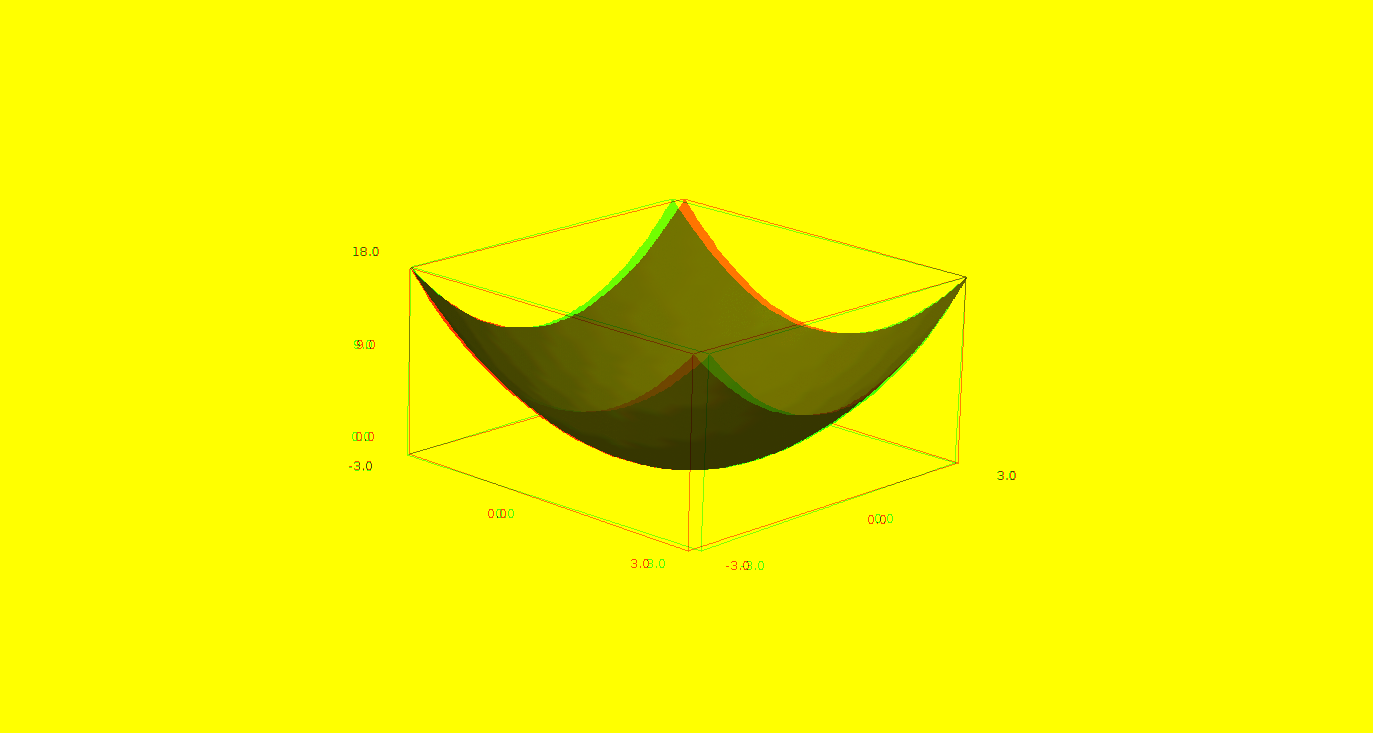
\includegraphics[width=15cm]{pictures_bitmap/coupe.png}
    \end{center}
    À part que l'ordinateur l'a dit, est-ce qu'on peut comprendre pourquoi le graphe de la fonction $x^2+y^2$ ressemble à un bol ? En coordonnées cylindriques, le graphe s'écrit
    \begin{equation}
        z=r^2.
    \end{equation}
    Donc il se fait que plus on s'éloigne du point $(0,0)$ dans le plan $XY$, plus le graphe va monter. Et il monte à quelle vitesse ? Il monte à la vitesse $r^2$. Il s'agit donc de dessiner la fonction $z=r^2$ dans le plan et de la «faire tourner».

\end{example}

% This is part of Mes notes de mathématique
% Copyright (c) 2006-2016
%   Laurent Claessens, Carlotta Donadello
% See the file fdl-1.3.txt for copying conditions.
 
%+++++++++++++++++++++++++++++++++++++++++++++++++++++++++++++++++++++++++++++++++++++++++++++++++++++++++++++++++++++++++++
\section{Courbes de niveau}
%+++++++++++++++++++++++++++++++++++++++++++++++++++++++++++++++++++++++++++++++++++++++++++++++++++++++++++++++++++++++++++

Une technique utile pour se faire une idée de la forme d'une fonction en trois dimensions est de tracer les \defe{courbes de niveau}{courbe de niveau}. La courbe de niveau de hauteur $h$ est la courbe dans le plan donnée par l'équation
\begin{equation}
    f(x,y)=h.
\end{equation}

\begin{example}

    Dessinons par exemple les courbes de niveau de la fonction
    \begin{equation}
        f(x,y)=x+y+2.
    \end{equation}
    La courbe de niveau $h$ est donnée par l'équation $x+y+2=h$, c'est à dire
    \begin{equation}
        y(x)=-x+h-2.
    \end{equation}
    Par conséquent la courbe de niveau de hauteur $0$ est $y=-x-2$, celle de hauteur $5$ est $y=-x+3$, etc.
    
    Nous pouvons également nous aider de Sage pour ce faire :
    \begin{verbatim}
----------------------------------------------------------------------
| Sage Version 4.6.1, Release Date: 2011-01-11                       |
| Type notebook() for the GUI, and license() for information.        |
----------------------------------------------------------------------
sage: f(x,y)=x+y+2
sage: var('h')                   
h
sage: niveau(h,x)=solve(f(x,y)==h,y)[0].rhs()
sage: g1(x)=niveau(1,x)
sage: g1
x |--> -x - 1
    \end{verbatim}
    Ici la fonction \verb+g1+ est la courbe de niveau $1$. 

    Si on veut faire tracer une courbe de niveau, Sage peut le faire :
    \begin{verbatim}
        sage: implicit_plot(f(x,y)==1,(x,-3,3),(y,-4,4))
    \end{verbatim}
    Cela tracera la courbe de niveau $h=1$ dans la partie du plan $x\in\mathopen[ -3 , 3 \mathclose]$ et $y\in\mathopen[ -4,4 ,  \mathclose]$.
    
\end{example}

Il est bien entendu possible de créer automatiquement $50$ courbes de niveau et de demander de les tracer toutes sur le même graphe.
\lstinputlisting{tex/frido/courbeNiveau.py}

Le résultat est :

\begin{center}
        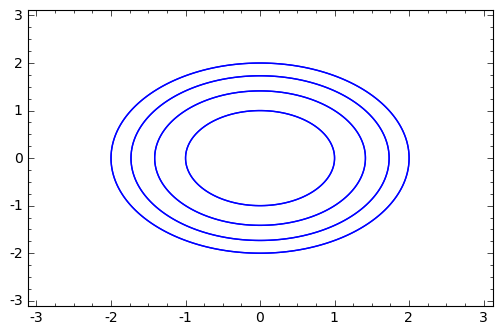
\includegraphics[width=8cm]{pictures_bitmap/niveauCercles.png}
\end{center}
Notez que les courbes sont censées être des cercles : les axes $X$ et $Y$ n'ont pas la même échelle. 

%Vous trouverez sur \href{http://www.sagenb.org/home/pub/23/}{cette page} tout ce qu'il vous faudra pour créer des courbes de niveau avec Sage.
%TODO : cette adresse n'est plus valide. Il faut retrouver où elle est passés sur sagemath.org (sagenb est devenu sagemath)

\begin{example}
    Un exemple plus riche en enseignements est celui de la fonction
    \begin{equation}
        f(x,y)=x^2-y^2.
    \end{equation}
    La courbe de niveau $h$ est donnée par l'équation $x^2-y^2=h$.

    Commençons par $h=0$. Dans ce cas nous avons $(x+y)(x-y)=0$ et par conséquent les courbes de niveau de hauteur zéro sont les deux droites $x+y=0$ et $x-y=0$.

    Voyons ensuite la courbe de niveau $h=1$. Cela est l'équation $x^2-y^2=1$, c'est à dire
    \begin{equation}
        y(x)=\pm\sqrt{x^2-1}.
    \end{equation}
    C'est une fonction qui n'est définie que pour $| x |\geq 1$. Avec $x=1$ nous avons $y=1$. Ensuite, lorsque $x$ grandit, $y$ grandit également, mais la courbe ne peut pas croiser la courbe de niveau $h=0$. Donc, suivant les notations de la figure \ref{LabelFigCQIXooBEDnfK}, la courbe de niveau «part» de $P$ et doit monter sans croiser les diagonales.

 % les figures CQIXooBEDnfK et KGQXooZFNVnW sont générées par le script MBFDooRFPyNW

%The result is on figure \ref{LabelFigCQIXooBEDnfK}. % From file CQIXooBEDnfK
\newcommand{\CaptionFigCQIXooBEDnfK}{La courbe de niveau $h=1$ de $x^2-y^2$. Notez qu'elle est en deux morceaux.}
\input{auto/pictures_tex/Fig_CQIXooBEDnfK.pstricks}

%The result is on figure \ref{LabelFigKGQXooZFNVnW}. % From file KGQXooZFNVnW
\newcommand{\CaptionFigKGQXooZFNVnW}{La courbe de niveau $x^2-y^2=-1$.}
\input{auto/pictures_tex/Fig_KGQXooZFNVnW.pstricks}

    En ce qui concerne la courbe de niveau $h=-1$, elle correspond à la courbe $y=\pm\sqrt{1+x^2}$ qui est définie pour tous les $x\in\eR$. Le même raisonnement que précédemment nous amène à la figure \ref{LabelFigKGQXooZFNVnW}.

\end{example}

Une autre façon de voir les courbe de niveau est de dire que la courbe de niveau de hauteur $h$ est la projection dans le plan $XY$ de la section du graphe de $f$ par le plan $z=h$.

On peut également définir le graphe de fonctions de trois (ou plus) variables. Le graphe de la fonction $f\colon D\subset\eR^3\to \eR$ est l'ensemble
\begin{equation}
    \big\{ \big( x,y,z,f(x,y,z) \big)\tq (x,y,z)\in D \big\}\subset \eR^4.
\end{equation}
De tels graphes ne peuvent pas être représentés sur une feuille de papier. Il est toutefois possible de définir les ensembles de niveaux :
\begin{equation}
    E_h=\big\{ (x,y,z)\in D\tq  f(x,y,z)=h\big\}.
\end{equation}
Ce sont des surfaces dans $\eR^3$ que l'on peut dessiner.

\begin{example}
    Les surfaces de niveau de la fonction $f(x,y,z)=x^2+y^2+z^2$ sont des sphères. Il n'y a pas de surfaces de niveau pour les «hauteurs» négatives.
\end{example}

\begin{example}
    Considérons la fonction $f(x,y,z)=x^2+y^2-z^2$. En coordonnées cylindrique, cette fonction s'écrit
    \begin{equation}
        f(r,\theta,z)=r^2-z^2.
    \end{equation}
    La surface de niveau $0$ est donnée par l'équation $r=| z |$. Cela fait un cercle à chaque hauteur, dont le rayon grandit linéairement avec la hauteur; le tout est donc un cône. C'est d'ailleurs le cône obtenu par rotation de la courbe de niveau $h=0$ que nous avions obtenue pour la fonction $x^2-y^2$.

    En ce qui concerne les ensembles de niveau positifs, ils sont donnés par
    \begin{equation}
        z=\pm\sqrt{x^2+y^2-h}.
    \end{equation}
    Notez qu'ils ne sont pas définis pour $r\geq h$. Cela pose un petit problème quand on veut le tracer à l'ordinateur :
    \begin{verbatim}
----------------------------------------------------------------------
| Sage Version 4.6.1, Release Date: 2011-01-11                       |
| Type notebook() for the GUI, and license() for information.        |
----------------------------------------------------------------------
sage: var('x,y')
(x, y)
sage: f(x,y)=sqrt(x**2+y**2-3)
sage: F=plot3d(f(x,y),(x,-5,5),(y,-5,5)) 
sage: G=plot3d(-f(x,y),(x,-5,5),(y,-5,5))    
sage: F+G
    \end{verbatim}
Le résultat est\footnote{Encore une fois : ça donne mieux à l'écran, et vous pouvez le faire bouger; je vous encourage à le faire !} :
    \begin{center}
            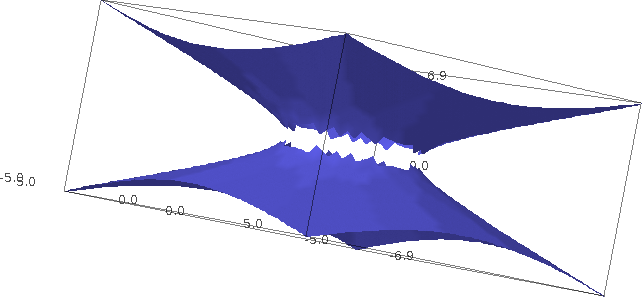
\includegraphics[width=15cm]{pictures_bitmap/AdSmauvais.png}
    \end{center}
    On voit qu'il y a un grand trou au centre correspondant aux $z$ proches de zéro. Or d'après l'équation, il n'en est rien : en $z=0$ il y a bel et bien tout un cercle. Afin d'obtenir une meilleur image, il faut demander de tracer avec un maillage plus fin :
    \begin{verbatim}
----------------------------------------------------------------------
| Sage Version 4.6.1, Release Date: 2011-01-11                       |
| Type notebook() for the GUI, and license() for information.        |
----------------------------------------------------------------------
sage: var('x,y')
(x, y)
sage: f(x,y)=sqrt(x**2+y**2-3)
sage: F=plot3d(f(x,y),(x,-5,5),(y,-5,5),plot_points=300) 
sage: G=plot3d(-f(x,y),(x,-5,5),(y,-5,5),plot_points=300)
sage: F+G
    \end{verbatim}
    Le temps de calcul est un peu plus long, mais le résultat est meilleur :
    \begin{center}
            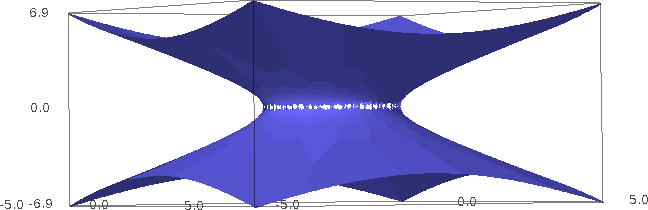
\includegraphics[width=15cm]{pictures_bitmap/AdSbon.png}
    \end{center}
\end{example}

%+++++++++++++++++++++++++++++++++++++++++++++++++++++++++++++++++++++++++++++++++++++++++++++++++++++++++++++++++++++++++++
%\section{Calcul de limites}
%+++++++++++++++++++++++++++++++++++++++++++++++++++++++++++++++++++++++++++++++++++++++++++++++++++++++++++++++++++++++++++

%Incidemment, le lemme \ref{Def_diff2} nous donne une nouvelle technique pour calculer des limites à plusieurs variables, similaire à celle du développement asymptotique expliquée dans la section \ref{SecTaylorR}.

%En effet, la formule \eqref{def_diff2} nous permet d'écrire $f(x)$ sous la forme
%\begin{equation}
%	f(x)=f(a)+df(a).(x-a)+\sigma_f(a,x)\| x-a \|
%\end{equation}
%où la fonction $\sigma_f$ satisfait $\lim_{x\to a}\sigma_f(a,x)=0$. Ici, $x$ et $a$ sont des éléments de $\eR^m$.

%++++++++++++++++++++++++++++++++++++++++++++++++++++++++++++++++++++++++++++++++++++++++
\section{Fonctions de classe $\mathcal{C}^1$}
%++++++++++++++++++++++++++++++++++++++++++++++++++++++++++++++++++++++++++++++++++++++++++++++++++++++++++++++++++++++++++++++

Soit $f$ une fonction différentiable de $U$, ouvert de $\eR^m$, dans $\eR^n$. L'application différentielle de $f$ est une application  de $\eR^m$ dans $\mathcal{L}(\eR^m, \eR^n)$ 
\begin{equation}
  \begin{array}{rccc}
    df : & \eR^m & \to & \mathcal{L}(\eR^m, \eR^n)\\
& a& \mapsto & df_a.
  \end{array}
\end{equation}
Nous savons que $\mathcal{L}(\eR^m, \eR^n)$ est un espace vectoriel normé avec la définition \ref{DefDQRooVGbzSm}. Si $T$ est un élément dans $\mathcal{L}(\eR^m, \eR^n)$ alors la norme de $T$ est définie par 
\[
\|T\|_{\mathcal{L}(\eR^m, \eR^n)}=\sup_{x\in\eR^m} \frac{\|T(x)\|_n}{\|x\|_m}=\sup_{\begin{subarray}{l}
    x\in\eR^m\\
\|x\|_m\leq 1
  \end{subarray}} \|T(x)\|_n.
\]

Lorsqu'il existe un $M>0$ tel que $\| df(a) \|_{\aL(\eR^m,\eR^n)}<M$ pour tout $a$ dans $U$, nous disons que la différentielle de $f$ est \defe{bornée}{bornée!différentielle} sur $U$.

\begin{definition}
	La fonction $f$ est dite \defe{de classe $\mathcal{C}^1$}{fonction!de classe  $\mathcal{C}^1$} de $U\subset\eR^m$  dans $\eR^n$ si son application différentielle $df$ est continue de $\eR^m$ dans $\mathcal{L}(\eR^m, \eR^n)$. Nous écrivons $f\in\mathcal{C}^1(U,\eR^n)$\nomenclature{$\aC^1(U,\eR^n)$}{Les applications une fois continument dérivables}.
\end{definition}

\begin{proposition}		\label{PropDerContCun}
	Une fonction \( f\colon U\to \eR^n\) où \( U\) est ouvert dans \( \eR^m\) est de classe \( C^1\) si et seulement si les dérivées partielles de $f$ existent et sont continues.
\end{proposition}

\begin{proof}
	Supposons que les dérivées partielles de $f$ existent et sont continues. Nous savons alors déjà par la proposition \ref{Diff_totale} que la fonction $f$ est différentiable et qu'elle s'exprime sous la forme
	\[
		df_a(h)=\sum_{i=1}^{m}\partial_if (a)h_i, \qquad \forall a \in U,\,\forall h\in\eR^m.
	\]
	Pour montrer que $df$ est continue, nous devons montrer que la quantité $\| df(x)-df(a) \|_{\aL(\eR^m,\eR^n)}$ peut être rendue arbitrairement petite si $\| x-a \|_m$ est rendu petit. Nous avons
	\begin{equation}
		\begin{aligned}
			\| df_x-df_a \|_{\aL}&=\sup_{\| h \|=1}\| df_x(h)-df_a(h) \|\\
			&=\sup_{\| h \|_m=1}\left\|\sum_{i=1}^{m}\left(\partial_if (x)-\partial_if (a)\right)h_i\right\|_n\leq\\
			&\leq\sup_{\| h \|_m=1}\sum_{i=1}^{m} \left\|\left(\partial_if (x)-\partial_if (a)\right)\right\|_n|h_i|\leq\\
			&\leq\sup_{\| h \|_m=1} \|h\|_\infty\sum_{i=1}^{m} \left\|\left(\partial_if (x)-\partial_if (a)\right)\right\|_n\\
			&\leq \sum_{i=1}^m\| \partial_if(x)-\partial_if(a) \|.
		\end{aligned}
	\end{equation}
	Dans ce calcul, nous avons utilisé le fait que si $\| h \|_m\leq 1$, alors $\| h \|_{\infty}\leq 1$. Étant donné la continuité de $\partial_if$, la dernière ligne peut être rendue arbitrairement petite lorsque $x$ est proche e $a$.

Supposons maintenant que $f$ soit dans $\mathcal{C}^1(U,\eR^n)$. Alors 
\[
\left\|\partial_if (x)-\partial_if (a)\right\|_n= \left\|df(x).e_i-df(a).e_i\right\|_n \leq  \left\|df(x)-df(a)\right\|_{\mathcal{L}(\eR^m,\eR^n)},
\]  
la continuité de $df$ implique donc celle de $\partial_i f$ pour tout $i$ dans $\{1,\ldots,m\}$.
\end{proof}
\begin{proposition}
  Soient $U$ un ouvert de $\eR^m$ et $V$ un ouvert de $\eR^n$. Soient $f: U\to V$  dans $\mathcal{C}^1(U,V)$ et $g: V \to \eR^p$ dans $\mathcal{C}^1(V,\eR^n)$.  Alors la fonction composée $g\circ f: U\to \eR^p $ est dans $\mathcal{C}^1(U,\eR^p)$.
\end{proposition}
\begin{proof} On fixe $a$ dans $U$ 
  \begin{equation}
    \begin{aligned}
     \big\|d(g\circ f)(x)&-d(g\circ f)(a)\big\|_{\mathcal{L}(\eR^m,\eR^p)}\\
     &=\left\|dg(f(x))\circ df(x)-dg(f(a))\circ df(a)\right\|_{\mathcal{L}(\eR^m,\eR^p)}\leq\\
&\leq \left\|\left(dg(f(x))-dg(f(a))\right)\circ df(x)\right\|_{\mathcal{L}(\eR^m,\eR^p)}+\\
&\quad+ \left\|dg(f(a))\circ \left(df(x)-df(a)\right)\right\|_{\mathcal{L}(\eR^m,\eR^p)}\leq\\
&\leq \left\|dg(f(x))-dg(f(a))\right\|_{\mathcal{L}(\eR^n,\eR^p)}\left\| df(x)\right\|_{\mathcal{L}(\eR^m,\eR^n)}+\\
&\quad+ \left\|dg(f(a))\right\|_{\mathcal{L}(\eR^n,\eR^p)}\left\| df(x)-df(a)\right\|_{\mathcal{L}(\eR^n,\eR^p)}.\\
    \end{aligned}
  \end{equation}
On peut conclure en passant à la limite $x\to a$ parce que les fonctions $f$, $g$, $df$ et $dg$ sont continues, de telle sorte que
\begin{equation}
	\begin{aligned}[]
		\lim_{x\to a} dg\big( f(x) \big)=dg\big( f(a) \big)\\
		\lim_{x\to a} df(x)=df(a).
	\end{aligned}
\end{equation}
\end{proof}

\begin{remark}
  On peut prouver le même résultat en utilisant la continuité de l'application bilinéaire 
\begin{equation}
  \begin{array}{rccc}
    \circ : & \mathcal{C}^1(U,V)\times\mathcal{C}^1(V,\eR^p)  & \to & \mathcal{L}(U, \eR^p)\\
& (T,S)& \mapsto & T\circ S.
  \end{array}
\end{equation}
\end{remark}
%+++++++++++++++++++++++++++++++++++++++++++++++++++++++++++++++++++++++++++++++++++++++++++++++++++++++++++++++++++++++++++
\section{Dérivée directionnelle de fonctions composées}		\label{SecDerDirFnComp}
%+++++++++++++++++++++++++++++++++++++++++++++++++++++++++++++++++++++++++++++++++++++++++++++++++++++++++++++++++++++++++++

Étant donné que nous allons voir en détail la différentielle de fonctions composées à la proposition \ref{PropDiffCompose}, nous n'allons pas rentrer dans tous les détail ici.

Nous savons déjà comment dériver les fonctions composées de $\eR$ dans $\eR$. Si nous avons deux fonctions $f\colon \eR\to \eR$ et $u\colon \eR\to \eR$, nous formons la composée $\varphi=f\circ u\colon \eR\to \eR$ dont la dérivée vaut
\begin{equation}
	\varphi'(a)=f'\big( u(a) \big)u'(a).
\end{equation}

Considérons maintenant le cas un peu plus compliqué des fonctions $f\colon \eR\to \eR$ et $u\colon \eR^2\to \eR$, et de la composée
\begin{equation}
	\begin{aligned}
		\varphi\colon \eR^2&\to \eR \\
		\varphi(x,y)&= f\big( u(x,y) \big). 
	\end{aligned}
\end{equation}
Afin de calculer la dérivée partielle de $\varphi$ par rapport à $x$, nous admettons que pour tout $a$, $b$ et $t$, il existe $c\in\mathopen[ a , a+t \mathclose]$ tel que
\begin{equation}
	u(a+t,b)=u(a,b)+t\frac{ \partial u }{ \partial x }(c,b).
\end{equation}
Cela est une généralisation immédiate du théorème \ref{ThoAccFinis}. Nous devons calculer
\begin{equation}		\label{EqPremPasDiffxvp}
	\frac{ \partial \varphi }{ \partial x }(a,b)=\lim_{t\to 0} \frac{ \varphi(a+t,b)-\varphi(a,b) }{ t }=\lim_{t\to 0} \frac{ f\big( u(a+t,b) \big)-g\big( u(a,b) \big) }{ t }.
\end{equation}
Étant donné l'hypothèse que nous avons faite sur $u$, nous avons
\begin{equation}
	f\big( u(a+t,b) \big)=f\big( u(a,b)+t\frac{ \partial u }{ \partial x }(c,b) \big).
\end{equation}
En utilisant le théorème des accroissements finis pour $f$, nous avons un point $d$ entre $u(a,b)$ et $u(a,b)+t\frac{ \partial u }{ \partial x }(c,b)$ tel que
\begin{equation}
	f\big( u(a,b)+t\frac{ \partial u }{ \partial x }(c,b) \big)=f\big( u(a,b) \big)+t\frac{ \partial u }{ \partial x }(c,b)f'(d).
\end{equation}
Le numérateur de \eqref{EqPremPasDiffxvp} devient donc
\begin{equation}
	t\frac{ \partial u }{ \partial x }(c,b)f'(d).
\end{equation}
Certes les points $c$ et $d$ sont inconnus, mais nous savons que $c$ est entre $a$ et $a+t$ ainsi que $d$ se situe entre $u(a,b)$ et $u(a,b)+t\frac{ \partial u }{ \partial x }(c,b)$. Lorsque nous prenons la limite $t\to 0$, nous avons donc $\lim_{t\to 0} c=a$ et $\lim_{t\to 0} d=u(a,b)$. Nous avons alors
\begin{equation}
	\lim_{t\to 0} \frac{ t\frac{ \partial u }{ \partial x }(c,b)f'(d) }{ t }=\frac{ \partial u }{ \partial x }(a,b)f'\big( u(a,b) \big).
\end{equation}
La formule que nous avons obtenue (de façon pas très rigoureuse) est
\begin{equation}
	\frac{ \partial  }{ \partial x }f\big( u(x,y) \big)=\frac{ \partial u }{ \partial x }(x,y)f'\big( u(x,y) \big).
\end{equation}

Prenons maintenant un cas un peu plus compliqué où nous voudrions savoir les dérivées partielles de la fonction $\varphi$ donnée par
\begin{equation}
	\varphi(x,y,z)=f\big( u(x,y),v(x,y,z) \big)
\end{equation}
où $f\colon \eR^2\to \eR$, $u\colon \eR^2\to \eR$ et $v\colon \eR^3\to \eR$. 

Commençons par la dérivée partielles par rapport à $z$. Étant donné que $\varphi$ ne dépend de $z$ que via la seconde entrée de $f$, il est normal que seule la dérivée partielle de $f$ par rapport à sa seconde entrée arrive dans la formule :
\begin{equation}
	\frac{ \partial \varphi }{ \partial z }(x,y,z)=\frac{ \partial f }{ \partial v }\big( u(x,y),v(x,y,z) \big)\frac{ \partial v }{ \partial z }(x,y,z).
\end{equation}
La dérivée partielle par rapport à $y$ demande de tenir compte en même temps de la façon dont $f$ varie avec sa première entrée et la façon dont elle varie avec sa seconde entrée; cela nous fait deux termes :
\begin{equation}
	\frac{ \partial \varphi }{ \partial y }(x,y,z)=\frac{ \partial f }{ \partial u }\big( u(x,y),v(x,y,z) \big)\frac{ \partial u }{ \partial y }(x,y)+\frac{ \partial f }{ \partial v }\big( u(x,y),v(x,y,z) \big)\frac{ \partial v }{ \partial y }(x,y,z).
\end{equation}


Cette formule a une interprétation simple. Lançons un caillou du sommet d'une falaise. Son mouvement est une chute libre avec une vitesse initiale horizontale :
\begin{subequations}
	\begin{numcases}{}
		x(t)=v_0t\\
		y(t)=h_0-\frac{ gt^2 }{ 2 }
	\end{numcases}
\end{subequations}
où $v_0$ est la vitesse initiale horizontale et $h_0$ est la hauteur de la falaise. Si nous sommes intéressés à la distance entre le caillou et le bas de la falaise (point $(0,0)$), le théorème de Pythagore nous dit que
\begin{equation}
	d(t)=\sqrt{x^2(t),y^2(t)}.
\end{equation}
Pour trouver la variation de la distance par rapport au temps il faut savoir de combien la distance varie lorsque $x$ varie et multiplier par la variation de $x$ par rapport à $t$, et puis faire la même chose avec $y$.

\begin{theorem}		\label{ThoDerDirFnComp}
	Soit $g\colon \eR^m\to \eR^n$ une fonction différentiable en $a$, et $f\colon \eR^n\to \eR^p$ une fonction différentiable en $g(a)$. Si nous définissons $\varphi(x)=(f\circ g)(x)$, alors pour tout $i=1,\ldots,m$, nous avons
	\begin{equation}
		\frac{ \partial \varphi }{ \partial x_i }(a)=\sum_{k=1}^n\frac{ \partial f }{ \partial y_k }\big( g(a) \big)\frac{ \partial g }{ \partial x_i }
	\end{equation}
	où $\frac{ \partial f }{ \partial y_k }$ dénote la dérivée partielle de $f$ par rapport à sa $k$-ième variable.
\end{theorem}

Donnons un exemple d'utilisation de cette formule. Si
\begin{equation}
	\begin{aligned}[]
		g\colon \eR^2\to \eR^3\\
		f\colon \eR^3\to \eR,
	\end{aligned}
\end{equation}
nous avons $\varphi\colon \eR^2\to \eR$. Les dérivées partielles de $\varphi$ sont données par les formules
\begin{equation}
	\frac{ \partial \varphi }{ \partial x }(x,y)=\frac{ \partial f }{ \partial x_1 }\big( g(x,y) \big)\frac{ \partial g_1 }{ \partial x }(x,y)+\frac{ \partial f }{ \partial x_2 }\big( g(x,y) \big)\frac{ \partial g_2 }{ \partial y }(x,y)+\frac{ \partial f }{ \partial x_3 }\big( g(x,y) \big)\frac{ \partial g_3 }{ \partial x }(x,y)
\end{equation}
et
\begin{equation}
	\frac{ \partial \varphi }{ \partial y }(x,y)=\frac{ \partial f }{ \partial x_1 }\big( g(x,y) \big)\frac{ \partial g_1 }{ \partial y }(x,y)+\frac{ \partial f }{ \partial x_2 }\big( g(x,y) \big)\frac{ \partial g_2 }{ \partial y }(x,y)+\frac{ \partial f }{ \partial x_3 }\big( g(x,y) \big)\frac{ \partial g_3 }{ \partial y }(x,y)
\end{equation}
Notez que les dérivées de $\varphi$ et des composantes de $g$ sont calculées en $(x,y)$, tandis que celles de $f$ sont calculées en $g(x,y)$.

%++++++++++++++++++++++++++++++++++++++++++++++++++++++++++++++++++++++++++++++++++++++++++++++++++++++++++++++++++++++
\section{Théorèmes des accroissements finis}		\label{SecThoAccrsFinis}
%++++++++++++++++++++++++++++++++++++++++++++++++++++++++++++++++++++++++++++++++++++++++++++++++++++++++++++++++++++++

Nous avons déjà démontré (lemme \ref{LemdfaSurLesPartielles}) que si $f$ est différentiable au point $x$ alors  $df_x(u)=\partial_uf(x)$. Une importante conséquence est le théorème des accroissements finis
\begin{theorem}[Accroissements finis, inégalité de la moyenne]\label{val_medio_2}
   Soit $U$ un ouvert dans $\eR^m$ et soit $f:U\to\eR^n$ une fonction différentiable. Soient $a$ et $b$ deux point dans $U$, $a\neq b$, tels que le segment $[a,b]$ soit contenu dans $U$. Alors
   \begin{equation}
        \|f(b)-f(a)\|_n\leq \sup_{x\in[a,b]}\|df(x)\|_{\mathcal{L}(\eR^m,\eR^n)}\|b-a\|_m.
   \end{equation}
\end{theorem}
\index{application!différentiable}
\index{inégalité!de la moyenne}
\index{théorème!accroissements finis!forme générale}

\begin{proof}
 On utilise le théorème \ref{val_medio_1} et le fait que 
\[
\|\partial_u f(x)\|_n\leq \|df(x)\|_{\mathcal{L}(\eR^m,\eR^n)}\|u\|_m,
\]
pour tout $u$ dans $\eR^m$.
\end{proof}

La proposition suivante est une application fondamentale du théorème des accroissements finis \ref{val_medio_2}.
\begin{proposition}		\label{PropAnnulationEtConstance}
	Soit $U$ un ouvert connexe par arcs de $\eR^m$ et une fonction $f\colon U\to \eR^n$. Les conditions suivantes sont équivalentes :
	\begin{enumerate}
		\item\label{ItemPropCstDiffZeroi}
			$f$ est constante;
		\item\label{ItemPropCstDiffZeroii}
			$f$ est différentiable et $df(a)=0$ pour tout $a\in U$;
		\item\label{ItemPropCstDiffZeroiii}
			les dérivées partielles $\partial_1f,\ldots,\partial_mf$ existent et sont nulles sur $U$.
	\end{enumerate}
\end{proposition}
\index{connexité!par arc!fonction différentiable}
\index{différentiabilité}

\begin{proof}
	Nous allons démonter les équivalences en plusieurs étapes. D'abord \ref{ItemPropCstDiffZeroi} $\Rightarrow$ \ref{ItemPropCstDiffZeroii}, puis \ref{ItemPropCstDiffZeroii} $\Rightarrow$ \ref{ItemPropCstDiffZeroiii}, ensuite \ref{ItemPropCstDiffZeroiii} $\Rightarrow$ \ref{ItemPropCstDiffZeroii} et enfin \ref{ItemPropCstDiffZeroii} $\Rightarrow$ \ref{ItemPropCstDiffZeroi}.

	Commençons par montrer que la condition \ref{ItemPropCstDiffZeroi} implique la condition \ref{ItemPropCstDiffZeroii}. Si $f(x)$ est constante, alors la condition \eqref{EqCritereDefDiff} est vite vérifiée en posant $T(h)=0$.

	Afin de voir que la condition \ref{ItemPropCstDiffZeroii} implique la condition \ref{ItemPropCstDiffZeroiii}, remarquons d'abord que la différentiabilité de $f$ implique que les dérivées partielles existent (proposition \ref{diff1}) et que nous avons l'égalité $df(a).u=\sum_iu_i\partial_if(a)$ pour tout $u\in\eR^m$ (lemme \ref{LemdfaSurLesPartielles}). L'annulation de $\sum_iu_i\partial_if(a)$ pour tout $u$ implique l'annulation des $\partial_if(a)$ pour tout $i$.

	Prouvons maintenant que la propriété \ref{ItemPropCstDiffZeroiii} implique la propriété \ref{ItemPropCstDiffZeroii}. D'abord, par la proposition \ref{Diff_totale}, l'existence et la continuité des dérivées partielles $\partial_if(a)$ implique la différentiabilité de $f$. Ensuite, la formule $df(a).u=\sum_i u_i\partial_if(a)$ implique que $df(a)=0$. 
	
	
	Il reste à montrer que \ref{ItemPropCstDiffZeroii} implique la condition \ref{ItemPropCstDiffZeroi}, c'est à dire que l'annulation de la différentielle implique la constance de la fonction. C'est ici que nous allons utiliser le théorème des accroissements finis. En effet, si $a$ et $b$ sont des points de $U$, le théorème \ref{val_medio_2} nous dit que
	\begin{equation}
		\|f(b)-f(a)\|_n\leq \sup_{x\in[a,b]}\|df(x)\|_{\mathcal{L}(\eR^m,\eR^n)}\|b-a\|_m.
	\end{equation}
	Mais $\| df(x) \|=0$ pour tout $x\in U$, donc ce supremum est nul et $f(b)=f(a)$, ce qui signifie la constance de la fonction.
\end{proof}

%\begin{proof}
%  \begin{itemize}
%  \item Le théorème \ref{val_medio_2} nous dit que si la différentielle de $f$ est nulle alors $f$ est constante sur chaque segment contenu dans $U$. Cela nous dit que $f$ est constante sur chaque boule contenue dans $U$, donc $f $ est localement constante. Il est possible de démontrer que toute fonction localement constante sur un connexe est constante.  
%\item Si toutes les dérivées partielles $\partial_1 f, \ldots, \partial_m f $ existents et sont identiquement nulles sur $U$ alors $f$ est différentiable et sa différentielle est identiquement nulle. On utilise la première partie de la preuve pour conclure. 
%  \end{itemize}
%\end{proof}

%+++++++++++++++++++++++++++++++++++++++++++++++++++++++++++++++++++++++++++++++++++++++++++++++++++++++++++++++++++++++++++
\section{Fonctions Lipschitziennes}
%+++++++++++++++++++++++++++++++++++++++++++++++++++++++++++++++++++++++++++++++++++++++++++++++++++++++++++++++++++++++++++


\begin{definition}      \label{DEFooQHVEooDbYKmz}
    Soient \( (E,d_E)\) et \( (F,d_F)\) deux espaces métriques\footnote{Pour rappel, les espaces métriques sont définis par la définition \ref{DefMVNVFsX} et le théorème \ref{ThoORdLYUu}; je précise que nous ne supposons pas que \( E\) soit vectoriel; en particulier il peut être un ouvert de \( \eR^n\).}, \( f\colon E\to F\) une application et un réel \( k\) strictement positif. Nous disons que \( f\) est \defe{Lipschitzienne}{Lipschitzienne} de constante $k$ sur \( E\) si pour tout \( x,y\in E\),
    \begin{equation}
        d_F\big( f(x)-f(y) \big)\leq kd_E(x,y).
    \end{equation}
\end{definition}
%TODO : faire la chasse aux endroits où cette définition devrait être référencée.
Soit \( f\) une fonction \( k\)-Lipschitzienne. Si \( y\in \overline{ B(x,\delta)}\) alors \( \| x-y \|\leq\delta\) et donc \( \big\| f(x)-f(y) \big\|\leq k\delta\). Cela signifie que la condition Lipschitz pour s'énoncer en termes de boules fermées par
\begin{equation}    \label{EqDZvtUbn}
    f\big( \overline{ B(x,\delta) } \big)\subset \overline{  B\big( f(x),k\delta \big) }
\end{equation}
tant que \( \overline{ B(x,\delta) } \) est contenue dans le domaine sur lequel \( f\) est Lipschitz.

\begin{proposition}
  Soit  $U$ un ouvert convexe  de $\eR^m$, et soit $f:U\to \eR^n$ une fonction différentiable. La fonction $f$ est Lipschitzienne sur $U$ si et seulement si $df$ est bornée sur $U$.  
\end{proposition}
\begin{proof}
	Le fait que l'application différentielle $df$ soit bornée signifie qu'il existe un $M>0$ dans $\eR$ tel que $\|df_a\|_{\mathcal{L}(\eR^m,\eR^n)}\leq M$, pour tout $a$ dans $U$. Si cela est le cas, alors le théorème \ref{val_medio_2} et la convexité\footnote{La convexité de $U$ sert à assurer que la droite reliant $a$ à $b$ est contenue dans $U$; c'est ce que nous utilisons dans la démonstration du théorème \ref{val_medio_2}.} de $U$ impliquent évidemment que $f$ est de Lipschitz de constante plus petite ou égale à $M$.
	
	Inversement, si $f$ est Lipschitz de constante $k$, alors pour tout $a$ dans $U$ et $u$ dans $\eR^m$ on a 
	\[
		\left\|\frac{f(a+tu)-f(a)}{t}\right\|_n\leq k \|u\|_m,
	\]   
	En passant à la limite pour $t\to 0$ on a 
	\[
		\|\partial_u f(a)\|_n=\|df_a(u)\|_n\leq k \|u\|_m,
	\]
	donc la norme de $df_a$ est majorée par $k$ pour tout $a$ dans $U$.   
\end{proof}

Notez cependant qu'une fonction peut être Lipschitzienne sans être différentiable.

\begin{proposition} \label{PropFZgFTEW}
    Une fonction Lipschitzienne \( f\colon \eR\to \eR\) est continue.
\end{proposition}

\begin{proof}
    Nous utilisons la caractérisation de la continuité donnée par le théorème \ref{ThoESCaraB}. Prouvons donc la continuité en \( a\in \eR\). Pour tout \( x\) nous avons
    \begin{equation}
        \big| f(x)-f(a) \big|\leq k| x-a |.
    \end{equation}
    Si \( \epsilon>0\) est donné, il suffit de prendre \( \delta<\frac{ \epsilon }{ k }\) pour avoir
    \begin{equation}
        \big| f(x)-f(a) \big|\leq k\frac{ \epsilon }{ k }=\epsilon.
    \end{equation}
    Donc \( f\) est continue en \( a\).
\end{proof}

\begin{definition}      \label{DefJSFFooEOCogV}
    Une fonction 
    \begin{equation}
        \begin{aligned}
            f\colon \eR^n\times \eR^m&\to \eR^p \\
            (t,y)&\mapsto f(t,y) 
        \end{aligned}
    \end{equation}
    est \defe{localement Lipschitz}{Lipschitz!localement} en \( y\) au point \( (t_0,y_0)\) s'il existe des voisinages \( V\) de \( t_0\) et \( W\) de \( y_0\) et un nombre \( k>0\) tels que pour tout \( (t,y)\in V\times W\) on ait
    \begin{equation}
        \big\| f(t_0,y_0)-f(t,y) \big\|\leq k\| y-y_0 \|.
    \end{equation}
    La fonction est localement Lipschitz sur un ouvert \( U\) de \( \eR^n\times \eR^m\) si elle est localement Lipschitz en chaque point de \( U\).
\end{definition}

\begin{normaltext}      \label{NORMooYNRAooBgobcK}
    Autrement dit, une fonction est localement Lipschitzienne en sa deuxième variable lorsque tout point admet un voisinage sur lequel elle est Lipschitzienne.
\end{normaltext}

\begin{proposition}     \label{PropGIBZooVsIqfY}
    Si \( f\) et \( g\) sont deux fonctions localement Lipschitz alors \( f+g\) l'est.
\end{proposition}

\begin{proof}
    Il s'agit d'un simple calcul avec une majoration standard :
    \begin{subequations}
        \begin{align}
            \| (f+g)(t_0,y_0)-(f+g)(t,y) \|&\leq \|  f(t_0,y_0)-f(t,y)  \|+\| g(t_0,y_0)-g(t,y) \|\\
            &\leq k_f\| y-y_0 \|+k_g\| y-y_0 \|\\
            &=(k_f+k_g)\| y-y_0 \|.
        \end{align}
    \end{subequations}
\end{proof}

\begin{lemma}   \label{LemCFZUooVqZmpc}
    La fonction donné par
    \begin{equation}
        f(t, (x,y) )=xy
    \end{equation}
    est localement Lipschitz en tout point.
\end{lemma}

\begin{proof}
    Nous avons la majoration classique
    \begin{equation}
        | f\big(t,(x_0,y_0)\big)-f\big( t,(x,y) \big) |=| x_0y_0-xy |\leq| x_0y_0-x_0y |+| x_0y-xy |\leq | x_0 || y_0-y |+| y || x_0-x |.
    \end{equation}
    Vu que nous parlons de fonction \emph{localement Lipschitzienne}, nous pouvons majorer \( | y |\) et \( | x_0 |\) par un même nombre \( k\) dans un voisinage de \( (x_0,y_0)\). Cela donne
    \begin{equation}
        | f\big(t,(x_0,y_0)\big)-f\big( t,(x,y) \big) |\leq k\big( | y_0-y |+| x_0-x | \big)\leq \sqrt{2}k\| \begin{pmatrix}
            x_0-x    \\ 
            y_0-y    
        \end{pmatrix}\|.
    \end{equation}
    Nous avons utilisé l'équivalence de norme de la proposition \ref{PropLJEJooMOWPNi}\ref{ItemABSGooQODmLNi}.
\end{proof}



%++++++++++++++++++++++++++++++++++++++++++++++++++++++++++++++++++++++++++++++++++++++++
\section{Différentielles d'ordre supérieur}		\label{SecDiffOrdSup}
%++++++++++++++++++++++++++++++++++++++++++++++++++++++++++++++++++++++++++++++++++++++++++++++++++++++++++++++++++++++++++++++
\begin{definition}
	Soit $U$ un ouvert de $\eR^m$ et  $f:U\subset\eR^m\to \eR^n$ une fonction. La fonction $f$ est dite \defe{deux fois différentiable}{différentiable!deux fois} au point $a$ dans $U$,  si $f$ est différentiable dans un voisinage de $a$, et sa différentielle $df$ est différentiable au point $a$ en tant que application de $U$ dans $\mathcal{L}(\eR^m, \eR^n)$.  

La fonction $f$ sera dite deux fois différentiable sur l'ensemble $U$ si elle est deux fois différentiable en chaque point de $U$.

\end{definition}

%--------------------------------------------------------------------------------------------------------------------------- 
\subsection{Identification des espaces d'applications multilinéaires}
%---------------------------------------------------------------------------------------------------------------------------

La différentielle de la différentielle de $f$ est notée 
\[
d(df)(a)=d^2f(a),
\]
et est une application de $U$ dans $\mathcal{L}(\eR^m,\mathcal{L}(\eR^m, \eR^n) )$. Comme on a vu dans la proposition \ref{isom_isom}, l'espace $\mathcal{L}(\eR^m,\mathcal{L}(\eR^m, \eR^n) )$ est isométriquement isomorphe à l'espace $\mathcal{L}(\eR^m\times\eR^m, \eR^n )$. On verra comment cette propriété  est utilisé dans l'exemple \ref{bilin_2diff}.


Soient \( V\) et \( W\) deux espace vectoriel normés de dimension finie et \( \mO\) un ouvert autour de \( x\in V\). D'une part l'espace des applications linéaires \( \aL(V,W)\) est lui-même un espace vectoriel normé de dimension finie, et on peut identifier \(  \aL\big( V,\aL^{(k)}(V,W) \big)\)\nomenclature[Y]{\( \aL^{(n)}(V,W)\)}{L'espace des applications \( n\)-linéaires \( V^n\to W\)} avec \( \aL^{(k+1)}(V,W)\), ce qui nous permet de dire que la \( k\)\ieme\ différentielle est une application
\begin{equation}
    d^kf\colon \mO\to \aL^{(k)}(V,W).
\end{equation}
Plus précisément, l'identification se fait de la façon suivante : si \( \omega\in \aL\big( V,\aL^{(k)}(V,W) \big)\), alors \( \omega\) vu dans \( \aL^{(k+1)}(V,W)\) est définie par
\begin{equation}
    \omega(u_1,\ldots, u_{k+1})=\omega(u_1)(u_2,\ldots, u_{k+1}).    
\end{equation}

Cela étant posé nous pouvons donner les définition.

%--------------------------------------------------------------------------------------------------------------------------- 
\subsection{Fonctions différentiables plusieurs fois}
%---------------------------------------------------------------------------------------------------------------------------

\begin{definition}[\cite{ZCKMFRg}]  \label{DefPNjMGqy}
    La fonction \( f\colon \mO\subset V\to W\) est
    \begin{enumerate}
        \item
            de classe \( C^0\) si elle est continue,
        \item
            de classe \( C^1\) si \( df\colon \mO\to \aL(V,W)\) est continue,
        \item
            de classe \( C^k\) si \( d^kf\colon \mO\to \aL^{(k)}(V,W)\) est continue,
        \item
            de classe \(  C^{\infty}\) si \( f\) est dans \( \bigcap_{k=0}^{\infty}C^k(V,W)\).
    \end{enumerate}
\end{definition}
\index{application!différentiable}
\index{application!de classe \( C^k\)}

\begin{definition}
    Un \defe{\( C^k\)-difféomorphisme}{difféomorphisme!de classe $C^k$} est une application inversible de classe \( C^k\) dont l'inverse est également de classe \( C^k\).
\end{definition}

\begin{example}\label{bilin_2diff}
	Soit $B:\eR^m\times \eR^m\to\eR^n$ une application bilinéaire. On définit $f:\eR^m\to\eR^n$ par $f(x)=B(x,x)$. Le lemme \ref{bilin_diff} nous dit que $B$ est différentiable. Cela implique la différentiabilité de $f$. Pour trouver la différentielle de la fonction $f$, nous écrivons $f=B\circ s$ où $s\colon \eR^m\to \eR^m\times\eR^m$ est l'application $s(x)=(x,x)$. En utilisant la règle de différentiation de fonctions composées,
	\begin{equation}
		df(a)=dB\big( s(a) \big)\circ ds(a).
	\end{equation}
	Mais $ds(a).u=(u,u)$ parce que $s(a+h)-s(a)-(h,h)=0$. Par conséquent,
	\begin{equation}		\label{EqdBsaExp}
		df(a).u=dB\big( s(a) \big)(u,u)=B(u,a)+B(a,u)
	\end{equation}
	où nous avons utilisé la formule du lemme \ref{bilin_diff}. La formule \eqref{EqdBsaExp} peut être écrite sous la forme compacte
	\begin{equation}
		df(a)=B(\cdot,a)+B(a,\cdot)
	\end{equation}
	La fonction $df(a)$ ainsi écrite est linéaire par rapport à $a$, donc différentiable. En outre elle coïncide avec sa différentielle, comme on a vu dans le remarque \ref{rk_lin}, au sens que la différentielle de $df$ au point $a$ sera l'application que à chaque $x$ dans $\eR^m$ associe l'application linéaire $B(x,\cdot)+B(\cdot, x)$. On voit bien que $d^2f$ au point $a$ est une application de $\eR^m$ vers l'espace des applications linéaires $\mathcal{L}(\eR^m, \eR^n)$. On peut utiliser d'autre part l'isomorphisme des espaces $\mathcal{L}(\eR^m,\mathcal{L}(\eR^m, \eR^n) )$ et $\mathcal{L}(\eR^m\times\eR^m, \eR^n )$ et dire que, une fois que $a$ est fixé, l'application $d^2f(a)$ est une application bilinéaire sur $\eR^m\times\eR^m$. On écrit alors $d^2f(a)(x,y)=B(x,y)+B(y,x)$.   
\end{example}

%--------------------------------------------------------------------------------------------------------------------------- 
\subsection{Différentielle seconde, fonction de classe \( C^2\)}
%---------------------------------------------------------------------------------------------------------------------------

Une condition nécessaire et suffisante pour l'existence de la différentielle seconde est la suivante
\begin{proposition}
   Soit $U$ un ouvert de $\eR^m$ et  $f:U\subset\eR^m\to \eR^n$ une fonction. La fonction $f$ est deux fois différentiable au point $a$ si et seulement si les dérivées partielles $\partial_1 f, \ldots, \partial_m f $ sont différentiables en $a$. 
\end{proposition}
Cela veut dire, en particulier, que $f$ est deux fois différentiable si et seulement si ses dérivées partielles secondes, $\partial_i\partial_j f$, pour toute couple d'indices $i,j$  dans $\{1,\ldots, m\}$, existent et sont continues. Pour les différentielles d'ordre supérieur on a la proposition suivante.

La différentielle seconde dans l'exemple  \ref{bilin_2diff} est symétrique, c'est à dire que $d^2f(a)(x_1,x_2)=d^2f(a)(x_2,x_1)$. En fait toute différentielle seconde est symétrique.  


\begin{theorem}[Schwarz]\label{Schwarz}
 Soit $U$ un ouvert de $\eR^m$ et  $f:U\subset\eR^m\to \eR^n$ une fonction de classe $\mathcal{C}^2$. Alors, pour toute couple $i,j$ d'indices dans $\{1,\ldots, m\}$ et pour tout point $a$ dans $U$, on a 
\[
\frac{\partial^2 f}{\partial  x_i\partial x_j}(a)=\frac{\partial^2 f}{\partial  x_j\partial x_i}(a).
\]
\end{theorem}
\begin{proof}
  Pour simplifier l'exposition nous nous limitons ici au cas $m=2$. Soit $(h,g)$ un vecteur fixé dans $\eR^2$. Pour tout  $v=(x,y)$ dans $\eR^2$ on note
  \begin{equation}
    \begin{array}{c}
      \Delta_h f(v)=f(v+he_1) -f(v) = f(x+h,y)-f(x,y),\\ 
      \Delta_g f(v)=f(v+ge_2) -f(v) = f(x,y+g)-f(x,y),\\ 
    \end{array}
  \end{equation}
Nous avons
\begin{equation}
  \begin{array}{c}
   \Delta_g   \Delta_h f(v)=\left(f(x+h,y+g)-f(x,y+g)\right)-\left(f(x+h,y)-f(x,y)\right),\\
   \Delta_h   \Delta_g f(v)=\left(f(x+h,y+g)-f(x+h,y)\right)-\left(f(x,y+g)-f(x,y)\right),
  \end{array}
\end{equation}
donc, 
\begin{equation}
  \frac{1}{g} \Delta_g  \left(\frac{1}{h} \Delta_h f(v)\right) = \frac{1}{h} \Delta_h \left(\frac{1}{g} \Delta_g f(v)\right).
\end{equation}
On utilise alors le théorème des accroissements finis
\[
\frac{1}{h} \Delta_h f(v)=\frac{1}{h}\big(f(x+h,y)-f(x,y)\big)=\frac{1}{h}\partial_1f(x+t_1h,y )h=\partial_1f(x+t_1h, y),
\]
pour un certain $t_1$ dans $]0,1[$. De même on obtient 
\[
\frac{1}{g} \Delta_g f(v)= \partial_2 f(x, y+t_2g),
\]
pour un certain $t_2$ dans $]0,1[$. Alors
 \begin{equation}
  \frac{1}{g} \Delta_g  \big(\partial_1f(x+t_1h, y)\big) = \frac{1}{h} \Delta_h \big(\partial_2 f(x, y+t_2g)\big).
\end{equation}
En appliquant encore une fois le théorème des accroissements finis on a
 \begin{equation}
  \partial_2\partial_1f(x+t_1h, y+s_1g) = \partial_1\partial_2 f(x+s_2h, y+t_2g).
\end{equation} 
Il suffit maintenant de passer à la limite pour $(h,g) \to (0,0)$ et de se souvenir du fait que $f$ est $\mathcal{C}^2$ seulement si ses dérivées partielles secondes sont continues pour avoir $\partial_2\partial_1f(v)=\partial_1\partial_2 f(v)$.
\end{proof}
Si $f$ est deux fois différentiable $d^2f(a)$ est l'application bilinéaire associée avec la matrice symétrique
\begin{equation}
 H_f(a)= \begin{pmatrix}
    \partial^2_1f(a)& \ldots& \partial_1\partial_m f(a)\\
    \vdots& \ddots& \vdots\\
    \partial_1\partial_m f(a)&\ldots&\partial^2_1f(a),
  \end{pmatrix}
\end{equation}
Cette matrice est dite la matrice \defe{hessienne}{hessienne} de $f$. 

\begin{example}
  Montrons qu'il n'existe pas de fonctions $f$ de classe $\mathcal{C}^2$ telles que 
  \begin{subequations}
      \begin{numcases}{}
  \partial_xf(x,y)= 5\sin x\\
  \partial_y(x,y)=6x+y.
      \end{numcases}
  \end{subequations}
  Ceci est vite fait en appliquant le théorème de Schwarz, \ref{Schwarz}; ce que nous trouvons est
\[
\partial_y (\partial_xf)= 0\neq \partial_x(\partial_yf)= 6.
\]
Donc, l'existence d'une fonction $f$ de classe $\mathcal{C}^2$ telle que $\partial_x(x,y)= 5\sin x$ et $\partial_yf(x,y)=6x+y$ serait en contradiction avec le théorème.  
\end{example}

Soit une fonction de classe \( C^2\) \( f\colon V\to \eR\) où \( V\) est un espace vectoriel de dimension \( n<\infty\). Nous avons
\begin{subequations}
    \begin{align}
        f&\colon V\to \eR\\
        df&\colon V\to \aL(V,\eR)\\
        d^2f&\colon V\to \aL\Big( V,\aL(V,\eR) \Big),
    \end{align}
\end{subequations}
avec, en suivant les différentes formules du lemme \ref{LemdfaSurLesPartielles},
\begin{equation}
        df_a(u)=\Dsdd{ f(v+tu) }{t}{0}
\end{equation}
et
\begin{equation}
    (d^2f)_a(u)=\Dsdd{ df_{v+tu} }{t}{0}
\end{equation}
pour tout \( a,u\in V\). Notons que dans le deuxième cas, il s'agit d'une limite dans \( \aL(V,\eR)\). Si \( \dim(V)=n\), alors \( \dim\aL(V,\eR)=n\) et avec un choix de base, nous pouvons trouver une matrice \( n\times n\) pour \( (d^2f)_a\).

Soit une base \( \{ e_i \}\) de \( V\) et la base duale \( \{ e_i^* \}\) de \( \aL(V,\eR)\). Nous allons chercher la matrice de \( (d^2f)_a\) pour ces bases. L'élément de matrice
\begin{equation}
    \big[ (d^2f)_a \big]_{ij}
\end{equation}
est la composante \( e_j^*\) de \( (d^2f)_a\) appliqué à \( e_i\). Trouver cette composante \( e_j^*\) revient à appliquer l'élément \( (d^2f)_ae_i\) de \( \aL(V,\eR)\) à \( e_j\). Le calcul est donc :
\begin{subequations}
    \begin{align}
        \big[ (d^2f)_{a} \big]_{ij}&=\big( (d^2f)_ae_i \big)(e_j)\\
        &=\Dsdd{ df_{a+te_i}(e_j) }{t}{0}       \label{SUBEQooDRZFooAuuaad}\\
        &=\Dsdd{    \Dsdd{ f(a+te_i+se_j) }{s}{0}    }{t}{0}\\
        &=\frac{ \partial^2f }{ \partial x_i\partial x_j }(a).
    \end{align}
\end{subequations}
Attention : le passage à \eqref{SUBEQooDRZFooAuuaad} n'est pas une trivialité. Le fait est que si \( t\mapsto A(t)\) est une application continue \( \eR\to \aL(V,\eR)\) alors 
\begin{equation}
    \lim_{t\to 0} \big( A(t)v \big)=\big( \lim_{t\to 0} A(t) \big)v.
\end{equation}

Donc la matrice de \( d^2f  \) est la matrice des dérivées secondes. Il s'agit d'une matrice symétrique par le théorème de Schwarz \ref{Schwarz}.

\begin{normaltext}      \label{NORMooZAOEooGqjpLH}
    Si \( a\in v\), nous pouvons aussi voir \( (d^2f)_a\) comme une forme bilinéaire sur \( V\) grâce à la proposition \ref{isom_isom}. Si \( u,v\in V\) nous notons
    \begin{equation}
        (d^2f)_a(u,v)=(d^2f)_a(u)v.
    \end{equation}
    À droite, il s'agit de la définition réelle de \( d^2f\) sans abus de notations, et à gauche, il s'agit d'une notation. Cette application bilinéaire \( (d^2f)_a\in \aL^{(2)}(V,\eR)\) a pour matrice symétrique la matrice des dérivées secondes calculées en \( a\).
\end{normaltext}

\begin{example} \label{ExZHZYcNH}
    Voyons commet la différentielle seconde fonctionne entre deux espaces vectoriels. Soient deux espaces vectoriels de dimension finie \( V\) et \( W\). Pour que les choses soient claires, nous avons :
    \begin{subequations}
        \begin{align}
            f&\colon V\to W\\
            df&\colon V\to \aL(V,W)\\
            d^2f&\colon V\to \aL\Big( V,\aL(V,W) \Big).
        \end{align}
    \end{subequations}
    Si \( a\in V\), alors \( (d^2f)_a\) est une application \( V\to \aL(V,W)\). Il faut donc l'appliquer à \( u\in V\) et ensuite à \( v\in V\) pour obtenir un élément de \( W\) :
    \begin{subequations}
        \begin{align}
            (d^2f)_a(u)v&=\Dsdd{ df_{a+tu} }{t}{0}v\\
            &=\Dsdd{ df_{a+tu}(v) }{t}{0}\\
            &=\Dsdd{ \Dsdd{ f(a+tu+sv) }{s}{0} }{t}{0}\\
            &=\frac{ \partial^2f }{ \partial u\partial v }(a).
        \end{align}
    \end{subequations}
    

    Par conséquent nous voyons
    \begin{equation}\label{EqQHINNtD}
        \begin{aligned}
            d^2f\colon V&\to \aL^{(2)}(V,W) \\
            d^2f_a(u,v)&=\frac{ \partial^2f  }{ \partial u\partial v }(a). 
        \end{aligned}
    \end{equation}
    
    Dans le cas d'une fonction \( f\colon \eR\to \eR\), nous avons une seule direction et par linéarité de \eqref{EqQHINNtD} par rapport à \( u\) et \( v\), nous avons
    \begin{equation}
        d^2f_a(u,v)=f''(a)uv
    \end{equation}
    où les produits sont des produits usuels dans \( \eR\) et \( f''\) est la dérivée seconde usuelle.
\end{example}

%--------------------------------------------------------------------------------------------------------------------------- 
\subsection{Ordre supérieur}
%---------------------------------------------------------------------------------------------------------------------------

\begin{proposition}[Dérivées partielles et fonctions \( C^k\)] \label{PropDYKooHvrfGw}
    Soit $U$ un ouvert de $\eR^m$ et  $f:U\subset\eR^m\to \eR^n$. La fonction $f$ est de classe $C^k$ si et seulement si les dérivées partielles $\partial_1 f, \ldots, \partial_m f $ existent et sont de classe $C^{\infty}$. 
\end{proposition}
% TODO : une preuve serait importante.

%+++++++++++++++++++++++++++++++++++++++++++++++++++++++++++++++++++++++++++++++++++++++++++++++++++++++++++++++++++++++++++ 
\section{Fonctions convexes}
%+++++++++++++++++++++++++++++++++++++++++++++++++++++++++++++++++++++++++++++++++++++++++++++++++++++++++++++++++++++++++++

\begin{definition}[\cite{JFihMcQ}]  \label{DefVQXRJQz}
    Une fonction $f$ d’un intervalle $I$ de \( \eR\) vers \( \eR\) est dite \defe{convexe}{fonction!convexe}\index{convexité!fonction} lorsque, pour tous \( x_1\) et \( x_2\) de $I$ et tout $\lambda$ dans $[0, 1]$ nous avons
    \begin{equation}        \label{EQooYNAPooFePQZy}
        f\big(\lambda\, x_1+(1-\lambda)\, x_2\big) \leq \lambda\, f(x_1)+(1-\lambda)\, f(x_2)
    \end{equation}
    Si l'inégalité est stricte, alors nous disons que la fonction \( f\) est \defe{strictement convexe}{convexité!stricte}.

    Une fonction est \defe{concave}{concave} si son opposée est convexe.
\end{definition}


\begin{normaltext}[\cite{GYfviRu}]
    Les différents résultats pour les fonctions convexes s'adaptent généralement sans mal aux fonctions strictement convexes. Une nuance cependant : de même que les fonctions dérivables convexes sont celles qui ont une dérivée croissante, les fonctions dérivables strictement convexes sont celles qui ont une dérivée strictement croissante (proposition \ref{PropYKwTDPX}). En revanche, il ne faudrait pas croire que la dérivée seconde d'une fonction dérivable strictement convexe est nécessairement une fonction à valeurs strictement positives (voir théorème \ref{ThoGXjKeYb}) : la dérivée d'une fonction strictement croissante peut s'annuler occasionnellement, ou plus exactement peut s'annuler sur un ensemble de points d'intérieur vide. Penser à \( x\mapsto x^4\) pour un exemple de fonction strictement convexe dont la dérivée seconde s'annule.
\end{normaltext}

%--------------------------------------------------------------------------------------------------------------------------- 
\subsection{Inégalité des pentes}
%---------------------------------------------------------------------------------------------------------------------------

Dans l'étude des fonctions convexes nous allons souvent utiliser la fonction \defe{taux d'accroissement}{taux d'accroissement} qui est, pour \( \alpha\) dans le domaine de convexité de \( f\) définie par
\begin{equation}    \label{EqRYBazWd}
    \begin{aligned}
        \tau_{\alpha}\colon I\setminus\{ \alpha \}&\to \eR \\
        x&\mapsto \frac{ f(x)-f(\alpha) }{ x-\alpha }. 
    \end{aligned}
\end{equation}

\begin{proposition}[Inégalité des pentes\cite{OJIMBtv}] \label{PropMDMGjGO}
    Soit \( f\) une fonction convexe sur un intervalle \( I\subset \eR\). Alors pour tout \( a<b<c\) dans \( I\) nous avons\footnote{Les inégalités sont strictes si la fonction \( f\) est strictement convexe.}
    \begin{equation}
        \frac{ f(b)-f(a)  }{ b-a }\leq\frac{ f(c)-f(a) }{ c-a }\leq \frac{ f(c)-f(b) }{ c-b }.
    \end{equation}
    En d'autres termes,
    \begin{equation}
        \tau_a(b)\leq\tau_a(c)\leq \tau_b(c),
    \end{equation}
    c'est à dire que \( \tau\) est croissante en ses deux arguments.
\end{proposition}
\index{inégalité!des pentes}

\begin{proof}
    D'abord les inégalités \( a<b<c\) impliquent \( 0<b-a<c-a\) et donc
    \begin{equation}
        \lambda=\frac{ b-a }{ c-a }<1.
    \end{equation}
    L'astuce est de remarquer que \( (1-\lambda)a+\lambda c=b\). Donc \( \lambda\) a toutes les bonnes propriétés pour être utilisé dans la définition de la convexité :
    \begin{equation}
        f\big( (1-\lambda)a+\lambda c \big)\leq \lambda f(c)+(1-\lambda)f(a),
    \end{equation}
    c'est à dire
    \begin{equation}
        f(b)-f(a)\leq \lambda\big( f(c)-f(a) \big)
    \end{equation}
    ou encore, en remplaçant \( \lambda\) par sa valeur :
    \begin{equation}
        \frac{ f(b)-f(a) }{ b-a }\leq \frac{ f(c)-f(a) }{ c-a }.
    \end{equation}
    Cela fait déjà une des inégalités à savoir.
    
    D'autre part en partant de \( -a<-b<-c\) nous posons
    \begin{equation}
        0<\lambda=\frac{ c-b }{ c-a }.
    \end{equation}
    Nous avons à nouveau \( b=(1-\lambda)c+\lambda a\) et nous pouvons obtenir la seconde inégalité
    \begin{equation}
        \frac{ f(c)-f(a) }{ c-a }\leq \frac{ f(c)-f(b) }{ c-b }.
    \end{equation}
\end{proof}

Géométriquement, l'inégalité des pentes se comprend facilement : le coefficient angulaire de la corde du graphe augmente. Donc si \( x<y<z\), le coefficient moyen entre \( x\) et \( y\) est plus petit que celui entre \( x\) et \( z\) qui est plus petit que celui entre \( y\) et \( z\).

Donc si le coefficient angulaire moyen entre \( a\) et \( b+u\) vaut celui entre \( a\) et \( b\), ce coefficient ne peut qu'être constant entra \( a\) et \( b\) : sinon il serait plus grand entre \( b\) et \( b+u\) et la moyenne sur \( a\to b+u\) serait plus grande que sa moyenne sur \( a\to b\). Mais avoir un coefficient angulaire constant signifie être une droite.

En résumé, si une fonction est convexe et non strictement convexe, alors son graphe est une droite. C'est en gros cela que la proposition \ref{PROPooOCOEooEGybmS} clarifiera.

%--------------------------------------------------------------------------------------------------------------------------- 
\subsection{Convexité et régularité}
%---------------------------------------------------------------------------------------------------------------------------

\begin{lemma}[\cite{GYfviRu}]   \label{LemKLTsHIQ}
    Une fonction convexe sur un ouvert
    \begin{enumerate}
        \item
            y admet des dérivées à gauche et à droite en chaque point,
        \item
            y est continue.
    \end{enumerate}
\end{lemma}

\begin{proof}
    Soit \( I=\mathopen] a , b \mathclose[\) un intervalle sur lequel \( f\) est convexe et \( \alpha\in I\). Nous allons prouver que \( f\) est continue en \( \alpha\). Nous considérons \( \tau_{\alpha}\) le taux d'accroissement définit par \eqref{EqRYBazWd}; c'est une fonction croissante comme précisé dans l'inégalité des trois pentes \ref{PropMDMGjGO} et de plus \( \tau_{\alpha}(x)\) est bornée supérieurement par \( \tau_{\alpha}(b)\) pour \( x<\alpha\) et inférieurement par \( \tau_{\alpha}(a)\) pour \( x>\alpha\). Les limites existent donc et sont finies par la proposition \ref{PropMTmBYeU}. Autrement dit les limites
        \begin{subequations}
            \begin{align}
                \lim_{x\to \alpha+} \frac{ f(x)-f(\alpha) }{ x-\alpha }&=\lim_{x\to \alpha^+} \tau_{\alpha}(x)=\inf_{t>\alpha}\tau_{\alpha}(t)\\
                \lim_{x\to \alpha^-} \frac{ f(x)-f(\alpha) }{ x-\alpha }&=\lim_{x\to \alpha^-} \tau_{\alpha}(x)=\sup_{t<\alpha}\tau_{\alpha}(t).
            \end{align}
        \end{subequations}
        existent et sont finies, c'est à dire que la fonction \( f\) admet une dérivée à gauche et à droite.

        Pour tout \( x\) nous avons les inégalités
        \begin{equation}
            \tau_{\alpha}(a)\leq \frac{ f(x)-f(\alpha) }{ x-\alpha }\leq \tau_{\alpha}(b).
        \end{equation}
        En posant \( k=\max\{ \tau_{\alpha}(a),\tau_{\alpha}(b) \}\) nous avons
        \begin{equation}
            \big| f(x)-f(\alpha) \big|\leq k| x-\alpha |.
        \end{equation}
        La fonction est donc Lipschitzienne et par conséquent continue par la proposition \ref{PropFZgFTEW}.
\end{proof}

\begin{remark}
    Les dérivées à gauche et à droite ne sont a priori pas égales. Penser par exemple à une fonction affine par morceaux dont les pentes augmentent à chaque morceau.
\end{remark}

%--------------------------------------------------------------------------------------------------------------------------- 
\subsection{Dérivées d'une fonction convexe}
%---------------------------------------------------------------------------------------------------------------------------

\begin{proposition}[\cite{RIKpeIH,ooGCESooQzZtVC,MonCerveau}] \label{PropYKwTDPX}
    Une fonction dérivable sur un intervalle \( I\) de \( \eR\) 
    \begin{enumerate}
        \item       \label{ITEMooUTSAooJvhZNm}
            est convexe si et seulement si sa dérivée est croissante sur \( I\).
        \item       \label{ITEMooLLSIooFwkxtV}
            est strictement convexe si et seulement si sa dérivée est strictement croissante sur \( I\)
    \end{enumerate}
\end{proposition}

\begin{proof}


    Pour la preuve de \ref{ITEMooUTSAooJvhZNm} et \ref{ITEMooLLSIooFwkxtV}, nous allons démontrer les énoncés «non stricts»  et indiquer ce qu'il faut changer pour obtenir les énoncés «stricts».
    \begin{subproof}
    \item[Sens direct]
    Nous supposons que \( f\) est convexe. Soient \( a<b\) dans \( I\) et \( x\in\mathopen] a , b \mathclose[\). D'après l'inégalité des pentes \ref{PropMDMGjGO},
        \begin{equation}        \label{EqATDLooIcqdDI}
            \frac{ f(x)-f(a) }{ x-a }\leq\frac{ f(b)-f(a) }{ b-a }\leq \frac{ f(b)-f(x) }{ b-x }.
        \end{equation}
        En faisant la limite \( x\to a\) nous avons
        \begin{equation}
            f'(a)\leq \frac{ f(b)-f(a) }{ b-a }
        \end{equation}
        et la limite \( x\to b\) donne
        \begin{equation}
            \frac{ f(b)-f(a) }{ b-a }\leq f'(b).
        \end{equation}
        Ici les inégalités sont non a priori strictes, même si \( f\) est strictement convexe : même avec des inégalités strictes dans \eqref{EqATDLooIcqdDI}, le passage à la limite rend l'inégalité non stricte. Quoi qu'il en soit nous avons 
        \begin{equation}        \label{EqQGVMooBpuvNr}
            f'(a)\leq f'(b).
        \end{equation}
    \item[Sens direct : strict]
         Nous savons déjà que \( f'\) est croissante. Si \eqref{EqQGVMooBpuvNr} était une égalité, alors \( f'\) serait constante sur \( \mathopen] a , b \mathclose[\) parce qu'en prenant \( c\) entre \( a\) et \( b\) nous aurions \( f'(a)\leq f'(c)\leq f'(b)\) avec \( f'(a)=f'(b)\). Donc \( f'(a)=f'(c)\). Avoir \( f'\) constante sur un intervalle est contraire à la stricte convexité.

         \item[Sens réciproque]

             Nous supposons que \( f'\) est croissante et nous considérons \( a<b\) dans \( I\) ainsi que \( \lambda\in \mathopen[ 0 , 1 \mathclose]\). Nous posons \( x=\lambda a+(1-\lambda)b\), et nous savons que \( a\leq x\leq b\). Le théorème des accroissements finis \ref{ThoAccFinis} donne \( c_1\in\mathopen] a , x \mathclose[\) et \( c_2\in \mathopen] x , b \mathclose[\) tels que
                 \begin{equation}
                     f'(c_1)=\frac{ f(x)-f(a) }{ x-a }
                 \end{equation}
                 et 
                 \begin{equation}
                     f'(c_2)=\frac{ f(b)-f(x) }{ b-x }.
                 \end{equation}
                 Et en plus \( c_1<c_2\). Vu que \( f'\) est croissante nous avons \( f'(c_1)\leq f'(c_2)\) et donc
                 \begin{equation}       \label{EqSAOCooWAwClQ}
                     \frac{ f(x)-f(a) }{ x-a }\leq\frac{ f(b)-f(x) }{ b-x }.
                 \end{equation}
                 En remplaçant \( x\) par sa valeur en termes de \( \lambda\), \( a\) et \( b\) nous avons \( x-a=(1-\lambda)(b-a)\) et \( b-x=\lambda(b-a)\), et l'inégalité \eqref{EqSAOCooWAwClQ} nous donne
                 \begin{equation}
                     f(x)\leq \lambda f(a)+(1-\lambda)f(b).
                 \end{equation}
             \item[Sens réciproque : strict]
                 Si \( f'\) est strictement croissante, nous avons \( f'(c_2)<f'(c_2)\) et les inégalité suivantes sont strictes, ce qui donne
                 \begin{equation}
                     f(x)< \lambda f(a)+(1-\lambda)f(b).
                 \end{equation}
    \end{subproof}
\end{proof}

\begin{theorem}[\cite{RIKpeIH}] \label{ThoGXjKeYb}
    Une fonction \( f\) de classe \( C^2\) est convexe si et seulement si \( f''\) est positive.
\end{theorem}

\begin{proof}
    La fonction est \( C^2\), donc \( f''\) est positive si et seulement si \( f'\) est croissante (proposition \ref{PropGFkZMwD}) alors que la proposition \ref{PropYKwTDPX} nous jure que \( f\) sera convexe si et seulement si \( f'\) est croissante.
\end{proof}

\begin{remark}
    Une fonction peut être strictement convexe sans que sa dérivée seconde ne soit toujours strictement positive. En exemple : \( x\mapsto x^4\) est strictement convexe alors que sa dérivée seconde s'annule en zéro.
\end{remark}

\begin{example} \label{ExPDRooZCtkOz}
    Quelques exemples utilisant le théorème \ref{ThoGXjKeYb}
    \begin{enumerate}
        \item
    La fonction \( x\mapsto x^2\) est convexe parce que sa dérivée seconde est la constante (positive) \( 2\).
\item La fonction \( x\mapsto\frac{1}{ x }\) est convexe sur \( \eR^+\setminus\{ 0 \}\) (sa dérivée seconde est \( 2x^{-3}\)).
\item
    La fonction exponentielle est également convexe.
\item
    La fonction \( \ln\) est concave parce que la dérivée seconde de \( -\ln\) est \( \frac{1}{ x^2 }\) qui est strictement positif.
    \end{enumerate}
\end{example}

\begin{proposition}[\cite{CLTooTlwZoz}] \label{PropHRLooTqIJPS}
    Si \( f\colon \eR^n\to \eR\) est de classe \( C^2\), elle est convexe si et seulement si sa matrice hessienne est définie positive pour tout \( x\).
\end{proposition}

%--------------------------------------------------------------------------------------------------------------------------- 
\subsection{Graphe d'une fonction convexe}
%---------------------------------------------------------------------------------------------------------------------------

L'idée principale du graphe d'une fonction convexe est qu'il est toujours au dessus du graphe de ses tangentes (lorsqu'elles existent). Lorsqu'elles n'existent pas, le lemme \ref{LemKLTsHIQ} donne des coefficients directeurs de droites qui vont rester en dessous du graphe de la fonction.

\begin{proposition}[\cite{ooKCFNooVrqYhc}]      \label{PROPooOCOEooEGybmS}
    Une fonction convexe est strictement convexe si et seulement s'il n'existe aucun intervalle de longueur non nulle sur lequel elle coïncide avec une fonction affine.
\end{proposition}

\begin{proof}
    Si sur l'intervalle (non réduit à un point) \( \mathopen[ x , y \mathclose]\), la fonction convexe \( f\) coïncide avec une fonction affine, alors \( f(t)=at+b\) et pour \( \lambda\in\mathopen] 0 , 1 \mathclose[\) nous avons
        \begin{equation}
                f\big( \lambda x+(1-\lambda)y \big)=a\lambda x+a(1-\lambda)y+b=\lambda f(x)+(1-\lambda)f(y)
        \end{equation}
        où nous avons remplacé \( b\) par \( \lambda b+(1-\lambda)b\). Par conséquent la fonction n'est pas strictement convexe.

    Nous supposons maintenant que la fonction convexe \( f\) n'est pas strictement convexe sur l'intervalle \( I\). Il existe \( x\neq y\in I\) et \( \lambda\in \mathopen] 0 , 1 \mathclose[\) tels que
        \begin{equation}
            f\big( \lambda x+(1-\lambda)y \big)=\lambda f(x)+(1-\lambda)f(y).
        \end{equation}
    Nous posons \( z=\lambda x+(1-\lambda)y\) et \( u\in\mathopen] x , z \mathclose[\) pour écrire des inégalités des pentes entre \( x<u<z<y\). Plus précisément si nous notons \( a\to b\) la pente de \( a\) à \( b\), c'est à dire \( a\to b=\frac{ f(b)-f(a) }{ b-a }\), alors les inégalités des pentes pour \( x<u<z\) puis \( u<z<y\) donnent
        \begin{equation}        \label{EqooBMEFooMpoEzd}
            x\to z\leq u\to z\leq z\to y.
        \end{equation}
        Voyons maintenant qu'en réalité \( z\to y=x\to z\). En effet en replaçant
        \begin{equation}
            f(y)=\frac{ f(z)-\lambda f(x) }{ 1-\lambda }
        \end{equation}
        et
        \begin{equation}
            y=\frac{ \lambda x }{ 1-\lambda }
        \end{equation}
        dans l'expression \( z\to y=\frac{ f(y)-f(z) }{ y-z }\) nous obtenons
        \begin{equation}
            z\to y=\frac{ f(y)-f(z) }{ y-z }=\frac{ f(z)-f(x) }{ z-x }=x\to z.
        \end{equation}
        Les inégalités \eqref{EqooBMEFooMpoEzd} sont donc des égalités :
        \begin{equation}
            \frac{ f(z)-f(x) }{ z-x }=\frac{ f(z)-f(u) }{ z-u }=\frac{ f(y)-f(z) }{ y-z }.
        \end{equation}
        Nous avons donc montré que le nombre \( a=\frac{ f(z)-f(u) }{ z-u }\) ne dépend pas de \( u\). Nous avons alors
        \begin{equation}
            f(z)-f(u)=a(z-u) 
        \end{equation}
        ou encore :
        \begin{equation}
            f(u)=f(z)-a(z-u),
        \end{equation}
    ce qui signifie que sur \( \mathopen] x , z \mathclose[\), la fonction \( f\) est affine.
\end{proof}

\begin{proposition} \label{PROPooQPOSooDZlUAJ}
    Une fonction dérivable sur un intervalle \( I\) de \( \eR\) est convexe si et seulement si son graphe est au dessus de chacune de ses tangentes.
\end{proposition}

\begin{proof}
    \begin{subproof}
        \item[Sens direct]
            Soient \( x,y\in I\). Nous voulons :
            \begin{equation}
                f(y)\geq f(x)+f'(x)(y-x).
            \end{equation}
            Étant donné que nous aurons besoin, dans le quotient différentiel de quelque chose comme \( f(x+t)-f(x)\) nous écrivons la définition \eqref{EQooYNAPooFePQZy} de la convexité en inversant les rôles de \( x\) et \( y\) et en manipulant un peu :
            \begin{subequations}
                \begin{align}
                    f\big( ty+(1-t)x \big)\leq tf(y)+(1-t)f(x)\\
                    f\big( x+t(y-x) \big)\leq tf(y)+(1-t)f(x)\\
                    f\big(  x+t(y-x)  \big)=f(x)\leq tf(y)-tf(x)
                \end{align}
            \end{subequations}
            Nous divisons par \( t\) :
            \begin{equation}
                \frac{ f\big( x+t(y-x) \big)-f(x) }{ t }\leq f(y)-f(x).
            \end{equation}
            Le passage à la limite \( t\to 0\) donne
            \begin{equation}
                (y-x)f'(x)\leq f(y)-f(x),
            \end{equation}
            ce qu'il fallait.
        \item[Sens inverse]
            Pour tout \( x,y\in I\) nous supposons avoir
            \begin{equation}        \label{EQooEXXIooHXJnER}
                f(y)\geq f(x)+f'(x)(y-x).
            \end{equation}
            Si nous supposons \( x\neq y\) et si nous posons \( z=\lambda x+(1-\lambda)y\) nous voulons prouver que
            \begin{equation}
                f(z)\leq \lambda f(x)+(1-\lambda)f(y).
            \end{equation}
            Pour cela nous écrivons l'inégalité \eqref{EQooEXXIooHXJnER} avec les couples \( (x,z)\) et \( (y,z)\) :
            \begin{subequations}
                \begin{align}
                    f(x)\geq f(z)+f'(z)'(x-z)\\
                    f(y)\geq f(z)+f'(z)'(y-z)
                \end{align}
            \end{subequations}
            En multipliant la première par \( \lambda\) et la seconde par \( (1-\lambda)\) et en sommant,
            \begin{subequations}
                \begin{align}
                    \lambda f(x)+(1-\lambda)f(y)&\geq \lambda f(z)+\lambda f'(z)(x-z)+(1-\lambda)f(z)+(1-\lambda)f'(z)(y-z)\\
                    &=f(z)+f'(z)\big( \lambda(x-z)+(1-\lambda)(y-z) \big)\\
                    &=f(z).
                \end{align}
            \end{subequations}
    \end{subproof}
\end{proof}

\begin{proposition}[\cite{MonCerveau}] \label{PropNIBooSbXIKO}
    Soit \( f\colon \eR\to \eR \) une fonction convexe et \( a\in \eR\). Il existe une constante \( c_a\in \eR\) telle que pour tout \( x\) nous ayons
    \begin{equation}    \label{EqSKIooSeAekM}
        f(x)-f(a)\geq c_a(x-a).
    \end{equation}
    Autrement dit, le graphe de la fonction \( f\) est toujours au dessus de la droite d'équation
    \begin{equation}
        y=f(a)+c_a(x-a).
    \end{equation}
\end{proposition}

\begin{proof}
    Les dérivées à gauche et à droite de \( f\) données par le lemme \ref{LemKLTsHIQ} sont les candidats tout cuits pour être coefficient directeur de la droite que l'on cherche. Nous allons prouver qu'en posant
    \begin{equation}
        c_a=\inf_{t>a}\tau_a(t),
    \end{equation}
    la droite \( y=f(a)+c_a(x-a)\) répond à la question\footnote{En prenant l'autre, \( c_a'=\sup_{t<a}\tau_a(t)\), ça fonctionne aussi. En pensant à une fonction affine par morceaux, on remarque qu'en choisissant un nombre entre les deux, nous avons plus facilement une inégalité stricte dans \eqref{EqSKIooSeAekM}.}.

    Nous devons prouver que le nombre \( \Delta_x=f(x)-\big( f(a)+c_a(x-a) \big)\) est positif pour tout \( x\).
    \begin{subproof}

    \item[Si \( x>a\)]
        
        Nous divisons par \( x-a\) et nous devons prouver que \( \frac{ \Delta_x }{ x-a }\) est positif :
        \begin{subequations}
            \begin{align}
                \frac{ \Delta_x }{ x-a }&=\frac{ f(x)-f(a) }{ x-a }-c_a\\
                &=\tau_a(x)-\inf_{t>a}\tau_a(t)\\
                &\geq 0
            \end{align}
        \end{subequations}
        parce que \( t\to\tau_a(t)\) est croissante et que \( x>a\).

    \item[Si \( x<a\)]
        
        Nous divisons par \( x-a\) et nous devons prouver que \( \frac{ \Delta_x }{ x-a }\) est négatif :
        \begin{subequations}
            \begin{align}
                \frac{ \Delta_x }{ x-a }&=\frac{ f(x)-f(a) }{ x-a }-c_a\\
                &=\tau_a(x)-\inf_{t>a}\tau_a(t)\\
                &\leq 0
            \end{align}
        \end{subequations}
        parce que \( t\to\tau_a(t)\) est croissante et que \( x<a\).
    \end{subproof}
\end{proof}

\begin{proposition}[\cite{MonCerveau}] \label{PropPEJCgCH}
    Si \( g\) est une fonction convexe, il existe deux suites réelles \( (a_n)\) et \( (b_n)\) telles que
    \begin{equation}
        g(x)=\sup_{n\in \eN}(a_nx+b_n).
    \end{equation}
\end{proposition}
\index{fonction!convexe}
\index{densité!de \( \eQ\) dans \( \eR\)!utilisation}

\begin{proof}
    Pour \( u\in \eR\) nous considérons \( a(u)\) et \( b(u)\) tels que la droite \( y(x)=a(u)x+b(u)\) vérifie \( y(u)=g(u)\) et \( y(x)\leq g(x)\) pour tout \( x\). Cela est possible par la proposition \ref{PropNIBooSbXIKO}. Il s'agit d'une droite coupant le graphe de \( g\) en \( x=u\) et restant en dessous. Nous considérons alors \( (u_n)\) une suite quelconque dense dans \( \eR\) (disons les rationnels pour fixer les idées) et nous posons
    \begin{subequations}
        \begin{numcases}{}
            a_n=a(u_n)\\
            b_n=b(u_n).
        \end{numcases}
    \end{subequations}
    Si \( q\in \eQ\) alors \( a_nx+b_n\leq g(x)\) pour tout \( n\) et \( g(q)\) est le supremum qui est atteint pour le \( n\) tel que \( u_n=q\). Si maintenant \( x\) n'est pas dans \( \eQ\) il faut travailler plus.

    Nous prenons \( (\tilde q_n)\), une sous-suite de \( (q_n)\) convergeant vers \( x\) et \( N\) suffisamment grand pour que pour tout \( n\geq N\) on ait \( | \tilde q_n-x |\leq \epsilon\) et \( | g(\tilde q_n)-g(x) |\leq \epsilon\); cela est possible grâce à la continuité de \( g\) (lemme \ref{LemKLTsHIQ}). Ensuite les sous-suites \( (\tilde a_n)\) et \( (\tilde b_n)\) sont celles qui correspondent :
    \begin{equation}
        \tilde a_n\tilde q_n+\tilde b_n=g(\tilde q_n).
    \end{equation}
    Nous considérons la majoration
    \begin{subequations}
        \begin{align}
            | \tilde a_nx+\tilde b_n-g(x) |&\leq| \tilde a_nx+\tilde b_n-(\tilde a_n\tilde q_n+\tilde b_n) |+\underbrace{| \tilde a_n\tilde q_n+\tilde b_n-g(\tilde q_n) |}_{=0}+\underbrace{| g(\tilde q_n)-g(x) |}_{\leq \epsilon}\\
            &\leq | \tilde a_n | |x-\tilde q_n |+\epsilon\\
            &=\epsilon\big( | \tilde a_n |+1 \big).
        \end{align}
    \end{subequations}
    Il nous reste à montrer que \( | \tilde a_n |\) est borné par un nombre ne dépendant pas de \( n\) (pour les \( n>N\)).

    Vu que la droite de coefficient directeur \( \tilde a_n\) et passant par le point \( \big( \tilde q_n,g(\tilde q_n) \big)\) reste en dessous du graphe de \( g\), nous avons pour tout \( n\) et tout \( y\in \eR\) l'inégalité
    \begin{equation}
        g(y)\geq \tilde a_n(y-\tilde q_n)+g(\tilde q_n)\in \tilde a_nB(y-x,\epsilon)+B\big( g(x),\epsilon \big).
    \end{equation}
    Si \( \tilde a_n\) n'est pas borné vers le haut, nous prenons \( y\) tel que \( B(y-x,\epsilon)\) soit minoré par un nombre \( k\) strictement positif et nous obtenons
    \begin{equation}
        g(y)\geq k\tilde a_n+l
    \end{equation}
    avec \( k\) et \( l\) indépendants de \( n\). Cela donne \( g(y)=\infty\). Si au contraire \( \tilde a_n\) n'est pas borné vers le bas, nous prenons $y$ tel que \( B(y-x,\epsilon)\) est majoré par un nombre \( k\) strictement négatif. Nous obtenons encore \( g(y)=\infty\).

    Nous concluons que \( | \tilde a_n |\) est bornée.
\end{proof}

\begin{lemma}[\cite{KXjFWKA}]   \label{LemXOUooQsigHs}
    L'application
    \begin{equation}
        \begin{aligned}
            \phi\colon S^{++}(n,\eR)&\to \eR \\
            A&\mapsto \det(A) 
        \end{aligned}
    \end{equation}
    est \defe{log-convave}{concave!log-concave}\index{log-concave}, c'est à dire que l'application \( \ln\circ\phi\) est concave. De façon équivalente, si \( A,B\in S^{++}\) et si \( \alpha+b=1\), alors
    \begin{equation}    \label{EqSPKooHFZvmB}
        \det(\alpha A+\beta B)\geq \det(A)^{\alpha}\det(B)^{\beta}.
    \end{equation}
\end{lemma}
Ici \( S^{++}\) est l'ensemble des matrices symétriques strictement définies positives, définition \ref{DefAWAooCMPuVM}.

\begin{proof}
    Nous commençons par prouver que l'équation \eqref{EqSPKooHFZvmB} est équivalente à la log-concavité du déterminant. Pour cela il suffit de remarquer que les propriétés de croissance et d'additivité du logarithme donnent l'équivalence entre
    \begin{equation}
        \ln\Big( \det(\alpha A+\beta B) \Big)\geq \ln\Big( \det(\alpha A) \Big)+\ln\Big( \det(\beta B) \Big),
    \end{equation}
    et
    \begin{equation}    \label{EqTJYooBWiRrn}
        \det(\alpha A+\beta B)\geq \det(A)^{\alpha}\det(B)^{\beta}.
    \end{equation}

    Le théorème de pseudo-réduction simultanée, corollaire \ref{CorNHKnLVA}, appliqué aux matrices \( A\) et \( B\) nous donne une matrice inversible \( Q\) telle que
    \begin{subequations}
        \begin{numcases}{}
            B=Q^tDQ\\
            A=Q^tQ
        \end{numcases}
    \end{subequations}
    avec 
    \begin{equation}
        D=\begin{pmatrix}
            \lambda_1    &       &       \\
                &   \ddots    &       \\
                &       &   \lambda_n
        \end{pmatrix},
    \end{equation}
    \( \lambda_i>0\). Nous avons alors
    \begin{equation}
        \det(A)^{\alpha}\det(B)^{\beta}=\det(Q)^{2\alpha}\det(Q)^{2\beta}\det(D)^{\beta}=\det(Q)^2\det(D)^{\beta}
    \end{equation}
    (parce que \( \alpha+\beta=1\)) et
    \begin{equation}
        \det(\alpha A+\beta B)=\det(\alpha Q^tQ+\beta Q^tDQ)=\det\big( Q^t(\alpha\mtu+\beta D)Q \big)=\det(Q)^2\det(\alpha\mtu+\beta D).
    \end{equation}
    L'inégalité \eqref{EqTJYooBWiRrn} qu'il nous faut prouver se réduit donc  à
    \begin{equation}
        \det(\alpha \mtu+\beta D)\geq \det(D)^{\beta}.
    \end{equation}
    Vue la forme de \( D\) nous avons
    \begin{equation}
        \det(\alpha\mtu+\beta D)=\prod_{i=1}^n(\alpha+\beta\lambda_i)
    \end{equation}
    et 
    \begin{equation}
        \det(D)^{\beta}=\big( \prod_{i=1}^{n}\lambda_i \big)^{\beta}.
    \end{equation}
    Il faut donc prouver que
    \begin{equation}\label{EqGFLooOElciS}    
        \prod_{i=1}^n(\alpha+\beta\lambda_i)\geq \big( \prod_{i=1}^n\lambda_i \big)^{\beta}.
    \end{equation}
    Cette dernière égalité de produit sera prouvée en passant au logarithme. Vu que le logarithme est concave par l'exemple \ref{ExPDRooZCtkOz}, nous avons pour chaque \( i\) que
    \begin{equation}
        \ln(\alpha+\beta\lambda_i)\geq \alpha\ln(1)+\beta\ln(\lambda_i)=\beta\ln(\lambda_i).
    \end{equation}
    En sommant cela sur \( i\) et en utilisant les propriétés de croissance et de multiplicativité du logarithme nous obtenons successivement
    \begin{subequations}
        \begin{align}
            \sum_{i=1}^n\ln(\alpha+\beta\lambda_i)\geq \beta\sum_i\ln(\lambda_i)\\
            \ln\big( \prod_i(\alpha+\beta\lambda_i) \big)\geq\ln\Big( \big( \prod_i\lambda_i \big)^{\beta} \Big)\\
            \prod_i(\alpha+\beta\lambda_i)\geq\big( \prod_i\lambda_i \big)^{\beta},
        \end{align}
    \end{subequations}
    ce qui est bien \eqref{EqGFLooOElciS}.
\end{proof}

%--------------------------------------------------------------------------------------------------------------------------- 
\subsection{Quelque inégalités}
%---------------------------------------------------------------------------------------------------------------------------

%///////////////////////////////////////////////////////////////////////////////////////////////////////////////////////////
\subsubsection{Inégalité de Jensen}
%///////////////////////////////////////////////////////////////////////////////////////////////////////////////////////////
\index{inégalité!Jensen}
\index{convexité!inégalité de Jensen}

\begin{proposition}[Inégalité de Jensen]    \label{PropXIBooLxTkhU}
    Soit \( f\colon \eR\to \eR\) une fonction convexe et des réels \( x_1\),\ldots,  \( x_n\). Soient des nombres positifs \( \lambda_1\),\ldots,  \( \lambda_n\) formant une combinaison convexe\footnote{Définition \ref{DefIMZooLFdIUB}.}. Alors
    \begin{equation}
        f\big( \sum_i\lambda_ix_i \big)\leq \sum_i\lambda_if(x_i).
    \end{equation}
\end{proposition}
\index{inégalité!Jensen!pour une somme}

\begin{proof}
    Nous procédons par récurrence sur \( n\), en sachant que \( n=2\) est la définition de la convexité de \( f\). Vu que
    \begin{equation}
        \sum_{k=1}^n\lambda_kx_k=\lambda_nx_n+(1-\lambda_n)\sum_{k=1}^{n-1}\frac{ \lambda_kx_k }{ 1-\lambda_n },
    \end{equation}
    nous avons
    \begin{equation}
        f\big( \sum_{k=1}^n\lambda_kx_k \big)\leq \lambda_nf(x_n)+(1-\lambda_n)f\big( \sum_{k=1}^{n-1}\frac{ \lambda_kx_k }{ 1-\lambda_n } \big).
    \end{equation}
    La chose à remarquer est que les nombres \( \frac{ \lambda_k }{ 1-\lambda_n }\) avec \( k\) allant de \( 1\) à \( n-1\) forment eux-mêmes une combinaison convexe. L'hypothèse de récurrence peut donc s'appliquer au second terme du membre de droite :
    \begin{equation}
        f\big( \sum_{k=1}^n\lambda_kx_k \big)\leq \lambda_nf(x_n)+(1-\lambda_n)\sum_{k=1}^{n-1}\frac{ \lambda_k }{ 1-\lambda_n }f(x_k)=\lambda_nf(x_n)+\sum_{k=1}^{n-1}\lambda_kf(x_k).
    \end{equation}
\end{proof}

%///////////////////////////////////////////////////////////////////////////////////////////////////////////////////////////
\subsubsection{Inégalité arithmético-géométrique}
%///////////////////////////////////////////////////////////////////////////////////////////////////////////////////////////

La proposition suivante dit que la moyenne arithmétique de nombres strictement positifs est supérieure ou égale à la moyenne géométrique.
\begin{proposition}[Inégalité arithmético-géométrique\cite{CENooZKvihz}]    \label{PropWDPooBtHIAR}
    Soient \( x_1\),\ldots, \( x_n\) des nombres strictement positifs. Nous posons
    \begin{equation}
        m_a=\frac{1}{ n }(x_1+\cdots +x_n)
    \end{equation}
    et
    \begin{equation}
        m_g=\sqrt[n]{x_1\ldots x_n}
    \end{equation}
    Alors \( m_g\leq m_a\) et \( m_g=m_a\) si et seulement si \( x_i=x_j\) pour tout \( i,j\).
\end{proposition}
\index{inégalité!arithmético-géométrique}

\begin{proof}
    Par hypothèse les nombres \( m_a\) et \( m_g\) sont tout deux strictement positifs, de telle sorte qu'il est équivalent de prouver \( \ln(m_g)\leq \ln(m_a)\) ou encore
    \begin{equation}
        \frac{1}{ n }\big( \ln(x_1)+\cdots +\ln(x_n) \big)\leq \ln\left( \frac{ x_1+\cdots +x_n }{ n } \right).
    \end{equation}
    Cela n'est rien d'autre que l'inégalité de Jensen de la proposition \ref{PropXIBooLxTkhU} appliquée à la fonction \( \ln\) et aux coefficients \( \lambda_i=\frac{1}{ n }\).
\end{proof}

%///////////////////////////////////////////////////////////////////////////////////////////////////////////////////////////
\subsubsection{Inégalité de Kantorovitch}
%///////////////////////////////////////////////////////////////////////////////////////////////////////////////////////////

\begin{proposition}[Inégalité de Kantorovitch\cite{EYGooOoQDnt}]    \label{PropMNUooFbYkug}
    Soit \( A\) une matrice symétrique strictement définie positive dont les plus grandes et plus petites valeurs propres sont \( \lambda_{min}\) et \( \lambda_{max}\). Alors pour tout \( x\in \eR^n\) nous avons
    \begin{equation}
        \langle Ax, x\rangle \langle A^{-1}x, x\rangle \leq \frac{1}{ 4 }\left( \frac{ \lambda_{min} }{ \lambda_{max} }+\frac{ \lambda_{max} }{ \lambda_{min} } \right)^2\| x^4 \|.
    \end{equation}
\end{proposition}
\index{inégalité!Kantorovitch}

\begin{proof}
    Sans perte de généralité nous pouvons supposer que \( \| x \|=1\). Nous diagonalisons\footnote{Théorème spectral \ref{ThoeTMXla}.} la matrice \( A\) par la matrice orthogonale  \( P\in\gO(n,\eR)\) : \( A=PDP^{-1}\) et \( A^{-1}=PD^{-1}P^{-1}\) où \( D\) est  une matrice diagonale formée des valeurs propres de \( A\).

    Nous posons \( \alpha=\sqrt{\lambda_{min}\lambda_{max}}\) et nous regardons la matrice
    \begin{equation}
        \frac{1}{ \alpha }A+tA^{-1}
    \end{equation}
    dont les valeurs propres sont
    \begin{equation}
        \frac{ \lambda_i }{ \alpha }+\frac{ \alpha }{ \lambda_i }
    \end{equation}
    parce que les vecteurs propres de \( A\) et de \( A^{-1}\) sont les mêmes (ce sont les valeurs de la diagonale de \( D\)). Nous allons quelque peu étudier la fonction
    \begin{equation}
        \theta(x)=\frac{ x }{ \alpha }+\frac{ \alpha }{ x }.
    \end{equation}
    Elle est convexe en tant que somme de deux fonctions convexes. Elle a son minimum en \( x=\alpha\) et ce minimum vaut \( \theta(\alpha)=2\). De plus
    \begin{equation}
        \theta(\lambda_{max})=\theta(\lambda_{min})=\sqrt{\frac{ \lambda_{min} }{ \lambda_{max} }}+\sqrt{\frac{ \lambda_{max} }{ \lambda_{min} }}.
    \end{equation}
    Une fonction convexe passant deux fois par la même valeur doit forcément être plus petite que cette valeur entre les deux\footnote{Je ne suis pas certain que cette phrase soit claire, non ?} : pour tout \( x\in\mathopen[ \lambda_{min} , \lambda_{max} \mathclose]\),
    \begin{equation}
        \theta(x)\leq  \sqrt{\frac{ \lambda_{min} }{ \lambda_{max} }}+\sqrt{\frac{ \lambda_{max} }{ \lambda_{min} }}.
    \end{equation}
    
    Nous sommes maintenant en mesure de nous lancer dans l'inégalité de Kantorovitch.
    \begin{subequations}
        \begin{align}
            \sqrt{\langle Ax, x\rangle \langle A^{-1}x, x\rangle }&\leq\frac{ 1 }{2}\left( \frac{ \langle Ax, x\rangle  }{ \alpha }+\alpha\langle A^{-1}x, x\rangle  \right)\label{subEqUKIooCWFSkwi}\\
            &=\frac{ 1 }{2}\langle   \big( \frac{ A }{ \alpha }+\alpha A^{-1} \big)x , x\rangle \\
            &\leq\frac{ 1 }{2}\Big\| \big( \frac{ A }{ \alpha }+\alpha A^{-1} \big)x \|\| x \| \label{subEqUKIooCWFSkwiii}\\
            &\leq \frac{ 1 }{2}\| \frac{ A }{ \alpha }+\alpha A^{-1} \| \label{subEqUKIooCWFSkwiv}
        \end{align}
    \end{subequations}
    Justifications :
    \begin{itemize}
        \item \ref{subEqUKIooCWFSkwi} par l'inégalité arithmético-géométrique, proposition \ref{PropWDPooBtHIAR}. Nous avons aussi inséré \( \alpha\frac{1}{ \alpha }\) dans le produit sous la racine.
        \item \ref{subEqUKIooCWFSkwiii} par l'inégalité de Cauchy-Schwarz, théorème \ref{ThoAYfEHG}.
        \item \ref{subEqUKIooCWFSkwiv} par la définition de la norme opérateur de la proposition \ref{PropNormeAppLineaire}
    \end{itemize}
    La norme opérateur est la plus grande des valeurs propres. Mais les valeurs propres de \( A/\alpha+\alpha A^{-1}\) sont de la forme \( \theta(\lambda_i)\), et tous les \( \lambda_i\) sont entre \( \lambda_{min} \) et \( \lambda_{max}\). Donc la plus grande valeur propre de \( A/\alpha+\alpha A^{-1}\) est \( \theta(x)\) pour un certain \( x\in\mathopen[ \lambda_{min} , \lambda_{max} \mathclose]\). Par conséquent
    \begin{equation}
            \sqrt{\langle Ax, x\rangle \langle A^{-1}x, x\rangle }\leq \frac{ 1 }{2}\| \frac{ A }{ \alpha }+\alpha A^{-1} \| \leq \sqrt{\frac{ \lambda_{min} }{ \lambda_{max} }}+\sqrt{\frac{ \lambda_{max} }{ \lambda_{min} }}.
    \end{equation}
\end{proof}

% This is part of Mes notes de mathématique
% Copyright (c) 2006-2017
%   Laurent Claessens, Carlotta Donadello
% See the file fdl-1.3.txt for copying conditions.
 
%+++++++++++++++++++++++++++++++++++++++++++++++++++++++++++++++++++++++++++++++++++++++++++++++++++++++++++++++++++++++++++
\section{Suites de fonctions}
%+++++++++++++++++++++++++++++++++++++++++++++++++++++++++++++++++++++++++++++++++++++++++++++++++++++++++++++++++++++++++++

%---------------------------------------------------------------------------------------------------------------------------
\subsection{Convergence de suites de fonctions}
%---------------------------------------------------------------------------------------------------------------------------

Nous considérons un espace normé \( (\Omega,\| . \|)\). Nous disons qu'une suite de fonctions \( f_n\) \defe{converge}{convergence!en norme} vers \( f\) pour la norme \( \| . \|\) si \( \forall \epsilon>0\), \( \exists N\) tel que \( n\geq N\) implique \( \| f_n-f \|<\epsilon\).

Dans le cas particulier de la norme 
\begin{equation}
    \| f \|_{\infty}=\sup_{x\in\Omega}| f(x) |,
\end{equation}
nous parlons que \defe{convergence uniforme}{convergence!uniforme!suite de fonctions}.

\begin{theorem}[Critère de Cauchy]  \label{ThoCauchyZelUF}
    Une suite de fonctions  \( (f_n)_{n\in\eN}\) sur \( \Omega\) converge en norme sur \( \Omega\) si et seulement si \( \forall\epsilon>0\), \( \exists N\) tel que
    \begin{equation}
        \| f_n-f_m \|<\epsilon
    \end{equation}
    pour \( n,m>N\).
\end{theorem}

\begin{corollary}       \label{CorCauchyCkXnvY}
    La série \( \sum f_n\) converge en norme sur \( \Omega\) si et seulement si \( \exists N\) tel que
    \begin{equation}
        \| f_n+\cdots+f_m \|\leq \epsilon
    \end{equation}
    pour tout \( n,m>N\).
\end{corollary}

\begin{proof}
    L'hypothèse montre que la suite des sommes partielles de la série \( \sum f_n\) vérifie le critère de Cauchy du théorème \ref{ThoCauchyZelUF}.
\end{proof}

%--------------------------------------------------------------------------------------------------------------------------- 
\subsection{Convergence uniforme}
%---------------------------------------------------------------------------------------------------------------------------

\begin{definition}[\cite{TrenchRealAnalisys}]
    Nous disons qu'une suite de fonctions \( (f_n)\) définies sur un ensemble \( A\) \defe{converge uniformément}{convergence!uniforme} vers une fonction \( f\) si
    \begin{equation}
        \lim_{n\to \infty} \| f_n-f \|_A=0
    \end{equation}
    où \( \| g \|_A=\sup_{x\in A}\| g(x) \|\).
\end{definition}

\begin{proposition}[Critère de Cauchy uniforme\cite{LCbyNWQ}]   \label{PropNTEynwq}
    Soit \( X\) un espace topologique et \( (Y,d)\) un espace topologique complet. La suite de fonction \( f_n\colon X\to Y\) converge uniformément sur \( A\) si et seulement si pour tout \( \epsilon>0\) il existe \( N\in \eN\) tel que si \( k,l>N\) alors
    \begin{equation}
        d\big( f_k(x),f_l(x) \big)\leq \epsilon
    \end{equation}
    pour tout \( x\in X\).
\end{proposition}
\index{Cauchy!critère!uniforme}
\index{critère!Cauchy!uniforme}
Grosso modo, cela dit que si qu'une suite de Cauchy pour la norme uniforme est une suite uniformément convergente. Le fait que la suite converge fait partie du résultat et n'est pas une hypothèse. Ce critère sera utilisé pour montrer que \( \big( C(K),\| . \|_{\infty} \big)\) est complet, proposition \ref{PropSYMEZGU}. 

\begin{proof}
    Si \( f_n\stackrel{unif}{\longrightarrow}f\) alors le critère est satisfait; c'est dans l'autre sens que la preuve est intéressante.

    Soit donc une suite de fonctions satisfaisant au critère et montrons qu'elle converge uniformément. Pour tout \( x\in X\) la suite \( n\mapsto f_n(x)\) est de Cauchy dans l'espace complet \( Y\); nous avons donc convergence ponctuelle \( f_n\to f\). Nous devons prouver que cette convergence est uniforme. Soit \( \epsilon>0\) et \( N\in \eN\) tel que si \( k,l>N\) alors
    \begin{equation}
        d\big( f_k(x),f_l(x) \big)\leq \epsilon
    \end{equation}
    pour tout \( x\in X\). Si nous nous fixons un tel \( k\) et un \( x\in A\) nous considérons l'inégalité
    \begin{equation}
        d\big( f_k(x),f_l(x) \big)\leq \epsilon
    \end{equation}
    qui est vraie pour tout \( l\). En passant à la limite \( l\to\infty\) (limite qui commute avec la fonction distance par définition de la topologie) nous avons
    \begin{equation}
        d\big( f_k(x),f(x) \big)\leq \epsilon.
    \end{equation}
    Cette inégalité étant valable pour tout \( x\in X\), cela signifie que \( f_n\stackrel{unif}{\longrightarrow}f\).
\end{proof}

\begin{theorem}[Limite uniforme de fonctions continues]			\label{ThoUnigCvCont}
    Soit \( A\), un ensemble mesuré et \( f_n\colon A\to \eR^n\), une suite de fonctions continues convergeant uniformément vers \( f\). Si les fonctions \( f_n\) sont toutes continues en \( x_0\in A\), alors \( f\) est continue en \( x_0\).
\end{theorem}

\begin{proof}
    Soit \( \epsilon>0\). Si \( x\in A\) nous avons, pour tout \( n\), la majoration
    \begin{subequations}
        \begin{align}
            \| f(x)-f(x_0) \|&\leq \| f(x)-f_n(x) \|+\| f_n(x)-f_n(x_0) \|+\| f_n(x_0)-f(x_0) \|\\
            &\leq\| f_n(x)-f_n(x_0) \|+2\| f_n-f \|_{\infty}.
        \end{align}
    \end{subequations}
    Grâce à l'uniforme convergence, nous considérons \(N\in \eN\) tel que \( \| f_n-f \|\leq \epsilon\) pour tout \( n\geq N\). Pour de tels \( n\), nous avons
    \begin{equation}
        \| f(x)-f(x_0) \|\leq 2\epsilon\| f_n-f \|+\| f_n(x)-f_n(x_0) \|.
    \end{equation}
    La continuité de \( f_n\) nous fournit un \( \delta>0\) tel que \( \| f_n(x_0)-f_n(x) \|<\epsilon\) dès que \( \| x-x_0 \|<\delta\). Pour ce \( \delta\), nous avons alors \( \| f(x)-f(x_0) \|<\epsilon\).
\end{proof}

\begin{theorem}[Théorème de Dini\cite{JIFGuct}] \label{ThoUFPLEZh}
    Soit \( D\) un espace métrique compact et une suite de fonctions \( f_n\in C(D,\eR)\) telle que
    \begin{enumerate}
        \item
            \( f_n\to g\) ponctuellement,
        \item
            \( g\in C(D,\eR)\),
        \item
            la suite \( (f_n)\) est croissante, c'est à dire que pour tout \( x\in D\) et pour tout \( n\geq 0\) nous avons \( f_{n+1}(x)\geq f_n(x)\).
    \end{enumerate}
    Alors la convergence est uniforme.
\end{theorem}
\index{convergence!uniforme!théorème de Dini}
\index{compacité!théorème de Dini}
\index{théorème!Dini}

\begin{proof}
    Soit \( x\in D\) et \( \epsilon>0\). Il existe \( N(x)\in \eN\) tel que
    \begin{equation}
        g(x)-\epsilon\leq f_{N(x)}\leq g(x).
    \end{equation}
    De plus \( g\) et \( f_{N(x)}\) sont des fonctions continues, donc il existe \( \eta(x)\) tel que si \( y\in B\big( x,\eta(x) \big)\) alors
    \begin{subequations}
        \begin{align}
            g(y)&\in B\big( g(x),\epsilon \big) \label{subEqXKjgKgv}\\
            f_{N(x)}(y)&\in B\big( f_{N(x)}(x),\epsilon \big)   \label{subEqHTiYZLd}.
        \end{align}
    \end{subequations}
    Si \( n\geq N(x)\) et si \( y\in B(x,\eta(x))\) alors nous avons les majorations
    \begin{equation}
            g(y)\geq f_n(y)
            \geq f_{N(x)}(y)
            \geq f_{N(x)}(x)-\epsilon
            \geq g(x)-2\epsilon
            \geq g(y)-3\epsilon.
    \end{equation}
    Justifications :
    \begin{multicols}{2}
        \begin{enumerate}
            \item
                Les deux première inégalités sont la croissance de la suite.
            \item
                La suivante est \eqref{subEqHTiYZLd}.
            \item
                Ensuite il y a le choix de \( N(x)\).
            \item
                Et enfin il y a \eqref{subEqXKjgKgv}.
        \end{enumerate}
    \end{multicols}
    Nous retenons que si \( x\in D\) et si \( n\geq N(x)\) alors
    \begin{equation}    \label{EqJCMktdj}
        g(y)\geq f_n(y)\geq g(y)-3\epsilon
    \end{equation}
    pour tout \( y\in B(x,\eta(x))\).

    Nous utilisons maintenant la compacité de \( D\). Pour chaque \( x\in D\) nous pouvons considérer la boule ouverte \( B\big( x,\eta(x) \big)\); ces boules recouvrent \( D\). Nous en extrayons un sous-recouvrement fini, c'est à dire un ensemble fini d'éléments \( x_1\),\ldots, \( x_K\) tels que
    \begin{equation}
        D=\bigcup_{k=1}^K B\big(x_k,\eta(x_k)\big).
    \end{equation}
    Si à ce moment vous ne comprenez pas pourquoi c'est une égalité au lieu d'une inclusion, il faut lire l'exemple \ref{ExKYZwYxn}. Considérons 
    \begin{equation}
        n\geq N=\max\{ N(x_1),\ldots, N(x_K) \}.
    \end{equation}
    Pour tout \( y\in D\) il existe \( k\in\{ 1,\ldots, K \}\) tel que \( y\in B\big( x_k,\eta(x_k) \big)\), et vu que \( n\geq N(x_k)\) nous reprenons la majoration \eqref{EqJCMktdj} :
    \begin{equation}
        g(y)\geq f_n(y)\geq g(y)-3\epsilon.
    \end{equation}
    Pour le \( n\) choisi nous avons ces inégalités pour tout \( y\in D\), c'est à dire que nous avons \( \| f_n-g \|\leq 3\epsilon\) et donc la convergence uniforme.
\end{proof}

%--------------------------------------------------------------------------------------------------------------------------- 
\subsection{Permuter avec les dérivées partielles}
%---------------------------------------------------------------------------------------------------------------------------

\begin{theorem}		\label{ThoSerUnifDerr}
	Soit $U\subset\eR^n$ ouvert, $f_k\colon U\to \eR$ et $f_k$ de classe $C^1$. Supposons que $f_k$ converge simplement vers $f$ et que $\partial_if_k$ converge uniformément sur tout compact  vers une fonction $g_i$ pour $i=1,\ldots,n$. Alors $f$ est de classe $C^1$ et $\partial_if=g_i$. De plus, $f_k$ converge vers $f$ uniformément.
\end{theorem}
\index{permuter!dérivée et limite}
%TODO : une preuve.



%+++++++++++++++++++++++++++++++++++++++++++++++++++++++++++++++++++++++++++++++++++++++++++++++++++++++++++++++++++++++++++ 
\section{Fonctions réelles de deux variables réelles}
%+++++++++++++++++++++++++++++++++++++++++++++++++++++++++++++++++++++++++++++++++++++++++++++++++++++++++++++++++++++++++++

Une \textbf{fonction réelle de 2 variables réelles} est une fonction $f : A \subset \eR^2 \to \eR : (x,y) \mapsto z = f(x,y)$.

Le \textbf{graphe de $f$}, noté $\Graphe f$, est un sous-ensemble de $\eR^3$:\[\Graphe f = \{(x,y,z) \in \eR^3 \mid (x,y) \in A \text{ et } z = f(x,y)\}\]

Les \textbf{courbes de niveau} de la fonction $f$ sont obtenues en posant $f(x,y)=\lambda$.

%---------------------------------------------------------------------------------------------------------------------------
\subsection{Limites de fonctions à deux variables}
%---------------------------------------------------------------------------------------------------------------------------

Ici nous n'allons pas entrer dans tous les détails, mais simplement mentionner les quelques techniques les plus courantes. 

\begin{theorem}		\label{ThoLimiteCompose}
	Soient deux fonctions $f\colon \eR^n\to \eR^p$ et $g\colon \eR^p\to \eR^q$. Si $a$ est un point adhérent au domaine de $g\circ f$ et si
	\begin{equation}
		\begin{aligned}[]
			\lim_{x\to a}f(x)&=b\\
			\lim_{y\to b}g(y)&=c,
		\end{aligned}
	\end{equation}
	alors 
	\begin{equation}
		\lim_{x\to a}(g\circ f)(x)=c.
	\end{equation}
\end{theorem}

Les techniques usuelles sont
\begin{enumerate}

	\item
		La règle de l'étau. Cette technique demande un peu plus d'imagination parce qu'il faut penser à un «truc» différent pour chaque exercice. En revanche, la justification est facile : il y a un théorème qui dit que ça marche.

	\item
		Lorsqu'on applique la règle de l'étau, penser à
		\begin{equation}
			| x |=\sqrt{x^2}\leq\sqrt{x^2+y^2}.
		\end{equation}
		Cela permet de majorer le numérateur. Attention : ce genre de majoration ne fonctionnent qu'au numérateur : agrandir le dénominateur ferait diminuer la fraction.

	\item
		Il n'est pas vrai que
		\begin{equation}
			| x |=\sqrt{x^2}\leq\sqrt{x^4}\leq\sqrt{x^4+2y^4}.
		\end{equation}
		En effet, si $x$ est petit, alors $x^2>x^4$, et non le contraire.

\end{enumerate}

Une technique très efficace pour les limites $(x,y)\to (0,0)$ est le passage aux coordonnées polaires. Il s'agit de poser
\begin{subequations}
	\begin{numcases}{}
		x=r\cos(\theta)\\
		y=r\sin(\theta)
	\end{numcases}
\end{subequations}
et puis de faire la limite $r\to 0$.

Si la limite obtenue {\bf ne dépend pas de $\theta$}, alors c'est la limite cherchée. L'exercice suivant en donne des exemples.
\Exo{mazhe-0000}

%---------------------------------------------------------------------------------------------------------------------------
\subsection{Dérivées partielles}
%---------------------------------------------------------------------------------------------------------------------------

La \defe{dérivée partielle}{dérivée!partielle} par rapport à $x$ au point $(x,y)$ est notée
\begin{equation}
	\frac{\partial f}{\partial x}(x,y) 
\end{equation}
et se calcule en dérivant $f$ par rapport  à $x$ en considérant que $y$ est constante.

De la même manière, la dérivée partielle par rapport à $y$ au point $(x,y)$ est notée
\begin{equation}
	\frac{\partial f}{\partial y}(x,y) 
\end{equation}
et se calcule en dérivant $f$ par rapport  à $y$ en considérant que $x$ est constante.

Pour les dérivées partielles secondes,
\begin{itemize}
\item $f''_{xx} (x,y) = (f'_x)'_x = \frac{\partial^2 f}{\partial x^2}(x,y) = \frac{\partial}{\partial x}(\frac{\partial f}{\partial x})$.
\item $f''_{yy} (x,y) = (f'_y)'_y = \frac{\partial^2 f}{\partial y^2}(x,y) = \frac{\partial}{\partial y}(\frac{\partial f}{\partial y})$.
\item $f''_{xy} (x,y) = (f'_x)'_y  = (f'_y)'_x = f''_{yx} (x,y) \text{ ou } \frac{\partial^2 f}{\partial x \partial y}(x,y) = \frac{\partial}{\partial x}(\frac{\partial f}{\partial y})  = \frac{\partial}{\partial y}(\frac{\partial f}{\partial x}) =\frac{\partial^2 f}{\partial y \partial x}(x,y)$.
\end{itemize}

%---------------------------------------------------------------------------------------------------------------------------
\subsection{Différentielle et accroissement}
%---------------------------------------------------------------------------------------------------------------------------

La \defe{différentielle totale}{différentielle!totale} de $f$ au point $(a,b)$ est donnée, quand elle existe (!), par la formule
\begin{equation}
	df(a,b) = \frac{\partial f}{\partial x}(a,b)dx + \frac{\partial f}{\partial y}(a,b) dy.
\end{equation}

De la même façon que la formule des accroissements finis disait que $f(x+a)\simeq f(x)+af'(x)$, en deux dimensions nous avons que l'\defe{accroissement}{accroissement} approximatif de $f$ au point $(a,b)$ pour des accroissements $\Delta x$ et $\Delta y$ est 
\begin{equation}
	f(x+\Delta x,y+\Delta y)=f(x,y)+\Delta x\frac{ \partial f }{ \partial x }(x,y)+\Delta y\frac{ \partial f }{ \partial y }(x,y).
\end{equation}

%TODO : pour l'index, l'expression régulière suivante aide :
% grep "defe{[A-Za-z ]*}{[A-Z]" *.tex
Le \defe{plan tangent}{plan!tangent} au graphe de $f$ au point $\big(a,b,f(a,b)\big)$ est 
\begin{equation}
	T_{(a,b)}(x,y) = f(a,b) + \frac{\partial f}{\partial x}(a,b) (x-a) + \frac{\partial f}{\partial y}(a,b) (y-b)
\end{equation}
essayez d'écrire l'équation de la droite tangente au graphe de $f(x)$ au point $x=a$ en terme de la dérivée de $f$, et comparez votre résultat à cette formule.

Un des principaux théorèmes pour tester la différentiabilité d'une fonction est le suivant.

\begin{theorem}		\label{ThoProuverDiffable}
	Soit une fonction $f\colon \eR^m\to \eR^p$. Si les dérivées partielles existent dans un voisinage de $a$ et donc continues en $a$, alors $f$ est différentiable en $a$.
\end{theorem}
Le plus souvent, nous prouvons qu'une fonction est différentiable en calculant les dérivées partielles et en montrant qu'elles sont continues.

\textbf{Dérivation implicite:} Soit $F(x,f(x)) = 0$ la représentation implicite d'une fonction $y=f(x)$ alors \[y' = f'(x) = - \frac{F'_x}{F'_y}.\]


%+++++++++++++++++++++++++++++++++++++++++++++++++++++++++++++++++++++++++++++++++++++++++++++++++++++++++++++++++++++++++++
\section{Les fonctions à valeurs vectorielles}
%+++++++++++++++++++++++++++++++++++++++++++++++++++++++++++++++++++++++++++++++++++++++++++++++++++++++++++++++++++++++++++

Jusqu'à présent nous avons vu des fonctions de plusieurs variables qui prenaient leurs valeurs dans $\eR$. Nous allons maintenant voir ce qu'il se passe lorsque les fonctions prennent leurs valeurs dans $\eR^3$.

Une fonction d'une variable est dite \defe{à valeurs vectorielles}{fonction!valeurs vectorielles} lorsque
\begin{equation}
    \begin{aligned}
        f\colon I\subset \eR&\to \eR^3 \\
        f(x)&=\begin{pmatrix}
            f_1(x)    \\ 
            f_2(x)    \\ 
            f_3(x)    
        \end{pmatrix}.
    \end{aligned}
\end{equation}
Les fonctions $f_i\colon \eR\to \eR$ sont les \defe{composantes}{composante} de $f$. Ce que nous avons raconté à propos des dérivées passe facilement :
\begin{equation}
    \frac{ f(a+\epsilon)-f(a) }{ \epsilon }=
    \begin{pmatrix}
        \frac{ f_1(a+\epsilon)-f_1(a) }{ \epsilon }    \\ 
        \frac{ f_2(a+\epsilon)-f_2(a) }{ \epsilon }    \\ 
        \frac{ f_3(a+\epsilon)-f_3(a) }{ \epsilon }    
    \end{pmatrix}.
\end{equation}
En particulier dès que les fonctions $f_i$ sont dérivables, nous avons
\begin{equation}
    f'(a)=\begin{pmatrix}
        f_1'(a)    \\ 
        f_2'(a)    \\ 
        f_3'(a)    
    \end{pmatrix}
\end{equation}
comme dérivée de la fonction. Cette dérivée est un vecteur.

\begin{example}
    Si
    \begin{equation}
        f\colon x\in\eR\mapsto \begin{pmatrix}
            x^2 e^{x}    \\ 
            \cos(x^2)    \\ 
            x^3+x    
        \end{pmatrix},
    \end{equation}
    alors
    \begin{equation}
        f'(x)=\begin{pmatrix}
            2xe^x+x^2e^x    \\ 
            -2x\sin(x^2)    \\ 
            3x^2+1    
        \end{pmatrix}.
    \end{equation}
\end{example}

%+++++++++++++++++++++++++++++++++++++++++++++++++++++++++++++++++++++++++++++++++++++++++++++++++++++++++++++++++++++++++++
\section{Fonctions vectorielles de plusieurs variables}
%+++++++++++++++++++++++++++++++++++++++++++++++++++++++++++++++++++++++++++++++++++++++++++++++++++++++++++++++++++++++++++

Ce sont les fonctions de la forme
\begin{equation}
    \begin{aligned}
        f\colon \eR^3&\to \eR^3 \\
        \begin{pmatrix}
            x    \\ 
            y    \\ 
            z    
        \end{pmatrix}&\mapsto \begin{pmatrix}
            f_1(x,y,z)\\
            f_2(x,y,z)\\
            f_3(x,y,z)
        \end{pmatrix}.
    \end{aligned}
\end{equation}

En ce qui concerne les dérivées, tout se passe comme avant. Si les dérivées partielles des composantes $f_i$ existent au point $a\in\eR^3$, alors
\begin{equation}
    \begin{aligned}[]
        \frac{ \partial f }{ \partial x }(a)&=\begin{pmatrix}
            \partial_xf_1(a)    \\ 
            \partial_xf_2(a)    \\ 
            \partial_xf_3(a)    \\ 
        \end{pmatrix},&
        \frac{ \partial f }{ \partial y }(a)&=\begin{pmatrix}
            \partial_yf_1(a)    \\ 
            \partial_yf_2(a)    \\ 
            \partial_yf_3(a)    \\ 
        \end{pmatrix},&
        \frac{ \partial f }{ \partial z }(a)&=\begin{pmatrix}
            \partial_zf_1(a)    \\ 
            \partial_zf_2(a)    \\ 
            \partial_zf_3(a)    \\ 
        \end{pmatrix}.
    \end{aligned}
\end{equation}

%+++++++++++++++++++++++++++++++++++++++++++++++++++++++++++++++++++++++++++++++++++++++++++++++++++++++++++++++++++++++++++
\section{Champs de vecteurs}
%+++++++++++++++++++++++++++++++++++++++++++++++++++++++++++++++++++++++++++++++++++++++++++++++++++++++++++++++++++++++++++

Un champ de vecteur est une fonction $f\colon \eR^3\to \eR^3$. Géométriquement, il s'agit simplement de mettre un vecteur en chaque point de l'espace. Cela arrive très souvent en physique.

\begin{example}
    Si un fluide (eau, gaz) coule dans un tube, en tout point le point a une vitesse, qui sera un vecteur généralement dirigé le long du tube.
\end{example}

\begin{example}
    La force d'attraction de la Terre sur une masse $m$ située au point $r=(x,y,z)$ est donnée par
    \begin{equation}
        F(r)=-G\frac{ Mmr }{ \| r \|^3 }.
    \end{equation}
    Dans cette expression, tant $r$ que $F(r)$ sont des vecteurs. Nous l'avons représenté sur la figure \ref{LabelFigSQNPooPTrLRQ}. % From file SQNPooPTrLRQ
\newcommand{\CaptionFigSQNPooPTrLRQ}{Le champ de gravitation de la Terre.}
\input{auto/pictures_tex/Fig_SQNPooPTrLRQ.pstricks}

    L'application
    \begin{equation}
        \begin{aligned}
            F\colon \eR^3&\to \eR^3 \\
            r&\mapsto F(r) 
        \end{aligned}
    \end{equation}
    est le champ gravitationnel de la Terre.

\end{example}

%---------------------------------------------------------------------------------------------------------------------------
\subsection{Matrice jacobienne}
%---------------------------------------------------------------------------------------------------------------------------

La \defe{matrice jacobienne}{jacobien} de la fonction $f\colon \eR^3\to \eR^3$ au point $a\in\eR^3$ est la matrice dont les colonnes sont les vecteurs $\frac{ \partial f }{ \partial x }(a)$, $\frac{ \partial f }{ \partial y }(a)$ et $\frac{ \partial f }{ \partial z }(a)$, c'est à dire
\begin{equation}
    J_f(a)=\begin{pmatrix}
        \frac{ \partial f_1 }{ \partial x }(a)   &   \frac{ \partial f_1 }{ \partial y }(a)    &   \frac{ \partial f_1 }{ \partial z }(a)    \\
        \frac{ \partial f_2 }{ \partial x }(a)   &   \frac{ \partial f_2 }{ \partial y }(a)    &   \frac{ \partial f_2 }{ \partial z }(a)    \\
        \frac{ \partial f_3 }{ \partial x }(a)   &   \frac{ \partial f_3 }{ \partial y }(a)    &   \frac{ \partial f_3 }{ \partial z }(a)    
    \end{pmatrix}.
\end{equation}

\begin{example}
    Si 
    \begin{equation}
        f(x,y,z)=\begin{pmatrix}
            xy e^{z}    \\ 
            x^2+\cos(yz)    \\ 
            xyz    
        \end{pmatrix},
    \end{equation}
    alors
    \begin{equation}
        J_f(x,y,z)=\begin{pmatrix}
            ye^z    &   xe^z    &   xye^z    \\
            2x    &   -z\sin(yz)    &   -y\sin(yz)    \\
            yz    &   xz    &   xy
        \end{pmatrix}.
    \end{equation}
\end{example}

%+++++++++++++++++++++++++++++++++++++++++++++++++++++++++++++++++++++++++++++++++++++++++++++++++++++++++++++++++++++++++++
\section{Divergence, rotationnel et l'opérateur nabla}
%+++++++++++++++++++++++++++++++++++++++++++++++++++++++++++++++++++++++++++++++++++++++++++++++++++++++++++++++++++++++++++

Nous avons déjà vu le gradient d'une fonction $f\colon \eR^3\to \eR$
\begin{equation}        \label{EqDefNablaf}
    \nabla f(x,y,z)=\begin{pmatrix}
        \partial_xf(x,y,z)    \\ 
        \partial_yf(x,y,z)    \\ 
        \partial_zf(x,y,z)    
    \end{pmatrix}
\end{equation}
Afin de définir la divergence et le rotationnel, nous introduisons $\nabla$ sous une forme un peu plus abstraite comme le «vecteur»
\begin{equation}
    \nabla=\begin{pmatrix}
        \partial_x    \\ 
        \partial_y    \\ 
        \partial_z
    \end{pmatrix}.
\end{equation}
Vue comme ça, la formule \eqref{EqDefNablaf} est claire.

Si $F$ est un champ de vecteurs, nous introduisons la \defe{divergence}{divergence} de $F$ par
\begin{equation}
    \nabla\cdot F=\frac{ \partial F_x }{ \partial x }+\frac{ \partial F_y }{ \partial y }+\frac{ \partial F_z }{ \partial z }.
\end{equation}
Cela est une fonction. Et nous introduisons le rotationnel du champ de vecteur $F$ par
\begin{equation}
    \begin{aligned}[]
        \nabla\times F&=\begin{vmatrix}
              e_x  &   e_y    &   e_z    \\
            \partial_x    &   \partial_y    &   \partial_z    \\
            F_x    &   F_y    &   F_z
        \end{vmatrix}\\
        &=
        \left( \frac{ \partial F_z }{ \partial y }-\frac{ \partial F_y }{ \partial z } \right)e_x
        -\left( \frac{ \partial F_z }{ \partial x }-\frac{ \partial F_x }{ \partial z } \right)e_y
        +\left( \frac{ \partial F_y }{ \partial x }-\frac{ \partial F_x }{ \partial y } \right)e_z.
    \end{aligned}
\end{equation}
Cela est un champ de vecteur. En utilisant le symbole complètement antisymétrique \( \epsilon_{ijk}\), le rotationnel d'un champ de vecteur peut s'écrire
\begin{equation}
    \nabla\times F=\sum_{ijk}\epsilon_{ijk}\partial_i F_j e_k.
\end{equation}

Le gradient, la divergence et le rotationnel consistent à appliquer simplement à $\nabla$ est trois produits qu'on peut effectuer sur un vecteur:
\begin{enumerate}
    \item
        Le produit d'un vecteur par un scalaire multiplie chacune des composantes :
        \begin{equation}
            \begin{pmatrix}
                \partial_x    \\ 
                \partial_y    \\ 
                \partial_z    
            \end{pmatrix}f
            =\begin{pmatrix}
                \partial_xf    \\ 
                \partial_yf    \\ 
                \partial_zf    
            \end{pmatrix}.
        \end{equation}
    \item
        Le produit scalaire d'un vecteur avec un autre vecteur donne lieu à la divergence :
        \begin{equation}
            \begin{pmatrix}
                \partial_x    \\ 
                \partial_y    \\ 
                \partial_z    
            \end{pmatrix}\cdot
            \begin{pmatrix}
                F_x    \\ 
                F_y    \\ 
                F_z    
            \end{pmatrix}=
            \frac{ \partial F_x }{ \partial x }+\frac{ \partial F_y }{ \partial y }+\frac{ \partial F_z }{ \partial z }.
        \end{equation}
    \item
        Le produit vectoriel de deux vecteurs :
        \begin{equation}
            \begin{pmatrix}
                \partial_x    \\ 
                \partial_y    \\ 
                \partial_z    
            \end{pmatrix}\times\begin{pmatrix}
                F_x    \\ 
                F_y    \\ 
                F_z    
            \end{pmatrix}=
            \begin{vmatrix}
                e_x    &   e_y    &   e_z    \\
                \partial_x    &   \partial_y    &   \partial_z    \\
                F_x    &   F_y    &   F_z
            \end{vmatrix}.
        \end{equation}
\end{enumerate}
Ces trois opérations joueront un rôle central en électromagnétisme dans les équations de Maxwell.

\begin{example}
    Soit $F(x,y,z)=x e_x+xy e_y+e_z$, c'est à dire
    \begin{equation}
        F(x,y,z)=\begin{pmatrix}
            x    \\ 
            xy    \\ 
            1    
        \end{pmatrix}.
    \end{equation}
    Son rotationnel est donné par
    \begin{equation}
        \nabla\times F=\begin{vmatrix}
            e_x    &   e_y    &   e_z    \\
            \frac{ \partial  }{ \partial x }    &   \frac{ \partial  }{ \partial y }    &   \frac{ \partial  }{ \partial y }    \\
            x    &   xy    &   1
        \end{vmatrix}=
        (0-0)e_x-(0-0)e_y+(y-0)e_z=ye_z=\begin{pmatrix}
            0    \\ 
            0    \\ 
            y    
        \end{pmatrix}.
    \end{equation}
\end{example}

Afin d'étudier comment se comporte la composition de ces opérateurs, nous aurons besoin de ce lemme que nous n'énoncerons pas précisément.
\begin{lemma}       \label{LemPermDerrxyz}
    Si $f\colon \eR^3\to \eR$ est une fonction de classe $C^2$, alors on peut permuter l'ordre des dérivées:
    \begin{equation}
        \begin{aligned}[]
            \frac{ \partial  }{ \partial x }\left( \frac{ \partial f }{ \partial y } \right)&=\frac{ \partial  }{ \partial y }\left( \frac{ \partial f }{ \partial x } \right)\\
            \frac{ \partial  }{ \partial x }\left( \frac{ \partial f }{ \partial z } \right)&=\frac{ \partial  }{ \partial z }\left( \frac{ \partial f }{ \partial x } \right)\\
            \frac{ \partial  }{ \partial z }\left( \frac{ \partial f }{ \partial y } \right)&=\frac{ \partial  }{ \partial y }\left( \frac{ \partial f }{ \partial z } \right)
        \end{aligned}
    \end{equation}
\end{lemma}
La fonction
\begin{equation}
    (x,y,z)\mapsto\frac{ \partial  }{ \partial x }\left( \frac{ \partial f }{ \partial y } \right)(x,y,z)
\end{equation}
sera notée
\begin{equation}
    \frac{ \partial^2f }{ \partial x\partial y }.
\end{equation}

Il y a deux propriétés importantes :
\begin{theorem}
    Soit $f\colon \eR^3\to \eR$ une fonction de classe $C^2$. Alors
    \begin{equation}
        \nabla\times(\nabla f)=0.
    \end{equation}
    Si $F\colon \eR^3\to \eR^3$ est un champ de vecteurs de classe $C^2$, alors
    \begin{equation}
        \nabla\cdot(\nabla\times F)=0.
    \end{equation}
\end{theorem}

\begin{proof}
    Ce sont seulement deux calculs qui manipulent les définitions. Pour le premier, la divergence de $f$ est le champ de vecteurs
    \begin{equation}
        \nabla f=\frac{ \partial f }{ \partial x }e_x+\frac{ \partial f }{ \partial y }e_y+\frac{ \partial f }{ \partial z }e_z.
    \end{equation}
    En mettant ce champ dans la définition du rotationnel,
    \begin{equation}
        \begin{aligned}[]
            \nabla\times(\nabla f)=\begin{vmatrix}
                 e_x   &   e_y    &   e_z    \\
                 \frac{ \partial  }{ \partial x }    &   \frac{ \partial  }{ \partial y }    &   \frac{ \partial  }{ \partial z }    \\
                 \frac{ \partial f }{ \partial x }    &   \frac{ \partial f }{ \partial y }    &   \frac{ \partial f }{ \partial z }
            \end{vmatrix}
            &=\left[ \frac{ \partial  }{ \partial y }\left( \frac{ \partial f }{ \partial z } \right)-\frac{ \partial  }{ \partial z }\left( \frac{ \partial f }{ \partial y } \right) \right]e_x\\
            &\quad-\left[ \frac{ \partial  }{ \partial x }\left( \frac{ \partial f }{ \partial z } \right)-\frac{ \partial  }{ \partial z }\left( \frac{ \partial f }{ \partial x } \right) \right]e_y\\
            &\quad+\left[ \frac{ \partial  }{ \partial x }\left( \frac{ \partial f }{ \partial y } \right)-\frac{ \partial  }{ \partial y }\left( \frac{ \partial f }{ \partial x } \right) \right]e_z.
        \end{aligned}
    \end{equation}
    En utilisant le lemme \ref{LemPermDerrxyz}, chacun des termes fait zéro.

    La seconde propriété se démontre en utilisant le même type de calcul.
\end{proof}

\begin{remark}
    Il n'y a pas de propriétés du même style pour la combinaison $\nabla\times(\nabla\cdot F)$ pour le rotationnel de la divergence. En effet la divergence d'un champ de vecteur est une fonction, et il n'y a pas de rotationnel pour une fonction.
\end{remark}

\notbool{isBook}
{
\begin{center}
            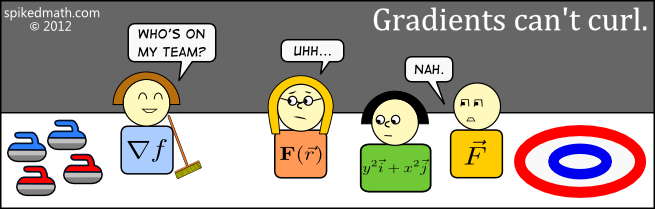
\includegraphics[width=10cm]{pictures_bitmap/501-curling-with-gradients.png}\\
        \url{http://spikedmath.com/501.html}{Spiked math}, \href{http://creativecommons.org/licenses/by-nc-sa/2.5/ca/}{licence Creative Commons by-nc 2.5}.
\end{center}
}{}

%+++++++++++++++++++++++++++++++++++++++++++++++++++++++++++++++++++++++++++++++++++++++++++++++++++++++++++++++++++++++++++
\section[Interprétation de la divergence]{Interprétation géométrique et physique de la divergence}
%+++++++++++++++++++++++++++++++++++++++++++++++++++++++++++++++++++++++++++++++++++++++++++++++++++++++++++++++++++++++++++

En physique, on dit qu'un champ de vecteurs à divergence nulle est \defe{incompressible}{incompressible!champ de vecteur}. Nous allons essayer de comprendre pourquoi. Lorsqu'un fluide incompressible se déplace, il faut qu'en chaque point il y autant de fluide qui rentre que de fluide qui sort. Nous allons voir sur quelques exemples que la divergence d'un champ de vecteurs est le «bilan de masse» d'un fluide qui se déplace selon le champ de vecteurs.

Si en un point la divergence est positive, cela signifie qu'il y a une perte de masse et si la divergence est négative, cela signifie qu'il y a une accumulation de masse.

Prenons par exemple un fluide qui se déplace selon le champ de vitesse montré à figure \ref{LabelFigBEHTooWsdrys}. % From file BEHTooWsdrys
\newcommand{\CaptionFigBEHTooWsdrys}{Le champ de vecteurs $F(x,y)=\frac{1}{ x }(1,0)$.}
\input{auto/pictures_tex/Fig_BEHTooWsdrys.pstricks}

Étant donné que la vitesse diminue lorsque $x$ avance, il y a une accumulation de fluide. Regardez en effet la quantité de fluide qui rentre dans le rectangle par rapport à la quantité de fluide qui en sort. Ce champ de vecteurs a pour équation :
\begin{equation}
    F(x,y)=\frac{1}{ x }\begin{pmatrix}
        1    \\ 
        0    
    \end{pmatrix}=\begin{pmatrix}
        1/x    \\ 
        0    
    \end{pmatrix}.
\end{equation}
Sa divergence vaut donc
\begin{equation}
    (\nabla\cdot F)(x,y)=\frac{ \partial F_x }{ \partial x }(x,y)+\underbrace{\frac{ \partial F_y }{ \partial y }(x,y)}_{=0}=-\frac{1}{ x^2 }.
\end{equation}
Cette divergence étant négative, il y a bien accumulation de fluide en tout point, et d'autant plus que $x$ est petit.

\begin{example}     \label{ExamDivFrot}

    Prenons le champ de vecteurs tournant
    \begin{equation}
        F(x,y)=\frac{1}{ \sqrt{x^2+y^2} }\begin{pmatrix}
            y    \\ 
            -x    
        \end{pmatrix}
    \end{equation}
    représenté à la figure \ref{LabelFigYQVHooYsGLHQ}. Cela est un vecteur qui est constamment perpendiculaire au rayon.


\newcommand{\CaptionFigYQVHooYsGLHQ}{Le champ de vecteurs $F(x,y)=(y,-x)$.}
\input{auto/pictures_tex/Fig_YQVHooYsGLHQ.pstricks}

    Un fluide dont la vitesse serait donné par ce champ de vecteur se contente de tourner. Intuitivement il ne devrait pas y avoir de divergence parce qu'il n'y a aucune accumulation de fluide. En effet,
    \begin{equation}
        \nabla\cdot F(x,y)=\frac{ -2xy }{ (x^2+y^2)^2 }+\frac{ 2xy }{ (x^2+y^2)^2 }=0.
    \end{equation}
\end{example}

\begin{example}
    Prenons le cas du champ de force de gravitation :
    \begin{equation}
        F(x,y,z)=\frac{1}{ (x^2+y^2+z^2)^{3/2} }\begin{pmatrix}
            x    \\ 
            y   \\
            z
        \end{pmatrix}.
    \end{equation}
    Nous pouvons rapidement remarquer que $\nabla\cdot F=0$. Est-ce que cela peut se comprendre sur le dessin de la figure \ref{LabelFigZGUDooEsqCWQ}. % From file ZGUDooEsqCWQ
\newcommand{\CaptionFigZGUDooEsqCWQ}{Le champ de vecteur de la gravité. Nous avons tracé, sur les deux cercles la même densité de vecteurs, c'est à dire le même nombre de vecteurs par unité de surface.}
\input{auto/pictures_tex/Fig_ZGUDooEsqCWQ.pstricks}

    Essayons de voir combien de fluide entre dans la zone bleue et combien en sort. D'abord, il est certain que les vecteurs qui sortent sont plus courts que ceux qui rentrent, ce qui voudrait dire qu'il y a plus de fluide qui rentre. Mais on voit également que le \emph{nombre} de vecteurs qui sortent est plus grand parce que la seconde sphère est plus grande et qu'il y a un vecteur en chaque point de la sphère.

    Intuitivement nous pouvons dire que la quantité qui rentre dans la sphère de rayon $r_1$ donnée par la taille des vecteurs entrants multiplié par la surface de la sphère, c'est à dire
    \begin{equation}        \label{EqQpinormeVecto}
        4\pi r_1^2\| F(x,y,z) \|,
    \end{equation}
    mais $\| F(x,y,z) \|=\frac{1}{ r_1^2 }$, donc la quantité de fluide entrant est $4\pi$. La quantité de fluide sortant sera la même.

    Cela explique deux choses
    \begin{enumerate}
        \item
            Pourquoi les forces de gravitation et électromagnétiques sont en $1/r^2$; c'est parce que nous vivons dans un monde avec trois dimensions d'espace. En étudiant très précisément le champ de gravitation, certains physiciens espèrent trouver des déviations expérimentales par rapport à la règle du \( 1/r^2\); cela \emph{pourrait} être un signe que l'espace contient des dimensions supplémentaires.
        \item
            Pourquoi il y a un $4\pi$ comme coefficient dans beaucoup d'équations en électromagnétisme; en particulier dans certaines anciennes unités de flux.
    \end{enumerate}
    
\end{example}

\begin{remark}
    Nous allons voir plus loin comment s'assurer que l'équation \eqref{EqQpinormeVecto} représente bien la «quantité de fluide» qui rentre dans la zone délimitée
\end{remark}


%+++++++++++++++++++++++++++++++++++++++++++++++++++++++++++++++++++++++++++++++++++++++++++++++++++++++++++++++++++++++++++
\section{Quelques formules de Leibnitz}
%+++++++++++++++++++++++++++++++++++++++++++++++++++++++++++++++++++++++++++++++++++++++++++++++++++++++++++++++++++++++++++

La divergence étant une combinaison de dérivées, il n'est pas tellement étonnant que la divergence de produits donne lieux à des formules en deux termes. Si $f$ est une fonction et si $F$ et $G$ sont des champs de vecteurs, nous avons (sans démonstrations) :
\begin{equation}        \label{EqLeinDivNablRot}
    \begin{aligned}[]
        \nabla\cdot(fF)&=f\nabla\cdot F+F\cdot\nabla f\\
        \nabla\cdot(F\times G)&=G\cdot\nabla\times F-F\cdot\nabla\times G.
    \end{aligned}
\end{equation}
Nous avons aussi, pour le rotationnel,
\begin{equation}        \label{EqLeinRotfFF}
    \nabla\times(fF)=f\nabla\times F+\nabla f\times F.
\end{equation}
% This is part of Mes notes de mathématique
% Copyright (c) 2011-2012
%   Laurent Claessens
% See the file fdl-1.3.txt for copying conditions.

%+++++++++++++++++++++++++++++++++++++++++++++++++++++++++++++++++++++++++++++++++++++++++++++++++++++++++++++++++++++++++++
\section{La différentielle revisitée}
%+++++++++++++++++++++++++++++++++++++++++++++++++++++++++++++++++++++++++++++++++++++++++++++++++++++++++++++++++++++++++++

%---------------------------------------------------------------------------------------------------------------------------
\subsection{Les formes différentielles de base}
%---------------------------------------------------------------------------------------------------------------------------

Si la fonction $f\colon \eR^n\to \eR$ est différentiable alors la différentielle en $a\in\eR^n$ est l'application
\begin{equation}        \label{EqFormDiffdfah}
    \begin{aligned}
        df_a\colon \eR^n&\to \eR \\
        u&\mapsto \frac{ \partial f }{ \partial x_1 }(a)u_1+\cdots+\frac{ \partial f }{ \partial x_n }(a)u_n.
    \end{aligned}
\end{equation}
Considérons en particulier la fonction qui à $x\in\eR^n$ fait correspondre $x_i\in\eR$. Par abus de notations,  nous la noterons $x_i$. Nous avons 
\begin{equation}
    \frac{ \partial x_i }{ \partial x_j }=\delta_{ij}.
\end{equation}
Par exemple $\partial_yx=0$ et $\partial_xx=1$. Toutes les dérivées partielles de $x_i$ s'annulent sauf la $i$ème qui vaut $1$. Par conséquent
\begin{equation}
    \begin{aligned}
        dx_i\colon \eR^n&\to \eR \\
        u&\mapsto u_i. 
    \end{aligned}
\end{equation}

\begin{remark}
    En toute rigueur nous devrions écrire $(dx_i)_a$. Mais étant donné que
    \begin{equation}
        (dx_i)_a(u)=(dx_i)_b(u)
    \end{equation}
    pour tout points $a$, $b$ et pour tout vecteurs $u$, nous nous permettons de simplifier la notation en ne précisant pas en quel point nous calculons la différentielle de $x_i$.
\end{remark}

Étant donné que $dx_i(u)=u_i$, nous pouvons récrire la formule \eqref{EqFormDiffdfah} en remplaçant $u_i$ par $dx_i(u)$ :
\begin{equation}
    df_a(u)=\frac{ \partial f }{ \partial x_1 }(a)dx_1(u)+\cdots+\frac{ \partial f }{ \partial x_n }(a)dx_n(u).
\end{equation}
En tant que application linéaire, $df_a$ est une combinaison linéaire des $dx_i$. En notations compacte :
\begin{equation}
    df_a=\sum_{i=1}^n\frac{ \partial f }{ \partial x_i }(a)dx_i.
\end{equation}

%---------------------------------------------------------------------------------------------------------------------------
                    \subsection{Différentielle comme élément de l'espace dual}
%---------------------------------------------------------------------------------------------------------------------------

Si nous considérons la base canonique $\{ e_i \}_{i=1,\ldots,n}$ de $\eR^n$. À partir d'elle, nous considérons la \defe{base duale}{base!duale}. En termes pratiques, nous définissons $dx_i$ comme la forme sur $\eR^n$ qui à un vecteur $u$ fait correspondre sa composante $i$ :
\begin{equation}
    dx_i\begin{pmatrix}
    u^1 \\ 
    \vdots  \\ 
    u^n 
\end{pmatrix}=u^i.
\end{equation}
En termes savants, $dx_i$ est le dual de $e_i$. Si tu ne l'as pas encore compris, Jean Doyen va te le faire comprendre !


Maintenant, dans la formule \eqref{EqDiffPartRap}, nous pouvons remplacer $u^i$ par $dx_i(u)$, et écrire
\begin{equation}
    df_a(u)=\sum_i\frac{ \partial f }{ \partial x_i }(a)u^i=\sum_i\frac{ \partial f }{ \partial x_i }(a)dx_i(u).
\end{equation}
Ce qui arrive tout à droite est explicitement vu comme une forme sur $\eR$, dont les composantes dans la base duale sont les dérivées partielles de $f$ au point $a$, agissant sur $u$. En faisant un pas en arrière, nous omettons le $u$, et nous écrivons
\begin{equation}
    df_a=\sum_{i=1}^n\frac{ \partial f }{ \partial x_i }(a)dx^i
\end{equation}

Cette notation $dx_i$ pour la forme duale de $e_i$ est en réalité parfaitement logique parce que $dx^i$ est la différentielle de la projection
\begin{equation}
    \begin{aligned}
        x^i\colon \eR^n&\to \eR \\
        (x^1,\ldots,x^n)&\mapsto x^i. 
    \end{aligned}
\end{equation}
Je te laisse un peu méditer sur cette différentielle de la projection. L'important est que tu aies compris cela d'ici la fin de ta deuxième année.

%---------------------------------------------------------------------------------------------------------------------------
\subsection{Différentielles de fonctions composées}
%---------------------------------------------------------------------------------------------------------------------------

Cette façon de voir la différentielle nous permet de jeter un nouveau regard sur la formule de différentiation des fonctions composées. Soient
\begin{equation}
    \begin{aligned}[]
        f\colon \eR^p&\to \eR^n\\
        g\colon \eR^n&\to \eR,
    \end{aligned}
\end{equation}
et $h\colon \eR^p\to \eR$ définie par 
\begin{equation}
    h(u)=h\big( f(u) \big)=(g\circ f)(u).
\end{equation}
Nous allons noter $x$ les coordonnées de $\eR^p$, $a$ un point de $\eR^p$ et $u$, un vecteur de $\eR^p$ accroché au point $a$. Pour $\eR^n$, les notations seront que les coordonnées sont $y$, $b$ est un point de $\eR^n$ et $v$ est un vecteur «accroché» au point $b$.

Nous avons
\begin{equation}
    dg_b(v)=\sum_{i=1}^n\frac{ \partial g }{ \partial y_i }(b)dy_i(v).
\end{equation}
Ici $dy_i(v)$ signifie la $i$ème composante de $v$. C'est simplement $v_i$. Cette formule étant valable pour tout point $b\in\eR^n$ et pour tout vecteur $v$, nous pouvons l'écrire en particulier pour
\begin{subequations}
    \begin{numcases}{}
        b=f(a)\\
        v=df_a(u).
    \end{numcases}
\end{subequations}
Cela donne
\begin{equation}        \label{Eqdgfadfau}
    dg_{f(a)}\big( df_a(u) \big)=\sum_{i=1}^n\frac{ \partial g }{ \partial y_i }\big( f(a) \big)dy_i\big( df_a(u) \big).
\end{equation}
Mais 
\begin{equation}
    df_a(u)=\sum_{j=1}^p\frac{ \partial f }{ \partial x_j }(a)dx_j(u),
\end{equation}
donc la $i$ème composante de ce vecteur est
\begin{equation}
     \big( df_a(u)\big)_i=\sum_{j=1}^p\frac{ \partial f_i }{ \partial x_j }(a)dx_j(u).
\end{equation}
En remplaçant $dy_i\big( df_a(u) \big)$ par cela dans l'expression \eqref{Eqdgfadfau}, nous trouvons
\begin{equation}
    dg_{f(a)}\big( df_a(u) \big)=\sum_{i=1}^n\frac{ \partial g }{ \partial y_i }\big( f(a) \big)\sum_{j=1}^p\frac{ \partial f_i }{ \partial x_j }(a)dx_j(u).
\end{equation}
Nous pouvons vérifier que cela est la différentielle de $g\circ f$ au point $a$ appliquée au vecteur $u$. En effet
\begin{equation}
    d(g\circ f)_a(u)=\sum_{j=1}^p\frac{ \partial (g\circ f) }{ \partial x_j }(a)dx_j(u),
\end{equation}
tandis que, par la dérivation de fonctions composées, 
\begin{equation}        \label{EqDerCompofg}
    \frac{ \partial (g\circ f) }{ \partial x_j }(a)=\sum_{i=1}^n\frac{ \partial g }{ \partial y_i }\big( f(a) \big)\frac{ \partial f_i }{ \partial x_j }(a).
\end{equation}
Au final, ce que nous avons prouvé est que
\begin{equation}
    d(g\circ f)_a(u)=dg_{f(a)}\big( df_a(u) \big).
\end{equation}

%---------------------------------------------------------------------------------------------------------------------------
\subsection{Exemple de composée : les coordonnées polaires}
%---------------------------------------------------------------------------------------------------------------------------

Le changement de coordonnées pour les polaires est la fonction
\begin{equation}
    f\begin{pmatrix}
        r    \\ 
        \theta    
    \end{pmatrix}=\begin{pmatrix}
        x    \\ 
        y    
    \end{pmatrix}=\begin{pmatrix}
        r\cos\theta    \\ 
        r\sin\theta    
    \end{pmatrix}.
\end{equation}
Considérons une fonction $g$ sur $\eR^2$, et définissons la fonction $\tilde g$ par
\begin{equation}
    \tilde g(r,\theta)=g(r\cos\theta,r\sin\theta).
\end{equation}
La formule \eqref{EqDerCompofg} permet de trouver les dérivées partielles de $g$ par rapport à $r$ et $\theta$ en termes de celles par rapport à $x$ et $y$ de $g$.

Pour faire le lien avec les notations du point précédent, nous avons
\begin{equation}
    \begin{aligned}[]
        f_1(r,\theta)&=r\cos(\theta)\\
        f_2(r,\theta)&=r\sin(\theta)\\
        (x_1,x_2)&\to(r,\theta)\\
        (y_1,y_2)&\to(x,y).
    \end{aligned}
\end{equation}
Nous avons donc 
\begin{equation}
    \begin{aligned}[]
        \frac{ \partial \tilde g }{ \partial r }(r,\theta)&=\sum_{i=1}^2\frac{ \partial g }{ \partial x_i }\big( f(r,\theta) \big)\frac{ \partial f_i }{ \partial r }(r,\theta)\\
        &=\frac{ \partial g }{ \partial x }(r\cos\theta,r\sin\theta)\frac{ \partial \big( r\cos\theta \big) }{ \partial r }(r,\theta)\\
        &\quad+\frac{ \partial g }{ \partial y }(r\cos\theta,r\sin\theta)\frac{ \partial \big( r\sin\theta\big) }{ \partial r }(r,\theta)\\
        &=\cos\theta\frac{ \partial g }{ \partial x }(r\cos\theta,r\sin\theta)+\sin\theta\frac{ \partial g }{ \partial y }(r\cos\theta,r\sin\theta).
    \end{aligned}
\end{equation}

Prenons par exemple $g(x,y)=\frac{1}{ x^2+y^2 }$. Étant donné que
\begin{equation}
    \frac{ \partial g }{ \partial x }=\frac{ -2x }{ (x^2+y^2)^2 },
\end{equation}
nous avons
\begin{equation}
    \frac{ \partial g }{ \partial x }(r\cos\theta,r\sin\theta)=\frac{ -2\cos\theta }{ r^3 }.
\end{equation}
En utilisant la formule,
\begin{equation}
    \frac{ \partial \tilde g }{ \partial r }(r,\theta)=\cos(\theta)\left( \frac{ -2\cos\theta }{ r^3 } \right)+\sin(\theta)\left( \frac{ -2\sin\theta }{ r^3 } \right)=-\frac{ 2 }{ r^3 }.
\end{equation}
Nous pouvons vérifier directement que cela est correct. En effet
\begin{equation}
    \tilde g(r,\theta)=g(r\cos\theta,r\sin\theta)=\frac{1}{ r^2 },
\end{equation}
dont la dérivée par rapport à $r$ vaut $-2/r^3$.

En ce qui concerne la dérivée par rapport à $\theta$, nous avons
\begin{equation}
    \begin{aligned}[]
    \frac{ \partial \tilde g }{ \partial \theta }&=\frac{ \partial g }{ \partial x }(r\cos\theta,r\sin\theta)\frac{ \partial \big( r\cos(\theta) \big) }{ \partial \theta }+\frac{ \partial g }{ \partial y }(r\cos\theta,r\sin\theta)\frac{ \partial \big( r\sin(\theta) \big) }{ \partial \theta }\\
    &=\left( \frac{ -2\cos\theta }{ r^3 } \right)(-r\sin\theta)+\left( \frac{ -2\sin\theta }{ r^3 } \right)(r\cos\theta)\\
    &=0.
    \end{aligned}
\end{equation}

En résumé et avec quelques abus de notations :
\begin{equation}
    \begin{aligned}[]
        \frac{ \partial \tilde g }{ \partial r }&=\cos(\theta)\frac{ \partial g }{ \partial x }+\sin(\theta)\frac{ \partial g }{ \partial y }\\
        \frac{ \partial \tilde g }{ \partial \theta }&=-r\sin(\theta)\frac{ \partial g }{ \partial x }+r\cos(\theta)\frac{ \partial g }{ \partial y }\\
    \end{aligned}
\end{equation}

%+++++++++++++++++++++++++++++++++++++++++++++++++++++++++++++++++++++++++++++++++++++++++++++++++++++++++++++++++++++++++++
\section{Forme différentielle}
%+++++++++++++++++++++++++++++++++++++++++++++++++++++++++++++++++++++++++++++++++++++++++++++++++++++++++++++++++++++++++++
\label{SecFormDiffRappel}

Nous parlerons de formes différentielles exactes et fermées dans la section \ref{DefEFKQmPs}.

\begin{definition}
	Soit $D$, un ouvert dans $\eR^n$. Une $1$-\defe{forme différentielle}{forme!différentielle} $\omega$ sur $D$ est une application
	\begin{equation}
		\begin{aligned}
				\omega\colon D&\to (\eR^n)^* \\
				x&\mapsto \omega_x. 
			\end{aligned}
		\end{equation}
\end{definition}
Étant donné que $\{ dx_i \}$ est une base de $(\eR^n)^*$, pour chaque $x\in D$, il existe des uniques réels $a_i(x)$ tels que
\begin{equation}
	\omega_x=a_1(x)dx_1+\cdots+a_n(x)dx_n.
\end{equation}

\begin{lemma}
    Une $1$-forme différentielle est \defe{continue}{continue!forme différentielle} si les fonctions $a_i$ sont continues. La forme sera $C^k$ quand les $a_i$ seront $C^k$.
\end{lemma}

\begin{remark}
	L'ensemble des $1$-formes différentielles forment un espace vectoriel avec les définitions
	\begin{equation}
		\begin{aligned}[]
			(\lambda\omega)_x(v)&=\lambda\omega_x(v)\\
			(\omega+\mu)_x(v)&=\omega_x(v)+\mu_x(v).
		\end{aligned}
	\end{equation}
\end{remark}

Nous connaissons la \defe{base duale}{base!duale} de $(\eR^n)^*$, ce sont les formes $e^*_i$ définies par $e^*_i(e_j)=\delta_{ij}$. Dans le cadre du cours d'analyse, nous allons noter ces formes\footnote{Parce que ce sont les différentielles des fonctions de projection
\begin{equation}
	\begin{aligned}
			x_i\colon \eR^n&\to \eR \\
			x&\mapsto x_i 
		\end{aligned}
	\end{equation}
}
par $dx_i$ :
\begin{equation}
	\begin{aligned}[]
		e^*_1&=dx_1\colon v\mapsto v_1	\\
			&\vdots			\\
		e^*_n&=dx_n\colon v\mapsto v_n
	\end{aligned}
\end{equation}
Toute forme différentielle s'écrit
\begin{equation}
  \omega_x = \sum_{i=0}^n a_i(x) d x_i
\end{equation}
où $a_1,\ldots,a_n$ sont les composantes de $\omega$ dans la base usuelle, et sont des fonctions à valeurs réelles. Pour un vecteur $v = (v_1,\ldots,v_n)$ on a donc par définition de $d x_i$
\begin{equation}
  \omega_x v = \sum_{i=0}^n a_i(x) v_i.
\end{equation}
Ces fonctions $a_i$ peuvent être trouvées en appliquant $\omega$ aux éléments de la base canonique de $\eR^n$ :
\begin{equation}
	a_j(x)=\omega_x(e_j)
\end{equation}
parce que $\omega_x(e_j)=\sum_ia_i(x)dx_i(e_i)=\sum_ia_i(x)\delta_{ij}=a_j(x)$.




\begin{example}
    Un exemple type de forme différentielle est la différentielle d'une fonction $f\colon D\to \eR$. En effet, la différentielle d'une telle fonction est l'application linéaire
    \begin{equation}
        \begin{aligned}
            df\colon \eR^n&\to \eR \\
            v&\mapsto \frac{ \partial f }{ \partial x }v_x+\frac{ \partial f }{ \partial y }v_y. 
        \end{aligned}
    \end{equation}
\end{example}

Soit $D\subset\eR^n$. Par définition de la différentielle d'une $1$-forme, nous avons une formule de Leibnitz
\begin{equation}
    d(f\omega)=df\wedge\omega+fd\omega.
\end{equation}
En particulier,
\begin{equation}
    d(fdx)=df\wedge dx+f\underbrace{d(dx)}_{=0}=\frac{ \partial f }{ \partial x }dx\underbrace{dx\wedge dx}_{=0}+\frac{ \partial f }{ \partial y }dy\wedge dx. S
\end{equation}

Si $F\colon \eR^2\to \eR$ est une fonction $C^2$, sa différentielle est la forme
\begin{equation}
    dF=\frac{ \partial F }{ \partial x }dx+\frac{ \partial F }{ \partial y }dy.
\end{equation}
Si nous nommons $f$ et $g$ les fonctions $\partial_xF$ et $\partial_yF$, nous avons donc
\begin{equation}
    Df=fdx+gdy,
\end{equation}
qui vérifie
\begin{equation}
    \partial_yf=\partial_xg,
\end{equation}
parce que $\frac{ \partial f }{ \partial y }=\frac{ \partial^2F  }{ \partial x\partial y }=\frac{ \partial^2F  }{ \partial y\partial x }=\frac{ \partial g }{ \partial x }$. Ce que nous avons donc prouvé, c'est que 
\begin{lemma}
Si $fdx+gdy$ est la différentielle d'une fonction de classe $C^2$, alors $\partial_yf=\partial_xg$.
\end{lemma}

%///////////////////////////////////////////////////////////////////////////////////////////////////////////////////////////
\subsubsection{L'isomorphisme musical}
%///////////////////////////////////////////////////////////////////////////////////////////////////////////////////////////

Si $G$ est un champ de vecteur sur $\eR^n$, et si $x\in\eR^n$, nous pouvons définissons 
\begin{equation}		\label{EqDefBemol}
	\begin{aligned}[]
		G^{\flat}_x\colon \eR^n&\to \eR \\
			v&\mapsto \langle G(x), v\rangle 
	\end{aligned}
\end{equation}

Pour chaque $x$, l'application $G_x^{\flat}$ est une forme sur $\eR^n$, c'est à dire une application linéaire de $\eR^n$ vers $\eR$. Nous écrivons que
\begin{equation}
	G_x^{\flat}\in\big( \eR^n \big)^*.
\end{equation}

Nous pouvons ainsi déterminer le développement de $G^{\flat}$ dans la base des $dx_i$ en faisant le calcul
\begin{equation}
	G_x^{\flat}(e_i)=\langle G(x), e_i\rangle =G_i(x),
\end{equation}
donc les composantes de $G^{\flat}$ dans la base $dx_i$ sont exactement les composantes de $G$ dans la base $e_i$ :
\begin{equation}
	G^{\flat}_x=G_1(x)dx_1+\cdots+G_n(x)dx_n.
\end{equation}

La construction inverse existe également. Si $\omega$ est une $1$-forme différentielle, nous pouvons définir le champ de vecteur $\omega^{\sharp}$ par la formule (implicite)
\begin{equation}
	\omega_x(v)=\langle \omega^{\sharp}(x), v\rangle 
\end{equation}
pour tout $v\in\eR^n$. Par définition, $(\omega^{\sharp})^{\flat}=\omega$. 

\begin{lemma}
    En composantes nous avons :
	\begin{equation}
		\omega^{\sharp}(x)=\big( a_1(x),\ldots,a_n(x) \big).
	\end{equation}
	Si $G$ est un champ de vecteurs, alors $(G^{\flat})^{\sharp}=G$.
\end{lemma}


\chapter{Retour sur les groupes}
% This is part of Mes notes de mathématique
% Copyright (c) 2011-2013,2016-2017
%   Laurent Claessens
% See the file fdl-1.3.txt for copying conditions.

%+++++++++++++++++++++++++++++++++++++++++++++++++++++++++++++++++++++++++++++++++++++++++++++++++++++++++++++++++++++++++++
\section{Action de groupe et connexité}
%+++++++++++++++++++++++++++++++++++++++++++++++++++++++++++++++++++++++++++++++++++++++++++++++++++++++++++++++++++++++++++

Sources : \cite{MneimneLie} et \wikipedia{fr}{Matrice_normale}{wikipédia}.

\begin{theorem}     \label{ThojrLKZk}
    Soit \( G\) un groupe topologique localement compact et dénombrable à l'infini\footnote{Cela signifie qu'il est une réunion dénombrable de compacts} agissant continument et transitivement sur un espace topologique localement compact \( E\). Alors l'application
    \begin{equation}
        \begin{aligned}
            \varphi\colon G/G_x&\to E \\
            [g]&\mapsto g\cdot x 
        \end{aligned}
    \end{equation}
    est un homéomorphisme.
\end{theorem}

\begin{lemma}       \label{LemkLRAet}
    Si \( G\) et \( H\) sont des groupes topologiques tels que $G/H$ et \( H\) sont connexes\footnote{Définition \ref{DefIRKNooJJlmiD}.}, alors \( G\) est connexe.
\end{lemma}

\begin{proof}
    Soit \( f\colon G\to \{ 0,1 \}\) une fonction continue. Considérons l'application
    \begin{equation}
        \begin{aligned}
            \tilde f\colon G/H&\to \{ 0,1 \} \\
            [g]&\mapsto f(g). 
        \end{aligned}
    \end{equation}
    D'abord nous montrons qu'elle est bien définie. En effet si \( h\in H\) nous aurions \( \tilde f([gh])=f(gh)\), mais étant donné que \( H\) est connexe, l'ensemble \( gH\) est également connexe; la fonction continue \( f\) est donc constante sur \( gH\). Nous avons donc \( f(gh)=f(g)\).

    Étant donné que \( G/H\) est également connexe, la fonction \( \tilde f\) doit être constante. Si \( g_1\) et \( g_2\) sont deux éléments du groupe, nous avons \( f(g_1)=\tilde f([g_1])=\tilde f([g_2])=f(g_2)\). Nous en déduisons que \( f\) est constante et que \( G\) est connexe.
\end{proof}

\begin{theorem}
    Le groupe \( \SO(n)\) est connexe, le groupe \( \gO(n)\) a deux composantes connexes.
\end{theorem}

\begin{proof}
    La seconde assertion découle de la première parce que les matrices de déterminant \( 1\) et celles de déterminant \( -1\) ne peuvent pas être reliées par un chemin continu tandis que l'application
    \begin{equation}
        M\mapsto \begin{pmatrix}
            -1    &       &       \\
                &   1    &       \\
                &       &   1
        \end{pmatrix}M
    \end{equation}
    est un homéomorphisme entre les matrices de déterminant \( 1\) et celles de déterminants \( -1\). Montrons donc que \( G=\SO(n)\) est connexe par arcs pour \( n\geq 2\) en procédant par récurrence sur la dimension.
    
    Nous acceptons le résultat pour $G=\SO(2)$. Notons que nous en avons besoin pour prouver que la sphère \( S^{n-1}\) est connexe.
    
    Le groupe \( \SO(n)\) agit, par définition, de façon transitive sur la sphère \( S^{n-1}\). Soit \( a\in S^{n-1}\), nous avons
    \begin{subequations}
        \begin{align}
            G\cdot a&=S^{n-1}\\
            G_a&\simeq \SO(n-1)
        \end{align}
    \end{subequations}
    où \( G_a\) est le fixateur de \( a\) dans \( G\). Pour montrer le second point, nous considérons \( \{ e_i \}\), la base canonique de \( \eR^n\) et \( M\in G\) telle que \( Ma=e_1\). Le fixateur de \( e_1\) est évidemment isomorphe à \( \SO(n-1)\) parce qu'il est constitué des matrices de la forme
    \begin{equation}
        \begin{pmatrix}
             1   &   0    &   \ldots    &   0    \\
             0   &   a_{11}    &   \ldots    &   a_{1,n-1}    \\
             \vdots   &   \vdots    &   \ddots    &   \vdots    \\ 
             0   &   a_{n-1,1}    &   \ldots    &   a_{n-1,n-1}     
         \end{pmatrix}
    \end{equation}
    où \( (a_{ij})\in \SO(n-1)\). L'application 
    \begin{equation}
        \begin{aligned}
            \alpha\colon G_{e_1} &\to G_{a} \\
            A&\mapsto M^{-1}A M
        \end{aligned}
    \end{equation}
    est un isomorphisme entre \( G_a\) et \( \SO(n-1)\). Le théorème \ref{ThojrLKZk} nous montre alors que, en tant qu'espaces topologiques,
    \begin{equation}
        G/G_a=S^{n-1}.
    \end{equation}
    L'hypothèse de récurrence montre que \( G_a=\SO(n-1)\) est connexe tandis que nous savons que \( S^{n-1}\) est connexe. Le lemme \ref{LemkLRAet} conclut que \( G=\SO(n)\) est connexe.
\end{proof}

\begin{lemma}       \label{LemIbrsFT}
    Une bijection continue entre un espace compact et un espace séparé est un homéomorphisme.
\end{lemma}

\begin{proposition}
    Les groupes \( \gU(n)\) et \( \SU(n)\) sont connexes.
\end{proposition}

\begin{proof}
    Soit \( G(n)\) le groupe \( \SU(n)\) ou \( \gU(n)\). Ce groupe opère transitivement sur la sphère complexe
    \begin{equation}
        S_{\eC}^{n-1}=\{ z\in \eC^n\tq \langle z, z\rangle=\sum_k| z_k |^2 =1 \}.
    \end{equation}
    Cet ensemble est le même que \( S^{2n-1}\) parce que \( |z_k|=x_k^2+y_k^2\). Nous avons une bijection continue entre \( S^{n-1}\) et \( S^{n-1}_{\eC}\) et donc un homéomorphisme (lemme \ref{LemIbrsFT}). Soit \( a\in S^{n-1}_{\eC}\), nous avons
    \begin{subequations}
        \begin{align}
            G\cdot a&=S^{n-1}_{\eC}\\
            G_a&\simeq G(n-1).
        \end{align}
    \end{subequations}
    La seconde ligne est un isomorphisme de groupe et un homéomorphisme. Il est donné de la façon suivante. D'abord le fixateur de \( e_1\) dans \( G(n)\) est donné par les matrices de la forme
    \begin{equation}
        \begin{pmatrix}
             1   &   0    &   \ldots    &   0    \\
             0   &   a_{11}    &   \ldots    &   a_{1,n-1}    \\
             \vdots   &   \vdots    &   \ddots    &   \vdots    \\ 
             0   &   a_{n-1,1}    &   \ldots    &   a_{n-1,n-1}     
         \end{pmatrix}
    \end{equation}
    où \( (a_{ij})\in G(n-1)\). Par ailleurs si \( M\) est une matrice de \( G(n)\) telle que \( Ma=e_1\), nous avons l'homéomorphisme
  
    \begin{equation}
        \begin{aligned}
            \alpha\colon G_{e_1}&\to G_a \\
            A&\mapsto M^{-1} AM. 
        \end{aligned}
    \end{equation}
    Encore une fois, cela est un homéomorphisme par le lemme \ref{LemIbrsFT}. Par composition nous avons \( G_a\simeq G(n-1)\) et un homéomorphisme
    \begin{equation}
        G(n)/G_a=S^{n-1}_{\eC}.
    \end{equation}
    Le groupe \( G_a\) et l'ensemble \( S^{n-1}_{\eC}\) étant connexes, le groupe \( G(n)\) est connexe par le lemme \ref{LemkLRAet}.
\end{proof}

\begin{lemma}[\cite{PAXrsMn}]
    Si \( G\) est un sous-groupe connexe de \( \GL(n,\eC)\) alors son groupe dérivé\footnote{Définition \ref{DefVUFBooNQjEdn}.} l'est également.
\end{lemma}
\index{groupe dérivé!de \( \GL(n,\eC)\)}

\begin{proof}
    Soit \( S_m\) l'ensemble des produits de \( m\) commutateurs de \( G\) :
    \begin{equation}
        S_m=\{ g_1,\ldots, g_m\,\text{où les } g_i\text{ sont des commutateurs} \}.
    \end{equation}
    La partie \( S_m\) est l'image de \( G\) par l'application continue
    \begin{equation}
        \begin{aligned}
            \underbrace{G\times \ldots\times G}_{ 2m\text{ facteurs}}&\to G \\
            (g_1,h_1,g_2,h_2,\ldots, g_m,h_m)&\mapsto [g_1,h_1]\ldots [g_m,h_m] 
        \end{aligned}
    \end{equation}
    En tant qu'image d'un connexe par une application continue, \( S_m\) est connexe par la proposition \ref{PropGWMVzqb}. Vu que les \( S_m\) ont l'identité en commun, le groupe dérivé
    \begin{equation}
        D(G)=\bigcup_{m=1}^{\infty}S_m
    \end{equation}
    est également connexe.
\end{proof}

%+++++++++++++++++++++++++++++++++++++++++++++++++++++++++++++++++++++++++++++++++++++++++++++++++++++++++++++++++++++++++++
\section{Espaces de matrices}
%+++++++++++++++++++++++++++++++++++++++++++++++++++++++++++++++++++++++++++++++++++++++++++++++++++++++++++++++++++++++++++

L'ensemble des matrices est un espace vectoriel. Nous identifions $\eM(n,\eR)$ avec $ \eR^{n^2}$; plus précisément, nous identifions une matrice 
\begin{equation}
    A = (a_{i,j})_{1\leq i \leq n, 1 \leq j \leq n}
\end{equation}
avec le vecteur $x = (x_1, x_2, \dots, x_{n^2}) \in \eR^{n^2}$, où $ a_{i,j} = x_{(n-1)i + j}$. 

%--------------------------------------------------------------------------------------------------------------------------- 
\subsection{Dilatations et transvections}
%---------------------------------------------------------------------------------------------------------------------------

Soit un corps commutatif \( \eK\) et \( n\geq 2\).

\begin{theoremDef}[\cite{PAXrsMn}]     \label{ThoooAZKDooNDcznv}
    Soit une application linéaire \( u\colon E\to E\) dont les points fixes forment un hyperplan noté \( H\) d'équation \( H=\ker(f)\) avec \( f\in E^*\).
    \begin{enumerate}
        \item     \label{ITEMooGTKRooQSPNoI}
            Les affirmations suivantes sont équivalentes :
            \begin{enumerate}
                \item  \label{ITEMooZHYRooFGKaifi}
                    \( \det(u)\neq 1\)
                \item       \label{ooXKLWooTfUMzV}
                    L'application \( u\) est diagonalisable et a une valeur propre qui vaut \( \det(u)\neq 1\).
                \item       \label{ooMZPTooCLylbh}  
                    \( \Image(u-\id)\nsubseteq H\).
                \item   \label{ITEMooZHYRooFGKaifiv}
                    Il existe une base de \( E\) dans laquelle la matrice de \( u\) est \( \diag(1,\ldots, 1,\lambda)\) avec \( \lambda\neq 1\).
            \end{enumerate}
        \item       \label{ITEMooMSJXooUsLCHx}
            Les affirmation suivantes sont équivalentes :
            \let\oldthenumii\theenumi
            \renewcommand{\theenumii}{\roman{enumii}}
            \begin{enumerate}
                \item       \label{ITEMooRTIEooOoWCFsa}
                    Il existe \( a\in H\) tel que pour tout \( x\in E\), \( u(x)=x+f(x)a\).
                \item       \label{ITEMooRTIEooOoWCFsb}
                    Dans une base adaptée, la matrice de \( u\) est donnée par
                    \begin{equation}        \label{EQooFXBDooTgZwMv}
                        \begin{pmatrix}
                             1   &       &       &       \\
                                &   \ddots    &       &       \\
                                &       &   1    &   1    \\ 
                                &       &       &   1     
                         \end{pmatrix}.
                    \end{equation}
            \end{enumerate}
            \let\theenumii\oldtheenumii
        \item
            Les conditions \ref{ITEMooZHYRooFGKaifi}-\ref{ITEMooZHYRooFGKaifiv} sont respectées si et seulement si les conditions \ref{ITEMooRTIEooOoWCFsa}-\ref{ITEMooRTIEooOoWCFsb} ne sont pas respectées (elles sont les négations l'une de l'autre.).
    \end{enumerate}
    Un endomorphisme qui est soit l'identité soit respecte les conditions \ref{ITEMooGTKRooQSPNoI} est une \defe{dilatation}{dilatation}. Un endomorphisme qui est soit l'identité soit qui vérifie les conditions \ref{ITEMooMSJXooUsLCHx} est une \defe{transvection}{transvection} (dans les deux cas il faut que les points fixes forment un hyperplan).
\end{theoremDef}

Notons que selon cette terminologie, l'application \( x\mapsto \lambda x\) n'est pas une dilation mais un produit de dilations.

\begin{proof}
    Nous allons prouver plein d'implications \ldots
    \begin{subproof}
    \item[\ref{ITEMooZHYRooFGKaifi} implique \ref{ooXKLWooTfUMzV}]
        Le théorème de la base incomplete (voir remarque \ref{REMooYGJEooEcZQKa}) permet de considérer une base \( \{ e_1,\ldots, e_n \}\) de \( E\) telle que \( \{ e_1,\ldots, e_{n-1} \} \) soit une base de \( H\). Dans cette base, la matrice de \( u\) est de la forme suivante (les cases non remplies sont nulles et les étoiles correspondent à des valeurs inconnues mais pas spécialement nulles) :
        \begin{equation}        \label{EqooPQOEooGUyIwa}
        \begin{pmatrix}
             1   &       &       &   *    \\
                &   \ddots    &       &   \vdots    \\
                &       &   1    &   *    \\ 
                &       &       &   \lambda     
         \end{pmatrix}
        \end{equation}
        Le fait que le déterminant de \( u\) ne soit pas \( 1\) implique que \( \lambda\neq 1\). Par conséquent le polynôme caractéristique
        \begin{equation}
            \chi_u(X)=(1-X)^{n-1}(\lambda-X)
        \end{equation}
        possède une racine \( \lambda\neq 1\), et donc \( u\) possède un vecteur propre \( v\) pour cette valeur\footnote{Proposition \ref{PropooBYZCooBmYLSc}.}. Le vecteur \( v\) est linéairement indépendant de \( \{ e_1,\ldots, e_{n-1} \}\) (parce que vecteur propre de valeur propre différente). Par conséquent l'ensemble \( \{ e_1,\ldots, e_{n-1},v \}\) est une base par le théorème \ref{ThoMGQZooIgrXjy}\ref{ItemHIVAooPnTlsBi}. Cela est une base de vecteurs propres et donc une base de diagonalisation\footnote{Nous pourrions en dire à peine plus et prouver le point \ref{ITEMooZHYRooFGKaifiv}, mais cela ne servirait à rien parce que nous voulons prouver les équivalences et qu'il faudra quand même prouver que \ref{ooMZPTooCLylbh} implique \ref{ITEMooZHYRooFGKaifiv}.}.
    \item[\ref{ooXKLWooTfUMzV} implique \ref{ooMZPTooCLylbh}]
        Nous nommons maintenant \( \{ e_1,\ldots, e_{n} \}\) la base de diagonalisation. Nous avons \( u(e_n)=\lambda e_n\) avec \( \det(u)=\lambda\neq 1\). Nous avons
        \begin{equation}
            (u-\id)(e_n)=(\lambda-1)e_n\notin H,
        \end{equation}
        ce qui prouver que l'image de \( e_n\) par \( u-\id\) n'est pas dans \( H\).
    \item[\ref{ooMZPTooCLylbh} implique \ref{ITEMooZHYRooFGKaifiv}]
        Reprenons une base \( \{ e_1,\ldots, ,e_n \}\) donnant la matrice \eqref{EqooPQOEooGUyIwa}. Il existe \( x\in E\) tel que \( u(x)-x\) n'est pas dans \( H\), c'est à dire tel que \( u\big( u(x)-x \big)\neq u(x)-x\). Nous en déduisons que
        \begin{equation}
            u^2(x)-2u(x)+x\neq 0
        \end{equation}
        ou encore que 
        \begin{equation}
            (X-1)^2(u)x\neq 0.
        \end{equation}
        C'est à dire que \( (X-1)^2\) n'est pas un polynôme annulateur de \( u\). Or ce serait le cas si \( X-1\) était le polynôme minimal (proposition \ref{PropAnnncEcCxj}). Le polynôme caractéristique étant \( (X-1)^{n-1}(X-\lambda)\) (et étant annulateur\footnote{Théorème de Cayley-Hamilton \ref{ThoCalYWLbJQ}.}), le polynôme minimal est de la forme 
        \begin{equation}
            \mu_u(X)=\begin{cases}
                (X-1)(X-\lambda)    &   \text{si } \lambda\neq 1\\
                X-1    &    \text{si } \lambda=1.
            \end{cases}
        \end{equation}
        Dans notre cas nous venons de voir que ce n'est pas \( X-1\) et donc c'est \( (X-1)(X-\lambda)\) avec \( \lambda\neq 1\).

        Nous devons trouver une base de diagonalisation \ldots Supposons
        \begin{equation}
            u(e_n)=\sum_{k=1}^{n-1}a_ke_k+\lambda e_n,
        \end{equation}
        dans lequel nous venons de prouver que \( \lambda\neq 1\), et cherchons
        \begin{equation}
            e'_n=\sum\_{j=1}^np_je_j
        \end{equation}
        de telle sorte à avoir \( u(e'_n)=\lambda e_n\). Nous avons
        \begin{subequations}
            \begin{align}
                u(e'_n)&=\sum_{j=1}^{n-1}p_ju(e_j)+p_nu(e_n)\\
                &=\sum_{j=1}^{n-1}(p_j+p_na_j)e_j+p_n\lambda e_n.
            \end{align}
        \end{subequations}
        En égalisant à \( \lambda\sum_{j=1}^np_je_j\), il vient
        \begin{equation}
            p_j+p_na_j=\lambda p_j
        \end{equation}
        pour tout \( j=1,\ldots, n-1\) et la condition triviale \( p_n\lambda=\lambda p_n\) pour \( j=n\). Nous en déduisons que le choix
        \begin{equation}
            p_j=\frac{ p_na_j }{ \lambda-1 }
        \end{equation}
        fonctionne (parce que \( \lambda\neq 1\) comme nous l'avons démontré plus haut). En bref, il suffit de poser
        \begin{equation}
            e'_n=\sum_{j=1}^{n-1}\frac{ p_na_j }{ \lambda-1 }e_j+p_ne_n
        \end{equation}
        avec \( p_n\) au choix pour avoir une base \( \{ e_1,\ldots, e_{n-1},e'_n \}\) de diagonalisation de \( u\) avec \( \lambda\neq 1\) comme dernière valeur propre.
    \item[\ref{ITEMooZHYRooFGKaifiv} implique \ref{ITEMooZHYRooFGKaifi}] Évident \ldots encore qu'il faut invoquer l'invariance du déterminant par changement de base.
    \end{subproof}
    Nous avons terminé la première série d'équivalences. Nous continuons avec la seconde.
       \begin{subproof}
        \item[\ref{ITEMooRTIEooOoWCFsa} implique \ref{ITEMooRTIEooOoWCFsb}]
            Nous prenons \( e_{n-1}=a\) et nous complétons en une base de \( H\). Pour \( e_n\) il suffit de prendre n'importe quel vecteur \( v\) tel que \( f(v)\neq 0\) (qui existe parce que \( f=0\) est seulement un hyperplan), et de le normaliser.

            Dans cette base, la matrice de \( u\) a la forme désirée parce que \( u(e_n)=e_n+f(e_n)a=e_n+e_{n-1}\) du fait que \( e_{n-1}=a\) et \( f(e_n)=1\).
        \item[\ref{ITEMooRTIEooOoWCFsb} implique \ref{ITEMooRTIEooOoWCFsa}]
            Soit \( \{ e_1,\ldots, e_n \}\) cette base. En prenant \( a=e_{n-1}\) et en posant \( x=\sum_kx_ke_k\) nous avons
            \begin{equation}
                u(x)=\sum_{k=1}^{n-1}x_ke_k+x_n(e_{n-1}+e_n)=x+x_ne_{n-1}=x_na.
            \end{equation}
            Mais vu que \( f(x)=\sum_if_ix_i\), et que \( f(e_i)=0\) pour tout \( i=1,\ldots, n-1\) nous avons \( f(x)=f_nx_n\). Il n'y a cependant pas de raisons d'avoir \( f_n=1\). Cependant en définissant
            \begin{equation}
                e'_i=\frac{1}{ f_n }e_i
            \end{equation}
            nous avons bien \( u(e'_n)=\frac{1}{ f_n }(e_{n-1}+e_n)=e'_{n-1}+e'_n\). Donc dans cette base nous avons encore la matrice de \( u\) de la forme
            \begin{equation}
                \begin{pmatrix}
                     1   &       &       &       \\
                        &   \ddots    &       &       \\
                        &       &   1    &   1    \\ 
                        &       &       &   1     
                 \end{pmatrix},
            \end{equation}
            mais cette fois avec \( f(e'_n)=1\).
    \end{subproof}
    Nous avons terminé avec la seconde série d'équivalences. Il nous reste à prouver que la première est équivalente à la négation de la seconde.
    \begin{subproof}
        \item[non \ref{ooMZPTooCLylbh} implique \ref{ITEMooRTIEooOoWCFsa}]
            Considérons \( x_0\in E\) tel que \( f(x_0)=1\) et posons \( a=u(x_0)-x_0\in\Image(u-\id)\). Par la négation de \ref{ooMZPTooCLylbh} nous avons \( a\in H\). De plus \( x_0\notin H\) (sinon \( f(x_0)=0\)) donc \( u(x_0)\neq x_0\) et \( a\neq 0\).

            Nous montrons que ce choix de \( a\) fonctionne : \( u(x)=x+f(x)a\) pour tout \( x\in E\). Nous faisons cela séparément pour \( x\in H\) et pour \( x=x_0\). 

            Si \( h\in H\) alors \( u(h)=h\) et \( f(h)=0\) donc \( h+f(h)a=h=u(h)\). Si \( x=x_0\) alors \( u(x_0)=a+x_0\) (cela est la définition de \( a\)) et\( x_0+f(x_0)a=x_0+a\).
        \item[\ref{ITEMooRTIEooOoWCFsb} implique non \ref{ITEMooZHYRooFGKaifi}]
           Dans une base adaptée nous avons 
           \begin{equation}
               \begin{pmatrix}
                    1    &       &       &       \\
                        &   \ddots    &       &       \\
                        &       &   1    &   1    \\ 
                        &       &       &   1     
                \end{pmatrix},
           \end{equation}
           et donc \( \det(u)=1\), ce qui contredit \ref{ITEMooZHYRooFGKaifi}.
    \end{subproof}
\end{proof}

\begin{remark}
    Nous notons \( E_{ij}\) la matrice qui possède uniquement \( 1\) en position \( (i,j)\). C'est à dire que \( \big( E_{ij} \big)_{kl}=\delta_{ik}\delta_{jl}\). Soit \( H\) l'hyperplan des points fixes de \( f\). Dans une base contenant une base de $H$, la matrice d'une transvection a pour forme type :
    \begin{equation}        \label{EqooZAKHooBjKlTd}
        T_{ij}(\lambda)=\mtu+\lambda E_{ij}
    \end{equation}
    avec \( i\neq j\) et \( \lambda\in \eK\), et une dilatation a pour forme type la matrice diagonale
    \begin{equation}
        D_i(\alpha)=\mtu+(\alpha-1)E_{ii}
    \end{equation}
    avec \( \alpha\in \eK^*\).

    Bien entendu, en choisissant une base quelconque, les matrices des dilatations et des translations peuvent avoir des formes différentes.
\end{remark}

\begin{lemma}       \label{LemooTQJXooGoIxsI}
    Quelque manipulations de lignes et de colonnes pour les matrices.
    \begin{enumerate}
        \item       \label{ITEMooRWANooPAVjkm}
            La multiplication à gauche par \( T_{ij}(\lambda)\) revient à effectuer le remplacement de ligne
            \begin{equation}
                L_i\to L_i+\lambda L_j.
            \end{equation}
        \item       \label{ITEMooHPSMooWBrSXP}
            La multiplication à droite par \( T_{ij}(\lambda)\) revient à effectuer le remplacement de colonne
            \begin{equation}
                C_j\to C_j+\lambda C_i.
            \end{equation}
        \item       \label{ITEMooXUGFooKcbrxs}
            La multiplication à gauche par \( T_{ij}(1)T_{ji}(-1)T_{ij}(1)\) revient à la substitution de lignes
            \begin{subequations}
                \begin{numcases}{}
                    L_i\to L_j\\
                    L_j\to -L_i.
                \end{numcases}
            \end{subequations}
    \end{enumerate}
\end{lemma}
Note qu'il n'est pas possible d'inverser deux lignes à l'aide de transvections sans changer un signe parce que les transvections sont de déterminant \( 1\) alors que l'inversion de lignes change le signe du déterminant.

\begin{proof}
    Point par point.
    \begin{subproof}
        \item[Pour \ref{ITEMooRWANooPAVjkm}]
            Nous devons prouver que
            \begin{equation}
                \big( T_{ij}(\lambda)A \big)_{kl}=\begin{cases}
                    A_{kl}    &   \text{si } k\neq i\\
                    A_{il}+\lambda A_{jl}    &    \text{si } k=i.
                \end{cases}
            \end{equation}
            Un peu de calcul matriciel avec utilisation modérée des indices donner :
            \begin{subequations}
                \begin{align}
                    \big( T_{ij}(\lambda)A \big)_{kl}&=\sum_s\big( T_{ij}(\lambda) \big)_{ks}A_{sl}\\
                    &=\sum_s\delta_{ks}A_{sl}+\lambda\delta_{ik}\delta_{js}A_{sl}\\
                    &=A_{kl}+\lambda\delta_{ik}A_{jl}.
                \end{align}
            \end{subequations}
        \item[Pour \ref{ITEMooHPSMooWBrSXP}] C'est la même chose.
        \item[Pour \ref{ITEMooXUGFooKcbrxs}] Si nous appliquons successivement ces trois matrices (de droite à gauche) nous effectuons les substitutions :
            \begin{equation}
                \begin{aligned}[]
                \begin{cases}
                    L'_i=L_i+L_j\\
                    L'_j=L_j
                \end{cases}
                \text{suivit de }
                \begin{cases}
                    L''_i=L'_i\\
                    L''_j=L'_j-L'_i
                \end{cases}
                \text{et de}
                \begin{cases}
                    L'''_i=L''_i+L''_j\\
                    L'''_j=L''_j.
                \end{cases}
                \end{aligned}
            \end{equation}
            En effectuant ces substitutions,
            \begin{equation}
                L'''_i=L''_i+L''_j=L'_i+(L'_j-L'_i)=L'_j=L_j
            \end{equation}
            et
            \begin{equation}
                L'''_j=L''_j=L'_j-L'_i=L_j-(L_i+L_j)=-L_i,
            \end{equation}
            ce qu'il fallait.
    \end{subproof}
\end{proof}

\begin{proposition}[\cite{ooUWTWooPKySTQ}]      \label{PropooFDNRooWFfUDd}
    Soit \( n\geq 2\) et un corps commutatif \( \eK\).
    \begin{enumerate}
        \item
            Si \( A\in \GL(n,\eK)\), il existe des transvections \( U_1,\ldots, U_r\), \( V_1,\ldots, V_s\) telles que
                \begin{equation}        \label{EQooKSQVooIpkdIE}
                    A=U_1\ldots U_r\,D_n\big( \det(A) \big)\,V_1\ldots V_s.
                \end{equation}
        \item       \label{ITEMooLRYXooSoKRiA}
            L'ensemble des transvections engendre le groupe spécial linéaire \( \SL(n,\eK)\).
        \item
            L'ensemble des transvections et des dilatations engendre le groupe linéaire \( \GL(n,\eK)\).
    \end{enumerate}
\end{proposition}

\begin{proof}
    Nous allons montrer que toutes les matrices de \( \SL(n,\eK)\) peuvent être écrites comme produits de matrices de la forme \eqref{EqooZAKHooBjKlTd}. Cela montrera qu'étant donné un endomorphisme \( f\) et une base \emph{pas spécialement liée à \( f\)}, il est possible décrire la matrice de \( f\) comme produit de transvections dont les hyperplans invariants sont «contenus» dans cette base. Cela suffit à prouver que les transvections engendrent \( \SL(n,\eK)\) grâce au lemme \ref{LemFUIZooBZTCiy}.

    Toutes les transvections ont un déterminant égal à \( 1\). Donc le groupe engendré par les transvections est inclus à \( \SL(2,\eK)\). Soit \( A\in\GL(n,\eK)\); nous allons utiliser le pivot de Gauss pour la diagonaliser. Étant donné que \( A\) est inversible, sa première colonne n'est pas nulle. Si \( A_{i1}\neq 0\) alors une multiplication à gauche par \( L_{1i}\big(   (A_{11}-1)/A_{i1}  \big)\) effectue la substitution
    \begin{equation}
        L_1\to L_1-\frac{ A_{11}-1 }{ A_{i1} }L_i
    \end{equation}
    qui met un \( 1\) en la position \( (1,1)\). Notons que si la première colonne est de la forme 
    \begin{equation}
        \begin{pmatrix}
            s    \\ 
            0    \\ 
            \vdots    \\ 
            0    
        \end{pmatrix}
    \end{equation}
    avec \( s\neq 0\) alors il faut plutôt faire les substitutions \( L_2\to L_2+L_1\) et ensuite \( L_1\to L_1-\frac{1}{ s }L_2\) pour obtenir le même résultat. En effectuant le pivot avec \( A_{11}\), une suite d'opérations sur les lignes et les colonnes donnent
    \begin{equation}
        M_1\ldots M_pAN_1\ldots N_q=\begin{pmatrix}
            1    &   0    \\ 
            0    &   A_1    
        \end{pmatrix}
    \end{equation}
    où \( A_1\in\GL(n-1,\eK)\) et \( \det(A_1)=\det(A)\). En continuant de la sorte nous arrivons sur une matrice diagonale\footnote{Attention : les opérations sur les lignes et le colonnes ne sont pas des opérations de similitude. Il n'est pas question de prétendre ici que toutes les matrices de \( \GL(n,\eK)\) sont diagonales, voir la définition \ref{DefBLELooTvlHoB}.}
    \begin{equation}
        M_1\ldots M_{p'}AN_1\ldots N_{q'}=
        \begin{pmatrix}
             1   &       &       &       \\
                &   \ddots    &       &       \\
                &       &   1    &       \\ 
                &       &       &   \alpha     
         \end{pmatrix}
    \end{equation}
    avec \( \alpha=\det(A)\). En d'autres termes nous avons prouvé qu'il existe des transvections \( U_1,\ldots, U_r\) et \( V_1,\ldots, V_s\) telles que
    \begin{equation}        \label{EQooZYYFooQGCgxU}
        A=U_1\ldots U_r\,D_n\big( \det(A) \big)\,V_1\ldots V_s.
    \end{equation}
    Cela prouve que les transvections et les translations engendrent \( \GL(n,\eK)\). Si \( A\in \SL(n,\eK)\) alors \( D_n\big( \det(A) \big)=1\) et l'équation \eqref{EQooZYYFooQGCgxU} est un produit de transvections.
\end{proof}

\begin{proposition}
    Le groupe \( \GL(n,\eR)\) est engendré par les endomorphismes inversibles diagonalisables.
\end{proposition}

\begin{proof}
    Par la proposition \ref{PropooFDNRooWFfUDd}, le groupe \( \GL(n,\eR)\) est engendré par les dilatations et les transvections. Il suffit donc de montrer qu'à leur tour, ces deux types d'endomorphismes sont engendrés par les endomorphismes inversibles et diagonalisables.

    Les dilatations sont diagonalisables et inversibles. Soit une transvection \( u\), et une base \( \{ e_i \}_{i=1,\ldots, n}\) dans laquelle \( u\) est de la forme \eqref{EQooFXBDooTgZwMv}. Nous considérons l'endomorphisme \( d\colon E\to E\) défini par \( d(e_k)=ke_k\). Cet endomorphisme est diagonalisable parce que son polynôme minimal, \( \mu_d=\prod_{k=1}^n(X-k)\), est scindé à racines simples (voir le théorème \ref{ThoDigLEQEXR}).

    Nous avons évidemment \( u= d^{-1}\circ(d\circ u) \) où \( d^{-1}\) est diagonalisable et inversible. Voyons que \( d\circ u\) est également diagonalisable en montrant que \( \mu_d\) est son polynôme minimal (qui est scindé à racines simples).

    Il suffit de montrer que \( \mu_d(d\circ u)(e_k)=0\) pour tout \( k\). Ainsi \( \mu_d\) sera un polynôme annulateur de \( d\circ u\) de degré \( n\), et donc minimal.
    \begin{subproof}
        \item[Si \( k\leq n-1\)]
            Alors \( u(e_k)=e_k\) et \( (d\circ u-n)e_k=(k-n)e_k\). En tout :
            \begin{equation}
                \mu_d(d\circ u)(e_k)=(d\circ u-1)(d\circ u-2)\ldots (d\circ u-n)e_k=(k-1)(k-2)\ldots (k-n)e_k=0
            \end{equation}
            parce que dans le produit des \( k-i\), il y en a forcément un de nul.
        \item[Si \( k=n\)]
            Dans un premier temps,
            \begin{equation}
                (d\circ u-n)e_n=d(e_n+e_{n-1})-ne_n=ne_n+(n-1)e_{n-1}-ne_n=(n-1)e_{n-1}.
            \end{equation}
            Ensuite 
            \begin{subequations}
                \begin{align}
                    \big( d\circ u-(n-1) \big)e_{n-1}&=d(e_{n-1})-(n-1)e_{n-1}\\
                    &=d(e_{n-1})-(n-1)e_{n-1}\\
                    &=(n-1)e_{n-1}-(n-1)e_{n-1}\\
                    &=0
                \end{align}
            \end{subequations}
    \end{subproof}
    Le polynôme \( \mu_d\) est donc un polynôme scindé à \( n\) racines simples annulateur de \( d\circ u\), qui est alors diagonalisable et inversible (parce que \( u\) et \( d\) le sont).

    Donc sous la forme \( u=d^{-1}(du)\), la transvection \( u\) est écrite comme produit de diagonalisables inversibles.
\end{proof}

\begin{proposition}[\cite{LoFdlw}]
    Soit \( n\geq 3\) et \( \eK\) un corps de caractéristique différente de \( 2\). Alors
    \begin{enumerate}
        \item
            le groupe dérivé de \( D(\GL(n,\eK))\) est \(\SL(n,\eK)\);  \index{groupe!dérivé!de \( \GL(n,\eK)\)}
        \item
            le groupe dérivé de \( \SL(n,\eK)\) est \( \SL(n,\eK)\).\index{groupe!dérivé!de \( \SL(n,\eK)\)}
    \end{enumerate}
\end{proposition}
La preuve utilise le fait que les transvections engendrent \( \SL(n,\eK)\) et que les transvections avec les dilatations engendrent \( \GL(n,\eK)\). Voir la proposition \ref{PropooFDNRooWFfUDd}.
%TODO : faire une preuve de cela. C'est dans l'écrit d'algèbre de 2013.

%---------------------------------------------------------------------------------------------------------------------------
\subsection{Connexité  de certains groupes}
%---------------------------------------------------------------------------------------------------------------------------

\begin{lemma}           \label{LEMooIPOVooZJyNoH}
    Le groupe \( \gO(n),\eR\) n'est pas connexe.
\end{lemma}

\begin{proof}
    La non connexité par arcs est facile parce que les éléments de déterminant \( 1\) ne peuvent pas être reliés aux éléments de déterminant \( -1\) par un chemin continu restant dans \( \gO(n)\) à cause du théorème des valeurs intermédiaires \ref{ThoValInter}.

    En ce qui concerne la connexité, il faut en dire un peu plus.

    Les éléments de \( \gO(n,\eR)\) ont des déterminants égaux à \( 1\) ou à \( -1\). Ces deux parties sont des ouverts (pour la topologie induite de \( \eM(n,\eR)\)). En effet soit \( A\in\SO(n,\eR)\) (la partie contenant les déterminants \( 1\); ce que l'on va dire tient pour l'autre partie). Alors, vu que le déterminant est une fonction continue sur \( \eM(n,\eR)\) il exist un voisinage \( \mO\) de \( A\) dans \( \\eM(n,\eR)\) dans lequel le déterminant reste entre \( \frac{ 1 }{2}\) et \( \frac{ 3 }{2}\) (c'est la définition de la continuité avec \( \epsilon=1/2\)). L'ensemble \( \mO\cap\gO(n,\eR)\) est par définition un ouvert de \( \gO(n,\eR)\) et ne contient que des éléments de déterminant \( 1\).

    La partie \( \gO(n,\eR)\) de \( \\eM(n,\eR)\) est donc non-connexe selon la définition \ref{DefIRKNooJJlmiD}.
\end{proof}

\begin{lemma}       \label{LEMooQMXHooZQozMK}
    Les groupes \( \gU(n)\) et \( \SU(n)\) sont connexes par arcs.
\end{lemma}

\begin{proof}
    Soit \( A\), une matrice unitaire et \( Q\) une matrice unitaire qui diagonalise \( A\). Étant donné que les valeurs propres arrivent par paires complexes conjuguées,
    \begin{equation}
        QAQ^{-1}=\begin{pmatrix}
            e^{i\theta_1}    &       &       &       &   \\  
            &    e^{-i\theta_1}    &       &       &   \\  
            &       &    \ddots    &       &   \\  
            &       &       &    e^{i\theta_r}    &   \\  
            &       &       &       &        e^{-i\theta_r}
        \end{pmatrix}.
    \end{equation}
    Le chemin \( U(t)\) obtenu en remplaçant \( \theta_i\) par \( t\theta_i\) avec \( t\in\mathopen[ 0 , 1 \mathclose]\) joint \( QAQ^{-1}\) à l'identité. Par conséquent \( Q^{-1}U(t)Q\) joint \( A\) à l'unité.
\end{proof}

\begin{proposition}     \label{PROPooYKMAooCuLtyh}
    Le groupe \( \SO(n)\) est connexe.
\end{proposition}

\begin{theorem}
    Les matrices \wikipedia{fr}{Endomorphisme_normal}{normales}\footnote{Définition \ref{DefWQNooKEeJzv}.} forment un espace connexe par arc.
\end{theorem}

\begin{proof}
    Soit \( A\) une matrice normale, et \( U\) une matrice unitaire qui diagonalise \( A\). Nous considérons \( U(t)\), un chemin qui joint \( \mtu\) à \( U\) dans \( \gU(n)\). Pour chaque \( t\), la matrice
    \begin{equation}
        A(t)=U(t)^{-1} AU(t)
    \end{equation}
    est normale. Nous avons donc trouvé un chemin dans les matrices normales qui joint \( A\) à une matrice diagonale. Il est à présent facile de la joindre à l'identité.

    Toutes les matrices normales étant connexes à l'identité, l'ensemble des matrices normales est connexe.
\end{proof}

\begin{proposition}     \label{PROPooALQCooLZCKrH}
    Le groupe \( \SL(n,\eK)\) est connexe par arcs.
\end{proposition}

\begin{proof}
    Soit \( A\in \SL(n,\eK)\); par la proposition \ref{PropooFDNRooWFfUDd}\ref{ITEMooLRYXooSoKRiA} nous pouvons écrire
    \begin{equation}
        A=\prod_{c\in X}T_c(\lambda_c)
    \end{equation}
    où \( X\) est une partie de l'ensemble des couples \( (i,j)\) dans \( \{ 1,\ldots, n \}\). En posant
    \begin{equation}
        \begin{aligned}
            \varphi\colon \mathopen[ 0 , 1 \mathclose]&\to \SL(n,\eK) \\
            t&\mapsto \prod_{c\in X}T_c(t\lambda_c) 
        \end{aligned}
    \end{equation}
    nous avons une application continue de \( A\) vers \( \mtu\), dont pour tout \( t\) la matrice \( \varphi(t)\) est inversible de déterminant\( 1\).

    Donc tous les éléments de \( \SL(n,\eK)\) peuvent être reliés à \( \mtu\). Donc \( \SL(n,\eK)\) est connexe par arcs.
\end{proof}

\begin{proposition}[\cite{ooGKOIooXKUQKk}]\label{PROPooVJNIooMByUJQ}
    Le groupe \( \GL(n,\eC)\) est connexe par arcs.
\end{proposition}

\begin{proof}
    Soit \( A\in\GL(n,\eC)\) et sa décomposition \eqref{EQooKSQVooIpkdIE}. Comme fait précédemment, chacune des transvections peut être reliée à \( \mtu\) par un chemin continu dans \( \SL(n,\eC)\). En ce qui concerne le facteur de translation,  nous ne pouvons pas simplement prendre le chemin donné par \( t\mapsto D_n\big( t\det(A) \big)\) parce que le résultat n'est pas inversible en \( t=0\).

    Vu que \( C^*\) il existe une application continue \( \alpha\colon \mathopen[ 0 , 1 \mathclose]\to \eC^*\) telle que \( \alpha(0)=\det(A)\in \eC^*\) et \( \alpha(1)=1\). Il suffit alors de prendre \( D_n\big( \alpha(t) \big)\) et nous avons un chemin continu de \( A\) vers \( \mtu\) restant dans \( \GL(n,\eC)\).
\end{proof}

\begin{proposition} \label{PROPooBIYQooWLndSW}
    Le groupe \( \GL(n,\eR)\) a exactement deux composantes connexes par arcs.
\end{proposition}
\index{connexité!le groupe \( \GL^+(n,\eR)\)}

\begin{proof}
    Nous notons \( \GL^+(n,\eR)\) et \( \GL^-(n,\eR)\) les parties de \( \GL(n,\eR)\) formées des applications de déterminant \( \pm1\) respectivement. Vu le théorème des valeurs intermédiaires (théorème \ref{ThoValInter}), il n'existe pas d'applications continues dans \( \GL(n,\eR)\) reliant \( \GL^+(n,\eR)\) à \( \GL^-(n,\eR)\) tout en restant dans les applications de déterminant non nul\footnote{Si \( \varphi\colon \mathopen[ 0 , 1 \mathclose]\to \GL(n,\eR)\) est le chemin, la fonction à mettre dans le théorème des valeurs intermédiaires est la fonction \( f\colon \mathopen[ 0 , 1 \mathclose]\to \eR\) \(t\mapsto \det\big( \varphi(t) \big)\).}.

    Montrons que \( \GL^{\pm}(n,\eR)\) sont connexes par arcs. Si \( A\in\GL^+(n,\eR)\) alors grâce à la décomposition \eqref{EQooKSQVooIpkdIE}, il existe un chemin continu de \( A\) vers \( D_n\big( \det(A) \big)\). Vu que \( \eR^{\pm}\) sont connexes par arc, il est possible de relier \( D_n\big( \det(A) \big)\) à \( D_n(\pm 1)\) par un chemin continu.
\end{proof}

%---------------------------------------------------------------------------------------------------------------------------
\subsection{Densité}
%---------------------------------------------------------------------------------------------------------------------------

\begin{proposition}     \label{PropDigDensVxzPuo}
    Les matrices diagonalisables sont denses dans \( \eM(n,\eC)\).
\end{proposition}
\index{densité!matrices diagonalisables dans \( \eM(n,\eC)\)}

\begin{proof}
    D'après le lemme de Schur \ref{LemSchurComplHAftTq}, une matrice de \( \eM(n,\eC)\) est de la forme
    \begin{equation}
        A=Q\begin{pmatrix}
            \lambda_1    &   *    &   *    \\
              0  &   \ddots    &   *    \\
            0    &   0    &   \lambda_n
        \end{pmatrix}Q^{-1}.
    \end{equation}
    Les valeurs propres sont sur la diagonale. La matrice est diagonalisable si les éléments de la diagonales sont tous différents. Il suffit maintenant de considérer \( n\) suites \( (\epsilon^{(r)}_k)_{k\in\eN}\) convergentes vers zéro telles que pour chaque \( k\) les nombres \( \lambda_r+\epsilon^{(r)}_k\) soient tous différents. La suite de matrices
    \begin{equation}
        A_k=Q\begin{pmatrix}
            \lambda_1+\epsilon^{(1)}_k    &   *    &   *    \\
              0  &   \ddots    &   *    \\
              0    &   0    &   \lambda_n+\epsilon^{(n)}_k
        \end{pmatrix}Q^{-1}.
    \end{equation}
    est alors diagonalisable pour tout \( k\) et nous avons \( \lim_{k\to \infty} A_k=A\).
\end{proof}

\begin{proposition} \label{PropQGUPooVudelJ}
    Les matrices inversibles sont denses dans l'ensemble des matrices. C'est à dire que \( \GL(n,\eR)\) est dense dans \( \eM(n,\eR)\).
\end{proposition}
\index{densité!de \( \GL(n,\eR)\) dans \( \eM(n,\eR)\)}

\begin{proof}
    Soit \( A\in \eM(n,\eR)\); le lemme de Schur réel \ref{LemSchureRelnrqfiy} nous permet d'écrire
    \begin{equation}
        A=Q
        \begin{pmatrix}
            \lambda_1    &       &       &       &   \\  
                &   \ddots    &       &       &   \\  
                &       &  \lambda_r     &       &   \\  
                &  &     &   \begin{pmatrix}
                    a    &   b    \\ 
                    c    &   d    
                \end{pmatrix}&          \\  
                &       &       &       &   \ddots    
        \end{pmatrix}
        Q^{-1}
    \end{equation}
    avec \( Q\) orthogonale.

    Pour définir \( A_k\) nous remplaçons \( \lambda_i\) par \( \lambda_i+\epsilon^{(i)_k}\) de façon à avoir \( \epsilon^{(i)}_k\to 0\) et \( \lambda_i+\epsilon^{(i)}_k\neq 0\). En ce qui concerne les blocs, ceux dont le déterminant est non nul, nous n'y touchons pas, et ceux dont le déterminant est nul, nous remplaçons \( a\) par \( a+\epsilon_k\).

    Avec cela, \( QA_kA^{-1}\) est une suite dans \( \GL(n,\eR)\) qui converge vers \( A\).
\end{proof}

\begin{proposition}     \label{PROPooZUHOooQBwfZq}
    Si \( A\in\eM(n,\eC)\) alors
    \begin{equation}
        e^{\tr(A)}=\det( e^{A}).
    \end{equation}
\end{proposition}

\begin{proof}
    Ici, \( e^A\) est l'exponentielle soit d'endomorphisme soit de matrice définie par la proposition \ref{PropPEDSooAvSXmY}.

    Le résultat est un simple calcul pour les matrices diagonalisable. Si \( A\) n'est pas diagonalisable, nous considérons une suite de matrices diagonalisables \( A_k\) dont la limite est \( A\) (proposition \ref{PropDigDensVxzPuo}). La suite
    \begin{equation}
        a_k= e^{\tr(A_k)}
    \end{equation}
    converge vers \(  e^{\tr(A)}\) tandis que la suite 
    \begin{equation}
        b_k=\det( e^{A_k})
    \end{equation}
    converge vers \( \det( e^{A})\). Mais nous avons \( a_k=b_k\) pour tout \( k\); les limites sont donc égales.
\end{proof}

\begin{theorem}[Cayley-Hamilton\cite{QATooFIHVMw,MOSooRVRrHw}]  \label{ThoHZTooWDjTYI}
    Tout endomorphisme d'un espace vectoriel de dimension finie sur un corps commutatif quelconque annule son propre polynôme caractéristique
\end{theorem}
\index{théorème!Cayley-Hamilton}
% position EYRooJkxiFf

Une autre démonstration est donnée en le théorème \ref{ThoCalYWLbJQ}.
\begin{proof}
    La preuve est divisée en plusieurs étapes.
    \begin{subproof}
        \item[Endomorphisme diagonalisable]
            Soit \( u\) un endomorphisme sur un espace vectoriel \( V\) de dimension \( n\) sur un corps \( \eK\) et \( \chi_u\) sont polynôme caractéristique. Nous savons que si \( \lambda\) est une valeur propre de \( u\) alors \( \chi_u(\lambda)=0\) le théorème \ref{ThoWDGooQUGSTL}\ref{ItemeXHXhHii}. En combinant avec le lemme \ref{LemVISooHxMdbr}, si \( x\) est vecteur propre pour la valeur propre \( \lambda\) de \( u\) nous avons
            \begin{equation}
                \chi_u(u)x=\chi_u(\lambda)x=0.
            \end{equation}
            Donc tant que \( u\) possède une base de vecteurs propres nous avons \( \chi_u(u)=0\).

        \item[Le cas complexe]

            Nous nous restreignons à présent (et provisoirement) au cas \( \eK=\eC\), ce qui nous donne \( u\in \eM(n,\eC)\). Les matrices diagonalisables sont denses dans \( \eM(n,\eC)\) par la proposition \ref{PropDigDensVxzPuo}. Si \( A\in \eM(n,\eC)\) nous considérons une suite de matrices diagonalisables \( A_k\stackrel{\eM(n,\eC)}{\longrightarrow}A\). Pour chaque \( k\) nous avons par le point précédent 
            \begin{equation}
                \chi_{u_k}(u_k)=0.
            \end{equation}
            Chacune des composantes de \( \chi_{u_k}(u_k)\) est un polynôme en les composantes de \( u_k\), ce qui légitime le passage à la limite :
            \begin{equation}
                \chi_u(u)=0.
            \end{equation}
            Le théorème est établi pour toutes les matrices de \( \eM(n,\eC)\) et donc aussi pour tous les sous-corps de \( \eC\) comme \( \eR\) ou \( \eZ\).

        \item[La cas général]

            Par définition, \( \chi_u(X)=\det(u-X\mtu)\); les coefficients de \( X\) sont des polynômes à coefficients entiers en les composantes de \( u\). En substituant \( u\) à \( X\) nous obtenons une matrice dont chacune des entrées est un polynôme à coefficients entiers en les coefficients de \( u\). Pour chaque \( i\) et \( j\) entre \( 1\) et \( n\) il existe donc un polynôme \( P_{ij}\in \eZ(X_1,\ldots, X_{n^2})\) tel que
            \begin{equation}
                \chi_u(u)_{ij}=P(u_{11},\ldots, u_{nn}).
            \end{equation}
            Ces polynômes ne dépendent pas de \( u\) ni du corps sur lequel on travaille. Notre but est maintenant de prouver que \( P_{ij}=0\).

            Étant donné que le cas complexe (et a fortiori entier) est déjà prouvé nous savons que pour tout \( u\in \eM(n,\eZ)\) nous avons \( P(u_{11},\ldots, u_{nn})=0\). La proposition \ref{PropTETooGuBYQf} nous donne effectivement \( P=0\), en conséquence de quoi l'endomorphisme \( \chi_u(u)\) est nul.

    \end{subproof}
\end{proof}

\begin{example}
    Pour montrer que chaque composante \( \chi_u(u)\) est bien un polynôme à coefficients entiers en les coefficients de \( u\), voyons l'exemple \( 2\times 2\) : \( u=\begin{pmatrix}
        a    &   b    \\ 
        c    &   d    
    \end{pmatrix}\). D'abord
    \begin{equation}
        \chi_u(X)=\det\begin{pmatrix}
            a-X    &   b    \\ 
            c    &   d-X    
        \end{pmatrix}=X^2-(a+d)X+ad-cb.
    \end{equation}
    Le coefficient de \( X^2\) est \( 1\), celui de \( X\) est \( -a-d\) et le terme indépendant est \( ad-cb\); tout trois sont des polynômes à coefficients entiers en \( a,b,c,d\). Après substitution de \( X\) par \( u\), 
    \begin{equation}
        \chi_u(u)_{ij}=(u^2)_{ij}-(a+d)u_{ij}+ad-cb.
    \end{equation}
    Cela est bien un polynôme à coefficients entiers en les entrées de la matrice \( u\).
\end{example}

%---------------------------------------------------------------------------------------------------------------------------
\subsection{Racine carré d'une matrice hermitienne positive}
%---------------------------------------------------------------------------------------------------------------------------

\begin{proposition}     \label{PropVZvCWn}
    Si \( A\in \eM(n,\eC)\) est une matrice hermitienne\footnote{Définition \ref{DEFooKEBHooWwCKRK}.} positive, alors il existe une unique matrice hermitienne positive \( R\) telle que \( A=R^2\). De plus \( R\) est un polynôme (de \( \eR[X]\)) en \( A\).
\end{proposition}
\index{matrice!semblable}
\index{polynôme!d'endomorphisme}
\index{endomorphisme!diagonalisable}
\index{matrice!hermitienne!racine carré}
\index{racine!carré!de matrice hermitienne}

La matrice \( R\) ainsi définie est la \defe{racine carré de}{matrice!racine carré}\index{racine!carré de matrice!hermitienne positive} de \( A\), et est notée \( \sqrt{A}\)\nomenclature[A]{\( \sqrt{A}\)}{racine d'une matrice hermitienne positive}. Une des applications usuelles de cette proposition est la décomposition polaire.

\begin{proof}
    \begin{subproof}
    \item[Existence]
        Étant donné que \( A \) est hermitienne, elle est diagonalisable par une unitaire (proposition \ref{ThogammwA}), et ses valeurs propres sont réelles et positives (parce que \( A\) est positive). Soit donc \( P\) une matrice unitaire telle que
        \begin{equation}
            P^*AP=\begin{pmatrix}
                \alpha_1    &       &       \\
                    &   \ddots    &       \\
                    &       &   \alpha_n
            \end{pmatrix}
        \end{equation}
        avec \( \alpha_i>0\). Si on pose
        \begin{equation}
            R=P\begin{pmatrix}
                \sqrt{\alpha_1}    &       &       \\
                    &   \ddots    &       \\
                    &       &   \sqrt{\alpha_n}
            \end{pmatrix}P^*,
        \end{equation}
        alors \( R^2=A\) parce que \( P^*P=\mtu\).
    \item[Hermitienne positive]
        La matrice \( R\) est hermitienne parce que, avec un peu de notation raccourcie, \( R=P^*\sqrt{\alpha}P\) et \( R^*=P^*\sqrt{\alpha}P\). D'autre part, elle est positive parce que ses valeurs propres sont les \( \sqrt{\alpha_i}\) qui sont positives.
        
    \item[Polynôme]
        Nous montrons maintenant que la matrice \( R\) est un polynôme en \( A\). Pour cela nous considérons un polynôme \( Q\) tel que \( A(\alpha_i)=\sqrt{\alpha_i}\) pour tout \( i\). Soit \( \{ e_i \}\) une base de diagonalisation de \( A\) : \( Ae_i=\alpha_ie_i\). Alors c'est encore une base de diagonalisation de \( Q(A)\). En effet si \( Q=\sum_ka_kX^k\), alors
        \begin{equation}
            Q(A)e_i=(\sum_ka_kA^k)e_i=(\sum_ka_k\alpha_i^k)e_i=Q(\alpha_i)e_i=\sqrt{\alpha_i}e_i.
        \end{equation}
        Les valeurs propres de \( Q(A)\) sont donc \( \sqrt{\alpha_i}\). Nous savons maintenant que \( Q(A)\) a la même base de diagonalisation de \( A\) (et donc la même matrice unitaire \( P\) qui diagonalise), c'est à dire que
        \begin{equation}
            Q(A)=P^*\begin{pmatrix}
                \sqrt{\alpha_1}    &       &       \\
                    &   \ddots    &       \\
                    &       &   \sqrt{\alpha_n}
            \end{pmatrix}=R.
        \end{equation}
        Donc oui, \( R\) est un polynôme en \( A\).

        Notons que ce \( Q\) n'est pas du tout unique; il existe une infinité de polynômes qui envoient \( n\) nombres donnés sur \( n\) nombres donnés.

    \item[Unicité]
        Soit \( S\) une matrice hermitienne positive telle que \( R^2=S^2=A\). D'abord \( S\) commute avec \( A\) parce que
        \begin{equation}
            SA=S^3=S^2S=AS.
        \end{equation}
        Donc \( S\) commute aussi avec \( Q(A)=R\). Étant donné que \( S\) et \( R\) commutent et sont diagonalisables, ils sont simultanément diagonalisables par le corollaire \ref{CorQeVqsS}. Soient \( D_R=PRP^*\) et \( D_S=PSP^*\) les formes diagonales de \( R\) et \( S\) dans une base de simultanée diagonalisation. Les carrés des valeurs propres de \( R\) et \( S\) étant identiques (ce sont les valeurs propres de \( A\)) et les valeurs propres de \( R\) et \( S\) étant positives, nous déduisons que \( D_R=D_S\) et donc que \( R=P^*D_RP=P^*D_SP=S\).
    \end{subproof}
\end{proof}

%---------------------------------------------------------------------------------------------------------------------------
\subsection{Racine carré d'une matrice symétrique positive}
%---------------------------------------------------------------------------------------------------------------------------

\begin{lemma}[\cite{JJdQPyK}]   \label{LemTLlTAAf}
    Le groupe orthogonal \( \gO(n,\eR) \) est compact.
\end{lemma}

\begin{proof}
    Nous avons \( O(n)=f^{-1}\big( \{ \mtu_n \} \big)\) où \( f\) est l'application continue \( A\mapsto A^tA\). En tant qu'image inverse d'un fermé par une application continue, le groupe \( O(n)\) est fermé.

    De plus il est borné parce que tous les coefficients d'une matrice orthogonale sont \( \leq 1\), donc \( \| A \|_{\infty}\) pour tout \( A\in O(n)\).
\end{proof}

\begin{proposition} \label{PropPEMDqVT}
    Une matrice symétrique semi (ou pas) définie positive admet une unique racine carré symétrique. Le spectre de la racine carré est la racine carré du spectre de la matrice de départ.
\end{proposition}

\begin{proof}
    Ceci est une phrase pour que les titres se mettent bien.
    \begin{subproof}
        \item[Existence]
            Soit \( T\) une matrice symétrique et \( Q\) une matrice orthogonale qui diagonalise\footnote{Théorème \ref{ThoeTMXla}.} \( T\) : \( QTQ^{-1}=D\) avec \( D=\diag(\lambda_i)\) et \( \lambda_i\geq 0\). En posant \( R=Q^{-1}\sqrt{D}Q\), il est vite vérifié que \( R^2=T\) et que \( R\) est symétrique. En ce qui concerne le spectre, \( R\) a pour valeurs propres les \( \sqrt{\lambda_i}\).
        \item[Unicité]

            Soit \( R\) une matrice symétrique de \( T\) : \( R^2=T\). Du coup \( R\) et \( T\) commutent : \( RT=R^3=TR\). Par conséquent les espaces propres de \( T\) sont stables sous \( R\). Soit \( E_{\lambda} \) l'un d'eux de dimension \( d\), et \( T_F\), \( R_F\) les restrictions de \( T\) et \( R\) à \( E_{\lambda}\). L'application \( T_F\) est une homothétie et \( R_F^2=T_F=\lambda\mtu\). Mais \( R_F\) est encore une matrice symétrique définie positive, donc nous pouvons considérer une base \( \{ e_1,\ldots, e_d \}\) de \( E_{\lambda}\) qui diagonalise \( R_F\) avec les valeurs propres \( \mu_i\); nous avons donc en même temps
            \begin{subequations}
                \begin{align}
                    R_f^2(e_i)&=\mu_i^2 e_i\\
                    T_F(e_i)&=\lambda e_i,
                \end{align}
            \end{subequations}
            de telle sorte que \( \mu_i^2=\lambda\). Mais les valeurs propres de \( R_F\) sont positives, sont \( \mu_i=\sqrt{\lambda}\) pour tout \( i\). En conclusion \( R_F\) est univoquement déterminé par la donnée de \( T\). Vu que cela est valable pour tous les espaces propres de \( T\) et que ces espaces propres engendrent tout \( E\), l'opérateur \( R\) est déterminé de façon univoque par \( T\).
    \end{subproof}
\end{proof}
Notons que nous n'avons démontré l'unicité qu'au sein des matrices symétriques.

%--------------------------------------------------------------------------------------------------------------------------- 
\subsection{Décomposition polaires : cas réel}
%---------------------------------------------------------------------------------------------------------------------------

Nous nommons \( S^+(n,\eR)\) l'ensemble des matrices \( n\times n\) symétriques réelles définies positives et \( S^{++}(n,\eR)\) le sous-ensemble de \( S^+(n,\eR)\) des matrices strictement définies positives.
\nomenclature[B]{\( S^+(n,\eR)\)}{matrices symétriques définies positives}
\nomenclature[B]{\( S^{++}(n,\eR)\)}{matrices symétriques strictement définies positives}

\begin{lemma}   \label{LemMGUSooPqjguE}
    La partie \( S^+(n,\eR)\) est fermée dans \( \eM(n,\eR)\).
\end{lemma}

\begin{proof}
    En effet si \( S_k\) est une suite de matrices symétriques convergeant dans \( \eM(n,\eR)\) vers la matrice \( A\), les suites \( (S_k)_{ij}\) et \( (S_k)_{ji}\) des composantes \( ij\) et \( ji\) sont des suites égales, et donc leurs limites sont égales\footnote{Ici nous utilisons le critère de convergence composante par composante et le fait que nous ne sommes pas trop inquiétés par la norme que nous choisissons parce que toutes les normes sont équivalentes par le théorème \ref{ThoNormesEquiv}.}. Donc la limite est symétrique.

    En ce qui concerne le spectre, le théorème \ref{ThoeTMXla} nous permet de diagonaliser : \( S_k=Q_kD_kQ_k^{-1}\) où les \( D_k\) sont des matrices diagonales remplies de nombres positifs ou nuls. Vu que \( O(n)\) est compact\footnote{Lemme \ref{LemTLlTAAf}.}, nous avons une sous-suite \( Q_{\varphi(k)}\) convergente : \( Q_{\varphi(k)}\to Q\). Pour chaque \( k\), nous avons
    \begin{equation}
        S_{\varphi(k)}=Q_{\varphi(k)}D_{\varphi(k)}Q^{-1}_{\varphi(k)},
    \end{equation}
    dont la limite existe et vaut \( A\). Vu que pour tout \( k\), \( D_{\varphi(k)}=Q^{-1}_{\varphi(k)}S_{\varphi(k)}Q_{\varphi(k)}\) et que le produit matriciel est continu, la suite \( k\mapsto D_{\varphi(k)}\) est une suite convergente dans \( \eM(n,\eR)\). Nous notons \( D\) sa limite qui est encore une matrice diagonale contenant des nombres positifs ou nuls sur la diagonale.
    \begin{equation}
        A=\lim_{k\to \infty } S_{\varphi(k)}=QDQ^{-1},
    \end{equation}
    et donc le spectre de \( A\) est la limite de ceux des matrices \( D_{\varphi(k)}\). Chacun étant positif, la limite est positive. Donc \( A\in S^+(n,\eR)\).
\end{proof}

\begin{lemma}   \label{LemZKJWqIP}
    La fermeture de l'ensemble des matrice symétriques strictement définies positives est l'ensemble des matrices définies positives : \( \overline{ S^{++}(n,\eR) }=S^+(n,\eR)\).
\end{lemma}
\index{densité!de \( S^+(n,\eR)\) dans \( S^{++}(n,\eR)\)}

\begin{proof}
    Le lemme \ref{LemMGUSooPqjguE} nous a à peine dit que \( S^+(n,\eR)\) était fermé. Nous devons prouver que pour tout élément de \( S^+(n,\eR)\), il existe une suite \( (S_k)\) dans \( S^{++}(n,\eR)\) convergeant vers \( S\).

    Si \( S\in S^+(n,\eR)\) alors nous avons la diagonalisation
    \begin{equation}
        S=QDQ^{-1} =Q
        \begin{pmatrix}
            \lambda_1    &       &       \\
                &   \ddots    &       \\
                &       &   \lambda_n
        \end{pmatrix}
        Q^{-1}
    \end{equation}
    où \( \lambda_i\geq 0\) pour tout \( i\). Nous définissons
    \begin{equation}
        D_k=
        \begin{pmatrix}
            \lambda_1+\epsilon^{(1)}_k    &       &       \\
                &   \ddots    &       \\
                &       &   \lambda_n+\epsilon^{(n)}_k
        \end{pmatrix}
    \end{equation}
    où \( \epsilon^{i}_k\) est une suite convergent vers \( 0\) telle que \( \lambda_i+\epsilon^{(i)}_n>0\) pour tout \( n\). Typiquement si \( \lambda_i>0\) alors \( \epsilon^{(i)}_k=0\) et sinon \( \epsilon^{(i)}_k=1/k\).

    Pour tout \( k\) nous avons \( QD_kQ^{-1}\in S^{++}(n,\eR)\) et de plus \( QD_kQ^{-1}\to QDQ=S\).
\end{proof}

\begin{theorem}[Décomposition polaire de matrices symétriques définies positives\cite{JJdQPyK,AABkVai,WWBTooITOwEn}] \label{ThoLHebUAU}
   En ce qui concerne les matrices inversibles :
   \begin{equation}
       \begin{aligned}
           f\colon O(n,\eR)\times S^{++}(n,\eR)&\to \GL(n,\eR) \\
           (Q,S)&\mapsto SQ 
       \end{aligned}
   \end{equation}
   est un homéomorphisme\footnote{Cela est en réalité en difféomorphisme, voir la remarque \ref{RemBJCBooGLiRmG}.}.

   En ce qui concerne les matrices en général :
   \begin{equation}
       \begin{aligned}
           g\colon O(n,\eR)\times S^+(n,\eR)&\to \eM(n,\eR) \\
           (Q,S)&\mapsto SQ 
       \end{aligned}
   \end{equation}
   est une surjection mais pas une injection.

   De plus les mêmes conclusions tiennent si nous regardons \( (Q,S)\mapsto QS\) au lieu de \( SQ\).
\end{theorem}
\index{groupe!linéaire!décomposition polaire}
\index{endomorphisme!décomposition!polaire}
\index{décomposition!polaire}

%TODO : prouver le difféomorphisme.
%TODO : je crois qu'on doit pouvoir prouver que les éléments de la décomposition polaire sont des polynômes en M.

\begin{proof}
    Nous commençons par prouver les résultats concernant les matrices inversibles.
    \begin{subproof}
        \item[Existence et unicité]

            Si \( M=SQ\), alors \( MM^t=SQQ^tS^t=S^2\), donc \( S\) doit être une racine carré symétrique de la matrice définie positive \( MM^t\). La proposition \ref{PropPEMDqVT} nous dit que ça existe et que c'est unique. Donc \( S\) est univoquement déterminé par \( M\). Maintenant avoir \( Q=MS^{-1}\) est obligatoire (unicité) et fonctionne :
            \begin{equation}
                Q^tQ=(S^{-1})^tM^tMS^{-1}=S^{-1}S^2S^{-1}=\mtu,
            \end{equation}
            donc \( Q\) ainsi défini est orthogonale.

            Notons que ceci ne fonctionne pas lorsque \( M\) n'est pas inversible parce qu'alors \( S\) n'est pas inversible.
        
        \item[Homéomorphisme]

            Le fait que \( f\) soit continue n'est pas un problème : c'est un produit de matrice. Nous devons vérifier que \( f^{-1}\) est continue. Soit une suite convergente \( M_k\to M\) dans \( \GL(n,\eR)\). Si nous nommons \( (Q_k,S_k)\) la décomposition polaire de \( M_k\) et \( (Q,S)\) celle de \( M\), nous devons prouver que \( Q_k\to Q\) et \( S_k\to S\). En effet dans ce cas nous aurions
            \begin{equation}    \label{EqJIkoaJv}
                \lim_{k\to \infty} f^{-1}(M_k)=\lim_{k\to \infty} (Q_k,S_k)=(Q,S)=f^{-1}(M).
            \end{equation}
            
            Étant donné que \( O(n)\) est compact (lemme \ref{LemTLlTAAf}), la suite \( (Q_k)\) admet une sous-suite convergente (Bolzano-Weierstrass, théorème \ref{ThoBWFTXAZNH}) que nous nommons
            \begin{equation}
                Q_{\varphi(k)}\to F\in O(n).
            \end{equation}
            Vu que la suite \( (M_k)\) converge, sa sous-suite converge vers la même limite : \( M_{\varphi(k)}\to M\) et vu que pour tout \( k\) nous avons \( S_k=M_kQ_k^{-1}\),
            \begin{equation}
                S_{\varphi(k)}\to G=MF^{-1}.
            \end{equation}
            Vu que chacune des matrices \( S_{\varphi(k)}\) est symétrique définie positive, la limite est symétrique et semi-définie positive\footnote{Lemme \ref{LemZKJWqIP}}. Donc \( G\in S^+(n,\eR)\cap \GL(n,\eR)\) parce que de plus \( M\) et \( F\) étant inversibles, \( G\) est inversible. En ce qui concerne la sous-suite nous avons
            \begin{equation}
                M_{\varphi(k)}=S_{\varphi(k)}Q_{\varphi(k)}\to GF=M
            \end{equation}
            où \( F\in O(n)\) et \( G\in S^+(n,\eR)\). Par unicité de la décomposition polaire de \( M\) (partie déjà démontrée), nous avons \( G=S\) et \( F=Q\).

            Nous avons prouvé que toute sous-suite convergente de \( Q_k\) a \( Q\) pour limite. Donc la suite elle-même converge\footnote{Proposition \ref{PropHNylIAW}, pas difficile.} vers \( Q\). Donc \( Q_k\to Q\). Du coup vu que \( S_k=M_kQ_k^{-1}\) est un produit de suites convergentes, \( S_k\) converge également, vers \( S\) :  \( S_k\to S\).

            Au final l'application \( f^{-1}\) est bien continue parce que les égalités \eqref{EqJIkoaJv} ont bien lieu.
    \end{subproof}

    Nous passons maintenant à la preuve dans le cas des matrices en général.

    Soit \( A\in \eM(n,\eR)\); par densité (lemme \ref{PropQGUPooVudelJ}), il existe une suite \( (A_k)\) dans \( \GL(n,\eR)\) telle que \( A_k\to A\). Pour chacun des \( k\) nous appliquons la décomposition polaire déjà prouvée : \( A_k=Q_kS_k\). D'abord \( (Q_k)\) est une suite dans le compact\footnote{Lemme \ref{LemTLlTAAf}.} \( \gO(n,\eR)\) et accepte donc une sous-suite convergente. Quitte à redéfinir la suite de départ, nous supposons pour alléger les notations que \( Q_k\to Q\in \gO(n,\eR)\). Vu que \( Q_k\) est inversible, 
    \begin{equation}
        S_k=Q^{-1}_kA_k
    \end{equation}
    Le produit matriciel étant continu nous avons \( S_k\to S\) dans \( \eM(n,\eR)\). Mais \( S^+(n,\eR)\) étant fermé (lemme \ref{LemMGUSooPqjguE}) nous avons aussi \( S\in S^+(n,\eR)\).
\end{proof}

\begin{remark}  \label{RemBJCBooGLiRmG}
    Pour démontrer que \( f\) est différentiable, nous devons utiliser le théorème d'inversion locale \ref{ThoXWpzqCn}; cela est fait dans la proposition \ref{PropWCXAooDuFMjn}.
\end{remark}

\begin{corollary}       \label{CorAWYBooNCCQSf}
    Toute matrice peut être écrite sous la forme \( Q_1DQ_2\) où \( Q_1\) et \( Q_2\) sont orthogonale et \( D\) est diagonale.
\end{corollary}

\begin{proof}
    Si \( A\in\eM(n,\eR)\) alors la décomposition polaire \ref{ThoLHebUAU} nous donne \( A=SQ\) où \( S\) est symétrique définie positive et \( Q\) est orthogonale. La matrice \( S\) peut ensuite être diagonalisée par le théorème \ref{ThoeTMXla} : \( S=RDR^{-1}\) où \( D\) est diagonale et \( R\) est orthogonale. Avec ces deux décompositions en main, \( A=SQ=RDR^{-1}Q\). La matrice \( R^{-1}Q\) est orthogonale.
\end{proof}

%--------------------------------------------------------------------------------------------------------------------------- 
\subsection{Enveloppe convexe}
%---------------------------------------------------------------------------------------------------------------------------

\begin{definition}
    Sur \( C\) est un ensemble convexe, un point \( x\in C\) est un \defe{point extrémal}{extrémal!point dans un convexe} si \( C\setminus\{ x \}\) est encore convexe.
\end{definition}

\begin{theorem}[\cite{KXjFWKA}] \label{ThoBALmoQw}
    Soit \( E\) un espace euclidien de dimension \( n\geq 1\) et \( \aL(E)\) l'espace des opérateurs linéaires sur \( E\) sur lequel nous considérons la norme subordonnée\footnote{Définition \ref{DefNFYUooBZCPTr}.} à celle sur \( E\). L'ensemble des points extrémaux de la boule unité fermée de \( \aL(E)\) est le groupe orthogonal \( O(n,\eR)\).
\end{theorem}
\index{densité!points extrémaux dans \( \aL\)}

\begin{proof}
    Nous notons \( \mB\) la boule unité fermée de \( \aL(E)\). Montrons pour commencer que les éléments de \( O(n)\) sont extrémaux dans \( \mB\). D'abord si \( A\in O(E)\) alors \( \| A \|=1\) parce que \( \| Ax \|=\| x \|\). Supposons maintenant que \( A\) n'est pas extrémal, c'est à dire qu'il est le milieu d'un segment joignant deux points (distincts) de la boule unité de \( \aL(E)\). Soient donc \( T,U\in\mB\) tels que \( A=\frac{ 1 }{2}(T+U)\). Pour tout \( x\in E\) tel que \( \| x \|=1\) nous avons 
    \begin{equation}    \label{EqKTuAIIE}
        1=\| x \|=\| Ax \|=\frac{ 1 }{2}\| Tx+Ux \|\leq \frac{ 1 }{2}\big( \| Tx \|+\| Ux \| \big)\leq\frac{ 1 }{2}\big( \| T \|+| U | \big)\leq 1
    \end{equation}
    Toutes les inégalités sont en réalité des égalités. En particulier nous avons
    \begin{equation}
        \| Tx+Ux \|=\| Tx \|+\| Ux \|,
    \end{equation}
    mais alors nous sommes dans un cas d'égalité dans l'inégalité de Cauchy-Schwartz (théorème \ref{ThoAYfEHG}) et donc il existe \( \lambda\geq 0\) tel que \( Tx=\lambda Ux\). Mais de plus les \sout{inégalité} égalités \eqref{EqKTuAIIE} nous donnent
    \begin{equation}
        \frac{ 1 }{2}\big( \| Tx \|+\| Ux \| \big)=1
    \end{equation}
    alors que nous savons que \( \| Tx \|,\| Ux \|\leq 1\), donc \( \| Tx \|=\| Ux \|=1\). La seule possibilité est d'avoir \( \lambda=1\) et donc que \( U=T\) parce que nous avons \( Tx=Ux\) pour tout \( x\) de norme \( 1\). Au final \( A\) n'est pas le milieu d'un segment dans \( \mB\).

    Nous passons donc à l'inclusion inverse : nous prouvons que les points extrémaux de \( \mB\) sont dans \( O(E)\). Pour cela nous prenons \( U\in\mB\setminus O(E)\) et nous allons montrer que \( U\) n'est pas un point extrémal : nous allons l'écrire comme milieu d'un segment dans \( \mB\).

    Par la seconde partie du théorème de décomposition polaire \ref{ThoLHebUAU}, il existe \( Q\in O(n,\eR)\) et \( S\in S^+(n,\eR)\) tels que \( U=QS\). Nous diagonalisons \( S\) à l'aide de la matrice orthogonale \( P\) :
    \begin{equation}
        S=PDP^{-1}
    \end{equation}
    avec \( D=\diag(\lambda_i)\). En termes de normes, nous avons
    \begin{equation}
        \| U \|=\| S \|=\| S \|.
    \end{equation}
    En effet vu que \( Q\) est orthogonale, \( \| Ux \|=\| QSx \|=\| Sx \|\) pour tout \( x\), donc \( \| U \|=\| S \|\). De plus pour tout \( x\) nous avons
    \begin{equation}
        \| Sx \|=\| PDP^{-1} x \|=\| DP^{-1}x \|.
    \end{equation}
    Étant donné que \( P^{-1}\) est une bijection, le supremum des \( \| Sx \|\) sera le même que celui des \( \| Dx \|\) et donc \( \| S \|=\| D \|\). Étant donné que par définition \( \| U \|\leq 1\), nous avons aussi \( \| D \|\leq 1\) et donc \( 0\leq\lambda_i\leq 1\) (pour rappel, les valeurs propres de \( D\) sont positives ou nulles parce que \( S\) est ainsi). 

    Comme \( U\notin O(E)\), au moins une des valeurs propres n'est pas \( 1\), supposons que ce soit \( \lambda_1\). Alors nous avons \( \alpha,\beta\in\mathopen[ -1 , 1 \mathclose]\) avec \( -1\leq \alpha<\beta\leq 1\) et \( \lambda_1=\frac{ 1 }{2}(\alpha+\beta)\). Nous posons alors
    \begin{subequations}
        \begin{align}
            D_1=\diag(\alpha,\lambda_2,\ldots, \lambda_n)\\
            D_2=\diag(\beta,\lambda_2,\ldots, \lambda_n).
        \end{align}
    \end{subequations}
    Nous avons bien \( D_1\neq D2\) et \( D_1+ D_2=D\). Par conséquent
    \begin{equation}
        U=\frac{ 1 }{2}\big( QPD_1P^{-1}+QPD_2P^{-1} \big)
    \end{equation}
    avec \( QPD_1P^{-1}\neq QPD_2^{-1}\). La matrice \( U \) est donc le milieu d'un segment. Reste à montrer que ce segment est dans \( \mB\). Pour ce faire, prenons \( x\in E\) et calculons :
    \begin{equation}
        \| QPD_iP^{-1}x \|=\| D_iP^{-1}x \|\leq\| P^{-1}x \|=\| x \|
    \end{equation}
    parce que \( \| D_i \|\leq 1\) et \( P^{-1}\) est orthogonale. Au final la norme de \( QPD_iP\) est plus petite que \( 1\) et donc \( U\) est bien le milieu d'un segment dans \( \mB\), et donc non extrémal.
\end{proof}

\begin{theorem}[\cite{NHXUsTa}] \label{ThoVBzqUpy}
    L'enveloppe convexe de \( O(n)\) dans \( \eM_n(\eR)\) est la boule unité pour la norme induite de \( \| . \|_2\) sur \( \eR^n\).
\end{theorem}
\index{convexité!enveloppe de $O(n)$}
\index{groupe!linéaire!enveloppe convexe de $\Omega(n)$}

\begin{proof}
    Nous notons \( \mB\) la boule unité fermée de \( \eM(n,\eR)\) et \( \Conv\big( O(n,\eR) \big)\) l'enveloppe convexe de \( O(n,\eR)\). Vu que \( \mB\) est convexe nous avons \( \Conv\big( O(n) \big)\subset\mB\).


    Maintenant nous devons prouver l'inclusion inverse. Pour ce faire nous supposons avoir un élément \( A\in \mB\setminus\Conv\big( O(n) \big)\) et nous allons dériver une contradiction.
    
    Remarquons que \( O(n)\) est compact par le lemme \ref{LemTLlTAAf} et que par conséquent \( \Conv(O(n))\) est compacte par le corollaire \ref{CorOFrXzIf} et donc fermée. Nous considérons un produit scalaire \( (X,Y)\mapsto X\cdot Y\) sur \( \eM\). Vu que \( \Conv\big( O(n) \big)\) est un fermé convexe nous pouvons considérer la projection\footnote{Le théorème de projection : théorème \ref{ThoWKwosrH}.} sur \( \Conv(A)\) relativement au produit scalaire choisis.

    Nous notons \( P=\pr_{\Conv\big( O(n) \big)}(A)\). En vertu du théorème de projection, nous avons
    \begin{equation}    \label{EqYSisLTL}
        (A-P)\cdot (M-P)\leq 0
    \end{equation}
    pour tout \( M\in\Conv O(n)\). Notons \( B=A-P\) pour alléger les notations. L'équation \eqref{EqYSisLTL} s'écrit
    \begin{equation}    \label{EqQDLZqXQ}
        B\cdot M\leq B\cdot P.
    \end{equation}
    D'autre par vu que \( B \neq 0\) nous avons \( B\cdot B> 0\), c'est à dire \( B\cdot (A-P)>0\) et donc
    \begin{equation}
        B\cdot A>B\cdot P.
    \end{equation}
    En combinant avec \eqref{EqQDLZqXQ},
    \begin{equation}        \label{EqIQNlwql}
        B\cdot M\leq B\cdot P<B\cdot A.
    \end{equation}
    Nous utilisons maintenant la décomposition polaire, théorème \ref{ThoLHebUAU}, pour écrire \( B=QS\) avec \( Q\in O(n)\) et \( S\in S^+(n,\eR)\). Vu que l'inégalité \eqref{EqIQNlwql} tient pour tout \( M\in\Conv(O(n))\), elle tient en particulier pour \( Q\in O(n)\). Donc
    \begin{equation}
        B\cdot Q=B\cdot A.
    \end{equation}
    Nous nous particularisons à présent au produit scalaire \( (X,Y)\mapsto\tr(X^tY)\) de la proposition \ref{PropMAQoKAg}. D'abord
    \begin{equation}    \label{EaHVxWdau}
        B\cdot Q=\tr(B^tQ)=\tr(S^tQ^tQ)=\tr(S^t)=\tr(S),
    \end{equation}
    et ensuite l'inégalité \eqref{EaHVxWdau} devient
    \begin{equation}
        \tr(S)<B\cdot A=\tr(S^tQ^tA).
    \end{equation}
    Nous choisissons une basse \( \{ e_i \}\) diagonalisant \( S\) : \( Se_i=\lambda_ie_i\) vérifiant automatiquement \( \lambda_i\geq 0\) parce que \( S\) est semi-définie positive\footnote{Définition \ref{DefAWAooCMPuVM}.}. Alors
    \begin{subequations}
        \begin{align}
            \tr(S)&<\tr(S^tQ^tA)\\
            &=\sum_i\langle S^tQ^tAe_i, e_i\rangle \\
            &=\sum_i\langle Ae_i, QSe_i\rangle \\
            &\leq \sum_i \| Ae_i \| | \lambda_i | \underbrace{\| Qe_i \|}_{=1} \\
            &\leq \sum_i\lambda_i   & A\in\mB\Rightarrow\| Ae_i \|\leq 1\\
            &=\tr(S).
        \end{align}
    \end{subequations}
    Il faut noter que la première inégalité est stricte, et donc nous avons une contradiction.
\end{proof}

%---------------------------------------------------------------------------------------------------------------------------
\subsection{Décomposition de Bruhat}
%---------------------------------------------------------------------------------------------------------------------------

\begin{theorem}[Décomposition de Bruhat]\index{Bruhat (décomposition)}\index{décomposition!Bruhat}    \label{ThoizlYJO}
    Soit \( \eK\) un corps; un élément \( M\in\GL(n,\eR)\) s'écrit sous la forme
    \begin{equation}
        M=T_1P_{\sigma}T_2
    \end{equation}
    où \( T_1\) et \( T_2\) sont des matrices triangulaires supérieures inversibles et où \( P_{\sigma}\) est une matrice de permutation \( \sigma\in S_n\). De plus il y a unicité de \( \sigma\).
\end{theorem}
\index{groupe!permutation}
\index{groupe!linéaire}
\index{matrice}

\begin{proof}
    Afin de rendre les choses plus visuelles, nous nous permettons de donner des exemples au fur et à mesure de la preuve. Nous prenons l'exemple de la matrice
    \begin{equation}
        \begin{pmatrix}
            1    &   3    &   4    \\
            2    &   5    &   6    \\
            0    &   7    &   8
        \end{pmatrix}.
    \end{equation}
    \begin{subproof}
    \item[Existence]
        Soit \( M\in \GL(n,\eR)\); vu qu'elle est inversible, on a un indice \( i_1\) maximum tel que \( M_{i_1,1}\neq 0\). Nous changeons toutes les lignes jusque là, c'est à dire que nous faisons, pour \( 1\leq i< i_1\),
        \begin{equation}        \label{EqGHUbwR}
            L_i\to L_i-\frac{ M_{i1} }{ M_{i_11} }L_{i_1}.
        \end{equation}
        Voir le lemme \ref{LemooTQJXooGoIxsI}\ref{ITEMooXUGFooKcbrxs}.

        Nous avons donc obtenu une matrice dont la première colonne est nulle sauf la case numéro \( i_1\). L'opération \eqref{EqGHUbwR} revient à considérer la multiplication par la matrice de transvection
        \begin{equation}
            T_1^{(i)}=T_{ii_1}\left( -\frac{ M_{i1} }{ M_{i_11} } \right)
        \end{equation}
        pour tout \( i<i_1\). Pour rappel nous ne changeons que les lignes \emph{au-dessus} de la \( i_1\). Du coup les matrices \( T^{(i)}_1\) sont triangulaires supérieures. Nous avons donc la nouvelle matrice \( M_1=\left( \prod_{i<i_1}T_1^{(i)} \right)M\) pour laquelle toute la première colonne est nulle sauf un élément.

        Dans le cas de l'exemple, le «pivot» sera la ligne \( (2,5,6)\) et la matrice se transforme à l'aide de la matrice \( T_1=T_{12}(-1/2)\) :
        \begin{equation}    \label{EqyjXIYf}
            \begin{pmatrix}
                1    &   -1/2    &   0    \\
                0    &   1    &   0    \\
                0    &   0    &   1
            \end{pmatrix}
            \begin{pmatrix}
                1    &   3    &   4    \\
                2    &   5    &   6    \\
                0    &   7    &   8
            \end{pmatrix}=
            \begin{pmatrix}
                0    &   1/2    &   1    \\
                2    &   5    &   6    \\
                0    &   7    &   8
            \end{pmatrix}.
        \end{equation}

    
    Maintenant nous faisons de même avec les colonnes (en renommant \( M\) la matrice obtenue à l'étape précédente) :
    \begin{equation}
        C_j\to C_j-\frac{ M_{i_1j} }{ M_{i_11} }C_1,
    \end{equation}
    qui revient à multiplier à droite par les matrices \( T_{1j}(\frac{ M_{i_1i} }{ M_{i_11} })\) avec \( j>1\). Encore une fois ce sont des matrices triangulaires supérieures.

    Dans l'exemple, pour traiter la seconde colonne, nous multiplions \eqref{EqyjXIYf} à droite par la matrice \( T_{12}(-5/2)\) :
    \begin{equation}
            \begin{pmatrix}
                0    &   1/2    &   1    \\
                2    &   5    &   6    \\
                0    &   7    &   8
            \end{pmatrix}
            \begin{pmatrix}
                1    &   -5/2    &   0    \\
                0    &   1    &   0    \\
                0    &   0    &   1
            \end{pmatrix}=
            \begin{pmatrix}
                0    &   1/2    &   1    \\
                2    &   0    &   6    \\
                0    &   7    &   8
            \end{pmatrix}.
    \end{equation}
    Appliquer encore la matrice \( T_{13}(-6/2)\) apporte la matrice
    \begin{equation}
        \begin{pmatrix}
            0    &   1/2    &   1    \\
            2    &   0    &   0    \\
            0    &   7    &   8
        \end{pmatrix}.
    \end{equation}
    Enfin nous multiplions la matrice obtenue par \( \frac{1}{ M_{i_11} }\mtu\) pour normaliser à \( 1\) l'élément «pivot» que nous avions choisit. Dans notre exemple nous multiplions par \( 1/2\) pour trouver
    \begin{equation}        \label{Eqduglwu}
        \begin{pmatrix}
            0    &   1/4    &   1/2    \\
            1    &   0    &   0    \\
            0    &   7/2    &   4
        \end{pmatrix}.
    \end{equation}

    La matrice obtenue jusqu'ici possède une ligne et une colonne de zéros avec un \( 1\) à leur intersection, et elle est de la forme
    \begin{equation}
        M'=T_1MT_2
    \end{equation}
    où \( T_1\) et \( T_2\) sont triangulaires supérieures et inversibles, produits de matrices de transvection (et d'une matrice scalaire pour la normalisation).

    Il reste à recommencer l'opération avec la seconde colonne (qui n'est pas toute nulle parce que le déterminant est encore non nul) puis la suivante etc. Dans notre exemple de l'équation \eqref{Eqduglwu}, nous éliminerions le \( 1/4\) et le \( 4\) en utilisant le \( 7/2\).

    Encore une fois tout cela se fait à l'aide de matrice supérieures parce qu'à chaque étape, les colonnes précédent le pivot sont déjà nulles (saut un \( 1\)) et ne doivent donc pas être touchées.

    À la fin de ce processus, ce qui reste est une matrice \( TMT'\) qui ne contient plus que un seul \( 1\) sur chaque ligne et chaque colonne, c'est à dire une matrice de permutation : \( P_{\sigma}=TMT'\) et donc
    \begin{equation}
        M=T^{-1}_{\sigma}(T')^{-1}.
    \end{equation}

        \item[Unicité]

            Soient \( \sigma,\sigma\in S_n'\) tels que \( T_1P_{\sigma}T_2=S_1P_{\tau}S_2\) avec \( T_i\) et \( S_i\) triangulaires supérieures et inversibles. En posant \( T=T_2S_2^{-1}\) et \( S=T_1^{-1}S_1\), nous avons
            \begin{equation}
                P_{\sigma}T=SP_{\tau}
            \end{equation}
            où \( S\) et \( T\) sont des matrices triangulaires supérieures et inversibles. Par les calculs de la preuve du lemme \ref{LemyrAXQs},
            \begin{subequations}
                \begin{numcases}{}
                    (P_{\sigma}T)_{kl}=T_{\sigma^{-1}(k)l}\\
                    (SP_{\tau})_{kl}=S_{k\tau(l)},
                \end{numcases}
            \end{subequations}
            et donc
            \begin{equation}    \label{EqKlmgOT}
                T_{\sigma^{-1}(k)l}=S_{k\tau(l)}.
            \end{equation}
            En écrivant cette équation avec \( k=\sigma(i)\) (nous rappelons que \( \sigma\) est bijective),
            \begin{equation}
                T_{il}=S_{\sigma(i)\tau(l)}.
            \end{equation}
            Nous savons que les termes diagonaux de \( T\) sont non nuls parce que \( T\) est triangulaire supérieure et inversible (donc pas de colonnes entières nulles). Nous avons donc, en prenant \( i=l=k\),
            \begin{equation}
                0\neq T_{kk}=S_{\sigma(k)\tau(k)}.
            \end{equation}
            La matrice étant triangulaire supérieure, cela implique 
            \begin{equation}    \label{EqEmiBTX}
                \sigma(k)\leq\tau(k).
            \end{equation}
            De la même manière en écrivant \eqref{EqKlmgOT} avec \( l=\tau^{-1}(i)\),
            \begin{equation}
                S_{ki}=T_{\sigma^{-1}(k)\tau^{-1}(i)}
            \end{equation}
            et donc
            \begin{equation}
                \sigma^{-1}(k)\leq \tau^{-1}(k).
            \end{equation}
            En écrivant cela avec \( k=\sigma(j)\), nous avons \( j\leq \tau^{-1}\sigma(j)\) et en appliquant enfin \( \tau\),
            \begin{equation}
                \tau(j)\leq \sigma(j).
            \end{equation}
            En comparant avec \eqref{EqEmiBTX}, nous avons \( \sigma=\tau\).
    \end{subproof}
\end{proof}

% This is part of Mes notes de mathématique
% Copyright (c) 2011-2013,2016-2017
%   Laurent Claessens
% See the file fdl-1.3.txt for copying conditions.

%+++++++++++++++++++++++++++++++++++++++++++++++++++++++++++++++++++++++++++++++++++++++++++++++++++++++++++++++++++++++++++ 
\section{Sous-groupes du groupe linéaire}
%+++++++++++++++++++++++++++++++++++++++++++++++++++++++++++++++++++++++++++++++++++++++++++++++++++++++++++++++++++++++++++

\begin{lemma}[\cite{KXjFWKA}]       \label{LemOCtdiaE}
    Soit \( V\) un espace vectoriel de dimension finie muni d'une norme euclidienne \( \| . \|\). Soit \( K\) un compact convexe de \( V\) et \( G\), un sous-groupe compact de \( \GL(V)\) tel que
    \begin{equation}
        u(K)\subset K
    \end{equation}
    pour tout \( u\in G\). Alors il existe \( a\in K\) tel que \( u(a)=a\) pour tout \( u\in G\).
\end{lemma}
\index{groupe!linéaire!sous-groupes compacts}
\index{compacité!sous-groupes du groupe linéaire}

\begin{proof}
    Avant de nous lancer dans la preuve, nous avons besoin d'un petit résultat.
    \begin{subproof}
        \item[Un pré-résultat]

        Nous commençons par prouver que si \( v\in \aL(V)\) vérifie \( v(K)\subset K\), alors \( v\) a un point fixe dans \( K\). Pour cela nous considérons \( x_0\in K\) et la suite
        \begin{equation}
            x_k=\frac{1}{ k+1 }\sum_{i=0}^kv^i(x_0).
        \end{equation}
        Étant donné que \( K\) est convexe et stable par \( v\), la suite \( (x_k)\) est contenue dans \( K\) et accepte une sous-suite convergente\footnote{C'est Bolzano-Weierstrass, théorème \ref{ThoBWFTXAZNH}.} que nous allons noter \( x_{\varphi(n)}\) avec \( \varphi\colon \eN\to \eN\) strictement croissante. Soit \( a\in K\) la limite :
        \begin{equation}
            \lim_{n\to \infty} x_{\varphi(n)}=a.
        \end{equation}
        Tant que nous y sommes nous pouvons aussi calculer \( v(x_k)\) :
        \begin{subequations}
            \begin{align}
                v(x_k)&=v\left( \frac{1}{ k+1 }\sum_{i=1}^kv^i(x_0) \right)\\
                &=\frac{1}{ k+1 }\sum_{i=0}^kv^{i+1}(x_0)\\
                &=x_k+\frac{1}{ k+1 }\Big( v^{k+1}(x_0)-x_0 \Big).      \label{EqUAfcaKG}
            \end{align}
        \end{subequations}
        La norme \( \| v^{k+1}(x_0)-x_0 \|\) est bornée par le diamètre de \( K\), donc en prenant la limite \( k\to \infty\) le second terme de \eqref{EqUAfcaKG} tend vers zéro. En prenant ces égalités en \( k=\varphi(n)\) et en prenant \( n\to\infty\), nous trouvons
        \begin{equation}
            v(a)=a,
        \end{equation}
        c'est à dire le résultat que nous voulions dans un premier temps.

    \item[Une norme sur \( V\)]

        Nous passons maintenant à la preuve du lemme. D'abord nous remarquons que le groupe \( G\) agit sur \( V\) par \( u\cdot x=u(x)\) et de plus, considérant la fonction continue
        \begin{equation}
            \begin{aligned}
                \alpha\colon G&\to V \\
                u&\mapsto u(x), 
            \end{aligned}
        \end{equation}
        nous voyons que les orbites de cette action sont compactes en tant qu'image par \( \alpha\) du compact \( G\) (théorème \ref{ThoImCompCotComp}). Nous posons
        \begin{equation}
            \begin{aligned}
                \nu\colon V&\to \eR^+ \\
                x&\mapsto \max_{u\in G}\| u(x) \|. 
            \end{aligned}
        \end{equation}
        Cette définition a un sens parce que l'orbite \( \{ u(x)\tq u\in G \}\) est compacte dans \( V\) et donc l'ensemble des normes est compact dans \( \eR\) et admet un maximum. De plus cela donne une norme sur \( V\) parce que nous vérifions les conditions de la définition \ref{DefNorme} :
        \begin{enumerate}
            \item
                Pour tout \( x,y\in V\) nous avons :
                \begin{equation}
                    \nu(x+y)=\max_{u\in G}\| u(x)+u(y) \|\leq \max_{u\in G}\left( \| u(x) \|+\| u(y) \| \right)\leq \nu(x)+\nu(y).
                \end{equation}
            \item
                Si \( \nu(x)=0\), alors l'égalité \( \max_{u\in G}\| u(x) \|=0\) nous enseigne que \( \| u(x) \|=0\) pour tout \( u\in G\) et donc en particulier avec \( u=\id\) nous trouvons \( x=0\).
            \item
                Pour tout \( \lambda\in \eR\) et \( x\in V\),
                \begin{equation}
                    \nu(\lambda x)=\max_{u\in G}\| u(\lambda x) \|=\max\| \lambda u(x) \|=\max| \lambda |\| u(x) \|=| \lambda |\nu(x).
                \end{equation}
        \end{enumerate}
        De plus la fonction \( \nu\) est constante sur les orbites de \( G\).

    \item[Un point fixe]

        Pour tout \( u\in G\) nous posons
        \begin{equation}
            F_u=\{ x\in K\tq u(x)=x \};
        \end{equation}
        par le pré-résultat, aucun de ces ensembles n'est vide. Ils sont de plus tous fermés par continuité de \( u\) (le complémentaire est ouvert). Nous devons prouver que \( \bigcap_{u\in G}F_u\neq \emptyset\) parce qu'une intersection serait un point fixe de tous les éléments de \( G\). Supposons donc que \( \bigcap_{u\in G}F_u=\emptyset\). Alors les complémentaires des \( F_u\) forment un recouvrement ouvert de \( K\) et nous pouvons en extraire un sous-recouvrement fini par compacité. Soient \( \{ u_i \}_{i=1,\ldots, p}\) les éléments qui réalisent ce recouvrement. Alors
        \begin{equation}
            \bigcap_{i=1}^pF_{u_i}=\emptyset.
        \end{equation}
        Nous considérons l'opérateur
        \begin{equation}
            v=\frac{1}{ p }\sum_{i=1}^pu_i\in\aL(V).
        \end{equation}
        Vu que \( K\) est convexe et stable sous chacun des \( u_i\), nous avons aussi \( v(K)\subset K\) et donc il existe \( a\in K\) tel que \( v(a)=a\). Pour ce \( a\), nous avons
        \begin{subequations}
            \begin{align}
                \nu\big( v(a) \big)&=\nu\left( \frac{1}{ p }\sum_{i=1}^pu_i(a) \right)      \label{EqDXSnwPb}\\
                &\leq \frac{1}{ p }\sum_{i=1}^p\nu\left( u_i(a) \right)\\
                &=\frac{1}{ p }\sum_{i=1}^p\nu(a)\\
                &=\nu(a)
            \end{align}
        \end{subequations}
        où nous avons utilisé la constance de \( \nu\) sur les orbites de \( G\). Par ailleurs nous savons que \( v(a)=a\), donc en réalité à gauche dans \eqref{EqDXSnwPb} nous avons \( \nu(a)\) et toutes les inégalités sont des égalités. Nous avons en particulier
        \begin{equation}        \label{EqBMjypoV}
                \nu\left( \sum_{i=1}^pu_i(a) \right) =\sum_{i=1}^p\nu\left( u_i(a) \right).
        \end{equation}
        Notons \( u_0\in G\) l'élément qui réalise le maximum de la définition de \( \nu\) pour le vecteur \( \sum_iu_i(a)\) :
        \begin{equation}
            \nu\left( \sum_i u_i(a) \right)=\| u_0\left( \sum_iu_i(a) \right) \|\leq\sum_i\| u_0u_i(a) \|\leq \sum_i\nu\big( u_i(a) \big).
        \end{equation}
        Mais nous venons de voir (équation \eqref{EqBMjypoV}) que l'expression de gauche est égale à celle de droite. Donc les inégalités sont des égalités et en particulier la première inégalité devient l'égalité
        \begin{equation}
            \| \sum_iu_0u_i(a)  \|=\sum_i\| u_0u_i(a) \|.
        \end{equation}
        En vertu du lemme \ref{LemLPOHUme}, il existe des nombres positifs \( \lambda_i\) tels que
        \begin{equation}
            u_0u_1(a)=\lambda_2u_0u_2(a)=\ldots =\lambda_pu_0u_p(a).
        \end{equation}
        Du fait que \( u_0\) est inversible nous avons aussi 
        \begin{equation}       \label{EqSTQwfIl}
            u_1(a)=\lambda_2u_2(a)=\ldots =\lambda_pu_p(a).
        \end{equation}
        Mais par constance de \( \nu\) sur les orbites nous avons \( \nu(u_i(a))=\nu(u_j(a))\) pour tout \( i\) et \( j\); en appliquant \( \nu\) à la série d'égalités \eqref{EqSTQwfIl}, nous trouvons que tous les \( \lambda_i\) doivent être égaux à \( 1\). En particulier
        \begin{equation}     
            u_1(a)=u_2(a)=\ldots =u_p(a).
        \end{equation}
        
        Nous récrivons maintenant l'équation \( v(a)=a\) avec la définition de \( v\) :
        \begin{equation}
            a=v(a)=\frac{1}{ p }\sum_{i=1}^pu_i(a)=u_j(a)
        \end{equation}
        pour n'importe quel \( j\). Donc
        \begin{equation}
            a\in\bigcap_{i=1}^pF_{u_i},
        \end{equation}
        ce qui contredit notre hypothèse de départ.
        \end{subproof}
\end{proof}

\begin{proposition}[\cite{NHXUsTa,KXjFWKA,RXvMqkd}]     \label{PropQZkeHeG}
    Soit \( G\) un sous-groupe compact de \( \GL(n,\eR)\). Alors 
    \begin{enumerate}
        \item
            Il existe une forme quadratique définie positive \( q\) sur \( \eR^n\) telle que \( G\subset \gO(q)\).
        \item
            Le groupe \( G\) est conjugué à un sous-groupe de \( \gO(n,\eR)\).
    \end{enumerate}
\end{proposition}
\index{groupe!action!utilisation}
\index{matrice!équivalence!dans le groupe linéaire}
\index{forme!quadratique!groupe orthogonal}
\index{groupe!orthogonal!d'une forme quadratique}
\index{endomorphisme!préservant une forme quadratique}

\begin{proof}
    Nous considérons le (pas tout à fait) morphisme de groupe
    \begin{equation}
        \begin{aligned}
            \rho\colon G&\to \GL\big( \gS(n,\eR) \big) \\
            u&\mapsto \rho_u\colon s\to  u^tsu,
        \end{aligned}
    \end{equation}
    et tant que nous y sommes à considérer, nous considérons l'ensemble
    \begin{equation}
        H=\{ M^tM\tq M\in G \}\subset \gS(n,\eR).
    \end{equation}
    Cet ensemble est constitué de matrices définies positives parce que si \( \langle M^tMx, x\rangle =0\), alors \(0= \langle Mx, Mx\rangle =\| Mx \|\), mais \( M\) étant inversible, cela implique que \( x=0\). Qui plus est cet ensemble est compact dans \( \GL(n,\eR)\) en tant qu'image du compact \( G\) par l'application continue \( M\mapsto M^tM\). L'enveloppe convexe \( K=\Conv(H)\) est alors également compacte par le théorème \ref{CorOFrXzIf}. Enfin nous considérons \( L=\rho(G)\), qui est un sous-groupe compact de \( \GL\big( \gS(n,\eR) \big)\) parce que \( \rho_u\rho_v=\rho_{vu}\in\rho(G)\). Nous remarquons que \( \rho_u\) étant linéaire, elle préserve les combinaisons convexes et donc pour tout \( u\in G\), \( \rho_u(K)\subset K\).

    Bref, \( L\) est un sous-groupe compact de \( \GL(n,\eR)\) préservant le compact \( K\) de \( \gS(n,\eR)\). Par le lemme \ref{LemOCtdiaE}, il existe \( s\in K\) tel que \( \rho_u(s)=s\) pour tout \( u\in G\). Ou encore :
    \begin{equation}
        u^tsu=s
    \end{equation}
    pour tout \( u\in G\). Fort de ce \( s\) bien particulier, nous considérons la forme quadratique associée : \( q(x)=x^tsx\). Cette forme est définie positive parce que \( s\) l'est. Nous avons \( G\subset \gO(q)\) parce que si \( u\in G\) alors
    \begin{equation}
        q\big( ux \big)=(ux)^tsux=x^t\underbrace{u^tsu}_{=s}x=q(x).
    \end{equation}
    Le premier point est prouvé.

    La matrice \( s\) est symétrique et définie positive. Elle peut donc être diagonalisée\footnote{Théorème \ref{ThoeTMXla}} en \( \diag(\lambda_1,\ldots, \lambda_n)\) avec \( \lambda_i>0\), et ensuite transformée en la matrice \( \mtu_n\) par la matrice \( \diag(1/\sqrt{\lambda_i})\). Nous avons donc une matrice \( a\in\GL(n,\eR)\) telle que \( a^tsa=\mtu_n\). Avec ça, si \( u\in G\), nous avons
    \begin{equation}
        (a^{-1}ua)^t(a^{-1} ua)=(a^{-1}ua)^t\mtu_n(a^{-1} ua)=a^tu^t(a^t)^{-1}a^tsaa^{-1}ua=a^tu^tsua=a^tsa=\mtu,
    \end{equation}
    ce qui prouve que \( a^{-1} ua\) est dans \( \gO(n,\eR)\), et donc que \( a^{-1} G a\subset \gO(n,\eR)\).
\end{proof}


% This is part of Mes notes de mathématique
% Copyright (c) 2011-2013,2016-2017
%   Laurent Claessens
% See the file fdl-1.3.txt for copying conditions.


%+++++++++++++++++++++++++++++++++++++++++++++++++++++++++++++++++++++++++++++++++++++++++++++++++++++++++++++++++++++++++++
\section{Théorèmes de Sylow}
%+++++++++++++++++++++++++++++++++++++++++++++++++++++++++++++++++++++++++++++++++++++++++++++++++++++++++++++++++++++++++++

\begin{lemma}
    Soient \( H\) et \( K\) des sous-groupes finis de \( G\). Alors
    \begin{equation}
        \Card(HK)=\frac{ | H |\cdot | K | }{ | H\cap K | }.
    \end{equation}
\end{lemma} 
Attention : dans ce lemme, l'ensemble \( HK\) n'est pas spécialement un groupe. Ce serait le cas si \( H\) normaliserait \( K\), c'est à dire si nous avions \( hkh^{-1}\in K<,\forall h,k\in H\times K\).

\begin{theorem}[Théorème de Cauchy]\label{ThoCauchyGpFini}
    Soit \( G\) un groupe fini et \( p\) un nombre premier divisant \( | G |\). Alors 
    \begin{enumerate}
        \item
            \( G\) contient un élément d'ordre \( p\).  
        \item
            Si \( G\) est un \( p\)-groupe, il existe un élément central d'ordre \( p\) dans \( G\).
    \end{enumerate}
\end{theorem}
\index{Cauchy!théorème}       
Une preuve du premier point est sur \wikipedia{fr}{Théorème_de_Cauchy_(groupes)}{wikipedia}.

\begin{lemma}[Théorème de Cayley]    \label{ThoIfdlEB}   \index{Cayley!théorème}
    Si \( G\) est un groupe d'ordre \( n\) alors il est isomorphe à un sous-groupe du groupe symétrique \( S_n\).
\end{lemma}

\begin{proof}
    L'action à gauche de \( G\) sur lui-même
    \begin{equation}
        \begin{aligned}
            \varphi\colon G&\to S_n \\
            \varphi(x)g&\mapsto xg 
        \end{aligned}
    \end{equation}
    est une permutation des éléments de \( G\). Cela donne un morphisme injectif parce que si \( \varphi(x)=\varphi(y)\) nous avons \( xg=yg\) pour tout \( g\) et en particulier pour \( g=e\) nous trouvons \( x=y\).
\end{proof}

\begin{lemma}       \label{LemaQxjcm}
    Soit \( p\) un diviseur premier de \( n\). Alors le groupe symétrique \( S_n\) se plonge dans \( \GL_n(\eF_p)\).
\end{lemma}

\begin{proof}
    Soit \( \{ e_i \}\) la base canonique de \( \eF_p\). Nous avons le morphisme injectif $\varphi\colon S_n\to \GL(n,\eF)$ donné par \( \varphi(\sigma)e_i=e_{\sigma(i)}\).
\end{proof}
 
\begin{remark}  \label{RemFzxxst}
    En mettant bout à bout les lemmes \ref{ThoIfdlEB} et \ref{LemaQxjcm}, nous trouvons que si \( p\) est un diviseur premier de \( | G |\), alors \( G\) peut être vu comme un sous-groupe de \( \GL(n,\eF_p)\).
\end{remark}

\begin{definition}      \label{DEFooPRCHooVZdwST}
    Soit \( p\) un nombre premier. Un \defe{$p$-groupe}{$p$-groupe}\index{groupe!$p$-groupe} est un groupe dont tous les éléments sont d'ordre \( p^m\) pour un certain \( m\) (dépendant de l'élément).

    Soit \( G\) un groupe fini et \( p\), un diviseur premier de $| G |$. Un \defe{\(p\)-Sylow}{$p$-Sylow}\index{Sylow!$ p$-Sylow} dans \( G\) est un \( p\)-sous-groupe d'ordre \( p^n\) où \( p^n\) est la plus grande puissance de \( p\) divisant \( | G |\).
\end{definition}
Notons que si \( p\) est un nombre premier, alors tout groupe d'ordre \( p^m\) est un \( p\)-groupe.

\begin{lemma}
    Soit \( G\) un groupe fini et \( P\), \( Q\) des \( p\)-sous-groupes. Nous supposons que \( Q\) normalise \( P\). Alors \( PQ\) est un \( p\)-sous-groupe de \( G\).
\end{lemma}

Si \( S\) est un \( p\)-Sylow, alors \( p\) ne divise pas le nombre \( | G:S |=| G |/| S |\).

\begin{proposition}     \label{Propvocmon}
    Soit le corps fini \( \eF_p=\eZ/p\eZ\) (\( p\) premier). Soit \( T\) le sous-ensemble de \( \GL_n(\eF_p)\) formé des matrices triangulaires supérieures de rang\footnote{Définition \ref{DefALUAooSPcmyK}.} \( n\) et dont les éléments diagonaux sont \( 1\). Alors \( T\) est un \( p\)-Sylow de \( \GL_n(\eF_p)\).
\end{proposition}

\begin{proof}
    Nous commençons par étudier le cardinal de \( \GL_n(\eF_p)\). Pour la première colonne, la seule contrainte à vérifier est qu'elle ne soit pas nulle. Il y a donc \( p^n-1\) possibilités. Pour la seconde, il faut ne pas être multiple de la première. Il y a donc \( p^n-p\) possibilités (parce qu'il y a \( p\) multiples possibles de la premières colonne). Pour la \( k\)-ième colonne, il faut éviter toutes les combinaisons linéaires des \( (k-1)\) premières colonnes. Il y a \( p^{k-1}\) telles combinaisons et donc \( p^n-p^{k-1}\) possibilités pour la \( k\)-ième colonne. Nous avons donc
    \begin{subequations}
        \begin{align}
            \Card\big( \GL(n,\eF_{p}) \big)&=(p^n-1)(p^n-p)\ldots(p^n-p^{n-1})\\
            &=p\cdot p^2\cdots p^{n-1}(p^n-1)(p^{n-1}-1)\ldots (p-1)\\
            &=p^{\frac{ n(n-1) }{2}}m
        \end{align}
    \end{subequations}
    où \( m\) est un entier qui ne divise pas \( p\).

    En ce qui concerne le cardinal de \( T\), le calcul est plus simple : pour la première ligne nous avons \( p^{n-1}\) choix (parce qu'il y a un \( 1\) qui est imposé sur la diagonale), pour la seconde \( p^{n-2}\), etc. En tout nous avons alors
    \begin{equation}
        | T |=p^{\frac{ n(n-1) }{2}},
    \end{equation}
    et \( T\) est un \( p\)-Sylow de \( \GL_n(\eF_p)\).
\end{proof}


\begin{proposition}
    Soit \( p\) un nombre premier. Un groupe fini \( G\) est un $p$-groupe si et seulement l'ordre de \( G\) est \( p^n\) pour un certain \( n\).
\end{proposition}

\begin{proof}
    Supposons que \( G\) est un $p$-groupe. Soit \( q\) un nombre premier divisant \( | G |\). Par le théorème de Cauchy (\ref{ThoCauchyGpFini}), le groupe \( G\) contient un élément d'ordre \( q\), soit \( g\) un tel élément. Étant donné que \( G\) est un $p$-groupe, \( g^{p^n}=g^q=e\) pour un certain \( n\). Donc $q=p^n$ et \( q=p\) parce que \( q\) est premier. Nous venons de prouver que \( p\) est le seul nombre premier qui divise \( | G |\). L'ordre de \( G\) est par conséquent une puissance de \( p\).

    Nous nous intéressons maintenant à l'implication inverse. Nous supposons que \( | G |=p^n\) pour un certain entier \( n\geq 0\). Soit \( g\in G\); nous notons \( r\) l'ordre de \( G\). Le sous-groupe \( \gr(g)\) est d'ordre \( r\), donc \( r\) divise \( | G |\) (par le théorème \ref{ThoLagrange} de Lagrange). Le nombre \( r\) est alors une puissance de \( p\).
\end{proof}

\begin{lemma}       \label{LemwDYQMg}
    Soit \( G\), un groupe fini de cardinal \( | G |=n\) et \( p\), un diviseur premier de \( n\). Nous notons \( n=p^m\cdot r\) où \( p\) ne divise pas \( r\). Soit \( H\) un sous-groupe de \( G\) et \( S\), un \( p\)-Sylow de \( G\). Alors il existe \( g\in G\) tel que 
    \begin{equation}
        gSg^{-1}\cap H
    \end{equation}
    soit un \( p\)-Sylow de \( H\).
\end{lemma}

\begin{proof}
    Nous considérons l'ensemble \( G/S\) sur lequel \( H\) agit. Si \( a\in G\), le stabilisateur de \( [a]\) dans \( G/S\) est
    \begin{subequations}
        \begin{align}
            \Stab\big( [a] \big)&=\{ h\in H\tq [ha]=[a] \}\\
            &=\{ h\in H\tq a^{-1}ha\in S\}\\
            &=aSa^{-1}\cap H.
        \end{align}
    \end{subequations}
    Nous cherchons \( a\in G\) tel que l'entier
    \begin{equation}        \label{EqZpUbWx}
        \frac{ \Card(H) }{ \Card\big( aSa^{-1}\cap H \big) }
    \end{equation}
    soit premier avec \( p\). En effet, dans ce cas le groupe \( \Stab([a])\) est un $p$-Sylow de \( H\) parce que \( | H:aSa^{-1}\cap H |\) ne divise pas \( p\). La formule des orbites (équation \eqref{EqCewSXT}) nous dit que
    \begin{equation}
        \frac{ | H | }{ | aSa^{-1}\cap H | }=\Card\big( \mO_{[a]} \big).
    \end{equation}
    Supposons que toutes les orbites aient un cardinal divisible par \( p\). Étant donné que \( G/S\) est une réunion disjointe de ses orbites, nous aurions
    \begin{equation}
        p\divides \Card(G/S)=\frac{ | G | }{ | S | }
    \end{equation}
    alors que \( S\) étant un $p$-Sylow, \( p\) ne peut pas diviser \( | G |/| S |\). Toutes les orbites n'ont donc pas un cardinal divisible par \( p\), et il existe un \( a\in G\) tel que \eqref{EqZpUbWx} soit vérifiée.
\end{proof}


\begin{theorem}[Théorème de Sylow]  \label{ThoUkPDXf}
    Soit \( G\) un groupe fini et \( p\), un diviseur premier de \( | G |\). Alors
    \begin{enumerate}
        \item
            \( G\) possède des \( p\)-Sylow.
        \item
            Tout \( p\)-sous-groupe de \( G\) est contenu dans un \( p\)-Sylow.
        \item   \label{ItemMzNRVf}
            Les \( p\)-Sylow de \( G\) sont conjugués.
        \item   \label{ItemkYbdzZ}
            Si \( n_p\) est le nombre de $p$-Sylow de \( G\), alors \( n_p\) divise \( | G |\) et \( n_p\equiv 1\mod p\).
    \end{enumerate}
\end{theorem}
\index{groupe!fini}

\begin{proof}

    % Il y a ici un début d'une preuve qui fonctionne d'une autre manière. Dans cette démonstration, N est l'ordre de G.

    %\begin{enumerate}
        %\item
         %   Nous faisons la récurrence sur l'ordre \( N\) de \( G\). Pour \( N=1\), le seul \( p\)-Sylow est le groupe entier. Si \( N>1\), nous commençons par supposer que \( G\) contient un sous-groupe propre \( H\) tel que \( \pgcd(| G:H |,p)=1\).
%
 %           Si \( G\) contient un sous-groupe propre \( H\) tel que \( \pgcd(| G:H |,p)=1\), alors \( p\) divise \( | G:H |\). En effet \( p\) divise \( N\) et \( | G:H |=| G |/| H |\). Si il n'y a pas de \( p\) dans la décomposition de \( | H |\), alors \( p\) divise encore \( | G |/| H |\). Étant donné que \( p\) est un diviseur premier de \( | H |\), le groupe \( H\) contient des \( p\)-Sylow par hypothèse de récurrence. Montrons que si \( S\) est un \( p\)-Sylow de \( H\), alors \( S\) est également un $p$-Sylow de \( G\).
%
 %           Soit \( S\), un $p$-Sylow de \( H\). Nous avons \( | S |=p^n\) où \( n\) est la plus grande puissance de \( p\) divisant \( H\). Par hypothèse, il n'y a pas de \( p\) dans la décomposition de \( | G:H |\); par conséquent \( p^n\) est également la plus grande puissance de \( p\) qui divise \( | G |\) et \( S\) est alors un $p$-Sylow de \( G\).
%
 %           Nous supposons maintenant que \( G\) ne possède pas de sous-groupe \( H\) tels que \( \pgcd(| G:H |,p)=1\).
%
 %   \end{enumerate}

    \begin{enumerate}
        \item
            
            Nous savons de la remarque \ref{RemFzxxst} que \( G\) est un sous-groupe de \( \GL_n(\eF_p)\) et que ce dernier a un $p$-Sylow par la proposition \ref{Propvocmon}. Par conséquent \( G\) possède un $p$-Sylow par le lemme \ref{LemwDYQMg}.

        \item

            Soit \( H\) un \( p\)-sous-groupe de \( G\) et \( S\), un $p$-Sylow de \( G\) (qui existe par le point précédent). Par le lemme \ref{LemwDYQMg} il existe \( a\in G\) tel que \( aSa^{-1}\cap H\) soit un $p$-Sylow de \( H\). Mais \( H\) est un \(p\)-groupe et un $p$-Sylow dans un \( p\)-groupe est automatiquement le groupe entier. Par conséquent,
            \begin{equation}
                H=aSa^{-1}\cap H
            \end{equation}
            et \( H\subset aSa^{-1}\), ce qui signifie que \( H\) est inclus à un $p$-Sylow.

        \item

            Soit \( H\) un $p$-Sylow. Nous venons de voir que si \( S\) est un $p$-Sylow quelconque, alors \( H\) est inclus au $p$-Sylow \( aSa^{-1}\) pour un certain \( a\in G\). Donc \( H\) est un $p$-Sylow inclus dans le $p$-Sylow \( aSa^{-1}\), donc \( H=aSa^{-1}\).

        \item

            Le fait que \( n_p\) divise \( n\) est parce que tous les $p$-Sylow ont le même nombre d'éléments (ils sont conjugués) et sont deux à deux disjoints. Donc ils forment une partition de \( G\) et \( | G |=n_p| S |\) si \( S\) est un $p$-Sylow quelconque.
            
            Montrons maintenant que \( n_p\) est congru à un modulo \( p\). Soit \( E\) l'ensemble des $p$-Sylow de \( G\). Le groupe \( G\) agit sur \( E\) par conjugaison. Soit \( S\) un $p$-Sylow et considérons l'ensemble
            \begin{equation}
                E_S=\{ T\in E\tq s\cdot T=T\forall s\in S \}.
            \end{equation}
            où l'action est celle par conjugaison. C'est l'ensemble des points fixes de \( E\) sous l'action de \( S\). L'ensemble \( E\) est la réunion des orbites sous \( S\) et chacune de ces orbites a un cardinal qui divise \( | S |=p^m\). Par conséquent \( | \mO_T |\) vaut \( 1\) lorsque \( T\in E_S\) et est un multiple de \( p\) sinon. Nous avons donc
            \begin{equation}
                | E |\equiv | E_S |\mod p.
            \end{equation}
            Nous voulons obtenir \( | E_S |=1\). Évidemment \( S\in E_S\) parce que si \( s\in S\) alors \( sSs^{-1}=S\). Nous voudrions montrer que \( S\) est le seul élément de \( E_S\). Soit \( T\in E_S\), c'est à dire que \( T\) est un $p$-Sylow de \( G\) tel que
            \begin{equation}
                sTs^{-1}=T
            \end{equation}
            pour tout \( s\in S\). Soit \( N\) le groupe engendré par \( S\) et \( T\). Montrons que \( T\) est normal dans \( N\). Un élément \( g\) dans \( N\) s'écrit
            \begin{equation}
                g=s_1t_1\cdots s_rt_r
            \end{equation}
            avec \( s_i\in S\) et \( t_i\in T\). Si \( t\in T\), en utilisant le fait que \( T\) est un groupe et le fait que \( S\) le normalise, nous avons
            \begin{equation}
                gtg^{-1}=s_1t_1\ldots s_rt_rtt_r^{-1}s_r^{-1}\ldots t_1^{-1}s_r^{-1}\in T.
            \end{equation}
            Donc \( T\) est un sous-groupe normal de \( N\). Mais \( S\) et \( T\) sont conjugués dans \( N\) (parce que ils sont des $p$-Sylow de \( N\)), donc il existe un élément \( a\in N\) tel que \( aTa^{-1}=S\). Mais étant donné que \( T\) est normal,
            \begin{equation}
                S=aTa^{-1}=T.
            \end{equation}
            Ceci achève la démonstration des théorèmes de Sylow.

    \end{enumerate}
\end{proof}

\begin{proposition}
    Si \( S\) est un \( p\)-Sylow dans le groupe \( G\) alors pour tout \( g\in G\), l'ensemble \( gSg^{-1}\) est encore un \( p\)-groupe.    
\end{proposition}

\begin{proof}
    Si les éléments de \( S\) sont d'ordre \( p^n\), alors nous avons
    \begin{equation}
        (gsg^{-1})^q=gs^qg^{-1}=e.
    \end{equation}
    Pour avoir \( gs^qg^{-1}=e\), il faut et suffit que \( gs^q=g\), alors \( s^q=e\), c'est à dire \( q=p^n\). Donc \( gSg^{-1}\) est encore un \( p\)-Sylow.
\end{proof}

\begin{lemma}[\cite{ooGQNTooEiWtsy}]\label{Lemcmbzum}
    Soit \( G\), un groupe fini et \( p\), un nombre premier. Si \( H\) et \( K\) sont des groupes distincts d'ordre \( p\), alors \( H\cap K=\{ e \}\).
\end{lemma}

\begin{proof}
    L'ensemble \( H\cap K\) est un sous-groupe de \( H\). Par conséquent son ordre divise celui de \( H\) qui est un nombre premier. Par conséquent soit \( | H\cap K |=1\), soit \( | H\cap K |=| H |\). Dans le second cas nous aurions \( H=K\), alors que nous avons supposé que \( H\) et \( K\) étaient distincts.
\end{proof}

\begin{proposition}[\cite{ooGQNTooEiWtsy}] \label{PropyfhTmf}
    Soit \( G\) un groupe fini et \( n\) le nombre de sous-groupes d'ordre \( p\) dans \( G\). Alors le nombre d'éléments d'ordre \( p\) dans \( G\) vaut \( n(p-1)\).
\end{proposition}

\begin{proof}
    Si \( g\) est un élément d'ordre \( p\) dans \( G\), le groupe \( H\) engendré par \( g\) est d'ordre \( p\). Réciproquement si \( H\) est un groupe d'ordre \( p\), tous les éléments de \( H\setminus\{ e \}\) sont d'ordre \( p\) (parce que l'ordre d'un élément divise l'ordre du groupe). Donc l'ensemble des éléments d'ordre \( p\) dans \( G\) est la réunion des ensembles \( H\setminus\{ e \}\) où \( H\) parcours les sous-groupes d'ordre \( p\) dans \( G\). Chacun de ces ensembles possède \( p-1\) éléments et le lemme \ref{Lemcmbzum} nous assure qu'ils sont disjoints. Par conséquent nous avons \( n(p-1)\) éléments d'ordre \( p\) dans \( G\).
\end{proof}

\begin{corollary}
    Un groupe d'ordre premier est cyclique.
\end{corollary}

\begin{proof}
    Soit \( p\) l'ordre de \( G\). Le nombre de sous-groupes d'ordre \( p\) est \( n=1\) (et c'est \( G\) lui-même). La proposition \ref{PropyfhTmf} nous dit alors que le nombre d'éléments d'ordre \( p\) dans \( G\) est \( p-1\). Donc tout élément est générateur.
\end{proof}

\begin{lemma}
    Le groupe \( A_6\) n'accepte pas de sous-groupes normaux d'ordre \( 60\).
\end{lemma}

\begin{proof}
    Soit \( G\) normal dans \( A_6\), et \( a\), un élément d'ordre \( 5\) dans \( G\) (qui existe parce que \( 5\) divise \( 60\)). Soit aussi un élément \( b\) d'ordre \( 5\) dans \( A_6\). Les groupes \( \gr(a)\) et \( \gr(b)\) sont deux \( 5\)-Sylow dans \( A_6\). En effet, \( 5\) un nombre premier et est la plus grande puissance de \( 5\) dans la décomposition de \( 60\); donc \( \gr(a)\) est un \( 5\)-Sylow dans \( G\). D'autre part, l'ordre de \( A_6\) (qui est \( \frac{ 1 }{2}6!\)) ne possède également que \( 5\) à la puissance \( 1\) dans sa décomposition.

    En vertu du théorème de Sylow \ref{ThoUkPDXf}\ref{ItemMzNRVf}, les \( 5\)-Sylow \( \gr(a)\) et \( \gr(b)\) sont conjugués et il existe \( \tau\in A_6\) tel que \( b=\tau a\tau^{-1}\). Mais \( G\) étant normal dans \( A_6\), l'élément \( \tau a\tau^{-1}\) est encore dans \( G\), de telle sorte que \( b\in G\). Du coup \( G\) doit contenir tous les éléments d'ordre \( 5\) de \( A_6\).

    Les éléments d'ordre $5$ de \( A_6\) doivent fixer un des points de \( \{ 1,2,3,4,5,6 \}\) puis permuter les autres de façon à n'avoir qu'un seul cycle. Un cycle correspond à écrire les nombres \( 1,2,3,4,5\) dans un certain ordre. Ce faisant, le premier n'a pas d'importance parce qu'on considère la permutation cyclique, par exemple \( (3,5,2,1,4)\) est la même chose que \( (5,2,1,4,3)\). Le nombre de cycles sur \( \{ 1,2,3,4,5 \}\) est donc de \( 4!\), et par conséquent le nombre d'éléments d'ordre \( 5\) dans \( A_6\) est \( 6\cdot 4!=144\).

    Le groupe \( G\) doit contenir au moins \( 144\) éléments alors que par hypothèse il en contient \( 60\); contradiction.
    
\end{proof}

\begin{proposition}[\cite{Exo7Sylow,ooGQNTooEiWtsy}]
    Tout groupe simple d'ordre \( 60\) est isomorphe au groupe alterné \( A_5\).
\end{proposition}

\begin{proof}
    Nous avons la décomposition en nombres premiers \( 60=2^2\cdot 3\cdot 5\). Déterminons pour commencer le nombre \( n_5\) de \( 5\)-Sylow dans \( G\). Le théorème de Sylow \ref{ThoUkPDXf}\ref{ItemkYbdzZ} nous renseigne que \( n_5\) doit diviser \( 60\) et doit être égal à \( 1\mod 5\). Les deux seules possibilités sont \( n_5=1\) et \( n_5=6\). Étant donné que tous les \( p\)-Sylow sont conjugués, si \( n_5=1\) alors le \( 5\)-Sylow serait un sous-groupe invariant à l'intérieur de $G$, ce qui est impossible vu que \( G\) est simple. Donc \( n_5=6\).

    Par le point \ref{ItemMzNRVf} du théorème de Sylow, le groupe \( G\) agit transitivement sur l'ensemble des \( 5\)-Sylow par l'action adjointe :
    \begin{equation}
        g\cdot S=gSg^{-1}.
    \end{equation}
    Cela donne donc un morphisme \( \theta\colon G\to S_6\). Le noyau de \( \theta\) est un sous-groupe normal. En effet si \( k\in \ker\theta\) et si \( g\in G\) nous avons
    \begin{subequations}
        \begin{align}
            (gkg^{-1})\cdot S&=gkg^{-1} Ggk^{-1}g^{-1}\\
            &=gkTk^{-1}g^{-1}\\
            &=gTg^{-1}\\
            &=S
        \end{align}
    \end{subequations}
    où \( T\) est le Sylow \( T=g^{-1}Sg\). Étant donné que \( k\in \ker\theta\) nous avons utilisé \( kTk^{-1}=aT\). Au final \( gkg^{-1}\cdot S=S\), ce qui prouve que \( gkg^{-1} \in\ker\theta\).

    Étant donné que \( \ker\theta\) est normal dans \( G\), soit est soit réduit à \( \{ e \}\) soit il vaut \( G\). La seconde possibilité est exclue parce qu'elle reviendrait à dire que \( G\) agit trivialement, ce qui n'est pas correct étant donné qu'il agit transitivement. Nous en déduisons que \( \ker\theta=\{ e \}\), que \( \theta\) est injective et que \( G\) est isomorphe à un sous-groupe de \( S_6\).

    Par ailleurs le groupe dérivé de \( G\) est un sous-groupe normal (et non réduit à l'identité parce que \( G\) est non commutatif). Donc \( D(G)=G\). Étant donné que \( G\subset S_6\), nous avons
    \begin{equation}
        G=D(G)\subset D(S_6)=A_6
    \end{equation}
    parce que le groupe dérivé du groupe symétrique est le groupe alterné (lemme \ref{LemiApyfp}).

    L'ensemble \( \theta^{-1}(A_6)\) est distingué dans \( G\). En effet si \( \sigma\in A_6\) et si \( g\in G\) nous avons
    \begin{equation}
        \theta\big( g\theta^{-1}(\sigma)g^{-1} \big)=\theta(g)\sigma \theta(g)^{-1}\in A_6.
    \end{equation}
    Nous en déduisons que \( \theta^{-1}(A_6)\) est soit \( G\) entier soit réduit à \( \{ e \}\). Si \( \theta^{-1}(A_6)=\{ e \}\), alors pour tout \( g\in G\) nous aurions \( g^2=e\) parce que \( \theta(g^2)\in A_6\). L'ordre de \( G\) étant \( 60\), il n'est pas possible que tous ses éléments soient d'ordre \( 2\). Nous en déduisons que \( \theta(G)\subset A_6\).

    Nous nommons \( H=\theta(G)\) et nous considérons l'ensemble \( X=A_6/H\) où les classes sont prises à gauche, c'est à dire 
    \begin{equation}
        [\sigma]=\{ h\sigma\tq h\in H \}.
    \end{equation}
    Évidemment \( A_6\) agit sur \( X\) de façon naturelle. Au niveau de la cardinalité,
    \begin{equation}
        \Card(X)=\frac{ | A_6 | }{ | G | }=\frac{ 360 }{ 60 }=6.
    \end{equation}
    Le groupe \( A_6\) agit sur \( X\) qui a \( 6\) éléments. Nous avons donc une application \( \varphi\colon A_6\to A_6\). Encore une fois, la simplicité de \( A_6\) montre que \( \varphi(A_6)=A_6\).

    Nous étudions maintenant \( \varphi(H)\) agissant sur \( X\). Un élément \( x\in A_6\) fixe la classe de l'unité \( [e]\) si et seulement si \( x\in H\) et par conséquent \( \varphi(H)\) est la fixateur de \( [e]\) dans \( X\). À la renumérotation près, nous pouvons identifier \( \varphi(H)\) au sous-groupe de \( A_6\) agissant sur \( \{ 1,\ldots, 6 \}\) et fixant \( 6\). Nous avons alors \( \varphi(H)=S_5\cap A_6=A_5\). Nous venons de prouver que \( \varphi\) fournit un isomorphisme entre \( A_5\) et \( H\). Étant donné que \( H\) était isomorphe à \( G\), nous concluons que \( G\) est isomorphe à \( A_6\).
\end{proof}

%+++++++++++++++++++++++++++++++++++++++++++++++++++++++++++++++++++++++++++++++++++++++++++++++++++++++++++++++++++++++++++
\section{Un peu de classification de groupes}
%+++++++++++++++++++++++++++++++++++++++++++++++++++++++++++++++++++++++++++++++++++++++++++++++++++++++++++++++++++++++++++

%---------------------------------------------------------------------------------------------------------------------------
\subsection{Groupe monogène}
%---------------------------------------------------------------------------------------------------------------------------

\begin{theorem}
    Un groupe monogène est abélien. Plus précisément,
    \begin{enumerate}
        \item
            un groupe monogène infini est isomorphe à \( \eZ\),
        \item
            un groupe monogène fini est isomorphe à \( \eZ/n\eZ\) pour un certain \( n\).
    \end{enumerate}
    Un groupe monogène d'ordre \( n\) possède \( \varphi(n)\) générateur où \( \varphi\) est la fonction indicatrice d'Euler définie en \ref{DEFooWYIGooRVBTil}.
\end{theorem}

\begin{proof}
    Le groupe est abélien parce que $g=a^n$, \( g'=a^{n'}\) implique \( gg'=q^{n+n'}=g'g\). Nous considérons un générateur \( a\) de \( G\) (qui existe parce que $G$ est monogène) et le morphisme surjectif
    \begin{equation}
        \begin{aligned}
            f\colon \eZ&\to G \\
            p&\mapsto a^p. 
        \end{aligned}
    \end{equation}
    Si \( G\) est infini, alors \( f\) est injective parce que si \( a^n=a^{n'}\), alors \( a^{n-n'}=e\), ce qui rendrait \( G\) cyclique et par conséquent non infini. Nous concluons que si \( G\) est infini, alors \( f\) est une bijection et donc un isomorphisme \( \eZ\simeq G\).

    Si \( G\) est fini, alors \( f\) n'est pas injective et a un noyau \( \ker f\). Étant donné que \( \ker f\) est un sous-groupe de \( G\), il existe un (unique) \( n\) tel que \( \ker f=n\eZ\) et le premier théorème d'isomorphisme (théorème \ref{ThoPremierthoisomo}) nous indique que
    \begin{equation}
        \eZ/\ker f=\eZ/n\eZ=\Image f=G.
    \end{equation}
    Dans ce cas, le fait qu'un groupe monogène d'ordre \( n\) possède \( \varphi(n)\) générateurs est le contenu de la proposition \ref{PropZnmuphiGensn}.
\end{proof}


Le lemme suivant donne une démonstration alternative, avec une construction plus explicite de l'isomorphisme.

\begin{lemma}[\cite{MonCerveau}]   \label{LemZhxMit}

    À props de groupes monogènes\footnote{Définition \ref{DEFooWMFVooLDqVxR}.}

    \begin{enumerate}
        \item
            

    Soit un groupe monogène \( G\) d'ordre fini \( n\) dont \( g\) est un générateur. Alors il existe un isomorphisme 
    \begin{equation}
        \phi\colon G\to (\eZ/n\eZ,+)
    \end{equation}
    tel que \( \phi(g)=1\).

\item

    Si \( G\) est un groupe monogène d'ordre infini et si \( g\) est un générateur, alors il existe un isomorphisme
    \begin{equation}
        \phi\colon G\to (\eZ,+)
    \end{equation}
    tel que \( \phi(g)=1\).

   \item

    Soient \( G\) et \( H\) deux groupes monogènes de même ordre. Soient \( g\) un générateur de \( G\) et \( h\), un générateur de \( H\). Il existe un isomorphisme de \( G\) sur \( H\) qui envoie \( g\) sur \( h\).
    \end{enumerate}
\end{lemma}

\begin{proof}

    Commençons par enfoncer une porte ouverte : vu que le groupe est monogène, l'ordre du groupe est égal à l'ordre de son générateur. Nous séparons les cas selon quel l'ordre soit fini ou non. 

    \begin{subproof}
        \item[L'ordre de \( G\) est fini et vaut \( n\)]
            Si \( k\in\eZ\), nous notons \( [k]_n\) la classe de \( k\) modulo \( n\), c'est à dire l'ensemble \( \{ k+pn\tq p\in \eZ \}\).

            Nous construisons l'isomorphisme \( \phi\colon G\to \eZ/n\eZ\) de la façon suivante: 
            \begin{equation}
                \phi(g^m)=[m]_n.
            \end{equation}
            Cela est une bonne définition parce que une égalité du type \( g^m=g^{m'}\) implique que \( m\) et \( m'\) soient dans la même classe modulo \( n\). Nous vérifions que cela est une isomorphisme entre \( G\) et \( \eZ/n\eZ\).

            \begin{subproof}
            \item[Morphisme]
                Pour l'identité, si \( x=e\) alors \( m=0\) et \( \phi(e)=[0]_n\). Et si \( x=g^k\), \( y=g^l\) alors \( \phi(xy)=\phi(g^{k+l})=[k+l]_n=[k]_n+[l]_n=\phi(x)+\phi(y) \).
            \item[Injectif]
                Supposons \( \phi(g^k)=\phi(g^l)\) avec \( k\geq l\). Nous avons \( h^k=h^l\), dont \( h^{k-l}=e\), ce qui donne \( k-l\in [0]_n\) ou encore \( [k]_n=[l]_n\). En particulier \( g^k=g^l\).
            \item[Surjectif]
                La classe \( [k]_n\) est l'image de \( g^k\).
            \end{subproof}

        \item[L'ordre de \( G\) est infini]

                Si l'ordre de \( G\) est infini alors un élément \( x\in G\) s'écrit de façon unique sous la forme \( x=g^m\) avec \( m\in \eZ\). Dans ce cas nous définissons directement \( \phi(g^m)=m\).

                Le reste de la preuve est alors identique au cas d'ordre fini, mais sans les complications liées au modulo.

    \end{subproof}

    La dernière assertion s'obtient des précédentes par composition d'isomorphismes.

\end{proof}

%---------------------------------------------------------------------------------------------------------------------------
\subsection{Automorphismes du groupe \texorpdfstring{$ \eZ/n\eZ$}{Z/nZ}}
%---------------------------------------------------------------------------------------------------------------------------

Notons que \( \eZ/n\eZ=\eF_n\) est un groupe pour l'addition tandis que \( (\eZ/n\eZ)^*\) est un groupe pour la multiplication. Il ne peut donc pas y avoir d'équivoque.

\begin{theorem}[\cite{ooUDKTooTWYpzN}]   \label{ThoozyeSn}
    Pour chaque \( x\in (\eZ/n\eZ)^*\) nous considérons l'application
    \begin{equation}
        \begin{aligned}
            \sigma_x\colon \eZ/n\eZ&\to \eZ/n\eZ \\
            y&\mapsto xy. 
        \end{aligned}
    \end{equation}
    L'application
    \begin{equation}
        \sigma\colon \big( (\eZ/n\eZ)^*,\cdot\big)\to \Aut\big( \eZ/n\eZ,+ \big)
    \end{equation}
    ainsi définie est un isomorphisme de groupes.
\end{theorem}
L'énoncé de ce théorème s'écrit souvent rapidement par 
\begin{equation}
    \Aut(\eZ/n\eZ)=(\eZ/n\eZ)^*,
\end{equation}
mais il faut bien garder à l'esprit qu'à gauche on considère le groupe additif et à droite celui multiplicatif.

\begin{proof}
    Nous notons \( [x]\) la classe de \( x\) dans \( \eZ/n\eZ\). Nous avons \( \eZ/n\eZ=[1]\). Soit \( f\) un automorphisme de \( (\eZ/n\eZ,+)\); pour tout \( r\in \eZ\) nous avons
    \begin{equation}
        f([r])=f(r[1])=rf([1])=[r]f([1]).
    \end{equation}
En particulier, vu que \( f\) est surjective, il existe un \( r\) tel que \( f([r])=[1]\). Pour un tel \( r\) nous avons \( [1]=[r]f([1])\), c'est à dire que nous avons montré que \( f([1])\) est inversible dans \(  \big( (\eZ/n\eZ)^*,\cdot\big)\). Nous montrons à présent que\footnote{Le \( \sigma\) donné ici est l'inverse de celui donné dans l'énoncé. Cela ne change évidemment rien à la validité de l'énoncé et de la preuve.}
    \begin{equation}
        \begin{aligned}
            \sigma\colon \Aut( (\eZ/n\eZ,+))&\to \big( (\eZ/n\eZ)^*,\cdot \big)\\
            f&\mapsto f([1]) 
        \end{aligned}
    \end{equation}
    est un isomorphisme.

    Nous commençons par la surjectivité. Soit \( [a]\in (\eZ/n\eZ)^*\). Les élément \( [a]\) et \( [1]\) étant tous deux des générateurs de \( (\eZ/n\eZ,+)\), il existe un automorphisme de \( \eZ/n\eZ\) qui envoie \( [1]\) sur \( [a]\) par le lemme \ref{LemZhxMit}. Cela prouve la surjectivité de \( \sigma\).

    En ce qui concerne l'injectivité, considérons \( f_1\) et \( f_2\) sont de automorphismes de \( (\eZ/n\eZ,+)\) tels que \( f_1([1])=f_2([1])\). Les automorphismes \( f_1\) et \( f_2\) prennent la même valeur sur un générateur et donc sur tout le groupe. Donc \( f_1=f_2\).

    Enfin nous prouvons que \( \sigma\) est un morphisme, c'est à dire que \( \sigma(f\circ g)=\sigma(f)\sigma(g)\). Nous avons
    \begin{subequations}
        \begin{align}
            f\big( g([1]) \big)&=f\big( g([1])[1j] \big)=g([1])f([1])=\sigma(f)\sigma(g).
        \end{align}
    \end{subequations}
\end{proof}

Ce dernier résultat s'étend aux groupes cycliques.
\begin{proposition}
    Si \( G\) est un groupe cyclique d'ordre \( n\), alors
    \begin{equation}
        \Aut(G)=(\eZ/n\eZ)^*.
    \end{equation}
\end{proposition}

\begin{corollary}       \label{CorwgmoTK}
    Si \( p\) divise \( q-1\) alors \( \Aut(\eF_q)\) possède un unique sous-groupe d'ordre \( p\).
\end{corollary}

\begin{proof}
    Si \( a\) est un générateur de \( \eF_q^*\) alors le groupe
    \begin{equation}    \label{EqAdGiil}
        \gr\left( a^{\frac{ q-1 }{ p }} \right)
    \end{equation}
    est un sous-groupe d'ordre \( p\). En ce qui concerne l'unicité, soit \( S\) un sous-groupe d'ordre \( p\). Il est donc d'indice \( (q-1)/p\) dans \( \eF_q^*\) et le lemme \ref{PropubeiGX} nous enseigne que le groupe donné en \eqref{EqAdGiil} est contenu dans \( S\). Il est donc égal à \( S\) parce qu'il a l'ordre de \( S\). Le fait que \( S\) soit normal est dû au fait que \( \eF_q^*\) est abélien.
\end{proof}

%---------------------------------------------------------------------------------------------------------------------------
\subsection{Groupes abéliens finis}
%---------------------------------------------------------------------------------------------------------------------------
 
Source : \cite{FabricegPSFinis}.

Nous rappelons que l'exposant\index{exposant} d'un groupe fini est le \( \ppcm\) des ordres de ses éléments. Dans le cas des groupes abéliens finis, l'exposant joue un rôle important du fait qu'il existe un élément dont l'ordre est l'exposant. Cela est le théorème suivant.

\begin{theorem}[Exposant dans un groupe abélien fini]
    Un groupe abélien fini contient un élément dont l'ordre est l'exposant du groupe.
\end{theorem}

\begin{proof}
    Soit \( G\) un groupe abélien fini et \( x\in G\), un élément d'ordre maximum \( m\). Nous montrons par l'absurde que l'ordre de tous les éléments de \( G\) divise \( m\). Soit donc \( y\in G\), un élément dont l'ordre ne divise pas \( m\); nous notons $q$ son ordre. Vu que \( q\) ne divise pas \( m\), le nombre \( q\) possède au moins un facteur premier plus de fois que \( m\) : soit \( p\) premier tel que la décomposition de \( q\) contienne \( p^{\beta}\) et celle de \( m\) contienne \( p^{\alpha}\) avec \( \beta>\alpha\). Autrement dit,
    \begin{subequations}
        \begin{align}
            m=p^{\alpha}m'\\
            q=p^{\beta}q'
        \end{align}
    \end{subequations}
    où \( m'\) et \( q'\) ne contiennent plus le facteur \( p\). L'élément \( x\) étant d'ordre \( m\), l'élément \( x^{p^{\alpha}}\) est d'ordre \( m'\). De la même manière, l'élément \( y^{q'}\) est d'ordre \( p^{\beta}\). Étant donné que \( p^{\beta}\) et \( m'\) sont premiers entre eux, l'élément  \( x^{p^{\alpha}}y^{q'}\) est d'ordre \( p^{\alpha}m'>m\). D'où une contradiction avec le fait que \( x\) était d'ordre maximal.

    Par conséquent l'ordre de tous les éléments de $G$ divise celui de \( x\) qui est alors le \( \ppcm\) des ordres de tous les éléments de \( G\), c'est à dire l'exposant de \( G\).
\end{proof}

\begin{proposition} \label{PropfPRVxi}
    Soit \( G\) un groupe abélien fini et \( x\in G\), un élément d'ordre maximum. Alors
    \begin{enumerate}
        \item
            Il existe un morphisme \( \varphi\colon G\to \gr(x)\) tel que \( \varphi(x)=x\).
        \item   \label{ItemKRYwjU}
            Il existe un sous-groupe \( K\) de \( G\) tel que \( G=\gr(x)\oplus K\).
    \end{enumerate}
\end{proposition}

\begin{proof}
    Nous notons \( a\) l'ordre de \( x\) qui est également l'exposant du groupe \( G\).

    Nous allons prouver la première partie par récurrence sur l'ordre du groupe. Si \( G=\gr(x)\), alors c'est évident. Soit \( H\) un sous-groupe propre de \( G\) contenant \( x\) et tel que le problème soit déjà résolu pour \( H\) : il existe un morphisme \( \varphi\colon H\to \gr(x)\) tel que \( \varphi(x)=x\). Soit \( y\in G\setminus H\), d'ordre \( b\). Nous allons trouver un morphisme $\hat\varphi\colon \gr(H,y)\to \gr(x) $ telle que \( \hat\varphi(x)=x\).

    Pour cela nous commençons par construire les applications suivantes :
    \begin{equation}
        \begin{aligned}
            \tilde \varphi\colon \eZ/b\eZ\times H&\to \gr(x) \\
            (\bar k,h)&\mapsto x^{kl}\varphi(h) 
        \end{aligned}
    \end{equation}
    où \( l\) est encore à déterminer, et
    \begin{equation}
        \begin{aligned}
            p\colon \eZ/b\eZ\times H&\to \gr(y,H) \\
            (\bar k,h)&\mapsto y^kh. 
        \end{aligned}
    \end{equation}
    Pour que \( \tilde \varphi\) soit bien définie, il faut que \( a\) divise \( bl\). L'application \( p\) est bien définie parce que \( \bar k\) est pris dans \( \eZ/b\eZ\) et que \( b\) est l'ordre de \( y\).

    Nous allons construire le morphisme \( \hat \varphi\) en considérant le diagramme 
    \begin{equation}
    \xymatrix{%
    \ker(p) \ar@{^{(}->}[r]        &   \eZ/b\eZ\times H\ar[d]_{\tilde \varphi}\ar[r]^p&\gr(y,H)\ar[ld]^{\hat \varphi}\\
          &   \gr(x)
       }
    \end{equation}
    que l'on voudra être commutatif. Vu que \( p\) est surjective, les théorèmes d'isomorphismes nous disent que
    \begin{equation}
        \gr(y,H)\simeq\frac{ \eZ/b\eZ\times H }{ \ker p }.
    \end{equation}
    Si \( [\bar k,h]\) est la classe de \( (\bar k,h)\) modulo \( \ker(p)\) alors nous voudrions définir \( \hat \varphi\) par
    \begin{equation}        \label{EqeesVxc}
        \hat\varphi\big( [\bar k,h] \big)=\tilde \varphi(\bar k,h).
    \end{equation}
    Pour que cela soit bien définit, il faut que si \( (\bar r,z)\in \ker p\),
    \begin{equation}
        \hat\varphi\big( [\bar k\bar r,hz] \big)=\hat\varphi\big( [\bar k,h] \big),
    \end{equation}
    c'est à dire que \( \tilde \varphi(\bar r,z)=e\). Du coup la définition \eqref{EqeesVxc} n'est bonne que si et seulement si
    \begin{equation}
        \ker(p)\subset\ker(\tilde\varphi ).
    \end{equation}
    Nous pouvons obtenir cela en choisissant bien \( l\).

    Déterminons d'abord le noyau de \( p\). Pour cela nous considérons un nombre \( \beta\) divisant \( b\) tel que \( \gr(y)\cap H=\gr(y^{\beta})\). Nous aurons \( p(\bar k,h)=e\) si et seulement si \( y^h=e\). En particulier \( h=y^{-k}\in\gr(y)\cap H=\gr(y^{\beta})\). Si \( h=(y^{\beta})^m=y^{m\beta}\), alors \( k=-m\beta\) et nous avons
    \begin{equation}
        \ker(p)=\{ (-m\beta,y^{m\beta})\tq m\in \eZ \}.
    \end{equation}
    En plus court : \( \ker(p)=\gr(\beta,y^{-\beta})\). Nous devons donc fixer \( l\) de telle sorte que \( \tilde \varphi(\beta,y^{-\beta})=e\). Étant donné que \( \varphi\) prend ses valeurs dans \( \gr(x)\), il existe un entier \( \alpha\) tel que \( \varphi(y^{-\beta})=x^{\alpha}\); en utilisant cet \( \alpha\), nous écrivons
    \begin{equation}
        \tilde \varphi(\beta,y^{-\beta})=x^{\beta l}\varphi(y^{-\beta})=x^{\beta l+\alpha}.
    \end{equation}
    Par conséquent nous choisissons \( l=-\alpha/\beta\). Nous devons maintenant vérifier que ce choix est légitime, c'est à dire que \( a\) divise \( bl\) et que \( \alpha/\beta\) est un entier.

    Étant donné que \( y\) est d'ordre \( b\),
    \begin{equation}
        e=\varphi(y^b)=\varphi(y^{-\beta b/\beta})=\varphi(y^{-\beta})^{b/\beta}=x^{b\beta/\alpha}.
    \end{equation}
    Par conséquent \( a\) divise \( \frac{ b\alpha }{ \beta }=-bl\).

    Pour voir que \( l\) est entier, nous nous rappelons que \( a\) est l'exposant de \( G\) (parce que \( x\) est d'ordre maximum) et que par conséquent \( b\) divise \( a\). Mais \( a\) divise \( \alpha\frac{ b }{ \beta }\). Donc \( \alpha/\beta\) est entier.

    Nous passons maintenant à la seconde partie de la preuve. Nous considérons un morphisme \( \varphi\colon G\to \gr(x)\) tel que \( \varphi(x)=x\). La première partie nous en assure l'existence. Nous montrons que 
    \begin{equation}
        \begin{aligned}
            \psi\colon G&\to \gr(x)\oplus \ker(\varphi) \\
            g&\mapsto \big( \varphi(g),g\varphi(g)^{-1} \big) 
        \end{aligned}
    \end{equation}
    est un isomorphisme. D'abord \( g\varphi(g)^{-1}\) est dans le noyau de \( \varphi\) parce que \( \varphi(g)^{-1}\) étant dans \( \gr(x)\), et \( \varphi\) étant un morphisme,
    \begin{equation}
        \varphi\big( g\varphi(g)^{-1} \big)=\varphi(g)\varphi(g)^{-1}=e.
    \end{equation}
    L'application \( \psi\) est un morphisme parce que, en utilisant le fait que \( G\) est abélien,
    \begin{subequations}
        \begin{align}
            \psi(g_1g_2)&=\big( \varphi(g_1g_2),g_1g_2\varphi(g_1g_2)^{-1} \big)\\
            &=\big( \varphi(g_1)\varphi(g_2),g_1\varphi(g_1)^{-1}g_2\varphi(g_2)^{-1} \big)\\
            &=\psi(g_1)\psi(g_2).
        \end{align}
    \end{subequations}
    L'application \( \psi\) est injective parce que si \( \psi(g)=(e,e)\) alors \( \varphi(g)=e\) et \( g\varphi(g)^{-1}=e\), ce qui implique \( g=e\).

    Enfin \( \psi\) est surjective parce qu'elle est injective et que les ensembles de départ et d'arrivée ont même cardinal. En effet par le premier théorème d'isomorphisme (théorème \ref{ThoPremierthoisomo}) appliqué à \( \varphi\) nous avons
    \begin{equation}
        | G |=| \gr(x) |\cdot | \ker(\varphi) |.
    \end{equation}
\end{proof}

\begin{theorem} \label{ThoRJWVJd}
    Tout groupe abélien fini (non trivial) se décompose en
    \begin{equation}
        G\simeq \eZ/d_1\eZ\oplus\ldots\oplus \eZ/d_r\eZ
    \end{equation}
    avec \( d_1\geq 1\) et \( d_i\) divise \( d_{i+1}\) pour tout \( i=1,\ldots, r-1\).

    De plus la liste \( (d_1,\ldots, d_r)\) vérifiant ces propriétés est unique.
\end{theorem}

\begin{proof}
    Soit \( x_1\) un élément d'ordre maximal dans \( G\). Soit \( n_1\) son ordre et
    \begin{equation}
        H_1=\gr(x_1)=\eF_{n_1}.
    \end{equation}
    D'après la proposition \ref{PropfPRVxi}\ref{ItemKRYwjU}, il existe un supplémentaire \( K_1\) tel que \( G=\eF_{n_1}\oplus K_1\). Si \( K_1=\{ 1 \}\) on s'arrête et on garde \( G=\eF_{n_1}\). Sinon on continue de la sorte en prenant \( x_2\) d'ordre maximal dans \( K_1\) etc.

    Nous devons maintenant prouver l'unicité de cette décomposition. Soit
    \begin{equation}
        G=\eF_{d_1}\oplus\ldots\oplus \eF_{d_r}=\eF_{s_1}\oplus\ldots\oplus \eF_{s_q}.
    \end{equation}
    L'exposant de \( G\) est \( d_r\) et \( s_q\). Donc \( d_r=s_q\). Les complémentaires étant égaux nous avons
    \begin{equation}
        \eF_{d_1}\oplus\ldots\oplus \eF_{d_{r-1}}=\eF_{s_1}\oplus\ldots\oplus \eF_{s_{q-1}}.
    \end{equation}
    En continuant nous trouvons \( r=q\) et \( d_i=s_i\).
\end{proof}
 
%---------------------------------------------------------------------------------------------------------------------------
\subsection{Groupes d'ordre \texorpdfstring{$ pq$}{pq}}
%---------------------------------------------------------------------------------------------------------------------------
\index{quotient!de groupes}\index{sous-groupe!normal}

Soit \( G\) un groupe d'ordre \( pq\) où \( p\) et \( q\) sont des nombres premiers distincts. Nous supposons que \( p<q\). Montrons que \( G\) ne possède qu'un seul \( q\)-Sylow. Soit \( n_q\) le nombre de \( q\)-Sylow; par les théorèmes de Sylow nous avons
\begin{equation}
    n_q=1\mod q
\end{equation}
et \( n_q\) divise \( | G |=pq\). Donc \( n_q\) vaut \( p\), \( q\) ou \( 1\). Avoir \( n_q=p\) n'est pas possible parce que \( n_q=1\mod q\) et \( p<q\). Avoir \( n_q=q\) n'est pas possible non plus, pour la même raison. Donc \( n_q=1\). Notons \( H\) cet unique \( q\)-Sylow de \( G\).

Notons que cet unique \( q\)-Sylow est un sous-groupe normal dans \( G\) qui n'est égal ni à \( \{ 1 \}\) ni à \( \{ G \}\) parce que
\begin{equation}
    1<p=| H |<pq=| G |.
\end{equation}
Par conséquent \( G\) n'est pas simple.

\begin{theorem} \label{ThoLnTMBy}
    Soit \( G\) un groupe d'ordre \( pq\) où \( q>p\) sont des nombres premiers distincts\footnote{Le cas \( p=q\) sera traité par la proposition \ref{PropssttFK}.}. 
    \begin{enumerate}
        \item
    Si \( p\) ne divise pas \( q-1\) alors \( G\) est cyclique et plus précisément \( G\simeq \eZ/pq\eZ\).
\item

    Si \( p\divides q-1\), alors soit \( G\) est abélien et est le groupe cyclique \( G\simeq \eZ/pq\eZ\), soit \( G\) n'est pas abélien et
    \begin{equation}    \label{EqNuuTRE}
        G\simeq \eZ/q\eZ\times_{\varphi}\eZ/p\eZ
    \end{equation}
    où \( \varphi(\bar 1)\) est d'ordre \( p\) dans \( \Aut(\eZ/q\eZ)\).
\item

    De plus tous les produits semi-directs non triviaux de la forme \eqref{EqNuuTRE} sont isomorphes entre eux, c'est à dire que si \( \eZ/q\eZ\times_{\varphi}\eZ/p\eZ\) et \( \eZ/q\eZ\times_{\varphi'}\eZ/p\eZ\) sont d'ordre \( pq\), alors ils sont isomorphes.

\item

    Si \( p\) et \( q\) sont premiers entre eux, le produit est direct.
    \end{enumerate}
\end{theorem}
\index{sous-groupe!distingué}
\index{groupe!fini}
\index{anneau!\( \eZ/n\eZ\)}
\index{nombre!premier}

\begin{proof}
    Soient \( H\), un \( q\)-Sylow et \( K\), un \( p\)-Sylow de \( G\). Ils existent parce que \( p\) et \( q\) sont des diviseurs premiers de \( | G |\) (théorème de Sylow \ref{ThoUkPDXf}). Si \( n_q\) est le nombre de \( q\)-Sylow dans \( G\) alors \( n_q\) divise \( | G |\) et \( n_q=1\mod q\). Donc d'abord \( n_q\) vaut \( 1\), \( p\) ou \( q\). Ensuite \( n_q=q\) est exclu par la condition \( n_q=1\mod q\); la possibilité \( n_q=p\) est également impossible parce que \( p=1\mod q\) est impossible avec \( p<q\). Donc \( n_q=1\) et \( H\) est normal dans \( G\).

    L'ensemble \( H\cap H\) est un sous-groupe à la fois de \( H\) et de \( K\), ce qui entraine que (théorème de Lagrange \ref{ThoLagrange}) \( | H\cap K |\) divise à la fois \( p\) et \( q\). Nous en déduisons que \( | H\cap K |=1\) et donc que \( H\cap K=\{ e \}\).

    Étant donné que \( H\) est normal, l'ensemble \( HK\) est un sous-groupe de \( G\). De plus l'application
    \begin{equation}
        \begin{aligned}
            \psi\colon H\times K&\to HK \\
            (h,k)&\mapsto hk 
        \end{aligned}
    \end{equation}
    est un bijection. Nous ne devons vérifier seulement l'injectivité. Supposons que \( hk=h'k'\). Alors \( e=h^{-1}h'k'k^{-1}\), et donc
    \begin{equation}
        h^{-1} h'=(k'k^{-1})^{-1}\in H\cap K=\{ e \}.
    \end{equation}
    Par conséquent \( | pq |=| H\times K |=| HK |\), et \( HK=G\). Le corollaire \ref{CoroGohOZ} nous indique que
    \begin{equation}    \label{EqGjQjFN}
        G=H\times{\varphi}K
    \end{equation}
    où \( \varphi\) est l'action adjointe. Nous devons maintenant identifier cette action. En d'autres termes, nous savons que \( H=\eZ/q\eZ\) et \( K=\eZ/p\eZ\) et que \( \varphi\colon \eZ/p\eZ\to \Aut(\eZ/q\eZ)\) est un morphisme. Nous devons déterminer les possibilités pour \( \varphi\).

    Soit \( n_p\) le nombre de \( p\)-Sylow de \( G\). Comme précédemment, \( n_p\) vaut \( 1\), \( p\) ou \( q\) et la possibilité \( n_p=p\) est exclue. Donc \( n_p\) est \( 1\) ou \( q\).

    Supposons \( q\neq 1\mod p\), c'est à dire \( q\notin [1]_p\). Dans ce cas \( n_p=q\) est impossible parce que \( n_p\in [1]_p\). Donc \( n_p=1\) et \( K\) est également normal dans \( G\). Du coupe le produit semi-direct \eqref{EqGjQjFN} est en réalité un produit direct (\( \varphi\) est triviale) et nous avons
    \begin{equation}
        G=\eZ/q\eZ\times \eZ/p\eZ=\eZ/pq\eZ.
    \end{equation}
    
    Supposons à présent\footnote{Note : il existe des nombres premiers \( p\) et \( q\) tels que \( q=1\mod p\). Par exemple \( 7=1\mod 3\).} que \( q=1\mod p\). Cette fois \( n_p=1\) et \( n_p=q\) sont tous deux possibles. Ce que nous savons est que \( \varphi(\eZ/p\eZ)\) est un sous-groupe de \( \Aut(\eZ/q\eZ)\). Par le premier théorème d'isomorphisme \ref{ThoPremierthoisomo}, nous avons
    \begin{equation}
        | \varphi(\eZ/p\eZ) |=\frac{ | \eZ/p\eZ | }{ | \ker\varphi | },
    \end{equation}
    ce qui signifie que \( | \varphi(\eZ/p\eZ) |\) divise \( | \eZ/p\eZ |=p\). Par conséquent, \( | \varphi(\eZ/p\eZ) |\) est égal à \( 1\) ou \( p\). Si c'est \( 1\), alors l'action est triviale et le produit est direct.

    Nous supposons que \( | \varphi(\eZ/p\eZ) |=p\). Le corollaire \ref{CorwgmoTK} nous indique que \( \Aut(\eZ/q\eZ)\) possède un unique sous-groupe d'ordre \( p\) que nous notons \( \Gamma\); c'est à dire que \( \Gamma=\Image(\varphi)\). Vu que \( \varphi\colon \eZ/p\eZ\to \Aut(\eZ/q\eZ)\) est un morphisme, \( \Gamma\) est généré par \( \varphi(\bar 1)\) qui est alors un élément d'ordre \( p\), comme annoncé.

    Nous nous attaquons maintenant à l'unicité. Soient \( \varphi\) et \( \varphi'\) deux morphismes non triviaux \( \eZ/p\eZ\to \Aut(\eZ/q\eZ)\). Étant donné que \( \Aut(\eZ/q\eZ)\) ne possède qu'un seul sous-groupe d'ordre \( p\), nous savons que \( \Image(\varphi)=\Image(\varphi')=\Gamma\). Nous pouvons donc parler de \( \varphi'^{-1}\) en tant qu'application de \( \eZ/p\eZ\) dans \( \Gamma\). Nous montrons que
    \begin{equation}
        \begin{aligned}
            f\colon \eZ/q\eZ\times_{\varphi}\eZ/p\eZ&\to \eZ/q\eZ\times_{\varphi'}\eZ/p\eZ \\
            (h,k)&\mapsto (h,\alpha(k)) 
        \end{aligned}
    \end{equation}
    où \( \alpha=\varphi'^{-1}\circ\varphi\) est un isomorphisme de groupes. Le calcul est immédiat :
    \begin{subequations}
        \begin{align}
            f(h_1,k_1)f(h_2mk_2)&=\big( h_1,\alpha(k_1) \big)(h_2,\alpha(k_2))\\
            &=\big( h_1\varphi'(\alpha(k_1))h_2m\alpha(k_1k_2) \big)\\
            &=f\big( h_1\varphi(k_1)h_2,k_1k_2 \big)\\
            &=f\big( (h_1,k_1),(h_2,k_2) \big).
        \end{align}
    \end{subequations}
    Par conséquent \( \eZ/q\eZ\times_{\varphi}\eZ/p\eZ\simeq \eZ/q\eZ\times_{\varphi'} \eZ/p\eZ\).
\end{proof}

\begin{proposition}[\cite{PDFpersoWanadoo}]
    Soit \( G\) un groupe fini d'ordre \( pq\) où \( p\) et \( q\) sont deux nombres premiers distincts vérifiant
    \begin{subequations}
        \begin{numcases}{}
            p\neq 1\mod q\\
            q\neq 1\mod p.
        \end{numcases}
    \end{subequations}
    Alors \( G\) est cyclique, abélien et 
    \begin{equation}
        G\simeq \eZ/p\eZ\times \eZ/q\eZ.
    \end{equation}
\end{proposition}

\begin{proof}
    Soient \( n_p\) et \( n_q\) les nombres de \( p\)-Sylow et \( q\)-Sylow. Par le théorème de Sylow \ref{ThoUkPDXf}, \( n_p\) divise \( pq\) et \( n_p=1\mod p\). Le second point empêche \( n_p\) de diviser \( p\). Par conséquent \( n_p\) divise \( q\) et donc \( n_p\) vaut \( 1\) ou \( q\). La possibilité \( n_p=q\) est exclue par l'hypothèse \( q\neq 1\mod p\). Donc \( n_p=1\), et de la même façon nous obtenons \( n_q=1\).

    Soient \( S\) l'unique \( p\)-Sylow et \( T\), l'unique \( q\)-Sylow. Pour les mêmes raisons que celles exposée plus haut, ce sont deux sous-groupes normaux dans \( G\). Étant donné que \( S\) est d'ordre \( p^n\) pour un certain \( n\) et que l'ordre de \( S\) doit diviser celui de \( G\), nous avons \( |S|=p\). De la même façon, \( | T |=q\). Par conséquent \( S\) est un groupe cyclique d'ordre \( p\) et nous considérons \( x\), un de ses générateurs. De la même façon soit \( y\), un générateur de \( T\).

    Nous montrons maintenant que \( x\) et \( y\) commutent, puis que \( xy\) engendre \( G\). Nous savons que \( S\cap T\) est un sous-groupe à la fois de \( S\) et de \( T\), de telle façon que \( | S\cap T |\) divise à la fois \( | S |=p\) et \( | T |=q\). Nous avons donc \( | S\cap T |=1\) et donc \( S\cap T\) se réduit au neutre. Par ailleurs, \( S\) et \( T\) sont normaux, donc
    \begin{subequations}
        \begin{align}
            (xyx^{-1})y^{-1}\in T\\
            x(yx^{-1})y^{-1})\in S,
        \end{align}
    \end{subequations}
    donc \( xyx^{-1}y^{-1}=e\), ce qui montre que \( xy=yx\). 

    Montrons que \( xy\) engendre \( G\). Soit \( m>0\) tel que \( (xy)^m=e\). Pour ce \( m\) nous avons \( x^m=y^{-m}\) et \( y^{-m}=x^m\), ce qui signifie que \( x^m\) et \( y^m\) appartiennent à \( S\cat T\) et donc \( x^m=y^m=e\). Les nombres \( p\) et \( q\) divisent donc tous deux \( m\); par conséquent \( \ppcm(p,q)=pq\) divise \( m\). Nous en concluons que \( xy\) est d'ordre \( pq\) (il ne peut pas être plus) et qu'il est alors générateur.

    Pour la suite nous allons d'abord prouver que \( G=ST\) puis que \( G\simeq S\times T\). Nous savons déjà que \( | S\cap T |=1\), ce qui nous amène à dire que \( | ST |=| S | |T |\). En effet si \( s,s'\in S\) et \( t,t'\in t\) et si \( st=s't'\), alors \( t=s^{-1}s't'\), ce qui voudrait dire que \( s^{-1}s'\in T\) et donc que \( s^{-1}s'=e\). Au final nous avons
    \begin{equation}
        | ST |=| S | |T |=pq=| G |.
    \end{equation}
    Par conséquent \( G=ST\). En nous rappelant du fait que \( S\cap T=\{ e \}\) et que \( S\) et \( T\) sont normaux, le lemme \ref{LemHUkMxp} nous dit que \( G\simeq S\times T\). Le groupe \( S\) étant cyclique d'ordre \( p\) nous avons \( S=\eZ/p\eZ\) et pour \( T\), nous avons la même chose : \( T=\eZ/q\eZ\). Nous concluons que
    \begin{equation}
        G\simeq \eZ/p\eZ\times \eZ/q\eZ.
    \end{equation}
\end{proof}
 


\begin{theorem}[Théorème de Burnside\cite{FabricegPSFinis}] \label{ThoImkljy}
    Le centre d'un \( p\)-groupe non trivial est non trivial.
\end{theorem}

\begin{proof}
    Soit \( G\) un $p$-groupe non trivial. Nous considérons l'action adjointe \( G\) sur lui-même. Les points fixes de cette action sont les éléments du centre :
    \begin{equation}
        \mZ_G=\{ z\in G\tq \sigma_x(z)=z\forall x\in G \}=\Stab_G(G).
    \end{equation}
    Nous utilisons l'équation aux classes \eqref{PropUyLPdp} pour dire que \( | G |=| \mZ_G |\mod p\). Mais \( | \mZ_G |\) n'est pas vide parce qu'il contient l'identité. Donc \( | \mZ_G |\) est au moins d'ordre \( p\).
\end{proof}

\begin{proposition} \label{PropssttFK}
    Si \( p\) est un nombre premier, tout groupe d'ordre \( p\) ou \( p^2\) est abélien.
\end{proposition}
Rappel : un groupe d'ordre \( p\) ou \( p^2\) est automatiquement un $p$-groupe.

\begin{proof}
    Si \( | G |=p\), alors le théorème de Cauchy \ref{ThoCauchyGpFini} nous donne l'existence d'un élément d'ordre \( p\). Cet élément est alors automatiquement générateur, \( G\) est cyclique et donc abélien.

    Si par contre \( G\) est d'ordre \( p^2\), alors les choses se compliquent (un peu). D'après le théorème de Burnside \ref{ThoImkljy}, le centre \( \mZ\) n'est pas trivial; il est alors d'ordre \( p\) ou \( p^2\). Supposons qu'il soit d'ordre \( p\) et prenons \( x\in G\setminus\mZ\). Alors le stabilisateur de \( x\) pour l'action adjointe contient au moins \( \mZ\) et \( x\), c'est à dire que \( |\Stab_G(x)|\geq p+1\). Étant donné que \( \Stab_G(x)\) est un sous-groupe, son ordre est automatiquement \( 1\), \( p\) ou \( p^2\). En l'occurrence, il doit être \( p^2\) (parce que plus grand que \( p\)), et donc \( x\) doit être central, ce qui est une contradiction.
\end{proof}


%--------------------------------------------------------------------------------------------------------------------------- 
\subsection{Fonction indicatrice d'Euler}
%---------------------------------------------------------------------------------------------------------------------------
\label{subSecKGDFooAbETjs}

\begin{corollary}       \label{CorlvTmsf}
    L'indicatrice d'Euler est multiplicative : si \( p\) est premier avec \( q\), alors \( \varphi(pq)=\varphi(p)\varphi(q)\). De plus si \( p\) et \( q\) sont premiers entre eux,
    \begin{equation}
        \varphi(pq)=(p-1)(q-1).
    \end{equation}
\end{corollary}

\begin{proof}
    Nous savons que si \( p\) et \( q\) sont premiers entre eux, alors le théorème \ref{ThoLnTMBy} nous donne l'isomorphisme de groupe
    \begin{equation}
        (\eZ/pq\eZ,+)\simeq(\eZ/p\eZ,+)\times(\eZ/q\eZ,+).
    \end{equation}
    Un élément \( (x,y)\) est générateur du produit si et seulement si \( x\) est générateur de \( \eZ/p\eZ\) et \( y\) est générateur de \( \eZ/q\eZ\). Par la proposition \ref{PropZnmuphiGensn}, il y a \( \varphi(p)\varphi(q)\) tels éléments. Par ailleurs le nombre de générateurs de \( \eZ/pq\eZ\) est \( \varphi(pq)\), d'où l'égalité.

    Si \( p\) est premier, nous avons \( \varphi(p)=p-1\) parce que tous les entiers de \( \{ 1,\ldots, p-1 \}\) sont premiers avec \( p\).
\end{proof}

%+++++++++++++++++++++++++++++++++++++++++++++++++++++++++++++++++++++++++++++++++++++++++++++++++++++++++++++++++++++++++++ 
\section{Chiffrement RSA}
%+++++++++++++++++++++++++++++++++++++++++++++++++++++++++++++++++++++++++++++++++++++++++++++++++++++++++++++++++++++++++++
\label{SecEVaFYi}
\index{groupe!fini}
\index{groupe!permutation}
\index{groupe!partie génératrice}
\index{anneau!\( \eZ/n\eZ\)}
\index{nombre!premier}

Ce passage sur RSA provient en bonne partie de la \wikipedia{fr}{Rivest_Shamir_Adleman}{la page Wikipédia}.

Alice veut envoyer un message à Bob. L'idée est que Bob va donner à Alice une clef publique qui va permettre de chiffrer le message tandis que Bob va garder pour lui une clef privée qui permet de déchiffrer.

%--------------------------------------------------------------------------------------------------------------------------- 
\subsection{Mise en place par Bob}
%---------------------------------------------------------------------------------------------------------------------------

Bob se crée une paire de clef publique, clef privée de la façon suivante.
\begin{enumerate}
    \item
        Bob choisit deux nombres premiers distincts \( p,q\).
    \item
        Il calcule \( n=pq\) .
    \item
        Par le corollaire \ref{CorlvTmsf}, l'indicatrice d'Euler \( \varphi(n)=(p-1)(q-1)\) est facile à calculer pour Bob.
    \item
        Bob choisit \( e\in \eN\) premier avec \( \varphi(n)\), puis \( d\) tel que \( ed\in[1]_{\varphi(n)}\).
\end{enumerate}
Maintenant la paire est : clef publique \( (n,e)\) et clef privée \( (n,d)\)\footnote{Le fait que \( e\) soit public et \( d\) soit privé est une convention. \( e\) comme  \emph{encryption} et \( d\) comme \emph{decryption}.}.

Bob envoie la paire \( (n,e)\) à Alice. 

\begin{remark}
    Ici nous ne supposons pas que la communication soit sure. Une tierce personne peut intercepter le message. D'ailleurs en principe les gens publient leurs clef publique sur leurs sites, voire sur des sites dédiés. Le problème de l'identification reste à résoudre \wikipedia{en}{Key_signing_party}{à l'ancienne}.
\end{remark}

%--------------------------------------------------------------------------------------------------------------------------- 
\subsection{Chiffrement}
%---------------------------------------------------------------------------------------------------------------------------

Nous chiffrons en utilisant la clef publique \( (n,e)\). D'abord Alice se débrouille pour transformer son message en un nombre plus petit que \( n\). Soit \( M\) ce message. Alice code \( M\) en
\begin{equation}
    C=M^e\mod n.
\end{equation}
Tout le truc est que nous allons voir que l'application \( x\mapsto x^e\) est une bijection de \( \eF_n\) et que l'inverse est facile à calculer par Bob et difficile pour les autres. Alice envoie \( C\) à Bob. Encore une fois, nous ne supposons pas que cette communication soit privée. Le nombre \( C\) peut être intercepté.

%--------------------------------------------------------------------------------------------------------------------------- 
\subsection{Déchiffrement}
%---------------------------------------------------------------------------------------------------------------------------

Nous allons montrer que \( M=C^d\mod n\), et donc que Bob, connaissant \( (n,d)\), peut déchiffrer. D'abord
\begin{equation}
    C^d=(M^e)^d=M^{ed},
\end{equation}
mais nous savons qu'il existe \( k\) tel que
\begin{equation}
    ed=1+k\varphi(n)=1+k(p-1)(q-1).
\end{equation}
L'étape astucieuse est de remarquer que
\begin{equation}    \label{EqreeHgn}
    M^{1+k(p-1)(q-1)}\in [M]_p\cap[M]_q.
\end{equation}
Pour montrer cela nous utilisons le petit théorème de Fermat \ref{ThoOPQOiO} et la remarque \ref{RemCoSnxh}.
\begin{itemize}
    \item Si \( M\) est premier avec \( p\), alors \( M^{p-1}\in[1]_p\).
    \item Si \( M\) n'est pas premier avec \( p\), alors \( M\) est multiple de \( p\) et on sait que \( M^{p-1}\in[0]_p=[M]_p\).
\end{itemize}
Dans les deux cas nous avons \eqref{EqreeHgn}. Le nombre \( M^{1+k\varphi(n)}-M\) est donc à la fois multiple de \( p\) et de \( q\).

Le lemme chinois \ref{LemCtUeGA} nous dit immédiatement\footnote{C'est ici qu'il est important que \( p\) ne soit pas égal à \( q\). Si \( p=q\), alors le lemme chinois ne fonctionne pas.} qu'alors
\begin{equation}
    M^{1+k\varphi(n)}-M
\end{equation}
est un multiple de \( pq=n\), c'est à dire que
\begin{equation}
    C^d=M^{ed}\in [M]_n.
\end{equation}

Si on ne croit pas au lemme chinois, on peut utiliser le lemme de Gauss. Posons
\begin{equation}
    M^{1+k\varphi(n)}-M=ap=bq.
\end{equation}
Dans ce cas \( p\) divise \( bq\), mais \( q\) est premier avec \( p\), donc le lemme de Gauss \ref{LemSdnZNX} nous enseigne\footnote{Ici aussi, si \( p=q\), ça ne marche pas.} que \( p\) divise \( b\).

%--------------------------------------------------------------------------------------------------------------------------- 
\subsection{Une imprudence à ne pas commettre}
%---------------------------------------------------------------------------------------------------------------------------

Nous avons pris deux cas selon que \( M\) soit ou non premier avec \( p\). Une question qui se pose est la suivante : est-ce que c'est une bonne idée d'envoyer un message qui ne soit pas premier avec \( p\) ?

Si nous savons que \( M\) n'est pas premier avec \( p\), alors nous avons \( M^e=l^ep^e\) et \( n=pq\) qui sont publics. Donc un calcul de PGCD permettrait de trouver \( p\).

Il faut cependant savoir que \label{PageAKTBooMDeQxY}
\begin{itemize}
    \item La probabilité que ça arrive est infime : vu que \( M\) est entre \( 0\) et \( n=pq\), les multiples de \( p\) possibles sont \( p,2p,\cdots pq\). Il y a dont une chance sur \( p\) que cela arrive. Typiquement avec des si \( p\) de l'ordre de \( 10^{120}\), on peut utiliser RSA chaque milliseconde sur chaque atome de l'univers depuis le début des temps que ça ne se serait presque certainement pas encore produit.
    \item
        De toutes façons Alice ne sait pas vérifier si son message est premier avec \( p\) parce qu'elle ne connaît pas \( p\).
    \item 
        En conclusion la partie de la preuve qui montre que \( M^{1+\varphi(n)}\in [M]_p\cap[M]_q\) dans le cas \( M\) non premier avec \( p\) est, à toutes fins pratiques, inutile parce que ce cas de figure ne se présentera jamais dans toutes l'histoire de l'univers, même pas avec une civilisation intelligente autour de chaque étoile.
\end{itemize}

\begin{probleme}\label{ProbGAYFooZATuYy}
    Est-ce que ces trois points sont corrects ?
\end{probleme}

%--------------------------------------------------------------------------------------------------------------------------- 
\subsection{Problèmes calculatoires}
%---------------------------------------------------------------------------------------------------------------------------

Pour implémenter RSA, il faut pouvoir faire (au moins) trois choses :
\begin{enumerate}
    \item
        Trouver de grands nombres premiers.
    \item
        Trouver des couples de Bézout.
    \item
        Calculer \( M^e\) lorsque \( e\) est très grand.
\end{enumerate}
En ce qui concerne le problème de trouver des nombres premiers, c'est compliqué, mais il faut savoir qu'il y en a plein. À \( 120\) chiffres, il y a environ autant de nombres premiers que d'atomes dans \( 10^{20}\) fois l'univers connu. Cela rend impossible toute tentative de factoriser un grand nombre en essayant toutes les possibilités. Même pas en science-fiction\footnote{Cela donne une idée des connaissances en math des klingons, dont le docteur Spock parvient à craquer le code mentalement en deux heures.}.

Trouver des nombres \( u\) et \( v\) tels que \( Au+Bv=\pgcd(A,B)\) est un problème expliqué en \ref{subSecIpmnhO}.

En ce qui concerne le calcul de \( M^e\) lorsque \( e\) est grand, il n'est évidemment pas pensable de faire \( M\cdot M\cdot\ldots M\) avec \( e\) facteurs. Un truc pour calculer en moins d'étapes est l'\defe{exponentiation rapide}{exponentielle!rapide}. Si \( e=2k\) est pair, nous calculons
\begin{equation}
    M^e=(M^k)^2;
\end{equation}
si \( e=2k+1\) alors nous calculons
\begin{equation}
    M^e=M(M^k)^2.
\end{equation}
Le calcul prend alors seulement environ \(  \log_2(e)  \) étapes. Pour donner une idée,
\begin{equation}
    \log_2(10^{120})\simeq 400.
\end{equation}
Très raisonnable, mais un ordinateur reste indispensable.

%--------------------------------------------------------------------------------------------------------------------------- 
\subsection{La solidité de RSA}
%---------------------------------------------------------------------------------------------------------------------------

La solidité de la méthode repose sur deux conjectures (non démontrées !!) :
\begin{itemize}
    \item Pour déchiffrer il \emph{faut} connaitre \( p\) et \( q\). 
    \item La difficulté de trouver \( p\) et \( q\) en partant de \( n=pq\) est exponentielle en \( n\).
\end{itemize}
Dans la méthode de déchiffrage proposée ici, \( p\) et \( q\) sont utilisés pour calculer \( d\) qui est solution de \( ed=[1]_{\varphi(n)}\). La seule formule connue pour calculer \( \varphi(n)\) est \( \varphi(n)=(p-1)(q-1)\). Si on trouve plus simple, alors RSA peut être craqué.

%--------------------------------------------------------------------------------------------------------------------------- 
\subsection{Note non mathématique pour doucher l'enthousiasme}
%---------------------------------------------------------------------------------------------------------------------------

Il est souvent dit\cite{ooTODUooAhFHQk} que différents systèmes de chiffrement peuvent aider à avoir des discussions «discrètes» dans les régimes totalitaires. La technologie au service de la démocratie, voila qui enthousiasme la jeunesse\footnote{Cela dit, le navigateur Tor\cite{ooHBLCooYtBBfx}, qui est un pur produit de RSA, permet effectivement d'accéder en France aux sites bloqués pour apologie du terrorisme (mars 2015).}. La réalité est qu'il est souvent possible de craquer un système de chiffrement arbitrairement complexe, même sans connaitre le petit théorème de Fermat \ldots

\notbool{isBook}{
\begin{center}
            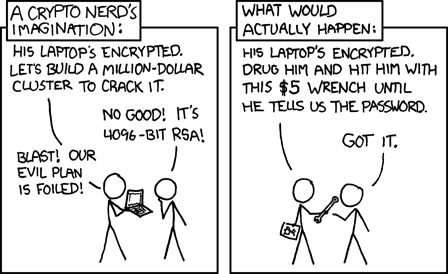
\includegraphics[width=10cm]{pictures_bitmap/security.png}\\
        \url{http://xkcd.com/538/} \href{http://creativecommons.org/licenses/by-nc/2.5/}{ Creative Commons Attribution-NonCommercial 2.5 License}.
\end{center}%
}{}            

\noindent \ldots tout dépends du contexte.



\chapter{Intégration}
% This is part of Mes notes de mathématique
% Copyright (c) 2011-2016
%   Laurent Claessens
% See the file fdl-1.3.txt for copying conditions.

%+++++++++++++++++++++++++++++++++++++++++++++++++++++++++++++++++++++++++++++++++++++++++++++++++++++++++++++++++++++++++++ 
\section{Théorème de la moyenne}
%+++++++++++++++++++++++++++++++++++++++++++++++++++++++++++++++++++++++++++++++++++++++++++++++++++++++++++++++++++++++++++

\begin{theorem}[\cite{MonCerveau}]      \label{ThoooEZLGooMChwLT}
    Soit \( Q\) un compact connexe par arcs et une fonction continue \( f\colon Q\to \eR\). Si \( \lambda\) est la mesure de Lebesgue, alors il existe \( a\in Q\) tel que
    \begin{equation}
        f(a)=\frac{1}{ \lambda(Q) }\int_Qfd\lambda
    \end{equation}
\end{theorem}

\begin{proof}
    En posant \( I=\int_Qfd\lambda\) nous avons immédiatement
    \begin{equation}        \label{EqooTYQCooVxdazW}
        \min(f)\lambda(Q)\leq I\leq \max(f)\lambda(Q)
    \end{equation}
    où le minimum et le maximum existent parce que \( f\) est continue sur un compact. Si une des deux inégalités est une égalité alors la fonction est constante. En effet supposons que la première inégalité soit une égalité; si la fonction n'était pas constante, il existerait une boule sur laquelle \( f\) serait strictement supérieure à \( \min(f)\). En intégrant d'abord sur cette boule et ensuite sur le complémentaire nous obtenons une intégrale plus grande que \( \min(f)\lambda(Q)\).

    Soit \( \epsilon>0\). Il existe \( \alpha,\beta\in Q\) tels que \( f(\alpha)\leq\min(f)+\epsilon\) et \( f(\beta)\geq\max(f)-\epsilon\). Soit \( \gamma\colon \mathopen[ 0 , 1 \mathclose]\to Q\) un chemin continu tel que \( \gamma(0)=\alpha\) et \( \gamma(1)=\beta\). La fonction \( f\circ \gamma\colon \mathopen[ 0 , 1 \mathclose]\to \eR\) est alors continue et vérifie \( (f\circ\gamma)(0)\leq \min(f)+\epsilon\) et \( (f\circ\gamma)(1)\geq \max(f)-\epsilon\).

    Si \( \epsilon\) est assez petit et vu que les inégalités \eqref{EqooTYQCooVxdazW} sont strictes,
    \begin{equation}
        \lambda(Q)(f\circ\gamma)(0)\leq \min(f)\lambda(Q)+\epsilon\lambda(Q)<I<\max(f)\lambda(Q)-\epsilon\lambda(Q)\leq\lambda(Q)(f\circ \gamma)(1).
    \end{equation}
    Par le théorème des valeurs intermédiaires \ref{ThoValInter}, il existe \( t_0\in\mathopen[ 0 , 1 \mathclose]\) tel que \( \lambda(Q)(f\circ\gamma)(t_0)=I\). Le point \( a=\gamma(t_0)\) vérifie
    \begin{equation}
        f(a)=\frac{1}{ \lambda(Q) }\int_Qfd\lambda.
    \end{equation}
\end{proof}

%+++++++++++++++++++++++++++++++++++++++++++++++++++++++++++++++++++++++++++++++++++++++++++++++++++++++++++++++++++++++++++ 
\section{Mesure à densité}
%+++++++++++++++++++++++++++++++++++++++++++++++++++++++++++++++++++++++++++++++++++++++++++++++++++++++++++++++++++++++++++

%--------------------------------------------------------------------------------------------------------------------------- 
\subsection{Théorème de Radon-Nikodym}
%---------------------------------------------------------------------------------------------------------------------------

\begin{proposition}[Produit d'une mesure par une fonction]
    Si \( (S,\tribF,m_1)\) est un espace mesuré, et si \( f\colon S\to \eR\) est intégrable, et si \( B\) est un ensemble mesurable, nous définissons \( fm_1\) par
    \begin{equation}
        m_2(B)=(fm_1)(B)=\int_Bf(t)dm_1(t).
    \end{equation}
    Cela est une mesure positive sur \( (S,\tribF)\).
\end{proposition}

\begin{proof}
    D'abord pour l'ensemble vide : \( m_2(\emptyset)=\int_{\emptyset}fdm_1=0\).

    Si \( A_n\) sont des éléments disjoints de \( \tribF\) tels que \( \bigcup_nA_n\in\tribF\). Alors en utilisant la proposition \ref{PropOPSCooVpzaBt}, nous avons le calcul suivant :
    \begin{equation}
        m_2\big( \bigcup_nA_n \big)=\int_{\bigcup_nA_n}f(t)dm_1(t)=\sum_{n}\int_{A_n}f(t)dm_1(t)=\sum_nm_2(A_n).
    \end{equation}
\end{proof}

\begin{definition}[\cite{PersoFeng}]
    Soient \( \mu\) et \( \nu\) deux mesures sur l'espace mesurable \( (\Omega,\tribA)\). Nous disons que la mesure \( \mu\) est \defe{dominée}{dominée!mesure} par \( \nu\) si pour tout ensemble mesurable \( A\), \( \nu(A)=0\) implique \( \mu(A)=0\).

    Si \( \nu\) est une mesure positive et \( \mu\) une mesure, nous disons que \( \mu\) est \defe{absolument continue}{mesure!absolument continue} par rapport à \( \nu\) si \( \nu(A)=0\) implique \( \mu(A)=0\). On note aussi \( \mu\ll\nu\)\nomenclature[Y]{$\mu\ll\nu$}{La mesure \( \mu\) est absolument continue par rapport à la mesure \( \nu\).}.
\end{definition}

La mesure \( \mu\) est \defe{portée}{portée!mesure} par l'ensemble \( E\in\tribA\) si pour tout \( A\in\tribA\), 
\begin{equation}
    \mu(A)=\mu(A\cap E).
\end{equation}

Nous écrivons que \( \mu\perp\nu\)\nomenclature[Y]{\( \mu\perp\nu\)}{mesures perpendiculaires} s'il existe un ensemble \( E\in\tribA\) tel que \( \mu\) soit porté par \( E\) et \( \nu\) soit porté par \( \complement E\).

\begin{theorem}[Radon-Nikodym\cite{NikoLi}]
    Soient \( \mu\) et \( \nu\) deux mesures \( \sigma\)-finies sur un espace métrisable \( (\Omega,\tribA)\).
    \begin{enumerate}
        \item
            Il existe un unique couple de mesures \( \mu_1\) et \( \mu_2\) telles que
            \begin{enumerate}
                \item
                    \( \mu=\mu_1+\mu_2\)
                \item
                    \( \mu_1\) est dominé par \( \nu\)
                \item
                    \( \mu_2\perp \nu\).
            \end{enumerate}
            Dans ce cas, les mesures \( \mu_1\) et \( \mu_2\) sont positives et \( \sigma\)-finies.
        \item
            À égalité \(  \nu\)-presque partout près, il existe une unique fonction mesurable positive \( f\) telle que pour tout mesurable \( A\),
            \begin{equation}
                \mu_1(A)=\int_Ad\mu_1=\int_{\Omega}\mtu_Afd \nu.
            \end{equation}
        \item
            À égalité \( \nu\)-presque partout près, il existe une unique fonction positive mesurable \( h\) telle que \( \mu_1=h\nu\).
    \end{enumerate}
\end{theorem}
\index{théorème!Radon-Nikodym}
%TODO : une preuve

\begin{corollary}   \label{CorZDkhwS}
    Si \( \mu\) es une mesure \( \sigma\)-finie dominée par la mesure \( \sigma\)-finie \( m\), alors \( \mu\) possède une unique fonction de densité.
\end{corollary}

\begin{corollary}       \label{CorDomDens}
    Soient \( \mu\) et \( m\), deux mesures positives \( \sigma\)-finies sur \( (\Omega,\tribA)\). Alors \( m\) domine \( \mu\) si et seulement si \( \mu\) possède une densité par rapport à \( m\).
\end{corollary}
 
\begin{proof}
    Si \( \mu\) est dominée par \( m\), alors la décomposition \( \mu=\mu+0\) satisfait le théorème de Radon-Nikodym. Par conséquent il existe une fonction \( f\) telle que
    \begin{equation}
        \mu(A)=\int_Afdm.
    \end{equation}
    Cette fonction est alors une densité pour \( \mu\) par rapport à \( m\).

    Pour la réciproque, nous supposons que \( \mu\) a une densité \( f\) par rapport à \( m\), et que \( A\) est une ensemble de \( m\)-mesure nulle :
    \begin{equation}
        m(A)=\int_{\Omega}\mtu_Adm=0.
    \end{equation}
    Cela signifie que la fonction \( \mtu_A\) est \( m\)-presque partout nulle. La fonction produit \( \mtu_Af\) est également nulle \( m\)-presque partout, et par conséquent
    \begin{equation}
        \mu(A)=\int_{\Omega}\mtu_Afdm=0.
    \end{equation}
\end{proof}

\begin{probleme}
    Est-ce que la démonstration de cela ne demande pas la convergence monotone d'une façon ou d'une autre ?
\end{probleme}

%--------------------------------------------------------------------------------------------------------------------------- 
\subsection{Mesure complexe}
%---------------------------------------------------------------------------------------------------------------------------

\begin{definition}[Mesure complexe\cite{TLRRooOjxpTp}] \label{DefGKHLooYjocEt}
    Si \( (\Omega,\tribA)\) est un espace mesurable, une \defe{mesure complexe}{mesure!complexe} est une application \( \mu\colon \tribA\to \eC\) telle que
    \begin{enumerate}
        \item
            $\mu(\emptyset)=0$,
        \item
            \( \nu\) est sous-additive : si les ensembles \( A_i\in\tribA\), alors \( \sum_i\mu(A_i)=\mu(\bigcup_iA_i)\).
    \end{enumerate}
\end{definition}
Notons que la série $\sum_i\mu(A_i)$ est alors nécessairement absolument convergente. En effet changer l'ordre de la somme ne change pas l'union, et donc ne change pas la valeur de la somme. Si \( \sigma\colon \eN\to \eN\) est une permutation, 
\begin{equation}
    \sum_i\mu(A_{\sigma(i)})=\mu\big( \bigcup_iA_{\sigma(i)} \big)=\mu\big( \bigcup_iA_i \big)=\sum_i\mu(A_i).
\end{equation}
Le théorème \ref{PopriXWvIY} dit alors que la somme doit être absolument convergente.


\begin{theorem}[Radon-NikoDym complexe\footnote{L'histoire du nom de ce théorème est intéressante. Lorsque monsieur et madame Rèmederdonnukodym apprirent que leurs amis, les Rèmedelaboulechevelue avaient appelé leur fils Théo, ils décidèrent d'en faire autant. C'est en souvenir de ces circonstances que monsieur Nikodym (prénommé Radon) décida de faire des math.}]\label{ThoZZMGooKhRYaO}
    Soit \( \mu\) une mesure positive sur \( (\Omega,\tribA)\) et \( \nu\) une mesure complexe. Alors
    \begin{enumerate}
        \item
            Il existe un unique couple de mesures complexes \( \nu_a\), \( \nu_s\) sur \( (\Omega,\tribA)\) tel que
            \begin{enumerate}
                \item
                    \( \nu=\nu_a+\nu_s\)
                \item
                    \( \nu_a\ll\mu\)
                \item
                    \( \nu_s\perp \mu\).
            \end{enumerate}
        \item
            Ces mesures satisfont alors \( \nu_a\perp\nu_s\).
        \item
            Il existe une fonction intégrable \( h\colon \Omega\to \eC\) telle que \( \nu_a=h\mu\).
        \item
            La fonction \( h\) est unique à \( \mu\)-équivalence près.
        \item   \label{ItemDIXOooFqOkgGv}
            Si de plus \( \nu\ll \mu\) alors \( \nu=h\mu\).
    \end{enumerate}
\end{theorem}
\index{théorème!Radon-Nikodym!complexe}
\begin{proof}
    No proof.
\end{proof}

\begin{remark}  \label{RemSYRMooZPBhbQ}
    Le point \ref{ItemDIXOooFqOkgGv} est souvent utilisé sous la forme
    \begin{equation}
        \nu(A)=\int_{\Omega}\mtu_A(\omega)h(\omega)d\mu(\omega)=\int_{A}h(\omega)d\mu(\omega).
    \end{equation}
\end{remark}

%--------------------------------------------------------------------------------------------------------------------------- 
\subsection{Théorème d'approximation}
%---------------------------------------------------------------------------------------------------------------------------

\begin{theorem}[Théorème d'approximation\cite{YHRSDGc}]     \label{ThoAFXXcVa}
    Soit \( (X,\tribB,\mu)\) un espace mesuré où \( \tribB\) sont les boréliens de \( X\). Soit \( A\in \tribB\) tel que \( A\subset W\) où \( W\) est un ouvert avec \( \mu(W)<\infty\). Soit aussi \( \epsilon>0\).
    \begin{enumerate}
        \item
            Il existe un fermé \( F\) et un ouvert \( V\) tels que \( \mu(V)<\infty\) et
            \begin{equation}
                F\subset A\subset V
            \end{equation}
            et \( \mu(V\setminus F)<\epsilon\).
        \item
            Il existe \( f\in C^0(X,\eR)\) nulle hors de \( W\) vérifiant \( 0\leq f\leq 1\) et
            \begin{equation}
                \int_X| \mtu_A-f |^pd\mu(x)<\epsilon.
            \end{equation}
    \end{enumerate}
\end{theorem}
% TODO : la preuve est dans la référence. Il faut replacer ce théorème après la définition de l'intégrale.


% This is part of Mes notes de mathématique
% Copyright (c) 2011-2017
%   Laurent Claessens
% See the file fdl-1.3.txt for copying conditions.

%+++++++++++++++++++++++++++++++++++++++++++++++++++++++++++++++++++++++++++++++++++++++++++++++++++++++++++++++++++++++++++ 
\section{Propriétés}
%+++++++++++++++++++++++++++++++++++++++++++++++++++++++++++++++++++++++++++++++++++++++++++++++++++++++++++++++++++++++++++

\begin{theorem}[\cite{ooGMNAooSLnIio}]      \label{THOooVADUooLiRfGK}
    Soient deux espaces mesurables \( (S_1,\tribF_1)\) et \( (S_2,\tribF_2)\) ainsi qu'une application mesurable \( \varphi\colon S_1\to S_2\). Soit encore \( \mu\), une mesure positive sur \( (S_1,\tribF_1)\).

    Si \( f\colon S_2\to\bar \eR\) ou \( \eC\) est mesurable alors,
    \begin{enumerate}
        \item      \label{ItemooKMBIooZpHJSS}
            \( f\) est \( \varphi(\mu)\)-intégrale si et seulement si \( f\circ\varphi\) est \( \mu\)-intégrable.
        \item       \label{ItemooLAPYooUreDEl}
            dans le cas où \( f\) est \( \varphi(\mu)\)-intégrable, nous avons
            \begin{equation}        \label{EqooSOHXooXSbdoy}
                \int_{S_2}fd\big( \varphi(\mu) \big)=\int_{S_1}(f\circ\varphi)d\mu.
            \end{equation}
    \end{enumerate}
\end{theorem}

\begin{proof}
    L'intégrabilité est la définition \ref{DefTCXooAstMYl}, et demande que \( | f |\) soit intégrable. L'égalité \eqref{EqooSOHXooXSbdoy} a un sens si les deux membres sont infinis. Tant que les fonctions considérées sont positives, le point \ref{ItemooKMBIooZpHJSS} est immédiat. Ce n'est qu'au moment où les fonctions considérées deviennent à valeurs dans \( \eC\) ou \( \eR\) que l'intégrabilité de \( | f |\) commence à jouer parce qu'il faut que \(  f^+  \) et \( f^-\) soient séparément intégrables.

    Nous allons prouver la formule \eqref{EqooSOHXooXSbdoy} pour des fonctions de plus en plis générales. Pour la suite nous notons \( \mu'=\varphi(\mu)\).

    \begin{subproof}
        \item[Pour \( f=\mtu_B\), \( B \) mesurable]
            Soit \( B\in\tribF_2 \). Nous avons \( \mtu_B\circ\varphi=\mtu_{\varphi^{-1}(B)}\). Donc en utilisant le lemme \ref{LemooPJLNooVKrBhN} nous avons
            \begin{equation}
                \int_{S_2}\mtu_{B}d\mu'=\mu'(B)=\mu\big( \varphi^{-1}(B) \big)=\int_{S_1}\mtu_{\varphi^{-1}(B)}d\mu=\int_{S_1}(\mtu_B\circ \varphi)d\mu.
            \end{equation}
        \item[\( f\) est étagée positive]

            La fonction \( f\) peut être écrite sous la forme
            \begin{equation}
                f=\sum_{k=1}^na_k\mtu_{B_k}
            \end{equation}
            avec \( B_k\in\tribF_2\) et \( a_k\in \eR^+\). Nous avons alors, en utilisant la sous-additivité de l'intégrale du théorème \ref{ThoooCZCXooVvNcFD}\ref{ITEMooOJRAooQkoQyD},
            \begin{subequations}
                \begin{align}
                    \int_{S_2}fd\mu'&=\sum_ka_k\int_{S_2}\mtu_{B_k}d\mu'\\
                    &=\sum_ka_k\int_{S_1}(\mtu_{B_k}\circ\varphi)d\mu\\
                    &=\int_{S_1}\Big( \sum_ka_k\mtu_{B_k} \Big)\circ \varphi d\mu\\
                    &=\int_{S_1}(f\circ\varphi)d\mu.
                \end{align}
            \end{subequations}
        \item[\( f\) à valeurs dans \( \bar \eR^+\)]

            Vu que \( f\) est mesurable, par le théorème \ref{THOooXHIVooKUddLi} il existe une suite croissante de fonctions étagées positives convergeant vers \( f\). Soit donc cette suite, \( f_n\colon S_2\to \eR^+\). Les fonction s\( f_n\circ\varphi\) sont étagées et positives et nous avons aussi la limite ponctuelle et croissante \( f_n\circ\varphi\to f\circ\varphi\) parce que \( \varphi\) est continue. Le théorème de la convergence monotone (théorème \ref{ThoRRDooFUvEAN}) permet d'écrire ceci :
            \begin{equation}
                \int_{S_2}fd\mu'=\lim\int_{S_2}f_nd\mu'= \lim\int_{S_1}(f_n\circ\varphi)d\mu=\int_{S_1}(f\circ\varphi)d\mu.
            \end{equation}
        \item[Pour \( f\colon S_2\to \bar \eR\) ou \( \eC\) ]
            
            C'est maintenant que l'intégrabilité va jouer. Nous avons \( | f |\circ\varphi=| f\circ\varphi |\), donc
            \begin{equation}
                \int_{S_2}| f |d\mu'=\int_{S_1}| f |\circ\varphi d\mu=\int_{S_1}| f\circ \varphi |d\mu,
            \end{equation}
            ce qui montre que \( f\) est \( \mu'\)-intégrable si et seulement si \( f\circ\varphi\) est \( \mu\)-intégrable.

            De plus si \(f=f^+-f^- \) alors \( f^+\circ\varphi=(f\circ\varphi)^+\), \( f^-\circ\varphi=(f\circ\varphi)^-\), et de façon similaire pour les parties imaginaires et réelles.
    \end{subproof}
\end{proof}

%+++++++++++++++++++++++++++++++++++++++++++++++++++++++++++++++++++++++++++++++++++++++++++++++++++++++++++++++++++++++++++ 
\section{Primitives et intégrales}
%+++++++++++++++++++++++++++++++++++++++++++++++++++++++++++++++++++++++++++++++++++++++++++++++++++++++++++++++++++++++++++

En termes de notations, si \( a<b\) nous posons
\begin{equation}
    \int_a^bf(t)dt=\int_{\mathopen[ a , b \mathclose]}f.
\end{equation}
Si par contre \( a>b\) nous posons \( \int_a^bf=-\int_b^af\).

\begin{proposition}[Primitive et intégrale] \label{PropEZFRsMj}
    Soit \( f\) une fonction intégrable sur \( \mathopen[ a , b \mathclose]\) et continue sur \( \mathopen] a , b \mathclose[\). Alors la fonction
    \begin{equation}
        \begin{aligned}
            F\colon \mathopen[ a , b \mathclose]&\to \eR \\
            x&\mapsto \int_{\mathopen[ a , x \mathclose]}f(t)dt.
        \end{aligned}
    \end{equation}
est une primitive de \( f\) sur \( \mathopen] a , b \mathclose[\).
\end{proposition}
\index{primitive!et intégrale}

\begin{proof}
Nous devons prouver que \( F\) est dérivable et que pour tout \( x_0\in\mathopen] a , b \mathclose[\) nous ayons \( F'(x_0)=f(x_0)\). Soit \( \epsilon>0\). Par continuité de \( f\) en \( x_0\), il existe une fonction \( \alpha\colon \eR\to \eR\) telle que
    \begin{equation}
        f(x_0+h)=f(x_0)+\alpha(h)
    \end{equation}
    avec \( \lim_{h\to 0} \alpha(h)=0\). De plus il existe un \( \delta>0\) tel que \( |\alpha(h)|<\epsilon\) pour tout \( h<\delta\). À partir de maintenant nous ne considérons plus que de tels \( h\).

    Nous calculons la dérivée de \( F\) en \( x_0\). Pour cela,
    \begin{subequations}
        \begin{align}
            F(x_0+h)-F(x_0)&=\int_{x_0}^{x_0+h}f(t)dt\\
        &=\int_0^hf(x_0+t)dt\\
        &=\int_0^h\big[ f(x_0)+\alpha(t) \big]dt\\
        &=hf(x_0)+\int_0^{h}\alpha(t)dt.
        \end{align}
    \end{subequations}
    Nous avons donc, pour tout \( h<\delta\),
    \begin{equation}
        hf(x_0)-h\epsilon\leq F(x_0+h)-F(x_0)\leq hf(x_0)+h\epsilon.
    \end{equation}
    En divisant par \( h\) et en prenant la limite \( h\to 0\),
    \begin{equation}
        F'(x_0)\in B\big( f(x_0),\epsilon \big).
    \end{equation}
    Cela étant valable pour tout \( \epsilon>0\) nous en déduisons que
    \begin{equation}
        F'(x_0)=f(x_0).
    \end{equation}
\end{proof}

\begin{remark}
    Le lien entre primitive et intégrale est fondamentalement lié à l'invariance par translation de la mesure de Lebesgue, et non à la construction précise de cette mesure. Mais en même temps, la mesure de Lebesgue est l'unique à être invariante par translation.
\end{remark}

\begin{remark}
    Une primitive est forcément une fonction continue parce qu'une primitive est dérivable.
\end{remark}

Ce petit résultat nous donne une façon «pratique» de calculer des intégrales en cherchant des primitives. Nous rappelons qu'en vertu du corollaire \ref{CorZeroCst}, une fonction ne possède qu'une seule primitive à constante près.

\begin{corollary}[Théorème fondamental du calcul intégral]       \label{CORooKRBZooEMDobC}
    Soit une fonction \( f\colon I\to \eR\) où \( I\) est un intervalle. Nous supposons que \( f\) est continue sur \( I\). Soient \( a<b\) dans \( I\) et une primitive \( F\) de \( f\) sur \( I\).

    Alors
    \begin{equation}        \label{EQooXEKDooEnWcbn}
        \int_a^bf=F(b)-F(a).
    \end{equation}
\end{corollary}

\begin{proof}
    Nous savons par la proposition \ref{PropEZFRsMj} que la fonction donnée par
    \begin{equation}
        G(x)=\int_a^xf
    \end{equation}
    est une primitive de \( f\). Vu que \( F\) est également une primitive nous avons \( F(x)=G(x)+C\) pour une certaine constante \( C\in \eR\) (c'est le corollaire \ref{CorZeroCst}). Vu que \( G(a)=0\), l'égalité \( F(a)=G(a)+C\) donne \( C=F(a)\).

    Ce que l'on nous demande de calculer dans \eqref{EQooXEKDooEnWcbn} est \( G(b)\), c'est à dire l'égalité
    \begin{equation}
        F(b)=G(b)+C=G(b)+F(a),
    \end{equation}
    et donc \( G(b)=F(b)-F(a)\), ce qu'il fallait.
\end{proof}

\begin{proposition}[\cite{ooIEJXooIYpBbd}]      \label{PROPooWZFGooMVLtFz}
    Soient des fonction \( f,g\colon I\to \eR\) de classe \(  C^{1}\) sur l'ouvert \( I\) de \( \eR\) telles que \( f^2+g^2=1\). Soit \( t_0\in I\) et \( \theta_0\) tel que \( f(t_0)=\cos(\theta_0)\) et \( g(t_0)=\sin(\theta_0)\).

    Alors il existe une unique fonction continue \( \theta\colon I\to \eR\) telle que 
    \begin{subequations}
        \begin{numcases}{}
            \theta(t_0)=\theta_0\\
            f=\cos\circ \theta\\
            g=\sin\circ \theta.
        \end{numcases}
    \end{subequations}
\end{proposition}

\begin{proof}
    Nous commençons par l'existence, en passant par les nombres complexes. Soit \( h\colon I\to \eC\) définie par \( h=f+ig\). Nous avons \( h\bar h=1\) et nous définissons
    \begin{equation}
        \theta(t)=\theta_0-i\int_{t_0}^th'(s)\overline{ h(s) }ds.
    \end{equation}
    Cette intégrale existe pour tout \( t\) parce que les fonctions \( f\) et \( g\) étant de classe \(  C^{\infty}\), elles sont bornées sur le compact \( \mathopen[ t_0 , t  \mathclose]\). De plus \( \theta\) est une fonction continue parce que c'est une primitive (proposition \ref{PropEZFRsMj})\footnote{En réalité nous appliquons la proposition \ref{PropEQRooQXazLz} à chacune des parties réelles et imaginaires de la fonction \( s\mapsto h'(s)\overline{ h(s) }\).}.

    La dérivée de \( \theta\) est la fonction \( s\mapsto -i h'(s)\overline{ h(s) }\).

    Calculons 
    \begin{equation}
        \Dsdd{ h e^{-i\theta} }{t}{0}= e^{-i\theta}(h'-h\theta')= e^{-i\theta}(h'-ih(-i)h'\bar h)=0.
    \end{equation}
    Par conséquent il existe \( c\in \eC\) tel que \( h e^{-i\theta}=c\). Mais \( h(t_0)=f(t_0)+ig(t_0)=\cos(\theta_0)+i\sin(\theta_0)= e^{i\theta_0}\), du coup
    \begin{equation}
        h(t_0) e^{-i\theta(t_0)}=c
    \end{equation}
    donne immédiatement \( c=1\), ou encore \(  e^{i\theta(t)}=h(t)\), c'est à dire que
    \begin{equation}
        f+ig=\cos\circ\theta+i\sin\circ\theta,
    \end{equation}
    ce qu'il fallait pour l'existence.

    Pour l'unicité nous supposons avoir une autre fonction, \(\alpha\) qui satisfait aux exigences. Pour tout \( t\in I\) nous avons
    \begin{equation}
        e^{i\theta(t)}= e^{i\alpha(t)}.
    \end{equation}
    Il existe donc une fonction \( n\colon I\to \eN\) telle que \( \theta(t)=\alpha(t)+2n(t)\pi\). Par continuité de \( \theta\) et \( \alpha\), la fonction \( n\) doit être constante, mais vu que \( \theta(t_0)=\alpha(t_0)\) nous avons \( n=1\).
\end{proof}

Le théorème suivant est à utiliser pour calculer des intégrales des fonctions réelle lorsqu'on a des primitives sur un domaine strictement plus large que le domaine sur lequel nous voulons intégrer.
\begin{theorem}[Théorème fondamental du calcul intégral]    \label{ThoRWXooTqHGbC}
    Soit \( f\) une fonction continue sur un intervalle ouvert \( I\) contenant strictement l'intervalle \( \mathopen[ a , b \mathclose]\subset \eR\) et \( F\) une primitive de \( f\) sur \( I\). Alors
    \begin{equation}
        \int_a^bf(t)dt=F(b)-F(a).
    \end{equation}
\end{theorem}
\index{théorème!fondamental du calcul intégral}
Une version pour les intégrales impropres sera donnée au corollaire \ref{CorMUIooXREleR}.

\begin{proof}
    Nous avons vu par la proposition \ref{PropEZFRsMj} que la fonction
    \begin{equation}
        \begin{aligned}
            \tilde F\colon \mathopen[ a , b \mathclose]&\to \eR \\
            x&\mapsto  \int_a^xf(t)dt
        \end{aligned}
    \end{equation}
    était une primitive de \( f\); c'est même l'unique\footnote{Corollaire \ref{CorZeroCst}.} primitive de \( f\) sur \( \mathopen[ a , b \mathclose]\) à s'annuler pour \( x=a\). Nous avons évidemment
    \begin{equation}
        \int_a^bf(t)dt=\tilde F(b).
    \end{equation}
    Si \( F\) est une primitive quelconque, il suffit de soustraire sa valeur en \( x=a\) : \( \tilde F(x)=F(x)-F(a)\) et donc
    \begin{equation}
        \int_a^bf(t)dt=\tilde F(b)=F(b)-F(a),
    \end{equation}
    comme il fallait le prouver.
\end{proof}


%--------------------------------------------------------------------------------------------------------------------------- 
\subsection{Primitives et intégrales}
%---------------------------------------------------------------------------------------------------------------------------

Si \( f\) est une fonction définie sur un intervalle \( I\) et y admettant des primitives, nous notons
\begin{equation}
    \int f(x)dx
\end{equation}
l'ensemble des primitives de \( f\) sur \( I\) :
\begin{equation}
    \int f(x)dx=\left\{    F(x)+C\tq C\in \eR   \right\}
\end{equation}
où \( F\) est une quelconque primitive de \( f\).

\begin{example}
    Une primitive bien connue de \(  f\colon x\mapsto x^2 \) est la fonction \( F\colon x\to \frac{ x^3 }{ 3 }\). Nous écrivons donc
    \begin{equation}
        \int x^2dx=\frac{ x^3 }{ 3 }+C.
    \end{equation}
    Cela est un abus de notations terrible pour dire en réalité
    \begin{equation}
        \{ x\mapsto \frac{ x^3 }{ 3 }+C\tq C\in \eR \}.
    \end{equation}
\end{example}

En termes de notations, nous posons
\begin{equation}\label{Thfondcalc}
    \int_a^bf(t)dt=\Big[ F(t) \Big]_{t=a}^{t=b}=F(b)-F(a).
\end{equation}

\begin{remark}
  La valeur de l'intégrale ne dépend pas de la primitive qu'on choisi pour le calculer, car si $F_1$ et $F_2$ sont deux primitives de $f$ alors $F_1 = F_2 + C$ et $F_1(b)-F_1(a) = (F_2(b) + C)-(F_2(a)+C) = F_2(b)-F_2(a)$.
\end{remark}

\begin{remark}
  Si l'intervalle d'intégration est réduit à un seul point alors la valeur de l'intégrale est zéro, car $ \int_a^af(t)dt=F(a)-F(a) =0$.
\end{remark}

\begin{remark}
    Conformément à ce que nous montre la figure \ref{LabelFigKKRooHseDzC}, si une fonction continue est positive sur l'intervalle \( \mathopen[ a , b \mathclose]\), alors le nombre \( \int_a^bf(t)dt\) est l'aire de la portion de plan comprise entre les droites verticales \( x=a\), \( x=b\), la courbe représentant la fonction \( f\) et l'axe des abscisses.

    Si la fonction est négative : l'aire est comptée négativement.
\end{remark}

\begin{example} 
    Comme nous le voyons sur le dessin suivant,
    \begin{equation}
        \int_{-3\pi/2}^{3\pi/2}\sin(x)\,dx=0
    \end{equation}
    parce que les deux parties bleues s'annulent avec les deux parties rouges (qui sont comptées comme des aires négatives).
    \begin{center}
       \input{auto/pictures_tex/Fig_JSLooFJWXtB.pstricks}
    \end{center}
\end{example}

\begin{remark}
  Toute intégrale d'une fonction impaire sur un intervalle symétrique par rapport à l'origine est nulle. 
\end{remark}

\begin{proposition}[Intégrale et primitive] \label{PropZEJooEsnrgY}
    Soit \( f\) une fonction continue sur l'intervalle \( I\) et un élément \( a\in I\). Soit la fonction
    \begin{equation}
        \begin{aligned}
            F\colon I&\to \eR \\
            x&\mapsto \int_a^xf(t)dt. 
        \end{aligned}
    \end{equation}
    Alors \( F\) est l'unique primitive de \( f\) s'annulant en \( x=a\).
\end{proposition}

%--------------------------------------------------------------------------------------------------------------------------- 
\subsection{Intégrales impropres}
%---------------------------------------------------------------------------------------------------------------------------
\label{SecGAVooBOQddU}

% TODO : l'exemple avec arcsin(1/x)-1/x de la page 
%  http://fr.wikipedia.org/wiki/Intégrale_impropre

\begin{definition}[\cite{TrenchRealAnalisys}]
    Une fonction \( f\colon D\subset\eR\to \eR\) est \defe{localement intégrable}{localement!intégrable} sur un intervalle \( I\) si \( f\) est intégrable sur tout intervalle compact contenu dans \( I\).
\end{definition}
\index{intégrale!impropre}

%Dans \cite{TrenchRealAnalisys}, la proposition \ref{PropCJAooQhNYkp} est prise comme une définition de \( \int_a^bf\) lorsque \( f\) est localement intégrable sur \( \mathopen[ a , b [\). Le point est que lui, il ne passe pas par Lebesgue et la construction abstraite d'intégrale par rapport à une mesure. Nous par contre nous avons déjà une définition de
%\begin{equation}
%    \int_a^bf=\int_{\mathopen[ a , b \mathclose]}f
%\end{equation}
%pour tout choix de \( a\), \( b\) et \( f\), que ce soit borné ou non.

\begin{proposition}     \label{PropCJAooQhNYkp}
    Soit \( f\colon \mathopen[ a , b \mathclose]\to \eR\) une fonction intégrable. Alors
    \begin{equation}    \label{EqPPMooBQDTYl}
        \int_{\mathopen[ a , b \mathclose]}f=\lim_{x\to b^-} \int_a^xf.
    \end{equation}
\end{proposition}

\begin{proof}
    Notons que la valeur de \( f\) en \( b\) n'a strictement aucune importance parce que l'intégrale de Lebesgue ne dépend pas du choix de la valeur de la fonction en un ensemble de mesure nulle; et en même temps la limite à gauche de \eqref{EqPPMooBQDTYl} ne dépend pas non plus de la valeur de \( f\) en \( b\). Bref si \( f\) n'est pas définie en \( b\), nous pouvons poser \( f(b)=42\).

    Notons de plus que du point de vue de l'intégrale de Lebesgue, \( \int_{\mathopen[ a , b \mathclose]}\) et \( \int_{\mathopen[ a , b [}\) sont identiques et valent toutes les deux \( \int_a^b\) (lorsque ça existe).

    Supposons d'abord que \( f\) est positive. Alors nous posons \( f_n=f\mtu_{\mathopen[ a , b-\frac{1}{ n } \mathclose]}\). Ponctuellement nous avons la limite croissante \( f_n\to f\) et de plus
    \begin{equation}
        \lim_{x\to b^-} \int_{\mathopen[ a , x \mathclose]}f=\lim_{n\to \infty} \int_{\mathopen[ a , b \mathclose]}f_n.
    \end{equation}
    Chacun des \( f_n\) est intégrable sur \( \mathopen[ a , b \mathclose]\). Le théorème de Beppo-Levi \ref{ThoRRDooFUvEAN} implique que \( f\) est intégrable sur \( \mathopen[ a , b \mathclose]\) et que
    \begin{equation}
        \lim_{n\to \infty} \int_a^bf_n=\int_a^bf.
    \end{equation}
    Cela montre que dans le cas d'une fonction \( f\) positive nous avons bien \eqref{EqPPMooBQDTYl}.

    Si \( f\) n'est pas positif, alors nous la décomposons en partie positive et négative \( f=f^+-f^{-}\) et par définition de l'intégrale d'une fonction non positive,
    \begin{equation}
        \lim_{x\to b^-} \int_{\mathopen[ a , x [}f=\lim\int f^{+}-\lim\int f^-.
    \end{equation}
\end{proof}

Il peut cependant arriver que la limite \( \lim_{x\to b} \int_a^bf\) existe alors que \( f\) n'est pas intégrable sur \( \mathopen[ a , b \mathclose]\). C'est l'ennui des fonctions non positives. Un exemple classique est
\begin{equation}\label{EqMMVooDSpgfz}
    \int_0^{\infty}\frac{ \sin(t) }{ t }dt
\end{equation}

\begin{definition}[\cite{DWNooWUZxRP}]      \label{DEFooINPOooWWObEz}
    Si
    \begin{equation}
        \lim_{x\to b} \int_a^bf
    \end{equation}
    existe alors nous disons que l'intégrale est \defe{convergente}{intégrale!convergente} en \( b\). Ce procédé de limite est l'intégrale \defe{impropre}{intégrale!impropre} de \( f\) sur \( \mathopen[ a , b \mathclose]\).
\end{definition}

\begin{example}[Intégale impropre]
    Nous considérons la fonction \( f\colon \mathopen[ 0 , \infty [\to \eR\) définie par
    \begin{equation}
        f(x)=\begin{cases}
            \frac{1}{ n }    &   \text{si } x\in\mathopen[ 2n-2 , 2n-1 [\\
                -\frac{1}{ n }    &    \text{si } x\in\mathopen[ 2n-1 , 2n [\text{.}
        \end{cases}
    \end{equation}
    Par la divergence de la série harmonique, \( \int_{0}^{\infty}| f |\) n'existe pas. La fonction \( f\) n'est donc pas intégrable au sens de Lebesgue (définition \ref{DefTCXooAstMYl}).

    Cependant pour tout \( n\) pair nous avons
    \begin{equation}
        \int_0^nf=0.
    \end{equation}
    Du coup pour tout \( x\geq 0\) nous avons
    \begin{equation}
        \int_0^xf=\int_{2n}^xf
    \end{equation}
    où \( 2n\) est le plus grand nombre pair inférieur à \( x\). Nous avons \( | x-2n |\leq 2\) et \( | f(x) |\leq \frac{1}{ n }\) pour \( x\in\mathopen[ 2n , x \mathclose]\). Donc
    \begin{equation}
        \int_{2n}^xf\leq \frac{ 2 }{ n }.
    \end{equation}
    Nous avons par conséquent
    \begin{equation}
        \lim_{x\to \infty} \int_0^xf=0,
    \end{equation}
    ce qui signifie que l'intégrale de \( f\) sur \( \mathopen[ 0 , \infty [\) converge au sens des intégrales impropres.
\end{example}


L'intégrale \eqref{EqMMVooDSpgfz} est une intégrale convergente mais la fonction n'est pas intégrable (parce que pour être intégrale il faut que \( | f |\) soit intégrable). Nous pouvons ainsi dire que cette intégrale converge mais n'existe pas.

Le corollaire suivant nous autorise à utiliser le théorème fondamental du calcul intégral \ref{ThoRWXooTqHGbC} même dans les cas limites.
\begin{corollary}   \label{CorMUIooXREleR}
    Si \( f\) est localement intégrable sur \( \mathopen[ a , b \mathclose]\) et si \( F\) est une primitive de \( f\) sur tout ouvert de \( \mathopen[ a , b \mathclose]\) alors
    \begin{equation}
        \int_a^bf=\lim_{x\to b^-} F(x)-F(a).
    \end{equation}
\end{corollary}
\index{primitive!et intégrale}

\begin{proof}
    Pour chaque \( x\) dans \( \mathopen[ a , b [\) nous avons
    \begin{equation}
        \int_a^xf=F(x)-F(b).
    \end{equation}
    La proposition \ref{PropCJAooQhNYkp} nous explique que la limite \( x\to b^-\) du membre de gauche existe et vaut \( \int_a^bf\). Donc également le membre de droite :
    \begin{equation}
        \int_a^bf=\lim_{x\to b^-} \int_a^xf=\lim_{x\to b^-} F(x)-F(b).
    \end{equation}
\end{proof}

La convergence des intégrales de fonctions \( \frac{1}{ x^{\alpha} }\) en \( 0\) et \( \infty\) est une question classique de l'intégration. De plus ces fonctions servent souvent à utiliser une théorème de comparaison (type intégrale dominée de Lebesgue).
\begin{proposition} \label{PropBKNooPDIPUc}
    Deux intégrales remarquables.
    \begin{enumerate}
        \item
            
            Nous avons 
    \begin{equation}
        \int_0^1\frac{1}{ x^\alpha }=\infty
    \end{equation}
    si et seulement si \( \alpha\geq 1\).

\item

    Nous avons
    \begin{equation}
        \int_1^{\infty}\frac{1}{ x^{\alpha} }=\infty
    \end{equation}
    si et seulement si \( \alpha\leq1\).

    \end{enumerate}
    
\end{proposition}

\begin{proof}
La fonction \( \frac{1}{ x^{\alpha} }\) admet la primitive \( F(x)=\frac{1}{ 1-\alpha }\frac{1}{ x^{\alpha-1} }\) sur tout compact de \( \mathopen] 0 , \infty \mathclose[\). Le corollaire \ref{CorMUIooXREleR} nous permet\footnote{Tout ce que nous avons fait avec la borne \( b\) de l'intégrale \( \int_a^b\) reste valable avec la borne \( a\).} de dire que \( \int_0^1\frac{1}{ x^{\alpha} }\) vaudra
    \begin{equation}
        \lim_{x\to 0-^+} \frac{1}{ 1-\alpha }\frac{1}{ x^{\alpha-1} }.
    \end{equation}
    Cela est strictement plus petit que \( \infty\) si et seulement si \( \alpha<1\).
\end{proof}

%+++++++++++++++++++++++++++++++++++++++++++++++++++++++++++++++++++++++++++++++++++++++++++++++++++++++++++++++++++++++++++ 
\section{Théorème de Fubini-Tonelli et de Fubini}
%+++++++++++++++++++++++++++++++++++++++++++++++++++++++++++++++++++++++++++++++++++++++++++++++++++++++++++++++++++++++++++

Nous rappelons que \( \eR^n\) muni de la mesure de Lebesgue est un espace mesuré \( \sigma\)-fini, conformément à la définition \ref{DefBTsgznn}.

Le théorème de Fubini-Tonelli parle de fonctions réelles et non complexes, et même positives. Le truc est que ce théorème va servir de base pour construire les autres. Si nous avons une fonction à valeurs complexes, elle se décompose en parties réelles et imaginaires qui elles-mêmes se décomposent en parties positives et négatives. Au final, les preuves pour \( f\colon \Omega\to \eC\) se ramènent à appliquer quatre fois le théorème pour \( f\colon \Omega\to \bar \eR^+\).
\begin{theorem}[Fubini-Tonelli\cite{NBoIEXO}]\label{ThoWTMSthY}
    Soient \( (\Omega_i,\tribA_i,\mu_i)\) deux espaces mesurés \( \sigma\)-finis, et \( (\Omega,\tribA,\mu)\) l'espace produit. Soit une fonction \( f\colon \Omega_1\times \Omega_2\to \eR\) une fonction mesurable et positive (valant éventuellement \( \infty\) à certains endroits)
    Alors :
    \begin{enumerate}
        \item       \label{ITEMooUTMNooVIBdpP}
            Les fonction
            \begin{equation}        \label{EQooWLADooQwNhEy}
                F_1\colon x\mapsto \int_{\Omega_2}f(x,y)d\mu_2(y)
            \end{equation}
            et
            \begin{equation}
                F_2\colon y\mapsto \int_{\Omega_1}f(x,y)d\mu_1(x)
            \end{equation}
            sont mesurables.
        \item   \label{ITEMooFKQUooCoCOLV}
            Toutes les intégrales imaginables existent et sont égales :
            \begin{subequations}    \label{EqJRVtOGx}
                \begin{align}
                    \int_{\Omega_1\times \Omega_2}f(x,y)d(\mu_1\otimes \mu_2)(x,y)&=\int_{\Omega_1}\left[ \int_{\Omega_2}f(x,y)d\mu_2(y) \right]d\mu_1(x)\\
                &=\int_{\Omega_2}\left[ \int_{\Omega_1}f(x,y)d\mu_1(x) \right]d\mu_2(y)
                \end{align}
            \end{subequations}
            où tous les membres de l'égalité valent éventuellement \( +\infty\).
    \end{enumerate}
\end{theorem}
\index{théorème!Fubini-Tonelli}

\begin{proof}
    Commençons par prouver le théorème dans le cas d'une fonction caractéristique d'un ensemble mesurable : \( f(x,y)=\mtu_{A}(x,y)\) pour un certain ensemble \( A\subset \Omega_1\times \Omega_2\). Dans ce cas,
    \begin{equation}
        F_1(x)=\int_{\Omega_2}\mtu_A(x,y)d\mu_2(y)=\int_{\Omega_2}\mtu_{A_1(y)}(x)d\mu_2(y)=\mu_2\big( A_1(x) \big),
    \end{equation}
    et nous avons déjà vu au théorème \ref{ThoCCIsLhO} que cette fonction \( F_1\) était alors mesurable. En utilisant maintenant les égalités \eqref{EqDFxuGtH} ainsi que le fait que \( \mtu_A(x,y)=\mtu_{A_2(x)}(y)\) nous avons
    \begin{subequations}
        \begin{align}
            \int_{\Omega_1\times \Omega_2}\mtu_A(x,y)d(\mu_1\otimes \mu_2)(x,y)&=(\mu_1\otimes \mu_2)(A)\\
            &=\int_{\Omega_1}\mu_2\big( A_2(x) \big)d\mu_1(x)\\
            &=\int_{\Omega_1}\left[   \int_{\Omega_2}\mtu_{A_2(x)}(y)d\mu_2(y)  \right]d\mu_1(x)\\
            &=\int_{\Omega_1}\left[ \int_{\Omega_2}\mtu_A(x,y)d\mu_2(y) \right]d\mu_1(x).
        \end{align}
    \end{subequations}
    Le théorème étant valable pour les fonctions caractéristiques, il est valable pour les fonctions simples (définition \ref{DefBPCxdel}) par linéarité de l'intégrale.

    Si \( f\) n'est pas une fonction simple, alors la proposition \ref{THOooXHIVooKUddLi} nous donne une suite croissante de fonctions simples et positives convergeant ponctuellement vers \( f\). La partie du théorème sur les fonctions simples dit que pour chaque \( n\) l'intégrale
    \begin{equation}
        \int_{\Omega_1\times \Omega_2}f_n(x,y)d(\mu_1\otimes\mu_2)(x,y)
    \end{equation}
    peut être décomposée comme il faut en suivant la formule \eqref{EqJRVtOGx}. Il faut pouvoir permuter la limite et l'intégrale dans chacun de cas. D'abord le théorème de la convergence monotone \ref{ThoRRDooFUvEAN} appliqué à l'espace \( \Omega_1\times \Omega_2\) dit que
    \begin{equation}
        \lim_{n\to \infty} \int_{\Omega_1\times \Omega_2}f_n(x,y)d(\mu_1\otimes \mu_2)(x,y)= \int_{\Omega_1\times \Omega_2}f(x,y)d(\mu_1\otimes \mu_2)(x,y).
    \end{equation}
    Ensuite, pour chaque \( x\in\Omega_1\), les fonctions
    \begin{equation}
        \sigma_n(y)=\int_{\Omega_1}f_n(x,y)d\mu_1(x)
    \end{equation}
    forment une suite croissante de fonctions mesurables; nous leur appliquons encore le théorème de la convergence monotone :
    \begin{subequations}
        \begin{align}
            \lim_{n\to \infty} \int_{\Omega_2}\left[ \int_{\Omega_1}f_n(x,y)d\mu_1(x) \right]d\mu_2(y)&=\lim_{n\to \infty} \int_{\Omega_2}\sigma_n(y)d\mu_2(y)\\
            &=\int_{\Omega_2}\left[\lim_{n\to \infty} \int_{\Omega_1}f_n(x,y)d\mu_1(x)\right]d\mu_2(y)\\
            &=\int_{\Omega_2}\left[ \int_{\Omega_1}f(x,y)d\mu_1(x) \right]d\mu_2(y)
        \end{align}
    \end{subequations}
    où nous avons utilisé une seconde fois Beppo-Levi.
\end{proof}

\begin{remark}
    Les formules \eqref{EqJRVtOGx} sont bien, mais ne garantissent en aucun cas que \( f\in L^1(\Omega_1\times \Omega_2)\) : il faut encore que ces intégrales soient finies.
\end{remark}

\begin{corollary}[\cite{MesIntProbb}]           \label{CorTKZKwP}
    Soient \( (\Omega_i,\tribA_i,\mu_i)\) deux espaces mesurés \( \sigma\)-finis, et \( (\Omega,\tribA,\mu)\) l'espace produit\footnote{Définition \ref{DefUMlBCAO}.}. Soit une fonction mesurable \( f\colon \Omega\to \eR\text{ ou }\eC\). Alors les conditions suivantes sont équivalentes
    \begin{enumerate}
        \item   \label{ITEMooZRAXooTRDIlZ}
            \( f\in L^1(\Omega_1\times \Omega_2)\),
        \item       \label{ITEMooJMPLooZKwxQC}
            \begin{equation}
                \int_{\Omega_1}\left[ \int_{\Omega_2}| f |d\mu_2 \right]d\mu_1 <\infty,
            \end{equation}
        \item   \label{ITEMooLLBCooTRycwG}
            \begin{equation}
                \int_{\Omega_2}\left[ \int_{\Omega_1}| f |d\mu_1 \right]d\mu_2 <\infty.
            \end{equation}
    \end{enumerate}
\end{corollary}

\begin{proof}

    Nous commençons par supposer que \( f\) est à valeurs dans \( \eR\). La notation \( | f |\), pour l'instant,  dénote donc bien la valeur absolue et non le module.

    La fonction \( | f |\) est mesurable et positive par hypothèse et par le fait que si \( f\) est mesurable, alors \( | f |\) l'est également par le corollaire \ref{CORooNXYUooEcvDlP}. Le théorème \ref{ThoWTMSthY}\ref{ITEMooFKQUooCoCOLV} nous dit alors que les intégrales suivantes existent et sont égales :
    \begin{equation}        \label{EQooAIQGooNtBOuC}
            \int_{\Omega_1\times \Omega_2}| f |d(\mu_1\otimes \mu_2)=\int_{\Omega_1}\left[ \int_{\Omega_2}|f(x,y)|d\mu_2(y) \right]d\mu_1(x)
            =\int_{\Omega_2}\left[ \int_{\Omega_1}|f(x,y)|d\mu_1(x) \right]d\mu_2(y).
    \end{equation}
    Attention : rien ne dit encore que ces intégrales sont finies.

    \begin{subproof}
        \item[\ref{ITEMooZRAXooTRDIlZ} implique \ref{ITEMooJMPLooZKwxQC} et \ref{ITEMooLLBCooTRycwG}]
            Si \( f\in L^1(\Omega_1\times \Omega_2)\) alors \( | f |\) y est également. Cela implique que le membre de droite de \eqref{EQooAIQGooNtBOuC} est fini. Les deux autres sont alors également finis.
        \item[\ref{ITEMooJMPLooZKwxQC} ou \ref{ITEMooLLBCooTRycwG} implique \ref{ITEMooZRAXooTRDIlZ}]
            Les expressions à droite de \eqref{EQooAIQGooNtBOuC} sont finies. Donc celle de gauche également. Cele signifie que \( | f |\in L^1(\Omega_1\times \Omega_2)\). Par conséquent \( f\) est également dans \(L^1(\Omega_2\times \Omega_2) \).
    \end{subproof}

    Nous passons maintenant au cas où \( f\) est à valeurs dans \( \eC\). Nous décomposons 
    \begin{equation}
        f=f_R+if_I
    \end{equation}
    où \( f_R\) et \( f_I\) sont des fonctions réelles. Nous avons
    \begin{equation}        \label{EQooZEOAooIMwKwk}
        \int_{\Omega}| f |\leq \int_{\Omega}| f_R |+\int_{\Omega}| f_I |.
    \end{equation}
    Donc si \( f_R\) et \( f_I\) sont dans \( L^1(\Omega)\), la fonction \( f\) le sera aussi. De même,
    \begin{equation}
        \int_{\Omega}| f_R |\leq \int_{\Omega}| f |,
    \end{equation}
    qui donne l'inverse : si \( f\in L^1(\Omega)\) alors \( f_R,f_I\in L^1(\Omega)\). Bref, \( f\) est intégrable sur \( \Omega\) si et seulement si \( f_R\) et \( f_I\) le sont.

    Supposons que \( f\in L^1(\Omega_1\times \Omega_2)\). Alors
    \begin{subequations}
        \begin{align}
            \int_{\Omega_1}\left[ \int_{\Omega_2}| f |d\mu_2 \right]d\mu_1&\leq \int_{\Omega_1}\left[ \int_{\Omega_2}| f_R | \right]+\int_{\Omega_1}\left[ \int_{\Omega_2}| f_I | \right]<\infty
        \end{align}
    \end{subequations}
    où nous avons appliqué \ref{ITEMooZRAXooTRDIlZ} implique \ref{ITEMooJMPLooZKwxQC} aux fonctions \( f_R\) et \( f_I\) qui sont dans \( L^1(\Omega_1\times \Omega_2)\) parce que \( f\) y est.

    Dans l'autre sens, si
    \begin{equation}
        \int_{\Omega_1}\left[ \int_{\Omega_2}| f | \right]<\infty,
    \end{equation}
    alors en remplaçant \( | f |\) par \( | f_R |\) ou par \( | f_I |\) nous restons fini. En appliquant alors «\ref{ITEMooJMPLooZKwxQC} implique \ref{ITEMooZRAXooTRDIlZ}» nous trouvons que \( f_R\) et \( f_I\) sont dans \( L^1(\Omega_1\times \Omega_2)\). Et cela implique que \( f\in L^1(\Omega_1\times \Omega_2)\).
\end{proof}

\begin{theorem}[Fubini\cite{MesIntProbb}]\label{ThoFubinioYLtPI}
    Soient \( (\Omega_i,\tribA_i,\mu_i)\) deux espaces mesurés \( \sigma\)-finis, et \( (\Omega,\tribA,\mu)\) l'espace produit. Soit 
    \begin{equation}
        f\in L^1\big( (\Omega,\tribA),\eC \big),
    \end{equation}
    c'est à dire une fonction à valeurs mesurable et intégrable sur \( \Omega\). Alors :
    \begin{enumerate}
        \item       \label{ITEMooVFGWooZTePQS}
            Pour presque tout \( x\in \Omega_1\), la fonction \( y\mapsto f(x,y)\) est \( L^1(\Omega_2)\).
        \item       \label{ITEMooCYMKooUdizni}
            Si nous posons
            \begin{equation}
                \varphi_f(x)=\int_{\Omega_2}f(x,y)d\mu_2(y);
            \end{equation}
            alors \( \varphi_f\in L^1(\Omega_1)\).
        \item   \label{ItemQMWiolgiii}
            Nous avons la formule d'inversion d'intégrale
            \begin{subequations}
                \begin{align}
                \int_{\Omega}fd(\mu_1\otimes \mu_2)&=\int_{\Omega_1}\varphi_fd\mu_1\\
                &=\int_{\Omega_1}\left[ \int_{\Omega_2}f(x,y)d\mu_2(y) \right]d\mu_1(x)\\
                &=\int_{\Omega_2}\left[ \int_{\Omega_1}f(x,y)d\mu_1(x) \right]d\mu_2(y).
                \end{align}
            \end{subequations}
    \end{enumerate}

\end{theorem}
\index{théorème!Fubini!espace mesuré}

\begin{proof}
    Nous commençons par supposer que \( f\) est à valeurs réelles : \( f\in L^1\big( (\Omega_1\times \Omega_2,\tribA_1\otimes\tribA_2 ),\eR\big)\). Nous décomposons la fonction \( f\) en parties positives et négatives : \( f=f^+-f^-\) avec \( f^+\) et \( f^-\) positives ou nulles. Nous avons évidemment
    \begin{equation}
        \int_{\Omega_1\times \Omega_2}| f^+ |\leq \int_{\Omega_1\times \Omega_2}| f |<\infty.
    \end{equation}
    Donc \( f^+\) et \( f^-\) sont des éléments de \( L^1(\Omega_1\times \Omega_2)\). 
    
    \begin{subproof}
    \item[Pour \ref{ITEMooVFGWooZTePQS}]

    Nous posons
    \begin{equation}
        \varphi_{f^+}(x)=\int_{\Omega_2}f^{+}(x,y)d\mu_2(y)
    \end{equation}
    pour tous les \( x\in \Omega_1\) pour lesquels cette intégrale est bien définie. Vu que \( f^+\) est positive et mesurable, le théorème de Fubini-Tonelli \ref{ThoWTMSthY}\ref{ITEMooUTMNooVIBdpP} s'applique donc pour nous dire que \( \varphi_{f^+}\) est mesurable.

    De plus le résultat \eqref{EqJRVtOGx} appliqué à \( f^+\) donne
    \begin{equation}        \label{EQooSETWooRwkCuW}
        \int_{\Omega_1}\varphi_{f^+}d\mu_1=\int_{\Omega_1\times \Omega_2}f^+d(\mu_1\otimes \mu_2)<\infty.
    \end{equation}
    Le fait que le tout soit fini est une conséquence du fait déjà mentionné que \( f^+\in L^1(\Omega_1\times \Omega_2\). Vu que \( \varphi_{f^+}\) est une fonction positive, l'inégalité \eqref{EQooSETWooRwkCuW} signifie que \( \varphi_{f^+}\in L^1(\Omega_1,\mu_1)\).

    En particulier, \( \varphi_{f^+}(x)<\infty\) pour presque tout \( x\in\Omega_1\). C'est à dire pour presque tout \( x\in \Omega_1\) :
    \begin{equation}
        \int_{\Omega_2}f^+(x,y)d\mu_2(y)<\infty,
    \end{equation}
    et sachant que \( f^+\geq 0\) nous avons \( f^+(x,\cdot)\in L^1(\Omega_2)\) pour presque tout \( x\).
    
        \item[Pour \ref{ITEMooCYMKooUdizni}]

            Partout où \( \varphi_{f^+}\) et \( \varphi_{f^-}\) sont finies nous avons
            \begin{equation}
                \varphi_f=\varphi_{f^+}-\varphi_{f^-},
            \end{equation}
            et comme cela a lieu presque partout, nous pouvons considérer une partie mesurable \( A\subset \Omega_1\) telle que \( \mu_1(A)=0\) et \( \varphi_f(x)=\varphi_{f^+}(x)-\varphi_{f^-}(x)\) pour tout \( x\) hors de \( A\). Bref, nous posons
            \begin{equation}
                g(x)=\begin{cases}
                    \varphi_{f^+}-\varphi_{f^-}(x)    &   \text{si } x\in A^c\\
                    0    &    \text{si } x\in A.
                \end{cases}
            \end{equation}
            Cette fonction \( g\) est mesurable et \( g=\varphi_f\) presque partout. De plus
            \begin{equation}
                \int_{\Omega_1}| g |d\mu_1   = \int_{A^c}| g |\leq \int_{A^c}\varphi_{f^+}+\int_{A^c}\varphi_{f^-}<\infty.
            \end{equation}
            La dernière inégalité est le fait que \( \varphi_{f^{\pm}}\) sont dans \( L^1(\Omega_1)\). Et notons au passage que nous aurions pu laisser toutes les intégrales sur \( \Omega_1\) sans faire de précisions sur la distinction entre \( \Omega_1\) et \( A^c\) parce que la partie de \( \Omega_1\) sur laquelle \( \varphi_{f^{\pm}}\) sont infinies est trop petite pour changer la valeur de l'intégrale.

            Nous avons donc \( g\in L^1(\Omega_1)\), et par conséquent également \( \varphi_f\in L^1(\Omega_1)\) parce que ces deux fonctions sont égales presque partout (les classes sont égales).

        \item[Pour \ref{ItemQMWiolgiii}]

            En utilisant l'équation \eqref{EQooSETWooRwkCuW} nous avons
            \begin{subequations}
                \begin{align}
                    \int_{\Omega_1}\varphi_fd\mu_1&=\int gd\mu_1=\int_{\Omega_1}\varphi_{f^+}-\int_{\Omega_1}\varphi_{f^-}\\
                    &=\int_{\Omega_1\times }f^+d\mu-\int_{\Omega_1\times \Omega_2}f^-d\mu\\
                    &=\int_{\Omega_1\times \Omega2}fd\mu.
                \end{align}
            \end{subequations}
            Et toutes ces intégrales sont finies.
    \end{subproof}

    Et c'est maintenant que nous considérons le cas complexe. Nous décomposons \( f=f_R+if_I\) avec des fonctions réelles \( f_R\) et \( f_I\). Comme déjà mentionné autour de \eqref{EQooZEOAooIMwKwk}, les fonctions \( f_R\) et \( f_I\) sont intégrables. Nous leur appliquons le théorème.

    Les valeurs de \( x\) pour lesquelles \( f_R(x,\cdot)\) et \( f_I(x,\cdot)\) ne sont pas dans \( L^1(\Omega_2)\) forment un ensemble de mesure nulle, nommons le \( A\). En posant
    \begin{equation}
        g(x,y)=\begin{cases}
            f_R(x,y)+if_I(x,y)    &   \text{si } x\in A^c\\
            0    &    \text{si } x\in A,
        \end{cases}
    \end{equation}
    nous avons que \( g(x,\cdot)\) est intégrable pour tout \( x\in A^c\). Vu que pour ces valeurs de \( x\) nous avons \( g(x,y)=f(x,y)\) nous en déduisons que pour \( x\in A^c\) nous avons aussi \( f(x,\cdot)\in L^1(\Omega_2)\).

    Les autres points se traitent de la même façon\quext{Attention : je n'ai pas vérifié explicitement. C'est juste une intuition.}.
\end{proof}

\begin{normaltext}      \label{NORMooKIRJooPvyPWQ}
    En pratique, il n'est pas toujours évident qu'une fonction soit intégrable sur \( \Omega_1\times \Omega_2\). Pour permuter des intégrales sur une fonction à deux paramètres nous faisons comme suit.
    \begin{enumerate}
        \item
            Nous testons l'intégrabilité en chaîne de \( | f |\), et si c'est bon, le corollaire \ref{CorTKZKwP} nous donne \( f\in L^1(\Omega_1\times \Omega_2)\).
        \item
            Nous utilisons le théorème de Fubini \ref{ThoFubinioYLtPI} pour séparer et permuter les intégrales comme des ingénieurs.
    \end{enumerate}

    Si la fonction \( (x,y)\mapsto f(x)g(y)\) satisfait aux hypothèse du théorème de Fubini alors
    \begin{equation}    \label{EqTJEEsJW}
        \int_{\Omega_1\times \Omega_2} f(x)g(y)dx\otimes dy=\left( \int_{\Omega_1}f(x)dx \right)\left( \int_{\Omega_2}g(y)dy \right).
    \end{equation}
    Le théorème de Fubini est souvent utilisé sous cette forme.
    
\end{normaltext}

\begin{example}[Nécessité d'avoir des mesures \( \sigma\)-finies]
    Nous montrons que le théorème ne tient pas si une des deux mesures n'est pas \( \sigma\)-finie. Soit \( I=\mathopen[ 0 , 1 \mathclose]\). Nous considérons l'espace mesuré
    \begin{equation}
        (I,\Borelien(I),\lambda)
    \end{equation}
    où \( \Borelien(I)\) est la tribu des boréliens sur \( I\) et \( \lambda\) est la mesure de Lebesgue (qui est $\sigma$-finie). D'autre part nous considérons l'espace mesuré
    \begin{equation}
        (I,\partP(I),m)
    \end{equation}
    où \( \partP(I)\) est l'ensemble des parties de \( I\) et \( m\) est la mesure de comptage. Cette dernière n'est pas $\sigma$-finie parce que les seuls ensembles de mesure finie pour la mesure de comptage sont des ensembles finis, or une union dénombrable d'ensemble finis ne peut pas recouvrir l'intervalle \( I\).

    Nous allons montrer que dans ce cadre, l'intégrale de la fonction indicatrice de la diagonale sur \( I^2\) ne vérifie pas le théorème de Fubini. Étant donné que \( \Borelien(I)\subset\partP(I)\) nous avons
    \begin{equation}
        \Borelien(I^2)\subset\Borelien(I)\otimes\partP(I).
    \end{equation}
    Soit \( \Delta=\{ (x,x)\tq x\in I \}\). La fonction
    \begin{equation}
        \begin{aligned}
            g\colon I^2&\to \eR \\
            (x,y)&\mapsto x-y 
        \end{aligned}
    \end{equation}
    est continue et \( \Delta=g^{-1}(\{ 0 \})\) est donc fermé dans \( I^2\). L'ensemble \( \Delta\) est donc un borélien de \( I^2\) et par conséquent un élément de la tribu \( \Borelien(I)\otimes\partP(I)\). La fonction indicatrice \( \mtu_{\Delta}\) est alors mesurable pour l'espace mesuré
    \begin{equation}
        (I\times I,\Borelien(I)\otimes\partP(I),\lambda\otimes m).
    \end{equation}
    Pour \( x\) fixé nous avons
    \begin{equation}
        \mtu_{\Delta}(x,y)=\begin{cases}
            1    &   \text{si } y= x\\
            1    &    \text{si } y\neq x
        \end{cases}=\mtu_{\{ x \}}(y),
    \end{equation}
    et donc
    \begin{subequations}
        \begin{align}
            A_1&=\int_I\left( \int_I\mtu_{\Delta}(x,y)dm(y) \right)d\lambda(x)\\
            &=\int_I\left( \int_I\mtu_{\{ x \}}(y)dm(y) \right)d\lambda(x)\\
            &=\int_I\Big( m(\{ x \}) \Big)d\lambda(x)\\
            &=\int_I 1d\lambda(x)\\
            &=1.
        \end{align}
    \end{subequations}
    Par contre le support de \( \mtu_{\Delta}\) étant de mesure nulle pour la mesure de Lebesgue, nous avons
    \begin{equation}
        \int_I\mtu_{\Delta}(x,y)d\lambda(x)=0
    \end{equation}
    et par conséquent
    \begin{equation}
        A_2=\int_I\left( \int_I\mtu_{\Delta}(x,y)d\lambda(x) \right)dm(y)=0.
    \end{equation}
    Nous voyons donc que le théorème de Fubini ne s'applique pas.
\end{example}

\begin{example}  \label{EXooLUFAooGcxFUW}
    Nous nous proposons de calculer l'intégrale suivante en utilisant le théorème de Fubini :
    \begin{equation}
        G=\int_{\eR} e^{-x^2}dx=\sqrt{ \pi }
    \end{equation}
    alors que la fonction \( x\mapsto  e^{-x^2}\) n'a pas de primitives parmi les fonctions élémentaires.

    Nous allons le faire de deux façons. Une première directe en utilisant le théorème de Fubini sur un domaine non borné, et une seconde en utilisant Fubini sur un domaine borné, et en passant à la limite ensuite.

    \begin{subproof}
        \item[Fubini, domaine non borné]

    Par symétrie nous pouvons nous contenter de calculer
    \begin{equation}
        G_+=\int_0^{\infty} e^{-x^2}dx.
    \end{equation}
    L'astuce est de passer par l'intermédiaire
    \begin{subequations}
        \begin{align}
            H&=\int_{\eR^+\times\eR^+} e^{-(x^2+y^2)}dxdy       \label{EqIntFausasub}\\
            &=\int_{\eR^+}\left( \int_{\eR^+} e^{-x^2} e^{-y^2}dx \right)dy\\
            &=\left( \int_{\eR^+} e^{-x^2} dx\right)^2\\
            &=G_+^2
        \end{align}
    \end{subequations}
    L'intégrale \eqref{EqIntFausasub} se calcule en passant aux coordonnées polaires et le résultat est \( H=\frac{ \pi }{ 4 }\). Nous avons alors \( G=\frac{ \sqrt{\pi} }{ 2 }\) et
    \begin{equation}
        \int_{\eR} e^{-x^2}=\sqrt{\pi}.
    \end{equation}

        \item[Fubini, domaine borné, puis limite]
    Une variante, qui n'applique pas Fubini sur un domaine non borné. Nous commençons par écrire
\begin{equation}
	I=\int_{-\infty}^{+\infty} e^{-x^2} dx := \lim_{R \to +\infty} \int_{-R}^{+R} e^{-x^2} dx 
\end{equation}
et puis nous faisons le calcul
\begin{equation}		\label{EqCalculInteeemoisxcar}
	\begin{aligned}[]
		I^2 &= \lim_{R \to +\infty} \left( (\int_{-R}^{+R} e^{-x^2} dx)( \int_{-R}^{+R} e^{-y^2} dy) \right) \\
		&= \lim_{R \to +\infty} \left( \iint_{K_R}e^{-(x^2+y^2)} dx dy \right) \\
		&= \lim_{R \to +\infty} \left( \iint_{C_R}e^{-(x^2+y^2)} dx dy \right) 
	\end{aligned}
\end{equation}
où $K$ est le carré de demi côté $R$ centré à l'origine et de côtés parallèles aux axes et $C_R$ est le cercle de rayon $R$ centré à l'origine.

	La première étape à justifier est simplement l'application de Fubini. Pour le passage de l'intégrale du carré vers le cercle, définissons
	\begin{equation}
		\begin{aligned}[]
			I_K(r)&=\int_{K_r}f,&I_C(r)&=\int_{C_r}f
		\end{aligned}
	\end{equation}
	où $K_r$ est la carré de demi côté $r$ et $C_r$ est le cercle de rayon $r$. Le demi côté du carré inscrit à $C_r$ est $\sqrt{2}$, donc pour tout $r$ nous avons
	\begin{equation}
		I_K(\sqrt{2}r)\leq I_C(r)<I_K(r),
	\end{equation}
	et en prenant la limite, nous avons évidement
	\begin{equation}
		\lim_{r\to \infty}I_K(\sqrt{2}r)=\lim_{r\to\infty}I_K(r),
	\end{equation}
	et donc cette limite est également égale à $\lim_{r\to\infty}I_C(t)$.

    Il ne reste qu'à calculer la dernière intégrale sur le cercle en passant aux coordonnées polaires :
	\begin{equation}
        \iint_{C_R} e^{-(x^2+y^2)}dxdy=\int_0^{2\pi}d\theta\int_0^Rr e^{-r^2}dr=\pi(1- e^{-R^2}).
	\end{equation}
	La limite donne $\pi$, nous en déduisons que
    \begin{equation}    \label{EqFDvHTg}
		\int_{-\infty}^{\infty} e^{-x^2}dx=\sqrt{\pi}.
	\end{equation}
    \end{subproof}

\end{example}

Le théorème de Fubini-Tonelli nous permet également d'inverser des sommes et des séries. En effet une somme n'est rien d'autre qu'une intégrale pour la mesure de comptage :
\begin{equation}
    \sum_{n=0}^{\infty}a_n=\int_{\eN}a_ndm(n).
\end{equation}
La proposition suivante montre comment il faut faire.

\begin{proposition}\label{PropInversSumIntFub}  
    Soient les espaces mesurés \( (\eN,\partP(\eN),m)\), \( (\eR^n,\Borelien(\eR^n),\lambda)\) où \( \lambda\) est la mesure de Lebesgue ainsi qu'une suite de fonctions positives \( f_n\colon \eR^d\to \eR\). Nous supposons de plus que la fonction \( f_n\) soit intégrable pour tout \( n\) et que les résultats forment une suite sommable. Alors
    \begin{equation}   
        \sum_{n=0}^{\infty}\int_{\eR^n}f_n(x)dx=\int_{\eR^d}\sum_{n\in \eN}f_n(x)dx.
    \end{equation}
\end{proposition}
\index{mesure!de comptage}
\index{permuter!intégrale!et série}

\begin{proof}
    Nous pouvons la récrire le membre de gauche sous la forme
    \begin{equation}
        \int_{\eN}\left( \int_{\eR^n}f(n,x)dx \right)dm(n)
    \end{equation}
    avec la notation évidente \( f(n,x)=f_n(x)\). Prouvons que la fonction \( f\colon \eN\times\eR^d\to \eR\) ainsi définie est une fonction mesurable pour l'espace mesuré
    \begin{equation}
        \big( \eN\times\eR^d,\partP(\eN)\otimes\Borelien(\eR^d),m\otimes\lambda \big).
    \end{equation}
    Si \( A\subset\eR\), nous avons
    \begin{equation}
        f^{-1}(A)=\bigcup_{n\in\eN}\{ n \}\times f_n^{-1}(A).
    \end{equation}
    Chacun des ensembles dans l'union appartient à la tribu \( \partP(\eN)\times\Borelien(\eR^d)\) tandis que les tribus sont stables sous les unions dénombrables. La fonction \( f\) est donc mesurable. Comme nous avons supposé que \( f\) était positive, le théorème de Fubini-Tonelli s'applique et nous avons
    \begin{equation}
        \int_{\eR^d}\left( \int_{\eN}f(n,x)dm(n) \right)dx=\int_{\eR^d}\sum_{n\in \eN}f_n(x)dx.
    \end{equation}
\end{proof}

\begin{theorem}[Fubini]\label{ThoFubini}
Soit $(x,t)\mapsto f(x,y)\in\bar \eR$ une fonction intégrable sur $B_n\times B_m\subset\eR^{n+m}$ où $B_n$ et $B_m$ sont des ensembles mesurables de $\eR^n$ et $\eR^m$. Alors :
\begin{enumerate}
\item pour tout $x\in B_n$, sauf éventuellement en les points d'un ensemble $G\subset B_n$ de mesure nulle, la fonction $y\in B_m\mapsto f(x,y)\in\bar\eR$ est intégrable sur $B_m$
\item
la fonction
\begin{equation}
	x\in B_n\setminus G\mapsto\int_{B_m}f(x,y)dy\in\eR
\end{equation}
est intégrable sur $B_n\setminus G$

\item 
On a
\begin{equation}
	\int_{B_n\times B_m}f(x,y)dxdy=\int_{B_n}\left( \int_{B_m}f(x,y)dy \right)dx.
\end{equation}

\end{enumerate}
\end{theorem}
\index{théorème!Fubini!dans $ \eR^n$}
\index{Fubini!théorème!dans $ \eR^n$}

Notons en particulier que si $f(x,y)=\varphi(x)\phi(y)$, alors $\int_{B_m}\varphi(y)dy$ est une constante qui peut sortir de l'intégrale sur $B_n$, et donc
\begin{equation}		\label{EqFubiniFactori}
	\int_{B_n\times B_m}\varphi(x)\phi(y)dxdy=\int_{B_n}\varphi(x)dx\int_{B_m}\phi(y)dy.
\end{equation}

% This is part of Mes notes de mathématique
% Copyright (c) 2011-2016
%   Laurent Claessens
% See the file fdl-1.3.txt for copying conditions.

%++++++++++++++++++++++++++++++++++++++++++++++++++++++++++++++++++++++++++++++++++++++++++++++++++
\section{Changement de variables dans une intégrale multiple}
%++++++++++++++++++++++++++++++++++++++++++++++++++++++++++++++++++++++++++++++++++++++++++++++++++

Dans ce qui suit, \( U\) et \( V\) sont des ouverts de \( \eR^N\) et \( \phi\colon U\to V\) est un \( C^1\)-difféomorphisme. Nous notons \( \mQ\) l'ensemble des cubes fermés dans \( U\) dont les cotés sont parallèles aux axes.

%--------------------------------------------------------------------------------------------------------------------------- 
\subsection{Des lemmes}
%---------------------------------------------------------------------------------------------------------------------------

\begin{lemma}[\cite{PMTIooJjAmWR}]      \label{LemooJYCGooIkkDVn}
    Soient \( \mu\) et \( \nu\) deux mesures de Borel sur l'ouvert \( U\) de \( \eR^N\). Si \( \mu(Q)\leq \nu(Q)\) pour tout \( Q\in \mQ\) alors \( \mu(B)\leq \nu(B)\) pour tout borélien \( B\).
\end{lemma}

\begin{proof}
    Si \( Q\) est un cube semi-ouvert, c'est à dire de la forme
    \begin{equation}
        Q=\prod_{i=1}N\mathopen[ a_n , a_n+h \mathclose[\subset U
    \end{equation}
    alors \( Q\) est une réunion croissante de cubes fermés du type \( \mathopen[ a_n+\epsilon , a_n+h-\epsilon \mathclose]\), et donc \( \mu(Q)\leq \nu(Q)\) par le lemme \ref{LemAZGByEs}\ref{ItemJWUooRXNPci}. La propriété est donc vraie pour les cubes semi-ouverts.

    Si \( \Omega\) est un ouvert, alors il est réunion disjointe dénombrable de cubes semi-ouverts par la proposition \ref{PropSKXGooRFHQst}. Donc pour tout ouvert \( \Omega\subset U\) nous avons \( \mu(\Omega)\leq\nu(\Omega)\). En vertu de la proposition \ref{PropNCASooBnbFrc} et de la remarque \ref{RemooOAGCooRHpjxd}, les mesures \( \mu\) et \( \nu\) sont régulières, et l'inégalité au niveau des ouverts se répercute en inégalité pour tout boréliens de \( U\) :
    \begin{equation}
        \mu(B)\leq \nu(B)
    \end{equation}
    pour tout \( B\in\Borelien(U)\). Notons que \( U\) étant ouvert dans \( \eR^N\), les boréliens de \( U\) sont exactement les boréliens de \( \eR^N\) inclus à \( U\) par le corollaire \ref{CorooMJQYooFfwoTd}.
\end{proof}

\begin{lemma}[\cite{PMTIooJjAmWR}]      \label{LemooJCEDooBRyjRg}
    Soit une application \( \theta\colon U\to \eR^N\) de classe \( C^1\) où \( U\) est ouvert dans \( \eR^N\). Pour tout \( Q\in\mQ\) nous avons
    \begin{equation}
        \lambda_N\big( \theta(Q) \big)\leq\sup_{s\in Q}\| d\theta_s \|^N\lambda_N(Q).
    \end{equation}
\end{lemma}

\begin{proof}
    Nous notons \( h\) la longueur du côté du cube. Le théorème des accroissements finis \ref{val_medio_2}, pour la composante \( \theta_i\) donne, pour \( u,v\in Q\) :
    \begin{equation}        \label{EqooFZMAooKWdzxJ}
        \big|  \theta_i(u)-\theta_i(v) \big|\leq\sup_{s\in Q}\| (d\theta_i)_s \|\| u-v \|\leq \sum_{s\in Q}\| (d\theta_i)_s \|h.
    \end{equation}
    D'autre part nous avons (nous écrivons pour \( N=2\) pour être plus court) :
    \begin{equation}
        d\theta_s(u)=\Dsdd{ \theta_1(s+tu)e_1+\theta_2(s+tu)e_2 }{t}{0}=(d\theta_1)_s(u)e_1+(d\theta_2)_s(u)e_2.
    \end{equation}
    Donc pour chaque \( i\) : \( \| d\theta_s \|\geq \| (d\theta_i)_s \|\), et nous continuons la majoration \eqref{EqooFZMAooKWdzxJ} :
    \begin{equation}
        \big|  \theta_i(u)-\theta_i(v) \big|\leq\leq \sum_{s\in Q}\| (d\theta_i)_s \|h\leq \sup_{s\in Q}\| d\theta_s \|h.
    \end{equation}
    
    Les points \( \theta(u)\) et \( \theta(v)\) sont donc dans un cube de côté \( \sup_{s\in Q}\| d\theta_s \|h\), ce qui permet de majorer \( \lambda_N\big( \theta(Q) \big)\) par
    \begin{equation}
        \lambda_N\big( \theta(Q) \big)\leq \left( \sup_{s\in Q}\| d\theta_s \|h \right)^N=\left( \sup_{s\in Q}\| d\theta_s \| \right)^N\lambda_N(Q)
    \end{equation}
    où le dernier facteur provient de l'égalité \( h^N=\lambda_N(Q)\).
\end{proof}

%--------------------------------------------------------------------------------------------------------------------------- 
\subsection{Déterminant et mesure de Lebesgue}
%---------------------------------------------------------------------------------------------------------------------------

Dans la suite, \( Q_0\) désigne le cube unité : \( Q_0=\big( \mathopen[ 0 , 1 \mathclose[ \big)^N\).

\begin{theorem}[Interprétation géométrique du déterminant\cite{PMTIooJjAmWR}]    \label{ThoBVIJooMkifod}
    Soit une application linéaire \( T\colon \eR^N\to \eR^N\). Alors pour tout borélien \( B\) de \( \eR^N\),
    \begin{equation}
        \lambda_N\big( T(B) \big)=| \det(T) |\lambda_N(B).
    \end{equation}
\end{theorem}
\index{déterminant!interprétation géométrique}

\begin{proof}
    Nous considérons la mesure positive \( \mu\) donnée par \( \mu(B)=\lambda_N\big( T(B) \big)\), qui est bien une mesure par la proposition \ref{PropJCJQooAdqrGA}. Cette mesure est invariante par translation parce que \( \lambda_N\) l'est :
    \begin{equation}
        \mu(B+a)=\lambda_N\big( T(B)+a \big)=\lambda_N\big( T(B) \big)=\mu(B).
    \end{equation}
    De plus, \( T(Q_0)\) est borné et nous notons \( \mu(Q_0)=C\). Nous avons \( \mu=C\lambda_N\) par le corollaire \ref{CorKGMRooHWOQGP}.

    \begin{subproof}
        \item[\( C(T_1T_2)=C(T_1)C(T_2)\)]
            Par définition, 
            \begin{equation}
                C(T_1T_2)\lambda_N(B)=\lambda_N\big( (T_1T_2)(B) \big)=\lambda_N\big( T_1(T_2B) \big)=C(T_1)\lambda_N\big( T_2(B) \big)=C(T_1)C(T_2)\lambda_N(B).
            \end{equation}
            Par conséquent la fonction \( C\) est multiplicative : 
            \begin{equation}
                C(T_1T_2)=C(T_1)C(T_2).
            \end{equation}
            Et en plus, \( C(\id)=1\).
        \item[Matrice diagonale]
            Nous considérons pour \( T=D\) l'application linéaire diagonale \( D=\diag(d_1,\ldots, d_N)\) qui fait
            \begin{equation}
                T(Q_0)=\mathopen[ 0 , d_1 \mathclose[\times \ldots\times \mathopen[  0, d_N \mathclose[
            \end{equation}
            La mesure de cela est \( |d_1\cdots d_N|\), ce qui nous donne
            \begin{equation}
                C(D)=| d_1\ldots d_N |=| \det(D) |.
            \end{equation}
        \item[Matrice orthogonale]
            Nous considérons maintenant \( T=U\) où \( U\) est une matrice orthogonale (\( UU^t=1\)). Une matrice orthogonale est une isométrie\footnote{Proposition \ref{PropKBCXooOuEZcS}.} qui conserve donc la boule unité : \( UB(0,1)=B(0,1)\). Nous avons
            \begin{equation}
                \lambda_N\big( B(0,1) \big)=\lambda_N\big( UB(0,1) \big)=C(U)\lambda_N\big( B(0,1) \big)
            \end{equation}
            par conséquent \( C(U)=1\), et \( 1\) est justement le déterminant de \( U\).
        \item[Matrice quelconque]
            Nous savons par le corollaire \ref{CorAWYBooNCCQSf} de la décomposition polaire que toute matrice peut être écrite sous la forme \( T=U_1DU_2\) où \( U_i\) sont orthogonales et \( D\) est diagonale. Donc \( C(T)=C(U_1)C(D)C(U_2)=\det(U_1)\det(D)\det(U_2)=\det(U_2DU_2)=\det(T)\) parce que le déterminant est multiplicatif (proposition \ref{PropYQNMooZjlYlA}\ref{ItemUPLNooYZMRJy}).
    \end{subproof}
\end{proof}

Ce théorème donne une interprétation géométrique du déterminant en tant que facteur de dilatation des volumes lors de l'utilisation d'une application linéaire. Si \( T\) est une application linéaire quelconque,
\begin{equation}
    \lambda_N\big( T(Q_0) \big)=| \det(T) |\lambda_N(Q_0)=| \det(T) |.
\end{equation}
Le déterminant de \( T\) est le volume de l'image du cube unité par l'application \( T\).

De la même façon, en utilisant l'application linéaire \( T(x)=ax\) nous avons pour tout borélien \( B\) :
\begin{equation}
    \lambda_N(aB)=a^N\lambda_N(B).
\end{equation}
Une dilatation d'un facteur \( a\) des longueurs provoque une multiplication par \( a^N\) des volumes.


%--------------------------------------------------------------------------------------------------------------------------- 
\subsection{Le théorème et sa démonstration}
%---------------------------------------------------------------------------------------------------------------------------

\begin{theorem}[Changement de variable\cite{VSMEooLwNLHd,PMTIooJjAmWR}]         \label{THOooUMIWooZUtUSg}
    Soient \( U\) et \( V\) des ouverts de \( \eR^N\) ainsi qu'un \( C^1\)-difféomorphisme \(\phi\colon U\to V\).
    \begin{enumerate}
        \item   \label{ItemVWYDooOzwnyfi}
            Si \( E\subset U\) est borélien, alors \( \phi(E)\) est borélien et
            \begin{equation}
                \lambda_N\big( \phi(E) \big)=\int_E| J_{\phi} |d\lambda_N,
            \end{equation}
            c'est à dire \( \phi^{-1}(\lambda_N)=| J_{\phi} |\cdot \lambda_N\).
        \item       \label{ITEMooEZUBooGBuDOS}
            Si \( f\colon V\to \mathopen[ 0 , +\infty \mathclose]\) est mesurable alors la fonction
            \begin{equation}
                (f\circ\phi)\times | J_{\phi} |\colon U\to \mathopen[ 0 , \infty \mathclose]
            \end{equation}
            l'est également et\footnote{L'intégrabilité d'une fonction est la définition \ref{DefTCXooAstMYl} qui stipule que l'intégrale de \( | f(x) |\) est finie. L'égalité proposée a un sens si les deux membres sont infinis. Il n'y a donc pas d'hypothèses d'intégrabilité obligatoire pour écrire une intégrale lorsque la fonction a des valeurs positives.}
            \begin{equation}        \label{EqRANEooQsFhbC}
                \int_Vfd\lambda_N=\int_U(f\circ\phi)(x)| J_{\phi}(x) |d\lambda_N(x).
            \end{equation}
        \item       \label{ITEMooAJGDooGHKnvj}
            Si \( f\colon V\to \eC\) est mesurable alors elle est intégrable si et seulement si \( (f\circ \phi)\times | J_{\phi} |\colon U\to \eC\) est intégrable. Si c'est le cas, alors nous avons encore la formule de changement de variables :
            \begin{equation}        \label{EQooLYAWooTArAZR}
                \int_Vfd\lambda_N=\int_U (f\circ \phi)| J_{\phi} |d\lambda_N.
            \end{equation}
    \end{enumerate}
\end{theorem}


\begin{proof}
    Attention : la preuve va être longue.
    \begin{enumerate}
        \item
            Le fait que \( \phi(E)\) soit borélien lorsque \( E\) l'est est la proposition \ref{PropRDRNooFnZSKt}. En ce qui concerne la formule annoncée, il faut travailler.
            \begin{subproof}
            \item[Inégalité dans un sens (cubes)]
                Nous commençons par prouver l'inégalité
                \begin{equation}        \label{EqooQCXXooSjGzks}
                    \lambda_N\big( \phi(Q) \big)\leq \int_Q| J_{\phi}(x) |dx
                \end{equation}
                pour tout \( Q\in \mQ\). On peut diviser le côté du cube \( Q\) en \( k\) éléments de longueurs égales. Le cube est alors divisé en \( k^N\) petits cubes d'intérieurs disjoints. Nous les nommons \( Q_i\) (\( i=1,\ldots, k^N\)) Nous avons alors
                \begin{equation}
                    \sum_i\lambda_N(Q_i)=\sum_i\lambda_N\big( \Int(Q_i) \big)=\lambda_N\big( \bigcup_i\Int(Q_i) \big)\leq \lambda_N(Q)\leq \sum_i\lambda_N(Q_i).
                \end{equation}
                La dernière inégalité est le fait que les intersections ne sont pas disjointes. Toutes ces inégalités sont en réalité des égalités et en particulier : \( \lambda_N(Q)=\sum_i\lambda_N(Q_i)\).

                Soit \( a\in Q_i\) et posons
                \begin{equation}
                    \begin{aligned}
                        \theta&\colon U&\to U \\
                        \theta&=(d\phi_{a})^{-1}\circ\phi 
                    \end{aligned}
                \end{equation}
                Cela appelle deux commentaires. D'abord l'application \( d\phi_{a}\colon U\to V\) est inversible parce que \( \phi\) est un difféomorphisme (lemme \ref{LemooTJSZooWkuSzv}). Ensuite, l'application \( \theta\) est la composée de \( (d\phi_{a})\) (qui est linéaire) et de \( \phi\) qui est de classe \( C^1\); donc \( \theta\) est de classe \( C^1\). Donc le lemme \ref{LemooJCEDooBRyjRg} s'applique. La différentielle de \( \theta\) n'est pas trop compliquée à écrire parce que nous avons la formule de différentielle d'une composée (théorème \ref{ThoAGXGuEt}) et le fait que \( (d\phi_{a})^{-1}\) qui est linéaire et donc sa propre différentielle (lemme \ref{LemooXXUGooUqCjmp}). Nous avons donc \( d\theta=(d\phi_a)^{-1}\circ d\phi\), et le lemme donne
                \begin{equation}
                    \lambda_N\left( (d\phi_a)^{-1}\phi(a) \right)\leq \sup_{s\in Q_i}\|    (d\phi_a)^{-1}\circ d\phi_s  \|^N\lambda_N(Q_i)
                \end{equation}
                Étant donné que \( (d\phi_a)^{-1}\) est une application linéaire, la proposition \ref{ThoBVIJooMkifod} s'applique, et donc
                \begin{equation}
                    \lambda_N\left( (d\phi_a)^{-1}\phi(a) \right)=| \det(d\phi_a)^{-1} |\lambda_N\big( \phi(a) \big).
                \end{equation}
                Le déterminant d'une application réciproque est donné par la proposition \ref{PropYQNMooZjlYlA}\ref{ItemooPJVYooYSwqaE} :
                \begin{equation}
                    \det\big( (d\phi_a)^{-1} \big)=\frac{1}{ \det\big( d\phi_a \big) }=\frac{1}{ J_{\phi}(a) }.
                \end{equation}
                Recollant les morceaux,
                \begin{equation}
                    \lambda_N\big( \phi(Q_i) \big)\frac{1}{ J_{\phi}(a) }\leq \sup_{s\in Q_i}\| (d\phi_a)^{-1}\circ d\phi_s \|^N\lambda_N(Q_),
                \end{equation}
                ou encore :
                \begin{equation}
                    \lambda_N\big( \phi(Q_i) \big)\leq | J_{\phi}(a) |\sup_{s\in Q_i}\| (d\phi_a)^{-1}\circ d\phi_s \|^N\lambda_N(Q_i).
                \end{equation}
                Vu que \( a\) et \( s\) sont proches l'un de l'autre (on peut choisir encore la taille du cube), nous pouvons espérer que \( (d\phi_a)^{-1}\) ne soit pas loin d'être l'inverse de \( d\phi_s\). Et c'est en effet le cas. Pour s'en assurer, remarquons que l'application
                \begin{equation}
                    d\phi\colon Q_i\to \aL(\eR^N,\eR^N)
                \end{equation}
                est continue et même uniformément continue parce que \( Q_i\) est compact. De plus la composition de différentielles étant un produit de matrices nous pouvons permuter la limite dans le calcul suivant :
                \begin{equation}
                    \lim_{s\to a}(d\phi_a)^{-1}\circ d\phi_s=(d\phi_a)^{-1}\circ\lim_{s\to a}d\phi_s=\mtu.
                \end{equation}
                Donc si \( \epsilon>0\) est donné, il existe \( \delta\) tel que pour tout \( s\in B(a,\delta)\), \( \| (d\phi_a)^{-1}\circ d\phi_s-\mtu \|\leq \epsilon\). En ce qui concerne les  normes, si \( \| A-\mtu \|\leq \epsilon\) alors \( \| A \|\leq \| A-\mtu \|+\| \mtu \|\leq \epsilon+1\).

                Cela étant dit, nous nous souvenons que nous avions découpé \( U\) en un nombre fini de cubes \( Q_i\) d'égales dimensions; il suffit de prendre \( k\) suffisamment grand pour que la diagonale des cubes sot plus petite que le minimum des \( \delta_i\). Avec un tel découpage,
                \begin{equation}
                    \sup_{s\in Q_i}\| (d\phi_a)^{-1}\circ d\phi_s \|\leq 1+\epsilon
                \end{equation}
                et par conséquent
                \begin{equation}        \label{EqooQRMNooZduAkX}
                    \lambda_N\big( \phi(Q_i) \big)\leq (1+\epsilon)^N| J_{\phi}(a_i) |\lambda_N(Q_i)
                \end{equation}
                où nous avons ajouté un indice \( i\) au point \( a\) pour nous rappeler que nous avons choisit \( a\in Q_i\). 

                Le théorème des valeurs intermédiaires \ref{ThoooEZLGooMChwLT} appliqué à l'intégrale \( \int_{Q_i}| J_{\phi}(t) |d\lambda_N(t)\) donne l'existence d'un \( a_i\in Q_i\) tel que
                \begin{equation}
                    | J_{\phi}(a_i) |=\frac{1}{ \lambda_N(Q_i) }\int_{Q_i}| J_{\phi} |d\lambda_N.
                \end{equation}
                Ce point \( a_i\) vérifie l'inégalité \eqref{EqooQRMNooZduAkX} comme tout point de \( Q_i\). Nous sommons ces inégalités sur tous les \( i\) :
                \begin{subequations}
                    \begin{align}
                        \lambda_N\big( \phi(Q) \big)&\leq\sum_i\lambda_N\big( \phi(Q_i) \big)\\
                        &\leq (1+\epsilon^N\sum_i\left( \frac{1}{ \lambda_N(Q_i)\int_{Q_i}| J_{\phi} |d\lambda_N } \right)\lambda_N(Q_i)\\
                        &=(1+\epsilon)^N\sum_i\int_{Q_i}| J_{\phi} |d\lambda_N\\
                        &=(1+\epsilon)^N\int_Q| J_{\phi} |d\lambda_N
                    \end{align}
                \end{subequations}
                où nous avons utilisé le fait que \( \mtu_Q=\sum_i\mtu_{Q_i}\) presque partout. En prenant le limite \( \epsilon\to 0\) nous trouvons
                \begin{equation}
                    \lambda_N\big( \phi(Q) \big)\leq \int_Q| J_{\phi} |d\lambda_N.
                \end{equation}
                L'inégalité \eqref{EqooQCXXooSjGzks} est prouvée.
            \item[Inégalité pour les boréliens]

                Soit \( B\) un borélien de \( U\). Vu que \( U\) et \( V\) sont des ouverts de \( \eR^N\), les mesures de Lebesgue sur \( U\) et sur \( V\) sont les mêmes que celles sur \( \eR^n\)  par le corollaire \ref{CorooMJQYooFfwoTd}.

                Par les définitions \ref{PropooVXPMooGSkyBo} et \ref{PropJCJQooAdqrGA}, les applications \( \mu\) et \( n\) définies par \( \mu=\phi^{-1}(\lambda_N)\) et \( \nu=| J_{\phi} |\lambda_N\) sont des mesures positives sur \( U\) (de Borel, qui plus est). L'inégalité \eqref{EqooQCXXooSjGzks} à peine prouvée s'écrit \( \mu(Q)\leq \nu(Q)\) pour tout cube \( Q\). Le lemme \ref{LemooJYCGooIkkDVn} nous dit alors que l'inégalité tient pour tout borélien.

            \item[Inégalité dans l'autre sens]

                En utilisant la notation de la mesure image et du produit d'une mesure par une fonction\footnote{Définition \ref{PropJCJQooAdqrGA} et \ref{PropooVXPMooGSkyBo}}, nous pouvons écrire l'inégalité prouvée sous la forme \( \phi^{-1}(\lambda_N)\leq | J_{\phi} |\lambda_N\). En inversant les rôles de \( U\) et \( V\) (et donc de \( \phi\) et \( \phi^{-1}\)) nous avons aussi
                \begin{equation}
                    \phi(\lambda_N)\leq| J_{\phi^{-1}} |\lambda_N.
                \end{equation}
                En y appliquant \( \phi^{-1}\) et le lemme \ref{PropJCJQooAdqrGA},
                \begin{equation}        \label{EqooHJCHooVIaheI}
                    \lambda_N\leq \phi^{-1}\big( | J_{\phi^{-1}} |\lambda_N \big).    
                \end{equation}
                Nous prouvons à présent que \( \phi^{-1}\big( | J_{\phi^{-1}} |\cdot \lambda_N \big)=\Big( | J_{\phi^{-1}} |\circ\phi \Big)\cdot \phi^{-1}(\lambda_N)\) en appliquant à un borélien \( B\) de \(U\).
                D'une part 
                \begin{subequations}
                    \begin{align}
                        \phi^{-1}\big( | J_{\phi^{-1}} |\cdot\lambda_N \big)(B)&=\big( | J_{\phi^{-1}} |\cdot\lambda_N \big)\phi(B)\\
                        &=\int_{\phi(B)}| J_{\phi^{-1}} |d\lambda_N,
                    \end{align}
                \end{subequations}
                et d'autre part,
                \begin{subequations}
                    \begin{align}
                        \big( | J_{\phi^{-1}} |\circ\phi \big)\cdot\phi^{-1}(\lambda_N)B&=\int_{\eR^N}\mtu_B(x)\big( | J_{\phi^{-1}} |\circ\phi \big)(x)d\big( \phi^{-1}(\lambda_N) \big)(x)\\
                        &=   \int_{\eR^N}\mtu_B\big( \phi^{-1}(x) \big)\big( | J_{\phi^{-1}} |\circ\phi \big)\big( \phi^{-1}(x) \big)d\lambda_N(x)       \label{ooDKSWooXwQwgO}\\
                        &=\int_{\eR^N}\mtu_{\phi(B)}| J_{\phi^{-1}} |\\
                        &=\int_B| J_{\phi^{-1}} |d\lambda_N.
                    \end{align}
                \end{subequations}
                Justification :
                \begin{itemize}
                    \item Pour \eqref{ooDKSWooXwQwgO}, le théorème \ref{THOooVADUooLiRfGK}\ref{ItemooLAPYooUreDEl}.
                \end{itemize}

                L'équation \eqref{EqooHJCHooVIaheI} devient alors
                \begin{equation}
                    \lambda_N\leq \big( | J_{\phi^{-1}} |\circ\phi \big)\cdot \phi^{-1}(\lambda_N).
                \end{equation}
                Nous allons faire le produit de cette mesure par \( | J_{\phi} |\) en nous souvenant que \( J_{\phi}(x)=\det\big( d\phi_x \big)\). Par le lemme \ref{LemooTJSZooWkuSzv} nous avons aussi \(   (d\phi_x)^{-1}=d\phi^{-1}_{\phi(x)} \) et donc, par la propriété \ref{PropYQNMooZjlYlA}\ref{ITEMooZMVXooLGjvCy} du déterminant,
                \begin{equation}
                    J_{\phi}(x)=\frac{1}{ \det\big( d\phi^{-1}_{\phi(x)} \big) }=\frac{1}{ J_{\phi^{-1}}\big( \phi(x) \big) }.
                \end{equation}
                Nous avons
                \begin{equation}
                    | J_{\phi} |\cdot\lambda_N\leq | J_{\phi} |\cdot\big( | J_{\phi^{-1}} |\circ\phi \big)\cdot\phi^{-1}(\lambda_N).
                \end{equation}
                En utilisant la proposition \ref{PropooJMWAooDzfpmB}, il s'agit de multiplier la mesure \( \phi^{-1}(\lambda_N)\) par la fonction
                \begin{equation}
                    x\mapsto | J_{\phi}(x)J_{\phi^{-1}}\big( \phi(x) \big) |=1.
                \end{equation}
                Nous avons donc bien
                \begin{equation}
                    | J_{\phi} |\cdot \lambda_N\leq \phi^{-1}(\lambda_N),
                \end{equation}
                et donc l'égalité
                \begin{equation}
                    | J_{\phi} |\cdot\lambda_N=\phi^{-1}(\lambda_N),
                \end{equation}
                c'est à dire le point \ref{ItemVWYDooOzwnyfi}.
            \end{subproof}
        \item
            Le fait que la fonction proposée soit mesurable est le fait que la mesurabilité n'est pas affectée par produit et composition (propositions \ref{PROPooODDVooEEmmTX} et \ref{PROPooEFHKooARJBwW}), et le fait que pour les mêmes raisons, l'application \( J_{\phi}\colon U\to \eR\) est également mesurable. En ce qui concerne la formule nous allons la démontrer dans le cas de fonctions de plus en plus générales.
            \begin{subproof}
            \item[Pour les fonctions indicatrices]
                Soit \( B\) un borélien de \( U\), et considérons la fonction \( f=\mtu_{\phi(B)}\). Alors
                \begin{equation}    \label{EqYXRFooJEqVBH}
                        \int_V fd\lambda_N=\int_{\eR^N}\mtu_{\phi(B)}(y)\mtu_V(y)d\lambda_N(y)
                        =\int_{\eR^N}\mtu_{\phi(B)}d\lambda_N
                        =\lambda_N\big( \phi(B) \big).
                \end{equation}
                parce que \( V=\phi(U)\) et \( B\subset U\), donc \( \mtu_{\phi(B)}\mtu_{\phi(U)}=\mtu_{\phi(B)}\). D'autre part, pour calculer l'autre membre de \eqref{EqRANEooQsFhbC} nous remarquons que \( f=\mtu_{\phi(B)}=\mtu_B\circ\phi^{-1}\), ce qui donne
                \begin{equation}        \label{EqHWRQooKIfPTu}
                    \int_Uf\big( \phi(x) \big)| J_{\phi}(x) |d\lambda_N(x)=\int_U\mtu_B| J_{\phi} |d\lambda_N=\int_B| J_{\phi} |d\lambda_N.
                \end{equation}
                L'ensemble \( B\) étant borélien, il est extrêmement mesurable, ce qui fait que le point \ref{ItemVWYDooOzwnyfi} s'applique : les expressions \eqref{EqYXRFooJEqVBH} et \eqref{EqHWRQooKIfPTu} sont égales.

            \item[Pour les fonctions étagées]

                   Soit \( f\colon V\to \eR^+\) une fonction étagée :
                   \begin{equation}
                       f(x)=\sum_{i=1}^na_i\mtu_{A_i}(x)
                   \end{equation}
                   Nous pouvons faire le calcul suivant :
                   \begin{subequations}
                       \begin{align}
                           \int_Vfd\lambda_N&=\int_V\sum_ia_i\mtu_{A_i}d\lambda_N\\
                           &=\sum_ia_i\int_{V}\mtu_{A_i}d\lambda_N      \label{ooNESRooDuNUYF}\\
                           &=\sum_i\int_U(\mtu_{a_i}\circ\phi)(x)| J_{\phi}(x) |d\lambda_N(x)   \label{ooYXHSooKMPrIT}\\
                           &=\sum_ia_i\int_U\mtu_{\phi^{-1}(A_i)}| J_{\phi}(x) |d\lambda_N(x)\\
                           &=\int_V\underbrace{\sum_ia_i\mtu_{\phi^{-1}(A_i)}(x)}_{=(f\circ\phi)(x)}| J_{\phi}(x) |d\lambda_N(x)\\
                           &=\int_V(f\circ\phi)| J_{\phi} |d\lambda_N.
                       \end{align}
                   \end{subequations}
                   Justifications :
                   \begin{itemize}
                       \item Pour \eqref{ooNESRooDuNUYF} : linéarité de l'intégrale, théorème \ref{ThoooCZCXooVvNcFD}\ref{ITEMooBLEVooDznQTY}\footnote{Il est remarquable que nous n'utilisons cette linéarité que pour les fonction étagées.}
                       \item Pour \eqref{ooYXHSooKMPrIT} : le cas des fonctions indicatrices est utilisé pour chaque \( i\) entre \( 1\) et \( n\).
                   \end{itemize}

               \item[Fonction mesurable positive]
                   Soit \( f\colon V\to \mathopen[ 0 , \infty \mathclose]\). Par le théorème fondamental d'approximation \ref{THOooXHIVooKUddLi}, il existe une suite croissante de fonctions étagées et mesurables \( \varphi_n\colon V\to \mathopen[ 0 , \infty \mathclose[\) dont la limite ponctuelle est \( f\).  Nous avons alors le calcul suivant :
                       \begin{subequations}
                           \begin{align}
                               \int_Vfd\lambda_N&=\lim_{n\to \infty} \int_V\varphi_nd\lambda_N  \label{ooGMMFooXLHijj}\\
                               &=\lim_{n\to \infty} \int_U(\varphi_n\circ\phi)| J_{\phi} |d\lambda_N \label{ooWIFWooXELNUs}\\
                               &=\int_U\lim_{n\to \infty} (\varphi_n\circ\phi)| J_{\phi} |d\lambda_N \label{ooNKXNooUYeWKo}\\
                               &=\int_U(f\circ\phi)| J_{\phi} |d\lambda_N       \label{ooOAIDooAILHIB}.
                           \end{align}
                       \end{subequations}
                       Justifications :
                       \begin{itemize}
                           \item Pour \eqref{ooGMMFooXLHijj}, c'est le théorème de la convergence monotone \ref{ThoRRDooFUvEAN}.
                           \item Pour \eqref{ooWIFWooXELNUs}, c'est le présent théorème pour la fonction étagée \( \varphi_n\).
                           \item Pour \eqref{ooNKXNooUYeWKo}, c'est encore la convergence dominée, justifiée par le fait que \(  \varphi_n\circ\phi    \) est également une suite croissante : si \( x\in U\) alors \( \varphi_{n+1}\big( \phi(x) \big)\geq \varphi_n\big( \phi(x) \big)   \).\
                           \item Pour \eqref{ooOAIDooAILHIB}, c'est la limite ponctuelle \( \varphi_n\big( \phi(x) \big)\to f\big( \phi(x) \big)\).
                       \end{itemize}
            \end{subproof}
        \item
            La partie sur l'intégrabilité repose sur le fait que  \( | f |\circ\phi=| f\circ\phi |\). Ici \( | . |\) est le module et non une valeur absolue. Les faits suivants sont équivalents :
            \begin{itemize}
                \item la fonction \( f\colon V\to \eC\) est intégrable
                \item la fonction \( | f |\colon V\to \eR\) est intégtrable
                \item la fonction \( (| f |\circ\phi)| J_{\phi} |\colon U\to \eR\) est intégrable (par le point \ref{ITEMooEZUBooGBuDOS}).
                \item la fonction \( (f\circ\phi)| J_{\phi} |\colon U\to \eR\) est intégrable.
            \end{itemize}
            En ce qui concerne la formule, il s'agit seulement d'appliquer le point \ref{ITEMooEZUBooGBuDOS} aux parties positives, négatives, imaginaires et réelles de \( f\).
    \end{enumerate}
\end{proof}

Notons que la formule peut être écrite sous la forme
\begin{equation}        \label{EQooQKARooELPCFO}
    \langle f, g\rangle_V=\langle f\circ\phi, (g\circ\phi)| J |\rangle_U,
\end{equation}
qui est plus pratique lorsqu'on parle de produits scalaires. Pour rappel, \( \phi\colon U\to C\) est un \( C^1\)-difféomorphisme.

\begin{normaltext}
La formule de changement de variables peut être comprise de la façon suivante. Si $\phi$ est linéaire  alors le facteur $|J_{\phi}|$ est la mesure de l'image par $\phi$ d'une portion de $\eR^p$ de mesure $1$, sinon  $|J_{\phi}|$ est le rapport entre la mesure de l'image d'un élément infinitésimale de volume de $\eR^p$ et sa mesure originale. 

Soit $\phi(u,v)=g(u,v)e_1+h(u,v)e_2$ un difféomorphisme dans $\eR^2$. Soit $(x_0, y_0)$ l'image par $\phi$ de $(u_0,v_0)$. On considère le petit rectangle $R$ de sommets $(u_0,v_0)$, $(u_0+\Delta u,v_0)$, $(u_0+\Delta u,v_0+\Delta v)$ et $(u_0,v_0+\Delta v)$. L'image de $R$ n'est pas un rectangle en général, mais peut être bien approximée par le rectangle de sommets $(x_0,y_0)$, $(x_0 ,y_0)+ \phi_{u}\Delta u$, $(x_0 ,y_0)+\phi_{u}\Delta u +\phi_{v}\Delta v$ et  $(x_0 ,y_0)+ \phi_{v}\Delta v$ et son aire est $\| \phi_{u}\times \phi_{v}\| \Delta u\Delta v$. La valeur $|\phi_{u}\times \phi_{v}|$ est exactement $|J_{\phi}|$ 
\end{normaltext}

%--------------------------------------------------------------------------------------------------------------------------- 
\subsection{Exemples}
%---------------------------------------------------------------------------------------------------------------------------

\begin{example}
Soit $V$ la région trapézoïdale de sommets $(0,-1)$, $(1,0)$, $(2,0)$, $(0,-2)$, comme à la figure \ref{LabelFigZTTooXtHkcissLabelSubFigZTTooXtHkci0}. Calculons ensemble l'intégrale double  
\[
\int_{V}e^{\frac{x+y}{x-y}}\,dV,
\] 
avec le changement de variable $\psi(x,y)=(x+y,x-y)$. C'est à dire que nous considérons les nouvelles variables
\begin{subequations}
	\begin{numcases}{}
		u=x+y\\
		v=x-y.
	\end{numcases}
\end{subequations}
Il faut remarquer d'abord que le changement de variable proposé est dans le mauvais sens. On écrit alors $\phi(u,v)=\psi^{-1}(u,v)=\big((u+v)/2, (u-v)/2\big)$, c'est à dire
\begin{subequations}
	\begin{numcases}{}
		x=\frac{ u+v }{ 2 }\\
		y=\frac{ u-v }{2}.
	\end{numcases}
\end{subequations}
La région qui correspond à $V$ est $U$, le trapèze de sommets  $(-1,1)$, $(1,1)$, $(2,2)$ et $(-2,2)$, qu'on voit sur la figure \ref{LabelFigZTTooXtHkcissLabelSubFigZTTooXtHkci1} et qu'on décrit par
\[
U=\{ (u,v)\in\eR^2\,\vert\, 1\leq v\leq 2, \, -v\leq u\leq v\}.
\] 

% Celui-ci a été supprimée le 17 juillet 2014
%\ref{LabelFigexamplechangementvariables}
%\newcommand{\CaptionFigexamplechangementvariables}{Avant et après le changement de variables}
%\input{auto/pictures_tex/Fig_examplechangementvariables.pstricks}

%The result is on figure \ref{LabelFigZTTooXtHkci}. % From file ZTTooXtHkci
%See also the subfigure \ref{LabelFigZTTooXtHkcissLabelSubFigZTTooXtHkci0}
%See also the subfigure \ref{LabelFigZTTooXtHkcissLabelSubFigZTTooXtHkci1}
\newcommand{\CaptionFigZTTooXtHkci}{Avant et après le changement de variables}
\input{auto/pictures_tex/Fig_ZTTooXtHkci.pstricks}

On observe que $U$ est une région du premier type tandis que $V$ n'est pas du premier ou du deuxième type. Le déterminant de la  matrice  jacobienne de $\psi^{-1}$ est  $J_{\psi^{-1}}$,
\begin{equation}
 J_{\psi^{-1}}(u,v)= \left\vert\begin{array}{cc}
\frac{1}{2} & \frac{1}{2} \\
\frac{1}{2}  & -\frac{1}{2}
\end{array}\right\vert= -\frac{1}{2}.
\end{equation}
On a alors 
\[
\int_{V}e^{\frac{x+y}{x-y}}\,dV=\int_{U}e^{\frac{u}{v}}\,\frac{1}{2}\,dV=\int_1^2\int_{-v}^{v}e^{\frac{u}{v}}\,\frac{1}{2}\, du\,dv= \frac{3}{4}(e-e^{-1}).
\] 
\end{example}

\begin{example} 
\textbf{Coordonnées polaires : }On veut évaluer l'intégrale de la fonction $f(x,y)= x^2+y^2$ sur la région $V$ suivante :
\[
V=\{(x,y) \in \eR^2\,\vert\, x^2+y^2\leq 1,\, x>0,\, y>0\}.
\]
On peut faire le calcul directement,
\[
\int_{V}f(x,y)\, dV=\int_0^1\int_0^{\sqrt{1-x^2}}x^2+y^2\, dy\,dx=\int_0^1x^2\sqrt{1-x^2} + \frac{(1-x^2)^{3/2}}{3}\, dx  
\] 
mais c'est un peu ennuyeux. On peut simplifier beaucoup les calculs avec un changement de variables vers les coordonnées polaires. Dans ce cas, on sait bien que le difféomorphisme à utiliser est $\phi(r,\theta)=(r\cos \theta, r\sin\theta)$. Le jacobien  $J_{\phi}$ est
\begin{equation}
 J_{\phi}(r, \theta)= \left\vert\begin{array}{cc}
\cos \theta & \sin \theta \\
-r\sin \theta  & r\cos \theta
\end{array}\right\vert= r,
\end{equation}
qui est toujours positif. La fonction $f$ peut s'écrire comme $f(\phi(r,\theta))=r^2$ et $\phi^{-1}(V)=]0,1]\times]0, \pi/2[$.  
La formule du changement de variables nous donne
\[
\int_{V}f(x,y)\, dV=\int_0^{\pi/2}\int_0^{1}r^3 dr\,d\theta=\int_0^{\pi/2}\frac{1}{4}\,d\theta=\frac{\pi}{8}.  
\] 
\end{example}

\begin{example}
\textbf{Coordonnées cylindriques : }On veut calculer le volume de la région $A$ définie par  l'intersection entre la boule unité et le cylindre qui a pour base un disque de rayon $1/2$ centré en $(0, 1/2)$
\[
A=\{(x,y,z) \in\eR^3 \,\vert\, x^2+y^2+z^1\leq 1\}\cap\{(x,y,z) \in \eR^3\,\vert\, x^2+(y-1/2)^2\leq 1/4\}.
\]
On peut décrire $A$ en coordonnées cylindriques
\begin{equation}
  \begin{aligned}
    A=\Big\{(r,\theta,z) &\in ]0, +\infty[\times [-\pi,\pi[\times \eR\,\vert\,\\
& -\pi/2<\theta<\pi, \, 0<r\leq \sin\theta, \, -\sqrt{1-r^2}\leq z\leq\sqrt{1-r^2} \Big\}.
  \end{aligned}
\end{equation}
Le jacobien de ce changement de variables,  $J_{cyl}$, est
\begin{equation}
 J_{cyl}(r, \theta), z= \left\vert\begin{array}{ccc}
\cos \theta & \sin \theta & 0\\
-r\sin \theta  & r\cos \theta &0 \\
0&0&
\end{array}\right\vert= r,
\end{equation}
qui est toujours positif. Le volume de $A$ est donc
\[
\int_{\eR^3}\chi_{A}(x,y,z)\, dV=\int_{-\pi/2}^{\pi/2}\int_0^{\sin\theta}\int_{-\sqrt{1-r^2}}^{\sqrt{1-r^2}} r dz\,dr\,d\theta=\frac{2\pi}{8}+\frac{8}{9}.  
\] 
\end{example}

\begin{example}
\textbf{Volume d'un solide de révolution : }Soit $g:[a,b]\to\eR_+$ une fonction continue et positive. On dit que le solide $A$ décrit par
\[
A=\left\{(x,y,z)\in\eR^3\, \vert \, z\in[a,b], \,\sqrt{x^2+y^2}\leq g^2(z) \right\}
\]
est un solide de révolution. Afin de calculer son volume, on peut décrire $A$ en coordonnées cylindriques, 
\[
A=\left\{(r,\theta,z) \in ]0, +\infty[\times [-\pi,\pi[\times \eR\,\vert\, a\leq z\leq b, \, 0<r^2\leq g^2(z) \right\}.
\]
Le jacobien de ce changement de variables est  $J_{cyl}=r$, comme dans l'exemple précédent. Le volume de $A$ est donc
\[
\int_{\eR^3}\chi_{A}(x,y,z)\, dV=\int_a^{b}\int_{-\pi}^{\pi}\int_{0}^{g(z)} r  \,dr\,d\theta\, dz=\int_a^{b} \pi g^2(z) \, dz.
\] 
Cette formule peut être utilisée pour tout solide de révolution. 
\end{example}

\begin{example}
\textbf{Coordonnées sphériques : }On veut calculer le volume du cornet de glace  $A$ 
\[
A=\left\{(x,y,z)\in\eR^3\, \vert \, (x,y)\in \mathbb{S}^2, \,\sqrt{x^2+y^2}\leq z\leq \sqrt{1-x^2-y^2} \right\}. 
\]
On peut décrire $A$ en coordonnées sphériques. 
\[
A=\{(\rho,\theta,\phi) \in ]0, +\infty[\times [-\pi,\pi[\times [0,\pi[\,\vert\, 0<\phi\leq\pi/4, \, 0<\rho\leq 1 \}.
\]
Le jacobien de ce changement de variables  $J_{sph}$ est
\begin{equation}
 J_{sph}(\rho, \theta, \phi)= \left\vert\begin{array}{ccc}
\cos \theta \sin\phi & \sin \theta\sin\phi & \cos\phi\\
-\rho\sin \theta\sin\phi  & \rho\cos \theta\sin\phi & 0 \\
\rho\cos\theta\cos\phi&\rho\sin\theta\cos\phi& -\rho\sin\phi
\end{array}\right\vert= \rho^2\sin\phi,
\end{equation}
Le volume de $A$ est donc
\[
\int_{\eR^3}\chi_{A}(x,y,z)\, dV=\int_{-\pi}^{\pi}\int_0^{\pi/4}\int_{0}^{1}\rho^2\sin\phi \,d\rho\,d\phi\,d\theta=\frac{2\pi}{3}\left(1-\frac{1}{\sqrt{2}}\right).  
\] 
\end{example}

%---------------------------------------------------------------------------------------------------------------------------
					\subsection{Changement de variables}
%---------------------------------------------------------------------------------------------------------------------------

Le domaine $E=\{ (x,y)\in\eR^2\tq x^2+y^2<1 \}$ s'écrit plus facilement $E=\{ (r,\theta)\tq r<1 \}$ en coordonnées polaires. Le passage aux coordonnées polaire permet de transformer une intégration sur un domaine rond à une intégration sur le domaine rectangulaire $\mathopen]0,2\pi\mathclose[\times\mathopen]0,1\mathclose[$. La question est évidement de savoir si nous pouvons écrire
\begin{equation}
	\int_Ef=\int_{0}^{2\pi}\int_0^1f(r\cos\theta,r\sin\theta)drd\theta.
\end{equation}
Hélas, non; la vie n'est pas aussi simple.

\begin{theorem}
Soit $g\colon A\to B$ un difféomorphisme. Soient $F\subset B$ un ensemble mesurable et borné et $f\colon F\to \eR$ une fonction bornée et intégrable. Supposons que $g^{-1}(F)$ soit borné et que $Jg$ soit borné sur $g^{-1}(F)$. Alors
\begin{equation}
	\int_Ff(x)dy=\int_{g^{-1}(F)f\big( g(x) \big)}| Jg(x) |dx
\end{equation}
\end{theorem}
Pour rappel, $Jg$ est le déterminant de la matrice \href{http://fr.wikipedia.org/wiki/Matrice_jacobienne}{jacobienne} (aucun lien de \href{http://fr.wikipedia.org/wiki/Jacob}{parenté}) donnée par
\begin{equation}
	Jg=\det\begin{pmatrix}
	\partial_xg_1	&	\partial_yg_1	\\ 
	\partial_xg_2	&	\partial_tg_2	
\end{pmatrix}.
\end{equation}
Un \defe{difféomorphisme}{difféomorphisme} est une application $g\colon A\to B$ telle que $g$ et $g^{-1}\colon B\to A$ soient de classe $C^1$.

%///////////////////////////////////////////////////////////////////////////////////////////////////////////////////////////
					\subsubsection{Coordonnées polaires}
%///////////////////////////////////////////////////////////////////////////////////////////////////////////////////////////

Les coordonnées polaires sont données par le difféomorphisme
\begin{equation}
	\begin{aligned}
		g\colon \mathopen]0,\infty\mathclose[\times\mathopen]0,2\pi\mathclose[ &\to\eR^2\setminus D\\
		(r,\theta)&\mapsto \big( r\cos(\theta),r\sin(\theta) \big)
	\end{aligned}
\end{equation}
où $D$ est la demi droite $y=0$, $x\geq 0$. Le fait que les coordonnées polaires ne soient pas un difféomorphisme sur tout $\eR^2$ n'est pas un problème pour l'intégration parce que le manque de difféomorphisme est de mesure nulle dans $\eR^2$. Le jacobien est donné par
\begin{equation}
	Jg=\det\begin{pmatrix}
	\partial_rx	&	\partial_{\theta}x	\\ 
	\partial_ry	&	\partial_{\theta}y
\end{pmatrix}=\det\begin{pmatrix}
	\cos(\theta)	&	-r\sin(\theta)	\\ 
	\sin(\theta)	&	r\cos(\theta)	
\end{pmatrix}=r.
\end{equation}

\begin{example}    
    Montrons comment intégrer la fonction $f(x,y)=\sqrt{1-x^2-y^2}$ sur le domaine délimité par la droite $y=x$ et le cercle $x^2+y^2=y$, représenté sur la figure \ref{LabelFigQXyVaKD}. Pour trouver le centre et le rayon du cercle $x^2+y^2=y$, nous commençons par écrire $x^2+y^2-y=0$, et ensuite nous reformons le carré : $y^2-y=(y-\frac{ 1 }{2})^2-\frac{1}{ 4 }$.
    \newcommand{\CaptionFigQXyVaKD}{Passage en polaire pour intégrer sur un morceau de cercle.}
\input{auto/pictures_tex/Fig_QXyVaKD.pstricks}

    Le passage en polaire transforme les équations du bord du domaine en
    \begin{equation}
        \begin{aligned}[]
            \cos(\theta)&=\sin(\theta)\\
            r^2&=r\sin(\theta).
        \end{aligned}
    \end{equation}
    L'angle $\theta$ parcours donc $\mathopen] 0 , \pi/4 \mathclose[$, et le rayon, pour chacun de ces $\theta$ parcours $\mathopen] 0 , \sin(\theta) \mathclose[$. La fonction à intégrer se note maintenant $f(r,\theta)=\sqrt{1-r^2}$. Donc l'intégrale à calculer est
    \begin{equation}		\label{PgRapIntMultFubiniBoutCercle}
        \int_{0}^{\pi/4}\left( \int_0^{\sin(\theta)}\sqrt{1-r^2}r\,rd \right).
    \end{equation}
    Remarquez la présence d'un $r$ supplémentaire pour le jacobien.

    Notez que les coordonnées du point $P$ sont $(1,1)$.
\end{example}

%///////////////////////////////////////////////////////////////////////////////////////////////////////////////////////////
\subsubsection{Coordonnées sphériques}
%///////////////////////////////////////////////////////////////////////////////////////////////////////////////////////////

Les coordonnées sphériques sont données par
\begin{equation}		\label{EqChmVarSpherique}
	\left\{
\begin{array}{lllll}
x=r\cos\theta\sin\varphi	&			&r\in\mathopen] 0 , \infty \mathclose[\\
y=r\sin\theta\sin\varphi	&	\text{avec}	&\theta\in\mathopen] 0 , 2\pi \mathclose[\\
z=r\cos\varphi			&			&\phi\in\mathopen] 0 , \pi \mathclose[.
\end{array}
\right.
\end{equation}
Le jacobien associé est $Jg(r,\theta,\varphi)=-r^2\sin\varphi$. Rappelons que ce qui rentre dans l'intégrale est la valeur absolue du jacobien.

Si nous voulons calculer le volume de la sphère de rayon $R$, nous écrivons donc
\begin{equation}
	\int_0^Rdr\int_{0}^{2\pi}d\theta\int_0^{\pi}r^2 \sin(\phi)d\phi=4\pi R=\frac{ 4 }{ 3 }\pi R^3.
\end{equation}
Ici, la valeur absolue n'est pas importante parce que lorsque $\phi\in\mathopen] 0,\pi ,  \mathclose[$, le sinus de $\phi$ est positif.

Des petits malins pourraient remarquer que le changement de variable \eqref{EqChmVarSpherique} est encore une paramétrisation de $\eR^3$ si on intervertit le domaine des angles : 
\begin{equation}
	\begin{aligned}[]
		\theta&\colon 0 \to \pi\\
		\phi	&\colon 0\to 2\pi,
	\end{aligned}
\end{equation}
alors nous paramétrons encore parfaitement bien la sphère, mais hélas
\begin{equation}		\label{EqVolumeIncorrectSphere}
	\int_0^Rdr\int_{0}^{\pi}d\theta\int_0^{2\pi}r^2 \sin(\phi)d\phi=0.
\end{equation}
Pourquoi ces «nouvelles» coordonnées sphériques sont-elles mauvaises ? Il y a que quand l'angle $\phi$ parcours $\mathopen] 0 , 2\pi \mathclose[$, son sinus n'est plus toujours positif, donc la \emph{valeur absolue} du jacobien n'est plus $r^2\sin(\phi)$, mais $r^2\sin(\phi)$ pour les $\phi$ entre $0$ et $\pi$, puis $-r^2\sin(\phi)$ pour $\phi$ entre $\pi$ et $2\pi$. Donc l'intégrale \eqref{EqVolumeIncorrectSphere} n'est pas correcte. Il faut la remplacer par
\begin{equation}
	\int_0^Rdr\int_{0}^{\pi}d\theta\int_0^{\pi}r^2 \sin(\phi)d\phi- \int_0^Rdr\int_{0}^{\pi}d\theta\int_{\pi}^{2\pi}r^2 \sin(\phi)d\phi = \frac{ 4 }{ 3 }\pi R^3
\end{equation}

\subsection{Coordonnées polaires}
Soit $T$ la fonction de $]0, +\infty[\times \eR$ dans $\eR^2\setminus\{(0,0)\}$ définie par
\begin{equation}
  \begin{array}{lccc}
    T: &]0, +\infty[\times \eR & \to & \eR^2\setminus\{(0,0)\}\\
 & (r, \theta)&\mapsto& (r\cos \theta, r \sin \theta),
  \end{array}
\end{equation}
Cette fonction est surjective. Elle est bijective sur chaque bande de la forme  $]0, +\infty[\times [a-\pi,a+\pi[$. Si $a=0$ l'inverse de $T$  est la fonction $T^{-1}(x,y)= (\sqrt{x^2+y^2}, \arctg (y/x))$. Soit $P=(x,y)$ un élément dans $\eR^2$, on dit que $r=\sqrt{x^2+y^2}$ est le rayon de $P$ et que $\theta=\arctg (y/x) $ est son argument principal. L'origine ne peut pas être décrite en coordonnées polaires parce que si son rayon est manifestement zéro, on ne peut pas lui associer une valeur univoque de l'angle $\theta$. 

\begin{example}
L'équation du cercle de rayon $a$ et centre $(0, 0)$ en coordonnées polaires est $r=a$. 
\end{example}

\begin{example}
	Une équation possible pour la demi-droite $x=y$, $x>0$,  est $\theta=\pi/4$.         
\end{example}

%++++++++++++++++++++++++++++++++++++++++++++++++++++++++++++++++++++++++   
\subsection{Coordonnées cylindriques}
%++++++++++++++++++++++++++++++++++++++++++++++++++++++++++++++++++++++++
Soit $T$ la fonction de $]0, +\infty[\times \eR^2$ dans $\eR^3\setminus\{(0,0,0)\}$ définie par
\begin{equation}
  \begin{array}{lccc}
    T: &]0, +\infty[\times \eR\times \eR & \to & \eR^3\setminus\{(0,0,0)\}\\
 & (r, \theta, z)&\mapsto& (r\cos \theta, r \sin \theta, z),
  \end{array}
\end{equation}
Cette fonction est surjective. Elle est bijective sur chaque bande de la forme  $]0, +\infty[\times [a-\pi,a+\pi[\times \eR$, $a$ dans $\eR$. Il n'y a presque rien de nouveau par rapport aux coordonnées polaires. Les coordonnées  cylindriques sont intéressantes si on décrit un objet invariant par rapport aux rotations autour de l'axe des $z$. 

\begin{example}
Il faut savoir ce que décrivent les équations les plus simples en coordonnées cylindriques, 
\begin{itemize}
\item $r\leq a$, pour $a$ constant dans  $]0, +\infty[$, est le cylindre de hauteur infinie qui a pour axe l'axe des $z$ et pour base le disque de rayon $a$ centré à l'origine, 
\item $r= a$ est  la surface du cylindre,
\item $\theta = b$ est un demi-plan ouvert et sa fermeture contient l'axe des $z$,
\item $z=c$ est un plan parallèle au plan $x$-$y$. 
\end{itemize}
\end{example}

\begin{example}
  Un demi-cône qui a  son sommet en l'origine et  pour axe l'axe des $z$ est décrit par $z=d r$.  Si $d$ est positif  il s'agit  de la moitié supérieure du cône, si $d<0$ de la moitié inférieure.
\end{example}

\begin{example}
 De même,  la sphère de rayon $a$ et centrée à l'origine est l'assemblage des calottes $z=\sqrt{a^2-r^2}$ et $z=-\sqrt{a^2-r^2}$. 
\end{example}

%++++++++++++++++++++++++++++++++++++++++++++++++++++++++++++++++++++++++   
\subsection{Coordonnées sphériques}
%++++++++++++++++++++++++++++++++++++++++++++++++++++++++++++++++++++++++

Soit $T$ la fonction de $]0, +\infty[\times \eR^2$ dans $\eR^3\setminus\{(0,0,0)\}$ définie par
\begin{equation}
  \begin{array}{lccc}
    T: &]0, +\infty[\times \eR\times \eR & \to & \eR^3\setminus\{(0,0,0)\}\\
 & (\rho, \theta, \phi)&\mapsto& (\rho\cos \theta\sin \phi, \rho \sin \theta\sin \phi, \rho\cos \phi),
  \end{array}
\end{equation}
Cette fonction est surjective. Elle est bijective sur chaque bande de la forme  $]0, +\infty[\times [a-\pi,a+\pi[\times [b-\pi/2, b+\pi/2[$, $a$ et $b$ dans $\eR$.  Si $a =0$ et $b=-\pi/2$ la fonction inverse $T^{-1}$ est donnée donnée
\begin{equation}
  \begin{array}{lccc}
    T: &\eR^3\setminus\{(0,0,0)\} & \to & ]0, +\infty[\times [-\pi,\pi[\times [0, \pi[\\
 & (x,y,z)&\mapsto& \left(\sqrt{x^2+y^2+z^2}, \arctg \frac{y}{x}, \arccos \left(\frac{z}{\sqrt{x^2+y^2+z^2}}\right)\right). 
  \end{array}
\end{equation}
Soit $ P$ un point dans $\eR^3$. L'angle $\phi$ est l'angle entre le demi-axe positif des $z$ et le vecteur $\overrightarrow{OP}$, $\rho$ est la norme de $\overrightarrow{OP}$ et $\theta$ est l'argument en coordonnées polaires de la projection de $\overrightarrow{OP}$ sur le plan $x$-$y$.  

\begin{remark}
	Dans la littérature, les angles $\theta$ et $\phi$ sont parfois inversés (voire, changent de nom, par exemple $\varphi$ au lieu de $\phi$). Il faut donc être très prudent lorsqu'on veut utiliser dans un cours des formules données dans un autre cours.
\end{remark}

\begin{example}
Il faut connaître le sens des équations plus simples, 
\begin{itemize}
\item $\rho\leq a$, pour $a$ constant dans  $]0, +\infty[$, est la boule fermée de rayon $a$ centrée à l'origine, 
\item $\rho= a$ est  la sphère de rayon $a$ centrée à l'origine,
\item $\theta = b$ est un demi-plan ouvert et sa fermeture contient l'axe des $z$,
\item $\phi= c$ est un demi-cône qui a  son sommet à l'origine et  pour axe l'axe des $z$.  Si $c$ est positif  il s'agit  de la moitié supérieure du cône, si $d<0$ de la moitié inférieure. 
\end{itemize}
 \end{example}

%--------------------------------------------------------------------------------------------------------------------------- 
 \subsection{Coordonnées cylindriques et sphériques}
%---------------------------------------------------------------------------------------------------------------------------

Les \defe{coordonnées cylindriques}{coordonnées!cylindrique} sont un perfectionnement des coordonnées polaires. Il s'agit simplement de donner le point $(x,y,z)$ en faisant la conversion $(x,y)\mapsto(r,\theta)$ et en gardant le $z$. Les formules de passage sont
\begin{subequations}
	\begin{numcases}{}
		x=r\cos(\theta)\\
		y=r\sin(\theta)\\
		z=z.
	\end{numcases}
\end{subequations}

Les \defe{coordonnées sphériques}{coordonnées!sphériques} sont ce qu'on appelle les «méridiens» et «longitudes» en géographie. Les formules de transformation sont 
\begin{subequations}		%\label{SubEqsCoordSphe}
	\begin{numcases}{}
		x=\rho\sin(\theta)\cos(\varphi)\\
		y=\rho\sin(\theta)\sin(\varphi)\\
		z=\rho\cos(\theta)
	\end{numcases}
\end{subequations}
avec $0\leq\theta\leq\pi$ et $0\leq\varphi<2\pi$.

\begin{remark}
	Attention : d'un livre à l'autre les conventions sur les noms des angles changent. N'essayez donc pas d'étudier par cœur des formules concernant les coordonnées sphériques trouvées autre part. Par exemple sur le premier dessin de \href{http://fr.wikipedia.org/wiki/Coordonnées_sphériques}{wikipédia}, l'angle $\varphi$ est noté $\theta$ et l'angle $\theta$ est noté $\Phi$. Mais vous noterez que sur cette même page, les convention de noms de ces angles changent plusieurs fois.
\end{remark}

Trouvons le changement inverse, c'est à dire trouvons $\rho$, $\theta$ et $\varphi$ en termes de $x$, $y$ et $z$. D'abord nous avons
\begin{equation}
	\rho=\sqrt{x^2+y^2+z^2}.
\end{equation}
Ensuite nous savons que
\begin{equation}
	\cos(\theta)=\frac{ z }{ \rho }
\end{equation}
détermine de façon unique\footnote{Le problème $\rho=0$ ne se pose pas; pourquoi ?} un angle $\theta\in\mathopen[ 0 , \pi \mathclose]$. Dès que $\rho$ et $\theta$ sont connus, nous pouvons poser $r=\rho\sin\theta$ et alors nous nous trouvons avec les équations
\begin{subequations}
	\begin{numcases}{}
		x=r\cos(\varphi)\\
		y=r\sin(\varphi),
	\end{numcases}
\end{subequations}
qui sont similaires à celles déjà étudiées dans le cas des coordonnées polaires.

%---------------------------------------------------------------------------------------------------------------------------
\subsection{Récapitulatif des changements de variables}
%---------------------------------------------------------------------------------------------------------------------------

En pratique, nous retiendrons les formules suivantes:
%///////////////////////////////////////////////////////////////////////////////////////////////////////////////////////////
\subsubsection{Coordonnées polaires}
%///////////////////////////////////////////////////////////////////////////////////////////////////////////////////////////

\begin{subequations}
    \begin{numcases}{}
        x=r\cos\theta\\
        y=r\sin\theta
    \end{numcases}
\end{subequations}
avec \( r\in\mathopen] 0 , \infty \mathclose[\) et \( \theta\in\mathopen[ 0 , 2\pi [\). Le jacobien vaut \( r\).

%///////////////////////////////////////////////////////////////////////////////////////////////////////////////////////////
\subsubsection{Coordonnées cylindriques}
%///////////////////////////////////////////////////////////////////////////////////////////////////////////////////////////

\begin{subequations}
    \begin{numcases}{}
        x=r\cos\theta\\
        y=r\sin\theta\\
        z=z
    \end{numcases}
\end{subequations}
avec \( r\in\mathopen] 0 , \infty \mathclose[\), \( \theta\in\mathopen[ 0 , 2\pi [\) et \( z\in\eR\). Le jacobien vaut \( r\).

%///////////////////////////////////////////////////////////////////////////////////////////////////////////////////////////
\subsubsection{Coordonnées sphériques}
%///////////////////////////////////////////////////////////////////////////////////////////////////////////////////////////

\begin{subequations}
    \begin{numcases}{}
        x=\rho\cos\theta\sin\phi\\
        y=\rho\sin\theta\sin\phi\\
        z=\rho\cos\phi
    \end{numcases}
\end{subequations}
avec \( \rho\in\mathopen] 0 , \infty \mathclose[\), \( \theta\in\mathopen[ 0 , 2\pi [\) et \( \phi\in\mathopen[ 0 , \pi [\). Le jacobien vaut \( -\rho^2\sin(\phi)\). 

N'oubliez pas que lorsqu'on effectue un changement de variables dans une intégrale, la \emph{valeur absolue} du jacobien apparaît.

Cependant notre convention de coordonnées sphériques fait venir \( \sin(\phi)\) avec \( \phi\in\mathopen[ 0 , \pi [\); vu que le signe de \( \sin(\phi)\) y est toujours positif, cette histoire de valeur absolue est sans grandes conséquent. Ce n'est pas le cas de toutes les conventions possibles.

% This is part of Mes notes de mathématique
% Copyright (c) 2011-2017
%   Laurent Claessens
% See the file fdl-1.3.txt for copying conditions.

%+++++++++++++++++++++++++++++++++++++++++++++++++++++++++++++++++++++++++++++++++++++++++++++++++++++++++++++++++++++++++++
\section{Intégrale sur une variété}
%+++++++++++++++++++++++++++++++++++++++++++++++++++++++++++++++++++++++++++++++++++++++++++++++++++++++++++++++++++++++++++

%---------------------------------------------------------------------------------------------------------------------------
\subsection{Mesure sur une carte}
%---------------------------------------------------------------------------------------------------------------------------

Nous considérons dans cette section uniquement des variétés $M$ de dimension $2$ dans $\eR^3$.  Une particularité de $\eR^3$ (par rapport aux autres $\eR^n$) est qu'il existe le produit vectoriel. 

Si $v$, $w\in\eR^3$, alors le vecteur $v\times w$ est une vecteur normal au plan décrit par $v$ et $w$ qui jouit de l'importante propriété suivante :
\begin{equation}
	\text{aire du parallélogramme}=\| v\times w \|.
\end{equation}
L'aire du parallélogramme construit sur $v$ et $w$ est donnée par la norme du produit vectoriel. Afin de donner une mesure infinitésimale en un point $p\in M$, nous voudrions prendre deux vecteurs tangents à $M$ en $p$, et puis considérer la norme de leur produit vectoriel. Cette idée se heurte à la question du choix des vecteurs tangents à considérer.

Dans $\eR^2$, le choix est évident : nous choisissons $e_x$ et $e_y$, et nous avons $\|e_x\times e_y\|=1$. L'idée est donc de choisir une carte $F\colon W\to F(w)$ autour du point $p=F(w)$, et de choisir les vecteurs tangents qui correspondent à $e_x$ et $e_y$ via la carte, c'est à dire les vecteurs
\begin{equation}
	\begin{aligned}[]
		\frac{ \partial F }{ \partial x }(w),&&\text{et}&&\frac{ \partial F }{ \partial y }(w).
	\end{aligned}
\end{equation}
L'\defe{élément infinitésimal de surface}{element@élément de surface} sur $M$ au point $p=F(w)$ est alors défini par
\begin{equation}
	d\sigma_F=\|  \frac{ \partial F }{ \partial x }(w)\times\frac{ \partial F }{ \partial y }(w) \|dw,
\end{equation}
et si la partie $A\subset M$ est entièrement contenue dans $F(W)$, nous définissons la \defe{mesure}{mesure!dans une carte} de $A$ par
\begin{equation}		\label{EqDefMuDeuxDF}
	\mu_2(A)=\int_{F^{-1}(A)}d\sigma_F=\int_{F^{-1}(A)}\| \frac{ \partial F }{ \partial x }(w)\times\frac{ \partial F }{ \partial y }(w) \|dw.
\end{equation}
\begin{remark}
	Afin que cette définition ait un sens, nous devons prouver qu'elle ne dépend pas du choix de la carte $F$. En effet, les vecteurs $\partial_xF$ et $\partial_yF$ dépendent de la carte $F$, donc leur produit vectoriel (et sa norme) dépendent également de la carte $F$ choisie. Il faudrait donc un petit miracle pour que le nombre $\mu_2(A)$ donné par \eqref{EqDefMuDeuxDF} soit indépendant du choix de $F$.  Nous allons bientôt voir comme cas particulier du théorème \ref{ThoIntIndepF} que c'est en fait le cas. C'est à dire que si $F$ et $\tilde F$ sont deux cartes qui contiennent $A$, alors
	\begin{equation}
		\int_{F^{-1}(A)}d\sigma_F=\int_{\tilde F^{-1}(A)}d\sigma_{\tilde F}.
	\end{equation}
\end{remark}

%///////////////////////////////////////////////////////////////////////////////////////////////////////////////////////////
\subsubsection{Exemple : la mesure de la sphère}
%///////////////////////////////////////////////////////////////////////////////////////////////////////////////////////////

Nous nous proposons maintenant de calculer la surface de la sphère $S^2=x^2+y^2+z^2=R^2$. L'application $F\colon B( (0,0),R)\to R^3$ donnée par
\begin{equation}
	F(x,y)=\begin{pmatrix}
		x	\\ 
		y	\\ 
		\sqrt{R^2-x^2-y^2}	
	\end{pmatrix}
\end{equation}
est une carte pour une demi sphère. Ses dérivées partielles sont
\begin{equation}
	\begin{aligned}[]
		\frac{ \partial F }{ \partial x }&=\begin{pmatrix}
			1	\\ 
			0	\\ 
			-\frac{ x }{ \sqrt{R^2-x^2-y^2} }	
		\end{pmatrix},
		&\frac{ \partial F }{ \partial y }&=\begin{pmatrix}
			0	\\ 
			1	\\ 
			-\frac{ y }{ \sqrt{R^2-x^2-y^2} }	
		\end{pmatrix}.
	\end{aligned}
\end{equation}
Le produit vectoriel de ces deux vecteurs tangents donne
\begin{equation}
	\frac{ \partial F }{ \partial x }(x,y)\times\frac{ \partial F }{ \partial y }(x,y)=\frac{ x }{ \alpha }e_1+\frac{ y }{ \alpha }e_2+e_3
\end{equation}
où $\alpha=\sqrt{R^2-x^2-y^2}$. En calculant la norme, nous trouvons
\begin{equation}
	\| \frac{ \partial F }{ \partial x }(x,y)\times\frac{ \partial F }{ \partial y }(x,y)\| =\sqrt{  \frac{ R^2 }{ R^2-x^2-y^2 } },
\end{equation}
et en passant aux coordonnées polaires, nous écrivons l'intégrale \eqref{EqDefMuDeuxDF} sous la forme
\begin{equation}
	\int_B\| \partial_xF\times\partial_yF \|=\int_0^{2\pi}d\theta\int_0^R r\sqrt{  \frac{ R^2 }{ R^2-x^2-y^2 } }dr=2\pi R^2,
\end{equation}
qui est bien la mesure de la demi sphère.

%---------------------------------------------------------------------------------------------------------------------------
\subsection{Intégrale sur une carte}
%---------------------------------------------------------------------------------------------------------------------------

Nous pouvons maintenant définir l'intégrale d'une fonction sur une carte de la variété $M$.
\begin{definition}
	Soit $F\colon W\subset \eR^2\to \eR^3$, une carte pour une variété $M$. Soit $A$, une partie de $F(W)$ telle que $A=F(B)$ où $B\subset W$ est mesurable.  Soit encore $f\colon A\to \eR$, une fonction continue. L'\defe{intégrale}{intégrale!d'une fonction sur une carte} de $f$ sur $A$ est le nombre
	\begin{equation}	\label{EqDefIntDeuxDF}
		\int_Af=\int_Afd\sigma_F=\int_{F^{-1}(A)}(f\circ F)(w)\|  \frac{ \partial F }{ \partial x }(w)\times\frac{ \partial F }{ \partial y }(w) \| dw
	\end{equation}
\end{definition}

\begin{remark}
	L'intégrale \eqref{EqDefIntDeuxDF} n'est pas toujours bien définie. Étant donné que $F$ est $C^1$ et que $f$ est continue, l'intégrante est continue. L'intégrale sera donc bien définie par exemple lorsque $B$ est borné et si la fermeture $\bar A$ est un compact contenu dans $F(w)$.
\end{remark}

Le théorème suivant montre que le travail que nous avons fait jusqu'à présent ne dépend en fait pas du choix de carte $F$ effectué.

\begin{theorem}\label{ThoIntIndepF}
	Soient $F\colon W\to F(w)$ et $\tilde F\colon \tilde W\to \tilde F(\tilde W)$, deux cartes de la variété $M$. Soit une partie $A\subset F(W)\cap\tilde F(\tilde W)$ telle que $A=F(B)$ avec $B\subset W$ mesurable.  Alors $A=\tilde F(\tilde B)$ avec $\tilde B\subset\tilde W$ mesurable.

	Si $f$ est une fonction continue, et si $\int_Afd\sigma_F$ existe, alors $\int_Afd\sigma_{\tilde F}$ existe et
	\begin{equation}
		\int_Afd\sigma_F=\int_Afd\sigma_{\tilde F}.
	\end{equation}
\end{theorem}


%---------------------------------------------------------------------------------------------------------------------------
\subsection{Exemples}
%---------------------------------------------------------------------------------------------------------------------------

Intégrons la fonction $f(x,y,z)$ sur le carré $K=\mathopen] 0 , 1 \mathclose[\times \mathopen] 0 , 2 \mathclose[\times\{ 1 \}$. La première carte que nous pouvons utiliser est
\begin{equation}
	\begin{aligned}
		F\colon \mathopen] 0 , 1 \mathclose[\times\mathopen] 0 , 2 \mathclose[&\to K \\
		(x,y)&\mapsto (x,y,1). 
	\end{aligned}
\end{equation}
Nous trouvons aisément les vecteurs tangents qui forment l'élément de surface:
\begin{equation}
	\begin{aligned}[]
		\frac{ \partial F }{ \partial x }&=\begin{pmatrix}
			1	\\ 
			0	\\ 
			0	
		\end{pmatrix},
		&\frac{ \partial F }{ \partial y }&=\begin{pmatrix}
			0	\\ 
			1	\\ 
			0	
		\end{pmatrix},
	\end{aligned}
\end{equation}
donc $d\sigma_F=1\cdot dxdy$, et
\begin{equation}		\label{IntKSurcarrUn}
	\int_Kfd\sigma_F=\int_{\mathopen] 0 , 1 \mathclose[\times\mathopen] 0 , 2 \mathclose[}f(x,y,1)\cdot 1\cdot dxdy.
\end{equation}

Nous pouvons également utiliser la carte
\begin{equation}
	\begin{aligned}
		\tilde F\colon \mathopen] 0 , \frac{ 1 }{2} \mathclose[\times\mathopen] 0 , 6 \mathclose[&\to K \\
		(\tilde x,\tilde y)&\mapsto (2\tilde x,\frac{ \tilde y }{ 3 },1). 
	\end{aligned}
\end{equation}
Les vecteurs tangents sont maintenant
\begin{equation}
	\begin{aligned}[]
		\frac{ \partial \tilde F }{ \partial \tilde x }&=\begin{pmatrix}
			2	\\ 
			0	\\ 
			0	
		\end{pmatrix},
		&\frac{ \partial \tilde F }{ \partial \tilde y }&=\begin{pmatrix}
			0	\\ 
			1/3	\\ 
			0	
		\end{pmatrix},
	\end{aligned}
\end{equation}
et nous avons donc $d\sigma_{\tilde F}=\| \frac{ 2 }{ 3 }e_3 \|=\frac{ 2 }{ 3 }$. Cette fois, l'intégrale de $f$ sur $K$ s'écrit
\begin{equation}
	\int_Kfd\sigma_{\tilde F}=\int_{\mathopen] 0 , \frac{ 1 }{2} \mathclose[\times\mathopen] 0 , 6 \mathclose[}f\big( 2\tilde x,\frac{ \tilde y }{ 3 },1 \big)\cdot\frac{ 2 }{ 3 }\cdot d\tilde xs\tilde y.
\end{equation}
Conformément au théorème \ref{ThoIntIndepF}, cette dernière intégrale est égale à l'intégrale \eqref{IntKSurcarrUn} parce qu'il s'agit juste d'un changement de variable.

%---------------------------------------------------------------------------------------------------------------------------
\subsection{Orientation}
%---------------------------------------------------------------------------------------------------------------------------

Soient $F\colon W\to F(w)$ et $\tilde F\colon \tilde W\to \tilde F(\tilde W)$, deux cartes de la variété $M$. Nous pouvons considérer la fonction $h=\tilde F^{-1}\circ F$, définie uniquement sur l'intersection des cartes :
\begin{equation}
	h\colon F^{-1}\big( F(W)\cap\tilde F(\tilde W) \big)\to \tilde F^{-1}\big( F(W)\cap\tilde F(\tilde W) \big).
\end{equation}
Nous disons que $F$ et $\tilde F$ ont même \defe{orientation}{orientation} si
\begin{equation}
	J_h(w)>0
\end{equation}
pour tout $w\in  F^{-1}\big( F(W)\cap\tilde F(\tilde W) \big)$.

Considérons les deux carte suivantes pour le même carré:
\begin{equation}
	\begin{aligned}
		F\colon\mathopen] 0 , 1 \mathclose[\times \mathopen] 0 , 1 \mathclose[ &\to \eR^3 \\
		(x,y)&\mapsto (x,y,0) 
	\end{aligned}
\end{equation}
et
\begin{equation}
	\begin{aligned}
		\tilde F\colon\mathopen] 0 , \frac{ 1 }{2} \mathclose[\times\mathopen] 0 , \frac{1}{ 3 } \mathclose[ &\to \eR^3 \\
		(x,y)&\mapsto (2x,3y,0) 
	\end{aligned}
\end{equation}
Ici, $h(x,y)=\left( \frac{ x }{ 2 },\frac{ y }{ 3 } \right)$ et nous avons $J_h=\frac{1}{ 6 }>0$. Ces deux cartes ont même orientation. Notez que
\begin{equation}
	\frac{ \partial F }{ \partial x }\times\frac{ \partial F }{ \partial y }=e_3,
\end{equation}
tandis que
\begin{equation}
	\frac{ \partial \tilde F }{ \partial x }\times\frac{ \partial \tilde F }{ \partial y }=6e_3.
\end{equation}
Les vecteurs normaux à la paramétrisation pointent dans le même sens.

Si par contre nous prenons la paramétrisation
\begin{equation}
	\begin{aligned}
		G\colon \mathopen] 0,1 \mathclose[\times\mathopen] 0,1 ,  \mathclose[&\to \eR^2 \\
		(x,y)&\mapsto (x,(1-y),0), 
	\end{aligned}
\end{equation}
nous avons
\begin{equation}
	\frac{ \partial G }{ \partial x }\times\frac{ \partial G }{ \partial y }=-e_3,
\end{equation}
et si $g=G^{-1}\circ F$, alors $J_g=-1$.

L'orientation d'une carte montre donc si le vecteur normal à la surface pointe d'un côté ou de l'autre de la surface.

\begin{definition}
	Une variété $M$ est \defe{orientable}{orientable!variété} s'il existe un atlas de $M$ tel que deux cartes quelconques ont toujours même orientation. Une variété est \defe{orientée}{variété !orientée} lorsque qu'un tel choix d'atlas est fait.
\end{definition}

\begin{proposition}
	Soit $M$, une variété orientable et un atlas orienté $\{ F_i\colon W_i\to \eR^3 \}$. Alors le vecteur unitaire
	\begin{equation}
		\frac{   \frac{ \partial F }{ \partial x }(x,y)\times\frac{ \partial F }{ \partial y }(x,y)   }{ \| \frac{ \partial F }{ \partial x }(x,y)\times\frac{ \partial F }{ \partial y }(x,y)\| }
	\end{equation}
	ne dépend pas du choix de $F$ parmi les $F_i$.
\end{proposition}


\begin{proof}
	Considérons deux cartes $F_1$ et $F_2$, ainsi que l'application $h=F_2^{-1}\circ F_1$. Écrivons le vecteur $\partial_x F_1\times\partial_yF_1$ en utilisant $F_1=F_2\circ h$. D'abord, par la règle de dérivation de fonctions composées,
	\begin{equation}
		\frac{ \partial (F_2\circ h) }{ \partial x }=\frac{ \partial F_2 }{ \partial x }\frac{ \partial h_1 }{ \partial x }+\frac{ \partial F_2 }{ \partial y }\frac{ \partial h_2 }{ \partial x }.
	\end{equation}
	Après avoir fait le même calcul pour $\frac{ \partial (F_2\circ h) }{ \partial y }$, nous pouvons écrire
	\begin{equation}
		\partial_x(F_2\circ h)\times\partial_y(F_2\circ h)=(\partial_xh_1\partial_xF_2+\partial_xh_2\partial_yF_2)\times(\partial_yh_1\partial_xF_2+\partial_yh_2\partial_yF_2).
	\end{equation}
	Dans cette expression, les facteurs $\partial_ih_j$ sont des nombres, donc ils se factorisent dans les produits vectoriels. En tenant compte du fait que $\partial_xF_2\times\partial_xF_2=0$ et $\partial_yF_2\times\partial_yF_2=0$, ainsi que de l'antisymétrie du produit vectoriel, l'expression se réduit à
	\begin{equation}
		\left( \frac{ \partial F_2 }{ \partial x }\times\frac{ \partial F_2 }{ \partial y } \right)(\partial_xh_1\partial_yh_2-\partial_xh_2\partial_yh_2).
	\end{equation}
	Par conséquent,
	\begin{equation}
		\frac{ \partial F_1 }{ \partial x }\times\frac{ \partial F_1 }{ \partial y } =\frac{ \partial (F_2\circ h) }{ \partial x }\times\frac{ \partial (F_2\circ h) }{ \partial y } =\left( \frac{ \partial F_2 }{ \partial x }\times\frac{ \partial F_2 }{ \partial y } \right)\det J_h.
	\end{equation}
	Donc, tant que $J_h$ est positif, les vecteurs unitaires correspondants au membre de gauche et de droite sont égaux.
\end{proof}

\begin{corollary}
	Si nous avons choisit un atlas orienté pour la variété $M$, nous avons une fonction continue $G\colon M\to \eR^3$ telle que $\| G(p) \|=1$ pour tout $p\in M$. Cette fonction est donnée par
	\begin{equation}		\label{DefCarteGOritn}
		G(F(x,y))=\frac{   \frac{ \partial F }{ \partial x }(x,y)\times\frac{ \partial F }{ \partial y }(x,y)   }{ \| \frac{ \partial F }{ \partial x }(x,y)\times\frac{ \partial F }{ \partial y }(x,y)\| }
	\end{equation}
	sur l'image de la carte $F$.
\end{corollary}

\begin{proof}
	La fonction $G$ est construite indépendamment sur chaque carte $F(W)$ en utilisant la formule \eqref{DefCarteGOritn}. Cette fonction est une fonction bien définie sur tout $M$ parce que nous venons de démontrer que sur $F_1(W_1)\cap F_2(W_2)$, les fonctions construites à partir de $F_1$ et à partir de $F_2$ sont égales.
\end{proof}

Il est possible que prouver, bien que cela soit plus compliqué, que la réciproque est également vraie.
\begin{proposition}
	Une variété $M$ de dimension $2$ dans $\eR^3$ est orientable si et seulement s'il existe une fonction continue $G\colon M\to \eR^3$ telle que pour tout $p\in M$, le vecteur $G(p)$ soit de norme $1$ et normal à $M$ au point $p$.
\end{proposition}

%---------------------------------------------------------------------------------------------------------------------------
\subsection{Formes différentielles}
%---------------------------------------------------------------------------------------------------------------------------

Nous allons donner une toute petite introduction aux formes différentielles sur des variétés compactes.

\begin{lemma}[\cite{SpindelGeomDoff}]       \label{LemdwLGFG}
    Soit \( \omega\) une \( k\)-forme sur \( \eR^n\) et \( f\), une fonction \( C^{\infty}\) sur \( \eR^n\). Alors \( d(f^*\omega)=f^*d\omega\).
\end{lemma}

\begin{proof}
    Nous effectuons la preuve par récurrence sur le degré de la forme. Soit d'abord une \( 0\)-forme, c'est à dire une fonction \( g\colon \eR^n\to \eR\). Nous avons
    \begin{equation}
        d(d^*g)X=d(g\circ f)X=(dg\circ df)X=dg\big( df X \big)=(f^*dg)(X).
    \end{equation}
    
    Supposons maintenant que le résultat soit exact pour toute les \( p-1\) formes et montrons qu'il reste valable pour les \( p\)-formes. Par linéarité de la différentielle nous pouvons nous contenter de considérer la forme différentielle
    \begin{equation}
        \omega=g\,dx^1\wedge\ldots dx^p
    \end{equation}
    où \( g\) est une fonction \(  C^{\infty}\). Pour soulager les notations nous allons noter \( dx^I=dx^1\wedge\ldots dx^{p-1}\). Nous avons
    \begin{subequations}
        \begin{align}
            d(f^*\omega)&=d\big( f^*(gdx^I\wedge dx^p) \big)\\
            &=d\big( f^*(gdx^I)\wedge f^*dx^p \big)\\
            &=d\big( f^*(gdx^I)\big)\wedge f^*dx^p+(-1)^{p-1}f^*(gdx^I)\wedge(f^*dx^p)  \label{gnAnSt}\\
            &=f^*\big( d(gdx^I) \big)\wedge f^*dx^p      \label{xZrfjZ}\\
            &=f^*\big( d(gdx^I)\wedge dx^p \big)\\
            &=f^*d\omega        \label{loWUji}
        \end{align}
    \end{subequations}
    Justifications : \eqref{gnAnSt} est la formule de Leibnitz. \eqref{xZrfjZ} est parce que le second terme est nul : \( d(f^*dx^p)=f^*(d^2x^p)=0\). Nous avons utilisé l'hypothèse de récurrence et le fait que \( d^2=0\). L'étape \eqref{loWUji} est une utilisation à l'envers de la règle de Leibnitz en tenant compte que \( d^2x^p=0\).
\end{proof}

Soit \( M\) une variété de dimension \( n\) et \( \omega\) une \( n\)-forme différentielle
\begin{equation}
    \omega_p=f(p)dx_1\wedge\ldots\wedge dx_n.
\end{equation}
 Si \( (U,\varphi)\) est une carte (\( U\subset\eR^n\) et \( \varphi\colon U\to M\)) alors nous définissons
\begin{equation}
    \int_{\varphi(U)}\omega=\int_{U}f\big( \varphi(x) \big)dx_1\ldots dx_n.     
\end{equation}
Lorsque nous voulons intégrer sur une partie plus grande qu'une carte nous utilisons une partition de l'unité.
\begin{lemma}   \label{LemGPmRGZ}
    Soit \( \{ U_i \}\) un recouvrement de \( M\) par un nombre fini d'ouverts\footnote{Si \( M\) n'est pas compacte, alors il faut utiliser une version un peu plus élaborée du lemme\cite{SpindelGeomDoff}.}. Alors il existe une famille de fonctions \( f_i\in  C^{\infty}(M)\) telle que
    \begin{enumerate}
        \item
            \( \supp f_i\subset U_i\),
        \item
            pour tout \( i\), nous avons \( f_i\geq 0\),
        \item
            pour tout \( p\in M\) nous avons \( \sum_i f_i(p)=1\).
    \end{enumerate}
\end{lemma}
La famille \( (f_i)\) est une \defe{partition de l'unité}{partition!de l'unité} subordonnée au recouvrement \( \{ U_i \}\). 

\begin{definition}[Intégrale d'une forme sur une variété]       \label{DEFooOMQLooGiJWZS}
    Si \( \{ f_i \}\) est une partition de l'unité subordonnée à un atlas de \( M\) nous définissons
    \begin{equation}
        \int_M\omega=\sum_i\int_{U_i}f\omega.
    \end{equation}
    Il est possible de montrer que cette définition ne dépend pas du choix de la partition de l'unité.
\end{definition}

\begin{remark}
    Nous ne définissons pas d'intégrale de \( k\)-forme différentielle sur une variété de dimension \( n\neq k\). Le seul cas où cela se fait est le cas de \( 0\)-formes (les fonctions), mais cela n'est pas vraiment un cas particulier vu que les \( 0\)-formes sont associées aux \( n\)-formes de façon évidente.
\end{remark}

\begin{remark}  
    La définition \ref{DEFooOMQLooGiJWZS} permet d'intégrer des formes sur des variétés, pas sur des sous-variétés. Autrement dit, ce n'est pas cette définition là qu'il faut utiliser pour comprendre des objets comme
    \begin{equation}
        \int_{\gamma}f
    \end{equation}
    où \( \gamma\) est un chemin dans \( \eR^n\). Nous définirons ce genre de choses plus bas.
\end{remark}

%---------------------------------------------------------------------------------------------------------------------------
\subsection{Intégrale d'une fonction sur une sous-variété}
%---------------------------------------------------------------------------------------------------------------------------

Nous allons nous restreindre au cas d'une sous-variété de \( \eR^n\). C'est à dire que nous considérons l'espace \( \eR^n\) comme espace ambiant et nous allons intégrer sur des parties de \( \eR^n\). Ces parties peuvent être de dimension plus basses que \( n\), et c'est justement ça qui fait la différence entre ce que nous faisons maintenant et la définition \ref{DEFooOMQLooGiJWZS}.

L'exemple typique est l'intégrale sur une surface dans \( \eR^3\), ou de volumes.

Nous supposons à présent que $M$ est une variété compacte de dimension $2$ dans $\eR^3$. La compacité fait que $M$ possède un atlas contenant un nombre fini de cartes $F_i\colon W_i\to F_i(W_i)$. 

Si $A\subset M$ est tel que pour chaque $i$, $A\cap F_i(W_i)=F_i(V_i)$ pour une ensemble $V_i$ mesurable dans $\eR^2$, alors nous considérons
\begin{equation}
	A_1=A\cap F_1(W_2)=F_1(V_1).
\end{equation}
Ensuite, nous construisons $A_2$ en considérant $F_A(W_2)$ et en lui retranchant $A_1$ :
\begin{equation}
	A_2=\big( A\cap F_2(W_2) \big)\cap F_1(V_1).
\end{equation}
En continuant de la sorte, nous construisons la décomposition
\begin{equation}
	A=A_1\cup\ldots\cup A_p
\end{equation}
de $A$ en ouverts disjoints, chacun de ouverts $A_p$ étant compris dans une carte.

Il est possible de prouver que dans ce cas, la définition suivante a un sens et ne dépend pas du choix de l'atlas effectué.
\begin{definition}
	Si $f\colon A\to \eR$ est une fonction continue, alors l'\defe{intégrale}{intégrale!d'une fonction sur une variété} est le nombre
	\begin{equation}
		\int_Af=\sum_{i=1}^p\int_{A_i}fd\sigma_{F_i}.
	\end{equation}
\end{definition}

%+++++++++++++++++++++++++++++++++++++++++++++++++++++++++++++++++++++++++++++++++++++++++++++++++++++++++++++++++++++++++++ 
\section{Intégrales curvilignes}
%+++++++++++++++++++++++++++++++++++++++++++++++++++++++++++++++++++++++++++++++++++++++++++++++++++++++++++++++++++++++++++
\label{secintcurvi}

\subsection{Chemins de classe \texorpdfstring{$C^1$}{C1}}

\begin{definition}
    Soit $p, q\in \eR^n$. Un \defe{chemin}{chemin} $C^1$ par morceaux joignant $p$ à $q$ est une application continue
    \begin{equation}
      \gamma : [a,b] \to \eR^n \qquad \gamma(a) = p, \gamma(b) = q
    \end{equation}
    pour laquelle il existe une subdivision $a = t_0 < t_1 < \ldots < t_{r-1} < t_r = b$ telle que :
    \begin{enumerate}
    \item la restriction de $\gamma$ sur chaque ouvert $\mathopen]t_i, t_{i+1}\mathclose[$ est de classe $C^1$~;
    \item pour tout $0 \leq i \leq r$, $\gamma^\prime$ possède une limite à gauche (sauf pour $i = 0$) et une limite à droite (sauf pour $i = r$) en $t_i$.
    \end{enumerate}
    Le \defe{chemin $\gamma$ est (globalement) de classe $C^1$}{Chemin!classe $C^2$} si la subdivision peut être choisie de \og longueur\fg{} $r = 1$.
\end{definition}

\begin{remark}
	Si $a$ et $b$ sont des points de $\eR^n$, on peut créer le chemin particulier
  \begin{equation}
    \gamma : [0,1] \to \eR^n : t \mapsto (1-t)a + tb
  \end{equation}
  qui relie ces points par un segment de droite.
\end{remark}

\subsection{Intégrer une fonction}

\begin{definition}      \label{DEFooFAYUooCaUdyo}
    Soit $f : D \subset \eR^n \to \eR$ une fonction continue, et $\gamma : [a,b] \to D$ un chemin $C^1$. On définit \defe{l'intégrale de $f$ sur $\gamma$}{intégrale!sur un chemin} par
      \begin{equation}    \label{EqhJGRcb}
      \int_\gamma f d s = \int_\gamma f = \int_a^b f(\gamma(t)) \norme{\gamma^\prime(t)} d t.
    \end{equation}
\end{definition}

\begin{example}
    Soit l'hélice
    \begin{equation}
        \begin{aligned}
            \sigma\colon \mathopen[ 0 , 2\pi \mathclose]&\to \eR^3 \\
            t&\mapsto \begin{pmatrix}
                \cos(t)    \\ 
                \sin(t)    \\ 
                t    
            \end{pmatrix},
        \end{aligned}
    \end{equation}
    et la fonction $f(x,y,z)=x^2+y^2+z^2$. L'intégrale de $f$ sur $\sigma$ est
    \begin{equation}
        \begin{aligned}[]
            \int_{\sigma}f&=\int_0^{2\pi}(\cos^2t+\sin^2t+t^2)\| \sigma'(t) \|dt\\
            &=\int_0^{2\pi}(1+t^2)\sqrt{2}dt\\
            &=\sqrt{2}\left[ t+\frac{ t^3 }{ 3 } \right]_0^{2\pi}\\
            &=\sqrt{2}\left( 2\pi+\frac{ 8\pi^3 }{ 8 } \right).
        \end{aligned}
    \end{equation}
\end{example}

\begin{remark}
    Si $f=1$, alors nous tombons sur
    \begin{equation}
        \int_{\gamma}ds=\int_a^b\| \gamma'(t) \|dt,
    \end{equation}
    Nous verrons par le théorème \ref{ThoLongueurIntegrale} que cette dernière intégrale est la longueur de la courbe. Il est un fait général que l'intégrale de la fonction \( 1\) sur un ensemble en donne la «mesure».
    Cela est à mettre en rapport avec le lemme \ref{LemooPJLNooVKrBhN} en gardant en tête que \( \int_{\gamma}1\) n'est pas la mesure de l'image de \( \gamma\) dans \( \eR^2\).
\end{remark}

\begin{proposition}[Indépendence en la paramétrisation]
    La valeur de l'intégrale de $f$ sur $\gamma$ ne dépend pas du paramétrage (équivalent ou pas) choisi.
\end{proposition}

\begin{proof}
    Soit donc un chemin \( \gamma\colon \mathopen[ c , d \mathclose]\to \eR^3\) ainsi que $\varphi\colon \mathopen[ c , d \mathclose]\to \mathopen[ a , b \mathclose]$, une reparamétrisation de classe $C^1$, strictement monotone et le chemin \( \sigma\) définit par $\gamma(s)=\sigma\big( \varphi(s) \big)$ avec $s\in\mathopen[ c , d \mathclose]$. En supposant que $\varphi'(s)\geq 0$, nous avons
    \begin{equation}
        \begin{aligned}[]
            I=\int_{\gamma}f&=\int_c^df\big( \gamma(s) \big)\| \gamma'(s) \|ds\\
            &=\int_c^df\Big( \sigma\big( \varphi(s) \big) \Big)\| \sigma'\big( \varphi(s) \big) \| |\varphi'(s) |ds.
        \end{aligned}
    \end{equation}
    Pour cette intégrale, nous posons $t=\varphi(s)$, et par conséquent $dt=\varphi'(s)ds$. Étant donné que $\varphi'(s)\geq 0$, nous pouvons supprimer les valeurs absolues, et obtenir
    \begin{equation}
        \begin{aligned}[]
            I&=\int_{\varphi(c)}^{\varphi(d)}f\big( \sigma(t) \big)\| \sigma'(t) \|dt\\
            &=\int_a^bf\big( \sigma(t) \big)\| \sigma'(t) \|dt\\
            &=\int_{\sigma}f.
        \end{aligned}
    \end{equation}

    Essayez de faire le cas $\varphi'(s)\leq 0$. 
\end{proof}

\begin{remark}      \label{RemiqswPd}
    Attention : les intégrales sur des chemins dans \( \eC\) ne sont la même chose. En effet \( \eC\) doit être souvent plutôt traité comme \( \eR\) que comme \( \eR^2\). Si \( \gamma\) est un chemin dans \( \eC\), l'intégrale
    \begin{equation}
        \int_{\gamma}f
    \end{equation}
    doit être comprise comme une généralisation de \( \int_a^bf(x)dx\) et non comme l'intégrale sur un chemin. La différence est qu'en retournant les bornes d'une intégrale usuelle sur \( \eR\) on change le signe, alors qu'en retournant un chemin dans \( \eR^2\), on ne change pas. Bref, la définition est que si \( \gamma\colon \mathopen[ a , b \mathclose]\to \eC\) est un chemin, alors
    \begin{equation}
        \int_{\gamma}f=\int_{\gamma}f(z)dz=\int_a^bf\big( \gamma(t) \big)\gamma'(t)dt.
    \end{equation}
\end{remark}

\subsection{Intégrer un champ de vecteurs}

\begin{definition}      \label{DEFooSHHFooVdsxMf}
    Un \defe{champ de vecteur}{champ!de vecteurs} est une application $G : \eR^n \to \eR^n$. On définit l'intégrale de $G$ sur un chemin $\gamma : [a,b] \to \eR^n$ par
    \begin{equation*}
      \int_\gamma G \pardef \int_a^b \scalprod {G(\gamma(t))}{\gamma^\prime(t)} d t.
    \end{equation*}
\end{definition}

\begin{remark}
  Cette définition ne dépend pas de la paramétrisation choisie, mais le signe change selon le sens du chemin.
\end{remark}



    Si $\sigma'(t)\neq 0$, nous pouvons considérer le vecteur unitaire tangent à la courbe :
    \begin{equation}
        T(t)=\frac{ \sigma'(t) }{ \| \sigma'(t) \| }.
    \end{equation}
    Si $F$ est un champ de vecteurs sur $\eR^3$, la circulation de $F$ le long de $\sigma$ sera donnée par 
    \begin{equation}
        \int_{\sigma}F\cdot ds=\int_a^b F\big( \sigma(t) \big)\cdot \sigma'(t)dt=\int_{a}^bF\big( \sigma(t) \big)\cdot\frac{ \sigma'(t) }{ \| \sigma'(t) \| }dt=\int_{\sigma} F\cdot T ds
    \end{equation}
    où dans la dernière expression, $F\cdot T$ est vu comme fonction $(x,y,z)\mapsto F(x,y,z)\cdot T(x,y,z)$. L'intégrale d'un champ de vecteurs sur une courbe n'est donc rien d'autre que l'intégrale de la composante tangentielle du champ de vecteurs.

%---------------------------------------------------------------------------------------------------------------------------
\subsection{Intégrer une forme différentielle sur un chemin}
%---------------------------------------------------------------------------------------------------------------------------

La formule d'intégration d'un champ de vecteur\footnote{Définition \ref{DEFooSHHFooVdsxMf}.},
\begin{equation}
	\int_{\gamma}G=\int_{[a,b]}\langle G (\gamma(t)), \gamma'(t)\rangle dt,
\end{equation}
contient quelque chose d'intéressant : la combinaison $\langle G( \gamma(t) ), \gamma'(t)\rangle$. Cette combinaison sert à transformer le vecteur tangent $\gamma'(t)$ en un nombre en utilisant le produit scalaire avec le vecteur $G( \gamma(t) )$.

Si $G$ est un champ de vecteur sur $\eR^n$, et si $x\in\eR^n$, nous pouvons utiliser l'isomorphisme musical (définition \ref{EqDefBemol}) 
\begin{equation}		
	\begin{aligned}[]
		G^{\flat}_x\colon \eR^n&\to \eR \\
			v&\mapsto \langle G(x), v\rangle 
	\end{aligned}
\end{equation}
pour écrire de façon plus compacte :
\begin{equation}
	\int_{\gamma}G=\int_{[a,b]} G^{\flat}_{\gamma(t)}\big( \gamma'(t)\big) dt.
\end{equation}


L'intégrale d'une forme différentielle sur un chemin est définie par
\begin{equation}    \label{EqEFIZyEe}
    \int_\gamma \omega = \int_a^b \omega_{\gamma(t)}\gamma^\prime(t) d t
\end{equation}

\begin{remark}
  Cette définition ne dépend pas de la paramétrisation choisie, mais
  le signe change selon le sens du chemin.
\end{remark}

%---------------------------------------------------------------------------------------------------------------------------
\subsection{Intégration d'une forme différentielle sur un chemin}
%---------------------------------------------------------------------------------------------------------------------------

Les formes intégrales que nous avons déjà vues sont celles de fonctions et de champs de vecteur sur des chemins. Si $\gamma\colon [a,b]\to \eR^n$ est le chemin, les formules sont
\begin{equation}
	\begin{aligned}[]
		\int_{\gamma}f&=\int_{[a,b]}f\big( \gamma(t) \big)\| \gamma'(t) \|dt\\
		\int_{\gamma}G&=\int_{[a,b]}\langle G\big( \gamma(t) \big), \gamma'(t)\rangle dt.
	\end{aligned}
\end{equation}
Dans les deux cas, le principe est que nous disposons de quelque chose (la fonction $f$ ou le vecteur $G$), et du vecteur tangent $\gamma'(t)$, et nous essayons d'en tirer un nombre que nous intégrons. Lorsque nous avons une $1$-forme, la façon de l'utiliser pour produire un nombre avec le vecteur tangent est évidement d'appliquer la $1$-forme au vecteur tangent. La définition suivante est donc naturelle.

\begin{definition}
	Soit $\gamma\colon [a,b]\to \eR^n$, un chemin de classe $C^1$ tel que son image est contenue dans le domaine $D$. Si $\omega$ es une $1$-forme différentielle sur $D$, nous définissons l'\defe{intégrale de $\omega$ le long de $\gamma$}{intégrale!d'une forme différentielle} le nombre
	\begin{equation}
		\begin{aligned}[]
			\int_{\gamma}\omega&=\int_a^b\omega_{\gamma(t)}\big( \gamma'(t) \big)dt\\
				&=\int_a^b\Big[ a_1\big( \gamma(t) \big)\gamma'_1(t)+\cdots +  a_n\big( \gamma(t) \big)\gamma'_n(t) \Big]dt.
		\end{aligned}
	\end{equation}
\end{definition}

Cette définition est une bonne définition parce que si on change la paramétrisation du chemin, on ne change pas la valeur de l'intégrale, c'est la proposition suivante.
\begin{proposition}
	Si $\gamma$ et $\beta$ sont des chemins équivalents, alors
	\begin{equation}
		\int_{\gamma}\omega=\int_{\beta}\omega,
	\end{equation}
	c'est à dire que l'intégrale est invariante sous les reparamétrisation du chemin.
\end{proposition}
\begin{proof}
	Deux chemins sont équivalents quand il existe un difféomorphisme $C^1$ $h\colon [a,b]\to [c,d]$ tel que $\gamma(t)=(\beta\circ h)(t)$. En remplaçant $\gamma$ par $(\beta\circ h)$ dans la définition de $\int_{\gamma}\omega$, nous trouvons
	\begin{equation}
		\int_a^b\omega_{\gamma(t)}\big( \gamma'(t) \big)dt=\int_a^b\omega_{(\beta\circ h)(t)}\big( (\beta\circ h)'(t) \big)dt.
	\end{equation}
	Un changement de variable $u=h(t)$ transforme cette dernière intégrale en $\int_{\beta}\omega$, ce qui prouve la proposition.
\end{proof}

\begin{remark}
	Si $\gamma$ est une somme de chemins, $\gamma=\gamma^{(1)}+\cdots+\gamma^{(n)}$, où chacun des $\gamma^{(i)}$ est un chemin, alors
	\begin{equation}
		\int_{\gamma}\omega=\sum_{i=1}^n\int_{\gamma_i}\omega
	\end{equation}
	parce que $\omega$ est linéaire.
\end{remark}

\begin{remark}
	Si $-\gamma$ est le chemin
	\begin{equation}
		\begin{aligned}
			- \gamma\colon [a,b]&\to \eR^n \\
			t&\mapsto \gamma\big( b-(t-a) \big),
		\end{aligned}
	\end{equation}
	alors
	\begin{equation}
		\int_{-\gamma}\omega=-\int_{\gamma}\omega,
	\end{equation}
	c'est à dire que si l'on parcours le chemin en sens inverse, alors on change le signe de l'intégrale.
\end{remark}

L'intégrale d'une forme différentielle sur un chemin est compatible avec l'intégrale déjà connue d'un champ de vecteur sur le chemin parce que si $G$ est un champ de vecteurs,
\begin{equation}
	\int_{\gamma}G^{\flat}=\int_{\gamma}G.
\end{equation}
En effet,
\begin{equation}
	\begin{aligned}[]
		\int_{\gamma G^{\flat}}	&=\int_a^b G_{\gamma(t)}^{\flat}(\gamma'(t))\\
					&=\int_a^b\big[ G_1( \gamma(t) )dx_1+\ldots G_n(\gamma(t))dx_n \big]\big( \gamma'_1(t),\ldots,\gamma'_n(t) \big)\\
					&=\int_{a}^b\langle G(\gamma(t)), \gamma'(t)\rangle \\
					&=\int_{\gamma}G.
	\end{aligned}
\end{equation}


\begin{proposition}
	Soit $\omega=df$, une $1$-forme exacte et continue sur le domaine $D$. Alors la valeur de $\int_{\gamma}df$ ne dépend que des valeurs de $f$ aux extrémités de $\gamma$.
\end{proposition}

\begin{proof}
	Nous avons
	\begin{equation}
		\begin{aligned}[]
			\int_{\gamma}\omega=\int_{\gamma}df&=\int_{a}^b\sum_{i=1}n\frac{ \partial f }{ \partial x_i }\big( \gamma(t) \big)\gamma'_i(t)dt\\
				&=\int_a^b\frac{ d }{ dt }\Big( (f\circ\gamma)(t) \Big)dt\\
				&=(f\circ\gamma)(b)-(f\circ\gamma(a)).
		\end{aligned}
	\end{equation}
\end{proof}

%---------------------------------------------------------------------------------------------------------------------------
\subsection{Interprétation physique : travail}
%---------------------------------------------------------------------------------------------------------------------------

\begin{definition}
	Une force $F\colon D\subset\eR^n\to \eR^n$ est \defe{\href{http://fr.wikipedia.org/wiki/Force_conservative}{conservative}}{Conservative} si elle dérive d'un potentiel, c'est à dire s'il existe une fonction $V\in C^1(D,\eR)$ telle que 
	\begin{equation}
		F(x)=(\nabla V)(x).
	\end{equation}
\end{definition}
Étant donné que $F$ est un champ de vecteurs, nous avons une forme différentielle associée $F^{\flat}$,
\begin{equation}
	F^{\flat}_x\colon x\mapsto \langle F(x), v\rangle .
\end{equation}

\begin{lemma}
	Le champ $F$ est conservatif si et seulement si la $1$-forme différentielle $F^{\flat}$ est exacte.
\end{lemma}

\begin{proof}
	Supposons que la force $F$ soit conservative, c'est à dire qu'il existe une fonction $V$ telle que $F=\nabla V$. Dans ce cas, il est facile de prouver que $F^{\flat}$ est exacte et est donnée par $F_x^{\flat}=dV(x)$. En effet,
	\begin{equation}
		\begin{aligned}[]
			F_x^{\flat}(v)	&=\langle F(x), v\rangle \\
					&=F_1(x)v_1+\cdots+F_n(x)v_n\\
					&=\frac{ \partial V }{ \partial x_1 }(x)v_1+\ldots\frac{ \partial V }{ \partial x_n }(x)v_n\\
					&=dV(x)v.
		\end{aligned}
	\end{equation}
	
	Pour le sens inverse, supposons que $F^{\flat}$ soit exacte. Dans ce cas, nous avons une fonction $V$ telle que $F^{\flat}=dV$. Il est facile de prouver qu'alors, $F=\nabla V$.
\end{proof}
En résumé, nous avons deux façons équivalentes d'exprimer que la force $F$ dérive du potentiel $V$ :  soit nous disons $F=\nabla V$, soit nous disons $F^{\flat}=dV$.

\begin{proposition}
	Si $F$ est une force conservative, alors le \href{http://fr.wikipedia.org/wiki/Travail_d'une_force}{travail} de $F$ lors d'un déplacement ne dépend pas du chemin suivit.
\end{proposition}

\begin{proof}
	Le travail d'une force le long d'un chemin n'est autre que l'intégrale de la force le long du chemin, et le calcul est facile :
	\begin{equation}
		W_{\gamma}(F)=\int_{\gamma}F=\int_{\gamma}dV=V\big( \gamma(b) \big)-V\big( \gamma(a) \big).
	\end{equation}
	Donc si $\beta$ est un autre chemin tel que $\beta(a)=\gamma(a)$ et $\beta(b)=\gamma(b)$, nous avons $W_{\beta}(F)=W_{\gamma}(F)$.
\end{proof}

%---------------------------------------------------------------------------------------------------------------------------
\subsection{Intégrer un champs de vecteurs sur un bord en $2D$}
%---------------------------------------------------------------------------------------------------------------------------

Si $D\subset\eR^2$ est tel que $\partial D$ est une variété de dimension $1$ et tel que $D$ accepte un champ de vecteur normal extérieur unitaire $\nu$. Si nous voulons définir 
\begin{equation}
	\int_{\partial D}G,
\end{equation}
le mieux est de prendre une paramétrisation $\gamma\colon \mathopen[ 0 , 1 \mathclose]\to \eR^2$ et de calculer
\begin{equation}
	\int_0^1 \langle G_{\gamma(t)}, \frac{ \dot\gamma(t) }{ \| \dot\gamma(t) \| }\rangle dt.
\end{equation}
Hélas, cette définition ne fonctionne pas parce que son signe dépend du sens de la paramétrisation $\gamma$. Si la paramétrisation tourne dans l'autre sens, il y a un signe de différence.

Nous allons définir
\begin{equation}		\label{EqIntVectbordDeux}
	\int_{\partial D}G=\int_0^1\langle G_{\gamma(t)}, T(t)\rangle dt
\end{equation}
où $T(t)=\dot\gamma(t)/\| \dot\gamma(t) \|$ et où $\gamma$ est choisit de telle façon que la rotation d'angle $\frac{ \pi }{ 2 }$ amène $\nu$ sur $T$. Cela fixe le choix de sens.

Ce choix de sens aura des répercussions dans l'application de la formule de Green et du théorème de Stokes.

%---------------------------------------------------------------------------------------------------------------------------
\subsection{Intégrer une forme différentielle sur un bord en $2D$}
%---------------------------------------------------------------------------------------------------------------------------

Nous n'allons pas chercher très loin :
\begin{equation}
	\int_{\partial D}\omega=\int_{\partial D}\omega^{\sharp},
\end{equation}
c'est à dire que l'intégrale de la forme différentielle est celle du champ de vecteur associé. Le membre de droite est définit par \eqref{EqIntVectbordDeux}, avec le choix d'orientation qui va avec.

%---------------------------------------------------------------------------------------------------------------------------
\subsection{Intégrer une forme différentielle sur un bord en $3D$}
%---------------------------------------------------------------------------------------------------------------------------

Nous allons maintenant intégrer une forme différentielle sur certains chemins fermés dans $\eR^3$. Soit $F(D)\subset\eR^3$, une variété de dimension $2$ dans $\eR^3$ où $F\colon D\subset\eR^2\to \eR^3$ est la carte. Nous supposons que $D$ vérifie les hypothèses de la formule de Green. Alors nous définissons
\begin{equation}		\label{EqDefIntTroisForBord}
	\int_{F(\partial D)}\omega = \int_{\partial D} F^*\omega
\end{equation}
où $F^*\omega$ est la forme différentielle définie sur $\partial D$ par $(F^*\omega)(v)=\omega\big( dF(v) \big)$.

Cette définition est très abstraite, mais nous n'allons, en pratique, jamais l'utiliser, grâce au théorème de Stokes.

%---------------------------------------------------------------------------------------------------------------------------
\subsection{Intégrer d'un champ de vecteurs sur un bord en $3D$}
%---------------------------------------------------------------------------------------------------------------------------

Encore une fois, nous n'allons pas chercher bien loin :
\begin{equation}
	\int_{F(\partial D)}G=\int_{F(\partial D)}G^{\flat}
\end{equation}
où $G^{\flat}$ est la forme différentielle associée au champ de vecteur. Le membre de droite est définit par l'équation \eqref{EqDefIntTroisForBord}.

%---------------------------------------------------------------------------------------------------------------------------
\subsection{Dérivées croisées et forme différentielle exacte}
%---------------------------------------------------------------------------------------------------------------------------

Nous considérons le problème suivant : trouver une fonction \( f\colon \eR^2\to \eR\) telle que
\begin{subequations}        \label{EqskfgfNr}
    \begin{numcases}{}
        \frac{ \partial f }{ \partial x }=a(x,y)\\
        \frac{ \partial f }{ \partial y }=b(x,y)
    \end{numcases}
\end{subequations}
où \( a\) et \( b\) sont des fonctions supposées suffisamment régulières. Nous savons que ce problème n'a pas de solutions lorsque
\begin{equation}
    \frac{ \partial a }{ \partial y }\neq\frac{ \partial b }{ \partial x }
\end{equation}
parce que cela impliquerait \( \partial^2_{xy}f\neq \partial^2_{yx}f\). Nous sommes en droit de nous demander si la condition
\begin{equation}
    \frac{ \partial a }{ \partial y }=\frac{ \partial b }{ \partial x }
\end{equation}
impliquerait qu'il existe une solution au problème \eqref{EqskfgfNr}. La réponse est oui, et nous allons brièvement la justifier. Pour plus de détails nous vous demandons de chercher un peu \href{http://www.bing.com/search?q=forme+diff\%C3\%A9rentielle+exacte+filetype\%3Apdf&form=QBRE&fit=all}{sur internet} les mots-clefs \emph{forme différentielles exacte}. Vous consulterez également avec profit \cite{DiffExact}.

\begin{proposition}
    Si \( a\) et \( b\) sont des fonctions qui satisfont à la condition
    \begin{equation}
        \frac{ \partial a }{ \partial y }=\frac{ \partial b }{ \partial x },
    \end{equation}
    alors la fonction
    \begin{equation}        \label{EqllhTaT}
        f(x,y)=\int_0^x a(t,0)dt+\int_0^yb(x,t)dt
    \end{equation}
    répond au problème
    \begin{subequations}     
        \begin{numcases}{}
            \frac{ \partial f }{ \partial x }=a(x,y)\\
            \frac{ \partial f }{ \partial y }=b(x,y)
        \end{numcases}
    \end{subequations}
\end{proposition}

La preuve qui suit n'en est pas complètement une parce qu'il manque des justification, notamment au moment de permuter la dérivée et l'intégrale.
\begin{proof}
    La clef de la preuve est le théorème fondamental de l'analyse :
    \begin{equation}
        \int_0^x \frac{ \partial f }{ \partial x }(t,y)dt=f(x,y)
    \end{equation}
    et son pendant par rapport à \( y\) :
    \begin{equation}
        \int_0^y \frac{ \partial f }{ \partial y }(x,t)dt=f(x,y).
    \end{equation}
    En appliquant ces version du théorème fondamental, nous obtenons immédiatement.
    \begin{equation}
        \frac{ \partial f }{ \partial y }=b(x,y).
    \end{equation}
    En ce qui concerne la dérivée par rapport à \( y\),
    \begin{subequations}
        \begin{align}
            \frac{ \partial f }{ \partial x }&=a(x,0)+\int_0^y\frac{ \partial b }{ \partial x }(x,t)dt\\
            &=a(x,0)+\int_0^y\frac{ \partial a }{ \partial y }(x,t)dt\\
            &=a(x,0)+[a(x,t)]_{t=0}^{t=y}\\
            &=a(x,y).
        \end{align}
    \end{subequations}
\end{proof}

En ce qui concerne l'unicité, supposons que \( f\) et \( g\) soient deux solutions au problème. L'équation
\begin{equation}
    \frac{ \partial f }{ \partial x }=a(x,y)=\frac{ \partial g }{ \partial x }
\end{equation}
implique que 
\begin{equation}
    f(x,y)=g(x,y)+C(y)
\end{equation}
où \( C\) est une fonction seulement de \( y\). L'autre équation implique
\begin{equation}
    f(x,y)=g(x,y)+D(x)
\end{equation}
où \( D\) est seulement une fonction de \( x\). En égalisant nous voyons que les fonctions \( C\) et \( D\) doivent être des constantes.

Par conséquent la fonction \( f\) est donnée à une constante près et en réalité la fonction \eqref{EqllhTaT} est suffisante pour répondre au problème de trouver toutes les fonctions dont les dérivées partielles sont données par les fonctions \( a\) et \( b\).

La fonction \( f\) ainsi créée est un \defe{potentiel}{potentiel} pour le champ de force
\begin{equation}
    F(x,y)=\begin{pmatrix}
        a(x,y)    \\ 
        b(x,y)  
    \end{pmatrix}.
\end{equation}
Notez que ce champ de vecteurs est le gradient de \( f\). La question initiale aurait donc pu être posée en les termes suivants : trouver une fonction \( f\) dont le gradient est donné par
\begin{equation}
    \nabla f=\begin{pmatrix}
        a(x,y)    \\ 
        b(x,y)    
    \end{pmatrix}.
\end{equation}

% This is part of Mes notes de mathématique
% Copyright (c) 2011-2017
%   Laurent Claessens
% See the file fdl-1.3.txt for copying conditions.

%+++++++++++++++++++++++++++++++++++++++++++++++++++++++++++++++++++++++++++++++++++++++++++++++++++++++++++++++++++++++++++
\section{Surfaces paramétrées}
%+++++++++++++++++++++++++++++++++++++++++++++++++++++++++++++++++++++++++++++++++++++++++++++++++++++++++++++++++++++++++++

De la même façon qu'un chemin dans $\eR^3$ est décrit comme une application $\sigma\colon \eR\to \eR^3$, une surface dans $\eR^3$ sera vue comme une application $\varphi\colon \eR^2\to \eR^3$. Une \defe{surface paramétrée}{surface paramétrée} dans $\eR^3$ est une application
\begin{equation}
    \begin{aligned}
        \varphi\colon D\subset\eR^2&\to \eR^3 \\
        (u,v)&\mapsto \varphi(u,v)=\begin{pmatrix}
            x(u,v)    \\ 
            y(u,v)    \\ 
            z(u,z)    
        \end{pmatrix}.
    \end{aligned}
\end{equation}
Nous allons parler de la «surface $\varphi$» pour désigner l'image de $\varphi$ dans $\eR^3$.

Si on fixe le paramètre $u-u_0$, alors l'application
\begin{equation}
    v\mapsto\varphi(u_0,v)
\end{equation}
est un chemin dans la surface. Un vecteur tangent à ce chemin sera tangent à la courbe :
\begin{equation}
    \frac{ \partial \varphi }{ \partial v }(u_0,v_0)=
    \begin{pmatrix}
        \frac{ \partial x }{ \partial v }(u_0,v_O)    \\ 
        \frac{ \partial y }{ \partial v }(u_0,v_O)    \\ 
        \frac{ \partial z }{ \partial v }(u_0,v_O)    
    \end{pmatrix}.
\end{equation}
De même, en fixant $v_0$, on considère le chemin
\begin{equation}
    u\mapsto\varphi(u,v_0).
\end{equation}
Le vecteur tangent à ce chemin est égalent tangent à la surface :
\begin{equation}
    \frac{ \partial \varphi }{ \partial u }=
    \begin{pmatrix}
        \frac{ \partial x }{ \partial u }(u_0,v_O)    \\ 
        \frac{ \partial y }{ \partial u }(u_0,v_O)    \\ 
        \frac{ \partial z }{ \partial u }(u_0,v_O)    
    \end{pmatrix}
\end{equation}

\begin{definition}      \label{DefSurfReguliere}
    Nous disons que la surface est \defe{régulière}{régulière!surface} si les vecteurs $\partial_u\varphi(u_0,v_0)$ et $\partial_v\varphi(u_0,v_0)$ sont non nuls et non colinéaires. 
\end{definition}
Si la surface est régulière, les vecteurs tangents à la paramétrisation forment le plan tangent à la surface au point $\varphi(u_0,v_0)$.

Un vecteur orthogonal à la surface (et donc au plan tangent) est donc donné par le produit vectoriel :
\begin{equation}
    n(u_0,v_0)=\frac{ \partial \varphi }{ \partial u }(u_0,v_0)  \times \frac{ \partial \varphi }{ \partial v }(u_0,v_0).
\end{equation}
L'équation du plan tangent est alors obtenue par
\begin{equation}        \label{EqPlanTgSurfaceParm}
    \begin{pmatrix}
        x-x_0    \\ 
        y-y_0    \\ 
        z-z_0    
    \end{pmatrix}\cdot n(u_0,v_0)=0
\end{equation}
où $x_0=x(u_0,v_0)$, $y_0=y(u_0,v_0)$, $z_0=z(u_0,v_0)$.

%---------------------------------------------------------------------------------------------------------------------------
\subsection{Graphe d'une fonction}
%---------------------------------------------------------------------------------------------------------------------------

Soit la fonction $f\colon D\subset\eR^2\to \eR$. Le graphe de $f$ est l'ensemble des points de la forme
\begin{equation}
    \big( x,y,f(x,y) \big)
\end{equation}
tels que $(x,y)\in D$. Cela est une surface paramétrée par
\begin{equation}
    \begin{aligned}
        \varphi\colon D&\to \eR^3 \\
        (x,y)&\mapsto \begin{pmatrix}
            x    \\ 
            y    \\ 
            f(x,y)    
        \end{pmatrix}.
    \end{aligned}
\end{equation}
Les vecteurs tangents sont
\begin{equation}
    \begin{aligned}[]
        \frac{ \partial \varphi }{ \partial x }&=\begin{pmatrix}
            1    \\ 
            0    \\ 
            \frac{ \partial f }{ \partial x }    
        \end{pmatrix},
        &\frac{ \partial \varphi }{ \partial y }&=\begin{pmatrix}
            0    \\ 
            1    \\ 
            \frac{ \partial \varphi }{ \partial y }    
        \end{pmatrix}.
    \end{aligned}
\end{equation}
La surface est donc partout régulière parce que ces deux vecteurs ne sont jamais nuls ou colinéaires. Un vecteur normal à cette surface au point $(x_0,y_0,f(x_0,y_0))$ est donné par le produit vectoriel
\begin{equation}
    n=\begin{vmatrix}
         e_x   &   e_y    &   e_z    \\
        1    &   0    &   \partial_xf(x_0,y_0)    \\
        0    & 1    &   \partial_yf(x_0,y_0)    
    \end{vmatrix}
    =-\frac{ \partial f }{ \partial x }(x_0,y_0)e_x-\frac{ \partial f }{ \partial y }(x_0,y_0)e_y+e_z.
\end{equation}
En suivant l'équation \eqref{EqPlanTgSurfaceParm}, nous avons l'équation suivante pour le plan :
\begin{equation}      
    \begin{pmatrix}
        x-x_0    \\ 
        y-y_0    \\ 
        z-z_0    
    \end{pmatrix}\cdot
    \begin{pmatrix}
        -\frac{ \partial f }{ \partial x }(x_0,y_0)    \\ 
        -\frac{ \partial f }{ \partial y }(x_0,y_0)    \\ 
        1
    \end{pmatrix}=0,
\end{equation}
c'est à dire
\begin{equation}
    -(x-x_0)\frac{ \partial f }{ \partial x }(x_0,y_0)-(y-y_0)\frac{ \partial f }{ \partial y }(x_0,y_0)+z-f(x_0,y_0)=0,
\end{equation}
ce qui revient à
\begin{equation}
    z-f(x_0,y_0)=\frac{ \partial f }{ \partial x }(x_0,y_0)(x-x_0)+\frac{ \partial f }{ \partial y }(x_0,y_0)(y-y_0).
\end{equation}
Nous retrouvons donc l'équation du plan tangent à un graphe.

\begin{example}
    La sphère de rayon $R$ peut être paramétrée par les angles sphériques :
    \begin{equation}
        \phi(\theta,\varphi)=\begin{pmatrix}
            R\sin\theta\cos\varphi    \\ 
            R\sin\theta\sin\varphi    \\ 
            R\cos\theta    
        \end{pmatrix}
    \end{equation}
    avec $(\theta,\varphi)\in\mathopen[ 0 , \pi \mathclose]\times \mathopen[ 0 , 2\pi \mathclose]$.

    Tentons d'en trouver le plan tangent au point $(x,y,z)=(R,0,0)$. Un petit dessin nous montre que c'est un plan vertical d'équation $x=R$. Montrons cela en utilisant la théorie que nous venons de découvrir. D'abord le point $(R,0,0)$ correspond à $\theta_0=\frac{ \pi }{ 2 }$ et $\varphi=0$. Les vecteurs tangents sont
    \begin{equation}        \label{EqTthetaSph}
        T_{\theta}=\frac{ \partial \phi }{ \partial \theta }(R,\frac{ \pi }{2},0)=\begin{pmatrix}
            R\cos\theta\cos\varphi    \\ 
            R\cos\theta\sin\varphi    \\ 
            -R\sin\theta    
        \end{pmatrix}=\begin{pmatrix}
            0    \\ 
            0    \\ 
            -R    
        \end{pmatrix},
    \end{equation}
    et
    \begin{equation}    \label{EqTvarphiSph}
        T_{\varphi}=\frac{ \partial \phi }{ \partial \varphi }(R,\frac{ \pi }{2},0)=\begin{pmatrix}
            -R\sin\theta\sin\varphi\\
            R\sin\theta\cos\varphi\\
            0
        \end{pmatrix}=\begin{pmatrix}
            0    \\ 
            R    \\ 
            0    
        \end{pmatrix}.
    \end{equation}
    Cela sont de toute évidence bien les deux vecteurs tangents à la sphère au point $(x,y,z)=(R,0,0)$. Le vecteur normal est
    \begin{equation}
        \begin{vmatrix}
            e_x    &   e_y    &   e_z    \\
            0    &   0    &   -R    \\
            0    &   R    &   0
        \end{vmatrix}=R^2e_x.
    \end{equation}
    Ici encore, nous avons le vecteur que nous attendions sur un dessin. L'équation du plan tangent est maintenant
    \begin{equation}
        \begin{pmatrix}
            x-R    \\ 
            y    \\ 
            z    
        \end{pmatrix}\cdot
        \begin{pmatrix}
            R^2    \\ 
            0    \\ 
            0    
        \end{pmatrix}=0,
    \end{equation}
    c'est à dire $R^2(x-R)=0$ et donc $x=R$.
\end{example}

%---------------------------------------------------------------------------------------------------------------------------
\subsection{Intégrale sur une partie de \( \eR^m\)}
%---------------------------------------------------------------------------------------------------------------------------

Soit $M$ une variété de dimension $n$ dans $\eR^m$. Soit $F : W \subset \eR^n \to M$ une paramétrisation d'un ouvert relatif de $M$.  

Si $f$ est une fonction définie sur un sous-ensemble $A \subset F(W)$ tel que $F^{-1}(A)$ est mesurable, l'\Defn{intégrale de $f$ sur $A$} est définie par
\begin{equation*}
  \int_A f = \int_{F^{-1}(A)} f(F(w)) \sqrt{\det(J_F(w)^t {J_F(w)})} dw
\end{equation*}
où l'intégrale est l'intégration usuelle (de Lebesgue) sur $F^{-1}(A) \subset \eR^n$. On écrit parfois cette intégrale $\int_{F^{-1}(A)} f(F(w)) d\sigma$ où
\begin{equation}        \label{EQooARMAooQPhQAL}
  d\sigma = \sqrt{\det(J_F(w)^t {J_F(w)})} dw
\end{equation}
est l'\Defn{élément infinitésimal de volume} de la variété. 

Si $m = 3$ et $n = 2$, l'élément infinitésimal de volume vaut
\begin{equation*}
  d \sigma = \norme{\pder F {w_1} \times \pder F {w_2}} dw
\end{equation*}
où $\times$ représente le produit vectoriel dans $\eR^3$, et $(w_1,w_2)$ sont les coordonnées sur $W \subset \eR^2$. Dans la suite, nous ne regarderons plus que ce cas.

%+++++++++++++++++++++++++++++++++++++++++++++++++++++++++++++++++++++++++++++++++++++++++++++++++++++++++++++++++++++++++++
\section{Intégrales de surface}
%+++++++++++++++++++++++++++++++++++++++++++++++++++++++++++++++++++++++++++++++++++++++++++++++++++++++++++++++++++++++++++
\label{secintsurfaciques}

\subsection{Intégrale d'un champ de vecteurs}
Dans l'intégration curviligne, on a noté que si l'intégrale d'une fonction ne dépendait pas de l'orientation du chemin, l'intégrale d'un champ de vecteurs ou d'une forme différentielle en dépendait. Ce problème d'orientation apparait également dans l'intégration sur des surfaces de l'espace.

%% Page 530, exemple 4
Une \Defn{orientation} sur une surface $S \subset \eR^3$ est le choix
d'un champ de vecteurs continu $\nu : S \to \eR^3$ dont la norme en
tout point de $S$ vaut $1$. On remarque qu'ayant fait un tel choix
d'orientation $\nu(x)$ en un point $x$, le seul autre choix possible
en $x$ est $-\nu(x)$.
%% Page 
Si $S$ est le bord d'un ouvert $D \subset \eR^3$, l'\Defn{orientation
  induite par $D$ sur $S$} est, si elle existe, l'orientation qui
pointe hors de $D$ en tout point de $S$. Plus précisément, il faut que
pour tout $x \in D$ il existe $\epsilon > 0$ vérifiant, pour tout $0 <
t < \epsilon$, la relation $t \nu(x) \notin D$. Dans ce cas, le champ
de vecteurs $\nu$ est appelé le \Defn{vecteur normal unitaire
  extérieur} à $D$ et il est forcément unique.

Soit $G$ un champ de vecteurs défini sur une surface orientée par un
champ $\nu$. L'intégrale de $G$ sur $S$, aussi appelée le \Defn{flux
de $G$ à travers $S$}, est
\begin{equation}\label{eqflux-star}
  \iint_S G \cdot d S \pardef \iint_S \scalprod{G}{\nu} d \sigma.
\end{equation}
Si on suppose que la surface est paramétrée par une application
\begin{equation*}
  F : W \subset \eR^2 \to \eR^3 : (u,v) \mapsto (F_1(u,v),F_2(u,v),F_3(u,v))
\end{equation*}
alors un vecteur unitaire $\nu$ peut s'écrire sous la forme
\begin{equation*}
  \nu = \frac{\pder F u \times \pder F v}{\norme{\pder F u \times \pder F v}}
\end{equation*}
et grâce à cette paramétrisation l'intégrale \eqref{eqflux-star}
devient
\begin{equation*}
  \iint_S G \cdot d S = \iint_W \scalprod{G(F(u,v))}{\pder F u \times \pder F v} d u
  d v.
\end{equation*}
où on utilise l'expression de $d \sigma$ obtenue précédemment dans le cas qui nous intéresse (surface dans l'espace).

%+++++++++++++++++++++++++++++++++++++++++++++++++++++++++++++++++++++++++++++++++++++++++++++++++++++++++++++++++++++++++++
\section{Intégrales de surface}
%+++++++++++++++++++++++++++++++++++++++++++++++++++++++++++++++++++++++++++++++++++++++++++++++++++++++++++++++++++++++++++

%---------------------------------------------------------------------------------------------------------------------------
\subsection{Aire d'une surface paramétrée}
%---------------------------------------------------------------------------------------------------------------------------

Lorsque nous avions vu la longueur d'une courbe paramétrée, nous avions pris comme «élément de longueur» la norme du vecteur tangent. Il est donc naturel de prendre comme «élément de surface» une petite surface que l'on peut construire à partir des deux vecteurs tangents à la surface.

Au point $\varphi(u_0,v_0)$, nous avons les deux vecteurs tangents
\begin{equation}
    \begin{aligned}[]
        T_u&=\frac{ \partial \varphi }{ \partial u }(u_0,v_0)&T_v&=\frac{ \partial \varphi }{ \partial v }(u_0,v_0).
    \end{aligned}
\end{equation}
L'élément de surface que nous pouvons construire à partir de ces deux vecteurs est la surface du parallélogramme, donnée par la norme du produit vectoriel :
\begin{equation}        \label{EQooNYWSooZuvcPe}
    dS=\| T_u\times T_v \|.
\end{equation}

L'aire de la surface donné par $\varphi\colon D\subset\eR^2\to \eR^3$ sera donc donnée par
\begin{equation}
    Aire\big( \varphi(D) \big)=\iint_D\| T_u\times T_v \|du\,dv.
\end{equation}

\begin{example}
    Calculons l'aire de la sphère. Les vecteurs tangents ont déjà été calculés aux équations \eqref{EqTthetaSph} et \eqref{EqTvarphiSph} :
    \begin{equation}
        \begin{aligned}[]
            T_{\theta}&=\begin{pmatrix}
                R\cos\theta\cos\varphi    \\ 
                R\cos\theta\sin\varphi    \\ 
                -R\sin\theta    
            \end{pmatrix},
            &T_{\varphi}&=\begin{pmatrix}
                -R\sin\theta\sin\varphi    \\ 
                R\sin\theta\cos\varphi    \\ 
                0    
            \end{pmatrix}.
        \end{aligned}
    \end{equation}
    Le produit vectoriel vaut
    \begin{equation}
        \begin{aligned}[]
            T_{\theta}\times T_{\varphi}&=
            \begin{vmatrix}
                e_x    &   e_y    &   e_z    \\
             R\cos\theta\cos\varphi   &   R\cos\theta\sin\varphi    &   -R\sin\theta    \\
            -R\sin\theta\sin\varphi    &   R\sin\theta\cos\varphi    &   0
            \end{vmatrix}\\
            &=(R^2\sin^2\theta\cos\varphi)e_x+(R^2\sin^2\theta\sin\varphi)e_y\\
            &\quad +(R^2\cos\theta\sin\theta\cos^2\varphi+R^2\sin\theta\cos\theta \sin^2\varphi)e_z.
        \end{aligned}
    \end{equation}
    La norme demande quelques calculs et mises en évidences. Le résultat est :
    \begin{equation}        \label{EqProdVectTTSPh}
        \| T_{\theta}\times T_{\varphi} \|=R^2\sin\theta.
    \end{equation}
    L'aire de la sphère est donc donnée par
    \begin{equation}
        Aire=\int_0^{2\pi}d\varphi\int_0^{\pi} R^2\sin\theta d\theta=2\pi R^2[-\cos\theta]_0^{\pi}=4\pi R^2.
    \end{equation}
    
    Il est bon de se souvenir que, en coordonnées sphériques, 
    \begin{equation}
        \| T_{\theta}\times T_{\varphi} \|=R^2\sin\theta.
    \end{equation}
    Or nous savons que ce vecteur est dirigé dans le sens de $e_r$ parce que ce dernier est le vecteur qui est constamment dirigé radialement. En coordonnées sphériques nous avons donc
    \begin{equation}        \label{EqNormalEnSpeh}
        T_{\theta}\times T_{\varphi}=R^2\sin(\theta)e_r.
    \end{equation}
    
\end{example}

\begin{remark}
    L'équation \eqref{EqProdVectTTSPh} donne l'élément de surface pour la sphère. Notez que cela est justement l'expression du jacobien des coordonnées sphériques. Cela n'est évidemment pas une coïncidence.
\end{remark}

\begin{example}
    Nous pouvons donner l'aire du graphe d'une fonction quelconque. La surface est paramétrée par
    \begin{equation}
        \varphi(x,y)=\begin{pmatrix}
            x    \\ 
            y    \\ 
            f(x,y)    
        \end{pmatrix}.
    \end{equation}
    Les vecteurs tangents sont
    \begin{equation}
        \begin{aligned}[]
            T_x&=\begin{pmatrix}
                1    \\ 
                0    \\ 
                \partial_xf    
            \end{pmatrix},&T_y&=\begin{pmatrix}
                0    \\ 
                1    \\ 
                \partial_yf    
            \end{pmatrix}.
        \end{aligned}
    \end{equation}
    Le produit vectoriel est donné par
    \begin{equation}
        T_x\times T_y=\begin{vmatrix}
             e_x   &   e_y    &   e_z    \\
            1    &   0    &   \partial_xf    \\
            0    &   1    &   \partial_yf
        \end{vmatrix}=(-\partial_xf)e_x-(\partial_yf)e_y+e_z.
    \end{equation}
    L'élément de surface est par conséquent
    \begin{equation}
        dS=\sqrt{\left( \frac{ \partial f }{ \partial x } \right)^2+\left( \frac{ \partial f }{ \partial y } \right)^2+1},
    \end{equation}
    et la surface du graphe sera
    \begin{equation}
        Aire=\iint_D\sqrt{\left( \frac{ \partial f }{ \partial x }(x,y) \right)^2+\left( \frac{ \partial f }{ \partial y }(x,y) \right)^2+1}\,dx\,dy
    \end{equation}
    
\end{example}

%---------------------------------------------------------------------------------------------------------------------------
\subsection{Intégrale d'une fonction sur une surface}
%---------------------------------------------------------------------------------------------------------------------------

Si $S$ est une surface dans $\eR^3$ paramétrée par
\begin{equation}
    \begin{aligned}
        \varphi\colon D&\to \eR^3 \\
        (u,v)&\mapsto \varphi(u,v)\in S,
    \end{aligned}
\end{equation}
et si $f$ est une fonction $f\colon \eR^3\to \eR$ définie au moins sur $S$, l'intégrale de $f$ sur $S$ est logiquement définie par
\begin{equation}
    \int_S f\,dS=\iint_D f\big( \varphi(u,v) \big)\| T_u(u,v)\times T_v(u,v) \|dudv
\end{equation}
où $T_u=\frac{ \partial \varphi }{ \partial u }$ et $Y_v=\frac{ \partial \varphi }{ \partial v }$. La quantité
\begin{equation}
    \| T_u(u,v)\times T_v(u,v) \|dudv
\end{equation}
est appelé \defe{élément de surface}{element@élément!de surface}.

Encore une fois, si on prend $f=1$, alors on retrouve la surface de $S$ :
\begin{equation}
    \int_SdS=Aire(S).
\end{equation}

\begin{remark}
    Le nombre $\int_SfdS$ ne dépend pas de la paramétrisation choisie pour $S$.
\end{remark}



%---------------------------------------------------------------------------------------------------------------------------
\subsection{Aire d'une surface de révolution}
%---------------------------------------------------------------------------------------------------------------------------

Soit $\gamma$ une courbe dans le plan $xy$, paramétrée par
\begin{equation}
    \gamma(u)=\begin{pmatrix}
        x(u)    \\ 
        y(u)    \\ 
        0    
    \end{pmatrix}
\end{equation}
avec $u\in\mathopen[ a , b \mathclose]$. Nous supposons que la courbe est toujours positive, c'est à dire $y(u)>0$ pour tout $u$.

Nous voulons considérer la surface obtenue en effectuant une rotation de cette ligne autour de l'axe $X$. Chaque point de la courbe va parcourir un cercle de rayon $y(u)$ dans le plan $YX$ et centré en $(x(u),0,0)$. La surface est donc donnée par
\begin{equation}
    \varphi(u,\theta)=\begin{pmatrix}
        x(u)    \\ 
        y(u)\cos\theta    \\ 
        y(u)\sin\theta    
    \end{pmatrix}
\end{equation}
avec $(u,\theta)\in\mathopen[ a , b \mathclose]\times \mathopen[ 0 , 2\pi \mathclose]$. Notez que la courbe de départ correspond à $\theta=0$.

Les vecteurs tangents à la surface pour cette paramétrisation sont
\begin{equation}
    \begin{aligned}[]
        T_u&=\frac{ \partial \varphi }{ \partial u }=\begin{pmatrix}
            x'(u)    \\ 
            y'(u)\cos\theta    \\ 
            y'(u)\sin\theta    
        \end{pmatrix}&
        T_{\theta}&=\frac{ \partial \varphi }{ \partial \theta }=\begin{pmatrix}
            0    \\ 
            -y(u)\sin\theta    \\ 
            y(u)\cos\theta    
        \end{pmatrix}.
    \end{aligned}
\end{equation}
Le produit vectoriel de ces deux vecteurs vaut
\begin{equation}
    \begin{aligned}[]
        T_u\times T_{\theta}&=\begin{vmatrix}
            e_x    &   e_y    &   e_z    \\
            x'    &   y'\cos\theta    &   y'\sin\theta    \\
            0    &   -y\sin\theta    &   y\cos\theta
        \end{vmatrix}\\
        &=y'(u)y(u)\,e_x-x'(u)y(u)\cos\theta\, e_y+x'(u)y(u)\sin\theta\, e_z.
    \end{aligned}
\end{equation}
En ce qui concerne la norme :
\begin{equation}
    dS=\| T_u\times T_{\theta} \|=\sqrt{(y'y)^2+(x'y)^2}=| y(u) |\sqrt{y'(u)^2+x'(u)^2}.
\end{equation}
Étant donné que nous avons supposé que $y(u)>0$, nous pouvons supprimer les valeurs absolues, et l'aire de la surface de révolution devient :
\begin{equation}
    \begin{aligned}[]
        Aire(S)&=\int_0^{2\pi}d\theta\int_a^b y(u)\sqrt{x'(u)^2+y'(u)^2}du\\
        &=2\pi\int_a^b y(u)\sqrt{x'(u)^2+y'(u)^2}du.
    \end{aligned}
\end{equation}

\begin{example}
    Calculons la surface du cône de révolution de rayon (à la base) $R$ et de hauteur $h$. La courbe de départ est le segment droite qui part de $(0,0)$ et qui termine en $(R,h)$ de la figure \ref{LabelFigYHJYooTEXLLn}. % From file YHJYooTEXLLn
\newcommand{\CaptionFigYHJYooTEXLLn}{En faisant tourner cette droite autour de l'axe $X$, nous obtenons un cône.}
\input{auto/pictures_tex/Fig_YHJYooTEXLLn.pstricks}
    
    Ce segment peut être paramétré par
    \begin{equation}
        \gamma(u)=\begin{pmatrix}
            Ru    \\ 
            hu    \\ 
            0    
        \end{pmatrix}
    \end{equation}
    avec $u\in\mathopen[ 0 , 1 \mathclose]$. Cela donne $x(u)=Ru$, $y(u)=hu$ et par conséquent
    \begin{equation}
        Aire=2\pi\int_0^1hu\sqrt{R^2+h^2}=\pi h\sqrt{R^2+h^2}.
    \end{equation}
    Nous pouvons aussi exprimer ce résultat en fonction de l'angle, en sachant que $h=\sqrt{h^2+R^2}\sin(\alpha)$ :
    \begin{equation}
        Aire=\pi(R^2+h^2)\sin(\alpha).
    \end{equation}
    
\end{example}

\begin{example}
    Calculons la surface latérale du tore obtenu par révolution du cercle de la figure  \ref{LabelFigROAOooPgUZIt}. % From file ROAOooPgUZIt
\newcommand{\CaptionFigROAOooPgUZIt}{Si nous tournons ce cercle autour de l'axe $X$, nous obtenons un tore de rayon «externe» $a$ et de rayon «interne» $R$.}
\input{auto/pictures_tex/Fig_ROAOooPgUZIt.pstricks}

    Le chemin qui détermine le cercle de départ est
    \begin{equation}
        \gamma(u)=\begin{pmatrix}
            R\cos(u)    \\ 
            a+R\sin(u)    \\ 
            0    
        \end{pmatrix},
    \end{equation}
    c'est à dire $x(u)=R\cos(u)$, $y(u)=a+R\sin(u)$ avec $u\in\mathopen[ 0 , 2\pi \mathclose]$. Nous avons donc l'aire
    \begin{equation}
        \begin{aligned}[]
            Aire&=2\pi\int_0^{2\pi}\big( a+R\sin(u) \big)R\,du\\
            &=2\pi R\big( 2\pi a+R[-\cos(u)]_0^{2\pi} \big)\\
            &=4\pi^2aR.
        \end{aligned}
    \end{equation}
\end{example}

%--------------------------------------------------------------------------------------------------------------------------- 
\subsection{Intégrale d'une \( 2\)-forme}
%---------------------------------------------------------------------------------------------------------------------------

Nous considérons \( \omega\), une \( 2\)-forme différentielle sur \( \eR^2\).
\begin{definition}
    Si \( \omega_{(x,y)}=u(x,y)dx\wedge dy\) et si \( D\) est un ouvert de \( \eR^2\) alors nous définissons
    \begin{equation}
        \int_D\omega=\int_D u(x,y)dx\,dy.
    \end{equation}
\end{definition}

Nous voulons maintenant intégrer une \( 2\)-forme sur une surface dans \( \eR^3\). Soit \( S\subset \eR^3\), une surface orientée (c'est à dire que nous avons un choix continu d'un vecteur normal unitaire \( n\)). Nous supposons de plus avoir un paramétrage \( \phi\colon D\to S\) de \( S\) avec \( D\) ouvert dans \( \eR^2\) compatible avec l'orientation, c'est à dire que pour tout \( (t,s)\in D\),
\begin{equation}
    n\big( \phi(t,s) \big)=\frac{ \partial \phi }{ \partial t }(t,s)\times \frac{ \partial \phi }{ \partial s }(t,s).
\end{equation}

\begin{definition}
    Pour intégrer \( \omega\) sur \( S\) nous faisons
    \begin{equation}
        \int_S\omega=\int_D\phi^*\omega
    \end{equation}
    où \( \phi^*\omega\) est de la forme \( F(t,s)dt\wedge ds\).
\end{definition}
Montrons ce que cela fait. Soient \( u,v\) des vecteurs de \( D\) et calculons
\begin{subequations}
    \begin{align}
        (\phi^*\omega)(u,v)&=\omega\big( d\phi(u),d\phi(v) \big)\\
        &=\omega\left(    u_1\frac{ \partial \phi }{ \partial x_1 }+u_2\frac{ \partial \infty }{ \partial x_2 },v_1\frac{ \partial \phi }{ \partial x_1 }+v_2\frac{ \partial \infty }{ \partial x_2 }   \right).
    \end{align}
\end{subequations}
Les termes en \( u_1v_1\) et \( u_2v_2\) sont nuls; par exemple :
\begin{equation}
    \omega\left( u_1\frac{ \partial \phi }{ \partial x_1 },v_1\frac{ \partial \phi }{ \partial x_1 } \right)=u_1v_1\omega\left( \frac{ \partial \infty }{ \partial x_1 },\frac{ \partial \phi }{ \partial x_1 } \right)=0
\end{equation}
parce que \( \omega\) est antisymétrique. Il nous reste donc
\begin{subequations}
    \begin{align}
        (\phi^*\omega)(u,v)&=(u_1v_2-u_2v_1)\omega\left( \frac{ \partial \phi }{ \partial x_1 },\frac{ \partial \phi }{ \partial x_2 } \right)\\
        &=\omega\left( \frac{ \partial \phi }{ \partial x_1 },\frac{ \partial \phi }{ \partial x_2 } \right)(dt\wedge ds)(u,v).
    \end{align}
\end{subequations}
Cette dernière ligne est bien de la forme \( \phi^*\omega=F(t,s)dt\wedge ds\).

%+++++++++++++++++++++++++++++++++++++++++++++++++++++++++++++++++++++++++++++++++++++++++++++++++++++++++++++++++++++++++++
\section{Flux d'un champ de vecteurs à travers une surface}
%+++++++++++++++++++++++++++++++++++++++++++++++++++++++++++++++++++++++++++++++++++++++++++++++++++++++++++++++++++++++++++

Nous voulons construire un moulin à eau. Comment placer les pales pour maximiser le travail de la pression de l'eau ? On n'a pas attendu l'invention du calcul intégral pour répondre à cette question. Trois paramètres rentrent en ligne de compte :
\begin{enumerate}
    \item
        plus il y a d'eau, plus ça pousse;
    \item
        plus la surface de la palle est grande, plus on va utiliser d'eau;
    \item
        plus la palle est perpendiculaire au courant, plus on va en profiter.
\end{enumerate}
Nous voyons sur la figure \ref{LabelFigUUNEooCNVOOs} que lorsque la palle du moulin est inclinée, non seulement elle prend moins d'eau sur elle, mais qu'en plus elle la prend avec un moins bon angle : une partie de la force ne sert pas à la faire tourner.

\newcommand{\CaptionFigUUNEooCNVOOs}{La partie rouge de la force est perdue si l'eau ne pousse pas perpendiculairement. De plus lorsque la palle est inclinée, elle prend moins d'eau sur elle.}
\input{auto/pictures_tex/Fig_UUNEooCNVOOs.pstricks}
%See also the subfigure \ref{LabelFigUUNEooCNVOOsssLabelSubFigUUNEooCNVOOs0}
%See also the subfigure \ref{LabelFigUUNEooCNVOOsssLabelSubFigUUNEooCNVOOs1}

L'idée du flux d'un champ de vecteurs à travers une surface est de savoir quelle est la quantité «utile» de vecteurs qui traverse la surface. Ce sera simplement l'intégrale sur la surface de la composante du champ de vecteurs normale à la surface. Il reste deux problèmes à régler : le premier est de savoir quel est le vecteur normal à la surface, et le second est de savoir comment «sélectionner» la composante normale d'un champ de vecteurs $F$.

Le problème de trouver un vecteur normal est résolu par le produit vectoriel des vecteurs tangents. Si la surface est donnée par $\varphi\colon D\subset\eR^2\to \eR^3$, les vecteurs tangents sont $T_u=\partial_u\varphi(u,v)$ et  $T_v=\partial_v\varphi(u,v)$. Le normal de norme $1$ est donné par :
\begin{equation}
    n(u,v)=\frac{ T_u\times T_v }{ \| T_u\times T_v \| }.
\end{equation}

Si $p$ est un point de la surface $\varphi(D)$, la composante de $F(p)$ qui est normale à la surface au point $p$ est donnée par le produit scalaire
\begin{equation}
    F(p)_{\perp}=F(p)\cdot n(p).
\end{equation}
C'est ce nombre là que nous intégrons sur la surface. 

\begin{definition}
    Le \defe{flux du champ de vecteurs}{flux d'un champ de vecteurs} à travers la surface $S=\varphi(D)$ est
    \begin{equation}
        \int F\cdot dS=\int F \cdot n\,dudv.
    \end{equation}
\end{definition}

Une petite simplification se produit lorsqu'on veut calculer effectivement cette intégrale. En effet $F\cdot n$ est, en soi, une fonction sur $S$. Pour l'intégrer, il faut donc la multiplier par $\| T_u\times T_v \|$ (c'est la définition de l'intégrale d'une fonction sur une surface). Donc, étant donné que $n=(T_u\times T_v)/\| T_u\times T_v \|$, nous avons
\begin{equation}
    \int F\cdot dS=\iint_D F\big( \varphi(u,v) \big)\cdot (T_u\times T_v)\,dudv
\end{equation}
où $T_u=\frac{ \partial \phi }{ \partial u }$ et $T_v=\frac{ \partial \varphi }{ \partial v }$.


\begin{example}
    Soit le champ de vecteurs
    \begin{equation}
        F=\begin{pmatrix}
            2x    \\ 
            2y    \\ 
            2z    
        \end{pmatrix}.
    \end{equation}
    Calculons son flux au travers de la sphère de rayon $R$.

    Nous choisissons de paramétrer la sphère en coordonnées sphériques avec $\phi(\theta,\varphi)$. Nous pouvons reprendre le résultat \eqref{EqNormalEnSpeh} :
    \begin{equation}
        T_{\theta}\times T_{\varphi}=R^2\sin(\theta).
    \end{equation}
    Nous savons aussi que
    \begin{equation}
        F\big( \phi(\theta,\varphi) \big)=2e_r.
    \end{equation}
    L'intégrale à calculer est donc
    \begin{equation}
        I=\int_0^{\pi}d\theta\int_0^{2\pi}d\varphi\, 2e_r\cdot\big( R^2\sin(\theta)e_r \big).
    \end{equation}
    Vu que le produit scalaire $e_r\cdot e_r$ vaut $1$, nous calculons
    \begin{equation}
        \begin{aligned}[]
            I=4\pi R^2\int_0^{\pi}\sin(\theta)d\theta=8\pi R^2.
        \end{aligned}
    \end{equation}
    
\end{example}

\begin{example}
    Calculons le flux du champ de force de gravitation d'une masse au travers de la sphère de centre $R$ centrée autour la masse. À un coefficient constant près, le champ vaut
    \begin{equation}
        G(r,\theta,\varphi)=\frac{1}{ r^2 }e_r.
    \end{equation}
    Sur la sphère de rayon $R$, nous avons
    \begin{equation}
        G\big( \phi(\theta,\varphi) \big)=\frac{1}{ R^2 }e_r.
    \end{equation}
    L'intégrale est donc
    \begin{equation}
        \int_0^{\pi}d\theta\int_0^{2\pi}\frac{1}{ R^2 }e_r\cdot \big( R^2\sin(\theta)e_r \big)d\varphi=8\pi.
    \end{equation}
    Ce flux ne dépend pas de $R$.
\end{example}

\begin{example}
    Soit $S$ le disque de rayon $5$ placé horizontalement à la hauteur $12$. Calculer le flux du champ de vecteurs
    \begin{equation}
        F(x,y,z)=xe_x+ye_y+ze_z.
    \end{equation}
    Les équations de la surface sont $z=12$, $x^2+y^2\leq 25$. Nous prenons le paramétrage en coordonnées cylindriques :
    \begin{equation}
        \varphi(r,\theta)=\begin{pmatrix}
            r\cos(\theta)    \\ 
            r\sin(\theta)    \\ 
            12    
        \end{pmatrix}.
    \end{equation}
    Les vecteurs tangents sont
    \begin{equation}
        \begin{aligned}[]
            T_r=\frac{ \partial \varphi }{ \partial r }&=\begin{pmatrix}
                \cos\theta    \\ 
                \sin\theta    \\ 
                0    
            \end{pmatrix}&T_{\theta}=\frac{ \partial \varphi }{ \partial \theta }&=\begin{pmatrix}
                -r\sin\theta    \\ 
                r\cos\theta    \\ 
                0    
            \end{pmatrix}.
        \end{aligned}
    \end{equation}
    Le vecteur normal est alors
    \begin{equation}
        T_r\times T_{\theta}=re_z.
    \end{equation}
    Sur la surface, le champ de vecteurs s'écrit
    \begin{equation}
        F\big( \varphi(r,\theta) \big)=r\cos(\theta)e_x+r\sin(\theta)e_y+12e_z.
    \end{equation}
    Par conséquent
    \begin{equation}
        F\cdot(T_r\times T_{\theta})=12r.
    \end{equation}
    L'intégrale à calculer est
    \begin{equation}
        \begin{aligned}[]
            \int_0^5dr\int_0^{2\pi}12r\,d\theta&=12\cdot 2\pi\int_0^5r\,dr\\
            &=\frac{ 25 }{ 2 }24\pi\\
            &=300\pi.
        \end{aligned}
    \end{equation}
    
\end{example}

%+++++++++++++++++++++++++++++++++++++++++++++++++++++++++++++++++++++++++++++++++++++++++++++++++++++++++++++++++++++++++++
\section{Divergence, Green, Stokes}
%+++++++++++++++++++++++++++++++++++++++++++++++++++++++++++++++++++++++++++++++++++++++++++++++++++++++++++++++++++++++++++

Le théorème de Stokes (et ses variations) peut se voir comme une généralisation du théorème fondamental du calcul différentiel et intégral qui stipule que
\begin{equation*}
	\int_a^b f^\prime(x) d x = f(b) - f(a)
\end{equation*}
c'est-à-dire qui relie l'intégrale de $f^\prime$ sur $I = [a,b]$ aux valeurs de $f$ sur le bord $\partial I = \{a,b\}$. Le signe $-$ qui apparait vient de l'orientation ; celle-ci requiert de la prudence dans l'utilisation des théorèmes.

Voici, pour votre culture générale, un énoncé général :
\begin{theorem} \label{ThoATsPuzF}
	Si $M$ est une variété orientable de dimension $n$ avec un bord noté $\partial  M$, alors pour toute forme différentielle $\omega$ de degré $n-1$ on a 
	\begin{equation*}
		\int_{ M} d \omega = \int_{\partial  M} \omega.
	\end{equation*}
	où $d \omega$ désigne la différentielle extérieure de $\omega$.
\end{theorem}
Attention : la différentielle extérieure n'est pas la différentielle usuelle. Certes dans le cas d'une \( 0\)-forme (c'est à dire d'une fonction), les deux notions coïncident, mais ça ne va pas plus loin. La différentielle extérieure vérifie \( d^2\omega=0\) pour tout \( \omega\), y compris pour les fonctions : si \( \omega=df\) alors \( d\omega=0\).

%TODO : donner la définition et quelques exemples de différentielle extérieure.

Nous allons maintenant voir quelques cas particuliers. 

Une des nombreuses formes du théorème de Stokes (théorème \ref{ThoATsPuzF}) est que si la forme différentielle \( \omega\) est exacte alors son intégrale est facile.
\begin{theorem} \label{ThoUJMhFwU}
    Si \( \gamma\) est une chemin de classe \( C^1\) dans un ouvert \( \Omega\) et si \( \omega\) est la forme différentielle exacte \( \omega=df\), alors
    \begin{equation}
        \int_{\gamma}df=f\big( \gamma(1) \big)-f\big( \gamma(0) \big).
    \end{equation}
\end{theorem}
Cela est également une extension du théorème fondamental du calcul différentiel.
%TODO : Ce serait vachement mieux de donner une preuve indépendante de cela.


\subsection{Théorème de la divergence}

Si nous considérons une surface dans $\eR^n$ et un champ de vecteurs, il est bon de se demander quelle \og quantité de vecteurs\fg{} traverse la surface. Soit $D$, un ouvert borné de $\eR^n$ telle que $\partial D$ soit une variété de dimension $n-1$, et $G$, un champ de vecteurs défini sur $\bar D$. Afin de compter combien de $G$ traverse $\partial D$, il faudra faire en sorte de ne considérer que la composante de $G$ normale à $\partial D$ : pas question d'intégrer par exemple la norme de $G$ sur $\partial D$.

Comme nous le savons, la composante du vecteur $v$ dans la direction $w$ est le produit scalaire $v\cdot 1_w$ où $1_w$ est le vecteur de norme $1$ dans la direction $w$. Nous allons donc introduire le concept de vecteur normal extérieur. Soit $x\in\partial D$ et $\nu\in\eR^n$, nous disons que $\nu$ est un \defe{vecteur normal extérieur}{normal extérieur!vecteur} de $\partial D$ si
\begin{enumerate}

	\item
		$\langle \nu, v\rangle =0$ pour tout vecteur tangent $v$ à $\partial D$ au point $x$. Pour rappel, $\partial D$ étant une variété de dimension $n-1$, il y a $n-1$ tels vecteurs $v$ linéairement indépendants.
	
	\item
		Il existe un $\delta>0$ tel que $\forall t\in\mathopen] 0 , \delta \mathclose[$, nous avons $c+t\nu\notin \bar D$ et $x-t\nu\in D$.
 
\end{enumerate}

Nous pouvons maintenant définir le concept de flux. Soit $D\subset \eR^n$ tel que $\partial D$ soit une variété de dimension $n-1$ qui admette un vecteur normal extérieur $\nu(x)$ en chaque point. Soit aussi $G\colon \bar D\to \eR^n$, un champ de vecteur de classe $C^1$. Le \defe{flux}{flux!d'un champ de vecteur} de $G$ au travers de $\partial D$ est le nombre
\begin{equation}
	\int_{\partial D}\langle G(x), \nu(x)\rangle d\sigma(x).
\end{equation}

Cette intégrale est en général très compliquée à calculer parce qu'il faut trouver le champ de vecteur normal, puis une paramétrisation de la surface $\partial D$ et ensuite appliquer la méthode décrite au point \ref{secintsurfaciques}. 

Heureusement, il y a un théorème qui nous permet de calculer plus facilement : sans devoir trouver de vecteurs normaux.

Il n'est pas plus contraignant d'énoncer ce théorème dans le cadre d'une hypersurface de $\eR^n$, ce que nous faisons donc~:
\begin{theorem}[Formule de la divergence]
	Soit $D$ un ouvert borné de $\eR^n$ dont le bord est \og assez régulier par morceaux\fg{}, c'est-à-dire~:
	\begin{equation}
		\partial D = A_1 \cup \ldots A_p \cup N
	\end{equation} 
	où
	\begin{enumerate}
		\item $A_1, \ldots, A_p, N$ sont deux à deux disjoints,
		\item pour tout $i \leq p$, $A_i$ est un ouvert relatif d'une certaine variété $M_i$ de dimension $(n-1)$
		\item $\bar A_i \subset M_i$
		\item $N$ est un compact contenu dans une réunion finie de variétés de dimensions $(n-2)$.
	\end{enumerate}
	Supposons également qu'en chaque point de $A_1 \cup \ldots \cup A_p$ il existe un vecteur normal extérieur $\nu$.
	
	Si $G$ est un champ de vecteurs de classe $C^1$ sur $\bar D$ alors
	\begin{equation}
		\int_D \nabla\cdot G = \sum_{i=1}^p \int_{A_i} \scalprod{G}{\nu}.
	\end{equation}
	L'intégrale du membre de gauche est l'intégrale sur un ouvert d'une simple fonction.
\end{theorem}

\subsection{Formule de Green}

Pour rappel, une chemin $\gamma\colon \mathopen[ 0 , 1 \mathclose]\to \eR^n$ est \defe{régulier}{régulier!chemin} s'il est $C^1$ et si $\gamma(t)\neq 0$ pour tout $r$. Le chemin est de \defe{Jordan}{Jordan!chemin} si $\gamma(1)=\gamma(0)$ et si $\gamma\colon \mathopen[ a , b [\to \eR^n$ est injective.

La formule de Green est un cas particulier du théorème de la divergence dans
le cas $n = 2$, légèrement reformulé~:
\begin{theorem}
	Soit $D \subset \eR^2$ ouvert borné tel que son bord est est la réunion finie d'un certain nombre de chemins de classe $C^1$ de Jordan réguliers.  Supposons qu'en chaque point de son bord, $D$ possède un vecteur normal unitaire extérieur $\nu$. Soient $P$ et $Q$ deux fonctions réelles de classe $C^1$ sur $\bar D$. Alors
    \begin{equation}  \label{EqYLblSqV}
    \iint_D (\partial_xQ - \partial_yP)dx\,dy = \oint_{\partial D}
    Pd x + Q d y
  \end{equation}
  où chaque chemin $\gamma$ formant le bord de $D$ est orienté de
  sorte que $T \nu = \frac{\dot\gamma}{\norme{\dot\gamma}}$ où $T$
  représente la rotation d'angle $+\frac\pi2$.
\end{theorem}

Justifions le fait que cela soit un cas particulier de la formule de Stokes du théorème \ref{ThoATsPuzF}. Nous considérons la forme différentielle
\begin{equation}
    \omega=Pdx+Qdy,
\end{equation}
et sa différentielle
\begin{subequations}
    \begin{align}
    d\omega&=\sum_id\omega_i\wedge dx_i\\
    &=\left( \frac{ \partial P }{ \partial x }dx+\frac{ \partial P }{ \partial y }dy \right)\wedge dx+\left( \frac{ \partial Q }{ \partial x }dx+\frac{ \partial Q }{ \partial y }dy \right)\wedge dy\\
    &=\left( \frac{ \partial Q }{ \partial x }-\frac{ \partial P }{ \partial y } \right)dx\wedge dy.
    \end{align}
\end{subequations}

Intégrons cette forme \( d\omega\) sur le domaine ouvert \( D\) que nous paramétrons de façon triviale par
\begin{equation}
    \begin{aligned}
        \varphi\colon D&\to \eR^2 \\
        (u,v)&\mapsto (u,v).
    \end{aligned}
\end{equation}
Ce que nous avons est
\begin{equation}\label{EqKYjFEGF}
    \iint_D d\omega=\iint_D d\omega_{(u,v)}\left( \frac{ \partial \varphi }{ \partial u },\frac{ \partial \varphi }{ \partial v } \right)dudv
\end{equation}
Nous avons aussi \( T_u=\frac{ \partial \varphi }{ \partial u }=\begin{pmatrix}
    1    \\ 
    0    
\end{pmatrix}\) et \(T_v= \frac{ \partial \varphi }{ \partial v }=\begin{pmatrix}
    0    \\ 
      1  
\end{pmatrix}\) et donc 
\begin{equation}
    (dx\wedge dy)(T_u,T_v)=dx(T_u)dy(T_v)-dx(T_v)dy(T_u)=1-0=1.
\end{equation}
L'intégrale \eqref{EqKYjFEGF} se développe donc en
\begin{equation}
    \iint_Dd\omega=\iint_D\left( \frac{ \partial Q }{ \partial x }(u,v)-\frac{ \partial P }{ \partial y }(u,v) \right)(dx\wedge dy)(T_u,T_v)dudv=\iint_D\left( \frac{ \partial Q }{ \partial x }-\frac{ \partial P }{ \partial y } \right)dudv.
\end{equation}
Par conséquent la formule de Stokes nous donne la formule \eqref{EqYLblSqV}.

La formule de Green nous permet de calculer l'aire de la surface délimitée par une courbe fermée en termes de l'intégrale d'une forme bien choisie le long du contour. Pour cela nous prenons la forme
\begin{equation}    \label{EqZNXYMQb}
    \omega=-\frac{ y }{2}dx+\frac{ x }{2}dy,
\end{equation}
de telle sorte que \( \partial_xQ-\partial_yQ=1\) et que
\begin{equation}
    \iint_Dd\omega=\iint_Dddudv=S,
\end{equation}
et au final l'aire est donnée par
\begin{equation}
    S=\int_{\partial D}\left( -\frac{ y }{2}dx+\frac{ x }{2}dy \right).
\end{equation}

Lorsque le bord de \( D\) est paramétré par
\begin{equation}
    \begin{aligned}
        \gamma\colon \mathopen[ a , b \mathclose]&\to \eR^2 \\
        u&\mapsto \begin{pmatrix}
            x(u)    \\ 
            y(u)    
        \end{pmatrix},
    \end{aligned}
\end{equation}
nous avons
\begin{equation}
    (Pdx+Qdy)\gamma'(u)=Px'+Qy',
\end{equation}
et alors
\begin{equation}
    \int_{\partial D}Pdx+Qdy=\int_a^b P\big( x(u),y(u) \big)x'(u)+Q\big( x(u),y(u) \big)y'(u)du.
\end{equation}
En ce qui concerne l'aire de la surface, nous prenons les \( P\) et \( Q\) de la forme \ref{EqZNXYMQb} :
\begin{equation}    \label{EqAJGrtOk}
    S=\frac{ 1 }{2}\int_a^b\Big( -y(u)x'(u)+x(u)y'(u) \Big)du.
\end{equation}

\subsection{Formule de Stokes}
\label{secstokesusuel}

La formule de Stokes est la version classique, qui permet d'exprimer la circulation d'un champ de vecteur le long d'une courbe de $\eR^3$ comme le flux de son rotationnel à travers n'importe quel surface dont le bord est la courbe. La version présentée ici suppose que la surface peut se paramétrer en un seul morceau~:
\begin{theorem}[Formule de Stokes]
  Soit $F : W\subset \eR^2 \to \eR^3$ une paramétrisation (carte) d'une surface dans $\eR^3$, supposée de classe $C^2$. Soit $D$ un ouvert de $\eR^2$ vérifiant les hypothèses de la formule de Green, et tel que $\bar D \subset W$. Soit $G$ un champ de vecteurs de classe $C^1$ défini sur $F(\bar D)$, et soit $N$ le champ normal unitaire donné par la paramétrisation
  \begin{equation}		
	N = \frac{\pder F u \wedge \pder F v}{\norme{\pder F u \wedge \pder F v}}
\end{equation}
  alors
  \begin{equation}\label{EqStokesTho}
    \iint_{F(D)} \scalprod{\nabla\times G}{N} d\sigma_F = \int_{F(\partial D)} G
  \end{equation}
  où les chemins formant le bord $\partial D$ sont orientés comme dans le théorème de Green.
\end{theorem}
Notons, juste pour avoir une bonne nouvelle de temps en temps, que 
\begin{equation}
	d\sigma_F=\left\| \frac{ \partial F }{ \partial u }\times\frac{ \partial F }{ \partial v }  \right\|dudv,
\end{equation}
mais cette norme apparaît exactement au dénominateur de $N$. Il ne faut donc pas la calculer parce qu'elle se simplifie.

Sous forme un peu plus physicienne\footnote{et surtout plus explicite.}, la formule \eqref{EqStokesTho} s'écrit
\begin{equation}
	\int_{F(D)}\langle \nabla\times G, N(x)\rangle\, d\sigma_F(x)=\int_{F(\gamma)}\langle G, T\rangle\, ds
\end{equation}
où $T$ est le vecteur unitaire tangent à $F(\gamma)$.

%///////////////////////////////////////////////////////////////////////////////////////////////////////////////////////////
\subsubsection{Quelle est la bonne orientation ?}
%///////////////////////////////////////////////////////////////////////////////////////////////////////////////////////////

Le signe du vecteur normal $N$ dépend du choix de l'ordre des coordonnées dans la carte. Supposons que je veuille paramétrer la surface $x^2+y^2=1$, $z=1$. Nous prenons naturellement comme carte le cercle $C$ de rayon $1$ dans $\eR^2$ et la carte
\begin{equation}
	F(r,\theta)=\begin{pmatrix}
		r\cos\theta	\\ 
		r\sin\theta	\\ 
		1	
	\end{pmatrix}.
\end{equation}
Mais nous aurions aussi pu mettre les coordonnées $r$ et $\theta$ dans l'autre ordre :
\begin{equation}
	\tilde F(\theta,r)=\begin{pmatrix}
		r\cos\theta	\\ 
		r\sin\theta	\\ 
		1	
	\end{pmatrix}.
\end{equation}
Les vecteurs normaux ne sont pas les même : la carte $F$ donnera $\partial_rF\times\partial_{\theta}F$, tandis que l'autre donnera $\partial_{\theta}\tilde F\times\partial_r\tilde F$. Le signe change !

Il faut savoir laquelle choisir. Le cercle $C\subset \eR^2$ a une orientation donnée par le théorème de Green. Nous choisissons l'ordre des coordonnées pour que $1_{\theta}$ et $1_{r}$ soient dans la même orientation que les vecteurs $\nu$ et $T$ tels que donnés par le théorème de Green, et tels que dessinés sur la figure \ref{LabelFigCercleTnu}.
\newcommand{\CaptionFigCercleTnu}{L'orientation sur le cercle. Si nous les prenons dans l'ordre, les vecteurs $(1_r,1_{\theta})$ ont la même orientation que celle donnée par les vecteurs $(\nu,T)$ donnés par la convention de Green.}
\input{auto/pictures_tex/Fig_CercleTnu.pstricks}

%\ref{LabelFigCercleTnu}.
%\newcommand{\CaptionFigCercleTnu}{L'orientation sur le cercle. Si nous les prenons dans l'ordre, les vecteurs $(1_r,1_{\theta})$ ont la même orientation que celle donnée par les vecteurs $(\nu,T)$ donnés par la convention de Green.}
%\input{auto/pictures_tex/Fig_CercleTnu.pstricks}

Plus généralement, nous choisissons l'ordre des coordonnées $u$ et $v$ pour que la base $(1_u,1_v)$ ait la même orientation que $(\nu,T)$ où $T$ a le sens convenu dans le théorème de Green.

%+++++++++++++++++++++++++++++++++++++++++++++++++++++++++++++++++++++++++++++++++++++++++++++++++++++++++++++++++++++++++++
\section{Résumé des intégrales vues}
%+++++++++++++++++++++++++++++++++++++++++++++++++++++++++++++++++++++++++++++++++++++++++++++++++++++++++++++++++++++++++++

Nous sommes maintenant capables de revoir tous les types d'intégrales vues jusqu'ici de façon très cohérentes. Nous commencerons par les intégrales de fonctions et nous ferons ensuite les intégrales de champs de vecteurs.

%---------------------------------------------------------------------------------------------------------------------------
\subsection{L'intégrale d'une fonction sur les réels}
%---------------------------------------------------------------------------------------------------------------------------

Si $f\colon \mathopen[ a , b \mathclose]\subset\eR\to \eR$ est une fonction usuelle, sont intégrale est
\begin{equation}
    \int_a^bf(x)dx=F(b)-F(a)
\end{equation}
où $F$ est une primitive de $f$.

%---------------------------------------------------------------------------------------------------------------------------
\subsection{Intégrale d'une fonction sur un chemin}
%---------------------------------------------------------------------------------------------------------------------------

Si $f$ est une fonction sur $\eR^3$ et si $\sigma\colon \mathopen[ a , b \mathclose]\to \eR^3$ est un chemin dans $\eR^3$, l'intégrale de $f$ sur $\sigma$ est, par définition, 
\begin{equation}
    \int f\,d\sigma=\int_a^b f\big( \sigma(t) \big)\| \sigma'(t) \|dt.
\end{equation}

%---------------------------------------------------------------------------------------------------------------------------
\subsection{Intégrale d'une fonction sur une surface}
%---------------------------------------------------------------------------------------------------------------------------

Nous devons paramétrer la surface $S$ par une application $\varphi\colon D\subset\eR^2\to \eR^3$. À partir d'une telle paramétrisation, nous construisons un élément de surface en prenant le produit vectoriel des deux vecteurs tangents :
\begin{equation}
    dS=\frac{ \partial \varphi }{ \partial u }\times\frac{ \partial \varphi }{ \partial v }dudv.
\end{equation}
L'intégrale est
\begin{equation}        \label{EqDefIntSurffS}
    \int f\,dS=\iint_Df\big( \varphi(u,v) \big)\left\| \frac{ \partial \varphi }{ \partial u }\times\frac{ \partial \varphi }{ \partial v } \right\|dudv.
\end{equation}

Il ne faut pas rajouter de jacobien : la norme du produit vectoriel \emph{est} le jacobien.

\begin{remark}
    La formule \eqref{EqDefIntSurffS} est autant valable pour des surfaces dans $\eR^2$ que dans $\eR^3$. Si nous considérons une surface dans $\eR^2$, nous la voyons dans $\eR^3$ en ajoutant un zéro comme troisième composante.
\end{remark}

\begin{example}
    Les coordonnées polaires sont données par
    \begin{equation}
        \varphi(r,\theta)=\begin{pmatrix}
            r\cos\theta    \\ 
            r\sin\theta    \\ 
            0    
        \end{pmatrix}.
    \end{equation}
    Les vecteurs tangents à cette paramétrisation sont
    \begin{equation}
        \begin{aligned}[]
            T_r&=\frac{ \partial \varphi }{ \partial r }=\begin{pmatrix}
                \cos\theta    \\ 
                \sin\theta    \\ 
                0    
            \end{pmatrix},&T_{\theta}&=\frac{ \partial \varphi }{ \partial \theta }=\begin{pmatrix}
                -r\sin\theta    \\ 
                r\cos\theta    \\ 
                0    
            \end{pmatrix}.
        \end{aligned}
    \end{equation}
    Le vecteur normal est
    \begin{equation}
        \frac{ \partial \varphi }{ \partial r }\times\frac{ \partial \varphi }{ \partial \theta }=\begin{vmatrix}
            e_x    &   e_y    &   e_z    \\
            \cos\theta    &   \sin\theta    &   0    \\
            -r\sin\theta    &   r\cos\theta    &   0
        \end{vmatrix}=re_z.
    \end{equation}
    Nous trouvons donc que l'élément de surface est la norme de $re_z$, c'est à dire $r$, le jacobien connu.
\end{example}

%---------------------------------------------------------------------------------------------------------------------------
\subsection{Intégrale d'une fonction sur un volume}
%---------------------------------------------------------------------------------------------------------------------------

Si $V$ est un volume dans $\eR^3$, nous effectuons la même procédure : nous trouvons une paramétrisation, et nous formons un élément de volume avec les vecteurs tangents de la paramétrisation. Nous avons donc un volume déterminé par l'application
\begin{equation}
    \varphi\colon D\subset\eR^3\to \eR^3,
\end{equation}
et ses trois vecteurs tangents
\begin{equation}
    \begin{aligned}[]
        T_u&=\frac{ \partial \varphi }{ \partial u }\\
        T_v&=\frac{ \partial \varphi }{ \partial v }\\
        T_w&=\frac{ \partial \varphi }{ \partial w }.
    \end{aligned}
\end{equation}
Comment former un volume avec trois vecteurs ? Réponse : le produit mixte. L'intégrale de $f$ sur $V$ sera
\begin{equation}
    \int f\,dV=\iiint_D f\big( \varphi(u,v,w) \big)\left\| \frac{ \partial \varphi }{ \partial u }\cdot \left( \frac{ \partial \varphi }{ \partial v }\times\frac{ \partial \varphi }{ \partial w }\right) \right\|dudv.
\end{equation}

Encore une fois, le produit mixte \emph{est} le jacobien. Prenons les coordonnées sphériques :
\begin{equation}
    \begin{aligned}[]
        x(r,\theta,\varphi)&=r\sin(\theta)\cos(\varphi)\\
        y(r,\theta,\varphi)&=r\sin(\theta)\sin(\varphi)\\
        z(r,\theta,\varphi)&=r\cos(\theta)
    \end{aligned}
\end{equation}
Les trois vecteurs tangents seront
\begin{subequations}
    \begin{align}
        T_r&=\begin{pmatrix}
            \frac{ \partial x }{ \partial r }    \\ 
            \frac{ \partial y }{ \partial r }    \\ 
            \frac{ \partial z }{ \partial r }    
        \end{pmatrix}=\begin{pmatrix}
            \sin(\theta)\cos(\varphi)    \\ 
            \sin(\theta)\sin(\varphi)    \\ 
            \cos(\theta)    
        \end{pmatrix}\\
        T_{\theta}&=\begin{pmatrix}
            \frac{ \partial x }{ \partial \theta }    \\ 
            \frac{ \partial y }{ \partial \theta }    \\ 
            \frac{ \partial z }{ \partial \theta }    
        \end{pmatrix}=\begin{pmatrix}
            r\cos(\theta)\cos(\varphi)    \\ 
            r\cos(\theta)\sin(\varphi)    \\ 
            -r\sin(\theta)    
        \end{pmatrix}\\
        T_{\varphi}&=\begin{pmatrix}
            \frac{ \partial x }{ \partial \varphi }    \\ 
            \frac{ \partial y }{ \partial \varphi }    \\ 
            \frac{ \partial z }{ \partial \varphi }    
        \end{pmatrix}=\begin{pmatrix}
            -r\sin(\theta)\sin(\varphi)    \\ 
            r\sin(\theta)\cos(\varphi)    \\ 
            0
        \end{pmatrix}
        \end{align}
\end{subequations}
Nous avons vu que le produit mixte revient à mettre toutes les composantes dans une matrice. Ici nous avons donc
\begin{equation}
    \frac{ \partial \phi }{ \partial r }\cdot\left( \frac{ \partial \phi }{ \partial \theta }\times\frac{ \partial \phi }{ \partial \varphi } \right)=\begin{vmatrix}
        \frac{ \partial x }{ \partial r }    &   \frac{ \partial y }{ \partial r }    &   \frac{ \partial z }{ \partial r }    \\
        \frac{ \partial x }{ \partial \theta }    &   \frac{ \partial y }{ \partial \theta }    &   \frac{ \partial z }{ \partial \theta }    \\
        \frac{ \partial x }{ \partial \varphi }    &   \frac{ \partial y }{ \partial \varphi }    &   \frac{ \partial z }{ \partial \varphi }    
    \end{vmatrix}
\end{equation}
Cela est précisément le jacobien dont nous parlions plus haut.

%---------------------------------------------------------------------------------------------------------------------------
\subsection{Conclusion pour les fonctions}
%---------------------------------------------------------------------------------------------------------------------------

Lorsque nous intégrons une fonction sur un chemin, une surface ou un volume, la technique est toujours la même :
\begin{enumerate}
    \item
        Trouver une paramétrisation à une, deux ou trois variables.
    \item
        Dériver la paramétrisation par rapport à ses variables.
    \item
        Construire un élément de longueur, surface ou volume à partir des vecteurs que l'on a. Cela se fait en prenant la norme, le produit vectoriel ou le produit mixte.
\end{enumerate}

%---------------------------------------------------------------------------------------------------------------------------
\subsection{Circulation d'un champ de vecteurs}
%---------------------------------------------------------------------------------------------------------------------------

Pour les champs de vecteurs, nous faisons la même chose, mais au lieu de \emph{multiplier} par l'élément de longueur ou de surface, nous prenons le produit scalaire. Si nous considérons la courbe paramétrée $\sigma\colon \mathopen[ a , b \mathclose]\to \eR^3$ et le champ de vecteurs $F$, nous avons donc
\begin{equation}
    \int_{\sigma}F=\int F\cdot d\sigma=\int_a^bF\big( \sigma(t) \big)\cdot\sigma'(t)dt.
\end{equation}

%---------------------------------------------------------------------------------------------------------------------------
\subsection{Flux d'un champ de vecteurs}
%---------------------------------------------------------------------------------------------------------------------------

Si la surface $S\subset\eR^3$ est paramétrée par
\begin{equation}
    \begin{aligned}
        \phi\colon D\subset\eR^2&\to \eR^3 \\
        (u,v)&\mapsto \phi(u,v), 
    \end{aligned}
\end{equation}
et si $F$ est un champ de vecteurs, alors on a
\begin{equation}        \label{EqResIntFluxPhi}
    \int_SF=\int_S F\cdot dS=\iint_D F\big( \phi(u,v) \big)\cdot\left( \frac{ \partial \phi }{ \partial u }\times\frac{ \partial \phi }{ \partial v } \right)\,dudv.
\end{equation}

%---------------------------------------------------------------------------------------------------------------------------
\subsection{Conclusion pour les champs de vecteurs}
%---------------------------------------------------------------------------------------------------------------------------

La circulation et le flux ne représentent pas tout à fait la même chose. En effet pour la circulation, nous sélectionnons la composante \emph{tangente} à la courbe, c'est à dire la partie du vecteurs qui «circule» le long de la courbe. Une force perpendiculaire au mouvement ne travaille pas.

La situation est exactement le contraire pour le flux. Étant donné que le vecteur
\begin{equation}
    \frac{ \partial \phi }{ \partial u }\times\frac{ \partial \phi }{ \partial v }
\end{equation}
est normal à la surface, le fait de prendre le produit scalaire du champ de vecteurs avec lui sélectionne la composante \emph{normale} à la surface, c'est à dire la partie du vecteur qui traverse la surface.

%---------------------------------------------------------------------------------------------------------------------------
\subsection{Attention pour les surfaces fermées !}
%---------------------------------------------------------------------------------------------------------------------------

Si nous considérons une surface fermée, il faut faire attention à choisir une \emph{orientation}. Les vecteurs normaux doivent soit tous pointer vers l'intérieur soit tous vers l'extérieur. En effet, en tant que vecteur normal, nous avons choisi de prendre
\begin{equation}
    T_u\times T_v.
\end{equation}
Mais le vecteur $T_v\times T_u$ est tout aussi normal ! Il n'y a pas a priori de façon standard pour choisir l'un ou l'autre. Il faut juste être cohérent : il faut que si on divise la surface en plusieurs morceaux, tous les vecteurs pointent dans le même sens.

Notez que si vous faites un choix et que votre voisin fait le choix inverse, vous obtiendrez des réponses qui diffèrent d'un signe. Sans plus de précisions\footnote{Il faudrait définir ce qu'est une surface \emph{orientable} et choisir une orientation.}, les deux réponses sont correctes.

Un exemple de ce problème est donné dans l'exemple \ref{EXooAJRLooSTPChN}.

\begin{example}     \label{EXooAJRLooSTPChN}
    
    Calculer le flux du champ de vecteurs
    \begin{equation}
        F(x,y,z)=e_x
    \end{equation}
    au travers du cylindre de rayon $R$ et de hauteur $h$ autour de l'axe $z$.

    Même question si le cylindre est autour de l'axe $x$.

Remarque : ces cylindres sont considérés \emph{avec} leur «couvercles».


    Une paramétrisation du cylindre autour de l'axe $z$ est
    \begin{equation}
        \phi(\theta,z)=\begin{pmatrix}
            R\cos\theta    \\ 
            R\sin\theta    \\ 
            z    
        \end{pmatrix}.
    \end{equation}
    Les vecteurs tangents sont
    \begin{equation}
        \begin{aligned}[]
            T_{\theta}&=\begin{pmatrix}
                -R\sin\theta    \\ 
                R\cos\theta    \\ 
                0    
            \end{pmatrix},
            T_z&=\begin{pmatrix}
                0    \\ 
                0    \\ 
                1    
            \end{pmatrix}.
        \end{aligned}
    \end{equation}
    Le vecteur normal est donc
    \begin{equation}
        T_{\theta}\times T_z=R\cos(\theta)e_x+R\sin(\theta)e_y.
    \end{equation}
    C'est un vecteur dirigé vers l'extérieur.

    Le champ de vecteurs considéré est constant : $F(\theta,z)=e_x$. Nous avons donc
    \begin{equation}
        F(\theta,z)\cdot(T_{\theta}\times T_z)=R\cos(\theta)
    \end{equation}
    et le flux vaut
    \begin{equation}
        \Phi=\int_0^{2\pi}d\theta\int_0^hR\cos(\theta)dz=0.
    \end{equation}
    
    En ce qui concerne les couvercles haut au bas, ils sont paramétrés par
    \begin{equation}
        \begin{aligned}[]
            \phi_1(r,\theta)&=\begin{pmatrix}
                R\cos(\theta)    \\ 
                R\sin(\theta)    \\ 
                h    
            \end{pmatrix},
            \phi_2(r,\theta)&=\begin{pmatrix}
                R\cos(\theta)    \\ 
                R\sin(\theta)    \\ 
                0    
            \end{pmatrix}.
        \end{aligned}
    \end{equation}
    Les vecteurs normaux correspondants sont dans la direction de $e_z$, de façon que le produit scalaire avec $F(r,\theta)$ soit nul. Le flux total est donc nul.

    Regardons maintenant le cylindre le long de l'axe $x$. Une paramétrisation est
    \begin{equation}
        \phi(\theta,x)=\begin{pmatrix}
            x    \\ 
            R\cos(\theta)    \\ 
            R\sin(\theta)    
        \end{pmatrix},
    \end{equation}
    et le vecteurs tangents sont
    \begin{equation}
        \begin{aligned}[]
            T_{\theta}&=\begin{pmatrix}
                0    \\ 
                -R\sin\theta    \\ 
                R\cos\theta    
            \end{pmatrix},
            T_x&=\begin{pmatrix}
                1    \\ 
                0    \\ 
                0    
            \end{pmatrix}.
        \end{aligned}
    \end{equation}
    Le vecteur normal est alors donné par
    \begin{equation}
        T_{\theta}\times T_x=R\cos(\theta)e_y+R\sin(\theta)e_z.
    \end{equation}
    Nous avons par conséquent $F(\theta,x)\cdot (T_{\theta}\times T_x)=0$. Pas de flux par le côté du cylindre.

    Regardons les «couvercles». Le premier est donné par la paramétrisation
    \begin{equation}
        \phi_1(r,\theta)=\begin{pmatrix}
            0    \\ 
            r\cos(\theta)    \\ 
            r\sin(\theta)    
        \end{pmatrix}.
    \end{equation}
    Le vecteur normal serait $T_r\times T_{\theta}=re_x$, et le flux
    \begin{equation}
        \Phi=\int_0^{2\pi}d\theta\int_0^Rr\,dr=\pi R^2.
    \end{equation}
    
    Le second couvercle est donné par
    \begin{equation}
        \phi_2(r,\theta)=\begin{pmatrix}
            h    \\ 
            r\cos(\theta)    \\ 
            r\sin(\theta)    
        \end{pmatrix}.
    \end{equation}
    Le vecteur normal est encore $re_x$, et le flux est à nouveau $\pi R^2$.

    Le flux total serait donc $2\pi R^2$.

    Cela n'est pas possible parce que tous les vecteurs qui «rentrent» d'un côté doivent «sortir» de l'autre côté. L'erreur est le le premier vecteur normal est un vecteur qui pointe vers l'intérieur du cylindre, tandis que le second pointe vers l'extérieur. Si nous choisissons, par convention, de prendre uniquement les vecteurs extérieurs, il faut changer le vecteur normal du premier couvercle en $-re_x$. Le premier flux vaudra donc
    \begin{equation}
        -\pi R^2,
    \end{equation}
    de telle sorte que le flux total sera nul.
\end{example}

% This is part of Mes notes de mathématique
% Copyright (c) 2009-2016
%   Laurent Claessens
% See the file fdl-1.3.txt for copying conditions.

%+++++++++++++++++++++++++++++++++++++++++++++++++++++++++++++++++++++++++++++++++++++++++++++++++++++++++++++++++++++++++++ 
\section{Intégrales convergeant uniformément}
%+++++++++++++++++++++++++++++++++++++++++++++++++++++++++++++++++++++++++++++++++++++++++++++++++++++++++++++++++++++++++++

%--------------------------------------------------------------------------------------------------------------------------- 
\subsection{Définition et propriété}
%---------------------------------------------------------------------------------------------------------------------------

\begin{definition}      \label{DEFooSHWAooWtswtp}
    Soit \( (\Omega,\mu)\) un espace mesuré. Nous disons que l'intégrale
    \begin{equation}
        \int_{\Omega}f(x,\omega)d\mu(\omega)
    \end{equation}
    \defe{converge uniformément}{convergence!uniforme!intégrale} en \( x\) si pour tout \( \epsilon>0\), il existe un compact \( K_{\epsilon}\) tel que pour tout compact \( K\) tel que \( K_{\epsilon}\subset K\) nous avons
    \begin{equation}
        \left| \int_{\Omega\setminus K}f(x,\omega)d\mu(\omega) \right| \leq \epsilon.
    \end{equation}
    Le point important est que le choix de \( K_{\epsilon}\) ne dépend pas de \( x\).
\end{definition}

\begin{lemma}       \label{LemOgQdpJ}
    Soit
    \begin{equation}
        F(x)=\int_{\Omega}f(x,\omega)d\mu(\omega),
    \end{equation}
    une intégrale uniformément convergente. Pour chaque \( k\in \eN\) nous considérons un compact \( K_k\) tel que
    \begin{equation}
        \left| \int_{\Omega\setminus K_k}f(x,\omega)d\mu(\omega) \right| \leq\frac{1}{ k }.
    \end{equation}
    Alors la suite de fonctions \( F_k\) définie par
    \begin{equation}
        F_k(x)=\int_{K_k}f(x,\omega)d\mu(\omega)
    \end{equation}
    converge uniformément vers \( F\).
\end{lemma}

\begin{proof}
    Nous avons
    \begin{subequations}
        \begin{align}
            \big| F_k(x)-F(x) \big|&=\left| \int_{K_k}f(x,\omega)d\mu(\omega)-\int_{\Omega}f(x,\omega)d\mu(\omega) \right| \\
            &=| \int_{\Omega\setminus K_k}f(x,\omega)d\mu(\omega) |\\
            &\leq \frac{1}{ k }.
        \end{align}
    \end{subequations}
\end{proof}

%------------------------------------------------------------------------------------------------------------------------
\subsection{Critères de convergence uniforme}
%---------------------------------------------------------------------------------------------------------------------------

Afin de tester l'uniforme convergence d'une intégrale, nous avons le \defe{critère de Weierstrass}{critère!Weierstrass}:
\begin{theorem}		\label{ThoCritWeiIntUnifCv}
Soit $f(x,t)\colon [\alpha,\beta]\times[a,\infty[ \to \eR$, une fonction dont la restriction à toute demi-droite $x=cst$ est mesurable. Si $| f(x,t) |< \varphi(t)$ et $\int_a^{\infty}\varphi(t)dt$ existe, alors l'intégrale
\begin{equation}
	\int_0^{\infty}f(x,t)dt
\end{equation}
est uniformément convergente.
\end{theorem}

Le théorème suivant est le \defe{critère d'Abel}{critère!Abel pour intégrales} :
\begin{theorem}		\label{ThoAbelIntUnif}
	Supposons que $f(x,t)=\varphi(x,t)\psi(x,t)$ où $\varphi$ et $\psi$ sont bornée et intégrables en $t$ au sens de Riemann sur tout compact $[a,b]$, $b\geq a$. Supposons que :
	\begin{enumerate}
		\item $| \int_a^{T}\varphi(x,t)dt |\leq M$ où $M$ est indépendant de $T$ et de $x$,
		\item $\psi(x,t)\geq 0$,
		\item pour tout $x\in[\alpha,\beta]$, $\psi(x,t)$ est une fonction décroissante de $t$,
		\item les fonctions $x\mapsto \psi(x,t)$ convergent uniformément vers $0$ lorsque $t\to\infty$.
	\end{enumerate}
	Alors l'intégrale
	\begin{equation}
		\int_a^{\infty}f(x,t)dt
	\end{equation}
	est uniformément convergente.
\end{theorem}

\begin{remark}
    Étant donné que la fonction sinus est bornée, il est tentant de l'utiliser comme $\varphi$ dans le critère d'Abel (théorème \ref{ThoAbelIntUnif}). Hélas,
    \begin{equation}
        \int_0^T\sin(xt)=-\frac{ 1 }{ x }\big( \cos(xT)-\cos(x) \big),
    \end{equation}
    qui n'est pas bornée pour tout $x$ ! Poser $\varphi(x,t)=\sin(xt)$ \emph{ne fonctionne pas} pour assurer la convergence uniforme sur un intervalle qui contient des $x$ arbitrairement proches de $0$. Le critère d'Abel avec $\varphi(x,t)=\sin(xt)$ ne permet que de conclure à l'uniforme convergence \emph{sur tout compact} ne contenant pas $0$. Cela est toutefois souvent suffisant pour étudier la continuité ou la dérivabilité en se servant du fameux coup du compact.
\end{remark}


%+++++++++++++++++++++++++++++++++++++++++++++++++++++++++++++++++++++++++++++++++++++++++++++++++++++++++++++++++++++++++++
\section{Fonctions définies par une intégrale}
%+++++++++++++++++++++++++++++++++++++++++++++++++++++++++++++++++++++++++++++++++++++++++++++++++++++++++++++++++++++++++++
\label{SecCHwnBDj}
\index{suite!de fonctions intégrables}
\index{fonction!définie par une intégrale}
\index{permuter!limite et intégrale}

Soit \( (\Omega,\mu)\) un espace mesuré. Nous nous demandons dans quel cas l'intégrale
\begin{equation}
    F(x)=\int_{\Omega}f(x,\omega)d\omega
\end{equation}
définit une fonction \( F\) continue, dérivable ou autre. 

Dans la suite nous allons considérer des fonctions \( f\) à valeurs réelles. Quitte à passer aux composantes, nous pouvons considérer des fonctions à valeurs vectorielles. Par contre le fait que \( x\) soit dans \( \eR\) ou dans \( \eR^n\) n'est pas spécialement une chose facile à traiter.

%--------------------------------------------------------------------------------------------------------------------------- 
\subsection{Continuité sous l'intégrale}
%---------------------------------------------------------------------------------------------------------------------------
\index{continuité!fonction définie par une intégrale}

Nous allons présenter deux théorèmes donnant la continuité de \( F\).
\begin{enumerate}
    \item
        Si \( f\) est majorée par une fonction ne dépendant pas de \( x\), nous avons le théorème \ref{ThoKnuSNd},
    \item
        si l'intégrale est uniformément convergente, nous avons le théorème \ref{ThotexmgE}.
\end{enumerate}

\begin{theorem} \label{ThoKnuSNd}
    Soit \( (\Omega,\mu)\) est un espace mesuré, soit \( x_0\in \eR^m\) et \( f\colon U\times \Omega\to \eR\) où \( U\) est ouvert dans \( \eR^m\). Nous supposons que
    \begin{enumerate}
        \item
            La fonction \( f(x,.)\) est dans \( L^1(\Omega,\mu)\) pour tout \( x \in \eR^m\).
        \item
            La fonction \( f(.,\omega)\) est continue en \( x_0\) pour tout \( \omega\in\Omega\).
            %TODO : peut-être qu'on peut dire seulement pour presque tout omege dans Omega, voir la proposition \ref{prop:fdefint}.
        \item       \label{ItemNAuYNG}
            Il existe une fonction \( G\in L^1(\Omega)\) telle que
            \begin{equation}
                | f(x,\omega) |\leq G(\omega)
            \end{equation}
            pour tout \( x\in U\).
    \end{enumerate}
    Alors la fonction 
    \begin{equation}
        \begin{aligned}
            F\colon U&\to \eR \\
            x&\mapsto \int_{\Omega}f(x,\omega)d\mu(\omega) 
        \end{aligned}
    \end{equation}
    est continue en \( x_0\).
\end{theorem}
\index{permuter!limite et intégrale!espace mesuré}

\begin{proof}
    Soit \( (x_n)\) une suite convergente vers \( x_0\). Nous considérons la suite de fonctions \( f_n\colon \Omega\to \eR\) définies par
    \begin{equation}
        f_n(\phi)=f(x_n,\omega).
    \end{equation}
    sur qui nous pouvons utiliser le théorème de la convergence dominée (théorème \ref{ThoConvDomLebVdhsTf}) pour obtenir
    \begin{subequations}
        \begin{align}
            \lim_{n\to \infty} F(x_n)&=\lim_{n\to \infty} \int_{\Omega}f(x_n,\omega)d\mu(\omega)\\
            &=\int_{\Omega}\lim_{n\to \infty} f(x_n,\omega)d\mu(\omega)\\
            &=\int_{\Omega}f(x,\omega)d\mu(\omega)\\
            &=F(x).
        \end{align}
    \end{subequations}
    Nous avons utilisé la continuité de \( f(.,\omega)\).
\end{proof}


Si nous avons un peu de compatibilité entre la topologie et la mesure, alors nous pouvons utiliser l'uniforme convergence d'une intégrale pour obtenir la continuité d'une fonction définie par une intégrale.

\begin{theorem} \label{ThotexmgE}
    Soit \( (\Omega,\mu)\) un espace topologique mesuré tel que tout compact est de mesure finie. Soit une fonction \( f\colon \eR\times \Omega\to \eR\) telle que
    \begin{enumerate}
        \item
            Pour chaque \( x\in \eR\), la fonction \( f(x,.)\) est \( L^1(\Omega,\mu)\).
        \item
            Pour chaque \( \omega\in \Omega\), la fonction \( f(.,\omega)\) est continue en \( x_0\).
        \item
            L'intégrale
            \begin{equation}
                F(x)=\int_{\Omega}f(x,\omega)d\mu(\omega)
            \end{equation}
            est uniformément convergente\footnote{Définition \ref{DEFooSHWAooWtswtp}.}.
    \end{enumerate}
    Alors la fonction \( F\) est continue en \( x_0\).
\end{theorem}
\index{permuter!limite et intégrale!espace mesuré}

\begin{proof}
    Nous reprenons les notations du lemme \ref{LemOgQdpJ}. Les fonctions
    \begin{equation}
        F_k(x)=\int_{K_k}f(x,\omega)d\mu(\omega)
    \end{equation}
    existent parce que les fonctions \( f(x,.)\) sont dans \( L^1(\Omega)\). Montrons que les fonctions \( F_k\) sont continues. Soit une suite \( x_k\to x_0\) nous avons
    \begin{equation}
        \lim_{n\to \infty} F_k(x_n)=\lim_{n\to \infty} \int_{K_k}f(x_n,\omega)d\mu(\omega).
    \end{equation}
    Nous pouvons inverser la limite et l'intégrale en utilisant le théorème de la convergence dominée. Pour cela, la fonction \( f(x_n,\omega)\) étant continue sur le compact \( K_k\), elle y est majorée par une constante. Le fait que les compacts soient de mesure finie (hypothèse) implique que les constantes soient intégrales sur \( K_k\). Le théorème de la convergence dominée implique alors que
    \begin{equation}
        \lim_{n\to \infty} F_k(x_n)=\int_{K_k}\lim_{n\to \infty} f(x_n,\omega)d\mu(\omega)=\int_{K_k}f(x_0,\omega)d\mu(\omega)=F_k(x_0).
    \end{equation}
    Nous avons utilisé le fait que \( f(.,\omega)\) était continue en \( x_0\).

    Le lemme \ref{LemOgQdpJ} nous indique alors que la convergence \( F_k\to F\) est uniforme. Les fonctions \( F_k\) étant continues, la fonction \( F\) est continue.
\end{proof}

Pour finir, citons ce résultat concernant les fonctions réelles.
\begin{theorem}		\label{ThoInDerrtCvUnifFContinue}
    Nous considérons \( F(x)=\int_a^{\infty}f(x,t)dt\). Si \( f\) est continue sur $[\alpha,\beta]\times[a,\alpha[$ et l'intégrale converge uniformément, alors $F(x)$ est continue.
\end{theorem}

%--------------------------------------------------------------------------------------------------------------------------- 
\subsection{Le coup du compact}
%---------------------------------------------------------------------------------------------------------------------------

Nous avons vu des fonctions définies par toute une série de processus de limite (suites, séries, intégrales). Une des questions centrales est de savoir si la fonction limite est continue, dérivable, intégrale, etc. étant donné que les fonctions sont continues.

Pour cela, nous inventons le concept de \emph{convergence uniforme}. Si la limite (série, intégrale) est uniforme, alors la fonction limite sera continue. Il arrive qu'une limite ne soit pas uniforme sur un intervalle ouvert $]0,1]$, et que nous voulions quand même prouver la continuité sur cet intervalle. C'est à cela que sert la notion de convergence uniforme \emph{sur tout compact}. En effet, la notion de continuité est une notion locale : savoir ce qu'il se passe dans un petit voisinage autour de $x$ est suffisant pour savoir la continuité en $x$ (idem pour sa dérivée).

Si nous avons uniforme convergence sur tout compact de $]0,1]$, mais pas uniforme convergence sur cet intervalle, la limite sera quand même continue sur $\mathopen] 0 , 1 \mathclose]$. En effet, si $x\in]0,1]$, il existe un ouvert autour de $x$ contenu dans un compact contenu dans $]0,1]$. L'uniforme convergence sur ce compact suffit à prouver la continuité en $x$.

Déduire la continuité sur un ouvert à partir de l'uniforme convergence sur tout compact de l'ouvert est appelé faire le \defe{coup du compact}{compact!le coup du}.


%---------------------------------------------------------------------------------------------------------------------------
\subsection{Dérivabilité sous l'intégrale}
%---------------------------------------------------------------------------------------------------------------------------
\index{dérivabilité!fonction définie par une intégrale}

Nous traitons à présent de la dérivabilité de la fonction \( F\) définie comme intégrale de \( f\).

\begin{theorem}[Dérivation sous le signe intégral\cite{MesIntProbb}]    \label{ThoMWpRKYp}
    Soit \( (\Omega,\mu)\) un espace mesuré et une fonction \( f\colon \eR\times \Omega\to \eR\) dont nous voulons étudier la dérivabilité en \(a\in \eR\). Nous supposons qu'il existe \( \delta>0\), \( A\) mesurable de mesure nulle dans \( \Omega\) tels que
    \begin{enumerate}
        \item
            \( f(x,.)\) soit dans \( L^1(\Omega)\).
        \item
            L'application \( x\mapsto f(x,\omega)\) est dérivable pour tout \( x\in B(a,\delta)\) et pour tout \( \omega\in \complement A\).
        \item
            Il existe une fonction \( G\) intégrable sur \( \Omega\) telle que
            \begin{equation}
                \left| \frac{ \partial f }{ \partial x }(x,\omega) \right| \leq G(\omega)
            \end{equation}
            pour tout \( x\in B(a,\delta)\) et pour tout \( \omega\in\complement A\).
    \end{enumerate}
    Alors la fonction
    \begin{equation}
        F(x)=\int_{\Omega}f(x,\omega)d\mu(\omega)
    \end{equation}
    est dérivable en \( a\) et nous pouvons permuter la dérivée et l'intégrale :
    \begin{equation}
        F'(a)=\int_{\Omega}\frac{ \partial f }{ \partial x }(a,\omega)d\mu(\omega).
    \end{equation}
\end{theorem}
\index{permuter!dérivée et intégrale!dans \( \eR\)}

\begin{proof}
    Soit une suite \( (x_n)\) dans \( B(a,\delta)\) telle que \( x_n\neq a\) et \( x_n\to a\). Si la limite
    \begin{equation}
        \lim_{n\to \infty} \frac{ F(a)-F(x_n) }{ a-x_n }
    \end{equation}
    existe et ne dépend pas de la suite choisie, alors la fonction \( F\) est dérivable en \( a\) et sa dérivée vaut cette limite. Par linéarité de l'intégrale, nous devons étudier la limite
    \begin{equation}    \label{EqLIiralx}
        \lim_{n\to \infty} \int_{\Omega}\frac{ f(a,\omega)-f(x_n,\omega) }{ a-x_n }d\omega,
    \end{equation}
    montrer qu'elle existe, ne dépend pas de la suite choisie et vaut \( \int_{\Omega}\partial_xf(a,\omega)d\omega\). Nous sommes donc dans un problème d'inversion de limite et de dérivée pour lequel nous allons utiliser le théorème de la convergence dominée de Lebesgue. D'abord nous posons
    \begin{equation}    \label{EqAFOUbQB}
        g_n(\omega)=\frac{ f(x_n,\omega)-f(a,\omega) }{ x_n-a }.
    \end{equation}
    Cela est une suite de fonctions dans \( L^1(\Omega)\) parce qu'à la fois \( a\) et \( x_n\) sont dans \( B(a,\delta)\). De plus nous avons
    \begin{equation}
        \lim_{n\to \infty} g_n(\omega)=\frac{ \partial f }{ \partial x }(a,\omega)
    \end{equation}
    parce que nous savons que \( f\) est dérivable en \( a\) pour tout \( \omega\in\complement A\). En ce qui concerne la majoration de \( g_n\), nous utilisons le théorème des accroissements finis (théorème \ref{ThoAccFinis}) sur le numérateur de \eqref{EqAFOUbQB}. Pour tout \( n\) et pour tout \( \omega\in \complement A\), il existe un \( \theta_{n,\omega}\) dans \( \mathopen] a , x_n \mathclose[\) tel que
        \begin{equation}
            f(x_n,\omega)-f(a,\omega)=\frac{ \partial f }{ \partial x }(\theta_{n,\omega},\omega)(x_n-a),
        \end{equation}
        donc
        \begin{equation}
            | g_n(\omega) |=\left| \frac{ \partial f }{ \partial x }(\theta_{n,\omega},\omega) \right| \leq G(\omega).
        \end{equation}
        La dernière inégalité provient des hypothèses. Le théorème de la convergence dominée de Lebesgue (théorème \ref{ThoConvDomLebVdhsTf}) nous permet alors de calculer la limite \eqref{EqLIiralx} :
        \begin{equation}
            \lim_{n\to \infty} \int_{\Omega}g_n(\omega)d\omega=\int_{\Omega}\lim_{n\to \infty} g_n(\omega)d\omega=\int_{\Omega}\frac{ \partial f }{ \partial x }(a,\omega)d\omega.
        \end{equation}
        Notons que l'existence de la dernière intégrale fait partie du théorème de la convergence dominée.

        Nous avons donc prouvé que la limite de gauche existait et ne dépendant pas de la suite choisie. Donc \( F\) est dérivable en \( a\) et la dérivée vaut cette limite :
        \begin{equation}
            F'(a)=\int_{\Omega}\frac{ \partial f }{ \partial x }(a,\omega)d\mu(\omega).
        \end{equation}
\end{proof}

\begin{theorem}
		Supposons $f$ continue et sa dérivée partielle $\frac{ \partial f }{ \partial x }$ continue sur $[\alpha,\beta]\times[a,\alpha[$. Supposons que $F(x)=\int_a^{\infty}f(x,t)dt$ converge et que $\int_a^{\infty}\frac{ \partial f }{ \partial x }dt$ converge uniformément. Alors $F$ est $C^1$ sur $[\alpha,\beta]$ et 
		\begin{equation}
			\frac{ dF }{ dx }=\int_a^{\infty}\frac{ \partial f }{ \partial x }dt.
		\end{equation}
\end{theorem}

En ce qui concerne les fonctions dans \( \eR^n\), il y a les  propositions \ref{PropDerrSSIntegraleDSD} et \ref{PropAOZkDsh} qui parlent de différentiabilité sous l'intégrale.

%--------------------------------------------------------------------------------------------------------------------------- 
\subsection{Absolue continuité}
%---------------------------------------------------------------------------------------------------------------------------

\begin{definition}      \label{DefAbsoluCont}
    Une fonction \( F\colon \eR\to \eR\) est \defe{absolument continue}{absolument continue} sur \( \mathopen[ a , b \mathclose]\) s'il existe une fonction \( f\) sur \( \mathopen[ a , b \mathclose]\) telle que
    \begin{equation}
        F(x)=\int_a^xf(t)dt
    \end{equation}
    pour tout \( x\in\mathopen[ a , b \mathclose]\).
\end{definition}

\begin{theorem}     \label{ThoDerSousIntegrale}
    Soit \( A\) un ouvert de \( \eR\) et \( \Omega\), un espace mesuré. Soit une fonction \( f\colon A\times \Omega\to \eR\) et
    \begin{equation}
        F(x)=\int_{\Omega}f(x,\omega)d\omega.
    \end{equation}
    Nous supposons les points suivants.
    \begin{enumerate}
        \item
            La fonction \( f\) est mesurable en tant que fonction \( A\times\Omega\to \eR\). Pour chaque \( x\in A\), la fonction \( f(x,\cdot)\) est intégrable sur \( \Omega\).
        \item
            Pour presque tout \( \omega\in\Omega\), la fonction \( f(x,\omega)\) est une fonction absolument continue de \( x\).
        \item
            La fonction \( \frac{ \partial f }{ \partial x }\) est localement intégrable, c'est à dire que pour tout \( \mathopen[ a , b \mathclose]\subset A\),
            \begin{equation}
                \int_a^b\int_{\Omega}\left| \frac{ \partial f }{ \partial x }(x,\omega) \right| d\omega\,dx<\infty.
            \end{equation}
    \end{enumerate}
    Alors la fonction \( F\) est absolument continue et pour presque tout \( x\in A\), la dérivée est donné par
    \begin{equation}
        \frac{ d }{ dx }\int_{\Omega}f(x,\omega)d\omega=\int_{\Omega}\frac{ \partial f }{ \partial x }(x,\omega)d\omega.
    \end{equation}
\end{theorem}

La proposition suivante sera utilisée entre autres pour montrer que sous l'hypothèse d'une densité continue, la loi exponentielle est sans mémoire, proposition \ref{PropREXaIBg}.
\begin{proposition}		\label{PropDerrFnAvecBornesFonctions}
Soit $f(x,t)$ une fonction continue sur $[\alpha,\beta]\times[a,b]$, telle que $\frac{ \partial f }{ \partial x }$ existe et soit continue sur $]\alpha,\beta[\times[a,b]$. Soient $\varphi(x)$ et $\psi(x)$, des fonctions continues de $[\alpha,\beta]$ dans $\eR$ et admettant une dérivée continue sur $]\alpha,\beta [$. Alors la fonction
\begin{equation}
	F(x)=\int_{\varphi(x)}^{\psi(x)}f(x,t)dt
\end{equation}
admet une dérivée continue sur $]\alpha,\beta[$ et
\begin{equation}	\label{EqFormDerrFnAvecBorneNInt}
	\frac{ dF }{ dx }=\int_{\varphi(x)}^{\psi(x)}\frac{ \partial f }{ \partial x }(x,t)dt+f\big( x,\psi(x) \big)\cdot\frac{ d\psi }{ dx }- f\big( x,\varphi(x) \big)\cdot\frac{ d\varphi }{ dx }.
\end{equation}
\end{proposition}
\index{permuter!dérivée et intégrale!dans \( \eR\) avec les bornes}
%TODO : une preuve de ce théorème ? allons allons ...

L'exemple qui suit devrait pouvoir être rendu rigoureux en utilisant des distributions correctement.

\begin{example} \label{ExfYXeQg}
    Si \( g\) est une fonction continue, la fonction suivante est une primitive de \( g\) :
    \begin{equation}
        \int_0^xf(t)dt=\int_0^{\infty}f(t)\mtu_{t<x}(t)dt.
    \end{equation}
    Nous nous proposons de justifier \emph{de façon un peu heuristique} le fait que ce soit bien une primitive de \( g\) en considérant la fonction
    \begin{equation}
        f(t,x)=g(t)\mtu_{t<x}(t).
    \end{equation}
    Nous posons
    \begin{equation}
        F(x)=\int_0^{\infty}f(x,t)dt,
    \end{equation}
    et nous calculons \( F'\) en permutant la dérivée et l'intégrale\footnote{Ceci n'est pas rigoureux : il faudrait avoir un théorème à propos de distributions qui permet de le faire.}. D'abord,
    \begin{equation}
        f(t,x)=\begin{cases}
            g(t)    &   \text{si } t\in \mathopen[ 0 , x \mathclose]\\
            0    &    \text{sinon.}
        \end{cases}
    \end{equation}
    La dérivée de \( f\) par rapport à \( x\) est donnée par la distribution
    \begin{equation}
        \frac{ \partial f }{ \partial x }(t_0,x_0)=g(t_0)\delta(t_0-x_0).
    \end{equation}
    Donc
    \begin{equation}
        F'(x_0)=\int_0^{\infty}\frac{ \partial f }{ \partial x }(t,x_0)dt=\int_0^{\infty}g(t)\delta(t-x_0)=g(x_0),
    \end{equation}
    comme attendu.
\end{example}

Cet exemple est rendu rigoureux par la proposition suivante.
\begin{proposition} \label{PropJLnPpaw}
    Si \( f\in L^1(\eR)\), alors la fonction
    \begin{equation}
        F(x)=\int_{-\infty}^xf(t)dt
    \end{equation}
    est presque partout dérivable et pour les points où elle l'est nous avons \( F'(x)=f(x)\).
\end{proposition}
\index{fonction!définie par une intégrale}
%TODO : une preuve.

%--------------------------------------------------------------------------------------------------------------------------- 
\subsection{Différentiabilité sous l'intégrale}
%---------------------------------------------------------------------------------------------------------------------------

Le théorème suivant est restrictif sur l'ensemble d'intégration (qui doit être compact), mais accepte des fonctions de plusieurs variables, ce qui est un premier pas vers la différentiabilité.
\begin{proposition}[Dérivation sous l'intégrale]		\label{PropDerrSSIntegraleDSD}
    Supposons $A\subset\eR^m$ ouvert et $B\subset\eR^n$ compact. Nous considérons une fonction \( f\colon A\times B\to \eR\). Si pour un $i\in\{ i,\ldots,n \}$, la dérivée partielle $\frac{ \partial f }{ \partial x_i }$ existe dans $A\times B$ et est continue, alors la fonction
    \begin{equation}
        F(x)=\int_Bf(x,t)dt
    \end{equation}
    admet une dérivée partielle dans la direction \( x_i\) sur \( A\). Cette dérivée partielle y est continue et
    \begin{equation}
        \frac{ \partial F }{ \partial x_i }(a)=\int_B\frac{ \partial f }{ \partial x_i }(a,t)dt,
    \end{equation}
    pour tout \( a\) dans l'ouvert \( A\).
\end{proposition}
\index{fonction!définie par une intégrale}
\index{permuter!dérivée et intégrale!\( \eR^n\)}

\begin{proof}
    Nous procédons en plusieurs étapes.
    \begin{subproof}
    \item[\( F\) est dérivable]
            
        Nous voulons prouver que \( \frac{ \partial F }{ \partial x_i }(a,t)\) existe. Pour cela nous posons
        \begin{equation}
            g_l(t)=\frac{ f(a_1,\ldots, a_i+\epsilon_l,\ldots, a_n,t)-f(a_1,\ldots, a_i,\ldots, a_n,t) }{ \epsilon_l }
        \end{equation}
        où \( \epsilon_l\) est une suite de nombres tendant vers zéro. La fonction \( f\) est dérivable dans la direction \( x_i\) si et seulement si \( \lim_{l\to \infty}g_l(t) \) existe et ne dépend pas du choix de la suite. À ce moment, la valeur de la dérivée partielle sera cette limite. Dans notre cas, nous savons que \( f\) admet une dérivée partielle dans la direction \( x_i\) et donc nous avons
        \begin{equation}
            \frac{ \partial f }{ \partial x_i }(a,t)=\lim_{l\to \infty} g_l(t).
        \end{equation}
        
        De la même façon pour \( F\) nous avons
        \begin{equation}
            \frac{ \partial F }{ \partial x_i }=\lim_{l\to \infty} \int_{B}g_l(t)dt.
        \end{equation}
        Sous-entendu : si la limite de droite ne dépend pas de la suite choisie, alors \( \frac{ \partial F }{ \partial x_i }\) existe et vaut cette limite.

        Vu la continuité de \( f\), le seul point à vérifier pour le théorème de la convergence dominée de Lebesgue est l'existence d'une fonction intégrable de \( t\) majorant \( g_l\). Pour cela le théorème de accroissements finis (théorème \ref{ThoAccFinis}) appliqué à la fonction \( \epsilon\mapsto f(a_n,\ldots, a_i+\epsilon,\ldots, a_n)\) nous dit que
        \begin{equation}
            f(a_1,\ldots, a_i+\epsilon_l,\ldots, a_n,t)-f(a_1,\ldots, a_i,\ldots, a_n,t)=\epsilon_l\frac{ \partial f }{ \partial x_i }(a_1,\ldots, \theta,\ldots, a_n,t)
        \end{equation}
        pour un certain \( \theta\in B(a_i,\epsilon_l)\). Notons que ce \( \theta\) dépend de \( t\) mais pas de \( l\). Vu que \( \partial_if\) est continue par rapport à ses deux variables, si \( K\) est un voisinage compact autour de \( a\), il existe \( M>0\) tel que
        \begin{equation}    \label{EqMXqviPC}
            \left| \frac{ \partial f }{ \partial x_i }(x,t) \right| < M
        \end{equation}
        pour tout \( x\in K\) et tout \( t\in B\). La valeur de \( \frac{ \partial f }{ \partial x_i }(a_1,\ldots, \theta,\ldots, a_n,t)\) est donc bien majorée par rapport à \( \theta\) et par rapport à \( t\) en même temps par une constante qui n'a pas de mal à être intégrée sur le compact \( B\).
        
        Le théorème de la convergence dominée (théorème \ref{ThoConvDomLebVdhsTf}) s'applique donc bien et nous avons
        \begin{equation}
            \lim_{l\to \infty} \int_Bg_l(t)dt=\int_B\lim_{l\to \infty} g_l(t)=\int_B\frac{ \partial f }{ \partial x_i }(a,t)dt.
        \end{equation}
        Le membre de droite ne dépendant pas de la suite \( \epsilon_l\) choisie, le membre de gauche est bien la dérivée de \( F\) par rapport à \( x_i\) et nous avons
        \begin{equation}
            \frac{ \partial F }{ \partial x_i }(a)=\int_B\frac{ \partial f }{ \partial x_i }(a,t)dt.
        \end{equation}
        Cela prouve la première partie de la proposition.

    \item[La dérivée est continue]

        Soit \( K\) un voisinage compact autour de \( a\) et \( U'\) un ouvert tel que \( a\in U'\subset K\). Nous avons encore la majoration \eqref{EqMXqviPC} sur \( U'\) et donc le théorème de continuité sous l'intégrale \ref{ThoKnuSNd} nous indique que la fonction
        \begin{equation}
            \begin{aligned}
                U'&\to \eR \\
                x&\mapsto \int_{B}\frac{ \partial f }{ \partial x_i }(x,t)dt 
            \end{aligned}
        \end{equation}
        est continue en \( a\).
        
    \end{subproof}
\end{proof}

Une conséquence de la proposition \ref{PropDerrSSIntegraleDSD} est que si elle fonctionne pour tous les \( i\), alors \( F\) est différentiable et même de classe \( C^1\), et la différentielle de \( F\) s'obtient comme intégrale de la différentielle de \( f\).

\begin{proposition}\label{PropAOZkDsh}
    Supposons $A\subset\eR^m$ ouvert et $B\subset\eR^n$ compact. Si pour tout $i\in\{ i,\ldots,n \}$, la dérivée partielle $\frac{ \partial f }{ \partial x_i }$ existe dans $A\times B$ et est continue, alors \( F\) est de classe \( C^1\) et
    \begin{equation}
        (dF)_a=\int_B(df_t)_adt
    \end{equation}
    où \( f_t(x)=f(x,t)\).
\end{proposition}
\index{permuter!différentielle et intégrale!\( \eR^n\)}

\begin{proof}
    En vertu de la proposition \ref{PropDerrSSIntegraleDSD}, toutes les dérivées partielles de \( F\) sont continues. Cela implique que \( F\) est de classe \( C^1\) par la proposition \ref{PropDerContCun} et que la différentielle s'écrive en terme des dérivées partielles avec la formule usuelle. Nous avons alors
    \begin{subequations}
        \begin{align}
            (dF)_a(u)&=\sum_k\frac{ \partial F }{ \partial x_k }(a)u_k\\
            &=\int_B\sum_k\frac{ \partial f }{ \partial x_k }(a,t)dt\\
            &=\int_B\sum_k\frac{ \partial f_t }{ \partial x_k }(a)u_kdt\\
            &=\int_B (df_t)_a(u)dt.
        \end{align}
    \end{subequations}
    Cela est la formule annoncée.
\end{proof}

Un autre théorème tourne autour du pot, et me semble inutile.
\begin{theorem} \label{ThoOLAQyRL}
    Soit \( (\Omega,\mu)\) un espace mesuré, une fonction \( f\colon \eR^n\times \Omega\to \eR\) et \( a\in \eR^n\). Nous considérons la fonction
    \begin{equation}
        F(x)=\int_{\Omega}f(x,\omega)d\mu(\omega).
    \end{equation}
    Pour chaque \( k=1,\ldots, n\) nous supposons avoir
    \begin{equation}
        \frac{ \partial F }{ \partial x_k }(a)=F_{|_k}'(a)=\int_{\Omega}\frac{ \partial f_{|_k} }{ \partial t }(a_k,\omega)d\mu(\omega)
    \end{equation}
    où \( F_{|_k}(t)=F(a_1,\ldots, t,\ldots, a_n)\) et \( f_{|_k}\) est définie de façon similaire.

    Nous supposons de plus que les fonctions \( \partial_{x_k}F\) sont continues.

    Alors \( F\) est de classe \( C^1\) et sa différentielle est donnée par
    \begin{equation}
        df_a=\int_{\Omega}(df_{\omega})_ad\omega
    \end{equation}
    où \( f_{\omega}\) est définie par \( f_{\omega}(x)=f(x,\omega)\).
\end{theorem}

\begin{proof}
    Étant donné que les dérivées partielles de \( F\) en \( a\) existent et sont continues, la proposition \ref{PropDerContCun} dit que \( F\) est différentiable et que
    \begin{equation}
        dF_a(u)=\sum_{k=1}^n\frac{ \partial F }{ \partial x_k }(a)u_k.
    \end{equation}
    La linéarité de l'intégrale et les hypothèses nous donnent alors
    \begin{subequations}
        \begin{align}
            df_a(u)&=\sum_{k=1}^n\frac{ \partial F }{ \partial x_k }(a)u_k\\
            &=\int_{\Omega}\sum_k\frac{ \partial f_{|_k} }{ \partial t }(a_k;\omega)u_kd\mu(\omega)\\
            &=\int_{\Omega}\sum_k\frac{ \partial f }{ \partial x_k }(a;\omega)u_kd\mu(\omega)\\
            &=\int_{\Omega}(df_{\omega})_a(u)d\mu(\omega),
        \end{align}
    \end{subequations}
    et donc \( df_a=\int_{\Omega}(df_{\omega})_ad\mu(\omega)\).
\end{proof}
Notons qu'en passant aux composantes, ce théorème fonctionne tout aussi bien pour des fonctions à valeurs dans un espace vectoriel normé de dimension finie plutôt que dans \( \eR\).

\begin{lemma}[Hadamard\cite{MVIooKLsjpa}]   \label{LemWNBooGPlIwT}
    Soit une fonction \( f\colon \eR^n\to \eR\) de classe \( C^p\) avec \( p\geq 1\). Pour tout \( a\in \eR^n\) il existe des fonctions \( g_1\),\ldots, \( g_n\) de classe \( C^{p-1}\) telles que
    \begin{equation}
        f(x)=f(a)+\sum_{i=1}^n(x_i-a_i)g_i(x).
    \end{equation}
\end{lemma}
\index{lemme!Hadamard}

\begin{proof}
    Vu que \( f\) est de classe \( C^1\), le théorème fondamental de l'analyse \ref{ThoRWXooTqHGbC} fonctionne et
    \begin{equation}    \label{EqZLTooVKmGln}
        f(x)-f(a)=\int_0^1\frac{ d }{ dt }\Big[ f\big( a+t(x-a) \big) \Big]dt=\int_0^1\sum_{i=1}^n\frac{ \partial f }{ \partial x_i }\big( a+t(x-a) \big)(x_i-a_i).
    \end{equation}
    Plus de détails : la fonction \( t\mapsto \frac{ d }{ dt }\Big[ f\big( a+t(x-a) \big) \Big]\) possède comme primitive la fonction \( F(t)=f\big( a+t(x-a) \big)\).

    Nous posons 
    \begin{equation}
        g_i(x)=\int_0^1\frac{ \partial f }{ \partial x_i }\big( a+t(x-a) \big)dt
    \end{equation}
    Le fait que l'intégrale existe est simplement le fait qu'il s'agit d'une fonction continue sur un compact et donc majorée par une constante. Pour voir que \( g_i\) est de classe \( C^{p-1}\) nous pouvons calculer \( \frac{ \partial g_i }{ \partial x_k }\) en permutant dérivée et intégrale par la proposition \ref{PropDerrSSIntegraleDSD} :
    \begin{equation}
        \frac{ \partial g_i }{ \partial x_k }(x)=\int_0^1\frac{ \partial  }{ \partial x_k }\left( \frac{ \partial f }{ \partial x_i }\big( a+t(x-a) \big) \right)dt=\int_0^1 t\frac{ \partial^2f }{ \partial x_k\partial x_i }\big( a+t(x-a) \big).
    \end{equation}
    Nous pouvons ainsi permuter \( p-1\) dérivées tout en gardant une fonction continue dans l'intégrale. Le théorème \ref{ThoKnuSNd} nous donne alors une fonction continue. Ainsi toutes les fonctions
    \begin{equation}
        \frac{ \partial^{p-1}g_i }{ \partial x_{i_1}\ldots\partial x_{i_{p-1}} }
    \end{equation}
    sont continues et \( g_i\) est de classe \( C^{p-1}\) par la proposition \ref{PropDYKooHvrfGw}.

    En repartant de \eqref{EqZLTooVKmGln} nous avons alors bien ce qui était annoncé :
    \begin{equation}
        f(x)=f(a)+\sum_{i=1}^ng_i(x)(x_i-a_i).
    \end{equation}
\end{proof}

\begin{corollary}       \label{CorQBXHooZVKeNG}
    Soit \( \phi\in\swD(\eR)\) tel que \( \phi^{(k)}(x_0)=0\) pour tout \( k\leq n\). Alors il existe une fonction \( \psi\in\swD(\eR)\) telle que 
    \begin{equation}
        \phi(x)=(x-x_0)^{n+1}\psi(x)
    \end{equation}
    pour tout \( x\in \eR\).
\end{corollary}

\begin{proof}
    En utilisant le lemme de Hadamard \ref{LemWNBooGPlIwT} avec \( a=x_0\), \( n=1\) et \( f(x_0)=0\), nous avons une fonction \( g_1\) à support compact telle que
    \begin{equation}        \label{EqTOJGooWZBBRJ}
        \phi(x)=\phi(x_0)+(x-x_0)g_1(x).
    \end{equation}
    Alors \( \phi'(x)=g_1(x)+(x-x_0)g'_1(x)\), ce qui donne immédiatement \( g_1(x_0)=0\) et donc une fonction \( g_2\) telle que \( g_1(x)=(x-x_0)g_2(x)\). En injectant dans \eqref{EqTOJGooWZBBRJ} nous avons
    \begin{equation}
        \phi(x)=(x-x_0)^2g_2(x).
    \end{equation}
    Il suffit de continuer ainsi tant que les dérivées de \( \phi\) s'annulent.
\end{proof}

%+++++++++++++++++++++++++++++++++++++++++++++++++++++++++++++++++++++++++++++++++++++++++++++++++++++++++++++++++++++++++++ 
\section{Formes différentielles exactes et fermées}
%+++++++++++++++++++++++++++++++++++++++++++++++++++++++++++++++++++++++++++++++++++++++++++++++++++++++++++++++++++++++++++

Nous avons déjà parlé de formes différentielles et de leurs intégrales sur un chemin dans la section \ref{SecFormDiffRappel}.

\begin{definition}  \label{DefEFKQmPs}
La forme différentielle $\omega$ est \defe{exacte}{forme!différentielle!exacte} s'il existe une fonction $f$ telle que $\omega=df$; elle est dite \defe{fermée}{forme!différentielle!fermée} si $d\omega=0$.
\end{definition}

Dire que la forme différentielle $\omega=fdx+gdy$ est fermée, c'est dire que
\begin{equation}
    \frac{ \partial g }{ \partial x }=\frac{ \partial f }{ \partial y }.
\end{equation}

Il est naturel de se demander si toutes les formes différentielles sont des différentielles de fonctions. Une réponse complète est délicate à établir, mais a d'innombrables conséquences en physique, notamment en ce qui concerne l'existence d'un potentiel vecteur pour le champ magnétique dans les équations de Maxwell.

Le fait qu'une forme exacte soit fermée est relativement facile à établir; c'est la proposition suivante. La question plus délicate est la réciproque : sous quelles conditions une forme fermée est-elle exacte ?
\begin{proposition}
	Si $\omega$ est une $1$-forme exacte de classe $C^1$, alors $\omega$ est fermée.
\end{proposition}

\begin{proof}
	Le fait que $\omega$ soit exacte implique l'existence d'une fonction $f$ telle que $\omega=df$, c'est à dire
	\begin{equation}
		\omega_x=\sum_i a_i(x)dx_i=\sum_i\frac{ \partial f }{ \partial x_i }(x)dx_i,
	\end{equation}
	c'est à dire que $a_i(x)=\frac{ \partial f }{ \partial x_i }(x)$. L'hypothèse que $\omega$ est $C^1$ implique que $f$ est $C^2$, et donc que nous pouvons inverser l'ordre de dérivation pour les dérivées secondes $\partial^2_{ij}f=\partial^2_{ji}f$. Nous pouvons donc faire le calcul suivant :
	\begin{equation}
		\frac{ \partial a_i }{ \partial x_j }=\frac{ \partial  }{ \partial x_j }\frac{ \partial f }{ \partial x_i }=\frac{ \partial  }{ \partial x_i }\frac{ \partial f }{ \partial x_j }=\frac{ \partial a_j }{ \partial x_i },
	\end{equation}
	ce qu'il fallait démontrer.
\end{proof}

La réciproque est vraie sur un ouvert simplement connexe.
\begin{theorem}        \label{ThoFermeExactFormRappel}
Supposons que $D\subset\eR^n$ soit un ouvert simplement connexe. Alors toute forme différentielle de degré $1$ et de classe $C^1$ sur $D$ qui est fermée est exacte.
\end{theorem}

Nous allons prouver ce théorème dans un cas un peu moins général : celui d'un domaine étoilé de \( \eR^2\) plutôt que simplement connexe de \( \eR^n\).

\begin{theorem} \label{ThoMSofFxL}
Soit $D\subset\eR^2$, une ouvert étoilé, et $\omega$, une $1$-forme fermée de classe $C^1$. Alors $\omega$ est exacte.
\end{theorem}
\begin{proof}

Soit $D\subset\eR^2$, un ouvert étoilé par rapport à l'origine. Soient $f\colon D\to \eR$, $g\colon D\to \eR$, des fonctions de classe $C^1$ telles que
\begin{equation}
	\frac{ \partial f }{ \partial y }=\frac{ \partial g }{ \partial x }
\end{equation}
sur $D$, et
\begin{equation}		\label{EqIMDefFformI33}
	F(x,y)=\int_0^1\big[  f(tx,ty)x+g(tx,ty)y  \big]dt
\end{equation}
pour tout $(x,y)\in D$. 

Étant donné que nous ne définissons $F(x,y)$ que pour des $(x,y)\in D$, la fonction $t\mapsto f(tx,ty)$ est $C^1$ sur tout le compact $[0,1]$ et aucune divergence de l'intégrale n'est à craindre. Nous sommes donc dans le cadre de la proposition \ref{PropDerrSSIntegraleDSD}, et nous pouvons dériver sous le signe intégral.

Nous calculons, en utilisant la règle de dérivation de fonctions composées
\begin{equation}		\label{EqIMI33dsdsFlolo}
	\begin{aligned}[]
		\frac{ \partial F }{ \partial x }(x,t)	&=\int_0^1\left[   f\frac{ \partial f }{ \partial x }(tx,ty)x+f(tx,ty)+t\frac{ \partial g }{ \partial x }(tx,ty)y  \right]dt\\
		&=\int_0^1\left[ t\Big( x\frac{ \partial f }{ \partial x }(tx,ty)+y\frac{ \partial f }{ \partial y }(tx,ty) \Big)+f(tx,ty) \right]dt
	\end{aligned}
\end{equation}
où nous avons utilisé l'hypothèse $\partial_yf=\partial_xg$. Ce qui se trouve dans la parenthèse n'est autre que $\partial_t\big( f(tx,ty) \big)$, plus précisément, si nous posons $\mF(x,y,t)=f(tx,ty)$, nous avons
\begin{equation}
	\frac{ \partial \mF }{ \partial t }(x,y,t)= x\frac{ \partial f }{ \partial x }(tx,ty)+y\frac{ \partial f }{ \partial y }(tx,ty).
\end{equation}
En recopiant le résultat \eqref{EqIMI33dsdsFlolo} en termes de $\mF$, nous avons
\begin{equation}
	\begin{aligned}[]
		\frac{ \partial F }{ \partial x }(x,t)	&=\int_0^1\left( t\frac{ \partial \mF }{ \partial t }(x,y,t)+\mF(x,y,t) \right)dt\\
		&=\int_0^1\partial_t\big( t\mF(x,y,t) \big)dt\\
		&=\big[ f\mF(x,y,t) \big]_0^1\\
		&=\mF(x,y,1)\\
		&=f(x,y).
	\end{aligned}
\end{equation}
Le résultat correspondant pour $\frac{ \partial F }{ \partial y }(x,y)=g(x,y)$ s'obtient de la même manière. Nous avons donc obtenu que
\begin{equation}		\label{EqIMFormI33Fffdd}
	\begin{aligned}[]
		\frac{ \partial F }{ \partial x }&=f,  &\text{et}&& \frac{ \partial F }{ \partial y }=g.
	\end{aligned}
\end{equation}
En ayant prouvé cela, nous avons prouvé que si $\omega=fdx+gdy$ avec $\partial_yf=\partial_xg$, alors $\omega=dF$ où $F$ est définie par \eqref{EqIMDefFformI33}.
\end{proof}

\begin{proof}[Démonstration alternative du théorème \ref{ThoMSofFxL}]
Nous posons $u=tx$ et $v=ty$, ainsi que $\mF(x,y,t)=f(u,v)$ et $\mG(x,y,t)=g(u,v)$. Avec cette notation, nous avons $F(x,y)=\int_0^1\big( x\mF(x,y,t)+y\mG(x,y,t) \big)dt$, et
\begin{equation}
	\begin{aligned}[]
		\frac{ \partial \mF }{ \partial x }&=\frac{ \partial f }{ \partial u }\frac{ \partial u }{ \partial x }+\frac{ \partial f }{ \partial v }\frac{ \partial v }{ \partial x }=t\frac{ \partial f }{ \partial u },\\
		\frac{ \partial \mG }{ \partial x }&=t\frac{ \partial g }{ \partial u }.
	\end{aligned}
\end{equation}
Ainsi,
\begin{equation}
	\begin{aligned}[]
		\frac{ \partial F }{ \partial x }	&=\int_0^1\left( x\frac{ \partial \mF }{ \partial x }+\mF+y\frac{ \partial G }{ \partial x } \right)dt\\
							&=\int_0^1\left( xt\frac{ \partial f }{ \partial u } +\mF+yt\frac{ \partial g }{ \partial u } \right)dt\\
							&=\int_0^1\left[  t\left( x\frac{ \partial f }{ \partial u }+y\frac{ \partial f }{ \partial v } \right)+\mF  \right]dt.
	\end{aligned}
\end{equation}
où nous avons utilisé le fait que, par hypothèse, $\frac{ \partial g }{ \partial u }=\frac{ \partial f }{ \partial v }$. Nous calculons par ailleurs que
\begin{equation}
	\frac{ \partial F }{ \partial t }=\frac{ \partial f }{ \partial u }\frac{ \partial u }{ \partial t }+\frac{ \partial f }{ \partial v }\frac{ \partial v }{ \partial t }=x\frac{ \partial f }{ \partial u }+y\frac{ \partial f }{ \partial v }.
\end{equation}
Donc, nous avons
\begin{equation}
	\frac{ \partial F }{ \partial x }=\int_0^1\left( t\frac{ \partial \mF }{ \partial t }+\mF \right)dt=\int_0^1\frac{ \partial  }{ \partial t }(t\mF)dt.
\end{equation}
Par conséquent,
\begin{equation}
	\frac{ \partial F }{ \partial x }=[t\mF]_0^1=\mF(x,y,1)=f(x,y).
\end{equation}
Le même genre de calculs fournit $\frac{ \partial F }{ \partial y }=g(x,y)$.
\end{proof}

%+++++++++++++++++++++++++++++++++++++++++++++++++++++++++++++++++++++++++++++++++++++++++++++++++++++++++++++++++++++++++++ 
\section{Théorème d'Abel angulaire}
%+++++++++++++++++++++++++++++++++++++++++++++++++++++++++++++++++++++++++++++++++++++++++++++++++++++++++++++++++++++++++++

\begin{theorem}[Abel angulaire\cite{KXjFWKA}]   \label{ThoTGjmeen}
    Soit \( \sum_{n}a_nz^n\) une série entière de rayon de convergence plus grand ou égal à \( 1\) et de somme \( f\). Soit \( \theta_0\in\mathopen[ 0 , \frac{ \pi }{2} \mathclose[\). Nous posons
    \begin{equation}
        \Delta_{\theta_0}=\{ z=1-\rho e^{i\varphi}\tq \rho>0,\varphi\in\mathopen[ \theta_0 , \theta_0 \mathclose],| z |<1 \}.
    \end{equation}
    Nous supposons de plus que \( \sum_na_n\) converge. Alors
    \begin{equation}
        \lim_{\substack{z\to1\\z\in\Delta_0}}f(z)=\sum_{k=0}^{\infty}a_k.
    \end{equation}
\end{theorem}
\index{Abel!angulaire}
\index{convergence!suite numérique!Abel angulaire}
\index{somme partielles!Abel angulaire}
\index{série!entière!Abel angulaire}

\begin{proof}

    Le résultat de ce théorème est que l'on peut calculer la limite \( z\to 1\) avec des chemins contenus dans un domaine de la forme de celui dessiné à la figure \ref{LabelFigJGuKEjH}. % From file JGuKEjH
    \newcommand{\CaptionFigJGuKEjH}{La zone dans laquelle peut être le chemin qui va vers \( z=1\).}
    \input{auto/pictures_tex/Fig_JGuKEjH.pstricks}

    De façon très classique nous posons
    \begin{equation}
        \begin{aligned}[]
            S&=\sum_{k=0}^{\infty}a_k&S_n&=\sum_{k=0}^na_k,
        \end{aligned}
    \end{equation}
    et \( R_n=S-S_n\). En particulier \( a_n=R_{n-1}-R_n\). 

    Le but du théorème est de montrer que \( \sum a_nz^n\) converge vers \( S\) lorsque \( z\) converge vers \( 1\) à l'intérieur de \( \Delta_{\theta_0}\). Pour cela nous calculons pour un \( N\) donné la différence \( \sum_{n=0}^{N}a_nz^n-S_N\) en triant les termes par ordre de \( R_n\), en isolant le terme \( R_0\) et le terme \( R_N\) :
    \begin{subequations}
        \begin{align}
            \sum_{n=0}^Na_nz^n-S_N&=\sum_{n=1}^Na_n(z^n-1)\\
            &=\sum_{n=1}^N(R_{n-1}-R_n)(z^n-1)\\
            &=R_0(z-1)+\sum_{n=1}^{N-1}R_n(z^{n+1}-1-z^n+1)+R_N(z^N-1)\\
            &=R_0(z-1)+\sum_{n=1}^{N-1}R_nz^n(z-1)+R_N(z^N-1)\\
            &=(z-1)\sum_{n=0}^{N-1}R_nz^n+R_N(z^N-1).
        \end{align}
    \end{subequations}
    Cela est valable pour tout \( N\) et \( | z |<1\). Nous avons donc
    \begin{equation}
        \sum_{n=0}^Na_nz^n-S_N=(z-1)\sum_{n=0}^{N-1}R_nz^n+R_N(z^N-1).
    \end{equation}
    Par hypothèse nous avons \( \lim_{N\to \infty} R_N=0\). Et de plus le membre de gauche converge parce que chacun des deux termes converge séparément. En passant à la limite nous avons pour tout \( | z |<1\) :
    \begin{equation}
        f(z)-S=(z-1)\sum_{n=0}^{\infty}R_nz^n.
    \end{equation}
    Nous voudrions étudier le comportement de la différence \( f(z)-S\) lorsque \( z\) tend vers \( 1\). Pour cela nous nous fixons \( \epsilon>0\) et \( N\geq 1\) tel que \( | R_n |<\epsilon\) dès que \( n\geq N\). Alors pour tout \( | z |<1\) nous avons
    \begin{subequations}
        \begin{align}
            | f(z)-S |&\leq | z-1 |\left( \sum_{n=0}^N| R_n | \underbrace{|z^n |}_{\leq 1} +\sum_{n=N+1}^{\infty}\underbrace{| R_n |}_{\leq \epsilon} |z^n | \right)\\
            &\leq | z-1 |\sum_{n=0}^N| R_n |+\epsilon\frac{ | z-1 | }{ 1-| z | }
        \end{align}
    \end{subequations}
    où nous avons utilisé la somme de la série géométrique \eqref{EqASYTiCK} et l'égalité \( | z^n |=| z |^n\). Avant de nous particulariser à \( z\in\Delta_{\theta_0}\) nous devons anticiper un problème au dénominateur en multipliant par le binôme conjugué :
    \begin{equation}
        \frac{ | z-1 | }{ 1-| z | }=\frac{ | z-1 |(1+| z |) }{ 1-| z |^2 }.
    \end{equation}
    C'est maintenant que nous nous particularisons à \( z\in\Delta_{\theta_0}\) en posant \( z=\rho e^{i\varphi}\) et en remarquant que \( | z |^2=1-2\rho\cos(\varphi)+\rho^2\). Nous avons le calcul suivant :
    \begin{subequations}
        \begin{align}
            \frac{ | z-1 | }{ 1-| z | }&=\frac{ \rho(1+| z |) }{ 2\rho\cos(\varphi)-\rho^2 }\\
            &=\frac{ 1+| z | }{ 2\cos(\varphi)-\rho}\\
            &\leq\frac{ 2 }{ 2\cos(\varphi)-\rho }\\
            &\leq\frac{ 2 }{ 2\cos(\varphi)-\cos(\theta_0) }\\
            &\leq\frac{ 2 }{ 2\cos(\theta_0)-\cos(\theta_0) }\\
            &=\frac{ 2 }{ \cos(\theta_0) }.
        \end{align}
    \end{subequations}
    Quelque justifications.
    \begin{itemize}
        \item Vu que nous avons dans l'idée de faire \( \rho\to 0\) nous supposons que \( \rho<\cos(\theta_0)\).
        \item Nous avons \( \cos(\varphi)>\cos(\theta_0)\) parce que \( z\) est dans \( \Delta_{\theta_0}\).
    \end{itemize}
    Nous avons donc, pour tout \( z\in\Delta_{\theta_0}\) que
    \begin{equation}
        | f(z)-S |\leq | z-1 |\sum_{n=0}^N| R_n |+\epsilon\frac{ 2 }{ \cos(\theta_0) }.
    \end{equation}
    Il suffit de prendre \( \rho\) assez petit pour que 
    \begin{equation}
        | z-1 |\sum_{n=0}^N| R_n |<\epsilon
    \end{equation}
    et nous avons
    \begin{equation}
        | f(z)-S |\leq \epsilon\left( 1+\frac{ 2 }{ \cos(\theta_0) } \right).
    \end{equation}
    Nous avons donc bien \( \lim_{\substack{z\to 1\\z\in\Delta_0}}f(z)=S\), comme nous le voulions.
\end{proof}

La réciproque du théorème d'Abel angulaire est que si \( f(z)=\sum_na_nz^n\) sur \( B(0,1)\) se prolonge par continuité en \( z=1\) alors cette prolongation se fait par \( f(1)=\sum_na_n\). Cela est faux comme le montre l'exemple suivant.

\begin{example}
    Nous considérons la série entière \( \sum_{n=0}^{\infty}(-1)^nz^n\) qui converge\footnote{C'est la série géométrique de raison \( -z\).} vers
    \begin{equation}
        f(z)=\frac{1}{ 1+z }
    \end{equation}
    sur \( B(0,1)\). De plus nous avons
    \begin{equation}
        \lim_{\substack{z\to 1\\    | z |<1}}\frac{1}{ 1+z }=\frac{ 1 }{2}.
    \end{equation}
    Donc la fonction converge bien vers quelque chose lorsque \( z\) tend vers \( 1\). La fonction \( f\) se prolonge par continuité en \( 1\). Pourtant la série es coefficients \( \sum_n(-1)^n\) ne converge pas.
\end{example}

Le théorème suivant donne une espèce d'inverse au théorème d'Abel angulaire. En effet il dit que si la série converge  en allant vers \( 1\) le long de l'axe réel, alors ça converge vers la somme des coefficients. Il faut cependant une hypothèse en plus sur les \( a_n\).
\begin{theorem}[Théorème taubérien faible\cite{KXjFWKA}]
    Soit \( \sum_na_nz^n\) une série entière de rayon de convergence \( 1\) et de somme \( f\). Nous supposons
    \begin{enumerate}
        \item
            Il existe \( S\in \eC\) tel que \( \lim_{\substack{x\to 1\\x\in\mathopen] -1 , 1 \mathclose[}}f(x)=S\).
            \item
                \( \lim_{n\to \infty} na_n=0\).
    \end{enumerate}
    Alors la série \( \sum_{n=0}^{\infty}a_n\) converge et vaut \( S\).
\end{theorem}
\index{théorème!taubérien faible}

\begin{proof}
    Nous notons \( S_n=\sum_{k=0}a_k\) et \( M=\sup_{k\geq 1}k| a_k |\), qui est fini par hypothèse. Pour \( x\in \mathopen] 0 , 1 \mathclose[\) et \( n\geq 0\) nous avons
    \begin{equation}
        S_n-f(x)=\sum_{k=1}^na_k-\sum_{k=1}^na_kx^k-\sum_{k=n+1}^{\infty}a_kx^k=\sum_{k=1}^na_k(1-x^k)-\sum_{k=n+1}^{\infty}a_kx^k.
    \end{equation}
    Nous utilisons la série géométrique sous la forme \( 1-x^k=(1-x)\sum_{i=0}^nx^i\) pour écrire
    \begin{subequations}
        \begin{align}
            S_n-f(x)&=\sum_{k=1}^na_k(1-x)\underbrace{\sum_{i=0}^{k-1}x^i}_{\leq k}-\sum_{k=n+1}^{\infty}a_kx^k\\
            &\leq\sum_{k=1}^nka_k(1-x)-\sum_{k=n+1}^{\infty}a_kx^k,
        \end{align}
    \end{subequations}
    donc en passant à la norme
    \begin{subequations}
        \begin{align}
            \big| S_n-f(x) \big|&\leq (1-x)Mn+\sum_{k=n+1}| a_k |x^k\\
            &\leq (1-x)Mn+\sum_{k=n+1}^{\infty}\underbrace{\frac{ k }{ n }| a_k |}_{\leq M/n}x^k\\
            &\leq (1-x)Mn+\frac{ M }{ n }\sum_{k=n+1}^{\infty}x^k\\
            &\leq (1-x)Mn+\frac{ M }{ n }\frac{1}{ 1-x }.
        \end{align}
    \end{subequations}
    Ce que nous cherchons à étudier est le comportement \( x\to 1\) et montrer que \( S_n\to S\), ce qui nous incite à calculer \( | S_n-f(1-\frac{ \epsilon }{n  }) |\) avec \( 0<\epsilon<1\) :
    \begin{equation}
        \big| S_n-f\big( 1-\frac{ \epsilon }{ n } \big) \big|\leq \epsilon M+\epsilon.
    \end{equation}
    Nous choisissons \( N_1\) tel que \( \frac{ M }{ n }\leq \epsilon^2\) dès que \( n\geq N_1\). En sus nous savons que 
    \begin{equation}
        \lim_{\epsilon\to 0}f(1-\epsilon)=S.
    \end{equation}
    Nous choisissons \( N_2\) de telle sorte à avoir
    \begin{equation}
        \left| f\left( 1-\frac{ \epsilon }{ n } \right)-S \right| <\epsilon,
    \end{equation}
    et en prenant \( n\geq\max(N_1,N_2)\) nous avons
    \begin{equation}
        | S_n-S |\leq \left| S_n-f\left( 1-\frac{ \epsilon }{ n } \right) \right| +\left| f\left( 1-\frac{ \epsilon }{ n } \right)-S \right|  \leq \epsilon M+2\epsilon.
    \end{equation}
    Il suffit de choisit \( \epsilon\) suffisamment petit (en particulier pour que \( \epsilon M\) soit petit) pour montrer que \( | S_n-S |\) est borné par un nombre arbitrairement petit.
\end{proof}



%---------------------------------------------------------------------------------------------------------------------------
					\subsection{Passage à la limite sous le signe intégral}
%---------------------------------------------------------------------------------------------------------------------------

Un autre résultat très important pour l'étude de l'intégrabilité est le théorème de la \defe{convergence dominée de Lebesgue}{}:
\begin{theorem}
	Soit $E\subset \eR^n$ un ensemble mesurable et $\{ f_k \}$, une suite de fonctions intégrables sur $E$ qui converge simplement vers une fonction $f\colon E\to \overline{ \eR }$. Supposons qu'il existe une fonction $g$ intégrable sur $E$ telle que pour tout $k$,
\begin{equation}
	| f(x) |\leq g(x)
\end{equation}
pour tout $x\in E$. Alors $f$ est intégrable sur $E$ et 
\begin{equation}
	\int_Ef=\lim_{k\to\infty}\int_Ef_k.
\end{equation}
\end{theorem}

%---------------------------------------------------------------------------------------------------------------------------
					\subsection{Intégrale en dimension un}
%---------------------------------------------------------------------------------------------------------------------------

\begin{proposition}[Critère de comparaison]
Soit $f$ mesurable sur $]a,\infty[$ et bornée sur tout $]a,b]$, et supposons qu'il existe un $X_0\geq a$, tel que sur $]X_0,\infty[$,
\begin{equation}
	| f(x) |\leq g(x)
\end{equation}
où $g(x)$ est intégrable. Alors $f(x)$ est intégrable sur $]a,\infty[$.
\end{proposition}

\begin{corollary}[Critère d'équivalence]
Soient $f$ et $g$ des fonctions mesurables et positives ou nulles sur $]a,\infty[$, bornées sur tout $]a,b]$, telles que 
\begin{equation}
	\lim_{x\to\infty}\frac{ f(x) }{ g(x) }=L
\end{equation}
existe dans $\bar\eR$.
\begin{enumerate}
\item Si $L\neq\infty$ et $\int_{a}^{\infty}g(x)$ existe, alors $\int_a^{\infty}f(x)dx$ existe,
\item Si $L\neq 0$ et si $\int_a^{\infty}f(x)dx$ existe, alors $\int_a^{\infty}g(x)dx$ existe,
\end{enumerate}
\end{corollary}

\begin{corollary}[Critère des fonctions test]			\label{CorCritFonsTest}
Soit $f(x)$ une fonction mesurable et positive ou nulle sur $]a,\infty[$ et bornée pour tout $]a,b]$. Nous posons
\begin{equation}
	L(\alpha)=\lim_{x\to\infty}x^{\alpha}f(x),
\end{equation}
et nous supposons qu'elle existe.
\begin{enumerate}
\item Si il existe $\alpha>1$ tel que $L(\alpha)\neq\infty$, alors $\int_a^{\infty}f(x)dx$ existe,
\item Si il existe $\alpha\leq1$ et $L(\alpha)\neq 0$, alors $\int_a^{\infty}f(x)dx$ n'existe pas.
\end{enumerate}
\end{corollary}

\begin{corollary}		\label{CorAlphaLCasInteabf}
	Soit $f\colon ]a,b]\to \eR$ une fonction mesurable, positive ou nulle, et bornée sur $[a+\epsilon,b]$ $\forall\epsilon>0$. Si $\lim_{x\to a}(x-a)^{\alpha}f(x)=L$ existe, alors
	\begin{enumerate}
		\item Si $\alpha<1$ et $L\neq\infty$, alors $\int_a^bf(x)dx$ existe,
		\item Si $\alpha\geq 1$ et $L\neq 0$, alors $\int_a^bf(x)dx$ n'existe pas.
	\end{enumerate}
\end{corollary}

%---------------------------------------------------------------------------------------------------------------------------
					\subsection{Intégrales convergentes}
%---------------------------------------------------------------------------------------------------------------------------

\begin{definition}
    Soit $f$, une fonction mesurable sur $[a,\infty[$, bornée sur tout intervalle $[a,b]$. On dit que l'intégrale
    \begin{equation}
        \int_a^{\infty}f(x)dx
    \end{equation}
    \defe{converge}{intégrale!convergente} si la limite
    \begin{equation}		\label{EqDEfConvergeZeroInftX}
        \lim_{X\to\infty}\int_a^{X}f
    \end{equation}
    existe et est finie.
\end{definition}

% This is part of Mes notes de mathématique
% Copyright (c) 2009-2017
%   Laurent Claessens
% See the file fdl-1.3.txt for copying conditions.

%--------------------------------------------------------------------------------------------------------------------------- 
\subsection{La méthode de Rothstein-Trager}
%---------------------------------------------------------------------------------------------------------------------------
\label{subSecBCRYooRVjFpS}

Mes sources pour parler d'intégration de fractions rationnelles : \cite{CPheFRq}.

\begin{theorem}[Rothstein-Trager] \label{ThoXJFatfu}
    Soient \( P,Q\in \eQ[X]\) premiers entre eux avec \( \pgcd(P,Q)=1\) et \( \deg(P)<\deg(Q)\). Nous supposons que \( Q\) est unitaire et sans facteurs carrés. Supposons que nous puissions écrire, dans un extension \( \eK\) de \( \eQ\) la primitive de \( P/Q\) de la façon suivante :
    \begin{equation}        \label{EqCHVaDay}
        \int\frac{ P }{ Q }=\sum_{i=1}^n c_i\ln(P_i)
    \end{equation}
    où les \( c_i\) sont des constantes non nulles et deux à deux distinctes et où les \( P_i\) sont des polynômes unitaires non constants sans facteurs carrés et premiers deux à deux entre eux dans \( \eK[X]\).

    Alors les \( c_i\) sont les racines distinctes du polynôme
    \begin{equation}
        R(Y)=\res_X(P-YQ',Q)\in \eK[Y]
    \end{equation}
    et
    \begin{equation}
        P_i=\pgcd(P-c_iQ',Q).
    \end{equation}
\end{theorem}
\index{théorème!Rothstein-Trager}
\index{fraction!rationnelle!intégration}
\index{intégration!fraction rationnelle}
\index{déterminant!résultant}
\index{résultant!utilisation}

\begin{proof}
    Nous posons 
    \begin{equation}
        U_i=\prod_{j\neq i}P_j.
    \end{equation}
    \begin{subproof}
    \item[Question de division]
    Ensuite nous dérivons formellement l'équation \eqref{EqCHVaDay} et nous multiplions les deux côtés du résultat par \( \prod_{j=1}^nP_j\) :
    \begin{equation}        \label{EqGSJKyDw}
        P\prod_{j=1}^nP_j=Q\sum_{i=1}^nc_i\frac{ P'i }{ P_i }\prod_{j=1}^nP_j=Q\sum_{i=1}^nc_iP'_iU_i.
    \end{equation}
    Une première chose que nous en tirons est que \( Q\) divise le produit \( P\prod_{j=1}^nP_j\); mais \( P\) et \( Q\) étant premiers entre eux, 
    \begin{equation}
        Q\divides \prod_{j=1}^nP_j
    \end{equation}
    par le théorème de Gauss \ref{ThoLLgIsig}.

    Une seconde chose que nous tirons de \eqref{EqGSJKyDw} est que \( P_j\) divise \( Q\sum_{i=1}^nc_iP'_iU_i\). De cette somme, à cause du \( U_i\) qui est divisé par \( P_j\) pour tout \( i\) sauf \( i=j\), le polynôme \( P_j\) divise tous les termes sauf peut-être un. Donc il les divise tous et en particulier
    \begin{equation}
        P_j\divides Qc_jP'_JU_j
    \end{equation}
    En nous souvenant que les \( P_k\) sont premiers entre eux, \( P_j\) ne divise pas \( U_j\). De plus \( P_j\) étant sans facteurs carrés, les polynômes \( P_j\) et \( P'_j\) sont premiers entre eux. Il ne reste que \( Q\). Nous en déduisons que
    \begin{equation}
        P_j\divides Q
    \end{equation}
    pour tout \( 1\leq j\leq n\). Et vu que les \( P_i\) sont premiers entre eux, le fait que chacun divise \( Q\) implique que leur produit divise \( Q\), c'est à dire
    \begin{equation}
        \prod_{j=1}^nP_j\divides Q.
    \end{equation}
    Or nous avions déjà prouvé la division contraire. Du fait que les deux polynômes sont unitaires nous en déduisons qu'ils sont en réalité égaux :
    \begin{equation}        \label{EqJImORVe}
        Q=\prod_{j=1}^nP_j.
    \end{equation}
    Nous pouvons simplifier les deux membres de \eqref{EqGSJKyDw} par cela :
    \begin{equation}        \label{EqJMtGhGR}
        P=\sum_{i=1}^nc_iP'_iU_i.
    \end{equation}
    
\item[Encore un peu de division]

    En dérivant \eqref{EqJImORVe} nous trouvons
    \begin{equation}
        Q'=\sum_{j=1}^nP'_jU_j,
    \end{equation}
    et en écrivant \( P\) sous sa forme \eqref{EqJMtGhGR},
    \begin{equation}    \label{EqLZoYqxP}
        P-c_iQ'=\sum_{j=1}^nc_jP'_jU_j-\sum_{j=1}^nc_iP'_jU_j=\sum_{j=1}^n(c_j-c_i)P'_jU_j.
    \end{equation}
    Le terme \( i=j\) de la somme est nul; en ce qui concerne les autres termes, ils sont divisés par \( P_i\) parce que \( P_i\divides U_j\). Donc \( P_i\) divise tous les termes de la somme et nous avons
    \begin{equation}
        P_i\divides P-c_iQ'.
    \end{equation}
    
\item[Un pgcd pour continuer]

    Nous montrons à présent que \( P_i=\pgcd(P-c_iQ',Q)\). Pour cela nous utilisons la multiplicativité du PGCD lorsque les facteurs sont premiers entre eux :
    \begin{equation}
        \pgcd(P-c_iQ',Q)=\pgcd(P-c_iQ',\prod_{j=1}^nP_j)=\prod_{j=1}^n\pgcd(P-c_iQ',P_j).
    \end{equation}
    Nous remplaçons \( P-c_iQ'\) par son expression \eqref{EqLZoYqxP} et nous écrivons un des facteurs du produit :
    \begin{equation}
        \pgcd(P-c_iQ',P_j)=\pgcd(\sum_{k=1}^n(c_k-c_i)P'_kU_k,P_j)
    \end{equation}
    Le polynôme \( P_j\) divise tous les \( U_k\) sauf celui avec \( k=j\). Donc le lemme \ref{LemUELTuwK} nous permet de dire
    \begin{equation}
        \pgcd(P-c_iQ',P_j)=\pgcd\big( (c_j-c_i)P'_jU_j,P_j \big)=\begin{cases}
            1    &   \text{si } i\neq j\\
            P_j    &    \text{si } i=j\text{.}
        \end{cases}
    \end{equation}
    La seconde ligne provient du fait que nous ayons déjà montré que \( P_j\divides P-c_jQ'\). En fin de compte,
    \begin{equation}
        \pgcd(P-c_iQ',Q)=P_i.
    \end{equation}
    
\item[Une histoire de résultant]

    Les nombres \( c_i\) sont tels que les polynômes \( P-c_iQ'\) et \( Q\) ne sont pas premiers entre eux. Vu que les \( P_i\) sont non nuls, la proposition \ref{PropAPxzcUl} nous dit que le résultant
    \begin{equation}
        \res_X(P-c_iQ',Q)=0.
    \end{equation}
    Donc les \( c_i\) sont des racines du polynôme (en \( Y\))
    \begin{equation}    \label{EqOOimwJj}
        R(Y)=\res_X(P-YQ',Q).
    \end{equation}
    Nous n'avons pas prouvé qu'ils étaient \emph{toutes} les racines\footnote{De plus, nous n'avons pas de garanties que ces racines soient dans \( \eQ\), et en fait il y a des cas dans lesquels les \( c_i\) n'y sont pas.}.

\item[Toutes les racines]

    Nous allons maintenant montrer que les \( c_i\) étaient toutes les racines imaginables du polynôme \eqref{EqOOimwJj} dans toutes les extensions de \( \eQ\). Soit donc \( c\) une racine de \( R\) dans une extension \( \hat \eK\) de \( \eK\) qui ne soit pas parmi les \( c_i\) de la formule \eqref{EqCHVaDay}. Étant donné que \( c\) est racine du résultat, les polynômes \( P-cQ'\) et \( Q\) ont un PGCD non trivial, c'est à dire non constant. Donc
    \begin{equation}
        \pgcd(P-cQ',Q)=s\in \hat\eK[X]
    \end{equation}
    est un polynôme non constant. Si \( T\) un facteur irréductible de \( S\), alors \( T\) divise \( P-cQ'\) et \( Q\), mais \( Q=\prod_{i=1}^nP_i\) avec les \( P_i\) premiers entre eux. Donc \( T\) ne peut diviser que l'un (et exactement un) d'entre eux\footnote{On ne peut pas diviser deux trucs qui sont premiers entre eux; c'est une question de cohérence, madame !}. Soit \( P_{i_0}\) celui qui est divisé par \( T\). La relation \eqref{EqLZoYqxP} dans ce contexte donne :
    \begin{equation}
        P-cQ'=\sum_{j=1}^n(c_j-c)P'_jU_j
    \end{equation}
    Le polynôme \( T\) divise tous les \( U_j\) avec \( j\neq i_0\), mais comme en plus il divise \( P-cQ'\), il divise aussi le dernier terme de la somme :
    \begin{equation}
        T\divides (c_{i_0}-c)P'_{i_0}U_{i_0}.
    \end{equation}
    Le polynôme \( T\) ne divisant pas \( U_{i_0}\) et \(  (c_{i_0}-c)  \) étant non nul, nous concluons que \( T\) divise \( P'_{i_0}\). Mais cela n'est pas possible parce que nous avons supposé que \( P_{i_0}\) était sans facteur carré, ce qui voulait entre autres dire que \( P_{i_0}\) et \( P'_{i_0}\) n'ont pas de facteurs communs.

    \end{subproof}
\end{proof}

Ce théorème suggère la méthode suivante pour trouver la primitive de la fraction rationnelle \( P/Q\) (si elle vérifie les hypothèses)
\begin{enumerate}
    \item
        Écrire le résultant \( R(y)=\res_X(P-yQ',Q)\) et en trouver les racines \( \{ c_i \}_{i=1,\ldots, n}\).
    \item
        Calculer les \( P_p=\pgcd(P-c_iQ',Q)\).
    \item
        Écrire la réponse :
        \begin{equation}
            \int\frac{ P }{ Q }=\sum_{i=1}^nc_i\ln(P_i).
        \end{equation}
\end{enumerate}

Notons que le polynôme \( R(Y)\) est de degré \( \deg(Q)\) (pour le voir, faire un peu de comptage de lignes et colonnes dans la matrice de Sylvester), donc il n'est a priori pas pire à factoriser que \( Q\) lui-même\footnote{C'est de la factorisation de \( Q\) qu'on a besoin pour utiliser la méthode de décomposition en fractions simples.}. Mais il se peut que nous ayons de la chance et que \( R\) soit plus facile que \( Q\).

À part qu'on a peut-être plus de chance avec \( R\) qu'avec \( Q\), l'avantage de la méthode est qu'elle permet d'éviter de passer par des extensions de \( \eQ\) non nécessaires\quext{J'imagine que pour un ordinateur, c'est plus facile d'éviter les extensions.}.

\begin{example}[\cite{MKucxNb}]
    Prenons la fraction rationnelle \( \frac{ x }{ x^2-3 }\). L'intégration via les fraction simples est :
\begin{equation}
    \int\frac{ x }{ x^2-3 }dx=\frac{ 1 }{2}\int\frac{ 1 }{ x-\sqrt{3} }+\frac{ 1 }{2}\int\frac{1}{ x+\sqrt{3} }=\frac{ 1 }{2}\ln(x-\sqrt{3})+\frac{ 1 }{2}\ln(x+\sqrt{3})=\frac{ 1 }{2}\ln(x^2-3).
\end{equation}
Nous voyons que dans la réponse, il n'y a pas de racines. Passer par l'extension \( \eQ[\sqrt{3}]\) est par conséquent peut-être un effort inutile. Voyons comment les choses se mettent avec la méthode Rothstein-Trager.

D'abord
\begin{subequations}
    \begin{align}
        R(Y)&=\res_X(X-2YX,X^2-3)\\
        &=\res_X\big( (1-2Y)X,X^2-3 \big)\\
        &=\det\begin{pmatrix}
            1-2Y    &   0    &   0    \\
            0    &   1-2Y    &   0    \\
            1    &   0    &   -3
        \end{pmatrix}\\
        &=(1-2Y)\big( -3(1-2Y) \big)\\
        &=-3(1-2Y)^2,
    \end{align}
\end{subequations}
dont les solutions sont faciles : il n'y a que la racine double \( y=\frac{ 1 }{2}\). La somme \eqref{EqCHVaDay} sera donc réduite à un seul terme avec \( c_1=\frac{ 1 }{2}\). Nous calculons \( P_1\) :
\begin{equation}
    P_1=\pgcd(X-\frac{ 1 }{2}2X,X^2-3)=\pgcd(0,X^2-3)=X^2-3,
\end{equation}
et par conséquent
\begin{equation}
    \int\frac{ X }{ X^2-3 }=\frac{ 1 }{2}\ln(X^2-3).
\end{equation}
À aucun moment nous ne sommes sortis de \( \eQ\).
\end{example}

Comme vu sur cet exemple, l'intérêt du théorème de Rothstein-Trager est de permettre, lorsqu'on a de la chance, d'en profiter, et non de nous en rendre compte à la fin en remarquant bêtement que la réponse pouvait s'écrire dans \( \eQ[X]\).

\begin{remark}
    Afin d'utiliser cette méthode, il faut s'assurer que \( Q\) soit sans facteurs carrés. Si nous devons intégrer un \( \frac{ P }{ Q }\) quelconque, nous devons commencer par écrire
    \begin{equation}
        Q=Q_1Q_2^2Q_3^3\ldots Q_r^r,
    \end{equation}
    et ensuite il y a moyen de ramener l'intégrale de \( P/Q\) à des intégrales de \( \frac{ P }{ Q_1\ldots Q_r }\). Cela ne demande pas de factoriser complètement \( Q\), mais seulement de trouver ses facteurs irréductibles \( Q_i\) dans \( \eQ[X]\).

    Dans l'exemple donné plus haut, \( Q=X^2-3\) a des facteurs irréductibles autres que \( Q\) lui-même dans \( \eR[X]\), mais nous n'en avons pas besoin.
\end{remark}

Voici une exemple où nous évitons de passer par les complexes.

\begin{example}     \label{EXooIPEQooGKDjea}
    À calculer : \( \int\frac{1}{ x^3+x }\). La décomposition en fractions simples donne :
    \begin{equation}
        \frac{1}{ x^3+x }= \frac{1}{ x }-\frac{ 1/2 }{ x-i }-\frac{ 1/2 }{ x+i }.
    \end{equation}
    Déjà cette décomposition passe par l'extension \( \eQ[i]\), et le calcul de la primitive de \( \frac{1}{ x+i }\) demande le logarithme complexe qui ne sera vu que dans la proposition \ref{PROPooNIJVooKueuYJ} au prix d'un peu de sang.
    Nous verrons dans l'exemple \ref{EXooAKEDooZgjocX} comment ça se passe en passant par les complexes.

    En ce qui concerne la méthode de Rothstein-Trager, nous commençons par calculer le résultant (qui est tout de même un peu de calcul) :
    \begin{subequations}
        \begin{align}
        P(y)&=\res_X\big( -3yX^2-y+1,X^3-X \big)\\
        &=\det\begin{pmatrix}
            -3y    &   0    &   1-y    &   0    &   0\\  
            0    &   -3y    &   0    &   1-y    &   0\\  
            0    &   0    &   -3y    &   0    &   1-y\\  
            1    &   0    &   1    &   0    &   0\\  
            0    &   1    &   0    &   1    &   0    
        \end{pmatrix}\\
        &=-(y-1)^2(2y+1)^2
        \end{align}
    \end{subequations}
    
    \begin{verbatim}
----------------------------------------------------------------------
| Sage Version 5.7, Release Date: 2013-02-19                         |
| Type "notebook()" for the browser-based notebook interface.        |
| Type "help()" for help.                                            |
----------------------------------------------------------------------
sage: y=var('y')
sage: R=matrix(5,5,[-3*y,0,1-y,0,0,0,-3*y,0,1-y,0,0,0,-3*y,0,1-y,1,0,1,0,0,0,1,0,1,0])
sage: R.determinant().factor()                                                        
-(y - 1)*(2*y + 1)^2
    \end{verbatim}
    Les solutions sont \( c_1=1\) et \( c_2=-\frac{ 1 }{2}\). Nous pouvons alors calculer les \( P_i\) :
    \begin{equation}
        P_1=\pgcd(-3X^2,X^3+X)=X
    \end{equation}
    et
    \begin{equation}
        P_2=\pgcd(\frac{ 3 }{2}X^2+\frac{ 3 }{2},X^3+X)=X^2+1,
    \end{equation}
    et finalement
    \begin{equation}
        \int\frac{ 1 }{ X^3+X }=\ln(X)-\frac{ 1 }{2}\ln(X^2+1).
    \end{equation}
\end{example}

Notons qu'il n'y a pas de miracles : lorsque la réponse contient des racines, nous ne pouvons pas couper à passer par des extensions et factoriser un peu à la dure.

\begin{example} \label{ExYQODuyU}
    Nous voulons calculer
    \begin{equation}
        \int\frac{ 1 }{ X^2+1 }.
    \end{equation}
    Nous posons donc \( P=1\) et \( Q=X^2+1\). Le résultant à calculer est
    \begin{subequations}
        \begin{align}
            P(y)=\res_X(-2yX+1,X^2+1)=\det\begin{pmatrix}
                -2y    &   1    &   0    \\
                0    &   -2y    &   1    \\
                1    &   0    &   1
            \end{pmatrix}=4y^2+1.
        \end{align}
    \end{subequations}
    Les racines de cela sont complexes et il n'y a donc pas d'échappatoires : \( c_1=\frac{ i }{2}\), \( c_2=-\frac{ i }{2}\). Ensuite, étant donné que \( X^2+1=(X+i)(X-i)=i(-iX+1)(X-1)\) nous avons
    \begin{equation}
        P_1=\pgcd(-iX+1,X^2+1)=X+i.
    \end{equation}
    Notons que de façon naturelle, nous aurions écrit \( P_1=1-iX\), mais par convention nous considérons le PGCD unitaire. Cela ne change rien à la réponse parce que changer \( P_i\) en \( kP_i\) ne fait que rajouter une constante \( \ln(k)\) à la primitive trouvée.

    De la même façon,
    \begin{equation}
        P_2=\pgcd(1+iX,X^2+1)=X-i.
    \end{equation}
    Au final nous écrivons
    \begin{equation}
        \int\frac{1}{ X^2+1 }=\frac{ i }{2}\ln(X+i)-\frac{ i }{2}\ln(X-i).
    \end{equation}
\end{example}

\begin{remark}
    Tout cela est si nous voulons absolument écrire la primitive avec des logarithmes de polynômes. Pour celui de l'exemple \ref{ExYQODuyU}, nous avons trouvé
    \begin{equation}    \label{EqBCjCCbs}
        \int\frac{1}{ X^2+1 }=\frac{ i }{2}\ln(X+i)-\frac{ i }{2}\ln(X-i).
    \end{equation}
    Mais
    \begin{verbatim}
    sage: f(x)=1/(x**2+1)                                                                                                                      
    sage: f.integrate(x)
    x |--> arctan(x)
    \end{verbatim}
    Si nous acceptons de passer aux fonctions trigonométriques (inverses), la primitive prend un tour très différent et bien réel. Ces deux visions de l'univers sont bien entendu\footnote{Si on croit que la mathématique est cohérente.} compatibles. En effet, afin de tomber juste, nous allons prendre la primitive
    \begin{equation}
        f(x)=\frac{ i }{2}\ln(ix-1)-\frac{ i }{2}\ln(ix+1)
    \end{equation}
    au lieu de \eqref{EqBCjCCbs}. Il s'agit seulement de multiplier l'intérieur des logarithmes, ce qui ne donne qu'une constante de différence. Ensuite nous passons à la forme trigonométrique des nombres complexes : \( ix-1=\sqrt{x^2+1} e^{i\arctan(-x)}\) et \( ix+1=\sqrt{x^2+1} e^{i\arctan(x)}\). Avec un peu de calcul,
    \begin{equation}
        f(x)=-\frac{ 1 }{2}\Big( \arctan(-x)-\arctan(x) \Big)=\arctan(x).
    \end{equation}
\end{remark}

%TODO : lorsque j'aurai fait la construction du logarithme et ses propriétés, il faudra en faire référence ici. 

%+++++++++++++++++++++++++++++++++++++++++++++++++++++++++++++++++++++++++++++++++++++++++++++++++++++++++++++++++++++++++++ 
\section{Ellipsoïde de John-Loewer}
%+++++++++++++++++++++++++++++++++++++++++++++++++++++++++++++++++++++++++++++++++++++++++++++++++++++++++++++++++++++++++++

Soit \( q\) une forme quadratique sur \( \eR^n\) ainsi que \( \mB\) une base orthonormée de \( \eR^n\) dans laquelle la matrice de  \( q\) est diagonale. Dans cette base, la forme \( q\) est donnée par la proposition \ref{PropFWYooQXfcVY} :
\begin{equation}
    q(x)=\sum_i\lambda_ix_i
\end{equation}
où les \( \lambda_i\) sont les valeurs propres de \( q\).

Plus généralement nous notons \( mat_{\mB}(q)\)\nomenclature[A]{\( mat_{\mB}(q)\)}{matrice de \( q\) dans la base \( \mB\)} la matrice de \( q\) dans la base \( \mB\) de \( \eR^n\).

\begin{proposition} \label{PropOXWooYrDKpw}
    Soit \( \mB\) une base orthonormée de \( \eR^n\) et l'application\footnote{L'ensemble \( Q(E)\) est l'ensemble des formes quadratiques sur \( E\).}
    \begin{equation}
        \begin{aligned}
            D\colon Q(\eR^n)&\to \eR \\
            q&\mapsto \det\big( mat_{\mB}(q) \big) .
        \end{aligned}
    \end{equation}
    Alors :
    \begin{enumerate}
        \item
            La valeur et \( D\) ne dépend pas du choix de la base orthonormée \( \mB\).
        \item
            La fonction \( D\) est donnée par la formule \( D(q)=\prod_i\lambda_i\) où les \( \lambda_i\) sont les valeurs propres de \( q\).
        \item
            La fonction \( D\) est continue.
    \end{enumerate}
\end{proposition}

\begin{proof}
    Soit \( q\) une forme quadratique sur \( \eR^n\). Nous considérons \( \mB\) une base de diagonalisation de \( q\) :
    \begin{equation}
        q(x)=\sum_i\lambda_ix_i
    \end{equation}
    où les \( x_i\) sont les composantes de \( x\) dans la base \( \mB\). Par définition, la matrice \( mat_{\mB}(q)\) est la matrice diagonale contenant les valeurs propres de \( q\).

    Nous considérons aussi \( \mB_1\), une autre base orthonormées de \( \eR^n\). Nous notons \( S=mat_{\mB_1}(q)\); étant symétrique, cette matrice se diagonalise par une matrice orthogonale : il existe \( P\in\gO(n,\eR)\) telle que
    \begin{equation}
        S=P mat_{\mB}(q)P^t;
    \end{equation}
    donc \( \det(S)=\det(PP^t)\det\big( \diag(\lambda_1,\ldots, \lambda_n) \big)=\lambda_1\ldots\lambda_n\). Ceci prouve en même temps que \( D\) ne dépend pas du choix de la base et que sa valeur est le produit des valeurs propres.

    Passons à la continuité. L'application déterminant \( \det\colon S_n(\eR^n)\to \eR\) est continue car polynôme en les composantes. D'autre par l'application \( mat_{\mB}\colon Q(\eR^n)\to S_n(\eR)\) est continue par la proposition \ref{PropFSXooRUMzdb}. L'application  \( D\) étant la composée de deux applications continues, elle est continue.
\end{proof}

\begin{proposition}[Ellipsoïde de John-Loewner\cite{KXjFWKA}]   \label{PropJYVooRMaPok}
    Soit \( K\) compact dans \( \eR^n\) et d'intérieur non vide. Il existe une unique ellipsoïde\footnote{Définition \ref{DefOEPooqfXsE}.} (pleine) de volume minimal contenant \( K\).
\end{proposition}
\index{déterminant!utilisation}
\index{extrema!volume d'un ellipsoïde}
\index{convexité!utilisation}
\index{compacité!utilisation}

\begin{proof}
    Nous subdivisons la preuve en plusieurs parties.
    \begin{subproof}
        \item[À propos de volume d'un ellipsoïde]

            Soit \( \ellE\) un ellipsoïde. La proposition \ref{PropWDRooQdJiIr} et son corollaire \ref{CorKGJooOmcBzh} nous indiquent que 
            \begin{equation}
                \ellE=\{ x\in \eR^n\tq q(x)\leq 1 \}
            \end{equation}
            pour une certaine forme quadratique strictement définie positive \( q\). De plus il existe une base orthonormée \( \mB=\{ e_1,\ldots, e_n \}\) de \( \eR^n\) telle que 
            \begin{equation}    \label{EqELBooQLPQUj}
                q(x)=\sum_{i=1}^na_ix_i^2
            \end{equation}
            où \( x_i=\langle e_i, x\rangle \) et les \( a_i\) sont tous strictement positifs. Nous nommons \( \ellE_q\) l'éllipsoïde associée à la forme quadratique \( q\) et \( V_q\) son volume que nous allons maintenant calculer\footnote{Le volume ne change pas si nous écrivons l'inégalité stricte au lieu de large dans le domaine d'intégration; nous le faisons pour avoir un domaine ouvert.} :
            \begin{equation}
                V_q=\int_{\sum_ia_ix_i^2<1}dx
            \end{equation}
            Cette intégrale est écrite de façon plus simple en utilisant le \( C^1\)-difféomorphisme
            \begin{equation}
                \begin{aligned}
                    \varphi\colon \ellE_q&\to B(0,1) \\
                    x&\mapsto \Big( x_1\sqrt{a_1},\ldots, x_n\sqrt{a_n} \Big). 
                \end{aligned}
            \end{equation}
            Le fait que \( \varphi\) prenne bien ses valeurs dans \( B(0,1)\) est un simple calcul : si \( x\in\ellE_q\), alors
            \begin{equation}
                \sum_i\varphi(x)_i^2=\sum_ia_ix_i^2<1.
            \end{equation}
            Cela nous permet d'utiliser le théorème de changement de variables \ref{THOooUMIWooZUtUSg} :
            \begin{equation}
                V_q=\int_{\sum_ia_ix_i^2<1}dx=\frac{1}{ \sqrt{a_1\ldots a_n} }\int_{B(0,1)}dx.
            \end{equation}
            %TODO : le volume de la sphère dans \eR^n. Mettre alors une référence ici.
            La dernière intégrale est le volume de la sphère unité dans \( \eR^n\); elle n'a pas d'importance ici et nous la notons \( V_0\). La proposition \ref{PropOXWooYrDKpw} nous permet d'écrire \(V_q\) sous la forme
            \begin{equation}
                V_q=\frac{ V_0 }{ \sqrt{D(q)} }.
            \end{equation}
            
        \item[Existence de l'ellipsoïde]

            Nous voulons trouver un ellipsoïde contenant \( K\) de volume minimal, c'est à dire une forme quadratique \( q\in Q^{++}(\eR^n)\) telle que
            \begin{itemize}
                \item \( D(q)\) soit maximal
                \item \( q(x)\leq 1\) pour tout \( x\in K\).
            \end{itemize}
            Nous considérons l'ensemble des candidats semi-définis positifs.
            \begin{equation}
                A=\{ q\in Q^+\tq q(x)\leq 1\forall x\in K \}.
            \end{equation}
            Nous allons montrer que \( A\) est convexe, compact et non vide dans \( Q(\eR^n)\); il aura ainsi un maximum de la fonction continue \( D\) définie sur \( Q(\eR^n)\). Nous montrerons ensuite que le maximum est dans \( Q^{++}\). L'unicité sera prouvée à part.

            \begin{subproof}
            \item[Non vide]
                L'ensemble \( K\) est compact et donc borné par \( M>0\). La forme quadratique \( q\colon x\mapsto \| x \|^2/M^2\) est dans \( A\) parce que si \( x\in K\) alors 
                \begin{equation}
                    q(x)=\frac{ \| x \|^2 }{ M^2 }\leq 1.
                \end{equation}
            \item[Convexe]
                Soient \( q,q'\in A\) et \( \lambda\in\mathopen[ 0 , 1 \mathclose]\). Nous avons encore \( \lambda q+(1-\lambda)q'\in Q^+\) parce que 
                \begin{equation}
                    \lambda q(x)+(1-\lambda)q'(x)\geq 0
                \end{equation}
                dès que \( q(x)\geq 0\) et \( q'(x)\geq 0\).
            D'autre part si \( x\in K\) nous avons
            \begin{equation}
                \lambda q(x)+(1-\lambda)q'(x)\leq \lambda+(1-\lambda)=1.
            \end{equation}
            Donc \( \lambda q+(1-\lambda)q'\in A\).

        \item[Fermé]

            Pour rappel, la topologie de \( Q(\eR^n)\) est celle de la norme \eqref{EqZYBooZysmVh}. Nous considérons une suite \( (q_n)\) dans \( A\) convergeant vers \( q\in Q(\eR^n)\) et nous allons prouver que \( q\in A\), de sorte que la caractérisation séquentielle de la fermeture (proposition \ref{PropLFBXIjt}) conclue que \( A\) est fermé. En nommant \( e_x\) le vecteur unitaire dans la direction \( x\) nous avons
            \begin{equation}
                \big| q(x) \big|=\big| \| x \|^2q(e_x) \big|\leq \| x \|^2N(q),
            \end{equation}
            de sorte que notre histoire de suite convergente  donne pour tout \( x\) :
            \begin{equation}
                \big| q_n(x)-q(x) \big|\leq \| x \|^2N(q_n-q)\to 0.
            \end{equation}
            Vu que \( q_n(x)\geq 0\) pour tout \( n\), nous devons aussi avoir \( q(x)\geq 0\) et donc \( q\in Q^+\) (semi-définie positive). De la même manière si \( x\in K\) alors \( q_n(x)\leq 1\) pour tout \( n\) et donc \( q(x)\leq 1\). Par conséquent \( q\in A\) et \( A\) est fermé.

        \item[Borné]

            La partie \( K\) de \( \eR^n\) est borné et d'intérieur non vide, donc il existe \( a\in K\) et \( r>0\) tel que \( \overline{ B(a,r) }\subset K\). Si par ailleurs \( q\in A\) et \( x\in\overline{ B(0,r) }\) nous avons \( a+x\in K\) et donc \( q(a+x)\leq 1\). De plus \( q(-a)=q(a)\leq 1\), donc
            \begin{equation}
                \sqrt{q(x)}=\sqrt{q\big( x+a-a \big)}\leq \sqrt{q(x+a)}+\sqrt{q(-a)}\leq 2
            \end{equation}
            par l'inégalité de Minkowski \ref{PropACHooLtsMUL}. Cela prouve que si \( x\in\overline{ B(0,r) }\) alors \( q(x)\leq 4\). Si par contre \( x\in\overline{ B(0,1) }\) alors \( rx\in\overline{ B(0,r) } \) et 
            \begin{equation}
                0\leq q(x)=\frac{1}{ r^2 }q(rx)\leq \frac{ 4 }{ r^2 },
            \end{equation}
            ce qui prouve que \( N(q)\leq \frac{ 4 }{ r^2 }\) et que \( A\) est borné.


            \end{subproof}

            L'ensemble \( A\) est compact parce que fermé et borné, théorème de Borel-Lebesgue \ref{ThoXTEooxFmdI}. L'application continue \( D\colon Q(\eR^n)\to \eR\) de la proposition \ref{PropOXWooYrDKpw} admet donc un maximum sur le compact \( A\). Soit \( q_0\) ce maximum.

            Nous montrons que \( q_0\in Q^{++}(\eR^d)\). Nous savons que l'application \( f\colon x\mapsto \frac{ \| x \|^2 }{ M^2 }\) est dans \( A\) et que \( D(f)>0\). Vu que \( q_0\) est maximale pour \( D\), nous avons
            \begin{equation}
                D(q_0)\geq D(f)>0.
            \end{equation}
            Donc \( q_0\in Q^{++}\).

        \item[Unicité]

            S'il existe une autre ellipsoïde de même volume que celle associée à la forme quadratique \( q_0\), nous avons une forme quadratique \( q\in Q^{++}\) telle que \( q(x)\leq 1\) pour tout \( x\in K\). C'est à dire que nous avons \( q_0,q\in A\) tels que \( D(q_0)=D(q)\).

            Nous considérons la base canonique \( \mB_c\) de \( \eR^n\) et nous posons \( S=mat_{\mB_c}(q)\), \( S_0=mat_{\mB_c}(q_0)\). Étant donné que \( A\) est convexe, \( (q_0+q)/2\in A\) et nous allons prouver que cet élément de \( A\) contredit la maximalité de \( q_0\). En effet
            \begin{equation}
                D\left( \frac{ q+q_0 }{ 2 }\right)=\det\left( \frac{ S+S_0 }{2} \right)
            \end{equation}
            Nous allons utiliser le lemme \ref{LemXOUooQsigHs} qui dit que le logarithme est log-concave sous la forme de l'équation \eqref{EqSPKooHFZvmB} avec \( \alpha=\beta=\frac{ 1 }{2}\) :
            \begin{equation}    \label{eqBHJooYEUDPC}
                D\left( \frac{ q+q_0 }{ 2 }\right)=\det\left( \frac{ S+S_0 }{2} \right)>\sqrt{\det(S)}\sqrt{\det(S_0)}=\det(S_0)=D(q_0).
            \end{equation}
            Nous avons utilisé le fait que \( D(q_0)=D(q)\) qui signifie que \( \det(S_0)=\det(S)\). L'inéquation \eqref{eqBHJooYEUDPC} contredit la maximalité de \( D(q_0)\) et donne donc l'unicité.
    \end{subproof}
\end{proof}
% This is part of Mes notes de mathématique
% Copyright (c) 2011-2014
%   Laurent Claessens
% See the file fdl-1.3.txt for copying conditions.

%+++++++++++++++++++++++++++++++++++++++++++++++++++++++++++++++++++++++++++++++++++++++++++++++++++++++++++++++++++++++++++
\section{Rappel sur les intégrales usuelles}
%+++++++++++++++++++++++++++++++++++++++++++++++++++++++++++++++++++++++++++++++++++++++++++++++++++++++++++++++++++++++++++

%TODO : l'utilisation des macros \og et \fg ne se justifie plus : les enlever.

Soit une fonction
\begin{equation}
    \begin{aligned}
        f\colon \mathopen[ a , b \mathclose]\subset\eR&\to \eR^+ \\
        x&\mapsto f(x) .
    \end{aligned}
\end{equation}
L'intégrale de $f$ sur le segment $\mathopen[ a , b \mathclose]$, notée $\int_a^bf(x)dx$ est le nombre égal à l'aire de la surface située entre le graphe de $f$ et l'axe des $x$, comme indiqué à la figure \ref{LabelFigKKLooMbjxdI}. % From file KKLooMbjxdI
\newcommand{\CaptionFigKKLooMbjxdI}{L'intégrale de $f$ entre $a$ et $b$ représente la surface sous la fonction.}
\input{auto/pictures_tex/Fig_KKLooMbjxdI.pstricks}

\begin{definition}
    Si $f$ est une fonction de une variable à valeurs réelles, une \defe{primitive}{primitive} de $f$ est une fonction $F$ telle que $F'=f$.
\end{definition}

Toute fonction continue admet une primitive.

\begin{theorem}[Théorème fondamental du caclul intégral]
    Si $f$ est une fonction positive et continue, et si $F$ est une primitive de $f$, alors
    \begin{equation}
        \int_a^bf(x)dx=F(b)-F(a).
    \end{equation}
\end{theorem}

\begin{remark}
    Si $f$ est une fonction continue par morceaux, l'intégrale de $f$ se calcule comme la somme des intégrales de ses morceaux. Plus précisément si nous avons $a=x_0<x_1<\ldots<x_n=b$ et si $f$ est continue sur $\mathopen] x_i , x_{i+1} \mathclose[$ pour tout $i$, alors nous posons
    \begin{equation}
        \int_a^bf(x)dx=\int_{x_0}^{x_1}f(x)dx+\int_{x_1}^{x_2}f(x)dx+\cdots+\int_{x_{n-1}}^{n_n}f(x)dx.
    \end{equation}
    Sur chacun des morceaux, l'intégrale se calcule normalement en passant par une primitive.
\end{remark}

%+++++++++++++++++++++++++++++++++++++++++++++++++++++++++++++++++++++++++++++++++++++++++++++++++++++++++++++++++++++++++++
\section{Intégrales le long de chemins}
%+++++++++++++++++++++++++++++++++++++++++++++++++++++++++++++++++++++++++++++++++++++++++++++++++++++++++++++++++++++++++++

%---------------------------------------------------------------------------------------------------------------------------
\subsection{Circulation d'un champ de vecteur}
%---------------------------------------------------------------------------------------------------------------------------

\begin{definition}
    Soit $F\colon \eR^3\to \eR^3$ un champ de vecteurs et un chemin $\sigma\colon \mathopen[ a , b \mathclose]\to \eR^3$. On appelle \defe{circulation}{circulation} de $F$ le long du chemin $\sigma$ le scalaire
    \begin{equation}        \label{EqDeffvkZwh}
        \int_a^b F\big( \sigma(t) \big)\cdot \sigma'(t)dt.
    \end{equation}
    Il existe de nombreuses notations pour cela; entre autres :
    \begin{equation}
        \int_{\sigma}F=\int_{\sigma} F\cdot ds.
    \end{equation}
\end{definition}

En physique, la circulation de la force le long d'un chemin est la travail de la force.

\begin{example}
    À la surface de la Terre, le champ de gravitation est donné par
    \begin{equation}
        G(x,y,z)=-mg\begin{pmatrix}
            0    \\ 
            0    \\ 
            1    
        \end{pmatrix}.
    \end{equation}
    Si nous considérons un mobile qui monte à vitesse constante jusqu'à la hauteur $h$, c'est à dire le chemin
    \begin{equation}
        \sigma(t)=\begin{pmatrix}
            0    \\ 
            0    \\ 
            t    
        \end{pmatrix}
    \end{equation}
    avec $t\in\mathopen[ 0 , h \mathclose]$. Le travail de la gravitation est alors donné par
    \begin{equation}
        W=\int_0^hG\big( \sigma(t) \big)\cdot\begin{pmatrix}
            0    \\ 
            0    \\ 
            1    
        \end{pmatrix}=
        -mg\int_0^h\begin{pmatrix}
            0    \\ 
            0    \\ 
            1    
        \end{pmatrix}\cdot\begin{pmatrix}
            0    \\ 
            0    \\ 
            1    
        \end{pmatrix}=-mgh.
    \end{equation}
    Cela est bien le résultat usuel de l'énergie potentielle. Nous allons voir bientôt que nous nommons la fonction $mgh$ énergie \emph{potentielle} précisément parce que la force dérive de ce potentiel.
\end{example}

\begin{example}
    Soit le chemin
    \begin{equation}
        \begin{aligned}
            \sigma\colon \mathopen[ 0 , 2\pi \mathclose]&\to \eR^3 \\
            t&\mapsto \begin{pmatrix}
                \sin(t)    \\ 
                \cos(t)    \\ 
                t    
            \end{pmatrix}.
        \end{aligned}
    \end{equation}
    et le champ de vecteurs
    \begin{equation}
        F\begin{pmatrix}
            x    \\ 
            y    \\ 
            z    
        \end{pmatrix}=\begin{pmatrix}
            x    \\ 
            y    \\ 
            z    
        \end{pmatrix}.
    \end{equation}
    La circulation de ce champ de vecteur le long de l'hélice $\sigma$ est
    \begin{equation}
        \begin{aligned}[]
            \int_{\sigma}F\cdot ds&=\int_0^{2\pi}(F\circ \sigma)(t)\cdot \sigma'(t)dt\\
            &=\int_0^{2\pi}\begin{pmatrix}
                \sin(t)    \\ 
                \cos(t)    \\ 
                t    
            \end{pmatrix}\cdot
            \begin{pmatrix}
                \cos(t)    \\ 
                \sin(t)    \\ 
                1    
            \end{pmatrix}dt\\
            &=\int_0^{2\pi}tdt\\
            &=\left[ \frac{ t^2 }{2} \right]_0^{2\pi}\\
            &=2\pi^2.
        \end{aligned}
    \end{equation}
    
\end{example}

\begin{proposition}
    La circulation d'un champ de vecteurs le long d'un chemin ne dépend pas de la paramétrisation. En d'autres termes, si $\sigma_1$ et $\sigma_2$ sont deux chemins équivalents, alors
    \begin{equation}
        \int_{\sigma_1}F=\int_{\sigma_2}F.
    \end{equation}
\end{proposition}

\begin{proof}
    Soient deux chemins $\sigma_1\colon \mathopen[ a , b \mathclose]\to \eR^3$ et $\sigma_2\colon \mathopen[ c , d \mathclose]\to \eR^3$ équivalents, c'est à dire tels que
    \begin{equation}
        \sigma_1(t)=\sigma_2\big( \varphi(t) \big)
    \end{equation}
    où $\varphi\colon \mathopen[ a , b \mathclose]\to \mathopen[ c , d \mathclose]$ strictement croissante. En utilisant le fait que $\sigma_1(t)=\varphi'(t)\sigma_2'\big( \varphi(t) \big)$, nous avons
    \begin{equation}
        \begin{aligned}[]
            \int_{\sigma_1}F\cdot ds&=\int_a^bF\big( \sigma_1(t) \big)\cdot\sigma_1'(t)dt\\
            &=\int_a^bF\Big( \sigma_2\big( \varphi(t) \big) \Big)\cdot\sigma_2'\big( \varphi(t) \big)\varphi'(t)dt\\
            &=\int_{\varphi(a)}^{\varphi(b)}F\big( \sigma_2(s) \big)\cdot\sigma_2(s)ds\\
            &=\int_c^dF\big( \sigma_2(s) \big)\cdot \sigma_2'(s)ds\\
            &=\int_{\sigma_2}F\cdot ds.
        \end{aligned}
    \end{equation}
    où nous avons effectué le changement de variables $s=\varphi(t)$, $ds=\varphi'(t)dt$.
\end{proof}

\begin{remark}
    Si $\sigma_2$ est le chemin opposé de $\sigma$, alors
    \begin{equation}
        \int_{\sigma_2}F=-\int_{\sigma_1}F.
    \end{equation}
\end{remark}

%+++++++++++++++++++++++++++++++++++++++++++++++++++++++++++++++++++++++++++++++++++++++++++++++++++++++++++++++++++++++++++
\section{Circulation d'un champ conservatif}
%+++++++++++++++++++++++++++++++++++++++++++++++++++++++++++++++++++++++++++++++++++++++++++++++++++++++++++++++++++++++++++

Si nous avons une fonction scalaire $V\colon \eR^3\to \eR$, nous pouvons construire un champ de vecteur en prenant le gradient :
\begin{equation}
    F(x)=\nabla V(x).
\end{equation}
On dit que le champ de vecteur $F$ \defe{dérive}{champ dérivant d'un potentiel} de $V$, et on dit que $V$ est le \defe{potentiel}{potentiel} de $F$. Nous posons la définition suivante :
\begin{definition}
    Un champ de vecteurs $F\colon \eR^3\to \eR^3$ est un champ \defe{conservatif}{champ!conservatif} s'il existe une fonction $V\colon \eR^3\to \eR$ telle que
    \begin{equation}
        F(x)=\nabla V(x).
    \end{equation}
    Nous disons aussi parfois que le champ $V$ \emph{dérive d'un potentiel} ou bien qu'il s'agit d'un \emph{champ de gradient}.
\end{definition}

Les champs de vecteurs conservatifs sont particulièrement importants parce que presque toutes les forces connues en physiques dérivent d'un potentiel. Nous verrons que la terminologie «conservatif» provient du fait que les forces de ce type conservent l'énergie associée.


\begin{proposition}
    Considérons une fonction $V\colon \eR^3\to \eR$ (que nous appellerons \emph{potentiel}) et le champ de vecteur qui en dérive :
    \begin{equation}
        F=\nabla V.
    \end{equation}
    Alors 
    \begin{equation}
        \int_{\sigma}F\cdot ds=V\big( \sigma(b) \big)-V\big( \sigma(a) \big).
    \end{equation}
    Autrement dit, le travail nécessaires pour déplacer un objet d'un point à un autre dans un champ de force conservatif vaut la différence de potentiel entre le point de départ et le point d'arrivée.
\end{proposition}

\begin{proof}
    Par définition,
    \begin{equation}        \label{Eqintparddeftrav}
        \int_{\sigma} F\cdot ds=\int_a^b F\big( \sigma(t) \big)\cdot \sigma'(t)dt.
    \end{equation}
    Nous pouvons transformer l'intégrante de la façon suivante :
    \begin{equation}
        \begin{aligned}[]
            F\big( \sigma(t) \big)\cdot\sigma'(t)&=\nabla V\big( \sigma(t) \big)\cdot\sigma'(t)\\
            &=\frac{ \partial V }{ \partial x }\big( \sigma(t) \big)\sigma_x'(t) +\frac{ \partial V }{ \partial y }\big( \sigma(t) \big)\sigma_y'(t) +\frac{ \partial V }{ \partial z }\big( \sigma(t) \big)\sigma_z'(t)\\
            &=\frac{ d }{ dt }\Big[ V\big( \sigma(t) \big) \Big]
        \end{aligned}
    \end{equation}
    où nous avons posé
    \begin{equation}
        \sigma(t)=\begin{pmatrix}
            \sigma_x(t)    \\ 
            \sigma_y(t)    \\ 
            \sigma_z(t)    
        \end{pmatrix}
    \end{equation}
    et utilisé à l'envers la formule de dérivation de fonction composée pour
    \begin{equation}
             \frac{ d }{ dt }\Big[ V\big( \sigma(t) \big) \Big]=\Big( (V\circ\sigma)(t) \Big)'.
    \end{equation}
    En remettant ces expressions dans l'intégrale \eqref{Eqintparddeftrav},
    \begin{equation}
        \int_{\sigma}F\cdot ds=\int_a^b\frac{ d }{ dt }\Big[ V\big( \sigma(t) \big) \Big]dt=V\big( \sigma(b) \big)-V\big( \sigma(a) \big).
    \end{equation}
\end{proof}

\begin{example}
    Nous savons que le champ de gravitation dérive d'un potentiel. À la surface de la Terre, le potentiel de gravitation vu par une masse $m$ est donné par la fonction $V(x,y,z)=mgz$. Si nous voulons soulever cette masse d'une hauteur $h$, cela demandera toujours une énergie $mgh$, quel que soit le chemin suivit : en ligne droite vertical, en diagonal, en hélice, \ldots
\end{example}

\begin{example}
    À plus grande échelle, le champ de gravitation est encore un champ qui dérive d'un potentiel. En coordonnées sphériques,
    \begin{equation}
        V(\rho,\theta,\varphi)=k\frac{ m }{ \rho }
    \end{equation}
    Lorsqu'un satellite a une orbite de rayon $R$ autour la Terre, il reste sur la sphère $\rho=R$. Donc il reste sur une surface sur laquelle $V$ est constante. Il n'y a donc pas de travail de la force de gravitation ! C'est pour cela qu'un satellite peut tourner pendant des siècles sans apport énergétique.
\end{example}

\begin{example}
    Soit le champ de vecteurs
    \begin{equation}
        F\begin{pmatrix}
            x    \\ 
            y    
        \end{pmatrix}=\begin{pmatrix}
            y    \\ 
            x    
        \end{pmatrix}
    \end{equation}
    et le chemin
    \begin{equation}
        \sigma(t)=\begin{pmatrix}
            t^4/4    \\ 
            \sin^3(t\frac{ \pi }{2}).    
        \end{pmatrix}
    \end{equation}
    Nous voulons calculer la circulation de $F$ le long du chemin $\sigma$ entre $t=0$ et $t=1$.

    La première chose à voir est que $F=\nabla V$ avec $V(x,y)=xy$. Donc la circulation sera donnée par
    \begin{equation}
        \int_{\sigma}F\cdot ds=V\big( \sigma(1) \big)-V\big( \sigma(0) \big)=V\big( \frac{1}{ 4 },1 \big)-V(0,0)=\frac{1}{ 4 }-0=\frac{1}{ 4 }.
    \end{equation}
    Nous n'avons pas réellement calculé l'intégrale.
\end{example}

%+++++++++++++++++++++++++++++++++++++++++++++++++++++++++++++++++++++++++++++++++++++++++++++++++++++++++++++++++++++++++++
\section{Intégration de fonction à deux variables}
%+++++++++++++++++++++++++++++++++++++++++++++++++++++++++++++++++++++++++++++++++++++++++++++++++++++++++++++++++++++++++++

%---------------------------------------------------------------------------------------------------------------------------
\subsection{Intégration sur un domaine rectangulaire}
%---------------------------------------------------------------------------------------------------------------------------
\label{PgRapIntMultFubiniRect}

Soit une fonction positive
\begin{equation}
    \begin{aligned}
        f\colon \mathopen[ a , b \mathclose]\times\mathopen[ c , d \mathclose]&\to \eR^+ \\
        (x,y)&\mapsto f(x,y). 
    \end{aligned}
\end{equation}

L'intégrale de $f$ sur le rectangle $\mathopen[ a , b \mathclose]\times\mathopen[ c , d \mathclose]$ est le volume sous le graphe de la fonction. C'est à dire le volume de l'ensemble
\begin{equation}
    \{ (x,y,z)\tq (x,y)\in\mathopen[ a , b \mathclose]\times\mathopen[ c , d \mathclose], z\leq f(x,y) \}.
\end{equation}

\begin{theorem}[Théorème de Fubini]
    Soit une fonction $f\colon \eR^2\to \eR$ une fonction continue par morceaux sur $\mR=\mathopen[ a , b \mathclose]\times\mathopen[ c , d \mathclose]$. Alors
    \begin{equation}
        \int_{\mR}f(x,y)dxdy=\int_a^b\left[ \int_c^df(x,y)dy \right]dx=\int_c^d\left[ \int_a^bf(x,y)dx \right]dy.
    \end{equation}
\end{theorem}
\index{théorème!Fubini!version compacte dans \( \eR^2\)}

En pratique, nous utilisons le théorème de Fubini pour calculer les intégrales sur des rectangles.

\begin{example}
    Nous voudrions intégrer la fonction $f(x,y)-4+x^2+y^2$ sur le rectangle de la figure \ref{LabelFigVNBGooSqMsGU}. % From file VNBGooSqMsGU
\newcommand{\CaptionFigVNBGooSqMsGU}{Intégration sur un rectangle}
\input{auto/pictures_tex/Fig_VNBGooSqMsGU.pstricks}

    L'ensemble sur lequel nous intégrons est donné par le produit cartésien d'intervalles $E=[0,1]\times[0,2]$. Le théorème de Fubini montre que nous pouvons intégrer séparément sur l'intervalle horizontal et vertical :
    \begin{equation}
    	\int_{E=[0,1]\times[0,2]}f=\int_{[0,1]}\left( \int_{[0,2]}(4-x^2-y^2)dy \right)dx.
    \end{equation}
    Ces intégrales sont maintenant des intégrales usuelles qui s'effectuent en calculant des primitives :
    \begin{equation}
        \begin{aligned}[]
            \int_0^1\int_0^2(4-x^2-y^2)dy\,dx&=\int_0^1\left[ 4y-x^2y-\frac{ y^3 }{ 3 } \right]_0^2dx\\
            &=\int_0^1(8-2x^2-\frac{ 8 }{ 3 })dx\\
            &=\left[ \frac{ 16x }{ 3 }-\frac{ 2x^3 }{ 3 } \right]_0^1\\
            &=\frac{ 14 }{ 3 }.
        \end{aligned}
    \end{equation}
    Avec Sage, on peut faire comme ceci :

    \begin{verbatim}
----------------------------------------------------------------------
| Sage Version 4.6.1, Release Date: 2011-01-11                       |
| Type notebook() for the GUI, and license() for information.        |
----------------------------------------------------------------------
sage: f(x,y)=4-x**2-y**2                  
sage: f.integrate(y,0,2).integrate(x,0,1)
(x, y) |--> 14/3

    \end{verbatim}

\end{example}

%---------------------------------------------------------------------------------------------------------------------------
\subsection{Intégration sur un domaine non rectangulaire}
%---------------------------------------------------------------------------------------------------------------------------
\label{PgRapIntMultFubiniTri}

Nous voulons maintenant intégrer la fonction $f(x,y)=x^2+y^2$ sur le triangle de la figure \ref{LabelFigCURGooXvruWV}. % From file CURGooXvruWV
\newcommand{\CaptionFigCURGooXvruWV}{Intégration sur un triangle}
\input{auto/pictures_tex/Fig_CURGooXvruWV.pstricks}

Étant donné que $y$ varie de $0$ à $2$ et que \emph{pour chaque $y$}, la variable $x$ varie de $0$ à $y$, nous écrivons l'intégrale sur le triangle sous la forme :
\begin{equation}
	\int_{\text{triangle}}(x^2+y^2)dx dy=\int_0^2\left( \int_0^y(x^2+y^2)dx \right)dy.
\end{equation}

Il existe principalement deux types de domaines non rectangulaires : les «horizontaux» et les «verticaux», voir figure \ref{LabelFigHCJPooHsaTgI}. % From file HCJPooHsaTgI
\newcommand{\CaptionFigHCJPooHsaTgI}{Deux types de surfaces. Nous avons tracé un rectangle qui contient chacune des deux surfaces. L'intégrale sur un domaine sera l'intégrale sur le rectangle de la fonction qui vaut zéro en dehors du domaine.}
\input{auto/pictures_tex/Fig_HCJPooHsaTgI.pstricks}

Les surfaces horizontales sont de la forme 
\begin{equation}
    D=\{ (x,y)\tq x\in\mathopen[ a , b \mathclose],\varphi_1(x)\leq y\leq \varphi_2(x) \}
\end{equation}
où $\varphi_1$ et $\varphi_2$ sont les deux fonctions qui bornent le domaine. Le domaine $D$ est la région comprise entre les graphes de $\varphi_1$ et $\varphi_2$. Pour un tel domaine nous avons
\begin{equation}
    \iint_Df(x,y)dxdy=\int_a^bdx\int_{\varphi_1(x)}^{\varphi_2(x)}f(x,y)dy.
\end{equation}

Les surfaces verticales sont de la forme 
\begin{equation}
    D=\{ (x,y)\tq y\in\mathopen[ c , d \mathclose],\psi_1(y)\leq x\leq \psi_2(y) \}
\end{equation}
où $\varphi_1$ et $\varphi_2$ sont les deux fonctions qui bornent le domaine. Le domaine $D$ est la région comprise entre les graphes de $\varphi_1$ et $\varphi_2$. Dans ces cas nous avons
\begin{equation}
    \iint_Df=\int_c^d dy\int_{\psi_1(y)}^{\psi_2(y)} f(x,y)dx.
\end{equation}

\begin{proposition}
    L'aire du domaine $D$ vaut l'intégrable de la fonction $f(x,y)=1$ sur $D$ :
    \begin{equation}
        Aire(D)=\iint_Ddxdy.
    \end{equation}
\end{proposition}

\begin{proof}
    Supposons que le domaine soit du type «horizontal». En utilisant le théorème de Fubini avec $f(x,y)=1$ nous avons
    \begin{equation}
        \iint_Ddxdy=\int_a^b\left[ \int_{\varphi_1(x)}^{\varphi_2(x)}dy \right]dx=\int_a^b\big[ \varphi_2(x)-\varphi_1(x) \big].
    \end{equation}
    Cela représente l'aire sous $\varphi_2$ moins l'aire sous $\varphi_1$, et par conséquent l'aire contenue entre les deux.
\end{proof}

\begin{example}
    Cherchons la surface du disque de centre $(0,0)$ et de rayon $1$ dessinée à la figure \ref{LabelFigCMMAooQegASg}. % From file CMMAooQegASg
\newcommand{\CaptionFigCMMAooQegASg}{En bleu, la fonction $\sqrt{r^2-x^2}$ et en rouge, la fonction $-\sqrt{r^2-x^2}$.}
\input{auto/pictures_tex/Fig_CMMAooQegASg.pstricks}

    Le domaine est donné par $\varphi_1(x)\leq y\leq \varphi_2(x)$ et $x\in\mathopen[ -r ,r \mathclose]$ où $\varphi_1(x)=-\sqrt{r^2-x^2}$ et $\varphi_2(x)=\sqrt{r^2-x^2}$. L'aire est donc donnée par
    \begin{equation}
        A=\int_{-r}^r\big[ \varphi_2(x)-\varphi_1(x) \big]dx=2\int_{-r}^r\sqrt{r^2-x^2}dx=4\int_0^r\sqrt{r^2-x^2}.
    \end{equation}
    Nous effectuons le premier changement de variables $x=ru$, donc $dx=rdu$. En ce qui concerne les bornes, si $x=0$, alors $u=0$ et si $x=r$, alors $u=1$. L'intégrale à calculer devient
    \begin{equation}
        A=4\int_0^1\sqrt{r^2-r^2u^2}rdu=4r^2\int_0^1\sqrt{1-u^2}du.
    \end{equation}
    Cette dernière intégrale se calcule en posant
    \begin{equation}
        \begin{aligned}[]
            u&=\sin(t)&du&=\cos(t)dt\\
            u&=0&t&=0\\
            u&=1&t&=\pi/2.
        \end{aligned}
    \end{equation}
    Nous avons
    \begin{equation}
        A=4r^2\int_0^{\pi/2}\sqrt{1-\sin^2(t)}\cos(t)dt=4r^2\int_0^{\pi/2}\cos^2(t)dt.
    \end{equation}
    En utilisant la formule $2\cos^2(x)=1+\cos(2x)$, nous avons
    \begin{equation}
        A=4r^2\int_0^{\pi/2}\frac{ 1+\cos(2t) }{ 2 }dt=\pi r^2.
    \end{equation}
\end{example}

%---------------------------------------------------------------------------------------------------------------------------
\subsection{Changement de variables}
%---------------------------------------------------------------------------------------------------------------------------

Comme dans les intégrales simples, il y a souvent moyen de trouver un changement de variables qui simplifie les expressions.  Le domaine $E=\{ (x,y)\in\eR^2\tq x^2+y^2<1 \}$ par exemple s'écrit plus facilement $E=\{ (r,\theta)\tq r<1 \}$ en coordonnées polaires. Le passage aux coordonnées polaire permet de transformer une intégration sur un domaine rond à une intégration sur le domaine rectangulaire $\mathopen]0,2\pi\mathclose[\times\mathopen]0,1\mathclose[$. La question est évidement de savoir si nous pouvons écrire
\begin{equation}
	\int_Ef=\int_{0}^{2\pi}\int_0^1f(r\cos\theta,r\sin\theta)drd\theta.
\end{equation}
Hélas ce n'est pas le cas. Il faut tenir compte du fait que le changement de base dilate ou contracte certaines surfaces.

Soit $\varphi\colon D_1\subset\eR^2\to D_2\subset \eR^2$ une fonction bijective de classe $C^1$ dont l'inverse est également de classe $C^1$. On désigne par $x$ et $y$ ses composantes, c'est à dire que
\begin{equation}
    \varphi(u,v)=\begin{pmatrix}
        x(u,v)    \\ 
        y(u,v)    
    \end{pmatrix}
\end{equation}
avec $(u,v)\in D_1$.

\begin{theorem}     \label{ThoChamDeVarIntDDf}
    Soit une fonction continue $f\colon D_2\to \eR$. Alors
    \begin{equation}
        \iint_{\varphi(D_1)}f(x,y)dxdy=\iint_{D_1}f\big( x(u,v),y(u,v) \big)| J_{\varphi}(u,v) |dudv
    \end{equation}
    où $J_{\varphi}$ est le Jacobien de $\varphi$.
\end{theorem}
Pour rappel,
\begin{equation}
    J_{\varphi}(u,v)=\det\begin{pmatrix}
        \frac{ \partial x }{ \partial u }    &   \frac{ \partial x }{ \partial v }    \\ 
        \frac{ \partial y }{ \partial u }    &   \frac{ \partial u }{ \partial v }    
    \end{pmatrix}.
\end{equation}
Ne pas oublier de prendre la valeur absolue lorsqu'on utilise le Jacobien dans un changement de variables.

%///////////////////////////////////////////////////////////////////////////////////////////////////////////////////////////
\subsubsection{Le cas des coordonnées polaires}
%///////////////////////////////////////////////////////////////////////////////////////////////////////////////////////////

La fonction qui donne les coordonnées polaires est
\begin{equation}
    \begin{aligned}
        \varphi\colon \eR^+\times\mathopen] 0 , 2\pi \mathclose[&\to \eR^2 \\
        (r,\theta)&\mapsto\begin{pmatrix}
            r\cos(\theta)    \\ 
            r\sin(\theta)    
        \end{pmatrix}.
    \end{aligned}
\end{equation}
Son Jacobien vaut
\begin{equation}
    J_{\varphi}(r,\theta)=\det\begin{pmatrix}
        \frac{ \partial x(r,\theta) }{ \partial r }    &   \frac{ \partial x(r,\theta) }{ \partial \theta }    \\ 
        \frac{ \partial y(r,\theta) }{ \partial r }    &   \frac{ \partial y(r,\theta) }{ \partial \theta }    
    \end{pmatrix}=
    \begin{vmatrix}
        \cos(\theta)    &   -r\sin(\theta)    \\ 
        \sin(\theta)    &   r\cos(\theta)    
    \end{vmatrix}=r.
\end{equation}

\begin{example}
    Calculons la surface du disque $D$ de rayon $R$. Nous devons calculer
    \begin{equation}
        \iint_Ddxdy.
    \end{equation}
    Pour passer au polaires, nous savons que le disque est décrit par 
    \begin{equation}
        D=\{ (r,\theta)\tq 0\leq r\leq R,0\leq\theta\leq 2\pi \}.
    \end{equation}
    Nous avons donc
    \begin{equation}
        \iint_Ddxdy=\iint_{D}r\,drd\theta=\int_0^{2\pi}\int_0^Rr\,drd\theta=2\pi\int_0^Rr\,dr=\pi R^2.
    \end{equation}
\end{example}

\begin{example}     \label{ExpmfDtAtV}
    Montrons comment intégrer la fonction $f(x,y)=\sqrt{1-x^2-y^2}$ sur le domaine délimité par la droite $y=x$ et le cercle $x^2+y^2=y$, représenté sur la figure \ref{LabelFigHFAYooOrfMAA}. Pour trouver le centre et le rayon du cercle $x^2+y^2=y$, nous commençons par écrire $x^2+y^2-y=0$, et ensuite nous reformons le carré : $y^2-y=(y-\frac{ 1 }{2})^2-\frac{1}{ 4 }$.

\newcommand{\CaptionFigHFAYooOrfMAA}{Passage en polaire pour intégrer sur un morceau de cercle.}
\input{auto/pictures_tex/Fig_HFAYooOrfMAA.pstricks}

    Le passage en polaire transforme les équations du bord du domaine en
    \begin{equation}
        \begin{aligned}[]
            \cos(\theta)&=\sin(\theta)\\
            r^2&=r\sin(\theta).
        \end{aligned}
    \end{equation}
    L'angle $\theta$ parcours donc $\mathopen] 0 , \pi/4 \mathclose[$, et le rayon, pour chacun de ces $\theta$ parcours $\mathopen] 0 , \sin(\theta) \mathclose[$. La fonction à intégrer se note maintenant $f(r,\theta)=\sqrt{1-r^2}$. Donc l'intégrale à calculer est
    \begin{equation}		\label{PgOMRapIntMultFubiniBoutCercle}
        \int_{0}^{\pi/4}\left( \int_0^{\sin(\theta)}\sqrt{1-r^2}r\,rd \right).
    \end{equation}
    Remarquez la présence d'un $r$ supplémentaire pour le jacobien.

    Notez que les coordonnées du point $P$ sont $(1,1)$.
\end{example}

En pratique, lors du passage en coordonnées polaires, le «$dxdy$» devient «$r\,drd\theta$».

%///////////////////////////////////////////////////////////////////////////////////////////////////////////////////////////
\subsubsection{Les coordonnées cylindriques}
%///////////////////////////////////////////////////////////////////////////////////////////////////////////////////////////

En ce qui concerne les coordonnées cylindriques, le Jacobien est donné par
\begin{equation}
    J(r,\theta,z)=\begin{vmatrix}
        \frac{ \partial x }{ \partial r }    &   \frac{ \partial x }{ \partial \theta }    &   \frac{ \partial x }{ \partial z }    \\
        \frac{ \partial y }{ \partial r }    &   \frac{ \partial y }{ \partial \theta }    &   \frac{ \partial y }{ \partial z }    \\
        \frac{ \partial z }{ \partial r }    &   \frac{ \partial z }{ \partial \theta }    &   \frac{ \partial z }{ \partial z }    
    \end{vmatrix}=
    \begin{vmatrix}
        \cos\theta    &   -r\sin\theta    &   0    \\
        \sin\theta    &   r\cos\theta    &   0    \\
        0    &   0    &   1
    \end{vmatrix}=r.
\end{equation}
Nous avons donc $dx\,dy\,dz=r\,dr\,d\theta\,dz$.

%///////////////////////////////////////////////////////////////////////////////////////////////////////////////////////////
\subsubsection{Coordonnées sphériques}
%///////////////////////////////////////////////////////////////////////////////////////////////////////////////////////////

Le calcul est un peu plus long :
\begin{equation}
    \begin{aligned}[]
        J(\rho,\theta,\varphi)&=\begin{vmatrix}
            \frac{ \partial x }{ \partial \rho }    &   \frac{ \partial x }{ \partial \theta }    &   \frac{ \partial x }{ \partial \varphi }    \\
            \frac{ \partial y }{ \partial \rho }    &   \frac{ \partial y }{ \partial \theta }    &   \frac{ \partial y }{ \partial \varphi }    \\
            \frac{ \partial z }{ \partial \rho }    &   \frac{ \partial z }{ \partial \theta }    &   \frac{ \partial z }{ \partial \varphi }    
        \end{vmatrix}\\ 
        &=
        \begin{vmatrix}
            \sin\theta\cos\varphi    &   \rho\cos\theta\cos\varphi    &   -\rho\sin\theta\sin\varphi    \\
            \sin\theta\sin\varphi    &   \rho\cos\theta\sin\varphi    &   -\rho\sin\theta\cos\varphi    \\
            \cos\theta               &   -\rho\sin\theta              &   0
        \end{vmatrix}\\
        &=\rho^2\sin\theta.
    \end{aligned}
\end{equation}
Donc 
\begin{equation}
    dx\,dy\,dz=\rho^2\sin(\theta)\,d\rho\,d\theta\,d\varphi.
\end{equation}

%///////////////////////////////////////////////////////////////////////////////////////////////////////////////////////////
\subsubsection{Un autre système utile}
%///////////////////////////////////////////////////////////////////////////////////////////////////////////////////////////

Un changement de variables que l'on voit assez souvent est
\begin{subequations}
    \begin{numcases}{}
        u=x+y\\
        v=x-y.
    \end{numcases}
\end{subequations}
Afin de calculer son jacobien, il faut d'abord exprimer $x$ et $y$ en fonctions de $u$ et $v$ :
\begin{subequations}
    \begin{numcases}{}
        x=(u+v)/2\\
        y=(u-v)/2.
    \end{numcases}
\end{subequations}
La matrice jacobienne est
\begin{equation}
    \begin{pmatrix}
        \frac{ \partial x }{ \partial u }    &   \frac{ \partial x }{ \partial v }    \\ 
        \frac{ \partial y }{ \partial u }    &   \frac{ \partial y }{ \partial v }    
    \end{pmatrix}=
    \begin{pmatrix}
        \frac{ 1 }{2}    &   \frac{ 1 }{2}    \\ 
        \frac{ 1 }{2}    &   -\frac{ 1 }{2}    
    \end{pmatrix}.
\end{equation}
Le déterminant vaut $-\frac{1}{ 2 }$. Nous avons donc
\begin{equation}
    dxdy=\frac{ 1 }{2}dudv.
\end{equation}
Nous insistons sur le fait que c'est $\frac{ 1 }{2}$ et non $-\frac{ 1 }{2}$ qui intervient parce que que la formule du changement de variable demande d'introduire la \emph{valeur absolue} du jacobien.

\begin{example}
    Calculer l'intégrale de la fonction $f(x,y)=x^2-y^2$ sur le domaine représenté sur la figure \ref{LabelFigVWFLooPSrOqz}. % From file VWFLooPSrOqz
\newcommand{\CaptionFigVWFLooPSrOqz}{Un domaine qui s'écrit étonnament bien avec un bon changement de coordonnées.}
\input{auto/pictures_tex/Fig_VWFLooPSrOqz.pstricks}
    
    Les droites qui délimitent le domaine d'intégration sont
    \begin{equation}
        \begin{aligned}[]
            y&=-x+2\\
            y&=x-2\\
            y&=x\\
            y&=-x
        \end{aligned}
    \end{equation}
    Le domaine est donc donné par les équations
    \begin{subequations}
        \begin{numcases}{}
            y+x<2\\
            y-x>-2\\
            y-x<0 \\
            y+x>0.
        \end{numcases}
    \end{subequations}
    En utilisant le changement de variables $u=x+y$, $v=x-y$ nous trouvons le domaine $0<u<2$, $0<v<2$. En ce qui concerne la fonction, $f(x,y)=(x+y)(x-y)$ et par conséquent
    \begin{equation}
        f(u,v)=uv.
    \end{equation}
    L'intégrale à calculer est simplement
    \begin{equation}
        \int_0^2\int_0^2 uv\,dudv=\int_0^2 u\,du\left[ \frac{ v^2 }{ 2 } \right]_0^2=2\int_0^2u\,du=4.
    \end{equation}
    
\end{example}




%+++++++++++++++++++++++++++++++++++++++++++++++++++++++++++++++++++++++++++++++++++++++++++++++++++++++++++++++++++++++++++
\section{Les intégrales triples}
%+++++++++++++++++++++++++++++++++++++++++++++++++++++++++++++++++++++++++++++++++++++++++++++++++++++++++++++++++++++++++++

Les intégrales triples fonctionnent exactement de la même manière que les intégrales doubles. Il s'agit de déterminer sur quelle domaine les variables varient et d'intégrer successivement par rapport à $x$, $y$ et $z$. Il est autorisé de permuter l'ordre d'intégration\footnote{En toute rigueur, cela n'est pas vrai, mais nous ne considérons seulement des cas où cela est autorisé.} à condition d'adapter les domaines d'intégration. 

\begin{example}
    Soit le domaine parallélépipédique rectangle 
    \begin{equation}
        R=\mathopen[ 0 , 1 \mathclose]\times \mathopen[ 1 , 2 \mathclose]\times\mathopen[ 0 , 4 \mathclose].
    \end{equation}
    Pour intégrer la fonction $f(x,y,z)=x^2y\sin(z)$ sur $R$, nous faisons
    \begin{equation}
        \begin{aligned}[]
            I&=\iiint_Rx^2y\sin(z)\,dxdydz\\
            &=\int_0^1dx\int_1^2dy\int_0^4x^2y\sin(z)dz\\
            &=\int_0^1dx\int_1^2 x^2y(1-\cos(4))dy\\
            &=\int_0^1\frac{ 3 }{2}(1-\cos(4))x^2dx\\
            &=\frac{ 1 }{2}\big( 1-\cos(4) \big).
        \end{aligned}
    \end{equation}
    
    \begin{verbatim}
----------------------------------------------------------------------
| Sage Version 4.6.1, Release Date: 2011-01-11                       |
| Type notebook() for the GUI, and license() for information.        |
----------------------------------------------------------------------
sage: f(x,y,z)=x**2*y*sin(z)                                                                                                                                                            
sage: f.integrate(x,0,1).integrate(y,1,2).integrate(z,0,4)                                                                                                                               
(x, y, z) |--> -1/2*cos(4) + 1/2
    \end{verbatim}
\end{example}


\begin{example}
    Soit $D$ la région délimitée par le plan $x=0$, $y=0$, $z=2$ et la surface d'équation
    \begin{equation}
        z=x^2+y^2.
    \end{equation}
    Cherchons à calculer $\iiint_Dx\,dx\,dy\,dz$. Ici, un dessin indique que le volume considéré est $z\geq x^2+y^2$. Il y a plusieurs façon de décrire cet ensemble. Une est celle-ci :
    \begin{equation}
        \begin{aligned}[]
            z&\colon 0\to 2\\
            x&\colon 0\to \sqrt{z}\\
            y&\colon 0\to \sqrt{z-x^2}.
        \end{aligned}
    \end{equation}
    Cela revient à dire que $z$ peut prendre toutes les valeurs de $0$ à $2$, puis que pour chaque $z$, la variable $x$ peut aller de $0$ à $\sqrt{z}$, mais que pour chaque $z$ et $x$ fixés, la variable $y$ ne peut pas dépasser $\sqrt{z-x^2}$. En suivant cette méthode, l'intégrale à calculer est
    \begin{equation}
        \int_0^2dz\int_0^{\sqrt{z}}dx\int_0^{\sqrt{z-x^2}}f(x,y,z)dy.
    \end{equation}
    \begin{verbatim}
----------------------------------------------------------------------
| Sage Version 4.6.1, Release Date: 2011-01-11                       |
| Type notebook() for the GUI, and license() for information.        |
----------------------------------------------------------------------
sage: f(x,y,z)=x
sage: assume(z>0)
sage: assume(z-x**2>0)
sage: f.integrate(y,0,sqrt(z-x**2)).integrate(x,0,sqrt(z)).integrate(z,0,2)
(x, y, z) |--> 8/15*sqrt(2)
    \end{verbatim}
    Notez qu'il a fallu aider Sage en lui indiquant que $z>0$ et $z-x^2>0$.

    Une autre paramétrisation serait
    \begin{equation}
        \begin{aligned}[]
            x&\colon 0\to \sqrt{2}\\
            y&\colon 0\to \sqrt{2-x^2}\\
            z&\colon x^2+y^2\to 2.
        \end{aligned}
    \end{equation}
    \begin{verbatim}
----------------------------------------------------------------------
| Sage Version 4.6.1, Release Date: 2011-01-11                       |
| Type notebook() for the GUI, and license() for information.        |
----------------------------------------------------------------------
sage: f(x,y,z)=x
sage: assume(2-x**2>0)
sage: f.integrate(y,0,sqrt(z-x**2)).integrate(x,0,sqrt(z)).integrate(z,0,2)
(x, y, z) |--> 8/15*sqrt(2)
    \end{verbatim}

    Écrivons le détail de cette dernière intégrale :
    \begin{equation}
        \begin{aligned}[]
            I&=\int_0^{\sqrt{2}}dx\int_0^{\sqrt{2-x^2}}dy\int_{x^2+y^2}^2xdz\\
            &=\int_0^{\sqrt{2}}dx\int_0^{\sqrt{2-x^2}}x(2-x^2-y^2)dy\\
            &=\int_0^{\sqrt{2}}dx\,x\left[ (2-x^2)y-\frac{ y^3 }{ 3 } \right]_0^{\sqrt{2-x^2}}\\
            &=\int_0^{\sqrt{2}}\frac{ 2 }{ 3 }x(2-x^2)^{3/2}dx.
        \end{aligned}
    \end{equation}
    Ici nous effectuons le changement de variable $u=x^2$, $du=2xdx$. Ne pas oublier de changer les bornes de l'intégrale :
    \begin{equation}
        I=\frac{1}{ 3 }\int_0^2(2-u)^{3/2}du.
    \end{equation}
    Le changement de variable $t=2-u$, $dt=-du$ fait venir (attention aux bornes !!)
    \begin{equation}
        I=-\frac{1}{ 3 }\int_2^0t^{3/2}dt=\frac{1}{ 3 }\left[ \frac{ t^{5/2} }{ 5/2 } \right]_0^2=\frac{ 8 }{ 15 }\sqrt{2}.
    \end{equation}
       
\end{example}

%---------------------------------------------------------------------------------------------------------------------------
\subsection{Volume}
%---------------------------------------------------------------------------------------------------------------------------

Parmi le nombreuses interprétations géométriques de l'intégrale triple, notons celle-ci :
\begin{proposition}
    Soit $D\subset \eR^3$. Le volume de $D$ est donné par 
    \begin{equation}
        Vol(D)=\iiint_D dxdydz.
    \end{equation}
    C'est à dire l'intégrale de la fonction $f(x,y,z)=1$ sur $D$.
\end{proposition}
Suivant les points de vue, cette proposition peut être considérée comme une \emph{définition}] du volume.

\begin{example}     \label{ExemVolSphCart}
    Calculons le volume de la sphère de rayon $R$. Le domaine de variation des variables $x$, $y$ et $z$ pour la sphère est
    \begin{equation}
        \begin{aligned}[]
            x&\colon -R\to R\\
            y&\colon -\sqrt{R^2-x^2}\to \sqrt{R^2-x^2}\\
            z&\colon -\sqrt{R^2-x^2-y^2}\to \sqrt{R^2-x^2-y^2}.
        \end{aligned}
    \end{equation}
    Par conséquent nous devons calculer l'intégrale
    \begin{equation}
        V=\int_{-R}^Rdx\int_{-\sqrt{R^2-x^2}}^{\sqrt{R^2-x^2}}dy\int_{-\sqrt{R^2-x^2-y^2}}^{\sqrt{R^2-x^2-y^2}}dz.
    \end{equation}
    La première intégrale est simple :
    \begin{equation}
        V=2\int_{-R}^Rdx\int_{-\sqrt{R^2-x^2}}^{\sqrt{R^2-x^2}}\sqrt{R^2-x^2-y^2}dy.
    \end{equation}
    Afin de simplifier la notation, nous posons $a=R^2-x^2$. Ceci n'est pas un changement de variables : juste une notation provisoire le temps d'effectuer l'intégration sur $y$. Étudions donc
    \begin{equation}
        I=\int_{-\sqrt{a}}^{\sqrt{a}}\sqrt{a-y^2}dy,
    \end{equation}
    ce qui est la surface du demi-disque de rayon $\sqrt{a}$. Nous avons donc
    \begin{equation}
        I=\frac{ \pi a }{ 2 }=\frac{ \pi }{ 2 }(R^2-x^2),
    \end{equation}
    et
    \begin{equation}
        V=2\int_{-R}^R\frac{ \pi }{ 2 }(R^2-x^2)dx=\pi\left[ R^2x-\frac{ x^3 }{ 3 } \right]_{-R}^R=\frac{ 4 }{ 3 }\pi R^3.
    \end{equation}    
\end{example}

\begin{example}
    Nous pouvons calculer le volume de la sphère en utilisant les coordonnées sphériques. Les bornes des variables pour la sphère de rayon $R$ sont
    \begin{equation}
        \begin{aligned}[]
            \rho&\colon 0\to R\\
            \theta&\colon 0\to \pi\\
            \varphi&\colon 0\to 2\pi.
        \end{aligned}
    \end{equation}
    En n'oubliant pas le jacobien $\rho^2\sin(\theta)$, l'intégrale à calculer est
    \begin{equation}
        V=\int_0^Rd\rho\int_0^{2\pi}d\varphi\int_0^{\pi}\rho^2\sin(\theta)d\theta
    \end{equation}
    L'intégrale sur $\varphi$ fait juste une multiplication par $2\pi$. Celle sur $\rho$ vaut
    \begin{equation}
        \int_0^R\rho^2d\rho=\frac{ R^3 }{ 3 }.
    \end{equation}
    L'intégrale sur $\theta$ donne
    \begin{equation}
        \int_0^{\pi}\sin(\theta)d\theta=[-\cos(\theta)]_{0}^{\pi}=2.
    \end{equation}
    Le tout fait par conséquent
    \begin{equation}
        V=\frac{ 4 }{ 3 }\pi R^3.
    \end{equation}
    Sans contestes, le passage aux coordonnées sphériques a considérablement simplifié le calcul par rapport à celui de l'exemple \ref{ExemVolSphCart}.
\end{example}


%+++++++++++++++++++++++++++++++++++++++++++++++++++++++++++++++++++++++++++++++++++++++++++++++++++++++++++++++++++++++++++
\section{Un petit peu plus formel}
%+++++++++++++++++++++++++++++++++++++++++++++++++++++++++++++++++++++++++++++++++++++++++++++++++++++++++++++++++++++++++++

%---------------------------------------------------------------------------------------------------------------------------
\subsection{Intégration sur un domaine non rectangulaire}
%---------------------------------------------------------------------------------------------------------------------------

\newcommand{\CaptionFigPONXooXYjEot}{Intégrer sur des domaines plus complexes.}
\input{auto/pictures_tex/Fig_PONXooXYjEot.pstricks}

La méthode de Fubini ne fonctionne plus sur un domaine non rectangulaire tel que celui de la figure \ref{LabelFigPONXooXYjEot}. Nous allons donc utiliser une astuce. Considérons le domaine \begin{equation}
	E=\{ (x,y)\in\eR^2\tq a<x<b\text{ et } \alpha(x)<y<\beta(x) \}
\end{equation}
représenté sur la figure \ref{LabelFigPONXooXYjEot}. Nous considérons la fonction
\begin{equation}
	\tilde f(x,y)=\begin{cases}
	f(x,y)	&	\text{si }(x,y)\in E\\
	0	&	 \text{sinon.}
\end{cases}
\end{equation}
Ensuite intégrons $\tilde f$ sur un rectangle qui englobe la surface à intégrer à l'aide de Fubini. Étant donné que $\tilde f=f$ sur la surface et que $\tilde f$ est nulle en dehors, nous avons
\begin{equation}
	\int_Ef=\int_E\tilde f=\int_{\text{rectangle}}\tilde f=\int_a^b\left( \int_{\alpha(x)}^{\beta(x)}f(x,y)dy \right)dx.
\end{equation}

Dans le cas de l'intégrale de $f(x,y)=x^2+y^2$ sur le triangle de la figure \ref{LabelFigCURGooXvruWV}, nous avons
\begin{equation}
	\int_{\text{triangle}}(x^2+y^2)dx dy=\int_0^2\left( \int_0^y(x^2+y^2)dx \right)dy.
\end{equation}

\begin{remark}
    Le nombre $\iint_{D}f(x,y)dxdy$ ne dépend pas du choix du rectangle englobant $D$.
\end{remark}

En pratique, nous calculons l'intégrale en utilisant une extension du théorème de Fubini :
\begin{theorem}
    Soit $f\colon D\subset\eR^2\to \eR$ une fonction continue où $D$ est un domaine de type vertical ou horizontal.
    \begin{enumerate}
        \item
            Si $D$ est vertical, alors
            \begin{equation}
                \iint_Df=\int_a^b\left[ \int_{\varphi_1(x)}^{\varphi_2(x)}f(x,y)dy \right]dx.
            \end{equation}
        \item
            Si $D$ est horizontal, alors
            \begin{equation}
                \iint_Df=\int_c^d\left[ \int_{\psi_1(y)}^{\psi_2(y)}f(x,y)dx \right]dy.
            \end{equation}
    \end{enumerate}
    
\end{theorem}

%---------------------------------------------------------------------------------------------------------------------------
\subsection{Changement de variables}
%---------------------------------------------------------------------------------------------------------------------------


Le théorème du changement de variable est le suivant.
\begin{theorem}
Soit $g\colon A\to B$ un difféomorphisme. Soient $F\subset B$ un ensemble mesurable et borné et $f\colon F\to \eR$ une fonction bornée et intégrable. Supposons que $g^{-1}(F)$ soit borné et que $Jg$ soit borné sur $g^{-1}(F)$. Alors
\begin{equation}
    \int_Ff(x)dy=\int_{g^{-1}(F)}f\big( g(x) \big)| Jg(x) |dx
\end{equation}
\end{theorem}
Pour rappel, $Jg$ est le déterminant de la matrice \href{http://fr.wikipedia.org/wiki/Matrice_jacobienne}{jacobienne} (aucun lien de \href{http://fr.wikipedia.org/wiki/Jacob}{parenté}) donnée par
\begin{equation}
	Jg=\det\begin{pmatrix}
	\partial_xg_1	&	\partial_yg_1	\\ 
	\partial_xg_2	&	\partial_tg_2	
\end{pmatrix}.
\end{equation}
Un \defe{difféomorphisme}{difféomorphisme} est une application $g\colon A\to B$ telle que $g$ et $g^{-1}\colon B\to A$ soient de classe $C^1$.

%///////////////////////////////////////////////////////////////////////////////////////////////////////////////////////////
					\subsubsection{Coordonnées polaires}
%///////////////////////////////////////////////////////////////////////////////////////////////////////////////////////////

Les coordonnées polaires sont données par le difféomorphisme
\begin{equation}
	\begin{aligned}
		g\colon \mathopen]0,\infty\mathclose[\times\mathopen]0,2\pi\mathclose[ &\to\eR^2\setminus D\\
		(r,\theta)&\mapsto \big( r\cos(\theta),r\sin(\theta) \big)
	\end{aligned}
\end{equation}
où $D$ est la demi droite $y=0$, $x\geq 0$. Le fait que les coordonnées polaires ne soient pas un difféomorphisme sur tout $\eR^2$ n'est pas un problème pour l'intégration parce que le manque de difféomorphisme est de mesure nulle dans $\eR^2$. Le jacobien est donné par
\begin{equation}
	Jg=\det\begin{pmatrix}
	\partial_rx	&	\partial_{\theta}x	\\ 
	\partial_ry	&	\partial_{\theta}y
\end{pmatrix}=\det\begin{pmatrix}
	\cos(\theta)	&	-r\sin(\theta)	\\ 
	\sin(\theta)	&	r\cos(\theta)	
\end{pmatrix}=r.
\end{equation}

%///////////////////////////////////////////////////////////////////////////////////////////////////////////////////////////
					\subsubsection{Coordonnées sphériques}
%///////////////////////////////////////////////////////////////////////////////////////////////////////////////////////////
\label{SubSubCoordSpJxhMwm}

Les coordonnées sphériques sont données par
\begin{equation}		\label{OMEqChmVarSpherique}
	\left\{
\begin{array}{lllll}
x=r\cos\theta\sin\varphi	&			&r\in\mathopen] 0 , \infty \mathclose[\\
y=r\sin\theta\sin\varphi	&	\text{avec}	&\theta\in\mathopen] 0 , 2\pi \mathclose[\\
z=r\cos\varphi			&			&\phi\in\mathopen] 0 , \pi \mathclose[.
\end{array}
\right.
\end{equation}
Le jacobien associé est $Jg(r,\theta,\varphi)=-r^2\sin\varphi$. Rappelons que ce qui rentre dans l'intégrale est la valeur absolue du jacobien.

Si nous voulons calculer le volume de la sphère de rayon $R$, nous écrivons donc
\begin{equation}
	\int_0^Rdr\int_{0}^{2\pi}d\theta\int_0^{\pi}r^2 \sin(\phi)d\phi=4\pi R=\frac{ 4 }{ 3 }\pi R^3.
\end{equation}
Ici, la valeur absolue n'est pas importante parce que lorsque $\phi\in\mathopen] 0,\pi ,  \mathclose[$, le sinus de $\phi$ est positif.

Des petits malins pourraient remarquer que le changement de variable \eqref{OMEqChmVarSpherique} est encore une paramétrisation de $\eR^3$ si on intervertit le domaine des angles : 
\begin{equation}
	\begin{aligned}[]
		\theta&\colon 0 \to \pi\\
		\phi	&\colon 0\to 2\pi,
	\end{aligned}
\end{equation}
alors nous paramétrons encore parfaitement bien la sphère, mais hélas
\begin{equation}		\label{EqOMVolumeIncorrectSphere}
	\int_0^Rdr\int_{0}^{\pi}d\theta\int_0^{2\pi}r^2 \sin(\phi)d\phi=0.
\end{equation}
Pourquoi ces «nouvelles» coordonnées sphériques sont-elles mauvaises ? Il y a que quand l'angle $\phi$ parcours $\mathopen] 0 , 2\pi \mathclose[$, son sinus n'est plus toujours positif, donc la \emph{valeur absolue} du jacobien n'est plus $r^2\sin(\phi)$, mais $r^2\sin(\phi)$ pour les $\phi$ entre $0$ et $\pi$, puis $-r^2\sin(\phi)$ pour $\phi$ entre $\pi$ et $2\pi$. Donc l'intégrale \eqref{EqOMVolumeIncorrectSphere} n'est pas correcte. Il faut la remplacer par
\begin{equation}
	\int_0^Rdr\int_{0}^{\pi}d\theta\int_0^{\pi}r^2 \sin(\phi)d\phi- \int_0^Rdr\int_{0}^{\pi}d\theta\int_{\pi}^{2\pi}r^2 \sin(\phi)d\phi = \frac{ 4 }{ 3 }\pi R^3
\end{equation}

%+++++++++++++++++++++++++++++++++++++++++++++++++++++++++++++++++++++++++++++++++++++++++++++++++++++++++++++++++++++++++++
\section{Aire et primitive}
%+++++++++++++++++++++++++++++++++++++++++++++++++++++++++++++++++++++++++++++++++++++++++++++++++++++++++++++++++++++++++++

Soit $f\colon \eR\to \eR$, une fonction continue, et $x\in\eR$. Pour chaque $x\in\eR$, nous pouvons considérer le nombre $F(x)$ défini par
\begin{equation}
	F(x)=\int_a^x f(t)dt.
\end{equation}

%The result is on figure \ref{LabelFigVSZRooRWgUGu}. % From file VSZRooRWgUGu
\newcommand{\CaptionFigVSZRooRWgUGu}{Surface sous une courbe}
\input{auto/pictures_tex/Fig_VSZRooRWgUGu.pstricks}

La fonction $F$ ainsi définie a deux importantes propriétés :
\begin{enumerate}

\item
C'est une primitive de $f$,
\item
Elle donne la surface en dessous de $f$ entre les points $a$ et $x$, voir la figure \ref{LabelFigVSZRooRWgUGu}.

\end{enumerate}

Notons que tant que $f$ est positive, la surface est croissante.

La manière de calculer la surface comprise entre deux fonctions est dessinée à la figure \ref{LabelFigQOBAooZZZOrl}. % From file QOBAooZZZOrl
\newcommand{\CaptionFigQOBAooZZZOrl}{Le calcul de la surface comprise entre deux fonctions.}
\input{auto/pictures_tex/Fig_QOBAooZZZOrl.pstricks}
%See also the subfigure \ref{LabelFigQOBAooZZZOrlssLabelSubFigQOBAooZZZOrl0}
%See also the subfigure \ref{LabelFigQOBAooZZZOrlssLabelSubFigQOBAooZZZOrl1}
%See also the subfigure \ref{LabelFigQOBAooZZZOrlssLabelSubFigQOBAooZZZOrl2}

La surface entre les deux fonctions $y_1(x)$ et $y_2(x)$ se calcule comme suit.
\begin{enumerate}

\item
On calcule les intersections entre $y1$ et $y_2$. Notons $a$ et $b$ les ordonnées obtenues.
\item
La surface demandée est la différence entre la surface sous la fonction $y_1$ (la plus grande) et la surface sous la fonction $y_2$ (la plus petite), donc
\begin{equation}
	S=\int_{a}^by_1-\int_a^by_1.
\end{equation}

\end{enumerate}

%---------------------------------------------------------------------------------------------------------------------------
					\subsection{Longueur d'arc de courbe}
%---------------------------------------------------------------------------------------------------------------------------

La longueur de l'arc de courbe de la fonction $y=f(x)$ entre les abscisses $x_0$ et $x_1$ est donné par la formule
\begin{equation}		\label{EqLongArcCourbe}
	l(x_0,x_1)=\int_{x_0}^{x_1}\sqrt{1+y'(t)^2}dt.
\end{equation}

Lorsque la courbe est donnée sous forme paramétrique
\begin{subequations}
\begin{numcases}{}
	x=x(t)\\
	y=y(t),
\end{numcases}
\end{subequations}
alors la formule devient
\begin{equation}		\label{EqLongArcParam}
	l(t_1,t_2)=\int_{t_1}^{t_2}\sqrt{\dot x(t)^2+\dot y(t)^2}dt,
\end{equation}
où $\dot x(t)=x'(t)$.

%---------------------------------------------------------------------------------------------------------------------------
					\subsection{Aire de révolution}
%---------------------------------------------------------------------------------------------------------------------------

Pour savoir l'aire engendrée par la ligne $y=f(x)$ entre $a$ et $b$ autour de l'axe $Ox$, on utilise la formule
\begin{equation}
	S=2\pi\int_a^b\sqrt{1+f'(x)^2}f(x)dx.
\end{equation}

% This is part of Analyse Starter CTU
% Copyright (c) 2014,2017
%   Laurent Claessens,Carlotta Donadello
% See the file fdl-1.3.txt for copying conditions.

%+++++++++++++++++++++++++++++++++++++++++++++++++++++++++++++++++++++++++++++++++++++++++++++++++++++++++++++++++++++++++++ 
\section{L'aire en dessous d'une courbe}
%+++++++++++++++++++++++++++++++++++++++++++++++++++++++++++++++++++++++++++++++++++++++++++++++++++++++++++++++++++++++++++

Soit $f$ une fonction à valeurs dans $\eR^+$.

Nous voudrions pouvoir calculer l'aire au-dessous du graphe de la fonction \( f\). Nous notons $S_f(x)$ l'aire là-dessous de la fonction $f$ entre l'abscisse $0$ et $x$, c'est à dire l'aire bleue de la figure \ref{LabelFigKKRooHseDzC}. 

\newcommand{\CaptionFigKKRooHseDzC}{L'aire en dessous d'une courbe. Le rectangle rouge d'aire $f(x)\Delta x$ approxime de combien la surface augmente lorsqu'on passe de $x$ à $x+\Delta x$.}
\input{auto/pictures_tex/Fig_KKRooHseDzC.pstricks}

Si la fonction $f$ est continue et que $\Delta x$ est assez petit, la fonction ne varie pas beaucoup entre $x$ et $x+\Delta x$. L'augmentation de surface entre $x$ et $x+\Delta x$ peut donc être approximée par le rectangle de surface $f(x)\Delta x$. Ce que nous avons donc, c'est que quand $\Delta x$ est très petit,
\begin{equation}
	S_f(x+\Delta x)-S_f(x)=f(x)\Delta x,
\end{equation}
ou encore
\begin{equation}
	f(x)=\frac{  S_f(x+\Delta x)-S_f(x)}{ \Delta x }.
\end{equation}
Nous formalisons la notion de «lorsque \( \Delta x\) est très petit» par une limite :
\begin{equation}
	f(x)=\lim_{\Delta x\to 0}\frac{  S_f(x+\Delta x)-S_f(x)}{ \Delta x }.
\end{equation}
Donc, la fonction $f$ est la dérivée de la fonction qui représente l'aire là-dessous de $f$. Calculer des surfaces revient donc au travail inverse de calculer des dérivées.


%+++++++++++++++++++++++++++++++++++++++++++++++++++++++++++++++++++++++++++++++++++++++++++++++++++++++++++++++++++++++++++ 
\section{Propriétés des intégrales}
%+++++++++++++++++++++++++++++++++++++++++++++++++++++++++++++++++++++++++++++++++++++++++++++++++++++++++++++++++++++++++++

\begin{proposition}[Relations de Chasles]
    Soit  \( f\) une fonction continue sur l'intervalle \( I\). Si \( a,b,c\in I\) nous avons
    \begin{equation}
        \int_a^cf(x)dx=\int_a^bf(x)dx+\int_b^cf(x)dx.
    \end{equation}
\end{proposition}
\index{relations!de Chasles}

Sur la figure \ref{LabelFigNWDooOObSHB}, la surface de \( a\) à \( c\) est évidemment égale à la somme des surfaces de \( a\) à \( b\) et de \( b\) à \( c\).
\newcommand{\CaptionFigNWDooOObSHB}{Illustration pour les relations de Chasles.}
\input{auto/pictures_tex/Fig_NWDooOObSHB.pstricks}

\begin{corollary}
  \begin{equation}
        \int_a^bf(x)dx=-\int_b^af(x)dx.
    \end{equation}
\end{corollary}

\begin{proposition}[Linéarité de l'intégrale]\label{lineariteintegrale}
    Si $f$ et $g$ sont deux fonction continues sur $I\subset\eR$, $a, \, b\in I$ et \( \lambda\in \eR\) nous avons
    \begin{equation}
        \int_a^b\big( f(x)+g(x) \big)dx=\int_a^bf(x)dx+\int_a^bg(x)dx,
    \end{equation}
    et
    \begin{equation}
        \int_a^b \lambda f(x)dx=\lambda\int_a^bf(x)dx.
    \end{equation}
\end{proposition}

\begin{proposition}[L'intégrale est monotone]   \label{PropCJIooHqECbq}
    Soient \( a,b\in I\) avec \( a<b\). Si \( f\geq g\) sur \( \mathopen[ a , b \mathclose]\) alors
    \begin{equation}
        \int_a^bf(x)dx\geq \int_a^bg(x)dx.
    \end{equation}
\end{proposition}

\begin{corollary}[Positivité] \label{PropHVWooBDRhCX}
    Si \( a<b\) et \( f\geq 0\) sur \( \mathopen[ a , b \mathclose]\) alors
    \begin{equation}
        \int_a^bf(x)dx\geq 0.
    \end{equation}
\end{corollary}

Ce résultat n'est qu'une application de la proposition \ref{PropCJIooHqECbq} car il consiste à prendre comme fonction $g$ la fonction nulle. 

%+++++++++++++++++++++++++++++++++++++++++++++++++++++++++++++++++++++++++++++++++++++++++++++++++++++++++++++++++++++++++++ 
\section{Techniques d'intégration}
%+++++++++++++++++++++++++++++++++++++++++++++++++++++++++++++++++++++++++++++++++++++++++++++++++++++++++++++++++++++++++++

Par le corollaire \ref{CORooKRBZooEMDobC}, la calcul d'une intégrale consiste essentiellement à trouver une primitive de la fonction à intégrer.  Il est donc indispensable de bien connaître les dérivées des fonctions usuelles.

Voici un tableau des primitives à connaître.

\label{PageLCHooMbWjOj}
\begin{equation*}
    \begin{array}[]{|c||c|c|c|}
        \hline
        \text{Fonction}&\text{Primitive}&\text{Ensemble de définition}&\text{Remarques}\\
        f(x)&\int f(x)\, dx& \text{de } f&\\
        \hline\hline
        x^{\alpha}&\frac{ x^{\alpha+1} }{ \alpha+1 } + C& \text{dépend de }\alpha&  \alpha\in \eR\setminus\{ -1 \}  \\
        \hline
        \frac{1}{ x }&\ln\big( | x | \big) + C&x\neq 0&\\
        \hline
        \frac{1}{ 1+x^2 }&\arctan(x) + C&\eR&\\
        \hline
        \frac{1}{ \sqrt{1-x^2} }&\arcsin(x) + C&\mathopen] -1 , 1 \mathclose[&\\
        \hline
        \frac{-1}{ \sqrt{1-x^2} }&\arccos(x) + C&\mathopen] -1 , 1 \mathclose[&\\
        \hline
        e^x&e^x + C&\eR&\\
        \hline
        \sin(x)&-\cos(x) + C&\eR&\\
        \hline
        \cos(x)&\sin(x) + C&\eR&\\
        \hline
    1+\tan^2(x)&\tan(x) + C&\text{in intervalle de la forme }\mathopen] -\frac{ \pi }{2} , \frac{ \pi }{2} \mathclose[+k\pi&\\
        \hline
    \end{array}
\end{equation*}



Notez que au signe près, les fonctions \( \arcsin \) et \( \arccos\) ont la même dérivée.

Si la fonction à intégrer est une combinaison linéaire de fonctions usuelles alors sa primitive peut \^etre calculée en utilisant la proposition \ref{lineariteintegrale}. Dans les sections suivantes on abordera deux autres cas où la fonction à intégrer peut s'écrire en termes de fonctions dont on connaît une primitive.

%--------------------------------------------------------------------------------------------------------------------------- 
\subsection{Intégration par parties}
%---------------------------------------------------------------------------------------------------------------------------

\begin{proposition}
    Si \( u\) et \( v\) sont deux fonctions dérivables de dérivées continues sur l'intervalle \( \mathopen[ a , b \mathclose]\) alors
    \begin{equation}        \label{EQooKISBooQvGMQT}
        \int_a^b u(x)v'(x)dx=\big[ u(x)v(x) \big]_a^b-\int_a^bu'(x)v(x)dx.
    \end{equation}
\end{proposition}

\begin{proof}
    Il s'agit d'utiliser à l'envers la formule de dérivation d'un produit :
    \begin{equation}
        uv'=(uv)'-u'v.
    \end{equation}
    Les fonctions à gauche et à droite étant égales, elles ont même intégrale sur \( \mathopen[ a , b \mathclose]\) et par linéarité, voir  proposition \ref{lineariteintegrale}, on a :
    \begin{equation}
        \int_a^b u(x)v'(x)dx=\int_a^b (uv)'(x)-\int_a^b u'(x)v(x)dx.
    \end{equation}
    La fonction \( uv\) est évidemment une primitive de \( (uv)'\), de telle sorte que l'on puisse un peu simplifier cette expression :
    \begin{equation}
        \int_a^b u(x)v'(x)dx= \Big[ u(x)v(x) \Big]_a^b -\int_a^b u'(x)v(x)dx,
    \end{equation}
    ce qu'il fallait démontrer.
\end{proof}

\begin{example} \label{ExWIEooVUgvSp}
    Un cas typique d'utilisation de l'intégrale par parties est le suivant. Soit à calculer
    \begin{equation}
       \int_0^{\pi}x\cos(x)dx.
    \end{equation}
    Nous devons écrire \( x\cos(x)\) comme un produit \( u(x)v'(x)\). Il y a (au moins) deux moyens de le faire :
    \begin{subequations}
        \begin{numcases}{}
            u=x\\
            v'=\cos(x).
        \end{numcases}
    \end{subequations}
    ou
    \begin{subequations}
        \begin{numcases}{}
            u=\cos(x)\\
            v'=x.
        \end{numcases}
    \end{subequations}
    Nous allons choisir le premier\footnote{Mais nous conseillons vivement au lecteur d'essayer le deuxième pour se rendre compte qu'il ne fonctionne pas.}. Nous avons donc
    \begin{equation}
        \begin{aligned}[]
            u&=x,&v'&=\cos(x)\\
            u'&=1&v&=\sin(x).
        \end{aligned}
    \end{equation}
    En utilisant la formule d'intégration par parties,
    \begin{equation}
        \int_0^{\pi}x\cos(x)dx=\Big[ x\sin(x) \Big]_0^{\pi}-\int_0^{\pi} 1\times \sin(x)dx=\pi\sin(\pi)-\Big[ -\cos(x) \Big]_0^{\pi}=-2.
    \end{equation}
\end{example}

Le plus souvent, pour alléger les notations, il est plus pratique d'utiliser l'intégration par parties pour déterminer une primitive. Nous utilisons pour cela la formule (sans doute plus simple à retenir)
\begin{equation}
    \int uv'=uv-\int u'v.
\end{equation}

\begin{example} \label{ExLTJooDZIYWP}
    Nous reprenons l'exemple \ref{ExWIEooVUgvSp} en déterminant cette fois une primitive de \( x\cos(x)\) :
    \begin{equation}\label{EqTQNooVTYkZX}
        \int x\cos(x)dx=x\sin(x)-\int \sin(x)dx=x\sin(x)+\cos(x) + C, \qquad C \in\eR.
    \end{equation}
    Nous retrouvons le résultat numérique de l'exemple précédent en ajoutant les extrêmes d'intégration
    \begin{equation}
        \int_0^{\pi} x\cos(x)dx=\big[ x\sin(x)+\cos(x) \big]_0^{\pi}=-2.
    \end{equation}
\end{example}

\begin{remark}
    Lorsqu'on calcule des intégrales, il est bon de passer par la primitive (c'est à dire en suivant l'exemple \ref{ExLTJooDZIYWP} et non \ref{ExWIEooVUgvSp}) parce qu'il est alors facile de vérifier le résultat en calculant la dérivée de la primitive trouvée.
     
    Par exemple pour vérifier si \eqref{EqTQNooVTYkZX} est correct, il suffit de dériver \( x\sin(x)+\cos(x)\) :
    \begin{equation}
        \big( x\sin(x)+\cos(x) \big)'=\sin(x)+x\cos(x)-\sin(x)=x\cos(x).
    \end{equation}
    La fonction \( x\sin(x)+\cos(x)\) est donc bien une primitive de \( x\cos(x)\).
\end{remark}


%--------------------------------------------------------------------------------------------------------------------------- 
\subsection{Changement de variables -- pour trouver des primitives}
%---------------------------------------------------------------------------------------------------------------------------

De la même manière que l'utilisation «à l'envers» de la formule de dérivation du produit avait donné la méthode d'intégration par parties, nous allons voir que que l'utilisation «à l'envers» de la formule de dérivation d'une fonction composée donne lieu à la méthode d'intégration par changement de variables.
\begin{proposition}
    Soit \( I\) et \( J\) des intervalles de \( \eR\) et une fonction \( u\colon I\to J\) qui est dérivable de dérivée continue. Soit \( f\colon J\to \eR\) une fonction admettant une primitive \( F\). Alors la fonction
    \begin{equation}
        x\mapsto F\big( u(x) \big)
    \end{equation}
    est une primitive de
    \begin{equation}\label{changvar}
        f\big( u(x) \big)u'(x).
    \end{equation}
\end{proposition}

\begin{proof}
    Cela est une utilisation immédiate de la formule de dérivée des fonctions composées.
\end{proof}

\begin{example}
    Soit à calculer
    \begin{equation}
        \int x\sqrt{1-x^2}dx.
    \end{equation}
La fonction $g(x) = x\sqrt{1-x^2}$ est le produit de $x$ et de $\sqrt{1-x^2}$. On remarque que la dérivée de $1-x^2$ est $-2x$ : nous avons alors, à un facteur $-2$ près, une expression de la forme \eqref{changvar} où la racine carré joue le r\^ole de $f$, \( f(t)=\sqrt{t}\),   et $1-x^2$ le r\^ole de $u$.  Une primitive de la fonction \( f(t)=\sqrt{t}\) est $F(t) = 2t^{3/2}/3$. 
    
    Donc la fonction
      $  \frac{ 2u(x)^{3/2} }{ 3 }=\frac{ 2 }{ 3 }(1-x^2)^{3/2}$
    est primitive de
     $   -2x\sqrt{1-x^2} = -2 g(x)$.
    Autrement dit,
    \begin{equation}
        \int -2x\sqrt{1-x^2}\,dx=\frac{ 2 (1-x^2)^{3/2}}{ 3 } + C,
    \end{equation}
    et en divisant par \( -2\) nous trouvons la primitive demandée :
    \begin{equation}
        \int x\sqrt{1-x^2}\,dx=-\frac{ (1-x^2)^{3/2} }{ 3 } + C.
    \end{equation}
\end{example}

L'exemple suivant donne une façon plus économe de retenir la méthode du changement de variables.

\begin{example}\label{exempleprimitivechangvar}
    Soit à calculer
    \begin{equation}
        \int \cos(x) e^{\sin(x)}dx.
    \end{equation}
    Vu qu'il y a beaucoup de fonctions trigonométriques dans la fonction à intégrer, nous allons poser \( u(x)=\sin(x)\), et remplacer élément par élément tout ce qui contient du «$x$»  dans l'intégrale demandée par la quantité correspondante en termes de \( u\).

    La difficulté est de savoir ce que nous allons faire du «\( dx\)» dans l'intégrale. Ce \( dx \) marque une variation (infinitésimale) de \( x\). La formule des accroissements finis dit que si \( x\) augmente de la valeur \( dx\), alors \( u(x)\) augmente de $u'(x)dx$, c'est à dire que
    \begin{equation}
        du=\cos(x)dx.
    \end{equation}

    Nous avons donc les substitutions suivantes à faire :
    \begin{subequations}
        \begin{align}
            \sin(x)&=u\\
            du&=\cos(x)dx\\
            dx&=\frac{ du }{ \cos(x) }.
        \end{align}
    \end{subequations}
    La chose «magique» est que le \( \cos(x)\) se trouvant dans la fonction se simplifie avec le cosinus qui arrive lorsqu'on remplace \( dx\) par \( \frac{ du }{ \cos(x) }\). Les substitutions faites nous restons avec
    \begin{equation}
        \int\cos(x) e^{\sin(x)}dx=\int e^{u}du=e^u + C, \qquad \text{où } u= \sin(x).
    \end{equation}
   Attention : la réponse doit \^etre impérativement donnée en termes de \( x\) et non de \( u\). Nous écrivons donc 
    \begin{equation}
        \int \cos(x) e^{\sin(x)}= e^{\sin(x)}+C.
    \end{equation}
\end{example}

%--------------------------------------------------------------------------------------------------------------------------- 
\subsection{Changement de variables -- pour calculer des intégrales}
%---------------------------------------------------------------------------------------------------------------------------

Le corollaire \ref{CORooKRBZooEMDobC} fixe la relation entre la recherche des primitives de $f $ et la calcul de l'intégrale de $f$ sur l'intervalle d'extrêmes $a$ et $b$. On a vu dans la section précédente comment utiliser le changement de variable pour trouver une primitive de $f$. Il faut maintenant comprendre comment appliquer ce qu'on a vu dans le calcul d'une intégrale. 

En effet nous avons le choix entre 
\begin{itemize}
\item trouver une primitive de $f$ comme dans la section précédente et appliquer ensuite la formule du corollaire \ref{CORooKRBZooEMDobC} ; 
\item écrire une intégrale pour la nouvelle variable $u = u(x)$ sur l'intervalle entre $u(a)$ et $u(b)$.   
\end{itemize}

Nous allons voir ce deux méthodes dans des exemples. 

\begin{example}
    Soit à  calculer 
    \begin{equation}
        \int_{1/3}^{1/2}x\sqrt{1-x^2}dx.
    \end{equation}
   Les primitives $\int x\sqrt{1-x^2}dx$ ont été trouvé dans l'exemple \ref{exempleprimitivechangvar}. Une primitive est 
    \begin{equation}
        F(x)=\int x\sqrt{1-x^2}dx=-\frac{(1-x^2)^{3/2}}{ 3 }.
    \end{equation}
    Nous pouvons maintenant calculer l'intégrale de $x\sqrt{1-x^2}$ sur l'intervalle $[1/3, 1/2]$ par la définition
    \begin{equation}
        \int_{1/3}^{1/2}x\sqrt{1-x^2}dx=F\left(\frac{ 1 }{2}\right)-F\left(\frac{1}{ 3 }\right)=-\frac{ \sqrt{3} }{ 8 }+\frac{ 16\sqrt{2} }{ 81 }.
    \end{equation}
\end{example}
\begin{remark}
  Pour que le calcul d'intégrale donne quelque chose de sensé il faut absolument que la primitive soit écrite en tant que fonction de $x$ et non comme fonction de $u$. La méthode que nous allons voir dans l'exemple suivant réduit grandement la probabilité d'oublier ce détail, d'où le fait qu'elle soit de loin la plus utilisée. 
\end{remark}
\begin{example}
    Calculons à nouveau
    \begin{equation}
        \int_{1/3}^{1/2}x\sqrt{1-x^2}dx.
    \end{equation}
    Cette fois nous allons toucher à l'intervalle d'intégration en même temps que faire le changement de variables. Nous savons déjà les substitutions
    \begin{subequations}
        \begin{numcases}{}
            u=1-x^2\\
            du=-2xdx\\
            dx=\frac{ du }{ -2x }.
        \end{numcases}
    \end{subequations}
    En ce qui concerne les extrêmes d'intégration, si \( x=1/3\) alors \( u=1-\frac{1}{ 9 }=\frac{ 8 }{ 9 }\) et si \( x=\frac{ 1 }{2}\) alors \( u=\frac{ 3 }{ 4 }\). Nous avons donc encore les substitutions suivantes  :
    \begin{subequations}
        \begin{numcases}{}
            x=1/3\to u=8/9\\
            x=1/2\to u=3/4
        \end{numcases}
    \end{subequations}
    Le calcul est alors
    \begin{equation}
        \int_{1/3}^{1/2}x\sqrt{1-x^2}dx=-\frac{ 1 }{2}\int_{8/9}^{3/4}\sqrt{u}du=-\frac{ 1 }{2}\left[  \frac{ u^{3/2} }{ 3/2 }    \right]_{8/9}^{3/4}=-\frac{ \sqrt{3} }{ 8 }+\frac{ 16\sqrt{2} }{ 81 }.
    \end{equation}
    Attention : la dernière égalité n'est pas immédiate; elle demande quelque calculs et une bonne utilisation des règles de puissances.
\end{example}

La deuxième méthode est plus utilisée et, avec un peu d'exercice, plus rapide à mettre en place que la première. 

Jusqu'à présent nous avons utilisé des changement de variables dans lesquels nous exprimions \( u\) en termes de \( x\). Comme le montre l'exemple suivant, il est parfois fructueux d'utiliser le changement de variable dans le sens inverse : avec \( x\) exprimé en termes d'un paramètre.

\begin{example}\label{exemplepassagepolaires}
    À calculer :
    \begin{equation}
        \int_{1/2}^{\sqrt{3}/2}\sqrt{1-x^2}dx.
    \end{equation}
    Nous posons \( x=\sin(\theta)\) parce que nous savons que \( 1-\sin^2(\theta)=\cos^2(\theta)\); nous espérons que le changement de variables simplifie l'expression\footnote{Lorsqu'on fait un changement de variables, il s'agit toujours d'\emph{espérer} que l'expression se simplifie. Il n'y a pas moyen de savoir a priori si tel changement de variable va être utile. Il faut essayer.}. Les substitutions à faire dans l'intégrale sont :
    \begin{subequations}
        \begin{numcases}{}
            x=\sin(\theta)\\
            dx=\cos(\theta)d\theta,
        \end{numcases}
    \end{subequations}
    et en ce qui concerne les bornes, si \( x=1/2\) alors \( \sin(\theta)=\frac{ 1 }{2}\), c'est à dire \( \theta=\frac{ \pi }{ 6 }\). Si \( x=\sqrt{3}/2\) alors \( \theta=\frac{ \pi }{ 3 }\). Donc
    \begin{equation}
        \int_{1/2}^{\sqrt{3}/2}\sqrt{1-x^2}dx=\int_{\pi/6}^{\pi/3}\sqrt{1-\sin^2(\theta)}\cos(\theta)dt.
    \end{equation}
    Nous avons \( 1-\sin^2(\theta)=\cos^2(\theta)\) et vu que \( \theta\in\mathopen[ \frac{ \pi }{ 6 } , \frac{ \pi }{ 3 } \mathclose]\) nous avons toujours \( \cos(\theta)>0\), ce qui donne \( \sqrt{\cos^2(\theta)}=\cos(\theta)\). Nous devons donc calculer
    \begin{equation}
        \int_{\pi/6}^{\pi/3}\cos^2(\theta)d\theta.
    \end{equation}
    Pour celle-là, il faut utiliser une formule de trigonométrie\footnote{En fait, il y a moyen de terminer le calcul en intégrant deux fois par parties, mais c'est plus compliqué.} : 
    \begin{equation}
        \cos^2(\theta)=\frac{ 1+\cos(2\theta) }{ 2 }.
    \end{equation}
    Donc
    \begin{equation}
        \int_{\pi/6}^{\pi/3}\cos^2(\theta)d\theta=\int_{\pi/6}^{\pi/3}\frac{ 1+\cos(2\theta) }{2}d\theta=\left[ \frac{ \theta }{2}\right]_{\pi/6}^{\pi/3}+\int_{\pi/6}^{\pi/3}\frac{ \cos(2\theta) }{2}d\theta, 
    \end{equation}
    Pour calculer proprement la dernière intégrale nous effectuons un autre changement de variable (facile) en posant $t = 2\theta$, $dt = 2 d\theta$, $t(\pi/6) = \pi/3$ et $t(\pi/3) = 2\pi/3$, nous avons alors 
    \begin{equation}
        \int_{\pi/6}^{\pi/3}\cos^2(\theta)d\theta=\left[ \frac{ \theta }{2}\right]_{\pi/6}^{\pi/3}+\int_{\pi/3}^{2\pi/3}\frac{ \cos(t) }{4}dt  = \left[ \frac{ \theta }{2}\right]_{\pi/6}^{\pi/3}=\frac{ \pi }{ 6 }-\frac{ \pi }{ 12 }=\frac{ \pi }{ 12 }, 
    \end{equation}
    parce que \( \sin\big( \frac{ 2\pi }{ 3 } \big)=\sin\big( \frac{ \pi }{ 3 } \big)\). Au final,
    \begin{equation}
        \int_{1/2}^{\sqrt{3}/2}\sqrt{1-x^2}dx=\frac{ \pi }{ 12 }.
    \end{equation}
\end{example}

%--------------------------------------------------------------------------------------------------------------------------- 
\subsection{Intégrations des fractions rationnelles réduites}
%---------------------------------------------------------------------------------------------------------------------------

\begin{definition}
    Une \defe{fraction rationnelle}{fraction rationnelle} est un quotient de deux polynômes à coefficients réels ou complexes.
\end{definition}
Par exemple
\begin{equation}
    \frac{ x^5+7x^4-\frac{ x^3 }{2}+x }{ x^2-1 }
\end{equation}
est une fraction rationnelle.

Il sera expliqué dans le cours d'algèbre que toute fraction rationnelle peut être écrite sous forme d'une somme d'éléments simples, c'est à dire de fractions rationnelles d'un des deux types suivants :
\begin{subequations}
    \begin{align}
        \frac{ \alpha }{ (x-a)^m },&& \alpha,a\in \eR,m\in \eN  \label{CasMMIooZnZpUWi}\\
        \frac{ \alpha x+\beta }{ (x^2+ax+b)^m };&&\alpha, \beta ,a,b\in \eR,m\in \eN,a^2-4b<0. \label{CasMMIooZnZpUWii}
    \end{align}
\end{subequations}
Nous allons nous contenter de donner un exemple de chaque type.

\begin{enumerate}
    \item
        En ce qui concerne le cas \eqref{CasMMIooZnZpUWi} avec \( m=1\), nous avons par exemple
        \begin{equation}
            \int\frac{1}{ x-3 }dx=\ln\big( | x-3 | \big)+C .
        \end{equation}
        Si vous voulez en être tout à fait sûr, effectuez d'abord le changement de variables \( u=x-3\) qui donne \( dx=du\).
    \item 
        En ce qui concerne le cas \eqref{CasMMIooZnZpUWi} avec \( m\neq 1\), nous avons par exemple
        \begin{equation}
            \int\frac{1}{ (x-1)^4 }dx=-\frac{1}{ 3(x-1)^3 }+C.
        \end{equation}
        Encore une fois, pour s'en convaincre, utiliser le changement de variables \( u=x-1\), \( dx=du\) :
        \begin{equation}
            \int\frac{1}{ (x-1)^4 }dx=\int\frac{1}{ u^4 }du=\int u^{-4}du=-\frac{ u^{-3} }{ 3 }+C=-\frac{1}{ 3 }\frac{1}{ (x-1)^3 }+C.
        \end{equation}
    \item
        En ce qui concerne le cas \eqref{CasMMIooZnZpUWii} avec \( \alpha\neq 0\), nous avons par exemple
        \begin{equation}
            \int\frac{ x }{ x^2+4 }dx=\frac{ 1 }{2}\ln(x^2+4)+C.
        \end{equation}
        Pour ce faire, il faut faire le changement de variables \( u=x^2+4\), \( du=2xdx\), \( dx=\frac{ du }{ 2x }\) qui donne
        \begin{equation}
            \int \frac{ x }{ x^2+4 }dx=\frac{ 1 }{2}\int\frac{ du }{ u }=\frac{ 1 }{2}\ln(| u |)+C=\frac{ 1 }{2}\ln(| x^2+4 |)+C.
        \end{equation}
        Dans ce cas nous pouvons oublier d'écrire la valeur absolue dans le logarithme parce que de toutes façons, \( x^2+4\) est toujours positif.
    \item
        En ce qui concerne le cas \eqref{CasMMIooZnZpUWii} avec \( \alpha= 0\), nous avons par exemple
        \begin{equation}
            \int\frac{ dx }{ x^2+4 }=\frac{1}{ 4 }\int\frac{ dx }{ (\frac{ x }{2})^2+1 }=\frac{ 1 }{2}\arctan(\frac{ x }{2})+C.
        \end{equation}
        où nous avons utilisé la primitive \( \int \frac{dx}{ x^2+1 }dx=\arctan(x)\) du tableau de la page \pageref{PageLCHooMbWjOj}. Pour vous en convaincre vous pouvez faire la dernière étape avec le changement de variables \( u=x/2\), \( dx=2du\).
\end{enumerate}

%--------------------------------------------------------------------------------------------------------------------------- 
\subsection{Quelques formules à connaître}
%---------------------------------------------------------------------------------------------------------------------------

\begin{Aretenir}
  \begin{subequations}
    \begin{equation}
      \int \left(\alpha f(x) + \beta g(x)\right) \, dx = \alpha \int f(x) \, dx + \beta \int g(x) \, dx.
    \end{equation}
    \begin{equation}
      \int f(x) g'(x) \, dx = f(x)g(x) - \int f'(x) g(x) \, dx. 
    \end{equation}
    \begin{equation}
      \int f'(u(x))u'(x)\, dx = \int f(t)\, dt, \qquad \text{avec } t = u(x). 
    \end{equation}
    \begin{equation}
      \int \frac{f'(x)}{f(x)} \, dx = \log |f(x)| + C, \qquad \text{c'est un cas particulier de la formule précédente.}
    \end{equation}
  \end{subequations}
\end{Aretenir}

%+++++++++++++++++++++++++++++++++++++++++++++++++++++++++++++++++++++++++++++++++++++++++++++++++++++++++++++++++++++++++++
\section{Trucs et astuces de calcul d'intégrales}
%+++++++++++++++++++++++++++++++++++++++++++++++++++++++++++++++++++++++++++++++++++++++++++++++++++++++++++++++++++++++++++

Afin d'alléger le texte de calculs parfois un peu longs, nous regroupons ici les intégrales à une variable que nous devons utiliser dans les autres parties du cours.

%--------------------------------------------------------------------------------------------------------------------------- 
\subsection{Quelques intégrales «usuelles»}
%---------------------------------------------------------------------------------------------------------------------------

\begin{enumerate}
	\item	\label{ItemIntegrali}
		L'intégrale
		\begin{equation}
			\boxed{I=\int x\ln(x)dx=\frac{ x^2 }{2}\big( \ln(x)-\frac{ 1 }{2} \big)}
		\end{equation}
		se fait par partie en posant
		\begin{equation}
			\begin{aligned}[]
				u&=\ln(x),		& dv&=x\,dx\\
				du&=\frac{1}{ x }\,dx,	& v&=\frac{ x^2 }{2},
			\end{aligned}
		\end{equation}
		et ensuite
		\begin{equation}
			I=\ln(x)\frac{ x^2 }{2}-\int\frac{ x }{2}=\frac{ x^2 }{2}\big( \ln(x)-\frac{ 1 }{2} \big).
		\end{equation}
		
	\item	
		L'intégrale
		\begin{equation}
			\boxed{I=\int x\ln(x^2)dx=x^2\ln(x)-\frac{ x^2 }{2}.}
		\end{equation}
		En utilisant le fait que $\ln(u^2)=2\ln(u)$, nous retombons sur une intégrale du type \ref{ItemIntegrali} :
		\begin{equation}
			I=x^2\ln(x)-\frac{ x^2 }{2}.
		\end{equation}
	\item
		L'intégrale
		\begin{equation}		\label{EqTrucIntxlnxsqpun}
			\boxed{I=\int x\ln(1+x^2)dx=\frac{ 1 }{2}\ln(x^2+1)(x^2+1)-x^2-\frac{ 1 }{2}}
		\end{equation}
		se traite en posant $v=1+x^2$ de telle sorte à avoir $dx=\frac{ dv }{ 2x }$ et donc
		\begin{equation}
			I=\frac{ 1 }{2}\ln(x^2+1)(x^2+1)-x^2-\frac{ 1 }{2}.
		\end{equation}
		
	\item
		L'intégrale
		\begin{equation}
			I=\int \cos(\theta)\sin(\theta)\ln\left( 1+\frac{1}{ \cos^2(\theta) } \right)\,d\theta
		\end{equation}
		demande le changement de variable $u=\cos(\theta)$, $d\theta=-\frac{ du }{ \sin(\theta) }$. Nous tombons sur l'intégrale
		\begin{equation}
			I=-\int u\ln\left( \frac{ 1+u^2 }{ u^2 } \right)=-\int u\ln(1+u^2)+\int u\ln(u^2),
		\end{equation}
		qui sont deux intégrales déjà faites. Nous trouvons
		\begin{equation}
			I=-\frac{ 1 }{2}\ln\left( \frac{ \sin^2(\theta)-1 }{ \sin^2(\theta)-2 } \right)\sin^2(\theta)-\ln\big( \sin^2(\theta)-2 \big)+\frac{ 1 }{2}\ln\big( \sin^2(\theta)-1 \big)
		\end{equation}
	
	\item
		L'intégrale
		\begin{equation}
			\boxed{\int \frac{ r^3 }{ 1+r^2 }dr=\frac{ r^2 }{2}-\frac{ 1 }{2}\ln(r^2+1).}
		\end{equation}
		commence par faire la division euclidienne de $r^3$ par $r^2+1$; ce que nous trouvons est $r^3=(r^2+1)r-r$. Il reste à intégrer
		\begin{equation}
			\int \frac{ r^3 }{ 1+r^2 }dr=\int r\,dr-\int\frac{ r }{ 1+r^2 }dr.
		\end{equation}
		La fonction dans la seconde intégrale est $\frac{ r }{ 1+r^2 }=\frac{ 1 }{2}\frac{ f'(r) }{ f(r) }$ où $f(r)=1+r^2$, et donc $\int \frac{ r }{ 1+r^2 }=\frac{ 1 }{2}\ln(1+r^2)$. Au final,
		\begin{equation}
			I=\frac{ 1 }{2}r^2-\frac{ 1 }{2}\ln(r^2+1).
		\end{equation}


	\item	
		L'intégrale
		\begin{equation}	\label{EqTrucIntsxcxdx}
			\boxed{I=\int \cos(\theta)\sin(\theta)d\theta=\frac{ \sin^2(\theta) }{ 2 }}
		\end{equation}
		se traite par le changement de variable $u=\sin(\theta)$, $du=\cos(\theta)d\theta$, et donc
		\begin{equation}
			\int\cos(\theta)\sin(\theta)d\theta=\int udu=\frac{ u^2 }{2}=\frac{ \sin^2(\theta) }{ 2 }.
		\end{equation}
	\item
		L'intégrale
		\begin{equation}	\label{EqTrucsIntsqrtAplusu}
			\boxed{\int\sqrt{1+x^2}dx=\frac{ x }{2}\sqrt{1+x^2}+\frac{ 1 }{2}\arcsinh(x)}
		\end{equation}
		s'obtient en effectuant le changement de variable $u=\sinh(\xi)$.

    \item
        L'intégrale
        \begin{equation}        \label{EqTrucIntcossqsinsq}
            \boxed{ \int\cos^2(x)\sin^2(x)dx=\frac{ x }{ 8 }-\frac{ \sin(4x) }{ 32 } }
        \end{equation}
        s'obtient à coups de formules de trigonométrie. D'abord, $\sin(t)\cos(t)=\frac{ 1 }{2}\sin^2(2t)$ fait en sorte que la fonction à intégrer devient 
        \begin{equation}
            f(x)=\frac{1}{ 4 }\sin^2(x).
        \end{equation}
        Ensuite nous utilisons le fait que $\sin^2(t)=(1-\cos(2t))/2$ pour transformer la formule à intégrer en
        \begin{equation}
            f(x)=\frac{ 1-\cos(4x) }{ 8 }.
        \end{equation}
        Cela s'intègre facilement en posant $u=4x$, et le résultat est
        \begin{equation}
            \int f(x)dx=\frac{ x }{ 8 }-\frac{ \sin(4x) }{ 32 }.
        \end{equation}

    \item

        La fonction 
        \begin{equation}
            \sinc(x)=\frac{ \sin(x) }{ x }
        \end{equation}
        est le \defe{sinus cardinal}{sinus cardinal} de \( x\). Nous allons montrer que
        \begin{equation}    \label{EqKNOmLEd}
            \boxed{  \int_0^{\infty}\big| \sinc(x) \big|dx=\infty  }.
        \end{equation}
        D'abord nous avons
        \begin{equation}
            \int_{(n-1)\pi}^{n\pi}\frac{ \big| \sin(t) \big| }{ t }dt\geq \int_{(n-1)\pi}^{n\pi}\frac{ \big| \sin(t) \big| }{ n\pi }dt,
        \end{equation}
        mais par périodicité,
        \begin{equation}
            \int_{(n-1)\pi}^{n\pi}\big| \sin(t) \big|dt=\int_0^{\pi}\sin(t)dt=2.
        \end{equation}
        Par conséquent
        \begin{equation}
            \int_0^{n\pi}\big| \sinc(t) \big|dt\geq \frac{ 2 }{ \pi }\sum_{k=1}^n\frac{1}{ k },
        \end{equation}
        ce qui diverge lorsque \( n\to \infty\).

    \item
        Les intégrales, pour \( \epsilon>0\),
        \begin{equation}        \label{EQooNCVIooWqbbrH}
            \boxed{ \int_0^{\infty}\cos(kx) e^{-\epsilon x}dx=\frac{ \epsilon }{ k^2+\epsilon^2 } }
        \end{equation}
        et
        \begin{equation}        \label{EQooSAYUooSatbGc}
            \boxed{  \int_0^{\infty}\sin(kx) e^{-\epsilon x}dx=\frac{ k }{ k^2+\epsilon^2 }     }
        \end{equation}
        se calculent deux fois par partie. Nous posons
        \begin{subequations}
            \begin{align}
                I&=\int_0^{\infty}\cos(kx) e^{-\epsilon x}dx\\
                J&=\int_0^{\infty}\sin(kx) e^{-\epsilon x}dx.
            \end{align}
        \end{subequations}
        L'intégrale \( I\) s'effectue par partie en posant \( u=\cos(kx)\) et \( v'= e^{-\epsilon x}\). Un peu de calcul montre que
        \begin{equation}
            I=\frac{1}{ \epsilon }-\frac{ k }{ \epsilon }J.
        \end{equation}
        Par ailleurs l'intégrale \( J\) se fait également par partie pour obtenir
        \begin{equation}
            J=\frac{ k }{ \epsilon }I.
        \end{equation}
        En résolvant pour \( I\) et \( J\) les deux équations déduites, nous trouvons 
        \begin{subequations}
            \begin{align}
                I&=\frac{ \epsilon }{ k^2+\epsilon^2 }\\
                J&=\frac{ k }{ k^2+\epsilon^2 }.
            \end{align}
        \end{subequations}
\end{enumerate}

%---------------------------------------------------------------------------------------------------------------------------
\subsection{Reformer un carré au dénominateur}
%---------------------------------------------------------------------------------------------------------------------------
\label{subsecCarreDenoPar}

Lorsqu'on a un second degré au dénominateur, le bon plan est de reformer un carré parfait. Par exemple : 
\begin{equation}
	x^2+2x+2=(x+1)^2+1.
\end{equation}
Ensuite, le changement de variable $t=x+1$ est pratique parce que cela donne $t^2+1$ au dénominateur.

Cherchons
\begin{equation}
	I=\int \frac{ 1-x }{ x^2+2x+2 }dx=\int\frac{ 1-x }{ (x+1)^2+1 }dx=\int\frac{ 1-(t-1) }{ t^2+1 }
\end{equation}
où nous avons fait le changement de variable $t=x+1$, $dt=dx$. L'intégrale se coupe maintenant en deux parties :
\begin{equation}
	I=\int\frac{ -t }{ t^2+1 }+\int \frac{ 2 }{ t^2+1 }.
\end{equation}
La seconde est dans les formulaires et vaut 
\begin{equation}
	2\arctan(t)=2\arctan(x+1),
\end{equation}
tandis que la première est presque de la forme $f'/f$ :
\begin{equation}
	\int\frac{ t }{ t^2+1 }=\frac{ 1 }{2}\int \frac{ 2t }{ t^2+1 }=\frac{ 1 }{2}\ln(t^1+1)=\frac{ 1 }{2}\ln(u^2+2u+2).
\end{equation}

%--------------------------------------------------------------------------------------------------------------------------- 
\subsection{Décomposer en fractions simples}
%---------------------------------------------------------------------------------------------------------------------------
Il y a la méthode de Rothstein-Trager décrite \ref{subSecBCRYooRVjFpS} qui permet de l'éviter lorsqu'on a de la chance.

Il est possible de décomposer une fraction rationnelle en fractions dites «simples». Si \( | z |<1\) nous avons par exemple la décomposition
\begin{equation}        \label{EqDWYBooJIMBAt}
    \frac{1}{ 1-z^r }=\sum_{\omega\in U_r}\frac{ A_{\alpha} }{ \omega-z }
\end{equation}
où \( U_r\) est le groupe des racines \( r\)\ieme de l'unité définit en \eqref{EqIEAXooIpvFPe}. Les nombres \( A_{\omega}\) peuvent alors être déterminés en effectuant la somme. Le dénominateur commun sera \( 1-z^2\) tandis que les \( A_{\omega}\) sont déterminés en égalant le numérateur à \( 1\).

\begin{example}
    Pour décomposer la fraction \( \frac{1}{ 1-x^2 }\) nous savons que les racines sont \( \pm 1\). Donc nous écrivons
    \begin{equation}
        \frac{1}{ 1-x^2 }=\frac{ A }{ 1-x }+\frac{ B }{ 1+x }.
    \end{equation}
    Nous trouvons les valeurs de \( A\) et \( B\) en effectuant la somme : 
    \begin{equation}
        \frac{ A(1+x)+B(1-x) }{ 1-x^2 }=\frac{ A+B+(A-B)x }{ 1-x^2 }.
    \end{equation}
    Les coefficients \( A\) et \( B\) doivent donc vérifier \( A+B=1\) et \( A-B=0\). Au final,
    \begin{equation}
        \frac{1}{ 1-x^2 }=\frac{1}{ 2(1-x) }+\frac{1}{ 2(1+x) }.
    \end{equation}
\end{example}

%+++++++++++++++++++++++++++++++++++++++++++++++++++++++++++++++++++++++++++++++++++++++++++++++++++++++++++++++++++++++++++ 
\section{Constructions plus naïves de l'intégrale dans le cas réel}
%+++++++++++++++++++++++++++++++++++++++++++++++++++++++++++++++++++++++++++++++++++++++++++++++++++++++++++++++++++++++++++

Les sections \ref{SecSLOooeMaig} et \ref{SecZTFooXlkwk} ont donné une construction très complète de la mesure de Lebesgue, et nous avons définit la théorie de l'intégration sur un espace mesuré quelconque dans la définition \ref{DefTVOooleEst}.

Dans cette section nous allons donner différentes choses plus rapides qui servent souvent de définition dans les cours moins avancés.

%--------------------------------------------------------------------------------------------------------------------------- 
\subsection{Mesure de Lebesgue, version rapide}
%---------------------------------------------------------------------------------------------------------------------------

Nous construisons à présent la mesure de Lebesgue sur \( \eR^n\). Un \defe{pavé}{pavé} dans \( \eR^n\) est un ensemble de la forme 
\begin{equation}
    B=\prod_{i=1}^n\mathopen[ a_i , b_i \mathclose];
\end{equation}
le volume d'un tel pavé est défini par \( \Vol(B)=\prod_i(b_i-a_i)\). Soit maintenant \( A\subset \eR^n\). La \defe{mesure externe}{mesure!externe} de \( A\) est le nombre
\begin{equation}
    m^*(A)=\inf\{ \sum_{B\in\mF}\Vol(B)\text{ où } \mF\text{ est un ensemble dénombrable de pavés dont l'union recouvre } A\text{.} \}
\end{equation}

\begin{definition}  \label{DefKTzOlyH}
Nous disons que \( A\) est \defe{mesurable}{mesurable!Lebesgue} au sens de Lebesgue si pour tout ensemble \( S\subset \eR^n\) nous avons l'égalité
\begin{equation}
    m^*(S)=m^*(A\cap S)+m^*(S\setminus A).
\end{equation}
Dans ce cas nous disons que la mesure de Lebesgue de \( A\) est \( m(A)=m^*(A)\).
\end{definition}

\begin{proposition}     \label{PropNCMToWI}
    Deux fonctions continue égales presque partout pour la mesure de Lebesgue\footnote{Définition \ref{DefKTzOlyH}.} sont égales.
\end{proposition}

\begin{proof}
    Soient \( f\) et \( g\) deux fonctions continues telles que \( f(x)=g(x)\) pour presque tout \( x\in D\). La fonction \( h=f-g\) est alors presque partout nulle et nous devons prouver qu'elle est nulle sur tout \( D\). La fonction \( h\) est continue; si \( h(a)\neq 0\) pour un certain \( a\in D\) alors \( h\) est non nulle sur un ouvert autour de \( a\) par continuité et donc est non nulle sur un ensemble de mesure non nulle.
\end{proof}

%---------------------------------------------------------------------------------------------------------------------------
\subsection{Pavés et subdivisions}
%---------------------------------------------------------------------------------------------------------------------------

\begin{definition}
 Nous appelons \defe{pavé}{pavé} de $\eR^p$ toute partie de $\eR^p$ obtenue comme produit de $p$ intervalles de $\eR$. Plus explicitement, une partie $R$ est un pavé de $\eR^p$ s'il s'écrit sous la forme
\[
R=\left\{(x_1,\ldots, x_p)\in\eR^p \,\big\vert\,x_i\in \mathcal{I}_i,  i=1,\ldots, p  \right\},
\]
où $\mathcal{I}_i$ est un intervalle de $\eR$ pour tout $i=1,\ldots, p$. 
\end{definition}
On appelle pavé fermé de $\eR^p$ le produit de $p$ intervalles fermés 
\[
R=\prod_{i=1}^{p}[a_i,b_i].
\]
On définit de même le pavé ouvert 
\[
S=\prod_{i=1}^{p}]a_i,b_i[.
\]
Un pavé $ R=\prod_{i=1}^{p}\mathcal{I}_i$ est dit borné si tous les intervalles $\mathcal{I}_i$ sont bornés dans $\eR$. Les pavés non bornés sont des produits d'intervalles où un (ou plusieurs) des intervalles n'est pas borné. Par exemple,
\[
N=]-\infty, 5]\times [0,13].
\]
L'espace $\eR^p$, lui-même, est un pavé de $\eR^p$. 
\begin{definition}
  Une partie $A$ de $\eR^p$ est dite  \defe{pavable}{pavable} s'il existe une famille finie de pavés bornés $R_j$, $j=1,\ldots, n$, et deux à deux disjoints tels que 
\[
A=\bigcup_{j=1}^{n}R_j.
\] 
\end{definition}
Un exemple d'ensemble pavable dans $\eR^2$ est donné à la figure \ref{LabelFigPolirettangolo}. Il existe beaucoup d'ensembles dans $\eR^2$ qui ne sont pas pavables, par exemple les ellipses.
\newcommand{\CaptionFigPolirettangolo}{Un ensemble pavable.}
\input{auto/pictures_tex/Fig_Polirettangolo.pstricks}

Le complémentaire d'un pavé est  un ensemble pavable et, en particulier, tout complémentaire d'un pavé borné est une réunion de  pavés non bornés. Toute union finie et toute intersection d'ensemble pavables est pavable.    
\begin{definition}
	Soit $R$ un pavé borné de $\eR^p$, pour fixer les idées on peut penser $R=\prod_{i=1}^{p}[a_i,b_i]$. On appelle \defe{longueur}{longueur!d'une arrête} de l'$i$-ème arrête de $R$ le nombre $b_i-a_i$. La \defe{mesure $p$-dimensionnelle de $R$}{}, $m(R)$, est le produit des longueurs 
\[
m(R)=\prod_{i=1}^{p}(b_i-a_i).
\] 
\end{definition}
\begin{example}
  Dans $\eR^3$, l'ensemble $R=[-1,1]\times[3,4]\times[0,2]$ est un pavé fermé de mesure 
\[
m(R)= (1+1)\cdot(4-3)\cdot(2-0)=4.
\] 
Il s'agit du volume usuel du parallélépipède rectangle.
\end{example}

\begin{example}
 L'ensemble $R=\mathopen] -1 , 1 \mathclose[\times[3,4]\times[0,2]$ est un pavé de $\eR^3$. Il n'est ni fermé ni ouvert, sa mesure est encore $4$.
\end{example}

Si $R$ est un pavé non borné on peut encore définir sa mesure. La notion de mesure se généralise en deux étapes. D'abord on dit que la longueur d'une arête non bornée est $\infty$. Ensuite, on adopte la convention $0\cdot \infty=0$. Il faut remarquer que avec cette généralisation tout point et toute droite dans $\eR^2$ ont mesure nulle.

Afin de définir les intégrales, nous allons intensivement faire appel à la notion de subdivision d'intervalles, voir définition \ref{DefSubdivisionIntervalle} et la discussion qui suit.

Lorsqu'on considère un pavé borné $R=\prod_{i=1}^p\mI_i$ de $\eR^p$, on note $\sdS_i$ l'ensemble des subdivisions de l'intervalle $\mI_i$. La notion de subdivision de généralise au cas des pavés.
\begin{definition}
	Soir $R$ un pavé fermé borné de $\eR^p$, pour fixer les idées on peut penser à $R=\prod_{i=1}^p\mathopen[ a_i , b_i \mathclose]$. On appelle \defe{subdivision}{subdivision} finie de $R$ les éléments de l'ensemble $\mathcal{S}=\prod_{i=1}^{p}\mathcal{S}_i$, 
\[
\mathcal{S}=\left\{ (Y_{1},\ldots, Y_{p})\,\big\vert\, Y_{i}=(y_{i,j})_{j=1}^{n_i}\in\mathcal{S}_i,\, i=1,\ldots,p\right\}.
\]
On peut définir de même l'ensemble des subdivisions d'un pavé non borné. 
 \end{definition}
 Souvent, une subdivision d'un pavé $R=\prod_{i=1}^p\mI_i$ sera noté $\sigma=(y_{i,j})_{j=1}^{n_i}$. Dans cette notation, on sous-entend que pour chaque $i$ fixé, les nombres $y_{i,j}$ (il y en a $n_i$) forment une subdivision de l'intervalle $\mI_i$. Afin de vous familiariser avec ces notations, repérez bien tous les éléments de la figure \ref{LabelFigUneCellule}.
\newcommand{\CaptionFigUneCellule}{Une cellule d'une subdivision d'un pavé de $\eR^2$. La cellule grisée est $R_{(4,2)}$.}
\input{auto/pictures_tex/Fig_UneCellule.pstricks}

%On désigne par
%\[
%\delta(Y_i)=\max_{0\leq j\leq n}| y_{i,j}- y_{i,j-1}|,
%\] 
%le pas de la subdivision $Y_i$ dans $\mathcal{S}_i$ et par 
%\[
%\delta(\sigma)=\max_{0\leq i\leq p}\delta(Y_i),
%\]  
%le pas de la subdivision $\sigma$ dans $\mathcal{S}$.

\begin{definition}
	Si $\sigma$ est une subdivision d'un pavé $R$, un \defe{raffinement}{raffinement!subdivision d'un pavé} de $\sigma$ est une subdivision de $R$ obtenue en fixant plus de points dans chaque intervalle.
\end{definition}

La subdivision $\sigma$ de $R$ détermine $n_1n_2\ldots n_p$ pavés fermés de la forme 
\[
R_{(k_1,\ldots,k_p)}=\{(x_1,\ldots, x_p)\in\eR^p\,\big\vert\, y_{i,k_{i-1}}\leq x_i\leq y_{i,k_i}\},
\]
où $k_i$ est dans $\{1,\ldots, n_i\}$ et $i$ dans $\{1,\ldots, p\}$. On les appelles \defe{cellules}{cellule d'un pavage} de $\sigma$. On remarque que les cellules de $\sigma$ sont toujours deux à deux disjointes (sauf au plus sur leurs bords). 
\begin{lemma}\label{meas_sous}
	Soit $R$ un pavé borné de $\eR^p$ et soit $\sigma=(y_{i,j})_{j=1}^{n_i}$ une subdivision de $R$. 
On a 
\[
m(R)=\sum_{(k_1,\ldots,k_p)\in K} m(R_{(k_1,\ldots,k_p)}),
\] 
où $K=\{1,\ldots,n_1\}\times\{1,\ldots,n_2\}\times\ldots \times\{1,\ldots,n_p\}$.
\end{lemma}
Le lemme \ref{meas_sous} suggère de définir la mesure d'un ensemble borné pavable $P=\cup_{j=1}^{n}R_j$ comme la somme des mesures des pavés disjoints $R_j$, $j=1,\ldots, n$.
\begin{definition}
Une application $f:\eR^p\to\eR$ est dite \defe{application en escalier}{application!en escalier} sur $\eR^m$ si
  \begin{itemize}
  \item $f$ est une application bornée,
\item il existe une subdivision $\sigma$ de $\eR^p$ telle que la restriction de $f$  est une application constante sur toute cellule $R_k$ de $\sigma$
\[
f_{\vert_{R_k}}=C_k, \qquad C_k\in\eR,
\]
%Pour tout $k=(k_1,\ldots,k_p)$ dans $ K=\{1,\ldots,n_1\}\times\{1,\ldots,n_2\}\times\ldots \times\{1,\ldots,n_p\}$.
 
Une telle subdivision $\sigma$ est dite \defe{associée}{associée!subdivision}\index{subdivision!associée à une fonction} à $f$. 
  \end{itemize}
\end{definition} 
\begin{example}
  La fonction $f$ de $\eR^2$ dans $\eR$ définie par 
  \begin{equation}
    f(x,y)=\left\{
    \begin{array}{ll}
      1&\qquad \textrm{si } (x,y) \in [0,3]\times[-1,2],\\
2 &\textrm{sinon.} 
    \end{array}\right.
  \end{equation}
est une application en escalier. Exercice : donner une subdivision de $\eR^2$ associée à cette fonction.
\end{example}

\begin{example}
  La fonction $f$ de $\eR^2$ dans $\eR$ définie par 
  \begin{equation}
    f(x,y)=\left\{
    \begin{array}{ll}
      \frac{1}{m^2+n^2},&\qquad \textrm{si } (x,y) \in [m,m+1]\times[n,n+1], \quad m,\,n\in\eN_0,\\
0, &\textrm{sinon} 
    \end{array}\right.
  \end{equation}
est une application en escalier. Observez que, dans ce cas, il n'existe pas une subdivision finie de $\eR^2$ associée à $f$. 
\end{example}
\begin{remark}
 Si la subdivision $\sigma$ est associée à $f$ alors tout raffinement de $\sigma$ (c'est à dire, toute subdivision obtenue en fixant plus de points dans chaque intervalle) a la même propriété. 

Si $f$ et $g$ sont deux application en escalier sur $R$ et $\sigma_f$ et $\sigma_g$ sont des subdivisions de $R$ associées respectivement à $f$ et $g$, alors on peut construire une troisième subdivision de $R$ qui est associée à $f$ et à $g$ en même temps. Soient $\sigma_f=(Y_{1},\ldots, Y_{p})$ et $\sigma_g=(Z_{1},\ldots, Z_{p})$, où $Y_{i}=(y_{i,j})_{j=1}^{m_i}$ et $Z_{i}=(z_{i,j})_{j=1}^{n_i}$ sont des subdivision de l'intervalle $[a_i, b_i]$, pour $i=1,\ldots, p$. La subdivision de $[a_i, b_i]$ obtenue par l'union de $Y_i$ et $Z_i$ est encore une subdivision finie, qu'on appellera $\bar Y_i$. La subdivision $\bar \sigma = (\bar Y_{1},\ldots,\bar Y_{p})$ de $R$ est un raffinement de $\sigma_f $ et de $\sigma_g$, donc elle est associée à la fois à $f$ et à $g$. 

Cela nous permet de prouver que si $f$ et $g$ sont des application en escalier, alors $f+g$, $fg$, $\min\{f,g\}$, $\max\{f,g\}$ et $|f|$ sont des applications en escalier. 
\end{remark}

%---------------------------------------------------------------------------------------------------------------------------
\subsection{Intégrale d'une fonction en escalier}
%---------------------------------------------------------------------------------------------------------------------------

\begin{definition}
  Soit $f$ une fonction de $\eR^m$ dans $\eR^n$. Le \defe{support}{support} de $f$ est la fermeture de l'ensemble des points $x$ tels que $f(x)\neq 0$. 
\end{definition}
\begin{definition}
Une application en escalier $f$ est dite \defe{intégrable}{fonction!en escalier intégrable} si son support est compact. 
\end{definition} 
Soit $f$ une application en escalier sur $\eR^p$. Soit $\sigma$ une subdivision de  $\eR^p$ associée à $f$ et appelons $R_k$ les cellules de $\sigma$, avec $k=(k_1,\ldots,k_p)$ dans $ K=\{1,\ldots,n_1\}\times\{1,\ldots,n_2\}\times\ldots \times\{1,\ldots,n_p\}$. Alors  
\[
f_{\vert_{R_k}}=C_k, \qquad C_k\in\eR.
\]

\begin{definition} 
On définit l'\defe{intégrale}{intégrale!fonction en escalier} de $f$ sur $\eR^p$ par
\[
\int_{\eR^p}f\,dV=\sum_{k\in K}C_km(R_k).
\] 
\end{definition}
L'intégrale ainsi définie est un nombre réel. La proposition suivante nous dit que l'intégrale est «bien définie», au sens que sa valeur ne dépend pas de la subdivision associée à $f$ qu'on utilise dans le calcul. 
\begin{proposition}
Soit $f$ une application en escalier intégrable sur $\eR^p$. Soient $\sigma_1$ et $\sigma_2$ deux subdivisions de $\eR^p$ associées à  $f$. L'intégrale de $f$ ne dépend pas de la subdivision choisie.
\end{proposition}
On ne donne pas une preuve complète de cette proposition. En fait elle est une conséquence de la formule de réduction introduite dans la suite de ce chapitre.  


%%%%%%%%%%%%%%%%%%%%%%%%%%%%%%%%%%%%%%%%%%%%%%%%%%%%%%%%%%%%%%%%%%%%%%%%%%%%%%%%
\subsection{Intégrales partielles}
%%%%%%%%%%%%%%%%%%%%%%%%%%%%%%%%%%%%%%%%%%%%%%%%%%%%%%%%%%%%%%%%%%%%%%%%%%%%%%%%
Soit $f$ de $\eR^p$ dans $\eR$ une fonction continue, nulle hors du pavé borné $R$. Posons  $R=\prod_{i=1}^{p}[a_i,b_i]$, pour fixer les idées. Pour chaque $i$ dans $\{1,\ldots, p\}$ fixé, on peut associer à $f$ la fonction $F_i$ de $p-1$ variables définie par
\[
F_i(x_1,\ldots, x_{i-1}, x_{i+1}, \ldots, x_p)=\int_{a_i}^{b_i}f(x_1,\ldots, x_{i-1},y, x_{i+1}, \ldots, x_p)\, dy.
\]  
La fonction $F_i$ est l'intégrale partielle de $f$ par rapport à la $i$-ème variable. 
En particulier, si $f(x_1,\ldots, x_p)=g(x_i)h(x_1,\ldots, x_{i-1}, x_{i+1}, \ldots, x_p)$ on obtient 
\[
F_i=\int_{a_i}^{b_i}g(y)h(x_1,\ldots, x_{i-1}, x_{i+1}, \ldots, x_p)\, dy= h\cdot\int_{a_i}^{b_i}g \, dy.
\]  
La fonction d'une seule variable qu'on obtient à partir de $f$ en fixant $x_1,\ldots, x_{i-1}, x_{i+1}, \ldots, x_p$ et qui associe à $x_i$ la valeur $f(x_1,\ldots, x_{i-1}, x_i, x_{i+1}, \ldots, x_p)$, est appelée $x_i$-ème section de $f$ en $x_1,\ldots, x_{i-1}, x_{i+1}, \ldots, x_p$. 

\begin{example}
  Soit $f$ la fonction de $\eR^2$ dans $\eR$ définie par 
  \begin{equation}
	  f(x,y)=\begin{cases}
		  x+3y	&	\text{si }(x,y)\in\mathopen[ 9 , 10 \mathclose]\times\mathopen] \pi , 5 \mathclose]\\
		  0	&	 \text{sinon}.
	  \end{cases}
  \end{equation}
 Les intégrales partielles de $f$ sont 
\[
F_1(y)=\int_{9}^{10}x+3y\,dx=\left[\frac{x^2}{2}+3xy\right]_{x=9}^{x=10}=\frac{19}{2}+3y,
\]
\[
F_2(x)=\int_{\pi}^{5}x+3y\,dy=\left[xy+\frac{3y^2}{2}\right]_{y=\pi}^{y=5}=x(5-\pi)+\frac{3}{2}(25-\pi^2).
\]
\end{example}
%%%%%%%%%%%%%%%%%%%%%%%%%%%%%%%%%%%%%%%%%%%%%%%%%%%%%%%%%%%%%%%%%%%%%%%%%%%%%%%%
\subsection{Réduction d'une intégrale multiple}
%%%%%%%%%%%%%%%%%%%%%%%%%%%%%%%%%%%%%%%%%%%%%%%%%%%%%%%%%%%%%%%%%%%%%%%%%%%%%%%%
 
Soit $R=[a,b]\times[c,d]$ un pavé fermé et borné de $\eR^2$ et soit $f$ une application en escalier intégrable sur $\eR^2$ telle que le support de $f$ soit contenu dans $R$. On considère la subdivision $\sigma$ de $R$ définie par les subdivisions 
\[
a=x_0\leq x_1\leq\ldots\leq x_m=b,
\]  
 \[
c=y_0\leq y_1\leq\ldots\leq y_n=d.
\]  
Les cellules de $\sigma$ sont 
\[
R_{i,j}=[x_{i},x_{i+1}]\times[y_{j},y_{j+1}], \quad\qquad i=0,\ldots,m-1, \quad j=0,\ldots,n-1.
\]
La mesure de $R$ est la somme des mesures des $R_{i,j}$
\begin{equation}
  \begin{aligned}
    m(R)=&\sum_{(i,j)\in \{0,\ldots, m-1\}\times\{0,\ldots, n-1\}} m(R_{i,j})=\\
&=\sum_{j=0}^{n-1}\sum_{i=0}^{m-1}(x_{i+1}-x_{i})\cdot(y_{i+1}-y_{i})=\\
&=\sum_{i=0}^{m-1}(x_{i+1}-x_{i})\cdot\sum_{j=0}^{n-1}(y_{i+1}-y_{i})=\\
&= (b-a)\cdot(d-c).
  \end{aligned}
\end{equation}
Si $f$ est constante sur chaque cellule de $\sigma$ on peut écrire $f$ de la forme suivante
\[
f(x,y)=\sum_{j=0}^{n-1}\sum_{i=0}^{m-1}C_{i,j}\,\chi_{R_{i,j}}
\]
où les $C_{i,j}$ sont des constantes réelles et $\chi_{R_{i,j}}$ est la \defe{fonction caractéristique}{fonction!caractéristique} de $R_{i,j}$
\begin{equation}
  \chi_{R_{i,j}}(x,y)=\left\{
      \begin{array}{ll}
      1,\qquad &\textrm{si } (x,y)\in R_{i,j} ,\\
0, & \textrm{sinon}.
      \end{array}\right.
\end{equation}
Comme $(x,y)$ est dans $R_{i,j}$ si et seulement si $x\in[x_{i},x_{i+1}]$ et $ y\in[y_{j},y_{j+1}]$, on vérifie que la fonction $\chi_{R_{i,j}}$ est égal au produit des fonctions caractéristiques des intervalles $[x_{i},x_{i+1}]$ et $[y_{j},y_{j+1}]$ 
\[
 \chi_{R_{i,j}}(x,y)=\chi_{[x_{i},x_{i+1}]}(x)\cdot\chi_{[y_{j},y_{j+1}]}(y).
\] 
On peut donc écrire la fonction $f$ de la façon suivante
\[
f(x,y)=\sum_{j=0}^{n-1}\sum_{i=0}^{m-1}C_{i,j}\,\chi_{[x_{i},x_{i+1}]}(x)\cdot\chi_{[y_{j},y_{j+1}]}(y).
\] 
Comme on suppose que le support de $f$ est une partie de $R$, l'intégrale de $f$ sur $\eR^2$ est
\begin{equation}
  \begin{aligned}
\int_{\eR^2}f \,dV = \sum_{j=0}^{n-1}\sum_{i=0}^{m-1}C_{i,j}\,m(R_{i,j})=\sum_{j=0}^{n-1}\sum_{i=0}^{m-1}C_{i,j}\,(x_{i+1}-x_i)\cdot(y_{j+1}-y_j).
 \end{aligned}
\end{equation} 
Cette intégrale peut être réduite à la composition de deux intégrales partielles. Il suffit de remarquer que la valeur de l'intégrale de la fonction caractéristique d'un intervalle est la longueur de l'intervalle, 
\begin{equation}
  \begin{aligned}
    C_{i,j}(x_{i+1}-x_i)&\cdot(y_{j+1}-y_j)=\\
&=C_{i,j}\left(\int_{x_i}^{x_{i+1}}\chi_{[x_{i},x_{i+1}]}(x)\, dx \right)\cdot \left(\int_{y_j}^{y_{j+1}}\chi_{[y_{ j},y_{ j+1}]}(y)\, dy \right)=\\
&=C_{i,j}\left(\int_{a}^{b}\chi_{[x_{i},x_{i+1}]}(x)\, dx \right)\cdot \left(\int_{c}^{d}\chi_{[y_{ j},y_{ j+1}]}(y)\, dy \right),
  \end{aligned}
\end{equation}
et utiliser les propriétés de linéarité de l'intégrale
\begin{equation}
  \begin{aligned}
   \int_{\eR^2}f \,dV =& \sum_{j=0}^{n-1}\sum_{i=0}^{m-1}C_{i,j}\,\left(\int_{a}^{b}\chi_{[x_{i},x_{i+1}]}(x)\, dx \right)\cdot \left(\int_{c}^{d}\chi_{[y_{ j},y_{ j+1}]}(y)\, dy \right)=\\
&=\int_{c}^{d}\int_{a}^{b}\sum_{j=0}^{n-1}\sum_{i=0}^{m-1}C_{i,j}\,\chi_{[x_{i},x_{i+1}]}(x)\cdot \chi_{[y_{ j},y_{ j+1}]}(y)\, dx dy=\\
&=\int_{c}^{d}\int_{a}^{b} f\, dx dy.  
  \end{aligned}
\end{equation}
De même on obtient
\begin{equation}
  \begin{aligned}
   \int_{\eR^2}f \,dV =&\int_{a}^{b}\int_{c}^{d}\sum_{j=0}^{n-1}\sum_{i=0}^{m-1}C_{i,j}\,\chi_{[x_{i},x_{i+1}]}(x)\cdot \chi_{[y_{ j},y_{ j+1}]}(y)\, dx dy=\\
&=\int_{a}^{b}\int_{c}^{d} f\, dx dy.  
  \end{aligned}
\end{equation}
En général, on prouve la proposition suivante
\begin{proposition}
 Soit $f$ une application en escalier intégrable sur $\eR^p$ et soit $R$ un pavé borné dans $\eR^p$ qui contient le support de $f$. Comme d'habitude, pour fixer les idées nous écrivons $=\prod_{i=1}^p[a_i,b_i]$. Alors
 \begin{equation}
   \begin{aligned}
     \int_{\eR^p}f(x_1,\ldots, x_p) \, dV =& \int_{a_p}^{b_p}\int_{a_{p-1}}^{b_{p-1}}\cdots\int_{a_1}^{b_1} f(x_1,\ldots, x_p) \, dx_1\cdots dx_p=\\
&=\int_{a_{s_p}}^{b_{s_p}}\int_{a_{s_{p-1}}}^{b_{s_{p-1}}}\cdots\int_{a_{s_1}}^{b_{s_1}} f(x_1,\ldots, x_p) \, dx_1\cdots dx_p,
   \end{aligned}
 \end{equation}
pour toute permutation $(s_1,\ldots,s_p)$ de l'ensemble $\{1,\ldots p\}$.
\end{proposition}

%--------------------------------------------------------------------------------------------------------------------------- 
\subsection{Propriétés de l'intégrale}
%---------------------------------------------------------------------------------------------------------------------------

Soient $f$ et $g$ deux fonctions en escalier intégrables de $\eR^p$ dans $\eR$, et soient $a$ et $b$ dans $\eR$. 
\begin{description}
\item[Linéarité de l'intégrale] : 
  \begin{itemize}
  \item Additivité : $f+g$ est intégrable et 
\[
\int_{\eR^p} (f+g)\, dV = \int_{\eR^p} f\, dV+ \int_{\eR^p} g\, dV,
\]
\item Homogénéité : $\lambda f$ est intégrable pour tout réel $\lambda$ 
\[
\int_{\eR^p} \lambda  f\, dV = \lambda\int_{\eR^p} f\, dV,
\]
  \end{itemize}
\item[Monotonie] Si $f\leq g$ alors 
\[
 \int_{\eR^p} f\, dV\leq \int_{\eR^p} g\, dV,
\]
\item[Inégalité fondamentale]
  \[
\lvert \int_{\eR^p}f\,dV\rvert \leq\int_{\eR^p}\lvert f\rvert\,dV.
\] 
Cette dernière inégalité s'obtient de la façon suivante :
\[
\lvert\int_{\eR^p}f\,dV\rvert =\lvert \sum_{k\in K} C_k m(R_k)\rvert \leq\sum_{k\in K}\lvert C_k\rvert m(R_k)=\int_{\eR^p}|f|\,dV.
\] 
\item[Inégalité de Čebičeff]  Si $f$ est une application en escalier alors pour tout $a>0$ dans $\eR$ l'ensemble $\{x\in\eR^p\,:\, |f(x)|\geq a\}$ est pavable et borné, et l'inégalité suivante est satisfaite
\[
m\left(\{x\in\eR^p\,:\, |f(x)|\geq a\}\right)\leq \frac{1}{a} \int_{\eR^p}\lvert f\rvert\,dV.
\]
\end{description}

%--------------------------------------------------------------------------------------------------------------------------- 
\subsection{Intégrales multiples, cas général}
%---------------------------------------------------------------------------------------------------------------------------

Nous voulons généraliser la définition d'intégrale multiple au cas des domaines non pavables et de fonctions qui ne sont pas en escalier. Il y a plusieurs méthodes de le faire et ici on ne considère qu'une seule, introduite par Riemann.  
\begin{definition} Soit $f: \eR^p\to \eR$ une fonction.
  \begin{itemize}
	  \item Pour toute application en escalier intégrable $f_*$ telle que $f_*\leq f$, l'intégrale de $f_*$ est dit une \defe{somme inférieure}{somme!inférieure} de $f$. 
	  \item Pour toute application en escalier intégrable $f^*$ telle que $f_*\geq f$, l'intégrale de $f^*$ est dit une \defe{somme supérieure}{somme!supérieure} de $f$. 
  \end{itemize}
\end{definition}
Soient $\sum_* f$ et  $\sum^* f$ les ensembles des sommes inférieures et supérieures de $f$. Grâce à la propriété de  monotonie de l'intégrale on sait que si $a$ est dans $\sum_* f$ et  $b$ est dans $\sum^* f$ alors $a\leq b$. 
\begin{definition}
  La fonction $f$ est intégrable (au sens de Riemann) si $\sum_* f$ et  $\sum^* f$ ne sont pas vides et 
\[
\inf \Sigma^* f=I =\sup \Sigma_* f.
\] 
Dans ce cas, la valeur $I$ est appelée intégrale de $f$ sur $\eR^p$. 
\end{definition}
\begin{remark}
  Toute fonction intégrable est bornée et à support compact. En effet, si le support de la  fonction n'est pas compact alors soit $\sum_* f$ soit $\sum^* f$ doit être vide ! 
\end{remark}
L'intégrale qu'on vient de définir possède toutes les propriétés de l'intégrale pour les fonctions en escalier. Le produit de deux fonctions intégrables est intégrable. 

Il y a des cas où l'intégrabilité d'une fonction n'est pas évidente. Cependant, dans la plupart des exercices et des exemples de ce cours, nous nous aidons avec le critère suivant 
\begin{proposition}
  Toute fonction continue à support compact est intégrable. 
\end{proposition}
Cette proposition n'est a priori pas étonnante, vu qu'une fonction continue sur un support compact est bornée (théorème de Weierstrass \ref{ThoWeirstrassRn}).

%%%%%%%%%%%%%%%%%%%%%%%%%%%%%%%%%%%%%%%%%%%%%%%%%%%%%%%%%%%%%%%%%%%%%%%%%%%%%%%%
\subsection{Réduction d'une intégrale multiple}
%%%%%%%%%%%%%%%%%%%%%%%%%%%%%%%%%%%%%%%%%%%%%%%%%%%%%%%%%%%%%%%%%%%%%%%%%%%%%%%%
On n'utilise jamais la définition pour calculer la valeur d'une intégrale multiple. La méthode plus efficace, en pratique, est de réduire l'intégrale à la composition de plusieurs intégrales d'une variable.  
\begin{theorem}[de Fubini]\label{fub}
 Soit $f$ une fonction intégrable de $\eR^2$ dans $\eR$. Si pour tout $x$ dans $\eR$ la section $f(x,\cdot)$ est intégrable par rapport à $y$, alors
\[
\int_{\eR^2}f(x,y)\,dV=\int_{\eR}\left(\int_{\eR}f(x,y)\,dx\right)\,dy.
\]
De même, si pour tout $y$ dans $\eR$ la section $f(\cdot, y)$ est intégrable par rapport à $x$, alors
\[
\int_{\eR^2}f(x,y)\,dV=\int_{\eR}\left(\int_{\eR}f(x,y)\,dy\right)\,dx.
\] 
\end{theorem}		\label{ThoSectionINte}
En général, on ne peut pas dire que les sections d'une fonction intégrable sont intégrables, donc il faut vraiment se souvenir des hypothèses du théorème \ref{fub}. En dimension plus haute, on a le même résultat
\begin{theorem}
 Soit $f$ une fonction intégrable de $\eR^p$ dans $\eR$. Si pour tout $(p-1)$-uple $(x_1,\ldots, x_{i-1},x_{i+1}, \ldots, x_p)$ dans $\eR^{p-1}$ la section $f(x_1,\ldots, x_{i-1},\cdot,x_{i+1}, \ldots, x_p)$ est intégrable par rapport à $x_i$, alors
\[
\int_{\eR^p}f \,dV=\int_{\eR}\left(\int_{\eR^{p-1}}f \,dV\right)\,dx_i.
\]
\end{theorem}

 Si $f$ est une fonction positive et intégrable de $\eR^2$ dans $\eR$ on peut interpréter l'intégrale de $f$ comme le volume du solide au-dessous du graphe de $f$.  Avec cette interprétation,  l'intégrale partielle par rapport à $x$ pour $y=y_0$ fixé est l'aire de la tranche qu'on obtient en coupant le solide par le plan $y=y_0$.

 \begin{example}
   Le premier exemple à faire est celui d'une fonction en escalier intégrable et positive. Soit $f\colon \eR^2\to \eR$ la fonction
\begin{equation}
	f(x,y)=\begin{cases}
		1	&	\text{si }(x,y)\in R_1=\mathopen] -1 , 3 \mathclose]\times\mathopen[ 4 , 5 \mathclose]\\
		3	&	 \text{si }(x,y)\in R_2=\mathopen] 13 , 15 \mathclose[\times\mathopen[ 0 , 2 \mathclose[\\
		0	&	 \text{dans les autres cas.}
	\end{cases}
\end{equation}
L'intégrale de $f$ sur $\eR^2$ est $1\cdot m(R_1)+ 3\cdot m(R_2)= 16$. On voit tout de suite qu'il s'agit de la somme du volume des deux parallélépipèdes de hauteurs respectives $1$ et $3$ et bases $R_1$ et $R_2$. 
 \end{example}

\begin{example} 
On veut calculer le volume du solide $S$, borné par le paraboloïde elliptique $x^2+2y^2+z=16$ et le plans $x=2$, $x=0$, $y=2$ $y=0$, $z=0$. On observe que la portion de  paraboloïde elliptique qui nous intéresse est le graphe de la fonction $f(x,y)=16-x^2-2y^2$ pour $(x,y)$ dans $R=[0,2]\times[0,2]$. La fonction $f$ est continue ainsi que ses sections, donc on peut appliquer le théorème \ref{fub} et décomposer l'intégrale double en deux intégrales simples :
\begin{equation}
  \begin{aligned}
   & \int_R 16-x^2-2y^2 \,dV= \int_{0}^2\int_{0}^2f(x,y)\,dx dy= \\
&=\int_0^2 \left[(16-2y^2)x-\frac{x^3}{3}\right]_{x=0}^{x=2}\, dy =\\
& = \left[ \left(32-\frac{8}{3}\right) y -\frac{4y^3}{3}\right]_{x=0}^{x=2}= 64- \frac{16+32}{3}=48.
  \end{aligned}
\end{equation}
Vérifiez, comme exercice, qu'on obtient le même résultat en intégrant d'abord par rapport à $y$ et puis par rapport à $x$.  
\end{example}

\begin{example}
  Dans les hypothèses du théorème \ref{fub}  l'ordre des intégrations partielles ne change pas la valeur de l'intégrale. En fait, si les calculs sont faites par des êtres humains l'ordre d'intégration peut faire une certaine différence comme dans cet exemple. On veut évaluer la valeur de l'intégrale 
\[
\int_{\eR^2}f(x,y)\, dV
\]
où 
\begin{equation}
	f(x,y)=\begin{cases}
		y\sin(x,y)	&	\text{si }(x,y)\in\mathopen[ 1,2 ,  \mathclose]\times\mathopen[ 0 , \pi \mathclose]\\
		0	&	 \text{sinon.}
	\end{cases}
\end{equation}
Les deux section de $f(x,y)=y\sin(xy)$ sont continues. Si on intègre d'abord par rapport à $y$ on obtient 
\[
-\int_1^2\frac{ \pi\cos(\pi x) }{ x }dx+\int_1^2\frac{ \sin(\pi x) }{ x^2 }dx,
\] 
qui n'est pas du tout immédiat, alors que, si on intègre d'abord par rapport à $x$ on obtient 
\[
\int_0^\pi \cos y - \cos(2y)\,dy.
\] 
\end{example}

%%%%%%%%%%%%%%%%%%%%%%%%%%%%%%%%%%%%%%%%%%%%%%%%%%%%%%%%%%%%%%%%%%%%%%%%%%%%%%%%
\subsection{Intégrales sur des parties de $\eR^2$ }
%%%%%%%%%%%%%%%%%%%%%%%%%%%%%%%%%%%%%%%%%%%%%%%%%%%%%%%%%%%%%%%%%%%%%%%%%%%%%%%%

On veut évaluer l'intégrale de la fonction $f(x,y)=\sqrt{1-x^2}$ sur son domaine, la boule unité $B((0,0),1)$. La théorie introduite jusqu'ici n'est pas suffisante pour résoudre  ce problème, parce que $B((0,0),1)$ n'est pas pavable. Les parties bornées de $\eR^p$ sur lesquelles on peut intégrer des fonction sont dites mesurables (au sens de Riemann) parce que, comme on verra dans la suite, la mesure d'une partie de $\eR^p$ est l'intégrale (s'il existe) de sa fonction caractéristique. 

On peut dire que une partie de $\eR^p$  est mesurable si son bord est <<assez régulier>>. Dans $\eR^2$ il est suffisant que le bord de $A$ soit une réunion finie de courbes paramétrées continues. En particulier, on est très souvent dans un des deux cas suivantes
\begin{description}
\item[Régions du premier type] $A$ est borné et contenu entre les graphes de deux fonctions continues de $x$
\[
A=\{(x,y)\in\eR^2 \,:\, a\leq x\leq b, \, g_1(x)\leq y\leq g_2(x)\}, 
\]
avec $g_1$ et $g_2$ continues. 
\item[Régions du deuxième type] $A$ est borné et contenu entre les graphes de deux fonctions continues de $y$
\[
A=\{(x,y)\in\eR^2 \,:\, c\leq y\leq d, \, h_1(y)\leq x\leq h_2(y)\}, 
\]
avec $h_1$ et $h_2$ continues.
\end{description}
%\ref{LabelFigRegioniPrimoeSecondoTipo}
\newcommand{\CaptionFigRegioniPrimoeSecondoTipo}{Régions du premier et du deuxième type}
\input{auto/pictures_tex/Fig_RegioniPrimoeSecondoTipo.pstricks}

\begin{example}
 Il y a des régions qui sont des deux types au même temps, comme les boules centrées à l'origine, le triangle de sommets  $(0,0)$, $(0,a)$ et $(b,0)$, ou la région $C$ délimité par les courbes $y=2x$ et $y=x^2$. Cette dernière admets les représentations suivantes
\[
C= \{(x,y)\in\eR^2 \,:\, 0\leq x\leq 1, \, x^2\leq y\leq 2x\},
\] 
et  
\[
C= \{(x,y)\in\eR^2 \,:\, 0\leq y\leq 1, \, y/2\leq x\leq \sqrt{y}\}.
\]  
\end{example}
\begin{definition}
  Soit $f$ une fonction de $\eR^2$ dans $\eR$ dont le support  $A$ est une région du premier ou du deuxième type. On définit la fonction $\bar f$ comme
 \begin{equation}
 \bar f(x,y) = \left\{ \begin{array}{ll}
     f(x,y), \qquad & \textrm{si } (x,y)\in A,\\
  0 , & \textrm{sinon.} 
    \end{array}\right.
  \end{equation}
  La fonction $f$ est dite \defe{intégrable}{intégrable!fonction non en escalier} si $\bar f$ est intégrable, et la valeur de son intégrale est 
\[
\int_A f\, dV=\int_{\eR^2} \bar f\, dV.
\] 
\end{definition}
Une fonction continue définie sur une région du premier ou du deuxième type est toujours intégrable. 

Pour fixer les idées on suppose ici que $A$ est du premier type et contenue dans le pavé borné $R=[a,b]\times [c,d]$. En suivant la définition on obtient
\begin{equation}
  \begin{aligned}
    \int_A f\, dV&=\int_{\eR^2} \bar f\, dV=\\
    &= \int_a^b\int_c^d \bar f\, dy dx=\\
&= \int_a^b\left(\int_c^{g_1(x)} \bar f\, dy+\int_{g_1(x)}^{g_2(x)} \bar f\, dy+\int_{g_2(x)}^d \bar f\, dy\right)\, dx= \\
&= \int_a^b\int_{g_1(x)}^{g_2(x)}  f\, dy dx.
  \end{aligned}
\end{equation}
De même, si $A$ est du deuxième type on obtient 
\begin{equation}
     \int_A f\, dV=\int_c^d\int_{h_1(y)}^{h_2(y)}  f\, dx dy.
\end{equation}
\begin{example}
	On peut maintenant résoudre notre problème de départ, évaluer l'intégrale de la fonction $f(x,y)=\sqrt{1-x^2}$ sur $B((0,0),1)$. Nous choisissons de décrire la boule unité de $\eR^2$ comme une région du premier type : $B((0,0),1)=\{(x,y)\, :\, x\in[-1,1], \, -\sqrt{1-x^2}\leq y\leq \sqrt{1-x^2} \}$. 
	\begin{equation}
		I=\int_{B}\sqrt{1-x^2}\, dV=\int_{-1}^1\int_{-\sqrt{1-x^2}}^{\sqrt{1-x^2}}\sqrt{1-x^2}dydx
	\end{equation}
	La première intégrale à effectuer, par rapport à $y$, est l'intégrale d'une fonction constante. Ne pas oublier que l'on intègre $\sqrt{1-x^2}$ par rapport à $y$; c'est bien une constante et l'intégrale consiste seulement à multiplier par $y$ :
	\begin{equation}
		I=\int_{-1}^1\left[ y\sqrt{1-x^2} \right]_{y=-\sqrt{1-x^2}}^{y=\sqrt{1-x^2}}dx=2\int_{-1}^1(1-x^2)dx.
	\end{equation}
	Cela est à nouveau une intégrale simple à effectuer. Le résultat est
	\begin{equation}
		2\int_{-1}^1(1-x^2)dx=2\left[ x-\frac{ x^3 }{ 3 } \right]_{x=-1}^{x=1}=\frac{ 8 }{ 3 }.
	\end{equation}
\end{example}
\begin{remark}
	Toutes les techniques d'intégration à une variable restent valables. Par exemple, lorsqu'une des intégrales est l'intégrale d'une fonction impaire sur un intervalle symétrique par rapport à zéro, l'intégrale vaut zéro.
\end{remark}

\begin{normaltext}   \label{NORMooDSNXooFhyHkx}
Par le lemme \ref{LemooPJLNooVKrBhN} nous savons que la mesure d'une région bornée de \( \eR^2\) est l'intégrale de sa fonction caractéristique, si elle existe.

La mesure d'une région bornée de $\eR^2$ est dite son \defe{aire}{aire}, et celle d'une région bornée de $\eR^3$ est son \defe{volume}{volume!région bornée dans $\eR^3$}. Voir aussi la remarque \ref{RemLongIntUn}.
\end{normaltext}


\begin{example}\label{exint}
  On veut calculer l'aire de la région de la figure \ref{LabelFigExampleIntegration} définie par 
\[
A=\{(x,y)\in\eR^2\,\vert\, 0\leq x\leq 1, x^3-1\leq y\leq x \}.
\]
On considère l'intégrale 
\[
\int_{\eR^2} \chi_{A}\, dV= \int_0^1\int^{x}_{x^3+1} 1 \, dy\, dx= \int_0^1 -x^3+x+1\, dx= -\frac{1}{4}+\frac{1}{2}+1=\frac{5}{4}.
\]
\end{example}
\newcommand{\CaptionFigExampleIntegration}{La région $A$ de l'exemple \ref{exint}}
\input{auto/pictures_tex/Fig_ExampleIntegration.pstricks}

\begin{exercice}

	% C'est moche, mais il faut laisser une ligne vide ici, sinon il n'y a pas de saut de ligne
	% entre le titre «exercice» et le texte.
  Parfois la région sur laquelle on veut intégrer peut être décrite indifféremment en deux façons, mais la fonction à intégrer nous force a choisir un ordre particulier. Vérifiez que la fonction $f(x,y)=\sin(y^2)$ sur la région triangulaire de sommets $(0,0)$, $(0, 2)$, $(2,2)$ doit être intégrée d'abord par rapport à $x$.     
\end{exercice}

Si une région bornée n'est pas de premier ou de deuxième type on peut normalement la découper en morceaux plus faciles à décrire. On utilise alors la propriété suivante. 
\begin{lemma}
  Soit $A$ un sous-ensemble borné de $\eR^2$ et soient $B_1$ et $B_2$ deux parties de $A$ telles que $B_1\cap B_2=\emptyset$ et $B_1\cup B_2= A$. Alors, pour toute fonction $f$ intégrable sur $A$ (et en particulier pour sa fonction caractéristique) on a
\[
\int_{A}f \, dV= \int_{B_1}f \, dV+\int_{B_2}f \, dV.
\] 
\end{lemma}

\begin{example}\label{exint2}
La région $D$ que nous voyons sur la figure \ref{LabelFigExampleIntegrationdeux} est bornée par la parabole $y^2=2x+6$ et la droite $y=x-1$. La région $D$ est une région du deuxième type. Nous pouvons aussi la décrire comme l'union de deux régions du premier type $D_1$ et $D_2$,
\[
D_1=\{(x,y)\,:\, -3\leq x \leq -1,\, -\sqrt{2x+6}\leq y \leq \sqrt{2x+6}\},
\]
 et 
\[
D_2=\{(x,y)\,:\, -3\leq x \leq -1, \, x-1\leq y \leq \sqrt{2x+6}\}.
\]
\newcommand{\CaptionFigExampleIntegrationdeux}{La région $D$ de l'exemple \ref{exint2}}
\input{auto/pictures_tex/Fig_ExampleIntegrationdeux.pstricks}
\end{example}

%%%%%%%%%%%%%%%%%%%%%%%%%%%%%%%%%%%%%%%%%%%%%%%%%%%%%%%%%%%%%%%%%%%%%%%%%%%%%%%%
\subsection{Intégrales sur des parties de $\eR^3$}
%%%%%%%%%%%%%%%%%%%%%%%%%%%%%%%%%%%%%%%%%%%%%%%%%%%%%%%%%%%%%%%%%%%%%%%%%%%%%%%%
Dans ces notes nous n'avons pas l'ambition de traiter d'une façon rigoureuse l'étude des ensemble mesurables de $\eR^3$. Comme dans la section précédente on se limitera à considérer des cas particuliers. 
\begin{definition}\label{primotipo_solida}
	Soit $E$ une région de  $\eR^3$. On dit que $E$ est une \defe{région solide de premier type}{premier type!région solide} si $E$ est contenue entre les graphes de deux fonctions continues de $x$ et $y$.
\[
E=\{(x,y,z)\in\eR^3\, \vert \, (x,y)\in A\subset \eR^2, u_1(x,y)\leq z\leq u_2(x,y) \}. 
\]   
\end{definition}
Le sous-ensemble de $A$  de $\eR^2$ qui apparaît dans la définition \ref{primotipo_solida} est la projection (ou l'ombre) de $E$ sur le plan $x$-$y$. 

\begin{example}\label{cornet}
 La région $E$ donnée par une portion de sphère collée à un cône est une région solide de premier type
 \begin{equation}
     E=\{(x,y,z)\in\eR^3\, \vert \, (x,y)\in \overline{  B\big((0,0),1\big)}, \sqrt{x^2+y^2}\leq z\leq \sqrt{1-x^2-y^2} \}. 
 \end{equation}
L'ombre de $E$ est la boule unité de $\eR^2$. L'ensemble $\sqrt{x^2+y^2}\leq z$ est un cône posé sur sa pointe tandis que l'ensemble $z\leq\sqrt{ 1-x^2-y^2 }$ est la demi-sphère. L'ensemble $E$ contient les points entre les deux, voir la figure \ref{LabelFigCornetGlace}.
\newcommand{\CaptionFigCornetGlace}{Il faut voir ça en trois dimensions.}
\input{auto/pictures_tex/Fig_CornetGlace.pstricks}

\end{example}

Si la fonction $f$, à intégrer sur $E$, et ses sections sont intégrables  alors on peut réduire l'intégrale 
\begin{equation}
  \begin{aligned}
     \int_E  f(x,y,z)\, dV&=\int_A\left(\int_{u_1(x,y)}^{u_2(x,y)}f(x,y,z)\, dz \right) \, dV=\\
&=\int_A\left(F(x,y,u_2(x,y))-F(x,y,u_1(x,y))\right)\, dV,
  \end{aligned}
\end{equation}
où $F$ est une primitive de $f$ par rapport à la variable $z$, c'est à dire en considérant $x$ et $y$ comme des constantes. Il faut ensuite évaluer la partie qui reste comme dans la section précédente. Comme le calcul des aires  dans $\eR^2$, le calcul des volumes dans $\eR^3$ est fait par des intégrales. En fait le \defe{volume}{volume!d'une région solide} d'une région solide dans $\eR^3$ est sa mesure. 
\begin{definition}
   La mesure d'une région de  $\eR^3$ est l'intégrale de sa fonction caractéristique. 
\end{definition}
Soit $E$ une région solide du premier type, nous pouvons évaluer son volume par l'intégrale
\[
\int_A\left(u_2(x,y)-u_1(x,y)\right)\, dV.
\]  
Parfois c'est plus intéressant de calculer le volume avec la formule de réduction contraire : l'intégrale double d'abord et puis l'intégrale simple par rapport à $z$. On parle alors de calcul de volume «par tranche».

\begin{example}
On veut calculer le volume de la boule de rayon $a$, centrée à l'origine $B=\{(x,y,z)\in\eR^3\,\vert\, x^2+y^2+z^2\leq a^2 \}$. On peut décrire $B$ par
\[
  B=\left\{(x,y,z)\in\eR^3\,\vert\, (x,y)\in D_a, -\sqrt{a^2-x^2-y^2}\leq z\leq \sqrt{a^2-x^2-y^2}  \right\},
\]
où $D_a$ est le disque de rayon $a$ centré en $(0,0)$, donc le volume $B$ sera
\[
2 \int_{D_a}\sqrt{a^2-x^2-y^2} dV.
\] 
Cet intégrale est un peu ennuyeuse à calculer. On peut simplifier le calcul en observant que pour $\bar z$ fixé dans l'intervalle $[-a,a]$ la section de la boule au niveau $\bar z$ est un disque de rayon $\sqrt{a^2-z^2}$. L'aire d'un tel disque est  $\pi (a^2+z^2)$. Si on réduit l'intégrale de volume de la façon
\[
\int_{B} 1\, dV=\int_{-a}^{a}  \sqrt{a^2-z^2}\, dz,
\] 
on obtient tout de suite la valeur cherchée : le volume de $B$ est $4/3 \pi a^3$.   
\end{example}
\begin{example}
	On calcul l'intégrale de $f(x,y,z)=z$ sur la pyramide $P$ bornée par le plans $x=0$, $y=0$, $x+y+z=1$, $x+y+z/2=1$. On remarque tout de suite que le plans $x+y+z=1$, $x+y+z/2=1$ se coupent en la droite $x+y=1$, $z=0$ (on se souvient qu'\emph{une} droite dans $\eR^3$, c'est \emph{deux} équations). Cela veut dire que la projection de $P$ sur le plan $x$-$y$ est le  triangle $T$ borné par les droites $x=z=0$, $y=z=0$ et $x+y=1$, $z=0$.  
On  décrit donc $P$ par
\[
P=\{(x,y,z)\in\eR^3\,\vert\, (x,y)\in T, \, 1-2x-2y\leq z\leq 1-x-y\}
\] 
et $T$ par 
\[
T=\{(x,y)\in\eR^2\,\vert\, 0\leq x\leq 1,\,  0\leq y\leq 1-x\},
\]
donc l'intégrale de $f$ sur $P$ est 
\[
\int_pf(x,y,z)\, dV= \int_{0}^{1}\int_{0}^{1-x}\int_{1-2x-2y}^{1-x-y}z \,dz\,dy\,dx=-\frac{1}{ 24 }.
\]
Notez que lorsque $x$ et $y$ sont entre $0$ et $1$, nous avons bien $1-2x-2y<1-x-y$, d'où le fait que nous mettons $1-2x-2y$ dans la borne inférieure de l'intégrale.
\end{example}

De façon analogue on définit les régions solides du deuxième et du troisième type.  

%---------------------------------------------------------------------------------------------------------------------------
					\subsection[Fonctions et ensembles non bornés]{Intégrales de fonctions non bornées sur des ensembles non bornés}
%---------------------------------------------------------------------------------------------------------------------------

Soit $f\colon \eR^n\to \overline{ \eR }$, une fonction positive. On dit qu'elle est \defe{intégrable}{intégrable!fonction positive} sur $E\subset\eR^n$ si
\begin{enumerate}
    \item $\forall r>0$, la fonction $f_r(x)=f(x)\mtu_{f<r}$ est intégrable sur $E_r$;
\item la limite $\lim_{r\to\infty}\int_{E_r}f_r$ est finie.
\end{enumerate}
Dans ce cas, on pose 
\begin{equation}
	\int_Ef=\lim_{r\to\infty}\int_{E_r}f_r.
\end{equation}

\begin{theorem}	\label{ThoFnTestIntnnBorn}
Soit $E$ mesurable dans $\eR^n$ et $f\colon E\to \overline{ \eR }$. Si $f$ est mesurable et s'il existe $g\colon E\to \overline{ \eR }$ intégrable sur $E$ telle que $| f(x) |\leq g(x)$ pour tout $x\in E$, alors $f$ est intégrable sur~$E$.

Réciproquement, si $f$ est intégrable sur $E$, alors $f$ est mesurable.
\end{theorem}

\begin{lemma}\label{LemTHBSEs}
    Si \( f\) est une fonction sur \( \mathopen[ a , \infty [\), alors nous avons la formule
    \begin{equation}
        \lim_{b\to \infty}\int_a^bf(x)dx=\int_a^{\infty}f(x)dx
    \end{equation}
    au sens où si un des deux membres existe, alors l'autre existe et est égal.
\end{lemma}

\begin{proof}
    Supposons que le membre de gauche existe. Cela signifie que la fonction
    \begin{equation}
        \psi(x)=\int_a^xf
    \end{equation}
    est bornée. Soit \( M\), un majorant. Pour toute fonction simple \( \varphi\) dominant \( f\), on a que \( \int\varphi\leq M\), donc l'ensemble sur lequel on prend le supremum pour calculer \( \int_a^{\infty}f\) est majoré par \( M\) et possède donc un supremum. Nous avons donc
    \begin{equation}
        \int_a^{\infty}f\leq\lim_{b\to\infty}\int_a^bf.
    \end{equation}
\end{proof}


\chapter{Suites et séries de fonctions}
% This is part of Mes notes de mathématique
% Copyright (c) 2011-2017
%   Laurent Claessens
% See the file fdl-1.3.txt for copying conditions.

Nous commençons par donner quelques éléments à propos de dérivée et de différentielle pour des fonctions \( \eC\to \eC\) parce que les séries entières vont souvent être des fonctions complexes. Le gros du chapitre sur les fonctions holomorphes est le chapitre \ref{ChapICHIooXbLccl}.

%+++++++++++++++++++++++++++++++++++++++++++++++++++++++++++++++++++++++++++++++++++++++++++++++++++++++++++++++++++++++++++ 
\section{Différentielle et dérivée complexe}
%+++++++++++++++++++++++++++++++++++++++++++++++++++++++++++++++++++++++++++++++++++++++++++++++++++++++++++++++++++++++++++
\label{SECooJWNOooOgMiWR}

Nous identifions \( \eR^2\) à \( \eC\) par l'application
\begin{equation}
    \begin{aligned}
        \varphi\colon \eR^2&\to \eC \\
        (x,y)&\mapsto x+iy. 
    \end{aligned}
\end{equation}
Dans cette partie, nous désignons par \( \Omega\) un ouvert de \( \eC\). 

\begin{definition}      \label{DEFooVJVXooKlnFkh}
    Une fonction \( f\colon \Omega\to \eC\) est \defe{$\eC$-dérivable}{dérivable!au sens complexe} si la limite
    \begin{equation}
        \lim_{\substack{h\to0\\h\in \eC}} \frac{ f(a+h)-f(a) }{ h }
    \end{equation}
    existe. Dans ce cas, cette limite est la dérivée de \( f\) et est notée \( f'\).
\end{definition}

\begin{definition}  \label{DefMMpjJZ}
    Soit \( \Omega\) un ouvert dans \( \eC\). Une fonction \( f\colon \Omega\to \eC\) est \defe{holomorphe}{holomorphe}\index{fonction!holomorphe} si elle est \( \eC\)-dérivable sur \( \Omega\). 
\end{definition}

\begin{definition}
    Une matrice de la forme
    \begin{equation}
        \begin{pmatrix}
            \alpha    &   \beta    \\ 
            -\beta    &   \alpha    
        \end{pmatrix}
    \end{equation}
    avec \( \alpha,\beta\in \eR\) est une \defe{similitude}{matrice!de similitude}\index{similitude}.
\end{definition}

\begin{lemma}       \label{LEMooJNFEooZCbJMo}
    En tant qu'application linéaire \( \eC\to \eC\), l'opération de multiplication par \( \alpha+\beta i\) est la matrice
    \begin{equation}
        \begin{pmatrix}
            \alpha    &   -\beta    \\ 
            \beta    &   \alpha    
        \end{pmatrix}.
    \end{equation}
\end{lemma}

\begin{proof}
    Cela est vite remarqué en calculant explicitement \( (\alpha+\beta i)(u_1+iu_2)\).
\end{proof}

\begin{lemma}
    Une application \( A\colon \eC\to \eC\) est \( \eC\)-linéaire si et seulement si elle est une similitude en tant qu'application \( \eR^2\to \eR^2\).

    Dans ce cas, il existe \( z_0\in \eC\) tel que \( A(z)=z_0z\) pour tout \( z\in \eC\).
\end{lemma}

\begin{proof}
    Commençons par considérer l'application \( A\) sur \( \eR^2\). Elle est en particulier une application \( \eR\)-linéaire et par conséquent il existe une matrice \( \begin{pmatrix}
        \alpha    &   \beta    \\ 
        \gamma    &   \delta    
    \end{pmatrix}\) telle que 
    \begin{equation}
        A\begin{pmatrix}
            x    \\ 
            y    
        \end{pmatrix}=\begin{pmatrix}
            \alpha    &   \beta    \\ 
            \gamma    &   \delta    
        \end{pmatrix}\begin{pmatrix}
            x    \\ 
            y    
        \end{pmatrix}.
    \end{equation}
    Nous voulons maintenant imposer la \( \eC\)-linéarité, c'est à dire que nous voulons 
    \begin{equation}
        A\big( (a+bi)(x+iy) \big)=(a+bi)A(x+iy)
    \end{equation}
    pour tout \( a,b,x,y\in \eR\). À gauche nous avons
    \begin{equation}
        A\big( ax-by+i(bx+ay) \big)
    \end{equation}
    et à droite nous avons
    \begin{equation}
        (a+bi)\big( \alpha x+\beta y+i(\gamma x+\delta y) \big).
    \end{equation}
    En égalant les deux expressions nous obtenons les équations
    \begin{subequations}
        \begin{numcases}{}
            \beta b=-b\gamma\\
            -\alpha b+\beta a =a\beta -b\delta\\
            \delta b=b\alpha\\
            -\gamma b+\delta a=b\beta+a\delta,
        \end{numcases}
    \end{subequations}
    dont nous tirons immédiatement que \( \gamma=-b\beta\) et \( \delta=\alpha\). La matrice de \( A\) est donc de la forme demandée.

    Inversement nous devons prouver que la fonction 
    \begin{equation}        \label{EqOEWYooMaHCNb}
        f(x+iy)=\alpha x+\beta y+i(-\beta x+\alpha y)
    \end{equation}
    est \( \eC\)-linéaire, c'est à dire qu'elle vérifie \( f(z_0z)=z_0f(z)\) pour tout \( z_0,z\in \eC\). Cela est un simple calcul que nous confions à Sage : le code suivant affiche «\( 0\)».
    \lstinputlisting{tex/frido/code_sage3.py}

    Pour conclure, notons que la fonction \eqref{EqOEWYooMaHCNb} est la fonction de multiplication par \( \alpha-i\beta\).
\end{proof}

\begin{normaltext}      \label{NORMooMKNDooBeoGRN}
    Soit une fonction \( f\colon \eC\to \eC\) et l'isomorphisme canonique \( \varphi\colon \eC\to \eR^2\). La fonction \( f\) définit une la fonction
    \begin{equation}
        F=\varphi^{-1} \circ f\circ \varphi\colon \eR^2\to \eR^2.
    \end{equation}
    Cela est la fonction \( \eR^2\to \eR^2\) associée à \( f\). Il serait tentant de croire que tout ce qui est vrai pour \( F\) est également vrai pour \( f\). Eh bien non.

    Par exemple, \( F\) peut être différentiable sans que \( f\) le soit. La proposition suivant donne une condition sur \( dF\) pour que \( f\) soit différentiable.
\end{normaltext}

\begin{proposition}     \label{PropKJUDooJfqgYS}
    Une fonction \( f\colon \Omega\to \eC\) est $\eC$-dérivable en \( a\in\Omega\) si et seulement si elle est différentiable en \( a\) et si \( df_a\) est une similitude.

    Plus précisément avec les notations de \ref{NORMooMKNDooBeoGRN}, la fonction \( f\) est $\eC$-dérivable (donc holomorphe) au point \( z_0=x_0+iy_0\) si et seulement si la fonction \( F\) est différentiable en \( (x_0,y_0)\) et si la matrice de \( dF\) est de la forme
    \begin{equation}        \label{EQooWZGKooLDEHGr}
        dF=\begin{pmatrix}
            \alpha    &   \beta    \\ 
            -\beta    &   \alpha    
        \end{pmatrix},
    \end{equation}
    c'est à dire si \( dF_{(x_0,y_0)}\) fournit une application \( \eC\)-linéaire.

    Dans ce cas, le lien entre \( \eC\)-dérivée et différentielle est donné par
    \begin{equation}        \label{EqPAEFooYNhYpz}
        (df_{z_0})(z)=f'(z_0)z.
    \end{equation}
\end{proposition}

\begin{proof}
    Nous décomposons \( f\) en parties réelles et imaginaires :
    \begin{equation}
        f(x+iy)=P(x,y)+iQ(x,y)
    \end{equation}
    où \( P\) et \( Q\) sont des fonctions réelles. La jacobienne de \( F\) est la matrice
    \begin{equation}
        \begin{pmatrix}
            \frac{ \partial P }{ \partial x }    &   \frac{ \partial P }{ \partial y }    \\ 
            \frac{ \partial Q }{ \partial x }    &   \frac{ \partial Q }{ \partial y }    
        \end{pmatrix},
    \end{equation}
    et la condition dont nous parlons s'écrit comme le système
    \begin{subequations}    \label{EqFDUrXBP}
        \begin{numcases}{}
            \frac{ \partial P }{ \partial x }=\frac{ \partial Q }{ \partial y }\\
            \frac{ \partial P }{ \partial y }=-\frac{ \partial Q }{ \partial x}.
        \end{numcases}
    \end{subequations}
    Si \( F\) est différentiable en \( (x_0,y_0)\) alors nous avons
    \begin{equation}        \label{EqwlVfiR}
        F\big( (x_0,y_0)+(h,k) \big)=F(x_0,y_0)+dF_{(x_0,y_0)}\begin{pmatrix}
            h    \\ 
            k    
        \end{pmatrix}+s(| h |+| k |)
    \end{equation}
    où \( s\) est une fonction vérifiant \( \lim_{t\to 0} \frac{ s(t) }{ t }=0\). Soit
    \begin{equation}
        dF_{(x_0,y_0)}=\begin{pmatrix}
            \alpha    &   \beta    \\ 
            -\beta    &   \alpha    
        \end{pmatrix}.
    \end{equation}
    Si nous posons \( \sigma=\alpha-i\beta\) et \( w=h+ik\), l'équation \eqref{EqwlVfiR} s'écrit dans \( \eC\) sous la forme
    \begin{equation}        \label{EqYFmoiM}
        f(z_0+w)=f(z_0)+\sigma w+s(|w|),
    \end{equation}
    ce qui implique que \( f\) est $\eC$-dérivable en \( z_0\).

    Supposons maintenant que \( f\) soit $\eC$-dérivable en \( z_0\). Alors nous avons
    \begin{equation}
        f'(z_0)=\lim_{w\to 0} \frac{ f(z_0+w)-f(z_0) }{ w }=\sigma\in \eC,
    \end{equation}
    ce qui se récrit sous la forme
    \begin{equation}
        \lim_{w\to 0} \frac{ f(z_0+w)-f(z_0)-\sigma w }{ w }=0.
    \end{equation}
    Si nous posons \( z_0=x_0+iy_0\), \( w=h+ik\) et \( \sigma=\alpha-i\beta\) nous avons
    \begin{equation}
        \lim_{(h,k)\to (0,0)} \left| \frac{ F\big( (x_0,y_0)+(h,k) \big)-F(x_0,y_0)-\begin{pmatrix}
            \alpha    &   \beta    \\ 
            -\beta    &   \alpha    
        \end{pmatrix}\begin{pmatrix}
            h    \\ 
            k    
        \end{pmatrix}}{ | w | } \right| =0,
    \end{equation}
    ce qui signifie que \( F\) est différentiable et que sa différentielle est la matrice
    \begin{equation}    \label{EqMLtbLD}
       \begin{pmatrix}
           \alpha &   \beta    \\ 
           -\beta &   \alpha    
       \end{pmatrix}.
    \end{equation}

    La matrice \eqref{EqMLtbLD} est, vue dans \( \eR^2\), la matrice de multiplication dans \( \eC\) par \( \alpha-i\beta=f'(z_0)\). En d'autre termes, dans \( \eC\) nous avons
    \begin{equation}
        df_{z_0}(z)=f'(z_0)z,
    \end{equation}
    et en particulier la différentielle est donnée par
    \begin{equation}        \label{EqPropZOkfmO}
        df_{z_0}=f'(z_0)dz.
    \end{equation}
\end{proof}

\begin{example}[Une application \( C^{\infty}\) mais pas \( \eC\)-dérivable]
    Nous considérons la fonction
    \begin{equation}
        \begin{aligned}
            f\colon \eC&\to \eC \\
            x+iy&\mapsto x. 
        \end{aligned}
    \end{equation}
    Vu que c'est une application linéaire, elle est différentiable une infinité de fois et sa différentielle est elle-même. C'est donc une application \( C^{\infty}\).

    Elle n'est cependant pas \( \eC\)-dérivable. En effet le quotient différentiel est, pour \( \epsilon\in \eC\) :
    \begin{equation}
        \frac{ f(x+iy+\epsilon_x+i\epsilon_y)-f(x+iy) }{ \epsilon }=\frac{ \epsilon_x }{ \epsilon }.
    \end{equation}
    Cela n'a pas de limite lorsque \( \epsilon\to 0\). Pour voir cela nous invoquons la méthode des chemins du corollaire \ref{CorMethodeChemin} avec les chemins \( \epsilon_1(t)=t\) et \( \epsilon_2(t)=it\). Dans le premier cas, le quotient différentiel vaut \( 1\) pour tout \( t\), tandis que dans le second il vaut zéro pour tout \( t\).
\end{example}


%+++++++++++++++++++++++++++++++++++++++++++++++++++++++++++++++++++++++++++++++++++++++++++++++++++++++++++++++++++++++++++ 
\section{Série de fonctions}
%+++++++++++++++++++++++++++++++++++++++++++++++++++++++++++++++++++++++++++++++++++++++++++++++++++++++++++++++++++++++++++

Les séries de fonctions sont des cas particuliers de suites, étant donné que, par définition,
\begin{equation}
    \sum_{n=1}^{\infty}f_n=\lim_{N\to \infty} \sum_{n=1}^{N}f_n.
\end{equation}

Il est bon de se rappeler des convergences absolues (définition \ref{DefVFUIXwU}) et uniforme (équation \ref{EqLNCJooVCTiIw}).

\begin{lemma}
    Soient des fonctions \( u_n\colon \Omega\to \eC\). Si il existe une suite réelle positive \( (a_n)_{n\in \eN}\) telle que
    \begin{enumerate}
        \item
            pour tout \( z\in \Omega\) et pour tout \( n\in \eN\) nous avons \( | u_n(z) |\leq a_n\) (c'est à dire \( a_n\geq \| u_n \|_{\infty}\)),
        \item
            la somme \( \sum_{n}a_n\) converge,
    \end{enumerate}
    alors la série de fonctions \( \sum_{n=0}^{\infty}u_n\) converge normalement.
\end{lemma}

\begin{proof}
    Découle du lemme de comparaison \ref{LemgHWyfG}.
\end{proof}

\begin{theorem}				\label{ThoSerCritAbel}
	Soit $\sum_{k=1}^{\infty}g_k(x)$, une série de fonctions complexes où $g_k(x)=\varphi_k(x)\psi_k(x)$. Supposons que
	\begin{enumerate}

		\item
			$\varphi_k\colon A\to \eC$ et $| \sum_{k=1}^K\varphi_k(x) |\leq M$ où $M$ est indépendant de $x$ et $K$,
		\item
			$\psi_k\colon A\to \eR$ avec $\psi_k(x)\geq 0$ et pour tout $x$ dans $A$, $\psi_{k+1}(x)\leq \psi_k(x)$, et enfin supposons que $\psi_k(x)$ converge uniformément vers $0$.

	\end{enumerate}
	Alors $\sum_{k=1}^{\infty}g_k$ est uniformément convergente.
\end{theorem}

\begin{theorem}		\label{ThoAbelSeriePuiss}
	Si la série de puissances (réelle) converge en $x=x_0+R$, alors elle converge uniformément sur $\mathopen[ x_0-R+\epsilon , x_0+R \mathclose]$ ($\epsilon>0$) vers une fonction continue.
\end{theorem}


\begin{proposition}     \label{PropUEMoNF}
    Soit \( (u_n)\) une suite de fonctions continues \( u_n\colon \Omega\subset\eC\to \eC\). Si la série \( \sum_nu_n\) converge normalement alors la somme est continue.
\end{proposition}

\begin{proof}
    Nous posons \( u(z)=\lim_{N\to \infty} \sum_{n=0}^N u_n(z)\), et nous vérifions que la fonction ainsi définie sur \( \Omega\) est continue. Soit \( z\in \Omega\) et prouvons la continuité de \( u\) au point \( z\). Pour tout \( z'\) dans un voisinage de \( z\) nous avons 
    \begin{subequations}
        \begin{align}
            \big| u(z)-u(z') \big|&=\left| \sum_{n=0}^{N}u_n(z)-\sum_{n=0}^{N}u_n(z')+\sum_{n=N+1}^{\infty}u_n(z)-\sum_{n=N+1}^{\infty}u_n(z') \right| \\
            &\leq \left| \sum_{n=0}^N u_n(z)-\sum_{n=0}^Nu_n(z') \right| +\sum_{n=N+1}^{\infty}| u_n(z) |+\sum_{n=N+1}^{\infty}| u_n(z') |.
        \end{align}
    \end{subequations}
    Étant donné que les sommes partielles sont continues, en prenant \( N\) suffisamment grand, le premier terme peut être rendu arbitrairement petit. Si \( N\) est suffisamment grand, le second terme est également petit. Par contre, cet argument ne tient pas pour le troisième terme parce que nous souhaitons une majoration pour tout \( z'\) dans une boule autour de \( z\). Nous devons donc écrire
    \begin{equation}
        \sum_{n=N}^{\infty}| u_n(z) |\leq \sum_{n=N+1}^{\infty}\| u_n \|_{\infty}.
    \end{equation}
    Ce dernier est arbitrairement petit lorsque \( N\) est grand. Notons que nous avons utilisé l'hypothèse de convergence normale.
\end{proof}

La même propriété, avec la même démonstration, tient dans le cas d'espaces vectoriels normée.
\begin{proposition} \label{PropOMBbwst}
    Soient \( E\) et \( F\), deux espaces vectoriels normés, \( \Omega\) une partie ouverte de \( E\) et une suite de fonctions \( u_n\colon \Omega\to F\) convergeant normalement sur \( \Omega\), c'est à dire que \( \sum_n\| u_n \|_{\infty}\) converge, la norme \( \| . \|_{\infty} \) devant être comprise comme la norme supremum sur \( \Omega\). Alors la fonction \( u=\sum_nu_n\) est continue sur \( \Omega\).
\end{proposition}

\begin{proof}
    Soit \( x,x'\in \Omega\) en supposant que \( \| x-x' \|\) est petit. Soit encore \( \epsilon>0\). Nous allons montrer la continuité en \( x\). Pour cela nous savons que pour tout \( N\) l'inégalité suivante est correcte :
    \begin{equation}
        \| u(x)-u(x') \|\leq \left\|  \sum_{n=0}^Nu_n(x)-\sum_{n=0}^{N}u_n(x') \right\|+\sum_{n=N+1}^{\infty}\| u_n(x) \|+\sum_{n=N+1}^{\infty}\| u_n(x') \|.
    \end{equation}
    Les deux derniers termes sont majorés par \( \sum_{n=N+1}^{\infty}\| u_n \|_{\infty}\) qui, par hypothèse, peut être rendu aussi petit que souhaité en choisissant \( N\) assez grand. Nous choisissons donc un \( N\) tel que ces deux termes soient plus petits que \( \epsilon\). Ce \( N\) étant fixé, la fonction \( \sum_{n=0}^{N}u_n\) est continue et nous pouvons choisir \( x'\) assez proche de \( x\) pour que le premier terme soit majoré par \( \epsilon\).
\end{proof}

\begin{theorem}			\label{ThoSerUnifCont}
	Si les $g_k$ sont continues et si $\sum g_k$ converge uniformément, alors $\sum g_k$ est continue.
\end{theorem}

Le corollaire suivant permet de considérer des séries de fonctions indexées par exemple par \( \eZ\) plutôt que par \( \eN\).
\begin{corollary}
    Une famille dénombrable de fonctions continues convergeant normalement converge vers une fonction continue.
\end{corollary}

\begin{proof}
    Soit \( I\) dénombrable et considérons une famille de fonctions continues \( (f_n)_{n\in I}\) telles que la famille \( (\| f_i \|_{\infty})_{i\in I}\) soit sommable. Le proposition \ref{PropoWHdjw} nous permet d'utiliser une bijection entre \( I\) et \( \eN\). Le théorème \ref{PropUEMoNF} s'applique alors.
\end{proof}

\begin{theorem}[Critère de Weierstrass]\index{critère!Weierstrass!série de fonctions}		\label{ThoCritWeierstrass}
	Soit une suite de fonctions $f_k\colon A\to \eC$ telles que $| f_k(x) |\leq M_k\in\eR$, $\forall x\in A$. Si $\sum_{k=1}^{\infty}M_k$ converge, alors $\sum_{k=1}^{\infty}f_k$ converge absolument et uniformément.
\end{theorem}

\begin{proof}
    La convergence normale est facile : l'hypothèse dit que \( \| f_k \|_{\infty}\leq M_k\), et donc que
    \begin{equation}
        \sum_{k=1}^{\infty}\| f_k \|_{\infty}\leq \sum_kM_k<\infty.
    \end{equation}
    
    La convergence uniforme est à peine plus subtile. Nous nommons \( F\) la fonction somme. Pour tout \( x\) et pour tout \( N\), nous avons
    \begin{subequations}
        \begin{align}
            \left\| \sum_{n=1}^Nf_n(x)-F(x) \right\|&=\| \sum_{n=N}^{\infty}f_n(x) \|\\
            &\leq\sum_{n=N}^{\infty}\| f_k(x) \|\\
            &\leq \sum_{n=N}^{\infty}\| f_n \|_{\infty}.
        \end{align}
    \end{subequations}
    La convergence normale étant assurée, la série \( \sum_{n_1}^{\infty}\| f_n \|_{\infty}\) est finie, ce qui implique que la queue de somme \( \sum_{n=N}^{\infty}\| f_n \|_{\infty}\) tend vers zéro lorsque \( N\to \infty\). Pour tout \( \epsilon\), il existe donc un \( N\) (non dépendant de \( x\)) tel que
    \begin{equation}
        \| \sum_{n=1}^Nf_n(x)-F(x) \|\leq \epsilon.
    \end{equation}
    En prenant le supremum sur \( x\in A\) nous trouvons la convergence uniforme.
\end{proof}

\begin{remark}
    Il n'y a pas de critère correspondant pour les suites. Il n'est pas vrai que si \( \lim_{n\to \infty}\| f_n \| \) existe, alors \( \lim_{n\to \infty} f_n\) existe, comme le montre l'exemple
    \begin{equation}
        f_n(x)=\begin{cases}
            1    &   \text{si } x\in\mathopen[ 0 , 1 \mathclose]\text{ et } n\text{ est pair}\\
            1    &    \text{si } x\in\mathopen[ 1 , 2 \mathclose]\text{ et } n\text{ est impair}\\
             0   &    \text{sinon.}
        \end{cases}
    \end{equation}
\end{remark}

%--------------------------------------------------------------------------------------------------------------------------- 
\subsection{Intégration de séries de fonctions}
%---------------------------------------------------------------------------------------------------------------------------

\begin{theorem}      \label{ThoCciOlZ}
    La somme uniforme de fonctions intégrables sur un ensemble de mesure fini est intégrable et on peut permuter la somme et l'intégrale.

    En d'autres termes, supposons que \( \sum_{n=0}^{\infty}f_n\) converge uniformément vers \( F\) sur \( A\) avec \( \mu(A)<\infty\). Si \( F\) et \( f_n\) sont des fonctions intégrables sur \( A\) alors
    \begin{equation}
        \int_AF(x)d\mu(x)=\sum_{n=0}^{\infty}\int_Af_n(x)d\mu(x).
    \end{equation}
\end{theorem}
\index{permuter!somme et intégrale}

\begin{proof}
    Ce théorème est une conséquence du théorème \ref{ThoUnifCvIntRiem}. En effet nous définissons la suite des sommes partielles
    \begin{equation}
        F_N=\sum_{n=0}^Nf_n.
    \end{equation}
    La limite \( \lim_{N\to \infty} F_N=F\) est uniforme. Par conséquent la fonction \( F\) est intégrable et
    \begin{equation}
        \int_A F=\lim_{N\to \infty} \int_AF_N=\lim_{N\to \infty} \int_A\sum_{n=0}^Nf_n=\lim_{N\to \infty} \sum_{n=0}^N\int_Af_n=\sum_{n=0}^{\infty}\int_Af_n.
    \end{equation}
    La première égalité est le théorème \ref{ThoUnifCvIntRiem}, les autres sont de simples manipulations rhétoriques.
\end{proof}

Le théorème suivant est une paraphrase du théorème de la convergence dominée de Lebesgue (\ref{ThoConvDomLebVdhsTf}).
\begin{theorem}     \label{ThoockMHn}
    Soient des fonctions \( (f_n)_{n\in \eN}\) telles que \( \sum_{n=0}^Nf_n\) soit intégrable sur \( (\Omega,\tribA,\mu)\) pour chaque \( N\). Nous supposons que la somme converge simplement vers
    \begin{equation}
        f(x)=\sum_{n=0}^{\infty}f_n(x)
    \end{equation}
    et qu'il existe une fonction \( g\) telle que
    \begin{equation}
        \left| \sum_{n=0}^Nf_n \right| <g
    \end{equation}
    pour tout \( N\in \eN\). Alors
    \begin{enumerate}
        \item
            \( \sum_{n=0}^{\infty}f_n\) est intégrable,
        \item
            on peut permuter somme et intégrale :
            \begin{equation}
                \lim_{N\to \infty} \int_{\Omega}\sum_{n=0}^Nf_nd\mu=\int_{\Omega}\sum_{n=0}^{\infty}f_n,
            \end{equation}
        \item
            \begin{equation}
                \lim_{N\to \infty} \int_{\Omega}\left| \sum_{n=0}^Nf_n-\sum_{n=0}^{\infty}f_n \right| =\lim_{N\to \infty} \int_{\Omega}\left| \sum_{n=N}^{\infty}f_n \right| =0.
            \end{equation}
    \end{enumerate}
\end{theorem}


\begin{theorem} \label{ThoCSGaPY}
    Soit \( f_n\) des fonctions \( C^1\mathopen[ a , b \mathclose]\) telles que
    \begin{enumerate}
        \item
            la série \( \sum_n f_n(x_0)\) converge pour un certain \( x_0\in\mathopen[ a , b \mathclose]\),
        \item
            la série des dérivées \( \sum_n f'_n\) converge uniformément sur \( \mathopen[ a , b \mathclose]\).
    \end{enumerate}
    Alors la série \( \sum_n f_n\) converge vers une fonction \( F\) et
    \begin{enumerate}
        \item
            La convergence est uniforme sur \( \mathopen[ a , b \mathclose]\).
        \item
            La fonction \( F\) est dérivable
        \item
            \( F'(x)=\sum_nf'_n(x)\).
    \end{enumerate}
\end{theorem}


%--------------------------------------------------------------------------------------------------------------------------- 
\subsection{Différentiabilité}
%---------------------------------------------------------------------------------------------------------------------------

\begin{lemma}
    Soient \( E\) et \( F\) deux espaces vectoriels normés. Si la suite \( (T_n)\) converge vers \( T\) dans \( \aL(E,F)\), alors pour tout \( v\in E\) nous avons
    \begin{equation}
        \left( \sum_{n=0}^{\infty}T_n \right)(v)=\sum_{n=0}^{\infty}T_n(v).
    \end{equation}
\end{lemma}

\begin{theorem}[\cite{DHdwZRZ}] \label{ThoLDpRmXQ}
    Soit \( E\) et \( F\), deux espaces vectoriels normés, \( \Omega\) un ouvert connexe par arcs de \( E\). Soit \( (u_n)\) une suite de fonctions \( u_n\colon \Omega\to F\) telle que
    \begin{enumerate}
        \item
            pour tout \( n\), la fonction \( u_n\) est de classe \( C^1\) sur \( \Omega\),
        \item
            la série \( \sum_nu_n\) converge simplement sur \( \Omega\),
        \item
            la série des différentielles \( \sum_n(du_n)\) converge normalement sur tout compact de \( \Omega\).
    \end{enumerate}
    Alors la somme \( u=\sum_nu_n\) est de classe \( C^1\) sur \( \Omega\) et sa différentielle est donnée par
    \begin{equation}
        du=\sum_{n=0}^{\infty}du_n.
    \end{equation}
\end{theorem}

\begin{proof}
    Pour chaque \( n\), la fonction \( du_n\colon \Omega\to \aL(E,F)\) est une fonction continue parce que \( u_n\) est de classe \( C^1\). La série convergeant normalement, la fonction \( \sum_{n=0}^{\infty}du_n\) est également continue par la proposition \ref{PropOMBbwst}. La difficulté de ce théorème est donc de prouver que cela est bien la différentielle de la fonction \( \sum_nu_n\).

    Soit \( a,x\in \Omega\) et \( \gamma\colon \mathopen[ 0 , 1 \mathclose]\to \Omega\) un chemin joignant \( a\) à \( x\). Nous considérons ce chemin en coordonnées normales et nous notons \( l\) sa longueur. Par définition \eqref{EqEFIZyEe},
    \begin{equation}
        \clubsuit=\int_{\gamma}\sum_{n=0}^{\infty}du_n=\int_0^l\sum_n(du_n)_{\gamma(t)}\big( \gamma'(t) \big)dt
    \end{equation}
    Si nous notons \( f_n(t)=(du_n)_{\gamma(t)}\big( \gamma'(t) \big)\), sachant que la paramétrisation est normale (\( \| \gamma'(t) \|=1\)) nous avons\footnote{Histoire de ne pas s'embrouiller, il faut se rendre compte que \( \| du_n \|_{\infty}=\sup_{x\in \Omega}\| (du_n)_x \|\).}
    \begin{equation}
        \| f_n(t) \|\leq \|   (du_n)_{\gamma(t)}  \|\leq \| du_n \|_{\infty}.
    \end{equation}
    Or la série des \( \| du_n \|_{\infty}\) converge par hypothèse. L'intervalle \( \mathopen[ 0 , l \mathclose]\) étant compact, les fonctions \( f_n\) sont uniformément (en \( n\)) bornées par le nombre \( \sum_n\| du_n \|_{\infty}\) qui est intégrable sur \( \mathopen[ 0 , 1 \mathclose]\). Par la convergence dominée (théorème \ref{ThoConvDomLebVdhsTf}) nous permutons la somme et l'intégrale :
    \begin{equation}
        \clubsuit=\sum_{n=0}^{\infty}\int_0^l(du_n)_{\gamma(t)}\big( \gamma'(t) \big)dt=\sum_{n=0}^{\infty}\big( u_n(x)-u_n(a)\big)=u(x)-u(a)
    \end{equation}
    où nous avons utilisé le théorème \ref{ThoUJMhFwU}. Jusqu'à présent nous avons montré que
    \begin{equation}
        u(x)=u(a)+\int_{\gamma}\sum_{n=0}^{\infty}du_n=u(a)+\int_0^l\sum_{n=0}^{\infty}(du_n)_{\gamma(t)}\big( \gamma'(t) \big)dt.
    \end{equation}
    Nous allons utiliser cela pour calculer \( du_x(v)\) selon la bonne vieille formule
    \begin{equation}
        du_x(v)=\Dsdd{ u(x+sv) }{s}{0}.
    \end{equation}
    Cela sera fait en considérant à nouveau un chemin \( \gamma_s \) joignant \( a\) à \( x+sv\) en paramétrisation normale; nous notons \( l_s\) sa longueur. Dans le calcul suivant, nous inversons la somme et l'intégrale de la même façon qu'avant. En piste maestro
    \begin{subequations}
        \begin{align}
            du_x(v)&=\frac{ d  }{ d s }\left.\int_0^{l_s}\sum_{n=0}^{\infty}(du_n)_{\gamma_s(t)}\big( \gamma'_s(t) \big)dt\right|_{s=0}\\
            &=\frac{ d  }{ d s }\left.\sum_{n=0}^{\infty}\int_{\gamma_s}du_n\right|_{s=0}\\
            &=\frac{ d  }{ d s }\sum_{n=0}^{\infty}\Big[ u_n\big( \gamma_s(l_s)\big)-u_n\big( \gamma_s(0) \big)  \Big]_{s=0}\\
            &=d\left( \sum_{n=0}^{\infty}u_n \right)_x(v).
        \end{align}
    \end{subequations}
\end{proof}

%+++++++++++++++++++++++++++++++++++++++++++++++++++++++++++++++++++++++++++++++++++++++++++++++++++++++++++++++++++++++++++
\section{Séries entières}
%+++++++++++++++++++++++++++++++++++++++++++++++++++++++++++++++++++++++++++++++++++++++++++++++++++++++++++++++++++++++++++

Dans cette section nous allons parler de séries complexes autant que de séries réelles. L'étude des propriétés à proprement parler complexes des séries entières (holomorphie) sera effectuée dans le chapitre dédié, voir le théorème \ref{ThomcPOdd} et ses conséquences.

%--------------------------------------------------------------------------------------------------------------------------- 
\subsection{Disque de convergence}
%---------------------------------------------------------------------------------------------------------------------------

Une \defe{série de puissance}{série!de puissance} est une série de la forme
\begin{equation}		\label{eqseriepuissance}
	\sum_{k=0}^{\infty}c_k(z-z_0)^k
\end{equation}
où $z_0\in \eC$ est fixé, $(c_k)$ est une suite complexe fixée, et $z$ est un paramètre complexe. Nous disons que cette série est \emph{centrée} en $z_0$.

\begin{definition}
    Une \defe{série entière}{série!entière} est une somme de la forme
    \begin{equation}
        \sum_{n=0}^{\infty}a_nz^n
    \end{equation}
    avec \( a_n,z\in\eC\).    
\end{definition}
Une série entière peut définir une fonction
\begin{equation}
    f(z)=\sum_na_nz^n.
\end{equation}
Le but de cette section est d'étudier des conditions sur la suite \( (a_n)\) qui assurent la continuité de \( f\) ou la possibilité de dériver ou intégrer la série terme à terme.

\begin{definition}  \label{DefZWKOZOl}
    Soit \( \sum_{n\in \eN}a_nz^n\) une série entière. Le \defe{rayon de convergence}{rayon!de convergence} de cette série est le nombre
    \begin{equation}
        R=\sup\{ r\in \eR^+\tq \text{la suite }(a_nr^n)\text{ est bornée} \}\in\mathopen[ 0 , \infty \mathclose].
    \end{equation}
    La boule \( B(0,R)\) est le \defe{disque de convergence}{disque de convergence} de la série.
\end{definition}
Le rayon de convergence d'une série ne dépend que des réels \( | a_n |\), même si à la base \( a_n\in \eC\).

\begin{remark}      \label{REMooYOTEooKvxHSf}
    Si pour tout \( n\) nous avons \( | b_n |\geq | a_n |\) alors le rayon de convergence de la série \( \sum_na_nz^n\) est au moins aussi grand que celui de la série \( \sum_nb_nz^n\). Cela y compris lorsque l'un ou l'autre des rayons de convergences est infini.
\end{remark}

\begin{lemma}[Critère d'Abel]\index{critère!Abel}   \label{LemmbWnFI}
    Soit \( R>0\) le rayon de convergence de la somme \( \sum_na_nz^n\) et \( z\in \eC\).
    \begin{enumerate}
        \item
            Si \( | z |<R\) alors la série converge absolument.
        \item
            Si \( R<\infty\) et si \( | z |>R\) alors la série diverge.
    \end{enumerate}
\end{lemma}

\begin{proof}
    Démonstration en deux parties.
    \begin{enumerate}
        \item

            Si \( | z |<R\) alors la suite \( (a_nz^n)\) est bornée et il existe un nombre \( M\in \eR\) tel que \( | a_n |r^n\leq M\) pour tout \( n\). Nous considérons alors un \( r\) tel que \( | z |<r<R\) et nous pouvons calculer :
            \begin{equation}
                | a_nz^n |=| a_n |r^n\big( \frac{ | z | }{ r } \big)^n\leq M\left( \frac{ | z | }{ r } \right)^n
            \end{equation}
            Vu que \( | z |<r\) nous tombons sur la série géométrique \eqref{EqZQTGooIWEFxL} qui converge. Par le critère de comparaison\footnote{Lemme \ref{LemgHWyfG}.} la série \( \sum_{n=0}^{\infty}| a_nz^n |\) converge.

        \item
            Par définition du rayon de convergence, la suite \( (a_nz^n)\) n'est donc pas bornée et la série ne peut pas converger à cause de la proposition \ref{PROPooYDFUooTGnYQg}.
    \end{enumerate}
\end{proof}

Le critère d'Abel parle bien de convergence absolue, et non de convergence normale. Pour chaque \( t\), la série \( \sum_k | a_nt^k |\) converge. Si par contre nous posons \( u_k(t)=a_kt^k\), nous n'avons a priori pas la convergence normale \( \sum_k\| u_k \|_{\infty}\), même pas si la norme est la norme supremum sur \( B(0,R)\)\quext{Il y aurait par contre bien convergence sur tout compact ? Cher lecteur, dites moi ce que vous en pensez}. Prenons comme exemple simplement \( a_k=1\) pour tout \( k\). Pour tout \( | t |<1\), la série \( \sum_k t^k\) converge absolument (série géométrique), mais nous aurions \( \| u_k \|_{\infty}=1\) et donc divergence évidente de \( \sum_k\| u_k \|_{\infty}\).

La proposition suivante sera surtout utile lorsqu'on parlera de dérivée.
\begin{proposition}[\cite{KOWMooXhcOoy}]        \label{PropHDIUooKTbVSX}
    Quel que soit le nombre \( \alpha\in \eR\), les séries \( \sum_na_nz^n\) et \( \sum_nn^{\alpha}a_nz^n\) ont même rayon de convergence.
\end{proposition}

\begin{proof}
    Nous posons
    \begin{subequations}
        \begin{align}
            E=\{ r\in \eR^+\tq \text{  } (a_nr^n)\text{ est borné } \}
            E'=\{ r\in \eR^+\tq \text{  } (n^{\alpha}a_nr^n)\text{ est borné } \}
        \end{align}
    \end{subequations}
    Et aussi \( R=\sup(E)\), \( R'=\sup(E')\). Le fait que \( E'\geq E\) est facile. Nous supposons \( R>0\) et nous considérons \( r<R\) (c'est à dire \( r\in E\)).  Nous allons montrer que \( r\in E'\). Pour cela nous prenons un nombre \( s\) tel que \( r<s<R\). Nous avons
    \begin{equation}
        n^{\alpha}a_nr^n=n^{\alpha}a_n\left( \frac{ r }{ s } \right)^ns^n=n^{\alpha}\left( \frac{ r }{ s } \right)^na_ns^n.
    \end{equation}
    Mais \( r/s<1\), donc le lemme \ref{LemLJOSooEiNtTs} dit que \( n^{\alpha}(r/s)^n\to 0\). Cela est donc borné par une constante \( M\). Donc
    \begin{equation}
        n^{\alpha}a_nr^n\leq Ma_ns^n.
    \end{equation}
    Mais la suite \( (a_ns^n)\) est bornée. Donc la suite \( n^{\alpha}a_nr^n\) est également bornée, ce qui prouve que \( r\in E'\).
\end{proof}

\begin{remark}
    Au fond, cette proposition n'est rien d'autre que dire que dans \( n^\alpha r^n\), l'effet «convergent» est \( r^n\) qui est une décroissance exponentielle tandis que l'effet «divergent» est \( n^{\alpha}\) qui a une croissance seulement polynômiale.
\end{remark}

\begin{theorem}[Formule de Hadamard]\index{formule!Hadamard}\index{Hadamard!formule}		\label{ThoSerPuissRap}
Le rayon de convergence de la série entière \( \sum_n c_n z^n\) est donné par une des deux formules
\begin{equation}		\label{EqRayCOnvSer}
	\frac{1}{ R } =\limsup\sqrt[k]{| a_k |}
\end{equation}
ou
\begin{equation}		\label{EqAlphaSerPuissAtern}
	\frac{1}{ R }=\limite k \infty \abs{\frac{a_{k+1}}{a_k}}
\end{equation}
lorsque $a_k$ est non nul à partir d'un certain $k$.
\end{theorem}

Le disque $| z-z_0 |\leq R$ est le \defe{disque de convergence}{disque de convergence} de la série \( \sum_n a_n(z-z_0)^n\). Notons que le critère d'Abel ne dit rien pour les points tels que $| z-z_0 |=R$. Il faut traiter ces points au cas par cas. Et le pire, c'est qu'une série donnée peut converger pour certain des points sur le bord du disque, et diverger en d'autres. Le théorème d'Abel radial (théorème \ref{ThoLUXVjs}) nous donnera quelques informations sur le sujet.

Il y a un dessin à la figure \ref{LabelFigDisqueConv}.
\newcommand{\CaptionFigDisqueConv}{À l'intérieur du disque de convergence, la convergence est absolue. En dehors, la série diverge. Sur le cercle proprement dit, tout peut arriver.}
\input{auto/pictures_tex/Fig_DisqueConv.pstricks}

Si les suites \( a_n\) et \( b_n\) sont équivalentes, alors les séries correspondantes auront le même rayon de convergence. Cela ne signifie pas que sur le bord du disque de convergence, elles aient même comportement. Par exemple nous avons
\begin{equation}
    \frac{1}{ \sqrt{n} }\sim \frac{1}{ \sqrt{n} }+\frac{ (-1)^n }{ n }.
\end{equation}
En même temps, en \( z=-1\) la série 
\begin{equation}
    \sum_{n\geq 1}\frac{ z^n }{ \sqrt{n} }
\end{equation}
converge par le critère des séries alternées (corollaire \ref{CoreMjIfw}). Par contre la série
\begin{equation}
    \sum_{n\geq 1}\left( \frac{1}{ \sqrt{n} }+\frac{ (-1)^n }{ n } \right)z^n
\end{equation}
ne converge pas pour \( z=-1\).

\begin{example}
    Soit \( \alpha\in \eR\) et considérons la série \( \sum_{n\geq 1}a_nz^n\) où \( a_n\) est la \( n\)-ième décimale de \( \alpha\). Si \( \alpha\) est un nombre décimal limité, la suite \( (a_n)\) est finie et le rayon de convergence est infini. Sinon, pour tout \( N\) il existe un \( n>N\) tel que \( a_n\neq 0\) et la suite \( (a_n)\) ne tend pas vers zéro. Par conséquent la série
    \begin{equation}
        \sum_{n}a_nz^n
    \end{equation}
    diverge pour \( z=1\) et le rayon de convergence satisfait \( R\leq 1\). Nous avons aussi \( | a_n |\leq 9\), de telle manière à ce que la série soit bornée et par conséquent majorée en module par \( 9z^n\), ce qui signifie que \( R\geq 1\). 

    Nous déduisons alors \( R=1\).
\end{example}

%---------------------------------------------------------------------------------------------------------------------------
\subsection{Propriétés de la somme}
%---------------------------------------------------------------------------------------------------------------------------

\begin{theorem}     \label{ThokPTXYC}
    Soient \( \sum_na_nz^n\) et \( \sum b_nz^n\) deux séries de rayon de convergences respectivement \( R_a\) et \( R_b\).
    \begin{enumerate}
        \item   \label{IteWlajij}
            Si \( R_s\) est le rayon de convergence de \( \sum_n(a_n+b_n)z^n\), nous avons
            \begin{equation}
                R_s\geq \min\{ R_a,R_b \}
            \end{equation}
            et nous avons l'égalité si pour tout \( |z |\leq\min\{ R_a,R_b \}\), \( \sum (a_n+b_n)z^n=\sum_n a_nz^n+\sum_nb_nz^n\).
        \item
            Si \( \lambda\neq 0\) la série \( \sum_n(\lambda a_n)z^n\) a le même rayon de convergence que la série \( \sum_na_nz^n\) et si \( | z |<R_a\) nous avons
            \begin{equation}
                \sum_{n=0}^{\infty}(\lambda a_n)z^n=\lambda\sum_{n=0}^{\infty}a_nz^n.
            \end{equation}
        \item
            Le \defe{produit de Cauchy}{Cauchy!produit}\index{produit!de Cauchy} des deux séries est donné par
            \begin{equation}        \label{EqFPGGooDQlXGe}
                \left( \sum_na_nz^n \right)\left( \sum_k b_kz^k \right)=       \sum_{n=0}^{\infty}\left( \sum_{i+j=n}a_ib_j \right)z^n=\sum_{n=0}^{\infty}\left( \sum_{k=0}^{n}a_kb_{n-k} \right)z^n.
            \end{equation}
            Si \( R_p\) est le rayon de convergence de ce produit nous avons
            \begin{equation}
                R_p\geq \min\{ R_a,R_b \}
            \end{equation}
            et si \( | z |<\min\{ R_a,R_b \}\) alors
            \begin{equation}
                \sum_{n=0}^{\infty}\left( \sum_{i+j=n}a_ib_j \right)z^n=\left( \sum_{n=0}^{\infty}a_nz^n \right)\left( \sum_{n=0}^{\infty}b_nz^n \right).
            \end{equation}
            
    \end{enumerate}
    
\end{theorem}

\begin{proof}
    Nous prouvons la partie sur le produit de Cauchy. En utilisant la propriété du produit de la somme par un scalaire nous avons
    \begin{subequations}
        \begin{align}
            \left( \sum_{n=0}^{\infty}a_nz^n \right)\left( \sum_{m=0}^{\infty}b_mz^m \right)&=\sum_{n=0}^{\infty}\left( \sum_{m=0}^{\infty}b_ma_nz^{m+n} \right)\\
            &=\lim_{N\to \infty} \lim_{M\to \infty} \sum_{n=0}^N\sum_{m=0}^Mb_ma_nz^{m+n}\\
            &=\lim_{N\to \infty} \lim_{M\to \infty} \sum_{k=0}^{N+M}\sum_{i+k=k}b_ia_jz^k\\
            &=\lim_{N\to \infty} \sum_{k=0}^{\infty}\sum_{i+k=k}b_ia_jz^k\\
            &=\sum_{k=0}^{\infty}\sum_{i+j=k}b_ia_jz^k.
        \end{align}
    \end{subequations}
\end{proof}

\begin{example}
    Montrons un produit de Cauchy dont le rayon de convergence est strictement plus grand que le minimum. D'abord nous considérons
    \begin{equation}
        A=1-z,
    \end{equation}
    c'est à dire \( a_0=1\), \( a_1=-1\), \( a_{n\geq 2}=0\) avec \( R_a=\infty\). Ensuite nous considérons
    \begin{equation}
        B=\sum_nz^n,
    \end{equation}
    c'est à dire \( B=(1-z)^{-1}\) et \( R_b=1\). Le produit de Cauchy de ces deux séries valant \( 1\), le rayon de convergence est infini.
\end{example}

\begin{example}
    Nous montrons que
    \begin{equation}
        \sum_{n=0}^{\infty}(n+1)x^n=\frac{1}{ (1-x)^2 }
    \end{equation}
    pour \( x\in\mathopen] -1 , 1 \mathclose[\).

    Étant donné que pour tout \( r\) dans \( \mathopen] -1 , 1 \mathclose[\) la suite \( (n+1)r^n\) est bornée, le rayon de convergence est correct. Pour les \( x\) dans ce domaine nous avons
    \begin{equation}        \label{EqIwbuTk}
        \frac{1}{ (1-x)^2 }=\frac{1}{ (1-x) }\frac{1}{ (1-x) }=\left( \sum_{n=0}^{\infty}x^n \right)\left( \sum_{m=0}^{\infty}z^m \right).
    \end{equation}
    Nous devons expliciter ce produit de Cauchy en utilisant le théorème \ref{ThokPTXYC}. Pour tout \( i\) nous avons \( a_i=b_i=1\). Par conséquent le produit \eqref{EqIwbuTk} devient
    \begin{equation}
        \sum_{n=0}^{\infty}\sum_{i+j=n}x^n=\sum_{n=0}^{\infty}(n+1)x^n.
    \end{equation}
\end{example}

\begin{theorem}
    Une série entière converge normalement sur tout disque fermé inclus au disque de convergence.
\end{theorem}

\begin{proof}
    Toute boule fermée inclue à \( B(0,R)\) est inclue à la boule \( \overline{ B(0,r) }\) pour un certain \( r<R\). Nous nous concentrons donc sur une telle boule fermée.

    Pour chaque \( n\) nous posons \( u_n(z)=a_nz^n\) que nous voyons comme une fonction sur \( \overline{ B(0,r) }\). Pour tout \( n\in \eN\) et tout \( z\in\overline{ B(0,r) }\) nous avons 
    \begin{equation}
        \| u_n \|_{\infty}\leq| a_nz^n |\leq | a_n |r^n.
    \end{equation}
    Étant donné que \( r<R\) la série \( \sum_n | a_n |r^n\) converge et la série \( \sum_n\| u_n \|\) est convergente. La série \( \sum_na_nz^n\) est alors normalement convergente.
\end{proof}

\begin{example}
    Encore une fois nous n'avons pas d'informations sur le comportement au bord. Par exemple la série \( \sum_nz^n\) a pour rayon de convergence \( R=1\), mais \( \sup_{z\in B(0,1)}| z^n |=1\) et nous n'avons pas de convergence normale sur la boule fermée.
\end{example}

La convergence normale n'est donc pas de mise sur tout l'intérieur du disque de convergence. La continuité, par contre est effective sur la boule. En effet si \( z_0\in B(0,R)\) alors il existe un rayon \( 0<r<R\) tel que \( B(z_0,r)\subset B(0,R)\). Sur \( B(z_0,r)\) nous avons convergence normale et donc continuité en \( z_0\).

La différence est que la continuité est une propriété locale tandis que la convergence normale est une propriété globale.

\begin{proposition}
    Soit \( f(z)=\sum_na_nz^n\) avec un rayon de convergence \( R\). Si \( \sum | a_n |R^n\) converge alors
    \begin{enumerate}
        \item
            la série \( \sum_na_nz^n\) converge normalement sur \( \overline{ B(0,R) }\),
        \item
            \( f\) est continue sur \( \overline{ B(0,R) }\).
    \end{enumerate}
\end{proposition}

\begin{proof}
    La conclusion est claire dans l'intérieur du disque de convergence. En ce qui concerne le bord, chacune des sommes partielles est une fonction continue. De plus nous avons \( \| u_n \|\leq | a_n |R^n\), dont la série converge. Par conséquent nous avons convergence normale sur le disque fermé.
\end{proof}

Le théorème suivant permet de donner, dans le cas de fonctions réelle, des informations sur la convergence en une des deux extrémités de l'intervalle de convergence.
\begin{theorem}[Convergene radiale de Abel]\index{Abel!convergence radiale} \label{ThoLUXVjs}
    Soit \( f(x)=\sum_na_nx^n\) une série réelle de rayon de convergence \( 0<R<\infty\).
    \begin{enumerate}
        \item
            Si \( \sum a_nR^n\) converge, alors \( f\) est continue sur \( \mathopen[ 0 , R \mathclose]\).
        \item
            Si \( \sum_na_n(-R)^n\) converge, alors \( f\) est continue sur \( \mathopen[ -R , 0 \mathclose]\).
    \end{enumerate}
\end{theorem}

L'exemple \ref{EXooKNTPooKiRExX} donnera un exemple d'utilisation pour la série de \( \ln(1-x)\) (qui n'est pas encore définie à ce moment).


Le résultat suivant permet d'identifier deux séries complexes lorsque leurs valeurs sur \( \eR\) sont identiques.
\begin{proposition}
    Soient les séries \( f(z)=\sum a_nz^n\) et \( g(z)=\sum b_n z^n\) convergentes dans \( B(0,R)\). Si \( f(x)=g(x)\) pour \( x\in \mathopen[ 0 , R [\) alors \( a_n=b_n\).
\end{proposition}

\begin{proof}
    Soit \( n_0\) le plus petit entier tel que \( a_{n_0}\neq b_{n_0}\). Pour tout \( z\in B(0,R)\) nous avons
    \begin{equation}
        f(z)-g(z)=\sum_{n=n_0}^{\infty}(a_n-b_n)z^n=z^{n_0}\varphi(z)
    \end{equation}
    où
    \begin{equation}
        \varphi(z)=\sum_{n\geq 0}(a_{n+n_0}-b_{n+n_0})z^n.
    \end{equation}
    Par le théorème \ref{ThokPTXYC}\ref{IteWlajij} le rayon de convergence de \( \varphi\) est plus grand que \( R\) et la fonction \( \varphi\) est continue en \( 0\). Étant donné que \( \varphi(0)=a_{n_0}-b_{n_0}\neq 0\) et que \( \varphi\) est continue nous avons un \( \rho\) tel que \( \varphi\neq 0\) sur \( B(0,\rho)\). Or cela n'est pas possible parce que au moins sur la partie réelle de cette dernière boule, \( \varphi\) doit être nulle.
\end{proof}


\begin{proposition}[\cite{GYDXooJJusGH,MonCerveau}]     \label{PropSNMEooVgNqBP} 
    Si la série entière \( \sum_{n\geq 0}a_nz^n\) a un rayon de convergence \( R\) alors
    \begin{enumerate}
        \item
            La somme est une fonction holomorphe dans le disque de convergence.
        \item       \label{ItemUULDooEGRNiA}
            La somme est différentiable et
            \begin{equation}
                du_{z_0}(z)=\sum_{n=1}^{\infty}na_nz_0^{n-1}z.
            \end{equation}
        \item
    De plus pour tout \( z_0\in B(0,R)\), on pose\footnote{Pour rappel, dans tout ce texte, \( B(a,r)\) est une boule \emph{ouverte}.}
    \begin{subequations}
        \begin{align}
            S(z)&=\sum_{n\geq 0}a_nz^n\\
            T(z)&=\sum_{n\geq 1}na_nz^{n-1}=\sum_{n=0}^{\infty}(n+1)a_{n+1}z^n.
        \end{align}
    \end{subequations}
    Alors  nous avons
    \begin{equation}    \label{EqVQDPooOPICwN}
        \lim_{z\to z_0}\frac{ S(z)-S(z_0) }{ z-z_0 }=T(z_0).
    \end{equation}
    \end{enumerate}
\end{proposition}

\begin{proof}
    Nous allons prouver, en utilisant le théorème \ref{ThoLDpRmXQ}, que la somme est une fonction différentiable et que la différentielle est \( \eC\)-linéaire. La proposition \ref{PropKJUDooJfqgYS} nous dira alors que la somme est \( \eC\)-dérivable.

    Nous posons \( u_n(z)=a_nz^n\), qui est une fonction de classe \( C^1\). En ce qui concerne sa différentielle nous considérons \( z_0\in B(0,R)\)  et nous avons    (si \( n=0\) alors la différentielle est nulle)
    \begin{subequations}
        \begin{align}
            (du_n)_{z_0}(z)&=\Dsdd{ u_n(z_0+tz) }{t}{0}\\
            &=\Dsdd{ a_n(z_0+tz)^n }{t}{0}\\
            &=\Dsdd{ na_n(z_0^{n-1}tz) }{t}{0}\\
            &=na_nz_0^{n-1}z.
        \end{align}
    \end{subequations}
    En cours de calcul nous avons développé \( (z_0+tz)^n\) et gardé seulement les termes de degré \( 1\) en \( t\). Il y en a \( n\) et ils sont tous égaux à \( z_0^{n-1}tz\).

    La convergence simple \( \sum_nu_n\) est dans les hypothèses. Il reste à prouver que la somme des différentielles converge uniformément sur tout compact autour de \( z_0\) ne débordant pas du disque ouvert de convergence. Soit \( K\) un compact autour de \( z_0\). Dans le calcul suivant nous utilisons une première fois la norme uniforme de \( du_n\) vu comme fonction de \( K\) vers \( \aL(\eC,\eC)\) et une fois la norme opérateur\footnote{Définition \ref{DefNFYUooBZCPTr}.} de \( (du_n)_{z_0}\) comme application linéaire \( \eC\to \eC\) :
    \begin{subequations}
        \begin{align}
            \| du_n \|_k&=\sup_{z_0\in K}\| (du_n)_{z_0} \|\\
            &=\sup_{z_0\in K}\sup_{| z |=1}\\
            &=\sup_{z_0\in K}\sup_{| z |=1}| na_nz_0^{n-1}z |\\
            &=\sup_{z_0\in K}n| a_n | |z_0 |^{n-1}.
        \end{align}
    \end{subequations}
    Vu que \( z\mapsto| z |^{n-1}\) est une application continue sur le compact \( K\), elle atteint son maximum (théorème \ref{ThoWeirstrassRn}.), nous considérons \( z_K\), un point qui réalise le supremum. Ce nombre est dans le disque de convergence parce que \( K\) est un compact autour de \( z_0\). 
    
    Nous devons prouver que \( \sum_nn| a_n | |z_K |^{n-1}\) converge. Vu que \( | z_K |\) est une constante (par rapport à \( n\)) nous pouvons étudier la convergence en écrivant \( | z_K |^n\) au lieu de \( | z_K |^{n-1}\).

    La suite \( (a_n| z_K |^n)\) est une suite bornée. Soit \( M\) tel que \( | a_n | |z_K |^n<M\) pour tout \( n\). Nous considérons de plus \( r\) de telle sorte que \( K\subset B(0,r)\subset B(0,R)\). En particulier \( | z_K |<r\) et nous avons
    \begin{equation}
        n| a_n | |z_K |^n\leq n| a_n |r^n\left( \frac{ | z_K | }{ r } \right)^n\leq nM\left( \frac{ | z_K | }{ r } \right)^n.
    \end{equation}
    Nous savons que ce qui est dans la parenthèse est plus petit que \( 1\), mais que \( \sum_nnx^n\) converge dès que \( | x |<1\). Par conséquent
    \begin{equation}
        \sum_n\| du_n \|_K
    \end{equation}
    converge et le théorème \ref{ThoLDpRmXQ} fonctionne : \( du=\sum_{n=1}^{\infty}du_n\) et la somme \( \sum_nu_n\) est de classe \( C^1\).

    La différentielle de \( \sum_nu_n\) s'exprime explicitement par
    \begin{equation}        \label{EqJBFMooMjSABz}
        du_{z_0}(z)=\sum_{n=1}^{\infty}na_nz_0^{n-1}z.
    \end{equation}
    Cette forme montre que \( du_{z_0}\) est une application \( \eC\)-linéaire et donc la somme est \( \eC\)-dérivable par la proposition \ref{PropKJUDooJfqgYS}. Ergo holomorphe sur le disque de convergence par définition \ref{DefMMpjJZ}.

    En ce qui concerne la formule \eqref{EqVQDPooOPICwN}, elle provient de la formule \eqref{EqPAEFooYNhYpz} : \( f'(z_0)\) est donné par la facteur multiplicatif de \( du_{z_0}\). En l'occurrence la formule \eqref{EqJBFMooMjSABz} nous donne
    \begin{equation}
        f'(z_0)=\sum_{n\geq 1}na_nz_0^{n-1}.
    \end{equation}
\end{proof}

%---------------------------------------------------------------------------------------------------------------------------
\subsection{Dérivation}
%---------------------------------------------------------------------------------------------------------------------------

\begin{lemma}       \label{LemFVMaSD}
    Soit une série entière \( \sum a_nz^n\) de rayon de convergence \( R\). Les séries
    \begin{equation}
        \sum \frac{ a_n }{ n+1 }z^{n+1}
    \end{equation}
    et
    \begin{equation}
        \sum_{n\geq 1}na_nz^{n-1}
    \end{equation}
    ont même rayon de convergence \( R\).
\end{lemma}

Notons toutefois que nonobstant ce lemme, les séries dont il est question peuvent se comporter différemment sur le bord du disque de convergence. En effet la série
\begin{equation}
    \sum \frac{1}{ n }z^n
\end{equation}
diverge pour \( z=1\) alors que 
\begin{equation}
    \sum\frac{1}{ n(n+1) }z^{n+1}
\end{equation}
converge pour \( z=1\).


Les théorèmes de dérivation et d'intégration de séries de fonctions (théorèmes \ref{ThoCciOlZ} et \ref{ThoCSGaPY}) fonctionnent bien dans le cas des séries entières. Ils donnent la proposition \ref{ProptzOIuG} pour la dérivation et \ref{PropfeFQWr} pour l'intégration.

\begin{proposition}     \label{ProptzOIuG}
    Soit la série entière
    \begin{equation}
        f(x)=\sum_{n=0}^{\infty}a_n x^n
    \end{equation}
    de rayon de convergence \( R\). Alors la fonction \( f\) est \( C^1\) sur \( \mathopen] -R , R \mathclose[\) et se dérive terme à terme :
    \begin{equation}
        f'(x)=\sum_{n=1}^{\infty}na_nx^{n-1}
    \end{equation}
    pour tout \( x\in\mathopen] -R , R \mathclose[\).
\end{proposition}
\index{permuter!série entière et dérivation}

\begin{proof}
    Nous savons que la série \( \sum_{n=1}^{\infty}na_nx^{n-1}\) a le même rayon de convergente que celui de la série \( f\). En particulier cette série des dérivées converge normalement sur tout compact dans \( \mathopen] -R , R \mathclose[\) et la somme est continue. Le théorème \ref{ThoCSGaPY} conclu.
\end{proof}

\begin{remark}
    À part lorsqu'on parle de fonction \( \eR\to \eR\), la notion de classe \( C^k\) s'entend au sens de la différentielle, et non de la dérivée, voir les définitions \ref{DefPNjMGqy}. C'est cela qui explique la structure de la démonstration de la proposition \ref{PropSNMEooVgNqBP}.
\end{remark}

\begin{corollary}[\cite{GYDXooJJusGH,MonCerveau}]       \label{CorCBYHooQhgara}
    La somme d'une série entière est de classe \( C^{\infty}\) sur le disque ouvert de convergence.
\end{corollary}

\begin{proof}
    La proposition \ref{PropSNMEooVgNqBP} a démontré en réalité nettement plus : sur le disque ouvert de convergence, la somme est une fonction holomorphe. Il est n'est cependant pas possible de conclure ainsi parce que le fait qu'une fonction holomorphe est \( C^{\infty}\) ne sera démontré qu'au coût de nombreux efforts dans le théorème \ref{ThomcPOdd}\ref{ItemMRRTooMChmuZ}.

    \begin{subproof}
    \item[Cas réel]
        Nous considérons la série entière \( \sum_na_nx^n\) pour \( x\in \eR\) de rayon de convergence \( R\). Une simple récurrence sur la proposition \ref{ProptzOIuG} donne le résultat.
    \item[Cas complexe]
        Attention : le fait d'être de classe \( C^k\) est le fait d'être \( k\) fois \emph{différentiable}. Rien à voir avec la \( \eC\)-dérivabilité.

        En ce qui concerne la différentiabilité nous avons la proposition \ref{PropSNMEooVgNqBP} qui dit que dans le disque de convergence, la fonction \( u(z)=\sum_na_nz^n\) a pour différentielle l'application \( du\colon \eC\to \aL_{\eC}(\eC,\eC)\),
        \begin{equation}
            du_{z_0}(z)=\big( \sum_{n=0}^{\infty}(n+1)a_{n+1}z_0^n \big)z.
        \end{equation}
        Nous allons éviter de considérer la différentielle seconde comme une application
        \begin{equation}
            d^2u\colon \eC\to \aL\big( \eC,\aL(\eC,\eC) \big)
        \end{equation}
        parce que ça nous mènerait trop loin pour parler de la différentielle \( k\)\ieme. Au lieu de cela nous allons considérer l'isomorphisme d'espace vectoriel
        \begin{equation}
            \begin{aligned}
                \psi\colon \eC&\to \aL_{\eC}(\eC,\eC) \\
                z_0&\mapsto \psi(z_0) z=z_0z.
            \end{aligned}
        \end{equation}
        Dans cette optique nous écrivons :
        \begin{equation}
            du_{z_0}=\psi\big( \sum_{n=0}^{\infty}(n+1)a_{n+1} z_0^n\big)
        \end{equation}
        ou encore :
        \begin{equation}
            (\psi^{-1}\circ d)u(z_0)=\sum_{n\geq 0}(n+1)a_{n+1}z_{0}^n.
        \end{equation}
        Nous allons prouver par récurrence que l'égalité suivante est vraie (y compris le fait que la somme converge) :
        \begin{equation}
            (\psi^{-1}\circ d)^ku(z_0)=\sum_{n=0}^{\infty}\frac{ (n+k)! }{ n! }a_{n+k}z_0^n.
        \end{equation}
        Prouvons d'abord que cette somme converge pour tout \( k\). Nous avons \( (n+k)!/n!<(n+k)^k\) et donc il suffit de prouver que la série de coefficients \( n^ka_n\) converge. C'est le cas par la proposition \ref{PropHDIUooKTbVSX}.

        Nous pouvons calculer la différentielle de \( (\psi^{-1}\circ d)^ku\) en dérivant terme à terme en utilisant (encore) la proposition \ref{PropSNMEooVgNqBP}\ref{ItemUULDooEGRNiA} :
        \begin{subequations}
            \begin{align}
                d\big( (\psi^{-1}\circ d)^k u\big)_{z_0}(z)&=\sum_{n=1}^{\infty}\frac{ (n+k)! }{ n! }a_{n+k}na_{0}^{n-1}z\\
                &=\sum_{n=0}^{\infty}\frac{ (n+k+1)! }{ n! }a_{n+k+1}z_{0}^nz.
            \end{align}
        \end{subequations}
        Nous appliquons \( \psi^{-1}\) à cela :
        \begin{equation}
            (\psi^{-1}\circ d)^{k+1}u(z_0)=\sum_{k=0}^{\infty}\frac{ (n+k+1)! }{ n! }a_{n+k+1}z_0^n.
        \end{equation}
        
    \item[Dérouler à l'envers]

        Nous allons maintenant utiliser la proposition \ref{PropEKLTooSvZjdW} pour montrer que \( u\) est de classe \( C^k\) pour tout \( k\). Nous avons démontré que \( (\psi^{-1}\circ d)^ku\) était différentiable. Par conséquent, \( d\big( (\psi^{-1}\circ d)^{k-1}u \big)\) est différentiable et donc \( (\psi^{-1}\circ d)^{k-1}\) est de classe \( C^1\). En continuant ainsi, \( (\psi^{-1}\circ d)^{k-l}u\) est de classe \( C^l\) et \( u\) est de classe \( C^k\).
    \end{subproof}
\end{proof}

Le lemme suivant est encore essentiellement valable dans un espace de Banach (proposition \ref{PropQAjqUNp}).
\begin{lemma}       \label{LemPQFDooGUPBvF}
    La série entière \( \sum_{n\geq 0}z^{nk}\) a un rayon de convergence \( 1\) et converge vers la fonction
    \begin{equation}
        \sum_{n\geq 0}z^{nk}=\frac{1}{ 1-z^k }.
    \end{equation}

    Lorsque \( | \omega |=1\) nous avons aussi un rayon de convergence \( 1\) pour la série
    \begin{equation}        \label{EqSSHZooLwCBAZ}
        \frac{1}{ \omega-z }=\sum_{k\geq 0}\omega^{-k-1}z^k.
    \end{equation}

    Sous les mêmes hypothèses sur \( \omega\) nous avons encore la série
    \begin{equation}
        \frac{1}{ (\omega-z)^k }=\frac{1}{ (k-1)! }\sum_{s=0}^{\infty}\omega^{-s-1-k}\frac{ (s+k-1)! }{ s! }z^s
    \end{equation}
    
\end{lemma}

\begin{proof}
    Les coefficients de la série sont \( a_n=1\) lorsque \( n\) est multiple de \( k\) et \( a_n=0\) autrement. Donc pour \( r=1\) la suite \( r^na_n\) reste bornée\footnote{Utilisation directe de la définition \ref{DefZWKOZOl}.}. Cela prouve que le rayon de convergence est au moins \( 1\). Par ailleurs si \( r>1\) alors clairement la suite \( (a_nr^n)\) n'est pas bornée. Cela prouve le rayon de convergence égal à \( 1\).

    Soit donc \( z\in B(0,1)\). Nous avons
    \begin{equation}
        \left( \sum_{n\geq 0}z^{nk} \right)(1-z^k)=\sum_{n\geq 0}z^{nk}-\sum_{n\geq 0}z^{(n+1)k}.
    \end{equation}
    Le premier terme de la première somme vaut \( 1\) tandis que tous les autres termes s'annulent deux à deux.

    En ce qui concerne la série \eqref{EqSSHZooLwCBAZ}, elle s'obtient facilement :
    \begin{equation}
        \frac{1}{ \omega-z }=\frac{1}{  \omega }\frac{1}{ 1-\frac{ z }{ \omega } }=\frac{1}{ \omega }\sum_{s=0}^{\infty}\left( \frac{ z }{ \omega } \right)^s=\sum_s\omega^{-s-1}z^s.
    \end{equation}
    
    La troisième série s'obtient en dérivant la seconde, ce qui est permis dans le disque de convergence par la proposition \ref{ProptzOIuG}.
\end{proof}

\begin{remark}
    Sur le bord du disque de convergence, la série \( \sum_nz^{nk}\) ne converge pas. En effet le rayon étant \( 1\), sur le bord nous avons la série \( \sum_n e^{ink\theta}\) dont la norme du terme général ne tend pas vers zéro.
\end{remark}

%--------------------------------------------------------------------------------------------------------------------------- 
\subsection{Intégration}
%---------------------------------------------------------------------------------------------------------------------------

\begin{proposition} \label{PropfeFQWr}
    Soit la série entière $\sum a_nx^n$ de rayon de convergence \( R\). 
    \begin{enumerate}
        \item
            Pour tout segment \( \mathopen[ a , b \mathclose]\subset\mathopen] -R , R \mathclose[\) nous pouvons intégrer terme à terme :
            \begin{equation}
                \int_a^b\left( \sum_{n=0}^{\infty}a_nx^n\right)dx=\sum_{n=0}^{\infty}a_n\int_a^bx^ndx.
            \end{equation}
        \item
            La série entière obtenue en intégrant terme à terme a le même rayon de convergence que celui de la série de départ.
    \end{enumerate}
\end{proposition}
\index{permuter!série entière et intégration}

\begin{proof}
    La première assertion est un cas particulier du théorème général \ref{ThoCciOlZ}. Pour le rayon de convergence, le lemme \ref{LemFVMaSD} fait le travail.
\end{proof}



%+++++++++++++++++++++++++++++++++++++++++++++++++++++++++++++++++++++++++++++++++++++++++++++++++++++++++++++++++++++++++++ 
\section{Dénombrement des solutions d'une équation diophantienne}
%+++++++++++++++++++++++++++++++++++++++++++++++++++++++++++++++++++++++++++++++++++++++++++++++++++++++++++++++++++++++++++

\begin{theorem}[\cite{fJhCTE,NHXUsTa}] \label{ThoDIDNooUrFFei}
    Soient des entiers naturels premiers dans leur ensemble\footnote{Définition \ref{DefZHRXooNeWIcB}.} \( \alpha_1,\ldots, \alpha_p\) et l'équation
    \begin{equation}
        \alpha_1n_1+\cdots +\alpha_pn_p=n
    \end{equation}
    pour les naturels \( n_i\) où \( n\) est un naturel donné. Nous notons \( S_n\) le nombre de solutions de cette équation. Alors :
    \begin{enumerate}
        \item
            Il existe un algorithme (en temps fini) pour calculer \( S_n\) en fonction des \( \alpha_i\) et de \( n\).
        \item
            Nous avons le comportement asymptotique
            \begin{equation}
                S_n\sim\frac{1}{ \alpha_1\ldots\alpha_p }\frac{ n^{p-1} }{ (p-1)! }.
            \end{equation}
    \end{enumerate}
\end{theorem}

\begin{proof}
    Pour \( | z |<1\) dans \( \eC\), utilisant le lemme \ref{LemPQFDooGUPBvF}, nous écrivons le développement
    \begin{equation}
        F(z)=\prod_{i=1}^p\frac{1}{ 1-z^{\alpha_i} }=\prod_{i=1}^p\sum_{n\geq 0}z^{n\alpha_i}.
    \end{equation}
    Nous allons maintenant à la pêche au terme de degré \( k\) dans ce produit de sommes en utilisant \( p\) fois le produit de Cauchy de la formule \eqref{EqFPGGooDQlXGe}. Nous avons
    \begin{equation}
        F(z)=\sum_{k\geq 0}\left( \sum_{n_1\alpha_1+\cdots +n_p\alpha_p=n}1 \right)z^k=\sum_{k\geq 0}S_kz^k.
    \end{equation}
    
    La technique pour déterminer la valeur de \( S_n\) est alors de développer \( F(z)\) en série de façon un peu explicite et d'identifier le coefficient de \( z^n\) parce que nous venons de voir que ce coefficient est \( S_n\). Nous commençons par une décomposition en éléments simples, expliquée autour de l'équation \eqref{EqDWYBooJIMBAt} :
    \begin{equation}
        \frac{1}{ 1-z^{\alpha_i} }=\sum_{\alpha\in U_{\alpha_i}}\frac{ A_{\omega,i} }{ \omega-z }.
    \end{equation}
    où \( U_{\alpha_i}\) est le groupe des racines \( \alpha_i\)\ieme de l'unité décrit en \ref{SecGJOLooWdMYVl}. La raison de ce développement est que, comme mentionné dans le lemme \ref{LemKYGBooAwpOHD}, \( \prod_{\omega\in\gU_{\alpha_i}}(z-\omega)=z^{\alpha_1}-1\). Lorsque nous effectuons la somme, le dénominateur commun est donc bien\footnote{Pour le signe, c'est ajustable avec le signe de \( A_{\omega,i}\).} \( 1-z^{\alpha_i}\).
    En récrivant le produit :
    \begin{equation}
        F(z)=\prod_{i=1}^{p}\frac{1}{ 1-z^{\alpha_i} }=\prod_{i=1}^p\sum_{\omega\in U_{\alpha_i}}\frac{ A_{\omega,i} }{ \omega-z }
    \end{equation}
    Les coefficients \( A_{\omega,i}\) sont calculables explicitement, en temps fini.

    Vu que \( 1\) est dans tous les \( \gU_{\alpha_i}\), le produit fait intervenir au dénominateur des puissances de \( (1-z)\) jusqu'à la puissance \( p\). Les autres racines de l'unité appartiennent au maximum à \( p-1\) des groupes \( \gU_{\alpha_i}\) parce que les nombres \( \alpha_i\) sont premiers dans leur ensemble, voir la proposition \ref{PropFDDHooEyYxBC}.

    La fonction \( F\) peut alors s'écrire sous la forme
    \begin{equation}    \label{EqLISXooSlwIWD}
        F(z)=\frac{ A }{ (1-z)^p }+G(z)
    \end{equation}
    où \( G(z)\) est une somme de termes de la forme
    \begin{equation}
        \frac{ a_{i,1} }{ 1-\omega_i }+\cdots +\frac{ a_{i,p} }{ (1-\omega_i)^{p-1} }
    \end{equation}
    où les \( \omega_i\) sont les racines \( \alpha_i\)\ieme de l'unité et \( a_{k,r}\) sont des nombres complexes. Trouvons \( A\). D'abord grâce au lemme \ref{LemISPooHIKJBU}\ref{ItemLTBooAcyMtNii} nous avons
    \begin{equation}
        F(z)(1-z)^p=\prod_{l=1}^p\frac{ 1-z }{ 1-z^{\alpha_i} }=\prod_{i=1}^p\frac{ 1 }{ 1+z+\cdots +z^{\alpha_i-1} },
    \end{equation}
    et donc 
    \begin{equation}
        \lim_{z\to 1}F(z)(1-z)^p=\prod_{i=1}^p\frac{1}{ \alpha_i }.
    \end{equation}
    Mais vu ce que contient \( G(z)\), nous avons aussi \( \lim_{z\to 1}F(z)=A\). Nous avons donc déjà déterminé \( A=\frac{1}{  \alpha_1\ldots\alpha_p }\).

    Pour la suite nous avons besoin des développements du lemme \ref{LemPQFDooGUPBvF}. Nous utiliserons en particulier celle-ci :
    \begin{equation}
        \frac{1}{ (\omega-z)^k }=\frac{1}{ (k-1)! }\sum_{s=0}^{\infty}\omega^{-s-1-k}\frac{ (s+k-1)! }{ s! }z^s.
    \end{equation}
    En particulier le module du coefficient de \( z^n\) là dedans est : \(  \frac{(n+k-1)! }{ n!(k-1)! } \). Dans la partie \( G\) de la décomposition \eqref{EqLISXooSlwIWD}, \( k\) est majoré par \( p-2\) et la dépendance en \( n\) est donc au maximum du type
    \begin{equation}
        \frac{ (n+p-2)! }{ n!(p-2)! }\sim  \frac{ n^{n+p-2} }{ n^n(p-2)! }=\frac{ n^{p-2} }{ (p-2)! }.
    \end{equation}
    Dans le premier terme par contre, il y a des termes jusqu'à \( k=p\). Le terme dominant est alors en \( \frac{ n^{p-1} }{ (p-1)! }\) et son coefficient est \( A\) qui est déjà calculé. Au final le terme dominant du coefficient de \( z^n\) dans \( F(z)\) est
    \begin{equation}
        S_n\sim \frac{ A }{ (p-1)! }n^{p-1}=\frac{1}{ \alpha_1\ldots \alpha_p }\frac{ n^{p-1} }{ (p-1)! }.
    \end{equation}
\end{proof}

\begin{example}
    Pour \( p=1\), l'équation est \( \alpha x=n\), qui possède au maximum une solution, quel que soit \( n\). Et de plus pour avoir une solution il faut et suffit que \( \alpha\) divise \( n\), c'est à dire que \( n\) soit un multiple de \( \alpha\). Il n'y a que un nombre sur \( \alpha\) à être multiple de \( \alpha\). D'où le comportement en \( \frac{1}{ \alpha }\).

    Pour \( p=2\), c'est l'équation \eqref{EqTOVSooJbxlIq} déjà étudiée. Il y a une famille à un paramètre de solutions dont seulement un certain nombre sont positives. A priori, le nombre de solutions positives croît linéairement en \( n\).
\end{example}

%+++++++++++++++++++++++++++++++++++++++++++++++++++++++++++++++++++++++++++++++++++++++++++++++++++++++++++++++++++++++++++ 
\section{Exponentielle et logarithme}
%+++++++++++++++++++++++++++++++++++++++++++++++++++++++++++++++++++++++++++++++++++++++++++++++++++++++++++++++++++++++++++

La méthode adoptée ici est la suivante :
\begin{itemize}
    \item L'exponentielle est définie par la série.
    \item Nous démontrons qu'elle vérifie l'équation différentielle \( y'=y\), \( y(0)=1\).
    \item Nous démontrons l'unicité de la solution à cette équation différentielle.
    \item Nous démontrons qu'elle est égale à \( x\mapsto y(1)^x\). Cela donne la définition du nombre \( e\) comme valant \( y(1)\).
    \item Nous définissons le logarithme comme l'application réciproque de l'exponentielle (définition \ref{DEFooELGOooGiZQjt}).
    \item Les fonctions trigonométriques (sinus et cosinus) sont définies par leurs séries. Il est alors montré que \(  e^{ix}=\cos(x)+i\sin(x)\).
\end{itemize}

\begin{theorem}[Existence de l'exponentielle] \label{ThoKRYAooAcnTut}
    La série entière
    \begin{equation}    \label{EqEIGZooKWSvPS}
        y(x)=\sum_{k=0}^{\infty}\frac{ x^k }{ k! }
    \end{equation}
    définit une fonction dérivable solution de
    \begin{subequations}
        \begin{numcases}{}
            y'=y\\
            y(0)=1.
        \end{numcases}
    \end{subequations}
\end{theorem}
\index{exponentielle!existence}

\begin{proof}
    La formule de Hadamard (théorème \ref{ThoSerPuissRap}) donne le rayon de convergence de la série \eqref{EqEIGZooKWSvPS} par
    \begin{equation}
        \frac{1}{ R }=\lim_{k\to \infty} \frac{ \frac{1}{ (k+1)! } }{ \frac{1}{ k! } }=\lim_{k\to \infty} \frac{1}{ k+1 }=0.
    \end{equation}
    Donc nous avons un rayon de convergence infini. La fonction \( y\) est définie sur \( \eR\) et la proposition \ref{ProptzOIuG} nous dit que \( y\) est dérivable. Nous pouvons aussi dériver terme à terme :
    \begin{equation}
            y'(x)=\sum_{k=0}^{\infty}\frac{ kx^{k-1} }{ k! }=\sum_{k=1}^{\infty}\frac{ kx^{k-1} }{ k! }=\sum_{k=1}^{\infty}\frac{ x^{k-1} }{ (k-1)! }=\sum_{k=0}^{\infty}\frac{ x^k }{ k! }=y(x).
    \end{equation}
    Notez le petit jeu d'indice de départ de \( k\). Dans un premier temps, nous remarquons que \( k=0\) donne un terme nul et nous le supprimons, et dans un second temps nous effectuons la simplification des factorielles (qui ne fonctionne pas avec \( k=0\)).
\end{proof}

Pour la suite nous notons \( y\) une solution de l'équation \( y'=y\), \( y(0)=1\), et nous allons en donner des propriétés indépendamment de l'existence, donnée par le théorème \ref{ThoKRYAooAcnTut}.

\begin{proposition} \label{PropTLECooEiLbPP}
    Quelques propriétés de \( y\) (si elle existe) :
    \begin{enumerate}
        \item
            Pour tout \( x\in \eR\) nous avons \( y(x)y(-x)=1\).
        \item
            \( y(x)>0\) pour tout \( x\).
        \item
            \( y\) est strictement croissante.
    \end{enumerate}
\end{proposition}

\begin{proof}
    Nous posons \( \varphi(x)=y(x)y(-x)\) et nous dérivons :
    \begin{equation}
        \varphi'(x)=y'(x)y(-x)-y(x)y'(-x)=0.
    \end{equation}
    Donc \( \varphi\) est constante\footnote{Proposition \ref{PropGFkZMwD}.}. Vu que \( \varphi(0)=1\) nous avons automatiquement \( y(x)y(-x)=1\) pour tout \( x\).

Les deux autres allégations sont simples : si \( y(x_0)<0\) alors il existe \( t\in\mathopen] x_0 , 1 \mathclose[\) tel que \( y(t)=0\), ce qui est impossible parce que \( y(t)y(-t)=1\). La stricte croissance de \( y\) s'ensuit.
\end{proof}

\begin{proposition}[Unicité de l'exponentielle] \label{PropDJQSooYIwwhy}
    Si elle existe, la solution au problème 
    \begin{subequations}
        \begin{numcases}{}
            y'=y\\
            y(0)=1
        \end{numcases}
    \end{subequations}
    est unique.
\end{proposition}
\index{exponentielle!unicité}

\begin{proof}
    Soient \( y\) et \( g\) deux solutions et considérions la fonction \( h(x)=g(x)y(-x)\). Un calcul immédiat donne
    \begin{equation}
        h'(x)=0
    \end{equation}
    et donc \( h\) est constante. Vu que \( h(0)=1\) nous avons \( g(x)y(-x)=1\) pour tout \( x\), c'est à dire
    \begin{equation}
        g(x)=\frac{1}{ y(-x) }=y(x).
    \end{equation}
\end{proof}

\begin{proposition}     \label{PROPooGGUIooExVHPM}
    Quelques formules pour tout \( a,b\in \eR\) et \( n\in \eZ\) :
    \begin{enumerate}
        \item       \label{ITEMooMPSUooWQpVQJ}
            \( y(a+b)=y(a)y(b)\)
        \item
            \( y(na)=y(a)^n\)
        \item
            \( y\left( \frac{ a }{ n } \right)=\sqrt[n]{y(a)}\).
    \end{enumerate}
\end{proposition}

\begin{proof}
    Nous posons \( h(x)=y(a+b-x)y(x)\) et nous avons encore \( h'(x)=0\) dont nous déduisons que $h$ est constante. De plus
    \begin{equation}
        h(0)=y(a+b)y(0)=y(a+b)
    \end{equation}
    et
    \begin{equation}
        h(b)=y(a)y(b).
    \end{equation}
    Vu que \( h\) est constante, ces deux expressions sont égales : \( y(a+b)=y(a)y(b)\).

    Forts de cette relation, une récurrence donne \( y(na)=y(a)^n\) pour tout \( n\in \eN\). De plus
    \begin{equation}
        y(a)=y\left( \frac{ a }{ n }\times n \right)=y\left( \frac{ a }{ n } \right)^n,
    \end{equation}
    ce qui donne \( y(a)=y(a/n)^n\) ou encore \( y(a/n)=\sqrt[n]{y(a)}\).

    Enfin pour les négatifs, si \( n\in \eN\),
    \begin{equation}
        y(-na)=\frac{1}{ y(na) }=\frac{1}{ y(a)^n }=y(a)^{-n}.
    \end{equation}
    Et de la même façon,
    \begin{equation}
        y\left( -\frac{ a }{ n } \right)=\frac{1}{ y\left( \frac{ a }{ n } \right) }=\sqrt[n]{\frac{1}{ y(a) }}=\sqrt[-n]{y(a)}.
    \end{equation}
\end{proof}

\begin{proposition} \label{PropCELWooLBSYmS}
    Pour tout \( x\in \eR\), nous avons
    \begin{equation}
        y(x)=y(1)^x.
    \end{equation}
\end{proposition}

\begin{proof}
    Si \( q\in \eQ\) alors \( q=a/b\) et
    \begin{equation}
        y(q)=y\left( \frac{ a }{ b } \right)=y\left( a\times \frac{1}{ b } \right)=y\left( \frac{1}{ b } \right)^a=\big( \sqrt[b]{y(1)} \big)^a=y(1)^{a/b}=y(1)^{q}.
    \end{equation}

    Par ailleurs si \( a\in \eR\), alors la fonction \( x\mapsto a^x\) est continue. Les fonctions \( y\) et \( x\mapsto y(1)^x\) sont deux fonctions continues égales sur \( \eQ\). Elles sont donc égales par la proposition \ref{PropCJGIooZNpnGF}.
\end{proof}
Nous notons \( y(1)=e\), le \defe{nombre de Néper}{nombre!de Néper}, de telle sorte que
\begin{equation}
    y(x)=e^x.
\end{equation}

Une conséquence est que 
\begin{subequations}    \label{EqLOIUooHxnEDn}
    \begin{align}
        \lim_{x\to -\infty}  e^{x}=0\\
        \lim_{x\to +\infty}  e^{x}=+\infty,
    \end{align}
\end{subequations}
et en particulier, 
\begin{equation}
    \begin{aligned}
    \exp\colon \eR&\to \mathopen] 0 , \infty \mathclose[ \\
        x&\mapsto  e^{x} 
    \end{aligned}
\end{equation}
est une bijection.

Nous donnons maintenant quelque approximations numériques de \( e\), particulièrement inefficaces.

\begin{lemma}
    Nous avons
    \begin{equation}
        2<e<3.
    \end{equation}
\end{lemma}

\begin{proof}
    Nous savons que \( y(0)=1\) et \( y'(0)=1\). La fonction \( y\) est strictement croissante (et donc sa dérivée aussi). Nous avons donc \( y'(x)>1\) pour tout \( x\in\mathopen] 0 , 1 \mathclose]\), et donc
    \begin{equation}
        y(1)>1+1\times 1=2.
    \end{equation}
    Sachant que \( 2>y'(x)\) pour tout \( x\in \mathopen] 0 , 1 \mathclose[\) nous pouvons refaire le coup de l'approximation affine, cette fois en majorant :
        \begin{equation}
            y(1)<1+2\times 1=3.
        \end{equation}
\end{proof}

De la même façon nous savons que
\begin{equation}
    y(\frac{1}{ n })>1+\frac{1}{ n }
\end{equation}
parce que \( y'\) est minoré par \( 1\) sur \( \mathopen] 0 , \frac{1}{ n } \mathclose[\). Avec cela nous avons aussi la majoration
\begin{equation}
    y(\frac{1}{ n })<1+\frac{1}{ n }\times \left( 1+\frac{1}{ n } \right)=1+\frac{1}{ n }+\frac{1}{ n^2 }.
\end{equation}
Et enfin nous pouvons donner l'encadrement, valable pour tout \( n\) :
\begin{equation}
    \left( 1+\frac{1}{ n } \right)^n<y(1)<\left( 1+\frac{1}{ n }+\frac{1}{ n^2 } \right)^n.
\end{equation}
Pour \( n=10\) nous trouvons
\begin{equation}
    2.50<e<2.83.
\end{equation}

Bien que ce soit à mon avis humainement pas possible à faire à la main nous avons, pour \( n=100\) :
\begin{equation}
    2.70<e<2.7317
\end{equation}
Cela reste un encadrement très modeste.

Une méthode plus efficace consiste à calculer directement le développement de définition
\begin{equation}
    e=\exp(1)=\sum_{k=0}^{\infty}\frac{1}{ n! }.
\end{equation}
\lstinputlisting{tex/sage/sageSnip013.sage}

\begin{probleme}
    Comment trouver, avec cette méthode, un \emph{encadrement pour \( e\) ?}
\end{probleme}
    
Ce petit programme, avec \( 5\) termes donne \( e\simeq 65/24\simeq 2.708\). Avouez que c'est déjà bien mieux.

\begin{theorem}[Définition de l'exponentielle]  \label{ThoRWOZooYJOGgR}
    Les choses que nous savons sur l'exponentielle :
    \begin{enumerate}
        \item
            Il y a unicité de la solution à l'équation différentielle
            \begin{subequations}    \label{subeqBKJNooJQtbBD}
        \begin{numcases}{}
            y'=y\\
            y(0)=1.
        \end{numcases}
    \end{subequations}
    \item
        L'équation différentielle \eqref{subeqBKJNooJQtbBD} possède une solution donnée par la série entière\nomenclature[Y]{\( \exp\)}{exponentielle}
        \begin{equation}    \label{EqUARSooKXnQxu}
        \exp(x)=\sum_{k=0}^{\infty}\frac{ x^k }{ k! }
    \end{equation}
\item
    Cette solution est une bijection \( y\colon \eR\to \mathopen] 0 , \infty \mathclose[\).
    \item   \label{ItemYTLTooSnfhOu}
        La fonction \( y\) ainsi définie est de classe \(  C^{\infty}\).
\item
    Elle est également donnée par la formule
    \begin{equation}
        \exp(x)=e^x
    \end{equation}
    où \( e\) est définit par \( e=\exp(1)\).
\item
    Elle vérifie
    \begin{equation}        \label{EQooVFXUooBfwjJY}
        e^{a+b}= e^{a} e^{b}
    \end{equation}
    \end{enumerate}
\end{theorem}
Nous nommons \defe{exponentielle}{exponentielle} cette fonction.

\begin{proof}
    \begin{enumerate}
        \item
            C'est la proposition \ref{PropDJQSooYIwwhy}.
        \item 
            C'est le théorème \ref{ThoKRYAooAcnTut}.
        \item
            Le rayon de convergence de la série \eqref{EqUARSooKXnQxu} est infini (théorème \ref{ThoKRYAooAcnTut}); elle est donc définie sur \( \eR\). Le fait que ce soit une bijection est dû au fait qu'elle est strictement croissante (proposition \ref{PropTLECooEiLbPP}) ainsi qu'aux limite \eqref{EqLOIUooHxnEDn}.
        \item
            Vu que \( y=y'\), \( y\) est dérivable. Mais comme \( y'\) est alors égale à une fonction dérivable, \( y'\) est dérivable. En dérivant l'égalité \( y'=y\) nous obtenons \( y''=y'\) et le jeu continue.
        \item
            C'est la proposition \ref{PropCELWooLBSYmS}.
        \item
            C'est la proposition \ref{PROPooGGUIooExVHPM}\ref{ITEMooMPSUooWQpVQJ}.
    \end{enumerate}
\end{proof}

\begin{example}[Un endomorphisme sans polynôme annulateur\cite{RombaldiO}]     \label{ExooLRHCooMYLQTU}
    l'exponentielle permet de donner un exemple d'un endomorphisme n'ayant pas de polynôme annulateur\footnote{Voir la définition \ref{DefooOHUXooNkPWaB} et ce qui suit.} : l'endomorphisme de dérivation
    \begin{equation}
        \begin{aligned}
            D\colon C^{\infty}(\eR,\eR)&\to  C^{\infty}(\eR,\eR) \\
            f&\mapsto f' 
        \end{aligned}
    \end{equation}
    n'a pas de polynôme annulateur. En effet supposons que \( P=\sum_{k=0}^{p}a_kX^k\) en soit un, et considérons les fonctions \( f_{\lambda}\colon t\mapsto  e^{\lambda t}\). Nous avons
    \begin{equation}
            0=P(D)f_{\lambda}
            =\sum_ka_kD^k(f_{\lambda})
            =\sum_ka_k\lambda^kf_{\lambda}
            =P(\lambda)f_{\lambda}.
    \end{equation}
    Par conséquent \( \lambda\) est une racine de \( P\) pour tout \( \lambda\in \eR\). Cela implique que \( P=0\).
    
    D'ailleurs si on y pense bien, cet exemple n'est qu'un habillage de l'exemple \ref{ExooDTUJooIMqSKn}.
\end{example}


\begin{propositionDef}    \label{DEFooELGOooGiZQjt}
            L'application \(\exp\colon \eR\to \mathopen] 0 , \infty \mathclose[\) est une bijection.  L'application réciproque
            \begin{equation}
                \ln\colon \mathopen] 0 , \infty \mathclose[\to \eR
            \end{equation}
            est le \defe{logarithme}{logarithme!sur les réels positifs}.
\end{propositionDef}

\begin{proof}
Le fonction exponentielle est dérivable, toujours strictement positive, donc strictement croissante. Les limites en \( \pm \infty\) sont \( 0\) et \( +\infty\). Le théorème des valeurs intermédiaires \ref{ThoValInter} nous dit que c'est une bijection. En effet, l'injectivité est la stricte croissance. En ce qui concerne la surjection, soit \( y\in \mathopen] 0 , \infty \mathclose[\). Vu que la limite en \( -\infty\) est zéro, il existe \( A\in \eR\) tel que \( \exp(x)<y\) pour tout \( x<A\), et de la même façon, il existe \( B\in \eR\) tel que \( \exp(x)>y\) pour tout \( x>B\). Si \( a<A\) et \( b>B\) alors \( \exp(a)<y\) et \( \exp(b)>y\), donc \( y\) est dans l'image de \( \mathopen[ a , b \mathclose]\) par l'exponentielle.
\end{proof}

\begin{proposition}\label{ExZLMooMzYqfK}
    Quelque propriétés du logarithme.
    \begin{enumerate}
        \item
            Le logarithme est une application dérivable et strictement croissante.
        \item
            Le logarithme est la primitive de \( x\mapsto\frac{1}{ x }\) qui s'annule en \( x=1\).
    \end{enumerate}
\end{proposition}

\begin{proof}
    Elle est donc bijective, d'inverse continue et dérivable par le théorème \ref{ThoKBRooQKXThd} et la proposition \ref{PropMRBooXnnDLq}. 

    La dérivée de la fonction logarithme peut être calculée en utilisant la formule \eqref{EqWWAooBRFNsv}, mais aussi de façon plus piettone en écrivant l'expression suivante, valable pour tout \( x\in \eR\) :
    \begin{equation}
        \ln\big( \exp(x) \big)=x,
    \end{equation}
    que nous pouvons dériver en utilisant le théorème de dérivation des fonctions composées :
    \begin{equation}
        \ln'\big( \exp(x) \big)\exp'(x)=1.
    \end{equation}
    Mais \( \exp'(x)=x\), donc
    \begin{equation}
        \ln'(y)=\frac{1}{ y }
    \end{equation}
    pour tout \( y\) dans l'image de \( \exp\), c'est à dire pour tout \( y\) dans l'ensemble de définition de \( \ln\).

    Par ailleurs, \( \exp(0)=1\) donc
    \begin{equation}
        \ln(1)=\ln\big( \exp(0) \big)=0.
    \end{equation}

    En ce qui concerne l'unicité d'une primitive s'annulant en \( x=1\), c'est le corollaire \ref{CorZeroCst}.
\end{proof}

\begin{lemma}
Si \( u\colon \eR\to \mathopen] 0 , \infty \mathclose[\) est dérivable alors \( \ln(u)'=\dfrac{ u' }{ u }\).
\end{lemma}

\begin{proof}
    Cela est une conséquence du théorème de dérivation des fonctions composées : si \( g(x)=\ln(u(x))\) alors
    \begin{equation}
        g'(x)=\ln'\big( u(x) \big)u'(x)=\frac{1}{ u(x) }u'(x).
    \end{equation}
\end{proof}

\begin{example}[Primitive du logarithme]\label{primln}
    La primitive de la fonction logarithme définie en \ref{DEFooELGOooGiZQjt} nous offre un bon moment d'intégration par partie.

    Trouver la primitive de la fonction \( x\mapsto \ln(x)\). Pour calculer
    \begin{equation}
        \int\ln(x)dx
    \end{equation}
    nous écrivons \( \ln(x)=1\times \ln(x)\) et nous posons \( u'=1\) et \( v=\ln(x)\), c'est à dire
    \begin{equation}
        \begin{aligned}[]
            u'&=1&v=\ln(x)\\
            u&=x&v'=\frac{1}{ x }.
        \end{aligned}
    \end{equation}
    La formule d'intégration par parties \eqref{EQooKISBooQvGMQT} donne donc 
    \begin{equation}
        \int \ln(x)=x\ln(x)-\int x\times \frac{1}{ x }=x\ln(x)-\int 1=x\ln(x)-x+C, \qquad C\in\eR.
    \end{equation}
    Il est facile de vérifier par un petit calcul que
    \begin{equation}
        \big( x\ln(x)-x \big)'=\ln(x).
    \end{equation}
\end{example}

\begin{lemma}   \label{LemPEYJooEZlueU}
Si \( a,b\in\mathopen] 0 , \infty \mathclose[\) alors
    \begin{equation}
        \ln(ab)=\ln(a)+\ln(b)
    \end{equation}
    et
    \begin{equation}    \label{EqOOZGooOWkGlA}
        \ln\left( \frac{1}{ b } \right)=-\ln(b).
    \end{equation}
\end{lemma}

\begin{proof}
    Nous posons \( f(x)=\ln(ax)\) qui est une fonction dérivable. Alors \( f'(x)=\frac{ a }{ ax }=\frac{1}{ x }\). Cette fonction \( f\) est donc une primitive de \( \frac{1}{ x }\) et il existe une constante \( K\) telle que
    \begin{equation}
        f(x)=\ln(x)+K.
    \end{equation}
    Vu que \( \ln(1)=0\) nous avons \( K=f(1)= \ln(a)\). Donc
    \begin{equation}
        \ln(ax)=\ln(x)+\ln(a).
    \end{equation}

    En ce qui concerne la seconde formule à démontrer, nous avons
    \begin{equation}
        \ln(1)=\ln\left( \frac{1}{ b }b \right)=\ln\left( \frac{1}{ b } \right)+\ln(b).
    \end{equation}
    Étant donné que $\ln(1)=0$ nous en déduisons la formule \eqref{EqOOZGooOWkGlA}.
\end{proof}

\begin{example}
    Montrons que la fonction\footnote{Pour la définition du logarithme, c'est la définition \ref{DEFooELGOooGiZQjt}.}
    \begin{equation}
        \begin{aligned}
            f\colon \eR_+\setminus\{ 0,1 \}&\to \eR \\
            x&\mapsto \frac{ \ln(x) }{ x-1 } 
        \end{aligned}
    \end{equation}
    admet un prolongement \( C^{\infty}\) sur \( \eR_+\setminus\{ 0 \}\).

    Nous allons étudier la fonction
    \begin{equation}
        f(x)=\frac{ \ln(1+x) }{ x }
    \end{equation}
    autour de \( x=0\). Le logarithme ne pose pas de problèmes à développer dans un voisinage :
    \begin{subequations}
        \begin{align}
            f(x)&=\frac{1}{ x }\sum_{n=1}^{\infty}\frac{ (-1)^{n+1} }{ n }x^n\\
            &=\sum_{n=1}^{\infty}\frac{ (-1)^{n+1} }{ n }x^{n-1}\\
            &=\sum_{n=0}^{\infty}\frac{ (-1)^k }{ k+1 }x^k.
        \end{align}
    \end{subequations}
    Cette série a un rayon de convergence égal à \( 1\), et donc définit sans problèmes une fonction \( C^{\infty}\) dans un voisinage de \( x=0\). Notons que par convention \( x^0=1\) même si \( x=0\).
\end{example}

\begin{example}     \label{EXooKNTPooKiRExX}
    Montrons que pour tout \( x\in\mathopen] -1 , 1 \mathclose[\) nous avons
    \begin{equation}        \label{EqweEZnV}
        -\ln(1-x)=\sum_{n=1}^{\infty}\frac{ x^n }{ n }.
    \end{equation}
    Nous calculerons ensuite la valeur de la série
    \begin{equation}    \label{EqKUQmOZ}
        \sum_{n=1}^{\infty}\frac{ (-1)^n }{ n }.
    \end{equation}

    La série \eqref{EqKUQmOZ} serait \( f(-1)=-\ln(2)\) où \( f\) est la série de fonctions \eqref{EqweEZnV}. Nous utilisons le théorème de convergence radiale d'Abel (théorème \ref{ThoLUXVjs}) pour justifier cette réponse :
    \begin{equation}
        \sum_n\frac{ (-1)^n }{ n }
    \end{equation}
    converge.
\end{example}

%+++++++++++++++++++++++++++++++++++++++++++++++++++++++++++++++++++++++++++++++++++++++++++++++++++++++++++++++++++++++++++
\section{Vitesses de $x^{\alpha}$, de l'exponentielle et du logarithme}
%+++++++++++++++++++++++++++++++++++++++++++++++++++++++++++++++++++++++++++++++++++++++++++++++++++++++++++++++++++++++++++

\begin{lemma}   \label{LemSYHKooUiSMFJ}
    Pour tout \( \alpha>0\), il existe \( N\) tel que \( \ln(n)\leq n^{\alpha}\) pour tout \( n\geq N\).
\end{lemma}

\begin{proof}
En effet, nous avons
\begin{equation}
    \lim_{x\to\infty} \frac{ x^{\alpha} }{ \ln(x) }=\lim_{x\to\infty} \frac{ \alpha x^{\alpha-1} }{ 1/x }=\lim_{x\to\infty} \alpha x^{\alpha}=\infty
\end{equation}
quand $\alpha>0$. 
\end{proof}
Cela tient également lorsque nous considérons $\ln(x)^p$ au lieu de $\ln(x)$. De cela, nous disons que le logarithme croit moins vite que n'importe quel polynôme. 

\begin{lemma}
    L'exponentielle croit plus vite que tout polynôme, et plus vite que que logarithme :
    \begin{equation}        \label{EqExpDecrtPlusVite}
        \lim_{t\to\infty} e^{-t}(\ln t)^{n}t^{\alpha}=0
    \end{equation}
    pour tout $n$ et pour tout $\alpha$.
\end{lemma}

\begin{lemma}       \label{LemVKDKooEftNzG}
    Nous avons aussi la limite utile suivante 
    \begin{equation}
        \lim_{n\to \infty} n^{\alpha}a^n
    \end{equation}
    pour tout \( \alpha>0\) et \( a<1\).
\end{lemma}

\begin{proof}
    En passant à l'exponentielle, pour chaque \( n\) nous avons
    \begin{equation}        \label{EqLKLQooLIlWgm}
        n^{\alpha}a^n= e^{\alpha\ln(n)+n\ln(a)}.
    \end{equation}
    Ce qui est dans l'exponentielle est
    \begin{equation}
        \alpha\ln(n)+n\ln(a)=n\big(\alpha \frac{ \ln(n) }{ n }+\ln(a) \big).
    \end{equation}
    Dans la parenthèse, \( \ln(a)<0\) et \( \frac{ \ln(n) }{ n }\to 0\). Donc ce qui est dans l'exponentielle \eqref{EqLKLQooLIlWgm} tend vers \( -\infty\) et au final l'expression demandée tend vers zéro.
\end{proof}

\begin{proposition} \label{PropBQGBooHxNrrf}
    Pour tout polynôme \( P\) et pour tout \( a>0\) la fonction \( f(x)=P(x) e^{-ax}\) est intégrable\footnote{Définition \ref{DefTCXooAstMYl}.} sur \( \mathopen[ 0 , \infty [\).
\end{proposition}

\begin{proof}
    Nous avons \( f(x)=P(x) e^{-ax/2} e^{-ax/2}\), et par la vitesse comparée des exponentielles et polynômes, pour un certain \( M>0\) nous pouvons affirmer que \( P(x) e^{-ax/2}<1\) sur \( \mathopen[ M , 0 [\). Dès lors
        \begin{equation}
            | f(x) |< e^{-ax/2},
        \end{equation}
        qui est intégrable.
\end{proof}

\begin{theorem} \label{ThonfVruT}
    Soit \( P\), l'ensemble des nombres premiers. Alors la somme \( \sum_{p\in P}\frac{1}{ p }\) diverge et plus précisément,
    \begin{equation}
        \sum_{\substack{p\leq x\\p\in P}}\frac{1}{ p }\geq \ln(\ln(x))-\ln(2).
    \end{equation}
\end{theorem}
\index{nombre!premier}
\index{convergence!rapidité}
\index{série!numérique}

\begin{proof}
    Nous posons
    \begin{equation}
        S_x=\{  q\leq x\text{ avec } q\text{ sans facteurs carrés} \}
    \end{equation}
    et
    \begin{equation}
        P_x=\{ p\in P\tq p\leq x \}.
    \end{equation}
    Si
    \begin{equation}
        K_x=\{  (q,m)\text{ tels que } q\text{ n'a pas de facteurs carrés et } qm^2\leq x \},
    \end{equation}
    alors nous avons
    \begin{equation}
        K_x=\bigcup_{q\in S_x}\bigcup_{m\leq \sqrt{x/q}}(q,m).
    \end{equation}
    Par définition et par le lemme \ref{LemheKdsa} nous avons aussi
    \begin{equation}
        \{ n\leq x \}=\{ qm^2\tq (q,m)\in K_x \}.
    \end{equation}
    Tout cela pour décomposer la somme
    \begin{equation}        \label{EqpoJpuC}
        \sum_{n\leq x}\frac{1}{ n }=\sum_{q\in S_x}\sum_{m\leq\sqrt{x/q}}\frac{1}{ m^2 }\leq \sum_{q\in S_x}\frac{1}{ q }\underbrace{\sum_{m\geq 1}\frac{1}{ m^2 }}_{=C}.
    \end{equation}
    Nous avons aussi
    \begin{subequations}
        \begin{align}
            \prod_{p\in P_x}\left( 1+\frac{1}{ p } \right)&=1+\sum_{p\in P_x}\frac{1}{ p }+\sum_{\substack{p,q\in P_x\\p<q}}\frac{1}{ pq }+\sum_{\substack{p,q,r\in P_x\\p<q<r}}\frac{1}{ pqr }+\ldots\\
            &\geq 1+\sum_{p\in P_x}\frac{1}{ p }+\sum_{\substack{p,q\in P_x\\pq\leq x}}\frac{1}{ pq }+\sum_{\substack{p,q,r\in P_x\\pqr\leq x}}\frac{1}{ pqr }+\ldots
        \end{align}
    \end{subequations}
    Les sommes sont finies. Les sommes s'étendent sur toutes les façons de prendre des produits de nombres premiers distincts de telle sorte de conserver un produit plus petit que \( x\); c'est à dire que les sommes se résument en une somme sur les éléments de \( S_x\) :
    \begin{equation}        \label{EqooilOz}
        \exp\left( \sum_{p\in P_x}\frac{1}{ p } \right)\geq\prod_{p\in P_x}\left( 1+\frac{1}{ p } \right)\geq \sum_{q\in S_x}\frac{1}{ q }.
    \end{equation}
    La première inégalité est simplement le fait que \( 1+u\leq e^u\) si \( u\geq 0\) (directe de la définition \ref{ThoRWOZooYJOGgR}). Les inégalités suivantes proviennent du fait que le logarithme est une primitive de la fonction inverse (proposition \ref{ExZLMooMzYqfK}) :
    \begin{equation}
        \ln(x)\leq \sum_{n\geq x}\int_{n}^{n+1}\frac{dt}{ t }\leq \sum_{n\geq x}\frac{1}{ n }.
    \end{equation}
    Nous prolongeons ces inégalités avec les inégalités \eqref{EqpoJpuC} et \eqref{EqooilOz} :
    \begin{equation}
        \ln(x)\leq \sum_{n\geq x}\frac{1}{ n }\leq C\sum_{q\in S_x}\frac{1}{ q }\leq C\leq \exp\left( \sum_{p\in P_x}\frac{1}{ p } \right).
    \end{equation}
    En passant au logarithme,
    \begin{equation}
        \ln\big( \ln(x) \big)\leq\ln(C)+\sum_{p\in P_x}\frac{1}{ p }.
    \end{equation}
    Ceci montre la divergence de la série de droite. Nous cherchons maintenant une borne pour \( C\). Pour cela nous écrivons
    \begin{subequations}
        \begin{align}
            \sum_{n=1}^N\frac{1}{ n^2 }&\leq 1+\sum_{n=2}\frac{1}{ n(n-1) }\\
            &=1+\sum_{n=2}^N\left( \frac{1}{ n-1 }-\frac{1}{ n } \right)\\
            &=1+1-\frac{1}{ N }\\
            &\leq 2.
        \end{align}
    \end{subequations}
    Donc \( C\leq 2\).
\end{proof}
Ce théorème prend une nouvelle force en considérant le théorème de Müntz \ref{ThoAEYDdHp} qui dit qu'alors l'ensemble \( \Span\{ x^p\tq  p\text{ est premier} \}\) est dense dans les fonctions continues sur \( \mathopen[ 0 , 1 \mathclose]\) muni de la norme uniforme ou \( \| . \|_2\).

%+++++++++++++++++++++++++++++++++++++++++++++++++++++++++++++++++++++++++++++++++++++++++++++++++++++++++++++++++++++++++++ 
\section{Nombres de Bell}
%+++++++++++++++++++++++++++++++++++++++++++++++++++++++++++++++++++++++++++++++++++++++++++++++++++++++++++++++++++++++++++

\begin{theorem}[Nombres de Bell\cite{KXjFWKA}]  \label{ThoYFAzwSg}
    Soit \( n\geq 1\) et \( B_n\) le nombre de partitions distinctes de l'ensemble \( \{ 1,\ldots, n \}\) avec la convention que \( B_0=0\). Alors
    \begin{enumerate}
        \item
            La série entière
            \begin{equation}    \label{EqYCMGBmP}
                \sum_{n=0}^{\infty}\frac{ B_n }{ n! }x^n
            \end{equation}
            a un rayon de convergence \( R>0\) et sa somme est donnée par
            \begin{equation}
                f(x)= e^{ e^{x}-1}
            \end{equation}
            pour tout \( x\in\mathopen] -R , R \mathclose[\).
        \item
            Pour tout \( k\in \eN\),
            \begin{equation}
                B_n=\frac{1}{ e }\sum_{k=0}^{\infty}\frac{ k^n }{ k! }.
            \end{equation}
            \item
                Le rayon de convergence de la série \eqref{EqYCMGBmP} est en réalité infini : \( R=\infty\).
    \end{enumerate}
\end{theorem}
\index{anneau!de séries formelles}
\index{dénombrement!partitions de \( \{ 1,\ldots, n \} \)}
\index{série!numérique}
\index{série!entière}
\index{limite!inversion}

\begin{proof}
    \begin{enumerate}
        \item
            Soit \( n\geq 1\) et \( 0\leq k\leq n\). Nous notons \( E_k\) l'ensemble des partitions de \( \{ 1,\ldots, n+1 \}\) pour lesquelles le «paquet» contenant \( n+1\) soit de cardinal \( k+1\). Calculons le cardinal de \( E_k\).

            Pour construire un élément de \( E_k\), il faut d'abord prendre le nombre \( n+1\) et lui adjoindre \( k\) éléments choisis dans \( \{ 1,\ldots, n \}\), ce qui donne \( n\choose k\) possibilités. Ensuite il faut trouver une partition des \( (n+1)-(k+1)=n-k\) éléments restants, ce qui fait \( B_{n-k}\) possibilités. Donc
            \begin{equation}
                \Card(E_k)={n\choose k}B_{n-k}.
            \end{equation}
            L'intérêt des ensembles \( E_k\) est que \( \{ E_0,\ldots, E_n \}\) est une partition de l'ensemble des partitions de \( \{ 1,\ldots, n+1 \}\), c'est à dire que \( B_{n+1}=\sum_{k=0}^n\Card(E_k)\), ce qui va nous donner une relation de récurrence pour les \( B_n\) :
\begin{equation}
                    B_{n+1}=\sum_{k=0}^n\Card(E_k)
                   =\sum_{k=0}^n{n\choose k}B_{n-k}
                    =\sum_{l=0}^n{n\choose n-l}B_l 
                    =\sum_{l=0}^n{n\choose l}B_l.
\end{equation}
où nous avons utilisé un petit changement de variables \( l=n-k\). Afin d'étudier la convergence de la série \eqref{EqYCMGBmP}, nous allons montrer par récurrence que pour tout \( n\), \( B_n<n!\). D'abord pour \( n=0\) c'est bon : \( B_1=1\) parce que la seule partition de \( \{ 1 \}\) est \( \{ 1 \}\). Supposons que l'inégalité soit vraie pour une certaine valeur \( k\), et montrons qu'elle est vraie pour la valeur \( k+1\) :
\begin{equation}
                    B_{k+1}=\sum_{l=0}^n{n\choose k}B_k
                   \leq \sum_{l=0}^n{n\choose k}k!
                    =k!\sum_{l=0}^k\underbrace{\frac{1}{ (n-k)! }}_{\leq 1}
                    \leq n!(n+1)
                    =(n+1)!
\end{equation}
            où nous avons utilisé la formule \( {n\choose k}=\frac{ n! }{ k!(n-k)! }\).

            Donc pour tout \( x\in \eR\) nous avons
            \begin{equation}
                0\leq \frac{ B_n }{ n! }| x^n |\leq | x |^n,
            \end{equation}
            et donc la série a un rayon de convergence au moins aussi grand que celui de la série géométrique, c'est à dire que \( 1\). Donc \( R\geq 1\). Nous nommons \( R\) ce rayon de convergence.

        \item

            Soit \( x\in\mathopen] -R , R \mathclose[\). Pour une telle valeur de \( x\) à l'intérieur du disque de convergence, la proposition \ref{ProptzOIuG} nous permet de dériver terme à terme la série\footnote{C'est ici qu'on utilise la convention \( B_0=0\) et ça aura une influence sur le choix de la constante \( K\) plus bas.}
                \begin{equation}
                    f(x)=\sum_{k=0}^{\infty}\frac{ B_k }{ k! }x^k=1+\sum_{k=0}^{\infty}\frac{ B_{k+1} }{ (k+1)! }x^{k+1},
                \end{equation}
                pour obtenir
                \begin{equation}
                    f'(x)=\sum_{k=0}^{\infty}\frac{ B_{k+1} }{ (k+1) }(k+1)x^k=\sum_{k=0}^{\infty}\frac{ B_{k+1} }{ k! }x^k=\sum_{k=0}^{\infty}\left( \sum_{l=0}^k{k\choose l}B_l \right)\frac{ x^k }{ k! }=\sum_{k=0}^{\infty}\left( \sum_{l=0}^k\frac{ B_l }{ l!(l-k)! } \right)x^k.
                \end{equation}
                En cette expression, nous reconnaissons un produit de Cauchy (proposition \ref{ThokPTXYC}) avec \( a_l=\frac{ B_l }{ l! }\) et \( b_n=\frac{ 1 }{ n! }\). Vu que ce sont deux séries ayant un rayon de convergence plus grand que zéro, le produit a encore un rayon de convergence plus grand que zéro et nous pouvons prendre le produit des séries :
                \begin{equation}
                    f'(x)=\left( \sum_{l=0}^{\infty}\frac{ B_l }{ l! }x^l \right)\left( \sum_{k=0}^{\infty}\frac{1}{ k! }x^k \right)=f(x) e^{x}.
                \end{equation}
            Étudions l'équation différentielle \( y'=ye^x\). D'abord par un argument en lacet de chaussure\footnote{Genre ce qui est fait pour prouver \ref{ThoRWOZooYJOGgR}\ref{ItemYTLTooSnfhOu}.}, une solution est de classe \(  C^{\infty}\). Ensuite si une solution est non nulle, elle est de signe constant. En effet si \( y(x_0)<0\) et \( y(x_1)=0\) (on choisit \( x_1\) minimum pour cette propriété parmi les nombres plus grands que \( x_0\)) alors il existe\footnote{Théorème de Rolle \ref{ThoRolle}.} un \( t\in\mathopen] x_0 , x_1 \mathclose[\) tel que \( y'(t)>0\), ce qui donnerait \( y(t)>0\), ce qui contredirait la minimalité de \( x_1\).

                Nous prétendons\footnote{Ou alors on utilise le théorème \ref{ThoNYEXqxO} avec \( M(x)=e^x\) dans les cas \( n=1\) et \( I=\mathopen] -R , R \mathclose[\).} que cette équation différentielle a un espace de solutions de dimension \( 1\). En effet, si \( y'=ye^x\) et \( g'=ge^x\) alors en posant \( \varphi=y/g\) nous obtenons tout de suite \( \varphi'=0\), ce qui signifie que \( \varphi\) est constante, ou encore que \( y\) et \( g\) sont multiples l'un de l'autre.

                 Si nous en trouvons une non nulle par n'importe quel moyen, c'est bon. Une solution étant dérivable est continue, donc l'équation \( f'=f e^{x}\) nous indique que \( f'\) est continue. Une solution non nulle va automatiquement accepter un petit voisinage sur lequel la manipulation suivante a un sens :
                    \begin{equation}
                        \frac{ f'(x) }{ f(x) }= e^{x},
                    \end{equation}
                    donc \( \ln\big( | f(x) | \big)= e^{x}+C\) et \( f(x)=K e^{ e^{x}}\) pour une certaine constante. Il est vite vérifié que cette fonction est une solution de l'équation différentielle \( y'(x)=y(x) e^{x}\) et par unicité, toutes les solutions sont de cette forme. Autrement dit, l'espace des solutions est l'espace vectoriel \( \Span\{ x\mapsto e^{e^x} \}\). Étant donné que \( f(0)=0\), nous devons choisir \( K=\frac{1}{ e }\) et donc 
                    \begin{equation}
                        f(x)=\frac{1}{ e } e^{e^x}= e^{e^x-1}.
                    \end{equation}

                \item

                    Nous commençons par écrire la fonction \( f\) comme une série de puissance. La partie simple du calcul : pour \( x\in \mathopen] -R , R \mathclose[\), nous avons
                        \begin{equation}    \label{EqODjgjDN}
                        e^{e^x}=\sum_{k=0}^{\infty}\frac{ (e^x)^k }{ k! }=\sum_{k=0}^{\infty}\frac{1}{ k! }\sum_{l=0}^{\infty}\frac{ (kx)^l }{ l! }=\sum_{k=0}^{\infty}\sum_{l=0}^{\infty}\frac{k^l}{k! }\frac{ x^l }{ l! }.
                    \end{equation}
                    Notons que cela n'est pas une série de puissance en \( x\) parce qu'il y a la double somme. Nous allons inverser les sommes au moyen du théorème de Fubini sous la forme du corollaire \ref{CorTKZKwP}. Pour cela nous considérons la fonction
                    \begin{equation}
                        \begin{aligned}
                            a\colon \eN\times \eN&\to \eR \\
                            (k,l)&\mapsto \frac{ (kx)^l }{ k!l! } 
                        \end{aligned}
                    \end{equation}
                    et nous mettons la mesure de comptage\footnote{Nous passons outre les avertissements et menaces de Arnaud Girand.} sur \( \eN\) et \( \eN^2\). Nous commençons donc à vérifier l'intégrabilité variable par variable de \( | a |\) :
                    \begin{subequations}    \label{SubEqsFHsBfhk}
                        \begin{align}
                            \int_{\eN}\left( \int_{\eN}| a(k,l) |dm(l) \right)dm(k)&=\sum_{k=0}^{\infty}\frac{1}{ k! }\frac{ (k| x |)^l }{ l! }\\
                            &=\sum_{k=0}^{\infty}\frac{1}{ k! } e^{k| x |}.
                        \end{align}
                    \end{subequations}
                    Nous devons montrer que cette dernière somme va bien. Pour cela nous posons \( u_k=\frac{ e^{k| x |} }{ k! }\) et nous remarquons que \( \frac{ u_{k+1} }{ u_k }\to 0\). Donc la double intégrale \eqref{SubEqsFHsBfhk} converge, ergo \( a\in L^1(\eN\times \eN)\), ce qui nous permet d'utiliser le théorème de Fubini \ref{ThoFubinioYLtPI} pour inverser les \sout{sommes} \sout{intégrales} sommes dans l'équation \eqref{EqODjgjDN} :
                    \begin{equation}
                        \frac{1}{ e }e^{e^x}=\frac{1}{ e }\sum_{k=0}^{\infty}\sum_{l=0}^{\infty}\frac{1}{ k! }\frac{1}{ l! }(kx)^l=\sum_{l=0}\frac{1}{ e }\frac{1}{ l! }\left( \sum_{k=0}^{\infty}\frac{ k^l }{ k! } \right)x^l.
                    \end{equation}
                    Cela est un développement en série entière pour la fonction \( \frac{1}{ e } e^{e^x}\), dont nous savions déjà le développement \eqref{EqYCMGBmP}; par unicité du développement nous pouvons identifier les coefficients :
                    \begin{equation}
                        B_l=\frac{1}{ e }\sum_{k=0}^{\infty}\frac{ k^l }{ k! }.
                    \end{equation}
                    
                \item

                    Le développement \eqref{EqODjgjDN} étant en réalité valable pour tout \( x\) et tous les calculs subséquents l'étant aussi, le développement
                    \begin{equation}
                        e^{e^x-1}=\sum_{n=0}^{\infty}\frac{ B_n }{ n! }x^n
                    \end{equation}
                    est en fait valable pour tout \( x\), ce qui donne à la série entière un rayon de convergence infini.
    \end{enumerate}
\end{proof}

%+++++++++++++++++++++++++++++++++++++++++++++++++++++++++++++++++++++++++++++++++++++++++++++++++++++++++++++++++++++++++++ 
\section{Trigonométrie hyperbolique}
%+++++++++++++++++++++++++++++++++++++++++++++++++++++++++++++++++++++++++++++++++++++++++++++++++++++++++++++++++++++++++++

\begin{definition}
    Les fonctions \defe{sinus hyperbolique}{sinus!hyperbolique} et \defe{cosinus hyperbolique}{cosinus!hyperbolique} sont les fonctions définies sur $\eR$ par les formules suivantes :
    \begin{subequations}
        \begin{align}
            \cosh(x)&=\frac{  e^{x}+ e^{-x} }{2}\\
            \sinh(x)&=\frac{  e^{x}- e^{-x} }{2}
        \end{align}
    \end{subequations}
\end{definition}

Leurs principales propriétés sont :
\begin{enumerate}
    \item
        \( \cosh^2(x)-\sinh^2(x)=1\)
    \item
        \( \cosh'(x)=\sinh(x)\) 
    \item
        \( \sinh'(x)=\cosh\).
\end{enumerate}

Les représentations graphiques sont ceci :
\begin{center}
   \input{auto/pictures_tex/Fig_UNVooMsXxHa.pstricks}
\end{center}

La \defe{tangente hyperbolique}{tangente hyperbolique} est donnée par le quotient
\begin{equation}
    \tanh(x)=\frac{ \sinh(x) }{ \cosh(x) }.
\end{equation}

%+++++++++++++++++++++++++++++++++++++++++++++++++++++++++++++++++++++++++++++++++++++++++++++++++++++++++++++++++++++++++++ 
\section{Séries entières de matrices}
%+++++++++++++++++++++++++++++++++++++++++++++++++++++++++++++++++++++++++++++++++++++++++++++++++++++++++++++++++++++++++++

%--------------------------------------------------------------------------------------------------------------------------- 
\subsection{Différentiabilité}
%---------------------------------------------------------------------------------------------------------------------------

\begin{proposition} \label{PropAMBXKgV}
    Soit \( (a_n)\) une suite dans \( \eC\) de rayon de convergence \( R\) et la fonction
    \begin{equation}
        \begin{aligned}
            f\colon \eM(n,\eR)&\to \eM(n,\eR) \\
            A&\mapsto \sum_{k=0}^{\infty}a_kA^k 
        \end{aligned}
    \end{equation}
    Alors
    \begin{enumerate}
        \item
            La différentielle de \( f\) sur \( B(0,R)\) est
            \begin{equation}    \label{EqRDVodDa}
                df_A(U)=\sum_{k=0}^{\infty}a_k\sum_{l=0}^{k-1}A^lUA^{k-1-l},
            \end{equation}
            c'est à dire que l'on peut différentier terme à terme. (Ici c'est \( A\) qui est dans \( B(0,R)\))
        \item
            La convergence de la somme \ref{EqRDVodDa} est absolue.
        \item
            La convergence de la somme \ref{EqRDVodDa} est normale sur tout compact.
        \item
            La fonction \( f\) est de classe \( C^1\) sur \( B(0,R)\), c'est à dire que la fonction \( A\mapsto df_A\) est continue.
    \end{enumerate}
\end{proposition}
Notons que \( df_A\) n'est pas tout à fait une série entière. Cependant, en ce qui concerne les normes, c'est tout comme si ça l'était.

\begin{proof}
    Nous posons \( u_k(A)=a_kA^k\), qui est une fonction de classe \(  C^{\infty}\) et dont la différentielle est donnée par
    \begin{equation}
        (du_k)_A(U)=\Dsdd{ u_k(A+tU) }{t}{0}=a_k\Dsdd{ (A+tU)^k }{t}{0};
    \end{equation}
    en distribuant le produit nous trouvons tout un tas de termes dont seuls ceux contenant exactement une fois \( tU\) ne vont pas s'annuler. Étant donné que \( U\) et \( A\) ne commutent pas nous avons l'expression un peu moche
    \begin{equation}
        (du_k)_A(U)=\sum_{l=0}^{k-1}a_kA^lUA^{k-1-l}.
    \end{equation}
    En ce qui concerne la norme, nous regardons celle de \( (du_k)_A\) pour un \( A\) fixé; c'est à dire que nous en regardons la norme opérateur :
    \begin{equation}
        \| (du_k)_A \|=\sup_{\| U \|=1}\| \sum_{l=0}^{k-1}a_kA^lUA^{k-1-l} \|\leq \sum_{l=0}^{k-1}| a_k |\| A \|^{l}\| A \|^{k-1-l}\leq k| a_k |\| A \|^{k-1}.
    \end{equation}
    Pour donner la convergence nous considérons un nombre \( r\) tel que \( \| A \|<r<R\), de telle sorte que la suite \( (a_nr^n)\) soit bornée par un nombre \( M\) et que nous puissions écrire
    \begin{equation}    \label{EqTGEwhnL}
        \| (du_k)_A \|\leq k| a_k |\| A \|^{k-1}=\frac{ k| a_k |\| A \|^k }{ \| A \| }=\frac{ k| a_k | }{ \| A \| }r^k\left( \frac{ \| A \| }{ r } \right)^k\leq \frac{ M }{ \| A \| }k\left( \frac{ \| A \| }{ r } \right)^k,
    \end{equation}
    dont la série converge. Nous avons donc convergence absolue de la série
    \begin{equation}
        \sum_{k=0}^{\infty}(du_k)_A.
    \end{equation}
    Passons à la convergence normale sur tout compact. Nous nous fixons \( r<R\) et nous nous intéressons à la norme de \( du_k\) sur \( \overline{ B(0,r) }\), c'est à dire
    \begin{equation}
        \| du_k \|_{\infty}=\sum_{x\in\overline{ B(0,r) }}\| (du_k)_A \|.
    \end{equation}
    Vu que \( \overline{ B(0,r) }\) est compact, ce supremum est un maximum et nous pouvons noter \( A_k\) la matrice qui le réalise. Nous réalisons alors les mêmes manipulations que pour \eqref{EqTGEwhnL} :
    \begin{equation}
        \| du_k \|_{\infty}=\| (du_k)_{A_k} \|\leq k| a_k |\| A_k \|^{k-1}\leq  k| a_k |r^{k-1}=\frac{1}{ r }k| a_k |r^k.
    \end{equation}
    Nous prenons maintenant \( r<r_0<R\) et \( M\), un majorant de \( (a_nr_0^n)\), de telle sorte qu'en multipliant et divisant par \( r_0^k\),
    \begin{equation}
        \| du_k \|_{\infty}\leq \frac{ k| a_k |r_0^k }{ r }\frac{ r^k }{ r_0^k }\leq \frac{ kM }{ r }\left( \frac{ r }{ r_0 } \right)^k,
    \end{equation}
    dont la série converge. Nous avons donc convergence normale sur tout compact. Par voie de \sout{fait} conséquences nous avons continuité de la série
    \begin{equation}
        \sum_{k=0}^{\infty}(du_k)_A
    \end{equation}
    et convergence vers \( df_A\) par le théorème \ref{ThoLDpRmXQ}.
\end{proof}

\begin{proposition} \label{PropQIIURAh}
    Si le rayon de convergence de la série \( u(A)=\sum_{k=0}^{\infty}a_kA^k\) est \( R\), alors 
    \begin{enumerate}
        \item
            elle converge normalement sur tout compact de \( B(0,R)\);
        \item
            la fonction \( u\) y est de classe \(  C^{\infty}\).
    \end{enumerate}
\end{proposition}

\begin{proof}
    Nous posons 
    \begin{equation}
        \begin{aligned}
            u_k\colon \eM(n,\eR)&\to \eM(n,\eR) \\
            A&\mapsto a_kA^k 
        \end{aligned}
    \end{equation}
    qui est évidemment une fonction de classe \(  C^{\infty}\). Nous étudions la \( j\)\ieme\ différentielle en \( m\), pour \( k>j\) (dans une série, nous ne nous intéressons pas aux premiers termes). La \( j\)\ieme\ différentielle appliquée à \( v_1\) appliquée à \( v_2\), etc s'exprime de la façon suivante :
    \begin{equation}
        (d^ju_k)_m(v_1,\ldots, v_j)=\frac{ d  }{ d t_1 }\ldots\frac{ d  }{ d t_j }\Big( u_k(m+t_1v_1+\cdots +t_jv_j)    \Big)_{t_i=0}.
    \end{equation}
    Dans le produit \( (m+t_1v_1+\cdots +t_jv_j)^k\), seuls les termes contenant exactement une fois chacun des \( t_i\) ne s'annulera pas après avoir fait la dérivée et évalué en \( t_i=0\). Combien de termes cela fait ? Parmi les \( k\) facteurs, il faut en placer \( j\) qui ne sont pas \( m\) (cela fait \( \binom{ k }{ j }\) possibilités), et puis il faut ordonner ces \( j\) termes, cela fait encore \( j!\) possibilités. Au final,
    \begin{equation}
        \| (d^ju_k)_m \|\leq | a_k | \binom{ k }{ j }j!\| m \|^{k-j}=| a_k |P(k)\| m \|^{k-j}
    \end{equation}
    où \( P(k)=\frac{ k! }{ (k-j)! }\) est un polynôme de degré \( j\).

    Afin d'étudier la convergence normale sur tout compact de la série des \( d^ju_k\), nous considérons \( r<r_0<R\) et nous allons prouver la convergence normale sur \( \overline{ B(0,r) }\). Vu que c'est un compact, il existe une matrice \( m_k\in\overline{ B(0,r) }\) telle que
    \begin{subequations}
        \begin{align}
            \| d^ju_k \|_{\infty}&=\| (d^ju_k)_{m_k} \|\\
            &\leq | a_k |P(k)\| m_k \|^{k-j}\\
            &\leq | a_k |P(k)r^{k-j}\\
            &=\frac{ | a_k |P(k) }{ r^j }r^k\\
            &=\frac{ | a_k |r_0^kP(k) }{ r^j }\left( \frac{ r }{ r_0 } \right)^k\\
            &\leq \frac{ M }{ r^j }P(k)\left( \frac{ r }{ r_0 } \right)^k
        \end{align}
    \end{subequations}
    où \( M\) est un majorant de \( a_nr^n\). Vu que \( r_0/r<1\), la somme sur \( k\) converge et nous avons convergence normale sur tout compact de
    \begin{equation}
        d^j\sum_{k=0}^{\infty}a_kA^k=\sum_{k=0}^{\infty}d^j(a_kA^k)
    \end{equation}
    avec un peu d'abus de notation.
\end{proof}


% This is part of Mes notes de mathématique
% Copyright (c) 2011-2017
%   Laurent Claessens
% See the file fdl-1.3.txt for copying conditions.

%+++++++++++++++++++++++++++++++++++++++++++++++++++++++++++++++++++++++++++++++++++++++++++++++++++++++++++++++++++++++++++ 
\section{Exponentielle et logarithme}
%+++++++++++++++++++++++++++++++++++++++++++++++++++++++++++++++++++++++++++++++++++++++++++++++++++++++++++++++++++++++++++

La méthode adoptée ici est la suivante :
\begin{itemize}
    \item L'exponentielle est définie par la série.
    \item Nous démontrons qu'elle vérifie l'équation différentielle \( y'=y\), \( y(0)=1\).
    \item Nous démontrons l'unicité de la solution à cette équation différentielle.
    \item Nous démontrons qu'elle est égale à \( x\mapsto y(1)^x\). Cela donne la définition du nombre \( e\) comme valant \( y(1)\).
    \item Nous définissons le logarithme comme l'application réciproque de l'exponentielle (définition \ref{DEFooELGOooGiZQjt}).
    \item Les fonctions trigonométriques (sinus et cosinus) sont définies par leurs séries. Il est alors montré que \(  e^{ix}=\cos(x)+i\sin(x)\).
\end{itemize}

\begin{theorem}[Existence de l'exponentielle] \label{ThoKRYAooAcnTut}
    La série entière
    \begin{equation}    \label{EqEIGZooKWSvPS}
        y(x)=\sum_{k=0}^{\infty}\frac{ x^k }{ k! }
    \end{equation}
    définit une fonction dérivable solution de
    \begin{subequations}
        \begin{numcases}{}
            y'=y\\
            y(0)=1.
        \end{numcases}
    \end{subequations}
\end{theorem}
\index{exponentielle!existence}

\begin{proof}
    La formule de Hadamard (théorème \ref{ThoSerPuissRap}) donne le rayon de convergence de la série \eqref{EqEIGZooKWSvPS} par
    \begin{equation}
        \frac{1}{ R }=\lim_{k\to \infty} \frac{ \frac{1}{ (k+1)! } }{ \frac{1}{ k! } }=\lim_{k\to \infty} \frac{1}{ k+1 }=0.
    \end{equation}
    Donc nous avons un rayon de convergence infini. La fonction \( y\) est définie sur \( \eR\) et la proposition \ref{ProptzOIuG} nous dit que \( y\) est dérivable. Nous pouvons aussi dériver terme à terme :
    \begin{equation}
            y'(x)=\sum_{k=0}^{\infty}\frac{ kx^{k-1} }{ k! }=\sum_{k=1}^{\infty}\frac{ kx^{k-1} }{ k! }=\sum_{k=1}^{\infty}\frac{ x^{k-1} }{ (k-1)! }=\sum_{k=0}^{\infty}\frac{ x^k }{ k! }=y(x).
    \end{equation}
    Notez le petit jeu d'indice de départ de \( k\). Dans un premier temps, nous remarquons que \( k=0\) donne un terme nul et nous le supprimons, et dans un second temps nous effectuons la simplification des factorielles (qui ne fonctionne pas avec \( k=0\)).
\end{proof}

Pour la suite nous notons \( y\) une solution de l'équation \( y'=y\), \( y(0)=1\), et nous allons en donner des propriétés indépendamment de l'existence, donnée par le théorème \ref{ThoKRYAooAcnTut}.

\begin{proposition} \label{PropTLECooEiLbPP}
    Quelques propriétés de \( y\) (si elle existe) :
    \begin{enumerate}
        \item
            Pour tout \( x\in \eR\) nous avons \( y(x)y(-x)=1\).
        \item
            \( y(x)>0\) pour tout \( x\).
        \item
            \( y\) est strictement croissante.
    \end{enumerate}
\end{proposition}

\begin{proof}
    Nous posons \( \varphi(x)=y(x)y(-x)\) et nous dérivons :
    \begin{equation}
        \varphi'(x)=y'(x)y(-x)-y(x)y'(-x)=0.
    \end{equation}
    Donc \( \varphi\) est constante\footnote{Proposition \ref{PropGFkZMwD}.}. Vu que \( \varphi(0)=1\) nous avons automatiquement \( y(x)y(-x)=1\) pour tout \( x\).

Les deux autres allégations sont simples : si \( y(x_0)<0\) alors il existe \( t\in\mathopen] x_0 , 1 \mathclose[\) tel que \( y(t)=0\), ce qui est impossible parce que \( y(t)y(-t)=1\). La stricte croissance de \( y\) s'ensuit.
\end{proof}

\begin{proposition}[Unicité de l'exponentielle] \label{PropDJQSooYIwwhy}
    Si elle existe, la solution au problème 
    \begin{subequations}
        \begin{numcases}{}
            y'=y\\
            y(0)=1
        \end{numcases}
    \end{subequations}
    est unique.
\end{proposition}
\index{exponentielle!unicité}

\begin{proof}
    Soient \( y\) et \( g\) deux solutions et considérions la fonction \( h(x)=g(x)y(-x)\). Un calcul immédiat donne
    \begin{equation}
        h'(x)=0
    \end{equation}
    et donc \( h\) est constante. Vu que \( h(0)=1\) nous avons \( g(x)y(-x)=1\) pour tout \( x\), c'est à dire
    \begin{equation}
        g(x)=\frac{1}{ y(-x) }=y(x).
    \end{equation}
\end{proof}

\begin{proposition}     \label{PROPooGGUIooExVHPM}
    Quelques formules pour tout \( a,b\in \eR\) et \( n\in \eZ\) :
    \begin{enumerate}
        \item       \label{ITEMooMPSUooWQpVQJ}
            \( y(a+b)=y(a)y(b)\)
        \item
            \( y(na)=y(a)^n\)
        \item
            \( y\left( \frac{ a }{ n } \right)=\sqrt[n]{y(a)}\).
    \end{enumerate}
\end{proposition}

\begin{proof}
    Nous posons \( h(x)=y(a+b-x)y(x)\) et nous avons encore \( h'(x)=0\) dont nous déduisons que $h$ est constante. De plus
    \begin{equation}
        h(0)=y(a+b)y(0)=y(a+b)
    \end{equation}
    et
    \begin{equation}
        h(b)=y(a)y(b).
    \end{equation}
    Vu que \( h\) est constante, ces deux expressions sont égales : \( y(a+b)=y(a)y(b)\).

    Forts de cette relation, une récurrence donne \( y(na)=y(a)^n\) pour tout \( n\in \eN\). De plus
    \begin{equation}
        y(a)=y\left( \frac{ a }{ n }\times n \right)=y\left( \frac{ a }{ n } \right)^n,
    \end{equation}
    ce qui donne \( y(a)=y(a/n)^n\) ou encore \( y(a/n)=\sqrt[n]{y(a)}\).

    Enfin pour les négatifs, si \( n\in \eN\),
    \begin{equation}
        y(-na)=\frac{1}{ y(na) }=\frac{1}{ y(a)^n }=y(a)^{-n}.
    \end{equation}
    Et de la même façon,
    \begin{equation}
        y\left( -\frac{ a }{ n } \right)=\frac{1}{ y\left( \frac{ a }{ n } \right) }=\sqrt[n]{\frac{1}{ y(a) }}=\sqrt[-n]{y(a)}.
    \end{equation}
\end{proof}

\begin{proposition} \label{PropCELWooLBSYmS}
    Pour tout \( x\in \eR\), nous avons
    \begin{equation}
        y(x)=y(1)^x.
    \end{equation}
\end{proposition}

\begin{proof}
    Si \( q\in \eQ\) alors \( q=a/b\) et
    \begin{equation}
        y(q)=y\left( \frac{ a }{ b } \right)=y\left( a\times \frac{1}{ b } \right)=y\left( \frac{1}{ b } \right)^a=\big( \sqrt[b]{y(1)} \big)^a=y(1)^{a/b}=y(1)^{q}.
    \end{equation}

    Par ailleurs si \( a\in \eR\), alors la fonction \( x\mapsto a^x\) est continue. Les fonctions \( y\) et \( x\mapsto y(1)^x\) sont deux fonctions continues égales sur \( \eQ\). Elles sont donc égales par la proposition \ref{PropCJGIooZNpnGF}.
\end{proof}
Nous notons \( y(1)=e\), le \defe{nombre de Néper}{nombre!de Néper}, de telle sorte que
\begin{equation}
    y(x)=e^x.
\end{equation}

Une conséquence est que 
\begin{subequations}    \label{EqLOIUooHxnEDn}
    \begin{align}
        \lim_{x\to -\infty}  e^{x}=0\\
        \lim_{x\to +\infty}  e^{x}=+\infty,
    \end{align}
\end{subequations}
et en particulier, 
\begin{equation}
    \begin{aligned}
    \exp\colon \eR&\to \mathopen] 0 , \infty \mathclose[ \\
        x&\mapsto  e^{x} 
    \end{aligned}
\end{equation}
est une bijection.

Nous donnons maintenant quelque approximations numériques de \( e\), particulièrement inefficaces.

\begin{lemma}
    Nous avons
    \begin{equation}
        2<e<3.
    \end{equation}
\end{lemma}

\begin{proof}
    Nous savons que \( y(0)=1\) et \( y'(0)=1\). La fonction \( y\) est strictement croissante (et donc sa dérivée aussi). Nous avons donc \( y'(x)>1\) pour tout \( x\in\mathopen] 0 , 1 \mathclose]\), et donc
    \begin{equation}
        y(1)>1+1\times 1=2.
    \end{equation}
    Sachant que \( 2>y'(x)\) pour tout \( x\in \mathopen] 0 , 1 \mathclose[\) nous pouvons refaire le coup de l'approximation affine, cette fois en majorant :
        \begin{equation}
            y(1)<1+2\times 1=3.
        \end{equation}
\end{proof}

De la même façon nous savons que
\begin{equation}
    y(\frac{1}{ n })>1+\frac{1}{ n }
\end{equation}
parce que \( y'\) est minoré par \( 1\) sur \( \mathopen] 0 , \frac{1}{ n } \mathclose[\). Avec cela nous avons aussi la majoration
\begin{equation}
    y(\frac{1}{ n })<1+\frac{1}{ n }\times \left( 1+\frac{1}{ n } \right)=1+\frac{1}{ n }+\frac{1}{ n^2 }.
\end{equation}
Et enfin nous pouvons donner l'encadrement, valable pour tout \( n\) :
\begin{equation}
    \left( 1+\frac{1}{ n } \right)^n<y(1)<\left( 1+\frac{1}{ n }+\frac{1}{ n^2 } \right)^n.
\end{equation}
Pour \( n=10\) nous trouvons
\begin{equation}
    2.50<e<2.83.
\end{equation}

Bien que ce soit à mon avis humainement pas possible à faire à la main nous avons, pour \( n=100\) :
\begin{equation}
    2.70<e<2.7317
\end{equation}
Cela reste un encadrement très modeste.

Une méthode plus efficace consiste à calculer directement le développement de définition
\begin{equation}
    e=\exp(1)=\sum_{k=0}^{\infty}\frac{1}{ n! }.
\end{equation}
\lstinputlisting{tex/sage/sageSnip013.sage}

\begin{probleme}
    Comment trouver, avec cette méthode, un \emph{encadrement pour \( e\) ?}
\end{probleme}
    
Ce petit programme, avec \( 5\) termes donne \( e\simeq 65/24\simeq 2.708\). Avouez que c'est déjà bien mieux.

\begin{theorem}[Définition de l'exponentielle]  \label{ThoRWOZooYJOGgR}
    Les choses que nous savons sur l'exponentielle :
    \begin{enumerate}
        \item
            Il y a unicité de la solution à l'équation différentielle
            \begin{subequations}    \label{subeqBKJNooJQtbBD}
        \begin{numcases}{}
            y'=y\\
            y(0)=1.
        \end{numcases}
    \end{subequations}
    \item
        L'équation différentielle \eqref{subeqBKJNooJQtbBD} possède une solution donnée par la série entière\nomenclature[Y]{\( \exp\)}{exponentielle}
        \begin{equation}    \label{EqUARSooKXnQxu}
        \exp(x)=\sum_{k=0}^{\infty}\frac{ x^k }{ k! }
    \end{equation}
\item
    Cette solution est une bijection \( y\colon \eR\to \mathopen] 0 , \infty \mathclose[\).
    \item   \label{ItemYTLTooSnfhOu}
        La fonction \( y\) ainsi définie est de classe \(  C^{\infty}\).
\item
    Elle est également donnée par la formule
    \begin{equation}
        \exp(x)=e^x
    \end{equation}
    où \( e\) est définit par \( e=\exp(1)\).
\item
    Elle vérifie
    \begin{equation}        \label{EQooVFXUooBfwjJY}
        e^{a+b}= e^{a} e^{b}
    \end{equation}
    \end{enumerate}
\end{theorem}
Nous nommons \defe{exponentielle}{exponentielle} cette fonction.

\begin{proof}
    \begin{enumerate}
        \item
            C'est la proposition \ref{PropDJQSooYIwwhy}.
        \item 
            C'est le théorème \ref{ThoKRYAooAcnTut}.
        \item
            Le rayon de convergence de la série \eqref{EqUARSooKXnQxu} est infini (théorème \ref{ThoKRYAooAcnTut}); elle est donc définie sur \( \eR\). Le fait que ce soit une bijection est dû au fait qu'elle est strictement croissante (proposition \ref{PropTLECooEiLbPP}) ainsi qu'aux limite \eqref{EqLOIUooHxnEDn}.
        \item
            Vu que \( y=y'\), \( y\) est dérivable. Mais comme \( y'\) est alors égale à une fonction dérivable, \( y'\) est dérivable. En dérivant l'égalité \( y'=y\) nous obtenons \( y''=y'\) et le jeu continue.
        \item
            C'est la proposition \ref{PropCELWooLBSYmS}.
        \item
            C'est la proposition \ref{PROPooGGUIooExVHPM}\ref{ITEMooMPSUooWQpVQJ}.
    \end{enumerate}
\end{proof}

\begin{example}[Un endomorphisme sans polynôme annulateur\cite{RombaldiO}]     \label{ExooLRHCooMYLQTU}
    l'exponentielle permet de donner un exemple d'un endomorphisme n'ayant pas de polynôme annulateur\footnote{Voir la définition \ref{DefooOHUXooNkPWaB} et ce qui suit.} : l'endomorphisme de dérivation
    \begin{equation}
        \begin{aligned}
            D\colon C^{\infty}(\eR,\eR)&\to  C^{\infty}(\eR,\eR) \\
            f&\mapsto f' 
        \end{aligned}
    \end{equation}
    n'a pas de polynôme annulateur. En effet supposons que \( P=\sum_{k=0}^{p}a_kX^k\) en soit un, et considérons les fonction \( f_{\lambda}\colon t\mapsto  e^{\lambda t}\). Nous avons
    \begin{equation}
            0=P(D)f_{\lambda}
            =\sum_ka_kD^k(f_{\lambda})
            =\sum_ka_k\lambda^kf_{\lambda}
            =P(\lambda)f_{\lambda}.
    \end{equation}
    Par conséquent \( \lambda\) est une racine de \( P\) pour tout \( \lambda\in \eR\). Cela implique que \( P=0\).
    
    D'ailleurs si on y pense bien, cet exemple n'est qu'un habillage de l'exemple \ref{ExooDTUJooIMqSKn}.
\end{example}


\begin{propositionDef}    \label{DEFooELGOooGiZQjt}
            L'application \(\exp\colon \eR\to \mathopen] 0 , \infty \mathclose[\) est une bijection.  L'application réciproque
            \begin{equation}
                \ln\colon \mathopen] 0 , \infty \mathclose[\to \eR
            \end{equation}
            est le \defe{logarithme}{logarithme!sur les réels positifs}.
\end{propositionDef}

\begin{proof}
Le fonction exponentielle est dérivable, toujours strictement positive, donc strictement croissante. Les limites en \( \pm \infty\) sont \( 0\) et \( +\infty\). Le théorème des valeurs intermédiaires \ref{ThoValInter} nous dit que c'est une bijection. En effet, l'injectivité est la stricte croissance. En ce qui concerne la surjection, soit \( y\in \mathopen] 0 , \infty \mathclose[\). Vu que la limite en \( -\infty\) est zéro, il existe \( A\in \eR\) tel que \( \exp(x)<y\) pour tout \( x<A\), et de la même façon, il existe \( B\in \eR\) tel que \( \exp(x)>y\) pour tout \( x>B\). Si \( a<A\) et \( b>B\) alors \( \exp(a)<y\) et \( \exp(b)>y\), donc \( y\) est dans l'image de \( \mathopen[ a , b \mathclose]\) par l'exponentielle.
\end{proof}

\begin{proposition}\label{ExZLMooMzYqfK}
    Quelque propriétés du logarithme.
    \begin{enumerate}
        \item
            Le logarithme est une application dérivable et strictement croissante.
        \item
            Le logarithme est la primitive de \( x\mapsto\frac{1}{ x }\) qui s'annule en \( x=1\).
    \end{enumerate}
\end{proposition}

\begin{proof}
    Elle est donc bijective, d'inverse continue et dérivable par le théorème \ref{ThoKBRooQKXThd} et la proposition \ref{PropMRBooXnnDLq}. 

    La dérivée de la fonction logarithme peut être calculée en utilisant la formule \eqref{EqWWAooBRFNsv}, mais aussi de façon plus piettone en écrivant l'expression suivante, valable pour tout \( x\in \eR\) :
    \begin{equation}
        \ln\big( \exp(x) \big)=x,
    \end{equation}
    que nous pouvons dériver en utilisant le théorème de dérivation des fonctions composées :
    \begin{equation}
        \ln'\big( \exp(x) \big)\exp'(x)=1.
    \end{equation}
    Mais \( \exp'(x)=x\), donc
    \begin{equation}
        \ln'(y)=\frac{1}{ y }
    \end{equation}
    pour tout \( y\) dans l'image de \( \exp\), c'est à dire pour tout \( y\) dans l'ensemble de définition de \( \ln\).

    Par ailleurs, \( \exp(0)=1\) donc
    \begin{equation}
        \ln(1)=\ln\big( \exp(0) \big)=0.
    \end{equation}

    En ce qui concerne l'unicité d'une primitive s'annulant en \( x=1\), c'est le corollaire \ref{CorZeroCst}.
\end{proof}

\begin{lemma}
Si \( u\colon \eR\to \mathopen] 0 , \infty \mathclose[\) est dérivable alors \( \ln(u)'=\dfrac{ u' }{ u }\).
\end{lemma}

\begin{proof}
    Cela est une conséquence du théorème de dérivation des fonctions composées : si \( g(x)=\ln(u(x))\) alors
    \begin{equation}
        g'(x)=\ln'\big( u(x) \big)u'(x)=\frac{1}{ u(x) }u'(x).
    \end{equation}
\end{proof}

\begin{example}[Primitive du logarithme]\label{primln}
    La primitive de la fonction logarithme définie en \ref{DEFooELGOooGiZQjt} nous offre un bon moment d'intégration par partie.

    Trouver la primitive de la fonction \( x\mapsto \ln(x)\). Pour calculer
    \begin{equation}
        \int\ln(x)dx
    \end{equation}
    nous écrivons \( \ln(x)=1\times \ln(x)\) et nous posons \( u'=1\) et \( v=\ln(x)\), c'est à dire
    \begin{equation}
        \begin{aligned}[]
            u'&=1&v=\ln(x)\\
            u&=x&v'=\frac{1}{ x }.
        \end{aligned}
    \end{equation}
    La formule d'intégration par parties \eqref{EQooKISBooQvGMQT} donne donc 
    \begin{equation}
        \int \ln(x)=x\ln(x)-\int x\times \frac{1}{ x }=x\ln(x)-\int 1=x\ln(x)-x+C, \qquad C\in\eR.
    \end{equation}
    Il est facile de vérifier par un petit calcul que
    \begin{equation}
        \big( x\ln(x)-x \big)'=\ln(x).
    \end{equation}
\end{example}

\begin{lemma}   \label{LemPEYJooEZlueU}
Si \( a,b\in\mathopen] 0 , \infty \mathclose[\) alors
    \begin{equation}
        \ln(ab)=\ln(a)+\ln(b)
    \end{equation}
    et
    \begin{equation}    \label{EqOOZGooOWkGlA}
        \ln\left( \frac{1}{ b } \right)=-\ln(b).
    \end{equation}
\end{lemma}

\begin{proof}
    Nous posons \( f(x)=\ln(ax)\) qui est une fonction dérivable. Alors \( f'(x)=\frac{ a }{ ax }=\frac{1}{ x }\). Cette fonction \( f\) est donc une primitive de \( \frac{1}{ x }\) et il existe une constante \( K\) telle que
    \begin{equation}
        f(x)=\ln(x)+K.
    \end{equation}
    Vu que \( \ln(1)=0\) nous avons \( K=f(1)= \ln(a)\). Donc
    \begin{equation}
        \ln(ax)=\ln(x)+\ln(a).
    \end{equation}

    En ce qui concerne la seconde formule à démontrer, nous avons
    \begin{equation}
        \ln(1)=\ln\left( \frac{1}{ b }b \right)=\ln\left( \frac{1}{ b } \right)+\ln(b).
    \end{equation}
    Étant donné que $\ln(1)=0$ nous en déduisons la formule \eqref{EqOOZGooOWkGlA}.
\end{proof}

\begin{example}
    Montrons que la fonction\footnote{Pour la définition du logarithme, c'est la définition \ref{DEFooELGOooGiZQjt}.}
    \begin{equation}
        \begin{aligned}
            f\colon \eR_+\setminus\{ 0,1 \}&\to \eR \\
            x&\mapsto \frac{ \ln(x) }{ x-1 } 
        \end{aligned}
    \end{equation}
    admet un prolongement \( C^{\infty}\) sur \( \eR_+\setminus\{ 0 \}\).

    Nous allons étudier la fonction
    \begin{equation}
        f(x)=\frac{ \ln(1+x) }{ x }
    \end{equation}
    autour de \( x=0\). Le logarithme ne pose pas de problèmes à développer dans un voisinage :
    \begin{subequations}
        \begin{align}
            f(x)&=\frac{1}{ x }\sum_{n=1}^{\infty}\frac{ (-1)^{n+1} }{ n }x^n\\
            &=\sum_{n=1}^{\infty}\frac{ (-1)^{n+1} }{ n }x^{n-1}\\
            &=\sum_{n=0}^{\infty}\frac{ (-1)^k }{ k+1 }x^k.
        \end{align}
    \end{subequations}
    Cette série a un rayon de convergence égal à \( 1\), et donc définit sans problèmes une fonction \( C^{\infty}\) dans un voisinage de \( x=0\). Notons que par convention \( x^0=1\) même si \( x=0\).
\end{example}

\begin{example}     \label{EXooKNTPooKiRExX}
    Montrons que pour tout \( x\in\mathopen] -1 , 1 \mathclose[\) nous avons
    \begin{equation}        \label{EqweEZnV}
        -\ln(1-x)=\sum_{n=1}^{\infty}\frac{ x^n }{ n }.
    \end{equation}
    Nous calculerons ensuite la valeur de la série
    \begin{equation}    \label{EqKUQmOZ}
        \sum_{n=1}^{\infty}\frac{ (-1)^n }{ n }.
    \end{equation}

    La série \eqref{EqKUQmOZ} serait \( f(-1)=-\ln(2)\) où \( f\) est la série de fonctions \eqref{EqweEZnV}. Nous utilisons le théorème de convergence radiale d'Abel (théorème \ref{ThoLUXVjs}) pour justifier cette réponse :
    \begin{equation}
        \sum_n\frac{ (-1)^n }{ n }
    \end{equation}
    converge.
\end{example}

%+++++++++++++++++++++++++++++++++++++++++++++++++++++++++++++++++++++++++++++++++++++++++++++++++++++++++++++++++++++++++++
\section{Vitesses de $x^{\alpha}$, de l'exponentielle et du logarithme}
%+++++++++++++++++++++++++++++++++++++++++++++++++++++++++++++++++++++++++++++++++++++++++++++++++++++++++++++++++++++++++++

\begin{lemma}   \label{LemSYHKooUiSMFJ}
    Pour tout \( \alpha>0\), il existe \( N\) tel que \( \ln(n)\leq n^{\alpha}\) pour tout \( n\geq N\).
\end{lemma}

\begin{proof}
En effet, nous avons
\begin{equation}
    \lim_{x\to\infty} \frac{ x^{\alpha} }{ \ln(x) }=\lim_{x\to\infty} \frac{ \alpha x^{\alpha-1} }{ 1/x }=\lim_{x\to\infty} \alpha x^{\alpha}=\infty
\end{equation}
quand $\alpha>0$. 
\end{proof}
Cela tient également lorsque nous considérons $\ln(x)^p$ au lieu de $\ln(x)$. De cela, nous disons que le logarithme croit moins vite que n'importe quel polynôme. 

\begin{lemma}
    L'exponentielle croit plus vite que tout polynôme, et plus vite que que logarithme :
    \begin{equation}        \label{EqExpDecrtPlusVite}
        \lim_{t\to\infty} e^{-t}(\ln t)^{n}t^{\alpha}=0
    \end{equation}
    pour tout $n$ et pour tout $\alpha$.
\end{lemma}

\begin{lemma}       \label{LemVKDKooEftNzG}
    Nous avons aussi la limite utile suivante 
    \begin{equation}
        \lim_{n\to \infty} n^{\alpha}a^n
    \end{equation}
    pour tout \( \alpha>0\) et \( a<1\).
\end{lemma}

\begin{proof}
    En passant à l'exponentielle, pour chaque \( n\) nous avons
    \begin{equation}        \label{EqLKLQooLIlWgm}
        n^{\alpha}a^n= e^{\alpha\ln(n)+n\ln(a)}.
    \end{equation}
    Ce qui est dans l'exponentielle est
    \begin{equation}
        \alpha\ln(n)+n\ln(a)=n\big(\alpha \frac{ \ln(n) }{ n }+\ln(a) \big).
    \end{equation}
    Dans la parenthèse, \( \ln(a)<0\) et \( \frac{ \ln(n) }{ n }\to 0\). Donc ce qui est dans l'exponentielle \eqref{EqLKLQooLIlWgm} tend vers \( -\infty\) et au final l'expression demandée tend vers zéro.
\end{proof}

\begin{proposition} \label{PropBQGBooHxNrrf}
    Pour tout polynôme \( P\) et pour tout \( a>0\) la fonction \( f(x)=P(x) e^{-ax}\) est intégrable\footnote{Définition \ref{DefTCXooAstMYl}.} sur \( \mathopen[ 0 , \infty [\).
\end{proposition}

\begin{proof}
    Nous avons \( f(x)=P(x) e^{-ax/2} e^{-ax/2}\), et par la vitesse comparée des exponentielles et polynômes, pour un certain \( M>0\) nous pouvons affirmer que \( P(x) e^{-ax/2}<1\) sur \( \mathopen[ M , 0 [\). Dès lors
        \begin{equation}
            | f(x) |< e^{-ax/2},
        \end{equation}
        qui est intégrable.
\end{proof}

\begin{theorem} \label{ThonfVruT}
    Soit \( P\), l'ensemble des nombres premiers. Alors la somme \( \sum_{p\in P}\frac{1}{ p }\) diverge et plus précisément,
    \begin{equation}
        \sum_{\substack{p\leq x\\p\in P}}\frac{1}{ p }\geq \ln(\ln(x))-\ln(2).
    \end{equation}
\end{theorem}
\index{nombre!premier}
\index{convergence!rapidité}
\index{série!numérique}

\begin{proof}
    Nous posons
    \begin{equation}
        S_x=\{  q\leq x\text{ avec } q\text{ sans facteurs carrés} \}
    \end{equation}
    et
    \begin{equation}
        P_x=\{ p\in P\tq p\leq x \}.
    \end{equation}
    Si
    \begin{equation}
        K_x=\{  (q,m)\text{ tels que } q\text{ n'a pas de facteurs carrés et } qm^2\leq x \},
    \end{equation}
    alors nous avons
    \begin{equation}
        K_x=\bigcup_{q\in S_x}\bigcup_{m\leq \sqrt{x/q}}(q,m).
    \end{equation}
    Par définition et par le lemme \ref{LemheKdsa} nous avons aussi
    \begin{equation}
        \{ n\leq x \}=\{ qm^2\tq (q,m)\in K_x \}.
    \end{equation}
    Tout cela pour décomposer la somme
    \begin{equation}        \label{EqpoJpuC}
        \sum_{n\leq x}\frac{1}{ n }=\sum_{q\in S_x}\sum_{m\leq\sqrt{x/q}}\frac{1}{ m^2 }\leq \sum_{q\in S_x}\frac{1}{ q }\underbrace{\sum_{m\geq 1}\frac{1}{ m^2 }}_{=C}.
    \end{equation}
    Nous avons aussi
    \begin{subequations}
        \begin{align}
            \prod_{p\in P_x}\left( 1+\frac{1}{ p } \right)&=1+\sum_{p\in P_x}\frac{1}{ p }+\sum_{\substack{p,q\in P_x\\p<q}}\frac{1}{ pq }+\sum_{\substack{p,q,r\in P_x\\p<q<r}}\frac{1}{ pqr }+\ldots\\
            &\geq 1+\sum_{p\in P_x}\frac{1}{ p }+\sum_{\substack{p,q\in P_x\\pq\leq x}}\frac{1}{ pq }+\sum_{\substack{p,q,r\in P_x\\pqr\leq x}}\frac{1}{ pqr }+\ldots
        \end{align}
    \end{subequations}
    Les sommes sont finies. Les sommes s'étendent sur toutes les façons de prendre des produits de nombres premiers distincts de telle sorte de conserver un produit plus petit que \( x\); c'est à dire que les sommes se résument en une somme sur les éléments de \( S_x\) :
    \begin{equation}        \label{EqooilOz}
        \exp\left( \sum_{p\in P_x}\frac{1}{ p } \right)\geq\prod_{p\in P_x}\left( 1+\frac{1}{ p } \right)\geq \sum_{q\in S_x}\frac{1}{ q }.
    \end{equation}
    La première inégalité est simplement le fait que \( 1+u\leq e^u\) si \( u\geq 0\) (directe de la définition \ref{ThoRWOZooYJOGgR}). Les inégalités suivantes proviennent du fait que le logarithme est une primitive de la fonction inverse (proposition \ref{ExZLMooMzYqfK}) :
    \begin{equation}
        \ln(x)\leq \sum_{n\geq x}\int_{n}^{n+1}\frac{dt}{ t }\leq \sum_{n\geq x}\frac{1}{ n }.
    \end{equation}
    Nous prolongeons ces inégalités avec les inégalités \eqref{EqpoJpuC} et \eqref{EqooilOz} :
    \begin{equation}
        \ln(x)\leq \sum_{n\geq x}\frac{1}{ n }\leq C\sum_{q\in S_x}\frac{1}{ q }\leq C\leq \exp\left( \sum_{p\in P_x}\frac{1}{ p } \right).
    \end{equation}
    En passant au logarithme,
    \begin{equation}
        \ln\big( \ln(x) \big)\leq\ln(C)+\sum_{p\in P_x}\frac{1}{ p }.
    \end{equation}
    Ceci montre la divergence de la série de droite. Nous cherchons maintenant une borne pour \( C\). Pour cela nous écrivons
    \begin{subequations}
        \begin{align}
            \sum_{n=1}^N\frac{1}{ n^2 }&\leq 1+\sum_{n=2}\frac{1}{ n(n-1) }\\
            &=1+\sum_{n=2}^N\left( \frac{1}{ n-1 }-\frac{1}{ n } \right)\\
            &=1+1-\frac{1}{ N }\\
            &\leq 2.
        \end{align}
    \end{subequations}
    Donc \( C\leq 2\).
\end{proof}
Ce théorème prend une nouvelle force en considérant le théorème de Müntz \ref{ThoAEYDdHp} qui dit qu'alors l'ensemble \( \Span\{ x^p\tq  p\text{ est premier} \}\) est dense dans les fonctions continues sur \( \mathopen[ 0 , 1 \mathclose]\) muni de la norme uniforme ou \( \| . \|_2\).

%+++++++++++++++++++++++++++++++++++++++++++++++++++++++++++++++++++++++++++++++++++++++++++++++++++++++++++++++++++++++++++ 
\section{Trigonométrie hyperbolique}
%+++++++++++++++++++++++++++++++++++++++++++++++++++++++++++++++++++++++++++++++++++++++++++++++++++++++++++++++++++++++++++

\begin{definition}
    Les fonction \defe{sinus hyperbolique}{sinus!hyperbolique} et \defe{cosinus hyperbolique}{cosinus!hyperbolique} sont les fonctions définies sur $\eR$ par les formules suivantes :
    \begin{subequations}
        \begin{align}
            \cosh(x)&=\frac{  e^{x}+ e^{-x} }{2}\\
            \sinh(x)&=\frac{  e^{x}- e^{-x} }{2}
        \end{align}
    \end{subequations}
\end{definition}

Leurs principales propriétés sont :
\begin{enumerate}
    \item
        \( \cosh^2(x)-\sinh^2(x)=1\)
    \item
        \( \cosh'(x)=\sinh(x)\) 
    \item
        \( \sinh'(x)=\cosh\).
\end{enumerate}

Les représentations graphiques sont ceci :
\begin{center}
   \input{auto/pictures_tex/Fig_UNVooMsXxHa.pstricks}
\end{center}

La \defe{tangente hyperbolique}{tangente hyperbolique} est donnée par le quotient
\begin{equation}
    \tanh(x)=\frac{ \sinh(x) }{ \cosh(x) }.
\end{equation}

%Les fonction réciproques de $\sinh$, $\cosh$ et $\tanh$ sont traitées dans les exercices.



%+++++++++++++++++++++++++++++++++++++++++++++++++++++++++++++++++++++++++++++++++++++++++++++++++++++++++++++++++++++++++++ 
\section{Dénombrement des solutions d'une équation diophantienne}
%+++++++++++++++++++++++++++++++++++++++++++++++++++++++++++++++++++++++++++++++++++++++++++++++++++++++++++++++++++++++++++

\begin{theorem}[\cite{fJhCTE,NHXUsTa}] \label{ThoDIDNooUrFFei}
    Soient des entiers naturels premiers dans leur ensemble\footnote{Définition \ref{DefZHRXooNeWIcB}.} \( \alpha_1,\ldots, \alpha_p\) et l'équation
    \begin{equation}
        \alpha_1n_1+\cdots +\alpha_pn_p=n
    \end{equation}
    pour les naturels \( n_i\) où \( n\) est un naturel donné. Nous notons \( S_n\) le nombre de solutions de cette équation. Alors :
    \begin{enumerate}
        \item
            Il existe un algorithme (en temps fini) pour calculer \( S_n\) en fonction des \( \alpha_i\) et de \( n\).
        \item
            Nous avons le comportement asymptotique
            \begin{equation}
                S_n\sim\frac{1}{ \alpha_1\ldots\alpha_p }\frac{ n^{p-1} }{ (p-1)! }.
            \end{equation}
    \end{enumerate}
\end{theorem}

\begin{proof}
    Pour \( | z |<1\) dans \( \eC\), utilisant le lemme \ref{LemPQFDooGUPBvF}, nous écrivons le développement
    \begin{equation}
        F(z)=\prod_{i=1}^p\frac{1}{ 1-z^{\alpha_i} }=\prod_{i=1}^p\sum_{n\geq 0}z^{n\alpha_i}.
    \end{equation}
    Nous allons maintenant à la pêche au terme de degré \( k\) dans ce produit de sommes en utilisant \( p\) fois le produit de Cauchy de la formule \eqref{EqFPGGooDQlXGe}. Nous avons
    \begin{equation}
        F(z)=\sum_{k\geq 0}\left( \sum_{n_1\alpha_1+\cdots +n_p\alpha_p=n}1 \right)z^k=\sum_{k\geq 0}S_kz^k.
    \end{equation}
    
    La technique pour déterminer la valeur de \( S_n\) est alors de développer \( F(z)\) en série de façon un peu explicite et d'identifier le coefficient de \( z^n\) parce que nous venons de voir que ce coefficient est \( S_n\). Nous commençons par une décomposition en éléments simples, expliquée autour de l'équation \eqref{EqDWYBooJIMBAt} :
    \begin{equation}
        \frac{1}{ 1-z^{\alpha_i} }=\sum_{\alpha\in U_{\alpha_i}}\frac{ A_{\omega,i} }{ \omega-z }.
    \end{equation}
    où \( U_{\alpha_i}\) est le groupe des racines \( \alpha_i\)\ieme de l'unité décrit en \ref{SecGJOLooWdMYVl}. La raison de ce développement est que, comme mentionné dans le lemme \ref{LemKYGBooAwpOHD}, \( \prod_{\omega\in\gU_{\alpha_i}}(z-\omega)=z^{\alpha_1}-1\). Lorsque nous effectuons la somme, le dénominateur commun est donc bien\footnote{Pour le signe, c'est ajustable avec le signe de \( A_{\omega,i}\).} \( 1-z^{\alpha_i}\).
    En récrivant le produit :
    \begin{equation}
        F(z)=\prod_{i=1}^{p}\frac{1}{ 1-z^{\alpha_i} }=\prod_{i=1}^p\sum_{\omega\in U_{\alpha_i}}\frac{ A_{\omega,i} }{ \omega-z }
    \end{equation}
    Les coefficients \( A_{\omega,i}\) sont calculables explicitement, en temps fini.

    Vu que \( 1\) est dans tous les \( \gU_{\alpha_i}\), le produit fait intervenir au dénominateur des puissances de \( (1-z)\) jusqu'à la puissance \( p\). Les autres racines de l'unité appartiennent au maximum à \( p-1\) des groupes \( \gU_{\alpha_i}\) parce que les nombres \( \alpha_i\) sont premiers dans leur ensemble, voir la proposition \ref{PropFDDHooEyYxBC}.

    La fonction \( F\) peut alors s'écrire sous la forme
    \begin{equation}    \label{EqLISXooSlwIWD}
        F(z)=\frac{ A }{ (1-z)^p }+G(z)
    \end{equation}
    où \( G(z)\) est une somme de termes de la forme
    \begin{equation}
        \frac{ a_{i,1} }{ 1-\omega_i }+\cdots +\frac{ a_{i,p} }{ (1-\omega_i)^{p-1} }
    \end{equation}
    où les \( \omega_i\) sont les racines \( \alpha_i\)\ieme de l'unité et \( a_{k,r}\) sont des nombres complexes. Trouvons \( A\). D'abord grâce au lemme \ref{LemISPooHIKJBU}\ref{ItemLTBooAcyMtNii} nous avons
    \begin{equation}
        F(z)(1-z)^p=\prod_{l=1}^p\frac{ 1-z }{ 1-z^{\alpha_i} }=\prod_{i=1}^p\frac{ 1 }{ 1+z+\cdots +z^{\alpha_i-1} },
    \end{equation}
    et donc 
    \begin{equation}
        \lim_{z\to 1}F(z)(1-z)^p=\prod_{i=1}^p\frac{1}{ \alpha_i }.
    \end{equation}
    Mais vu ce que contient \( G(z)\), nous avons aussi \( \lim_{z\to 1}F(z)=A\). Nous avons donc déjà déterminé \( A=\frac{1}{  \alpha_1\ldots\alpha_p }\).

    Pour la suite nous avons besoin des développements du lemme \ref{LemPQFDooGUPBvF}. Nous utiliserons en particulier celle-ci :
    \begin{equation}
        \frac{1}{ (\omega-z)^k }=\frac{1}{ (k-1)! }\sum_{s=0}^{\infty}\omega^{-s-1-k}\frac{ (s+k-1)! }{ s! }z^s.
    \end{equation}
    En particulier le module du coefficient de \( z^n\) là dedans est : \(  \frac{(n+k-1)! }{ n!(k-1)! } \). Dans la partie \( G\) de la décomposition \eqref{EqLISXooSlwIWD}, \( k\) est majoré par \( p-2\) et la dépendance en \( n\) est donc au maximum du type
    \begin{equation}
        \frac{ (n+p-2)! }{ n!(p-2)! }\sim  \frac{ n^{n+p-2} }{ n^n(p-2)! }=\frac{ n^{p-2} }{ (p-2)! }.
    \end{equation}
    Dans le premier terme par contre, il y a des termes jusqu'à \( k=p\). Le terme dominant est alors en \( \frac{ n^{p-1} }{ (p-1)! }\) et son coefficient est \( A\) qui est déjà calculé. Au final le terme dominant du coefficient de \( z^n\) dans \( F(z)\) est
    \begin{equation}
        S_n\sim \frac{ A }{ (p-1)! }n^{p-1}=\frac{1}{ \alpha_1\ldots \alpha_p }\frac{ n^{p-1} }{ (p-1)! }.
    \end{equation}
\end{proof}

\begin{example}
    Pour \( p=1\), l'équation est \( \alpha x=n\), qui possède au maximum une solution, quel que soit \( n\). Et de plus pour avoir une solution il faut et suffit que \( \alpha\) divise \( n\), c'est à dire que \( n\) soit un multiple de \( \alpha\). Il n'y a que un nombre sur \( \alpha\) à être multiple de \( \alpha\). D'où le comportement en \( \frac{1}{ \alpha }\).

    Pour \( p=2\), c'est l'équation \eqref{EqTOVSooJbxlIq} déjà étudiée. Il y a une famille à un paramètre de solutions dont seulement un certain nombre sont positives. A priori, le nombre de solutions positives croît linéairement en \( n\).
\end{example}

% This is part of Analyse Starter CTU
% Copyright (c) 2014,2017
%   Laurent Claessens,Carlotta Donadello
% See the file fdl-1.3.txt for copying conditions.

%+++++++++++++++++++++++++++++++++++++++++++++++++++++++++++++++++++++++++++++++++++++++++++++++++++++++++++++++++++++++++++ 
\section{Nombres de Bell}
%+++++++++++++++++++++++++++++++++++++++++++++++++++++++++++++++++++++++++++++++++++++++++++++++++++++++++++++++++++++++++++

\begin{theorem}[Nombres de Bell\cite{KXjFWKA}]  \label{ThoYFAzwSg}
    Soit \( n\geq 1\) et \( B_n\) le nombre de partitions distinctes de l'ensemble \( \{ 1,\ldots, n \}\) avec la convention que \( B_0=0\). Alors
    \begin{enumerate}
        \item
            La série entière
            \begin{equation}    \label{EqYCMGBmP}
                \sum_{n=0}^{\infty}\frac{ B_n }{ n! }x^n
            \end{equation}
            a un rayon de convergence \( R>0\) et sa somme est donnée par
            \begin{equation}
                f(x)= e^{ e^{x}-1}
            \end{equation}
            pour tout \( x\in\mathopen] -R , R \mathclose[\).
        \item
            Pour tout \( k\in \eN\),
            \begin{equation}
                B_n=\frac{1}{ e }\sum_{k=0}^{\infty}\frac{ k^n }{ k! }.
            \end{equation}
            \item
                Le rayon de convergence de la série \eqref{EqYCMGBmP} est en réalité infini : \( R=\infty\).
    \end{enumerate}
\end{theorem}
\index{anneau!de séries formelles}
\index{dénombrement!partitions de \( \{ 1,\ldots, n \} \)}
\index{série!numérique}
\index{série!entière}
\index{limite!inversion}

\begin{proof}
    \begin{enumerate}
        \item
            Soit \( n\geq 1\) et \( 0\leq k\leq n\). Nous notons \( E_k\) l'ensemble des partitions de \( \{ 1,\ldots, n+1 \}\) pour lesquelles le «paquet» contenant \( n+1\) soit de cardinal \( k+1\). Calculons le cardinal de \( E_k\).

            Pour construire un élément de \( E_k\), il faut d'abord prendre le nombre \( n+1\) et lui adjoindre \( k\) éléments choisis dans \( \{ 1,\ldots, n \}\), ce qui donne \( n\choose k\) possibilités. Ensuite il faut trouver une partition des \( (n+1)-(k+1)=n-k\) éléments restants, ce qui fait \( B_{n-k}\) possibilités. Donc
            \begin{equation}
                \Card(E_k)={n\choose k}B_{n-k}.
            \end{equation}
            L'intérêt des ensembles \( E_k\) est que \( \{ E_0,\ldots, E_n \}\) est une partition de l'ensemble des partitions de \( \{ 1,\ldots, n+1 \}\), c'est à dire que \( B_{n+1}=\sum_{k=0}^n\Card(E_k)\), ce qui va nous donner une relation de récurrence pour les \( B_n\) :
\begin{equation}
                    B_{n+1}=\sum_{k=0}^n\Card(E_k)
                   =\sum_{k=0}^n{n\choose k}B_{n-k}
                    =\sum_{l=0}^n{n\choose n-l}B_l 
                    =\sum_{l=0}^n{n\choose l}B_l.
\end{equation}
où nous avons utilisé un petit changement de variables \( l=n-k\). Afin d'étudier la convergence de la série \eqref{EqYCMGBmP}, nous allons montrer par récurrence que pour tout \( n\), \( B_n<n!\). D'abord pour \( n=0\) c'est bon : \( B_1=1\) parce que la seule partition de \( \{ 1 \}\) est \( \{ 1 \}\). Supposons que l'inégalité soit vraie pour une certaine valeur \( k\), et montrons qu'elle est vraie pour la valeur \( k+1\) :
\begin{equation}
                    B_{k+1}=\sum_{l=0}^n{n\choose k}B_k
                   \leq \sum_{l=0}^n{n\choose k}k!
                    =k!\sum_{l=0}^k\underbrace{\frac{1}{ (n-k)! }}_{\leq 1}
                    \leq n!(n+1)
                    =(n+1)!
\end{equation}
            où nous avons utilisé la formule \( {n\choose k}=\frac{ n! }{ k!(n-k)! }\).

            Donc pour tout \( x\in \eR\) nous avons
            \begin{equation}
                0\leq \frac{ B_n }{ n! }| x^n |\leq | x |^n,
            \end{equation}
            et donc la série a un rayon de convergence au moins aussi grand que celui de la série géométrique, c'est à dire que \( 1\). Donc \( R\geq 1\). Nous nommons \( R\) ce rayon de convergence.

        \item

            Soit \( x\in\mathopen] -R , R \mathclose[\). Pour une telle valeur de \( x\) à l'intérieur du disque de convergence, la proposition \ref{ProptzOIuG} nous permet de dériver terme à terme la série\footnote{C'est ici qu'on utilise la convention \( B_0=0\) et ça aura une influence sur le choix de la constante \( K\) plus bas.}
                \begin{equation}
                    f(x)=\sum_{k=0}^{\infty}\frac{ B_k }{ k! }x^k=1+\sum_{k=0}^{\infty}\frac{ B_{k+1} }{ (k+1)! }x^{k+1},
                \end{equation}
                pour obtenir
                \begin{equation}
                    f'(x)=\sum_{k=0}^{\infty}\frac{ B_{k+1} }{ (k+1) }(k+1)x^k=\sum_{k=0}^{\infty}\frac{ B_{k+1} }{ k! }x^k=\sum_{k=0}^{\infty}\left( \sum_{l=0}^k{k\choose l}B_l \right)\frac{ x^k }{ k! }=\sum_{k=0}^{\infty}\left( \sum_{l=0}^k\frac{ B_l }{ l!(l-k)! } \right)x^k.
                \end{equation}
                En cette expression, nous reconnaissons un produit de Cauchy (proposition \ref{ThokPTXYC}) avec \( a_l=\frac{ B_l }{ l! }\) et \( b_n=\frac{ 1 }{ n! }\). Vu que ce sont deux séries ayant un rayon de convergence plus grand que zéro, le produit a encore un rayon de convergence plus grand que zéro et nous pouvons prendre le produit des séries :
                \begin{equation}
                    f'(x)=\left( \sum_{l=0}^{\infty}\frac{ B_l }{ l! }x^l \right)\left( \sum_{k=0}^{\infty}\frac{1}{ k! }x^k \right)=f(x) e^{x}.
                \end{equation}
            Étudions l'équation différentielle \( y'=ye^x\). D'abord par un argument en lacet de chaussure\footnote{Genre ce qui est fait pour prouver \ref{ThoRWOZooYJOGgR}\ref{ItemYTLTooSnfhOu}.}, une solution est de classe \(  C^{\infty}\). Ensuite si une solution est non nulle, elle est de signe constant. En effet si \( y(x_0)<0\) et \( y(x_1)=0\) (on choisit \( x_1\) minimum pour cette propriété parmi les nombres plus grands que \( x_0\)) alors il existe\footnote{Théorème de Rolle \ref{ThoRolle}.} un \( t\in\mathopen] x_0 , x_1 \mathclose[\) tel que \( y'(t)>0\), ce qui donnerait \( y(t)>0\), ce qui contredirait la minimalité de \( x_1\).

                Nous prétendons\footnote{Ou alors on utilise le théorème \ref{ThoNYEXqxO} avec \( M(x)=e^x\) dans les cas \( n=1\) et \( I=\mathopen] -R , R \mathclose[\).} que cette équation différentielle a un espace de solutions de dimension \( 1\). En effet, si \( y'=ye^x\) et \( g'=ge^x\) alors en posant \( \varphi=y/g\) nous obtenons tout de suite \( \varphi'=0\), ce qui signifie que \( \varphi\) est constante, ou encore que \( y\) et \( g\) sont multiples l'un de l'autre.

                 Si nous en trouvons une non nulle par n'importe quel moyen, c'est bon. Une solution étant dérivable est continue, donc l'équation \( f'=f e^{x}\) nous indique que \( f'\) est continue. Une solution non nulle va automatiquement accepter un petit voisinage sur lequel la manipulation suivante a un sens :
                    \begin{equation}
                        \frac{ f'(x) }{ f(x) }= e^{x},
                    \end{equation}
                    donc \( \ln\big( | f(x) | \big)= e^{x}+C\) et \( f(x)=K e^{ e^{x}}\) pour une certaine constante. Il est vite vérifié que cette fonction est une solution de l'équation différentielle \( y'(x)=y(x) e^{x}\) et par unicité, toutes les solutions sont de cette forme. Autrement dit, l'espace des solution est l'espace vectoriel \( \Span\{ x\mapsto e^{e^x} \}\). Étant donné que \( f(0)=0\), nous devons choisir \( K=\frac{1}{ e }\) et donc 
                    \begin{equation}
                        f(x)=\frac{1}{ e } e^{e^x}= e^{e^x-1}.
                    \end{equation}

                \item

                    Nous commençons par écrire la fonction \( f\) comme une série de puissance. La partie simple du calcul : pour \( x\in \mathopen] -R , R \mathclose[\), nous avons
                        \begin{equation}    \label{EqODjgjDN}
                        e^{e^x}=\sum_{k=0}^{\infty}\frac{ (e^x)^k }{ k! }=\sum_{k=0}^{\infty}\frac{1}{ k! }\sum_{l=0}^{\infty}\frac{ (kx)^l }{ l! }=\sum_{k=0}^{\infty}\sum_{l=0}^{\infty}\frac{k^l}{k! }\frac{ x^l }{ l! }.
                    \end{equation}
                    Notons que cela n'est pas une série de puissance en \( x\) parce qu'il y a la double somme. Nous allons inverser les sommes au moyen du théorème de Fubini sous la forme du corollaire \ref{CorTKZKwP}. Pour cela nous considérons la fonction
                    \begin{equation}
                        \begin{aligned}
                            a\colon \eN\times \eN&\to \eR \\
                            (k,l)&\mapsto \frac{ (kx)^l }{ k!l! } 
                        \end{aligned}
                    \end{equation}
                    et nous mettons la mesure de comptage\footnote{Nous passons outre les avertissements et menaces de Arnaud Girand.} sur \( \eN\) et \( \eN^2\). Nous commençons donc à vérifier l'intégrabilité variable par variable de \( | a |\) :
                    \begin{subequations}    \label{SubEqsFHsBfhk}
                        \begin{align}
                            \int_{\eN}\left( \int_{\eN}| a(k,l) |dm(l) \right)dm(k)&=\sum_{k=0}^{\infty}\frac{1}{ k! }\frac{ (k| x |)^l }{ l! }\\
                            &=\sum_{k=0}^{\infty}\frac{1}{ k! } e^{k| x |}.
                        \end{align}
                    \end{subequations}
                    Nous devons montrer que cette dernière somme va bien. Pour cela nous posons \( u_k=\frac{ e^{k| x |} }{ k! }\) et nous remarquons que \( \frac{ u_{k+1} }{ u_k }\to 0\). Donc la double intégrale \eqref{SubEqsFHsBfhk} converge, ergo \( a\in L^1(\eN\times \eN)\), ce qui nous permet d'utiliser le théorème de Fubini \ref{ThoFubinioYLtPI} pour inverser les \sout{sommes} \sout{intégrales} sommes dans l'équation \eqref{EqODjgjDN} :
                    \begin{equation}
                        \frac{1}{ e }e^{e^x}=\frac{1}{ e }\sum_{k=0}^{\infty}\sum_{l=0}^{\infty}\frac{1}{ k! }\frac{1}{ l! }(kx)^l=\sum_{l=0}\frac{1}{ e }\frac{1}{ l! }\left( \sum_{k=0}^{\infty}\frac{ k^l }{ k! } \right)x^l.
                    \end{equation}
                    Cela est un développement en série entière pour la fonction \( \frac{1}{ e } e^{e^x}\), dont nous savions déjà le développement \eqref{EqYCMGBmP}; par unicité du développement nous pouvons identifier les coefficients :
                    \begin{equation}
                        B_l=\frac{1}{ e }\sum_{k=0}^{\infty}\frac{ k^l }{ k! }.
                    \end{equation}
                    
                \item

                    Le développement \eqref{EqODjgjDN} étant en réalité valable pour tout \( x\) et tous les calculs subséquents l'étant aussi, le développement
                    \begin{equation}
                        e^{e^x-1}=\sum_{n=0}^{\infty}\frac{ B_n }{ n! }x^n
                    \end{equation}
                    est en fait valable pour tout \( x\), ce qui donne à la série entière un rayon de convergence infini.
    \end{enumerate}
\end{proof}


%+++++++++++++++++++++++++++++++++++++++++++++++++++++++++++++++++++++++++++++++++++++++++++++++++++++++++++++++++++++++++++
\section{Développement asymptotique, théorème de Taylor}
%+++++++++++++++++++++++++++++++++++++++++++++++++++++++++++++++++++++++++++++++++++++++++++++++++++++++++++++++++++++++++++
\label{AppSecTaylorR}

\begin{theorem}[Théorème de Taylor\cite{TrenchRealAnalisys,ooCNZAooJEcgHZ}]		\label{ThoTaylor}
Soit $I\subset$ un intervalle non vide et non réduit à un point de $\eR$ ainsi que $a\in I$. Soit une fonction $f\colon I\to \eR$ telle que $f^{(n)}(a)$ existe. Alors il existe une fonction $\alpha$ définie sur $I$ et à valeurs dans $\eR$ vérifiant les deux conditions suivantes :
\begin{subequations}		\label{SubEqsDevTauil}
	\begin{align}
		f(x)&= \sum_{k=0}^n\frac{ f^{(k)}(a) }{ k! }(x-a)^k +\alpha(x)(x-a)^{n},		\label{subeqfTepseqb}
		\lim_{t\to a}\alpha(t)&=0
	\end{align}
\end{subequations}
pour tout \( x\in I\). Ici $f^{(k)}$ dénote la $k$-ième dérivée de $f$ (en particulier, $f^{(0)}=f$, $f^{(1)}=f'$).\nomenclature{$f^{(n)}$}{La $n$-ième dérivée de la fonction $f$}
\end{theorem}

Nous insistons sur le fait que la formule \eqref{subeqfTepseqb} est une égalité, et non une approximation. Ce qui serait une approximation serait de récrire la formule dans le terme contenant $\alpha$.

Le polynôme $T^a_{f,n}$ est le \defe{polynôme de Taylor}{Taylor} de $f$ au point $a$ à l'ordre $n$. 

Les conditions \eqref{SubEqsDevTauil} sont souvent aussi énoncées sous la forme qu'il existe une fonction \( \alpha\) telle que
\begin{subequations}    \label{SUBEQooPYABooKpDgdu}
    \begin{numcases}{}
        \lim_{t\to 0} \frac{ \alpha(t) }{ t^n }=0\\
        f(a+h)=f(a)+hf'(a)+\frac{ h^2 }{2}f''(a)+\cdots+ \frac{ h^n }{ n! }f^{(n)}(a)+\alpha(h).
    \end{numcases}
\end{subequations}

%---------------------------------------------------------------------------------------------------------------------------
\subsection{Fonctions «petit o» }
%---------------------------------------------------------------------------------------------------------------------------

Nous voulons formaliser l'idée d'une fonction qui tend vers zéro \og plus vite\fg{} qu'une autre. Nous disons que $f\in o\big(\varphi(x)\big)$ si
\begin{equation}
    \lim_{x\to 0} \frac{ f(x) }{ \varphi(x) }=0.
\end{equation}
En particulier, nous disons que $f\in o(x)$ lorsque $\lim_{x\to 0} f(x)/x=0$.

\begin{remark}
    À titre personnel, l'auteur de ces lignes déconseille d'utiliser cette notation qui est un peu casse-figure pour qui ne la maîtrise pas bien.
\end{remark}

En termes de notations, nous définissons l'ensemble $o(x)$\nomenclature{$o(x)$}{fonction tendant rapidement vers zéro} l'ensemble des fonctions $f$ telles que
\begin{equation}
	\lim_{x\to 0} \frac{ f(x) }{ x }=0.
\end{equation}
Plus généralement si $g$ est une fonction telle que $\lim_{x\to 0} g(x)=0$, nous disons $f\in o(g)$ si
\begin{equation}
	\lim_{x\to 0} \frac{ f(x) }{ g(x) }=0.
\end{equation}
De façon intuitive, l'ensemble $o(g)$ est l'ensemble des fonctions qui tendent vers zéro «plus vite» que $g$.

Nous pouvons donner un énoncé alternatif au théorème \ref{ThoTaylor} en définissant $h(x)=\epsilon(x+a)x^n$. Cette fonction est définie exprès pour avoir
\begin{equation}
	h(x-a)=\epsilon(x)(x-a)^n,
\end{equation}
et donc
\begin{equation}
	\lim_{x\to 0} \frac{ h(x) }{ x^n }=\lim_{x\to 0} \epsilon(x-a)=\lim_{x\to a}\epsilon(x)=0. 
\end{equation}
Donc $h\in o(x^n)$.

Le théorème dit donc qu'il existe une fonction $\alpha\in o(x^n)$ telle que
\begin{equation}
	f(x)=T^a_{f,n}(x)+\alpha(x-a).
\end{equation}
pour tout $x\in I$. 

\begin{example}
    L'exemple \ref{EXooXLYJooKVqhTE} du développement du cosinus sera traité quand les fonctions trigonométriques seront définies.
\end{example}

\begin{proposition}[Ordre deux sur \( \eR^n\)\cite{MonCerveau}]         \label{PROPooTOXIooMMlghF}
    Soit un ouvert \( \Omega\) de \( \eR^n\) et \( a\in \Omega\) ainsi qu'une fonction \( f\colon \Omega\to \eR\) de classe \( C^2\). Alors il existe une fonction \( \alpha\colon \eR^n\to \eR\) telle que
    \begin{subequations}
        \begin{numcases}{}
            f(a+h)=f(a)+df_a(h)+\frac{ 1 }{2}(d^2f)_a(h,h)+\| h \|^2\alpha(h)\\
            \lim_{h\to 0} \alpha(h)=0.
        \end{numcases}
    \end{subequations}
    Ici, la notation \( (d^2f)_a(h,h)\) réfère à ce qui est expliqué en \ref{NORMooZAOEooGqjpLH}.
\end{proposition}

\begin{proof}
    Dans la suite nous considérons \( t\) et \( h\) tels que toutes les expressions suivantes aient un sens, c'est à dire que tous les trucs comme \( a+th\) restent dans \( \Omega\). Pour \( h\in \eR^n\) nous nommons \( e_h\) le vecteur unitaire dans la direction de \( h\), c'est à dire \( e_h=h/\| h \|\) et nous posons
    \begin{equation}
        k_h(t)=f(a+te_h).
    \end{equation}
    et nous lui appliquons Taylor \ref{ThoTaylor} à l'ordre deux : il existe une fonction \( \beta_h\) telle que
    \begin{equation}        \label{EQooETDFooAmiRcV}
        k_h(x)=k_h(0)+xk_h'(0)+\frac{ x^2 }{2}k''_h(0)+x^2\beta_h(x).
    \end{equation}
    avec \( \lim_{x\to 0} \beta_h(x)=0\).

    En ce qui concerne les dérivées de \( k_h\) nous avons 
    \begin{equation}
        k'_h(0)=df_a(e_h)
    \end{equation}
    et
    \begin{equation}
        k_h''(0)=(d^2f)_{a}(e_h,e_h).
    \end{equation}
    Il est maintenant temps d'écrire \( f(a+h)=k(\| h \|)\) et de substituer les dérivées de \( k\) par les différentielles de \( f\) dans \eqref{EQooETDFooAmiRcV} :
    \begin{equation}        \label{EQooUSUGooYPscxV}
            f(a+h)=k(\| h \|)=f(a)+df_a(h)+\frac{ 1 }{2}(d^2f)_a(h,h)+\| h^2 \|\beta_{h}(\| h \|).
    \end{equation}
    Il reste à voir que la fonction \( \alpha\colon h\mapsto \beta_h(\| h \|)\) tend vers zéro pour \( h\to 0\). En prenant la limite \( h\to 0\) dans \eqref{EQooUSUGooYPscxV}, il est manifeste que la limite du membre de gauche existe et vaut \( f(a)\). Donc la limite du membre de droite doit exister et valoir également \( f(a)\). Nous en déduisons que la limite de
    \begin{equation}
        df_a(h)+\frac{ 1 }{2}(d^2f)_a(h,h)+\| h \|^2\beta_h(\| h \|)
    \end{equation}
    existe et vaut zéro. La limite des deux premiers termes existe et vaut zéro, donc la limite du troisième existe et vaut zéro :
    \begin{equation}
        \lim_{h\to 0} \| h \|^2\beta_h(\| h \|)=0.
    \end{equation}
\end{proof}

%--------------------------------------------------------------------------------------------------------------------------- 
\subsection{Autres formulations}
%---------------------------------------------------------------------------------------------------------------------------

\begin{example}		\label{ExempleUtlDev}
	Une des façons les plus courantes d'utiliser les formules \eqref{SubEqsDevTauil} est de développer $f(a+t)$ pour des petits $t$ en posant $x=a+t$ dans la formule :
	\begin{equation}	\label{EqDevfautouraeps}
		f(a+t)=f(a)+f'(a)t+f''(a)\frac{ t^2 }{ 2 }+\epsilon(a+t)t^2
	\end{equation}
	avec $\lim_{t\to 0} \epsilon(a+t)=0$. Ici, la fonction $T$ dont on parle dans le théorème est $T_{f,2}^a(a+t)=f(a)+f'(a)t+f''(a)\frac{ t^2 }{2}$.

	Lorsque $x$ et $y$ sont deux nombres «proches\footnote{par exemple dans une limite $(x,y)\to(h,h)$.}», nous pouvons développer $f(y)$ autour de $f(x)$ :
	\begin{equation}		\label{Eqfydevfx}
		f(y)=f(x)+f'(x)(y-x)+f''(x)\frac{ (y-x)^2 }{ 2 }+\epsilon(y-x)(y-x)^2,
	\end{equation}
	et donc écrire
	\begin{equation}
		f(x)-f(y)=-f'(x)(y-x)-f''(x)\frac{ (y-x)^2 }{ 2 }-\epsilon(y-x)(y-x)^2.
	\end{equation}
	De cette manière nous obtenons une formule qui ne contient plus que $y$ dans la différence $y-x$.
\end{example}

%---------------------------------------------------------------------------------------------------------------------------
\subsection{Formule et reste}
%---------------------------------------------------------------------------------------------------------------------------

\begin{proposition}     \label{PropDevTaylorPol}
    Soient $f\colon I\subset\eR\to \eR$ et $a\in\Int(I)$. Soit un entier $k\geq 1$. Si $f$ est $k$ fois dérivable en $a$, alors il existe un et un seul polynôme $P$ de degré $\leq k$ tel que
    \begin{equation}
        f(x)-P(x-a)\in o\big( | x-a |^k \big)
    \end{equation}
    lorsque $x\to a$, $x\neq a$. Ce polynôme  est donné par
    \begin{equation}
        P(h)=f(a)+f'(a)h+\frac{ f''(a) }{ 2! }h^2+\cdots+\frac{ f^{(k)}(a) }{ k! }h^k.
    \end{equation}
    Notons encore deux façons alternatives d'écrire le résultat. Si \( f\in C^k\) il existe une fonction \( \alpha\) telle que \( \lim_{t\to 0} \alpha(t)=0\) et
    \begin{equation}
        f(x)=\sum_{n=0}^k\frac{ f^{(n)}(a) }{ n! }(x-a)^n+(x-a)^n\alpha(x-a).
    \end{equation}
    Si \( f\in C^{k+1}\) alors
    \begin{equation}        \label{EquQtpoN}
        f(x)=\sum_{n=0}^k\frac{ f^{(n)}(a) }{ n! }(x-a)^n+(x-a)^{n+1}\xi(x-a)
    \end{equation}
    où \( \xi\) est une fonction telle que \( \xi(t)\) tend vers une constante lorsque \( t\to 0\).
\end{proposition}

La proposition suivant donne une intéressante façon de trouver le reste d'un développement de Taylor.
\begin{proposition}     \label{PropResteTaylorc}
Soient $I$, un intervalle dans $\eR$ et $f\colon I\to \eR$ une fonction de classe $C^k$ sur $I$ telle que $f^{(k+1)}$ existe sur $I$. Soient $a\in\Int(I)$ et $x\in I$. Alors il existe $c\in\mathopen] x , a \mathclose[$ tel que
\begin{equation}
    f(x)=\sum_{n=0}^k\frac{ f^{(n)}(a) }{ n! }(x-a)^n+\frac{ f^{(k+1)}(c) }{ (k+1)! }(x-a)^{k+1}.
\end{equation}
\end{proposition}

%--------------------------------------------------------------------------------------------------------------------------- 
\subsection{Reste intégral}
%---------------------------------------------------------------------------------------------------------------------------

\begin{proposition}[Formule de Taylor avec reste intégral\cite{VBYOJrU}]\label{PropAXaSClx}
    Soient \( X\) et \( Y\) des espaces normés et un ouvert \( \mO\subset X\). Si \( f\in C^m(\mO,Y)\) et si \( [p,x]\subset \mO\) alors
    \begin{equation}
        \begin{aligned}[]
            f(x)=f(p)&+\sum_{k=1}^{m-1}\frac{1}{ k! }(d^kf)_p (x-p)^k \\
            &+\frac{1}{ (m-1)! }\int_0^1(1-t)^{m-1}(d^mf)_{ p+t(x-p) }(x-p)^m \
        \end{aligned}
    \end{equation}
    où \( \omega_pu^k\) signifie \( \omega_p(u,\ldots, u)\) lorsque \( \omega\in \Omega^k\).
\end{proposition}
\index{formule!Taylor!reste intégral}
Comme expliqué dans l'exemple \ref{ExZHZYcNH}, toute ces applications de différentielles se réduisent à des termes de la forme
\begin{equation}
    f^{(k)}(p)(x-p)^k
\end{equation}
dans le cas d'une fonction \( \eR\to\eR\).

%+++++++++++++++++++++++++++++++++++++++++++++++++++++++++++++++++++++++++++++++++++++++++++++++++++++++++++++++++++++++++++ 
\section{Développement limité autour de zéro}
%+++++++++++++++++++++++++++++++++++++++++++++++++++++++++++++++++++++++++++++++++++++++++++++++++++++++++++++++++++++++++++

Dans cette sections nous supposons toujours que les fonctions sont définies sur un intervalle ouvert de $\eR$, $I$, contenant \( 0\).

%--------------------------------------------------------------------------------------------------------------------------- 
\subsection{Généralités}
%---------------------------------------------------------------------------------------------------------------------------

\begin{definition}
    Soit \( f\colon I\to 0\) une fonction définie sur un ouvert \( I\) autour de zéro. Nous disons que \( f\) admet un \defe{développement limité}{développement!limité!en zéro} autour de \( 0\) à l'ordre \( n\) s'il existe une fonction \( \alpha\colon I\to \eR\) telle que
    \begin{subequations}
        \begin{numcases}{}
            f(x)=P_n(x)+x^n\alpha(x)\\
            \lim_{x\to 0} \alpha(x)=0
        \end{numcases}
    \end{subequations}
    où \( P(x)=a_0+a_1x+\cdots +a_nx^n\) est une polynôme de degré \( n\). Le polynôme \( P_n\) est appelé la \defe{partie régulière}{partie!régulière} du développement.
\end{definition}
La fonction \( \alpha\) est appelé le \defe{reste}{reste!d'un développement limité} du développement et sera parfois noté \( \alpha_f\). Lorsque \( P\) est la partie régulière d'un développement limité de \( f\) nous notons parfois \( f\sim P\).

\begin{proposition}[Troncature]
    Si \( f\) admet un développement limité d'ordre \( n\) alors il admet également un développement limité d'ordre \( n'\) pour tout \( n'<n\). Ce dernier s'obtient en tronquant le polynôme d'ordre \( n\) à l'ordre \( n'\).
\end{proposition}

\begin{proposition}[Unicité]
    Si \( f\) admet une développement limité alors ce dernier est unique : il existe un unique polynôme \( P_n\) d'ordre \( n\) et une unique fonction \( \alpha\) vérifiant simultanément les deux conditions
    \begin{subequations}
        \begin{numcases}{}
            f(x)=P_n(x)+x^n\alpha(x),\\
            \lim_{x\to 0} \alpha(x)=0.
        \end{numcases}
    \end{subequations}
\end{proposition}

\begin{example} \label{ExTHGooCBcnAy}
    En ce qui concerne les séries géométriques de raison \( x\) nous savons les formules
    \begin{equation}
        1+x+x^2+\cdots +x^n=\frac{ 1-x^{n+1} }{ 1-x }
    \end{equation}
    et
    \begin{equation}
        1+x+x^2+x^3+\cdots=\frac{ 1 }{ 1-x }
    \end{equation}
    pour tout \( x\in\mathopen] -\infty , 1 \mathclose[\). Comparant les deux, il est naturel d'essayer de prendre \( 1+x+x^2+\cdots +x^n\) comme développement limité de la fonction \( f(x)=\frac{1}{ 1-x }\). Pour voir si cela fonctionne, il faut vérifier si «le reste» est bien de la forme \( x^n\alpha(x)\) avec \( \lim_{x\to 0} \alpha(x)=0\).

    Le reste en question est donné par
    \begin{equation}
        \frac{1}{ 1-x }-1-x-x^2-\ldots-x^n=\frac{1}{ 1-x }-\frac{ 1-x^{n+1} }{ 1-x }=\frac{ x^{n+1} }{ 1-x }=x^n\frac{ x }{ 1-x }.
    \end{equation}
    En posant \( \alpha(x)=\frac{ x }{ 1-x }\) nous avons donc bien
    \begin{equation}
        f(x)=\frac{1}{ 1-x }=1+x+x^2+\cdots +x^n+x^n\frac{ x }{ 1-x }
    \end{equation}
    et \( \lim_{x\to 0} \frac{ x }{ 1-x }=0\). Cela est le développement limité de \( f\) à l'ordre \( n\) autour de \( 0\).
\end{example}

La formule des accroissements finis est un cas particulier de développement fini. Supposons que \( f\) soit dérivable en \( 0\). En effet nous pouvons facilement trouver la fonction \( \alpha\) qui convient. Sachant que \( f(0)+xf'(0)\) donne l'approximation affine de \( f\) autour de \( 0\), nous cherchons \( \alpha\) en écrivant
\begin{equation}
    f(x)=f(0)+xf'(0)+x\alpha(x).
\end{equation}
Cela nous pousse à définir
\begin{equation}    \label{EqDCFooKozKrt}
    \alpha(x)=\frac{ f(x)-f(0) }{ x }-f'(0).
\end{equation}
Notons que cette fonction n'est pas définie en \( x=0\), mais cela n'a pas d'importance : seule la limite \( \lim_{x\to 0} \alpha(x)\) nous intéresse. Par définition de la dérivée,
\begin{equation}
    \lim_{x\to 0} \alpha(x)=\lim_{x\to 0} \frac{ f(x)-f(0) }{ x }-f'(0)=0.
\end{equation}

En conclusion si \( f\) est dérivable, son développement limité à l'ordre \(  1\) est donné par
\begin{equation}
    f(x)=f(0)+xf'(0)+x\alpha(x)
\end{equation}
où \( \alpha(x)\) est donnée par la formule \eqref{EqDCFooKozKrt}.

%--------------------------------------------------------------------------------------------------------------------------- 
\subsection{Formule de Taylor-Young}
%---------------------------------------------------------------------------------------------------------------------------

Plus généralement nous avons la proposition suivante qui donne le développement limité de toute fonction dérivable \( n\) fois.

\begin{proposition}[Formule de Taylor-Young]    \label{PropVDGooCexFwy}
    Soit \( f\) une fonction \( n\) fois dérivable sur un intervalle \( I\) contenant \( 0\). Alors il existe une fonction \( \alpha\colon I\to \eR\) telle que
    \begin{equation}        \label{EQooBKZDooTqYyIB}
        f(x)=f(0)+f'(0)x+\frac{ f''(0) }{ 2 }x^2+\frac{ f^{(3)}(0) }{ 3! }x^3+\cdots +\frac{ f^{(n)}(0) }{ n! }x^n+x^n\alpha(x)
    \end{equation}
    et
    \begin{equation}
        \lim_{x\to 0} \alpha(x)=0.
    \end{equation}
\end{proposition}

Cette proposition nous permet de trouver facilement des développements limités. Dans l'exemple \ref{ExTHGooCBcnAy} nous avons dû utiliser des astuces et des formules pour déterminer le développement limité de \( \frac{1}{ 1-x }\). Au contraire la formule \eqref{EQooBKZDooTqYyIB} nous permet de trouver le polynôme en calculant seulement de dérivées.

\begin{example}
    Utilisation de la formule \eqref{EQooBKZDooTqYyIB} pour déterminer le développement limité de la fonction
    \begin{equation}
        f(x)=\frac{1}{ 1-x }.
    \end{equation}
    Il faut calculer les dérivées successives de \( f\) :
    \begin{subequations}
        \begin{align}
            f(x)&=\frac{1}{ 1-x }\\
            f'(x)&=\frac{ 1 }{ (1-x)^2 }\\
            f''(x)&=\frac{ 2 }{ (1-x)^3 }
        \end{align}
    \end{subequations}
    Avec ces résultats, nous devinons que 
    \begin{equation}
        f^{(n)}(x)=\frac{ n! }{ (1-x)^{n+1} }.
    \end{equation}
    Pour en être sûr nous le prouvons par récurrence. La dérivée de \(\frac{ n! }{ (1-x)^{n+1} } \) est donnée par
    \begin{equation}
        \frac{ n!(n+1)(1-x)^n }{ (1-x)^{2n+2} }=\frac{(n+1)! }{ (1-x)^{n+2} }.
    \end{equation}
    Évaluées en \( x=0\), les dérivées successives de \( f\) sont \( f(0)=0\), \( f'(0)=1\), \( f''(0)=2\),\ldots,\( f^{(n)}(0)=n!\). Utilisant la formule \eqref{EQooBKZDooTqYyIB} nous avons
    \begin{equation}
        f(x)=1+x+x^2+\cdots +x^n+x^n\alpha(x),
    \end{equation}
    conformément à ce que nous avions déjà trouvé.
\end{example}
\begin{remark}
  Pour alléger la notation et ne pas écrire \(\ldots +x^n\alpha(x)\) nous pouvons aussi écrire
    \begin{equation}
         f(x)\sim 1+x+x^2+\cdots +x^n,
    \end{equation}
    mais il est interdit d'écrire
    \begin{equation}
         f(x)= 1+x+x^2+\cdots +x^n
    \end{equation}
    en mettant un signe d'égalité entre une fonction et son développement limité\footnote{Il faut cependant \^etre très prudents avec la notation abrégée. Elle pourrait nous faire oublier des informations importantes, voir les développements des fonction trigonométriques pour un exemple.}.
\end{remark}

Notons cependant que la proposition \ref{PropVDGooCexFwy} ne donne pas de moyen simple de trouver la fonction \( \alpha\). Si la fonction $f$ est très régulière dans l'intervalle $I$ on a le résultat suivant.

\begin{proposition}[Reste dans la forme de Lagrange]
    Si la fonction $f$ est dérivable $n+1$ fois dans $I$ alors il existe $\bar x$ dans l'intervalle \( \mathopen[ 0 , x \mathclose]\) tel que
  \begin{equation}
    f(x) = P_n(x) + \frac{1}{(n+1)!} f^{n+1}(\bar x) x^{n+1}.
  \end{equation}
\end{proposition}
Voici quelque développements limités à savoir. Ils sont calculables en utilisant la formule de Taylor-Young (proposition \ref{PropVDGooCexFwy}).
\begin{framed}
    \begin{subequations}  \label{SUBEQSooIFXBooIOkveI}
    \begin{align}
      e^x&=\sum_{k=0}^n\frac{ x^k }{ k! }+x^n\alpha(x)&\text{ordre } n\\
      \cos(x)&=\sum_{k=0}^p\frac{ (-1)^kx^{2k} }{ (2k)! }+x^{2p+1}\alpha(x)&\text{ordre } 2p+1    \label{subeqCBQooTZGxQpcos}\\
      \sin(x)&=\sum_{k=0}^p\frac{ (-1)^kx^{2k+1} }{ (2k+1)! }+x^{p+2}\alpha(x)&\text{ordre } 2p+1 \label{subeqCBQooTZGxQpsin}\\
      \ln(1+x)&=\sum_{k=0}^{n-1}(-1)^k\frac{ x^{k+1} }{ k+1 }+x^n\alpha(x)&\text{ordre } n\\
      (1+x)^l&=\sum_{k=0}^l\binom{ l }{ k }x^k&\text{exact si } l\text{ est entier.}\\
      (1+x)^{\alpha}&=1+\sum_{k=1}^n\frac{ \alpha(\alpha-1)\ldots(\alpha-k+1) }{ k! }x^k+x^n\alpha(x)&\text{ordre } n.\label{subEqJFNooQQodFQ}
    \end{align}
  \end{subequations}
\end{framed}
Il est fortement suggéré au lecteur de vérifier ces développements par lui-même.

\begin{remark}
  Quelque remarques.
  \begin{enumerate}
  \item
    Les développements de sinus et de cosinus ont un terme sur deux qui est nul. C'est pour cela qu'en ayant une polynôme de degré \( 2p\), nous avons le développement d'ordre \( 2p+1\).
  \item
    En ce qui concerne le développement de \( \ln(1+x)\), il faut noter que la somme va jusqu'à \( k=n-1\) (et non \( k=n\)) parce que nous voulons aller jusqu'à \( x^n\) et que nous écrivons \( x^{k+1}\).
  \item
    Si \( l\) est entier, le développement de \( (1+x)^l\) est exact. Dans le développement de \( (1+x)^{\alpha}\), nous reconnaissons la formule de \( \binom{ k }{\alpha }\), sauf que nous ne pouvons pas l'écrire avec cette notation lorsque \( \alpha\) n'est pas entier.
  \item Le développement limité en $0$ d'une fonction paire ne contient que les puissances de $x$ d'exposant paire. Voir comme exemple le développement de la fonction cosinus.
  \end{enumerate}
\end{remark}

%--------------------------------------------------------------------------------------------------------------------------- 
\subsection{Règles de calcul}
%---------------------------------------------------------------------------------------------------------------------------

Les règles suivantes permettent de calculer les développements limités des fonctions qu'on peut écrire comme combinaison des fonctions dans le tableau des équation s\eqref{SUBEQSooIFXBooIOkveI} de la section précédente. 
\begin{remark}
  Il est toujours possible de calculer le développement limité d'une fonction par la formule de Taylor-Young. Les règles suivantes peuvent nous economiser de l'effort et du temps. 
\end{remark}

%///////////////////////////////////////////////////////////////////////////////////////////////////////////////////////////
\subsubsection{Linéarité des développements limités}
%///////////////////////////////////////////////////////////////////////////////////////////////////////////////////////////

L'opération qui consiste à prendre le développement limité d'une fonction est une opération linéaire : connaissant les développements limités de \( f\) et de \( g\), il suffit de les sommer pour obtenir celui de \( f+g\). De m\^eme, si $\lambda$ est une constante, le développement limité de $\lambda f$ est le développement limité de $f$ fois $\lambda$. 
\begin{proposition}
Soient $\lambda$ et $\mu$ dans $\eR$.  Si \( f\) et \( g\) sont deux fonctions acceptant des développements limités d'ordre \( n\)
    \begin{subequations}    \label{EqJPPooCHihNn}
        \begin{align}
            f(x)&=P(x)+x^n\alpha_f(x)\\
            g(x)&=Q(x)+x^n\beta(x)
        \end{align}
    \end{subequations}
    avec \( \lim_{x\to 0} \alpha(x)=\lim_{x\to 0} \beta(x)=0\), alors la fonction \( \lambda f+\mu g\) admet le développement limité
    \begin{equation}    \label{EqCJFooVpyCtz}
        (f+g)(x)=(\lambda P+\mu Q)(x)+(\lambda \alpha+\mu\beta)(x).
    \end{equation}
\end{proposition}
\begin{remark}
  La forme explicite du reste ne nous interesse pas. Dans la pratique on écrira toujours $(f+g)(x)=(P+Q)(x)+\alpha(x)$, où on appelle $\alpha$ une fonction apportune telle que $\lim_{x\to 0} \alpha(x)=0$.
\end{remark}
\begin{proof}
    Vu les définitions \eqref{EqJPPooCHihNn} des polynômes \( P\), \( Q\) et des restes \( \alpha\) et \( \beta\), l'égalité \eqref{EqCJFooVpyCtz} est une conséquence de la linéarité de la dérivation et de la proposition \ref{PropVDGooCexFwy}

    De plus \( P+Q\) est un polynôme de degré \( n\) dès que \( P\) et \( Q\) sont des polynômes de degré \( n\), et
    \begin{equation}
        \lim_{x\to 0} (\lambda \alpha+\mu\beta)(x)=\lim_{x\to 0} \lambda\alpha(x)+\lim_{x\to 0} \mu\beta(x)=0.
    \end{equation}
    Par conséquent \(\lambda \alpha+\mu\beta\) est la fonction de reste de \( \lambda f+\mu g\).
\end{proof}

\begin{example} \label{ExKPBooJmdFvY}
    Calculer le développement de la fonction
    \begin{equation}
        f(x)=3\sqrt[3]{1+x}+ e^{-2x}.
    \end{equation}
    Le développement de \( \sqrt[3]{1+x}\) est donné par la formule \eqref{subEqJFNooQQodFQ} avec \( \alpha=\frac{1}{ 3 }\). Nous avons donc dans un premier temps
    \begin{subequations}
        \begin{align}
            \sqrt[3]{1+x}&=1+\frac{ 1 }{ 3 }x+\frac{ \frac{1}{ 3 }\left( \frac{1}{ 3 }-1 \right) }{ 2 }x^2+\frac{ \frac{1}{ 3 }\left( \frac{1}{ 3 }-1 \right)\left( \frac{1}{ 3 }-2 \right) }{ 6 }x^3+x^3\alpha(x)\\
            &=1+\frac{1}{ 3 }x-\frac{1}{ 9 }x^2+\frac{ 5 }{ 81 }x^3+x^3\alpha(x).
        \end{align}
    \end{subequations}
    Nous avons alors
    \begin{subequations}
        \begin{align}
            3\sqrt[3]{1+x}+ e^{-2x}&=3\Big[  1+\frac{1}{ 3 }x-\frac{1}{ 9 }x^2+\frac{ 5 }{ 81 }x^3+x^3\alpha(x)\Big]+1-2x+2x^2-\frac{ 4 }{ 3 }x^3+x^3\beta(x)\\
            &=4-x+\frac{ 5 }{ 3 }x^2-\frac{ 31 }{ 27 }x^3+x^3\big( \alpha(x)+\beta(x) \big).
        \end{align}
    \end{subequations}

\end{example}

La condition \( \lim_{x\to 0} \alpha(x)=0\) signifie que l'approximation qui consiste à remplacer \( f(x) \) par le polynôme n'est pas une trop mauvaise approximation lorsque \( x\) est petit. Cela ne signifie rien de plus. En particulier si \( x\) est grand, l'approximation polynômiale peut-être (et est souvent) très mauvaise.

À ce propos, notez qu'un polynôme tend toujours vers \( \pm\infty\) lorsque \( x\) est grand. Une approximation polynômiale d'une fonction bornée est donc toujours (très) mauvaise pour les grandes valeurs de \( x\).

À titre d'exemple nous avons tracé sur la figure \ref{LabelFigWUYooCISzeB} la fonction
\begin{equation}
    f(x)=3\sqrt[3]{x+1}+ e^{-2x}
\end{equation}
et ses développements limités d'ordre \( 1\) à \( 3\). Il est particulièrement visible que l'approximation est assez bonne pour la partie gauche du graphe sur laquelle la fonction est bien croissante, alors qu'elle est franchement mauvaise sur la droite où le graphe ressemble plutôt à une constante\footnote{Pouvez-vous cependant dire que vaut \( \lim_{x\to \infty} f(x)\) ?}.

\newcommand{\CaptionFigWUYooCISzeB}{Les développements limités d'ordre de plus en plus grand de la fonction de l'exemple \ref{ExKPBooJmdFvY}. La fonction est en bleu et les «approximations» sont en rouge.}
\input{auto/pictures_tex/Fig_WUYooCISzeB.pstricks}

%///////////////////////////////////////////////////////////////////////////////////////////////////////////////////////////
\subsubsection{Développement limité d'un quotient}
%///////////////////////////////////////////////////////////////////////////////////////////////////////////////////////////

\begin{proposition}
    Si \( P_f\) est le polynôme du développement limité de \( f\) à l'ordre \( n\) et \( P_g\) celui de \( g\), alors nous obtenons le développement limité de \( f/g\) à l'ordre \( n\) en effectuant la division selon les puissances croissantes de \( P_f\) par \( P_g\).
\end{proposition}
Attention : il s'agit bien de faire une division selon les puissances croissantes, et non une divisions euclidienne. La division euclidienne de \( A\) par \( B\) consiste à écrire \( A=BQ+R\) avec le reste \( R\) de degré le plus \emph{petit} possible. Ici nous voulons avoir un reste de degré le plus \emph{grand} possible.

\begin{example}
    Cherchons le développement limité à l'ordre \( 5\) de \( \tan(x)=\frac{ \sin(x) }{ \cos(x) }\). Nous utilisons les formules \eqref{subeqCBQooTZGxQpcos} et \eqref{subeqCBQooTZGxQpsin} pour savoir les développements de sinus et cosinus\footnote{Encore une fois, vous êtes très fortement encouragés à calculer vous-même ces développements à partir de la formule de Taylor-Young \ref{EQooBKZDooTqYyIB}.} :
    \begin{subequations}
        \begin{align}
            \sin(x)&=x-\frac{ x^3 }{ 6 }+\frac{ x^5 }{ 120 }+x^5\alpha_1(x)\\
            \cos(x)&=1-\frac{ x^2 }{ 2 }+\frac{ x^4 }{ 24 }+x^5\alpha_2(x).
        \end{align}
    \end{subequations}
    Nous calculons alors la division des deux polynômes, en classant les puissances dans l'ordre croissant (c'est le sens inverse de ce qui est fait pour la divisions euclidienne !) :
    \begin{equation*}
        \begin{array}[]{ccccccccccc|c}
            &x&-&\frac{1}{ 6 }x^3&+&\frac{1}{ 120 }x^5&&&&&&1-\frac{ 1 }{2}x^2+\frac{1}{ 24 }x^4\\
            \cline{12-12}
            -\Big( &x&-&\frac{ 1 }{2}x^3&+&\frac{1}{ 24 }x^5&\Big)& & && &x+\frac{1}{ 3 }x^3+\frac{ 2 }{ 15 }x^5\\
            \cline{2-6}
            & & &\frac{1}{ 3 }x^3&-&\frac{1}{ 30 }x^5& & & & && \\
            &&-\Big(  &\frac{1}{ 3 }x^3&-&\frac{1}{ 6 }x^5&+&\frac{1}{ 72 }x^7&\Big) & & \\
            \cline{4-8}
            & & & & &\frac{ 2 }{ 15 }x^5&-&\frac{1}{ 72 }x^7& & & \\
            & & &  &-\Big(  &\frac{ 2 }{ 15 }x^5&-&\frac{1}{ 15 }x^7&+&\frac{1}{ 180 }x^9&\Big)& \\
            \cline{6-10}
            & & & & & & &\frac{ 29 }{ 360 }x^7&-&\frac{1}{ 180 }x^9&& \\
        \end{array}
    \end{equation*}
    Nous avons continué la division jusqu'à obtenir un reste de degré plus grand que \( 5\). Le développement à l'ordre $5$ de la fonction tangente autour de zéro est alors
    \begin{equation}
        \tan(x)=x+\frac{1}{ 3 }x^3+\frac{ 2 }{ 15 }x^5+x^5\alpha(x).
    \end{equation}
    Notons que, vu que le reste ne nous intéresse pas vraiment, nous aurions pu ne pas calculer les coefficients des termes en \( x^7\) et \( x^8\). La dernière soustraction était également inutile.
\end{example}

%///////////////////////////////////////////////////////////////////////////////////////////////////////////////////////////
\subsubsection{Développement limité d'une fonction composée}
%///////////////////////////////////////////////////////////////////////////////////////////////////////////////////////////


\begin{proposition}
    Soient \( f\) et \( g\) des fonctions admettant des développements limités d'ordre $n$ au voisinage de $0$. Nous supposons que \( \lim_{x\to 0} g(x)=0\). Alors la composée \( f\big( g(x) \big)\) admet un développement limité d'ordre $n$ au voisinage de $0$ qui s'obtient en substituant le développement de \( g\) à chaque <<\(x \)>> du développement de \( f\), et en supprimant tous les termes de degré plus élevé que $n$.
\end{proposition}

\begin{example}\label{compose1}
    Pour trouver le développement de la fonction \( f(x)= e^{-2x}\), il suffit d'écrire celui de \( e^t\) et de remplacer ensuite $t$ par \( -2x\). Le développement à l'ordre \( 3\) de la fonction exponentielle est :
    \begin{equation}
        e^t=1+t+\frac{ t^2 }{2}+\frac{ t^3 }{ 6 }+t^3\alpha(t).
    \end{equation}
    Le développement de \( f(x)= e^{-2x}\) sera donc 
    \begin{equation}
        f(x)=1-2x+\frac{ 4x^2 }{ 2 }-\frac{ 8x^3 }{ 6 }-8x^3\alpha(-2x).
    \end{equation}
    Donc le polynôme de degré \( 3\) partie régulière de \( g\) est :
    \begin{equation}
        1-2x+2x^2-\frac{ 4 }{ 3 }x^3,
    \end{equation}
    et la fonction reste correspondante est :
    \begin{equation}
        \alpha_g(x)=-8\alpha(-2x).
    \end{equation}
\end{example}

\begin{example}
    Nous savons les développements
    \begin{equation}
        f(x)=\ln(1+x)\sim x-\frac{ x^2 }{ 2 }+\frac{ x^3 }{ 3 }
    \end{equation}
    et
    \begin{equation}
        \sin(x)\sim x-\frac{ x^3 }{ 6 }.
    \end{equation}
    Nous obtenons le développement d'ordre \( 3\) de la fonction \( x\mapsto \ln\big( 1+\sin(x) \big)\) en écrivant
    \begin{equation}    \label{EqGXMooWKQkIL}
        \ln\big( 1+\sin(x) \big)\sim \big( x-\frac{ x^3 }{ 6 } \big)-\frac{ 1 }{2}\left( x-\frac{ x^3 }{ 6 } \right)^2+\frac{1}{ 3 }\left( x-\frac{ x^3 }{ 6 } \right)^3.
    \end{equation}
    Il s'agit maintenant de trouver les termes qui sont de degré inférieur ou égale à \( 3\).

    D'abord
    \begin{equation}
        \left( x-\frac{ x^3 }{ 6 } \right)^2=x^2-\frac{ x^4 }{ 3 }+\frac{ x^6 }{ 36 }\sim x^2
    \end{equation}
    Nous avons alors aussi
    \begin{equation}
        \left( x-\frac{ x^3 }{ 6 } \right)^6\sim x^2\left( x-\frac{ x^3 }{ 6 } \right)\sim x^3.
    \end{equation}
    En replaçant tout ça dans \eqref{EqGXMooWKQkIL} nous trouvons
    \begin{equation}
        \ln\big( 1+\sin(x) \big)\sim x-\frac{ x^2 }{2}+\frac{ x^3 }{ 6 }.
    \end{equation}
\end{example}

%+++++++++++++++++++++++++++++++++++++++++++++++++++++++++++++++++++++++++++++++++++++++++++++++++++++++++++++++++++++++++++ 
\section{Développement au voisinage de $x_0\neq 0$}
%+++++++++++++++++++++++++++++++++++++++++++++++++++++++++++++++++++++++++++++++++++++++++++++++++++++++++++++++++++++++++++

Il est intéressant de développer une fonction au voisinage de zéro lorsque nous nous intéressons à son comportement pour les \( x\) pas très grands. Il est toutefois souvent souhaitable de savoir le comportement d'une fonction au voisinage d'autres valeurs que zéro.

Pour développer la fonction \( f\) autour de \( x_0\), nous considérons la fonction \( h\mapsto f(x_0+h)\) que nous développons autour de zéro (pour \( h\)). L'objectif est de trouver une polynôme \( P\) et une fonction \( \alpha\) tels que
\begin{subequations}
    \begin{numcases}{}
        f(x)=P(x)+(x-x_0)^n\alpha(x)\\
        \lim_{x\to x_0} \alpha(x)=0.
    \end{numcases}
\end{subequations}
En pratique, le développement limité à l'ordre $n$ d'une fonction autour d'un point $x_0$ quelconque à l'intérieur de son domaine prend la forme suivante, qui généralise la formule de Taylor-Young vue dans la proposition \ref{PropVDGooCexFwy}
\begin{proposition}[Formule de Taylor-Young, cas général]    
    Soit \( f\) une fonction \( n\) fois dérivable sur un intervalle \( I\) contenant \(x_0\). Alors il existe une fonction \( \alpha\colon I\to \eR\) telle que
    \begin{equation}    \label{EqTJRooUbsyzJ}
      \begin{aligned}
        f(x)=f(x_0)+&f'(x_0)(x-x_0)+\frac{ f''(x_0) }{ 2 }(x-x_0)^2+\\
        &+\frac{ f^{(3)}(x_0) }{ 3! }(x-x_0)^3+\cdots +\frac{ f^{(n)}(x_0) }{ n! }(x-x_0)^n+(x-x_0)^n\alpha(x-x_0)
      \end{aligned}
    \end{equation}
    et
    \begin{equation}
        \lim_{t\to 0} \alpha(t)=0.
    \end{equation}
  
\end{proposition}
\begin{example}\label{developcosenpisur3}
    Développer la fonction \( \cos\) autour de \( x=\frac{ \pi }{ 3 }\). Nous développons autour de \( h=0\) la fonction \( \cos(\frac{ \pi }{ 3 }+h)\) :
    \begin{equation}
        \cos\big( \frac{ \pi }{ 3 }+h \big)\sim \cos\big( \frac{ \pi }{ 3 } \big)+h\cos'(\frac{ \pi }{ 3 })+\frac{ h^2 }{2}\cos''\big( \frac{ \pi }{ 3 } \big)=\frac{ 1 }{2}-\frac{ \sqrt{3} }{2}h-\frac{1}{ 4 }h^2.
    \end{equation}
    Il est aussi possible d'écrire cela en notant \( x=x_0+h\), c'est à dire en remplaçant \( h\) par \( x-\frac{ \pi }{ 3 }\) :
    \begin{equation}
        \cos(x)\sim\frac{ 1 }{2}-\frac{ \sqrt{3} }{ 2 }(x-\frac{ \pi }{ 3 })-\frac{1}{ 4 }(x-\frac{ \pi }{ 3 })^2.
    \end{equation}
\end{example}

Pour donner une idée nous avons dessiné sur le graphe suivant la fonction sinus et ses développements d'ordre \( 4\) autour de zéro et autour de \( 3\pi/4\).
\begin{center}
   \input{auto/pictures_tex/Fig_WJBooMTAhtl.pstricks}
\end{center}


%+++++++++++++++++++++++++++++++++++++++++++++++++++++++++++++++++++++++++++++++++++++++++++++++++++++++++++++++++++++++++++ 
\section{Application au calcul de limites}
%+++++++++++++++++++++++++++++++++++++++++++++++++++++++++++++++++++++++++++++++++++++++++++++++++++++++++++++++++++++++++++

Lors d'un calcul de limite, développer une partie d'une expression peut être utile.

\begin{example}
    À calculer :
    \begin{equation}
        \lim_{x\to 0} \frac{ \ln(1+x) }{ x }.
    \end{equation}
    Cela est une indétermination de type \( \frac{ 0 }{ 0 }\). Le développement limité du numérateur nous donne une fonction \( \alpha(x)\) telle que \( \lim_{x\to 0} \alpha(x)=0\) et
    \begin{equation}
        \frac{ \ln(1+x) }{ x }=\frac{ x-\frac{ x^2 }{2}+x^2\alpha(x) }{ x }=1-\frac{ x }{ 2 }+x\alpha(x).
    \end{equation}
    Sur le membre de droite la limite est facile à calculer :
    \begin{equation}
        \lim_{x\to 0} \frac{ \ln(1+x) }{ x }=\lim_{x\to 0} \Big( 1-\frac{ x }{ 2 }+x\alpha(x) \Big) =1.
    \end{equation}
\end{example}

%+++++++++++++++++++++++++++++++++++++++++++++++++++++++++++++++++++++++++++++++++++++++++++++++++++++++++++++++++++++++++++ 
\section{Développement au voisinage de l'infini}
%+++++++++++++++++++++++++++++++++++++++++++++++++++++++++++++++++++++++++++++++++++++++++++++++++++++++++++++++++++++++++++

Il est souvent utile de connaître le comportement d'une fonction pour les grandes valeurs de \( x\) et de déterminer ses asymptotes éventuelles. La technique que nous allons utiliser consiste à poser \( x=\frac{1}{ h }\) et de développer la fonction ``auxiliaire'' $g(h) = f(1/h)$ autour de \( h=0\). La limite avec \( h\to 0^+\) donnera le comportement pour \( x\to \infty\) et la limite \( h\to 0^-\) donnera le comportement pour \( x\to -\infty\).

Dans le cas d'une développement autour de \( \pm\infty\) nous ne parlons plus de développement \emph{limité} mais de \defe{développement asymptotique}{développement!asymptotique}.

\begin{example}	\label{ExBCDookjljhjk}
    Calculer
    \begin{equation}\label{EqABCoolkjh}
        \lim_{x\to \infty}  e^{1/x}\sqrt{1+4x^2}-2x.
    \end{equation}
    Nous allons effectuer un développement asymptotique de la partie «difficile» de l'expression posant d'abord $x=1/h$. Si $f(x)=e^{1/x}\sqrt{1-4x^2}$ alors
    \begin{equation}
	g(h)=\frac{1}{|h|}e^h\sqrt{h^2+4}=\frac{1}{h}\big(  1+h+h\alpha(h) \big)\big( 2+h\beta(h) \big).
    \end{equation}
    La première parenthèse est le développement de $e^h$ et la seconde celui de $\sqrt{h^2+4}$. Nous nous apprêtons à faire la limite $x\to\infty$ qui correspond à $h\to 0^+$, nous pouvons donc supposer que $h>0$ et omettre la valeur absolue. En effectuant le produit et en regroupant tous les termes contenant $h^2$, $\alpha(h)$ ou $\beta(h)$ dans un seul terme $h\gamma(h)$,
    \begin{equation}
	f(h)=\frac{1}{h}\big(  2+2h+h\gamma(h) \big)=\frac{2}{h}+2+\gamma(h)=2x+2+\gamma(1/x)
    \end{equation}
    où $\gamma$ est une fonction vérifiant $\lim_{t\to 0}\gamma(t)=0$.

    Nous sommes maintenant en mesure de calculer la limite \eqref{EqABCoolkjh} :
    \begin{equation}
	\lim_{x\to\infty}e^{1/x}\sqrt{1+x^2}-2x= \lim_{x\to \infty}\big(  2x+2+\gamma(1/x)-2x \big)=2.
    \end{equation}
\end{example}


%+++++++++++++++++++++++++++++++++++++++++++++++++++++++++++++++++++++++++++++++++++++++++++++++++++++++++++++++++++++++++++ 
\section{Étude d'asymptote}
%+++++++++++++++++++++++++++++++++++++++++++++++++++++++++++++++++++++++++++++++++++++++++++++++++++++++++++++++++++++++++++

Lorsqu'une fonction tend vers l'infini pour \( x\to \infty\), une question qui peut venir est : à quelle vitesse tend-t-elle vers l'infini ?

Il est «visible» que la fonction logarithme ne tend pas très vite vers l'infini : certes
\begin{equation}
    \lim_{x\to \infty} \ln(x)=+\infty,
\end{equation}
mais par exemple \( \ln(100000)\simeq 11.5\) tandis que \(  e^{100000}\simeq 10^{43429}\). Sans contestations possibles, l'exponentielle croit plus vite que le logarithme.

Soient \( f\) et \( g\) deux fonctions dont la limite \( x\to \infty\) est \( \infty\). Si
\begin{equation}
    \lim_{x\to \infty} \frac{ f(x) }{ g(x) }=0
\end{equation}
nous disons que \( g\) tend vers \( \infty\) plus vite que \( f\); si
\begin{equation}
    \lim_{x\to \infty} \frac{ f(x) }{ g(x) }=\infty
\end{equation}
nous disons que \( f\) tend vers \( \infty\) plus vite que \( g\), et si
\begin{equation}
    \lim_{x\to \infty} \frac{ f(x) }{ g(x) }=a\in \eR
\end{equation}
avec \( a\neq 0\) alors nous disons que \( f\) tend vers l'infini à la même vitesse que \( ag(x)\).

\begin{example}
    La fonction \( x\mapsto x^2\) tend vers l'infini plus vite que la fonction \( x\mapsto \sqrt{x}\).
\end{example}

Dans cette section nous allons nous contenter de déterminer les fonctions qui tendent vers l'infini aussi vite qu'une droite oblique, que nous appellons asymptote et que nous voulons déterminer.


\begin{example}
    Déterminer les asymptotes obliques (s'ils existent) de la fonction
    \begin{equation}
        f(x)= e^{1/x}\sqrt{1+4x^2}.
    \end{equation}
    Tout d'abord nous remarquons que \( \lim_{x\to \infty} f(x)=\infty\). Nous sommes donc en présence d'une branche du graphe qui tend vers l'infini. Ensuite,
    \begin{equation}
        \lim_{x\to \infty} \frac{ f(x) }{ x }=\lim_{x\to \infty}  e^{1/x}\sqrt{\frac{1}{ x^2 }+4}=2.
    \end{equation}
    Donc le graphe de \( f\) tend vers l'infini à la même vitesse que le graphe de la fonction \( y=2x\). Nous aurons donc une asymptote oblique de coefficient directeur \( 2\). De façon imagée, nous pouvons penser que le graphe de \( f\) et celui de \( y=2x\) sont presque parallèles si \( x\) est assez grand. Afin de déterminer l'ordonnée à l'origine de l'asymptote, il nous reste à voir quelle est la «distance» entre le graphe de \( f\) et celui de \( y=2x\) :
    \begin{equation}
        \lim_{x\to \infty} f(x)-2x=\lim_{x\to \infty}  e^{1/x}\sqrt{1+4x^2}-2x.
    \end{equation}
    Cette limite a été calculée dans l'exemple \ref{ExBCDookjljhjk} et vaut $2$.

	Nous concluons que le graphe de la fonction $f$ admet l'asymptote
    \begin{equation}
	y=2x+2.
    \end{equation}
\end{example}

% This is part of Mes notes de mathématique
% Copyright (c) 2011-2017
%   Laurent Claessens
% See the file fdl-1.3.txt for copying conditions.

%+++++++++++++++++++++++++++++++++++++++++++++++++++++++++++++++++++++++++++++++++++++++++++++++++++++++++++++++++++++++++++ 
\section{Développement en série}
%+++++++++++++++++++++++++++++++++++++++++++++++++++++++++++++++++++++++++++++++++++++++++++++++++++++++++++++++++++++++++++

%--------------------------------------------------------------------------------------------------------------------------- 
\subsection{Série génératrice d'une suite}
%---------------------------------------------------------------------------------------------------------------------------

Avant de commencer, une petite formule de dérivation toute simple que nous allons utiliser souvent :
\begin{equation}        \label{EqSOFdwhw}
    (z^k)^{(l)}=\begin{cases}
        0   &   \text{si } l>k\\
        \frac{ k! }{ (k-l)! }z^{k-l}    &    \text{sinon.}
    \end{cases}
\end{equation}

Soit \( u_n\) une suite telle que le rayon de convergence de
\begin{equation}
    f(z)=\sum_{n=0}^{\infty}u_nz^n
\end{equation}
soit strictement positif. Alors la série \( f\) est la \defe{série génératrice}{série!génératrice d'une suite} de la suite \( (u_n)\).

Grâce au théorème \ref{ProptzOIuG} nous pouvons la dériver terme à terme autour de \( z=0\). En utilisant la petite formule \eqref{EqSOFdwhw} nous trouvons
\begin{equation}    \label{EqNGhVCpP}
    f^{(l)}(z)=\sum_{n=l}^{\infty}u_n\frac{ n! }{ (n-l)! }z^{n-l},
\end{equation}
et donc
\begin{equation}
    u_l=\frac{ f^{(l)}(0) }{ l! }.
\end{equation}
D'où le nom de série génératrice. Cela est évidemment intéressant seulement si nous connaissons une autre forme pour \( f\) par ailleurs. 

Nous en utiliserons une pour déterminer les partitions d'un nombre en parts fixes, proposition \ref{PropWUFpuBR}.

%---------------------------------------------------------------------------------------------------------------------------
\subsection{Développement en série et Taylor}
%---------------------------------------------------------------------------------------------------------------------------

\begin{definition}  \label{DefwmRzKh}
    Soit une fonction \( f\colon \eC\to \eC\) et \( z_0\in \eC\). Nous disons que \( f\) est \defe{développable en série entière}{développable!en série entière} dans un voisinage de \( z_0\) s'il existe une série \( \sum_n a_nz^n\) de rayon de convergence \( R>0\) et \( r\leq R\) tel que
    \begin{equation}
        f(z)=\sum_{n=0}^{\infty}a_n(z-z_0)^n
    \end{equation}
    pour tout \( z\in B(z_0,r)\).
\end{definition}

\begin{proposition}
    Si \( V\) est un ouvert dans \( \eC\) alors l'ensemble des fonctions \( V\to \eC\) développables en série entière forme une \( \eC\)-algèbre.
\end{proposition}

\begin{proof}
    Les séries entières passent aux sommes et aux produits en gardant des rayons de convergence non nuls.
\end{proof}

\begin{proposition} \label{ThoTGPtDj}
    Si \( f\) est développable en série entière à l'origine alors elle est \( C^{\infty}\) sur un voisinage de l'origine et le développement est celui de \defe{Taylor}{Taylor!série entière} :
    \begin{equation}
        f(x)=\sum_{n=0}^{\infty}\frac{ f^{(n)}(0) }{ n! }x^n
    \end{equation}
    pour tout \( x\) dans un voisinage de \( 0\).
\end{proposition}

\begin{proof}
    Si \( f(x)=\sum a_nx^n\), nous savons que \( f\) est \( C^1\) et que nous pouvons dériver terme à terme (au moins dans un voisinage). De plus le fait de dériver ne change pas le domaine. Par récurrence, la fonction est \( C^{\infty}\) sur le voisinage. En dérivant \( k\) fois la série \( \sum a_nx^n\) nous trouvons
    \begin{equation}
        f^{(k)}(x)=\sum_{n=k}^{\infty}n(n-1)\ldots (n-k+1)a_nx^{n-k}.
    \end{equation}
    En calculant en \( x=0\) nous trouvons
    \begin{equation}
        f^{(k)}(0)=k! a_k,
    \end{equation}
    d'où le terme général
    \begin{equation}
        a_k=\frac{ f^{(k)}(0) }{ k! }.
    \end{equation}
\end{proof}

Si \( f\) est une fonction et si la série
\begin{equation}
    T_f(x)=\sum_{n=0}^{\infty}\frac{ f^{(n)}(0) }{ n! }x^n
\end{equation}
converge, alors cette série est la \defe{série de Taylor}{série!Taylor} de \( f\).

\begin{remark}
    La série de Taylor d'une fonction n'est pas liée à sa fonction de façon aussi raide qu'on pourrait le croire. Même dans le cas d'une fonction \( C^{\infty}\) il peut arriver que \( T_f(x)\neq f(x)\).
    
    Il peut aussi arriver que \( f\) ne soit pas développable en série entières.
\end{remark}

\begin{example}
    Nous considérons la fonction
    \begin{equation}
        f(x)=\begin{cases}
            e^{-1/x^2}    &   \text{si } x\neq 0\\
            0    &    \text{si } x=0\text{.}
        \end{cases}
    \end{equation}
    Nous avons
    \begin{equation}
        f'(x)=\begin{cases}
            \frac{ 2 }{ x^3 } e^{-1/x^2}    &   \text{si } x\neq 0\\
            0    &    \text{si } x=0.
        \end{cases}
    \end{equation}
    Note : pour la seconde ligne nous devons faire explicitement le calcul
    \begin{equation}
        f'(0)=\lim_{t\to 0} \frac{ f(t)-f(0) }{ t }=\lim_{t\to 0} \frac{1}{ t } e^{-1/t^2}=0.
    \end{equation}
    Plus généralement nous avons \( f^{(k)}(0)=0\), et par conséquent la série de Taylor converge (trivialement) vers la fonction identiquement nulle.

    Cette fonction n'est donc pas développable en série entière vu qu'il n'existe aucun voisinage de zéro sur lequel la série de \( f\) coïncide avec \( f\).
\end{example}

\begin{example}     \label{ExwobBAW}
    Développement de \( f(x)=\arctan(x)\). Nous savons que
    \begin{equation}
        f'(x)=\frac{1}{ 1+x^2 },
    \end{equation}
    alors que nous connaissons le développement
    \begin{equation}    \label{EqVmuaqT}
        \frac{1}{ 1-x }=\sum_{n=0}^{\infty}x^n
    \end{equation}
    pour tout \( x\in B(0,1)\). Nous avons donc successivement
    \begin{subequations}
        \begin{align}
            \frac{1}{ 1+x }&=\sum_{n=0}(-x)^n\\
            \frac{ 1 }{ 1+x^2 }&=\sum_{n=0}(-1)^nx^{2n}\\
            \arctan(x)&=\sum_{n=1}^{\infty}(-1)^n\frac{ x^{2n+1} }{ 2n+1 }+C.
        \end{align}
    \end{subequations}
    Notons que dans la dernière nous avons évité d'écrire la somme depuis \( n=0\) (qui serait un terme constant) et nous avons écris explicitement «\( +C\)». Étant donné que \( \arctan(0)=0\), nous devons poser \( C=0\) et donc
    \begin{equation}
        \arctan(x)=\sum_{n=1}^{\infty}(-1)^n\frac{ x^{2n+1} }{ 2n+1 }.
    \end{equation}
\end{example}

%---------------------------------------------------------------------------------------------------------------------------
\subsection{Resommer une série}
%---------------------------------------------------------------------------------------------------------------------------

Nous avons vu comment trouver la série correspondant à une fonction donnée. Un exercice difficile consiste à trouver la fonction qui correspond à une somme donnée. Pour des techniques de calculs de sommes, voir \cite{DAnSerEntiere}.

%///////////////////////////////////////////////////////////////////////////////////////////////////////////////////////////
\subsubsection{Les sommes du type \texorpdfstring{$ \sum_nP(n)x^n$}{P}}
%///////////////////////////////////////////////////////////////////////////////////////////////////////////////////////////

Pour calculer 
\begin{equation}
    \sum_{n=0}^{\infty}P(n)x^n
\end{equation}
où \( P\) est un polynôme de degré \( m\) nous commençons par écrire
\begin{equation}
    P(n)=\alpha_0+\alpha_1(n+1)+\alpha_2(n+1)(n+2)+\cdots +\alpha_m(n+1)\ldots (n+m).
\end{equation}
Nous décomposons alors la somme en \( m\) sommes de la forme
\begin{equation}
    \sum_{n=0}^{\infty}\alpha_k\frac{ (n+k)! }{ n! }x^n=\alpha_k\left( \sum_{n=0}^{\infty}x^{n+k} \right)^{(k)}.
\end{equation}
Effectuons par exemple\footnote{Je crois qu'ici il y a une faute de signe dans \cite{DAnSerEntiere}.}
\begin{equation}
    \sum_{n=0}^{\infty}x^{n+3}=\frac{1}{ 1-x }-1-x-x^2
\end{equation}
Notons que dans un usage pratique, ce terme devra être ensuite dérivé trois fois, de telle manière que les termes «correctifs» n'interviennent pas. Cette méthode ne demande donc que de calculer les dérivées successives de \( 1/(1-x)\).

\begin{example}
    Calculons la fonction
    \begin{equation}
        f(x)=\sum_{n=0}^{\infty}n^3x^n.
    \end{equation}
    D'abord nous écrivons
    \begin{equation}
        n^3=-1+7(n+1)-6(n+1)(n+2)+(n+1)(n+2)(n+3).
    \end{equation}
    Nous avons 
    \begin{equation}
        \sum_{n=0}^{\infty}(n+1)x^n=\left( \sum_{n=0}^{\infty}x^{n+1} \right)'=\left( \frac{1}{ 1-x }-1 \right)'=\frac{1}{ (x-1)^2 }.
    \end{equation}
    De la même façon,
    \begin{subequations}
        \begin{align}
            \sum_n (n+1)(n+2)x^n&=\left( \sum x^{n+2} \right)''=\frac{ -2 }{ (x-1)^3 }\\
            \sum_n (n+1)(n+2)(n+3)x^n=\frac{ 6 }{ (x-1)^4 }.
        \end{align}
    \end{subequations}
    En remettant tout ensemble nous obtenons
    \begin{equation}
        \sum_{n=0}^{\infty}n^3x^n=-\frac{1}{ 1-x }+\frac{ 7 }{ (x-1)^2 }+\frac{ 12 }{ (x-1)^3 }+\frac{ 6 }{ (x-1)^4 }.
    \end{equation}

    Nous pouvons vérifier ce résultat en traçant les deux courbes et en remarquant qu'elles coïncident.
\begin{verbatim}
----------------------------------------------------------------------
| Sage Version 4.7.1, Release Date: 2011-08-11                       |
| Type notebook() for the GUI, and license() for information.        |
----------------------------------------------------------------------
sage: n=var('n')
sage: S(x)=sum(  [ n**3*x**n for n in range(0,30)  ]   )
sage: f(x)=-1/(1-x)+7/((x-1)**2)+12/((x-1)**3)+6/( (x-1)**4  )
sage: S(0.1)
0.214906264288980
sage: f(0.1)
0.214906264288981
sage: f.plot(-0.5,0.5)+S.plot(-0.5,0.5)
\end{verbatim}

\end{example}

%///////////////////////////////////////////////////////////////////////////////////////////////////////////////////////////
\subsubsection{Les sommes du type \texorpdfstring{$ \sum_nx^n/P(n)$}{P}}
%///////////////////////////////////////////////////////////////////////////////////////////////////////////////////////////

Si \( P(n)\) a des racines entières, nous pouvons le décomposer en fractions simples et utiliser la somme
\begin{equation}
    \sum_{n=1}^{\infty}\frac{ x^n }{ n }=-\ln(1-x).
\end{equation}
Nous avons par exemple
\begin{subequations}
    \begin{align}
        \sum_{n=0}^{\infty}\frac{x^n}{ n+1 }&=\frac{1}{ x }\sum_{n=0}\frac{ x^{n+1} }{ n+1 }\\
        &=\frac{1}{ x }\sum_{n=1}^{\infty}\frac{ x^n }{ n }=-\frac{ \ln(1-x) }{ x }.
    \end{align}
\end{subequations}
Notez le changement de point de départ de la somme au passage.

Autre exemple :
\begin{subequations}
    \begin{align}
        \sum_{n=0}^{\infty}\frac{ x^n }{ n+3 }&=\frac{1}{ x^3 }\left( \sum_{n=1}^{\infty}\frac{ x^n }{ n }-x-\frac{ x^2 }{ 2 } \right)\\
        &=-\frac{ \ln(x-1) }{ x^3 }-\frac{1}{ x^2 }-\frac{1}{ 2x }.
    \end{align}
\end{subequations}

Si le polynôme possède des racines non entières, les choses se compliquent. 

\begin{example}
Calculons
\begin{equation}
    \sum_{n=0}^{\infty}\frac{ x^n }{ 2n+1 }.
\end{equation}
Si \( x\geq\), en posant \( t=\sqrt{x}\) nous trouvons
\begin{equation}
    \sum_{n=0}^{\infty}\frac{ x^n }{ 2n+1 }=\frac{1}{ t }\sum_{n=0}^{\infty}\frac{ t^{2n+1} }{ 2n+1 }.
\end{equation}
Étudions
\begin{equation}
    H(t)=\sum_{n=0}^{\infty}\frac{ t^{2n+1} }{ 2n+1 }.
\end{equation}
Nous avons 
\begin{equation}     \label{EqBuPjcM}
    H'(t)=\sum_{n=0}^{\infty}t^{2n}=\sum_{n=0}(t^2)^n=\frac{1}{ 1-t^2 }.
\end{equation}
Une primitive de cette fonction est
\begin{equation}
    \frac{ 1 }{2}\ln\left| \frac{ t+1 }{ t-1 } \right|.
\end{equation}
En \( t=0\), cette fonction vaut \( 0\) qui est la bonne valeur. Donc nous avons bien
\begin{equation}
    H(t)=\frac{ 1 }{2}\ln\left| \frac{ t+1 }{ t-1 } \right|.
\end{equation}

Notons que ce que l'équation \eqref{EqBuPjcM} nous dit est que \( H(t)\) est une primitive de \( 1/(1-t^2)\). Il faut choisir la bonne primitive en fixant une valeur.





Nous avons donc
\begin{equation}
    \sum_{n=0}^{\infty}\frac{ x^n }{ 2n+1 }=\frac{ 1 }{2\sqrt{x}}\ln\left| \frac{ \sqrt{x}+1 }{ \sqrt{x}-1 } \right| 
\end{equation}
pour \( x>0\). Nous devons encore trouver ce que cela vaut pour \( x<0\).

    Nous posons successivement \( X=-x\) puis \( g(X)=f(-X)\). Ce que nous devons calculer est
    \begin{equation}
        g(t)=\frac{1}{ t }\sum_{n=0}^{\infty}\frac{ (-1)^nt^{2n+1} }{ 2n+1 }.
    \end{equation}
    Si nous posons
    \begin{equation}
        h(t)=\sum \frac{ (-1)^nt^{2n+1} }{ 2n+1 },
    \end{equation}
    alors
    \begin{equation}
        h'(t)=\sum (-1)^nt^{2n}=\sum (-t^2)^n=\frac{1}{ 1+t^2 },
    \end{equation}
    par conséquent \( h(t)=\arctan(t)\) (cela avait déjà été déduit à l'envers dans l'exemple \ref{ExwobBAW}).

    Au final
    \begin{equation}        \label{EqIHlDjG}
        f(x)=\sum_{n=0}^{\infty}\frac{ x^n }{ 2n+1 }=\begin{cases}
            \frac{ 1 }{2\sqrt{x}}\ln\left| \frac{ \sqrt{x}+1 }{ \sqrt{x}-1 } \right|     &   \text{si } x>0\\
            \frac{ \arctan(\sqrt{-x}) }{ \sqrt{-x} }    &    \text{si } x<0\\
            1   &\text{si } x=0.
        \end{cases}
    \end{equation}
    Notons qu'elle est continue en zéro à gauche et à droite.

\end{example}

\begin{example}
Nous considérons l'exemple suivant :
\begin{equation}
    f(x)=\sum_{n=0}^{\infty}\frac{ x^n }{ 3n+2 }.
\end{equation}
Nous posons \( t=\sqrt[3]{x}\), et nous substituons :
\begin{equation}
    \frac{ x^n }{ 3n+2 }=\frac{ t^{3n} }{ 3n+2 }=\frac{1}{ t^2 }\frac{ t^{3n+2} }{ 3n+2 }.
\end{equation}
Nous devons étudier la fonction
\begin{equation}
    g(t)=\sum_{n=0}^{\infty}\frac{ t^{3n+2} }{ 3n+2 }
\end{equation}
Nous avons
\begin{equation}
    g'(t)=\sum_{n=0}t^{3n+1}=t\sum_{n=0}t^{3n}=\frac{ t }{ 1-t^3 }.
\end{equation}
Notons que \( g(0)=0\). 
\end{example}

\begin{example}
    Calculer le nombre
    \begin{equation}        \label{EqgUyKYe}
        \sum_{n=0}^{\infty}\frac{ (-1)^n }{ 2n+1 }.
    \end{equation}
    Nous aurions envie de dire que cela est \( f(-1)\) pour la fonction \( f\) donnée en \eqref{EqIHlDjG}. Le problème est que le rayon de convergence de \( f\) étant \( 1\), rien n'est garantit quand au fait que la fonction y soit continue en \( x=-1\). En particulier nous devons justifier le fait que
    \begin{equation}
        \lim_{x\to -1} \sum_n\frac{ x^n }{ 2n+1 }=\lim_{x\to -1} \frac{1}{ \sqrt{-x} }\arctan(\sqrt{-x}).
    \end{equation}
    Ce qui nous sauve est le critère d'Abel radial (théorème \ref{ThoLUXVjs}). En effet la série
    \begin{equation}        \label{EqAFrXRB}
        \sum\frac{ r^n }{ 2n+1 }
    \end{equation}
    étant convergente avec \( r=-1\), la série correspondante est continue sur \( \mathopen[ -1 , 0 \mathclose]\). Nous pouvons donc calculer la série \eqref{EqgUyKYe} en posant \( x=-1\) dans \eqref{EqIHlDjG} :
    \begin{equation}       
        \sum_{n=0}^{\infty}\frac{ (-1)^n }{ 2n+1 }=\frac{ \pi }{ 4 }.
    \end{equation}

    Note : la série \eqref{EqAFrXRB} ne converge pas avec \( r=1\). La fonction \( f\) n'est pas continue en \( x=1\).
\end{example}

\begin{example}     \label{ExGxzLlP}
    Nous avons
    \begin{equation}
        \sum_{n=1}^{\infty}nx^{n-1}=\frac{1}{ (1-x)^2 }.
    \end{equation}
    En effet si nous désignons par \( f\) la somme à gauche, nous trouvons que \( f=g'\) avec
    \begin{equation}
        g(x)=\sum_{n=1}^{\infty}x^n.
    \end{equation}
    Nous savons par ailleurs que \( g(x)=1/(1-x)\). Par conséquent
    \begin{equation}
        f(x)=\left( \frac{1}{ 1-x } \right)'=\frac{1}{ (1-x)^2 }.
    \end{equation}
\end{example}

%///////////////////////////////////////////////////////////////////////////////////////////////////////////////////////////
\subsubsection{Sage, primitives et logarithme complexe}
%///////////////////////////////////////////////////////////////////////////////////////////////////////////////////////////

\begin{normaltext}\label{ooOPWYooDDSZWx}
    
Attention : Sage pourrait nous induire en erreur si nous n'y prenions pas garde. En effet ce que vous ne savez pas mais que Sage sait, c'est que
\begin{equation}
    \ln(-1)=i\pi.
\end{equation}
Par conséquent Sage se permet de donner des primitives sans valeurs absolues dans le logarithme :
\begin{verbatim}
sage: f(x)=1/x
sage: f.integrate(x)
x |--> log(x)
\end{verbatim}
La primitive à laquelle on s'attend d'habitude est \( \ln(| x |)\). Ici la réponse est correcte parce que si \( x\) est négatif nous avons
\begin{equation}
    \ln(x)=\ln\big( (-1)| x | \big)=\ln(-1)+\ln(| x |).
\end{equation}
Cette fonction est donc décalée de la primitive usuelle seulement de la constante \( \ln(-1)\).

Un exemple plus élaboré :
\begin{verbatim}
sage: h(x)=1/(1-x**2)
sage: H=h.integrate(x)
sage: H
x |--> -1/2*log(x - 1) + 1/2*log(x + 1)
sage: H(0)
-1/2*I*pi
\end{verbatim}
\end{normaltext}

\begin{example}
Encore une fois il faut faire attention en demandant la primitive à Sage :
\begin{verbatim}
----------------------------------------------------------------------
| Sage Version 4.7.1, Release Date: 2011-08-11                       |
| Type notebook() for the GUI, and license() for information.        |
----------------------------------------------------------------------
sage: f(x)=x/(1-x**3)
sage: F=f.integrate(x)
sage: F(0)
-1/3*I*pi - 1/3*sqrt(3)*arctan(1/3*sqrt(3))
\end{verbatim}
Cette fois la primitive proposée diffère de celle qu'on cherche de la constante complexe
\begin{equation}
    -\frac{ \pi }{ 3 }i.
\end{equation}
Mais il y a pire si nous voulons tracer. Nous voudrions définir la fonction \( F_2(x)=F(x)-F(0)\). Mathématiquement c'est bien de cette fonction que nous parlons, mais :
\begin{verbatim}
sage: F2(x)=F(x)-F(0)
sage: F2(x)
1/3*I*pi - 1/3*sqrt(3)*arctan(1/3*(2*x + 1)*sqrt(3)) + 
    +1/3*sqrt(3)*arctan(1/3*sqrt(3)) - 1/3*log(x - 1) + 1/6*log(x^2 + x + 1)
sage: F2.plot(x,-0.1,0.1)
verbose 0 (4101: plot.py, generate_plot_points) WARNING: When plotting, failed to evaluate function at 200 points.
verbose 0 (4101: plot.py, generate_plot_points) Last error message: 'unable to simplify to float approximation'
\end{verbatim}
Il refuse de tracer. Pourquoi ? La partie complexe de l'expression de \( F_2\) est mathématiquement nulle, mais elle est en deux parties :
\begin{equation}
    \frac{ \pi }{ 3 }+\text{la partie imaginaire de} -\frac{1}{ 3 }\ln(x-1).
\end{equation}
Lorsque Sage tente de tracer, il donne à \( x\) un certain nombre de valeurs et calcule une \emph{valeur approchée} de \( \ln(x-1)\). Cette dernière ne se simplifie pas avec le nombre \emph{exact} \( \pi/3\). Sage reste donc avec une partie imaginaire qu'il ne peut pas tracer.

Notez la nuance :
\begin{verbatim}
sage: ln(-0.1)
-2.30258509299405 + 3.14159265358979*I
sage: ln(-1/10)
I*pi + log(1/10)
\end{verbatim}
Du coup nous avons aussi
\begin{verbatim}
sage: F2(-0.1)
1/3*I*pi - 1/3*sqrt(3)*arctan(0.266666666666667*sqrt(3)) 
    + 1/3*sqrt(3)*arctan(1/3*sqrt(3)) - 0.0474885065133152 - 1.04719755119660*I
\end{verbatim}

\end{example}

%///////////////////////////////////////////////////////////////////////////////////////////////////////////////////////////
\subsubsection{Nombres de Bell}
%///////////////////////////////////////////////////////////////////////////////////////////////////////////////////////////

Ici nous montrerions bien le théorème \ref{ThoYFAzwSg} sur les nombres de Bell parce que c'est essentiellement un résultat sur les séries entières et leurs manipulations. Hélas, il demande un tout petit peu d'équation différentielle (presque rien). Donc il est postposé jusqu'en page \pageref{ThoYFAzwSg}.

%--------------------------------------------------------------------------------------------------------------------------- 
\subsection{Séries entières de matrices}
%---------------------------------------------------------------------------------------------------------------------------
\label{subsecEVnZXgf}

Nous nous proposons d'étudier des séries de la forme
\begin{equation}
    \sum_{k=0}^{\infty}a_kA^k
\end{equation}
où \( A\) est une matrice. L'essentiel de la théorie va rester. Nous considérons une norme algébrique (définition \ref{DefJWRWQue}), c'est à dire \( \| AB \|\leq \| A \|\| B \|\).

La notion de rayon de convergence de cette série reste la même : c'est la définition \ref{DefZWKOZOl} qui ne dépend que des coefficients \( a_k\) et pas du tout de ce qu'on met à côté dans la somme. Évidemment il faudra montrer que dans le cas des matrices, le nom «rayon de convergence» n'est pas usurpé.

\begin{proposition} \label{PropFIPooSSmJDQ}
    Soit \( (a_n)\) une suite dans \( \eC\) de rayon de convergence \( R\) et \( A\in \eM(n,\eR)\) une matrice vérifiant \( \| A \|<R\). Alors la série
    \begin{equation}
        \sum_{k=0}^{\infty}a_kA^k
    \end{equation}
    converge absolument, c'est à dire que \( \sum_k\| a_kA^k \|<\infty\).
\end{proposition}

\begin{proof}
    Nous avons les majorations
    \begin{equation}
        \| a_n A^n\|\leq | a_n |\| A^n \|\leq | a_n |\| A \|^n.
    \end{equation}
    Par hypothèse \( \| A \|<R\) et \( R\) est un supremum, donc il existe \( r\) tel que \( \| A \|<r<R\) avec \( (a_nr^n)\) borné. Nommons \( M\) un majorant de la suite \( (a_nr^n)\). Alors nous avons
    \begin{equation}
        \| A_nA^n \|\leq | a_n |r^n\frac{ \| A \|^n }{ r^n }\leq M\left( \frac{ \| A \| }{ r } \right)^n.
    \end{equation}
    La série du membre de droite converge parce que c'est une série géométrique de raison plus petite que \( 1\); voir l'exemple \ref{ExZMhWtJS}.
\end{proof}

\begin{proposition} \label{PropAMBXKgV}
    Soit \( (a_n)\) une suite dans \( \eC\) de rayon de convergence \( R\) et la fonction
    \begin{equation}
        \begin{aligned}
            f\colon \eM(n,\eR)&\to \eM(n,\eR) \\
            A&\mapsto \sum_{k=0}^{\infty}a_kA^k 
        \end{aligned}
    \end{equation}
    Alors
    \begin{enumerate}
        \item
            La différentielle de \( f\) sur \( B(0,R)\) est
            \begin{equation}    \label{EqRDVodDa}
                df_A(U)=\sum_{k=0}^{\infty}a_k\sum_{l=0}^{k-1}A^lUA^{k-1-l},
            \end{equation}
            c'est à dire que l'on peut différentier terme à terme. (Ici c'est \( A\) qui est dans \( B(0,R)\))
        \item
            La convergence de la somme \ref{EqRDVodDa} est absolue.
        \item
            La convergence de la somme \ref{EqRDVodDa} est normale sur tout compact.
        \item
            La fonction \( f\) est de classe \( C^1\) sur \( B(0,R)\), c'est à dire que la fonction \( A\mapsto df_A\) est continue.
    \end{enumerate}
\end{proposition}
Notons que \( df_A\) n'est pas tout à fait une série entière. Cependant, en ce qui concerne les normes, c'est tout comme si ça l'était.

\begin{proof}
    Nous posons \( u_k(A)=a_kA^k\), qui est une fonction de classe \(  C^{\infty}\) et dont la différentielle est donnée par
    \begin{equation}
        (du_k)_A(U)=\Dsdd{ u_k(A+tU) }{t}{0}=a_k\Dsdd{ (A+tU)^k }{t}{0};
    \end{equation}
    en distribuant le produit nous trouvons tout un tas de termes dont seuls ceux contenant exactement une fois \( tU\) ne vont pas s'annuler. Étant donné que \( U\) et \( A\) ne commutent pas nous avons l'expression un peu moche
    \begin{equation}
        (du_k)_A(U)=\sum_{l=0}^{k-1}a_kA^lUA^{k-1-l}.
    \end{equation}
    En ce qui concerne la norme, nous regardons celle de \( (du_k)_A\) pour un \( A\) fixé; c'est à dire que nous en regardons la norme opérateur :
    \begin{equation}
        \| (du_k)_A \|=\sup_{\| U \|=1}\| \sum_{l=0}^{k-1}a_kA^lUA^{k-1-l} \|\leq \sum_{l=0}^{k-1}| a_k |\| A \|^{l}\| A \|^{k-1-l}\leq k| a_k |\| A \|^{k-1}.
    \end{equation}
    Pour donner la convergence nous considérons un nombre \( r\) tel que \( \| A \|<r<R\), de telle sorte que la suite \( (a_nr^n)\) soit bornée par un nombre \( M\) et que nous puissions écrire
    \begin{equation}    \label{EqTGEwhnL}
        \| (du_k)_A \|\leq k| a_k |\| A \|^{k-1}=\frac{ k| a_k |\| A \|^k }{ \| A \| }=\frac{ k| a_k | }{ \| A \| }r^k\left( \frac{ \| A \| }{ r } \right)^k\leq \frac{ M }{ \| A \| }k\left( \frac{ \| A \| }{ r } \right)^k,
    \end{equation}
    dont la série converge. Nous avons donc convergence absolue de la série
    \begin{equation}
        \sum_{k=0}^{\infty}(du_k)_A.
    \end{equation}
    Passons à la convergence normale sur tout compact. Nous nous fixons \( r<R\) et nous nous intéressons à la norme de \( du_k\) sur \( \overline{ B(0,r) }\), c'est à dire
    \begin{equation}
        \| du_k \|_{\infty}=\sum_{x\in\overline{ B(0,r) }}\| (du_k)_A \|.
    \end{equation}
    Vu que \( \overline{ B(0,r) }\) est compact, ce supremum est un maximum et nous pouvons noter \( A_k\) la matrice qui le réalise. Nous réalisons alors les mêmes manipulations que pour \eqref{EqTGEwhnL} :
    \begin{equation}
        \| du_k \|_{\infty}=\| (du_k)_{A_k} \|\leq k| a_k |\| A_k \|^{k-1}\leq  k| a_k |r^{k-1}=\frac{1}{ r }k| a_k |r^k.
    \end{equation}
    Nous prenons maintenant \( r<r_0<R\) et \( M\), un majorant de \( (a_nr_0^n)\), de telle sorte qu'en multipliant et divisant par \( r_0^k\),
    \begin{equation}
        \| du_k \|_{\infty}\leq \frac{ k| a_k |r_0^k }{ r }\frac{ r^k }{ r_0^k }\leq \frac{ kM }{ r }\left( \frac{ r }{ r_0 } \right)^k,
    \end{equation}
    dont la série converge. Nous avons donc convergence normale sur tout compact. Par voie de \sout{fait} conséquences nous avons continuité de la série
    \begin{equation}
        \sum_{k=0}^{\infty}(du_k)_A
    \end{equation}
    et convergence vers \( df_A\) par le théorème \ref{ThoLDpRmXQ}.
\end{proof}

\begin{proposition} \label{PropQIIURAh}
    Si le rayon de convergence de la série \( u(A)=\sum_{k=0}^{\infty}a_kA^k\) est \( R\), alors 
    \begin{enumerate}
        \item
            elle converge normalement sur tout compact de \( B(0,R)\);
        \item
            la fonction \( u\) y est de classe \(  C^{\infty}\).
    \end{enumerate}
\end{proposition}

\begin{proof}
    Nous posons 
    \begin{equation}
        \begin{aligned}
            u_k\colon \eM(n,\eR)&\to \eM(n,\eR) \\
            A&\mapsto a_kA^k 
        \end{aligned}
    \end{equation}
    qui est évidemment une fonction de classe \(  C^{\infty}\). Nous étudions la \( j\)\ieme\ différentielle en \( m\), pour \( k>j\) (dans une série, nous ne nous intéressons pas aux premiers termes). La \( j\)\ieme\ différentielle appliquée à \( v_1\) appliquée à \( v_2\), etc s'exprime de la façon suivante :
    \begin{equation}
        (d^ju_k)_m(v_1,\ldots, v_j)=\frac{ d  }{ d t_1 }\ldots\frac{ d  }{ d t_j }\Big( u_k(m+t_1v_1+\cdots +t_jv_j)    \Big)_{t_i=0}.
    \end{equation}
    Dans le produit \( (m+t_1v_1+\cdots +t_jv_j)^k\), seuls les termes contenant exactement une fois chacun des \( t_i\) ne s'annulera pas après avoir fait la dérivée et évalué en \( t_i=0\). Combien de termes cela fait ? Parmi les \( k\) facteurs, il faut en placer \( j\) qui ne sont pas \( m\) (cela fait \( \binom{ k }{ j }\) possibilités), et puis il faut ordonner ces \( j\) termes, cela fait encore \( j!\) possibilités. Au final,
    \begin{equation}
        \| (d^ju_k)_m \|\leq | a_k | \binom{ k }{ j }j!\| m \|^{k-j}=| a_k |P(k)\| m \|^{k-j}
    \end{equation}
    où \( P(k)=\frac{ k! }{ (k-j)! }\) est un polynôme de degré \( j\).

    Afin d'étudier la convergence normale sur tout compact de la série des \( d^ju_k\), nous considérons \( r<r_0<R\) et nous allons prouver la convergence normale sur \( \overline{ B(0,r) }\). Vu que c'est un compact, il existe une matrice \( m_k\in\overline{ B(0,r) }\) telle que
    \begin{subequations}
        \begin{align}
            \| d^ju_k \|_{\infty}&=\| (d^ju_k)_{m_k} \|\\
            &\leq | a_k |P(k)\| m_k \|^{k-j}\\
            &\leq | a_k |P(k)r^{k-j}\\
            &=\frac{ | a_k |P(k) }{ r^j }r^k\\
            &=\frac{ | a_k |r_0^kP(k) }{ r^j }\left( \frac{ r }{ r_0 } \right)^k\\
            &\leq \frac{ M }{ r^j }P(k)\left( \frac{ r }{ r_0 } \right)^k
        \end{align}
    \end{subequations}
    où \( M\) est un majorant de \( a_nr^n\). Vu que \( r_0/r<1\), la somme sur \( k\) converge et nous avons convergence normale sur tout compact de
    \begin{equation}
        d^j\sum_{k=0}^{\infty}a_kA^k=\sum_{k=0}^{\infty}d^j(a_kA^k)
    \end{equation}
    avec un peu d'abus de notation.
\end{proof}

%--------------------------------------------------------------------------------------------------------------------------- 
\subsection{Exponentielle et logarithme de matrice}
%---------------------------------------------------------------------------------------------------------------------------
\label{subsecXNcaQfZ}

\begin{proposition} \label{PropXFfOiOb}
    L'application
    \begin{equation}
        \begin{aligned}
            \exp\colon \eM(n,\eR)&\to \eM(n,\eR) \\
            A&\mapsto \sum_{k=0}^{\infty}\frac{ A^k }{ k! } 
        \end{aligned}
    \end{equation}
    est une application de classe \(  C^{\infty}\). Sa différentielle en zéro est l'identité : \( d\exp_0=\id\).
\end{proposition}
\index{exponentielle!de matrice}

\begin{proof}
    En ce qui concerne la continuité, nous savons que le rayon de convergence de la suite \( \frac{1}{ k! }\) est infini; la proposition \ref{PropQIIURAh} conclu.

    Pour la différentielle, c'est la proposition \ref{PropAMBXKgV} qui nous permet d'écrire
    \begin{equation}
        d\exp_0(U)=\Dsdd{ \exp(tU) }{t}{0}=\Dsdd{ \sum_{k=0}^{\infty}\frac{ t^kU^k }{ k! } }{t}{0}=\left. \sum_{k=0}^{\infty}\frac{ kt^{k-1}U^k }{ k! }\right|_{t=0}=U
    \end{equation}
    parce que seul le terme \( k=1\) n'est pas nul.
\end{proof}

Nous avons vu par la proposition \ref{PropKKdmnkD} que toute matrice complexe inversible a un logarithme. Nous allons maintenant parler de logarithme de matrices réelles avec une condition sur la norme. La formule ci-dessous montre explicitement que le logarithme est réel.
\begin{equation}
    \begin{aligned}
        \ln\colon \{ A\in \eM(n,\eR)\tq \| A-\mtu \| <1 \}&\to \eM(n,\eR) \\
        A&\mapsto \sum_{k=0}^{\infty}(-1)^k\frac{ (A-\mtu)^{k+1} }{ k+1 }. 
    \end{aligned}
\end{equation}

\begin{lemma}   \label{LemQZIQxaB}
    Si \( \| m \|<1\) dans \( \eM(n,\eR)\), alors nous posons
    \begin{equation}    \label{EqIKgMabb}
        \ln(\mtu+m)=\sum_{k=0}^{\infty}(-1)^k\frac{ m^{k+1} }{ k+1 }.
    \end{equation}
    Cette fonction a les propriétés suivantes.
    \begin{enumerate}
        \item
            Elle est de classe \(  C^{\infty}\).        
        \item
            Elle est un bon logarithme au sens où
            \begin{equation}
                e^{\ln(\mtu+m)}=\mtu+m.
            \end{equation}
        \item
            Elle vérifie l'approximation
            \begin{equation}
                \ln(1+m)=m+\sigma(m)
            \end{equation}
            où \( \sigma\) a la propriété que
            \begin{equation}
                \lim_{k\to \infty} k\sigma\left( \frac{ m }{ k } \right)=0.
            \end{equation}
    \end{enumerate}
\end{lemma}
\index{logarithme!de matrice}
%TODO : le reste de la preuve, en particulier le point avec l'exponentielle.

\begin{proof}
    
    Le rayon de convergence de la suite \( a_k=\frac{ (-1)^k }{ k+1 }\) est \( 1\). Donc l'application donnée est \(  C^{\infty}\) sur \( B(0,1)\) par le théorème \ref{PropQIIURAh}.

    D'après la formule \eqref{EqIKgMabb} nous avons
    \begin{equation}
        \sigma(m)=\sum_{l=1}^{\infty}(-1)^l\frac{ m^{l+1} }{ l+1 }.
    \end{equation}
    Nous avons alors
    \begin{equation}
        k\sigma(\frac{ m }{ k })=\sum_{l=1}^{\infty}(-1)^l\frac{ m^{l+1} }{ k^l(l+1) },
    \end{equation}
    et donc
    \begin{equation}
        \| k\sigma(\frac{ m }{ k }) \|\leq \sum_{l=1}^{\infty}\frac{ \| m \|^{l+1} }{ k^l(l+1) }\leq\frac{1}{ k }\sum_{l=1}^{\infty}\frac{ \| m \|^{l+1} }{ l+1 }\stackrel{k\to\infty}{\to} 0
    \end{equation}
    Cela prouve la dernière assertion.   
\end{proof}

\begin{proposition}
    Soit \( V\) un espace vectoriel de dimension finie et \( A\in\End(V)\). Nous considérons la fonction
    \begin{equation}
        \begin{aligned}
            f\colon \eR&\to \End(V) \\
            t&\mapsto  e^{tA}. 
        \end{aligned}
    \end{equation}
    Cette fonction vérifie
    \begin{equation}
        f'(t)=\big(  e^{tA} \big)'=A e^{tA}.
    \end{equation}
\end{proposition}

\begin{proof}
    Si nous posons \( f_k(t)=\frac{ t^kA^k }{ k! }\) alors la fonction \( f\) est la somme : \( f=\sum_{k=0}^{\infty}f_k\). Nous allons permuter la somme et la dérivation à l'aide du théorème \ref{ThoLDpRmXQ}. Vu que 
    \begin{equation}
        f'_k(t)=\frac{ kt^{k-1}A^k }{ k! },
    \end{equation}
    la suite suite des dérivées converge normalement sur \( \eR\), nous pouvons dériver terme à terme pour obtenir
    \begin{equation}
        \Big( \sum_{k=0}^{\infty}t^k\frac{ A^k }{ k! } \Big)=\sum_{k=0}^{\infty}kt^{k-1}\frac{ A^k }{ k! }=\sum_{k=1}^{\infty}kt^{k-1}\frac{ A^k }{ k! }=A\sum_{k=1}^{\infty}\frac{ A^{k-1}t^{k-1} }{ (k-1)! }=A e^{tA}.
    \end{equation}
    Notez le jeu au niveau du point départ de la somme : elle passe de \( 0\) à \( 1\) parce que le terme zéro est nul, mais la simplification \( \frac{ k }{ k! }=\frac{ 1 }{ (k-1)! }\) n'a pas de sens pour \( k=0\).
\end{proof}

\begin{lemma}[\cite{DOAooAgGKTi}]   \label{LemQEARooLRXEef}
    Soit \( A\in\End(V)\) où \( V\) est un espace vectoriel réel de dimension finie. Si nous notons \( \lambda_i\) (\( i=1,\ldots, r\)) les valeurs propres distinctes de $A$ alors il existe un polynôme \( P\in \eR[X]\) tel que
    \begin{equation}
        \|  e^{tA} \|\leq P\big( | t | \big)\sum_{i=1}^r e^{t\real(\lambda_i)}.
    \end{equation}
\end{lemma}

\begin{proof}
    Le polynôme caractéristique de \( A\) se note, d'après le corollaire \ref{CorUNZooAZULXT} de la façon suivante :
    \begin{equation}
        \chi_A(X)=\prod_{i=1}^r(X-\lambda_i)^{m_i}
    \end{equation}
    où \( m_i\) est la multiplicité de la valeur propre \( \lambda_i\). Le lemme des noyaux \ref{ThoDecompNoyayzzMWod} nous dit qu'en posant
    \begin{equation}
        V_i=\ker(A-\lambda_i\mtu)^{m_i}
    \end{equation}
    nous avons \( V=\bigoplus_{i=1}^rV_i\). Nous nommons \( p_i\colon V\to V\) la projection canonique de \( E\) sur \( V_i\) ainsi que \( x_i\) la composante de \( x\in V\) dans l'espace caractéristique \( V_i\) et nous posons \( A_i=p_i\circ A\). Les espaces caractéristiques sont stables par \( A\) (lemme \ref{LemBLPooHMAoyJ}), donc \( (Ax_i)_i=Ax_i\). Par conséquent \( \sum_i A_ip_i=A\) parce que
    \begin{equation}
        \big( \sum_ip_iAp_i \big)(x)=\sum_i(Ax_i)_i=\sum_iAx_i=A\sum_ix_i=Ax.
    \end{equation}
    En ce qui concerne les puissances de \( A\) nous avons de même
    \begin{equation}
        A_i^nx_I=A_i\underbrace{A_i^{n-1}x_i}_{\in V_i}=AA_i^{n-1}x_i=A^nx_i,
    \end{equation}
    et donc
    \begin{equation}
        \sum_{i=1}^rA_i^np_i=A^n.
    \end{equation}
    En particulier,
    \begin{equation}    \label{EqPVIooGxwFBH}
        e^{tA}=\sum_i e^{tA_i}p_i.
    \end{equation}
    C'est de cette exponentielle de matrice que nous devons étudier la norme.

    La décomposition de Dunford du théorème \ref{ThoRURcpW} est toujours un bon plan pour traiter avec les exponentielles : nous avons \( A=s+n\) avec
    \begin{equation}
        \begin{aligned}[]
            s&=\sum_k\lambda_kp_k,&n=\sum_k(A-\lambda_k\mtu)p_k.
        \end{aligned}
    \end{equation}
    Nous montrons que la décomposition de Dunford de \( p_iA\) est \( p_iA=p_is+p_in\). Nous avons
    \begin{equation}
        p_is=\sum_k\lambda_kp_ip_k=\lambda_ip_i
    \end{equation}
    qui est bien diagonalisable. De plus les espaces caractéristiques sont stables par \( n\), donc \( p_in\) est nilpotent. Enfin ils commutent :
    \begin{equation}    \label{EqNJIooDxKlxn}
        [p_is,p_in]=\lambda_i(p_in-p_inp_i).
    \end{equation}
    Vu que \( n\) préserve les espaces caractéristiques, lorsque \( v\in V_k\) avec \( k\neq i\) nous avons \( p_inp_iv=0\) et \( p_inv=0\). Mais si \( v\in V_i\) alors
    \begin{equation}
        p_inp_iv=p_inv=nv
    \end{equation}
    et \( p_inv=nv\), donc les opérateurs \( p_in\) et \( p_inp_i\) sont égaux et \eqref{EqNJIooDxKlxn} donne bien zéro. En ce qui concerne l'exponentielle de \( A_i\) nous avons
    \begin{equation}
        e^{p_iA}= e^{p_is} e^{p_in}= e^{\lambda_ip_i} \exp\big( (A-\lambda_i\mtu)p_i\big).
    \end{equation}

    Nous pouvons maintenant sérieusement nous attaquer à la norme de \(  e^{tA}\) de l'équation \eqref{EqPVIooGxwFBH}. D'abord nous avons \( \| p_i \|=1\) parce que l'opérateur \( p_i\) est l'identité sur au moins un vecteur (en fait tout ceux de l'espace caractéristique \( V_i\)). En utilisant les propriétés de la norme opérateur\footnote{Surtout le fait que ce soit une norme d'algèbre, lemme \ref{LEMooFITMooBBBWGI}.}, nous trouvons dans un premier temps\footnote{Si les valeurs propres de \( A\) sont \( \lambda_i\), celles de \( tA\) sont \( t\lambda_i\).} :
    \begin{equation}
        \|  e^{tA} \|\leq \sum_{i=1}^r\|  e^{tA_i} \|\leq \sum_{i=1}^r|  e^{t\lambda_i} |\underbrace{\sum_{k=0}^{m_i}\frac{ | t |^k }{ k! }\| A-\lambda_i\mtu_i \|^k}_{=P_i( | t | }
    \end{equation}
    où \( \mtu_i\) est l'opérateur identité sur \( V_i\). Petit détail dans le calcul :
    \begin{equation}
        \|  e^{\lambda_ip_i} \|\leq \sum_{l=0}^{\infty}\frac{ \lambda_i^l }{ k! }\| p_i \|^l= e^{\lambda_i}.
    \end{equation}
    Notons que tous les termes de \( P_i(| t |)\) et \( P_i\big( | t | \big)\) sont positifs, de telle sorte que nous pouvons majorer en ajoutant des termes partout. À la place d'avoir \( P_i(| t |)\) comme coefficient de \( |  e^{t\lambda_i} |\) nous majorons en mettant \( \sum_{j=1}^rP_j(| t |)\) comme coefficient :
    \begin{equation}
        \|  e^{tA} \|\leq    \sum_{i=1}^r|  e^{t\lambda_i} |P_i\big( | t | \big)
        =\sum_{i=1}^r|  e^{t\lambda_i} |\sum_{j=1}^rP_j\big( | t | \big)=P\big( | t | \big)\sum_{i=1}^r e^{t\real(\lambda_i)}.
    \end{equation}
    L'arrivée de la partie réelle est une égalité usuelle pour les nombres complexes : $|  e^{a+bi} |= e^{a}|  e^{bi} |= e^{a}$.
\end{proof}

%+++++++++++++++++++++++++++++++++++++++++++++++++++++++++++++++++++++++++++++++++++++++++++++++++++++++++++++++++++++++++++ 
\section{Lemme de Borel}
%+++++++++++++++++++++++++++++++++++++++++++++++++++++++++++++++++++++++++++++++++++++++++++++++++++++++++++++++++++++++++++

%--------------------------------------------------------------------------------------------------------------------------- 
\subsection{Fonctions plateaux}
%---------------------------------------------------------------------------------------------------------------------------
\label{subsecOSYAooXXCVjv}

Soient \( a<b<c<d\) dans \( \eR\). Nous voulons trouver une fonction \( f\in C^{\infty}(\eR)\) à valeurs positives telle que
\begin{enumerate}
    \item
        \( f(x)=1\) si \( x\in\mathopen[ b , c \mathclose]\)
    \item
        \( \supp(f)\subset\mathopen[ a , d \mathclose]\).
\end{enumerate}

Nous commençons par l'exemple classique de fonction \(  C^{\infty}\) qui n'est pas nulle partout :
\begin{equation}
    \varphi(x)=\begin{cases}
        e^{-1/x}    &   \text{si } x>0\\
        0    &    \text{sinon}.
    \end{cases}
\end{equation}
Il est facile de vérifier que \( \varphi\) est de classe \(  C^{\infty}\) parce que
$\lim_{x\to 0^+} e^{-1/x/} P(x) =0 $
pour tout polynôme \( P\). De plus c'est une fonction qui vaut zéro sur \( \mathopen] -\infty , 0 \mathclose]\). Ensuite nous construisons la fonction
\begin{equation}
    \psi_m(x)=1-\frac{ \int_0^x \varphi(t)dt }{ \int_0^m\varphi(t)dt}=\begin{cases}
        1    &   \text{si } x<0\\
        0    &    \text{si } x>m\\
        \text{positive} &\text{si } x\in\mathopen[ 0 , m \mathclose].
    \end{cases}
\end{equation}
Cette fonction est encore de classe $ C^{\infty}$. À partir de là nous considérons les fonctions
\begin{subequations}
    \begin{align}
        f_1(x)&=\psi_{d-c}(x-c)=\begin{cases}
            1    &   \text{si } x<c\\
            0    &    \text{si } x>d\\
            \text{positive} &\text{si } x\in\mathopen[ c , d \mathclose].
        \end{cases}\\
        f_2(x)&=\psi(b-a)(b-x)=\begin{cases}
            0    &   \text{si } x<a\\
            1    &    \text{si } x>b\\
            \text{positive} &\text{si } x\in \mathopen[ a , b \mathclose].
        \end{cases},
    \end{align}
\end{subequations}
et finalement la fonction suivante répond à la question des fonctions plateaux sur \( \eR\) :
\begin{equation}    \label{EqIHAFooXjfcll}
    f(x)=f_1(x)f_2(x).
\end{equation}
\index{fonction!définie par une intégrale}

Une variation sur le même thème est l'existence de fonctions infiniment dérivables à support compact, c'est à dire des fonctions dans \(  C^{\infty}_c(\eR^d)=\swD(\eR^d)\). Ces espaces ne sont pas vides, par exemple nous avons la fonction
\begin{equation}    \label{EqOBYNEMu}
    \xi(x)=\begin{cases}
        e^{-1/(1-| x |^2)}    &   \text{si } x\in B(0,1)\\
        0    &    \text{sinon}.
    \end{cases}
\end{equation}

%--------------------------------------------------------------------------------------------------------------------------- 
\subsection{Le lemme de Borel}
%---------------------------------------------------------------------------------------------------------------------------

\begin{lemma}[Lemme de Borel\cite{KXjFWKA}] \label{LemRENlIEL}
    Soit \( (a_n)\) une suite dans \( \eR\). Il existe une fonction \( u\in C^{\infty}(\eR)\) telle que \( u^{(k)}(0)=a_k\) pour tout \( k\geq 0\).
\end{lemma}
\index{lemme!Borel}
\index{prolongement!de fonctions!lemme de Borel}
\index{dérivabilité!lemme de Borel}

\begin{proof}
    Soit \( \varphi\in C^{\infty}_c(\eR)\) une fonction telle que \( \varphi(x)=1\) si \( | x |\leq \frac{ 1 }{2}\) et telle que \( \supp(\varphi)\subset\mathopen] -1 , 1 \mathclose[\).

    Nous commençons par considérer une suite de réels strictement positifs \( (\lambda_k)\) dont nous fixerons une valeur précise plus tard, et nous posons
    \begin{equation}
        f_k(x)=\varphi(\lambda_k x)\frac{ a_k }{ k! }x^k.
    \end{equation}
    Nous allons étudier la convergence et les propriétés de \( u(x)=\sum_{k=0}^{\infty}f_k(x)\). 

    Calculons (formellement) la \( m\)\ieme dérivée de \( f_k\) :
    \begin{subequations}
        \begin{align}
            f_k^{(m)}(x)&=\frac{ a_k }{ k! }\sum_{l=0}^{m}\binom{ m }{ l }\lambda_k^{m-l}\varphi^{(m-l)}(\lambda_kx)(x^k)^{(l)}\\
            &=a_k\sum_{l=0}^{m}\binom{ l }{ m }\lambda_k^{m-l}\varphi^{(m-l)}(\lambda_kx)\frac{ x^{k-l} }{ (k-l)! }.
        \end{align}
    \end{subequations}
    Notons que nous travaillons à \( m\) fixé et que nous ne nous intéressons qu'aux termes avec \( k\) assez grand; nous pouvons donc supposer \( k\geq m\). De toutes façons pour \( \sum_{k=0}^mf_k\), on a la classe \(  C^{\infty}\), et la permutation de la somme avec tout ce qu'on veut. Vu que \( \varphi\) est continue à support compact nous pouvons poser
    \begin{equation}
        M_m=\max_{0\leq j\leq m}\| \varphi^{j} \|_{\infty}=\max_{0\leq j\leq m}\max_{x\in \eR}| \varphi^{(j)}(x) |.
    \end{equation}
    Nous continuons en nous fixant un \( x\in \eR\) et un \( k\geq m\).

    Si \( | x |>\frac{1}{ \lambda_k }\), alors \( \varphi^{(m)}(\lambda_kx)=0\) parce que \( \lambda_kx\) est strictement hors du support de \( \varphi\) qui est \( \mathopen] -1 , 1 \mathclose[\). Donc pour \( | x |>\frac{1}{ \lambda_k }\).

    Si par contre \( | x |\leq\frac{1}{ \lambda_k }\), nous avons les majorations
    \begin{subequations}
        \begin{align}
        | f^{(m)}_k(x) |&\leq  |a_k|\sum_{l=0}^{m}\binom{ l }{ m }|\lambda_k|^{m-l}\underbrace{\varphi^{(m-l)}(\lambda_kx)}_{\leq M_m}\frac{ 1 }{ (k-l)! }\underbrace{| x |^{k-l}}_{\leq (1/\lambda_k)^{k-l}}\\
        &\leq | a_k |M_m| \lambda_k |^{m-k}\frac{1}{ (k-m)! }\sum_{l=0}^{m}\binom{ m }{ l }\\
        &\leq \frac{ | a_k |M_m | \lambda_k |^{m-k}2^m }{ (k-m)! }\\
        &= \frac{ | a_k |M_m 2^m }{ (k-m)!  | \lambda_k |^{k-m} }       \label{EqQSPUaun}
        \end{align}
    \end{subequations}
    où pour faire disparaître la somme de coefficients binomiaux, nous avons remarqué que \( \sum_{l=0}^m\binom{ m }{ l }\) est le nombre total de termes dans le développement de \( (a+b)^m\), c'est à dire \( 2^m\). Nous voulons, pour \( m\) fixé, étudier la convergence de la somme de cela. Notons que le \( 2^m\) n'a en particulier strictement aucune importance parce qu'on travaille à \( m\) fixé.

    Nous fixons maintenant la valeur des \( \lambda_k\) :
    \begin{equation}
        \lambda_k=\max\{ | a_k |,1 \}.
    \end{equation}
    Avec cela, en nous souvenant que nous n'étudions que les termes \( k>m\), le dénominateur de \eqref{EqQSPUaun} est réellement croissant en \( k\), donc nous avons la majoration
    \begin{equation}
        | f^{(m)}_k(x) |\leq \frac{ M_m2^m }{ (k-m)! }.
    \end{equation}
    Au final nous avons
    \begin{equation}
        \| f_k^{(m)} \|_{\infty}\leq \frac{ 2^mM_m }{ (k-m)! }.
    \end{equation}
    Et la somme de cela converge sans difficultés. Donc la série
    \begin{equation}
        u(x)=\sum_{k=0}^{\infty}f_k^{(m)}(x)
    \end{equation}
    converge normalement et donc uniformément sur \( \eR\). Nous pouvons alors permuter la somme et la dérivation par le théorème \ref{ThoCSGaPY}. Donc
    \begin{equation}
        u^{(m)}=\sum_{k=0}^{\infty}f_k^{(m)}
    \end{equation}
    est continue. En particulier, pour évaluer en zéro, on peut faire
    \begin{equation}
        u^{(m)}(0)=\sum_{k=0}^{\infty}f_k^{(m)}(0).
    \end{equation}
    Nous avons
    \begin{equation}
        f_k(x)=\varphi(\lambda_kx)\frac{ a_k }{ k! }x^k.
    \end{equation}
    Pour calculer la dérivée en zéro, il suffit de la calculer sur un voisinage sur lequel \( \varphi(\lambda_kx)\) est la constante \( 1\); un tel voisinage existe pour tout \( k\). À ce moment le calcul est classique :
    \begin{equation}
        f_k^{(m)}(x)=\begin{cases}
            a_k    &   \text{si } k=m\\
            0    &    \text{sinon}.
        \end{cases}
    \end{equation}
    Finalement nous avons bien
    \begin{equation}
        u^{(m)}(0)=\sum_{k=0}^{\infty}f_k^{(m)}(0)=a_k.
    \end{equation}
    
\end{proof}

\begin{remark}
    Pour prouver le lemme de Borel, la première chose qui passe par la tête est la fonction toute simple
    \begin{equation}
        u(x)=\sum_{k=0}^{\infty}\frac{ a_k }{ k! }x^k.
    \end{equation}
    Évidemment si on calcule les dérivées successives de cette fonction, nous trouvons les bons résultats. Le problème est la convergence.  Rien qu'en prenant \( a_k=k!k^k\), la série ne converge pour aucun \( x\) positif. L'idée de multiplier chacun de \( f_k\) par une fonction plateau sur un petit intervalle autour de zéro a plusieurs avantages. D'abord on conserve les dérivées correctes parce qu'on ne touche pas à la valeur des \( f_k\) sur un petit voisinage. Ensuite cela ne modifie pas la continuité; et enfin en multipliant par \( \varphi(\lambda_kx)\), ça calme méchamment les divergences parce que \( \lambda_kx\) passe vite au dessus de \( 1\) (et donc en dehors du support de \( \varphi\)) si \( \lambda_k\) est grand. D'où le fait qu'il soit normal que les \( \lambda_k\) soient de l'ordre des \( a_k\).
\end{remark}


\chapter{Trigonométrie, isométries}
% This is part of (everything) I know in mathematics
% Copyright (c) 2011-2013,2016-2017
%   Laurent Claessens
% See the file fdl-1.3.txt for copying conditions.

%+++++++++++++++++++++++++++++++++++++++++++++++++++++++++++++++++++++++++++++++++++++++++++++++++++++++++++++++++++++++++++
\section{Isométries de l'espace euclidien}
%+++++++++++++++++++++++++++++++++++++++++++++++++++++++++++++++++++++++++++++++++++++++++++++++++++++++++++++++++++++++++++

Nous considérons l'espace affine euclidien \( A=\affE_n(\eR)\) modelé sur \( \eR^n\) avec sa métrique usuelle. Un premier grand résultat sera le théorème \ref{ThoDsFErq} qui dira que les isométries de cet espace sont des applications linéaires.

%--------------------------------------------------------------------------------------------------------------------------- 
\subsection{Structure du groupe  \texorpdfstring{\( \Isom(\eR^n)\)}{Isom(Rn)} }
%---------------------------------------------------------------------------------------------------------------------------

\begin{example}
    La forme quadratique \( q(x)=x_1^2+x_2^2\) donne la norme euclidienne. La forme bilinéaire associée est \( b(x,y)=x_1y_1+x_2y_2\), qui est le produit scalaire usuel.
\end{example}

Il ne faudrait pas déduire trop vite que la formule \( \| x \|^2=q(x)\) donne une norme dès que \( q\) est non dégénérée. En effet \( q\) peut ne pas être définie positive. La forme \( q(x)=x_1^2-x_2^2\) prend des valeurs positives et négatives. A fortiori \( d(x,y)=q(x-y)\) ne donne pas toujours une distance.

\begin{definition}      \label{DEFooECTUooRxBhHf}
    Une \defe{isométrie}{isométrie!de forme quadratique} pour la forme quadratique \( q\) est une application bijective \( f\colon V\to V\) telle que \( q(x-y)=q\big( f(x)-f(y) \big)\). Dans les cas où \( q\) donne une distance, alors c'est une isométrie au sens usuel.
\end{definition}

\begin{lemma}   \label{LemewGJmM}
    Soit \( q\) une forme quadratique et \( b\) la forme bilinéaire associée par le lemme \ref{LEMooLKNTooSfLSHt}.  Pour une application bijective \( f\colon E\to E\) telle que \( f(0)=0\), les conditions suivantes sont équivalentes: 
    \begin{enumerate}
        \item
            \( b\big( f(x),f(y) \big)=b(x,y)\) pour tout \( x,y\in E\);
        \item
            \( q\big( f(x)-f(y) \big)=q(x-y)\) pour tout \( x,y\in E\).
    \end{enumerate}
\end{lemma}

\begin{proof}
    Dans le sens direct, en posant \( x=y\) nous trouvons tout de suite \( q(f(x))=q(f)\); ensuite en utilisant la distributivité de \( b\),
    \begin{subequations}
        \begin{align}
            q\big( f(x)-f(y) \big)&=b\big( f(x)-f(y),f(x)-f(y) \big)\\
            &=q\big( f(x) \big)-2b\big( f(x),f(y) \big)+q\big( f(y) \big)\\
            &=q(x)+q(y)-2b(x,y)\\
            &=q(x-y).
        \end{align}
    \end{subequations}
    
    Dans l'autre sens, nous commençons par remarquer que l'hypothèse \( f(0)=0\) donne \( q(x)=q\big( f(x) \big)\). Ensuite nous utilisons l'identité de polarisation \eqref{EqMrbsop} :
    \begin{subequations}
        \begin{align}
            b\big( f(x),f(y) \big)&=\frac{ 1 }{2}\big[ q\big( f(x) \big)+q\big( f(y) \big)-q\big( f(x-y) \big) \big]\\
            &=\frac{ 1 }{2}\big[ q(x)+q(y)-q(x-y) \big]\\
            &=b(x,y).
        \end{align}
    \end{subequations}
\end{proof}

\begin{theorem}[\cite{ooQFKAooFnllQU}]     \label{ThoDsFErq}
    Soit \( f\colon E\to E\) une bijection telle que
    \begin{equation}
        q(x-y)=q\big( f(x)-f(y) \big)
    \end{equation}
    pour tout \( x,y\in E\). Alors
    \begin{enumerate}
        \item
            si \( f(0)=0\), alors \( f\) est linéaire;
        \item
            si \( f(0)\neq 0\) alors \( f\) est affine\footnote{Lemme \ref{LEMooZZAIooOMiayy}.}
    \end{enumerate}
\end{theorem}

\begin{proof}
    Si \( f(0)=0\), nous savons par le lemme \ref{LemewGJmM} que \( b\big( f(x),f(y) \big)=b(x,y)\). Soit \( z\in E\); étant donné que \( f\) est bijective nous pouvons considérer l'élément \( f^{-1}(z)\in E\) et calculer
    \begin{subequations}
        \begin{align}
            b\big( f(x+y),z \big)&=b\big( f(x+y),f(f^{-1}(z)) \big)\\
            &=b(x+y,f^{-1}(z))\\
            &=b(x,f^{-1}(z))+b(y,f^{-1}(z))\\
            &=b(f(x),z)+b(f(y),z)\\
            &=b\big( f(x)+f(y),z \big),
        \end{align}
    \end{subequations}
    donc \( f(x+y)=f(x)+f(y)\) par le lemme \ref{LemyKJpVP}. 

    De la même façon on trouve \( b\big( f(\lambda x),z \big)=b\big( \lambda f(x),z \big)\) qui prouve que \( f(\lambda x)=\lambda f(x)\) et donc que \( f\) est linéaire.

    Si \( f(0)\neq 0\), alors nous posons \( g(x)=f(x)-f(0)\) qui vérifie \( g(0)=0\) et
    \begin{equation}
        q\big( g(x)-g(y) \big)=q\big( f(x)-f(0)-f(y)+f(0) \big)=q(x-y).
    \end{equation}
    Nous pouvons donc appliquer le premier point à \( g\), déduire que \( g\) est linéaire et donc que \( f\) est affine.
\end{proof}

\ifbool{isEverything}{
\begin{remark}
    Des preuves alternatives.
    \begin{enumerate}
        \item
            En utilisant un peut plus d'indices et un peu plus de mots comme «tenseurs», peut être trouvée  \href{http://physics.stackexchange.com/questions/12664/proving-that-interval-preserving-transformations-are-linear}{ici}. Le fait que la preuve donnée soit tensorielle me fait penser que le résultat peut encore être généralisé.
        \item
            Et encore une autre preuve, utilisant des techniques de groupes de Lie sera la proposition \ref{PROPooDVIWooAFDNPy}.
    \end{enumerate}
\end{remark}
}
{}

Nous pouvons maintenant particulariser tout cela au cas de \( \eR^n\) muni du produit scalaire usuel et de la norme associée pour voir quel résultat nous avons à peine prouvé.

\begin{lemma}[\cite{ooYPVPooYGSlNU}]        \label{LEMooJPYZooHETCqt}
    Une isométrie est bijective (nous sommes en dimension finie).
\end{lemma}

\begin{proof}
    Si \( f\colon E\to E\) est une isométrie, elle est linéaire par le théorème \ref{ThoDsFErq}. Elle vérifie également \( \| f(x) \|=\| x \|\), et donc \( f(x)=0\) si et seulement si \( x=0\), c'est à dire que \( f\) est injective. Elle est alors bijective par le corollaire \ref{CORooCCXHooALmxKk} du théorème du rang.
\end{proof}

Nous notons ici \( T(n)\) le groupe des translations sur \( \eR^n\). Un élément de \( T(n)\) est une translation \( \tau_v\) donnée par un vecteur \( v\) et agissant sur \( \eR^n\) par
\begin{equation}
    \begin{aligned}
        \tau_v\colon \eR^n&\to \eR^{n} \\
        x&\mapsto x+v. 
    \end{aligned}
\end{equation}
Ce groupe est isomorphe au groupe abélien \( (\eR^n,+)\), et nous allons souvent identifier \( \tau_v\) à \( v\).

Si vous ne voulez pas savoir ce qu'est un produit semi-direct de groupes, vous pouvez lire seulement le point \ref{ITEMooLLUIooIGsknv} du théorème suivant, et passer directement à la remarque \ref{REMooLUEZooIwvTqu}.
\begin{theorem}     \label{THOooQJSRooMrqQct}
    Un peu de structure sur \( \Isom(\eR^n)\).
    \begin{enumerate}
        \item       \label{ITEMooLLUIooIGsknv}
            L'application
            \begin{equation}
                \begin{aligned}
                    \psi\colon T(n)\times \gO(n)&\to \Isom(\eR^n) \\
                    (v,\Lambda)&\mapsto \tau_v\circ\Lambda 
                \end{aligned}
            \end{equation}
            est une bijection. Ici,  \( T(n)\) est le groupe des translations de \( \eR^n\).
        \item
            Un couple \( (v,\Lambda)\in T(n)\times\SO(n)\) agit sur \( x\in \eR^n\) par
            \begin{equation}
                (v,\Lambda)x=\Lambda x+v
            \end{equation}
            au sens où \( \psi(v,\Lambda)x=\Lambda x+v\).
        \item       \label{ITEMooEWSIooNKzRxB}
            En tant que groupes,
            \begin{equation}
                \Isom(\eR^n)\simeq T(n)\times_{\rho}\gO(n)
            \end{equation}
            où \( \rho\) représente l'action adjointe de \( \gO(n)\) sur \( T(n)\) et \( \times_{\rho}\) dénotes le produit semi-direct de la définition \ref{DEFooKWEHooISNQzi}.
    \end{enumerate}
\end{theorem}

\begin{proof}
    Point par point.
    \begin{enumerate}
        \item
            Prouvons que l'application proposée est injective et surjective. Notons aussi que ce point ne parle pas de structure de groupe, mais seulement d'une bijection en tant qu'ensembles.    
            \begin{subproof}
                \item[Injection]
                    Si \( \psi(v,\Lambda)=\psi(w,\Lambda')\) alors en appliquant sur \( x=0\) nous avons tout de suite \( v=w\). Et ensuite \( \Lambda=\Lambda'\) est immédiat.
                \item[Surjection]
                    Une isométrie \( g\in\Isom(\eR^n)\) est une application \( g\colon \eR^n\to \eR^n\) telle que \( d(x,y)=d\big( g(x),g(y) \big)\). Dans le cas de \( \eR^n\) cela se traduit par
                    \begin{equation}
                        \| x-y \|=\big\| g(x)-g(y) \big\|,
                    \end{equation}
                    Vu que \( x\mapsto\| x \|\) est une forme quadratique, elle tombe sous le coup du théorème  \ref{ThoDsFErq}, ce qui nous permet de dire que \( g\) est affine. Or par définition une application est affine lorsqu'elle est la composée d'une translation et d'une application linéaire.
            \end{subproof}
        \item
            C'est seulement le fait que \( (\tau_v\circ\Lambda)x=\tau_v\big( \Lambda x \big)=\Lambda(x)+v\).
        \item
            Nous allons étudier l'application
            \begin{equation}
                \psi\colon T(n)\times_{\rho}O(n)\to \Isom(\eR^n).
            \end{equation}
            \begin{subproof}
            \item[Le produit semi-direct est bien définit]
                Il faut montrer que
                \begin{equation}
                    \begin{aligned}
                        \rho\colon O(n)&\to \Aut\big( T(n) \big) \\
                        \Lambda&\mapsto \AD(\Lambda) 
                    \end{aligned}
                \end{equation}
                est correcte.

                D'abord pour \( \Lambda\in O(n)\), nous avons bien \( \rho_{\Lambda}(\tau_v)\in T(n)\) parce qu'en appliquant à \( x\in \eR^n\),
                    \begin{equation}
                        (\Lambda\tau_v\Lambda^{-1})(x)=\Lambda\big( \tau_v(\Lambda^{-1} x) \big)=\Lambda\big( \Lambda^{-1}x+v \big)=x+\Lambda(v)=\tau_{\Lambda(v)}(x).
                    \end{equation}
                    Donc \( \rho_{\Lambda}(\tau_v)=\tau_{\Lambda(v)}\).

                    De plus, \( \rho_{\Lambda}\in\Aut\big( T(n) \big)\) parce que 
                    \begin{equation}
                        \rho_{\Lambda}\big( \tau_v\circ \tau_w \big)=\rho_{\Lambda}(\tau_v)\circ\rho_{\Lambda}(\tau_v),
                    \end{equation}
                    comme on peut aisément vérifier que les deux membres sont égaux à \( \tau_{\Lambda(v+w)}\).
                \item[\( \psi\) est une bijection]
                    Cela est déjà vérifié.
                \item[\( \psi\) est un homomorphisme]
                    Nous avons d'une part
                    \begin{equation}
                        \psi\big( (v,g)(w,h) \big)=\psi\big( v\rho_g(w),gh \big)=\tau_v\circ g\circ\tau_w\circ g^{-1}\circ g\circ h=\tau_v\circ g\circ\tau_w\circ h.
                    \end{equation}
                    Et d'autre part,
                    \begin{equation}
                        \psi(v,g)\circ\psi(w,h)=\tau_v\circ g\circ \tau_w\circ h,
                    \end{equation}
                    ce qui est la même chose.
            \end{subproof}
    \end{enumerate}
\end{proof}

\begin{remark}      \label{REMooLUEZooIwvTqu}
    Notons au passage la loi de groupe sur les couples qui est donnée, pour tout \( v,v'\in \eR^n\), \( \Lambda,\Lambda'\in\SO(n)\), par
    \begin{equation}    \label{EqDiHcut}
            (v,\Lambda)\cdot(v',\Lambda')=(\Lambda v'+v,\Lambda\Lambda')
    \end{equation}
    comme le montre le calcul suivant :
    \begin{subequations}
        \begin{align}
            (v,\Lambda)\cdot(v',\Lambda')x&=(v,\Lambda)(\Lambda'x+v')\\
            &=\Lambda\Lambda'x+\Lambda v'+v\\
            &=(\Lambda v'+v,\Lambda\Lambda')x.
        \end{align}
    \end{subequations}
\end{remark}

\begin{proposition}[\cite{ooZYLAooXwWjLa}]      \label{PROPooDHYWooXxEXvl}
    Soit \( n\geq 1\) et un élément \( R\) de \( \gO(n)\) de déterminant \( -1\) tel que \( R^2=\id\). En posant \( C_2=\{ \id,R \}\) nous avons
    \begin{equation}
        \gO(n)=\SO(n)\times_{\rho} C_2
    \end{equation}
\end{proposition}

\begin{proof}
    Notons que pour \( R\) nous pouvons prendre par exemple \( (x_1,\ldots, x_n)\mapsto (-x_1,x_2,\ldots, x_n)\). Ce que nous allons montrer être un isomorphisme est :
    \begin{equation}
        \begin{aligned}
            \psi\colon \SO(n)\times C_2&\to \gO(n) \\
            (A,h)&\mapsto Ah. 
        \end{aligned}
    \end{equation}
    \begin{subproof}
        \item[Injectif]
            Soient \( A,B\in \SO(n)\) et \( h,k\in C_2\) tels que \( \psi(A,h)=\psi(B,k)\), c'est à dire tels que \( Ah=Bk\). Vu que \( \det(A)=\det(B)=1\) nous avons \( \det(h)=\det(k)\). Mais comme \( C_2\) contient un élément de déterminant \( 1\) et un élément de déterminant \( -1\), nous avons \( h=k\). De là \( A=B\).
        \item[Surjectif]
            Soit \( X\in\gO(n)\). Si \( \det(X)=1\) alors \( X\in \SO(n)\) et \( X=\psi(X,\mtu)\). Si par contre \( \det(X)=-1\) alors \( XR\in\SO(n)\) parce que \( \det(XR)=1\) et nous avons
            \begin{equation}
                \psi(XR,R)=XR^2=X.
            \end{equation}
        \item[Homomorphisme]
            Nous avons
            \begin{equation}
                \psi\Big( (A,h)(B,k) \Big)=\psi\big( A\rho_h(B),hk \big)=A(hBh^{-1})hk=AhBk,
            \end{equation}
            tandis que
            \begin{equation}
                \psi(A,h)\psi(B,k)=AhBk,
            \end{equation}
            qui est la même chose.
    \end{subproof}
\end{proof}

\begin{lemma}[\cite{JGAdTA}]
    Si \( n\geq 3\), alors toute droite est intersection de deux plans non isotropes.
\end{lemma}

\begin{proposition}[\cite{ooZYLAooXwWjLa}]      \label{PROPooVEEUooJQmmkN}
    Si une isométrie de \( \eR^n\) fixe un ensemble \( F\) de points, alors elle fixe l'espace affine engendrée par \( F\).
\end{proposition}

\begin{proof}
    Soit \( f\in \Isom(\eR^n)\) fixant \( F\). Par le théorème \ref{ThoDsFErq}, c'est une application affine et l'ensemble \( \Fix(f)\) des points fixés par \( f\) est un sous-espace affine de \( \eR^n\), grâce à la proposition \ref{PROPooYRCJooIcmUVI}.

    Donc \( \Fix(f)\) est un espace affine contenant \( F\). Vu que l'espace affine engendré par \( F\) est l'intersection de tous les espace affines contenant \( F\), il est en particulier contenu dans \( \Fix(f)\).
\end{proof}

\begin{corollary}       \label{CORooZHZZooDgTzsW}
    Si \( f\) et \( g\) sont des isométries de \( \eR^n\) qui coïncident sur \( F\), alors elles coïncident sur l'espace affine engendré par \( F\).
\end{corollary}

\begin{proof}
    Nous considérons \( h=g^{-1}\circ f\) qui est une isométrie de \( \eR^n\) fixant \( F\). Elle fixe donc, par la proposition \ref{PROPooVEEUooJQmmkN}, l'espace affine engendré par $F$. Or tout point fixé par \( h\) est un point sur lequel \( g\) et \( f\) coïncident.
\end{proof}

%--------------------------------------------------------------------------------------------------------------------------- 
\subsection{Classification des isométries de \( \eR\)}
%---------------------------------------------------------------------------------------------------------------------------

\begin{definition}
    Soit \( x\in \eR\); nous notons \( \sigma_x\) la \defe{réflexion}{réflexion}\nomenclature[R]{\( \sigma_x\)}{réflexion par rapport à \( x\)} par rapport à \( x\), c'est à dire
    \begin{equation}
        \sigma_x(y)=2x-y.
    \end{equation}
\end{definition}

\begin{theorem}[\cite{ooZYLAooXwWjLa}]
    Toute isométrie de \( \eR\) est composée d'au plus \( 2\) réflexions. Plus précisément toute isométrie de \( \eR\) est dans une des trois catégories suivantes :
    \begin{itemize}
        \item l'identité (\( 0\) réflexions),
        \item les réflexions,
        \item les translations (\( 2\) réflexions)
    \end{itemize}
\end{theorem}

\begin{proof}
    Nous divisions la preuve en fonction du nombre de points fixés par l'isométrie \( f\in\Isom(\eR)\).
    \begin{subproof}
        \item[\( f\) fixe deux points distincts]
            Alors elle fixe l'espace affine engendrée par ces deux points par la proposition \ref{PROPooVEEUooJQmmkN}. Donc \( f\) fixe tout \( \eR\) et est l'identité.
        \item[\( f\) fixe un unique point]
            Soit \( x\) l'unique point fixé par \( f\) et considérons \( y\neq x\). Vu que \( x=f(x)\) et que \( f\) est une isométrie,
            \begin{equation}
                d\big( x,f(y) \big)=d\big( f(x),f(y) \big)=d(x,y).
            \end{equation}
            Donc \( f(y)\) est à égale distance de \( x\) que \( y\). Autrement dit, \( f(y)\) est soit \( y\) soit \( \sigma_x(y)\). Mais comme \( x\) est unique point fixe, \( f(y)=\sigma_x(y)\). Ce raisonnement étant valable pour tout \( y\neq x  \) nous avons \( f=\sigma_x\).
        \item[\( f\) n'a pas de points fixes]
            Soit \( x\in \eR\) et \( y=\frac{ x+f(x) }{ 2 }\). Nous posons \( g=\sigma_y\circ f\). Alors \( x\) est un point fixe de \( g\) parce que
            \begin{equation}
                g(x)=\sigma_y\big( f(x) \big)=2y-f(x)=x.
            \end{equation}
            Donc soit \( g\) est l'identité soit \( g\) est une réflexion (par les points précédents). La possibilité \( g=\id\) est exclue parce que cela ferait \( f=\sigma_y\) alors que \( f\) n'a pas de points fixes. Donc \( g\) est une réflexion; et comme \( x\) est un point fixe de \( g\) nous avons \( g=\sigma_x\). Au final
            \begin{equation}
                f=\sigma_y\circ\sigma_x.
            \end{equation}
            Montrons que cela implique que \( f\) est une translation :
            \begin{equation}
                \sigma_y\sigma_x(z)=\sigma_y(2x-z)=2y-2x+z=z+2(y-x).
            \end{equation}
            Donc \( \sigma_y\circ\sigma_x\) est la translation de vecteur \( 2(y-x)\).
    \end{subproof}
\end{proof}


%--------------------------------------------------------------------------------------------------------------------------- 
\subsection{Segment, plan médiateur et équidistance}
%---------------------------------------------------------------------------------------------------------------------------

\begin{lemma}   \label{LEMooSZZWooPDHnGl}
    Un point \( M\) est sur la médiatrice du segment \( [A,B]\) si et seulement si \( \| M-A \|=\| M-B \|\).
\end{lemma}

\begin{lemma}       \label{LEMooVBVUooOTFFXT}
    Soient \( A\) et \( B\) de points de \( \eR^3\). Alors le plan médiateur du segment \( [A,B]\) est le lieu des points de \( \eR^3\) à être équidistants de \( A\) et \( B\).
\end{lemma}

\begin{proof}
    Nous nommons \( \sigma\) ce plan.

    Soit \( X\) un point équidistant de \( A\) et \( B\). Alors dans le plan \( (A,B,X)\), le triangle \( ABX\) est isocèle en \( X\), et la hauteur issue de \( X\) coupe perpendiculairement \( [A,B]\) en son milieu. Cela prouve que \( X\) est dans le plan médiateur du segment \( [A,B]\) (lemme \ref{LEMooSZZWooPDHnGl}).

    Mettons au contraire que \( X\) est dans le plan médiateur de \( [A,B]\). Nous avons \( (X,M)\perp (A,B)\). Donc le triangle \( A,B,X\) est isocèle en \( X\) et donc \( X\) est équidistant de \( A\) et \( B\).
\end{proof}

%--------------------------------------------------------------------------------------------------------------------------- 
\subsection{Isométries du tétraèdre régulier}
%---------------------------------------------------------------------------------------------------------------------------

\begin{definition}
    Un polyèdre \defe{régulier}{régulier!polyèdre} est un polyèdre dont les faces sont des polygones réguliers identiques dont tous les sommets joignent le même nombre d'arrêtes.
\end{definition}

Le \defe{tétraèdre}{tétraèdre} est une pyramide à base triangulaire dont toutes les faces sont des triangles équilatéraux.

\begin{proposition}[Isométries affines du tétraèdre régulier]       \label{PROPooVNLKooOjQzCj}
    Soit un tétraèdre régulier \( T\) et son groupe d'isométries affines \( \Iso(T)\) (définition \ref{DEFooZGKBooGgjkgs}). Alors
    \begin{equation}
        \Iso(T)\simeq S_4
    \end{equation}
    où \( S_4\) est le groupe des permutations de quatre objets.
\end{proposition}

\begin{proof}
    Commençons par prouver qu'une isométrie préserve les sommets : l'image d'un sommet est un sommet. Pour cela nous considérons \( g\in \Iso(T)\) et nous supposons que l'image d'un sommet \( x\) soit à l'intérieur d'une arrête. Soient \( g(y)\) et \( g(z)\) deux points distincts de cette arrête situés à égale distance de \( g(x)\). Cela est possible parce que \( g\) est une bijection de \( \eR^3\). Aussi : \( y\neq z\). Mais une application affine préserve l'alignement (vous ne le croyez pas  ? regardez la forme donnée par le lemme \eqref{LEMooZZAIooOMiayy}), donc \( x\), \( y\) et \( z\) foment un triangle isocèle en \( x\) de points alignés et appartenant à \( T\). Cela est impossible si \( x\) est un sommet.

    Donc l'image d'un sommet est un sommet. Si nous numérotons les sommets \( x_1\),\ldots, \( x_4\), nous obtenons un morphisme de groupe \( \varphi\colon \Isom(T) \to S_4\) qui envoie \( g\) sur la permutation qui envoie \( 1\) sur le numéro du sommet \( g(x_1)\), \( 2\) sur le numéro du sommet \( g(x_2)\), etc.

    \begin{subproof}
    \item[Le morphisme \( \varphi\) est injectif]
        Supposons \( \varphi(g_1)=\varphi(g_2)\). Alors \( g_1^{-1}\circ g_2\) est une isométrie de \( (\eR^3,d)\) qui fixe les quatre sommets. Une application affine \( \eR^4\to\eR^3\) fixant \( 4\) point est l'identité par le lemme \ref{LEMooDUMVooFtfFOe}. Donc \( g_1^{-1}g_2=\id\), ce qui prouve que \( g_1=g_2\). Vous noterez que nous utilisons l'unicité de l'inverse dans un groupe.

    \item[\( \varphi\) est surjectf]

        Nous savons que \( S_4\) est engendré par les transpositions (proposition \ref{PropPWIJbu}). Or les transpositions sont dans l'image de \( \varphi\). En effet, notons les sommets de notre tétraèdre par \( A\), \( B\), \( D\) et \( D\) et considérons la transposition \( A\leftrightarrow B\). Elle est l'image par \( \varphi\) de la réflexion selon le plan \( \sigma\), médiateur du segment \( [A,B]\). Pour nous assurer de cela, nous devons nous assurer que \( C\) et \( D\) appartiennent à \( \sigma\). Cela est le contenu du lemme \ref{LEMooVBVUooOTFFXT}.

    \item[Conclusion]

        L'application \( \varphi\) est un morphisme bijectif, c'est à dire un isomorphisme.

    \end{subproof}
\end{proof}

\begin{normaltext}
    Lorsque le tétraèdre a son barycentre en l'origine de \( \eR^3\), l'isomorphisme \( \varphi\colon \Iso(T)\to S_4\) donne une représentation de dimension \( 3\) de \( S_4\). Nous allons calculer les caractères de \( S_4\) en la section \ref{SecUMIgTmO} sans avoir besoin de savoir que l'une des représentations de dimension \( 3\) est cella que nous venons de trouver via le groupe des isométries du tétraèdre. Nous allons cependant également y calculer les caractères de la représentations \( \varphi\), pour le sport.

    Plus de détails en \ref{SUBSECooLEUAooGGjGIZ}.
\end{normaltext}



%+++++++++++++++++++++++++++++++++++++++++++++++++++++++++++++++++++++++++++++++++++++++++++++++++++++++++++++++++++++++++++ 
\section{Classification des isométries dans \( \eR^2\)}
%+++++++++++++++++++++++++++++++++++++++++++++++++++++++++++++++++++++++++++++++++++++++++++++++++++++++++++++++++++++++++++

%--------------------------------------------------------------------------------------------------------------------------- 
\subsection{Réflexions}
%---------------------------------------------------------------------------------------------------------------------------


Soit un espace vectoriel \( E\) de dimension \( 2\) muni d'un produit scalaire\footnote{Définition \ref{DefVJIeTFj}.}. Cela pourrait très bien être \( \eR^2\), mais nous allons nous efforcer de l'appeler \( E\) pour rester un peu général.

\begin{lemmaDef}[Caractérisation des réflexions]        \label{DEFooLJKDooUaamen}
    Soit une droite \( \ell\) de \( \eR^2\). Il existe une unique application \( f\colon \eR^2\to \eR^2\) telle que
    \begin{enumerate}
        \item
            \( f(x)=x\) pour tout \( x\in \ell\).
        \item
            \( f\) échange les côtés de \( \ell\).
        \item
            \( f\) laisse invariants les droites perpendiculaires à \( \ell\) et les cercles dont le centre est sur \( \ell\).
    \end{enumerate}
    Cette application est la \defe{réflexion}{réflexion!dans \( \eR^2\)} d'axe \( \ell\).
\end{lemmaDef}

\begin{proof}
    Soit \( x\) hors de \( \ell\) et \( p\) la droite perpendiculaire à \( \ell\) et passant par \( x\). Nous avons \( f(x)\in p\). En nommant \( P\) l'intersection entre \( \ell\) et \( p\), nous considérons le cercle \( S(P,\| Px \|)\) qui est un cercle dont le centre est sur \( \ell\). Il contient \( x\) et donc \( f(x)\in S(P,\| Px \|)\).

    Donc \( f(x)\in p\cap S(P,\| Px \|)\). L'intersection entre un cercle et une droite contient de façon générique deux point. L'un est \( x\), mais \( f(x)=x\) n'est pas possible parce que \( x\) est hors de \( \ell\) et \( f\) doit inverser les côtés de \( \ell\). Donc \( f(x)\) est l'autre.

    Cela prouve l'unicité. En ce qui concerne l'existence, il suffit de noter que la réflexion \( \sigma_{\ell}\) satisfait les contraintes.
\end{proof}

\begin{lemma}       \label{LEMooZSDRooUkNYer}
    Soit une droite \( \ell\) est \( A\in E\). Alors
    \begin{equation}        \label{EQooVUQDooKuwszl}
        \sigma_{\ell}(A)=2\pr_{\ell}(A)-A
    \end{equation}
    où \( \pr_{\ell}\) est l'opération de projection orthogonale sur la droite \( \ell\).
\end{lemma}

\begin{proof}
    Nous posons \( f(X)=2\pr_{\ell}(X)-X\) et nous allons montrer que \( f=\sigma_{\ell}\) en vérifiant les conditions de la définition \ref{DEFooLJKDooUaamen}. Nous nous gardons bien de faire un raisonnement du type «nous allons montrer que \( f\) et \( \sigma_{\ell}\) coïncident sur deux points, et sont donc égales par le corollaire \ref{CORooZHZZooDgTzsW}» parce que nous ne savons pas encore que \( \sigma_{\ell}\) est une application affine, ni même que c'est une isométrie.

    Si \( X\in\ell\) alors \( \pr_{\ell}(X)=X\) et nous avons \( f(X)=2X-X=X\). Donc \( \ell\) est conservée.

    En ce qui concerne les deux côtés de \( \ell\), il existe une application linéaire \( s\colon E\to \eR\) et une constante \( c\in \eR\) telles qu'en posant \( \ell(X)=s(X)+c\), la droite \( \ell\) soit le lieux des points \( X\) tels que \( \ell(X)=0\). Un côté de la droite est \( \ell<0\) et l'autre côté est \( \ell>0\). Nous avons :
    \begin{subequations}
        \begin{align}
            \ell\big( f(A) \big)&=\ell\big( 2\pr_{\ell}(A)-A \big)\\
            &=s(2\pr_{\ell}(A)-A)+c\\
            &=2s\big( \pr_{\ell}(A) \big)-s(A)+c\\
            &=s\big( \pr_{\ell}(A) \big)-s(A)\\
            &=-c-s(A)\\
            &=-\ell(A)
        \end{align}
    \end{subequations}
    où nous avons utilisé le fait que, \( \pr_{\ell}(A)\) étant sur \( \ell\), \( s\big( \pr_{\ell}(A) \big)+c=0\). Nous avons donc \( \ell\big( f(A) \big)=-\ell(A)\), ce qui indique que \( A\) et \( f(A)\) sont de part et d'autre de \( \ell\).

    Si \( d\) est une droite perpendiculaire à \( \ell\) et si \( A\in d\) alors \( f(A)=2\pr_{\ell}(A)-A=  \big( \pr_{\ell}(A)-A \big)+A\in d  \) parce que \( \pr_{\ell}(A)\in d\) du fait que \( d\) soit précisément perpendiculaire à \( \ell\). Nous avons aussi utilisé le fait que si \( A,B,C\in d\) alors \( (B-A)+C\in d\); pensez que \( B-A\) est un vecteur directeur et que \( C\) est un point de \( d\).

    Enfin soit \( K\in\ell\) et un cercle \( S(K,r)\) centré en \( K\). Soit \( A\in S(K,r)\); nous devons vérifier que \( f(A)=S(K,r)\). Le segment \( [A,f(A)]\) est par définition perpendiculaire à \( \ell\). Soit \( M\), le milieu, qui est sur la droite \( \ell\). Les triangles \( AMK\) et \( f(A)MK\) sont rectangles en \( M\), et \( \| AM \|=\| Mf(A) \|\). Le théorème de Pythagore donne \( \| AK \|=\| f(A)K \|\). Donc le cercle centré en \( K\) est donc préservé par \( f\).

    Nous en déduisons que \( f=\sigma_{\ell}\).
\end{proof}

\begin{proposition}[\cite{ooIIMKooJpdFyk}]      \label{PROPooFSVEooWmJsnv}
    Une réflexion est une isométrie de \( (E,d)\) où \( d(A,B)=\| A-B \|\).
\end{proposition}

\begin{proof}
    Soient \( A,B\in E\); il faut vérifier que \( \| A-B \|=\| \sigma_{\ell}(A)-\sigma_{\ell}(B) \|\). Pour cela nous écrivons
    \begin{equation}
        B-A=\underbrace{B-\pr_{\ell}(B)}_{=a}+\underbrace{\pr_{\ell}(B)-\pr_{\ell}(A)}_{=b}+\underbrace{\pr_{\ell}(A)-A}_{=c}.
    \end{equation}
    Vu que \( b\perp a\) et \( b\perp c\) nous avons
    \begin{equation}
        \| B-A \|=\langle B-A, B-A\rangle =\| a \|^2+2\langle a, c\rangle +\| b \|^2+\| c \|^2.
    \end{equation}
    Nous pouvons faire le même jeu avec \( \sigma_{\ell}(B)-\sigma_{\ell}(A)\) en tenant compte du fait que \( \pr_{\ell}\big( \sigma_{\ell}(X) \big)=\pr_{\ell}(X)\) et que
    \begin{equation}
        \sigma_{\ell}(A)-\pr_{\ell}(A)=2\pr_{\ell}(A)-A-\pr_{\ell}(A)=-\big( A-\pr_{\ell}(A) \big).
    \end{equation}
    Là nous avons utilisé le lemme \ref{LEMooZSDRooUkNYer}. Ce que nous trouvons est que
    \begin{equation}
        \sigma_{\ell}(B)-\sigma_{\ell}(A)=-a+b-c,
    \end{equation}
    et donc encore une fois 
    \begin{equation}
        \| \sigma_{\ell}(B)-\sigma_{\ell}(A) \|=\| a \|^2-2\langle a, c\rangle +\| b \|^2+\| c \|^2.
    \end{equation}
\end{proof}

\begin{remark}
    Il faut bien comprendre que si l'axe de la réflexion ne passe par par \( 0\) (le zéro de l'espace vectoriel normé \( (E,\| . \|)\)), la réflexion n'est pas une isométrie de \( (E,\| . \|)\) au sens où nous n'avons pas \( \| \sigma_{\ell}(x) \|=\| x \|\).
\end{remark}

\begin{lemma}       \label{LEMooTCIEooXdyuHu}
    Si \( A'\) est l'image de \( A\) par \( \sigma_{\ell}\) alors \( \ell\) est la médiatrice du segment \( [A,A']\).
\end{lemma}

\begin{proof}
    Soit \( M\in\ell\). Nous avons
    \begin{equation}
        \| A-M \|^2=\| \pr_{\ell}(A)-A \|^2+\| \pr_{\ell}(A)-M \|^2
    \end{equation}
    parce que \( A-\pr_{ell}(A)\perp M-\pr_{\ell}(A)\). Par ailleurs, vu que \( \sigma_{\ell}(A)=2\pr_{\ell}(A)-A\) et que \( \pr_{\ell}(A)=\pr_{\ell}(A')\),
    \begin{equation}
        \| \pr_{\ell}(A)-A \|=\| \pr_{\ell}(A')-A' \|.
    \end{equation}
    Nous avons donc
    \begin{equation}
        \| \sigma_{\ell}(A)-M \|^2=\| A-M \|^2,
    \end{equation}
    ce qui prouve que \( M\) est sur la médiatrice de \( [A',A]\) par le lemme \ref{LEMooSZZWooPDHnGl}.
\end{proof}

\begin{normaltext}
    Si \( l\) est une droite dans \( \eR^2\), nous avons la réflexion \( \sigma_l\in\Isom(\eR^2)\) d'axe \( l\). Cela est une isométrie et donc une application affine par le théorème \ref{ThoDsFErq}. Le lemme suivant détermine comment la réflexion \( \sigma_{\ell}\) se décompose en une translation et une application linéaire.
\end{normaltext}

\begin{lemma}   \label{LEMooVOJLooCFgdNG}
    Soit une droite \( \ell\). Alors
    \begin{equation}
        \sigma_{\ell}=\tau_{2w}\circ\sigma_{\ell_0}
    \end{equation}
    où \( \ell_0\) est la droite parallèle à \( \ell\) passant par l'origine, et \( w\) est le vecteur perpendiculaire à \( \ell\) tel que \( \ell_0=\ell+v\).
\end{lemma}

\begin{proof}
    Il faut trouver trois points non alignés sur lesquels les deux applications coïncident; cela suffira par le corollaire \ref{CORooZHZZooDgTzsW}. 

    Pour tous les points de \( \ell_0\), l'égalité fonctionne parce que si \( x\in\ell_0\),
    \begin{equation}
        \sigma_{\ell}(x)=x+2w,
    \end{equation}
    tandis que
    \begin{equation}
        \sigma_{\ell_0}(x)+2w=x+2w
    \end{equation}
    du fait que \( \sigma_{\ell_0}(x)=x\).

    Si \( x\in\ell\), alors
    \begin{equation}
        \sigma_{\ell}(x)=x
    \end{equation}
    tandis que
    \begin{equation}
        \sigma_{\ell_0}(x)+2w=x-2w+2w=x.
    \end{equation}
    Donc les applications affines \( \sigma_{\ell}\) et \( x\mapsto \sigma_{\ell_0}(x)+2w\) coïncident sur \( \ell\) et \( \ell_0\). Elles coïncident donc partout.
\end{proof}

%--------------------------------------------------------------------------------------------------------------------------- 
\subsection{Rotations}
%---------------------------------------------------------------------------------------------------------------------------

\begin{definition}[Rotation en dimension \( 2\)]        \label{DEFooFUBYooHGXphm}
    Une \defe{rotation}{rotation!en dimension \( 2\)} d'un espace euclidien de dimension \( 2\) est une composée de deux réflexions d'axes non parallèles. L'identité est une rotation.
\end{definition}

\begin{normaltext}
    Quelque remarques à propos de cette définition.
    \begin{enumerate}
        \item
            Attention : nous ne parlons pas encore de rotations «vectorielles» : ici le centre de la rotation (que nous n'avons pas encore défini) peut ne pas être \( 0\).
        \item
            Dans la même veine : plus tard, lorsque nous saurons que les rotations sont des isométries de \( (E,d)\) où \( d(X,Y)=\| X-Y \|\), nous allons en réalité beaucoup plus souvent parler de rotations centrées en l'origine qu'en un point quelconque. C'est pourquoi à partir de \ref{NORMooOUDJooRfbDEX} nous dirons le plus souvent «rotation»  pour «rotation centrée en \( 0\)». D'où les énoncés comme «les rotations sont les matrice orthogonales» (corollaire \ref{CORooVYUJooDbkIFY}) , qui \emph{stricto senus} de la définition \ref{DEFooFUBYooHGXphm} sont faux.
        \item
            Une rotation est composée de deux réflexions d'axes non parallèles. Il est cependant trop tôt pour décréter que l'intersection de ces axes est le centre de la rotation. Rien ne dit en effet pour l'instant que deux décompositions différentes de la même rotation, avec des axes différents donnent le même point d'intersection.
        \item
            Pourquoi ajouter l'identité  ? Pour avoir un groupe. Dans le cas vectoriel, il est suffisant de demander d'être une composée de deux réflexions, parce que toutes les réflexions vectorielles ont des axes qui s'intersectent en \( 0\). Le cas des axes parallèles est seulement le cas des axes confondus et revient à l'identité.

            Si nous voulons avoir un groupe même pour les rotations centrées ailleurs qu'en zéro, nous devons ajouter «à la main» l'identité.
    \end{enumerate}

    Toutes ces remarques se résument par : «tout devient compliqué du fait que nous voulons considérer également les rotations centrées ailleurs qu'en zéro». En se contentent du cas vectoriel, de nombreuses choses sont plus simples.
\end{normaltext}

\begin{corollary}       \label{CORooNKKIooPGOUJl}
    Si \( A\neq B\) dans \( E\) alors il existe une unique réflexion envoyant \( A\) sur \( B\).
\end{corollary}

\begin{proof}
    En ce qui concerne l'existence, la réflexion dont l'axe est la médiatrice de \( [A,B]\) fait l'affaire. En ce qui concerne l'unicité, le lemme \ref{LEMooTCIEooXdyuHu} nous dit que si \( A\) est envoyé sur \( B\), l'axe est forcément la médiatrice de \( [A,B]\).
\end{proof}

\begin{lemma}[\cite{ooYPVPooYGSlNU}]        \label{LEMooIJELooLWqBfE}
    La rotation \( r=\sigma_1\circ\sigma_2\), si elle est différente de l'identité, ne fixe que le point d'intersection \( \ell_1\cap\ell_2\).
\end{lemma}

\begin{proof}
    Nous nommons \( O=\ell_1\cap\ell_2\). Soit \( A\in E\), et supposons que \( r(A)=A\). Nous avons \( \sigma_1\circ r=s_2\) et donc
    \begin{equation}
        \sigma_1(A)=(\sigma_1\circ r)(A)=s_2(A).
    \end{equation}
    On pose \( B=\sigma_1(A)\). Alors \( \sigma_1\) et \( \sigma_2\) envoient tout deux \( A\) sur \( B\). 
    
    Si \( A=B\) alors \( A\) est fixé par \( \sigma_1\) et donc appartient à \( \ell_1\). Même chose pour \( A\) est fixé par \( \sigma_2\) et donc \( A\in\ell_2\). Cela donne \( A=B=O\), et donc le point fixé par \( r\) est \( O\).

    Si \( A\neq B\) alors il existe une unique réflexion envoyant \( A\) sur \( B\) (corollaire \ref{CORooNKKIooPGOUJl}). L'unicité signifie que \( \sigma_1=\sigma_2\). Dans ce cas, \( r=\sigma_1\circ\sigma_2=\id\).
\end{proof}

\begin{normaltext}      \label{NORMooDPBOooKkRuTn}
    La rotation \( \sigma_1\circ\sigma_2\) laisse évidemment fixé le point \( \ell_1\cap \ell_2\). Si \( \sigma_1\circ\sigma_2=\sigma_a\circ\sigma_b\) alors rien n'oblige les axes de \( \sigma_1\) et \( \sigma_2\) d'être identiques à ceux que \( \sigma_a\) et \( \sigma_b\). Mais l'intersection \( \ell_1\cap\ell_2\) doit être la même que l'intersection \( \ell_a\cap \ell_b\) parce que c'est l'unique point fixé par la composée. Cela nous permet de poser les définition suivante.
\end{normaltext}

\begin{definition}
    Le \defe{centre}{centre!d'une rotation} d'une rotation (autre que l'identité) est l'unique point fixé par la rotation.
\end{definition}
Comme expliqué dans \ref{NORMooDPBOooKkRuTn}, le centre de la rotation s'obtient en l'écrivant comme composée de deux réflexions et en considérant le point d'intersection des axes.

\begin{lemma}       \label{LEMooTZNWooTVOklu}
    Les rotation sont des isométries pour la distance : \( \| X-Y \|=\| r(X)-r(Y) \|\).
\end{lemma}

\begin{proof}
    Si \( r=\sigma_1\circ\sigma_2\), en utilisant le fait que \( \sigma_1\) et \( \sigma_2\) sont des isométries de \( (E,d)\) (\ref{PROPooFSVEooWmJsnv}) nous avons :
    \begin{equation}
        d(X,Y)=d\big( \sigma_2(X),\sigma_2(Y) \big)=d\big( \sigma_1\sigma_2(X),\sigma_1\sigma_2(Y) \big)=d\big( r(X),r(Y) \big).
    \end{equation}
\end{proof}

Ce lemme nous dit qu'une rotation de centre \( O\) vérifie \( \| OX \|=\| Or(X) \|\) pour tout \( X\).

\begin{proposition}[\cite{ooYPVPooYGSlNU}]      \label{PROPooNXJKooEDOczh}
    Soient \( A,B,O\in E\) tels que \( \| AO \|=\| BO \|\neq 0\). Alors il existe une unique rotation \( r\) centrée en \( O\) telle que \( r(A)=B\).
\end{proposition}

\begin{probleme}
    Attention : la preuve qui suit contient de nombreuses galipettes et improvisations personnelles. Relisez-la attentivement avant de la prendre pour argent comptant.

    La difficulté tient essentiellement à ce que cette preuve traite de façon vectorielle (tous les points sont des éléments de \( E\)) un énoncé qui est essentiellement affine : tous les points doivent être vus comme vecteurs partant de \( O\).

    Si vous comparez la preuve donnée ici avec celle de \cite{ooYPVPooYGSlNU}, vous remarquerez que dans ce dernier, seule la partie «\( A\) et \( O\) son alignés» est présente. C'est parce que lui, il se met directement dans le cas vectoriel et \( O=0\). Il a donc une preuve un tout petit peu moins générale, mais au moins ses isométries sont linéaires et non affines.
\end{probleme}

\begin{proof}
    Existence et unicité séparément.
    \begin{subproof}
        \item[Existence]
            Si \( A=B\), l'identité fait l'affaire. Sinon, \( \| A-O \|=\| B-O \|\) implique que la médiatrice de \( [A,B]\) contient \( O\). Soit \( \sigma_m\) la réflexion selon cette médiatrice. La rotation \( \sigma_m\circ\sigma_{(AO)}\) convient.

        \item[Unicité]

            Soit \( r\) une rotation de centre \( O\) et telle que \( r(A)=B\). Si \( A=B\) alors \( r=\id\) parce qu'une rotation autre que l'identité ne fixe que son centre par le lemme \ref{LEMooIJELooLWqBfE}. Nous supposons que \( A\neq B\).

            Nous posons \( g=\sigma_m\circ r\). Alors \( g(A)=\sigma_m(B)=A\) parce que \( \sigma_m(B)=A\) et \( r(A)=B\). Cela signifie que \( g\) est une isométrie qui fixe \( A\). 
            
            \begin{subproof}
                \item[Si \( A\) et \( O\) ne sont pas alignés]
                
                    Attention : ici \( O\) est un point de \( E\), pas le zéro de l'espace vectoriel \( E\). Lorsqu'on dit que \( A\) et \( O\) ne sont pas alignés, nous parlons bien d'alignement avec le zéro de \( E\).

                    Nous avons \( g(A)=A\) et \( g(O)=O\). Donc \( g\) coïncide avec \( \sigma_{(AO)}\) en deux points non alignés, c'est à dire en deux points pour lesquels l'espace engendré est tout \( E\). Nous en déduisons que \( g=\sigma_{(AO)}\).

                \item[Si \( A\) et \( O\) sont alignés]
            
            
            Soit maintenant un point \( C\) tel que \( A-O\perp C-O\) et 
            \begin{equation}
                \| OC \|=\| OA \|=\| OB \|.
            \end{equation}
            Vu que \( g\) est une isométrie pour la distance sur \( E\), pas pour la norme, nous ne pouvons pas écrire \( g(C-O)\perp g(A-O)\) à partir de \( C-O\perp A-O\). Nous décomposons \( g(X)=s(X)+G\) où \( s\) est linéaire sur \( E\). Il est vite vu que \( s\) est une isométrie de \( (E,\| . \|)\) :
            \begin{equation}
                \| X-Y \|=\| g(X)-g(Y) \|=\| s(X)+G-s(y)-G \|=\| s(X)-s(Y) \|=\| s(X-Y) \|
            \end{equation}
            pour tout \( X,Y\in E\). Nous avons de plus \( g(A)=A\) et \( g(O)=O\), ce qui donne \( O=s(O)+G\) et \( A=s(A)+G\). En égalisant les valeurs de \( G\) nous avons
            \begin{equation}        \label{EQooPEWGooABHUvu}
                O-s(O)=A-s(A).
            \end{equation}
            Vu que \( s\) est une isométrie (une vraie) nous avons
            \begin{equation}
                s(A-O)\perp s(C-O),
            \end{equation}
            mais \( s(A-O)=s(A)-s(O)=A-O\) par \eqref{EQooPEWGooABHUvu}. Donc
            \begin{equation}
                A-O\perp s(C-O).
            \end{equation}
            Nous en concluons que \( s(C-O)=\pm (C-O)\). Parce que les vecteurs \( \pm(C-O)\) sont les deux seuls de norme \( \| AO \| =\| CO \|\) à être perpendiculaire à \( A-O\). Rappel : la définition de \( C\) et le fait que nous soyons en dimension \( 2\).o
            
            Est-il possible d'avoir \( s(C-O)=C-O\) ? Cela donnerait
            \begin{subequations}
                \begin{align}
                    g(A-O)&=s(A)-s(O)+G=s(A)-O+O-s(O)+G=A-O+G\\
                    g(C-O)&=C-O+G,
                \end{align}
            \end{subequations}
            ce qui signifierait que \( g\) et \( \tau_G\) coïncideraient sur les points \( A-O\) et \( C-O\), et donc seraient égaux par le corollaire \ref{CORooZHZZooDgTzsW}. Cela est cependant impossible parce que \( g\) fixe au moins les points \( A\) et \( O\) alors que la translation ne fixe aucun point. Nous en déduisons \( s(C-O)=-(C-O)\).

            Nous avons aussi, parce que \( (AO)\) est une droite passant par l'origine que
            \begin{equation}
                \sigma_{(AO)}(A-O)=A-O
            \end{equation}
            et parce que \( C-O\) est perpendiculaire à cette droite :
            \begin{equation}
                \sigma_{(AO)}(C-O)=-(C-O).
            \end{equation}
            Nous avons donc quand même que \( g\) et \( \sigma_{(AO)}\) coïncident sur deux points non alignés : \( A-O\) et \( C-O\).

            \end{subproof}

            Dans tous le cas, \( g=\sigma_{(AO)}\). Nous avons donc
            \begin{equation}
                \sigma_{(OA)}=\sigma_m\circ r,
            \end{equation}
            et donc \( r\) est fixé à
            \begin{equation}
                r=\sigma_m\circ\sigma_{(OA)}.
            \end{equation}
    \end{subproof}
\end{proof}

\begin{normaltext}
    Anticipons un peu et faisons semblant de déjà connaitre les matrices et les fonctions trigonométriques. La proposition \ref{PROPooNXJKooEDOczh} nous dit qu'il existe une seule rotation amenant \( A\) sur \( B\). Vous pourriez objecter que le point \( (1,0)\) peut être amené sur \( (0,-1)\) soit par la rotation d'angle \( 3\pi/2\), soit par celle d'angle \( -\pi/2\). Il n'en est rien parce que ces deux rotations sont les mêmes ! Pensez-y. En tant qu'application \( \eR^2\to \eR^2\), la rotation \( R_{3\pi/2}\) est égale à \( R_{-\pi/2}\).
\end{normaltext}

Une rotation donnée peut être écrite de beaucoup de façons comme composée de deux réflexions. En fait d'autant de façons qu'il y a de réflexions.
\begin{proposition}[\cite{ooYPVPooYGSlNU}]      \label{PROPooKAZEooLTHWKe}
    Soit une rotation \( r\) de \( E\) centrée en \( O\). Pour toute réflexion \( \sigma_{\ell}\) telle que le centre de \( r\) soit sur \( \ell\), il existe une réflexion \( \sigma_1\) tells que \( r=\sigma_1\circ\sigma_{\ell}\). Il existe aussi une réflexion \( \sigma_2\) telle que \( r=\sigma_{\ell}\circ s_2\).
\end{proposition}

\begin{proof}
    Si \( r=\id\) c'est bon avec \( s_1=s_2=\sigma_{\ell}\). Sinon nous considérons \( A\neq O\) sur \( \ell\), et \( B=r(A)\). Nous savons que \( B\neq A\) parce que \( O\) est le seul point de \( E\) fixé par \( r\) (proposition \ref{LEMooIJELooLWqBfE}). Il existe une réflexion (unique) \( \sigma_1\) faisant \( \sigma_1(A)=B\), et c'est le réflexion dont l'axe est la médiatrice de \( [A,B]\). Le point \( O\) est sur cette médiatrice parce que les rotations sont des isométries de \( (E,d)\) (lemme \ref{LEMooTZNWooTVOklu}).

    La rotation \( \sigma_1\circ \sigma_{\ell}\) vérifie
    \begin{equation}
        (\sigma_1\circ\sigma_{\ell})(A)=\sigma_1(A)=B.
    \end{equation}
    Or \( \| OA \|=\| OB \|\), donc il y a unicité de la rotation centrée en \( O\) portant \( A\) sur \( B\) (proposition \ref{PROPooNXJKooEDOczh}); nous avons donc \( r=\sigma_1\circ\sigma_{\ell}\).

    En ce qui concerne \( r=\sigma_{\ell}\circ\sigma_2\), il faut appliquer ce que nous venons de faire à la rotation \( r^{-1}\): il existe \( \sigma_2\) tel que \( r^{-1}=\sigma_2\circ\sigma_{\ell}\), ce qui donne
    \begin{equation}
        r=\sigma_{\ell}\circ\sigma_2.
    \end{equation}
\end{proof}

\begin{proposition}[\cite{ooYPVPooYGSlNU}]      \label{PROPooWMESooNJMdxf}
    Les rotations basées en \( O\) forment un groupe abélien.
\end{proposition}

\begin{proof}
    L'identité est une rotation par définition. En ce qui concerne l'inverse, si \( r=\sigma_1\sigma_2\) alors \( r^{-1}=\sigma_2\sigma_1\). Nous commençons maintenant les choses pas tout à fait évidentes.
    \begin{subproof}
        \item[Composition]
            Soient des rotations \( r,r'\) centrées en \( O\). Soit également une réflexion \( \sigma\) dont l'axe contient \( O\). Alors la proposition \ref{PROPooKAZEooLTHWKe} nous donne l'existence de \( \sigma_1\) et \( \sigma_2\) tels que \( r=\sigma_1\sigma\) et \( r'=\sigma\sigma_2\). Avec ça, la composition donne
            \begin{equation}
                rr'=\sigma_1\sigma\sigma\sigma_2=\sigma_1\sigma_2,
            \end{equation}
            qui est encore une rotation.
        \item[Commutativité]
            Soient deux rotations \( r\) et \( r'\) ainsi que des décompositions \( r=\sigma_1\sigma\), \( r'=\sigma\sigma_2\). Nous avons
            \begin{subequations}
                \begin{align}
                    rr'&=\sigma_1\sigma_2\\
                    r'r&=\sigma\sigma_2\sigma_2\sigma.
                \end{align}
            \end{subequations}
            Vu que \( t=\sigma_2\sigma_1\) est une rotation nous pouvons encore appliquer la proposition \ref{PROPooKAZEooLTHWKe} pour avoir \( t=\sigma_2\sigma_1=\sigma\sigma_3\). Avec ça,
            \begin{equation}
                r'r=\sigma\sigma\sigma_3\sigma=\sigma_3\sigma.
            \end{equation}
            Mais aussi \( rr'=\sigma_1\sigma_2=t^{-1}=\sigma_3\sigma\). Nous avons donc bien \( rr'=r'r\), et le groupe est commutatif.
    \end{subproof}
\end{proof}

%--------------------------------------------------------------------------------------------------------------------------- 
\subsection{Rotations vectorielles}
%---------------------------------------------------------------------------------------------------------------------------

\begin{normaltext}      \label{NORMooOUDJooRfbDEX}
    Jusqu'à présent nous avons parlé de rotations «affines». Parmi elles, Les rotations centrées en \( 0\) (zéro, l'origine de \( E\) comme espace vectoriel) sont de particulière importance. Ce sont des applications linéaires, et même des isométries. Dans la suite, nous allons souvent dire simplement «rotation» pour dire «rotation centrée en \( 0\)».

    Vu que nous allons maintenant prendre un point de vue plus vectoriel, nous allons noter les points de \( E\) avec des lettres comme \( x\), \( y\), \( u\), \( v\) et plus avec des majuscules, comme quand on avait un point de vue affin. En même temps, nous allons noter les applications \( E\to E \) par des lettres comme \( A\) et ne plus écrire les parenthèses. Bref, nous écrivons \( Au\) au lieu de \( r(A)\).
\end{normaltext}

\begin{lemma}       \label{LEMooSYZYooWDFScw}
    En dimension \( 2\), les réflexions (vectorielles, c'est à dire dont l'axe passe par \( 0\)) ont un déterminant \( -1\).
\end{lemma}

\begin{proof}
    Soit une réflexion d'axe \( \ell\). Prenons une base orthonormale de \( E\) constituée de \( e_1\) sur \( \ell\) et de \( e_2\perp \ell\). Alors \( \sigma_{\ell}(e_1)=e_1\) et \( \sigma_{\ell}(e_2)=-e_2\). la formule du déterminant donne
    \begin{equation}
        \det(\sigma_{\ell})=e_1^*\big( \sigma_{\ell}(e_1) \big)e_1^*\big( \sigma_{\ell}(e_2) \big)-e_2^*\big( \sigma_{\ell}(e_1) \big)e_1^*\big( \sigma_{\ell}(e_2) \big)=1\times (-1)-0\times 0=-1.
    \end{equation}
    Nous utilisons de façon cruciale le fait que le calcul du déterminant ne dépende pas de la base choisie, lemme \ref{LEMooQTRVooAKzucd}.
\end{proof}

\begin{proposition}     \label{PROPooTUJWooAjtEnQ}
    Les rotations\footnote{Centrées en \( 0\), nous ne le répéterons pas !} sont 
    \begin{enumerate}
        \item
            des applications orthogonales au sens de la définition \ref{DEFooYKCSooURQDoS},
        \item
             des applications de déterminant \( 1\),
    \end{enumerate}
\end{proposition}

\begin{proof}
    Nous avons, pour tout \( u\in E\) l'égalité de la norme \( \| u \|\) et \( \| Au \|\) par le lemme \ref{LEMooTZNWooTVOklu} appliqué à \( Y=0\). En terme de produits scalaires nous avons alors \( \langle Au, Au\rangle =\langle u, u\rangle \), et donc
    \begin{equation}
        \langle A^*Au, u\rangle =\| u \|^2.
    \end{equation}
    En particulier si \( \{ e_i \}_{i=1,\ldots, n}\) est une base orthonormée de \( E\) nous avons
    \begin{equation}
        (A^*Ae_i)_i=\| e_i \|^2=1,
    \end{equation}
    ce qui donne \( \| A^*Ae_i \|\geq 1\), avec égalité si et seulement si \( A^*Ae_i=e_i\). Ici nous avons utilisé le fait que \( \langle x, e_i\rangle =x_i\), et le fait que pour tout \( i\) nous ayons \( \| x \|\geq | x_i |\), avec égalité seulement si \( x\) est un multiple de \( e_i\).

    Par ailleurs l'inégalité de Cauchy-Schwarz \ref{ThoAYfEHG} nous donne
    \begin{equation}
        \| u \|^2=| \langle A^*Au, u\rangle  | \leq \| A^*Au \|\| u \|
    \end{equation}
    et donc
    \begin{equation}
        \| u \|\leq \| A^*Au \|.
    \end{equation}
    Encore une fois, en appliquant cela à \( u=e_i\) nous trouvons \( 1\leq \| A^*Ae_i \|\). Vu que nous avions déjà l'inégalité dans l'autre sens, \( \| A^*Ae_i \|=1\). Et le cas d'égalité est uniquement possible avec \( A^*Ae_i=e_i\).

    Donc pour tout \( i\) de la base nous avons \( A^*Ae_i=e_i\). Nous avons donc \( A^*A=\id\) et l'application \( A\) est orthogonale. 

    En ce qui concerne le déterminant, les réflexions sont de déterminant \( -1\) par le lemme \ref{LEMooSYZYooWDFScw}, donc \( A=\sigma_1\circ\sigma_2\) est de déterminant \( 1\). Nous avons utilisé le fait que le déterminant était un morphisme : proposition \ref{PropYQNMooZjlYlA}\ref{ItemUPLNooYZMRJy}.
\end{proof}

\begin{remark}
    Nous ne savons pas encore que les rotations forment tout le groupe \( \SO(2)\) des endomorphismes orthogonaux de déterminant \( 1\). Il faudra attendre le corollaire \ref{CORooVYUJooDbkIFY} pour le savoir.
\end{remark}

\begin{lemma}       \label{LEMooMIJXooCjiQqP}
    L'application \( -\id\) est une rotation.
\end{lemma}

\begin{proof}
    Soit une base orthonormée \( \{ e_1,e_2 \}\) de \( E\) et la rotation \( r=\sigma_1\sigma_2\) où \( \sigma_i\) est la réflexion le long de l'axe \( \ell_i=\{ te_i \}_{t\in \eR}\). Faut-il vous prouver que \( r=-\id\) ? La réflexion \( \sigma_2\) retourne la composante \( y\) d'un vecteur écrit dans la base \( \{ e_1,e_2 \}\) sans toucher à la composante \( x\). La réflexion \( \sigma_1\) fait le contraire.
\end{proof}

%--------------------------------------------------------------------------------------------------------------------------- 
\subsection{Angle}
%---------------------------------------------------------------------------------------------------------------------------

Avant d'aborder la classification des isométries, nous devons parler de l'angle entre deux droites. Si \( \ell_1\) et \( \ell_2\) sont deux droites, alors il est bien clair deux angles peuvent prétendre être «l'angle entre \( \ell_1\) et \( \ell_2\)». De plus chacun de ces deux angles sont doubles parce que si \( \alpha\) peut prétendre être l'angle entre \( \ell_1\) et \( \ell_2\), alors \( -\alpha\) peut également prétendre.

\begin{lemmaDef}        \label{DEFooEGKOooRPGOAs}
    Si \( \ell_1\) et \( \ell_2\) sont deux droites sécantes au point \( O\) et si \( x\in\ell_1\) n'est pas \( O\), alors il existe un unique \( \alpha\in \mathopen[ 0 , \pi \mathclose[\) tel que \( R_O(\alpha)x\in \ell_2\). La valeur de \( \alpha\) ne dépend pas du choix du point \( x\in \ell_1\).

        Cet angle \( \alpha\) est l'\defe{angle}{angle!entre deux droites} de \( \ell_1\) à \( \ell_2\).
\end{lemmaDef}

\begin{remark}
    Nous ne parlons pas de l'angle entre \( \ell_1\) et \( \ell_2\) mais bien de l'angle \emph{de} \( \ell_1\) \emph{à} \( \ell_2\). L'ordre des droites est important.
\end{remark}

\begin{normaltext}
    Pour la suite, \( R_O(\alpha)\) est la rotation d'angle \( \alpha\) autour du point \( O\) tandis que \( R(\alpha)\) est la rotation d'angle \( \alpha\) autour de l'origine. En termes matriciels, la rotation d'angle \( \alpha\) est donnée par
    \begin{equation}        \label{EQooQBEJooAHaBbJ}
        R(\alpha)=\begin{pmatrix}
            \cos(\alpha)    &   -\sin(\alpha)    \\ 
            \sin(\alpha)    &   \cos(\alpha)    
        \end{pmatrix},
    \end{equation}
\end{normaltext}

\begin{lemma}[\cite{MonCerveau}]        \label{LEMooJLHGooQIpKIE}
    Soit \( A\in \eR^2\) et une droite \( \ell_1\). Soit \( \ell_2\) une droite passant par \( A\) et intersectant \( \ell_1\) en \( O\). Alors
    \begin{equation}
        \sigma_{\ell_1}(A)=R_O(-2\alpha)A
    \end{equation}
    où \( \alpha\) est l'angle de \( \ell_1\) à \( \ell_2\).
\end{lemma}

\begin{proof}
    Nous allons utiliser des coordonnées autour de \( O\). Il existe un vecteur \( v\) tel que
    \begin{equation}
        A=O+v
    \end{equation}
    Par définition de l'angle \( \alpha\), la droite \( \ell_2\) s'obtient par rotation d'angle \( \alpha\) depuis la droite \( \ell_1\). Donc le point
    \begin{equation}
        B=R_O(-\alpha)A
    \end{equation}
    est sur \( \ell_1\).

    Nous allons prouver que le point
    \begin{equation}
        D=R_O(-2\alpha)A
    \end{equation}
    est \( D=\sigma_{\ell_1}A\).

    Nous commençons par montrer que la droite \( (DA)\) est perpendiculaire à \( \ell_1\), c'est à dire que
    \begin{equation}
        (D-A)\cdot (B-O)=0.
    \end{equation}
    En utilisant le fait que 
    \begin{equation}
        R_O(\alpha)(O+X)=O+R(\alpha)X,
    \end{equation}
    nous avons
    \begin{equation}
        D-A=R_O(-2\alpha)(O+v)-(O+v)=O+R(-2\alpha)v-O-v=R(-2\alpha)v-v
    \end{equation}
    et de la même façon,
    \begin{equation}
        B-O=R(-\alpha)v.
    \end{equation}
    Notons que tous les \( O\) se sont simplifiés et qu'il ne reste que des rotation usuelles. En utilisant le fait que \( R(\alpha)\) est une isométrie, nous pouvons alors calculer
    \begin{subequations}
        \begin{align}
            (D-A)\cdot (B-O)&=\langle R(-2\alpha)v-v, R(-\alpha)v\rangle \\
            &=\langle R(-\alpha)v-R(\alpha)v, v\rangle.
        \end{align}
    \end{subequations}
    En utilisant la matrice de rotation \eqref{EQooQBEJooAHaBbJ} nous trouvons
    \begin{equation}
        \big( R(-\alpha)-R(\alpha) \big)v=\begin{pmatrix}
            2\sin(\alpha)v_2    \\ 
            -2\sin(\alpha)v_1    
        \end{pmatrix}
    \end{equation}
    et donc
    \begin{equation}
        \langle  \big( R(-\alpha)-R(\alpha) \big)v  , v\rangle =0.
    \end{equation}

    Le point \( D\) est bien sûr la droite perpendiculaire à \( \ell_1\) et passant par \( A\). Mais vu que \( D\) est obtenu à partir de \( A\) par une rotation, le point \( D\) est également sur le cercle de rayon \( \| OA \|\) et centré en \( O\). Ce cercle possède exactement deux intersections avec cette droite. Le premier est \( A\) et le second est \( \sigma_{\ell_1}(A)\). Vu que \( D\) n'est pas \( A\), nous avons \( D=\sigma_{\ell}(A)\).
\end{proof}

%--------------------------------------------------------------------------------------------------------------------------- 
\subsection{Classification}
%---------------------------------------------------------------------------------------------------------------------------

\begin{theorem}[\cite{ooZYLAooXwWjLa}]      \label{THOooRORQooTDWFdv}
    Toute isométrie du plan est une composition d'au plus \( 3\) réflexions. 
\end{theorem}

\begin{proof}
    Encore une fois nous décomposons la preuve en fonction du nombre de points fixes.
    \begin{subproof}
        \item[Si \( f\) n'a pas de points fixes]
            Soit \( x\in \eR^2\) et \( l\), la médiatrice du segment \( [x,f(x)]\). Par construction, \( f(x)=\sigma_l(x)\). Nous posons \( g=\sigma_l\circ f\), et nous avons
            \begin{equation}
                g(x)=x.
            \end{equation}
            Donc nous avons \( f=\sigma_l\circ g\) avec \( x\in\Fix(g)\).
        \item[Si \( f\) a un unique point fixe]
            Soit \( x\) cet unique point fixe. Soit \( y\neq x\) et \( l\) la médiatrice de \( [y,f(y)]\). En posant \( g=\sigma_l\circ f\) nous avons 
            \begin{equation}
                g(y)=y
            \end{equation}
            et \( g(x)=x\) parce que
            \begin{equation}
                d\big( x,f(y) \big)=d\big( f(x),f(y) \big)=d(x,y),
            \end{equation}
            ce qui donne que \( x\) est à égale distance de \( y\) et de \( f(y)\), c'est à dire que \( x\in l\) et par conséquent \( g(x)=(\sigma_l\circ f)(x)=\sigma_l(x)=x\). 

            Donc \( g\) fixe \( x\) et \( y\) et donc toute la droite \( (xy)\).
        \item[Si \( f\) fixe une droite]
            Soit \( l\) une droite fixée par \( f\), et soient \( x,y\in l\) et \( z\notin l\) (avec \( x\neq y\)). Le fait que \( x\) et \( y\) soient des points fixes de \( f\) implique
            \begin{subequations}
                \begin{numcases}{}
                    d\big( x,f(z) \big)=d(x,z)\\
                    d\big( y,f(z) \big)=d(y,z)
                \end{numcases}
            \end{subequations}
            ce qui signifie que \( f(z)\) est sur l'intersection des deux cercles\footnote{L'intersection existe pare que \( d(x,z)+d(y,z)>d(x,y)\).} \( S\big( x,d(x,z) \big)\) et \( S\big( y, d(y,z) \big)\), et comme ce sont deux cercles centrés sur la droite \( l\), les intersections sont liées par \( \sigma_l\). Autrement dit, les intersections sont \( z\) et \( \sigma_l(z)\).

            Si \( f(z)=z\) alors \( f\) fixe trois points non alignés et fixe dont \( \eR^2\), c'est à dire \( f=\id\).

            Si par contre \( f(z)=\sigma_l(z)\) alors les isométries \( f\) et \( \sigma_l\) coïncident sur trois points et coïncident donc partout par le corollaire \ref{CORooZHZZooDgTzsW} : \( f=\sigma_l\).
        \item[Conclusion]

            Nous avons montré que si \( \Fix(f)\) a dimension \( m\), alors il existe une droite pour laquelle \( f=\sigma_l\circ g\) avec \( \dim\big( \Fix(g) \big)>m\). Donc il faux au maximum trois pas pour avoir \( \dim\big( \Fix(g) \big)=2\) c'est à dire pour avoir \( g=\id\).
    \end{subproof}
\end{proof}

\begin{definition}
    Une \defe{réflexion glissée}{réflexion!glissée} est une transformation du plan de la forme \( \tau_v\circ\sigma_{\ell}\) où le vecteur \( v\) est parallèle à la droite \( \ell\).
\end{definition}

\begin{theorem}[\cite{ooZYLAooXwWjLa}]      \label{THOooVRNOooAgaVRN}
    Les isométries du plan sont exactement
    \begin{enumerate}
        \item
            l'identité (composée de \( 0\) réflexions),
        \item
            les réflexions,
        \item
            les translations (composées de \( 2\) translations d'axes parallèles),
        \item
            les rotations (composées de \( 2\) réflexions d'axes non parallèles),
        \item
            les réflexions glissées (composées de \( 3\) réflexions)
    \end{enumerate}
\end{theorem}

\begin{proof}
    Nous savons déjà que \( f\in \Isom(\eR^2)\) est une composée de \( 0\), \( 1\), \( 2\) ou \( 3\) réflexions. 
    \begin{subproof}
        \item[Zéro réflexions]
            Alors c'est l'identité. Ce n'est pas très profond.
        \item[Une réflexion]
            Alors \( f\) est une réflexion. Toujours pas très profond.
        \item[Deux réflexions]
            Soit \( f=\sigma_{\ell_1}\circ\sigma_{\ell_2}\). Maintenant ça s'approfondit un bon coup.
            
            Nous supposons d'abord que \( \ell_1\parallel\ell_2\). Dans ce cas nous allons prouver que \( f=\tau_{2v}\) où \( v\) est le vecteur perpendiculaire à \(  \ell_1 \) tel que \( \ell_1+v=\ell_2\). Nous allons utiliser le lemme \ref{LEMooVOJLooCFgdNG} pour montrer que \( \sigma_{\ell_1}\circ\sigma_{\ell_2}=\tau_{2v}\). Nous avons
            \begin{subequations}
                \begin{align}
                    \ell_1=\ell_0+w\\
                    \ell_2=\ell_0+w+v
                \end{align}
            \end{subequations}
            où \( w\) est un vecteur perpendiculaire à \( \ell_1\) et \( \ell_0\) est la droite passant par l'origine et parallèle à \( \ell_1\) et \( \ell_2\). Avec cela,
            \begin{subequations}
                \begin{align}
                    (\sigma_{\ell_1}\circ\sigma_{\ell_2})(x)&=\sigma_{\ell_1}\big( \sigma_{\ell_0}(x)+2w \big)\\
                    &=\sigma_{\ell_0}\big( \sigma_{\ell_0}(x)+2w \big)+2(v+w)\\
                    &=x+\underbrace{\sigma_{\ell_0}(2w)}_{-2w}+2v+2w\\
                    &=x+2v.
                \end{align}
            \end{subequations}
            Donc si \( f\) est composée de deux réflexions d'axes parallèles, alors \( f\) est une translation.

            Toujours dans le cas où \( f\) est composée de deux réflexions, nous supposons que \( f=\sigma_{\ell_2}\circ\sigma_{\ell_1}\) avec \( \ell_1\) et \( \ell_2\) non parallèles. Nous notons \( O\) le point d'intersection, et nous allons voir que \( f=R_O(2\alpha)\) où \( \alpha\) est l'angle de \( \ell_1\) à \( \ell_2\) donné par le lemme \ref{DEFooEGKOooRPGOAs}.

            Soit \( x\in \ell_1\). Alors 
            \begin{equation}
                f(x)=\sigma_{\ell_2}(x),
            \end{equation}
            et le lemme \ref{LEMooJLHGooQIpKIE} nous donne un moyen de calculer \( \sigma_{\ell_2}(x)\) parce que \( \ell_1\) est une droite passant par \( x\) et coupant \( \ell_1\) au point \( O\). Le lemme dit que \( \sigma_{\ell_2}(x)=R_O(2\alpha)\). Remarque : c'est bien \( 2\alpha\) et non \( -2\alpha\) parce qu'il s'agit de l'angle de \( \ell_2\) à \( \ell_2\); il y a inversion des numéros entre ici et l'énoncé du lemme.

            Nous avons donc bien \( f(x)=R_O(2\alpha)x\) pour \( x\in \ell_1\).

            Si \( y\in\ell_2\) alors
            \begin{equation}
                f(y)=\sigma_{\ell_2}\big( R_O(-2\alpha)y \big)
            \end{equation}
            Nous posons \( z=\sigma_{\ell_1}(y)=R_O(-2\alpha)y\). Soit la droite \( \ell_3\) passant par \( O\) et \( z\). Vu que \( R_O(2\alpha)z=y\in \ell_2\), l'angle de \( \ell_3\) à \( \ell_2\) est \( 2\alpha\). Par conséquent 
            \begin{equation}
                \sigma_{\ell_2}(z)=R_O\big( -2\times (-2\alpha) \big)z=R_O(4\alpha)z=R_O(4\alpha)R_O(-2\alpha)y=R_O(2\alpha)y.
            \end{equation}
            
            Donc les transformations \( f\) et \( R_O(2\alpha)\) coïncident pour tous les points des droites \( \ell_1\) et \( \ell_2\), qui ne sont pas parallèles. Cela prouve que \( f=R_{O}(2\alpha)\).

        \item[Trois réflexions]
            Nous écrivons \( f=\sigma_{\ell_3}\circ\sigma_{\ell_2}\circ\sigma_{\ell_1}\). Nous allons transformer cela progressivement en une symétrie glissée en passant par plusieurs étapes :
            \begin{enumerate}
                \item       \label{ITEMooHVYCooPhFMiv}
                    \( f=\sigma_{\ell}\circ\tau_v\),
                \item       \label{ITEMooUKGLooFlCcjt}
                    \( f=\tau_v\circ\sigma_{\ell}\),
                \item       \label{ITEMooWUCWooZSjofe}
                    \( f=\tau_v\circ\sigma_{\ell} \) avec \( v\parallel\ell\).
            \end{enumerate}
            À chacune de ces étapes, \( v\) et \( \ell\) vont changer. La dernière est une réflexion glissée.

            Nous commençons par supposer \( \ell_2\parallel\ell_3\). Dans ce cas, \( \sigma_{\ell_3}\circ\sigma_{\ell_2}\) est une translation, comme nous l'avons déjà vu. Alors \( f= \tau_v\circ\sigma_{\ell_1}\) et nous sommes déjà dans le cas \ref{ITEMooUKGLooFlCcjt}.

            Nous supposons que \( \ell_2\) n'est pas parallèle à \( \ell_3\). Dans ce cas, si \( O=\ell_2\cap\ell_3\) nous avons 
            \begin{equation}
                \sigma_{\ell_3}\circ\sigma_{\ell_2}=R_O(2\alpha)
            \end{equation}
            où \( \alpha\) est l'angle de \( \ell_2\) à \( \ell_3\). En réalité tant que l'angle de \( \ell'_3\) à \( \ell'_2\) est \( \alpha\) nous avons
            \begin{equation}
                \sigma_{\ell'_3}\circ\sigma_{\ell'_2}= \sigma_{\ell_3}\circ\sigma_{\ell_2}=R_O(2\alpha).
            \end{equation}
            Nous choisissons \( \ell'_2\) parallèle à \( \ell_1\), de telle sorte à ce que \( \sigma_{\ell'_2}\circ\sigma_{\ell_1}\) soit une translation. Alors nous avons
            \begin{equation}
                f=\sigma_{\ell_3}\circ\sigma_{\ell_2}\circ\sigma_{\ell_1}=\sigma_{\ell_3}\circ\sigma_{\ell'_2}\circ\sigma_{\ell'_1}=\sigma_{\ell_3}\circ\tau_v.
            \end{equation}
            où \( v\) est le vecteur de la translation en question.

            Nous avons donc prouvé que toute composition de trois réflexions peut être écrite soit sous la forme \ref{ITEMooHVYCooPhFMiv} soit sous la forme \ref{ITEMooUKGLooFlCcjt}.

            Nous prouvons à présent que toute transformation de la forme \ref{ITEMooHVYCooPhFMiv} peut être écrite sous la forme \ref{ITEMooUKGLooFlCcjt}. Plus précisément nous allons prouver que si \( \ell\) est une droite, \( v\) un vecteur et \( \ell_0\) la droite parallèle à \( \ell\) passant par l'origine, alors
            \begin{equation}
                \sigma_{\ell}\circ\tau_v=\tau_{\sigma_{\ell_0}(v)}\circ\sigma_l
            \end{equation}
            D'abord nous savons que \( \sigma_{\ell}(x)=\sigma_{\ell_0}(x)+2w\) où \( w\) est le vecteur tel que \( \ell=\ell_0+w\). Ensuite c'est un simple calcul utilisant le fait que \( \sigma_{\ell_0}\) est linéaire :
            \begin{equation}
                (\sigma_{\ell}\circ\tau_v)(x)=\sigma_l(x+v)=\sigma_{\ell_0}(x)+\sigma_{\ell_0}(v)+2w,
            \end{equation}
            et
            \begin{equation}
                (\tau_{\sigma_{\ell_0}(v)}\circ\sigma_{\ell})(x)=\sigma_{\ell_0}(v)+\sigma_{\ell}(x)=\sigma_{\ell_0}(v)+\sigma_{\ell_0}(x)+2w.
            \end{equation}
            L'égalité est faite.

            Nous montrons maintenant que toute transformation de la forme \ref{ITEMooUKGLooFlCcjt} peut être mise sous la forme \ref{ITEMooWUCWooZSjofe}. Soit donc \( f=\tau_v\circ\sigma_{\ell}\) où \( v\) et \( \ell\) ne sont pas spécialement parallèles.

            Pour cela nous décomposons \( v=v_1+v_2\) avec \( v_1\perp \ell\) et \( v_2\parallel\ell\) et nous posons \( \ell'=\ell+\frac{ 1 }{2}v_1\). Nous montrons que
            \begin{itemize}
                \item \( \tau_v\circ\sigma_{\ell}=\tau_{v_2}\circ\sigma_{\ell'}\)
                \item \( v_2\parallel \ell'\).
            \end{itemize}
            Pour le deuxième point, \( v_2\parallel\ell\) et bien entendu \( \ell'\parallel\ell\). Donc \( v_2\parallel\ell'\).

            Soit \( \ell_0\) la droite parallèle à \(  \ell\) et \( \ell'\) et passant par l'origine. Soit aussi le vecteur \( w\) tel que \( \ell=\ell_0+w\). Alors nous avons
            \begin{subequations}
                \begin{numcases}{}
                    \sigma_{\ell}=\sigma_{\ell_0}+2w\\
                    \sigma_{\ell'}=\sigma_{\ell_0}+2w+v_1
                \end{numcases}
            \end{subequations}
            Nous avons
            \begin{equation}
                (\tau_v\circ\sigma_{\ell})(x)=v+\sigma_{\ell_0}(x)+2w
            \end{equation}
            et
            \begin{subequations}
                \begin{align}
                    (\tau_{v_2}\circ\sigma_{\ell'})(x)&=v_2+\sigma_{\ell_0}(x)+2w+v_1\\
                    &=\sigma_{\ell_0}(x)+v+2w
                \end{align}
            \end{subequations}
            où dans la dernière ligne, nous avons regroupé \( v_1+v_2=v\). Et voila.
    \end{subproof}
\end{proof}

\begin{corollary}[\cite{MonCerveau}] \label{CORooVYUJooDbkIFY}
    Les rotations vectorielles forment exactement le groupe \( \SO(2)\).
\end{corollary}

\begin{proof}
    Nous savons déjà de la proposition \ref{PROPooTUJWooAjtEnQ} que les rotations (composées de \( 2\) réflexions, par la définition \ref{DEFooFUBYooHGXphm}) sont toutes des applications de \( \SO(2)\).

    Pour l'autre sens, une application de \( \SO(2)\) est une isométrie et est donc, par le théorème \ref{THOooVRNOooAgaVRN} une des choses suivantes : 
    \begin{itemize}
        \item identité
        \item réflexion
        \item translation
        \item réflexion glissée
        \item rotation (composée de réflexions d'axes non parallèles).
    \end{itemize}
    L'identité est possible et c'est une rotation. La réflexion est impossible parce qu'une réflexion linéaire (non affine) est de déterminant \( -1\) (lemme \ref{LEMooSYZYooWDFScw}). Une translation c'est impossible parce que les éléments de \( \SO(2)\) laissent invariant un point alors que les translations ne laissent aucun point invariant.

    Quid des réflexions glissées ? Vue la forme \eqref{EQooVUQDooKuwszl} de la réflexion, la réflexion glissée \( \tau_v\circ \sigma_{\ell}\) a pour formule
    \begin{equation}
        \alpha(x)=(\tau_v\circ\sigma_{\ell})(x)=v+2\pr_{\ell}(x)-x.    
    \end{equation}
    Nous allons étudier les conditions nécessaires pour que cela décrive un élément de \( \SO(2)\), et nous allons voir que c'est impossible.

    D'abord si \( \ell\) passe par l'origine, alors \( \alpha(0)=v\) et nous devons avoir \( v=0\). Dans ce cas \( \alpha=\sigma_{\ell}\), ce qui n'est pas possible parce que \( \alpha\) doit avoir un déterminant \( 1\) alors que la réflexion a un déterminant \( -1\).

    Donc \( \ell\) ne passe pas par l'origine. La condition \( \alpha(0)=0\) impose \( v=-2\pr_{\ell}(0)\). Alors
    \begin{equation}
        \alpha(x)=-2\pr_{\ell}(0)+2\pr_{\ell}(x)-x.
    \end{equation}
    Le calcul de \( \alpha\big( \pr_{\ell}(0) \big)\) donne :
    \begin{equation}
        \alpha\big( \pr_{\ell}(0) \big)=-2\pr_{\ell}(0)+2\pr_{\ell}\big( \pr_{\ell}(0) \big)-\pr_{\ell}(0).
    \end{equation}
    Vu que la projection de la projection est la projection, cela se réduit à
    \begin{equation}
        \alpha\big( \pr_{\ell}(0) \big)=-\pr_{\ell}(0).
    \end{equation}
    Le vecteur \( \pr_{\ell}(0)\) est donc renversé par l'action de \( \alpha\).

    Considérons une base orthonormale \( \{ e_1,e_2 \}\) de \( E\) où \(e_1 \) est un multiple de norme \( 1\) de \( \pr_{\ell}(0)\). Le déterminant de \( \alpha\) pour cette base est\footnote{La définition \ref{EQooOJEXooXUpwfZ} avec la formule \ref{EQooOJEXooXUpwfZ}.} :
    \begin{equation}
        \det(\alpha)=\langle e_1, \alpha(e_1)\rangle \langle e_2, \alpha(e_2)\rangle -\langle e_1, \alpha(e_2)\rangle \langle e_2, \alpha(e_1)\rangle.
    \end{equation}
    Là dedans nous avons \( \langle e_1, \alpha(e_1)\rangle =-1\) et \( \langle e_2, \alpha(e_1)\rangle =0\), et le tout doit faire \( 1\). Donc
    \begin{equation}
        \langle e_2, \alpha(e_2)\rangle =-1,
    \end{equation}
    ce qui implique que \( \alpha(e_2)=-e_2\). En particulier \( \alpha=-\id\). Nous avons prouvé jusqu'ici que si \( \alpha\) est une réflexion glissée dans \( \SO(2)\) alors \( \alpha=-\id\). 

    Même pas besoin de se poser de grandes questions sur savoir si il est possible de construire une symétrie glissée égale à \( -\id\) (c'est pas possible), il suffit de dire que de toutes façons, \( -\id\) est tout de même une rotation (lemme \ref{LEMooMIJXooCjiQqP}).
    
    Il reste les rotations. Tout élément de \( \SO(2)\) est une rotation.
\end{proof}

%+++++++++++++++++++++++++++++++++++++++++++++++++++++++++++++++++++++++++++++++++++++++++++++++++++++++++++++++++++++++++++ 
\section{Isométries dans \( \eR^n\)}
%+++++++++++++++++++++++++++++++++++++++++++++++++++++++++++++++++++++++++++++++++++++++++++++++++++++++++++++++++++++++++++

\begin{definition}
    Un \defe{hyperplan}{hyperplan} de \( \eR^n\) est un sous-espace affine de dimension \( n-1\). 
\end{definition}
    
\begin{lemmaDef}
    Si un hyperplan \( H\) de \( \eR^n\) est donné, et si \( x\in \eR^n\), il existe un unique point \( y\in \eR^n\) tel que
    \begin{enumerate}
        \item
            \( x-y\perp H\),
        \item
            Le segment \( [x,y]\) coupe \( H\) en son milieu.
    \end{enumerate}
    La \defe{réflexion}{réflexion!par rapport à un hyperplan} \( \sigma_H\) est l'application $\sigma_H\colon \eR^n\to \eR^n $ qui à \( x\) fait correspondre ce \( y\).
\end{lemmaDef}

\begin{proof}
    Il faut vérifier que les conditions données définissent effectivement un unique point de \( \eR^n\). Soit \( H_0\) le sous-espace vectoriel parallèle à \( H\) et une base orthonormée \( \{ e_1,\ldots, e_{n-1} \}\) de \( H_0\). Nous complétons cela en une base orthonormée de \( \eR^n\) avec un vecteur \( e_n\). Si \( H=H_0+v\), quitte à décomposer \( v\) en une partie parallèle et une partie perpendiculaire à \( H\), nous avons
    \begin{equation}
        H=H_0+\lambda e_n
    \end{equation}
    pour un certain \( \lambda\).

    Une droite passant par \( x\) et perpendiculaire à \( H\) est de la forme \( t\mapsto x+te_n\). Si \( x=\sum_{i=1}^{n}x_ie_i\) alors l'unique point de cette droit à être dans \( H\) est le point tel que \(   x_ne_n+te_n=\lambda e_n   \), c'est à dire \( t=-x_n\). L'unique point \( y\) sur cette droite à être tel que \( [x,y ]\) coupe \( H\) en son milieu est celui qui correspond à \( t=-2x_n\). 
\end{proof}

Notons au passage que cette preuve donne une formule pour \( \sigma_H\) :
\begin{equation}        \label{EQooRTWLooLPsUpY}
    \sigma_H(x)=\sum_{i=1}^{n-1}x_ie_i-x_ne_n.
\end{equation}
Il s'agit donc de changer le signe de la composante perpendiculaire à \( H\).

\begin{lemma}       \label{LEMooWYVRooQmWqvM}
    Dans cette même base si \( H_0\) est l'hyperplan parallèle à \( H\) et passant par l'origine, nous écrivons \( H=H_0+\lambda e_n\) pour un certain \( \lambda\). Alors
    \begin{equation}
        \sigma_H=\sigma_{H_0}+2\lambda e_n.
    \end{equation}
\end{lemma}

\begin{proof}
    Un élément \( x\in \eR^n\) peut être décomposé dans la base adéquate en \( x=x_H+x_ne_n\). Nous savons de la formule \eqref{EQooRTWLooLPsUpY} que 
    \begin{equation}
        \sigma_H(x)=x_H-x_ne_n.
    \end{equation}
    Mais vu que \( \sigma_{H_0}(x_H)=x_H-2\lambda e_n\) nous avons
    \begin{equation}
            \sigma_{H_0}(x)+2\lambda e_n=\sigma_{H_0}(x_H+x_ne_n)+2\lambda e_N=x_H-2\lambda e_n-x_ne_n+2\lambda e_n=x_H-x_ne_n.
    \end{equation}
\end{proof}

Le lemme suivant est une généralisation du fait que tous les points de la médiatrice d'un segment sont à égale distance des deux extrémités du segment (très utile lorsqu'on étudie les triangles isocèles).
\begin{lemma}[\cite{ooZYLAooXwWjLa}]        \label{LEMooDPLYooJKZxiM}
    Soient deux points distincts \( x_0,y_0\in \eR^n\) l'ensemble \( H\subset \eR^n\) donné par
    \begin{equation}
        H=\{ x\in \eR^n\tq d(x,x_0)=d(x,y_0) \}.
    \end{equation}
    Alors \( H\) est l'hyperplan orthogonal au vecteur \( v=y_0-x_0\) et \( H\) passe par le milieu du segment \( [x_0,y_0] \).
\end{lemma}

\begin{proof}
    Nous savons que
    \begin{equation}
        d(x,x_0)^2=\langle x-x_0, x-x_0\rangle =\| x \|^2+\| x_0 \|^2-2\langle x, x_0\rangle,
    \end{equation}
    ou encore
    \begin{equation}
        \| x_0 \|^2-\| y_0 \|^2=2\langle x, x_0-y_0\rangle .
    \end{equation}
    En posant \( v=y_0-x_0\) et en considérant la forme linéaire
    \begin{equation}
        \begin{aligned}
            \beta\colon \eR^n&\to \eR \\
            x&\mapsto \langle x, v\rangle , 
        \end{aligned}
    \end{equation}
    Nous avons \( x\in H\) si et seulement si \( \beta(x)=\frac{ 1 }{2}\big( \| y_0 \|^2-\| x_0 \|^2 \big)=\lambda\). En d'autres termes, \( H=\beta^{-1}(\lambda)\). Par la proposition \ref{PROPooAKJBooMkmsiV} la partie \( H\) est un sous-espace affine. C'est même un translaté de \( \ker(\beta)\), et comme \( \ker(\beta)\) est l'espace vectoriel des vecteurs perpendiculaires à \( v\), nous avons \( \dim(H)=\dim\big( \ker(\beta) \big)=n-1\).

    Le fait que \( H\) contienne le milieu du segment \( [x_0,y_0]\) est par définition.
\end{proof}

Pour le lemme suivant, et pour que la récurrence se passe bien nous disons que l'ensemble vide est un espace vectoriel de dimension \( -1\).
\begin{lemma}       \label{LEMooJCDRooGAmlwp}
    Si \( f\in\Isom(\eR^n)\) satisfait 
    \begin{equation}
        \dim\big( \Fix(f) \big)=n-k
    \end{equation}
    alors \( f\) peut être écrit comme composition d'au plus \( k\) réflexions hyperplanes.
\end{lemma}

\begin{proof}
    Nous faisons une récurrence sur \( k\geq 0\). 
    
    Pour l'initialisation, si \( k=0\) alors \( \dim\big( \Fix(f) \big)=n\), c'est à dire que \( f\) fixe tout \( \eR^n\), autant dire que \( f\) est l'identité, une composition de zéro réflexions.

    Pour la récurrence, nous supposons que le lemme est démontré jusqu'à \( k\geq 0\). Soit donc \( f\in\Isom(\eR^n)\) tel que 
    \begin{equation}
        \dim\big( \Fix(f) \big)=n-(k+1).
    \end{equation}
    Vu que \( k\geq 0\), la dimension de \( \Fix(f)\) est strictement plus petite que \( n\), donc il existe un \( x_0\in \eR^n\) tel que \( f(x_0)\neq x_0\). Nous posons
    \begin{equation}
        H=\{ x\in \eR^n\tq d(x,x_0)=d\big( x,f(x_0) \big)  \}.
    \end{equation}
    Par le lemme \ref{LEMooDPLYooJKZxiM}, ce \( H\) est l'hyperplan orthogonal à \( v=f(x_0)-x_0\) et passant par le milieu du segment \( [x_0,f(x_0)]\).

    Nous posons \( g=\sigma_H\circ f\). Vu que \( g(x_0)=\sigma_H(f(x_0))=x_0\), ce \( x_0\) est un point fixe de \( g\). Le fait que \( \sigma_H\big( f(x_0) \big)=x_0\) est vraiment la définition de l'hyperplan \( H\).

    Nous avons donc
    \begin{equation}
        x_0\in\Fix(g)\setminus\Fix(f).
    \end{equation}
    Mais nous prouvons de plus que \( \Fix(f)\subset\Fix(g)\). En effet si \( y\in Fix(f)\) alors \( y\in H\) parce que 
    \begin{equation}
        d(y,x_0)=d\big( f(y),f(x_0) \big)=d\big( y, f(x_0) \big).
    \end{equation}
    Vu que \( y\in H\) nous avons \( y\in \Fix(g)\) parce que 
    \begin{equation}
        g(y)=\sigma_H\big( f(y) \big)=\sigma_H(y)=y.
    \end{equation}
    Tout cela pour dire que l'ensemble \( \Fix(g)\) est \emph{strictement} plus grand que \( \Fix(f)\). Et comme ce sont des espaces affines nous pouvons parler de dimension :
    \begin{equation}
        \dim\big( \Fix(g) \big)>\dim\big( \Fix(f) \big).
    \end{equation}
    Par hypothèse de récurrence, l'application \(  g\) peut être écrite comme composition de \( k\) réflexions. Donc l'application
    \begin{equation}
        f=\sigma_H\circ g
    \end{equation}
    est une composition de \( k+1\) réflexions.
\end{proof}

\begin{lemma}       \label{LEMooMCVKooKzmlAg}
    Soit un hyperplan \( H\) et un vecteur \( v\) de \( \eR^n\). Nous avons
    \begin{equation}
        \tau_v\circ \sigma_H\circ\tau_v^{-1}=\sigma_{\tau_v(H)}.
    \end{equation}
\end{lemma}

\begin{proof}
    Pour ce faire nous considérons une base adaptée. Les vecteurs \( \{ e_1,\ldots, e_{n-1} \}\) forment une base orthonormée de \( H_0\) et \( e_n\) complète en une base orthonormée de \( \eR^n\). Soit \( H_0\) l'hyperplan parallèle à \( H\) et passant par l'origine; nous avons, pour un certain \( \lambda\in \eR\),
    \begin{equation}
        H=H_0+\lambda e_n
    \end{equation}
    D'un autre côté, le vecteur \( v\) peut être décomposé en \( v=v_1+v_2\) où \( v_1\perp H\) et \( v_2\parallel H\). Alors 
    \begin{equation}
        \tau_v(H)=H+v=H+v_2=H_0+\lambda e_n+v_2.
    \end{equation}
    Nous pouvons maintenant utiliser le lemme \ref{LEMooWYVRooQmWqvM} pour exprimer la transformation \( \sigma_{\tau_v(H)}\) :
    \begin{equation}        \label{EQooNYKFooXprXav}
        \sigma_{\tau_v(H)}(x)=\sigma_{H_0}(x)+ 2\lambda e_n+2v_2
    \end{equation}
    
    Mais d'autre part, 
    \begin{equation}
        (\tau_v\circ \sigma_H\circ\tau_{v}^{-1})(x)=v+\sigma_H(x-v)=v+\sigma_{H_0}(x-v)+2\lambda e_n.
    \end{equation}
    Vue la décomposition de \( v=v_1+v_2\) nous avons \( \sigma_{H_0}(v)=-v_1+v_2\) et donc
    \begin{equation}        \label{EQooGOHEooALPRFB}
        (\tau_v\circ \sigma_H\circ\tau_{v}^{-1})(x)= v+  \sigma_{H_0}(x)+v_1-v_2+2\lambda e_n=\sigma_{H_0}+2v_1+2\lambda e_n.
    \end{equation}
    Les expressions \eqref{EQooNYKFooXprXav} et \eqref{EQooGOHEooALPRFB} coïncident, d'où l'égalité recherchée.
\end{proof}

\begin{theorem}[\cite{ooZYLAooXwWjLa}]
    Toute isométrie de \( \eR^n\) peut être écrite comme composition d'au plus \( n+1\) réflexions.
    
    Une isométrie de \( \eR^n\) préserve l'orientation si et seulement si est elle composition d'un nombre pair de réflexions.
\end{theorem}

\begin{proof}
    La première partie de ce théorème n'est rien d'autre que le lemme \ref{LEMooJCDRooGAmlwp} parce que le pire cas est celui où le fixateur de \( f\) est réduit à l'ensemble vide, et dans ce cas l'application \( f\) est une composition de \( n+1\) réflexions.

    Pour la seconde partie nous définissons
    \begin{equation}
        \begin{aligned}
            \epsilon\colon \Isom(\eR^n)&\to \{ \pm 1 \} \\
            \tau_v\circ \alpha&\mapsto \det(\alpha)
        \end{aligned}
    \end{equation}
    où nous nous référons à la décomposition unique d'un élément de \( \Isom(\eR^n)\) sous la forme \( \tau_v\circ \alpha\) avec \( \alpha\in O(n)\) donnée par le théorème \ref{THOooQJSRooMrqQct}\ref{ITEMooEWSIooNKzRxB}.

    Le noyau de \( \epsilon\) est alors la partie 
    \begin{equation}
        \ker(\epsilon)=\eR^n\times_{\AD}\SO(n).
    \end{equation}
    Une isométrie \( f\) préserve l'orientation si et seulement si \( \epsilon(f)=1\). Vu que toutes les isométries sont des composition de réflexions (première partie), il nous suffit de montrer que \( \epsilon(\epsilon_H)=-1\) pour qu'une isométrie préserve l'orientation si et seulement si elle est composition d'un nombre pair de réflexions.

    Nous commençons par prouver que pour tout vecteur \( v\), \( \epsilon\big( \sigma_H \big)=\epsilon\big( \sigma_{\tau_v(H)} \big)\). Pour cela nous utilisons le lemme \ref{LEMooMCVKooKzmlAg} et le fait que \( \epsilon\) est un homomorphisme :
    \begin{equation}
        \epsilon(\sigma_{\tau_v(H)})=\epsilon(\tau_v)\epsilon(\sigma_H)\epsilon(\tau_v^{-1})=\epsilon(\sigma_H)
    \end{equation}
    parce que la partie linéaire d'une translation est l'identité (et donc \( \epsilon(\tau_v)=1\) pour tout \( v\)).

    Nous avons donc \( \epsilon(\sigma_H)=\epsilon(\sigma_{H_0})\). En ce qui concerne \( \sigma_{H_0}\), dans la base adaptée la matrice est
    \begin{equation}
        \sigma_{H_0}=\begin{pmatrix}
             1   &       &       &       \\
                &   \ddots    &       &       \\
                &       &   1    &       \\ 
                &       &       &   -1     
         \end{pmatrix},
    \end{equation}
    dont le déterminant est \( -1\).
\end{proof}

Pour en savoir plus sur le groupe des isométries, il faut lire le théorème de Cartan-Dieudonné dans \cite{JGAdTA}.

%--------------------------------------------------------------------------------------------------------------------------- 
\subsection{Groupes finis d'isomorphismes}
%---------------------------------------------------------------------------------------------------------------------------

\begin{definition}
    Si \( X\) est une partie finie de \( \eR^n\), le \defe{barycentre}{barycentre!cas vectoriel} de \( X\) est le point
    \begin{equation}
        B_X=\frac{1}{ | X | }\sum_{x\in X}x
    \end{equation}
    où \( | X |\) est le cardinal de \( X\).
\end{definition}
Cela est à mettre en relation avec la définition dans le cadre affine \ref{LemtEwnSH}.

\begin{lemma}[\cite{ooZYLAooXwWjLa}]
    Soit une partie finie \( X\) de \( \eR^n\) et une application affine \( f\in\Aff(\eR^n)\). Alors
    \begin{equation}
        f(B_X)=B_{f(X)}.
    \end{equation}
\end{lemma}

\begin{proof}
    Nous savons que toute application affine est une composée de translation et d'une application linéaire : \( f=\tau_v\circ g\) avec \( v\in \eR^n\) et \( g\in \GL(n,\eR)\). Nous vérifions le résultat séparément pour \( \tau_v\) et pour \( g\).

    D'une part,
    \begin{equation}
        B_{\tau_v(X)}=\frac{1}{ | \tau_v(X) | }\sum_{y\in \tau_v(X)}y=\frac{1}{ | X | }\sum_{x\in X}(x+v)=B_x+\frac{1}{ | X | }\sum_{x\in X}v=B_x+v=\tau_v(B_X).
    \end{equation}
    Nous avons utilisé le fait que \( X\) et \( \tau_v(X)\) possèdent le même nombre d'éléments, ainsi que le fait d'avoir une somme de \( | X |\) termes tous égaux à \( v\).

    D'autre part,
    \begin{equation}
        B_{g(X)}=\frac{1}{ | X | }\sum_{x\in X}g(x)=g\big( \frac{1}{ |X | }\sum_{x\in X}x \big)=g(B_X)
    \end{equation}
    où nous avons utilisé la linéarité de \( g\) dans tous ses retranchements.
\end{proof}

\begin{proposition}     \label{PROPooLAEBooWdcBoe}
    Points fixes d'un sous-groupe.
    \begin{enumerate}
        \item
            Soit \( H\) un sous-groupe finie de \( \Isom(\eR^n)\). Alors il existe \( v\in \eR^n\) tel que \( f(v)=v\) pour tout \( f\in H\).
        \item
            Si \( H\) est un sous-groupe de \( \Isom(\eR^n)\) n'acceptant pas de points fixes, alors il est infini.
    \end{enumerate}
\end{proposition}

\begin{proof}
    Le groupe \( H\) agit sur \( \eR^n\), et si \( x\in \eR^n\) nous pouvons considérer son orbite \( Hx\), qui est une partie finie de \( \eR^n\). Considérons son barycentre
    \begin{equation}
        v=B_{Hx}
    \end{equation}
    Soit \( f\in H\). Alors \( f(v)=f(B_{Hx})=B_{f(Hx)}=B_{Hx}=v\), donc \( v\) est fixé par \( H\).

    La seconde affirmation n'est rien d'autre que la contraposée de la première.
\end{proof}

\begin{proposition}     \label{PROPooEUFIooDUIYzi}
    À propos de groupes finis d'isométries.
    \begin{enumerate}
        \item
            Tout sous groupe finie de \( \Isom(\eR^n)\) est isomorphe à un sous-groupe fini de \( \gO(n)\).
        \item
            Tout sous-groupe fini de \( \Isom^+(\eR^n)\) est isomorphe à un sous-groupe fini de \( \SO(n)\).
    \end{enumerate}
\end{proposition}

\begin{proof}
    Soit \( H\) un sous-groupe fini de \( \Isom(\eR^n)\) et \( v\in \eR^n\) un élément fixé par \( H\) (comme garantit par la proposition \ref{PROPooLAEBooWdcBoe}). Nous posons
    \begin{equation}
        \begin{aligned}
            \phi\colon H&\to \Isom(\eR^n) \\
            f&\mapsto \tau_v^{-1}\circ f\circ \tau_v. 
        \end{aligned}
    \end{equation}

    \begin{subproof}
        \item[\( \phi\) est un homomorphisme]
            Les opération du type \( \phi=\AD(\tau_v)\) sont toujours des homomorphismes.
        \item[\( \phi\) consiste à extraire la partie linéaire]
            Si \( f=\tau_w\circ g\) alors
            \begin{subequations}
                \begin{align}
                    \phi(f)(x)&=(\tau_{-v}\circ\tau_w\circ g\circ\tau_v)(x)\\
                    &=\tau_{w-v}(   g(x)+g(v)  )\\
                    &=g(x)+g(v)-v+w
                \end{align}
            \end{subequations}
            Mais \( g(v)+w=f(v)\) et nous savons que \( f(v)=v\). Donc il ne reste que \( \phi(f)(x)=g(x)\).
        \item[\( \phi\) est injective]
            Si \( f=\tau_w\circ g\) vérifie \( \phi(f)=\id\), il faut en particulier que \( g=\id\). Mais \( H\) est fini et ne peut donc pas contenir de translations non triviales. Donc \( w=0\) et \( f=\id\).
    \end{subproof}
    Donc \( \phi\) est une injection à valeur dans les transformation linéaires de \( \Isom(\eR^n)\). Autrement dit, \( \phi\) est un isomorphisme entre \( H\) et son image, laquelle image est dans \( \gO(n)\).

    En ce qui concerne la seconde partie, si \( f\in\Isom^+(\eR^n)\), alors \( \phi(f)\) y est aussi, tout en étant linéaire. Donc \( \phi(f)\in \SO(n)\).
\end{proof}

L'extraction de la partie linéaire est injective ? Certe c'est prouvé, mais on peut se demander ce qu'il se passe si \( H\) contient deux éléments qui ont la même partie linéaire. Cela n'est pas possible parce si \( f_1=\tau_{w_1}\circ g\) et \( f_2=\tau_{w_2}\circ g\) sont dans \( H\) alors \( f_1f_2^{-1}=\tau_{w_1+w_2}\) est également dans \( H\), ce qui n'est pas possible si \( H\) est fini.

\begin{definition}[Groupe de symétrie d'une partie de \( \eR^n\)\cite{ooZYLAooXwWjLa}]
    Si \( Y\) est une partie de \( \eR^n\), nous définissons le \defe{groupe des symétries}{groupe!des symétries} de \( Y\) par
    \begin{equation}
        \Sym(Y)=\{ f\in\Isom(\eR^n)\tq f(Y)=Y \}.
    \end{equation}
    Nous définissons aussi le groupe des symétries propres de \( Y\) par
    \begin{equation}
        \Sym^+(Y)=\{ f\in\Isom^+(\eR^n)\tq f(Y)=Y \}.
    \end{equation}
\end{definition}

\begin{theorem}[\cite{ooZYLAooXwWjLa}]
    Soit \( Y\subset \eR^2\) tel que le groupe \( \Sym^+(Y)\) soit fini d'ordre \( n\). Alors c'est un groupe cyclique d'ordre \( n\).

    Si \( \Sym^+(Y)\) est fini, alors \( \Sym(Y)\) est soit cyclique d'ordre \( n\) soit isomorphe au groupe diédral d'ordre \( 2n\).
\end{theorem}

\begin{proof}
    Nous savons déjà par la proposition \ref{PROPooEUFIooDUIYzi} que \( \Sym^+(Y)\) est isomorphe à un sous-groupe \( H^+\) d'ordre \( n\) de \( \SO(2)\). Vérifions que ce groupe est cyclique. Si \( n=1\), c'est évident. Si \( n\geq 2\) alors nous savons que \( H^+\) est constitué de rotations d'angles dans \( \mathopen[ 0 , 2\pi \mathclose[\) et vu que c'est un ensemble fini, il possède une rotation d'angle minimal (à part zéro). Notons \( \alpha_0\) cet angle.

        Nous montrons que \( H^+\) est engendré par la rotation d'angle \( \alpha_0\). Soit une rotation d'angle \( \alpha\). Étant donné que \( \alpha_0<\alpha\) nous pouvons effectuer la division euclidienne\footnote{Théorème \ref{ThoDivisEuclide}.} de \( \alpha\) par \( \alpha_0\) et obtenir
        \begin{equation}
            \alpha=k\alpha_0+\beta
        \end{equation}
        avec \( \beta<\alpha_0\). Mézalors \( R(\beta)=R(\alpha)R(\alpha_0)^{-k}\) est également un élément du groupe. Cela contredit la minimalité dès que \( \beta\neq 0\). Avoir \( \beta=0\) revient à dire que \( \alpha\) est un multiple de \( \alpha_0\), ce qui signifie que le groupe \( H^+\) est cyclique engendré par \( \alpha_0\). 

        Notons au passage que nous avons automatiquement \( \alpha_0=\frac{ 2\pi }{ n }\) parce qu'il faut \( R(\alpha_0)^n=\id\). Nous avons prouvé que \( \Sym^+(Y) \) est cyclique d'ordre \( n\).

        Nous étudions maintenant le groupe \( \Sym(Y)\). Par la proposition \ref{PROPooEUFIooDUIYzi} nous avons un homomorphisme injectif
        \begin{equation}
            \phi\colon \Sym(Y)\to \gO(2),
        \end{equation}
        et en posant \( H=\phi\big( \Sym(Y) \big)\) nous avons un isomorphisme de groupes \( \phi\colon \Sym(Y)\to H\). Nous savons aussi que ce \( \phi\) se restreint en
        \begin{equation}
            \phi\colon   \Sym^+(Y) \to H^+\subset\SO(2)
        \end{equation}
        où \( H^+=\phi\big( \Sym^+(Y) \big)=H\cap\SO(2)\). Le groupe \( H^+\) est cyclique et est engendré par la rotation \( R(2\pi/n)\).

        Supposons un instant que \( H\subset \SO(2)\). Alors nous avons \( H=H^+\) et \( \phi\) est un isomorphisme entre \( \Sym(Y)\) et le groupe cyclique engendré par \( R(2\pi/n)\).

        Nous supposons à présente que \( H\) n'est pas un sous-ensemble de \( \SO(2)\). Quelles sont les isométries de \( \eR^2\) qui ne sont pas de déterminant \( 1\) ? Il faut regarder dans le théorème \ref{THOooVRNOooAgaVRN} quelles sont les isométries contenant un nombre impair de réflexions. Ce sont les réflexions et les réflexions glissées. Or il ne peut pas y avoir de réflexions glissées dans un groupe fini parce que si \( f\) est une réflexion glissée, tous les \( f^k\) sont différents.

        Nous en déduisons que si \( H\) n'est pas inclus à \( \SO(2)\), il contient une réflexion que nous nommons \( \sigma\). Nous allons en déduire que \( H\simeq H^+\times_{\AD}C_2\) où \( C_2=\{ \id,\sigma \}\). Si \( h\in H\) nous pouvons écrire 
        \begin{equation}
            h=(h\sigma^{\epsilon})\sigma^{\epsilon}
        \end{equation}
        pour n'importe quelle valeur de \( \epsilon\), et en particulier pour \( \epsilon=\pm 1\). 

        Si \( h\in \SO(2)\) alors nous écrivons \( h=h\epsilon^{0}\) et si \( h\notin\SO(2)\) nous écrivons \( h=(h\sigma)\sigma\). Vu que \( h\sigma\in\SO(2)\), cette dernière écriture est encore de la forme \( \SO(2)\times C_2\). Quoi qu'il en soit tout élément de \( H\) s'écrit comme un produit 
        \begin{equation}
            H=H^+C_2.
        \end{equation}
        Cette décomposition est unique parce que si \( h_1c_1=h_2c_2\) alors \( h_2^{-1}h_1=c_2c_1^{-1}\), et comme \( h_2^{-1}h_1\in H^+\) nous avons \( c_2c_1^{-1}\in H^+\) et donc \( c_1=c_2\). Partant nous avons aussi \( h_1=h_2\). Pour avoir le produit semi-direct il faut encore montrer que \( \AD(C_2)H^+\subset H^+\). Le seul cas à vérifier est \( \AD(\sigma)H^+\subset H^+\). Vu que les éléments de \( H^+\) sont caractérisés par le fait d'avoir un déterminant positif, nous avons 
        \begin{equation}
            \AD(\sigma)R(\alpha)=\sigma R(\alpha)\sigma^{-1}\in H^+.
        \end{equation}
\end{proof}

\begin{remark}
    Tout ceci est cohérent avec le théorème de Burnside \ref{ThooJLTit} parce que le sous-groupe fini de \( \SO(n)\) engendré par la rotation \( R(2\pi/n)\) est un groupe d'exposant fini, à savoir que si \( h\) est dans ce groupe, \( h^n=\id\).
\end{remark}

%--------------------------------------------------------------------------------------------------------------------------- 
\subsection{Théorème de Sylvester}
%---------------------------------------------------------------------------------------------------------------------------

% TODO : Il y a une démonstration sur wikipédia, à voir.

\begin{theorem}[de Sylvester]   \label{ThoQFVsBCk}
    Soit $Q$ une forme quadratique réelle de signature \( (p,q)\). Alors pour toute base orthonormée on a
    \begin{subequations}
        \begin{align}
            p&=\Card\{ i\tq Q(e_i)>0 \}\\
            q&=\Card\{ i\tq Q(e_i)<0 \}.
        \end{align}
    \end{subequations}
    Le rang de \( Q\) est \( p+q\).

    Si \( A\) est la matrice de \( Q\) dans une base, alors il existe une matrice inversible \( P\) telle que
    \begin{equation}
        P^tAP=\begin{pmatrix}
            -\mtu_q    &       &       \\
                &   \mtu_p    &       \\
                &       &   0
        \end{pmatrix}.
    \end{equation}
\end{theorem}
\index{théorème!Sylvester}
\index{rang}
\index{matrice!semblables}
\index{forme!quadratique}

%---------------------------------------------------------------------------------------------------------------------------
\subsection{Groupe diédral}
%---------------------------------------------------------------------------------------------------------------------------
\label{subsecHibJId}

%///////////////////////////////////////////////////////////////////////////////////////////////////////////////////////////
\subsubsection{Définition et générateurs : vue géométrique}
%///////////////////////////////////////////////////////////////////////////////////////////////////////////////////////////

\begin{definition}  \label{DEFooIWZGooAinSOh}
    Le \defe{groupe diédral}{groupe!diédral} \( D_n\)\nomenclature[R]{\( D_n\)}{groupe diédral} est le groupe des isométries de \( \eR^2\) laissant invariant un polygone régulier à \( n\) côtés. 
\end{definition}
Le groupe diédral peut être vu comme le stabilisateur de l'ensemble
\begin{equation}
    \{  e^{2ik\pi/n},k=0,\ldots, n-1 \}
\end{equation}
dans le groupe des isométries affines de \( \eC^*\).
\index{groupe!agissant sur un ensemble!diédral}
\index{groupe!en géométrie}
\index{groupe!fini!diédral}
\index{groupe!permutation!diédral}
% TODO : prouver que les racines de l'unité forment un polygone régulier.

Si \( f\in D_n\), alors \( f( e^{2ik\pi/n}) \) doit être l'un des \(  e^{2ik'\pi/n}\), et vu que \( f\) conserve les longueurs dans \( \eC\), nous devons avoir
\begin{equation}
    1=d(0, e^{2ik\pi/n})=d\big( f(0), e^{2ik'\pi/n} \big).
\end{equation}
Donc \( f(0)\) est à l'intersection de tous les cercles de rayon \( 1\) centrés en les \(  e^{2ik\pi/n}\), ce qui montre que \( f(0))0\) (dès que \( n\geq 3\)). Par conséquent notre étude du groupe diédral ne doit prendre en compte que les isométries vectorielles de \( \eR^2\). En d'autres termes
\begin{equation}
    D_n\subset O(2,\eR).
\end{equation}

\begin{proposition}[\cite{tzHydF}]
    Le groupe \( D_n\) contient un sous groupe cyclique d'ordre \( 2\) et un sous groupe cyclique d'ordre \( n\).
\end{proposition}

\begin{proof}
    Si \( s\) est la réflexion d'axe \( \eR\), alors \( s\) est d'ordre \( 2\). De plus \( s\) est bien dans \( D_n\) parce que
    \begin{equation}    \label{EqSUshknP}
        s\big(  e^{2ki\pi/n} \big)= e^{2(n-k)i\pi/n}.
    \end{equation}

    De la même façon, la rotations d'angle \(2\pi/n\), que l'on note \( r\), agit sur les racines de l'unité et engendre un le groupe d'ordre \( n\) des rotations d'angle \(2 k\pi/n\).
\end{proof}

Notons que la conjugaison complexe ne fait pas spécialement partie du groupe \( D_n\). En effet pour \( n=3\) par exemple les points fixes sont \( A_1=(1,0)\), \( A_2=(-\frac{ 1 }{2},\frac{ \sqrt{3} }{2})\) et \( A_3=(\frac{ 1 }{2},-\frac{ \sqrt{3} }{2})\). La conjugaison complexe envoie évidemment \( A_1\) sur \( A_1\), mais pas du tout \( A_2\) sur \( A_3\).
%TODO : un dessin du triangle équilatéral serait pas mal ici.

\begin{proposition}[\cite{tzHydF}]
    Nous avons \( (sr)^2=\id\).
\end{proposition}

\begin{proof}
    Si \( z^n=1\), alors
    \begin{equation}
        (srsr)z=srs e^{2 i\pi/n}z=sr\big( e^{-2\pi i/n\bar z}\big)=s\bar z=z.
    \end{equation}
\end{proof}

\begin{proposition}[\cite{tzHydF}] \label{PropLDIPoZ}
    Le groupe diédral \( D_n\) est engendré par \( s\) et \( r\). De plus tous les éléments de \( D_n\) s'écrivent sous la forme \( s\circ r^m\).
\end{proposition}
\index{groupe!diédral!générateurs (preuve)}
\index{racine!de l'unité}
\index{géométrie!avec nombres complexes}
\index{géométrie!avec des groupes}
\index{isométrie!de l'espace euclidien \( \eR^2\)}

\begin{proof}
    Nous considérons les points \( A_0=1\) et \( A_k= e^{2ki\pi/n}\) avec \( k\in\{ 1,\ldots, n-1 \}\). Par convention, \( A_n=A_0\). L'action des éléments \( s\) et \( r\) sur ces points est
    \begin{subequations}
        \begin{align}
            r(A_k)&=A_{k+1}\\
            s(A_k)&=A_{n-k}.
        \end{align}
    \end{subequations}
    Cette dernière est l'équation \eqref{EqSUshknP}.
    
    Soit \( f\in D_n\). Étant donné que c'est une isométrie de \( \eR^2\) avec un point fixe (le point \( 0\)), \( f\) est soit une rotation soit une réflexion.
    %TODO : il faut démontrer ce point et mettre un lien vers ici.

    Supposons pour commencer que un des \( A_k\) est fixé par \( f\). Dans ce cas \( f\) a deux points fixes : \( O\) et \( A_k\) et est donc la réflexion d'axe \( (OA_k)\). Dans ce cas, nous avons \( f=s\circ r^{n-2k}\). En effet
    \begin{equation}
        s\circ r^{n-2k}(A_k)=s(A_{k+n-2k})=s(A_{n-k})=A_k.
    \end{equation}
    Donc \( O\) et \( A_k\) sont deux points fixes de l'isométrie \( f\); donc \( f\) est bien la réflexion sur le bon axe.

    Nous passons à présent au cas où \( f\) ne fixe aucun des \( A_k\). 
    \begin{enumerate}
        \item
            Supposons que \( f\) soit une rotation. Si \( f(A_k)=A_m\), alors l'angle de la rotation est 
            \begin{equation}
                \frac{ 2(m-k)\pi }{ n },
            \end{equation}
            et donc \( f=r^{m-k}\), qui est de la forme demandée.
        \item
            Supposons à présent que \( f\) soit une réflexion d'axe \( \Delta\). Cette fois, \( \Delta\) ne passe par aucun des points \( A_k\), par contre \( \Delta\) passe par \( 0\). Nous commençons par montrer que \( \Delta\) doit être la médiatrice d'un des côtés \( [A_p,A_{p+1}]\) du polygone. Vu que \( \Delta\) passe par \( O\) et n'est aucune des droites \( (OA_k)\), cette droite passe par l'intérieur d'un des triangles \( OA_pA_{p+1}\) et intersecte donc le côté correspondant.

            Notre tâche est de montrer que \( \Delta\) coupe \( [A_p,A_{p+1}]\) en son milieu. Dans ce cas, \( \Delta\) sera automatiquement perpendiculaire parce que le triangle \( OA_pA_{p+1}\) est isocèle en \( O\). Nommons \( l\) la longueur des côtés du polygone, \( P=\Delta\cap[A_p,A_{p+1}]\), \( x=d(A_p,P)\) et \( \delta=d(A_p,\Delta)\). Vu que \( f\) est la symétrie d'axe \( \Delta\), nous avons aussi \( d\big( f(A_p),\Delta \big)=\delta\) et \( d\big( A_p,f(A_p) \big)=2\delta\). D'autre part, par la définition de la distance, \( \delta<x\). Si \( x<\frac{ l }{2}\), alors \( \delta<\frac{ \delta }{2}\) et donc \( d\big( A_p,f(A_p) \big)<l\). Or cela est impossible parce que le polygone ne possède aucun sommet à distance plus courte que \( l\) de \( A_p\).

            De la même manière si \( x>\frac{ l }{2}\), nous raisonnons avec \( A_{p+1}\) pour obtenir une contradiction. Nous en concluons que la seule possibilité est \( x=\frac{ l }{2}\), et donc \( f(A_p)=A_{p+1}\). Montrons alors que \( f=s\circ r^{n-2p-1}\). Il faut montrer que c'est une réflexion qui envoie \( A_p\) sur \( A_{p+1}\). D'abord c'est une réflexion parce que
            \begin{equation}
                \det(sr^{n-2p-1})=\det(s)\det(r^{n-2p-1})=-1
            \end{equation}
            parce que \( \det(s)=-1\) alors que \( \det(r^k)=1\) parce que \( r\) est une rotation dans \( \SO(2)\). Ensuite nous avons
            \begin{equation}
                s\circ r^{n-2p-1}(A_p)=s(A_{p+n-2p-1})=s(A_{n-p-1})=A_{n-(n-p-1)}=A_{p+1}.
            \end{equation}

            Donc \( s\circ r^{n-2p-1}\) est bien une réflexion qui envoie \( A_p\) sur \( A_{p+1}\).

    \end{enumerate}
\end{proof}

\begin{corollary}   \label{CorWYITsWW}
La liste des éléments de \( D_n\) est 
\begin{equation}
    D_n=\{ 1,r,\ldots, r^{n-1},s,sr,\ldots, sr^{n-1} \}
\end{equation}
et \( | D_n |=2n\).
\end{corollary}

\begin{proof}
    Nous savons par la proposition \ref{PropLDIPoZ} que tous les élément de \( D_n\) s'écrivent sous la forme \( r^k\) ou \( sr^k\). Vu que \( r\) est d'ordre \( n\), il ne faut considérer que \( k\in\{ 1,\ldots, n-1 \}\). Les éléments \( 1\), \( r\),\ldots, \( r^{n-1}\) sont tous différents, et sont (pour des raisons de déterminant) tous différents des \( sr^k\). Les isométries \( sr^k\) sont toutes différentes entre elles pour essentiellement la même raison :
    \begin{equation}
        sr^k(A_p)=s(A_{p+k})=A_{n-p+k}
    \end{equation}
    donc si \( k\neq k'\), \( sr^k(A_p)\neq sr^{k'}(A_p)\). La liste des éléments de \( D_n\) est donc
    \begin{equation}
        D_n=\{ 1,r,\ldots, r^{n-1},s,sr,\ldots, sr^{n-1} \}
    \end{equation}
    et donc \( | D_n |=2n\).
\end{proof}

\begin{example}     \label{EXooHNYYooUDsKnm}
    Nous considérons le carré \( ABCD\) dans \( \eR^2\) et nous cherchons les isométries de \( \eR^2\) qui laissent le carré invariant. Nous nommons les points comme sur la figure \ref{LabelFigIsomCarre}. La symétrie d'axe vertical est nommée \( s\) et la rotation de \( 90\) degrés est notée \( r\).
    \newcommand{\CaptionFigIsomCarre}{Le carré dont nous étudions le groupe diédral.}
    \input{auto/pictures_tex/Fig_IsomCarre.pstricks}

    Il est facile de vérifier que toutes les symétries axiales peuvent être écrites sous la forme \( r^is\). De plus le groupe engendré par \( s\) agit sur le groupe engendré par \( r\) parce que
    \begin{equation}
        (srs^{-1})(A,B,C,D)=sr(B,A,D,C)=s(A,D,C,B)=(B,C,D,A),
    \end{equation}
    c'est à dire \( srs^{-1}=r^{-1}\). Nous sommes alors dans le cadre du corollaire \ref{CoroGohOZ} et nous pouvons écrire que
    \begin{equation}
        D_4=\gr(r)\times_{\sigma}\gr(s).
    \end{equation}
\end{example}

%///////////////////////////////////////////////////////////////////////////////////////////////////////////////////////////
\subsubsection{Générateurs : vue abstraite}
%///////////////////////////////////////////////////////////////////////////////////////////////////////////////////////////

Nous allons montrer que \( D_n\) peut être décrit de façon abstraite en ne parlant que de ses générateurs. Nous considérons un groupe \( G\) engendré par des éléments \( a\) et \( b\) tels que
\begin{enumerate}
    \item
        \( a\) est d'ordre \( 2\),
    \item
        \( b\) est d'ordre \( n\) avec \( n\geq 3\),
    \item
        \( abab=e\).
\end{enumerate}
Nous allons prouver que ce groupe doit avoir la même liste d'éléments que celle du corollaire \ref{CorWYITsWW}.

\begin{proposition}[\cite{tzHydF}]
    Le groupe \( G\) n'est pas abélien.
\end{proposition}

\begin{proof}
    Nous savons que \( abab=e\), donc \( abab^{-1}=b^{-2}\), mais \( b^{-2}\neq e\) parce que \( b\) est d'ordre \( n>2\). Donc \( abab^{-1}\neq e\). En manipulant un peu :
    \begin{equation}
        e\neq abab^{-1}=(ab)(ba^{-1})^{-1}=(ab)(ba)^{-1}
    \end{equation}
    parce que \( a^{-1}=a\). Donc \( ab\neq ba\).
\end{proof}

\begin{lemma}[\cite{tzHydF}]        \label{LemKKXdqdL}
    Pour tout \( k\) entre \( 1\) et \( n-1\) nous avons
    \begin{equation}
        \AD(a)b^k=ab^ka^{-1}=ab^ka=b^{-k}.
    \end{equation}
\end{lemma}

\begin{proof}
    Nous faisons la démonstration par récurrence. D'abord pour \( k=1\), nous devons avoir \( aba=b^{-1}\), ce qui est correct parce que par construction de \( G\) nous avons \( abab=e\). Ensuite nous supposons que le lemme tient pour \( k\) et nous regardons ce qu'il se passe avec \( k+1\) :
    \begin{equation}
            ab^{k+1}ba=ab^kba=\underbrace{ab^ka}_{b^{-k}}\underbrace{aba}_{b^{-1}}=b^{-k}b^{-1}=b^{-(k+1)}.
    \end{equation}
\end{proof}

\begin{proposition}     \label{PROPooVQARooWuKHMZ}
    L'élément \( a\) n'est pas une puissance de \( b\).
\end{proposition}

\begin{proof}
    Supposons le contraire : \( a=b^k\). Dans ce cas nous aurions
    \begin{equation}
        e=(ab)(ab)=b^{k+1}b^{k+1}=b^{2k+2}=b^{2k}b^2=a^2b^2=b^2,
    \end{equation}
    ce qui signifierait que \( b\) est d'ordre \( 2\), ce qui est exclu par construction.
\end{proof}

\begin{proposition}[\cite{tzHydF}]      \label{PROPooEPVGooQjHRJp}
    La liste des éléments de \( G\) est donnée par
    \begin{equation}
        G=\{ 1,b,\cdots,b^{n-1},a,ab,\ldots, ab^{n-1} \}=\{ a^{\epsilon}b^k\}_{\substack{\epsilon=0,1\\k=0,\ldots, n-1}}
    \end{equation}
    Les éléments de ces listes sont distincts.
\end{proposition}

\begin{proof}
    Étant donné que \( a\) n'est pas une puissance de \( b\), les éléments \( 1\), \( a\), \( b\),\ldots, \( b^{n-1}\) sont distincts. De plus si \( k\) et \( m=k+p\) sont deux éléments distincts de \( \{ 1,\ldots, n-1 \}\), nous avons \( ab^k\neq ab^m\) parce que si \( ab^k=ab^{k+p}\), alors \( a=ab^p\) avec \( p<n\), ce qui est impossible. Pour la même raison, \( ab^k\neq e\), et \( ab^k\neq b^m\).

    Au final les éléments \( 1,a,b,\ldots, b^{n-1},ab,\ldots, ab^{n-1}\) sont tous différents. Nous devons encore voir qu'il n'y en a pas d'autres.

    Par définition le groupe \( G\) est engendré par \( a\) et \( b\), donc tout élément \( x\in G\) s'écrit $x=a^{m_1}b^{k_1}\ldots a^{m_r}b^{k_r}$ pour un certain \( r\) et avec pour tout \( i\), \( k_i\in\{ 1,\ldots, n-1 \}\) (sauf \( k_r\) qui peut être égal à zéro) et \( m_i=1\), sauf \( m_1\) qui peut être égal à zéro. Donc
    \begin{equation}
        x=a^mb^{k_1}ab^{k_2}a\ldots b^{k_{r-1}}ab^{k_r}
    \end{equation}
    où \( m\) et \( k_r\) peuvent éventuellement être zéro. En utilisant le lemme \ref{LemKKXdqdL} sous la forme \( b^{k_i}a=ab^{-k_i}\), quitte à changer les valeurs des exposants, nous pouvons passer tous les \( a \) à gauche et tous les \( b\) à droite pour finir sous la forme \( x=a^kb^m\). 

    Donc non, il n'existe pas d'autres éléments dans \( G\) que ceux déjà listés.
\end{proof}

\begin{lemma}[\cite{MonCerveau}]        \label{LemooNFRIooPWuikH}
    Tout élément de \( G\) s'écrit de façon unique sous la forme \( a^{\epsilon}b^k\) ou \( b^ka^{\epsilon}\) avec \( \epsilon=0,1\) et \( k=0,\ldots, n-1\).
\end{lemma}

\begin{proof}
    Nous commençons par la forme \( a^{\epsilon}b^k\). L'existence est la proposition \ref{PROPooEPVGooQjHRJp}. Pour l'unicité nous supposons \( a^{\epsilon}b^k=a^{\sigma}b^l\) et nous décomposons en \( 4\).
    \begin{subproof}
        \item[\( \epsilon=0\), \( \sigma=0\)]
            Alors \( b^k=b^l\). Mais \( b\) étant d'ordre \( n\) et \( k,l\) étant égaux au maximum à \( n-1\), cette égalité implique \( k=l\).
        \item[\( \epsilon=0\), \( \sigma=1\)]
            Alors \( b^k=ab^l\), ce qui donne \( a=b^{k-l}\), ce qui est interdit par la proposition \ref{PROPooVQARooWuKHMZ}.
        \item[\( \epsilon=1\), \( \sigma=0\)]
            Même problème.
        \item[\( \epsilon=1\), \( \sigma=1\)]
            Encore une fois \( b^k=b^l\) implique \( k=l\).
    \end{subproof}
    En ce qui concerne la forme \( b^ka^{\epsilon}\), l'existence est à montrer. Soit l'élément \( g=a^{\epsilon}b^k\) et cherchons à le mettre sous la forme \( b^la^{\sigma}\). Si \( \epsilon=0\) c'est évident. Sinon \( \epsilon=1\) et nous avons par le lemme \ref{LemKKXdqdL}
    \begin{equation}
        ab^k=b^{-k}a^{-1}=b^{-k}b^na=b^{-k}a.
    \end{equation}
    En ce qui concerne l'unicité, nous refaisons \( 4\) cas pour \( b^ka^{\epsilon}=b^la^{\sigma}\) comme précédemment et ils se traitement exactement comme précédemment.
\end{proof}

\begin{theorem}
    Les groupes \( G\) et \( D_n\) sont isomorphes.
\end{theorem}

\begin{proof}
        Nous utilisons l'application
    \begin{equation}
        \begin{aligned}
            \psi\colon G&\to D_n \\
            a^kb^m&\mapsto s^kr^m. 
        \end{aligned}
    \end{equation}
    C'est évidemment bien défini et bijectif, mais c'est également un homomorphisme parce que si nous calculons \( \psi\) sur un produit, nous devons comparer
    \begin{equation}        \label{EqBULPilp}
        \psi\big( a^{k_1}b^{m_1}a^{k_2}b^{m_2} \big)
    \end{equation}
    avec
    \begin{equation}        \label{EqIVEIphI}
        \psi\big( a^{k_1}b^{m_1}\big)\psi\big(a^{k_2}b^{m_2} \big)= s^{k_1}r^{m_1}s^{k_2}r^{m_2}.
    \end{equation}
    Vu que \( D_n\) et \( G\) ont les mêmes propriétés qui permettent de permuter \( a\) et \( b\) ou \( s\) et \( r\), l'expression à l'intérieur du \( \psi\) dans \eqref{EqBULPilp} se simplifie en \( a^kb^m\) avec les même \( k\) et \( n\) que l'expression à droite dans \eqref{EqIVEIphI} ne se simplifie en \( s^kr^m\).
\end{proof}

\begin{corollary}
    Toutes les propriétés démontrées pour \( G\) sont vraies pour \( D_n\). En particulier, avec quelques redites :
    \begin{enumerate}
        \item
            Le groupe \( D_n\) peut être défini comme étant le groupe engendré par un élément \( s\) d'ordre \( 2\) et un élément \( r\) d'ordre \( n-1\) assujettis à la relation \( srsr=e\).
        \item
            Le groupe \( D_n\) n'est pas abélien.
        \item
            Pour tout \( k\in\{ 1,\ldots, n-1 \}\) nous avons \( sr^ks=r^{-k}\).
        \item
            L'élément \( s\) ne peut pas être obtenu comme une puissance de \( r\).
        \item
            La liste des éléments de \( D_n\) est
            \begin{equation}
                D_n=\{ 1,r,\ldots, r^{n-1},s,sr,\ldots, sr^{n-1} \}
            \end{equation}
        \item
            Le groupe diédral \( D_n\) est d'ordre \( 2n\).
    \end{enumerate}
\end{corollary}

\begin{proposition}
    En posant \( C_n=\{ r^k \}_{k=0,\ldots, n-1}\) et \( C_2=\{ a^{\epsilon} \}_{\epsilon=0,1}\), nous pouvons exprimer \( D_n\) comme le produit semi-direct
    \begin{equation}
        D_n=C_n\times_{\rho}C_2
    \end{equation}
    où \( \rho\) désigne l'action adjointe.
\end{proposition}

\begin{proof}
    L'isomorphisme est :
    \begin{equation}
        \begin{aligned}
            \psi\colon C_n\times_{\rho}C_2&\to D_n \\
            (b^k,a^{\epsilon})&\mapsto b^ka^{\epsilon}.
        \end{aligned}
    \end{equation}
    \begin{subproof}
        \item[Action adjointe]
            L'application \( \rho_{a^{\epsilon}}=\AD(a^{\epsilon})\) est toujours un homomorphisme. Vu que \( a^{\epsilon}\) est soit \( e\) soit \( a\), nous allons nous restreindre à \( a\) et oublier l'exposant \( \epsilon\). Il faut montrer que\( \AD(a)\in\Aut(C_n)\). En utilisant le lemme \ref{LemKKXdqdL},
            \begin{equation}
                \AD(a)b^k=ab^ka^{-1}=b^{-k}=b^{n-k}.
            \end{equation}
            L'application \( \AD(a)\colon C_n\to C_n\) est donc bijective et homomorphique. Ergo isomorphisme.
        \item[Injectif]
            Si \( \psi(b^k,a^{\epsilon})=\psi(b^l,a^{\sigma})\), alors par unicité du lemme \ref{LemooNFRIooPWuikH} nous avons \( k=l\) et \( \epsilon=\sigma\).
        \item[Surjectif]
            Par la partie «existence»  du lemme \ref{LemooNFRIooPWuikH}.
        \item[Homomorphisme]
            L'homomorphisme est toujours de mise lorsque l'on prend deux sous-groupes d'un même groupe (ici le groupe des isométries de \( \eR^2\)) et que l'on tente de faire un produit semi-direct en utilisant l'action adjointe. Dans notre cas, le calcul est : 
            \begin{equation}
                \psi\big( (b^k,a^{\epsilon})(b^l,a^{\sigma}) \big)=b^k\rho_{a^{\epsilon}}(b^l)a^{\epsilon+\sigma}=b^ka^{\epsilon}b^la^{-\epsilon}a^{\epsilon+\sigma}=b^ka^{\epsilon}b^la^{\sigma}=\psi(b^k,a^{\epsilon})\psi(b^l,a^{\sigma}).
            \end{equation}
    \end{subproof}
\end{proof}

%///////////////////////////////////////////////////////////////////////////////////////////////////////////////////////////
\subsubsection{Classes de conjugaison}
%///////////////////////////////////////////////////////////////////////////////////////////////////////////////////////////
\label{subsubsecZQnBcgo}

Pour les classes de conjugaison du groupe diédral nous suivons \cite{HRIMAJJ}.

D'abord pour des raisons de déterminants\footnote{Vous notez qu'ici nous utilisons un argument qui utilise la définition de \( D_n\) comme isométries de \( \eR^2\). Si nous avions voulu à tout prix nous limiter à la définition «abstraite» en termes de générateurs, il aurait fallu trouver autre chose.}, les classes des éléments de la forme \( r^k\) et de la forme \( sr^k\) ne se mélangent pas. Nous notons \( C(x)\) la classe de conjugaison de \( x\), et \( y\cdot x=yxy^{-1}\).

Les relations que nous allons utiliser sont 
\begin{subequations}
    \begin{align}
        sr^ks=r^{-k}\\
        rs=sr^{-1}=sr^{n-1}.
    \end{align}
\end{subequations}

La classe de conjugaison qui ne rate jamais est bien entendu \( C(1)={1}\). Nous commençons les vraies festivités \( C(r^{m})\). D'abord \( r^k\cdot r^m=r^m\), ensuite
\begin{equation}
    (sr^k)\cdot r^m=sr^kr^mr^{-k}s^{-1}=sr^ms^{-1}=r^{-m}.
\end{equation}
Donc
\begin{equation}    \label{EqVFfFxgi}
    C(r^m)=\{ r^m,r^{-m} \}.
\end{equation}
À ce niveau il faut faire deux remarques. D'abord si \( m>\frac{ n }{2}\), alors \( C(r^m)\) est la classe de \( C^{n-m}\) avec \( n-m<\frac{ n }{2}\). Donc les classes que nous avons trouvées sont uniquement à lister avec \( m<\frac{ n }{2}\). Ensuite si \( m=\frac{ n }{2}\) alors \( r^m=r^{-m}\) et la classe est un singleton. Cela n'arrive que si \( n\) est pair.

Nous passons ensuite à \( C(s)\). Nous avons
\begin{equation}
    r^k\cdot s=r^ksr^{-k}=ssr^ksr^{-k}=sr^{-k}r^{-k}=sr^{n-2k},
\end{equation}
et
\begin{equation}
    (sr^k)\cdot s=\underbrace{sr^ks}_{r^{-k}}r^{-k}s^{-1}=r^{-2k}s=r^{n-2k}s=sr^{(n-1)(n-2k)}=sr^{n^2-2kn-n+2k}=sr^{2k}.
\end{equation}
donc
\begin{equation}
    C(s)=\{ sr^{n-2k},sr^{2k} \}_{k=0,\ldots, n-1}.
\end{equation}
Ici aussi l'écriture n'est pas optimale : peut-être que pour certains \( k\) il y a des doublons. Nous reportons l'écriture exacte à la discussion plus bas qui distinguera \( n\) pair de \( n\) impair. Notons juste que si \( n\) est pair, l'élément \( sr\) n'est pas dans la classe \( C(s)\).

Nous en faisons donc à présent le calcul en gardant en tête le fait qu'il n'a de sens que si \( n\) est pair. D'abord
\begin{equation}
    s\cdot (sr)=ssrs=rs=sr^{n-1}.
\end{equation}
Ensuite
\begin{equation}
    (sr^k)\cdot (sr)=sr^ksrr^{-k}s=r^{-2k+1}s=sr^{2k-1}.
\end{equation}
Avec \( k=\frac{ n }{2}\), cela rend \( s\cdot (sr)\), donc pas besoin de le recopier. Nous avons
\begin{equation}
    C(sr)=\{ sr^{2k-1} \}_{k=1,\ldots, n-1}.
\end{equation}

%///////////////////////////////////////////////////////////////////////////////////////////////////////////////////////////
\subsubsection{Le compte pour $ n$ pair}
%///////////////////////////////////////////////////////////////////////////////////////////////////////////////////////////
\label{SubsubsecROVmHuM}

Si \( n\) est pair, nous avons les classes
\begin{subequations}
    \begin{align}
        C(1)&=\{ 1 \}       &&& 1\text{ élément}\\
        C(r^m)&=\{ r^m,r^{m-1} \}&\text{ pour }&0<m<\frac{ n }{2}   & \frac{ n }{2}-1\text{ fois } 2\text{ éléments}\\
        C(r^{n/2})&=\{ r^{n/2} \}   &&&  1\text{ élément}\\ 
        C(s)&=\{ sr^{2k} \}_{k=0,\ldots, \frac{ n }{2}-1} &&&  \frac{ n }{2}\text{ éléments}\\
        C(sr)&=\{ sr^{2k+1} \}_{k=0,\ldots, \frac{ n }{2}-1} &&&  \frac{ n }{2}\text{ éléments}.
    \end{align}
\end{subequations}
Au total nous avons bien listé \( 2n\) éléments comme il se doit, dans \(  \frac{ n }{2}+3\) classes différentes.

%///////////////////////////////////////////////////////////////////////////////////////////////////////////////////////////
\subsubsection{Le compte pour $ n$ impair}
%///////////////////////////////////////////////////////////////////////////////////////////////////////////////////////////
\label{Subsubsec*GJIzDEP}

Si \( n\) est impair, nous avons les classes
\begin{subequations}
    \begin{align}
        C(1)&=\{ 1 \}       &&& 1\text{ élément}\\
        C(r^m)&=\{ r^m,r^{m-1} \}&\text{ pour }&0<m<\frac{ n-1 }{2}   & \frac{ n-1 }{2}\text{ fois } 2\text{ éléments}\\
        C(s)&=\{ sr^k \}_{k=0,\ldots, n-1} &&&  n\text{ éléments}
    \end{align}
\end{subequations}
Au total nous avons bien listé \( 2n\) éléments comme il se doit, dans \(  \frac{ n+3 }{2}\) classes différentes.

%--------------------------------------------------------------------------------------------------------------------------- 
\subsection{Applications : du dénombrement}
%---------------------------------------------------------------------------------------------------------------------------

%///////////////////////////////////////////////////////////////////////////////////////////////////////////////////////////
\subsubsection{Le jeu de la roulette}
%///////////////////////////////////////////////////////////////////////////////////////////////////////////////////////////
\label{pTqJLY}
\index{groupe!fini}
\index{groupe!de permutations}
\index{groupe!et géométrie}
\index{combinatoire}
\index{dénombrement}

Soit une roulette à \( n\) secteurs que nous voulons colorier en \( q\) couleurs\cite{HEBOFl}. Nous voulons savoir le nombre de possibilités à rotations près. Soit d'abord \( E\) l'ensemble des coloriages possibles sans contraintes; il y a naturellement \( q^n\) possibilités. Sur l'ensemble \( E\), le groupe cyclique \( G\) des rotations d'angle \( 2\pi/n\) agit. Deux coloriages étant identiques si ils sont reliés par une rotation, la réponse à notre problème est donné par le nombre d'orbites de l'action de \( G\) sur \( E\) qui sera donnée par la formule du théorème de Burnside \ref{THOooEFDMooDfosOw}. 

Nous devons calculer \( \Card\big( \Fix(g) \big)\) pour tout \( g\in G\). Soit \( g\), un élément d'ordre \( d\) dans \( G\). Si \( g\) agit sur la roulette, chaque secteur a une orbite contenant \( d\) éléments. Autrement dit, \( g\) divise la roulette en \( n/d\) secteurs. Un élément de \( E\) appartenant à \( \Fix(g)\) doit colorier ces \( n/d\) secteurs de façon uniforme; il y a \( q^{n/d}\) possibilités.

Il reste à déterminer le nombre d'éléments d'ordre \( d\) dans \( G\). Un élément de \( G\) est donné par un nombre complexe de la forme \(  e^{2ik\pi/n}\). Les éléments d'ordre \( d\) sont les racines primitives\footnote{Une racine non primitive \( 8\)ième de l'unité est par exemple \( i\). Certes \( i^8=1\), mais \( i^4=1\) aussi. Le nombre \( i\) est d'ordre \( 4\).} \( d\)ièmes de l'unité. Nous savons que --par définition-- il y a \( \varphi(d)\) telles racines primitives de l'unité. Bref il y a \( \varphi(d)\) éléments d'ordre \( d\) dans \( G\). 

La formule de Burnside nous donne maintenant le nombre d'orbites :
\begin{equation}
    \frac{1}{ n }\sum_{d|n}\varphi(d)q^{n/d}.
\end{equation}
Cela est le nombre de coloriage possibles de la roulette à \( n\) secteurs avec \( q\) couleurs.

%///////////////////////////////////////////////////////////////////////////////////////////////////////////////////////////
\subsubsection{L'affaire du collier}
%///////////////////////////////////////////////////////////////////////////////////////////////////////////////////////////
\label{siOQlG}

Nous avons maintenant des perles de \( q\) couleurs différentes et nous voulons en faire un collier à \( n\) perles. Cette fois non seulement les rotations donnent des colliers équivalents, mais en outre les symétries axiales (il est possible de retourner un collier, mais pas une roulette). Le groupe agissant sur \( E\) est maintenant le groupe diédral\footnote{Définition \ref{DEFooIWZGooAinSOh}.}\index{diédral}\index{groupe!diédral} \( D_n\) conservant un polygone a \( n\) sommets.

Nous devons séparer le cas \( n\) impair du cas \( n\) pair.

Si \( n\) est impair, alors les axes de symétries passent par un sommet par le milieu du côté opposé. Le groupe \( D_n\) contient \( n\) symétries axiales. Nous avons donc maintenant
\begin{equation}
    | G |=2n.
\end{equation}
Nous écrivons la formule de Burnside
\begin{equation}
    \Card(\Omega)=\frac{1}{ 2n }\sum_{g\in G}\Card\big( \Fix(g) \big).
\end{equation}
Si \( g\) est une rotation, le travail est déjà fait. Si \( g\) est une symétrie, nous avons le choix de la couleur du sommet par lequel passe l'axe et le choix de la couleur des \( (n-1)/2\) paires de sommets. Cela fait
\begin{equation}
    qq^{(n-1)/2}=q^{\frac{ n+1 }{2}}
\end{equation}
possibilités. Nous avons donc
\begin{equation}
    \Card(\Omega)=\frac{1}{ 2n }\left( \sum_{d|n}q^{n/d}\varphi(d)+nq^{\frac{ n+1 }{2}} \right).
\end{equation}

Si \( n\) est pair, le choses se compliquent un tout petit peu. En plus de symétries axiales passant par un sommet et le milieu du côté opposé, il y a les axes passant par deux sommets opposés. Pour colorier un collier en tenant compte d'une telle symétrie, nous pouvons choisir la couleur des deux perles par lesquelles passe l'axe ainsi que la couleur des \( (n-2)/2\) paires de perles. Cela fait en tout
\begin{equation}
    q^2q^{\frac{ n-2 }{2}}=q^{\frac{ n+2 }{2}}.
\end{equation}
Le groupe \( G\) contient \( n/2\) tels axes.

Notons que cette fois \( G\) ne contient plus que \( n/2\) symétries passant par un sommet et un côté. L'ordre de $G$ est donc encore \( 2n\). La formule de Burnside donne
\begin{equation}
    \Card(\Omega)=\frac{1}{ 2n }\left( \sum_{d\divides n}\varphi(d)q^{n/d}+\frac{ n }{2}q^{(n+2)/2}+\frac{ n }{2}q^{n/2} \right).
\end{equation}

% This is part of (everything) I know in mathematics
% Copyright (c) 2011-2013,2016-2017
%   Laurent Claessens
% See the file fdl-1.3.txt for copying conditions.

%+++++++++++++++++++++++++++++++++++++++++++++++++++++++++++++++++++++++++++++++++++++++++++++++++++++++++++++++++++++++++++ 
\section{Trigonométrie}
%+++++++++++++++++++++++++++++++++++++++++++++++++++++++++++++++++++++++++++++++++++++++++++++++++++++++++++++++++++++++++++

%--------------------------------------------------------------------------------------------------------------------------- 
\subsection{Définitions, périodicité et quelque valeurs remarquables}
%---------------------------------------------------------------------------------------------------------------------------

\begin{propositionDef}[Défintion du cosinus et du sinus]        \label{PROPooZXPVooBjONka}
    La série
    \begin{equation}
        \cos(x)=\sum_{n=0}^{\infty}\frac{ (-1)^n }{ (2n)! }x^{2n}
    \end{equation}
    définit une fonction \( \cos\colon \eR\to \eR\) de classe \(  C^{\infty}\). Nous l'appelons \defe{cosinus}{cosinus}

    La série
    \begin{equation}        \label{EQooCMRFooCTtpge}
        \sin(x)=\sum_{n=0}^{\infty}\frac{ (-1)^n }{ (2n+1)! }x^{2n+1}
    \end{equation}
    définit une fonction \( \sin\colon \eR\to \eR\) de classe \(  C^{\infty}\). Nous l'appelons \defe{sinus}{sinus}
\end{propositionDef}

\begin{proof}
    La série entière définissant \( \cos(x)\) a pour coefficients
    \begin{equation}
        a_n=\begin{cases}
            0    &   \text{si } n\text{ est impair}\\
            \frac{ (-1)^{n/2} }{ n! }    &   \text{si } n\text{ est pair}.
        \end{cases}
    \end{equation}
    Nous pouvons la majorer par la série entière donnée par les coefficients
    \begin{equation}
        b_n=\begin{cases}
            1/n!    &   \text{si } n\text{ est impair}\\
            \frac{ (-1)^{n/2} }{ n! }    &   \text{si } n\text{ est pair}.
        \end{cases}
    \end{equation}
    Quelle que soit la parité de \( k\) nous avons toujours
    \begin{equation}
        | \frac{ b_{k+1} }{ b_k } |=\frac{1}{ k+1 },
    \end{equation}
    de telle sorte que la formule d'Hadamard \eqref{EqAlphaSerPuissAtern} nous donne \( R=\infty\) pour la série \( \sum_{k=0}^{\infty}b_kx^k\). A fortiori\footnote{Remarque \ref{REMooYOTEooKvxHSf}.} le rayon de convergence pour la série du cosinus est infini.

    L'assertion concernant le sinus se démontre de même.

    En ce qui concerne le fait que les fonctions \( \sin\) et \( \cos\) sont de classe \(  C^{\infty}\) sur \( \eR\), il faut invoquer le corollaire \ref{CorCBYHooQhgara}.
\end{proof}

\begin{lemma}
    En ce qui concerne la dérivation, nous avons
    \begin{subequations}
        \begin{align}
            \sin'&=\cos\\
            \cos'&=-\sin.
        \end{align}
    \end{subequations}
\end{lemma}

\begin{proof}
    Il s'agit de se permettre de dériver terme à terme (proposition \ref{ProptzOIuG}) les séries qui définissent le sinus et le cosinus.
\end{proof}

\begin{lemma}       \label{LEMooAEFPooGSgOkF}
    Les fonctions sinus et cosinus vérifient
    \begin{equation}
        \cos^2(x)+\sin^2(x)=1
    \end{equation}
    pour tout \( x\in \eR\).
\end{lemma}

\begin{proof}
    Posons \( f(x)=\sin^2(x)+\cos^2(x)\) et dérivons :
    \begin{equation}
        f'(x)=2\sin(x)\cos(x)+2\cos(x)(-)\sin(x)=0.
    \end{equation}
    La fonction \( f\) est donc constante par le corollaire \ref{CORooEOERooYprteX}. Nous avons donc pour tout \( x\) :
    \begin{equation}
        f(x)=f(0)=\sin^2(0)+\cos^2(0)=1.
    \end{equation}
    Le dernier calcul s'obtient en substituant directement \( x\) par zéro dans les séries : \( \sin(0)=0\) et \( \cos(0)=1\).
\end{proof}

\begin{lemma}       \label{LEMooHOYZooKQTsXW}
    Nous avons la formule
    \begin{equation}        \label{EQooRVPJooTMwNTU}
        e^{ix}=\cos(x)+i\sin(x)
    \end{equation}
    pour tout \( x\in \eR\).
\end{lemma}

\begin{proof}
    Il faut partir de la définition de l'exponentielle \eqref{EqEIGZooKWSvPS}, et remarquer que \( i^k\) vaut \( 1\), \( i\), \( -1\), \( -i\). Donc un terme sur deux est imaginaire pur et parmi ceux-là, un sur deux est positif. À bien y regarder, les termes imaginaires purs forment la série du sinus et ceux réels la série du cosinus.
\end{proof}

\begin{lemma}
    Nous avons les formules d'addition d'angles
    \begin{subequations}        \label{SUBEQSooFSSMooHcYwRc}
        \begin{align}
            \cos(a+b)=\cos(a)\cos(b)-\sin(a)\sin(b)\\
            \sin(a+b)=\cos(a)\sin(b)+\sin(a)\cos(b).
        \end{align}
    \end{subequations}
    pour tout \( a\), \( b\) réels.
\end{lemma}

\begin{proof}
    Nous utilisons la formule d'addition dans l'exponentielle, proposition \eqref{EQooVFXUooBfwjJY} et la formule \eqref{EQooRVPJooTMwNTU} avant de séparer les parties réelles et imaginaires :
    \begin{equation}
        e^{i(a+b)}= e^{ia} e^{ib}=\cos(a)\cos(b)-\sin(a)\sin(b)+i\big( \cos(a)\sin(b)+\sin(a)\cos(b) \big).
    \end{equation}
    Cela est également égal à
    \begin{equation}
        \cos(a+b)+i\sin(a+b).
    \end{equation}
    En identifiant les parties réelle et imaginaires, nous obtenons les formules annoncées.
\end{proof}

\begin{lemma}       \label{LEMooPQWWooMdPWUT}
    Un sous-groupe de \( (\eR,+)\) est soit dense dans \( \eR\) soit de la forme \( p\eZ\) pour un certain réel \( p\neq 0\).
\end{lemma}

\begin{proof}
    Soit \( A\), un sous groupe de \( (\eR,+)\) qui ne soit pas dense. Soit un intervalle \( \mathopen] a , b \mathclose[\) qui n'intersecte pas \( A\) (si vous voulez frimer, vous noterez ici que nous utilisons le fait que les intervalles ouverts forment une base de la topologie de \( \eR\)). Si \( d=| b-a |\), l'ensemble \( A\) ne contient pas deux éléments séparés par strictement moins de \( d\). Soit \( p\), le plus petit élément strictement positif de \( A\); nous avons \( p\geq d\) (parce que \( 0\in A\) de toutes façons).

        Vu que \( A\) est un groupe nous avons \( p\eZ\subset A\).

        Pour l'inclusion inverse, si \( x\in A\) est hors de \( p\eZ\), il existe un \( y\in p\eZ\) avec \( | x-y |<p\). Et donc le nombre \( | x-y |\) est dans \( A\) tout en étant plus petit que \( p\). Contradiction.
\end{proof}

\begin{proposition}[\cite{ooUMDHooHrJpfV}]      \label{PROPooFRVCooKSgYUM}
    La fonction \( \cos\) est périodique et le nombre \( T>0\) est une période si et seulement si \( \cos(T)=1\) et \( \sin(T)=0\).
\end{proposition}

\begin{proof}
    Plusieurs étapes.
    \begin{subproof}
        \item[La fonction cosinus n'est pas toujours positive]
    Supposons d'abord que \( \cos(x)>0\) pour tout \( x\in \eR\). Dans ce cas, la fonction \( \sin\) est strictement croissante. Mais les deux fonctions sont bornées par \( 1\) du fait de la formule \( \cos^2(x)+\sin^2(x)=1\). La fonction \( \sin\) étant croissante et bornée, elle est convergente vers un réel par la proposition \ref{PropMTmBYeU} :
    \begin{equation}
        \lim_{x\to \infty} \sin(x)=\ell
    \end{equation}
    pour un certain \( \ell>0\). Avec ça nous avons aussi (pour cause de dérivée) \( \lim_{x\to \infty} \sin'(x)=0\), c'est à dire \( \lim_{x\to \infty} \cos(x)=0\). Mais vu que \( \cos^2(x)+\sin^2(x)=1\) nous avons \( \lim_{x\to \infty} \sin(x)=1\). Mézalor \( \lim_{x\to \infty} \cos'(x)=-1\), ce qui donne que la fonction \( \cos\) n'est pas bornée. Cela est impossible. Nous en déduisons que \( \cos(x)\) n'est pas toujours positive.

\item[Il existe \( T>0\) tel que \( \cos(T)=1\) et \( \sin(T)=0\)]

    Par ce que nous venons de faire, il existe \( r>0\) tel que \( \cos(r)=0\). Pour cette valeur, nous avons aussi obligatoirement \( \sin(r)=\pm 1\). Nous avons aussi, en utilisant les formules \eqref{SUBEQSooFSSMooHcYwRc},
    \begin{subequations}
        \begin{align}
            \cos(2r)=\cos^2(r)-\sin^2(r)=-1\\
            \sin(2r)=2\cos(r)\sin(r)=0.
        \end{align}
    \end{subequations}
    et par conséquent
    \begin{subequations}
        \begin{align}
            \cos(4r)=\cos^2(2r)-\sin^2(2r)=1\\
            \sin(4r)=2\cos(2r)\sin(2r)=0.
        \end{align}
    \end{subequations}
    Donc \( T=4r\) fonctionne.

\item[Si \( T\) est une période]
    Nous entrons dans le vif de la preuve. Soit un \( T>0\) tel que \( \cos(x+T)=\cos(x)\) pour tout \( x\in \eR\). Avec la formule d'addition d'angle\footnote{Rien ne nous empêche de donner ce nom à ces formules, mais seriez vous capable de définir précisément le mot «angle» ?} dans le cosinus nous cherchons un \( T\) tel que
    \begin{equation}
        \cos(x+T)=\cos(x)\cos(T)-\sin(x)\sin(T)=\cos(x)
    \end{equation}
    et donc tel que
    \begin{equation}        \label{EQooELSAooLNtBnm}
        \cos(x)\big( \cos(T)-1 \big)=\sin(x)\sin(T).
    \end{equation}
    Nous dérivons cette équation :
    \begin{equation}        \label{EQooCECFooLpxXaw}
        -\sin(x)\big( \cos(T)-1 \big)=\cos(x)\sin(T).
    \end{equation}
    Nous multiplions chacune des deux équations \eqref{EQooELSAooLNtBnm} et \eqref{EQooCECFooLpxXaw} par \( \sin(x)\) et \( \cos(x)\) pour obtenir les quatre relations suivantes :
    \begin{subequations}
        \begin{align}
            \cos^2(x)\big( \cos(T)-1 \big)-\sin(x)\cos(x)\sin(T)=0   \label{SUBEQooLGQXooIrLMLW}\\
            -\sin(x)\cos(x)\big( \cos(T)-1 \big)-\cos^2(x)\sin(T)=0     \label{SUBEQooCHTDooKwvyZF}\\
            \sin(x)\cos(x)\big( \cos(T)-1 \big)-\sin^2(x)\sin(T)=0 \label{SUBEQooEWPTooTLCUMf}\\
            \sin^2(x)\big( \cos(T)-1 \big)-\sin(x)\cos(x)\sin(T)=0  \label{SUBEQooGBXTooCFekGJ}
        \end{align}
    \end{subequations}
    En faisant \eqref{SUBEQooLGQXooIrLMLW} moins \eqref{SUBEQooGBXTooCFekGJ} nous trouvons \( \cos(T)=1\). Et en sommant \eqref{SUBEQooCHTDooKwvyZF} avec \eqref{SUBEQooEWPTooTLCUMf} nous avons \( -\sin(T)=0\).

\item[Si \( T>0\) est tel que \( \sin(T)=0\) et \( \cos(T)=1\)]

    Alors la formule d'addition d'angle donne tout de suite
    \begin{equation}
        \cos(x+T)=\cos(x).
    \end{equation}

    \end{subproof}

    À de niveau nous croyons avoir prouvé que \( \cos\) était périodique et que la période est donnée par
    \begin{equation}
        \min\{ T>0\tq \sin(T)=0,\cos(T)=1 \}.
    \end{equation}
    Or rien n'est moins sûr parce qu'il pourrait arriver que ce minimum n'existe pas, c'est à dire que l'infimum soit zéro. Autrement dit, il peut arriver que l'ensemble des périodes soit dense. Plus précisément, soit \( P\subset \eR\) l'ensemble des périodes de \( \cos\). C'est un sous-groupe de \( (\eR,+)\) et le lemme \ref{LEMooPQWWooMdPWUT} nous dit que \( P\) est soit dense dans \( \eR\) soit de la forme \( p\eZ\) pour un \( p>0\).

    Si \( P\) est dense, soit \( t\in \eR\) et une suite \( (t_n)\) dans \( P\) telle que \( t_n\to t\). Pour tout \( x\) et tout \( n\) nous avons
    \begin{equation}
        \cos(x+t_n)=\cos(x),
    \end{equation}
    Vu que la fonction cosinus est continue, nous pouvons passer à la limite et écrire \( \cos(x+t)=\cos(x)\). Cela étant valable pour tout \( x\) et pour tout \( t\), la fonction cosinus est constante. Or nous savons que ce n'est pas le cas, donc \( P\) n'est pas dense. Donc cosinus est périodique.
\end{proof}

\begin{definition}[Le nombre \( \pi\)]
    Le nombre \( \pi>0\) est donné par
    \begin{equation}
        2\pi=\min\{ T>0\tq \cos(x+T)=\cos(x)\,\forall x \}.
    \end{equation}
\end{definition}
Par ce qui a été dit dans la démonstration nous avons aussi
\begin{equation}
    2\pi=\min\{ T>0\tq \sin(T)=0,\cos(T)=1 \}.
\end{equation}
Notons que tout ceci ne nous donne pas la plus petite indication d'ordre de grandeur de la valeur de \( \pi\). Cela peut encore être \( 0.1\) autant que \( 500\).

\begin{proposition}[\cite{ooUMDHooHrJpfV}]      \label{PROPooMWMDooJYIlis}
    Des propriétés à la chaîne à propos des sinus, cosinus et de leurs périodes.
    \begin{enumerate}
        \item
            Le nombre \( 2\pi\) est le plus petit tel que
            \begin{subequations}
                \begin{numcases}{}
                    \cos(2\pi)=1\\
                    \sin(2\pi)=0.
                \end{numcases}
            \end{subequations}
        \item
            Le nombre \( 2\pi\) est également la période de la fonction \( \sin\).
        \item
            Nous avons \( \cos(\pi)=- 1\) et \( \sin(\pi)=0\).
        \item
            Pour tout \( a\in \eR\) nous avons
            \begin{subequations}
                \begin{align}
                    \cos(a+\pi)&=-\cos(\pi)\\
                    \sin(a+\pi)&=-\sin(\pi).
                \end{align}
            \end{subequations}
        \item
            Le nombre \( \pi\) est le plus petit \( T>0\) tel que \( \cos(T)=-1\) et \( \sin(T)=0\).
        \item
            Nous avons
            \begin{subequations}
                \begin{numcases}{}
                    \cos(\pi/2)=0\\
                    \sin(\pi/2)=1.
                \end{numcases}
            \end{subequations}
        \item
            Nous avons les formules
            \begin{subequations}        \label{EQSooRJZGooCFVqbZ}
                \begin{numcases}{}
                    \cos(x+\pi/2)=-\sin(x)\\
                    \sin(x+\pi/2)=\cos(x)
                \end{numcases}
            \end{subequations}
            pour tout \( x\in \eR\).
        \item
            Le nombre \( \pi/2\) est le plus petit \( T\) vérifiant \( \sin(T)=1\), \( \cos(T)=0\).
        \item
            Nous avons les valeurs
            \begin{subequations}
                \begin{numcases}{}
                    \cos(\frac{ 3\pi }{ 2 })=0\\
                    \sin(\frac{ 3\pi }{ 2 })=-1.
                \end{numcases}
            \end{subequations}
        \item       \label{ITEMooQKPKooEPeHER}
            Le nombre \( \pi/2\) est le plus petit \( T>0\) tel que \( \cos(T)=0\).
    \end{enumerate}
\end{proposition}

\begin{proof}
    C'est parti.
    \begin{enumerate}
        \item
            Le fond de la proposition \ref{PROPooFRVCooKSgYUM} est que toutes les périodes \( T>0\) vérifient \( \cos(T)=1\) et \( \sin(T)=0\). La définition de \( \pi\) est que c'est la plus petite période.
        \item
            En utilisant le fait que l'une est la dérivée de l'autre, si \( T\) est une période de \( \cos\) nous avons
            \begin{subequations}
                \begin{align}
                    \sin(x+T)&=-\cos'(x+T)\\
                    &=-\lim_{\epsilon\to 0}\frac{ \cos(x+T+\epsilon)-\cos(x+T) }{\epsilon  }\\
                    &=-\lim_{\epsilon\to 0}\frac{ \cos(x+\epsilon)-\cos(x) }{ \epsilon }\\
                    &=-\cos'(x)\\
                    &=\sin(x).
                \end{align}
            \end{subequations}
            Nous déduisons que toute période de \( \cos\) est une période de \( \sin\). De la même façon, nous pouvons prouver le contraire : toute période de \( \sin\) est une période de \( \cos\).
        \item
            D'un côté nous avons
            \begin{equation}
                \cos(2\pi)=\cos^2(\pi)-\sin^2(\pi)=1
            \end{equation}
            parce que \( \cos(2\pi)=\cos(0)=1\). Vu que \( \cos(\pi)\) et \( \sin(\pi)\) sont bornés par \( -1\) et \( 1\), nous devons avoir \( \sin(\pi)=0\) et \( \cos(\pi)=\pm 1\).

            Mais d'un autre côté, le nombre \( 2\pi\) est le plus petit \( T\) vérifiant \( \cos(T)=1\), \( \sin(T)=0\). Donc avoir \( \cos(\pi)=1\) n'est pas possible. Nous concluons
            \begin{subequations}
                \begin{numcases}{}
                    \cos(\pi)=-1\\
                    \sin(\pi)=0.
                \end{numcases}
            \end{subequations}
        \item
            Il s'agit d'utiliser les formules d'addition d'angles pour calculer \( \cos(a+\pi)\) et \( \sin(a+\pi)\) en tenant compte du fait que \( \cos(\pi)=-1\) et \( \sin(\pi)=0\).
        \item
        Soit \( a\in\mathopen] 0 , \pi \mathclose[\) tel que \( \cos(a)=-1\) et \( \sin(a)=0\). Alors nous avons
            \begin{subequations}
                \begin{align}
                    \cos(a+\pi)=-\cos(\pi)=1\\
                    \sin(a+\pi)=-\sin(\pi)=0,
                \end{align}
            \end{subequations}
        ce qui donnerait \( a+\pi\in\mathopen] \pi , 2\pi \mathclose[\) dont le cosinus est \( 1\) et le sinus est zéro. Mais nous savons déjà que \( 2\pi\) est le minimum pour cette propriété.
        \item
            Nous avons
            \begin{equation}
                -1=\cos(\pi)=\cos^2(\pi/2)-\sin^2(\pi/2),
            \end{equation}
            donc \( \cos(\pi/2)=0\) et \( \sin^2(\pi/2)=1\), ce qui donne \( \sin(\pi/2)=\pm 1\).

        Nous devons départager le \( \pm\). Pour cela nous savons que \( \sin'(0)=\cos(0)=1\), donc il existe \( \epsilon>\epsilon\) tel que pour tout \( x\in\mathopen] 0 , \epsilon \mathclose[\) nous avons \( 0<\cos(x)<1\) et \( 0\sin(x)<1\). Nous choisissons \( \epsilon\) plus petit que \( \pi/2\) .  
            
        Supposons que \( \sin(\pi/2)=-1\). Le théorème des valeurs intermédiaires \ref{ThoValInter} dit qu'il existe \( x_0\in\mathopen] \epsilon , \pi/2 \mathclose[\) tel que \( \sin(x_0)=0\). Pour cette valeur de \( x_0\) nous devons aussi avoir \( \cos(x_0)=\pm 1\). Mais vu que \( 2\pi\) est minium pour avoir \( \cos=1\) et \( \sin=0\) nous devons avoir \( \cos(x_0)=-1\). Alors nous avons aussi
            \begin{subequations}
                \begin{align}
                    \cos(x_0+\pi)=\cos(x_0)\cos(\pi)-\sin(x_0)\sin(\pi)=-\cos(x_0)=1\\
                    \sin(x_0+\pi)=\cos(x_0)\sin(\pi)+\sin(x_0)\cos(\pi)=\sin(x_0)=0.
                \end{align}
            \end{subequations}
            Encore une fois par minimalité de \( 2\pi\), cela ne va pas. Conclusion : \( \sin(\pi/2)=1\).
        \item
            Il s'agit encore d'utiliser les formules d'addition d'angle en tenant compte du fait que \( \cos(\pi/2)=0\) et \( \sin(\pi/2)=1\).
        \item
        Supposons \( x_0\in\mathopen] 0 , \pi/2 \mathclose[\) tel que \( \sin(x_0)=1\) et \( \cos(x_0)=0\). En utilisant les formules \eqref{EQSooRJZGooCFVqbZ} nous avons
            \begin{subequations}
                \begin{align}
                    \cos(x_0+\pi/2)=-1\\
                    \sin(x_0+\pi/2)=0,
                \end{align}
            \end{subequations}
            avec \( x_0+\pi/2<\pi\). Cela contredirait la minimalité de \( \pi\).
        \item
            Il s'agit d'utiliser les formules \eqref{EQSooRJZGooCFVqbZ} :
            \begin{subequations}
                \begin{align}
                    \cos(\frac{ 3\pi }{ 2 })=\cos(\pi+\pi/2)=-\sin(\pi)=0\\
                    \sin(\frac{ 3\pi }{ 2 })=\sin(\pi+\pi/2)=\cos(\pi)=-1.
                \end{align}
            \end{subequations}
        \item
            Si \( \cos(x_0)=0\) alors \( \sin(x_0)=-1\) (parce que \( \sin(x_0)=1\) est déjà exclu). Alors \( \cos(x_0+\pi/2)=1\) et \( \sin(x_0+\pi/2)=0\), ce qui est également impossible.
    \end{enumerate}
\end{proof}
Tout cela nous permet d'écrire le tableau de variations de sinus et cosinus.

\begin{proposition}     \label{PROPooKSGXooOqGyZj}
    L'application
    \begin{equation}
        \begin{aligned}
            \gamma\colon \mathopen[ 0 , 2\pi \mathclose[&\to S^1\subset \eR^2 \\
            t&\mapsto \big( \cos(t),\sin(t) \big) 
        \end{aligned}
    \end{equation}
    est une bijection continue.
\end{proposition}

\begin{proof}
    La continuité découle de la continuité des composantes. Le fait que l'image de \( \gamma\) soit dans \( S^1\) découle immédiatement du fait que \( \sin^2+\cos^2=1\).

    Pour la bijection, il faut injectif et surjectif.
    \begin{subproof}
        \item[Injectif]
            Soient \( x_1<x_2\) tels que \( \sin(x_1)=\sin(x_2)\) et \( \cos(x_1)=\cos(x_2)\). Supposons pour fixer les idées que \( \sin(x_1)>0\) et \( \cos(x_1)>0\) : si ce n'est pas le cas, il faut traiter séparément les \( 4\) possibilités de combinaisons de signes.

            Nous avons obligatoirement \( x_1,x_2\in\mathopen[ 0 , \frac{ \pi }{ 2 } \mathclose[\). Vu que \( \sin(x_1)=\sin(x_2)\), il existe par le théorème de Rolle \ref{ThoRolle} un élément \( c\in \mathopen] x_1 , x_2 \mathclose[\) tel que \( \sin'(c)=0\), c'est à dire \( \cos(c)=0\). Cela contredirait la proposition \ref{PROPooMWMDooJYIlis}\ref{ITEMooQKPKooEPeHER} à moins que \( x_1=x_2\).

            \item[Surjectif]

                Soient \( x,y\) tels que \( x^2+y^2=1\). Supposons pour varier les plaisirs que \( x<0\) et \( y>0\). Vu que la fonction \( \cos\) va de \( 0\) à \( -1\) lorsque \( x\) va de \( \pi/2\) à \( \pi\), le théorème des valeurs intermédiaires donne \( t\in\mathopen[ \pi/2 , \pi \mathclose]\) tel que \( \cos(t)=x\). Pour cette valeur de \( x\) nous avons
                \begin{equation}
                    \cos^2(x)+\sin^2(x)=1,
                \end{equation}
                et donc \( \sin^2(x)=y^2\), ce qui donne \( \sin(x)=\pm y\). Mais pour \( x\in \mathopen[ \pi/2 , \pi \mathclose]\) nous avons \( \sin(t)>0\). Par conséquent \( \sin(t)=y\).
    \end{subproof}
\end{proof}

\begin{lemma}       \label{LEMooIGNPooPEctJy}
    Nous avons les valeurs remarquables
    \begin{equation}
        \sin(\frac{ \pi }{ 4 })=\cos(\frac{ \pi }{ 4 })=\frac{ \sqrt{ 2 } }{2}.
    \end{equation}
\end{lemma}
Je crois que vous devriez pouvoir faire la preuve tout seul. Si ça ne va pas, contactez-moi.

%--------------------------------------------------------------------------------------------------------------------------- 
\subsection{Exemples}
%---------------------------------------------------------------------------------------------------------------------------

Nous mettons ici quelque exemples concernant les fonctions trigonométriques, qui n'ont pas pu être mis dans les chapitres le plus adapté, parce que ces derniers sont plus haut dans la table des matière.

\begin{example}[Taylor]     \label{EXooXLYJooKVqhTE}
	Le développement du cosinus est donné par
	\begin{equation}
		\cos(x)=1-\frac{ x^2 }{ 2 }+\frac{ x^4 }{ 4! }-\frac{ x^6 }{ 6! }\cdots
	\end{equation}
	Nous avons donc l'existence d'une fonction $h_1\in o(x^2)$ telle que $\cos(x)=1-\frac{ x^2 }{ 2 }+h_1(x)$. Il existe aussi une autre fonction $h_2\in o(x^4)$ telle que $\cos(x)=1-\frac{ x^2 }{ 2 }+\frac{ x^4 }{ 4! }+h_2(x)$.
\end{example}

\begin{example}[Limite et prolongement par continuité] \label{ExQWHooGddTLE}
    La fonction 
    \begin{equation}
        f(x)=\frac{ \cos(x)-1 }{ x }
    \end{equation}
    n'est pas définie en \( x=0\), mais en la limite
    \begin{equation}
        \lim_{x\to 0} \frac{ \cos(x)-1 }{ x }
    \end{equation}
    nous reconnaissons la limite définissant la dérivée du cosinus en \( 0\), c'est à dire que
    \begin{equation}
        \lim_{x\to 0} \frac{ \cos(x)-1 }{ x }=\sin(0)=0.
    \end{equation}
    Nous avons donc le prolongement par continuité
    \begin{equation}
        \tilde f(x)=\begin{cases}
            \frac{ \cos(x)-1 }{ x }    &   \text{si } x\neq 0\\
            0    &    \text{sinon}.
        \end{cases}
    \end{equation}

    Encore une fois, le graphe de la fonction \(\tilde f\) ne présente aucune particularité autour de \( x=0\).
    \begin{center}
        \input{auto/pictures_tex/Fig_RPNooQXxpZZ.pstricks}
    \end{center}
\end{example}

\begin{example}[Un calcul heuristique de limite]        \label{EXooINLRooPzRWEA}
    Soit à calculer la limite suivante :
    \begin{equation}
        \lim_{x\to 0} \frac{  e^{-2\cos(x)+2}\sin(x) }{ \sqrt{ e^{2\cos(x)+2}}-1 }.
    \end{equation}
    La stratégie que nous allons suivre pour calculer cette limite est de développer certaines parties de l'expression en série de Taylor, afin de simplifier l'expression. La première chose à faire est de remplacer $ e^{y(x)}$ par $1+y(x)$ lorsque $y(x)\to 0$. La limite devient
    \begin{equation}
        \lim_{x\to 0} \frac{ \big( -2\cos(x)+3 \big)\sin(x) }{ \sqrt{-2\cos(x)+2} }.
    \end{equation}
    Nous allons maintenant remplacer $\cos(x)$ par $1$ au numérateur et par $1-x^2/2$ au dénominateur. Pourquoi ? Parce que le cosinus du dénominateur est dans une racine, donc nous nous attendons à ce que le terme de degré deux du cosinus donne un degré un en dehors de la racine, alors que du degré un est exactement ce que nous avons au numérateur : le développement du sinus commence par $x$.

    Nous calculons donc
    \begin{equation}
        \begin{aligned}[]
            \lim_{x\to 0} \frac{ \sin(x) }{ \sqrt{-2\left( 1-\frac{ x^2 }{ 2 } \right)+2} }=\lim_{x\to 0} \frac{ \sin(x) }{ x }=1.
        \end{aligned}
    \end{equation}
    Tout ceci n'est évidement pas très rigoureux, mais en principe vous avez tous les éléments en main pour justifier les étapes.
\end{example}

% This is part of (everything) I know in mathematics
% Copyright (c) 2011-2019
%   Laurent Claessens
% See the file fdl-1.3.txt for copying conditions.

%+++++++++++++++++++++++++++++++++++++++++++++++++++++++++++++++++++++++++++++++++++++++++++++++++++++++++++++++++++++++++++ 
\section{Très modeste approximation de \texorpdfstring{$ \pi$}{pi}}
%+++++++++++++++++++++++++++++++++++++++++++++++++++++++++++++++++++++++++++++++++++++++++++++++++++++++++++++++++++++++++++

Nous sommes en droit de vouloir une valeur approchée de \( \pi\).
\begin{lemma}       \label{LEMooJWSGooExmtDA}
    Nous avons l'approximation numérique
    \begin{equation}
        2\sqrt{ 2 }<\pi<4.
    \end{equation}
\end{lemma}

\begin{proof}
    Grace au lemme~\ref{LEMooIGNPooPEctJy} nous savons que la fonction \( \sin\) passe de \( 0\) à \( \sqrt{ 2 }/2\) sur un intervalle de taille \( \pi/4\) avec une dérivé majorée par \( 1\). Par conséquent
    \begin{equation}
        \frac{ \pi }{ 4 }>\frac{ \sqrt{ 2 } }{2}
    \end{equation}
    et donc\footnote{Sérieusement, êtes vous capables de trouver une approximation de \( \sqrt{ 2 }\) en ne vous basant que sur des choses vues jusqu'ici ?}
    \begin{equation}
        \pi>2\sqrt{ 2 }\simeq 2.82
    \end{equation}
    De plus la fonction \( \sin\) passe de \( 0\) à \( \sqrt{ 2 }/2\) sur un intervalle de taille \( \pi/4\) avec une dérivée majorée par \( \sqrt{ 2 }/2\), donc
    \begin{equation}
        \frac{ \pi }{ 4 }<\frac{ \sqrt{ 2 }/2 }{ \sqrt{ 2 }/2 },
    \end{equation}
    ce qui donne
    \begin{equation}
        \pi<4.
    \end{equation}
\end{proof}

Pour avoir une meilleur approximation de \( \pi\), nous pouvons remarquer que \( \pi\in\mathopen] 2.82 , 4 \mathclose[\), et que cet intervalle est suffisamment petit pour ne pas recouvrir l'intervalle correspondant pour \( 2\pi\). L'équation \( \cos(x)=-1\) possède donc une unique solution dans cet intervalle (et cette solution est \( \pi\)). Nous pouvons donc faire une dichotomie pour trouver la valeur de \( \pi\), pourvu que nous ayons une façon d'évaluer des valeurs de \( \cos(x)\) de façon pas trop ridicule.

%+++++++++++++++++++++++++++++++++++++++++++++++++++++++++++++++++++++++++++++++++++++++++++++++++++++++++++++++++++++++++++
\section{Cercle trigonométriques}
%+++++++++++++++++++++++++++++++++++++++++++++++++++++++++++++++++++++++++++++++++++++++++++++++++++++++++++++++++++++++++++

\begin{proposition}[\cite{ooIEJXooIYpBbd}]      \label{PROPooWZFGooMVLtFz}
    Soient des fonctions \( f,g\colon I\to \eR\) de classe \(  C^{1}\) sur l'ouvert \( I\) de \( \eR\) telles que \( f^2+g^2=1\). Soit \( t_0\in I\) et \( \theta_0\) tel que \( f(t_0)=\cos(\theta_0)\) et \( g(t_0)=\sin(\theta_0)\).

    Alors il existe une unique fonction continue \( \theta\colon I\to \eR\) telle que
    \begin{subequations}
        \begin{numcases}{}
            \theta(t_0)=\theta_0\\
            f=\cos\circ \theta\\
            g=\sin\circ \theta.
        \end{numcases}
    \end{subequations}
\end{proposition}

\begin{proof}
    Nous commençons par l'existence, en passant par les nombres complexes. Soit \( h\colon I\to \eC\) définie par \( h=f+ig\). Nous avons \( h\bar h=1\) et nous définissons
    \begin{equation}
        \theta(t)=\theta_0-i\int_{t_0}^th'(s)\overline{ h(s) }ds.
    \end{equation}
    Cette intégrale existe pour tout \( t\) parce que les fonctions \( f\) et \( g\) étant de classe \(  C^{\infty}\), elles sont bornées sur le compact \( \mathopen[ t_0 , t  \mathclose]\). De plus \( \theta\) est une fonction continue parce que c'est une primitive (proposition~\ref{PropEZFRsMj})\footnote{En réalité nous appliquons la proposition~\ref{PropEQRooQXazLz} à chacune des parties réelles et imaginaires de la fonction $s\mapsto h'(s)\overline{ h(s) }$.}.

    La dérivée de \( \theta\) est la fonction \( s\mapsto -i h'(s)\overline{ h(s) }\).

    Utilisant la formule du lemme~\ref{LEMooHOYZooKQTsXW} sur la forme trigonométrique des nombres complexes, nous calculons :
    \begin{equation}
        \Dsdd{ h e^{-i\theta} }{t}{0}= e^{-i\theta}(h'-h\theta')= e^{-i\theta}(h'-ih(-i)h'\bar h)=0.
    \end{equation}
    Par conséquent il existe \( c\in \eC\) tel que \( h e^{-i\theta}=c\). Mais \( h(t_0)=f(t_0)+ig(t_0)=\cos(\theta_0)+i\sin(\theta_0)= e^{i\theta_0}\), du coup
    \begin{equation}
        h(t_0) e^{-i\theta(t_0)}=c
    \end{equation}
    donne immédiatement \( c=1\), ou encore \(  e^{i\theta(t)}=h(t)\), c'est-à-dire que
    \begin{equation}
        f+ig=\cos\circ\theta+i\sin\circ\theta,
    \end{equation}
    ce qu'il fallait pour l'existence.

    Pour l'unicité nous supposons avoir une autre fonction, \(\alpha\) qui satisfait aux exigences. Pour tout \( t\in I\) nous avons
    \begin{equation}
        e^{i\theta(t)}= e^{i\alpha(t)}.
    \end{equation}
    Il existe donc une fonction \( n\colon I\to \eN\) telle que \( \theta(t)=\alpha(t)+2n(t)\pi\). Par continuité de \( \theta\) et \( \alpha\), la fonction \( n\) doit être constante, mais vu que \( \theta(t_0)=\alpha(t_0)\) nous avons \( n=1\).
\end{proof}


%---------------------------------------------------------------------------------------------------------------------------
\subsection{Les fonctions tangente et arc tangente}
%---------------------------------------------------------------------------------------------------------------------------

\begin{definition}
    La fonction \defe{tangente}{tangente} est :
    \begin{equation}
        \tan(x)=\frac{ \sin(x) }{ \cos(x) }
    \end{equation}
    où \( \sin\) et \( \cos\) sont de la définition~\ref{PROPooZXPVooBjONka}.
\end{definition}
La fonction tangente n'est pas définie sur les points de la forme \( x=\frac{ \pi }{2}+k\pi\), \( k\in \eZ\). Une interprétation géométrique, qui justifie le nom, est donnée sur la figure~\ref{LabelFigTgCercleTrigono}.
\newcommand{\CaptionFigTgCercleTrigono}{Interprétation géométrique de la fonction tangente. La tangente de l'angle $\theta$ est positive (et un peu plus grande que $1$) tandis que celle de la tangente de l'angle $\varphi$ est négative.}
\input{auto/pictures_tex/Fig_TgCercleTrigono.pstricks}

\begin{proposition}
    La fonction
    \begin{equation}
        \begin{aligned}
        \tan\colon \mathopen] -\frac{ \pi }{ 2 } , \frac{ \pi }{2} \mathclose[&\to \eR \\
            x&\mapsto \tan(x)
        \end{aligned}
    \end{equation}
    est une bijection.
\end{proposition}

\begin{proof}
    Le cosinus ne s'annulant pas sur l'intervalle donné, la fonction est bien définie. Nous avons
    \begin{equation}
        \lim_{x\to \pi/2^-} \tan(x)=+\infty
    \end{equation}
    parce que la limite du sinus est \( 1\) est celle du cosinus est zéro par les valeurs positives. Le même raisonnement donne la limite en \( -\pi/2\) qui vaut \( -\infty\). Le théorème des valeurs intermédiaires\footnote{Théorème~\ref{ThoValInter}.} dit que la fonction tangente est alors surjective sur \( \eR\).

    Par ailleurs en utilisant les règles de calcul comme la dérivation du quotient~\ref{PROPooOUZOooEcYKxn}\ref{ITEMooMUNQooLiKffz} nous trouvons
    \begin{equation}
        \tan'(x)=\tan^2(x)+1,
    \end{equation}
    ce qui nous donne une dérivée partout strictement positive, et donc une fonction strictement croissante et donc injective.
\end{proof}

Le graphe de la fonction tangente est sur la figure~\ref{LabelFigPVJooJDyNAg}. % From file PVJooJDyNAg
\newcommand{\CaptionFigPVJooJDyNAg}{Le graphe de la fonction tangente.}
\input{auto/pictures_tex/Fig_PVJooJDyNAg.pstricks}

En ce qui concerne la bijection réciproque nous avons le théorème suivant.
\begin{theorem}     \label{THOooUSVGooOAnCvC}
    La fonction inverse de la tangente,
    \begin{equation}
        \begin{aligned}
        \arctan\colon \eR&\to \left] -\frac{ \pi }{2} , \frac{ \pi }{2} \right[ \\
            x&\mapsto \arctan(x)
        \end{aligned}
    \end{equation}
    nommée \defe{arc tangente}{arc tangente} est
    \begin{enumerate}
        \item
            impaire et strictement croissante sur \( \eR\).
        \item       \label{ITEMooMNHLooOVhIIb}
            dérivable sur \( \eR\) de dérivée
            \begin{equation}        \label{EQooGCHGooPlwYWt}
                \arctan'(x)=\frac{1}{ 1+x^2 }.
            \end{equation}
    \end{enumerate}
\end{theorem}

\begin{proof}
    Il est immédiatement visible sur son développement de définition \eqref{EQooCMRFooCTtpge} que la fonction sinus est impaire. Une vérification similaire montre que la fonction cosinus est paire. La fonction tangente est alors impaire et sa réciproque l'est tout autant.

    La fonction arc tangente est également dérivable (donc continue) par la proposition~\ref{PropMRBooXnnDLq} parce que la fonction tangente l'est. Notons qu'ici nous nous sommes restreint à \( \mathopen] -\pi/2 , \pi/2 \mathclose[\). Sinon, le résultat est faux.

    La formule proposée pour la dérivée provient également de la proposition~\ref{PropMRBooXnnDLq} et de la dérivée de la tangente :
\end{proof}

\begin{lemma}       \label{LEMooHRDCooGtnyeQ}
    Nous avons les limites
    \begin{enumerate}
        \item
            $\lim_{x\to \infty} \arctan(x)=\frac{ \pi }{2}$,
        \item
            \( \lim_{x\to -\infty} \arctan(x)=-\frac{ \pi }{2}\).
    \end{enumerate}
\end{lemma}

\begin{lemma}       \label{LEMooJKIUooEMMOrs}
    Nous avons la valeur remarquable
    \begin{equation}
        \arctan(1/\sqrt{ 3 })=\frac{ \pi }{ 6 }.
    \end{equation}
\end{lemma}

Le nombre \( \arctan(x_0)\) se calcule en cherchant l'angle \( \theta\in\mathopen[ -\frac{ \pi }{2} , \frac{ \pi }{2} \mathclose]\) dont la tangente vaut \( x_0\). Nous obtenons le tableau de valeurs suivant :
\begin{equation*}
    \begin{array}[]{|c|c|c|c|c|}
        \hline
        x&0&\frac{1}{ \sqrt{3} }&1&\sqrt{3}\\
        \hline
        \arctan(x)&0&\frac{ \pi }{ 6 }&\frac{ \pi }{ 4 }&\frac{ \pi }{ 3 }\\
        \hline
    \end{array}
\end{equation*}

En ce qui concerne la représentation graphique de la fonction \( x\mapsto\arctan(x)\), elle s'obtient «en retournant» la partie entre \( -\frac{ \pi }{2}\) et \( \frac{ \pi }{ 2 }\) du graphique de la fonction tangente :
\begin{center}
   \input{auto/pictures_tex/Fig_UQZooGFLNEq.pstricks}
\end{center}

%---------------------------------------------------------------------------------------------------------------------------
\subsection{La fonction arc sinus}
%---------------------------------------------------------------------------------------------------------------------------

Nous voulons étudier la fonction
\begin{equation}
    \begin{aligned}
        \sin\colon \eR&\to \mathopen[ -1 , 1 \mathclose] \\
        x&\mapsto \sin(x)
    \end{aligned}
\end{equation}
et sa réciproque éventuelle.

La fonction sinus est continue sur \( \eR\) mais n'est pas bijective : elle prend une infinité de fois chaque valeur de \( J=\mathopen[ -1 , 1 \mathclose]\). Pour définir une bijection réciproque de la fonction sinus en utilisant le théorème~\ref{ThoKBRooQKXThd}, nous devons donc choisir un intervalle à partir duquel la fonction sinus est monotone. Nous choisissons l'intervalle
\begin{equation}
    I=\mathopen[ -\frac{ \pi }{ 2 } , \frac{ \pi }{2} \mathclose].
\end{equation}
La fonction
\begin{equation}
    \begin{aligned}
        \sin\colon \mathopen[ -\frac{ \pi }{2} , \frac{ \pi }{2} \mathclose]&\to \mathopen[ -1 , 1 \mathclose] \\
        x&\mapsto \sin(x)
    \end{aligned}
\end{equation}
est une bijection croissante et continue. Nous avons donc le résultat suivant.
\begin{theorem}[Définition et propriétés de arc sinus]
    Nous nommons \defe{arc sinus}{arc sinus} la bijection inverse de la fonction \( \sin\colon I\to J\). La fonction
    \begin{equation}
        \begin{aligned}
            \arcsin\colon \mathopen[ -1 , 1 \mathclose]&\to \mathopen[ -\frac{ \pi }{2} , \frac{ \pi }{2} \mathclose] \\
            x&\mapsto \arcsin(x)
        \end{aligned}
    \end{equation}
    ainsi définie est
    \begin{enumerate}
        \item
            continue et strictement croissante;
        \item
            impaire : pour tout \( x\in\mathopen[ -1 , 1 \mathclose]\) nous avons \( \arcsin(-x)=-\arcsin(x)\).
    \end{enumerate}
\end{theorem}

\begin{proof}
    Nous prouvons le fait que \( \arcsin\) est impaire. Un élément de l'ensemble de définition de \( \arcsin\) est de la forme \( y=\sin(x)\) avec \( x\in\mathopen[ -\pi/2 , \pi/2 \mathclose]\). La relation \eqref{EqHQRooNmLYbF} s'écrit dans notre cas
    \begin{equation}    \label{EqVUWooUwVxVp}
        x=\arcsin\big( \sin(x) \big).
    \end{equation}
    Nous écrivons d'une part cette équation avec \( -x\) au lieu de \( x\) :
    \begin{equation}    \label{EqRLYooIwOvSz}
        -x=\arcsin\big( \sin(-x) \big)=\arcsin\big( -\sin(x) \big)=\arcsin(-y);
    \end{equation}
    et d'autre part nous multiplions \eqref{EqVUWooUwVxVp} par \( -1\) :
    \begin{equation}    \label{EqTGIooDeRYyT}
        -x=-\arcsin\big( \sin(x) \big)=-\arcsin(y).
    \end{equation}
    En égalisant les valeurs \eqref{EqRLYooIwOvSz} et \eqref{EqTGIooDeRYyT} nous trouvons
    \begin{equation}
        \arcsin(-y)=-\arcsin(y),
    \end{equation}
    ce qui signifie que \( \arcsin\) est une fonction impaire.
\end{proof}
Notons que cette preuve repose sur le fait que tout élément de l'ensemble de définition de la fonction arc sinus peut être écrit sous la forme \( \sin(x)\) pour un certain \( x\).

Si \( x_0\in\mathopen[ -1 , 1 \mathclose]\) est donné, calculer \( \arcsin(x_0)\) revient à trouver un angle \( \theta_0\) dans \( \mathopen[ -\frac{ \pi }{2} , \frac{ \pi }{2} \mathclose]\) pour lequel \( \sin(\theta_0)=x_0\). Un tel angle sera forcément unique.

\begin{remark}
  La définition de arc sinus découle du choix de l'intervalle $I$, qui est une convention. Il aurait été possible de faire un choix différent : pourriez vous trouver la réciproque de la fonction sinus sur l'intervalle $[\pi/2, 3\pi/2]$ ? Le mieux est de l'écrire comme une translatée de arc sinus, en utilisant le fait que sinus est une fonction périodique.
\end{remark}

\begin{example}
    Pour calculer \( \arcsin(1)\), il faut chercher un angle entre \( -\frac{ \pi }{2}\) et \( \frac{ \pi }{ 2 }\) ayant \( 1\) pour sinus : résoudre \( \sin(\theta)=1\). La solution est \( \theta=\frac{ \pi }{2}\) et nous avons donc \( \arcsin(1)=\frac{ \pi }{2}\).
\end{example}

À l'aide des valeurs remarquables de la fonction sinus nous obtenons le tableau suivant de valeurs remarquables pour l'arc sinus.
\begin{equation*}
    \begin{array}[]{|c|c|c|c|c|c|}
        \hline
        x&0&\frac{ 1 }{2}&\frac{ \sqrt{2} }{2}&\frac{ \sqrt{3} }{2}&1\\
          \hline
          \arcsin(x)&0&\frac{ \pi }{ 6 }&\frac{ \pi }{ 4 }&\frac{ \pi }{ 3 }&\frac{ \pi }{ 2 }\\
          \hline
           \end{array}
\end{equation*}
Les autres valeurs remarquables peuvent être déduites du fait que l'arc sinus est une fonction impaire.

En ce qui concerne la dérivabilité de la fonction arc sinus, en application de la proposition~\ref{PropMRBooXnnDLq} elle est dérivable en tout \( y=\sin(x)\) tel que \( \sin'(x)\neq 0\), c'est-à-dire tel que \( \cos(x)\neq 0\). Or \( \cos(x)=0\) pour \( x=\pm\frac{ \pi }{2}\), ce qui correspond à \( y=\sin(\pm\frac{ \pi }{2})=\pm 1\). La fonction arc sinus est donc dérivable sur \( \mathopen] -1 , 1 \mathclose[\). Nous avons donc la propriété suivante pour la dérivabilité.

\begin{proposition}
    La fonction arc sinus est continue sur \( \mathopen[ -1 , 1 \mathclose]\) et dérivable sur \( \mathopen] -1 , 1 \mathclose[\). Pour tout \( y\in\mathopen] -1 , 1 \mathclose[\), la dérivée est donnée par la formule \eqref{EqWWAooBRFNsv}, qui dans ce cas s'écrit
        \begin{equation}
            \arcsin'(y)=\frac{1}{ \cos\big( \arcsin(y) \big) }=\frac{1}{ \sqrt{1-y^2} }.
        \end{equation}
\end{proposition}
La dernière égalité viens du fait que si $x=\arcsin(y)$ alors $y = \sin(x)$ et $\cos(x)= \sqrt{1-\sin^2(x)} = \sqrt{1-y^2}$.

Pour comprendre la dernière égalité, remarquer que dans le dessin suivant, \( \theta=\arcsin(y)\), donc $y = \sin(\theta)$, et \( x=\cos(\theta)\).
\begin{center}
    \input{auto/pictures_tex/Fig_BIFooDsvVHb.pstricks}
\end{center}

Notons enfin que le graphe de la fonction arc sinus est donné à la figure~\ref{LabelFigFGRooDhFkch}. % From file FGRooDhFkch
\newcommand{\CaptionFigFGRooDhFkch}{Le graphe de la fonction \( x\mapsto \arcsin(x)\)}
\input{auto/pictures_tex/Fig_FGRooDhFkch.pstricks}

%---------------------------------------------------------------------------------------------------------------------------
\subsection{La fonction arc cosinus}
%---------------------------------------------------------------------------------------------------------------------------

Nous voulons étudier la fonction
\begin{equation}
        \cos\colon \eR\to \mathopen[ -1 , 1 \mathclose]
\end{equation}
et son éventuelle réciproque. Encore une fois il n'est pas possible d'en prendre la réciproque globale parce que ce n'est pas une bijection; ne fut-ce que parce qu'elle est périodique (proposition~\ref{PROPooFRVCooKSgYUM}). Nous choisissons de considérer l'intervalle \( \mathopen[ 0 , \pi \mathclose]\) sur lequel la fonction cosinus est continue et strictement monotone décroissante.

Nous avons alors le résultat suivant :

\begin{propositionDef}     \label{PROPooZOZHooSMoYQD}
    Pour définir la fonction arcsinus.

    \begin{enumerate}
        \item
    La fonction
    \begin{equation}
            \cos\colon \mathopen[ 0 , \pi \mathclose]\to \mathopen[ -1 , 1 \mathclose]
    \end{equation}
    est une bijection continue strictement décroissante.
    \item
    Sa bijection réciproque est la fonction
    \begin{equation}
            \arccos\colon \mathopen[ -1 , 1 \mathclose]\to \mathopen[ 0 , \pi \mathclose] \\
    \end{equation}
    nommée \defe{arc cosinus}{arc cosinus}.
    \item
        La fonction arc cosinus est continue, strictement décroissante.
    \item
        Elle est dérivable et pour tout \( y\in\mathopen] -1 , 1 \mathclose[\), sa dérivée est donnée par
    \begin{equation}
        \arccos'(y)=\frac{1}{ -\sin\big( \arccos(y) \big) }=\frac{ -1 }{ \sqrt{1-y^2} }.
    \end{equation}
    \end{enumerate}
\end{propositionDef}

\begin{proof}
    La fonction cosinus est continue et même de classe \(  C^{\infty}\) par la proposition~\ref{PROPooZXPVooBjONka}. Elle est strictement décroissant parce que sa dérivée (\( -\sin\)) y est strictement positive (strictement à dans l'intérieur du domaine).

    Le fait que arc cosinus soit une bijection continue strictement monotone est dans le théorème de la bijection~\ref{ThoKBRooQKXThd}. La dérivabilité et la formule sont de la proposition~\ref{PropMRBooXnnDLq}.
\end{proof}

Pour \( y_0\in\mathopen[ -1 , 1 \mathclose]\), trouver la valeur de \( \arccos(y_0)\) revient à résoudre l'équation \( \cos(x_0)=y_0\). Cela nous permet de construire une tableau de valeurs :
\begin{equation*}
    \begin{array}[]{|c|c|c|c|c|c|c|c|c|c|}
        \hline
        x&-1&-\frac{ \sqrt{3} }{2}&-\frac{ \sqrt{2} }{2}&-\frac{ 1 }{2}&0&\frac{ 1 }{2}&\frac{ \sqrt{2} }{2}&\frac{ \sqrt{3} }{2}&1\\
          \hline
          \arccos(x)&\pi&\frac{ 5\pi }{ 6 }&\frac{ 3 }{ 4 }\pi&\frac{ 2 }{ 3 }\pi&\frac{ 1 }{2}\pi&\frac{ \pi }{ 3 }&\frac{1}{ 4 }\pi&\frac{1}{ 6 }\pi&0\\
          \hline
           \end{array}
\end{equation*}

\begin{remark}
    Certes la fonction cosinus est paire (vue sur \( \eR\)), mais la fonction arc cosinus ne l'est pas car elle est une bijection entre \(\mathopen[ -1 , 1 \mathclose]\) et \(\mathopen[ 0 , \pi \mathclose]\).
\end{remark}

\begin{example}
    Cherchons \( \arccos(\frac{ 1 }{2})\). Il faut trouver un angle \( \theta\in\mathopen[ 0 , \pi \mathclose]\) tel que \( \cos(\theta)=\frac{ 1 }{2}\). La solution est \( \theta=\frac{ \pi }{ 3 }\). Donc \( \arccos(\frac{ 1 }{2})=\frac{ \pi }{ 3 }\).

    Il n'est cependant pas immédiat d'en déduire la valeur de \( \arccos(-\frac{ 1 }{2})\). En effet \( \theta=\arccos(-\frac{ 1 }{2})\) si et seulement si \( \cos(\theta)=-\frac{ 1 }{2}\) avec \( \theta\in\mathopen[ 0 , \pi \mathclose]\). La solution est \( \theta=\frac{ 2\pi }{ 3 }\).
\end{example}

En ce qui concerne la représentation graphique, il suffit de tracer la fonction cosinus entre \( 0\) et \( \pi\) puis de prendre le symétrique par rapport à la droite \( y=x\).

\begin{center}
    \input{auto/pictures_tex/Fig_GMIooJvcCXg.pstricks}
\end{center}

%---------------------------------------------------------------------------------------------------------------------------
\subsection{Une meilleure approximation de \( \pi\)}
%---------------------------------------------------------------------------------------------------------------------------

Nous avions laissé le nombre \( \pi\) avec l'approximation assez minable de \( 2\sqrt{ 2 }<\pi<4\) en le lemme~\ref{LEMooJWSGooExmtDA}. Nous pouvons maintenant faire nettement mieux.

Le lemme~\ref{LEMooJKIUooEMMOrs} donne
\begin{equation}
    \arctan(1/\sqrt{ 3 })=\pi/6
\end{equation}
et l'idée est de donner un développement de \( \arctan\) autour de zéro, de l'évaluer en \( 1/\sqrt{ 3 }\) et d'égaliser le résultat à \( \pi/6\). Tout cela donne lieu à des calcules peut-être fastidieux, mais comme un gars l'a fait dès l'an 1424\cite{ooOMUNooGROVUu} pour trouver \( 16\) décimales correctes, nous faisons comme si c'était facile.

Pour trouver le développement en série de Taylor (théorème~\ref{ThoTaylor}) de arc tangente autour de \( x=0\), il faut partir de la formule \eqref{EQooGCHGooPlwYWt} et sans doute pas mal calculer et faire une récurrence\quext{Je n'ai pas fait le calcul, merci de me faire savoir si il y a une astuce.}. Le résultat est :
\begin{equation}
    \arctan(x)=\sum_{k=0}^{\infty}\frac{ (-1)^{k}x^{2k+1} }{ 2k+1 },
\end{equation}
valable pour \( x\in \mathopen] -1 , 1 \mathclose[\). Avec cela nous avons
\begin{equation}
    \arctan(\frac{1}{ \sqrt{ 3 } })=\sum_{k=0}^{\infty}\frac{ (-1)^k }{ (2k+1)3^k }\times \frac{1}{ \sqrt{ 3 } }=\frac{ \pi }{ 6 },
\end{equation}
et donc
\begin{equation}
    \pi=\frac{ 6 }{ \sqrt{ 3 } }\sum_{k=0}^{\infty}\frac{ (-1)k }{ (2k+1)3^k }.
\end{equation}

Pour donner une idée du fait que ça fonctionne pas mal, voici le calcul pour quelques termes :
\lstinputlisting{tex/sage/sageSnip012.sage}
Calculer \( 5\) termes donne déjà \( 3.15\). Et on est à \( 10^{-6}\) de la bonne réponse avec \( 20\) termes. Et avec $58$ termes, on n'est à \( 10^{-16}\).

\begin{probleme}
    Pour bien faire, il faudrait étudier le reste et donner un encadrement.
\end{probleme}

%---------------------------------------------------------------------------------------------------------------------------
\subsection[Forme trigonométrique des nombres complexes]{Forme polaire ou trigonométrique des nombres complexes}
%---------------------------------------------------------------------------------------------------------------------------

Un nombre complexe étant représenté par deux nombres, on peut le représenter dans un plan appelé « plan de Gauss ». La plupart des opérations sur les nombres complexes ont leur interprétation géométrique dans ce plan.

Dans le plan de Gauss, le module d'un complexe $z$ représente la distance entre $0$ et $z$. On appelle \Defn{argument} de $z$ (noté $\arg z$) l'angle (déterminé à $2\pi$ près) entre le demi-axe des réels positifs et la demi-droite qui part de $0$ et passe par $z$. Le module et l'argument d'un complexe permettent de déterminer univoquement ce complexe puisqu'on a la formule
\[z = a + bi = \module z \left( \cos(\arg(z)) + i \sin(\arg(z)) \right)\]

L'argument de $z$ se détermine via les formules
\[\frac a {\module z} = \cos(\arg(z)) \quad \frac b {\module z} = \sin(\arg(z))\]
ou encore par la formule
\[
\frac b a = \tan(\arg(z)) \quad \text{en vérifiant le quadrant.}
\]
La vérification du quadrant vient de ce que la tangente ne détermine l'angle qu'à $\pi$ près.

%---------------------------------------------------------------------------------------------------------------------------
\subsection{Angle entre deux vecteurs}
%---------------------------------------------------------------------------------------------------------------------------

\begin{propositionDef} \label{DEFooSVDZooPWHwFQ}
    Soient des vecteurs \( X,Y\in \eR^2\). Il existe un unique \( \theta\in \mathopen[ 0 , \pi \mathclose]\) tel que
    \begin{equation}		\label{eqDefAngleVect}
        \cos(\theta)=\frac{ X\cdot Y }{ \| X \|\| Y \| }.
    \end{equation}
    Ce réel est appelé \defe{angle}{angle entre deux vecteurs} entre \( X\) et \( Y\).
\end{propositionDef}

\begin{proof}
    Si $a$ et $b$ sont des réels, l'inégalité $| a |\leq b$ peut se développer en une double inégalité
    \begin{equation}
        -b\leq a\leq b.
    \end{equation}
    L'inégalité de Cauchy-Schwarz \eqref{EQooZDSHooWPcryG} devient alors
    \begin{equation}
        -\| X \|\| Y \|\leq X\cdot Y\leq\| X \|\| Y \|.
    \end{equation}
    Si $X\neq 0$ et $Y\neq 0$, nous en déduisons
    \begin{equation}
        -1\leq\frac{ X\cdot Y }{ \| X \|\| Y \| }\leq 1.
    \end{equation}
    Il existe donc par la proposition~\ref{PROPooZOZHooSMoYQD} un angle $\theta\in\mathopen[ 0 , \pi \mathclose]$ tel que
    \begin{equation}	
        \cos(\theta)=\frac{ X\cdot Y }{ \| X \|\| Y \| }.
    \end{equation}
\end{proof}

\begin{normaltext}
    Certains n'hésitent pas à écrire la formule
    \begin{equation}		\label{eqPropCosThet}
        X\cdot Y=\| X \|\| Y \|\cos(\theta).
    \end{equation}
    comme une définition du produit scalaire. C'est ce qui arrive lorsqu'on défini les fonctions trigonométriques à partir de relations dans les triangles rectangles.
\end{normaltext}

Notez que les angles entre deux vecteurs sont toujours plus petits ou égaux à \unit{180}{\degree}.

La longueur de la projection du point $P$ sur la droite horizontale va naturellement être égale à $\cos(\theta)$. En effet, si nous notons $X$ un vecteur horizontal de norme $1$, cette projection est donné par $P\cdot X$. Mais en reprenant l'équation \eqref{eqPropCosThet}, nous voyons que
\begin{equation}
	P\cdot X=\| P \|\| X \|\cos(\theta),
\end{equation}
tandis qu'ici nous avons $\| P \|=\| X \|=1$.

Nous appelons $\sin(\theta)$ la longueur de la projection sur l'axe vertical.

Quelques dessins nous convainquent que
\begin{equation}
	\begin{aligned}[]
		\sin(\theta+2\pi)&=\sin(\theta)&\cos(\theta+2\pi)&=\sin(\theta),\\
		\sin(\theta+\frac{ \pi }{2})&=\cos(\theta)&\cos(\theta+\frac{ \pi }{2})&=-\sin(\theta),\\
		\sin(\pi-\theta)&=\sin(\theta)&\cos(\pi-\theta)&=-\cos(\theta).
	\end{aligned}
\end{equation}
Le théorème de Pythagore nous montre aussi l'importante relation
\begin{equation}
	\sin^2(\theta)+\cos^2(\theta)=1.
\end{equation}

Quelques valeurs remarquables pour les sinus et cosinus :
\begin{equation}
	\begin{aligned}[]
		\sin 0&=0,&\sin\frac{ \pi }{ 6 }&=\frac{ 1 }{2},&\sin\frac{ \pi }{ 4 }&=\frac{ \sqrt{2} }{2},&\sin\frac{ \pi }{ 3 }&=\frac{ \sqrt{3} }{2},&\sin\frac{ \pi }{2}&=1,&\sin\pi&=0\\
		\cos 0&=1,&\cos\frac{ \pi }{ 6 }&=\frac{ \sqrt{3} }{2},&\cos\frac{ \pi }{ 4 }&=\frac{ \sqrt{2} }{2},&\cos\frac{ \pi }{ 3 }&=\frac{ 1 }{2},&\cos\frac{ \pi }{2}&=0,&\cos\pi&=-1
	\end{aligned}
\end{equation}

Nous pouvons prouver simplement que $\sin(\unit{30}{\degree})=\frac{ 1 }{2}$ et $\cos(\unit{30}{\degree})=\frac{ \sqrt{3} }{2}$ en s'inspirant de la figure~\ref{LabelFigGVDJooYzMxLW}. % From file GVDJooYzMxLW
\newcommand{\CaptionFigGVDJooYzMxLW}{Un triangle équilatéral de côté $1$.}
\input{auto/pictures_tex/Fig_GVDJooYzMxLW.pstricks}

%---------------------------------------------------------------------------------------------------------------------------
\subsection{Aire du parallélogramme}
%---------------------------------------------------------------------------------------------------------------------------

% TODO. Il faut revoir ce calcul d'aire à la lumière du fait que nous définissons le mot «aire» avec des intégrales.
% TODOooWBFOooORrGjZ

\begin{remark}      \label{RemaAireParalProdVect}
    Le nombre $\| a \|\| b \|\sin(\theta)$ est l'aire du parallélogramme formé par les vecteurs $a$ et $b$, comme cela se voit sur la figure~\ref{LabelFigBNHLooLDxdPA}. % From file BNHLooLDxdPA
\newcommand{\CaptionFigBNHLooLDxdPA}{Calculer l'aire d'un parallélogramme.}
\input{auto/pictures_tex/Fig_BNHLooLDxdPA.pstricks}
\end{remark}

\begin{proposition}     \label{PropNormeProdVectoabsint}
    Nous avons
    \begin{equation}
        \| a\times b \|=\| a \|\| b \|\sin(\theta)
    \end{equation}
    où $\theta\in\mathopen[ 0.\pi \mathclose]$ est l'angle formé par $a$ et $b$.
\end{proposition}

\begin{proof}
    En utilisant la décomposition du produit vectoriel, nous avons
    \begin{equation}
        \begin{aligned}[]
            \| a\times b \|^2&=\begin{vmatrix}
                a_2    &   a_3    \\
                b_2    &   b_3
            \end{vmatrix}^2+\begin{vmatrix}
                a_1    &   a_3    \\
                b_1    &   b_3
            \end{vmatrix}^2+\begin{vmatrix}
                a_1    &   a_2    \\
                b_1    &   b_2
            \end{vmatrix}^2\\
            &=(a_2b_3-b_2a_3)^2+(a_1b_3-a_3b_1)^2+(a_1b_2-a_2b_1)^2\\
            &=(a_1^2+a_2^2+a_3^2)(b_1^2+b_2^2+b_3^2)-(a_1b_1+a_2b_2+a_3b_3)^2\\
            &=\| a \|^2\| b \|^2-(a\cdot b)^2\\
            &=\| a \|^2\| b \|^2-\| a \|^2\| b \|^2\cos^2(\theta)\\
            &=\| a \|^2\| b \|^2\big( 1-\cos^2(\theta) \big)\\
            &=\| a \|^2\| b \|^2\sin^2(\theta).
        \end{aligned}
    \end{equation}
    D'où le résultat. Nous avons utilisé la formule de la définition \eqref{DEFooSVDZooPWHwFQ} donnant l'angle en fonction du produit scalaire.
\end{proof}

\begin{normaltext}      \label{NORMooWWOKooWzScnZ}
Si les vecteurs $a$, $b$ et $c$ ne sont pas coplanaires, alors la valeur absolue du produit mixte (voir équation \eqref{EqProduitMixteDet}) $a\cdot(b\times c)$ donne le volume du parallélépipède construit sur les vecteurs $a$, $b$ et $c$.

En effet si $\varphi$ est l'angle entre $b\times c$ et $a$, alors la hauteur du parallélépipède vaut $\| a \|\cos(\varphi)$ parce que la direction verticale est donnée par $b\times c$, et la hauteur est alors la «composante verticale» de $a$. Par conséquent, étant donné que $\| b\times c \|$ est l'aire de la base, le volume du parallélépipède vaut\footnote{Le calcul de ce volume mériterait une certaine réflexion, surtout à partir du moment où nous avons décidé de définir les fonctions trigonométriques à partir de son développement (définition~\ref{PROPooZXPVooBjONka}).}
\begin{equation}
    V=\| b\times c\|  \| a \|\cos(\varphi).
\end{equation}
Or cette formule est le produit scalaire de $a$ par $b \times c$; ce dernier étant donné par le déterminant de la matrice formée des composantes de $a$, $b$ et $c$ grâce à la formule \eqref{EqProduitMixteDet}.
\end{normaltext}

La valeur absolue du déterminant
\begin{equation}        \label{EqDeratb}
    \begin{vmatrix}
        a_1    &   a_2    \\
        b_1    &   b_2
    \end{vmatrix}
\end{equation}
est l'aire du parallélogramme déterminé par les vecteurs $\begin{pmatrix}
    a_1    \\
    a_2
\end{pmatrix}$ et $\begin{pmatrix}
    b_1    \\
    b_2
\end{pmatrix}$. En effet, d'après la remarque~\ref{RemaAireParalProdVect}, l'aire de ce parallélogramme est donnée par la norme du produit vectoriel
\begin{equation}
    \begin{pmatrix}
        a_1    \\
        a_2    \\
        0
    \end{pmatrix}\times
    \begin{pmatrix}
          b_1  \\
        b_2    \\
        0
    \end{pmatrix}=\begin{vmatrix}
        e_x    &   e_y    &   e_z    \\
        a_1    &   a_2    &   0    \\
        b_1    &   b_2    &   0
    \end{vmatrix}=
    \begin{vmatrix}
        a_1    &   a_2    \\
        b_1    &   b_2
    \end{vmatrix}e_z,
\end{equation}
donc la norme $\| a\times b \|$ est bien donnée par la valeur absolue du déterminant \eqref{EqDeratb}.

%+++++++++++++++++++++++++++++++++++++++++++++++++++++++++++++++++++++++++++++++++++++++++++++++++++++++++++++++++++++++++++ 
\section{Paramétrisation du cercle}
%+++++++++++++++++++++++++++++++++++++++++++++++++++++++++++++++++++++++++++++++++++++++++++++++++++++++++++++++++++++++++++

Nous allons parler de paramértisation du cercle. L'ensemble \( S^1\) sera vu tantôt comme le cercle dans \( \eR^2\), tantôt comme le cercle dans \( \eC\). Nous n'allons pas pousser le vice jusqu'à écrire explicitement les isomorphismes lorsque nous passons d'une représentation à l'autre. Parmi les identifications que nous allons faire sans ménagement, il y a l'identification entre les applications
\begin{equation}
    \begin{aligned}
        \gamma\colon \mathopen[ 0 , 2\pi \mathclose]&\to \eR^2 \\
        t&\mapsto \big( \cos(t),\sin(t) \big) 
    \end{aligned}
\end{equation}
et
\begin{equation}
    \begin{aligned}
        \varphi\colon \mathopen[ 0 , 2\pi \mathclose[&\to \eC \\
            t&\mapsto  e^{it}. 
    \end{aligned}
\end{equation}
C'est évidemment la formule \(  e^{ti}=\cos(t)+i\sin(t)\) (lemme \ref{LEMooHOYZooKQTsXW}) qui permet de transformer \( \gamma\) en \( \varphi\) et inversement. De plus \( \eR^2\) et \( \eC\) sont isomorphes en tant qu'espaces vectoriels normés (et aussi donc topologiques).

Nous allons voir deux choses à propos de cette application :
\begin{itemize}
\item 
    Elle est continue, mais son inverse n'est pas continue. En considérant seulement la restriction \( \varphi\colon \mathopen] 0 , 2\pi \mathclose[\to S^2\setminus\{ (1,0) \}\) nous avons un difféomorphisme, et donc une possibilité de changement de variables dans l'intégrale (théorème \ref{THOooUMIWooZUtUSg}).

    Le fait qu'il manque un point est sans importante parce que nous n'allons considérer que la mesure de Lebesgue ou des variations simples autour de la mesure de Lebesgue.        

\item
    La fonction \( \varphi\colon \mathopen[ 0 , 2\pi \mathclose[\to S^1\) est une bijection borélienne d'inverse borélien\footnote{Proposition \ref{PROPooQFYHooEajmbW}.}. Donc nous pouvons transposer toute la théorie de la mesure de \( S^1\) à \( \mathopen[ 0 , 2\pi \mathclose[\) sans «triche».
\end{itemize}

Tout cela pour dire que nous allons donner un tas de justifications pour écrire des égalités du type
\begin{equation}
    \int_{S^1}f=\int_{0}^{2\pi}f\circ\varphi.
\end{equation}

%--------------------------------------------------------------------------------------------------------------------------- 
\subsection{Bijection continue}
%---------------------------------------------------------------------------------------------------------------------------

\begin{proposition}     \label{PROPooKSGXooOqGyZj}
    L'application
    \begin{equation}
        \begin{aligned}
            \gamma\colon \mathopen[ 0 , 2\pi \mathclose[&\to S^1\subset \eR^2 \\
            t&\mapsto \big( \cos(t),\sin(t) \big)
        \end{aligned}
    \end{equation}
    est une bijection continue.
\end{proposition}

\begin{proof}
    La continuité découle de la continuité des composantes. Le fait que l'image de \( \gamma\) soit dans \( S^1\) découle immédiatement du fait que \( \sin^2+\cos^2=1\).

    Pour la bijection, il faut injectif et surjectif.
    \begin{subproof}
        \item[Injectif]
            Soient \( x_1<x_2\) tels que \( \sin(x_1)=\sin(x_2)\) et \( \cos(x_1)=\cos(x_2)\). Supposons pour fixer les idées que \( \sin(x_1)>0\) et \( \cos(x_1)>0\) : si ce n'est pas le cas, il faut traiter séparément les \( 4\) possibilités de combinaisons de signes.

            Nous avons obligatoirement \( x_1,x_2\in\mathopen[ 0 , \frac{ \pi }{ 2 } \mathclose[\). Vu que \( \sin(x_1)=\sin(x_2)\), il existe par le théorème de Rolle~\ref{ThoRolle} un élément \( c\in \mathopen] x_1 , x_2 \mathclose[\) tel que \( \sin'(c)=0\), c'est-à-dire \( \cos(c)=0\). Cela contredirait la proposition~\ref{PROPooMWMDooJYIlis}\ref{ITEMooQKPKooEPeHER} à moins que \( x_1=x_2\).

            \item[Surjectif]

                Soient \( x,y\) tels que \( x^2+y^2=1\). Supposons pour varier les plaisirs que \( x<0\) et \( y>0\). Vu que la fonction \( \cos\) va de \( 0\) à \( -1\) lorsque \( x\) va de \( \pi/2\) à \( \pi\), le théorème des valeurs intermédiaires donne \( t\in\mathopen[ \pi/2 , \pi \mathclose]\) tel que \( \cos(t)=x\). Pour cette valeur de \( x\) nous avons
                \begin{equation}
                    \cos^2(x)+\sin^2(x)=1,
                \end{equation}
                et donc \( \sin^2(x)=y^2\), ce qui donne \( \sin(x)=\pm y\). Mais pour \( x\in \mathopen[ \pi/2 , \pi \mathclose]\) nous avons \( \sin(t)>0\). Par conséquent \( \sin(t)=y\).
    \end{subproof}
\end{proof}

\begin{example} \label{EXooJFDPooBZADKs}
    L'application
    \begin{equation}
        \begin{aligned}
            \varphi\colon \mathopen] 0 , 2\pi \mathclose[&\to S^1 \\
                x&\mapsto \begin{pmatrix}
                    \cos(x)    \\
                    \sin(x)
                \end{pmatrix}
        \end{aligned}
    \end{equation}
est un continue par la proposition \ref{PROPooKSGXooOqGyZj}. Vu que \( \mathopen] 0 , 2\pi \mathclose[\) est connexe (proposition~\ref{PropInterssiConn}) la proposition~\ref{PropGWMVzqb} implique que le cercle privé d'un point est connexe.
\end{example}


Allez\ldots Dans l'intro nous avions dit que nous n'allions pas faire explicitement les isomorphismes. Faisons-le quand même une fois, mais c'est bien parce que c'est vous hein.
\begin{proposition}     \label{PROPooZEFEooEKMOPT}
    L'application
    \begin{equation}
        \begin{aligned}
            f\colon \mathopen[ 0 , 2\pi \mathclose[&\to S^1 \\
                x&\mapsto  e^{ix}
        \end{aligned}
    \end{equation}
    est une bijection. Ici, \( S^1\) est l'ensemble des nombres complexes de norme \( 1\).
\end{proposition}

\begin{proof}
    Nous savons que
    \begin{equation}
        \begin{aligned}
            \varphi\colon \eR^2&\to \eC \\
            (x,y)&\mapsto x+iy
        \end{aligned}
    \end{equation}
    est une bijection isométrique. C'est pour cela que nous allons nous permettre de noter \( S^1\) le cercle unité dans \( \eR^2\) aussi bien que l'ensemble des nombres complexes de norme \( 1\).

    Sur \( \eR^2\) nous avons l'application
    \begin{equation}
        \begin{aligned}
            \gamma\colon \mathopen[ 0 , 2\pi \mathclose[&\to S^1\subset \eR^2 \\
                t&\mapsto \begin{pmatrix}
                    \cos(t)    \\
                    \sin(t)
                \end{pmatrix}
        \end{aligned}
    \end{equation}
    qui est une bijection continue (c'est la proposition~\ref{PROPooKSGXooOqGyZj}). Et enfin le lemme~\ref{LEMooHOYZooKQTsXW} nous donne \(  e^{ix}=\cos(x)+i\sin(x)\).

    Avec tout ça, l'application \( \varphi^{-1}\circ f\colon \mathopen[ 0 , 2\pi \mathclose[\to S^1 \) est une bijection continue. Et comme \( \varphi\) l'est également, \( f\) est une bijection continue.
\end{proof}

La proposition suivante donne les coordonnées polaires sur \( \eC\). La régularité est l'objet du théorème \ref{THOooBETSooXSQhdX} (à part le fait que ce dernier parle de \( \eR^2\) et non de \( \eC\)).
\begin{proposition}     \label{PROPooRFMKooURhAQJ}
    Pour tout nombre complexe \( z\), il existe un unique \( \theta\in\mathopen[ 0 , 2\pi \mathclose[\) tel que
        \begin{equation}
            z=| z | e^{i\theta}.
        \end{equation}
\end{proposition}

\begin{proof}
    Soit \( z\in \eC\). Nous considérons \( z'=z/| z |\) qui est de norme \( 1\). Donc il existe un unique \( \theta\in\mathopen[ 0 , 2\pi \mathclose[\) tel que \( z'= e^{i\theta}\) (proposition \ref{PROPooZEFEooEKMOPT}).

    Pour ce \( \theta\) nous avons \( z=| z | e^{i\theta}\).
\end{proof}
Bien entendu, le \( \theta\) est unique dans \( \mathopen[ 0 , 2\pi \mathclose[\), mais il n'est pas du tout unique dans \( \eR\).

%--------------------------------------------------------------------------------------------------------------------------- 
\subsection{Inverse}
%---------------------------------------------------------------------------------------------------------------------------
\label{SUBSECooWFNMooOuZBRN}

Nous pouvons écrire un inverse de la fonction \( \varphi\) grâce à la fonction arc tangente introduite au théorème \ref{THOooUSVGooOAnCvC}. 
La fonction que nous écrivons à présent est la fonction \( \arg_{0^{-}} \) définie par \eqref{EQooNKKDooOuJxXe}. Elle n'est pas exactement la fonction argument définie par \eqref{EQooPJVFooSEKTny}.

Nous avons :
\begin{equation}        \label{EQooSAYFooRFVSPc}
    \begin{aligned}
        \varphi^{-1}\colon S^1&\to \mathopen[ 0 , 2\pi \mathclose[ \\
        x+iy&\mapsto  
    \begin{cases}
        \arctg(y/x)    &   \text{si } x>0,y\geq 0\\
        \frac{ \pi }{2}    &    \text{si }(x,y)=(0,1)\\
        \pi-\arctg(-y/x)    &    \text{si }x<0,y\geq 0\\
        \pi+\arctg(y/x)    &    \text{si }x<0,y<0\\
        2\pi-\arctg(-y/x)    &    \text{si }x>0,y<0
    \end{cases}
    \end{aligned}
\end{equation}
Chacune des branche est continue parce que la fonction arc tangente l'est. Trois des raccords sont également continus grâce aux limites du lemme \ref{LEMooHRDCooGtnyeQ}.

L'application \( \varphi^{-1}\) n'est cependant pas continue au point \( (1,0)\)\footnote{Vu que nous avons considéré \( S^1\subset \eC\), nous aurions dû noter «\( 1\)» ce point. Mais vous vous imaginez le clash de notation avec le \( 1\in \mathopen[ 0 , 2\pi \mathclose[\subset \eR\)?}. C'est l'objet du lemme suivant.

\begin{lemma}       \label{LEMooEQVRooMAffCw}
    L'application \( \varphi^{-1}\colon S^1\to \mathopen[ 0 , 2\pi \mathclose[\) n'est pas continue en \( (1,0)\). Mais elle est continue ailleurs. Autrement dit,
        \begin{equation}
        \varphi^{-1}\colon S^1\setminus\{ (1,0) \}\to \mathopen] 0 , 2\pi \mathclose[
        \end{equation}
        est continue.
\end{lemma}

\begin{proof}
    En effet, \( \varphi^{-1}\) serait continue si l'image de tout ouvert de \( \mathopen[ 0 , 2\pi \mathclose[\) par \( \varphi\) serait ouverte dans \( S^1\) (topologie induite de \( \eC\)). Prenons un petit ouvert \( \mathopen[ 0 , \epsilon \mathclose[\) (si vous êtes étonnés, c'est que vous n'avez pas bien la topologie induites en tête). Son image contient le point \( (1,0)\), mais aucun point \( (x,y)\) avec \( y<0\).
       
    Montrons que tout voisinage de \( (1,0)\) dans \( \eC\) contient des points \( x+iy\) de \( S^1\) avec \( y<0\). Un point de \( S^1\) est de la forme \( \cos(t)+i\sin(t)\). Nous avons :
    \begin{equation}
        | \cos(t)+i\sin(t)-1 |^2=\big( \cos(t)-1 \big)^2+\sin^2(t)=2\big( 1-\cos(t) \big).
    \end{equation}
    Soit \( \delta>0\), et montrons que \( B\big( (1,0),\delta \big)\cap S^1\) contient des points d'ordonnées négatives. D'abord il existe \( \epsilon>0\) tel que pour \( t=2\pi-\epsilon\),
    \begin{equation}
        2\big( 1-\cos(t) \big)<\delta.
    \end{equation}
    Ensuite pour de tels \( t\), nous avons \( \sin(t)<0\). Donc les points de \( S^1\) correspondant à \( 2\pi-\epsilon\) sont dans \( S^1\cap B\big( (1,0),\delta \big)\).

    Bref, l'image de \( \mathopen[ 0 , \epsilon \mathclose[\) n'est pas un ouvert de \( S^1\).
\end{proof}

%---------------------------------------------------------------------------------------------------------------------------
\subsection{Cercle trigonométrique}
%---------------------------------------------------------------------------------------------------------------------------

Le \href{http://fr.wikiversity.org/wiki/Trigonométrie/Cosinus_et_sinus_dans_le_cercle_trigonométrique}{cercle trigonométrique} est le cercle de rayon $1$ représenté à la figure~\ref{LabelFigCercleTrigono}. Sa longueur est $2\pi$.
\newcommand{\CaptionFigCercleTrigono}{Le cercle trigonométrique.}
\input{auto/pictures_tex/Fig_CercleTrigono.pstricks}

Nous verrons plus tard que la longueur de l'arc de cercle intercepté par un angle $\theta$ est égal à $\theta$. Les radians sont donc l'unité d'angle les plus adaptés au calcul de longueurs sur le cercle.

%TODOooLMZOooWNDjgq : remettre ce lien après le fork
%Voir exercice~\ref{exoGeomAnal-0034}.

%--------------------------------------------------------------------------------------------------------------------------- 
\subsection{Du point de vue de la tribu, mesure et co.}
%---------------------------------------------------------------------------------------------------------------------------

Nous avons considéré sur \( S^1\) la topologie induite de \( \eC\). Nous allons y mettre la tribu induite de celle de Lebesgue de \( \eC\). Mais nous n'allons pas y mettre la \emph{mesure} induite de \( \eC\); sinon tout serait toujours de mesure nulle.

\begin{proposition}[\cite{MonCerveau}]      \label{PROPooQFYHooEajmbW}
    L'application \( \varphi\) est borélienne d'inverse borélien, c'est-à-dire
    \begin{equation}
        \Borelien(S^1)=\varphi\big( \Borelien(\mathopen[ 0 , 2\pi \mathclose[) \big).
    \end{equation}
\end{proposition}

\begin{proof}
    L'inclusion  \(\Borelien(S^1)\subset\varphi\big( \Borelien(\mathopen[ 0 , 2\pi \mathclose[) \big) \) est la plus simple : si \( A\in\Borelien(S^1)\), alors \( \varphi^{-1}(A)\in\Borelien\big( \mathopen[ 0 , 2\pi \mathclose[ \big)\) parce que \( \varphi\colon \mathopen[ 0 , 2\pi \mathclose[\to S^1\) est continue et donc borélienne (théorème \ref{ThoJDOKooKaaiJh}).

    Pour l'autre inclusion, il faudra faire par étapes.
    \begin{subproof}
        \item[Ouvert ne contenant pas zéro]
            Si \( A\) est un ouvert de \( \mathopen[ 0 , 2\pi \mathclose[\) ne contenant pas \( 0\), il est un ouvert de \( \eR\) ou de \( \mathopen] 0 , 2\pi \mathclose[\). Le lemme \ref{LEMooEQVRooMAffCw} nous indique que son image par \( \varphi\) est ouverte dans \( S^1\). En particulier, \( \varphi(A)\in\Borelien(S^1)\).
            \item[Ouvert de la forme \( \mathopen[ 0 , \epsilon \mathclose[\)] 
                Nous supposons que \( \epsilon\) est petit. Disons pour fixer les idées, plus petit que \( \pi/2\). Nous avons :
                \begin{equation}
                    \varphi\big( \mathopen[ 0 , \epsilon \mathclose[ \big)=\varphi\big( \mathopen] 0 , \epsilon \mathclose[ \big)\cup\varphi\big( \{ 0 \} \big). 
                \end{equation}
                Le premier élément de l'union est un ouvert, et le second un unique point. L'union est un borélien.
            \item[Ouvert général]
                Si un ouvert de \( \mathopen[ 0 , 2\pi\mathclose[\) ne contient pas \( 0\), son image est ouverte. Nous nous penchons sur le cas d'un ouvert contenant \( 0\).

                Si un ouvert de \( \mathopen[ 0 , 2\pi \mathclose[\) contient \( 0\), alors il contient un ouvert de la forme \( \mathopen[ 0 , \epsilon \mathclose[\), parce qu'un ouvert contient une boule autour de chacun de ses points (théorème \ref{ThoPartieOUvpartouv} couplé au fait que nous sommes dans la topologie induite de \( \eR\)).

                Si \( A\) est un ouvert contenant zéro, alors
                \begin{equation}
                    A=\mathopen[ 0 , \epsilon \mathclose[\cup\big( A\setminus\mathopen[ 0 , \frac{ \epsilon }{2} \mathclose] \big).
                \end{equation}
                Nous avons déjà vu que l'image du premier élément de l'union est un borélien. Étant donné que \( A\setminus \mathopen[ 0 , \frac{ \epsilon }{2} \mathclose]\) est un ouvert ne contenant pas zéro, son image est un ouvert. Donc le l'image de \( A\) est un borélien.

            \item[Pause]
                Nous avons déjà vu que l'image par \( \varphi\) de tout ouvert de \( \mathopen[ 0 , 2\pi \mathclose[\) était un borélien de \( S^1\). Nous devons en déduire que l'image de tout borélien de \( \mathopen[ 0 , 2\pi \mathclose[\) est un borélien de \( S^1\).

                    C'est ce que nous faisons maintenant

                \item[Boréliens]
                
                    Nous utilisons le lemme de transport \ref{LemOQTBooWGYuDU} avec l'application \( \varphi^{-1}\) et l'ensemble des ouverts :
                    \begin{equation}
                        \varphi\big( \sigma(\tribC) \big)=\sigma\big( \varphi(\tribC) \big)
                    \end{equation}
                    où \( \tribC\) est la tribu des ouverts dans \( \mathopen[ 0 , 2\pi \mathclose[\). L'ensemble \( \sigma(\tribC)\) est par définition l'ensemble \( \Borelien\big( \mathopen[ 0 , 2\pi \mathclose[ \big)\). D'autre part nous avons vu que l'image d'un ouvert est un borélien : \( \varphi(\tribC)\subset\Borelien(S^1)\). Nous avons donc
                        \begin{equation}
                                \varphi\big( \Borelien(\mathopen[ 0 , 2\pi \mathclose[) \big)=\sigma\big( \varphi(\tribC) \big)\subset\sigma\big( \Borelien(S^1) \big)\subset\Borelien(S^1).
                        \end{equation}
    \end{subproof}
    La preuve est terminée. 
\end{proof}

\begin{proposition}[Boréliens sur \( S^1\)\cite{MonCerveau}]      \label{PROPooHMSCooRIjcJq}
    Soit la structure usuelle d'espace mesurable \( (\eC,\Borelien(\eC))\). Nous considérons
    \begin{itemize}
        \item la tribu \( \Borelien(\eC)_{S^1}\) induite de la tribu des boréliens  de \( \eC\) vers \( S^1\),
        \item la tribu \( \Borelien(S^1)\) des boréliens de \( S^1\) construite à partir de la topologie induite de \( \eC\) vers \( S^1\).
        \item la bijection \( \varphi\colon \mathopen[ 0 , 2\pi \mathclose[\to S^1\),
            \item la mesure de Lebesgue sur \( \mathopen[ 0 , 2\pi \mathclose[\) (induite de celle sur \( \eR\)) et sur \( \eC\), que nous noterons toutes deux \( \lambda\).
    \end{itemize}
    Alors 
    \begin{enumerate}
        \item       \label{ITEMooSUNEooRhAdep}
            Nous avons les expressions
            \begin{subequations}
                \begin{align}
                    \Borelien(\eC)_{S^1}&=\{A\in\Borelien(\eC)\tq A\subset S^1\} \\
                    &=\{A\cap S^1\tq A\in\Borelien(\eC)\}       \label{SUBEQooYZGCooDqXmft}
                \end{align}
            \end{subequations}
        \item       \label{ITEMooGYPNooRaZbNW}
            Nous avons
            \begin{equation}
                \Borelien(S^1) = \Borelien(\eC)_{S^1}=\varphi\Big( \Borelien\big( \mathopen[ 0 , 2\pi \mathclose[ \big) \Big).
            \end{equation}
       \item\label{ITEMooFUXKooFQdoaw}
           En définissant \( \mu\colon \Borelien(S^1)\to \eR\) par
           \begin{equation}         \label{EQooKHZRooSrFMdo}
               \mu(A)=\frac{ \lambda\big( \varphi^{-1}(A) \big) }{ 2\pi },
           \end{equation}
           le triple \( \big( S^1,\Borelien(S^1), \mu \big)\) est un espace mesuré.
       \item\label{ITEMooBQLRooOsqesg}
           L'espace mesuré \( \big( S^1,\Borelien(S^1), \mu \big)\) est fini et
            \begin{equation}
                \mu(S^1)=1.
            \end{equation}
    \end{enumerate}
\end{proposition}

\begin{proof}
    Point par point.
    \begin{subproof}
        \item[Pour \ref{ITEMooSUNEooRhAdep}]
            C'est la proposition \ref{PROPooUNNSooMUQKfp}.
        \item[Pour \ref{ITEMooGYPNooRaZbNW}]
            La première égalité est le lemme \ref{LEMooUPYDooPVjscA}. Le fait que \( \Borelien(S^1)=\varphi\Big( \Borelien\big( \mathopen[ 0 , 2\pi \mathclose[ \big) \Big)\) est déjà la proposition \ref{PROPooQFYHooEajmbW}.
            \item[Pour \ref{ITEMooFUXKooFQdoaw}]
                Nous devons d'abord nous assurer que la formule ait un sens. Cela est chose aisée; si \( A\in \Borelien(S^1)\), le point \ref{ITEMooGYPNooRaZbNW} nous indique que \( \varphi^{-1}(A)\in \Borelien\big( \mathopen[ 0 , 2\pi \mathclose[ \big)\). Ensuite, nous devons vérifier les deux conditions de la définition \ref{DefBTsgznn} pour avoir un espace mesuré.

                En premier lieu,
                \begin{equation}
                    \mu(\emptyset)=\frac{1}{ 2\pi }\lambda\big( \varphi^{-1}(\emptyset) \big)=\frac{1}{ 2\pi }(\emptyset)=0.
                \end{equation}
                En en second lieu, si les \( A_i\in \Borelien(S^1)\) sont disjoints, les \( \varphi^{-1}(A_i)\) sont également disjoints parce que \( \varphi^{-1}\) est une bijection. Donc
                \begin{subequations}
                    \begin{align}
                        \mu(\bigcup_iA_i)&=\frac{1}{ 2\pi }\lambda\big( \bigcup_i\varphi^{-1}(A_i) \big)\\
                        &=\frac{1}{ 2\pi }\sum_i\lambda\big( \varphi^{-1}(A_i) \big)\\
                        &=\sum_i\frac{ \lambda\big( \varphi^{-1}(A_i) \big) }{ 2\pi }\\
                        &=\sum_i\mu(A_i).
                    \end{align}
                \end{subequations}
                D'accord.
            \item[Pour \ref{ITEMooGYPNooRaZbNW}]
                En ce qui concerne la mesure de \( S^1\) pour \(\mu\) nous avons simplement
                \begin{equation}
                    \mu(S^1)=\frac{ \lambda\big( \mathopen[ 0 , 2\pi \mathclose[ \big) }{ 2\pi }=1.
                \end{equation}
    \end{subproof}
\end{proof}

Maintenant que \( (S^1,\Borelien(S^1), \mu)\) est un espace mesuré, nous pouvons compléter la tribu \( \Borelien(S^1)\) pour la mesure \( \mu\).

\begin{definition}
    La \defe{tribu de Lebesgue}{tribu de Lebesgue sur $ S^1$} sur \( S^1\) est la mesure complétée pour
    \begin{equation}
        \big( S^1,\Borelien(S^1),\mu \big)
    \end{equation}
    où \( \mu\) est la mesure définie par la proposition \ref{PROPooHMSCooRIjcJq}. Nous notons \( \Lebesgue(S^1)\) la tribu et encore \( \mu\) la mesure.
\end{definition}

\begin{proposition}[Lebesgue sur \( S^1\)\cite{MonCerveau}]     \label{PROPooDLBCooUfQZOa}
    Soit la structure d'espace mesuré complet \( \big( S^1,\Lebesgue(S^1), \mu \big)\). Nous considérons
    \begin{itemize}
        \item la tribu \( \Lebesgue(\eC)_{S^1}\) induite de la tribu des boréliens  de \( \eC\) vers \( S^1\),
        \item la bijection \( \varphi\colon \mathopen[ 0 , 2\pi \mathclose[\to S^1\),
    \end{itemize}
    Alors 
    \begin{enumerate}
        \item               \label{ITEMooQMHDooHEThPf}
            La tribu \( \Lebesgue(\eC)_{S^1}\) est la tribu de toutes les parties de \( S^1\).
        \item       \label{ITEMooNIRNooKSeyCa}
            La tribu \( \Lebesgue(S^1)\) est donnée par 
            \begin{equation}
                \Lebesgue(S^1)=\varphi\big( \Lebesgue(\eR)_{\mathopen[ 0 , 2\pi \mathclose[} \big)=\varphi\big( \Lebesgue(\mathopen[ 0 , 2\pi \mathclose[) \big)
            \end{equation}
            où \( \Lebesgue(\mathopen[ 0 , 2\pi \mathclose[)\) est la tribu sur \( \mathopen[ 0 , 2\pi \mathclose[\) obtenue par completion de la tribu des boréliens de la topologie induite.
        \item       \label{ITEMooXDBTooYnauyi}
            Nous avons l'inclusion stricte
            \begin{equation}
                \Lebesgue(S^1)\subsetneq\Lebesgue(\eC)_{S^1}.
            \end{equation}
    \end{enumerate}
\end{proposition}

\begin{proof}
    Point par point.
    \begin{subproof}
        \item[Pour \ref{ITEMooQMHDooHEThPf}]
            Si \( A\subset S^1\), alors \( A\) est une partie de \( S^1\) qui est mesurable et de mesure nulle pour \( \eC\). Donc \( A\) est \( \lambda\)-négligeable et par conséquent mesurable.
        \item[Pour \ref{ITEMooNIRNooKSeyCa}]
            Il s'agit de prouver que
            \begin{equation}
                \widehat{\Borelien(S^1)}=\varphi\big( \widehat{\Borelien\big( \mathopen[ 0 , 2\pi \mathclose[ \big)} \big).
            \end{equation}
            Ce n'est rien d'autre que la proposition \ref{PROPooORDCooJEsjzR}. La seconde partie de l'égalité est la proposition \ref{PROPooAMIEooRomnMG}
        \item[Pour \ref{ITEMooXDBTooYnauyi}]
            Comme indiqué au point \ref{ITEMooQMHDooHEThPf}, la tribu \( \Lebesgue(\eC)_{S^1}\) est la tribu de toutes les parties de \( S^1\); l'incusion est donc évidente. Le point pas tout à fait évident à prouver est l'existence de parties de \( S^1\) à n'être pas dans \( \Lebesgue(S^1)\).

            Soit \( V\) non mesurable dans \( \mathopen[ 0 , 2\pi \mathclose[\) (prenez quelque chose comme l'ensemble de Vitali de l'exemple \ref{EXooCZCFooRPgKjj}). Vu que, par le point \ref{ITEMooNIRNooKSeyCa},
                \begin{equation}
                    \Lebesgue(S^1)=\varphi\big( \Lebesgue(\eR)_{\mathopen[ 0 , 2\pi \mathclose[} \big),
                \end{equation}
                la partie \( \varphi^{-1}(V)\) ne peut pas être dans \( \Lebesgue(S^1)\).
    \end{subproof}
\end{proof}

Si vous en voulez plus à propos de \( S^1\) et la façon dont on passe la structure depuis \( \mathopen[ 0 , 2\pi \mathclose[\), vous pouvez lire la proposition \ref{PROPooDJERooYirMru} qui donne la structure de
\begin{equation}
    L^2\big( S^1,\Lebesgue(S^1), \mu \big)
\end{equation}
qui sera, sans surprises la même que celle de
\begin{equation}
    L^2\big( \mathopen[ 0 , 2\pi \mathclose[,\Lebesgue\big( \mathopen[ 0 , 2\pi \mathclose[ \big), \lambda \big).
\end{equation}

%+++++++++++++++++++++++++++++++++++++++++++++++++++++++++++++++++++++++++++++++++++++++++++++++++++++++++++++++++++++++++++
\section{Exemples trigonométriques}
%+++++++++++++++++++++++++++++++++++++++++++++++++++++++++++++++++++++++++++++++++++++++++++++++++++++++++++++++++++++++++++

Nous mettons ici quelques exemples concernant les fonctions trigonométriques, qui n'ont pas pu être mis dans les chapitres le plus adapté, parce que ces derniers sont plus haut dans la table des matière.

\begin{example}     \label{EXooSPFDooSluUGV}
    Prouvons que la fonction\footnote{La définition de la fonction sinus est \ref{PROPooZXPVooBjONka}.} $f(x)=x\sin(x)$ tend vers zéro lorsque $x$ tend vers $0$. D'abord, nous coinçons la fonction entre deux fonctions connues :
	\begin{equation}
		0\leq| x\sin(x) |=| x | |\sin(x) |\leq | x |.
	\end{equation}
	Donc $| x\sin(x) |$ est coincé entre $g(x)=0$ et $h(x)=| x |$. Ces deux fonctions tendent vers $0$ lorsque $x\to 0$, et donc $f(x)$ tend vers zéro.
\end{example}

%--------------------------------------------------------------------------------------------------------------------------- 
\subsection{Développements en série}
%---------------------------------------------------------------------------------------------------------------------------

\begin{proposition}[Taylor pour cosinus]     \label{PROPooNPYXooTuwAHP}
    Le développement du cosinus est donné par
	\begin{equation}
		\cos(x)=1-\frac{ x^2 }{ 2 }+\frac{ x^4 }{ 4! }-\frac{ x^6 }{ 6! }\cdots
	\end{equation}
    C'est-à-dire que pout tout \( n\in  \eN\), il existe une fonction \( \alpha\colon \eR\to \eR\) telle que \( \lim_{t\to 0} \alpha(t)=0\) et
    \begin{equation}        \label{EQooGQOIooIkwbJV}
        \cos(x)=\sum_{k=0}^{n}\frac{ (-1)^{2k} }{ (2k)! }x^{2k}+\alpha(x)x^{2n+1}.
    \end{equation}
    En ce qui concerne le sinus, pour tout \( n\) nous avons une fonction \( \alpha\colon \eR\to \eR\) telle que \( \lim_{t\to 0} \alpha(t)=0\) et
    \begin{equation}        \label{EQooKYJAooRebHgc}
        \sin(x)=\sum_{k=0}^n\frac{ (-1)^kx^{2k+1} }{ (2k+1)! }+x^{2n+2}\alpha(x).
    \end{equation}
\end{proposition}

\begin{proof}
    Il s'agit d'utiliser la proposition \ref{PROPooQLHNooRsBYbe}, en faisant attention à l'ordre. Le fait est que dans \eqref{EQooGQOIooIkwbJV}, nous avons écrit le polynôme de degré \( 2n+1\) (et non seulement \( 2n\)), en sachant que le terme d'ordre \( 2n+1\) est nul.

    C'est pour cela que nous avons pu écrire \( \alpha(x)x^{2n+1}\) au lieu de \( \alpha(x)x^{2n}\) qui aurait été attendu.

    Même raisonnement pour le développement du sinus.
\end{proof}

\begin{remark}
    Quelques remarques concernant l'ordre du polynôme.
    \begin{enumerate}
        \item
            
Notons que nous aurions aussi pu écrire le reste sous la forme \( \alpha(x)x^{2n}\), mais ça aurait été avec une autre fonction \( \alpha\) : celle correspondant au développement à l'ordre \( 2n\) au lieu de \( 2n+1\).
\item

Les développements de sinus et de cosinus ont un terme sur deux qui est nul. C'est pour cela qu'en ayant une polynôme de degré \( 2p\), nous avons le développement d'ordre \( 2p+1\).

\item

   Nous aurions pu utiliser les dérivées données dans la proposition \ref{LEMooBBCAooHLWmno} et les valeurs spéciales \eqref{SUBEQooTTNNooXzApSM}.
    \end{enumerate}
\end{remark}

\begin{corollary}
    Il existe une fonction \( \alpha\colon \eR\to \eR\) telle que \( \lim_{t\to 0} \alpha(t)/t=0\) et 
    \begin{equation}        \label{EQooDLGIooXyfmtC}
        \sin(x)=x+\alpha(x).
    \end{equation}
    Nous avons la limite
    \begin{equation}
        \lim_{x\to 0} \frac{ \sin(x) }{ x }=1.
    \end{equation}
\end{corollary}

\begin{proof}
    Il s'agit de prendre la formule \eqref{EQooKYJAooRebHgc} avec \( n=0\). Cela donne tout de suite \eqref{EQooDLGIooXyfmtC}. Pour la limite, on divise par \( x\), ce qui donne (pour tout \( x\neq 0\)) 
    \begin{equation}
        \frac{ \sin(x) }{ x }=1+\frac{ \alpha(x) }{ x }.
    \end{equation}
    Et justement la fonction \( \alpha\) la la propriété que \( \lim_{x\to 0} \alpha(x)/x=0\).
\end{proof}

\begin{example}
    Cherchons le développement limité à l'ordre \( 5\) de \( \tan(x)=\frac{ \sin(x) }{ \cos(x) }\). Nous utilisons les développements de la proposition \ref{PROPooNPYXooTuwAHP} : 
    \begin{subequations}
        \begin{align}
            \sin(x)&=x-\frac{ x^3 }{ 6 }+\frac{ x^5 }{ 120 }+x^5\alpha_1(x)\\
            \cos(x)&=1-\frac{ x^2 }{ 2 }+\frac{ x^4 }{ 24 }+x^5\alpha_2(x).
        \end{align}
    \end{subequations}
    Nous calculons alors la division des deux polynômes, en classant les puissances dans l'ordre croissant (c'est le sens inverse de ce qui est fait pour la divisions euclidienne !) :
    \begin{equation*}
        \begin{array}[]{ccccccccccc|c}
            &x&-&\frac{1}{ 6 }x^3&+&\frac{1}{ 120 }x^5&&&&&&1-\frac{ 1 }{2}x^2+\frac{1}{ 24 }x^4\\
            \cline{12-12}
            -\Big( &x&-&\frac{ 1 }{2}x^3&+&\frac{1}{ 24 }x^5&\Big)& & && &x+\frac{1}{ 3 }x^3+\frac{ 2 }{ 15 }x^5\\
            \cline{2-6}
            & & &\frac{1}{ 3 }x^3&-&\frac{1}{ 30 }x^5& & & & && \\
            &&-\Big(  &\frac{1}{ 3 }x^3&-&\frac{1}{ 6 }x^5&+&\frac{1}{ 72 }x^7&\Big) & & \\
            \cline{4-8}
            & & & & &\frac{ 2 }{ 15 }x^5&-&\frac{1}{ 72 }x^7& & & \\
            & & &  &-\Big(  &\frac{ 2 }{ 15 }x^5&-&\frac{1}{ 15 }x^7&+&\frac{1}{ 180 }x^9&\Big)& \\
            \cline{6-10}
            & & & & & & &\frac{ 29 }{ 360 }x^7&-&\frac{1}{ 180 }x^9&& \\
        \end{array}
    \end{equation*}
    Nous avons continué la division jusqu'à obtenir un reste de degré plus grand que \( 5\). Le développement à l'ordre $5$ de la fonction tangente autour de zéro est alors (proposition \ref{PROPooMANAooXhuanS})
    \begin{equation}
        \tan(x)=x+\frac{1}{ 3 }x^3+\frac{ 2 }{ 15 }x^5+x^5\alpha(x).
    \end{equation}
    Notons que, vu que le reste ne nous intéresse pas vraiment, nous aurions pu ne pas calculer les coefficients des termes en \( x^7\) et \( x^8\). La dernière soustraction était également inutile.
\end{example}

%--------------------------------------------------------------------------------------------------------------------------- 
\subsection{Intégration}
%---------------------------------------------------------------------------------------------------------------------------

\begin{example}
    Comme nous le voyons sur le dessin suivant,
    \begin{equation}
        \int_{-3\pi/2}^{3\pi/2}\sin(x)\,dx=0
    \end{equation}
    parce que les deux parties bleues s'annulent avec les deux parties rouges (qui sont comptées comme des aires négatives).
    \begin{center}
       \input{auto/pictures_tex/Fig_JSLooFJWXtB.pstricks}
    \end{center}
\end{example}

%--------------------------------------------------------------------------------------------------------------------------- 
\subsection{Changement de variables dans une intégrale}
%---------------------------------------------------------------------------------------------------------------------------

\begin{example}     \label{EXooNIOZooWxciAC}
    Cet exemple util

    Soit $V$ la région trapézoïdale de sommets $(0,-1)$, $(1,0)$, $(2,0)$, $(0,-2)$, comme à la figure~\ref{LabelFigZTTooXtHkcissLabelSubFigZTTooXtHkci0}. Calculons ensemble l'intégrale double
    \[
    \int_{V}e^{\frac{x+y}{x-y}}\,dV,
    \]
    avec le changement de variable $\psi(x,y)=(x+y,x-y)$. C'est-à-dire que nous considérons les nouvelles variables
    \begin{subequations}
        \begin{numcases}{}
            u=x+y\\
            v=x-y.
        \end{numcases}
    \end{subequations}
    Il faut remarquer d'abord que le changement de variable proposé est dans le mauvais sens. On écrit alors $\phi(u,v)=\psi^{-1}(u,v)=\big((u+v)/2, (u-v)/2\big)$, c'est-à-dire
    \begin{subequations}
        \begin{numcases}{}
            x=\frac{ u+v }{ 2 }\\
            y=\frac{ u-v }{2}.
        \end{numcases}
    \end{subequations}
    La région qui correspond à $V$ est $U$, le trapèze de sommets  $(-1,1)$, $(1,1)$, $(2,2)$ et $(-2,2)$, qu'on voit sur la figure~\ref{LabelFigZTTooXtHkcissLabelSubFigZTTooXtHkci1} et qu'on décrit par
    \[
    U=\{ (u,v)\in\eR^2\,\vert\, 1\leq v\leq 2, \, -v\leq u\leq v\}.
    \]

    % Celui-ci a été supprimée le 17 juillet 2014
    %\ref{LabelFigexamplechangementvariables}
    %\newcommand{\CaptionFigexamplechangementvariables}{Avant et après le changement de variables}
    %\input{auto/pictures_tex/Fig_examplechangementvariables.pstricks}

    %The result is on figure~\ref{LabelFigZTTooXtHkci}. % From file ZTTooXtHkci
    %See also the subfigure~\ref{LabelFigZTTooXtHkcissLabelSubFigZTTooXtHkci0}
    %See also the subfigure~\ref{LabelFigZTTooXtHkcissLabelSubFigZTTooXtHkci1}
    \newcommand{\CaptionFigZTTooXtHkci}{Avant et après le changement de variables}
    \input{auto/pictures_tex/Fig_ZTTooXtHkci.pstricks}

    On observe que $U$ est une région du premier type tandis que $V$ n'est pas du premier ou du deuxième type. Le déterminant de la  matrice  jacobienne de $\psi^{-1}$ est  $J_{\psi^{-1}}$,
    \begin{equation}
     J_{\psi^{-1}}(u,v)= \left\vert\begin{array}{cc}
    \frac{1}{2} & \frac{1}{2} \\
    \frac{1}{2}  & -\frac{1}{2}
    \end{array}\right\vert= -\frac{1}{2}.
    \end{equation}
    On a alors, en utilisant le fait que \( F(x)=a e^{x/a}\) est une primitive de \( f(x)= e^{x/a}\) (proposition \ref{ThoKRYAooAcnTut}) ainsi que le théorème fondamental de l'analyse (théorème \ref{ThoRWXooTqHGbC}),
    \[
    \int_{V}e^{\frac{x+y}{x-y}}\,dV=\int_{U}e^{\frac{u}{v}}\,\frac{1}{2}\,dV=\int_1^2\int_{-v}^{v}e^{\frac{u}{v}}\,\frac{1}{2}\, du\,dv= \frac{3}{4}(e-e^{-1}).
    \]
\end{example}

%+++++++++++++++++++++++++++++++++++++++++++++++++++++++++++++++++++++++++++++++++++++++++++++++++++++++++++++++++++++++++++
\section{Classification des isométries dans \( \eR^2\)}
%+++++++++++++++++++++++++++++++++++++++++++++++++++++++++++++++++++++++++++++++++++++++++++++++++++++++++++++++++++++++++++

%---------------------------------------------------------------------------------------------------------------------------
\subsection{Réflexions}
%---------------------------------------------------------------------------------------------------------------------------

Soit un espace vectoriel \( E\) de dimension \( 2\) muni d'un produit scalaire\footnote{Définition~\ref{DefVJIeTFj}.}. Cela pourrait très bien être \( \eR^2\), mais nous allons nous efforcer de l'appeler \( E\) pour rester un peu général.

\begin{lemmaDef}[Caractérisation des réflexions]        \label{DEFooLJKDooUaamen}
    Soit une droite \( \ell\) de \( \eR^2\). Il existe une unique application \( f\colon \eR^2\to \eR^2\) telle que
    \begin{enumerate}
        \item
            \( f(x)=x\) pour tout \( x\in \ell\).
        \item
            \( f\) échange les côtés de \( \ell\).
        \item
            \( f\) laisse invariants les droites perpendiculaires à \( \ell\) et les cercles dont le centre est sur \( \ell\).
    \end{enumerate}
    Cette application est la \defe{réflexion}{réflexion!dans \( \eR^2\)} d'axe \( \ell\).
\end{lemmaDef}

\begin{proof}
    Soit \( x\) hors de \( \ell\) et \( p\) la droite perpendiculaire à \( \ell\) et passant par \( x\). Nous avons \( f(x)\in p\). En nommant \( P\) l'intersection entre \( \ell\) et \( p\), nous considérons le cercle \( S(P,\| Px \|)\) qui est un cercle dont le centre est sur \( \ell\). Il contient \( x\) et donc \( f(x)\in S(P,\| Px \|)\).

    Donc \( f(x)\in p\cap S(P,\| Px \|)\). L'intersection entre un cercle et une droite contient de façon générique deux points. L'un est \( x\), mais \( f(x)=x\) n'est pas possible parce que \( x\) est hors de \( \ell\) et \( f\) doit inverser les côtés de \( \ell\). Donc \( f(x)\) est l'autre.

    Cela prouve l'unicité. En ce qui concerne l'existence, il suffit de noter que la réflexion \( \sigma_{\ell}\) satisfait les contraintes.
\end{proof}

\begin{lemma}       \label{LEMooZSDRooUkNYer}
    Soit une droite \( \ell\) est \( A\in E\). Alors
    \begin{equation}        \label{EQooVUQDooKuwszl}
        \sigma_{\ell}(A)=2\pr_{\ell}(A)-A
    \end{equation}
    où \( \pr_{\ell}\) est l'opération de projection orthogonale sur la droite \( \ell\).
\end{lemma}

\begin{proof}
    Nous posons \( f(X)=2\pr_{\ell}(X)-X\) et nous allons montrer que \( f=\sigma_{\ell}\) en vérifiant les conditions de la définition~\ref{DEFooLJKDooUaamen}. Nous nous gardons bien de faire un raisonnement du type «nous allons montrer que \( f\) et \( \sigma_{\ell}\) coïncident sur deux points, et sont donc égales par le corollaire~\ref{CORooZHZZooDgTzsW}» parce que nous ne savons pas encore que \( \sigma_{\ell}\) est une application affine, ni même que c'est une isométrie.

    Si \( X\in\ell\) alors \( \pr_{\ell}(X)=X\) et nous avons \( f(X)=2X-X=X\). Donc \( \ell\) est conservée.

    En ce qui concerne les deux côtés de \( \ell\), il existe une application linéaire \( s\colon E\to \eR\) et une constante \( c\in \eR\) telles qu'en posant \( \ell(X)=s(X)+c\), la droite \( \ell\) soit le lieux des points \( X\) tels que \( \ell(X)=0\). Un côté de la droite est \( \ell<0\) et l'autre côté est \( \ell>0\). Nous avons :
    \begin{subequations}
        \begin{align}
            \ell\big( f(A) \big)&=\ell\big( 2\pr_{\ell}(A)-A \big)\\
            &=s(2\pr_{\ell}(A)-A)+c\\
            &=2s\big( \pr_{\ell}(A) \big)-s(A)+c\\
            &=s\big( \pr_{\ell}(A) \big)-s(A)\\
            &=-c-s(A)\\
            &=-\ell(A)
        \end{align}
    \end{subequations}
    où nous avons utilisé le fait que, \( \pr_{\ell}(A)\) étant sur \( \ell\), \( s\big( \pr_{\ell}(A) \big)+c=0\). Nous avons donc \( \ell\big( f(A) \big)=-\ell(A)\), ce qui indique que \( A\) et \( f(A)\) sont de part et d'autre de \( \ell\).

    Si \( d\) est une droite perpendiculaire à \( \ell\) et si \( A\in d\) alors \( f(A)=2\pr_{\ell}(A)-A=  \big( \pr_{\ell}(A)-A \big)+A\in d  \) parce que \( \pr_{\ell}(A)\in d\) du fait que \( d\) soit précisément perpendiculaire à \( \ell\). Nous avons aussi utilisé le fait que si \( A,B,C\in d\) alors \( (B-A)+C\in d\); pensez que \( B-A\) est un vecteur directeur et que \( C\) est un point de \( d\).

    Enfin soit \( K\in\ell\) et un cercle \( S(K,r)\) centré en \( K\). Soit \( A\in S(K,r)\); nous devons vérifier que \( f(A)=S(K,r)\). Le segment \( [A,f(A)]\) est par définition perpendiculaire à \( \ell\). Soit \( M\), le milieu, qui est sur la droite \( \ell\). Les triangles \( AMK\) et \( f(A)MK\) sont rectangles en \( M\), et \( \| AM \|=\| Mf(A) \|\). Le théorème de Pythagore donne \( \| AK \|=\| f(A)K \|\). Donc le cercle centré en \( K\) est donc préservé par \( f\).

    Nous en déduisons que \( f=\sigma_{\ell}\).
\end{proof}

\begin{proposition}[\cite{ooIIMKooJpdFyk}]      \label{PROPooFSVEooWmJsnv}
    Une réflexion est une isométrie de \( (E,d)\) où \( d(A,B)=\| A-B \|\).
\end{proposition}

\begin{proof}
    Soient \( A,B\in E\); il faut vérifier que \( \| A-B \|=\| \sigma_{\ell}(A)-\sigma_{\ell}(B) \|\). Pour cela nous écrivons
    \begin{equation}
        B-A=\underbrace{B-\pr_{\ell}(B)}_{=a}+\underbrace{\pr_{\ell}(B)-\pr_{\ell}(A)}_{=b}+\underbrace{\pr_{\ell}(A)-A}_{=c}.
    \end{equation}
    Vu que \( b\perp a\) et \( b\perp c\) nous avons
    \begin{equation}
        \| B-A \|=\langle B-A, B-A\rangle =\| a \|^2+2\langle a, c\rangle +\| b \|^2+\| c \|^2.
    \end{equation}
    Nous pouvons faire le même jeu avec \( \sigma_{\ell}(B)-\sigma_{\ell}(A)\) en tenant compte du fait que \( \pr_{\ell}\big( \sigma_{\ell}(X) \big)=\pr_{\ell}(X)\) et que
    \begin{equation}
        \sigma_{\ell}(A)-\pr_{\ell}(A)=2\pr_{\ell}(A)-A-\pr_{\ell}(A)=-\big( A-\pr_{\ell}(A) \big).
    \end{equation}
    Là nous avons utilisé le lemme~\ref{LEMooZSDRooUkNYer}. Ce que nous trouvons est que
    \begin{equation}
        \sigma_{\ell}(B)-\sigma_{\ell}(A)=-a+b-c,
    \end{equation}
    et donc encore une fois
    \begin{equation}
        \| \sigma_{\ell}(B)-\sigma_{\ell}(A) \|=\| a \|^2-2\langle a, c\rangle +\| b \|^2+\| c \|^2.
    \end{equation}
\end{proof}

\begin{remark}
    Il faut bien comprendre que si l'axe de la réflexion ne passe par par \( 0\) (le zéro de l'espace vectoriel normé \( (E,\| . \|)\)), la réflexion n'est pas une isométrie de \( (E,\| . \|)\) au sens où nous n'avons pas \( \| \sigma_{\ell}(x) \|=\| x \|\).
\end{remark}

\begin{lemma}       \label{LEMooTCIEooXdyuHu}
    Si \( A'\) est l'image de \( A\) par \( \sigma_{\ell}\) alors \( \ell\) est la médiatrice du segment \( [A,A']\).
\end{lemma}

\begin{proof}
    Soit \( M\in\ell\). Nous avons
    \begin{equation}
        \| A-M \|^2=\| \pr_{\ell}(A)-A \|^2+\| \pr_{\ell}(A)-M \|^2
    \end{equation}
    parce que \( A-\pr_{ell}(A)\perp M-\pr_{\ell}(A)\). Par ailleurs, vu que \( \sigma_{\ell}(A)=2\pr_{\ell}(A)-A\) et que \( \pr_{\ell}(A)=\pr_{\ell}(A')\),
    \begin{equation}
        \| \pr_{\ell}(A)-A \|=\| \pr_{\ell}(A')-A' \|.
    \end{equation}
    Nous avons donc
    \begin{equation}
        \| \sigma_{\ell}(A)-M \|^2=\| A-M \|^2,
    \end{equation}
    ce qui prouve que \( M\) est sur la médiatrice de \( [A',A]\) par le lemme~\ref{LEMooSZZWooPDHnGl}.
\end{proof}

\begin{normaltext}
    Si \( l\) est une droite dans \( \eR^2\), nous avons la réflexion \( \sigma_l\in\Isom(\eR^2)\) d'axe \( l\). Cela est une isométrie et donc une application affine par le théorème~\ref{ThoDsFErq}. Le lemme suivant détermine comment la réflexion \( \sigma_{\ell}\) se décompose en une translation et une application linéaire.
\end{normaltext}

\begin{lemma}   \label{LEMooVOJLooCFgdNG}
    Soit une droite \( \ell\). Alors
    \begin{equation}
        \sigma_{\ell}=\tau_{2w}\circ\sigma_{\ell_0}
    \end{equation}
    où \( \ell_0\) est la droite parallèle à \( \ell\) passant par l'origine, et \( w\) est le vecteur perpendiculaire à \( \ell\) tel que \( \ell_0=\ell+v\).
\end{lemma}

\begin{proof}
    Il faut trouver trois points non alignés sur lesquels les deux applications coïncident; cela suffira par le corollaire~\ref{CORooZHZZooDgTzsW}.

    Pour tous les points de \( \ell_0\), l'égalité fonctionne parce que si \( x\in\ell_0\),
    \begin{equation}
        \sigma_{\ell}(x)=x+2w,
    \end{equation}
    tandis que
    \begin{equation}
        \sigma_{\ell_0}(x)+2w=x+2w
    \end{equation}
    du fait que \( \sigma_{\ell_0}(x)=x\).

    Si \( x\in\ell\), alors
    \begin{equation}
        \sigma_{\ell}(x)=x
    \end{equation}
    tandis que
    \begin{equation}
        \sigma_{\ell_0}(x)+2w=x-2w+2w=x.
    \end{equation}
    Donc les applications affines \( \sigma_{\ell}\) et \( x\mapsto \sigma_{\ell_0}(x)+2w\) coïncident sur \( \ell\) et \( \ell_0\). Elles coïncident donc partout.
\end{proof}

%---------------------------------------------------------------------------------------------------------------------------
\subsection{Rotations}
%---------------------------------------------------------------------------------------------------------------------------

\begin{definition}[Rotation en dimension \( 2\)]        \label{DEFooFUBYooHGXphm}
    Une \defe{rotation}{rotation!en dimension \( 2\)} d'un espace euclidien de dimension \( 2\) est une composée de deux réflexions d'axes non parallèles. L'identité est une rotation.
\end{definition}

\begin{normaltext}
    Quelques remarques à propos de cette définition.
    \begin{enumerate}
        \item
            Attention : nous ne parlons pas encore de rotations «vectorielles» : ici le centre de la rotation (que nous n'avons pas encore défini) peut ne pas être \( 0\).
        \item
            Dans la même veine : plus tard, lorsque nous saurons que les rotations sont des isométries de \( (E,d)\) où \( d(X,Y)=\| X-Y \|\), nous allons en réalité beaucoup plus souvent parler de rotations centrées en l'origine qu'en un point quelconque. C'est pourquoi à partir de~\ref{NORMooOUDJooRfbDEX} nous dirons le plus souvent «rotation»  pour «rotation centrée en \( 0\)». D'où les énoncés comme «les rotations sont les matrice orthogonales» (corollaire~\ref{CORooVYUJooDbkIFY}), qui \emph{stricto senus} de la définition~\ref{DEFooFUBYooHGXphm} sont faux.
        \item
            Une rotation est composée de deux réflexions d'axes non parallèles. Il est cependant trop tôt pour décréter que l'intersection de ces axes est le centre de la rotation. Rien ne dit en effet pour l'instant que deux décompositions différentes de la même rotation, avec des axes différents donnent le même point d'intersection.
        \item
            Pourquoi ajouter l'identité  ? Pour avoir un groupe. Dans le cas vectoriel, il est suffisant de demander d'être une composée de deux réflexions, parce que toutes les réflexions vectorielles ont des axes qui s'intersectent en \( 0\). Le cas des axes parallèles est seulement le cas des axes confondus et revient à l'identité.

            Si nous voulons avoir un groupe même pour les rotations centrées ailleurs qu'en zéro, nous devons ajouter «à la main» l'identité.
    \end{enumerate}

    Toutes ces remarques se résument par : «tout devient compliqué du fait que nous voulons considérer également les rotations centrées ailleurs qu'en zéro». En se contentent du cas vectoriel, de nombreuses choses sont plus simples.
\end{normaltext}

\begin{corollary}       \label{CORooNKKIooPGOUJl}
    Si \( A\neq B\) dans \( E\) alors il existe une unique réflexion envoyant \( A\) sur \( B\).
\end{corollary}

\begin{proof}
    En ce qui concerne l'existence, la réflexion dont l'axe est la médiatrice de \( [A,B]\) fait l'affaire. En ce qui concerne l'unicité, le lemme~\ref{LEMooTCIEooXdyuHu} nous dit que si \( A\) est envoyé sur \( B\), l'axe est forcément la médiatrice de \( [A,B]\).
\end{proof}

\begin{lemma}[\cite{ooYPVPooYGSlNU}]        \label{LEMooIJELooLWqBfE}
    La rotation \( r=\sigma_1\circ\sigma_2\), si elle est différente de l'identité, ne fixe que le point d'intersection \( \ell_1\cap\ell_2\).
\end{lemma}

\begin{proof}
    Nous nommons \( O=\ell_1\cap\ell_2\). Soit \( A\in E\), et supposons que \( r(A)=A\). Nous avons \( \sigma_1\circ r=s_2\) et donc
    \begin{equation}
        \sigma_1(A)=(\sigma_1\circ r)(A)=s_2(A).
    \end{equation}
    On pose \( B=\sigma_1(A)\). Alors \( \sigma_1\) et \( \sigma_2\) envoient tout deux \( A\) sur \( B\).

    Si \( A=B\) alors \( A\) est fixé par \( \sigma_1\) et donc appartient à \( \ell_1\). Même chose pour \( A\) est fixé par \( \sigma_2\) et donc \( A\in\ell_2\). Cela donne \( A=B=O\), et donc le point fixé par \( r\) est \( O\).

    Si \( A\neq B\) alors il existe une unique réflexion envoyant \( A\) sur \( B\) (corollaire~\ref{CORooNKKIooPGOUJl}). L'unicité signifie que \( \sigma_1=\sigma_2\). Dans ce cas, \( r=\sigma_1\circ\sigma_2=\id\).
\end{proof}

\begin{normaltext}      \label{NORMooDPBOooKkRuTn}
    La rotation \( \sigma_1\circ\sigma_2\) laisse évidemment fixé le point \( \ell_1\cap \ell_2\). Si \( \sigma_1\circ\sigma_2=\sigma_a\circ\sigma_b\) alors rien n'oblige les axes de \( \sigma_1\) et \( \sigma_2\) d'être identiques à ceux que \( \sigma_a\) et \( \sigma_b\). Mais l'intersection \( \ell_1\cap\ell_2\) doit être la même que l'intersection \( \ell_a\cap \ell_b\) parce que c'est l'unique point fixé par la composée. Cela nous permet de poser les définition suivante.
\end{normaltext}

\begin{definition}
    Le \defe{centre}{centre!d'une rotation} d'une rotation (autre que l'identité) est l'unique point fixé par la rotation.
\end{definition}
Comme expliqué dans~\ref{NORMooDPBOooKkRuTn}, le centre de la rotation s'obtient en l'écrivant comme composée de deux réflexions et en considérant le point d'intersection des axes.

\begin{lemma}       \label{LEMooTZNWooTVOklu}
    Les rotation sont des isométries pour la distance : \( \| X-Y \|=\| r(X)-r(Y) \|\).
\end{lemma}

\begin{proof}
    Si \( r=\sigma_1\circ\sigma_2\), en utilisant le fait que \( \sigma_1\) et \( \sigma_2\) sont des isométries de \( (E,d)\) (\ref{PROPooFSVEooWmJsnv}) nous avons :
    \begin{equation}
        d(X,Y)=d\big( \sigma_2(X),\sigma_2(Y) \big)=d\big( \sigma_1\sigma_2(X),\sigma_1\sigma_2(Y) \big)=d\big( r(X),r(Y) \big).
    \end{equation}
\end{proof}

Ce lemme nous dit qu'une rotation de centre \( O\) vérifie \( \| OX \|=\| Or(X) \|\) pour tout \( X\).

\begin{proposition}[\cite{ooYPVPooYGSlNU}]      \label{PROPooNXJKooEDOczh}
    Soient \( A,B,O\in E\) tels que \( \| AO \|=\| BO \|\neq 0\). Alors il existe une unique rotation \( r\) centrée en \( O\) telle que \( r(A)=B\).
\end{proposition}

\begin{probleme}
    Attention : la preuve qui suit contient de nombreuses galipettes et improvisations personnelles. Relisez-la attentivement avant de la prendre pour argent comptant.

    La difficulté tient essentiellement à ce que cette preuve traite de façon vectorielle (tous les points sont des éléments de \( E\)) un énoncé qui est essentiellement affine : tous les points doivent être vus comme vecteurs partant de \( O\).

    Si vous comparez la preuve donnée ici avec celle de \cite{ooYPVPooYGSlNU}, vous remarquerez que dans ce dernier, seule la partie «\( A\) et \( O\) son alignés» est présente. C'est parce que lui, il se met directement dans le cas vectoriel et \( O=0\). Il a donc une preuve un tout petit peu moins générale, mais au moins ses isométries sont linéaires et non affines.
\end{probleme}

\begin{proof}
    Existence et unicité séparément.
    \begin{subproof}
        \item[Existence]
            Si \( A=B\), l'identité fait l'affaire. Sinon, \( \| A-O \|=\| B-O \|\) implique que la médiatrice de \( [A,B]\) contient \( O\). Soit \( \sigma_m\) la réflexion selon cette médiatrice. La rotation \( \sigma_m\circ\sigma_{(AO)}\) convient.

        \item[Unicité]

            Soit \( r\) une rotation de centre \( O\) et telle que \( r(A)=B\). Si \( A=B\) alors \( r=\id\) parce qu'une rotation autre que l'identité ne fixe que son centre par le lemme~\ref{LEMooIJELooLWqBfE}. Nous supposons que \( A\neq B\).

            Nous posons \( g=\sigma_m\circ r\). Alors \( g(A)=\sigma_m(B)=A\) parce que \( \sigma_m(B)=A\) et \( r(A)=B\). Cela signifie que \( g\) est une isométrie qui fixe \( A\).

            \begin{subproof}
                \item[Si \( A\) et \( O\) ne sont pas alignés]

                    Attention : ici \( O\) est un point de \( E\), pas le zéro de l'espace vectoriel \( E\). Lorsqu'on dit que \( A\) et \( O\) ne sont pas alignés, nous parlons bien d'alignement avec le zéro de \( E\).

                    Nous avons \( g(A)=A\) et \( g(O)=O\). Donc \( g\) coïncide avec \( \sigma_{(AO)}\) en deux points non alignés, c'est-à-dire en deux points pour lesquels l'espace engendré est tout \( E\). Nous en déduisons que \( g=\sigma_{(AO)}\).

                \item[Si \( A\) et \( O\) sont alignés]


            Soit maintenant un point \( C\) tel que \( A-O\perp C-O\) et
            \begin{equation}
                \| OC \|=\| OA \|=\| OB \|.
            \end{equation}
            Vu que \( g\) est une isométrie pour la distance sur \( E\), pas pour la norme, nous ne pouvons pas écrire \( g(C-O)\perp g(A-O)\) à partir de \( C-O\perp A-O\). Nous décomposons \( g(X)=s(X)+G\) où \( s\) est linéaire sur \( E\). Il est vite vu que \( s\) est une isométrie de \( (E,\| . \|)\) :
            \begin{equation}
                \| X-Y \|=\| g(X)-g(Y) \|=\| s(X)+G-s(y)-G \|=\| s(X)-s(Y) \|=\| s(X-Y) \|
            \end{equation}
            pour tout \( X,Y\in E\). Nous avons de plus \( g(A)=A\) et \( g(O)=O\), ce qui donne \( O=s(O)+G\) et \( A=s(A)+G\). En égalisant les valeurs de \( G\) nous avons
            \begin{equation}        \label{EQooPEWGooABHUvu}
                O-s(O)=A-s(A).
            \end{equation}
            Vu que \( s\) est une isométrie (une vraie) nous avons
            \begin{equation}
                s(A-O)\perp s(C-O),
            \end{equation}
            mais \( s(A-O)=s(A)-s(O)=A-O\) par \eqref{EQooPEWGooABHUvu}. Donc
            \begin{equation}
                A-O\perp s(C-O).
            \end{equation}
            Nous en concluons que \( s(C-O)=\pm (C-O)\). Parce que les vecteurs \( \pm(C-O)\) sont les deux seuls de norme \( \| AO \| =\| CO \|\) à être perpendiculaire à \( A-O\). Rappel : la définition de \( C\) et le fait que nous soyons en dimension \( 2\).

            Est-il possible d'avoir \( s(C-O)=C-O\) ? Cela donnerait
            \begin{subequations}
                \begin{align}
                    g(A-O)&=s(A)-s(O)+G=s(A)-O+O-s(O)+G=A-O+G\\
                    g(C-O)&=C-O+G,
                \end{align}
            \end{subequations}
            ce qui signifierait que \( g\) et \( \tau_G\) coïncideraient sur les points \( A-O\) et \( C-O\), et donc seraient égaux par le corollaire~\ref{CORooZHZZooDgTzsW}. Cela est cependant impossible parce que \( g\) fixe au moins les points \( A\) et \( O\) alors que la translation ne fixe aucun point. Nous en déduisons \( s(C-O)=-(C-O)\).

            Nous avons aussi, parce que \( (AO)\) est une droite passant par l'origine que
            \begin{equation}
                \sigma_{(AO)}(A-O)=A-O
            \end{equation}
            et parce que \( C-O\) est perpendiculaire à cette droite :
            \begin{equation}
                \sigma_{(AO)}(C-O)=-(C-O).
            \end{equation}
            Nous avons donc quand même que \( g\) et \( \sigma_{(AO)}\) coïncident sur deux points non alignés : \( A-O\) et \( C-O\).

            \end{subproof}

            Dans tous le cas, \( g=\sigma_{(AO)}\). Nous avons donc
            \begin{equation}
                \sigma_{(OA)}=\sigma_m\circ r,
            \end{equation}
            et donc \( r\) est fixé à
            \begin{equation}
                r=\sigma_m\circ\sigma_{(OA)}.
            \end{equation}
    \end{subproof}
\end{proof}

\begin{normaltext}
    Anticipons un peu et faisons semblant de déjà connaitre les matrices et les fonctions trigonométriques. La proposition~\ref{PROPooNXJKooEDOczh} nous dit qu'il existe une seule rotation amenant \( A\) sur \( B\). Vous pourriez objecter que le point \( (1,0)\) peut être amené sur \( (0,-1)\) soit par la rotation d'angle \( 3\pi/2\), soit par celle d'angle \( -\pi/2\). Il n'en est rien parce que ces deux rotations sont les mêmes ! Pensez-y. En tant qu'application \( \eR^2\to \eR^2\), la rotation \( R_{3\pi/2}\) est égale à \( R_{-\pi/2}\).
\end{normaltext}

Une rotation donnée peut être écrite de beaucoup de façons comme composée de deux réflexions. En fait d'autant de façons qu'il y a de réflexions.
\begin{proposition}[\cite{ooYPVPooYGSlNU}]      \label{PROPooKAZEooLTHWKe}
    Soit une rotation \( r\) de \( E\) centrée en \( O\). Pour toute réflexion \( \sigma_{\ell}\) telle que le centre de \( r\) soit sur \( \ell\), il existe une réflexion \( \sigma_1\) tells que \( r=\sigma_1\circ\sigma_{\ell}\). Il existe aussi une réflexion \( \sigma_2\) telle que \( r=\sigma_{\ell}\circ s_2\).
\end{proposition}

\begin{proof}
    Si \( r=\id\) c'est bon avec \( s_1=s_2=\sigma_{\ell}\). Sinon nous considérons \( A\neq O\) sur \( \ell\), et \( B=r(A)\). Nous savons que \( B\neq A\) parce que \( O\) est le seul point de \( E\) fixé par \( r\) (proposition~\ref{LEMooIJELooLWqBfE}). Il existe une réflexion (unique) \( \sigma_1\) faisant \( \sigma_1(A)=B\), et c'est le réflexion dont l'axe est la médiatrice de \( [A,B]\). Le point \( O\) est sur cette médiatrice parce que les rotations sont des isométries de \( (E,d)\) (lemme~\ref{LEMooTZNWooTVOklu}).

    La rotation \( \sigma_1\circ \sigma_{\ell}\) vérifie
    \begin{equation}
        (\sigma_1\circ\sigma_{\ell})(A)=\sigma_1(A)=B.
    \end{equation}
    Or \( \| OA \|=\| OB \|\), donc il y a unicité de la rotation centrée en \( O\) portant \( A\) sur \( B\) (proposition~\ref{PROPooNXJKooEDOczh}); nous avons donc \( r=\sigma_1\circ\sigma_{\ell}\).

    En ce qui concerne \( r=\sigma_{\ell}\circ\sigma_2\), il faut appliquer ce que nous venons de faire à la rotation \( r^{-1}\): il existe \( \sigma_2\) tel que \( r^{-1}=\sigma_2\circ\sigma_{\ell}\), ce qui donne
    \begin{equation}
        r=\sigma_{\ell}\circ\sigma_2.
    \end{equation}
\end{proof}

\begin{proposition}[\cite{ooYPVPooYGSlNU}]      \label{PROPooWMESooNJMdxf}
    Les rotations basées en \( O\) forment un groupe abélien.
\end{proposition}

\begin{proof}
    L'identité est une rotation par définition. En ce qui concerne l'inverse, si \( r=\sigma_1\sigma_2\) alors \( r^{-1}=\sigma_2\sigma_1\). Nous commençons maintenant les choses pas tout à fait évidentes.
    \begin{subproof}
        \item[Composition]
            Soient des rotations \( r,r'\) centrées en \( O\). Soit également une réflexion \( \sigma\) dont l'axe contient \( O\). Alors la proposition~\ref{PROPooKAZEooLTHWKe} nous donne l'existence de \( \sigma_1\) et \( \sigma_2\) tels que \( r=\sigma_1\sigma\) et \( r'=\sigma\sigma_2\). Avec ça, la composition donne
            \begin{equation}
                rr'=\sigma_1\sigma\sigma\sigma_2=\sigma_1\sigma_2,
            \end{equation}
            qui est encore une rotation.
        \item[Commutativité]
            Soient deux rotations \( r\) et \( r'\) ainsi que des décompositions \( r=\sigma_1\sigma\), \( r'=\sigma\sigma_2\). Nous avons
            \begin{subequations}
                \begin{align}
                    rr'&=\sigma_1\sigma_2\\
                    r'r&=\sigma\sigma_2\sigma_2\sigma.
                \end{align}
            \end{subequations}
            Vu que \( t=\sigma_2\sigma_1\) est une rotation nous pouvons encore appliquer la proposition~\ref{PROPooKAZEooLTHWKe} pour avoir \( t=\sigma_2\sigma_1=\sigma\sigma_3\). Avec ça,
            \begin{equation}
                r'r=\sigma\sigma\sigma_3\sigma=\sigma_3\sigma.
            \end{equation}
            Mais aussi \( rr'=\sigma_1\sigma_2=t^{-1}=\sigma_3\sigma\). Nous avons donc bien \( rr'=r'r\), et le groupe est commutatif.
    \end{subproof}
\end{proof}

%---------------------------------------------------------------------------------------------------------------------------
\subsection{Rotations vectorielles}
%---------------------------------------------------------------------------------------------------------------------------

\begin{normaltext}      \label{NORMooOUDJooRfbDEX}
    Jusqu'à présent nous avons parlé de rotations «affines». Parmi elles, Les rotations centrées en \( 0\) (zéro, l'origine de \( E\) comme espace vectoriel) sont de particulière importance. Ce sont des applications linéaires, et même des isométries. Dans la suite, nous allons souvent dire simplement «rotation» pour dire «rotation centrée en \( 0\)».

    Vu que nous allons maintenant prendre un point de vue plus vectoriel, nous allons noter les points de \( E\) avec des lettres comme \( x\), \( y\), \( u\), \( v\) et plus avec des majuscules, comme quand on avait un point de vue affin. En même temps, nous allons noter les applications \( E\to E \) par des lettres comme \( A\) et ne plus écrire les parenthèses. Bref, nous écrivons \( Au\) au lieu de \( r(A)\).
\end{normaltext}

\begin{lemma}       \label{LEMooSYZYooWDFScw}
    En dimension \( 2\), les réflexions (vectorielles, c'est-à-dire dont l'axe passe par \( 0\)) ont un déterminant \( -1\).
\end{lemma}

\begin{proof}
    Soit une réflexion d'axe \( \ell\). Prenons une base orthonormale de \( E\) constituée de \( e_1\) sur \( \ell\) et de \( e_2\perp \ell\). Alors \( \sigma_{\ell}(e_1)=e_1\) et \( \sigma_{\ell}(e_2)=-e_2\). La formule du déterminant donne
    \begin{equation}
        \det(\sigma_{\ell})=e_1^*\big( \sigma_{\ell}(e_1) \big)e_1^*\big( \sigma_{\ell}(e_2) \big)-e_2^*\big( \sigma_{\ell}(e_1) \big)e_1^*\big( \sigma_{\ell}(e_2) \big)=1\times (-1)-0\times 0=-1.
    \end{equation}
    Nous utilisons de façon cruciale le fait que le calcul du déterminant ne dépende pas de la base choisie, lemme~\ref{LEMooQTRVooAKzucd}.
\end{proof}

\begin{proposition}     \label{PROPooTUJWooAjtEnQ}
    Les rotations\footnote{Centrées en \( 0\), nous ne le répéterons pas !} sont
    \begin{enumerate}
        \item
            des applications orthogonales au sens de la définition~\ref{DEFooYKCSooURQDoS},
        \item
             des applications de déterminant \( 1\),
    \end{enumerate}
\end{proposition}

\begin{proof}
    Nous avons, pour tout \( u\in E\) l'égalité de la norme \( \| u \|\) et \( \| Au \|\) par le lemme~\ref{LEMooTZNWooTVOklu} appliqué à \( Y=0\). En terme de produits scalaires nous avons alors \( \langle Au, Au\rangle =\langle u, u\rangle \), et donc
    \begin{equation}
        \langle A^*Au, u\rangle =\| u \|^2.
    \end{equation}
    En particulier si \( \{ e_i \}_{i=1,\ldots, n}\) est une base orthonormée de \( E\) nous avons
    \begin{equation}
        (A^*Ae_i)_i=\| e_i \|^2=1,
    \end{equation}
    ce qui donne \( \| A^*Ae_i \|\geq 1\), avec égalité si et seulement si \( A^*Ae_i=e_i\). Ici nous avons utilisé le fait que \( \langle x, e_i\rangle =x_i\), et le fait que pour tout \( i\) nous ayons \( \| x \|\geq | x_i |\), avec égalité seulement si \( x\) est un multiple de \( e_i\).

    Par ailleurs l'inégalité de Cauchy-Schwarz~\ref{ThoAYfEHG} nous donne
    \begin{equation}
        \| u \|^2=| \langle A^*Au, u\rangle  | \leq \| A^*Au \|\| u \|
    \end{equation}
    et donc
    \begin{equation}
        \| u \|\leq \| A^*Au \|.
    \end{equation}
    Encore une fois, en appliquant cela à \( u=e_i\) nous trouvons \( 1\leq \| A^*Ae_i \|\). Vu que nous avions déjà l'inégalité dans l'autre sens, \( \| A^*Ae_i \|=1\). Et le cas d'égalité est uniquement possible avec \( A^*Ae_i=e_i\).

    Donc pour tout \( i\) de la base nous avons \( A^*Ae_i=e_i\). Nous avons donc \( A^*A=\id\) et l'application \( A\) est orthogonale.

    En ce qui concerne le déterminant, les réflexions sont de déterminant \( -1\) par le lemme~\ref{LEMooSYZYooWDFScw}, donc \( A=\sigma_1\circ\sigma_2\) est de déterminant \( 1\). Nous avons utilisé le fait que le déterminant était un morphisme : proposition~\ref{PropYQNMooZjlYlA}\ref{ItemUPLNooYZMRJy}.
\end{proof}

\begin{remark}
    Nous ne savons pas encore que les rotations forment tout le groupe \( \SO(2)\) des endomorphismes orthogonaux de déterminant \( 1\). Il faudra attendre le corollaire~\ref{CORooVYUJooDbkIFY} pour le savoir.
\end{remark}

\begin{lemma}       \label{LEMooMIJXooCjiQqP}
    L'application \( -\id\) est une rotation de \( \eR^2\).
\end{lemma}

\begin{proof}
    Soit une base orthonormée \( \{ e_1,e_2 \}\) de \( E\) et la rotation \( r=\sigma_1\sigma_2\) où \( \sigma_i\) est la réflexion le long de l'axe \( \ell_i=\{ te_i \}_{t\in \eR}\). Faut-il vous prouver que \( r=-\id\) ? La réflexion \( \sigma_2\) retourne la composante \( y\) d'un vecteur écrit dans la base \( \{ e_1,e_2 \}\) sans toucher à la composante \( x\). La réflexion \( \sigma_1\) fait le contraire.
\end{proof}

%---------------------------------------------------------------------------------------------------------------------------
\subsection{Angle}
%---------------------------------------------------------------------------------------------------------------------------

Avant d'aborder la classification des isométries, nous devons parler de l'angle entre deux droites. Si \( \ell_1\) et \( \ell_2\) sont deux droites, alors il est bien clair deux angles peuvent prétendre être «l'angle entre \( \ell_1\) et \( \ell_2\)». De plus chacun de ces deux angles sont doubles parce que si \( \alpha\) peut prétendre être l'angle entre \( \ell_1\) et \( \ell_2\), alors \( -\alpha\) peut également prétendre.

\begin{lemmaDef}        \label{DEFooEGKOooRPGOAs}
    Si \( \ell_1\) et \( \ell_2\) sont deux droites sécantes au point \( O\) et si \( x\in\ell_1\) n'est pas \( O\), alors il existe un unique \( \alpha\in \mathopen[ 0 , \pi \mathclose[\) tel que \( R_O(\alpha)x\in \ell_2\). La valeur de \( \alpha\) ne dépend pas du choix du point \( x\in \ell_1\).

        Cet angle \( \alpha\) est l'\defe{angle}{angle!entre deux droites} de \( \ell_1\) à \( \ell_2\).
\end{lemmaDef}

\begin{remark}
    Nous ne parlons pas de l'angle entre \( \ell_1\) et \( \ell_2\) mais bien de l'angle \emph{de} \( \ell_1\) \emph{à} \( \ell_2\). L'ordre des droites est important.
\end{remark}

\begin{normaltext}
    Pour la suite, \( R_O(\alpha)\) est la rotation d'angle \( \alpha\) autour du point \( O\) tandis que \( R(\alpha)\) est la rotation d'angle \( \alpha\) autour de l'origine. En termes matriciels, la rotation d'angle \( \alpha\) est donnée par
    \begin{equation}        \label{EQooQBEJooAHaBbJ}
        R(\alpha)=\begin{pmatrix}
            \cos(\alpha)    &   -\sin(\alpha)    \\
            \sin(\alpha)    &   \cos(\alpha)
        \end{pmatrix},
    \end{equation}
\end{normaltext}

\begin{lemma}[\cite{MonCerveau}]        \label{LEMooJLHGooQIpKIE}
    Soit \( A\in \eR^2\) et une droite \( \ell_1\). Soit \( \ell_2\) une droite passant par \( A\) et intersectant \( \ell_1\) en \( O\). Alors
    \begin{equation}
        \sigma_{\ell_1}(A)=R_O(-2\alpha)A
    \end{equation}
    où \( \alpha\) est l'angle de \( \ell_1\) à \( \ell_2\).
\end{lemma}

\begin{proof}
    Nous allons utiliser des coordonnées autour de \( O\). Il existe un vecteur \( v\) tel que
    \begin{equation}
        A=O+v
    \end{equation}
    Par définition de l'angle \( \alpha\), la droite \( \ell_2\) s'obtient par rotation d'angle \( \alpha\) depuis la droite \( \ell_1\). Donc le point
    \begin{equation}
        B=R_O(-\alpha)A
    \end{equation}
    est sur \( \ell_1\).

    Nous allons prouver que le point
    \begin{equation}
        D=R_O(-2\alpha)A
    \end{equation}
    est \( D=\sigma_{\ell_1}A\).

    Nous commençons par montrer que la droite \( (DA)\) est perpendiculaire à \( \ell_1\), c'est-à-dire que
    \begin{equation}
        (D-A)\cdot (B-O)=0.
    \end{equation}
    En utilisant le fait que
    \begin{equation}
        R_O(\alpha)(O+X)=O+R(\alpha)X,
    \end{equation}
    nous avons
    \begin{equation}
        D-A=R_O(-2\alpha)(O+v)-(O+v)=O+R(-2\alpha)v-O-v=R(-2\alpha)v-v
    \end{equation}
    et de la même façon,
    \begin{equation}
        B-O=R(-\alpha)v.
    \end{equation}
    Notons que tous les \( O\) se sont simplifiés et qu'il ne reste que des rotations usuelles. En utilisant le fait que \( R(\alpha)\) est une isométrie, nous pouvons alors calculer
    \begin{subequations}
        \begin{align}
            (D-A)\cdot (B-O)&=\langle R(-2\alpha)v-v, R(-\alpha)v\rangle \\
            &=\langle R(-\alpha)v-R(\alpha)v, v\rangle.
        \end{align}
    \end{subequations}
    En utilisant la matrice de rotation \eqref{EQooQBEJooAHaBbJ} nous trouvons
    \begin{equation}
        \big( R(-\alpha)-R(\alpha) \big)v=\begin{pmatrix}
            2\sin(\alpha)v_2    \\
            -2\sin(\alpha)v_1
        \end{pmatrix}
    \end{equation}
    et donc
    \begin{equation}
        \langle  \big( R(-\alpha)-R(\alpha) \big)v  , v\rangle =0.
    \end{equation}

    Le point \( D\) est bien sûr la droite perpendiculaire à \( \ell_1\) et passant par \( A\). Mais vu que \( D\) est obtenu à partir de \( A\) par une rotation, le point \( D\) est également sur le cercle de rayon \( \| OA \|\) et centré en \( O\). Ce cercle possède exactement deux intersections avec cette droite. Le premier est \( A\) et le second est \( \sigma_{\ell_1}(A)\). Vu que \( D\) n'est pas \( A\), nous avons \( D=\sigma_{\ell}(A)\).
\end{proof}

%---------------------------------------------------------------------------------------------------------------------------
\subsection{Classification}
%---------------------------------------------------------------------------------------------------------------------------

\begin{theorem}[\cite{ooZYLAooXwWjLa}]      \label{THOooRORQooTDWFdv}
    Toute isométrie du plan est une composition d'au plus \( 3\) réflexions.
\end{theorem}

\begin{proof}
    Encore une fois nous décomposons la preuve en fonction du nombre de points fixes.
    \begin{subproof}
        \item[Si \( f\) n'a pas de points fixes]
            Soit \( x\in \eR^2\). Nous considérons le segment \( [f,f(x)]\) et nous nommons \( l\) sa médiatrice. Par construction, \( f(x)=\sigma_l(x)\). Nous posons \( g=\sigma_l\circ f\), et nous avons
            \begin{equation}
                g(x)=x.
            \end{equation}
            Donc nous avons \( f=\sigma_l\circ g\) avec \( x\in\Fix(g)\).
        \item[Si \( f\) a un unique point fixe]
            Soit \( x\) cet unique point fixe. Soit \( y\neq x\) et \( l\) la médiatrice de \( [y,f(y)]\). En posant \( g=\sigma_l\circ f\) nous avons
            \begin{equation}
                g(y)=y
            \end{equation}
            et \( g(x)=x\) parce que
            \begin{equation}
                d\big( x,f(y) \big)=d\big( f(x),f(y) \big)=d(x,y),
            \end{equation}
            ce qui donne que \( x\) est à égale distance de \( y\) et de \( f(y)\), c'est-à-dire que \( x\in l\) et par conséquent \( g(x)=(\sigma_l\circ f)(x)=\sigma_l(x)=x\).

            Donc \( g\) fixe \( x\) et \( y\) et donc toute la droite \( (xy)\).
        \item[Si \( f\) fixe une droite]
            Soit \( l\) une droite fixée par \( f\), et soient \( x,y\in l\) et \( z\notin l\) (avec \( x\neq y\)). Le fait que \( x\) et \( y\) soient des points fixes de \( f\) implique
            \begin{subequations}
                \begin{numcases}{}
                    d\big( x,f(z) \big)=d(x,z)\\
                    d\big( y,f(z) \big)=d(y,z)
                \end{numcases}
            \end{subequations}
            ce qui signifie que \( f(z)\) est sur l'intersection des deux cercles\footnote{L'intersection existe pare que \( d(x,z)+d(y,z)>d(x,y)\).} \( S\big( x,d(x,z) \big)\) et \( S\big( y, d(y,z) \big)\), et comme ce sont deux cercles centrés sur la droite \( l\), les intersections sont liées par \( \sigma_l\). Autrement dit, les intersections sont \( z\) et \( \sigma_l(z)\).

            Si \( f(z)=z\) alors \( f\) fixe trois points non alignés et fixe dont \( \eR^2\), c'est-à-dire \( f=\id\).

            Si par contre \( f(z)=\sigma_l(z)\) alors les isométries \( f\) et \( \sigma_l\) coïncident sur trois points et coïncident donc partout par le corollaire~\ref{CORooZHZZooDgTzsW} : \( f=\sigma_l\).
        \item[Conclusion]

            Nous avons montré que si \( \Fix(f)\) a dimension \( m\), alors il existe une droite pour laquelle \( f=\sigma_l\circ g\) avec \( \dim\big( \Fix(g) \big)>m\). Donc il faux au maximum trois pas pour avoir \( \dim\big( \Fix(g) \big)=2\) c'est-à-dire pour avoir \( g=\id\).
    \end{subproof}
\end{proof}

\begin{definition}
    Une \defe{réflexion glissée}{réflexion!glissée} est une transformation du plan de la forme \( \tau_v\circ\sigma_{\ell}\) où le vecteur \( v\) est parallèle à la droite \( \ell\).
\end{definition}

\begin{theorem}[\cite{ooZYLAooXwWjLa}]      \label{THOooVRNOooAgaVRN}
    Les isométries du plan sont exactement
    \begin{enumerate}
        \item
            l'identité (composée de \( 0\) réflexions),
        \item
            les réflexions,
        \item
            les translations (composées de \( 2\) translations d'axes parallèles),
        \item
            les rotations (composées de \( 2\) réflexions d'axes non parallèles),
        \item
            les réflexions glissées (composées de \( 3\) réflexions)
    \end{enumerate}
\end{theorem}

\begin{proof}
    Nous savons déjà que \( f\in \Isom(\eR^2)\) est une composée de \( 0\), \( 1\), \( 2\) ou \( 3\) réflexions.
    \begin{subproof}
        \item[Zéro réflexions]
            Alors c'est l'identité. Ce n'est pas très profond.
        \item[Une réflexion]
            Alors \( f\) est une réflexion. Toujours pas très profond.
        \item[Deux réflexions]
            Soit \( f=\sigma_{\ell_1}\circ\sigma_{\ell_2}\). Maintenant ça s'approfondit un bon coup.

            Nous supposons d'abord que \( \ell_1\parallel\ell_2\). Dans ce cas nous allons prouver que \( f=\tau_{2v}\) où \( v\) est le vecteur perpendiculaire à \(  \ell_1 \) tel que \( \ell_1+v=\ell_2\). Nous allons utiliser le lemme~\ref{LEMooVOJLooCFgdNG} pour montrer que \( \sigma_{\ell_1}\circ\sigma_{\ell_2}=\tau_{2v}\). Nous avons
            \begin{subequations}
                \begin{align}
                    \ell_1=\ell_0+w\\
                    \ell_2=\ell_0+w+v
                \end{align}
            \end{subequations}
            où \( w\) est un vecteur perpendiculaire à \( \ell_1\) et \( \ell_0\) est la droite passant par l'origine et parallèle à \( \ell_1\) et \( \ell_2\). Avec cela,
            \begin{subequations}
                \begin{align}
                    (\sigma_{\ell_1}\circ\sigma_{\ell_2})(x)&=\sigma_{\ell_1}\big( \sigma_{\ell_0}(x)+2w \big)\\
                    &=\sigma_{\ell_0}\big( \sigma_{\ell_0}(x)+2w \big)+2(v+w)\\
                    &=x+\underbrace{\sigma_{\ell_0}(2w)}_{-2w}+2v+2w\\
                    &=x+2v.
                \end{align}
            \end{subequations}
            Donc si \( f\) est composée de deux réflexions d'axes parallèles, alors \( f\) est une translation.

            Toujours dans le cas où \( f\) est composée de deux réflexions, nous supposons que \( f=\sigma_{\ell_2}\circ\sigma_{\ell_1}\) avec \( \ell_1\) et \( \ell_2\) non parallèles. Nous notons \( O\) le point d'intersection, et nous allons voir que \( f=R_O(2\alpha)\) où \( \alpha\) est l'angle de \( \ell_1\) à \( \ell_2\) donné par le lemme~\ref{DEFooEGKOooRPGOAs}.

            Soit \( x\in \ell_1\). Alors
            \begin{equation}
                f(x)=\sigma_{\ell_2}(x),
            \end{equation}
            et le lemme~\ref{LEMooJLHGooQIpKIE} nous donne un moyen de calculer \( \sigma_{\ell_2}(x)\) parce que \( \ell_1\) est une droite passant par \( x\) et coupant \( \ell_1\) au point \( O\). Le lemme dit que \( \sigma_{\ell_2}(x)=R_O(2\alpha)\). Remarque : c'est bien \( 2\alpha\) et non \( -2\alpha\) parce qu'il s'agit de l'angle de \( \ell_2\) à \( \ell_2\); il y a inversion des numéros entre ici et l'énoncé du lemme.

            Nous avons donc bien \( f(x)=R_O(2\alpha)x\) pour \( x\in \ell_1\).

            Si \( y\in\ell_2\) alors
            \begin{equation}
                f(y)=\sigma_{\ell_2}\big( R_O(-2\alpha)y \big)
            \end{equation}
            Nous posons \( z=\sigma_{\ell_1}(y)=R_O(-2\alpha)y\). Soit la droite \( \ell_3\) passant par \( O\) et \( z\). Vu que \( R_O(2\alpha)z=y\in \ell_2\), l'angle de \( \ell_3\) à \( \ell_2\) est \( 2\alpha\). Par conséquent
            \begin{equation}
                \sigma_{\ell_2}(z)=R_O\big( -2\times (-2\alpha) \big)z=R_O(4\alpha)z=R_O(4\alpha)R_O(-2\alpha)y=R_O(2\alpha)y.
            \end{equation}

            Donc les transformations \( f\) et \( R_O(2\alpha)\) coïncident pour tous les points des droites \( \ell_1\) et \( \ell_2\), qui ne sont pas parallèles. Cela prouve que \( f=R_{O}(2\alpha)\).

        \item[Trois réflexions]
            Nous écrivons \( f=\sigma_{\ell_3}\circ\sigma_{\ell_2}\circ\sigma_{\ell_1}\). Nous allons transformer cela progressivement en une symétrie glissée en passant par plusieurs étapes :
            \begin{enumerate}
                \item       \label{ITEMooHVYCooPhFMiv}
                    \( f=\sigma_{\ell}\circ\tau_v\),
                \item       \label{ITEMooUKGLooFlCcjt}
                    \( f=\tau_v\circ\sigma_{\ell}\),
                \item       \label{ITEMooWUCWooZSjofe}
                    \( f=\tau_v\circ\sigma_{\ell} \) avec \( v\parallel\ell\).
            \end{enumerate}
            À chacune de ces étapes, \( v\) et \( \ell\) vont changer. La dernière est une réflexion glissée.

            Nous commençons par supposer \( \ell_2\parallel\ell_3\). Dans ce cas, \( \sigma_{\ell_3}\circ\sigma_{\ell_2}\) est une translation, comme nous l'avons déjà vu. Alors \( f= \tau_v\circ\sigma_{\ell_1}\) et nous sommes déjà dans le cas~\ref{ITEMooUKGLooFlCcjt}.

            Nous supposons que \( \ell_2\) n'est pas parallèle à \( \ell_3\). Dans ce cas, si \( O=\ell_2\cap\ell_3\) nous avons
            \begin{equation}
                \sigma_{\ell_3}\circ\sigma_{\ell_2}=R_O(2\alpha)
            \end{equation}
            où \( \alpha\) est l'angle de \( \ell_2\) à \( \ell_3\). En réalité tant que l'angle de \( \ell'_3\) à \( \ell'_2\) est \( \alpha\) nous avons
            \begin{equation}
                \sigma_{\ell'_3}\circ\sigma_{\ell'_2}= \sigma_{\ell_3}\circ\sigma_{\ell_2}=R_O(2\alpha).
            \end{equation}
            Nous choisissons \( \ell'_2\) parallèle à \( \ell_1\), de telle sorte à ce que \( \sigma_{\ell'_2}\circ\sigma_{\ell_1}\) soit une translation. Alors nous avons
            \begin{equation}
                f=\sigma_{\ell_3}\circ\sigma_{\ell_2}\circ\sigma_{\ell_1}=\sigma_{\ell_3}\circ\sigma_{\ell'_2}\circ\sigma_{\ell'_1}=\sigma_{\ell_3}\circ\tau_v.
            \end{equation}
            où \( v\) est le vecteur de la translation en question.

            Nous avons donc prouvé que toute composition de trois réflexions peut être écrite soit sous la forme~\ref{ITEMooHVYCooPhFMiv} soit sous la forme~\ref{ITEMooUKGLooFlCcjt}.

            Nous prouvons à présent que toute transformation de la forme~\ref{ITEMooHVYCooPhFMiv} peut être écrite sous la forme~\ref{ITEMooUKGLooFlCcjt}. Plus précisément nous allons prouver que si \( \ell\) est une droite, \( v\) un vecteur et \( \ell_0\) la droite parallèle à \( \ell\) passant par l'origine, alors
            \begin{equation}
                \sigma_{\ell}\circ\tau_v=\tau_{\sigma_{\ell_0}(v)}\circ\sigma_l
            \end{equation}
            D'abord nous savons que \( \sigma_{\ell}(x)=\sigma_{\ell_0}(x)+2w\) où \( w\) est le vecteur tel que \( \ell=\ell_0+w\). Ensuite c'est un simple calcul utilisant le fait que \( \sigma_{\ell_0}\) est linéaire :
            \begin{equation}
                (\sigma_{\ell}\circ\tau_v)(x)=\sigma_l(x+v)=\sigma_{\ell_0}(x)+\sigma_{\ell_0}(v)+2w,
            \end{equation}
            et
            \begin{equation}
                (\tau_{\sigma_{\ell_0}(v)}\circ\sigma_{\ell})(x)=\sigma_{\ell_0}(v)+\sigma_{\ell}(x)=\sigma_{\ell_0}(v)+\sigma_{\ell_0}(x)+2w.
            \end{equation}
            L'égalité est faite.

            Nous montrons maintenant que toute transformation de la forme~\ref{ITEMooUKGLooFlCcjt} peut être mise sous la forme~\ref{ITEMooWUCWooZSjofe}. Soit donc \( f=\tau_v\circ\sigma_{\ell}\) où \( v\) et \( \ell\) ne sont pas spécialement parallèles.

            Pour cela nous décomposons \( v=v_1+v_2\) avec \( v_1\perp \ell\) et \( v_2\parallel\ell\) et nous posons \( \ell'=\ell+\frac{ 1 }{2}v_1\). Nous montrons que
            \begin{itemize}
                \item \( \tau_v\circ\sigma_{\ell}=\tau_{v_2}\circ\sigma_{\ell'}\)
                \item \( v_2\parallel \ell'\).
            \end{itemize}
            Pour le deuxième point, \( v_2\parallel\ell\) et bien entendu \( \ell'\parallel\ell\). Donc \( v_2\parallel\ell'\).

            Soit \( \ell_0\) la droite parallèle à \(  \ell\) et \( \ell'\) et passant par l'origine. Soit aussi le vecteur \( w\) tel que \( \ell=\ell_0+w\). Alors nous avons
            \begin{subequations}
                \begin{numcases}{}
                    \sigma_{\ell}=\sigma_{\ell_0}+2w\\
                    \sigma_{\ell'}=\sigma_{\ell_0}+2w+v_1
                \end{numcases}
            \end{subequations}
            Nous avons
            \begin{equation}
                (\tau_v\circ\sigma_{\ell})(x)=v+\sigma_{\ell_0}(x)+2w
            \end{equation}
            et
            \begin{subequations}
                \begin{align}
                    (\tau_{v_2}\circ\sigma_{\ell'})(x)&=v_2+\sigma_{\ell_0}(x)+2w+v_1\\
                    &=\sigma_{\ell_0}(x)+v+2w
                \end{align}
            \end{subequations}
            où dans la dernière ligne, nous avons regroupé \( v_1+v_2=v\). Et voilà.
    \end{subproof}
\end{proof}

\begin{corollary}[\cite{MonCerveau}] \label{CORooVYUJooDbkIFY}
    Les rotations vectorielles forment exactement le groupe \( \SO(2)\).
\end{corollary}

\begin{proof}
    Nous savons déjà de la proposition~\ref{PROPooTUJWooAjtEnQ} que les rotations (composées de \( 2\) réflexions, par la définition~\ref{DEFooFUBYooHGXphm}) sont toutes des applications de \( \SO(2)\).

    Pour l'autre sens, une application de \( \SO(2)\) est une isométrie et est donc, par le théorème~\ref{THOooVRNOooAgaVRN} une des choses suivantes :
    \begin{itemize}
        \item identité
        \item réflexion
        \item translation
        \item réflexion glissée
        \item rotation (composée de réflexions d'axes non parallèles).
    \end{itemize}
    L'identité est possible et c'est une rotation. La réflexion est impossible parce qu'une réflexion linéaire (non affine) est de déterminant \( -1\) (lemme~\ref{LEMooSYZYooWDFScw}). Une translation c'est impossible parce que les éléments de \( \SO(2)\) laissent invariant un point alors que les translations ne laissent aucun point invariant.

    Quid des réflexions glissées ? Vue la forme \eqref{EQooVUQDooKuwszl} de la réflexion, la réflexion glissée \( \tau_v\circ \sigma_{\ell}\) a pour formule
    \begin{equation}
        \alpha(x)=(\tau_v\circ\sigma_{\ell})(x)=v+2\pr_{\ell}(x)-x.
    \end{equation}
    Nous allons étudier les conditions nécessaires pour que cela décrive un élément de \( \SO(2)\), et nous allons voir que c'est impossible.

    D'abord si \( \ell\) passe par l'origine, alors \( \alpha(0)=v\) et nous devons avoir \( v=0\). Dans ce cas \( \alpha=\sigma_{\ell}\), ce qui n'est pas possible parce que \( \alpha\) doit avoir un déterminant \( 1\) alors que la réflexion a un déterminant \( -1\).

    Donc \( \ell\) ne passe pas par l'origine. La condition \( \alpha(0)=0\) impose \( v=-2\pr_{\ell}(0)\). Alors
    \begin{equation}
        \alpha(x)=-2\pr_{\ell}(0)+2\pr_{\ell}(x)-x.
    \end{equation}
    Le calcul de \( \alpha\big( \pr_{\ell}(0) \big)\) donne :
    \begin{equation}
        \alpha\big( \pr_{\ell}(0) \big)=-2\pr_{\ell}(0)+2\pr_{\ell}\big( \pr_{\ell}(0) \big)-\pr_{\ell}(0).
    \end{equation}
    Vu que la projection de la projection est la projection, cela se réduit à
    \begin{equation}
        \alpha\big( \pr_{\ell}(0) \big)=-\pr_{\ell}(0).
    \end{equation}
    Le vecteur \( \pr_{\ell}(0)\) est donc renversé par l'action de \( \alpha\).

    Considérons une base orthonormale \( \{ e_1,e_2 \}\) de \( E\) où \(e_1 \) est un multiple de norme \( 1\) de \( \pr_{\ell}(0)\). Le déterminant de \( \alpha\) pour cette base est\footnote{La définition~\ref{DEFooODDFooSNahPb} avec la formule \eqref{EQooOJEXooXUpwfZ}.} :
    \begin{equation}
        \det(\alpha)=\langle e_1, \alpha(e_1)\rangle \langle e_2, \alpha(e_2)\rangle -\langle e_1, \alpha(e_2)\rangle \langle e_2, \alpha(e_1)\rangle.
    \end{equation}
    Là dedans nous avons \( \langle e_1, \alpha(e_1)\rangle =-1\) et \( \langle e_2, \alpha(e_1)\rangle =0\), et le tout doit faire \( 1\). Donc
    \begin{equation}
        \langle e_2, \alpha(e_2)\rangle =-1,
    \end{equation}
    ce qui implique que \( \alpha(e_2)=-e_2\). En particulier \( \alpha=-\id\). Nous avons prouvé jusqu'ici que si \( \alpha\) est une réflexion glissée dans \( \SO(2)\) alors \( \alpha=-\id\).

    Même pas besoin de se poser de grandes questions sur savoir si il est possible de construire une symétrie glissée égale à \( -\id\) (c'est pas possible), il suffit de dire que de toutes façons, \( -\id\) est tout de même une rotation (lemme~\ref{LEMooMIJXooCjiQqP}).

    Il reste les rotations. Tout élément de \( \SO(2)\) est une rotation.
\end{proof}

%--------------------------------------------------------------------------------------------------------------------------- 
\subsection{Pavages du plan}
%---------------------------------------------------------------------------------------------------------------------------

\begin{definition}[\cite{NHXUsTa}]
    Un \defe{groupe de pavage}{pavage du plan} de \( \eR^2\) est une paire \( (G,K)\) où \( G\) est un groupe d'isométries de \( \eR^2\) et \( K\) un compact de \( \eR^2\) d'intérieur non vide telle que
    \begin{enumerate}
        \item
            \( G\cdot K=\eR^2\),
        \item
            Si \( g,g'\in G\) satisfont \( g\cdot \Int(K)\cap g'\cdot\Int(K)\neq 0\), alors \( g\cdot K=g'\cdot K\).
    \end{enumerate}
    <++>
\end{definition}
<++>



\chapter{Représentations et caractères}
% This is part of Mes notes de mathématique
% Copyright (c) 2011-2013,2015,2017-2018
%   Laurent Claessens
% See the file fdl-1.3.txt for copying conditions.

%+++++++++++++++++++++++++++++++++++++++++++++++++++++++++++++++++++++++++++++++++++++++++++++++++++++++++++++++++++++++++++
\section{Représentations et caractères}
%+++++++++++++++++++++++++++++++++++++++++++++++++++++++++++++++++++++++++++++++++++++++++++++++++++++++++++++++++++++++++++

\begin{definition}
    Une représentation est \defe{fidèle}{représentation!fidèle} si elle est injective en tant que application \( G\to \GL(V)\). Ce ne sont pas chacun des \( \rho(g)\) qui doivent être injectifs. La dimension de \( V\) est le \defe{degré}{degré!d'une représentation} de la représentation \( (V,\rho)\).
\end{definition}

\begin{definition}
    Si \( G\) est un groupe, l'ensemble des homomorphismes \( \Hom(G,\eC^*)\) est un groupe pour la multiplication. Un élément de \( \Hom(G,\eC^*)\) est un \defe{caractère abélien}{caractère!abélien}. Le nom «abélien» vient du fait que le caractère prenne ses valeurs dans \( \eC^*\). Nous notons \( \hat G=\Hom(G,\eC^*)\)\nomenclature[R]{\( \hat G\)}{groupe des caractères de \( G\)}.
\end{definition}

\begin{theorem}
    Soit \( G\) un groupe abélien fini. Alors \( G\) est isomorphe à \( \hat G\).
\end{theorem}
L'isomorphisme n'est pas canonique.

\begin{proof}
    Étant donné la structure des groupes abéliens finis donnée par le théorème~\ref{ThoRJWVJd}, nous commençons par nous concentrer sur \( G=\eZ/n\eZ\). Nous allons montrer que
    \begin{equation}
        \Hom(\eZ/n\eZ)\simeq \gU_n=\{ \xi\in \eC\tq \xi^n=1 \}.
    \end{equation}
    Pour cela nous avons l'isomorphisme
    \begin{equation}
        \begin{aligned}
            \psi\colon \Hom(\eZ,\eC^*)&\to \eC^* \\
            f&\mapsto f(1).
        \end{aligned}
    \end{equation}
    Notons que si \( f\in \Hom(\eZ,\eC^*)\), alors \( f(k)=f(1)^k\), donc \( \psi\) est bien un isomorphisme. Cela nous amène à définir
    \begin{equation}
        \begin{aligned}
            \varphi\colon \Hom\Big( (\eZ/n\eZ,+),(\eC^*n\cdot) \Big)&\to \gU_n \\
            g&\mapsto f(1).
        \end{aligned}
    \end{equation}
    Remarquons que pour tout \( f\in\Hom(\eZ/n\eZ,\eC^*)\) on a bien \( f(1)^n=1\). En effet si \( [k]\in \eZ/n\eZ\), alors \( f\big( [k] \big)=f(1)^k\) et en particulier
    \begin{equation}
        f(1)^n=f([n])=f(0)=1.
    \end{equation}
    Donc \( f(1)\in \gU_n\). Le \( \varphi\) est injective parce que si \( f(1)=g(1)\) alors \( f=g\) du fait que \( f(k)=f(1)^k=g(1)^k=g(k)\).

    Nous en sommes à avoir prouvé que \( \Hom(\eZ/n\eZ,\eC^*)\simeq \gU_n\) (introduit au lemme \ref{LEMooSXFBooYJmRTK}). Il faudrait encore montrer que \( \gU_n\simeq \eZ/n\eZ\). Pour cela nous nous rappelons du lemme~\ref{LemWHQGooXyeJiw} nous ayant raconté que le groupe \( \gU_n\) des racines de l'unité était cyclique et d'ordre \( n\). Il est donc bien isomorphe à \( \eZ/n\eZ\).

    Passons au cas où
    \begin{equation}
        G\simeq \eZ/d_1\eZ\times \eZ/d_2\eZ\times \ldots\times \eZ/n_k\eZ.
    \end{equation}
    Dans ce cas nous montrons que
    \begin{equation}
        \begin{aligned}
            \alpha\colon \bigtimes_{i=1}^k\Hom(\eZ/d_i\eZ,\eC^*)&\to \Hom(G,\eC^*) \\
            \alpha(\chi_1,\ldots, \chi_k)(g_1,\ldots, g_k)&= \chi_1(g_1)\ldots\chi_k(g_k).
        \end{aligned}
    \end{equation}
    Ce \( \alpha\) est injectif parce qu'en appliquant l'égalité
    \begin{equation}
        \alpha(\chi_1,\ldots, \chi_k)=\alpha(\chi'_1,\ldots, \chi'_k)
    \end{equation}
    à l'élément \( g=(9,\ldots, 1,\ldots, 0)\) alors nous trouvons \( \chi_i(1)=\chi_i'(1)\) parce que \( \chi_j(0)=1\). Du coup \( \chi_i=\chi'_i\).

    L'application \( \alpha\) est en plus surjective. En effet si \( \chi\in\Hom(G,\eC^*)\), alors nous définissons
    \begin{equation}
        \chi_i(g_i)=\chi(0,\ldots, g_i,\ldots, 0),
    \end{equation}
    et nous avons alors \( \alpha(\chi_1,\ldots, \chi_k)=\chi\).

    Nous devons encore montrer que \( \alpha\) est un homomorphisme. Si \( \chi,\chi'\in\bigtimes_{i=1}^k\Hom(\eF_{d_i},\eC^*)\), alors
    \begin{subequations}
        \begin{align}
            \alpha(\chi\chi')(g_1,\ldots, g_k)&=(\chi_1\chi'_1)(g_1)\ldots (\chi_k\chi_k')(g_k)\\
            &=\chi_1(g_1)\ldots \chi_k(g_k)\chi'_1(g_1)\ldots \chi_k'(g_k)\\
            &=\alpha(\chi)(g_1,\ldots, g_k)\alpha(\chi')(g_1,\ldots, g_k)\\
            &=\big( \alpha(\chi)\alpha(\chi') \big)(g_1,\ldots, g_k).
        \end{align}
    \end{subequations}
    Donc \( \alpha(\chi\chi')=\alpha(\chi)\alpha(\chi')\).
\end{proof}

\begin{theorem}
    Soit \( G\) un groupe abélien fini. Les groupes \( G\) et \( \hat{\hat G}\) sont isomorphes et un isomorphisme canonique est donné par \( \alpha\colon g\mapsto f_g\) donné par
    \begin{equation}
        f_g(\chi)=\chi(g).
    \end{equation}
\end{theorem}

\begin{proof}

    D'abord \( f_g\) est bien un caractère de \( \hat G\) parce que
    \begin{equation}
        f_g(\chi\chi')=(\chi\chi')(g)=\chi(g)\chi'(g)=f_g(\chi)f_g(\chi').
    \end{equation}
    Le fait que \( \alpha\) soit un homomorphisme de groupes est direct :
    \begin{equation}
        f_{gg'}(\chi)=\chi(gg')=\chi(g)\chi(g')=f_g(\chi)f_{g'}(\chi)=(f_gf_{g'})(\chi).
    \end{equation}

    D'autre part nous savon que \( G\) et \( \hat{\hat G}\) ont le même cardinal. Il suffit donc de prouver l'injectivité de \( \alpha\) pour être sûr de la bijectivité. Pour cela nous devons prouver que si \( g\neq e\) alors \( f_g\neq f_e\). Nous savons que pour tout caractère \( \chi\in \hat G\), \( f_e(\chi)=\chi(e)=1\). Donc pour tout \( g\in G\setminus\{ e \}\), nous devons trouver \( \chi\in \hat G\) tel que \( \chi(g)\neq 1\).

    En vertu de ce que nous connaissons sur la structure des groupes abéliens finis (théorème~\ref{ThoRJWVJd}), nous commençons \( G=\eZ/n\eZ\) et considérons le caractère donné par \( \chi([1])= e^{2i\pi/n}\). Ce \( \chi\) est un isomorphisme entre \( G\) et \( \gU(n)\); nous n'avons \( \chi([k])=0\) que si \( [k]=[n]=[0]\). Pour rappel dans \( \eZ/n\eZ\), le neutre est \( e=0\) et non \( e=1\).

    Passons au cas général :
    \begin{equation}
        G\simeq \eZ/n_1\eZ\times \ldots\times \eZ/n_k\eZ
    \end{equation}
    Si \( g=(g_1,\ldots, g_k)\) est non nul dans \( G\), alors il existe \( i\) tel que \( g_i\neq 0\) et on prend
    \begin{equation}
        \chi(g_1,\ldots, g_k)=\chi_i(g_i)
    \end{equation}
    où \( \chi_i\) est le caractère \( \chi_i([1])= e^{2\pi i/n_i}\). Ce \( \chi\) est alors un caractère non trivial de \( G\).

\end{proof}

%---------------------------------------------------------------------------------------------------------------------------
\subsection{Crochet de dualité et transformée de Fourier}
%---------------------------------------------------------------------------------------------------------------------------

Si \( G\) est un groupe abélien, nous définissons le crochet de dualité entre \( G\) et \( \hat G\) par
\begin{equation}
    \begin{aligned}
        \langle ., .\rangle \colon G\times \hat G&\to \eC^* \\
        \langle g, \chi\rangle &=\chi(g).
    \end{aligned}
\end{equation}
Notons que l'image de ce crochet n'est pas \( \eC^*\) entier, mais seulement le groupe unitaire \( \gU(n)\) où \( n\) est l'exposant\footnote{Définition~\ref{DefvtSAyb}.} de \( G\).


Si \( f,g\) sont des applications de \( G\) dans \( \eC\), alors on leur associe le produit scalaire
\begin{equation}
    \langle f, g\rangle =\frac{1}{ | G | }\sum_{s\in G}f(s)\overline{ g(s) }.
\end{equation}

\begin{lemma}
    Les caractères de \( G\) forment une base orthonormée de \( \eC^G\) pour ce produit scalaire.
\end{lemma}

\begin{proof}
    Étant donné que les \( \chi(s)\) sont des nombres complexe de module \( 1\), nous avons \( \chi(s)\overline{ \chi(s) }=1\) et par conséquent \( \langle \chi, \chi\rangle =1\).

    Si par contre \( \chi\neq\chi'\), alors il existe \( s_\in G\) tel que \( \chi(s_0)\neq \chi'(s_0)\). Dans ce cas en effectuant un changement de variable \( s\to s_0s\) dans la sommation,
    \begin{subequations}
        \begin{align}
            \langle \chi, \chi'\rangle &=\frac{1}{ | G | }\sum_{s\in G}\chi(s)\overline{ \chi'(s) }\\
            &=\frac{1}{ | G | }\sum_{s\in G}\chi(s_0s)\overline{ \chi'(s_0s) }\\
            &=\frac{1}{ | G | }\chi(s_0)\chi'(s_0)\sum_{s\in G}\chi(s)\overline{ \chi'(s) }.
        \end{align}
    \end{subequations}
    Donc nous avons trouvé
    \begin{equation}
        \langle \chi, \chi'\rangle \big( 1-\chi(s_0)\overline{ \chi'(s_0) } \big)=0.
    \end{equation}
    Mais vu que \( \chi(s_0)\neq \chi(s'_0)\), la parenthèse est non nulle (pour rappel \( \chi(s_0)\) est un complexe de module \( 1\)) et par conséquent \( \langle \chi, \chi'\rangle =0\).

    Nous déduisons immédiatement que les caractères forment une famille libre parce que si \( \sum_i\chi_i=0\) (la somme est sur tous les caractères), alors en prenant le produit scalaire avec \( \chi_k\),
    \begin{equation}
        \sum_ia_i\langle \chi_k, \chi_i\rangle =0,
    \end{equation}
    et donc \( a_k=0\).

    Les caractères forment donc un système libre orthonormé. De plus l'espace engendré à la bonne dimension parce que le cardinal de l'ensemble des caractères est la dimension (complexe) de l'espace des fonctions de \( G\) dans \( \eC\) parce que, en utilisant l'isomorphisme entre \( G\) et \( \hat G\),
    \begin{equation}
        \Card\hat G=\Card(G)=\dim_{\eC}\eC^G.
    \end{equation}
    La première
\end{proof}

Du fait que les caractères forment une base orthonormée, nous pouvons écrire, pour toute application \( f\colon G\to \eC\),
\begin{equation}    \label{EqnnsXWC}
    f=\sum_{\chi\in\hat G}\langle \chi, f\rangle \chi.
\end{equation}
À une fonction \( f\colon G\to \eC\) nous associons la \defe{transformée de Fourier}{transformée!de Fourier!groupe abélien fini}\index{Fourier!transformée!groupe abélien fini}
\begin{equation}
    \begin{aligned}
        \hat f\colon \hat G&\to \eC \\
        \chi&\mapsto \langle \chi, f\rangle .
    \end{aligned}
\end{equation}
Nous avons donc aussi une espèce de formule d'inversion
\begin{equation}
    f=\sum_{\chi\in\hat G}\hat f(\chi)\chi
\end{equation}
qui n'est qu'une réécriture de~\ref{EqnnsXWC}.

%---------------------------------------------------------------------------------------------------------------------------
\subsection{Groupes non abéliens}
%---------------------------------------------------------------------------------------------------------------------------

Nous avons vu que le groupe des caractères \( \hat G\) contenait toute l'information sur un groupe abélien. Malheureusement, pour les groupes non abéliens, ça ne va pas suffire, et nous allons introduire la notion de représentations, dont les caractères seront un cas particulier de dimension un.

\begin{proposition}
    Soit \( G\) un groupe (pas spécialement abélien). Nous avons
    \begin{equation}
        \hat G\simeq\Hom\big( G/D(G),\eC^* \big).
    \end{equation}
\end{proposition}

\begin{proof}
    Ce qui fait fonctionner la preuve est le fait que si \( f\colon G\to \eC^*\) est un homomorphisme, alors \( f\) s'annule sur \( D(G)\). L'isomorphisme est
    \begin{equation}
        \begin{aligned}
            \psi\colon \hat G&\to \Hom\big( G/D(G),\eC^* \big) \\
            \psi(f)[g]&=f(g).
        \end{aligned}
    \end{equation}
    Cette application est bien définie parce que si \( f\) est un homomorphisme,
    \begin{equation}
        f(gklk^{-1}l^{-1})=f(g).
    \end{equation}
    D'autre part \( \psi\) est un homomorphisme de groupe parce que
    \begin{equation}
        \psi(f_1f_2)[g]=(f_1f_2)(g)=f_1(g)f_2(g)=\psi(f_1)[g]\psi(f_2)[g]=\big( \psi(f_1)\psi(f_2) \big)[g].
    \end{equation}
    Pour l'injectivité de \( \psi\), soit \( f_1\) et \( f_2\) telles que \( \psi(f_1)=\psi(f_2)\). Alors pour tout \( g\in G\) nous avons
    \begin{equation}
        \psi(f_1)[g]=\psi(f_2)[g]
    \end{equation}
    et donc \( f_1(g)=f_2(g)\).

    Enfin \( \psi\) est surjective. En effet, soit \( \bar f\in\Hom\big( G/D(G),\eC^* \big)\). Alors nous obtenons \( \psi(f)=\bar f\) en posant
    \begin{equation}
        f(g)=\bar f[g].
    \end{equation}
    Il faut juste vérifier que le \( f\) ainsi défini est dans \( \hat G\), c'est à dire que \( f(g_1g_2)=f(g_1)f(g_2)\).
\end{proof}

Cette proposition nous montre que
\begin{equation}
    \hat G=\widehat{G/D(G)},
\end{equation}
alors que \( G/D(G)\) est abélien; il n'est donc pas tellement possible que \( \hat G\) contienne beaucoup d'informations intéressantes sur \( G\).

%---------------------------------------------------------------------------------------------------------------------------
\subsection{Représentations linéaires des groupes finis}
%---------------------------------------------------------------------------------------------------------------------------

Si \( \dim V=1\), alors \( \GL(V)=\eC^*\) et les représentation sont les caractères abéliens.

\begin{example} \label{ExKUAyUD}
    Considérons le triangle équilatéral \( A,B,C\), par exemple donné par les points
    \begin{subequations}
        \begin{numcases}{}
            A=1\\
            B=(-\frac{ 1 }{2},\frac{ \sqrt{3} }{2})\\
            C=(-\frac{ 1 }{2},-\frac{ \sqrt{3} }{2})\\
        \end{numcases}
    \end{subequations}
    Dans la base (pas orthonormée) \( \{ A,B \}\) de \( \eR^2\), ces trois points sont donnés par
    \begin{equation}
        \begin{aligned}[]
            A&=\begin{pmatrix}
                1    \\
                0
            \end{pmatrix}&B&=\begin{pmatrix}
                0    \\
                1
            \end{pmatrix}&C&=\begin{pmatrix}
                -1    \\
                -1
            \end{pmatrix}.
        \end{aligned}
    \end{equation}
    Le groupe symétrique\index{groupe!symétrique!action sur un triangle} \( S_3\) agit sur le triangle par permutation des sommets. Vues dans la base \( \{ A,B \}\), les transpositions correspondent aux matrices
    \begin{subequations}
        \begin{align}
            (A,B)&\to\begin{pmatrix}
                0    &   1    \\
                1    &   0
            \end{pmatrix}\\
            (A,C)&\to \begin{pmatrix}
                -1    &   0    \\
                -1    &   1
            \end{pmatrix}\\
            (B,C)&\to\begin{pmatrix}
                1    &   -1    \\
                0    &   -1
            \end{pmatrix}.
        \end{align}
    \end{subequations}
    La permutation \( (A,B,C)\) s'écrit comme \( (A,B,C)=(A,C)(A,B)\) et on lui associe la matrice
    \begin{equation}
        (A,B,C)\to\begin{pmatrix}
            0    &   -1    \\
            1    &   -1
        \end{pmatrix}.
    \end{equation}
    C'est bien le produit des matrices de \( (A,C)\) et de \( (A,B)\). De la même façon nous avons
    \begin{equation}
        (BAC)<++>
    \end{equation}
    % TODO : il y a manifestement quelque chose à terminer ici.
    <++>
\end{example}

Si \( (V,\rho)\) et \( (V',\rho')\) sont deux représentations du groupe \( G\), alors nous définissons la \defe{somme directe}{somme directe (de représentations)} par \( \big( V\oplus V',\rho\oplus\rho' \big)\) donné par
\begin{equation}
    (\rho\oplus\rho')(g)=\begin{pmatrix}
        \rho(g)    &   0    \\
        0    &   \rho'(g)
    \end{pmatrix}\in \GL(V\oplus V').
\end{equation}

Nous noterons souvent \( 2V\) pour la représentations \( (V,\rho)\oplus (V,\rho)\) et plus généralement l'écriture
\begin{equation}
    V=\bigoplus_i k_iW_i
\end{equation}
signifiera la représentation somme de \( k_i\) termes de la représentation \( W_i\). Ici encore un abus est commis entre la représentation \( (\rho_i,W_i)\) et l'espace \( W_i\).

%---------------------------------------------------------------------------------------------------------------------------
\subsection{Module}
%---------------------------------------------------------------------------------------------------------------------------

Nous considérons la \( \eC\)-algèbre \( G[\eC]\)\nomenclature[G]{\( \eC[G]\)}{combinaisons d'éléments de \( G\) à coefficients dans \( \eC\)} des combinaisons (formelles) d'éléments de \( G\) à coefficients dans \( G\), c'est à dire l'ensemble
\begin{equation}
    \eC[G]=\{ \sum_{s\in G}a_ss \}
\end{equation}
avec le produit hérité de la bilinéarité :
\begin{equation}
    \sum_{s\in G}\sum_{t\in G}a_sb_tst=\sum_s\sum_t a_sb_{s^{-1}t}t,
\end{equation}
et la somme
\begin{equation}
    (\sum_sa_ss)+\sum_tb_tt=\sum_{s\in G}(a_s+b_s)s.
\end{equation}
Le tout est une \( \eC\)-algèbre agissant sur \( V\) par
\begin{equation}
    \left( \sum_sa_ss \right)v=\sum_{s\in G}a_s\rho(s)v\in V
\end{equation}

Les sous-modules indécomposables seront les représentations irréductibles.

\begin{definition}
    La représentation \( (V,\rho)\) du groupe \( G\) est \defe{irréductible}{irréductible!représentation}\index{représentation!irréductible} si les seuls sous-espaces invariants de \( V\) sous \( \rho(G)\) sont $V$ et \( \{ 0 \}\).
\end{definition}

\begin{example}
    La représentation de \( S_3\) sur \( \eR^2\) donnée par les permutations des sommets d'un triangle équilatéral donnée dans l'exemple~\ref{ExKUAyUD} est irréductible.
\end{example}

La question qui vient est de savoir si une représentation possédant des sous-espaces invariants peut être écrite comme la somme de représentations irréductibles.

\begin{proposition} \label{PropHeyoAN}  \index{représentation!irréductible}
    Soit \( (V,\rho)\) une représentation linéaire de dimension finie d'un groupe fini\footnote{La démonstration marche aussi pour les groupes compacts, mais il faudrait des intégrales.}. Si \( W_1\) est un sous-espace stable\footnote{c'est à dire si \( \rho\) n'est pas irréductible.}, alors il existe un sous-espace \( W_2\) également stable et tel que \( V=W_1\oplus W_2\).

    Toute représentation linéaire est décomposable en représentations irréductibles.
\end{proposition}

\begin{proof}
    Soit \( P\colon V\to V\) un projecteur sur \( W_1\), c'est à dire que \( P^2=P\) et \( P(V)=W_1\). Pour construire un tel projecteur, on peut par exemple prendre un supplémentaire de \( W_1\) dans \( V\) puis utiliser la décomposition\footnote{Ou encore prendre une base de \( W_1\), l'étendre en une base de \( V\) et définir \( P\) comme l'annulation des coefficients des vecteurs «complétant» la base.}. Nous considérons l'opérateur
    \begin{equation}
        P_G=\frac{1}{ | G | }\sum_{g\in G}\rho(g)\circ P\circ \rho(g)^{-1}.
    \end{equation}
    Prouvons que ce \( P_G\) est encore un projecteur. D'abord pour tout \( g\in G\) nous avons
    \begin{equation}
        \rho(g)P_G\rho(g)^{-1}=\frac{1}{ | G | }\sum_{s\in G}\rho(gs)P\rho(gs)^{-1}=P_G.
    \end{equation}
    La dernière égalité est un changement de variables dans la somme\footnote{Et c'est ça qui demande un peu de technique pour écrire la preuve dans le cas d'un groupe compact : il faut une mesure de Haar.}. Cela signifie que \( P_G\rho=\rho P_G\). Nous avons même \( P_GP=P\) parce que si \( v\in W_1\), alors
    \begin{subequations}
        \begin{align}
            P_G(v)&=\frac{1}{ | G | }\sum_{s\in G}\rho(s)P\underbrace{\rho(s)^{-1} v}_{\in W_1}\\
            &=\frac{1}{ | G | }\sum_s\rho(s)\rho(s)^{-1} v\\
            &=v.
        \end{align}
    \end{subequations}
    Avec cela nous pouvons conclure que \( P_G^2=P_G\) parce que
    \begin{subequations}
        \begin{align}
            P_G\circ P_G&=\frac{1}{ | G | }\sum_g P_G\rho(g)P\rho(g)^{-1}\\
            &=\frac{1}{ | G | }\sum_g \rho(g)P_GP\rho(g)^{-1}\\
            &=\frac{1}{ | G | }\sum_g \rho(g)P\rho(g)^{-1}\\
            &=P_G.
        \end{align}
    \end{subequations}
    Donc \( P_G\) est un projecteur, est stable sous les conjugaisons par \( \rho(g)\) et commute avec \( \rho(g)\). Nous décomposant \( \id\) de façon évidente en
    \begin{equation}
        \id=P_G+(\id-P_G).
    \end{equation}
    Étant donné que l'opérateur \( P_G\) commute avec tous les \( \rho(g)\), les noyaux de \( P_G\) et \( \id-P_G\) sont des sous-espaces invariants. Vu que \( P_G\) est un projecteur, nous avons \( q(P_G)=0\) avec \( q(X)=X^2-X\). Pour appliquer le lemme des noyaux (théorème~\ref{ThoDecompNoyayzzMWod}), nous remarquons que \( q(X)=X(X-1)\) et donc
    \begin{equation}
        V=\ker P_G\oplus\ker(P_G-\mtu).
    \end{equation}
    Si nous posons \( W_2=\ker P_G\), il reste à voir que \( \ker(P_G\mtu)=W_1\). D'abord \( W_1\subset\ker(P_G-\id)\) parce que si \( w\in W_1\), ce dernier étant stable,
    \begin{subequations}
        \begin{align}
            P_Gw&=\frac{1}{ | G | }\sum_{g\in G}\rho(g)P\underbrace{\rho(g)^{-1}w}_{\in W_1}\\
            &=\frac{1}{ | G | }\sum_{g\in G}w\\
            &=w.
        \end{align}
    \end{subequations}
    Pour prouver l'inclusion inverse, nous savons que \( P_G\) et \( P\) sont des projecteurs tels que \( P_GP=P\), ce qui signifie que l'image de \( P_G\) est inclue à celle de \( P\), c'est à dire à \( W_1\). Mais \( \Image(P_G)=\ker(\mtu-P_G)\), donc
    \begin{equation}
        \ker(\mtu-P_G)=\Image(P_G)\subset\Image(P)=W_1.
    \end{equation}

    La représentation \( \rho\) se décompose donc en deux sous-représentations \( (\rho,W_1)\) et \( \rho,W_2\). Si l'une des deux n'est pas irréductible, le processus peut recommencer. Vu que la dimension de \( V\) est finie, toute représentation se décompose en une somme finie de représentation irréductibles.
\end{proof}

%---------------------------------------------------------------------------------------------------------------------------
\subsection{Structure hermitienne}
%---------------------------------------------------------------------------------------------------------------------------

Soit \( (\rho,V)\) une représentation de \( G\) sur un espace vectoriel complexe \( V\). Nous voulons munir \( V\) d'un produit scalaire hermitien (définition~\ref{DefMZQxmQ}) tel que les opérateurs \( \rho(g)\) soient tous des isométries. C'est à dire que nous voudrions définir \( \langle u, v\rangle_G\) de telle sorte à avoir
\begin{equation}
    \langle \rho(g)u, \rho(g)v\rangle_G =\langle u, v\rangle_G
\end{equation}
pour tout \( g\in G\). Nous commençons par considérer un produit hermitien \( \langle ., .\rangle \) quelconque et puis nous définissons
\begin{equation}
    \langle u, v\rangle_G=\frac{1}{ | G | }\sum_{g\in G}\langle \rho(g)u, \rho(g)v\rangle.
\end{equation}
Nous devons vérifier que c'est un produit. La seule des conditions dont la vérification n'est pas immédiate est celle de positivité. Pour tout \( g\in G\) et tout \( v\in V\), nous avons \( \langle \rho(g)v, \rho(g)v\rangle \) est positif et nul si et seulement si \( \rho(g)v=0\). Étant donné que \( \rho(e)v=v\), parmi les termes de la somme
\begin{equation}
    \langle u, u\rangle_G=\frac{1}{ | G | }\sum_{g\in G}\langle \rho(g)v, \rho(g)v\rangle,
\end{equation}
au moins un est strictement positif (pourvu que \( v\neq 0\)); les autres sont positifs ou nuls. Par conséquent \( \langle v, v\rangle_G=0\) si et seulement si \( v=0\).

Donc les groupes finis peuvent être vus comme des parties de groupes d'isométrie. De la même façon, en utilisant une mesure de Haar pour faire la moyenne, nous pouvons plonger les groupes compacts dans des groupes unitaires.

%---------------------------------------------------------------------------------------------------------------------------
\subsection{Caractères}
%---------------------------------------------------------------------------------------------------------------------------

\begin{definition}
    Soit \( (V,\rho)\) une représentation linéaire du groupe \( G\). Le \defe{caractère}{caractère} de \( \rho\) est la fonction
    \begin{equation}
        \begin{aligned}
            \chi_{\rho}\colon G&\to \eC \\
            s&\mapsto \tr\big( \rho(s) \big).
        \end{aligned}
    \end{equation}
\end{definition}
Par invariance cyclique de la trace, nous avons
\begin{equation}
    \chi_{\rho}(sts^{-1})=\chi_{\rho}(t),
\end{equation}
ce qui fait que le caractère est une fonction constante sur les classes de conjugaison.

\tiny
D'après sa fiche wikipédia, le marquis de Sade, passionné de théâtre, faisait des représentations qui avaient du caractère.
\normalsize


Un \defe{caractère irréductible}{caractère!irréductible} est un caractère d'une représentation irréductible.

\begin{definition}
    Une application \( f\colon G\to \eC\) est \defe{centrale}{centrale (application)} si elle est constante sur les classes de conjugaison.
\end{definition}
Les traces sont des applications centrales.

L'ensemble des fonctions centrales sur un groupe fini (ou tout au moins ayant un nombre fini de classes de conjugaison) est un \( \eC\)-espace vectoriel de dimension égale au nombre de classes, et nous pouvons mettre le produit scalaire
\begin{equation}    \label{EqJrEpVI}
    \langle f, g\rangle =\frac{1}{ | G | }\sum_{s\in G}f(s)\overline{ g(s) }.
\end{equation}
C'est une forme hermitienne sur l'espace des fonctions centrales.

%+++++++++++++++++++++++++++++++++++++++++++++++++++++++++++++++++++++++++++++++++++++++++++++++++++++++++++++++++++++++++++
\section{Équivalence de représentations et caractères}
%+++++++++++++++++++++++++++++++++++++++++++++++++++++++++++++++++++++++++++++++++++++++++++++++++++++++++++++++++++++++++++

Cette section prend des éléments des articles \wikipedia{fr}{Lemme_de_Schur}{lemme de Schur}, \wikipedia{fr}{Caractère_d'une_représentation_d'un_groupe_fini}{caractère d'une représentation}, \wikipedia{fr}{Fonction_centrale_d'un_groupe_fini}{fonction centrale} et \wikipedia{fr}{Trace_(algèbre)}{trace} de wikipédia.

Nous disons que les deux représentations \( (V,\rho)\) et \( (V',\rho')\) sont \defe{équivalentes}{equivalence@équivalence!de représentations} s'il existe une bijection linéaire \( f\colon V\to V'\) telle que
\begin{equation}
    f\circ \rho=\rho'\circ f.
\end{equation}
Nous disons alors que \( f\) \defe{entrelace}{entrelacement} \( \rho\) et \( \rho'\).

\begin{theorem}[Théorème de Schur]\index{théorème!Schur}\index{Schur (théorème)}    \label{ThoyftobH}
    Si \( (V,\rho)\) et \( (V',\rho')\) sont des représentations irréductibles non équivalentes alors la seule application linéaire \( f\colon V\to V'\) entrelaçant \( \rho\) et \( \rho'\) est la fonction nulle.

    En d'autres termes, soit les représentations sont équivalentes (et il y a un isomorphisme), soit il n'y a même pas un homomorphisme.
\end{theorem}

\begin{proof}
    Soit \( f\in\aL(V,V')\) telle que \( f\circ \rho=\rho'\circ f\). Alors \( \ker f\) est un sous-espace stable sous \( \rho(G)\), et \( \Image(f)\) est un sous-espace de \( V'\) stable par \( \rho'(G)\). Par irréductibilité, nous avons que \( \ker(f)=\{ 0 \}\) ou \( V\). Même chose pour \( \Image(f)\). Il y a deux possibilités.
    \begin{enumerate}
        \item
            Si \( \ker(f)=\{ 0 \}\), alors \( \Image(f)\neq \{ 0 \}\) et alors \( \Image(f)=V'\). Du coup \( f\) est injective et surjective, c'est à dire est un isomorphisme.
        \item
            Si \( \ker(f)=V\), alors \( f=0\).
    \end{enumerate}
\end{proof}

\begin{corollary}[Schur pour les représentations sur \( \eC\)]
    Soit \( (V,\rho)\) une représentation irréductible, alors l'ensemble
    \begin{equation}
        \End_{G}(V,\rho)=\{ f\in\End(V)\tq \rho\circ f=f\circ \rho \}
    \end{equation}
    est l'ensemble des homothéties.
\end{corollary}

\begin{proof}
    Soit \( f\in\End_{G}(V,\rho)\). Vu que l'espace est sur \( \eC\), l'endomorphisme \( f\) a une valeur propre \( \lambda\). L'opérateur \( g=f-\lambda\mtu\) est aussi un opérateur d'entrelacement de \( \rho\) alors que \( \ker(g)\neq \{ 0 \}\) par définition de valeur propre. Du coup \( \ker(g)=V\), ce qui signifie que \( f\) est l'isométrie de rapport \( \lambda\) : \( f=\lambda\id\).
\end{proof}

\begin{lemma}   \label{LempUSOlo}
    Si \( (\rho,V)\) et \( (\rho',V')\) sont des représentations équivalentes de caractères \( \chi\) et \( \chi'\), alors \( \chi=\chi'\).
\end{lemma}

\begin{proof}
    Si \( A\colon V\to V'\) est un isomorphisme d'espace vectoriel entrelaçant \( \rho\) et \( \rho'\), c'est à dire si pour tout \( g\), \( \rho'(g)A=A\rho(g)\), alors \( \rho'(g)=A\rho(g)A^{-1}\) et
    \begin{equation}
        \chi'(g)=\tr\big( \rho'(g) \big)=\tr\big( A\rho(g)A^{-1} \big)=\tr\big( \rho(g) \big)
    \end{equation}
    parce que la trace est un invariant de similitude (lemme~\ref{LemhbZTay}).
\end{proof}

\begin{lemma}   \label{LemJqIZns}
    Si \( \chi\) est le caractère de la représentation complexe \( (V,\rho)\) du groupe fini \( G\), alors pour tout \( g\in G\) nous avons \( \chi(g^{-1})=\overline{ \chi(g) }\).
\end{lemma}

\begin{proof}
    Par le corollaire~\ref{CorpZItFX} au théorème de Lagrange, nous avons \( g^{| G |}=e\) et donc en tant qu'opérateur, \( \rho(g)^{| G |}=\mtu\). Les valeurs propres de \( \rho(g)\) sont donc des racines de l'unité. Si nous notons \( \lambda_i\) ces valeurs propres, alors \( \chi(g)=\sum_i\lambda_i\), et en considérant la matrice dans sa base de diagonalisation (lemme de Schur complexe,~\ref{LemSchurComplHAftTq}), nous voyons que
    \begin{equation}
        \chi(g^{-1})=\tr\big( \rho(g)^{-1} \big)=\sum_i\frac{1}{ \lambda_i }.
    \end{equation}
    Mais \( \lambda_i\) étant une racine de l'unité nous avons \( \frac{1}{ \lambda_i }=\bar\lambda_i\), ce qui fait que
    \begin{equation}
        \chi(g^{-1})=\sum_i\bar\lambda_i=\overline{ \chi(g) }.
    \end{equation}
\end{proof}

\begin{proposition} \label{PropJzbfWi}
    Soient deux représentations irréductibles complexes \( (V,\rho)\) et \( (V',\rho')\) du même groupe fini \( G\), et \( \chi\) et \( \chi'\) leurs caractères respectifs. Nous avons
    \begin{enumerate}
        \item
            \( \langle \chi, \chi'\rangle =0\) si \( \rho\) et \( \rho'\) ne sont pas équivalentes.
        \item
            \( \langle \chi, \chi'\rangle =1\) si les représentations sont équivalentes.
    \end{enumerate}
\end{proposition}

\begin{proof}
    Nous considérons les bases \( \{ e_1,\ldots, e_n \} \) de \( V\) et \( \{ f_1,\ldots, f_m \}\) de \( V'\). Puis nous considérons la matrice $F(k,l)=E_{kl}\in\eM_{m,n}(\eC)$ où pour rappel, \( E_{kl}\) est la matrice de composantes \( (E_{kl})_{ij}=\delta_{ki}\delta_{lj}\). Nous posons
    \begin{equation}
        F_G(k,l)=\frac{1}{ | G | }\sum_{g\in G}\rho(g)\circ F(k,l)\circ\rho'(g)^{-1}.
    \end{equation}
    En nous permettant de ne pas réécrire les indices \( k\) et \(l \) de \( F\) et \( F_G\), nous montrons que \( F_G\) entrelace \( \rho\) et \( \rho'\) :
    \begin{subequations}
        \begin{align}
            F_G\circ\rho'(t)&=\frac{1}{ | G | }\sum_{s\in G}\rho(s)\circ F\circ \rho'(s^{-1})\circ \rho(t)\\
            &=\frac{1}{ | G | }\sum_s\rho(s)F\rho'(s^{-1} t)\\
            &=\frac{1}{ | G | }\sum_{k}\rho(tk)F\rho'(k^{-1})\\
            &=\frac{1}{ | G | }\rho(t) \sum_k\rho(k)F\rho'(k^{-1})\\
            &=\rho(t)\circ F_G.
        \end{align}
    \end{subequations}
    Dans ce calcul nous avons effectué le changement de variables \( k=(s^{-1} t)^{-1}\) qui donne \( s=tk\).

    Par ailleurs nous avons
    \begin{subequations}
        \begin{align}
            \Big( \rho(g)F(k,l)\rho'(g^{-1}) \Big)_{ij}&=\sum_{r=1}^n\sum_{s=1}^m\rho(g)_{ir}F(k,l)_{rs}\rho'(g^{-1})_{sj}\\
            &=\sum_{rs}\rho(g)_{ir}\delta_{kr}\delta_{ls}\rho'(g^{-1})_{sj}\\
            &=\rho(g)_{ik}\rho'(g^{-1})_{lj},
        \end{align}
    \end{subequations}
    et par conséquent
    \begin{equation}    \label{Eqgvpzfz}
        F_G(k,l)_{ij}=\frac{1}{ | G | }\sum_{g\in G}\rho(g)_{ik}\rho'(g^{-1})_{lj}.
    \end{equation}
    Si \( \chi\) et \( \chi'\) sont les caractères de \( \rho\) et \( \rho'\), alors nous avons le produit \eqref{EqJrEpVI} qui donne
    \begin{subequations}
        \begin{align}
            \langle \chi, \chi'\rangle &=\frac{1}{ | G | }\sum_{g\in G}\chi(g)\overline{ \chi'(g) }\\
            &=\frac{1}{ | G | }\sum_g\chi(g)\chi'(g^{-1})    &\text{lemme~\ref{LemJqIZns}}\\
            &=\frac{1}{ | G | }\sum_g\sum_{i=1}^n\sum_{j=1}^m\rho(g)_{ii}\rho'(g^{-1})_{jj}     \label{sEqKYywTM}\\
            &=\sum_{ij}F_G(i,j)_{ij}    &\text{par \eqref{Eqgvpzfz}}.
        \end{align}
    \end{subequations}
    Si les représentations \( \rho\) et \( \rho'\) ne sont pas équivalentes, le fait que \( F_G\) en soit un opérateur d'entrelacement implique par le théorème de Schur~\ref{ThoyftobH} que \( F_G=0\) et donc \( \langle \chi, \chi'\rangle =0\).

    Si au contraire les représentation sont équivalentes, alors le lemme~\ref{LempUSOlo} nous dit que \( \chi=\chi'\) et nous reprenons la définition :
    \begin{equation}
        \langle \chi, \chi\rangle =\frac{1}{ | G | }\sum_g\chi(g)\overline{ \chi(g) }=\frac{1}{ | G | }\sum_{g\in G}1=1
    \end{equation}
    parce que les nombres \( \chi(g)\) sont des racines de l'unité.
\end{proof}


%---------------------------------------------------------------------------------------------------------------------------
\subsection{Représentation régulière}
%---------------------------------------------------------------------------------------------------------------------------

Nous notons \( \lambda\) la \defe{représentation régulière gauche}{représentation!régulière gauche}, agissant sur le \( \eK\)-espace vectoriel des fonctions \( G\to \eK\) par
\begin{equation}
    \Big( \lambda(g)f \Big)(g)=f(g^{-1}h).
\end{equation}
D'autre part nous considérons les fonctions \( \delta_g\colon G\to \eK\) (ici \( \eK\) est \( \eR\) ou \( \eC\) ou pire) définie par
\begin{equation}
    \delta_g(h)=\begin{cases}
        1    &   \text{si } g=h\\
        0    &    \text{sinon.}
    \end{cases}
\end{equation}
La représentation régulière agit sur les fonctions \( \delta_s\) de la façon suivante :
\begin{equation}
    \lambda(g)\delta_s=\delta_{gs}
\end{equation}
parce que \( \big( \lambda(g)\delta_s \big)(h)=\delta_s(g^{-1}h)=\delta_{gs}(h)\).

\begin{lemma}
    Le caractère de la représentation régulière gauche est donné par
    \begin{equation}        \label{EqUuoVNa}
        \chi_{\lambda}=| G |\delta_e.
    \end{equation}
\end{lemma}

\begin{proof}
    Appliquer l'équation \eqref{EqUuoVNa} fonctionne parce que \( \chi_{\lambda}(e)\) est la dimension de l'espace des fonctions sur \( G\), c'est à dire \( | G |\). Si par contre \( g\neq e\), alors \( \lambda(g)\) est une matrice de permutation (dans la base des \( \delta_h\)) et a donc tous ses éléments diagonaux nuls.
\end{proof}

Si \( \rho\) est une représentation et si \( f\) est une fonction sur le groupe, alors nous considérons l'opérateur
\begin{equation}
    \rho_f=\sum_{g\in G}f(g)\rho(g).
\end{equation}

\begin{proposition}[\cite{NhCRhg}]  \label{PropEAXkAY}
    Si \( (\rho,V)\) est une représentation irréductible et si \( f\) est une fonction centrale sur \( G\), alors l'opérateur \( \rho_f\) est une homothétie de \( V\) de rapport
    \begin{equation}
        \frac{1}{ \dim V }\sum_{g\in G}f(g)\chi(g)
    \end{equation}
    où \( \chi\) est le caractère de \( \rho\).
\end{proposition}

\begin{proof}
    Nous commençons par voir que \( \rho_f\) entrelace \( \rho\). En effet,
    \begin{subequations}
        \begin{align}
            \rho(t)^{-1}\circ\rho_f\circ\rho(t)&=\sum_gf(g)\rho(t^{-1}gt)\\
            &=\sum_hf(tht^{-1})\rho(g)      & h=t^{-1}gt\\
            &=\sum_hf(h)\rho(h)\\
            &=\rho_f
        \end{align}
    \end{subequations}
    où en écrivant \( f(tht^{-1})=f(h)\), nous avons utilisé le fait que \( f\) était centrale. Étant donné que \( \rho_f\) entrelace une représentation irréductible, le lemme de Schur (\ref{ThoyftobH}) nous indique que \( \rho_f\) est une homothétie. Soit \( k\) le facteur d'homothétie. Alors d'une part \( \tr(\rho_f)=nk\). D'autre part,
    \begin{subequations}
        \begin{align}
            \tr(\rho_f)&=\tr\big( \sum_gf(g)\rho(g) \big)\\
            &=\sum_gf(g)\tr\big( \rho(g) \big)\\
            &=\sum_gf(g)\chi(g).
        \end{align}
    \end{subequations}
    Du coup effectivement
    \begin{equation}
        k=\frac{1}{ n }\sum_{g\in G}f(g)\chi(g).
    \end{equation}
\end{proof}

%---------------------------------------------------------------------------------------------------------------------------
\subsection{Caractères et représentations : suite et fin}
%---------------------------------------------------------------------------------------------------------------------------

\begin{lemma}
    Un groupe fini n'a (à équivalence près) qu'un nombre fini de représentations irréductibles.
\end{lemma}

\begin{proof}
    Les caractères irréductibles forment un système orthonormé (proposition~\ref{PropJzbfWi}) et donc libre parmi les fonctions centrales. Donc il y a au plus autant de caractères irréductibles que la dimension de l'espace des fonctions centrales; et ce dernier est de dimension finie donnée par le nombre de classes de conjugaison de \( G\).
\end{proof}

Nous savons que les caractères de deux représentations irréductibles sont égaux. Étant donné qu'il n'existe qu'un nombre fini de représentations irréductibles, il existe un nombre fini de caractères irréductibles. Nous pouvons donc fixer les notations suivantes. Les caractères irréductibles seront notés \( \{ \varphi_i \}_{i=1,\ldots, h}\) et nous noterons \( (\sigma_i,W_i)\) une représentation ayant le caractère \( \varphi_i\).

\begin{theorem}[\cite{NhCRhg}]
    Soit \( (\rho,V)\) une représentation de \( G\) de caractère \( \chi\). Alors sa décomposition en représentations irréductibles est donnée par
    \begin{equation}
        (V,\rho)=\bigoplus_{i=1}^hk_i(W_i,\sigma_i)
    \end{equation}
    avec \( k_i=\langle \chi, \varphi_i\rangle \). En particulier, à permutation près des facteurs, la décomposition d'une représentation en représentations irréductibles est unique.
\end{theorem}

\begin{proof}
    La décomposition de \( \chi\) en caractères irréductibles est donnée par \( \chi=\sum_ik_i\varphi_i\); en prenant le produit de cette égalité avec \( \varphi_j\) et en tenant compte de l'othonormalité des caractères irréductibles,
    \begin{equation}
        \langle \chi, \varphi_j\rangle =\sum_ik_i\langle \varphi_i, \varphi_j\rangle =k_j.
    \end{equation}
\end{proof}

Le théorème suivant est ce qui nous permet de dire que l'étude des caractères et l'étude des représentations, c'est la même chose.

\begin{theorem} \label{ThoWGkfADd}
    Soit \( G\) un groupe fini\footnote{Nous sommes depuis longtemps dans l'étude des représentations des groupes finis.}.
    \begin{enumerate}
        \item   \label{ItemZReOWoHi}
            Deux représentations sont équivalentes si et seulement si elles ont même caractères.
        \item   \label{ItemZReOWoHii}
            Si \( \chi\) est le caractère d'une représentation, alors
            \begin{enumerate}
                \item
                    \( \langle \chi, \chi\rangle \in \eN\)
                \item
                    \( \langle \chi, \chi\rangle =1\) si et seulement si la représentation est irréductible.
            \end{enumerate}
    \end{enumerate}
\end{theorem}

\begin{proof}
    Nous démontrons chaque point séparément.
    \begin{enumerate}
        \item

    Le fait que deux représentations équivalentes aient même caractère est le lemme~\ref{LempUSOlo}. Nous montrons l'autre sens. Si \( (\rho,V)\) et \( (\rho',V')\) sont deux représentations irréductibles de décompositions
    \begin{subequations}
        \begin{align}
            V&=\bigoplus_ik_iW_i\\
            V'&=\bigoplus_ik_i'W_i,
        \end{align}
    \end{subequations}
    alors si \( \chi=\chi'\), nous avons \( k_i=k'_i\) et les représentations sont identiques.

\item

    Soit \( (\rho,V)\) une représentation ayant \( \chi\) comme caractère. En posant \( k_i=\langle \chi, \varphi_i\rangle \) nous avons la décomposition en représentations irréductibles
    \begin{equation}
        V=\bigoplus_ik_iW_i,
    \end{equation}
    et aussi
    \begin{equation}
        \langle \chi, \chi\rangle =\langle \sum_ik_i\varphi_i, \sum_jk_j\varphi_j\rangle =\sum_ik_i^2\in \eN.
    \end{equation}
    Ce nombre est de plus égal à \( 1\) si et seulement si tous les termes de la somme sont nuls sauf un qui vaudrait \( 1\). Ce cas donne une représentation irréductible.

    \end{enumerate}

\end{proof}

\begin{proposition} \label{PropYLnxIjk}
    Si \( (\lambda,R)\) est la représentation régulière gauche de décomposition en représentations irréductibles
    \begin{equation}
        R=\bigoplus_ik_iW_i,
    \end{equation}
    alors
    \begin{enumerate}
        \item
            \( k_i=\dim W_i\),
        \item       \label{ITEMooLXIJooDxkGJh}
            \( \sum_i(\dim W_i)^2=|G|\),
        \item   \label{ItemEXAjTIh}
            pour tout \( g\in G\), \( \sum_i(\dim W_i)\varphi_i(g)=0\)\footnote{Cette propriété est appelée «orthogonalité des colonnes» pour une raison qui apparaîtra au moment de compléter le tableau \eqref{EqOKtZYFQ}.}.
        \item
            Si \( \{ (n_i,\varphi_i) \}\) est la liste des couples dimension,caractère des représentations irréductibles non équivalentes, alors pour tout \( s\in G\setminus\{ e \}\) nous avons \( \sum_{i=1}^pn_i\varphi_i(s)=0\) où la somme porte sur les représentations irréductibles non équivalentes.
    \end{enumerate}
\end{proposition}

\begin{proof}
    Nous notons \( r\) le caractère de la représentation régulière gauche. Nous avons
    \begin{equation}
        k_i=\langle r, \varphi_i\rangle =\frac{1}{ | G | }\sum_{s\in G}r(s)\overline{ \varphi_i(s) }=\overline{ \varphi_i(e) }.
    \end{equation}
    Mais \( \varphi_i(e)=\dim W_i\in \eR\), donc nous avons bien \( k_i=\dim W_i\). Le caractère de la représentation régulière peut alors s'exprimer de deux façons :
    \begin{equation}
        | G |\delta_e=\sum_i(\dim W_i)\varphi_i.
    \end{equation}
    En évaluant cette égalité en \( e\) nous trouvons directement
    \begin{equation}
        | G |=\sum_i(\dim W_i)^2,
    \end{equation}
    et en l'évaluant en \( s\neq e\), nous trouvons
    \begin{equation}
        0=\sum_i(\dim W_i)\varphi_i(s).
    \end{equation}
\end{proof}

Le théorème suivant est valable pour les groupes finis (comme toute cette section).
\begin{theorem}[\cite{NhCRhg}]  \label{Thogocemg}
    Les caractères irréductibles \( \chi_1,\ldots, \chi_h\) forment une base orthonormé des fonctions centrales sur \( G\).
\end{theorem}

\begin{proof}
    Nous savons déjà qu'ils forment un système orthonormé. Considérons le sous-espace \( H=\Span\{ \varphi_i \}_{i=1,\ldots, h}\) de l'espace des fonctions centrales sur \( G\). En vertu de la proposition~\ref{PropXrTDIi}, il nous suffit de prouver que \( H^{\perp}=0\). Soit donc \( f\), une fonction centrale appartenant à \( H^{\perp}\). Pour tout \( i\), nous avons \( \langle f, \varphi_i\rangle =0\) et donc aussi \( \langle \bar f, \bar\varphi_i\rangle =0\).

    Considérant une représentation irréductible \( (\sigma,W)\) de caractère \( \varphi\), nous savons par la proposition~\ref{PropEAXkAY} que l'opérateur
    \begin{equation}
        \sigma_{\bar f}=\sum_g\bar f(g)\varphi(g)
    \end{equation}
    est une homothétie de rapport \( \langle \bar f, \bar\varphi\rangle/\dim W=0\). Étant donné que toutes les représentations sont des sommes directes de représentations irréductibles, en réalité l'opérateur \( \rho_{\bar f}\) est nul pour toute représentation \( \rho\). En particulier pour la représentation régulière,
    \begin{equation}
        0=\lambda_{\bar f}(\delta_t)=\sum_{g\in G}\bar f(g)\lambda(g)(\delta_t)=\sum_g\bar f(g)\delta_{ft}.
    \end{equation}
    En écrivant cette égalité avec \( t=e\) et puis en appliquant à \( k\in G\) nous trouvons
    \begin{equation}
        0=\sum_g\bar f(g)\delta_g(k)=\bar f(k).
    \end{equation}
    Donc \( \bar f=0\) et \( f\) est nulle.
\end{proof}

\begin{corollary}   \label{CorbdcVNC}
    Le nombre de représentations irréductibles non équivalentes d'un groupe fini est égal à son nombre de classes de conjugaison.
\end{corollary}

\begin{proof}
    Le nombre de classes de conjugaison est la dimension de l'espace des fonctions centrales qui elle-même est égale au nombre de caractères irréductibles par le théorème~\ref{Thogocemg}. Enfin deux caractères irréductibles sont égaux si et seulement si les représentations sous-jacentes sont équivalentes.
\end{proof}

\begin{corollary}       \label{CORooWAGXooByrelO}
    Toutes les représentations irréductibles d'un groupe abélien sont de dimension \( 1\).
\end{corollary}

\begin{proof}
    Le corollaire~\ref{CorbdcVNC} nous dit qu'il y a autant de représentations unitaires qu'il n'y a de représentations irréductibles (non équivalentes). Mais les classes de conjugaisons sont des singletons (lemme~\ref{LEMooQYBJooYwMwGM}). Nous avons donc exactement \( | G |\) représentations irréductibles lorsque \( G\) est abélien.

    Mais d'autre part la proposition~\ref{PropYLnxIjk}\ref{ITEMooLXIJooDxkGJh} donne \( \sum_i(\dim W_i)^2=| G |\) lorsque la somme parcours les représentations irréductibles. Il y a \( | G |\) termes à la somme, donc tous les termes doivent être \( 1\).
\end{proof}

%+++++++++++++++++++++++++++++++++++++++++++++++++++++++++++++++++++++++++++++++++++++++++++++++++++++++++++++++++++++++++++
\section{Représentation produit tensoriel}
%+++++++++++++++++++++++++++++++++++++++++++++++++++++++++++++++++++++++++++++++++++++++++++++++++++++++++++++++++++++++++++

Soient \( \rho\) et \( \phi\), deux représentations d'un groupe \( G\) sur des espaces vectoriels \( V\) et \( W\). La représentation \defe{produit tensoriel}{produit!tensoriel!de représentations}\index{représentation!produit tensoriel} est la représentation
\begin{equation}
    \begin{aligned}
        \rho\otimes\phi\colon G&\to \GL(V\otimes W) \\
        (\rho\otimes\phi)(g)(v\otimes w)&=\rho(g)v\otimes \phi(g)w.
    \end{aligned}
\end{equation}
Pour trouver son caractère, nous considérons une base \( \{ e_i \}\) de \( V\) et une base \( \{ e_{\alpha} \}\) de \( W\), et la base \( \{ e_i\otimes e_{\alpha} \}\) de \( V\otimes W\). Donc
\begin{equation}
    (\rho\otimes \phi)(g)(e_i\otimes e_{\alpha})=\rho(g)e_i\otimes \phi(g)e_{\alpha}.
\end{equation}
Nous devons savoir quelle est la composante «\( e_i\otimes e_{\alpha}\)» de cette dernière expression, et c'est évidemment
\begin{equation}
    \rho(g)_{ii}\rho_{\alpha\alpha},
\end{equation}
ce qui nous amène à dire que
\begin{equation}
    \tr(\rho\otimes \phi)(g)=\sum_i\sum_{\alpha}\rho(g)_{ii}\phi(g)_{\alpha\alpha}=\tr\big( \rho(g) \big)\tr\big( \phi(g) \big),
\end{equation}
c'est à dire au final que
\begin{equation}    \label{EqOTmvfjf}
    \chi_{\rho\otimes \phi}=\chi_{\rho}\chi_{\phi}.
\end{equation}

%+++++++++++++++++++++++++++++++++++++++++++++++++++++++++++++++++++++++++++++++++++++++++++++++++++++++++++++++++++++++++++
\section{Exemple sur le groupe symétrique}
%+++++++++++++++++++++++++++++++++++++++++++++++++++++++++++++++++++++++++++++++++++++++++++++++++++++++++++++++++++++++++++

Soit \( G=S_3\), un des premiers groupes finis non abéliens. On en a une représentation de dimension deux en tant que permutation des sommets d'un triangle équilatéral, donnée dans l'exemple~\ref{ExKUAyUD}; nous notons \( \rho\) cette représentation.

Nous y avons aussi la représentation de signature donnée par
\begin{equation}
    \begin{aligned}
        \epsilon\colon S_3&\to \GL(\eC) \\
        \sigma&\mapsto \epsilon(\sigma)\id.
    \end{aligned}
\end{equation}
Et enfin il y a la représentation triviale. Ce sont les trois représentations irréductibles; pour rappel il y a autant de représentations irréductibles que de classes de conjugaison (corollaire~\ref{CorbdcVNC}).

\begin{center}
    \begin{tabular}[]{ccccc}
        Classe de conjugaison   &   taille  &   \( \chi_1\) &   \( \chi_{\epsilon}\)    &   $\chi_{\rho}$\\
         $\id$   &   $1$    &   $1$    &   $1$    &   $2$    \\
         \( (A,B)\)   &   $3$    &   $1$    &   $-1$    &   $0$    \\
         \( (A,B,C)\)   &   \( 2\)    &   \( 1\)    &   \( 1\)    &   $-1$    \\
    \end{tabular}
\end{center}

Nous calculons par exemple le produit scalaire
\begin{subequations}
    \begin{align}
        \langle \chi_1, \chi_{\epsilon}\rangle &=\frac{1}{ 6 }\big( 1\cdot\chi_1(\id)\overline{ \chi_{\epsilon}(\id) }+3\cdot \chi_1(A,B)\overline{ \chi_{\epsilon}(A,B) }+2\cdot \chi_1(A,B,C)\overline{ \chi_{\epsilon}(A,B,C) } \big)\\
        &=0.
    \end{align}
\end{subequations}
D'autre part nous avons aussi
\begin{equation}
    \langle \chi_{\rho}, \chi_{\rho}\rangle =\frac{1}{ 6 }(1\cdot2\cdot 2+3\cdot 0+2\cdot 1)=1.
\end{equation}

%+++++++++++++++++++++++++++++++++++++++++++++++++++++++++++++++++++++++++++++++++++++++++++++++++++++++++++++++++++++++++++
\section{Table des caractères du groupe symétrique \texorpdfstring{$ S_4$}{S4}}
%+++++++++++++++++++++++++++++++++++++++++++++++++++++++++++++++++++++++++++++++++++++++++++++++++++++++++++++++++++++++++++
\label{SecUMIgTmO}
\index{groupe!de permutation!caractères de \( S_4\)}
\index{caractère!de \( S_4\)}
\index{représentation!de groupe fini!caractères de \( S_4\)}

Pour la table des caractères de \( S_4\), voir \cite{KXjFWKA}. Et si vous voulez la table des caractères du groupe diédral, vu que ce sont de isométries de \( \eR^n\), il faudra voir plus bas en la section \ref{SecWMzheKf}.

%---------------------------------------------------------------------------------------------------------------------------
\subsection{Calculs à partir de rien ou presque}
%---------------------------------------------------------------------------------------------------------------------------

Nous savons que les classes de conjugaison dans \( S_4\) sont caractérisées par la structure des décompositions en cycles (proposition~\ref{PropEAHWXwe}). Elles sont données dans l'exemple~\ref{ExVYZPzub}.

Nous avons donc \( 5\) classes de conjugaison, et il nous faut donc \( 5\) représentations irréductibles non équivalentes (corollaire~\ref{CorbdcVNC}) dont nous allons chercher les caractères.

La première est la représentation triviale de dimension \( 1\); nous notons \( \chi_1\) son caractère et nous avons la ligne
\begin{equation}
    \begin{array}[]{c|c||c|c|c|c|c|}
        &\text{dimension}&\id&(12)&(123)&(1234)&(12)(34)\\
          \hline
          \chi_1&1&1&1&1&1&1\\
    \end{array}
\end{equation}
Ensuite nous avons la signature qui est un morphisme non trivial \( \epsilon\colon S_n\to \{ -1,1 \}\). Nous avons alors la ligne
\begin{equation}    \label{EqGNRavtl}
    \begin{array}[]{c|c||c|c|c|c|c|}
        &\text{dimension}&\id&(12)&(123)&(1234)&(12)(34)\\
          \hline
          \chi_{\epsilon}&1&1&-1&1&-1&1\\
    \end{array}
\end{equation}
Une troisième représentation pas trop compliquée à trouver est celle
\begin{equation}
    \begin{aligned}
        \rho_p\colon S_4&\to \GL(4,\eC) \\
        \rho_p(\sigma)e_i&=e_{\sigma(i)}.
    \end{aligned}
\end{equation}
Cela n'est pas une représentation irréductible parce que \( \eC^4\) se décompose en deux sous-espaces stables :
\begin{subequations}
    \begin{align}
        D&=\Span(1,1,1,1)\\
        H&=\{ x\in\eC^4\tq x_1+x_2+x_3+x_4=0 \}.
    \end{align}
\end{subequations}
La représentation induite sur \( D\) est la représentation triviale. Puis sur \( H\), elle induit une autre représentations que nous allons noter \( \rho_s\).

Nous allons à présent déduire le caractère de la représentation \( \rho_s\) et prouver qu'elle est irréductible. Il est cependant possible de sauter cette étape en échange d'un certain travail sur les isométries du tétraèdre. Voir la proposition~\ref{PROPooVNLKooOjQzCj} et ensuite

Nous avons la décomposition \( \rho_p=\rho_1\oplus \rho_s\) et donc
\begin{equation}
    \chi_p=\chi_1+\chi_s.
\end{equation}
Nous savons déjà \( \chi_1\). Le caractère \( \chi_p\) n'est pas très compliqué parce que \( \chi_p(\sigma)\) est une matrice de permutation des vecteurs de base. Donc la matrice \( \rho_p(\sigma)\) a un \( 1 \) sur la diagonale pour les \( i\) tels que \( \sigma(i)=i\). Nous avons donc
\begin{subequations}
    \begin{align}
    \chi_p(\id)&=4&\chi_p(12)&=2\\
    \chi_p\big( (12)(34) \big)&=0&\chi_p(123)&=1\\
    \chi_p(1234)&=0.
    \end{align}
\end{subequations}
Le caractère \( \chi_s\) peut être calculé par simple soustraction :
\begin{equation}   \label{EqILZsKfo}
    \begin{array}[]{c|c||c|c|c|c|c|}
        &\text{dimension}&\id&(12)&(123)&(1234)&(12)(34)\\
          \hline
          \chi_s&3&3&1&0&-1&-1\\
    \end{array}
\end{equation}
Avant d'ajouter cette ligne au tableau des représentations irréductibles nous devons savoir si \( \rho_s\) en est une. Pour cela, tant que nous avons son caractère nous pouvons utiliser le critère du théorème~\ref{ThoWGkfADd} :
\begin{equation}
    \langle \chi_s, \chi_s\rangle =\frac{1}{ | S_4 | }\sum_{\sigma\in S_4}\chi_s(\sigma)^2.
\end{equation}
Nous avons tout de suite \( | S_4 |=4\cdot 3\cdot 2=24\) et puis
\begin{equation}
    24\langle \chi_s, \chi_s\rangle =3^2+6\cdot 1^2+8\cdot 0^2+6\cdot(-1)^2+3\cdot (-1)^2=24,
\end{equation}
donc oui, le caractère est irréductible parce que \( \langle \chi_s, \chi_s\rangle =1\). Et nous pouvons donc ajouter la ligne \eqref{EqILZsKfo} à notre tableau. Par ailleurs, nous notons qu'elle est de dimension \( 3\).

Pour le reste nous savons qu'il y a autant de représentations irréductibles que de classes de conjugaison, de telle sorte qu'il ne manque que deux représentations irréductibles. De plus la proposition~\ref{PropYLnxIjk} nous dit que si \( n_i\) est la dimension de la \( i\)\ieme\ représentation irréductible, alors
\begin{equation}
    | S_4 |=\sum_in_i^2.
\end{equation}
Dans notre situation, si nous nommons \( n_1\) et \( n_2\) les dimensions des deux représentations qui nous manquent, nous avons \( 24=n_1^2+n_2^2+(1^2+1^2+3^2)\), c'est à dire \( n_1^2+n_2^2=13\). Il n'y a pas des tonnes de sommes de deux carrés qui font \( 13\). Il y a \( n_1=2\) et \( n_2=3\), et c'est tout.

Nous recherchons donc encore une représentation de dimension \( 2\) et une de dimension \( 3\). Pour cela nous allons un peu regarder les produits tensoriels qui s'offrent à nous. Pour faire une dimension \( 3\), il faut faire le produit d'une de dimension \( 1\) par une de dimension \( 3\). Là encore le choix est très limité et nous demande d'essayer
\begin{equation}
    \rho_W=\rho_s\otimes \rho_{\epsilon}
\end{equation}
qui agit sur l'espace \( V_2\otimes V_{\epsilon}\) par
\begin{equation}
    \rho_W(g)(v\otimes x)=\rho_s(g)v\otimes \rho_{\epsilon}(g)x.
\end{equation}
Pour savoir son caractère nous utilisons la petite formule toute simple \eqref{EqOTmvfjf} : nous multiplions case par case les tableaux \eqref{EqILZsKfo} et \eqref{EqGNRavtl} :
\begin{equation}
    \begin{array}[]{c|c||c|c|c|c|c|}
        &\text{dimension}&\id&(12)&(123)&(1234)&(12)(34)\\
          \hline
          \chi_{W}&3&3&-1&0&1&-1\\
    \end{array}
\end{equation}
Avant de réellement ajouter cette ligne au tableau, nous devons nous assurer qu'elle est bien irréductible. Nous utilisons le même critère : \( \langle \chi_W, \chi_W\rangle =1\), donc c'est bon.

Pour trouver le dernier caractère, que nous nommerons \( \chi_u\), il ne faut pas beaucoup d'imagination. Il suffit d'utiliser les relations d'orthogonalité du théorème~\ref{Thogocemg}, en sachant que la dimension est \( 2\) et qu'alors \( \chi_W(\id)=2\), c'est pas trop compliqué :
\begin{equation}    \label{EqOKtZYFQ}
    \begin{array}[]{c|c||c|c|c|c|c|}
        &\text{dimension}&\id&(12)&(123)&(1234)&(12)(34)\\
          \hline
          \chi_1&1&1&1&1&1&1\\
          \hline
          \chi_{\epsilon}&1&1&-1&1&-1&1\\
          \hline
          \chi_s&3&3&1&0&-1&-1\\
          \hline
          \chi_W&3&3&-1&0&1&-1\\
          \hline
          \chi_u&2&2&b&c&d&e\\
    \end{array}
\end{equation}
Les relations d'orthogonalité des colonnes de la propriété~\ref{PropYLnxIjk} nous permettent de calculer les coefficients manquants. En pratique, il suffit de prendre le produit scalaire de chaque ligne avec la première et d'égaler avec zéro. Nous trouvons \( b=0\), \( c=1\), \( d=0\), et \( e=2\). Le tableau final est :
\begin{equation}
    \begin{array}[]{c|c||c|c|c|c|c|}
        &\text{dimension}&\id&(12)&(123)&(1234)&(12)(34)\\
          \hline
          \chi_1&1&1&1&1&1&1\\
          \hline
          \chi_{\epsilon}&1&1&-1&1&-1&1\\
          \hline
          \chi_s&3&3&1&0&-1&-1\\
          \hline
          \chi_W&3&3&-1&0&1&-1\\
          \hline
          \chi_u&2&2&0&-1&0&2\\
    \end{array}
\end{equation}
Notons que nous sommes parvenus à remplir la dernière ligne sans rien savoir de la représentation qui va avec. Nous allons cependant donner une interprétation géométrique et fixer cette représentation comme agissant sur le triangle équilatéral en~\ref{NORMooQQCYooILyOxc}.

%TODO : il est dit que le caractère d'une représentation la caractérise. Il faudrait voir ça et faire ici.

%---------------------------------------------------------------------------------------------------------------------------
\subsection{Représentation de \( S_4\) via les isométries du tétraèdre}
%---------------------------------------------------------------------------------------------------------------------------
\label{SUBSECooLEUAooGGjGIZ}

Une des représentations trouvées (la représentation \( \rho_s\)) peut être vue comme le groupe \( \Iso(T)\) des isométries affine du tétraèdre grâce à la proposition \ref{PROPooVNLKooOjQzCj} qui donne un isomorphisme de groupe \( S_4\simeq \Iso(T)\) lorsque \( T\) est un tétraèdre régulier de \( \eR^3\).

Nous verrons donc ça plus en détail dans la section \ref{SUBSECooVEASooDUbsBh}.

%---------------------------------------------------------------------------------------------------------------------------
\subsection{À propos de la représentation \( \rho_u\)}
%---------------------------------------------------------------------------------------------------------------------------

Nous nous penchons à présent sur la représentations \( \rho_u\) dont nous ne savons rien à part qu'elle est de dimension \( 2\) et son caractère.

\begin{lemma}
    Nous avons \( \rho_u(s)=\id\) pour tout \( s\in V_4\).
\end{lemma}

\begin{proof}
    Tous les éléments de \( V_4\) sont conjugués (à part l'identité, mais pour elle le résultat est clair), donc il suffit de prouver le résultat pour un élément quelconque.

    L'endomorphisme \( \rho_u\big( (12)(34) \big)\) est un endomorphisme d'ordre \( 2\) sur \( \eR^2\) dont la trace est \( 2\). Imposons donc
    \begin{equation}
        \begin{pmatrix}
            a    &   b    \\
            c    &   d
        \end{pmatrix}=\begin{pmatrix}
            a    &   b    \\
            c    &   d
        \end{pmatrix}=\begin{pmatrix}
            1    &   0    \\
            0    &   1
        \end{pmatrix}
    \end{equation}
    sous la contrainte \( a+d=2\). La résolution est assez rapide et donne \( b=c=0\), \( a=d=1\).

    Vous voulez une démonstration plus technologique ? Oui ? Alors commencez par remarquer que l'opérateur \( A=\rho_u\big( (12)(34) \big)\) vérifie \( A^2=1\), donc le polynôme \( X^2-1\) est un polynôme annulateur de \( A\). Il est peut-être minimal ou peut être pas, mais en tout cas le polynôme minimal divise celui-là et donc est soit \( X-1\) soit \( X+1\) soit \( X^2-1\). Dans les trois cas il est scindé à racines simples, et l'endomorphisme \( A\) est diagonalisable par le théorème~\ref{ThoDigLEQEXR}\ref{ItemThoDigLEQEXRii}.

    Mais comme \( A^2=1\), les valeurs propres (ce qui est sur la diagonale) de \( A\) ne peuvent être que \( \pm1\). La trace étant \( 2\), les éléments diagonaux ne peuvent être que \( 1\). Et \( A=\id\).
\end{proof}


Le groupe \( V_4\) définit en~\ref{NORMooQAZTooBQLqDn} est normal dans \( S_4\), donc le quotient \( S_4/V_4\) est un groupe par le lemme~\ref{LEMooFNVRooRCkjLc}.

\begin{lemma}
    L'application
    \begin{equation}
        \begin{aligned}
            \tilde \rho_u\colon S_4/V_4&\to \GL(2,\eR) \\
            [g]&\mapsto \rho_u(g)
        \end{aligned}
    \end{equation}
    est bien définie et donne une représentation irréductible de \( S_4/V_4\).
\end{lemma}

\begin{proof}
    Montrons que c'est bien définit. Si \( s\in V_4\) nous devons prouver que \( \rho_u(gs)=\rho_u(g)\). Vu que \( \rho_u\) est un homomorphisme (c'est une représentation), et que \( \rho_u(s)=\id\) nous avons directement
    \begin{equation}
        \rho_u(gs)=\rho_u(g)\rho_u(s)=\rho_u(g).
    \end{equation}

    Nous devons prouver que la représentation \( \tilde \rho_u\) est irréductible. Si un sous-espace non trivial \( \Span(x)\) était stabilisé par \( \tilde \rho_u\), il serait également stabilisé par \( \rho_u\). Mais comme \( \rho_u\) est irréductible, elle ne stabilise personne.
\end{proof}

\begin{lemma}
    Le groupe \( S_4/V_4\) est un groupe non-abélien, isomorphe à \( S_3\).
\end{lemma}

\begin{proof}
    Le groupe \( S_4/V_4\) a une représentation irréductible de dimension \( 2\), et n'est donc pas abélien par le corollaire~\ref{CORooWAGXooByrelO}.

    Il contient \( | S_4 |/| V_4 |=24/4=6\) éléments (théorème de Lagrange~\ref{ThoLagrange}). Or \( 6=3\times 2\), donc le groupe \( S_4/V_4\) est dans le cas non-abélien du théorème~\ref{ThoLnTMBy}\ref{ITEMooFQXIooFLAiUD}. Cette partie parle d'unicité du groupe non-abélien d'ordre \( 6\). Or \( S_3\) est un groupe non-abélien d'ordre \( 6\), donc \( S_4/V_4\) est isomorphe à \( S_3\).
\end{proof}

Attention : il n'est pas correct de dire que \( S_4/V_4\) est un sous-groupe de \( S_4\) juste parce que c'est un quotient de \( S_4\); ce n'est en général pas vrai (exemple~\ref{EXooFNIKooHxePSs}).

\begin{normaltext}      \label{NORMooQQCYooILyOxc}
    Nous sommes maintenant aptes à identifier la représentation \( \rho_u\). D'abord nous nous rappelons de la représentation \( \rho_s\colon S_4\to \Iso(T)\) de \( S_4\) sur le tétraèdre. Ensuite si \( A\) est un sommet dudit tétraèdre et que \( S_3\subset S_4\) est la partie qui fixe \( A\) alors nous avons une représentation
    \begin{equation}
        \rho_s\colon S_3\to \Iso(T)
    \end{equation}
    qui agit en réalité sur le triangle équilatéral \( T'\) opposé au sommet \( A\).

    Nous avons finalement la chaine d'homomorphismes de groupes
    \begin{equation}
        S_4\stackrel{\pr}{\longrightarrow} S_4/V_4\stackrel{\simeq}{\longrightarrow} S_3\stackrel{\rho_s}{\longrightarrow}\Iso(T')
    \end{equation}
    Cela est donc une représentation \( S_4\to\Iso(T')\). Elle est de dimension \( 2\) et est irréductible (elle contient les rotations d'angle \( 2\pi/3\) qui ne fixent aucune direction). Elle est donc la représentation \( \rho_u\) qui est la seule irréductible de dimension \( 2\).

    Nous avons donc montré que la représentation \( \rho_u\) dont nous ne savions rien est la représentation de \( S_4\) sur un triangle équilatéral obtenue à partir de celle de \( S_4\) sur le tétraèdre, en fixant un point.
\end{normaltext}



\chapter{Arc paramétré}
% This is part of Mes notes de mathématique
% Copyright (c) 2010-2018
%   Laurent Claessens, Carlotta Donadello
% See the file fdl-1.3.txt for copying conditions.

La structure de ce chapitre, comme beaucoup de choses dans le Frido, est fortement liée au choix de présenter toutes les matières dans l'ordre mathématiquement logique. Nous devons donc le placer après la trigonométrie; les propriétés principales des fonctions trigonométriques étant dans la proposition \ref{PROPooMWMDooJYIlis}, et c'est la proposition \ref{PROPooKSGXooOqGyZj} qui nous permet de dire que \( \big( \cos(t),\sin(t) \big)\) décrit le cercle.

Et enfin nous n'avons pas encore calculé la circonférence du cercle, et pour cause : nous n'avons pas encore donné de définition à la longueur d'un chemin dans \( \eR^2\). C'est pourquoi ce chapitre va aller droit à la longueur avant de donner des exemples.

%+++++++++++++++++++++++++++++++++++++++++++++++++++++++++++++++++++++++++++++++++++++++++++++++++++++++++++++++++++++++++++
\section{Définitions}        \label{SecDeExCPar}
%+++++++++++++++++++++++++++++++++++++++++++++++++++++++++++++++++++++++++++++++++++++++++++++++++++++++++++++++++++++++++++

\begin{definition}
    Un \defe{arc paramétré}{arc!paramétré} dans $\eR^p$ est un couple $(I,\gamma)$ où $I$ est un intervalle de $\eR$ et $\gamma$ est une application continue de $I$ dans $\eR^p$. Nous disons que $(I,\gamma)$ est un arc paramétré \defe{compact}{compact!arc paramétré} (ou un \defe{chemin}{chemin!dans $\eR^p$} dans $\eR^p$) lorsque $I$ est compact dans $\eR$. 
\end{definition}
L'intervalle $I$ d'un arc paramétré compact est toujours de la forme $[a,b]$, étant donné que tous les intervalles compacts de $\eR$ sont de cette forme. Un \defe{sous arc}{sous arc} de $(I,\gamma)$ est un arc de la forme $(I_0,\gamma)$ avec $I_0\subset I$.

\begin{definition}
    Un \defe{chemin}{chemin} dans $\eR$ est une application continue
    \begin{equation}
        \begin{aligned}
            \sigma\colon [a,b]&\to \eR^3 \\
            t&\mapsto \sigma(t). 
        \end{aligned}
    \end{equation}
\end{definition}

La fonction $\sigma'(t)$ est la \defe{vitesse}{vitesse d'un chemin} du chemin $\sigma$. Si la fonction $t\mapsto\sigma(t)$ est dérivable, on dit que $\sigma''(t)$ est l'\defe{accélération}{accélération d'un chemin}. Les points $\sigma(a)$ et $\sigma(b)$ sont les extrémités du chemin. L'ensemble
\begin{equation}
    \{ \sigma(t)\tq t\in\mathopen[ a , b \mathclose] \}
\end{equation}
est la \defe{courbe}{courbe} $\sigma$.

%+++++++++++++++++++++++++++++++++++++++++++++++++++++++++++++++++++++++++++++++++++++++++++++++++++++++++++++++++++++++++++
\section{Longueur d'arc}        \label{SecLongArc}
%+++++++++++++++++++++++++++++++++++++++++++++++++++++++++++++++++++++++++++++++++++++++++++++++++++++++++++++++++++++++++++

Nous voulons définir et étudier la notion de \wikipedia{fr}{Arc_rectifiable}{longueur} d'un arc paramétré. Pour cela, le plus raisonnable est d'approcher l'arc par des petits segments de droites (dont les longueurs sont évidentes), et d'extraire la «meilleure» approximation.

Une des notions clefs pour la suite est celle de subdivision d'intervalles. Cette notion sera encore utilisée par la suite à propos des intégrales.
\begin{definition}      \label{DefSubdivisionIntervalle}
    Si $I$ est un intervalle d'extrêmes $a$ et $b$ avec $a<b$, nous appelons \defe{subdivision finie}{subdivision!d'un intervalle} de $I$ un choix de nombres $t_i$ tels que
    \begin{equation}
        a=t_0<t_1<\ldots<t_n=b.
    \end{equation}
    Nous disons qu'une subdivision $\sigma'$ est \defe{plus fine}{fine!subdivision} que la subdivision $\sigma$ si l'ensemble des points de $\sigma$ est inclus dans celui des points de $\sigma'$. Dans ce cas, la subdivision $\sigma'$ est un \defe{raffinement}{raffinement} de $\sigma$. Nous désignons par $\sdS(I)$ l'ensemble des subdivisions finies de l'intervalle $I$.
\end{definition}
Dans la suite, toutes les subdivisions que nous considérons seront des subdivisions finies. Aussi nous parlerons simplement de \emph{subdivisions} sans préciser. Nous allons souvent noter $\sigma=(t_i)_{i=1}^n$ pour désigner la subdivision formée par les nombres $t_i$. Il faut garder en tête que dans une subdivision, les nombres \emph{sont ordonnés}.

\newcommand{\CaptionFigCourbeRectifiable}{La longueur d'un découpage. La somme des longueurs des segments droits est facile à calculer.}
\input{auto/pictures_tex/Fig_CourbeRectifiable.pstricks}
\begin{definition}      \label{DEFooDNZWooXmxhsU}
    Soit un arc paramétré compact $(I,\gamma)$ et une subdivision $\sigma=(t_i)_{i=1}^n$ de $I=[a,b]$. À partir de $\gamma$ et du découpage $\sigma$ nous définissons le nombre (voir figure \ref{LabelFigCourbeRectifiable})
    \begin{equation}        \label{Eqlsigmagammasss}
        l_{\sigma}(\gamma)=\sum_{i=1}^n\big\| \gamma(t_i)-\gamma(t_{i-1}) \big\|.
    \end{equation}
    On appelle \defe{longueur}{longueur!d'un arc paramétré compact} de l'arc $\gamma$ le nombre
    \begin{equation}
        l(\gamma)=\sup_{\sigma}l_{\sigma}\in\mathopen[ 0 , \infty \mathclose].
    \end{equation}
    Nous disons que $\gamma$ est \defe{rectifiable}{rectifiable} lorsque $l(\gamma)<\infty$.
\end{definition}
Lorsque nous voulons spécifier sur quel intervalle nous considérons l'arc, nous noterons $l(I,\gamma)$ au lieu de $l(\gamma)$ pour être plus précis.

Par l'inégalité triangulaire, si $\sigma_1$ est plus fine que $\sigma$, nous avons
\begin{equation}
    l_{\sigma}(\gamma)\leq l_{\sigma_1}(\gamma),
\end{equation}
Comme cela peut être vu sur la figure \ref{LabelFigArcLongueurFinesse}.
\newcommand{\CaptionFigArcLongueurFinesse}{Il est visible que la longueur donnée par l'approximation par des petits segments (verts) est plus longue et plus précise que celle donnée par les longs segments (rouge).}
\input{auto/pictures_tex/Fig_ArcLongueurFinesse.pstricks}
%TODO : questa figura e' invisibile quando stampiamo il pdf. 

Dans la vie réelle, il est souvent difficile et peu pratique de calculer le supremum «à la main». C'est pourquoi nous allons travailler à exprimer la longueur d'un arc à l'aide d'une intégrale (théorème \ref{ThoLongueurIntegrale}).

\begin{lemma}
    Nous avons $l(\gamma)=0$ si et seulement si $\gamma(t)$ est un vecteur constant.
\end{lemma}

\begin{proof}
    Si l'application $\gamma(t)$ est constante, le résultat est évident. Supposons maintenant que $\gamma$ ne soit pas constante. Cela signifie qu'il existe $t_1$ et $t_2$ dans $I$ tels que $\gamma(t_1)\neq \gamma(t_2)$. Dans ce cas, si nous prenons le découpage $\sigma=\{ a,t_1,t_2,b \}$, la somme \eqref{Eqlsigmagammasss} contient au moins le terme non nul $\| \gamma(t_2)-\gamma(t_1) \|$, et donc $l_{\sigma}(\gamma)>0$. Par définition du supremum, nous avons alors $l(\gamma)\geq l_{\sigma}(\gamma)>0$.
\end{proof}

\begin{proposition}     \label{Propletautredecop}
    Soit $(I,\gamma)$ un arc paramétré compact.
    \begin{enumerate}
        \item
            Si $\gamma'=(I',\gamma)$ avec $I'\subset I$, alors $l(\gamma')\leq l(\gamma)$.
        \item
            Soit $c\in\mathopen[ a , b \mathclose]$, et considérons les arcs $\gamma_1=\big( \mathopen[ a , c \mathclose],\gamma \big)$ et $\gamma_2=\big( \mathopen[ c , b \mathclose],\gamma \big)$. Alors 
            \begin{equation}
                l(\gamma)=l(\gamma_1)+l(\gamma_2).
            \end{equation}
            En particulier, $\gamma$ est rectifiable si et seulement si $\gamma_1$ et $\gamma_2$ le sont.
    \end{enumerate}
\end{proposition}

\begin{proof}
    \begin{enumerate}
        \item
            Nous notons $I=\mathopen[ a , b \mathclose]$ et $I'=\mathopen[ a' , b' \mathclose]$. Étant donné que $I'\subset I$, nous avons
            \begin{equation}
                a\leq a'<b'\leq b.
            \end{equation}
            Pour chaque subdivision $\sigma_0:a'=t_0<t_1<\ldots<t_n=b'$ de $I'$, nous pouvons construire une subdivision de $I$ en «ajoutant» les points $a$ et $b$, c'est à dire
            \begin{equation}
                \sigma:a\leq t_0<\ldots<t_n\leq b.
            \end{equation}
            Si nous calculons $l_{\sigma}(\gamma)$, nous avons tous les termes qui arrivent dans $l_{\sigma_0}(\gamma')$ plus le premier et dernier terme : $\| \gamma(t_0)-\gamma(a) \|$ et $\| \gamma(b)-\gamma(t_n)\|$. Nous avons donc
            \begin{equation}
                l_{\sigma_0}(\gamma')\leq l_{\sigma}(\gamma)\leq\sup_{\sigma}l_{\sigma}(\gamma)=l(\gamma).
            \end{equation}
            Étant donné que pour toute subdivision $\sigma_0$ nous avons $l_{\sigma_0}(\gamma')\leq l(\gamma)$, en prenant le supremum sur les subdivisions $\sigma_0$ de $I'$, nous avons comme annoncé
            \begin{equation}
                l(\gamma')\leq l(\gamma).
            \end{equation}
        \item
            Soit $\sigma=\{ t_i \}$ une subdivision de $\mathopen[ a , b \mathclose]$. Nous considérons les subdivisions $\sigma_1$ et $\sigma_2$ définies comme suit:
            \begin{equation}
                \begin{aligned}[]
                    \sigma_1&:\{ t_i\tq t_i< c \}\cup\{ c \},\\
                    \sigma_2&:\{ t_i\tq t_i> c \}\cup\{ c \}.
                \end{aligned}
            \end{equation}
            L'inégalité triangulaire implique que
            \begin{equation}
                l_{\sigma}(\gamma)\leq l_{\sigma\cup\{ c \}}(\gamma)=l_{\sigma_1}(\gamma_1)+l_{\sigma_2}(\gamma_2)\leq l(\gamma_1)+l(\gamma_2).
            \end{equation}
            Nous avons donc 
            \begin{equation}    \label{EqIneglglglgud}
                l(\gamma)\leq l(\gamma_1)+l(\gamma_2).
            \end{equation}

            Nous prouvons maintenant l'inégalité inverse. Soit $\varepsilon>0$. Étant donné que $l(\gamma_1)$ est le supremum des quantités $l_{\sigma_1}(\gamma_1)$ lorsque $\sigma_1$ parcours toutes les subdivisions possibles, il existe une partition $\sigma_1^{\varepsilon}$ telle que (idem pour $\gamma_2$)
            \begin{equation}        \label{EqAllsigmaepsgammaufd}
                \begin{aligned}[]
                    l_{\sigma_1^{\varepsilon}}(\gamma_1)+\frac{ \varepsilon }{2}>l(\gamma_1),\\
                    l_{\sigma_2^{\varepsilon}}(\gamma_2)+\frac{ \varepsilon }{2}>l(\gamma_2),
                \end{aligned}
            \end{equation}
            où $\sigma_1^{\varepsilon}$ est une subdivision de $\mathopen[ a , c \mathclose]$ et $\sigma_2^{\varepsilon}$ en est une de $\mathopen[ c , b \mathclose]$. En faisant la somme des deux équations \eqref{EqAllsigmaepsgammaufd}, nous trouvons
            \begin{equation}
                l(\gamma_1)+l(\gamma_2)<l_{\sigma_1^{\varepsilon}}(\gamma_1)+l_{\sigma_2^{\varepsilon}}(\gamma_2)+\varepsilon=l_{\sigma_1^{\varepsilon}\cup\sigma_2^{\varepsilon}}(\gamma)\leq l(\gamma)+\varepsilon.
            \end{equation}
            L'inégalité $l(\gamma_1)+l(\gamma_2)<l(\gamma)+\varepsilon$ étant valable pour tout $\varepsilon$, nous avons
            \begin{equation}
                l(\gamma_1)+l(\gamma_2)\leq l(\gamma).
            \end{equation}
            Cette inégalité, combinée avec l'inégalité \eqref{EqIneglglglgud}, donne bien $l(\gamma)=l(\gamma_1)+l(\gamma_2)$.
    \end{enumerate}
\end{proof}


%+++++++++++++++++++++++++++++++++++++++++++++++++++++++++++++++++++++++++++++++++++++++++++++++++++++++++++++++++++++++++++
\section{Abscisse curviligne}
%+++++++++++++++++++++++++++++++++++++++++++++++++++++++++++++++++++++++++++++++++++++++++++++++++++++++++++++++++++++++++++

\begin{definition}
    Soit $(I,\gamma)$ un arc rectifiable compact avec $I=\mathopen[ a , b \mathclose]$. L'application
    \begin{equation}
        \begin{aligned}
            \varphi\colon \mathopen[ a , b \mathclose]&\to \eR^+ \\
            t&\mapsto l\big( \mathopen[ a , t \mathclose],\gamma \big) 
        \end{aligned}
    \end{equation}
    est la \defe{longueur d'arc}{longueur d'arc} de $\gamma$.
\end{definition}
Cette fonction nous permet de calculer la distance (suivant la courbe) entre deux points arbitraires parce que si $a\leq t<u\leq b$, nous avons
\begin{equation}
    l\big( [t,u],\gamma \big)=\varphi(u)-\varphi(t).
\end{equation}
En effet,
\begin{equation}
    \varphi(u)-\varphi(t)=l\big( [a,u],\gamma \big)-l\big( [a,t],\gamma \big),
\end{equation}
mais en utilisant la proposition \ref{Propletautredecop}, nous avons
\begin{equation}
    l\big( [a,u],\gamma \big)=l\big( [a,t],\gamma \big)+l\big( [t,u],\gamma \big).
\end{equation}

\begin{proposition}
    La longueur d'arc d'un arc rectifiable compact est une fonction continue et croissante.
\end{proposition}

\begin{proof}
    Soit $(I,\gamma)$ un arc paramétré rectifiable compact avec $I=[a,b]$. Afin de montrer que $\varphi$ est croissante, prenons $t\in I$ ainsi que $h>0$ et montrons que $\varphi(t+h)\geq \varphi(t)$. La proposition \ref{Propletautredecop} implique que 
    \begin{equation}
        l\big( \mathopen[ a , t+h \mathclose],\gamma \big)=l\big( \mathopen[ a ,t  \mathclose],\gamma \big)+l\big( \mathopen[ t , t+h \mathclose],\gamma \big),
    \end{equation}
    c'est à dire 
    \begin{equation}
        \varphi(t+h)=\varphi(t)+l\big( \mathopen[ t , t+h \mathclose],\gamma \big)\geq \varphi(t).
    \end{equation}

    Pour la continuité, soit $t$ fixé dans $\mathopen[ a , b \mathclose]$ et $\varepsilon>0$. Il nous faut démontrer qu'il existe $\eta>0$ tel que si $s$ est dans $[0,\eta]$ alors 
\[
|\varphi(t+s)-\varphi(t)|\leq \varepsilon, \qquad \forall t \in [a,b].
\] 
Étant donné que $l\big( \mathopen[ t , b \mathclose],\gamma \big)$ est le supremum des $l_{\sigma}\big( \mathopen[ t , b \mathclose],\gamma \big)$, il existe une subdivision $\sigma:t,t_1,\cdots,t_{n-1},b$ telle que
    \begin{equation}
        l_{\sigma}\big( \mathopen[ t , b \mathclose],\gamma \big)>l\big( \mathopen[ t , b \mathclose],\gamma \big)-\frac{ \varepsilon }{2}=\varphi(b)-\varphi(t)-\frac{ \varepsilon }{2}.
    \end{equation}
    La continuité de $\gamma$ implique qu'il existe un $\eta$ tel que
    \begin{equation}
        s\in\mathopen[ 0 , \eta \mathclose]\Rightarrow\| \gamma(t+s)-\gamma(t) \|<\frac{ \varepsilon }{2}
    \end{equation}
    Quitte à prendre $\eta$ encore plus petit, nous supposons que $t+\eta<t_1$. Soit $s\in\mathopen[ 0 , \eta \mathclose]$ et considérons la subdivision de $\mathopen[ t , b \mathclose]$ donnée par $\sigma'=\sigma\cup\{ t+s \}$. Étant donné que $\sigma'$ est plus fine que $\sigma$, le nombre $l_{\sigma}\big( \mathopen[ t , b \mathclose],\gamma \big)$ est inférieur ou égal à $l_{\sigma'}\big( \mathopen[ t , b \mathclose],\gamma \big)$. Nous avons donc les inégalités
    \begin{equation}
        \begin{aligned}[]
            \varphi(b)-\varphi(t)-\frac{ \varepsilon }{2}&\leq l_{\sigma}\big( \mathopen[ t , b \mathclose],\gamma \big)\\
            &\leq l_{\sigma'}\big( \mathopen[ t , b \mathclose],\gamma \big)\\
            &= \big\| \gamma(t+s)-\gamma(t) \big\|+l_{\sigma'\setminus\{ t \}}\big( \mathopen[ t+s , b \mathclose]\gamma \big)\\
            &\leq\| \gamma(t+s)-\gamma(t) \|+\varphi(b)-\varphi(t+s)\\
            &\leq \frac{ \varepsilon }{2}+\varphi(b)-\varphi(t+s).
        \end{aligned}
    \end{equation}
    Au final, nous avons trouvé que
    \begin{equation}
        \varphi(t+s)-\varphi(t)\leq\varepsilon,
    \end{equation} 
    ce qui prouve que $\varphi$ est continue au point $t$.
\end{proof}

En guise de paramètre sur un arc, nous pouvons utiliser la longueur d'arc elle-même. En effet si $(I,\gamma)$ est un arc de longueur $l$, nous pouvons donner le même arc avec le couple $\big( \mathopen[ 0 , l \mathclose],g \big)$ où $g$ est la fonction qui au réel $s$ fait correspondre l'élément $\gamma\big( \varphi^{-1}(s) \big)$ de $\eR^n$. Dire
\begin{equation}
    P=(\gamma\circ\varphi^{-1})(s)
\end{equation}
revient à dire que le point $P$ est le point sur la courbe sur lequel on tombe après avoir marché une distance $s$ sur la courbe.

Nous allons revenir sur ce «changement de paramètre» plus tard, en particulier dans la section~\ref{SecArcGeometrique}.

%--------------------------------------------------------------------------------------------------------------------------- 
\subsection{Formule intégrale de la longueur}
%---------------------------------------------------------------------------------------------------------------------------

Nous pouvons voir un chemin $\gamma$ comme étant la trajectoire d'une particule en fonction du temps. Sa vitesse à l'instant $t$ est le vecteur $\gamma'(t)$, tandis que sa vitesse \emph{scalaire} est le nombre $\| \gamma'(t) \|$. Une question naturelle est de savoir quelle est la longueur de la trajectoire parcourue entre $t=a$ et $t=b$.

Si nous prenons un petit intervalle de temps $dt$, nous pouvons supposer que le mobile avance à la vitesse constante $\| \gamma'(t) \|$. Cela ferait un trajet parcouru de longueur $\| \gamma'(t) \|dt$. Nous nous attendons donc à une formule de la forme suivante pour la longueur de \( \gamma\) :
\begin{equation}        \label{EqDefLongueurChemin}
    l(\gamma)=\int_a^b\| \gamma'(t) \|dt.
\end{equation}
Plus explicitement, si $\gamma(t)=\big( x(t),y(t),z(t) \big)$, alors nous aurions la formule
\begin{equation}
    l(\gamma)=\int_a^b\sqrt{x'(t)^2+y'(t)^2+z'(t)^2}dt.
\end{equation}


\begin{theorem}     \label{ThoLongueurIntegrale}
    Soit $(I,\gamma)$ un arc paramétré compact de classe $\mathcal{C}^1$. Alors $\gamma$ est rectifiable et
    \begin{equation}        \label{EqLongGammalInt}
        l(\gamma)=\int_a^b\| \gamma'(t) \|dt=\int_{\gamma}1,
    \end{equation}
    où $I=\mathopen[ a , b \mathclose]$.
\end{theorem}

\begin{proof}
    L'égalité avec l'intégrale le long de \( \gamma\) de la fonction \( 1\) est simplement la définition \ref{DEFooFAYUooCaUdyo} de l'intégrale curviligne.

    Si $\sigma=\{ t_i \}$ est une subdivision de l'intervalle $\mathopen[ a , b \mathclose]$, alors
    \begin{equation}
        \begin{aligned}[]
            l_{\sigma}(\gamma)&=\sum_{i=1}^n\| \gamma(t_i)-\gamma(t_{i-1}) \|\\
                &=\sum_{i=1}^n\| \int_{t_{i-1}}^{t_i}\gamma'(t)dt \|\\
                &\leq\sum_{i=1}^n\int_{t_{i-1}}^{t_i}\| \gamma'(t) \|dt\\
                &=\int_a^b\| \gamma'(t) \|dt.
        \end{aligned}
    \end{equation}
    Cela prouve déjà que 
    \begin{equation}        \label{Eq_0208lsigsigmmintifp}
        l(\gamma)=\sup_{\sigma}l_{\sigma}(\gamma)\leq\int_a^b\| \gamma'(t) \|dt.
    \end{equation}
    Nous devons maintenant prouver l'inégalité inverse.

    Notons $\varphi$ l'abscisse curviligne $\varphi(t)=l\big( \mathopen[ a , t \mathclose],\gamma \big)$. Cette dernière vérifie
    \begin{equation}
        \varphi(t+h)-\varphi(t)=l\big( \mathopen[ t , t+h \mathclose],\gamma \big)\geq \| \gamma(t+h)-\gamma(t) \|,
    \end{equation}
    et en particulier
    \begin{equation}     \label{Eq_0208intervpvpintfrach}
        \left\| \frac{ \gamma(t+h)-\gamma(t) }{ h } \right\|\leq \frac{ \varphi(t+h)-\varphi(t) }{ h }.
    \end{equation}
    D'autre part, en utilisant \eqref{Eq_0208lsigsigmmintifp} sur le segment $\mathopen[ t , t+h \mathclose]$, nous avons
    \begin{equation}
        \varphi(t+h)-\varphi(t)=l\big( \mathopen[ t , t+h \mathclose],\gamma \big)\leq\int_{t}^{t+h}\| \gamma'(u) \|du.
    \end{equation}
    Cela nous permet de continuer l'inéquation \eqref{Eq_0208intervpvpintfrach} en
    \begin{equation}
        \left\| \frac{ \gamma(t+h)-\gamma(t) }{ h } \right\|\leq\frac{ \varphi(t+h)-\varphi(t) }{ h }\leq\frac{1}{ h }\int_t^{t+h}\| \gamma'(u) \|du.
    \end{equation}
    Prenons la limite $h\to 0$. À gauche nous reconnaissons la formule de la dérivée, et nous obtenons $\| \gamma'(t) \|$; au centre nous avons $\varphi'(t)$ et à droite, si $n(u)$ représente une primitive de la fonction $u\mapsto\| \gamma'(u) \|$,
    \begin{equation}
        \lim_{h\to 0}\frac{ n(t+h)-n(t) }{ h }=n'(t)=\| \gamma'(t) \|.
    \end{equation}
    Au final, 
    \begin{equation}
        \| \gamma'(t) \|\leq \varphi'(t)\leq\| \gamma'(t) \|,
    \end{equation}
    c'est à dire $\varphi'(t)=\| \gamma'(t) \|$ et donc par le théorème fondamental du calcul intégral \ref{ThoRWXooTqHGbC},
    \begin{equation}
        \varphi(t)-\varphi(a)=\int_a^t\| \gamma'(u) \|du.
    \end{equation}
    Par construction de la longueur d'arc, $\varphi(a)=0$ et en posant $t=b$ nous obtenons la relation recherchée:
    \begin{equation}
        l(\gamma)=\varphi(b)=\int_a^b\| \gamma'(u) \|du.
    \end{equation}
\end{proof}

\begin{remark}  \label{RemLongIntUn}
    Cela est cohérent avec \ref{NORMooDSNXooFhyHkx}, mais il faut garder en tête que \( l(\gamma)\) n'est pas le mesure de Lebesgue de l'image de \( \gamma\) dans \( \eR^2\). Cette dernière est nulle.
\end{remark}

\begin{example}
Soient donc $a$ et $b$ deux points de $\eR^m$, et $\gamma$ la droite joignant $a$ à $b$, c'est à dire
\begin{equation}
    \gamma(t)=(1-t)a+tb
\end{equation}
avec $t\in\mathopen[ 0 , 1 \mathclose]$. Le théorème \ref{ThoLongueurIntegrale} nous enseigne que la longueur de ce chemin est
\begin{equation}
    l\big( [0,1],\gamma \big)=\int_0^1\| \gamma'(t) \|dt=\int_0^1\| -a+b \|=\| b-a \|,
\end{equation}
qui est bien la distance entre $a$ et $b$.
\end{example}

\begin{example}[Circonférence du cercle]
    Nous savons que l'image de 
    \begin{equation}
        \begin{aligned}
            \gamma\colon \mathopen[ 0 , 2\pi \mathclose[&\to \eR^2 \\
            t&\mapsto \big( R\cos(t),R\sin(t) \big) 
        \end{aligned}
    \end{equation}
    est le cercle de centre \( (0,0)\) et de rayon \( R>0\). Et de plus cet arc est de classe \( C^1\) (et même \(  C^{\infty}\)) par la proposition \ref{PROPooZXPVooBjONka}. La longueur sera, d'après la formule \eqref{ThoLongueurIntegrale}
    \begin{equation}
        l_{\gamma}=\int_0^{2\pi}\| \gamma'(t) \|dt=2\pi R
    \end{equation}
    grâce à la formule \( \sin^2+\cos^2=1\) du lemme \ref{LEMooAEFPooGSgOkF}.

    Mais tout cela n'est pas satisfaisant parce que nous n'avons pas encore de valeur numérique de \( \pi\).

    Il y a une autre façon de faire en considérant le quart de cercle dont la longueur en fonction de \( \pi\) est vite calculée par
    \begin{equation}
        l_{\gamma}=\int_0^{pi/2}\| \gamma'(t) \|dt=\frac{ \pi R }{ 2 }.
    \end{equation}

    Cette même longueur est calculée en termes de fonctions plus courantes avec le chemin
    \begin{equation}
        \begin{aligned}
        \sigma\colon \mathopen] 0 , 1 \mathclose[&\to \eR^2 \\
            t&\mapsto \begin{pmatrix}
                t    \\ 
                \sqrt{ R^2-t^2 }   
            \end{pmatrix}
        \end{aligned}
    \end{equation}
    La longueur s'exprime avec
    \begin{equation}        \label{EQooIIKSooRQMgWY}
        l_{\sigma}=\int_0^1\sqrt{ \frac{ R^2 }{ R^2+t^2 } }dt.
    \end{equation}
    Notons que le changement de variables \( t=R\sin(u)\) permet de retrouver l'expression \( l_{\sigma}=\pi R/2\).

    Pour avoir une approximation de \( \pi\), il est loisible de calculer une approximation numérique de l'intégrale \eqref{EQooIIKSooRQMgWY} (avec \( R=1\)) et de l'égaler à \( \pi/2\).
\end{example}

\begin{example}
    Considérons l'arc de cercle de rayon $R$ interceptée par l'angle $\theta$ présenté sur la figure \ref{LabelFigAMDUooZZUOqa}. % From file AMDUooZZUOqa                                                         
\newcommand{\CaptionFigAMDUooZZUOqa}{Quelle est la longueur de la partie bleue de ce cercle de rayon $R$ ?}                                            
\input{auto/pictures_tex/Fig_AMDUooZZUOqa.pstricks} 
    
    Par définition, cette longueur sera
    \begin{equation}
        \int_{\theta_0}^{\theta_1}\sqrt{R^2\sin^2(t)+R^2\cos^2(t)}dt=R(\theta_1-\theta_0).
    \end{equation}
    Le radian comme unité de mesure d'angle est donc l'unité parfaite : elle est la longueur d'arc interceptée (si le rayon est $R=1$).
\end{example}

\begin{normaltext}
    Si on veut savoir la longueur d'une courbe donnée sous la forme d'une fonction $y=y(x)$, un chemin qui trace la courbe est évidemment donné par
    \begin{equation}
        \gamma(t)=(t,y(t)),
    \end{equation}
    et le vecteur tangent au chemin est $\gamma'(t)=(1,y'(t))$. Donc
    \begin{equation}
        \| \gamma'(t) \|=\sqrt{1+y'(t)^2},
    \end{equation}
    et 
    \begin{equation}			\label{EqLongFonction}
        L=\int_a^b\sqrt{1+y'(t)^2}.
    \end{equation}
\end{normaltext}

\begin{example}
    La longueur de l'hélice
    \begin{equation}
        \sigma(t)=\begin{pmatrix}
            \cos(2t)    \\ 
            \sin(2t)    \\ 
            \sqrt{5}t    
        \end{pmatrix}
    \end{equation}
    pour $t\in\mathopen[ 0 , 2\pi \mathclose]$ est donnée par
    \begin{equation}
        l(\sigma)=\int_0^{4\pi}\sqrt{4\sin^2(2t)+4\cos^2(2t)+5}dt=\int_0^{4\pi}\sqrt{9}=12\pi.
    \end{equation}
\end{example}

\begin{definition}
    Soit $\sigma_1\colon \mathopen[ a , b \mathclose]\to \eR^3$, un chemin et $\sigma_2\colon \mathopen[ c , d \mathclose]\to \eR^3$, un autre chemin. On dit que ces chemins sont \defe{équivalents}{equivalence@équivalence!chemin} s'il existe une fonction $\varphi\colon \mathopen[ a , b \mathclose]\to \mathopen[ c , d \mathclose]$ strictement croissante telle que $\sigma_1(t)=\sigma_2\big( \varphi(t) \big)$.
\end{definition}

Deux chemins équivalents parcourent la même courbe dans le même sens. Ils ne le parcourent toutefois pas à la même vitesse. On dit que les chemins sont \defe{opposée}{opposés!chemins} si la fonction $\varphi$ de la définition est strictement décroissante. Dans ce cas, ils ont la même image, mais parcourue dans le sens opposés. Nous disons que deux chemins équivalents sont un \defe{changement de paramétrisation}{paramétrisation} pour la même courbe.

 Dans le cas d'une paramétrisation équivalente, nous avons $\varphi(a)=c$ et $\varphi(b)=d$. Les points de départ et d'arrivée des deux paramètres coïncident. Dans le cas d'un paramètre qui va dans le sens opposé par contre nous avons automatiquement $\varphi(a)=d$ et $\varphi(b)=c$.

\begin{proposition}
    La longueur d'une courbe ne dépend pas du paramètre (équivalent ou opposé) choisi.
\end{proposition}

\begin{proof}
    Soient $\sigma_1\colon \mathopen[ a , b \mathclose]\to \eR^3$ et $\sigma_2\colon \mathopen[ c , d \mathclose]\to \eR^3$ tels que
    \begin{equation}     \label{EqChmsigmaundeuxvp}
        \sigma_1(t)=\sigma_2\big( \varphi(t) \big)
    \end{equation}
    où $\varphi\colon \mathopen[ a , b \mathclose]\to \mathopen[ a , d \mathclose]$ est une bijection strictement monotone. Par définition on a
    \begin{equation}
        l(\sigma_1)=\int_a^b\| \sigma_1'(t) \|dt.
    \end{equation}
    Nous pouvons exprimer la dérivée de $\sigma_1$ en termes de celle de $\sigma_2$ en dérivant la relation \eqref{EqChmsigmaundeuxvp} :
    \begin{equation}
        \sigma_1'(t)=\varphi'(t)\sigma_2'\big( \varphi(t) \big).
    \end{equation}
    En ce qui concerne la norme,
    \begin{equation}
        \| \sigma_1'(t) \|=| \varphi'(t) |\| \sigma_2'(t) \|.
    \end{equation}
    Notez dans cette relation que $\varphi'(t)$ est un nombre (et non un vecteur). Étant donné que nous avons supposé que $\varphi$ était monotone, soit elle est monotone croissante et $\| \varphi'(t) \|=\varphi'(t)$ pour tout $t$, soit elle est monotone décroissante et $\| \varphi'(t) \|='\varphi(t)$ pour tout $t$.

    Considérons d'abord le premier cas, c'est à dire $\| \varphi'(t) \|=\varphi'(t)$. Nous posons $s=\varphi(t)$, $ds=\varphi'(t)dt$. En remplaçant cela dans la formule de la longueur est
    \begin{equation}
        \begin{aligned}[]
            l(\sigma_1)&=\int_a^b\varphi'(t)\| \sigma_2\big( \varphi(t) \big) \|dt\\
            &=\int_{\varphi(a)}^{\varphi(b)}\| \sigma_2'(s) \|ds\\
            &=\int_c^d\| \sigma_2'(s) \|ds\\
            &=l(\sigma_2).
        \end{aligned}
    \end{equation}
    
    Si nous considérons maintenant une paramétrisation strictement décroissante. Dans ce cas, $\varphi'(t)\leq 0$ et $\| \varphi'(t) \|=-\varphi'(t)$. Nous posons encore une fois $s=\varphi(t)$, $ds=\varphi'(t)ds$. Ici il ne faut pas oublier que $\varphi(a)=d$ et $\varphi(b)=c$. Le calcul est à part cela le même en faisant attention au singe :
    \begin{equation}
        \begin{aligned}[]
            l(\sigma_1)&=\int_a^b\varphi'(t)\| \sigma_2\big( \varphi(t) \big) \|dt\\
            &=-\int_{\varphi(a)}^{\varphi(b)}\| \sigma_2'(s) \|ds\\
            &=-\int_d^c\| \sigma_2'(s) \|ds\\
            &=\int_c^d\| \sigma_2'(s) \|ds\\
            &=l(\sigma_2).
        \end{aligned}
    \end{equation}
    Nous avons changé le signe en changeant l'ordre des bornes.
\end{proof}

%+++++++++++++++++++++++++++++++++++++++++++++++++++++++++++++++++++++++++++++++++++++++++++++++++++++++++++++++++++++++++++ 
\section{Suite du chapitre}
%+++++++++++++++++++++++++++++++++++++++++++++++++++++++++++++++++++++++++++++++++++++++++++++++++++++++++++++++++++++++++++

Le grand avantage des arcs paramétrés par rapports aux graphes de fonctions est le le graphe peut «faire des retours en arrière», ou bien des auto intersections. Outre les deux exemples typiques de la la figure \ref{LabelFigExempleArcParam}, un exemple classique est la droite verticale. Les fonctions $y=ax+b$ permettent de décrire toutes les droites, sauf les droites verticales. Dans le cadre des courbes paramétrées, les droites verticales et horizontales sont sur pied d'égalité. Quelques exemples classiques :
\begin{description}
    \item[Droite horizontale] Une droite horizontale à la hauteur $a$ est donnée par la courbe paramétrée $\gamma(t)=(t,a)$, avec $t\in I=\eR$.
    \item[Droite verticale] Une droite verticale à la distance $b$ de l'origine est donnée par la courbe paramétrée $\gamma(t)=(b,t)$, avec $t\in I=\eR$.
    \item[Graphe d'une fonction]\label{PgGrqFnGamma} Le graphe d'une fonction $f\colon \eR\to \eR$ est donné par l'arc $\gamma(t)=\big( t,f(t) \big)$. 
    \item[Un cercle] Le cercle de rayon $R$ est donné par l'arc $\gamma(t)=\big( R\cos(t),R\sin(t) \big)$.
\end{description}

\newcommand{\CaptionFigExempleArcParam}{Des exemples d'arcs paramétrées. Ceux ne sont pas des graphes.}
\input{auto/pictures_tex/Fig_ExempleArcParam.pstricks}

\begin{remark}
    Afin d'alléger la notation, nous allons le plus souvent désigner l'arc $(I,\gamma)$ simplement par la fonction $\gamma$. Il est cependant toujours \emph{très} important de savoir sur quel intervalle nous considérons le chemin. Cela dépendra le plus souvent du contexte, et nous indiquerons l'intervalle $I$ explicitement lorsqu'une ambigüité est à craindre.

    Par exemple, lorsque nous considérons le cercle $\gamma(t)=\big( R\cos(t),R\sin(t) \big)$, le plus souvent l'intervalle de variation de $t$ sera $I=\mathopen[ 0 , 2\pi \mathclose]$. Par contre, si nous considérons la droite $\gamma(t)=(t,2t)$, l'intervalle de variation de $t$ sera naturellement $I=\eR$.
\end{remark}

%+++++++++++++++++++++++++++++++++++++++++++++++++++++++++++++++++++++++++++++++++++++++++++++++++++++++++++++++++++++++++++
\section{Courbes paramétrés}
%+++++++++++++++++++++++++++++++++++++++++++++++++++++++++++++++++++++++++++++++++++++++++++++++++++++++++++++++++++++++++++

%---------------------------------------------------------------------------------------------------------------------------
\subsection{Définitions et exemples}
%---------------------------------------------------------------------------------------------------------------------------

\begin{example}
    Soit $v\in\eR^3$ et $x_0\in\eR^3$. Le chemin
    \begin{equation}
        \sigma(t)=x_0+tv
    \end{equation}
    est une droite. Sa vitesse est $\sigma'(t)=v$.    
\end{example}

\begin{example}
    La courbe
    \begin{equation}
        \sigma(t)=\begin{pmatrix}
            \cos(t)    \\ 
            \sin(t)    
        \end{pmatrix}\in\eR^2
    \end{equation}
    avec $t\in\mathopen[ 0 , 2\pi [$ est le cercle unité parcouru une fois dans le sens trigonométrique.

    Notez que si on prend $t\in\mathopen[ 0 , 4\pi [$, nous avons un \emph{autre} chemin; c'est le même cercle unité, mais parcouru \emph{deux} fois. Même si le «dessin» (le graphe) des deux est le même, le chemin n'est pas le même.

    Le chemin
    \begin{equation}
        \gamma(t)=\begin{pmatrix}
            \cos(2\pi-t)    \\ 
            \sin(2\pi-t)    
        \end{pmatrix}
    \end{equation}
    est le cercle unité parcouru une fois dans le sens inverse. Encore une fois le «dessin» est le même, mais le chemin n'est pas le même.
\end{example}

\begin{example}
    Le chemin
    \begin{equation}
        \sigma(t)=\begin{pmatrix}
            t    \\ 
            t^2    
        \end{pmatrix}
    \end{equation}
    est un chemin dont l'image est la parabole d'équation $y=x^2$.
\end{example}

L'importance de la dérivée du chemin réside en le fait qu'elle donne la tangente. En effet le vecteur $\sigma'(t)$ est tangent au graphe de $\sigma$ au point $\sigma(t)$.

\begin{corollary}       \label{CorKBEMooRvYAcJ}
    La tangente à un cercle est perpendiculaire au rayon.
\end{corollary}

\begin{proof}
    Nous savons que pour un cercle,
	\begin{equation}
		y'(x)=\frac{ -x }{ \sqrt{R^2-x^2} }.
	\end{equation}
	Un point général du cercle a pour abscisse $x=R\cos(\theta)$. En remplaçant nous trouvons le coefficient directeur suivant pour la tangente :
	\begin{equation}
		y'\big( R\cos(\theta) \big)=-\frac{1}{ \tan(\theta) }.
	\end{equation}
	Par conséquent une droite perpendiculaire à la tangente aurait comme coefficient directeur le nombre $\tan(\theta)$. Or cela est bien le coefficient directeur du rayon qui joint le point $(0,0)$ au point $\big( R\cos(\theta),R\sin(\theta) \big)$.

\end{proof}

\begin{example}
    Pour le cercle,
    \begin{equation}
        \sigma(t)=\begin{pmatrix}
            \cos(t)    \\ 
            \sin(t)    
        \end{pmatrix},
    \end{equation}
    la dérivée est donnée par
    \begin{equation}
        \sigma'(t)=\begin{pmatrix}
            -\sin(t)    \\ 
            \cos(t).    
        \end{pmatrix}
    \end{equation}
    Le produit scalaire $\sigma(t)\cdot \sigma'(t)$ est nul. Le vecteur $\sigma'(t)$ est donc bien tangent (corollaire \ref{CorKBEMooRvYAcJ}).
\end{example}

\begin{example}
    Le courbe donnée par le chemin
    \begin{equation}
        \sigma(t)=\begin{pmatrix}
            \cos(t)    \\ 
            \sin(t)    \\ 
            t    
        \end{pmatrix}
    \end{equation}
    est une hélice. Sa vitesse est
    \begin{equation}
        \sigma'(t)=\begin{pmatrix}
            -\sin(t)    \\ 
            \cos(t)    \\ 
            1    
        \end{pmatrix}.
    \end{equation}
    Notez que pour tout $t\in\eR$, nous avons $\| \sigma'(t) \|=\sqrt{2}$.
\end{example}

\begin{remark}
    Lorsqu'on parle d'une courbe dans l'espace, l'intervalle sur lequel on considère la variation du paramètre est une donné fondamentale. Elle fait partie intégrante de la définition de la courbe.
\end{remark}


%+++++++++++++++++++++++++++++++++++++++++++++++++++++++++++++++++++++++++++++++++++++++++++++++++++++++++++++++++++++++++++
\section{Élément de longueur}
%+++++++++++++++++++++++++++++++++++++++++++++++++++++++++++++++++++++++++++++++++++++++++++++++++++++++++++++++++++++++++++

%---------------------------------------------------------------------------------------------------------------------------
\subsection{Élément de longueur : cartésiennes}
%---------------------------------------------------------------------------------------------------------------------------

Étant donné que la longueur d'arc d'une courbe paramétrée $(I,\gamma)$ est donnée par l'intégrale de $\| \gamma'(t) \|$, il est naturel d'appeler le nombre $\| \gamma'(t) \|\,dt$, \defe{l'élément de longueur}{longueur!élément de} de la courbe $\gamma$ au point $\gamma(t)$.

En coordonnées cartésiennes dans le plan, une courbe paramétré est donnée par 
\begin{equation}
    \gamma(t)=\big( x_1(t),x_2(t) \big),
\end{equation}
et l'élément de longueur est
\begin{equation}        \label{EqElLongCart}
    \| x'(t) \|\, dt =\sqrt{(x_1')^2+(x_2')^2} \, dt.
\end{equation}

%---------------------------------------------------------------------------------------------------------------------------
\subsection{Élément de longueur : polaires (1)}
%---------------------------------------------------------------------------------------------------------------------------

En coordonnées polaires, une courbe est donnée par
\begin{equation}
    \gamma(t)=\big( \rho(t),\theta(t) \big),
\end{equation}
et le passage aux cartésiennes se fait via les formules
\begin{subequations}
    \begin{numcases}{}
        x(t)=\rho(t)\cos\big( \theta(t) \big)\\
        y(t)=\rho(t)\sin\big( \theta(t) \big).
    \end{numcases}
\end{subequations}
L'élément de longueur se trouve directement en remplaçant $x(t)$ et $y(t)$ dans la formule \eqref{EqElLongCart}. Les dérivées sont données par
\begin{equation}
    \begin{aligned}[]
        x'(t)&=\rho'(t)\cos\theta(t)-\rho(t)\theta'(t)\sin\theta(t)\\
        y'(t)&=\rho'(t)\sin\theta(t)+\rho(t)\theta'(t)\cos\theta(t),
    \end{aligned}
\end{equation}
et un calcul montre que
\begin{equation}        \label{EqElLongEnPolaires}
    \big( x'(t) \big)^2+\big( y'(t) \big)^2=\big( \rho'(t) \big)^2+\big( \rho(t) \big)^2\big( \theta'(t) \big)^2.
\end{equation}

Nous reviendrons plus en détail sur le concept de changement de paramétrisation (ici, les polaires) à la section \ref{SecArcGeometrique}.

%---------------------------------------------------------------------------------------------------------------------------
\subsection{Élément de longueur : polaires (2)}
%---------------------------------------------------------------------------------------------------------------------------

Parfois on utilise $\theta$ comme paramètre. L'équation de la courbe est alors donnée en coordonnées polaires sous la forme
\begin{equation}        \label{Eqgenereformepolaire}
    \rho(\theta)=f(\theta),
\end{equation}
où $f$ est une fonction réelle et  il faut comprendre que nous parlons de la courbe $\big( \rho(\theta),\theta \big)$ en coordonnées polaires. En coordonnées cartésiennes, cette courbe est donnée par
\begin{subequations}        \label{EqPolaireSemiGen}
    \begin{numcases}{}
        x(t)=\rho(t)\cos(t)\\
        y(t)=\rho(t)\sin(t)
    \end{numcases}
\end{subequations}
avec $t$ qui parcours le plus souvent l'intervalle $\mathopen[ 0 , 2\pi \mathclose]$. Notez qu'il se peut que le domaine ne soit pas toujours $\mathopen[ 0 , 2\pi \mathclose]$; cela peut dépendre des circonstances. Quoi qu'il en soit, la donnée du domaine fait partie de la donnée d'une courbe, et il ne peut donc pas y avoir d'équivoques à ce niveau.

Nous utilisons à nouveau la formule \eqref{EqElLongCart} en y mettant les valeurs \eqref{EqPolaireSemiGen} :
\begin{subequations}
    \begin{numcases}{}
        x'(t)=\rho'(t)\cos(t)-\rho(t)\sin(t)\\
        y'(t)=\rho'(t)\sin(t)+\rho(t)\cos(t),
    \end{numcases}
\end{subequations}
et
\begin{equation}        \label{EqElemOngPOldeux}
    \big( x'(t) \big)^2+\big( y'(t) \big)^2=\rho'(t)^2+\rho(t)^2.
\end{equation}
% position 55702
%Si vous avez bien compris ce passage, vous pouvez jeter un œil à l'exercice \ref{exoGeomAnal-0004}.

\begin{remark}
    N'oubliez pas, en utilisant ces formules, que ce qui rentre dans l'intégrale est la \emph{racine carré} de $(x')^2+(y')^2$.
\end{remark}

\begin{example}     \label{ExempleLongCercle}
    Calculons la circonférence du cercle. En coordonnées polaires, le graphe du cercle correspond à l'équation
    \begin{equation}
        \big( \rho(t),\theta(t) \big)=(R,t)
    \end{equation}
    où $R$ est constante (le rayon du cercle) et $t$ va de $0$ à $2\pi$. En substituant dans l'équation \eqref{EqElLongEnPolaires}, l'élément de longueur à intégrer est seulement
    \begin{equation}
        \sqrt{R^2}=R
    \end{equation}
    parce que $\rho'(t)=0$ et $\theta'(t)=1$. La longueur du cercle est alors directement donnée par
    \begin{equation}
        l=\int_0^{2\pi}Rdt=2\pi R.
    \end{equation}
    
    Nous pouvions aussi faire le calcul en coordonnées cartésiennes. Alors la courbe est donnée par les équations
    \begin{equation}
        \begin{aligned}[]
            x(t)&=R\cos(t)\\
            y(t)&=R\sin(t)
        \end{aligned}
    \end{equation}
    et $t\in\mathopen[ 0 , 2\pi \mathclose]$. La circonférence du cercle est alors 
    \begin{equation}
        l=\int_0^{2\pi}\sqrt{R^2\sin^2(t)+R^2\cos^2(t)}\,dt=\int_0^{2\pi}R\,dt=2\pi R.
    \end{equation}
\end{example}
\begin{remark}
  Il faut bien comprendre que quand on parle de courbes paramétrées en  coordonnées cartésiennes on pense à une courbe dont le paramètre est, par exemple, $t$ et les équations de la courbe sont $(x(t), y(t))$. Cela ne veut pas dire que $x$ ou $y$ soit le paramètre. La cas où $x$ ou $y$ est le paramètre est un cas particulier qui est possible seulement pour certaines courbes et notamment pour les graphes. Le cercle de rayon $1$ n'est pas un graphe, donc si on veut utiliser $x$ ou $y$ comme paramètre il faut d'abord découper la courbe en deux morceaux, par exemple, la moitié inférieure ($y<0$) et la moitié supérieure ($y>0$).  
\end{remark}
\begin{example}     \label{ExCycloLong}
    Une \defe{cycloïde}{cycloïde!longueur} est une courbe paramétrée par
    \begin{subequations}
        \begin{numcases}{}
            x(t)=a(t-\sin(t))\\
            y(t)=a(1-\cos(t))
        \end{numcases}
    \end{subequations}
    avec $a>0$ et $t\in\eR$. Comme montré sur la figure \ref{LabelFigCycloideA}, la cycloïde donne lieu à un graphe périodique. Il est possible de montrer (le faire) que le premier arc correspond à $t\in\mathopen[ 0 , 2\pi \mathclose]$. Nous voulons donc calculer la longueur de l'arc sur cet intervalle.
    \newcommand{\CaptionFigCycloideA}{La cycloïde de paramètre $a=1$ entre $0$ et $4\pi$.}
    \input{auto/pictures_tex/Fig_CycloideA.pstricks}

    Nous avons $x'(t)=a(1-\cos(t))$ et $y'(t)=a\sin(t)$, de telle façon que
    \begin{equation}    \label{Eq_0508dlcycloide}
        \sqrt{(x')^2+(y')^2}=a\sqrt{2-2\cos(t)}=a\sqrt{4\sin^2\left( \frac{ t }{ 2 } \right)}=2a\Big| \sin\frac{ t }{2} \Big|.
    \end{equation}
    La longueur est donc donnée par
    \begin{equation}
        \int_0^{2\pi}2a| \sin\frac{ t }{2} | dt=4a\int_0^{\pi}\sin(t)dt=8a.
    \end{equation}
    
\end{example}

\begin{example}
    La \defe{cardioïde}{cardioïde} est la courbe donnée par
    \begin{equation}        \label{EqCardioide}
        \rho(\theta)=a(1+\cos(\theta)).
    \end{equation}
    avec $\theta\in\mathopen[ -\pi , \pi \mathclose]$. Le nom de cette courbe provient de son graphe illustré à la figure \ref{LabelFigCardioid}.
    \newcommand{\CaptionFigCardioid}{Une cardioïde, $\rho=1+\cos(\theta)$.}
    \input{auto/pictures_tex/Fig_Cardioid.pstricks}

    L'équation \eqref{EqCardioide} est donnée sous la forme \eqref{Eqgenereformepolaire}, c'est à dire que $\theta(t)=t$ et $\theta'(t)=1$, et par conséquent l'élément de longueur est donné par
    \begin{equation}
        \begin{aligned}[]
            (\rho')^2+(\rho)^2&=\big( -a\sin(\theta) \big)^2+a^2\big( 1+\cos(\theta) \big)^2\\
                    &=a^2\sin^2(\theta)+a^2\big( 1+2\cos(\theta)+\cos^2(\theta) \big)\\
                    &=a^2\big( 1+1+2\cos(\theta) \big)\\
                    &=2a^2\big( 1+\cos(\theta) \big)\\
                    &=4a^2\cos^2\frac{ \theta }{2}.
        \end{aligned}
    \end{equation}
    La longueur d'arc est donc donnée par
    \begin{equation}
        l=\int_{-\pi}^{\pi}2a\cos\frac{ \theta }{2}d\theta=2a\int_{-\pi/2}^{\pi/2}\cos(t)2dt=8a.
    \end{equation}
\end{example}

%---------------------------------------------------------------------------------------------------------------------------
\subsection{Approximation de la longueur par des cordes}
%---------------------------------------------------------------------------------------------------------------------------

\begin{definition}
    Soit un arc paramétré $(I,\gamma)$. Un point $t\in I$ est dit \defe{régulier}{régulier!point d'un arc} si $\gamma'(t)\neq 0$, et il est dit \defe{critique}{critique!point d'un arc} si $\gamma'(t)=0$. Le point $t\in I$ est dit \defe{\href{http://c.caignaert.free.fr/chapitre15/node1.html}{birégulier}}{birégulier!point sur une courbe} si les vecteurs $\gamma'(t)$ et $\gamma''(t)$ sont linéairement indépendants et non nuls. 
    
    Par extension, nous dirons également que le point $\gamma(t)$ lui-même est régulier, critique ou birégulier. Un arc est dit \emph{régulier}\index{régulier!arc} lorsque tous ses points sont réguliers.
\end{definition}
Note : dans le lemme \ref{LEMooUECMooNBDGiR} et ses dépendances, nous utilisons effectivement que l'arc \( \gamma\) est de classe \( C^2\).

Nous savons que la longueur d'une courbe est donné par le supremum sur toutes les subdivisions de la longueur des cordes correspondantes. De plus l'inégalité triangulaire nous enseigne que plus la subdivision est fine, plus la longueur sera grande. Il est donc naturel de penser que sur un petit intervalle, la longueur de la courbe ne doit pas être très différente de la longueur de la corde correspondante. 

La proposition suivante est un énoncé précis et quantitatif de ce fait.
\begin{proposition}
    Soit $(I,\gamma)$ un arc de classe $\mathcal{C}^1$ et $t_0\in I$ un point régulier (c'est à dire $\gamma'(t_0)\neq 0$). Alors pour tout $\varepsilon>0$, il y a un $\delta>0$ tel que on trouve  $t,t'\in I\cap(t_0,\delta)$ tels que
    \begin{equation}
        \left| \int_t^{t'}\| \gamma'(u) \|du-\| \gamma(t)-\gamma(t') \| \right| \leq 2\varepsilon| t-t' |.
    \end{equation}
\end{proposition}
Intuitivement, cette proposition signifie qu'au voisinage de $t_0$, la longueur d'arc est équivalente à celle de la corde. 

\begin{proof}
    Par la continuité de $\gamma'$ (parce que $\gamma$ est $\mathcal{C}^1$), pour tout $\varepsilon$, il existe un $\delta$ tel que 
    \begin{equation}
        | t-t_0 |<\delta\Rightarrow\big\| \gamma'(t)-\gamma'(t_0) \big\|\leq \varepsilon.
    \end{equation}
    Nous considérons la fonction 
    \begin{equation}
        u\mapsto \gamma(u)-\gamma(t_0)-(u-t_0)\gamma'(t_0),
    \end{equation}
    dont la dérivée (par rapport à $u$) est
    \begin{equation}
        \gamma'(u)-\gamma'(t_0).
    \end{equation}
    Nous y appliquons la formule des accroissements finis entre $t$ et $t'$ choisis dans $I\cap\mathopen] t_0-\delta , t_0+\delta \mathclose[$. Il existe un $u$ entre $t$ et $t'$ tel que
    \begin{equation}
        \begin{aligned}[]
            \big\| \gamma(t)-\gamma(t_0)-(t-t_0)\gamma'(t_0)&-\gamma(t')+\gamma(t_0)+(t'-t_0)\gamma'(t_0) \big\|\\
                    &=| t-t' | \|\gamma'(u)-\gamma'(t_0) \|\\
                    &\leq\varepsilon| t-t' |.
        \end{aligned}
    \end{equation}
    En simplifiant ce qui peut être simplifié dans le membre de gauche, nous trouvons
    \begin{equation}
        \big\| \gamma(t)-\gamma(t')-(t-t')\gamma'(t_0) \big\|\leq\varepsilon| t-t' |.
    \end{equation}
    Le membre de gauche peut être minoré en utilisant la proposition \ref{PropNmNNm} :
    \begin{equation}        \label{Eq0308ffttttftt}
        \Big| \| \gamma(t)-\gamma(t')\| -\|(t-t')\gamma'(t_0) \| \Big|\leq\varepsilon| t-t' |.
    \end{equation}
    D'autre part, les inégalités \eqref{EqNleqNNleqNvqlqbs} montrent que
    \begin{equation} \label{EqNleqNNleqNvqlqbsgamma}
        -\| \gamma'(u)-\gamma'(t_0) \|\leq \| \gamma'(u) \|-\| \gamma'(t_0) \|\leq\| \gamma'(u)-\gamma'(t_0) \|.
    \end{equation}
    Si de plus $u$ est compris entre $t$ et $t'$, ces inégalités sont encore coincées entre $-\varepsilon$ et $\varepsilon$. En intégrant \eqref{EqNleqNNleqNvqlqbsgamma} par rapport à $u$ entre $t$ et $t'$, nous obtenons
    \begin{equation}
        \left| \int_t^{t'}\big\| \gamma'(u) \big\|-(t-t')\big\| \gamma'(t_0) \big\| \right| \leq\varepsilon| t-t' |.
    \end{equation}
    Afin d'alléger les notations pour la ligne suivante, nous notons $A$ le nombre positif $\int_t^{t'}\| \gamma'(u) \|du$. Nous avons
    \begin{equation}        \label{Eq0308Afffgelleqinegs}
        \begin{aligned}[]
        \Big| A-\| \gamma(t)-\gamma(t')\| \Big| &=\Big| A-| t-t' |\,\| \gamma'(t_0) \|+| t-t' |\,\| \gamma'(t_0) \|-\| \gamma(t)-\gamma(t') \| \Big| \\
                &\leq\Big|  A-| t-t' |\,\| \gamma'(t_0) \|  \Big|+\Big| | t-t' |\,\| \gamma'(t_0) \|-\| \gamma(t)-\gamma(t') \|    \Big|.
        \end{aligned}
    \end{equation}
    L'équation \eqref{Eq0308ffttttftt} montre que le second terme est plus petit ou égal à $\varepsilon| t-t' |$. En ce qui concerne le premier terme, étant donné que $A$ est positif,
    \begin{equation}
        \Big|   A-| t-t' |\,\| \gamma'(t_0) \|   \Big| \leq\Big|  A-(t-t')\,\| \gamma'(t_0) \|  \Big|\leq \varepsilon| t-t' |.
    \end{equation}
    Au final, l'inéquation \eqref{Eq0308Afffgelleqinegs} donne
    \begin{equation}
            \Big| A-\| \gamma(t)-\gamma(t')\| \Big| \leq 2\varepsilon\,| t-t' |,
    \end{equation}
    ce qu'il fallait démontrer.
\end{proof}

%+++++++++++++++++++++++++++++++++++++++++++++++++++++++++++++++++++++++++++++++++++++++++++++++++++++++++++++++++++++++++++
\section{Arc géométrique}
%+++++++++++++++++++++++++++++++++++++++++++++++++++++++++++++++++++++++++++++++++++++++++++++++++++++++++++++++++++++++++++
\label{SecArcGeometrique}

\begin{definition}      \label{DefAcrEquiva}
Soient $(I,\gamma)$ et $(J,g)$ deux arcs paramétrés de classe $\mathcal{C}^k$. On dit qu'il sont \defe{équivalents}{equivalence@équivalence!arcs paramétrés} s'il existe une bijection $\theta\colon I\to J$ de classe $\mathcal{C}^k$, d'inverse de classe $\mathcal{C}^k$ telle que $g=\gamma\circ\theta$. Nous notons $\gamma\sim g$\nomenclature[C]{$\gamma\sim g$}{Équivalence d'arcs paramétrés} lorsque $\gamma$ et $g$ sont équivalents (les ensembles $I$ et $J$ sont sous-entendus).
\end{definition}

Le passage d'une paramétrisation $(I,\gamma)$ à une autre $(J,g)$ se fait selon le diagramme suivant:
\begin{equation}
\xymatrix{%
I \ar[r]^{\gamma}   &   \eR^n\\
J \ar[ru]_{g}\ar[u]^{\theta}    
   }
\end{equation}

\begin{proposition}
La relation donnée dans la définition \ref{DefAcrEquiva} est une relation d'équivalence.
\end{proposition}

\begin{proof}
Les trois points d'une relation d'équivalence se vérifient en utilisant le fait que $\theta$ est inversible, et que l'inverse $\theta^{-1}$ jouit des mêmes propriétés de continuité ($\mathcal{C}^k$) que $\theta$. 
\begin{description}
    \item[Réflexivité] Nous avons $\gamma\sim \gamma$ avec $\theta=\id$.
    \item[Symétrie] Si $\gamma\sim g$, alors nous avons une application $\theta$ telle que $g=\gamma\circ\theta$, et donc $\gamma=g\circ\theta^{-1}$, ce qui montre que $g\sim \gamma$.
    \item[Transitivité] Si $\gamma\sim g$ et $g\sim h$ avec $g=\gamma\circ\theta$ et $h=g\circ\omega$, alors $h=\gamma\circ(\theta\circ\omega)$, ce qui montre que $\gamma\sim h$.
\end{description}
\end{proof}
Si les arcs $(I,\gamma)$ et $(J,g)$ sont équivalents, les images dans $\eR^n$ sont identiques, et décrivent donc «le même dessin». Nous allons préciser cette notion plus loin. 

\begin{definition}
    Pour cette raison les classes d'équivalences sont appelées des \defe{arcs géométriques}{arc!géométriques} (de classe $\mathcal{C}^k$).
\end{definition}

Si $\Gamma$ est une arc géométrique, ses représentants sont dits des \defe{paramétrages admissibles}{paramétrages!admissible} ou, plus simplement \emph{paramétrisation}. On dit que l'application $\theta\colon J\to I$ est un \defe{changement de variable}{changement de variable}. Nous disons que un arc géométrique est \emph{compact} quand ses représentants sont compacts.

%Voir l'exercice \ref{exoGeomAnal-0001} position 31124

\begin{lemma}       \label{LemChamVarsStriMomnot}
Dans le cas d'un arc $\mathcal{C}^1$, les changements de variables sont strictement monotones (croissants ou décroissants).
\end{lemma}

\begin{proof}
Nous considérons $(I,\gamma)$ et $(J,g)$, deux paramétrisations différentes du même arc géométrique, et $\theta\in \mathcal{C}^1(J,I)$ le changement de variable. Nous allons noter $t$ la variable sur $I$ et $s$ la variable sur $J$. Par définition, $\theta\big( \theta^{-1}(t) \big)=t$, et par conséquent,
\begin{equation}
    \theta'\big( \theta^{-1}(t) \big)(\theta^{-1})'(t)=1.
\end{equation}
En particulier $\theta'\big( \theta^{-1}(t) \big)$ ne s'annule pas pour aucune valeur de $t$. Mais $\theta^{-1}(t)$ peut prendre n'importe quelle valeur dans $J$, donc nous avons $\theta'(s)\neq 0$ pour tout $s\in J$. Cela signifie bien que $\theta$ est strictement monotone. En effet, $\theta'$ étant continue, elle ne peut pas changer de signe sans passer par zéro (théorème \ref{ThoValInter} des valeurs intermédiaires).
\end{proof}

\begin{theorem}     \label{ThoLongArcGeom}
La longueur d'un arc est indépendante de sa paramétrisation, c'est à dire que les représentants d'un arc géométrique compact de classe $\mathcal{C}^1$ ont même longueur. 
\end{theorem}

\begin{proof}
Nous utilisons les mêmes notations que celles du lemme \ref{LemChamVarsStriMomnot}. Nous savons déjà que le changement de variable $\theta \colon J\to I$ est strictement monotone. Supposons que $\theta$ soit croissante.
%    (voir exercice \ref{exoGeomAnal-0002}). Position 23657
En effectuant un changement de variable dans l'intégrale qui donne la longueur\footnote{Théorème \ref{ThoLongueurIntegrale}.} nous avons
\begin{equation}
    \begin{aligned}[]
        l(\gamma)&=\int_I\| \gamma'(t) \|dt\\
            &=\int_J\| \gamma'\big( \theta(s) \big) \|\theta'(s)ds\\
            &=\int_J\| \gamma'\big( \theta(s) \big)\theta'(s) \|ds\\
            &=\int_J\| \frac{ d }{ ds }(\gamma\circ\theta)(s) \|ds\\
            &=\int_J\| g'(s) \|ds\\
            &=l(J,g).
    \end{aligned}
\end{equation}
\end{proof}

\begin{definition}
    Nous nommons \defe{longueur}{longueur!arc géométrique} d'un arc géométrique la longueur commune de tous ses représentants. On dit que l'arc géométrique est \defe{rectifiable}{rectifiable!arc géométrique} si sa longueur est $<\infty$.
\end{definition}

%---------------------------------------------------------------------------------------------------------------------------
\subsection{Abscisse curviligne et paramétrisation normale}     \label{SubSecAbsCurv}
%---------------------------------------------------------------------------------------------------------------------------
\index{paramétrisation!normale}

\begin{definition}
Soit $(I,\gamma)$ un arc paramétré continu rectifiable. Nous appelons \defe{abscisse curviligne}{abscisse!curviligne} de $\gamma$ toute application $\phi\colon I\to \eR$ telle que pour tout $t,t'\in I$ avec $t<t'$, nous ayons
\begin{equation}
    l\big( \mathopen[ t,t'  \mathclose],\gamma\big) = \big|  \phi(t')-\phi(t) \big|.
\end{equation}
Si il existe un $t_0\in I$ tel que $\phi(t_0)=0$, alors nous disons que $t_0$ est l'\defe{origine}{origine!abscisse curviligne} de l'abscisse $\phi$.

Un arc paramétré $(I,\gamma_N)$ continu rectifiable est dit \defe{normal}{normal!arc paramétré} si l'identité est une abscisse curviligne. Dans ce cas, pour tout choix de $t$ et $t'$ dans $I$ avec $t<t'$, nous avons 
\begin{equation}
    l\big( \mathopen[ t , t' \mathclose],\gamma_N \big)=t'-t.
\end{equation}
\end{definition}

%
% Une abscisse curviligne est une fonction qui vérifie cette propriété. Les abscisse curvilignes sont notées \phi.
% Le nom de longueur d'arc est réservé à l'abscisse curviligne qui commence en 0. C'est celle définie plus haut.
% La longueur d'arc est notée \varphi.
%

\begin{normaltext}
    Si \( \gamma\) est de classe \( C^1\) et est une paramétrisation normale, alors pour tout \( x_1,x_2\) dans le domaine nous avons
    \begin{equation}
        l\big( [x_1,x_2],\gamma \big)=\int_{x_1}^{x_2}\| \gamma'(t) \|dt=x_2-x_1.
    \end{equation}
    Cela implique \( \| \gamma'(t) \|=1\) pour tout \( t\).
\end{normaltext}

\begin{example}     \label{ExCerlceRadNorm}
Le cercle unitaire est donné par l'arc
\begin{equation}
    \gamma(t)=\big( \cos(t),\sin(t) \big)
\end{equation}
et $t\in\mathopen[ 0 , 2\pi \mathclose]$. Pour tout choix de $t$ et $t'$ dans $\mathopen[ 0 , 2\pi \mathclose]$, nous avons
\begin{equation}
    l\big( \mathopen[ t , t' \mathclose],\gamma \big)=\int_t^{t'}\sqrt{\sin^2(u)+\cos^2(u)}du=t'-t.
\end{equation}
Les angles exprimés en radians forment donc une paramétrisation normale du cercle de rayon~$1$.
% position 28183
%Voir aussi les exercices \ref{exoGeomAnal-0003} et \ref{exoCourbesSurfaces0008}.
\end{example}

\begin{lemma}
Pour un arc paramétré compact, la longueur d'arc est une abscisse curviligne.
\end{lemma}

\begin{proof}
Par définition de la longueur d'arc $\varphi$, nous avons
\begin{equation}
    \varphi(t')-\varphi(t)=l\big( [a,t'],\gamma \big)-l\big( [a,t],\gamma \big)=\diamondsuit.
\end{equation}
Supposons pour fixer les idées que $t'>t$. En utilisant la proposition \ref{Propletautredecop}, nous avons
\begin{equation}
    l\big( [a,t'],\gamma \big)=l\big( [a,t],\gamma \big)+l\big( [t,t'],\gamma \big),
\end{equation}
et donc après simplification de deux termes,
\begin{equation}
    \diamondsuit=l\big( [t,t'],\gamma \big),
\end{equation}
ce qui est précisément la propriété demandée pour être une abscisse curviligne.
\end{proof}

\begin{proposition}     \label{PropExisteChmNorm}
Pour tout arc paramétré $C^1$ sans points critiques, il existe un changement de coordonnées qui rend l'arc normal.
\end{proposition}

\begin{proof}
Soit $(I,\gamma)$ un arc de classe $\mathcal{C}^1$. Nous devons montrer qu'il existe un intervalle $J$ et une application $\theta\colon J\to I$ de classe $\mathcal{C}^1$ et d'inverse $\mathcal{C}^1$ tel que l'arc $(J,\gamma_N)$ soit $\mathcal{C}^1$ où $\gamma_N=\gamma\circ\theta$.

Si $I=\mathopen[ a ,b \mathclose]$, nous considérons la fonction
\begin{equation}        \label{EqDevVarPhi}
    \begin{aligned}
        \phi\colon I&\to \eR^+ \\
        t&\mapsto \int_a^t\| \gamma'(u) \|du. 
    \end{aligned}
\end{equation}
Étant définie par l'intégrale d'une fonction $\mathcal{C}^0$, la fonction $\phi$ est $\mathcal{C}^1$, et nous avons $\phi'(t)=\| \gamma'(t) \|>0$ pour tout $t\in I$. Vue comme application $\phi\colon \mathopen[ a , b \mathclose]\to \mathopen[ 0 , l(\gamma) \mathclose]$, l'application $\phi$ est bijective et d'inverse $\mathcal{C}^1$. Voyons cela point par point.
\begin{enumerate}
    \item
        La fonction $\phi$ est injective parce que strictement croissante.
    \item
        Elle est surjective parce que $\phi(a)=0$ et $\phi(b)=l(\gamma)$.
    \item
        La continuité de l'inverse est plus délicate. Soit $l\in\mathopen[ 0 , l(\gamma) \mathclose]$ et $\varepsilon>0$. Pour prouver la continuité de $\phi^{-1}$ en $s$, nous devons trouver un $\delta$ tel que
        \begin{equation}
            | s-s' |<\delta\Rightarrow\big| \phi^{-1}(s)-\phi^{-1}(s') \big|<\varepsilon.
        \end{equation}
        Étant donné que $s$ et $s'$ sont dans l'image de $\phi$, nous considérons les uniques $t$ et $t'$ tels que $s=\phi(t)$ et $s'=\phi(t')$. La quantité $\phi(t)-\phi(t')$ devient
        \begin{equation}        \label{EqCondvpemuCont}
            \int_a^t\big\| \gamma'(u) \big\|du-\int_a^{t'}\big\| \gamma'(u) \big\|du=\int_{t}^{t'}\big\| \gamma'(u) \big\|du.
        \end{equation}
        D'autre part, $\phi^{-1}(s)=t$ et $\phi^{-1}(s')=t'$, donc la condition  \eqref{EqCondvpemuCont} devient
        \begin{equation}
            |   \int_{t'}^t\big\| \gamma'(u) \big\|du  |\leq\delta\Rightarrow | t-t' |<\varepsilon.
        \end{equation}
        Cela revient à la continuité des fonctions définies par des intégrales.
    \item 
        La dérivée de son inverse est donnée par\footnote{Pour obtenir cette formule, dérivez les deux membres de l'équation $\phi\big( \phi^{-1}(s) \big)=s$.} 
        \begin{equation}
            (\phi^{-1})'(s)=\frac{1}{\phi'\big( \phi^{-1}(s) \big)}.
        \end{equation}
        Nous avons vu que $\phi^{-1}$ et $\phi'$ étaient continues. La fonction $(\phi^{-1})'$ étant exprimée en termes de ces deux fonctions elle est également continue.
\end{enumerate}

Nous considérons l'arc paramétré $(J,\gamma_N)$ avec $J=\mathopen[ 0 , l(\gamma) \mathclose]$ et 
\begin{equation}
    \gamma_N(s)=(\gamma\circ\phi^{-1})(s).
\end{equation}
Nous montrons maintenant que cette nouvelle paramétrisation est normale. Soient $0\leq s\leq s'\leq l(\gamma)$,
\begin{equation}
    \begin{aligned}[]
        l\big( \mathopen[ s , s' \mathclose],g \big)&=\int_s^{s'}\big\| \gamma_N'(u) \big\|du\\
        &=\int_{\phi^{-1}(s)}^{\phi^{-1}(s')}\big\| (\gamma_N'\circ\phi)(t) \big\|\phi'(t)dt\\
        &=\int_{\phi^{-1}(s)}^{\phi^{-1}(s')}\big\| (\gamma_N\circ\phi)'(t) \big\|dt\\
        &=\int_{\phi^{-1}(s)}^{\phi^{-1}(s')}\big\| \gamma'(t) \big\|dt\\
        &=\int_{0}^{\phi^{-1}(s')}\big\| \gamma'(t) \big\|\,dt -\int_0^{\phi^{-1}(s)}\big\| \gamma'(t) \big\|\,dt \\
        &=\phi\big( \phi^{-1}(s') \big)-\phi\big( \phi^{-1}(s) \big)\\
        &=s'-s,
    \end{aligned}
\end{equation}
ce qui prouve que la paramétrisation $(J,\gamma_N)$ est normale.
\end{proof}

Nous retenons que la paramétrisation normale de $\gamma$ est donnée par $(J,\gamma_N)$ avec $J=\mathopen[ 0 , l(\gamma) \mathclose]$ et 
\begin{equation}        \label{EqFomVPcogammaN}
\gamma_N(s)=(\gamma\circ\phi^{-1})(s)
\end{equation}
où
\begin{equation}        \label{EqFomVPcoordnorm}
\begin{aligned}
    \phi\colon I&\to \eR^+ \\
    t&\mapsto \int_a^t\| \gamma'(u) \|du. 
\end{aligned}
\end{equation}
Notons aussi que $\phi$ est une fonction croissante, étant l'intégrale d'une fonction positive.

\begin{example}
Trouvons les coordonnées normales pour la cycloïde\index{cycloïde!coordonnées normales} donnée par
\begin{subequations}
    \begin{numcases}{}
        x(t)=a(t-\sin(t)),\\
        y(t)=a(1-\cos(t))
    \end{numcases}
\end{subequations}
et $t\in\mathopen] 0 , 2\pi \mathclose[$. Relire l'exemple \ref{ExCycloLong}.

D'abord nous trouvons $\phi$ avec la formule \eqref{EqFomVPcoordnorm} avec $a=0$. En utilisant le bout de calcul \eqref{Eq_0508dlcycloide}, nous avons
\begin{equation}
    \phi(t)=2a\int_0^t\sin\frac{ u }{2}du=4a\left( 1-\cos\frac{t}{2} \right).
\end{equation}
Pour trouver $\phi^{-1}(s)$, nous résolvons l'équation
\begin{equation}
    s=\phi\big( \phi^{-1}(s) \big)
\end{equation}
par rapport à $\phi^{-1}(s)$. Dans un premier temps, nous trouvons
\begin{equation}
    1-\frac{ s }{ 4a }=\cos\frac{ \phi^{-1}(s) }{ 2 },
\end{equation}
donc $\frac{ \phi^{-1}(s) }{2}=\arccos(\frac{ 4a-s }{ 4a })$, et finalement
\begin{equation}
    \phi^{-1}(s)=2\arccos\left(\frac{ 4a-s }{ 4a }\right).
\end{equation}
Il nous reste à injecter cela dans les expressions de $x(t)$ et $y(t)$ pour trouver $(\gamma_N)_x(s)$ et $(\gamma_N)_y(s)$. D'abord,
\begin{equation}
    (\gamma_N)_x(s)=a\big[ \phi^{-1}(s)-\sin\big( \phi^{-1}(s) \big) \big].
\end{equation}
Nous utilisons maintenant la formule trigonométrique $\sin(x)=2\sin\frac{ x }{ 2 }\cos\frac{ x }{2}$ afin de simplifier les expressions :
\begin{equation}
    \begin{aligned}[]
        (\gamma_N)_x&=a\Big[ 2\arccos\left( \frac{ 4a-s }{ 4a } \right)-2\sin\big( \arccos\left( \frac{ 4a-s }{ 4a } \right) \big)\cos\big( \arccos\left( \frac{ 4a-s }{ 4a } \right) \big) \Big]\\
        &=a\Big[ 2\arccos\left( \frac{ 4a-s }{ 4a } \right)-\frac{ 4a-s }{ 2a } \sqrt{1-\left( \frac{ 4a-s }{ 4a } \right)^2}\Big]\\
        &=2a\arccos\left( \frac{ 4a-s }{ 4a } \right)-\sqrt{8as-s^2}\,\frac{ 4a-s }{ 8a }
    \end{aligned}
\end{equation}
où nous avons utilisé la formule $\sin\big( \arccos(x) \big)=\sqrt{1-x^2}$. Ensuite, pour obtenir $(\gamma_N)_y$ nous devons calculer
\begin{equation}
    (\gamma_N)_y(s)=a\big[ 1-\cos\big( \phi^{-1}(s) \big) \big].
\end{equation}
Encore une fois, il est intéressant d'exprimer le cosinus en termes des angles divisés par deux : $\cos(x)=\cos^2\frac{ x }{2}-\sin^2\frac{ x }{2}$.
\begin{equation}
    \begin{aligned}[]
        (\gamma_N)_y&=a\Big[ 1-\cos^2\frac{ \phi^{-1}(s) }{2}+\sin^2\frac{ \phi^{-1}(s) }{2} \Big]\\
        &=a\Big[ 2-2\cos^2\frac{ \phi^{-1}(s) }{2} \Big]\\
        &=2a\Big[ 1-\left( \frac{ 4a-s }{ 4a } \right)^2 \Big].
    \end{aligned}
\end{equation}
Dans cette paramétrisation, $s\in\mathopen] 0 , 8a \mathclose[$.
\end{example}

\begin{example}
La cardioïde $\rho(\theta)=a\big(1+\cos(\theta)\big)$ avec $\theta$ entre $-\pi$ et $\pi$. Avant d'utiliser la formule \eqref{EqFomVPcoordnorm}, nous devons trouver l'élément de longueur de la cardioïde. Étant donné la façon dont l'équation de la cardioïde nous est donnée, l'élément de longueur est donné par\footnote{Nous vous déconseillons d'étudier cette formule par cœur. Sachez cependant la retrouver assez vite.} \eqref{EqElemOngPOldeux} :
\begin{equation}
    \begin{aligned}[]
        \| \gamma'(u) \|^2&=a^2\sin^2(u)+a^2(1+\cos(u))^2\\
            &=2a^2\big( 1+\cos(u) \big),
    \end{aligned}
\end{equation}
et par conséquent\footnote{L'utilisation stricte de la formule \eqref{EqFomVPcoordnorm} demanderait d'intégrer à partir de $-\pi$. Pour plus de simplicité, nous intégrons à partir de zéro, et nous verrons plus tard comment adapter l'intervalle du nouveau paramètre.}
\begin{equation}
    \begin{aligned}[]
        \phi(t)&=\int_0^t\sqrt{2a^2\big( 1+\cos(u) \big)}du\\
        &=\int_0^t\sqrt{2a^2\left( 1+\cos^2\frac{ u }{2}-\sin^2\frac{ u }{2} \right)}du\\
        &=2a\int_0^t\cos\frac{ u }{2}du\\
        &=4a\sin\frac{ t }{2}.
    \end{aligned}
\end{equation}
Pour trouver l'inverse, nous résolvons $\phi\big( \phi^{-1}(s) \big)=s$ par rapport à $\phi^{-1}(s)$ :
\begin{equation}
    \begin{aligned}[]
        4a\sin\left( \frac{ \phi^{-1}(s) }{2} \right)&=s,\\
        \phi^{-1}(s)&=2\arcsin\left( \frac{ s }{ 4a } \right).
    \end{aligned}
\end{equation}

Avant d'écrire trop brutalement $\gamma_N(s)=(\gamma\circ\phi^{-1})(s)$, il faut comprendre comment est $\gamma$. Nous avons reçu la courbe sous forme polaire, c'est à dire
\begin{equation}
    \gamma(t)=\big( \gamma_r(t),\gamma_{\theta}(t) \big)=\Big( a\big( 1+\cos(t) \big),t \Big).
\end{equation}
C'est comme cela qu'il faut comprendre la donnée $\rho(\theta)=a\big( 1+\cos(\theta) \big)$. Maintenant la formule $\gamma_N(s)=(\gamma\circ\phi^{-1})(s)$ devient
\begin{subequations}
    \begin{numcases}{}
        (\gamma_N)_r(s)=\gamma_r\big( \phi^{-1}(s) \big)\\
        (\gamma_N)_{\theta}(s)=\gamma_{\theta}\big( \phi^{-1}(s) \big).
    \end{numcases}
\end{subequations}
Étant donné que $\gamma_{\theta}(t)=t$, la seconde est facile :
\begin{equation}
    (\gamma_N)_{\theta}(s)=2\arcsin\left( \frac{ s }{ 4a } \right).
\end{equation}
Pour la première,
\begin{equation}
    (\gamma_N)_r(s)=a\big[ 1+\cos\big( 2\arcsin\frac{ s }{ 4a } \big) \big]=\frac{ 16a^2-s^2 }{ 8a }.
\end{equation}
Nous écrivons donc le nouveau paramétrage en coordonnées polaires sous la forme
\begin{equation}
    \left( \frac{ 16a^2-s^2 }{ 8a },2\arcsin\frac{ s }{ 4a } \right).
\end{equation}
La question qui arrive maintenant est de savoir quel intervalle parcours la nouvelle variable $s$. D'après le résultat de l'exemple \ref{EqCardioide}, la longueur de la cardioïde est de $8a$ et nous avons donc $s\in\mathopen[ 0 , 8a \mathclose]$. Cependant, la condition d'existence de $\arcsin$ nous interdit d'avoir $s$ plus grand que $4a$ en valeur absolue. Où est le problème ?

Le problème est que nous avons changé l'origine de notre paramètre en donnant $\phi(t)$ comme une intégrale à partir de $0$ au lieu de $-\pi$. Cela se voit en regardant de quel point nous partons : en $s=0$ nous sommes sur le point $(2a,0)$ tandis qu'avec le paramètre original, c'est à dire $\theta\in\mathopen[ -\pi , \pi \mathclose]$, nous avons pour $\theta=-\pi$ le point $(0,-\pi)$.

Il se passe donc que si nous commençons à parcourir la cardioïde avec $s=0$, nous partons du milieu, et nous ne parcourons donc pas tout. Étant donné que le «premier» point de la cardioïde est le point $(0,-\pi)$, le paramètre $s$ commence en $s=-4a$, et nous avons comme intervalle :
\begin{equation}
    s\in\mathopen[ -4a , 4a \mathclose],
\end{equation}
ce qui est en accord avec la conditions d'existence.
\end{example}

Quel enseignement tirer de cet exemple ? Lorsqu'on calcule $\phi(t)$ pour trouver les coordonnées normales, il y a deux solutions.
\begin{enumerate}
\item
    Utiliser strictement la formule $\phi(t)=\int_a^t\| \gamma'(u) \|du$, en prenant bien comme borne de départ le point de départ de la paramétrisation de $\gamma$. À ce moment la coordonnée normale construite aura $\mathopen[ 0 , l(\gamma) \mathclose]$ comme intervalle de variation.
\item
    Faire commencer l'intervalle d'intégration en zéro (ou ailleurs). Un bon choix peut simplifier quelque calculs, mais alors il faudra bien choisir la valeur de départ de la nouvelle coordonnées pour que le «premier» point de la courbe soit correct. Dans ce cas, la longueur de l'intervalle sera quand même $l(\gamma)$. Il n'y a donc pas de problèmes pour trouver la valeur du bout de l'intervalle de variation du paramètre normal.
\end{enumerate}
Dans tous les cas, il faut bien préciser l'intervalle de variation du paramètre lorsqu'on donne une courbe paramétrée.

% This is part of Mes notes de mathématique
% Copyright (c) 2010-2016,2018-2019
%   Laurent Claessens, Carlotta Donadello
% See the file fdl-1.3.txt for copying conditions.

%---------------------------------------------------------------------------------------------------------------------------
\subsection{Tangente à une courbe paramétrée}
%---------------------------------------------------------------------------------------------------------------------------

\begin{definition}
Soit $(I,\gamma)$ un arc paramétré de classe $\mathcal{C}^k$ avec $k\geq 1$. Nous disons que la courbe admet une \defe{tangente}{tangente} en $\gamma(t_0)\in\eR^n$ lorsque les deux conditions suivantes sont remplies
\begin{enumerate}
    \item
        $\gamma(t)\neq \gamma(t_0)$ pour tout $t$ dans un voisinage de $t_0$;
    \item
        la direction de la droite qui passe par $\gamma(t)$ et $\gamma(t_0)$ admet une limite lorsque $t\to t_0$.
\end{enumerate}
Dans ce cas, la tangente sera la droite passant par le point $\gamma(t_0)$ et dont la direction est donnée par la limite.
\end{definition}
Dans cette définition, par \defe{direction}{direction} d'une droite, nous entendons le vecteur de norme $1$ parallèle à celle-ci sans tenir compte du signe. La tangente sera donc la droite passant par $\gamma(t_0)$ et parallèle au vecteur
\begin{equation}
\lim_{t\to t_0}\frac{ \gamma(t)-\gamma(t_0) }{ \| \gamma(t)-\gamma(t_0) \| }.
\end{equation}
Évidemment si nous avions écrit $\gamma(t_0)-\gamma(t)$, ça n'aurait pas changé la droite. Par abus de langage, nous parlerons souvent de «la direction $u$» même lorsque $u$ n'est pas de norme $1$.

Formellement, une direction est une classe d'équivalence de vecteurs pour la relation $u\sim v$ s'il existe $\lambda\neq 0$ tel que $u=\lambda v$, mais nous n'aurons pas besoin de cette précision ici.

Sans surprises, la tangente est à peu près toujours donnée par la dérivée lorsqu'elle existe. Plus précisément nous avons le
\begin{theorem}
Soit $(I,\gamma)$, un arc paramétré de classe $\mathcal{C}^k$ ($k\geq 1$) et $t_0\in I$ tel que
\begin{equation}
    \gamma'(t_0)=\gamma''(t_0)=\ldots=\gamma^{(q-1)}(t_0)=0
\end{equation}
et
\begin{equation}
    \gamma^{(q)}(t_0)\neq 0
\end{equation}
pour un entier $1\leq q\leq k$. Alors $\gamma$ admet une tangente en $\gamma(t_0)$ de direction $\gamma^{(q)}(t_0)$.
\end{theorem}

\begin{proof}

Le développement de $\gamma(t_0)$ en série de Taylor autour de $t$ jusqu'à l'ordre $q$ est
\begin{equation}        \label{EqDevTaylfttzq}
    \begin{aligned}[]
        \gamma(t)&=\gamma(t_0)+\gamma'(t_0)| t-t_0 |+\frac{ \gamma't(t_0) }{2}| t-t_0 |^2+\cdots +\frac{ \gamma^{(q)}(t_0) }{ q! }| t-t_0 |^q\\
            &\quad+\varepsilon(t)| t-t_0 |^q
    \end{aligned}
\end{equation}
où $\varepsilon$ est une application $\varepsilon\colon \eR\to \eR^n$ telle que $\lim_{t\to t_0} \varepsilon(t)=0$. En utilisant les hypothèses, nous éliminons la majorité des termes dans le développement \eqref{EqDevTaylfttzq} :
\begin{equation}
    \gamma(t)-\gamma(t_0)=\frac{1}{ q! }\gamma^{(q)}(t_0)| t-t_0 |^q+\varepsilon(t)| t-t_0 |^q.
\end{equation}
La direction de la droite qui joint $\gamma(t)$ à $\gamma(t_0)$ est donc donnée par
\begin{equation}
    \frac{ \gamma(t)-\gamma(t_0) }{ \| \gamma(t)-\gamma(t_0) \| }=\frac{ \frac{1}{ q! }\gamma^{(q)}(t_0)| t-t_0 |^q+\varepsilon(t)| t-t_0 |^q }{ \| \frac{1}{ q! }\gamma^{(q)}(t_0)| t-t_0 |^q+\varepsilon(t)| t-t_0 |^q\|  }
\end{equation}
et la limite lorsque $t\to t_0$ donne $\gamma^{(q)}(t_0)$ comme direction de la tangente.

\end{proof}

Lorsque le théorème s'applique, le vecteur
\begin{equation}
\tau=\frac{ \gamma^{(q)}(t_0) }{ \| \gamma^{(q)}(t_0) \| }
\end{equation}
est appelé le \defe{vecteur unitaire tangent}{vecteur!unitaire tangent} en $\gamma(t_0)$ à l'arc paramétré $\gamma$.


\begin{corollary}       \label{CorTgSoCun}
Si $(I,\gamma)$ est un arc paramétré de classe $\mathcal{C}^1$ régulier (c'est-à-dire $\gamma'(t)\neq 0$ pour tout $t$) alors l'arc admet une tangente en tout point et le vecteur unitaire de la tangente est donné par
\begin{equation}
    \tau(t)=\frac{ \gamma'(t) }{ \| \gamma'(t) \| },
\end{equation}
pour tout $t$ dans $I$.
\end{corollary}

\begin{corollary}       \label{CorUnitTgtaugpnorma}
Si $\gamma=(J,\gamma_N)$ est un arc paramétré de classe $\mathcal{C}^1$, normal, alors le vecteur unitaire de la tangente au point $\gamma_N(s)$ est donné par $\tau(s)=\gamma_N'(s)$.
\end{corollary}

\begin{proof}
Nous devons démontrer que dans le cas d'une paramétrisation normale nous avons $\| \gamma_N'(s) \|=1$ pour tout $s$. Par définition,
\begin{equation}
    l\big( \mathopen[ s , s' \mathclose],g \big)=\int_s^{s'}\| \gamma_N'(u) \|du=s'-s.
\end{equation}
Par conséquent,
\begin{equation}
    \lim_{h\to 0} \frac{1}{ h }\int_s^{s+h}\| \gamma_N'(u) \|du=\lim_{y\to 0} \frac{ s+h-s }{ h }=1.
\end{equation}
Cela implique que $\| \gamma_N'(s) \|=1$, et donc en particulier que $(J,\gamma_N)$ est un arc régulier. Le corollaire précédent montre alors que $\tau(s)=\gamma_N'(s)/\| \gamma_N'(s) \|=\gamma_N'(s)$.
\end{proof}

\begin{example}
Considérons la courbe $\gamma(t)=(t^2,t^3)$, et cherchons la tangente en $t_0=0$. En dérivant nous avons successivement
\begin{equation}
    \begin{aligned}[]
        \gamma(t)&=(t^2,t^3)\\
        \gamma'(t)&=(2t,3t^2)\\
        \gamma''(t)&=(2,6t).
    \end{aligned}
\end{equation}
En posant $t=0$, nous trouvons que $\gamma'(0)=0$ mais $\gamma''(0)=(2,0)\neq 0$. Le théorème nous dit donc que la direction de la tangente est horizontale. Nous pouvons faire le calcul directement :
\begin{equation}
    \frac{ \gamma(t)-\gamma(t_0) }{ \| \gamma(t)-\gamma(t_0) \| }=\frac{ (t^2,t^3) }{ \sqrt{t^4+t^6} }=\frac{ (t^2,t^3) }{ t^2\sqrt{1+t^2} }=\frac{ (1,t) }{ \sqrt{1+t^2} },
\end{equation}
dont la limite \( t\to 0\) est bien le vecteur horizontal $(1,0)$.

% Laisser la coupure à la ligne suivante, parce que le ref vers la figure peut être vers le futur; les éventuelles autres, non.
La figure~\ref{LabelFigParamTangente} montre quelques tangentes,
c'est-à-dire quelques vecteurs dans la direction $\gamma'(t)$ (pour les $t\neq 0$, il ne faut pas aller à la dérivée seconde). Nous remarquons que de part et d'autres du sommet, les vecteurs ne sont pas dirigés dans le même sens. \emph{En tant que vecteurs} de norme $1$, ces vecteurs n'ont pas de limites quand $t\to 0$. Ce sont bien les \emph{directions} qui ont une limite, parce que la direction ne tient pas compte du sens.
\newcommand{\CaptionFigParamTangente}{Quelques tangentes de la courbe $\gamma(t)=(t^2,t^3)$.}
\input{auto/pictures_tex/Fig_ParamTangente.pstricks}

\end{example}

%+++++++++++++++++++++++++++++++++++++++++++++++++++++++++++++++++++++++++++++++++++++++++++++++++++++++++++++++++++++++++++
\section{Repère de Frenet}      \label{SecFrenet}
%+++++++++++++++++++++++++++++++++++++++++++++++++++++++++++++++++++++++++++++++++++++++++++++++++++++++++++++++++++++++++++

Dans cette section, nous ne considérons que des courbes dans $\eR^3$.

\begin{proposition}     \label{Proptausclataupzero}
    Soit $\gamma=(J,\gamma_N)$ un arc paramétré normal de classe $\mathcal{C}^2$. Alors pour toute valeur de $s$ dans $J$, nous avons
    \begin{equation}
        \tau(s)\cdot\tau'(s)=0
    \end{equation}
    où $\tau(s)=\gamma_N'(s)$. C'est-à-dire que la dérivée seconde est perpendiculaire à la dérivée première.
\end{proposition}

\begin{proof}
    La paramétrisation étant normale, nous avons
    \begin{equation}
        \| \gamma_N'(s) \|^2=\sum_{i=1}^nx'_i(s)^2=1;
    \end{equation}
    ce qui implique, en dérivant les deux membres, que
    \begin{equation}
        0=2\sum_{i=1}^nx_i'(s)x''_i(s),
    \end{equation}
    c'est-à-dire exactement $\gamma_N'(s)\cdot \gamma_N''(s)=0$; d'où la thèse.
\end{proof}

\begin{remark}
    Si nous n'utilisons pas des coordonnées normales, la proposition~\ref{Proptausclataupzero} n'est pas spécialement vraie. Prenons par exemple la courbe qui donne la parabole :
    \begin{subequations}
        \begin{align}
            \gamma(t)&=(t,t^2)\\
            \gamma'(t)&=(1,2t)\\
            \gamma''(t)&=(0,2)
        \end{align}
    \end{subequations}
    Nous avons $\gamma'(t)\cdot \gamma''(t)=4t$. Par conséquent, la dérivée seconde n'est la normale à la courbe que en $t=0$. Cela est une propriété très intéressante des coordonnées normales : la dérivée seconde d'une coordonnées normale donne un vecteur normal à la courbe, c'est-à-dire perpendiculaire à la tangente.
\end{remark}

\begin{definition}      \label{DefCourbureNormleUnit}
    Soit $\gamma=(J,\gamma_N)$ un arc paramétré normal de classe $\mathcal{C}^2$.
    \begin{enumerate}
        \item
            Le \defe{vecteur unitaire tangent}{tangent!vecteur unitaire} est donné par le corollaire~\ref{CorTgSoCun} : \( \tau(t)=\gamma'(t)/\| \gamma'(t) \|\).
        \item
    La \defe{normale principale}{normale!principale} est le vecteur $\tau'(s)$. Le \defe{vecteur unitaire normal}{unitaire!normale principale}\index{vecteur!unitaire normal} est le vecteur\nomenclature[C]{$\nu(s)$}{Vecteur unitaire de la normale principale}
    \begin{equation}
        \nu(s)=\frac{ \tau'(s) }{ \| \tau'(s) \| }=\frac{ \gamma_N''(s) }{ \| \gamma_N''(s) \| }.
    \end{equation}
    Nous déduirons une formule plus pratique en dehors des coordonnées normales en \eqref{EqCourburetermf}.
\item
    La \defe{courbure}{courbure} au point $\gamma_N(s)$ est le réel\nomenclature[C]{$c(s)$}{rayon de courbure}
    \begin{equation}
        c(s)=\| \tau'(s) \|=\| \gamma_N''(s) \|.
    \end{equation}
    Note : il y a une notion de courbure signée qui sera donnée dans la définition~\ref{DEFooJFWEooXcIVUs}.
\item
    Le \defe{rayon de courbure}{rayon!de courbure} est le réel
    \begin{equation}
        R(s)=\frac{1}{ c(s) }=\frac{1}{ \| \gamma_N''(s) \| }.
    \end{equation}
    \end{enumerate}
\end{definition}

Par la proposition~\ref{Proptausclataupzero}, nous avons $\nu(s)\cdot\tau(s)=0$. En combinant toutes les formules, nous avons les différentes expressions suivantes pour le vecteur normal unitaire :
\begin{equation}        \label{Eq0908nufractauRc}
    \nu(s)=\frac{ \gamma_N''(s) }{ c(s) }=\frac{ \tau'(s) }{ \| \tau'(s) \| }=\frac{ \tau'(s) }{ c(s) }=R(s)\tau'(s)=R(s)\gamma_N''(s).
\end{equation}

\begin{proposition}
    La fonction courbure s'écrit $c=\| \gamma_N'\times \gamma_N'' \|$.
\end{proposition}

\begin{proof}
    Par la proposition \ref{PROPooMXAIooJureOD} nous avons :
    \begin{equation}
        \langle \gamma_N', \gamma_N''\rangle^2 + \| \gamma_N'\times \gamma_N'' \|^2=\| \gamma_N' \|^2\| \gamma_N'' \|^2=\| \gamma_N'' \|^2
    \end{equation}
    parce que, la paramétrisation étant normale, $\| \gamma_N' \|=1$. Mais $\langle \gamma_N', \gamma_N''\rangle =0$, donc il reste $\| \gamma_N'\times \gamma_N'' \|^2=\| \gamma_N'' \|^2$, d'où
    \begin{equation}        \label{Eqcsnormgpgpps}
        c(s)=\| \gamma_N''(s) \|=\| \gamma_N'(s)\times \gamma_N''(s) \|
    \end{equation}
    pour chaque $s$ dans $J$.
\end{proof}

\begin{definition}
    Soit $s$ un point birégulier (c'est-à-dire $\gamma_N'(s)\neq 0$ et $\gamma_N''(s)\neq 0$) de l'arc normal $\gamma=(J,\gamma_N)$. Le \defe{vecteur unitaire de la binormale}{binormale} est le vecteur\nomenclature[C]{$\beta(s)$}{Vecteur unitaire de la binormale}
    \begin{equation}
        \beta(s)=\tau(s)\times\nu(s)
    \end{equation}
\end{definition}

Par leurs définitions, $\tau$ et $\nu$ sont unitaires, tandis que la proposition~\ref{Proptausclataupzero} montre qu'ils sont également orthogonaux. Les propriétés du produit vectoriel font que $\beta$ est également unitaire, et simultanément orthogonal à $\tau$ et à $\nu$.

\begin{definition}
    Le repère orthonormal $\{ \gamma_N(s),\tau(s),\beta(s) \}$ est le \defe{repère de Frenet}{repère!de Frenet} au point $\gamma_N(s)$.
\end{definition}

\begin{lemma}
    Le  vecteur unitaire normal est donné par $\nu(s)=\beta(s)\times \tau(s)$.
\end{lemma}

\begin{proof}
    Ceci est une application de la formule d'expulsion \eqref{EqFormExpluxxx} et de l'orthonormalité de la base de Frenet :
    \begin{equation}
        \beta\times\tau=(\tau\times\nu)\times\tau=-(\nu\cdot\tau)\tau+(\tau\cdot\tau)\nu=\nu.
    \end{equation}
\end{proof}

%---------------------------------------------------------------------------------------------------------------------------
\subsection{Torsion}
%---------------------------------------------------------------------------------------------------------------------------

Décomposons le vecteur $\beta'(s)$ dans la base de Frenet. Pour cela nous allons utiliser la proposition~\ref{PropScalCompDec} et montrer que $\beta'(s)\cdot \tau(s)=\beta'(s)\cdot\beta(s)=0$, ce qui voudra dire que, dans la base de Frenet, les composantes de $\beta'$ le long de $\tau$ et $\beta$ sont nulles. Le vecteur $\beta'$ sera donc colinéaire à $\nu$.

D'abord, étant donné que la norme de $\beta(s)$ est constante par rapport à $s$, nous avons
\begin{equation}
    0=\frac{ d }{ ds }\| \beta(s) \|^2=2\beta'(s)\cdot\beta(s).
\end{equation}
Ensuite, nous dérivons la définition $\beta(s)=\tau(s)\times\nu(s)$ en utilisant la formule de Leibnitz \eqref{EqFormLeibProdscalVect} :
\begin{equation}
    \beta'(s)=\tau'(s)\times\nu(s)+\tau(s)\times\nu'(s).
\end{equation}
Mais $\tau'(s)=\gamma_N''(s)$ tandis que $\nu(s)=\frac{ \gamma_N''(s) }{ \| \gamma_N''(s) \| }$, de telle sorte que $\tau'(s)\times\nu(s)=0$. Nous restons donc avec $\beta'(s)=\tau(s)\times\nu'(s)$, ce qui prouve que $\beta'(s)$ est perpendiculaire à $\tau(s)$ et donc que $\beta'(s)\cdot\tau(s)=0$.

Le vecteur $\beta'(s)$ est donc un multiple de $\nu(s)$. Nous notons $t(s)$\nomenclature[C]{$t(s)$}{Torsion} le facteur de proportionnalité :
\begin{equation}
    \beta'(s)=t(s)\nu(s).
\end{equation}

\begin{definition}      \label{DefTorsion}
    Soit $\gamma=(J,\gamma_N)$ un arc paramétré normal de classe $\mathcal{C}^3$. La \defe{torsion}{torsion} de $\gamma$ au point $\gamma_N(s)$ est le réel
    \begin{equation}
        t(s)=\| \beta'(s) \|=\| \tau(s)\times\nu'(s) \|.
    \end{equation}
    Lorsque $t(s)\neq 0$, le réel $T(s)=\frac{1}{ t(s) }$ est le \defe{rayon de torsion}{rayon!de torsion} de $\gamma$ en $\gamma_N(s)$.
\end{definition}

Étant donné que pour chaque $s$, l'ensemble $\{ \tau(s),\nu(s),\beta(s) \}$ est une base, il est naturel de vouloir décomposer leurs dérivées dans cette base. D'abord, par définition de $c$ et de $t$, nous avons
\begin{equation}
    \begin{aligned}[]
        \tau'(s)&=c(s)\nu(s)\\
        \beta'(s)&=t(s)\nu(s).
    \end{aligned}
\end{equation}
Il reste à décomposer $\nu'(s)$. Définissons $\alpha_{\tau}$, $\alpha_{\nu}$ et $\alpha_{\beta}$ (qui peuvent dépendre de $s$) par
\begin{equation}
    \nu'(s)=\alpha_{\tau}\tau(s)+\alpha_{\nu}\nu(s)+\alpha_{\beta}\beta(s).
\end{equation}
En vertu de la proposition~\ref{PropScalCompDec}, nous avons
\begin{equation}
    \begin{aligned}[]
        \alpha_{\tau}=\langle \nu'(s), \tau(s)\rangle&=-\langle \nu(s), \tau'(s)\rangle =-\langle \nu(s), c(s)\nu(s)\rangle =-c(s) ,\\
        \alpha_{\nu}=\langle \nu'(s),  \nu(s)\rangle &=0,\\
        \alpha_{\beta}=\langle \nu'(s), \beta(s)\rangle &=-\langle \nu(s), \beta'(s)\rangle =-t(s),
    \end{aligned}
\end{equation}
où nous avons utilisé le fait que $\langle \nu(s), \nu(s)\rangle =\| \nu(s) \|^2=1$. Si nous mettons ces résultats sous forme matricielle, nous avons les \defe{formules de Frenet}{Frenet!formules} :
\begin{equation}
    \begin{pmatrix}
        \tau'(s)    \\
        \nu'(s) \\
        \beta'(s)
    \end{pmatrix}=
    \begin{pmatrix}
        0   &   c(s)    &   0   \\
        -c(s)   &   0   &   -t(s)   \\
        0   &   t(s)    &   0
    \end{pmatrix}
    \begin{pmatrix}
        \tau(s) \\
        \nu(s)  \\
        \beta(s)
    \end{pmatrix}.
\end{equation}


\begin{proposition}
    Si $s$ est un point birégulier, alors la torsion est donnée par
    \begin{equation}
        t(s)=-\frac{ (\gamma_N'\times \gamma_N'')\times \gamma_N''' }{ \| \gamma_N'(s)\times \gamma_N''(s) \|^2 }.
    \end{equation}
\end{proposition}

\begin{proof}
    Par l'équation \eqref{Eq0908nufractauRc}, nous avons $\gamma_N''(s)=c'(s)\nu(s)$, et par conséquent
    \begin{equation}
        \gamma_N'''(s)=c'(s)\nu(s)+c(s)\nu'(s)=c'(s)\nu(s)+c(s)\big[ -c(s)\tau(s)-t(s)\beta(s) \big],
    \end{equation}
    où nous avons utilisé la formule de Frenet pour $\nu'(s)$. Par ailleurs, sachant le corollaire~\ref{CorUnitTgtaugpnorma} et la formule de Frenet pour $\tau'$, nous avons
    \begin{equation}
        \gamma_N'\times \gamma_N''=\tau(s)\times \tau'(s)=\tau(s)\times c(s)\nu(s)=c(s)\beta(s).
    \end{equation}
    En combinant les deux dernières équations, et en se souvenant que la base de Frenet et orthonormale,
    \begin{equation}
        (\gamma_N'\times \gamma_N'')\cdot \gamma_N'''(s)=-c(s)^2t(s),
    \end{equation}
    et donc, en remplaçant $c(s)$ par la formule \eqref{Eqcsnormgpgpps},
    \begin{equation}
        t(s)=-\frac{  (\gamma_N'\times \gamma_N'')\cdot \gamma_N'''   }{ \| \gamma_N'\times \gamma_N'' \|^2 }.
    \end{equation}
\end{proof}

%+++++++++++++++++++++++++++++++++++++++++++++++++++++++++++++++++++++++++++++++++++++++++++++++++++++++++++++++++++++++++++
\section{Hors des coordonnées normales}
%+++++++++++++++++++++++++++++++++++++++++++++++++++++++++++++++++++++++++++++++++++++++++++++++++++++++++++++++++++++++++++

\begin{remark}      \label{Remfougnormoupad}
    Notons que la définition de $\tau$ est donnée pour tout arc $\mathcal{C}^1$ régulier $(I,\gamma)$ par $\tau(t)=\gamma'(t)/\| \gamma'(t) \|$. La propriété $\tau=\gamma_N'$ n'est valable que lorsque la paramétrisation est normale. Les autres définitions ont toutes été données dans le cas d'une paramétrisation normale.
\end{remark}

La remarque~\ref{Remfougnormoupad} nous incite à exprimer toute la base de Frenet en terme de $\gamma$ lorsque la paramétrisation n'est pas normale. Étant donné que nous pouvons toujours faire le changement de variable $\gamma(t)=\gamma_N\big( \phi(t) \big)$ (proposition~\ref{PropExisteChmNorm}), il est possible d'exprimer les vecteurs $\tau$, $\nu$ et $\beta$ ainsi que les réels $c$ et $t$ en fonction de $\gamma$ et de ses dérivées.

Nous allons maintenant travailler à écrire les formules.

Pour plus de facilité, nous collectons les définitions. Afin d'alléger la notation, nous n'exprimons pas explicitement les dépendances en $s$ :
\begin{description}
    \item[Vecteur unitaire tangent]
        Par le corollaire~\ref{CorUnitTgtaugpnorma}, $\tau$ est donné par $\tau=\gamma_N'$.
    \item[Vecteur unitaire normal]
        Par la définition~\ref{DefCourbureNormleUnit}, $\nu$ est donné par
        $\nu=\frac{ \tau' }{ \| \tau' \| }$.
    \item[Vecteur unitaire de la binormale]
        Par la définition~\ref{DefCourbureNormleUnit}, $\beta$ est donné par
            $\beta=\tau\times\nu$.
    \item[Courbure]
        Par la définition~\ref{DefCourbureNormleUnit}, $c$ est donné par
            $c=\| \tau' \|$.
    \item[Torsion]
        Par la définition~\ref{DefTorsion}, $t$ est donné par
            $t=\| \beta' \|$.
\end{description}


Le schéma du changement de variable est
\begin{equation}        \label{EqDiagIJstgvpR}
    \xymatrix{%
    t\in I \ar[r]^{f}\ar[d]_{\phi}      &   \eR^3\\
    s\in J \ar[ru]_{g}  &
       }
\end{equation}
La difficulté ne sera pas d'éliminer $\gamma_N$ de toutes les formules, mais bien de se débarrasser des fonctions $\phi$ qui arrivent quand nous exprimons $\gamma_N$ en termes de $\gamma$, et en particulier lorsque nous voulons exprimer les dérivées de $\gamma_N$ en termes de $\gamma$ et de ses dérivées.

Regardons d'abord comment les dérivées de $\gamma_N$ s'expriment en termes de $\gamma$. En utilisant le fait que $\gamma_N(s)=(\gamma\circ\phi^{-1})(s)$ et que $\| \gamma_N'(s) \|=1$, nous avons
\begin{equation}        \label{EqgpNgpnNnr}
    \gamma_N'(s)=\frac{ \gamma_N'(s) }{ \| \gamma_N'(s) \| }
    =\frac{ (\gamma\circ\phi^{-1})'(s) }{ \| (\gamma\circ\phi^{-1})'(s) \| }
    =\frac{ \gamma'\big( \phi^{-1}(s) \big)   (\phi^{-1})'(s)   }{ \| \gamma'\big( \phi^{-1}(s) \big) \|  |(\phi^{-1})'(s) |}
    =\frac{ \gamma'(t) }{ \| \gamma'(t) \| }
\end{equation}
où nous avons utilisé le fait que $\phi^{-1}$ étant croissante (parce que l'inverse d'une fonction croissante est croissante), $(\phi^{-1})'(s)=| (\phi^{-1})'(s) |$. Pourquoi écrivons nous $| \phi^{-1}(s) |$ et non $\| \phi^{-1}(s) \|$ ?

Pour la dérivée seconde, nous dérivons la relation \eqref{EqgpNgpnNnr} :
\begin{equation}
    \gamma_N''(s)=\frac{ \gamma''\big( \phi^{-1}(s) \big)(\phi^{-1})'(s) }{ \| \gamma'\big( \phi^{-1}(s) \big) \| }+\gamma'\big( \phi^{-1}(s) \big)\frac{ d }{ ds }\Big[ \| \gamma'\big( \phi^{-1}(s) \big) \| \Big].
\end{equation}
Le petit calcul suivant va nous permettre de simplifier cette expression :
\begin{equation}        \label{Eavpemuetfpnorm}
    (\phi^{-1})'(s)=(\phi^{-1})'\big( \phi(t) \big)=\frac{1}{ \phi'(t) }=\frac{1}{ \| \gamma'(t) \| }.
\end{equation}
Donc
\begin{equation}
    \gamma_N''(s)=\frac{ \gamma''(t) }{ \| \gamma'(t) \|^2 }+\gamma'(t)\frac{ d }{ ds }\Big[ \| \gamma'(t) \| \Big]
\end{equation}
où il est entendu que $t=\phi^{-1}(s)$. Avec cette expression, nous ne nous sommes pas encore débarrassés de la fonction $\phi$, mais nous allons voir que cela nous sera suffisant.

Pour le vecteur unitaire tangent $\tau(s)$, nous avons donc immédiatement
\begin{equation}        \label{EqTauavect}
    \tau(s)=\gamma_N'(s)=\frac{ \gamma'(t) }{ \| \gamma'(t) \| }.
\end{equation}
Ici encore il est sous-entendu que le $t$ dans le membre de droite est lié au $s$ du membre de gauche par $t=\phi^{-1}(s)$. Il est donc naturel de nous demander si nous avons gagné quelque chose, étant donné que la formule \eqref{EqTauavect} contient encore la fonction $\phi$.

Géométriquement, le vecteur $\tau(s)$ est le vecteur normal unitaire de la courbe au point $\gamma_N(s)$. En utilisant les relations du diagramme \eqref{EqDiagIJstgvpR}, nous avons en réalité $\gamma_N(s)=\gamma_N\big( \phi(t) \big)=\gamma(t)$. Le vecteur $\frac{ \gamma'(t) }{ \| \gamma'(t) \| }$ représente donc le vecteur normal tangent au point $\gamma(t)$.

Pour calculer la courbure, nous devons d'abord calculer le produit vectoriel
\begin{equation}        \label{eqProdvectogpgpp}
    \begin{aligned}[]
        \gamma_N'(s)\times \gamma_N''(s) &=  \frac{ \gamma'(t) }{ \| \gamma'(t) \| }\times \left( \frac{ \gamma''(t) }{ \| \gamma'(t) \|^2 }+\gamma'(t)\frac{ d }{ ds }\Big[ \| \gamma'(t) \| \Big] \right)\\
        &=\frac{ \gamma'(t)\times \gamma''(t) }{ \| \gamma'(t) \|^3 }
    \end{aligned}
\end{equation}
parce que le deuxième terme dans la parenthèse est un multiple de $\gamma'(t)$, de telle sorte à ce que son produit vectoriel avec $\gamma'(t)/\| \gamma'(t) \|$ soit nul. En prenant la norme,
\begin{equation}        \label{EqCourburetermf}
    c(s)=\frac{ \| \gamma'(t)\times \gamma''(t) \| }{ \| \gamma'(t) \|^3 }.
\end{equation}
Encore une fois, cette équation nous enseigne que la courbure au point $\gamma(t)\in\eR^3$ est donnée par le membre de droite, qui ne dépend que de $t$.

Le vecteur unitaire binormal est donné par $\beta(s)=\tau(s)\times \nu(s)$. En utilisant \eqref{EqTauavect} et \eqref{Eq0908nufractauRc},
\begin{equation}
    \beta(s)=\tau(s)\times\nu(s)=\gamma_N'(s)\times \frac{ \gamma_N''(s) }{ c(s) }.
\end{equation}
Les formules \eqref{eqProdvectogpgpp} pour le produit vectoriel et \eqref{EqCourburetermf} pour la courbure donnent ensuite
\begin{equation}
    \beta(s)=\frac{ \gamma'(t)\times \gamma''(t) }{ \| \gamma'(t) \|^3 }\cdot\frac{1}{ c(s) }=\frac{ \gamma'(t)\times \gamma''(t) }{ \|  \gamma'(t)\times \gamma''(t)  \| }.
\end{equation}
Cela donne le vecteur unitaire binormal au point $\gamma(t)$ en terme de $\gamma'(t)$ et $\gamma''(t)$.

La torsion demande d'utiliser la dérivée troisième de $\gamma_N$. Nous avons
\begin{equation}
    \begin{aligned}[]
        \gamma_N'''(s)&=(\gamma\circ\phi^{-1})'''(s)\\
        &=\Big( \gamma'\big( \phi^{-1}(s) \big)(\phi^{-1})'(s) \Big)''\\
        &=\Big( \gamma''\big( \phi^{-1}(s) \big)(\phi^{-1})'(s)^2+\gamma'\big( \phi^{-1}(s) \big)(\phi^{-1})''(s) \Big)'\\
        &=\gamma'''\big( \phi^{-1}(s) \big)(\phi^{-1})'(s)^3+ v\\
        &=\frac{ \gamma'''\big( \phi^{-1}(s) \big) }{ \| \gamma'(t) \|^3 }+v&&\text{par \eqref{Eavpemuetfpnorm}}
    \end{aligned}
\end{equation}
où $v$ est un élément de $\langle \gamma''\big( \phi^{-1}(s) \big),\gamma'\big( \phi^{-1}(s) \big)\rangle$. Le vecteur $v$ est donc perpendiculaire à $\gamma'\times \gamma''$ et donc à $\gamma_N'\times \gamma_N''$ à cause de la relation \eqref{eqProdvectogpgpp} qui montre que $\gamma'\times \gamma''$ est parallèle à $\gamma_N'\times \gamma_N''$. De ce fait, lorsque nous calculons $(\gamma_N'\times \gamma_N'')\cdot \gamma_N'''$, la partie $v$ de $\gamma_N'''$ n'entre pas en ligne de compte.

Nous avons donc le calcul suivant, en remplaçant les diverses occurrences de $\gamma_N'\times \gamma_N''$ par sa valeur \eqref{eqProdvectogpgpp} en termes de $\gamma$,
\begin{equation}
    \begin{aligned}[]
        t(s)&=-\frac{ (\gamma_N'\times \gamma_N'')\cdot \gamma_N''' }{ \| \gamma_N'\times \gamma_N'' \|^2 }\\
        &=-\frac{ (\gamma_N'\times \gamma_N'')\cdot \gamma'''(t) }{ \| \gamma_N'\times \gamma_N'' \|^2\,\| \gamma'(t) \|^2 }\\
        &=-\frac{ (\gamma'\times \gamma'')\cdot \gamma''' }{ \| \gamma'\times \gamma'' \|^2 }.
    \end{aligned}
\end{equation}
Dans cette expression, il est sous-entendu que tous les $\gamma_N$ sont fonctions de $s$ et tous les $\gamma$ sont fonction de $t$ où $s$ et $t$ sont liés par $s=\phi(t)$.

Ce que nous avons prouvé est le
\begin{theorem}
    Pour tout représentant $(I,\gamma)$, les éléments métriques $(\tau,\nu,\beta,c,t)$ au point $\gamma(t)$ s'expriment en fonction de $\gamma(t)$, $\gamma'(t)$, $\gamma''(t)$ et $\gamma'''(t)$.
\end{theorem}

\begin{lemma}
    Si \( \gamma\) est le graphe de la fonction \( y\) alors la courbure de \( \gamma\) est donnée par la formule
    \begin{equation}
        c\big( \gamma(t) \big)=\frac{ | y''(t) | }{ \big( 1+y'(t)^2 \big)^{3/2} }
    \end{equation}
\end{lemma}

\begin{proof}
    Nous avons :
    \begin{subequations}
        \begin{align}
            \gamma(t)=\big( t,y(t) \big)\\
            \gamma'(t)=\big( 1,y'(t) \big)\\
            \gamma''(t)=\big( 0,y''(t) \big).
        \end{align}
    \end{subequations}
    Il s'agit maintenant seulement d'utiliser la formule \eqref{EqCourburetermf} en se souvenant comment on calcule un produit vectoriel\footnote{Définition~\ref{DEFooTNTNooRjhuJZ}.} :
    \begin{equation}
        \gamma'\times \gamma''=
        \begin{vmatrix}
            e_1&e_2&e_3\\
            1&y'&0\\
            0&y''&0
        \end{vmatrix}=y''.
    \end{equation}
\end{proof}

%+++++++++++++++++++++++++++++++++++++++++++++++++++++++++++++++++++++++++++++++++++++++++++++++++++++++++++++++++++++++++++
\section{Tracer des courbes paramétriques dans $\eR^2$}     \label{SecTracerParmCourbe}
%+++++++++++++++++++++++++++++++++++++++++++++++++++++++++++++++++++++++++++++++++++++++++++++++++++++++++++++++++++++++++++

Nous allons maintenant voir comment les concepts introduits nous aident à effectivement tracer des courbes dans le plan. Les courbes que nous regardons sont de la forme $\gamma(t)=\big( x(t),y(t) \big)$, et nous supposons que ces fonctions soient suffisamment régulières (disons trois fois continument dérivables). Nous ne supposons pas que la courbe soit donnée en coordonnées normales, en particulier, $\gamma''(t)$ n'est pas le vecteur normal en $\gamma(t)$.

La notion clef qui va jouer est le \defe{cercle osculateur}{osculateur (cercle)} de la courbe $\gamma$ au point $\gamma(t)$. Sans rentrer dans les détails, disons que c'est le cercle qui «colle» le mieux possible la courbe. Le rayon de ce cercle est le rayon de courbure :
\begin{equation}
    R(t)=\frac{ \| \gamma(t) \|^3 }{ \| \gamma'(t)\times\gamma''(t) \| }.
\end{equation}
En pratique, le produit vectoriel se calcule comme ceci :
\begin{equation}
    \gamma'(t)\times\gamma''(t)=\begin{vmatrix}
        e_x &   e_y &   e_z \\
        x'(t)   &   y'(t)   &   0   \\
        x''(t)  &   y''(t)  &   0
    \end{vmatrix}=(x'y''-x''y')e_z.
\end{equation}
Le centre du cercle osculateur va se trouver quelque part sur la normale. Le vecteur normal est donné par
\begin{equation}
    n(t)=J\frac{\gamma'(t) }{ \| \gamma'(t) \| }
\end{equation}
où $J$ est la rotation d'angle $\frac{ \pi }{2}$ :
\begin{equation}
    J\begin{pmatrix}
        x'(t)   \\
        y'(t)
    \end{pmatrix}=
    \begin{pmatrix}
        0   &   1   \\
        -1  &   0
    \end{pmatrix}\begin{pmatrix}
        x'(t)   \\
        y'(t)
    \end{pmatrix}=\begin{pmatrix}
        y'(t)   \\
        -x'(t)
    \end{pmatrix}.
\end{equation}
Cela nous laisse deux possibilités pour le centre du cercle osculateur : $\gamma(t)+R(t)n(t)$ ou bien $\gamma(t)-R(t)n(t)$. Il faut savoir de quel côté de la courbe est situé le centre du cercle osculateur. Il faut choisir le côté de la concavité, c'est-à-dire le côté de la dérivée seconde.

\newcommand{\CaptionFigQuelCote}{De quel côté de $\gamma'(t)$ se trouvent $n(t)$ et $-n(t)$ ?}
\input{auto/pictures_tex/Fig_QuelCote.pstricks}

La difficulté maintenant est de savoir qui de $n(t)$ ou $-n(t)$ est du côté de $\gamma''(t)$. Il faut savoir si $n(t)$ est du même côté de la droite tangente que $\gamma''(t)$ ou non. Par construction, si nous regardons la figure ~\ref{LabelFigQuelCote}, le vecteur $n(t)$ sera toujours à gauche de $\gamma'(t)$. Le fait que $\gamma''(t)$ soit à gauche ou à droite de $\gamma'(t)$ est donné par le signe du produit vectoriel $\gamma'(t)\times \gamma''(t)$. Si ce produit vectoriel est positif, il faut choisir $-n(t)$ et s'il est négatif, il faut choisir $n'(t)$.

Le truc pour obtenir le signe de $x'y''-x''y'$ est de faire
\begin{equation}
    \frac{ (\gamma'\times\gamma'')\cdot e_z}{\| \gamma'\times\gamma'' \|}.
\end{equation}

Le centre de courbure sera donc situé à la position
\begin{equation}
    \Omega(t)=\gamma(t)-n(t)\frac{ \| \gamma(t) \|^3 }{ \| \gamma'(t)\times\gamma''(t) \|^2 } (\gamma'\times\gamma'')\cdot e_z
\end{equation}
Nous pouvons écrire cela plus explicitement en nous souvenant que $\gamma'\times\gamma''=(x'y''-x''y')e_z$, par conséquent $\frac{ (\gamma'\times\gamma'')\cdot e_z}{\| \gamma'\times\gamma'' \|^2}=\frac{1}{ x'y''-x''y' }$. Nous avons
\begin{subequations}
    \begin{align}
        \Omega_x(t)&=x(t)-y'(t)\frac{ x'^2+y'^2 }{ x'y''-x''y' }\\
        \Omega_y(t)&=y(t)+x'(t)\frac{ x'^2+y'^2 }{ x'y''-x''y' }.
    \end{align}
\end{subequations}

Quelques exemples de cercles osculateurs sont sur la figure~\ref{LabelFigOsculateur}.
\newcommand{\CaptionFigOsculateur}{Exemple de cercles osculateurs.}
\input{auto/pictures_tex/Fig_Osculateur.pstricks}

% TODO : Écrire quelque chose sur les points de rebroussement et d'inflexion, ainsi que sur les asymptotes.
%   Quand ce sera fait, il y a des choses à décommenter dans l'exerice exoCourbesSurfaces0002.tex

%+++++++++++++++++++++++++++++++++++++++++++++++++++++++++++++++++++++++++++++++++++++++++++++++++++++++++++++++++++++++++++
\section{Courbes planes}
%+++++++++++++++++++++++++++++++++++++++++++++++++++++++++++++++++++++++++++++++++++++++++++++++++++++++++++++++++++++++++++

\begin{definition}
    Une courbe \( \gamma\colon \mathopen[ a , b \mathclose]\to \eR^n\) est \defe{fermée}{courbe!fermée} si \( \gamma(a)=\gamma(b)\). Elle est \defe{simple}{courbe!simple} si \( \gamma(t)\neq \gamma(t')\) dès que \( t,t'\in\mathopen] a , b \mathclose[\) et \( t\neq  t'\).
\end{definition}

\begin{definition}      \label{DEFooSAZTooZGQrQG}
    Nous disons qu'une courbe fermée est continue, de classe \( C^1\), de classe \( C^2\) ou autre condition de régularité si son extension périodique comme application \( \gamma\colon \eR\to \eR^2\) a cette régularité.
\end{definition}

%---------------------------------------------------------------------------------------------------------------------------
\subsection{Angle}
%---------------------------------------------------------------------------------------------------------------------------

\begin{lemma}[\cite{ooIEJXooIYpBbd}]        \label{LEMooUECMooNBDGiR}
    Soient des courbes régulières \( \gamma\) et \( \sigma\) de classe \( C^2\) de l'intervalle ouvert \( I\) vers \( \eR^2\). Soit \( \theta_0\in \eR\) tel que
    \begin{subequations}
        \begin{align}
            \frac{ \gamma'(t_0)\cdot\sigma'(t_0) }{ \| \gamma'(t_0) \|\| \sigma'(t_0) \| }=\cos(\theta_0)\\
            \frac{ \gamma'(t_0)\cdot J\sigma'(t_0) }{ \| \gamma'(t_0) \|\| \sigma'(t_0) \| }=\cos(\theta_0).
        \end{align}
    \end{subequations}
    Alors il existe une unique fonction différentiable \( \theta\colon I\to \eR\)
    \begin{subequations}
        \begin{align}
            \frac{ \gamma'(t)\cdot\sigma'(t) }{ \| \gamma'(t) \|\| \sigma'(t) \| }=\cos\big( \theta(t) \big)\\
            \frac{ \gamma'(t)\cdot J\sigma'(t) }{ \| \gamma'(t) \|\| \sigma'(t) \| }=\sin\big( \theta(t) \big).
        \end{align}
    \end{subequations}
\end{lemma}

\begin{proof}
    Il suffit de prendre
    \begin{equation}
        f(t)=\frac{ \gamma'(t)\cdot\sigma'(t) }{ \| \gamma'(t) \|\| \sigma'(t) \| }
    \end{equation}
    et
    \begin{equation}
        g(t)=\frac{ \gamma'(t)\cdot J\sigma'(t) }{ \| \gamma'(t) \|\| \sigma'(t) \| }
    \end{equation}
    dans la proposition~\ref{PROPooWZFGooMVLtFz}. Ces courbes sont de classe \( C^1\) parce que \( \gamma\) et \( \sigma\) sont de classe \( C^2\).
\end{proof}

%---------------------------------------------------------------------------------------------------------------------------
\subsection{Courbure signée}
%---------------------------------------------------------------------------------------------------------------------------

Nous avons déjà défini la courbure d'une courbe en la définition~\ref{DefCourbureNormleUnit}. Nous introduisons maintenant la courbure signée qui est propre à la dimension deux.

\begin{definition}      \label{DEFooTSJXooTIyRXf}
    La \defe{structure complexe}{structure!complexe} sur \( \eR^2\) est l'application
    \begin{equation}
        \begin{aligned}
            J\colon \eR^2&\to \eR^2 \\
            (x,y)&\mapsto (-y,x).
        \end{aligned}
    \end{equation}
\end{definition}
\ifbool{isGiulietta}{Cette définition est un cas très particulier des structures complexes sur les variétés, voir la définition~\ref{DefSymHermMGKalg}.}{}

\begin{definition}      \label{DEFooJFWEooXcIVUs}
    La \defe{courbure signée}{courbure!signée} de la courbe \( \gamma\colon I\to \eR^2\) (\( I\) est un intervalle dans \( \eR\)) est la fonction
    \begin{equation}        \label{EQooWOUQooXrVzGx}
        \kappa(t)=\frac{ \gamma''(t)\cdot J\gamma'(t) }{ \| \gamma'(t) \|^3 }
    \end{equation}
    où \( J\) est la structure complexe de la définition~\ref{DEFooTSJXooTIyRXf}.
\end{definition}
Cette définition est motivée par le fait qu'en identifiant \( \eR^2\) à \( \eC\), l'application \( J\) revient à l'application \( z\mapsto iz\).

Si \( v,w\in \eR^2\) nous avons formellement
\begin{equation}
    v\times w=-(v\cdot Jw)e_3.
\end{equation}
En particulier pour tout \( v\in \eR^2\) nous avons
\begin{equation}
    v\cdot Jv=0.
\end{equation}

\begin{lemma}
    Soir une courbe régulière \( \gamma\colon \mathopen[ a , b \mathclose]\to \eR^2\) et un difféomorphisme \( h\colon \mathopen[ c , d \mathclose]\to \mathopen[ a , b \mathclose]\). Si nous posons \( \sigma=\gamma\circ h\) alors
    \begin{equation}        \label{EQooSQNMooUKGhPd}
        \kappa_{\sigma}(u)=\signe\big( h'(u) \big)\kappa_{\gamma}\big( h(u) \big).
    \end{equation}
\end{lemma}

\begin{proof}
    Nous utilisons la définition \eqref{EQooWOUQooXrVzGx} de la courbure signée. La règle de dérivation en chaîne donne :
    \begin{subequations}
        \begin{align}
            \sigma'(u)&=\gamma'\big( h(u) \big)h'(u)\\
            \sigma''(u)&=\gamma''\big( h(u) \big)h'(u)^2+\gamma'\big( h(u) \big)h''(u).
        \end{align}
    \end{subequations}
    La numérateur de \( \kappa_{\sigma}(u)\) est :
    \begin{equation}
        (\gamma''\circ h)h'^2\cdot J(\gamma'\circ h)h'+h''(\gamma'\circ h)\cdot J(\gamma'\cdot h)h'
    \end{equation}
    dont le second terme est nul parce que \( v\cdot Jv=0\). Il nous reste donc
    \begin{equation}
        \kappa_{\sigma}(u)=\frac{ (h')^3 }{ | h' |^3} \frac{ (\gamma''\circ h)\cdot J(\gamma'\circ h) }{ \| \gamma'\circ h \|^3 }=\signe(h')\kappa_{\gamma}\big( h(u) \big).
    \end{equation}
\end{proof}

\begin{lemma}[\cite{ooIEJXooIYpBbd}]        \label{LEMooKPORooEGJCRm}
    Si \( \gamma_N\) est un arc paramétré normal, alors
    \begin{equation}
        \gamma_N''(s)=\kappa(s)J\gamma_N'(s).
    \end{equation}
\end{lemma}

\begin{proof}
    Vu que la paramétrisation est normale, \( \gamma'_N\cdot \gamma'_N=1\), et en dérivant, \( \gamma_N''\cdot\gamma_N'=0\). Donc \( \gamma''_N\) est un multiple de \( J\gamma'\). En tenant compte du fait que la paramétrisation est normale, la courbure est
    \begin{equation}
        \kappa(s)=\gamma_N''(s)\cdot J\gamma'(s).
    \end{equation}
    En y injectant \( \gamma''(s)=\lambda(s)J\gamma'(s)\) nous trouvons
    \begin{equation}
        \kappa(s)=\lambda(s)J\gamma'(s)\cdot J\gamma'(s)=\lambda(s).
    \end{equation}
    Donc le facteur de proportionnalité est \( \kappa(s)\).
\end{proof}

\begin{theorem}     \label{THOooDLDVooFQnLWn}
    Soit une courbe \( \gamma\colon I\to \eR^2\) de classe \( C^2\).
    \begin{enumerate}
        \item
            \( \gamma\) est une partie de droite si et seulement si \( \kappa(t)=0\) pour tout \( t\).
        \item
            \( \gamma\) est une partie d'un cercle de rayon \( r>0\) si et seulement si \( | \kappa(s) |=\frac{1}{ r }\).
    \end{enumerate}
\end{theorem}

\begin{proof}
    Si \( \gamma\) est une droite, la dérivée seconde est nulle et la courbure est nulle. Supposons pour la réciproque que \( \kappa(t)=0\) pour tout \( t\). Nous utilisant une paramétrisation normale de \( \gamma\), ce qui ne change pas que la courbure reste nulle. Nous avons par le lemme~\ref{LEMooKPORooEGJCRm} que \( \gamma''(s)=0\) et donc l'existence de \( a,b\in \eR^2\) tels que \( \gamma(t)=at+b\).

    Passons au cas du cercle. Si \( \gamma\) est un cercle, la paramétrisation normale est
    \begin{subequations}
        \begin{align}
            \gamma(t)&=R\begin{pmatrix}
                \cos(\frac{ t }{ R })    \\
                \sin(\frac{ t }{ R })
            \end{pmatrix}\\
            \gamma'(t)&=\begin{pmatrix}
                -\sin(\frac{ t }{ R })    \\
                \cos(\frac{ t }{ R })
            \end{pmatrix}\\
            \gamma''(t)=-\frac{1}{ R }\begin{pmatrix}
                \cos(\frac{ t }{ R })    \\
                \sin(\frac{ t }{ R })
            \end{pmatrix}.
        \end{align}
    \end{subequations}
    Avec tout cela nous avons \( \kappa(s)=\gamma''(s)\cdot J\gamma'(s)=\frac{1}{ R }\).

    Nous supposons enfin que \( \kappa(t)=1/R\) et que le paramétrage soit normal (encore une fois, un reparamétrage ne change pas la courbure lorsqu'elle est constante). Nous définissons la courbe
    \begin{equation}
        \begin{aligned}
            \beta\colon \mathopen[ b , c \mathclose]&\to \eR^2 \\
            t&\mapsto \gamma(t)+rJ\gamma'(t).
        \end{aligned}
    \end{equation}
    Nous avons \( \beta'(t)=\gamma'(t)+rJ\gamma''(t)\). Mais par le lemme~\ref{LEMooKPORooEGJCRm} nous avons \( \gamma''=kJ\gamma'=\frac{1}{ r }J\gamma'\). Donc
    \begin{equation}
        \beta'(t)=\gamma'(t)-\gamma'(t)=0.
    \end{equation}
    Du coup \( \beta\) est constante : \( \beta(t)=a\). Alors \( a=\gamma(t)+rJ\gamma'(t)\) et en particulier
    \begin{equation}
        \| \gamma(t)-a \|=\| rJ\gamma'(t) \|=r.
    \end{equation}
    Donc effectivement \( \gamma\) reste sur un cercle de rayon \( r\) et de centre \( a\).
\end{proof}

\begin{definition}[\cite{ooIEJXooIYpBbd}]
    La \defe{courbure totale}{courbure!totale} de la courbe \( \gamma\colon \mathopen[ a , b \mathclose] \to \eR^2 \) est le nombre
    \begin{equation}        \label{EQooTIFWooQflOfd}
        K=\int_a^b\kappa(t)\| \gamma'(t) \|dt.
    \end{equation}
\end{definition}

\begin{lemma}
    La courbure signée ne change pas sous reparamétrisation positive, et change de signe sous reparamétrisation négative.
\end{lemma}

\begin{proof}
    Soit la courbe \( \gamma\colon \mathopen[ a , b \mathclose]\to \eR^2\) et un difféomorphisme \( h\colon \mathopen[ a , b \mathclose]\to \mathopen[ c , d \mathclose]\). Il s'agit d'intégrer la relation \eqref{EQooSQNMooUKGhPd} en effectuant le changement de variables \( t=h(u)\) :
    \begin{subequations}
        \begin{align}
            K_{\gamma}&=\int_a^b\kappa_{\gamma}(t)\| \gamma'(t) \|dt\\
            &=\int_c^d\underbrace{\kappa_{\gamma}\big( h(u) \big)}_{\kappa_{\sigma}(u)}\| \gamma'\big( h(u) \big) \|h'(u)du.
        \end{align}
    \end{subequations}
    En utilisant le fait que \( \sigma'(u)=\gamma'\big( h(u) \big)h'(u)  \) nous avons alors
    \begin{subequations}
        \begin{align}
            K_{\gamma}&=\int_{c}^d\kappa_{\sigma}(u)\left\| \frac{ \sigma'(u) }{ h'(u) }   \right\|h'(u)du\\
            &=\int_c^d\kappa_{\sigma}(u)\| \sigma'(u) \|\frac{ h'(u) }{ | h'(u) | }du\\
            &=\signe(h')K_{\sigma}.
        \end{align}
    \end{subequations}
\end{proof}

\begin{lemmaDef}[\cite{ooIEJXooIYpBbd}]     \label{LEMDEFooLPWJooAnWZjb}
    Soit une courbe régulière \( \gamma\colon I\to \eR^2\) de classe \( C^2\) et \( t_0\) dans l'intérieur de \( I\). Soit \( \theta_0 \in \eR\) tel que
    \begin{equation}
        \frac{ \gamma'(t_0)  }{ \| \gamma'(t_0) \| }=\big( \cos(\theta_0),\sin(\theta_0) \big).
    \end{equation}
    Alors il existe une unique fonction différentiable \( \theta\colon I\to \eR\) telle que \( \theta(t_0)=\theta_0\) et
    \begin{equation}
        \frac{ \gamma'(t) }{ \| \gamma'(t) \| }=\begin{pmatrix}
            \cos\big( \theta(t) \big)    \\
            \sin\big( \theta(t) \big)
        \end{pmatrix}
    \end{equation}
    pour tout \( t\in I\).

    Cette fonction est l'\defe{angle}{angle!d'une courbe} de \( \gamma\) déterminé par \( \theta_0\).
\end{lemmaDef}

\begin{proof}
    Soit \(  \beta(t)=(t,0)  \); alors \( \beta'(t)=(1,0)\) et nous avons
    \begin{subequations}
        \begin{align}
            \gamma'\cdot \beta'=\gamma_x'\\
            \gamma'\cdot J\beta'=\gamma_y'.
        \end{align}
    \end{subequations}
    Par la proposition~\ref{LEMooUECMooNBDGiR} il existe une unique fonction \( \theta\colon I\to \eR\) telle que \( \theta(t_0)=\theta_0\) et
    \begin{subequations}
        \begin{numcases}{}
            \cos\big( \theta(t) \big)=\frac{ \gamma'\cdot \beta' }{ \| \gamma' \|\| \beta' \| }=\frac{ \gamma_x' }{ \| \gamma' \| }\\
            \sin\big( \theta(t) \big)=\frac{ \gamma'\cdot J\beta' }{ \| \gamma' \|\| \beta' \| }=\frac{ \gamma_y' }{ \| \gamma' \| }.
        \end{numcases}
    \end{subequations}
    Une telle fonction est bien celle que l'on demande ici.
\end{proof}

\begin{lemma}       \label{LEMooWLAUooKetUiW}
    Si \( \gamma\) est une courbe régulière de classe \( C^2\), alors sa courbure et son angle vérifient la relation
    \begin{equation}
        \theta'(t)=\| \gamma'(t) \|\kappa(t).
    \end{equation}
\end{lemma}

\begin{proof}
    Par définition de l'angle (lemme~\ref{LEMDEFooLPWJooAnWZjb}) nous avons
    \begin{equation}
        \frac{ \gamma'(t) }{ \| \gamma'(t) \| }=\big( \cos\theta(t),\sin\theta(t) \big).
    \end{equation}
    Dérivant cela,
    \begin{subequations}
        \begin{align}
            \frac{ \gamma''(t) }{ \| \gamma'(t) \| }+\gamma'(t)\frac{ d  }{ dt }\left( \frac{1}{ \| \gamma'(t) \| } \right)&=\theta'(t)
            \begin{pmatrix}
                -\sin\big( \theta(t) \big)\\
                \cos\big( \theta(t) \big)
            \end{pmatrix}\\
            &=\theta'(t)J\begin{pmatrix}
                \cos\big( \theta(t) \big)   \\
                \sin\big( \theta(t) \big)
            \end{pmatrix}\\
            &=\theta'(t)\frac{ J\gamma'(t) }{ \| \gamma'(t) \| }.
        \end{align}
    \end{subequations}
    Nous prenons le produit scalaire de cette égalité avec \( J\gamma'\) en tenant compte du fait que \( \gamma'\cdot J\gamma'=0\) :
    \begin{equation}
        \frac{ \gamma''\cdot J\gamma' }{ \| \gamma' \| }=\frac{ \theta' }{ \| \gamma' \| }J\gamma'\cdot J\gamma'.
    \end{equation}
    En remarquant que \( Jv\cdot Jv=\| v \|^2\) nous trouvons \( \theta'\| \gamma' \|=\| \gamma' \|^2\kappa_{\gamma}\) et donc
    \begin{equation}
        \theta'(t)=\| \gamma'(t) \|\kappa_{\gamma}(t),
    \end{equation}
    ce qu'il fallait prouver.
\end{proof}
Ce lemme nous fournit la formule attendue pour la courbure totale.

\begin{lemma}[\cite{ooIEJXooIYpBbd}]
    Soit une courbe régulière de classe \( C^2\) \( \gamma\colon \mathopen[ a , b \mathclose]\to \eR^2\). Sa courbure totale est donnée par
    \begin{equation}
        K=\theta(b)-\theta(a).
    \end{equation}
\end{lemma}

\begin{proof}
    Il suffit de remplacer dans la définition \eqref{EQooTIFWooQflOfd} de la courbure totale l'intégrante par son expression du lemme~\ref{LEMooWLAUooKetUiW} :
    \begin{equation}
        K=\int_a^b\kappa(t)\| \gamma'(t) \|dt=\int_a^b\theta'(t)dt=\theta(b)-\theta(a)
    \end{equation}
    par le théorème~\ref{ThoRWXooTqHGbC}.
\end{proof}

%---------------------------------------------------------------------------------------------------------------------------
\subsection{Degré, indice et homotopie}
%---------------------------------------------------------------------------------------------------------------------------

\begin{definition}[\cite{ooIEJXooIYpBbd}]
    Le \defe{nombre de tours}{nombre!tours d'une courbe plane} d'une courbe fermée de classe \( C^1\) \( \gamma\colon \mathopen[ a , b \mathclose]\to \eR^2\) est le nombre
    \begin{equation}
        \Turn(\gamma)=\frac{1}{ 2\pi }\int_a^b\kappa(t)\| \gamma'(t) \|dt
    \end{equation}
    où \( \kappa\) est la courbure signée définie en~\ref{DEFooJFWEooXcIVUs}.
\end{definition}

\begin{lemmaDef}        \label{DEFooTKBUooNVcheO}
    Soit une application continue \( \phi\colon S^1\to S^1\). Un \defe{relèvement}{relèvement} de \( \sigma\) est une application \( \varphi\colon \eR\to \eR\) une application continue telle que
    \begin{equation}
        \phi\big( \cos(t),\sin(t) \big)=\begin{pmatrix}
            \cos\big( \varphi(t) \big)    \\
            \sin\big( \varphi(t) \big)
        \end{pmatrix}.
    \end{equation}
    Le \defe{degré}{degré!application \( S^1\to S^1\)} est l'entier \( \deg(\phi)\) tel que
    \begin{equation}
        \varphi(2\pi)-\varphi(0)=2\deg(\phi)\pi.
    \end{equation}
    Ce nombre ne dépend pas du choix du relèvement \( \varphi\).
\end{lemmaDef}

\begin{proof}
    Soient \( \varphi_1\) et \( \varphi_2\), deux applications qui satisfont les contraintes. Nous avons une fonction continue \( n\colon S^1\to \eR\) telle que
    \begin{equation}
        \varphi_1(t)-\varphi_2(t)=2\pi n(t).
    \end{equation}
    La fonction \( n\) ne pouvant prendre que des valeurs entières et étant continue, elle est constante. Par conséquent
    \begin{equation}
        \varphi_1(2\pi)-\varphi_1(0)=\varphi_2(2\pi)-\varphi_2(0),
    \end{equation}
    ce que nous voulions.
\end{proof}

\begin{definition}      \label{DEFooOCUQooUAlbLo}
    Soit une courbe fermée \( \gamma\colon \mathopen[ 0 , L \mathclose]\to \eR^2\) de classe \( C^1\). Nous posons
    \begin{equation}
        \Phi_{\gamma}(t)=\frac{ \tilde \gamma'(t) }{ \| \tilde \gamma'(t) \| }
    \end{equation}
    où \( \tilde \gamma(u)=\gamma\big( \frac{ L }{ 2\pi }u \big)\). L'\defe{indice de rotation}{indice!de rotation} de \( \gamma\) est le degré de \( \Phi_{\gamma}\), c'est-à-dire
    \begin{equation}
        \IR(\gamma)=\deg(\Phi_{\gamma}).
    \end{equation}
\end{definition}
Notons que dans cette définition, \( \Phi_{\gamma}\) n'est rien d'autre que le vecteur unitaire tangent à \( \gamma\), ramené à \( \mathopen[ 0 , 2\pi \mathclose]\).

\begin{proposition}     \label{PROPooXHSDooDDnlJQ}
    Pour une courbe fermée de classe\footnote{La dérivée seconde arrive dans la définition de la courbure; il faudrait donc supposer au moins \( C^2\) pour avoir la continuité de la courbure.} \( C^{2}\), l'indice de rotation est égal au nombre de tours.
\end{proposition}

\begin{proof}
    Soit \( \gamma\colon \mathopen[ 0 , L \mathclose]\to \eR^2\) une courbe vérifiant les hypothèses. Par définition, \( \IR(\gamma)=\deg(\Phi_{\gamma})\) où
    \begin{equation}        \label{EQooGTAPooDRCFPG}
        \Phi_{\gamma}(t)=\frac{ \tilde \gamma'(t) }{ \| \tilde \gamma'(t) \| }=\begin{pmatrix}
            \cos \tilde \theta(t)    \\
            \sin \tilde \theta(t)
        \end{pmatrix}
    \end{equation}
    où nous avons noté \( \tilde \theta\) l'angle tournant\footnote{Définition~\ref{LEMDEFooLPWJooAnWZjb}.} de \( \tilde \gamma\) et \( \theta\) celui de \( \gamma\). Vu que \( \tilde \theta\) vérifie les hypothèses de la définition~\ref{DEFooTKBUooNVcheO} nous pouvons calculer le degré de \( \Phi_{\gamma}\) par
    \begin{equation}        \label{EQooKNCJooTwTBMO}
        \deg(\Phi_{\gamma})=\frac{1}{ 2\pi }\big( \tilde \theta(2\pi)-\tilde \theta(0) \big)=\frac{1}{ 2\pi }\int_0^{2\pi}\tilde \theta'(s)ds.
    \end{equation}
    Il faut trouver le lien entre \( \theta\) et \( \tilde \theta\). Pour cela nous notons que
    \begin{equation}
        \frac{ \tilde \gamma'(t) }{ \| \tilde \gamma'(t) \| }=\frac{ \gamma'\left( \frac{ L }{ 2\pi }t \right) }{ \| \gamma'\left( \frac{ L }{ 2\pi } \right) \| }.
    \end{equation}
    En comparant avec \eqref{EQooGTAPooDRCFPG} il vient
    \begin{equation}
        \tilde \theta(t)=\theta\big( \frac{ L }{ 2\pi }t \big)
    \end{equation}
    et
    \begin{equation}
        \tilde \theta'(s)=\frac{ L }{ 2\pi }\theta'\left( \frac{ L }{ 2\pi }s \right).
    \end{equation}
    Le changement de variables \( t=\frac{ L }{ 2\pi }s\) est donc tout vu dans l'intégrale \eqref{EQooKNCJooTwTBMO} :
    \begin{equation}
        \deg(\Phi_{\gamma})=\frac{1}{ 2\pi }\int_0^{2\pi}\frac{ L }{ 2\pi }\theta'\big( \frac{ L }{ 2\pi }s \big)ds=\frac{1}{ 2\pi }\int_0^L\theta'(t)dt=\frac{1}{ 2\pi }\int_0^L\kappa_{\gamma}(t)\| \gamma'(t) \|dt=\Turn(\gamma)
    \end{equation}
    où nous avons aussi utilisé le lemme~\ref{LEMooWLAUooKetUiW} qui donne le lien entre \( \theta'\) et \( \kappa\).
\end{proof}

\begin{definition}[homotopie de chemins fermés]     \label{DEFooHJQTooYUFcee}
    Les courbes fermées \( \gamma_0,\gamma_1\colon \mathopen[ 0 , L \mathclose]\to Y\) (\( Y\) est un espace topologique) sont \defe{homotopes}{homotopie} s'il existe une application continue
    \begin{equation}
        F\colon \mathopen[ 0 , 1 \mathclose]\times \mathopen[ 0 , L \mathclose]\to Y
    \end{equation}
    telle que
    \begin{enumerate}
        \item
           \( F(0,t)=\gamma_0(t)\) pour tout \( t\),
       \item
           \( F(1,t)=\gamma_1(t)\) pour tout \( t\),
       \item
           \( F(u,L)=F(u,0)\) pour tout \( u\).
    \end{enumerate}
    L'application \( F\) est l'homotopie entre \( \gamma_0\) et \( \gamma_1\).
\end{definition}

\begin{proposition}[Homotopie, degré et indice\cite{ooIEJXooIYpBbd}]      \label{PROPooZIAKooHqtnZj}
    Il y a deux résultats à ne pas confondre.
    \begin{enumerate}
        \item   \label{ITEMooLEHFooXEyTHY}
            Si \( \phi_i\colon S^1\to S^1\) sont homotopes, alors \( \deg(\phi_1)=\deg(\phi_2)\).
        \item
            Si \(\gamma_i\colon \mathopen[ 0 , L \mathclose]\to \eR^2 \) sont homotopes, alors \( \IR(\phi_1)=\IR(\phi_2)\).
    \end{enumerate}
\end{proposition}

\begin{proof}
    Nous allons décomposer la preuve en deux parties.
    \begin{subproof}
    \item[Le degré pour les applications \( S^1\to S^1\)]
        Soient deux applications homotopes \( \gamma_i\colon S^1\to S^1\). Si \( F\) est l'homotopie\footnote{Définition~\ref{DEFooHJQTooYUFcee}.} entre \( \gamma_0\) et \( \gamma_1\), nous posons \( \gamma_u(t)=F(u,t)\) qui est encore une courbe fermée \( \gamma_u\colon S^1\to S^2\). Nous pouvons donc considérer le degré de \( \gamma_u\). C'est un entier \( n_u\) qui vérifie
        \begin{equation}
            \tilde \gamma_u(2\pi)-\tilde \gamma_u(0)=2\pi n_u.
        \end{equation}
        Le membre de gauche est une fonction continue de \( u\); dans le membre de droite \( n_u\) ne pouvant prendre que des valeurs entières, elle est alors constante.
    \item[Indice de rotation pour des courbes dans $\eR^2$]
        Soient maintenant \( \gamma_0\) et \( \gamma_1\) deux courbes homotopes de \( \mathopen[ 0 , L \mathclose]\) dans \( \eR^2\). Par définition, \( \IR(\gamma_i)=\deg(\Phi_{\gamma_i})\). Prouvons alors que \( \Phi_{\gamma_0}\) et homotope à \( \Phi_{\gamma_1}\). De cette façon, la première partie de la preuve conclura à
        \begin{equation}
            \IR(\gamma_0)=\deg(\Phi_{\gamma_0})=\deg(\Phi_{\gamma_1})=\IR(\gamma_1).
        \end{equation}
        Nous savons que
        \begin{equation}
            \Phi_{\gamma}=\frac{ \gamma'\left( \frac{ L }{ 2\pi }t \right) }{ \| \gamma'\left( \frac{ L }{ 2\pi }t \right) \| },
        \end{equation}
        donc en posant
        \begin{equation}
            \Phi_F(u,t)=\frac{ \gamma_u'\big( \frac{ L }{ 2\pi }t \big) }{ \| \gamma'_u\big( \frac{ L }{ 2\pi }t \big) \| }
        \end{equation}
        nous avons une homotopie entre \( \Phi_{\gamma_0}\) et \( \Phi_{\gamma_1}\).
    \end{subproof}
\end{proof}

\begin{theorem}[\cite{ooIEJXooIYpBbd}]      \label{THOooEQWOooBCRMMZ}
    Le nombre de tours d'une courbe simple fermée de classe \(  C^{2}\) dans \( \eR^2\) est \( \pm 1\).
\end{theorem}

\begin{proof}
    Soit une telle courbe \( \gamma\) et son image \( \Gamma\).
    \begin{subproof}
        \item[Choix d'un point et d'une tangente]

            Si \( \ell\) est une droite dans le plan, soit \( p\) le point de \( \Gamma\) le plus proche de \( \ell\). Il n'est peut-être pas unique, mais la parallèle à \( \ell\) passant par \( p\) est une tangente à \( \Gamma\) telle que tout \( \Gamma\) se trouve d'un seul côté de \( \ell_p\). Pour voir cela, il suffit de choisir un système d'axes pour lequel \( \ell\) est l'axe \( y=0\). La distance entre \( \ell\) et les points de \( \Gamma\) est donnée par \( \gamma_y\), et donc les extrema sont atteints là où \( \gamma_y'=0\), c'est-à-dire pour les points sur lesquels la tangente est parallèle à \( \ell\).

            Étant donné qu'il y a (au moins) un maximum et un minimum distincts, pour pouvons choisir le point \( p\) de telle sorte que pour tout point \( q\in \Gamma\), l'angle du vecteur \( q-p\) soit entre \( \alpha_0\) et \( \alpha_0+\pi\) et non entre \( \alpha_0-pi\) et \( \alpha_0\). Ce choix revient à choisir \( p\) de telle sorte que \( \Gamma\) soit d'un côté ou de l'autre de \( \ell_p\).

            Pour simplifier les notations plus tard nous choisissons \( \ell_p\) horizontale, de telle sorte que \( \alpha_0=0\), et que \( \Gamma\) est au dessus de \( \ell_p\). Les angles des vecteurs \( q-p\) pour \( q\in \Gamma\) sont donc tous entre \( 0\) et \( \pi\).

        \item[Définition de \( \Sigma\)]

            Soit \( L\) la longueur\footnote{Définition~\ref{DEFooDNZWooXmxhsU}.} de \( \gamma\) et \( \beta\), une paramétrisation de \( \gamma\) telle que \( \beta(0)=p\). Nous considérons le triangle
            \begin{equation}
                \mT=\{ (t_1,t_2)\in \eR^2\tq 0\leq t_1\leq t_2\leq L \}
            \end{equation}
            et l'application sécante \( \Sigma\colon \mT\to S^1\) définie par
            \begin{equation}
                \Sigma(t_1,t_2)=\begin{cases}
                    \dfrac{ \beta'(t) }{ \| \beta'(t) \| }    &   \text{si } t_1=t_2=t\\
                    -\dfrac{ \beta'(0) }{ \| \beta'(0) \| }    &   \text{si } t_1=0\text{ et } t_2=L\\
                    \dfrac{ \beta(t_2)-\beta(t_1) }{ \| \beta(t_2)-\beta(t_1) \| }    &   \text{sinon}.
                \end{cases}
            \end{equation}
    \item[Continuité de \( \Sigma\)]
        Nous devons prouver les limites\footnote{Limite au sens de la définition~\ref{DefYNVoWBx}, en sachant qu'elle est unique par la proposition~\ref{PropFObayrf}.} suivantes :
        \begin{subequations}
            \begin{align}
                \lim_{\substack{(t_1,t_2)\to (t,t)\\0\leq t_1\leq t\leq t_2\leq L}}\frac{ \beta(t_1)-\beta(t_2) }{ \| \beta(t_1)-\beta(t_2) \| }=\frac{ \beta'(t) }{ \| \beta'(t) \| }      \label{SUBEQooDXJDooOIxcBD}  \\
                \lim_{\substack{(t_1,t_2)\to (0,L)\\0\leq t_1\leq t\leq t_2\leq L}}\frac{ \beta(t_1)-\beta(t_2) }{ \| \beta(t_1)-\beta(t_2) \| }=-\frac{ \beta'(0) }{ \| \beta'(0) \| }        \label{SUBEQooOXGSooXHEHHh}
            \end{align}
        \end{subequations}
        Nous commençons par \eqref{SUBEQooDXJDooOIxcBD} en multipliant et divisant par \( t_2-t_1\) :
        \begin{equation}
            \frac{ \beta(t_2)-\beta(t_1) }{ \|  \beta(t_2)-\beta(t_1)  \| }=\frac{  \beta(t_2)-\beta(t_1)  }{ t_2-t_1 }\frac{ t_2-t_1 }{ \|  \beta(t_2)-\beta(t_1)  \| }.
        \end{equation}
        Si chacune des limites des deux facteurs existent dans \( \eR\), la limite du produit sera le produit des limites. Pour le premier facteur nous développons \( \beta(t_2)\) autour de \( t=t_1\) via la formulation \eqref{SUBEQooPYABooKpDgdu} :
        \begin{equation}
            \beta(t_2)=\beta(t_1)+(t_2-t_1)\beta'(t_1)+\alpha(t_2-t_1)
        \end{equation}
        où \( \alpha\) est une fonction ayant la propriété \( \lim_{t\to 0} \frac{ \alpha(t) }{ t }=0\). Nous avons à calculer la limite de
        \begin{equation}
            \frac{ (t_1-t_1)\beta'(t_1)+\alpha(t_2-t_1) }{ t_2-t_1 }=\beta'(t_1)+\frac{ \alpha(t_2-t_1) }{ t_2-t_1 }.
        \end{equation}
        Prendre la limite \( (t_1,t_2)\to (t,t)\) donne bien \( \beta'(t)\) parce que \( \beta\) est de classe \( C^1\). En ce qui concerne la limite de la deuxième partie, nous allons la faire plus en détail pour la limite \eqref{SUBEQooOXGSooXHEHHh}.

        La limite \eqref{SUBEQooOXGSooXHEHHh}. Nous prenons la prolongation périodique de \( \beta\). Alors si \( t_2=L-\epsilon\) nous pouvons écrire \( \beta(-\epsilon)\) au lieu de \( \beta(t_2)\). Nous développons \( \beta(t_1)\) autour de \( t=-\epsilon\) (parce que \( t_1\) est petit) :
        \begin{equation}
            \beta(t_1)=\beta(-\epsilon)+(t_1+\epsilon)\beta'(-\epsilon)+\alpha(t_1+\epsilon).
        \end{equation}
        Après multiplication et division par \( t_1+\epsilon\), la première limite à calculer est celle de
        \begin{equation}
            \frac{ \beta(-\epsilon)-\beta(t_1) }{ t_1+\epsilon }=-\beta'(-\epsilon)+\frac{ \alpha(t_1+\epsilon) }{ t_1+\epsilon },
        \end{equation}
        pour \( (\epsilon,t_1)\to (0,0)\). Cela donne bien \( -\beta'(0)\). La seconde limite à calculer est celle de
        \begin{equation}
            \frac{ t_1+\epsilon }{ \| \beta(-\epsilon)-\beta(t_1) \| }=\frac{ t_1+\epsilon }{ \| -(t_1+\epsilon)\beta'(-\epsilon)-\alpha(t_1+\epsilon) \| }=\frac{ t_1+\epsilon }{ \| (t_1+\epsilon)\beta'(-\epsilon)+\alpha(t_1+\epsilon) \| }.
        \end{equation}
        Nous calculons la limite de l'inverse (qui, si elle est non nulle donnera la réponse en inversant à nouveau) en nous souvenant de la formule
        \begin{equation}
           \big|  a-| b | \big|  \leq | a+b |\leq \big|    a+| b |\big|.
        \end{equation}
        Nous avons l'encadrement
        \begin{subequations}
            \begin{align}
                \frac{  \big| (t_1+\epsilon)\beta'(-\epsilon)-| \alpha(t_1+\epsilon) | \big| }{ t_1+\epsilon }&\leq \frac{ \|  (t_1+\epsilon)\beta'(-\epsilon)+ \alpha(t_1+\epsilon) \|  }{ t_1+\epsilon }\\
                &\leq  \frac{ \big|   (t_1+\epsilon)\beta'(-\epsilon)+| \alpha(t_1+\epsilon) | \big| }{ t_1+\epsilon }
                v
            \end{align}
        \end{subequations}
        Les limites des deux extrêmes existent et valent \( \beta'(0)\); la règle de l'étau~\ref{ThoRegleEtau} conclu.

    \item[Deux chemins homotopes]
            Nous considérons dans \( \mT\) les points \( A=(0,0)\), \( B=(0,L)\) et \( C=(L,L)\). Nous allons considérer les chemins direct de \( A\) à \( C\) et celui passant via \( B\). Et comme ces chemins doivent être paramétrés de \( 0\) à \( 2 \pi\), il faut faire un peu attention. Nous définissons les chemins
            \begin{equation}
                \sigma_i\colon S^1\to S^1
            \end{equation}
            par
            \begin{subequations}
                \begin{align}
                    \sigma_1(t)&=\Sigma\left( \frac{ L }{ 2\pi }t,\frac{ L }{ 2\pi }t \right)=\frac{ \beta'(tL/2\pi) }{ \| \beta'(tL/2\pi) \| }=\frac{ \tilde \beta'(t) }{ \|\tilde  \beta'(t) \| }=\Phi_{\beta}\\
                    \sigma_2(t)&=\begin{cases}
                        \Sigma(0,\frac{ L }{ \pi }t)    &   \text{si } 0\leq t\leq \pi\\
                        \Sigma\big( \frac{ L }{ \pi }(t-\pi),L  \big)    &    \text{si }\pi\leq t\leq 2\pi
                    \end{cases}
                \end{align}
            \end{subequations}
            où nous avons repris les notations de la définition~\ref{DEFooOCUQooUAlbLo}. Notons que pour \( \sigma_2\), en \( t=\pi\) les deux expressions donnent
            \begin{equation}
                \sigma_2(\pi)=\Sigma(0,L)=-\frac{ \beta'(0) }{ \| \beta'(0) \| }.
            \end{equation}
            Ce sont des chemins fermés parce que
            \begin{equation}
                \sigma_1(2\pi)=\Sigma(L,L)=\frac{ \beta'(L) }{ \| \beta'(L) \| }=\frac{ \beta'(0) }{ \| \beta'(0) \| }=\Sigma(0,0)=\sigma_1(0).
            \end{equation}
            Notons que dans toutes ces définitions et calculs, nous avons utilisé de façon assez cruciale la définition~\ref{DEFooSAZTooZGQrQG} pour définir la dérivée de \( \beta\) en \( t=0\).

            Les chemins \( \sigma_1\) et \( \sigma_2\) sont homotopes par construction.
        \item[Indices et degrés]
            La proposition~\ref{PROPooZIAKooHqtnZj}\ref{ITEMooLEHFooXEyTHY} nous donne \( \deg(\sigma_1)=\deg(\sigma_2)\). Nous avons alors la chaîne d'égalités
            \begin{equation}        \label{EQooSXOAooZVOVxc}
                \deg(\sigma_2)=\deg(\sigma_1)=\deg(\Phi_{\beta})=\IR(\beta)=\IR(\gamma)=\Turn(\gamma)
            \end{equation}
            où les justifications sont :
            \begin{enumerate}
                \item
                    \( \deg(\sigma_2)=\deg(\sigma_1)\) par homotopie : proposition~\ref{PROPooZIAKooHqtnZj}.
                \item
                    \( \deg(\sigma_1)=\deg(\Phi_{\beta})\) parce que \( \sigma_1=\Phi_{\beta}\).
                \item
                    \( \deg(\Phi_{\beta}=\IR(\beta)\) par définition~\ref{DEFooOCUQooUAlbLo} de l'indice.
                \item
                    \(  \IR(\beta)=\IR(\gamma) \) par invariance de l'indice sous reparamétrisation.
                \item
                    \( \IR(\gamma)=\Turn(\gamma)\) par la proposition~\ref{PROPooXHSDooDDnlJQ}.
            \end{enumerate}
            Il nous reste à montrer que \( \deg(\sigma_2)=\pm 1\).
        \item[La géométrie de \( \sigma_2\)]
            Notons que par définition les valeurs de \( \sigma_2(t)\) sont les vecteurs (unitaires) joignant \( p\) aux points de \( \Gamma\) lorsque \( 0\leq t\leq \pi\), et les vecteurs inverses pour \( \pi\leq t\leq 2\pi\). Plus précisément nous avons, si \( 0<a<\pi\) :
            \begin{equation}
                \sigma_2(a)=\Sigma(0,\frac{ L }{ \pi }a)=\frac{ \beta(\frac{ L }{ \pi }a)-\beta(L) }{ \|    \beta(\frac{ L }{ \pi }a)-\beta(L)   \| }
            \end{equation}
            et
            \begin{equation}
                \sigma_2(\pi+a)=\Sigma(\frac{ L }{\pi  }a,L)=\frac{ \beta(L)-\beta(\frac{ L }{ \pi }a) }{ \|   \beta(L)-\beta(\frac{ L }{ \pi }a) \| }.
            \end{equation}
            En sachant que \( \beta(0)=\beta(L)\) nous avons alors
            \begin{equation}        \label{EQooKMSRooEzWkyL}
                \sigma_2(\pi+a)=-\sigma_2(a).
            \end{equation}

            Notons aussi que le fait que \( \gamma\) soit une courbe simple assure que le numérateur et le dénominateur de \( \sigma_2\) ne s'annulent pas autrement que pour \( t=L\) ou \( t=0\).

        \item[Un relèvement pour \( \sigma_2\)]
            Ces propriétés motivent cette idée pour le relèvement de \( \sigma_2\) :
            \begin{equation}
                \begin{aligned}
                    \theta\colon \mathopen[ 0 , 2\pi \mathclose[&\to\mathopen[ 0 , 2\pi \mathclose[  \\
                        t&\mapsto \text{l'angle du vecteur } \sigma_2(t),
                \end{aligned}
            \end{equation}
            avec \( \theta(2\pi)\) définit par continuité. Nous allons cependant voir, en étant plus prudent, que cette définition n'assure pas la continuité (surtout en \( t=\pi\)).

            Soyons donc plus prudent et construisons \( \theta\) petit à petit.

            Étant donné que \( \ell_p\) est tangente à \( \Gamma\) au point \(p \), la droite \( \ell_p\) est parallèle à \( \beta'(0)\), et l'angle entre \( \ell_p\) et \( \beta'(0)\) est soit \( 0\) soit \( \pi\). Donc \( \theta(0)\) devrait valoir soit \(0\) soit \(\pi\).

            Nous commençons par définir ceci :
            \begin{equation}
                \begin{aligned}
                    \theta\colon \mathopen[ 0 , \pi \mathclose[&\to \mathopen[ 0 , \pi \mathclose] \\
                    t&\mapsto \text{angle de } \sigma_2(t)=\arccos\big(  \sigma_2(t)_x   \big).
                \end{aligned}
            \end{equation}
            C'est le choix d'avoir \( \ell_p\) horizontale et \( \Gamma\) au dessus de \( \ell_p\) qui nous assure que pour tout \( t\in\mathopen[ 0 , \pi \mathclose]\), l'angle de \( \sigma_2(t)\) peut être choisi entre \( 0\) et \( \pi\). De plus cette fonction est continue en tant que partie de la fonction \( \arccos\colon \mathopen[ -1 , 1 \mathclose]\to \mathopen[ 0 , \pi \mathclose]\) qui est elle-même continue par la proposition~\ref{PropoInvCompCont}.

            Le fait que \( \theta\) soit continue est assuré par le fait que \( \sigma_2\) est \(  C^{\infty}\).

            \begin{subproof}
                \item[Si \( \theta(0)=0\)]

                    Cela correspond à la situation des vecteurs rouges sur la figure~\ref{LabelFigERPMooZibfNOiU}.

                    Vu que \( \sigma_2(\pi)=-\sigma_2(0)\), l'angle de \( \sigma_2\) en \( t=\pi\) est le supplémentaire de celui en \( t=0\). Mais pour \( 0\leq t<\pi\), \( \theta(t)\) prend ses valeurs entre \( 0\) et \( \pi\), le seul supplémentaire de \( 0\) à être disponible est \( \theta(\pi)=\pi\) (et non \( \theta(\pi)=-\pi\) par exemple). Nous définissons donc \( \theta(\pi)=\pi\) pour la continuité.

                En ce qui concerne les \( \pi<t< 2\pi\) nous savons que \( \sigma_2(\pi+a)=-\sigma_2(a)\). Les angles sont donc les supplémentaires de ceux pour \( 0\leq t\leq \pi\). Pour assurer la continuité en \( t=pi\) nous sélectionnons la place \( \mathopen] \pi , 2\pi \mathclose]\); et nous définissons
                \begin{equation}
                    \begin{aligned}
                    \theta\colon \mathopen] \pi , 2\pi \mathclose[&\to \mathopen] \pi , 2\pi \mathclose] \\
                    t&\mapsto \text{angle de } \sigma_2(t).
                    \end{aligned}
                \end{equation}
                Le nombre \( \theta(2\pi)\) est défini par continuité. Il doit valoir \( \theta(2\pi)=2\pi\).

                La fonction \( \theta\) ainsi définie est un relèvement pour \( \sigma_2\), et le degré peut être calculé :
                \begin{equation}
                    \deg(\sigma_2)=\frac{1}{ 2\pi }\big( \theta(2\pi)-\theta(0) \big)=1.
                \end{equation}

\newcommand{\CaptionFigERPMooZibfNOiU}{Les vecteurs représenant \( \sigma_2\) dans le cas où \( \beta'(0)\) est dans le sens de \( \ell_p\) ou dans le sens inverse. Pour le sport nous avons dessiné la situation avec une droite \( \ell\) quelconque plutôt que horizontale.}
\input{auto/pictures_tex/Fig_ERPMooZibfNOiU.pstricks}

                \item[Si \( \theta(0)=\pi\)]
                    Cela correspond à la situation des vecteurs bleus sur la figure~\ref{LabelFigERPMooZibfNOiU}.

                Alors \( \theta(\pi)=0\) est obligatoire parce qu'il doit être supplémentaire à \( \theta(0)\). Les angles atteints par \( \sigma_2(t)\) pour \( t\in\mathopen] \pi , 2\pi \mathclose[ \) sont encore les complémentaires, mais cette fois la continuité en \( t=\pi\) nous impose de les chercher dans \( \mathopen] -\pi , 0 \mathclose]\) et nous définissons
                \begin{equation}
                    \begin{aligned}
                    \theta\colon \mathopen] \pi , 2\pi \mathclose[&\to \mathopen] -\pi , 0 \mathclose] \\
                    t&\mapsto \text{angle de } \sigma_2(t).
                    \end{aligned}
                \end{equation}
                Par continuité nous devons avoir \( \theta(2\pi)=\theta(\pi)-\pi\) et donc \( \theta(2\pi)=-\pi\).

                Le degré de \( \sigma_2\) est alors
                \begin{equation}
                    \deg(\sigma_2)=\frac{1}{ 2\pi }\big( \theta(2\pi)-\theta(0) \big)=-1.
                \end{equation}

            \end{subproof}

        \item[Conclusion]

            Nous avons montré que le degré de \( \sigma_2\) est \( 1\) ou \( -1\), et en remontant les égalités \eqref{EQooSXOAooZVOVxc} nous déduisons que \( \Turn(\gamma)=\pm 1\).

    \end{subproof}
\end{proof}

%+++++++++++++++++++++++++++++++++++++++++++++++++++++++++++++++++++++++++++++++++++++++++++++++++++++++++++++++++++++++++++
\section{Courbes fermées planes}
%+++++++++++++++++++++++++++++++++++++++++++++++++++++++++++++++++++++++++++++++++++++++++++++++++++++++++++++++++++++++++++

%---------------------------------------------------------------------------------------------------------------------------
\subsection{Cercle circonscrit}
%---------------------------------------------------------------------------------------------------------------------------

La proposition suivante est dans le même esprit que l'ellipse de John-Loewer\footnote{Proposition~\ref{PropJYVooRMaPok}.}.
\begin{propositionDef}[Cercle circonscrit\cite{ooCQFXooOLEkIr,MonCerveau}]      \label{PROPDEFooCWESooVbDven}
    Soit une courbe fermée simple et continue \( \gamma\colon \mathopen[ 0 , 1 \mathclose]\to \eR^2\). Soit \( \Gamma\) son image. Il existe un unique cercle de rayon minimum contenant \( \Gamma\). Ce cercle est le \defe{cercle circonscrit}{cercle!circonscrit à une courbe} à \( \gamma\).

    Il a les propriétés suivantes :
    \begin{enumerate}
        \item
            Le cercle circonscrit à \( \gamma\) coupe \( \Gamma\) en au moins deux points distincts.
        \item
            Tout arc du cercle circonscrit plus grand que le demi-cercle intersection \( \Gamma\).
    \end{enumerate}
\end{propositionDef}

\begin{proof}
    Division de la preuve.
    \begin{subproof}
        \item[Existence]
        L'application \( \gamma\) étant continue, l'ensemble \( \Gamma\) est compact (théorème~\ref{ThoImCompCotComp}). Nous considérons l'ensemble \( Q\) des formes quadratiques de la forme
        \begin{equation}
            q_{a,r}(x)=\| a-x \|^2-r^2
        \end{equation}
        avec \( a\in \eR^2\) et \( r\in \eR\). Nous mettons sur cet ensemble la topologie de \( \eR^2\times \eR=\eR^3\). Le nombre \( q_{a,r}(x)\) est continu en \( a\), \( r\) et \( x\). Soit \( A\) l'ensemble des formes quadratiques de cette forme et vérifiant
        \begin{equation}
            q\big( \gamma(t) \big)\leq 0
        \end{equation}
        pour tout \( t\in\mathopen[ 0 , 1 \mathclose]\).

        Cet ensemble \( A\) est non vide parce que \( \Gamma \) est compact et donc borné; il existe donc une boule qui contient \( \Gamma\) en son intérieur.

        Montrons que \( A\) est fermé dans \( Q\). Si \( q_{a,r}\notin A\) alors il existe \( t_0\) tel que \( q_{a,r}\big( \gamma(t_0) \big)>0\). Par continuité, il existe un voisinage de \( (a,r)\) dans \( \eR^3\)  et donc de \( q_{a,r}\) dans \( Q\) tel que \( q_{a',r'}\big( \gamma(t_0) \big)\) reste strictement positif pour tout \( (a',r')\) dans ce voisinage.

        En particulier l'ensemble
        \begin{equation}
            \{ r\in \eR^+\tq \exists\,(a,r)\tq q_{a,r}\in A \}
        \end{equation}
        est fermé et borné vers le base. De plus \( r=0\) n'est pas dans cet ensemble. Il possède donc un minimum strictement positif. Le cercle correspondant donne l'existence.
    \item[Unicité]

        En ce qui concerne l'unicité, si \( \Gamma\) est contenu dans les boules \( B(a,R)\) et \( B(b,R)\) alors
        \begin{equation}
            \Gamma\subset B(a,R)\cap B(b,R).
        \end{equation}

        \begin{center}
            \input{auto/pictures_tex/Fig_QMWKooRRulrgcH.pstricks}
        \end{center}

        Nous choisissons les axes comme indiqué sur le dessin et nous montrons que l'intersection est dans le cercle de centre \( O\) et de rayon \( \| OI \|<R\). Soit \( Q\) un point de l'intersection; par symétrie il est suffisant de supposer \( Q_x<0\) et \( Q_y>0\). Vu que \( Q\) est dans le cercle de centre \( B\) et de rayon \( R\), il doit satisfaire
        \begin{equation}
            (B_x-Q_x)^2+Q_{y}^2<R.
        \end{equation}
        D'autre part le point \( I\) est d'abscisse \( I_x=0\) et d'ordonnée donnée par \( I_y^2=R^2-B_x^2\).

        Nous devons prouver que \( Q_x^2+Q_y^2\leq I_y^2\). Il s'agit simplement de calculer
        \begin{equation}
            Q_x^2+Q_y^2\leq Q_x^2+R^2-B_x^2+2B_xQ_x-Q_x^2=R^2-B_x^2+2B_xQ_x\leq R^2-B_x^2=I_y^2
        \end{equation}
        parce que \( B_x>0\) et \( Q_x<0\).

        Nous concluons que \( \Gamma\) est inclus dans un cercle de rayon plus petit que \( R\) et donc que \( R\) n'est pas minimum. D'où l'unicité.

    \item[Au moins deux intersections]

        Nous nommons \( C\) le cercle circonscrit à \( \gamma\), et nous écrivons, pour \( p\in \Gamma\)
        \begin{equation}
            r(p)=d(p,C)
        \end{equation}
        la distance entre \( p\) et \( C\). Cela est une fonction continue sur le compact \( \Gamma\). Elle atteint donc ses bornes sur \( \Gamma\).

        Si \( C\cap \Gamma=\emptyset\) alors \( r(p)>0\) pour tout \( p\) et le minimum est également strictement positif. Soit \( r_0\) ce minimum. Alors le cercle \( C_2\) même centre que \( C\) mais de rayon \( r_0/2\) n'intersecte pas non plus \( \Gamma\) parce que
        \begin{equation}
            d(p,C)\leq d(p,C_2)+d(C_2,C)
        \end{equation}
        où \( d(p,C)=r(p)\) et \( d(C_2,C)=r_0/2\).
        \begin{equation}
            d(p,C_2)\geq r(p)-\frac{ r_0 }{2}\geq \frac{ r_0 }{2}>0.
        \end{equation}

        Si \( C\cap \Gamma=\{ q \}\) alors un choix d'axe place le centre de \( C\) en \( (0,0)\), le point \( q\) en \( (1,0)\) et fixe le rayon de \( C\) à \( 1\). Pour \( p\in \Gamma\) nous notons \( r(p)\) la distance entre \( p\) et le point de \( C\) situé sur sa gauche, c'est-à-dire, si \( p=(p_x,p_y)\),
        \begin{equation}
            r(p)=\sqrt{ 1-p_y^2 }+p_x.
        \end{equation}
        Cela est encore une fonction continue sur \( \Gamma\) qui atteint son minimum valant \( r_0\). Alors le cercle de centre \( (\frac{ r_0 }{2},0)\) et de même rayon contient encore \( \Gamma\) mais n'a plus de points d'intersection avec \( \Gamma\).

        Enfin, tout nombre de points d'intersection entre \( C\) et \( \Gamma\) est possible à partir de \( 2\). Pour en avoir deux, prendre une ellipse, et pour en avoir plus, prendre des polynômes dont les angles sont un peu modifiés de façon à rester \( C^1\).

    \item[Intersection avec les demi-arcs]

        Supposons, en fixant encore les axes, que le cercle circonscrit soir encore centré en \( (0,0)\) et que \( \Gamma\) n'intersecte pas le demi-cercle \( x<0\). Alors pour tout \( p\in \Gamma\) la distance entre \( p\) et ce demi-cercle est strictement positive. Il y a un minimum \( r_0\). En décalant le centre du cercle de \( r_0/2\) vers la droite, nous obtenons un nouveau cercle contenant \( \Gamma\) mais ne l'intersectant pas.
    \end{subproof}
\end{proof}

%---------------------------------------------------------------------------------------------------------------------------
\subsection{Description locale}
%---------------------------------------------------------------------------------------------------------------------------

\begin{definition}      \label{DEFooVQODooJSNYLw}
    Une courbe plane différentiable est \defe{convexe}{convexe!courbe plane} si son graphe est en tout point d'un seul côté de sa tangente.
\end{definition}

\begin{lemma}[\cite{MonCerveau}]        \label{LEMooGEVEooHxPTMO}
    Soit une courbe simple, convexe \( \gamma\colon \mathopen[ 0 , 1 \mathclose]\to \eR^2\) que nous supposons être de classe \( C^1\). Nous notons \( \Gamma\) l'image de \( \gamma\). Alors \( \Gamma\) est localement le graphe d'une fonction convexe (définition~\ref{DefVQXRJQz}).
\end{lemma}

\begin{proof}
    Soit \( p\in \Gamma\) et \( l_p\) la tangente à \( \Gamma\) en \( p\). Nous considérons un système d'axe centré en \( p\) de telle sorte que \( l_p\) soit l'axe des abscisses et l'axe des ordonnées soit dirigé de tel manière que \( \Gamma\) se trouve dans la partie \( y>0\). De plus nous paramétrons \( \gamma\) de telle sorte à avoir \( \gamma(0)=p=(0,0)\).

    Vu que \( l_p\equiv y=0\) est la tangente à \( \Gamma\) nous avons \( \gamma'_y=0\) et \( \gamma_x'(0)>0\). Nous en déduisons que \( \gamma_x'(t)>0\) pour tout \( t\in B(0,\delta)\) pour \( \delta\) suffisamment petit. Nous posons alors
    \begin{equation}
        g(x)=\gamma_y\big( \gamma_x^{-1}(x) \big)
    \end{equation}
    qui est bien définie parce que \( \gamma_x\) est une bijection entre \( B(0,\delta)\) et son image. La fonction \( g\) est continue par la proposition~\ref{PropIntContMOnIvCont} et même dérivable par la proposition~\ref{PROPooSGTBooFxUuXK}. De plus, vu la formule \eqref{EQooELIHooDxUFxH}, la fonction \( g^{-1}\) est de classe \( C^1\) parce que \( (g^{-1})'\) est une composée d'applications continues.

    \begin{subproof}
        \item[Si \( g\) est \( C^2\)]
            Dans ce cas, \( g''\) ne peut pas changer de signe, sinon la tangente coupe le graphe. Par positivité de \( g\) (et le fait que \( g(0)=g'(0)=0\)), il n'est pas possible d'avoir \( g''<0\) partout. Donc \( g''\geq 0\) partout. Cela prouve que \( g\) est convexe par la caractérisation~\ref{ThoGXjKeYb}.
        \item[Si \( g\) est seulement de classe \( C^1\)]
            Le graphe de \( g\) correspond au graphe de \( \Gamma\). Nous montrons que \( g\) est convexe en utilisant la caractérisation de la proposition~\ref{PROPooQPOSooDZlUAJ}.

            La tangente au graphe de \( g\) en \( x=x_0\), que nous notons \( l_0\), est la tangente à \( \Gamma\) en \( t=\gamma_x^{-1}(x_0)\). Le graphe de \( g\), qui est une partie de \( \Gamma\) se trouve donc d'un seule côté de \(l_0\).

            Nous nous restreignons \( g\) à un compact  \( I\) et nous considérons la fonction
            \begin{equation}
                d_a(x)=g(x)-l_a(x)
            \end{equation}
            qui donne la distance entre le graphe de \( g\) et la tangente à \( g\) en \( x=a\). Cela est une fonction continue en \( x\) et en \( a\). Le graphe de \( g\) est au dessus de la tangente en \( x=0\) (par construction des axes). Supposons que le graphe de \( g\) soit en dessous de la tangente en \( x=x_2\). Alors nous avons, pour tout \( x\) :
            \begin{subequations}
                \begin{numcases}{}
                    d_0(x)\geq 0\\
                    d_{x_1}(x)\leq 0.
                \end{numcases}
            \end{subequations}
            Nous posons
            \begin{equation}
                s(a)=\sup_{x\in I}d_a(x),
            \end{equation}
            qui est une fonction continue par la proposition~\ref{PROPooWXBAooAEweSF}. Vu le définitions, \( s(0)\geq 0\) et \( s(x_2)\leq 0\). Il existe donc \( m\in \mathopen[ 0 , m_2 \mathclose]\) tel que \( s(m)=0\). À ce moment nous avons \( g(x)=l_m(x)\) pour tout \( x\in I\) et donc \( g\) est une droite, et en réalité toutes les inégalités sont des égalités. La fonction \( g\) est alors bien convexe (mais pas strictement).
    \end{subproof}
\end{proof}

%---------------------------------------------------------------------------------------------------------------------------
\subsection{Enveloppe convexe}
%---------------------------------------------------------------------------------------------------------------------------

\begin{proposition}[\cite{ooHJQTooKVMAdi,MonCerveau}]       \label{PROPooWZITooTFiWsi}
    Soit une courbe simple, fermée et convexe \( \gamma\colon \mathopen[ 0 , 1 \mathclose]\to \eR^2\) que nous supposons être de classe \( C^2\). Nous notons \( \Gamma\) l'image de \( \gamma\). Alors il existe un convexe \( D\) tel que \( \partial D=\Gamma\).
\end{proposition}

\begin{proof}
    Pour \( p\in \Gamma\) nous notons \( l_p\) la tangente à \( \Gamma\) en \( p\) et \( H_p\) le demi-plan (fermé) contenant \( \Gamma\). Nous posons
    \begin{equation}        \label{EQooDYFTooCHRbsD}
        D=\bigcap_{p\in \Gamma}H_p.
    \end{equation}
    Cet ensemble est convexe comme intersection de convexes et fermé comme intersection de fermés. Nous prouvons que \( \Gamma=\partial D\).


    L'inclusion \( \Gamma\subset\partial D\) est la plus facile. Si \( p\in \Gamma\) alors \( p\) est dans chacun des \( H_q\) et donc dans \( D\). De plus tout voisinage de \( p\) contient des points en dehors de \( H_p\), donc \( p\) n'est pas dans l'intérieur de \( D\). Ce dernier étant fermé, un point hors de l'intérieur est sur le bord. Ergo \( p\in\partial D\).

    Pour l'inclusion inverse, soit \( p\in\partial D\).
    \begin{subproof}
        \item[Il existe \( q\) tel que \( p\in l_q\)] Vu que \( D\) est fermé, le point \( p\) est dans \( D\), et donc dans tous les \( H_q\). Supposons qu'il soit dans l'intérieur de tous les \( H_q\). Alors nous considérons la fonction
            \begin{equation}
                r(q)=\frac{ d(p,H_q) }{ 2 }
            \end{equation}
            définie sur \( \Gamma\). C'est une fonction continue\footnote{L'équation de la droite \( l_q\) a des coefficients continus parce que \( \gamma\) est de classe \( C^1\).} strictement positive définie sur le compact \( \Gamma\) qui possède donc un minimum strictement positif. Si \( r_0\) est ce minimum, alors \( B(p,r_0)\) est inclue à tous les \( H_q\), ce qui ferait que \( p\) est à l'intérieur de \( D\). Nous concluons à l'existence de \( q\in \Gamma\) tel que \( p\in l_q\).
        \item[Le point où ça décolle]
            Nous supposons que \( p\notin \Gamma\), sinon ce serait trop facile. Nous paramétrons \( \gamma\) de telle sorte à avoir \( q=\gamma(0)\) et nous posons
            \begin{equation}
                T=\{ t\in \eR^+\tq l_{\gamma(t)}=l_q \}.
            \end{equation}
            Cela est un fermé dans \( \eR\) parce que \( \gamma\) est de classe \( C^1\). Nous posons \( t_0=\inf(T^c)\) et pour tout \( \epsilon\) suffisamment petit,
            \begin{subequations}
                \begin{numcases}{}
                    l_{\gamma(t_0+\epsilon)}\neq l_q,\\
                    l_{\gamma(t_0-\epsilon)}=l_q.
                \end{numcases}
            \end{subequations}
            La seconde est parce que si \( l_{\gamma(t_0-\epsilon)}\neq l_q\) nous aurions \( t_0-\epsilon\in T^c\). Soit \( r=\gamma(t_0)\); nous avons \( l_r=l_q\) parce que si \( l_r\neq l_q\) alors par continuité de \( \gamma'\) nous aurions \( l_{r'}\neq l_q\) pour tout \( r'\in \gamma\big( B(t_0,\delta) \big)\).

        \item[Graphe d'une fonction strictement convexe] En suivant le lemme~\ref{LEMooGEVEooHxPTMO}, l'ensemble \( \Gamma\) est localement (autour de \( r\)) le graphe d'une fonction convexe au-dessus de \( l_r\). Soit \( g\colon B(0,\delta)\to \eR^2\) cette fonction convexe.

        Soit \( \epsilon>0\). Si \( g''(x)=0\) sur \( \mathopen] 0 , \epsilon \mathclose]\) alors \( g'\) y est constante. Mais \( g'(0)=\), ce qui signifierait que sur \( \mathopen[ 0 , \epsilon \mathclose]\) nous ayons \( g'(x)=0\) et donc \( g(x)=0\). Cela ferait que \( l_{r'}\equiv y=0\) pour tout \( r'\) de la forme \( (x,0)\) avec \( x\in \mathopen[ 0 , \epsilon \mathclose]\) (qui sont des points de \( \Gamma\)). Cela est en contradiction avec la définition de \( r\). Donc il existe un point \(x\in \mathopen[ 0 , \epsilon \mathclose[\) tel que \( g''(x)>0\).

        Rappelons que \( p\in l_q\), ce qui fait que \( p\) a pour coordonnées \( (p_x,0)\). Nous restreignons \( \delta\) et \( \epsilon\) de telle sorte que \( p_x\) soit plus grand à la fois que \( \epsilon\) et \(\delta\).

        Il existe donc un intervalle \( \mathopen[ a , b \mathclose]\) avec \( a,b\geq 0\) et \( a,b<p_x\) sur lequel \( g\) est strictement convexe.

    \item[La tangente qui tue]

        En particulier \( g(b)>0\) et le théorème des accroissements finis~\ref{ThoAccFinis}\ref{ITEMooFZONooXJqLyX} nous donne l'existence de \( m\in\mathopen[ 0 , b \mathclose]\) tel que la tangente à \( g\) en \( x=m\) est parallèle au segment joignant \( (0,0)\) à \( (b,f(b))\). Cette tangente, que nous nommons \( l_m\), est en dessous de la corde, par strict convexité. En particulier, son point d'intersection avec \( y=0\) est strictement entre \( 0\) et \( m\).

        L'ensemble \( D\) est d'un seul côté de \(l_m\). Ce côté est forcément celui de \( q=(0,0)\) (parce que \( q\in \Gamma\subset D\)), et donc le points de coordonnées \( (x,0)\) avec \( x>m\) ne sont pas dans \(D\). Pas de chance, \( p\) est un point de ce type.

    \item[La contradiction]
        Nous avons prouvé que si \( p\in \partial D\setminus \Gamma\) alors \( p\) n'est pas dans \( D\), ce qui est impossible parce que, l'ensemble \( D\) étant fermé, nous avons \( \partial D\subset D\).
    \end{subproof}
\end{proof}

\begin{remark}
   Bien que cela puisse paraitre évident dès le début, nous ne démontrerons que dans la proposition~\ref{PROPooOORPooCXrIQi} que \( D\) est l'enveloppe convexe de \( \Gamma\).
\end{remark}

\begin{corollary}       \label{CORooSXDGooJEmVcf}
    Si \( p\in\Int(D)\) alors toute droite passant par \( p\) intersecte \( \Gamma\) en exactement \( 2\) points.
\end{corollary}

\begin{proof}
    Vu que la partie \( D\) est bornée, toute droite passant par son intérieur coupe \( \partial D\) en au moins deux points (un dans chaque sens, et en utilisant le lemme de passage de douane~\ref{LEMooLKWEooItGnkP}).

    Soit \( \ell\) une droite passant par \( p\) et supposons qu'elle coupe \( \Gamma\) en trois points distincts. Alors au moins deux d'entre eux sont du même côté de \( p\). Soient \( q_1\) et \( q_2\) ces points. Nous avons donc dans l'ordre \( p\in \Int(D)\), \( q_1\in\partial D\) et \( q_2\in \partial D\).

    Vu que tout \( \Gamma\) est d'un seul côté de ses tangentes, lesdites tangentes ne passent pas par l'intérieur de \( D\). Ni \( p\) ni \( q_2\) ne sont sur \( \ell_{q_1}\), parce que si \( q_2\in\ell_{q_1}\) alors \( \ell_{q_1}=\ell\), ce qui est impossible parce que \( \ell\) passe par \( p\in\Int(D)\).

    Or \( p\) et \( q_2\) sont de part et d'autres de \( \ell_{q_1}\), ce qui est impossible parce que \( \Gamma\) est d'un seul côté de cette droite.
\end{proof}

\begin{proposition}     \label{PROPooOORPooCXrIQi}
    Soit \( D\) l'ensemble définit en \eqref{EQooDYFTooCHRbsD}.
    \begin{enumerate}
        \item
            \( D=\Conv(\Gamma)\) (\( \Conv(\Gamma)\) désigne l'enveloppe convexe de \( \Gamma\))
        \item
            \( \partial\Conv(\Gamma)=\Gamma\).
    \end{enumerate}
    Pour la définition d'enveloppe convexe, voir la définition~\ref{DefNLYYooXUHFUY}.
\end{proposition}

\begin{proof}
    L'ensemble \( D\) est un convexe contenant \( \Gamma\). Donc \( \Conv(\Gamma)\subset D\). L'inclusion inverse est à prouver.

    Soit \( x\in D\). Si \( x\in \partial D\) alors \( x\in \Gamma\) (proposition~\ref{PROPooWZITooTFiWsi}) et donc \( x\in\Conv(\Gamma)\). Nous ne devons donc traiter que le cas \( x\in\Int(D)\).

    Le corollaire~\ref{CORooSXDGooJEmVcf} nous dit que toute droite passant par \( x\) coupe \( \Gamma\) en exactement deux points. Soient \( p\) et \( q\) ces points. Alors \( p,q\in \Gamma\subset \Conv(\Gamma)\). Vu que \( \Conv(\Gamma) \) est convexe, tout le segment \( [p,q]\) est dans \( \Conv(\Gamma)\), et en particulier \( p\in\Conv(\Gamma)\).

    Nous passons à la seconde affirmation. Nous savons que \( D=\Conv(\Gamma)\). En prenant le bord des deux côtés, \( \partial D=\partial\Conv(\Gamma)\), donc \( \Gamma=\partial\Conv(\Gamma)\).
\end{proof}

\begin{lemma}[Des tangentes parallèles\cite{ooYGXBooTzOAtL}]        \label{LEMooUEKQooWhGyKn}
    Une courbe fermée \( \gamma\) de classe \( C^1\) est convexe si et seulement si elle ne possède pas \( 3\) tangentes parallèles distinctes.
\end{lemma}

\begin{proof}
    Si le graphe \( \Gamma\) possédait trois tangentes parallèles distinctes, une serait entre les deux autres et le graphe \( \Gamma\) serait de part et d'autres de cette tangente. Dans ce cas, \( \gamma\) n'est pas convexe.

    Nous montrons maintenant que si \( \gamma\) n'est pas convexe, alors elle possède trois tangentes parallèles distinctes. Pour \( p\in \Gamma\) tel que \( \Gamma\) soit des deux côtés de \( l_p\).

    Soient \( \Gamma_1\) et \( \Gamma_2\) les parties de \( \Gamma\) délimitées par \( l_p\). Nous notons \( q_i\) le point de \( \Gamma_i\) le plus éloigné de la droite \( l_p\), il existe parce que \( G\) est compact et que la fonction distance à \( l_p\) est continue sur \( \Gamma\). Les points \( p\), \( q_1\) et \( q_2\) sont distincts (sinon \( l_p\) ne couperait pas \( \Gamma\) en deux parties).

    Montrons que \( l_{q_i}\parallel l_p\). Pour cela nous choisissons un système d'axe dans lequel \( l_p\equiv y=0\). Dans ce système, la distance entre \( \gamma(t)\) et \( l_p\) est \( \gamma_y(t)\) et les extrema de cette fonction ont lieu aux points \( t\) tels que \( \gamma_y'(t)=0\), c'est-à-dire aux points sur lesquels la tangente est parallèle à \( l_p\).

    À quel moment avons nous utilisé le fait que la courbe soit fermée ? Au moment de dire que le point le plus éloigné devait vérifier \( \gamma'_y(t)=0\). En effet un extrema peut ne pas vérifier cette condition s'il n'est pas à l'intérieur du domaine. Dans notre cas, nous avons \( \gamma\colon \mathopen[ 0 , 1 \mathclose]\to \eR^2\) qui est fermée :  \( \gamma(0)=\gamma(1)\). Donc en réalité nous pouvons considérer \( \gamma\colon \eR\to \eR^2\) et tous les points du domaine sont intérieurs au domaine. L'extremum doit donc vérifier la condition d'annulation de la dérivée.
\end{proof}

\begin{example}
    Si la courbe n'est pas fermée, alors le lemme~\ref{LEMooUEKQooWhGyKn} ne tient pas comme le montre le contre-exemple du graphe de \( f(x)=x^3-x\). Il est non convexe et pourtant ne présente que \( 2\) tangentes parallèles (dans chaque directions).
\end{example}

\begin{lemma}       \label{LEMooCSXCooIDPiKW}
    Soit \( \gamma\) une courbe convexe et \( \ell\) une droite qui intersecte \( \Gamma\) mais qui n'est pas tangente. Alors l'intersection entre \( \ell\) et \( \Gamma\) comprend au maximum \( 2\) points.
\end{lemma}

\begin{proof}
    Supposons que \( \ell\) coupe \( \Gamma\) en trois points \( p,q,r\) (dans cet ordre). Vu que \( \ell\) n'est pas tangente à \( \Gamma\), la tangente \( \ell_q\) est distincte de \( \ell\) (et intersecte \( \ell\) en l'unique point \( q\)). Les points \( p\) et \( r\) sont dans \( \Gamma\) et sont pourtant de deux côtés différents de \( \ell_q\). Contradiction avec la convexité de \( \gamma\).
\end{proof}

La proposition suivante nous dit que si deux points de \( \Gamma\) ont la même tangente, alors entre ces deux points, \( \Gamma\) est le segment de droite les joignant.
\begin{proposition}[\cite{MonCerveau}]     \label{PROPooCKTZooIPcUca}
    Soit \( \gamma\colon \mathopen[ 0 , L \mathclose]\to \eR^2\) une courbe fermée simple et convexe de classe \( C^1\). Si la tangente en \( p=\gamma(s_p)\) et la tangente en \( q=\gamma(s_q)\) sont identiques (pas seulement parallèles), alors soit
    \begin{equation}
        \gamma\big( \mathopen[ s_p , s_q \mathclose] \big)=[p,q]
    \end{equation}
    soit
    \begin{equation}
        \gamma\big( \mathopen[ s_q , L \mathclose] \big)=[p,q]
    \end{equation}
\end{proposition}

\begin{proof}
    Nous considérons un système d'axe dans lequel \( p=(0,0)\), \( \ell_p=\ell_q\equiv y=0\) et tel que \( \gamma_y(t)\geq 0\) pour tout \( t\). Nous choisissons enfin une paramétrisation de \( \gamma\) telle que \( p=\gamma(0)\).

    Si \( \gamma_y\big( \mathopen[ 0 , s_q \mathclose] \big)=\{ 0 \}\) alors par le théorème des valeurs intermédiaires~\ref{ThoValInter}, tous les points du type \( (t,0)\) avec \( 0\leq t\leq q_x\) sont atteints par \(  \gamma(t)   \) avec \( 0\leq t\leq s_q\). De plus aucun autre point ne peut être atteint parce que \( \gamma\) étant simple, elle ne peut pas faire de retour en arrière.

    Nous supposons donc que \( \gamma_y\) n'est pas identiquement nulle sur \( \mathopen[ 0 , s_q \mathclose]\); il existe donc un \( s_M\) avec  \( 0<s_M<q_q\) qui maximise \( \gamma_y\) sur \( \mathopen[ 0 , s_q \mathclose]\). La tangente à \( \Gamma\) en \( \gamma(s_M)\) est horizontale. Les droites \( y=0\) et \( y=\gamma_y(s_M)\) sont donc deux tangentes parallèles à \( \Gamma\). Par le lemme des tangentes parallèles~\ref{LEMooUEKQooWhGyKn}, il n'y a pas d'autres tangentes horizontales. Donc pour tout \( n\in \eN\) la droite \( y=\frac{1}{ n }\) n'est tangente nulle part\footnote{À part \( n=0\) et si par manque de chance, \( \gamma_y(s_M) \) est un nombre de la forme \( 1/n\).} à \( \Gamma\).

    Par le lemme~\ref{LEMooCSXCooIDPiKW}, la droite \( y=\frac{1}{ n }\) ne peut intersecter \( \Gamma\) qu'en seulement deux points. Or le théorème des valeurs intermédiaires appliqué à \( \gamma_y\) sachant que \( \gamma_y(0)=\gamma_y(s_q)=0\) et \( \gamma_y(s_M)>0\) nous donne \( a_n,b_n\) tels que
    \begin{subequations}
        \begin{align}
            0<a_n<s_M\\
            s_M<b_n<s_q
        \end{align}
    \end{subequations}
    et \( \gamma_y(a_n)=\gamma_y(b_n)=\frac{1}{ n }\). Donc la droite \( y=\frac{1}{ n }\) intersecte \( \gamma\) deux fois dans \( \mathopen[ 0 , s_q \mathclose]\). En conséquence de quoi \( \gamma_y(t)<\frac{1}{ n }\) pour tout \( t\in\mathopen[ q_q , L \mathclose]\). Cela étant valable pour tout \( n\) nous avons \( \gamma_y\big( \mathopen[ s_q , L \mathclose] \big)=\{ 0 \}\) et nous sommes ramenés essentiellement au premier cas.
\end{proof}

\begin{proposition}     \label{PROPooKHUQooIOUxFw}
    Soit une courbe fermée simple \( \gamma\) de classe \( C^1\) et une droite \( \ell\). Alors il existe au moins deux points distincts \( q_1,q_2\) tels que \( \ell_{q_1}\parallel \ell_{q_2}\parallel\ell\) avec \( \ell_p\neq \ell_q\).
\end{proposition}

\begin{proof}
    Pour \( p\in \Gamma\) nous considérons le nombre \( r(p)=d(p,\ell)\). En tant que fonction continue sur un compact, elle possède un minimum et un maximum. Dans un système d'axe pour lequel \( \ell\equiv y=0\), la fonction \( r\) s'écrit \( r(p)=p_y\) et les extrema arrivent en \( \gamma(s)\) avec \( \gamma_y'(s)=0\), ce qui signifie que les tangentes aux extrema sont parallèles à \( \ell\). Vu que le maximum et le minimum ne peuvent pas être égaux (sinon la courbe serait horizontale et pas simple), les tangentes en ces points sont distinctes.
\end{proof}

\begin{corollary}
    Soit une courbe convexe fermée simple \( \gamma\) de classe \( C^2\). L'ensemble $\Conv(\Gamma)$ est compact.
\end{corollary}

\begin{proof}
    Nous savons que \( \Conv(\Gamma)\) n'est autre que \( D\) par la proposition~\ref{PROPooOORPooCXrIQi}. Nous savons déjà que \( D\) est fermé. Il nous suffit donc de prouver qu'il est borné (théorème de Borel-Lebesgue~\ref{ThoXTEooxFmdI}). Nous considérons deux droites perpendiculaires et les \( 4\) tangentes correspondantes par la proposition~\ref{PROPooKHUQooIOUxFw}. Vu que \( \Gamma\) est d'un seul côté de chacune de ces tangentes, elle est contenue dans le rectangle délimité par ces \( 4\) droites.
\end{proof}

%---------------------------------------------------------------------------------------------------------------------------
\subsection{Courbure et convexité}
%---------------------------------------------------------------------------------------------------------------------------
\label{SUBSECooNJOLooYuGRjA}

\begin{lemma}       \label{LEMooHMFSooFlhanD}
    Soit \(   \gamma\colon \mathopen[ 0 , L \mathclose]\to \eR^2    \) une courbe simple, fermée en paramétrisation normale. Alors l'application
    \begin{equation}
        \begin{aligned}
            \sigma&\colon \mathopen[ 0 , L \mathclose]\to S^1\\
            s&\mapsto \gamma(s)
        \end{aligned}
    \end{equation}
    est surjective.
\end{lemma}

\begin{proof}
    Le théorème~\ref{THOooEQWOooBCRMMZ} nous dit que si \( \theta(0)=a\) alors \( \theta(2\pi)=a+2\pi\) ou \( a-2\pi\). Le théorème des valeurs intermédiaires nous dit alors que \( \theta\) prend toutes les valeurs entre \( a\) et \( a+2\pi\) ou \( a-2\pi\).
\end{proof}

\begin{proposition}[\cite{ooYGXBooTzOAtL}]      \label{PROPooWXUKooPOtPdj}
    Une courbe fermée simple de classe \(  C^{2}\) est convexe si et seulement si sa courbure est soit toujours positive, soit toujours négative.
\end{proposition}

\begin{proof}
    Nous considérons la courbe \( \gamma\) munie d'un paramétrage de vitesse \( 1\), c'est-à-dire avec \( \| \gamma'(t) \|=1\) pour tout \( t\). Si \( \theta\) est sa fonction d'angle, alors nous avons \( \theta'=\kappa\) par le lemme~\ref{LEMooWLAUooKetUiW}. Donc la fonction \( \theta\) est monotone si et seulement si la courbure ne change pas de signe. Nous allons montrer que \( \theta\) est monotone si et seulement si \( \gamma\) est convexe.

    \begin{subproof}
        \item[\( \Rightarrow\)]

        Nous supposons que \( \theta\) est monotone et \( \gamma\) non convexe. Soient \( p\in \Gamma\) tel que \( \Gamma\) soit des deux côtés de \( \ell_p\), et soient les points \( q_1\), \( q_2\) donnés par le lemme des tangentes parallèles~\ref{LEMooUEKQooWhGyKn} tels que \( \ell_p\parallel\ell_{q_1}\parallel\ell_{q_2}\). Parmi les vecteurs tangents en \( p\), \( q_1\) et \( q_2\), deux au moins ont la même direction; supposons que ce sont \( q_1\) et \( q_2\). C'est-à-dire que si \( p=\gamma(s_0)\), \( q_1=\gamma(s_1)\) et \( q_2=\gamma(s_2)\) alors nous avons \( \gamma'(s_1)=\gamma'(s_2)\) et donc aussi
        \begin{equation}
            \theta(s_1)=\theta(s_2)+2n\pi
        \end{equation}
        pour un certain \( n\). Mais \( \theta\) est monotone et la différence entre sa première et sa dernière valeur doit valoir \( 2\pi\) ou \( -2\pi\) par le théorème~\ref{THOooEQWOooBCRMMZ}. Donc \( n\) ne peut valoir que \( -1\), \( 0\) et \( 1\).

        Si \( n=0\) alors \( \theta\) est constante sur \( \mathopen[ s_1 , s_2 \mathclose]\). Si \( n=1\) alors \( \theta(s_1)=\sigma(s_2)+2\pi\) alors que sur toute la courbe, \( \theta\) ne peut faire que \( 2\pi\). Donc \( \theta\) est constant sur \( \mathopen[ 0 , s_1 \mathclose]\) et sur \( \mathopen[ s_2 , L \mathclose]\) (où \( L\) est le bord de la paramétrisation). Si \( n=-1\), même conclusion.

        Dans tous les cas, \( \Gamma\) contient une ligne droite, soit de \( q_1\) à \( q_2\), soit de \( q_2\) à \( q_1\). Et dans ces cas nous avons \( \ell_{q_1}=\ell_{q_2}\), ce qui est contraire à la construction de \( q_i\).

        Nous concluons que \( \gamma\) est convexe.

        \item[\( \Leftarrow\)]

            Nous supposons que \( \gamma\) est convexe, mais que \( \theta\) n'est pas monotone. Il existe donc \( s_1<s_0<s_2\) tels que
            \begin{equation}
                \theta(s_1)=\theta(s_2)\neq \theta(s_0).
            \end{equation}
            Et vu le lemme~\ref{LEMooHMFSooFlhanD}, il existe \( s_3\) tel que \( \gamma'(s_3)=-\gamma'(s_1)\).

            Donc en \( s_1\), \( s_2\) et \( s_3\) nous avons trois tangentes parallèles. La proposition~\ref{LEMooUEKQooWhGyKn} est alors formelle, \( \gamma\) étant convexe, deux de ces tangentes doivent être identiques.

            La proposition~\ref{PROPooCKTZooIPcUca} dit qu'entre deux points dont les tangentes sont identiques, la courbe doit être un segment de droite. Or sur un segment de droite, \( \kappa=0\) et \( \theta\) est constante.

            \begin{itemize}
                \item
            La partie \( \gamma\big( \mathopen[ s_1 , s_2 \mathclose] \big)\) ne peut pas être droite parce que nous avions supposé l'existence d'un \( s_0\in \mathopen] s_1 , s_2 \mathclose[\) tel que \( \theta(s_1)=\theta(s_2)\neq \theta(s_0)\).

            \item
            La partie \( \gamma\big( \mathopen[ s_1 , s_3 \mathclose] \big)\) ne peut pas être droite parce que \( \theta(s_3)\neq \theta(s_1)\).
            \item
            La partie \( \gamma\big( \mathopen[ s_2 , s_3 \mathclose] \big)\) ne peut pas être droite parce que \( \theta(s_2)\neq \theta(s_1)\).
            \end{itemize}
            Nous sommes donc devant une contradiction.

            Nous en concluons que \( \theta\) doit être monotone.
    \end{subproof}
\end{proof}

%---------------------------------------------------------------------------------------------------------------------------
\subsection{Théorème des quatre sommets}
%---------------------------------------------------------------------------------------------------------------------------

\begin{lemma}       \label{LEMooELIRooNDVXPh}
    Soit une droite \( \ell\) du plan. Il existe \( a,c\in \eR^2\) avec \( c\neq 0\) tels que \( z\in \ell\) si et seulement si \( (z-a)\cdot c=0\).
\end{lemma}

\begin{proof}
    Une droite est paramétrée par \( \gamma(t)=p+tq\). En posant \( a=p\) et \( c=Jq\) nous avons la réponse. En effet nous allons montrer qu'avec ces valeurs de \( a\) et \( c\), nous avons \( z\in \Gamma\) si et seulement si \( (z-a)\cdot c=0\).

    D'abord un point de \( \gamma\) est de la forme \( z=\gamma(t)=p+tq\). Nous avons :
    \begin{equation}
        \big( \gamma(t)-a \big)\cdot c=\big( \gamma(t)-p \big)\cdot Jq=tq\cdot Jq=0.
    \end{equation}

    Et dans l'autre sens, si \( (z-a)\cdot c=0\) nous devons prouver que \( z\in \Gamma\). Nous avons : \( (z-p)\cdot Jq=0\), ce qui fait que \( z-p\) est un multiple de \( q\). Autrement dit : \( z-p=\lambda q\) ou encore \( z=\alpha q+p\), qui est sur la droite \( \Gamma\).
\end{proof}

\begin{definition}
    Un \defe{sommet}{sommet} d'une courbe est un point d'extremum local de la courbure.
\end{definition}

\begin{theorem}[Théorème des quatre sommets\cite{KXjFWKA,ooIEJXooIYpBbd}]       \label{THOooFRBBooWKZcfY}
    Soit un arc paramétrique \( \gamma\colon \eR\to \eR^2\) fermé, simple et convexe\footnote{Par la proposition~\ref{PROPooWXUKooPOtPdj} nous pouvons aussi bien demander à la courbure d'être toujours strictement positive, comme le fait \cite{KXjFWKA}.} de classe \( C^3\) et \( T\)-périodique.

    Alors \( \gamma\) possède au moins \( 4\) points critiques sur chaque période.
\end{theorem}

\begin{proof}
    Nous supposons que la paramétrisation de \( \gamma\) soit normale.

    Si la courbure \( \kappa\) est constante sur une partie ouverte de la (paramétrisation de la) courbe, alors tous les points de cette partie sont des sommets et le théorème est fait. Nous supposons que \( \kappa\) n'est pas constante et en particulier que \( \Gamma\) ne contient ni bouts de droites ni bouts de cercles (théorème~\ref{THOooDLDVooFQnLWn}).

    La fonction \( \kappa\) étant de classe \( C^1\) sur le compact \( \Gamma\), elle admet au moins un maximum et un minimum distincts. Vu que ces points sont intérieurs, ils correspondent au changement de signe de \( \kappa'\). Soient \( p\) et \( q\) ces points. Pour la simplicité nous supposons que \( \gamma\) est paramétré de telle sorte que \( \gamma(0)=p\), et \( q=\gamma(s_q)\) avec \( 0<s_q<T\).

    Nous supposons que \( p\) et \( q\) sont les seuls points de changement de signe de \( \kappa'\).

    Soit \( \ell\) la droite passant par \( p\) et \( q\). Tous les points du segment \( [p,q]\) (qui sont dans \( \Conv(\Gamma)\)) ne peuvent pas être sur \( \Gamma\) (sinon nous aurions un morceau de droite). Donc certains points sont dans l'intérieur de \( \Conv(\Gamma)\). Donc la droite \( \ell\) passe par l'intérieur de \( \Conv(\Gamma)\) et le corollaire~\ref{CORooSXDGooJEmVcf} nous dit que la droite \( \ell\) ne coupe \( \Gamma\) en seulement deux points.

    Par conséquent, les ensembles \( \gamma\big( \mathopen[ 0 , s_q \mathclose] \big)\) et \( \gamma\big( \mathopen[ s_q , T \mathclose] \big)\) sont de part et d'autre de \( \Gamma\). Vu qu'en ces points, \( \kappa'\) change de signe et qu'il ne change de signe en aucun autre points, la fonction \( \kappa'\) est positive d'un côté de \( \ell\) et négative de l'autre.

    D'autre part par le lemme~\ref{LEMooELIRooNDVXPh}, il existe \( a\in \eR^2\) et \( c\neq 0\) tels que \( z\in\ell\) si et seulement si \( (z-a)\cdot c=0\). La fonction \( z\mapsto (z-a)\cdot c\) est donc positive d'un côté de \( \ell\) et négative de l'autre.

    En résumé les fonctions
    \begin{subequations}
        \begin{align}
            s&\mapsto \kappa'(s)\\
            s&\mapsto \big( \gamma(s)-a \big)\cdot c
        \end{align}
    \end{subequations}
    changent de signe en même temps et le produit a donc un signe constant. Ce produit n'est de plus pas nul parce que \( \kappa'\) n'est nul sur aucun intervalle (sinon \( \kappa\) y serait constant et \( \Gamma\) un segment de droite) et \( \big( \gamma(s)-a \big)\cdot c\) ne s'annule pour aucun \( s\) sauf ceux qui correspondent à \( p\) et \( q\).

    Nous avons donc
    \begin{subequations}
        \begin{align}
            0&\neq \int_0^T\kappa'(s)\big( \gamma(s)-a \big)\cdot c\,ds\\
            &=\underbrace{\Big[ \big( \gamma(s)-a \big)\cdot c\kappa(s) \Big]_0^{T}}_{A=0}-\int_0^T\kappa(s)\gamma'(s)\cdot c\,ds\\
            &=-\int_0^T\kappa(s)\big( \gamma'(s)\cdot c \big)ds\\
            &=\int_0^TJ\gamma''(s)\cdot c\,ds\\
            &=J\int_0^T\gamma''(s)\cdot c\,ds\\
            &=J\big[ \gamma'(s)\cdot c \big]_0^T\\
            &=0.
        \end{align}
    \end{subequations}
    Justifications :
    \begin{itemize}
        \item
    L'expression \( A\) est nulle parce que les valeurs en \( 0\) et en \( T\) sont identiques.
        \item
            Nous utilisons le lemme~\ref{LEMooKPORooEGJCRm} pour faire \( -\kappa(s)\gamma'(s)=J\gamma''(s)\).
    \end{itemize}
    Le tout est une contradiction de la forme \( 0\neq a=0\).

    Nous avons donc au moins un troisième point de changement de signe de \( \kappa'\). Vu que la courbe est périodique, il en faut un nombre pair et donc un quatrième.
\end{proof}

L'exemple de l'ellipse montre qu'il n'y a pas lieu de chercher d'autres extrema de \( \kappa\) à part les \( 4\) déjà trouvés.

\begin{example}
    Nous trouvons les sommets de l'ellipse.
    \begin{subequations}
        \begin{align}
            \gamma(t)&=\big( a\cos(t),b\sin(t) \big)\\
            \gamma'(t)&=\big( -a\sin(t),b\cos(t) \big)\\
            \gamma''(t)&=-\big( a\cos(t),b\sin(t) \big)\\
        \end{align}
    \end{subequations}
    La courbure est
    \begin{subequations}
        \begin{align}
        \kappa(t)&=\frac{ \gamma''\cdot J\gamma' }{ \| \gamma' \|^3 }\\
        &=\frac{-1}{ [a^2\sin^2(t)+b^2\cos^2(t)]^{3/2} }\begin{pmatrix}
            a\cos(t)    \\
            b\sin(t)
        \end{pmatrix}\cdot\begin{pmatrix}
            -b\cos(t)    \\
            -a\sin(t)
        \end{pmatrix}\\
        &=\frac{ ab }{  [a^2\sin^2(t)+b^2\cos^2(t)]^{3/2}  }.
        \end{align}
    \end{subequations}
    Vu que \( ab>0\), les extrema de cela sont ceux du dénominateur et il suffit donc d'étudier les extrema de
    \begin{equation}
        f(t)=a^2\sin^2(t)+b^2\cos^2(t).
    \end{equation}
    Nous avons
    \begin{equation}
        f'(t)=2(a^2-b^2)\cos(t)\sin(t),
    \end{equation}
    fonction qui s'annule effectivement $4$ fois sur une période. Deux maxima et deux minima.
\end{example}

%---------------------------------------------------------------------------------------------------------------------------
\subsection{Le théorème de Jordan}
%---------------------------------------------------------------------------------------------------------------------------

\begin{definition}[\cite{ooTXKNooIgJrPw}]
    Une \defe{courbe de Jordan}{courbe!de Jordan} est une courbe simple fermée dans le plan.
\end{definition}

Le théorème suivant a un énoncé relativement simple, mais la démonstration est en réalité très longue.
\begin{theorem}[Théorème de Jordan\cite{ooTXKNooIgJrPw}]
     Le complémentaire d'une courbe de Jordan \( \Gamma\) dans un plan affine réel est formé de exactement deux composantes connexes distinctes, dont l'une est bornée et l'autre non. Toutes deux ont pour frontière la courbe \( \Gamma\).
\end{theorem}
\index{théorème!de Jordan}
% Si un jour on travaille sur ce théorème, il y a moyen de revoir la réponse de Alphago dans
% http://math.stackexchange.com/questions/1727310/convex-curve-as-boundary-of-a-convex-set


\chapter{Suite de l'analyse}
% This is part of Mes notes de mathématique
% Copyright (c) 2011-2015,2017
%   Laurent Claessens
% See the file fdl-1.3.txt for copying conditions.

%+++++++++++++++++++++++++++++++++++++++++++++++++++++++++++++++++++++++++++++++++++++++++++++++++++++++++++++++++++++++++++ 
\section{Densité des polynômes}
%+++++++++++++++++++++++++++++++++++++++++++++++++++++++++++++++++++++++++++++++++++++++++++++++++++++++++++++++++++++++++++

%---------------------------------------------------------------------------------------------------------------------------
\subsection{Théorème de Stone-Weierstrass}
%---------------------------------------------------------------------------------------------------------------------------

Voir le thème \ref{THEooPUIIooLDPUuq}.

Note : le lemme \ref{LemYdYLXb} est utilisé dans la démonstration du théorème \ref{ThoWmAzSMF}; c'est pour cela que nous l'avons isolé.

\begin{lemma}       \label{LemYdYLXb}
    Il existe une suite de polynômes sur \( \mathopen[ 0 , 1 \mathclose]\) convergeant uniformément vers la fonction racine carrée.
\end{lemma}

\begin{proof}
    Nous donnons cette suite par récurrence :
    \begin{subequations}
        \begin{align}
            P_0(t)&=0\\
            P_{n+1}(t)&=P_n(t)+\frac{ 1 }{2}\big( t-P_n(t)^2 \big).
        \end{align}
    \end{subequations}
    Nous commençons par montrer que pour tout \( t\in \mathopen[ 0 , 1 \mathclose]\), \( P_n(t)\in\mathopen[ 0 , \sqrt{t} \mathclose]\). Pour \( P_0\), c'est évident. Ensuite nous avons
    \begin{subequations}
        \begin{align}
            P_{n+1}(t)-\sqrt{t}&=P_n(t)-\sqrt{t}+\frac{ 1 }{2}(t-P_n(t)^2)\\
            &=\big( P_n(t)-\sqrt{t} \big)\left( 1-\frac{ 1 }{2}\frac{ t-P_n(t)^2 }{ P_n(t)-\sqrt{t} } \right)\\
            &=\big( P_n(t)-\sqrt{t} \big)\left( 1-\frac{ \sqrt{t}+P_n(t) }{2} \right)\\
            &\leq 0
        \end{align}
    \end{subequations}
    parce que \( \sqrt{t} \leq 1\) et \( P_n(t)\leq 1\) par hypothèse de récurrence.

    Nous savons au passage que \( P_n(t)\) est une suite réelle croissante parce que \( t-P_n(t)^2\geq t-(\sqrt{t})^2=0\). La suite \( P_n(t)\) est donc croissante et majorée par \( \sqrt{t}\); elle converge donc. Les candidats limites sont déterminés par l'équation
    \begin{equation}
        \ell=\ell+\frac{ 1 }{2}(t-\ell^2),
    \end{equation}
    dont les solutions sont \( \ell=\pm\sqrt{t}\). La suite étant positive, nous avons une convergence ponctuelle de \( P_n\) vers la racine carrée. Cette suite étant une suite croissante de fonctions continues sur un compact, convergeant ponctuellement vers une fonction continue, la convergence est uniforme par le théorème de Dini \ref{ThoUFPLEZh}.
\end{proof}

\begin{lemma}           \label{LemUuxcqY}
    Soit \( K\), un compact de \( \eR\) et \( f_n\) une suite de fonctions sur \( K\) convergeant uniformément vers \( f\). Soit \( g\colon X\to K\) une fonction depuis un espace topologique \( K\). Alors \( f_n\circ g\) converge uniformément vers \( f\circ g\).
\end{lemma}

\begin{proof}
    En effet, pour tout \( x\in X\) nous avons
    \begin{equation}
        \| (f_n\circ g)-(f\circ g) \|_{\infty}=\sup_{x\in X} \| f_n\big( g(x) \big)-f\big( g(x) \big) \|\leq \| f_n-f \|_{\infty}.
    \end{equation}
    Par conséquent, si \( \epsilon\>0\) est donné, il suffit de choisir \( n\) de telle sorte à avoir \( \| f_n-f \|_{\infty}<\epsilon\) et nous avons \( \| (f_n\circ g)-(f\circ g) \|_{\infty}\leq \epsilon\).
\end{proof}

\begin{definition}
    Nous disons qu'une algèbre \( A\) de fonctions sur un espace \( X\) \defe{sépare les points}{sépare!les points} de \( X\) si pour tout \( x_1\neq x_2\) il existe \( g\in A\) telle que \( g(x_1)\neq g(x_2)\).
\end{definition}

Nous pouvons maintenant énoncer et démontrer une forme nettement plus générale du théorème de Stone-Weierstrass.
\begin{theorem}[Stone-Weierstrass\cite{MGecheleSW}] \label{ThoWmAzSMF}
    Soit \( X\), un espace compact et Hausdorff et \( A\) une sous algèbre de \( C(X,\eR)\) contenant une fonction constante non nulle. Alors \( A\) est dense dans \( \Big( C(X,\eR),\| . \|_{\infty}\Big)\) si et seulement si \( A\) sépare les points de \(X\).

    Nous pouvons remplacer \( \eR\) par \( \eC\) si de plus l'algèbre \( A\) est auto-adjointe : \( g\in A\) implique \( \bar g\in A\).
\end{theorem}
\index{théorème!Stone-Weierstrass}

\begin{proof}
    Nous allons écrire la démonstration en plusieurs étapes (dont la première est le lemme \ref{LemYdYLXb}).

    \begin{description}
        \item[Première étape] Pour tout \( x\neq y\in X\) et pour tout \( \alpha,\beta\in \eR\), il existe une fonction \( f\in A\) telle que \( f(x)=\alpha\) et \( f(y)=\beta\). 

            En effet, vu que \( A\) sépare les points nous pouvons considérer une fonction \( g\in A\) telle que \( g(x)\neq g(y)\) et ensuite poser
            \begin{equation}
                f(z)=\alpha+\frac{ \alpha-\beta }{ g(y)-g(x) }\big( g(z)-g(x) \big).
            \end{equation}
            Les constantes faisant partie de \( A\), cette fonction \( f\) est encore dans \( A\).

        \item[Seconde étape] Pour tout \( n\)-uples de fonctions \( f_1,\ldots, f_n\) dans \( \bar A\), les fonctions \( \min(f_1,\ldots, f_n)\) et \( \max(f_1,\ldots, f_n)\) sont dans \( \bar A\).

            Nous le démontrons pour \( n=2\); le reste allant évidemment par récurrence. Soient \( f,g\in \bar A\). Étant donné que
            \begin{subequations}
                \begin{align}
                    \max(f,g)&=\frac{ f+g }{2}+\frac{ | f-g | }{2}\\
                    \min(f,g)&=\frac{ f+g }{2}-\frac{ | f-g | }{2},
                \end{align}
            \end{subequations}
            if suffit de montrer que si \( f\in\bar A\) alors \( | f |\in \bar A\). Si \( f\) est nulle, c'est évident; supposons que \( f\neq 0\) et posons \( M=\| f \|_{\infty}\neq 0\). Pour tout \( x\in X\) nous avons
            \begin{equation}
                \frac{ f(x)^2 }{ M^2 }\in \mathopen[ 0 , 1 \mathclose].
            \end{equation}
            Nous considérons alors la suite
            \begin{equation}
                h_n=P_n\circ\frac{ f^2 }{ M^2 }
            \end{equation}
            où \( P_n\) est une suite de polynômes convergent uniformément vers la racine carrée (voir lemme \ref{LemYdYLXb}). Le lemme \ref{LemUuxcqY} nous assure que \( h_n\) converge uniformément vers \( \frac{ | f | }{ M }\) dans \( C(X,\eR)\). Étant donné que \( \bar A\) est également une algèbre, \( h_n\) est dans \( \bar A\) pour tout \( n\) et la limite s'y trouve également (pour rappel, la fermeture \( \bar A\) est celle de la topologie de la convergence uniforme).

        \item[Troisième étape] Soit \( \epsilon>0\), \( f\in C(X,\eR)\) et \( x\in X\). Il existe une fonction \( g_x\in \bar A\) telle que 
            \begin{subequations}
                \begin{numcases}{}
                    g_x(x)=f(x)\\
                    g_x(y)\leq f(y)+\epsilon
                \end{numcases}
            \end{subequations}
            pour tout \( y\in X\).

            Soit \( z\in X\setminus\{ x \}\) et une fonction \( h_z\) telle que \( h_z(x)=f(x)\) et \( h_z(z)=f(z)\). Une telle fonction existe par une des étapes précédentes. Étant donné que \( f\) et \( h_z\) sont continues, il existe un voisinage ouvert \( V_z\) de \( z\) sur lequel
            \begin{equation}
                h_z(y)\leq f(y)+\epsilon
            \end{equation}
            pour tout \( y\in V_z\). Nous pouvons sélectionner un nombre fini de points \( z_1,\ldots, z_n\) tels que les ouverts \( V_{z_1},\ldots, V_{z_n}\) recouvrent \( X\) (parce que \( X\) est compact, de tout recouvrement par des ouverts, nous extrayons un sous recouvrement fini.). Nous posons 
            \begin{equation}
                g_x=\min(h_{z_1},\ldots, h_{z_n})\in \bar A.
            \end{equation}
            Si \( y\in X\), nous sélectionnons le \( i\) tel que \( h_{z_i}(y)\leq f(y)+\epsilon\) et nous avons
            \begin{equation}
                g_x(y)\leq h_{z_i}(y)\leq f(y)+\epsilon.
            \end{equation}
            
        \item[Étape \wikipedia{fr}{Final_Doom}{finale}] Soit \( \epsilon>0\) et \( f\in C(X,\eR)\). Pour chaque \( x\in X\) nous considérons une fonction \( g_x\in \bar A\) telle que
            \begin{subequations}
                \begin{numcases}{}
                    g_x(x)=f(x)\\
                    g_x(y)\leq f(y)+\epsilon
                \end{numcases}
            \end{subequations}
            pour tout \( y\in X\). Les fonctions \( f\) et \( g_x\) sont continues, donc il existe un voisinage ouvert \( W_x\) de \( x\) sur lequel
            \begin{equation}
                g_x(y)\geq f(y)-\epsilon.
            \end{equation}
            De ces \( W_x\) nous extrayons un sous recouvrement fini de \( X\) : \( W_{x_1},\ldots, W_{x_m}\) et nous posons
            \begin{equation}
                \varphi=\max(g_{x_1},\ldots, g_{x_n})\in \bar A.
            \end{equation}
            Si \( y\in X\), il existe un \( i\) tel que 
            \begin{equation}
                \varphi(y)\geq g_{x_i}(y)\geq f(y)-\epsilon.
            \end{equation}
            La première inégalité est le fait que \( \varphi\) est le maximum des \( g_{x_k}\), et la seconde est le choix de \( i\). Donc pour tout \( y\in X\) nous avons
            \begin{equation}        \label{EqJMxHaF}
                f(y)-\epsilon\leq \varphi(y)\leq f(y)+\epsilon.
            \end{equation}
            La première inégalité est ce que l'on vient de faire. La seconde est le fait que pour tout \( i\) nous ayons \( g_{x_i}(y)\leq f(y)+\epsilon\); le fait que \( \varphi\) soit le maximum sur les \( i\) ne change pas l'inégalité.

            Le fait que les inégalités \eqref{EqJMxHaF} soient vraies pour tout \( y\in X\) signifie que \( \| \varphi-f \|_{\infty}\leq \epsilon\), et donc que \( f\in \bar{\bar A}=\bar A\).
    \end{description}

    Tout cela prouve que \( C(X,\eR)\subset \bar A\). L'inclusion inverse est le fait que \( C(X,\eR)\) est fermé pour la norme \( \| . \|_{\infty}\), étant donné qu'une limite uniforme de fonctions continues est continue.

\end{proof}

\begin{corollary}[\cite{MonCerveau}]        \label{CORooNIUJooLDrPSv}
    Soit \( B\), la boule fermée de centre \( 0\) et de rayon \( 1\) dans \( \eR^n\). La partie \( C^{\infty}(B,\eR^n)\) est dense dans \( \big( C(B,B),\| . \|_{\infty} \big)\).
\end{corollary}

\begin{proof}
    Soit \( f \in C(B,B)\) et \( \epsilon>0\). La fonction donnant la composante \( i\) est une fonction \( f_i\in C(B,\eR)\) et il existe donc, par le théorème de Stone-Weierstrass \ref{ThoWmAzSMF}, une fonction \( g_i\in  C^{\infty}(B,\eR)\) telle que \( \| g_i-f_i \|_{\infty}\leq \epsilon\).

    La fonction \( g\) dont les composantes sont les \( g_i\) ainsi construits vérifie \( \| g-f \|_{\infty}\leq n\epsilon\).
\end{proof}

Attention toutefois que rien n'assure que les fonctions construites par le corollaire \ref{CORooNIUJooLDrPSv} prennent leurs valeurs dans \( B\).

Le théorème suivant est un des énoncés les plus classiques de Stone-Weierstrass. Il découle évidement du théorème général \ref{ThoWmAzSMF} (encore qu'il faut alors bien comprendre qu'il faut traiter la fonction \( x\mapsto \sqrt{x}\) séparément). Il en existe cependant une preuve indépendante.
%TODO : trouver cette preuve indépendante.
\begin{theorem}     \label{ThoGddfas}   \index{théorème!Stone-Weierstrass}
    Soit \( f\), une fonction continue de l'intervalle compact \( \mathopen[ a , b \mathclose]\) à valeurs dans \( \eR\). Alors pour tout \( \epsilon>0\), il existe un polynôme \( P\) tel que \( \| P-f \|_{\infty}<\epsilon\).

    Autrement dit, les polynômes sont denses dans \( C\mathopen[ a , b \mathclose]\) pour la norme uniforme.
\end{theorem}

\begin{corollary}   \label{CorRSczQD}
    Si \( X\subset \eR\) est compact et de mesure finie\footnote{Dans \( \eR\) cette hypothèse est évidemment superflue par rapport à l'hypothèse de compacité; mais ça suggère des généralisations \ldots}, alors l'ensemble des polynômes est denses dans \( \big( C(X,\eR),\| . \|_2 \big)\).
\end{corollary}

\begin{proof}
    Si \( f\) est une fonction dans \( C(X,\eR)\) et si \( \epsilon\geq 0\) est donné alors nous pouvons considérer un polynôme \( P\) tel que \( \| f-P \|_{\infty}\leq \epsilon\). Dans ce cas nous avons
    \begin{equation}
        \| f-P \|_2^2=\int_X| f(x)-P(x) |^2dx\leq \int_X\epsilon^2dx=\epsilon^2\mu(X)
    \end{equation}
    où \( \mu(X)\) est la mesure de \( X\) (finie par hypothèse).
\end{proof}

%+++++++++++++++++++++++++++++++++++++++++++++++++++++++++++++++++++++++++++++++++++++++++++++++++++++++++++++++++++++++++++ 
\section{Primitive de fonction continue}
%+++++++++++++++++++++++++++++++++++++++++++++++++++++++++++++++++++++++++++++++++++++++++++++++++++++++++++++++++++++++++++

\begin{proposition}[\cite{MQKDooSuEGxk}]    \label{PropQACVooBnHtRJ}
    Soit un intervalle compact \( K\) de \( \eR\) et une suite \( (f_n)\) de fonctions continues sur \( K\) telles que \( f_n\stackrel{unif}{\longrightarrow}f\). Si chacune des fonctions \( f_n\) a une primitive sur \( K\) alors \( f\) également.
\end{proposition}

\begin{proof}
    Soit \( x_0\in K\) et les primitives \( F_n\) choisies\footnote{Les fonctions \( F_n\) étant dérivables sont continues.} pour avoir \( F_n'f_n\) et \( F_n(x_0)=0\). Nous allons voir que \( (F_n)\) est une suite de Cauchy dans \( \big( K,\| . \|_{\infty} \big)\). Soient \( n,m\in \eN\) et \( x\in K\). Nous avons
    \begin{subequations}
        \begin{align}
            \| F_n-F_m \|_{\infty}&\leq \| F_n(x)-F_m(x) \|\\
            &=\| (F_n-F_m)(x) \|\\
            &\leq \| F'_n-F'_m \|_{[x,x_0]}\| x-x_0 \|
        \end{align}
    \end{subequations}
    où nous avons utilisé le théorème des accroissements finis \ref{ThoNAKKght}. Vu que \( x\in K\) et que \( K\) est borné, \( \| x-x_0 \|\) est majoré par \( \diam(K)\) et
    \begin{subequations}
        \begin{align}
            \| F_n-F_m \|_K\leq \| f_n-f_m \|_K\diam(K).
        \end{align}
    \end{subequations}
    Vu que \( (f_n) \) est de Cauchy, si \( n\) et \( m\) sont assez grands, cela tend vers zéro. La suite \( (F_n)\) converge donc vers une certaine fonction \( F\).

    Le théorème \ref{ThoSerUnifDerr} nous permet de permuter la limite et la dérivée pour conclure que \( F'=f\) et donc que \( f\) a une primitive sur \( K\).
\end{proof}

\begin{proposition}[\cite{MQKDooSuEGxk}]        \label{PropKKGAooDQYGKg}
    Soit un intervalle ouvert \( I\) de \( \eR\) et une fonction \( f\colon I\to \eR\) qui admet une primitive sur tout compact de \( I\). Alors \( f\) a une primitive sur \( I\).
\end{proposition}
\index{primitive!de fonction continue}

\begin{proof}
    Nous considérons une suite exhaustive\footnote{Voir le lemme \ref{LemGDeZlOo}.} de compacts \( K_n\) pour \( I\) et \( x_0\in K_0\). Nous considérons aussi \( F_n\) la primitive de \( f\) sur \( K_n\) telle que \( F_n(x_0)=0\) (possible parce que \( x_0\in K_n\) pour tout \( n\)). Les fonctions \( F_n\) sont des restrictions les unes des autres, et nous pouvons définir
    \begin{equation}
        \begin{aligned}
            F\colon I&\to \eR \\
            x&\mapsto F_n(x)\text{ si } x\in K_n. 
        \end{aligned}
    \end{equation}
    Nous avons évidemment \( F(x_0)=0\) et nous allons prouver que \( F\) est une primitive de \( f\) sur \( I\). Soit \( x\in I\) vu que \( I\) est ouvert, nous pouvons choisir \( n_0\) tel que \( x\in\Int(K_{n_0})\). Les fonctions \( F\) et \( F_{n_0}\) sont égales sur \( K_n\) et donc sur un ouvert autour de \( x\). Par conséquent \( F\) est dérivable en \( x\) et \( F'(x)=F'_{n_0}(x)=f(x)\).
\end{proof}

\begin{theorem}    \label{ThoEXXyooCLwgQg}
    Soit \( I\) un intervalle ouvert de \( \eR\). Une fonction continue sur \( I\) admet une primitive\footnote{Définition \ref{DefXVMVooWhsfuI}.} sur \( I\).
\end{theorem}

\begin{proof}
    Sur chaque compact de \( I\), la fonction \( f\) est limite uniforme de polynômes\footnote{Si tu veux te passer de Stone-Weierstrass, tu peux prouver que toute fonction continue sur un compact est limite uniforme de fonctions affines par morceaux, par exemple. Voir \cite{MQKDooSuEGxk}.} (théorème de Stone-Weierstrass \ref{ThoGddfas}). Donc \( f\) est primitivable sur tout compact de \( I\) (proposition \ref{PropQACVooBnHtRJ}) et donc sur \( I\) par la proposition \ref{PropKKGAooDQYGKg}.
\end{proof}

\begin{proposition} \label{PropHFWNpRb}
    Soit \( I \) un intervalle borné ouvert de \( \eR\). Une fonction \( h\in C^{\infty}_c(I)\) admet une primitive dans \(  C^{\infty}_c(I)\) si et seulement si \( \int_Ih=0\).
\end{proposition}

\begin{proof}
    Si une primitive \( H\) de \( h\) est à support compact, alors
    \begin{equation}
        \int_Ih=H(b)-H(a)=0-0=0.
    \end{equation}
    Pas de problèmes dans ce sens.

    Supposons maintenant que \( \int_Ih=0\). Le fait que \( h\) admette une primitive dans \(  C^{\infty}(I)\) est évident : toute fonction continue admet une primitive\footnote{Théorème \ref{ThoEXXyooCLwgQg}.}. Soit \( H\) une telle primitive et \( \tilde H=H-H(b)\). Alors \( \tilde H(b)=0\) et 
    \begin{equation}
        \tilde H(a)=H(a)-H(b)=-\int_Ih=0.
    \end{equation}
    Nous rappelons que le support d'une fonction est \emph{la fermeture} de l'ensemble des points de non-annulation.

    Supposons que le support de \( h\) soit inclus dans \( \mathopen[ m , M \mathclose]\subset\mathopen] a , b \mathclose[\). En prenant des nombres \( m'\) et \( M'\) tels que \( a<m'<m\) et \( M<M'<b\) (nous insistons sur le caractère strict de ces inégalités), la fonction \( h\) est nulle sur \( \mathopen[ a , m' \mathclose]\) et sur \( \mathopen[ M' , b \mathclose]\); la fonction \( \tilde H\) doit donc y être constante. Mais nous avons déjà vu que \( \tilde H(a)=\tilde H(b)=0\). Donc l'ensemble des points sur lesquels \( \tilde H\) n'est pas nul est inclus dans \( \mathopen] m' , M' \mathclose[\) et donc est strictement (des deux côtés) inclus dans \( I\).
\end{proof}

%---------------------------------------------------------------------------------------------------------------------------
\subsection{Théorème taubérien de Hardi-Littlewood}
%---------------------------------------------------------------------------------------------------------------------------

Un théorème \defe{taubérien}{taubérien}\index{théorème!taubérien} est un théorème qui compare les modes de convergence d'une série.

\begin{lemma}
    Si \( f\) et \( g\) sont des fonctions continues, alors \( s(x)=\max\{ f(x),g(x) \}\) est également une fonction continue.
\end{lemma}

\begin{proof}
    Soit \( x_0\) et prouvons que \( s\) est continue en \( x_0\). Si \( f(x_0)\neq g(x_0)\) (supposons \( f(x_0)>g(x_0)\) pour fixer les idées), alors nous avons un voisinage de \( x_0\) sur lequel \( f>g\) et alors \( s=f\) sur ce voisinage et la continuité provient de celle de \( f\).

    Si au contraire \( f(x_0)=g(x_0)=s(x_0)\) alors si \( (a_n)\) est une suite tendant vers \( x_0\), nous prenons \( N\) tel que \( \big| f(a_n)-f(x_0) \big|\leq \epsilon\) pour tout \( n>N\) et \( M\) tel que \( \big| g(a_n)-g(x_0) \big|\leq \epsilon\) pour tout \( n> M\). Alors pour tout \( n>\max\{ N,M \}\) nous avons
    \begin{equation}
        \big| s(a_n)-s(x_0) \big|\leq \epsilon,
    \end{equation}
    d'où la continuité de \( s\) en \( x_0\).
\end{proof}

La proposition suivante dit que si une fonction connaît un saut, alors on peut le lisser par une fonction continue.
\begin{proposition} \label{PropTIeYVw}
    Soit \( f\) continue sur \( \mathopen[ a , x_0 [\) et sur \( \mathopen[ x_0 , b \mathclose]\) avec \( f(x_0^-)<f(x_0)\). En particulier nous supposons que \( f(x^-)\) existe et est finie. Alors pour tout \( \epsilon>0\), il existe une fonction continue \( s\) telle que sur \( \mathopen[ a , b \mathclose]\) on ait \( s\leq f\) et
    \begin{equation}
        \int_a^bs(x)-f(x)\,dx\leq \epsilon.
    \end{equation}
\end{proposition}

\begin{proof}
    Nous notons \( A\) la taille du saut :
    \begin{equation}
        A=f(x_0)-f(x_0^-).
    \end{equation}
    Quitte à changer \( a\) et \( b\), nous pouvons supposer que
    \begin{equation}
        f(x)<f(x_0)+\frac{ A }{ 3 }
    \end{equation}
    pour \( x\in \mathopen[ a , x_0 [\) et 
    \begin{equation}
        f>f(x_0)+\frac{ 2A }{ 3 }
    \end{equation}
    pour \( x\in \mathopen[ x_0 , b \mathclose]\). C'est le théorème des valeurs intermédiaires qui nous permet de faire ce choix.

    Soit \( m(x)\) la droite qui joint le point \( \big( x_0-\epsilon, f(x_0-\epsilon) \big)\) au point \( \big( x_0,f(x_0^+) \big)\). Nous posons
    \begin{equation}
        s(x)=\begin{cases}
            f(x)    &   \text{si } x<x_0-\epsilon\\
            \max\{ m(x),f(x) \}    &   \text{si } x_0-\epsilon\leq x\leq x_0\\
            f(x)    &    \text{si }x>x_0.
        \end{cases}
    \end{equation}
    En vertu des différents choix effectués, c'est une fonction continue. En effet
    \begin{equation}
        s(x_0-\epsilon)=\max\{ f(x_0-\epsilon),f(x_0,\epsilon) \}=f(x_0-\epsilon)
    \end{equation}
    et 
    \begin{equation}
        s(x_0)=\max\{ m(x_0),f(x_0^+) \}=f(x_0^+)
    \end{equation}
    parce que \( m(x_0)=f(x_0^+)\). En ce qui concerne l'intégrale, si nous posons
    \begin{equation}
        M=\sup_{x,y\in \mathopen[ a , b \mathclose]}| f(x)-f(y) |,
    \end{equation}
    nous avons
    \begin{equation}
        \int_a^bs-f=\int_{x_0-\epsilon}^{x_0}s-f\leq \epsilon M.
    \end{equation}
\end{proof}

\begin{lemma}\label{LemauxrKN}
    Pour tout polynôme \( P\), nous avons la formule
    \begin{equation}
        \lim_{x\to 1^-} (1-x)\sum_{n=0}^{\infty}x^nP(x^n)=\int_0^1P(x)dx.
    \end{equation}
\end{lemma}

\begin{proof}
    D'abord pour \( P=1\), la formule se réduit à la série harmonique connue. Ensuite nous prouvons la formule pour le polynôme \( P=X^k\) et la linéarité fera le reste pour les autres polynômes. Nous avons
    \begin{equation}
        (1-x)\sum_nx^nx^{kn}=(1-x)\sum_n(x^{1+k})^n=\frac{ 1-x }{ 1-x^{1+k} }=\frac{1}{ 1+x+\cdots+x^k }.
    \end{equation}
    Donc
    \begin{equation}
        \lim_{x\to 1^-} (1-x)\sum_nx^nP(x^n)=\frac{1}{ 1+k }.
    \end{equation}
    Par ailleurs, c'est vite vu que
    \begin{equation}
        \int_0^1 x^kdx=\frac{1}{ k+1 }.
    \end{equation}
\end{proof}

\begin{theorem}[Hardy-Littlewood\cite{ytMOpe}]\index{théorème!Hardy-Littlewood}\index{Hardy-Littlewood (théorème)}      \label{ThoPdDxgP}
    Soit \( (a_n)\) une suite réelle telle que
    \begin{enumerate}
        \item
            \( \frac{ a_n }{ n }\) tends vers une constante,
        \item
            \( F(x)=\sum_{n=0}^{\infty}a_nx^n\) a un rayon de convergence \( \geq 1\),
        \item
            \( \lim_{x\to 1^-} F(x)=l\).
    \end{enumerate}
    Alors \( \sum_{n=0}^{\infty}a_n=l\).
\end{theorem}
\index{convergence!suite numérique}
\index{série!nombres}
\index{série!fonctions}
\index{limite!inversion}
\index{approximation!par polynômes}

\begin{proof}
    Quitte à prendre la suite \( b_0=a_0-l\) et \( b_n=a_n\), on peut supposer \( l=0\).

    Soit \( \Gamma\) l'ensemble des fonctions
    \begin{equation}
         \gamma\colon \mathopen[ 0 , 1 \mathclose]\to \eR 
    \end{equation}
    telles que 
    \begin{enumerate}
        \item
            $\sum_{n=0}^{\infty}a_n\gamma(x^n)$ converge pour \( 0\leq x<1\),
        \item
            \( \lim_{x\to 1^-} \sum_{n\geq 0}a_n\gamma(^n)=0\).
    \end{enumerate}
    Ce \( \Gamma\) est un espace vectoriel.
    \begin{subproof}
    \item[Les polynômes sont dans \( \Gamma\)]
        Soit \( \gamma(t)=t^s\). Pour \( 0\leq x<1\) nous avons
        \begin{equation}
            \sum_{n=0}^{\infty}a_n\gamma(x^n)=\sum_{n=0}^{\infty}a_nx^{ns}<\sum_{n=0}^{\infty}a_nx^n.
        \end{equation}
        Donc la condition de convergence est vérifiée. En ce qui concerne la limite,
        \begin{equation}
            \lim_{x\to 1^-} \sum_{n=0}^{\infty}a_nx^{ns}=\lim_{x\to 1^-} F(x^s)=0
        \end{equation}
        parce que par hypothèse, \( \lim_{x\to 1^-} F(x)=0\).

    \item[Définition de la fonction qui va donner la réponse]
        Nous considérons la fonction \( g=\mtu_{\mathopen[ \frac{ 1 }{2} , 1 \mathclose]}\), c'est à dire
        \begin{equation}
            g(t)=\begin{cases}
                0    &   \text{si } 0\leq t<1/2\\
                1    &    \text{si } 1/2\leq t\leq 1.
            \end{cases}
        \end{equation}
        Nous montrons que si \( g\in \gamma\), alors le théorème est terminé. Si \( 0\leq x\leq 1\), on a \( 0\leq x^n<1/2\) dès que
        \begin{equation}
            n>-\frac{ \ln(2) }{ \ln(x) }
        \end{equation}
        avec une note comme quoi \( \ln(x)<0\), donc la fraction est positive. Nous désignons par \( N_x\) la partie entière de ce \( n\) adapté à \( x\). L'idée est que la fonction  \( g(x^n)\) est la fonction indicatrice de \(0 \leq n\leq N_x\), et donc
        \begin{equation}
            \sum_{n\geq 0}a_ng(x^n)=\sum_{n=0}^{N_x}a_n.
        \end{equation}
        Mais si \( x\to 1^-\), alors \( N_x\to \infty\), donc
        \begin{equation}
            \lim_{N\to \infty} \sum_{n=0}^Na_n=\lim_{x\to 1^-} \sum_{n=0}^{N_x}a_n=\lim_{x\to 1^-} \sum_{n\in \eN}a_ng(x^n),
        \end{equation}
        et cela fait zéro si \( g\in \Gamma\).
        
    \item[Approximation de \( g\) par des polynômes]

        Nous considérons la fonction
        \begin{equation}
            h(t)=\frac{ g(t)-t }{ t(1-1) }=\begin{cases}
                \frac{1}{ t-1 }    &   \text{si } t\in \mathopen[ 0 , 1/2 [\\
                \frac{1}{ t }    &    \text{si } t\in \mathopen[ 1/2 , 1 \mathclose].
            \end{cases}
        \end{equation}
        La seconde égalité est au sens du prolongement par continuité. La fonction \( h\) est une fonction non continue qui fait un saut de \( -2\) à \( 2\) en \( x=1/2\). En vertu de la proposition \ref{PropTIeYVw} (un peu adaptée), nous pouvons considérer deux fonctions continues \( s_1\) et \( s_2\) telles que
        \begin{equation}
            s_1\leq h\leq s_2
        \end{equation}
        et
        \begin{equation}
            \int_{0}^1s_2-s_1\leq \epsilon.
        \end{equation}
        Notons que l'inégalité \( s_1\leq s_2\) doit être stricte sur au moins un petit intervalle autour de \( x=1/2\). Soient \( P_1\) et \( P_2\), deux polynômes tels que \( \| P_1-s_1 \|_{\infty}\leq \epsilon\) et \( \| P_2-s_2 \|_{\infty}\leq \epsilon\) (ici la norme supremum est prise sur \( \mathopen[ 0 , 1 \mathclose]\)). C'est le théorème de Stone-Weierstrass (\ref{ThoGddfas}) qui nous permet de le faire.

        Nous posons aussi\footnote{À ce niveau, je crois qu'il y a une faute de frappe dans \cite{ytMOpe}.}
        \begin{subequations}
            \begin{align}
                Q_1=P_1+\epsilon\\
                Q_2=P_2-\epsilon.
            \end{align}
        \end{subequations}
        Nous avons
        \begin{equation}
            \int_0^1Q_1-Q_2\leq\int_0^1 Q_1-P_1+P_1-P_2+P_2-Q_2.
        \end{equation}
        Pour majorer cela, d'abord \( Q_1-P_1=P_2-Q2=\epsilon\), ensuite,
        \begin{equation}
            P_1-P_2=P_1-s_1+s_1-s_2+s_2-P_2
        \end{equation}
        dans lequel nous avons \( P_1-s_1\leq \epsilon\), \( s_2-P_2\leq \epsilon\) et \( \int_0^1s_1-s_2\leq\epsilon\). Au final, nous posons \( q=Q_2-Q_1\) et nous avons
        \begin{equation}
            \int_0^1q\leq 5\epsilon.
        \end{equation}
        Enfin nous posons aussi
        \begin{equation}
            R_i(x)=x+x(1-x)Q_i.
        \end{equation}
        Ces polynômes vérifient \( R_i(0)=0\), \( R_i(1)=1\) et
        \begin{equation}
            R_1\leq g\leq R_2
        \end{equation}
        parce que
        \begin{equation}
            Q_1\leq P_1\leq h\leq  P_2\leq Q_2
        \end{equation}
        et
        \begin{equation}
            t+t(1-t)Q_1\leq \underbrace{t+t(1-t)h(t)}_{g(t)}\leq t+t(1-t)Q_2.
        \end{equation}
        
    \item[Preuve que \( g\) est dans \( \Gamma\)]

        D'abord si \( 0\leq x<1\), \( x^N<\frac{ 1 }{2}\) pour un certain \( N\), et alors \( g(x^N)=0\). Du coup la série
        \begin{equation}
            \sum_{n=0}^{\infty}a_ng(x^n)=\sum_{n=0}^{N}a_n
        \end{equation}
        est une somme finie qui converge donc.

        D'autre part nous prenons \( M\) tel que \( | a_n |<\frac{ M }{ n }\) pour tout \( n\). Nous majorons \( \sum_{n \in \eN}a_ng(x^n)\) en utilisant \( R_1\). Mais vu que \( R_1\) est un polynôme, nous pouvons dire que \( | \sum_{n=0}^{\infty}a_nR_1(x^n) |\leq \epsilon\) en prenant \( x\in\mathopen[ \lambda , 1 [\) et \( \lambda\) assez grand. Nous avons :
        \begin{subequations}
            \begin{align}
                \left| \sum_{n=0}^{\infty}a_ng(x^n) \right| &\leq\left| \sum_{n=0}^{\infty}a_ng(x^n)-\sum_{n=0}^{\infty}a_nR_1(x^n) \right| +\underbrace{\left| \sum_{n=0}^{\infty}a_nR_1(x^n) \right|}_{\leq \epsilon} \\
                &\leq \epsilon+\sum_{n=0}^{\infty}| a_n |(g-R_1)(x^n)\\
                &\leq \epsilon+\sum_{n=0}^{\infty}| a_n |(R_2-R_1)(x^n)\\
                &\leq \epsilon+M\sum_{n=0}^{\infty}\frac{ x^n(1-x^n) }{ n }(Q_2-Q_1)(x^n)   &R_2-R_1=x(1-x)(Q_2-Q_1)\\
                &=\epsilon+M\sum_{n=0}^{\infty}\frac{ x^n(1-x^n) }{ n }q(x^n)\\
                &\leq \epsilon+M(1-x)\sum_nx^nq(x^n)   \label{subeqtZXDvu} 
            \end{align}
        \end{subequations}
        où la ligne \eqref{subeqtZXDvu} provient d'une majoration sauvage de \( 1/n\) par \( 1\) et de \( 1-x^n\) par \( 1-x\). Par le lemme \ref{LemauxrKN}, nous avons alors
        \begin{equation}
            \lim_{x\to 1^-} | \sum_na_ng(x^n) |\leq \epsilon+M\int_0^1q\leq 6\epsilon.
        \end{equation}
    \end{subproof}
\end{proof}

%---------------------------------------------------------------------------------------------------------------------------
\subsection{Théorème de Müntz}
%---------------------------------------------------------------------------------------------------------------------------

\begin{theorem}[Théorème de Müntz\cite{jqZSyG,oYGash,ooRIPFooALoEWM}]  \label{ThoAEYDdHp}
    Soit \( C_0\big( \mathopen[ 0 , 1 \mathclose] \big)\), l'espace des fonctions continues sur \( \mathopen[ 0 , 1 \mathclose]\) muni de la norme \( \| . \|_{\infty}\) ou \( \| . \|_2\) et une suite \( (\alpha_n)\) strictement croissante de nombres positifs. Nous notons \( \phi_{\lambda}\) la fonction \( x\mapsto x^{\lambda}\).

    Alors 
    \begin{equation}
        \overline{  \Span\{1, \phi_{\alpha_n} \} }   
    \end{equation}
    est dense dans \( C_0\big( \mathopen[ 0 , 1 \mathclose] \big)\)  si et seulement si 
    \begin{equation}
        \sum_{n=2}^{\infty}\frac{1}{ \alpha_n }=+\infty.
    \end{equation}
\end{theorem}

Nous prouvons le théorème pour la norme \( \| . \|_2\).
\begin{proof}
    Soit \( m\in \eR^+\); nous notons \( \Delta_N(m)\) la distance entre \( \phi_m\) et \( \Span\{ \phi_{\alpha_1},\ldots, \phi_{\alpha_N} \}\). Cette distance peut être évaluée avec le déterminant de Gram\index{déterminant!Gram} (proposition \ref{PropMsZhIK})
    \begin{equation}
        \Delta_N(m)^2=\frac{ G(\phi_m,\phi_{\alpha_1},\ldots, \phi_{\alpha_N}) }{ G(\phi_{\alpha_1},\ldots, \phi_{\alpha_N}) }.
    \end{equation}
    Pour calculer cela nous avons besoin des produits scalaires\footnote{C'est ici qu'on se particularise à la norme \( \| . \|_2\).}
    \begin{equation}
        \langle \phi_a, \phi_b\rangle =\int_0^1 x^{a+b}dx=\frac{1}{ a+b+1 }.
    \end{equation}
    Pour avoir des notations plus compactes, nous notons \( \alpha_0=m\). Donc nous avons à calculer le déterminant
    \begin{equation}
        G(\phi_m,\phi_{\alpha_1},\ldots, \phi_{\alpha_N})=\det\begin{pmatrix}
            \frac{1}{ \alpha_i+\alpha_j+1 }
         \end{pmatrix}
    \end{equation}
    où \( i,j=0,\ldots, N\). Nous reconnaissons un déterminant de Cauchy (proposition \ref{ProptoDYKA})\index{déterminant!Cauchy} en posant, dans \( \frac{1}{ \alpha_i+\alpha_j+1 }\), \( a_i=\alpha_i\) et \( b_j=\alpha_j+1\). Étant donné que \( b_j-b_i=a_j-a_i\), nous avons
    \begin{equation}
        G(\phi_m,\phi_{\alpha_1},\ldots, \phi_{\alpha_N})=\frac{ \prod_{0\leq i<j\leq N}  (\alpha_j-\alpha_i)^2 }{ \prod_{i=0}^N\prod_{j=0}^N (\alpha_i+\alpha_j+1).}
    \end{equation}
    Nous séparons maintenant les termes où \( i\) ou \( j\) sont nuls. En ce qui concerne le dénominateur, il faut prendre tous les couples \( (i,j)\) avec \( i\) et \( j\) éventuellement égaux à zéro. Nous décomposant cela en trois paquets. Le premier est \( (0,0)\); le second est \( (0,i)\) (chaque couple arrive en fait deux fois parce qu'il y a aussi \( (i,0)\)); et le troisième sont les \( i,j\) tous deux différents de zéro :
    \begin{equation}
        (2m+1)\prod_{ij}(\alpha_i+\alpha_j+1)\prod_i(\alpha_i+m+1)^2.
    \end{equation}
    Notons que dans le produit central, le carré est contenu dans le fait qu'on écrit \( \prod_{ij}\) et non \( \prod_{i<j}\). Nous avons donc
    \begin{equation}
        G(\phi_m,\phi_{\alpha_1},\ldots, \phi_{\alpha_N})=\frac{ \prod_{i<j}(\alpha_i-\alpha_j)^2\prod_i(\alpha_i-m)^2 }{ (2m+1)\prod_{ij}(\alpha_i+\alpha_j+1)\prod_i(\alpha_i+m+1)^2 }.
    \end{equation}
    
    Le calcul de \( G(\phi_{\alpha_1},\ldots, \phi_{\alpha_N})\) est plus simple\footnote{Je crois qu'il y a une faute de frappe dans le dénominateur de \cite{jqZSyG}.} :
    \begin{equation}
        G(\phi_{\alpha_1},\ldots, \phi_{\alpha_N})=\frac{ \prod_{i<j}(\alpha_i-\alpha_j)^2 }{ \prod_{ij}(\alpha_i+\alpha_j+1) }.    
    \end{equation}
    En divisant l'un par l'autre il ne reste que les facteurs comprenant \( m\) et en prenant la racine carrée,
    \begin{equation}    \label{EqANiuNB}
        \Delta_N(m)=\frac{1}{ \sqrt{2m+1} }\prod_{i=1}^N\left| \frac{ \alpha_i-m }{ \alpha_i+m+1 } \right| .
    \end{equation}
    
    Nous passons maintenant à la preuve proprement dite. Supposons que \( V=\Span\{ \phi_{\alpha_i},i\in \eN \}\) est dense. Si \( m\) est un des \( \alpha_i\), il peut évidemment être approché par les \( \phi_{\alpha_i}\). Mais vue la densité de \( V\), un \( \phi_m\) avec \( m\neq \alpha_i\) (pour tout \( i\)) alors \( \phi_m\) peut également être arbitrairement approché par les \( \phi_{\alpha_i}\), c'est à dire que
    \begin{equation}
        \lim_{N\to \infty} \Delta_N(m)=0.
    \end{equation}
    Nous posons 
    \begin{equation}
        u_n=\ln\left( \frac{ \alpha_n-m }{ \alpha_n+m+1 } \right)
    \end{equation}
    et nous prouvons que la série \( \sum_nu_n\) diverge. En effet nous nous souvenons de la formule \( \ln(ab)=\ln(a)+\ln(b)\), de telle sorte que la \( N\)\ieme somme partielle de \( \sum_nu_n\) est
    \begin{equation}
        \ln\left( \frac{ \alpha_1-m }{ \alpha_1+m+1 }\cdot\ldots\cdot \frac{ \alpha_N-m }{ \alpha_N+m+1 } \right)=\ln\left( \sqrt{2m+1}\Delta_N(m) \right),
    \end{equation}
    qui tends vers \( -\infty\) lorsque \( N\to \infty\).

    Si la suite \( (\alpha_n)\) est majorée et plus généralement si nous n'avons pas \( \alpha_n\to \infty\), alors évidemment la série \( \sum_n\frac{1}{ \alpha_n }\) diverge. Nous supposons donc que \( \lim_{n\to \infty} \alpha_n=\infty\). Nous avons aussi\quext{Je crois qu'il y a une faute de signe dans la dernière expression de \cite{oYGash}.}
    \begin{equation}
        u_n=\ln\left( \frac{ \alpha_n-m }{ \alpha_n+m+1 } \right)=\ln\left( 1-\frac{ 2m+1 }{ \alpha_n+m+1 } \right)\sim-\frac{ 2m+1 }{ \alpha_n }.
    \end{equation}
    Une justification est donné à l'équation \eqref{EqGICpOX}. Ce que nous avons surtout est
    \begin{equation}
        \sum_n u_n\sim -(2m+1)\sum_n\frac{1}{ \alpha_n }.
    \end{equation}
    Étant donné que la série de gauche diverge, celle de droite diverge\footnote{Nous utilisons le fait que si \( u_n=\sum v_n\) en tant que suites et si \( \sum_nu_n\) diverge, alors \( \sum_nv_n\) diverge.}.

    Nous faisons maintenant le sens opposé : nous supposons que la série \( \sum_n1/\alpha_n\) diverge et nous nous posons
    \begin{equation}
        V=\Span\{ \phi_{\alpha_n}\tq n\in \eN \}.
    \end{equation}
    Il suffit de prouver que \( \phi_m\in \bar V\) pour tout \( m\) parce qu'un corollaire du théorème de Stone-Weierstrass \ref{CorRSczQD} montre que \( \Span\{ \phi_k\tq k\in \eN \}\) est dense dans \( C\) pour la norme \( \| . \|_2\). 
    
    Si \( \alpha_n\to \infty\), nous avons :
    \begin{equation}
        u_n\sim\frac{ 2m+1 }{ \alpha_n }\to 0
    \end{equation}
    et alors \( \Delta_N(m)\to 0\). Dans ce cas nous avons immédiatement \( \phi_m\in \bar V\).

    Si par contre \( \alpha_n\) ne tend pas vers l'infini, nous repartons de l'expression \eqref{EqANiuNB}, nous posons \( 0<\alpha=\sup_i\alpha_i\) et nous calculons :
    \begin{subequations}
        \begin{align}
            \sqrt{2m+1}\Delta_N(m)&=\prod_{i=1}^N\frac{ | \alpha_i-m | }{ \alpha_i+m+1 }\\
            &\leq \prod_{i=1}^N\frac{ \alpha_i+m }{ \alpha_i+m+1 }\\
            &=\prod_{i=1}^N\left( 1-\frac{ 1 }{ \alpha_i+m+1 } \right)\\
            &\leq \prod_{i=1}^N\left( 1-\frac{1}{ \alpha+m+1 } \right)\\
            &=\left( 1-\frac{1}{ \alpha+m+1 } \right)^N.
        \end{align}
    \end{subequations}
    Cette dernière expression tend vers \( 0\) lorsque \( N\to \infty\).
\end{proof}

\begin{remark}      \label{REMooGPYYooCQJwFa}
    Certaines sources\footnote{Dont le rapport du jury 2014} citent le théorème de Müntz comme ceci (avec un implicite que \( \alpha_i\neq 0\)):
    \begin{equation}        \label{EQooPCSZooUDSzwQ}
        \overline{ \Span\{1, \phi_{\alpha_i} \} }=C\big( \mathopen[ 0 , 1 \mathclose] \big) \Leftrightarrow \sum_{i\geq 1}\frac{1}{ \alpha_i }=+\infty.
    \end{equation}
    Que penser de la présence explicite du \( 1\) (c'est à dire de \( \phi_0\)) ou non dans l'ensemble ?

    Première chose : la présence éventuelle de \( \phi_0\) est la raison pour laquelle nous faisons commencer la somme à \( i=2\) et non \( i=1\). Dans le même ordre d'idée, si $\Span\{ \phi_{\alpha_i} \}$  est dense, alors en prenant n'importe quelle queue de suite, ça reste dense.

    Prouvons donc l'énoncé \eqref{EQooPCSZooUDSzwQ}. Si \( \Span\{ 1,\phi_{\alpha_i} \}\) est dense, alors en posant \( \beta_1=0\), \( \beta_i=\alpha_{i-1}\) notre théorème prouve que \( \sum_{\beta=2}^{\infty}\frac{1}{ \beta_i }=+\infty\), cela est exactement que \( \sum_{i=1}^{\infty}\frac{1}{ \alpha_i }=+\infty\). Dans l'autre sens, si \( \sum_{i\geq 1}\frac{1}{ \alpha_i }=+\infty\), alors nous avons aussi \( \sum_{i\geq 2}\frac{1}{ \alpha_i }=+\infty\) et notre théorème dit que \( \Span \{ \phi_{\alpha_i} \}\) est dense. A fortiori, \( \Span\{ 1,\phi_{\alpha_i} \}\) est dense.
\end{remark}

\begin{example}
    Nous savons depuis le théorème \ref{ThonfVruT} que la somme des inverses des nombres premiers diverge.
\end{example}

%+++++++++++++++++++++++++++++++++++++++++++++++++++++++++++++++++++++++++++++++++++++++++++++++++++++++++++++++++++++++++++ 
\section{Théorèmes de point fixe}
%+++++++++++++++++++++++++++++++++++++++++++++++++++++++++++++++++++++++++++++++++++++++++++++++++++++++++++++++++++++++++++

%---------------------------------------------------------------------------------------------------------------------------
\subsection{Points fixes attractifs et répulsifs}
%---------------------------------------------------------------------------------------------------------------------------

\begin{definition}      \label{DEFooTMZUooMoBDGC}
    Soit \( I\) un intervalle fermé de \( \eR\) et \( \varphi\colon I\to I\) une application \( C^1\). Soit \( a\) un point fixe de \( \varphi\). Nous disons que \( a\) est \defe{attractif}{point fixe!attractif}\index{attractif!point fixe} s'il existe un voisinage \( V\) de \( a\) tel que pour tout \( x_0\in V\) la suite \( x_{n+1}=\varphi(x_n)\) converge vers \( a\). Le point \( a\) sera dit \defe{répulsif}{répulsif!point fixe} s'il existe un voisinage \( V\) de \( a\) tel que pour tout \( x_0\in V\) la suite \( x_{n+1}=\varphi(x_n)\) diverge.
\end{definition}

\begin{lemma}[\cite{DemaillyNum}]
    Soit \( a\) un point fixe de \( \varphi\).
    \begin{enumerate}
        \item
    Si \( | \varphi'(a) |<1\) alors \( a\) est attractif et la convergence est au moins exponentielle.
\item
    Si \( | \varphi'(a) |>1\) alors \( a\) est répulsif et la divergence est au moins exponentielle.
    \end{enumerate}
\end{lemma}

\begin{proof}
    Si \( | \varphi'(a)<1 |\) alors il existe \( k\) tel que \( | \varphi'(a) |<k<1\) et par continuité il existe un voisinage \( V\) de \( a\) dans lequel \( | \varphi'(x) |<k\) pour tout \( x\in V\). En utilisant le théorème des accroissements finis nous avons
    \begin{equation}
        | x_n-a |=\big| f(x_{n-1}-a) \big|\leq k| x_{n-1}-a |
    \end{equation}
    et par récurrence
    \begin{equation}
        | x_n-a |\leq k^n| x_0-a |.
    \end{equation}

    Le cas \( | \varphi'(a)>1 |\) se traite de façon similaire.
\end{proof}

\begin{remark}
    Dans le cas \(| \varphi'(a) |=1\), nous ne pouvons rien conclure. Si \( \varphi(x)=\sin(x)\) nous avons \( \sin(x)<x\) et le point \( a=0\) est attractif. A contrario, si \( \varphi(x)=\sinh(x)\) nous avons \( |\sinh(x)|>|x|\) et le point \( a=0\) est répulsif.
\end{remark}

%--------------------------------------------------------------------------------------------------------------------------- 
\subsection{Picard}
%---------------------------------------------------------------------------------------------------------------------------

\begin{definition}      \label{DEFooRSLCooAsWisu}
    Une application \( f\colon (X,\| . \|_X)\to (Y,\| . \|_Y)\) entre deux espaces métriques est une \defe{contraction}{contraction} si elle est \( k\)-\defe{Lipschitz}{Lipschitz} pour un certain \( 0\leq k<1\), c'est à dire si pour tout \( x,y\in X\) nous avons
    \begin{equation}
        \| f(x)-f(y) \|_Y\leq k\| x-y \|_{X}.
    \end{equation}
\end{definition}

\begin{theorem}[Picard \cite{ClemKetl,NourdinAnal}\footnote{Il me semble qu'à la page 100 de \cite{NourdinAnal}, l'hypothèse H1 qui est prouvée ne prouve pas Hn dans le cas \( n=1\). Merci de m'écrire si vous pouvez confirmer ou infirmer. La preuve donnée ici ne contient pas cette «erreur».}.]     \label{ThoEPVkCL}
    Soit \( X\) un espace métrique complet et \( f\colon X\to X\) une application contractante, de constante de Lipschitz \( k\). Alors \( f\) admet un unique point fixe, nommé \( \xi\). Ce dernier est donné par la limite de la suite définie par récurrence 
    \begin{subequations}
        \begin{numcases}{}
            x_0\in X\\
            x_{n+1}=f(x_n).
        \end{numcases}
    \end{subequations}
    De plus nous pouvons majorer l'erreur par
    \begin{equation}    \label{EqKErdim}
        \| x_n-x \|\leq \frac{ k^n }{ 1-k }\| x_n-x_{n-1} \|\leq \frac{ k^n }{ 1-k }\| x_1-x_0 \|.
    \end{equation}

    Soit \( r>0\), \( a\in X\) tels que la fonction \( f\) laisse la boule \( K=\overline{ B(a,r) }\) invariante (c'est à dire que \( f\) se restreint à \( f\colon K\to K\)). Nous considérons les suites \( (u_n)\) et \( (v_n)\) définies par
    \begin{subequations}
        \begin{numcases}{}
            u_0=v_0\in K\\
            u_{n+1}=f(v_n), v_{n+1}\in B(u_n,\epsilon).
        \end{numcases}
    \end{subequations}
    Alors le point fixe \( \xi\) de \( f\) est dans \( K\) et la suite \( (v_n)\) satisfait l'estimation
    \begin{equation}
        \| v_n-\xi \|\leq \frac{ k^n }{ 1-k }\| u_1-u_0 \|+\frac{ \epsilon }{ 1-k }.
    \end{equation}
\end{theorem}
\index{théorème!Picard}
\index{point fixe!Picard}

La première inégalité \eqref{EqKErdim} donne une estimation de l'erreur calculable en cours de processus; la seconde donne une estimation de l'erreur calculable avant de commencer.

\begin{proof}
    
    Nous commençons par l'unicité du point fixe. Si \( a\) et \( b\) sont des points fixes, alors \( f(a)=a\) et \( f(b)=b\). Par conséquent
    \begin{equation}
        \| f(a)-f(b) \|=\| a-b \|,
    \end{equation}
    ce qui contredit le fait que \( f\) soit une contraction.

    En ce qui concerne l'existence, notons que si la suite des \( x_n\) converge dans \( X\), alors la limite est un point fixe. En effet en prenant la limite des deux côtés de l'équation \( x_{n+1}=f(x_n)\), nous obtenons \( \xi=f(\xi)\), c'est à dire que \( \xi\) est un point fixe de \( f\). Notons que nous avons utilisé ici la continuité de \( f\), laquelle est une conséquence du fait qu'elle soit Lipschitz. Nous allons donc porter nos efforts à prouver que la suite est de Cauchy (et donc convergente parce que \( X\) est complet). Nous commençons par prouver que \( \| x_{n+1}-x_n \|\leq k^n\| x_0-x_1 \|\). En effet pour tout \( n\) nous avons
    \begin{equation}
        \| x_{n+1}-x_n \|=\| f(x_n)-f(x_{n-1}) \|\leq k\| x_n-x_{n-1} \|.
    \end{equation}
    La relation cherchée s'obtient alors par récurrence. Soient \( q>p\). En utilisant une somme télescopique,
    \begin{subequations}
        \begin{align}
            \| x_q-x_p \|&\leq \sum_{l=p}^{q-1}\| x_{l+1}-x_l \|\\
            &\leq\left( \sum_{l=p}^{q-1}k^l \right)\| x_1-x_0 \|\\
            &\leq\left(\sum_{l=p}^{\infty}k^l\right)\| x_1-x_0 \|.
        \end{align}
    \end{subequations}
    Étant donné que \( k<1\), la parenthèse est la queue d'une série qui converge, et donc tend vers zéro lorsque \( p\) tend vers l'infini.

    En ce qui concerne les inégalités \eqref{EqKErdim}, nous refaisons une somme télescopique :
    \begin{subequations}
        \begin{align}
            \| x_{n+p}-x_n \|&\leq \| x_{n+p}-x_{n+p-1} \|+\cdots +\| x_{n+1}-x_n \|\\
            &\leq k^p\| x_n-x_{n-1} \|+k^{p-1}\| x_n-x_{n-1} \|+\cdots +k\| x_n-x_{n-1} \|\\
            &=k(1+\cdots +k^{p-1})\| x_n-x_{n-1}\|  \\
            &\leq \frac{ k }{ 1-k }\| x_n-x_{n-1} \|.
        \end{align}
    \end{subequations}
    En prenant la limite \( p\to \infty\) nous trouvons
    \begin{equation}        \label{EqlUMVGW}
        \| \xi-x_n \|\leq \frac{ k }{ 1-k }\| x_n-x_{n-1} \|\leq \frac{ k }{ 1-k }\| x_1-x_0 \|.
    \end{equation}

    Nous passons maintenant à la seconde partie du théorème en supposant que \( f\) se restreigne en une fonction \( f\colon K\to K\). D'abord \( K\) est encore un espace métrique complet, donc la première partie du théorème s'y applique et \( f\) y a un unique point fixe.
    
    Nous allons montrer la relation par récurrence. Tout d'abord pour \( n=1\) nous avons
    \begin{equation}
        \| v_1-\xi \|\leq\| v_1-u_1 \|+\| u_1-\xi \|\leq \epsilon+\frac{ k }{ 1-k }\| u_1-u_0 \|
    \end{equation}
    où nous avons utilisé l'estimation \eqref{EqlUMVGW}, qui reste valable en remplaçant \( x_1\) par \( u_1\)\footnote{Elle n'est cependant pas spécialement valable si on remplace \( x_n\) par \( u_n\).}. Nous pouvons maintenant faire la récurrence :
    \begin{subequations}
        \begin{align}
            \| v_{n+1}-\xi \|&\leq \| v_{n+1}-u_{n+1} \|+\| u_{n+1}-\xi \|\\
            &\leq \epsilon+k\| v_n-\xi \|\\
            &\leq \epsilon+k\left( \frac{ k^n }{ 1-k }\| u_1-u_0 \|+\frac{ \epsilon }{ 1-k } \right)\\
            &=\frac{ \epsilon }{ 1-k }+\frac{ k^{n+1} }{ 1-k }\| u_1-u_0 \|.
        \end{align}
    \end{subequations}
\end{proof}

\begin{remark}
    Ce théorème comporte deux parties d'intérêts différents. La première partie est un théorème de point fixe usuel, qui sera utilisé pour prouver l'existence de certaines équations différentielles.

    La seconde partie est intéressante d'un point de vie numérique. En effet, ce qu'elle nous enseigne est que si à chaque pas de calcul de la récurrence \( x_{n+1}=f(x_n)\) nous commettons une erreur d'ordre de grandeur \( \epsilon\), alors le procédé (la suite \( (v_n)\)) ne converge plus spécialement vers le point fixe, mais tend vers le point fixe avec une erreur majorée par \( \epsilon/(k-1)\).
\end{remark}

\begin{remark}
Au final l'erreur minimale qu'on peut atteindre est de l'ordre de \( \epsilon\). Évidemment si on commet une faute de calcul de l'ordre de \( \epsilon\) à chaque pas, on ne peut pas espérer mieux.
\end{remark}

\begin{remark}  \label{remIOHUJm}
    Si \( f\) elle-même n'est pas contractante, mais si \( f^p\) est contractante pour un certain \( p\in \eN\) alors la conclusion du théorème de Picard reste valide et \( f\) a le même unique point fixe que \( f^p\). En effet nommons \( x\) le point fixe de \( f\) : \( f^p(x)=x\). Nous avons alors
    \begin{equation}
        f^p\big( f(x) \big)=f\big( f^p(x) \big)=f(x),
    \end{equation}
    ce qui prouve que \( f(x)\) est un point fixe de \( f^p\). Par unicité nous avons alors \( f(x)=x\), c'est à dire que \( x\) est également un point fixe de \( f\).
\end{remark}

Si la fonction n'est pas Lipschitz mais presque, nous avons une variante.
\begin{proposition}
    Soit \( E\) un ensemble compact\footnote{Notez cette hypothèse plus forte} et si \( f\colon E\to E\) est une fonction telle que
    \begin{equation}        \label{EqLJRVvN}
        \| f(x)-f(y) \|< \| x-y \|
    \end{equation}
    pour tout \( x\neq y\) dans \( E\) alors \( f\) possède un unique point fixe.
\end{proposition}

\begin{proof}
    La suite \( x_{n+1}=f(x_n)\) possède une sous-suite convergente. La limite de cette sous-suite est un point fixe de \( f\) parce que \( f\) est continue. L'unicité est due à l'aspect strict de l'inégalité \eqref{EqLJRVvN}.
\end{proof}

\begin{theorem}[Équation de Fredholm]\index{Fredholm!équation}\index{équation!Fredholm}     \label{ThoagJPZJ}
    Soit \( K\colon \mathopen[ a , b \mathclose]\times \mathopen[ a , b \mathclose]\to \eR\) et \( \varphi\colon \mathopen[ a , b \mathclose]\to \eR\), deux fonctions continues. Alors si \( \lambda\) est suffisamment petit, l'équation
    \begin{equation}
        f(x)=\lambda\int_a^bK(x,y)f(y)dy+\varphi(x)
    \end{equation}
    admet une unique solution qui sera de plus continue sur \( \mathopen[ a , b \mathclose]\).
\end{theorem}

\begin{proof}
    Nous considérons l'ensemble \( \mF\) des fonctions continues \( \mathopen[ a , b \mathclose]\to\mathopen[ a , b \mathclose]\) muni de la norme uniforme. Le lemme \ref{LemdLKKnd} implique que \( \mF\) est complet. Nous considérons l'application \( \Phi\colon \mF\to \mF\) donnée par
    \begin{equation}
        \Phi(f)(x)=\lambda\int_a^bK(x,y)f(y)dy+\varphi(x). 
    \end{equation}
    Nous montrons que \( \Phi^p\) est une application contractante pour un certain \( p\). Pour tout \( x\in \mathopen[ a , b \mathclose]\) nous avons
    \begin{subequations}
        \begin{align}
            \| \Phi(f)-\Phi(g) \|_{\infty}&\leq \| \Phi(f)(x)-\Phi(g)(x) \|\\
            &=| \lambda |\Big\| \int_a^bK(x,y)\big( f(y)-g(y) \big)dy  \Big\|\\
            &\leq | \lambda |\| K \|_{\infty}| b-a |\| f-g \|_{\infty}
        \end{align}
    \end{subequations}
    Si \( \lambda\) est assez petit, et si \( p\) est assez grand, l'application \( \Phi^p\) est donc une contraction. Elle possède donc un unique point fixe par le théorème de Picard \ref{ThoEPVkCL}.
\end{proof}

%--------------------------------------------------------------------------------------------------------------------------- 
\subsection{Brouwer}
%---------------------------------------------------------------------------------------------------------------------------
\label{subSecZCCmMnQ}

\begin{proposition}
    Soit \( f\colon \mathopen[ a , b \mathclose]\to \mathopen[ a , b \mathclose]\) une fonction continue. Alors \( f\) accepte un point fixe.
\end{proposition}

\begin{proof}
    En effet si nous considérons \( g(x)=f(x)-x\) alors nous avons \( g(a)=f(a)-a\geq 0\) et \( g(b)=f(b)-b\leq 0\). Si \( g(a)\) ou \( g(b)\) est nul, la proposition est démontrée; nous supposons donc que \( g(a)>0\) et \( g(b)<0\). La proposition découle à présent du théorème des valeurs intermédiaires \ref{ThoValInter}.
\end{proof}

\begin{example}
    La fonction \( x\mapsto\cos(x)\) est continue entre \( \mathopen[ -1 , 1 \mathclose]\) et \( \mathopen[ -1 , 1 \mathclose]\). Elle admet donc un point fixe. Par conséquent il existe (au moins) une solution à l'équation \( \cos(x)=x\).
\end{example}

\begin{proposition}[Brouwer dans \( \eR^n\) version \(  C^{\infty}\) via Stokes]     \label{PropDRpYwv}
    Soit \( B\) la boule fermée de centre \( 0\) et de rayon \( 1\) de \( \eR^n\) et \( f\colon B\to B\) une fonction \(  C^{\infty}\). Alors \( f\) admet un point fixe.
\end{proposition}
\index{point fixe!Brouwer}

\begin{proof}
    Supposons que \( f\) ne possède pas de points fixes. Alors pour tout \( x\in B\) nous considérons la ligne droite partant de \( x\) dans la direction de \( f(x)\) (cette droite existe parce que \( x\) et \( f(x)\) sont supposés distincts). Cette ligne intersecte \( \partial B\) en un point que nous appelons \( g(x)\). Prouvons que cette fonction est \( C^k\) dès que \( f\) est \( C^k\) (y compris avec \( k=\infty\)).

   Le point \( g(x) \) est la solution du système
    \begin{subequations}
        \begin{numcases}{}
        g(x)-f(x)=\lambda\big( x-f(x) \big)\\
        \| g(x) \|^2=1\\
        \lambda\geq 0.
        \end{numcases}
    \end{subequations}
    En substituant nous obtenons l'équation
    \begin{equation}
        P_x(\lambda)=\| \lambda\big( x-f(x) \big)+f(x) \|^2-1=0,
    \end{equation}
    ou encore
    \begin{equation}
        \lambda^2\| x-f(x) \|^2+2\lambda\big( x-f(x) \big)\cdot f(x)+\| f(x) \|^2-1=0.
    \end{equation}
    En tenant compte du fait que \( \| f(x)<1 \|\) (pare que les images de \( f\) sont dans \( \mB\)), nous trouvons que \( P_x(0)\leq 0\) et \( P_x(1)\leq 0\). De même \( \lim_{\lambda\to\infty} P_x(\lambda)=+\infty\). Par conséquent le polynôme de second degré \( P_x\) a exactement deux racines distinctes \( \lambda_1\leq 0\) et \( \lambda_2\geq 1\). La racine que nous cherchons est la seconde. Le discriminant est strictement positif, donc pas besoin d'avoir peur de la racine dans
    \begin{equation}
        \lambda(x)=\frac{ -\big( x-f(x) \big)\cdot f(x)+\sqrt{   \Delta_x  } }{ \| x-f(x) \|^2 }
    \end{equation}
    où 
    \begin{equation}
        \Delta_x=4\Big( \big( x-f(x) \big)\cdot f(x) \Big)^2-4\| x-f(x) \|^2\big( \| f(x) \|^2-1 \big).
    \end{equation}
    Notons que la fonction \( \lambda(x)\) est \( C^k\) dès que \( f\) est \( C^k\); et en particulier elle est \( C^{\infty}\) si \( f\) l'est.

    En résumé la fonction \( g\) ainsi définie vérifie deux propriétés :
    \begin{enumerate}
        \item
            elle est \(  C^{\infty}\);
        \item
            elle est l'identité sur \( \partial B\).
    \end{enumerate}
    La suite de la preuve consiste à montrer qu'une telle rétraction sur \( B\) ne peut pas exister\footnote{Notons qu'il n'existe pas non plus de rétractions continues sur \( B\), mais pour le montrer il faut utiliser d'autres méthodes que Stokes, ou alors présenter les choses dans un autre ordre.}.

    Nous considérons une forme de volume \( \omega\) sur \( \partial B\) : l'intégrale de \( \omega\) sur \( \partial B\) est la surface de \( \partial B\) qui est non nulle. Nous avons alors
    \begin{equation}
        0<\int_{\partial B}\omega
        =\int_{\partial B}g^*\omega
        =\int_Bd(g^*\omega)
        =\int_Bg^*(d\omega)
        =0
    \end{equation}
    Justifications :
    \begin{itemize}
        \item 
            L'intégrale \( \int_{\partial B}\omega\) est la surface de \( \partial B\) et est donc non nulle.
        \item
            La fonction \( g\) est l'identité sur \( \partial B\). Nous avons donc \( \omega=g^*\omega\).
        \item
            Le lemme \ref{LemdwLGFG}.
        \item
            La forme \( \omega\) est de volume, par conséquent de degré maximum et \( d\omega=0\).
    \end{itemize}
\end{proof}

Un des points délicats est de se ramener au cas de fonctions \( C^{\infty}\). Pour la régularisation par convolution, voir \cite{AllardBrouwer}; pour celle utilisant le théorème de Weierstrass, voir \cite{KuttlerTopInAl}.
\begin{theorem}[Brouwer dans \( \eR^n\) version continue]\label{ThoRGjGdO}
    Soit \( B\) la boule fermée de centre \( 0\) et de rayon \( 1\) de \( \eR^n\) et \( f\colon B\to B\) une fonction continue\footnote{Une fonction continue sur un fermé de \( \eR^n\) est à comprendre pour la topologie induite.}. Alors \( f\) admet un point fixe.
\end{theorem}
\index{théorème!Brouwer}

\begin{proof}
    Nous commençons par définir une suite de fonctions
    \begin{equation}
        f_k(x)=\frac{ f(x) }{ 1+\frac{1}{ k } }.
    \end{equation}
    Nous avons \( \| f_k-f \|_{\infty}\leq \frac{1}{ 1+k }\) où la norme est la norme uniforme sur \( B\). Par le théorème de Weierstrass \ref{CORooNIUJooLDrPSv} il existe une suite de fonctions \(  C^{\infty}(B,\eR)\) que nous nommons \( g_k\) telles que
    \begin{equation}
        \|  g_k-f_k\|_{\infty}\leq\frac{1}{ 1+k }.
    \end{equation}
    Vérifions que cette fonction \( g_k\) soit bien une fonction qui prend ses valeurs dans \( B\) :
    \begin{subequations}
        \begin{align}
            \| g_k(x) \|&\leq \| g_k(x)-f_k(x) \|+\| f_k(x) \|\\
            &\leq \frac{1}{ 1+k }+\frac{ \| f(x) \| }{ 1+\frac{1}{ k } }\\
            &\leq \frac{1}{ 1+k}+\frac{1}{ 1+\frac{1}{ k } }\\
            &=1.
        \end{align}
    \end{subequations}
    Par la version \(  C^{\infty}\) du théorème (proposition \ref{PropDRpYwv}), \( g_k\) admet un point fixe que l'on nomme \( x_k\).

    Étant donné que \( x_k\) est dans le compact \( B\), quitte à prendre une sous-suite nous supposons que la suite \( (x_k)\) converge vers un élément \( x\in B\). Nous montrons maintenant que \( x\) est un point fixe de \( f\) :
    \begin{subequations}
        \begin{align}
            \| f(x)-x \|&=\| f(x)-g_k(x)+g_k(x)-x_k+x_k-x \|\\
            &\leq \| f(x)-g_k(x) \| +\underbrace{\| g_k(x)-x_k \|}_{=0}+\| x_k-x \|\\
            &\leq \frac{1}{ 1+k }+\| x_k-x \|.
        \end{align}
    \end{subequations}
    En prenant le limite \( k\to\infty\) le membre de droite tend vers zéro et nous obtenons \( f(x)=x\).
\end{proof}

%---------------------------------------------------------------------------------------------------------------------------
\subsection{Théorème de Schauder}
%---------------------------------------------------------------------------------------------------------------------------

Une conséquence du théorème de Brouwer est le théorème de Schauder qui est valide en dimension infinie.

\begin{theorem}[Théorème de Schauder\cite{ooWWBQooKIciWi}]\index{théorème!Schauder}       \label{ThovHJXIU}
    Soit \( E\), un espace vectoriel normé, \( K\) un convexe compact de \( E\) et \( f\colon K\to K\) une fonction continue. Alors \( f\) admet un point fixe.
\end{theorem}
\index{théorème!Schauder}
\index{point fixe!Schauder}

\begin{proof}
    Étant donné que \( f\colon K\to K\) est continue, elle y est uniformément continue. Si nous choisissons \( \epsilon\) alors il existe \( \delta>0\) tel que 
    \begin{equation}
        \| f(x)-f(y) \|\leq \epsilon
    \end{equation}
    dès que \( \| x-y \|\leq \delta\). La compacité de \( K\) permet de choisir un recouvrement fini par des ouverts de la forme
    \begin{equation}    \label{EqKNPUVR}
        K\subset \bigcup_{1\leq i\leq p}B(x_j,\delta)
    \end{equation}
    où \( \{ x_1,\ldots, x_p \}\subset K\). Nous considérons maintenant \( L=\Span\{ f(x_j)\tq 1\leq j\leq p \}\) et
    \begin{equation}
        K^*=K\cap L.
    \end{equation}
    Le fait que \( K\) et \( L\) soient convexes implique que \( K^*\) est convexe. L'ensemble \( K^*\) est également compact parce qu'il s'agit d'une partie fermée de \( K\) qui est compact (lemme \ref{LemnAeACf}). Notons en particulier que \( K^*\) est contenu dans un espace vectoriel de dimension finie, ce qui n'est pas le cas de \( K\).

    Nous allons à présent construire une sorte de partition de l'unité subordonnée au recouvrement \eqref{EqKNPUVR} sur \( K\) (voir le lemme \ref{LemGPmRGZ}). Nous commençons par définir
    \begin{equation}
        \psi_j(x)=\begin{cases}
            0    &   \text{si } \| x-x_j \|\geq \delta\\
            1-\frac{ \| x-x_j \| }{ \delta }    &    \text{sinon}.
        \end{cases}
    \end{equation}
    pour chaque \( 1\leq j\leq p\). Notons que \( \psi_j\) est une fonction positive, nulle en-dehors de \( B(x_j,\delta)\). En particulier la fonction suivante est bien définie :
    \begin{equation}
        \varphi_j(x)=\frac{ \psi_j(x) }{ \sum_{k=1}^p\psi_k(x) }
    \end{equation}
    et nous avons \( \sum_{j=1}^p\varphi_j(x)=1\). Les fonctions \( \varphi_j\) sont continues sur \( K\) et nous définissons finalement
    \begin{equation}
        g(x)=\sum_{j=1}^p\varphi_j(x)f(x_j).
    \end{equation}
    Pour chaque \( x\in K\), l'élément \( g(x)\) est une combinaison des éléments \( f(x_j)\in K^*\). Étant donné que \( K^*\) est convexe et que la somme des coefficients \( \varphi_j(x)\) vaut un, nous avons que \( g\) prend ses valeurs dans \( K^*\) par la proposition \ref{PropPoNpPz}.

    Nous considérons seulement la restriction \( g\colon K^*\to K^*\) qui est continue sur un compact contenu dans un espace vectoriel de dimension finie. Le théorème de Brouwer nous enseigne alors que \( g\) a un point fixe (proposition \ref{ThoRGjGdO}). Nous nommons \( y\) ce point fixe. Notons que \( y\) est fonction du \( \epsilon\) choisit au début de la construction, via le \( \delta\) qui avait conditionné la partition de l'unité.

    Nous avons
    \begin{subequations}        \label{EqoXuTzE}
        \begin{align}
            f(y)-y&=f(y)-g(y)\\
            &=\sum_{j=1}^p\varphi_j(y)f(y)-\sum_{j=1}^p\varphi_j(y)f(x_j)\\
            &=\sum_{j=1}^p\varphi(j)(y)\big( f(y)-f(x_j) \big).
        \end{align}
    \end{subequations}
    Par construction, \( \varphi_j(y)\neq 0\) seulement si \( \| y-x_j \|\leq \delta\) et par conséquent seulement si \( \| f(y)-f(x_j) \|\leq \epsilon\). D'autre par nous avons \( \varphi_j(y)\geq 0\); en prenant la norme de \eqref{EqoXuTzE} nous trouvons
    \begin{equation}
        \| f(y)-y \|\leq \sum_{j=1}^p\| \varphi_j(y)\big( f(y)-f(x_j) \big) \|\leq \sum_{j=1}^p\varphi_j(y)\epsilon=\epsilon.
    \end{equation}
    Nous nous souvenons maintenant que \( y\) était fonction de \( \epsilon\). Soit \( y_m\) le \( y\) qui correspond à \( \epsilon=2^{-m}\). Nous avons alors
    \begin{equation}
        \| f(y_m)-y_m \|\leq 2^{-m}.
    \end{equation}
    L'élément \( y_m\) est dans \( K^*\) qui est compact, donc quitte à choisir une sous-suite nous pouvons supposer que \( y_m\) est une suite qui converge vers \( y^*\in K\)\footnote{Notons que même dans la sous-suite nous avons \( \| f(y_m)-y_m \|\leq 2^{-m}\), avec le même «\( m\)» des deux côtés de l'inégalité.}. Nous avons les majorations
    \begin{equation}
        \| f(y^*)-y^* \|\leq \| f(y^*)-f(y_m) \|+\| f(y_m)-y_m \|+\| y_m-y^* \|.
    \end{equation}
    Si \( m\) est assez grand, les trois termes du membre de droite peuvent être rendus arbitrairement petits, d'où nous concluons que
    \begin{equation}
        f(y^*)=y^*
    \end{equation}
    et donc que \( f\) possède un point fixe.
\end{proof}


%--------------------------------------------------------------------------------------------------------------------------- 
\subsection{Théorème de Markov-Kakutani et mesure de Haar}
%---------------------------------------------------------------------------------------------------------------------------

\begin{definition}
    Soit \( G\) un groupe topologique. Une \defe{mesure de Haar}{mesure!de Haar} sur \( G\) est une mesure \( \mu\) telle que 
    \begin{enumerate}
        \item
            \( \mu(gA)=\mu(A)\) pour tout mesurable \( A\) et tout \( g\in G\),
        \item
            \( \mu(K)<\infty\) pour tout compact \( K\subset G\).
    \end{enumerate}
    Si de plus le groupe \( G\) lui-même est compact nous demandons que la mesure soit normalisée : \( \mu(G)=1\).
\end{definition}

Le théorème suivant nous donne l'existence d'une mesure de Haar sur un groupe compact.
\begin{theorem}[Markov-Katutani\cite{BeaakPtFix}]\index{théorème!Markov-Takutani}   \label{ThoeJCdMP}
    Soit \( E\) un espace vectoriel normé et \( L\), une partie non vide, convexe, fermée et bornée de \( E'\). Soit \( T\colon L\to L\) une application continue. Alors \( T\) a un point fixe.
\end{theorem}

\begin{proof}
    Nous considérons un point \( x_0\in L\) et la suite
    \begin{equation}
        x_n=\frac{1}{ n+1 }\sum_{i=0}^n T^ix_0.
    \end{equation}
    La somme des coefficients devant les \( T^i(x_0)\) étant \( 1\), la convexité de \( L\) montre que \( x_n\in L\). Nous considérons l'ensemble
    \begin{equation}
        C=\bigcap_{n\in \eN}\overline{ \{ x_m\tq m\geq n \} }.
    \end{equation}
    Le lemme \ref{LemooynkH} indique que \( C\) n'est pas vide, et de plus il existe une sous-suite de \( (x_n)\) qui converge vers un élément \( x\in C\). Nous avons
    \begin{equation}
        \lim_{n\to \infty} x_{\sigma(n)}(v)=x(v)
    \end{equation}
    pour tout \( v\in E\). Montrons que \( x\) est un point fixe de \( T\). Nous avons
    \begin{subequations}
        \begin{align}
            \| (Tx_{\sigma(k)}-x_{\sigma(k)})v \|&=\Big\| T\frac{1}{ 1+\sigma(k) }\sum_{i=0}^{\sigma(k)}T^ix_0(v)-\frac{1}{ 1+\sigma(k) }\sum_{i=0}^{\sigma(k)}T^ix_0(v) \Big\|\\
            &=\Big\| \frac{1}{ 1+\sigma(k) }\sum_{i=0}^{\sigma(k)}T^{i+1}x_0(v)-T^ix_0(v) \Big\|\\
            &=\frac{1}{ 1+\sigma(k) }\big\| T^{\sigma(k)+1}x_0(v)-x_0(v) \big\|\\
            &\leq\frac{ 2M }{ \sigma(k)+1 }
        \end{align}
    \end{subequations}
    où \( M=\sum_{y\in L}\| y(v) \|<\infty\) parce que \( L\) est borné. En prenant \( k\to\infty\) nous trouvons
    \begin{equation}
        \lim_{k\to \infty} \big( Tx_{\sigma(k)}-x_{\sigma(k)} \big)v=0,
    \end{equation}
    ce qui signifie que \( Tx=x\) parce que \( T\) est continue.
\end{proof}

Le théorème suivant est une conséquence du théorème de Markov-Katutani.
\begin{theorem} \label{ThoBZBooOTxqcI}
    Si \( G\) est un groupe topologique compact possédant une base dénombrable de topologie alors \( G\) accepte une unique mesure de Haar normalisée. De plus elle est unimodulaire :
    \begin{equation}
        \mu(Ag)=\mu(gA)=\mu(A)
    \end{equation}
    pour tout mesurables \( A\subset G\) et tout élément \( g\in G\).
\end{theorem}
\index{mesure!de Haar}


%+++++++++++++++++++++++++++++++++++++++++++++++++++++++++++++++++++++++++++++++++++++++++++++++++++++++++++++++++++++++++++ 
\section{Théorèmes de point fixes et équations différentielles}
%+++++++++++++++++++++++++++++++++++++++++++++++++++++++++++++++++++++++++++++++++++++++++++++++++++++++++++++++++++++++++++

%---------------------------------------------------------------------------------------------------------------------------
\subsection{Théorème de Cauchy-Lipschitz}
%---------------------------------------------------------------------------------------------------------------------------

Nous démontrons ici deux théorèmes de Cauchy-Lipschitz. De nombreuses propriétés annexes seront démontrées dans le chapitre sur les équations différentielles, section \ref{SECooNKICooDnOFTD}.

\begin{theorem}[Cauchy-Lipschitz\cite{SandrineCL,ZPNooLNyWjX}] \label{ThokUUlgU}
    Nous considérons l'équation différentielle
    \begin{subequations}        \label{XtiXON}
        \begin{numcases}{}
            y'(t)=f\big( t,y(t) \big)\\
            y(t_0)=y_0
        \end{numcases}
    \end{subequations}
    avec \( f\colon U=I\times \Omega\to \eR^n\) où \( I\) est ouvert dans \( \eR\) et \( \Omega\) ouvert dans \( \eR^n\). Nous supposons que \( f\) est continue sur \( U\) et localement Lipschitz\footnote{Définition \ref{DefJSFFooEOCogV}. Notons que nous ne supposons pas que \( f\) soit une contraction.} par rapport à \( y\). 
    
    Alors il existe un intervalle \( J\subset I\) sur lequel la solution au problème est unique. De plus toute solution du problème est une restriction de cette solution à une partie de \( J\). La solution sur \( J\) (dite «solution maximale») est de classe \( C^1\).
\end{theorem}
\index{théorème!Cauchy-Lipschitz}

% Il serait tentant de mettre ce théorème dans la partie sur les équations différentielles, mais ce n'est pas aussi simple :
% Il est utilisé pour calculer la transformée de Fourier de la Gaussienne (lemme LEMooPAAJooCsoyAJ) dans le chapitre sur la transformée de Fourier.

\begin{proof}
    Nous divisions la preuve en plusieurs étapes (même pas toutes simples).
    \begin{subproof}
    \item[Cylindre de sécurité et espace fonctionnel]

    Précisons l'espace fonctionnel \( \mF\) adéquat. Soient \( V\) et \( W\) les voisinages de \( t_0\) et \( y_0\) sur lesquels \( f\) est localement Lipschitz. Nous considérons les quantités suivantes :
    \begin{enumerate}
        \item
            \( M=\sup_{V\times W}f\) ;
        \item
            \( r>0\) tel que \( \overline{ B(y_0,r) }\subset V\)
        \item
            \( T>0\) tel que \( \overline{ B(t_0,T) }\subset W\) et \( T<r/M\).
    \end{enumerate}
    Nous considérons alors l'ensemble
    \begin{equation}
        \mF=C^0\big( \overline{ B(t_0,T) },\overline{ B(y_0,r) } \big)
    \end{equation}
    que nous munissons de la norme uniforme. Par le lemme \ref{LemdLKKnd} l'espace \( \big( \mF,\| . \|_{\infty} \big)\) est complet.

    \item[Une application \( \Phi\colon \mF\to \mF\)]


    Si \( y\) est une solution de l'équation différentielle considérée, elle vérifie
    \begin{equation}        \label{EqPGLwcL}
        y(t)=y_0+\int_{t_0}^tf\big( u,y(u) \big)du.
    \end{equation}
    Ceci nous incite à considérer l'opérateur \( \Phi\colon \mF\to \mF\) défini par
    \begin{equation}
        \Phi(y)(t)=y_0+\int_{t_0}^tf\big( u,y(u) \big)du.
    \end{equation}

    Pour que l'application \( \Phi\) soit utile nous devons montrer que pour tout \( y\in \mF\),
    \begin{itemize}
        \item l'application \( \Phi(y)\) est bien définie,
        \item pour tout \( t\in\overline{ B(y_0,r) }\) nous avons \( \Phi(y)(t)\in\overline{ B(t_0,T) }\),
        \item l'application $\Phi(y)\colon    \overline{ B(t_0,T) }\to \overline{ B(y_0,r)} $ est continue.
    \end{itemize}
    Attention : nous ne prétendons pas que \( \Phi\) elle-même soit continue. C'est parti.
    \begin{subproof}
    \item[\( \Phi(y)\) est bien définie]
            
        Il faut montrer que l'intégrale converge. Le calcul de \( \Phi(y)(t)\) ne se fait qu'avec \( t\in \overline{ B(t_0,T) }\). Vu que \( u\) prend ses valeurs dans \( \mathopen[ t_0 , t \mathclose]\) et que \( y\in\mF\), le nombre \( y(u)\) est toujours dans \( \overline{ B(y_0,r) }\). Ceci pour dire que dans l'intégrale, la fonction \( f\) n'est considérée que sur \( \mathopen[ t_0 , t \mathclose]\times \overline{ B(y_0,r) }\subset V\times W\). La fonction \( f\) est donc uniformément majorable, et l'intégrale ne pose pas de problèmes.

    \item[\( \Phi(y)(t)\in \overline{ B(t_0,T) }\)]

    Prouvons que \( \Phi(y)(t)\in\overline{ B(y_0,r) }\). Pour cela, notons que
    \begin{equation}
        | \Phi(y)(t)-y_0 |\leq \int_{t_0}^t |f\big( u,y(u) \big)|du\leq | t-t_0 |\| f \|_{\infty}.
    \end{equation}
    Étant donné que \( t\in\overline{ B(t_0,T) }\) nous avons \( | t-t_0 |\leq r/M\) et donc \( | \Phi(y)(t)-y_0 |\leq r\).

    \item[\( \Phi(y)\) est continue]

        Nous pourrions invoquer le théorème \ref{ThoKnuSNd}, mais nous allons le faire à la main. Soit \( s_0\in B(t_0,T)\) et prouvons que \( \Phi(y)\) est continue en \( s_0\). Pour cela nous prenons \( s\in B(s_0,\delta)\) et nous calculons :
        \begin{equation}
            | \Phi(y)(s)-\Phi(y)(s_0) |\leq \int_{s_0}^s|f\big( u,y(u) \big)|du\leq | s_0-s |\| f \|_{\infty}.
        \end{equation}
        C'est le fait que \( f\) soit bornée dans le cylindre de sécurité qui fait en sorte que cela tende vers zéro lorsque \( s\to s_0\).
    \end{subproof}


    
    L'équation \eqref{EqPGLwcL} signifie que \( y\) est un point fixe de \( \Phi\). L'espace \( \mF\) étant complet le théorème de point fixe de Picard (théorème \ref{ThoEPVkCL}) s'applique. Nous allons montrer qu'il existe un \( p\in\eN\) tel que \( \Phi^p\) soit contractante. Par conséquent \( \Phi^p\) aura un unique point fixe qui sera également unique point fixe de \( \Phi\) par la remarque \ref{remIOHUJm}.
    
\item[Contractante]

    Prouvons donc que \( \Phi^p\) est contractante pour un certain \( p\). Pour cela nous commençons par montrer la formule suivante par récurrence :
    \begin{equation}        \label{EqRAdKxT}
        \big\| \Phi^p(x)(t)-\Phi^p(y)(t) \big\|\leq \frac{ k^p| t-t_0 |^p }{ p! }\| x-y \|_{\infty}
    \end{equation}
    pour tout \( x,y\in\mF\), et pour tout \( t\in\overline{ B(t_0,T) }\). Pour \( p=0\) la formule \eqref{EqRAdKxT} est vérifiée parce que \( \| x-y \|_{\infty}\) est le supremum de \( \| x(t)-y(t) \|\) pour \( t\in\overline{ B(t_0,T) }\). Supposons que la formule soit vraie pour \( p\) et calculons pour \( p+1\). Pour tout \( t\in\overline{ B(t_0,T) }\) nous avons
    \begin{subequations}
        \begin{align}
            \big\| \Phi^{p+1}(x)(t)-\Phi^{p+1}(y)(t) \big\|&\leq \left| \int_{t_0}^t\big\| f\big( u,\Phi^p(x)(u) \big)-f\big( u,\Phi^p(y)(u) \big) \big\|du \right| \\
            &\leq \left| \int_{t_0}^tk\| \Phi^p(x)(u)-\Phi^p(y)(u) \|du \right|    \label{subIKYixF}\\
            &\leq \left| \int_{t_0}^tk\frac{ k^p| t-t_0 | }{ p! }\| x-y \|_{\infty} \right| \label{subxkNjiV} \\
            &=\frac{ k^{p+1}| t-t_0 |^{p+1} }{ (p+1)! }\| x-y \|_{\infty}.
        \end{align}
    \end{subequations}
    Justifications :
    \begin{itemize}
        \item \eqref{subIKYixF} parce que \( f\) est Lipschitz.
        \item \eqref{subxkNjiV} par hypothèse de récurrence.
    \end{itemize}
    La formule \eqref{EqRAdKxT} est maintenant établie. Nous pouvons maintenant montrer que \( \Phi^p\) est une contraction pour un certain \( p\). Pour tout \( t\in \overline{ B(t_0,T) }\) nous avons
    \begin{equation}
         \| \Phi^p(x)(t)-\Phi^p(y)(t) \|\leq \frac{ k^p }{ t! }| t-t_0 |^p\| x-y \|_{\infty}     \leq \frac{ k^pT^p }{ p! }\| x-y \|_{\infty}
    \end{equation}
    où nous avons utilisé le fait que \( | t-t_0 |^p<T^p\). En prenant le supremum sur \( t\) des deux côtés il vient
    \begin{equation}
        \| \Phi^p(x)-\Phi^p(y) \|_{\infty}\leq\frac{ k^pT^p }{ p! }\| x-y \|_{\infty}.
    \end{equation}
    Le membre de droite tend vers zéro lorsque \( p\to\infty\) parce que \( k<1\) et \( T^p/p!\to 0\)\footnote{C'est le terme général du développement de \(  e^{T}\) qui est une série convergente.}. Nous concluons donc que \( \Phi^p\) est une contraction pour un certain \( p\).

\item[Conclusion]

    L'unique point fixe de \( \Phi\) est alors l'unique solution continue de l'équation différentielle \eqref{XtiXON}. Par ailleurs l'équation elle-même \( y'=f(t,y)\) demande implicitement que \( y\) soit dérivable et donc continue. Nous concluons que l'unique point fixe de \( \Phi\) est l'unique solution de l'équation différentielle donnée. Cette dernière est automatiquement \( C^1\) parce que si \( y\) est continue alors \( u\mapsto f(u,y(u))\) est continue, c'est à dire que \( y'\) est continue.

\item[Unicité]

    Nous passons maintenant à la partie «prolongement maximum» du théorème. Soient \( x_1\) et \( x_2\) deux solutions maximales du problème \eqref{XtiXON} sur des intervalles \( I_1\) et \( I_2\) respectivement. Les intervalles \( I_1\) et \( I_2\) contiennent \( \overline{ B(t_0,r) }\) sur lequel \( x_1=x_2\) par unicité.
    
    
    Nous allons maintenant montrer que pour tout \( t\geq t_0\) pour lequel \( x_1\) ou \( x_2\) est défini, \( x_1(t)\) et \( x_2(t)\) sont définis et sont égaux. Le raisonnement sur \( t\leq t_0\) est similaire.
    
    Supposons que l'ensemble des \( t\geq t_0\) tels que \( x_1=x_2\) soit ouvert à droite, c'est à dire soit de la forme \( \mathopen[ t_0 ,b [\). Dans ce cas, soit \( x_1\) soit \( x_2\) (soit les deux) cesse d'exister en \( b\). En effet si nous avions les fonctions \( x_i\) sur \(\mathopen[ t_0 , b+\epsilon [\) alors l'équation \( x_1=x_2\) définirait un fermé dans \( \mathopen[ t_0 , b+\epsilon [\). Supposons pour fixer les idées que \( x_1\) cesse d'exister : le domaine de \( x_1\) (parmi les \( t\geq 0\)) est \( \mathopen[ t_0 , b [\) et sur ce domaine nous avons \( x_1=x_2\). Dans ce cas \( x_1\) pourrait être prolongé en \( x_2\) au-delà de \( b\). Si \( x_1\) et \( x_2\) s'arrêtent d'exister en même temps en \( b\), alors nous avons bien \( x_1=x_2\).

    Nous devons donc traiter le cas où \( x_1=x_2\) sur \( \mathopen[ t_0 , b \mathclose]\) alors que \( x_1\) et \( x_2\) existent sur \( \mathopen[ t_0 , b+\epsilon [\) pour un certain \( \epsilon\).

    Nous pouvons appliquer le théorème d'existence locale au problème
    \begin{subequations}
        \begin{numcases}{}
            y'=f(t,y)\\
            y(b)=x_1(b).
        \end{numcases}
    \end{subequations}
    Il existe un voisinage de \( b\) sur lequel la solution est unique. Sur ce voisinage nous devons donc avoir \( x_1=x_2\), ce qui contredit le fait que \( x_1\neq x_2\) en dehors de \( \mathopen[ t_0 , b \mathclose]\).

    Donc \( x_1\) et \( x_2\) existent et sont égaux sur au moins \( I_1\cup I_2\).
    \end{subproof}
\end{proof}

Le théorème de Cauchy-Lipschitz donne existence et unicité d'une solution maximale. Cependant cette solution peut ne pas exister partout où les hypothèses sur \( f\) sont remplies. En d'autres termes, il peut arriver que \( f\) soit Lipschitz jusqu'à \( t_1\), mais que la solution maximale ne soit définie que jusqu'en \( t_2<t_1\). Ce cas fait l'objet du théorème d'explosion en temps fini \ref{CorGDJQooNEIvpp}.

Sous quelque hypothèses nous pouvons nous assurer de l'existence d'une solution unique sur tout \( \eR\).

\begin{theorem}[Cauchy-Lipschitz global\cite{ooJZJPooAygxpk,KXjFWKA}]       \label{THOooZIVRooPSWMxg}
    Soit un intervalle \( I\) de \( \eR\), \( y_0\in \eR^n\), \( t_0\in I\) et une fonction continue \( f\colon I\times \eR^n\to \eR^n\) telle que pour tout compact \( K\) dans \( I\), il existe \( k>0\) tel que
    \begin{equation}
        \| f(t,y_1)-f(t,y_2) \|\leq k\| y_1-y_2 \|
    \end{equation}
    pour tout \( t\in K\) et \( y_1,y_2\in \eR^n\).

    Alors le problème
    \begin{subequations}        \label{EQSooBNREooUTfbMH}
        \begin{numcases}{}
            y'(t)=f\big( t,y(t) \big)\\
            y(t_0)=y_0
        \end{numcases}
    \end{subequations}
    possède une unique solution \( y\colon I\to \eR^n\) sur \( I\).
\end{theorem}

\begin{proof}
    Soit un intervalle compact \( K\) dans \( I\) et contenant \( t_0\). Nous notons \( \ell\) le diamètre de \( K\). Sur l'espace \( E=C^0(K,\eR^n)\) nous considérons la topologie uniforme : \( (E,\| . \|_{\infty})\). C'est un espace complet par le lemme \ref{LemdLKKnd} (nous utilisons le fait que \( \eR^n\) soit complet, proposition \ref{PROPooTFVOooFoSHPg}). Nous allons utiliser l'application suivante :
    \begin{equation}        \label{EQooJUTBooILBKoE}
        \begin{aligned}
            \Phi\colon E&\to E \\
            \Phi(y)(t)&=y_0+\int_{t_0}^tf\big( s,y(s) \big)ds
        \end{aligned}
    \end{equation}
    Démontrons quelque faits à propos de \( \Phi\).
    \begin{subproof}
        \item[La définition fonctionne bien]
            Nous devons commencer par prouver que cette application est bien définie. Si \( y\in E\) alors \( f\) et \( y\) sont continues; l'application \( s\mapsto f\big(s,y(s)\big)\) est donc également continue. L'intégrale de cette fonction sur le compact \( \mathopen[ t_0 , t \mathclose]\) ne pose alors pas de problèmes. En ce qui concerne la continuité de \( \phi(y)\) sous l'hypothèse que \( y\) soit continue,
    \begin{equation}
        \| \Phi(y)(t)-\Phi(y)(t') \|\leq \int_t^{t'}\| f(s,y(s)) \|ds\leq M| t-t' |
    \end{equation}
    où \( M\) est une majoration de \( \| s\mapsto f\big( s,y(s) \big) \|_{\infty,K}\).

        \item[Si \( y\) est solution alors \( \Phi(y)=y\)]

            Supposons que \( y\) soit une solution de l'équation différentielle \eqref{EQSooBNREooUTfbMH}. Alors, vu que \( y'(t)=f\big( t,y(t) \big)\) nous avons :
            \begin{equation}
                y(t)=y_0+\int_{t_0}^ty'(s)ds=y_0+\int_{t_0}^tf\big( s,y(s) \big)ds=\Phi(y)(t).
            \end{equation}
            
        \item[Si \( \Phi(y)=y\) alors \( y\) est solution]

            Nous avons, pour tout \( t\) :
            \begin{equation}
                y(t)=y_0+\int_{t_0}^tf\big( s,y(s) \big)ds.
            \end{equation}
            Le membre de droite est dérivable par rapport à \( t\), et la dérivée fait \(  f\big( t,y(t) \big)   \). Donc le membre de gauche est également dérivable et nous avons bien
            \begin{equation}
                y'(t)=f\big( t,y(t) \big).
            \end{equation}
            De plus \( y(t_0)=y_0+\int_{t_0}^{t_0}\ldots=y_0\).
    \end{subproof}
    
    Nous sommes encore avec \( K\) compact et \( E=C^0(K,\eR^n)\) muni de la norme uniforme. Nous allons montrer que \( \Phi\) est une contraction de \( E\) pour une norme bien choisie.

    \begin{subproof}
        \item[Une norme sur \( E\)]
            Pour \( y\in E\) nous posons
            \begin{equation}
                \| y \|_k=\max_{t\in K}\big(  e^{-k| t-t_0 |}\| y(t) \| \big).
            \end{equation}
            Ce maximum est bien définit et fini parce que la fonction de \( t\) dedans est une fonction continue sur le compact \( K\). Cela est également une norme parce que si \( \| y \|_k=0\) alors \(  e^{-k| t-t_0 |}\| y(t) \|=0\) pour tout \( t\). Étant donné que l'exponentielle ne s'annule pas, \( \| y(t) \|=0\) pour tout \( t\).
        \item[Équivalence de norme]

            Nous montrons que les normes \( \| . \|_k\) et \( \| . \|_{\infty}\) sont équivalentes\footnote{Définition \ref{DefEquivNorm}} :
            \begin{equation}        \label{EQooSQYWooBTXvDL}
                \| y \|_{\infty} e^{-k\ell}\leq \| y \|_k\leq \| y \|_{\infty}
            \end{equation}
            pour tout \( y\in E\). Pour la première inégalité, \( \ell\geq | t-t_0 |\) pour tout \( t\in K\), et \( k>0\), donc
            \begin{equation}
                \| y(t) \| e^{-k\ell}\leq  e^{-k| t-t_0 |}\| y(t) \|.
            \end{equation}
            En prenant le maximum des deux côtés, \( \| y \|_{\infty} e^{-k\ell}\leq \| y \|_k\). 

            En ce qui concerne la seconde inégalité dans \eqref{EQooSQYWooBTXvDL}, \( k| t-t_0 |\geq 0\) et donc \(  e^{-k| t-t_0 |}<1\).

    \end{subproof}
    Vu que les normes \( \| . \|_{\infty}\) et \( \| . \|_k\) sont équivalentes, l'espace \( (E,\| . \|_k)\) est tout autant complet que \( (E,\| . \|_{\infty})\). Nous démontrons à présent que \( \Phi\) est une contraction dans \( (E,\|  \|_k)\). 

    Soient \( y,z\in E\). Si \( t\geq t_0\) nous avons
    \begin{subequations}        \label{SUBEQSooEXVYooDkyTuB}
        \begin{align}
            \| \Phi(y)(t)-\Phi(z)(t) \|&\leq \int_{t_0}^t\| f\big( s,y(s) \big)-f\big( s,z(s) \big) \|ds\\
            &\leq k\int_{t_0}^t\| y(s)-z(s) \|ds.
        \end{align}
    \end{subequations}
    Il convient maintenant de remarquer que
    \begin{equation}
        \| y(t) \|= e^{-k| t-t_0 |} e^{k| t-t_0 |}\| y(t) \|\leq \| y \|_k e^{k| t-t_0 |}.
    \end{equation}
    Nous pouvons avec ça prolonger les inégalités \eqref{SUBEQSooEXVYooDkyTuB} par
    \begin{equation}
        \| \Phi(y)(t)-\Phi(z)(t) \|\leq k\| y-z \|_k\int_{t_0}^t e^{k| s-t_0 |}ds=k\| y-z \|_k\int_{t_0}^t e^{k(s-t_0)}ds
    \end{equation}
    où nous avons utilisé notre supposition \( t\geq t_0\) pour éliminer les valeurs absolues. L'intégrale peut être faite explicitement, mais nous en sommes arrivés à un niveau de fainéantise tellement inconcevable que

\lstinputlisting{tex/sage/sageSnip014.sage}

Au final, si \( t\geq t_0\),
    \begin{equation}
        \| \Phi(y)(t)-\Phi(z)(t) \|\leq \| y-z \|_k\big(  e^{k(t-t_0)}-1 \big).
    \end{equation}
    Si \( t\leq t_0\), il faut retourner les bornes de l'intégrale avant d'y faire rentrer la norme parce que \( \| \int_0^1f \|\leq \int_0^1\| f \|\), mais ça ne marche pas avec \( \| \int_1^0f \|\). Pour \( t\leq t_0\) tout le calcul donne
    \begin{equation}
        \| \Phi(y)(t)-\Phi(z)(t) \|\leq \| y-z \|_k\big(  e^{k(t_0-t)}-1 \big).
    \end{equation}
    Les deux inéquations sont valables a fortiori en mettant des valeurs absolues dans l'exponentielle, de telle sorte que pour tout \( t\in K\) nous avons
    \begin{equation}
        e^{-k| t_0-t |}\| \phi(y)(t)-\Phi(z)(t) \|\leq \| y-z \|_k\big( 1- e^{-k| t_0-t |} \big).
    \end{equation}
    En prenant le supremum sur \( t\),
    \begin{equation}
        \| \Phi(y)-\Phi(z) \|_k\leq \| y-z \|_k(1- e^{-k\ell}),
    \end{equation}
    mais \( 0<(1- e^{e-k\ell})<1\), donc \( \Phi\) est contractante pour la norme \( \| . \|_k\). Vu que \( (E,\| . \|_k)\) est complet, l'application \( \Phi\) y a un unique point fixe par le théorème de Picard \ref{ThoEPVkCL}.

    Ce point fixe est donc l'unique solution de l'équation différentielle de départ.

    \begin{subproof}
        \item[Existence et unicité sur \( I\)]
            Il nous reste à prouver que la solution que nous avons trouvée existe sur \( I\) : jusqu'à présent nous avons démontré l'existence et l'unicité sur n'importe quel compact dans \( I\).

            Soit une suite croissante de compacts \( K_n\) contenant \( t_0\) (par exemple une suite exhaustive comme celle du lemme \ref{LemGDeZlOo}). Nous avons en particulier
            \begin{equation}
                I=\bigcup_{n=0}^{\infty}K_n.
            \end{equation}
        \item[Existence sur \( I\)]
        
            Soit \( y_n\) l'unique solution sur \( K_n\). Il suffit de poser
            \begin{equation}
                y(t)=y_n(t)
            \end{equation}
            pour \( n\) tel que \( t\in K_n\). Cette définition fonctionne parce que si \( t\in K_n\cap K_m\), il y a forcément un des deux qui est inclus dans l'autre et le résultat d'unicité sur le plus grand des deux donne \( y_n(t)=y_m(t)\).

        \item[Unicité sur \( I\)]

            Soient \( y\) et \(z \) des solutions sur \( I\); vu que \( I\) n'est pas spécialement compact, le travail fait plus haut ne permet pas de conclure que \( y=z\). 

            Soit \( t\in I\). Alors \( t\in K_n\) pour un certain \( n\) et \( y\) et \( z\) sont des solutions sur \( K_n\) qui est compact. L'unicité sur \( K_n\) donne \( y(t)=z(t)\).
    \end{subproof}
\end{proof}

\begin{normaltext}
    Il y a d'autres moyens de prouver qu'une solution existe globalement sur \( \eR\). Si \( f\) est globalement bornée, le théorème d'explosion en temps fini donne quelque garanties, voir \ref{NORMooZROGooZfsdnZ}.
\end{normaltext}

Le théorème suivant donne une version du théorème de Cauchy-Lipschitz lorsque la fonction \( f\) dépend d'un paramètre. Ce théorème n'utilise rien de fondamentalement nouveau. Nous le donnons seulement pour montrer que l'on peut choisir l'espace \( \mF\) de façon un peu maligne pour élargir le résultat. Si vous voulez un théorème de Cauchy-Lipschitz avec paramètre vraiment intéressant, allez voir le théorème \ref{PROPooPYHWooIZhQST}.

\begin{theorem}[Cauchy-Lipschitz avec paramètre\cite{MonCerveau,ooXVPAooTQUIRw}]           \label{THOooDTCWooSPKeYu}
    Soit un intervalle ouvert \( I\) de \( \eR\), un connexe ouvert \( \Omega\) de \( \eR^n\) et un intervalle ouvert \( \Lambda\) de \( \eR^d\). Soit une fonction \( f\colon I\times \Omega\times \Lambda\to \eR^n\) continue et localement Lipschitz en \( \Omega\). Soient \( t_0\in I\), \( y_0\in \Omega\) et \( \lambda_0\in \Lambda\). Il existe un voisinage compact de \( (t_0,y_0,\lambda_0)\) sur lequel le problème
    \begin{subequations}
        \begin{numcases}{}
            y'_{\lambda}(t)=f\big( t,y_{\lambda}(t),\lambda \big)\\
            y_{\lambda}(t_0)=y_0
        \end{numcases}
    \end{subequations}
    possède une unique solution. De plus \( (t,\lambda)\mapsto y_{\lambda}(t)\) est continue\footnote{Ici, la surprise est que ce soit continu par rapport à \( \lambda\). Le fait qu'elle le soit par rapport à \( t\) est clair depuis le départ parce que c'est finalement rien d'autre que le Cauchy-Lipschitz vieux et connu.}.
\end{theorem}

\begin{proof}

    \begin{probleme}
        Ceci est une idée de la preuve. Je n'ai pas vérifié toutes les étapes. Soyez prudent.

    \end{probleme}

    D'abord nous avons un voisinage compact \( V\times \overline{ B(y_0,r) }\times \Lambda_0\) de \( (t_0,y_0,\lambda_0)\) sur lequel $f$ est bornée. Ensuite nous récrivons l'équation différentielle sous la forme
    \begin{subequations}
        \begin{numcases}{}
            \frac{ \partial y }{ \partial t }(t,\lambda)=f\big( t,y(t,\lambda),\lambda \big)\\
            y(t_0,\lambda)=y_0.
        \end{numcases}
    \end{subequations}
    pour une fonction \( y\colon V\times \Lambda_0\to \eR^n\).

    Nous posons \( \mF=C^0\big( V\times\Lambda_0 ,\eR^n\big)\) et nous y définissons l'application
    \begin{equation}
        \begin{aligned}
            \Phi\colon \mF&\to \mF \\
            \Phi(y)(t,\lambda)&=y_0+\int_{t_0}^tf\big( s,y(s,\lambda),\lambda \big)ds. 
        \end{aligned}
    \end{equation}
    Il y a plein de vérifications à faire\cite{ooXVPAooTQUIRw}, mais je parie que \( \Phi\) est bien définie, et que une de ses puissances est une contraction de \( (\mF,\| . \|_{\infty})\). L'unique point fixe est une solution de notre problème et est dans \( C^0\), donc \( (t,\lambda)\mapsto y(t,\lambda)=y_{\lambda}(t)\) est de classe \( C^0\), c'est à dire continue.
\end{proof}

\begin{normaltext}
    Ce théorème marque un peu la limite de ce que l'on peut faire avec la méthode des points fixes dans le cadre de Cauchy-Lipschitz : nous sommes limités à la continuité de la solution parce que les espaces \( C^p\) ne sont pas complets\footnote{Par exemple, le théorème de Stone-Weierstrass \ref{ThoGddfas} nous dit que la limite uniforme de polynômes (de classe \(  C^{\infty}\)) peut n'être que continue. Voir aussi le thème \ref{THMooOCXTooWenIJE}.}. Il n'y a donc pas d'espoir d'adapter la méthode pour prouver que si \( f\) est de classe \( C^p\) alors \( (t,\lambda)\mapsto y_{\lambda}(t)\) est de classe \( C^p\). On peut, à \( \lambda\) fixé prouver que \( t\mapsto y_{\lambda}(t)\) est de classe \( C^p\) (utiliser une récurrence), mais pas plus.

    La régularité \( C^1\) de \( y\) par rapport à la condition initiale sera l'objet du théorème \ref{THOooSTHXooXqLBoT}. Ce résultat n'est vraiment pas facile et utilise des ingrédients bien autres qu'un point fixe. Ensuite la régularité \( C^p\) par rapport à la condition initiale et par rapport à un paramètre seront presque des cadeaux (proposition \ref{PROPooINLNooDVWaMn} et \ref{PROPooPYHWooIZhQST}).
\end{normaltext}

\begin{example}[\cite{ooSBHXooOMnaTC}]          \label{EXooJXIGooQtotMc}
    Nous savons que le théorème de Picard permet de trouver le point fixe par itération de la contraction à partir d'un point quelconque. Tentons donc de résoudre
    \begin{subequations}
        \begin{numcases}{}
            y'(t)=y(t)\\
            y(0)=1
        \end{numcases}
    \end{subequations}
    dont nous savons depuis l'enfance que la solution est l'exponentielle. Partons donc de la fonction constante \( y_0=1\), et appliquons la contraction \eqref{EQooJUTBooILBKoE} :
    \begin{equation}
        u_1=1+\int_0^1u_0(s)ds=1+t.
    \end{equation}
    Ensuite
    \begin{equation}
        u_2=1+\int_0^t(1+s)ds=1+t+\frac{ t^2 }{2}.
    \end{equation}
    Et on voit que les itérations suivantes vont donner l'exponentielle.

    Nous sommes évidemment en droit de se dire que nous avons choisi un bon point de départ. Tentons le coup avec une fonction qui n'a rien à voir avec l'exponentielle : \( u_0(x)=\sin(x)\).

    Le programme suivant permet de faire de belles investigations numériques en partant d'à peu près n'importe quelle fonction :

\lstinputlisting{tex/sage/picard_exp.py}

    Ce programme fait \( 30\) itérations depuis la fonction \( \sin(x)\) pour tenter d'approximer \( \exp(x)\). Pour donner une idée, après \( 7\) itérations nous avons la fonction suivante :
    \begin{equation}
        \frac{1}{ 60 }x^5+\frac{1}{ 24 }x^4+\frac{ 1 }{2}x^2+2x-\sin(x)+1.
    \end{equation}
    Nous voyons que les coefficients sont des factorielles, mais pas toujours celles correspondantes à la puissance, et qu'il manque certains termes par rapport au développement de l'exponentielle que nous connaissons. Bref, le polynôme qui se met en face de \( \sin(x)\) s'adapte tout seul pour compenser.

    Et après \( 30\) itérations, ça donne quoi ? Voici un graphe de l'erreur entre \( u_{30}(x)\) et \( \exp(30)\) :
    
    
\begin{center}
   \input{auto/pictures_tex/Fig_XOLBooGcrjiwoU.pstricks}
\end{center}

    Pour donner une idée, \( \exp(10)\simeq 22000\). Donc il y a une faute de \( 0.01\) sur \( 22000\). Pas mal.

\end{example}

%--------------------------------------------------------------------------------------------------------------------------- 
\subsection{Théorème de Cauchy-Arzella}
%---------------------------------------------------------------------------------------------------------------------------

\begin{theorem}[Cauchy-Arzela\cite{ClemKetl}]   \label{ThoHNBooUipgPX}
    Nous considérons le système d'équation différentielles
    \begin{subequations}        \label{EqTXlJdH}
        \begin{numcases}{}
            y'=f(t,y)\\
            y(t_0)=y_0.
        \end{numcases}
    \end{subequations}
    avec \( f\colon U\to \eR^n\), continue où \( U\) est ouvert dans \( \eR\times \eR^n\). Alors il existe un voisinage fermé \( V\) de \( t_0\) sur lequel une solution \( C^1\) du problème \eqref{EqTXlJdH} existe.
\end{theorem}
\index{théorème!Cauchy-Arzela}

\begin{proof}[Idée de la démonstration]
    Nous considérons \( M=\| f \|_{\infty}\) et \( K\), l'ensemble des fonctions \( M\)-Lipschitz sur \( U\). Nous prouvons que \( (K,\| . \|_{\infty})\) est compact. Ensuite nous considérons l'application
    \begin{equation}
        \begin{aligned}
            \Phi\colon K&\to K \\
            \Phi(f)(t)&=x_0+\int_{t_0}^tf\big( u,f(u) \big)du. 
        \end{aligned}
    \end{equation}
    Après avoir prouvé que \( \Phi\) était continue, nous concluons qu'elle a un point fixe par le théorème de Schauder \ref{ThovHJXIU}.
\end{proof}

\begin{remark}
    Quelque remarques.
    \begin{enumerate}
        \item
    Les théorème de Cauchy-Lipschitz et Cauchy-Arzella donnent des existences pour des équations différentielles du type \( y'=f(t,y)\). Et si nous avons une équation du second ordre ? Alors il y a la méthode de la réduction de l'ordre qui permet de transformer une équation différentielle d'ordre élevé en un système d'ordre \( 1\).
\item
    Ces théorèmes posent des \emph{conditions initiales} : la valeur de \( y\) est donnée en un point, et la méthode de la réduction de l'ordre permet de donner l'existence de solutions d'un problème d'ordre \( k\) en donnant les valeurs de \( y(0)\), \( y'(0)\), \ldots \( y^{(k-1)}(0)\). C'est à dire de la fonction et de ses dérivées en un point. Rien n'est dit sur l'existence de \emph{conditions aux bords}.
    \end{enumerate}
    Ces deux points sont illustrés dans les exemples \ref{EXooSHMMooHVfsMB} et \ref{EXooJNOMooYqUwTZ}.
\end{remark}

% This is part of Mes notes de mathématique
% Copyright (c) 2011-2017
%   Laurent Claessens
% See the file fdl-1.3.txt for copying conditions.

%+++++++++++++++++++++++++++++++++++++++++++++++++++++++++++++++++++++++++++++++++++++++++++++++++++++++++++++++++++++++++++ 
\section{Complétude avec la norme uniforme}
%+++++++++++++++++++++++++++++++++++++++++++++++++++++++++++++++++++++++++++++++++++++++++++++++++++++++++++++++++++++++++++

\begin{proposition}[Limite uniforme de fonctions continues]\label{PropCZslHBx}
    Soit \( X\) un espace topologique et \( (Y,d)\) un espace métrique. Si une suite de fonctions \( f_n\colon X\to Y\) continues converge uniformément, alors la limite est séquentiellement continue\footnote{Si \( X\) est métrique, alors c'est la continuité usuelle par la proposition \ref{PropFnContParSuite}.}.
\end{proposition}

\begin{proof}
    Soit \( a\in X\) et prouvons que \( f\) est séquentiellement continue en \( a\). Pour cela nous considérons une suite \( x_n\to a\) dans \( X\). Nous savons que \( f(x_n)\stackrel{Y}{\longrightarrow}f(x)\). Pour tout \(k\in \eN\), tout \( n\in \eN\) et tout \( x\in X\) nous avons la majoration
    \begin{equation}
        \big\| f(x_n)-f(x) \big\|\leq \big\| f(x_n)-f_k(x_n) \big\|+\big\| f_k(x_n)-f_k(x) \big\|+\big\| f_k(x)-f(x) \big\|\leq 2\| f-f_k \|_{\infty}+\big\| f_k(x_n)-f_k(x) \big\|.    
    \end{equation}
    Soit \( \epsilon>0\). Si nous choisissons \( k\) suffisamment grand la premier terme est plus petit que \( \epsilon\). Et par continuité de \( f_k\), en prenant \( n\) assez grand, le dernier terme est également plus petit que \( \epsilon\).
\end{proof}

\begin{proposition} \label{PropSYMEZGU}
    Soit \( X\) un espace topologique métrique \( (Y,d)\) un espace espace métrique complet. Alors les espaces
    \begin{enumerate}
        \item
            \( \big( C^0_b(X,Y),\| . \|_{\infty} \big)\) des fonctions continues et bornées \( X\to Y\),
        \item
            \( \big( C^0_0(X,Y),\| . \|_{\infty} \big)\) des fonctions continues et s'annulant à l'infini
        \item
            \( \big( C^k_0(X,Y),\| . \|_{\infty} \big)\) des fonctions de classe \( C^k\) et s'annulant à l'infini
    \end{enumerate} 
    sont complets.
\end{proposition}

\begin{proof}
    Soit \( (f_n)\) une suite de Cauchy dans \( C(X,Y)\), c'est à dire que pour tout \( \epsilon>0\) il existe \( N\in \eN\) tel que si \( k,l>N\) nous avons \( \| f_k-f_l \|_{\infty}\leq \epsilon\). Cette suite vérifie le critère de Cauchy uniforme \ref{PropNTEynwq} et donc converge uniformément vers une fonction \( f\colon X\to Y\). La continuité (ou l'aspect \( C^k\)) de la fonction \( f\) découle de la convergence uniforme et de la proposition \ref{PropCZslHBx} (c'est pour avoir l'équivalence entre la continuité séquentielle et la continuité normale que nous avons pris l'hypothèse d'espace métrique).

    Si les fonctions \( f_k\) sont bornées ou s'annulent à l'infini, la convergence uniforme implique que la limite le sera également.
\end{proof}
    Notons que si \( X\) est compact, les fonctions continues sont bornées par le théorème \ref{ThoImCompCotComp} et nous pouvons simplement dire que \( C^0(X,Y)\) est complet, sans préciser que nous parlons des fonctions bornées.


\begin{lemma}       \label{LemdLKKnd}
    Soit \( A\) compact et \( B\) complet. L'ensemble des fonctions continues de \( A\) vers \( B\) muni de la norme uniforme est complet.

    Dit de façon courte : \( \big( C(A,B),\| . \|_{\infty} \big)\) est complet.
\end{lemma}

\begin{proof}
    Soit \( (f_k)\) une suite de Cauchy de fonctions dans \( C(A,B)\). Pour chaque \( x\in A \) nous avons
    \begin{equation}
        \| f_k(x)-f_l(x) \|_B\leq \| f_k-f_l \|_{\infty},
    \end{equation}
    de telle sorte que la suite \( (f_k(x))\) est de Cauchy dans \( B\) et converge donc vers un élément de \( B\). La suite de Cauchy \( (f_k)\) converge donc ponctuellement vers une fonction \( f\colon A\to B\). Nous devons encore voir que cette fonction est continue; ce sera l'uniformité de la norme qui donnera la continuité. En effet soit \( x_n\to x\) une suite dans \( A\) convergent vers \( x\in A\). Pour chaque \( k\in \eN\) nous avons
    \begin{equation}
        \| f(x_n)-f(x) \|\leq \| f(x_n)-f_k(x_n) \|  +\| f_k(x_n)-f_k(x) \|+\| f_k(x)-f(x) \|.
    \end{equation}
    En prenant \( k\) et \( n\) assez grands, cette expression peut être rendue aussi petite que l'on veut; le premier et le troisième terme par convergence ponctuelle \( f_k\to f\), le second terme par continuité de \( f_k\). La suite \( f(x_n)\) est donc convergente vers \( f(x)\) et la fonction \( f\) est continue.
\end{proof}

\begin{probleme}
Il serait sans doute bon de revoir cette preuve à la lumière du critère de Cauchy uniforme \ref{PropNTEynwq}.
\end{probleme}


\begin{normaltext}[\cite{ooXYZDooWKypYR}]
    Le théorème de Stone-Weierstrass indique que les polynômes sont denses pour la topologie uniforme dans les fonctions continues. Donc il existe des limites uniformes de fonctions \( C^{\infty}\) qui ne sont même pas dérivables. Les espaces de type \( C^p\) munis de \( \| . \|_{\infty}\) ne sont donc pas complets sans quelque hypothèses. Voir la proposition \ref{PropSYMEZGU} et le thème \ref{THMooOCXTooWenIJE}.
\end{normaltext}

%+++++++++++++++++++++++++++++++++++++++++++++++++++++++++++++++++++++++++++++++++++++++++++++++++++++++++++++++++++++++++++ 
\section{Théorèmes de point fixe}
%+++++++++++++++++++++++++++++++++++++++++++++++++++++++++++++++++++++++++++++++++++++++++++++++++++++++++++++++++++++++++++

%---------------------------------------------------------------------------------------------------------------------------
\subsection{Points fixes attractifs et répulsifs}
%---------------------------------------------------------------------------------------------------------------------------

\begin{definition}      \label{DEFooTMZUooMoBDGC}
    Soit \( I\) un intervalle fermé de \( \eR\) et \( \varphi\colon I\to I\) une application \( C^1\). Soit \( a\) un point fixe de \( \varphi\). Nous disons que \( a\) est \defe{attractif}{point fixe!attractif}\index{attractif!point fixe} s'il existe un voisinage \( V\) de \( a\) tel que pour tout \( x_0\in V\) la suite \( x_{n+1}=\varphi(x_n)\) converge vers \( a\). Le point \( a\) sera dit \defe{répulsif}{répulsif!point fixe} s'il existe un voisinage \( V\) de \( a\) tel que pour tout \( x_0\in V\) la suite \( x_{n+1}=\varphi(x_n)\) diverge.
\end{definition}

\begin{lemma}[\cite{DemaillyNum}]
    Soit \( a\) un point fixe de \( \varphi\).
    \begin{enumerate}
        \item
    Si \( | \varphi'(a) |<1\) alors \( a\) est attractif et la convergence est au moins exponentielle.
\item
    Si \( | \varphi'(a) |>1\) alors \( a\) est répulsif et la divergence est au moins exponentielle.
    \end{enumerate}
\end{lemma}

\begin{proof}
    Si \( | \varphi'(a)<1 |\) alors il existe \( k\) tel que \( | \varphi'(a) |<k<1\) et par continuité il existe un voisinage \( V\) de \( a\) dans lequel \( | \varphi'(x) |<k\) pour tout \( x\in V\). En utilisant le théorème des accroissements finis nous avons
    \begin{equation}
        | x_n-a |=\big| f(x_{n-1}-a) \big|\leq k| x_{n-1}-a |
    \end{equation}
    et par récurrence
    \begin{equation}
        | x_n-a |\leq k^n| x_0-a |.
    \end{equation}

    Le cas \( | \varphi'(a)>1 |\) se traite de façon similaire.
\end{proof}

\begin{remark}
    Dans le cas \(| \varphi'(a) |=1\), nous ne pouvons rien conclure. Si \( \varphi(x)=\sin(x)\) nous avons \( \sin(x)<x\) et le point \( a=0\) est attractif. A contrario, si \( \varphi(x)=\sinh(x)\) nous avons \( |\sinh(x)|>|x|\) et le point \( a=0\) est répulsif.
\end{remark}

%--------------------------------------------------------------------------------------------------------------------------- 
\subsection{Picard}
%---------------------------------------------------------------------------------------------------------------------------

\begin{definition}      \label{DEFooRSLCooAsWisu}
    Une application \( f\colon (X,\| . \|_X)\to (Y,\| . \|_Y)\) entre deux espaces métriques est une \defe{contraction}{contraction} si elle est \( k\)-\defe{Lipschitz}{Lipschitz} pour un certain \( 0\leq k<1\), c'est à dire si pour tout \( x,y\in X\) nous avons
    \begin{equation}
        \| f(x)-f(y) \|_Y\leq k\| x-y \|_{X}.
    \end{equation}
\end{definition}

\begin{theorem}[Picard \cite{ClemKetl,NourdinAnal}\footnote{Il me semble qu'à la page 100 de \cite{NourdinAnal}, l'hypothèse H1 qui est prouvée ne prouve pas Hn dans le cas \( n=1\). Merci de m'écrire si vous pouvez confirmer ou infirmer. La preuve donnée ici ne contient pas cette «erreur».}.]     \label{ThoEPVkCL}
    Soit \( X\) un espace métrique complet et \( f\colon X\to X\) une application contractante, de constante de Lipschitz \( k\). Alors \( f\) admet un unique point fixe, nommé \( \xi\). Ce dernier est donné par la limite de la suite définie par récurrence 
    \begin{subequations}
        \begin{numcases}{}
            x_0\in X\\
            x_{n+1}=f(x_n).
        \end{numcases}
    \end{subequations}
    De plus nous pouvons majorer l'erreur par
    \begin{equation}    \label{EqKErdim}
        \| x_n-x \|\leq \frac{ k^n }{ 1-k }\| x_n-x_{n-1} \|\leq \frac{ k^n }{ 1-k }\| x_1-x_0 \|.
    \end{equation}

    Soit \( r>0\), \( a\in X\) tels que la fonction \( f\) laisse la boule \( K=\overline{ B(a,r) }\) invariante (c'est à dire que \( f\) se restreint à \( f\colon K\to K\)). Nous considérons les suites \( (u_n)\) et \( (v_n)\) définies par
    \begin{subequations}
        \begin{numcases}{}
            u_0=v_0\in K\\
            u_{n+1}=f(v_n), v_{n+1}\in B(u_n,\epsilon).
        \end{numcases}
    \end{subequations}
    Alors le point fixe \( \xi\) de \( f\) est dans \( K\) et la suite \( (v_n)\) satisfait l'estimation
    \begin{equation}
        \| v_n-\xi \|\leq \frac{ k^n }{ 1-k }\| u_1-u_0 \|+\frac{ \epsilon }{ 1-k }.
    \end{equation}
\end{theorem}
\index{théorème!Picard}
\index{point fixe!Picard}

La première inégalité \eqref{EqKErdim} donne une estimation de l'erreur calculable en cours de processus; la seconde donne une estimation de l'erreur calculable avant de commencer.

\begin{proof}
    
    Nous commençons par l'unicité du point fixe. Si \( a\) et \( b\) sont des points fixes, alors \( f(a)=a\) et \( f(b)=b\). Par conséquent
    \begin{equation}
        \| f(a)-f(b) \|=\| a-b \|,
    \end{equation}
    ce qui contredit le fait que \( f\) soit une contraction.

    En ce qui concerne l'existence, notons que si la suite des \( x_n\) converge dans \( X\), alors la limite est un point fixe. En effet en prenant la limite des deux côtés de l'équation \( x_{n+1}=f(x_n)\), nous obtenons \( \xi=f(\xi)\), c'est à dire que \( \xi\) est un point fixe de \( f\). Notons que nous avons utilisé ici la continuité de \( f\), laquelle est une conséquence du fait qu'elle soit Lipschitz. Nous allons donc porter nos efforts à prouver que la suite est de Cauchy (et donc convergente parce que \( X\) est complet). Nous commençons par prouver que \( \| x_{n+1}-x_n \|\leq k^n\| x_0-x_1 \|\). En effet pour tout \( n\) nous avons
    \begin{equation}
        \| x_{n+1}-x_n \|=\| f(x_n)-f(x_{n-1}) \|\leq k\| x_n-x_{n-1} \|.
    \end{equation}
    La relation cherchée s'obtient alors par récurrence. Soient \( q>p\). En utilisant une somme télescopique,
    \begin{subequations}
        \begin{align}
            \| x_q-x_p \|&\leq \sum_{l=p}^{q-1}\| x_{l+1}-x_l \|\\
            &\leq\left( \sum_{l=p}^{q-1}k^l \right)\| x_1-x_0 \|\\
            &\leq\left(\sum_{l=p}^{\infty}k^l\right)\| x_1-x_0 \|.
        \end{align}
    \end{subequations}
    Étant donné que \( k<1\), la parenthèse est la queue d'une série qui converge, et donc tend vers zéro lorsque \( p\) tend vers l'infini.

    En ce qui concerne les inégalités \eqref{EqKErdim}, nous refaisons une somme télescopique :
    \begin{subequations}
        \begin{align}
            \| x_{n+p}-x_n \|&\leq \| x_{n+p}-x_{n+p-1} \|+\cdots +\| x_{n+1}-x_n \|\\
            &\leq k^p\| x_n-x_{n-1} \|+k^{p-1}\| x_n-x_{n-1} \|+\cdots +k\| x_n-x_{n-1} \|\\
            &=k(1+\cdots +k^{p-1})\| x_n-x_{n-1}\|  \\
            &\leq \frac{ k }{ 1-k }\| x_n-x_{n-1} \|.
        \end{align}
    \end{subequations}
    En prenant la limite \( p\to \infty\) nous trouvons
    \begin{equation}        \label{EqlUMVGW}
        \| \xi-x_n \|\leq \frac{ k }{ 1-k }\| x_n-x_{n-1} \|\leq \frac{ k }{ 1-k }\| x_1-x_0 \|.
    \end{equation}

    Nous passons maintenant à la seconde partie du théorème en supposant que \( f\) se restreigne en une fonction \( f\colon K\to K\). D'abord \( K\) est encore un espace métrique complet, donc la première partie du théorème s'y applique et \( f\) y a un unique point fixe.
    
    Nous allons montrer la relation par récurrence. Tout d'abord pour \( n=1\) nous avons
    \begin{equation}
        \| v_1-\xi \|\leq\| v_1-u_1 \|+\| u_1-\xi \|\leq \epsilon+\frac{ k }{ 1-k }\| u_1-u_0 \|
    \end{equation}
    où nous avons utilisé l'estimation \eqref{EqlUMVGW}, qui reste valable en remplaçant \( x_1\) par \( u_1\)\footnote{Elle n'est cependant pas spécialement valable si on remplace \( x_n\) par \( u_n\).}. Nous pouvons maintenant faire la récurrence :
    \begin{subequations}
        \begin{align}
            \| v_{n+1}-\xi \|&\leq \| v_{n+1}-u_{n+1} \|+\| u_{n+1}-\xi \|\\
            &\leq \epsilon+k\| v_n-\xi \|\\
            &\leq \epsilon+k\left( \frac{ k^n }{ 1-k }\| u_1-u_0 \|+\frac{ \epsilon }{ 1-k } \right)\\
            &=\frac{ \epsilon }{ 1-k }+\frac{ k^{n+1} }{ 1-k }\| u_1-u_0 \|.
        \end{align}
    \end{subequations}
\end{proof}

\begin{remark}
    Ce théorème comporte deux parties d'intérêts différents. La première partie est un théorème de point fixe usuel, qui sera utilisé pour prouver l'existence de certaines équations différentielles.

    La seconde partie est intéressante d'un point de vie numérique. En effet, ce qu'elle nous enseigne est que si à chaque pas de calcul de la récurrence \( x_{n+1}=f(x_n)\) nous commettons une erreur d'ordre de grandeur \( \epsilon\), alors le procédé (la suite \( (v_n)\)) ne converge plus spécialement vers le point fixe, mais tend vers le point fixe avec une erreur majorée par \( \epsilon/(k-1)\).
\end{remark}

\begin{remark}
Au final l'erreur minimale qu'on peut atteindre est de l'ordre de \( \epsilon\). Évidemment si on commet une faute de calcul de l'ordre de \( \epsilon\) à chaque pas, on ne peut pas espérer mieux.
\end{remark}

\begin{remark}  \label{remIOHUJm}
    Si \( f\) elle-même n'est pas contractante, mais si \( f^p\) est contractante pour un certain \( p\in \eN\) alors la conclusion du théorème de Picard reste valide et \( f\) a le même unique point fixe que \( f^p\). En effet nommons \( x\) le point fixe de \( f\) : \( f^p(x)=x\). Nous avons alors
    \begin{equation}
        f^p\big( f(x) \big)=f\big( f^p(x) \big)=f(x),
    \end{equation}
    ce qui prouve que \( f(x)\) est un point fixe de \( f^p\). Par unicité nous avons alors \( f(x)=x\), c'est à dire que \( x\) est également un point fixe de \( f\).
\end{remark}

Si la fonction n'est pas Lipschitz mais presque, nous avons une variante.
\begin{proposition}
    Soit \( E\) un ensemble compact\footnote{Notez cette hypothèse plus forte} et si \( f\colon E\to E\) est une fonction telle que
    \begin{equation}        \label{EqLJRVvN}
        \| f(x)-f(y) \|< \| x-y \|
    \end{equation}
    pour tout \( x\neq y\) dans \( E\) alors \( f\) possède un unique point fixe.
\end{proposition}

\begin{proof}
    La suite \( x_{n+1}=f(x_n)\) possède une sous suite convergente. La limite de cette sous suite est un point fixe de \( f\) parce que \( f\) est continue. L'unicité est due à l'aspect strict de l'inégalité \eqref{EqLJRVvN}.
\end{proof}

\begin{theorem}[Équation de Fredholm]\index{Fredholm!équation}\index{équation!Fredholm}     \label{ThoagJPZJ}
    Soit \( K\colon \mathopen[ a , b \mathclose]\times \mathopen[ a , b \mathclose]\to \eR\) et \( \varphi\colon \mathopen[ a , b \mathclose]\to \eR\), deux fonctions continues. Alors si \( \lambda\) est suffisamment petit, l'équation
    \begin{equation}
        f(x)=\lambda\int_a^bK(x,y)f(y)dy+\varphi(x)
    \end{equation}
    admet une unique solution qui sera de plus continue sur \( \mathopen[ a , b \mathclose]\).
\end{theorem}

\begin{proof}
    Nous considérons l'ensemble \( \mF\) des fonctions continues \( \mathopen[ a , b \mathclose]\to\mathopen[ a , b \mathclose]\) muni de la norme uniforme. Le lemme \ref{LemdLKKnd} implique que \( \mF\) est complet. Nous considérons l'application \( \Phi\colon \mF\to \mF\) donnée par
    \begin{equation}
        \Phi(f)(x)=\lambda\int_a^bK(x,y)f(y)dy+\varphi(x). 
    \end{equation}
    Nous montrons que \( \Phi^p\) est une application contractante pour un certain \( p\). Pour tout \( x\in \mathopen[ a , b \mathclose]\) nous avons
    \begin{subequations}
        \begin{align}
            \| \Phi(f)-\Phi(g) \|_{\infty}&\leq \| \Phi(f)(x)-\Phi(g)(x) \|\\
            &=| \lambda |\Big\| \int_a^bK(x,y)\big( f(y)-g(y) \big)dy  \Big\|\\
            &\leq | \lambda |\| K \|_{\infty}| b-a |\| f-g \|_{\infty}
        \end{align}
    \end{subequations}
    Si \( \lambda\) est assez petit, et si \( p\) est assez grand, l'application \( \Phi^p\) est donc une contraction. Elle possède donc un unique point fixe par le théorème de Picard \ref{ThoEPVkCL}.
\end{proof}

%--------------------------------------------------------------------------------------------------------------------------- 
\subsection{Brouwer}
%---------------------------------------------------------------------------------------------------------------------------
\label{subSecZCCmMnQ}

\begin{proposition}
    Soit \( f\colon \mathopen[ a , b \mathclose]\to \mathopen[ a , b \mathclose]\) une fonction continue. Alors \( f\) accepte un point fixe.
\end{proposition}

\begin{proof}
    En effet si nous considérons \( g(x)=f(x)-x\) alors nous avons \( g(a)=f(a)-a\geq 0\) et \( g(b)=f(b)-b\leq 0\). Si \( g(a)\) ou \( g(b)\) est nul, la proposition est démontrée; nous supposons donc que \( g(a)>0\) et \( g(b)<0\). La proposition découle à présent du théorème des valeurs intermédiaires \ref{ThoValInter}.
\end{proof}

\begin{example}
    La fonction \( x\mapsto\cos(x)\) est continue entre \( \mathopen[ -1 , 1 \mathclose]\) et \( \mathopen[ -1 , 1 \mathclose]\). Elle admet donc un point fixe. Par conséquent il existe (au moins) une solution à l'équation \( \cos(x)=x\).
\end{example}

\begin{proposition}[Brouwer dans \( \eR^n\) version \(  C^{\infty}\) via Stokes]     \label{PropDRpYwv}
    Soit \( B\) la boule fermée de centre \( 0\) et de rayon \( 1\) de \( \eR^n\) et \( f\colon B\to B\) une fonction \(  C^{\infty}\). Alors \( f\) admet un point fixe.
\end{proposition}
\index{point fixe!Brouwer}

\begin{proof}
    Supposons que \( f\) ne possède pas de points fixes. Alors pour tout \( x\in B\) nous considérons la ligne droite partant de \( x\) dans la direction de \( f(x)\) (cette droite existe parce que \( x\) et \( f(x)\) sont supposés distincts). Cette ligne intersecte \( \partial B\) en un point que nous appelons \( g(x)\). Prouvons que cette fonction est \( C^k\) dès que \( f\) est \( C^k\) (y compris avec \( k=\infty\)).

   Le point \( g(x) \) est la solution du système
    \begin{subequations}
        \begin{numcases}{}
        g(x)-f(x)=\lambda\big( x-f(x) \big)\\
        \| g(x) \|^2=1\\
        \lambda\geq 0.
        \end{numcases}
    \end{subequations}
    En substituant nous obtenons l'équation
    \begin{equation}
        P_x(\lambda)=\| \lambda\big( x-f(x) \big)+f(x) \|^2-1=0,
    \end{equation}
    ou encore
    \begin{equation}
        \lambda^2\| x-f(x) \|^2+2\lambda\big( x-f(x) \big)\cdot f(x)+\| f(x) \|^2-1=0.
    \end{equation}
    En tenant compte du fait que \( \| f(x)<1 \|\) (pare que les images de \( f\) sont dans \( \mB\)), nous trouvons que \( P_x(0)\leq 0\) et \( P_x(1)\leq 0\). De même \( \lim_{\lambda\to\infty} P_x(\lambda)=+\infty\). Par conséquent le polynôme de second degré \( P_x\) a exactement deux racines distinctes \( \lambda_1\leq 0\) et \( \lambda_2\geq 1\). La racine que nous cherchons est la seconde. Le discriminant est strictement positif, donc pas besoin d'avoir peur de la racine dans
    \begin{equation}
        \lambda(x)=\frac{ -\big( x-f(x) \big)\cdot f(x)+\sqrt{   \Delta_x  } }{ \| x-f(x) \|^2 }
    \end{equation}
    où 
    \begin{equation}
        \Delta_x=4\Big( \big( x-f(x) \big)\cdot f(x) \Big)^2-4\| x-f(x) \|^2\big( \| f(x) \|^2-1 \big).
    \end{equation}
    Notons que la fonction \( \lambda(x)\) est \( C^k\) dès que \( f\) est \( C^k\); et en particulier elle est \( C^{\infty}\) si \( f\) l'est.

    En résumé la fonction \( g\) ainsi définie vérifie deux propriétés :
    \begin{enumerate}
        \item
            elle est \(  C^{\infty}\);
        \item
            elle est l'identité sur \( \partial B\).
    \end{enumerate}
    La suite de la preuve consiste à montrer qu'une telle rétraction sur \( B\) ne peut pas exister\footnote{Notons qu'il n'existe pas non plus de rétractions continues sur \( B\), mais pour le montrer il faut utiliser d'autres méthodes que Stokes, ou alors présenter les choses dans un autre ordre.}.

    Nous considérons une forme de volume \( \omega\) sur \( \partial B\) : l'intégrale de \( \omega\) sur \( \partial B\) est la surface de \( \partial B\) qui est non nulle. Nous avons alors
    \begin{equation}
        0<\int_{\partial B}\omega
        =\int_{\partial B}g^*\omega
        =\int_Bd(g^*\omega)
        =\int_Bg^*(d\omega)
        =0
    \end{equation}
    Justifications :
    \begin{itemize}
        \item 
            L'intégrale \( \int_{\partial B}\omega\) est la surface de \( \partial B\) et est donc non nulle.
        \item
            La fonction \( g\) est l'identité sur \( \partial B\). Nous avons donc \( \omega=g^*\omega\).
        \item
            Le lemme \ref{LemdwLGFG}.
        \item
            La forme \( \omega\) est de volume, par conséquent de degré maximum et \( d\omega=0\).
    \end{itemize}
\end{proof}

Un des points délicats est de se ramener au cas de fonctions \( C^{\infty}\). Pour la régularisation par convolution, voir \cite{AllardBrouwer}; pour celle utilisant le théorème de Weierstrass, voir \cite{KuttlerTopInAl}.
\begin{theorem}[Brouwer dans \( \eR^n\) version continue]\label{ThoRGjGdO}
    Soit \( B\) la boule fermée de centre \( 0\) et de rayon \( 1\) de \( \eR^n\) et \( f\colon B\to B\) une fonction continue. Alors \( f\) admet un point fixe.
\end{theorem}
\index{théorème!Brouwer}

\begin{proof}
    Nous commençons par définir une suite de fonctions
    \begin{equation}
        f_k(x)=\frac{ f(x) }{ 1+\frac{1}{ k } }.
    \end{equation}
    Nous avons \( \| f_k-f \|_{\infty}\leq \frac{1}{ 1+k }\) où la norme est la norme uniforme sur \( B\). Par le théorème de Weierstrass \ref{ThoWmAzSMF} il existe une suite de fonctions \(  C^{\infty}\) \( g_k\) telles que
    \begin{equation}
        \|  g_k-f_k\|_{\infty}\leq\frac{1}{ 1+k }.
    \end{equation}
    Vérifions que cette fonction \( g_k\) soit bien une fonction qui prend ses valeurs dans \( B\) :
    \begin{subequations}
        \begin{align}
            \| g_k(x) \|&\leq \| g_k(x)-f_k(x) \|+\| f_k(x) \|\\
            &\leq \frac{1}{ 1+k }+\frac{ \| f(x) \| }{ 1+\frac{1}{ k } }\\
            &\leq \frac{1}{ 1+k}+\frac{1}{ 1+\frac{1}{ k } }\\
            &=1.
        \end{align}
    \end{subequations}
    Par la version \(  C^{\infty}\) du théorème (proposition \ref{PropDRpYwv}), \( g_k\) admet un point fixe que l'on nomme \( x_k\).

    Étant donné que \( x_k\) est dans le compact \( B\), quitte à prendre une sous suite nous supposons que la suite \( (x_k)\) converge vers un élément \( x\in B\). Nous montrons maintenant que \( x\) est un point fixe de \( f\) :
    \begin{subequations}
        \begin{align}
            \| f(x)-x \|&=\| f(x)-g_k(x)+g_k(x)-x_k+x_k-x \|\\
            &\leq \| f(x)-g_k(x) \| +\underbrace{\| g_k(x)-x_k \|}_{=0}+\| x_k-x \|\\
            &\leq \frac{1}{ 1+k }+\| x_k-x \|.
        \end{align}
    \end{subequations}
    En prenant le limite \( k\to\infty\) le membre de droite tend vers zéro et nous obtenons \( f(x)=x\).
\end{proof}

%---------------------------------------------------------------------------------------------------------------------------
\subsection{Théorème de Schauder}
%---------------------------------------------------------------------------------------------------------------------------

Une conséquence du théorème de Brouwer est le théorème de Schauder qui est valide en dimension infinie.

\begin{theorem}[Théorème de Schauder\cite{ooWWBQooKIciWi}]\index{théorème!Schauder}       \label{ThovHJXIU}
    Soit \( E\), un espace vectoriel normé, \( K\) un convexe compact de \( E\) et \( f\colon K\to K\) une fonction continue. Alors \( f\) admet un point fixe.
\end{theorem}
\index{théorème!Schauder}
\index{point fixe!Schauder}

\begin{proof}
    Étant donné que \( f\colon K\to K\) est continue, elle y est uniformément continue. Si nous choisissons \( \epsilon\) alors il existe \( \delta>0\) tel que 
    \begin{equation}
        \| f(x)-f(y) \|\leq \epsilon
    \end{equation}
    dès que \( \| x-y \|\leq \delta\). La compacité de \( K\) permet de choisir un recouvrement fini par des ouverts de la forme
    \begin{equation}    \label{EqKNPUVR}
        K\subset \bigcup_{1\leq i\leq p}B(x_j,\delta)
    \end{equation}
    où \( \{ x_1,\ldots, x_p \}\subset K\). Nous considérons maintenant \( L=\Span\{ f(x_j)\tq 1\leq j\leq p \}\) et
    \begin{equation}
        K^*=K\cap L.
    \end{equation}
    Le fait que \( K\) et \( L\) soient convexes implique que \( K^*\) est convexe. L'ensemble \( K^*\) est également compact parce qu'il s'agit d'une partie fermée de \( K\) qui est compact (lemme \ref{LemnAeACf}). Notons en particulier que \( K^*\) est contenu dans un espace vectoriel de dimension finie, ce qui n'est pas le cas de \( K\).

    Nous allons à présent construire une sorte de partition de l'unité subordonnée au recouvrement \eqref{EqKNPUVR} sur \( K\) (voir le lemme \ref{LemGPmRGZ}). Nous commençons par définir
    \begin{equation}
        \psi_j(x)=\begin{cases}
            0    &   \text{si } \| x-x_j \|\geq \delta\\
            1-\frac{ \| x-x_j \| }{ \delta }    &    \text{sinon}.
        \end{cases}
    \end{equation}
    pour chaque \( 1\leq j\leq p\). Notons que \( \psi_j\) est une fonction positive, nulle en-dehors de \( B(x_j,\delta)\). En particulier la fonction suivante est bien définie :
    \begin{equation}
        \varphi_j(x)=\frac{ \psi_j(x) }{ \sum_{k=1}^p\psi_k(x) }
    \end{equation}
    et nous avons \( \sum_{j=1}^p\varphi_j(x)=1\). Les fonctions \( \varphi_j\) sont continues sur \( K\) et nous définissons finalement
    \begin{equation}
        g(x)=\sum_{j=1}^p\varphi_j(x)f(x_j).
    \end{equation}
    Pour chaque \( x\in K\), l'élément \( g(x)\) est une combinaison des éléments \( f(x_j)\in K^*\). Étant donné que \( K^*\) est convexe et que la somme des coefficients \( \varphi_j(x)\) vaut un, nous avons que \( g\) prend ses valeurs dans \( K^*\) par la proposition \ref{PropPoNpPz}.

    Nous considérons seulement la restriction \( g\colon K^*\to K^*\) qui est continue sur un compact contenu dans un espace vectoriel de dimension finie. Le théorème de Brouwer nous enseigne alors que \( g\) a un point fixe (proposition \ref{ThoRGjGdO}). Nous nommons \( y\) ce point fixe. Notons que \( y\) est fonction du \( \epsilon\) choisit au début de la construction, via le \( \delta\) qui avait conditionné la partition de l'unité.

    Nous avons
    \begin{subequations}        \label{EqoXuTzE}
        \begin{align}
            f(y)-y&=f(y)-g(y)\\
            &=\sum_{j=1}^p\varphi_j(y)f(y)-\sum_{j=1}^p\varphi_j(y)f(x_j)\\
            &=\sum_{j=1}^p\varphi(j)(y)\big( f(y)-f(x_j) \big).
        \end{align}
    \end{subequations}
    Par construction, \( \varphi_j(y)\neq 0\) seulement si \( \| y-x_j \|\leq \delta\) et par conséquent seulement si \( \| f(y)-f(x_j) \|\leq \epsilon\). D'autre par nous avons \( \varphi_j(y)\geq 0\); en prenant la norme de \eqref{EqoXuTzE} nous trouvons
    \begin{equation}
        \| f(y)-y \|\leq \sum_{j=1}^p\| \varphi_j(y)\big( f(y)-f(x_j) \big) \|\leq \sum_{j=1}^p\varphi_j(y)\epsilon=\epsilon.
    \end{equation}
    Nous nous souvenons maintenant que \( y\) était fonction de \( \epsilon\). Soit \( y_m\) le \( y\) qui correspond à \( \epsilon=2^{-m}\). Nous avons alors
    \begin{equation}
        \| f(y_m)-y_m \|\leq 2^{-m}.
    \end{equation}
    L'élément \( y_m\) est dans \( K^*\) qui est compact, donc quitte à choisir une sous suite nous pouvons supposer que \( y_m\) est une suite qui converge vers \( y^*\in K\)\footnote{Notons que même dans la sous suite nous avons \( \| f(y_m)-y_m \|\leq 2^{-m}\), avec le même «\( m\)» des deux côtés de l'inégalité.}. Nous avons les majorations
    \begin{equation}
        \| f(y^*)-y^* \|\leq \| f(y^*)-f(y_m) \|+\| f(y_m)-y_m \|+\| y_m-y^* \|.
    \end{equation}
    Si \( m\) est assez grand, les trois termes du membre de droite peuvent être rendus arbitrairement petits, d'où nous concluons que
    \begin{equation}
        f(y^*)=y^*
    \end{equation}
    et donc que \( f\) possède un point fixe.
\end{proof}


%--------------------------------------------------------------------------------------------------------------------------- 
\subsection{Théorème de Markov-Kakutani et mesure de Haar}
%---------------------------------------------------------------------------------------------------------------------------

\begin{definition}
    Soit \( G\) un groupe topologique. Une \defe{mesure de Haar}{mesure!de Haar} sur \( G\) est une mesure \( \mu\) telle que 
    \begin{enumerate}
        \item
            \( \mu(gA)=\mu(A)\) pour tout mesurable \( A\) et tout \( g\in G\),
        \item
            \( \mu(K)<\infty\) pour tout compact \( K\subset G\).
    \end{enumerate}
    Si de plus le groupe \( G\) lui-même est compact nous demandons que la mesure soit normalisée : \( \mu(G)=1\).
\end{definition}

Le théorème suivant nous donne l'existence d'une mesure de Haar sur un groupe compact.
\begin{theorem}[Markov-Katutani\cite{BeaakPtFix}]\index{théorème!Markov-Takutani}   \label{ThoeJCdMP}
    Soit \( E\) un espace vectoriel normé et \( L\), une partie non vide, convexe, fermée et bornée de \( E'\). Soit \( T\colon L\to L\) une application continue. Alors \( T\) a un point fixe.
\end{theorem}

\begin{proof}
    Nous considérons un point \( x_0\in L\) et la suite
    \begin{equation}
        x_n=\frac{1}{ n+1 }\sum_{i=0}^n T^ix_0.
    \end{equation}
    La somme des coefficients devant les \( T^i(x_0)\) étant \( 1\), la convexité de \( L\) montre que \( x_n\in L\). Nous considérons l'ensemble
    \begin{equation}
        C=\bigcap_{n\in \eN}\overline{ \{ x_m\tq m\geq n \} }.
    \end{equation}
    Le lemme \ref{LemooynkH} indique que \( C\) n'est pas vide, et de plus il existe une sous suite de \( (x_n)\) qui converge vers un élément \( x\in C\). Nous avons
    \begin{equation}
        \lim_{n\to \infty} x_{\sigma(n)}(v)=x(v)
    \end{equation}
    pour tout \( v\in E\). Montrons que \( x\) est un point fixe de \( T\). Nous avons
    \begin{subequations}
        \begin{align}
            \| (Tx_{\sigma(k)}-x_{\sigma(k)})v \|&=\Big\| T\frac{1}{ 1+\sigma(k) }\sum_{i=0}^{\sigma(k)}T^ix_0(v)-\frac{1}{ 1+\sigma(k) }\sum_{i=0}^{\sigma(k)}T^ix_0(v) \Big\|\\
            &=\Big\| \frac{1}{ 1+\sigma(k) }\sum_{i=0}^{\sigma(k)}T^{i+1}x_0(v)-T^ix_0(v) \Big\|\\
            &=\frac{1}{ 1+\sigma(k) }\big\| T^{\sigma(k)+1}x_0(v)-x_0(v) \big\|\\
            &\leq\frac{ 2M }{ \sigma(k)+1 }
        \end{align}
    \end{subequations}
    où \( M=\sum_{y\in L}\| y(v) \|<\infty\) parce que \( L\) est borné. En prenant \( k\to\infty\) nous trouvons
    \begin{equation}
        \lim_{k\to \infty} \big( Tx_{\sigma(k)}-x_{\sigma(k)} \big)v=0,
    \end{equation}
    ce qui signifie que \( Tx=x\) parce que \( T\) est continue.
\end{proof}

Le théorème suivant est une conséquence du théorème de Markov-Katutani.
\begin{theorem} \label{ThoBZBooOTxqcI}
    Si \( G\) est un groupe topologique compact possédant une base dénombrable de topologie alors \( G\) accepte une unique mesure de Haar normalisée. De plus elle est unimodulaire :
    \begin{equation}
        \mu(Ag)=\mu(gA)=\mu(A)
    \end{equation}
    pour tout mesurables \( A\subset G\) et tout élément \( g\in G\).
\end{theorem}
\index{mesure!de Haar}


%+++++++++++++++++++++++++++++++++++++++++++++++++++++++++++++++++++++++++++++++++++++++++++++++++++++++++++++++++++++++++++ 
\section{Théorèmes de point fixes et équations différentielles}
%+++++++++++++++++++++++++++++++++++++++++++++++++++++++++++++++++++++++++++++++++++++++++++++++++++++++++++++++++++++++++++

%---------------------------------------------------------------------------------------------------------------------------
\subsection{Théorème de Cauchy-Lipschitz}
%---------------------------------------------------------------------------------------------------------------------------

Nous démontrons ici deux théorèmes de Cauchy-Lipschitz. De nombreuses propriétés annexes seront démontrées dans le chapitre sur les équations différentielles, section \ref{SECooNKICooDnOFTD}.

\begin{theorem}[Cauchy-Lipschitz\cite{SandrineCL,ZPNooLNyWjX}] \label{ThokUUlgU}
    Nous considérons l'équation différentielle
    \begin{subequations}        \label{XtiXON}
        \begin{numcases}{}
            y'(t)=f\big( t,y(t) \big)\\
            y(t_0)=y_0
        \end{numcases}
    \end{subequations}
    avec \( f\colon U=I\times \Omega\to \eR^n\) où \( I\) est ouvert dans \( \eR\) et \( \Omega\) ouvert dans \( \eR^n\). Nous supposons que \( f\) est continue sur \( U\) et localement Lipschitz\footnote{Définition \ref{DefJSFFooEOCogV}. Notons que nous ne supposons pas que \( f\) soit une contraction.} par rapport à \( y\). 
    
    Alors il existe un intervalle \( J\subset I\) sur lequel la solution au problème est unique. De plus toute solution du problème est une restriction de cette solution à une partie de \( J\). La solution sur \( J\) (dite «solution maximale») est de classe \( C^1\).
\end{theorem}
\index{théorème!Cauchy-Lipschitz}

% Il serait tentant de mettre ce théorème dans la partie sur les équations différentielles, mais ce n'est pas aussi simple :
% Il est utilisé pour calculer la transformée de Fourier de la Gaussienne (lemme LEMooPAAJooCsoyAJ) dans le chapitre sur la transformée de Fourier.

\begin{proof}
    Nous divisions la preuve en plusieurs étapes (même pas toutes simples).
    \begin{subproof}
    \item[Cylindre de sécurité et espace fonctionnel]

    Précisons l'espace fonctionnel \( \mF\) adéquat. Soient \( V\) et \( W\) les voisinages de \( t_0\) et \( y_0\) sur lesquels \( f\) est localement Lipschitz. Nous considérons les quantités suivantes :
    \begin{enumerate}
        \item
            \( M=\sup_{V\times W}f\) ;
        \item
            \( r>0\) tel que \( \overline{ B(y_0,r) }\subset V\)
        \item
            \( T>0\) tel que \( \overline{ B(t_0,T) }\subset W\) et \( T<r/M\).
    \end{enumerate}
    Nous considérons alors l'ensemble
    \begin{equation}
        \mF=C^0\big( \overline{ B(t_0,T) },\overline{ B(y_0,r) } \big)
    \end{equation}
    que nous munissons de la norme uniforme. Par le lemme \ref{LemdLKKnd} l'espace \( \big( \mF,\| . \|_{\infty} \big)\) est complet.

    \item[Une application \( \Phi\colon \mF\to \mF\)]


    Si \( y\) est une solution de l'équation différentielle considérée, elle vérifie
    \begin{equation}        \label{EqPGLwcL}
        y(t)=y_0+\int_{t_0}^tf\big( u,y(u) \big)du.
    \end{equation}
    Ceci nous incite à considérer l'opérateur \( \Phi\colon \mF\to \mF\) défini par
    \begin{equation}
        \Phi(y)(t)=y_0+\int_{t_0}^tf\big( u,y(u) \big)du.
    \end{equation}

    Pour que l'application \( \Phi\) soit utile nous devons montrer que pour tout \( y\in \mF\),
    \begin{itemize}
        \item l'application \( \Phi(y)\) est bien définie,
        \item pour tout \( t\in\overline{ B(y_0,r) }\) nous avons \( \Phi(y)(t)\in\overline{ B(t_0,T) }\),
        \item l'application $\Phi(y)\colon    \overline{ B(t_0,T) }\to \overline{ B(y_0,r)} $ est continue.
    \end{itemize}
    Attention : nous ne prétendons pas que \( \Phi\) elle-même soit continue. C'est parti.
    \begin{subproof}
    \item[\( \Phi(y)\) est bien définie]
            
        Il faut montrer que l'intégrale converge. Le calcul de \( \Phi(y)(t)\) ne se fait qu'avec \( t\in \overline{ B(t_0,T) }\). Vu que \( u\) prend ses valeurs dans \( \mathopen[ t_0 , t \mathclose]\) et que \( y\in\mF\), le nombre \( y(u)\) est toujours dans \( \overline{ B(y_0,r) }\). Ceci pour dire que dans l'intégrale, la fonction \( f\) n'est considérée que sur \( \mathopen[ t_0 , t \mathclose]\times \overline{ B(y_0,r) }\subset V\times W\). La fonction \( f\) est donc uniformément majorable, et l'intégrale ne pose pas de problèmes.

    \item[\( \Phi(y)(t)\in \overline{ B(t_0,T) }\)]

    Prouvons que \( \Phi(y)(t)\in\overline{ B(y_0,r) }\). Pour cela, notons que
    \begin{equation}
        | \Phi(y)(t)-y_0 |\leq \int_{t_0}^t |f\big( u,y(u) \big)|du\leq | t-t_0 |\| f \|_{\infty}.
    \end{equation}
    Étant donné que \( t\in\overline{ B(t_0,T) }\) nous avons \( | t-t_0 |\leq r/M\) et donc \( | \Phi(y)(t)-y_0 |\leq r\).

    \item[\( \Phi(y)\) est continue]

        Nous pourrions invoquer le théorème \ref{ThoKnuSNd}, mais nous allons le faire à la main. Soit \( s_0\in B(t_0,T)\) et prouvons que \( \Phi(y)\) est continue en \( s_0\). Pour cela nous prenons \( s\in B(s_0,\delta)\) et nous calculons :
        \begin{equation}
            | \Phi(y)(s)-\Phi(y)(s_0) |\leq \int_{s_0}^s|f\big( u,y(u) \big)|du\leq | s_0-s |\| f \|_{\infty}.
        \end{equation}
        C'est le fait que \( f\) soit bornée dans le cylindre de sécurité qui fait en sorte que cela tende vers zéro lorsque \( s\to s_0\).
    \end{subproof}


    
    L'équation \eqref{EqPGLwcL} signifie que \( y\) est un point fixe de \( \Phi\). L'espace \( \mF\) étant complet le théorème de point fixe de Picard (théorème \ref{ThoEPVkCL}) s'applique. Nous allons montrer qu'il existe un \( p\in\eN\) tel que \( \Phi^p\) soit contractante. Par conséquent \( \Phi^p\) aura un unique point fixe qui sera également unique point fixe de \( \Phi\) par la remarque \ref{remIOHUJm}.
    
\item[Contractante]

    Prouvons donc que \( \Phi^p\) est contractante pour un certain \( p\). Pour cela nous commençons par montrer la formule suivante par récurrence :
    \begin{equation}        \label{EqRAdKxT}
        \big\| \Phi^p(x)(t)-\Phi^p(y)(t) \big\|\leq \frac{ k^p| t-t_0 |^p }{ p! }\| x-y \|_{\infty}
    \end{equation}
    pour tout \( x,y\in\mF\), et pour tout \( t\in\overline{ B(t_0,T) }\). Pour \( p=0\) la formule \eqref{EqRAdKxT} est vérifiée parce que \( \| x-y \|_{\infty}\) est le supremum de \( \| x(t)-y(t) \|\) pour \( t\in\overline{ B(t_0,T) }\). Supposons que la formule soit vraie pour \( p\) et calculons pour \( p+1\). Pour tout \( t\in\overline{ B(t_0,T) }\) nous avons
    \begin{subequations}
        \begin{align}
            \big\| \Phi^{p+1}(x)(t)-\Phi^{p+1}(y)(t) \big\|&\leq \left| \int_{t_0}^t\big\| f\big( u,\Phi^p(x)(u) \big)-f\big( u,\Phi^p(y)(u) \big) \big\|du \right| \\
            &\leq \left| \int_{t_0}^tk\| \Phi^p(x)(u)-\Phi^p(y)(u) \|du \right|    \label{subIKYixF}\\
            &\leq \left| \int_{t_0}^tk\frac{ k^p| t-t_0 | }{ p! }\| x-y \|_{\infty} \right| \label{subxkNjiV} \\
            &=\frac{ k^{p+1}| t-t_0 |^{p+1} }{ (p+1)! }\| x-y \|_{\infty}.
        \end{align}
    \end{subequations}
    Justifications :
    \begin{itemize}
        \item \eqref{subIKYixF} parce que \( f\) est Lipschitz.
        \item \eqref{subxkNjiV} par hypothèse de récurrence.
    \end{itemize}
    La formule \eqref{EqRAdKxT} est maintenant établie. Nous pouvons maintenant montrer que \( \Phi^p\) est une contraction pour un certain \( p\). Pour tout \( t\in \overline{ B(t_0,T) }\) nous avons
    \begin{equation}
         \| \Phi^p(x)(t)-\Phi^p(y)(t) \|\leq \frac{ k^p }{ t! }| t-t_0 |^p\| x-y \|_{\infty}     \leq \frac{ k^pT^p }{ p! }\| x-y \|_{\infty}
    \end{equation}
    où nous avons utilisé le fait que \( | t-t_0 |^p<T^p\). En prenant le supremum sur \( t\) des deux côtés il vient
    \begin{equation}
        \| \Phi^p(x)-\Phi^p(y) \|_{\infty}\leq\frac{ k^pT^p }{ p! }\| x-y \|_{\infty}.
    \end{equation}
    Le membre de droite tend vers zéro lorsque \( p\to\infty\) parce que \( k<1\) et \( T^p/p!\to 0\)\footnote{C'est le terme général du développement de \(  e^{T}\) qui est une série convergente.}. Nous concluons donc que \( \Phi^p\) est une contraction pour un certain \( p\).

\item[Conclusion]

    L'unique point fixe de \( \Phi\) est alors l'unique solution continue de l'équation différentielle \eqref{XtiXON}. Par ailleurs l'équation elle-même \( y'=f(t,y)\) demande implicitement que \( y\) soit dérivable et donc continue. Nous concluons que l'unique point fixe de \( \Phi\) est l'unique solution de l'équation différentielle donnée. Cette dernière est automatiquement \( C^1\) parce que si \( y\) est continue alors \( u\mapsto f(u,y(u))\) est continue, c'est à dire que \( y'\) est continue.

\item[Unicité]

    Nous passons maintenant à la partie «prolongement maximum» du théorème. Soient \( x_1\) et \( x_2\) deux solutions maximales du problème \eqref{XtiXON} sur des intervalles \( I_1\) et \( I_2\) respectivement. Les intervalles \( I_1\) et \( I_2\) contiennent \( \overline{ B(t_0,r) }\) sur lequel \( x_1=x_2\) par unicité.
    
    
    Nous allons maintenant montrer que pour tout \( t\geq t_0\) pour lequel \( x_1\) ou \( x_2\) est défini, \( x_1(t)\) et \( x_2(t)\) sont définis et sont égaux. Le raisonnement sur \( t\leq t_0\) est similaire.
    
    Supposons que l'ensemble des \( t\geq t_0\) tels que \( x_1=x_2\) soit ouvert à droite, c'est à dire soit de la forme \( \mathopen[ t_0 ,b [\). Dans ce cas, soit \( x_1\) soit \( x_2\) (soit les deux) cesse d'exister en \( b\). En effet si nous avions les fonctions \( x_i\) sur \(\mathopen[ t_0 , b+\epsilon [\) alors l'équation \( x_1=x_2\) définirait un fermé dans \( \mathopen[ t_0 , b+\epsilon [\). Supposons pour fixer les idées que \( x_1\) cesse d'exister : le domaine de \( x_1\) (parmi les \( t\geq 0\)) est \( \mathopen[ t_0 , b [\) et sur ce domaine nous avons \( x_1=x_2\). Dans ce cas \( x_1\) pourrait être prolongé en \( x_2\) au-delà de \( b\). Si \( x_1\) et \( x_2\) s'arrêtent d'exister en même temps en \( b\), alors nous avons bien \( x_1=x_2\).

    Nous devons donc traiter le cas où \( x_1=x_2\) sur \( \mathopen[ t_0 , b \mathclose]\) alors que \( x_1\) et \( x_2\) existent sur \( \mathopen[ t_0 , b+\epsilon [\) pour un certain \( \epsilon\).

    Nous pouvons appliquer le théorème d'existence locale au problème
    \begin{subequations}
        \begin{numcases}{}
            y'=f(t,y)\\
            y(b)=x_1(b).
        \end{numcases}
    \end{subequations}
    Il existe un voisinage de \( b\) sur lequel la solution est unique. Sur ce voisinage nous devons donc avoir \( x_1=x_2\), ce qui contredit le fait que \( x_1\neq x_2\) en dehors de \( \mathopen[ t_0 , b \mathclose]\).

    Donc \( x_1\) et \( x_2\) existent et sont égaux sur au moins \( I_1\cup I_2\).
    \end{subproof}
\end{proof}

Le théorème de Cauchy-Lipschitz donne existence et unicité d'une solution maximale. Cependant cette solution peut ne pas exister partout où les hypothèses sur \( f\) sont remplies. En d'autres termes, il peut arriver que \( f\) soit Lipschitz jusqu'à \( t_1\), mais que la solution maximale ne soit définie que jusqu'en \( t_2<t_1\). Ce cas fait l'objet du théorème d'explosion en temps fini \ref{CorGDJQooNEIvpp}.

Sous quelque hypothèses nous pouvons nous assurer de l'existence d'une solution unique sur tout \( \eR\).

\begin{theorem}[Cauchy-Lipschitz global\cite{ooJZJPooAygxpk,KXjFWKA}]       \label{THOooZIVRooPSWMxg}
    Soit un intervalle \( I\) de \( \eR\), \( y_0\in \eR^n\), \( t_0\in I\) et une fonction continue \( f\colon I\times \eR^n\to \eR^n\) telle que pour tout compact \( K\) dans \( I\), il existe \( k>0\) tel que
    \begin{equation}
        \| f(t,y_1)-f(t,y_2) \|\leq k\| y_1-y_2 \|
    \end{equation}
    pour tout \( t\in K\) et \( y_1,y_2\in \eR^n\).

    Alors le problème
    \begin{subequations}        \label{EQSooBNREooUTfbMH}
        \begin{numcases}{}
            y'(t)=f\big( t,y(t) \big)\\
            y(t_0)=y_0
        \end{numcases}
    \end{subequations}
    possède une unique solution \( y\colon I\to \eR^n\) sur \( I\).
\end{theorem}

\begin{proof}
    Soit un intervalle compact \( K\) dans \( I\) et contenant \( t_0\). Nous notons \( \ell\) le diamètre de \( K\). Sur l'espace \( E=C^0(K,\eR^n)\) nous considérons la topologie uniforme : \( (E,\| . \|_{\infty})\). C'est un espace complet par le lemme \ref{LemdLKKnd} (nous utilisons le fait que \( \eR^n\) soit complet, théorème \ref{ThoTFGioqS}). Nous allons utiliser l'application suivante :
    \begin{equation}        \label{EQooJUTBooILBKoE}
        \begin{aligned}
            \Phi\colon E&\to E \\
            \Phi(y)(t)&=y_0+\int_{t_0}^tf\big( s,y(s) \big)ds
        \end{aligned}
    \end{equation}
    Démontrons quelque faits à propos de \( \Phi\).
    \begin{subproof}
        \item[La définition fonctionne bien]
            Nous devons commencer par prouver que cette application est bien définie. Si \( y\in E\) alors \( f\) et \( y\) sont continues; l'application \( s\mapsto f\big(s,y(s)\big)\) est donc également continue. L'intégrale de cette fonction sur le compact \( \mathopen[ t_0 , t \mathclose]\) ne pose alors pas de problèmes. En ce qui concerne la continuité de \( \phi(y)\) sous l'hypothèse que \( y\) soit continue,
    \begin{equation}
        \| \Phi(y)(t)-\Phi(y)(t') \|\leq \int_t^{t'}\| f(s,y(s)) \|ds\leq M| t-t' |
    \end{equation}
    où \( M\) est une majoration de \( \| s\mapsto f\big( s,y(s) \big) \|_{\infty,K}\).

        \item[Si \( y\) est solution alors \( \Phi(y)=y\)]

            Supposons que \( y\) soit une solution de l'équation différentielle \eqref{EQSooBNREooUTfbMH}. Alors, vu que \( y'(t)=f\big( t,y(t) \big)\) nous avons :
            \begin{equation}
                y(t)=y_0+\int_{t_0}^ty'(s)ds=y_0+\int_{t_0}^tf\big( s,y(s) \big)ds=\Phi(y)(t).
            \end{equation}
            
        \item[Si \( \Phi(y)=y\) alors \( y\) est solution]

            Nous avons, pour tout \( t\) :
            \begin{equation}
                y(t)=y_0+\int_{t_0}^tf\big( s,y(s) \big)ds.
            \end{equation}
            Le membre de droite est dérivable par rapport à \( t\), et la dérivée fait \(  f\big( t,y(t) \big)   \). Donc le membre de gauche est également dérivable et nous avons bien
            \begin{equation}
                y'(t)=f\big( t,y(t) \big).
            \end{equation}
            De plus \( y(t_0)=y_0+\int_{t_0}^{t_0}\ldots=y_0\).
    \end{subproof}
    
    Nous sommes encore avec \( K\) compact et \( E=C^0(K,\eR^n)\) muni de la norme uniforme. Nous allons montrer que \( \Phi\) est une contraction de \( E\) pour une norme bien choisie.

    \begin{subproof}
        \item[Une norme sur \( E\)]
            Pour \( y\in E\) nous posons
            \begin{equation}
                \| y \|_k=\max_{t\in K}\big(  e^{-k| t-t_0 |}\| y(t) \| \big).
            \end{equation}
            Ce maximum est bien définit et fini parce que la fonction de \( t\) dedans est une fonction continue sur le compact \( K\). Cela est également une norme parce que si \( \| y \|_k=0\) alors \(  e^{-k| t-t_0 |}\| y(t) \|=0\) pour tout \( t\). Étant donné que l'exponentielle ne s'annule pas, \( \| y(t) \|=0\) pour tout \( t\).
        \item[Équivalence de norme]

            Nous montrons que les normes \( \| . \|_k\) et \( \| . \|_{\infty}\) sont équivalentes\footnote{Définition \ref{DefEquivNorm}} :
            \begin{equation}        \label{EQooSQYWooBTXvDL}
                \| y \|_{\infty} e^{-k\ell}\leq \| y \|_k\leq \| y \|_{\infty}
            \end{equation}
            pour tout \( y\in E\). Pour la première inégalité, \( \ell\geq | t-t_0 |\) pour tout \( t\in K\), et \( k>0\), donc
            \begin{equation}
                \| y(t) \| e^{-k\ell}\leq  e^{-k| t-t_0 |}\| y(t) \|.
            \end{equation}
            En prenant le maximum des deux côtés, \( \| y \|_{\infty} e^{-k\ell}\leq \| y \|_k\). 

            En ce qui concerne la seconde inégalité dans \eqref{EQooSQYWooBTXvDL}, \( k| t-t_0 |\geq 0\) et donc \(  e^{-k| t-t_0 |}<1\).

    \end{subproof}
    Vu que les normes \( \| . \|_{\infty}\) et \( \| . \|_k\) sont équivalentes, l'espace \( (E,\| . \|_k)\) est tout autant complet que \( (E,\| . \|_{\infty})\). Nous démontrons à présent que \( \Phi\) est une contraction dans \( (E,\|  \|_k)\). 

    Soient \( y,z\in E\). Si \( t\geq t_0\) nous avons
    \begin{subequations}        \label{SUBEQSooEXVYooDkyTuB}
        \begin{align}
            \| \Phi(y)(t)-\Phi(z)(t) \|&\leq \int_{t_0}^t\| f\big( s,y(s) \big)-f\big( s,z(s) \big) \|ds\\
            &\leq k\int_{t_0}^t\| y(s)-z(s) \|ds.
        \end{align}
    \end{subequations}
    Il convient maintenant de remarquer que
    \begin{equation}
        \| y(t) \|= e^{-k| t-t_0 |} e^{k| t-t_0 |}\| y(t) \|\leq \| y \|_k e^{k| t-t_0 |}.
    \end{equation}
    Nous pouvons avec ça prolonger les inégalités \eqref{SUBEQSooEXVYooDkyTuB} par
    \begin{equation}
        \| \Phi(y)(t)-\Phi(z)(t) \|\leq k\| y-z \|_k\int_{t_0}^t e^{k| s-t_0 |}ds=k\| y-z \|_k\int_{t_0}^t e^{k(s-t_0)}ds
    \end{equation}
    où nous avons utilisé notre supposition \( t\geq t_0\) pour éliminer les valeurs absolues. L'intégrale peut être faite explicitement, mais nous en sommes arrivés à un niveau de fainéantise tellement inconcevable que

\lstinputlisting{tex/sage/sageSnip014.sage}

Au final, si \( t\geq t_0\),
    \begin{equation}
        \| \Phi(y)(t)-\Phi(z)(t) \|\leq \| y-z \|_k\big(  e^{k(t-t_0)}-1 \big).
    \end{equation}
    Si \( t\leq t_0\), il faut retourner les bornes de l'intégrale avant d'y faire rentrer la norme parce que \( \| \int_0^1f \|\leq \int_0^1\| f \|\), mais ça ne marche pas avec \( \| \int_1^0f \|\). Pour \( t\leq t_0\) tout le calcul donne
    \begin{equation}
        \| \Phi(y)(t)-\Phi(z)(t) \|\leq \| y-z \|_k\big(  e^{k(t_0-t)}-1 \big).
    \end{equation}
    Les deux inéquations sont valables a fortiori en mettant des valeurs absolues dans l'exponentielle, de telle sorte que pour tout \( t\in K\) nous avons
    \begin{equation}
        e^{-k| t_0-t |}\| \phi(y)(t)-\Phi(z)(t) \|\leq \| y-z \|_k\big( 1- e^{-k| t_0-t |} \big).
    \end{equation}
    En prenant le supremum sur \( t\),
    \begin{equation}
        \| \Phi(y)-\Phi(z) \|_k\leq \| y-z \|_k(1- e^{-k\ell}),
    \end{equation}
    mais \( 0<(1- e^{e-k\ell})<1\), donc \( \Phi\) est contractante pour la norme \( \| . \|_k\). Vu que \( (E,\| . \|_k)\) est complet, l'application \( \Phi\) y a un unique point fixe par le théorème de Picard \ref{ThoEPVkCL}.

    Ce point fixe est donc l'unique solution de l'équation différentielle de départ.

    \begin{subproof}
        \item[Existence et unicité sur \( I\)]
            Il nous reste à prouver que la solution que nous avons trouvée existe sur \( I\) : jusqu'à présent nous avons démontré l'existence et l'unicité sur n'importe quel compact dans \( I\).

            Soit une suite croissante de compacts \( K_n\) contenant \( t_0\) (par exemple une suite exhaustive comme celle du lemme \ref{LemGDeZlOo}). Nous avons en particulier
            \begin{equation}
                I=\bigcup_{n=0}^{\infty}K_n.
            \end{equation}
        \item[Existence sur \( I\)]
        
            Soit \( y_n\) l'unique solution sur \( K_n\). Il suffit de poser
            \begin{equation}
                y(t)=y_n(t)
            \end{equation}
            pour \( n\) tel que \( t\in K_n\). Cette définition fonctionne parce que si \( t\in K_n\cap K_m\), il y a forcément un des deux qui est inclus à l'autre et le résultat d'unicité sur le plus grand des deux donne \( y_n(t)=y_m(t)\).

        \item[Unicité sur \( I\)]

            Soient \( y\) et \(z \) des solutions sur \( I\); vu que \( I\) n'est pas spécialement compact, le travail fait plus haut ne permet pas de conclure que \( y=z\). 

            Soit \( t\in I\). Alors \( t\in K_n\) pour un certain \( n\) et \( y\) et \( z\) sont des solutions sur \( K_n\) qui est compact. L'unicité sur \( K_n\) donne \( y(t)=z(t)\).
    \end{subproof}
\end{proof}

\begin{normaltext}
    Il y a d'autres moyens de prouver qu'une solution existe globalement sur \( \eR\). Si \( f\) est globalement bornée, le théorème d'explosion en temps fini donne quelque garanties, voir \ref{NORMooZROGooZfsdnZ}.
\end{normaltext}

Le théorème suivant donne une version du théorème de Cauchy-Lipschitz lorsque la fonction \( f\) dépend d'un paramètre. Ce théorème n'utilise rien de fondamentalement nouveau. Nous le donnons seulement pour montrer que l'on peut choisir l'espace \( \mF\) de façon un peu maligne pour élargir le résultat. Si vous voulez un théorème de Cauchy-Lipschitz avec paramètre vraiment intéressant, allez voir le théorème \ref{PROPooPYHWooIZhQST}.

\begin{theorem}[Cauchy-Lipschitz avec paramètre\cite{MonCerveau,ooXVPAooTQUIRw}]           \label{THOooDTCWooSPKeYu}
    Soit un intervalle ouvert \( I\) de \( \eR\), un connexe ouvert \( \Omega\) de \( \eR^n\) et un intervalle ouvert \( \Lambda\) de \( \eR^d\). Soit une fonction \( f\colon I\times \Omega\times \Lambda\to \eR^n\) continue et localement Lipschitz en \( \Omega\). Soient \( t_0\in I\), \( y_0\in \Omega\) et \( \lambda_0\in \Lambda\). Il existe un voisinage compact de \( (t_0,y_0,\lambda_0)\) sur lequel le problème
    \begin{subequations}
        \begin{numcases}{}
            y'_{\lambda}(t)=f\big( t,y_{\lambda}(t),\lambda \big)\\
            y_{\lambda}(t_0)=y_0
        \end{numcases}
    \end{subequations}
    possède une unique solution. De plus \( (t,\lambda)\mapsto y_{\lambda}(t)\) est continue\footnote{Ici, la surprise est que ce soit continu par rapport à \( \lambda\). Le fait qu'elle le soit par rapport à \( t\) est clair depuis le départ parce que c'est finalement rien d'autre que le Cauchy-Lipschitz vieux et connu.}.
\end{theorem}

\begin{proof}

    \begin{probleme}
        Ceci est une idée de la preuve. Je n'ai pas vérifié toutes les étapes. Soyez prudent.

    \end{probleme}

    D'abord nous avons un voisinage compact \( V\times \overline{ B(y_0,r) }\times \Lambda_0\) de \( (t_0,y_0,\lambda_0)\) sur lequel $f$ est bornée. Ensuite nous récrivons l'équation différentielle sous la forme
    \begin{subequations}
        \begin{numcases}{}
            \frac{ \partial y }{ \partial t }(t,\lambda)=f\big( t,y(t,\lambda),\lambda \big)\\
            y(t_0,\lambda)=y_0.
        \end{numcases}
    \end{subequations}
    pour une fonction \( y\colon V\times \Lambda_0\to \eR^n\).

    Nous posons \( \mF=C^0\big( V\times\Lambda_0 ,\eR^n\big)\) et nous y définissons l'application
    \begin{equation}
        \begin{aligned}
            \Phi\colon \mF&\to \mF \\
            \Phi(y)(t,\lambda)&=y_0+\int_{t_0}^tf\big( s,y(s,\lambda),\lambda \big)ds. 
        \end{aligned}
    \end{equation}
    Il y a plein de vérifications à faire\cite{ooXVPAooTQUIRw}, mais je parie que \( \Phi\) est bien définie, et que une de ses puissances est une contraction de \( (\mF,\| . \|_{\infty})\). L'unique point fixe est une solution de notre problème et est dans \( C^0\), donc \( (t,\lambda)\mapsto y(t,\lambda)=y_{\lambda}(t)\) est de classe \( C^0\), c'est à dire continue.
\end{proof}

\begin{normaltext}
    Ce théorème marque un peu la limite de ce que l'on peut faire avec la méthode des points fixes dans le cadre de Cauchy-Lipschitz : nous sommes limités à la continuité de la solution parce que les espaces \( C^p\) ne sont pas complets\footnote{Par exemple, le théorème de Stone-Weierstrass \ref{ThoGddfas} nous dit que la limite uniforme de polynômes (de classe \(  C^{\infty}\)) peut n'être que continue. Voir aussi le thème \ref{THMooOCXTooWenIJE}.}. Il n'y a donc pas d'espoir d'adapter la méthode pour prouver que si \( f\) est de classe \( C^p\) alors \( (t,\lambda)\mapsto y_{\lambda}(t)\) est de classe \( C^p\). On peut, à \( \lambda\) fixé prouver que \( t\mapsto y_{\lambda}(t)\) est de classe \( C^p\) (utiliser une récurrence), mais pas plus.

    La régularité \( C^1\) de \( y\) par rapport à la condition initiale sera l'objet du théorème \ref{THOooSTHXooXqLBoT}. Ce résultat n'est vraiment pas facile et utilise des ingrédients bien autres qu'un point fixe. Ensuite la régularité \( C^p\) par rapport à la condition initiale et par rapport à un paramètre seront presque des cadeaux (proposition \ref{PROPooINLNooDVWaMn} et \ref{PROPooPYHWooIZhQST}).
\end{normaltext}

\begin{example}[\cite{ooSBHXooOMnaTC}]          \label{EXooJXIGooQtotMc}
    Nous savons que le théorème de Picard permet de trouver le point fixe par itération de la contraction à partir d'un point quelconque. Tentons donc de résoudre
    \begin{subequations}
        \begin{numcases}{}
            y'(t)=y(t)\\
            y(0)=1
        \end{numcases}
    \end{subequations}
    dont nous savons depuis l'enfance que la solution est l'exponentielle. Partons donc de la fonction constante \( y_0=1\), et appliquons la contraction \eqref{EQooJUTBooILBKoE} :
    \begin{equation}
        u_1=1+\int_0^1u_0(s)ds=1+t.
    \end{equation}
    Ensuite
    \begin{equation}
        u_2=1+\int_0^t(1+s)ds=1+t+\frac{ t^2 }{2}.
    \end{equation}
    Et on voit que les itérations suivantes vont donner l'exponentielle.

    Nous sommes évidemment en droit de se dire que nous avons choisi un bon point de départ. Tentons le coup avec une fonction qui n'a rien à voir avec l'exponentielle : \( u_0(x)=\sin(x)\).

    Le programme suivant permet de faire de belles investigations numériques en partant d'à peu près n'importe quelle fonction :

\lstinputlisting{tex/sage/picard_exp.py}

    Ce programme fait \( 30\) itérations depuis la fonction \( \sin(x)\) pour tenter d'approximer \( \exp(x)\). Pour donner une idée, après \( 7\) itérations nous avons la fonction suivante :
    \begin{equation}
        \frac{1}{ 60 }x^5+\frac{1}{ 24 }x^4+\frac{ 1 }{2}x^2+2x-\sin(x)+1.
    \end{equation}
    Nous voyons que les coefficients sont des factorielles, mais pas toujours celles correspondantes à la puissance, et qu'il manque certains termes par rapport au développement de l'exponentielle que nous connaissons. Bref, le polynôme qui se met en face de \( \sin(x)\) s'adapte tout seul pour compenser.

    Et après \( 30\) itérations, ça donne quoi ? Voici un graphe de l'erreur entre \( u_{30}(x)\) et \( \exp(30)\) :
    
    
\begin{center}
   \input{auto/pictures_tex/Fig_XOLBooGcrjiwoU.pstricks}
\end{center}

    Pour donner une idée, \( \exp(10)\simeq 22000\). Donc il y a une faute de \( 0.01\) sur \( 22000\). Pas mal.

\end{example}

%--------------------------------------------------------------------------------------------------------------------------- 
\subsection{Théorème de Cauchy-Arzella}
%---------------------------------------------------------------------------------------------------------------------------

\begin{theorem}[Cauchy-Arzela\cite{ClemKetl}]   \label{ThoHNBooUipgPX}
    Nous considérons le système d'équation différentielles
    \begin{subequations}        \label{EqTXlJdH}
        \begin{numcases}{}
            y'=f(t,y)\\
            y(t_0)=y_0.
        \end{numcases}
    \end{subequations}
    avec \( f\colon U\to \eR^n\), continue où \( U\) est ouvert dans \( \eR\times \eR^n\). Alors il existe un voisinage fermé \( V\) de \( t_0\) sur lequel une solution \( C^1\) du problème \eqref{EqTXlJdH} existe.
\end{theorem}
\index{théorème!Cauchy-Arzela}

\begin{proof}[Idée de la démonstration]
    Nous considérons \( M=\| f \|_{\infty}\) et \( K\), l'ensemble des fonctions \( M\)-Lipschitz sur \( U\). Nous prouvons que \( (K,\| . \|_{\infty})\) est compact. Ensuite nous considérons l'application
    \begin{equation}
        \begin{aligned}
            \Phi\colon K&\to K \\
            \Phi(f)(t)&=x_0+\int_{t_0}^tf\big( u,f(u) \big)du. 
        \end{aligned}
    \end{equation}
    Après avoir prouvé que \( \Phi\) était continue, nous concluons qu'elle a un point fixe par le théorème de Schauder \ref{ThovHJXIU}.
\end{proof}

\begin{remark}
    Quelque remarques.
    \begin{enumerate}
        \item
    Les théorème de Cauchy-Lipschitz et Cauchy-Arzella donnent des existences pour des équations différentielles du type \( y'=f(t,y)\). Et si nous avons une équation du second ordre ? Alors il y a la méthode de la réduction de l'ordre qui permet de transformer une équation différentielle d'ordre élevé en un système d'ordre \( 1\).
\item
    Ces théorèmes posent des \emph{conditions initiales} : la valeur de \( y\) est donnée en un point, et la méthode de la réduction de l'ordre permet de donner l'existence de solutions d'un problème d'ordre \( k\) en donnant les valeurs de \( y(0)\), \( y'(0)\), \ldots \( y^{(k-1)}(0)\). C'est à dire de la fonction et de ses dérivées en un point. Rien n'est dit sur l'existence de \emph{conditions aux bords}.
    \end{enumerate}
    Ces deux points sont illustrés dans les exemples \ref{EXooSHMMooHVfsMB} et \ref{EXooJNOMooYqUwTZ}.
\end{remark}

%+++++++++++++++++++++++++++++++++++++++++++++++++++++++++++++++++++++++++++++++++++++++++++++++++++++++++++++++++++++++++++
                    \section{Théorèmes d'inversion locale et de la fonction implicite}
%+++++++++++++++++++++++++++++++++++++++++++++++++++++++++++++++++++++++++++++++++++++++++++++++++++++++++++++++++++++++++++

%---------------------------------------------------------------------------------------------------------------------------
\subsection{Mise en situation}
%---------------------------------------------------------------------------------------------------------------------------

Dans un certain nombre de situation, il n'est pas possible de trouver des solutions explicites aux équations qui apparaissent. Néanmoins, l'existence «théorique» d'une telle solution est souvent déjà suffisante. C'est l'objet du théorème de la fonction implicite.

Prenons par exemple la fonction sur $\eR^2$ donnée par 
\begin{equation}
    F(x,y)=x^2+y^2-1.
\end{equation}
Nous pouvons bien entendu regarder l'ensemble des points donnés par $F(x,y)=0$. C'est le cercle dessiné à la figure \ref{LabelFigCercleImplicite}.
\newcommand{\CaptionFigCercleImplicite}{Un cercle pour montrer l'intérêt de la fonction implicite. Si on donne \( x\), nous ne pouvons pas savoir si nous parlons de \( P\) ou de \( P'\).}
\input{auto/pictures_tex/Fig_CercleImplicite.pstricks}

%\ref{LabelFigCercleImplicite}.
%\newcommand{\CaptionFigCercleImplicite}{Un cercle pour montrer l'intérêt de la fonction implicite.}
%\input{auto/pictures_tex/Fig_CercleImplicite.pstricks}

Nous ne pouvons pas donner le cercle sous la forme $y=y(x)$ à cause du $\pm$ qui arrive quand on prend la racine carrée. Mais si on se donne le point $P$, nous pouvons dire que \emph{autour de $P$}, le cercle est la fonction
\begin{equation}
    y(x)=\sqrt{1-x^2}.
\end{equation}
Tandis que autour du point $P'$, le cercle est la fonction
\begin{equation}
    y(x)=-\sqrt{1-x^2}.
\end{equation}
Autour de ces deux point, donc, le cercle est donné par une fonction. Il n'est par contre pas possible de donner le cercle autour du point $Q$ sous la forme d'une fonction.

Ce que nous voulons faire, en général, est de voir si l'ensemble des points tels que
\begin{equation}
    F(x_1,\ldots,x_n,y)=0
\end{equation}
peut être donné par une fonction $y=y(x_1,\ldots,x_n)$. En d'autre termes, est-ce qu'il existe une fonction $y(x_1,\ldots,x_n)$ telle que
\begin{equation}
    F\big( x_1,\ldots,x_n,y(x_1,\ldots,x_n)\big)=0.
\end{equation}

Plus généralement, soit une fonction
\begin{equation}
    \begin{aligned}
        F\colon D\subset \eR^n\times \eR^m&\to \eR^m \\
        (x,y)&\mapsto \big( F_1(x,y),\ldots, F_m(x,y) \big) 
    \end{aligned}
\end{equation}
avec $x = (x_1,\ldots, x_n)$ et $y = (y_1,\ldots,y_m)$. Pour chaque $x$ fixé, on s'intéresse aux solutions du système de $m$ équations $F(x,y) = 0$ pour les inconnues $y$ ; en particulier, on voudrait pouvoir écrire $y = \varphi(x)$ vérifiant $F(x,\varphi(x)) = 0$.

%--------------------------------------------------------------------------------------------------------------------------- 
\subsection{Théorème d'inversion locale}
%---------------------------------------------------------------------------------------------------------------------------

\begin{lemma} \label{LemGZoqknC}
    Soit \( E\) un espace de Banach (métrique complet) et \( \mO\) un ouvert de \( E\). Nous considérons une \( \lambda\)-contraction \( \varphi\colon \mO\to E\). Alors l'application
    \begin{equation}
    f\colon x\mapsto x+\varphi(x)
    \end{equation}
    est un homéomorphisme entre \( \mO\) et un ouvert de \( E\). De plus \( f^{-1}\) est Lipschitz de constante plus petite ou égale à \( (1-\lambda)^{-1}\).
\end{lemma}
Cette proposition utilise le théorème de point fixe de Picard \ref{ThoEPVkCL},
et sera utilisée pour démontrer le théorème d'inversion locale \ref{ThoXWpzqCn}.
% note que garder deux lignes ici est important pour vérifier les références vers le futur : la seconde ligne peut être ignorée, pas la seconde.

\begin{proof}
        Soient \( x_1,x_2\in\mO\). Nous posons \( y_1=f(x_1)\) et \( y_2=f(x_2)\). En vertu de l'inégalité de la proposition \ref{PropNmNNm} nous avons
        \begin{subequations}    \label{subEqEBJsBfz}
            \begin{align}
            \big\| f(x_2)-f(x_1) \big\|&=\big\| x_2+\varphi(x_2)-x_1-\varphi(x_1) \big\|\\
        &\geq \Big|        \| x_2-x_1 \|-\big\| \varphi(x_2)-\varphi(x_1) \big\|  \Big|\\
    &\geq   (1-\lambda)\| x_2-x_1 \|.
            \end{align}
        \end{subequations}
        À la dernière ligne les valeurs absolues sont enlevées parce que nous savons que ce qui est à l'intérieur est positif. Cela nous dit d'abord que \( f\) est injective parce que \( f(x_2)=f(x_1)\) implique \( x_2=x_1\). Donc \( f\) est inversible sur son image. Nous posons \( A=f(\mO)\) et nous devons prouver que que \( f^{-1}\colon A\to \mO\) est continue, Lipschitz de constante majorée par \( (1-\lambda)^{-1}\) et que \( A\) est ouvert.

    Les inéquations \eqref{subEqEBJsBfz} nous disent que
    \begin{equation}
    \big\| f^{-1}(y_1)-f^{-1}(y_2) \big\|\leq \frac{ \| y_1-y_2 \| }{ 1-\lambda },
    \end{equation}
    c'est à dire que
    \begin{equation}
        f^{-1}\big( B(y,r) \big)\subset B\big( f^{-1}(y),\frac{ r }{ 1-\lambda } \big),
    \end{equation}
    ce qui signifie que \( f^{-1}\) est Lipschitz de constante souhaitée et donc continue.

    Il reste à prouver que \( f(\mO)\) est ouvert. Pour cela nous prenons \( y_0=f(x_0)\) dans \( f(\mO)\) est nous prouvons qu'il existe \( \epsilon\) tel que \( B(y_0,\epsilon)\) soit dans \( f(\mO)\). Il faut donc que pour tout \( y\in B(y_0,\epsilon)\), l'équation \( f(x)=y\) ait une solution. Nous considérons l'application
    \begin{equation}
        L_y\colon x\mapsto y-\varphi(x).
    \end{equation}
    Ce que nous cherchons est un point fixe de \( L_y\) parce que si \( L_y(x)=x\) alors \( y=x+\varphi(x)=f(x)\). Vu que
    \begin{equation}
        \big\| L_y(x)-L_y(x') \big\|=\big\| \varphi(x)-\varphi(x') \big\|\leq\lambda\| x-x' \|,
    \end{equation}
    l'application \( L_y\) est une contraction de constante \( \lambda\). Par ailleurs \( x_0\) est un point fixe de \( L_{y_0}\), donc en vertu de la caractérisation \eqref{EqDZvtUbn} des fonctions Lipschitziennes, 
    \begin{equation}
        L_{y_0}\big( \overline{ B(x_0,\delta) } \big)\subset \overline{ B\big( L_{y_0}(x_0),\lambda\delta \big) }=\overline{ B(x_0,\lambda\delta) }.
    \end{equation}
    Vu que pour tout \( y\) et \( x\) nous avons \( L_y(x)=L_{y_0}(x)+y-y_0\),
    \begin{equation}
    L_y\big( \overline{ B(x_0,\delta) } \big)=L_{y_0}\big( \overline{ B(x_0,\delta) } \big)+(y-y_0)\subset \overline{ B(x_0,\lambda\delta) }+(y-y_0)\subset \overline{ B(x_0),\lambda\delta+\| y-y_0 \| }.
    \end{equation}
    Si \( \epsilon<(1-\lambda)\delta\) alors \( \lambda\delta+\| y-y_0 \|<\delta\). Un tel choix de \( \epsilon>0\) est possible parce que \( \lambda<1\). Pour une telle valeur de \( \epsilon\) nous avons
    \begin{equation}
        L_y\big( \overline{ B(x_0,\delta) } \big)\subset \overline{ B(x_0,\delta) }.
    \end{equation}
    Par conséquent \( L_y\) est une contraction sur l'espace métrique complet \( \overline{ B(x_0,\delta) }\), ce qui signifie que \( L_y\) y possède un point fixe par le théorème de Picard \ref{ThoEPVkCL}.
\end{proof}

Le théorème d'inversion locale s'énonce de la façon suivante dans \( \eR^n\) :
\begin{theorem}[Inversion locale dans \( \eR^n\)]    \label{THOooQGGWooPBRNEX}      % Ne pas mettre de label ici parce qu'il faut référencer l'autre, celui dans Banach.
    Soit \( f\in C^k(\eR^n,\eR^n)\) et \( x_0\in \eR^n\). Si \( df_{x_0}\) est inversible, alors il existe un voisinage ouvert \( U\) de \( x_0\) et \( V\) de \( f(x_0)\) tels que \( f\colon U\to V\) soit un \( C^k\)-difféomorphisme. (c'est à dire que \( f^{-1}\) est également de classe \( C^k\))
\end{theorem}

Nous allons le démontrer dans le cas un peu plus général (mais pas plus cher\footnote{Sauf la justification de la régularité de l'application \( A\mapsto A^{-1}\)}) des espaces de Banach en tant que conséquence du théorème de point fixe de Picard \ref{ThoEPVkCL}.

\begin{theorem}[Inversion locale dans un espace de Banach\cite{OWTzoEK}] \label{ThoXWpzqCn}
    Soit une fonction \( f\in C^p(E,F)\) avec \( p\geq 1\) entre deux espaces de Banach. Soit \( x_0\in E\) tel que \( df_{x_0}\) soit une bijection bicontinue\footnote{En dimension finie, une application linéaire est toujours continue et d'inverse continu.}. Alors il existe un voisinage ouvert \( V\) de \( x_0\) et \( W\) de \( f(x_0)\) tels que
    \begin{enumerate}
        \item
        \( f\colon V\to W\) soit une bijection,
    \item
        \( f^{-1}\colon W\to V\) soit de classe \( C^p\).
    \end{enumerate}
\end{theorem}
\index{application!différentiable}
\index{théorème!inversion locale}

\begin{proof}
    Nous commençons par simplifier un peu le problème. Pour cela, nous considérons la translation \( T\colon x\mapsto x+x_0 \) et l'application linéaire
    \begin{equation}
        \begin{aligned}
            L\colon \eR^n&\to \eR^n \\
            x&\mapsto (df_{x_0})^{-1}x
        \end{aligned}
    \end{equation}
    qui sont tout deux des difféomorphismes (\( L\) en est un par hypothèse d'inversibilité). Quitte à travailler avec la fonction \( k=L\circ f\circ T\), nous pouvons supposer que \( x_0=0\) et que \( df_{x_0}=\mtu\). Pour comprendre cela il faut utiliser deux fois la formule de différentielle de fonction composée de la proposition \ref{EqDiffCompose} :
    \begin{equation}
        dk_0(u)=dL_{(f\circ T)(0)}\Big( df_{T(0)}dT_0(u) \Big).
    \end{equation}
    Vu que \( L\) est linéaire, sa différentielle est elle-même, c'est à dire \( dL_{(f\circ T)(0)}=(df_{x_0})^{-1}\), et par ailleurs \( dT_0=\mtu\), donc
    \begin{equation}
        dk_0(u)=(df_{x_0})^{-1}\Big( df_{x_0}(u) \Big)=u,
    \end{equation}
    ce qui signifie bien que \( dk_0=\mtu\). Pour tout cela nous avons utilisé en plein le fait que \( df_{x_0}\) était inversible.

Nous posons \( g=f-\mtu\), c'est à dire \( g(x)=f(x)-x\), qui a la propriété \( dg_0=0\). Étant donné que \( g\) est de classe \( C^1\), l'application\footnote{Ici \( \GL(F)\) est l'ensemble des applications linéaires, inversibles et continues de \( F\) dans lui-même. Ce ne sont pas spécialement des matrices parce que nous n'avons pas d'hypothèses sur la dimension de \( F\), finie ou non.}
    \begin{equation}
        \begin{aligned}
            dg\colon E&\to \GL(F) \\
            x&\mapsto dg_x 
        \end{aligned}
    \end{equation}
    est continue. En conséquence de quoi nous avons un voisinage \( U'\) de \( 0 \) pour lequel
    \begin{equation}    \label{EqSGTOfvx}
        \sup_{x\in U'}\| dg_x \|<\frac{ 1 }{2}.
    \end{equation}
    Maintenant le théorème des accroissements finis \ref{ThoNAKKght} (\ref{val_medio_2} pour la dimension finie) nous indique que pour tout \( x,x'\in U'\) nous avons\footnote{Ici nous supposons avoir choisi \( U'\) convexe afin que tous les \( a\in \mathopen[ x , x' \mathclose]\) soient bien dans \( U'\) et donc soumis à l'inéquation \eqref{EqSGTOfvx}, ce qui est toujours possible, il suffit de prendre une boule.}
    \begin{equation}
        \| g(x')-g(x) \|\leq \sup_{a\in\mathopen[ x , x' \mathclose]}\| dg_a \| \cdot \| x-x' \|\leq \frac{ 1 }{2}\| x-x' \|,
    \end{equation}
    ce qui prouve que \( g\) est une contraction au moins sur l'ouvert \( U'\). Nous allons aussi donner une idée de la façon dont \( f\) fonctionne : si \( x_1,x_2\in U'\) alors
    \begin{subequations}
        \begin{align}
            \| x_1-x_2 \|&=\| g(x_1)-f(x_1)-g(x_2)+f(x_2) \| \\
            &\leq \| g(x_1)-g(x_2) \|+\| f(x_1)-f(x_2) \|\\
            &\leq \frac{ 1 }{2}\| x_1-x_2 \|+\| f(x_1)-f(x_2) \|,
        \end{align}
    \end{subequations}
    ce qui montre que
    \begin{equation}
        \| x_1-x_2 \|\leq 2\| f(x_1)-f(x_2) \|.
    \end{equation}
    Maintenant que nous savons que \( g\) est contractante de constante \( \frac{ 1 }{2}\) et que \( f=g+\mtu\) nous pouvons utiliser la proposition \ref{LemGZoqknC} pour conclure que \( f\) est un homéomorphisme sur un ouvert \( U\) (partie de \( U'\)) de \( E\) et \( f^{-1}\) a une constante de Lipschitz plus petite ou égale à \( (1-\frac{ 1 }{2})^{-1}=2\).

    Nous allons maintenant prouver que \( f^{-1}\) est différentiable et que sa différentielle est donnée par \( (df^{-1})_{f(x)}=(df_x)^{-1}\).

    Soient \( a,b\in U\) et \( u=b-a\). Étant donné que \( f\) est différentiable en \( a\), il existe une fonction \( \alpha\in o(\| u \|)\) telle que
    \begin{equation}
        f(b)-f(a)-df_a(u)=\alpha(u).
    \end{equation}
    En notant \( y_a=f(a)\) et \( y_b=f(b)\) et en appliquant \( (df_a)^{-1}\) à cette dernière équation,
    \begin{equation}
        (df_a)^{-1}(y_b-y_a)-u=(df_a)^{-1} \big( \alpha(u) \big).
    \end{equation}
    Vu que \( df_a\) est bornée (et son inverse aussi), le membre de droite est encore une fonction \( \beta\) ayant la propriété \( \lim_{u\to 0}\beta(u)/\| u \|=0\); en réordonnant les termes,
    \begin{equation}
        b-a=(df_a)^{-1}(y_b-y_a)+\beta(u)
    \end{equation}
    et donc
    \begin{equation}
        f^{-1}(y_b)-f^{-1}(y_a)-(df_a)^{-1}(y_b-y_a)=\beta(u),
    \end{equation}
    ce qui prouve que \( f^{-1}\) est différentiable et que \( (df^{-1})_{y_a}=(df_a)^{-1}\).

    La différentielle \( df^{-1}\) est donc obtenue par la chaine
    \begin{equation}
    \xymatrix{%
        df^{-1}\colon f(U) \ar[r]^-{f^{-1}}     &   U'\ar[r]^-{df}&\GL(F)\ar[r]^-{\Inv}&\GL(F)
       }
    \end{equation}
    où l'application \( \Inv\colon \GL(F)\to \GL(F)\) est l'application \( X\mapsto X^{-1}\) qui est de classe \(  C^{\infty}\) par le théorème \ref{ThoCINVBTJ}. D'autre part, par hypothèse \( df\) est une application de classe \( C^{k-1}\) et donc au minimum \( C^0\) parce que \( k\geq 1\). Enfin, l'application \( f^{-1}\colon f(U)\to U\) est continue (parce que la proposition \ref{LemGZoqknC} précise que \( f\) est un homéomorphisme). Donc toute la chaine est continue et \( df^{-1}\) est continue. Cela entraine immédiatement que \( f^{-1}\) est \( C^1\) et donc que toute la chaine est \( C^1\).

    Par récurrence nous obtenons la chaine
    \begin{equation}
    \xymatrix{%
        df^{-1}\colon f(U) \ar[r]^-{f^{-1}}_-{C^{k-1}}     &   U'\ar[r]^-{df}_-{C^{k-1}}&\GL(F)\ar[r]^-{\Inv}_-{ C^{\infty}}&\GL(F)
       }
    \end{equation}
    qui prouve que \( df^{-1}\) est \( C^{k-1} \) et donc que \( f^{-1}\) est \( C^k\). La récurrence s'arrête ici parce que \( df\) n'est pas mieux que \( C^{k-1}\).
\end{proof}

\begin{normaltext}      \label{NomDJMUooTRUVkS}
    Nous allons montrer que l'application
    \begin{equation}
        \begin{aligned}
            f\colon S^{++}(n,\eR)&\to S^{++}(n,\eR) \\
            A&\mapsto \sqrt{A} 
        \end{aligned}
    \end{equation}
    est une difféomorphisme.

    Cependant \( S^{++}(n,\eR)\) n'est pas un ouvert de \( \eM(n,\eR)\) et nous ne savons pas ce qu'est la différentielle d'une application non définie sur un ouvert. Nous allons donc en réalité montrer que l'application racine carré existe sur un voisinage de chacun des points de \( S^{++}(n,\eR)\). Et comme une union quelconque d'ouverts est un ouvert, la fonction \( f\) sera bien définie sur un ouvert de \( \eM(n,\eR)\).
\end{normaltext}

\begin{lemma}       \label{LemLBFOooDdNcgy}
    L'application 
    \begin{equation}
        \begin{aligned}
            f\colon S^{++}(n,\eR)&\to S^{++}(n,\eR) \\
            A&\mapsto A^2 
        \end{aligned}
    \end{equation}
    est un \(  C^{\infty}\)-difféomorphisme.
\end{lemma}

\begin{proof}
    Prouvons d'abord que \( f\) prend ses valeurs dans \( S^{++}(n,\eR)\). Si \( A\in S^{++}(n,\eR)\) alors par la diagonalisation \ref{ThoeTMXla} elle s'écrit \( A=QDQ^{-1}\) où \( D\) est diagonale avec des nombres strictement positifs sur la diagonale. Avec cela, \( A^2=QD^2Q^{-1}\) où \( D^2\) contient encore des nombres strictement positifs sur la diagonale.

    L'application \( f\) étant essentiellement des polynôme en les entrées de \( A\), elle est de classe \( C^{\infty}\).

    Passons à l'étude de la différentielle. Comme mentionné en \ref{NomDJMUooTRUVkS} nous allons en réalité voir \( f\) sur un ouvert de \( \eM(n,\eR)\) autour de \( A\in S^{++}(n,\eR)\). Par conséquent si \( A\in S^{++}(n,\eR)\),
    \begin{subequations}
        \begin{align}
            df\colon S^{++}(n,\eR)&\to \aL\big( \eM(n,\eR),\eM(n,\eR) \big)\\
            df_A\colon \eM(n,\eR)&\to \eM(n,\eR).
        \end{align}
    \end{subequations}
    Le calcul de \( df_A\) est facile. Soit \( u\in \eM(n,\eR)\) et faisons le calcul en utilisant la formule du lemme \eqref{LemdfaSurLesPartielles} :
    \begin{subequations}
        \begin{align}
            df_A(u)&=\Dsdd{ f(A+tu) }{t}{0}\\
            &=\Dsdd{ A^2+tAu+tuA+t^2u^2 }{t}{0}\\
            &=Au+uA.
        \end{align}
    \end{subequations}
    Nous allons utiliser le théorème d'inversion locale \ref{ThoXWpzqCn} à la fonction \( f\). Dans la suite, \( A\) est une matrice de \( S^{++}(n,\eR)\).

    \begin{subproof}
        \item[\( df_A\) est injective]
            Soit \( M\in \eM(n,\eR)\) dans le noyau de \( df_A\). En posant \( M'=A^{-1}MQ\) nous avons \( M=QM'Q^{-1}\) et on applique \( df_A\) à \( QM'Q^{-1}\) :
            \begin{equation}
                df_A(QM'Q^{-1})=Q\big( DM+MD \big)Q^{-1}.
            \end{equation}
            où \( D=\begin{pmatrix}
                \lambda_1    &       &       \\
                    &   \ddots    &       \\
                    &       &   \lambda_n
                \end{pmatrix}\) avec \( \lambda_i>0\). La matrice \( D\) est inversible. Nous avons \( M'=-DM'D^{-1}\), et en coordonnées,
                \begin{subequations}
                    \begin{align}
                        M'_{ij}&=-\sum_{kl}D_{ikM'_{kl}}D^{-1}_{lj}\\
                        &=-\sum_{kl}\lambda_i\delta_{ik}M'_{kl}\frac{1}{ \lambda_j }\delta_{lj}\\
                        &=-\frac{ \lambda_i }{ \lambda_i }M'_{ij}.
                    \end{align}
                \end{subequations}
                C'est à dire que \( M'_{ij}=-\frac{ \lambda_i }{ \lambda_j }M'_{ij}\) avec \( -\frac{ \lambda_i }{ \lambda_j }<0\). Cela implique \( M'=0\) et par conséquent \( M=0\).
            \item[\( df_A\) est surjective]
                Soit \( N\in \eM(n,\eR)\); nous cherchons \( M\in \eM(n,\eR)\) tel que \( df_A(M)=N\). Nous posons \( N'=Q^{-1} NQ\) et \( M=QM'Q^{-1}\), ce qui nous donne à résoudre \( df_D(M')=N'\). Passons en coordonnées :
                \begin{subequations}
                    \begin{align}
                        (DM'+M'D)_{ij}&=\sum_k(\delta_{ik}\lambda_iM'_{kj}+M'_{ik}\delta_{kj}\lambda_j)\\&
                        &=M'_{ij}(\lambda_i+\lambda_j)
                    \end{align}
                \end{subequations}
                où \( \lambda_i+\lambda_j\neq 0\). Il suffit donc de prendre la matrice \( M'\) donnée par
                \begin{equation}
                    M'_{ij}=\frac{1}{ \lambda_i+\lambda_j }N'_{ij}
                \end{equation}
                pour que \( df_A(M')=N'\).
    \end{subproof}
    
    Le théorème d'inversion locale donne un voisinage \( V\) de $A$ dans \( \eM(n,\eR)\) et un voisinage \( W\) de \( A^2\) dans \( \eM(n,\eR)\) tels que \( f\colon V\to W\) soit une bijection  et \( f^{-1}\colon W\to V\) soit de même régularité, en l'occurrence \( C^{\infty}\).
\end{proof}

\begin{remark}
    Oui, il y a des matrices non symétriques qui ont une unique racine carré.
\end{remark}

La proposition suivante, qui dépend du le théorème d'inversion locale par le lemme \ref{LemLBFOooDdNcgy}, donne plus de régularité à la décomposition polaire donnée dans le théorème \ref{ThoLHebUAU}.
\begin{proposition}[Décomposition polaire : cas réel (suite)]       \label{PropWCXAooDuFMjn}
    L'application
    \begin{equation}
        \begin{aligned}
            f\colon \gO(n,\eR)\times S^{++}(n,\eR)&\to \GL(n,\eR) \\
            (Q,S)&\mapsto SQ 
        \end{aligned}
    \end{equation}
    est un difféomorphisme de classe \( C^{\infty}\).
\end{proposition}

\begin{proof}
    Si \( M\) est donnée dans \( \GL(n,\eR)\) alors la décomposition polaire \( M=QS\) est donnée par \( S=\sqrt{MM^t}\) et \( Q=MS^{-1}\). Autrement dit, si nous considérons la fonction de décomposition polaire
    \begin{equation}
        f\colon \gO(n,\eR)\times S^{++}(n,\eR)\to \GL(n,\eR)
    \end{equation}
    alors
    \begin{equation}
        f^{-1}(M)=\big(  M(\sqrt{MM^t})^{-1},\sqrt{MM^t}  \big).
    \end{equation}
    Nous avons vu dans le lemme \ref{LemLBFOooDdNcgy} que la racine carré était un \( C^{\infty}\)-difféomorphisme. Le reste n'étant que des produits de matrice, la régularité est de mise.
\end{proof}

%--------------------------------------------------------------------------------------------------------------------------- 
\subsection{Théorème de la fonction implicite}
%---------------------------------------------------------------------------------------------------------------------------

Nous énonçons et le démontrons le théorème de la fonction implicite dans le cas d'espaces de Banach.
\begin{theorem}[Théorème de la fonction implicite dans Banach\cite{SNPdukn}] \label{ThoAcaWho}
    Soient \( E\), \( F\) et \( G\) des espaces de Banach et des ouverts \( U\subset E\), \( V\subset F\). Nous considérons une fonction \( f\colon U\times V\to G\) de classe \( C^r\) telle que\footnote{La notation \( d_y\) est la différentielle partielle de la définition \ref{VJM_CtSKT}.}
    \begin{equation}
        d_yf_{(x_0,y_0)}\colon F\to G
    \end{equation}
    soit un isomorphisme pour un certain \( (x_0,y_0)\in U\times V\).

    Alors nous avons des voisinages \( U_0\) de \( x_0\) dans \( E\) et \( W_0\) de \( f(x_0,y_0)\) dans \( G\) et une fonction de classe \( C^r\) 
    \begin{equation}
        g\colon U_0\times W_0\to V
    \end{equation}
    telle que 
    \begin{equation}
        f\big( x,g(x,w) \big)=w
    \end{equation}
    pour tout \( (x,w)\in U_0\times W_0\).
    
    Cette fonction \( g\) est unique au sens suivant : il existe un voisinage \( V_0 \) de \( y_0\) tel que si \( (x,y)\in U_0\times V_0\) et \( w\in W_0\) satisfont à \( f(x,y)=w\) alors \( y=g(x,w)\). Autrement dit, la fonction \( g\colon U_0\times W_0\to V_0\) est unique.
\end{theorem}
\index{théorème!fonction implicite dans Banach}

\begin{proof}
    Nous commençons par considérer la fonction
    \begin{equation}
        \begin{aligned}
            \Phi\colon U\times V&\to E\times G \\
            (x,y)&\mapsto \big( x,f(x,y) \big)
        \end{aligned}
    \end{equation}
    et sa différentielle 
    \begin{subequations}
        \begin{align}
            d\Phi_{(x_0,y_0)}(u,v)&=\Dsdd{ \big( x_0+tu,f(x_0+tu,y_0+tv) \big) }{t}{0}\\
            &=\left( \Dsdd{ x_0+tu }{t}{0},\Dsdd{ f(x_0+tu,y_0+tv) }{t}{0} \right)\\
            &=\left( u,df_{(x_0,y_0)}(u,v) \right).
        \end{align}
    \end{subequations}
    Nous utilisons alors la proposition \ref{PropLDN_nHWDF} pour conclure que
    \begin{equation}
        d\Phi_{(x_0,y_0)}(u,v)=\big( u,(d_1f)_{(x_0,y_0)}(u)+(d_2f)_{(x_0,y_0)}(v) \big),
    \end{equation}
    mais comme par hypothèse \( (d_2f)_{(x_0,y_0)}\colon F\to G\) est un isomorphisme, l'application \( d\Phi_{(x_0,y_0)}\colon E\times F\to E\times G\) est également un isomorphisme. Par conséquent le théorème d'inversion locale \ref{ThoXWpzqCn} nous indique qu'il existe un voisinage \( \mO\) de \( (x_0,y_0)\) et \( \mP\) de \( \Phi(x_0,y_0)\) tels que \( \Phi\colon \mO\to \mP\) soit une bijection et \( \Phi^{-1}\colon \mP\to \mO\) soit de classe \( C^r\). Vu que \( \mP\) est un voisinage de
    \begin{equation}
        \Phi(x_0,y_0)=\big( x_0,f(x_0,y_0) \big),
    \end{equation}
    nous pouvons par \ref{PropDXR_KbaLC} le choisir un peu plus petit de telle sorte à avoir \( \mP=U_0\times W_0\) où \( U_0\) est un voisinage de \( x_0\) et \( W_0\) un voisinage de \( f(x_0,y_0)\). Dans ce cas nous devons obligatoirement aussi restreindre \( \mO\) à \( U_0\times V_0\) pour un certain voisinage \( V_0\) de \( y_0\). L'application \( \Phi^{-1}\) a obligatoirement la forme
    \begin{equation}    \label{EqMHT_QrHRn}
        \begin{aligned}
            \Phi^{-1}\colon U_0\times W_0&\to U_0\times V_0 \\
            (x,w)&\mapsto \big( x,g(x,w) \big) 
        \end{aligned}
    \end{equation}
    pour une certaine fonction \( g\colon U_0\times W_0\to V\). Cette fonction \( g\) est la fonction cherchée parce qu'en appliquant \( \Phi\) à \eqref{EqMHT_QrHRn}, 
    \begin{equation}
        (x,w)=\Phi\big( x,g(x,w) \big)=\Big( x,f\big( x,g(x,w) \big) \Big),
    \end{equation}
    qui nous dit que pour tout \( x\in U_0\) et tout \( w\in W_0\) nous avons
    \begin{equation}
        f\big( x,g(x,w) \big)=w.
    \end{equation}

    Si vous avez bien suivi le sens de l'équation \eqref{EqMHT_QrHRn} alors vous avez compris l'unicité. Sinon, considérez \( (x,y)\in U_0\times V_0\) et \( w\in W_0\) tels que \( f(x,y)=w\). Alors \( \big( x,f(x,y) \big)=(x,w)\) et 
    \begin{equation}
        \Phi(x,y)=(x,w).
    \end{equation}
    Mais vu que \( \Phi\colon U_0\times V_0\to U_0\times W_0\) est une bijection, cette relation définit de façon univoque l'élément \( (x,y)\) de \( U_0\times V_0\), qui ne sera autre que \( g(x,w)\).
\end{proof}

Le théorème de la fonction implicite s'énonce de la façon suivante pour des espaces de dimension finie.
% Attention : avant de citer ce théorème, voir s'il est suffisant. Ici \varphi a une variable; dans l'autre énoncé il en a deux.
\begin{theorem}[Théorème de la fonction implicite en dimension finie]   \label{ThoRYN_jvZrZ}
    Soit une fonction \( F\colon \eR^n\times \eR^m\to \eR^m\) de classe \( C^k\) et \( (\alpha,\beta)\in \eR^n\times \eR^m\) tels que
    \begin{enumerate}
        \item
            \( F(\alpha,\beta)=0\),
        \item
            \( \frac{ \partial (F_1,\ldots, F_m) }{ \partial (y_1,\ldots, y_m) }\neq 0\), c'est à dire que \( (d_yF)_{(\alpha,\beta)} \) est inversible.
    \end{enumerate}
    Alors il existe un voisinage ouvert \( V\) de \( \alpha\) dans \( \eR^n\), un voisinage ouvert \( W\) de \( \beta\) dans \( \eR^m\) et une application \( \varphi\colon V\to W\) de classe \( C^k\)  telle que pour tout \( x\in V\) on ait
    \begin{equation}
        F\big( x,\varphi(x) \big)=0.
    \end{equation}
    De plus si \( (x,y)\in V\times W\) satisfait à \( F(x,y)=0\), alors \( y=\varphi(x)\).
\end{theorem}
\index{théorème!fonction implicite dans \( \eR^n\)}

\begin{remark}\label{RemPYA_pkTEx}
    Notons que cet énoncé est tourné un peu différemment en ce qui concerne le nombre de variables dont dépend la fonction implicite : comparez
    \begin{subequations}
        \begin{align}
            f\big( x,g(x,w) \big)=w\\
            F\big( x,\varphi(x) \big)=0.
        \end{align}
    \end{subequations}
    Le deuxième est un cas particulier du premier en posant 
    \begin{equation}
        F(x,y)=f(x,y)-f(x_0,y_0)
    \end{equation}
    et donc en considérant \( w\) comme valant la constante \( f(x_0,y_0)\); dans ce cas la fonction \( g\) ne dépend plus que de la variable \( x\).

\end{remark}

\begin{example}
    La remarque \ref{RemPYA_pkTEx} signifie entre autres que le théorème \ref{ThoAcaWho} est plus fort que \ref{ThoRYN_jvZrZ} parce que le premier permet de choisir la valeur d'arrivée. Parlons de l'exemple classique du cercle et de la fonction \( f(x,y)=x^2+y^2\). Nous savons que
    \begin{equation}
        f(\alpha,\beta)=1.
    \end{equation}
    Alors le théorème \ref{ThoAcaWho} nous donne une fonction \( g\) telle que
    \begin{equation}
        f(x,g(x,r))=r
    \end{equation}
    tant que \( x\) est proche de \( \alpha\), que \( r\) est proche de \( 1\) et que \( g\) donne des valeurs proches de \( \beta\).

    L'énoncé \ref{ThoRYN_jvZrZ} nous oblige à travailler avec la fonction \( F(x,y)=x^2+y^2-1\), de telle sorte que
    \begin{equation}
        F(\alpha,\beta)=0,
    \end{equation}
    et que nous ayons une fonction \( \varphi\) telle que
    \begin{equation}
        F(x,\varphi(x))=0.
    \end{equation}
    La fonction \( \varphi\) ne permet donc que de trouver des points sur le cercle de rayon \( 1\).
\end{example}

%---------------------------------------------------------------------------------------------------------------------------
\subsection{Exemple}
%---------------------------------------------------------------------------------------------------------------------------
    
Le théorème de la fonction implicite a pour objet de donner l'existence de la fonction $\varphi$. Maintenant nous pouvons dire beaucoup de choses sur les dérivées de $\varphi$ en considérant la fonction
\begin{equation}
    x\mapsto F\big( x,\varphi(x) \big).
\end{equation}
Par définition de $\varphi$, cette fonction est toujours nulle. En particulier, nous pouvons dériver l'équation
\begin{equation}
    F\big( x,\varphi(x) \big)=0,
\end{equation}
et nous trouvons plein de choses.


Prenons par exemple la fonction
\begin{equation}
    F\big( (x,y),z \big)=ze^z-x-y,
\end{equation}
et demandons nous ce que nous pouvons dire sur la fonction $z(x,y)$ telle que
\begin{equation}
    F\big( x,y,z(x,y) \big)=0,
\end{equation}
c'est à dire telle que
\begin{equation}        \label{EqDefZImplExemple}
    z(x,y) e^{z(x,y)}-x-y=0.
\end{equation}
pour tout $x$ et $y\in\eR$. Nous pouvons facilement trouver $z(0,0)$ parce que
\begin{equation}
    z(0,0) e^{z(0,0)}=0,
\end{equation}
donc $z(0,0)=0$.

Nous pouvons dire des choses sur les dérivées de $z(x,y)$. Voyons par exemple $(\partial_xz)(x,y)$. Pour trouver cette dérivée, nous dérivons la relation \eqref{EqDefZImplExemple} par rapport à $x$. Ce que nous trouvons est
\begin{equation}
    (\partial_xz)e^z+ze^z(\partial_xz)-1=0.
\end{equation}
Cette équation peut être résolue par rapport à $\partial_xz$~:
\begin{equation}
    \frac{ \partial z }{ \partial x }(x,y)=\frac{1}{ e^z(1+z) }.
\end{equation}
Remarquez que cette équation ne donne pas tout à fait la dérivée de $z$ en fonction de $x$ et $y$, parce que $z$ apparaît dans l'expression, alors que $z$ est justement la fonction inconnue. En général, c'est la vie, nous ne pouvons pas faire mieux.

Dans certains cas, on peut aller plus loin. Par exemple, nous pouvons calculer cette dérivée au point $(x,y)=(0,0)$ parce que $z(0,0)$ est connu :
\begin{equation}
    \frac{ \partial z }{ \partial x }(0,0)=1.
\end{equation}
Cela est pratique pour calculer, par exemple, le développement en Taylor de $z$ autour de $(0,0)$.

\begin{example}
    Est-ce que l'équation \( e^{y}+xy=0\) définit au moins localement une fonction \( y(x)\) ? Nous considérons la fonction
    \begin{equation}
        f(x,y)=\begin{pmatrix}
            x    \\ 
            e^{y}+xy    
        \end{pmatrix}
    \end{equation}
    La différentielle de cette application est
    \begin{equation}
            df_{(0,0)}(u)=\frac{ d }{ dt }\Big[ f(tu_1,tu_2) \Big]_{t=0}
            =\frac{ d }{ dt }\begin{pmatrix}
                tu_1    \\ 
                e^{tu_2}+t^2u_1u_2    
            \end{pmatrix}_{t=0}
            =\begin{pmatrix}
                u_1    \\ 
                u_2    
            \end{pmatrix}.
    \end{equation}
    L'application \( f\) définit donc un difféomorphisme local autour des points \( (x_0,y_0)\) et \( f(x_0,y_0)\). Soit \( (u,0)\) un point dans le voisinage de \( f(x_0,y_0)\). Alors il existe un unique \( (x,y)\) tel que
    \begin{equation}
        f(x,y)=\begin{pmatrix}
               x \\ 
            e^y+xy    
        \end{pmatrix}=
        \begin{pmatrix}
            u    \\ 
                0
        \end{pmatrix}.
    \end{equation}
    Nous avons automatiquement \( x=u\) et \( e^y+xy=0\). Notons toutefois que pour que ce procédé donne effectivement une fonction implicite \( y(x)\) nous devons avoir des points de la forme \( (u,0)\) dans le voisinage de \( f(x_0,y_0)\).
\end{example}

%--------------------------------------------------------------------------------------------------------------------------- 
\subsection{Théorème de Von Neumann}
%---------------------------------------------------------------------------------------------------------------------------

\begin{lemma}[\cite{KXjFWKA}]
    Soit \( G\), un sous groupe fermé de \( \GL(n,\eR)\) et 
    \begin{equation}
        \mL_G=\{ m\in \eM(n,\eR)\tq  e^{tm}\in G\,\forall t\in\eR \}.
    \end{equation}
    Alors \( \mL_G\) est un sous-espace vectoriel de \( \eM(n,\eR)\).
\end{lemma}

\begin{proof}
    Si \( m\in\mL_G\), alors \( \lambda m\in\mL_G\) par construction. Le point délicat à prouver est le fait que si \( a,b\in \mL_G\), alors \( a+b\in\mL_G\). Soit \( a\in \eM(n,\eR)\); nous savons qu'il existe une fonction \( \alpha_a\colon \eR\to \eM\) telle que
    \begin{equation}
        e^{ta}=\mtu+ta+\alpha_a(t)
    \end{equation}
    et 
    \begin{equation}
        \lim_{t\to 0} \frac{ \alpha(t) }{ t }=0.
    \end{equation}
    Si \( a\) et \( b\) sont dans \( \mL_G\), alors \(  e^{ta} e^{tb}\in G\), mais il n'est pas vrai en général que cela soit égal à \(  e^{t(a+b)}\). Pour tout \( k\in \eN\) nous avons
    \begin{equation}
        e^{a/k} e^{b/k}=\left( \mtu+\frac{ a }{ k }+\alpha_a(\frac{1}{ k }) \right)\left( \mtu+\frac{ b }{ k }+\alpha_b(\frac{1}{ k }) \right)=\mtu+\frac{ a+b }{2}+\beta\left( \frac{1}{ k } \right)
    \end{equation}
   où \( \beta\colon \eR\to \eM\) est encore une fonction vérifiant \( \beta(t)/t\to 0\). Si \( k\) est assez grand, nous avons
   \begin{equation}
       \left\| \frac{ a+b }{ k }+\beta(\frac{1}{ k })  \right\|<1,
   \end{equation}
   et nous pouvons profiter du lemme \ref{LemQZIQxaB} pour écrire alors
   \begin{equation}
       \left(  e^{a/k} e^{b/k} \right)^k= e^{k\ln\big(\mtu+\frac{ a+b }{ k }+\beta(\frac{1}{ k })\big)}.
   \end{equation}
   Ce qui se trouve dans l'exponentielle est
   \begin{equation}
       k\left[ \frac{ a+b }{ k }+\alpha( \frac{1}{ k })+\sigma\left( \frac{ a+b }{ k }+\alpha(\frac{1}{ k }) \right) \right].
   \end{equation}
   Les diverses propriétés vues montrent que le tout tend vers \( a+b\) lorsque \( k\to \infty\). Par conséquent
   \begin{equation}
       \lim_{k\to \infty} \left(  e^{a/k} e^{b/k} \right)^k= e^{a+b}.
   \end{equation}
   Ce que nous avons prouvé est que pour tout \( t\), \(  e^{t(a+b)}\) est une limite d'éléments dans \( G\) et est donc dans \( G\) parce que ce dernier est fermé.
\end{proof}

Vu que \( \mL_G\) est un sous-espace vectoriel de \( \eM(n,\eR)\), nous pouvons considérer un supplémentaire \( M\).

\begin{lemma}   \label{LemHOsbREC}
    Il n'existe pas se suites \( (m_k)\) dans \( M\setminus\{ 0 \}\) convergeant vers zéro et telle que \(  e^{m_k}\in G\) pour tout \( k\).
\end{lemma}

\begin{proof}
    Supposons que nous ayons \( m_k\to 0\) dans \( M\setminus\{ 0 \}\) avec \(  e^{m_k}\in G\). Nous considérons les éléments \( \epsilon_k=\frac{ m_k }{ \| m_k \| }\) qui sont sur la sphère unité de \(\GL(n,\eR)\). Quitte à prendre une sous-suite, nous pouvons supposer que cette suite converge, et vu que \( M\) est fermé, ce sera vers \( \epsilon\in M\) avec \( \| \epsilon \|=1\). Pour tout \( t\in \eR\) nous avons
    \begin{equation}
        e^{t\epsilon}=\lim_{k\to \infty}  e^{t\epsilon_k}.
    \end{equation}
    En vertu de la décomposition d'un réel en partie entière et décimale, pour tout \( k\) nous avons \( \lambda_k\in \eZ\) et \( | \mu_k |\leq \frac{ 1 }{2}\) tel que \( t/\| m_k \|=\lambda_k+\mu_k\). Avec ça,
    \begin{equation}
        e^{t\epsilon}=\lim_{k\to \infty}\exp\Big( \frac{ t }{ m_k }m_k \Big)=\lim_{k\to \infty}  e^{\lambda_km_k} e^{\mu_km_k}.
    \end{equation}
    Pour tout \( k\) nous avons \(  e^{\lambda_km_k}\in G\). De plus \( | \mu_k |\) étant borné et \( m_k\) tendant vers zéro nous avons \(  e^{\mu_km_k}\to 1\). Au final
    \begin{equation}
        e^{t\epsilon}=\lim_{k\to \infty}  e^{t\epsilon_k}\in G
    \end{equation}
    Cela signifie que \( \epsilon\in\mL_G\), ce qui est impossible parce que nous avions déjà dit que \( \epsilon\in M\setminus\{ 0 \}\).
\end{proof}

\begin{lemma}   \label{LemGGTtxdF}
    L'application
    \begin{equation}
        \begin{aligned}
            f\colon \mL_G\times M&\to \GL(n,\eR) \\
            l,m&\mapsto  e^{l} e^{m} 
        \end{aligned}
    \end{equation}
    est un difféomorphisme local entre un voisinage de \( (0,0)\) dans \( \eM(n,\eR)\) et un voisinage de \( \mtu\) dans \( \exp\big( \eM(n,\eR) \big)\).
\end{lemma}
Notons que nous ne disons rien de \(  e^{\eM(n,\eR)}\). Nous n'allons pas nous embarquer à discuter si ce serait tout \( \GL(n,\eR)\)\footnote{Vu les dimensions y'a tout de même peu de chance.} ou bien si ça contiendrait ne fut-ce que \( G\).

\begin{proof}
    Le fait que \( f\) prenne ses valeurs dans \( \GL(n,\eR)\) est simplement dû au fait que les exponentielles sont toujours inversibles. Nous considérons ensuite la différentielle : si \( u\in \mL_G\) et \( v\in M\) nous avons
    \begin{equation}
        df_{(0,0)}(u,v)=\Dsdd{ f\big( t(u,v) \big) }{t}{0}=\Dsdd{  e^{tu} e^{tv} }{t}{0}=u+v.
    \end{equation}
    L'application \( df_0\) est donc une bijection entre \( \mL_G\times M\) et \( \eM(n,\eR)\). Le théorème d'inversion locale \ref{ThoXWpzqCn} nous assure alors que \( f\) est une bijection entre un voisinage de \( (0,0)\) dans \( \mL_G\times M\) et son image. Mais vu que \( df_0\) est une bijection avec \( \eM(n,\eR)\), l'image en question contient un ouvert autour de \( \mtu\) dans \( \exp\big( \eM(n,\eR) \big)\).
\end{proof}

\begin{theorem}[Von Neumann\cite{KXjFWKA,ISpsBzT,Lie_groups}]       \label{ThoOBriEoe}
    Tout sous-groupe fermé de \( \GL(n,\eR)\) est une sous-variété de \( \GL(n,\eR)\).
\end{theorem}
\index{théorème!Von Neumann}
\index{exponentielle!de matrice!utilisation}

\begin{proof}
    Soit \( G\) un tel groupe; nous devons prouver que c'est localement difféomorphe à un ouvert de \( \eR^n\). Et si on est pervers, on ne va pas faire localement difféomorphe à un ouvert de \( \eR^n\), mais à un ouvert d'un espace vectoriel de dimension finie. Nous allons être pervers.

    Étant donné que pour tout \( g\in G\), l'application 
    \begin{equation}
        \begin{aligned}
            L_g\colon G&\to G \\
            h&\mapsto gh 
        \end{aligned}
    \end{equation}
    est de classe \(  C^{\infty}\) et d'inverse \(  C^{\infty}\), il suffit de prouver le résultat pour un voisinage de \( \mtu\).

    Supposons d'abord que \( \mL_G=\{ 0 \}\). Alors \( 0\) est un point isolé de \( \ln(G)\); en effet si ce n'était pas le cas nous aurions un élément \( m_k\) de \( \ln(G)\) dans chaque boule \( B(0,r_k)\). Nous aurions alors \( m_k=\ln(a_k)\) avec \( a_k\in G\) et donc
    \begin{equation}
        e^{m_k}=a_k\in G.
    \end{equation}
    De plus \( m_k\) appartient forcément à \( M\) parce que \( \mL_G\) est réduit à zéro. Cela nous donnerait une suite \( m_k\to 0\) dans \( M\) dont l'exponentielle reste dans \( G\). Or cela est interdit par le lemme \ref{LemHOsbREC}. Donc \( 0\) est un point isolé de \( \ln(G)\). L'application \(\ln\) étant continue\footnote{Par le lemme \ref{LemQZIQxaB}.}, nous en déduisons que \( \mtu\) est isolé dans \( G\). Par le difféomorphisme \( L_g\), tous les points de \( G\) sont isolés; ce groupe est donc discret et par voie de conséquence une variété.

    Nous supposons maintenant que \( \mL_G\neq\{ 0 \}\). Nous savons par la proposition \ref{PropXFfOiOb} que 
    \begin{equation}
        \exp\colon \eM(n,\eR)\to \eM(n,\eR)
    \end{equation}
    est une application \(  C^{\infty}\) vérifiant \( d\exp_0=\id\). Nous pouvons donc utiliser le théorème d'inversion locale \ref{ThoXWpzqCn} qui nous offre donc l'existence d'un voisinage \( U\) de \( 0\) dans \( \eM(n,\eR)\) tel que \( W=\exp(U)\) soit un ouvert de \( \GL(n,\eR)\) et que \( \exp\colon U\to W\) soit un difféomorphisme de classe \(  C^{\infty}\).

    Montrons que quitte à restreindre \( U\) (et donc \( W\) qui reste par définition l'image de \( U\) par \( \exp\)), nous pouvons avoir \( \exp\big( U\cap\mL_G \big)=W\cap G\). D'abord \( \exp(\mL_G)\subset G\) par construction. Nous avons donc \( \exp\big( U\cap\mL_G \big)\subset W\cap G\). Pour trouver une restriction de \( U\) pour laquelle nous avons l'égalité, nous supposons que pour tout ouvert \( \mO\) dans \( U\), 
    \begin{equation}
        \exp\colon \mO\cap\mL_G\to \exp(\mO)\cap G
    \end{equation}
    ne soit pas surjective. Cela donnerait un élément de \( \mO\cap\complement\mL_G\) dont l'image par \( \exp\) n'est pas dans \( G\). Nous construisons ainsi une suite en considérant une boule \( B(0,\frac{1}{ k })\) inclue à \( U\) et \( x_k\in B(0,\frac{1}{ k })\cap\complement\mL_G\) vérifiant \(  e^{x_k}\in G\). Vu le choix des boules nous avons évidemment \( x_k\to 0\).

    L'élément \(  e^{x_k}\) est dans \(  e^{\eM(n,\eR)}\) et le difféomorphisme du lemme \ref{LemGGTtxdF}\quext{Il me semble que l'utilisation de ce lemme manque à l'avant-dernière ligne de la preuve chez \cite{KXjFWKA}.} nous donne \( (l_k,m_k)\in \mL_G\times M\) tel que \(  e^{l_k} e^{m_k}= e^{x_k}\). À ce point nous considérons \( k\) suffisamment grand pour que \(  e^{x_k}\) soit dans la partie de l'image de \( f\) sur lequel nous avons le difféomorphisme. Plus prosaïquement, nous posons
    \begin{equation}
        (l_k,m_k)=f^{-1}( e^{x_k})
    \end{equation}
    et nous profitons de la continuité pour permuter la limite avec \( f^{-1}\) :
    \begin{equation}
        \lim_{k\to \infty} (l_k,m_k)=f^{-1}\big( \lim_{k\to \infty}  e^{x_k} \big)=f^{-1}(\mtu)=(0,0).
    \end{equation}
    En particulier \( m_k\to 0\) alors que \(  e^{m_k}= e^{x_k} e^{-l_k}\in G\). La suite \( m_k\) viole le lemme \ref{LemHOsbREC}. Nous pouvons donc restreindre \( U\) de telle façon à avoir
    \begin{equation}
        \exp\big( U\cap\mL_G \big)=W\cap G.
    \end{equation}
    Nous avons donc un ouvert de \( \mL_G\) (l'ouvert \( U\cap\mL_G\)) qui est difféomorphe avec l'ouvert \( W\cap G\) de \( G\). Donc \( G\) est une variété et accepte \( \mL_G\) comme carte locale.

\end{proof}

\begin{remark}
    En termes savants, nous avons surtout montré que si \( G\) est un groupe de Lie d'algèbre de Lie \( \lG\), alors l'exponentielle donne un difféomorphisme local entre \( \lG\) et \( G\).
\end{remark}

% This is part of Mes notes de mathématique
% Copyright (c) 2006-2017
%   Laurent Claessens
% See the file fdl-1.3.txt for copying conditions.

%+++++++++++++++++++++++++++++++++++++++++++++++++++++++++++++++++++++++++++++++++++++++++++++++++++++++++++++++++++++++++++
\section{Recherche d'extrema}
%+++++++++++++++++++++++++++++++++++++++++++++++++++++++++++++++++++++++++++++++++++++++++++++++++++++++++++++++++++++++++++

%---------------------------------------------------------------------------------------------------------------------------
\subsection{Extrema à une variable}
%---------------------------------------------------------------------------------------------------------------------------

\begin{definition}
Soit $f\colon A\subset \eR\to \eR$ et $a\in A$. Le point $a$ est un \defe{maximum local}{maximum!local} de $f$ s'il existe un voisinage $\mU$ de $a$ tel que $f(a)\geq f(x)$ pour tout $x\in\mU\cap A$. Le point $a$ est un \defe{maximum global}{maximum!global} si $f(a)\geq g(x)$ pour tout $x\in A$.
\end{definition}

La proposition basique à utiliser lors de la recherche d'extrema est la suivante :
\begin{proposition}
Soit $f\colon A\subset\eR\to \eR$ et $a\in\Int(A)$. Supposons que $f$ est dérivable en $a$. Si $a$ est un \href{http://fr.wikipedia.org/wiki/Extremum}{extremum} local, alors $f'(a)=0$.
\end{proposition}

La réciproque n'est pas vraie, comme le montre l'exemple de la fonction $x\mapsto x^3$ en $x=0$ : sa dérivée est nulle et pourtant $x=0$ n'est ni un maximum ni un minimum local. 

Cette proposition ne sert donc qu'à sélectionner des \emph{candidats} extremum. Afin de savoir si ces candidats sont des extrema, il y a la proposition suivante.
\begin{proposition}
Soit $f\colon I\subset \eR\to \eR$, une fonction de classe $C^k$ au voisinage d'un point $a\in\Int I$. Supposons que
\begin{equation}
    f'(a)=f''(a)=\ldots=f^{(k-1)}(a)=0,
\end{equation}
et que
\begin{equation}
    f^{(k)}(a)\neq 0.
\end{equation}
Dans ce cas,
\begin{enumerate}

\item
Si $k$ est pair, alors $a$ est un point d'extremum local de $f$, c'est un minimum si $f^{(k)}(a)>0$, et un maximum si $f^{(k)}(a)<0$,
\item
Si $k$ est impair, alors $a$ n'est pas un extremum local de $f$.

\end{enumerate}
\end{proposition}

Note : jusqu'à présent nous n'avons rien dit des extrema \emph{globaux} de $f$. Il n'y a pas grand chose à en dire. Si un point d'extremum global est situé dans l'intérieur du domaine de $f$, alors il sera extremum local (a fortiori). Ou alors, le maximum global peut être sur le bord du domaine. C'est ce qui arrive à des fonctions strictement croissantes sur un domaine compact.

Une seule certitude : si une fonction est continue sur un compact, elle possède une minimum et un maximum global par le théorème \ref{ThoMKKooAbHaro}.

Soit une fonction $f\colon I\to \eR$, et soit $a\in I$. Si $f'(a)>0$, alors la tangente au graphe de $f$ au point $\big( a,f(a) \big)$ sera une droite croissante (coefficient directeur positif). Cela ne veut pas spécialement dire que la fonction elle-même sera croissante, mais en tout cas cela est un bon indice.

\begin{example}
	Si $f(x)=x^2$, il est connu que $f'(x)=2x$. Nous avons donc que $f'$ est positive si $x\geq 0$ et $f'>$ est négative si $x<0$. Cela correspond bien au fait que $x^2$ est décroissante sur $\mathopen] -\infty , 0 \mathclose[$ et croissante sur $\mathopen] 0 , \infty \mathclose[$.
\end{example}
 
Sur la figure \ref{LabelFigWIRAooTCcpOV}, nous avons dessiné la fonction $f(x)=x\cos(x)$ et sa dérivée. Nous voyons que partout où la dérivée est négative, la fonction est décroissante tandis que, inversement, partout où la dérivée est positive, la fonction est croissante.
\newcommand{\CaptionFigWIRAooTCcpOV}{La fonction $f(x)=x\cos(x)$ en bleu et sa dérivée en rouge.}
\input{auto/pictures_tex/Fig_WIRAooTCcpOV.pstricks}

Les extrema de la fonction $f$ sont donc placés là où $f'$ change de signe. En effet si $f'(x)<0$ pour $x<a$ et $f'(x)>0$ pour $x>a$, la fonction est décroissante jusqu'à $a$ et est ensuite croissante. Cela signifie que la fonction connait un creux en $a$. Le point $a$ est donc un minimum de la fonction.

Attention cependant. Le fait que $f'(a)=0$ ne signifie pas automatiquement que $f$ a un maximum ou un minimum en $a$. Nous avons par exemple tracé sur la figure \ref{LabelFigVBOIooRHhKOH} les fonctions $x^3$ et sa dérivée. Il est à noter que, conformément à ce que l'on pense, certes la dérivée s'annule en $x=0$, mais elle ne change pas de signe.

\newcommand{\CaptionFigVBOIooRHhKOH}{La dérivée de $x^3$ s'annule en $x=0$, mais ce n'est ni un minimum ni un maximum.}
\input{auto/pictures_tex/Fig_VBOIooRHhKOH.pstricks}
 
%---------------------------------------------------------------------------------------------------------------------------
\subsection{Extrema libre}
%---------------------------------------------------------------------------------------------------------------------------

Un point $a$ à l'intérieur du domaine d'une fonction $f\colon A\subset\eR^n\to \eR$ est un \defe{point critique}{critique!point} de $f$ lorsque $df(a)=0$. Ces points sont analogues aux points où la dérivée d'une fonction sur $\eR$ s'annule. Les points critiques de $f$ sont dons les candidats à être des points d'extremum.

Pour rappel, dans le cas d'une fonction à deux variables, $d^2f(a)$ est la matrice (et donc l'application linéaire)
\begin{equation}
    d^2f(a)=\begin{pmatrix}
    \frac{ d^2f  }{ dx^2 }(a)   &   \frac{ d^2f  }{ dx\,dy }(a) \\ 
    \frac{ d^2f  }{ dy\,dx }(a)     &   \frac{ d^2f  }{ dy^2 }(a)
\end{pmatrix}.
\end{equation}
Dans le cas d'une fonction $C^2$, cette matrice est symétrique.

\begin{proposition} \label{PropUQRooPgJsuz}
    Soit $f\colon A\subset\eR^n\to \eR$ une fonction de classe $C^1$ au voisinage de $a\in\Int(A)$. Si \( a\) est un minimum local alors \( a\) est un point critique de \( f\).
\end{proposition}

\begin{proposition}     \label{PropoExtreRn}
    Soit $f\colon A\subset\eR^n\to \eR$ une fonction de classe $C^2$ au voisinage de $a\in\Int(A)$.
    \begin{enumerate}
        \item
            Si $a$ est un point critique de $f$, et si $d^2f(a)$ est \href{http://fr.wikipedia.org/wiki/Matrice_définie_positive}{définie positive\footnote{La fonction \( f\) est de classe \( C^2\), donc les dérivées croisées sont égales et \( d^2f\) est symétrique. La définition \ref{DefAWAooCMPuVM} s'applique donc.}}, alors $a$ est un minimum local strict de $f$,
        \item\label{ItemPropoExtreRn}
            Si $a$ est un minimum local, alors $d^2f(a)$ est définie positive.
    \end{enumerate}
\end{proposition}
\index{fonction!différentiable}
\index{extrema}
La seconde partie de l'énoncé est tout à fait comparable au fait bien connu que, pour une fonction $f\colon \eR\to \eR$, si le point $a$ est minimum local, alors $f'(a)=0$ et $f''(a)>0$.

La méthode pour chercher les extrema de $f$ est donc de suivre le points suivants :
\begin{enumerate}
    \item
        Trouver les candidats extrema en résolvant $\nabla f=(0,0)$,
    \item
        écrire $d^2f(a)$ pour chacun des candidats
    \item
        calculer les valeurs propres de $d^2f(a)$, déterminer si la matrice est définie positive ou négative,
    \item
        conclure.
\end{enumerate}

Une conséquence de la proposition \ref{PropcnJyXZ}\ref{ItemluuFPN}\footnote{La matrice $d^2f(a)$ est toujours symétrique quand $f$ est de classe $C^2$.} est que si \( \det M<0\), alors le point \( a\) n'est pas  un extrema dans le cas où $M=d^2f(a)$ par le point \ref{ItemPropoExtreRn} de la proposition \ref{PropoExtreRn}.

\begin{example}
    Soit la fonction \( f(x,y)=x^4+y^4-4xy\). C'est une fonction différentiable sans problèmes. D'abord sa différentielle est
    \begin{equation}
        df=\big(4x^3-4y;4y^3-4x),
    \end{equation}
    et la matrice des dérivées secondes est
    \begin{equation}
        M=d^2f(x,y)=\begin{pmatrix}
            12x^2    &   -4    \\ 
            -4    &   12y^2    
        \end{pmatrix}.
    \end{equation}
    Nous avons \( fd=0\) pour les trois points \( (0,0)\), \( (1,1)\) et \( -1,-1\).

    Pour le point \( (0,0)\) nous avons
    \begin{equation}
        M=\begin{pmatrix}
            0    &   -4    \\ 
            -4    &   0    
        \end{pmatrix},
    \end{equation}
    dont les valeurs propres sont \( 4\) et \( -4\). Elle n'est donc semi-définie ou définie rien du tout. Donc \( (0,0)\) n'est pas un extremum local.

    Au contraire pour les points \( (1,1)\) et \( (-1,-1)\) nous avons
    \begin{equation}
        M=\begin{pmatrix}
            12    &   -4    \\ 
            -4    &   12    
        \end{pmatrix},
    \end{equation}
    dont les valeurs propres sont \( 16\) et \( 8\). La matrice \( d^2f\) y est donc définie positive. Ces deux points sont donc extrema locaux.
\end{example}

%---------------------------------------------------------------------------------------------------------------------------
\subsection{Un peu de recettes de cuisine}
%---------------------------------------------------------------------------------------------------------------------------

\begin{enumerate}
\item Rechercher les points critiques, càd les $(x,y)$ tels que
\[\begin{cases} \frac{\partial f}{\partial x}(x,y) = 0 \\ \frac{\partial f}{\partial y}(x,y) = 0 \end{cases} \]
En effet, si $(x_0,y_0)$ est un extrémum local de $f$, alors $\frac{\partial f}{\partial x}(x_0,y_0) = 0 = \frac{\partial f}{\partial y}(x_0,y_0)$.
\item Déterminer la nature des points critiques: «test» des dérivées secondes:
\[\text{On pose }H(x_0,y_0) = \frac{\partial^2 f}{\partial x^2}(x_0,y_0)\frac{\partial f^2}{\partial y^2}(x_0,y_0) - \left(\frac{\partial^2 f}{\partial x\partial y}(x_0,y_0)\right)^2\]
\begin{enumerate}
\item Si $H(x_0,y_0) > 0$ et $\frac{\partial^2 f}{\partial x^2}(x_0,y_0) > 0 \Longrightarrow (x_0,y_0)$ est un minimum local de $f$.
\item Si $H(x_0,y_0) > 0$ et $\frac{\partial^2 f}{\partial x^2}(x_0,y_0) < 0 \Longrightarrow (x_0,y_0)$ est un maximum local de $f$.
\item Si $H(x_0,y_0) < 0 \Longrightarrow f$ a un point de selle en $(x_0,y_0)$.
\item Si $H(x_0,y_0) = 0 \Longrightarrow$ on ne peut rien conclure.
\end{enumerate}
\end{enumerate}

%--------------------------------------------------------------------------------------------------------------------------- 
\subsection{Extrema liés}
%---------------------------------------------------------------------------------------------------------------------------

Soit $f$, une fonction sur $\eR^n$, et $M\subset \eR^n$ une variété de dimension $m$. Nous voulons savoir quelle sont les plus grandes et plus petites valeurs atteintes par $f$ sur $M$.

Pour ce faire, nous avons un théorème qui permet de trouver des extrema \emph{locaux} de $f$ sur la variété. Pour rappel, $a\in M$ est une \defe{extrema local de $f$ relativement}{extrema!local!relatif} à l'ensemble $M$ s'il existe une boule $B(a,\epsilon)$ telle que $f(a)\leq f(x)$ pour tout $x\in B(a,\epsilon)\cap M$.

\begin{theorem}[Extrema lié \cite{ytMOpe}] \label{ThoRGJosS}
    Soit \( A\), un ouvert de \( \eR^n\) et
    \begin{enumerate}
        \item
            une fonction (celle à minimiser) $f\in C^1(A,\eR)$,
        \item 
            des fonctions (les contraintes) $G_1,\ldots,G_r\in C^1(A,\eR)$,
        \item
            $M=\{ x\in A\tq G_i(x)=0\,\forall i\}$,
        \item
            un extrema local $a\in M$ de $f$ relativement à $M$.
    \end{enumerate}
    Supposons que les gradients $\nabla G_1(a)$, \ldots,$\nabla G_r(a)$ soient linéairement indépendants. Alors $a=(x_1,\ldots,x_n)$ est une solution de \( \nabla L(a)=0\) où
    \begin{equation}
        L(x_1,\ldots,x_n,\lambda_1,\ldots,\lambda_r)=f(x_1,\ldots,x_n)+\sum_{i=1}^r\lambda_iG_i(x_1,\ldots,x_n).
    \end{equation}
    Autrement dit, si \( a\) est un extrema lié, alors \( \nabla f(a)\) est une combinaisons des \( \nabla G_i(a)\), ou encore il existe des \( \lambda_i\) tels que
    \begin{equation}    \label{EqRDsSXyZ}
        df(a)=\sum_i\lambda_idG_i(a).
    \end{equation}
\end{theorem}
\index{théorème!inversion locale!utilisation}
\index{extrema!lié}
\index{théorème!extrema!lié}
\index{application!différentiable!extrema lié}
\index{variété}
\index{rang!différentielle}
\index{forme!linéaire!différentielle}
La fonction $L$ est le \defe{lagrangien}{lagrangien} du problème et les variables \( \lambda_i\) sont les \defe{multiplicateurs de Lagrange}{multiplicateur!de Lagrange}\index{Lagrange!multiplicateur}.

\begin{proof}
    Si \( r=n\) alors les vecteurs linéairement indépendantes \( \nabla G_i(a) \) forment une base de \( \eR^n\) et donc évidemment les \( \lambda_i\) existent. Nous supposons donc maintenant que \( r<n\). Nous notons \( (z_i)_{i=1\ldots n}\) les coordonnées sur \( \eR^n\).
    
    La matrice
    \begin{equation}
        \begin{pmatrix}
            \frac{ \partial G_1 }{ \partial z_1 }(a)    &   \cdots    &   \frac{ \partial G_1 }{ \partial z_n }(a)    \\
            \vdots    &   \ddots    &   \vdots    \\
            \frac{ \partial G_r }{ \partial z_1 }(a)    &   \cdots    &   \frac{ \partial G_r }{ \partial z_n }(a)
        \end{pmatrix}
    \end{equation}
    est de rang \( r\) parce que les lignes sont par hypothèses linéairement indépendantes. Nous nommons \( (y_i)_{i=1,\ldots, r}\) un choix de \( r\) parmi les \( (z_i)\) tels que
    \begin{equation}
        \det\begin{pmatrix}
            \frac{ \partial G_1 }{ \partial y_1 }    &   \ldots    &   \frac{ \partial G_1 }{ \partial y_r }    \\
            \vdots    &   \ddots    &   \vdots    \\
            \frac{ \partial G_r }{ \partial y_1 }    &   \ldots    &   \frac{ \partial G_r }{ \partial y_r }
        \end{pmatrix}\neq 0.
    \end{equation}
    Nous identifions \( \eR^n\) à \( \eR^s\times \eR^r\) dans lequel \( \eR^r\) est la partie générée par les \( (y_i)_{i=1,\ldots, r}\). Nous nommons \( (x_j)_{j=1,\ldots, s}\) les coordonnées sur \( \eR^s\). Autrement dit, les coordonnées sur \( \eR^n\) sont \( x_1,\ldots, x_s,y_1,\ldots, y_r\). Dans ces coordonnées, nous nommons \( a=(\alpha,\beta)\) avec \( \alpha\in \eR^s\) et \( \beta\in \eR^r\).

    Si nous notons \( G=(G_1,\ldots, G_r)\), le théorème de la fonction implicite (théorème \ref{ThoAcaWho})  nous dit qu'il existe un voisinage \( U'\) de \( \alpha\in \eR^n\), un voisinage \( V'\) de \( \beta\in \eR^r\) et une fonction \( \varphi\colon U'\to V'\) de classe \( C^1\) telle que si \( (x,y)\in U'\times V'\), alors
    \begin{equation}
        g(x,y)=0
    \end{equation}
    si et seulement si \( y=\varphi(x)\). Nous posons maintenant
    \begin{subequations}
        \begin{align}
            \psi(x)&=(x,\varphi(x))\\
            h(x)&=f\big( \psi(x) \big).
        \end{align}
    \end{subequations}
    Nous avons \( \psi(\alpha)=a\) et \( \psi(x)\in M\) pour tout \( x\in U'\). La fonction \( h\) a donc un extrema local en \( \alpha\) et donc les dérivées partielles de \( h\) y sont nulles. Cela signifie que
    \begin{equation}
        0=\frac{ \partial h }{ \partial x_i }(\alpha)=\sum_{j=1}^n\frac{ \partial f }{ \partial x_j }\frac{ \partial x_j }{ \partial x_i }+\sum_{k=1}^r\frac{ \partial f }{ \partial y_k }\frac{ \partial \varphi_k }{ \partial x_i },
    \end{equation}
    c'est à dire
    \begin{equation}
        \frac{ \partial f }{ \partial x_i }(\alpha)+\sum_{k=1}^r\frac{ \partial f }{ \partial y_k }(a)\frac{ \partial \varphi_k }{ \partial x_i }(\alpha)=0
    \end{equation}
    pour tout \( i=1,\ldots, s\). D'autre part pour tout $k$, la fonction \( l_k(x)=G_k\big( x,\varphi(x) \big)\) est constante et vaut zéro; ses dérivées partielles sont donc nulles :
    \begin{equation}
        \frac{ \partial l }{ \partial x_i }(\alpha)=\frac{ \partial G_k }{ \partial x_i }(\alpha)+\sum_{k=1}^r\frac{ \partial G_k }{ \partial y_k }(a)\frac{ \partial \varphi_k }{ \partial x_i }(\alpha)=0
    \end{equation}
    pour tout \( i=1,\ldots, s\) et \( k=1,\ldots, r\).
    
    Les \( s\) premières colonnes de la matrice
    \begin{equation}
        \begin{pmatrix}
            \frac{ \partial f }{ \partial x_1 }   &   \cdots    &   \frac{ \partial f }{ \partial x_s }    &   \frac{ \partial f }{ \partial y_1 }    &   \cdots    &   \frac{ \partial f }{ \partial y_r }\\  
            \frac{ \partial G_1 }{ \partial x_1 }    &   \cdots    &   \frac{ \partial G_1 }{ \partial x_s }    &   \frac{ \partial G_1 }{ \partial y_1 }    &   \cdots    &   \frac{ \partial G_1 }{ \partial y_r }\\
            \vdots    &   \vdots    &   \vdots    &   \vdots    &   \vdots    &   \vdots\\
            \frac{ \partial G_r }{ \partial x_1 }    &   \cdots    &   \frac{ \partial G_r }{ \partial x_s }    &   \frac{ \partial G_r }{ \partial y_1 }    &  \cdots   & \frac{ \partial G_r }{ \partial y_r }  
        \end{pmatrix}
    \end{equation}
    s'expriment en terme des \( r\) dernières. La matrice est donc au maximum de rang \( r\). Notons que la première ligne est \( \nabla f\) et les \( r\) suivantes sont les \( \nabla G_i\). Vu que ces lignes sont des vecteurs liés, il existe \( \mu_0,\ldots, \mu_r\) tels que
    \begin{equation}
        \mu_0\nabla f+\sum_{i=1}^r\mu_i\nabla G_i=0.
    \end{equation}
    Par hypothèse les \( \nabla G_i\) sont linéairement indépendants, ce qui nous dit que \( \mu_0\neq 0\). Donc nous avons ce qu'il nous faut :
    \begin{equation}
        \nabla f(a)=\sum_i\frac{ \mu_i }{ \mu_0 } \nabla G_i(a).
    \end{equation}

    Notons qu'au vu de l'expression \eqref{EqRDsSXyZ}, le fait que les formes \( \{ dG_i(a) \}_{1\leq i\leq r}\) forment une partie libre dans \( (\eR^n)^*\) implique que les \( \lambda_i\) sont uniques.
\end{proof}

La proposition suivante est la même que \ref{ThoRGJosS}.
\begin{proposition} \label{PropfPPUxh}
    Soit \( U\), un ouvert de \( \eR^n\) et des fonctions de classe \( C^1\) \( f,g_1,\ldots, g_r\colon U\to \eR\). Nous considérons
    \begin{equation}
        \Gamma=\{ x\in U\tq g_1(x)=\ldots=g_r(x)=0 \}.
    \end{equation}
    Soit \( a\) un extrémum de \( f|_{\Gamma}\). Supposons que les formes \( dg_1,\ldots, dg_r\) soient linéairement indépendantes en \( a\). Alors il existe \( \lambda_1,\ldots, \lambda_r\) dans \( \eR\) tel que
    \begin{equation}
        df_a=\sum_{i=1}^r\lambda_i(dg_i)_a.
    \end{equation}
\end{proposition}

En pratique les candidats extrema locaux sont tous les points où les gradients ne sont pas linéairement indépendants, plus tous les points donnés par l'équation $\nabla L=0$. Parmi ces candidats, il faut trouver lesquels sont maxima ou minima, locaux ou globaux.

L'existence d'extrema locaux se prouve généralement en invoquant de la compacité, et en invoquant le lemme suivant qui permet de réduire le problème à un compact.

\begin{lemma}       \label{LemmeMinSCimpliqueS}
    Soit $S$, une partie de $\eR^n$ et $C$, un ouvert de $\eR^n$. Si $a\in\Int S$ est un minimum local relatif à $S\cap C$, alors il est un minimum local par rapport à $S$.
\end{lemma}

\begin{proof}
    Nous avons que $\forall x\in B(a,\epsilon_1)\cap S\cap C$, $f(x)\geq f(x)$. Mais étant donné que $C$ est ouvert, et que $a\in C$, il existe un $\epsilon_2$ tel que $B(a,\epsilon_2)\subset C$. En prenant $\epsilon=\min\{ \epsilon_1,\epsilon_2 \}$, nous trouvons que $f(x)\geq f(a)$ pour tout $x\in B(a,\epsilon)\cap(S\cap C)=B(a,\epsilon)\cap S$.
\end{proof}

%--------------------------------------------------------------------------------------------------------------------------- 
\subsection{Algorithme du gradient à pas optimal}
%---------------------------------------------------------------------------------------------------------------------------

Une idée pour trouver un minimum à une fonction est de prendre un point \( p\) au hasard, calculer le gradient \(\nabla f(p) \) et suivre la direction \(-\nabla f(p)\) tant que ça descend. Une fois qu'on est «dans le creux», recalculer le gradient et continuer ainsi. Nous allons détailler cet algorithme dans un cas très particulier.

\begin{definition}  \label{DefQXPooYSygGP}
    Si \( X\) est un espace vectoriel normé et \( f\colon X\to \eR\cup\{ \pm\infty \}\) nous disons que \( f\) est \defe{coercive}{coercive} sur le domaine non borné \( P\) de \( X\) si pour tout \( M\in \eR\), l'ensemble
    \begin{equation}
        \{ x\in P\tq f(x)\leq M \}
    \end{equation}
    est borné.
\end{definition}
En langage imagé la coercivité de \( f\) s'exprime par la limite
\begin{equation}
    \lim_{\substack{\| x \|\to \infty\\x\in P}}f(x)=+\infty.
\end{equation}

\begin{proposition}     \label{PROPooYRLDooTwzfWU}
    Soit \( A\in S^{++}(n,\eR)\) et \( b\in \eR^n\). Nous considérons l'application
    \begin{equation}
        \begin{aligned}
            f\colon \eR^n&\to \eR \\
            x&\mapsto \frac{ 1 }{2}\langle Ax, x\rangle +\langle b, x\rangle . 
        \end{aligned}
    \end{equation}
    Il existe un unique \( \bar x\in \eR^n\) minimisant \( f\) et il vérifie \( A\bar x=-b\).
\end{proposition}

\begin{proof}
    La fonction est strictement convexe par la proposition \ref{PropHRLooTqIJPS} parce que elle est de classe \( C^2\) et vu que
    \begin{equation}
        f(x)=\frac{ 1 }{2}\sum_{kl}A_{kl}x_lx_k+\sum_kb_kx_k
    \end{equation}
    il est vite vu que \( \frac{ \partial^2f }{ \partial x_i\partial x_j }=A_{ij}\), c'est à dire que \( A\) est la matrice hessienne de \( f\). Cette matrice étant strictement définie positive par hypothèse, la fonction \( f\) est strictement convexe.

    Montrons à présent que \( f\) est coercive. Nous avons :
    \begin{subequations}
        \begin{align}
            | f(x) |&=\big| \frac{ 1 }{2}\langle Ax, x\rangle +\langle b, x\rangle  \big|\\
            &\geq\frac{ 1 }{2}| \langle Ax, x\rangle  |-| \langle b, x\rangle  |\\
            &\geq\frac{ 1 }{2}\lambda_{max}\| x \|^2-\| b \|\| x \|
        \end{align}
    \end{subequations}
    Pour la dernière ligne nous avons nommé \( \lambda_{max}\) la plus grande valeur propre de \( A\) et utilisé Cauchy-Schwarz pour le second terme. Nous avons donc bien \( | f(x) |\to \infty\) lorsque \( \| x \|\to\infty\) et la fonction \( f\) est coercive.

    Soit \( M\) une valeur atteinte par \( f\). L'ensemble
    \begin{equation}
        \{ x\in \eR^n\tq f(x)\leq M \}
    \end{equation}
    est fermé (parce que \( f\) est continue) et borné parce que \( f\) est coercive. Cela est donc compact\footnote{Théorème \ref{ThoXTEooxFmdI}} et \( f\) atteint un minimum qui sera forcément dedans. Cela est pour l'existence d'un minimum.

    Pour l'unicité du minimum nous invoquons la convexité : si \( \bar x_1\) et \( \bar x_2\) sont deux points réalisant le minimum de \( f\), alors
    \begin{equation}
        f\left( \frac{ \bar x_1+\bar x_2 }{2} \right)<\frac{ 1 }{2}f(\bar x_1)+\frac{ 1 }{2}f(\bar x_2)=f(\bar x_1),
    \end{equation}
    ce qui contredit la minimalité de \( f(\bar x_1)\).

    Nous devons maintenant prouver que \( \bar x\) vérifie l'équation \( A\bar x=-b\). Vu que \( \bar x\) est minimum local de \( f\) qui est une fonction de classe \( C^2\), le théorème des minima locaux \ref{PropUQRooPgJsuz} nous indique que \( \bar x\) est solution de \( \nabla f(x)=0\). Calculons un peu cela avec la formule
    \begin{equation}
        df_x(u)=\Dsdd{ f(x+tu) }{t}{0}=\frac{ 1 }{2}\big( \langle Ax, u\rangle +\langle Au, x\rangle  \big)+\langle b, u\rangle =\langle Ax, u\rangle +\langle b, u\rangle =\langle Ax+b, u\rangle .
    \end{equation}
    Donc demander \( df_x(u)=0\) pour tout \( u\) demande \( Ax+b=0\).
\end{proof}

\begin{proposition}[Gradient à pas optimal] \label{PropSOOooGoMOxG}
    Soit \( A\in S^{++}(n,\eR)\) (\( A\) est une matrice symétrique strictement définie positive) et \( b\in \eR^n\). Nous considérons l'application
    \begin{equation}
        \begin{aligned}
            f\colon \eR^n&\to \eR \\
            x&\mapsto \frac{ 1 }{2}\langle Ax, x\rangle +\langle b, x\rangle . 
        \end{aligned}
    \end{equation}
    Soit \( x_0\in \eR^n\). Nous définissons la suite \( (x_k)\) par
    \begin{equation}
        x_{k+1}=x_k+t_kd_k
    \end{equation}
    où
    \begin{itemize}
        \item 
    \( d_k=-(\nabla f)(x_k)\) 
\item
    \( t_k\) est la valeur minimisant la fonction \( t\mapsto f(x_k+td_k)\) sur \( \eR\).
    \end{itemize}

    Alors pour tout \( k\geq 0\) nous avons
    \begin{equation}
        \| x_k-\bar x \|\leq K \left( \frac{ c_2(A)-1 }{ c_2(A)+1 } \right)^k
    \end{equation}
    où \( c_2(A)=\frac{ \lambda_{max} }{ \lambda_{min} }\) est le rapport ente la plus grande et la plus petite valeur propre\quext{Cela est certainement très lié au conditionnement de la matrice \( A\), voir la proposition \ref{PROPooNUAUooIbVgcN}.} de la matrice \( A\) et \( \bar x\) est l'unique élément de \( \eR^n\) à minimiser \( f\).
\end{proposition}

\begin{proof}
    Décomposition en plusieurs points.
    \begin{subproof}
    \item[Existence de \( \bar x\)]
        Le fait que \( \bar x\) existe et soit unique est la proposition \ref{PROPooYRLDooTwzfWU}.
    \item[Si \( (\nabla f)(x_k)=0\)]
    D'abord si \( \nabla f(x_k)=0\), c'est que \( x_{k+1}=x_k\) et l'algorithme est terminé : la suite est stationnaire. Pour dire que c'est gagné, nous devons prouver que \( x_k=\bar x\). Pour cela nous écrivons (à partir de maintenant «\( x_k\)» est la \( k\)\ieme composante de \( x\) qui est une variable, et non le \( x_k\) de la suite)
    \begin{equation}
        f(x)=\frac{ 1 }{2}\sum_{kl}A_{kl}x_lx_k+\sum_{k}b_kx_k
    \end{equation}
    et nous calculons \( \frac{ \partial f }{ \partial x_i }(a)\) en tenant compte du fait que \( \frac{ \partial x_k }{ \partial x_i }=\delta_{ki}\). Le résultat est que \( (\partial_if)(a)=(Ax+b)_i\) et donc que
    \begin{equation}
        (\nabla f)(a)=Aa+b.
    \end{equation}
    Vu que \( A\) est inversible (symétrique définie positive), il existe un unique \( a\in \eR^n\) qui vérifie cette relation. Par la proposition \ref{PROPooYRLDooTwzfWU}, cet élément est le minimum \( \bar x\).

    Cela pour dire que si \( a\in \eR^n\) vérifie \( (\nabla f)(a)=0\) alors \( a=\bar x\). Nous supposons donc à partir de maintenant que \( \nabla f(x_k)\neq 0\) pour tout \( k\).
        \item[\( t_k\) est bien défini]

            Pour \( t\in \eR\) nous avons
            \begin{equation}    \label{EqKEHooYaazQi}
                f(x_k+td_k)=f(x_k)+\frac{ 1 }{2}t^2\langle Ad_k, d_k\rangle +t\langle \underbrace{Ax_k+b}_{=-d_k}, d_k\rangle=\frac{ 1 }{2}t^2\langle Ad_k, d_k\rangle -t_k\| d_k \|^2 +f(x_k).
            \end{equation}
            qui est un polynôme du second degré en \( t\). Le coefficient de \( t^2\) est \( \frac{ 1 }{2}\langle Ad_k, d_k\rangle >0\) parce que \( d_k\neq 0\) et \( A\) est strictement définie positive. Par conséquent la fonction \( t\mapsto f(x_k+td_k)\) admet bien un unique minimum. Nous pouvons même calculer \( t_k\) parce que l'on connaît pas cœur le sommet d'une parabole :
            \begin{equation}    \label{EqVWJooWmDSER}
                t_k=-\frac{ \langle Ax_k+b, d_k\rangle  }{ \langle Ad_k, d_k\rangle  }=\frac{ \| d_k \|^2 }{ \langle Ad_k, d_k\rangle  }
            \end{equation}
            parce que \( d_k=-\nabla f(x_k)=-(Ax_k+b)\).

        \item[La valeur de \( d_{k+1}\)]

            Par définition, \( d_{k+1}=-\nabla f(x_{k+1})=-(Ax_{k+1}+b)\). Mais \( x_{k+1}=x_k+t_kd_k\), donc
            \begin{equation}
                d_{k+1}=-Ax_k-t_kAd_k-b=d_k-t_kAd_k
            \end{equation}
            parce que \( -Ax_k-b=d_k\).
            
            Par ailleurs, \( \langle d_{k+1}, d_k\rangle =0\) parce que
            \begin{equation}
                \langle d_{k+1}, d_k\rangle =\langle d_k, d_k\rangle -t_k\langle d_k, Ad_k\rangle =\| d_k \|^2-\frac{ \| d_k \|^2 }{ \langle Ad_k, d_k\rangle  }\langle d_k, Ad_k\rangle =0
            \end{equation}
            où nous avons utilisé la valeur \eqref{EqVWJooWmDSER} de \( t_k\).
        
        \item[Calcul de \( f(x_{k+1})\)] 

            Nous repartons de \eqref{EqKEHooYaazQi} où nous substituons la valeur \eqref{EqVWJooWmDSER} de \( t_k\) :
            \begin{equation}
                f(x_{k+1})=f(x_k)+\frac{ 1 }{2}\frac{ \| d_k \|^4 }{ \langle Ad_k, d_k\rangle  }-\frac{ \| d_k \|^4 }{ \langle Ad_k, d_k\rangle  }=f(x_k)-\frac{ 1 }{2}\frac{ \| d_k \|^4 }{ \langle Ad_k, d_k\rangle  }.
            \end{equation}
            
        \item[Encore du calcul \ldots]

            Vu que le produit \( \langle Ad_k, d_k\rangle \) arrive tout le temps, nous allons étudier \( \langle A^{-1}d_k, d_k\rangle \). Le truc malin est d'essayer d'exprimer ça en termes de \( \bar x\) et \( \bar f=f(\bar x)\). Pour cela nous calculons \( f(\bar x)\) :
            \begin{equation}
                \bar f=f(\bar x)=f(-A^{-1} b)=-\frac{ 1 }{2}\langle b, A^{-1}b\rangle .
            \end{equation}
            Ayant cela en tête nous pouvons calculer :
            \begin{subequations}
                \begin{align}
                    \langle A^{-1}d_k, d_k\rangle &=\langle A^{-1}(Ax_k+b), Ax_k+b\rangle \\
                    &=\langle x_k, Ax_k\rangle +\langle A^{-1}b, Ax_k\rangle +\langle b, x_k\rangle+\underbrace{\langle A^{-1}b, b\rangle}_{-2\bar f} \\
                    &=\langle x_k, Ax_k\rangle +2\langle x_k, b\rangle  -2\bar f \label{subeqVIIooVzZlRc}\\
                    &=2\big( f(x_k)-\bar f \big)
                \end{align}
            \end{subequations}
            où nous avons utilisé le fait que \( \langle x, Ay\rangle =\langle Ax, y\rangle \) parce que \( A\) est symétrique.

        \item[Erreur sur la valeur du minimum]

            Nous voulons à présent estimer la différence \( f(x_{k+1})-\bar f\). Pour cela nous mettons en facteur \( f(x_k)-\bar f\) dans \( f(x_{k+1}-\bar f)\); et d'ailleurs c'est pour cela que nous avons calculé \( \langle A^{-1}d_k, d_k\rangle \) : parce que ça fait intervenir \( f(x_k)-\bar f\).
            \begin{subequations}
                \begin{align}
                    f(x_{k+1})-\bar f&=f(x_k)-\frac{ 1 }{2}\frac{ \| d_k \|^4 }{ \langle Ad_k, d_k\rangle  }-\bar f\\
                    &=\big( f(x_k)-\bar f \big)\left( 1-\frac{ 1 }{2}\frac{ \| d_k \|^{4} }{ \langle Ad_k, d_k\rangle \big( f(x_k)-\bar f \big) } \right)\\
                    &=\big( f(x_k)-\bar f \big)\left( 1-\frac{ \| d_k \|^{4} }{ \langle Ad_k, d_k\rangle \langle A^{-1}d_k, d_k\rangle  } \right).\label{subeqGFDooRAwAJk}
                \end{align}
            \end{subequations}
            Nous traitons le dénominateur à l'aide de l'inégalité de Kantorovitch \ref{PropMNUooFbYkug}. Nous avons
            \begin{equation}
                \frac{ \| d_k \|^4 }{ \langle Ad_k, d_k\rangle \langle A^{-1}d_k, d_k\rangle  }\geq \frac{ \| d_k \|^4 }{ \frac{1}{ 4 }\left( \sqrt{c_2(A)}+\frac{1}{ \sqrt{c_2(A)} } \right)^2\| d_k \|^4 }=\frac{ 4c_2(A) }{ (c_2(A)+1)^2 }.
            \end{equation}
            Mettre cela dans \eqref{subeqGFDooRAwAJk} est un calcul d'addition de fractions :
            \begin{equation}
                f(x_{k+1})-\bar f\leq \big( f(x_k)-\bar f \big)\left( \frac{ c_2(A)-1 }{ c_2(A)+1 } \right)^2.
            \end{equation}
            Par récurrence nous avons alors
            \begin{equation}    \label{eqANKooNPfCFj}
                f(x_k)-\bar f\leq \big( f(x_0)-\bar f \big)\left( \frac{ c_2(A)-1 }{ c_2(A)+1 } \right)^{2k}.
            \end{equation}
            Notons qu'il n'y a pas de valeurs absolues parce que \( \bar f\) étant le minimum de \( f\), les deux côtés de l'inégalité sont automatiquement positifs.

        \item[Erreur sur la position du minimum]

            Nous voulons à présent étudier la norme de \( x_k-\bar x\). Pour cela nous l'écrivons directement avec la définition de \( f\) en nous souvenant que \( b=-A\bar x\) :
            \begin{subequations}
                \begin{align}
                    f(x_k)-\bar f&=\frac{ 1 }{2}\langle Ax_k, x_k\rangle +\langle A\bar x, x_k\rangle +\frac{ 1 }{2}\langle A\bar x, \bar x\rangle +\langle A\bar x, \bar x\rangle \\
                    &=\frac{ 1 }{2}\langle Ax_k, x_k\rangle -\langle A\bar x, x_k\rangle +\frac{ 1 }{2}\langle A\bar x, \bar x\rangle \\
                    &=\frac{ 1 }{2}\langle Ax_k, x_k\rangle -\frac{ 1 }{2}\langle A\bar x, x_k\rangle-\frac{ 1 }{2}\langle A\bar x, x_k\rangle +\frac{ 1 }{2}\langle A\bar x, \bar x\rangle \\
                    &=\frac{ 1 }{2}\Big( \langle A(x_k-\bar x), x_k\rangle +\langle A\bar x, \bar x-x_k\rangle  \Big)\\
                    &=\frac{ 1 }{2}\Big( \langle A(x_k-\bar x), (x_k-\bar x)\rangle  \Big)
                \end{align}
            \end{subequations}
            où à la dernière ligne nous avons fait \( \langle A\bar x, \bar x-x_k\rangle =\langle \bar x, A(\bar x-x_k)\rangle \) en vertu de la symétrie de \( A\).

            Les produits de la forme \( \langle Ay, y\rangle \) sont majorés par \( \lambda_{min}\| y \|^2\) parce que \( \lambda_{min}\) est la plus grande valeur propre de \( A\). Dans notre cas,
            \begin{equation}    \label{EqVMRooUMXjig}
                f(x_k)-\bar f\geq \frac{ 1 }{2}\lambda_{min}\| x_k-\bar x \|^2
            \end{equation}
            
        \item[Conclusion]

            En combinant les inéquations \eqref{EqVMRooUMXjig} et \eqref{eqANKooNPfCFj} nous trouvons
            \begin{equation}
                \frac{ 1 }{2}\lambda_{min}\| x_k-\bar x \|^2\leq f(x_k)-\bar f\leq \big( f(x_0)-\bar f \big)\left( \frac{ c_2(A)-1 }{ c_2(A)+1 } \right)^{2k}, 
            \end{equation}
            c'est à dire
            \begin{equation}
                \| x_k-\bar x \|\leq \sqrt{\frac{ 2\big( f(x_0)-\bar f \big) }{ \lambda_{min} +1}}^{2k}.
            \end{equation}
    \end{subproof}
\end{proof}

Notons que lorsque \( c_2(A)\) est proche de \( 1\) la méthode converge rapidement. Par contre si \( c_2(A)\) est proche de zéro, la méthode converge lentement.

%+++++++++++++++++++++++++++++++++++++++++++++++++++++++++++++++++++++++++++++++++++++++++++++++++++++++++++++++++++++++++++ 
\section{Formes quadratiques, signature, et lemme de Morse}
%+++++++++++++++++++++++++++++++++++++++++++++++++++++++++++++++++++++++++++++++++++++++++++++++++++++++++++++++++++++++++++

Soit \( (E,\| . \|_E)\) un espace vectoriel réel normé de dimension finie \( n\). L'ensemble des formes quadratiques réelles\footnote{Définition \ref{DefBSIoouvuKR}.} sur \( E\) est vu comme l'ensemble des matrices symétriques \( S_n(\eR)\); il sera noté \( Q(E)\) et le sous-ensemble des formes quadratiques non dégénérées est \( S_n(\eR)\cap\GL(n,\eR)\) qui sera noté \( \Omega(E)\)\nomenclature[B]{\( \Omega(E)\)}{formes quadratiques non dégénérées}. Nous rappelons que la correspondance est donnée de la façon suivante. Si \( A\in S_n(\eR)\), la forme quadratique associée est \( q_A\) donnée par \( q_A(x)=x^tAx\).

Nous noterons encore \( Q^+(E)\)\nomenclature[B]{\( Q^+(E)\)}{formes quadratiques positives} les formes quadratiques positives sur \( E\) et \( Q^{++}(E)\)\nomenclature[B]{\( Q^{++}(E)\)}{formes quadratiques strictement définies positives} les formes quadratiques strictement définies positives sur \( E\).

Sur \( Q(E)\) nous mettons la norme
\begin{equation}
    N(q)=\sup_{\| x \|_E=1}| q(x) |,
\end{equation}
qui du point de vue de \( S_n(\eR)\) est
\begin{equation}    \label{EqDOgBNAg}
    N(A)=\sup_{\| x \|_E=1}| x^tAx |.
\end{equation}
Notons que à droite, c'est la valeur absolue usuelle sur \( \eR\).

Nous savons par le théorème de Sylvester (théorème \ref{ThoQFVsBCk}) que dans \( \eM(n,\eR)\), toute matrice symétrique de signature \( (p,q)\) est semblable à la matrice
\begin{equation}
    \mtu_{p,q}=\begin{pmatrix}
        \mtu_p    &       &       \\
        &   \mtu_{p}    &       \\
        &       &   0_{n-p-q}
    \end{pmatrix}.
\end{equation}
Donc deux matrices de \( S_n\) sont semblables si et seulement si elles ont la même signature (même si elles ne sont pas de rang maximum, cela soit dit au passage). Si nous notons \( S_n^{p,q}(\eR)\)\nomenclature[B]{\( S_n^{p,q}(\eR)\)}{matrices symétriques réelles de signature \( (p,q)\)} l'ensemble des matrices réelles symétriques de signature \( (p,q)\), alors
\begin{equation}
    S_n^{p,q}(\eR)=\{ P^tAP\tq P\in \GL(n,\eR) \}
\end{equation}
où \( A\) est une quelconque ce ces matrices.

Nous voudrions en savoir plus sur ces ensembles. En particulier nous aimerions savoir si la signature est une notion «stable» au sens où ces ensembles seraient ouverts dans \( S_n\). Pour cela nous considérons l'action de \( \GL(n,\eR)\) sur \( S_n\) définie par
\begin{equation}
    \begin{aligned}
        \alpha\colon \GL(n,\eR)\times S_n(\eR)&\to S_n(\eR) \\
        (P,A)&\mapsto P^tAP 
    \end{aligned}
\end{equation}
faite exprès pour que les orbites de cette action soient les ensembles \( S_n^{p,q}(\eR)\).

La proposition suivante montre que lorsque \( p+q=n\), c'est à dire lorsqu'on parle de matrices de rang maximum, les ensembles \( S_n^{p,q}(\eR)\) sont ouverts, c'est à dire que la signature d'une forme quadratique est une propriété «stable» par petite variations des éléments de matrice. Notons tout de suite que si le rang n'est pas maximum, le théorème de Sylvester dit qu'elle est semblable à une matrice diagonale avec des zéros sur la diagonale; en modifiant un peu ces zéros, on peut modifier évidemment la signature.
\begin{proposition}[\cite{KXjFWKA}] \label{PropNPbnsMd}
    Soit \( (E,\| . \|_{E})\) un espace vectoriel normé de dimension finie. Alors
    \begin{enumerate}
        \item
            les formes quadratiques non dégénérées forment un ouvert dans l'ensemble des formes quadratiques,
        \item
            les ensembles \( S_n^{p,q}(\eR)\) avec \( p+q=n\) sont ouverts dans \( S_n(\eR)\),
        \item   \label{ItemGOhRIiViii}
            les composantes connexes de \( \Omega(E)\) sont les \( S_n^{p,q}(\eR)\) avec \( p+q=n\),
        \item   \label{ItemGOhRIiViv}
            les \( S_n^{p,q}(\eR)\) non dégénérés sont connexes par arc.
    \end{enumerate}
\end{proposition}
\index{connexité!signature d'une forme quadratique}
\index{matrice!symétrique!réelle}
\index{forme!quadratique}

\begin{proof}
    Cette preuve est donnée du point de vue des matrices. La différence entre le point \ref{ItemGOhRIiViii} et \ref{ItemGOhRIiViv} est que dans le premier nous prouvons la connexité de \( S_n^{p,q}(\eR)\) à partir de la connexité de \( \GL^+(n,\eR)\), tandis que dans le second nous prouvons la connexité par arc de \( S_n^{p,q}(\eR)\) à partir de la connexité par arc de \( \GL^+(n,\eR)\). Bien entendu le second implique le premier.
    \begin{enumerate}
        \item
            Il s'agit simplement de remarquer que \( Q(E)=S_n(\eR)\), que \( \Omega(E)=S_n(\eR)\cap\GL(n,\eR)\) et que le déterminant est une fonction continue sur \( \eM(n,\eR)\).
        \item
            Soit \( A_0\in S_n^{p,q}(\eR)\). Le théorème de Sylvester \ref{ThoQFVsBCk} nous donne une matrice inversible \( P\) telle que \( P^tA_0P=\mtu_{p,q}\). Nous allons montrer qu'il existe un voisinage \( \mU\) de \( \mtu_{p,q}\) contenu dans \( S_n^{p,q}(\eR)\). À partir de là, l'ensemble \( (P^{-1})^t\mU P^{-1}\) sera un voisinage de \( A_0\) contenu dans \( S_n^{p,q}(\eR)\).

            Nous considérons les espaces vectoriels
            \begin{subequations}
                \begin{align}
                    F&=\Span\{ e_1,\ldots, e_p \}\\
                    G&=\Span\{ e_{p+1},\ldots, e_n \}
                \end{align}
            \end{subequations}
            La norme euclidienne \( \| . \|_p\) sur \( F\) est équivalente à la norme \( | . |_E\) par le théorème \ref{ThoNormesEquiv}. Donc il existe une constante \( k_1>0\) telle que pour tout \( x\in F\),
            \begin{equation}    \label{EqMViCjJJ}
                \| x \|_p\geq k_1\| x \|_E.
            \end{equation}
            De la même façon sur \( G\), il existe une constante \( k_2>0\) telle que
            \begin{equation}    \label{EqSFwOcDw}
                \| x \|_q\geq k_2\| x \|_E.
            \end{equation}
            Si nous posons \( k=\min\{ k_1^2,k_2^2 \}\), alors nous avons
            \begin{subequations}
                \begin{align}
                    \forall x\in F,\quad &\| x \|_p^2\geq k_1^2\| x \|_E^2\geq k\| x \|_E^2\\
                    \forall x\in G,\quad &\| x \|_q^2\geq k_2^2\| x \|_E^2\geq k\| x \|_E^2.
                \end{align}
            \end{subequations}
            
            Soit une matrice \( A\in S_n(\eR)\) telle que \( N(A-\mtu_{p,q})<k\), c'est à dire que \( A\) est dans un voisinage de \( \mtu_{p,q}\) pour la norme sur \( S_n(\eR)\) donné par \eqref{EqDOgBNAg}. Si \( x\) est non nul dans \( E\), nous avons
            \begin{equation}
                \big| x^t(A-\mtu_{p,q})x \big|\leq N(\mtu_{p,q}-A)\| x \|^2\leq k\| x \|^2.
            \end{equation}
            En déballant la valeur absolue, cela signifie que
            \begin{equation}
                -k\| x \|_E^2\leq x^t(A-\mtu_{p,q})x\leq k\| x \|^2.
            \end{equation}
            Si \( x\in F\), alors la première inéquation et \eqref{EqMViCjJJ} donnent
            \begin{equation}
                x^tAx\geq \| x \|_p^2-k\| x \|_E^2>0
            \end{equation}
            Si \( x\in G\), alors la seconde inéquation et \eqref{EqSFwOcDw} donnent
            \begin{equation}
                x^tAx\leq  k\| x \|_E^2-\| x \|_q^2<0.
            \end{equation}
            
            Nous avons donc montré que \( x\mapsto x^tAx\) est positive sur \( F\) et négative sur \( G\), ce qui prouve que \( A\) est bien de signature \( (p,q)\) et appartient donc à \( S_n^{p,q}(\eR)\). Autrement dit nous avons
            \begin{equation}
                B(\mtu_{p,q},k)\subset S_n^{p,q}(\eR).
            \end{equation}

        \item
            Cette partie de la preuve provient essentiellement de \cite{VKqpMYL}, et fonctionne pour tous les \( S_n^{p,q}(\eR)\), même pour ceux qui ne sont pas de rang maximum. 
            
            Soit \( A\in S_n^{p,q}(\eR)\). Nous savons que \( \GL(n,\eR)\) a deux composantes connexes (proposition \ref{PROPooBIYQooWLndSW}). Vu que l'application 
            \begin{equation}
                \begin{aligned}
                    \alpha\colon \GL(n,\eR)&\to S_n \\
                    P&\mapsto P^tAP 
                \end{aligned}
            \end{equation}
            est continue, l'image d'un connexe de \( \GL(n,\eR)\) par \( \alpha\) est connexe (proposition \ref{PropGWMVzqb}). En particulier, \( \alpha\big( \GL^{\pm}(n,\eR) \big)\) sont deux connexes et nous savons que \( S_n^{p,q}(\eR)\) a au plus ces deux composantes connexes. 

            Notre but est maintenant de trouver une intersection entre \( \alpha\big( \GL^+(n,\eR) \big)\) et \( \alpha\big( \GL^-(n,\eR) \big)\)\quext{À ce point, il me semble que \cite{VKqpMYL} fait erreur parce que la matrice \( -\mtu_n\) est de déterminant \( 1\) lorsque \( n\) est pair. L'argument donné ici provient de \cite{KXjFWKA}}. Soit par le théorème de Sylvester, soit par le théorème de diagonalisation des matrices symétriques réelles \ref{ThoeTMXla}, il existe une matrice \( P\in \GL(n,\eR)\) diagonalisant \( A\). En suivant la remarque \ref{RemGKDZfxu}, et en notant \( Q\) la matrice obtenue à partir de \( P\) en changeant le signe de sa première ligne, nous avons
            \begin{equation}
                \alpha(Q)=Q^tAQ=P^tAP=\alpha(P).
            \end{equation}
            Or si \( P\in \GL^+(n,\eR)\), alors \( Q\in \GL^-(n,\eR)\) et inversement. Donc nous avons trouvé une intersection entre \( \alpha\big( \GL^+(n,\eR) \big)\) et \( \alpha\big( \GL^-(n,\eR) \big)\).

        \item

            Soient \( A\) et \( B\) dans \( S_n^{p,q}(\eR)\cap\GL(n,\eR)\). Par le théorème de Sylvester, il existe \( P\) et \( Q\) dans \( \GL(n,\eR)\) telles que \( A=P^t\mtu_{p,q}P\) et \( B=Q^t\mtu_{p,q}Q\). Par la remarque \ref{RemGKDZfxu} nous pouvons choisir \( P\) et \( Q\) dans \( \GL^+(n,\eR)\). Ce dernier groupe étant connexe par arc, il existe un chemin
            \begin{equation}
                    \gamma\colon \mathopen[ 0 , 1 \mathclose]\to \GL^+(n,\eR) 
            \end{equation}
            tel que \( \gamma(0)=P\) et \( \gamma(1)=Q\). Alors le chemin
            \begin{equation}
                s\mapsto \gamma(s)^t\mtu_{p,q}\gamma(s)
            \end{equation}
            est un chemin continu dans \( S_n^{p,q}(\eR)\) joignant \( A\) à \( B\).
    \end{enumerate}
\end{proof}
% TODO : prouver la connexité par arc de GL^+(n,\eR) et mettre une référence ici.

Nous savons déjà de la proposition \ref{PropNPbnsMd} que les ensembles \( S_n^{p,q}(\eR)\) (pas spécialement de rang maximum) sont ouverts dans \( S_n(\eR)\). Le lemme suivant nous donne une précision à ce sujet, dans le cas des matrices de rang maximum, en disant que la matrice qui donne la similitude entre \( A_0\) et \( A\) est localement un \( C^1\)-difféomorphisme de \( A\).
\begin{lemma}   \label{LemWLCvLXe}
    Soit \( A_0\in \Omega(\eR^n)= S_n\cap\GL(n,\eR)\), une matrice symétrique inversible. Alors il existe un voisinage \( V\) de \( A_0\) dans \( S_n\) et une application \( \phi\colon V\to \GL(n,\eR)\) qui
    \begin{enumerate}
        \item
            est de classe \( C^1\),
        \item
            est telle que pour tout \( A\in V\), \( \varphi(A)^t A_0\phi(A)=A\).
    \end{enumerate}
\end{lemma}
\index{groupe!\( \GL(n,\eR)\)}
\index{forme!quadratique}
\index{matrice!symétrique}
\index{matrice!semblables}

\begin{proof}
    Nous considérons l'application
    \begin{equation}
        \begin{aligned}
            \varphi\colon \eM(n,\eR)&\to S_n \\
            M&\mapsto M^tA_0M. 
        \end{aligned}
    \end{equation}
    Étant donné que les composantes de \( \varphi(M)\) sont des polynômes en les entrées de \( M\), cette application est de classe \( C^1\) -- et même plus. Soit maintenant \( H\in \eM(n,\eR)\) et calculons \( d\varphi_{\mtu}(H)\) par la formule \eqref{EqOWQSoMA} :
    \begin{subequations}
        \begin{align}
            d\varphi_{\mtu}(H)&=\Dsdd{ \varphi(\mtu+tH) }{t}{0}\\
            &=\Dsdd{ (\mtu+tH^t)A_0(\mtu+tH) }{t}{0}\\
            &=\Dsdd{ A_0+tA_0H+tH^tA_0+t^2H^tA_0H }{t}{0}\\
            &=A_0H+H^tA_0.
        \end{align}
    \end{subequations}
    Donc
    \begin{equation}
        d\varphi_{\mtu}(H)=(A_0H)+(A_0H)^t.
    \end{equation}
    Par conséquent 
    \begin{equation}
        \ker(d\varphi_{\mtu})=\{ H\in \eM(n,\eR)\tq A_0H\text{ est antisymétrique} \},
    \end{equation}
    et si nous posons
    \begin{equation}
        F=\{ H\in \eM(n,\eR)\tq A_0H\text{ est symétrique} \}
    \end{equation}
    nous avons
    \begin{equation}
        \eM(n,\eR)=F\oplus\ker(d\varphi_{\mtu})
    \end{equation}
    parce que toute matrice peur être décomposée de façon unique en partir symétrique et antisymétrique. De plus l'application
    \begin{equation}    \label{EqGTBusDm}
        \begin{aligned}
            f\colon F&\to S_n \\
            H&\mapsto A_0H 
        \end{aligned}
    \end{equation}
    est une bijection linéaire. D'abord \( A_0H=0\) implique \( H=0\) parce que \( A_0\) est inversible, et ensuite si \( X\in S_n\), alors \( X=A_0A_0^{-1}X\), ce qui prouve que \( X\) est l'image par \( f\) de \( A_0^{-1}X\) et donc que \( f\) est surjective.

    Maintenant nous considérons la restriction \( \psi=\varphi_{|_F}\), \( \psi\colon F\to S_n\). Remarquons que \( \mtu\in F\) parce que \( A_0\in S_n\). L'application \( d\psi_{\mtu}\) est une bijection. En effet d'abord
    \begin{equation}
        d(\varphi_{|_F})_{\mtu}=(d\varphi_{\mtu})_{|_F},
    \end{equation}
    ce qui prouve que
    \begin{equation}
        \ker(d\psi_{\mtu})=\ker(d\varphi_{\mtu})\cap F=\{ 0 \},
    \end{equation}
    ce qui prouve que \( d\psi_{\mtu}\) est injective. Pour montrer que \( d\psi_{\mtu}\) est surjective, il suffit de mentionner le fait que \( \dim F=\dim S_n\) du fait que l'application \eqref{EqGTBusDm} est une bijection linéaire.

    Nous pouvons utiliser le théorème d'inversion locale (théorème \ref{ThoXWpzqCn}) et conclure qu'il existe un voisinage ouvert \( U\) de \( \mtu\) dans \( F\) tel que \( \psi\) soit un difféomorphisme \( C^1\) entre \( U\) et \( V=\psi(U)\). Vu que \( \GL(n,\eR)\) est ouvert dans \( \eM(n,\eR)\), nous pouvons prendre \( U\cap \GL(n,\eR)\) et donc supposer que \( U\subset \GL(n,\eR)\).

    Pour tout \( A\in V\), il existe une unique \( M\in U\) telle que \( \psi(M)=A\), c'est à dire telle que \( A=M^tA_0M\). Cette matrice \( M\) est \( \psi^{-1}(A)\) et est une matrice inversible. Bref, nous posons
    \begin{equation}
        \begin{aligned}
            \phi\colon V&\to \GL(n,\eR) \\
            A&\mapsto \psi^{-1}(A), 
        \end{aligned}
    \end{equation}
    et ce \( \phi\) est de classe \( C^1\) sur \( V\) parce que c'est ce que dit le théorème d'inversion locale. Cette application répond à la question parce que \( V\) est un voisinage de \( \varphi(\mtu)=A_0\) et pour tout \( A\in V\) nous avons
    \begin{equation}
        \phi(A)^tA_0\phi(A)=\varphi^{-1}(A)^tA_0\varphi^{-1}(A)=A.
    \end{equation}
\end{proof}

%--------------------------------------------------------------------------------------------------------------------------- 
\subsection{Lemme de Morse}
%---------------------------------------------------------------------------------------------------------------------------

\begin{lemma}[Lemme de Morse]     \label{LemNQAmCLo}
    Soit \( f\in C^3(\mU,\eR)\) où \( \mU\) est un ouvert de \( \eR^n\) contenant \( 0\). Nous supposons que \( df_0=0\) et que \( d^2f_0\) est non dégénérée\footnote{En tant qu'application bilinéaire.} et de signature \( (p,n-p)\). Alors il existe un \( C^1\)-difféomorphisme \( \varphi\) entre deux voisinages de \( 0\) dans \( \eR^n\) tel que
    \begin{enumerate}
        \item
            \( \varphi(0)=0\),
        \item
            si \( \varphi(x)=u\) alors
            \begin{equation}
                f(x)-f(0)=u_1^2+\cdots +u_p^2-u_{p+1}^2-\ldots-u_n^2.
            \end{equation}
    \end{enumerate}
    Une autre façon de dire est qu'il existe un \( C^1\)-difféomorphisme local \( \psi\) tel que
    \begin{equation}
        (f\circ\psi)(x)-f(0)=x_1^2+\cdots +x_p^2-x_{p+1}^2-\ldots-x_n^2.
    \end{equation}
\end{lemma}
\index{lemme!de Morse}
\index{développement!Taylor}
\index{application!différentiable}
\index{forme!quadratique}
\index{théorème!inversion locale!utilisation}
\index{action de groupe!sur des matrices}
\index{extremum}

\begin{proof}
    Nous allons noter \( Hf\) la matrice Hessienne de \( f\), c'est à dire \( Hf_a=d^2f_a\in\aL^{(2)}(\eR^n,\eR)\). Écrivons la formule de Taylor avec reste intégral (proposition \ref{PropAXaSClx} avec \( p=0\) et \( m=2\)) :
    \begin{equation}
        f(x)-f(0)=\underbrace{df_0(x)}_{=0}+\int_0^1(1-t)\underbrace{d^2f_{tx}(x,x)}_{x^t(Hf)_{tx}x=\langle Hf_{tx}x, x\rangle }dt=x^tQ(x)x
    \end{equation}
    avec
    \begin{equation}
        Q(x)=\int_0^1(1-t)(Hf)_{tx}dt
    \end{equation}
    qui est une intégrale dans \( \aL^{(2)}(\eR^n,\eR)\). Nous prouvons à présent que \( Q\) est de classe \( C^1\) en utilisant le résultat de différentiabilité sous l'intégrale \ref{PropAOZkDsh}. Pour cela nous passons aux composantes (de la matrice) et nous considérons
    \begin{equation}
        \begin{aligned}
            h_{kl}\colon U\times\mathopen[ 0 , 1 \mathclose]&\to \eR \\
            h_{kl}(x,t)&=(1-t)\frac{ \partial^2f  }{ \partial x_k\partial x_l }(tx).
        \end{aligned}
    \end{equation}
    Étant donné que \( f\) est de classe \( C^3\), la dérivée de \( h_{kl}\) par rapport à \( x_i\) ne pose pas de problèmes :
    \begin{equation}
        \frac{ \partial h_{kl} }{ \partial x_i }=t(t-1)\frac{ \partial^3f  }{ \partial x_i\partial x_k\partial x_l }(tx),
    \end{equation}
    qui est encore continue à la fois en \( t\) et en \( x\). La proposition \ref{PropAOZkDsh} nous montre à présent que
    \begin{equation}
        Q_{kl}(x)=\int_0^1(1-t)h_{kl}(tx)dt
    \end{equation}
    est une fonction \( C^1\). Étant donné que les composantes de \( Q\) sont \( C^1\), la fonction \( Q\) est également \( C^1\).

    Nous avons \( Q(0)=\frac{ 1 }{2}(Hf)_0\in S_n\cap \GL(n,\eR)\), d'abord parce que \( f\) est \( C^2\) (et donc la matrice hessienne est symétrique), ensuite par hypothèse \( d^2f_0\) est non dégénérée.
    %TODO : prouver que la matrice hessienne est symétrique lorsque f est C^2 (ou vérifier que c'est déjà fait), et référentier ici.

    À partir de là, le lemme \ref{LemWLCvLXe} donne un voisinage \( V\) de \( Q(0)\) dans \( S_n\) et une application \( \phi\) de classe \( C^1\)
    \begin{equation}
            \phi\colon V\to \GL(n,\eR) \\
    \end{equation}
    telle que pour tout \( A\in V\),
    \begin{equation}
        \phi(A)^tQ(0)\phi(A)=A.
    \end{equation}
    Si on pose \( M=\phi\circ Q\), et si \( x\) est dans un voisinage de zéro, \( Q\) étant continue nous avons \( Q(x)\in V\) et donc
    \begin{equation}
        Q(x)=M(x)^tQ(0)M(x).
    \end{equation}
    Notons que l'application \( \eM\colon \eR\to \GL(n,\eR)\) est de classe \( C^1\) parce que \( Q\) et \( \phi\) le sont.

    Nous avons
    \begin{equation}
        f(x)-f(0)=x^tQ(x)x=x^tM(x)^tQ(0)M(x)x=y(x)^tQ(0)y(x)
    \end{equation}
    où \( y(x)=M(x)x=(\phi\circ Q)(x)x\) est encore une fonction de classe \( C^1\) parce que la multiplication est une application \(  C^{\infty}\).

    D'un autre côté le théorème de Sylvester \ref{ThoQFVsBCk} nous donne une matrice inversible \( P\) telle que
    \begin{equation}
        Q(0)=P^t\begin{pmatrix}
            \mtu_p    &       \\ 
            &   -\mtu_{n-p}    
        \end{pmatrix}P.
    \end{equation}
    Et nous posons enfin \( u=\varphi(x)=Py(x)\) qui est toujours de classe \( C^1\) et qui donne
    \begin{subequations}
        \begin{align}
            f(x)-f(0)&=y^tQ(0)y\\
            &=y^tP^t\begin{pmatrix}
                \mtu    &       \\ 
                    &   -\mtu    
            \end{pmatrix}Py\\
            &=u^t\begin{pmatrix}
                \mtu    &       \\ 
                    &   -\mtu    
            \end{pmatrix}u\\
            &=u_1^2+\cdots +u_p^2-u_{p+1}^2-\ldots -u_n^2.
        \end{align}
    \end{subequations}
    
    Nous devons maintenant montrer que, quitte à réduire son domaine à un ouvert plus petit, \( \varphi\) est un \( C^1\)-difféomorphisme. Dans la chaine qui donne \( \varphi\), seule l'application 
    \begin{equation}
        \begin{aligned}
            g\colon U\subset \eR^n&\to \eR^n \\
            x&\mapsto M(x)x 
        \end{aligned}
    \end{equation}
    est sujette à caution. Nous allons appliquer le théorème d'inversion locale. Nous savons que \( g\) est de classe \( C^1\) et donc différentiable; calculons la différentielle en utilisant la formule \eqref{EqOWQSoMA} :
    \begin{equation}
        dg_0(x)=\Dsdd{ g(tx) }{t}{0}=\Dsdd{ tM(tx)x }{t}{0}=M(0)x.
    \end{equation}
    Note que nous avons utilisé la règle de Leibnitz pour la dérivée d'un produit, mais le second terme s'est annulé. Donc \( dg_0=M(0)\in \GL(n,\eR)\) et \( g\) est localement un \( C^1\)-difféomorphisme.

    Il suffit de restreindre \( \varphi\) au domaine sur lequel \( g\) est un \( C^1\)-difféomorphisme pour que \( \varphi\) devienne lui-même un \( C^1\)-difféomorphisme.

\end{proof}

\begin{definition}
    Un point \( a\) est un \defe{point critique}{point critique!définition} de la fonction différentiable \( f\) si \( df_a=0\).
\end{definition}

\begin{corollary}[\cite{XPautfO}]
    Les points critiques non dégénérés d'une fonction \( C^3\) sont isolés.
\end{corollary}

\begin{proof}
    Soit \( a\) un point critique non dégénéré. Par le lemme de Morse \ref{LemNQAmCLo}, il existe un \( C^1\)-difféomorphisme \( \psi\) et un entier \( p\) tel que
    \begin{equation}
        (f\circ \psi)(x)=x_1^2+\cdots +x_p^2-x_{p+1}^2-\ldots -x_n^2+f(a)
    \end{equation}
    sur un voisinage \( \mU\) de \( a\). Vue la formule générale \( df_x(u)=\nabla f(x)\cdot u\), si \( x\) est un point critique de \( f\), alors \( \nabla f(x)=0\). Dans notre cas, les points critiques de \( f\circ \psi\) dans \( \mU\) doivent vérifier \( x_i=0\) pour tout \( i\), et donc \( x=a\).

    Nous devons nous assurer que la fonction \( f\) elle-même n'a pas de points critiques dans \( \mU\). Pour cela nous utilisons la formule générale de dérivation de fonction composée :
    \begin{equation}
        \nabla(f\circ\psi)(x)=\sum_k \frac{ \partial f }{ \partial y_k }\big( g(x) \big)\nabla g_k(x).
    \end{equation}
    Si \( \psi(x)\) est une point critique de \( f\), alors le membre de droite est le vecteur nul parce que tous les \( \partial_kf\big( \psi(x) \big)\) sont nuls. Par conséquent le membre de gauche est également nul, et \( x\) est un point critique de \( f\circ\psi\). Or nous venons de voir que \( f\circ\psi\) n'a pas de points critiques dans \( \mU\).

    Donc \( f\) n'a pas de points critiques dans un voisinage d'un point critique non dégénéré.
\end{proof}

%+++++++++++++++++++++++++++++++++++++++++++++++++++++++++++++++++++++++++++++++++++++++++++++++++++++++++++++++++++++++++++
\section{Variétés}
%+++++++++++++++++++++++++++++++++++++++++++++++++++++++++++++++++++++++++++++++++++++++++++++++++++++++++++++++++++++++++++

\subsection{Introduction}
Soit $f : S^2 \to \eR$ une fonction définie sur la sphère usuelle
$S^2 \subset \eR^3$. Une question naturelle est d'estimer la
régularité de $f$ ; est-elle continue, dérivable, différentiable ? Il
n'existe pas de dérivée directionnelle étant donné que le quotient
différentiel
\begin{equation*}
  \frac{f(x + \epsilon u_1 ,y + \epsilon u_2) - f(x,y)}{\epsilon}
\end{equation*}
n'a pas de sens pour un point $(x + \epsilon u_1 ,y + \epsilon u_2)$
qui n'est pas --sauf valeurs particulières-- dans la surface. Pour la
même raison il n'est pas possible de parler de différentiabilité de
cette manière. Comment faire, sans devoir étendre le domaine de
définition de $f$ à un voisinage de la sphère ? Une solution possible
est de parler de la notion de variété.

Une variété est un objet qui ressemble, vu de près, à $\eR^m$ pour un
certain $m$. En d'autres termes, on imagine une variété comme un
recollement de morceaux de $\eR^m$ vivant dans un espace plus grand
$\eR^n$. Ces morceaux sont appelés des ouverts de carte, et
l'application qui exprime la ressemblance à $\eR^m$ est l'application
de carte.

%---------------------------------------------------------------------------------------------------------------------------
\subsection{Définition et propriétés}
%---------------------------------------------------------------------------------------------------------------------------

\begin{definition}
  Soit $\emptyset \neq M \subset \eR^n$, $1 \leq m < n$ et $k \geq
  1$. $M$ est une \Defn{variété de classe $C^k$ de dimension $m$} si
  pour tout $a \in  M$, il existe un voisinage ouvert $U$ de $a$
  dans $\eR^n$, et un ouvert $V$ de $\eR^m$ tel que $U \cap M$
  soit le graphe d'une fonction $f : V \subset \eR^m \to \eR^{n-m}$
  de classe $C^1$, c'est-à-dire qu'il existe un réagencement des
  coordonnées $(x_{i_1}, \ldots, x_{i_m}, x_{i_{m+1}}, \ldots,
  x_{i_n})$ avec
  \begin{equation*}
    M \cap U = \left\{ (x_1, \ldots, x_n) \in \eR^n \tq
%      \begin{array}{l} % deux conditions
      (x_{i_1}, \ldots, x_{i_m}) \in V \quad \left\{\begin{array}{c!{=}l} % 1: equations
        x_{i_{m+1}} & f_1(x_{i_1}, \ldots, x_{i_m})\\
        \vdots & \vdots \\
        x_{i_n} & f_{n-m}(x_{i_1}, \ldots, x_{i_m})
      \end{array}\right.
%    \end{array}
    \right\}
  \end{equation*}
  où $V$ est un voisinage ouvert de $(a_{i_1}, \ldots, a_{i_m}) \in \eR^m$.
\end{definition}

La littérature regorge de théorèmes qui proposent des conditions équivalentes à la définition d'une variété. Celle que nous allons le plus utiliser est la suivante% , de la page 268.
\begin{proposition}
    Soit $M\subset\eR^n$ et $1\leq m\leq n-1$. L'ensemble $M$ est une variété si et seulement si $\forall a\in M$, il existe un voisinage ouvert $\mU$ de $a$ dans $\eR^n$ et une application $F\colon W\subset\eR^m\to \eR^n$ où $W$ est un ouvert tels que
    \begin{enumerate}
        \item
            $F$ est un homéomorphisme de $W$ vers $M\cap\mU$,
        \item
            $F\in C^1(W,\eR^n)$,
        \item
            Le rang de $dF(w)\in L(\eR^m,\eR^n)$ est de rang maximum (c'est à dire $m$) en tout point $w\in W$.
    \end{enumerate}
\end{proposition}

Pour rappel, si $T\colon \eR^m\to \eR^n$ est une application linéaire, son rang\footnote{Définition \ref{DefALUAooSPcmyK}.} est la dimension de son image. Si $A$ est la matrice d'une application linéaire, alors le rang de cette application linéaire est égal à la taille de la plus grande matrice carré de déterminant non nul contenue dans $A$\footnote{Proposition \ref{PropEJBZooTNFPRj}}.

La condition de rang maximum sert à éviter le genre de cas de la figure \ref{LabelFigExempleNonRang} qui représente l'image de l'ouvert $\mathopen] -1 , 1 \mathclose[$ par l'application $F(t)=(t^2,t^3)$.
\newcommand{\CaptionFigExempleNonRang}{Quelque chose qui n'est pas de rang maximum et qui n'est pas une variété.}
\input{auto/pictures_tex/Fig_ExempleNonRang.pstricks}
%\ref{LabelFigExempleNonRang} 
%\newcommand{\CaptionFigExempleNonRang}{Quelque chose qui n'est pas de rang maximum et qui n'est pas une variété.}
%\input{auto/pictures_tex/Fig_ExempleNonRang.pstricks}
La différentielle a pour matrice
\begin{equation}
    dF(t)=(2t,3t^2).
\end{equation}
Le rang maximum est $1$, mais en $t=0$, la matrice vaut $(0,0)$ et son rang est zéro. Pour toute autre valeur de $t$, c'est bon.

Une autre caractérisation des variétés est donnée par la proposition suivante %(proposition 3, page 274).
\begin{proposition}     \label{PropCarVarZerFonc}
    Soit $M\in \eR^n$ et $1\leq m\leq n-1$. L'ensemble $M$ est une variété si et seulement si $\forall a\in M$, il existe un voisinage ouvert $\mU$ de $a$ dans $\eR^n$ tel et une application $G\in C^1(\mU,\eR^{n-m})$ tel que
    \begin{enumerate}

        \item
            le rang de $dG(a)\in L(\eR^n,\eR^{n-m})$ soit maximum (c'est à dire $n-m$) en tout $a\in M$,
        \item
            $M\cap\mU=\{ x\in\mU\tq G(x)=0 \}$.

    \end{enumerate}
\end{proposition}

%---------------------------------------------------------------------------------------------------------------------------
\subsection{Espace tangent}
%---------------------------------------------------------------------------------------------------------------------------

Soit $M$, une variété dans $\eR^n$, et considérons un chemin $\gamma\colon I\to \eR^n$ tel que $\gamma(t)\in M$ pour tout $t\in I$ et tel que $\gamma(0)=a$ et que $\gamma$ est dérivable en $0$. La \defe{tangente}{tangente à un chemin} au chemin $\gamma$ au point $a\in M$ est la droite
\begin{equation}
    s\mapsto a+s\gamma'(0).
\end{equation}
L'\defe{espace tangent}{espace!tangent} de $M$ au point $a$ est l'ensemble décrit par toutes les tangentes en $a$ pour tous les chemins $\gamma$ possibles.

\begin{proposition}         \label{PropDimEspTanVarConst}
    Une variété de dimension $m$ dans $\eR^n$ a un espace tangent de dimension $m$ en chacun de ses points.
\end{proposition}

% This is part of Mes notes de mathématique
% Copyright (c) 2011-2016,2018-2019
%   Laurent Claessens
% See the file fdl-1.3.txt for copying conditions.

%+++++++++++++++++++++++++++++++++++++++++++++++++++++++++++++++++++++++++++++++++++++++++++++++++++++++++++++++++++++++++++
\section{Prolongement de fonctions}
%+++++++++++++++++++++++++++++++++++++++++++++++++++++++++++++++++++++++++++++++++++++++++++++++++++++++++++++++++++++++++++

\begin{lemma}   \label{LemdCOMQM}
    Soit \( E\), un espace vectoriel normé complet et \( (A_n)\) une suite emboîtée de fermés non vides dont le diamètre tend vers zéro. Alors l'intersection \( \bigcap_{n\in \eN}A_n\) contient exactement un point.
\end{lemma}

\begin{proof}
    Si l'intersection contenait deux points distincts \( a\) et \( b\), alors nous aurions pour tout \( n\) la majoration \( \diam(A_n)\geq\| a-b \|\) qui ne dépend pas de \( n\). Cela contredirait la limite.

    Soit une suite \( (x_n)\) avec \( x_k\in A_k\) pour tout \( k\in \eN\). C'est une suite de Cauchy. En effet si \( \epsilon>0\), considérons \( N\) tel que \( \diam(A_N)<\epsilon\). Dans ce cas dès que \( n,m>N\) nous avons \( x_n,x_m\in A_{N}\) et donc \( \| x_n-x_m \|\leq \epsilon\). La suite \( x_n\) converge donc vers un élément dans \( E\).

    Nous devons montrer que \( x\in A_k\) pour tout \( k\). La queue de suite \( (x_n)_{n\geq k}\) est une suite de Cauchy dans \( A_k\) qui converge donc vers un élément de \( A_k\) (ici nous utilisons le fait que \( A_k\) est fermé). Par unicité de la limite, cette dernière doit être \( x\). Par conséquent \( x\in\bigcap_{n\in \eN}A_n\).
\end{proof}

\begin{theorem}[\cite{MaurayAnalSpec}]      \label{ThoCaMpKO}
    Soient \( X\) et \( Y\) des espaces vectoriels normés. Pour une application linéaire \( f\colon X\to Y\), les assertions suivantes sont équivalentes :
    \begin{enumerate}
        \item
            \( f\) est continue sur \( X\),
        \item
            \( f\) est continue en un point de \( X\),
        \item
            \( f\) est bornée.
    \end{enumerate}
\end{theorem}

\begin{proposition}[\cite{RasclAnaFonc}] \label{PropTTiRgAq}
    Soit un espace normé \( X\), un espace de Banach \( F\) et une partie dense \( A\) de \( X\). Si l'application linéaire
    \begin{equation}
        f\colon   \big( A,\| . \|_X \big)  \to F
    \end{equation}
    est continue\footnote{Nous avons bien mis sur \( A\) la topologie induite de \( X\). Notons que ce n'est pas toujours celle qui est la plus naturelle sur \( A\).}, alors il existe une unique application linéaire continue \( \tilde f\colon X\to F\) prolongeant \( f\). De plus \( \| \tilde f \|=\| f \|\).
\end{proposition}

\begin{proof}
    Soient \( x\in X\) et $(A_n)_{n\geq 0}$ la suite d'ensembles définie par
    \begin{equation}
        A_n=\{ y\in A\tq \| x-y \|\leq 2^{-n}\}.
    \end{equation}
    Étant donné que \( A\) est dense, ces ensembles sont tous non vides. De plus \( \diam A_n\to 0\) parce que si \( y,y'\in A_n\) alors
    \begin{equation}
        \| y-y' \|\leq\| y-x \|+\| x-y' \|\leq 2^{-n+1}.
    \end{equation}
    Vu que \( f\) est bornée, la suite d'ensembles \( f(A_n)\) est une suite emboitée d'ensembles non vides de \( F\). De plus leur diamètre tend vers zéro. En effet si \( z,z'\in f(A_n)\), nous posons \( z=f(y)\), \( z'=f(y')\) et nous avons
    \begin{equation}
        \| z-z' \|\leq \| f(y)-f(x) \|+\| f(x)-f(y') \|\leq \| f \|\big( \| y-x \|+\| x-y' \| \big),
    \end{equation}
    ce qui montre que \( \diam f(A_n)\leq \| f \|2^{-n+1}\).  Notons que nous avons utilisé la linéarité de \( f\). Par le lemme~\ref{LemdCOMQM}, l'intersection \( \bigcap_{n\in \eN}\overline{ f(A_n) }\) contient exactement un point. Nous posons
    \begin{equation}
        S(x)=\bigcap_{n\in \eN}\overline{ f(A_n) }.
    \end{equation}
    Nous allons montrer que l'application \( x\mapsto S(x)\) ainsi définie est l'application que nous cherchons.

    Nous commençons par montrer que pour toute suite \( y_k\to x\) avec \( y_k\in A\) nous avons
    \begin{equation}    \label{EqBnRZxW}
        f(y_k)\to S(x).
    \end{equation}
    Pour cela nous considérons \( n_0\in \eN\) et \( k_0\) tel que \( y_{k_0}\in A_{n_0}\). Avec cela nous avons
    \begin{equation}
        \| f(y_k)-S(x) \|\leq \diam(A_{n_0})\leq \| f \|2^{-n_0+1}.
    \end{equation}
    Pour montrer que \( S\) est linéaire, nous considérons deux suites dans \( A\) : \( y_k\to x\) et \( y'_k\to x'\) ainsi que la somme \( y_k+y'k\to x+x'\). Nous écrivons la relation \eqref{EqBnRZxW} pour ces trois suites :
    \begin{subequations}
        \begin{align}
            f(y_k)\to S(x)\\
            f(y'_k)\to S(x')\\
            f(y_k+y'_x)\to S(x+x').
        \end{align}
    \end{subequations}
    Cependant, étant donné que \( f\) est linéaire, pour tout \( k\) nous avons \( f(y_k+y'_k)=f(y_k)+f(y'_k)\) et par conséquent
    \begin{equation}
        f(y_k+y'_k)\to S(x)+S(x').
    \end{equation}
    Par unicité de la limite, \( S(x+x')=S(x)+S(x')\). Le même genre de raisonnement montre que \( S(\lambda x)=\lambda S(x)\). L'application \( S\) est donc linéaire.

    En ce qui concerna la continuité, nous avons
    \begin{equation}
            \| S(x) \|=\lim\| f(y_k) \|\leq \| f \|\| \lim y_k \|=\| f \|\| x \|,
    \end{equation}
    donc \( \| S \|\leq \| f \|\), c'est-à-dire que \( S\) est borné et donc continue parce que linéaire (théorème~\ref{ThoCaMpKO}).

    Nous montrons maintenant que \( S\) prolonge \( f\). Si \( x\in A\), alors nous avons \( \bigcap_{n\in \eN}f(A_n)=f(x)\), et donc \( S(x)=f(x)\). Cela montre du même coup que \( \| f \|\leq \| S \|\) et que par conséquent \( \| f \|=\| S \|\).

    Passons à la partie sur l'unicité. Soient donc \( S\) et \( T\)  deux prolongements continus de \( f\) sur \( X\). Soient \( x\in X\) et \( x_n\to x\) une suite dans \( A\). Par continuité nous avons \( T(x_n)\to T(x)\) et \( S(x_n)\to S(x)\). Étant donné que par ailleurs pour tout \( n\) nous avons \( S(x_n)=T(x_n)\), l'unicité de la limite montre que \( T(x)=S(x)\).
\end{proof}

%--------------------------------------------------------------------------------------------------------------------------- 
\subsection{Encore du prolongement}
%---------------------------------------------------------------------------------------------------------------------------

Dans la même veine que la proposition~\ref{PropTTiRgAq} nous avons ce résultat.
\begin{theorem}[\cite{ZHDEie}]      \label{ThoPVFQMi}
    Soient \( E\) et \( F\), deux espaces métriques complets ainsi que \( A\) dense dans \( E\). Si \( u\colon A\to F\) est uniformément continue, alors elle se prolonge de façon unique en une fonction continue \( \tilde u\colon E\to F\). De plus ce prolongement est uniformément continu.
\end{theorem}
\index{densité!prolongement}
\index{prolongement!par densité}
\index{complétude}
\index{prolongement!de fonctions}

\begin{proof}
    Soit \( x\in E\setminus A\) et une suite \( (x_n)\) contenue dans \( A\) et convergente vers \( x\). Nous voulons définir
    \begin{equation}
        \tilde u(x)=\lim_{n\to \infty} u(x_n)
    \end{equation}
    mais pour ce faire nous devons prouver que la suite \( \big( u(x_n) \big)\) converge dans \( F\) et que la limite ne dépend pas de la suite choisie parmi les suites de \( A\) qui convergent (dans \( E\)) vers \( x\).

    Commençons par montrer que \( \big( u(x_n) \big)\) est de Cauchy dans \( F\). Pour cela nous prenons \( \epsilon>0\) et \( \eta>0\) telle que \( d_E(a,b)<\eta\) implique \( d_F\big( u(a),u(b) \big)<\epsilon\) (uniforme continuité de \( u\)). Après, il suffit de choisir \( N\) tel que pour tout \( n,m>N\) nous ayons \( d(x_m,x_n)<\eta\) (parce que \( u_n\) est de Cauchy). Avec tout ça nous avons
    \begin{equation}
        d_F\big( u(x_m),u(x_n) \big)<\epsilon,
    \end{equation}
    ce qui signifie que \( \big( u(x_n) \big)\) est de Cauchy et donc convergente dans \( F\).

    Nous voulons montrer maintenant que si \( (x_n)\) et \( (y_n)\) sont deux suites dans \( A\) convergentes vers \( x\) alors \( \lim_{n\to \infty} u(x_n)=\lim_{n\to \infty} u(y_n)\). Pour cela nous considérons la suite \( z=(x_1,y_1,x_2,y_2,\ldots)\). Nous avons évidemment \( z_n\to x\), et donc \( u(z_n)\) converge dans \( F\) par ce qui a été dit plus haut. Mais \( u(x_n)\) et \( u(y_n)\) en sont deux sous-suites convergentes. Donc leurs limites sont égales.

    Il reste à montrer que ce \( \tilde u\) est continue et uniformément continue. Pour cela nous utilisons le module de continuité et le lemme~\ref{LemeERapq}. Étant donné que \( \tilde u\) prolonge \( u\) nous avons
    \begin{equation}        \label{EqFRYqON}
        \omega_{\tilde u}(h)\geq \omega_u(h).
    \end{equation}
    Soient \( h>0\) et \( \epsilon>0\); soient aussi \( x,y\in E\) tels que \( d(x,y)<h\). Nous prenons des suites \( (a_n)\to x\) et \( (y_n)\to y\) tout en choisissant \( n\) assez grand pour avoir \( d_E(a_n,b_n)<h\). Nous avons
    \begin{equation}
        d_F\big( \tilde u(x),\tilde u(y) \big)\leq d_F\big( \tilde u(x),u(a_n) \big)+d\big( u(a_n),u(b_n) \big)+d_F\big( u(b_n),\tilde u(y) \big).
    \end{equation}
    Si \( n\) est assez grand, par construction de \( \tilde u\), le premier et le dernier terme sont plus petits que \( \epsilon\). Par définition du module de continuité nous avons d'autre part \( d_F\big( u(a_n),u(b_n) \big)\leq \omega_u(h)\). Du coup
    \begin{equation}
        d_F\big( \tilde u(x),\tilde u(y) \big)\leq \omega_u(h)+2\epsilon.
    \end{equation}
    Si nous prenons le supremum sur les \( x\) et \( y\) vérifiant \( d_E(x,y)<h\), à gauche nous obtenons \( \omega_{\tilde u}(h)\) tandis que le membre de droite ne dépend pas de \( x\) et\( y\). Donc pour tout \( \epsilon\), nous avons
    \begin{equation}
        \omega_{\tilde u}(h)\leq \omega_u(h)+2\epsilon.
    \end{equation}
    En comparaison avec \eqref{EqFRYqON}, nous trouvons
    \begin{equation}
        \omega_{\tilde u(h)}\leq \omega_u(h).
    \end{equation}
    Les fonctions \( u\) et \( \tilde u\) ayant le même module de continuité, le lemme~\ref{LemeERapq} nous enseigne que l'une est uniformément continue si et seulement si l'autre l'est. Vu que \( u\) est uniformément continue par hypothèse, le prolongement \( \tilde u\) est uniformément continu.
\end{proof}

\begin{definition}
    Un \defe{plongement}{plongement} de l'espace topologique \( X\) dans \( Y\) est une application \( f\colon X\to Y\) telle que \( f\colon X\to f(X)\) soit un homéomorphisme.
\end{definition}

\begin{theorem}[Extensiton des isométries]\label{ThoPHllyoB}
    Soit \( \tilde M\) un espace métrique complet et une application isométrique
    \begin{equation}
        f\colon A\to \tilde M
    \end{equation}
    où \( A\) est une partie dense d'un espace métrique \( M\) (pas spécialement complet). Alors \( f\) accepte une une unique extension isométrique
    \begin{equation}
        \tilde f\colon M\to \tilde M
    \end{equation}

    Supposons de plus que \( M\) soit complet\footnote{Il me semble que cette hypothèse manque dans \cite{JBRzHwn}.}. Alors \( \tilde f\colon M\to\tilde M\) est une bijection si et seulement si \( f(A)\) est dense dans \( \tilde M\).
\end{theorem}
\index{extension!isométrie}
\index{théorème!extension d'isométrie}

\begin{proof}
    Nous commençons par prouver l'unicité. Soient \( \tilde f_1\) et \( \tilde f_2\) deux extensions de \( f\) et \( x\in M\). Si \( (a_n)\) est une suite dans \( A\) convergeant vers \( x\) (possible parce que \( A\) est dense dans \( M\)), alors nous avons
    \begin{equation}
        \tilde f_1(a_n)=\tilde f_2(a_n)
    \end{equation}
    et donc \( \tilde f_1(x)=\tilde f_2(x)\) par continuité (une application isométrique est continue (proposition~\ref{PropLYMgVMJ})).

    Nous démontrons à présent l'existence.

    \begin{subproof}
    \item[Construction de \( \tilde f\)]
    Soient \( x\in M\) et \( (a_n)\) une suite dans \( A\) qui converge vers \( x\). Nous définissons
    \begin{equation}    \label{EqHEembqy}
        \tilde f(x)=\lim_{k\to \infty} f(a_k).
    \end{equation}
    Note : nous pouvons prouver que cette définition ne dépend pas du choix de la suite \( (a_n)\) convergeant vers \( x\), mais ce serait superflu parce que nous avons déjà prouvé l'unicité de \( \tilde f\). Par contre nous devons expliquer pourquoi la limite du membre de droite de \eqref{EqHEembqy} existe dans \( \tilde M\). D'abord la suite \( (a_n)\) est de Cauchy parce qu'elle est convergente (attention : \( M\) n'étant pas complet le fait d'être de Cauchy n'implique pas la convergence). Donc, étant donné que \( f\) est une isométrie, la suite \( \big( f(a_n) \big)\) est de Cauchy dans \( \tilde M\). Or ce dernier étant complet, la suite des images converge.

    Montrons que cette application \( \tilde f\colon M\to \tilde M\) répond à la question.

\item[\( \tilde f\) est isométrique]

        Soient \( a,b\in M\) et des suites dans \( A\) convergeant vers eux : \( a_n\to a\), \( b_n\to b\). Nous avons, par continuité de l'application distance,
        \begin{subequations}
            \begin{align}
                d\big( \tilde f(a),\tilde f(b) \big)&=\lim_{k\to \infty} d\big( \tilde f(a_k),\tilde f(b) \big)\\
                &=\lim_{k\to \infty}\lim_{l\to \infty}  d\big( \tilde f(a_k),\tilde f(b_l) \big)\\
                &=\lim_{k\to \infty}\lim_{l\to \infty}  d\big(  f(a_k), f(b_l) \big)\\
                &=\lim_{k\to \infty}\lim_{l\to \infty}  d\big( a_k),b_l\big)\\
                &=d(a,b).
            \end{align}
        \end{subequations}
        Cela prouve que \( \tilde f\) est une isométrie.

        Pour la suite nous supposons que \( M\) est complet. Notons tout de suite que \( \tilde f\) est injective parce qu'elle est isométrique.

    \item[Bijection (premier sens)]

        Nous supposons que \( \tilde f\colon M\to \tilde M\) est une bijection. Par l'absurde nous supposons que \( f(A)\) n'est pas dense dans \( \tilde M\), c'est-à-dire que nous avons un point \( x\in \tilde M\) et une boule n'intersectant par \( f(A)\) :
        \begin{equation}
            B(x,r)\cap f(A)=\emptyset.
        \end{equation}
        Étant donné que \( \tilde f\) a pour image des limites de suites dans \( f(A)\), l'image de \( \tilde f\) est contenue dans \( \overline{ f(A) }\). Donc si \( \tilde f\) est surjective, c'est que \( \tilde M\subset \overline{ f(A) }\) et donc que \( \overline{ f(A) }=\tilde M\). Cela prouve que si \( \tilde f\) est bijective, alors \( f(A)\) est dense dans \( \tilde M\).


    \item[Bijection (l'autre sens)]

        Nous supposons que \( \overline{ f(A) }=\tilde M\) et nous devons prouver que \( \tilde f\) est surjective. Soient \( x\in \tilde M\) et \( f(a_n)\) une suite dans \( f(A)\) qui converge vers \( x\); une telle suite existe parce que \( f(A)\) est dense dans \( \tilde M\). Cette suite est de Cauchy dans \( \tilde M\) parce que dans un espace métrique, une suite convergente est de Cauchy. La suite \( (a_n)\) est elle-même également de Cauchy parce que
        \begin{equation}
            d(a_n,a_m)=d\big( f(a_n),f(a_m) \big).
        \end{equation}
        Étant donné que \( (a_n)\) est de Cauchy dans \( M\), elle converge vers un élément que nous nommons \( a\in M\). Par continuité de \( f \) nous avons alors
        \begin{equation}
            \tilde f(a)=\lim_{k\to \infty} f(a_k)=x.
        \end{equation}
        Cela prouve que \( x\) est bien dans l'image de \( \tilde f\) et donc que \( \tilde f\) est surjective.
    \end{subproof}
\end{proof}

%+++++++++++++++++++++++++++++++++++++++++++++++++++++++++++++++++++++++++++++++++++++++++++++++++++++++++++++++++++++++++++ 
\section{Complétion d'un espace métrique}
%+++++++++++++++++++++++++++++++++++++++++++++++++++++++++++++++++++++++++++++++++++++++++++++++++++++++++++++++++++++++++++

Une conséquence du théorème de prolongement est le théorème suivant qui permet de compléter un espace métrique.
\begin{theorem}[Complétion d'un espace métrique\cite{DOVXZwP,JBRzHwn}]\label{ThoKHTQJXZ}

    Tout espace métrique se plonge par une isométrie à image dense dans un espace métrique complet. De plus ce dernier est unique à isométrie près.

    Plus précisément, soit \( (M,d)\) un espace métrique. Il existe un espace métrique complet \( \tilde M\) muni d'un plongement isométrique \( \varphi\colon M\to \tilde M\) tel que \( \varphi(M)\) soit dense dans \( \tilde M\).

    Ce complété\index{complété!d'un espace métrique} de \( M\) est unique au sens suivant. Si \( \tilde M_1\) et \( \tilde M_2\) sont deux espaces métriques complets munis de plongements isométriques \( f_i\colon M\to \tilde M_1\) dont les images sont denses, alors il existe une bijection isométrique \( \phi\colon \tilde M_1\to \tilde M_2\) telle que \( \phi\circ f_1=f_2\).
\end{theorem}
\index{densité}
\index{complétude}

\begin{proof}
    Nous ne prouvons que l'existence.

    Soit \( C_M\) l'ensemble des suites de Cauchy de \( M\). Nous définissons
    \begin{equation}
        \begin{aligned}
            f\colon C_M\times C_M&\to \eR \\
            u,v&\mapsto \lim_{n\to \infty} d(u_n,v_n).
        \end{aligned}
    \end{equation}
    Notre première tâche est de nous assurer que cela est bien défini, c'est-à-dire que la limite existe toujours. En effet, si \( u\) et \( v\) sont des suites de Cauchy dans \( M\), nous avons
    \begin{equation}
        \left| d(u_n,v_n)-d(u_m,v_m) \right| \leq d(u_n,v_n)+d(u_m,v_m)\leq 2\epsilon
    \end{equation}
    dès que \( m\) et \( n\) sont assez grand. Cela prouve que la suite \( n\mapsto d(u_n,v_n)\) est de Cauchy dans \( \eR\). Par complétude de \( \eR\), elle converge\footnote{Ici nous utilisons la complétude de \( \eR\). Cette dernière doit donc être démontrée indépendamment, ce qui est fait dans le théorème \ref{THOooNULFooYUqQYo}. De plus nous ne pouvons pas définir \( \eR\) comme étant le complété de \( \eQ\) en utilisant ce théorème.}.

    Nous considérons la relation d'équivalence \( u\sim v\) si et seulement si \( f(u,v)=0\). Nous posons \( \tilde M=C_M/\sim\) et nous y mettons la distance
    \begin{equation}    \label{EqDDLNRNF}
        d( [u],[v]  )=f(u,v)
    \end{equation}
    et nous devons encore vérifier que cela est bien défini. Prenons \( u'\sim u\) et \( v'\sim v\). Alors nous avons
    \begin{equation}
        d(u'_n,v'_n)\leq d(u'_n,u_n)+d(u_n,v_n)+d(v_n,v'_n),
    \end{equation}
    et donc
    \begin{equation}
        d(u',v')=\lim_{n\to \infty} d(u'_n,v'n)\leq \lim_{n\to \infty} d(u_n,v_n)=d(u,v).
    \end{equation}
    Le même argument en inversant les primes et les non primes montre l'inégalité inverse. Donc \( d(u,v)=d(u',v')\) dans \( C_M\), et donc la distance \eqref{EqDDLNRNF} est bien définie sur \( \tilde M\).

    Afin de s'assurer que \( \tilde M\) répond bien à la question du théorème, il faut encore démontrer les points suivants :
    \begin{itemize}
        \item \( M\) se plonge isométriquement dans \( \tilde M\).
        \item l'image de \( M\) par le plongement est dense dans \( \tilde M\).
        \item \( \tilde M\) est complet.
    \end{itemize}

    Nous allons maintenant considérer l'application
    \begin{equation}
        \begin{aligned}
            \varphi\colon M&\to \tilde M \\
            x&\mapsto \text{la classe de la suite constante } x\text{.}
        \end{aligned}
    \end{equation}
    \begin{subproof}
        \item[Plongement isométrique]
        Nous allons montrer que cela est une isométrie bijective et que \( \varphi(M)\) est dense dans \( \tilde M\). Le fait que \( \varphi\) soit bijective entre \( M\) et \( \varphi(M)\) est évident. C'est une isométrie parce que
        \begin{equation}
            d\big( \varphi(x),\varphi(y) \big)=\lim_{n\to \infty} d\big(\varphi(x)_n,\varphi(y)_n\big)=d(x,y).
        \end{equation}

    \item[Densité]

        Soit \( [u]\in \tilde M\). Tous les termes \( u_n\) sont des éléments de \( M\). Nous considérons la suite dans \( \varphi(M)\) donnée par
        \begin{equation}
            a_n=\varphi(u_n)
        \end{equation}
        Chaque \( a_n\) est un élément\footnote{À partir de maintenant nous n'écrivons plus explicitement la classe d'équivalence.} de \( \tilde M\). Montrons que \( (a_n)\) converge dans \( \tilde M\) vers \( u\). Nous avons
        \begin{subequations}
            \begin{align}
                d(a_n,u)&=\lim_{k\to \infty} d\big( (a_n)_k,u_k \big)\\
                &=\lim_{k\to \infty} d(u_n,u_k)\\
                &=d(u_n,\ell)
            \end{align}
        \end{subequations}
        en notant \( \ell\) la limite de la suite \( (u_n)\). Ici nous avons utilisé le fait que la fonction distance était continue pour l'inverser avec la limite, par le théorème~\ref{ThoLimSuite}. Nous avons alors
        \begin{equation}
            \lim_{n\to \infty} d(a_n,[u])=\lim_{n\to \infty} d(u_n,\ell)=0.
        \end{equation}

    \item[Complétude]
        Nous passons maintenant à la preuve du fait que \( \tilde M\) est complet. Soit \( (y_n)\) une suite de Cauchy dans \( \tilde M\). Soit \( \epsilon>0\); nous définissons \( K(n)\) par
        \begin{equation}
            d\big( (y_n)_k,(y_n)_l \big)<\epsilon
        \end{equation}
        dès que \( k,l\geq K(n)\). Cette définition fonctionne parce que pour chaque \( n\), \( y_n\) est une suite de Cauchy dans \( M\). Nous posons
        \begin{equation}
            x_n=(y_n)_{K(n)}\in M
        \end{equation}
        et nous allons montrer que \( (x_n)\) est de Cauchy dans \( M\) --donc est un élément de \( \tilde M\)-- et que \( y_k\to (x_n)\) dans \( \tilde M\).

        Nous commençons par montrer que \( (x_n)\) est de Cauchy dans \( M\). Nous avons
        \begin{subequations}
            \begin{align}
                d(x_n,x_m)&=d\big( (y_n)_{K(n)},(y_m)_{K(m)} \big)\\
                &\leq d\big( (y_n)_{K(n)},(y_n)_l \big)+d\big( (y_n)_{l},(y_m)_l \big)+d\big( (y_m)_{l},(y_m)_{K(m)} \big)
            \end{align}
        \end{subequations}
        Nous choisissons \( n,m\) tels que \( d(y_n,y_m)<\epsilon\), ce qui nous permet de choisir \( l\) de telle façon à avoir \( d\big( (y_n)_k,(y_m)_k \big)<\epsilon\) pour tout \( k\geq l\). De plus, quitte à encore augmenter \( l\), nous supposons que \( l>K(m)\) et \( l>K(m)\). Avec ces choix nous voyons que \( d(x_n,x_m)<3\epsilon\), ce qui signifie que la suite \( (x_n)\) est de Cauchy dans \( M\).

        En ce qui concerne la convergence \( y_n\to (x)\), on a
        \begin{subequations}
            \begin{align}
                d\big( y_n,(x) \big)&=\lim_{k\to \infty} d\big( (y_n)_k,(y_k)_{K(k)} \big)\\
                &\leq \lim_{k\to \infty} d\big( (y_n)_k,(y_n)_l \big)+\lim_{k\to \infty} d\big( (y_n)_l,(y_k)_{l} \big)+\lim_{k\to \infty} d\big( (y_k)_l,(y_k)_{K(k)} \big)    \label{EqABmqNwo}
            \end{align}
        \end{subequations}
        Nous devons trouver un \( n\) tel que si \( k\) est suffisamment grand, le tout est majoré par \( \epsilon\). Voici nos choix :
        \begin{itemize}
            \item \( n\) tel que \( d(y_n,y_m)<\epsilon\) dès que \( m\geq n\),
            \item \( k>n\),
            \item \( k>K(n)\),
            \item \( l>k\),
            \item \( l>K(k)\),
            \item \( l\) suffisamment grand pour que \( d\big( (y_n)_l,(y_k)_l \big)<\epsilon\).
        \end{itemize}
        Avec tous ces choix, les trois termes de \eqref{EqABmqNwo} sont plus petits que \( \epsilon\).

        Ceci prouve que \( \tilde M\) est complet.
    \end{subproof}
\end{proof}

%---------------------------------------------------------------------------------------------------------------------------
\subsection{Principe des zéros isolés}
%---------------------------------------------------------------------------------------------------------------------------

\begin{definition}
    Une fonction \( f\colon \Omega\to \eC\) est \defe{$\eC$-analytique}{analytique!au sens complexe} sur \( \Omega\) si pour tout \( z_0\in\Omega\), il existe une suite complexe \( (c_n)\) et \( r>0\) tels que
    \begin{equation}
        f(z)=\sum_{n=0}^{\infty} c_n(z-z_0)^n
    \end{equation}
    pour tout \( z\in B(z_0,r)\).
\end{definition}

\begin{theorem}[Principe des zéros isolés \cite{Holomorphieus}]     \label{ThoukDPBX}
    Soient \( f\) une fonction holomorphe et \( a\), une zéro non isolé de \( f\). Alors \( f\) est nulle sur un voisinage de \( a\).
\end{theorem}
\index{principe!zéros isolés}

\begin{proof}
    Nous écrivons \( f\) sous la forme d'une série entière\footnote{Possible par le théorème \ref{ThomcPOdd} parce que \( f\) est holomorphe.} autour de \( a\) :
    \begin{equation}        \label{EqgrvfVl}
        f(z)=\sum_{n=0}^{\infty}c_n(z-a)^n
    \end{equation}
    valable sur une boule \( B(a,r)\). Soit \( c_m\) le premier coefficient non nul (si il n'existe pas c'est que \( f\) est nulle sur tout \( B(a,r) \) et alors le théorème est prouvé). Nous avons alors
    \begin{equation}
        f(z)=c_m(z-a)^m\big( 1+\sum_{k=1}^{\infty}d_k(z-a)^k \big)
    \end{equation}
    avec \( d_k=c_{k+m}/c_m\). Le rayon de convergence de la série \( \sum_k d_k(z-a)^k\) est le même que celui de \eqref{EqgrvfVl} parce que la suite \( \frac{ d_kr^{m+k} }{ c_m }\) reste bornée (critère d'Abel, lemme~\ref{LemmbWnFI}). Si nous posons
    \begin{equation}
        g(z)=1+\sum_{k=1}^{\infty}d_k(z-a)^k,
    \end{equation}
    alors \( g\) est une fonction continue et \( g(a)=1\). De plus
    \begin{equation}
        f(z)=c_m(z-a)^mg(z).
    \end{equation}

    Soit une suite \( (z_n)\) de zéros de \( f\) qui converge vers \( a\). Étant donné que \( g\) est continue, nous devrions avoir \( \lim_{k\to\infty}g(z_k)=g(a)=1\), mais si \( f(z_k)=0\) avec \( z_k\neq a\), alors \( g(z_k)=0\). Cela est un paradoxe qui nous permet de conclure que si la suite \( z_n\) existe bien, alors \( f\) est identiquement nulle sur un voisinage, c'est-à-dire que tous les \( c_n\) sont nuls.
\end{proof}

\begin{corollary}       \label{CORooFBXXooZyfUQi}
    Soit \( f\) une fonction holomorphe sur un ouvert connexe \( \Omega\). Si \( f\) s'annule sur un ouvert (non vide) de \( \Omega\), alors \( f\) s'annule sur tout \( \Omega\).
\end{corollary}
\index{connexité!fonction holomorphe}

\begin{proof}
    soit
    \begin{equation}
        N=\{ z\in \Omega\tq f=0\text{ sur un ouvert autour de }z \}.
    \end{equation}
    Le fait que \( N\) soit ouvert est évident à partir de sa définition. Nous allons montrer que \( N\) est également fermé dans \( \Omega\), et donc conclure que \( N=\Omega\). Soit \( (z_n)\) une suite dans \( N\) convergente vers \( z\in \Omega\). Étant donné que \( f(z_n)=0\) et que \( f\) est continue, nous avons
    \begin{equation}
        f(z)=\lim_{n\to \infty} f(z_n)=0,
    \end{equation}
    ce qui fait de \( z\) un zéro non isolé de \( f\). Par conséquent le principe des zéros isolés (théorème~\ref{ThoukDPBX}) nous enseigne que \( f\) s'annule dans un voisinage autour de \( z\), c'est-à-dire que \( z\in N\). L'ensemble \( N\) est donc fermé.
\end{proof}


\begin{theorem}[Principe du prolongement analytique]\label{ThoAVBCewB}
    Soit \( U\) un ouvert connexe. Si deux fonctions analytiques coïncident sur un sous-ensemble \( D\) de \( U\) contenant un point d'accumulation dans \( U\), alors elles sont égales sur \( U\).
\end{theorem}
\index{principe!prolongement analytique}
\index{connexité!prolongement analytique}
\index{prolongement!analytique}

%+++++++++++++++++++++++++++++++++++++++++++++++++++++++++++++++++++++++++++++++++++++++++++++++++++++++++++++++++++++++++++
					\section{Un petit extra}
%+++++++++++++++++++++++++++++++++++++++++++++++++++++++++++++++++++++++++++++++++++++++++++++++++++++++++++++++++++++++++++

%TODOooBILVooZAqhrK : ce serait pas mal de donner un exemple de fonction non mesurable.

Soit $f$ une fonction de $\eR$ dans $\eR$. Supposons que
\begin{enumerate}

\item		\label{ItemExtrai}
$f(1)=1$,

\item		\label{ItemExtraii}
$f(x+y)=f(x)+f(y)$ pour tout réels $x$ et $y$.

\end{enumerate}
Nous pouvons montrer\footnote{et toi, tu le peux ?} que la seule fonction {\it continue} qui possède ces propriétés est la fonction identité $f(x)=x$ pour tout $x\in\eR$.

De la même manière, il est aisé de voir que les seules applications linéaires de $\eR^n$ dans $\eR^n$ sont de la forme
\begin{equation}
	f(x)=Ax
\end{equation}
pour une constante réelle $A$. Une question naturelle qu'on peut alors se poser est la suivante:
\begin{quote}
	Est-il possible de définir une fonction non continue ayant les propriétés~\ref{ItemExtrai} et~\ref{ItemExtraii} ?
\end{quote}
En fait, il est possible de démontrer que si $E$ est un espace vectoriel de dimension finie, alors toute application linéaire $f:E\rightarrow  F$ (où $F$ est un espace vectoriel) sera continue. Ceci ne reste plus vrai si l'espace vectoriel $E$ est de dimension infinie. Donc une manière de trouver une réponse positive à la question posée plus haut, serait de voir $\eR^n$ comme espace vectoriel de dimension infinie. Après un peu de réflexion, la réponse est venue à nous (merci à Nicolas et à Samuel).

Si nous admettons l'\href{http://fr.wikipedia.org/wiki/Axiome_du_choix}{axiome du choix}, alors nous pouvons appliquer le théorème de Zorn
% TODO : lorsque je l'aurai fait, il faudra référentier Zorn ici.
et nous savons que tout espace vectoriel admet une base. En particulier, l'ensemble des réels vu comme espace vectoriel sur $\eQ$ admet une base, i.e. $\exists (e_i)_{i\in I}$  des éléments de $\eR^n$ tels que tout réel s'écrit comme combinaison linéaire à coefficients rationnels  de ces $e_i$, i.e.
\begin{equation}
	\forall r \in \eR^n, \exists (\lambda_i)_{i\in I} \text{ des éléments de } \eQ \text{ tels que  } r = \sum_{i\in I} \lambda_i e_i.
\end{equation}
Utilisons cette base pour définir une fonction $h$ de la manière suivante.
\begin{equation}
\forall i \in I, \mbox{ on définit } h(e_i) = \alpha_i
\end{equation}
 où les $\alpha_i$ doivent être bien choisis dans $\eR^n$. Pour satisfaire la propriété~\ref{ItemExtrai}, choisissons sans perte de généralité $e_1 = 1$ et $h(e_1) = 1$.  Ajoutons à cette propriété la linéarité en imposant que
\begin{equation}
h(\sum \lambda_i e_i) = \sum \lambda_i \alpha_i.
\end{equation}
Les équations (1) et (2) nous permettent de voir que, moyennant le choix des $\alpha_i$, la fonction $h$ est bien définie sur $\eR^n$ et linéaire. Il est clair que si nous prenons par exemple
$$\alpha_i=e_i\;\forall i \in I$$
nous obtenons que la fonction $h$ est en fait la fonction identité sur $\eR^n$. Par contre, si nous définissons la fonction $h$ comme satisfaisant la propriété (2) et si nous choisissons les $\alpha_i$ dans (1) de la manière suivante
\begin{equation}
	\begin{aligned}[]
		h(e_1)	&= e_2\\
		h(e_2)	&= e_1\\
		h(e_i)	&= e_i	&&\forall i\in I\setminus\{ 1,2 \}
	\end{aligned}
\end{equation}
alors la fonction ainsi obtenue est linéaire et bien définie mais n'est plus l'identité. Donc nous avons trouvé une application linéaire de $\eR^n$ dans $\eR^n$ qui n'est pas continue.



\chapter{Géométrie hyperbolique}
% This is part of Le Frido
% Copyright (c) 2016,2018
%   Laurent Claessens
% See the file fdl-1.3.txt for copying conditions.

%+++++++++++++++++++++++++++++++++++++++++++++++++++++++++++++++++++++++++++++++++++++++++++++++++++++++++++++++++++++++++++
\section{Inversion}
%+++++++++++++++++++++++++++++++++++++++++++++++++++++++++++++++++++++++++++++++++++++++++++++++++++++++++++++++++++++++++++

\begin{lemmaDef}        \label{LEMooNLYKooKBMdDk}
    Soit un cercle \( C\) et un point \( A\) du plan \( \eR^2\). Soit une droite passant par \( A\) et coupant \( C\) en deux points \( P\) et \( P'\) (pas spécialement distincts). Alors le nombre
    \begin{equation}
        \| AP \|\| AP' \|
    \end{equation}
    ne dépend pas du choix de la droite et est nommé la \defe{puissance}{puissance!d'un point} du point \( A\) par rapport au cercle \( C\).
\end{lemmaDef}

%---------------------------------------------------------------------------------------------------------------------------
\subsection{Cercles perpendiculaires}
%---------------------------------------------------------------------------------------------------------------------------

\begin{definition}
    Deux cercles sont \defe{perpendiculaires}{cercles!perpendiculaires} lorsque leurs tangentes aux points d'intersection sont perpendiculaires.
\end{definition}

\begin{lemma}[\cite{MonCerveau}]        \label{LEMooWMGOooAieUjD}
    Soient deux cercles perpendiculaires \( C_1\) et \( C_2\). Alors
    \begin{enumerate}
        \item       \label{ITEMooJVYYooSrlSdA}
            le centre de \( C_1\) est hors de \( C_2\).
        \item        \label{ITEMooTQATooNWvllF}
            Si \( \ell\) est une droite passant par ce le centre de \( C_1\) (nommé \( O\)) et si \( \ell\) coupe \( C_2\) en les deux points \( P\) et \( P'\), alors \( P\) et \( P'\) sont situés du même côté de \( O\).
    \end{enumerate}
\end{lemma}

\begin{proof}
    Nous nommons \( O_1\) le centre de \( C_1\) ainsi que \( Q\) et \( Q'\) les points d'intersection de \( C_1\) avec \( C_2\). Si \( \ell_Q\) et \( \ell_{Q'} \) sont les tangentes à \( C_1\) en \( Q\) et \( Q'\), alors ce sont des rayons de \( C_2\) (parce que les cercles sont perpendiculaires). Par conséquent le centre \( O_2\) de \( C_2\) est le point d'intersection \( Q'=\ell_Q\cap \ell_{Q'}\).

    Le triangle \( O_1O_2Q\) est rectangle en \( Q\) et donc \( \| O_1O_2 \|>\| QO_2 \| \). Or le nombre \( \| QO_2 \|\) est le rayon de \( C_2\), donc \( O_1\) est en dehors de \( C_2\).

    Ceci achève de prouver le point~\ref{ITEMooJVYYooSrlSdA}; nous démontrons le point~\ref{ITEMooTQATooNWvllF}. Les points \( P\) et \( P'\) sont sur le cercle \( C_2\), donc tous les points du segment \( [PP']  \) sont dans le cercle. Or le centre de \( C_1\) doit être en dehors de \( C_2\); il ne peut donc pas être dans le segment \( [PP']\), ce qui prouve que \( P\) et \( P'\) ne sont pas de part et d'autre de \( O\) sur la droite \( (OPP')\).
\end{proof}

\begin{proposition}[\cite{MonCerveau}]      \label{PROPooYSVYooOFKxib}
    Soit un cercle \( C_1\) de centre \( O\) et de rayon \( R\).
    \begin{enumerate}
        \item       \label{ITEMooWYIJooAAmXUl}
            Un cercle \( C_2\) est perpendiculaire à \( C_1\) si et seulement s'il existe une droite \( \ell\) passant par \( O\) telle que les points d'intersection \( \{ P,P' \}= \ell\cap C_2\) soient situés du même côté de \( O\) et vérifient
            \begin{equation}
        \| OP \|\| OP' \|=R^2.
    \end{equation}
        \item       \label{ITEMooYKZOooYZKyhF}
            Dans ce cas, toutes les droites passant par \( O\) et coupant \( C_2\) en deux points \( P,P'\) vérifient le fait que \( P\) et \( P'\) soient du même côté de \( O\) et \( \| OP \|\| OP' \|=R^2\).
    \end{enumerate}
\end{proposition}

\begin{proof}
    Nous commençons par prouver le point~\ref{ITEMooYKZOooYZKyhF}. Le fait que les points \( P\) et \( P'\) soient du même côté de \( O\) est le lemme~\ref{LEMooWMGOooAieUjD}\ref{ITEMooTQATooNWvllF}. Pour la relation sur les distances, soit \( Q\in C_1\cap C_2\). Vu que \( C_1\) et \( C_2\) sont perpendiculaires, la droite \( (OQ)\) ne coupe \( C_2\) qu'en ce point, et la puissance de \( O\) par rapport au cercle \( C_2\) est \( \| OQ \|^2=R^2\).

    La même puissance peut être calculée via la droite \( \ell\) :
    \begin{equation}
        \| OP \|\| OP' \|.
    \end{equation}
    Donc \( \| OP \|\| OP' \|=R^2\).

    Soit un cercle \( C_2\) passant par \( P\) et \( P'\). Notons que \( P\) et \( P'\) ne sont pas sur \( C_1\) parce qu'ils ne pourraient pas être alignés avec \( O\). De plus l'un est à l'intérieur de \( C_1\) et l'autre à l'extérieur de \( C_1\). Les cercles \( C_1\) et \( C_2\) possèdent donc deux points distincts d'intersections.
    La puissance de \( O\) par rapport à \( C_2\) est :
    \begin{equation}
        \| OP \|\| OP' \|=R^2
    \end{equation}
    parce que \( (OP)\) est une droite coupant \( C_2\) en les points \( P\) et \( P'\).

    Soit \( Q\) un point d'intersection de \( C_1\) et \( C_2\), et \( Q'\) l'autre point d'intersection de \( C_2\) avec la droite \( (OQ)\). La puissance de \( O\) par rapport à \( C_2\) peut également être calculée à partir de cette droite (lemme~\ref{LEMooNLYKooKBMdDk}) et nous avons
    \begin{equation}
        \| OQ \|\| OQ' \|=R^2,
    \end{equation}
    mais \( Q\in C_1\), donc \( \| OQ \|=R\) et partant \( \| OQ' \|=R\). Nous en déduisons que \( Q'\in C_1\) également. Or \( Q'\) ne peut pas être l'autre point d'intersection de \( C_1\) avec \( C_2\) (sinon \( O,Q,Q'\) ne seraient pas alignés). Donc \( Q=Q'\) et nous déduisons que la droite \( (OQ)\) est tangente à \( C_2\).

    Le rayon de \( C_1\) est tangent à \( C_2\). Cela signifie que $C_1$ est perpendiculaire à \( C_2\).
\end{proof}

%---------------------------------------------------------------------------------------------------------------------------
\subsection{Inversion}
%---------------------------------------------------------------------------------------------------------------------------

\begin{propositionDef}[\cite{ooZYLAooXwWjLa}]       \label{PROPDEFooVLIWooQgpLQa}
    Soit un cercle \( C\) de centre \( O\) dans \( \eR^2\). Il existe une unique application
    \begin{equation}
        i_C\colon \eR^2\setminus O\to \eR^2\setminus O
    \end{equation}
    telle que
    \begin{enumerate}
        \item
            \( i_C(x)=x\) pour tout \( x\in C\)
        \item\label{ITEMooXLZCooEGAxHu}
            \( i_C\) échange l'intérieur et l'extérieur de \( C\).
        \item\label{ITEMooCPPUooDJIzSk}
            \( i_C\) laisse invariants les droites et les cercles orthogonales à \( C\).
    \end{enumerate}
    Cette application est l'\defe{inversion}{inversion} de cercle \( C\).
\end{propositionDef}

\begin{proof}
    Soit \( P\) à l'intérieur de \( C\), mais différent de \( O\). Nous notons \( \ell\) la droite \( (OP)\) et nous considérons un cercle \( C_2\) passant par \( P\) et perpendiculaire à \( C\) (existence par la proposition~\ref{PROPooYSVYooOFKxib}). Nous avons \( \ell\perp C\) (parce que \( \ell\) est un rayon) et \( C_2\perp C\). Donc \( i_C(\ell)=\ell\) et \( i_C(C_2)=C_2\) par l'exigence~\ref{ITEMooCPPUooDJIzSk}. Mais comme \( P\in\ell\cap C_2 \) nous avons aussi
    \begin{equation}
        i_C(P)\in \ell\cap C_2.
    \end{equation}
    Mais \( \ell\) et \( C_2\) se coupent en exactement deux points. Vu que \( i_C(P)\) doit être hors de \( C\) (exigence~\ref{ITEMooXLZCooEGAxHu}), avoir \( i_C(P)=P\) est impossible. Nous en concluons que \( i_C(P)\) doit être l'autre intersection.

    Nous avons prouvé que les conditions~\ref{ITEMooXLZCooEGAxHu} et~\ref{ITEMooCPPUooDJIzSk} fixent l'image d'un point situé dans l'intérieur de \( C\).

    Si \( P\) est extérieur au cercle $C$, la même procédure fonctionne : nous considérons la droite \( \ell=(OP)\) et un cercle \( C_2\) perpendiculaire à \( C\) et passant par \( P\). Encore une fois, ces deux objets sont fixés par \( i_C\), et vu que \( i_C(P)\) doit être à l'intérieur de \( C\), il est fixé.

    L'unicité est montrée.

    En ce qui concerne l'existence, si \( P\neq O\), la procédure suivante donne \( P'\) :
    \begin{itemize}
        \item Soit la droite \( \ell=(OP)\).
        \item Soit un cercle \( C_2\) perpendiculaire à \( C\) et passant par \( P\).
        \item Le point \( P'\) est le point de l'intersection \( C_2\cap\ell\) qui n'est pas \( P\).
    \end{itemize}
    Il est aisé de vérifier que poser \( i_C(P)=P'\) donne une application qui vérifie toutes les propriétés.
\end{proof}

\begin{normaltext}      \label{NORMooUBFQooCzXRJj}
    Nous recopions la construction de l'inversion d'un point par rapport à un cercle. Si \( C_1\) est un cercle de centre \( O\) et \( P\) est un point différent de \( O\), alors la procédure suivante construit \( P'=i_{C_1}(P)\) :
    \begin{itemize}
        \item Soit la droite \( \ell=(OP)\).
        \item Soit un cercle \( C_2\) perpendiculaire à \( C_1\) et passant par \( P\).
        \item Le point \( P'\) est le point de l'intersection \( C_2\cap\ell\) qui n'est pas \( P\).
    \end{itemize}
    Que se passe-t-il si \( \ell\) et \( C_2\) n'ont qu'une seule intersection ? Alors la droite \( \ell=(OP)\) est tangente à \( C_2\). Or de \( O \) il n'existent que deux droites tangentes à \( C_2\), et ce sont les rayons passant par les intersections parce que les cercles sont perpendiculaires. En d'autres mots, cette situation se présente lorsque \( P\) est sur le cercle \( C_1\). Dans ce cas, \( i_{C_1}(P)=P\).
\end{normaltext}

\begin{remark}
    Lorsque nous disons qu'une inversion «conserve les droites passant par \( O\)», il y a pour sous-entendu que nous considérons la droites privée du point \( O\), parce que de toutes façons, l'inversion n'est pas définie sur \( O\).

    Nous allons résoudre cet intéressant problème en~\ref{SUBSECooQPRLooAjMNqp}, en ajoutant le point \( \infty\) à toutes les droites.
\end{remark}

\begin{corollary}
    L'inversion \( i_C\) est une involution (\( i_C^2=\id\)).
\end{corollary}

\begin{proof}
    Soit un cercle \( C\) de centre \( O\) et un point \( P\). Si \( C_2\) est un cercle perpendiculaire à \( C\) passant par \( P\), alors nous avons vu en~\ref{NORMooUBFQooCzXRJj} que \( P'=i_C(P)\) est l'autre intersection entre \( C_2\) et la droite \( (OP)\).

    Pour construire l'image de \( P'\), il faut un cercle perpendiculaire à \( C\) passant par \( P'\). Le cercle \( C_2\) déjà utilisé fait l'affaire. Ensuite, la droite \( (OP')\) est la même que la droite \( (OP)\). Donc l'image de \( P'\) est \( P\).
\end{proof}

Soit \( C_1\) le cercle dans \( \eC\) de centre \( 0\) et de rayon \( 1\). Nous notons \( \alpha\colon \eC\to \eC\) la dilatation de rapport \( R\).

\begin{proposition}[\cite{MonCerveau}]          \label{PROPooYHQVooVFamhr}
    Soit \( C\) le cercle de rayon \( R\) centré en \( 0\) (\( C=\alpha(C_1)\)). Alors
    \begin{equation}
        i_{\alpha(C_1)}\circ \alpha=\alpha\circ i_{C_1}.
    \end{equation}
\end{proposition}

\begin{proof}
    Soit \( z=r e^{i\theta}\); nous devons prouver que
    \begin{equation}
        i_C\big( \alpha(z) \big)=\alpha\big( i_{C_1}(z) \big).
    \end{equation}
    Nous avons :
    \begin{equation}
            i_C\big( \alpha(z) \big)=i_C(Rr e^{i\theta})=R^2\frac{1}{ Rr } e^{i\theta}=R\frac{1}{ r } e^{i\theta}=\alpha\big( \frac{1}{ r } e^{i\theta} \big)=\alpha\big( i_{C_1}(z) \big).
    \end{equation}
\end{proof}

La définition~\ref{DEFooIUTZooWRaXts} pour l'inversion sur \( \hat \eC=\eC\cup\{ \infty \}\) sera basée sur la proposition suivante.
\begin{proposition}[\cite{MonCerveau}]      \label{PROPooEWXNooNshvHq}
    Soit le cercle de rayon \( R\) et de centre \( a\in \eC\). Alors
    \begin{equation}        \label{EQooEQEFooHtJuje}
        i_C(z)=\frac{ R^2 }{ \bar z-\bar a }+a.
    \end{equation}
    De plus si \( t_a\) est la translation de vecteur \( a\), nous avons la décomposition
    \begin{equation}
        i_{t_a(C_R)}=t_a\circ i_{C_R}\circ t_{-a}
    \end{equation}
    où \( C_R\) est le cercle de rayon \( R\) centré en \( 0\).
\end{proposition}

\begin{proof}
    Si \( z\in \eC\) et \( z'\) est son image par \( i_C\), alors non seulement
    \begin{equation}
        \| a-z' \|\| a-z \|=R^2,
    \end{equation}
    mais en plus \( a-z'=\lambda(a-z)\) pour un certain \( \lambda>0\). Cela est l'expression du fait que \( z'\) est sur la demi-droite qui joint \( a\) à \( z\). Nous avons donc
    \begin{equation}
        \lambda\| a-z \|^2=R^2
    \end{equation}
    et alors
    \begin{equation}
        \lambda=\frac{ R^2 }{ (a-z)(\bar a-\bar z) }.
    \end{equation}
    En récrivant \( a-z'=\alpha(a-z)\) avec cette valeur de \( \lambda\) nous trouvons
    \begin{equation}
        a-z'=\frac{ R^2 }{ \overline{ a-z } },
    \end{equation}
    ce qu'il fallait démontrer.

    La décomposition demandée est une simple vérification en utilisant \( i_{C_R}(z)=\frac{ R^2 }{ \bar z }\) qui découle de la proposition~\ref{PROPooYHQVooVFamhr}.
\end{proof}

Avant d'aller plus loin, donnons l'équation d'un cercle dans \( \eC\). Si \( C\) est un cercle de entre \( \omega\) et de rayon \( r\), alors \( z\in C\) si et seulement si \( d(z,\omega)=r\). En développant, et en passant au carré sans perte d'information (les deux membres sont positifs), \( z\in C\) si et seulement si
\begin{equation}
    (z-\omega)(\bar z-\bar \omega)=r^2.
\end{equation}

\begin{proposition}[\cite{ooZYLAooXwWjLa,}]     \label{PROPooMIMRooTbQRVI}
    Soit un cercle \( C\) de centre \( O\). L'inversion
    \begin{equation}
        i_C\colon \eR^2\setminus\{ 0 \}\to \eR^2\setminus\{ 0 \}
    \end{equation}
    transforme
    \begin{enumerate}
        \item       \label{ITEMooNOXMooQYNPnv}
            les droites passant par \( O\) sur elles-mêmes;
        \item
            les cercles passant par \( O\) en des droites ne passant pas par \( O\);
        \item       \label{ITEMooRFPSooGdJdHD}
            les droites ne passant pas par \( O\) en des cercles passant par \( O\);
        \item
            les cercles ne passant pas par \( O\) en des cercles ne passant pas par \( O\).
    \end{enumerate}
\end{proposition}

\begin{proof}
    Point par point.
    \begin{enumerate}
        \item
            Une droite passant par \( O\) est une droite perpendiculaire à \( C\). Par le point~\ref{ITEMooCPPUooDJIzSk} de la définition~\ref{PROPDEFooVLIWooQgpLQa}, elle est invariante.
        \item
            Nous construisons successivement :
            \begin{itemize}
                \item
                    Un cercle \( C_1\) de centre \( O_1\) et passant par \( O\). Le but est de déterminer l'image de ce cercle.
                \item
                    Le point \( P\) de \( C_1\) tel que \( [OP]\) en soit un diamètre.
                \item
                    Le point \( P'=i_C(P)\).
                \item
                    La droite \( \ell\) perpendiculaire à \( (OP)\) et passant par \( P'\).
            \end{itemize}
            Nous montrons maintenant que \( i_C(C_1\setminus\{ O \})=\ell\). Soit \( Q\in C_1\setminus\{ P,O \}\). Nous posons
            \begin{equation}
                Q'=(QO)\cap \ell.
            \end{equation}
            Vu que \( [OP]\) est un diamètre de \( C_1\) et que \( Q\in C_1\), le triangle \( OPQ\) est rectangle en \( Q\). Et étant donné que \( Q'\) est sur \( \ell\) nous savons que \( OP'Q'\) est rectangle en \( P'\).

            De plus les angles en \( O\) de ces deux triangles sont identiques (parce que c'est l'angle formé par les droites \( (OQ) \) et \( (OP)\)); les triangles \( OPQ\) et \( QP'Q'\) sont donc semblables et nous pouvons utiliser le théorème de Thalès\footnote{Faites bien le dessin : ce n'est pas une situation de Thalès ultra-standard de collège.} :
            \begin{equation}
                \frac{ OP }{ OQ }=\frac{ OQ' }{ OP' }.
            \end{equation}
            Donc
            \begin{equation}
                \| OP \|\| OP' \|=\| OQ \|\| OQ' \|,
            \end{equation}
            mais \( P'\) est l'image de \( P\) par l'inversion du cercle \( C\), c'est à dire \( \| OP \|\| OP' \|=R^2\). Nous en déduisons que
            \begin{equation}
                \| OQ \| \| OQ' \|=R^2,
            \end{equation}
            c'est à dire que \( Q'\) est l'image de \( Q\) par \( i_C\), et donc que
            \begin{equation}        \label{EQooPJBGooGeIVQQ}
                i_C\big( C_1\setminus\{ O \} \big)\subset \ell.
            \end{equation}

            Pour avoir l'inclusion inverse, il faut remarquer que \( \ell\) est parallèle à la tangente à \( C_1\) en \( O\). Donc si \( Q\in \ell\), la droite \( (OQ)\) intersecte le cercle \( C_1\) en un point \( Q'\). En refaisant le cheminement du résultat \eqref{EQooPJBGooGeIVQQ} à l'envers, il est loisible de prouver que \( i_C(Q')=Q\) et donc que \( \ell\) est bien inclue à l'image de \( C_1\) par \( i_C\).

        \item
            Nous commençons par prouver que toutes les droites ne passant pas par \( O\) sont des images de cercles passant par \( O\).

            Nous considérons :
            \begin{itemize}
                \item
                    une droite \( \ell\) ne passant pas par \( O\).
                \item
                    la droite \( d\), perpendiculaire à \( \ell\) passant par \( O\)
                \item
                    le point \( P'=\ell\cap d\),
                \item
                    le point \( P=i_C(P')\),
                \item
                    le cercle \( C_1\) dont \( [OP]\) est un diamètre.
            \end{itemize}
            Par tout ce que nous avons fait jusqu'à présent, la droite \( \ell\) est l'image du cercle \( C_1\). Or si \( \| OP \|=r\) alors
            \begin{equation}
                \| OP' \|=\frac{ R^2 }{ r }.
            \end{equation}
        Donc quelle que soit la valeur de \( \| OP' \|\) dans \( \mathopen] 0 , \infty \mathclose[\), il existera un point \( P\) tel que le cercle passant par \( O\) et \( P\) ait pour image la droite perpendiculaire à \( (OP)\) passant par \( i_C(P)\).

            Étant donné que \( i_C\) est une involution surjective des cercles passant par \( O\) vers les droites ne passant pas par \( O\), elle transforme également toutes les droites ne passant pas par \( O\) en un cercle passant par \( O\).

        \item

            Pour cette partie, nous allons utiliser un peu de géométrie analytique dans \( \eC\)\quext{Principalement parce que je ne comprends pas le raisonnement fait dans \cite{ooZYLAooXwWjLa}.}.

            \begin{subproof}
            \item[Le cas centré]
                Nous supposons que \( C\) est centré en \( 0\) et de rayon, \( 1\), ce telle sorte que \( i_C(z)=\frac{1}{ \bar z }\). Soit \( C_1\) un cercle de centre \( \omega\) et de rayon \( r\), ne passant pas par \( 0\), en particulier tel que \( | \omega |\neq r\).

                Si \( z\in i(C_1)\) alors \( i(z)\in C_1\) et nous avons
                \begin{equation}
                    \big( i(z)-\omega \big)\overline{ \big( i(z)-\omega \big)}=r^2.
                \end{equation}
                En développant et en multipliant par \( z\bar z\) nous trouvons
                \begin{equation}
                    \bar \omega z+\omega\bar z+z\bar z(r^2-\omega\bar\omega)=1.
                \end{equation}
                Nous pouvons diviser par \( (r^2-| \omega |^2)\) parce que \( C_1\) ne passe pas par \( 0\). En remettant en ordre, et en notant \( s=r^2-\omega\bar \omega\) pour plus de clarté,
                \begin{equation}
                    \big( z-\frac{ \omega }{ s } \big)(\bar z-\frac{ \bar\omega }{ s })-\frac{ \omega\bar \omega }{ s^2 }=\frac{1}{ s^2 },
                \end{equation}
                ou encore
                \begin{equation}
                    \big( z-\frac{ \omega }{ s } \big)(\bar z-\frac{ \bar\omega }{ s })=\frac{1}{ s }+\frac{ \omega\bar \omega }{ s }.
                \end{equation}
                Pour que cela soit l'équation du cercle de centre \( \frac{ \omega }{ s }\) et de rayon \( \sqrt{ \frac{1}{ s }+\frac{ \omega\bar\omega }{ s^2 } }\), il faut vérifier que
                \begin{equation}
                    \frac{1}{ s }+\frac{ \omega\bar \omega }{ s^2 }\geq 0.
                \end{equation}
                En multipliant par \( s^2\), il s'agit de vérifier que \( s+\omega\bar \omega\geq 0\), ce qui est correct parce que \( s+\omega\bar\omega=r\).

                En résumé, si \( z\in i(C_1)\) alors \( z\) est dans le cercle \( C_2\) de centre \( \frac{ \omega }{ s }\) et de rayon \( \frac{ r }{ s }\). Étant donné que \( r\neq \omega\) nous savons que ce dernier cercle ne passe pas par \( 0\).

                Nous avons prouvé que \( i(C_1)\subset C_2\). Pour prouver l'inclusion inverse, vu que \( i\) est une involution, il faut prouver \( i(C_2)\subset C_1\). Pour cela nous écrivons l'équation qui donne \(i(z)\in C_2 \) et en développant nous devons conclure que \( z\in C_1\). Nous ne le faisons pas ici.

            \item[Le cas de rayon non unité]

                Pour un cercle quelconque, nous passons par la formule \eqref{EQooEQEFooHtJuje}. Si \( z\in i_C(C_1)\) alors \( i(z)\in C_1\) et nous pouvons écrire
                \begin{equation}
                    \big( i(z)-a \big)\big( \overline{ i(z) }-\bar a \big)=R^2.
                \end{equation}
                De là il faut déduire que \( z\) est sur un cercle ne passant pas par \( 0\). Bons calculs\ldots
            \end{subproof}
    \end{enumerate}
\end{proof}


\chapter{Espaces projectifs}
% This is part of Mes notes de mathématique
% Copyright (c) 2011-2017
%   Laurent Claessens
% See the file fdl-1.3.txt for copying conditions.

Sur les espaces projectifs : \cite{ProjRolland}.

\begin{definition}
    Soit \( E\) un espace vectoriel de dimension finie sur le corps commutatif \( \eK\). Nous définissons sur \( E\setminus\{ 0 \}\) la relation d'équivalence \( u\sim v\) si et seulement si \( u=\lambda v\) pour un certain \( \lambda\in\eK\). Cette relation est la relation de \defe{colinéarité}{colinéarité}. L'ensemble des classes d'équivalence de \( \sim\) est l'\defe{espace projectif}{espace!projectif}\index{projectif!espace} de \( E\) et sera noté \( P(E)\)\nomenclature[G]{\( P(E)\)}{l'espace projectif de $E$}.
\end{definition}

\begin{definition}  \label{DEFooTPPMooTDxNpg}
Si \( \dim E=2\), l'ensemble \( P(E)\) est la \defe{droite projective}{droite!projective}\index{projectif!droite}, et si \( \dim E=3\) nous parlons du \defe{plan projectif}{plan!projectif}\index{projectif!plan}.
\end{definition}

Étant donné que tous les \( \eK\)-espaces vectoriels de dimensions \( n+1\) sont isomorphes à \( \eK^{n+1}\), nous noterons \( P_n(\eK)\) ou \( P_n\) l'espace projectif \( P(\eK^{n+1})\). \label{PgNotimesjNtMoW}

\begin{example}
    Si \( n=1\) et \( \eK=\eR\), l'espace projectif est l'ensemble des droites vectorielles dans le plan usuel. Il y en a une pour chaque point du type \( (x,1)\) avec \( x\in\eR\) et ensuite une horizontale, passant par le point \( (1,0)\). Nous avons donc
    \begin{equation}
        P_1(\eR)=\{ (1,0) \}\cup\{ (x,1)\tq x\in \eR \}.
    \end{equation}
    Le point \( (1,0)\) est dit «point à l'infini».
\end{example}

%+++++++++++++++++++++++++++++++++++++++++++++++++++++++++++++++++++++++++++++++++++++++++++++++++++++++++++++++++++++++++++
\section{Sous espaces projectifs}
%+++++++++++++++++++++++++++++++++++++++++++++++++++++++++++++++++++++++++++++++++++++++++++++++++++++++++++++++++++++++++++

Un \defe{sous-espace projectif}{projectif!sous-espace} de \( P(E)\) est une partie de la forme \( P(F)\) où \( F\) est un sous-espace vectoriel de \( E\).

\begin{proposition}     \label{PropuqpWVx}
    Si \( F\) et \( G\) sont des sous-espaces vectoriels de \( E\), alors
    \begin{equation}
        P(F)\cap P(G)=P(F\cap G)
    \end{equation}
    et nous avons
    \begin{equation}        \label{EqNAdWfN}
        \dim P(F)+\dim P(G)=\dim P(F+G)+\dim P(F\cap G).
    \end{equation}
\end{proposition}

\begin{proof}
    Nous avons
    \begin{equation}
        P(F)=\{ [v]\tq v\in F \}
    \end{equation}
    où les crochets signifient la classe par rapport à la relation de colinéarité. Nous avons alors
    \begin{equation}
        P(F)\cap P(G)=\{ [v]\tq v\in F\cap G \}=P(F\cap G).
    \end{equation}
    Cela prouve le premier point.

    En ce qui concerne l'équation \eqref{EqNAdWfN}, en considérant \( \dim P(E)=\dim E-1\) nous devons prouver l'égalité
    \begin{equation}
        \dim F+\dim G=\dim (F+G)+\dim(F\cap G)
    \end{equation}
    concernant les dimensions des espaces vectoriels usuelles. Si nous considérons une base de \( E\) telle que \( B_1=\{ e_1,\ldots, e_{k_1} \}\) est une base de \( F\cap G\), \( B_2=\{ e_{k_1+1},\ldots, e_{k_2} \}\) complète \( B_1\) en une base de \( F\) et \( B_3=\{ e_{k_2+1},\ldots, e_n \}\) complète \( B_1\cup B_2\) en une base de \( G\).

    Nous avons alors
    \begin{subequations}
        \begin{align}
            \dim F+\dim G&=2\Card(B_1)+\Card(B_2)+\Card(b_3)\\
            \dim(F+G)&=\Card(B_1)+\Card(b_2)+\Card(B_3)\\
            \dim(F\cap G)&=\Card(B_1).
        \end{align}
    \end{subequations}
    De là la relation \eqref{EqNAdWfN} se déduit immédiatement.
\end{proof}

\begin{theorem}[incidence]\index{théorème!incidence}
    Soient \( F\) et \( F\) deux sous-espaces vectoriels de \( E\) tels que
    \begin{equation}
        \dim P(F)+\dim P(G)\geq \dim P(E).
    \end{equation}
    Alors \( P(F)\cap P(G)\neq \emptyset\).
\end{theorem}

\begin{proof}
    En utilisant les hypothèses et la proposition~\ref{PropuqpWVx} nous avons
    \begin{equation}
        \dim P(E)+\dim P(G)=\dim P(F+G)+\dim P(F\cap G)\geq \dim P(E).
    \end{equation}
    En passant aux espaces vectoriels correspondants,
    \begin{equation}
        \dim(F+G)+\dim(F\cap G)\geq \dim(E)+1.
    \end{equation}
    Mais nous avons aussi \( \dim(F+G)\leq \dim(E)\) et par conséquent \( \dim(F\cap G)\geq 1\). Au final, \( \dim P(F\cap G)\geq 0\). Cela prouve que \( P(F\cap G)\) contient au moins un élément (nous rappelons que lorsqu'un espace projectif contient un seul élément, sa dimension est zéro).
\end{proof}

\begin{example}
    Soient les plans \( \Pi_1\equiv x=0\) et \( \Pi_2\equiv y=0\). Nous avons
    \begin{subequations}
        \begin{align}
            P(\Pi_1)&=\{ [0,y,1] \}\cup\{ [0,1,0] \}\\
            P(\Pi_2)&=\{ [x,0,1] \}\cup\{ [1,0,0] \}
        \end{align}
    \end{subequations}
    où le crochet signifie la classe pour la colinéarité. Ces deux droites projectives ont comme point d'intersection le point \( [0,0,1]\).
\end{example}

\begin{definition}
    Un \defe{hyperplan projectif}{projectif!hyperplan} est un sous-espace projectif de \( P(E)\) de la forme \( P(V)\) où \( V\) est un hyperplan de \( E\).
\end{definition}

\begin{definition}      \label{DEFooBBMBooSVgTnn}
    Soit \( E\) un espace vectoriel de dimension au moins \( 3\). Nous disons que \( d\subset P(E)\) est une \defe{droite projective}{projectif!droite} de \( P(E)\) si \( d=P(D)\) pour une plan vectoriel \( D\subset E\).

    Nous disons que trois points de \( P(E)\) sont \defe{alignés}{alignement!dans un espace projectif} lorsqu'il existe une droite projective les contenant.
\end{definition}

\begin{normaltext}
    Dans la définition~\ref{DEFooBBMBooSVgTnn} nous voyons \( P(D)\) comme inclus dans \( P(E)\) dès que \( D\) est un sous-espace vectoriel de \( E\). Cela est possible parce que si la direction de \( v\in D\), c'est à dire la classe \( [v]\) est également une direction dans \( E\).
\end{normaltext}

Le lemme suivant peut paraître idiot, mais ce qui serait sûrement idiot est de l'utiliser sans s'en rendre compte.

\begin{lemma}
    Deux points dans \( P(E)\) sont toujours alignés.
\end{lemma}

\begin{proof}
    Soient deux points \( A,B\in P(E)\). Si \( A=\pi(a)\) et \( B=\pi(b)\) alors le plan \( D\) passant par \( a\), \( b\) et \( 0\) est vectoriel et \( P(D)\) contient \( A\) et \( B\).

    Note : si \( a\), \( b\) et \( 0\) sont trois points alignés, alors \( A=B\). Il suffit de prendre les points \( a\), \( c\) et \( 0\) où \( c\in E\) est un point quelconque non aligné avec \( 0\) et \( a\). Nous avons de toutes façons \( A=B=\pi(a)\).
\end{proof}

\begin{lemma}
    Trois points distincts \( A\), \( B\), \( C\) dans \( P(E)\) sont alignés si et seulement si il existe trois points non alignés \( a,b,c\in E\) tels que
    \begin{enumerate}
        \item
            le plan passant par \( a\), \( b\) et \( c\) est vectoriel (c'est à dire passe par \( 0\)),
        \item
            \( A=\pi(a)\), \( B=\pi(b)\), et \( C=\pi(c)\).
    \end{enumerate}
\end{lemma}

\begin{proof}
    Deux implications à montrer.
    \begin{subproof}
        \item[Sens direct]
            Soient \( A\), \( B\), \( C\) distincts et alignés dans \( P(E)\). Alors il existe un plan vectoriel \( D\) tel que \( A,B,D\in P(D)\).

            La condition \( A\in P(D)\) implique qu'il existe \( a\in D\) tel que \( A=\pi(A)\). Idem pour \( B\) et \( C\). Les points \( a\), \( b\) et \( c\) ainsi construits sont distincts parce que \( A\), \( B\) et \( C\) sont distincts. Si par malheur ces trois points étaient alignés, ce n'est pas grave : il suffit de remplacer \( a\) par \( \lambda a\) avec \( \lambda\neq 0\) pour qu'ils ne le soient plus (cette manipulation ne change pas le fait que le nouveau choix de point \( a\) reste dans \( D\) parce que \( D\) est vectoriel). Nous avons donc trois points non alignés \( a\), \( b\) et \( c\) tous contenus dans \( D\). Le plan \( D\) répond à la question.

        \item[Sens réciproque]

            Soient \( a\), \( b\) et \( c\) non alignés dans \( E\) tels que \( A=\pi(a)\), \( B=\pi(b)\) et \( C=\pi(c)\). Le plan \( D\) les contenant tous trois est vectoriel par hypothèse. Nous avons \( A,B,C\in P(D)\) et donc \( A,B\) et $C$ sont alignés dans \( P(E)\).
    \end{subproof}
\end{proof}

\begin{proposition}
    Soit \( H=P(V)\) un hyperplan projectif de \( P(E)\) et soit \( m\) hors de \( H\). Alors toute droite projective passant par \( m\) coupe \( H\) en un et un seul point.
\end{proposition}

\begin{proof}
    Si \( \dim E=n\) nous avons \( \dim V=n-1\). Soit \( d=P(D)\) une droite projective passant par \( m\), c'est à dire que \( D\) est de dimension \( 2\) dans \( E\). Si \( D\subset V\) alors \( m\in P(D)\subset P(V)\); or nous avons demandé que \( m\) soit hors de \( P(V)\). Par conséquent \( D\) n'est pas inclus dans \( V\) et en particulier \( \dim(D+V)=\dim(E)\).

    Nous recopions la formule \eqref{EqNAdWfN} pour notre cas :
    \begin{equation}
        \underbrace{\dim d}_{=1}+\underbrace{\dim H}_{=n-2}=\underbrace{\dim P(D+V)}_{=n-1}+\dim P(D\cap V).
    \end{equation}
    Nous avons donc \( \dim P(D\cap V)=0\), ce qui signifie que l'ensemble \( P(D\cap V)=P(D)\cap P(V)=d\cap H\) contient un et un seul point.
\end{proof}

%+++++++++++++++++++++++++++++++++++++++++++++++++++++++++++++++++++++++++++++++++++++++++++++++++++++++++++++++++++++++++++
\section{Espace projectifs comme «complétés» d'espaces affines}
%+++++++++++++++++++++++++++++++++++++++++++++++++++++++++++++++++++++++++++++++++++++++++++++++++++++++++++++++++++++++++++

Soit \( E\) un espace vectoriel de dimension \( 2\) et \( P(E)\) la droite projective correspondante, et soit \( \{ e_1,e_2 \}\) une base de \( E\). Nous considérons la droite affine \( d\equiv y=1\). Nous avons la bijection
\begin{equation}        \label{EqvrfDLz}
    \begin{aligned}
        \phi\colon d\cup\{ \infty \}&\to P(E) \\
        (x,1)&\mapsto \text{la droite vectorielle passant par } (x,1) \\
        \infty&\mapsto \text{la droite vectorielle passant par } (1,0).
    \end{aligned}
\end{equation}

\begin{lemma}
    Si nous munissons l'ensemble \( d\cup\{ \infty \}\) de la topologie compactifiée d'Alexandrov\footnote{Définition \ref{}.}, la bijection \eqref{EqvrfDLz} est un homéomorphisme.
\end{lemma}

Soient maintenant les plans affines dans l'espace vectoriel \( E\) de dimension \( 3\)
\begin{subequations}
    \begin{align}
        \Pi_1\equiv z&=0\\
        \Pi_2\equiv z&=1.
    \end{align}
\end{subequations}
Une droite (vectorielle) de \( E\) coupe \( \Pi_2\) en un et un seul point, sauf si elle est contenue dans \( \Pi_1\). Nous avons donc une bijection
\begin{equation}
    \begin{aligned}
        \phi\colon P(E)&\to \Pi_2\cup P(\Pi_1) \\
        d&\mapsto \begin{cases}
            \Pi_2\cap d    &   \text{si cette intersection est non vide}\\
            d    &    \text{sinon.}
        \end{cases}
    \end{aligned}
\end{equation}
La droite projective \( P(\Pi_1)\) est la droite à l'infini du plan projectif \( P(E)\). Nous voyons que le plan projectif \( P(E)\) peut être vu comme un plan affine \( (\Pi_2)\) «complété»  par une droite affine \( P(\Pi_1)\). Cette dernière droite est elle-même une droite affine complétée par un point à l'infini.

Nous pouvons généraliser cette démarche en considérant un espace affine \( \affE\) de direction \( E\) sur le corps \( \eK\). Nous construisons \( F=E\times \eK\) et nous considérons un repère affine sur \( F\) tel que \( E\equiv x_{n+1}=0\). Nous pouvons donc identifier \( \affE\) à l'hyperplan affine d'équation \( x_{n+1}=1\) dans \( F\).

Une droite vectorielle de \( F\) non contenue dans \( E\) coupe \( \affE\) en un unique point; nous avons donc une bijection
\begin{equation}
    \affE\cup P(E)\to P(F).
\end{equation}
Dans ce cadre, \( P(E)\) est l'hyperplan à l'infini et nous disons que \( P(E)\) est la \defe{complétion projective}{complétion!projective}\index{projectif!complétion} de \( \affE\).

\begin{example}
    Nous considérons les plans affines
    \begin{subequations}
        \begin{align}
            \Pi_1&\equiv z=0\\
            \Pi_2&\equiv z=1
        \end{align}
    \end{subequations}
    et nous avons la bijection
    \begin{equation}
        P(E)=\Pi_2\cup P(\Pi_1).
    \end{equation}
    Un plan affine \( D\) a deux possibilités : soit il coupe \( \Pi_2\) en une droite, soit il est égal à \( \Pi_1\). Si \( D\cap\Pi_2=d\) (\( d\) est une droite affine), alors nous avons
    \begin{equation}
        P(D)=d\cup\{ \infty_D \},
    \end{equation}
    ce qui justifie la terminologie comme quoi \( P(D)\) est une droite dans \( P(E)\).
\end{example}

Soit \( E\) un espace vectoriel de dimension \( 3\) et le plan projectif \( P(E)\). Nous avons deux types de droites projectives :
\begin{enumerate}
    \item
        D'abord nous avons la droite à l'infini, donnée\footnote{Dans notre représentation usuelle du plan projectif \( z=1\).} par \( P(z=0)\).
    \item
        Ensuite nous avons toutes les droites affines du plan \( z=1\). Chacune de ces droites est complétée par un point à l'infini.
\end{enumerate}

\begin{example}     \label{ExempMyTmFp}
    Étudions un peu le second type de droites. D'abord si deux droites sont parallèles, leurs points à l'infini sont identiques. Prenons par exemple les droites \( d=\{ z=1,x=1 \}\) et \( d'=\{ z=1,x=2 \}\). Elles décrivent les directions des vecteurs
    \begin{equation}
        \begin{aligned}[]
            \begin{pmatrix}
                1    \\
                 y   \\
                1
            \end{pmatrix}&&\text{et}&&
            \begin{pmatrix}
                2    \\
                y    \\
                1
            \end{pmatrix}.
        \end{aligned}
    \end{equation}
    En normalisant, ce sont les vecteurs
    \begin{equation}
        \begin{aligned}[]
            \frac{1}{ \sqrt{2+y^2} }\begin{pmatrix}
                1    \\
                y    \\
                1
            \end{pmatrix}&&\text{et}&&
            \frac{1}{ \sqrt{5+y^2} }\begin{pmatrix}
                2    \\
                y    \\
                1
            \end{pmatrix},
        \end{aligned}
    \end{equation}
    et toutes deux tendent vers le vecteur \( (0,1,0)\) pour \( y\to\infty\).
\end{example}

\begin{lemma}
    Deux droites d'un plan projectif ont toujours une intersection.
\end{lemma}

\begin{proof}
    Si les deux droites sont des droites affines non parallèles, le résultat est évident. Si elles sont parallèles, alors l'intersection est donnée par le point à l'infini comme indiqué dans l'exemple~\ref{ExempMyTmFp}.

    Supposons que \( d\) est la droite à l'infini tandis que \( d'\) est une droite affine. Dans notre représentation usuelle du plan affine, la droite à l'infini \( d\) a contient les vecteurs \( (1,y,0)\) et le point à l'infini \( (0,1,0)\). La droite affine \( d'\) a pour équation paramétriques
    \begin{subequations}
        \begin{numcases}{}
            x=at+c\\
            y=bt+d\\
            z=1.
        \end{numcases}
    \end{subequations}
    Les directions données par la droite \( d'\) sont donc
    \begin{equation}
        \frac{1}{ a^2t^2+b^2t^2+c^2+d^2}\begin{pmatrix}
            at+c    \\
            bt+d    \\
            1
        \end{pmatrix}
    \end{equation}
    Son point à l'infini est la direction du vecteur \( (a,b,0)\), qui est bien un point de la droite à l'infini (éventuellement son point à l'infini\footnote{D'accord, aller chercher le point à l'infini de la droite à l'infini, c'est chercher loin, mais n'empêche que ça existe.}).
\end{proof}

La plupart du temps nous considérons le plan projectif comme étant le plan affine \( z=1\) de l'espace affine de dimension \( 3\) complété par la droite affine \( x=1,z=0\), elle-même complétée par le point \( (0,1,0)\). Ce n'est évidemment pas la seule manière. Tout plan peut être considéré comme le plan à l'infini et pour une droite projective, tout point peut être considéré comme point à l'infini.

Sur la figure~\ref{LabelFigChoixInfinissLabelSubFigChoixInfini0}, le point à l'infini est la direction \( (1,0)\) tandis que la direction \( (1,1)\) n'a rien de spécial. À l'inverse sur la figure~\ref{LabelFigChoixInfinissLabelSubFigChoixInfini1}, la direction à l'infini est \( (1,1)\) tandis que la direction \( (1,0)\) est une direction usuelle.

%The result is on figure~\ref{LabelFigChoixInfini}.
\newcommand{\CaptionFigChoixInfini}{Deux façons de voir la droite projective. Étant donné que les points de la droite projective doivent être interprétés comme des directions (des classes d'équivallence), en réalité les deux dessins représentent les mêmes ensembles.}
\input{auto/pictures_tex/Fig_ChoixInfini.pstricks}

\begin{remark}
    Du point de vue de la topologie, si nous mettons celle de la compactification d'Alexandrov, tous les points de la droite projective sont équivalents.

    Du point de vue de la géométrie différentielle, c'est la même chose. En effet nous pouvons mettre sur la droite projective un système de deux cartes en pensant aux angles. La première sur \( \mathopen] -a , a \mathclose[\) avec par exemple \( a<\pi/4\). La seconde carte serait \( \mathopen] a/2 , \pi \mathclose[\). Dans ce cas la direction \( \theta=0\) semble jouer un rôle spécial, mais il n'en est rien.

    Nous pouvons également considérer les cartes \( \mathopen] \pi/4-a , \pi/4+a \mathclose[\) et \( \mathopen] \pi/4+a/2 , 5\pi/4 \mathclose[\). Dans ces cartes, c'est plutôt le point \( \theta=\pi/4\) qui semble différent (encore qu'il soit bien centré dans une carte).
\end{remark}


%+++++++++++++++++++++++++++++++++++++++++++++++++++++++++++++++++++++++++++++++++++++++++++++++++++++++++++++++++++++++++++
\section{Théorème de Pappus}
%+++++++++++++++++++++++++++++++++++++++++++++++++++++++++++++++++++++++++++++++++++++++++++++++++++++++++++++++++++++++++++

\begin{theorem}     \index{théorème!Pappus!affine}
    Soient deux droites \( d\) et \( d'\) dans un plan affine. Soient \( A,B,C\in d\) et \( A',B',C'\in d'\) tels que \( AB'\parallel BA'\) et \( BC'\parallel B'C\). Alors \( AC'\parallel A'C\).
\end{theorem}

\begin{proof}
    Si \( d\) et \( d'\) ne sont pas parallèles nous considérons \( o\), le point d'intersection. Les relations de parallélisme des hypothèses impliquent qu'il existe \( \lambda_1\) et \( \lambda_2\) tels que
    \begin{subequations}
        \begin{numcases}{}
            A=\lambda_1 B\\
            B'=\lambda_1 A'
        \end{numcases}
    \end{subequations}
    et
    \begin{subequations}
        \begin{numcases}{}
            B'=\lambda_2 C'\\
            C=\lambda_2 B.
        \end{numcases}
    \end{subequations}
    En substituant nous trouvons
    \begin{subequations}
        \begin{numcases}{}
            C=\frac{ \lambda_2 }{ \lambda_1 }A\\
            A'=\frac{ \lambda_2 }{ \lambda_1 }C',
        \end{numcases}
    \end{subequations}
    ce qui implique que \( A'C\parallel AC'\).

    Si les droites \( d\) et \( d'\) sont parallèles, alors nous avons les translations
    \begin{subequations}
        \begin{numcases}{}
            B=A+x\\
            A'=B'+x
        \end{numcases}
    \end{subequations}
    et
    \begin{subequations}
        \begin{numcases}{}
            B=C+y\\
            C'=B'+y,
        \end{numcases}
    \end{subequations}
    ce qui montre que
    \begin{subequations}
        \begin{numcases}{}
            C=A+x-y\\
            A'=C'+x-y,
        \end{numcases}
    \end{subequations}
    et donc que \( A'C\parallel AC'\).
\end{proof}

Le théorème suivant est une version projective.
\begin{theorem}     \index{théorème!Pappus!projectif}
    Soient \( d\) et \( d'\) deux droites projectives d'un plan projectif. Soient \( A,B,C\in d\) et \( A',B',C'\in d'\). Alors les points \( B'C\cap C'B\), \( C'A\cap A'C\) et \( A'B\cap B'A\) sont alignés.
\end{theorem}

\begin{proof}
    Soient \( E=BC'\cap C'B\) et \( E'=C'A\cap A'C\). Ces deux points existent parce que deux droites projectives distinctes ont toujours un unique point d'intersection. Nous allons prendre \( EE'\) comme droite à l'infini et prouver que le point \( A'B\cap B'A\) est dessus. Étant donné que le point d'intersection de \( B'C\) et \( C'B\) est à l'infini nous avons \( B'C\parallel C'B\) (cela est un exemple de la flexibilité de la notion de parallélisme en géométrie projective). De la même façon nous avons \( C'A\parallel A'C\).

    Par le théorème de Pappus affine nous avons alors \( A'B\parallel B'A\) et par conséquent le point d'intersection est sur la droite à l'infini, c'est à dire sur la droite \( EE'\).
\end{proof}

%+++++++++++++++++++++++++++++++++++++++++++++++++++++++++++++++++++++++++++++++++++++++++++++++++++++++++++++++++++++++++++
\section{Homographies}
%+++++++++++++++++++++++++++++++++++++++++++++++++++++++++++++++++++++++++++++++++++++++++++++++++++++++++++++++++++++++++++

%---------------------------------------------------------------------------------------------------------------------------
\subsection{Homographies}
%---------------------------------------------------------------------------------------------------------------------------

\begin{definition}      \label{DEFooKWSMooXvOeEP}
    Soient \( E\) et \( F\) deux espaces vectoriels avec leurs projections naturelles
    \begin{subequations}
        \begin{align}
            \pi_E\colon E\setminus\{ 0 \}&\to P(E)\\
            \pi_F\colon F\setminus\{ 0 \}&\to P(F).
        \end{align}
    \end{subequations}
    Une application \( g\colon P(E)\to P(F)\) est une \defe{homographie}{homographie} s'il existe un isomorphisme d'espaces vectoriels \( \bar g\colon E\to F\) tel que le diagramme
    \begin{equation}
        \xymatrix{%
        E\setminus\{ 0 \} \ar[r]^{\bar g}\ar[d]_{\pi_E}        &   F\setminus\{ 0 \}\ar[d]^{\pi_F}\\
           P(E) \ar[r]_{g}   &   P(F)
           }
    \end{equation}
    commute, c'est à dire s'il existe \( \bar g\colon E\to F\) telle que
    \begin{equation}        \label{EQooSEFWooRpjLxt}
        \pi_F\big( \bar g(v) \big)=g\big( \pi_E(v) \big)
    \end{equation}
    pour tout \( v\in E\).
\end{definition}

\begin{lemma}
    Si \( \bar g\colon E\to F\) est linéaire et si \( \ker\bar g=\{ 0 \}\) alors l'application \( g\) définie par
    \begin{equation}        \label{EqRlGIJW}
        g\big( \pi_E(v) \big)=\pi_F\big( \bar g(v) \big)
    \end{equation}
    est une homographie.
\end{lemma}

\begin{proof}
    Nous devons simplement vérifier que l'équation \eqref{EqRlGIJW} définit bien une application. Soient \( v,w\in E\) tels que \( \pi_Ev=\pi_Ew\); nous devons montrer que
    \begin{equation}        \label{EqmoIUkH}
        \pi_F\bar gv=\pi_F\bar gw.
    \end{equation}
    L'équation \eqref{EqmoIUkH} sera vérifiée si et seulement s'il existe \( \lambda\in\eR\) tel que \( \bar gv=\lambda\bar gw\), c'est à dire si et seulement si \( \bar g(v-\lambda w)=0\). Étant donné que nous supposons que le noyau de \( \bar g\) est réduit à \( \{ 0 \}\), l'équation \eqref{EqmoIUkH} sera vérifiée si et seulement si \( v=\lambda w\), ce qui signifie exactement \( \pi_E(v)=\pi_E(w)\).
\end{proof}

La proposition suivante donne les premières propriétés des homographies.
\begin{proposition}     \label{PROPooGVYXooDIiIbW}
    Quelques propriétés des homographies.
    \begin{enumerate}
        \item       \label{ITEMooTIONooSKjfny}
            Une homographie est bijective.
        \item
            Si deux espaces projectifs sont homographes, alors ils ont même dimension.
        \item       \label{ITEMooIZAPooNxEigb}
            L'ensemble des homographies \( P(E)\to P(F)\) est un groupe (pour la composition).
        \item
            Une homographie conserve l'alignement des points.
    \end{enumerate}
\end{proposition}

\begin{proof}
    Nous considérons une homographie \( g\colon P(E)\to P(F)\), et \( \bar g\) l'isomorphisme d'espaces vectoriels correspondant.
    \begin{enumerate}
        \item
            Pour l'injectivité, si \( g\big( [v] \big)=g\big( [w] \big)\) alors en utilisant la définition d'une homographie, \( \pi_F\bar gv=\pi_F\bar gw\), ce qui implique que \( \bar gv=\lambda\bar gw\), et donc \( v=\lambda w\), ce qui signifie \( [v]=[w]\).

            Pour la surjectivité, un élément général de \( P(F)\) prend la forme \( \pi_F\bar gv\) pour un certain \( v\in E\). Nous avons \( g\big( \pi_Ev \big)=\pi_F\bar gv\). Par conséquent l'élément \( \pi_F\bar gv\) est bien dans l'image de \( g\).

        \item
            Une homographie \( P(E)\to P(F)\) n'existe que s'il existe un isomorphisme \( E\to F\). Les dimensions sont donc automatiquement égales.
        \item
            Il suffit de vérifier que l'application
            \begin{equation}
                \begin{aligned}
                    \varphi\colon P(E)&\to P(E) \\
                    \pi_F\bar gv&\mapsto \pi_Ev
                \end{aligned}
            \end{equation}
            est bien définie et donne l'inverse de \( g\).
        \item
            Soient les points \( A,B,C\) alignés dans \( P(E)\); ils correspondent à des directions de \( E\) qui sont données par des vecteurs situés sur la même droite affine. Autrement dit, il existe trois points \( a,b,c\in E\) situés sur la même droite affine tels que \( A,B,C=\pi_E(a,b,c)\). Les images par \( g\) sont données par \( \pi_F\bar ga\), \( \pi_F\bar gb\), et \( \pi_F\bar gc\).

            Étant donné qu'un isomorphisme d'espaces vectoriels conserve l'alignement affin, les points \( \bar ga\), \( \bar gb\) et \( \bar gc\) sont alignés dans \( F\). Cela implique que les projections par \( \pi_F\) sont alignés dans \( P(F)\).
    \end{enumerate}
\end{proof}

%---------------------------------------------------------------------------------------------------------------------------
\subsection{Le groupe projectif}
%---------------------------------------------------------------------------------------------------------------------------

\begin{definition}      \label{DEFooWUSDooSLVKwV}
    Le groupe des homographies de l'espace \( P(E)\) est le \defe{groupe projectif}{groupe!projectif}\index{projectif!groupe}, noté \( \PGL(E)\).\nomenclature[G]{\( \PGL(E)\)}{groupe projectif}
\end{definition}

Nous avons une surjection naturelle
\begin{equation}        \label{EqpqNEfe}
    \begin{aligned}
         \GL(E)&\to \PGL(E) \\
        \bar g&\mapsto g
    \end{aligned}
\end{equation}
qui s'avère être un morphisme de groupes.

\begin{proposition}
    Nous avons l'isomorphisme de groupes
    \begin{equation}
        \frac{ \GL(E) }{\{  \text{homothéties} \}}\simeq \PGL(E).
    \end{equation}

\end{proposition}

\begin{proof}
    Nous devons prouver que le noyau de l'application \eqref{EqpqNEfe} est constitué des homothéties. Considérons un automorphisme d'espace vectoriel \( f\colon E\to E\) dont l'homographie associée est l'identité, et prouvons que \( f\) est une homothétie. Nous avons le diagramme commutatif suivant :
    \begin{equation}
        \xymatrix{%
        E\setminus\{ 0 \} \ar[r]^{f}\ar[d]_{\pi_E}        &   E\setminus\{ 0 \}\ar[d]^{\pi_E}\\
           P(E) \ar[r]_{\id}   &   P(E).
           }
    \end{equation}
    Pour tout vecteur \( v\in E\) nous avons \( \pi_E(v)=\pi_E\big( f(v) \big)\). Cela implique qu'il existe \( \lambda\in\eR\) tel que \( f(v)=\lambda v\). Tous les vecteurs de \( E\) sont donc des vecteurs propres de \( f\). Cela n'est possible que si toutes les valeurs propres sont identiques, c'est à dire que \( f\) est une homothétie.
\end{proof}

%---------------------------------------------------------------------------------------------------------------------------
\subsection{Repères projectifs}
%---------------------------------------------------------------------------------------------------------------------------

Si nous avons une base \( \{ e_i \}\) de \( \eR^n\) nous associons à \( M\in P(E)\) les coordonnées \( (X:Y:T)\). Mais si on prend la base \( \{ 2e_1,e_2,\ldots, e_n \}\), les coordonnées du même point deviennent \( (X/2:Y:T)\) alors que du point de vue de l'espace projectif, rien n'a été changé : la classe de \( e_1\) est la même que celle de \( 2e_1\). Les coordonnées homogènes ne sont donc pas intrinsèques.

\begin{definition}[\cite{BertrandProj}]
    Des éléments \( \{ P_i \}_{i\in I}\) sont \defe{projectivement independents}{indépendance!projective} si en choisissant \( v_i\in\pi^{-1}(P_i)\) nous obtenons des vecteurs \( \{ v_i \}_{i\in I}\) linéairement indépendants.
\end{definition}

\begin{definition}      \label{DEFooPZKFooDBXtEn}
    Soit \( E\) un espace vectoriel de dimension \( n+1\). Un \defe{repère projectif}{repère!projectif}\index{projectif!repère} de \( P(E)\) est la donnée de \( n+2\) points \( m_0,\ldots, m_{n+1}\) tels que
    \begin{enumerate}
        \item
            les vecteurs \( m_i\), \( i\neq 0\), sont les images d'une base \( \{ e_i \}\) de \( E\)
        \item
            \( m_0=\pi_E(e_1+e_2+\ldots +e_{n+1})\).
    \end{enumerate}
\end{definition}
Note que si \( m_k=\pi_E(v_k)\) (\( k=0,\ldots, n+1\)), alors tout choix de \( n+1\) vecteurs parmi les \( v_k\) est une base de \( E\).

\begin{example}
    Un repère projectif de l'espace \( P(\eR^3)\) est par exemple les éléments \( \{ m_i \}_{i=1,\ldots, 3}\) donnés par
    \begin{subequations}
        \begin{align}
            m_1=\pi(e_1)\\
            m_2=\pi(e_2)\\
            m_3=\pi(e_3)\\
            m_0=\pi(e_1+e_2+e_3).
        \end{align}
    \end{subequations}
\end{example}

\begin{example}
    Pour \( P(\eC^2)\), un repère projectif possible est \( m_1=[1,0]\), \( m_2=[0,1]\), \( m_0=[1,1]\).
\end{example}

\begin{normaltext}
Pourquoi voulons nous des repères projectifs ? Pourquoi demander un quatrième élément alors que trois devraient suffire ? Le fait est que si \( E\) est de dimension \( 3\), nous voudrions pouvoir identifier \( E\) et \( P(\eR^3)\).

Plus précisément, si \( E\) est de dimension \( n+1\) et possède une base \( \{ f_i \}_{i=1,\ldots, n+1}\), il existe un unique isomorphisme d'espaces vectoriels \( E\to \eR^{n+1}\) qui envoie cette base sur la base canonique de \( \eR^{n+1}\). La base de \( E\) étant fixée, nous pouvons donner à un point de \( E\) les coordonnées de son image dans \( \eR^{n+1}\) par cet isomorphisme \emph{qui est unique}.

Dans le cas des espaces projectifs, nous voudrions avoir une unique homographie \( \phi\colon P(E)\to P(\eR^{n+1})\) qui permet de donner à un point \( A\in E\) les coordonnées de \( \pi^{-1}\big( \phi(A) \big)\). Bien entendu ce dernier n'est pas un élément bien défini de \( \eR^{n+1}\) parce qu'il y a toute une droite d'éléments de \( \eR^n\) qui se projettent sur \( \phi(A)\).

L'idée d'imposer un point de plus est la bonne. Si nous imposons un point de plus, nous pouvons dire que les coordonnées de \( A\in P(E)\) sont celles dans \( \eR^{n+1}\) de l'élément de \( \pi^{-1}\big( \phi(A) \big)\) dont la dernière coordonnée est par exemple \( 1\).

Nous allons maintenant mettre ça en musique.
\end{normaltext}

D'abord nous donnons un exemple de non unicité.

\begin{example}
    Soit un espace vectoriel \( E\) de dimension \( 2\) et une base \(  \{ b_1,b_2 \}  \) de \( E\). Nous considérons également l'espace \( \eR^2\) muni de sa base canonique \( \{ e_1,e_2 \}\).

    Soit une homographie \( \phi\colon P(E)\to P(\eR^2)\) telle que
    \begin{equation}        \label{EQooPMARooXGuKDD}
        \phi\big( \pi(b_i) \big)=\pi(e_i)
    \end{equation}
    pour \( i=1,2\). Nous allons facilement construire une autre homographie qui vérifie les mêmes conditions.

    L'idée est la suivante. L'espace \( P(E)\) peut être vu comme la droite complétée \( \{ (  x,1   ) \}_{x\in \eR}\cup\{ (1,0) \} \) et l'espace \( P(\eR^2)\) également. Une homographie respectant \eqref{EQooPMARooXGuKDD} doit envoyer le \( (1,0)\) de \( E\) vers le \( (1,0)\) de \( \eR^2\) et le \( (1,1)\) de \( E\) vers le \( (1,1)\) de \( \eR^2\). Mais en ce qui concerne le reste de la droite, l'homographie peut la parcourir à la vitesse qu'elle veut.

    Il faut envoyer

    \begin{center}
   \input{auto/pictures_tex/Fig_QSKDooujUbDCsu.pstricks}
   sur
   \input{auto/pictures_tex/Fig_TIMYoochXZZNGP.pstricks}
    \end{center}

    Soit donc une homographie \( \phi\colon P(E)\to P(\eR^2)\), et nous définissons
    \begin{equation}
        \begin{aligned}
            \phi'\colon P(E)&\to P(\eR^2) \\
            \pi(xb_1+yb2)& \phi\big( \pi(xb_1+\lambda yb_2) \big)
        \end{aligned}
    \end{equation}
    pour un certain \( \lambda\neq 1\). En ce qui concerne le relèvement, l'application \( \bar\phi'\colon E\to \eR^2\) donnée par
    \begin{equation}
        \bar\phi'(xb_1+yb_2)=\bar\phi(xb_1+\lambda yb_2)
    \end{equation}
    est bien définie et vérifie
    \begin{equation}
        \pi_{\eR^2}\circ\bar\phi=\phi\circ\pi_E.
    \end{equation}
    Donc \( \phi'\) est une homographie. De plus
    \begin{subequations}
        \begin{align}
            \phi'\big( \pi(b_1) \big)=\phi\big( \pi(b_1) \big)\\
            \phi'\big( \pi(b_2) \big)=\phi\big( \pi(\lambda b_2) \big)=\phi\big( \pi(b_2) \big)
        \end{align}
    \end{subequations}
    parce que \( \pi(\lambda b_2)=\pi(b_2)\).

    Nous n'avons donc pas l'unicité.
\end{example}

C'est pour rétablir cette unicité que nous demandons d'avoir un point de plus pour avoir un repère projectif. De cette façon nous aurons une unique homographie \( \phi\colon P(E)\to P(\eR^{n+1})\) vérifiant \( \phi\big( \pi_E(b_i) \big)=\pi_{\eR^{n+1}}(e_i)\) pour tout \( i=0,\ldots, n+1\).

\begin{lemma}
    Soit un espace vectoriel \( E\) de dimension \( n+1\) muni de deux bases \( \{ e_i \}_{i=1,\ldots, n+1}\) et \( \{ f_i \}_{i=1,\ldots, n+1}\). Soit un repère projectif \( \{ m_0,m_i \}_{i=1,\ldots, n+1}  \) de \( P(E)\).

    Si \( \pi(e_i)=\pi(f_i)=m_i\) pour tout \( i=1,\ldots, n+1\) et si
    \begin{equation}
        \pi(e_1+\ldots +e_{n+1})=\pi(f_1+\ldots +f_{n+1})
    \end{equation}
    alors les deux bases sont proportionnelles : il existe \( \lambda\) tel que \( f_i=\lambda e_i\) pour \( i=1,\ldots, n+1\).
\end{lemma}

\begin{proof}
    Nous avons \( \pi(e_i)=\pi(f_i)\) pour tout \( i=1,\ldots, n+1\). Donc pour chaque $i=1,\ldots, n+1$ il existe \( \lambda_i\in \eK\) tel que \( e_i=\lambda f_i\). Nous devons voir que les \( \lambda_i\) sont en réalité tous égaux.

    Pour cela nous avons aussi l'égalité pour \( i=0\) :
    \begin{equation}
        \pi(e_1+\ldots +e_{n+1})=\pi(f_1+\ldots +f_{n+1}),
    \end{equation}
    ce qui donne un \( \mu\in \eK\) tel que $e_1+\ldots +e_{n+1}=\mu(f_1+\ldots +f_{n+1})$, c'est à dire
    \begin{equation}
        \lambda_1 f_1+\ldots +\lambda_{n+1}f_{n+1}=\mu f_1+\ldots +\mu f_{n+1}.
    \end{equation}
    Du fait que les \( f_i\) forment une base, cette égalité impose à tous les \( \lambda_i\) d'être égal à \( \mu\).
\end{proof}

\begin{theorem}[\cite{ooDTHEooBAnkGP}]     \label{THOooTXPVooJGigne}
    Soient \( P(E)\) et \( P(F)\) deux espaces projectifs de dimensions \( n\).
    \begin{enumerate}
        \item       \label{ITEMooRSIWooXbEnlT}
            Une homographie \( P(E)\to P(F)\) envoie un repère projectif sur un repère projectif.
        \item       \label{ITEMooQXQXooDyIsxsh}
            Si \( (m_0,\ldots, m_{n+1})\) est un repère projectif de \( P(E)\), si \( (m'_0,\ldots, m'_{n+1})\) est un repère projectif de \( P(F)\) alors il existe une unique homographie \( g\colon P(E)\to P(F)\) telle que \( g(m_i)=m'_i\) pour tout \( i=0,1,\ldots, n+1\)
    \end{enumerate}
\end{theorem}

\begin{proof}

    Un point à la fois.

    \begin{subproof}
        \item[\ref{ITEMooRSIWooXbEnlT}]


    Soit une homographie \( \phi\colon P(E)\to P(F)\) et un repère projectif \( \{ m_0,m_1,\ldots, m_{n+1} \}\) de \( P(E)\). Nous posons \( m'_i=\phi(m_i)\) pour tout \( i=0,\ldots, n+1\). Nous devons prouver que ces \( m'_i\) forment un repère projectif de \( P(F)\).

    D'abord pour \( i=1,\ldots, n+1\) nous avons \( m'_i=\phi\big( \pi_E(e_i) \big)=\pi_F\big( \bar \phi(e_i) \big)\), mais \( \{ \bar\phi(e_i) \}_{i=1,\ldots, n+1}\) est une base de \( F\) parce que \( \bar \phi\) est un isomorphisme d'espaces vectoriels. Donc oui : les \( m'_i\)  (\( i=1,\ldots, n+1\)) sont les projetés d'une base de \( F\).

    Nous posons au passage \( f_i=\bar\phi(e_i)\).  En ce qui concerne \( m_0\) nous savons que $m_0=\pi_E(e_1+\ldots +e_{n+1})$ et
    \begin{equation}
            m'_0=\phi\big( \pi_E(e_1+\ldots +e_{n+1}) \big)
            =\pi_F\big( \bar\phi(e_1+\ldots +e_{n+1}) \big)
            =\pi_F(f_1+\ldots +f_{n+1}),
    \end{equation}
    ce qui termine de montrer que \( \{ m'_i \}_{i=0,\ldots, n+1}\) est un repère projectif de \( P(F)\).

        \item[\ref{ITEMooQXQXooDyIsxsh}]

            Soient un repère projectif \( (m_0,\ldots, m_{n+1})\) de \( P(E)\) et un repère projectif \( (m'_0,\ldots, m'_{n+1})\) de \( P(F)\). Nous choisissons des bases \( \{ e_i \}\) de \( E\) et \(  \{ f_i \}\) de \( F\) telles que
            \begin{subequations}
                \begin{align}
                    m_i&=\pi_E(e_i)\\
                    m'_i&=\pi_F(f_i)
                \end{align}
            \end{subequations}
            pour \( i=1,\ldots, n+1\) et
            \begin{subequations}
                \begin{align}
                    m_0&=\pi_E(e_1+\ldots +e_{n+1})\\
                    m'_0&=\pi_F(f_1+\ldots +f_{n+1}).
                \end{align}
            \end{subequations}
            Nous considérons un isomorphisme d'espace vectoriel \( \bar\phi\colon E\to F\) tel que \( \bar\phi(e_i)=f_i\) pour tout \( i\), et nous voulons définir \( \phi\colon P(E)\to P(F)\) par
            \begin{equation}        \label{EQooRMYIooKcPZwD}
                \phi\big( \pi_E(v) \big)=\pi_F\big( \bar\phi(v) \big).
            \end{equation}
            Cela est bien définit parce que si \( \pi_E(v)=\pi_E(w)\) alors \( w=\lambda v\) et
            \begin{equation}
                \pi_F\big( \bar\phi(\lambda v) \big)=\pi_F\big( \lambda\bar\phi(v) \big)=\pi_F\big( \bar\phi(v) \big).
            \end{equation}
            L'application définie par \eqref{EQooRMYIooKcPZwD} est une homographie qui envoie \( m_i\) sur \( m'_i\) pour tout \( i=0,\ldots, n+1\). Ceci prouve la partie «existence» du point~\ref{ITEMooQXQXooDyIsxsh}.

            Pour l'unicité, soient des homographies
            \begin{subequations}
                \begin{align}
                    \phi_1\colon P(E)\to P(F)\\
                    \phi_2\colon P(E)\to P(F)
                \end{align}
            \end{subequations}
            telles que \( \phi_1(m_i)=\phi_2(m_i)\) pour tout \( i=0,\ldots, n+1\). Soit aussi une base \( \{ e_i \}_{i=1,\ldots, n+1}\) de \( E\) adaptée au repère projectif, c'est à dire \( m_i=\pi_E(e_i)\) pour \( i=1,\ldots, n+1\) et \( \pi_E(e_1+\ldots +e_{n+1})=m_0\). Nous considérons aussi les isomorphismes d'espaces vectoriels \( \bar\phi_1\) et \( \bar\phi_2\). Avec tout ce beau monde nous avons
            \begin{subequations}
                \begin{align}
                    \phi_1(m_i)&=\pi_E\big( \bar\phi_1(e_i) \big)\\
                    \phi_2(m_i)&=\pi_E\big( \bar\phi_2(e_i) \big).
                \end{align}
            \end{subequations}
            Mais nous savons que \( \phi_1(m_i)=\phi_2(m_i)\), donc nous savons que \( \pi_E\big( \bar\phi_1(e_i) \big)=\pi_E\big( \bar\phi_2(e_i) \big)\), ce qui nous fait conclure que
            \begin{equation}
                \bar\phi_1(e_i)=\lambda_i\bar\phi_2(e_i)
            \end{equation}
            pour certaines constantes \( \lambda_i\in \eK\). Le même raisonnement appliqué à \( m_0\) nous donne un \( \mu\in \eK\) tel que
            \begin{equation}
                \bar\phi_1(e_1)+\ldots +\bar\phi_1(e_{n+1})=\mu\big( \bar\phi_2(e_1)+\ldots +\bar\phi_2(e_{n+1}) \big).
            \end{equation}
            En mettant l'un dans l'autre :
            \begin{equation}
                \lambda_1\bar\phi_2(e_1)+\ldots +\lambda_{n+1}\bar\phi_2(e_{n+1})=\mu\big( \bar\phi_2(e_1)+\ldots +\bar\phi_2(e_{n+1}) \big).
            \end{equation}
            Sachant que \( \{ \bar\phi_2(e_i) \}_{i=1,\ldots, n+1}\) est une base de \( F\) et nous souvenant de l'unicité de la décomposition d'un élément dans une base\footnote{Proposition~\ref{PROPooEIQIooXfWDDV}.}, nous en déduisons que tous les \( \lambda_i\) doivent être égaux à \( \mu\). Donc pour tout \( v\in E\) nous avons \( \bar\phi_1(v)=\lambda\bar\phi_2(v)\).

            Cela a pour conséquence que \( \phi_1=\phi_2\).
    \end{subproof}
\end{proof}

\begin{normaltext}
    Si nous avons une droite projective, trois points sont nécessaires pour créer un repère et donc pour construire une homographie de la droite sur elle-même. Soit \( E\) un espace vectoriel de dimension \( 2\) et \( P(E)\) la droite projective qui lui est associée. Soit une homographie \( f\colon P(E)\to P(E)\) et \( \bar f\colon E\to E\), l'isomorphisme d'espaces vectoriels associé (par \( f\circ\pi_E=\pi_E\circ \bar f\)). Si \( \{ e_1,e_2 \}\) est une base de $E$ alors l'application \( \bar f\) a une matrice
    \begin{equation}
        A=\begin{pmatrix}
            a_{11}    &   a_{12}    \\
            a_{21}    &   a_{22}
        \end{pmatrix}\in \eM(2,\eK)
    \end{equation}
    avec \( \det A\neq 0\) parce que \( \bar f\) est un isomorphisme.

    La plupart des points de \( P(E)\) sont représentés par des points de la forme \( (z,1)\). Nous voudrions savoir quelle est la direction représentée par le point \( \bar f(z,1)\); c'est à dire que nous voudrions savoir \( f([z,1])\) sous la forme \( [z',1]\) (si possible). Nous avons
    \begin{equation}
        \bar f(z,1)=(a_{11}z+a_{12},a_{21}z+a_{22}).
    \end{equation}
    Nous posons \( \lambda=a_{21}z+a_{22}\) et nous avons
    \begin{equation}
        \bar f(z,1)=\lambda\left( \frac{ a_{11}z+a_{12} }{ \lambda },1 \right).
    \end{equation}
    Il y a plusieurs possibilités suivant les valeurs de \( \lambda\) et de \( z\).

    \begin{enumerate}
        \item
            Si \( \lambda=0\) c'est que nous avons \( \bar f(z,1)=(a_{11}z+a_{12},0)\). L'application \( f\) envoie donc le point \( (z:1)\) sur le point à l'infini.
        \item
            Si \( \lambda\neq \), alors \( f\) envoie le point \( (z:1)\) vers un autre point «normal».
        \item
            Si le point de départ est le point à l'infini alors \( \bar f(1,0)=(a_{11},a_{21})\). Cela peut être le point à l'infini ou non selon les valeurs des \( a_{ij}\).
    \end{enumerate}

    Dans tous les cas si nous posons
    \begin{subequations}
        \begin{numcases}{}
            \varphi_f(z)=\frac{ a_{11}z+a_{12} }{ a_{21}z+a_{22} }\\
            \varphi_f(\infty)=\frac{ a_{11} }{ a_{21} }
        \end{numcases}
    \end{subequations}
    alors nous avons
    \begin{equation}
        \bar f(z,1)=\big( \varphi_f(z),1 \big).
    \end{equation}
    Si nous prenons la convention que \( \frac{1}{ 0 }=\infty\) et que \( (\infty,0)\) est le point à l'infini, alors cette application \( \varphi_f\) donne bien toutes les valeurs de \( f\), y compris les cas à l'infini.
\end{normaltext}

\begin{lemma}[\cite{ooRARBooTtbPwJ}]       \label{LEMooXNKOooBKhzyt}
    Trois points distincts d'une droite projective forment un repère projectif.
\end{lemma}

\begin{proof}
    Soit une droite projective \( d=P(E)\) où \( E\) est un espace vectoriel de dimension \( 2\) sur le corps \( \eK\). Soient trois points distincts \( A\), \( B\) et \( C\) de \( d\). Nous avons \( a,b,c\in E\) tels que \( A=\pi(a)\), \( B=\pi(b)\) et \( C=\pi(c)\). Vu que \( A\neq B\), les vecteurs \( a\) et \( b\) ne sont pas proportionnels et la partie \( \{ a,b \}\) est libre dans \( E\). Autrement dit, c'est une base\footnote{Il convient de citer ici la proposition \ref{PROPooVEVCooHkrldw}.}.

    Il existe donc \( \alpha,\beta\in \eK\) tels que \( c=\alpha a+\beta b\). De plus \( \alpha\) et \( \beta\) ne sont pas nuls parce que \( C\neq A\) et \( C\neq B\). En prenant \( a'=\alpha a\), \( b'=\beta b\) et \( c'=c\) nous avons : $A=\pi(a')$, $B=\pi(b')$, $C=\pi(c')$ en même temps que \( \{ a',b' \}\) est une base de \( E\) et \( c'=a'+b'\). Donc \( A,B,C\) est un repère projectif de \( d=P(E)\).
\end{proof}

\begin{corollary}[\cite{ooTZWQooBbWWpR}]        \label{CORooRFCZooGZiQBJ}
    Soient \( E\) et \( F\) des espaces vectoriels de dimension \( 2\). Soient \( A_i\) (\( i=1,2,3\)) des points distincts sur \( P(E)\) et \( B_i\) distincts sur \( P(F)\). Alors il existe une unique homographie \( P(E)\to P(F)\) portant \( A_i\) sur \( B_i\) pour tout \( i=1,2,3\).
\end{corollary}

\begin{proof}
    Il s'agit de mettre en conjonction le lemme~\ref{LEMooXNKOooBKhzyt} qui dit que les \( A_i\) forment un repère projectif de \( P(E)\) (idem : les \( B_i\) forment un repère projectif de \( P(F)\)) et le théorème~\ref{THOooTXPVooJGigne}\ref{ITEMooQXQXooDyIsxsh} qui dit que l'une va sur l'autre par une unique homographie.
\end{proof}

%---------------------------------------------------------------------------------------------------------------------------
\subsection{Identifications \texorpdfstring{$ P(\eK^2)$}{P(K2)} vers \texorpdfstring{$ \eK\cup\{ \infty \}$}{K u infinity}}
%---------------------------------------------------------------------------------------------------------------------------

Pour rappel, une droite projective est l'espace projectif modelé sur un espace vectoriel de dimension deux (définition~\ref{DEFooBBMBooSVgTnn}).

\begin{normaltext}      \label{NORMooUQRUooOMIzJD}
    Nous allons faire un usage assez intense de bijections entre \( P(\eK^2)\) et \( \hat\eK=\eK\cup\{ \infty \}\). Une possible est
    \begin{equation}        \label{EQooSIJDooTHPYMb}
        \begin{aligned}
            \varphi_0\colon P(\eK^2)&\to \eK\cup\{ \infty \} \\
            [k_1,k_2]&\mapsto \begin{cases}
                \frac{ k_1 }{ k_2 }    &   \text{si } k_2\neq 0\\
                \infty    &    \text{si } k_2=0.
            \end{cases}
        \end{aligned}
    \end{equation}
    Notons que nous utilisons ici le fait que \( \eK\) soit commutatif, sinon il aurait fallu choisir \( k_1k_2^{-1}\) ou \( k_2^{-1}k_1\) au lieu d'écrire gentiment \( k_1/k_2\).
\end{normaltext}

\begin{corollary}       \label{CORooFJSCooNOeAel}
    Soit une bijection \( \varphi\colon P(\eK^2)\to \hat\eK\). Les points \( \{ \varphi^{-1}(\infty), \varphi^{-1}(0), \varphi^{-1}(1) \}\) forment un repère projectif de \( P(\eK^2)\).
\end{corollary}

\begin{proof}
    Il s'agit seulement d'une application du lemme~\ref{LEMooXNKOooBKhzyt}.

    Juste pour l'amusement, nous allons le prouver explicitement pour la bijection \( \varphi=\varphi_0\) donnée en \eqref{EQooSIJDooTHPYMb}. Un repère projectif est la définition~\ref{DEFooPZKFooDBXtEn}. Nous avons
    \begin{subequations}
        \begin{align}
            \varphi_0^{-1}(\infty)=[1,0]=\pi_{K^2}\big( (1,0) \big)\\
            \varphi_0^{-1}(0)=[0,1]=\pi_{K^2}\big( (0,1) \big)\\
            \varphi_0^{-1}(1)=[1,1]=\pi_{K^2}\big( (1,1) \big)
        \end{align}
    \end{subequations}
    Les points \( (1,0)\) et \( (0,1)\) forment un base de \( \eK^2\) et nous avons bien \( (1,1)=(1,0)+(0,1)\). Donc le tout vérifie bien la définition d'un repère projectif.
\end{proof}

    D'autre part, comme il est plus agréable de travailler avec \( \hat\eK\) qu'avec \( P(\eK^2)\) nous avons envie de voir \( \hat\eK\) comme un espace projectif (qu'il n'est pas). Il y a cependant nombre d'autres identifications possibles. En voici un autre :
\begin{equation}
    \begin{aligned}
        \varphi_1\colon P(\eK^2)&\to \hat\eK \\
        [k_1,k_2]&\mapsto \begin{cases}
            \frac{ k_2 }{ k_1 }    &   \text{si  } k_1\neq 0\\
            \infty    &    \text{si } k_1=0.
        \end{cases}
    \end{aligned}
\end{equation}

Vous en voulez une plus compliquée ? En voici une pour \( \eK=\eR\), basée sur le dessin suivant :
\begin{center}
   \input{auto/pictures_tex/Fig_ZOCNoowrfvQXsr.pstricks}
\end{center}

La bijection associée est :
\begin{equation}        \label{EQooMIGCooAtXPaS}
    \begin{aligned}
        \varphi_d\colon P(\eR^2)&\to \hat\eR \\
        [k_1,k_2]&\mapsto \begin{cases}
            \frac{ k_1 }{ k_2 }    &   \text{si } k_1k_2\leq 0\\
            2\frac{ k_1 }{ k_2 }    &    \text{si } k_1k_2<0\\
             \infty  &    \text{si } k_2=0.
        \end{cases}
    \end{aligned}
\end{equation}

Pour mettre un peu d'ordre dans toutes ces identifications possibles, nous introduisons une classe.

\begin{definition}      \label{DEFooMLQUooGwvQMh}
    Pour une bijection \( \varphi\colon P(\eK^2)\to \hat\eK\) nous définissons
\begin{equation}
    \begin{aligned}[]
    A(\varphi)=\big\{  \varphi_a\colon P(\eK^2)&\to \hat\eK \tq \varphi_a^{-1}\circ\varphi
    \text{ soit une homographie } \big\}
    \end{aligned}
\end{equation}
\end{definition}

Les classes sont assez larges parce que pour toute homographie \( \phi\colon P(\eK^2)\to P(\eK^2)\), nous avons \( \varphi\circ\phi^{-1}\in A(\varphi)\). Mieux, nous avons le lemme suivant.

\begin{lemma}
    L'application
    \begin{equation}
        \begin{aligned}
            \psi\colon A(\varphi)&\to \PGL(\eK^2) \\
            \varphi_a&\mapsto \varphi_a^{-1}\circ\varphi
        \end{aligned}
    \end{equation}
    est une bijection.
\end{lemma}

\begin{proof}
    Pour rappel, \( \PGL(E)\) est le groupe des homographies de \( E\), voir la définition~\ref{DEFooWUSDooSLVKwV}.
    \begin{subproof}
    \item[Surjectif]
        Si \( \phi\in\PGL(\eK^2)\) nous avons \( \phi=\psi(\varphi\circ\phi^{-1})\).
    \item[Injectif]
        Si \( \psi(\varphi_a)=\psi(\varphi_b)\) alors
        \begin{equation}
            \varphi_a^{-1}\circ\varphi=\varphi_b^{-1}\circ\varphi,
        \end{equation}
        d'où nous déduisons \( \varphi_a^{-1}=\varphi_b^{-1}\) parce que \( \varphi\) est une bijection.
    \end{subproof}
\end{proof}

%---------------------------------------------------------------------------------------------------------------------------
\subsection{Birapport}
%---------------------------------------------------------------------------------------------------------------------------

\begin{propositionDef}      \label{DEFooBFSKooDwzwmO}
    Soit une droite projective \( d=P(E)\) et trois points distincts \( A\), \( B\) et \( C\) sur cette droite. Soit une bijection \( \varphi\colon P(\eK^2)\to \hat\eK\). Si \( X\) est un point de \( d\) alors nous nommons le \defe{birapport}{birapport} de \( X\) par rapport à \( A\), \( B\) et \( C\) l'élément de \( \hat\eK\) donné par
    \begin{equation}
        [A,B,C,X]_{\varphi}=(\varphi\circ\phi)(X)
    \end{equation}
    où \( \phi\colon d\to P(\eK^2) \) est l'unique homographie telle que
    \begin{subequations}        \label{SUBEQooYWMSooYlFKQv}
        \begin{align}
            \phi(A)&=\varphi^{-1}(\infty)\\
            \phi(B)&=\varphi^{-1}(0)\\
            \phi(C)&=\varphi^{-1}(1).
        \end{align}
    \end{subequations}
\end{propositionDef}

\begin{proof}
    Nous devons prouver qu'il existe effectivement une unique homographie vérifiant les conditions \eqref{SUBEQooYWMSooYlFKQv}.
    \begin{subproof}
        \item[\( A,B,C\) est un repère projectif de \( P(E)\)]
            Voir le lemme~\ref{LEMooXNKOooBKhzyt}.

        \item[\(   \varphi^{-1}(\infty), \varphi^{-1}(0), \varphi^{-1}(1)  \) est un repère projectif de \( P(\eK^2)\)]
            Lemme~\ref{LEMooXNKOooBKhzyt} ou corollaire~\ref{CORooFJSCooNOeAel} au choix.
        \item[Conclusion]
            Le théorème~\ref{THOooTXPVooJGigne}\ref{ITEMooQXQXooDyIsxsh} nous donne existence et unicité d'une homographie \( P(E)\to P(\eK^2) \) envoyant le premier repère sur le second.
    \end{subproof}
\end{proof}

\begin{remark}
    La majorité des sources ne parlent pas de la dependence du birapport en le choix de \( \varphi\) parce que tout le monde ne semble ne considérer que \( \varphi=\varphi_0\) définie en \eqref{EQooSIJDooTHPYMb}. Il est cependant naturel de se demander si la définition dépend effectivement du choix de \( \varphi\). La réponse est oui : ça dépend du choix.
\end{remark}

\begin{example}[Une autre identification qui ne va pas bien]        \label{EXooYCOYooWFSfUv}
    Nous montrons que l'identification \( \varphi_d\colon P(\eK^2)\to \hat\eK\) donnée en \eqref{EQooMIGCooAtXPaS} ne donne pas lieu au même birapport que celui de \( \varphi_0\).

    Nous travaillons le birapport sur la droite projective la plus simple : \( P(\eK^2)\) avec \( \eK=\eR\). Prenons pour la simplicité \( A=[1,0]\), \( B=[0,1]\) et \( C=[1,1]\). Alors l'homographie demandée dans la définition de \( [.,.,.,.]_{\varphi_0}\) est \( \varphi_0=\id\). Par conséquent,
    \begin{equation}
        \big[ A,B,C,[k_1,k_2] \big]_{\varphi_0}=(\varphi_0\circ\phi_0)[k_1,k_2]=\varphi_0[k_1,k_2]=\frac{ k_1 }{ k_2 }.
    \end{equation}

    En ce qui concerne le birapport définit par \( \varphi_d\) nous avons
    \begin{subequations}
        \begin{align}
            \varphi_d^{-1}(\infty)&=[1,0]\\
            \varphi_d^{-1}(0)&=[0,1]\\
            \varphi_d^{-1}(1)&=[1,2],
        \end{align}
    \end{subequations}
    de telle sorte que nous cherchons une homographie \( \phi_d\colon P(\eK^2)\to P(\eK^2)\) telle que
    \begin{subequations}
        \begin{align}
            \phi_d[1,0]&=[1,0]\\
            \phi_d[0,1]&=[0,1]\\
            \phi_d[1,1]&=[1,2]
        \end{align}
    \end{subequations}
    L'homographie \( \phi_d[k_1,k_2]=[k_1,2k_2]\) convient et nous avons
    \begin{equation}
        \big[ A,B,C,D,[k_1,k_2] \big]_{\varphi_d}=(\varphi_d\circ\phi_d)[k_1,k_2]=\varphi_d[k_1,2k_2]=\frac{ k_1 }{ 2k_2 }
    \end{equation}
    dès que \( k_1k_2<0\). Nous avons donc bien trouvé
    \begin{equation}
        [A,B,C,X]_{\varphi_0}\neq [A,B,C,X]_{\varphi_d}.
    \end{equation}
\end{example}

Le birapport n'est pas un objet tout à fait canonique parce qu'il dépend effectivement du choix de l'identification entre \( P(\eK^2)\) et \( \hat\eK\).

\begin{proposition}     \label{PROPooTFMQooIOQGvs}
    Soit une bijection \( \varphi\colon P(\eK^2)\to \hat\eK\). Si \( \varphi_a\in A(\varphi)\)\footnote{\( A(\varphi)\) définie en~\ref{DEFooMLQUooGwvQMh}.} alors les birapports construits sur \( \varphi\) et \( \varphi_a\) coïncident.
\end{proposition}

\begin{proof}
    Soient trois points distincts \( A,B,C\in P(E)\), et \( X\in P(E)\). Nous avons
    \begin{equation}
        [A,B,C,X]_{\varphi}=(\varphi\circ\phi)(X)
    \end{equation}
    où \( \phi\colon P(E)\to P(\eK^2)\) est l'unique homographie telle que
    \begin{subequations}
        \begin{align}
            \phi(A)&=\varphi^{-1}(\infty)\\
            \phi(B)&=\varphi^{-1}(0)\\
            \phi(C)&=\varphi^{-1}(1).
        \end{align}
    \end{subequations}
    Et
    \begin{equation}
        [A,B,C,X]_{\varphi_a}=(\varphi_a\circ\phi_a)(X)
    \end{equation}
    où \( \phi_a\colon P(E)\to P(\eK^2)\) est l'unique homographie telle que
    \begin{subequations}
        \begin{align}
            \phi_a(A)&=\varphi_a^{-1}(\infty)\\
            \phi_a(B)&=\varphi_a^{-1}(0)\\
            \phi_a(C)&=\varphi_a^{-1}(1).
        \end{align}
    \end{subequations}
    Il est facile de voir que \( \phi_a=\varphi_a^{-1}\circ\varphi\phi\). En effet, cela est une homographie parce que \( \varphi_a\in A(\varphi)\), et parce que la composée d'homographies est une homographie. De plus,
    \begin{subequations}
        \begin{align}
            (\varphi_a^{-1}\circ\varphi\circ\phi)(A)=(\varphi_a^{-1}\circ\varphi)\phi^{-1}(\infty)=\varphi_a(\infty)\\
            (\varphi_a^{-1}\circ\varphi\circ\phi)(B)=(\varphi_a^{-1}\circ\varphi)\phi^{-1}(0)=\varphi_a(0)\\
            (\varphi_a^{-1}\circ\varphi\circ\phi)(C)=(\varphi_a^{-1}\circ\varphi)\phi^{-1}(1)=\varphi_a(1).
        \end{align}
    \end{subequations}
    Au final nous avons :
    \begin{equation}
        [A,B,C,X]_{\varphi_a}=(\varphi_a\circ\varphi_a^{-1}\circ\varphi\circ\phi)(X)=(\varphi\circ\phi)(X)=[A,B,C,X]_{\varphi}.
    \end{equation}
\end{proof}

\begin{remark}
    Tout le monde semble ne considérer que l'identification usuelle \( \varphi_0\colon P(\eK^2)\to \hat\eK\) donnée par \( \varphi_0[k_1,k_2]=k_1/k_2\). Toute la discussion concernant la dépendance du birapport en le choix de l'identification (y compris la définition des classes \( A(\varphi)\)) peut être sautée en disant qu'on ne considéra que \( \varphi_0\).

    Et c'est ce que nous allons faire : sauf avis contraire, nous utiliserons le birapport associé à l'identification \( \varphi_0\).
\end{remark}

\begin{lemma}[\cite{ooDTHEooBAnkGP}]        \label{LEMooCOFTooVGKdVO}
    Nous avons
    \begin{equation}
        [A,B,C,X]_{\varphi}=\begin{cases}
            \infty    &   \text{si et seulement si } X=A\\
            0    &    \text{si et seulement si }X=B\\
            1    &    \text{si et seulement si }X=C.
        \end{cases}
    \end{equation}
\end{lemma}

\begin{proof}
    Par définition \( [A,B,C,X]_{\varphi}=\varphi\circ\phi(X)\). Nous avons donc équivalence entre les affirmations suivantes :
    \begin{itemize}
        \item \( [A,B,C,X]_{\varphi}=\infty\)
        \item \( (\varphi\circ\phi)(X)=\infty\)
        \item \( \phi(X)=\varphi^{-1}(\infty)\)
        \item \( \phi(X)=\phi(A)\)
        \item \( A=X\)
    \end{itemize}
    parce que \( \phi\) et \( \varphi\) sont des bijections.

    Le même raisonnement tient pour les deux autres.
\end{proof}

\begin{proposition}     \label{PROPooKQZRooVCXPLW}
    Autres petites propriétés faciles \ldots\ Soit une droite projective \( d=P(E)\) et trois points distincts \( A,B,C\in d\).
    \begin{enumerate}
        \item       \label{ITEMooOIPZooQFFYIn}
            Les points \( A\), \( B\), \( C\) et \( X\) sont distincts si et seulement si \( [A,B,C,X]\in \eK\setminus\{ 0,1 \}\).
        \item       \label{ITEMooBEBEooVfiJXY}
            Pour tout \( k\in \hat\eK\), il existe un unique \( X\in d\) tel que \( [A,B,C,X]=k\).
    \end{enumerate}
\end{proposition}

\begin{proof}
    Notons pour le point~\ref{ITEMooOIPZooQFFYIn} que l'énoncé demande déjà que \( A\), \( B\) et \( C\) soient distincts. Sinon le birapport n'est pas définit.
    \begin{subproof}
        \item[\ref{ITEMooBEBEooVfiJXY}]

            Les points \( A\), \( B\) et \( C\) sont distincts par hypothèse. Vu le lemme~\ref{LEMooCOFTooVGKdVO}, pour que \( X\) soit distincts de \( A\), \( B\) et \( C\) il faut et il suffit que le birapport ne soit ni \( \infty\) ni \( 1\) ni \( 0\). Donc \( \eK\setminus\{ 0,1 \}\).

        \item[\ref{ITEMooBEBEooVfiJXY}]

            Nous avons \( [A,B,C,X]=\phi(X)\) où \( \phi\colon P(E)\to P(\eK^2)\) est une homographie et donc une bijection par la proposition~\ref{PROPooGVYXooDIiIbW}\ref{ITEMooTIONooSKjfny}. Donc oui, pour tout éléments de \( P(\eK^2)\) il existe un unique élément de \( P(E)\) dont le birapport par rapport à \( A\), \( B\) et \( C\) soit cet élément.

    \end{subproof}
    Notons encore une fois que nous avons identifié \( P(\eK^2)\) à \( \hat\eK\) par la bijection \eqref{EQooSIJDooTHPYMb}.
\end{proof}

\begin{proposition}[\cite{ooDTHEooBAnkGP}]      \label{PROPooMGYDooHqSoJs}
    Nous considérons deux droites projectives \( d\) et \( d'\) ainsi que \( 4\) points sur chacune. Nous les nommons \( A_1,A_2,A_3,A_4\in d\) et \( A'_1,A'_2,A'_3,A'_4\in d'\). Nous supposons que \( A_1,A_2,A_3\) sont distincts et que \( A'_1,A'_2,A'3\) également. Alors il y a équivalence entre
    \begin{enumerate}
        \item       \label{ITEMooIDKBooXHnNDi}
            Il existe une homographie \( \phi\colon d\to d'\) telle que \( \phi(A_i)=A'_i\) pour \( i=1,2,3,4\),
        \item       \label{ITEMooCDWAooIckJwT}
            égalité des birapports :
            \begin{equation}
                [A_1,A_2,A_3,A_4]=[A'_1,A'_2,A'_3,A'_4].
            \end{equation}
    \end{enumerate}
    Dans ce cas, l'homographie est unique.
\end{proposition}

\begin{proof}
    Nous divisons la preuve en trois parties évidentes.
    \begin{subproof}
        \item[\ref{ITEMooIDKBooXHnNDi} implique~\ref{ITEMooCDWAooIckJwT}]

            Nous avons une homographie \( \mu'\colon d'\to \hat\eK\) telle que \( \mu'(A'_1)=\infty\), \( \mu'(A'_2)=0\) et \( \mu'(A'_3)=1\). En composant\footnote{Proposition~\ref{PROPooGVYXooDIiIbW}\ref{ITEMooIZAPooNxEigb}, la composition est encore une homographie.} avec l'homographie \( \phi\colon d\to d'\) de l'hypothèse nous avons une homographie \( \mu'\circ \phi\colon d\to \hat\eK\) qui vérifie
            \begin{subequations}
                \begin{align}
                    (\mu'\circ\phi)(A_1)=\mu'(A'_1)=\infty\\
                    (\mu'\circ\phi)(A_2)=\mu'(A'_2)=0\\
                    (\mu'\circ\phi)(A_3)=\mu'(A'_3)=1,
                \end{align}
            \end{subequations}
            ce qui signifie que \( \mu'\circ\phi\) est l'homographie qui définie le birapport sur \( d\). Par conséquent
            \begin{equation}
                    [A_1,A_2,A_3,A_4]=(\mu'\circ \phi)(A_4)=\mu'(A'_4)=[A'_1,A'_2,A'_3,A'_4].
            \end{equation}
        \item[\ref{ITEMooCDWAooIckJwT} implique~\ref{ITEMooIDKBooXHnNDi}]

            La partie \( \{ A_1,A_2,A_3 \}\) est un repère projectif de \( d\) par le lemme~\ref{LEMooXNKOooBKhzyt}. Idem pour \( \{ A'_1,A'_2,A'_3 \}\). Nous considérons les homographies \( \mu\colon d\to  \hat \eK\) et \( \mu'\colon d'\to \hat\eK\) définissant les birapports par rapport à ces repères. Ces homographies vérifient, en utilisant l'hypothèse :
            \begin{equation}
                \mu(A_4)=[A_1,A_2,A_3,A_4]=[A'_1,A'_2,A'_3,A'_4]=\mu'(A'_4).
            \end{equation}
            Et de plus
            \begin{subequations}
                \begin{align}
                    \mu(A_1)=[A_1,A_2,A_3,A_1]=\infty=\mu'(A'_1)\\
                    \mu(A_2)=[A_1,A_2,A_3,A_2]=0=\mu'(A'_2)\\
                    \mu(A_3)=[A_1,A_2,A_3,A_3]=1=\mu'(A'_3).
                \end{align}
            \end{subequations}
            Autrement dit : \( \mu(A_i)=\mu'(A'_i)\) pour tout \( i=1,2,3,4\). Nous nous inspirons de ce diagramme :
            \begin{equation}
            \xymatrix{%
                d \ar@{.>}[rr]^{\phi}\ar[dr]_{\mu}  &    &   d'\ar[dl]^{\mu'}\\
                &  \eK\cup\{ \infty \} &&
               }
            \end{equation}
            La composée \( \phi=\mu'^{-1}\circ\mu\) vérifie
            \begin{equation}
                (\mu'^{-1}\circ\mu)(A_i)=A'_i
            \end{equation}
            pour tout \( i\), et est une homographie.

        \item[Unicité]

            Le fait qu'une homographie vérifiant \( \phi(A_i)=A'_i\) pour \( i=1,2,3\) soit unique découle du fait qu'il existe une unique homographie portant un repère projectif sur un autre. A fortiori la condition \( \phi(A_4)=A'_4\) ne retire rien à l'unicité.

    \end{subproof}
\end{proof}

\begin{theorem}[\cite{ooDTHEooBAnkGP}]
    Une bijection entre deux droites projectives est une homographie si et seulement si elle conserve le birapport.
\end{theorem}

\begin{proof}
    Chacun des deux sens séparément.
    \begin{subproof}
        \item[\( \Rightarrow\)]

            Soit une homographie \( \phi\colon d\to d'\) entre deux droites projectives. Nous devons prouver que pour tout choix \( 4\) points \( A\), \( B\), \( C\), \( X\) dans \( d\) (dont \( A\), \( B\) et \( C\) sont distincts) nous avons
            \begin{equation}        \label{EQooVFIOooCdumAe}
                [A,B,C,X]=[\phi(A),\phi(B),\phi(C),\phi(X)].
            \end{equation}
            Nous nommons \( \mu\colon d\to \hat\eK\) l'homographie qui donne le birapport sur \( d\) par rapport à \( A\), \( B\) et \( C\), et \( \mu'\colon d'\to \hat\eK\) celle qui donne le birapport sur \( d'\) par rapport à \( \phi(A)\), \( \phi(B)\), \( \phi(C)\). Voici un diagramme de la situation :
            \begin{equation}
            \xymatrix{%
                d \ar@{.>}[rr]^{\phi}\ar[dr]_{\mu}  &    &   d'\ar[dl]^{\mu'}\\
                &  \eK\cup\{ \infty \} &&
               }
            \end{equation}
            Nous prouvons maintenant que \( \mu'=\mu\circ\phi^{-1}\). En effet :
            \begin{subequations}
                \begin{align}
                    (\mu\circ\phi^{-1})\big( \phi(A) \big)=\mu(A)=\infty\\
                    (\mu\circ\phi^{-1})\big( \phi(B) \big)=\mu(B)=0\\
                    (\mu\circ\phi^{-1})\big( \phi(C) \big)=\mu(C)=1.
                \end{align}
            \end{subequations}
            Par conséquent le birapport à droite dans \eqref{EQooVFIOooCdumAe} peut se calculer à l'aide de \( \mu\circ\phi^{-1}\) :
            \begin{equation}
                [\phi(A),\phi(B),\phi(C),\phi(X)]=\mu'\big( \phi(X) \big)=(\mu\circ\phi^{-1})\big( \phi(X) \big)=\mu(X)=[A,B,C,X].
            \end{equation}
            La première implication est prouvée.

        \item[\( \Leftarrow\)]

            Soit une bijection \( f\colon d\to d'\) conservant le birapport, ainsi que trois points distincts \( A\), \( B\) et \( C\) dans \( d\). Vu que \( f\) est une bijection les points \( f(A)\), \( f(B)\) et \( f(C)\) sont distincts dans \( d'\). Par le lemme~\ref{LEMooXNKOooBKhzyt} et le théorème~\ref{THOooTXPVooJGigne}\ref{ITEMooQXQXooDyIsxsh}, il existe une unique homographie \( \phi\colon d\to d'\) telle que \( \phi(A)=f(a)\), \( \phi(B)=f(B)\) et \( \phi(C)=f(C)\). Pour tout \( X\in d\) nous avons
            \begin{subequations}        \label{SUBEQSooVCSBooWvQLih}
                \begin{align}
                    [f(A),f(B),f(C),f(X)]&=[A,B,C,X]   \label{SUBEQooIYQKooJFpnyo}\\
                    &=[\phi(A),\phi(B),\phi(C),\phi(X)]     \label{SUBEQooWYUPooQMZrrU}\\
                    &=[f(A),f(B),f(C),\phi(X)].
                \end{align}
            \end{subequations}
            Justifications :
            \begin{itemize}
                \item \eqref{SUBEQooIYQKooJFpnyo} parce que \( f\) conserve le birapport par hypothèse.
                \item \eqref{SUBEQooWYUPooQMZrrU} parce que \( \phi\) conserve le birapport étant une homographie (c'est le premier sens du présent théorème)
            \end{itemize}
            Nous nommons \( \mu'\colon d'\to \hat\eK\) l'homographie donnant le birapport par rapport aux points \( f(A)\), \( f(B)\), \( f(C)\). Alors le résultat \eqref{SUBEQSooVCSBooWvQLih} se lit
            \begin{equation}
                \mu'\big( f(X) \big)=\mu'\big( \phi(X) \big).
            \end{equation}
            Mais comme \( \mu'\) est une bijection (proposition~\ref{PROPooGVYXooDIiIbW}\ref{ITEMooTIONooSKjfny}) cela implique \( f(X)=\phi(X)\). Vu que nous avons fait ce raisonnement pour un \( X\) quelconque dans \( d\) nous avons \( f=\phi\), ce qui prouve que \( f\) est une homographie.
    \end{subproof}
\end{proof}

\begin{lemma}
    Soient \( a\), \( b\), \( c\) distincts sur la droite projective \( D=P(E)\). Soient \( x,y\in E\) tels que \( \pi_E(x)=a\), \( \pi_E(y)=b\), \( \pi_E(x+y)=c\). Alors
    \begin{equation}
        d=\pi_E(\lambda x+\mu y)
    \end{equation}
    si et seulement si
    \begin{equation}
        [a,b,c,d]=\pi_{\eK^2}(\lambda,\mu).
    \end{equation}
\end{lemma}

\begin{proof}
    Étant donné que \( a\) et \( b\) sont distincts, les vecteurs \( x\) et \( y\) forment une base de \( E\). Soit \( f\colon E\to \eK^2\) un isomorphisme qui envoie \( (x,y)\) sur \( e_1,e_2\) où \( e_i\) sont les vecteurs de base de \( \eK^2\). Ensuite nous considérons  \( g\colon P(E)\to P(\eK^2)\), l'homographie associée à \( f\). Par définition \( f\big( \pi_Ez \big)=\pi_{\eK^2}\big( f(z) \big)\). Par \( f\) nous avons
    \begin{equation}
        \begin{aligned}[]
            a&\mapsto \begin{pmatrix}
                1    \\
                0
            \end{pmatrix}
            &b&\mapsto\begin{pmatrix}
                0    \\
                1
            \end{pmatrix}.
        \end{aligned}
    \end{equation}
    Donc par \( g\) nous avons
    \begin{equation}
        \begin{aligned}[]
            a&\mapsto\infty&
            b\mapsto 0.
        \end{aligned}
    \end{equation}
    Nous avons aussi \( f(\lambda x+\mu y)=(\lambda,\mu)\) et
    \begin{subequations}
        \begin{align}
            g(c)&=g\big( \pi_E(x+y) \big)\\
            &=\pi_Ff(x+y)\\
            &=\pi_F(f(x)+f(y))\\
            &=\pi_F\begin{pmatrix}
                1    \\
                1
            \end{pmatrix}\\
            &=1.
        \end{align}
    \end{subequations}
    La dernière inégalité est le fait que la direction \( (1,1)\) dans \( \eR^2\) est représentée par le point \( x=1\) sur la droite \( y=1\) qui est notre «représentation» de la droite affine. L'application \( g\) a donc toutes les propriétés qu'il faut pour être l'application qui définit le birapport. Nous avons donc bien \( g(d)=[a,b,c,d]\).

    D'une part si \( d=\pi_E(\lambda x+\mu y)\) alors
    \begin{equation}
        g(d)=\pi_{\eK^2}f(\lambda x+\mu y)=\pi_{\eK^2}(\lambda,\mu).
    \end{equation}
    Dans l'autre sens si \( [a,b,c,d]=\pi_{\eK^2}(\lambda,\mu)\) alors supposons que \( g(d)=\pi_{\eK^2}(\lambda,\mu)\) avec \( d=\pi_E(v)\) alors
    \begin{equation}
        g\pi_Ev=\pi_{\eK^2}f(v),
    \end{equation}
    ce qui implique \( f(v)=\alpha(\lambda,\mu)\) pour un certain \( \alpha\in \eK\). Par conséquent \( v=\alpha(\lambda x+\mu y)\) et \( d=\pi_E(\lambda x+\mu y)\).
\end{proof}

%+++++++++++++++++++++++++++++++++++++++++++++++++++++++++++++++++++++++++++++++++++++++++++++++++++++++++++++++++++++++++++
\section{Coordonnées homogènes}
%+++++++++++++++++++++++++++++++++++++++++++++++++++++++++++++++++++++++++++++++++++++++++++++++++++++++++++++++++++++++++++

Soit \( E\) un espace vectoriel de dimension \( n+1\) et une base \( \{ e_0,\ldots, e_n \}\) de \( E\). Soit \( M\in P(E)\) et \( u\in E\) un élément engendrant \( M\). Au point \( M\) nous voudrions associer les coordonnées \( (x_0,\ldots, x_n)\) de \( u\) dans \( E\). Notons que toutes les coordonnées de \( u\) ne sont jamais nulles en même temps parce que \( u\) doit indiquer une direction. Nous savons par ailleurs que les coordonnées \( (x_0,\ldots, x_n)\) indiquent le même point de \( P(E)\) que les coordonnées \( (x'_0,\ldots, x'_n)\) si et seulement si \( x_i=\lambda x_i\).

\begin{definition}
    La classe d'équivalence de \( (x_0,\ldots, x_n)\) est la \defe{coordonnées homogène}{coordonnées!homogène} de \( M\). Nous la notons \( (x_0:\ldots :x_n)\).\nomenclature[G]{\( (x_0:\ldots:x_n)\)}{coordonnées homogènes dans un espace projectif}
\end{definition}


%---------------------------------------------------------------------------------------------------------------------------
\subsection{Dualité}
%---------------------------------------------------------------------------------------------------------------------------

Soit \( E\) un espace vectoriel de dimension \( n+1\). Une forme linéaire non nulle est un élément de \( E^*\), mais aussi un représentant d'un élément de \( P(E^*)\).

Le noyau d'une forme linéaire \( \omega\) est un hyperplan. Le noyau de la forme linéaire \( \lambda\omega\) étant le même hyperplan, l'hyperplan est donné par toute la classe de \( \omega\) dans \( P(E^*)\). Nous avons donc une bijection
\begin{equation}
    P(E^*)\leftrightarrow \{ \text{hyperplans vectoriels de } E \}.
\end{equation}

Soit un espace vectoriel \( E\) de dimension \( 3\) muni d'une base \( \{ e_1,e_2,e_3 \}\) à partir de laquelle nous construisons la base duale \( \{ e_1^*,e_2^*,e_3^* \}\) de l'espace dual \( E^*\). À un élément \( m\in P(E^*)\) nous associons la droite
\begin{equation}
    H_m\{ (X:Y:T)\tq m(X,Y,T)=0 \}
\end{equation}
dans \( P(E)\). Si les coordonnées homogènes de \( m\) étaient \( (u:v:w)\) alors l'équation de la droite \( H_m\) est
\begin{equation}    \label{Eqezgpmk}
    uX+vY+wT=0.
\end{equation}
En effet si \( \omega\in E^*\) est un représentant de \( m\) alors \( \omega=\lambda(ue_1^*+ve_2^*+we_3^*)\) et l'équation \eqref{Eqezgpmk} est indépendante de \( \lambda\) ainsi que du choix du représentant dans \( E\) du point \( (X:Y:T)\) dans \( P(E)\).

Si les points \( m_1\) et \( m_2\) sont distincts dans \( P(E^*)\), ils donnent deux droites \( m_1(X,Y,T)=0\) et \( m_2(X,Y,T)=0\). Les points de la droite qui joint \( m_1\) à \( m_2\) dans \( P(E^*)\) sont de la forme \( \lambda m_1+\mu m_2\) et ils sont associés à l'équation
\begin{equation}
    \lambda m_1(X,Y,T)+\mu m_2(X,Y,T)=0
\end{equation}
qui sont encore des droites dans \( P(E)\). Toutes ces droites passent par le point d'intersection des droits associées à \( m_1\) et \( m_2\). Nous avons donc
\begin{equation}
    \bigcap_{\lambda,\mu}H_{\lambda m_1+\mu m_2}=H_{m_1}\cap H_{m_2}.
\end{equation}

\begin{lemma}
    L'application
    \begin{equation}
        \begin{aligned}
            P(E^*)&\to \{ \text{droites dans } P(E) \} \\
            m&\mapsto H_m
        \end{aligned}
    \end{equation}
    est une bijection.
\end{lemma}

\begin{proof}
    Une droite dans \( P(E)\) est donnée en coordonnées homogènes par une équation \( aX+bY+cT=0\). Cette droite est décrite par le point \( (a:b:c)\) dans \( P(E^*)\). Ce dernier correspond à la direction de la forme \( ae_1^*+be_2^*+ce_3^*\). Cela prouve que l'application est surjective.

    Pour l'injectivité, si \( m_1\neq m_2\) dans \( P(E^*)\), les formes \( \omega_1\) et \( \omega_2\) associées dans \( E^*\) ne sont pas multiples l'une de l'autre. Donc les équations
    \begin{equation}
        a_1X+b_1Y+z_1T=0
    \end{equation}
    et
    \begin{equation}
        a_2X+b_2Y+z_2T=0
    \end{equation}
    n'ont pas de solutions communes et décrivent donc des droites distinctes.
\end{proof}

\begin{lemma}   \label{LemjXywjH}
    Trois points distincts \( m_1\), \( m_2\) et \( m_3\) dans \( P(E^*)\) sont alignés si et seulement si les droites \( H_{m_1}\), \( H_{m_2}\) et \( H_{m_3}\) sont distinctes et concourantes.
\end{lemma}

\begin{proof}
    Supposons avoir trois points alignés, c'est à dire
    \begin{equation}    \label{EqXyfbmF}
        m_3=m_1+\mu(m_2-m_1).
    \end{equation}
    Soit \( X:Y:T\) le point d'intersection de \( H_{m_1}\) avec \( H_{m_2}\). Alors \( m_1(X,Y,T)=m_2(X,Y,T)=0\). En tenant compte de \eqref{EqXyfbmF} nous avons alors évidemment \( m_3(X,Y,T)=0\).

    Supposons maintenant que les trois droites \( H_{m_i}\) soient concourantes. Nous avons donc un point \( (X:Y:T)\) dans \( P(E)\) tel que \( m_i(X,Y,T)=0\). Si \( m_i\) est la classe de \( a_ie_1^*+b_ie_2^*+c_ie^*_3\) alors nous avons le système
    \begin{subequations}
        \begin{numcases}{}
            a_1X+b_1Y+c_1T=0\\
            a_2X+b_2Y+c_2T=0\\
            a_3X+b_3Y+c_3T=0.
        \end{numcases}
    \end{subequations}
    Afin que cela ait une solution non triviale nous devons avoir
    \begin{equation}
        \det\begin{pmatrix}
            a_1 &   b_1 &   c_1\\
            a_2 &   b_2 &   c_2\\
            a_3 &   b_3 &   c_3
        \end{pmatrix}\neq 0,
    \end{equation}
    c'est à dire que les points \( (a_i,b_i,c_i)\) soient alignés.
\end{proof}

En tenant compte de ce qui a été dit, une droite dans \( P(E^*)\) est constituée de points qui fournissent des droites concourantes dans \( P(E)\). Donc une droite de \( P(E^*)\) se caractérise par un point de \( P(E)\) (l'intersection) de la façon suivante. Un point \( M_d\in P(E)\) donne lieu à un \defe{faisceau de droites}{faisceau de droites} passant par \( M_d\). Chacune de ces droites donne lieu à un point de \( P(E^*)\) et tous ces points sont alignés. Nous avons ainsi construit la droite \( d\) dans \( P(E^*)\) correspondante au point \( M_d\) de \( P(E)\).

%---------------------------------------------------------------------------------------------------------------------------
\subsection{Polynômes}
%---------------------------------------------------------------------------------------------------------------------------

Soit l'espace projectif de dimension \( n\) avec ses coordonnées homogènes \( (X_0:\ldots :X_n)\). Nous considérons l'espace affine \( H\equiv X_n=1\) dans l'espace vectoriel \( E\) de dimension \( n+1\). Nous considérons pour \( H\) un repère affine ayant pour origine le point \( (0,\ldots, 0,1)\). Considérons un polynôme homogène \( P\) sur le corps \( \eK\). L'équation
\begin{equation}
    P(X_0,\ldots, X_n)=0
\end{equation}
sur l'espace vectoriel \( E\) descend immédiatement à l'espace projectif : étant donné que \( P\) est homogène nous avons \( P(u)=0\) si et seulement si \( P(\lambda u)=0\).

Nous essayons de décrire l'ensemble \( A\) des points de \( P(E)\) satisfaisant \( P(X_0,\ldots, X_n)=0\). Nous savons que les éléments de \( P(E)\) ont chacun un représentant soit dans \( H\) soit sur la droite à l'infini. Ceux de \( A\) ayant un représentant dans \( H\) sont d'équation
\begin{equation}
    Q(x_0,\ldots, x_{n-1})=0
\end{equation}
où \( Q\) est le polynôme donné par \( Q(X_0,\ldots, x_{n-1})=P(x_0,\ldots, x_{n-1},1)\). Les points de \( A\) ayant un représentant sur la droite à l'infini s'obtiennent par l'équation
\begin{equation}
    R(x_0,\ldots, x_{n-1})=0
\end{equation}
où \( R\) est le polynôme donné par \( R(x_0,\ldots, x_{n-1})=P(x_0,\ldots, x_{n-1},0)\).

\begin{example}
    Nous considérons la conique projective
    \begin{equation}    \label{EqpLeQIN}
        X^2-XT-Y^2-T^2=0.
    \end{equation}
    Elle est décomposée en deux parties : une dans l'espace affine «normale» et une à l'infini. La première s'obtient en posant \( T=1\) dans \eqref{EqpLeQIN} :
    \begin{equation}    \label{EqdGHzqJ}
        x^2-x-y^2-1=0.
    \end{equation}
    L'autre est obtenue en posant \( T=0\) :
    \begin{equation}
        x^2-y^2=0.
    \end{equation}
    La partie à l'infini est donc composée de deux points : \( (1:1:0)\) et \( (1:-1:0)\).

    Le graphique de l'équation \eqref{EqdGHzqJ} est donné à la figure~\ref{LabelFigProjPoly}. Nous y voyons que les asymptotes sont effectivement données par les directions \( (1,1)\) et \( (1,-1)\) dans le plan.
    \newcommand{\CaptionFigProjPoly}{Le graphique de \( x^2-x-y^2-1=0\).}
    \input{auto/pictures_tex/Fig_ProjPoly.pstricks}
\end{example}

Nous pouvons tenter de faire l'exercice inverse : considérer une conique dans \( \eR^2\), la voir comme une partie d'une conique dans l'espace projectif et trouver les points à l'infini qui la complètent.

\begin{example}
    La droite projective usuelle est donnée par la droite affine \( y-1=0\). L'homogénéisation donne \( y-z=0\) et par conséquent la partie à l'infini est donnée par \( y=0\), c'est à dire la direction \( (1,0)\) comme il se doit.
\end{example}

\begin{example}
    Prenons la conique
    \begin{equation}
        x^2+xy+y^3-2=0.
    \end{equation}
    D'abord nous homogénéisons cette équation pour la voir dans \( \eR^3\) :
    \begin{equation}
        x^2z+xyz+y^3-2z^3=0.
    \end{equation}
    Les points à l'infini sont ceux qui correspondent à \( z=0\), c'est à dire la droite donnée en coordonnées homogènes par \( (1:0:0)\).
\end{example}

% This is part of Mes notes de mathématique
% Copyright (c) 2011-2018
%   Laurent Claessens
% See the file fdl-1.3.txt for copying conditions.

%+++++++++++++++++++++++++++++++++++++++++++++++++++++++++++++++++++++++++++++++++++++++++++++++++++++++++++++++++++++++++++
\section{La sphère de Riemann \( P_1(\eC)\)}
%+++++++++++++++++++++++++++++++++++++++++++++++++++++++++++++++++++++++++++++++++++++++++++++++++++++++++++++++++++++++++++

\begin{definition}      \label{DEFooSZGNooTzFYbh}
    La \defe{sphère de Riemann}{sphère!de Riemann} est l'espace projectif modelé sur \( \eC^2\) : en vertu des notations données à la page \pageref{PgNotimesjNtMoW}, c'est\nomenclature[G]{\( P_1(\eC)\)}{sphère de Riemann}
    \begin{equation}
        P_1(\eC)=P(\eC^2).
    \end{equation}
\end{definition}
\ifbool{isEverything}{Nous parlerons aussi de sphère de Riemann en tant que compactification à un point de \( \eC\) dans la sous-section~\ref{SEBSECooLJSEooNlyFYv}.}{}

L'ensemble \( P_1(\eC)\) est le quotient \( \eC^2\setminus\{ (0,0) \}/\sim\) où \( \sim\) est la relation d'équivalence de \( \eC\)-colinéarité dans \( \eC^2\).

\begin{lemma}       \label{LEMooKWZDooEIraSJ}
    L'application
    \begin{equation}        \label{EQooKJIZooZjhzuU}
        \begin{aligned}
            \varphi_0\colon P_1(\eC)&\to \eC\cup\{ \infty \} \\
            [z_1,z_2]&\mapsto \begin{cases}
                \frac{ z_1 }{ z_2 }    &   \text{si } z_2\neq 0\\
                \infty    &    \text{si } z_2=0
            \end{cases}
        \end{aligned}
    \end{equation}
    est une bijection qui respecte la conjugaisons complexe : \( \varphi_0\big( [z_1,z_2]^* \big)=\varphi_0\big( [z_1,z_2] \big)^*\).
\end{lemma}

\begin{proof}
    Notons d'abord que la définition a un sens parce que si un représentant que \( [z_1,z_2]\) est de la forme \( (z,0)\) alors ils sont tous de cette forme. L'affirmation «\( z_1\neq 0\) dans \( [z_1,z_2]\)» a donc un sens.
    \begin{subproof}
        \item[Injectif]
            Supposons \( \varphi_0\big( [z_1,z_2] \big)=\varphi_0\big( [t_1,t_2] \big)\).

            Si les deux membres sont égaux à \( \infty\) alors nous avons \( z_2=t_2=0\), et alors avec \( \lambda=z_1/t_1\) nous avons \( (z_1,z_2)=\lambda (t_1,t_2)\), ce qui prouve que \( [z_1,z_2]=[t_1,t_2]\).

            Si les deux membres sont égaux à zéro alors \( z_1=t_1=0\) et le même raisonnement tient.

            Sinon nous avons \( z_1/z_2=t_1/t_2\) où tous les nombres sont non nuls. Cela donne
            \begin{equation}
                z_2=\frac{ t_2 }{ t_1 }z_1,
            \end{equation}
            et donc
            \begin{equation}
                \frac{ t_1 }{ z_1 }(z_1,z_2)=(t_1,t_2),
            \end{equation}
            qui montre qu'au niveau des classes, \( [z_1,z_2]=[t_1,t_2]\).

        \item[Surjectif]

            Nous avons
            \begin{equation}
                \infty=\varphi_0\big( [1,0] \big)
            \end{equation}
            et si \( z\neq \infty\) nous avons \( z=\varphi_0\big( [z,1] \big)\).
    \end{subproof}
\end{proof}

%---------------------------------------------------------------------------------------------------------------------------
\subsection{Éléments de géométrie dans \( P_1(\eC)\)}
%---------------------------------------------------------------------------------------------------------------------------
\label{SUBSECooQPRLooAjMNqp}

Étant donné que nous sommes partis pour faire de la géométrie dans \( \eC\) et même dans \( \hat \eC=\eC\cup \{ \infty \}\), autant nous armer des équations de cercles et de droites dans \( \eC\), ainsi que de quelques notions adjacentes.

\begin{remark}
    La définition~\ref{DEFooTPPMooTDxNpg} parle de plan et de droites projectives. Ici nous ne sommes pas dans ce cadre parce que nous travaillons sur \( P_1(\eC)\) où \( \eC\) n'est certainement pas un espace de dimension \( 3\). Les droites dont nous allons parler ne sont pas des droites projectives avec leur point à l'infini.
\end{remark}

%///////////////////////////////////////////////////////////////////////////////////////////////////////////////////////////
\subsubsection{Équation complexe d'une droite}
%///////////////////////////////////////////////////////////////////////////////////////////////////////////////////////////

L'équation d'une droite dans \( \eR^2\) est \( d\equiv ax+by=c\) avec \( a,b,c\in \eR\) et \( a,b\) non nuls en même temps. En posant \( z=x+iy\) nous voulons exprimer l'équation en termes de \( z\) au lieu de \( x\) et \( y\). Nous avons\cite{ooWNHWooGUnivi}
\begin{equation}
    \begin{aligned}[]
        x=\frac{ z+\bar z }{2},&&y&=\frac{ z-\bar z }{ 2i },
    \end{aligned}
\end{equation}
et nous pouvons écrire \( d\equiv a(z+\bar z)-ib(z-\bar z)=2c\), ou encore \( d\equiv (a-bi)z+(a+ib)\bar z=2c\). En posant \( \omega=a+bi\in \eC^*\) et \( k=2c\in \eR\) nous avons l'équation
\begin{equation}        \label{EQooPRCPooVvrHME}
    \bar \omega z+\omega z=k.
\end{equation}

\begin{definition}      \label{DEFooAQSMooWNOzAI}
    Une \defe{droite}{droite!dans la sphère de Riemann} est une partie de \( \hat\eC\) de la forme
    \begin{equation}
        d(\omega,k)=\{ z\in \eC\tq \bar\omega z+\omega\bar z=k \}\cup\{ \infty \}
    \end{equation}
    avec \( \omega\in \eC^*\) et \( k\in \eR\).
\end{definition}
Dans \( \hat \eC\), toutes les droites contiennent le point \( \infty\).

\begin{probleme}        \label{PROBooZHHTooIFNwxR}
    La proposition~\ref{PROPooMIMRooTbQRVI} montre que toute inversion transforme un cercle-droite en un cercle-droite, nonobstant d'accepter de prolonger toute droite par \( \infty\).

    Est-ce que l'on peut dire que toutes les droites contiennent le point \( \infty\) ?

    En donnant \( \infty\) à toutes les droites et à aucun cercle, la proposition~\ref{PROPooMIMRooTbQRVI} fonctionne partout en posant \( i_C(O)=\infty\) et \( i_C(\infty)=O\).

    De plus en pensant à la projection stéréographique, ce serait logique : quelle que soit la direction dans laquelle un point s'éloigne de \( z=0\), son image par l'inverse de la projection stéréographique s'approche du pôle nord.
\end{probleme}

%///////////////////////////////////////////////////////////////////////////////////////////////////////////////////////////
\subsubsection{Équation complexe d'un cercle}
%///////////////////////////////////////////////////////////////////////////////////////////////////////////////////////////

Un cercle de centre \( \omega\in \eC\) et de rayon \( r\) a pour équation \( | z-\omega |=r\), et nous avons les équivalences suivantes :
\begin{equation}
    | z-\omega |=r\Leftrightarrow | z-\omega |^2=r^2\Leftrightarrow (z-\omega)(\bar z-\bar \omega)=r^2\Leftrightarrow z\bar r-\bar \omega z-\omega \bar z=r^2-| \omega |^2.
\end{equation}
Donc un cercle de centre \( \omega\in \eC\) et de rayon \( r\in \eR\) a pour équation
\begin{equation}        \label{EQooDIFRooKRZZoi}
    z\bar z-\bar\omega z-\omega\bar z=r^2-| \omega |^2.
\end{equation}

\begin{definition}      \label{DEFooAUDJooVqLDhe}
    Un \defe{cercle}{cercle!dans la sphère de Riemann} dans \( \hat\eC\) est une partie de la forme
    \begin{equation}
        C(\omega,r)=\{ z\in \eC\tq z\bar z-\bar\omega z-\omega\bar z=r^2-| \omega |^2 \}
    \end{equation}
    avec \( \omega\in \eC\) et \( r\in \eR\).
\end{definition}
Dans la sphère de Riemann, aucun cercle ne contient le point \( \infty\).

\begin{example}
    Trouvons le centre et le rayon du cercle d'équation
    \begin{equation}
        \bar\omega z+\omega\bar z=kz\bar z
    \end{equation}
    avec \( k\neq 0\). En divisant par \( k\) et en posant \( \sigma=\omega/k\) nous avons :
    \begin{equation}
        z\bar z-\bar\sigma z-\sigma\bar z=0.
    \end{equation}
    Cela est un cercle de centre \( \sigma\) et de rayon \( | \sigma |\). En effet si \( z\in \eC\) vérifie cette équation,
    \begin{equation}
        | z-\sigma |^2=(z-\sigma)(\bar z-\bar \sigma)=\underbrace{z\bar z-\bar \sigma z-\sigma \bar z}_{=0}+| \sigma |^2=| \sigma |^2,
    \end{equation}
    c'est à dire que tous les points de \( \eC\) qui vérifient l'équation donnée sont à la distance \( | \sigma |\) de \( \sigma\). En particulier \( z=0\) est sur le cercle.
\end{example}

%///////////////////////////////////////////////////////////////////////////////////////////////////////////////////////////
\subsubsection{Cercle-droite}
%///////////////////////////////////////////////////////////////////////////////////////////////////////////////////////////

Une chose de bien avec les équations complexes, c'est que nous pouvons écrire les droites et les cercles avec le même type d'équations.

\begin{lemmaDef}[\cite{ooWNHWooGUnivi}]     \label{LEMooHKHOooHpBuBZ}
    Un \defe{cercle-droite}{cercle-droite} est l'ensemble des points \( z\in \eC\) tels que
    \begin{equation}        \label{EQooUJAKooEVQNqa}
        az\bar z-\bar\omega z-\omega\bar z=k
    \end{equation}
    avec \( a,k\in \eR\) et \( \omega\in \eC\).
    \begin{enumerate}
        \item
            Si \( a=0\), cela est une droite;
        \item
            si \( a\neq 0\), cela est un cercle.
        \item
            Un cercle-droite peut être l'ensemble vide.
    \end{enumerate}
\end{lemmaDef}

\begin{proof}
    Si \( a=0\) alors nous tombons tout de suite sur l'équation \eqref{EQooPRCPooVvrHME}. Si \( a\neq 0\) alors nous pouvons diviser par \( a\), poser \( \sigma=\omega/a\) et \( l=k/a\) pour obtenir
    \begin{equation}        \label{EQooNBILooArHPCG}
        z\bar z-\bar\sigma-\sigma\bar z=l,
    \end{equation}
    qui est l'équation \eqref{EQooDIFRooKRZZoi} d'un cercle \ldots ou pas tout à fait. En effet, \eqref{EQooNBILooArHPCG} serait l'équation du cercle de centre \( \sigma\) et de rayon \( r\) donné par $l=r^2-| \sigma |^2$, c'est ) dire
    \begin{equation}
        r^2=l+| \sigma |^2,
    \end{equation}
    alors que rien n'assure que le nombre \( l+| \sigma |^2\) soit positif. Dans le cas où c'est positif, nous avons bien un cercle. Sinon c'est l'ensemble vide.
\end{proof}

\begin{remark}      \label{REMooBMAEooHDvNID}
    Lorsque nous parlons de cercle-droite, nous parlons de partie de \( \eC\) et non de \( \hat \eC\) parce que l'équation \eqref{EQooUJAKooEVQNqa} a du mal à traiter le cas \( z=\infty\). À cause du fait que nous avons décider de donner le point \( \infty\) à toutes les droites, la fusion des notions de droites et de cercles n'est pas totale; en tout cas pas en une seule équation.
\end{remark}

\begin{example}[\cite{ooWNHWooGUnivi}]      \label{EXooKFBIooOJKjGL}
    Soit le cercle de centre \( \omega=ir\) et de rayon \( r\). Quelle que soit la valeur de \( r>0\), ce cercle passe par le point \( 0\) et l'axe réel lui est tangent. L'équation de ce cercle est :
    \begin{equation}
        z\bar r+irz-ir\bar z=0.
    \end{equation}
    Vu que \( ir\neq 0\) nous pouvons diviser et obtenir
    \begin{equation}
        \frac{ z\bar z }{ ir }+z-\bar z=0.
    \end{equation}
    En faisant tendre \( r\) vers \( \infty\) nous obtenons \( z-\bar z=0\), c'est à dire l'équation de la droite réelle.

    Cela explique pourquoi il est souvent dit qu'une droite est un cercle dont le rayon est à l'infini.
\end{example}

\begin{normaltext}\label{NORMooCXVJooMTMqEU}
Notons que l'exemple~\ref{EXooKFBIooOJKjGL} est générique : prenez une droite \( \ell\), un point \( P\) sur \( \ell\), et considérez un cercle dont le centre est situé sur la perpendiculaire à \( \ell\) passant par \( P\), et dont le rayon est tel que le cercle passe par \( P\). En prenant \( | \omega-P |\to \infty\), l'équation du cercle devient celle de la droite \( \ell\).

Cela est particulièrement pratique lorsque nous travaillons dans \( \hat \eC\) parce nous y avons une notion précise du point à l'infini. Notons que (peut-être contre-intuitivement), il existe un seul point à l'infini dans \( \hat \eC\). Et ce point est le centre de tous les cercles que l'on veut transformer en droites. Cela pose évidemment la question de savoir comment on définit précisément un cercle dont le centre est réellement \( \infty\).
\end{normaltext}


\begin{center}
   \input{auto/pictures_tex/Fig_PLTWoocPNeiZir.pstricks}
\end{center}

%///////////////////////////////////////////////////////////////////////////////////////////////////////////////////////////
\subsubsection{Rotation-homothétie}
%///////////////////////////////////////////////////////////////////////////////////////////////////////////////////////////

\begin{definition}
    Une \defe{rotation-homothétie}{rotation-homothétie} est une application \(  \hat \eC \to \hat \eC\) de la forme \( z\mapsto \lambda z\) avec \( \lambda\in \eC\).
\end{definition}
Le nom provient du fait que si \( \lambda\) est réel, alors \( z\mapsto \lambda z\) est une vraie homothétie, et si \( \lambda= e^{i\theta}\) alors \( z\mapsto  e^{i\theta}z\) est une vraie rotation. Pour une valeur \( \lambda\in \eC\) générique, l'application \( z\mapsto \lambda z\) est une composée des deux.

%///////////////////////////////////////////////////////////////////////////////////////////////////////////////////////////
\subsubsection{Application linéaire}
%///////////////////////////////////////////////////////////////////////////////////////////////////////////////////////////
\label{SSUBSooRBCWooSCIQEL}

Nous nous en voudrions de ne pas parler d'applications linéaires lorsque nous parlons de géométrie sur \( \hat \eC\). Soit \( \alpha\in \eC^*\) et \( \beta\in \eC\). Lorsque nous parlons de l'application linéaire
\begin{equation}
    \begin{aligned}
        f\colon \hat\eC&\to \hat\eC \\
        z&\mapsto \alpha z+\beta,
    \end{aligned}
\end{equation}
nous entendons implicitement que \( f(\infty)=\infty\).

%///////////////////////////////////////////////////////////////////////////////////////////////////////////////////////////
\subsubsection{Inversion}
%///////////////////////////////////////////////////////////////////////////////////////////////////////////////////////////
\label{SSUBSooPOUNooTPilbE}

L'inversion d'un cercle de \( \eR^2\) est définie par la proposition~\ref{PROPDEFooVLIWooQgpLQa}. De nombreuses propriétés y sont décrites, y compris son écriture complexe dans la proposition~\ref{PROPooEWXNooNshvHq}. Tout cela était du temps de \( \eR^2\) ou de \( \eC\), mais maintenant nous sommes dans \( \hat \eC\) et nous voulons plus.

\begin{definition}[\cite{ooWNHWooGUnivi}]       \label{DEFooIUTZooWRaXts}
    Soient \( \omega\in \eC\) et \( R\in \eR^*\). L'\defe{inversion}{inversion dans $\eC\cup\{ \infty \}$} de centre \( \omega\) et de \defe{puissance}{puissance!d'une inversion} \( R^2\) est l'application
    \begin{equation}
        \begin{aligned}
            i\colon \hat \eC&\to \hat \eC \\
            z&\mapsto \begin{cases}
                \dfrac{ R^2 }{ \bar z-\bar \omega }+\omega    &   \text{si } z\in \eC\setminus\{ \omega \}\\
                 \infty   &    \text{si } z=\omega\\
                 \omega   &    \text{si } z=\infty.
            \end{cases}
        \end{aligned}
    \end{equation}
\end{definition}
Notons que grâce aux conventions type \( 1/0=\infty\) et \( 1/\infty=0\), nous pouvons nous contenter de la première formule pour tout \( z\in \hat \eC\), et nous n'avons en réalité pas besoin de décrire \( i(\infty)\) et \( i(\omega)\) séparément.

\begin{example}
    L'inversion de cercle de centre \( 0\) et de rayon \( 1\) est l'application \( z\mapsto \frac{1}{ \bar z }\), que l'on prolonge avec \( 0\mapsto \infty\) et \( \infty\mapsto 0\).
\end{example}

%---------------------------------------------------------------------------------------------------------------------------
\subsection{Homographies}
%---------------------------------------------------------------------------------------------------------------------------

La notion d'homographie est la définition~\ref{DEFooKWSMooXvOeEP}. Pour une homographie \( \phi\colon P_1(\eC)\to P_1(\eC)\) nous avons un isomorphisme d'espace vectoriel \( \bar\phi\colon \eC^2\to \eC^2\). Vue la bijection \eqref{EQooKJIZooZjhzuU}, nous voulons plutôt travailler avec \( \hat \eC=\eC\cup\{ \infty \}\) qui est un ensemble avec lequel nous sommes plus familier. Nous allons donc travailler avec
\begin{equation}
    \begin{aligned}
        \tilde \phi&\colon \hat \eC\to \hat \eC \\
        \tilde \phi&=\varphi_0\circ\phi\circ\varphi_0^{-1}.
    \end{aligned}
\end{equation}

\begin{proposition}     \label{PROPooTZJBooPpowOo}
    L'application \( \phi=\varphi_0^{-1}\circ\tilde \phi\circ\varphi_0\) est une homographie de \( P(\eC^2)\) si et seulement si l'application \( \tilde \phi\colon \hat \eC\to \hat \eC\) est de la forme
    \begin{equation}
            \tilde \phi(z)=\frac{ az+b }{ cz+d }
    \end{equation}
    avec \( a,b,c,d\in \eC\) tels que \( ad-bc\neq 0\).

    Par convention nous posons \( z/0=\infty\) dès que \( z\neq 0\); en particulier $\tilde \phi(\infty)=a/c$ et \( \tilde \phi(-d/c)=\infty\).
\end{proposition}

\begin{proof}
    Nous séparons la condition suffisante de la condition nécessaire.
    \begin{subproof}
    \item[\( \Rightarrow\)]
    La condition \( \pi\circ\bar\phi=\phi\circ\pi\) (de \eqref{EQooSEFWooRpjLxt}) nous dit que
    \begin{equation}
        \big[ \bar \phi(z_1,z_2) \big]=\phi\big( [z_1,z_2] \big),
    \end{equation}
    et comme \( \bar \phi\) est un isomorphisme d'espace vectoriel nous avons \( a,b,c,d\in \eC\) vérifiant \( ad-cb\neq 0\) pour lesquels
    \begin{equation}
        \bar \phi(z_1,z_2)=\begin{pmatrix}
            az_1+bz_2    \\
            cz_1+dz_2
        \end{pmatrix}.
    \end{equation}

    Soit \( z\in \eC\). Alors nous avons
    \begin{equation}        \label{EQooNWVZooUClOSd}
        \tilde \phi(z)=(\varphi_0\circ\phi)[z,1]=\varphi_0\Big( \big[ \bar\phi(z,1) \big] \Big)=\varphi_0\big( [az+b,cz+d] \big)=\frac{ az+b }{ cz+d }.
    \end{equation}
    Il est important de comprendre que cette formule fonctionne pour tout \( z\in \eC\). En effet nous pourrions avoir un doute sur \( z=-d/c\). D'abord si \( c=0\) alors \( d\neq 0\) et ce problème n'existe pas : le dénominateur est toujours non nul. Nous avons donc seulement un doute lorsque \( c\neq 0\). Dans ce cas,
    \begin{equation}
        \tilde \phi(-d/c)=\frac{ -\frac{ ad }{ c }+b }{ 0 }.
    \end{equation}
    Mais \( c\neq 0\), donc le numérateur est non nul. Or lorsque \( z\neq 0\) nous avons posé \( z/0=\infty\), donc dans notre cas,
    \begin{equation}
        \tilde \phi(-d/c)=\infty
    \end{equation}
    automatiquement, et cela est encodé dans la formule \eqref{EQooNWVZooUClOSd}.

    Il nous reste à déterminer \( \tilde \phi(\infty)\). Nous avons :
    \begin{equation}
        \tilde \phi(\infty)=(\varphi_0\circ\phi)\big( [1,0] \big)=\varphi_0\big[ \bar\phi(1,1) \big]=\varphi_0\big( [a,c] \big)=\begin{cases}
            a/c    &   \text{si } c\neq 0\\
            \infty    &    \text{si }c=0
        \end{cases}
    \end{equation}
    où la distinction entre les deux cas n'est pas fondamentale parce que si \( c=0\) alors \( a\neq 0\) et \( a/c=\infty\).
\item[\( \Leftarrow\)]


    En notant \( Z=[z_1,z_2]\) (pour \( z_1,z_2\in \eC\)) nous avons
    \begin{equation}
        \phi\big( [z_1,z_2] \big)=\varphi^{-1}\left( \frac{ a\varphi_0(Z)+b }{ c\varphi_0(Z)+d } \right)=\big[ a\varphi_0(Z)+b,c\varphi_0(Z)+d \big].
    \end{equation}
    Nous définissons \( \bar\phi\) par son action sur les vecteurs de base : \( \bar\phi(1,0)=(a,c)\) et \( \bar\phi(0,1)=(b,d)\). Nous avons bien l'isomorphisme d'espace vectoriel \( \bar\phi\colon \eC^2\to \eC^2\) dont nous avons besoin pour la définition~\ref{DEFooKWSMooXvOeEP}. D'abord le fait que \( ad-cb\) soit non nul assure que le \( \bar\phi\) ainsi défini  est bien bijectif\footnote{Si vous n'en êtes pas convaincu, écrivez la matrice de l'application qui envoie \( (1,0)\) sur \( (a,c)\) et \( (0,1)\) sur \( (b,d)\), et demandez-vous sous quelle condition elle est inversible.}. Et de plus ce \( \bar\phi\) vérifie la condition
    \begin{subequations}
        \begin{align}
            \pi\big( \bar\phi(z_1,z_2) \big)&=\pi\big( (az_1,cz_1)+(bz_2,dz_2) \big)\\
            &=[az_1+bz_2,cz_1+dz_2]\\
            &=\big[ a\varphi_0(Z)+b,c\varphi_0(Z)+d \big]\\
            &=\phi\big( \pi(z_1,z_2) \big).
        \end{align}
    \end{subequations}
    Nous avons utilisé la notion de classe pour diviser par \( z_2\) et faire apparaître \( \varphi_0(Z)\).
    \end{subproof}
\end{proof}

\begin{remark}
    En prenant les conventions relativement claires \( \infty\times a=\infty\) (pour \( a\neq 0\)) et \( \infty\pm a=\infty\) (avec \( a\neq \infty\)), alors tout est dans la formule
    \begin{equation}
        \bar\phi(z)=\frac{ az+b }{ cz+d }
    \end{equation}
    avec \( ad-cb\neq 0\). Il n'y a pas besoin de traiter séparément le cas \( z=\infty\) ou \( z=-d/c\).
\end{remark}


\begin{definition}      \label{DEFooAMQHooPFUgIa}
    Nous aimons tellement l'identification \( \varphi_0\colon P(\eC^2)\to \hat \eC\) que nous allons parler d'\defe{homographie}{homographie!sur $\eC\cup\{ \infty \}$} sur \( \hat \eC\) pour les applications \( \tilde \phi\) de la forme
    \begin{equation}
        \tilde \phi(z)=\frac{ az+b }{ cz+d }
    \end{equation}
    avec \( ad-cb\neq 0\).
\end{definition}

\begin{normaltext}      \label{NORMooCVYKooYvjIeE}
    La proposition~\ref{PROPooTZJBooPpowOo} nous indique que les homographies de \( \hat \eC\) sont de la forme \( \phi=\varphi_0^{-1}\circ\tilde \phi\circ\varphi_0\) pour une homographie \( \phi\colon P(\eC^2)\to P(\eC^2)\).
\end{normaltext}

\begin{proposition}[\cite{ooWNHWooGUnivi}]      \label{PROPooSQFOooRginjJ}
    L'application \( h\colon \hat\eC\to \hat \eC\) associée à une homographie est soit linéaire, soit de la forme \( h=l_1\circ \iota\circ l_2\) où \( l_i\) sont linéaires et \( \iota\) est l'application \( z\mapsto 1/z\).
\end{proposition}

\begin{proof}
    Commençons par une remarque : lorsque nous parlons d'une application linéaire, c'est au sens de la note~\ref{SSUBSooRBCWooSCIQEL} qui explique qu'une application linéaire sur \( \eC\) est automatiquement prolongée à \( \hat \eC\) par \( f(\infty)=\infty\).

    Soit donc l'application
    \begin{equation}
        h(z)=\frac{ az+b }{ cz+d }.
    \end{equation}
    Si \( c=0\), alors c'est une application linéaire et la preuve est terminée. Nous supposons que \( c\neq 0\). Nous posons
    \begin{equation}
        l_2(z)=cz+d,
    \end{equation}
    et ensuite \( l_1(z)=\alpha z+\beta\) avec \( \alpha\) et \( \beta\) à déterminer. Un peu de calcul :
    \begin{equation}
        (l_1\circ \iota\circ l_2)(z)=l_1\left( \frac{1}{ cz+d } \right)=\frac{ \alpha+\beta c z+\beta d }{ cz+d },
    \end{equation}
    et en imposant que cela soit égal à \( \frac{ az+b }{ cz+d }\) nous trouvons \( \beta=a/c\) et \( \alpha=b-ad/c\). Il est vite vérifier que ces choix donnent le bon résultat.
\end{proof}

\begin{normaltext}      \label{NORMooMMKOooQlzjqJ}
    Vu que les applications linéaires sont des composées d'une translation et d'une rotation-homothétie, et que l'application \( i\) est une composée d'une inversion \( z\mapsto 1/\bar z\) et d'une réflexion \( z\mapsto \bar z\), toutes les homographies sont des composées des éléments suivants :
    \begin{itemize}
        \item inversion\footnote{Oui, c'est l'inversion de la géométrie hyperbolique, voir~\ref{SSUBSooPOUNooTPilbE}.} \( z\mapsto 1/\bar z\), prolongée par \( i(\infty)=0\) et \( i(0)=\infty\);
        \item réflexion \( z\mapsto \bar z\);
        \item translation \( z\mapsto z+\alpha\) avec \( \alpha\in \eC\);
        \item rotation-homothétie \( z\mapsto \lambda z\) avec \( \lambda\in \eC\).
    \end{itemize}

    Toutes ces opérations sont prolongées à \( \hat\eC\) par \( 1/\infty=0\), \( \lambda\cdot \infty=\omega\) (si \( \lambda\neq 0\)) et \( \infty+\lambda=\infty\). Nous ne définissons pas \( 0\cdot \infty\) et \( \infty-\infty\).
\end{normaltext}

Certes nous pouvons construire des homographies à partir d'ingrédients dont la conjugaison complexe. Il ne faudrait cependant pas déduire que cette conjugaison est une homographie.

\begin{lemma}       \label{LEMooGDDJooBpJlUf}
    La conjugaison complexe n'est pas une homographie.
\end{lemma}

\begin{proof}
    Si elle l'était nous aurions des nombres \( a,b,c,d\in \eC\) tels que \( ad-bc\neq 0\) et
    \begin{equation}        \label{EQooJMAZooVcJIAP}
        \frac{ az+b }{ cz+d }=\bar z
    \end{equation}
    pour tout \( z\in \eC\).

    En posant \( z=0\) nous avons déjà \( b/d=0\), c'est à dire \( b=0\). Avec \( z=1\) nous trouvons alors \( a/(c+d)=1\), c'est à dire
    \begin{equation}
        a=c+d.
    \end{equation}

    \begin{subproof}
        \item[Si \( ci+d\neq 0\)]

            Dans ce cas nous pouvons évaluer \eqref{EQooJMAZooVcJIAP} en \( z=i\) et avoir \( a=-ci+d\). Mais comme nous avions déjà \( a=c+d\) nous déduisons \( c=0\). Nous restons donc avec
            \begin{equation}
                \frac{ a }{ d }z=\bar z
            \end{equation}
            pour tout \( z\). En prenant \( z=1\) puis \( z=i\), il est vite remarqué que cela n'est pas possible.

        \item[Si \( ci+d =0\)]

            Nous rappelons que \( ad\neq 0\). Nous écrivons l'équation avec \( z=-i\) pour trouver
            \begin{equation}
                \frac{ -ai }{ -ci+d }=i,
            \end{equation}
            qui donne immédiatement \( a=ci-d\). Nous avons donc les trois équations
            \begin{subequations}
                \begin{numcases}{}
                    c=id\\
                    a=ci-d\\
                    a=c+d.
                \end{numcases}
            \end{subequations}
            Une tentative de résolution tombe rapidement sur une impossibilité (en substituant la première dans les deux autres et en comparant les deux valeurs de \( a\) par exemple).
    \end{subproof}
\end{proof}

La proposition suivante ressemble à s'y méprendre à la proposition~\ref{PROPooMIMRooTbQRVI}, mais elle diffère en deux points. D'abord elle ne traite que de l'inversion par rapport à l'origine, mais surtout, elle traite le point \( z=\infty\). C'est un avantage de travailler sur \( \hat \eC\) plutôt que sur \( \eR^2\).
\begin{proposition}[Inversion de cercles et de droites]     \label{PROPooEAKXooUIqWEv}
    L'inversion dans \( \hat \eC\) envoie
    \begin{enumerate}
        \item
            une droite passant par \( 0\) sur elle-même
        \item
            une droite ne passant pas par \( 0\) sur un cercle passant par \( 0\).
        \item
            un cercle ne passant pas par \( 0\) en un cercle ne passant pas par \( 0\).
        \item
            un cercle passant par \( 0\) en une droite ne passant pas par \( 0\).
    \end{enumerate}
\end{proposition}

\begin{proof}

    Décomposition en tous les cas possibles.
    \begin{subproof}
        \item[Droite passant par \( 0\)]

            La façon la plus simple de traiter la droite passant par \( 0\) est de l'écrire sous forme paramétrique :
            \begin{equation}
                z(t)=t e^{i\theta}
            \end{equation}
            pour \( \theta\) fixé et \( t\in \eR\cup\{ \infty \}\). En appliquant l'inversion :
            \begin{equation}
                \iota\big( z(t) \big)=\frac{1}{ (t e^{i\theta})^* }=\frac{1}{ t } e^{i\theta}.
            \end{equation}
            Notons que les cas particuliers fonctionnent : pour \( t=0\) nous avons le point \( \infty\) et pour \( t=\infty\) nous avons \( 0\).

        \item[Droite ne passant pas par \( 0\)]

            Une droite ne passant par par \( z=0\) est un ensemble de la forme
            \begin{equation}
                d(\omega,k)=\{ z\in \eC^*\tq \bar\omega z+\omega\bar z=k \}\cup \{ \infty \}
            \end{equation}
            avec \( k\neq 0\). Étant donné que \( \iota\) est une bijection et même une involution nous avons \( z\in\iota\big( d(\omega,k) \big)\) si et seulement si \( \tau(z)\in d(\omega,k)\). L'équation est donc, pour \( z\neq 0\) :
            \begin{equation}
                \frac{ \bar\omega }{ z }+\frac{ \omega }{ \bar z }=k.
            \end{equation}
            Et comme \( z\neq 0\) nous pouvons multiplier par \( z\bar z\) pour trouver \( \bar z\bar \omega+z\omega=kz\bar z\). Donc
            \begin{equation}
                \iota\big( d(\omega,k) \big)=\{ z\in \eC^*\tq  \bar z\bar \omega+z\omega=kz\bar z\}\cup\{ 0 \}.
            \end{equation}
            Dans l'ensemble, nous pouvons renommer \( z\) et \( \bar z\) pour avoir une forme plus symétrique. De plus il se fait que \( z=0\) vérifie l'équation donnée; nous pouvons donc lever la condition \( z\in \eC^*\) et ne plus ajouter \( \{ 0 \}\) à côté :
            \begin{equation}
                \iota\big( d(\omega,k) \big)=\{ z\in \eC\tq  \bar \omega z+\omega\bar z=kz\bar z\}.
            \end{equation}
            Cela est l'équation d'un cercle passant par l'origine (définition~\ref{DEFooAUDJooVqLDhe}).

        \item[Cercle ne passant pas par \( 0\)]


            Nous considérons le cercle \( C(\omega,r)\) avec \( r^2\neq | \omega |^2\). Il ne contient ni \( \infty\) ni \( 0\) et nous avons alors
            \begin{equation}
                \iota\big( C(\omega,r) \big)=\{ z\in \eC^*\tq \frac{1}{ z\bar z }-\bar\omega\frac{1}{ \bar z }-\omega\frac{1}{ z }=r^2-| \omega |^2 \}.
            \end{equation}
            Vu que \( z\) n'est jamais nul nous pouvons multiplier l'équation par \( z\bar z\) :
            \begin{equation}
                \iota\big( C(\omega,r) \big)=\{ z\in \eC\tq \big( | \omega |^2-r^2 \big)z\bar z-\bar\omega z-\omega\bar z=-1 \}.
            \end{equation}
            Le coefficient \( | \omega |^2-r^2\) est non nul par hypothèse et cet ensemble est un cercle par le lemme~\ref{LEMooHKHOooHpBuBZ}. Il ne passe manifestement pas par \( z=0\).


        \item[Cercle passant par \( 0\)]

            Le cercle passe par \( 0\), et donc son image par \( \infty\). Nous écrivons alors
            \begin{equation}
                \iota\big( C(\omega,| \omega |) \big)=\iota\big( C(\omega,| \omega |)\setminus\{ 0 \} \big)\cup\{ \infty \}.
            \end{equation}
            Nous avons
            \begin{equation}
                C(\omega,| \omega |)\setminus \{ 0 \} =\{ z\in \eC^*\tq z\bar z-\bar \omega z-\omega\bar z=0 \},
            \end{equation}
            et un calcul usuel donne
            \begin{equation}
                \iota\big( C(\omega,| \omega |)\setminus \{ 0 \}  \big)=\{ z\in \eC^*\tq 1-\bar \omega z-\omega\bar z=0 \},
            \end{equation}
            et donc
            \begin{equation}
                \iota\big( C(\omega,| \omega |) \big)=d(\omega,1),
            \end{equation}
            en nous souvenant que le point \( \infty\) est contenu dans \( d(\omega,1)\).

    \end{subproof}
\end{proof}

\begin{proposition}     \label{PROPooYFJBooAWxFIs}
    Une homographie conserve l'ensemble des droites et cercles de $\hat\eC$.
\end{proposition}
Attention : cela ne veut pas dire qu'une homographie transforme une droite en une droite et un cercle en un cercle. Ça veut dire qu'une homographie transforme une droite en une droite ou un cercle et un cercle en une droite ou un cercle.

\begin{proof}
    Nous savons par la proposition~\ref{PROPooMIMRooTbQRVI} et~\ref{NORMooMMKOooQlzjqJ} que les homographies se décomposent en inversion, réflexion, translation et rotation-homothétie.

    À part pour l'inversion, tout est clair comment ça fonctionne hein. En ce qui concerne l'inversion, nous avons la proposition~\ref{PROPooEAKXooUIqWEv} qui donne déjà toutes les réponses.

\end{proof}

\begin{normaltext}
    Les homographies préservent les angles, c'est l'objet du théorème suivant. Il ne faudrait cependant pas croire que si \( A\), \( B\) et \( C\) sont trois points distincts, l'angle entre \( \overline{ AC }\) et \( \overline{ BC }\) est le même que celui entre \( \overline{ f(A)f(C) }\) et \( \overline{ f(B)f(C) }\) dès que \( f\) est une homographie. Cela serait préserver les angles globalement, c'est à dire préserver les angles lorsque les points sont déplacés par \( f\).

    Nous allons regarder les angles locaux, c'est à dire lorsque les points sont déplacés par \( df\).
\end{normaltext}

\begin{definition}
    Nous disons qu'une application \( f\colon \eR^2\to \eR^2\) préserve localement les angles non orientés lorsque
    \begin{equation}
        \cos\big( df_a(u),df_a(v) \big)=\cos(u,v)
    \end{equation}
    pour tout \( a\in \eR^2\) et \( u,v\in \eR^2\). Ici il est mieux de penser à \( u,v\in T_a\eR^2\) pour qui sait les espaces tangents en géométrie différentielle.
\end{definition}
Voir la définition de l'angle~\ref{DEFooSVDZooPWHwFQ}.

\begin{theorem}
    Les homographies de \( P(\eC^2)\) préservent localement les angles non orientés.
\end{theorem}

\begin{proof}
    En ce qui concerne les translations, dilatations et rotations, les choses sont claires. Vérifions pour l'inversion, qu'il faut interpréter dans \( \eR^2\). Pour \( z=x+iy\) nous avons
    \begin{equation}
        \iota(z)=\frac{1}{ z }=\frac{ x }{ x^2+y^2 }-i\frac{ y }{ x^2+y^2 }.
    \end{equation}
    Nous devons donc étudier la fonction
    \begin{equation}
        \begin{aligned}
            F\colon \eR^2&\to \eR^2 \\
            (x,y)&\mapsto \left( \frac{ x }{ r^2 },-\frac{ y }{ r^2 } \right)
        \end{aligned}
    \end{equation}
    où nous avons posé \( r^2=x^2+y^2\) pour simplifier les notations.

    Soient deux vecteurs \( u,v\in \eR^2\) et un point \( a\in \eR^2\). Nous devons prouver que
    \begin{equation}        \label{EQooRXSJooFnLVLC}
        \frac{ u\cdot v }{ \| u \|\| v \| }=\frac{ df_a(u)\cdot df_a(v)  }{ \| df_a(u) \|\| df_a(v) \| }.
    \end{equation}
    Pour cela, nous pourrions calculer \( dF_a\) et passer en coordonnées polaires\cite{ooDTHEooBAnkGP} mais nous préférons faire les calculs à la dure parce que nous avons Sage avec nous.

    Nous notons \( A\) la matrice de \( dF\) en \( a=(x,y)\) et nous avons
    \begin{equation}
        Au\cdot Av=A^tAu\cdot v
    \end{equation}
    ainsi que \( \| u \|=\sqrt{ u\cdot u }=\sqrt{ A^tAu\cdot u }\), de telle sorte qu'il devienne urgent de calculer \( A^tA\). Voici le calcul :

    \lstinputlisting{tex/sage/sageSnip009.sage}

    Le résultat est que
    \begin{equation}
        A^tA=\begin{pmatrix}
            \frac{1}{ r^4 }    &   0    \\
            0    &   \frac{1}{ r^4 }
        \end{pmatrix}=\frac{1}{ r^4 }\id.
    \end{equation}
    La vérification de \eqref{EQooRXSJooFnLVLC} est alors immédiate.
\end{proof}

%---------------------------------------------------------------------------------------------------------------------------
\subsection{Birapport}
%---------------------------------------------------------------------------------------------------------------------------

Nous introduisons maintenant quelque chose qui s'appelle le «birapport» et qui n'est a priori pas du tout lié au birapport définit en~\ref{DEFooBFSKooDwzwmO}.

\begin{definition}[Birapport dans \( \hat\eC\)\cite{ooZYLAooXwWjLa}]        \label{DEFooQYHVooMZwQMB}
    Soient \( a,b,c,x\in \hat\eC\) où \( a\), \( b\) et \( c\) sont distincts. Le \defe{birapport}{birapport dans \( \eC\cup\{ \infty \}\)} de ces quatre nombres est l'élément de \( \hat\eC\) donné par, si \( a,b,c\neq \infty\) :
    \begin{equation}        \label{EQooQJWZooOXKslh}
        [a,b,c,x]=\frac{ (a-c)(b-x) }{ (b-c)(a-x) },
    \end{equation}
    et
    \begin{subequations}
        \begin{align}
            [\infty,b,c,x]&=\frac{ b-x }{ a-x }\\
            [a,\infty,c,x]&=\frac{a-c}{a-x}\\
            [a,b,\infty,x]&=\frac{ b-x }{ a-x }
        \end{align}
    \end{subequations}
\end{definition}

\begin{normaltext}
    Notons la «logique» des cas particuliers. Pour le premier%
    \ifbool{isEverything}{%
        \footnote{Pour avoir une notion de topologie sur \( \hat\eC\) vous pouvez aller voir la définition~\ref{DEFooMAHAooGUYyqU} et ce qui l'entoure. En particulier la compactification en un point~\ref{DEFooAKWJooWKcYav}.}}{}%
    , si \( a\to\infty\) tandis que les autres restent dans \( \eC\) alors \( a-c\) et \( a-x\) deviennent du même ordre de grandeur et se simplifient. Il reste les deux autres parties de la fraction.

    C'est cette même logique qui, partant de \( [a,b,\infty,x]=\frac{ b-x }{ a-x }\) donne
    \begin{equation}
        [a,b,\infty,\infty]=1
    \end{equation}
    comme il se doit si nous avons l'intention de ressembler au lemme~\ref{LEMooCOFTooVGKdVO}.
\end{normaltext}

L'objet «birapport» introduit ici est évidemment lié au birapport sur \( P(\eC^2)\) définit plus haut. Le lien est la proposition suivante.

\begin{proposition}     \label{PROPooLKQQooEOrjwC}
    Soit l'application \( \varphi_0\colon P(\eC^2)\to \hat\eC\) définie en~\ref{NORMooUQRUooOMIzJD}. Si \( A,B,C,X\in P(\eC^2) \) alors
    \begin{equation}        \label{EQooEOZZooMRHJfH}
        [A,B,C,X]_{\varphi_0}=[\varphi_0(A),\varphi_0(B),\varphi_0(C),\varphi_0(X)].
    \end{equation}
    Cela est une égalité dans \( \hat \eC\).
\end{proposition}

\begin{proof}
    Nous écrivons \( A=[a_1,a_2]\), \( B=[b_1,b_2]\), \( C=[c_1,c_2]\) avec \( a_1,a_2,b_2,b_2,c_1,c_2\in \eC\). Par définition \( [A,B,C,X]_{\varphi_0}=(\varphi_0\circ\phi)(X)\) où \( \phi\colon P(\eC^2)\to P(\eC^2)\) est l'unique homographie telle que
    \begin{subequations}        \label{SUBEQSooTFWTooRnijrY}
        \begin{align}
            \phi[a_1,a_2]&=[1,0]\\
            \phi[b_1,b_2]&=[0,1]\\
            \phi[c_1,c_2]&=[1,1]
        \end{align}
    \end{subequations}
    Une des difficultés de cette preuve va être de calculer ce \( \phi\). D'abord nous pouvons introduire \( \tilde \phi=\varphi_0\circ\phi\circ\varphi^{-1}\) qui est obligatoirement (proposition~\ref{PROPooTZJBooPpowOo}) de la forme
    \begin{equation}
        \tilde \phi(z)=\frac{ \alpha z+\beta }{ \gamma a+\delta }.
    \end{equation}
    Nous allons imposer les relations \eqref{SUBEQSooTFWTooRnijrY} pour déterminer les coefficients \( \alpha\), \( \beta\), \( \gamma\) et \( \delta\).

    D'abord
    \begin{subequations}
        \begin{align}
            (\varphi_0^{-1}\circ\tilde \phi\circ\varphi_0)\big( [a_1,a_2] \big)&=(\varphi_0^{-1}\circ\tilde \phi)(a_1/a_2)\\
            &=\varphi_0^{-1}\left( \frac{ \alpha\frac{ a_1 }{ a_2 }+\beta }{ \gamma\frac{ a_1 }{ a_2 }+\delta } \right)\\
            &=\big[ \alpha\frac{ a_2 }{ a_2 }+\beta,\gamma\frac{ a_1 }{ a_2 }+\delta \big].
        \end{align}
    \end{subequations}
    Égaler cela à \( [1,0]\) donne
    \begin{subequations}
        \begin{numcases}{}
            \alpha\frac{ a_1 }{ a_2 }+\beta\neq 0\\
            \gamma\frac{ a_1 }{ a_2 }+\delta=0.
        \end{numcases}
    \end{subequations}
    Donc nous avons déjà
    \begin{equation}
        \tilde \phi(z)=\frac{ \alpha z+\beta }{  \gamma (z-\frac{ a_1 }{ a_2 })   }=\frac{ \alpha z+\beta }{ \gamma\big( z-\varphi_0(A) \big) }.
    \end{equation}
    En y imposant la contrainte \( (\varphi^{-1}\circ\tilde \phi\circ\varphi_0)([b_1,b_2])=[0,1]\) nous trouvons les contraintes
    \begin{subequations}
        \begin{numcases}{}
            \gamma \big( \varphi_0(B)-\varphi_0(A) \big)   \neq 0\\
            \beta=-\alpha\varphi_0(B).
        \end{numcases}
    \end{subequations}
    Nous avons décidé d'écrire \( \varphi_0(A)\) au lieu de \( a_1/a_2\) à la fois pour un soucis de simplification d'écriture et dans le but de ressembler à \eqref{EQooEOZZooMRHJfH}. En substituant :
    \begin{equation}
        \tilde \phi(z)=\frac{ \alpha\big( z-\varphi_0(B) \big) }{ \gamma\big( z-\varphi_0(A) \big) }.
    \end{equation}
    La condition pour \( [c_1,c_2]\) donne
    \begin{equation}
        \left[ \alpha\big( \varphi_0(C)-\varphi_0(B) \big),\gamma\big( \varphi_0(C)-\varphi_0(A) \big) \right]=[1,1],
    \end{equation}
    ce qui donne
    \begin{equation}
        \alpha\big( \varphi_0(C)-\varphi_0(B) \big)=\gamma\big( \varphi_0(C)-\varphi_0(A) \big).
    \end{equation}
    Nous avons alors
    \begin{equation}
        \gamma=\alpha\frac{ \varphi_0(C)-\varphi_0(B) }{ \varphi_0(C)-\varphi_0(A) },
    \end{equation}
    et les \( \alpha\) se simplifient dans la formule pour \( \tilde \phi\) :
    \begin{equation}
        \tilde \phi(z)=\frac{ \big( z- \varphi_0(B)   \big)\big( \varphi_0(C)-\varphi_0(A) \big) }{ \big( z-\varphi_0(A)\big)\big( \varphi_0(C)-\varphi_0(B) \big) }.
    \end{equation}
    Par la proposition~\ref{PROPooTZJBooPpowOo}, l'application \( \varphi_0^{-1}\circ\tilde \phi\circ\varphi_0\) est une homographie. Nous pouvons donc calmement calculer le birapport \( [A,B,C,X]_{\varphi_0}\) de la façon suivante :
    \begin{subequations}
        \begin{align}
            [A,B,C,X]_{\varphi_0}&=(\varphi_0\circ\phi)(X)\\
            &=(\varphi_0\circ\varphi_0^{-1}\circ\tilde \phi\circ\varphi_0)(X)\\
            &=\tilde \phi\big( \varphi_0(X) \big)\\
            &=\frac{ \big( \varphi_0(X)-\varphi_0(B) \big)\big( \varphi_0(C)-\varphi_0(A) \big) }{ \big( \varphi_0(X)-\varphi_0(A) \big)\big( \varphi_0(C)-\varphi_0(B) \big) }\\
            &=[\varphi_0(A),\varphi_0(B),\varphi_0(C),\varphi_X(A)].
        \end{align}
    \end{subequations}
\end{proof}

\begin{proposition}     \label{PROPooQGPFooReNaGq}
    Les homographies de \( \hat \eC\) conservent le birapport.
\end{proposition}

\begin{proof}
    Ici le mot «homographie» réfère à la définition~\ref{DEFooAMQHooPFUgIa} et le birapport à~\ref{DEFooQYHVooMZwQMB}. Soient \( a,b,c,x\in\hat\eC\) et une homographie \( \tilde \phi\colon \hat \eC\to \hat \eC\). Il existe une homographie \( \phi\colon P(\eC^2)\to P(\eC^2)\) telle que \( \tilde \phi=\varphi_0\circ\phi\varphi_0^{-1}\). Alors
    \begin{subequations}
        \begin{align}
            \big[ \tilde \phi(a), \tilde \phi(b),\tilde \phi(c),\tilde \phi(x) \big]&=\big[  (\phi\circ\varphi_0^{-1})(a), (\phi\circ\varphi_0^{-1})(b),(\phi\circ\varphi_0^{-1})(c),  (\phi\circ\varphi_0^{-1})(x),  \big]_{\varphi_0}\\
            &=\big[  \varphi_0^{-1}(a), \varphi_0^{-1}(b),\varphi_0^{-1}(c), \varphi_0^{-1}(x),  \big]_{\varphi_0}\\
            &=[a,b,c,x].
        \end{align}
    \end{subequations}
    Justifications :
    \begin{itemize}
        \item Identification des birapports sur \( P(\eC^2)\) et sur \( \hat \eC\), proposition~\ref{PROPooLKQQooEOrjwC}.
        \item Invariance du birapport sour les homographies (dans \( P(\eC^2)\)), proposition~\ref{PROPooMGYDooHqSoJs}.
    \end{itemize}
\end{proof}

\begin{proposition}     \label{PROPooSGCJooLnOLCx}
    Soient des points \( a,b,c,x\) dans \( \hat\eC\) avec \( a,b,c\) distincts. Ils sont alignés ou cocycliques si et seulement si \( [a,b,c,x]\in \hat\eR\).
\end{proposition}

\begin{proof}
    Nous allons faire plusieurs cas. Mais dans tous les cas vous pouvez relire la définition des angles orientés~\ref{DEFooVBKIooWlHvod} et la partie sur les angles dans les nombres complexes~\ref{SUBSECooKNUVooUBKaWm}.
    \begin{subproof}
        \item[Tous les points sont distincts et dans \( \eC\)]

            D'une part, nous savons que le nombre complexe \( r e^{i\theta}\) est réel si et seulement si \( \theta\in[0]_{\pi}\), et d'autre part l'argument du birapport \eqref{EQooQJWZooOXKslh} est
            \begin{equation}
                [\vect{ ca },\vect{ cb }]+[\vect{ xb },\vect{ xa }].
            \end{equation}
            Le birapport est réel si et seulement si
            \begin{equation}
                [\vect{ ca },\vect{ cb }]-[\vect{ xa },\vect{ xb }]\in[0]_{\pi}.
            \end{equation}
            À gauche nous avons une classe modulo \( 2\pi\) et à droite une classe modulo \( \pi\). L'égalité signifie qu'il y a un représentant du membre de gauche qui appartient au membre de droite. Si vous aimez faire très attention à ce que signifient les notations, voici trois manières d'écrire la condition, par ordre croissant de précision :
            \begin{subequations}
                \begin{align}
                    [\vect{ ca },\vect{ cb }]-[\vect{ xa },\vect{ xb }]=[0]_{\pi},\\
                    [\vect{ ca },\vect{ cb }]-[\vect{ xa },\vect{ xb }]\in[0]_{\pi},\\
                    [\vect{ ca },\vect{ cb }]-[\vect{ xa },\vect{ xb }]\subset[0]_{\pi}.        \label{SUBEQooEAGIooIKdPQV}
                \end{align}
            \end{subequations}
            Nous avons donc que le birapport est réelle si et seulement si la condition \eqref{SUBEQooEAGIooIKdPQV} est vérifiée. D'après le théorème~\ref{THOooUDUGooTJKDpO}, cette dernière condition est équivalente à dire que les points \( a\), \( b\), \( c\) et \( x\) sont alignés.

        \item[Pas quatre points distincts, dans \( \eC\)]

            Nous supposons encore que \( a\), \( b\), \( c\) et \( x\) sont dans \( \eC\). Mais nous supposons que \( x\) est un de \( a\), \( b\) ou \( c\). Vu que par hypothèse \( a\), \( b\) et \( c\) sont distincts, c'est le seul cas à considérer dans la catégorie des \( 4\) points non distincts.

            Trois points sont toujours alignés ou cocycliques\footnote{Si ils ne sont pas alignés, prendre la médiatrice du segment \( [a,b]\) et celle de \( [b,c]\), et l'intersection vous donnera le centre d'un cercle passant par \( a\), \( b\) et \( c\).}. Donc nous devons seulement montrer que dans ce cas le birapport est toujours dans \( \hat \eR\). Par définition,
            \begin{itemize}
                \item Si \( x=a\) alors \( [a,b,c,x]=\infty\),
                \item Si \( x=b\) alors \( [a,b,c,x]=0\),
                \item Si \( a=c\) alors \( [a,b,c,x]=1\).
            \end{itemize}
            Dans tous les cas de figure le birapport est dans \( \hat \eR\).

    \end{subproof}

    À ce niveau de la preuve nous devons encore vérifier les cas où \( a\), \( b\), \( c\) ou \( x\) valent \( \infty\). Si l'un de \( a\), \( b\) ou \( c\) est \( \infty\) et si \( x\) l'est aussi, alors, comme \( \infty\) est aligné avec tout, nous avons seulement une droite passant par deux points. Il nous faut donc seulement regarder les cas où un seul des \( 4\) points est \( \infty\).

    \begin{subproof}
        \item[Si \( a=\infty\)]
            Le birapport est alors
            \begin{equation}
                [\infty,b,c,x]=\frac{ b-x }{ a-x },
            \end{equation}
            qui est un nombre a priori complexe dont le dénominateur est supposé non nul parce que le cas \( a=x\) est déjà traité. L'argument de ce nombre est dans la classe de l'angle orienté
            \begin{equation}
                \arg\left( \frac{ b-x }{ a-x } \right)\in[\vect{ xa },\vect{ xb }].
            \end{equation}
            Le birapport est réel si et seulement si le membre de gauche est dans \( [0]_{\pi}\). Et cela est justement le cas où le membre de droite donne des points alignés.
    \end{subproof}
    Les cas \( b=\infty\), \( c=\infty\) et \( x=\infty\) se traitent de la même manière.
\end{proof}

%---------------------------------------------------------------------------------------------------------------------------
\subsection{Division harmonique}
%---------------------------------------------------------------------------------------------------------------------------

\begin{definition}
    Nous disons que les éléments \( a\), \( b\), \( c\) et \( x\) de \( \hat \eC\) sont en \defe{division harmonique}{division!harmonique} lorsque \( [a,b,c,x]=-1\).
\end{definition}

\begin{normaltext}      \label{NORMooUWYDooAZTTWu}
    Une chose qui sera utile par la suite est de remarquer que \( [a,b,c,\infty]=-1\) lorsque \( c=\frac{ a+b }{ 2 }\).
\end{normaltext}

Nous allons maintenant voir comment, pour \( a,b,c\in \eC\) donnés nous pouvons construire \( x\) tels que \( a,b,c,x\) soient en division harmonique. Vu que trois points sont soit cocycliques soit alignés nous divisons la construction en deux parties.

Notons que si nous trouvons une construction qui donne une point \( x\) vérifiant \( [a,b,c,x]=-1\) alors nous prouvons au passage que la construction ne dépend pas des choix intermédiaires parce que il n'existe qu'un unique \( x\) tel que \( [a,b,c,x]=-1\) lorsque \( a,b,c\) sont donnés.

\begin{lemma}[\cite{ooBVODooOTHLEk,ooSEHIooEkvXHJ}]     \label{LEMooAEDTooKsUoPw}
    Soient \( a,b,c\) cocycliques dans \( \eC\). Nous nommons \( \mC\) le cercle contenant \( a\), \( b\) et \( c\) ainsi que \( T_a\) et \( T_b\) les tangentes à \( \mC\) en \( a\) et \( b\). Soit \( m=T_a\cap T_b\) et la droite \( L=(mc)\). Alors le point
    \begin{equation}
        x=(mc)\cap \mC
    \end{equation}
    vérifie \( [a,b,c,x]=-1\).

    Si \( m=\infty\) (arrive lorsque \( T_a\parallel T_b\)) alors en guise de \( L\) nous prenons la parallèle à \( T_a\) passant par \( c\).
\end{lemma}

\begin{proof}
    Nous séparons les cas suivant que \( m=\infty\) ou non.
    \begin{subproof}
        \item[\( m=\infty\)]

            Les tangentes à \( \mC\) en \( a\) et en \( b\) sont parallèles, c'est à dire que ces points sont diamétralement opposés sur \( \mC\). Les homographies préservent le birapport (proposition~\ref{PROPooQGPFooReNaGq}), et les rotations, dilatations et translations sont des homographies (voir~\ref{NORMooMMKOooQlzjqJ}).

            Nous pouvons donc nous ramener au cas où \( \mC\) est centré en \( 0\) et de rayon \( 1\) avec \( a=i\) et \( b=-i\). Dans ce cas, \( c= e^{i\theta}\). Vu que \( x\) est donné par l'intersection entre le cercle et la droite horizontale passant par \( c\) nous avons \( x= e^{i(\pi-\theta)}\). Le birapport se calcule explicitement :
            \begin{equation}
                [a,b,c,x]=\frac{ (i- e^{i\theta})(-i- e^{i(\pi-\theta)}) }{ (-i- e^{i\theta})(i- e^{i(\pi-\theta)}) }=-1.
            \end{equation}

        \item[\( m\neq\infty\)]

            Nous sommes dans la situation suivante où à une translation près nous supposons \( x=0\) :


            \begin{center}
                \input{auto/pictures_tex/Fig_SJAWooRDGzIkrj.pstricks}
            \end{center}

            Nous allons prouver que dans ce cas, \( [a,b,c,x]=-1\). Pour cela nous considérons l'inversion de centre \( x\) (qui est \( x=0\) par translation). Soit \( \tilde \phi\) cette homographie. Elle conserve le birapport, il nous allons voir que calculer \( [\tilde \phi(a),\tilde \phi(b),\tilde \phi(c),\tilde \phi(x)]\) se révèle être plus facile\footnote{Si vous n'avez peur d'aucun calculs, il suffit de poser \( a= e^{i\theta}\), \( b= e^{-i\theta}\) et \( c= e^{i\sigma}\) et vous êtes théoriquement capable de calculer les coordonnées de tous les points, y compris de \( x\) en termes de \( \theta\) et \( \sigma\). Ensuite le calcul du birapport est explicite.}.

            Nous nommons \( A=(am)\), \( B=(bm)\), \( C=(cm)\) et \( \mC\), le cercle. Nous allons maintenant faire intensément usage de la proposition~\ref{PROPooEAKXooUIqWEv}. Nous avons :
            \begin{itemize}
                \item \( \tilde \phi(A)\) est un cercle passant par \( 0\).
                \item \( \tilde \phi(B)\) est un cercle passant par \( 0\).
                \item \( \tilde \phi(C)\) est la droite \( C\).
                \item \( \tilde \phi(\mC)\) est une droite ne passant pas par \( 0\).
            \end{itemize}

            Les droites \( A\) et \( B\) se coupent en \( m\) et en \( \infty\) (qui sont des points distincts). Donc les cercles \( \tilde \phi(A)\) et \( \tilde \phi(B)\) se coupent en \( 0\) et \( \tilde \phi(m)\), aucun de ces deux points n'est sur la droite \( \tilde \phi(\mC)\).

            Par tangence, la droite \( A\) et le cercle \( \mC\) se coupent en un seul point (\( a\)). Donc \( \tilde \phi(A)\) coupe \( \tilde \phi(\mC)\) en un seul point, \( \tilde \phi(a)\). Idem pour le cercle \( \tilde \phi(B)\).

            Nous avons donc que les cercles \( \tilde \phi(A)\) et \( \tilde \phi(B)\) sont tangents à la droite \( \tilde \phi(\mC)\) et se coupent en exactement deux points distincts (qui sont donc du même côté de la droite).

            Nous nous intéressons à la droite \( \tilde \phi(C)\). C'est une droite parce que c'est l'image d'une droite passant par \( 0\). Elle passe par \( 0\), par \( \tilde \phi(c)\) et \( \tilde \phi(m)\). Le fait qu'elle passe par \( 0\) et \( \tilde \phi(m)\) fait que c'est la droite passant par les deux intersections des cercles. Vu que \( c\in \mC\cap C\), le point d'intersection \( \tilde \phi(C)\cap \tilde \phi(\mC)\) est \( \tilde \phi(c)\).

            Quelle est la puissance du point \( \tilde \phi(c)\) par rapport au cercle \( \tilde \phi(A)\) ? En la calculant avec la droite \( \tilde \phi(C)\), qui intersecte les deux cercles aux points déjà étudiés, la puissance est :
            \begin{equation}
                k=d\big( \tilde \phi(c),0 \big)\times d\big( \tilde \phi(c),\tilde \phi(m) \big).
            \end{equation}
            Vu que ces points sont également sur le cercle \( \tilde \phi(B)\), la puissance de \( \tilde \phi(c)\) par rapport à ce second point est la même.

            Tout cela justifie le dessin suivant\quext{Bien que ce ne soit pas strictement nécessaire à la preuve, est-ce que vous savez si les deux cercles ont le même rayon ? Et si par hasard la droite \( \big( \tilde \phi(m)\tilde \phi(c) \big)\) n'arrive pas perpendiculairement à \( \tilde \phi(\mC)\) ?} :

            \begin{center}
                \input{auto/pictures_tex/Fig_IOCTooePeHGCXH.pstricks}
            \end{center}

            Mais la droite passant par \( \tilde \phi(a)\) et \( \tilde \phi(c)\) (qui est tangente au cercle) permet également de calculer cette puissance :
            \begin{equation}
                k=d\big( \tilde \phi(a),\tilde \phi(c) \big).
            \end{equation}
            Idem pour la puissance par rapport à l'autre cercle :
            \begin{equation}
                k=d\big( \tilde \phi(a),\tilde \phi(b) \big).
            \end{equation}
            Nous en déduisons que \( \tilde \phi(c)\) est le milieu entre \( \tilde \phi(a)\) et \( \tilde \phi(b)\).

            Du coup
            \begin{equation}
                \big[ \tilde \phi(a),\tilde \phi(b), \tilde \phi(c),\tilde \phi(x) \big]=\big[ \tilde \phi(a),\tilde \phi(b), \tilde \phi(c), \infty \big]=-1
            \end{equation}
            en vertu de ce que nous avons raconté en~\ref{NORMooUWYDooAZTTWu}.

    \end{subproof}
\end{proof}

\begin{lemma}[\cite{ooIPNKooPIzpxy}]        \label{LEMooYBTHooABWkeo}
    Soit \( a,b,c\in \eC\) colinéaires. Soit \( m\) un point hors de cette droite. Nous considérons une droite issue de \( c\) coupant \( [ma]\) en \( p\) et \( [mb] \) en \( q\).

    Nous construisons \( n=(aq)\cap (pb)\) et finalement \( x=(mn)\cap (ab)\).

    À la fin nous avons
    \begin{equation}
        [a,b,c,x]=-1.
    \end{equation}
\end{lemma}

\begin{proof}
    Commençons par un dessin de la situation :

    \begin{center}
        \input{auto/pictures_tex/Fig_EELKooMwkockxB.pstricks}
    \end{center}

    Les points \( a\), \( b\) et \( m\) ne sont pas alignés, et nous pouvons les utiliser comme repère barycentrique (voir~\ref{NORMooOGHBooMjmouu} pour savoir en deux mots ce que c'est). Nous nommons \( (\alpha,\beta,\gamma)\) les coordonnées de \( n\) dans ce système, c'est à dire que
    \begin{equation}
        \alpha \vect{ na }+\beta\vect{ nb }+\gamma\vect{ nm }=0.
    \end{equation}
    Dans notre contexte, nous pouvons voir le vecteur \( \vect{ st }\) comme une façon d'écrire le nombre \( t-s\). Par la proposition~\ref{PROPooBCUVooWKttiH} nous savons les coordonnées barycentriques de \( p\), \( x\) et \( q\) en regardant le triangle \( acb\). Voici les coordonnées et les relations qu'elles signifient :
    \begin{subequations}        \label{SUBEQSooKKIXooZbWyHe}
        \begin{align}
            n&=(\alpha,\beta,\gamma), &  \alpha\vect{ na }+\beta\vect{ nb }+\gamma\vect{ nm }&=0   \\
            p&=(\alpha,0,\gamma),&   \alpha\vect{ pa }+\gamma\vect{ pm }&=0 \\
            q&=(0,\beta,\gamma),&   \beta\vect{ qb }+\gamma\vect{ qm }&=0   \\
            x&=(\alpha,\beta,0).& \alpha\vect{ xa }+\beta\vect{ xb }&=0  \label{SUBEQooRUUDooDGsMoq}.
        \end{align}
    \end{subequations}
    Nous voudrions maintenant voir les coordonnées de \( c\). Nous posons \( c=(\lambda,\mu,\sigma)\) :
    \begin{equation}        \label{EQooZKBSooZOzqrV}
        \lambda\vect{ ca }+\mu\vect{ cb}+\sigma\vect{ cm }=0.
    \end{equation}
    Mais \( a\), \( b\) et \( c\) sont alignés, donc \( \vect{ ca }\) et \( \vect{ cb }\) sont colinéaires, alors que \( \vect{ cm }\) n'est pas aligné avec les deux autres. L'annulation \eqref{EQooZKBSooZOzqrV} demande donc l'annulation séparément
    \begin{subequations}
        \begin{numcases}{}
            \sigma\vect{ cm }=0\\
            \lambda\vect{ ca }+\mu\vect{ cb }=0         \label{SUBEQooOTAOooQLndsd}.
        \end{numcases}
    \end{subequations}
    Nous en déduisons que \( \sigma=0\) et aussi que \( \lambda\) et \( \mu\) ne sont pas nuls. Nous posons arbitrairement \( \lambda=1\) parce que les coordonnées barycentriques sont définies à coefficient multiplicatif près.

    Nous imposons à présent le fait que \( p\), \( q\) et \( c \) sont alignés. Pour cela nous devons faire apparaître les vecteurs \( \vect{ pq }\), \( \vect{ pc }\), \( \vect{ pc }\). Vu le dessin et les relations disponibles \eqref{SUBEQSooKKIXooZbWyHe} le mieux est d'utiliser les relations de Chasles  (proposition~\ref{PROPooCOZCooCghwaR}) pour faire \( \vect{ ca }=\vect{ cp }+\vect{ pq }\) et \( \vect{ cb }=\vect{ cq }+\vect{ qb }\).  La relation \eqref{SUBEQooOTAOooQLndsd} devient :
    \begin{equation}
        \vect{ cp }+\vect{ pa }+\mu(\vect{ cq }+\vect{ qb })=0.
    \end{equation}
    Les vecteurs \( \vect{ cp }\) et \( \vect{ cq }\) sont alignés, donc nous les écrivons ensemble. Les vecteurs \( \vect{ pa }\) et \( \vect{ qb }\) se transforment en utilisant les relations \eqref{SUBEQSooKKIXooZbWyHe} :
    \begin{equation}
        \vect{ cp }+\mu\vect{ cq }-\frac{ \gamma }{ \alpha }\vect{ pm }-\mu\frac{ \gamma }{ \beta }\vect{ qm }.
    \end{equation}
    Enfin nous voulons faire la somme du terme \( \vect{ pm }\) avec le terme \( \vect{ qm }\). D'abord on change le signe :
    \begin{equation}
        \vect{ cp }+\mu\vect{ cq }-\frac{ \gamma }{ \alpha }\vect{ pm }+\frac{ \mu\gamma }{ \beta }\vect{ mq }
    \end{equation}
    ensuite nous écrivons
    \begin{equation}
        \frac{ \mu\gamma }{ \beta }=\frac{ \mu\gamma }{ \beta }+\frac{ \gamma }{ \alpha }-\frac{ \gamma }{ \alpha },
    \end{equation}
    et
    \begin{equation}
        \vect{ cp }+\mu\vect{ cq }-\frac{ \gamma }{ \alpha }(\vect{ pm }+\vect{ mq })+\left( \frac{ \mu\gamma }{ \beta }+\frac{ \gamma }{ \alpha } \right)\vect{ mq }=0.
    \end{equation}
    Tout cela pour
    \begin{equation}
        \vect{ cp }+\mu\vect{ cq }-\frac{ \gamma }{ \alpha }\vect{ pq }+\left( \frac{ \mu\gamma }{ \beta }+\frac{ \gamma }{ \alpha } \right)\vect{ mq }=0.
    \end{equation}
    Le dernier terme n'est pas colinéaire aux deux premiers et s'annule donc séparément :
    \begin{equation}
        \frac{ \mu\gamma }{ \beta }+\frac{ \gamma }{ \alpha }=0.
    \end{equation}
    Cela donne \( \mu=-\beta/\alpha\).

    Au finale nous avons
    \begin{equation}
        \vect{ ca }-\frac{ \beta }{ \alpha }\vect{ cb }=0
    \end{equation}
    et donc
    \begin{equation}        \label{EQooWKBWooEWhDiM}
        \alpha\vect{ ca }-\beta\vect{ cb }=0,
    \end{equation}
    ce qui donne les coordonnées \( (\alpha,-\beta,0)\) pour le point \( c\).

    Vu que nous somme dans l'espace vectoriel \( \eC\), ce que nous notons \( \vect{ AB }\) n'est rien d'autre que la différence \( B-A\) dans \( \eC\)\footnote{Les mauvaise langues diront que tout le chapitre sur les espaces affines, et surtout la partie sur les barycentres ne sont rien d'autres que le snobisme d'écrire \( \vect{ xy }\) au lieu de \( y-x\). C'est aussi une facilité d'écriture.}. La relation \eqref{EQooWKBWooEWhDiM} signifie donc
    \begin{equation}
        \alpha(a-c)=\beta(b-c).
    \end{equation}
    Nous avons alors :
    \begin{equation}
        \frac{ a-c }{ b-c }=\frac{ \beta }{ \alpha }.
    \end{equation}
    Par ailleurs, la relation \eqref{SUBEQooRUUDooDGsMoq} à propos des coordonnées de \( x\) donne
    \begin{equation}
        \frac{ a-x }{ b-x }=-\frac{ \beta }{ \alpha }.
    \end{equation}
    En égalisant les deux valeurs de \( \beta/\alpha\) nous trouvons :
    \begin{equation}
        \frac{ a-c }{ b-c }=\frac{ x-a }{ b-x },
    \end{equation}
    ce qui donne (via un petit jeu de signes)
    \begin{equation}
        \frac{ (c-a)(x-b) }{ (c-b)(x-a) }=-1.
    \end{equation}
    C'est cela que nous voulions.
\end{proof}

%---------------------------------------------------------------------------------------------------------------------------
\subsection{Groupe circulaire}
%---------------------------------------------------------------------------------------------------------------------------

Nous avons vu que les homographies présent l'ensemble des cercles et droites. Nous pouvons nous demander quel est le groupe maximum préservant l'ensemble des cercles et droites.

\begin{definition}
    Le \defe{groupe circulaire}{groupe!circulaire} de \( \eC\) est le groupe de transformations de \( \hat \eC  \) engendré par les homographies\footnote{Homographie de \( \hat\eC\) : définition~\ref{DEFooAMQHooPFUgIa}.} et la conjugaison complexe. Le groupe circulaire de l'espace projectif est l'ensemble des applications de la forme \( \varphi_0^{-1}\circ f\circ\varphi_0\) où \( f\) est un élément du groupe circulaire de \( eC\).
\end{definition}

Plusieurs remarques à propos de cette définition.
\begin{enumerate}
    \item
        Vu le lemme~\ref{LEMooGDDJooBpJlUf}, la conjugaison complexe n'est pas une homographie. Donc cette définition n'est pas stupide : le groupe circulaire est strictement plus grand que le groupe des homographies.
    \item
        Vous vous souvenez de la définition d'un sous-groupe engendré ? C'est la définition~\ref{DefooRDRXooEhVxxu}.
\end{enumerate}

\begin{lemma}       \label{LEMooOPOMooWZLSeH}
    Soit une application \( \alpha\colon \eC\to \eC\) fixant \( 1\) et \( 0\) et préservant les divisions harmoniques (c'est à dire tel que son prolongement à \( \hat\eC\) donné par \( \alpha(\infty)=\infty\) préserve les divisions harmoniques). Alors \( \alpha\) est un automorphisme de corps\footnote{Définition~\ref{DEFooQBGJooKJqHXr}.}.
\end{lemma}

\begin{proof}
    Nous savons que si \( a,b,c\in \eC\) nous avons \( c=(a+b)/2\) si et seulement si \( [a,b,c,\infty]=-1\). Vu que \( \alpha\) préserve les divisions harmoniques nous avons équivalence entre les affirmations suivantes :
    \begin{subequations}
        \begin{align}
            c=\frac{ a+b }{ 2 }\\
            [a,b,c,\omega]=-1\\
            [\alpha(a),\alpha(b),\alpha(c),\alpha(\infty)]=-1\\
            \frac{ \alpha(a)+\alpha(b) }{2}=\alpha(c).
        \end{align}
    \end{subequations}
    Donc \( \alpha\) préserve les milieux : pour tout \( a,b\in \eC\) nous avons
    \begin{equation}        \label{EQooZCWFooZkwVVW}
        \alpha\left( \frac{ a+b }{2} \right)=\frac{ \alpha(a)+\alpha(b) }{2}.
    \end{equation}
    En particulier, cette relation avec \( b=0\) donne (parce que \( \alpha(0)=0\)) : \( \alpha(a/2)=\alpha(a)/2\). Nous avons au final, en utilisant cela en conjonction avec \eqref{EQooZCWFooZkwVVW} :
    \begin{equation}
        \frac{ \alpha(a)+\alpha(b) }{2}=\alpha\left( \frac{ a+b }{2} \right)=\frac{ \alpha(a+b) }{ 2 }.
    \end{equation}
    Cela démontre déjà que
    \begin{equation}
        \alpha(a+b)=\alpha(a)+\alpha(b).
    \end{equation}
    En particulier \( \alpha(-a)=\alpha(0-a)=\alpha(0)-\alpha(a)=-\alpha(a)\).

    Nous passons maintenant à la démonstration du fait que \( \alpha(ab)=\alpha(a)\alpha(b)\). Pour tout \( a\) différent de \( 0\) et \( \pm 1\) nous avons
    \begin{equation}        \label{EQooUPTOooOsEXjp}
        [a,-a,a^2,1]=\frac{ (a-a^2)(-a-1) }{ (-a-a^2)(a-1) }=-1.
    \end{equation}
    Et en prenant \( \alpha(a)\) en guise de \( a\) nous avons aussi
    \begin{equation}        \label{EQooXYKYooQJAiMB}
        [\alpha(a),-\alpha(a),\alpha(a)^2,\alpha(1)]=-1.
    \end{equation}
    Vu que \( \alpha\) préserve les divisions harmoniques, l'équation \eqref{EQooUPTOooOsEXjp} donne aussi
    \begin{equation}
        \big[ \alpha(a),\alpha(-a),\alpha(a^2),\alpha(1) \big]=-1,
    \end{equation}
    c'est à dire
    \begin{equation}    \label{EQooYYHLooSELBfl}
        \big[ \alpha(a),-\alpha(a),\alpha(a^2),1 \big]=-1.
    \end{equation}
    Comparant \eqref{EQooXYKYooQJAiMB} avec \eqref{EQooYYHLooSELBfl} et en tenant compte de l'unicité du birapport\footnote{C'est à dire que si trois éléments du birapport sont donnés, le quatrième est fixé. C'est une variation sur la thème de la proposition~\ref{PROPooKQZRooVCXPLW}\ref{ITEMooBEBEooVfiJXY}.} nous avons
    \begin{equation}
        \alpha(a^2)=\alpha(a)^2.
    \end{equation}

    Avec cela nous pouvons y aller en remarquant que
    \begin{equation}
        ab=\left( \frac{ a+b }{2} \right)^2-\left( \frac{ a-b }{2} \right)^2.
    \end{equation}
    Nous appliquons \( \alpha\) à cette dernière équations en tenant compte de ce que nous savons déjà
    \begin{equation}
        \alpha(ab)=\left( \frac{ \alpha(a)+\alpha(b) }{2} \right)^2-\left( \frac{ \alpha(a)-\alpha(b) }{2} \right)^2=\alpha(a)\alpha(b).
    \end{equation}
\end{proof}

\begin{theorem}[\cite{ooIPNKooPIzpxy,ooERDDooFeasGD}]       \label{THOooKMKWooZPIDaK}
    Le groupe circulaire de \( \eC\) est le groupe des bijections \( \hat\eC\to\hat \eC\) préservant l'ensemble des cercles-droites.
\end{theorem}

\begin{proof}
    L'inclusion dans un sens est facile : les homographies conservent l'ensemble des cercles et droites par la proposition~\ref{PROPooYFJBooAWxFIs}. Et la conjugaison complexe aussi.

    Soit une bijection \( f\colon \hat \eC\to \hat\eC\) préservant les cercles-droites. Nous supposons dans un premier temps que \( f(0)=0\), \( f(1)=1\) et \( f(\infty)=\infty\).

    \begin{subproof}
        \item[Pour \( f\) vérifiant \( f(0,1,\infty)=0,1,\infty\)]

            Si \( \mC\) est un cercle alors \( f(\mC)\) est un cercle ou une droite, mais vu que \( \mC\) ne contient pas \( \infty\), l'ensemble \( f(\mC)\) ne le contient pas non plus. Donc \( f\) transforme un cercle en un cercle et une droite en une droite.

            \begin{subproof}
                \item[\( f\) préserve les divisions harmoniques]

                    Soient \( a\), \( b\), \( c\), \( x\) dans \( \hat\eC\) tels que \( [a,b,c,x]=-1\). Nous allons prouver que \( [f(a),f(b),f(c),f(x)]=-1\).


                    Si \( a\), \( b\) et \( c\) sont colinéaires, nous suivons la construction du lemme~\ref{LEMooYBTHooABWkeo}. Soit \( m\) hors de la droite \( (ab)\) et une droite \( D\) passant par \( c\) et coupant \( [ma]\) en \( p\) et \( [mb]\) en \( q\). Nous posons \( n=(pb)\cap(qa)\). Alors \( x=(mn)\cap(ac)\).

                            Vues les propriétés de \( f\) (en particulier c'est une bijection qui respecte les intersectons, tangences, cercles et droites). Le point \( f(m)\) est hors de la droite \( \big( f(a)f(b) \big)\). La droite \( f(D)\) passe par \( f(c)\) et coupe les segments \( [f(m)f(a)]\) en \( f(p)\) et \( [f(m)f(b)]\) en \( f(q)\). Alors nous avons
                            \begin{equation}
                                f(n)=\big( p(p)f(b) \big)\cap\big( f(q)f(a) \big)
                            \end{equation}
                            et aussi
                            \begin{equation}
                                f(x)=\big( p(m)f(n) \big)\cap\big( f(a)f(c) \big)
                            \end{equation}
                            Donc \( f(x)\) se construit à partir de \( f(a)\), \( f(b)\) et \( f(c)\) en suivant la même construction que \( x\) à partir de \( a\), \( b\) et \( c\). Nous en concluons que \( [f(a), f(b),f(c),f(x)]=-1\).

                     Si \( a\), \( b\) et \( c\) sont cocycliques, le même raisonnement, en suivant le lemme~\ref{LEMooAEDTooKsUoPw} nous donne le même résultat.

                 \item[\( f\) est un automorphisme du corps \( \eC\)]

                     C'est le lemme~\ref{LEMooOPOMooWZLSeH}.

                 \item[Et enfin \ldots]

                     Notre application \( f\) est un automorphisme du corps \( \eC\) qui fixe \( \eR\) parce qu'elle laisse invariante les droites dans \( \eC\). Donc la proposition~\ref{PROPooEATMooIPPrRV} nous dit que \( f\) est soit l'identité soit la conjugaison complexe. Dans les deux cas, \( f\) est dans le groupe circulaire.

            \end{subproof}

        \item[Pour \( f\) plus générale]

            Nous ne supposons plus que $f$ fixe \( 0\), \( 1\) et \( \infty\). En tout cas les nombres \( f^{-1}(1)\), \( f^{-1}(0)\) et \( f^{-1}(\infty)\) sont distincts parce que \( f\) est une bijection. Nous pouvons considérer une homographie\footnote{Attention : ici nous parlons d'homographies de \( \hat \eC\), pas de \( P(\eC^2)\). L'existence d'une telle application demande de composer le corollaire~\ref{CORooRFCZooGZiQBJ} avec l'application \( \varphi_0\) et la définition~\ref{DEFooAMQHooPFUgIa} et~\ref{NORMooCVYKooYvjIeE}.} \( \phi\colon \hat \eC\to \hat \eC\) telle que \( \phi(1)=f^{-1}(1)\), \( \phi(0)=f^{-1}(0)\) et \( \phi(\infty)=f^{-1}(\infty)\). Dans ce cas l'application
            \begin{equation}
                g=f\circ\phi
            \end{equation}
            vérifie \( g(1)=1\), \( g(0)=1\) et \( g(\infty)=\infty\) tout en continuant à transformer un cercle-droite en un cercle-droite. Donc \( f\circ\phi\) est soit l'identité soit la conjugaison complexe. Avec ça, l'application
            \begin{equation}
                f=g\circ\phi^{-1}
            \end{equation}
            est la composée d'une homographie avec soit l'identité soit la conjugaison complexe. Elle est donc dans le groupe circulaire.
    \end{subproof}
\end{proof}

% TODO : Regarder si c'est possible de mettre les représentations de SL(2,C) et SO(1,3)

%---------------------------------------------------------------------------------------------------------------------------
\subsection{Action du groupe modulaire}
%---------------------------------------------------------------------------------------------------------------------------
\index{groupe!modulaire}

Le \defe{demi-plan de Poincaré}{Poincaré (demi-plan)} est l'ensemble
\begin{equation}
    P=\{ z\in \eC\tq \Im(z)>0 \}.
\end{equation}
Le \defe{groupe modulaire}{groupe!modulaire}\index{modulaire (groupe)} est le quotient de groupes
\begin{equation}
    \PSL(2,\eZ)=\frac{ \SL(2,\eZ) }{ \eZ_2 }.
\end{equation}
Ce sont donc les matrices au signe près de la forme
\begin{equation}
    \begin{pmatrix}
        a    &   b    \\
        c    &   d
    \end{pmatrix}
\end{equation}
où \( a\), \( b\), \( c\) et \( d\) sont entiers tels que \( ad-cb=1\).

\begin{theorem}[\cite{NsoHIL}] \label{ThoItqXCm}
    Le groupe modulaire agit fidèlement (définition~\ref{DefuyYJRh}) sur le demi-plan de Poincaré par
    \begin{equation}    \label{EqVXvwlB}
        \begin{pmatrix}
            a    &   b    \\
            c    &   d
        \end{pmatrix}*z=\frac{ az+b }{ cz+d }.
    \end{equation}
    L'ensemble \(D= D_1\cup D_2\) avec
    \begin{subequations}
        \begin{align}
            D_1&=\{ z\in P\tq | z |>1,\,-\frac{ 1 }{2}\leq \Re(z)<\frac{ 1 }{2} \}\\
            D_2&=\{ z\in P\tq | z |=1,\,-\frac{ 1 }{2}\leq \Re(z)\leq0 \}
        \end{align}
    \end{subequations}
    est un domaine fondamental (définition~\ref{DefcSuYxz}) de cette action.

    De plus si nous notons
    \begin{equation}
        \begin{aligned}[]
            S&=\begin{pmatrix}
                0    &   -1    \\
                1    &   0
            \end{pmatrix},&T&=\begin{pmatrix}
                1    &   1    \\
                0    &   1
            \end{pmatrix},
        \end{aligned}
    \end{equation}
    alors pour tout \( z\in P\), il existe \( A\in \gr(S,T)\) telle que \( A*z\in D\).
    %TODO : faire un dessin
\end{theorem}
\index{groupe!action}
\index{groupe!partie génératrice}
\index{groupe!et géométrie}
\index{racine!de l'unité}
\index{matrice}
\index{homographie}
\index{géométrie!avec nombres complexes}
\index{géométrie!avec des groupes}

\begin{proof}

    Nous divisions la preuve en plusieurs étapes.
    \begin{subproof}
        \item[Bien définie]

            D'abord il faut remarquer que l'action \eqref{EqVXvwlB} est bien définie par rapport au quotient : \( A*z=(-A)*z\). La vérification est immédiate.

        \item[Interne]

            Montrons que si \( A\in \PSL(2,\eZ)\) et \( z\in P\) alors \( A*z\in P\). Nous avons
            \begin{equation}
                A*z=\frac{ az+b }{ cz+d }=\frac{ (az+b)(c\bar z+d) }{ | cz+d |^2 }=\frac{ a| z |c+azd+bc\bar z+bd }{ | cz+d |^2 },
            \end{equation}
            et donc en décomposant \( z=\Re(z)+i\Im(z)\),
            \begin{equation}
                \Im(A*z)=\Im\left( \frac{ azd+bc\bar z }{ | cz+d |^2 } \right)=\frac{ ad-bc }{ | cz+d |^2 }\Im(z)=\frac{ \Im(z) }{ | cz+d |^2 }
            \end{equation}
            où nous avons tenu compte de \( ad-bc=1\). Donc l'action respecte la (stricte) positivité de la partie imaginaire.

        \item[Action]

            Nous vérifions maintenant que la formule donne bien une action : \( A*(B*z)=(AB)*z\). Cela est un bon calcul :
            \begin{subequations}
                \begin{align}
                    A*(B*z)&=A*\left( \frac{ a'z+b }{ c'z+d' } \right)\\
                    &=\frac{ a\left( \frac{ a'z+b }{ c'z+d' } \right)+b }{ c\left( \frac{ a'z+b }{ c'z+d' } \right)+d }\\
                    &=\frac{ a(a'z+b')+b(c'z+d') }{ c(a'z+b')+d(c'z+d') }\\
                    &=\frac{ (aa'+bc')z+(ab'+bd') }{ (ca'+dc')z+(cb'+dd') }\\
                    &=\begin{pmatrix}
                        aa'+bc'    &   ab'+bd'    \\
                        a'c+dc'    &   cb'+dd'
                    \end{pmatrix}*z\\
                    &=(AB)*z.
                \end{align}
            \end{subequations}
        \item[Fidèle]

            Soit \( A\in\PSL(2,\eZ)\) tel que pour tout \( z\in P\) nous ayons
            \begin{equation}
                \frac{ az+b }{ cz+d }=z.
            \end{equation}
            Alors nous avons
            \begin{equation}
                cz^2+(d-a)z+b=0.
            \end{equation}
            Cela est donc un polynôme en \( z\) qui s'annule sur un ouvert\footnote{On ne peut pas dire que \( b=0\) simplement en justifiant qu'on l'obtient en posant \( z=0\) parce que \( z=0\) n'est pas dans le demi-plan de Poincaré.} (le demi-plan de Poincaré). Il doit donc être identiquement nul, donc \( c=b=a-d=0\). Si vous n'y croyez pas, écrivez pour \( z=\epsilon i\) (avec \( \epsilon>0\)) :
            \begin{equation}
                -c\epsilon^2+\epsilon(d-a)i+b=0
            \end{equation}
            pour tout \( \epsilon\). Le fait d'avoir \( c\epsilon^2=b\) pour tout \( \epsilon\) implique que \( c=b=0\). Donc \( A\) est de la forme
            \begin{equation}
                A=\begin{pmatrix}
                    a    &   0    \\
                    0    &   d
                \end{pmatrix},
            \end{equation}
            avec la contrainte supplémentaire que \( ad=1\), les nombres \( a\) et \( b\) étant entiers. Nous avons donc soit \( a=d=1\) soit \( a=d=-1\). Étant donné le quotient par \( \eZ_2\), ces deux possibilités donnent le même élément de \( \PSL(2,\eZ)\).


        \item[Les orbites intersectent \( D\)]

            Soit \( z\in P\). Nous devons trouver \( A\in\PSL(2,\eZ)\) tel que \( A*z\in D\). Nous savons déjà que
            \begin{equation}
                \Im(A*z)=\frac{ \Im(z) }{ | cz+d |^2 }.
            \end{equation}
            Nous notons \( \mO_z\) l'orbite de \( z\) sous le groupe modulaire et nous posons
            \begin{equation}
                I_z=\{ \Im(u)\tq u\in \mO_z \}=\{ \Im(A*z)\tq A\in\PSL(2,\eZ) \},
            \end{equation}
            l'ensemble des parties imaginaires des éléments de l'orbite de \( z\). Nous allons montrer que cet ensemble est borné vers le haut en montrant que la quantité \( | cz+d |\) ne peut, ) \( z\) donné, prendre qu'un nombre fini de valeurs plus grandes que \( \Im(z)\)\footnote{Bien que cela ne soit pas indispensable pour la preuve, remarquons que \( I_z\) ne comprend qu'une quantité au plus dénombrable de valeurs. Le fait que, à \( z\) donné, la quantité \( | cz+d |^2\) puisse être rendue aussi grande que l'on veut est évident. Donc \( I_z\) est borné vers le bas par zéro (qui n'est pas atteint, mais qui est une valeur d'adhérence).}. Nous cherchons donc les couples \( (c,d)\in \eZ^2\) tels que \( | cz+d |<1\).

            Nous avons \( \Im(cz+d)=c\Im(z)\), donc \( | cz+d |\geq |c \Im(z) |\), mais il n'y a qu'un nombre fini de \( c\in \eZ\) tels que \( | c\Im(z) |<1\). De la même façon, pour la partie réelle nous avons
            \begin{equation}
                \Re(cz+d)=c\Re(z)+d,
            \end{equation}
            et pour chaque \( c\),  il n'y a qu'un nombre fini de \( d\in \eZ\) qui laissent cette quantité plus petite que \( 1\) (en valeur absolue).

            Donc \( I_z\) possède un maximum. Soit \( A_1\in\PSL(2,\eZ)\) tel que \( \Im(A_1*z)=\max I_z\). Nous notons \( z_1=A_1*z\), et que nous n'avons a priori pas l'unicité. Nous allons maintenant agir sur \( z_1\) avec l'élément
            \begin{equation}
                T=\begin{pmatrix}
                    1    &   1    \\
                    0    &   1
                \end{pmatrix}
            \end{equation}
            pour ramener \( z_1\) dans le domaine \( D\). Si \( u\in P\) nous avons \( T*u=u+1\) et donc
            \begin{equation}
                T^n*u=u+n.
            \end{equation}
            Vu que \( D\) est de largeur \( 1\), il existe un \( n\) (éventuellement négatif) tel que
            \begin{equation}
                \Re(T^n*z_1)\in\mathopen[ -\frac{ 1 }{2} , \frac{ 1 }{2} [.
            \end{equation}
            Notons qu'ici le fait d'être ouvert d'un côté et fermé de l'autre joue de façon essentielle (pour l'unicité aussi). Nous notons \( z_2=T^n*z_1\).

            Supposons un instant que \( | z_2 |<1\). Nous considérons l'élément
            \begin{equation}
                S=\begin{pmatrix}
                    0    &   -1    \\
                    1    &   0
                \end{pmatrix}
            \end{equation}
            qui fait
            \begin{equation}
                \Im(S*z)=\frac{ \Im z }{| z |^2}.
            \end{equation}
            Donc si \( | z_2 |<1\) alors \( \Im(S*z_2)>\Im(z_2)\), ce qui contredit la maximalité de \( \Im(z_2)\) dans \( I_z\). Nous en déduisons que \( | z_2 |\geq 1\). Nous en déduisons que \( | z_2 |\geq 1\).

            Si \( | z_2 |>1\), alors \( z_2\in D_1\) et c'est bon. Si \( | z_2 |=1\), alors il faut encore un peu travailler. Si \( z_2\pm 1\) est à l'intérieur du disque, alors en agissant avec \( T\) ou \( T^{-1}\) nous retrouvons la même contradiction que précédemment. En écrivant \( z_2= e^{i\theta}\), nous devons donc avoir \( 2\cos(\theta)\leq 1\) ou encore \( |\Re(z_2)|\leq \frac{ 1 }{2}\). Donc si \( \Re(z_2)\leq 0\) alors \( z_2\in D_2\).

            Le dernier cas à traiter est \( \Re(z_2)\in\mathopen] 0 , \frac{ 1 }{2} \mathclose]\), c'est à dire \( \theta\in \mathopen[ \frac{ \pi }{ 3 } , \frac{ \pi }{2} [\). Dans ce cas l'action avec \( S\) ramène l'angle dans la bonne zone parce que \( S*z=-\frac{1}{ z }\) et donc \( S*(\rho e^{-i\theta})=-\frac{1}{ \rho } e^{-i\theta}\).

            \item[Unicité]

                Nous voulons à présent montrer que si \( z\in D\), alors \( A*z\) n'est plus dans \( D\) (sauf si \( A=\pm\mtu\)). Nous supposons que \( z\in D\) et \( A\in \PSL(2,\eZ)\) soient tels que \( A*z\in D\), et nous prouvons qu'alors soit nous arrivons à une contradiction soit nous arrivons à \( A=\mtu\). Pour cela nous allons décomposer en de nombreux cas.

                \begin{enumerate}
                    \item
                        Nous commençons par \( \Im(A*z)\geq \Im(z)\). Dans ce cas nous avons \( | cz+d |\leq 1\) et en particulier \( | c | |\Im(z) |\leq 1\). Étant donné que le point de \( D\) qui a la partie imaginaire la plus petite est \( -\frac{ 1 }{2}+\frac{ 2 }{ \sqrt{3} }i\), nous trouvons \( | c |\leq 2/\sqrt{3}\). Vu que \( c\) doit être entier, nous avons trois cas : \( c=-1,0,1\).
                        \begin{enumerate}
                            \item
                                Soit \( c=0\). Alors \( A=\begin{pmatrix}
                                    a    &   b    \\
                                    0    &   d
                                \end{pmatrix}\) et la condition de déterminant est \( ad=1\), ce qui signifie \( a=d=1\) (la possibilité \( a=b=-1\) est «éliminée» le quotient par \( \eZ_2\) définissant \( \PSL(2,\eZ)\)). La matrice \( A\) doit alors être de la forme
                                \begin{equation}
                                    A=\begin{pmatrix}
                                        1    &   b    \\
                                        0    &   1
                                    \end{pmatrix}
                                \end{equation}
                                et \( A*z=z+b\). Si \( z\in D\), alors le seul \( z+b\) à être (peut-être) encore dans \( D\) est \( b=0\), mais alors \( A\) est l'identité.

                            \item
                                Soit \( c=1\). Alors la condition \( | cz+d |\leq 1\) nous donne trois possibilités\footnote{Je ne rigolais pas quand je disais qu'on allait avoir de nombreux cas.} : \( d=-1,0,1\).

                                \begin{enumerate}
                                    \item
                                        Si \( d=-1\), alors nous devons avoir \( | z-1 |\leq 1\). Il est instructif de faire un dessin, mais le point d'intersection entre les cercles \( | z |=1\) et \( | z-1 |=1\) est le point \( \frac{ 1 }{2}+\frac{ \sqrt{3} }{2}i\), qui n'est pas dans \( D\). Bref, il n'y a pas de points dans \( D\) vérifiant \( | z-1 |\leq 1\).

                                    \item
                                        Si \( d=1\), alors (et c'est maintenant que la dissymétrie de \( D\) intervient) nous avons le point
                                        \begin{equation}
                                            z=-\frac{ 1 }{2}+\frac{ \sqrt{3} }{2}i
                                        \end{equation}
                                        qui est dans \( D\) et qui vérifie \( | z+1 |\leq 1\). Voyons à quoi ressemble la matrice \( A\) dans ce cas. Son déterminant est \( a-b=1\). Nous écrivons donc
                                        \begin{equation}
                                            A=\begin{pmatrix}
                                                b+1    &   b    \\
                                                1    &   1
                                            \end{pmatrix},
                                        \end{equation}
                                        et en tenant compte du fait que \( z\bar z=| z+1 |=1\), nous calculons
                                        \begin{subequations}
                                            \begin{align}
                                                A*z&=\frac{ (b+1)z+b }{ z+1 }\\
                                                &=\frac{ (bz+z+b)(\bar z+1) }{ | z+1 |^2 }\\
                                                &=z+b+1.
                                            \end{align}
                                        \end{subequations}
                                        La seule façon de ne pas quitter \( D\) est d'avoir \( b=-1\), mais alors nous avons
                                        \begin{equation}
                                            A=\begin{pmatrix}
                                                0    &   -1    \\
                                                1    &   1
                                            \end{pmatrix}
                                        \end{equation}
                                        et \( A*z=z\). Donc au final \( z\) est quand même le seul de son orbite à être dans \( D\).

                                        Notons au passage cette très intéressante propriété du point
                                        \begin{equation}
                                            z_0=-\frac{ 1 }{2}+\frac{ \sqrt{3} }{2}i.
                                        \end{equation}
                                        C'est un point de qui vérifie \( z_0=A*z_0\) pour un élément non trivial \( A\) de \( \PSL(2,\eZ)\). L'existence d'un tel élément est ce qui va nous coûter un peu de sueur pour prouver que \( PSL(2,\eZ)\) est engendré par \( S\) et \( T\).

                                    \item
                                        Le cas \( d=0\) nous fait écrire \(1= \det A=-b\), donc \( b=-1\) et
                                        \begin{equation}
                                            A=\begin{pmatrix}
                                                a    &   -1    \\
                                                1    &   0
                                            \end{pmatrix}.
                                        \end{equation}
                                        Nous avons alors \( A*z=a-\frac{1}{ z }\). De plus la condition \( | z |\leq 1\) revient à \( | z=1 |\). Pour les nombres complexes de module \( 1\), l'opération \( z\to -1/z\) est la symétrie autour de l'axe des imaginaires purs. Le seul à ne pas sortir de \( D\) est le fameux \( z=-\frac{ 1 }{2}+\frac{ \sqrt{3} }{2}i\), qui revient sur lui-même avec \( a=-1\).
                                \end{enumerate}

                        \end{enumerate}

                        Nous passons à la possibilité \( c=-1\). Dans ce cas la matrice est de la forme
                        \begin{equation}
                            A=\begin{pmatrix}
                                a    &   b    \\
                                -1    &   d
                            \end{pmatrix},
                        \end{equation}
                        et nous revenons au cas \( c=1\) en prenant $-A$ au lieu de \( A\).


                    \item
                        Nous passons au cas \( \Im(A*z)<\Im(z)\). Nous récrivons cette condition avec
                        \begin{equation}
                            \Im(A*z)<\Im\big( A^{-1}*(A*z) \big).
                        \end{equation}
                        Si nous supposons que \( z\) et \( A\) sont tels que \( z\) et \( A*z\) soient tous deux dans \( D\), alors \( z'=A*z\) est un élément de \( D\) tel que
                        \begin{equation}
                            \Im(z')<\Im(A^{-1}*z').
                        \end{equation}
                        Or nous avons vu qu'aucun élément de \( D\) vérifiant cette condition n'existait sans être trivial (celui qui ne bouge pas). Pour cela il suffit d'appliquer tout ce que nous venons de dire avec \( A^{-1}\) au lieu de \( A\).
                \end{enumerate}

            \item[Quelque conclusions]

                Après avoir passé tous les cas en revue, le fameux point \( z_0=-\frac{ 1 }{2}+\frac{ \sqrt{3} }{2}i\) est l'unique point de \( D\) à accepter une matrice non triviale \( A\in \PSL(2,\eZ)\) telle que \( z_0=A*z_0\).

                Nous remarquons aussi que tous les points de \( P\) sont ramenés dans \( D\) par une matrice obtenue comme produit de \( T\), \( S\), \( T^{-1}\) et \( S^{-1}\).

    \end{subproof}
\end{proof}

\begin{corollary}[\cite{SjxoHK}]    \label{CorJQwgNp}
    Les matrices \( S\) et \( T\) génèrent le groupe modulaire au sens où toute matrice de \( \PSL(2,\eZ)\) s'écrit comme
    \begin{equation}
        T^{m_1}S^{p_1}\ldots T^{m_k}S^{p_k}
    \end{equation}
    pour un certain \( k\) et des nombres \( m_i,p_i\in \eZ\). Autrement dit, \( \PSL(2,\eZ)=\gr(S,T)\).
\end{corollary}

\begin{proof}
    Soit \( z\), un point de \( D\) autre que \( z_0\). Alors si \( A\in \PSL(2,\eZ)\) est non trivial nous avons \( A*z\) hors de \( D\). Du coup, comme vu dans la démonstration du théorème~\ref{ThoItqXCm}, il existe \( B\in \gr(S,T)\) tel que \( B*(A*z)\in D\). Vu que \( D\) ne contient qu'un seul point de chaque orbite, nous avons
    \begin{equation}
        B*A*z=z,
    \end{equation}
    et donc \( BA=\pm\mtu\), ce qui prouve que\footnote{Dans \( \PSL(2,\eZ)\), nous n'avons pas besoin de mettre \( \pm\) parce qu'il est compris dans la définition.} \( A=B^{-1}\), c'est à dire que \( A\in\gr(S,T)\).
\end{proof}

% TODO : Regarder si c'est possible de mettre les représentations de SL(2,C) et SO(1,3)



\chapter{Analyse vectorielle}
% This is part of Mes notes de mathématique
% Copyright (c) 2009-2010
%   Laurent Claessens
% See the file fdl-1.3.txt for copying conditions.

%+++++++++++++++++++++++++++++++++++++++++++++++++++++++++++++++++++++++++++++++++++++++++++++++++++++++++++++++++++++++++++
\section{Le théorème de Green}
%+++++++++++++++++++++++++++++++++++++++++++++++++++++++++++++++++++++++++++++++++++++++++++++++++++++++++++++++++++++++++++

Soit un champ de vecteurs
\begin{equation}
    F(x,y,z)=\begin{pmatrix}
        F_1(x,y,z)    \\
        F_2(x,y,z)    \\
        F_2(x,y,z)
    \end{pmatrix}
\end{equation}
et un chemin $\sigma\colon \mathopen[ a , b \mathclose]\to \eR^3$ donné par
\begin{equation}
    \sigma(t)=\begin{pmatrix}
        x(t)    \\
        y(t)    \\ 
        z(t)
    \end{pmatrix}.
\end{equation}
Nous avons défini la circulation de $F$ le long de $\sigma$ par
\begin{equation}
    \begin{aligned}[]
        \int_{\sigma}F\cdot d\sigma&=\int_a^bF\big( \sigma(t) \big)\cdot\sigma'(t)dt\\
        &=\int_a^b\Big[ F_1\big( \sigma(t) \big)x'(t)+F_2\big( \sigma(t) \big)y'(y)+F_3\big( \sigma(t) \big)z'(t)\Big]dt\\
        &=\int_{\sigma} F_1dx +F_2dy+F_3dz.
    \end{aligned}
\end{equation}
La dernière ligne est juste une notation compacte\footnote{Il y aurai beaucoup de choses à dire là-dessus, mais la vie est trop courte pour parler de formes différentielles, et c'est dommage.}. Elle sert à se souvenir qu'on va mettre $x'$ à côté de $F_1$, $y'$ à côté de $F_2$ et $z'$ à côté de $F_3$. L'avantage de cette notation est qu'on peut écrire d'autres combinaisons.

Si $f$ et $g$ sont deux fonctions sur $\eR^3$, nous pouvons écrire
\begin{equation}
    \int_{\sigma} fdy+gdz.
\end{equation}
Cela signifie
\begin{equation}
    \int_a^b \Big[ f\big( \sigma(t) \big)y'(t)+g\big( \sigma(t) \big)z'(t)\Big]dt.
\end{equation}

Soit $D$ une région du plan et $\sigma$, son contour que nous prenons, par convention\footnote{Il y aurait beaucoup de choses à dire sur ça aussi, mais\ldots}, dans l'orientation trigonométrique, comme indiqué sur la figure~\ref{LabelFigVDFMooHMmFZr}. Nous supposons également que le domaine $D$ n'a pas de trous intérieurs.
\newcommand{\CaptionFigVDFMooHMmFZr}{Un contour avec son ortientation.}
\input{auto/pictures_tex/Fig_VDFMooHMmFZr.pstricks}

Nous notons par $\sigma=\partial D$ le bord de $D$, c'est-à-dire le contour dont nous venons de parler.

\begin{theorem}[Théorème de Green]
    Soient $P,Q\colon D\to \eR$ deux fonctions de classe $C^1$. Alors
    \begin{equation}        \label{EqThoGreen}
        \int_{\partial D} Pdx+Qdy=\int_D\left( \frac{ \partial Q }{ \partial x }-\frac{ \partial P }{ \partial y } \right)dxdy.
    \end{equation}
\end{theorem}
Pour rappel, l'intégrale du membre de gauche signifie
\begin{equation}
    \int_a^b \Big[P\big( \sigma(t) \big)\sigma_x'(t)+Q\big( \sigma(t) \big)\sigma_y'(t)\Big]dt.
\end{equation}
Ce n'est d'ailleurs rien d'autre que l'intégrale du champ de vecteurs $\begin{pmatrix}
    P    \\
    Q
\end{pmatrix}$.

\begin{corollary}
    L'aire du domaine $D$ est donnée par
    \begin{equation}
        A=\frac{ 1 }{2}\int_{\partial D}(xdy-ydx).
    \end{equation}
\end{corollary}

\begin{proof}
    L'intégrale $\int_{\partial D}(xdy-ydx)$ se traite avec le théorème de Green où l'on pose $P=-y$ et $Q=x$. Nous avons donc
    \begin{equation}
        \begin{aligned}[]
            \int_{\partial D} -ydx+xdy&=\int_D\left( \frac{ \partial x }{ \partial x }-\frac{ \partial (-y) }{ \partial y } \right)dxdy\\
            &=\int_D2\,dxdy.
        \end{aligned}
    \end{equation}
    La dernière ligne est bien le double de la surface.
\end{proof}

\begin{example}
    Calculons (encore une fois) l'aire du disque de rayon $R$. Il s'agit de calculer l'intégrale
    \begin{equation}
        I=\frac{ 1 }{2}\int_{\sigma}(xdt-ydx)
    \end{equation}
    où $\sigma$ est le cercle donné par
    \begin{equation}
        \sigma(t)=\begin{pmatrix}
            x(t)    \\
            y(t)
        \end{pmatrix}=\begin{pmatrix}
            R\cos(t)    \\
            R\sin(t)
        \end{pmatrix}
    \end{equation}
    Le calcul est
    \begin{equation}
        \begin{aligned}[]
            I&=\frac{ 1 }{2}\int_{0}^{2\pi} \underbrace{R\cos(\theta)}_{x}\underbrace{R\cos(\theta)}_{y'}-\underbrace{R\sin(\theta)}_{y}\underbrace{(-R\sin(\theta))}_{x'}\,d\theta\\
            &=\frac{ R^2 }{2}\int_{0}^{\pi}d\theta\\
            &=\pi R^2.
        \end{aligned}
    \end{equation}
\end{example}

\begin{example}
    Calculons l'aire de l'ellipse
    \begin{equation}
        \frac{ x^2 }{ a^2 }+\frac{ y^2 }{ b^2 }\leq 1
    \end{equation}
    dont le bord est donné par
    \begin{subequations}
        \begin{numcases}{}
            x(t)=a\cos(t)\\
            y(t)=b\sin(t).
        \end{numcases}
    \end{subequations}
    Le terme $xdy$ devient $a\cos(t)b\cos(t)=ab\cos^2(t)$ et le terme $ydx$ devient $b\sin(t)(-a\sin(t))=-ab\sin^2(t)$. L'intégrale qui donne la surface est donc
    \begin{equation}
        \frac{ 1 }{2}\int_{\partial D}(xdy-ydx)=\frac{ 1 }{2}\int_0^{2\pi}ab=\pi ab.
    \end{equation}
\end{example}

Le théorème de Green peut être mis sous une autre forme.

\begin{theorem}[Théorème de Green, forme vectorielle]       \label{ThoGreenVecto}
    Si $G$ est un champ de vecteurs sur $D$, nous avons
    \begin{equation}        \label{EqGreenVecto}
        \int_{\partial D}G\cdot d\sigma=\int_D(\nabla\times G)\cdot dS
    \end{equation}
    où le second membre est le flux de $\nabla\times G$ sur la surface $D$.
\end{theorem}

\begin{proof}
    Analysons le membre de droite. Nous savons que $D$ est une surface dans le plan $\eR^2$. Le vecteur normal à la surface est donc simplement le vecteur (constant) $e_z$. Le produit scalaire $(\nabla\times F)\cdot dS$ est donc $(\nabla\times F)\cdot e_z$ et se réduit à la troisième composante du rotationnel, c'est-à-dire
    \begin{equation}
        \frac{ \partial F_2 }{ \partial x }-\frac{ \partial F_1 }{ \partial y }.
    \end{equation}
    Cela est bien le membre de droite de l'équation \eqref{EqThoGreen}. Le membre de gauche de cette dernière est bien le membre de gauche de \eqref{EqGreenVecto}.
\end{proof}

\begin{example}     \label{ExempleGreenSqL}
    Soit le champ de vecteurs $F(x,y)=\begin{pmatrix}
        xy^2    \\
        y+x
    \end{pmatrix}$, et soit à calculer
    \begin{equation}
        \int_D\nabla\times F\cdot dS
    \end{equation}
    où $D$ est la région comprise entre les courbes $y=x^2$ et $y=x$ pour $x\geq 0$ (voir la figure~\ref{LabelFigLLVMooWOkvAB}).

\newcommand{\CaptionFigLLVMooWOkvAB}{Le contour d'intégration pour l'exemple~\ref{ExempleGreenSqL}.}
\input{auto/pictures_tex/Fig_LLVMooWOkvAB.pstricks}

    Nous pouvons calculer cette intégrale directement en calculant le rotationnel de $F$:
    \begin{equation}
        \nabla\times F=\begin{pmatrix}
            0    \\
            0    \\
            1-2xy
        \end{pmatrix}.
    \end{equation}
    Par conséquent l'intégrale à effectuer est
    \begin{equation}
        I=\int_0^1 dx\int_{x^2}^x(1-2xy)dy=\frac{1}{ 12 }.
    \end{equation}
    \begin{verbatim}
----------------------------------------------------------------------
| Sage Version 4.6.1, Release Date: 2011-01-11                       |
| Type notebook() for the GUI, and license() for information.        |
----------------------------------------------------------------------
sage: f(x,y)=1-2*x*y
sage: f.integrate(y,x**2,x).integrate(x,0,1)
(x, y) |--> 1/12
    \end{verbatim}

    L'autre façon de calculer l'intégrale est d'utiliser le théorème de Green et de calculer la circulation de $F$ le long de $\partial D$ :
    \begin{equation}
        I=\int_{\partial D}F\cdot \sigma.
    \end{equation}
    Le chemin $\sigma=\partial D$ est composé de la parabole $y=x^2$ et du segment de droite $x=y$. Attention : il faut respecter l'orientation. Nous avons
    \begin{equation}
        \sigma_1(t)=(t,t^2)
    \end{equation}
    et
    \begin{equation}
        \sigma_2(t)=(1-t,1-t).
    \end{equation}
    Notez bien que le second chemin est $(1-t,1-t)$ et non $(t,t)$ parce qu'il faut le parcourir dans le bon sens (voir le dessin).

    Commençons par le premier chemin :
    \begin{equation}
        \begin{aligned}[]
            \sigma_1(t)&=(t,t^2)\\
            \sigma_1'(t)&=(1,2t)\\
            F\big( \sigma_1(t) \big)&=\begin{pmatrix}
                t^5    \\
                t+t^2
            \end{pmatrix},
        \end{aligned}
    \end{equation}
    et par conséquent
    \begin{equation}
        F\big( \sigma_1(t) \big)\cdot \sigma_1'(t)=t^5+2t^2+2t^3,
    \end{equation}
    et le premier morceau de la circulation vaut
    \begin{equation}
        \int_{\sigma_1} F\cdot d\sigma_1=\int_0^1 t^5+2t^2+2t^3=\frac{ 4 }{ 3 }.
    \end{equation}

    Pour le second chemin :
    \begin{equation}
        \begin{aligned}[]
            \sigma_2(t)=(1-t,1-t)\\
            \sigma_2'(t)=(-1,-1)\\
            F\big( \sigma_2(t) \big)=\begin{pmatrix}
                (1-t)^3    \\
                2(1-t)
            \end{pmatrix}.
        \end{aligned}
    \end{equation}
    Par conséquent
    \begin{equation}
        F\big( \sigma_2(t) \big)\cdot \sigma_2(t)=-(1-t)^2-2(1-t).
    \end{equation}
    Le second morceau de la circulation est par conséquent
    \begin{equation}
        \int_0^1-(1-t)^2-2(1-t)dt=-\frac{ 5 }{ 4 }.
    \end{equation}
    La circulation de $F$ le long de $\sigma$ est donc égale à
    \begin{equation}
        \frac{ 4 }{ 3 }-\frac{ 5 }{ 4 }=\frac{1}{ 12 }.
    \end{equation}
    Comme prévu, nous obtenons le même résultat.
\end{example}


%+++++++++++++++++++++++++++++++++++++++++++++++++++++++++++++++++++++++++++++++++++++++++++++++++++++++++++++++++++++++++++
\section{Théorème de la divergence dans le plan}
%+++++++++++++++++++++++++++++++++++++++++++++++++++++++++++++++++++++++++++++++++++++++++++++++++++++++++++++++++++++++++++

%---------------------------------------------------------------------------------------------------------------------------
\subsection{La convention de sens de parcours}
%---------------------------------------------------------------------------------------------------------------------------

Soient $D$, un domaine dans le plan et un paramétrage
\begin{equation}
    \begin{aligned}
        \sigma\colon \mathopen[ a , b \mathclose]&\to \eR^2 \\
        t&\mapsto \begin{pmatrix}
            x(t)    \\
            y(t)
        \end{pmatrix},
    \end{aligned}
\end{equation}
un paramétrage du bord $\partial D$ de $D$. La normale à $\sigma$ est perpendiculaire à la tangente, donc la normale extérieure de norme $1$ vaut
\begin{equation}
    \begin{aligned}[]
        n&=\frac{ \big( y'(t),-x'(t) \big) }{ \sqrt{ \big( x'(t)\big)^2+\big( y'(t) \big)^2  } }&\text{ou}&&n&-=\frac{ \big( y'(t),-x'(t) \big) }{ \sqrt{ \big( x'(t)\big)^2+\big( y'(t) \big)^2  } }.
    \end{aligned}
\end{equation}
Comment faire le choix ?

Nous prenons comme convention que le sens \emph{du chemin} doit être tel que le vecteur normal extérieur soit
\begin{equation}
        n=\frac{ \big( y'(t),-x'(t) \big) }{ \sqrt{ \big( x'(t)\big)^2+\big( y'(t) \big)^2  } }.
\end{equation}
Donc si le chemin $\sigma$ donne lieu à un vecteur $n$ pointant vers l'intérieur, il faut utiliser le chemin qui va dans le sens contraire : $\tilde \sigma(t)=\sigma(1-t)$.

Les vecteurs tangents et normaux d'un contour sont dessinés sur la figure~\ref{LabelFigDDCTooYscVzA}.

\newcommand{\CaptionFigDDCTooYscVzA}{Le champ de vecteurs tangents est dessiné en rouge tandis qu'en vert nous avons le champ de vecteurs normaux extérieurs.}
\input{auto/pictures_tex/Fig_DDCTooYscVzA.pstricks}

%---------------------------------------------------------------------------------------------------------------------------
\subsection{Théorème de la divergence}
%---------------------------------------------------------------------------------------------------------------------------

\begin{theorem}[Théorème de la divergence]
    Soit $F$ un champ de vecteurs sur $\eR^2$. Le flux de $F$ à travers le bord de $D$ est égal à l'intégrale de la divergence de $F$ sur $D$. En formule :
    \begin{equation}
        \int_{\partial D} F\cdot n\,d\sigma=\int_D\nabla\cdot F\,dxdy.
    \end{equation}
\end{theorem}

\begin{proof}
   Tant $F\cdot n$ que $\nabla\times F$ sont des fonctions. Le membre de gauche est donc l'intégrale d'une fonction sur un chemin et le membre de droite est l'intégrale d'une fonction sur une surface. Notre convention de sens de parcours du chemin permet d'écrire le produit scalaire $F\cdot n$ sous la forme suivante :
    \begin{equation}
        \begin{aligned}[]
            F\cdot n&=\frac{1}{ \| \sigma' \| }\begin{pmatrix}
                F_x    \\
                F_y
            \end{pmatrix}\cdot \begin{pmatrix}
                y'    \\
                -x'
            \end{pmatrix}\\
            &=\frac{1}{ \| \sigma' \| }(F_xy'-F_yx')\\
            &=\frac{1}{ \| \sigma' \| }\begin{pmatrix}
                -F_y    \\
                F_x
            \end{pmatrix}\cdot \begin{pmatrix}
                x'    \\
                y'
            \end{pmatrix}\\
            &=\frac{1}{ \| \sigma' \| }\begin{pmatrix}
                -F_y    \\
                F_x
            \end{pmatrix}\cdot \sigma'.
        \end{aligned}
    \end{equation}

    Par conséquent, la \emph{fonction}
    \begin{equation}
        F\cdot n
    \end{equation}
    est la même que la \emph{fonction}
    \begin{equation}
        \frac{1}{ \| \sigma' \| }\begin{pmatrix}
            -F_y    \\
            F_x
        \end{pmatrix}\cdot \sigma'.
    \end{equation}
    L'intégrale de cette dernière fonction sur le chemin $\sigma$ est
    \begin{equation}
        \begin{aligned}[]
            I&=\int_{\sigma} F\cdot n\\
            &=\int_{\sigma}\frac{1}{ \| \sigma' \| }\begin{pmatrix}
                -F_y    \\
                F_x
            \end{pmatrix}\cdot \sigma'\\
            &=  \int_a^b\frac{1}{ \| \sigma'(t)\| }\begin{pmatrix}
                -F_y\big( \sigma(t) \big)    \\
                F_x\big( \sigma(t) \big)
            \end{pmatrix}
            \cdot\sigma'(t)\| \sigma'(t) \|dt\\
            &=
            \int_a^b\begin{pmatrix}
                -F_y    \\
                F_x
            \end{pmatrix}\cdot \sigma'(t)dt.
        \end{aligned}
    \end{equation}
    Cette dernière intégrale est la circulation du champ de vecteurs $\begin{pmatrix}
        -F_y    \\
        F_x
    \end{pmatrix}$ sur le chemin $\sigma$. Le théorème de Green~\ref{ThoGreenVecto} nous enseigne que la circulation le long d'un chemin est égale au flux du rotationnel à travers la surface. Par conséquent,
    \begin{equation}
        I=\int_D\left( \nabla\times\begin{pmatrix}
            -F_y    \\
            F_x
        \end{pmatrix}\right)\cdot dS=\int_D\nabla\cdot F\, dxdy
    \end{equation}


\end{proof}

%+++++++++++++++++++++++++++++++++++++++++++++++++++++++++++++++++++++++++++++++++++++++++++++++++++++++++++++++++++++++++++
\section{Théorème de Stokes}
%+++++++++++++++++++++++++++++++++++++++++++++++++++++++++++++++++++++++++++++++++++++++++++++++++++++++++++++++++++++++++++

Nous nous mettons maintenant dans $\eR^3$, et nous y considérons une surface paramétrée $S$ donc le bord est $\partial S$.

\begin{theorem}[Théorème de Stokes]     \label{THOooIRYTooFEyxif}
    Alors le flux du rotationnel de $F$ à travers $S$ est égal à la circulation de $F$ le long du bord. En formule :
    \begin{equation}
        \int_S\nabla\times F\cdot dS=\int_{\partial S} F\cdot d\sigma.
    \end{equation}
\end{theorem}

Nous pouvons nous donner une idée du pourquoi ce théorème est vrai. D'abord, si la surface est plate, cela est exactement le théorème de Green~\ref{ThoGreenVecto}. Supposons maintenant que le bord reste plat, mais que la surface se déforme un petit peu. Le chemin
\begin{equation}
    \sigma(t)=\begin{pmatrix}
        \cos(t)    \\
        \sin(t)    \\
        0
    \end{pmatrix}
\end{equation}
est tout autant le bord du disque plat de rayon $1$ que celui de la demi-sphère
\begin{equation}
    \phi(x,y)=\begin{pmatrix}
        x    \\
        y    \\
        \sqrt{1-x^2-y^2}
    \end{pmatrix}.
\end{equation}
Le champ de vecteur que nous considérons est $G=\nabla\times F$. Il a un certain flux à travers le disque plat, et ce plus est égal à la circulation de $F$ sur $\sigma$. Quel est le flux de $G$ à travers la demi-sphère ? Étant donné que $\nabla\cdot G=\nabla\cdot(\nabla\times F)=0$, le champ de vecteurs $G$ est incompressible, de telle façon que tout ce qui rentre dans la demi-sphère doit en sortir. Le flux de $G$ à travers la demi-sphère doit par conséquent être égal à celui à travers le disque plat.


\begin{example}

    Soit $C$ l'intersection entre le cylindre $x^2+y^2=1$ et le plan $x+y+z=1$. Calculer la circulation de
    \begin{equation}
        F(x,y,z)=\begin{pmatrix}
            -y^3    \\
            x^3    \\
            -z^3
        \end{pmatrix}
    \end{equation}
    le long de $C$.

    Au lieu de calculer directement
    \begin{equation}
        \int_{C}F\cdot d\sigma,
    \end{equation}
    nous allons calculer
    \begin{equation}
        \int_S\nabla\times F\cdot dS
    \end{equation}
    où $S$ est une surface dont $C$ est le bord. Cette intégrale est à calculer avec la formule \eqref{EqResIntFluxPhi}.

    La première chose à faire est de trouver une surface dont le bord est $C$ et en trouver un paramétrage $\phi$. Le plus simple est de prendre le graphe du plan sur le cercle $x^2+y^2+1$. Un paramétrage de cette surface est simplement
    \begin{equation}
        \begin{aligned}
            \phi\colon D&\to \eR^3 \\
            (x,y)&\mapsto \begin{pmatrix}
                x    \\
                y    \\
                1-x-y
            \end{pmatrix}
        \end{aligned}
    \end{equation}
    où $D$ est le disque de rayon $1$. Étant donné que cela paramètre le plan $x+y+z-1=0$, le vecteur normal est $n=e_x+e_y+z_z$. Nous pouvons cependant calculer ce vecteur normal en suivant la recette usuelle. D'abord les vecteurs tangents sont
    \begin{equation}
        \begin{aligned}[]
            \frac{ \partial \phi }{ \partial x }&=\begin{pmatrix}
                1    \\
                0    \\
                -1
            \end{pmatrix},
            &\frac{ \partial \phi }{ \partial y }&=\begin{pmatrix}
                0    \\
                1    \\
                -1
            \end{pmatrix}.
        \end{aligned}
    \end{equation}
    Et le vecteur normal est donné par le produit vectoriel :
    \begin{equation}
        \begin{aligned}[]
            n&=\frac{ \partial \phi }{ \partial x }\times\frac{ \partial \phi }{ \partial y }\\
            &=\begin{vmatrix}
                e_x    &   e_y    &   e_z    \\
                1    &   0    &   -1    \\
                0    &   1    &   -1
            \end{vmatrix}\\
            &=e_x+e_y+z_z.
        \end{aligned}
    \end{equation}

    Ensuite, le rotationnel de $F$ est donné par
    \begin{equation}
        \nabla\times F=3(x^2+y^2)e_z.
    \end{equation}
    Par conséquent,
    \begin{equation}
        \nabla\times F\cdot\left( \frac{ \partial \phi }{ \partial x }\times\frac{ \partial \phi }{ \partial y } \right)=3(x^2+y^2).
    \end{equation}
    L'intégrale à calculer est donc
    \begin{equation}
        \begin{aligned}[]
            \int_S\nabla\times F\cdot dS&=\int_D(\nabla\times F)\big( \phi(x,y) \big)\cdot\left( \frac{ \partial \phi }{ \partial x }\times\frac{ \partial \phi }{ \partial y } \right)dxdy\\
            &=3\int_D(x^2+y^2)dxdy.
        \end{aligned}
    \end{equation}
    Cette dernière intégrale est l'intégrale d'une fonction sur le disque de rayon $1$. Elle s'effectue en passant aux coordonnées polaires :
    \begin{equation}
        3\int_D(x^2+y^2)dxdy=\int_0^{2\pi}d\theta\int_0^1(r^2)r\,dr=\frac{ 3\pi }{2}.
    \end{equation}
\end{example}

%+++++++++++++++++++++++++++++++++++++++++++++++++++++++++++++++++++++++++++++++++++++++++++++++++++++++++++++++++++++++++++
\section{Théorème de Gauss}
%+++++++++++++++++++++++++++++++++++++++++++++++++++++++++++++++++++++++++++++++++++++++++++++++++++++++++++++++++++++++++++

Soit $V$ une partie de $\eR^3$ délimitée par une surface $S$ sur laquelle nous considérons la normale extérieure. Soit $F$ un champ de vecteurs sur $\eR^3$.

\begin{theorem}[Théorème de la divergence ou de Gauss]
    Le flux d'un champ de vecteur $F$ à travers une surface fermée est égale à l'intégrale de la divergence sur le volume correspondant :
    \begin{equation}
        \int_{\partial V} F\cdot dS=\int_V\nabla\cdot F\,dxdydz.
    \end{equation}
\end{theorem}

Ce théorème signifie que la quantité de fluide qui s'accumule dans le volume (le flux est ce qui rentre moins ce qui sort) est égal à l'intégrale de $\nabla\cdot F$ sur le volume, alors que nous savons que, localement, la quantité $\nabla\cdot F(x,y,z)$ est la quantité de fluide qui s'accumule au point $(x,y,z)$.

\begin{remark}
    Ce théorème ne fonctionne qu'avec des surfaces fermées. Essayer de l'appliquer au calcul de flux à travers des surfaces ouvertes n'a pas de sens parce qu'une surface ouverte ne délimite pas un volume.
\end{remark}

\begin{normaltext}
    La formule de la divergence peut être utilisée comme intégration par partie. Si \( u\) est une fonction et \( F\) un champ de vecteurs, \( \nabla(uF)=\nabla(u)\cdot F+u\nabla\cdot F\) et alors
    \begin{equation}
        \int_{\partial V}uF\cdot n=\int V\nabla(uF)=\int_Vu\nabla\cdot F+\int_VF\cdot \nabla u
    \end{equation}
    où \( n\) est le champ de vecteurs normal extérieur à \( V\). En remettant les termes dans un ordre qui ressemble plus à l'intégration par partie :
    \begin{equation}        \label{EQooRUCKooUUrgxI}
        \int_{V}F\cdot \nabla u=\int_{\partial V}uF\cdot n-\int_Vu\nabla F.
    \end{equation}
\end{normaltext}

\begin{example}
    Calculer le flux du champ de vecteurs
    \begin{equation}
        F(x,y,z)=\begin{pmatrix}
            2x    \\
            y^2    \\
            z^2
        \end{pmatrix}
    \end{equation}
    à travers la sphère de rayon $1$ centrée à l'origine. Nous utilisons le théorème de la divergence
    \begin{equation}
        \int_S F\cdot n\,dS=\int_B\nabla \cdot F\,dxdydz
    \end{equation}
    où $S$ est la sphère et $B$ est la boule (la sphère pleine). La divergence de $F$ se calcule :
    \begin{equation}
        \nabla\cdot F=\frac{ \partial F_x }{ \partial x }+\frac{ \partial F_y }{ \partial y }+\frac{ \partial F_z }{ \partial z }=2+2x+2y.
    \end{equation}
    L'intégrale est donc en trois termes :
    \begin{equation}
        \begin{aligned}[]
            \int_B2=2\text{Volume(B)}=\frac{ 8\pi }{ 3 }\\
            \int_By\,dxdydz=0\\
            \int_Bz\,dxdydz=0.
        \end{aligned}
    \end{equation}
\end{example}

Dans certains cas le théorème de Gauss permet de simplifier le calcul de l'intégrale d'une fonction sur une surface.

\begin{example}
    Soit à calculer l'intégrale
    \begin{equation}
        I=\int_{\partial B}(x^2+y+z)dS,
    \end{equation}
    c'est-à-dire l'intégrale de la fonction $x^2+y+z$ sur la sphère. Le vecteur normal à la sphère est
    \begin{equation}
        n=xe_x+ye_y+ze_z.
    \end{equation}
    Étant donné que nous sommes sur la sphère de rayon $1$, ce vecteur est même normé. La fonction que nous regardons n'est rien d'autre que $F\cdot n$ avec
    \begin{equation}
        F=\begin{pmatrix}
            x    \\
            1    \\
            1
        \end{pmatrix}.
    \end{equation}
    Nous pouvons donc simplement intégrer $\nabla\cdot F$ sur toute la boule :
    \begin{equation}
        I=\int_{B}\nabla\cdot F\,dxdydz=\int_B 1\,dxdudz=\frac{ 4\pi }{ 3 }.
    \end{equation}
\end{example}

%+++++++++++++++++++++++++++++++++++++++++++++++++++++++++++++++++++++++++++++++++++++++++++++++++++++++++++++++++++++++++++
\section{Coordonnées curvilignes}
%+++++++++++++++++++++++++++++++++++++++++++++++++++++++++++++++++++++++++++++++++++++++++++++++++++++++++++++++++++++++++++

%---------------------------------------------------------------------------------------------------------------------------
\subsection{Base locale}
%---------------------------------------------------------------------------------------------------------------------------

Nous connaissons déjà les coordonnées sphériques et cylindriques sur \( \eR^3\). Ce sont des systèmes «un peu courbes». Il en existe bien entendu de nombreux autres (sinon ce ne serait pas drôle), et nous allons faire une étude un peu général de ces systèmes de \defe{coordonnées curvilignes}{coordonnées!curvilignes}. Des coordonnées curvilignes sur $\eR^3$ est n'importe quel\footnote{Nous n'entrons pas dans les détails de régularité.} système qui permet de repérer un point de $\eR^3$ à partir de trois nombres.

Il s'agit donc d'un ensemble de trois applications
\begin{equation}
    x_i\colon \eR^3\to \eR.
\end{equation}
Les coordonnées cylindriques sont
\begin{subequations}
    \begin{numcases}{}
        x_1(r,\theta,z)=r\cos\theta\\
        x_2(r,\theta,z)=r\sin\theta\\
        x_3(r,\theta,z)=z
    \end{numcases}
\end{subequations}

Soit donc un système général $q=(q_1,q_2,q_3)$ et
\begin{equation}
    M(q)=\begin{pmatrix}
        x_1(q)    \\
        x_2(q)    \\
        x_3(q)
    \end{pmatrix}.
\end{equation}
Si nous fixons $q_2$ et $q_3$ et que nous laissons varier $q_1$, nous obtenons une courbe\footnote{Dans le cas des sphériques, c'est une demi-droite horizontale d'angle $q_2$ et de hauteur $q_3$.} dont nous pouvons considérer le vecteur vitesse, c'est-à-dire le vecteur tangent. En chaque point nous avons ainsi trois vecteurs
\begin{equation}
    \frac{ \partial M }{ \partial q_i }(q).
\end{equation}
Nous disons que le système de coordonnées curviligne est \defe{orthogonal}{orthogonal!coordonnées curviligne} si ces trois vecteurs sont orthogonaux. Dans la suite nous supposerons que c'est toujours le cas.

Nous posons
\begin{equation}
    h_i=\left\| \frac{ \partial M }{ \partial q_i } \right\|
\end{equation}
et nous considérons les trois vecteurs normés
\begin{equation}        \label{EqDefeihMq}
    e_i=h_i^{-1}\frac{ \partial M }{ \partial q_i }.
\end{equation}
Les trois vecteurs $\{ e_1,e_2,e_3 \}$ forment une base orthonormée dite \defe{base locale}{base!locale}. Ce sont des vecteurs liés\footnote{En géométrie différentielle on dira que ce sont des élément de l'espace tangent, mais c'est une toute autre histoire.} au point $M$.

%---------------------------------------------------------------------------------------------------------------------------
\subsection{Importance de l'orthogonalité}
%---------------------------------------------------------------------------------------------------------------------------

Nous avons dit que nous nous restreignons au cas où les vecteurs $e_i$ sont orthogonaux. En termes de produits scalaires, cela signifie
\begin{equation}
    e_i\cdot e_j=\delta_{ij}.
\end{equation}
Nous en étudions maintenant quelques conséquences. L'équation \eqref{EqDefeihMq} peut s'écrire plus explicitement sous la forme
\begin{equation}
    e_i=\sum_k h_i^{-1}\frac{ \partial x_k }{ \partial q_i }1_k.
\end{equation}
Notez que pour chaque $k$ et $i$, la quantité $h_i^{-1}\frac{ \partial x_k }{ \partial q_i }$ est un simple nombre. Nous allons les mettre dans une matrice :
\begin{equation}
    A_{ki}=h_i^{-1}\frac{ \partial x_k }{ \partial q_i }.
\end{equation}
Cela nous donne le changement de base
\begin{equation}        \label{EqChmBaseeisAkiAk}
    e_i=\sum_kA_{ki}1_k.
\end{equation}
Le produit $e_i\cdot e_j$ s'écrit alors
\begin{equation}
    \begin{aligned}[]
        e_i\cdot e_j&=\sum_{kl}A_{ki}A_{lj}\underbrace{1_k\cdot 1_l}_{=\delta_{kl}}\\
        &=\sum_{kl}A_{ki}A_{lj}\delta_{kl}\\
        &=\sum_kA_{ki}A_{kj}\\
        &=\sum_k(A^T)_{ik}A_{kj}.
    \end{aligned}
\end{equation}
Or cela doit valoir $\delta_{ij}$. Par conséquent
\begin{equation}
    A^T=A^{-1}.
\end{equation}
Le fait que les coordonnées curvilignes considérées soient orthogonales s'exprime donc par la fait que la matrice de changement de base est une matrice orthogonale.

Cette circonstance nous permet d'inverser le changement de base \eqref{EqChmBaseeisAkiAk} en multipliant cette équation par $(A^{-1})_{il}$ des deux côtés et en faisant la somme sur $i$ :
\begin{equation}
    \sum_i (A^{-1})_{il}e_i=\sum_{kl}\underbrace{A_{ki}(A^{-1})_{il}}_{=\delta_{kl}}1_k,
\end{equation}
par conséquent
\begin{equation}
    \sum_i(A^T)_{il}e_i=1_l,
\end{equation}
et
\begin{equation}        \label{EqChamvarunlAei}
    1_l=\sum_iA_{li}e_i=\sum_ih_i^{-1}\frac{ \partial x_l }{ \partial q_i }e_i.
\end{equation}
Armés de cette importante formule, nous pouvons exprimer les quantités que nous connaissons dans la base canonique en termes de la base locale.

Une autre conséquence du fait que $e_1$, $e_2$ et $e_3$ est une base orthonormée est que, éventuellement en réordonnant les vecteurs, on a
\begin{equation}
    \begin{aligned}[]
        e_1\times e_2&=e_3\\
        e_2\times e_3&=e_1\\
        e_3\times e_1&=e_2
    \end{aligned}
\end{equation}
Ces trois relations s'écrivent en une seule avec
\begin{equation}
    e_i\times e_j=\sum_{k}\epsilon_{ijk}e_k
\end{equation}
où
\begin{equation}
    \epsilon_{ijk}=\begin{cases}
        0    &   \text{si }i, j,k \text{ ne sont pas tous différents}\\
        1    &    \text{si } ijk    \text{ se ramène à 123 par un nombre pair de permutations}\\
        -1    &    \text{si } ijk    \text{ se ramène à 123 par un nombre impair de permutations}
    \end{cases}
\end{equation}
est le \defe{symbole de Levi-Civita}{Levi-Civita}. La formule du produit vectoriel peut également être utilisée à l'envers sous la forme
\begin{equation}        \label{Eqekeitimesej}
    e_k=\frac{ 1 }{2}\sum_{ij}\epsilon_{ijk}\,e_i\times e_j.
\end{equation}

Le symbole de Levi-Civita possède de nombreuses formules. En voici certaines, facilement démontrables en considérant tous les cas :
\begin{equation}
    \epsilon_{ijk}\epsilon_{ijl}=\delta_{kl}| \epsilon_{ijk} |.
\end{equation}
Grâce au symboles de Levi-Civita, le produit mixte des vecteurs de base a une belle forme :
\begin{equation}        \label{EqProdMixteepsilonCicivr}
    e_l\cdot(e_i\times e_j)=\sum_k\epsilon_{ijk}e_l\times e_k=\sum_k\epsilon_{ijk}\delta_{lk}=\epsilon_{ijl}.
\end{equation}

%---------------------------------------------------------------------------------------------------------------------------
\subsection{Coordonnées polaires}
%---------------------------------------------------------------------------------------------------------------------------

Les coordonnées curvilignes polaires sont données par
\begin{equation}
    M(r,\theta)=\begin{pmatrix}
        r\cos(\theta)    \\
        r\sin(\theta)
    \end{pmatrix},
\end{equation}
et par conséquent
\begin{equation}
    \begin{aligned}[]
        \frac{ \partial M }{ \partial r }&=\begin{pmatrix}
            \cos(\theta)    \\
            \sin(\theta)
        \end{pmatrix},&\frac{ \partial M }{ \partial \theta }=\begin{pmatrix}
            -r\sin(\theta)    \\
            r\cos(\theta)
        \end{pmatrix}.
    \end{aligned}
\end{equation}
Nous avons les normes $h_r=1$ et $h_{\theta}=r$, et donc les vecteurs de la base locale en $(r,\theta)$ sont
\begin{equation}
    e_r=\begin{pmatrix}
        \cos(\theta)    \\
        \sin(\theta)
    \end{pmatrix}=\cos(\theta)e_x+\sin(\theta)e_y
\end{equation}
ainsi que
\begin{equation}
    e_{\theta}=\begin{pmatrix}
        -\sin(\theta)    \\
        \cos(\theta)
    \end{pmatrix}=-\sin(\theta)e_x+\cos(\theta)e_y.
\end{equation}


Ces vecteurs sont représentés à la figure~\ref{LabelFigHGQPooKrRtAN}. Notez qu'il y en a une paire différente en chaque point.
\newcommand{\CaptionFigHGQPooKrRtAN}{En brun, les lignes que le point suivrait si on ne variait qu'une coordonnées polaires à la fois. Les vecteurs rouges sont les vecteurs $e_{r}$ et $e_{\theta}$.}
\input{auto/pictures_tex/Fig_HGQPooKrRtAN.pstricks}

%---------------------------------------------------------------------------------------------------------------------------
\subsection{Coordonnées cylindriques}
%---------------------------------------------------------------------------------------------------------------------------

Les coordonnées cylindriques sont les mêmes que les coordonnées polaires à part qu'il faut écrire
\begin{equation}
    M(r,\theta,z)=\begin{pmatrix}
        r\cos(\theta)    \\
        r\sin(\theta)    \\
        z
    \end{pmatrix},
\end{equation}
et nous avons le vecteur de base supplémentaire
\begin{equation}
    e_z=\frac{ \partial M }{ \partial z }=\begin{pmatrix}
        0    \\
        0    \\
        1
    \end{pmatrix}
\end{equation}
parce que $h_z=1$.

%---------------------------------------------------------------------------------------------------------------------------
\subsection{Coordonnées sphériques}
%---------------------------------------------------------------------------------------------------------------------------

Les coordonnées curvilignes sphériques sont données par
\begin{equation}
    M(\rho,\theta,\varphi)=
    \begin{pmatrix}
        \rho\sin(\theta)\cos(\varphi)    \\
        \rho\sin(\theta)\sin(\varphi)    \\
        \rho\cos(\theta)
    \end{pmatrix},
\end{equation}
dont les dérivées sont données par
\begin{equation}
    \begin{aligned}[]
        \frac{ \partial M }{ \partial r }&=\begin{pmatrix}
        \sin(\theta)\cos(\varphi)    \\
        \sin(\theta)\sin(\varphi)    \\
        \cos(\theta)
    \end{pmatrix},
    &\frac{ \partial M }{ \partial \theta }&=
    \begin{pmatrix}
        \rho\cos(\theta)\cos(\varphi)    \\
        \rho\cos(\theta)\sin(\varphi)    \\
        -\rho\sin(\theta)
    \end{pmatrix},\\
    \frac{ \partial M }{ \partial \varphi }&=
    \begin{pmatrix}
        -\rho\sin(\theta)\sin(\varphi)    \\
        \rho\sin(\theta)\cos(\varphi)    \\
        0
    \end{pmatrix}
    \end{aligned}
\end{equation}
Les normes de ces vecteurs sont $h_{\rho}=1$, $h_{\theta}=\rho$ et $h_{\varphi}=\rho\sin(\theta)$. Les vecteurs de la base locale en $(\rho,\theta,\varphi)$ sont donc
\begin{equation}
    \begin{aligned}[]
        e_r&=\begin{pmatrix}
        \sin(\theta)\cos(\varphi)    \\
        \sin(\theta)\sin(\varphi)    \\
        \cos(\theta)
    \end{pmatrix},
    &e_{\theta}&=
    \begin{pmatrix}
        \cos(\theta)\cos(\varphi)    \\
        \cos(\theta)\sin(\varphi)    \\
        -\sin(\theta)
    \end{pmatrix},\\
    e_{\varphi}&=
    \begin{pmatrix}
        -\sin(\varphi)    \\
        \cos(\varphi)    \\
        0
    \end{pmatrix}
    \end{aligned}
\end{equation}

%---------------------------------------------------------------------------------------------------------------------------
\subsection{Gradient en coordonnées curvilignes}
%---------------------------------------------------------------------------------------------------------------------------

Soit $(x,y,z)\mapsto f(x,y,z)$ une fonction sur $\eR^3$. Nous pouvons la composer avec les coordonnées curvilignes $q$ pour obtenir la fonction
\begin{equation}
    \tilde f(q_1,q_2,q_3)=f\big( x_1(q),x_2(x),x_3(q) \big).
\end{equation}
Nous disons que $\tilde f$ est l'expression de $f$ dans les coordonnées $q$. Nous savons déjà comment calculer le gradient de $f$ en coordonnées cartésiennes :
\begin{equation}
    F(x,y, z)=\nabla f(x,y,z)=\begin{pmatrix}
        \partial_xf(x,y,z)    \\
        \partial_yf(x,y,z)    \\
        \partial_zf(x,y,z)    \
    \end{pmatrix}.
\end{equation}
Cela est un vecteur lié au point $(x,y,z)$. Notre objectif de bonheur dans la vie serait d'exprimer les coordonnées de ce vecteur dans la base $\{ e_1,e_2,e_3 \}$. En d'autres termes, nous voudrions trouver les nombres $\tilde F_1$, $\tilde F_2$ et $\tilde F_3$ tels que
\begin{equation}
    F(x,y,z)=F\big( x(q),y(q),z(q) \big)=\tilde F_1e_1+\tilde F_2e_2+\tilde F_3e_3.
\end{equation}
Ces nombres seront des fonctions de $(q_1,q_2,q_3)$.

Par définition,
\begin{equation}
    \nabla f=\sum_l\frac{ \partial f }{ \partial x_l }1_l.
\end{equation}
En remplaçant $1_l$ par sa valeur en termes des $e_i$ par la formule \eqref{EqChamvarunlAei},
\begin{equation}
    \begin{aligned}[]
        \nabla f&=\sum_l\frac{ \partial f }{ \partial x_l }1_l\\
        &=\sum_l\frac{ \partial f }{ \partial x_l }\sum_ih_i^{-1}\frac{ \partial x_l }{ \partial q_i }e_i\\
        &=\sum_{il}\frac{1}{ h_i }\frac{ \partial f }{ \partial x_l }\frac{ \partial x_l }{ \partial q_i }e_i\\
        &=\sum_i\frac{1}{ h_i }\frac{ \partial \tilde f }{ \partial q_i }e_i.
    \end{aligned}
\end{equation}

Plus explicitement,
\begin{equation}        \label{EqGradientenCurviligne}
    \nabla f\big( x(q),y(q),z(q) \big)=\sum_i \frac{1}{ h_i(q) }\frac{ \partial \tilde f }{ \partial q_i }(q)e_i
\end{equation}
où
\begin{equation}
    h_i(q)=\left\| \frac{ \partial M }{ \partial q_i }(q) \right\|.
\end{equation}
Le plus souvent nous n'allons pas noter explicitement la dépendance de $h_i$ en $q$.

%///////////////////////////////////////////////////////////////////////////////////////////////////////////////////////////
\subsubsection{Coordonnées sphériques}
%///////////////////////////////////////////////////////////////////////////////////////////////////////////////////////////

Nous pouvons exprimer le gradient d'une fonction en coordonnées sphériques en utilisant la formule \eqref{EqGradientenCurviligne} :
\begin{equation}        \label{EqGradientSpherique}
    \nabla\tilde f(\rho,\theta,\varphi)=\frac{ \partial \tilde f }{ \partial \rho }e_{\rho}+\frac{1}{ \rho }\frac{ \partial \tilde f }{ \partial \theta }e_{\theta}+\frac{1}{ \rho\sin(\theta) }\frac{ \partial \tilde f }{ \partial \varphi }r_{\varphi}.
\end{equation}
Cette expression peut paraitre peu pratique parce que les vecteurs $e_{\rho}$, $e_{\theta}$ et $e_{\varphi}$ eux-mêmes changent en chaque point. Elle est effectivement peu adaptée au dessin, mais elle est très pratique pour des fonctions ayant des symétries.

\begin{example}
    Le potentiel de la gravitation est la fonction
    \begin{equation}
        V(x,y,z)=\frac{1}{ \sqrt{x^2+y^2+z^2} }.
    \end{equation}
    En coordonnées sphériques elle s'écrit
    \begin{equation}
        \tilde V(\rho,\theta,\varphi)=\frac{1}{ \rho }.
    \end{equation}
    En voilà une fonction qu'elle est facile à dériver, contrairement à $V$ ! En suivant la formule \eqref{EqGradientSpherique}, nous avons immédiatement
    \begin{equation}
        \nabla\tilde V=-\frac{1}{ \rho^2 }e_{\rho}.
    \end{equation}
    Nous voyons immédiatement que cela est un champ de vecteurs dont la norme diminue comme le carré de la distance à l'origine et qui est en permanence dirigé vers l'origine.
\end{example}

%---------------------------------------------------------------------------------------------------------------------------
\subsection{Divergence en coordonnées curvilignes}
%---------------------------------------------------------------------------------------------------------------------------

Nous savons que
\begin{equation}
    \nabla\tilde f=\sum_j\frac{1}{ h_j }\frac{ \partial \tilde f }{ \partial q_j }e_j.
\end{equation}
Nous pouvons en particulier considérer la fonction $f(q)=q_i$. De la même manière que nous avions noté $x_i$ la fonction $x\mapsto x_i$, nous notons $q_i$ la fonction $q\mapsto q_i$. Le gradient de cette fonction est donné par
\begin{equation}
    \nabla q_i=\sum_j\frac{1}{ h_j }\frac{ \partial q_i }{ \partial q_j }e_j,
\end{equation}
mais $\frac{ \partial q_i }{ \partial q_j }=\delta_{ij}$, donc
\begin{equation}
    \nabla q_i=\frac{ e_i }{ h_i },
\end{equation}
ou encore
\begin{equation}
    e_i=h_i\nabla q_i.
\end{equation}
Cela n'est pas étonnant : la direction dans laquelle la coordonnées $q_i$ varie le plus est le vecteur $e_i$ qui donne la tangente à la courbe obtenue lorsque \emph{seul} $q_i$ varie.

Commençons par calculer la divergence de $e_i$. En utilisant la formule \eqref{Eqekeitimesej},
\begin{equation}
    \nabla\cdot e_k=\frac{ 1 }{2}\sum_{ij}\epsilon_{ijk}\,\nabla\cdot (e_i\times e_j).
\end{equation}
Nous avons, en utilisant les règles de Leibnitz de la proposition \ref{PROPooDMWEooNaJBCM},
\begin{equation}
    \begin{aligned}[]
        \nabla\cdot(e_i\times e_j)&=\nabla\cdot(h_i\nabla q_i\times h_j\nabla q_j)\\
        &=\nabla(h_ih_j)\cdot\big( \nabla q_i\times\nabla q_j \big)+h_ih_j\nabla\cdot\big( \nabla q_i\times\nabla q_j \big)\\
        &=\nabla(h_ih_j)\cdot\big( \nabla q_i\times\nabla q_j \big)\\
        &\quad+h_ih_j\nabla q_j\cdot\big( \underbrace{\nabla\times\nabla q_i}_{=0} \big)\\
        &\quad+h_ih_j\nabla q_i\cdot\big( \underbrace{\nabla\times\nabla q_j}_{=0} \big)
    \end{aligned}
\end{equation}
Cela nous fait
\begin{equation}
    \nabla\cdot e_k=\sum_{ij}\epsilon_{ijk}\frac{ \nabla(h_ih_j) }{ h_ih_j }\cdot (e_i\times e_j).
\end{equation}
parce que $\nabla q_i=h_i^{-1}e_i$. Nous pouvons développer le gradient qui intervient :
\begin{equation}
    \nabla(h_ih_j)=\sum_l\frac{1}{ h_l }\frac{ \partial  }{ \partial q_l }(h_ih_j)e_l.
\end{equation}
Nous voyons donc arriver le produit mixte $e_l\cdot (e_i\times e_j)$. En utilisant la formule \eqref{EqProdMixteepsilonCicivr}, cela s'exprime directement sous la forme $\epsilon_{ijl}$.

Nous avons alors
\begin{equation}        \label{EqFragradekdvi}
    \begin{aligned}[]
        \nabla\cdot e_k&=\frac{ 1 }{2}\sum_{ijl}\frac{1}{ h_ih_jh_l }\frac{ \partial  }{ \partial q_l }(h_ih_j)\epsilon_{ijk}\epsilon_{ijl}\\
        &=\frac{ 1 }{2}\sum_{ijl}\delta_{kl}| \epsilon_{ijk} |\frac{ \partial  }{ \partial q_l }(h_ih_j)\\
        &=\frac{ 1 }{2}\sum_{ij}\frac{| \epsilon_{ijk} |}{ h_ih_jh_k }\frac{ \partial  }{ \partial q_k }(h_ih_j).
    \end{aligned}
\end{equation}
Par exemple,
\begin{equation}
    \nabla\cdot e_1=\frac{1}{ h_1h_2h_3 }\frac{ \partial  }{ \partial q_1 }(h_2h_3).
\end{equation}

Nous devons maintenant chercher le gradient d'un champ général
\begin{equation}
    F(q)=\sum_kF_k(q)e_k.
\end{equation}
La première chose à faire est d'utiliser la formule de Leibnitz :
\begin{equation}        \label{EqLeibnbablaFek}
    \nabla\cdot F=\sum_k\nabla F_k(q)\cdot e_k+\sum_kF_k(q)\nabla\cdot e_k.
\end{equation}
Afin d'alléger les notations, nous allons nous concentrer sur le terme numéro $k$ et ne pas écrire la somme. Si $i$ et $j$ sont les nombres tels que $\epsilon_{ijk}=1$, alors ce que la formule \eqref{EqFragradekdvi} signifie, c'est que
\begin{equation}
    \nabla\cdot e_k=\frac{1}{ h_1h_2h_3 }\frac{ \partial  }{ \partial q_k }(h_ih_j).
\end{equation}
Nous savons déjà par la formule \eqref{EqGradientenCurviligne} que
\begin{equation}
    \nabla F_k=\sum_l\frac{1}{ h_l }\frac{ \partial F_k }{ \partial q_l }e_l,
\end{equation}
par conséquent
\begin{equation}
    \nabla F_k\cdot e_k=\sum_l\frac{1}{ h_l }\frac{ \partial F_k }{ \partial q_l }\delta_{kl}=\frac{1}{ h_k }\frac{ \partial F_k }{ \partial q_k }.
\end{equation}
Pour obtenir cela nous avons utilisé le fait que $e_l\cdot e_k=\delta_{lk}$. Le terme numéro $k$ de la somme \eqref{EqLeibnbablaFek} est donc
\begin{equation}
    \frac{1}{ h_k }\frac{ \partial F_k }{ \partial q_k }+\frac{ F_k }{ h_kh_ih_j }\frac{ \partial (h_ih_j) }{ \partial q_k }=\frac{1}{ h_ih_jh_k }\frac{ \partial (F_kh_ih_j) }{ \partial q_k }
\end{equation}
où il est entendu que $i$ et $j$ représentent les nombres tels que $\epsilon_{ijk}=1$.

Au final, nous avons
\begin{equation}
    \nabla\cdot F=\frac{1}{ h_1h_2h_3 }\sum_{ijk}| \epsilon_{ijk} |\frac{ \partial (F_kh_ih_j) }{ \partial q_k }.
\end{equation}
Ici, la somme sur $i$ et $j$ consiste seulement à sélectionner les termes tels que $i$ et $j$ ne sont pas $k$. En écrivant la somme explicitement,
\begin{equation}
    \begin{aligned}[]
        \nabla\cdot F=\frac{1}{ h_1h_2h_3 }\left[ \frac{ \partial  }{ \partial q_1 }(F_1h_2h_3)+\frac{ \partial  }{ \partial q_2 }(F_2h_1h_3)+\frac{ \partial  }{ \partial q_3 }(F_3h_1h_2) \right].
    \end{aligned}
\end{equation}

\subsubsection{Coordonnées cylindriques}

En coordonnées cylindriques, nous avons déjà vu que $h_r=1$, $h_{\theta}=r$ et $h_z=1$. La divergence est donc donnée par
\begin{equation}        \label{EqDivEnCylonf}
    \nabla\cdot F=\frac{1}{ r }\left[ \frac{ \partial  }{ \partial r }(rF_r)+\frac{ \partial  }{ \partial \theta }(F_{\theta})+\frac{ \partial  }{ \partial z }(rF_z) \right].
\end{equation}
Par exemple si
\begin{equation}
    F(r,\theta,z)=re_{\theta}+e_z,
\end{equation}
nous avons
\begin{equation}
    (\nabla\cdot F)(r,\theta,z)=\frac{1}{ r }\left[ \frac{ \partial  }{ \partial \theta }(r)+\frac{ \partial  }{ \partial z }(r) \right]=0.
\end{equation}
Cela est logique parce que $re_{\theta}$ est à peu près le champ dont nous avons parlé dans l'exemple \eqref{ExamDivFrot}, qui était à divergence nulle. En réalité, le champ dont on parlait dans cet exemple était exactement $-e_{\theta}$. Le champ $e_z$ est également à divergence nulle parce qu'il est constant.

\subsubsection{Coordonnées sphériques}

En coordonnées sphériques, nous avons $h_{\rho}=1$, $h_{\theta}=r$ et $h_{\varphi}=r\sin\theta$, donc
\begin{equation}
    \nabla\cdot F=\frac{1}{ r^2\sin\theta }\left[ \frac{ \partial  }{ \partial \rho }(\rho^2\sin\theta F_{\rho})+\frac{ \partial  }{ \partial \theta }(\rho\sin\theta F_{\theta})+\frac{ \partial  }{ \partial \varphi }(\rho F_{\varphi}) \right].
\end{equation}
si $F(\rho,\theta,\varphi)=F_{\rho}e_{\rho}+F_{\theta}e_{\theta}+F_{\varphi}e_{\varphi}$.

%---------------------------------------------------------------------------------------------------------------------------
\subsection{Laplacien en coordonnées curvilignes orthogonales}
%---------------------------------------------------------------------------------------------------------------------------

Soit une fonction $f\colon \eR^3\to \eR$. Le \defe{laplacien}{laplacien} de $f$ est donné par
\begin{equation}
    \Delta f=\nabla\cdot(\nabla f).
\end{equation}
En utilisant les formules données, nous avons
\begin{equation}
    \Delta f=\frac{1}{ h_1h_2h_3 }\left[ \frac{ \partial  }{ \partial q_1 }\left( \frac{ h_2h_3 }{ h_1 }\frac{ \partial f }{ \partial q_1 } \right)  +\frac{ \partial  }{ \partial q_2 }\left( \frac{ h_1h_3 }{ h_2 }\frac{ \partial f }{ \partial q_2 } \right)  +\frac{ \partial  }{ \partial q_3 }\left( \frac{ h_1h_2 }{ h_3 }\frac{ \partial f }{ \partial q_3 } \right)     \right].
\end{equation}
Dans cette expression, la fonction $f$ est donnée comme fonction de $q_1$, $q_2$ et $q_3$.

En coordonnées cylindriques, cela s'écrit
\begin{equation}
    \begin{aligned}[]
        \Delta f&=\frac{1}{ r }\left[ \frac{ \partial  }{ \partial r }\left( r\frac{ \partial f }{ \partial r } \right)+\frac{ \partial  }{ \partial \theta }\left( \frac{1}{ r }\frac{ \partial f }{ \partial \theta } \right)+\frac{ \partial  }{ \partial z }\left( r\frac{ \partial f }{ \partial z } \right) \right]\\
        &=\frac{ \partial^2f  }{ \partial r^2 }+\frac{1}{ r }\frac{ \partial f }{ \partial r }+\frac{1}{ r^2 }\frac{ \partial^2f }{ \partial \theta^2 }+\frac{ \partial^2f }{ \partial z^2 }.
    \end{aligned}
\end{equation}
Dans cette expression, $f$ est fonction de $r$, $\theta$ et $z$.

En coordonnées sphériques, cela devient
\begin{equation}        \label{EqLaplaceSphe}
    \Delta f=\frac{1}{ \rho^2\sin\theta }\left[ \frac{ \partial  }{ \partial \rho }\left( \rho^2\sin\theta\frac{ \partial f }{ \partial \rho } \right)+\frac{ \partial  }{ \partial \theta }\left( \sin\theta\frac{ \partial f }{ \partial \theta } \right)+\frac{ \partial  }{ \partial \varphi }\left( \frac{1}{ \sin\theta }\frac{ \partial f }{ \partial \varphi } \right) \right].
\end{equation}
Dans cette expression, $f$ est fonction de $\rho$, $\theta$ et $\varphi$.

%---------------------------------------------------------------------------------------------------------------------------
\subsection{Rotationnel en coordonnées curvilignes orthogonales}
%---------------------------------------------------------------------------------------------------------------------------

Nous voulons calculer le rotationnel de $F(q)=\sum_kF_k(q)e_k$. Pour cela nous commençons par écrire $e_k=h_k\nabla q_k$ et nous utilisons la formule de la proposition \ref{PROPooDMWEooNaJBCM}\ref{ITEMooFDJIooKTnvKj} avec $F_kh_k$ en guise de $f$ :
\begin{equation}
    \begin{aligned}[]
        \nabla\times F_ke_k&=\nabla\times(F_kh_k\nabla q_k)\\
        &=F_kh_k\underbrace{\nabla\times(\nabla q_k)}_{=0}+\nabla(F_kh_k)\times\nabla q_k\\
        &=\frac{1}{ h_k }\nabla(F_kh_k)\times e_k.
    \end{aligned}
\end{equation}
Nous utilisons à présent la formule \eqref{EqGradientenCurviligne} du gradient et le formule $e_j\times e_k=\sum_l\epsilon_{jkl}e_l$ :
\begin{equation}
    \begin{aligned}[]
        \nabla\times(F_ke_k)&=\sum_{j}\frac{1}{ h_jh_k }\frac{ \partial  }{ \partial q_j }(F_kh_k)e_j\times e_k\\
        &=\sum_{jl}\frac{1}{ h_jh_k }\epsilon_{jkl}\frac{ \partial  }{ \partial q_j }(F_kh_k)e_l.
    \end{aligned}
\end{equation}
Le rotationnel s'écrit donc
\begin{equation}
    \nabla\times F=\sum_{jkl}\frac{1}{ h_jh_k }\epsilon_{jkl}\frac{ \partial  }{ \partial q_j }(F_kh_k)e_l.
\end{equation}
Devant $e_1$ par exemple nous avons seulement les termes $j=2$, $k=3$ et $j=3$, $k=2$. Étant donné que $\epsilon_{231}=1$ et $\epsilon_{321}=-1$, le coefficient de $e_1$ sera simplement
\begin{equation}
    \frac{1}{ h_2h_3 }\left( \frac{ \partial  }{ \partial q_2 }(F_3h_3)-\frac{ \partial  }{ \partial q_3 }(F_2h_2) \right).
\end{equation}
La formule complète devient
\begin{equation}
    \begin{aligned}[]
        \nabla\times\sum_k F_ke_k&=\frac{1}{ h_2h_3 }\left( \frac{ \partial  }{ \partial q_2 }(F_3h_3)-\frac{ \partial  }{ \partial q_3 }(F_2h_2) \right)\\
            &\quad+\frac{1}{ h_1h_3 }\left( \frac{ \partial  }{ \partial q_3 }(F_1h_1)-\frac{ \partial  }{ \partial q_1 }(F_3h_3) \right)\\
            &\quad+\frac{1}{ h_2h_1 }\left( \frac{ \partial  }{ \partial q_1 }(F_2h_2)-\frac{ \partial  }{ \partial q_2 }(F_1h_1) \right).
    \end{aligned}
\end{equation}

\subsubsection{Coordonnées cylindriques}

En utilisant $h_r=1$, $h_{\theta}=r$ et $h_z=1$, nous trouvons
\begin{equation}        \label{EqRotationnelCylin}
    \begin{aligned}[]
        \nabla\times(F_re_r+F_{\theta}e_{\theta}+F_ze_z)&=\frac{1}{ r }\left( \frac{ \partial F_z }{ \partial \theta }-\frac{ \partial (F_{\theta}r) }{ \partial z } \right)e_r\\
        &\quad+\left( \frac{ \partial F_r }{ \partial z }-\frac{ \partial F_z }{ \partial r } \right)e_{\theta}\\
        &\quad+\left( \frac{ \partial (F_{\theta} r) }{ \partial r }-\frac{ \partial F_r }{ \partial \theta } \right)e_z.
    \end{aligned}
\end{equation}

\subsubsection{Coordonnées sphériques}

En utilisant $h_{\rho}=1$, $h_{\theta}=\rho$ et $h_{\varphi}=\rho\sin\theta$, nous trouvons
\begin{equation}
    \begin{aligned}[]
        \nabla\times(F_{\rho}e_{\rho}+F_{\theta}e_{\theta}+F_{\varphi}e_{\varphi})&=\frac{1}{ \rho\sin\theta }\left( \frac{ \partial (F_{\varphi})\sin\theta }{ \partial \theta }-\frac{ \partial F_{\theta} }{ \partial \varphi } \right)e_{\rho}\\
        &\quad+\frac{1}{ \rho\sin\theta }\left( \frac{ \partial F_{\rho} }{ \partial \varphi }-\frac{ \partial (F_{\varphi}\rho\sin\theta) }{ \partial \rho } \right)e_{\theta}\\
        &\quad+\frac{1}{ \rho }\left( \frac{ \partial F_{\theta}\rho }{ \partial \rho }-\frac{ \partial F_r }{ \partial \theta } \right)e_{\varphi}.
    \end{aligned}
\end{equation}
Note : dans le premier terme, il y a une simplification par $\rho$.

%+++++++++++++++++++++++++++++++++++++++++++++++++++++++++++++++++++++++++++++++++++++++++++++++++++++++++++++++++++++++++++
\section{Les formules}
%+++++++++++++++++++++++++++++++++++++++++++++++++++++++++++++++++++++++++++++++++++++++++++++++++++++++++++++++++++++++++++

%---------------------------------------------------------------------------------------------------------------------------
\subsection{Coordonnées polaires}
%---------------------------------------------------------------------------------------------------------------------------

Les vecteurs de base :
\begin{subequations}
    \begin{align}
    e_r=\begin{pmatrix}
        \cos(\theta)    \\
        \sin(\theta)
    \end{pmatrix}=\cos(\theta)e_x+\sin(\theta)e_y\\
    e_{\theta}=\begin{pmatrix}
        -\sin(\theta)    \\
        \cos(\theta)
    \end{pmatrix}=-\sin(\theta)e_x+\cos(\theta)e_y.
    \end{align}
\end{subequations}

Le gradient :
\begin{equation}
    \nabla\tilde f(r,\theta)=\frac{ \partial \tilde f }{ \partial r }(r,\theta)e_r+\frac{1}{ r }\frac{ \partial \tilde f }{ \partial \theta }(r,\theta)e_{\theta}.
\end{equation}

La divergence :
\begin{equation}    \label{EqgRxJKd}
    \nabla\cdot F=\frac{1}{ r }\left[ \frac{ \partial  }{ \partial r }(rF_r)+\frac{ \partial  }{ \partial \theta }(F_{\theta}) \right].
\end{equation}

Le rotationnel :
\begin{equation}    \label{EqtBnoCw}
    \nabla\times(F_re_r+F_{\theta}e_{\theta})=\left( \frac{ \partial (F_{\theta} r) }{ \partial r }-\frac{ \partial F_r }{ \partial \theta } \right)e_z.
\end{equation}
Notons que le rotationnel n'existe pas vraiment en deux dimensions. Ici nous avons vu le champ \( F(r,\theta)\) comme un champ dans \( \eR^3\) ne dépendant pas de \( z\) et n'ayant pas de composante \( z\). Le résultat est un rotationnel qui est dirigé selon l'axe \( z\).


%---------------------------------------------------------------------------------------------------------------------------
\subsection{Coordonnées cylindriques}
%---------------------------------------------------------------------------------------------------------------------------

Les vecteurs de base : idem qu'en coordonnées polaires, et on ajoute \( e_z\) sans modifications.

Le gradient :
\begin{equation}
    \nabla\tilde f(r,\theta,z)=\frac{ \partial \tilde f }{ \partial r }(r,\theta,z)e_r+\frac{1}{ r }\frac{ \partial \tilde f }{ \partial \theta }(r,\theta,z)e_{\theta}+\frac{ \partial \tilde f }{ \partial z }(r,\theta,z)e_z.
\end{equation}

La divergence :
\begin{equation}
    \nabla\cdot F=\frac{1}{ r }\left[ \frac{ \partial  }{ \partial r }(rF_r)+\frac{ \partial  }{ \partial \theta }(F_{\theta})+\frac{ \partial  }{ \partial z }(rF_z) \right].
\end{equation}

Le rotationnel :
\begin{equation}
    \begin{aligned}[]
        \nabla\times(F_re_r+F_{\theta}e_{\theta}+F_ze_z)&=\frac{1}{ r }\left( \frac{ \partial F_z }{ \partial \theta }-\frac{ \partial (F_{\theta}r) }{ \partial z } \right)e_r\\
        &\quad+\left( \frac{ \partial F_r }{ \partial z }-\frac{ \partial F_z }{ \partial r } \right)e_{\theta}\\
        &\quad+\left( \frac{ \partial (F_{\theta} r) }{ \partial r }-\frac{ \partial F_r }{ \partial \theta } \right)e_z.
    \end{aligned}
\end{equation}

Note : les formules concernant les coordonnées polaires se réduisent de celles-ci en enlevant toutes les références à \( z\).

%---------------------------------------------------------------------------------------------------------------------------
\subsection{Coordonnées sphériques}
%---------------------------------------------------------------------------------------------------------------------------

Les vecteurs de base :
\begin{equation}
    \begin{aligned}[]
        e_r&=\begin{pmatrix}
        \sin(\theta)\cos(\varphi)    \\
        \sin(\theta)\sin(\varphi)    \\
        \cos(\theta)
    \end{pmatrix},
    &e_{\theta}&=
    \begin{pmatrix}
        \cos(\theta)\cos(\varphi)    \\
        \cos(\theta)\sin(\varphi)    \\
        -\sin(\theta)
    \end{pmatrix},\\
    e_{\varphi}&=
    \begin{pmatrix}
        -\sin(\varphi)    \\
        \cos(\varphi)    \\
        0
    \end{pmatrix}
    \end{aligned}
\end{equation}


Le gradient :
\begin{equation}
    \nabla\tilde f(\rho,\theta,\varphi)=\frac{ \partial \tilde f }{ \partial \rho }e_{\rho}+\frac{1}{ \rho }\frac{ \partial \tilde f }{ \partial \theta }e_{\theta}+\frac{1}{ \rho\sin(\theta) }\frac{ \partial \tilde f }{ \partial \varphi }r_{\varphi}.
\end{equation}


La divergence :
\begin{equation}
    \nabla\cdot F=\frac{1}{ \rho^2\sin\theta }\left[ \frac{ \partial  }{ \partial \rho }(\rho^2\sin\theta F_{\rho})+\frac{ \partial  }{ \partial \theta }(\rho\sin\theta F_{\theta})+\frac{ \partial  }{ \partial \varphi }(\rho F_{\varphi}) \right].
\end{equation}

Le rotationnel :
\begin{equation}
    \begin{aligned}[]
        \nabla\times(F_{\rho}e_{\rho}+F_{\theta}e_{\theta}+F_{\varphi}e_{\varphi})&=\frac{1}{ \rho\sin\theta }\left( \frac{ \partial (F_{\varphi})\sin\theta }{ \partial \theta }-\frac{ \partial F_{\theta} }{ \partial \varphi } \right)e_{\rho}\\
        &\quad+\frac{1}{ \rho\sin\theta }\left( \frac{ \partial F_{\rho} }{ \partial \varphi }-\frac{ \partial (F_{\varphi}\rho\sin\theta) }{ \partial \rho } \right)e_{\theta}\\
        &\quad+\frac{1}{ \rho }\left( \frac{ \partial F_{\theta}\rho }{ \partial \rho }-\frac{ \partial F_r }{ \partial \theta } \right)e_{\varphi}.
    \end{aligned}
\end{equation}


\chapter{Espaces de Hilbert}
% This is part of Mes notes de mathématique
% Copyright (c) 2011-2017
%   Laurent Claessens
% See the file fdl-1.3.txt for copying conditions.

%+++++++++++++++++++++++++++++++++++++++++++++++++++++++++++++++++++++++++++++++++++++++++++++++++++++++++++++++++++++++++++
\section{Espaces de Hilbert}
%+++++++++++++++++++++++++++++++++++++++++++++++++++++++++++++++++++++++++++++++++++++++++++++++++++++++++++++++++++++++++++

\begin{definition}  \label{DefVKuyYpQ}
    Un \defe{espace de Banach}{espace!Banach}\index{Banach!espace} est un espace vectoriel normé complet pour la topologie de la norme. 
\end{definition}

\begin{normaltext}
    Pour rappel
\end{normaltext}<++>

\begin{definition}  \label{DefORuBdBN}
    Un espace \defe{préhilbertien}{préhilbertien} est
    \begin{itemize}
        \item soit un espace vectoriel réel muni d'un produit scalaire,
        \item soit un espace vectoriel complexe muni d'un produit hermitien.
    \end{itemize}
    Un \defe{espace de Hilbert}{Hilbert!espace} est un espace préhilbertien qui est complet\footnote{Définition \ref{DEFooVQDBooNxprFU}.} pour la norme induite par son produit (scalaire ou hermitien).

    Dans les deux cas nous considérons la topologie métrique dérivant du produit.
\end{definition}

Dans les cas de dimension finie, les espaces vectoriels normés sont automatiquement complets par la proposition \ref{PROPooGJDTooXOoYfw}.

La différence entre un espace de Hilbert et un espace de Banach est que dans le cas d'un espace de Hilbert, nous demandons que la norme dérive d'un produit scalaire.

\begin{proposition}     \label{PropTdupIG}
    Si \( \hH\) est un espace de Hilbert réel, alors
    \begin{equation}
        \| x+y \|^2=\| x \|^2+\| y \|^2+2\langle x, y\rangle .
    \end{equation}
    Si \( \hH\) est un espace de Hilbert complexe alors
    \begin{equation}        \label{EqrbBlkK}
        \| x+y \|^2=\| x \|^2+\| y \|^2+2\real\langle x, y\rangle .
    \end{equation}
    Dans les deux cas nous avons l'inégalité de Cauchy-Schwarz\index{inégalité!Cauchy-Schwarz}\index{Cauchy-Schwarz} :
    \begin{equation}
        | \langle x, y\rangle  |\leq \| x \|\| y \|.
    \end{equation}
\end{proposition}

Dans un espace vectoriel de dimension infinie, tous les opérateurs linéaires ne sont pas continus.

\begin{example}
    Soit un espace vectoriel \( V\) engendré par la base \( \{ e_k \}_{k\in \eN}\) et l'application linéaire \( T\colon V\to V\) donnée par
    \begin{equation}
        Te_k=ke_k.
    \end{equation}
    Nous allons montrer que l'image inverse de la boule unité ouverte \( \mO\) n'est pas ouverte. En effet si \( (\epsilon_k)\) est une suite de réels strictement positifs tendant vers zéro, les vecteurs
    \begin{equation}
        a_k=\left( \frac{1}{ k }+\epsilon_k \right)e_k
    \end{equation}
    sont hors de \( T^{-1}\mO\) parce que
    \begin{equation}
        Ta_k=(1+k\epsilon_k)e_k.
    \end{equation}
    Mais la suite \( (a_k)\) converge vers \( 0\) qui fait partie de \( T^{-1}\mO\). Donc le complémentaire de \( T^{-1}\mO\) n'est pas fermé, ce qui prouve que \( T^{-1}\mO\) n'est pas ouvert.
\end{example}

%--------------------------------------------------------------------------------------------------------------------------- 
\subsection{Sous-espace vectoriel fermé ???}
%---------------------------------------------------------------------------------------------------------------------------

Nous verrons que beaucoup de résultats demandent un sous-espace vectoriel \emph{fermé}. Une question légitime est : est-ce qu'il existe des sous-espaces vectoriels qui ne soient pas fermés ? En dimension finie, tous les sous-espaces vectoriels sont fermés, mais cela n'est pas vrai en dimension infinie.

Soit en effet une partie libre infinie \( A=\{ v_i \}_{i\in \eN}\) dans un espace de Hilbert \( \hH\). L'ensemble $\Span(A)$ des combinaisons linéaires d'éléments de \( A\) est un sous-espace vectoriel de \( \hH\), mais il n'est pas fermé.

En effet, supposons pour simplifier les notations que \( \| v_i \|=1\) pour tout \( i\). Alors nous considérons la combinaison
\begin{equation}
    a=\sum_{k=1}^{\infty}\alpha_kv_k
\end{equation}
où les \( \alpha_k\) sont suffisamment décroissants pour assurer les convergences\footnote{Par exemple \( \alpha_k=1/k^2\) si les \( v_k\) sont orthonormaux.}. Le vecteur \( a\) n'est pas dans \( \Span(A)\), mais la suite \( a_n=\sum_{k=1}^{n}\alpha_kv_k\) est dans \( \Span(A)\) et converge vers \( a\) : \( a_n\stackrel{\hH}{\longrightarrow}a\). En effet,
\begin{equation}
    \| a_n-a \|=\| \sum_{k=n+1}^{\infty}\alpha_kv_k \|\leq \sum_{k=n+1}^{\infty}| \alpha_k | \stackrel{n\to\infty}{\longrightarrow}0.
\end{equation}
Vous voulez des détails sur la dernière limite ? Vu que la somme \( \sum_k| \alpha_k |\) converge, la suite des sommes de queues de suites\footnote{On se comprend hein.} converge vers zéro :
\begin{equation}
    \lim_{n\to \infty} \sum_{k=n+1}^{\infty}| \alpha_k |=0.
\end{equation}

%+++++++++++++++++++++++++++++++++++++++++++++++++++++++++++++++++++++++++++++++++++++++++++++++++++++++++++++++++++++++++++
\section{Théorème de la projection}
%+++++++++++++++++++++++++++++++++++++++++++++++++++++++++++++++++++++++++++++++++++++++++++++++++++++++++++++++++++++++++++

\begin{theorem}[Projection sur partie fermée convexe\cite{ProbCOndutetz,JDULLqS}]\index{théorème!projection!partie fermée convexe} \label{ThoProjOrthuzcYkz}
    Soit \( \hH\) un espace de Hilbert, \( x\in \hH\), et \( C\) un sous-ensemble fermé convexe de \( \hH\).
    \begin{enumerate}
        \item
            Les deux conditions suivantes sur \( y\in \hH\) sont équivalentes:
    \begin{enumerate}
        \item   \label{ETsfYCSItemi}
            \( \| x-y \|=\inf\{ \| x-z \|\tq z\in C \}\),
        \item\label{ETsfYCSItemii}
            pour tout \( z\in C\), \( \real\langle x-y, z-y\rangle \leq 0\).
    \end{enumerate}
\item
    Il existe un unique \( y\in \hH\), noté \( y=\pr_C(x)\) vérifiant ces conditions.
    \end{enumerate}
\end{theorem}

\begin{proof}
    Nous commençons par prouver l'existence et l'unicité d'un élément dans \( C\) vérifiant la première condition. Ensuite nous verrons l'équivalence. 
    
    Nous nommons \( d\) l'infimum en question de la première condition.
    \begin{description}
        \item[Existence] 
    Soit \( (y_n)\) une suite dans \( C\) telle que 
    \begin{equation}
        \lim_{n\to \infty} \| x-y_n \|=\inf\{ \| x-y \|\tq z\in C \}=d.
    \end{equation}
    Nous allons montrer que cette suite peut être choisie de Cauchy. Elle convergera donc dans \( \hH\) parce que ce dernier est complet. Mais \( C\) étant supposé fermé dans \( \hH\), la limite appartiendra à \( C\). Soient \( r,s\in \eN\). D'abord nous avons
    \begin{subequations}
        \begin{align}
            \| y_r-y_s \|^2&=\langle y_r-y_s+x-x, y_r-y_s+x-x\rangle \\
            &=\| y_r-x \|^2+\| y_s-x \|^2-2\langle y_r-x, y_s-x\rangle .
        \end{align}
    \end{subequations}
    Ensuite,
    \begin{subequations}
        \begin{align}
            4\left\| \frac{ y_r+y_s }{2}-x \right\|^2&=\langle y_r+y_s-2x, y_r-y_s-2x\rangle \\
            &=\| y_r-x \|^2+\| y_s-x \|^2+2\langle y_r-x, y_s-x\rangle .
        \end{align}
    \end{subequations}
    Si nous égalisons les valeurs de \( 2\langle y_r-x, y_s-x\rangle \) nous trouvons
    \begin{equation}    \label{EqiqCyUa}
        \| y_r-y_s \|^2=-4\left\| \frac{ y_r+y_s }{2}-x \right\|^2+2\| y_r-x \|^2+2\| y_s-x \|^2.
    \end{equation}
    La distance infimum étant \( d\), nous pouvons choisir \( y_n\) de telle façon à avoir 
    \begin{equation}
        \| y_n-x \|\leq d+\frac{1}{ n }.
    \end{equation}
    D'autre part étant donné que \( C\) est convexe, \( (y_r+y_s)/2\) est dans \( C\) et nous avons
    \begin{equation}
        \left\| \frac{ y_r+y_s }{2}-x \right\| \leq d.
    \end{equation}
    En mettant ces majorations dans \eqref{EqiqCyUa} nous trouvons
    \begin{equation}
        \| y_r-y_s \|^2\leq -4d+2\left( d+\frac{1}{ r } \right)+2\left( d+\frac{1}{ s } \right)=\frac{1}{ r }+\frac{1}{ s }.
    \end{equation}
    La suite \( (y_n)\) est donc de Cauchy et la limite est un élément de \( C\). Prouvons que cet élément \( y\) réalise l'infimum. Pour cela nous avons les inégalités
    \begin{equation}
        d\leq \| x-y \|\leq\| x-y_n \|+\| y_n-y \|.
    \end{equation}
    En prenant le limite \( n\to\infty\) nous trouvons
    \begin{equation}
        d\leq \| x-y \|\leq d.
    \end{equation}
    
        \item[Unicité]

            Même preuve que pour le théorème en dimension finie \ref{ThoWKwosrH}.

        \item[\ref{ETsfYCSItemi}\( \Rightarrow\) \ref{ETsfYCSItemii}]
                
            Même preuve que pour le théorème en dimension finie \ref{ThoWKwosrH}.
        \item[\ref{ETsfYCSItemii}\( \Rightarrow\) \ref{ETsfYCSItemi}]

            Même preuve que pour le théorème en dimension finie \ref{ThoWKwosrH}.

    \end{description}
\end{proof}

\begin{proposition}     \label{PropAXJpCe}
    Soit \( C\) une partie convexe et fermée de l'espace de Hilbert \( \hH\). Alors pour tout \( x_1,x_2\in\hH\) nous avons
    \begin{equation}
        \| \pr_C(x_1)-\pr_C(x_2) \|\leq \| x_1-x_2 \|.
    \end{equation}
    En particulier la projection est une application continue.
\end{proposition}

\begin{proof}
    Nous posons \( y_1=\pr_C(x_1)\) et \( y_2=\pr_C(x_2)\). Par la partie \ref{ETsfYCSItemii} du théorème \ref{ThoProjOrthuzcYkz}, nous avons, pour tout \( z,z'\in C\) les inégalités
    \begin{subequations}
        \begin{align}
            \real\langle x_1-y_1, z-y_1\rangle \leq 0\\
            \real\langle x_2-y_2, z'-y_2\rangle \leq 0.
        \end{align}
    \end{subequations}
    En prenant \( z=y_2\) et \( z'=y_1\) et en sommant nous trouvons
    \begin{equation}
        \real\langle (x_1-y_1)+(y_2-x_2), y_2-y_1\rangle \leq 0.
    \end{equation}
    Nous pouvons maintenant calculer
    \begin{equation}
        \begin{aligned}[]
            \| y_1-y_2 \|^2&=\real\| y_1-y_2 \|\\
            &=\real\langle y_1-y_2, (y_1-x_1)+x_1-x_2+(x_2-y_2)\rangle \\
            &=\real\langle y_1-y_2, x_1-x_2\rangle +\real\langle y_2-y_1, (x_1-y_1)+(y_2-x_2)\rangle \\
            &\leq\langle y_1-y_2, x_1-x_2\rangle \\
            &\leq\big\| \langle y_1-y_2, x_1-x_2\rangle  \big\|\\
            &=\leq \| y_1-y_2 \|\| x_1-x_2 \|.
        \end{aligned}
    \end{equation}
    En simplifiant par \( \| y_1-y_2 \|\)\footnote{Si c'est nul, alors la preuve est évidente.} nous trouvons le résultat
    \begin{equation}
        \| y_1-y_2 \|\leq \| x_1-x_2 \|.
    \end{equation}
\end{proof}

\begin{theorem}[Projection orthogonale]\index{projection!orthogonale}      \label{ThoMXwOjb}
    Soit \( \hH\) un espace de Hilbert et \( K\), un sous-espace vectoriel fermé non réduit à \( \{ 0 \}\) et \( x\in\hH\). L'élément \( y=\pr_K(x)\) est l'unique élément de \( K\) tel que
    \begin{equation}
        x-y\in K^{\perp}.
    \end{equation}
    De plus l'application \( x\mapsto\pr_K(x)\) est linéaire, continue et de norme \( 1\).
\end{theorem}
\index{théorème!projection!cas vectoriel}

    L'élément \( y\) ainsi définit est la \defe{projection orthogonale}{projection!orthogonale} de \( x\) sur \( K\) et sera noté \( \pr_K(f)\).\nomenclature[Y]{\( \pr_K(x)\)}{projection orthogonale de \( x\) sur \( y\)}

\begin{proof}

    La continuité de la projection est donné par la proposition \ref{PropAXJpCe}.

            Soit \( z\) un élément de \( K\) tel que \( \langle z-x, a\rangle =0\) pour tout \( a\in K\). Nous avons
            \begin{subequations}
                \begin{align}
                    \| x-a \|^2&=\| z-x \|^2+\| a-z \|^2+2\underbrace{\langle z-x, a-z\rangle}_{=0}\\
                    &\geq \| z-x \|^2.
                \end{align}
            \end{subequations}
            Le produit scalaire est nul parce que \( a-z\in K\). La distance \( \| z-x \|\) est donc bien la plus petite distance entre \( x\) et les éléments de \( K\).

            Dans l'autre sens, nous supposons que \( y\in K\) minimise la distance à \( x\) dans \( K\). Par hypothèse pour tout \( a\) et pour tout \( \lambda\in \eR\), la différence
            \begin{equation}
                \| (y+\lambda a)-x \|^2-\| y-x \|^2
            \end{equation}
            est positive. En développant les produits scalaires nous trouvons la conditions suivante
            \begin{equation}
                \lambda^2\| a \|^2+2\lambda\langle a, y-x\rangle \geq 0
            \end{equation}
            qui doit être vraie pour tout \( \lambda\in\eR\). En tant que polynôme du second degré en \( \lambda\), cela n'aura pas deux racines réelles distinctes uniquement si \( \langle a, y-x\rangle =0\).
    
            Nous montrons maintenant la linéarité de la projection orthogonale. Soient \( x_1,x_2\in\hH\). L'élément \( y=\pr_Kx_1+\pr_Kx_2\) satisfait à la condition d'orthogonalité : pour tout \( z\in K\),
    \begin{equation}
        \langle x_1+x_2-\pr_Kx_1-\pr_Kx_2, z\rangle =\langle x_1-\pr_Kx_1, z\rangle +\langle x_2-\pr_Kx_2, z\rangle =0.
    \end{equation}
    Étant donné que \( K\) est un sous-espace vectoriel, la condition de minimalité est automatiquement vérifiée (seconde partie du théorème \ref{ThoProjOrthuzcYkz}).

    En ce qui concerne la norme opérateur de \( \pr_K\), la décomposition de \( x\in\hH\) en composantes dans \( K\) et \( K^{\perp}\) est
    \begin{equation}
        x=x+(x-\pr_Kx).
    \end{equation}
    Étant deux parties orthogonales nous avons
    \begin{equation}
        \| \pr_Kx \|^2=\| x \|^2-\| x-\pr_Kx \|^2.
    \end{equation}
    En prenant \( \| x \|=1\) nous trouvons \( \| \pr_Kx \|^2\leq 1\) et par conséquent \( \| \pr_K \|\leq 1\). Mais d'autre part en prenant \( x\in K\) nous avons automatiquement \( \| \pr_K \|\geq 1\).
\end{proof}

\begin{proposition}
    Soit \( \hH=L^2(\Omega,\tribA,\mu)\), \( \tribF\) une sous tribu de \( \tribA\) et \( K\) l'ensemble de fonctions \( \tribF\)-mesurables dans \( L^2(\Omega,\tribA,\mu)\). Si \( f\in L^2(\Omega,\tribA,\mu)\) est positive, alors \( \pr_Kf\) est positive (presque partout).
\end{proposition}

\begin{proof}
    L'ensemble \( A=\{ \pr_Kf<0 \}\) est dans \( \tribF\). En effet 
    \begin{equation}
        A=(\pr_Kf)^{-1}\big( \mathopen] -\infty , 0 \mathclose[\big)
    \end{equation}
    alors que, par construction, \( \pr_Kf\) est \( \tribF\)-mesurable. La fonction indicatrice \( \mtu_A\) est alors \( \tribF\)-mesurable (c'est à dire \( 1_A\in K\)) et nous avons
    \begin{equation}
        0\leq\int_{\Omega}f\mtu_A=\int_{\Omega}\pr_Kf\mtu_A\leq 0.
    \end{equation}
    Étant donné que nous avons supposé \( f\geq 0\) nous avons alors \( \mu(A)=0\). D'où le fait que \( \pr_Kf\) est presque partout positive.
\end{proof}


%+++++++++++++++++++++++++++++++++++++++++++++++++++++++++++++++++++++++++++++++++++++++++++++++++++++++++++++++++++++++++++
\section{Systèmes orthogonaux et bases}
%+++++++++++++++++++++++++++++++++++++++++++++++++++++++++++++++++++++++++++++++++++++++++++++++++++++++++++++++++++++++++++

Dans cette partie nous noterons \( \eK\) le corps de base de l'espace \( \hH\). Seuls deux cas sont envisagés : \( \eK=\eC\) ou \( \eK=\eR\).

Pour chaque \( x\in\hH\) nous considérons l'application
\begin{equation}        \label{EQooMWZAooZUFKOs}
    \begin{aligned}
        \Phi_x\colon \hH&\to \eK \\
        y&\mapsto \langle x, y\rangle . 
    \end{aligned}
\end{equation}
Ce sont des applications continues.

%---------------------------------------------------------------------------------------------------------------------------
\subsection{Orthogonal d'une partie}
%---------------------------------------------------------------------------------------------------------------------------

\begin{definition}  \label{DEFooXUXQooMmDnhW}
    Soit une partie \( A\) de l'espace de Hilbert \( \hH\). L'\defe{orthogonal}{orthogonal} de \( A\) est l'ensemble
    \begin{equation}
        A^{\perp}=\{ v\in\hH\tq \langle v, x\rangle =0\forall x\in A \}.
    \end{equation}
    \nomenclature[Y]{\( A^{\perp}\)}{orthogonal d'une partie.}
\end{definition}

\begin{proposition}     \label{PropdpaMpH}
    Si \( \hH\) est une préhilbert et si \( A\subset \hH\), alors l'ensemble \( A^{\perp}\) est un sous-espace fermé de \( \hH\).
\end{proposition}

\begin{proof}
    L'application \( \Phi_x\) définie en \eqref{EQooMWZAooZUFKOs} est continue pour chaque \( x\in\hH\) et par conséquent l'ensemble \( \ker\Phi_x=\Phi_x^{-1}(\{ 0 \})\) est fermé. L'ensemble
    \begin{equation}
        A^{\perp}=\bigcap_{x\in A}\ker\Phi_x
    \end{equation}
    est donc fermé.    
\end{proof}

\begin{proposition}[\wikipedia{fr}{Supplémentaire_topologique}{wikipédia}]     \label{PropKZDqTR}
    Soit \( V\) un espace vectoriel normé et une décomposition en somme directe \( V=F\oplus G\). Alors les trois conditions suivantes sont équivalentes.
    \begin{enumerate}
        \item
            L'isomorphisme naturel \( F\times G\to v\) est un homéomorphisme.
        \item
            \( F\) et \( G\) sont fermés et la restriction à \( G\) de la projection \( V\to V/F\) est un homéomorphisme.
        \item
            \( F\) et \( G\) sont fermés et la projection de \( E\) sur \( F\) est continue.
    \end{enumerate}
\end{proposition}
Lorsqu'une décomposition en somme directe vérifie la proposition \ref{PropKZDqTR}, nous disons que la décomposition est \defe{topologique}{topologique!somme directe}.

\begin{theorem}     \label{ThowZyaiz}
    Soit \( \hH\) un espace de Hilbert et \( F\) un sous-espace fermé de \( \hH\). Alors
    \begin{enumerate}
        \item
            Nous avons la décomposition
            \begin{equation}        \label{EqxXIvrG}
                \hH=F\oplus F^{\perp}.
            \end{equation}
        \item       \label{ItemThowZyaizii}
            La projection sur \( F\) par rapport à la somme directe \eqref{EqxXIvrG} est la projection \( \pr_F\) du théorème de projection.
        \item
            La décomposition \eqref{EqxXIvrG} est topologique.
    \end{enumerate}
\end{theorem}

\begin{proposition}
    Si \( F\) est un sous-espace de l'espace de Hilbert \( \hH\) alors on a \( F^{\perp\perp}=\bar F\).
\end{proposition}

\begin{proof}
    Nous savons par la proposition \ref{PropdpaMpH} que \( F^{\perp}\) est fermé, par conséquent le théorème \ref{ThowZyaiz} donne la somme directe
    \begin{equation}
        \hH=F^{\perp}\oplus F^{\perp\perp}.
    \end{equation}
    Mais \( \bar F\) étant également fermé nous avons la somme directe
    \begin{equation}
        \hH=\bar F\oplus(\bar F)^{\perp}.
    \end{equation}
    Montrons que \( (\bar F)^{\perp}=F^{\perp}\). En effet si \( x\in F^{\perp}\) et si \( y\in \bar F\), alors il existe une suite \( y_n\) dans \( F\) qui converge vers \( y\). Pour chaque \( n\) nous avons \( \langle x, y_n\rangle =0\) et dons \( \langle x, y\rangle =0\) par continuité du produit scalaire.

    Nous avons donc
    \begin{equation}
        \hH=F^{\perp}\oplus F^{\perp\perp}=\bar F\oplus F^{\perp}.
    \end{equation}
    Mais \( \bar F\subset F^{\perp\perp}\) (prendre une suite). Les espaces \( \bar F\) et \( F^{\perp\perp}\) étant tous deux des supplémentaires de \( F^{\perp}\), nous déduisons qu'ils doivent être égaux.
\end{proof}

\begin{proposition}     \label{PropqiWonByiBmc}
    Soit \( \hH\) un espace de Hilbert et \( F\) un sous-espace vectoriel de \( \hH\). Alors \( F\) est dense si et seulement si \( F^{\perp}=\{ 0 \}\).
\end{proposition}

\begin{proof}
    Nous savons que
    \begin{equation}
        \hH=F^{\perp}\oplus \bar F.
    \end{equation}
    Donc nous avons \( H=\bar F\) si et seulement si \( F^{\perp}=\{ 0 \}\).
\end{proof}
Pour vérifier si un sous-espace vectoriel d'un espace de Hilbert est dense, il suffit donc de montrer que son orthogonal est réduit à zéro.

%--------------------------------------------------------------------------------------------------------------------------- 
\subsection{Dual, théorème de représentation de Riesz}
%---------------------------------------------------------------------------------------------------------------------------

\begin{lemma}       \label{LemjYVcHE}
    L'application  \( \Phi\colon \hH\to \aL(\hH,\eK)\) donnée par \( y\mapsto\Phi_y\) est une isométrie : nous avons \( \| \Phi_y \|=\| y \|\). De plus pour chaque \( y\), l'application \( \Phi_y\) est continue.
\end{lemma}

\begin{proof}
    En utilisant la définition de la norme opérateur et l'inégalité de Cauchy-Schwarz,
    \begin{equation}
        \| \Phi_y \|=\sup_{\| x \| =1}\| \Phi_y(x) \|=\sup| \langle x, y\rangle  |\leq\sup\| x \|\| y \|=\| y \|.
    \end{equation}
    Par conséquent \( \| \Phi_y \|\leq\| y \|\). Mais d'autre part le fait que \( \Phi_y(y)=\| y \|^2\) montre que \( \| \Phi_y \|\geq \| y \|\).

    En ce qui concerne la continuité de \( \Phi_y\), elle est garantie par le fait que c'est une application linéaire bornée via la proposition \ref{PROPooQZYVooYJVlBd}.
\end{proof}

\begin{definition}
    Le \defe{dual}{dual!d'un espace de Hilbert} de l'espace de Hilbert \( \hH\) est l'ensemble\nomenclature[Y]{\( \hH'\)}{dual}
    \begin{equation}
        \hH'=\{ f\colon \hH\to \eK\text{ linéaire et continue} \}.
    \end{equation}
\end{definition}
Notons que dans le contexte des espaces de Hilbert nous demandons la continuité des éléments du dual parce qu'elle n'est pas automatique par la linéarité dans les cas de dimension infinie. En principe nous devrions préciser dual \emph{topologique}, mais nous ne le ferons pas systématiquement lorsque le contexte parle clairement de topologie (ce qui est le cas lorsqu'on parle d'espaces de Hilbert). De temps en temps le dual \emph{algébrique} d'un espace est noté \( E^*\); dans ce cas la continuité n'est pas demandée.

\begin{theorem}[Théorème de représentation de Riesz, thème \ref{THEMEooULGFooPscFJC}]        \label{ThoQgTovL}
    Soit un espace de Hilbert \( \hH\) sur le corps \( \eK\) (\( \eR\) ou \( \eC\)). L'application
    \begin{equation}
        \begin{aligned}
            \Phi\colon \hH&\to \hH' \\
            y&\mapsto \Phi_y 
        \end{aligned}
    \end{equation}
    est une bijection isométrique.
\end{theorem}
\index{théorème!de représentation de Riesz}
\index{rang!utilisation}

\begin{proof}
    Nous savons du lemme \ref{LemjYVcHE} que \(\Phi\) est une isométrie. Nous devons seulement montrer que \( \Phi\) est surjective. L'application nulle est dans l'image de \( \Phi\). Soit \( f\in \hH'\) non nulle. Par continuité nous savons que \( F=\ker(f)\) est fermé, donc
    \begin{equation}    \label{EQooFUCWooUnYcZG}
        \hH=\ker(f)\oplus(\ker f)^{\perp}
    \end{equation}
    par le théorème \ref{ThowZyaiz}. 
    
    \begin{subproof}
        \item[Une base adaptée]
    
            Nous considérons une base de \( \hH\) adaptée à la décomposition \ref{EQooFUCWooUnYcZG}, c'est à dire
    \begin{itemize}
        \item \( (u_s)_{s\in S}\) une base de \( \ker f\),
        \item
            \( (v_t)_{t\in T}\) une base de \( (\ker f)^{\perp}\).
    \end{itemize}

\item[\( (\ker f)^{\perp}\cap\ker(f)=\{ 0 \}  \)]

    Si \( v\in (\ker f)^{\perp}\) alors pour tout \( w\in \ker(f)\) nous avons \( \langle v, w\rangle =0\). En particulier si \( v\) lui-même est dans \( \ker(f)\) alors \( \langle v, v\rangle =0\) et \( v=0\).
    
\item[Une base encore plus adaptée]
    Si \( v\) est non nul dans \( \in (\ker f)^{\perp}\), alors \( f(v)\neq 0\) (sinon il serait dans l'intersection entre \( \ker(f)\) et \( (\ker f)^{\perp}\)). Mais \( f(v)\neq 0\) dans \( \eK\) implique que \( f(\eK v)=\eK\), c'est à dire que \( \{ f(v) \}\) est une base de \( \Image(f)\) (l'image de \( f\) est \( \eK\)).
    
    Le théorème du rang (théorème \ref{ThoGkkffA}) assure alors que
    \begin{equation}
        \{ v \}\cup\{ u_s \}_{s\in S}
    \end{equation}
    est une base de \( \hH\) avec \( v\in(\ker f)^{\perp}\) et \( u_s\in \ker f\). Nous choisissons \( v\) pour avoir \( \| v \|=1\).

\item[Existence]

    Nous pouvons maintenant prouver l'existence de \( y\) tel que \(  \Phi_y= f\). En effet si nous posons \( y=\overline{  f(v) }v\) nous avons \(  \Phi_y= f\), en effet
    \begin{subequations}
        \begin{align}
             \Phi_y(v)=\langle v, y\rangle = f(v)\langle v, v\rangle = f(v)\\
             \Phi_y(u_s)=\langle u_s, y\rangle =0.
        \end{align}
    \end{subequations}
    Par conséquent \(  \Phi_y\) et \(  f\) coïncident sur une base de \( \hH\).

\item[Unicité]

    En ce qui concerne l'unicité, d'abord si \(  \Phi_y= f\) alors nous devons avoir \( y\in(\ker f)^{\perp}\) et par conséquent \( y=\lambda v\) pour un certain \( \lambda\in \eK\). Nous avons alors
    \begin{equation}
         \Phi_y(v)=\bar\lambda\langle v, v\rangle =\bar\lambda.
    \end{equation}
    Pour que cela soit égal à \(  f(v)\), nous fixons \( \lambda=\overline{  f(v) }\).
    \end{subproof}
    
\end{proof}
Notons que nous avons réellement utilisé le théorème du rang pour l'unicité. Si nous ne demandions pas l'unicité, alors nous n'avions pas besoin du fait que \( \dim(\ker f)^{\perp}=1\), et nous aurons donc pu parler de formes plus générales à valeurs dans \( \eK^n\).

%---------------------------------------------------------------------------------------------------------------------------
\subsection{Séparabilité}
%---------------------------------------------------------------------------------------------------------------------------

\begin{definition}      \label{DEFooSFOJooGICSbT}
    Un espace topologique est \defe{séparable}{séparable} s'il possède une partie dénombrable dense.
\end{definition}

\begin{definition}[\cite{HPJdGNV}]      \label{DEFooQVPHooJaSWyF}
    Si \( E\) est un espace vectoriel normé nous disons que \( \Delta\) est une partie \defe{totale}{totale}\index{partie!totale} de \( E\) si \( \Span(\Delta)\) est dense dans \( E\). Attention : nous rappelons que \( \Span(\Delta)\) est l'ensemble des combinaisons linéaires \emph{finies} d'éléments de \( \Delta\).
\end{definition}

\begin{proposition}     \label{PROPooZMWHooVwvNBY}
    Un espace vectoriel normé est séparable si et seulement s'il possède une partie totale dénombrable.
\end{proposition}

\begin{proof}
    Si \( \Delta\) est une partie dénombrable de \( E\), alors le \( \eQ\)-espace vectoriel \( \Span_{\eQ}\Delta\) est dénombrable, et sa fermeture est la même que celle de \( \Span_{\eK}\Delta\).
\end{proof}

\begin{definition}
    Une famille \( (u_i)_{i\in I}\) d'éléments de \( \hH\) indicée par un ensemble quelconque \( I\) est un \defe{système orthonormé}{orthonormé!système}
    \index{système!orthonormé} si
    \begin{enumerate}
        \item
            \( \| u_i \|=1\) pour tout \( i\in I\),
        \item
            \( u_i\perp u_j\) pour tout \( i\neq j\).
    \end{enumerate}
\end{definition}
Notons que si \( (u_n)_{n\in \eN}\) est un système orthonormé dénombrable alors en utilisant les formules de la proposition \ref{PropTdupIG}, nous avons
\begin{equation}    \label{EqCLQbMy}
    \big\| \sum_{k=1}^n\xi_ku_k \big\|^2=\sum_{k=1}^n| \xi_k |^2.
\end{equation}

% TODO : cohérence. Je devrais poser e_n(t)=exp(int), puis aussi faire attention aux conventions pour les intervalles non 2pi.
% Ceci est à vérifier un peu partout où on parle de série de Fourier.
\begin{example}
    Dans l'ensemble \( L^2(a,b)\) avec \( b-a=L\) l'ensemble des fonctions
    \begin{equation}        \label{EqxNXguH}
        e_n(t)=\frac{1}{ \sqrt{b-a} }\exp(\frac{ 2\pi }{ L }int)
    \end{equation}
    avec \( n\in \eZ\) forme un système orthonormé. En effet
    \begin{equation}
        \langle e_n, e_n\rangle =\frac{1}{ b-a }\int_a^b\exp(\frac{ 2\pi }{ L }int)\exp(-\frac{ 2\pi }{ L }int)=1
    \end{equation}
    et
    \begin{equation}
        \langle e_n, e_m\rangle =\frac{1}{ b-a }\int_a^b e^{\frac{ 2\pi }{ L }(n-m)t}dt=0.
    \end{equation}
    Dans cette intégrale nous utilisons le fait que \( b=a+(b-a)\) pour simplifier les expressions en cours de calcul.

    La famille \eqref{EqxNXguH} est le \defe{système trigonométrique}{système!trigonométrique} de \( L^2(a,b)\). On en parle aussi dans \cite{KuttlerTopInAl}.
\end{example}

\begin{proposition}     \label{PROPooMOQRooCPFnPC}
    Une partie orthonormée est libre.
\end{proposition}

\begin{proof}
    Soit \( (u_i)_{i\in I}\) une famille orthonormée de \( \hH\) et une combinaison linéaire \emph{finie} nulle :
    \begin{equation}
        \sum_{k=1}^{n}a_ku_k=0.
    \end{equation}
    Nous développons la somme en utilisant les formules de la proposition \ref{PropTdupIG} :
    \begin{equation}
        0=\| \sum_ka_ku_k \|^2=\sum_k| a_k |^2\| u_k \|^2+2\sum_{k<l}\langle a_ku_k, a_lu_l\rangle .
    \end{equation}
    La famille étant orthonormée, les choses se simplifient en
    \begin{equation}
        \sum_k| a_k |^2=0,
    \end{equation}
    ce qui signifie que \( a_k=0\) pour tout \( k\).
\end{proof}

Avant de continuer nous devons définir comment nous calculons des sommes sur des ensembles quelconques. Si \( I\) est un ensemble et si pour chaque \( i\in I\) nous avons un nombre réel positif \( a_i\), alors nous définissons
\begin{equation}
    \sum_{i\in I}a_i=\sup_{\substack{J\subset I\\\text{ } J\text{ fini }}}\sum_{j\in J} a_j.
\end{equation}
Cela est discuté dans la section \ref{SECooHHDXooUgLhHR}.

\begin{proposition}[Inégalités de Bessel]    \label{PropHKqVHj}
    Soit \( \hH\) un préhilbert. Si \( (u_i)_{i\in I}\) est un système orthonormé et si \( x\in \hH\), alors
    \begin{equation}        \label{EQooWCYZooOPzGaw}
        \sum_{i\in I}\big| \langle x, u_i\rangle  \big|^2\leq \| x \|^2.
    \end{equation}
\end{proposition}
\index{Bessel!inégalité}
\index{inégalité!Bessel}

\begin{proof}
    Les éléments de la somme étant des réels positifs, la notion de somme à utiliser est celle de la définition \ref{DefHYgkkA}.

    Posons \( c_i(x)=\langle x, u_i\rangle \). Pour toute partie finie \( J\subset I\) nous avons
    \begin{equation}
        0\leq \big\| x-\sum_{j\in J}c_j(x)u_j \big\|^2=\| x \|^2-2\real\sum_{j}\langle x, c_j(x)u_j\rangle +\sum_j| c_j(x) |^2.
    \end{equation}
    Mais en tenant compte du fait que 
    \begin{equation}
        \langle x, c_j(x)u_j\rangle =\overline{  c_j(x)}\langle x, u_j\rangle =| c_j(x) |^2,
    \end{equation}
    nous restons avec
    \begin{equation}    \label{EqvwXWEA}
        \| x-\sum_{j\in J}c_j(x)u_j \|=\| x \|^2-\sum_{j\in J}| c_j(x) |^2.
    \end{equation}
    Finalement,
    \begin{equation}
        \sum_{j\in J}| c_j(x) |^2\leq \| x \|^2.
    \end{equation}
    Ayant cette inégalité pour toute partie finie de \( I\), nous l'avons encore pour le supremum.
\end{proof}

\begin{proposition}     \label{PROPooWTOZooYZdlml}
    Soit \( \hH\) un préhilbert et une famille orthonormé \( (u_i)_{i\in I} \). Si 
    \begin{equation}        \label{EqitrzXi}
        x=\sum_{i\in I}\xi_iu_i
    \end{equation}
    alors \( \xi_i=\langle x, u_i\rangle \).
\end{proposition}

\begin{proof}
    Nous appliquons l'application \( \Phi_{u_k}\) du théorème de représentation de Riesz\footnote{Théorème \ref{ThoQgTovL}.} à l'équation \eqref{EqitrzXi}.

    Si \( I\) est dénombrable, alors permuter \( \Phi_{u_k}\) avec la somme consiste à invoquer la continuité, et permuter la limite des sommes partielles avec \( \Phi_{u_k}\) (l'application \( \Phi_{u_k}\) est continue parce qu'isométrique).

    Sinon, il faut utiliser la proposition \ref{PROPooWLEDooJogXpQ}. Il faut donc montrer que la famille \( \Phi_{u_k}\big( \xi_iu_i \big)\) est sommable. Cela est fort vrai parce que cette famille ne contient en réalité qu'en seul élément non nul, celui avec \( i=k\), qui vaut \( \xi_k\). Au final nous avons :
    \begin{equation}
        \langle x, u_k\rangle =\sum_{i\in I}\Phi_{u_k}(\xi_iu_i)=\xi_k.
    \end{equation}
\end{proof}

%--------------------------------------------------------------------------------------------------------------------------- 
\subsection{Base hilbertienne}
%---------------------------------------------------------------------------------------------------------------------------

\begin{definition}      \label{DEFooADQXooFoIhTG}
    Une \defe{base orthonormée}{base!espace préhilbertien} est une famille dénombrable orthonormé et totale\footnote{Définition \ref{DEFooQVPHooJaSWyF}}. Cela sera souvent aussi appelé une \defe{base hilbertienne}{base!hilbertienne}.
\end{definition}

\begin{normaltext}
    Cette définition demande quelque remarques.

    \begin{enumerate}
        \item
            La notion de base hilbertienne pas la même notion de base qu'en algèbre. En effet pour avoir une base algébrique d'un espace vectoriel, nous demandons que les éléments soient des combinaisons linéaires \emph{finies} des éléments de la base, tandis qu'ici en demandant que la partie soit totale nous demandons simplement que les combinaisons linéaires finies soient denses.
        \item
            Nous allons voir qu'un espace de Hilbert est généré par les sommes \emph{infinies} de vecteurs d'une base hilbertienne avec des coefficients qui forment une suite dans \( \ell^2\).
        \item
            Nous ne demandons pas que la famille soit libre ? La belle affaire. Une famille orthogonale est toujours libre, proposition \ref{PROPooMOQRooCPFnPC}.
    \end{enumerate}
\end{normaltext}

\begin{lemma}[\cite{ooTANJooWqWHPb}]       \label{LEMooHWOBooQJKdTD}
    Si \( \mE\) est une base hilbertienne\footnote{Définition \ref{DEFooADQXooFoIhTG}.} de l'espace de Hilbert \( \hH\) et si \( x\in \hH\) alors l'ensemble
    \begin{equation}
        \{ e\in\mE\tq \langle x, e\rangle \neq 0 \}
    \end{equation}
    est au plus dénombrable.
\end{lemma}

\begin{proof}
    Notons qu'ici, \( \hH\) n'est pas supposé séparable. Nous savons par l'inégalité de Bessel \eqref{EQooWCYZooOPzGaw} que
    \begin{equation}
        \sum_{e\in\mE}| \langle x, e\rangle  |^2\leq \| x \|^2.
    \end{equation}
    Donc si \( \epsilon>0\) est donné, l'ensemble \( \{ e\in \mE\tq| \langle x, e\rangle  |>\epsilon \}\) est fini. Or
    \begin{equation}
        \{ e\in\mE\tq \langle x, e\rangle \neq 0  \}=\{ e\in\mE\tq| \langle x, e\rangle  |>0 \}=\bigcup_{n=1}^{\infty}\{ e\in\mE\tq | \langle x, e\rangle  |>\frac{1}{ n } \}.
    \end{equation}
    Bref, cet ensemble est une union dénombrable d'ensembles finis. Il est donc dénombrable.
\end{proof}

\begin{remark}
    Le lemme \ref{LEMooHWOBooQJKdTD} ne signifie pas que la base \( \mE\) doive être dénombrable. Il signifie seulement que pour chaque \( x\) séparément, seule une partie dénombrable de \( \mE\) est nécessaire.
\end{remark}

\begin{corollary}[\cite{ooTANJooWqWHPb}]       \label{CORooFROTooNupAQs}
    Si un espace de Hilbert possède une base hilbertienne dénombrable, alors toutes ses bases hilbertiennes sont dénombrables.
\end{corollary}

\begin{proof}
    Soient \( \mE\) et \( \mF\) des bases hilbertiennes de l'espace de Hilbert \( \hH\), en supposant que \( \mE\) soit dénombrable. Pour chaque \( f\in \mF\) nous avons \( \langle f, e\rangle \neq 0\) pour au moins un \( e\in\mE\), sinon en vertu de la décomposition \eqref{EqitrzXi} de \( f\) dans la base \( \mE\), nous aurions \( f=0\). Nous avons donc
    \begin{equation}    \label{EQooKRTFooNABXnH}
        \mF\subset\bigcup_{e\in \mE}\{ f\in\mF\tq \langle f, e\rangle \neq 0 \},
    \end{equation}
    alors que le lemme \ref{LEMooHWOBooQJKdTD} indique que chacun des ensembles de l'union est au plus dénombrable. La partie \( \mF\) est donc une union dénombrable d'ensemble dénombrables. Elle est dénombrable.
\end{proof}

\begin{remark}
    En travaillant un peu plus sur la notion de cardinalité, le corollaire \ref{CORooFROTooNupAQs} indique que toutes les bases hilbertiennes ont même cardinalité. En effet en laissant tomber l'hypothèse de dénombrabilité sur \( \mE\), l'inclusion \eqref{EQooKRTFooNABXnH} donne que \( \mF\) est une union de \( \Card(\mE)\) ensembles dénombrables et est alors de cardinalité \( \Card(\mE)\).
\end{remark}

\begin{definition}      \label{DEFooRFATooDRKWoJ}
    Une partie orthonormale \( B\) est \defe{maximale}{maximale!partie orthonormale} si le seul \( x\in \hH\) vérifiant \( \langle x, b\rangle =0\) pour tout \( b\in B\) est \( x=0\).
\end{definition}

\begin{lemma}[\cite{MonCerveau,ooLJORooJwbHlx}]\label{LEMooXIECooCAQeJN}
    Tout espace de Hilbert possède une partie orthonormale maximale.
\end{lemma}

\begin{proof}
    Soit \( \hH\) un espace de Hilbert et \( \mO\), l'ensemble de parties orthonormales de \( \hH\), ordonné\footnote{Définition \ref{DefooFLYOooRaGYRk}.} par l'inclusion. Cet ensemble est inductif. En effet soit une partie totalement ordonnée \( \{ A_i \}_{i\in I}\) de \( \mO\) : chaque \( A_i\) est une partie orthonormale de \( \hH\), et de plus pour \( i,j\in I\) nous avons soit \( A_i\subset A_j\) soit \( A_j\subset A_i\). Nous pouvons considérer
    \begin{equation}
        A=\bigcup_{i\in I}A_i.
    \end{equation}
    Cela est encore une partie orthonormé de \( \hH\) parce que si \( x,y\in A\), alors il existe \( i,j\in I\) tels que \( x\in A_i\) et \( y\in A_j\). Vu que \( \{ A_i \}_{i\in I}\) est totalement ordonné nous supposons pour fixer les idées que \( A_i\subset A_j\). Alors \(x \) et \( y\) sont dans \( A_j\) qui est une partie orthonormée; nous en déduisons que \( \langle x, y\rangle =0\) et donc que \( A\) est une partie orthonormée. C'est à dire : \( A\in \mO\). Par ailleurs, \( A\) est un majorant de \( \{ A_i \}_{i\in I}\) pour l'inclusion parce que \( A_i\subset A\) pour tout \( i\).

    Nous avons prouvé que \( \mO\) est un ensemble inductif. Le lemme de Zorn \ref{LemUEGjJBc} nous dit alors que \( \mO\) possède un maximum. Ce maximum est une partie orthonormale inclue dans aucune autre partie orthonormale. C'est à dire que ce maximum est une partie orthonormale maximale au sens de la définition \ref{DEFooRFATooDRKWoJ}.
\end{proof}

\begin{proposition}[\cite{ooLJORooJwbHlx}]      \label{PROPooENTIooIplRAS}
    Si un espace de Hilbert possède une partie orthonormale maximale dénombrable, alors toutes les parties orthonormales sont dénombrables (ou finies).
\end{proposition}

\begin{proof}
    Soit \( B\) une partie orthonormale maximale, et \( A\) une partie orthonormale. Pour chaque \( b\in B\) nous notons
    \begin{equation}
        A(b)=\{ a\in A\tq \langle a, b\rangle \neq 0 \}\cup\{ 0 \}.
    \end{equation}
    Un élément de \( A\) qui ne serait dans aucun des \( A(b)\) serait perpendiculaire à tous les éléments de \( B\), et serait donc l'élément nul. Mais l'élément nul est dans tous les \( A(b)\); donc nous avons
    \begin{equation}
        A\subset\bigcup_{b\in B}A(b).
    \end{equation}
    Or par l'inégalité de Bessel, l'ensemble \( A(b)\) est dénombrable. Par conséquent \( A\) est inclus dans une union dénombrable d'ensembles dénombrables; \( A\) est dénombrable.
\end{proof}

Le fait que tout espace de Hilbert possède une base hilbertienne est vrai. Nous allons démontrer ce résultat d'abord pour les espaces séparables et ensuite, indépendamment, en général. Si vous vous la sentez de maîtriser la proposition \ref{PROPooLDXFooRaxBsI}, vous pouvez sauter la \ref{PROPooDRFBooWTcunC}.
\begin{proposition}     \label{PROPooDRFBooWTcunC}
    Tout espace de Hilbert séparable possède une bases hilbertienne.
\end{proposition}

\begin{proof}
    Vu que nous supposons avoir un espace de Hilbert séparable, il possède une partie totale dénombrable par la proposition \ref{PROPooZMWHooVwvNBY}. Soit  \( (v_n)_{n\in \eN}\) une telle partie. Quitte à supprimer les \( v_i\) qui sont combinaisons linéaires des précédents, nous pouvons supposer que cette partie est libre. Nous considérons l'espace vectoriel
    \begin{equation}
        F_n=\Span\{ v_1,\ldots, v_n \}.
    \end{equation}
    Sur \( F_n\) nous pouvons appliquer un procédé de Gram-Schmidt pour construire une base orthonormée \( \{ u_1,\ldots, u_n \}\) de \( F_n\) au sens usuel. En considérant \( F_{n+1}\) et en recommençant, les vecteurs \( u_1,\ldots, u_n\) ne changent pas, mais nous obtenons un vecteur \( u_{n+1}\).

    Nous construisons ainsi une suite \( (u_n)\) qui est alors orthonormée au sens des espaces de Hilbert. Nous devons encore prouver qu'il s'agit d'un ensemble total. Cela est simplement dû au fait que tout élément de \( \Span\{ v_n \}\) est contenu dans \( \Span\{ u_n \}\) parce que \( \Span\) ne considère que des combinaisons linéaires finies.
\end{proof}

\begin{proposition}[\cite{ooLJORooJwbHlx}]      \label{PROPooLDXFooRaxBsI}
    À propos de parties orthonormales maximales.
    \begin{enumerate}
        \item
            Une partie d'un espace de Hilbert est orthonormale maximale si et seulement si elle est une base hilbertienne.
        \item       \label{ITEMooZFENooQnSlrv}
            Tout espace de Hilbert possède une base hilbertienne.
    \end{enumerate}
\end{proposition}

\begin{proof}
    Soit une partie orthonormale maximale \( B\) et la fermeture de son espace engendré : \( F=\overline{ \Span(B) }\). Pour que \( B\) soit une base, nous devons démontrer que \( F=\hH\). Pour cela nous considérons \( x\in \hH\) et nous utilisons le théorème de projection orthogonale \ref{ThoMXwOjb} pour mentionner le fait que 
    \begin{equation}
        x-\pr_F(x)\perp F
    \end{equation}
    Cela dit que \( x-\pr_F(x)\) est un vecteur orthogonal en particulier à tous les éléments de \( B\); par maximalité nous avons \( x-\pr_F(x)=0\), c'est à dire \( x=\pr_F(x)\) ou encore \( x\in F\). Cela prouve que \( F=\hH\).

    Note : pour être pointilleux, nous aurions dû travailler non avec \( x-\pr_F(x)\), mais avec le vecteur normalisé à \( 1\).

    En ce qui concerne le second point, nous invoquons le lemme \ref{LEMooXIECooCAQeJN} pour dire que tout espace de Hilbert possède une partie orthonormale maximale. Ensuite la première partie de cette proposition nous dit que cette dernière est une base hilbertienne.
\end{proof}

Voici un petit résumé de ce que nous avons vu en termes de dénombrabilité et séparabilité.
\begin{theorem}     \label{THOooMKNFooVrCNGA}
    Pour un espace de Hilbert, les choses suivantes sont équivalentes.
    \begin{enumerate}
        \item       \label{ITEMooSJKVooFIIbwg}
            L'espace est séparable\footnote{Définition \ref{DEFooSFOJooGICSbT}.}.
        \item       \label{ITEMooQIZLooYdtYqF}
            L'espace possède au moins une base hilbertienne\footnote{Définition \ref{DEFooADQXooFoIhTG}.} dénombrable.
        \item       \label{ITEMooHYSXooOubwUy}
            Toutes les bases hilbertiennes sont dénombrables.
        \item       \label{ITEMooMZICooNBAVum}
            Toute partie libre est dénombrable.
    \end{enumerate}
\end{theorem}

\begin{proof}
    Plein de résultats à citer \ldots
    \begin{subproof}
        \item[\ref{ITEMooSJKVooFIIbwg} implique \ref{ITEMooQIZLooYdtYqF}]

            est la proposition \ref{PROPooDRFBooWTcunC}.

    \item[\ref{ITEMooQIZLooYdtYqF} implique \ref{ITEMooHYSXooOubwUy}]
         
        est la proposition \ref{CORooFROTooNupAQs}.


    \item[\ref{ITEMooHYSXooOubwUy} implique \ref{ITEMooMZICooNBAVum}]

        Le procédé de Gram-Schmidt met en bijection une partie libre avec une partie orthonormale (qui engendre le même espace, mais c'est une autre affaire). Or lorsque l'espace de Hilbert possède une base dénombrable, toutes les parties orthonormales sont dénombrables par la proposition \ref{PROPooENTIooIplRAS}.

    \item[\ref{ITEMooMZICooNBAVum} implique \ref{ITEMooSJKVooFIIbwg}]
        Tout espace de Hilbert possède des bases hilbertiennes par la proposition \ref{PROPooLDXFooRaxBsI}\ref{ITEMooZFENooQnSlrv}. Une telle base est forcément une partie libre parce que toute famille orthonormale est libre (proposition \ref{PROPooMOQRooCPFnPC}), et donc dénombrable par hypothèse. À ce point nous avons montré que notre espace de Hilbert possédait une base hilbertienne dénombrable. Cela implique qu'il est séparable par la proposition \ref{PROPooZMWHooVwvNBY}.
        \end{subproof}
\end{proof}

\begin{remark}  \label{RemfdJcQF}
    À mon avis il doit exister un théorème de complétion de base hilbertienne disant que si on a une famille orthonormée, alors elle se prolonge en base. Utilisant cela, nous trouvons une nouvelle démonstration de la proposition \ref{PropHKqVHj} en disant que la somme sur la «partie de base» est plus petite que la somme sur la «base complète».
\end{remark}

\begin{normaltext}
    Vu que nous n'avons l'intention de ne travailler qu'avec des espaces de Hilbert séparables et que toutes leurs bases sont dénombrables, nous n'allons travailler qu'avec des bases dénombrables, et donc des systèmes orthonormés dénombrables. Nous allons conventionnellement les indicer par \( \eN\).
\end{normaltext}

La proposition suivante explique que la notion de projection est compatible avec la décomposition d'un vecteur dans un système orthonormé.
\begin{proposition}
    Soit \( (u_k)_{k\geq 1}\) un système orthonormé d'un préhilbert \( \hH\). Soient 
    \begin{equation}
        x=\sum_{k=1}^{\infty}\xi_ku_k
    \end{equation}
    et
    \begin{equation}
        F=\Span\{ u_1,\ldots, u_n \}.
    \end{equation}
    Alors 
    \begin{equation}
        \pr_F(x)=\sum_{k=1}^n\xi_ku_k.
    \end{equation}
\end{proposition}

\begin{proof}
    Nous allons dans un premier temps montrer que 
    \begin{equation}
        y=x-\sum_{k=1}^n\xi_ku_k
    \end{equation}
    est dans \( F^{\perp}\). Pour cela nous calculons
    \begin{equation}
        \langle x-\sum_{k=1}^n\xi_ku_k,u_j, \rangle =\langle \sum_{k=n+1}^{\infty}\xi_ku_k, u_j\rangle =0
    \end{equation}
    où nous avons utilisé la continuité du produit scalaire pour permuter la somme (infinie) et le produit. Étant donné que \( y\in F^{\perp}\) nous avons \( \pr_Fy=0\) par le point \ref{ItemThowZyaizii} du théorème \ref{ThowZyaiz}.

    D'autre part \( \pr_Fy\) peut être calculé selon
    \begin{equation}
        \pr_Fy=\pr_Fx-\sum_{k=1}^n\xi_k\pr_Fu_k
    \end{equation}
    tandis que \( \pr_Fu_k=u_k\) lorsque \( 1\leq k\leq n\). Par conséquent l'annulation de \( \pr_Fy\) donne
    \begin{equation}
        \pr_Fx=\sum_{k=1}^n\xi_ku_k,
    \end{equation}
    donc le résultat.
\end{proof}

\begin{theorem}[Meilleur approximation] \label{ThooRArDp}
    Soit \( \{ u_i \}_{i\in I}\) une famille orthonormé de l'espace de Hilbert \( \hH\). Alors pour tout \( x\in \hH\) et pour tout \( J\) fini dans \( I\) et pour toute famille de nombres complexes  \( (a_j)_{j\in J}\) nous avons
    \begin{equation}
        \| \sum_{j\in J}\langle x, u_j\rangle u_j-x \|\leq \| \sum_{j\in J}a_ju_j-x \|.
    \end{equation}
\end{theorem}
Ce théorème exprime le fait que les nombres \( \langle x, u_i\rangle \) sont les meilleurs coefficients à mettre devant les \( u_i\) pour approximer \( x\).

\begin{corollary}
    Soit \( \{ u_i \}_{i\in I}\) une famille orthonormé de \( \hH\). Pour tout \( x\in \hH\) et pour toutes parties finies \( J,K\) de \( I\) avec \( J\subset K\) nous avons
    \begin{equation}
        \| \sum_{j\in K}\langle x, u_j\rangle u_j-x \|\leq \| \sum_{j\in J}\langle x, u_j\rangle u_j-x \|.
    \end{equation}
\end{corollary}
Ce corollaire exprime le fait que plus on prend de termes de la forme \( \langle , u_i\rangle u_i\), mieux c'est.

\begin{proposition}     \label{PropzaKXHq}
    Soit \( \hH\) un espace de Hilbert et \( (u_n)\) un système orthonormé dans \( \hH\). Si \( (\xi_n)_{n\in \eN}\) est une suite dans \( \ell^2\) alors la série 
    \begin{equation}
        \sum_{n=1}^{\infty}\xi_nu_n
    \end{equation}
    converge dans \( \hH\).

    Autrement dit l'application
    \begin{equation}
        \begin{aligned}
            S\colon \hH&\to \ell^2 \\
            x&\mapsto \big( \langle x, u_n\rangle  \big)_{n\geq 1} 
        \end{aligned}
    \end{equation}
    est surjective.
\end{proposition}

\begin{proof}
    Nous allons montrer que la série \( \sum_{n=1}^{\infty}\xi_nu_n\) est de Cauchy, c'est à dire que la limite
    \begin{equation}
        \lim_{n\to \infty} \big\| \sum_{k=n}^{n+p}\xi_ku_k \big\|=0
    \end{equation}
    est uniforme en \( p\). Cela est un corollaire de la formule \eqref{EqCLQbMy} parce que
    \begin{equation}
        \big\| \sum_{k=n}^{n+p}\xi_ku_k \big\|^2=\sum_{k=n}^{n+p}| x_k |^2.
    \end{equation}
    Mais si \( (\xi_n)\) est dans \( \ell^2\), pour tout \( \epsilon\), il existe \( N\) tel que si \( n>N\) alors le membre de droite est inférieur à \( \epsilon\) indépendamment de \( p\).
\end{proof}

%---------------------------------------------------------------------------------------------------------------------------
\subsection{Décomposition dans une base hilbertienne}
%---------------------------------------------------------------------------------------------------------------------------

Étant donné une base hilbertienne de \( \hH\), nous notons
\begin{equation}
    c_k(x)=\langle x, u_k\rangle .
\end{equation}
Dans le théorème suivant (et d'ailleurs partout), les sommes sur \( I\) sont prises au sens de la définition \ref{DefIkoheE}.


\begin{theorem}[Décomposition dans une base orthogonale]     \label{ThoyAjoqP}
    Soit \( \hH\) un espace de Hilbert séparable \( \{ u_i \}_{i\in I}\) une base orthonormée (\( I\) est un ensemble dénombrable quelconque). 

    \begin{enumerate}
        \item \label{ItemQGwoIxi}
            Pour tout \( x\in \hH\) nous avons
            \begin{equation}        \label{EqPUPTXJ}
                x=\sum_{i\in I}\langle x, u_i\rangle u_i
            \end{equation}
            où la somme est prise au sens de la définition \ref{DefIkoheE}. En particulier, la somme converge de façon commutative.

        \item

            Si \( \{ e_i \}_{i\in I}\) est une famille orthonormée qui satisfait la décomposition \eqref{EqPUPTXJ} pour tout \( x\in \hH\) alors \( \{ e_i \}\) est une base hilbertienne.
        \item
            Nous avons l'identité de \defe{Plancherel}{Plancherel}
            \begin{equation}
                \| x \|^2=\sum_{i\in I}| \langle x, u_i\rangle  |^2.
            \end{equation}
            Le point \ref{ItemQGwoIx} nous indiquera que cette égalité est en fait suffisante pour dire que nous avons une base.
        \item
            Nous avons l'identité de \defe{Parseval}{Parseval}
            \begin{equation}    \label{EqHZxjtKt}
                \langle x, y\rangle =\sum_{i\in I}\langle x, u_i\rangle \overline{ \langle y, u_i\rangle  }.
            \end{equation}
        \item   \label{ItemQGwoIx}
            Si \( \{ e_i \}\) est une famille de vecteurs unitaires vérifiant l'identité de Plancherel, alors c'est une base hilbertienne.
        \item
            Si \( \{ u_i \}_{i\in I}\) est une base hilbertienne, la suite \( n\mapsto| \langle x, e_n\rangle  |\) appartient à \( \ell^2(I)\).
    \end{enumerate}
\end{theorem}

\begin{proof}
    \begin{enumerate}
        \item
            Étant donné que le système \( \{ u_i \}_{i\in I}\) est total, nous pouvons considérer une suite de combinaisons linéaires finies des \( u_i\) qui converge vers \( x\). Nous écrivons
            \begin{equation}
                x_n=\sum_{x\in J_n}a_{n,k}u_j
            \end{equation}
            et \( x_n\to x\) dans \( \hH\). Les ensembles \( J_n\) sont des sous-ensembles finis de \( I\). Nous pouvons les choisir de telle sorte que \( J_n\subset J_{n+1}\) et \( \bigcup_{n\in \eN}J_n=I\). Ce choix correspond à éventuellement prendre \( a_{n,j}=0\) pour toutes les valeurs de \( j\) «en trop».

            Soit \( \epsilon>0\) et \( N\) tel que \( \| x_n-x \|<\epsilon\) pour tout \( n\geq N\). Nous allons montrer que pour tout \( J\) fini tel que \( J_N\subset J\) nous avons \( \| \sum_{j\in J}\langle x, u_j\rangle u_j-x \|<\epsilon\). Étant donné que
            \begin{equation}
                \sum_{j\in J_N}\langle x, u_j\rangle u_j=\sum_{j\in J}a_ju_j
            \end{equation}
            avec
            \begin{equation}
                a_j=\begin{cases}
                    \langle x, u_j\rangle     &   \text{si } j\in J_N\\
                    0    &    \text{sinon},
                \end{cases}
            \end{equation}
            le théorème de meilleure approximation \ref{ThooRArDp} nous enseigne que
            \begin{equation}
                \| \sum_{j\in J}\langle x, u_j\rangle u_j-x \|\leq\| \sum_{j\in J_N}\langle x, u_j\rangle u_j-x \|<\epsilon
            \end{equation}
            par conséquent la somme \( \sum_{i\in I}\langle x, u_i\rangle u_i\) converge vers \( x\) au sens général, et en particulier commutativement.

    Les sommes étant commutatives (en particulier \( x=\sum_{i\in I}\langle x, u_i\rangle u_i\)), et les bases hilbertiennes étant dénombrables, nous ne perdons aucune généralité en ne considérant que des bases indexées par \( \eN\).

        \item
            Nous devons montrer que l'ensemble des combinaisons linéaires finies est dense dans \( \hH\). Par hypothèse, pour tout \( \epsilon\), il existe un ensemble fini \( J\) tel que
            \begin{equation}
                \| \sum_{j\in J}\langle x, u_j\rangle u_j-x \|<\epsilon.
            \end{equation}
            Cela prouve la densité dont nous avions besoin.
        \item
            La norme étant une fonction continue, elle commute avec les sommes infinies, de telle sorte que l'égalité de Plancherel donne
            \begin{equation}
                \| x \|^2=\| \sum_{i\in I}\langle x, u_i\rangle u_i \|^2.
            \end{equation}
            Le système des \( u_i\) étant orthonormé,
            \begin{equation}
                \| x \|^2=\| \sum_{i\in I}\langle x, u_i\rangle u_i \|^2=\sum_{i\in I}| \langle x, u_i\rangle  |^2.
            \end{equation}
        \item
            Au tour de \wikipedia{fr}{Perceval}{Parseval}. Nous commençons par prouver que la somme du membre de droite converge. En utilisant l'inégalité \( | zz' |\leq | z |^2+| z' |^2\) (valable pour \( z,z'\in \eC\)) et Plancherel, nous avons
            \begin{equation}
                \begin{aligned}[]
                    \sum_{i\in I}| \langle x, u_i\rangle \overline{ \langle y, u_i\rangle  } |&\leq\sum_{i\in I}| \langle x, u_i\rangle  |^2+| \langle y, u_i\rangle  |^2\\
                    &\leq \| x \|^2+\| y \|^2.
                \end{aligned}
            \end{equation}
            Nous en déduisons que la famille \( \langle x, u_i\rangle \overline{ \langle y, u_i\rangle  }\) est (commutativement) sommable en utilisant la proposition \ref{PropMpBStL}. Par ailleurs nous savons que
            \begin{subequations}
                \begin{align}
                    x=\sum_{i\in I}c_i(x)u_i\\
                    y=\sum_{i\in I}c_i(y)u_i,
                \end{align}
            \end{subequations}
           et le produit scalaire étant une forme bilinéaire continue,
           \begin{subequations}
               \begin{align}
                   \langle x, y\rangle &=\sum_{i\in I}\sum_{j\in I}\langle c_i(x)u_i, \overline{ c_j(y)u_j }\rangle \\
                   &=\sum_{i\in I}\sum_{j\in J}c_i(x)\overline{ c_j(y) }\delta_{ij}\\
                   &=\sum_{i\in I}c_i(x)\overline{ c_j(y) }.
               \end{align}
           \end{subequations}
       \item
            Nous utilisons l'égalité de Plancherel avec \( x=u_j\) :
            \begin{equation}
                \| u_j \|^2=\| u_j \|+\sum_{i\in I\setminus\{ j \}}| \langle u_j, u_i\rangle  |^2.
            \end{equation}
            Par conséquent \( \langle u_j, u_i\rangle =0\) dès que \( i\neq j\). Cela prouve que le système \( \{ u_i \}_{i\in I}\) est orthonormé.

            Nous devons encore prouver que le système est total. Pour cela nous repartons de l'équation \eqref{EqvwXWEA} que nous avions déduites dans la démonstration de l'inégalité de Bessel :
    \begin{equation}
        \| x-\sum_{j\in J}c_j(x)u_j \|=\| x \|^2-\sum_{j\in J}| c_j(x) |^2.
    \end{equation}
    Par hypothèse le membre de droite peut être rendu aussi petit que l'on veut en prenant \( J\) grand (mais fini) dans \( I\). Le membre de gauche indique alors que le système \( \{ u_i \}_{i\in I}\) est total.

\item
    L'identité de Plancherel signifie entre autres que si \( x\in \hH\) alors \( \sum_{i\in I}| \langle x, u_i\rangle  |^2\) converge. Du coup la suite \( (\langle x, u_i\rangle )_{i\in I}\) est dans \( \ell^2(I)\).
    \end{enumerate}
\end{proof}

    
\begin{remark}
    Nous avons décidé d'indexer les bases hilbertiennes par \( \eN\); cela est légitime parce que les sommes sont commutatives. Il ne faut cependant pas perdre de vue qu'en pratique l'ensemble naturel avec lequel on indexe une base est parfois \( \eZ\). Un tel cas est donné par la base trigonométrique de \( L^2\). Indexer cette dernière par \( \eN\) plutôt que par \( \eZ\) serait une contorsion inutile.
\end{remark}

\begin{remark}
    L'égalité de Parseval est la raison pour laquelle les physiciens écrivent souvent
    \begin{equation}
        \id=\sum_{n=1}^{\infty}|u_n\rangle\langle u_n|
    \end{equation}
    dans les livres de mécanique quantique par exemple. Dans certains, nous lisons même 
    \begin{equation}
        \int_{-\infty}^{+\infty}dq|q\rangle\langle q| =\hat I.
    \end{equation}
    Notons que ces personnes travaillent avec un espace de Hilbert dont la base n'est pas dénombrable. Pour dire que la physique, ça n'utilise pas des mathématiques pour rire !
\end{remark}

% TODO : cette remarque devrait être plus haut.
\begin{remark}
    Par définition une base orthonormée est donc une partie dénombrable dont l'espace vectoriel engendré est dense. Un espace de Hilbert possédant une base orthonormée est donc séparable. C'est ce fait qui nous pousse à ne considérer que des espaces de Hilbert séparables; nous n'allons donc pas étudier ce qu'il se passerait par exemple en considérant l'espace vectoriel librement engendré par les éléments de \( \eR\).
\end{remark}

%TODO : cet exemple devrait se trouver avec le reste de L^2(0,2\pi).
\begin{example}
    L'identité de Parseval \eqref{EqHZxjtKt}, dans le cas de l'espace des fonctions continues périodiques de période \( 2\pi\) signifie qu'en posant 
    \begin{equation}
        c_n(f)=\frac{1}{ 2\pi }\int_0^{2\pi}f(s) e^{-ins},
    \end{equation}
    nous avons
    \begin{equation}    \label{EqMIuCSfz}
        \frac{1}{ 2\pi }\int_0^{2\pi}| f(s) |^2=\sum_{n=-\infty}^{\infty}| c_n(f) |^2.
    \end{equation}
\end{example}

\begin{corollary}       \label{CorQETwUdF}
    Soit \( \hH\) un espace de Hilbert et \( (u_n)\) une base orthonormée. L'application
    \begin{equation}
        \begin{aligned}
            S\colon \hH&\to \ell^2 \\
            x&\mapsto \big( \langle x, u_n\rangle  \big)_{n\in \eN} 
        \end{aligned}
    \end{equation}
    est un isomorphisme d'espaces de Hilbert.

    De plus l'isomorphisme réciproque est
    \begin{equation}
        \begin{aligned}
            S^{-1}\colon \ell^2&\to \hH \\
            (\xi_n)&\mapsto \sum_{n=1}^{\infty}\xi_nu_n. 
        \end{aligned}
    \end{equation}
\end{corollary}

\begin{proof}
    Nous devons prouver que l'application est bijective et qu'elle vérifie
    \begin{equation}
        S(x)\cdot S(y)=\langle x, y\rangle 
    \end{equation}
    où le point dénote le produit dans \( \ell^2\).

    Pour la surjectivité, si \( (\xi_n)\in \ell^2\) alors nous savons que la somme \( \sum_n\xi_nu_n\) converge par la proposition \ref{PropzaKXHq} et par conséquent \( (\xi_n)\) est l'image par \( S\) de ce vecteur de \( \hH\).

    Pour l'injectivité, si \( S(x)=S(y)\) alors
    \begin{equation}
        x=\sum_n\langle x, u_n\rangle u_n=\sum_n\langle y, u_n\rangle u_n=y
    \end{equation}
    en utilisant la décomposition \eqref{EqPUPTXJ}.

    Le fait que \( S\) soit une isométrie est contenu dans Parseval.
\end{proof}

\begin{proposition}[\cite{MonCerveau}]      \label{PROPooPVQIooPcEFSe}
    Soit un espace de Hilbert séparable \( \hH\), un sous-espace vectoriel fermé \( V\) et une base orthonormée \( \{ b_i \}_{i\in I}\) de \( \hH\). En posant \( v_i=\pr_V(b_i)\) alors
    \begin{equation}
        C=\overline{ \Span\{ b_i-v_i \} }
    \end{equation}
    est l'orthogonal de \( V\).
\end{proposition}

\begin{proof}
    Juste pour rappel, lorsque nous écrivons \( v_i=\pr_V(b_i)\), nous parlons de la projection orthogonale du théorème \ref{ThoMXwOjb}. Donc tous les vecteurs \( b_i-v_i\) sont dans \( V^{\perp}\). En passant aux limites, \( C\subset V^{\perp}\).

    Soit \( x\in V^{\perp}\) que nous décomposons dans la base \( \{ b_i \}_{i\in I}\) comme \( x=\sum_{i\in I}x_ib_i\). Posons \( c_i=b_i-v_i=b_i-\pr_V(b_i)\). Alors d'une part
    \begin{equation}
        0=\pr_V(x)=\sum_ix_i\pr_V(b_i)=\sum_ix_i(b_i-c_i).
    \end{equation}
    Nous avons utilisé la continuité de \( \pr_V\) pour permuter avec la somme. D'autre part,
    \begin{equation}
        x=\sum_ix_ib_i=\sum_ix_i(b_i-c_i+c_i)=\underbrace{\sum_ix_i(b_i-c_i)}_{=0}+\sum_ix_ic_i\in C.
    \end{equation}
    Notons que pour la dernière appartenance, il est important de prendre la fermeture pour définir \( C\).
\end{proof}

\begin{proposition}[\cite{MonCerveau,ooBBNWooHJPWci}]
    Toute partie orthonormée d'un espace de Hilbert séparable se prolonge en une base hilbertienne.
\end{proposition}

\begin{proof}
    Soit une partie orthonormée \( \{ u_i \}_{i\in I}\) de l'espace de Hilbert \( \hH\). Nous mentionnons que cette partie est libre et donc, par le théorème \ref{THOooMKNFooVrCNGA}, dénombrable\footnote{Avec un peu de mauvaise foi, vous pouvez quand même dire que cela n'implique pas que \( I\) lui-même soit dénombrable, mais vous pouvez le supposer pour fixer les idées.}.  Montrons pour commencer que la partie \( V=\overline{\Span\{ u_i \}_{i\in I}}\) est un sous-espace vectoriel fermé de \( \hH\).
    \begin{subproof}
        \item[Vectoriel] Soit \( v,w\in V\) et \( \epsilon>0\). Il existe \( a\in \Span\{ u_i \}\) tel que \( \| a-v \|<\epsilon\) et \( b\in \Span\{ u_i \}\) tel que \( \| b-w \|<\epsilon\). Dans ce cas,
            \begin{equation}
                \| v+w-(a+b) \|\leq 2\epsilon.
            \end{equation}
            Cela prouve que \( v+w\in V\). Nous procédons de même pour \( \lambda v\).
        \item[Fermé] Par construction.
    \end{subproof}

    L'orthogonal\footnote{Voir la définition \ref{DEFooXUXQooMmDnhW} et la proposition \ref{PROPooPVQIooPcEFSe}.} de \( V\) est un sous-espace vectoriel de \( \hH\), et nous pouvons donc en considérer une base hilbertienne \( C=\{ c_{\alpha} \}_{\alpha\in A}\). Nous prétendons que \( C\cup U\) est une base hilbertienne\footnote{Définition \ref{DEFooADQXooFoIhTG}.} de \( \hH\).
    \begin{subproof}
        \item[\( C\cup U\) est libre]
            Bing ! Il ne faut pas le démontrer : ça ne fait pas partie de la définition d'une base hilbertienne.
        \item[\( C\cup U\) est générateur]
            Bang ! Il ne faut pas le démontrer : ça ne fait pas partie de la définition d'une base hilbertienne.
        \item[\( C\cup U\) est orthogonal]
            Ah, voila quelque chose à démontrer. Nous devons vérifier que les produits sont nuls. Soient \( u,v\in U\) et \( a,b\in C\). Nous avons :
            \begin{itemize}
                \item \( \langle u, v\rangle =0\) par hypothèse.
                \item \( \langle u, a\rangle =0\) parce que les éléments de \( C\) sont orthogonaux à \( V\) et que \( u_i\in V\).
                \item \( \langle a, b\rangle =0\) parce que \( C\) est une base hilbertienne de \( V^{\perp}\).
            \end{itemize}

        \item[\( C\cup U\) est dénombrable]

            L'ensemble \( C\) est dénombrable parce que c'est une base hilbertienne. Quant à \( \{ u_i \}_{i\in I}\), nous avons déjà mentionné le fait qu'il doive être dénombrable. L'union deux parties dénombrables est dénombrable.

        \item[\( C\cup U\) est total]

            Nous devons prouver que \( \overline{ \Span(C\cup U) }=\hH\) parce qu'il y a bien la fermeture qui intervient dans la définition \ref{DEFooQVPHooJaSWyF}. Pour cela nous utilisons la proposition \ref{PropqiWonByiBmc}.
            Si \( x\in \hH\) alors nous avons 
           \begin{equation}
               x=\pr_V(x)+\big( x-\pr_V(x) \big)=\sum_{i\in I}x_iu_i+\sum_{\alpha\in A}x_{\alpha}c_{\alpha}
           \end{equation}
           pour des coefficients \( x_i\) et \( x_{\alpha}\). Notons que \( I\) et \( A\) sont deux ensembles différents. Aucun des \( x_{\alpha}\) n'est un des \( x_i\), ni inversement. Supposons que \( x\in \Span(C\cup U)^{\perp}\); alors
           \begin{equation}
               0=\langle x, u_j\rangle =\sum_{i\in I}x_i\underbrace{\langle u_i, u_j\rangle }_{=\delta_{ij}}+\sum_{\alpha\in A}\underbrace{\langle c_{\alpha}, u_j\rangle }_{=0}=x_j.
           \end{equation}
           Donc \( x_j=0\). En faisant de même avec \( 0=\langle x, c_{\beta}\rangle =x_{\beta}\) nous déduisons \( x=0\).

    \end{subproof}
\end{proof}

%---------------------------------------------------------------------------------------------------------------------------
\subsection{Digression sur les normes opérateurs}
%---------------------------------------------------------------------------------------------------------------------------
\label{subsecaeSywF}

Le théorème \ref{ThoyAjoqP} nous indique que si \( \{ u_i \}_{i\in I}\) est une base hilbertienne, alors pour tout \( x\in \hH\) nous avons
\begin{equation}
    \pr_{u_i}(x)=\langle x, u_i\rangle u_i,
\end{equation}
et donc
\begin{equation}
    \sum_{i\in I}\pr_{u_i}x=x.
\end{equation}
Nous ne pouvons cependant pas conclure que
\begin{equation}    \label{EqvKDzNl}
    \sum_{i\in I}\pr_{u_i}=\id
\end{equation}
au sens de la norme opérateur de la définition \ref{DefNFYUooBZCPTr}. En effet en prenant \( I=\eN\), l'égalité \eqref{EqvKDzNl} demanderait d'avoir
\begin{equation}
    \lim_{N\to \infty} \left\| \sum_{i=1}^N\pr_{u_i}-\id \right\|_{\infty}=0,
\end{equation}
or pour tout \( N\), le vecteur \( u_{N+1}\) réalise
\begin{equation}
    \sum_{i=1}^N\pr_{u_i}(u_{N+1})-u_{N+1}=-u_{N+1}.
\end{equation}
Par conséquent pour tout \( N\) nous avons
\begin{equation}
    \sup_{\| x \|=1}\left\| \sum_{i=1}^N\pr_{u_i}x-x \right\|\geq 1.
\end{equation}
Nous ne pouvons donc pas dire
\begin{equation}
    \sum_{n=1}^{\infty}\pr_{u_i}=\id
\end{equation}
au sens de la norme opérateur.

Nous avons cependant la convergence au sens faible.
\begin{proposition}
    Soit \( \hH\) un espace de Hilbert et \( \{ u_i \}_{i\in \eN}\) une base hilbertienne de \( \hH\). Au sens de la topologie faible sur l'espace des opérateurs nous avons
    \begin{equation}
        \sum_{i=1}^{\infty}\pr_{u_i}=\id.
    \end{equation}
\end{proposition}

\begin{proof}
    Pour chaque \( N\in \eN\) et \( x\in\hH\), en vertu de la décomposition \eqref{EqPUPTXJ} nous avons
    \begin{equation}
        \sum_{i=1}^N\pr_{u_i}(x)-x=\sim_{i=N+1}^{\infty}\langle x, u_i\rangle u_i.
    \end{equation}
    Par l'orthonormalité de la base nous avons
    \begin{equation}
        \sum_{i=N+1}^{\infty}\| \langle x, u_i\rangle u_i \|=\sum_{i=N+1}^{\infty}| \langle x, u_i\rangle  |,
    \end{equation}
    dont la limite \( N\to \infty\) est zéro étant donné que la suite \( i\mapsto| \langle x, u_i\rangle  |\) est dans \( \ell^2(\eR)\) par le théorème \ref{ThoyAjoqP}.
\end{proof}

%--------------------------------------------------------------------------------------------------------------------------- 
\subsection{Applications linéaires et continuité}
%---------------------------------------------------------------------------------------------------------------------------

Nous avons déjà vu dans l'exemple \ref{ExHKsIelG} que la fonction 
\begin{equation}    \label{EqCJVooJOuXdN}
    \begin{aligned}
        f\colon H&\to H \\
        e_k&\mapsto ke_k 
    \end{aligned}
\end{equation}
n'était pas continue en zéro alors qu'elle est linéaire. Nous allons maintenant voir qu'elle est un contre-exemple à la proposition \ref{Diff_totale}. Calculons les dérivées partielles :
\begin{equation}
    \frac{ \partial f }{ \partial e_j }(x)=\Dsdd{ f(x+te_j) }{t}{0}=\Dsdd{ \sum_k k(x_k+t\delta_{jk})e_k }{t}{0}=je_j.
\end{equation}
où nous avons permuté la somme et la dérivée en considérant la suite de fonctions \( f_k(t)=k(x_k+tu_k)e_k\). Donc \( \frac{ \partial f }{ \partial e_j }(x)\) existe et est continue sur un voisinage de \( x=0\) (c'est même constant). Nous savons pourtant que la fonction \( f\) n'est pas différentiable en zéro parce que non continue.

L'endroit qui coince dans la preuve de la proposition \ref{Diff_totale} est l'introduction des «contres-termes» dans l'équation \eqref{EqXHVooJeQKrB}. En effet les contre-termes à ajouter seraient
\begin{equation}
    l(x)=\Dsdd{ f\big( a+s(x-a) \big) }{t}{0}
\end{equation}
qui ici serait
\begin{equation}
    l\big( \sum_kx_ke_k \big)=\Dsdd{ f\big( s\sum_kx_ke_k \big) }{t}{0}=\sum_kx_ke_k,
\end{equation}
dont la convergence est plus que douteuse.

Notons que les dérivées directionnelles n'existent pas toutes, loin s'en faut : si \( u\in H\) nous avons
\begin{equation}        \label{EQooWNLOooJNRUMQ}
    \frac{ \partial f }{ \partial u }(x)=\Dsdd{ f(x+tu) }{t}{0}=\Dsdd{ \sum_k k(x_k+tu_k)e_k }{t}{0}=\sum_k ku_ke_k
\end{equation}
La convergence de la dernière somme n'est pas garantie pour tout \( u\).

%+++++++++++++++++++++++++++++++++++++++++++++++++++++++++++++++++++++++++++++++++++++++++++++++++++++++++++++++++++++++++++
\section{Théorème de Kochen-Specker}
%+++++++++++++++++++++++++++++++++++++++++++++++++++++++++++++++++++++++++++++++++++++++++++++++++++++++++++++++++++++++++++

Le théorème suivant est \wikipedia{fr}{Variable_cachée}{central en mécanique quantique}. La démonstration provient de \cite{BainKochen} et de \wikipedia{en}{Kochen-Specker_theorem}{Wikipédia}. Nous allons démontrer complètement le théorème seulement pour les espaces de Hilbert de dimension plus grande ou égale à \( 4\).

\begin{theorem}[Kochen-Specker\cite{BainKochen}]
    Soit \( \hH\) un espace de Hilbert de dimension plus grande ou égale à \( 3\). Une fonction \( v\) sur l'ensemble des opérateurs de \( \hH\) ne peut pas satisfaire aux conditions suivantes :
    \begin{enumerate}
        \item
            Si \( A\) et \( B\) sont compatibles, alors \( v(A+B)=v(A)+v(B)\),
        \item
            Si \( A\) et \( B\) sont compatibles, alors \( v(AB)=v(A)v(B)\).
    \end{enumerate}
    Ici nous disons que deux opérateurs sont \defe{compatibles}{opérateurs!compatibles} lorsqu'ils possèdent une base hilbertienne commune de vecteurs propres.
\end{theorem}

\begin{proof}
    Soit \( \{ u_n \}_{n\in \eN}\) une base hilbertienne de \( \hH\). Nous notons \( \pr_i\) l'opérateur de projection sur l'espace (fermé) engendré par \( u_i\). Ce sont des opérateurs compatibles deux à deux parce que la base \( \{ u_n \}_{n\in \eN}\) est une base commune de vecteurs propres\footnote{Pour les besoins de la physique, nous remarquons que ces opérateurs sont des opérateurs hermitiens qui commutent, mais ça ne joue pas ici.}.

    D'abord nous devons avoir \( v(\mtu)=1\). En effet pour tout opérateur \( A\), nous avons
    \begin{equation}
        v(A)=v(A\mtu)=v(A)v(\mtu).
    \end{equation}
    Pour peu que \( v(A)\neq 0\), cela nous fait \( v(\mtu)=1\).

    En vertu du théorème \ref{ThoyAjoqP}, un vecteur \( x\in\hH\) se décompose en \( x=\sum_n\langle x, u_n\rangle u_n\), et nous avons
    \begin{equation}    \label{EqFFuXvq}
        \pr_ix=\langle x, u_i\rangle u_i.
    \end{equation}
    En effet le théorème de la projection orthogonale \ref{ThoMXwOjb} nous enseigne que \( \pr_ix\) serait l'unique vecteur de la forme \( \lambda u_i\) tel que \( \lambda u_i-x\perp u_i\). Il est facile de vérifier que le vecteur proposé par \eqref{EqFFuXvq} vérifie cette propriété.

    Une conséquence est que
    \begin{equation}
        \left( \sum_{i=0}^{\infty}\pr_i \right)(x)=x.
    \end{equation}
    Par conséquent, par hypothèse du théorème nous devons avoir
    \begin{equation}    \label{EqUeZHJH}
        \sum_iv(\pr_i)=v(\mtu)=1.
    \end{equation}
    Étant donné que les projections sont idempotentes,
    \begin{equation}
        v(\pr_i)=v(\pr_i^2)=v(\pr_i)^2
    \end{equation}
    et donc \( v(\pr_i)\) doit valoir zéro ou un. Mais la relation \eqref{EqUeZHJH} donne une forte contrainte sur le choix de \( 0\) et de \( 1\). En effet, parmi les \( v(\pr_i)\), un et un seul doit valoir \( 1\), les autres doivent valoir \( 0\).

    Refaisant le raisonnement pour une autre base orthonormale hilbertienne, nous trouvons que les valeurs de \( v\) sur les opérateurs de projection sur les différentes directions doivent être choisies de telle façon que tout choix de base hilbertienne orthogonale contienne exactement un \( 1\) et les reste de zéros.

    Nous voudrions maintenant insister sur un point. Le problème de déterminer de façon cohérente les valeurs \( 0\) ou \( 1\) pour tous les \( v(\pr_i)\) revient à attacher \( 0\) ou \( 1\) à tous les \emph{rayons} de \( \hH\) de façon que toute base orthogonale de \( \hH\) contienne exactement un \( 1\). Un rayon est une direction, c'est à dire une classe d'équivalence \( x\sim \lambda x\). Si nous décidons de nommer «blanc»  les rayons attachés à la valeur \( 0\) et «noirs»  ceux attachés à la valeur \( 1\), le problème se réduit à colorer la boule unité de façon compatible.

    Soit \( \{ u_i \}_{i\in \eN}\) une base orthogonale de \( \hH\) numérotée de telle sorte que \( v(u_0)=1\) et \( v(u_k)=0\) pour \( k\neq 0\). Nous allons maintenant nous particulariser au cas de dimension supérieure ou égale à \( 4\). Si \( R\) est une rotation dans le plan \( \Span\{ u_0,u_1,u_2,u_3 \}\), alors l'ensemble
    \begin{equation}
        \{ Ru_0,Ru_1,Ru_2,Ru_3,u_k \}_{k\geq 3}
    \end{equation}
    est encore une base orthogonale de \( \hH\) et nous avons encore \( v(u_k)=0\) pour \( k\geq 4\). Par conséquent un et un seul des vecteurs \( Ru_0\), \( Ru_1\), \( Ru_2\) ou \( Ru_3\) est colorié en noir; les trois autres étant blancs. Le problème est maintenant complètement réduit à la dimension \( 4\). Note : pour réduire à la dimension \( 3\), on procède de même, mais pour conclure, il faut travailler plus.

    Nous allons construire \( 9\) base orthogonales de \( \eR^4\) à partir de \( 18\) vecteurs, chacun arrivant dans exactement deux des bases. Ils sont donnés dans le tableau suivant\ :


    \begin{tabular}{c|c|c|c|c|c|c|c|c}
    $\begin{matrix}
        0    &   1    \\ 
        0    &   0    
    \end{matrix}$
    &
    $\begin{matrix}
        0    &   0    \\ 
        1    &   0
    \end{matrix}$
    &
    $\begin{matrix}
        0    &   0    \\ 
        0    &   1    
    \end{matrix}$
    &
    $\begin{matrix}
        1    &   1    \\ 
        1    &   1    
    \end{matrix}$
    &
    $\begin{matrix}
        1    &   -1    \\ 
        1    &   -1    
    \end{matrix}$
    &
    $\begin{matrix}
        1    &   -1    \\ 
        -1    &   1    
    \end{matrix}$
    &
    $\begin{matrix}
        -1    &   1    \\ 
        1    &   1    
    \end{matrix}$
    &
    $\begin{matrix}
        1    &   1    \\ 
        -1    &   1    
    \end{matrix}$
    &
    $\begin{matrix}
        1    &   1    \\ 
        1    &   -1    
    \end{matrix}$\\
    \hline      
$\begin{matrix}
        0    &   0    \\ 
        0    &   1    
    \end{matrix}$
    &
    $\begin{matrix}
        0    &   1    \\ 
        0    &   0    
    \end{matrix}$
    &
    $\begin{matrix}
        0    &   0    \\ 
        1    &   0    
    \end{matrix}$
    &
    $\begin{matrix}
        1    &   -1    \\ 
        1    &   -1    
    \end{matrix}$
    &
    $\begin{matrix}
        1    &   -1    \\ 
        -1    &   1
    \end{matrix}$
    &
    $\begin{matrix}
        1    &   1    \\ 
        1    &   1
    \end{matrix}$
    &
    $\begin{matrix}
          1  &   1    \\ 
        1    &   -1    
    \end{matrix}$
    &
    $\begin{matrix}
        -1    &   1    \\ 
        1    &   1    
    \end{matrix}$
    &
    $\begin{matrix}
        1    &   1    \\ 
        -1    &   1    
    \end{matrix}$\\
    \hline     
$\begin{matrix}
        1    &   0    \\ 
        1    &   0    
    \end{matrix}$
    &
    $\begin{matrix}
        1    &   0    \\ 
        0    &   1    
    \end{matrix}$
    &
    $\begin{matrix}
        1    &   1    \\ 
         0   &   0    
    \end{matrix}$
    &
    $\begin{matrix}
        1    &   0    \\ 
        -1    &   0    
    \end{matrix}$
    &
    $\begin{matrix}
        1    &   1    \\ 
        0    &   0    
    \end{matrix}$
    &
    $\begin{matrix}
        1    &   0    \\ 
        0    &   -1    
    \end{matrix}$
    &
    $\begin{matrix}
        1    &   0    \\ 
        0    &   1    
    \end{matrix}$
    &
    $\begin{matrix}
        1    &   0    \\ 
        1    &   0    
    \end{matrix}$
    &
    $\begin{matrix}
        1    &   -1    \\ 
        0    &   0    
    \end{matrix}$\\
    \hline     
$\begin{matrix}
        1    &   0    \\ 
        -1    &   0    
    \end{matrix}$
    &
    $\begin{matrix}
        1    &   0    \\ 
        0    &   -1    
    \end{matrix}$
    &
    $\begin{matrix}
        1    &   -1    \\ 
        0    &   0    
    \end{matrix}$
    &
    $\begin{matrix}
        0    &   1    \\ 
        0    &   -1    
    \end{matrix}$
    &
    $\begin{matrix}
        0    &   0    \\ 
        1    &   1    
    \end{matrix}$
    &
    $\begin{matrix}
        0    &   1    \\ 
       -1    &   0    
    \end{matrix}$
    &
    $\begin{matrix}
        0    &   1    \\ 
        -1    &   0    
    \end{matrix}$
    &
    $\begin{matrix}
        0    &   1    \\ 
        0    &   -1    
    \end{matrix}$
    &
    $\begin{matrix}
        0    &   0    \\ 
        1    &   1    
    \end{matrix}$\\
    \hline     
    \end{tabular}

    Chaque case de ce table représente un rayon de \( \eR^4\); il y en a \( 18\) différents, chacun écris deux fois. Une simple vérification montre que chaque colonne est un système orthogonal. La preuve du théorème de Kochen-Specker revient à montrer que nous ne pouvons pas colorier ce tableau de façon cohérente. En effet, étant donné que chaque vecteur est écrit deux fois, le tableau doit contenir un nombre pair de cases blanches et un nombre pair de cases noires.

    Par ailleurs chaque colonne étant un système orthogonal, chaque colonne contient exactement une case noire; il y a donc exactement neuf cases noires dans le tableau, ce qui est impossible.

\end{proof}

%+++++++++++++++++++++++++++++++++++++++++++++++++++++++++++++++++++++++++++++++++++++++++++++++++++++++++++++++++++++++++++ 
\section{Théorème de Lax-Milgram}
%+++++++++++++++++++++++++++++++++++++++++++++++++++++++++++++++++++++++++++++++++++++++++++++++++++++++++++++++++++++++++++

\begin{definition}      \label{DEFooUNOKooCitMjL}
    Une forme bilinéaire \( a\colon V\times V\to \eR\) sur un espace vectoriel normé \( V\) est \defe{coercitive}{coercion} s'il existe \( \alpha>0\) tel que \(  a(u,u)\geq \alpha\| u \|^2 \) pour tout \( u\in V\).
\end{definition}

\begin{theorem}[Lax-Milgram\cite{ooRIEKooXIQYhE}]       \label{THOooLLUXooHyqmVL}
    Soit un espace de Hilbert réel \( V\) muni de différentes choses.
    \begin{enumerate}
        \item
            L'application linéaire \( L\colon V\to \eR\) qui est bornée sur \( V\). Nous notons \( \| L \|\) sa norme.
        \item
            La forme bilinéaire continue \( a\) sur \( V\times V\). 
        \item
            La forme \( a\) est coercitive\footnote{Définition \ref{DEFooUNOKooCitMjL}.}.
    \end{enumerate}
    Alors 
    \begin{enumerate}
        \item
            Il existe \( M>0\) tel que \( | a(u,v) |\leq M\| u \|\| v \|\) pour tout \( u,v\in V\).
        \item
            Le problème qui consiste à chercher \( u\in V\) tel que \( a(u,v)=L(v)\) pour tout \( v\in V\) admet une unique solution. De plus cette solution vérifie l'inégalité
    \begin{equation}        \label{EQooUAYSooKYyQBU}
        \| u \|\leq \frac{ \| L \| }{ \alpha }
    \end{equation}
    \end{enumerate}
\end{theorem}

\begin{proof}
    Évacuons deux points faciles avant de commencer les chose sérieuses. D'abord \( L\) est continue par la proposition \ref{PROPooQZYVooYJVlBd}. Ensuite, l'existence du \( M\) est donnée par la proposition \ref{PROPooQFTSooPFfbCc}.

    Maintenant nous commençons.

    \begin{subproof}
        \item[Reformulation en équation linéaire]
            La forme \( L\) est continue et donc dans le dual \( V'\); le théorème de Riesz \ref{ThoQgTovL} nous donne donc \( f\in V\) tel que
            \begin{equation}
                L(v)=\langle f, v\rangle 
            \end{equation}
            pour tout \( v\in V\). De plus si \( w\in V\) est fixé, l'application \( b_w\colon v\mapsto a(w,v)\) est linéaire et bornée parce que
            \begin{equation}
                \| b_w \|=\sup_{\| v \|=1}| b_w(v) |=\sup_{\| v \|=1}| a(w,v) |\leq M\| w \|\| v \|=M\| w \|.   
            \end{equation}
            Encore une fois, \( b_w\) étant continue et linéaire, elle est dans \( V'\) et Riesz nous fournit un élément \( A(w)\in V\) tel que
            \begin{equation}
                b_w(v)=\langle A(w), v\rangle 
            \end{equation}
            pour tout \( v\in V\). 

            Le problème variationnel \( a(u,v)=L(v)\) est équivalent à \( \langle A(u), v\rangle =\langle f, v\rangle \). L'ensemble des solutions de cette dernière est égal à l'ensemble des solutions de l'équation
            \begin{equation}        \label{EQooLPMPooMVuYUX}
                A(u)=f.
            \end{equation}
        \item[\( A\) est linéaire]

                Soient \( \alpha,\beta\in \eR\) et \( w,z\in V\). Nous avons pour tout \( v\in V\) :
                \begin{subequations}
                    \begin{align}
                        \langle  A(\alpha w+\beta z), v\rangle &=a(\alpha w+\beta z,v)\\
                        &=\alpha a(w,v)+\beta a(z,v)\\
                        &=\alpha\langle A(w), v\rangle +\beta\langle A(z), v\rangle \\
                        &=\langle \alpha A(w)+\beta A(z), v\rangle .
                    \end{align}
                \end{subequations}
                Étant donné que nous avons égalité pour tout \( v\in V\) nous en déduisons que \( A(\alpha w+\beta z)=\alpha A(w)+\beta A(z)\), ce qui signifie que \( A \) est linéaire.
            \item[Une autre propriété de \( A\) ]
                Nous déduisons une majoration de \( \| A(v) \|^2\) lorsque ce n'est pas nul. Pour ce faire,
                \begin{subequations}
                    \begin{align}
                        \| A(v) \|^2a&=\langle A(v), A(v)\rangle \\
                        &=a(v,A(v))\\
                        &\leq M\| v \|\| A(v) \|.
                    \end{align}
                \end{subequations}
                En simplifiant, \( \| A(v) \|\leq M\| v \|\). Et donc
                \begin{equation}        \label{EQooBQAHooAZRdAW}
                    \| A(v) \|^2\leq M^2\| v \|^2.
                \end{equation}
            \item[Une contraction]

                Nous allons choisir une valeur de \( \rho>0\) telle que l'application
                \begin{equation}
                    T\colon w\mapsto w-\rho\big( A(w)-f \big)
                \end{equation}
                soit une contraction\footnote{Définition \ref{DEFooRSLCooAsWisu}.}. Nous avons \( T(w)-T(w')=w-w'-\rho\big( A(w-w') \big)\) et donc
                \begin{subequations}
                    \begin{align}
                        \| T(w)-T(w') \|^2&=\| w-w' \|^2+\rho^2\| A(w-w') \|^2-2\rho\langle A(w-w'), w-w'\rangle \\
                        &=\| w-w' \|^2+\rho^2\| A(w-w') \|^2-2\rho a(w-w',w-w').
                    \end{align}
                \end{subequations}
                Vu que le dernier terme arrive avec un signe moins, pour majorer l'expression, il faut minorer ce terme, c'est à dire utiliser \( a(w-w',w-w")\geq \alpha\| w-w-w' \|\). Et en même temps nous utilisons \eqref{EQooBQAHooAZRdAW} pour le second terme. Au final pour pouvons factoriser \( \| w-w' \|\) et 
                \begin{equation}
                    \| T(w)-T(w') \|\leq \| w-w' \|\big( 1+\rho^2M^2-2\rho\alpha \big).
                \end{equation}
                Pout que \( T\) soit contractante, il faut \( 0<P(x)<1\) avec \( P(x)=M^2x^2-2\alpha x+1\). Le minimum de ce polynôme est obtenu en \( x=\frac{ \alpha }{ M^2 }\) (la formule du \( x_{min}=-b/2a\)) et vaut \( 1-\frac{ \alpha^2 }{ M^2 }<1\). Vu que par ailleurs \( \lim_{x\to \infty} P(x)=+\infty\), et que ce polynôme passe par au moins une valeur strictement inférieure à \( 1\), nous savons qu'il existe un \( x\) tel que \( 0<P(x)<1\). En donnant à \( \rho\) cette valeur, l'application \( T\) est une contraction.

            \item[Point fixe et conclusion]
                L'ensemble des solutions du problème \eqref{EQooLPMPooMVuYUX} est égal à l'ensemble des points fixes de \( T(v)=v-\rho\big( A(v)-f \big)\).

                L'application \( T\colon V\to V\) est contractante et \( V\) est métrique et complet. Ergo le théorème de point fixe de Picard \ref{ThoEPVkCL} s'applique et il existe un unique point fixe \( u\in V\) pour l'application \( T\). Ce point fixe est l'unique solution de notre problème initial.

            \item[La majoration]

                Nous savons que pour tout \( v\in V\), la relation \( a(u,v)=L(v)\) est vérifiée. En particulier pour \( v=u\) nous avons
                \begin{equation}
                    a(u,u)=L(u).
                \end{equation}
                D'un côté nous utilisons \( a(u,u)\geq \alpha\| u \|^2\) et de l'autre, \( L(u)\leq \| L \|\| u \|\) :
                \begin{equation}
                    \alpha\| u \|^2\leq \| L \|\| u \|
                \end{equation}
                et donc
                \begin{equation}
                    \| u \|\leq \frac{ \| L \| }{ \alpha }.
                \end{equation}
                Notons que \( L(u)\) et \( a(u,u)\) sont positifs.
    \end{subproof}
\end{proof}

\begin{example}[\cite{ooIGPSooOIaRWe}]      \label{EXooTTBDooUNhBOc}
    La borne \( \| u \|\leq \| L \|/\alpha\) est optimale au sens où il existe des cas d'égalité. En effet nous pouvons considérer
    \begin{equation}
        a(u,v)=s\langle u, v\rangle 
    \end{equation}
    et
    \begin{equation}
        L(v)=\langle f, v\rangle 
    \end{equation}
    pour un certain \( s>0\) et \( f\in V\). L'application \( L\) n'est autre que \( \Phi_f\) dont nous avons abondamment parlé autour du théorème de représentation de Riesz \ref{ThoQgTovL}. Le lemme \ref{LemjYVcHE} nous apprend que \( L\) est une application borné (et donc continue) de norme \( \| L \|_{V'}=\| f \|_V\).

    L'application \( a\colon V\times V\to \eR\) est continue par la proposition \ref{PROPooKDGOooDjWQct}. Elle est coercive parce que
    \begin{equation}
        a(u,u)=s\| u \|^2.
    \end{equation}
   
    Les hypothèses du théorème de Lax-Milgram \ref{THOooLLUXooHyqmVL} sont réunies et il existe un unique élément \(u\in V\) tel que \( a(u,v)=L(v)\) pour tout \( v\). Cet élément n'est autre que
    \begin{equation}
        u=\frac{1}{ s }f.
    \end{equation}
    Nous avons alors \( \| u \|=\frac{1}{ s }\| f \|\).

    Mais \( s\) est la constante de coercivité de \( a\) et \( \| f \|\) est la norme de \( L\). Cette dernière affirmation est contenue dans le fait que \( \Phi\) est une isométrique dans le lemme \ref{LemjYVcHE}. En reprenant les notations du théorème, nous avons l'égalité
    \begin{equation}
        \| u \|=\frac{ \| L \| }{ \alpha },
    \end{equation}
    ce qui signifie que l'inégalité du théorème est dans un certain sens optimale.
\end{example}

\begin{proposition} \label{PROPooFEOZooTNPcBJ}
    Soit un espace de Hilbert réel \( V\) et une application \( a\colon V\times V\to \eR\) coercive et continue.

    L'application \( \phi\colon V'\to V\) qui à \( L\) fait correspondre l'unique solution \( u\) de \( a(u,v)=L(v)\) est 
    \begin{enumerate}
        \item
            bien définie,
        \item
            linéaire,
        \item
            continue.
    \end{enumerate}
\end{proposition}

\begin{proof}
    Le fait que \( \phi\) soit bien définie est le théorème de Lax-Milgram \ref{THOooLLUXooHyqmVL}.

    L'application \( \phi\) dont nous parlons ici est une application entre deux espaces normés. Soient \( L_1,L_2\in V'\); nous définissons \( u_1=\phi(L_1)\) et \( u_2=\phi(L_2)\). Nous avons 
    \begin{subequations}
        \begin{align}
            a(u_1,v)&=L_1(v)\\
            a(u_2,v)&=L_2(v)
        \end{align}
    \end{subequations}
    pour tout $v\in V$. Par bilinéarité de \( a\) nous avons aussi 
    \begin{equation}
        a(u_1+u_2,v)=(L_1+L_2)(v).
    \end{equation}
    Vu que \( L_1+L_2\) est également bornée, \( u_1+u_2=\phi(L_1+L_2)\). Pour le même type de raisons, si \( \lambda\in \eR\),
    \begin{equation}
        a(\lambda u,v)=(\lambda L)(v),
    \end{equation}
    c'est à dire que \( \phi(\lambda L)=\lambda \phi(L)\).

    Donc \( \phi\) est linéaire. Pour la continuité, il suffit de s'assurer que \( \phi\) est bornée. Pour cela nous utilisons la majoration \eqref{EQooUAYSooKYyQBU} et la définition de la norme d'une application linéaire :
    \begin{equation}
        \| \phi \|=\sup_{\| L \|=1}\| \phi(L) \|\leq \sup_{\| L \|=1}\frac{1}{ \alpha }\| L \|=\frac{1}{ \alpha }.
    \end{equation}
    Donc \( \phi\) est bornée et par voie de conséquence continue (proposition \ref{PROPooQZYVooYJVlBd}).
\end{proof}

Un problème est bien posé au sens de Hadamard si la solution est unique et dépend continuement des données; nous ne rentrerons pas plus dans les détails pour l'instant : nous en reparlerons dans la définition \ref{DEFooSNIRooBFYSFh} mais sachez qu'il existe en fin de compte autant de Hadamard qu'il y a de contextes dans lequel le mot «problème» a un sens.

Ce que dit la proposition \ref{PROPooFEOZooTNPcBJ} est que, \( a\) étant donné, le problème qui consiste à résoudre \( a(u,v)=L(v)\) est bien posé au sens de Hadamard, au moins par rapport à \( L\).

\begin{theorem}[Lax-Milgram version symétrique\cite{ooRIEKooXIQYhE}]
    Nous considérons les mêmes hypothèses que celles du théorème de Lax-Milgram, c'est à dire un espace de Hilbert réel \( V\) muni de différentes choses.
    \begin{enumerate}
        \item
            L'application linéaire \( L\colon V\to \eR\) qui est bornée sur \( V\). Nous notons \( C\) sa norme.
        \item
            La forme bilinéaire continue \( a\) sur \( V\times V\). Nous considérons \( M>0\) tel que \( | a(u,v) |\leq M\| u \|\| v \|\) pour tout \( u,v\in V\).
        \item
            La forme \( a\) est coercitive.
    \end{enumerate}
    Nous supposons de plus que \( a\) est symétrique. 

    Alors un élément \( u\in V\) est tel que \( a(u,w)=l(w)\) pour tout \( w\in V\) si et seulement si elle minimise la \defe{fonctionnelle d'énergie}{fonctionnelle!énergie}
    \begin{equation}
        J(w)=\frac{ 1 }{2}a(w,w)-l(w).
    \end{equation}
\end{theorem}

\begin{proof}
    Nous séparons les deux sens.
    \begin{subproof}
        \item[\( \Rightarrow\)]
            Soit \( u\), un élément vérifiant \( a(u,w)=l(w)\) pour tout \( w\in V\). Soit aussi un élément quelconque \( w\in V\), et montrons que \( J(u+w)\geq J(u)\) (tout élément de \( V\) peut être écrit sous la forme \( u+w\)). Nous avons :
            \begin{subequations}
                \begin{align}
                    J(u+w)&=\frac{ 1 }{2}\big( a(u,u)+a(u,w)+a(w,u)+a(w,w) \big)-l(u)-l(w)\\
                    &=J(u)+\underbrace{a(u,w)-l(w)}_{=0}+\frac{ 1 }{2}a(w,w)\\
                    &=J(u)+\frac{ 1 }{2}a(w,w)
                \end{align}
            \end{subequations}
            Vu que \( a\) est coercive, le second terme est positif et nous avons
            \begin{equation}
                J(u+w)\geq J(u),
            \end{equation}
            ce qu'il fallait.

        \item[\( \Leftarrow\)]

            Soit \( u\in V\), un élément minimisant la fonctionnelle \( J\). Nous fixons \( w\in V\) et considérons la fonction \( g\colon \eR\to \eR\) définie par
            \begin{equation}
                g(\epsilon)=J(u+\epsilon w).
            \end{equation}
            En développant un peu et en regroupant les termes,
            \begin{equation}        \label{EQooHGDOooUMCRda}
                g(\epsilon)=J(u)+\epsilon\big( a(u,w)-l(w) \big)+\frac{ \epsilon^2 }{2}a(w,w).
            \end{equation}
            Cela est une fonction éminemment continue et dérivable; en réalité c'est un bête polynôme de degré deux. Vu que \( u\) minimise \( J\), pour tout \( \epsilon\neq 0\) nous avons \( g(\epsilon)\geq g(0)\) ou encore : \( \epsilon=0\) est minimum local (et même global) de \( g\). Le polynôme \eqref{EQooHGDOooUMCRda} prend son minimum en \( \epsilon=0\) si et seulement si 
            \begin{equation}
                a(u,w)-l(w)=0.
            \end{equation}
            Vous ne me croyez pas ? Faites \( g'(\epsilon)=0\) ou bien reprenez la formule du \( -b/2a\) pour le sommet d'une parabole, en tenant compte que \( a(w,w)\neq 0\). Notons qu'ici encore le fait que \( a\) soit coercive joue parce que c'est cela qui nous permet d'affirmer que la parabole a un minimum et non un maximum.

    \end{subproof}
\end{proof}



\chapter{Analyse fonctionnelle}
% This is part of Mes notes de mathématique
% Copyright (c) 2011-2016,2019
%   Laurent Claessens
% See the file fdl-1.3.txt for copying conditions.

\begin{proposition} \label{PropAAjSURG}
    Soit une fonction intégrable \( f\) telle que
    \begin{equation}
        \int_{\eR}f(t)\varphi(t)dt=0
    \end{equation}
    pour toute fonction \( \varphi\in\swD(\eR)\). Alors \( f=0\) presque partout.
\end{proposition}
% TODO : un énoncé plus précis et une preuve. Notons que c'est utilisé à la marque 13107277

\begin{theorem}[Théorème d'isomorphisme de Banach]  \label{ThofQShsw}
    Une application linéaire continue et bijective entre deux espaces de Banach est un homéomorphisme.
\end{theorem}
\index{théorème!isomorphisme de Banach}
% TODO : une preuve.

%+++++++++++++++++++++++++++++++++++++++++++++++++++++++++++++++++++++++++++++++++++++++++++++++++++++++++++++++++++++++++++
\section{Théorème d'Ascoli}
%+++++++++++++++++++++++++++++++++++++++++++++++++++++++++++++++++++++++++++++++++++++++++++++++++++++++++++++++++++++++++++

\begin{definition}
    Une partie \( A\) d'un espace topologique \( X\) est \defe{relativement compacte}{compact!relatif}\index{relativement!compact} dans \( X\) si sa fermeture est compacte.
\end{definition}

\begin{proposition}[\cite{JIFGuct}] \label{PropDGsPtpU}
    Soient \( E\) et \( F\) deux espaces vectoriels normés sur \( \eR\) ou \( \eC\) et une application \( f\in\aL(E,F)\). Les propriétés suivantes sont équivalentes.
    \begin{enumerate}
        \item
            L'image d'un borné de \( E\) par \( f\) est relativement compact dans \( F\).
        \item   \label{ItemJIkpUbLii}
            L'image par \( f\) de la boule unité fermée est relativement compacte dans \( F\).
        \item
            Si \( (x_n)\) est une suite bornée dans \( E\), alors nous pouvons en extraire une sous-suite \( (x_{\varphi(n)})\) telle que \( \big( fx_{\varphi(n)} \big)\) converge dans \( F\).
    \end{enumerate}
\end{proposition}

\begin{definition}
    Une application vérifiant les conditions équivalentes de la proposition~\ref{PropDGsPtpU} est dite \defe{compacte}{compact!opérateur}.
\end{definition}

\begin{theorem}[Théorème d'Ascoli\cite{LBLADXV}]        \label{ThoKRbtpah}
    Soient un espace topologique compact \( K\) et un espace métrique \( (E,d)\). Nous considérons la topologie uniforme sur \( C(K,E)\). Une partie \( A\) de \( C(K,E)\) est relativement compacte si et seulement si les deux conditions suivantes sont remplies :
    \begin{enumerate}
        \item
            \( A\) est équicontinu\footnote{Définition \ref{DEFooSGMVooASNbxo}.},
        \item
            \( \forall x\in K\), l'ensemble \( \{ f(x)\tq f\in A \}\) est relativement compact dans \( E\).
    \end{enumerate}
\end{theorem}
\index{théorème!Ascoli}
%TODO : une preuve est sur Wikipédia.

%+++++++++++++++++++++++++++++++++++++++++++++++++++++++++++++++++++++++++++++++++++++++++++++++++++++++++++++++++++++++++++
\section{Théorème de Banach-Steinhaus}
%+++++++++++++++++++++++++++++++++++++++++++++++++++++++++++++++++++++++++++++++++++++++++++++++++++++++++++++++++++++++++++

\begin{theorem}[Théorème de Banach-Steinhaus\cite{KXjFWKA,VPvwAaQ}] \label{ThoPFBMHBN}
    Soit \( E\) un espace de Banach\footnote{Définition~\ref{DefVKuyYpQ}.} et \( F\) un espace vectoriel normé. Nous considérons une partie \( H\subset \aL_c(E,F)\) (espace des fonctions linéaires continues). Alors \( H\) est uniformément borné si et seulement s'il est simplement borné.
\end{theorem}
\index{théorème!Banach-Steinhaus}
\index{application!linéaire!théorème de Banach-Steinhaus}

\begin{proof}

    Si \( H\) est uniformément borné, il est borné; pas besoin de rester longtemps sur ce sens de l'équivalence. Supposons donc que \( H\) soit borné. Pour chaque \( k\in \eN^*\) nous considérons l'ensemble
    \begin{equation}
        \Omega_k=\{ x\in E\tq \sup_{f\in H}\| f(x) \|>k \}.
    \end{equation}

    \begin{subproof}
        \item[Les \( \Omega_k\) sont ouverts]

            Soit \( x_0\in \Omega_k\); nous avons alors une fonction \( f\in H\) telle que \(  \| f(x_0) \|>k \), et par continuité de \( f\) il existe \( \rho>0\) tel que \( \| f(x) \|>k\) pour tout \( x\in B(x_0,\rho)\). Par conséquent \( B(x_0,\rho)\subset \Omega_k\) et \( \Omega_k\) est ouvert par le théorème~\ref{ThoPartieOUvpartouv}.

        \item[Les \( \Omega_k\) ne sont pas tous denses dans \( E\)]

            Nous supposons que les ensembles \( \Omega_k\) soient tous dense dans \( E\). Le théorème de Baire~\ref{ThoBBIljNM} nous indique que \( E\) est un espace de Baire (parce que de Banach) et donc que
            \begin{equation}
                \overline{ \bigcap_{k\in \eN}\Omega_k }=E.
            \end{equation}
            En particulier l'intersection des \( \Omega_k\) n'est pas vide. Soit \( x_0\in \bigcap_{k\in \eN}\Omega_k\). Nous avons alors
            \begin{equation}
                \sup_{f\in H}\| f(x) \|=\infty,
            \end{equation}
            ce qui est contraire à l'hypothèse. Donc les ouverts \( \Omega_k\) ne sont pas tous denses dans \(E\).

        \item[La majoration]

            Il existe \( k\geq 0\) tel que \( \Omega_k\) ne soit pas dense dans \( E\), et nous voulons prouver que \( \{ \| f \|\tq f\in H \}\) est un ensemble borné. Soit donc \( k\geq 0\) tel que \( \Omega_k\) ne soit pas dense dans \( E\); il existe un \( x_0\in E\) et \( \rho>0\) tels que
            \begin{equation}
                B(x_0,\rho)\cap \Omega_k=\emptyset.
            \end{equation}
            Si \( x\in B(x_0,\rho)\) alors \( x\) n'est pas dans \( \Omega_k\) et donc
            \begin{equation}
                \sup_{f\in H}\| f(x) \|\leq k.
            \end{equation}
            Afin d'évaluer \( \| f \|\) nous devons savoir ce qu'il se passe avec les vecteurs sur une boule autour de \( 0\). Pour tout \( x\in B(0,\rho)\) et pour tout \( f\in H\), la linéarité de \( f\) donne
            \begin{equation}
                \| f(x) \|=\| f(x+x_0)-f(x_0) \|\leq \| f(x+x_0)+f(x_0) \|\leq 2k.
            \end{equation}
            Par continuité nous avons alors \( \| f(x) \|\leq 2k\) pour tout \( x\in \overline{ B(0,\rho) }\). Si maintenant \( x\in F\) vérifie \( \| x \|=1\) nous avons
            \begin{equation}
                \| f(x) \|=\frac{1}{ \rho }\| f(\rho x) \|\leq \frac{ 2k }{ \rho },
            \end{equation}
            et donc \( \| f \|\leq \frac{ 2k }{ \rho }\), ce qui montre que \( 2k/\rho\) est un majorant de l'ensemble \( \{ \| f \|\tq f\in H \}\).

    \end{subproof}

\end{proof}
Une application du théorème de Banach-Steinhaus est l'existence de fonctions continues et périodiques dont la série de Fourier ne converge pas. Ce sera l'objet de la proposition~\ref{PropREkHdol}.

\begin{corollary}   \label{CorPGwLluz}
    Soient \( \big( E,(p_l) \big)\) et \( \big( F,(q_k) \big)\) deux espaces localement compacts munis de semi-normes. Nous supposons que \( E\) est métrisable et complet. Soit \( (T_j)_{j\in \eN}\) une suite d'application linéaires \( E\to F\) telles que pour tout \( x\in E\) il existe \( \alpha_x\in F\) tel que
    \begin{equation}
        T_jx\stackrel{F}{\longrightarrow}\alpha_x.
    \end{equation}
    Si nous posons \( Tx=\alpha_x\) alors
    \begin{enumerate}
        \item   \label{ItemAEOtOMLi}
            l'application \( T\) est linéaire et continue,
        \item
            pour tout compact \( K\) dans \( E\) et pour tout \( k\) nous avons
            \begin{equation}
                \lim_{j\to \infty} \sup_{x\in K}q_k(T_jx-Tx)=0,
            \end{equation}
        \item   \label{ItemAEOtOMLiii}
            si \( x_j\to x\) dans \( E\) alors
            \begin{equation}
                T_jx_j\to Tx
            \end{equation}
            dans \( F\).
    \end{enumerate}
\end{corollary}
%TODO : voir en quoi c'est un corollaire de Banach-Steinhaus.

La version suivante du théorème de Banach-Steinhaus est énoncée de façon \emph{ad hoc} pour fonctionner avec l'espace \( \swD(K)\) des fonctions de classe \(  C^{\infty}\) à support dans le compact \( K\). Un énoncé un peu plus fort est donné dans le cadre des espaces de Fréchet dans \cite{TQSWRiz}.
\begin{theorem}[Banach-Steinhaus avec des semi-normes]  \label{ThoNBrmGIg}
    Soit \( (E,d)\) un espace vectoriel métrique complet dont la topologie est également\footnote{Au sens où les ouverts sont les mêmes.} donnée par une famille \( \mP\) de semi-normes. Soit \( \{ T_{\alpha} \}_{\alpha\in A}\) une famille d'applications linéaires continues \( T_{\alpha}\colon E\to \eR\) telles que pour tout \( x\in E\) nous ayons
    \begin{equation}
        \sup_{\alpha\in A}\big| T_{\alpha}(x) \big|<\infty.
    \end{equation}
    Alors il existe une constante \( C>0\) et un sous-ensemble fini \( J\subset \mP\) tels que pour tout \( x\in E\) nous ayons
    \begin{equation}    \label{EqIFNGhtr}
        \big| T_{\alpha} (x)\big|\leq C\max_{j\in J}p_j(x).
    \end{equation}
\end{theorem}
\index{théorème!Banach-Steinhaus!avec semi-normes}

\begin{proof}
    Pour chaque \( k\in \eN^*\) nous posons
    \begin{equation}
        \Omega_k=\{ x\in E\tq \sup_{\alpha\in A}\big| T_{\alpha}(x) \big|>k \}.
    \end{equation}
    Ces ensembles sont des ouverts (pour la même raison que dans la preuve du théorème~\ref{ThoPFBMHBN}) et leur union est \( E\) en entier parce que par hypothèse \( \sup_{\alpha\in A}\big| T_{\alpha}(x) \big|<\infty\).

    Si les \( \Omega_k\) étaient tous dense, le théorème de Baire~\ref{ThoBBIljNM} nous dit que leur intersection est dense également; elle est donc non vide et si \( x_0\in\bigcap_{k\in \eN}\Omega_k\) nous avons
    \begin{equation}
        \sup_{\alpha\in A}\big| T_{\alpha}(x_0) \big|=\infty,
    \end{equation}
    ce qui contredirait l'hypothèse. Donc les \( \Omega_k\) ne sont pas tous denses. Soit \( k_0\in \eN^*\) tel que \( \Omega_{k_0}\) n'est pas dense dans \( E\). Il existe donc \( x_0\in E\) et un ouvert autour de \( x_0\) n'intersectant pas \( \Omega_{k_0}\).

    Nous jouons à présent sur la topologie de \( E\). L'ouvert dont il est question est un \( d\)-ouvert et donc un \( \mP\)-ouvert, lequel contient une \( \mP\)-boule ouverte. Cette dernière boule n'est pas spécialement une \( d\)-boule, mais c'est un \( d\)-ouvert.

    Il existe dont \( J\) fini dans \( \mP\) et \( \rho>0\) tels que \( B_J(x_0,\rho)\cap\Omega_{k_0}=\emptyset\). Donc pour tout \( y\in B_J(x_0,\rho)\) nous avons
    \begin{equation}
        \sup_{\alpha\in A}\big| T_{\alpha}(y) \big|\leq k_0.
    \end{equation}
    Si maintenant \( y\in B(0,\rho)\), nous avons \( y=(y+x_0)-x_0\) et donc
    \begin{subequations}
        \begin{align}
            \big| T_{\alpha}(y) \big|&=\big| T_{\alpha}(y+x_0)-T_{\alpha}(x_0) \big|\\
            &\leq \big| T_{\alpha}(y+x_0) \big|+\big| T_{\alpha}(x_0) \big|\\
            &\leq k_0+C
        \end{align}
    \end{subequations}
    où nous avons posé \( C=\sup_{\alpha\in A}\big| T_{\alpha}(x_0) \big|\). En normalisant, sur la boule \( B_J(0,1)\) nous avons
    \begin{equation}
        \big| T_{\alpha}(y) \big|\leq \rho^{-1}(k_0+C).
    \end{equation}
    Enfin su \( x\in E\) nous avons
    \begin{equation}
        \frac{ x }{ \max_{j\in J}p_j(x) }\in B_J(0,1)
    \end{equation}
    et donc
    \begin{equation}
        \left| T_{\alpha}\left( \frac{ x }{ \max_{j\in J} }p_j(x) \right) \right| \leq \rho^{-1}(k_0+C).
    \end{equation}
    Utilisant encore la linéarité de \( T_{\alpha}\) nous trouvons ce que nous devions trouver :
    \begin{equation}
        \big| T_{\alpha}(x) \big|\leq \max_{j\in J}p_j(x)\rho^{-1}(k_0+C)
    \end{equation}
    à redéfinition près de \( \rho^{-1}(k_0+C)\) en \( C\).
\end{proof}

%+++++++++++++++++++++++++++++++++++++++++++++++++++++++++++++++++++++++++++++++++++++++++++++++++++++++++++++++++++++++++++
\section{Espaces de Lebesgue \texorpdfstring{$L^p$}{Lp}}
%+++++++++++++++++++++++++++++++++++++++++++++++++++++++++++++++++++++++++++++++++++++++++++++++++++++++++++++++++++++++++++
\label{SecVKiVIQK}

%---------------------------------------------------------------------------------------------------------------------------
\subsection{Généralités}
%---------------------------------------------------------------------------------------------------------------------------

\begin{definition}      \label{DEFooKMJQooXeaUtp}
    Soit \( (\Omega,\tribF,\mu)\) un espace mesuré. Deux fonctions à valeurs complexes \( f\) et \( g\) sur cet espaces sont dites \defe{équivalentes}{equivalence@équivalence!classe de fonctions} et nous notons \( f\sim g\) si elles sont \( \mu\)-presque partout égales. Nous notons \( [f]\) la classe de \( f\) pour cette relation.
\end{definition}

Nous allons souvent noter \( f\) indifféremment pour la fonction \( f\) et un des représentants de la classe de \( f\). Toutefois, lorsque la distinction sera importante, nous essayerons de faire faire l'effort de distinguer la fonction \( f\) de sa classe \( [f]\).

\begin{lemma}
    Une classe contient au maximum une seule fonction continue.
\end{lemma}

\begin{proof}
    Soient deux fonctions continues \( f_1\) et \( f_2\) avec \( f_1(a)\neq f_2(a)\). Si \( | f_1(a)-f_2(a) |=\delta\) alors il existe un \( \epsilon\) tel que \( | f_1(x)-f_1(a) |<\delta\) pour tout \( x\in B(a,\epsilon)\). En particulier \( f_1\neq f_2\) sur \( B(a,\epsilon)\). Cette dernière boule est de mesure de Lebesgue non nulle; ergo \( f_1\) et \( f_2\) ne sont pas dans la même classe.
\end{proof}

\begin{definition}      \label{DEFooTHIDooWYzBtn}
    Pour \( p\geq 1\), nous introduisons l'opération
    \begin{equation}        \label{EQooBDBXooCHRmpo}
        \| f \|_p=\left( \int_{\Omega}| f(x) |^pd\mu(x) \right)^{1/p}
    \end{equation}
    et nous notons \( \mL^p(\Omega,\mu)\)\nomenclature[Y]{\( \mL^p\)}{espace de Lebesgue, sans les classes} l'ensemble des fonctions mesurables sur \( \Omega\) telles que \( \| f \|_p<\infty\).
\end{definition}

\begin{normaltext}
    Le fait que \( f\) doive être mesurable pour être dans \( L^p\) est bien dans la définition de \( L^p\), et non une propriété qui pourrait être déduite de la finitude de l'intégrale \eqref{EQooBDBXooCHRmpo}.

    Soit \( \Omega=\eR\) muni de ses boréliens ou même de sa tribu de Lebesgue et de la mesure de Lebesgue. Si \( A\) est une partie bornée non mesurable (exemple \ref{EXooCZCFooRPgKjj}), alors nous considérons un borné mesurable \( K\) contenant \( A\) et la fonction
    \begin{equation}
        f(x)=\begin{cases}
            1    &   \text{si } x\in A\\
            -1    &   \text{si } x\in K\setminus A\\
            0    &   \text{sinon. } 
        \end{cases}
    \end{equation}
    Nous avons alors \( | f |=\mtu_K\). Vu que \( K\) est borné, \( \int_{\eR}| f |=\mu(K)\) ne présente pas de problèmes. Donc \( f\) serait un élément de \( L^1(\eR)\) sans être mesurable.

    Pour éviter cela, nous incluons la mesurabilité dans la définition de \( \mL^p\). Comme tous les ensembles de mesure nulle sont mesurables, en réalité, tous les représentants d'un élément de \( L^p\) sont mesurables.
\end{normaltext}

\begin{lemma}[\cite{MonCerveau}]       \label{LEMooHVZGooRwHXMk}
    L'ensemble \( \mL^p\) est un espace vectoriel.
\end{lemma}

\begin{proof}
    Pour rappel, nous ne considérons les choses que pour \( p\geq 1\). Le fait que si \( f\in L^p\), alors \( \lambda f\in L^p\) est évident. Ce qui est moins immédiat, c'est le fait que \( f+g\in L^p\) lorsque \( f\) et \( g\) sont dans \( L^p\). Cela découle d'une part du fait que la fonction \( \varphi\colon x\mapsto x^p\) est convexe (lemme \ref{LEMooSXTXooZOmtKq}), de telle sorte que
    \begin{equation}
        \varphi\left( \frac{ a+b }{2} \right)\leq\frac{ \varphi(a)+\varphi(b) }{2},
    \end{equation}
    ou encore
    \begin{equation}    \label{EqZFSduFa}
        (a+b)^p\leq 2^{p-1}(a^p+b^p)
    \end{equation}
    Et d'autre part, nous savons que pour \( z_1,z_2\in \eC\), \( | z_1+z_2 |\leq | z_1 |+| z_2 |\) (proposition \ref{PROPooUMVGooIrhZZg}\ref{ITEMooDVMDooFDmOur}). Donc
    \begin{subequations}
        \begin{align}
            \int_{\Omega}| f+g |^pd\mu&=\int_{\Omega}| f(\omega)+g(\omega) |^pd\mu(\omega)\\
            &\leq \int_{\Omega}\big( | f(\omega) |+| g(\omega) | \big)^pd\mu(\omega)\\
            &\leq 2^{p-1}\big( | f(\omega) |^p+| g(\omega) |^p \big)d\mu(\omega)\\
            &=2^{p-1}\big( \| f \|_p^p+| g |_p^p \big).
        \end{align}
    \end{subequations}
    Donc si \( f\) et \( g\) sont dans \( \mL^p\), alors \( f+g\) est dans \( \mL^p\).
\end{proof}

\begin{normaltext}
    Il est à noter que nous ne considérons que des valeurs \( p\geq 1\), précisément parce que la fonction \( x\mapsto | x |^p\) n'est pas convexe lorsque \( p<1\).

    Dans le même ordre d'idées, si \( p\geq 1\), alors le \( q\in \eR\) tel que
    \begin{equation}
        \frac{1}{ p }+\frac{1}{ q }=1
    \end{equation}
    est également \( q\geq 1\). Cela est important pour un certain nombres de théorèmes qui vont venir, en particulier l'inégalité de Hölder \eqref{EqLPKooPBCQYN}.

    Si vous en voulez à propos de \( 0<p<1\), vous pouvez lire \cite{ooECQXooZUqbSO}.
\end{normaltext}

\begin{normaltext}
    L'opération \( f\mapsto \| f \|_p\) n'est pas une norme sur \( \mL^p\) parce que pour \( f\) presque partout nulle, nous avons \( | f |_p=0\). Il y a donc des fonctions non nulles sur lesquelles \( \| . \|_p\) s'annule.
\end{normaltext}

\begin{lemma}       \label{LemKZVHVAR}
    Si \( f\in \mL^p(\Omega)\) et \( f\sim g\), alors \( g\in \mL^p(\Omega)\) et \( \| f \|_p=\| g \|_p\).
\end{lemma}

\begin{proof}
    Soit \( h(x)=| g(x) |^p-| f(x) |^p\); c'est une fonction par hypothèse presque partout nulle et donc intégrable sur \( \Omega\); son intégrale y vaut zéro. Nous avons
    \begin{equation}
        \int_{\Omega}| f(x) |^pd\mu(x)=\int_{\Omega}\Big( | f(x) |^p+h(x)\big)d\mu(x)=\int_{\omega}| g(x) |^pd\mu(x).
    \end{equation}
    Cela prouve que la dernière intégrale existe et vaut la même chose que la première.
\end{proof}

Nous pouvons donc considérer la norme \( | . |_p\) comme une norme sur l'ensemble des classes plutôt que sur l'ensemble des fonctions. Nous notons \( L^p\)\nomenclature[Y]{\( L^p\)}{espace de Lebesgue avec les classes} l'ensemble des classes des fonctions de \(\mL^p\). Cet espace est muni de la norme
\begin{equation}
    \| [f] \|_p=\| f \|_p,
\end{equation}
formule qui ne dépend pas du représentant par le lemme~\ref{LemKZVHVAR}.

\begin{proposition}     \label{PROPooTYCYooAKJWOX}
    Soit un espace mesuré \( (\Omega,\tribA,\mu)\). 
    \begin{enumerate}
        \item
            L'ensemble des classes \( L^p(\Omega,\tribA,\mu)\) est un espace vectoriel.
        \item
            La formule
            \begin{equation}
                \| [f] \|_p=\left( \int_{\Omega}| f(x) |^pd\mu(x) \right)^{1/p}
            \end{equation}
            défini une norme sur \( L^p(\Omega,\tribA,\mu)\). 
            \end{enumerate}
\end{proposition}

\begin{proof}
    En effet si \( \| [f] \|_p=0\), nous avons
    \begin{equation}
        \int_{\Omega}| f(x) |^pd\mu(x)=0,
    \end{equation}
    ce qui par le lemme~\ref{Lemfobnwt} implique que \( | f(x) |^p=0\) pour presque tout \( x\). Ou encore \( f\sim 0\), c'est-à-dire \( [f]=[0]\) au niveau des classes. 
\end{proof}

\begin{normaltext}
    À partir de maintenant \( \big( L^p(\Omega,\mu),\| . \|_p \big)\) est un espace métrique avec toute la topologie qui va avec.

    Dans la suite nous n'allons pas toujours écrire \( [f]\) pour la classe de \( f\). Par abus de notations nous allons souvent parler de \( f\in L^p\) comme si c'était une fonction.

    De même nous notons \( L^p(\Omega)\) ou \( L^p(\Omega,\mu)\) ou \( L^p(\Omega,\tribA,\mu)\) d'après ce sur quoi nous voulons insister. Mais seule la dernière notation est parfaitement correcte.
\end{normaltext}

\begin{proposition}[\cite{bJOSNQ}]  \label{PropWoywYG}
    Soit \( 1\leq p\leq \infty\) et supposons que la suite \( [f_n]\) dans \( L^p(\Omega,\tribF,\mu)\) converge vers \( [f]\) au sens \( L^p\). Alors il existe une sous-suite \( (h_n)\) qui converge ponctuellement \( \mu\)-presque partout vers \( f\).
\end{proposition}
\index{espace!\( L^p\)}
\index{suite!de fonctions}
\index{limite!inversion}

\begin{proof}
    Si \( p=\infty\) nous sommes en train de parler de la convergence uniforme et il ne faut même pas prendre ni de sous-suite ni de « presque partout ».

    Supposons que \( 1\leq p<\infty\). Nous considérons une sous-suite \( [h_n]\) de \( [f_n]\) telle que
    \begin{equation}
        \| [h_j]-[f] \|_p<2^{-j},
    \end{equation}
    puis nous posons \( u_k(x)=| h_k(x)-f(x) |^p\). Notons que ce \( u_k\) est une vraie fonction, pas une classe. Et en plus c'est une fonction positive. Nous avons
    \begin{equation}
        \int_{\Omega}u_kd\mu=\int_{\omega}| h_k(x)-f(x) |^pd\mu(x)=\| h_k-f \|_p^p\leq 2^{-kp}.
    \end{equation}
    Vu que \( u_k\) est une fonction positive la suite des sommes partielles de \( \sum_ku_k\) est croissante et vérifie donc le théorème de la convergence monotone~\ref{ThoRRDooFUvEAN} :
    \begin{equation}
            \int_{\Omega}\left( \sum_{k=0}^{\infty}u_k(x) \right)d\mu(x)=\sum_{k=0}^{\infty}\int_{\Omega}u_k(x)d\mu(x)
            \leq\sum_{k=0}^{\infty}2^{-kp}<\infty.
    \end{equation}
    Le fait que l'intégrale de la fonction \( \sum_ku_k\) est finie implique que cette fonction est finie \( \mu\)-presque partout. Donc le terme général tend vers zéro presque partout, c'est-à-dire
    \begin{equation}
        | h_k(x)-f(x) |^p\to 0.
    \end{equation}
    Cela signifie que \( h_k\to f\) presque partout ponctuellement.
\end{proof}

Est-ce qu'on peut faire mieux que la convergence ponctuelle presque partout d'une sous-suite ? En tout cas on ne peut pas espérer grand chose comme convergence pour la suite elle-même, comme le montre l'exemple suivant.

\begin{example} \label{ExPOmxICc}
    Nous allons montrer une suite de fonctions qui converge vers zéro dans \( L^p[0,1]\) (avec \( p<\infty\)) mais qui ne converge ponctuellement pour \emph{aucun} point. Cet exemple provient de \href{http://www.bibmath.net/dico/index.php?action=affiche&quoi=./b/bosseglissante.html}{bibmath.net}.

%TODO : revoir tous les \href et mettre ceux qui doivent être en bibliographie. Par exemple celui ci-dessus.

    Nous construisons la suite de fonctions par paquets. Le premier paquet est formé de la fonction constante \( 1\).

    Le second paquet est formé de deux fonctions. La première est \( \mtu_{\mathopen[0 , 1/2 \mathclose]}\) et la seconde \( \mtu_{\mathopen[ 1/2 , 1 \mathclose]}\).

    Plus généralement le paquet numéro \( k\) est constitué des \( k\) fonctions \( \mtu_{\mathopen[ i/k , (i+1)/k \mathclose]}\) avec \( i=0,\ldots, k-1\).

    Vu que les fonctions du paquet numéro \( k\) ont pour norme \( \| f \|_p=\frac{1}{ k }\), nous avons évidemment \( f_n\to 0\) dans \( L^p\). Il est par contre visible que chaque paquet passe en revue tous les points de \( \mathopen[ 0 , 1 \mathclose]\). Donc pour tout \( x\) et pour tout \( N\), il existe (même une infinité) \( n>N\) tel que \( f_n(x)=1\). Il n'y a donc convergence ponctuelle nulle part.
\end{example}

La proposition suivante est une espèce de convergence dominée de Lebesgue pour \( L^p\).
\begin{proposition} \label{PropBVHXycL}
    Soit \( f\in L^p(\Omega)\) avec \( 1\leq p<\infty\) et \( (f_n)\) une suite de fonctions convergeant ponctuellement vers \( f\) et telle que \( | f_n |\leq | f |\). Alors \( f_n\stackrel{L^p}{\longrightarrow}f\).
\end{proposition}

\begin{proof}
    Nous avons immédiatement \( | f_n(x) |^p\leq | f(x) |^p\), de telle sorte que le théorème de la convergence dominée implique que \( f_n\in L^p\). La convergence dominée donne aussi que \( \| f_n \|_p\to\| f \|_p\), mais cela ne nous intéresse pas ici.

    Nous posons \( h_n(x)= | f_n(x)-f(x) | \). En reprenant la formule de majoration \eqref{EqZFSduFa} et en tenant compte du fait que \( | f_n(x) |\leq | f(x) |\), nous avons
   \begin{equation}
       h_n(x)\leq 2^{p-1}\big( | f_n(x) |^p+| f(x) |^p \big)\leq 2^p| f(x) |^p,
   \end{equation}
   ce qui prouve que \( | h_n |\) est uniformément (en \( n\)) majorée par une fonction intégrable, donc \( h_n\) est intégrable et on peut permuter la limite et l'intégrale (théorème de la convergence dominée~\ref{ThoConvDomLebVdhsTf}) :
   \begin{equation}
       \lim_{n\to \infty} \| f_n-f \|^p_p=\lim_{n\to \infty} \int_{\eR^d}| f_n(x)-f(x) |^pdx=\int_{\eR^d}\lim_{n\to \infty} h_n(x)dx=0.
   \end{equation}
\end{proof}

\begin{proposition} \label{PropRERZooYcEchc}
    Soit un espace mesuré \( \sigma\)-fini \( (\Omega,\tribA,\mu)\) et une fonction \( f\in L^p(\Omega)\) telle que
    \begin{equation}
        \int_{\Omega}f\varphi=0
    \end{equation}
    pour tout \( \varphi\in L^q(\Omega)\). Alors \( f=0\).
\end{proposition}

\begin{proof}
    Vu que \( \Omega\) est \( \sigma\)-finie, nous pouvons considérer des parties \( K_n\) de \( \Omega\) telles que \( \mu(K_n)<\infty\) et \( \bigcup_nK_n=\Omega\). Nous posons
    \begin{equation}
        A_n=\{ x\in\Omega\tq  \real\big( f(x) \big)>0 \}\cat K_n.
    \end{equation}
    Cela est une partie mesurable de mesure finie de \( \Omega\), donc \( \varphi_n=\mtu_{A_n}\in L^q(\Omega)\) et nous avons
    \begin{equation}
        \int_{A_n}f=0.
    \end{equation}
    Mais \( \real(f)>0\) sur \( A_n\), donc \( \mu(A_n)=0\). Ensuite nous passons à l'union :
    \begin{equation}
        A=\{ x\in \Omega\tq \real(f(x))>0 \}=\bigcup_nA_n.
    \end{equation}
    Ce ensemble est union dénombrable d'ensembles de mesure nulle; donc \( \mu(A)=0\). Nous faisons de même pour les ensembles \( \real(f)<0\), \( \imag(f)>0\) et \( \imag(f)<0\). Au final, l'ensemble \( \{ x\in\Omega\tq f(x)\neq 0 \}\) est de mesure nulle, c'est-à-dire que \( f=0\) au sens des classes de \( L^p\).
\end{proof}

%---------------------------------------------------------------------------------------------------------------------------
\subsection{L'espace \texorpdfstring{$ L^{\infty}$}{Linfinity}}
%---------------------------------------------------------------------------------------------------------------------------
\label{SUBSECooYFJTooBqrLXv}

Il n'est pas possible de définir le supremum d'une fonction définie à ensemble de mesure nulle près parce que toute classe contient des fonctions qui peuvent être arbitrairement grandes en n'importe que point. Nous cherchons alors à définir une notion de supremum qui ne tient pas compte des ensembles de mesure nulle.
\begin{definition}
    Soit \( f\colon \Omega\to \eC\). Un nombre \( M\) est un \defe{majorant essentiel}{majorant!essentiel} de \( f\) si
    \begin{equation}
        \mu\big( | f(x) |\leq M \big)=0.
    \end{equation}
    Nous posons alors 
    \begin{equation}
        N_{\infty}(f)=\inf\{ M\tq | f(x) |\leq M\text{ presque partout} \}. 
    \end{equation}
\end{definition}
Cela revient à prendre le supremum à ensemble de mesure nulle près. Nous définissons alors les espaces de Lebesgue correspondants :
\begin{equation}
    \mL^{\infty}(\Omega)=\{ f\colon \Omega\to \eC\tq N_{\infty}(f)<\infty \},
\end{equation}
et \( L^{\infty}\) en est le quotient usuel.

Le point sur les notations telles qu'elles devraient être respectées :
\begin{enumerate}
    \item
        Si \( f\) est une fonction, \( N_{\infty}(f)\) est son supremum essentiel.
    \item
        Si \( f\) est une fonction, \( \| f \|_{\infty}\) est sa norme supremum. Ce n'est pas la même chose que \( N_{\infty}(f)\).
    \item
        Si \( [f]\) est une classe de fonctions (pour l'égalité presque partout), alors \( \| [f] \|_{L^{\infty}}\) est la norme de cette classe dans \( L^{\infty}\), c'est-à-dire \( \| [f] \|_{L^{\infty}}=N_{\infty}(f)\) où \( f\) est un représentant.
\end{enumerate}
Le point sur les abus tolérables :
\begin{enumerate}
    \item
        Si \( f\) est une fonction, on peut écrire \( \| f \|_{L^{\infty}}\) pour \( N_{\infty}(f)\). Attention toutefois que \( N_{\infty}(f)\) peut valoir \( \infty\), alors que les éléments de \( L^{\infty}\) sont sélectionnés pour être les classes des fonctions telles que \( N_{\infty}(f)<\infty\). Donc il est parfois possible, lorsque \( f\) est une fonction, de parler de \( \| f \|_{L^{\infty}}\) alors que \( [f]\) n'est pas un élément de \( L^{\infty}\).
    \item
        Si \( [f]\) est une classe, on peut écrire \( N_{\infty}([f])\) pour \( \| [f] \|_{L^{\infty}}\).
    \item
        Noter \( f\) la classe de la fonction \( f\). Attention qu'alors, écrire \( \| f \|_{\infty}\) n'a pas de sens.
\end{enumerate}
Le point sur les abus intolérable :
\begin{enumerate}
    \item
        Si \( f\) est une fonction, noter \( \| f \|_{\infty}\) pour \( N_{\infty}(f)\).
    \item
        Si \( [f]\) est une classe de fonctions, noter \( \| [f] \|_{\infty}\) pour \( \| [f] \|_{L^{\infty}}\).
\end{enumerate}

Tout ceci pour dire que si \( f_k\) sont des fonctions et si \( f\) est une fonction, nous avons la convergence
\begin{equation}
    f_k\stackrel{L^{\infty}}{\longrightarrow}f
\end{equation}
si et seulement si \( N_{\infty}(f_k-f)\to 0\). Cette convergence (qui se sert des abus tolérables de notations) est équivalente à la convergence
\begin{equation}
    [f_k]\stackrel{L^{\infty}}{\longrightarrow}[f].
\end{equation}
Mais ce n'est pas du tout équivalent à \( \| f_k -f \|_{\infty}\to 0\). Tout au plus, il est vrai que si \( \alpha\in L^{\infty}\) (donc \( \alpha\) est une classe), il existe un représentant \( f\in \alpha\) tel que \( \| f \|_{\infty}=\alpha_{L^{\infty}}\).

\begin{lemma}[\cite{MonCerveau}]
    Si \( f_k\) est une suite de fonctions telle que \( \| f_k-f \|_{\infty}\to 0\), alors
    \begin{equation}
        f_k\stackrel{L^{\infty}}{\longrightarrow}f
    \end{equation}
    où la convergence signifie \( N_{\infty}(f_k-f)\to 0\).
\end{lemma}

\begin{proof}
    Si \( g\) est une fonction nous avons toujours \( N_{\infty}(g)\leq \| g \|_{\infty}\). Donc
    \begin{equation}
        N_{\infty}(f_k-f)\leq \| f_k-f \|_{\infty}\to 0.
    \end{equation}
\end{proof}

\begin{normaltext}
    Attention toutefois que ce lemme ne signifie pas que si \( \| f_k-f \|_{\infty}\to 0\), alors \(  [f_k]\stackrel{L^{\infty}}{\longrightarrow}[f]  \) parce que nous pourrions avoir \( N_{\infty}(f_k)=\infty\) et alors \( [f_k]\) n'est pas un élément de \( L^{\infty}\).

    Cela arrive par exemple pour \( f_k(x)=x\) et \( f(x)=x\). Nous avons \( \| f_k-f \|_{\infty}=0\) pour tout \( k\), alors que ni \( f_k\) ni \( f\) ne donnent lieu à un élément de \( L^{\infty}\).
\end{normaltext}

\begin{example}
    Même si \( g\) est bornée, nous n'avons pas spécialement \( \| g \|_{\infty}=N_{\infty}(g)\). Par exemple
    \begin{equation}
        \begin{aligned}
            g\colon \eR&\to \eR \\
            x&\mapsto \begin{cases}
                1    &   \text{si } x=0\\
                0    &    \text{sinon }.
            \end{cases}
        \end{aligned}
    \end{equation}
    Cette fonction vérifie \( \| g \|_{\infty}=1\) mais \( N_{\infty}(g)=0\).
\end{example}

%---------------------------------------------------------------------------------------------------------------------------
\subsection{Quelques identifications}
%---------------------------------------------------------------------------------------------------------------------------

Il est intuitivement clair que ce qui peut arriver à une fonction en un seul point ne va pas influencer la fonction lorsqu'elle est vue dans \( L^p\). En tout cas lorsqu'on considère des mesures pour lesquelles les singletons sont de mesure nulle, et c'est bien le cas de la mesure de Lebesgue. Il est peut-être intuitivement moins clair que l'on peut non seulement modifier le comportement d'une fonction en un point, mais également modifier l'ensemble de base. En voici un exemple.

\begin{proposition}
    Nous avons les égalités suivantes d'espaces
    \begin{equation}
    L^p\big( \mathopen] 0 , 2\pi \mathclose[ \big)=L^p\big( \mathopen[ 0 , 2\pi \mathclose] \big)=L^p(S^1)
    \end{equation}
    au sens où il existe des bijections isométriques de l'un à l'autre. Ici nous sous-entendons la mesure de Lebesgue partout\footnote{Vu que la mesure de Lebesgue est définie pour \( \eR^d\) munie de sa tribu des boréliens (complétée), vous êtes en droit de vous demander quelle est la tribu et la mesure que nous considérons sur le cercle \( S^1\).}.
\end{proposition}


\begin{proof}
    Voici une application bien définie où le crochet dénote la prise de classe :
    \begin{equation}
        \begin{aligned}
        \psi\colon L^p\big(\mathopen] 0 , 2\pi \mathclose[\big)&\to L^p\big(\mathopen[ 0 , 2\pi \mathclose]\big) \\
                [f]&\mapsto \text{la classe de } f_e(x)=\begin{cases}
                    f(x)    &   \text{si } x\in\mathopen] 0 , 2\pi \mathclose[\\
                    0    &    \text{si } x=0\text{ ou } x=2\pi.
                \end{cases}
        \end{aligned}
    \end{equation}
    \begin{subproof}
        \item[Injective]
            Si \( [f]=[g]\) dans \( L^p\big(\mathopen] 0 , 2\pi \mathclose[\big)\) alors \( f_e(x)=g_e(x)\) pour tout \( x\in \mathopen] 0 , 2\pi \mathclose[ \) sauf une partie de mesure nulle. L'union de cette partie avec \( \{ 0,2\pi \}\) est encore de mesure nulle dans \( \mathopen[ 0 , 2\pi \mathclose]\). Les images par \( \psi\) sont donc égales dans \( L^p\big( \mathopen[ 0 , 2\pi \mathclose] \big)\).
            \item[Surjective]
                Un élément de \( L^p\big( \mathopen[ 0 , 2\pi \mathclose] \big)\) est l'image de sa restriction \ldots\ ou plutôt l'image de la classe de la restriction d'un quelconque de ses représentants.
            \item[Isométrie]
                L'intégrale qui donne la norme sur \( L^p\) ne change pas selon que nous ajoutions ou non les bornes au domaine d'intégration.
    \end{subproof}

    De la même manière nous avons
    \begin{equation}
        L^p\big( \mathopen[ 0 , 2\pi \mathclose[ \big)=L^p\big( \mathopen[ 0 , 2\pi \mathclose] \big).
    \end{equation}

    En ce qui concerne l'identification avec \( L^p(S^1)\), il faut passer par l'isométrie \( \varphi\colon \mathopen[ 0 , 2\pi \mathclose[\to S^1\) donnée par \( \varphi(t)= e^{it}\), et être heureux que ce soit bien une isométrie parce qu'il faudra l'utiliser pour un changement de variables pour montrer que
        \begin{equation}
            \int_0^{2\pi}f(t)dt=\int_{S^1}(f\circ\varphi^{-1})(z)dz.
        \end{equation}
\end{proof}

%---------------------------------------------------------------------------------------------------------------------------
\subsection{Inégalité de Jensen, Hölder et de Minkowski}
%---------------------------------------------------------------------------------------------------------------------------

\begin{proposition}[Inégalité de Jensen\cite{MesIntProbb}] \label{PropXISooBxdaLk}
    Soit un espace mesuré de probabilité\footnote{C'est-à-dire que \( \int_{\Omega}d\mu=1\).} \( (\Omega,\tribA,\mu)\) ainsi qu'une fonction convexe \( f\colon \eR\to \eR\) et une application \( \alpha\colon \Omega\to \eR\) tels que \( \alpha\) et \( f\circ \alpha\) soient intégrables sur \( \Omega\). Alors
    \begin{equation}
        f\Big( \int_{\Omega}\alpha\,d\mu \Big)\leq \int_{\Omega}(f\circ\alpha) d\mu.
    \end{equation}
\end{proposition}
\index{inégalité!Jensen!version intégrale}

\begin{proof}
    Soient \( a\in \eR\) et \( c_a\) le nombre donné par la proposition~\ref{PropNIBooSbXIKO} : pour tout \( \omega\in \Omega\) nous avons
    \begin{equation}    \label{EqOUMooIwknIP}
        f\big( \alpha(\omega) \big)-f(a)\geq c_a\big( \alpha(\omega)-a \big).
    \end{equation}
    Cela est en particulier vrai pour \( a=\int_{\Omega}\alpha\,d\mu\). Nous intégrons l'inégalité \eqref{EqOUMooIwknIP} sur \( \Omega\) en nous souvenant que \( \int d\mu=1\) :
    \begin{subequations}
        \begin{align}
            \int_{\Omega}(f\circ \alpha)d\mu-\int_{\Omega}f(a)d\mu&\geq c_a\big( \int_{\Omega}\alpha-\int_{\Omega}a \big)\\
            \int_{\Omega}(f\circ \alpha)d\mu-f(a)&\geq c_a(a-a)\\
            f(a)&\leq \int_{\Omega}(f\circ\alpha)d\mu.
        \end{align}
    \end{subequations}
    Cette dernière inégalité est celle que nous devions prouver.
\end{proof}

\begin{corollary}
    Soit un espace mesuré de probabilité \( (\Omega,\tribA,\mu)\) et une application \( \alpha\in L^1(\Omega,\mu)\) et \( \alpha\in L^p(\Omega)\) avec \( 1\leq p<+\infty\). Alors
    \begin{equation}
        | \int_{\Omega}\alpha(s)d\mu(s) |\leq \| \alpha \|_p.
    \end{equation}
\end{corollary}

\begin{proof}
    Il suffi d'utiliser l'inégalité de Jensen sur la fonction convexe \( f(x)=| x |^p\). Nous avons alors
    \begin{equation}
        | \int_{\Omega}\alpha(s)d\mu(s) |^p\leq \int_{\Omega}| \alpha(s) |^pd\mu(s),
    \end{equation}
    c'est-à-dire
    \begin{equation}
        | \int_{\Omega}\alpha(s)d\mu(s) |\leq  \left[  \int_{\Omega}| \alpha(s) |^pd\mu(s)\right]^{1/p}=\| \alpha \|_p
    \end{equation}
    où ma norme \( \| . \|_p\) est prise au sens de la mesure \( \mu\).
\end{proof}

\begin{proposition}[Inégalité de Hölder]       \label{ProptYqspT}
    Soit \(  (\Omega,\tribA,\mu) \) un espace mesuré et \( 1\leq p\), \( q\leq\infty\) satisfaisant \( \frac{1}{ p }+\frac{1}{ q }=1\). Si \( f\in L^p(\Omega)\), \( g\in L^q(\Omega)\), alors le produit \( fg\) est dans \( L^1(\Omega)\) et nous avons
    \begin{equation}    \label{EqLPKooPBCQYN}
        \| fg \|_1\leq \| f \|_p\| g \|_q.
    \end{equation}
    Plus généralement si \( \frac{1}{ p }+\frac{1}{ q }=\frac{1}{ r }\) alors
    \begin{equation}    \label{EqAVZooFNyzmT}
        \| fg \|_r\leq \| f \|_p\| g \|_q
    \end{equation}
\end{proposition}
\index{inégalité!Hölder}
Ce qui est appelé « inégalité de Hölder » est généralement l'inéquation \eqref{EqLPKooPBCQYN}.

\begin{proof}
    Nous allons prouver l'inégalité \eqref{EqAVZooFNyzmT}. D'abord nous supposons \( \| g \|_q=1\) et nous posons
    \begin{equation}
        A=\{ x\in\Omega\tq | g(x) |>0 \}.
    \end{equation}
    Hors de \( A\), les intégrales que nous allons écrire sont nulles. Nous avons
    \begin{equation}
        \| fg \|_r^p=\Big|  \int_A| f |^r| g |^{r-q}| g |^q  \Big|^{p/r},
    \end{equation}
    et le coup tordu est de considérer cette intégrale comme étant une intégrale par rapport à la mesure \( \nu=| g |^qd\mu\) qui a la propriété d'être une mesure de probabilité par hypothèse sur \( g\). Nous pouvons alors utiliser l'inégalité de Jensen\footnote{Proposition~\ref{PropXISooBxdaLk}.} parce que \( p/r>1\), ce qui fait de \( x\mapsto | x |^{p/r}\) une fonction convexe. Nous avons alors
    \begin{subequations}
        \begin{align}
            \| fg \|_r^p&\leq\int_A\big( | f |^r| g |^{r-q} \big)^{p/r}| g |^qd\mu\\
            &=\int_A| f |^{p}| g |^{p(r-q)/r}| g |^qd\mu
        \end{align}
    \end{subequations}
    La puissance de \( | g |\) dans cette expression est : \( q+\frac{ p(r-q) }{ r }=0\) parce que \( p(q-r)=rq\). Nous avons alors montré que
    \begin{equation}
        \| fg \|_r^p\leq \int_A| f |^pd\mu\leq \| f \|_p^p.
    \end{equation}
    La dernière inégalité est le fait que le domaine \( A\) n'est pas tout le domaine \( \Omega\).

    Si maintenant \( \| g \|_q\neq 1\) alors nous calculons
    \begin{equation}
        \| fg \|_r=\| g \|_q\| f\frac{ g }{ \| g \|_q } \|_r\leq \| g \|_q\| f \|_p
    \end{equation}
    en appliquant la première partie à la fonction \( \frac{ g }{ \| g \|_q }\) qui est de norme \( 1\).
\end{proof}


\begin{remark}      \label{RemNormuptNird}
    Dans le cas d'un espace de probabilité, la fonction constante \( g=1\) appartient à \( L^p(\Omega)\). En prenant \( p=q=2\) nous obtenons
    \begin{equation}
        \| f \|_1\leq\| f \|_2.
    \end{equation}
\end{remark}

\begin{lemma}   \label{LemTLHwYzD}
    Lorsque \( I\) est borné nous avons \( L^2(I)\subset L^1(I)\). Si \( I\) n'est pas borné alors \( L^2(I)\subset L^1_{loc}(I)\).
\end{lemma}

\begin{proof}
    En effet si \( I\) est borné, alors la fonction constante \( 1\) est dans \( L^2(I)\) et l'inégalité de Hölder~\ref{ProptYqspT} nous dit que le produit \( 1u\) est dans \( L^1(I)\).

    Si \( I\) n'est pas borné, nous refaisons le même raisonnement sur un compact \( K\) de \( I\).
\end{proof}

\begin{corollary}[\cite{ooAFCJooXLYoqf}]        \label{CORooIIEAooNmbkTo}
    Soit l'espace \( L^2(I)\) avec \( I=\mathopen] 0 , 1 \mathclose[\) avec la mesure de Lebesgue. Si \( u_n\in L^2\) converge vers \( u\) dans \( L^2\) alors nous pouvons permuter l'intégrale et la limite :
        \begin{equation}
            \lim_{n\to \infty} \int_Iu_n=\int_Iu.
        \end{equation}
\end{corollary}

\begin{proof}
    Nous considérons la forme linéaire
    \begin{equation}
        \begin{aligned}
            T\colon L^2(I)&\to \eR \\
            u&\mapsto \int_Iu .
        \end{aligned}
    \end{equation}
    Elle est bien définie par l'inégalité de Hölder \( \| fg \|_1\leq \| f \|_2\| g \|_2\) appliqué à \( g(x)=1\) qui vérifie \( \| g \|_2=1\). Nous avons aussi
    \begin{equation}
        T(u)\leq \int_I| u |\leq \| u \|_1\leq\| u \|_2
    \end{equation}
    où la dernière inégalité est celle de Hölder~\ref{ProptYqspT}. Bref, \( T\) est continue. Cela signifie que si \( u_n\stackrel{L^2(I)}{\longrightarrow}u\) alors \( T(u_n)=T(u)\). Cela est l'égalité demandée.
\end{proof}

\begin{proposition}[Inégalité de Minkowski\cite{TUEWwUN,ooKFDRooNYNKqI}]     \label{PropInegMinkKUpRHg}
    Si \( 1\leq p<\infty\) et si \( f,g\in L^p(\Omega,\tribA,\mu)\) alors
    \begin{enumerate}
        \item   \label{ItemDHukLJi}
            \( \| f+g \|_p\leq \| f \|_p+\| g \|_p\)
        \item
            Il y a égalité si et seulement si les vecteurs \( f(x)\) et \( g(x)\) sont presque partout colinéaires : il existe \( \alpha,\beta\) tels que \( \alpha f+\beta g=0\) presque partout.

        \item   \label{ItemDHukLJiii}

            Si \( f(x,y)\) est mesurable sur l'espace produit \( \big( X\times Y,\mu\otimes\nu \big)\) et si \( p\geq 1\), alors
            \begin{equation}
                \left\|   x\mapsto\int_Y f(x,y)d\nu(y)   \right\|_p\leq \int_Y  \| f_y \|_pd\nu(y)
            \end{equation}
            où \( f_y(x)=f(x,y)\).

    \end{enumerate}
\end{proposition}
\index{inégalité!Minkowski}

La partie~\ref{ItemDHukLJiii} est une généralisation de l'inégalité triangulaire (c'est-à-dire du point~\ref{ItemDHukLJi}) dans le cas où nous n'avons pas une somme de deux fonctions mais d'une infinité paramétrée par \( y\in Y\). Elle sera le plus souvent utilisée sous la forme déballée :
\begin{equation}    \label{EqZSiTZrH}
    \left[ \int_X\Big( \int_Y| f(x,y) |d\nu(y) \Big)^pd\mu(x) \right]^{1/p}\leq \int_Y\Big( \int_X| f(x,y) |^pd\mu(x) \Big)^{1/p}d\nu(y).
\end{equation}

%---------------------------------------------------------------------------------------------------------------------------
\subsection{Ni inclusions ni inégalités}
%---------------------------------------------------------------------------------------------------------------------------

Aucun espace \( L^p(\eR)\) n'est inclus dans aucun autre ni aucune norme n'est plus grande qu'une autre (sur les intersections). Nous verrons cependant en la proposition~\ref{PropIRDooFSWORl} que de telles inclusions et inégalités sont possibles pour \( L^p\big( \mathopen[ 0 , 1 \mathclose] \big)\).

Nous allons donner des exemples de tout ça en supposant \( p<q\) et en nous appuyant lourdement sur les intégrales de \( \frac{1}{ x^{\alpha} }\) étudiées par la proposition~\ref{PropBKNooPDIPUc}.

\begin{subproof}
    \item[\( L^p\nsubseteq L^q\)]

        La fonction
        \begin{equation}    \label{EqXIEooZpxObV}
            f(x)=\begin{cases}
                \frac{1}{ x^{1/q} }    &   \text{si } 0<x<1\\
                0    &    \text{sinon}
            \end{cases}
        \end{equation}
        est dans \( L^p\) mais pas dans \( L^q\). En effet
        \begin{equation}
            \| f \|_p^p=\int_0^1\frac{1}{ x^{p/q} }dx<\infty
        \end{equation}
        parce que \( p<q\) et \( p/q<1\). Par contre
        \begin{equation}
            \| f \|_q^q=\int_0^1\frac{1}{ x }dx=\infty.
        \end{equation}

    \item[\( L^q\nsubseteq L^p\)]

        La fonction
        \begin{equation}
            f(x)=\begin{cases}
                \frac{1}{ x^{1/p} }    &   \text{si } x>1\\
                0    &    \text{sinon}
            \end{cases}
        \end{equation}
        est dans \( L^q\) mais pas dans \( L^p\). En effet
        \begin{equation}
            \| f \|_p^p=\int_1^{\infty}\frac{1}{ x }=\infty
        \end{equation}
        alors que
        \begin{equation}
            \| f \|_q^q=\int_1^{\infty}\frac{1}{ x^{q/p} }dx<\infty.
        \end{equation}

    \item[Exemple de \( \| f \|_p>\| f \|_q\)]

        La fonction
        \begin{equation}
            f(x)=\begin{cases}
                1    &   \text{si } x\in\mathopen[ 0 , 2 \mathclose]\\
                0    &    \text{sinon.}
            \end{cases}
        \end{equation}
        Nous avons
        \begin{subequations}
            \begin{align}
                \| f \|_p&=2^{1/p}\\
                \| f \|_q&=2^{1/q}.
            \end{align}
        \end{subequations}
        Mais comme \( p<q\) donc \( \| f \|_p>\| f \|_q\).


    \item[Exemple de \( \| f \|_p<\| f \|_q\)]

        La fonction
        \begin{equation}
            f(x)=\begin{cases}
                1    &   \text{si } x\in\mathopen[ 0 , \frac{ 1 }{2} \mathclose]\\
                0    &    \text{sinon.}
            \end{cases}
        \end{equation}
        Alors
        \begin{subequations}
            \begin{align}
                \| f \|_p&=\frac{1}{ 2^{1/p} }\\
                \| f \|_q&=\frac{1}{ 2^{1/q} }
            \end{align}
        \end{subequations}
        et donc \( \| f \|_p<\| f \|_q\).
\end{subproof}

Ces exemples donnent un exemple de fonction \( f\) telle que \( \| f \|_p<\| f \|_q\) pour tout espace \( L^p(I)\) et \( L^q(I)\) avec \( I\subset \eR\). Par contre l'exemple \( \| f \|_p>\| f \|_q\) ne fonctionne que si la taille de \( I\) est plus grande que \( 1\). Et pour cause : il y a des inclusions si \( I\) est borné.

\begin{proposition}[\cite{MathAgreg}] \label{PropIRDooFSWORl}
    Inclusions et inégalités dans le cas d'un ensemble de mesure finie.
    \begin{enumerate}
        \item
            Soit \( (\Omega,\tribA,\mu)\) un espace mesuré fini et \( 1\leq p\leq +\infty\). Alors \( L^q(\Omega)\subset L^p(\Omega)\) dès que \( p\leq q\).
        \item   \label{ItemWSTooLcpOvXii}
            Si \( 1<p<2\) et si \( f\in L^2\big( \mathopen[ 0 , 1 \mathclose] \big)\) alors \( \| f \|_p\leq \| f \|_2\).
    \end{enumerate}
\end{proposition}
\begin{proof}
    Pour la simplicité des notations nous allons noter \( L^p\) pour \( L^p(\Omega)\), et pareillement pour \( L^q\). Soit \( f\in L^q\). Nous posons
    \begin{equation}
        A=\{ x\in\mathopen[ 0 , 1 \mathclose]\tq | f(x) |\geq 1 \}.
    \end{equation}
    Étant donné que \( p\leq q\) nous avons \( | f |^p\leq | f |^q\) sur \( A\); par conséquent \( \int_A| f |^p\) converge parce que \( \int_A| f |^q\) converge.

    L'ensemble \( A^c\) est évidemment borné (complémentaire dans \(  \Omega \)) et sur \( A^c\) nous avons \( | f(x) |\leq 1\) et donc \( | f |^p\leq 1\). L'intégrale \( \int_{A^c}| f |^p\) converge donc également.

    Au final \( \int_{\Omega}| f |^p\) converge et \( f\in L^p\).


    Soit à présent \( f\in L^2\); par le premier point nous avons immédiatement \( f\in L^2\cap L^p\). Soit aussi \( r\in \eR\) tel que \( \frac{1}{ 2/p }+\frac{1}{ r }=1\). Nous avons \( | f |^p\in L^{2/p}\), et vu que nous sommes sur un domaine borné, \( 1\in L^r\). Nous écrivons l'inégalité de Hölder \eqref{EqLPKooPBCQYN} avec ces fonctions. D'une part
    \begin{equation}
        \| f \|_1=\| | f |^p \|_1=\| f \|_p^p.
    \end{equation}
    D'autre part
    \begin{equation}
        \| | f |^p \|_{2/p}=\left( \int| f |^2 \right)^{p/2}=\| f \|_2^p.
    \end{equation}
    Donc \( \| f \|_p^p\leq \| f \|_2^p\), ce qui prouve l'assertion~\ref{ItemWSTooLcpOvXii} parce que \( p>1\).
\end{proof}

\begin{remark}
    Nous n'avons cependant pas \( L^2\big( \mathopen[ 0 , 1 \mathclose] \big)=L^p\big( \mathopen[ 0 , 1 \mathclose] \big)\) parce que l'exemple \eqref{EqXIEooZpxObV} fonctionne encore :
    \begin{equation}
        f(x)=\frac{1}{ \sqrt{x} }
    \end{equation}
    pour \( x\in\mathopen[ 0 , 1 \mathclose]\) donne bien
    \begin{equation}
        \| f \|_2=\int_0^1\frac{1}{ x }=\infty
    \end{equation}
    et \( \| f \|_p=\int_0^1\frac{1}{ x^{p/2} }<\infty\) parce que \( 1<p<2\).
\end{remark}

%---------------------------------------------------------------------------------------------------------------------------
\subsection{Complétude}
%---------------------------------------------------------------------------------------------------------------------------

\begin{theorem}[\cite{SuquetFourierProba,UQSGIUo}]  \label{ThoUYBDWQX}
    Pour \( 1\leq p<\infty\), l'espace \( L^p(\Omega,\tribA,\mu)\) est complet.
\end{theorem}
\index{complétude}

\begin{proof}
    Soit \( (f_n)_{n\in\eN}\) une suite de Cauchy dans \( L^p\). Pour tout \( i\), il existe \( N_i\in\eN\) tel que $\| f_p-f_q \|_p\leq 2^{-i}$ pour tout \( p,q\geq N_i\). Nous considérons la sous-suite \( g_i=f_{N_i}\), de telle sorte qu'en particulier
    \begin{equation}    \label{EqJLoDID}
        \|g_i-g_{i-1}\|_p\leq 2^{-i}.
    \end{equation}
    Pour chaque \( j\) nous considérons la somme télescopique
    \begin{equation}
        g_j=g_0+\sum_{i=1}^j(g_i-g_{i-1})
    \end{equation}
    et l'inégalité
    \begin{equation}
        | g_j |\leq | g_0 |+\sum_{i=1}^j| g_i-g_{i-1} |.
    \end{equation}
    Nous allons noter
    \begin{equation}        \label{EqSomPaFPQOWC}
        h_j=| g_0 |+\sum_{i=1}^j| g_i-g_{i-1} |.
    \end{equation}
    La suite de fonctions \( (h_j)\) ainsi définie est une suite croissante de fonctions positive qui converge donc (ponctuellement) vers une fonction \( h\) qui peut éventuellement valoir l'infini en certains points. Par continuité de la fonction \( x\mapsto x^p\) nous avons
    \begin{equation}
        \lim_{j\to \infty} h_j^p=h^p,
    \end{equation}
    puis par le théorème de la convergence monotone (théorème~\ref{ThoRRDooFUvEAN}) nous avons
    \begin{equation}
        \lim_{j\to \infty} \int_{\Omega}h_j^pd\mu=\int_{\Omega}h^pd\mu.
    \end{equation}
    Utilisant à présent la continuité de la fonction \( x\mapsto x^{1/p}\) nous trouvons
    \begin{equation}
        \lim_{j\to \infty} \left( \int h_j^p \right)^{1/p}=\left( \int | h |^p \right)^{1/p}.
    \end{equation}
    Nous avons donc déjà montré que
    \begin{equation}
        \lim_{j\to \infty} \| h_j \|_p=\left( \int | h |^p \right)^{1/p}
    \end{equation}
    où, encore une fois, rien ne garantit à ce stade que l'intégrale à droite soit un nombre fini. En utilisant l'inégalité de Minkowski (proposition~\ref{PropInegMinkKUpRHg}) et l'inégalité \eqref{EqJLoDID} nous trouvons
    \begin{equation}
        \|h_j\|_p\leq \|g_0\|_p+\sum_{i=1}^j\|g_i-g_{i-1}\|_p\leq \|g_0\|_p+1.
    \end{equation}
    En passant à la limite,
    \begin{equation}
        \left( \int| h |^p \right)^{1/p}=\lim_{j\to \infty}\|h_j\|_p \leq \|g_0\|_p+1<\infty.
    \end{equation}
    Par conséquent \( \int| h |^p\) est finie et
    \begin{equation}    \label{EqgLpdUPOBP}
        h\in L^p(\Omega,\tribA,\mu).
    \end{equation}
    En particulier, l'intégrale \( \int h\) est finie (parce que \( p\geq 1\)) et donc que \( h(x)<\infty\) pour presque tout \( x\in\Omega\).

    Nous savons que \( h(x)\) est la limite des sommes partielles \eqref{EqSomPaFPQOWC}, en particulier la série
    \begin{equation}
        \sum_{j=1}^{\infty}| g_i-g_{i-1} |
    \end{equation}
    converge ponctuellement. En vertu du corollaire~\ref{CorCvAbsNormwEZdRc}, la série de terme général \( g_i-g_{i-1}\) converge ponctuellement. La suite \( g_i\) converge donc vers une fonction que nous notons \( g\). Par ailleurs la suite \( g_i\) est dominée par \( h\in L^p\), le théorème de la convergence dominée (théorème~\ref{ThoConvDomLebVdhsTf}) implique que
    \begin{equation}
        \lim_{j\to \infty} \|g_j-g\|_p=0.
    \end{equation}
    Nous allons maintenant prouver que \( \lim_{n\to \infty\|f_n-g\|_p} =0\). Soit \( \epsilon>0\). Pour tout \( n\) et \( i\) nous avons
    \begin{equation}
        \|f_n-g\|_p=\|f_n-f_{N_i}+f_{N_i}-g\|_p\leq\|f_n-f_{N_i}\|_p+\|f_{N_i}-g\|_p.
    \end{equation}
    Pour rappel, \( f_{N_i}=g_i\). Si \(i\) et \( n\) sont suffisamment grands nous pouvons obtenir que chacun des deux termes est plus petit que \( \epsilon/2\).

    Il nous reste à prouver que \( g\in L^p(\Omega,\tribA,\mu)\). Nous avons déjà vu (équation \eqref{EqgLpdUPOBP}) que \( h\in L^p\), mais \( | g_i |\leq h^p\), par conséquent  \( g\in L^p\).

    Nous avons donc montré que la suite de Cauchy \( (f_n)\) converge vers une fonction de \( L^p\), ce qui signifie que \( L^p\) est complet.
\end{proof}

\begin{theorem}[Fischer-Riesz\cite{KXjFWKA}] \label{ThoGVmqOro}
    Soit un ouvert \( \Omega\) de \( \eR^n\) et \( p\in\mathopen[ 1 , \infty \mathclose]\). Alors
    \begin{enumerate}
        \item\label{ItemPDnjOJzi}
            Toute suite convergente dans \( L^p(\Omega)\) admet une sous-suite convergente presque partout sur \( \Omega\).
        \item\label{ItemPDnjOJzii}
            La sous-suite donnée en~\ref{ItemPDnjOJzi} est dominée par un élément de \( L^p(\Omega)\).
        \item\label{ItemPDnjOJziii}
            L'espace \( L^p(\Omega)\) est de Banach.
    \end{enumerate}
\end{theorem}
\index{espace!de fonctions!$L^p$}
\index{complétude!espaces $ L^p$}

\begin{proof}
    Le cas \( p=\infty\) est à séparer des autres valeurs de \( p\) parce qu'on y parle de norme uniforme, et aucune sous-suite n'est à considérer.
    \begin{subproof}
    \item[Cas \( p=\infty\).]
    Nous commençons par prouver dans le cas \( p=\infty\). Soit \( (f_n)\) une suite de Cauchy dans \( L^{\infty}(\Omega)\), ou plus précisément une suite de représentants d'éléments de \( L^p\). Pour tout \( k\geq 1\), il existe \( N_k\geq 0\) tel que si \( m,n\geq N_k\), on a
    \begin{equation}
        \| f_m-f_n \|_{\infty}\leq \frac{1}{ k }.
    \end{equation}
    En particulier, il existe un ensemble de mesure nulle \( E_k\) sur lequel
    \begin{equation}
        | f_m(x)-f_n(x) |\leq\frac{1}{ k }.
    \end{equation}
    D'après le lemme \ref{LemIDITgAy}, la partie \( E=\bigcup_{k\in \eN}E_k\), est encore de mesure nulle. En  résumé, nous avons un \( N_k\) tel que si \( m,n\geq N_k\), alors
    \begin{equation}    \label{EqKAWSmtG}
        | f_n(x)-f_m(x) |\leq \frac{1}{ k }
    \end{equation}
    pour tout \( x\) hors de \( E\). Donc pour chaque \( x\in\Omega\setminus E\), la suite \( n\mapsto f_n(x)\) est de Cauchy dans \( \eR\) et converge donc. Cela défini donc une fonction
    \begin{equation}
        \begin{aligned}
            f\colon \Omega\setminus E&\to \eR \\
            x&\mapsto \lim_{n\to \infty} f_n(x).
        \end{aligned}
    \end{equation}
    Cela prouve le point~\ref{ItemPDnjOJzi} : la convergence ponctuelle.

    En passant à la limite \( n\to \infty\) dans l'équation~\ref{EqKAWSmtG} et tenant compte que cette majoration tient pour presque tout \( x\) dans \( \Omega\), nous trouvons
    \begin{equation}
        \| f-f_n \|_{\infty}\leq \frac{1}{ k }.
    \end{equation}
    Donc non seulement \( f\) est dans \( L^{\infty}\), mais en plus la suite \( (f_n)\) converge vers \( f\) au sens \( L^{\infty}\), c'est-à-dire uniformément. Cela prouve le point~\ref{ItemPDnjOJziii}. En ce qui concerne le point~\ref{ItemPDnjOJzii}, la suite \( f_n\) est entièrement (à partir d'un certain point) dominée par la fonction \( 1+| f |\) qui est dans \( L^p\).

\item[Cas \( p<\infty\).]

        Toute suite convergente étant de Cauchy, nous considérons une suite de Cauchy \( (f_n)\) dans \( L^p(\Omega)\) et ce sera suffisant pour travailler sur le premier point. Pour montrer qu'une suite de Cauchy converge, il est suffisant de montrer qu'une sous-suite converge. Soit \( \varphi\colon \eN\to \eN\) une fonction strictement croissante telle que pour tout \( n\geq 1\) nous ayons
        \begin{equation}
            \| f_{\varphi(n+1)}-f_{\varphi(n)} \|_p\leq \frac{1}{ 2^{n} }.
        \end{equation}
        Pour créer la fonction \( \varphi\), il est suffisant de prendre le \( N_k\) donné par la condition de Cauchy pour \( \epsilon=1/2^k\) et de considérer la fonction définie par récurrence par \( \varphi(1)=N_1\) et \( \varphi(n+1)>\max\{ N_n,\varphi(n-1) \}\). Ensuite nous considérons la fonction
        \begin{equation}
            g_n(x)=\sum_{k=1}^n| f_{\varphi(k+1)}(x)-f_{\varphi(k)}(x) |.
        \end{equation}
        Notons que pour écrire cela nous avons considéré des représentants \( f_k\) qui sont alors des fonctions à l'ancienne. Étant donné que \( g_n\) est une somme de fonctions dans \( L^p\), c'est une fonction \( L^p\), comme nous pouvons le constater en calculant sa norme :
        \begin{equation}
            \| g_n \|_p\leq \sum_{k=1}^n\| f_{\varphi(k+1)}-f_{\varphi(k)} \|_p\leq\sum_{k=1}^n\frac{1}{ 2^k }\leq\sum_{k=1}^{\infty}\frac{1}{ 2^k }=1.
        \end{equation}
        Étant donné que tous les termes de la somme définissant \( g_n\) sont positifs, la suite \( (g_n)\) est croissante. Mais elle est bornée en norme \( L^p\) et donc sujette à obéir au théorème de Beppo-Levi~\ref{ThoRRDooFUvEAN} sur la convergence monotone. Il existe donc une fonction \( g\in L^p(\Omega)\) telle que \( g_n\to g\) presque partout.

        Soit un \( x\in \Omega\) pour lequel \( g_n(x)\to g(x)\); alors pour tout \( n\geq 2\) et \( \forall q\geq 0\),
        \begin{subequations}    \label{EqWTHojCq}
            \begin{align}
                | f_{\varphi(n+q)}(x)-f_{\varphi(n)}(x) |&=\left| f_{\varphi(n+q)}(x)-\sum_{k=1}^{q-1}f_{\varphi(n+k)}(x) -\sum_{k=1}^{q-1}f_{\varphi(n+k)}(x)-f_{\varphi(n)}(x) \right| \\
                &=\left| \sum_{k=1}^qf_{\varphi(n+k)}-\sum_{k=1}^qf_{\varphi(n+k-1)}(x) \right|\\
                &\leq \sum_{k=1}^q\Big| f_{\varphi(n+k)}(x)-f_{\varphi(n+k-1)}(x) \Big|\\
                &=g_{n+q+1}(x)-g_{n+1}(x)\\
                &\leq g(x)-g_{n-1}(x).
            \end{align}
        \end{subequations}
        Nous prenons la limite \( n\to \infty\); la dernière expression tend vers zéro et donc
        \begin{equation}
            | f_{\varphi(n+q)}(x)-f_{\varphi(n)}(x) |\to 0
        \end{equation}
        pour tout \( q\). Donc pour presque tout \( x\in \Omega\), la suite \( n\mapsto f_{\varphi(n)}(x)\) est de Cauchy dans \( \eR\) et donc y converge vers un nombre que nous nommons \( f(x)\). Cela définit une fonction
        \begin{equation}
            \begin{aligned}
                f\colon \Omega\setminus E&\to \eR \\
                x&\mapsto \lim_{n\to \infty} f_{\varphi(n)}(x)
            \end{aligned}
        \end{equation}
        où \( E\) est de mesure nulle. Montrons que \( f\) est bien dans \( L^p(\Omega)\); pour cela nous complétons la série d'inégalités \eqref{EqWTHojCq} en
        \begin{equation}
            \big| f_{\varphi(n+q)}(x)-f_{\varphi(n)}(x) \big|\leq g(x)-g_{n-1}(x)\leq g(x).
        \end{equation}
        En prenant la limite \( q\to \infty\) nous avons l'inégalité
        \begin{equation}    \label{EqMQbDRac}
            | f(x)-f_{\varphi(n)}(x) |\leq g(x)
        \end{equation}
        pour presque tout \( x\in\Omega\), c'est-à-dire pour tout \( x\in\Omega\setminus E\). Cette inégalité implique deux choses valables pour presque tout \( x\) dans \( \Omega\) :
        \begin{subequations}
            \begin{align}
                f(x)&\in B\big( g(x),f_{\varphi(n)}(x) \big)\\
                f_{\varphi(n)}(x)&\leq | f(x) |+| g(x) |.
            \end{align}
        \end{subequations}

        La première inégalité assure que \( | f |^p\) est intégrable sur \( \Omega\setminus E\) parce que \( | f |\) est majorée par \( | g |+| f_{\varphi(n)} |\). Elle prouve par conséquent le point~\ref{ItemPDnjOJzi} parce que \(n\mapsto f_{\varphi(n)}\) est une sous-suite convergente presque partout. La seconde montre le point~\ref{ItemPDnjOJzii}.

        Attention : à ce point nous avons prouvé que \( n\mapsto f_{\varphi(n)}\) est une suite de fonctions qui converge \emph{ponctuellement presque partout} vers une fonction \( f\) qui s'avère être dans \( L^p\). Nous n'avons pas montré que cette suite convergeait au sens de \( L^p\) vers \( f\). Ce que nous devons montrer est que
        \begin{equation}    \label{EqJLfnEvj}
            \| f-f_{\varphi(n)} \|_p\to 0.
        \end{equation}
        L'inégalité \eqref{EqMQbDRac} nous donne aussi, toujours pour presque tout \( x\in \Omega\) :
        \begin{equation}
            \big| f(x)-f_{\varphi(n)}(x) \big|^p\leq g(x)^p
        \end{equation}
        ce qui signifie que la suite\quext{À ce point, \cite{KXjFWKA} se contente de majorer \( | f_{\varphi(n)}(x) |\) par \( | f(x) |+|g(x)\), mais je ne comprends pas comment cette majoration nous permet d'utiliser la convergence dominée de Lebesgue pour montrer \eqref{EqJLfnEvj}.} \(    | f-f_{\varphi(n)} |^p    \) est dominée par la fonction \( | g |^p\) qui est intégrable sur \( \Omega\setminus E\) et tout autant sur \( \Omega\) parce que \( E\) est négligeable; cela prouve au passage le point~\ref{ItemPDnjOJzii}, et le théorème de la convergence dominée de Lebesgue (\ref{ThoConvDomLebVdhsTf}) nous dit que
        \begin{equation}
            \lim_{n\to \infty} \int_{\Omega} \big| f(x)-f_{\varphi(n)}(x) \big|^pdx=\int_{\Omega}\lim_{n\to \infty} \big| f(x)-f_{\varphi(n)}(x) \big|dx=0.
        \end{equation}
        Cette dernière suite d'égalités se lit de la façon suivante :
        \begin{equation}
            \lim_{n\to \infty} \| f-f_{\varphi(n)} \|_p=\big\| \lim_{n\to \infty} | f-f_{\varphi(n)} | \big\|_p=0.
        \end{equation}
        Nous en déduisons que la suite \( n\mapsto f_{\varphi(n)}\) est convergente vers \( f\) au sens de la norme \( L^p(\Omega)\). Or la suite de départ \( (f_n)\) était de Cauchy (pour la norme \( L^p\)); donc l'existence d'une sous-suite convergente implique la convergence de la suite entière vers \( f\), ce qu'il fallait démontrer.
    \end{subproof}
\end{proof}

%--------------------------------------------------------------------------------------------------------------------------- 
\subsection{Théorèmes d'approximation}
%---------------------------------------------------------------------------------------------------------------------------

\begin{proposition}[\cite{ooRCYWooNAeaTA}, thème \ref{THEMEooKLVRooEqecQk}]      \label{PROPooUQUBooAWgNhm}
    Soient \( 1\leq p\leq\infty\) et un espace mesuré \( (\Omega,\tribA,\mu)\). Alors les fonctions étagées\footnote{Définition \ref{DefBPCxdel}. Pour rappel, une fonction est simple lorsqu'elle prend un nombre fini de valeurs, et elle est étagée lorsqu'elle est en outre mesurable.} dans \( L^p(\Omega)\) sont denses dans \( L^p(\Omega)\).
\end{proposition}

\begin{proof}
    Soit \( f\in L^1(\Omega,\tribA,\mu)\). Nous supposons dans un premier temps que \( f\colon \Omega\to \mathopen[ 0 , \infty \mathclose[\). Pour les fonctions à valeurs dans \( \eC\), nous verrons plus bas.

    Notons que la partie \( \{ x\in \Omega\tq f(x)=\infty \}\) est de mesure nulle, donc nous pouvons vraiment choisir un représentant à valeurs dans \( \mathopen[ 0 , \infty \mathclose[\) et non à valeurs dans \( \mathopen[ 0 , \infty \mathclose]\) comme le serait un représentant un peu quelconque.

    Par le théorème \ref{THOooXHIVooKUddLi}, il existe une suite croissante de fonctions étagées \( \phi_n\colon \Omega\to \mathopen[ 0 , \infty \mathclose[\) telles que \( \phi_n\to f\) ponctuellement. Notons que ce théorème fonctionne parce que les fonctions \( L^p\) (en tout cas leurs représentants) sont mesurables parce que c'est dans la définition \ref{DEFooTHIDooWYzBtn}.  Notre devoir est maintenant de prouver que sous l'hypothèse que \( f\) est dans \( L^p\), alors la convergence \( \phi_n\to f\) est une convergence dans \( L^p\).

    \begin{subproof}
        \item[\( 1\leq p<\infty\)]
            Vu que \( f\) et \( \phi_n\) sont à valeurs positives nous avons \( | f-\phi_n |^p\leq | f |^p\). Mais par hypothèse \( | f |^p\in L^1(\Omega)\). Donc la suite \( g_n=| f-\phi_n |^p\) est majorée (uniformément en \( n\)) par \( | f |^p\) qui est dans \( L^1\). Le théorème de la convergence dominée permet de permuter
            \begin{equation}
                \lim_{n\to \infty} \int g_n=\int \lim_{n\to \infty} g_n=0.
            \end{equation}
            Cela revient à dire que
            \begin{equation}
                \lim_{n\to \infty} \| f-\phi_n \|^p_p=\lim_{n\to \infty} \int| f-\phi_n |^p=\int\lim_{n\to \infty} | f-\phi_n |^p=0,
            \end{equation}
            ce qui signifie que \( \phi_n\stackrel{L^p(\Omega)}{\longrightarrow}f\).
        \item[Pour \( p=\infty\)]
            Si \( f\in L^{\infty}(\Omega)\), alors nous pouvons prendre un représentant borné. Avec lui, nous avons \( \phi_n\stackrel{\| . \|_{\infty}}{\longrightarrow}f\). Avec cela nous avons, pour \( \epsilon\) donné, un \( n\) assez grand pour avoir
            \begin{equation}
                N_{\infty}(\phi_n-f)\leq \| \phi_n-f \|_{\infty}<\epsilon.
            \end{equation}
    \end{subproof}
    Si \( f\) est à valeurs dans \( \eC\) au lieu de \( \mathopen[ 0 , \infty \mathclose[\), il suffit de faire valoir le travail que nous venons de faire quatre fois, pour les valeurs réelles, imaginaires, positives et négatives.
\end{proof}

%---------------------------------------------------------------------------------------------------------------------------
\subsection{Densité des fonctions infiniment dérivables à support compact}
%---------------------------------------------------------------------------------------------------------------------------

\begin{definition}
    Une fonction est \defe{étagée par rapport à \( L^p\)}{fonction!étagée} si elle est de la forme
    \begin{equation}
        f=\sum_{k=1}^Nc_k\mtu_{B_k}
    \end{equation}
    où les \( B_k\) sont des mesurables disjoints et \( \mtu_{B_k}\in L^p\) pour tout \( k\).
\end{definition}

\begin{lemma}   \label{LemWHIRdaX}
    Si \( f\) est une fonction étagée en même temps qu'être dans \( L^p\), alors elle est étagée par rapport à \( L^p\).
\end{lemma}

\begin{proof}
    Nous pouvons écrire
    \begin{equation}
        f=\sum_{k=1}^Nc_k\mtu_{B_k}
    \end{equation}
    où les \( B_k\) sont disjoints. Par hypothèse \( \| f \|_p\) existe. Donc chacune des intégrales \( \int_{\Omega}| \mtu_{B_k} |^p\) doit exister parce que les \( B_k\) étant disjoints, nous pouvons inverser la norme et la somme ainsi que la somme et l'intégrale :
    \begin{equation}
        \int_{\Omega}|f|^p=\int_{\Omega}\sum_{k=1}^N| c_k\mtu_{B_k}(x) |^pdx=\sum_{k=1}^N\int| c_k\mtu_{B_k}(x) |^pdx=\sum_{k=1}^N| c_k |^p\int_{\Omega}| \mtu_{B_k}(x) |^pdx.
    \end{equation}
\end{proof}
Le contraire n'est pas vrai : la fonction étagée sur \( \eR\) qui vaut \( n\) sur \( B(n,\frac{1}{ 4 })\) est étagée par rapport à \( L^p\), mais n'est pas dans \( L^p\).

L'ensemble \(  C^{\infty}_c(\eR^d)\) des fonctions de classe \(  C^{\infty}\) et à support compact sur \( \eR^d\) est souvent également noté \( \swD(\eR^d)\).
\begin{theorem}[\cite{TUEWwUN}] \label{ThoILGYXhX}
    Nous avons des densités emboitées. Ici \( D\) est un borélien borné de \( \eR^d\) contenu dans \( B(0,r)\) et \( K\) est un compact contenant \( B(0,r+2)\).
    \begin{enumerate}
        \item
            Les fonctions étagées par rapport à \( L^p\) sur \( \eR^d\) sont denses dans \( L^p(\eR^d)\). A fortiori les fonctions étagées sont denses dans \( L^p\), mais nous n'en aurons pas besoin ici.
        \item\label{ItemYVFVrOIii}
            Il existe une suite \( f_n\) dans \(  C(K,\eC)\) telle que
            \begin{equation}
                f_n\stackrel{L^p}{\to}\mtu_{D}.
            \end{equation}
        \item\label{ItemYVFVrOIiii}
            Si \( A\) est un borélien tel que \( \mtu_A\in L^p(\eR^d)\)\quext{Je pense que cette hypothèse manque dans \cite{TUEWwUN}. En tout cas je vois mal comment je pourrais justifier les différentes étapes de la preuve en prenant par exemple \( A=\eR^d\).} et si \( \epsilon>0\), alors il existe une suite de boréliens bornée \( (D_n)_{n\in \eN}\) tels que
            \begin{equation}
                \mtu_{D_n}\stackrel{L^p}{\to}\mtu_A.
            \end{equation}
        \item\label{ItemYVFVrOIiv}
            Il existe une suite \( \varphi_n\) dans \( \swD(\eR^d)=  C^{\infty}_c(\eR^d)\) telle que
            \begin{equation}
                \varphi_n\stackrel{L^p}{\to}\mtu_{D}.
            \end{equation}

        \item\label{ItemYVFVrOIv}
            L'ensemble \(\swD(\eR^d)= C^{\infty}_c(\eR^d)\) est dense dans \( L^p(\eR^d)\) pour tout \( 1\leq p<\infty\).
    \end{enumerate}
\end{theorem}
\index{densité!de \( C^{\infty}_c(\eR^d)\) dans \( L^p(\eR^d)\)}
\index{densité!des fonctions étagées dans \( L^p\)}

\begin{proof}
   Nous allons montrer les choses point par point.
   \begin{enumerate}
       \item
           Si \( f\in L^1(\eR^d)\), nous savons par le théorème \ref{THOooXHIVooKUddLi} qu'il existe une suite \( f_n\) de fonctions étagées convergeant ponctuellement vers \( f\) telle que \( | f_n |\leq | f |\). La proposition~\ref{PropBVHXycL} nous dit qu'alors \( f_n\stackrel{L^p}{\to}f\).

           La fonction \( f_n\) étant étagée et dans \( L^p\) en même temps, elle est automatiquement étagée par rapport à \( L^p\) par le lemme~\ref{LemWHIRdaX}.

       \item\label{ItemYVFVrOIi}

           C'est le théorème d'approximation~\ref{ThoAFXXcVa} appliqué au borélien \( D\) contenu dans l'espace mesuré \( K\).

       \item

           En vertu du point~\ref{ItemYVFVrOIii}, il existe \( f\in C^0(K,\eR)\) telle que
           \begin{equation}
             \| f-\mtu_D \|_p\leq \epsilon.
           \end{equation}
           Ensuite, par le théorème de Weierstrass, il existe \( \varphi\in C^{\infty}(K,\eR)\) telle que \( \| f-\varphi \|_{\infty}\leq \epsilon\). Nous avons aussi
           \begin{equation}
               \| \varphi-f \|^p_p=\int_K| \varphi(x)-f(x) |^pdx\leq\mu(X)\| \varphi-f \|_{\infty}^p\leq \epsilon^p\mu(K).
           \end{equation}
           Quitte à prendre un \( \varphi\) correspondant à un \( \epsilon\) plus petit, nous avons
           \begin{equation}
               \| \varphi-f \|\leq \epsilon.
           \end{equation}
           En combinant et en passant à \( \epsilon/2\) nous avons trouvé une fonction \( \varphi\in  C^{\infty}(K,\eR)\) telle que
           \begin{equation}
               \| \varphi-\mtu_D \|\leq \epsilon.
           \end{equation}

       \item

           Nous considérons les boréliens fermés \( D_n=A\cap B(0,n)\). Alors \( \mtu_{D_n}\in L^p\) et nous avons pour \( n\) assez grand :
           \begin{equation}
               \int_{\eR^d}| \mtu_{D_n}(x)-\mtu_{A}(x) |^pdx=\int_{\eR^d\setminus B(0,n)}| \mtu_A(x) |^p<\epsilon,
           \end{equation}
           c'est-à-dire que \( \mtu_{D_n}\stackrel{L^p}{\to}\mtu_A\).

       \item

           Il suffit de remettre tout ensemble. Si \( f\in L^p(\eR^d)\), par le point~\ref{ItemYVFVrOIi} nous commençons par prendre \( \sigma\) étagée par rapport à \( L^p\) telle que
           \begin{equation}
               \| \sigma-f \|_p\leq\epsilon.
           \end{equation}
           Ensuite nous écrivons \( \sigma\) sous la forme
           \begin{equation}
               \sigma=\sum_{k=1}^Nc_k\mtu_{B_k}
           \end{equation}
           et nous appliquons le point~\ref{ItemYVFVrOIiii} à chacune des \( \mtu_{B_k}\) pour trouver des boréliens bornés \( D_k\) tels que
           \begin{equation}
               \| \mtu_{D_k}-\mtu_{B_k} \|_p\leq \epsilon.
           \end{equation}
           Enfin nous appliquons le point~\ref{ItemYVFVrOIiv} pour trouver des fonctions \( \varphi_k\in C^{\infty}_c(\eR^d)\) telles que
           \begin{equation}
               \| \varphi_k-\mtu_{D_k} \|_p\leq \epsilon.
           \end{equation}

           Il n'est pas compliqué de calculer que
           \begin{equation}
               \big\| \sum_{k=1}^Nc_k\varphi_k-f \big\|_p\leq 2\epsilon\sum_kc_k+\epsilon.
           \end{equation}

   \end{enumerate}
\end{proof}

\begin{corollary}   \label{CorFZWooYNbtPz}
    Si \( 1<p<\infty\) alors la partie\footnote{Nous parlons bien ici de l'\emph{ensemble} \( L^2\) parce que nous le considérons sans norme ou topologie particulière. La densité dont nous parlons ici est celle pour la topologique de \( L^p\).} \( L^2\big( \mathopen[ 0 , 1 \mathclose] \big)\cap L^p\big( \mathopen[ 0 , 1 \mathclose] \big)\) est dense dans \( L^p\big( \mathopen[ 0 , 1 \mathclose] \big)\).
\end{corollary}
\index{densité!de \( L^2\big( \mathopen[ 0 , 1 \mathclose] \big)\) dans \( L^p\big( \mathopen[ 0 , 1 \mathclose] \big)\)}

\begin{proof}
    Nous savons du théorème~\ref{ThoILGYXhX}\ref{ItemYVFVrOIv} que \(  C^{\infty}_c\big( \mathopen[ 0 , 1 \mathclose] \big)\) est dense dans \( L^p\). Mais nous avons évidemment \(  C^{\infty}_c\subset L^2\cap L^p\), donc \( L^2\cap L^p\) est dense dans \( L^p\).
\end{proof}

\begin{lemma}[\cite{TUEWwUN,ooBBNWooHJPWci}]   \label{LemCUlJzkA}
    Soit \( 1\leq p<\infty\) et \( f\in L^p(\Omega)\). Nous notons \( \tau_v\) l'opérateur de translation par \( v\) :
    \begin{equation}
        \begin{aligned}
            \tau_v\colon L^p(\Omega)&\to L^p(\Omega) \\
            f&\mapsto \Big[ x\mapsto f(x-v) \Big].
        \end{aligned}
    \end{equation}
    Pour chaque \( f\in L^p(\Omega)\), l'application
    \begin{equation}
        \begin{aligned}
            \tau(f)\colon \eR^d &\to L^p(\Omega) \\
            v&\mapsto \tau_v(f) 
        \end{aligned}
    \end{equation}
    est continue en \( v=0\), c'est-à-dire
    \begin{equation}
        \lim_{v\to 0}\| \tau_v(f)-f \|_p=0.
    \end{equation}
\end{lemma}

\begin{proof}
    Nous commençons par supposer que \( f\) est dans \( \swD(\Omega)\), et nous verrons ensuite comment généraliser.

    \begin{subproof}
        \item[Si \( f\in\swD(\Omega)\)]

            Soit une suite \( v_i\stackrel{\eR^d}{\longrightarrow}0\), et posons \( f_i=\tau_{v_i}(f)\); le but est de montrer que \( f_i\stackrel{L^p}{\longrightarrow}f\). Pour cela, la fonction \( f-f_i\) est également à support compact, et qui plus est, si \( \supp(f)\subset B(0,r)\), alors \( \supp(f-f_i)\subset B(0,r+| v_i |)\), et l'ensemble
            \begin{equation}
                S=\overline{B \big( 0,r+\max_i| v_i | \big)}
            \end{equation}
            est un compact contenant les supports de tous les \( f-f_i\). Le maximum existe parce que \( v_i\to 0\). Voilà qui «majore» le domaine de \( f-f_i\) uniformément en \( i\).

            Majorons maintenant \( | f-f_i |^p\) de façon uniforme en \( i\). Soit le nombre
            \begin{equation}
                M=2\max_{x\in \eR^d}\{ f(x) \}.
            \end{equation}
            La fonction qui vaut \( M^p\) sur \( S\) et zéro ailleurs est une fonction intégrable qui majore \( | f-f_i |^p\). Nous pouvons donc utiliser la convergence dominée de Lebesgue (théorème~\ref{ThoConvDomLebVdhsTf}) pour écrire
            \begin{equation}
                \lim_{i\to \infty} \| f-f_i \|^p_p=\lim_{i\to \infty} \int_{\Omega} | f(x)-f(x-v_i) |^pdx=\int_{\Omega}\lim_{i\to \infty} | f(x)-f(x-v_i) |dx=0.
            \end{equation}

        \item[Pour \( f\in L^p(\Omega)\)]

            Soit \( \epsilon>0\), \( f\in L^p(\Omega)\) et \( \varphi\in\swD(\Omega)\) tel que \(  \| f-\varphi \|_p\leq \epsilon\). Cela est possible par la densité de \( \swD(\Omega)\) dans \( L^p(\Omega)\) vue en~\ref{ThoILGYXhX}\ref{ItemYVFVrOIv}. Nous choisissons de plus \( | v |\) assez petit pour avoir \( \| \tau_v(\varphi)-\varphi \|_p<\epsilon\), qui est possible en vertu de ce que nous venons de démontrer à propos des fonctions à support compact. De plus \( \tau_v\) étant une isométrie de \( L^p\) nous avons \( \| \tau_v(\varphi)-\tau_v(f) \|=\| \varphi-f \|<\epsilon\). Nous avons tout pour majorer :
            \begin{equation}
                \| f-\tau_v(f) \|\leq \| f-\varphi \|+\| \varphi-\tau_v(\varphi) \|+\| \tau_v(\varphi)-\tau_v(f) \|\leq 3\epsilon.
            \end{equation}
            Nous avons donc bien \( \lim_{v\to 0} \| f-\tau_v(f) \|=0\).
    \end{subproof}
\end{proof}

% This is part of Mes notes de mathématique
% Copyright (c) 2011-2019
%   Laurent Claessens
% See the file fdl-1.3.txt for copying conditions.

%---------------------------------------------------------------------------------------------------------------------------
\subsection{Approximation}
%---------------------------------------------------------------------------------------------------------------------------

\begin{lemma}[Théorème fondamental d'approximation \cite{TribuLi}]      \label{LempTBaUw}
    Soit \( \Omega\) un espace mesurable et \( f\colon \Omega\to \mathopen[ 0 , \infty \mathclose]\) une application mesurable. Alors il existe une suite croissante d'applications étagées \( \varphi_n\colon \Omega\to \eR^+\) dont la limite est \( f\).

    De plus si \( f\) est bornée, la convergence est uniforme.
\end{lemma}

\begin{theorem}[\cite{HilbertLi}]       \label{ThoJsBKir}
    Soit \( I\) un intervalle de \( \eR\). L'espace \( \swD(I)\)\nomenclature[Y]{\( C_c(I)\)}{fonctions continues à support compact dans \( I\)} des fonctions continues à support compact sur \( I\) est dense dans \( L^2(I)\).
\end{theorem}
Ce théorème sera généralisé à tous les \( L^p(\eR^d)\) par le théorème~\ref{ThoILGYXhX}. Cependant \( L^p\) n'étant pas un Hilbert, il faudra travailler sans produit scalaire.

\begin{proof}
    Soit \( g\in L^2(I)\) une fonction telle que \( g\perp f\) pour toute fonction \( f\in C_c(I)\). Nous avons donc
    \begin{equation}
        \langle f, g\rangle =\int_If\bar g=0.
    \end{equation}
    En passant éventuellement aux composantes réelles et imaginaires nous pouvons supposer que les fonctions sont toutes réelles. Nous décomposons \( g\) en parties positives et négatives : \( g=g^+-g^-\). Notre but est de montrer que \( g^+=g^-\), c'est-à-dire que \( g\) est nulle. La proposition~\ref{PropqiWonByiBmc} conclura que \( C_c(I)\) est dense dans \( L^2(I)\).

    Soit un intervalle \( \mathopen[ a , b \mathclose]\subset I\) et une suite croissante de fonctions \( f_n\in C_c(I)\) qui converge vers \( \mtu_{\mathopen[ a , b \mathclose]}\). Par hypothèse pour chaque \( n\) nous avons
    \begin{equation}
        \int_If_ng^+=\int_I f_ng^-.
    \end{equation}
    La suite étant croissante, le théorème de la convergence monotone (théorème~\ref{ThoRRDooFUvEAN}) s'applique et nous avons
    \begin{equation}
        \lim_{n\to \infty} \int_I f_ng^+=\int_a^bg^+,
    \end{equation}
    de telle sorte que nous ayons, pour tout intervalle \( \mathopen[ a , b \mathclose]\subset I\) l'égalité
    \begin{equation}        \label{EqYlErAM}
        \int_a^bg^+=\int_a^bg^-.
    \end{equation}
    De plus ces intégrales sont finies parce que
    \begin{equation}
        \int_a^b g^+\leq\int_a^b| g |=\int_I| g |\mtu_{\mathopen[ a , b \mathclose]}=\langle | g |, \mtu_{\mathopen[ a , b \mathclose]}\rangle \leq \| g \|_{L^2}\sqrt{b-a}<\infty
    \end{equation}
    par l'inégalité de Cauchy-Schwarz.

    Soit maintenant un ensemble mesurable \( A\subset I\). La fonction caractéristique \( \mtu_A\) est mesurable et il existe une suite croissante de fonctions étagées \( (\varphi_n)\) convergente vers \( a\) par le lemme~\ref{LempTBaUw}. À multiples près, les fonctions \( \varphi_n\) sont des sommes de fonctions caractéristiques du type \( \mtu_{\mathopen[ a , b \mathclose]}\), par conséquent, en vertu de \eqref{EqYlErAM} nous avons
    \begin{equation}
        \int_I\varphi_ng^+=\int_I\varphi_ng^-.
    \end{equation}
    Une fois de plus nous pouvons utiliser le théorème de la convergence monotone et obtenir
    \begin{equation}
        \int_Ag^+=\int_A g^-
    \end{equation}
    pour tout ensemble mesurable \( A\subset I\). Si nous notons \( dx\) la mesure de Lebesgue, les mesures \( g^+dx\) et \( g^-dx\) sont par conséquent égales et dominées par \( dx\). Par le corollaire~\ref{CorZDkhwS} du théorème de Radon Nikodym, les fonctions \( g^+\) et \( g^-\) sont égales.
\end{proof}

%+++++++++++++++++++++++++++++++++++++++++++++++++++++++++++++++++++++++++++++++++++++++++++++++++++++++++++++++++++++++++++
\section{Convolution}
%+++++++++++++++++++++++++++++++++++++++++++++++++++++++++++++++++++++++++++++++++++++++++++++++++++++++++++++++++++++++++++


\begin{definition}      \label{DEFooHHCMooHzfStu}
    Pour toutes fonctions \( f,g\colon \eR^n\to \eC\) et pour tout \( x\in \eC\) tels que l'intégrale de droite ait un sens\footnote{Attention divlgâchi : ce sera le cas pour \( f,g\in L^1(\eR^n)\) par le théorème \ref{THOooMLNMooQfksn}.}, nous définissons
    \begin{equation}
        (f*g)(x)=\int_{\eR^n} f(y)g(x-y)dy.
    \end{equation}
    L'éventuelle fonction \( f*g\) ainsi définie est le \defe{produit de convolution}{produit!de convolution} de \( f\) et \( g\).
\end{definition}

Le théorème qui permet de dire que le produit de convolution n'est pas tout à fait ridicule est le suivant.

\begin{theorem}[\cite{MesIntProbb}]     \label{THOooMLNMooQfksn}
    Soient \( f,g\in L^1(\eR^n)\).
    \begin{enumerate}
        \item
            Pour presque tout \( x\in \eR^n\), la fonction
            \begin{equation}
                y\mapsto g(x-y)f(y)
            \end{equation}
            est dans \( L^1(\eR^n)\).
        \item
            \( f*g\in L^1(\eR^n)\).
        \item
            \( \| f*g \|_1\leq \| f \|_1\| g \|_1\).
    \end{enumerate}
\end{theorem}

\begin{proposition}     \label{PROPooNBHNooInwoar}
    L'ensemble \( L^1(\eR^n)\) devient alors une algèbre de Banach.
\end{proposition}

\begin{lemma}
    Le produit de convolution est commutatif : \( f*g=g*f\).
\end{lemma}

\begin{proof}
    Le théorème de Fubini (théorème~\ref{ThoFubinioYLtPI}) permet d'écrire
    \begin{equation}
        (f*g)(x)=\int_{\eR^n}f(y)g(x-y)dy=\int_{-\infty}^{\infty}dy_1\ldots \int_{-\infty}^{\infty}dy_nf(y)g(x-y).
    \end{equation}
    En effectuant le changement de variable \( z_i=x_i-y_i\) dans chacune des intégrales nous obtenons
    \begin{equation}
        (f*g)(x)=\int_{\eR^n}g(z)f(x-z)dz=(g*f)(x).
    \end{equation}
    Attention : on pourrait croire qu'un signe apparaît du fait que \( z=x-y\) donne \( dz=-dy\). Mais en réalité, l'intégrale \( \int_{-\infty}^{+\infty}\) devient par le même changement de variables \( \int_{+\infty}^{-\infty}\) qui redonne un nouveau signe au moment de remettre dans l'ordre.
\end{proof}

La proposition suivante est une conséquence de l'inégalité de Minkowski sous forme intégrale de la proposition \ref{PropInegMinkKUpRHg}\ref{ItemDHukLJiii}.
\begin{proposition}     \label{PROPooDMMCooPTuQuS}
    Si \( 1\leq p\leq \infty\) et si \( f\in L^p(\eR^d)\) et \( g\in L^1(\eR^d)\) alors
    \begin{enumerate}
        \item
            \( f*g\in L^p\)
        \item
            \( \| f*g \|_p\leq \| f \|_p\| g \|_1\).
    \end{enumerate}
\end{proposition}

\begin{proposition}[\cite{CXCQJIt}] \label{PropHNbdMQe}
    Si \( f\in L^1(\eR)\) et si \( g\) est dérivable avec \( g'\in L^{\infty}\), alors \( f*g\) est dérivable et \( (f*g)'=f*g'\).
\end{proposition}

\begin{proof}
    La fonction qu'il faut intégrer pour obtenir \( f*g\) est $f(t)g(x-t)$, dont la dérivée par rapport à \( x\) est \( f(t)g'(x-t)\). La norme de cette dernière est majorée (uniformément en \( x\)) par \( G(t)=| f(t) | \| g' \|_{\infty}\). La fonction \( f\) étant dans \( L^1(\eR)\), la fonction \( G\) est intégrable et le théorème de dérivation sous l'intégrale (théorème~\ref{ThoMWpRKYp}) nous dit que \( f*g\) est dérivable et
    \begin{equation}
        (f*g)'(x)=\frac{ d }{ dx }\int_{\eR}f(t)g(x-t)dt=\int_{\eR}f(t)g'(x-t)dt=(f*g')(x).
    \end{equation}
\end{proof}

\begin{corollary}       \label{CORooBSPNooFwYQrc}
    Si \( f\in L^1(\eR^d)\) et si \( g\) est de classe \(  C^{\infty}\), alors \( f*g\) est de classe \(  C^{\infty}\).
\end{corollary}

\begin{proof}
    Il s'agit d'itérer la proposition~\ref{PropHNbdMQe}.
\end{proof}

\begin{lemma}       \label{LemDQEKNNf}
    Soit \( f\in L^2(I)\) telle que
    \begin{equation}
        \int_If\varphi=0
    \end{equation}
    pour toute fonction \( \varphi\in C^{\infty}_c(I)\). Alors \( f=0\) presque partout sur \( I\).
\end{lemma}

\begin{proof}
    Nous considérons la forme linéaire
    \begin{equation}
        \begin{aligned}
            \phi\colon L^2(I)&\to \eC \\
            g&\mapsto \langle f, g\rangle=\int_If\bar g .
        \end{aligned}
    \end{equation}
    Par densité\footnote{Théorème~\ref{ThoILGYXhX}\ref{ItemYVFVrOIv}.} nous pouvons aussi considérer une suite \( (\varphi_n)\) dans \(  C^{\infty}_c(I)\) convergeant dans \( L^2\) vers \( f\). Alors nous avons pour tout \( n\) :
    \begin{equation}
        \langle f, \varphi_n\rangle =0.
    \end{equation}
    En passant à la limite, \( \langle f, f\rangle =0\), ce qui implique \( f=0\) dans \( L^2\) et donc \( f=0\) presque partout en tant que bonne fonction.
\end{proof}
Ce résultat est encore valable dans les espaces \( L^p\) (proposition~\ref{PropUKLZZZh}), mais il demande le théorème de représentation de Riesz\footnote{Théorème~\ref{ThoLPQPooPWBXuv}.}.

%---------------------------------------------------------------------------------------------------------------------------
\subsection{Approximation de l'unité}
%---------------------------------------------------------------------------------------------------------------------------


\begin{definition}[\cite{MonCerveau,TUEWwUN}]       \label{DEFooEFGNooOREmBb}
Nous considérons \( \Omega=\eR^d\) ou \( (S^1)^d\). Une \defe{approximation de l'unité}{approximation!de l'unité} sur \( \Omega\) autour de \( a\in \Omega\) est une suite \( (\varphi_n)\) de fonctions à valeurs réelles dans \( L^1(\Omega)\) telle que
    \begin{enumerate}
        \item
            $\sup_k \| \varphi_k \|_1 <\infty$,
        \item   \label{ITEMooGVRQooHDbrcf}
            pour chaque \( n\) nous avons $\int_{\Omega}\varphi_n=1$,
        \item
            si \( V\) est un voisinage de \( a\), alors
            \begin{equation}
                \lim_{k\to \infty} \int_{\Omega\setminus V}| \varphi_k |=0.
            \end{equation}
    \end{enumerate}
    En pratique, nous allons, sur \( \eR^d\) toujours considérer des approximations de l'unité autour de \( 0\), même si nous ne le préciserons pas. Vous noterez que dans le cas de \( S^1\), le choix du «point de base» est plus arbitraire.
\end{definition}
%TODO : voir si ça n'approxime pas un delta de Dirac d'une façon ou d'une autre.
Ce sont des fonctions dont la masse vient s'accumuler autour de zéro. En effet quel que soit le voisinage \( B(0,\alpha)\), si \( k\) est assez grand, il n'y a presque plus rien en dehors.

Pour le point \eqref{ITEMooTFFQooOUajFw}, si \( \Omega\) est \( S^1\), la mesure que nous considérons est \( \frac{ dx }{ 2\pi }\).


\begin{example}
    Une façon de construire une approximation de l'unité sur \( \eR\) est de considérer une fonction \( \varphi\in L^1(\Omega)\) telle que \( \int\varphi=1\) puis de poser
    \begin{equation}
        \varphi_k(x)=k^d\varphi(kx).
    \end{equation}
    Ici, \( \Omega\) peut être \( \eR\) ou \( S^1\).
\end{example}

Le lemme suivant permet de construire des approximations de l'unité intéressantes. Nous aurons une version pour \( S^1\) dans le lemme \ref{LEMooUNFBooRCzwIn}.
\begin{lemma}[\cite{TUEWwUN}]   \label{LemCNjIYhv}
    Soit \( \varphi\) est une fonction continue et positive à support compact sur \( \eR^d\) telle que \( \varphi(x)>\varphi(0)\) pour tout \( x\neq 0\). Si nous posons
    \begin{equation}
        \varphi_n(x)=\left( \int\varphi(y)^n \right)^{-1}\varphi(x)^n,
    \end{equation}
    alors la suite \( (\varphi_n)\) est une approximation de l'unité.
\end{lemma}

Voici un théorème qui donne les propriétés à propos du produit de convolution avec une approximation de l'unité dans \( \eR^d\). Une version pour \( S^1\) sera le théorème \ref{THOooIAOPooELSNxq}.
\begin{theorem}[\cite{TUEWwUN}] \label{ThoYQbqEez}
    Soit \( (\varphi_k)\) une approximation de l'unité sur \( \eR^d\).
    \begin{enumerate}
        \item
            Si \( g\) est mesurable et bornée sur \( \eR^d\) et si \( g\) est continue en \( x_0\) alors
            \begin{equation}
                (\varphi_k*g)(x_0)\to g(x_0).
            \end{equation}
        \item
            Si \( g\in L^p(\eR^d)\) (\( 1\leq p<\infty\)) alors
            \begin{equation}
                \varphi_k*g\stackrel{L^p}{\to}g.
            \end{equation}
        \item
            Si \( g\) est uniformément continue et bornée, alors
            \begin{equation}
                \varphi_k*g\stackrel{L^{\infty}}{\to}g
            \end{equation}
    \end{enumerate}
\end{theorem}

\begin{proof}
    En plusieurs points.
    \begin{enumerate}
        \item
            Nous notons \( d_k=(\varphi_k*g)(x_0)-g(x_0)\) et nous devons prouver que \( d_k\to 0\). Vu que \( \varphi_k\) est d'intégrale \( 1\) sur \( \eR^d\) nous pouvons écrire
            \begin{equation}
                d_k=\int_{\eR^d}\varphi_k(y)g(x_0-y)dy-\int_{\eR^d}g(x_0)\varphi_k(y)dy,
            \end{equation}
            et donc
            \begin{equation}
                |d_k|=\big| \int_{\eR^d}\big( g(x_0-y)-g(x_0) \big)\varphi_k(y)dy\big|\leq\int_{\eR^d}\big| g(x_0-y)-g(x_0) \big| |\varphi_k(y) |dy.
            \end{equation}
            Nous notons \( M=\sup_k\| \varphi_k \|_1\), et nous considérons \( \alpha>0\) tel que
            \begin{equation}
                \big| g(x_0-y)-g(x_0) \big|\leq \epsilon
            \end{equation}
            pour tout \( y\in B(0,\alpha)\). Nous nous restreignons maintenant aux \( k\) suffisamment grands pour que \( \int_{\complement B(0,\alpha)}| \varphi_k(y) |dy\leq \epsilon\). Alors en découpant l'intégrale en \( B(0,\alpha)\) et son complémentaire dans \( \eR^d\),
            \begin{equation}
                | d_k |\leq \epsilon M+\int_{\complement B(0,\alpha)} 2\| g \|_{\infty}| \varphi_k(y) |dy  \leq \epsilon M+2\| g \|_{\infty}\epsilon\leq \epsilon C.
            \end{equation}
            Donc oui, nous avons \( | d_k |\to 0\), et donc le premier point du théorème.

        \item

            Cette fois \( g\in L^p(\eR^d)\) et nous cherchons à montrer que \( \| d_k \|_p\to 0\). Encore qu'ici \( d_k\) soit défini à partir d'un représentant dans la classe de \( g\) et que d'ailleurs, nous allons travailler avec ce représentant.

            D'abord nous développons un peu ce \( d_k\) :
            \begin{subequations}
                \begin{align}
                \| d_k \|_p&=\left[ \int_{\eR^d}\left|     \int_{\eR^d}\big( g(x-y)-g(x) \big)\varphi_k(y)dy  \right|^pdx \right]^{1/p}\\
                &\leq\left[    \int_{\eR^d}\Big( \int_{\eR^d}| g(x-y)-g(x) |\cdot |\varphi_k(y) |dy \Big)^pdx \right]^{1/p}.
                \end{align}
            \end{subequations}
            À cette dernière expression nous appliquons l'inégalité de Minkowski (théorème~\ref{PropInegMinkKUpRHg}) sous la forme \eqref{EqZSiTZrH} pour la mesure \( d\nu(y)=| \varphi_k(y) |dy\) et \( f(x,y)=g(x-y)-g(x)\) :
            \begin{equation}
                \| d_k \|_p\leq \int_{\eR^d}\Big( \int_{\eR^d}\big| g(x-y)-g(x) \big|^pdx \Big)^{1/p}| \varphi_k(y) |dy=\int_{\eR^d}\| \tau_yg-g \|_p| \varphi_k(y) |dy.
            \end{equation}
            Par le lemme~\ref{LemCUlJzkA} nous pouvons trouver \( \alpha>0\) tel que \( \| \tau_yg-g \|_p\leq \epsilon\) pour tout \( y\in B(0,\alpha)\). Avec cela nous découpons encore le domaine d'intégration :
            \begin{equation}
                \| d_k \|_p\leq \int_{B(0,\alpha)}\underbrace{\| \tau_yg-g \|_p}_{\leq \epsilon}| \varphi_k(y) |dy+\int_{\complement B(0,\alpha)}  \underbrace{\| \tau_yg-g \|_p}_{\leq 2\| g \|_p}| \varphi_k(y) |dy\leq \epsilon M+2\epsilon\| g \|_p.
            \end{equation}

        \item

            Nous posons \( d_k(x)=(\varphi_k*g)(x)-g(x)\) et nous voulons prouver que \( \| d_k \|_{\infty}\to 0\), c'est-à-dire que \( d_k(x)\) converge vers zéro uniformément en \( x\). Nous posons aussi
            \begin{equation}
                \tau_y(g)\colon x\mapsto g(x-y).
            \end{equation}
            En récrivant le produit de convolution, une petite majoration donne
            \begin{equation}
                | d_k(x) |\leq \int_{\eR^d}\| \tau_y(g)-g \|_{\infty}| \varphi_k(y) |dy.
            \end{equation}
            L'uniforme continuité de \( g\) signifie que pour tout \( \epsilon\), il existe un \( \alpha\) tel que pour tout \( y\in B(0,\alpha)\),
            \begin{equation}
                \| \tau_y(g)-g \|_{\infty}\leq \epsilon.
            \end{equation}
            Encore une fois nous découpons le domaine d'intégration en \( B=B(0,\alpha)\) et son complémentaire :
            \begin{subequations}
                \begin{align}
                    \| d_k \|_{\infty}&\leq\int_B\underbrace{\| \tau_y(g)-g \|_{\infty}}_{\leq \epsilon}| \varphi_k(y) |dy+\int_{\complement B}\underbrace{\| \tau_y(g)-g \|_{\infty}}_{\leq 2\| g \|_{\infty}}| \varphi_k(y) |\\
                    &\leq \epsilon M+2\| g \|_{\infty}\epsilon
                \end{align}
            \end{subequations}
            où la seconde ligne est justifiée par le choix d'un \( k\) assez grand pour que \( \int_{\complement B}| \varphi_k(y) |dy\leq \epsilon\).

            Nous avons donc bien \( \| d_k \|_{\infty}\to 0\).
    \end{enumerate}
\end{proof}

\begin{example}
    Une petite remarque en passant : aussi triste que cela en ait l'air, la convergence uniforme n'implique pas la convergence \( L^p(\Omega)\) si \( \Omega\) n'est pas borné. En effet si \( f\in L^p\), la suite donnée par
    \begin{equation}
        f_n(x)=f(x)+\frac{1}{ n }
    \end{equation}
    converge uniformément vers \( f\), mais
    \begin{equation}
        \| f_n-f \|_p=\int_{\Omega}\frac{1}{ n }
    \end{equation}
    n'existe même pas si le domaine \( \Omega\) n'est pas borné.
\end{example}

%---------------------------------------------------------------------------------------------------------------------------
\subsection{Densité des polynômes trigonométriques}
%---------------------------------------------------------------------------------------------------------------------------

\begin{definition}      \label{DEFooGCZAooFecAHB}
    Le \defe{système trigonométrique}{système!trigonométrique} donné par \( \{ e_n \}_{n\in \eZ}\) est
    \begin{equation}
        e_n(t)= \frac{1}{ \sqrt{ 2\pi } } e^{int}.
    \end{equation}
\end{definition}

Une bonne partie de la douleur qu'évoque mot « densité » consiste à montrer que ce système est total dans \( L^2(S^1)=L^2(\mathopen[ 0 , 2\pi \mathclose])\), et donc en est une base hilbertienne.

\begin{definition}
    Un \defe{polynôme trigonométrique}{polynôme!trigonométrique} est une fonction de la forme
    \begin{equation}
        P(t)=\sum_{n=-N}^Nc_n e_n(t).
    \end{equation}
\end{definition}

\begin{definition}[Coefficients de Fourier]
    Pour toute fonction pour laquelle ça a un sens (que ce soit des fonctions \( L^2\) ou non), nous posons
    \begin{equation}\label{EqhIPoPH}
        c_n(f)=\langle f, e_n\rangle .
    \end{equation}
    Ces nombres sont les \defe{coefficients de Fourier}{coefficients!de Fourier} de \( f\). 
\end{definition}

Ces trois définitions n'ont a priori aucun rapport entre elles, et rien en particulier ne devrait vous faire penser à une égalité du type
\begin{equation}
    f(x)=\sum_{n=-\infty}^{\infty}c_n(f)e_n(x).
\end{equation}
Nous avons toutefois quelque liens.

\begin{lemma}   \label{LemZVfZlms}
    Deux petits résultats simples mais utiles à propos des polynômes trigonométriques.
    \begin{enumerate}
        \item
    Si \( f\in L^1(S^1)\), alors nous avons la formule
    \begin{equation}
        f*e_n=c_n(f)e_n.
    \end{equation}
\item

    Si \( P\) est un polynôme trigonométrique et si \( f\in L^1(S^1)\) alors \( f*P\) est encore un polynôme trigonométrique.
    \end{enumerate}
\end{lemma}

\begin{proof}
    Le premier point est un simple calcul :
    \begin{subequations}
        \begin{align}
            (f*e_n)(x)=\int_0^{2\pi}f(x-t)e_n(t)
        \end{align}
    \end{subequations}

    En ce qui concerne le second point, nous notons \( P=\sum_{k=-N}^NP_ke_k\), et par linéarité de la convolution,
    \begin{equation}
        f*P=\sum_{k=-N}^NP_kf*e_k=\sum_{k=-N}^nP_kc_k(f)e_k,
    \end{equation}
    qui est encore un polynôme trigonométrique.
\end{proof}

\begin{example} \label{ExDMnVSWF}
    Sur \( S^1\) nous construisons alors l'approximation de l'unité basée sur la fonction \( 1+\cos(x)\) et le lemme~\ref{LemCNjIYhv}. Cette fonction est évidemment un polynôme trigonométrique parce que
    \begin{equation}
        \cos(x)=\frac{  e^{ix}+ e^{-ix} }{2}.
    \end{equation}
    Ensuite les puissances le sont aussi à cause de la formule du binôme :
    \begin{equation}
        \big( 1+\cos(x) \big)^n=\sum_{k=0}^n\binom{ n }{ k }\cos^n(x),
    \end{equation}
    dans laquelle nous pouvons remettre \( \cos(x)\) comme un polynôme trigonométrique et développer à nouveau la puissance avec (encore) la formule du binôme. La chose importante est qu'il existe une approximation de l'unité \( (\varphi_n)\) formée de polynômes trigonométrique.

    Ce qui fait la spécificité des polynômes trigonométriques est qu'ils sont à la fois stables par convolution (lemme~\ref{LemZVfZlms}) et qu'ils permettent de créer une approximation de l'unité sur \( \mathopen[ 0 , 2\pi \mathclose]\). Ce sont ces deux choses qui permettent de prouver l'important théorème suivant.
\end{example}

\begin{theorem} \label{ThoQGPSSJq}
    Les polynôme trigonométriques sont dense dans \( L^p(S^1)\) pour \( 1\leq p<\infty\).
\end{theorem}

\begin{proof}
    
    \begin{equation}
        \varphi_k*f\stackrel{L^p}{\to}f
    \end{equation}
    par le théorème~\ref{ThoYQbqEez}. Nous avons donc convergence \( L^p\) d'une suite de polynômes trigonométrique, ce qui prouve que l'espace de polynômes trigonométriques est dense dans \( L^p(S^1)\).
\end{proof}

\begin{remark}
    Deux remarques.
    \begin{itemize}
        \item
            Il n'est pas possible que les polynômes trigonométriques soient dense dans \( L^{\infty}\) parce qu'une limite uniforme de fonctions continues est continue (c'est le théorème~\ref{ThoUnigCvCont}). Donc les polynômes trigonométriques ne peuvent engendrer que des fonctions continues.
        \item
            Nous donnerons au théorème~\ref{ThoDPTwimI} une démonstration indépendante de la densité des polynômes trigonométriques dans \( L^p(S^1)\).
    \end{itemize}
\end{remark}

%+++++++++++++++++++++++++++++++++++++++++++++++++++++++++++++++++++++++++++++++++++++++++++++++++++++++++++++++++++++++++++
\section{Espaces \texorpdfstring{$L^2$}{$L^2$}, généralités}
%+++++++++++++++++++++++++++++++++++++++++++++++++++++++++++++++++++++++++++++++++++++++++++++++++++++++++++++++++++++++++++
\label{SECooEVZSooLtLhUm}

L'espace \( L^2\) est l'espace \( L^p\) définit en \ref{DEFooKMJQooXeaUtp} avec \( p=2\). Cependant il possède une propriété extraordinaire par rapport aux autres \( L^p\), c'est que la norme \( | . |_2\) dérive d'un produit scalaire. Il sera donc un espace de Hilbert.

\begin{normaltext}  \label{NORMooUEIEooYtlFse}
    Nous en rappelons la construction. Soit \( (\Omega,\tribA,\mu)\) un espace mesuré. Nous considérons l'opération
    \begin{equation}    \label{DefProdScalLubrgTj}
        \langle f, g\rangle =\int_{\Omega}f(\omega)\overline{ g(\omega)}d\mu(\omega)
    \end{equation}
    et la norme associée
    \begin{equation}
        \| f \|_2=\sqrt{\langle f, f\rangle }.
    \end{equation}
    Nous considérons l'ensemble
    \begin{equation}
        \mL^2(\Omega,\mu)=\{ f\colon \Omega\to \eC\tq \| f \|_2<\infty \}
    \end{equation}
    et la relation d'équivalence \( f\sim g\) si et seulement si \( f(x)=g(x)\) pour \( \mu\)-presque tout \( x\).

    Et enfin, nous considérons le quotient
    \begin{equation}
        L^2(\Omega,\mu)=\mL^2(\Omega,\mu)/\sim.
    \end{equation}
\end{normaltext}


\begin{lemma}   \label{LemIVWooZyWodb}
    Soit un espace mesuré\quext{Est-ce qu'il ne faudrait pas un peu plus d'hypothèses, comme \( \sigma\)-fini par exemple ? Vérifiez et écrivez-moi quand vous avez la réponse.} \( (\Omega,\tribA,\mu)\).
    \begin{enumerate}
        \item
            Pour tout \( f,g\in L^2(\Omega,\tribA,\mu)\), le produit 
            \begin{equation}        \label{EQooGLVUooObPmaX}
                \langle f, g\rangle =\int_{\Omega}f\bar g\,d\mu 
            \end{equation}
            est bien défini et est un nombre complexe\footnote{Par opposition au fait que ce serait l'infini.}.
        \item
            L'opération \( (f,g)\mapsto \langle f, g\rangle \) est un produit hermitien\footnote{Définition \ref{DefMZQxmQ}. Pour rappel, nous considérons des fonctions à valeurs complexes. Si au contraire nous avions considéré seulement des fonctions à valeurs réelles, nous aurions eu un produit scalaire.}.
        \item
            Le couple \( \big( L^2(\Omega,\tribA,\mu),\langle ., .\rangle  \big)\) est un espace de Hilbert\footnote{Définition \ref{DefORuBdBN}.}.
    \end{enumerate}
\end{lemma}

\begin{proof}
    Que \( L^2(\Omega)\) soit un espace vectoriel est un cas particulier de la proposition \ref{PROPooTYCYooAKJWOX}. Voyons cette histoire de produit scalaire.

    \begin{subproof}
        \item[Pour de vraies fonctions]
            Nous commençons par analyser l'intégrale \eqref{EQooGLVUooObPmaX} dans le cas où \( f\) et \( g\) sont des fonctions, c'est à dire des représentants d'éléments de \( L^2\).

            Dans ce cas, l'inégalité de Hölder (proposition~\ref{ProptYqspT}) avec \( p=q=2\) nous indique que le produit \( f\bar g\) est un élément de \( L^1\). Par conséquent la formule a un sens.

        \item[Passage aux classes]

            Ensuite nous montrons que la formule passe au quotient. Pour cela, nous considérons des fonctions \( \alpha\) et \( \beta\) nulles presque partout et nous regardons le produit de \( f_1=f+\alpha\) par \( g_1=g+\beta\) :
            \begin{equation}
                \langle f_1, g_1\rangle =\int fg+\beta f+\alpha g+ \alpha\beta.
            \end{equation}
            Les fonctions \( \beta f\), \( \alpha g\) et \( \alpha\beta\) étant nulles presque partout, leur intégrale est nulle et nous avons bien \( \langle f_1, g_1\rangle =\langle f,g \rangle \). Nous pouvons donc considérer le produit sur l'ensemble des classes.

        \item[Produit hermitien]
            Pour vérifier que la formule est un produit hermitien, le seul point non évidement est de prouver que \( \langle f, f\rangle =0\) implique \( f=0\). Cela découle du fait que
            \begin{equation}
                \langle f, f\rangle =\int_{\Omega}| f |^2.
            \end{equation}
            La fonction \( x\mapsto | f(x) |^2\) vérifie les hypothèses du lemme~\ref{Lemfobnwt}. Par conséquent \( | f(x) |^2\) est presque partout nulle.

        \item[Espace de Hilbert]
            En ce qui concerne le fait que \( L^2(\Omega)\) soit un espace de Hilbert, il s'agit simplement de se remémorer que c'est un espace complet (théorème ~\ref{ThoUYBDWQX}) et dont la norme dérive d'un produit scalaire ou hermitien. Nous sommes donc bien dans la définition~\ref{DefORuBdBN}.
    \end{subproof}
\end{proof}

\begin{normaltext}
    Ces espaces seront utilisés pour de nombreuses applications. Nous en aurons besoin pour plusieurs combinaisons d'ensembles \( \Omega\) et de mesures \( \mu\).
    \begin{itemize}
        \item Pour \( \eR^d\)
        \item Pour \( S^1\)
        \item Pour \( \mathopen[ a , b \mathclose]\)
        \item Pour \( \mathopen[ 0 , 2\pi \mathclose[\)
            \item Pour \( \mathopen[ -T , T \mathclose[\)
    \end{itemize}
    Le premier est non compact et il est raisonnable de penser qu'il sera foncièrement différents des autres. À isomorphismes assez triviaux près, les espaces des fonctions sur les trois autres sont identiques. Nous nous attendons donc à ce qu'ils aient les mêmes propriétés. Notons que du point de vue de \( L^2\), étant donné qu'il y a un quotient par les parties de mesures nulles, prendre \( \mathopen] 0 , 2\pi \mathclose[\) ou \( \mathopen[ 0 , 2\pi \mathclose]\) ou n'importe quelle autre possibilité de ce genre revient au même.

    Afin de pouvoir utiliser ces espaces de façon optimale, et entre autres y définir les séries de Fourier, nous avons besoin, pour chacun d'entre eux de définir les éléments suivants :
    \begin{itemize}
        \item mesure
        \item produit de convolution
        \item le système trigonométrique (que nous allons montrer être une base hilbertienne)
        \item coefficients de Fourier
    \end{itemize}
    Ça fait pas mal de choses à définir. Il n'est pas besoin de définir un produit scalaire parce que le lemme \ref{LemIVWooZyWodb} nous en donne un générique.

    Les définitions qui viennent sont à prendre «tant que les formules ont un sens». Nous parlons donc de fonctions dans \( \Fun(\Omega,\eC)\), l'ensemble de toutes les fonctions sur \( \Omega\) à valeurs dans \( \eC\). Nous verrons plus tard les espaces de fonctions sur lesquels tout a un sens.
\end{normaltext}

%+++++++++++++++++++++++++++++++++++++++++++++++++++++++++++++++++++++++++++++++++++++++++++++++++++++++++++++++++++++++++++ 
\section{L'espace \( L^2(\eR^d)\)}
%+++++++++++++++++++++++++++++++++++++++++++++++++++++++++++++++++++++++++++++++++++++++++++++++++++++++++++++++++++++++++++

La mesure est celle de Lebesgue. Le produit de convolution est donné, pour \( f,g\in\Fun(\eR^d,\eC)\), par
\begin{equation}
    (f*g)(x)=\int_{\eR^d}f(y)g(x-y)dy
\end{equation}
Certaines de ses propriétés ont déjà été vues dans le théorème \ref{THOooMLNMooQfksn}.

En ce qui concerne le système trigonométrique, pour tout \( \xi\in \eR^d\) nous définirions bien
\begin{equation}
    e_{\xi}(x)= e^{i\xi\cdot x},
\end{equation}
genre pour faire que les transformations de Fourier sont des séries continues \ldots mais bon. Nous n'allons pas tenter le diable plus que ça, et nous ne définissons 
\begin{itemize}
    \item pas de système trigonométrique,
    \item pas de coefficients de Fourier non plus,
    \item pas de théorie des séries de Fourier sur \( \eR^d\).
\end{itemize}
Quand je disais que la non-compacité de \( \eR^d\) allait un peu changer les choses par rapport aux autres, je ne rigolais pas.

%+++++++++++++++++++++++++++++++++++++++++++++++++++++++++++++++++++++++++++++++++++++++++++++++++++++++++++++++++++++++++++ 
\section{L'espace \( L^2(S^1)\)}
%+++++++++++++++++++++++++++++++++++++++++++++++++++++++++++++++++++++++++++++++++++++++++++++++++++++++++++++++++++++++++++

L'espace \( S^1\) sera fait avec forces détails, parce qu'il va servir de base pour les espaces \( L^2(\mathopen[ 0 , 2\pi \mathclose[)\), \( L^2(\mathopen[ -T , T \mathclose[)\) ainsi que pour l'étude des fonctions périodiques sur \( \eR\).

En tant qu'ensemble,
\begin{equation}
    S^1=\{  e^{it} \}_{t\in \eR},
\end{equation}
sans garanties que cette paramétrisation soit une bijection.

Il y a essentiellement deux façons de définir une intégrale sur \( S^1\).
\begin{enumerate}
    \item Voir \( S^1\) comme une sous-variété de \( \eR^2\) et utiliser la définition \ref{PROPooOAHWooAfxvyv}. Cette façon a cependant deux inconvénients :
        \begin{itemize}
            \item Elle ne donne pas la tribu des mesurables sur \( S^1\), c'est-à-dire que cette méthode ne donne pas de façon évidente une théorie de la mesure sur \( S^1\).
            \item Il faut au moins deux cartes pour paramétrer le cercle. La fainéantise nous prévient que ça va être technique.
        \end{itemize}
    \item
        Rapporter la structure d'espace mesuré de \( \mathopen[ 0 , 2\pi \mathclose[\) vers \( S^1\), de force via le premier difféomorphisme qui nous passe par la tête, à savoir \( t\mapsto  e^{it}\).
\end{enumerate}
Nous allons choisir la seconde possibilité, en gardant en tête qu'elle fonctionne de façon très simple un peu par coup de chance, voir la remarque \ref{REMooOMYYooNFiKOs}\ref{ITEMooJTKCooYQknqo}.

%--------------------------------------------------------------------------------------------------------------------------- 
\subsection{Espace mesuré}
%---------------------------------------------------------------------------------------------------------------------------

Plusieurs choses sont déjà faites.
\begin{itemize}
    \item Les boréliens de \( S^1\) sont décrits dans la proposition \ref{PROPooHMSCooRIjcJq},
    \item la tribu de Lebesgue de \( S^1\) est décrite dans la proposition \ref{PROPooDLBCooUfQZOa}. Non, ce n'est pas la tribu induite de la tribu de Lebesgue de \( \eC\).
\end{itemize}

\begin{proposition}[Espaces de fonctions sur \( S^1\)\cite{MonCerveau}]     \label{PROPooDJERooYirMru}
    Soit l'espace mesuré \( \big( S^1,\Lebesgue(S^1), \mu \big)\).
    \begin{enumerate}
            \item
                La formule
                \begin{equation}        \label{EQooHPFQooEaujfZ}
                    \langle f, g\rangle =\int_{S^1}f\bar gd\mu
                \end{equation}
                est un produit hermitien\footnote{Définition \ref{DefMZQxmQ}.} sur \( L^2(S^1,\Lebesgue(S^1),\mu)\).
            \item
                L'espace \( L^2(S^1)\) est un espace de Hilbert.
            \item       \label{ITEMooQZAPooKEeQBW}
    L'application
    \begin{equation}
        \begin{aligned}
            \phi\colon L^2(S^1)&\to L^2\big( \mathopen[ 0 , 2\pi \mathclose[ \big) \\
                f&\mapsto \frac{1}{ \sqrt{ 2\pi } }f\circ \varphi.
        \end{aligned}
    \end{equation}
            est une bijection isométrique (isomorphisme d'espaces de Hilbert)
            \begin{equation}
            L^2(S^1,\Lebesgue(S^1),\mu)=L^2\big( \mathopen] 0  , 2\pi \mathclose[,\Lebesgue(\eR),\lambda \big)
            \end{equation}
        où nous avons fait un minuscule abus de notations : ici \( \Lebesgue(\eR)\) est en réalité la tribu induite sur \( \mathopen] 0 , 2\pi \mathclose[\).
    \end{enumerate}
\end{proposition}

\begin{proof}
    Le fait que la formule \eqref{EQooHPFQooEaujfZ} donne bien un produit hermitien est le lemme \ref{LemIVWooZyWodb}. Ce même lemme assure que le tout donne un espace de Hilbert.

    Il nous reste à prouver le point \ref{ITEMooQZAPooKEeQBW}. En ce qui concerne l'isométrie, nous posons\footnote{Notez que cette définition passe aux classes. Nous le répéterons pas.}
    \begin{equation}
        \begin{aligned}
            \phi\colon L^2(S^1)&\to L^2\big( \mathopen[ 0 , 2\pi \mathclose[ \big) \\
                f&\mapsto \frac{1}{ \sqrt{ 2\pi } }f\circ \varphi.
        \end{aligned}
    \end{equation}
    \begin{subproof}
        \item[Injection]
            Si \( \phi(f)=\phi(g)\), alors pour tout \( x\in\mathopen[ 0 , 2\pi \mathclose[\) nous avons \( f\big( \varphi(x) \big)=g\big( \varphi(x) \big)\). Vu que \( \varphi\colon \mathopen[ 0 , 2\pi \mathclose[\to S^1\) est une bijection nous avons alors \( f(s)=g(s)\) pour tout \( s\in S^1\).
            \item[Surjection]
            Si \( f\in L^2\big( \mathopen] 0 , 2\pi \mathclose] \big)\), nous posons \( g\colon S^1\to \eC\) par
            \begin{equation}
                g(s)=\sqrt{ 2\pi }f\big( \varphi^{-1}(s) \big).
            \end{equation}
            Nous avons alors bien \( \phi(g)(x)=f(x)\).
        \item[Isométrie]
            Nous montrons que \( \phi\) préserve le produit scalaire :
            \begin{subequations}        \label{SUBEQSooRYYHooPcLXHN}
                \begin{align}
                    \langle \phi(f), \phi(g)\rangle &=\int_0^{2\pi}\phi(f)(x)\overline{ \phi(g)(x) }d\lambda(x)\\
                    &=\frac{1}{ 2\pi }\int_0^{2\pi}(f\circ\varphi)(x)\overline{ (g\circ\varphi)(x) }\,d\lambda(x)\\
                    &=\frac{1}{ 2\pi }\int_0^{2\pi}(fg)\circ\varphi\, d\lambda
                \end{align}
            \end{subequations}
            Pour la suite nous devons invoquer la proposition \ref{PROPooILOEooBiumKD} pour passer d'une intégrale sur \( \big( \mathopen[ 0 , 2\pi \mathclose[,\Lebesgue\big( \mathopen[ 0 , 2\pi \mathclose[ \big),\lambda \big)\) à une intégrale sur \( \big( S^1,\Lebesgue(S^1), \mu \big)\). La première condition de cette proposition est que \( \Lebesgue(S^1)=\varphi\big( \Lebesgue(\mathopen[ 0 , 2\pi \mathclose[) \big)\). Cela est la proposition \ref{PROPooDLBCooUfQZOa}\ref{ITEMooNIRNooKSeyCa}. La condition sur la mesure dans la proposition \ref{PROPooILOEooBiumKD} n'est vraie ici qu'à un facteur \( 2\pi\) près. Nous avons :
                \begin{equation}
                    \int_{\mathopen[ 0 , 2\pi \mathclose[}fd\lambda=2\pi\int_{S^1}(f\circ \varphi^{-1})d\mu.
                \end{equation}
                Nous continuons le calcul \eqref{SUBEQSooRYYHooPcLXHN} :
                \begin{equation}
                    \langle \phi(f), \phi(g)\rangle =\frac{1}{ 2\pi }\int_0^{2\pi}(fg)\circ\varphi\, d\lambda=\int_{S^1}f\bar gd\mu=\langle f, g\rangle .
                \end{equation}
    \end{subproof}
\end{proof}

%--------------------------------------------------------------------------------------------------------------------------- 
\subsection{Topologie}
%---------------------------------------------------------------------------------------------------------------------------

Nous considérons sur \( S^1\) la topologie induite de \( \eC\). Vu que \( S^1\) est fermé et borné dans \( \eC\), il en est une partie compacte. Par le lemme \ref{LEMooVYTRooKTIYdn}, l'espace \( S^1\) muni de sa topologie est un espace topologique compact.

Nous pouvons donc sans crainte affirmer que toute fonction continue \( f\colon S^1\to \eK\) est bornée et atteint ses bornes.

\begin{propositionDef}      \label{PROPooEQDBooDfOrTZ}
    Soit la formule
    \begin{equation}
        d( e^{ix},  e^{iy})=\inf_{k\in \eZ}| x-y+2k\pi |.
    \end{equation}
    \begin{enumerate}
        \item
            Elle est bien définie (ne dépend pas des choix de \( x\) et \( y\) donnant les mêmes points dans \( S^1\))
        \item
            L'infimum est en réalité un minimum : il est atteint par un certain \( k\in \eZ\) (qui, lui, dépend des choix).
        \item
            La formule définit une distance\footnote{Définition \ref{DefMVNVFsX}.} sur \( S^1\).
    \end{enumerate}
    Nous considérons sur \( S^1\) la topologie \( \tau_d\) découlant de cette distance.
\end{propositionDef}


\begin{proof}
    Point par point.
    \begin{enumerate}
        \item
            Soient \( x',y'\in \eR\) tels que \(  e^{ix'}= e^{ix}\) et \(  e^{iy'}= e^{iy}\). Alors \( x'=x+2l\pi\) et \( y'=y+2l'\pi\) pour certains entiers \( l,l'\in \eZ\) (corollaire \ref{CORooTFMAooHDRrqi}). Nous avons alors \( | x'-y'+2k\pi |=| x-y+2\pi(k+l-l') |\) et
            \begin{equation}
                \inf_{k\in \eZ}| x'-y'+2k\pi |=\inf_{k\in \eZ}| x-y+2k\pi |.
            \end{equation}
        \item
            Quels que soient \( x\) et \( y\) fixés, nous avons
            \begin{equation}
                \lim_{k\to \pm\infty} | x-y+2k\pi |=\infty.
            \end{equation}
            Donc l'infimum est forcément atteint par un \( k\in \eZ\).
        \item
            Pour la distance, il y a plusieurs points à prouver. 
            \begin{itemize}
                \item 
                    Pour tout \( z,z'\in S^1\) nous avons \( d(z,z')\geq 0\) parce que la distance est donnée par une valeur absolue.
                \item
                    Si \( d(z,z')=0\), alors il existe \( k\) tel que \( x=y+2k\pi\). Alors \(  e^{ix}= e^{i(y+2k\pi)}= e^{iy} e^{2ki\pi}= e^{iy}\). C'est-à-dire \( z=z'\).
                \item
                    Pour la symétrie, nous avons
                    \begin{equation}
                        | x-y+2k\pi |=| y-x-2k\pi |=| y-x+2k'\pi |
                    \end{equation}
                    en posant \( k'=-k\). L'infimum étant pris sur \( k\in \eZ\), nous avons al symétrique \( d( e^{ix},  e^{iy})=d( e^{iy}, e^{ix})\).
                \item
                    Pour attaquer l'inégalité triangulaire, nous considérons \( z_1= e^{ix_1}\), \( z_2= e^{ix_2}\) et \( z_3= e^{ix_3}\). Nous posons également \( k_1,k_2, k_3\in \eZ\) tels que \( d(z_1,z_3)=| x_1-x_3+2k_1\pi | \), \( d(z_1,z_2)=| x_1-x_2+2k_2\pi |\) et \( d(z_2,z_3)=| x_2-x_3+2k_3\pi |\). Nous avons alors
                    \begin{subequations}
                        \begin{align}
                            d(z_1,z_3)&=| x_1-x_3+2k_1\pi |=| x_1-x_2+x_2-x_3+2k_1\pi |\\
                            &=\inf_{k\in \eZ}| (x_1-x_2+2k_2\pi)+(x_2-x_3+2k_3\pi)+2k\pi |\\
                            &=\inf_{k\in \eZ}\Big( | x_1-x_2+2k_1\pi |+| x_2-x_3+2k_3\pi |+2k\pi \Big)\\
                            &=d(z_1,z_3)+d(z_2,z_3)
                        \end{align}
                    \end{subequations}
                    parce que le dernier infimum est réalisé par \( k=0\).
            \end{itemize}
        \end{enumerate}
\end{proof}

Le cercle est bien connu pour être symétrique et en particulier avoir une symétrie sous les rotations. Nous allons voir quelque résultats qui vont dans le sens de dire que la distance définie sur \( S^1\) respecte cette symétrie.

\begin{lemma}       \label{LEMooCQCAooAEctbe}
    Plusieurs points à propos de l'invariance de la topologie sous les rotations.
    \begin{enumerate}
        \item
            La distance est invariante sous les rotations, c'est-à-dire que si \( a,b\in S^1\) et si \( s\in \eR\), alors
            \begin{equation}
                d( e^{is}a, e^{is}b)=d(a,b).
            \end{equation}
        \item       \label{ITEMooCIPYooTyPQLj}
            Les boules sont préservées sous les rotations\footnote{Pas chaque boule séparément, mais l'ensemble des boules}, c'est-à-dire que
            \begin{equation}
                e^{is}B_d(a,r)=B_d( e^{is}a,r).
            \end{equation}
        \item
            La topologie est invariante sous les rotations : \(  e^{is}\tau_d=\tau_d\).
    \end{enumerate}
\end{lemma}

\begin{proof}
    Point par point.
    \begin{enumerate}
        \item
            Si \( a= e^{ix}\) et \( b= e^{iy}\), nous avons
            \begin{equation}
                d(a,b)=\inf_{k\in \eZ}| x-y+2k\pi |=\inf_{k\in \eZ}| (x-s)-(y-s)+2k\pi |=d( e^{is}a, e^{is}b).
            \end{equation}
            Et de un.
        \item
            Il faut une inclusion dans chaque sens.
            \begin{subproof}
                \item[\(  e^{is}B_d(a,r)\subset B_d( e^{is}a,r)\)]
                    Soit \( b\in  e^{is}B_d(a,r)\). Alors \( b= e^{is}b'\) pour un certain \( b'\in B_d(a,r)\). Nous avons alors, en utilisant le premier point,
                    \begin{equation}
                        d(b, e^{is})=d( e^{-is}b,a)=d(b',a)<r.
                    \end{equation}
                    Donc \( b\in B_d( e^{is}a,r)\).
                \item[\(  B_d( e^{is}a,r)\subset e^{is} B_d( a,r)\)]
                    Soit \( b\in B_d( e^{is}a,r)\). Nous devons prouver que \( b\in  e^{is}B_d(a,r)\), c'est-à-dire que \( b= e^{is}b'\) pour un certain \( b'\in B_d(a,r)\) ou encore que \(  e^{-is}b\in B_d(a,r)\). En utilisant encore le premier point,
                    \begin{equation}
                        d( e^{-is}b,a)=d(b, e^{is}a)<r.
                    \end{equation}
                    Donc oui, \(  e^{-is}b\in B(a,r)\).
            \end{subproof}
        \item
            Soit \( A\in\tau_d\). Si \( a\in  e^{is}A\), alors \( a= e^{is}a'\) pour un certain \( a'\in A\). Notre but est de prouver que \(  e^{is}A\) contient un voisinage de \( a\).

            Vu que \( a'\in A\), il existe \( r>0\) tel que \( B_d(a',r)\subset A\). Nous avons alors
            \begin{equation}
                e^{is}aB_d(a',r)\subset  e^{is}A,
            \end{equation}
            et comme \(  e^{is}B_d(a',r)=B_d( e^{is}a',r)=B_d(a,r)\) nous avons bien
            \begin{equation}
                B_d(a,r)\subset  e^{is}A.
            \end{equation}
    \end{enumerate}
\end{proof}

Nous allons voir maintenant quelque résultats à propos de \(B_d(1,r)\) qui a la bonne figure d'être un ouvert qui s'étale symétriquement en partant de \( 1\) (le point le plus à droite du cercle). Par rapport à la figure \ref{LabelFigJOQVoolPTsYPZK}, il s'agit ni plus ni moins que de voir qu'une boule de rayon \( r\) autour de \( 1\) est bien la partie indiquée (symétrique par rapport à \( 1\) et de longueur d'arc \( r\) des deux côtés). De plus, ce voisinage n'est autre que la partie du cercle située à droite de la ligne en pointillés.
\newcommand{\CaptionFigJOQVoolPTsYPZK}{Un voisinage de \( 1\) dans \( S^1\).}
\input{auto/pictures_tex/Fig_JOQVoolPTsYPZK.pstricks}

Ce lemme-ci montre que \( B_d(1,r)\) est une partie de \( S^1\) qui s'étale symétriquement autour de \( 1\).
\begin{lemma}       \label{LEMooMYNVooIWWsiV}
    Soit l'application
    \begin{equation}
        \begin{aligned}
            \varphi\colon \eR&\to S^1 \\
            x&\mapsto  e^{ix}.
        \end{aligned}
    \end{equation}
    Nous avons \( B_d(1,r)=\varphi\big( \mathopen] -r , r \mathclose[ \big)\).
\end{lemma}

\begin{proof}
    Soit \( b\in B_d(1,r)\) de la forme \( b= e^{iy}\) avec \( y\) choisi de telle sorte que \( d(1,b)=| y |\). Vu que \( d(1,b)<r\), nous avons \( | y |<r\) et donc \( b\in \varphi\big( \mathopen] -r , r \mathclose[ \big)\).

    Dans l'autre sens, si \( y\in\mathopen] -r , r \mathclose[\), alors
        \begin{equation}        \label{EQooRWASooVZnQCJ}
            d(1, e^{iy})=\inf_{k\in \eZ}| y+2k\pi |\leq | y |<r.
        \end{equation}
        Nous avons utilisé le fait que l'infimum sur \( k\in \eZ\) est plus petit ou égal à la valeur pour \( k=0\). Les inégalités \eqref{EQooRWASooVZnQCJ} montrent que \(  e^{iy}\in B_d(1,r)\).
\end{proof}

Le lemme suivant montre que que les boules autour de \( 1\) sont délimitées par la droite en pointillé de la figure \ref{LabelFigJOQVoolPTsYPZK}.
\begin{lemma}       \label{LEMooLINCooHJmJWx}
    Soit \( r\in \mathopen[ 0 , \pi \mathclose]\). Nous avons
    \begin{equation}
        B_d(1,r)=S^1\cap\{x+iy\tq x>\cos(r)\}.
    \end{equation}
\end{lemma}

\begin{proof}
    Si \( r=\pi\), alors \( B(1,r)=S^1\setminus\{ -1 \}\), alors que \( \cos(\pi)=-1\).

Si \( r<\pi\), alors nous partons de la formule \eqref{EQooRVPJooTMwNTU} qui dit que \(  e^{ir}=\cos(e)+i\sin(r)\). D'après le lemme \ref{LEMooMYNVooIWWsiV}, un élément de \( B_d(1,r)\) est de la forme \(  e^{iy}\) avec \( y\in \mathopen] -r , r \mathclose[\). Nous voudrions donc prouver que \( \cos(y)>\cos(r)\) dès que \( y\in\mathopen] -r , r \mathclose[\) et \( r<\pi\).

    %TODOooBZPCooAFVbcT
Sur \( \mathopen] -r , 0 \mathclose[\), la fonction \( \cos\) est croissante, donc si \( y<0\) alors 
    \begin{equation}
        \cos(y)>\cos(-r)=\cos(r).
    \end{equation}
De la même façon, sur \( \mathopen] 0,r \mathclose[\), la fonction \( \cos\) est décroissante, de telle sorte que si \( y>0\), alors \( \cos(y)>\cos(r)\).

    Nous avons prouvé que \( B_d(1,r)\subset S^1\cap  \{ x+iy\tq x>\cos(r) \}\). 

    Lançons nous dans la preuve de l'inclusion inverse.

    Soit \( x>\cos(r)\). Si \( x+iy\in S^1\), nous avons \( x+iy= e^{is}=\cos(s)+i\sin(s)\) pour un certain \( s\in\mathopen[ -\pi , \pi \mathclose[\). Notons que \( s=-\pi\) correspondrait au point \( -1\in S^1\), qui est exclu de notre étude parce que nous supposons \( r<\pi\). Donc \( s\in\mathopen] -\pi , \pi \mathclose[\).

    Nous avons donc \( \cos(r)<x=\cos(s)\). Et voila.
\end{proof}

\begin{proposition}
    La topologie \( \tau_d\) sur \( S^1\)\footnote{Définition \ref{PROPooEQDBooDfOrTZ}.} est la topologique induite depuis \( \eC\).
\end{proposition}

\begin{proof}
    Nous notons \( \tau_i\) la topologie induite (c'est-à-dire l'ensemble des ouverts) et \( \tau_d\) la topologie de la distance fraichement définie. Nous allons également noter \( B_{\eC}(a,r)\) la boule dans \( \eC\) de centre \( a\) et de rayon \( r\), et \( B_d(z,r)\) celle dans \( S^1\), de centre \( z\in S^1\) et de rayon \( r\) pour notre distance \( d\).
    \begin{subproof}
        
    \item[\( \tau_i\subset\tau_d\)]
        Un élément général de \( \tau_i\) est de la forme \( \mO\cap S^1\) où \( \mO\) est un ouvert de \( \eC\). Soit \( a\in \mO\cap S^1\) et prouvons qu'il existe un ouvert de \( \tau_d\) contenant \( a\) et contenu dans \( \mO\cap S^1\); cela prouvera que \( \mO\cap S^1\) est ouvert de \( \tau_d\) par le théorème \ref{ThoPartieOUvpartouv}.

        Soient \( a= e^{ix}\) et \( r\) tel que \( B_{\eC}(a,r)\subset \mO\). Nous allons montrer que \( B_{d}(a,r)\subset B_{\eC}(a,r)\). Un élément général de \( B_d(a,r)\) est \( b= e^{iy}\) tel que
        \begin{equation}
            d(a,b)=\inf_{k\in \eZ}| x-y+2k\pi |\leq r.
        \end{equation}
        Quitte à redéfinir \( x\) ou \( y\) nous pouvons supposer que l'infimum est atteint en \( k=0\). En utilisant la proposition \ref{PROPooYMMKooSUBtoo} nous majorons :
        \begin{equation}
            | a-b |=|  e^{ix}- e^{iy} |\leq | x-y |=d(a,b)\leq r.
        \end{equation}
        Donc nous avons bien \( b\in B_{\eC}(a,r)\) dès que \( b\in B_d(a,r)\).

    \item[\( \tau_d\subset \tau_i\)]

        Ce sens est plus délicat parce que, si nous voulons suivre les mêmes pas que le premier sens, nous devrons nous appuyer sur la continuité de l'application \( \ln\colon \eC^*\to \eC\), laquelle n'est pas vraie en \( -1\) (voir par exemple le lemme \ref{LEMooMUOIooCnoWwq}).

        Soient \( A\in \tau_d\) et \( a\in A\). Nous devons prouver l'existence d'un ouvert \( \mO\) de \( \eC\) tel que \( S^1\cap\mO\) soit inclus dans \( A\) et contienne \( a\). Nous allons prouver cela dans le cas \( a=1\) et ensuite propager le résultat en utilisant la symétrie de \( S^1\).

        \begin{subproof}
            \item[Si \( a=1\)]
                Vu que \( A\) est ouvert pour la topologie de la distance \( d\), et vu que \( 1\in A\), il existe \( r>0\) tel que \( B_d(1,r)\subset A\). Pour ce \( r\) le lemme \ref{LEMooLINCooHJmJWx} donne
                \begin{equation}
                    B_d(1,r)=S^1\cap\{ x+iy\tq x>\cos(r) \}.
                \end{equation}
                Nous montrons que \( \mO=B_{\eC}(1,\delta)\) avec \( \delta<1-\cos(r)\) fait l'affaire. Si \( x+iy\in B_{\eC}(1,\delta)\), alors \( x>1-\delta\) et donc
                \begin{equation}
                    1-\delta>1-(1-\cos(r))=\cos(r),
                \end{equation}
                ce qui prouve que la partie de \( \mO\) qui est dans \( S^1\) est bien dans \( B_d(1,r)\).
            \item[Si \( a\neq 1\)]

                Soient un ouvert quelconque \( A\in\tau_d\) ainsi que \( a= e^{ix}\in A\). Nous considérons \( r>0\) tel que \( B_d(a,r)\subset A\); nous avons \(  e^{-ix}B_d(d,r)\subset  e^{-ix}A\) et donc, en tenant compte du lemme \ref{LEMooCQCAooAEctbe}\ref{ITEMooCIPYooTyPQLj} :
                \begin{equation}
                    B_d(1,r)\subset  e^{-ix}A.
                \end{equation}
                Par le premier point, il existe un ouvert \( \mO\) de \( \eC\) tel que \( 1\in \mO\) et
                \begin{equation}
                    \mO\cap S^1\subset B_d(1,r)\subset  e^{-ix}A.
                \end{equation}
                Nous avons évidemment que \( a\in e^{ix}\mO\) et
                \begin{equation}
                    e^{ix}(\mO\cap S^1)\subset  e^{ix}B_d(1,r)\subset A.
                \end{equation}
                Donc \(  e^{ix}\mO\cap S^1\subset A\). Vu que \(  e^{ix}\mO\) est un ouvert de \( \eC\), l'ensemble \(  e^{ix}\mO\cap S^1\) est un ouvert de \( \tau_i\).
        \end{subproof}
\end{subproof}
\end{proof}

\begin{lemma}[\cite{MonCerveau}]        \label{LEMooTKFHooJaeMyc}
    Deux résultats de limites dans \( S^1\).
    \begin{enumerate}
        \item       \label{ITEMooEUDIooDuynRg}
            Pour tout \( a_0\in S^1\), nous avons
            \begin{equation}
                \lim_{s\to 1} d(a,as)=0.
            \end{equation}
        \item       \label{ITEMooXCBUooUxQldB}
            Si \( f\colon S^1\to \eC\) est continue en \( a\in S^1\), alors 
            \begin{equation}
                \lim_{s\to 1} f(as)=f(a).
            \end{equation}
    \end{enumerate}
\end{lemma}

\begin{proof}
    Point par point.
    \begin{enumerate}
        \item
            Soient \( a,s\in S^1\). Donnons une formule pour \( d(a,as)\). Si \( a= e^{ix}\) et \( s= e^{iy}\) nous avons \( as= e^{i(x+y)}\) et donc
            \begin{equation}
                d(a,as)=\inf_{k\in \eZ}| x-(x+y)+2k\pi |=\int_{k\in \eZ}| y+2k\pi |.
            \end{equation}
            Voila pour la formule. Maintenant la preuve de notre point.

            Soit \( \epsilon>0\). Si \( \delta<\epsilon\) et si \( s\in B(1,\delta\), alors il existe \( y\in \mathopen] -\delta , \delta \mathclose[\) tel que \( s= e^{iy}\) par le lemme \ref{LEMooMYNVooIWWsiV}. Pour un tel \( s\) nous avons
                \begin{equation}
                    d(a,sa)=\inf_{k\in \eZ}| y+2k\pi |\leq | y |<\delta<\epsilon.
                \end{equation}
                Nous nous avons trouvé \( \delta>0\) tel que \( s\in B(1,\delta)\) implique \( d(a,as)<\epsilon\). Cela est la limite que nous devions prouver.
            \item
                Soit \( \epsilon>0\). Soit \( r>0\) tel que si \( b\in B(a,r)\), alors \( | g(b)-g(a) |<\epsilon\); l'existence d'un tel \( r\) est la continuité de \( g\) en \( a\). Nous considérons \( \delta>0\) tel que \( s\in B(1,\delta)\) implique \( sa\in B(a,r)\); l'existence d'un tel \( \delta\) est le point \ref{ITEMooEUDIooDuynRg} de ce lemme.

                Avec tout cela nous avons \( | g(as)-g(a) |<\epsilon\) dès que \( s\in B(1,\delta)\). Cela est la limite \( \lim_{s\to 1} g(as)=g(a)\) que nous voulions prouver.
    \end{enumerate}
\end{proof}

\begin{lemma}
    Pour \( s\in S^1\), nous considérons l'application
    \begin{equation}
        \begin{aligned}
            \alpha_s\colon \Fun(S^1)&\to \Fun(S^1) \\
            \alpha_s(g)(u)&=g(u\bar s)-g(u).
        \end{aligned}
    \end{equation}
    Quelque propriétés avec \( 1\leq p<\infty\) :
    \begin{enumerate}
        \item
            Si \( f\in L^p(S^1)\), alors \( \alpha_s(f)\in L^p(S^1)\).
        \item
            Si \( f\) est continue dans \( L^p(S^1)\) nous avons la limite
            \begin{equation}
                \lim_{s\to 1} \alpha_s(f)=0
            \end{equation}
            dans \( L^p(S^1)\).
    \end{enumerate}
\end{lemma}

\begin{proof}
    D'abord un calcul de norme :
    \begin{equation}
        \| \alpha_s(f) \|_p^p=\int_{S^1}| f(u\bar s)-f(u) |^pdu\leq\int_{S^1}| f(u\bar s) |^pdu+\int_{S^1}| f(u) |^pdu=2\| f \|_p^p.
    \end{equation}
    Donc oui pour que \( \alpha_s(f)\in L^p(S^1)\).

    La fonction \( f\) étant supposée continue sur le compact \( S^1\), elle est majorée. Nous savons qu'en posant \( \| f \|_{\infty}\) nous avons \( | \alpha_s(f) |\leq 2M\). Donc la fonction constante
    \begin{equation}
        \begin{aligned}
            g\colon S^1&\to \eC \\
            u&\mapsto 2M 
        \end{aligned}
    \end{equation}
    est une fonction intégrable sur \( S^1\) qui majore \( | \alpha_s(f) |\) uniformément en \( s\). Soit une suite \( s_i\to 1\) dans \( S^1\), et posons \( f_i=\alpha_{s_i}(f)\). Alors nous avons 
    \begin{equation}
        \| f_i \|^p_p=\int_{S^1}| f_i(u) |^pdu
    \end{equation}
    et aussi \( | f_i |^p\leq (2M)^p\). Le théorème de la convergence dominée de Lebesgue \ref{ThoConvDomLebVdhsTf} nous permet de permuter limite et intégrale :
    \begin{equation}
        \lim_{i\to \infty} \| f_i \|_p^p=\int_{S^1}\lim_{i\to \infty} | f_i(u) |^pdu.
    \end{equation}
    Mais
    \begin{equation}
        \lim_{i\to \infty} f_i(u)=\lim_{i\to \infty} \alpha_{s_i}(f)(u)=\lim_{i\to \infty} \big( f(u\bar s_i)-f(u) \big)=0.
    \end{equation}
    La dernière limite est due au fait que \(  \lim_{s\to 1} g(us)=g(u) \) (lemme \ref{LEMooTKFHooJaeMyc}\ref{ITEMooXCBUooUxQldB}).
\end{proof}

%--------------------------------------------------------------------------------------------------------------------------- 
\subsection{Système trigonométrique}
%---------------------------------------------------------------------------------------------------------------------------

\begin{definition}
    La \defe{famille trigonométrique}{famille trigonométrique!sur \( S^1\)} sur \( S^1\) est l'ensemble de fonctions \( \{ e_n \}_{n\in \eZ}\) données par
    \begin{equation}
        \begin{aligned}
            e_n\colon S^1&\to \eC \\
            z&\mapsto z^n
        \end{aligned}
    \end{equation}
    avec \( n\in \eZ\). Un \defe{polynôme trigonométrique}{polynôme trigonométrique} est une application \( S^1\to \eC\) de la forme
    \begin{equation}
        \sum_{k=-n}^na_ke_k
    \end{equation}
    pour des nombres \( a_k\in \eC\), peut-être pas tous non-nuls (autrement dit, il n'est pas forcé d'avoir autant de termes négatifs que positifs).
\end{definition}
Le but de \( z\mapsto z^n\) dans cette définition est d'être lu \(  t\mapsto e^{in t}\) lorsqu'on considère les fonctions sur \( \mathopen[ 0 , 2\pi \mathclose[\).

\begin{proposition}     \label{PROPooOMGFooROFFFr}
    La famille trigonométrique est une famille orthonormale pour le produit scalaire \( L^2(S^1,\tribA,\mu)\).
\end{proposition}

\begin{proof}
    En utilisant la proposition \ref{PROPooDJERooYirMru}\ref{ITEMooQZAPooKEeQBW} nous avons :
    \begin{subequations}
        \begin{align}
            \langle e_n, e_n\rangle =\int_{S^1}e_n\overline{ e_n }&=\frac{1}{ 2\pi }\int_{\mathopen[ 0 , 2\pi \mathclose[}e_n\big( \varphi(x) \big)\overline{ e_n\big( \varphi(x) \big) }\\
                &=\frac{1}{ 2\pi }\int_{\mathopen[ 0 , 2\pi \mathclose[} e^{inx} e^{-inx}dx=\frac{1}{ 2\pi }\int_{0}^{2\pi}1dx=1.
        \end{align}
    \end{subequations}

    Et nous avons également, pour \( m\neq n\) :
    \begin{equation}
        \langle e_n, e_m\rangle =\frac{1}{ 2\pi }\int_{\mathopen[ 0 , 2\pi \mathclose[} e^{i(n-m)x}dx=\frac{1}{ 2\pi }\left[ \frac{1}{ i(n-m) e^{i(n-m)x} } \right]_0^{2\pi}=0.
    \end{equation}
\end{proof}

\begin{remark}
    Vous aurez noté que le facteur \( \frac{1}{ 2\pi }\) qui permet d'avoir \( \langle e_n, e_n\rangle=1 \) ne provient ni de la définition du produit scalaire ni de celle de la famille trigonométrique, mais bien de la mesure, voir la définition \ref{EQooKHZRooSrFMdo}.
\end{remark}

\begin{remark}      \label{REMooUCANooVyXPxj}
    Notez aussi que nous avons bien \( \langle e_n, e_{-n}\rangle =0\). Il faut donc bien prendre tous les \( e_n\) avec \( n\in \eZ\) et non seulement \( n\in \eN\).
\end{remark}

\begin{proposition}     \label{PROPooTGBHooXGhdPR}
    Les polynômes trigonométriques forment une partie dense dans \( \big( C(S^1,\eC),\| . \|_{\infty} \big)\).
\end{proposition}

\begin{proof}
    Pour préciser les notations, \( C(S^1,\eC)\) est l'ensemble des fonctions continues de \( S^1\) vers \( \eC\), et l'espace topologique que nous considérons est cet ensemble sur lequel nous considérons la distance supremum.

    Nous utilisons le théorème de Stone-Weierstrass \ref{ThoWmAzSMF}.

    Le système contient une fonction constante non nulle, à savoir \( e_0\).

    Il sépare les points grâce à la fonction \( e_1\) qui n'est autre que la fonction identité \( z\mapsto z\). De plus l'ensemble des polynômes trigonométriques est stable par conjugaison parce que si
    \begin{equation}
        P=\sum_{k=-n}^na_ke_k,
    \end{equation}
    alors \( \bar P=\sum_{k=-n}^n\overline{ a_k e_ka}=\sum_{k=-n}^n\overline{ a_k }e_{-k}\) qui est encore un polynôme trigonométrique.
\end{proof}

\begin{definition}
    Si nous avons une fonction \( f\colon S^1\to \eC\), nous définissons ses \defe{coefficients de Fourier}{coefficients de Fourier} par
    \begin{equation}
        c_n(f)=\langle f, e_n\rangle 
    \end{equation}
    pourvu que l'intégrale existe.
\end{definition}

%--------------------------------------------------------------------------------------------------------------------------- 
\subsection{Convolution}
%---------------------------------------------------------------------------------------------------------------------------

La convolution sur \( \eR^n\) est donnée par la définition \ref{DEFooHHCMooHzfStu}. Nous voyons maintenant comment cela s'adapte à \( S^1\).
\begin{definition}      \label{DEFooSKWOooEdIHoH}
    Si \( f\) et \( g\) sont des fonctions sur \( S^1\) à valeurs dans \( \eC\), nous définissons la \defe{convolution}{convolution sur \( S^1\)} de \( f\) et \( g\) comme étant la fonction sur \( S^1\) définie par
    \begin{equation}        \label{EQooILQNooBKtSBj}
        (f*g)(z)=\int_{S^1}f(s)g(z\bar s)d\mu(s).
    \end{equation}
\end{definition}

Cette définition appelle plusieurs remarques.
\begin{itemize}
    \item
        Dès que \( z,s\in S^1\), nous avons \( z\bar s\in S^1\), de telle sorte qu'au moins l'intégrande ait un sens.
    \item Nous ne prétendons pas que l'intégrale \eqref{EQooILQNooBKtSBj} converge pour toutes les fonctions \( f\) et \( g\). Cela est une définition «pour tous les couples \( f,g\) pour lesquels l'intégrale fonctionne».
    \item
        Le lemme \ref{LEMooTYSSooItOiYE} nous dira que \( L^1(S^1)\) est stable par convolution : si \( f\) et \( g\) sont dans \( L^1\), alors \( f*g\) y est aussi.
    \item
        Dans la formule \eqref{EQooILQNooBKtSBj}, la variable \( s\) est vraiment une variable muette. Cette formule aurait également pu être écrite
    \begin{equation}        
        (f*g)(z)=\int_{S^1} \big[ s\mapsto f(s)g(z\bar s) \big]d\mu.
    \end{equation}
\end{itemize}

\begin{lemma}[\cite{ooPIYUooRQCQRz}]        \label{LEMooTYSSooItOiYE}
    Si \( f,g\in L^1(S^1)\), alors pour presque tout \( z\in S^1\), la fonction \( s\mapsto f(s)g(z\bar s)\) est dans \( L^1(S^1)\).
\end{lemma}

\begin{proof}
    Nous considérons la fonction
    \begin{equation}
        \begin{aligned}
            \psi\colon S^1\times S^1&\to \eC \\
            (z,s)&\mapsto f(s)g(z\bar s). 
        \end{aligned}
    \end{equation}
    \begin{subproof}
    \item[\( \psi\in L^1(S^1\times S^1)\)]
        Nous utilisons le corollaire \ref{CorTKZKwP}, et pour cela nous calculons les intégrales en chaîne\footnote{Dans les expressions suivantes, les symboles «\( ds\)» et «\( dz\)» n'ont pas d'autres valeurs que purement de notation pour indiquer le nom de la variable d'intégration.} :
        \begin{subequations}
            \begin{align}
                \int_{S^1}\left[ \int_{S^1}| f(s)g(z\bar s) |dz \right]]ds&=\int_{S^1}| f(s) |\underbrace{\left[ \int_{S^1}| g(z\bar s) |dz \right]}_{=A<\infty}ds\\
                &=A\int_{S^1}| f(s)ds |\\
                &<\infty.
            \end{align}
        \end{subequations}
        Le fait que \( A<\infty\) provient directement de l'hypothèse \( g\in L^1(S^1)\)\footnote{Avec un changement de variables \( z\mapsto z\bar s\) que je vous conseille d'être capable de justifier.}.
        
        Par le corollaire sus-cité nous avons bien \( \psi\in L^1(S^1\times S^1)\).
    \item[Et par Fubini]
        Le théorème de Fubini \ref{ThoFubinioYLtPI}\ref{ITEMooVFGWooZTePQS} nous renseigne que pour presque tout \( z\in S^1\), l'application
        \begin{equation}
            s\mapsto \psi(z,s)
        \end{equation}
        est dans \( L^1(S^1)\). Et la partie \ref{ThoFubinioYLtPI}\ref{ITEMooCYMKooUdizni} ajoute que l'application
        \begin{equation}        \label{EQooPLLBooJZsZzu}
            z\mapsto \int_{S^1}\psi(s,z)ds
        \end{equation}
        est également \( L^1(S^1)\).
    \item[Conclusion]
        L'application donnée en \eqref{EQooPLLBooJZsZzu} est précisément \( (f*g)\). Donc \( f*g\in L^1(S^1)\).
    \end{subproof}
\end{proof}

\begin{lemma}[\cite{MonCerveau}]
    Si \( f\in L^1(S^1)\) et si \( g\) est continue sur \( S^1\), alors \( f*g\) existe et est continue sur \( S^1\).
\end{lemma}

\begin{proof}
    Vu que \( S^1\) est compact, la continuité de \( g\) implique que \( g\) est bornée et donc dans \( L^1(S^1)\). Le lemme \ref{LEMooTYSSooItOiYE} dit alors que \( f*g\) est bien définie sur \( S^1\).

    Soit \( z_0\in S^1\). Nous montrons que \( f*g\) est continue en \( z_0\); pour cela nous considérons \( \epsilon>0\) et ensuite nous réfléchissons un peu. 
    
    Vu que \( g\) est continue sur \( S^1\) qui est compact, \( g\) y est uniformément continue par le théorème de Heine\ref{PROPooBWUFooYhMlDp}. Il existe donc un \( \delta>0\) tel que pour tout \( z_0\in S^1\), si \( z\in B(z_0,\delta)\), alors \( | g(z_0)-g(z) |<\epsilon\).

    Soit \( s\in S^1\). Si \( z\in B(z_0,\delta)\), alors \( \bar sz\in B(\bar sz_0,\delta)\) par le lemme \ref{LEMooCQCAooAEctbe}\ref{ITEMooCIPYooTyPQLj}. Dans ce cas nous avons aussi
    \begin{equation}
        | g(\bar s z_0)-g(\bar sz) |<\epsilon.
    \end{equation}
    Un peu de calcul maintenant. D'une part
    \begin{equation}
        (f*g)(z_0)-(f*g)(z)=\int_{S^1}f(s)\big( g(z_0\bar s)-g(z\bar s) \big)ds,
    \end{equation}
    et donc
    \begin{subequations}
        \begin{align}
            |(f*g)(z_0)-(f*g)(z)|&\leq\int_{S^1}|f(s)| \underbrace{\big|  g(z_0\bar s)-g(z\bar s) \big|}_{<\epsilon} ds\\
            &\leq \epsilon\int_{S^1}| f |\\
            &=A\epsilon
        \end{align}
    \end{subequations}
    pour une certaine constante \( A\) ne dépendant pas de \( z_0\).

    Nous avons prouvé que pour tout \( \epsilon>0\), il existe un \( \delta\) tel que \( z\in B(z_0,\alpha)\) implique 
    \begin{equation}
            |(f*g)(z_0)-(f*g)(z)|\leq A\epsilon,
    \end{equation}
    ce qui signifie que \( f*g\) est continue en \( z_0\).
\end{proof}

Notez que dans cette démonstration, l'uniforme continuité de \( g\) a été utilisée pour effectuer d'un seul coup la majoration pour tout \( s\) dans l'intégrale.

\begin{proposition}     \label{PROPooCSRNooDyClBY}
    Si \( f\in L^1(S^1)\), nous avons
    \begin{equation}
        f*e_n=c_n(f)e_n.
    \end{equation}
\end{proposition}

\begin{proof}
    Il s'agit d'un bon calcul. En considérant \( z= e^{i\theta}\) nous avons
    \begin{subequations}
        \begin{align}
            (f*e_n)(z)&=\int_{S^1}f(s)e_n(z\bar s)ds\\
            &=\frac{1}{ 2\pi }\int_{\mathopen[ 0 , 2\pi \mathclose[}f( e^{ix})e_n(  e^{i(\theta-x)}) dx\\
            &= e^{in\theta}\frac{1}{ 2\pi }\int_{\mathopen[ 0 , 2\pi \mathclose[}f( e^{ix}) e^{-inx}dx\\
            &=e_n( e^{i\theta})\frac{1}{ 2\pi }\int_{\mathopen[ 0 , 2\pi \mathclose[}f( e^{ix})\overline{ e_n( e^{ix}) }dx\\
                &=e_n(z)\int_{S^1}f(s)\overline{ e_n(s) }ds\\
                &=e_n(z)\langle f, e_n\rangle.
        \end{align}
    \end{subequations}
    Donc \( (f*e_n)(z)=\langle f, e_n\rangle e_n(z)\), c'est-à-dire que
    \begin{equation}
        f*e_n=c_n(f)e_n.
    \end{equation}
\end{proof}

\begin{lemma}       \label{LEMooDGHJooRAnwpy}
    Si \( P\) est un polynôme trigonométrique et si \( f\in L^1(S^1)\), alors \( f*P\) est également un polynôme trigonométrique.
\end{lemma}

\begin{proof}
    Soit \( P=\sum_{k=-n}^na_ke_k\). Par la linéarité du produit de convolution,
    \begin{equation}
        f*P=\sum_{k=-n}^na_kf*e_k=\sum_ka_kc_k(f)e_k
    \end{equation}
    où nous avons également utilisé la proposition \ref{PROPooCSRNooDyClBY}. Nous avons donc un polynôme trigonométrique dont les coefficients sont \( a_kc_k(f)\) au lieu de \( a_k\).
\end{proof}

%--------------------------------------------------------------------------------------------------------------------------- 
\subsection{Approximation de l'unité}
%---------------------------------------------------------------------------------------------------------------------------

\begin{lemma}[\cite{TUEWwUN}]       \label{LEMooUNFBooRCzwIn}
    Soient une fonction continue \( f\colon S^1\to \mathopen[ 0 , \infty \mathclose[\) et \( a\in S^1\) telle que \( f(z)<f(a)\) pour tout \( z\in S^1\setminus\{ a \}\). Alors la suite de fonctions \( f_n\colon S^1\to \eR\) donnée par
    \begin{equation}        \label{EQooTQYPooLZprJj}
        f_n(z)=\left( \int_{S^1}f^n \right)^{-1}f(z)^n
    \end{equation}
    est une approximation de l'unité\footnote{Définition \ref{DEFooEFGNooOREmBb}.} autour de \( a\).
\end{lemma}

\begin{proof}
    En plusieurs points, dont d'abord une série de vérifications pour voir que la formule a un sens.
    \begin{subproof}
    \item[Strictement positive]
    D'abord, vu que \( f\) prend ses valeurs dans \( \mathopen[ 0 , \infty \mathclose[\) et vu que \( f(z)<f(a)\), nous avons \( f(a)>0\) (strict). Peut-être que \( f\) s'annule à certains endroits de \( S^1\), mais pas \( a\).
    \item[\( f^n\) est intégrable sur \( S^1\)]
        La fonction \( f^n\) est dans les hypothèses de la proposition \ref{PROPooKFRSooANzglT} parce que \( S^1\) est compact, \( f^n\) y est continue et la mesure sur \( S^1\) est compatible avec la topologie (voir les hypothèses précises).
    \item[L'intégrale n'est pas nulle]
        Vu que \( f(a)>0\), il existe un ouvert \( A\) contenant \( a\) sur lequel \( f>0\). Nous avons alors
        \begin{equation}
            \int_Kf^n\geq \int_Af^n>0.
        \end{equation}
        Cela pour dire que l'inverse dans \eqref{EQooTQYPooLZprJj} ne pose pas de problèmes.
    \item[Norme]
        Vu que toutes les fonctions tant \( f\) que \( f_n\) sont positives, les valeurs absolues ne jouent aucun rôle et nous avons
        \begin{equation}
            \| f_n \|_1=\int_{S^1}f_nd\mu=\left( \int_{S^1}f^n \right)^{-1}\int_{S^1}| f(z) |^nd\mu=1.
        \end{equation}
        Ce calcul donne d'un seul coup les deux conditions
        \begin{itemize}
            \item \( \sup_k\| f_k \|=1\)
            \item \( \int_{S^1}f_n=1\) pour tout \( n\).
        \end{itemize}
    \end{subproof}
    Nous passons maintenant au vrai travail.
    Soit un voisinage \( V\) de \( a\) dans \( S^1\). Soit une suite croissante \( (t_k)\) qui converge vers \( f(a)\), c'est-à-dire \( 0<t_k<f(a)\). Nous posons
    \begin{equation}
        A_k=\{ x\in S^1\setminus V\tq f(x)\geq t_k \}.
    \end{equation}
    Cet ensemble est contenu dans \( S^1\) et est donc borné (pour la métrique de \( S^1\)).    
    \begin{subproof}
    \item[\( A_k\) est fermé]
        Attention : ici nous démontrons que \( A_k\) est fermé dans \( S^1\), et les complémentaires sont pris dans \( S^1\).

        Nous montrons que le complémentaire est ouvert en prenant \( y\in A^c\) et en montrant que \( y\) admet un voisinage contenu dans \( A^c\) (le fameux théorème \ref{ThoPartieOUvpartouv} que nous ne nous lasserons jamais de citer). Si \( y\in A^c\), il y a deux possibilités (non exclusives) : soit \( y\in V\) soit \( f(y)<t_k\). Si \( y\in V\), alors le voisinage \( V\) lui-même est encore dans \( A^c\). Si par contre \( f(y)<t_k\), alors par continuité, il existe un voisinage de \( y\) sur lequel \( f<t_k\).
    \item[\( A_k\) est compact]
        L'espace \( S^1\) est compact, par exemple grâce au lemme \ref{LEMooVYTRooKTIYdn}. La partie \( A_k\) est fermée dans le compact \( S^1\), donc elle est compacte par le lemme \ref{LemnAeACf}.
    \item[\( A_{k+1}\subset A_k\)]
        Si \( x\in A_{k+1}\), alors \( f(x)\geq t_{k+1}>t_k\). Donc \( f(x)>t_k\) et \( x\in A_k\).
    \item[Intersection vide]
        Si \( x\in\bigcap_{k\in \eN}A_k\), alors \( f(x)\geq t_k\) pour tout \( k\). En passant à la limite et en sachant que \( \lim_{k\to \infty} t_k=f(a)\), nous avons \( f(x)\geq f(a)\). Par hypothèse, cela n'est pas. Donc
        \begin{equation}
            \bigcap_{k\in \eN}A_k=\emptyset.
        \end{equation}
        Nous avons, dans un compact, des fermés emboîtés dont l'intersection est vide. Le corollaire \ref{CORooQABLooMPSUBf} nous dit qu'il existe un indice à partir duquel tous les \( A_k\) sont vides.
    \end{subproof}
    
    Soit \( \delta=t_k\) pour un \( k\) tel que \( A_k\) est vide. Nous avons
    \begin{equation}
        \{ x\in S^1\setminus V\tq f(x)\geq \delta \}=\emptyset,
    \end{equation}
    c'est-à-dire que sur \( S^1\setminus V\), nous avons \( f<\delta\) et donc
    \begin{equation}
        \int_{S^1\setminus V}f(s)^n<\int_{S^1\setminus V}\delta^n=\vol(S^1\setminus V)\delta^n
    \end{equation}
    où \( \vol(S^1\setminus V)=\int_{S^1\setminus V}1=\mu'(S^1\setminus V)\) est une constante réelle strictement positive.

    Nous avons aussi \( \delta<f(a)\) parce que \( \delta\) est un des \( t_k\) (et que cette suite croissante converge vers \( f(a)\) sans l'atteindre par hypothèse). Soit \( \delta_1\) tel que \( \delta<\delta_1<f(a)\)\quext{Dans \cite{TUEWwUN}, il prend \( \delta<\delta_1<1\) et je crois qu'il aurait dû écrire \( \varphi(0)\) au lieu de \( 1\).}.

    Nous posons
    \begin{equation}
        W=\{ x\in S^1\tq f(x)>\delta_1 \}.
    \end{equation}
    Cet ensemble n'est pas vide parce qu'il contient \( a\) et est ouvert parce que \( f\) est continue. Nous avons
    \begin{equation}
        \int_{S^1}f(s)^nds\geq \int_{W}f(s)^nds\geq \delta_1^n\vol(W).
    \end{equation}
    
    Nous avons donc déjà ces deux inégalités :
    \begin{equation}
        \int_{S^1\setminus V}f(s)^n<=\vol(S^1\setminus V)\delta^n
    \end{equation}
    et
    \begin{equation}
        \int_{S^1}f(s)^nds\geq \delta_1^n\vol(W).
    \end{equation}

    En ce qui concerne les fonctions \( f_n\) que nous voulions étudier,
    \begin{equation}
        f_n(z)=\left( \int_{S^1}f(s)^nds \right)^{-1}f(z)^n\leq \big( \vol(W)\delta_1^n \big)^{-1}f(z)^n,
    \end{equation}
    et donc
    \begin{equation}
        \int_{S^1\setminus V}f_n\leq\big( \vol(W)\delta_1^n \big)^{-1}\vol(S^1\setminus V)\sigma^n=\frac{ \vol(S^1\setminus V) }{ \vol(W) }\left( \frac{ \delta }{ \delta_1 } \right)^n.
    \end{equation}
    Étant donné que \( \delta<\delta_1\), nous avons \( (\delta/\delta_1)^n\to 0\). Donc aussi
    \begin{equation}
        \lim_{n\to \infty} \int_{S^1\setminus V}f_n(z)dz=0.
    \end{equation}
\end{proof}

Le théorème suivant est une version pour \( S^1\) du théorème \ref{ThoYQbqEez}. Le produit de convolution dans \( S^1\) est la définition \ref{DEFooSKWOooEdIHoH}.
\begin{theorem}[\cite{TUEWwUN,MonCerveau}]         \label{THOooIAOPooELSNxq}
    Soient \( (\varphi_k)\) une approximation de l'unité sur \( \Omega=S^1\) ainsi qu'une fonction \( g\colon S^1\to \eC\).
    \begin{enumerate}
        \item       \label{ITEMooNUDFooYLFIwR}
            Si \( g\) est mesurable et bornée sur \( \Omega\) et si \( g\) est continue en \( a_0\) alors
            \begin{equation}
                (\varphi_k*g)(a_0)\to g(a_0).
            \end{equation}
    \end{enumerate}
\end{theorem}

\begin{proof}
    Pour chaque \( k\in \eN\) nous posons 
    \begin{equation}
        d_k=\varphi_k*g-g.
    \end{equation}
    Le but de ce théorème est de montrer que \( d_k\to 0\) pour diverses notions de convergence.
    \begin{subproof}
        \item[Preuve du point \ref{ITEMooNUDFooYLFIwR}]
            Soit \( a_0\in S^1\). Par définition de l'approximation de l'unité, \( \int_{S^1}\varphi_k=1\) et donc on peut écrire \( g(a_0)=\int_{S^1}g(a_0)\varphi_k(s)ds\). En ce qui concerne \( d_k(a_0)\) nous avons alors
            \begin{subequations}
                \begin{align}
                    d_k(a_0)&=\int_{S^1}\varphi_k(s)g(a_0\bar s)ds-\int_{S^1}g(a_0)\varphi_k(s)ds\\
                    &=\int_{S^1}\varphi_k(s)\big( g(a_0\bar s)-g(a_0) \big).
                \end{align}
            \end{subequations}
            Nous pouvons passer à la norme (et non la valeur absolue parce que \( d_k\) prend ses valeurs dans \( \eC\)) :
            \begin{equation}
                | d_k(a_0) |\leq \int_{S^1}| \varphi_k(s) |\big| g(a_0\bar s)-g(a_0) \big|ds.
            \end{equation}
            La définition d'une approximation de l'unité nous permet de considérer \( M=\sup_k\| \varphi_k \|_1<\infty\). Le lemme \ref{LEMooTKFHooJaeMyc}\ref{ITEMooXCBUooUxQldB} nous permet, lui, de considérer \( \alpha>0\) tel que 
            \begin{equation}
                | g(a_0\bar s)-g(a_0) |<\epsilon
            \end{equation}
            dès que \( s\in B(1,\alpha)\)\footnote{Notez que \( s\in B(1,\alpha)\) si et seulement si \( \bar s\in B(1,\alpha)\). Il n'y a donc pas d'incohérence entre l'hypothèse sur \( s\) et notre condition sur \( g(a_0\bar s)\)}. Vu que la suite \( (\varphi_k)\) est une approximation de l'unité, nous avons
            \begin{equation}
                \int_{S^1\setminus B(1,\alpha)}| \varphi_k |=0.
            \end{equation}
            Soit \( k\) suffisamment grand pour avoir \( \int_{S^1\setminus B(1,\alpha)}| \varphi_k |<\epsilon\). Avec tout cela nous avons les majorations
            \begin{subequations}
                \begin{align}
                    | d_k(a_0) |&\leq \int_{S^1\setminus B(1,\alpha)}| \varphi_k(s) |\big| g(a_0\bar s)-g(a_0) \big|ds\\
                    &=\int_{S^1\setminus B(1,\alpha)}| \varphi_k(s) |\underbrace{\big| g(a_0\bar s)-g(a_0) \big|}_{\leq 2\| g \|_{\infty}}ds+\int_{B(1,\alpha)}| \varphi_k(s) |\underbrace{\big| g(a_0\bar s)-g(a_0) \big|}_{<\epsilon}ds\\
                    &\leq 2\| g \|_{\infty}\int_{S^1\setminus B(1,\alpha)}| \varphi_k(s) |ds+\epsilon\int_{S^1}| \varphi_k(s) |ds\\
                    &\leq \epsilon\big( 1+2\| g \|_{\infty} \big).
                \end{align}
            \end{subequations}
            Nous avons donc bien \( \lim_{k\to \infty} | d_k(a_0) |=0\) et donc la continuité de \( \varphi_k*g\) en \( a_0\).

    \end{subproof}
\end{proof}

Voici une version un peu forte sous l'hypothèse de continuité. Vu que \( S^1\) est compact, la continuité est en réalité une hypothèse assez forte : ça implique l'uniforme continuité et l'existence d'un maximum et d'un minimum.
\begin{proposition}
    Soient \( (\varphi_k)\) une approximation de l'unité sur \( \Omega=S^1\) ainsi qu'une fonction continue \( g\colon S^1\to \eC\).
    \begin{enumerate}
        \item       \label{ITEMooPHBJooOHDVoW}
        Si \( g\in L^p(\Omega)\) (\( 0\leq p<\infty\)) et si \( g\) est continue, alors\footnote{Vous noterez les \( p\in \mathopen] 0 , 1 \mathclose[\) en bonus par rapport au cas de \( \eR^n\).}
            \begin{equation}
                \varphi_k*g\stackrel{L^p}{\to}g.
            \end{equation}
        \item       \label{ITEMooLOSVooDtaugF}
            Si \( g\) est continue sur \( S^1\), alors
            \begin{equation}
                \varphi_k*g\stackrel{L^{\infty}}{\to}g
            \end{equation}
    \end{enumerate}
\end{proposition}

\begin{proof}
    
    En plusieurs points
    \begin{subproof}

        \item[\( \lim_{u\to 1} \| \tau_u(g)-g \|=0\)]
            Ceci est un petit point intermédiaire. Pour des besoins de notations, nous posons
            \begin{equation}
                \begin{aligned}
                    \tau_u(g)\colon S^1&\to \eC \\
                    s&\mapsto g(s\bar u)
                \end{aligned}
            \end{equation}
            pour \( u\in S^1\). 

            La fonction \( g\) est continue sur le compact \( S^1\), et y est donc uniformément continue\footnote{Théorème de Heine \ref{PROPooBWUFooYhMlDp}. C'est fondamentalement ce fait qui unifie les parties \ref{ITEMooPHBJooOHDVoW} et \ref{ITEMooLOSVooDtaugF} de cette preuve.}. Nous allons en déduire que \( \lim_{u\to 1} \| \tau_u(g)-g \|_{\infty}=0\).

            Soit \( \epsilon>0\). L'uniforme continuité de \( g\) signifie qu'il existe \( \delta>0\) tel que pour tout \( a\in S^1\) si \( s\in B(a,\delta)\), alors \( \big| g(s)-g(a) \big|<\epsilon\). Si \( u\in B(1,\delta)\) nous avons aussi \( \bar u\in B(1,\delta)\) et donc \( s\bar u\in B(s,\delta)\); ça c'est le lemme \ref{LEMooCQCAooAEctbe}\ref{ITEMooCIPYooTyPQLj}.

            Pour tout \( a\in S^1\) nous avons la chaîne
            \begin{equation}
                u\in B(1,\delta)\Rightarrow a\bar u\in B(a,\delta)\Rightarrow \big| g(a\bar u)-g(a) \big|<\epsilon.
            \end{equation}
            Cela étant valable pour tout \( a\), c'est encore valable en passant au supremum\footnote{Notez l'inégalité qui n'est plus stricte.} :
            \begin{equation}
                u\in B(1,\delta)\Rightarrow\sup_{a\in S^1}\big| g(a\bar u)-g(a) \big|\leq\epsilon
            \end{equation}
            et donc d'accord pour
            \begin{equation}
                \lim_{u\to 1} \| \tau_u(g)-g \|=0.
            \end{equation}

        \item[\( \| d_k \|_{\infty}\to 0\)]
            Nous prouvons la convergence uniforme sur \( S^1\) de \( d_k\) vers zéro. Ensuite nous verrons que la compacité de \( S^1\) permet d'en déduire les points \ref{ITEMooPHBJooOHDVoW} et \ref{ITEMooLOSVooDtaugF}.
            
            En utilisant la notation \( \tau_u\), nous pouvons écrire
            \begin{equation}
                d_k(s)=\int_{S^1}\varphi_k(u)g(s\bar u)du-g(s)=\int_{S^1}\varphi_k(u)\big( \underbrace{ g(s\bar u)}_{=\tau_u(g)(s)}-g(s) \big)du,
            \end{equation}
            et donc
            \begin{equation}
                | d_k(s) |\leq \int_{S^1}| \varphi_k(u) |\| \tau_u(g)-g \|_{\infty}du.
            \end{equation}
            Nous posons \( M=\sup_k\| \varphi_k \|_1\), et nous considérons \( \delta\) tel que \( \| \tau_u(g)-g \|_{\infty}<\epsilon\) pour tout \( u\in B(1,\delta)\). Ensuite nous subdivisons \( S^1\) en \( B(1,\delta)\) et \( B(1,\delta)^c\) :
            \begin{subequations}
                \begin{align}
                    \| d_k \|_{\infty}&\leq \int_{B(1,\delta)}| \varphi_k(u) |\underbrace{\| \tau_u(g)-g \|_{\infty}}_{\leq \epsilon}du+\int_{B(1,\delta)^c}| \varphi_k(u) |\| \tau_u(g)-g \|_{\infty}du\\
                    &\leq\epsilon M+2\| g \|_{\infty}\int_{B(1,\delta)^c}| \varphi_k(u) |du\\
                    &\leq \epsilon\big( M+2\| g \|_{\infty} \big)
                \end{align}
            \end{subequations}
            parce que pour chaque \( s\in S^1\) nous avons \( \tau_u(g)(s)-g(s)\) et donc \( \| \tau_u(g)-g \|_{\infty}\leq 2\| g \|_{\infty}\).

            Tout cela montre que \( d_k\stackrel{\| . \|_{\infty}}{\longrightarrow}0\).

        \item[Convergence \( L^p\), \( 0<p<\infty\)]

            Soit \( \epsilon>0\). Nous avons
            \begin{equation}
                \| d_k \|_p^p\leq \int_{S^1}\big| (\varphi_k*g)(s)-g(s) \big|^pds.
            \end{equation}
            Il existe un \( k\) à partir duquel \( \| \varphi_k*g-g \|_{\infty}<\epsilon\). Pour de tels \( k\) nous avons 
            \begin{equation}
                \| d_k \|_p^p<\epsilon^p.
            \end{equation}
            Ce passage est très possible dans le cas de \( S^1\) parce que \( \int_{S^1}1=1\). Dans le cas de \( \eR^d\), c'est pas du tout bon; c'est pour cela que nous avons un résultat un peu plus fort dans \( S^1\). La croissance de la fonction puissance (proposition \ref{PROPooRXLNooWkPGsO}) nous permet de conclure que \( \| d_k \|_p<\epsilon\).

            Nous avons donc la convergence \( L^p\) pour \( 0<p<\infty\).
        \item[Convergence \( L^{\infty}\)]
 
            Non, la convergence \( L^{\infty}\) n'est pas la convergence pour la norme \( \| . \|_{\infty}\). Voir la sous-section \ref{SUBSECooYFJTooBqrLXv}. Il n'en reste pas moins que si \( \epsilon>0\) et si \( k\) est assez grand pour que \( \| f_k-f \|_{\infty}<\epsilon\), nous aurons
            \begin{equation}
                N_{\infty}(f_k-f)\leq \| f_k-f \|<\epsilon.
            \end{equation}
    \end{subproof}
\end{proof}

%--------------------------------------------------------------------------------------------------------------------------- 
\subsection{Base hilbertienne (suite des polynômes trigononétriques)}
%---------------------------------------------------------------------------------------------------------------------------

Voici le plan pour la suite :
\begin{itemize}
    \item Construire un polynôme trigonométrique qui vérifie les hypothèse du lemme \ref{LEMooUNFBooRCzwIn}.
    \item En déduire une approximation de l'unité constituée de polynômes trigonométriques.
    \item Dire que si \( f\in L^2(S^1)\), alors \( f*\varphi_k\) est un polynôme trigonométrique dès que \( \varphi_k\) en est un.
    \item Invoquer le théorème \ref{THOooIAOPooELSNxq}\ref{ITEMooPHBJooOHDVoW} pour déduire que \( \varphi_k*f\) est une suite de polynômes trigonométriques dans \( L^2(S^1)\) qui converge \( \varphi_k*f\stackrel{L^2}{\longrightarrow}f\).
\end{itemize}

\begin{lemma}       \label{LEMooQQILooWlhntZ}
    La fonction \( P=e_1+e_{-1}\) est continue à valeurs réelles sur \( S^1\).
\end{lemma}

\begin{proof}
    Nous avons \( e_1(z)=z\) et \( e_{-1}(z)=z^{-1}\), c'est-à-dire que pour \( z= e^{ix}\) (\( x\in \eR\)), nous avons \( e_{-1}( e^{ix})= e^{-ix}\), de telle sorte que, en utilisant le lemme \ref{LEMooHOYZooKQTsXW} qui donne \(  e^{ix}\) en termes des fonctions trigonométriques usuelles :
    \begin{equation}
        (e_1+e_{-1})( e^{ix})= e^{ix}+ e^{-ix}=\cos(x)+i\sin(x)+\cos(x)-i\sin(x)=2\cos(x).
    \end{equation}
    Nous avons donc la continuité et les valeurs réelles.
\end{proof}

\begin{lemma}       \label{LEMooIDTVooYTpfEm}
    Il existe un polynôme trigonométrique à valeurs dans \( \mathopen[ 0 , \infty \mathclose[\) et tel que \( f(a)<f(1)\) pour tout \( a\neq 1\) dans \( S^1\).
\end{lemma}

\begin{proof}
    Le lemme \ref{LEMooQQILooWlhntZ} nous dit déjà que \( P=e_1+e_{-n}\) est continue à valeurs réelles. Or qui est continue sur un compact (ici \( S^1\)), atteint donc ses bornes. Il est donc facile de considérer\footnote{Par exemple, \( M\) est le maximum de \( | P |\).} \( M>0\) tel que \( Q=M+e_1+e_{-1}\) est à valeurs dans \( \mathopen[ 0 , \infty \mathclose[\).

    Une forme explicite de \( Q\) est que
    \begin{equation}
        Q( e^{ix})=M+2\cos(x).
    \end{equation}
    Le maximum de \( \cos(x)\) est obtenu en \( x=0\) et vaut \( 1\). Le maximum de \( Q\) est alors \( Q(1)=2+M\). Il n'est atteint qu'une seule fois sur \( S^1\) parce que pour avoir \( Q( e^{ix})=2+M\), il faut avoir \( 2\cos(x)=2\), c'est-à-dire \( x=2k\pi\). Mais \(  e^{i2k\pi}=1\).

    Donc \( Q(a)<M+2=Q(1)\) pour tout \( a\neq 1\) dans \( S^1\).
\end{proof}

\begin{proposition}
    Les polynômes trigonométriques \( \{ e_n \}_{n\in \eZ}\) forment une base hilbertienne de \( L^2(S^1)\).
\end{proposition}

\begin{proof}
    Le fait que les \( e_n\) soient orthonormée est la proposition \ref{PROPooOMGFooROFFFr}. Il reste à prouver que ce soit un système total. 
    
    Soit \( f\in L^2(S^1)\). Soit un polynôme \( Q\) vérifiant le lemme \ref{LEMooIDTVooYTpfEm}; nous posons
    \begin{equation}
        \varphi_k(z)=\left( \int_{S^1}Q^n \right)^{-1}Q(z)^n.
    \end{equation}
    Cela est une approximation de l'unité par la proposition \ref{LEMooUNFBooRCzwIn}. Les \( \varphi_k\) sont des polynômes trigonométriques parce que les \( Q^n\) le sont et que que \( \int_{S^1}Q^n\) est seulement un nombre.

    Le lemme \ref{LEMooDGHJooRAnwpy} nous dit alors que pour tout \( k\), la fonction
    \begin{equation}
        \varphi_k*f
    \end{equation}
    est un polynôme trigonométrique.
\end{proof}

Nous nous permettons de confirmer la remarque \ref{REMooUCANooVyXPxj} comme quoi il faut bien tous les \( e_n\) avec \( n\in \eZ\), parce que le polynôme trigonométrique \( Q\) est bien construit à partir de \( e_1+e_{-1}\).

%--------------------------------------------------------------------------------------------------------------------------- 
\subsection{Convolution, bis}
%---------------------------------------------------------------------------------------------------------------------------

\begin{lemma}       \label{LEMooLUBQooWLMFrN}
    Nous considérons l'application
    \begin{equation}
        \begin{aligned}
            \varphi\colon \eR&\to S^1 \\
            t&\mapsto e^{it}.
        \end{aligned}
    \end{equation}
    Soient \( t,u\in \eR\) tels que \( \varphi(t)=\varphi(u)\). Alors pour toutes fonctions pour lesquelles les intégrales convergent,
    \begin{equation}
        \int_0^{2\pi}(f\circ \varphi)(\theta)(g\circ\varphi)(t-\theta)\frac{ d\theta }{ 2\pi }=\int_0^{2\pi}(f\circ \varphi)(\theta)(g\circ\varphi)(u-\theta)\frac{ d\theta }{ 2\pi }.
    \end{equation}
\end{lemma}

\begin{proof}
    Si \( \varphi(u)=\varphi(t)\), alors \( u=t+2k\pi\) pour un certain \( k\in \eZ\). Cette condition implique que \( \varphi(t-\theta)=\varphi(u-\theta)\), et donc l'égalité 
    \begin{equation}
        \int_0^{2\pi}(f\circ \varphi)(\theta)(g\circ\varphi)(t-\theta)\frac{ d\theta }{ 2\pi }=\int_0^{2\pi}(f\circ \varphi)(\theta)(g\circ\varphi)(u-\theta)\frac{ d\theta }{ 2\pi }.
    \end{equation}
\end{proof}

\begin{definition}[Convolution sur \( S^1\)]
    Le lemme \ref{LEMooLUBQooWLMFrN} permet de définir
    \begin{equation}
        (f*g)\big( \varphi(t) \big)=\int_0^{2\pi}(f\circ \varphi)(\theta)(g\circ\varphi)(t-\theta)\frac{ d\theta }{ 2\pi }
    \end{equation}
    pour toutes les paires de fonctions \( f,g\in \Fun(S^1,\eC)\) pour lesquelles l'intégrale converge.
\end{definition}

%+++++++++++++++++++++++++++++++++++++++++++++++++++++++++++++++++++++++++++++++++++++++++++++++++++++++++++++++++++++++++++ 
\section{L'espace \( L^2\big( \mathopen[ a , b \mathclose] \big)\)}
%+++++++++++++++++++++++++++++++++++++++++++++++++++++++++++++++++++++++++++++++++++++++++++++++++++++++++++++++++++++++++++

L'espace \( L^2\big( \mathopen[ a , b \mathclose] \big)\) est l'espace générique sur lequel nous allons construire les espaces \( L^2\) sur \( \mathopen[ -T , T \mathclose]\) et \( \mathopen[ 0 , 2\pi \mathclose]\).

Si \( f\) et \( g\) sont dans \( L^2\big( \mathopen[ a , b \mathclose] \big)\), il n'est pas possible de définir \( f*g\) par la formule intégrale usuelle parce que \( f(x_0+t)\) n'existe pas pour tout \( x_0\) et \( t\) dans \( \mathopen[ a , b \mathclose]\). Donc soit nous utilisons un truc pas très net comme étendre les fonctions sur \( \mathopen[ a , b \mathclose]\) en fonctions périodiques sur \( \eR\), soit nous intégrons vraiment seulement sur \( \mathopen[ a , b \mathclose]\).

Nous n'allons suivre aucune de ces deux voies ou plutôt les deux en même temps. Nous allons seulement tout ramener de \( S^1\) que nous venons de travailler. 

\begin{definition}
    Sur \( \mathopen[ a , b \mathclose]\) nous considérons la mesure de Lebesgue et le produit
    \begin{equation}
        \langle f, g\rangle =\frac{1}{ b-a }\int_a^bf(x)\bar g(x)dx.
    \end{equation}
\end{definition}

Si vous voulez une raison inavouable pour justifier ce facteur \( \frac{1}{ b-a }\), remarquez que \( dx\) a pour unité le mètre. En mettant la facteur \( b-a\) (qui a aussi le mètre comme unité), le tout a les unités de \( fg\), comme il se doit pour le produit scalaire.

\begin{proposition}
    L'application
    \begin{equation}
        \begin{aligned}
            \phi\colon L^2\big( \mathopen[ a , b \mathclose] \big)&\to L^2(S^1) \\
            \phi(f)(z)&=f\big( (s^{-1}\circ \varphi^{-1})(z) \big)
        \end{aligned}
    \end{equation}
    où \( s\) est donnée par
    \begin{equation}
        \begin{aligned}
            s\colon \mathopen[ a , b \mathclose]&\to \mathopen[ 0 , 2\pi \mathclose] \\
            x&\mapsto 2\pi\frac{ x-a }{ b-a }
        \end{aligned}
    \end{equation}
    et \( \varphi\) est l'application usuelle
    \begin{equation}
        \begin{aligned}
            \varphi\colon \mathopen[ 0 , 2\pi \mathclose[&\to S^1 \\
                t&\mapsto  e^{it}
        \end{aligned}
    \end{equation}
    est une bijection isométrique.
\end{proposition}

\begin{proof}
    La preuve du fait que \( \phi\) est isométrique suffira pour prouver qu'elle prend bien ses valeurs dans \( L^2(S^1)\).
    \begin{subproof}
        \item[Isométrique]
            C'est un calcul :
            \begin{subequations}
                \begin{align}
                    \| \phi(f) \|^2&=\langle \phi(f), \phi(f)\rangle \\
                    &=\int_{S^1}| \phi(f) |^2\\
                    &=\frac{1}{ 2\pi }\int_{\mathopen[ 0 , 2\pi \mathclose[}| \phi(f)\big( \varphi(u) \big) |^2du\\
                        &=\frac{1}{ 2\pi }\int_0^{2\pi}| f\big( (s^{-1}\circ\varphi^{-1}\circ\varphi)(u) \big) |^2du\\
                        &=\frac{1}{ 2\pi }\int_0^{2\pi}| f\big( s^{-1}(u) \big) |^2du.
                \end{align}
            \end{subequations}
            Il est temps de faire le changement de variables\footnote{Nous le faisons de façon un peu informelle; soyez capable de bien justifier.} \( y=s^{-1}(u)\), c'est-à-dire
            \begin{equation}
                y=\frac{ b-a }{ 2\pi }u+a.
            \end{equation}
            En ce qui concerne la différentielle,
            \begin{equation}
                dy=\frac{ b-a }{ 2\pi }du
            \end{equation}
            et pour les bornes, si \( u=0\) alors \( y=a\) et si \( u=2\pi\), \( y=b\). Donc
            \begin{subequations}
                \begin{align}
                    \| \phi(f) \|^2&=\frac{1}{ 2\pi }\int_a^b| f(y) |^2\frac{ 2\pi }{ b-a }dy\\
                    &=\frac{1}{ b-a }\int_a^b| f |^2\\
                    &=\| f \|^2.
                \end{align}
            \end{subequations}
        \item[Injectif]
            Soit \( f\) telle que \( \phi(f)=0\). Alors pour tout \( z\in S^1\) nous avons
            \begin{equation}
                f\big( (s^{-1}\circ\varphi^{-1})(z) \big)=0.
            \end{equation}
            Vu que \( s^{-1}\circ\varphi^{-1}\colon S^1 \to \mathopen[ a , b \mathclose[\) est une bijection, pour tout \( u\in\mathopen[ a , b \mathclose[\) nous avons \( f(u)=0\). Donc \( f=0\) dans \( L^2\big( \mathopen[ a , b \mathclose] \big)\) parce que du point de vue de \( L^2\), que l'on prenne ou non les bornes, ce n'est pas important.
        \item[Surjectif]
            Si \( g\in L^2(S^1)\), alors en posant
            \begin{equation}
                f(u)=g\big( (\varphi\circ s)(u) \big)
            \end{equation}
            nous avons \( g=\phi(f)\).
    \end{subproof}
\end{proof}

\begin{definition}
    En ce qui concerne le produit de convolution, si \( f\) et \( g\) sont des fonctions sur \( \mathopen[ a , b \mathclose]\) nous définissons
    \begin{equation}
        f*g=\phi^{-1}\big( \phi(f)*\phi(g) \big)
    \end{equation}
    tant que les formules ont un sens.
\end{definition}

%+++++++++++++++++++++++++++++++++++++++++++++++++++++++++++++++++++++++++++++++++++++++++++++++++++++++++++++++++++++++++++ 
\section{Sur \( \mathopen[ 0 , 2\pi \mathclose[\)}
%+++++++++++++++++++++++++++++++++++++++++++++++++++++++++++++++++++++++++++++++++++++++++++++++++++++++++++++++++++++++++++

Le produit de convolution est un peut subtil parce que \( f(t-x)\) n'est pas défini a priori pour tout \( t,x\in \mathopen[ 0 , 2\pi \mathclose[\), vu que \( f\) n'est définie que sur \( \mathopen[ 0 , 2\pi \mathclose[\). Au moins trois solutions s'offrent à nous :
\begin{itemize}
    \item 
       considérer implicitement la fonction prolongée par périodicité.
   \item
       considérer les fonctions sur \( \eR/2\pi\), et définir un peut toutes les opérations modulo \( 2\pi\) (fastidieux)
   \item
       utiliser une bijection ayant les bonnes propriétés avec \( S^1\) sur lequel tout est déjà fait.
\end{itemize}
Nous sélectionnons la troisième voie. Pour cela nous considérons la fonction (attention, elle n'est pas tout à fait la même que celle plus haut)
\begin{equation}
    \begin{aligned}
        \varphi\colon \mathopen[ 0 , 2\pi \mathclose[&\to S^1 \\
            t&\mapsto  e^{it} 
    \end{aligned}
\end{equation}
qui est une bijection par la proposition \ref{PROPooZEFEooEKMOPT}. Pour le produit de convolution,
\begin{equation}
    (f * g)(x)=(f\circ \varphi^{-1})*(g\circ\varphi^{-1})\big( \varphi(x) \big)
\end{equation}
pour toutes les fonctions \( f,g\colon \mathopen[ 0 , 2\pi \mathclose[\to \eC\) pour lesquelles les intégrales en jeu ont un sens.

%+++++++++++++++++++++++++++++++++++++++++++++++++++++++++++++++++++++++++++++++++++++++++++++++++++++++++++++++++++++++++++ 
\section{Sur \( \mathopen[ -T , T \mathclose[\)}
%+++++++++++++++++++++++++++++++++++++++++++++++++++++++++++++++++++++++++++++++++++++++++++++++++++++++++++++++++++++++++++

Pour rappel, les éléments de \( L^2\) sont des classes de fonctions à valeurs dans \( \eC\).

\begin{proposition}     \label{PROPooHNJZooGfRCfU}
    Les fonctions    
    \begin{equation}
        \begin{aligned}
            e_n\colon \mathopen[ -T , T \mathclose]&\to \eC \\
            t&\mapsto \frac{1}{ \sqrt{ 2T } } e^{2\pi int/T}. 
        \end{aligned}
    \end{equation}
    forment une base hilbertienne de \( L^2\big( \mathopen[ -T , T \mathclose[ \big)\).
\end{proposition}

\begin{proof}
    Nous utilisons le théorème de Stone-Weierstrass \ref{ThoWmAzSMF}. Pour cela, nous considérons \( X=\mathopen[ -T , T \mathclose]\) qui est compact et Hausdorff ainsi que \( A\), l'ensemble des polynômes trigonométrique :
    \begin{equation}
        A=\{ \sum_{k=-n}^na_ke_k\tq a_k\in \eC \}_{n\in \eN}.
    \end{equation}
    Nous vérifions que ce \( A\) satisfait aux hypothèses de Stone-Weierstrass \ref{ThoWmAzSMF}.
    \begin{subproof}
        \item[\( A\) est une algèbre]
            Il s'agit seulement de vérifier que
            \begin{equation}
                e_ke_l=\frac{1}{ \sqrt{ 2T } }e_{k+l}.
            \end{equation}
        \item[\( A\) sépare les points]
            Soient \( x,y\in \mathopen[ -T , T \mathclose]\). Si \( e_k(x)=e_k(y)\)
    \end{subproof}
\end{proof}

%--------------------------------------------------------------------------------------------------------------------------- 
\subsection{Le cas dans \( \mathopen[ 0 , 2\pi \mathclose]\)}
%---------------------------------------------------------------------------------------------------------------------------

En pratique, nous n'allons pas souvent travailler avec des fonctions sur intervalle symétrique \( \mathopen[ -T , T \mathclose]\), mais le plus souvent nous serons sur \( \mathopen[ 0 , 2\pi \mathclose]\).

Nous notons ici une conséquence du théorème~\ref{ThoGVmqOro} dans le cas de l'espace \( L^2\). La proposition suivante est une petite partie du corollaire~\ref{CorQETwUdF}, qui sera d'ailleurs démontré de façon indépendante.

\begin{proposition}
    Si nous avons une suite de réels \( (a_k)\) telle que \( \sum_{k=0}^{\infty}| a_k |^2<\infty\) alors la suite
    \begin{equation}
        f_n(x)=\sum_{k=0}^na_k e^{ikx}
    \end{equation}
    converge dans \( L^2\big( \mathopen] 0 , 2\pi \mathclose[ \big)\).
\end{proposition}

\begin{proof}
    Quitte à séparer les parties réelles et imaginaires, nous pouvons faire abstraction du fait que nous parlons d'une série de fonctions à valeurs dans \( \eC\) au lieu de \( \eR\).

    Un simple calcul est :
    \begin{equation}    \label{EqHVdJxZT}
        \| f_n-f_m \|^2\leq\int_0^{2\pi}\sum_{k=n}^m| a_k |^2dx\leq 2\pi\sum_{k=n}^m| a_k |^2.
    \end{equation}
    Par hypothèse le membre de droite est \( | s_m-s_n |\) où \( s_k\) dénote la suite des sommes partielles de la série des \( | a_k |^2\). Cette dernière est de Cauchy (parce que convergente dans \( \eR\)) et donc la limite \( n\to\infty\) (en gardant \( m>n\)) est zéro. Donc la suite des \( f_n\) est de Cauchy dans \( L^2\) et donc converge dans \( L^2\).
\end{proof}

Adaptons tout cela pour l'espace \( L^2\big( \mathopen[ 0 , 2\pi \mathclose] \big)\). Nous posons
\begin{equation}        \label{EQooBFKDooMkCZOt}
    \langle f, g\rangle =\int_0^{2\pi}f(t)\overline{ g(t) }dt
\end{equation}
et
\begin{equation}        \label{EQooKMYOooLZCNap}
    e_n(t)=\frac{1}{ \sqrt{ 2\pi } } e^{int}.
\end{equation}


L'importance du système trigonométrique défini en \ref{DEFooGCZAooFecAHB} est d'être une base de \( L^2\big( \mathopen[ 0 , 2\pi \mathclose] \big)\), comme précisé dans le lemme suivant.
\begin{lemma}       \label{LEMooBJDQooLVPczR}
    Le système trigonométrique \( \{ e_n \}_{n\in \eZ}\) est une base hilbertienne de \( L^2\big( \mathopen[ 0 , 2\pi \mathclose] \big)\).
\end{lemma}

\begin{proof}
    Pour rappel, une base hilbertienne est la définition~\ref{DEFooADQXooFoIhTG}. Nous prouvons d'abord que le système est orthogonal. Nous avons
    \begin{equation}
        \langle e_n, e_m\rangle =\frac{1}{ 2\pi }\int_0^{2\pi} e^{i(n-m)t}dt.
    \end{equation}
    Si \( n=m\), alors cela est égal à \( 1\). Sinon c'est une intégrale simple :
    \begin{equation}
        \langle e_n, e_m\rangle =\left[ \frac{ i }{ n-m } e^{i(n-m)t} \right]_0^{2\pi}=0.
    \end{equation}
    Cela est pour l'orthogonalité.

    Pour que le système soit total, il faut que son espace vectoriel engendré soit dense. Cela est le théorème~\ref{ThoQGPSSJq}.
\end{proof}

Note : le théorème~\ref{ThoDPTwimI} donné aussi la densité, mais sera démontré plus tard, indépendamment. Voir aussi les thèmes~\ref{THEooPUIIooLDPUuq} et~\ref{THEMooNMYKooVVeGTU}.

Pour un élément donné \( f\in L^2\big( \mathopen[ 0 , 2\pi \mathclose] \big)\), nous définissons\nomenclature[Y]{\( S_nf\)}{somme partielle de série de Fourier}
\begin{equation}
    S_nf=\sum_{k=-n}^n\langle f, e_k\rangle e_k
\end{equation}
et nous avons le théorème suivant, qui récompense les efforts consentis à propos de la densité des polynômes trigonométriques dans \( L^2\).

\begin{theorem} \label{ThoYDKZLyv}
    Soit \( f\in L^2\big( \mathopen[ 0 , 2\pi \mathclose] \big)\). Nous avons égalité\footnote{Notons que la somme sur \( \eZ\) dans \eqref{EqXMMRpSN} est commutative; il n'est donc pas besoin d'être plus précis.}
    \begin{equation}    \label{EqXMMRpSN}
        f=\sum_{n\in \eZ}c_n(f)e_n
    \end{equation}
    dans \( L^2\).

    Nous avons aussi la convergence
\begin{equation}    \label{EqRBWKsYP}
    S_nf\stackrel{L^2}{\to} f.
\end{equation}
\end{theorem}

\begin{proof}
    Le système trigonométrique \( \{ e_n \}_{n\in \eZ}\) est total pour l'espace de Hilbert \( L^2\big( \mathopen[ 0 , 2\pi \mathclose] \big)\) (sans périodicité particulière). Donc le point~\ref{ItemQGwoIxi} du théorème~\ref{ThoyAjoqP} nous donne l'égalité demandée.

    La convergence \eqref{EqRBWKsYP} est une reformulation de l'égalité \eqref{EqXMMRpSN}.
\end{proof}

\begin{normaltext}
    Obtenir la convergence \( L^2\) ne demande pas d'hypothèses de périodicité : la convergence \eqref{EqRBWKsYP} est automatique du fait que le système trigonométrique soit total. Ce n'est cependant pas plus qu'une convergence \( L^2\) et elle ne demande pas \( f(0)=f(2\pi)\), même si pour chacun des \( e_k\) nous avons \( e_k(0)=e_k(2\pi)\).

    Si \( f(2\pi)\neq f(0)\), alors il existe tout de même une suite \( (f_n)\) convergente vers \( f\) au sens \( L^2\) telle que \( f_n(0)=f_n(2\pi)\). Cela ne contredit en rien le fait que \( e_k(0)=e_k(2\pi)\) parce que dans \( L^2\), la valeur d'un point seul n'a pas d'importance.

    Si nous voulons une vraie convergence ponctuelle voir uniforme \( (S_nf)(x)\to f(x)\), alors il faut ajouter des hypothèses sur la continuité de \( f\), sa périodicité ou le comportement des coefficients \( c_n\). Voir aussi le thème~\ref{THMooHWEBooTMInve}.
\end{normaltext}

\begin{example}     \label{EXooQDWUooLtuIOm}
    Si \( f\in L^2\big( \mathopen[ 0 , 2\pi \mathclose] \big)\) est (la classe de) une fonction à valeurs réelles, alors on peut la développer avec nettement moins de termes. D'abord nous savons que \( e_{-n}=\overline{ e_n }\), et donc
    \begin{equation}
        \langle f, e_n\rangle =\overline{ \langle f, e_{-n}\rangle  },
    \end{equation}
    ce qui donne
    \begin{equation}
        f=\sum_{n\in\eZ}\langle f, e_n\rangle e_n=\sum_{n\in \eN}\langle f, e_n\rangle e_n +\overline{ \langle f, e_n\rangle e_n }=\sum_{n\in \eN}\Re\big( \langle f, e_n\rangle e_n \big).
    \end{equation}
    Or
    \begin{equation}        \label{EQooMWJNooSjPCpR}
        \Re\big( \langle f, e_n\rangle e_n \big)=\frac{1}{ (2\pi)^{3/2} }\cos(nx)\int_0^{2\pi}f(t)\cos(nt)dt-\frac{1}{ (2\pi)^{3/2} }\sin(nx)\int_0^{2\pi}f(t)\sin(nt)dt.
    \end{equation}

    Considérons la fonction impaire \( \tilde f\in\L^2\big( [-2\pi,2\pi] \big)\) créée à partir de \( f\). Elle se développe de même et nous avons la même formule \eqref{EQooMWJNooSjPCpR} à part quelques coefficients et le fait que les intégrales sont entre \( -2\pi\) et \( 2\pi\). Vu que \( \tilde f\) est impaire, l'intégrale avec \( \cos(nt)\) s'annule et
    \begin{equation}
        \tilde f(x)=\sum_{n\in \eN}c_n\sin(nx)
    \end{equation}
    pour certains coefficients réels \( c_n\). Cette égalité est à considérer dans \( L^2\), c'est-à-dire presque partout et en particulier presque partout sur \( \mathopen[ 0 , 2\pi \mathclose]\).

    Donc les fonctions réelles sur \( \mathopen[ 0 , 2\pi \mathclose]\) peuvent être écrites sous la forme d'une série de seulement des sinus.

    Note : en choisissant \( \tilde f\) paire, nous aurions eu une série de cosinus.
\end{example}

%+++++++++++++++++++++++++++++++++++++++++++++++++++++++++++++++++++++++++++++++++++++++++++++++++++++++++++++++++++++++++++ 
\section{Théorème de la projection normale}
%+++++++++++++++++++++++++++++++++++++++++++++++++++++++++++++++++++++++++++++++++++++++++++++++++++++++++++++++++++++++++++

%--------------------------------------------------------------------------------------------------------------------------- 
\subsection{Espace uniformément convexe}
%---------------------------------------------------------------------------------------------------------------------------

\begin{definition}[Espace uniformément convexe\cite{BIBooPYEZooTxohAd}]     \label{DEFooOPQBooBhufew}
Un espace de Banach \( B\) est \defe{uniformément convexe}{uniformément convexe} si il existe une fonction \( \delta\colon \mathopen] 0 , \infty \mathclose[\to \eR^+\) telle que si
    \begin{enumerate}
        \item
            \( \| x \|\leq \| y \|\leq 1\),
        \item
            \( \| x-y \|\geq \epsilon\),
    \end{enumerate}
    alors
    \begin{equation}
        \| \frac{ x+y }{ 2 } \|\leq \| y \|-\delta(\epsilon).
    \end{equation}
\end{definition}

\begin{lemma}[\cite{MonCerveau}]
    Si \( B\) est un espace de Banach uniformément convexe, alors pour tout \( k>0\), il existe une fonction \( \delta_k\colon \mathopen] 0 , \infty \mathclose[\to \eR^2\) telle que si
    \begin{enumerate}
        \item
            \( \| x \|\leq \| y \|\leq k\),
        \item
            \( \| x-y \|\geq \epsilon\),
    \end{enumerate}
    alors
    \begin{equation}
        \| \frac{ x+y }{ 2 } \|\leq \| y \|-\delta_k(\epsilon).
    \end{equation}
\end{lemma}
 
\begin{proof}
    Nous posons \( x'=x/\| x \|\) et \( y'=y/\| y \|\). Nous avons alors
    \begin{equation}
        \| x'-y' \|=\frac{ \| x-y \| }{ k }>\frac{ \epsilon }{ k }.
    \end{equation}
    L'uniforme convexité de \( B\) dit alors que
    \begin{equation}
        \| \frac{ x'+y' }{2} \|>\| y' \|-\delta(\epsilon/k).
    \end{equation}
    En multipliant cette inégalité par \( k\) nous trouvons
    \begin{equation}
        \| \frac{ x+y }{2} \|>\| y \|-k\delta(\epsilon/k).
    \end{equation}
    Donc en posant \( \delta_k(\epsilon)=k\delta(\epsilon/k)\), nous avons le résultat escompté.
\end{proof}

\begin{definition}[Projection normale\cite{BIBooPYEZooTxohAd}]      \label{DEFooMYYLooJyACPL}
    Soient un espace de Banach \( B\) ainsi que \( V\subset B\). Soit \( a\in B\). La fonction
    \begin{equation}
        \begin{aligned}
            f\colon V&\to \eR \\
            x&\mapsto d(x,a) 
        \end{aligned}
    \end{equation}
    possède un infimum\footnote{Toute fonction à valeurs positives possède un infimum, c'est la proposition \ref{DefSupeA}.} \( m\). Si \( x\in V\) est tel que \( d(x,a)=m\), alors \( x\) est une \defe{projection normale}{projection normale} de \( a\) sur \( V\).
\end{definition}

\begin{proposition}[\cite{BIBooPYEZooTxohAd}]       \label{PROPooDKXVooUoYPgz}
    Soient un espace de Banach \( B\) et un sous-espace vectoriel \( V\subset B\). Si une projection normale de \( a\in B\) sur \( V\) existe, alors elle est unique.
\end{proposition}

\begin{proof}
    Soient deux projections normales \( b,b'\) de \( a\) sur \( V\).

    Si \( m=0\), alors \( \| a-b \|=0\) et \( \| a-b' \|=0\), ce qui donne \( a=b\) et \( a=b'\). Donc d'accord pour \( b=b'\).

    Si \( m>0\) alors nous utilisons l'inégalité \( \| x+y \|\leq \| x \|+\| y \|\) sous la forme
    \begin{equation}        \label{EQooQWJWooVaWMCL}
        \| a-\frac{ b+b' }{ 2 } \|=\| \frac{ a-b }{2}+\frac{ a-b' }{2} \|\leq \| \frac{ a-b }{2} \|+\| \frac{ a-b' }{2} \|=\frac{ m }{ 2 }+\frac{ m }{2}=m.
    \end{equation}
    Mais \( \frac{ b+b' }{2}\in V\), donc
    \begin{equation}
        \| a-\frac{ b+b' }{2} \|\geq m.
    \end{equation}
    Nous en déduisons que dans \eqref{EQooQWJWooVaWMCL}, toutes les inégalités sont des égalités et en particulier
    \begin{equation}
        \| \frac{ b+b' }{2}-a \|=m.
    \end{equation}
    Nous avons donc les deux égalités suivantes :
    \begin{equation}
        2m=\| a-b \|+\| a-b' \|
    \end{equation}
    et
    \begin{equation}
        2m=\| b+b'-2a \|.
    \end{equation}
    Cela donne
    \begin{equation}
        \| a-b \|+\| a-b' \|=\| (a-b)+(a-b') \|.
    \end{equation}
    Vu que \( B\) est strictement convexe, cela n'est possible que si \( a-b=a-b'\), ce qui signifie que \( b=b'\).
\end{proof}

\begin{theorem}[\cite{BIBooVHQSooTrLCzQ,BIBooPYEZooTxohAd}]     \label{THOooOOVVooMhzHqd}
    Si \( B\) est un espace de Banach uniformément convexe, si \( V\subset B\) est un sous-espace vectoriel complet et si \( a\in B\), alors la projection normale de \( a\) sur \( V\) existe et est unique.
\end{theorem}

\begin{proof}
    En deux parties.
    \begin{subproof}
        \item[Unicité]
            Soient deux projections normales \( b\) et \( b'\) de \( a\) sur \( V\). Nous avons \( \| a-b \|=\| a-b' \|=m\). Si \( b\neq b'\), il existe \( \epsilon>0\) tel que
            \begin{equation}
                \| b-b' \|>\epsilon>0.
            \end{equation}
            En posant
            \begin{equation}
                \begin{aligned}[]
                    x&=\frac{ 1 }{2}\frac{ b-a }{ m },&y=\frac{ 1 }{2}\frac{ b'-a }{ m },
                \end{aligned}
            \end{equation}
            nous avons \( \| x \|=\| y \|=\frac{ 1 }{2}<1\). L'uniforme convexité de \( B\) donne alors
            \begin{equation}
                \| \frac{ x+y }{2} \|\leq \| y \|-\delta(\epsilon).
            \end{equation}
            Mais
            \begin{equation}
                x+y=\frac{ \frac{ 1 }{2}(b+b')-a }{ m }
            \end{equation}
            et
            \begin{equation}
                \| x+y \|\leq 2\| y \|-2\delta(\epsilon)=1-2\delta(\epsilon)<1.
            \end{equation}
            Nous avons donc prouvé que
            \begin{equation}
                \| \frac{ 1 }{2}(b+b')-a \|<m,
            \end{equation}
            ce qui est impossible parce que cela dirait que \( \frac{ b+b' }{2}\) est une «meilleure» projection normale que \( b\) et \( b'\).

        \item[Existence]
            Soient \( b_k\) dans \( V\) tels que \( \| a-b_k \|\to m\). Nous supposons (quitte à passer à une sous-suite) que
            \begin{equation}
                \| a-b_{k+1} \|\leq \| a-b_k \|.
            \end{equation}
            \begin{subproof}
                \item[La suite \( (b_k)\) converge]
                    Nous supposons qu'elle ne converge pas. Elle n'est donc pas de Cauchy parce que \( B\) est de Banach\footnote{Définition \ref{DefVKuyYpQ}.} et donc complet (ce n'est pas la complétude de \( V\) qui joue ici, mais bien celle de \( B\)). Il existe \( \epsilon>0\) tel que pour tout \( N\in \eN\) il existe \( p,q>N\) tels que 
                    \begin{equation}
                        \| b_p-b_q \|>\epsilon.
                    \end{equation}

                    Nous effectuons quelque choix.
                    \begin{enumerate}
                        \item
                            nous choisissons \( q>p\) de telle sorte que $\| a-b_p \|\leq\| a-b_q \|$,
                        \item
                            nous choisissons \( N\) assez grand pour avoir
                            \begin{equation}
                                \| a-b_p \|\leq \| a-b_q \|<m.
                            \end{equation}
                    \end{enumerate}

                    
                    Nous avons \( \| (a-b_p)-(a-b_q) \|=\| a_q-a_p \|>\epsilon\), ce qui avec l'uniforme convexité donne
                    \begin{equation}
                        \frac{ \| (a-b_p)+(a-b_q) \| }{2}\leq \| a-b_q \|-\delta(\epsilon).
                    \end{equation}
                    Donc
                    \begin{equation}
                        m\leq \| a-\frac{ b_p-b_q }{ 2 } \|=\| \frac{ (a-b_p)+(a-b_q) }{2} \|\leq \| a-b_q \|-\delta(\epsilon)<m-\delta(\epsilon)<m.
                    \end{equation}
                    Cela signifie que \( m<m\), ce qui est impossible.
                \item[Conclusion]
                    La suite \( (b_k)\) converge dans \( B\). Vu que \( V\) est complet, la limite est dans \( V\). Cette limite, que nous nommons \( b\), vérifie
                    \begin{equation}
                        \| a-b \|\leq \| a-b_k \|
                    \end{equation}
                    pour tout \( k\). Mais comme nous avons \( m\leq \| a-b_k \|\to m\), nous avons \( \| a-b \|=m\), c'est à dire que \( b\) est une projection normale de \( a\) sur \( V\).
            \end{subproof}
    \end{subproof}
\end{proof}

%--------------------------------------------------------------------------------------------------------------------------- 
\subsection{Des inégalités}
%---------------------------------------------------------------------------------------------------------------------------

Avant d'entrer dans le vif du sujet, nous nous fendons d'une petite étude de fonction. Soit
\begin{equation}
    \begin{aligned}
        \phi\colon \mathopen[ 0 , 1 \mathclose]&\to \eR \\
        x&\mapsto \frac{ (1+x)^r }{ 1+x^r }. 
    \end{aligned}
\end{equation}
Un peu de calcul montre que
\begin{equation}
    \frac{ \phi'(x) }{ \phi(x) }=\frac{ r(1-x^{r-1}) }{ (1+x^r)(1+x) }.
\end{equation}

\begin{lemma}       \label{LEMooFKKEooDTypUd}
    Soient \( a,b>0\) et \( r>1\). Nous avons les inégalités
    \begin{equation}
        a^r+b^r\leq (a+b)^r\leq 2^{r-1}(a^r+b^r).
    \end{equation}
\end{lemma}

\begin{proof}
    Pour la première inégalité, nous posons \( f(x)=a^r+x^r\) et \( g(x)=(a+x)^r\). Nous avons \( f(0)=g(0)=a^r\), et
    \begin{subequations}
        \begin{align}
            f'(x)&=rx^{r-1}\\
            g'(x)&=r(a+x)^{r-1}.
        \end{align}
    \end{subequations}
    Vu que \( r>1\), la fonction \( t\mapsto t^{r-1}\) est croissante par la proposition \ref{PROPooRXLNooWkPGsO}.

    Nous passons à la seconde inégalité. Le lemme \ref{LEMooSXTXooZOmtKq} nous dit que la fonction \( f\colon x\mapsto x^r \) est convexe. Donc
    \begin{equation}
        f\left( \frac{ a }{2}+\frac{ b }{2} \right)\leq\frac{ 1 }{2}f(a)+\frac{ 1 }{2}f(b).
    \end{equation}
    De là nous déduisons
    \begin{equation}
        \frac{ (a+b)^r }{ 2^r }\leq \frac{ 1 }{2}(a^r+b^r),
    \end{equation}
    c'est-à-dire la seconde inégalité.
\end{proof}

Nous allons démontrer les inégalités de Hanner dans le théorème \ref{THOooZRRYooBTBQKW}. Vu que ce sera un peu longuet, nous faisons un lemme.
\begin{lemma}       \label{LEMooDHRCooQiSpyC}
    Soient \( z_1,z_2\in \eC\). Nous avons
    \begin{equation}        \label{EQooMUXVooSpGSyG}
        | z_1+z_2 |^p+| z_1-z_2 |^p\geq \big( | z_1 |+| z_2 | \big)^p+\big| | z_1 |-| z_2 | \big|^p.
    \end{equation}
\end{lemma}

\begin{proof}
    Soient \( z_1,z_2\in \eC\). Nous posons
    \begin{equation}        \label{EQooJKYZooFzbETG}
        d=| z_1+z_2 |^p+| z_1-z_2 |^p.
    \end{equation}
    Pour \( | z_1 |\) et \( | z_2 |\) fixés, nous nous demandons quel est le minimum possible de \( d\).

    Si \( | z_1 |=0\), alors le minimum est \( 2| z_2 |^p\) et si \( | z_2 |=0\) alors il est \( 2| z_1 |^p\). Pour les autres cas, nous posons $| z_1 |=a>0$ ainsi que \( b\in \eR\) et \( \theta\in \eR\) tels que\footnote{Proposition \ref{PROPooRFMKooURhAQJ}}
    \begin{equation}
        z_2=z_1a^{-1}b e^{i\theta}.
    \end{equation}
    Nous avons déjà que \( z_1+z_2=z_1(1+a^{-1}b e^{i\theta})\) et donc
    \begin{equation}
        | z_1+z_2 |=a| 1+a^{-1}b e^{i\theta} |=| a+b e^{i\theta} |
    \end{equation}
    parce que \( a>0\). De plus,
    \begin{equation}
        | a+b e^{i\theta} |^2= (a+b e^{i\theta})(a+b e^{-i\theta})=a^2+b^2+2ab\cos(\theta)
    \end{equation}
    parce que \(  e^{i\theta}+ e^{-i\theta}=\cos(\theta)\). Nous posons
    \begin{equation}
        d(\theta)=| a+b e^{i\theta} |^p+| a-b e^{i\theta} |^p.
    \end{equation}
    En développant,
    \begin{equation}
        d(\theta)=\big(a^2+b^2+2ab\cos(\theta)\big)^{p/2}+\big(a^2+b^2-2ab\cos(\theta)\big)^{p/2}.
    \end{equation}
    Trouvons le minimum de cette fonction de \( \theta\). D'abord sa dérivée :
    \begin{equation}
        d'(\theta)=pab\sin(\theta)\big[ \big( a^2+b^2-2ab\cos(\theta) \big)^{p/2-1}-\big( a^2+b^2+2ab\cos(\theta) \big)^{p/2-1}  \big]=pab\sin(\theta)s(\theta).
    \end{equation}
    Nous avons \( s(\theta)=0\) pour \( \theta=\pi/2\) et \( \theta=3\pi/2\). Il faut surtout remarquer que \( 1<p<2\), ce qui donne \( \frac{ p }{2}-1<0\). La fonction \( x\mapsto x^{p/2-1}\) est donc décroissante. Cela pour dire que
    \begin{equation}
        s(0)=\left( | a-b |^2 \right)^{p/2-1}-\left( | a+b |^2 \right)^{p/2-1}>0.
    \end{equation}
    De la même façon, \( s(\pi)=-s(0)<0\). Cela permet d'écrire un petit tableau de signe de \( d'\), et de conclure que \( d(\theta)\) a un minimum en \( 0\) et en \( \pi\). Calcul fait, nous avons
    \begin{equation}
        d(0)=d(\pi)=| a+b |^p+| a-b |^p.
    \end{equation}
    En reliant à \eqref{EQooJKYZooFzbETG} nous avons l'inégalité
    \begin{equation}        \label{EQooVHQOooJcheCR}
        | z_1+z_2 |^p+| z_1-z_2 |^p\geq (a+b)^p-| a-b |^p.
    \end{equation}
    Nous rappelons que \( a=| z_1 |\) et que \( z_2=z_1a^{-1}b e^{i\theta}\). Notons au passage que \( | z_2 |=b\), donc que ce que nous dit l'équation \eqref{EQooVHQOooJcheCR} est que
    \begin{equation}    
        | z_1+z_2 |^p+| z_1-z_2 |^p\geq \big( | z_1 |+| z_2 | \big)^p+\big| | z_1 |-| z_2 | \big|^p.
    \end{equation}
\end{proof}

Encore dans la catégorie des lemmes pour les inégalités de Hanner, nous avons celui-ci.
\begin{lemma}[\cite{MonCerveau,ooKGWWooAybolH}]     \label{LEMooTCNEooADpNai}
    La fonction
    \begin{equation}
        \begin{aligned}
        \eta\colon \mathopen] 0 , \infty \mathclose[&\to \eR \\
            a&\mapsto (a^{1/p}+1)^p+| a^{1/p}-1 |^p 
        \end{aligned}
    \end{equation}
    est strictement convexe.
\end{lemma}

\begin{proof}
    La fonction \( \eta\) est une fonction de classe \(  C^{\infty}\) sur \( \mathopen] 0 , \infty \mathclose[\setminus\{ 1 \}\). Quelle est sa régularité en \( a=1\) ? Le fait qu'elle y soit dérivable pas clair à cause de la valeur absolue. En tout cas, la fonction \( x\mapsto| x-1 |\) n'est pas dérivable en \( x=1\), mais peut-être que les exposants aident à lisser. Nous y reviendrons.

    Afin de  suivre les calculs nous introduisons quelque fonctions :
    \begin{subequations}
        \begin{align}
            so(x)&=1+x^{1/p}\\
            di(x)&=1-x^{1/p}\\
            dj(x)&=x^{1/p}-1
        \end{align}
    \end{subequations}
    Pour les dérivées, nous avons
    \begin{subequations}
        \begin{align}
            so'(x)&=\frac{1}{ p }x^{1/p-1}\\
            di'(x)&=-so'(x)\\
            dj'(x)&=so'(x).
        \end{align}
    \end{subequations}
    En divise les cas selon \( a<1\) ou \( a>1\).
    \begin{subproof}
    \item[Pour \( a<1\)]
        Nous avons
        \begin{equation}
            \eta(a)=so(a)^p+di(a)^p,
        \end{equation}
        et la première dérivée donne :
        \begin{equation}        \label{EQooCLXZooXClOwd}
            \eta'(a)=p\,so'(a)\big( so(a)^{p-1}-di(a)^{p-1} \big).
        \end{equation}
        Pour la seconde dérivée nous trouvons d'abord
        \begin{equation}
            \begin{aligned}[]
            \eta''(a)&=\left( \frac{ 1-p }{ p } \right)a^{\frac{ 1 }{ p }-2}\big( so(a)^{p-1}-di(a)^{p-1} \big)\\
            &\quad+\frac{ p-1 }{ p }a^{\frac{ 2 }{ p }-2}\big( so(a)^{p-2}+di(a)^{p-2} \big).
            \end{aligned}
        \end{equation}
        À partir de là, le truc est de substituer les expressions suivantes :
        \begin{subequations}
            \begin{align}
                so(a)^{p-1}&=so(a)^{p-2}so(a)=so(a)^{p-2}+so(a)^{p-2}a^{1/p}\\
                di(a)^{p-1}&=di(a)^{p-2}-x^{1/p}di(a)^{p-2}. 
            \end{align}
        \end{subequations}
        Plein de trucs se simplifient et nous obtenons
        \begin{equation}
            \eta''(a)=\frac{ p-1 }{ p }a^{\frac{1}{ p }-2}\big( di(a)^{p-1}-so(a)^{p-2} \big).
        \end{equation}
    \item[Pour \( a>1\)]
            Les calculs sont essentiellement les mêmes, en partant de
            \begin{equation}
                \eta(a)=so(a)^p+dj(a)^p.
            \end{equation}
            Les résultats sont :
            \begin{equation}    \label{EQooAJLHooGWjPlz}
                \eta'(a)=p\,so'(a)\big( so(a)^{p-1}+dj(a)^{p-1} \big),
            \end{equation}
            et
            \begin{equation}
                \eta''(a)=\frac{ p-1 }{ p }a^{\frac{1}{ p }-2}\big( dj(a)^{p-2}-so(a)^{p-2} \big).
            \end{equation}
    \end{subproof}
    Au final, nous avons pour tout \( a\neq 1\) :
    \begin{equation}
        \eta''(a)=\frac{ p-1 }{ p }a^{\frac{1}{ p }-2}\big( | 1-a^{1/p} |^{p-2}-(1+a^{1/p})^{p-2} \big).
    \end{equation}
    Ce qu'il se passe en \( a=1\) est encore une question ouvert que nous traitons maintenant.
    \begin{subproof}
        \item[Pour \( a=1\)]
            Les limites des expressions \eqref{EQooCLXZooXClOwd} et \eqref{EQooAJLHooGWjPlz} en \( a=1\) sont vite calculées et c'est \( 2^{p-1}\) dans les deux cas. Donc la dérivée admet une prolongation continue en \( a=1\). Nous allons prouver que la fonction \( \eta\) est en réalité dérivable en \( a=1\) et que la dérivée vaut \( 2^{p-1}\).

            Nous nous concentrons sur la partie difficile donnée par \( f(x)=| x^{1/p}-1 |^p\). Elle est donnée par
            \begin{equation}
                f(x)=\begin{cases}
                    di(x)^p    &   \text{si } x<1\\
                    dj(x)^p    &    \text{si } x>1\\
                    0    &    \text{si } x=1.
                \end{cases}
            \end{equation}
            Si \( f'(1)\) existe, alors elle est égale à la limite
            \begin{equation}
                f'(1)=\lim_{\epsilon\to 0}\frac{ f(1)-f(1-\epsilon) }{ \epsilon }.
            \end{equation}
            Les deux limites à calculer sont :
            \begin{equation}
                \lim_{\epsilon\to 0^+}\frac{ \big( (1+\epsilon)^{1/p}-1 \big)^p }{ \epsilon }
            \end{equation}
            et
            \begin{equation}
                \lim_{\epsilon\to 0^-}\frac{ \big( 1-(1+\epsilon)^{1/p} \big)^p }{ \epsilon }.
            \end{equation}
            La première se traite par la règle de l'Hospital\footnote{Proposition \ref{PROPooBZHTooHmyGsy}}, et le résultat est zéro. Pour la seconde, il faut juste transformer
            \begin{equation}
                \lim_{\epsilon\to 0^+}\frac{ \big( (1+\epsilon)^{1/p}-1 \big)^p }{ \epsilon }=\lim_{h\to 0^+} \frac{ \big( 1-(1-h)^{1/p} \big)^p }{ -h },
            \end{equation}
            qui se traite également par la règle de l'Hospital. Le résultat est également zéro.

            Donc \( \eta\) est dérivable en \( a=1\) et la dérivée vaut \(\eta'(1)= 2^{p-1}\).
    \end{subproof}
En récapitulant, nous avons \( \eta''>0\) sur $\mathopen] 0  , \infty \mathclose[\setminus\{ 0 \}$, donc \( \eta'\) est croissante sur cette partie (proposition \ref{PropGFkZMwD}). Vu que \( \eta'\) est continue sur \( \mathopen] 0 , \infty \mathclose[\), elle est même croissante (strictement) sur tout \( \mathopen] 0 , \infty \mathclose[\).

La proposition \ref{PropYKwTDPX} conclu que \( \eta\) est strictement convexe sur \( \mathopen] 0 , \infty \mathclose[\).
\end{proof}

Toujours dans la catégorie des lemmes pour les inégalités de Hanner, nous avons celui-ci.
\begin{lemma}[\cite{ooKGWWooAybolH}]
    Soit \( 1<p<2\). La fonction
    \begin{equation}
        \begin{aligned}
            \xi\colon \eR^+\times \eR^+&\to \eR \\
            (a,b)&\mapsto \big( a^{1/p}+b^{1/p} \big)^p+| a^{1/p}-b^{1/p} |^p
        \end{aligned}
    \end{equation}
    est convexe.
    
    Pour rappel, les conventions de données en \ref{REMooOCXLooKQrDoq} donnent \( \eR^+=\mathopen[ 0 , \infty \mathclose[\).
\end{lemma}

\begin{proof}
    La fonction \( \xi\) vérifie facilement les conditions suivante :
    \begin{itemize}
        \item \( \xi(a,b)=\xi(b,a)\),
        \item \( \xi(0,0)=0\),
        \item \( \xi(ta,tb)=t\xi(a,b)\) pour tout \( t\geq 0\).
    \end{itemize}
    Nous posons
    \begin{equation}
        \begin{aligned}
            \eta\colon \eR^+&\to \eR \\
            a&\mapsto \xi(a,1).
        \end{aligned}
    \end{equation}
    Le lemme \ref{LEMooTCNEooADpNai} dit que \( \eta\) est strictement convexe, et le lemme \ref{LEMooNUDOooVfVPkw} conclu que \( \xi\) est convexe.
\end{proof}

\begin{theorem}[Inégalités de Hanner\cite{ooKGWWooAybolH}]       \label{THOooZRRYooBTBQKW}
    Soit un espace mesuré \(  (\Omega,\tribA,\mu)\). Soit \( 1<p<2\) and \( f,g\in L^p(\Omega,\tribA,\mu)\); nous avons
    \begin{equation}
        \big( \| f \|_p+\| g \|_p \big)^p+\Big| \| f \|_p-\| g \|_p \Big|^p
                \leq \| f+g \|_p^p+\| f-g \|_p^p
     %           \leq 2\| f \|_p^p+2\| g \|_p^p.        
     % Je laisse tomber cette partie parce qu'elle est -je crois- inutile pour le théorème de Weienersmith
    \end{equation}
    Il y a égalité si et seulement si \( f(t) \) et \( g(t)\) sont colinéaires pour presque tout \( t\).
\end{theorem}

\begin{proof}
    Nous supposons fait le cas de \( f,g\colon \Omega\to \eR^+\). Nous passons au cas de fonctions à valeurs dans \( \eC\).

    Considérons \( f,g\in L^p\). Nous posons
    \begin{subequations}
        \begin{align}
            f^*(t)=| f(t) |\\
            g^*(t)=| g(t) |,
        \end{align}
    \end{subequations}
    et nous écrivons l'inéquation du lemme \ref{LEMooDHRCooQiSpyC} pour les nombres \( f(t)\) et \( g(t)\) :
    \begin{equation}    \label{EQooICUMooPhECbN}
        \big| f(t)+g(t) \big|^p+\big| f(t)-g(t) \big|^p\geq \big(  f^*(t)+g^*(t) \big)+| f^*(t)-g^*(t) |,
    \end{equation}
    avec égalité si et seulement si il existe \( \lambda_1,\lambda_2\in \eR\) tels que \( \lambda_1f(t)+\lambda_2g(t)=0\).

    Nous intégrons sur \( \Omega\) (la variable d'intégration est \( t\in \Omega\)) :
    \begin{equation}        \label{EQooNFIAooQjjuOn}
        \| f+g \|^p+\| f-g \|^p\geq \| f^*+g^* \|^p+\| f^*-g^* \|^p.
    \end{equation}
    Vu que nous avons une inégalité pour tout \( t\), la seule manière d'avoir une égalité dans \eqref{EQooNFIAooQjjuOn} est d'avoir une égalité dans \eqref{EQooICUMooPhECbN} pour presque tout \( t\) dans \( \Omega\).
    
    Nous sommes maintenant en mesure de prouver la première inégalité. Nous avons :
    \begin{subequations}
        \begin{align}
            \big( \| f \|+\| g \| \big)^p+\big| \| f \|-\| g \| \big|^p
            &=\big( \| f^* \|+\| g^* \| \big)^p+\big| \| f^* \|-\| g^* \| \big|^p    \label{SUBEQooTYCRooPhXwLT}\\
            &\leq \| f^*+g^* \|^p+\| f^*-g^* \|^p       \label{SUBEQooXIHFooKJukkk}\\
            &\leq \| f+g \|^p+\| f-g \|^p   \label{SUBEQooGKIVooBNxNah}
        \end{align}
    \end{subequations}
    Justifications :
    \begin{itemize}
        \item Pour \ref{SUBEQooTYCRooPhXwLT} : \( \| f \|=\| f^* \|\) et \( \| g \|=\| g^* \|\).
        \item Pour \ref{SUBEQooXIHFooKJukkk} : la propriété est supposée prouvée pour les fonctions à valeurs dans \( \eR^+\).
        \item Pour \ref{SUBEQooGKIVooBNxNah} : la relation \eqref{EQooNFIAooQjjuOn}
    \end{itemize}
\end{proof}

%--------------------------------------------------------------------------------------------------------------------------- 
\subsection{Inégalités de Clarkson}
%---------------------------------------------------------------------------------------------------------------------------

\begin{lemma}[\cite{BIBooUNSIooQCLkzT}]     \label{LEMooWEODooLHeVrP}
    Si \( p\geq 2\) et si \( a,b\in \eC\), alors
    \begin{equation}
        \left| \frac{ a+b }{2} \right|^p+\left| \frac{ a-b }{2} \right|^p\leq \frac{ 1 }{2}\big( | a |^p+| b |^p \big).
    \end{equation}
\end{lemma}

\begin{proof}
    Nous prouvons l'inégalité en prenant montent petit à petit en généralité.
    \begin{subproof}
        \item[Avec \( x>0\)]
            Soit \( x\geq 0\). Nous montrons dans cette partie l'inégalité
            \begin{equation}        \label{EQooDJBNooEyfNtq}
                x^p+1\leq (x+1)^{p/2}.
            \end{equation}
            Pour cela nous considérons la fonction
            \begin{equation}
                \begin{aligned}
                    f\colon \mathopen[ 0 , \infty \mathclose[&\to \eR \\
                        t&\mapsto (t^2+1)^{p/2}-t^p-1. 
                \end{aligned}
            \end{equation}
            Nous avons \( f(0)=0\), mais aussi, en utilisant les règle de dérivation\footnote{Par exemple celle de la proposition \ref{PROPooKIASooGngEDh}.} nous trouvons vite
            \begin{equation}
                f'(t)=p(t^2+1)^{p/2-1}t-pt^{p-1}.
            \end{equation}
            Vu que \( (t^2+1)^{p/2-1}\geq t^{p-2}\), le signe de \( f'(t)\) est toujours strictement positif pour \( t>0\). La proposition \ref{PropGFkZMwD} fait que \( f\) est strictement croissante et que \( f(t)>0\) pour tout \( t>0\).

        \item[Avec \( x,y\geq 0\)]
            Soient \( x,y\geq 0\) dans \( \eR\). Nous prouvons dans cette partie que
            \begin{equation}        \label{EQooGFGMooSiDfKX}
                (x^2+y^2)^{p/2}\geq x^p+y^p.
            \end{equation}
            Il s'agit d'appliquer l'inégalité \eqref{EQooDJBNooEyfNtq} à \( x/y\) :
            \begin{equation}
                \left( \left( \frac{ x }{ y } \right)^2+1 \right)^{p/2}\geq \left( \frac{ x }{ y } \right)^p+1.
            \end{equation}
            En multipliant par \( y^p\) et en simplifiant un peu, nous trouvons le résultat \eqref{EQooGFGMooSiDfKX}.
        \item[Avec \( a,b\in \eC\)]
            Nous appliquons l'inégalité \eqref{EQooGFGMooSiDfKX} à \( x=| \frac{ a+b }{ 2 } |\) et \( y=| \frac{ a-b }{2} |\). Cela donne :
            \begin{subequations}
                \begin{align}
                    \left| \frac{ a+b }{2} \right|^p+\left| \frac{ a-b }{2} \right|^p&\leq \left( \left| \frac{ a+b }{2} \right|^2+\left| \frac{ a-b }{2} \right|^2 \right)^{p/2}\\
                    &=\left( \frac{ 2| a |^2+2| b |^2 }{ 4 } \right)^{p/2}\\
                    &=\frac{ 1 }{2}| a |^p+\frac{ 1 }{2}| b |^p.
                \end{align}
            \end{subequations}
    \end{subproof}
\end{proof}

\begin{lemma}[\cite{BIBooHJQOooJsInho}]       \label{LEMooLTROooVusGte}
    Soient \( a,b\in \eC\) ainsi que \( 1<p<2\). Nous notons \( q\) l'exposant conjugué de \( p\). Nous avons l'inégalité
    \begin{equation}
        | a+b |^q+| a-b |^q\leq 2\big( | a |^p+| b |^p \big)^{q-1}.
    \end{equation}
\end{lemma}

\begin{proof}
    Soient \( a,b\in \eC\); nous nommons \( | a |\) le module du nombre complexe \( a\). Nous avons :
    \begin{subequations}
        \begin{align}
            | a+b |^q+| a-b |^q&=\left\|   \begin{pmatrix}
                | a+b |    \\ 
                | a-b |    
            \end{pmatrix}\right\|_q^q\\
            &\leq \left( 2^{\frac{1}{ q }-\frac{1}{ 2 }}\left\|  \begin{pmatrix}
                | a+b |    \\ 
                | a-b |    
            \end{pmatrix}\right\|_2 \right)^q    \label{SUBEQooYYRIooQTWyZd}   \\
            &=2^{1-q/2}\left\|   \begin{pmatrix}
                | a+b |    \\ 
                | a-b |    
            \end{pmatrix}\right\|_2^q\\
            &= 2^{1-q/2}\big( | a |^2+| b |^2 \big)^{q/2}       \label{SUBEQooRMVZooLlLvmf}\\
            &=2\left\| \begin{pmatrix}
                | a |    \\ 
                | b |    
            \end{pmatrix}\right\|_2^q\\
            &\leq 2\left\| \begin{pmatrix}
                | a |    \\ 
                | b |    
            \end{pmatrix}\right\|_p^q       \label{SUBEQooKZKSooEjwQpm}\\
            &=2\big( | a |^p+| b |^p \big)^{q/p}\\
            &=2\big( | a |^p+| b |^p \big)^{q-1}.       \label{SUBEQooUHJCooJKwGxe}
        \end{align}
    \end{subequations}
    Quelques justifications. 
    \begin{itemize}
        \item Pour \eqref{SUBEQooYYRIooQTWyZd}. C'est Hölder de la proposition \ref{PROPooQZTNooGACMlQ}.
        \item Pour \eqref{SUBEQooRMVZooLlLvmf}. C'est le calcul suivant, basé sur le fait que \( | z |^2=z\bar z\) :
    Un petit calcul pour la norme \( 2\) :
    \begin{subequations}
        \begin{align}
        \left\|  \begin{pmatrix}
            | a+b |    \\ 
            | a-b |    
        \end{pmatrix}\right\|_2^2&=| a+b |+| a-b |^2\\
        &=| a |^2+a\bar b+\bar a b+| b |^2\\
        &\quad +| a |^2-a\bar b-\bar a b+| b |^2\\
        &=2| a |^2+2| b |^2.
        \end{align}
    \item Pour \eqref{SUBEQooKZKSooEjwQpm}. Du fait que \( p<2<q\), la proposition \ref{PROPooQZTNooGACMlQ} donne \( \| x \|_p\geq\| x \|_2\).
    \item Pour \eqref{SUBEQooUHJCooJKwGxe}. Simplement multiplier par \( q\) l'équation \( \frac{1}{ p }+\frac{1}{ q }=1\) fournit \( \frac{ q }{ p }=q-1\).
    \end{subequations}
    \end{itemize}
\end{proof}

\begin{proposition}[Inégalité de Clarkson\cite{BIBooVHQSooTrLCzQ}]      \label{PROPooJDOQooWsGlkr}
    Soient \( f,g\in L^p(\Omega,\tribA,\mu)\).
    \begin{enumerate}
        \item
            Si \( p\geq 2\), alors
            \begin{equation}        \label{EQooBWDJooGXzdxz}
                \| \frac{ f+g }{2} \|_p^p+\| \frac{ f-g }{2} \|_p^p\leq \frac{ 1 }{2}\Big( \| f \|_p^p+\| g \|_p^p \Big).
            \end{equation}
        \item
            Si \( 1<p<2\) et si \( q\) est l'exposant conjugué de \( p\), alors
            \begin{equation}        \label{EQooXMWBooYrvaoV}
                \| f+g \|_p^q+\| f-g \|_p^q\leq 2\Big( \| f \|_p^p +\| g \|_p^p \Big)^{q-1},
            \end{equation}
            ou
            \begin{equation}        \label{EQooZCWDooBnaMom}
                \| \frac{ f+g }{2} \|_p^q+\| \frac{ f-g }{2} \|_p^q\leq 2^{1-q}\big( \| f \|_p^p+\| g \|_p^p \big)^{q-1}.
            \end{equation}
    \end{enumerate}
\end{proposition}

\begin{proof}
    En deux parties.
    \begin{subproof}
        \item[Pour \( p\geq 2\)]
            Soient \( f,g\in L^p(\Omega,\tribA,\mu)\); ce sont des fonctions à valeurs dans \( \eC\). Pour chaque \( \omega\in \Omega\) nous considérons les nombres complexes \( f(\omega)\) et \( g(\omega)\); nous pouvons écrire l'inégalité du lemme \ref{LEMooWEODooLHeVrP} :
            \begin{equation}        \label{EQooIGNKooKFUpKO}
                \left| \frac{ f(\omega)+g(\omega) }{2} \right|^p+\left| \frac{ f(\omega)-g(\omega) }{2} \right|^p\leq \frac{ 1 }{2}\big( | f(\omega) |^p+| g(\omega) |^p \big).
            \end{equation}
            Nous avons les substitutions évidentes \( f(\omega)+g(\omega)=(f+g)(\omega)\) et \( f(\omega)-g(\omega)=(f-g)(\omega)\). En intégrant alors \eqref{EQooIGNKooKFUpKO} sur \( \Omega\) nous trouvons l'inégalité demandée.
        \item[Pour \( 1<p<2\)]
            Il s'agit de faire la même chose, en utilisant l'inégalité de Clarkson du lemme \ref{LEMooLTROooVusGte}.

            Pour obtenir \eqref{EQooZCWDooBnaMom}, il s'agit simplement de multiplier et diviser le member de gauche de \eqref{EQooXMWBooYrvaoV} par \( 2^q\).
    \end{subproof}
\end{proof}

%--------------------------------------------------------------------------------------------------------------------------- 
\subsection{Uniforme convexité des espaces de Lebesgue}
%---------------------------------------------------------------------------------------------------------------------------

\begin{proposition}[\cite{BIBooRISHooBcPPKQ}]     \label{PROPooFNLJooDlyIKV}
    Si \( 1<p<\infty\), l'espace \( L^p(\Omega,\tribA, \mu)\) est uniformément convexe\footnote{Définition \ref{DEFooOPQBooBhufew}.}.
\end{proposition}

\begin{proof}
    En deux parties.

    \begin{subproof}
        \item[\( 1<p\leq 2\)]
            Nous montrons que la fonction \( \delta(\epsilon)=2^{-q}\epsilon^q\) fonctionne.
            
            Soient \( f,g\in L^p\) telles que \( \| f \|_p\leq \| g \|_p\leq 1\) et \( \| f-g \|_p\geq \epsilon\). Nous commençons par écrire l'inégalité de Clarkson \eqref{EQooXMWBooYrvaoV} :
            \begin{equation}        \label{EQooOWVEooGGfCpy}
                \| \frac{ f+g }{2} \|_p^q+\| \frac{ f-g }{2} \|_p^q\leq 2^{1-q}\big( \| f \|_p^p+\| g \|_p^p \big)^{q-1}.
            \end{equation}
            Par hypothèse, \( \| f \|_p\) et \( \| g \|_p\) sont plus petites que \( 1\). Vu que \( p>1\), nous avons
            \begin{equation}
                \| f \|_p^p+\| g \|_p^p\leq 1+1=2.
            \end{equation}
            En remplaçant dans le membre de droite de \eqref{EQooOWVEooGGfCpy} nous avons
            \begin{equation}        
                \| \frac{ f+g }{2} \|_p^q+\| \frac{ f-g }{2} \|_p^q\leq 2^{1-q}2^{q-1}=1,
            \end{equation}
            et donc
            \begin{equation}        \label{EQooKARVooDrOuJI}
                \| \frac{ f+g }{2} \|_p^q\leq 1-\| \frac{ f-g }{2} \|_p^q.
            \end{equation}
            
            Par ailleurs nous avons supposé \( \| f-g \|_p\geq 1\). Donc aussi\quext{Ici j'ai un coefficient un peu différent que celui de \cite{BIBooRISHooBcPPKQ}. Écrivez-moi pour confirmer ou infirmer mes calculs.}
            \begin{equation}        \label{EQooCGDDooWtDokf}
                \| \frac{ f-g }{2} \|_p^q\geq 2^{-q}\epsilon^q.
            \end{equation}
            
            Et par un autre ailleurs,
            \begin{equation}        \label{EQooOFWYooLVrNDc}
                \| \frac{ f+g }{2} \|_p=\frac{ 1 }{2}\| f+g \|_p\leq \frac{ 1 }{2}\big( \| f \|_p+\| g \|_p \big)\leq 1.
            \end{equation}
            Vu que nous avons \( q\geq 2\), cela donne aussi
            \begin{equation}        \label{EQooGMPRooGiLSss}
                \| \frac{ f+g }{2} \|_p\leq \| \frac{ f+g }{2} \|^q.
            \end{equation}
            
            Avec les inégalités \eqref{EQooCGDDooWtDokf} et \ref{EQooGMPRooGiLSss} nous finissons l'inégalité \eqref{EQooKARVooDrOuJI} :
            \begin{equation}
                \| \frac{ f+g }{2} \|_p\leq \| \frac{ f+g }{2} \|_p^q\leq 1-2^{-q}\epsilon^q\leq \| g \|_p-\delta(\epsilon).
            \end{equation}
            Okay, c'est bon.

        \item[\( 2\leq p<\infty\)]
            Il s'agit de faire la même chose en partant de Clarkson \eqref{EQooBWDJooGXzdxz}. Le résultat est que la fonction \( \delta(\epsilon)=(\sigma/2)^p\), ça fonctionne.
    \end{subproof}
\end{proof}

%--------------------------------------------------------------------------------------------------------------------------- 
\subsection{Théorème de la projection normale}
%---------------------------------------------------------------------------------------------------------------------------

\begin{proposition}     \label{PROPooTZMRooCvQtGg}
    Si \( 1<p<\infty\), et si \( V\) est un sous-espace vectoriel fermé de \( L^p(\Omega,\tribA, \mu)\), alors la projection normale\footnote{Définition \ref{DEFooMYYLooJyACPL}.} de \( a\in L^p\) sur \( V\) existe et est unique.
\end{proposition}

\begin{proof}
    La proposition \ref{PROPooFNLJooDlyIKV} nous indique que l'espace \( L^p(\Omega,\tribA, \mu)\) est uniformément convexe. Or le théorème \ref{THOooOOVVooMhzHqd} nous indique que les espaces uniformément convexes vérifient la présente proposition.
\end{proof}

Nous pouvons donner une preuve directe, sans passer par l'uniforme convexité, dans les cas \( p\geq 2\).
\begin{theorem}[Théorème de la projection normale\cite{BIBooRYTOooYjaNkX}] \label{THOooRJFUooQivDKm}
    Nous considérons \( p\geq 2\). Soit un sous-espace vectoriel fermé \( W\subset L^p(\Omega,\tribA,\mu)\) et \( u_0\in L^p\). Nous notons
    \begin{equation}
        d(u_0,W)=\inf_{w\in W}d(u_0,W).
    \end{equation}
    Alors il existe \( w_0\in W\) tel que \( \| u_0-w_0 \|=d(u_0,W)\).
\end{theorem}

\begin{proof}
    Nous allons séparer trois cas : \( p=2\) et \( p>2\).
    \begin{subproof}
        \item[\( p=2\)]
            Pour \( p=2\), nous savons que \( L^2\) est un espace de Hilbert\footnote{Lemme \ref{LemIVWooZyWodb}.}, et nous avons déjà le théorème de la projection \ref{ThoProjOrthuzcYkz}.
        \item[\( p>2\)]
            Pour chaque \( x\in \Omega\) nous avons \( f(x), g(x)\in \eC\) et donc l'identité du parallélogramme\footnote{Proposition \ref{PropEQRooQXazLz} en remarquant que $(z_1,z_2)\mapsto z_1\bar z_2$ est un produit scalaire hermitien sur $\eC$.} :
            \begin{equation}        \label{EQooUBFEooDUjLnb}
                \big| f(x)-g(x) \big|^2+\big| f(x)+g(x) \big|=2| f(x) |+2| g(x) |^2.
            \end{equation}
            Vu que \( p>2\), la fonction \( s\colon x\mapsto  x^{p/2}\) est convexe (lemme \ref{LEMooSXTXooZOmtKq}). Calcul :
            \begin{subequations}
                \begin{align}
                    | f(x)-g(x) |^p+| f(x)+g(x) |^p&=\big( | f(x)-g(x) |^2 \big)^{p/2}+\big( | f(x)+g(x) |^2 \big)^{p/2}\\
                    &=s\big( | \ldots |^2 \big)+s\big( | \ldots |^2 \big)\\
                    &\leq \big( | f(x)-g(x) |^2+| f(x)+g(x) |^2 \big)^{p/2}     \label{SUBEQooRHAEooHkYNLH}\\
                    &=\big( 2| f(x) |^2+2| g(x) |^2 \big)^{p/2}                 \label{SUBEQooQFSLooJkoeqN}\\
                    &=2^{p/2}\big( | f(x) |^2+| g(x) |^2 \big)^{p/2}\\
                    &\leq  2^{p/2}2^{p/2-1}\big( | f(x) |^p+| g(x) |^p \big)     \label{SUBEQooQSUHooXKaWwO}\\
                    &=2^{p-1}\big( | f(x) |^p+| g(x) |^p \big)    
                \end{align}
            \end{subequations} 
            Justifications : 
            \begin{itemize}
                \item Pour \eqref{SUBEQooRHAEooHkYNLH} : la convexité de \( s\).
                \item Pour \eqref{SUBEQooQFSLooJkoeqN} : la relation \eqref{EQooUBFEooDUjLnb}.
                \item Pour \eqref{SUBEQooQSUHooXKaWwO} : la seconde inégalité du lemme \ref{SUBEQooQSUHooXKaWwO}.
            \end{itemize}
            Nous isolons \( | f(x)-g(x) |^p\) :
            \begin{subequations}
                \begin{align}
                    | f(x)-g(x) |^p&\leq 2^{p-1}\big( | f(x) |^p+| g(x) |^p \big)-| f(x)+g(x) |^p\\
                    &=2^p\left( \frac{ | f(x) |^p+| g(x) |^p }{2}-\left| \frac{ | f(x) |+| g(x) | }{2} \right|^p \right)
                \end{align}
            \end{subequations}
            Cette inégalité étant valable pour tout \( x\), nous pouvons intégrer sur \( \Omega\) et découper l'intégrale en petits morceaux :
            \begin{equation}        \label{EQooVNHSooPXjFNC}
                \| f-g \|^p_p\leq 2^p\left( \frac{ \| f \|_p^p+\| g \|_p^p }{2}- \| \frac{ f+g }{2} \|_p^p \right).
            \end{equation}
            Voila une bonne chose de prouvée. Nous pouvons maintenant passer au vif du sujet.

            Soit une suite \( w_j\) dans \( W\) telle que \( \| u_0-w_j \|\to d(u_0,W)\). Trois choses à savoir sur cette suite :
            \begin{enumerate}
                \item
                    Une telle suite existe parce que \( d(u_0,W)\) est défini comme un infimum.
                \item
                    Rien ne garanti qu'elle converge.
                \item
                    Même si elle convergeait, rien ne garantirait que la limite soit encore dans \( W\).
            \end{enumerate}
            Le troisième point est facile à régler : vu que \( W\) est fermé par hypothèse, une suite convergente contenue dans \( W\) a sa limite dans \( W\). Nous allons régler la convergence de \( w_j\) en prouvant qu'elle est de Cauchy.
            
            Remarquons que \( W\) est vectoriel, donc \( (w_j+w_k)/2\) est dans \( W\) pour tout \( j\) et \( k\); donc
            \begin{equation}
                \| \frac{ w_j+w_k }{2}-u_0 \|\geq d(u_0,W).
            \end{equation}
            En tenant compte de cela, nous écrivons l'inégalité \eqref{EQooVNHSooPXjFNC} avec \( f=w_j-u_0\) et \( g=w_k-u_0\) :
            \begin{equation}
                \| f-g \|_p^p=\| w_j-w_k \|_p^p\leq 2^p\left( \frac{ \| w_j-u_0 \|^p+\| w_k-u_0 \|^p }{2}-d(u_0,W) \right).
            \end{equation}
            Soit \( \epsilon>0\) et \( 0<\epsilon_1,\epsilon_2<\epsilon\) tels que \( \epsilon_1+\epsilon_2<\epsilon\). Il existe un \( N\) tel que si \( j,k>N\) alors \( \| w_j-u_0 \|^p\leq d(u_0,W)^p+\epsilon_1\) et \( \| w_k-u_0 \|^p\leq d(u_0,W)^p+\epsilon_2\). Pour de telles valeurs de \( j\) et \( k\), nous avons
            \begin{equation}
                \| w_j-w_k \|_p\leq 2\left( \frac{ \epsilon_1+\epsilon_2 }{2} \right)<2\epsilon^{1/p}.
            \end{equation}
            Donc la suite \( (w_j)\) est de Cauchy.

            L'espace \( L^p\) étant complet par le théorème \ref{ThoUYBDWQX}, nous en déduisons que \( (w_j)\) converge dans \( L^p\). Mais comme \( W\) est fermé, nous avons \( w_j\stackrel{L^p}{\longrightarrow}w\in W\).

            En termes de normes, nous avons
            \begin{equation}
                \| w-u_0 \|=\lim_j\| w_j-u_0 \|=d(W,u_0).
            \end{equation}
    \end{subproof}
\end{proof}

%+++++++++++++++++++++++++++++++++++++++++++++++++++++++++++++++++++++++++++++++++++++++++++++++++++++++++++++++++++++++++++
\section{Dualité et théorème de représentation de Riesz}
%+++++++++++++++++++++++++++++++++++++++++++++++++++++++++++++++++++++++++++++++++++++++++++++++++++++++++++++++++++++++++++

Dans la suite \( E'\) est le dual topologique, c'est-à-dire l'espace des formes linéaires et continues sur \( E\).

\begin{proposition}[\cite{PAXrsMn}, thème~\ref{THEMEooULGFooPscFJC}] \label{PropOAVooYZSodR}
    Soit \( 1<p<2\) et \( q\) tel que \( \frac{1}{ p }+\frac{1}{ q }=1\). L'application
    \begin{equation}
        \begin{aligned}
            \Phi\colon L^q\big( \mathopen[ 0 , 1 \mathclose] \big)&\to  L^p\big( \mathopen[ 0 , 1 \mathclose] \big)'  \\
            \Phi_g(f)&= \int_{\mathopen[ 0 , 1 \mathclose]}f\bar g.
        \end{aligned}
    \end{equation}
    est une isométrie linéaire surjective.
\end{proposition}

\begin{proof}
    Pour la simplicité des notations nous allons noter \( L^2\) pour \( L^2\big( \mathopen[ 0 , 1 \mathclose] \big)\), et pareillement pour \( L^p\).
    \begin{subproof}
        \item[\( \Phi_g\) est un élément de \( (L^p)'\)]

            Si \( f\in L^p\) et \( g\in L^q\) nous devons prouver que \( \Phi_q(f)\) est bien définie. Pour cela nous utilisons l'inégalité de Hölder\footnote{Proposition~\ref{ProptYqspT}.} qui dit que \( fg\in L^1\); par conséquent la fonction \( f\bar g\) est également dans \( L^1\) et nous avons
            \begin{equation}
                | \Phi_g(f) |\leq\int_{\mathopen[ 0 , 1 \mathclose]}| f\bar g |=\| fg \|_1\leq \| f \|_p\| g \|_q.
            \end{equation}
            En ce qui concerne la norme de l'application \( \Phi_g\) nous avons tout de suite
            \begin{equation}
                \| \Phi_g \|=\sup_{\| f\|_p=1}\big| \Phi_g(f) \big|\leq \| g \|_q.
            \end{equation}
            Cela signifie que l'application \( \Phi_g\) est bornée et donc continue par la proposition~\ref{PROPooQZYVooYJVlBd}. Nous avons donc bien \( \Phi_g\in (L^p)'\).

        \item[Isométrie]

            Afin de prouver que \( \| \Phi_g \|=\| g \|_q\) nous allons trouver une fonction \( f\in L^p\) telle que \( \frac{ | \Phi_g(f) | }{ \| f \|_p }=\| g \|_q\).  De cette façon nous aurons prouvé que \( | \Phi_g |\geq \| g \|_q\), ce qui conclurait que \( | \Phi_g |=\| g \|_q\).

            Nous posons \( f=g| g |^{q-2}\), de telle sorte que \( | f |=| g |^{q-1}\) et
            \begin{equation}
                \| f \|_p=\left( \int| g |^{p(q-1)} \right)^{1/p}=\left( \int | g |^q \right)^{1/p}=\| g \|_q^{q/p}
            \end{equation}
            où nous avons utilisé le fait que \( p(q-1)=q\). La fonction \( f\) est donc bien dans \( L^p\). D'autre part,
            \begin{equation}
                \Phi_g(f)=\int f\bar g=\int g| g |^{q-2}\bar g=\int | g |^q=\| g \|_q^q.
            \end{equation}
            Donc
            \begin{equation}
                \frac{ | \Phi_g(f) | }{ \| f \|_p }=\| g \|_q^{q-\frac{ q }{ p }}=\| g \|_q
            \end{equation}
            où nous avons encore utilisé le fait que \( q-\frac{ q }{ p }=\frac{ q(p-1) }{ p }=1\).

        \item[Surjectif]

            Soit \( \ell\in (L^p)'\); c'est une application \( \ell\colon L^p\to \eC\) dont nous pouvons prendre la restriction à \( L^2\) parce que la proposition~\ref{PropIRDooFSWORl} nous indique que \( L^2\subset L^p\). Nous nommons \( \phi\colon L^2\to \eC\) cette restriction.

            \begin{subproof}

                \item[\( \phi\in (L^2)'\)]

                    Nous devons montrer que \( \phi\) est continue pour la norme sur \( L^2\). Pour cela nous montrons que sa norme opérateur (subordonnée à la norme de \( L^2\) et non de \( L^p\)) est finie :
                    \begin{equation}
                        \sup_{f\in L^2}\frac{ | \phi(f) | }{ \| f \|_{2} }\leq \sup_{f\in L^2}\frac{ | \ell(f) | }{ \| f \|_p }<\infty.
                    \end{equation}
                    Nous avons utilisé l'inégalité de norme \( \| f \|_p\leq \| f \|_2\) de la proposition~\ref{PropIRDooFSWORl}\ref{ItemWSTooLcpOvXii}.

                \item[Utilisation du dual de \( L^2\)]

                    Étant donné que \( L^2\) est un espace de Hilbert (lemme~\ref{LemIVWooZyWodb}) et que \( \phi\in (L^2)'\), le théorème~\ref{ThoQgTovL} nous donne un élément \( g\in L^2\) tel que \( \phi(f)=\Phi_g(f)\) pour tout \( f\in L^2\).

                    Nous devons prouver que \( g\in L^q\) et que pour tout \( f\in L^p\) nous avons \( \ell(f)=\Phi_g(f)\).

                \item[\( g\in L^q\)]

                    Nous posons \( f_n=g| g |^{q-2}\mtu_{| g |<n}\). Nous avons d'une part
                    \begin{equation}    \label{EqEBUooOnlRHj}
                        \Phi_g(f_n)=\int_0^1f_n\bar g=\int_{| g |<n}| g |^q.
                    \end{equation}
                    Et d'autre part comme \( f_n\in L^2\) nous avons aussi \( \phi(f_n)=\Phi_g(f_n)\) et donc
                    \begin{subequations}
                        \begin{align}
                            0\leq \Phi(f_n)= \phi(f_n)&\leq \| \ell \|\| f_n \|_p\\
                            &=\| \ell \|\left( \int_{| g |<n}| g |^{(q-1)p} \right)^{1/p}\\
                            &=\| \ell \|\left( \int_{| g |<n}| g |^q \right)^{1/p}.
                        \end{align}
                    \end{subequations}
                    où nous avons à nouveau tenu compte du fait que \( p(q-1)=q\). En combinant avec \eqref{EqEBUooOnlRHj} nous trouvons
                    \begin{equation}
                        \int_{| g |<n}| g |^q\leq \| \ell \|\left( \int_{| g |<n}| g |^q \right)^{1/p},
                    \end{equation}
                    et donc
                    \begin{equation}
                        \left( \int_{| g |<n}| g |^{q} \right)^{1-\frac{1}{ p }}\leq \| \ell \|,
                    \end{equation}
                    c'est-à-dire
                    \begin{equation}
                        \Big( \int_{| g |<n}| g |^q \Big)^{1/q}\leq \| \ell \|.
                    \end{equation}

                    Si ce n'était pas encore fait nous nous fixons un représentant de la classe \( g\) (qui est dans \( L^2\)), et nous nommons également \( g\) ce représentant. Nous posons alors
                    \begin{equation}
                        g_n=| g |^q\mtu_{| g |<n}
                    \end{equation}
                    qui est une suite croissante de fonctions convergeant ponctuellement vers \( | g |^q\). Le théorème de Beppo-Levi~\ref{ThoRRDooFUvEAN} nous permet alors d'écrire
                    \begin{equation}
                        \lim_{n\to \infty} \int_{| q |<n}| g |^q=\int_{0}^1| g |^q.
                    \end{equation}
                    Mais comme pour chaque \( n\) nous avons \( \int_{| g |<n}| q |^q\leq \| \ell \|^q\), nous conservons l'inégalité à la limite et
                    \begin{equation}
                        \int_0^1| g |^q\leq \| \ell \|^q.
                    \end{equation}
                    Cela prouve que \( g\in L^p\).

                \item[\( \ell(f)=\Phi_g(f)\)]

                    Soit \( f\in L^p\). En vertu de la densité de \( L^2\) dans \( L^p\) prouvée dans le corollaire~\ref{CorFZWooYNbtPz} nous pouvons considérer une suite \( (f_n)\) dans \( L^2\) telle que \( f_n\stackrel{L^p}{\longrightarrow}f\). Pour tout \( n\) nous avons
                    \begin{equation}
                        \ell(f_n)=\Phi_g(f_n).
                    \end{equation}
                    Mais \( \ell\) et \( \Phi_g\) étant continues sur \( L^p\) nous pouvons prendre la limite et obtenir
                    \begin{equation}
                        \ell(f)=\Phi_g(f).
                    \end{equation}
            \end{subproof}
        \end{subproof}
\end{proof}

\begin{lemma}[\cite{MathAgreg}] \label{LemHNPEooHtMOGY}
    Soit \( (\Omega,\tribA,\mu)\) un espace mesuré fini. Soit \( g\in L^1(\Omega)\) et \( S\) fermé dans \( \eC\). Si pour tout \( E\in \tribA\) nous avons
    \begin{equation}
        \frac{1}{ \mu(E) }\int_Egd\mu\in S,
    \end{equation}
    alors \( g(x)\in S\) pour presque tout \( x\in \Omega\).
\end{lemma}

\begin{proof}
    Soit \( D=\overline{ B(a,r) }\) un disque fermé dans le complémentaire de \( S\) (ce dernier étant fermé, le complémentaire est ouvert). Posons \( E=g^{-1}(D)\). Prouvons que \( \mu(E)=0\) parce que cela prouverait que \( g(x)\in D\) pour seulement un ensemble de mesure nulle. Mais \( S^c\) pouvant être écrit comme une union dénombrable de disques fermés\footnote{Tout ouvert peut être écrit comme union dénombrable d'éléments d'une base de topologie par la proposition~\ref{PropMMKBjgY} et $\eC$ a une base dénombrable de topologie par la proposition~\ref{PropNBSooraAFr}.}, nous aurions \( g(x)\in S^c\) presque nulle part.

    Vu que \( \frac{1}{ \mu(E) }\int_Ea=a\) nous avons
    \begin{subequations}
        \begin{align}
            \big| \frac{1}{ \mu(E) }gd\mu-a \big|=\big| \frac{1}{ \mu(E) }\int_E(g-a) \big|\leq  \frac{1}{ \mu(E) }\int_E| g-a |\leq\frac{1}{ \mu(E) }\mu(E)r=r.
        \end{align}
    \end{subequations}
    Donc
    \begin{equation}
        \frac{1}{ \mu(E) }\int_Egd\mu\in D,
    \end{equation}
    ce qui est une contradiction avec le fait que \( D\subset S^c\).
\end{proof}

Dans toute la partie d'analyse fonctionnelle, sauf mention du contraire, nous considérons dans \( L^p\) des fonctions à valeurs complexes, et donc les éléments du dual sont des applications linéaires continues à valeurs dans \( \eC\).

\begin{theorem}[Théorème de représentation de Riesz, thème~\ref{THEMEooULGFooPscFJC}, \cite{MathAgreg,TLRRooOjxpTp,LRBWftc,ooRCYWooNAeaTA}]  \label{ThoLPQPooPWBXuv}
    Soit \( 1\leq p<\infty\) et un espace mesuré \( (\Omega,\tribA,\mu)\). Soit \( q\) tel que \( \frac{1}{ p }+\frac{1}{ q }=1\) avec la convention que \( q=\infty\) si \( p=1\). Alors l'application
    \begin{equation}
        \begin{aligned}
            \Phi\colon L^q&\to (L^p)' \\
            \Phi_g(f)&=\int_{\Omega}f\bar gd\mu
        \end{aligned}
    \end{equation}
    est une bijection isométrique dans les cas suivants :
    \begin{enumerate}
        \item       \label{ITEMooSQQBooWSFBmX}
            si \( 1<p<\infty\) et \( (\Omega,\tribA,\mu)\) est un espace mesuré quelconque,
        \item       \label{ITEMooCQGJooOWzjoV}
            si \( p=1\) et \( (\Omega,\tribA, \mu)\) est \( \sigma\)-fini.
    \end{enumerate}
\end{theorem}
\index{dual!de $L^p$}

\begin{proof}
    Par petits bouts.
    \begin{subproof}
        \item[\( \Phi\) est injective]
        Nous commençons par prouver que \( \Phi\) est injectif. Soient \( g,g'\in L^q\) tels que \( \Phi_g=\Phi_{g'}\). Alors pour tout \( f\in L^p\) nous avons
                \begin{equation}
                    \int_{\Omega}f(g-g')d\mu=0.
                \end{equation}
                Soient des parties \( A_i\) de mesures finies telles que \( \Omega=\bigcup_{i=1}^{\infty}A_i\). Étant donné que \( \mu(A_i)\) est fini, nous avons \( \mtu_{A_i}\in L^p(\Omega)\) et donc
                \begin{equation}
                    \int_{A_i}(g-g')d\mu=\int_{\Omega}\mtu_{A_i}(x)(g-g')(x)d\mu(x)=0.
                \end{equation}
                La proposition~\ref{PropRERZooYcEchc} nous dit alors que \( g-g'=0\) dans \( L^q(A_i)\). Pour chaque \( i\), la partie \( N_i=\{ x\in A_i\tq (g-g')(x)=0 \}\) est de mesure nulle.

                Vu que \( \Omega\) est l'union de tous les \( A_i\), la partie de \( \Omega\) sur laquelle \( g-g'\) est non nulle est l'union des \( N_i\) et donc de mesure nulle parce que une réunion dénombrable de parties de mesure nulle est de mesure nulle. Donc \( g-g'=0\) presque partout dans \( \Omega\), ce qui signifie \( g-g'=0\) dans \( L^q(\Omega)\).

            \item[La suite]

        La partie difficile est de montrer que \( \Phi\) est surjective.

        Soit \( \phi\in L^p(\Omega)'\). Si \( \phi=0\), c'est bien dans l'image de \( \Phi\); nous supposons donc que non. Nous allons commencer par prouver qu'il existe une (classe de) fonction \( g\in L^1(\Omega)\) telle que \( \Phi_g(f)=\phi(f)\) pour tout \(f\in L^{\infty}(\Omega,\mu)\); nous montrerons ensuite que \( g\in L^q\) et que le tout est une isométrie.

        \item[Une mesure complexe]

            Si \( E\in\tribA\) nous notons \( \nu(E)=\phi(\mtu_E)\). Nous prouvons maintenant que \( \nu\) est une mesure complexe\footnote{Définition~\ref{DefGKHLooYjocEt}.} sur \( (\Omega,\tribA)\). La seule condition pas facile est la condition de dénombrable additive. Il est déjà facile de voir que \( A\) et \( B\) sont disjoints, \( \nu(A\cup B)=\nu(A)+\nu(B)\). Soient ensuite des ensembles \( A_n\) deux à deux disjoints et posons \( E_k=\bigcup_{i\leq k}A_i\) pour avoir \( \bigcup_kA_k=\bigcup_kE_k\) avec l'avantage que les \( E_k\) soient emboîtés. Cela donne
            \begin{equation}
                \| \mtu_E-\mtu_{E_k} \|_p=\mu(E\setminus E_k)^{1/p},
            \end{equation}
            mais vu que \( 1\leq p<\infty\), avoir \( x_k\to 0\) implique d'avoir \( x_k^{1/p}\to 0\). Prouvons que \( \mu(E\setminus E_k)\to 0\). En vertu du lemme~\ref{LemPMprYuC} nous avons pour chaque \( k\) :
            \begin{equation}
                \mu(E\setminus E_k)=\mu(E)-\mu(E_k),
            \end{equation}
            et vu que \( E_k\to E\) est une suite croissante, le lemme~\ref{LemAZGByEs}\ref{ItemJWUooRXNPci}, sachant que \( \mu\) est une mesure « normale », donne
            \begin{equation}
                \lim_{n\to \infty} \mu(E_k)=\mu\big( \bigcup_kE_k \big).
            \end{equation}
            Donc effectivement \( \mu(E_k)\to \mu(E)\) et donc oui : \( \mu(E\setminus E_k)\to 0\). Jusqu'à présent nous avons
            \begin{equation}
                \lim_{k\to \infty} \| \mtu_E-\mtu_{E_k} \|_p=0,
            \end{equation}
            c'est-à-dire \( \mtu_{E_k}\stackrel{L^p}{\longrightarrow}\mtu_E\). La continuité de \( \phi\) sur \( L^p\) donne alors
            \begin{equation}
                \lim_{k\to \infty} \nu(E_k)=\lim_{k\to \infty} \phi(\mtu_{E_k})=\phi(\lim_{k\to \infty} \mtu_{E_k})=\phi(\mtu_E)=\nu(E).
            \end{equation}
            Par additivité finie de \( \nu\) nous avons
            \begin{equation}
                \nu(E_k)=\sum_{i\leq k}\nu(A_i)
            \end{equation}
            et en passant à la limite, \( \sum_{i=1}^{\infty}\nu(A_i)=\nu(\bigcup_{i}A_i)\). L'application \( \nu\) est donc une mesure complexe.

        \item[Mesure absolument continue]

            En prime, si \( \mu(E)=0\) alors \( \nu(E)=0\) parce que
            \begin{equation}
                \mu(E)=0\Rightarrow \| \mtu_E \|_p=0\Rightarrow \mtu_E=0\text{ (dans } L^p\text{)}\Rightarrow\phi(\mtu_E)=0
            \end{equation}

        \item[Utilisation de Radon-Nikodym]

            Nous sommes donc dans un cas où \( \nu\ll\mu\) et nous utilisons le théorème de Radon-Nikodym~\ref{ThoZZMGooKhRYaO} sous la forme de la remarque~\ref{RemSYRMooZPBhbQ} : il existe une fonction intégrable \( g\colon \Omega\to \eC\)\footnote{On peut écrire, pour utiliser de la notation compacte que $ g\in L^1(\Omega,\eC)$.} telle que pour tout \( A\in\tribA\),
            \begin{equation}
                \nu(A)=\int_A\bar gd\mu.
            \end{equation}
            C'est-à-dire que
            \begin{equation}
                \phi(\mtu_A)=\int_A\bar gd\mu=\int_{\Omega}\bar g\mtu_Ad\mu.
            \end{equation}
            Nous avons donc exprimé \( \phi\) comme une intégrale pour les fonctions caractéristiques d'ensembles.

        \item[Pour les fonctions étagées]

            Par linéarité si \( f\) est mesurable et étagée nous avons aussi
            \begin{equation}
                \phi(f)=\int f\bar gd\mu=\Phi_g(f).
            \end{equation}

        \item[Pour \( f\in L^{\infty}(\Omega)\)]

            Une fonction \( f\in L^{\infty}\) est une fonction presque partout bornée. Nous supposons que \( f\) est presque partout bornée par \( M\). Par ailleurs cette \( f\) est limite uniforme de fonctions étagées : \( \| f_k-f \|_{\infty}\to 0\) en posant \( f_k=f\mtu_{| f |\leq k}\). Pour chaque \( k \) nous avons l'égalité
            \begin{equation}    \label{EqPDCJooGNjuAO}
                \Phi_g(f_k)=\phi(f_k).
            \end{equation}
            Par ailleurs la fonction \( f_k\bar g\) est majorée par la fonction intégrable \( M\bar g\) et le théorème de la convergence dominée~\ref{ThoConvDomLebVdhsTf} nous donne
            \begin{equation}
                \lim_{k\to \infty} \Phi_g(f_i)=\lim_{k\to \infty} \int f_k\bar g=\int f\bar g=\Phi_g(f).
            \end{equation}
            Et la continuité de \( \phi\) sur \( L^p\) couplée à la convergence \( f_k\stackrel{L^p}{\longrightarrow}f\) donne \( \lim_{k\to \infty} \phi(f_k)=(f)\). Bref prendre la limite dans \eqref{EqPDCJooGNjuAO} donne
            \begin{equation}
                \Phi_g(f)=\phi(f)
            \end{equation}
            pour tout \( f\in L^{\infty}(\Omega)\).

        \item[La suite \ldots]

            Voici les prochaines étapes.
            \begin{itemize}
                \item Nous avons \( \int f\bar g=\phi(f)\) tant que \( f\in L^{\infty}\). Nous allons étendre cette formule à \( f\in L^p\) par densité. Cela terminera de prouver que notre application est une bijection.
                \item Ensuite nous allons prouver que \( \| \phi \|=\| \Phi_g \|\), c'est-à-dire que la bijection est une isométrie.
            \end{itemize}

        \item[De \( L^{\infty}\) à \( L^p\)]

            Soit \( f\in L^p\). Si nous avions une suite \( (f_n) \) dans \( L^{\infty}\) telle que \( f_n\stackrel{L^p}{\longrightarrow}f\) alors \( \lim \phi(f_n)=\phi(f)\) par continuité de \( \phi\). La difficulté est de trouver une telle suite de façon à pouvoir permuter l'intégrale et la limite :
            \begin{equation}    \label{EqLYYAooUQnbfV}
                \lim_{n\to \infty} \int_{\Omega}f_n\bar g=\int_{\Omega}\lim_{n\to \infty} f_n\bar g=\int_{\Omega}f\bar g=\Phi_g(f).
            \end{equation}
            Nous allons donc maintenant nous atteler à la tâche de trouver \( f_n\in L^{\infty}\) avec \( f_n\stackrel{L^p}{\longrightarrow}f\) et telle que \eqref{EqLYYAooUQnbfV} soit valide.

            Nous allons d'abord supposer que \( f\in L^p\) est positive à valeurs réelles. Nous avons alors par le théorème \ref{THOooXHIVooKUddLi} qu'il existe une suite croissante de fonction étagées (et donc \( L^{\infty}\)) telles que \( f_n\to f\) ponctuellement. De plus étant donné que \( | f_n |\leq | f |\), la proposition~\ref{PropBVHXycL} nous dit que \( f_n\stackrel{L^p}{\longrightarrow}f\). Pour chaque \( n\) nous avons
            \begin{equation}
                \int_{\Omega}f_n\bar g=\phi(f_n).
            \end{equation}
            Soit \( g^+\) la partie réelle positive de \( \bar g\). Alors nous avons la limite croissante ponctuelle \( f_ng^+\to fg^+\) et le théorème de la convergence monotone~\ref{ThoRRDooFUvEAN} nous permet d'écrire
            \begin{equation}
                \lim_{n\to \infty} \int f_ng^+=\int fg^+.
            \end{equation}
            Faisant cela pour les trois autres parties de \( \bar g\) nous avons prouvé que si \( f\in L^p\) est réelle et positive,
            \begin{equation}
                \int f\bar g=\phi(f),
            \end{equation}
            c'est-à-dire que \( \Phi_g(f)=\phi(f)\).

            Refaisant le tout pour les trois autres parties de \( f\) nous montrons que
            \begin{equation}
                \Phi_g(f)=\phi(f)
            \end{equation}
            pour tout \( f\in L^p(\Omega)\). Nous avons donc égalité de \( \phi\) et \( \Phi_g\) dans \(  (L^p)' \) et donc bijection entre \( (L^p)'\) et \( L^q\).

        \item[Isométrie : mise en place]

            Nous devons prouver que cette bijection est isométrique. Soit \( \phi\in (L^p)'\) et \( g\in L^q\) telle que \( \Phi_g=\phi\). Il faut prouver que
            \begin{equation}
                \| g \|_q=\| \phi \|_{(L^p)'}.
            \end{equation}

        \item[ \( \| \phi \|\leq \| g \|_q\) ]

            Nous savons que \( \phi(f)=\int f\bar g\), et nous allons écrire la définition de la norme dans \( (L^p)'\) :
            \begin{subequations}
                \begin{align}
                    \| \phi \|_{(L^p)'}&=\sup_{\| f \|_p=1}\big| \phi(f) \big|\\
                    &=\sup| \int f\bar g |\\
                    &\leq\sup\underbrace{\int| f\bar g |}_{=\| f\bar g \|_1}.
                \end{align}
            \end{subequations}
            Il s'agit maintenant d'utiliser l'inégalité de Hölder~\ref{ProptYqspT} :
            \begin{equation}
                \| \phi \|\leq \sup_{\| f \|_p=1}\| f \|_p\| \bar g \|_q=\| g \|_q.
            \end{equation}

            L'inégalité dans l'autre sens sera démontrée en séparant les cas \( p=1\) et \( 1<p<\infty\).

        \item[Si \( p=1\), une formule]
            Si \( E\) est un ensemble mesurable de mesure finie, alors
            \begin{equation}
                | \int_Egd\mu |=\big| \phi(\mtu_E) \big|.
            \end{equation}
            Mais le fait que \( \mu(E)<\infty\) donne que \( \mtu_E\in L^1(\Omega)\). Donc \( \mtu_E\in L^{\infty}\cap L^1\); nous pouvons alors écrire \( \phi(\mtu_E)=\int_{\Omega}\mtu_E\bar gd\mu\) et donc
            \begin{equation}    \label{EqUPCTooJvoKKI}
                | \int_{\Omega}\mtu_E\bar gd\mu |=|\int_Egd\mu |=\big| \phi(\mtu_E) \big|\leq \| \phi \|_{(L^1)'}\| \mtu_E \|_1=\| \phi \|\mu(E).
            \end{equation}
            Nous écrivons cela dans l'autre sens :
            \begin{equation}
                \| \phi \|\geq \frac{1}{ \mu(E) }| \int_{\Omega}\mtu_E\bar gd\mu |=| \frac{1}{ \mu(E) }\int_E\bar gd\mu |.
            \end{equation}
            Si nous prenons \( S=\{ t\in \eC\tq | t |\leq \| \phi \| \}\), c'est un fermé vérifiant que
            \begin{equation}        \label{EQooMRLGooYPEjUo}
                \frac{1}{ \mu(E) }\int_E\bar gd\mu\in S.
            \end{equation}

            Voila une petite formule qui va nous aider à utiliser le lemme \ref{LemHNPEooHtMOGY}. Nous ne pouvons cependant pas l'utiliser immédiatement parce que l'appartenance \eqref{EQooMRLGooYPEjUo} n'est vraie que pour les parties de mesure finie.

        \item[Si \( p=1\), conclusion\cite{MonCerveau}]

            Pour utiliser le lemme~\ref{LemHNPEooHtMOGY}, nous utilisons l'hypothèse que \( \Omega\) est \( \sigma\)-fini. Soient des mesurables \( A_i\) de mesure fine tels que \( \bigcup_{i\in \eN}A_i=\Omega\).

            Pour chaque \( i\) nous considérons la restriction \( g_i\colon A_i\to \eC\) de \( g\) à \( A_i\). Par le point précédent, elle vérifie
            \begin{equation}
                \frac{1}{ \mu(A_i) }\int_{A_i}\bar g_id\mu=\frac{1}{ \mu(A_i) }\int_{A_i}\bar gd\mu\in S.
            \end{equation}
            En appliquant le lemme \ref{LemHNPEooHtMOGY} à l'espace restreint \( (A_i,\tribA_i,\mu_i)\), nous concluons \( \bar g_i\in S\) presque partout, ce qui signifie que \( \| g_i \|_{\infty}\in S\). Nous en concluons que
            \begin{equation}
                \| g_i \|_{\infty}\leq \| \phi \|
            \end{equation}
            où, dans ce contexte, \( \| g_i \|_{\infty}\) signifie \( \sup_{x\in A_i}| g_i(x) |\).
            
            Nous avons alors
            \begin{equation}
                \| g \|_{\infty}=\sup_{x\in \Omega}| g(x) |=\sup_{i\in \eN}\| g_i \|_{\infty}\leq \| \phi \|.
            \end{equation}
            Une petite justification pour cela ? Prenons une suite \( x_k\) telle que \( | g(x_k) |\to \| g \|_{\infty}\). Vu que les \( A_i\) recouvrent \( \Omega\), existe un naturel \( i(k)\) tel que \( x_k\in A_{i(k)}\). Nous avons alors
            \begin{equation}
                | g(x_k) |\leq \| g_{i(k)} \|_{\infty}\leq \| \phi \|.
            \end{equation}
            Cela pour conclure que \( g\in L^{\infty}\).

            Notons que cet argument ne tient pas avec \( p> 1\) parce que l'équation \eqref{EqUPCTooJvoKKI} terminerait sur \( \| \phi \|\mu(E)^{1/p}\). Du coup l'ensemble \( S\) à prendre serait \( S=\{ t\in \eC\tq | t |\leq \| \phi \|\mu(E)^{1/p-1} \}\) et nous sommes en dehors des hypothèses du lemme parce qu'il n'y a pas d'ensemble \emph{indépendant} de \( E\) dans lequel l'intégrale \( \frac{1}{ \mu(E) }\int_{E}\bar gd\mu\) prend ses valeurs.

        \item[\( 1<p<\infty\)]

            La fonction
            \begin{equation}
                \alpha(x)=\begin{cases}
                    \frac{ g(x) }{ | g(x) | }    &   \text{si } g(x)\neq 0\\
                    1    &    \text{si } g(x)=0
                \end{cases}
            \end{equation}
            a la propriété de faire \( \alpha g=| g |\) en même temps que \( | \alpha(x) |=1\) pour tout \( x\). Nous définissons
            \begin{equation}
                E_n=\{ x\tq | g(x) |\leq n \}
            \end{equation}
            et
            \begin{equation}
                f_n=\mtu_{E_n}| g^{q-1} |\alpha.
            \end{equation}
            Ce qui est bien avec ces fonctions c'est que\footnote{C'est ici que nous utilisons le lien entre $p$ et $q$. En l'occurrence, de $1/p+1/q=1$ nous déduisons $q(p-1)=p$.}
            \begin{equation}
                | f_n |^p=| g^{p(q-1)} | \alpha |^p=| g |^q
            \end{equation}
            sur \( E_n\). Dans \( E_n\) nous avons \( | f_n |=| g^{q-1} |\leq n^{q-1}\) et dans \( E_n\) nous avons \( f_n=0\). Au final, \( f_n\in L^{\infty}\). Par ce que nous avons vu plus haut, nous avons alors
            \begin{equation}
                \phi(f_n)=\Phi_g(f_n).
            \end{equation}
            Par ailleurs,
            \begin{equation}
                f_n\bar g=\mtu_{E_n}| g^{q-1} |\frac{ g }{ | g | }\bar g,
            \end{equation}
            donc\quext{Dans \cite{MathAgreg}, cette équation arrive sans modules, ce qui me laisse entendre que \( \phi(f_n)\) est réel et positif pour pouvoir écrire que \( \phi(f_n)\leq \| \phi \|\| f_n \|_p\), mais je ne comprends pas pourquoi.}
            \begin{subequations}
                \begin{align}
                    \left|\int_{E_n}| g |^qd\mu\right|&=|\int_{\Omega}f_n\bar gd\mu|\\
                    &=|\phi(f_n)|\\
                    &\leq \| \phi \|\| f_n \|_p\\
                    &=\| \phi \|\left( \int_{E_n}| f_n |^p \right)^{1/p}\\
                    &=\| \phi \|\left( \int_{E_n}| g |^q \right)^{1/p}.
                \end{align}
            \end{subequations}
            Nous avons de ce fait une inégalité de la forme \( A\leq \| \phi \|A^{1/p}\) et donc aussi \( A^{1/p}\leq \| \phi \|^{1/p}A^{1/p^2}\), et donc \( A\leq \| \phi \|\| \phi \|^{1/p}A^{1/p^2}\). Continuant ainsi à injecter l'inégalité dans elle-même, pour tout \( k\in \eN\) nous avons :
            \begin{equation}
                \left| \int_{E_n}| g |^qd\mu \right| \leq\| \phi \|^{1+\frac{1}{ p }+\cdots+\frac{1}{ p^k }}\left( \int_{E_n}| g |^qd\mu \right)^{1/p^k}.
            \end{equation}
            Nous pouvons passer à la limite \( k\to \infty\). Sachant que \( p>1\) nous savons \( A^{1/k}\to 1\) et
            \begin{equation}
                1+\frac{1}{ p }+\cdots+\frac{1}{ p^k }\to\frac{ p }{ p-1 }=q.
            \end{equation}
            Nous avons alors
            \begin{equation}
                \int_{E_n}| g |^qd\mu\leq \| \phi \|^q.
            \end{equation}
            L'intégrale s'écrit tout aussi bien sous la forme \( \int_{\Omega}| g  |^q\mtu_{E_n}\). La fonction dans l'intégrale est une suite croissante de fonctions mesurables à valeurs dans \( \mathopen[ 0 , \infty \mathclose]\). Nous pouvons alors permuter l'intégrale et la limite \( n\to \infty\) en utilisant la convergence monotone (théorème~\ref{ThoRRDooFUvEAN}) qui donne alors \( \int_{\Omega}| g |^q\leq \| \phi \|^q\) ou encore
            \begin{equation}
                \| g \|_q\leq \| \phi \|.
            \end{equation}

            Ceci achève de prouver que l'application \( \phi\mapsto \Phi_g\) est une isométrie, et donc le théorème.
    \end{subproof}
\end{proof}

\begin{theorem}     \label{THOooXMVTooBAbyvr}
    Soit un espace mesuré \( (\Omega,\tribA,\mu)\).
    \begin{enumerate}
        \item   \label{ITEMooNCVEooTyNsoJ}
            Si \( 1<p<\infty\), alors \( L^p(\Omega,\tribA,\mu)\) est réflexif\footnote{Définition \ref{PROPooMAQSooCGFBBM}.}.
        \item   \label{ITEMooTQDJooFShTiA}
            Si \( (\Omega,\tribA,\mu)\) est \( \sigma\)-finie, alors
            \begin{enumerate}
                \item       \label{ITEMooHMMZooMQxWgB}
                    \( (L^1)'=L^{\infty}\)
                \item       \label{ITEMooBFFZooNxoHER}
                    \( L^1\subset (L^{\infty})' \).
            \end{enumerate}
    \end{enumerate}
\end{theorem}
\index{dual!de $L^p(\Omega)$}

\begin{proof}
    En plusieurs parties, en notant toujours \( p\) et \( q\) les exposants conjugués, c'est à dire \( \frac{1}{ p }+\frac{1}{ q }=1\).
    \begin{subproof}
        \item[Pour \ref{ITEMooNCVEooTyNsoJ}]
            Le théorème \ref{ThoLPQPooPWBXuv}\ref{ITEMooSQQBooWSFBmX} nous indique que
            \begin{equation}        \label{EQooQHBIooWrkiYC}
                (L^p)'=L^q
            \end{equation}
            au sens d'une bijection isométrique. Vu que \( 1<p<\infty\), nous avons aussi \( 1<q<\infty\) et donc \( (L^q)'=L^p\). En prenant le dual des deux côtés de \eqref{EQooQHBIooWrkiYC}, 
            \begin{equation}
                (L^p)''=(L^q)'=L^p,
            \end{equation}
            et nous avons prouvé que \( L^p\) est réflexif.
        \item[Pour \ref{ITEMooHMMZooMQxWgB}]
            Il s'agit du théorème \ref{ThoLPQPooPWBXuv}\ref{ITEMooCQGJooOWzjoV}.
        \item[Pour \ref{ITEMooBFFZooNxoHER}\cite{MonCerveau}]
            Il nous reste à couvrir le cas de \( (L^{\infty})'\). Pour \( g\in L^1\) nous prouvons que \( \Phi_g\in (L^{\infty})'\). 
            
            \begin{subproof}
                \item[\( \Phi_g(f)\) est bien définie]
                    Nous prouvons d'abord que si \( f\in L^{\infty}\), alors l'intégrale \( \int_{\Omega}f\bar g\) est bien définie. Par définition du supremum essentiel\footnote{Voir les définitions \ref{DEFooIQOOooLpJBqi} et \ref{DEFooXUKHooXYrlYq}.}, il existe \( M>0\) tel que \( | f(x) |<M\) pour tout \( x\) hors d'une partie \( A\) de mesure nulle. Nous avons alors
                    \begin{equation}
                        \int_{\Omega}|f\bar g|=\int_{\Omega\setminus A}| f\bar g |\leq M\int_{\Omega\setminus A}| f |= M\int_{\Omega}| f |<\infty.
                    \end{equation}
                \item[\( \Phi_g\) est continue]
                    Soit une suite \( f_k\stackrel{L^{\infty}}{\longrightarrow}f\) ainsi que \( g\in L^1\). Pour chaque \( k\), il existe une partie de mesure nulle \( A_k\) et un nombre \( M_k=\| f_k \|_{L^{\infty}}\) tel que \( | f_k(x) |<\| f_k \|_{L^{\infty}}\) pour tout \( x\) hors de \( A_k\). Nous avons alors
                    \begin{equation}
                        | \Phi_g(f_k) |\leq \int_{\Omega\setminus A_k}| f_k\bar g |d\mu\leq \| f_k \|_{L^{\infty}}\int_{\Omega\setminus A_k}| g |\leq \| f_k \|_{L^{\infty}}\| g \|_1.
                    \end{equation}
                    Vu que par hypothèse \( f_k\to 0\) dans \( L^{\infty}\), nous avons \( \| f_k \|_{L^{\infty}\to 0}\), et donc aussi
                    \begin{equation}
                        |\Phi_g(f_k)|\to 0.
                    \end{equation}
            \end{subproof}
    \end{subproof}
\end{proof}

\begin{proposition} \label{PropUKLZZZh}
    Soit \( f\in L^p(\Omega)\) telle que
    \begin{equation}
        \int_{\Omega}f\varphi=0
    \end{equation}
    pour tout \( \varphi\in C^{\infty}_c(\Omega)\). Alors \( f=0\) presque partout.
\end{proposition}

\begin{proof}
    Nous considérons la forme linéaire \( \Phi_f\in (L^q)'\) donnée par
    \begin{equation}
        \begin{aligned}
            \Phi_f\colon L^p&\to \eC \\
            u&\mapsto \int_{\Omega}fu
        \end{aligned}
    \end{equation}
    Par hypothèse cette forme est nulle sur la partie dense \(  C^{\infty}_c(\Omega)\). Si \( (\varphi_n)\) est une suite dans \(  C^{\infty}_c(\Omega)\) convergente vers \( u\) dans \( L^p\), nous avons pour tout \( n\) que
    \begin{equation}
        0=\Phi_f(\varphi_n)
    \end{equation}
    En passant à la limite, nous voyons que \( \Phi_f\) est la forme nulle. Elle est donc égale à \( \Phi_0\). La partie « unicité » du théorème de représentation de Riesz~\ref{ThoLPQPooPWBXuv} nous indique alors que \( f=0\) dans \( L^p\) et donc \( f=0\) presque partout.
\end{proof}

\begin{proposition} \label{PropLGoLtcS}
    Si \( f\in L^1_{loc}(I)\) est telle que
    \begin{equation}
        \int_If\varphi'=0
    \end{equation}
    pour tout \( \varphi\in  C^{\infty}_c(I)\), alors il existe une constante \( C\) telle que \( f=C\) presque partout.
\end{proposition}

\begin{proof}
    Soit \( \psi\in C^{\infty}_c(I)\) une fonction d'intégrale \( 1\) sur \( I\). Si \( w\in C^{\infty}_c(I)\) alors nous considérons la fonction
    \begin{equation}
        h=w-\psi\int_Iw,
    \end{equation}
    qui est dans \(  C^{\infty}_c(I)\) et dont l'intégrale sur \( I\) est nulle. Par la proposition~\ref{PropHFWNpRb}, la fonction \( h\) admet une primitive dans \(  C^{\infty}_c(I)\); et nous notons \( \varphi\) cette primitive. L'hypothèse appliquée à \( \varphi\) donne
    \begin{equation}
        0=\int_If\varphi'=\int_If\left( w-\psi\int_Iw \right)=\int_Ifw-\underbrace{\left( \int_If(x)\psi(x)dx \right)}_C\left( \int_Iw(y)dy \right)=\int_Iw(f-C).
    \end{equation}
    L'annulation de la dernière intégrale implique par la proposition~\ref{PropUKLZZZh} que \( f-C=0\) dans \( L^2\), c'est-à-dire \( f=C\) presque partout.
\end{proof}

Dans \cite{ooHGADooNGZnbt}, il est dit que « la preuve [du lemme suivant], un peu fastidieuse mais en rien ingénieuse, est laissée en exercice ». La preuve est donc de moi; elle est un tout petit peu ingénieuse mais en rien fastidieuse. J'espère ne pas m'être trompé et me demande bien ce que l'auteur avait en tête. Ma preuve s'appuie sur la proposition \ref{PROPooLIGIooPrHYlb} dont la preuve ne me paraît pas non plus «fastidieuse mais en rien ingénieuse».

\begin{lemma}[\cite{ooHGADooNGZnbt,MonCerveau}]        \label{LEMooLDQRooEGWDlm}
    Soient \( r>0\). Il existe \( \delta>0\) tel que pour tout \( s,t\in \eC\) vérifiant \( | s |\leq 1\), \( | t |\leq 1\) et \( | s-t |\geq r\) nous ayons
    \begin{equation}
        \left| \frac{ s+t }{ 2 } \right|^p\leq (1-\delta)\frac{ | s |^p+| t |^p }{2}.
    \end{equation}
\end{lemma}

\begin{proof}
    Soit \( r>0\). La partie de \( \eC^2\) donnée par
    \begin{equation}
        D=\{ (s,t)\in \eC^2\tq | s |\leq 1, | t |\leq 1,| s-t |\geq r \}
    \end{equation}
    est compacte. En effet elles est bornée (par la sphère de rayon \( \sqrt{ 2 }\)) et fermée comme intersection de fermée\footnote{Lemme \ref{LemQYUJwPC} suivit du théorème de Borel-Lebesgue \ref{ThoXTEooxFmdI}.}. Nous considérons la fonction \( \Delta\colon D\to \eR\) donnée par
    \begin{equation}
        \left| \frac{ s+t }{2} \right|^p=\Delta(s,t)\frac{ | s |^p+| t |^p }{2}.
    \end{equation}
    Si vous voulez une expression explicite,
    \begin{equation}
        \Delta(s,t)=\frac{ 2^{p-1}| s+t |^p }{ | s |^p+| t |^p }.
    \end{equation}
    Cela est bien défini et continu sur \( D\) parce que le complémentaire \( D^c\) (qui est ouvert) contient \( (0,0)\) et donc aussi un voisinage de \( (0,0)\).

    La proposition \ref{PROPooLIGIooPrHYlb} nous dit que la fonction \( z\mapsto | z |^p\) est strictement convexe. En prenant la définition \ref{DEFooKCFPooLwKAsS} de la stricte convexité avec \( \theta=\frac{ 1 }{2}\), nous trouvons que
    \begin{equation}
        \Delta(s,t)<1
    \end{equation}
    pour tout \( (s,t)\in D\). Vu que par ailleurs \( \Delta\) est une fonction continue sur le compact \( D\), elle atteint un minimum dans \( D\). Soit \( \Delta_0\) ce minimum quivérifie forcément \( \Delta_0<1\).

    En posant \( 1-\delta=\Delta_0\) nous avons le résutat.
\end{proof}

%+++++++++++++++++++++++++++++++++++++++++++++++++++++++++++++++++++++++++++++++++++++++++++++++++++++++++++++++++++++++++++
\section{Théorèmes de Hahn-Banach}
%+++++++++++++++++++++++++++++++++++++++++++++++++++++++++++++++++++++++++++++++++++++++++++++++++++++++++++++++++++++++++++

\begin{theorem}[Hahn-Banach\cite{brezis,TQSWRiz}]
    Soit \( E\), un espace vectoriel réel et une application \( p\colon E\to \eR\) satisfaisant
    \begin{enumerate}
        \item
            \( p(\lambda x)=\lambda p(x)\) pour tout \( x\in E\) et pour tout \( \lambda>0\),
        \item
            \( p(x+y)\leq p(x)+p(y)\) pour tout \( x,y\in E\).
    \end{enumerate}
    Soit de plus \( G\subset E\) un sous-espace vectoriel muni d'une application \( g\colon G\to \eR\) vérifiant \( g(x)\leq p(x)\) pour tout \( x\in G\). Alors il existe \( f\in\aL(E,\eR)\) telle que \( f(x)=g(x)\) pour tout \( x\in G\) et \( f(x)\leq p(x)\) pour tout \( x\in E\).
\end{theorem}
\index{théorème!Hahn-Banach}

\begin{proof}
    Si \( h\) une application linéaire définie sur un sous-espace de \( E\), nous notons \( D_h\) ledit sous-espace.

    \begin{subproof}
    \item[Un ensemble inductif]

        Nous considérons \( P\), l'ensemble des fonctions linéaires suivant
        \begin{equation}
            P=\Big\{  h\colon D_h\to \eR\tq
            \begin{cases}
                G\subset D_h\\
                h(x)=g(x)&\forall x\in G\\
                h(x)\leq p(x)&\forall x\in D_h
            \end{cases}
        \Big\}
        \end{equation}
        Cet ensemble est non vide parce que \( g\) est dedans. Nous le munissons de la relation d'ordre \( h_1\leq h_2\) si et seulement si \( D_{h_1}\subset D_{h_2}\) et \( h_2\) prolonge \( h_1\). Nous montrons à présent que \( P\) est un ensemble inductif. Soit un sous-ensemble totalement ordonné \( Q\subset P\); nous définissons une fonction \( h\) de la façon suivante. D'abord \( D_h=\sup_{l\in Q}D_l\) et ensuite
        \begin{equation}
            \begin{aligned}
                h\colon D_h&\to \eR \\
                x&\mapsto l(x)&\text{si } x\in D_l
            \end{aligned}
        \end{equation}
        Cela est bien définit parce que si \( x\in D_l\cap D_{l'}\) alors, vu que \( Q\) est totalement ordonné (i.e. \( l\leq l'\) ou \( l'\leq l\)), on a obligatoirement \( D_l\subset D_{l'}\) et \( l'\) qui prolonge \( l\) (ou le contraire). Donc \( h\) est un majorant de \( Q\) dans \( P\) parce que \( h\geq l\) pour tout \( l\in Q\). Cela montre que \( P\) est inductif (définition~\ref{DefGHDfyyz}). Le lemme de Zorn~\ref{LemUEGjJBc} nous dit alors que \( P\) possède un maximum \( f\) qui va être la réponse à notre théorème.

    \item[Le support de \( f\)]

        La fonction \( f\) est dans \( P\); donc \( f(x)\leq p(x)\) pour tout \( x\in D_h\) et \( f(x)=g(x)\) pour tout \( x\in G\). Pour terminer nous devons montrer que \( D_f=E\). Supposons donc que \( D_f\neq E\) et prenons \( x_0\notin D_f\). Nous allons contredire la maximalité de \( f\) en considérant la fonction \( h\) donnée par \( D_h=D_f+\eR x_0 \) et
        \begin{equation}
            h(x+tx_0)=f(x)+t\alpha
        \end{equation}
        où \( \alpha\) est une constante que nous allons fixer plus tard.

        Nous commençons par prouver que \( f\) est dans \( P\). Nous devons prouver que
        \begin{equation}    \label{EqOIXrlFe}
            h(x+tx_0)=f(x)+t\alpha\leq p(x+tx_0)
        \end{equation}
        Pour cela nous allons commencer par fixer \( \alpha\) pour avoir les relations suivantes :
        \begin{subequations}    \label{EqMDNkcQk}
            \begin{numcases}{}
                f(x)+\alpha\leq p(x+x_0)    \label{EqDYmRWEY}\\
                f(x)-\alpha\leq p(x-x_0)
            \end{numcases}
        \end{subequations}
        pour tout \( x\in D_f\). Ces relations sont équivalentes à demander \( \alpha \) tel que
        \begin{subequations}
            \begin{numcases}{}
                \alpha\leq p(x+x_0)-f(x)\\
                \alpha\geq f(x)-p(x-x_0)
            \end{numcases}
        \end{subequations}
        Nous nous demandons donc s'il existe un \( \alpha\) qui satisfasse
        \begin{equation}
            \sup_{y\in D_f}\big( f(y)-p(y-x_0) \big)\leq \alpha\leq \inf_{z\in D_f}\big( p(z+x_0)-f(z) \big).
        \end{equation}
        Ou encore nous devons prouver que pour tout \( y,z\in D_f\),
        \begin{equation}
            p(z+x_0)-f(x)\geq f(y)-p(y-x_0)\geq 0.
        \end{equation}
        Par les propriétés de \( p\) et de \( f\),
        \begin{equation}
        p(z+x_0)+p(y-x_0)-f(z)-f(y)\geq p(z+y)-f(z+y)\geq 0.
        \end{equation}
        La dernière inégalité est le fait que \( f\in P\). Un choix de \( \alpha\) donnant les inéquations \eqref{EqMDNkcQk} est donc possible.

        À partir des inéquations \eqref{EqMDNkcQk} nous obtenons la relation \eqref{EqOIXrlFe} de la façon suivante. Si \( t>0\) nous multiplions l'équation \eqref{EqDYmRWEY} par \( t\) :
        \begin{equation}
            tf(x)+t\alpha\leq tp(x+x_0).
        \end{equation}
        Et nous écrivons cette relation avec \( x/t\) au lieu de \( x \) en tenant compte de la linéarité de \( f\) :
        \begin{equation}
            f(x)+t\alpha\leq  tp\big( \frac{ x }{ t }+x_0 \big)=p(x+tx_0).
        \end{equation}
        Avec \( t<0\), c'est similaire, en faisant attention au sens des inégalités.

        Nous avons donc construit \( h\colon D_h\to \eR\) avec \( h\in P\), \( D_f\subset D_h\) et \( h(x)=f(x)\) pour tout \( x\in D_f\). Cela pour dire que \( h>f\), ce qui contredit la maximalité de \( f\). Le domaine de \( f\) est donc \( E\) tout entier.

        La fonction \( f\) est donc une fonction qui remplit les conditions.

    \end{subproof}
\end{proof}

\begin{definition}  \label{DefPJokvAa}
    Un espace topologique est \defe{localement convexe}{convexité!locale} si tout point possède un système fondamental de voisinages formé de convexes.
\end{definition}
%TODO : il faudrait parler de système fondamental de voisinages.

\begin{definition}[Hyperplan qui sépare]
    Soit \( E\) un espace vectoriel topologique ainsi que \( A\), \( B\) des sous-ensembles de \( E\). Nous disons que l'hyperplan d'équation \( f=\alpha\) \defe{sépare au sens large}{hyperplan!séparer!au sens large} les parties \( A\) et \( B\) si \( f(x)\leq \alpha\) pour tout \( x\in A\) et \( f(x)\geq \alpha\) pour tout \( x\in B\).

    La séparation est \defe{au sens strict}{hyperplan!sépare!au sens strict} s'il existe \( \epsilon>0\) tel que
    \begin{subequations}
        \begin{align}
            f(x)\leq \alpha-\epsilon&&\text{pour tout } x\in A\\
            f(x)\geq \alpha+\epsilon&&\text{pour tout } x\in B.
        \end{align}
    \end{subequations}
\end{definition}

\begin{theorem}[Hahn-Banach, première forme géométrique\cite{TQSWRiz}]  \label{ThoSAJjdZc}
    Soit \( E\) un espace vectoriel topologique et \( A\), \( B\) deux convexes non vides disjoints de \( E\). Si \( A\) est ouvert, il existe un hyperplan fermé qui sépare \( A\) et \( B\) au sens large.
\end{theorem}

\begin{theorem}[Hahn-Banach, seconde forme géométrique] \label{ThoACuKgtW}
    Soient un espace vectoriel topologique localement convexe\footnote{Définition~\ref{DefPJokvAa}.} ainsi que des convexes non vides disjoints \( A\) et \( B\) tels que \( A\) soit compact et \( B\) soit fermé. Alors il existe un hyperplan fermé qui sépare strictement \( A\) et \( B\).
\end{theorem}

\begin{proof}
    Vu que \( B\) est fermé, \( A\) est dans l'ouvert \( E\setminus B\). Donc si \( a\in A\), il existe un voisinage ouvert convexe de \( a\) inclus dans \( A\). Soit \( U_a\) un voisinage ouvert et convexe de \( 0\) tel que \( (a+U_a)\cap B=\emptyset\).

    Vu que la fonction \( (x,y)\mapsto x+y\) est continue, nous pouvons trouver un ouvert convexe \( V_a\) tel que \( V_a+V_a\subset U_a\). L'ensemble \( a+V_a\) est alors un voisinage ouvert de \( a\) et bien entendu \( \bigcup_a(a+V_a)\) recouvre \( A\) qui est compact. Nous en extrayons un sous-recouvrement fini, c'est-à-dire que nous considérons \( a_1,\ldots, a_n\in A\) tels que
    \begin{equation}
        A\subset \bigcup_{i=1}^n(a_i+V_{a_i}).
    \end{equation}
    Nous posons alors
    \begin{equation}
        V=\bigcap_{i=1}^nV_{a_i}.
    \end{equation}
    Cet ensemble est non vide parce et il contient un voisinage de zéro parce que c'est une intersection finie de voisinages de zéro. Soit \( x\in A+V\). Il existe \( i\) tel que
    \begin{equation}
        x\in a_i+U_{a_i}+V\subset a_i+V_{a_i}+V_{a_i}\subset a_i+U_{a_i}\subset E\setminus B.
    \end{equation}
    Donc \( (A+V)\cap B=\emptyset\). L'ensemble \( A+V\) est alors un ouvert convexe disjoint de \( B\). Par la première forme géométrique du théorème de Hahn-Banach~\ref{ThoSAJjdZc} nous avons un hyperplan qui sépare \( A+V\) de \( B\) au sens large : il existe \( f\in E'\setminus\{ 0 \}\) tel que \( f(a)+f(v)\leq f(b)\) pour tout \( a\in A\), \( v\in V\) et \( b\in B\).

    Il suffit donc de trouver un \( v\in V\) tel que \( f(v)\neq 0\) pour avoir la séparation au sens strict. Cela est facile : \( V\) étant un voisinage de zéro et \( f\) étant linéaire, si elle était nulle sur \( V\), elle serait nulle sur \( E\).
\end{proof}

%+++++++++++++++++++++++++++++++++++++++++++++++++++++++++++++++++++++++++++++++++++++++++++++++++++++++++++++++++++++++++++
\section{Théorème de Tietze}
%+++++++++++++++++++++++++++++++++++++++++++++++++++++++++++++++++++++++++++++++++++++++++++++++++++++++++++++++++++++++++++

\begin{definition}
Si \( E\) et \( F\) sont des espaces normés, une application \( f\colon E\to F\) est \defe{presque surjective}{presque!surjective} s'il existe \( \alpha\in\mathopen] 0 , 1 \mathclose[\) et \( C>0\) tels que pour tout \( y\in \overline{ B_F(0,1) }\), il existe \( x\in\overline{ B_E(0,C) }\) tel que \( \| y-f(x) \|\leq \alpha\).
\end{definition}

\begin{lemma}[\cite{KXjFWKA}]   \label{LemBQLooRXhJzK}
    Soient \( E\) et \( F\) des espaces de Banach et \( f\in\cL(E,F)\)\footnote{L'ensemble des applications linéaires continues}. Si \( f\) est presque surjective, alors
    \begin{enumerate}
        \item   \label{ItemTSOooYkxvBui}
            \( f\) est surjective
        \item\label{ItemTSOooYkxvBuii}
            pour tout \( y\in \overline{ B_F(0,1) }\), il existe \( x\in\overline{ B_E(0,\frac{ C }{ 1-\alpha }) }\) tel que \( y=f(x)\).
    \end{enumerate}
\end{lemma}
Le point~\ref{ItemTSOooYkxvBuii} est une précision du point~\ref{ItemTSOooYkxvBui} : il dit quelle est la taille de la boule de \( E\) nécessaire à obtenir la boule unité dans \( F\).

\begin{proof}
    Soit \( y\in \overline{ B_F(0,1) }\). Nous allons construire \( x\in B\big( 0,\frac{ C }{ 1-\alpha } \big)\) qui donne \( f(x)=y\). Ce \( x\) sera la limite d'une série que nous allons construire par récurrence. Pour \( n=1\) nous utilisons la presque surjectivité pour considérer \( x_1\in\overline{ B_E(0,C) } \) tel que \( \| y-f(x_1) \|\leq \alpha\). Ensuite nous considérons la récurrence
    \begin{equation}
        x_n\in \overline{ B_E(0,C) }
    \end{equation}
    tel que
    \begin{equation}
        \big\| y-\sum_{i=1}^n\alpha^{i-1}f(x_i) \big\|\leq \alpha^n
    \end{equation}
    Pour montrer que cela existe nous supposons que la série est déjà construire jusqu'à \( n>1\) :
    \begin{equation}
        \frac{1}{ \alpha^n }\Big( y-\sum_{i=1}^n\alpha^{i-1}f(x_i) \Big)\in \overline{ B_F(0,1) }
    \end{equation}
    À partir de là, par presque surjectivité il existe un \( x_{n+1}\in \overline{ B_E(0,C) }\) tel que
    \begin{equation}
        \big\| \frac{ y-\sum_{i=1}^n\alpha^{i-1}f(x_i) }{ \alpha^n }-f(x_{n+1}) \big\|\leq \alpha.
    \end{equation}
    En multipliant par \( \alpha^{n}\), le terme \( \alpha^nf(x_{n+1})\) s'intègre bien dans la somme :
    \begin{equation}
        \big\| y=\sum_{i=1}^{n+1}\alpha^{i-1}f(x_i) \big\|\leq \alpha^{n+1}.
    \end{equation}
    Nous nous intéressons à une éventuelle limite à la somme des \( \alpha^{n-1}x_n\). D'abord nous avons la majoration \( \| \alpha^{n-1}x_n \|\leq \alpha^{n-1}C\), et vu que par la définition de la presque surjectivité \( 0<\alpha<1\), la série
    \begin{equation}
        \sum_{n=1}^{\infty}\alpha^{n-1}x_n
    \end{equation}
    converge absolument\footnote{Définition~\ref{DefVFUIXwU}.} parce que la suite des normes est une suite géométrique de raison \( \alpha\). Vu que \( E\) est de Banach, la convergence absolue implique la convergence simple (la suite des sommes partielles est de Cauchy et Banach est complet). Nous posons
    \begin{equation}
        x=\sum_{n=1}^{\infty}\alpha^{n-1}x_n\in E,
    \end{equation}
    et en termes de normes, ça vérifie
    \begin{equation}
        \| x \|\leq\sum_{n=1}^{\infty}\alpha^{n-1}\| x_n \|\leq C\sum_{n=1}^{\infty}\alpha^{n-1}=\frac{ C }{ 1-\alpha }.
    \end{equation}
    Donc c'est bon pour avoir \( x\in B\big( 0,\frac{ C }{ 1-\alpha } \big)\). Nous devons encore vérifier que \( y=f(x)\). Pour cela nous remarquons que
    \begin{equation}
        \| y-f\Big( \sum_{n=1}^N\alpha^{n-1}x_n \Big) \|\leq \alpha^N.
    \end{equation}
    Nous pouvons prendre la limite \( N\to \infty\) et permuter \( f\) avec la limite (par continuité de \( f\)). Vu que \( 0<\alpha<1\) nous avons
    \begin{equation}
        \| y-f(x) \|=0.
    \end{equation}
\end{proof}

\begin{theorem}[Tietze\cite{KXjFWKA,ytMOpe}]   \label{ThoFFQooGvcLzJ}
    Soit un espace métrique \( (X,d)\) et un fermé \( Y\subset X\). Soit \( g_0\in C^0(Y,\eR)\). Alors \( g_0\) admet un prolongement continu sur \( X\).
\end{theorem}

\begin{proof}
    Soit l'opération de restriction
    \begin{equation}
        \begin{aligned}
            T\colon (C^0_b(X,\eR),\| . \|_{\infty})&\to (C^0_b(Y,\eR),\| . \|_{\infty}) \\
            f&\mapsto f|_Y.
        \end{aligned}
    \end{equation}
    L'application \( T\) est évidemment linéaire. Elle est de plus borné pour la norme opérateur usuelle donnée par la proposition~\ref{DefNFYUooBZCPTr} parce que \( \| T(f) \|\leq \| f \|<\infty\). L'application \( T\) est alors continue par la proposition~\ref{PROPooQZYVooYJVlBd}.

    \begin{subproof}
    \item[Presque surjection]

    Soit \( g\in C^0_b(Y,\eR)\) avec \( \| g \|_{\infty}\leq 1\). Nous posons
    \begin{subequations}
        \begin{align}
            Y^+=\{ x\in Y\tq \frac{1}{ 3 }\leq g(x)\leq 1 \}\\
            Y^-=\{ x\in Y\tq -1\leq g(x)\leq -\frac{1}{ 3 } \}.
        \end{align}
    \end{subequations}
    Nous considérons alors
    \begin{equation}
        \begin{aligned}
            f\colon X&\to \eR \\
            x&\mapsto \frac{1}{ 3 }\frac{ d(x,Y^-)-d(x,Y^+) }{ d(x,Y^-)+d(x,Y^+) }
        \end{aligned}
    \end{equation}
    Vu qu'en valeur absolue le dénominateur est plus grand que le numérateur nous avons \( \| f \|_{\infty}\leq \frac{1}{ 3 }\). Notons que
    \begin{itemize}
        \item Si \( x\in Y^+\) alors \( f(x)=\frac{1}{ 3 }\) et \( g(x)\in\mathopen[ \frac{1}{ 3 } , 1 \mathclose]\);
        \item Si \( x\in Y^-\) alors \( f(x)=-\frac{1}{ 3 }\) et \( g(x)\in\mathopen[-1,-\frac{1}{ 3 } \mathclose]\);
        \item Si \( x\) n'est ni dans \( Y^+\) ni dans \( Y^-\) alors nous avons\footnote{Nous rappelons que \( \| g \|=1\), donc \( g(x)\) est forcément ente \( -1\) et \( 1\).} \( g(x)\in\mathopen[ -\frac{1}{ 3 } , \frac{1}{ 3 } \mathclose]\) et donc \( \big| f(x)-g(x) \big|\leq \big| f(x) \big|+\big| g(x) \big|\leq \frac{ 2 }{ 3 }\).
    \end{itemize}
    Dans les deux cas nous avons \( \big| f(x)-g(x) \big|\in\mathopen[ 0 , \frac{ 2 }{ 3 } \mathclose]\) pour tout \( x\in X\). Cela prouve que
    \begin{equation}
        \| T(f)-g \|_{Y,\infty}\leq \frac{ 2 }{ 3 }.
    \end{equation}
    En résumé nous avons pris \( g\) dans la boule \( \overline{ B(0,1) }\) de \( \big( C^0_b(Y,\eR), \| . \|_{\infty} \big)\) et nous avons construit une fonction \( f\) dans la boule \( \overline{ B(0,\frac{1}{ 3 }) }\) de \( \big( C^0_b(X,\eR),\| . \|_{\infty} \big)\) telle que \( \| T(f)-g \|_{\infty}\leq \frac{ 2 }{ 3 }\). L'application \( T\) est donc une presque surjection avec \( \alpha=\frac{1}{ 3 }\) et \( C=\frac{ 2 }{ 3 }\).

\item[Prolongement dans les boules unité fermées]

    La proposition~\ref{PropSYMEZGU} nous assure que les espaces \( C^0_b(X,\eR)\) et \( C_b^0(Y,\eR)\) sont de Banach (complets), et le lemme~\ref{LemBQLooRXhJzK} nous dit alors que \( T\) est surjective et que pour tout \( g\in\overline{ B(0,1) }\), il existe
    \begin{equation}
        f\in\overline{ B\left( 0,\frac{ 1/3 }{ 1-\frac{ 2 }{ 3 } } \right) }=\overline{ B(0,1) }.
    \end{equation}
    telle que \( g=T(f)\).


\item[Prolongement pour les boules ouvertes]

    Jusqu'à présent nous avons montré qu'une fonction \( g\in\overline{ B(0,1) }\) admet une prolongement continu dans \( \overline{ B(0,1) }\). Nous allons montrer que si \( g\) est dans la boule ouverte \( B(0,1)\) de \( \big( C^0_b(Y,\eR),\| . \|_{\infty} \big)\) alors \( g\) admet un prolongement dans la boule ouverte \( B(0,1)\) de \( \big( C_b^0(X,\eR),\| . \|_{\infty} \big)\).

    Soit \( g\in B_{C^0_b(Y)}(0,1) \) et son prolongement \( h\in \overline{ B_{C_b^0(X)}(0,1) }\). Si \( \| h \|_{\infty}<1\) alors le résultat est vrai. Sinon nous considérons l'ensemble
    \begin{equation}
        Z=\{ x\in X\tq | h(x) |=1 \}.
    \end{equation}
    Nous avons \( Y\cap Z=\emptyset\) parce que nous avons \( h=g\) sur \( Y\) et nous avons choisi \( \| g \|_{\infty}<\infty\). Par ailleurs \( Y\) est fermé par hypothèse et \( Z\) est fermé parce que \( h\) est continue; par conséquent \( Y\cap Z\) est fermé, donc\footnote{Si vous avez l'intention de dire que \( \overline{ Y\cap Z }=\bar Y\cap\bar Z=Y\cap Z=\emptyset\), allez d'abord voir l'exemple~\ref{ExBFLooUNyvbw}. Ici c'est correct parce que \( Y\) et \( Z\) sont fermés.}
    \begin{equation}
        \bar Y\cap\bar Z=Y\cap Z=\emptyset.
    \end{equation}
    Nous posons
    \begin{equation}
        \begin{aligned}
            u\colon X&\to \eR^+ \\
            x&\mapsto \frac{ d(x,Z) }{ d(x,Y)+d(x,Z) }
        \end{aligned}
    \end{equation}
    Le dénominateur n'est pas nul parce qu'il faudrait \( d(x,Y)=d(x,Z)=0\), ce qui demanderait \( x\in \bar Y\cap\bar Z\), ce qui n'est pas possible. Nous posons \( f=uh\). Si \( x\in Y\) alors \( u(x)=1\), donc \( f\) est encore un prolongement de \( g\). De plus \( f\) est encore continue, et donc encore un bon candidat. Enfin si \( x\) est hors de \( Y\) alors \( d(x,Y)>0\) (strictement parce que \( Y\) est fermé) et donc \( 0<u(x)<1\), ce qui donne \( | f(x) |<| h(x) |\leq 1\). Donc \( \| f \|_{\infty}<1\).

    Nous avons donc trouvé qu'une fonction dans la boule ouverte \( B_{C^0_b(Y)}(0,1)\) se prolonge en une fonction dans la boule ouverte \( B_{C^0_b(X)}(0,1)\).

\item[Le cas non borné]

Soit enfin \( g_0\in C^0(Y,\eR)\). Nous allons nous ramener au cas de la boule unité ouverte en utilisant un homéomorphisme \( \phi\colon \eR\to \mathopen] -1 , 1 \mathclose[\). L'application \( g=\phi\circ g_0\) est dans la boule unité ouvert de \( C^0(Y,\eR)\) et donc admet un prolongement \( f\) dans la boule unité ouverte de \( C^0(X)\). L'application \( f_0=\phi^{-1}\circ f\) est un prolongement continu de \( g_0\).

    \end{subproof}
\end{proof}

Un homéomorphisme \( \phi\colon \eR\to \mathopen] -1 , 1 \mathclose[\) est donné par exemple par la fonction \( \phi(t)=\frac{ 2 }{ \pi }\arctan(t)\) dont le graphique est donné ci-dessous :
\begin{center}
    \input{auto/pictures_tex/Fig_FXVooJYAfif.pstricks}
\end{center}

%+++++++++++++++++++++++++++++++++++++++++++++++++++++++++++++++++++++++++++++++++++++++++++++++++++++++++++++++++++++++++++
\section{Espace de Schwartz}
%+++++++++++++++++++++++++++++++++++++++++++++++++++++++++++++++++++++++++++++++++++++++++++++++++++++++++++++++++++++++++++

Pour un multiindice \( \alpha=(\alpha_1,\ldots, \alpha_d)\in \eN^d\), nous notons
\begin{equation}
    \partial^{\alpha}\varphi=\partial_{x_1}^{\alpha_1}\ldots\partial_{x_d}^{\alpha_d}\varphi
\end{equation}
pour peu que la fonction \( \varphi\) soit \( | \alpha |=\alpha_1+\cdots +\alpha_d\) fois dérivable.

\begin{definition}  \label{DefHHyQooK}
    Soit \( \Omega\subset\eR^d\). L'\defe{espace de Schwartz}{espace!de Schwartz} \( \swS(\Omega)\) est le sous-ensemble de \(  C^{\infty}(\Omega)\) des fonctions dont toutes les dérivées décroissent plus vite que tout polynôme :
    \begin{equation}
        \swS(\Omega)=\big\{   \varphi\in C^{\infty}(\Omega)\tq\forall \alpha,\beta\in \eN^d, p_{\alpha,\beta}(\varphi)<\infty   \big\}
    \end{equation}
    où nous avons considéré
    \begin{equation}    \label{EqOWdChCu}
        p_{\alpha,\beta}(\varphi)=\sup_{x\in \Omega}| x^{\beta}(\partial^{\alpha}\varphi)(x) |=\| x^{\beta}\partial^{\alpha}\varphi \|_{\infty}.
    \end{equation}
\end{definition}

Pour simplifier les notations (surtout du côté de Fourier), nous allons parfois écrire \( M_i\varphi\)\nomenclature[Y]{\( M_i\varphi\)}{La fonction \( x\mapsto x_i\varphi(x)\)} pour la fonction \( x\mapsto x_i\varphi(x)\).

\begin{example}
    La fonction \(  e^{-x^2}\) est une fonction à décroissance rapide sur \( \eR\).
\end{example}

\begin{definition}
    Une fonction \( f\colon \eR^d\to \eC\) est dite à \defe{décroissance rapide}{fonction!à décroissance rapide} si elle décroît plus vite que n'importe quel polynôme. Plus précisément, si pour tout polynôme \( Q\), il existe un \( r>0\) tel que \(  | f(x) |<\frac{1}{ | Q(x) | } \) pour tout \( \| x \|\geq r\).
\end{definition}

\begin{proposition} \label{PropCSmzwGv}
    Une fonction Schwartz est à décroissance rapide.
\end{proposition}

\begin{proof}
    Nous commençons par considérer un polynôme \( P\) donné par
    \begin{equation}
        P(x)=\sum_kc_kx^{\beta_k}
    \end{equation}
    où les \( \beta_k\) sont des multiindices, les \( c_k\) sont des constantes et la somme est finie. Nous avons la majoration
    \begin{equation}
        \sup_{x\in \eR^d}| \varphi(x)P(x) |\leq\sum_k\sup_x\big| c_k\varphi(x) x^{\beta_k} \big|\leq\sum_k| c_k |p_{0,\beta_k}(\varphi)<\infty.
    \end{equation}
    Nous allons noter \( M_P\) la constante \( \sum_k| c_k |p_{0,\beta_k}(\varphi)\), de sorte que pour tout \( x\in \eR^d\) nous ayons \( | \varphi(x)P(x) |\leq M_P\) et donc
    \begin{equation}
        | \varphi(x) |\leq \frac{ M_P }{ | P(x) | }=\frac{1}{ | \frac{1}{ M_P }P(x) | }.
    \end{equation}
    Notons que cette inégalité est a fortiori correcte pour les \( x\) sur lesquels \( P\) s'annule.

    Soit maintenant un polynôme \( Q\). Nous considérons le polynôme \( P(x)=\| x \|Q(x)\). Étant de plus haut degré, pour toute constante \( C\) il existe un rayon \( r_C\) tel que \( | P(x) |\geq C| Q(x) |\) pour tout \( | x |\geq r_C\). En particulier pour \( | x |\geq r_{M_P}\) nous avons
    \begin{equation}
        | P(x) |\geq M_P| Q(x) |
    \end{equation}
    et donc, pour ces \( x\),
    \begin{equation}
        | \varphi(x) |\leq \frac{1}{ | \frac{1}{ M_P }P(x) | }\leq \frac{1}{ | Q(x) | }.
    \end{equation}
    La première inégalité est valable pour tout \( x\), et la seconde pour \( \| x \|\geq r_{M_P}\).
\end{proof}

\begin{corollary}[\cite{MonCerveau}]        \label{CORooZFPSooHCFUSH}
    Soit \( \varphi\) une fonction Schwartz sur \( \eR^m\times \eR^n\). Alors la fonction
    \begin{equation}
        y\mapsto \sup_{x\in \eR^n}| \varphi(x,y) |
    \end{equation}
    est intégrable.
\end{corollary}

\begin{proof}
    Soit un polynôme \( Q\) en la variable \( y\). Par la proposition~\ref{PropCSmzwGv}, il existe \( r>0\) tel que
    \begin{equation}
        | \varphi(x,t) |<\frac{1}{ Q(y) }
    \end{equation}
    pour tout \( \| (x,y) \|>r\). A fortiori l'inégalité tient pour tout \( | y |>r\). Donc
    \begin{equation}
        \int_{\eR^m}\sup_{x\in \eR^n}| \varphi(x,y) |dy=\int_{\| y \|\leq r}\sup_{x}| \varphi(x,y) |dy+\int_{ \| y \|>r  }\sup_{x}| \varphi(x,y) |dy.
    \end{equation}
    La première intégrale est bornée par \( \Vol\big( B(0,r) \big)\| f \|_{\infty}\) tandis que la seconde est bornée par l'intégrale de \( \frac{1}{ Q(y) }\). En prenant \( Q\) de degré suffisamment élevé en toutes les composantes de \( y\) nous avons intégrabilité.
\end{proof}

%---------------------------------------------------------------------------------------------------------------------------
\subsection{Topologie}
%---------------------------------------------------------------------------------------------------------------------------

\begin{lemmaDef}        \label{LEMDEFooZEFVooMMmiBr}
    Les \( p_{\alpha,\beta}\) donnés par l'équation \eqref{EqOWdChCu} ci-dessus sont des semi-normes\footnote{Définition~\ref{DefPNXlwmi}.}. La topologie considérée sur \( \swS(\eR^d)\) est celle des semi-normes \( p_{\alpha,\beta}\).
\end{lemmaDef}
%TODO : une preuve pour égayer la galerie.

\begin{normaltext}      \label{NORMooVQESooRwJShl}
Nous avons un enchaînement de résultats qui nous aident à prouver la continuité d'une application \( T\colon \swS(\eR^d)\to X\).
\begin{enumerate}
    \item
        La topologie de \( \swS(\eR^d)\) est donnée par une famille dénombrable de semi-normes. Donc la proposition~\ref{PROPooMJEQooHtIyeX} nous dit que \( \swS(\eR^d)\) est métrisable.
    \item
        La proposition~\ref{PROPooKNVUooMbLZoy} nous dit alors que si \( X\) est métrique, toute application séquentiellement continue \( T\colon \swS(\eR^d)\to X\) est continue.
    \item
        Donc si \( X\) est métrique, il suffit de prouver que pour \( f_n\stackrel{\swS(\eR^d)}{\longrightarrow}0\) nous avons \( T(f_n)\stackrel{X}{\longrightarrow} 0\) où \( f_n\colon \swS(\eR^d)\to X\). Dans les cas usuels, \( T\) sera une distribution et \( X=\eC\).
    \item
        En vertu de la proposition~\ref{PropQPzGKVk}, la convergence \( f_n\stackrel{\swS(\eR^d)}{\longrightarrow}0\) signifie que pour tout choix de multiindice \( \alpha\) et \( \beta\),  \( p_{\alpha,\beta}(f_n)\to 0\), c'est-à-dire
        \begin{equation}        \label{EQooPUJPooNbtNFh}
            \| x^{\beta}\partial^{\alpha}f_n \|_{\infty}\to 0.
        \end{equation}
    \item
        Et enfin, la technique pour montrer que \( T\colon \swS(\eR^d)\to \eC\) est continue est de montrer que sous l'hypothèse d'avoir \eqref{EQooPUJPooNbtNFh} pour tout choix de \( \alpha\) et \( \beta\), nous avons \( T(f_n)\to 0\) dans \( \eC\).
\end{enumerate}
\end{normaltext}

\begin{lemma}[\cite{OEVAuEz}]   \label{LemRJhCbkO}
    La topologie sur \( \swS(\eR^d)\) est donnée aussi par les semi-normes
    \begin{equation}
        q_{n,m}=\max_{| \alpha |\leq n}\sup_{x\in \eR^d}\big( 1+\| x \| \big)^m\big| \partial^{\alpha}\varphi(x) \big|.
    \end{equation}
    Autrement dit, une suite \( \varphi_n\stackrel{\swS(\eR^d)}{\to}0\) si et seulement si \( q_{n,m(\varphi)}\to 0\) pour tout \( n\) et \( m\).
\end{lemma}
Le fait que les \( q_{n,m}(\varphi)\) restent bornés est la proposition~\ref{PropCSmzwGv}. Cependant ce lemme est plus précis parce qu'en disant seulement que \( \varphi\) est majoré par des polynôme, nous ne disons pas que les polynômes correspondants aux \( \varphi_n\) tendent vers zéro si \( \varphi_n\stackrel{\swS}{\to}0\). Et d'ailleurs on ne sait pas très bien ce que signifierait \( P_n\to 0\) pour une suite de polynômes.

\begin{proposition}     \label{PropGNXBeME}
    Pour \( p\in\mathopen[ 1 , \infty \mathclose]\), l'espace \( \swS(\eR^d)\) s'injecte continument dans \( L^p(\eR^d)\).
\end{proposition}

\begin{proof}
    L'injection dont nous parlons est l'identité ou plus précisément l'identité suivie de la prise de classe. Il faut vérifier que cela est correct et continu, c'est-à-dire d'abord qu'une fonction à décroissance rapide est bien dans \( L^p\) et ensuite que si \( f_n\stackrel{\swS}{\to}0\), alors \( f_n\stackrel{L^p}{\to}0\).

    Commençons par \( p=\infty\). Alors \( \| f_n \|_{\infty}=p_{0,0}(f_n)\to 0\) parce que si \( f_n\stackrel{\swS}{\to}0\), alors en particulier \( p_{0,0}(f_n)\to 0\).

    Au tour de \( p<\infty\) maintenant. Nous savons qu'en dimension \( d\), la fonction
    \begin{equation}
        x\mapsto \frac{1}{ (1+\| x \|)^s }
    \end{equation}
    est intégrable dès que \( s>d\).
    %TODO : il faudrait une petite preuve de ça.
    Pour toute valeur de \( m\) nous avons
    \begin{equation}
        \| \varphi \|_p^p=\int_{\eR^d}| \varphi(x) |^pdx=\int_{\eR^d}\frac{ \big|    (1+\| x \|)^m\varphi(x)   \big|^p }{ \big( 1+\| x \| \big)^{mp} }\leq\int_{\eR^d}\frac{q_{0,m}(\varphi)^p}{ \big( 1+\| x \| \big)^{mp} }.
    \end{equation}
    En choisissant \( m\) de telle sorte que \( mp>d\), nous avons convergence de l'intégrale et donc \( \| \varphi \|_p<\infty\). Nous retenons que
    \begin{equation}    \label{EqVWfEFMk}
        \| \varphi \|_p^p\leq Cq_{0,m}(\varphi)^p
    \end{equation}
    pour une certaine constance \( C\) et un bon choix de \( m\).

    Ceci prouve que \( \swS(\eR^d)\subset L^p(\eR^d)\). Nous devons encore vérifier que l'inclusion est continue. Si \( \varphi_n\stackrel{\swS}{\to}0\), alors en particulier nous avons \( q_{0,m}(\varphi_n)\to 0\) par le lemme~\ref{LemRJhCbkO}. Par conséquent la majoration \eqref{EqVWfEFMk} nous dit que \( \| \varphi_n \|_p\to 0\) également.

\end{proof}
En résumé, si \( \varphi_n\stackrel{\swS(\eR^d)}{\to}\varphi\) alors \( \varphi_n\stackrel{L^p}{\to}\varphi\).

\begin{theorem}[\cite{MesIntProbb}]      \label{ThoRWEoqY}
    Soit \( \mu\) une mesure sur les boréliens de \( \eR^n\) finie sur les compacts. Alors \( \swD(\eR^n)\) est dense dans \( L^1(\eR^n,\Borelien(\eR^n),\mu)\).
\end{theorem}
\index{densité!de \( \swD(\eR^n)\) dans \( L^1(\eR^n)\)}

\begin{proposition}[\cite{ooIKXSooRlKVJR}]      \label{PROPooJNQZooIRbJei}
    La partie \( \swD(\eR^d)\) est dense dans \( \swS(\eR^d)\).
\end{proposition}

\begin{proof}
    Soit \( f\in \swS(\eR^d)\), et \( \phi\), une fonction de \( \swD(\eR^d)\) telle que \( \phi(x)=1\) pour \(| x |\leq 1 \) (l'existence de telles fonctions est discutée en~\ref{subsecOSYAooXXCVjv}). Soit aussi \( \phi_k(x)=\phi(x/k)\). Nous posons
    \begin{equation}
        f_k(x)=\phi_k(x)f(x),
    \end{equation}
    et nous allons prouver que pour tout multiindices \( \alpha\) et \( \gamma\),
    \begin{equation}
        p_{\alpha,\gamma}(f_k-f)=\| x^{\gamma}\partial^{\alpha}(f_k-f)  \|_{\infty}\to 0.
    \end{equation}
    Pour cela nous allons noter \(  \beta\leq \alpha  \) lorsque \( \beta\) est un multiindice contenu dans \( \alpha\). En utilisant la dérivée du produit nous avons
    \begin{subequations}
        \begin{align}
            (\partial^{\alpha}f_k)(x)&=\sum_{\beta\leq \alpha}(\partial^{\alpha-\beta}\phi_k)(x)\partial^{\beta}f(x)\\
            &=\sum_{\beta\leq \alpha}k^{-| \alpha-\beta |}(\partial^{\alpha-\beta}\phi)(x/k)(\partial^{\beta}f)(x)\\
            &=\sum_{\beta< \alpha}k^{-| \alpha-\beta |}(\partial^{\alpha-\beta}\phi)(x/k)(\partial^{\beta}f)(x) + \phi(x/k)(\partial^{\alpha}f)(x).
        \end{align}
    \end{subequations}
    Nous devons donc étudier et majorer
    \begin{equation}
        \begin{aligned}[]
        \sup_{x\in \eR^d}| x^{\gamma}\partial^{\alpha}(f_k-f) |&\leq \sup\big| x^{\gamma}  \sum_{\beta< \alpha}k^{-| \alpha-\beta |}(\partial^{\alpha-\beta}\phi)(x/k)(\partial^{\beta}f)(x)  \big|\\
        &\quad+\sup \big| x^{\gamma}\big( \phi(x/k)-1 \big)(\partial^{\alpha}f)(x) \big|\\
        \end{aligned}
    \end{equation}
    En ce qui concerne le second terme, soit \( \epsilon>0\), vu que \( f\) est Schwartz, il existe \( R\) tel que
    \begin{equation}
        | x^{\gamma}(\partial^{\alpha}f)(x) |<\epsilon
    \end{equation}
    dès que \( \| x \|>R\). En prenant \( k>R\),
    \begin{equation}
        | x^{\gamma}(\partial^{\alpha}f)(x) |\begin{cases}
            =0    &   \text{si } \| x \|<R\\
            \leq \epsilon    &    \text{si } \| x \|>R\text{.}
        \end{cases}
    \end{equation}
    En ce qui concerne le premier terme,
    \begin{subequations}
        \begin{align}
            \sup_{x\in \eR^d}\big| x^{\gamma}&\sum_{\beta<\alpha}k^{-|\alpha-\beta |}(\partial^{\alpha-\beta}\phi)(x/k)(\partial^{\beta}f)(x) \Big|\\
            &\leq \frac{1}{ k }\sup_{x}\big| \sum_{\beta<\alpha}(\partial^{\alpha-\beta}\phi)(x/k)(x^{\gamma}\partial^{\beta}f)(x) \big|\\
            &= \frac{1}{ k }\sup_{x}\big| \sum_{\beta<\alpha}(\partial^{\alpha-\beta}\phi)(x/k)  p_{\beta,\gamma}(f)   \big|
        \end{align}
    \end{subequations}
    La somme ne contient qu'un nombre fini de \( \beta\) différents, donc nous pouvons considérer un nombre \( K\) qui majore tous les \( p_{\beta,\gamma}(f)\) en même temps. La partie avec \( \phi\) peut être majorée par \( \| \partial^{\alpha-\beta}\phi \|_{\infty}\) (qui est fini) dont nous pouvons prendre le maximum sur \(\beta<\alpha\). Toute l'expression dans la somme est donc majorée par un nombre qui ne dépend ni de \( x\) ni de \( \beta\). Vu que la somme est finie, elle est majorée par ce nombre multiplié par le nombre de termes dans la somme et au final
    \begin{equation}
        \sup_{x\in \eR^d}\big| x^{\gamma}\sum_{\beta<\alpha}k^{-|\alpha-\beta |}(\partial^{\alpha-\beta}\phi)(x/k)(\partial^{\beta}f)(x) \Big|\leq \frac{ K' }{ k }.
    \end{equation}
    La limite \( k\to \infty\) ne fait alors plus de doutes.
\end{proof}

\begin{remark}
    Vu la topologie de \( \swS(\eR^d)\) (définition~\ref{LEMDEFooZEFVooMMmiBr}), la convergence \( f_k\stackrel{\swS(\eR^d)}{\longrightarrow}f\) peut être exprimée par le fait que pour tout \( k,l\),
    \begin{equation}
        t^kf_n^{(l)}\stackrel{unif}{\longrightarrow}t^kf^{(l)}.
    \end{equation}
    C'est-à-dire convergence uniforme de toutes les dérivées multipliées par n'importe quel polynôme.
\end{remark}

%---------------------------------------------------------------------------------------------------------------------------
\subsection{Produit de convolution}
%---------------------------------------------------------------------------------------------------------------------------

\begin{proposition}[Stabilité de Schwartz par convolution\footnote{Définition~\ref{DEFooHHCMooHzfStu}.} \cite{CXCQJIt}]     \label{PROPooUNFYooYdbSbJ}
    Si \( \varphi\in L^1(\eR^d)\) et \( \psi\in\swS(\eR^d)\), alors \( \varphi * \psi\in \swS(\eR^d)\).
\end{proposition}

\begin{proof}
    Nous devons prouver que
    \begin{equation}
        p_{\alpha,\beta}(\varphi*\psi)=\sup_{x\in \eR^d}| x^{\beta}(\partial^{\alpha}(\varphi*\psi))(x) |
    \end{equation}
    est borné pour tout multiindices \( \alpha\) et \( \beta\). En appliquant \( | \alpha |\) fois la proposition~\ref{PropHNbdMQe}, nous mettons toutes les dérivées sur \( \psi\) : \( \partial^{\alpha}(\varphi*\psi)=(\varphi*\partial^{\alpha}\psi)\). Cela étant fait, nous majorons
    \begin{subequations}
        \begin{align}
            \big| x^{\beta}(\varphi*\partial^{\alpha}\psi)(x) \big|&\leq| x^{\beta} |\int_{\eR^d} |\varphi(y)|\underbrace{\big| (\partial^{\alpha}\psi)(x-y)\big|}_{\leq\| \partial^{\alpha}\psi \|_{\infty}} dy \big|\\
            &\leq | x^{\beta} |  \| \partial^{\alpha}\psi \|_{\infty}\int_{\eR^d}| \varphi(y) |dy\\
            &\leq p_{\alpha,\beta}(\psi)\| \varphi \|_{_{L^1}}.
        \end{align}
    \end{subequations}
    Par conséquent, \( p_{\alpha,\beta}(\varphi*\psi)\leq \| \varphi \|_{L^1}p_{\alpha,\beta}(\psi)<\infty\).
\end{proof}

%+++++++++++++++++++++++++++++++++++++++++++++++++++++++++++++++++++++++++++++++++++++++++++++++++++++++++++++++++++++++++++
\section{Théorème de Montel}
%+++++++++++++++++++++++++++++++++++++++++++++++++++++++++++++++++++++++++++++++++++++++++++++++++++++++++++++++++++++++++++

\begin{theorem}[Montel\cite{KXjFWKA}]   \label{ThoXLyCzol}
    Soient \( \Omega\) un ouvert de \( \eC\) et \( \mF\) une famille de fonctions holomorphes sur \( \Omega\), uniformément bornée sur tout compact de \( \Omega\). Alors de toute suite dans \( \mF\) nous pouvons extraire une sous-suite convergeant uniformément sur tout compact de \( \Omega\).
\end{theorem}
\index{théorème!Montel}
\index{compacité!utilisation!théorème de Montel}
\index{suite!de fonctions!théorème de Montel}
\index{fonction!holomorphe!théorème de Montel}

\begin{proof}

    \begin{subproof}
    \item[Un ensemble équicontinu]

        Nous commençons par prendre une suite de compacts dans \( \Omega\) comme dans le lemme~\ref{LemGDeZlOo}, et une suite \( \delta_n\) de réels strictement positifs tels que
        \begin{equation}
            B(z,2\delta_n)\subset K_{n+1}
        \end{equation}
        pour tout \( z\in K_n\). Soient \( x,y\in K_n\) tels que \( | x-y |<\delta_n\); nous notons \( \partial B(x,2\delta_n)\) le cercle de rayon \( 2\delta_n\) autour de \( x\), parcouru dans le sens positif. La formule de Cauchy~\ref{EqPzUABM} nous donne
        \begin{equation}
                f(x)-f(y)=\frac{1}{ 2\pi i }\int_{\partial B}\left( \frac{ f(\xi) }{ \xi-x }-\frac{ f(\xi) }{ \xi-y } \right)d\xi
                =\frac{ x-y }{ 2\pi i }\int_{\partial B}\frac{ f(\xi) }{ (\xi-x)(\xi-y) }d\xi
        \end{equation}
        Nous majorons ça par
        \begin{equation}
            \big| f(x)-f(y) \big|\leq\frac{ | x-y | }{ 2\pi }\int_{\partial B}\frac{ | f(\xi) | }{ 2\delta_n^2 }d\xi\leq \frac{ | x-y | }{ \delta_n }M_n.
        \end{equation}
        Justifications :
        \begin{itemize}
            \item
                \( | \xi-x |=2\delta_n\) et \( | \xi-y |\geq \delta_n\) parce que \( \xi\) est au mieux sur le rayon passant par \( x\) et \( y\).
            \item
                \( | f(\xi) |\leq M_n\) où \( M_n\) est la borne uniforme de \( \mF\) sur le compact \( K_n\).
            \item
                Nous avons aussi fini par calculer l'intégrale dans laquelle il ne restait plus rien, ça a donné la circonférence du cercle de rayon \( 2\delta_n\).
        \end{itemize}
        Jusqu'à présent nous avons prouvé que l'ensemble
        \begin{equation}
            \mF_n=\{ f|_{K_n}\tq f\in\mF \}
        \end{equation}
        est équicontinu. Il est aussi équiborné par hypothèse.

    \item[Application du théorème d'Ascoli]

        L'ensemble \( \mF_n\) vérifie les hypothèses du théorème d'Ascoli~\ref{ThoKRbtpah}. Donc l'ensemble \( \mF_n\) est relativement compact dans \( C(K_n,\eC)\) pour la norme uniforme. Autrement dit l'ensemble \( \bar\mF\) est compact et si nous avons une suite de fonctions dans \( \mF_n\), il existe une sous-suite convergeant dans \( \bar\mF_n\), c'est-à-dire uniformément. Autrement dit il existe une fonction strictement croissante \( \varphi\colon \eN\to \eN\) telle que la suite \( k\mapsto f_{\varphi(k)}\) converge uniformément sur \( K_n\). La limite n'est cependant pas spécialement dans \( \mF_n\).

    \item[L'argument diagonal]

        La suite \( k\mapsto f_{\varphi_1\circ\ldots\varphi_k(k)}\) converge uniformément sur tous les \( K_n\). Si \( K\) est un compact de \( \Omega\), alors les petites propriétés sympas du lemme~\ref{LemGDeZlOo} nous disent que \( K\subset \Int(K_m)\) pour un certain \( m\). Ladite suite convergeant uniformément sur \( K_m\), elle converge uniformément sur \( K\) et nous avons montré la convergence uniforme sur tout compact de \( \Omega\).

    \end{subproof}
\end{proof}

\begin{corollary}[\cite{KXjFWKA}]
    Soient \( \Omega\) un ouvert connexe borné de \( \eC\) et \( a\in \Omega\). Soit \( f\) holomorphe sur \( \Omega\) telle que \( f(a)=a\) et \( | f'(a) |<1\).

    Alors de \( (f^n)\) on peut extraire une sous-suite convergeant uniformément sur tout compact de \( \Omega\) vers la fonction constante \( a\).
\end{corollary}
\index{prolongement!analytique!utilisation}

\begin{proof}
    Nous considérons un voisinage de \( a\) inclus dans \( \Omega\); sachant que \( | f(a) |<1\), nous trouvons un voisinage encore plus petit de \( a\) sur lequel \( | f'(z) |<1\).  Soit donc \( r\) tel que \( \overline{ B(a,r) }\subset \Omega\) et tel que \( | f'(z) |<1\) sur \( \overline{ B(a,r) }\). Étant donné que \( f'(z)\) est continue sur le compact \( \overline{ B(a,r) }\), nous en prenons le maximum \( \lambda\) (qui est strictement inférieur à \( 1\)) et nous avons au final
    \begin{equation}
        | f'(z) |\leq \lambda< 1
    \end{equation}
    pour tout \( z\in \overline{ B(a,r) }\). Le théorème des accroissements finis~\ref{val_medio_2} nous dit que
    \begin{equation}
        \big| f(z)-a \big|\leq \lambda| z-a |
    \end{equation}
    pour tout \( z\in\overline{ B(a,r) }\). C'est ici que nous utilisons l'hypothèse de convexité de \( \Omega\). Nous montrons alors par récurrence que
    \begin{equation}    \label{EqIQUzKpg}
        \big| f^n(z)-a \big|\leq \lambda^n| z-a |\leq \lambda^nr\leq r.
    \end{equation}
    L'ensemble \( A=\{ f^n\tq n\geq 1 \}\) est donc uniformément borné sur \( \overline{ B(a,r) }\) par \( a+r\). Autre manière de le dire : pour tout \( z\in\overline{ B(a,r) }\) nous avons
    \begin{equation}
        f^n(z)\in\overline{ B(a,r) }.
    \end{equation}
    La suite \( (f^n)\) est donc uniformément bornée sur tout compact de \( B(a,r)\). Le théorème de Montel~\ref{ThoXLyCzol} nous indique que l'on peut extraire une sous-suite convergente uniformément sur tout compact. Au vu de \eqref{EqIQUzKpg} cette convergence ne peut avoir lieu que vers une fonction \( g\) qui vaut la constante \( a\) sur \( B(a,r)\).

    D'autre par la fonction \( g\) est holomorphe en tant que limite uniforme de fonctions holomorphes, théorème~\ref{ThoArYtQO}. Or une fonction holomorphe constante sur un ouvert est constante sur tout son domaine d'holomorphie (principe d'extension analytique, théorème~\ref{ThoAVBCewB}).
\end{proof}


%+++++++++++++++++++++++++++++++++++++++++++++++++++++++++++++++++++++++++++++++++++++++++++++++++++++++++++++++++++++++++++
\section{Espaces de Bergman}
%+++++++++++++++++++++++++++++++++++++++++++++++++++++++++++++++++++++++++++++++++++++++++++++++++++++++++++++++++++++++++++

Source : \cite{ytMOpe}.

Soit \( \Omega\) un borné dans \( \eC\) et \( D\) le disque unité ouvert de \( \eC\).

\begin{definition}
    L'\defe{espace de Bergman}{espace!de Bergman}\index{Bergman (espace)} sur \( \Omega\), noté \( A^2(\Omega)\)\nomenclature[Y]{\( A^2(\Omega)\)}{espace de Bergman} est l'espace des fonctions holomorphes sur \( \Omega\) qui sont en même temps dans \( L^2(\Omega)\).
\end{definition}
Nous mettons sur \( A^2(\Omega)\) le produit scalaire usuel hérité de \( L^2\) :
\begin{equation}
    \langle f, g\rangle =\int_{\Omega}f(z)\overline{ g(z) }dz.
\end{equation}

\begin{lemma}   \label{LemIZxKfB}
    Soient un compact \( K\subset \Omega\) et une fonction \( f\in A^2(\Omega)\). Alors
    \begin{equation}
        \max_{z\in K}| f(z) |\leq \frac{1}{ \sqrt{\pi} }\frac{1}{ d(K,\partial \Omega) }\| f \|_2.
    \end{equation}
\end{lemma}

\begin{proof}
    Soient \( a\in \Omega\) et \( r>0\) tels que \( B(a,r)\subset\Omega\). Nous considérons aussi \( \rho\leq r\). La formule de Cauchy \eqref{EqPzUABM} nous donne
    \begin{equation}
        f(a)=\frac{1}{ 2\pi i }\int_{B(a,\rho)}\frac{ f(\xi) }{ \xi-a }f\xi=\frac{1}{ 2\pi }\int_0^{2\pi}f(a+\rho e^{i\theta})d\theta
    \end{equation}
    où nous avons utilisé le chemin \( \gamma(\theta)=a+\rho e^{i\theta}\), \( \gamma'(\theta)=i\rho e^{i\theta}\) et \( \rho=| \xi-a |\). Maintenant une astuce est d'écrire
    \begin{equation}
        \frac{ r^2 }{2}f(a)=\int_0^rf(a)\rho d\rho,
    \end{equation}
    et d'y substituer la valeur de \( f(a)\) que nous venons de calculer :
    \begin{subequations}
        \begin{align}
            \frac{ r^2 }{2}f(a)&=\int_0^r\frac{1}{ 2\pi }\int_0^{2\pi}f(a+\rho e^{i\theta})d\theta\rho d\rho\\
            &=\frac{1}{ 2\pi }\int_{B(a,r)}f(z)dz   &   \text{passage aux polaires}\\
            &=\frac{1}{ 2\pi }\langle 1, f\rangle_B   &   \text{produit scalaire sur } B(a,r)\\
            &\leq\frac{1}{ 2\pi }\sqrt{\langle 1, 1\rangle_B\langle f, f\rangle_B }
        \end{align}
    \end{subequations}
    Nous avons donc
    \begin{equation}
        r^2f(a)\leq \frac{1}{ \pi }\sqrt{\langle 1, 1\rangle_B\langle f, f\rangle_B},
    \end{equation}
    et donc
    \begin{equation}
        \pi r^2 f(a)\leq \sqrt{\pi r^2}\| f \|_2,
    \end{equation}
    parce que \( \langle f, f\rangle_B\leq \| f \|_2^2\). En effet le produit scalaire \( \| . \|_2\) est donné par une intégrale sur \( \Omega\) alors que \( B(a,r)\subset \Omega\) et que la fonction qu'on y intègre est positive (c'est \( | f(z) |^2\)). En simplifiant,
    \begin{equation}
        f(a)\leq \frac{1}{ \sqrt{\pi}r }\| f \|_2.
    \end{equation}
    Mais \( r\) a été choisi pour avoir \( B(a,r)\subset\Omega\), donc \( r\leq d(a,\partial \Omega)\) et
    \begin{equation}
        | f(a) |\leq \frac{1}{ d(a,\partial\Omega)\sqrt{\pi} }\| f \|_2.
    \end{equation}

    Maintenant si nous prenons \( a\in K\), nous avons encore la minoration \( d(a,\partial K)\leq d(a,\partial \Omega)\) et donc
    \begin{equation}
        | f(a) |\leq\frac{1}{ d(a,\partial K)\sqrt{\pi} }\| f \|_2.
    \end{equation}

\end{proof}

\begin{theorem}
    Soit \( \Omega\) un ouvert de \( \eC\).
    \begin{enumerate}
        \item
            L'espace \( A^2(\Omega)\) est un espace de Hilbert.
        \item
            Si \( D\) est la boule unité dans \( \eC\), une base hilbertienne de \( A^2(D)\) est donnée par les fonctions
            \begin{equation}
                e_n(z)=\sqrt{\frac{ n+1 }{ \pi }}z^n
            \end{equation}
            pour \( n\geq 0\).
    \end{enumerate}
\end{theorem}

\begin{proof}
    Nous commençons par montrer que \( A^2(\Omega)\) est complet. Pour cela nous considérons une suite de Cauchy \( (f_n)\) dans \( A^2(\Omega)\) et un compact \( K\subset \Omega\). Nous savons par le lemme~\ref{LemIZxKfB} que
    \begin{equation}
        \max_{z\in K}\big| f_n(z)-f_m(z) \big|\leq \frac{1}{ \sqrt{\pi}d(K,\partial\Omega) }\| f_n-f_m \|_2.
    \end{equation}
    Donc \( f_n\) converge uniformément sur \( K\). Par le théorème de Weierstrass~\ref{ThoArYtQO}, la fonction \( f\) est holomorphe. Il existe donc une fonction holomorphe \( f\) qui est limite uniforme sur tout compact de \( \Omega\) de la suite \( (f_n)\).

    Mais \( L^2(\Omega)\) étant complet, la suite \( (f_n)\) a une limite \( g\in L^2(\Omega)\). Ce que nous voudrions faire est prouver que \( f=g\). Notons que tel quel, ce n'est pas vrai parce que \( f\) est une vraie fonction alors que \( g\) est une classe. Ce que nous enseigne la proposition~\ref{PropWoywYG} est qu'il existe une sous-suite (qu'on note \( (g_n)\)) qui converge vers \( g\) presque partout. Dans cette dernière phrase, \( g_n\) et \( g\) sont de vraies fonctions, des représentants des classes dans \( L^2\).

    Nous déduisons que \( f=g\) presque partout (ici \( f\) et \( g\) sont les fonctions) parce que la sous-suite converge uniformément vers \( f\) en même temps que presque partout vers \( g\). Donc \( f=g\) dans \( L^2(\Omega)\) (ici \( f\) et \( g\) sont les classes). Donc \( f\in L^2(\Omega)\) et l'espace \( A^2(\Omega)\) est de Hilbert.

    Il nous faut encore prouver que \( (e_n)_{n\geq 0}\) est une base orthonormale. En ce qui concerne les produits scalaires,
    \begin{subequations}
        \begin{align}
            \langle e_m, e_n\rangle &=\sqrt{\frac{ (m+1)(n+1) }{ \pi }}\int_Dz^n\overline{ z^m }dz\\
            &=\sqrt{\frac{ (m+1)(n+1) }{ \pi^2 }}\int_0^1\rho\,d\rho\int_0^{2\pi}d\theta \rho^{m+n} e^{i\theta(n-m)}\\
            &=\sqrt{\frac{ (m+1)(n+1) }{ \pi^2 }}\frac{1}{ m+n+2 }\underbrace{\int_{0}^{2\pi} e^{i\theta(n-m)}d\theta}_{2\pi \delta_{mn}}\\
            &=\sqrt{\frac{ (n+1)^2 }{ \pi^2 }}\frac{1}{ 2n+2 }2\pi \delta_{nm}\\
            &=\delta_{nm}.
        \end{align}
    \end{subequations}
    Donc les fonctions données sont bien orthonormales. Nous devons montrer qu'elles sont denses dans \( A^2(D)\). Soit \( f\in A^2(D)\) et \( c_n(f)=\langle f, e_n\rangle \); nous allons montrer que
    \begin{equation}
        \| f \|_2^2=\sum_{n=0}^{\infty}| \langle f, e_n\rangle  |^2,
    \end{equation}
    parce que le point~\ref{ItemQGwoIx} du théorème~\ref{ThoyAjoqP} nous indique que ce sera suffisant pour avoir une base hilbertienne.

    Étant donné que \( f\) est holomorphe sur \( D\), le théorème~\ref{ThoUHztQe} nous développe \( f\) en série entière :
    \begin{equation}    \label{EqObkbPK}
        f(z)=\sum_{k=0}^{\infty}a_kz^k.
    \end{equation}
    En permutant la somme avec le produit scalaire,
    \begin{equation}
        c_n(f)=\int_Df(z)\bar e_n(z)=\sqrt{\frac{ n+1 }{ \pi }}\int_Df(z)\bar z^ndz.
    \end{equation}
    Afin de profiter de la convergence uniforme de la série \eqref{EqObkbPK} à l'intérieur de \( D\), nous allons exprimer l'intégrale sur \( D\) comme une intégrale sur \( | z |<r\) en faisant tendre \( r\) vers \( 1\) (par le bas). Pour ce faire nous considérons les fonctions
    \begin{equation}
        g_k(z)=\begin{cases}
            f(z)\bar z^n    &   \text{si } | z |<1-1/k\\
            0    &    \text{sinon.}
        \end{cases}
    \end{equation}
    Ces fonctions sont intégrables sur \( D\) et dominées par \( f(z)\bar z^n\) qui est intégrable sans dépendre de \( k\). Mais nous avons évidemment \( g_k(z)\to f(z)\bar z^n\). Le théorème de la convergence dominée permet alors de permuter l'intégrale et la limite \( k\to \infty\). Cela nous permet d'écrire
    \begin{equation}
        c_n(f)=\sqrt{\frac{ n+1 }{ \pi }}\lim_{r\to 1^-}\int_{| z |<r}\bar z^nf(z)dz=\sqrt{\frac{ n+1 }{ \pi }}\lim_{r\to 1^-}\int_{| z |<r}\sum_{k=0}^{\infty}a_kz^k\bar z^n.
    \end{equation}
    Par la convergence uniforme de la série entière \emph{à l'intérieur} du disque \( D\) nous pouvons permuter l'intégrale et la somme (proposition~\ref{PropfeFQWr}) :
    \begin{equation}
        c_n(f)=\sqrt{\frac{ n+1 }{ \pi }}\lim_{r\to 1^-}\sum_{k=0}^{\infty}a_k\int_{| z |<r}z^k\bar z^ndz.
    \end{equation}
    L'intégrale proprement dite est vite calculée et vaut
    \begin{equation}
        \int_{| z |<1}\bar z^nz^kdz=\frac{ \pi r^{2n+2} }{ n+1 }\delta_{kn}.
    \end{equation}
    Nous pouvons donc continuer le calcul de \( c_n(f)\) en effectuant la somme sur \( k\) qui se réduit à changer \( k\) en \( n\) puis en effectuant la limite :
    \begin{equation}
        c_n(f)=\sqrt{\frac{ n+1 }{ \pi }}\lim_{r\to 1^-}\sum_ka_k\frac{ \pi r^{2n+2} }{ n+1 }\delta_{kn}=\sqrt{\frac{ \pi }{ n+1 }}a_n.
    \end{equation}

    Nous effectuons le même genre de calculs pour évaluer \( \| f \|^2_2\) :
    \begin{subequations}
        \begin{align}
            \| f \|_2^2&=\int_D| f(z) |^2dz\\
            &=\lim_{r\to 1^-}\int_{| z |<r}f(z)\sum_{k=0}^{\infty}\bar a_k\bar z_kdz\\
            &=\lim_{r\to 1^-}\sum_{k=0}^{\infty}\bar a_k\int_{| z |<r}f(z)\bar z^kdz&\text{permuter } \sum\text{ et } \int\\
            &=\lim_{r\to 1^-}\sum_{k=0}^{\infty}\bar a_ka_k\frac{ \pi r^{2k+2} }{ k+1 }&\text{intégrale déjà faite}.
        \end{align}
    \end{subequations}
    Mais nous savons déjà que \( c_n(f)=\sqrt{\pi/(n+1)}\), donc ce qui est dans la somme est \( \pi\bar a_ka_k/(n+1)=| c_k(f) |^2\). Nous avons donc
    \begin{equation}
        \| f \|^2_2=\lim_{r\to 1^-}\sum_{k=0}^{\infty}| c_k(f) |^2 r^{2k+2}.
    \end{equation}
    La fonction (de \( r\)) constante \( | c_k(f) |^2\) domine \( | c_k(f)r^{2k+2} |\) tout en ayant une somme (sur \( k\)) qui converge; en effet la proposition~\ref{PropHKqVHj} nous indique que \( \sum_j| c_k(f) |^2\leq \| f \|_2^2\). Le théorème de la convergence dominée nous permet d'inverser la limite et la somme pour obtenir le résultat attendu :
    \begin{equation}
        \| f \|_2^2=\sum_{k=0}^{\infty}| c_k(f) |^2.
    \end{equation}
\end{proof}


\chapter{Analyse complexe}          \label{ChapICHIooXbLccl}
% This is part of Mes notes de mathématique
% Copyright (c) 2012-2017
%   Laurent Claessens
% See the file fdl-1.3.txt for copying conditions.

%+++++++++++++++++++++++++++++++++++++++++++++++++++++++++++++++++++++++++++++++++++++++++++++++++++++++++++++++++++++++++++ 
\section{Fonctions holomorphes}
%+++++++++++++++++++++++++++++++++++++++++++++++++++++++++++++++++++++++++++++++++++++++++++++++++++++++++++++++++++++++++++

La dérivée complexe est discutée à la section \ref{SECooJWNOooOgMiWR}.

%--------------------------------------------------------------------------------------------------------------------------- 
\subsection{Équations de Cauchy-Riemann}
%---------------------------------------------------------------------------------------------------------------------------

Notons que la formule \eqref{EqYFmoiM} donne un \defe{développement limité}{développement!limité!fonction holomorphe} pour les fonctions holomorphes. Si \( f\) est holomorphe en \( z_0\) alors si \( z\) est dans un voisinage de \( z_0\), il existe une fonction \( s\colon \eR\to \eC\) telle que \( \lim_{t\to 0} s(t)/t=0\) et 
\begin{equation}    \label{EqptwBFG}
    f(z)=f(z_0)+f'(z_0)(z-z_0)+s(| z-z_0 |).
\end{equation}

Nous introduisons les opérateurs\nomenclature[Y]{\( \partial_z\),\( \partial_{\bar z}\)}{dérivées partielles d'une fonction complexe}
\begin{subequations}
    \begin{align}
        \frac{ \partial  }{ \partial z }=\partial=\frac{ 1 }{2}\left( \frac{ \partial  }{ \partial x }-i\frac{ \partial  }{ \partial y } \right)\\
        \frac{ \partial  }{ \partial \bar z }=\bar\partial=\frac{ 1 }{2}\left( \frac{ \partial  }{ \partial x }+i\frac{ \partial  }{ \partial y } \right)
    \end{align}
\end{subequations}
Si \( f\) est une fonction $\eC$-dérivable représentée par la fonction \( F=P+iQ\), les équations de Cauchy-Riemann signifient que \( \Delta P=\Delta Q=0\), c'est à dire que la fonction \( f\) a des composantes harmoniques.

\begin{theorem} 
    Si \( f\in C^1(\Omega)\) alors nous avons équivalence des faits suivants :
    \begin{enumerate}
        \item
            \( f\) est holomorphe sur \( \Omega\),
        \item
            \( f\) vérifie \( \partial_{\bar z}f=0\).
    \end{enumerate}
\end{theorem}
%TODO : une preuve.

\begin{proposition}\label{PropkwIQwg}
    Une application \( f\colon \Omega\to \eC\) est $\eC$-dérivable sur \( \Omega\) si et seulement si elle est différentiable et
    \begin{subequations}        \label{EqmblExI}
        \begin{numcases}{}
            \frac{ \partial u }{ \partial x }=\frac{ \partial v }{ \partial y }\\
            \frac{ \partial u }{ \partial y }=-\frac{ \partial v }{ \partial x }
        \end{numcases}
    \end{subequations}
    où \( f(x+iy)=u(x,y)+iv(x,y)\). Ces équations se notent de façon plus compacte
    \begin{equation}
        \frac{ \partial f }{ \partial \bar z }=0.
    \end{equation}
\end{proposition}
Les équations \eqref{EqmblExI} sont les équations de \defe{Cauchy-Riemann}{Cauchy-Riemann}.

\begin{proof}
    La différentielle de \( f\colon \eR^2\to \eR^2\) est donnée par la matrice
    \begin{equation}        \label{EQwtagsz}
        T=\begin{pmatrix}
            \partial_xu(a)    &   \partial_yu(a)    \\ 
            \partial_xv(a)    &   \partial_yv(a)    
        \end{pmatrix}.
    \end{equation}
    Cette matrice est une similitude si et seulement si les équations de Cauchy-Riemann sont satisfaites. En effet si \( 1=\begin{pmatrix}
        1    \\ 
        0    
    \end{pmatrix}\) et \( i=\begin{pmatrix}
        0    \\ 
        1    
    \end{pmatrix}\), la matrice \( T\) est une similitude (écrivons \( \alpha+i\beta\) son coefficient) si
    \begin{subequations}
        \begin{numcases}{}
            T(1)=\alpha+i\beta\\
            T(i)=-\beta+i\alpha,
        \end{numcases}
    \end{subequations}
    c'est à dire
    \begin{equation}
        T=\begin{pmatrix}
            \alpha    &   -\beta    \\ 
           \beta    &   \alpha    
        \end{pmatrix}.
    \end{equation}
    Identifier cette matrice à \eqref{EQwtagsz} fournit le résultat annoncé.
\end{proof}

\begin{proposition}     \label{PROPooCHUEooYsGcQK}
    Si \( f\colon \eC\to \eC\) est holomorphe, alors nous avons
    \begin{equation}
        df_{z_0}=(\partial_zf)(z_0)
    \end{equation}
    au sens où l'opérateur linéaire \( df_{z_0}\colon \eC\to \eC\) est l'opération de multiplication par le nombre complexe \( (\partial_zf)(z_0)\).
\end{proposition}

\begin{proof}
    Soit \( f(x+iy)=f_1(x,y)+if_2(x,y)\) une fonction holomorphe. Les fonctions réelles \( f_1\) et \( f_2\) sont assujetties aux équations de Cauchy-Riemann de la proposition \ref{PropkwIQwg} :
    \begin{subequations}
        \begin{numcases}{}
            \partial_xf_1=\partial_yf_2\\
            \partial_xf_2=-\partial_yf_1.
        \end{numcases}
    \end{subequations}
    Nous avons, en recourant à un petit abus de notation entre \( f_i\colon \eR^2\to \eR\) et \( f_i\colon \eC\to \eR\) :
    \begin{subequations}
        \begin{align}
            df_{z_0}(u)&=\Dsdd{ f(z_0+tu) }{t}{0}\\
            &=\Dsdd{ f_1(z_0+tu)+if_2(z_0+tu) }{t}{0}\\
            &=\partial_xf_1u_1+\partial_yf_1u_2+i\big( \partial_xf_2u_1+\partial_yf_2u_2 \big)\\
            &=\begin{pmatrix}
                \partial_xf_1    &   \partial_yf_1    \\ 
                \partial_xf_2    &   \partial_yf_2    
            \end{pmatrix}\begin{pmatrix}
                u_1    \\ 
                u_2    
            \end{pmatrix}\\
            &=\begin{pmatrix}
                \partial_xf_1    &   \partial_yf_1    \\ 
                -\partial_yf_1    &   \partial_yf_2
            \end{pmatrix}
            \begin{pmatrix}
                u_1    \\ 
                u_2    
            \end{pmatrix}.
        \end{align}
    \end{subequations}
    En utilisant le lemme \ref{LEMooJNFEooZCbJMo} nous reconnaissons la matrice de multiplication par le nombre \( \partial_xf_1-i\partial_yf_1\). Or justement,
    \begin{equation}
        \partial_zf=\frac{ 1 }{2}\left( \frac{ \partial  }{ \partial x }-i\frac{ \partial  }{ \partial y } \right)f=\frac{ 1 }{2}\big( \partial_xf_1+i\partial_xf_2-i\partial_yf_1+\partial_yf_2 \big),
    \end{equation}
    qui se réduit à \( \partial_xf_1-i\partial_yf_1\) lorsque nous y appliquons les équations de Cauchy-Riemann.
\end{proof}

%--------------------------------------------------------------------------------------------------------------------------- 
\subsection{Intégrales sur des chemins fermés}
%---------------------------------------------------------------------------------------------------------------------------

\begin{lemma}       \label{LemtpEOmi}
    Si \( g\) est une fonction continue dans un ouvert \( \Omega\subset \eC\) et si \( g\) admet une primitive complexe sur \( \Omega\) alors 
    \begin{equation}
        \int_{\gamma}g(z)dz=0
    \end{equation}
    pour tout chemin fermé \( \gamma\) de classe \( C^1\) contenu dans \( \Omega\).
\end{lemma}

\begin{proof}
    Nommons \( G\) une primitive de \( g\). Par définition,
    \begin{subequations}
        \begin{align}
            \int_{\gamma}g&=\int_{\gamma}G'\\
            &=\int_0^1G'\big( \gamma(t) \big)\gamma'(t)dt\\
            &=\int_0^1 (G\circ g\gamma)'(t)dt\\
            &=G(\gamma(1))-G\big( \gamma(0) \big)\\
            &=0
        \end{align}
    \end{subequations}
    parce que le chemin est fermé : \( \gamma(0)=\gamma(1)\).
\end{proof}

\begin{lemma}[Goursat\cite{Holomorphieus}]  \label{LemwbwbUR}
    Soit \( \Omega\) un ouvert dans \( \eC\) et \( f\) une fonction continue sur \( \Omega\), holomorphe sur \( \Omega\) moins éventuellement un point (nommé \( z_1\in\Omega\)). Soit \( T\), un triangle\footnote{Nous considérons ici le triangle «plein».} fermé inclus dans \( \Omega\). Alors nous avons
    \begin{equation}
        \int_{\partial T}f(z)dz=0.
    \end{equation}
\end{lemma}

\begin{proof}
    Nous notons \( \gamma=\partial T\). Dans la suite nous allons définir une suite de triangles \( T^{(n)}\) et nous noterons \( \gamma_n=\partial T^{(n)}\) avec une orientation que nous allons expliquer. Pour commencer nous posons \( T^{(0)}=T\) et \( \gamma_0=\partial T^{(0)}\).

    Nous considérons le cas \( z_1\notin T\), et nous posons
    \begin{equation}
        c=l(\gamma)^{-2}| \int_{\gamma}f |.
    \end{equation}
    Notre objectif est de montrer que \( c=0\). Soit \( A,B,C\) les trois sommes du triangle; nous divisons le triangle de la façons suivante. D'abord nous considérons les points \( A',B,C'\) respectivement milieux de \( BC\), \( AC\) et \( AB\). En traçant le triangle \( A'B'C'\), nous construisons quatre triangles que nous nommons \( T^{(0)}_i\). Le théorème de Thalès assure que le périmètre de chacun des quatre triangles est la moitié du périmètre du grand triangle \( T\).

    Sur \( T\) nous choisissons l'orientation \( ABC\). De façon à être «compatible», nous choisissons les orientations \( AC'B'\), \( BA'C'\) et \( A'CB'\). La somme de ces trois triangles donne \( T\) plus le triangle \( A'C'B'\). Par conséquent nous choisissons sur le triangle central l'orientation (inverse) \( AB'C'\) de façon à avoir
    \begin{equation}
        \int_{\gamma}f=\sum_{i=1}^4\int_{\partial T^{(0)}_i}f.
    \end{equation}
    Cela implique que pour au moins un des quatre triangles (disons \( T^{(0)}_k\) pour fixer les idées) nous ayons
    \begin{equation}
        \int_{\partial T^{(0)}_k}f\geq \frac{1}{ 4 }\int_{\partial T^{(0)}}f
    \end{equation}
    Nous notons \( T^{(1)}\) ce triangle. Comme noté précédemment nous avons
    \begin{equation}
        l(\partial T^{(1)})=\frac{ 1 }{2}l(\partial T^{(0)}),
    \end{equation}
    et donc
    \begin{equation}
        l(\gamma_1)^{-2}| \int_{\gamma_1} |f=4l(\gamma_0)^{-2}| \int_{\gamma_1}f |\geq 4l(\gamma_0)^{-2}\frac{1}{ 4 }| \int_{\gamma_0}f |=c.
    \end{equation}
    En répétant le procédé nous construisons une suite de triangles \( T^{(n)}\) qui satisfont toujours
    \begin{equation}
        l(\partial T^{(n)})=\frac{1}{ 2^n }l(\partial T^{(0)}).
    \end{equation}
    Ces triangles forment une suite de fermés emboités dont le diamètre tend vers zéro. Leur intersection contient donc exactement un point (lemme \ref{LemdCOMQM}) que nous nommons \( z_0\) (et qui appartient évidemment à \( \Omega\)). Étant donné que \( f\) est holomorphe nous utilisons le développement limité \eqref{EqptwBFG} autour de \( z_0\) :
    \begin{equation}
        f(z)=f(z_0)+f'(z_0)(z-z_0)+s(| z-z_0 |)(z-z_0)
    \end{equation}
    avec \( \lim_{t\to 0} s(t)=0\). Nous posons \( g(z)=f(z_0)+f'(z_0)(z-z_0)\) et nous considérons \( \epsilon>0\). Soit \( \alpha>0\) tel que
    \begin{equation}
        | f(z)-g(z) |<\epsilon| z-z_0 |
    \end{equation}
    pour tout \( | z-z_0 |<\alpha\). Le \( \alpha\) à choisir pour obtenir cet effet est celui qui donne \( s(| z-z_0 |)<\epsilon\). Soit \( N\in \eN\) tel que \( l(\gamma_n)<\alpha\) pour tout \( n>N\). D'autre part, deux points dans un triangle sont toujours à distance moindre que la longueur d'un côté, donc pour tout \( z\in T^{(n)}\) nous avons \( | z-z_0 |<\alpha\) et par conséquent pour tout \( z\) dans \( T^{(n)}\) nous avons
    \begin{equation}
        | f(z)-g(z) |<\epsilon| z-z_0 |.
    \end{equation}
    Notons que la fonction \( g\) est une dérivée : c'est la dérivée de la fonction
    \begin{equation}
        G(z)=zf(z_0)+\frac{ 1 }{2}f'(z_0)(z-z_0)^2.
    \end{equation}
    Par conséquent nous avons
    \begin{equation}
        \int_{\gamma_n}g=0
    \end{equation}
    par le lemme \ref{LemtpEOmi}. Nous avons donc
    \begin{subequations}
        \begin{align}
            | \int_{\gamma_n}f |&=|\int_{\gamma_n}(f-g)|\\
            &\leq l(\gamma_n)\max\{ | f(z)-g(z) |\tq z\in T^{(n)} \}\\
            &\leq \epsilon l(\gamma_n)^2,
        \end{align}
    \end{subequations}
    et par conséquent
    \begin{equation}
        c\leq l(\gamma_n)^{-2}| \int_{\gamma_n}f |\leq \epsilon,
    \end{equation}
    ce qui signifie que \( c=0\) parce que \( \epsilon\) est arbitraire. Nous avons donc prouvé le lemme de Goursat dans le cas où le point de non holomorphie \( z_1\) est en dehors de \( T\).

    Si \( z_1\) est sur un côté, disons sur le côté \( AB\), alors nous considérons un vecteur \( v\in \eC\) tel que \( T_{\epsilon}=T+\epsilon v\) ne contienne \( z_1\) pour aucun \( \epsilon\). Le vecteur \( v=z_1-C\) fait par exemple l'affaire. En vertu du point précédent nous avons
    \begin{equation}
        \int_{\partial T_{\epsilon}}f=0
    \end{equation}
    pour tout \( \epsilon>0\). Étant donné que la fonction \( f\) est continue (y compris en \( z_1\)), l'intégrale sur \( \partial T\) est également nulle.

    Si maintenant le point \( z_1\) est à l'intérieur de \( T\) nous décomposons \( T\) en trois triangles ayant \( z_1\) comme sommet commun. Si nous considérons les orientations \( Az_1C\), \( ABz_1\) et \( BCz_1\), alors nous avons
    \begin{equation}
        \int_Tf=\int_{Az_1C}f+\int_{ABz_1}f+\int_{BCz_1}f,
    \end{equation}
    alors que par le point précédent les trois intégrales du membre de droite sont nulles.
\end{proof}

\begin{proposition}[\cite{Holomorphieus}]   \label{PrpopwQSbJg}
    Soient \( \Omega\) un ouvert étoilé et \( f\) une fonction holomorphe sur \( \Omega\) sauf éventuellement en un point \( z_1\) où \( f\) est seulement continue. Alors si \( \gamma\) est un chemin fermé dans \( \Omega\), nous avons
    \begin{equation}
        \int_{\gamma}f=0.
    \end{equation}
\end{proposition}

\begin{proposition}     \label{PropRZCKeO}
    Si \( f(z)=\sum_na_nz^n\) a pour rayon de convergence \( R\), alors \( f\) est $\eC$-dérivable et nous pouvons dériver terme à terme dans la boule ouverte \( B(0,R)\).
\end{proposition}

\begin{proof}
    Cela est exactement la proposition \ref{ProptzOIuG}.
\end{proof}

%--------------------------------------------------------------------------------------------------------------------------- 
\subsection{Lacets, indice et homotopie}
%---------------------------------------------------------------------------------------------------------------------------

\begin{propositionDef}      \label{DEFooLFBNooGlvJmp} 
    Soit \( \gamma\) un chemin fermé\footnote{Par abus de langage, nous désignerons par \( \gamma\) à la fois le chemin et son image.} dans \( \eC\). L'\defe{indice}{indice!d'une courbe dans $\eC$} de la courbe \( \gamma\) est la fonction
    \begin{equation}
        \begin{aligned}
            \Ind_{\gamma}\colon \eC\setminus \gamma&\to \eZ \\
            z&\mapsto \frac{1}{ 2\pi i }\int_{\gamma}\frac{ d\omega }{ \omega-z }. 
        \end{aligned}
    \end{equation}
    Un chemin continu et fermé (au sens \( \gamma(1)=\gamma(0)\)) est un \defe{lacet}{lacet}.
    \begin{enumerate}
        \item
            La fonction \( \Ind_{\gamma}\) est continue et prend effectivement des valeurs entières.
        \item
            La fonction indice est constante sur chaque composante connexe de \( \eC\setminus \gamma\) et est nulle sur la composante non bornée.
    \end{enumerate}
\end{propositionDef}

%TODO : une preuve. Si cette preuve ne demande pas vraiment d'analyse complexe, alors on peut la mettre plus haut et éventuellement remettre le théorème de Brouwer \ref{ThoLVViheK} à sa place.
Le second point est en partie la proposition \ref{PropHSjJcIr}.
\index{connexité!indice d'une courbe}

\begin{definition}  \label{DefECnFJQp}
    Si \( \gamma_1\) et \( \gamma_2\) sont deux lacets en \( x_0\in X\) (un espace topologique), une \defe{équivalence d'homotopie}{equivalence@équivalence!homotopie} est une application \( f\colon \mathopen[ 0 , 1 \mathclose]\times \mathopen[ 0 , 1 \mathclose]\to X\) telle que
    \begin{enumerate}
        \item
            \( f(0,t)=\gamma_1(t)\) pour tout \( t\);
        \item
            \( f(1,t)=\gamma_1(t)\) pour tout \( t\);
        \item
            pour chaque \( t\in \mathopen[ 0 , 1 \mathclose]\), l'application \( s\mapsto f(s,t)\) est continue;
        \item
            pour chaque \( s\in \mathopen[ 0 , 1 \mathclose]\), l'application \( t\mapsto f(s,t)\) est un lacet basé en \( x_0\).
    \end{enumerate}
\end{definition}

\begin{example} \label{ExradygL}
    Si \( \gamma\) est un cercle de centre \( z_0\in \eC\) et de rayon \( r\), alors 
    \begin{equation}
        \Ind_{\gamma}(z)=\begin{cases}
            2\pi i    &   \text{si } z\in B(z_0,r)\\
            0    &    \text{sinon}.
        \end{cases}
    \end{equation}
    La seconde ligne provient directement de la proposition \ref{DEFooLFBNooGlvJmp}. Pour la première, le cercle \( \gamma\) se paramètre par
    \begin{equation}
        \gamma(\theta)=z_0+r e^{i\theta},
    \end{equation}
    et l'intégrale vaut
    \begin{equation}
        \int_{\gamma}\frac{ d\omega }{ \omega-z_0 }=\int_0^{2\pi}\frac{1}{ r e^{i\theta} }ir e^{i\theta}d\theta=2\pi i.
    \end{equation}
    L'indice de ce chemin va évidemment jouer un rôle particulier dans la suite.
\end{example}

\begin{theorem}[Cauchy, version homotopique\cite{ADEyNiz}]
    Soient \( \Omega\) un ouvert de \( \eC\) et \( f\) une fonction holomorphe sur \( \Omega\). Si \( \gamma_1\) et \( \gamma_2\) sont deux lacets homotopes de classe \( C^1\) dans \( \Omega\), alors
    \begin{equation}
        \int_{\gamma_1}f(z)dz=\int_{\gamma_2}f(z)dz.
    \end{equation}
\end{theorem}

\begin{corollary}[\cite{ADEyNiz}]   \label{CorGZXzuZR}
    Soient \( a\in \eC\) ainsi que deux chemins \( \gamma_1\) et \( \gamma_2\) homotopes dans \( \eC\setminus\{ a \}\). Alors \( \Int(\gamma_1,a)=\Ind(\gamma_2,a)\).
\end{corollary}
Il y a aussi des choses sur l'indice dans \cite{Holomorphieus}.


%---------------------------------------------------------------------------------------------------------------------------
\subsection{Théorème de Cauchy et analycité}
%---------------------------------------------------------------------------------------------------------------------------

Cette sous-section veut prouver le théorème de Cauchy. Comme d'habitude, une référence qui ne peut pas rater est \cite{Holomorphieus}.


\begin{theorem}[Formule de Cauchy]    \label{ThoUHztQe}
    Soient \( \Omega\) ouvert dans \( \eC\), \( z_0\in \Omega\) et \( f\) une fonction holomorphe sur \( \Omega\). Soit \( r>0\) tel que \( B(z_0,r)\subset \Omega\). Alors pour tout \( z\in B(z_0,r)\) nous avons
    \begin{equation}    \label{EqPzUABM}
        f(z)=\frac{1}{ 2\pi i }\int_{\partial B(z_0,r)}\frac{ f(\omega) }{ \omega-z }d\omega.
    \end{equation}
\end{theorem}
\index{formule!de Cauchy}
\index{Cauchy!formule}

\begin{proof}
    Soit \( z\in B(z_0,r)\) et considérons la fonction
    \begin{equation}
        g(\omega)=\begin{cases}
            \frac{ f(\omega)-f(z) }{ \omega-z }    &   \text{si } \omega\neq z\\
            f'(z)    &    \text{si } \omega=z.
        \end{cases}
    \end{equation}
    Cette fonction est holomorphe sur \( B(z_0,r)\setminus\{ z \}\) et continue en \( z\). Elle vérifie donc la proposition \ref{PrpopwQSbJg} et nous avons
    \begin{equation}
        \int_{\gamma}g=0
    \end{equation}
    où \( \gamma\) est le cercle de centre \( z_0\) et de rayon \( r\). Nous avons donc
    \begin{equation}
        0=\int_{\gamma}\frac{ f(\omega) }{ \omega-z }-\int_{\gamma}\frac{ f(z) }{ \omega-z },
    \end{equation}
    et ayant déjà calculé la seconde intégrale dans l'exemple \ref{ExradygL} nous en déduisons
    \begin{equation}
        \int_{\gamma}\frac{ f(\omega) }{ \omega-z }d\omega=2\pi if(z),
    \end{equation}
    ce qu'il fallait.
\end{proof}

\begin{definition}
    Une fonction \( f\colon \Omega\to \eC\) est \defe{$\eC$-analytique}{analytique!au sens complexe} sur \( \Omega\) si pour tout \( z_0\in\Omega\), il existe une suite complexe \( (c_n)\) et \( r>0\) tels que
    \begin{equation}
        f(z)=\sum_{n=0}^{\infty} c_n(z-z_0)^n
    \end{equation}
    pour tout \( z\in B(z_0,r)\).
\end{definition}

\begin{theorem}     \label{ThomcPOdd}  
    Soient \( \Omega\) ouvert dans \( \eC\) et \( f\) holomorphe sur \( \Omega\). Soient encore \( z_0\in \Omega\) et \( r_0\) tels que \( B(z_0,r_0)\subset \Omega\). Alors :
    \begin{enumerate}
        \item       \label{ITEMooYWSOooHJtxGr}
            Sur \( B(z_0,r_0)\), la fonction \( f\) s'écrit
    \begin{equation}
        f(z)=\sum_{n=0}^{\infty}a_n(z-z_0)^n.
    \end{equation}
    \item
        Nous avons
        \begin{equation}
            a_n=\frac{ f^{(n)}(z_0) }{ n! }=\frac{1}{ 2\pi i }\int_{\gamma}\frac{ f(\omega) }{ (\omega-z_0)^{n+1} }d\omega
        \end{equation}
        où \( \gamma=\partial B(z_0,r)\) avec \( | z-z_0 |<r<r_0\).
    \item   \label{ItemMRRTooMChmuZ}
        En particulier \( f\) est infiniment dérivable.
    \end{enumerate}
\end{theorem}
\index{série!entière!fonctions holomorphes}

\begin{proof}
    Soit \( r>0\) tel que \( | z-z_0 |<r<r_0\). La formule de Cauchy (théorème \ref{ThoUHztQe}) nous dit que
    \begin{equation}
        f(z)=\frac{1}{ 2\pi i }\int_{\gamma}\frac{ f(\omega)}{ \omega-z }d\omega
    \end{equation}
    où \( \gamma=\partial B(z_0,r)\). Nous pouvons paramétrer ce chemin par \( \omega=z_0+r e^{i\theta}\) et \( \theta\in \mathopen[ 0 , 2\pi \mathclose]\). Nous avons
    \begin{subequations}
        \begin{align}
            f(z)&=\frac{1}{ 2\pi i }\int_0^{2\pi}\frac{ f(z_0+r e^{i\theta}) }{ z_0+r e^{i\theta}-z }ri e^{i\theta}d\theta\\
            &=\frac{1}{ 2\pi }\int_0^{2\pi}\frac{ f(z_0+r e^{i\theta}) }{ 1- e^{-i\theta}(z-z_0)/r }d\theta.
        \end{align}
    \end{subequations}
    Nous pouvons développer l'intégrante en puissance de \( (z-z_0)\) en utilisant la formule \ref{EqVmuaqT}. Ici le rôle de \( x\) est tenu par
    \begin{equation}
        e^{-i\theta}(z-z_0)/r
    \end{equation}
    dont le module est bien plus petit que \( 1\), par hypothèse sur \( r\). Nous avons donc
    \begin{equation}
        f(z)=\frac{1}{ 2\pi }\int_0^{2\pi}\sum_{n=0}^{\infty}f(z_0+r e^{i\theta}) e^{-in\theta}r^{-n}(z-z_0)^nd\theta.
    \end{equation}
    L'art est maintenant de permuter la somme et l'intégrale. Pour cela nous remarquons que ce qui se trouve dans la somme est majoré en module par
    \begin{equation}        \label{EqbykTLD}
        M\left| \frac{ z-z_0 }{ r } \right|^n
    \end{equation}
    où \( M\) est le maximum de \( | f |\) sur \( \gamma\). La borne \eqref{EqbykTLD} ne dépend pas de \( \theta\); par conséquent la convergence de la somme est uniforme en \( \theta\) par le critère de Weierstrass (théorème \ref{ThoCritWeierstrass}). Le théorème \ref{ThoCciOlZ} s'applique\footnote{Étant donné que nous savions déjà que la somme était une fonction intégrable, nous sommes loin d'avoir utilisé toute la puissance du théorème.} et nous pouvons permuter la somme avec l'intégrale.

    Ce que nous trouvons est que
    \begin{equation}
        f(z)=\sum_{n=0}^{\infty}a_n(z-z_0)^n
    \end{equation}
    où
    \begin{equation}
        a_n=\frac{1}{ 2\pi }\int_0^{2\pi}f(z_0+r e^{i\theta}) e^{-in\theta}r^{-n}d\theta=\frac{1}{ 2\pi i }\int_{\gamma}\frac{ f(\omega) }{ (\omega-z_0)^{n+1} }.
    \end{equation}
    Cette formule est valable pour \( | z-z_0 |<r\). Sur cette boule, la fonction est donc une série entière. Le théorème de Taylor \ref{ThoTGPtDj} nous permet donc d'affirmer que \( f\) est partout infiniment continument dérivable (parce que en chaque point on a un voisinage sur lequel c'est vrai), et d'identifier les coefficients (qui, eux, ne sont valables que localement) sous la forme
    \begin{equation}
        a_n=\frac{ f^{(n)}(z_0) }{ n! }.
    \end{equation}
\end{proof}

\begin{corollary}       \label{CorwfHtJu}
    Soit \( f\) une fonction continue sur un ouvert \( \Omega\) telle que pour toute boule \( B(a,r)\) contenue dans \( \Omega\), nous ayons
    \begin{equation}
        f(a)=\frac{1}{ 2\pi i }\int_{\partial B(a,r)}\frac{ f(\xi) }{ \xi-a }d\xi.
    \end{equation}
    Alors \( f\) est holomorphe.
\end{corollary}

\begin{proof}
    Il suffit de recopier la démonstration du théorème \ref{ThomcPOdd} pour savoir que \( f\) se développe en série de puissances et est donc en particulier dérivable.
\end{proof}

Le fait qu'une fonction holomorphe soit \(  C^{\infty}\) comme dit dans la proposition \ref{ThomcPOdd} permet de démonter un résultat de dérivation sous l'intégrale, qui dépend de pouvoir majorer la différentielle.

\begin{proposition}     \label{PROPooZCLYooUaSMWA}
    Soit une fonction continue \( g\colon \eR\times \eC\to \eC\). Nous supposons que pour tout \( t\), la fonction \( z\mapsto g(t,z)\) est \( \eC\)-dérivable (définition \ref{DEFooVJVXooKlnFkh}) et différentiable. Soit \( B\) compact dans \( \eR\) et la fonction
    \begin{equation}
        G(z)=\int_B g(t,z)dt.
    \end{equation}
    que nous supposons exister pour tout \( z\).

    Alors 
    \begin{equation}
        G'(z)=\int_Bg'(t,z)dt
    \end{equation}
    où le prime réfère à la \( \eC\)-dérivée par rapport à la variable \( z\) à \( t\) fixé.
\end{proposition}

\begin{proof}
    Nous fixons \( z\in \eC\) et nous considérons la suite de fonctions
    \begin{equation}
        g_i(t)=\frac{ g(t,z+\epsilon_i)-g(t,z) }{ \epsilon_i }
    \end{equation}
    où \( \epsilon_i\) est une suite de nombres complexes tendant vers zéro (\( \epsilon_i\stackrel{\eC}{\longrightarrow}0\)). Si la limite existe et ne dépend pas de la suite choisie, alors \( \lim_{i\to \infty} g_i(t)=g'(t,z)\). Et vu que \( g\) est supposée dérivable, c'est le cas.

    Nous avons aussi, par linéarité de l'intégrale :
    \begin{equation}
        G'(z)=\lim_{i\to \infty} \int_B g_i(t)dt.
    \end{equation}
    La difficulté est de permuter la limite et l'intégrale. Pour cela nous allons utiliser la convergence dominée de Lebesgue (théorème \ref{ThoConvDomLebVdhsTf}). Afin de majorer \( | g_i(t) |\) par une fonction intégrable en \( t\) (uniformément en \( i\)), nous exploitons le théorème des accroissements finis, théorème \ref{ThoNAKKght}. En notant \( dg\) la différentielle de \( g\) par rapport à \( z\) à \( t\) fixé, pour chaque \( t\) et chaque \( i\) nous avons
    \begin{equation}
        | g(t,z+\epsilon_i)-g(t,z) |\leq \sup_{\xi\in\mathopen[ z , z+\epsilon_i \mathclose]}\| dg_{\xi} \|\| \epsilon_i \|.
    \end{equation}
    Vu que \( z\) est fixé et que \( \xi\) est dans le compact \( \mathopen[ z , z+\epsilon_i \mathclose]\) et que \( dg\) est continue (parce que la \( \eC\)-dérivabilité implique la continuité de la différentielle parce que nous avons l'analycité par le théorème \ref{ThomcPOdd}), nous pouvons majorer \( \| dg_{\xi} \|\) par une constante \( M_i(z)\) qui dépend a priori de \( i\) et de \( z\).

    Heureusement, nous pouvons prendre a fortiori le supremum sur \( \overline{ B(z,|\epsilon_i|) }\) (qui est tout autant compact) et supposer que \( | \epsilon_i |\) est strictement décroissante; de toutes façons, il y a un maximum parce que \( | \epsilon_i |\to 0\). Dans ce cas, il suffit de prendre le supremum de \( \| dg_{\xi} \|\) pour \( \xi\in \overline{ B(z,| \epsilon_1 |) }\) et ça contente tout le monde.

    Quoi qu'il en soit nous avons une constante \( M(z)\) telle que
    \begin{equation}
        | g(t,z+\epsilon_i)-g(t,z) |\leq M(z)\| \epsilon_i \|
    \end{equation}
    et donc \( | g_i(t) |\leq M(z)\). La constante (par rapport à \( t\)) \( M(z)\) est évidemment intégrable sur le compact \( B\) et nous pouvons permuter la limite avec l'intégrale :
    \begin{equation}
        G'(z)=\lim_{i\to \infty} \int_Bg_i(t)dt=\int_B\lim_{i\to \infty} g_i(t)dt=\int_Bg'(t,z)dt.
    \end{equation}
\end{proof}

\begin{proposition}\label{PropZOkfmO}
    Une fonction continue \( f\) est holomorphe si et seulement si la \( 1\)-forme différentielle \( f(z)dz\) est localement exacte.
\end{proposition}

\begin{proof}
    Si \( f\) est holomorphe, alors nous avons vu que \( f\) était différentiable et que \( df_{z}=f(z)dz\) par la formule \ref{EqPropZOkfmO}.

    Dans le sens inverse, supposons que \( f(z)dz\) est localement exacte, et soit \( F\) telle que \( dF=f(z)dz\). Ce que nous allons faire est montrer que la dérivée de \( F\) existe et vaut \( f\). En effet, la définition de la différentielle nous dit que
    \begin{equation}
        \lim_{h\to 0} \left| \frac{ F(z+h)-F(z)-dF_z(h) }{ h } \right| =0.
    \end{equation}
    La limite vaut évidemment encore zéro si nous enlevons les modules :
    \begin{subequations}
        \begin{align}
            0&=\lim_{h\to 0} \frac{ F(z+h)-F(z)-f(z)h }{ h }\\
            &=\lim_{h\to 0} \frac{ F(z+h)-F(z) }{ h }-f(z).
        \end{align}
    \end{subequations}
    Donc \( F'=f\). Cela montre que \( F\) est \( \eC\)-dérivable et donc holomorphe. En conséquence du théorème \ref{ThomcPOdd}, la fonction \( F\) est infiniment dérivable et \( f\) l'est alors aussi. La fonction \( f\) est donc holomorphe\footnote{Dire que la dérivée d'une fonction holomorphe est holomorphe est un raisonnement classique.}.
\end{proof}

%--------------------------------------------------------------------------------------------------------------------------- 
\subsection{Théorème de Brouwer en dimension \texorpdfstring{$ 2$}{2}}
%---------------------------------------------------------------------------------------------------------------------------
Pour d'autres versions du théorème de Brouwer, voir la sous-section \ref{subSecZCCmMnQ}.

\begin{theorem}[Brouwer en dimension \( 2\)\cite{KXjFWKA}]     \label{ThoLVViheK}
    Soit \( \mB\) la boule unité fermée de \( \eR^2\). Alors toute application continue de \( \mB\) dans elle-même admet un point fixe.
\end{theorem}
\index{théorème!Brouwer!dimension \( 2\)}
\index{connexité!utilisation!Brouwer}
\index{théorème!point fixe!Brouwer}

\begin{proof}
    Supposons que la fonction \( f\in C^0(\mB,\mB)\) n'admette pas de points fixes sur \( \mB=\overline{ B(0,1) }\). Pour \( x\in \mB\) nous notons \( g(x)\) l'intersection entre \( \partial \mB\) et la demi-droite allant de \( f(x)\) vers \( x\). C'est bien parce que \( f\) n'a pas de points fixes que \( g\) est bien définie.

    En reprenant le même début de la preuve de la proposition \ref{PropDRpYwv} nous savons que la fonction
    \begin{equation}
        \begin{aligned}
            g\colon \overline{ B(0,1) }&\to \partial B(0,1) \\
            x&\mapsto \lambda(x)\big( x-f(x) \big)+f(x) 
        \end{aligned}
    \end{equation}
    est continue. De plus \( g(x)=x\) sur \( \partial B(0,1)\). Nous allons montrer qu'une telle fonction\footnote{Qui est nommée \emph{rétraction} de la sphère sur elle-même.} ne peut pas exister.

    Pour \( s\in\mathopen[ 0 , 1 \mathclose]\) nous paramétrons le cercle \( \partial B(0,s)\) par
    \begin{equation}
        \begin{aligned}
            x_s\colon \mathopen[ 0 , 1 \mathclose]&\to \partial B(0,1) \\
            t&\mapsto \big( s\cos(2\pi t),s\sin(2\pi t) \big). 
        \end{aligned}
    \end{equation}
    Ensuite nous considérons les chemins
    \begin{equation}
        \begin{aligned}
            \gamma_s\colon \mathopen[ 0 , 1 \mathclose]&\to \partial B(0,s) \\
            t&\mapsto g\circ x_s. 
        \end{aligned}
    \end{equation}
    L'application \( \gamma_s\) est continue et \( \gamma_s(0)=\gamma_s(1)\). Les chemins \( \gamma_s\) sont des lacets; nous nous intéressons maintenant à l'indice au point \( 0\) de \( \gamma_0\) et \( \gamma_1\). D'une part \( \gamma_0(t)=g(0)\) (lacet constant) et \( \gamma_1(t)= e^{2i\pi t}\) (parce que \( g(x)=x\) sur le bord). Nous avons donc, en utilisant l'indice de la définition \ref{DEFooLFBNooGlvJmp},
    \begin{equation}
        \Ind_{\gamma_0}(0)=\frac{1}{ 2\pi i }\Ind_{\gamma_0}\frac{ d\omega }{ \omega }=\frac{1}{ 2\pi i }\int_0^1\frac{ \gamma_0'(t) }{ \gamma_0(t) }dt=0,
    \end{equation}
    alors que
    \begin{equation}
        \Ind_{\gamma_1}(0)=\frac{1}{ 2\pi i }\int_0^1\frac{ 2i\pi e^{2i\pi t} }{  e^{2i\pi t} }dt=1.
    \end{equation}
    
    Nous considérons l'homotopie 
    \begin{equation}
        \begin{aligned}
            \gamma\colon \mathopen[ 0 , 1 \mathclose]\times \mathopen[ 0 , 1 \mathclose]&\to \overline{ B(0,1) } \\
            (s,t)&\mapsto \gamma_s(t)=(g\circ x_s)(t). 
        \end{aligned}
    \end{equation}
    Nous avons \( g(0)\neq 0\) parce que \( g\) prend ses valeurs sur le bord. Vu que c'est une équivalence d'homotopie\footnote{Définition \ref{DefECnFJQp}} entre \( \gamma_1\) et \( \gamma_2\), les indices devraient être égaux par le corollaire \ref{CorGZXzuZR}.
\end{proof}

%---------------------------------------------------------------------------------------------------------------------------
\subsection{Principe des zéros isolés}
%---------------------------------------------------------------------------------------------------------------------------

\begin{theorem}[Principe des zéros isolés \cite{Holomorphieus}]     \label{ThoukDPBX}
    Soit \( f\) une fonction holomorphe et \( a\), une zéro non isolé de \( f\). Alors \( f\) est nulle sur un voisinage de \( a\).
\end{theorem}
\index{principe!zéros isolés}

\begin{proof}
    Nous écrivons \( f\) sous la forme d'une série entière autour de \( a\) :
    \begin{equation}        \label{EqgrvfVl}
        f(z)=\sum_{n=0}^{\infty}c_n(z-a)^n
    \end{equation}
    valable sur une boule \( B(a,r)\). Soit \( c_m\) le premier coefficient non nul (si il n'existe pas c'est que \( f\) est nulle sur tout \( B(a,r) \) et alors le théorème est prouvé). Nous avons alors
    \begin{equation}
        f(z)=c_m(z-a)^m\big( 1+\sum_{k=1}^{\infty}d_k(z-a)^k \big)
    \end{equation}
    avec \( d_k=c_{m-k}\). Le rayon de convergence de la série \( \sum_k d_k(z-a)^k\) est le même que celui de \eqref{EqgrvfVl} parce que la suite \( d_kr^{m+k}\) reste bornée (critère d'Abel, lemme \ref{LemmbWnFI}). Si nous posons
    \begin{equation}
        g(z)=1+\sum_{k=1}^{\infty}d_k(z-a)^k,
    \end{equation}
    alors \( g\) est une fonction continue et \( g(a)=1\). De plus 
    \begin{equation}
        f(z)=c_m(z-a)^mg(z).
    \end{equation}

    Soit une suite \( (z_n)\) de zéros de \( f\) convergent vers \( a\). Étant donné que \( g\) est continue, nous devrions avoir \( \lim_{k\to\infty}g(z_k)=g(a)=1\), mais si \( f(z_k)=0\) avec \( z_k\neq a\), alors \( g(z_k)=0\). Cela est un paradoxe qui nous permet de conclure que si la suite \( z_n\) existe bien, alors \( f\) est identiquement nulle sur un voisinage, c'est à dire que tous les \( c_n\) sont nuls.
\end{proof}

\begin{corollary}       \label{CORooFBXXooZyfUQi}
    Soit \( f\) une fonction holomorphe sur un ouvert connexe \( \Omega\). Si \( f\) s'annule sur un un ouvert (non vide) de \( \Omega\), alors \( f\) s'annule sur tout \( \Omega\).
\end{corollary}
\index{connexité!fonction holomorphe}

\begin{proof}
    soit 
    \begin{equation}
        N=\{ z\in \Omega\tq f=0\text{ sur un ouvert autour de }z \}.
    \end{equation}
    Le fait que \( N\) soit ouvert est évident à partir de sa définition. Nous allons montrer que \( N\) est également fermé dans \( \Omega\), et donc conclure que \( N=\Omega\). Soit \( (z_n)\) une suite dans \( N\) convergente vers \( z\in \Omega\). Étant donné que \( f(z_n)=0\) et que \( f\) est continue, nous avons
    \begin{equation}
        f(z)=\lim_{n\to \infty} f(z_n)=0,
    \end{equation}
    ce qui fait de \( z\) un zéro non isolé de \( f\). Par conséquent le principe des zéros isolés (théorème \ref{ThoukDPBX}) nous enseigne que \( f\) s'annule dans un voisinage autour de \( z\), c'est à dire que \( z\in N\). L'ensemble \( N\) est donc fermé.
\end{proof}

\begin{definition}
    Si \( K\) est un compact de \( \eC\), nous disons qu'une fonction est \defe{holomorphe}{holomorphe!sur un compact} sur \( K\) si il existe un ouvert contenant \( K\) sur lequel \( f\) est holomorphe.

    Et si \( f\) n'est réellement définie que sur \( K\), elle est holomorphe sur \( K\) si il existe une extension holomorphe de \( f\) vers un ouvert contenant \( K\).
\end{definition}

\begin{lemma}   \label{LEMooYYZQooClmOgG}
    Si \( f\) est une fonction holomorphe sur le compact \( K\), alors il existe une fonction polynôme \( P_f\) et une fonction holomorphe \( h_f \) ne s'annulant pas sur \( K\) telles que \( f=h_fP_f \).
\end{lemma}

\begin{proof}
    Soit une fonction $f$ vérifiant les conditions. Si \( f\) est identiquement nulle, alors il suffit de prendre \( P_f=0\) et c'est fait. Nous supposons donc que \( f\) n'est pas identiquement nulle.

    \begin{subproof}
    \item[Quantité finie de racines]

    D'abord \( f\) ne peut s'annuler qu'un nombre fini de fois sur \( K\). Sinon, on pourrait considérer une suite des racines\quext{Notez l'utilisation de la proposition \ref{PROPooBYKCooGDkfWy} que je vous invite à ne pas considérer comme une trivialité absolue.} de \( f\) dans \( K\). Vu qu'une suite dans un compact contient une sous-suite convergente (théorème \ref{ThoBWFTXAZNH}), la fonction \( f\) aurait un point d'accumulation de racines. Alors le principe des zéros isolés (théorème \ref{ThoukDPBX}) nous donne un ouvert sur lequel \( f\) est nulle et donc le corollaire \ref{CORooFBXXooZyfUQi} nous dit que \( f\) est identiquement nulle.

\item[Autour d'une racine]

    Bref, la fonction \( f\) possède un nombre fini de racines sur \( K\). Soit \( z_0\) l'un d'eux.

    Par le théorème \ref{ThomcPOdd}\ref{ITEMooYWSOooHJtxGr}, nous avons, sur un voisinage de \( z_0\) :
    \begin{equation}
        f(z)=\sum_{n=0}^{\infty}a_n(z-z_0)^n.
    \end{equation}
    En particulier, \( 0=f(z_0)=a_0\). Donc \( a_0=0\). Soit \( k\), le plus petit naturel pour lequel \( a_k\neq 0\). Nous avons
    \begin{equation}
        f(z)=(z-z_0)^kg(z)
    \end{equation}
    avec \( g(z)= \sum_{n=0}^{\infty}a_{k+n}(z-z_0)^n.\). Vu que \( a_{k}\neq 0\) nous avons \( g(z_0)\neq 0\). Montrons à présent que \( g\) est holomorphe sur un voisinage de \( z_0\). Vu que la série définissant \( g\) est une sous-série d'une série convergente sur un voisinage, elle converge sur un voisinage et la proposition \ref{PropRZCKeO} nous dit que \( g\) est \( \eC\)-dérivable. C'est à dire holomorphe par définition.

        \item[Autour de toutes les racines]

            Soient \( (z_i)\) les racines (en nombre fini). Pour chaque \( i\) nous avons une boule \( B(z_i,r_i)\) sur laquelle \( f=P_ig_i\) où \( P_i\) est un polynôme de la forme \( (z-z_i)^k\) et \( g_i\) est holomorphe sur \( B(z_i,r_i)\). Nous définissons la fonction suivante :
            \begin{equation}
                h(z)=\begin{cases}
                    \dfrac{ f(z) }{ \prod_kP_k(z) }    &   \text{si } z\neq z_i\\
                    \dfrac{ g_i }{ \prod_{k\neq i}P_k(z) }    &    \text{si } z=z_i.
                \end{cases}
            \end{equation}
            Cette fonction ne s'annule jamais. Mais est-elle holomorphe ? 
            
            Si \( z\neq z_i\) (sous-entendu : pour tout \( i\)), alors sur un voisinage, \( h=f/\prod P_k\) qui est un quotient de fonctions holomorphes dont le dénominateur ne s'annule pas. Elle est donc holomorphe sur ce voisinage par le lemme \ref{LEMooVDXOooUyFHXZ}.

            Pour les autres notons que pour tout \( z\in B(z_i,r_i)\),
            \begin{equation}
                h=\frac{ g_i }{\prod_{k\neq i}P_k}.
            \end{equation}
            Cela est encore un quotient dont le dénominateur ne s'annule pas\footnote{Nous avons choisit les \( r_i\) de telle sorte que les boules ne s'intersectent pas.}.

        \item[La réponse]

            Nous avons, pour tout \( z\in K\) : 
            \begin{equation}
                f(z)=h(z)\prod_{k}P_k(z).
            \end{equation}

    \end{subproof}
\end{proof}

Afin de détendre l'atmosphère, nous allons laisser tomber l'analyse quelque instants et prouver un résultat d'algèbre.
\begin{proposition}[\cite{MonCerveau,ooACALooBfyhba}]       \label{PROPooVWRPooGQMenV}
    L'anneau des fonctions holomorphes sur un compact donné est principal\footnote{Définition \ref{DEFooGWOZooXzUlhK}}.
\end{proposition}

\begin{proof}
    Nous nommons \( A\) l'anneau des fonctions holomorphes sur le compact \( K\), et \( J\) un anneau de \( A\). 

    \begin{subproof}

        \item[Commençons par nous assurer que \( A\) est un anneau]

            La définition est \ref{DefHXJUooKoovob}. Le point peut-être délicat est le fait que la somme et le produit d'éléments de \( A\) sont des éléments de \( A\) parce que les résultats type «la somme de deux fonctions holomorphes est holomorphes» sont valides sur des ouverts alors que nous sommes ici sur un compact. Soient \( f\) et \( g\) dans \( A\); nous nommons \( \Omega_f\) et \( \Omega_g\) des ouverts contenant \( K\) tels que \( f\) est holomorphe sur \( \Omega_f\) et \( g\) sur \( \Omega_g\).

            L'ensemble \( \Omega_f\cap\omega_g\) est un ouvert (intersection d'ouverts) contenant \( K\) et sur lequel \( f\) et \( g\) sont holomorphes. Donc \( f+g\) et \( fg\) y sont holomophes.

        \item[Engendré par des polynômes]
    
            Pour chaque \( f\in J\) nous écrivons \( f=P_fh_f\) en vertu de la décomposition donnée par le lemme \ref{LEMooYYZQooClmOgG}. Vu que \( h_f\) ne s'annule pas, \( 1/h_f\) est encore holomorphe sur \( K\) et nous déduisons que \( P_f=f/h_f\) est dans \( J\).  La partie
            \begin{equation}
                S=\{ P_f\tq f\in J \}
            \end{equation}
            est génératrice de \( J\) parce que, par construction, tous les éléments de \( J\) sont des produits d'éléments de \( S\) par des fonctions holomorphes sur \( K\) (donc, des éléments de \( A\)). Mais tous les éléments de \( S\) sont dans \( J\), donc \( (S)=J\).

        \item[Un polynôme pour tous les engendrer]

            Soit \( M\), l'idéal de \( \eC[X]\) engendré par \( S\). Attention : \( J\) est l'idéal de \( A\) engendré par \( S\). Mais l'idéal de \( \eC[X]\) engendré par \( S\) est peut-être autre chose.  Vu que \( \eC\) est un corps, le lemme \ref{LEMooIDSKooQfkeKp} dit que \( \eC[X]\) est principal. Donc \( M\) est un idéal principal de \( \eC[X]\) et nous avons un polynôme \( p\in \eC[X]\) tel que
            \begin{equation}
                M=\eC[X]p.
            \end{equation}
            Si vous avez compris le chausse trappe, vous saurez pourquoi il faut écrire \( M=\eC[X]p\) et non utiliser l'écriture plus simple «\( M=(p)\)».

        \item[\( A\eC\lbrack X\rbrack=A\)]

            L'inclusion \( A\subset A\eC[X]\) est dûe au fait que \( 1\in \eC[X]\), et l'autre inclusion est le fait que \( \eC[X]\subset A\) alors que \( A\) est un anneau.

        \item[Suite des opérations]

    Nous avons :
    \begin{equation}
        J=AS\subset A\eC[X]p.
    \end{equation}
    Voila une inclusion de montrée. Reste à faire l'autre.

    Vu que \( p\in J\) nous avons aussi \( Ap\subset J\). Et donc
    \begin{equation}
        A\eC[X]p = Ap\subset J.
    \end{equation}
    
    Avec ces deux inclusions, \( J=A\eC[X]p=Ap\). Donc \( J\) est engendré par un seul élément et est principal.
    \end{subproof}

\end{proof}


%---------------------------------------------------------------------------------------------------------------------------
\subsection{Prolongement de fonctions holomorphes}
%---------------------------------------------------------------------------------------------------------------------------

\begin{proposition} \label{PropDRnYkKP}
    Soient \( \Omega\) un ouvert de \( \eC\) et \( f\colon \Omega\to \eC\) une fonction holomorphe sur \( \Omega\setminus\{ a \}\) (\( a\in \Omega\)). Nous supposons qu'il existe \( r>0\) tel que \( f\) est bornée sur \( B(a,r)\cap\Omega\). Alors \( f\) se prolonge en une fonction holomorphe sur \( \Omega\).
\end{proposition}
Le théorème de prolongement de Riemann \ref{ThoTLQOEwW} donnera plus d'informations.

\begin{proof}
    Nous définissons la fonction \( g\colon \Omega\to \eC\) par
    \begin{equation}
        g(z)=\begin{cases}
            (z-a)f(z)    &   \text{si } z\neq a\\
            0    &    \text{si } z=a.
        \end{cases}
    \end{equation}
    Sur \( \Omega\setminus\{ a \}\), la fonction \( g\) est holomorphe (produit de fonctions holomorphes), et elle est continue en \( a\). Par conséquent elle est holomorphe sur \( \Omega\). Nous la développons en série entière sur une boule \( B(a,r)\) :
    \begin{equation}
        g(z)=\sum_{n=0}^{\infty}c_n(z-a)^n.
    \end{equation}
    Nous avons \( g(a)=c_0=0\). Nous posons
    \begin{equation}
        \varphi(z)=\sum_{n=0}^{\infty}c_{n+1}(z-a)^n.
    \end{equation}
    Si \( z\neq a\), alors \( \varphi(z)=f(a)\) parce que \( \varphi(z)=g(z)/(z-a)\). Mais \( \varphi\) est continue en \( a\), et donc holomorphe en \( a\).

    La fonction \( \varphi\) est par conséquent un prolongement holomorphe de \( f\) en \( a\).
\end{proof}

%---------------------------------------------------------------------------------------------------------------------------
\subsection{Théorème de Runge}
%---------------------------------------------------------------------------------------------------------------------------

Le théorème que nous allons prouver n'est en réalité qu'une partie de ce qui est usuellement appelle le théorème de Runge.
\begin{theorem}[Théorème de Runge]\index{théorème!Runge}     \label{ThoMvMCci}
    Soit \( K\), un compact de \( \eC\) tel que \( \complement K\) soit connexe. Si \( a\in \complement K\) alors la fonction 
    \begin{equation}
        \varphi_a(z)=\frac{1}{ z-a }
    \end{equation}
    est limite uniforme de polynômes sur \( K\).
\end{theorem}
\index{connexité!théorème de Runge}
\index{approximation!polynomiale}

\begin{proof}
    Nous considérons \( P(K)\), l'adhérence des polynômes sur \( K\) pour la norme uniforme (sur \( K\)). Nous devons montrer que pour tout \( a\in \complement K\), la fonction \( \varphi_a\) est dans \( P(K)\). Pour cela nous considérons l'ensemble
    \begin{equation}
        A=\{ a\in\complement K\tq \varphi_a\in P(K) \}
    \end{equation}
    et nous allons montrer qu'il est à la fois non vide, ouvert et fermé dans le connexe \( \complement K\).

    Je répète : nous allons prouver l'ouverture et la fermeture \emph{pour la topologie de \( \complement K\)}. Nous n'allons pas prouver que \( A\) est un ouvert de \( \eC\). Ce qui sera par conséquent prouvé est que \( A=\complement K\).

    \begin{subproof}
    \item[Non vide] Soit \( R=\sup_{z\in K}| z |\) et \( a\in \complement K\) tel que \( | a |>R\). Nous avons
        \begin{equation}
                \varphi_a(z)=\frac{1}{ a }\frac{1}{ \frac{ z }{ a }-1 }
                =-\frac{1}{ a }\frac{1}{ 1-\frac{ z }{ a } }
                =-\frac{1}{ a }\sum_{k=0}^{\infty}\left( \frac{ z }{ a } \right)^k
                =\sum_{k=0}^{\infty}\frac{ z^k }{ a^{k+1} }.
        \end{equation}
        Ici la convergence de la série et sa limite sont assurées par le fait que \( | z/a |<1\) par choix de \( R\) et \( a\). La suite de polynômes
        \begin{equation}
            P_n(z)=\sum_{k=0}^n\frac{ z^k }{ a^{k+1} }
        \end{equation}
        converge uniformément sur \( B(0,R)\) et en particulier sur \( K\). Donc \( P_n\to \varphi_a\).

    \item[Fermé] 
            
        Nous allons montrer que la fermeture de \( A\) (dans \( \complement K\)) est inclue dans \( A\), et donc qu'elle est égale à \( A\) et donc que \( A\) est fermé. Par le lemme \ref{LemkUYkQt}, la fermeture de \( A\) dans \( \complement K\) est l'ensemble \( \bar A\cap\complement K\) où \( \bar A\) est la fermeture de \( A\) au sens usuel.

        Bref, soit \( a\in \bar A\cap\complement K\), et montrons que \( \varphi_a\in \overline{ P(K) }\). Vu que \( P(K)\) est déjà une fermeture, nous aurons en fait \( \varphi_a\in P(K)\) et donc \( a\in A\), ce qui signifierait que \( \bar A\cap\complement A=A\) et donc que \( A\) est fermé.

        Au travail.

        Soit \( (a_n)\in A\) une suite convergente vers \( a\). Soit aussi \( d=d(a,K)\); on a \( d>0\) parce que \( K\) est compact et \( a\) est hors de \( a\) alors le complémentaire de \( K\) est ouvert. Nous choisissons en plus la suite \( a_n\) pour avoir \( | a_n-a |<\frac{ d }{2}\); au pire on prend la queue de suite. Soit \( z\in K\); nous avons
        \begin{equation}    \label{EqYHWQhI}
            | \varphi_{a_n}(z)-\varphi_a(z) |=\left| \frac{1}{ z-a_n }-\frac{1}{ z-a } \right| =  \left| \frac{ a_n-a }{ (z-a_n)(z-a) } \right|.
        \end{equation}
        Vu que \( a_n\in B(a,\frac{ d }{2})\) et que \( z\in K\) et \( d=d(a,K)\) nous avons \( | a_n-z |\geq \frac{ d }{2}\); et aussi \( | a-z |\geq \frac{ d }{2}\). Nous pouvons donc majorer \eqref{EqYHWQhI} par
        \begin{equation}
            | \varphi_{a_n}(z)-\varphi_a(z) |\leq 2\frac{ | a_n-a | }{ d^2 }.
        \end{equation}
        Donc nous avons
        \begin{equation}
            \| \varphi_a-\varphi_{a_n} \|_K\leq 2\frac{ | a_n-a | }{ d^2 }\to 0
        \end{equation}
        où la norme \( \| . \|_K\) est la norme supremum sur \( K\). Donc \( a\in \overline{ P(K) }=P(K)\) et \( A\) est fermé.

    \item[Ouvert] Vu que \( K\) est compact, il est fermé et donc \( \complement K\) est ouvert. Par conséquent, ainsi que précisé dans l'exemple \ref{ExloeyoR}, les ouverts de \( \complement K\) sont les ouverts de \( \eC\) contenus dans \( \complement K\). Afin de prouver que \( A\) est ouvert, nous prenons  \( a\in A\) et nous cherchons une boule (au sens de \( \eC\)) autour de \( a\) qui serait incluse dans \( A\).

        Soit donc \( h\in \eC\) «petit» dans un sens que nous allons préciser plus tard. Encore une fois nous posons \( d=d(a,K)\). Nous avons
        \begin{equation}        \label{EqgBSxFB}
            \varphi_{a+h}(z)=\frac{1}{ z-a-h }=\frac{1}{ z-a }\frac{1}{ 1-\frac{ h }{ z-a } }=\sum_{k=0}^{\infty}\frac{ h^k }{ (z-a)^{k+1} }.
        \end{equation}
        Déjà ici nous demandons \( h<\sup_{z\in K}| z-a |\). Puisque \( | z-a |>d\), nous avons alors
        \begin{equation}
            | \varphi_{a+h}(z) |\leq \sum_{k=0}^{\infty}\frac{ h^k }{ d^{k+1} }<\infty.
        \end{equation}
        Cela pour dire que la somme à droite de \eqref{EqgBSxFB} converge bien pourvu que \( h\) soit bien petit. Nous pouvons donc poursuivre :
        \begin{equation}    \label{EqTSSdttylSDX}
            \varphi_{a+h}(z)=\sum_{k=0}^{\infty}\frac{ h^k }{ (z-a)^{k+1} }=\sum_{k=0}^{\infty}h^k\varphi_a(z)^{k+1}.
        \end{equation}
        Nous montrons maintenant que la convergence de la somme \eqref{EqTSSdttylSDX} est en réalité uniforme en \( z\). En effet
        \begin{subequations}
            \begin{align}
                \big| \varphi_{a+h}(z)-\sum_{k=0}^Nh^k\varphi_a(z)^{k+1} \big|&=\big| \sum_{k=N+1}^{\infty}h^k\varphi_a(z)^{k+1} \big|\\
                &\leq\sum_{k=N+1}^{\infty}| h |^k| \varphi_a(z) |^{k+1}.
            \end{align}
        \end{subequations}
        Étant donné que \( \varphi_a\) est continue sur le compact \( K\), elle y est majorée en module; on peut même être plus précis :
        \begin{equation}
            |\varphi_a(z)|=\frac{1}{ | z-a | }\leq \frac{1}{ d }.
        \end{equation}
        Nous pouvons donc écrire
        \begin{equation}
            \big| \varphi_{a+h}(z)-\sum_{k=0}^Nh^k\varphi_a(z)^{k+1} \big|\leq\frac{1}{ d }\sum_{k=N+1}^{\infty}\left| \frac{ h }{ d } \right|^k.
        \end{equation}
        Étant donné que la somme \( \sum_{k=0}^{\infty}| h/d |^k\) converge, la limite \( N\to \infty\) est nulle et nous avons
        \begin{equation}
            \lim_{N\to \infty} \| \varphi_{a+h}-\sum_{k=0}^Nh^k\varphi_a^{k+1} \|_K=0.
        \end{equation}
        Pour avoir \( \varphi_{a+h}\in P(K)\), il faut encore savoir si les fonctions \( \varphi_a^{k}\) sont dans \( P(K)\) pour tout \( k\). Dans ce cas pour chaque \( N\) la somme sera encore dans \( P(K)\) et \( \varphi_{a+h}\) sera limite uniforme d'éléments de \( P(K)\).

        Par hypothèse, \( \varphi_a\in P(K)\); soit \( P_n\) une suite de polynômes qui converge uniformément vers \( \varphi_a\). Nous allons montrer qu'alors la suite de polynômes \( P_n^k\) converge uniformément vers \( \varphi_a^k\). Soit \( n\) tel que \( \| P_n-\varphi_a \|_{K}\leq \epsilon\) et utilisons le produit remarquable\index{produit remarquable}
        \begin{equation}
            a^k-b^k=(a-b)\sum_{i=0}^{k-1}a^ib^{k-1-i}
        \end{equation}
        pour obtenir
        \begin{equation}
            | P_n(z)^k-\varphi_a(z)^k |\leq | P_n(z)-\varphi_a(z) |\sum_{i=0}^{k-1}| P_n(z)^i\varphi_a(z)^{k-1-i} |.
        \end{equation}
        Vu que \( P_n\) et \( \varphi_a\) sont continues sur le compact \( K\), on peut majorer la somme par une constante \( M\), et il restera
        \begin{equation}
            | P_n(z)^k-\varphi_a(z)^k |\leq M | P_n(z)-\varphi_a(z) |,
        \end{equation}
        ou encore
        \begin{equation}
            \| P_n^k-\varphi_a^k \|\leq M\epsilon.
        \end{equation}
        Cela prouve que \( \varphi_a^{k}\in P(K)\) et donc que \( \varphi_{a+h}\) est limite uniforme (sur \( K\)) d'éléments de \( P(K)\) et donc fait partie de \( P(K)\) lui aussi.

        Ceci achève de prouver que \( A\) est ouvert dans \( \complement K\).
    \item[Conclusion]

        L'ensemble \( A\) est non vide, ouvert et fermé dans \( \complement K\), donc il est égal à \( \complement K\). Le théorème est ainsi démontré.
    \end{subproof}
\end{proof}

%+++++++++++++++++++++++++++++++++++++++++++++++++++++++++++++++++++++++++++++++++++++++++++++++++++++++++++++++++++++++++++
\section{Intégrales de fonctions holomorphes}
%+++++++++++++++++++++++++++++++++++++++++++++++++++++++++++++++++++++++++++++++++++++++++++++++++++++++++++++++++++++++++++

Nous commençons par le lemme technique.
\begin{lemma}[\cite{Holomorphieus}]       \label{LemNAnweA}
    Soit \( f\) une fonction holomorphe sur \( B(z_0,r_0)\). Pour tout \( z\in B(z_0,r)\) (avec \( r<r_0\)) nous avons
    \begin{equation}
        | f'(z) |\leq \frac{ r }{ \big( r-| z-z_0 | \big)^2 }\max\big\{ f(z_0+r e^{i\theta}) \big\}_{\theta\in \eR}.
    \end{equation}
\end{lemma}

\begin{proof}
    Par translation nous pouvons supposer que \( z_0=0\). Étant donné que \( f\) est holomorphe, elle admet un développement en séries entières
    \begin{equation}
        f(z)=\sum_{n=0}^{\infty}a_nz^n
    \end{equation}
    et nous notons \( M=\max\{ f(z)\tq z\in \overline{ B(0,r) } \}\). Nous avons \( r^n| a_n |\leq M\). Par conséquent
    \begin{subequations}
        \begin{align}
            | f'(z) |&=\left| \sum_{n=1}^{\infty}na_nz^{n-1} \right| \\
            &\leq\frac{1}{ r }\sum r^n| a_n |n\left( \frac{ | z | }{ r } \right)^{n-1}\\
            &<\frac{ M }{ r }\sum n\left( \frac{ | z | }{ r } \right)^{n-1}.
        \end{align}
    \end{subequations}
    À ce point nous devons utiliser la série de l'exemple \ref{ExGxzLlP}. Nous avons alors
    \begin{equation}
        | f'(z) |\leq \frac{ M }{ r }\frac{ 1 }{ \left( 1-\frac{ | z | }{ r } \right)^2 }=\frac{ Mr }{ (r-| z |)^2 }.
    \end{equation}
\end{proof}

\begin{theorem}[Holomorphie sous l'intégrale\cite{Holomorphieus}] \label{ThopCLOVN}
    Soit un espace mesuré \( (\Omega,\mu)\), un ouvert \( A\) dans \( \eC\) et une fonction \( f\colon A\times \Omega\to \eC\). Nous voulons étudier la fonction
    \begin{equation}
        F(z)=\int_{\Omega}f(z,\omega)d\mu(\omega)
    \end{equation}
    pour tout \( z\in A\). Nous supposons que
    \begin{enumerate}
        \item
            la fonction \( f(.,\omega)\) est holomorphe sur \( A\) pour chaque \( \omega\).
        \item
            La fonction \( f(z,.)\) est mesurable sur \( (\Omega,\mu)\).
        \item
            Pour tout compact \( K\subset A\), il existe une fonction \( g_K\colon \Omega\to \eR\) telle que \( | f(z,\omega) |\leq g_K(\omega)\) et telle que
            \begin{equation}
                \int_{\Omega}g_K(\omega)d\mu(\omega)
            \end{equation}
            existe.
    \end{enumerate}
    Alors la fonction \( F\) est holomorphe et
    \begin{equation}
        F'(z)=\int_{\Omega}\frac{ \partial f }{ \partial z }(z,\omega)d\mu(\omega).
    \end{equation}
\end{theorem}

\begin{proof}
    Soient \( z_0\in A\) et \( r>0\) tels que \( K=\overline{ B(z_0,r) }\subset A\). Pour chaque \( \omega\in \Omega\) nous considérons la fonction
    \begin{equation}
        \begin{aligned}
            f_{\omega}\colon \overline{ B(z_0,r) }&\to \eC \\
            z&\mapsto f(z,\omega). 
        \end{aligned}
    \end{equation}
    Étant donné que \( \overline{ B(z_0,r) }\) est compacte, la fonction \( | f_{\omega} |\) est majorée par un nombre que nous notons \( f_K(\omega)\) qui est indépendant de \( z\) (pour autant que $z\in K$). Nous désignons par \( S(z_0,r)\) la frontière de la boule \( B(z_0,r)\). Étant donné que la majoration est valable sur \( \overline{ B(z_0,r) }\), nous avons en particulier
    \begin{equation}
        | f_{\omega}(z) |\leq f_K(\omega)
    \end{equation}
    pour tout \( z\in S\). En utilisant la lemme \ref{LemNAnweA} nous avons
    \begin{subequations}
        \begin{align}
            | f'_{\omega}(z) |&\leq \frac{ r }{ (r-| z-z_0 |)^2 }\max\{ f(z_0+r e^{i\theta}) \}_{\theta\in \eR}\\
            &\leq \frac{ rf_K(\omega) }{ (r-| z-z_0 |)^2 }.
        \end{align}
    \end{subequations}
    Cette majoration est valable pour tout \( z\in B(z_0,r)\). Si nous supposons de plus que \( z\in B(z_0,r/2)\)  nous avons
    \begin{equation}
        | f'(z) |\leq \frac{ rf_K(\omega) }{ \left( r-\frac{ r }{2} \right)^2 }=\frac{ 4 }{ r }f_K(\omega).
    \end{equation}
    Étant donné que la boule \( B(z_0,r/2)\) est convexe, la fonction \( f_{\omega}\) est Lipschitz et pour tout \( h\in \eC\) tel que \( | h |<r/2\) nous avons
    \begin{equation}
        \left| \frac{ f_{\omega}(z_0+h)-f_{\omega}(z_0) }{ h } \right| \leq \frac{ 4f_K(\omega) }{ r }.
    \end{equation}
    Soit maintenant une suite \( (h_n)\) qui converge vers \( 0\) dans \( \eC\). Nous considérons la suite de fonctions correspondantes
    \begin{equation}
        g_n(\omega)=\frac{ f(z_0+h_n,\omega)-f(z_0,\omega) }{ h_n }.
    \end{equation}
    Cette suite de fonctions vérifie la convergence ponctuelle
    \begin{equation}
        g_n(\omega)\to\frac{ \partial f }{ \partial z }(z_0,\omega).
    \end{equation}
    De plus \( g_n\) est une fonction (de \( \omega\)) dominée par \( \frac{ 4f_K }{ r }\) qui est intégrable. Par conséquent le théorème de la convergence dominée nous indique que
    \begin{equation}
        \int_{\Omega}g_n(\omega)d\mu(\omega)\to \int_{\Omega}\frac{ \partial f }{ \partial z }(z_0,\omega)d\mu(\omega),
    \end{equation}
    tandis que
    \begin{equation}
        F'(z)=\lim_{n\to \infty} \frac{ F(z_0+h_n)-F(z_0) }{ h_n }=\lim_{n\to \infty} \int_{\Omega}g_N(\omega)d\mu(\omega).
    \end{equation}
\end{proof}

\begin{corollary}       \label{CorNxTjEj}
    Si \( f\) est une fonction holomorphe sur l'ouvert \( \xi\) contenant la fermeture de la boule \( B(z_0,r)\), alors pour tout \( z\) dans \( B(z_0,\rho)\) (\( \rho<r\)) les dérivées de \( f\) s'expriment pas la formule suivante :
    \begin{equation}        \label{EQooBPIQooNhOTtB}
        f^{(k)}(z)=\frac{1}{ 2\pi i }\int_{\partial B(z_0,r)}\frac{ f(\xi) }{ (\xi-z)^{k+1} }d\xi.
    \end{equation}
\end{corollary}
\index{compacité}

\begin{proof}
    Nous faisons par récurrence.
    \begin{subproof}
    \item[Pour la dérivée première]
        Nous appliquons le théorème \ref{ThopCLOVN} à la fonction
        \begin{equation}
            g(z,\xi)=\frac{ f(\xi) }{ \xi-z }
        \end{equation}
        avec \( \xi=\partial B(z_0,r)\) et \( A=B(z_0,\rho)\) avec \( \rho<r\). Étant donné que \( f\) est holomorphe, elle est continue et donc bornée sur tout compact \( K\subset A\) par une constante \( M\) (qui dépend du compact choisi).  D'autre part, nous avons toujours \( | \xi-z |>r-\rho\) et donc
        \begin{equation}
            | g(z,\xi) |\leq \frac{ M }{ r-\rho }.
        \end{equation}
        La fonction constante \( g_K=\frac{ M }{ r-\rho }\) est évidemment intégrable. Le théorème conclut que \( f\) est holomorphe (cela, nous le savions déjà\footnote{Et cela fournit une preuve alternative à la réciproque du théorème de Cauchy : une fonction continue qui vérifie la formule de Cauchy est holomorphe.}), et
        \begin{equation}
            f'(z)=\frac{1}{ 2i\pi }\int_{\partial B}\frac{ f(\xi) }{ (\xi-z)^2 }d\xi.
        \end{equation}

        \item[Les dérivées suivantes]
            Pour la récurrence\cite{ooKZJHooZhNpkf} nous supposons que
            \begin{equation}
                f^{(k)}(z)=\frac{k!}{ 2i\pi }\int_{\partial B(z_0,r)}\frac{ f(\xi) }{ (\xi-z)^{k+1} }d\xi,
            \end{equation}
            et nous tentons de calculer \( f^{(k+1)}(z)\). Pour cela nous paramétrons l'intégrale de façon très usuelle :
            \begin{equation}
                f^{(k)}(z)=\frac{ k! }{ 2\pi i }\int_0^{2\pi}\frac{ f(r e^{it}) }{ (r e^{it}-z) }ir e^{it}dt.
            \end{equation}
            Nous permettons de permuter la \( \eC\)-dérivation (par rapport à \( z\)) et l'intégrale en vertu de la proposition \ref{PROPooZCLYooUaSMWA} appliquée à la fonction
            \begin{equation}
                g(t,z)=\frac{ f(r e^{it}) }{ (r e^{it}-z)^k+1 }ir e^{it}.
            \end{equation}
            Cela donne
            \begin{equation}
                f^{(k+1)}(z)=\frac{ k! }{ 2i\pi }\int_0^{2\pi}f(r e^{it})ir e^{it}\frac{ k+1 }{ (r e^{it}-z)^{k+1} }dt=\frac{ (k+1)! }{ 2i\pi }\int_{\partial B}\frac{ f(\xi) }{ (\xi-z)^{k+2} }d\xi.
            \end{equation}
    \end{subproof}
\end{proof}

\begin{theorem}     \label{THOooSULFooHTLRPE}
    Si \( f\) est une fonction holomorphe sur le disque ouvert \( B(z_0,R)\) alors
    \begin{equation}
        f(z)=\sum_{n=0}^{\infty}\frac{ f^{(n)}(z_0) }{ n! }(z-z_0)^n
    \end{equation}
    et cette série converge uniformément sur tout compact.
\end{theorem}

\begin{proof}
    Sans perte de généralité nous supposons que \( z_0=0\). La formule de Cauchy (théorème \ref{ThoUHztQe}) fournit, pour \( z\in B(0,R)\),
    \begin{equation}
        f(z)=\frac{1}{ 2\pi i }\int_{\partial B}\frac{ f(\xi) }{ \xi-z }d\xi=\frac{1}{ 2\pi i }\int_{\partial B}\frac{ f(\xi) }{ 1-(z/\xi) }\frac{ d\xi }{ \xi }.
    \end{equation}
    En particulier notons que \( z\in B(0,R)\) alors que \( \xi\) est sur le bord de cette boule ouverte. Donc \( | \xi |>| z |\) pour tous les \( \xi\) et \( z\) qui interviennent. Nous utilisons la série géométrique
    \begin{equation}
        \frac{1}{ 1-(z/\xi) }=\sum_{n=0}^{\infty}\left( \frac{ z }{ \xi } \right)^n.
    \end{equation}

    \begin{subproof}
        \item[Permuter une intégrale et une somme]
            En utilisant la mesure de comptage\footnote{Définition \ref{DEFooILJRooByDzhs}.} sur \( \eN\) (qui est \( \sigma\)-finie), nous pouvons écrire
            \begin{equation}        \label{EQooWOLOooFHSrsx}
                \int_{\partial B}\sum_{n=0}^{\infty}\frac{ z^nf(\xi) }{ \xi^{n+1} }d\xi= \int_{\partial B}\left( \int_{\eN}g(\xi,n)dm(n) \right)d\xi
            \end{equation}
            où \begin{equation}
                \begin{aligned}
                    g\colon \partial B\times \eN&\to \eC \\
                    (\xi,n)&\mapsto \frac{ z^nf(\xi) }{ \xi^{n+1} }. 
                \end{aligned}
            \end{equation}
            Nous allons permuter les intégrales en utilisant le théorème de Fubini, selon la procédure décrite en \ref{NORMooKIRJooPvyPWQ}. Nous commençons par l'intégrale sur \( \eN\) :
            \begin{equation}        \label{EQooLQLOooKiSAKH}
                \int_{\eN}| g(n,\xi) |=| \frac{ f(\xi) }{ \xi } |\sum_{n\in \eN}| \frac{ z }{ \xi } |^n=\frac{1}{ R }| f(\xi) |\frac{1}{ 1-| z |/R }.
            \end{equation}
            Ici nous avons utilisé \( | \xi |=R\). Notons que \( z\) est fixé depuis longtemps à l'intérieur de la boule de rayon \( R\) de telle sorte que \( | z/\xi |\) est une constante strictement inférieure à \( 1\).

            L'intégrale sur \( \xi\in \partial B\) n'a pas à être effectuée explicitement : nous nous contentons de prouver qu'elle est finie.
            La fonction \( f\) est continue sur le compact \( \partial B\). Cela parce que \( B\) est une boule fermée dans l'ouvert \( \Omega\) sur lequel \( f\) est continue. Au final l'expression à droite de \eqref{EQooLQLOooKiSAKH} est bornée sur le compact \( \partial B\) et son intégrale donne un nombre fini.

            Tout ceci pour invoquer le corollaire \ref{CorTKZKwP} qui nous indique que \( g\in L^1(\eN\times \partial B)\).

            Une fois \( g\) intégrable sur l'espace produit \( \eN\times \partial B\), nous pouvons utiliser Fubini \ref{ThoFubinioYLtPI} pour permuter les intégrales.
    \end{subproof}

    Une fois la somme et l'intégrale permutées, nous avons
    \begin{equation} \label{EqXSgZGw}
            f(z)=\frac{1}{ 2\pi i }\sum_{n=0}^{\infty}\int_{\partial B}\frac{ z^nf(\xi) }{ \xi^{n+1} }
            =\sum_{n=0}^{\infty}\left( \frac{1}{ 2\pi i }\int_{\partial B}\frac{ f(\xi) }{ \xi^{n+1} } \right)z^n.
    \end{equation}
    Nous devons maintenant montrer que ce qui se trouve dans la grande parenthèse vaut \( f^{(n)}(0)/n!\). Cela est immédiat en comparant avec la formule \eqref{EQooBPIQooNhOTtB}.

\end{proof}

\begin{proposition}[Morera \cite{NEBgfg}]   \label{ThoRckxes}
    Soit \( \Omega\) ouvert dans \( \eC\) et \( f\) continue. Si
    \begin{equation}
        \int_{\partial T}f=0
    \end{equation}
    pour tout triangle (plein) \( T\) contenu dans \( \Omega\), alors \( f\) est holomorphe sur \( \Omega\).
\end{proposition}

\begin{proof}
    Il est suffisant de prouver que \( f\) est holomorphe sur toute boule ouverte \( B(a,r)\) inclue dans \( \Omega\). Nous posons, pour tout \( z\in B(a,r)\),
    \begin{equation}
        F(z)=\int_{[p,z]}f,
    \end{equation}
    et nous considérons le chemin triangulaire \( a\to z\to z+h\to a\) où \( h\in \eC\) est choisit assez petit pour que \( z+h\in B(a,r)\). L'intégrale sur le triangle étant nulle, nous avons
    \begin{equation}
        0=\int_{a\to z}f+\int_{z\to z+h}f+\int_{z+h\to a}f,
    \end{equation}
    c'est à dire
    \begin{equation}
        F(z+h)-F(z)=\int_{z\to z+h}f.
    \end{equation}
    En paramétrant le chemin par \( z+th\) avec \( t\in\mathopen[ 0 , 1 \mathclose]\), et en tenant compte de la remarque \ref{RemiqswPd},
    \begin{subequations}
        \begin{align}
            F'(z)&=\lim_{h\to 0} \frac{ F(z+h)-F(z) }{ h }\\
            &=\lim_{h\to 0} \frac{1}{ h }\int_0^1f(z+th)hdt,
        \end{align}
    \end{subequations}
    ce qui prouve que \( F\) est dérivable et \( F'=f\). Par définition (\ref{DefMMpjJZ}), \( F\) est holomorphe, et donc \( C^{\infty}\) par le théorème \ref{ThomcPOdd}. Du coup \( f\) est également \(  C^{\infty}\) et donc en particulier holomorphe.
\end{proof}

%--------------------------------------------------------------------------------------------------------------------------- 
\subsection{Mesure de Radon}
%---------------------------------------------------------------------------------------------------------------------------

\begin{definition}
    Une \defe{mesure de Radon}{mesure!de Radon} sur un compact \(  K\) de \( \eC\) est une forme linéaire continue sur \( C(K)\). Si \( \mu\) est une mesure de Radon, on définit la \defe{transformée de Cauchy}{transformée!de Cauchy} de \( \mu\) par 
    \begin{equation}
        \begin{aligned}
            \hat \mu\colon \eC\setminus K&\to \eC \\
            z&\mapsto -\frac{1}{ \pi }\mu\left( \frac{1}{ \xi-z } \right). 
        \end{aligned}
    \end{equation}
\end{definition}

\begin{theorem}     \label{ThoJVNTzn}
    Si \( \mu\) est une mesure de Radon sur \( K\) alors \( \hat \mu\) est infiniment \( \eC\)-dérivable sur \( \Omega=\eC\setminus K\) et nous avons
    \begin{equation}
        \hat\mu^{(n)}(z)=-\frac{ n! }{ \pi }\mu\left( \frac{1}{ (\xi-z)^{n+1} } \right).
    \end{equation}
\end{theorem}

Cette théorie permet de fournir une démonstration plus technologique du corollaire \ref{CorNxTjEj}.
\begin{lemma}
    Si \( f\) est holomorphe sur \( \Omega\) et si \( B\) est une boule fermée dans \( \Omega\) alors pour tout \( z\in \Int(B)\) nous avons
    \begin{equation}
        f^{(k)}(z)=\frac{ k! }{ 2i\pi }\int_{\partial B}\frac{ f(\xi) }{ (\xi-z)^{k+1} }d\xi.
    \end{equation}
\end{lemma}

\begin{proof}
    Appliquer le théorème \ref{ThoJVNTzn} à la mesure de Radon
    \begin{equation}
        \mu(\phi)=\int_{\partial B}\phi(\xi)d\xi.
    \end{equation}
\end{proof}

Tout ce petit monde à propos de la mesure de Radon permet également de redémontrer que

    \begin{equation}
        \left( \frac{1}{ 2\pi i }\int_{\partial B}\frac{ f(\xi) }{ \xi^{n+1} } \right)=f^{(n)}(0)/n!,
    \end{equation}
    comme nous l'avons déjà fait autour de l'équation \eqref{EqXSgZGw}. Nous utilisons le théorème de Radon \ref{ThoJVNTzn} à la mesure
    \begin{equation}
        \mu(\phi)=\int_{\partial B}\phi(\xi)d\xi.
    \end{equation}
    La transformée de Cauchy est
    \begin{equation}        \label{EqTzkmeL}
        \hat \mu(z)=-\frac{1}{ \pi }\mu\left( \frac{1}{ \xi-z } \right)=-\frac{1}{ \pi }\int_{\partial B}\frac{1}{ \xi-z }d\xi,
    \end{equation}
    et le théorème assure que
    \begin{equation}
        \hat\mu^{(n)}(z)=-\frac{ n! }{ \pi }\mu\left( \frac{1}{ (\xi-z)^{n+1} } \right)=-\frac{ n! }{ \pi }\int_{\partial B}\frac{ 1 }{ (\xi-z)^{n+1} }d\xi.
    \end{equation}
    En comparant la formule \eqref{EqTzkmeL} avec la formule de Cauchy nous voyons que \( \hat\mu(z)=-2i f(z)\). Par conséquent
    \begin{equation}
        f^{(n)}(z)=-\frac{1}{ 2i }\hat\mu^{(n)}(z)=\frac{ n! }{ 2\pi i }\int_{\partial B}\frac{1}{ (\xi-z)^{n+1} }d\xi,
    \end{equation}
    et
    \begin{equation}
        f^{(n)}(0)=\frac{ n! }{ 2\pi i }\int_{\partial B}\frac{1}{ \xi^{n+1} }d\xi.
    \end{equation}

%+++++++++++++++++++++++++++++++++++++++++++++++++++++++++++++++++++++++++++++++++++++++++++++++++++++++++++++++++++++++++++
\section{Conditions équivalentes à l'holomorphie}
%+++++++++++++++++++++++++++++++++++++++++++++++++++++++++++++++++++++++++++++++++++++++++++++++++++++++++++++++++++++++++++

Nous nous proposons de lister les conditions que nous avons vues être équivalentes à l'holomorphie.

\begin{theorem}
    Soient \( \Omega\) un ouvert de \( \eC\) et \( f\colon \Omega\to \eC\) une fonction continue. Les conditions suivantes sont équivalentes.
    \begin{enumerate}
        \item   \label{ItemOtPcTb}
            \( f\) est holomorphe.
        \item   \label{ItemHWRnxx}
            Pour tout triangle (plein) \( T\) contenu dans \( \Omega\), \( \int_Tf=0\).
        \item   \label{ItempBBPVv}
            \( f\) est \( \eC\)-dérivable.
        \item   \label{ItemmLhzbB}
            \( f\) est \(  C^{\infty}\)
        \item   \label{ItemCCrSrLj}
            \( \frac{ \partial f }{ \partial \bar z }=0\); ce sont les équations de Cauchy-Riemann.
        \item   \label{ItemEvxRSn}
            La \( 1\)-forme différentielle \( f(z)dz\) est localement exacte.
        \item   \label{ItemVSCHtY}
            Pour toute boule \( B(a,r)\) contenue dans \( \Omega\) nous avons
            \begin{equation}
                f(a)=\frac{1}{ 2\pi i }\int_{\partial B(a,r)}\frac{ f(z) }{ z-a }dz.
            \end{equation}
    \end{enumerate}

    La fonction \( f\) est holomorphe en \( z_0\) si et seulement si il existe un voisinage \( B(z_0,r)\) de \( z_0\) et des nombres \( a_k\) tels que sur la boule,
    \begin{equation}
        f(z)=\sum_{n=0}^{\infty}a_n(z-z_0)^n.
    \end{equation}
    Dans ce cas, \( f\) est holomorphe sur toute la boule.
\end{theorem}

\begin{proof}
    \ref{ItemOtPcTb} implique \ref{ItemHWRnxx} est le lemme de Goursat \ref{LemwbwbUR}. \ref{ItemHWRnxx} implique \ref{ItemOtPcTb} est le théorème de Morera \ref{ThoRckxes}.

    \ref{ItempBBPVv} est la définition de l'holomorphie, définition \ref{DefMMpjJZ}.

    \ref{ItemmLhzbB} implique \ref{ItemOtPcTb} est un a fortiori sur la définition. \ref{ItemOtPcTb} implique \ref{ItemmLhzbB} est contenu dans le théorème de développement en série entière \ref{ThomcPOdd}.

    L'équivalence entre \ref{ItemCCrSrLj} et l'holomorphie est le théorème \ref{PropkwIQwg}.

    L'équivalence entre \ref{ItemEvxRSn} et \ref{ItemOtPcTb} est la proposition \ref{PropZOkfmO}.

    L'équivalence entre \ref{ItemOtPcTb} et \ref{ItemVSCHtY} est d'une part le théorème \ref{ThomcPOdd} et d'autre part le corollaire \ref{CorwfHtJu}.

    En ce qui concerne la dernière affirmation, si \( f\) est holomorphe en \( z_0\), alors le théorème \ref{ThomcPOdd}\ref{ITEMooYWSOooHJtxGr} donne la série. Si au contraire nous avons la série, la proposition \ref{PropRZCKeO} nous donne le résultat.
\end{proof}

% This is part of Mes notes de mathématique
% Copyright (c) 2012-2013,2016-2017
%   Laurent Claessens
% See the file fdl-1.3.txt for copying conditions.

%+++++++++++++++++++++++++++++++++++++++++++++++++++++++++++++++++++++++++++++++++++++++++++++++++++++++++++++++++++++++++++ 
\section{Singularités, pôles et méromorphe}
%+++++++++++++++++++++++++++++++++++++++++++++++++++++++++++++++++++++++++++++++++++++++++++++++++++++++++++++++++++++++++++

\begin{definition}
    Si \( f\) est holomorphe sur un ouvert \( \Omega\), alors une \defe{singularité}{singularité} de \( f\) est un point isolé du bord de \( \Omega\).
    \begin{enumerate}
        \item
            La singularité est \defe{effaçable}{singularité!effaçable} si la fonction \( f\) s'y prolonge en une fonction holomorphe.
        \item
            La singularité \( Z\) est un \defe{pôle}{singularité!pôle} d'ordre \( k\) de \( f\) si elle n'est pas effaçable et si la fonction \( z\mapsto (z-Z)^kf(z)\) se prolonge en une fonction holomorphe en \( Z\).
    \end{enumerate}
\end{definition}

\begin{example}
    La fonction 
    \begin{equation}
        z\mapsto \frac{ \sin(z) }{ z }
    \end{equation}
    n'est pas définie en \( z=0\), mais elle s'y prolonge en une fonction continue en posant \( f(0)=1\).
\end{example}
%TODO : dans \eC je ne sais pas si c'est facile à montrer. De toutes façons, il faudrait déjà définir le sinus.

\begin{proposition}
    Une singularité de \( f\) est un pôle si et seulement si
    \begin{equation}
        \lim_{z\to Z}f(z)=\infty.
    \end{equation}
\end{proposition}

Le théorème suivant compète la proposition \ref{PropDRnYkKP}.
\begin{theorem}[Prolongement de Riemann]    \label{ThoTLQOEwW}
    Soit \( f\colon \Omega\to \eC\) et une singularité \( Z\) de \( f\). Nous avons équivalence de 
    \begin{enumerate}
        \item
            la singularité \( Z\) est effaçable;
        \item
            \( f\) possède un prolongement continue en \( Z\);
        \item
            il existe un voisinage épointé de \( Z\) sur lequel \( f\) est bornée;
        \item
            \( \lim_{z\to Z}(z-Z)f(z)=0\).
    \end{enumerate}
\end{theorem}
\index{théorème!prolongement de Riemann}

\begin{definition}[Fonction méromorphe\cite{ooBBIEooFYzkzz}]
    Soit un ouvert \( \mU\) de \( \eC\) et une suite de points \( \{ p_i \}\) dans \( \mU\) sans points d'accumulation (éventuellement il y a un nombre fini de \( p_i\)). Si la fonction \( f\) est holomorphe sur \( \mU\setminus\{ p_i \}\) et si chaque \( p_i\) est un point régulier ou un pôle de \( f\), alors nous disons que \( f\) est \defe{méromorphe}{méromorphe} sur \( \mU\).
\end{definition}

\begin{proposition} \label{PropPUZTQKl}
    Soit \( \Omega\) un ouvert de \( \eC\) et une suite de fonctions \( f_n\colon \Omega\to \eC\) telles que pour tout compact \( K\) de \( \Omega\) il existe \( N_K\geq 0\) tel que
    \begin{enumerate}
        \item
            \( f_n\) n'a pas de pôles dans \( K\) dès que \( n\geq N_K\);
        \item
            la série \( \sum_{n\geq N_K}f_n\) converge uniformément sur \( K\).
    \end{enumerate}
    Alors
    \begin{enumerate}
        \item
            La fonction 
            \begin{equation}
                f(z)=\sum_{n=0}^{\infty}f_n(z)
            \end{equation}
            est méromorphe sur \( \Omega\) et ses pôles sont l'union de ceux des \( f_n\).
        \item
            Nous pouvons permuter la somme et la dérivée :
            \begin{equation}
                f'(z)=\sum_{n=0}^{\infty}f'_n(z).   
            \end{equation}
    \end{enumerate}
\end{proposition}

\begin{theorem}[Série de Laurent]       \label{THOooMKJOooVghZyG}
    Soient \( C\) une couronne de rayons \( r_1<r_2\) centrée en zéro et une fonction \( f\) holomorphe dans cette couronne. Alors nous avons la \defe{série de Laurent}{série!de Laurent}
    \begin{equation}
        f(z)=\sum_{n\in \eZ}a_nz^n.
    \end{equation}
    \begin{enumerate}
        \item
            Cette série converge uniformément sur tout compact de \( C\).
        \item
            Les coefficients sont donnés par
            \begin{equation}
                a_n=\frac{1}{ 2\pi i }\int_{\gamma}\frac{ f(z) }{ z^{n+1} }dz
            \end{equation}
            où \( \gamma\) est un cercle centré en zéro.
        \item
            Ce développement en série est unique.
        \item
            La valeur des \( a_n\) ne dépend pas du choix du rayon du cercle \( \gamma\).
    \end{enumerate}
\end{theorem}

%+++++++++++++++++++++++++++++++++++++++++++++++++++++++++++++++++++++++++++++++++++++++++++++++++++++++++++++++++++++++++++ 
\section{Fonctions d'Euler}
%+++++++++++++++++++++++++++++++++++++++++++++++++++++++++++++++++++++++++++++++++++++++++++++++++++++++++++++++++++++++++++

\begin{theorem}[Prolongement méromorphe de la fonction \( \Gamma\) d'Euler\cite{KXjFWKA}]   \label{ThoZJYooWKfbVz}
    Nous considérons la formule
    \begin{equation}
        \Gamma(z)=\int_0^{\infty} e^{-t}t^{z-1}dt.
    \end{equation}
    Alors
    \begin{enumerate}
        \item
            Cette formule définit une fonction holomorphe sur 
            \begin{equation}
                \mP=\{ z\in \eC\tq \Re(z)>0 \}.
            \end{equation}
        \item
            La fonction \( \Gamma\colon \mP\to \eC\) admet un unique prolongement méromorphe sur \( \eC\), lequel a des pôles sur les entiers négatifs.
    \end{enumerate}
\end{theorem}
\index{fonction!\( \Gamma\) d'Euler}
\index{prolongement!méromorphe de la fonction \( \Gamma\)}
\index{fonction!définie par une intégrale!\( \Gamma\) d'Euler}
\index{fonction!méromorphe!\( \Gamma\) d'Euler}

\begin{proof}
    \begin{subproof}
        \item[Holomorphie sous l'intégrale]

            Pour étudier l'holomorphie de la fonction \( \Gamma\) sur \( \mP\) nous utilisons le théorème \ref{ThopCLOVN}.

            Nous considérons la fonction
            \begin{equation}
                \begin{aligned}
                    g\colon \mP\times \eR^+&\to \eC \\
                    (z,t)&\mapsto  e^{-t}z^{z-1}
                \end{aligned}
            \end{equation}
            et nous commençons par montrer que c'est holomorphe en \( z\) pour chaque \( t>0\) fixé. Nous le vérifions par le critère de \( \partial_{\bar zf=0}\)\footnote{Théorème \ref{PropkwIQwg}.} et en nous souvenant que \( t^i= e^{\ln(t^i)}= e^{i\ln(t)}\). Nous obtenons rapidement que
            \begin{equation}
                \frac{ \partial g }{ \partial \bar z }=0.
            \end{equation}

            Le fait que la fonction \( t\mapsto g(z,t)\) soit mesurable pour tout \( z\) est d'accord.

            Et enfin soit \( K\) compact dans \( \mP\). Il faut trouver une fonction \( g_K(t)\) intégrable sur \( \mathopen[ 0 , \infty [\) telle que pour tout \( z\in K\) et \( t\in\mathopen[ 0 , \infty [\) nous ayons \( | f(z,t)\leq g(t) |\). Pour cela nous majorons séparément les parties \( t\in\mathopen] 0 , 1 \mathclose[\) et \( t\geq 1\). 

            Soit donc \( K\) compact dans \( \mP\); nous posons \( M=\max_{z\in K}\Re(z)\) et \( \epsilon=\min_{z\in K}\Re(z)\).

            Si \( t\in \mathopen] 0 , 1 \mathclose[\) alors nous avons 
            \begin{equation}
                e^{-t}t^{z-1}= e^{-t} e^{(z-1)\ln(t)},
            \end{equation}
            de telle façon à que que
            \begin{subequations}
                \begin{align}
                    |  e^{-t}t^{z-1} |&\leq|  e^{(x-1+iy)\ln(t)} |\\
                    &=|   e^{(\Re(z)-1)\ln(t)} |\\
                    &=| t^{\Re(z)-1} |\\
                    &\leq | t^{\epsilon-1} |\\
                    &=\frac{1}{ t^{1-\epsilon} }.
                \end{align}
            \end{subequations}
            Cette dernière fonction est intégrable sur \( \mathopen] 0 , 1 \mathclose[\).

            Nous considérons maintenant \( t\geq 1\). Dans ce cas nous avons
            \begin{equation}
                |  e^{-t}z^{z-1} |= e^{-t}t^{\Re(z)-1}\leq  e^{-t}t^{M-1}.
            \end{equation}
            Cette dernière fonction est un produit d'une exponentielle décroissante avec un polynôme. C'est donc intégrable entre \( 1\) et l'infini.

            La fonction \( g_K\) que nous considérons est donc
            \begin{equation}
                g_K(t)=\begin{cases}
                    \frac{1}{ t^{1-\epsilon} }    &   \text{si } t<1\\
                    \text{borné}    &    \text{si } 1\leq t\leq b\\
                    e^{-t}t^{M-1}    &    \text{si } t>b.
                \end{cases}
            \end{equation}
            Cela est une fonction intégrable sur \( \mathopen] 0    \infty ,  \mathclose[\) et qui majore \( f\) uniformément en \( z\) sur le compact \( K\) de \( \mP\). Le théorème \ref{ThopCLOVN} nous permet donc de conclure que
            \begin{equation}
                \Gamma(z)=\int_0^{\infty}f(z,t)dt
            \end{equation}
            est holomorphe en \( z\) sur \( \mP\) et que
            \begin{equation}
                \Gamma'(z)=\int_0^{\infty}\frac{ \partial f }{ \partial z }(z,t)dt.
            \end{equation}
            
        \item[En deux morceaux] Nous passons maintenant à la seconde partie du théorème. Pour \( z\in \mP\) nous coupons l'intégrale en deux :
            \begin{equation}
                \Gamma(z)=\int_0^1 e^{-t}t^{z-1}dt+\int_1^{\infty} e^{-t}t^{z-1}dt
            \end{equation}
            
        \item[Première partie] Nous commençons par parler de la première partie : \( \int_0^1 e^{-t}t^{z-1}dt\) dans laquelle nous voulons utiliser le développement en série de l'exponentielle \(  e^{-t}\). Nous devons donc traiter
            \begin{equation}
                \int_0^1\sum_{n=0}^{\infty}\frac{ (-1)^n }{ n! }t^{n+z-1}dt.
            \end{equation}
            Nous allons permuter la somme avec l'intégrale à l'aide du théorème de Fubini \ref{ThoFubinioYLtPI} en posant la fonction
            \begin{equation}
                g(n,t)=\frac{ (-1)^n }{ n! }t^{n+z-1}
            \end{equation}
            et en considérant le produit entre la mesure de Lebesgue sur \( \eC\) et la mesure de comptage sur \( \eN\), c'est à dire que nous étudions
            \begin{equation}
                \int_0^1\int_{\eN}g(n,t)dndt.
            \end{equation}
            Pour permuter il suffit de prouver que \( | g |\) est intégrable pour la mesure produit, c'est à dire que
            \begin{equation}
                \int_0^1\int_{\eN}\left| \frac{ (-1)^n }{ n! }t^{n+z-1} \right| <\infty.
            \end{equation}
            Nous avons \( | t^z=t^{\Re(z)} |\), donc
            \begin{equation}
                \sum_{n=0}^{\infty}\left| \frac{ t^{n+z-1} }{ n! } \right| =t^{\Re(z)-1}\sum_{n=0}^{\infty}\frac{ t^n }{ n! }=t^{\Re(z)-1} e^{t}.
            \end{equation}
            Étant donné que nous avons fixé \( z\in\mP\), nous avons \( \Re(z)-1>-1\) et donc \( t^{\Re(z)-1}\) est intégrable entre \( 0\) et \( 1\).
            %TODO : il faudrait prouver et citer ici le coup du 1/x^alpha qui est intégrable ou non.
            La partie \(  e^{t}\) se majore sur \( \mathopen[ 0 , 1 \mathclose]\) par une constante quelconque. Nous avons donc payé le droit d'inverser la somme et l'intégrale :
            \begin{equation}
                \int_0^1 e^{-t}t^{z-1}dt=\sum_{n=0}^{\infty}\int_0^1\frac{ (-1)^n }{ n! }t^{n+z-1}dt=\sum_{n=0}^{\infty}\frac{ (-1)^n }{ n! }[t^{n+z}]_0^1=\sum_{n=0}^{\infty}\frac{ (-1)^n }{ n!(n+z) }.
            \end{equation}
            Nous avons donc l'intéressante formule suivante, valable pour tout \( z\in\mP\) :
            \begin{equation}
                \Gamma(z)=\sum_{n=0}^{\infty}\frac{ (-1)^n }{ n!(n-z) }+\int_1^{\infty} e^{-t}t^{z-1}dt.
            \end{equation}
            
        \item[Prolongation de la première partie] Nous voudrions montrer maintenant que la fonction
            \begin{equation}
                \sum_{n=0}^{\infty}\frac{ (-1)^n }{ n!(n-z) }
            \end{equation}
            est méromorphe sur \( \eC\) avec des pôles en les entiers négatifs. Pour cela nous considérons la suite de fonctions
            \begin{equation}
                f_n(z)=\frac{ (-1)^n }{ n!(z+n) }
            \end{equation}
            et nous allons utiliser la proposition \ref{PropPUZTQKl}. Si \( n\geq 0\), la fonction \( f_n\) est méromorphe sur \( \eC\) avec un pôle simple en \( z=-n\). Soit \( K\) compact de \( \eC\) et \( N_K\) tel que \( K\subset\overline{ B(0,N_K) }\). Pour \( n\geq N_K+1\), la fonction \( f_n\) n'a pas de pôles dans \( K\) et de plus pour tout \( z\in K\) nous avons
            \begin{equation}
                | z+n |=| z-(-z) |\geq\big| n-| z | \big|\geq n-| z |\geq n-N_K,
            \end{equation}
            et par conséquent
            \begin{equation}
                | f_n(z) |\leq \frac{1}{ n!(n-N) },
            \end{equation}
            ou pour le dire de façon plus snob :
            \begin{equation}
                \| f_n \|_{\infty,K}\leq \frac{1}{ n!(n-N) },
            \end{equation}
            dont la série converge. Cela signifie que la série \( \sum_{n\geq N}f_n\) converge normalement\footnote{Définition \ref{DefVBrJUxo}.} sur \( K\), donc la fonction
            \begin{equation}
                f(z)=\sum_{n=0}^{\infty}f_n(z)
            \end{equation}
            est une fonction méromorphe dont les pôles sont ceux des \( f_n\), c'est à dire les entiers négatifs (proposition \ref{PropPUZTQKl}).

        \item[La seconde partie] 
            
            Nous allons à présent prouver que la fonction
            \begin{equation}
                g(z)=\int_1^{\infty} e^{-t}t^{z-1}dt
            \end{equation}
            est holomorphe sur \( \eC\). Pour cela nous considérons la fonction de deux variables \( f(z,t)= e^{-t}t^{z-1}\) et nous utilisons le théorème d'holomorphie sous l'intégrale \ref{ThopCLOVN}. D'abord pour \( z_0\) fixé dans \( \eC\) nous avons 
            \begin{equation}
                \int_1^{\infty}|  e^{-t}t^{z_0-1} |\leq \int_1^{\infty} e^{-t}t^{\Re(z_0)-1}dt,
            \end{equation}
            donc l'intégrale converge parce que c'est polynôme contre exponentielle. Par ailleurs pour chaque \( t_0\) fixé sur \( \mathopen[ 0 , \infty [\), la fonction \( z\mapsto  e^{-t_0}t_0^{z-1}\) est holomorphe sur \( \eC\) comme en témoigne le calcul suivant :
                \begin{equation}
                    \frac{ 1 }{2}\left( \frac{ \partial  }{ \partial x }+i\frac{ \partial  }{ \partial y } \right)t_0^{x+iy-1}=0.
                \end{equation}
                Et enfin si \( K\) est compact dans \( \eC\) nous avons
                \begin{equation}
                    | f(z,t) |=|  e^{-t}t^{z-1} |= e^{-t}| t^{\Re(z)-1} |\leq  e^{-t}t^{M-1}
                \end{equation}
                où \( M=\max_{z\in K}\Re(z)\). Nous en déduisons que la fonction
                \begin{equation}
                    z\mapsto\int_1^{\infty} e^{-t}t^{z-1}dt
                \end{equation}
                est une fonction holomorphe sur \( \eC\).

            \item[Conclusion]

                Au final nous avons prouvé que la fonction \( \Gamma\) d'Euler admet le prolongement méromorphe sur \( \eC\) donné par
                \begin{equation}
                    \Gamma(z)=\sum_{n=0}^{\infty}\frac{ (-1)^n }{ n!(z+n) }+\int_1^{\infty} e^{-t}t^{z-1}dt.
                \end{equation}
    \end{subproof}
\end{proof}

%--------------------------------------------------------------------------------------------------------------------------- 
\subsection{Euler et factorielle}
%---------------------------------------------------------------------------------------------------------------------------

\begin{proposition}
    Nous avons la formule \( \Gamma(n)=(n-1)!\) pour tout \( n\in \eN\).
\end{proposition}

\begin{proof}
    Nous partons de la formule 
    \begin{equation}
        \Gamma(n)=\int_0^{\infty} e^{-t}t^{n-1}dt
    \end{equation}
    que nous intégrons par partie en posant
    \begin{equation}
        \begin{aligned}[]
            u&=t^{n-1}&u'&=(n-1)t^{n-1}\\
            v&= e^{-t}&v'&=- e^{-t}.
        \end{aligned}
    \end{equation}
    Les termes au bord s'annulent (ici il y a un passage à la limite qui n'est pas écrit) et nous trouvons
    \begin{equation}
        \Gamma(n)=\int_0^{\infty}(n-1) e^{-t}t^{n-2}dt=(n-1)\Gamma(n-1).
    \end{equation}
    
    Pour conclure il suffit de remarquer que
    \begin{equation}
        \Gamma(1)=\int_0^{\infty}=-[ e^{-t}]_0^{\infty}=1.
    \end{equation}
\end{proof}

%+++++++++++++++++++++++++++++++++++++++++++++++++++++++++++++++++++++++++++++++++++++++++++++++++++++++++++++++++++++++++++ 
\section{Partition d'un entier en parts fixées}
%+++++++++++++++++++++++++++++++++++++++++++++++++++++++++++++++++++++++++++++++++++++++++++++++++++++++++++++++++++++++++++
\index{partition!d'un entier en parts fixées}

\begin{proposition}[\cite{KXjFWKA}]     \label{PropWUFpuBR}
    Soient \( a_1,\ldots, a_k\in \eN^*\) des entiers premiers entre eux dans leur ensemble. Pour \( n\geq 1\) nous posons
    \begin{equation}
        u_n=\Card\left\{  (x_1,\ldots, x_k)\in \eN^*\tq \sum_{i=1}^ka_ix_i=n \right\},
    \end{equation}
    et \( u_0=1\).

    Alors nous avons l'équivalence de suite (pour \( n\to \infty\)) :
    \begin{equation}
        u_n\sim\frac{1}{ a_1\ldots a_k }\frac{ n^{k-1} }{ (k-1)! }.
    \end{equation}
\end{proposition}
\index{série!entière!utilisation}
\index{série!génératrice d'une suite!utilisation}
\index{anneau!de séries formelles!utilisation}
\index{corps!des fractions rationnelles!utilisation}

\begin{proof}
    Pour chacun des \( i\in\{ 1,\ldots, k \}\) nous considérons la série entière
    \begin{equation}
        \sum_{x=0}^{\infty}z^{xa_i}=\sum_k(z^{a_i})^x.
    \end{equation}
    Étant donné que \( | z^{a_i} |<1\) si et seulement si \( | z<1 |\), cette série a un rayon de convergence égal à \( 1\). Nous allons calculer le produit de Cauchy de ces \( k\) séries, en nous souvenant que le théorème \ref{ThokPTXYC} nous assure que la série résultante aura un rayon de convergence au moins égal à \( 1\) et vaudra le produit des différentes séries.

    Le coefficient de \( z^n\) dans cette série vaut
    \begin{equation}
        \sum_{\substack{x\in \eN^k\\\sum x_ia_i=n}}1=u_n 
    \end{equation}
    parce que dans chacune des séries, le coefficient de tous les \( z^{xa_i}\) est \( 1\). Nous définissons la fonction
    \begin{equation}    \label{EqKTRNFSl}
        f(z)=\sum_{n=0}^{\infty}u_nz^n=\prod_{i=1}^k\left( \sum_{x=0}^{\infty}z^{xa_i} \right)=\prod_{i=1}^k\frac{1}{ 1-z^{a_i} }.
    \end{equation}
    La fonction \( f\) existe sur \( | z |<1\) parce que nous venons de voir qu'elle peut  s'exprimer comme un produit de Cauchy; et la dernière égalité est simplement la somme de la série harmonique. D'autre part la fonction \( f\) est la série génératrice de la suite \( (u_n)\).

    Nous sommes en présence d'une fonction ayant des pôles aux racines \( a_1\),\ldots, \( a_k\)\ieme\ de l'unité. Étant donné que \( 1\) est une racine de l'unité de tous les ordres, le pôle en \( z=1\) est de multiplicité \( k\). Les autres pôles sont de multiplicité strictement inférieure; en effet soit \( \omega\in \eC\) tel que \( \omega^{a_i}=1\) pour tout \( i\). Alors Bezout\footnote{Théorème \ref{ThoBuNjam}.} nous donne des entiers \( v_i\in \eZ\) tels que \( \sum_iv_ia_i=1\). Alors nous avons
%TODO : il faudrait citer ici un théorème de Bezout pour les ensembles de nombres premiers dans leur ensemble; le théorème cité ici n'est pas suffisant.
    \begin{equation}
        \omega=\omega^{\sum_{v_ia_i}}=\prod_{i=1}^k(\omega^{a_i})^{v_i}=1.
    \end{equation}
    Donc nous voyons que \( 1\) est le seul à être racine de tous les ordres en même temps. Nous notons
    \begin{equation}
        P=\{ \omega_1,\ldots, \omega_p \}
    \end{equation}
    l'ensemble des pôles avec \( \omega_1=1\). Par ailleurs la fonction \( f\) est une fraction rationnelle dont nous connaissons les racines du dénominateur (ce sont les \( \omega_i\)) et à peu près leurs ordres. Nous utilisons le truc de la décomposition en fractions simples
%TODO : après avoir fait la décomposition en fractions simples, il faut mettre une référence ici.
    en séparant le terme de puissance \( k\) qui n'existe que pour la racine \( \omega_1=1\) :
    \begin{equation}    \label{EqDLTJaYr}
        f(z)=\frac{ \alpha }{ (1-z)^k }+\sum_{i=1}^p\sum_{j=1}^{k-1}\frac{ c_{ij} }{ (\omega_i-z)^j }.
    \end{equation}
    Ce développement est valable pour tout \( | z |<1\). Nous considérons maintenant \( \omega\in P\) et \( j\in \eN\) et nous étudions la fonction
    \begin{equation}
        g(z)=\frac{1}{ \omega-z }.
    \end{equation}
    Un rapide calcul (par exemple par récurrence) montre que
    \begin{equation}    \label{EqEJLDIFJ}
        g^{(k)}(z)=\frac{ k! }{ (\omega-z)^{k+1} },
    \end{equation}
    et étant donné que \( | \omega |=1\) nous pouvons écrire la série
    \begin{equation}
        \frac{1}{ \omega-z }=\sum_{k=0}^{\infty}\frac{ z^k }{ \omega^{k+1} },
    \end{equation}
    valable pour \( | z |<1\). Ce qui nous intéresse, c'est d'exprimer une série pour \( 1/(\omega-z)^j\); et voyant \eqref{EqEJLDIFJ}, nous voyons qu'il suffit de calculer les dérivées de la série de \( g\). Nous dériver terme à terme à l'intérieur du rayon de convergence. Avec quelques abus d'écriture, et en utilisant la bête formule \eqref{EqSOFdwhw} nous avons\quext{À ce niveau j'ai pas exactement le même coefficient binomial que dans \cite{KXjFWKA}, mais je n'exclus absolument pas que ce soit moi qui me trompe. Écrivez-moi si vous pouvez infirmer ou confirmer l'erreur. Quoi qu'il en soit, cela ne change pas le résultat asymptotique que nous cherchons.}
    \begin{subequations}
        \begin{align}
            \frac{1}{ (\omega-z)^j }&=\frac{ g^{(j-1)}(z) }{ (j-1)! }\\
            &=\frac{1}{ (j-1)! }\left( \frac{1}{ \omega-z } \right)^{(j-1)}\\
            &=\frac{1}{ (j-1)! }\sum_{k=0}^{\infty}\frac{1}{ \omega^{k+1} }(z^k)^{(j-1)}\\
            &=\sum_{k=j-^{\infty}}\frac{1}{ (j-1)! }\frac{1}{ \omega^{k+1} }\frac{ k! }{ (k-j+1)! }z^{k-j+1}\\
            &=\sum_{n=0}^{\infty}\frac{1}{ \omega^{n+j} }\frac{ (n+j-1)! }{ n!(j-1)! }z^n\\
            &=\sum_{n=0}^{\infty}\frac{1}{ \omega^{n+j} }{n+j-1\choose n}z^n.
        \end{align}
    \end{subequations}
    Nous pouvons utiliser cela pour récrire la formule \eqref{EqDLTJaYr} de façon considérablement plus compliquée :
    \begin{equation}
            f(z)=\alpha\sum_{n=0}^{\infty}{n+j-1\choose n}z^n
            +\sum_{i=1}^p\sum_{j=1}^{k-1}\sum_{n=0}^{\infty}c_{ij}{n+j-1\choose n}\frac{ z^n }{ \omega_i^{n+j} }.
    \end{equation}
    Mais nous savons que ce \( f\) est la série génératrice de la suite \( (u_n)\) et que nous pouvons donc utiliser la formule \eqref{EqNGhVCpP} pour exprimer les nombres \( u_l\) : \( u_l\) est simplement le coefficient de \( z^l\) divisé par \( l!\). C'est à dire
    \begin{equation}
        u_l=\alpha{l+k-1\choose l}+\sum_{i=1}^p\sum_{j=1}^{k-1}c_{ij}{l+j-1\choose l}\frac{1}{ \omega_i^{l+j} }.
    \end{equation}
    Notre boulot est d'examiner le comportement de cela lorsque \( l\to\infty\), c'est à dire regarder quels sont les puissances de \( l\) en présence. Notons que 

    En ce qui concerne le premier terme, la puissance dominante dans le coefficient binomial est \( l^{k-1}\). Dans les autres termes\footnote{Attention : les termes \( i=1\) ont \( \omega_1=1\) et il n'est donc pas possible de conclure simplement en disant que \( \omega_i^{l-j}\to 0\) pour \( l\to \infty\); bien que cela soit vrai pour tous les \( i\neq 1\).}, c'est \( l^{j-1}\) qui est de degré moins grand. Donc le comportement de \( u_l\) en terme de \( l\) est
    \begin{equation}
        u_l\sim \alpha\frac{ l^{k-1} }{ (k-1)! }.
    \end{equation}
    Il nous reste à voir ce que vaut \( \alpha\). Pour cela nous repartons de l'expression \ref{EqKTRNFSl} que nous écrivons sous la forme
    \begin{equation}
        (1-z)^kf(z)=\prod_{i=1}^{k}\frac{ 1-z }{ 1-z^{a_i} }.
    \end{equation}
    Nous reconnaissons l'inverse d'une somme harmonique partielle :
    \begin{equation}    \label{EqTIAxvHE}
        (1-z)^kf(z)=\prod_{i=1}^k\frac{1}{ 1+z+z^2+\cdots +z^{a_i-1} }.
    \end{equation}
    Par ailleurs, nous ne savons pas si \( f(1)\) existe parce que son rayon de convergence n'est que de \( 1\); et nous savons même qu'elle n'existe pas (parce que ce serait la somme des \( u_n\)). Mais nous savons aussi que le pôle de plus grande multiplicité de \( f\) est en \( z=1\) et est de multiplicité \( k\). Donc \( (1-z)^kf(z)\) devrait converger pour \( z\to 1\). Pour tout \( | z<1 |\) nous avons
    \begin{equation}
        (1-z)^kf(z)=\alpha+\sum_{i=1}^p\sum_{j=1}^{k-1}c_{ij}\frac{ (1-z)^k }{ (\omega_i-z)^j }.
    \end{equation}
    Lorsque \( z\to 1\), tous les termes des sommes tendent vers zéro, y compris ceux avec \( i=1\) parce que \( j<k\). Il reste donc
    \begin{equation}
        \lim_{z\to 0} (1-z)^kf(z)=\alpha.
    \end{equation}
    En calculant la même limite avec \eqref{EqTIAxvHE} nous trouvons
    \begin{equation}
        \lim_{z\to 1}(1-z)^kf(z)=\lim_{z\to 1}\prod_{i=1}^k\frac{1}{ 1+z+z^2+\cdots +z^{a_i-1} }=\frac{1}{ a_1\ldots a_k }.
    \end{equation}
    Donc
    \begin{equation}
        \alpha=\frac{1}{ a_1\ldots a_k },
    \end{equation}
    et le résultat est prouvé.
    
\end{proof}

%+++++++++++++++++++++++++++++++++++++++++++++++++++++++++++++++++++++++++++++++++++++++++++++++++++++++++++++++++++++++++++
\section{Exponentielle et logarithme complexe}
%+++++++++++++++++++++++++++++++++++++++++++++++++++++++++++++++++++++++++++++++++++++++++++++++++++++++++++++++++++++++++++

%--------------------------------------------------------------------------------------------------------------------------- 
\subsection{Définition et propriétés de l'exponentielle}
%---------------------------------------------------------------------------------------------------------------------------

\begin{definition}  \label{DefJilXoM}
    Soit \( z=x+iy\in \eC\). Nous définissons l'\defe{exponentielle}{exponentielle!complexe} de \( z\) par
    \begin{equation}
        \begin{aligned}
            \exp\colon \eC&\to \eC \\
            z&\mapsto \sum_{n=0}^{\infty}\frac{ z^n }{ n! }. 
        \end{aligned}
    \end{equation}
\end{definition}
Le rayon de convergence de cette somme est infini.

\begin{proposition}[\cite{RomainBoilEnt}]     \label{PropdDjisy}
    Quelques propriétés de l'exponentielle.
    \begin{enumerate}
        \item
            Le fonction \( \exp\) est continue.
        \item       \label{ITEMooRLHCooJTuYKV}
            Nous avons la formule \(  e^{z+w}= e^{z}+e^w\) pour tout \( z,w\in \eC\).
        \item
            \( (e^z)^{-1}= e^{-z}\)
        \item
            \( (\exp(z))^n=\exp(nz)\).
    \end{enumerate}
\end{proposition}

\begin{proof}
    L'exponentielle est continue parce qu'elle est la somme d'une série entière de rayon de convergence infini (proposition \ref{PropUEMoNF}).

    Les séries \( \exp(z)\) et \( \exp(w)\) ayant un rayon de convergence infini nous pouvons utiliser le produit de Cauchy (théorème \ref{ThokPTXYC}) :
    \begin{subequations}
        \begin{align}
            e^{z} e^{w}&=\sum_{n=0}^{\infty}\left( \sum_{i+j=n}\frac{ z^iw^j }{ i!j! } \right)\\
            &=\sum_{n=0}^{\infty}\left( \sum_{i=0}^n\frac{ z^iw^{n-i} }{ i!(n-i)! } \right)\\
            &=\sum_{n=0}^{\infty}\frac{1}{ n! }\sum_{i=0}^{n}{n\choose i}z^iw^{n-i}\\
            &=\sum_{n=0}^{\infty}\frac{1}{ n! }(z+w)^{n}\\
            &=\exp(z+w).
        \end{align}
    \end{subequations}
    Nous avons utilisé la formule du binôme (proposition \ref{PropBinomFExOiL}).

    Les autres propriétés énoncées sont des corollaires :
    \begin{equation}
        e^{z} e^{-z}= e^{0}=1.
    \end{equation}
\end{proof}

\begin{proposition}
    Si \( z=x+iy\in \eC\) alors
    \begin{equation}
        e^{x+iy}= e^{x}\big( \cos(y)+i\sin(y) \big).
    \end{equation}
\end{proposition}

\begin{proof}
    Par la proposition \ref{PropdDjisy} nous savons que \(  e^{x+iy}= e^{x} e^{iy}\). Nous devons donc seulement étudier \(  e^{iy}\). Nous avons
    \begin{subequations}
        \begin{align}
            e^{iy}&=\sum_{n=0}^{\infty}\frac{ (iy)^n }{ n! }\\
            &=\sum_{n=0}^{\infty}(-1)^n\frac{ y^{2n} }{ (2n)! }+i\sum_{n=0}^{\infty}(-1)^n\frac{ y^{2n+1} }{ (2n+1)! }\\
            &=\cos(y)+i\sin(y).
        \end{align}
    \end{subequations}
    Nous avons utilisé le fait que \( i^{2n}=(-1)^n\) et \( i^{2n+1}=i(-1)^n\).
\end{proof}

\begin{proposition}
    Soit \( z\in\eC\) fixé. La fonction
    \begin{equation}
        \begin{aligned}
            E\colon \eR&\to \eC \\
            t&\mapsto  e^{tz} 
        \end{aligned}
    \end{equation}
    est  \(  C^{\infty}\), sa dérivée est 
    \begin{equation}
        E'(t)=z e^{tz}.
    \end{equation}
    La fonction \( E\) est développable en série entière (voir définition \ref{DefwmRzKh}) sur \( \eR\) en \( t=0\) et
    \begin{equation}
        e^{tz}=\sum_{n=0}^{\infty}\frac{ z^n }{ n! }t^n.
    \end{equation}
\end{proposition}

\begin{proof}
    Nous fixons \( z\in \eC\). Par définition \ref{DefJilXoM}, la série suivante est \(  e^{tz}\) :
    \begin{equation}
        f(t)=\sum_{n=0}^{\infty}\frac{ z^n }{ n! }t^n.
    \end{equation}
    Cette série a un rayon de convergence infini et la fonction \( f\) est donc \(  C^{\infty}\) sur \( \eR\). Nous pouvons la dériver terme à terme :
    \begin{equation}
            f'(t)=\sum_{n=1}^{\infty}\frac{ z^n }{ n! }nt^{n-1}
            =z\sum_{n=1}^{\infty}\frac{ z^{n-1} }{ (n-1)! }t^{n-1}
            =z e^{tz}.
    \end{equation}
\end{proof}

\begin{theorem}
    La fonction exponentielle vérifie les propriétés suivantes.
    \begin{enumerate}
        \item
            \( \exp\) est holomorphe.
        \item
            \( (e^z)'=e^z\).
        \item
            L'exponentielle est développable en série entière,
            \begin{equation}
                e^z=\sum_{n=0}^{\infty}\frac{ z^n }{ n! }
            \end{equation}
            et la série converge normalement sur tout compact de \( \eC\).
    \end{enumerate}
\end{theorem}

\begin{proof}
    En tant que application \( E\colon \eR^2\to \eC\), la fonction
    \begin{equation}
        E(x,y)=e^x(\cos y+i\sin y)
    \end{equation}
    est \( C^{\infty}\). De plus nous avons
    \begin{subequations}
        \begin{align}
            \frac{ \partial E }{ \partial x }(x,y)= e^{x+iy}=E(x,y)\\
            \frac{ \partial E }{ \partial y }(x,y)=iE(x,y),
        \end{align}
    \end{subequations}
    et par conséquent la fonction \( E\) vérifie les équations de Cauchy-Riemann.

    Si \( r\) est fixé, par le critère d'Abel appliqué à la suite \(r/n!\) nous savons que la série \( \sum z^n/n!\) converge normalement sur le compact \( B(0,r)\).
\end{proof}

%---------------------------------------------------------------------------------------------------------------------------
\subsection{Intégrale de Fresnel}
%---------------------------------------------------------------------------------------------------------------------------

Nous allons calculer l'\defe{intégrale de Fresnel}{intégrale!Fresnel}\index{Fresnel!intégrale}
\begin{equation}
    \int_0^{\infty} e^{-ix^2}dx=\frac{ \sqrt{\pi} }{ 2 } e^{-i\pi/4}
\end{equation}
%TODO : mettre cette référence vers Wikipédia dans la bibliographie.
en suivant la démarche présentée par \wikipedia{fr}{Intégrale_de_fresnel}{wikipédia}. Nous commençons par prouver que l'intégrale est convergente en nous contentant de justifier la convergence de
\begin{equation}
    \int_0^{\infty}\sin(x^2)dx.
\end{equation}
Pour tout \( a>0\), l'intégrale \( \int_0^a\sin(x^2)dx\) ne pose pas de problèmes. En tenant compte du lemme \ref{LemTHBSEs}, nous devons donc seulement calculer
\begin{equation}
    \lim_{b\to \infty}\int_a^b\sin(x^2)dx
\end{equation}
où \( a\) est une constante strictement positive. Nous effectuons une intégration par partie en posant
\begin{subequations}
    \begin{align}
        u&=\frac{1}{ x }&   u'&=-\frac{1}{ x^2 }\\
        v'&=x\sin(x)    & v&=\frac{ 1-\cos(x) }{2}.
    \end{align}
\end{subequations}
Notons que la primitive \( v\) a été choisie pour avoir \( v(0)=0\). Nous avons
\begin{equation}    \label{EqOdeKye}
    \int_a^b\sin(x^2)dx=\left[ \frac{ 1-\cos(x^2) }{ 2x } \right]_a^b-\int_a^b\frac{ \cos(x^2)-1 }{ 2x^2 }dx
\end{equation}
Pour le premier terme nous avons
\begin{equation}
    \lim_{b\to \infty}\left[ \frac{ 1-\cos(x^2) }{ 2x } \right]_a^b=\lim_{b\to \infty}\frac{ 1-\cos(b^2) }{ 2b }-\frac{ 1-\cos(a^2) }{ 2a }=-\frac{ 1-\cos(a^2) }{ 2a }.
\end{equation}
C'est borné. Pour le second terme de \eqref{EqOdeKye}, la fonction
\begin{equation}
    \frac{ \cos(x^2)-1 }{ 2x^2 }
\end{equation}
est majorée par la fonction \( 1/x^2\) qui est intégrable entre \( a\) et \( \infty\).


Nous allons calculer l'intégrale demandée en passant par la fonction
\begin{equation}
    f(x)= e^{-z^2}
\end{equation}
définie sur le plan complexe. Nous l'intégrons sur le chemin \( \gamma=\gamma_1+\gamma_2-\gamma_3\) indiqué à la figure \ref{LabelFigCheminFresnel}.
\newcommand{\CaptionFigCheminFresnel}{Chemin d'intégration pour l'intégrale de Fresnel}
\input{auto/pictures_tex/Fig_CheminFresnel.pstricks}
Ces chemins sont donnés par
\begin{equation}
    \begin{aligned}
        \gamma_1\colon \mathopen[ 0 , R \mathclose]&\to \eC \\
        t&\mapsto t, 
    \end{aligned}
\end{equation}
\begin{equation}
    \begin{aligned}
        \gamma_2\colon \mathopen[ 0 , \frac{ \pi }{ 4 } \mathclose]&\to \eC \\
        t&\mapsto R e^{it}, 
    \end{aligned}
\end{equation}
\begin{equation}
    \begin{aligned}
        \gamma_3\colon \mathopen[ 0 , R \mathclose]&\to \eC \\
        t&\mapsto t e^{i\pi/4}. 
    \end{aligned}
\end{equation}
Tout d'abord la fonction \( f\) est bien holomorphe par le critère du théorème \ref{PropkwIQwg}. Le calcul de \( \frac{ \partial f }{ \partial \bar z }\) se fait simplement en posant \( f(x,y)= e^{-(x+iy)^2}\). Le calcul est usuel :
\begin{verbatim}
----------------------------------------------------------------------
| Sage Version 4.8, Release Date: 2012-01-20                         |
| Type notebook() for the GUI, and license() for information.        |
----------------------------------------------------------------------
sage: f(x,y)=exp(-(x+I*y)**2)
sage: A=f.diff(x)+I*f.diff(y)
sage: A.simplify_full()
(x, y) |--> 0
\end{verbatim}
Nous avons donc
\begin{equation}    \label{EqfaoRgU}
    0=\int_{\gamma}f=\underbrace{\int_0^R e^{-t^2}dt}_{I_1(R)}+\underbrace{\int_0^{\pi/4} e^{-R^2 e^{2it}}Ri e^{it}dt}_{I_2(R)}+\underbrace{\int_0^R e^{-t^2 e^{i\pi/2}} e^{i\pi/4}dt}_{I_3(R)}.
\end{equation}
L'intégrale est nulle pour tout \( R\) en vertu de la proposition \ref{PrpopwQSbJg}. L'intégrale \( I_1\) est une gaussienne et nous avons
\begin{equation}
    \lim_{R\to\infty}I_1(R)=\frac{ \sqrt{\pi} }{ 2 }
\end{equation}
par l'exemple \ref{EXooLUFAooGcxFUW}. Nous montrons maintenant que \( \lim_{R\to\infty}| I_2(R) |=0\)\footnote{Dans \cite{FresnelDavidS}, ce fait est démontré via le lemme de Jordan. Nous donnons ici une démonstration moins technologique.}. D'abord nous majorons en prenant la norme puis nous effectuons le changement de variables \( u=2t\) :
\begin{subequations}
    \begin{align}
        | I_2(R) |&\leq \int_{0}^{\pi/4}R e^{-R^2\cos(2t)}dt\\
        &=\frac{ R }{ 2 }\int_0^{\pi/2} e^{-R^2\cos(u)}du.
    \end{align}
\end{subequations}
Nous savons que le graphe du cosinus est concave : il reste au dessus de la droite que joint \( (0,1)\) à \( (\frac{ \pi }{2},0)\). Du coup \( \cos(u)\geq 1-\frac{ 2 }{ \pi }u\) et par conséquent
\begin{equation}
        e^{-R^2\cos(u)}\leq  e^{-R^2(1-\frac{ 2 }{ \pi }u)}= e^{R^2(\frac{ 2 }{ \pi }u-1)}.
\end{equation}
Nous effectuons l'intégrale
\begin{subequations}
    \begin{align}
        | I_2(R) |&\leq \frac{ R }{2}\int_0^{\pi/2} e^{-R^2} e^{\frac{ 2R^2 }{ \pi }u}du\\
        &=\frac{ R }{2} e^{-R^2}\left[ \frac{ \pi }{ 2R^2 } e^{2R^2 u/\pi} \right]_0^{\pi/2}\\
        &=\frac{ \pi }{ 4R }-\frac{ \pi e^{-R^2} }{ 4R },
    \end{align}
\end{subequations}
et nous avons bien \( \lim_{R\to\infty}| I_2(R) |=0\). Nous passons à la troisième intégrale. En tenant compte que \(  e^{i\pi/2}=i\), nous avons
\begin{subequations}
    \begin{align}
        I_3(R)&=-\int_0^R e^{-\gamma_3(t)^2} e^{i\pi/4}dt\\
        &=-\frac{ 1+i }{ \sqrt{2} }\int_0^R e^{-t^2} e^{2i\pi/4}\\
        &=-\frac{ 1+i }{ \sqrt{2} }\int_0^R e^{-it^2}.
    \end{align}
\end{subequations}
En passant à la limite \( R\to 0 \), de l'équation \eqref{EqfaoRgU} il ne reste que
\begin{equation}
    0=\frac{ \sqrt{2} }{2}-\frac{ 1+i }{ \sqrt{2} }\int_0^{\infty} e^{-it^2}dt,
\end{equation}
ce qui signifie que
\begin{equation}
    \int_0^{\infty} e^{-it^2}dt=\frac{ \sqrt{2\pi} }{ 2(1+i) }=\frac{ \sqrt{\pi} }{2} e^{-i\pi/4}.
\end{equation}

%--------------------------------------------------------------------------------------------------------------------------- 
\subsection{Logarithme complexe}
%---------------------------------------------------------------------------------------------------------------------------


%///////////////////////////////////////////////////////////////////////////////////////////////////////////////////////////
\subsubsection{La fonction argument}
%///////////////////////////////////////////////////////////////////////////////////////////////////////////////////////////

Nous savons la définition \ref{DefJilXoM} de l'exponentielle complexe.

\begin{definition}
    Un \defe{logarithme}{logarithme!dans \( \eC\)} de \( \alpha\in \eC\) est une solution de l'équation \(  e^{z}=\alpha\). 
\end{definition}
Notons bien que cela définit \emph{un} logarithme, et non \emph{le} logarithme. 

\begin{lemma}       \label{LEMooUMESooJVzeDb}
    Si \( z_1\) et \( z_2\) sont des logarithmes de \( \alpha\) alors il existe \( k\in \eZ\) tel que \( z_1=z_2+2ik\pi\).
\end{lemma}

\begin{proof}
    Nous commençons par déterminer les logarithmes de \( \alpha=1\). Nous avons besoin de \(  e^{a+bi}=1\) (\( a,b\in \eR\)). Nous avons
    \begin{equation}
        e^{a} e^{bi}=1,
    \end{equation}
    et en prenant la norme nous trouvons \( | e^a |=1\), ce qui donne \( a=0\). Ensuite \(  e^{bi}=1\), qui signifie \( b=2k\pi\). Les logarithmes de \( 1\) sont donc les nombres de la forme \( 2ik\pi\).

    Soient maintenant \( z_1\) et \( z_2\) des logarithmes de \( \alpha\). Alors \(  e^{z_1}= e^{z_2}\), donc\footnote{C'est facile de dire «donc». Il faut surtout citer la proposition \ref{PropdDjisy}\ref{ITEMooRLHCooJTuYKV}.} \(  e^{z_1-z_2}=1\), ce qui signifie que \( z_1-z_2\) est un logarithme de \( 1\). Donc il existe un \( k\in \eZ\) tel que \( z_1-z_2=2ik\pi\).
\end{proof}

\begin{remark}
    Jusqu'ici nous n'avons pas donné de conditions donnant l'existence d'un logarithme. Nous avons seulement supposé des existences et donné des propriétés sur ces hypothétiques objets.
\end{remark}

\begin{definition}[\cite{ooDQKTooXNjklV}]
Si \( z\in \eC^*\) nous définissons la \defe{valeur principale}{valeur principale} de son argument le nombre \( \theta\in \mathopen] -\pi , \pi \mathclose]\) tel que 
\begin{equation}
    z=| z | e^{i\theta}
\end{equation}
Nous le notons \( \arg(z)\)\nomenclature[Y]{\( \arg(z)\)}{La valeur principale de l'argument de \( z\in \eC\)}.
\end{definition}

\begin{normaltext}      \label{NORMooOGHNooYriCBH}
    Il ne faut pas se ruer sur \( \arg(x+iy)=\arctan(y/x)\).Pour rappel, la fonction \( \arctan\) a été définie dans le théorème \ref{THOooUSVGooOAnCvC}, et elle prend ses valeurs dans \( \mathopen] -\pi/2 , \pi/2 \mathclose[\). La formule \( v(x,y)=\arctan(y/x)\) n'est donc valable que pour \( x>0\). Les valeurs sont :
        \begin{equation}        \label{EQooPJVFooSEKTny}
            \arg(x+iy)=\begin{cases}
                 \arctan(y/x)   &   \text{si } x>0\\
                 \pi+\arctan(y/x)    &    \text{si } x<0\text{ et }y\geq 0 \\
                 -\pi+\arctan(y/x)    &    \text{si } x<0 \text{ et }y<0\\
                 \frac{ \pi }{ 2 }    &    \text{si } x=0 \text{ et }y>0\\
                 \frac{- \pi }{ 2 }    &    \text{si } x=0 \text{ et }y<0.
            \end{cases}
        \end{equation}

    Pour \( x>0\) nous avons \( \arg(x+iy)=\arctan(y/x)  \) parce que justement la fonction \( \arctan\) prend ses valeurs en particulier entre \( -\pi\) et \( \pi\). Pour \( x<0\) et \( y>0 \) nous avons \( \arg(x+iy)=\pi+\arctan(y/x)\) (dans ce cas, \( \arctan(y/x)<0\)) et si \( x<0\), \( y<0\) nous avons \( \arg(x+iy)=-\pi+\arctan(y/x)\).
\end{normaltext}

\begin{normaltext}[Les dérivées partielles de la fonction argument]     \label{NORMooMRBEooVtTcIA}
    Vu que nous en aurons besoin plusieurs fois, nous calculons maintenant les dérivées partielles de la fonction
    \begin{equation}
        \begin{aligned}
            \varphi\colon \eR^2&\to \eR \\
            (x,y)&\mapsto \arg(x+iy). 
        \end{aligned}
    \end{equation}
    Nous commençons par la dérivée \( \partial_x\varphi(x,y)\). Et il y a de nombreux cas à séparer.
    \begin{subproof}

         \item[\( x>0\)]

             Nous avons
             \begin{equation}
                 \frac{ \partial \varphi }{ \partial x }(x,y)=\lim_{\epsilon\to 0}\frac{ \arctan(y/(x+\epsilon))-\arctan(y/x) }{ \epsilon },
             \end{equation}
             qui n'est autre que la dérivée de la fonction \( x\mapsto\arctan(y/x)\). Nous pouvons la calculer facilement avec le théorème \ref{THOooUSVGooOAnCvC}\ref{ITEMooMNHLooOVhIIb} :
             \begin{equation}
                 \frac{ \partial \varphi }{ \partial x }(x,y)=-\frac{ y }{ x^2+y^2 }.
             \end{equation}
             
         \item[\( x<0\)]

             Nous avons
             \begin{equation}
                 \frac{ \partial \varphi }{ \partial x }(x,y)=\lim_{\epsilon\to 0}\frac{ \pm\pi+\arctan(y/(x+\epsilon))-\big( \pm\pi+\arctan(y/x) \big) }{ \epsilon }
             \end{equation}
             où les signes \( \pm\) dépendent du signe de \( y\). De toutes façons, les termes en \( \pi\) se simplifient et le calcul est le même que celui du cas \( x>0\). Encore une fois nous avons
             \begin{equation}
                 \frac{ \partial \varphi }{ \partial x }(x,y)=-\frac{ y }{ x^2+y^2 }.
             \end{equation}

         \item[\( x=0\)]

             Nous devons calculer
             \begin{equation}
                 \frac{ \partial \varphi }{ \partial x }(0,y)=\lim_{\epsilon\to 0}\frac{ \arg(\epsilon+ iy)-\arg(iy) }{ \epsilon }.
             \end{equation}
             Il y a quatre cas d'après les signes de \( \epsilon\) (séparer limite à gauche et à droite) et \( y\).

             Si \( \epsilon>0\) et \( y>0\) alors nous avons à faire le calcul
             \begin{equation}
                 \lim_{\epsilon\to 0^+}\frac{ \arctan(y/\epsilon)-\pi/2 }{ \epsilon }
             \end{equation}
             qui se traite par la règle de l'Hospital. Cela donne \( -1/y\).

             Les trois autres cas ne se distinguent que par des constantes au numérateur, lesquelles disparaissent en appliquant la règle de l'Hospital\footnote{Nonobstant le fait que ces constantes se mettent bien pour avoir un vrai cas d'indétermination \( 0/0\), sinon la règle de l'Hospital ne s'applique pas.}. Au final,
             \begin{equation}
                 \frac{ \partial \varphi }{ \partial x }(0,y)=-\frac{1}{ y }.
             \end{equation}
    \end{subproof}
    
    Nous avons calculé jusqu'ici :
    \begin{equation}        \label{EQooAOJPooOrvUBR}
        \frac{ \partial \varphi }{ \partial x }(x,y)=\frac{ -y }{ x^2+y^2 }
    \end{equation}
    pour tout \( (x,y)\in \eR^2\setminus\{ (0,0) \}\). En particulier vous avez noté que cette dérivée partielle est continue sur \( \eR^2\setminus\{ (0,0) \}\).

    Nous calculons à présent la dérivée partielle par rapport à \( y\) :
    \begin{equation}
        \frac{ \partial \varphi }{ \partial y }(x,y)=\lim_{\epsilon\to 0}\frac{ \arg(x+iy+i\epsilon)-\arg(x+iy) }{ \epsilon }.
    \end{equation}
    
    \begin{subproof}

        \item[\( x>0\)]
                
            Nous avons à calculer
            \begin{equation}
                \lim_{\epsilon\to 0}\frac{ \arctan\frac{ y+\epsilon }{ x }-\arctan\frac{ y }{ x } }{ \epsilon },
            \end{equation}
            qui n'est autre que la dérivée de la fonction \( t\mapsto\arctan\frac{ t }{ x }\) en \( t=y\). Résultat :
            \begin{equation}
                \frac{ \partial \varphi }{ \partial y }(x,y)=\frac{ x }{ x^2+y^2 }.
            \end{equation}
            
        \item[\( x<0  \) et \( y\neq 0\)]

            Le calcul à faire est :
            \begin{equation}
                \lim_{\epsilon\to 0}\frac{ \pm\pi+\arctan\frac{ y+\epsilon }{ x }-\left( \pm\pi+\arctan\frac{ y }{ x } \right) }{ \epsilon }
            \end{equation}
            Une chose importante à remarquer est que dans le calcul de la limite nous pouvons supposer que \( y\) et \( y+\epsilon\) aient le même signe, quelle que soit la valeur et le signe de \( \epsilon\) (assez petit). C'est pour cela que les deux termes \( \pm\pi\) arrivent avec le même signe des deux côtés de la différence, et se simplifient. Nous tombons sur une limite déjà faite et
            \begin{equation}
                \frac{ \partial \varphi }{ \partial y }(x,y)=\frac{ x }{ x^2+y^2 }
            \end{equation}
            
        \item[\( x<0\) et \( y=0\)]

            Vu que \( x<0\) nous avons \( \arg(x)=\pi\) et nous devons calculer
            \begin{equation}
                \lim_{\epsilon\to 0}\frac{ \arg(x+i\epsilon)-\pi }{ \epsilon }.
            \end{equation}
            La limite \( \epsilon\to 0^+\) est classique et donne \( 1/x\).

            Mais la limite \( \epsilon\to 0^-\) n'existe pas :
            \begin{equation}
                \lim_{\epsilon\to 0^-}\frac{ -\pi+\arctan(\epsilon/x)-\pi }{ \epsilon }
            \end{equation}
            n'existe pas.

            Donc
            \begin{equation}
                \frac{ \partial \varphi }{ \partial y }(x,0)
            \end{equation}
            n'existe pas pour \( x<0\).

        \item[\( x=0\) et \( y\neq 0\)]

            Le calcul est immédiat
            \begin{equation}
                \lim_{\epsilon\to 0}\frac{ \arg(iy+i\epsilon)-\arg(iy) }{ \epsilon }=0,
            \end{equation}
            donc
            \begin{equation}
                \frac{ \partial \varphi }{ \partial y }(0,y)=0.
            \end{equation}
            

    \end{subproof}
    En ce qui concerne la continuité, nous avons que \( \partial_y\varphi\) est continue partout sauf sur la demi-droite \(  \{ (x,0)\tq x\leq 0 \}   \) où elle n'existe pas.

\end{normaltext}

%///////////////////////////////////////////////////////////////////////////////////////////////////////////////////////////
\subsubsection{Une définition possible du logarithme}
%///////////////////////////////////////////////////////////////////////////////////////////////////////////////////////////

\begin{definition}      \label{DEFooWDYNooYIXVMC}
    Nous définissons la fonction \defe{logarithme}{logarithme!complexe} par
    \begin{equation}
        \begin{aligned}
            \ln\colon \eC^*&\to \eC \\
            z&\mapsto \ln\big( | z | \big)+i\arg(z)
        \end{aligned}
    \end{equation}
    où le \( \ln\) à droite est le logarithme usuel sur \( \eR^+\).
\end{definition}

\begin{remark}
Cette fonction généralise le logarithme déjà vu sur \( \mathopen] 0 , \infty \mathclose[\subset \eR\). En effet pour des valeurs de \( z\) dans cette partie nous avons \( \arg(z)=0\) et \( | z |=z\).
\end{remark}

\begin{lemma}
    Le nombre \( \ln(z)\) est un logarithme de \( z\).
\end{lemma}

\begin{proof}
    Nous avons
    \begin{equation}
        e^{\ln(z)}= e^{\ln| z |} e^{i\arg(z)}=| z | e^{i\arg(z)}=z.
    \end{equation}
    Nous avons utilisé le fait que \(  e^{\ln(x)}=x\) pour \( x\in\eR^+\) et \( | z | e^{i\arg(z)}=z\) par définition de la fonction \( \arg\).
\end{proof}

Notons que si on avait pris d'autres conventions pour définir \( \arg\), nous aurions eu d'autres définitions possibles de \( \ln\).

\begin{example}
    Nous avons
    \begin{equation}
        \ln(-1)=\ln(1)+i\arg(-1).
    \end{equation}
    Mais \( \ln(1)=0\) et \( \arg(-1)=\pi\) (et non \( -\pi\)), donc 
    \begin{equation}
        \ln(-1)=i\pi.
    \end{equation}

    C'est cette définition du logarithme qui est prise par Sage, et c'est cela qui lui permet de donner la primitive de \( 1/x\) comme \( \ln(x)\) et non \( \ln(| x |)\), parce que Sage connait les logarithmes de nombres réels négatifs :
\lstinputlisting{tex/sage/sageSnip010.sage}
\end{example}

Nous avons jusqu'ici défini une fonction sur \( \eC^*\) qui fait correspondre à chaque nombre complexe un de ses logarithmes. Il reste quelque questions à régler :
\begin{itemize}
    \item Est-ce que cette fonction est continue ? Holomorphe ? (réponses : non et non)
    \item Si non, est-ce qu'il y avait moyen de trouver une définition plus efficace ? (réponse : non)
\end{itemize}

\begin{lemma}
La fonction \( \ln\) n'est pas continue sur \( \mathopen] -\infty , 0 \mathclose]\).
\end{lemma}

\begin{proof}
    Attention à bien comprendre l'énoncé. La fonction
    \begin{equation}
        \begin{aligned}
        f\colon \mathopen] -\infty , 0 \mathclose[&\to \eC \\
            x&\mapsto \ln(x) 
        \end{aligned}
    \end{equation}
    est continue. D'ailleurs c'est \( \ln(x)=\ln(| x |)+i\pi\). Ce dont il est question dans l'énoncé, c'est de la fonction \( \ln\) vue comme fonction sur \( \eC^*\).

    Soit \( x>0\) dans \( \eR\); nous avons
    \begin{equation}
        \ln(-x)=\ln(x)+i\pi.
    \end{equation}
    Cependant \( \lim_{\substack{\lambda\to 0^-\\\lambda\in \eR}}\ln(-x+\lambda i) \) va valoir \( \ln(| x |-i\pi)\). En effet lorsque \( \lambda<0\) est petit, l'argument de \( -x+\lambda i\) se rapproche de \( -\pi\) (et non de \( \pi\)).

\begin{center}
   \input{auto/pictures_tex/Fig_CWKJooppMsZXjw.pstricks}
\end{center}

Donc
\begin{equation}
    \lim_{\substack{\lambda\to 0^-\\\lambda\in \eR}}\ln(-x+\lambda i)=\lim \ln(| x+\lambda i |)+i\arg(-x+\lambda i)=\ln(| x |)-i\pi.
\end{equation}
Nous n'avons donc pas continuité de la fonction logarithme comme fonction sur \( \eC^*\).
\end{proof}

\begin{theorem}
    La restriction
    \begin{equation}
        \ln\colon \eC\setminus\mathopen] -\infty , 0 \mathclose]\to \eC 
    \end{equation}
    est holomorphe.
\end{theorem}

\begin{proof}
    Nous allons utiliser la proposition \ref{PropKJUDooJfqgYS} et considérer la fonction
    \begin{equation}
        \begin{aligned}
            F\colon S&\to \eR^2 \\
            (x,y)&\mapsto \big( \ln(| x+iy |),\arg(x+iy) \big) 
        \end{aligned}
    \end{equation}
    où \( S=\eR^2\setminus\{ (x,0)\tq x\leq 0 \}\). Nous devons vérifier que \( F\) est différentiable et que sa différentielle en un point de \( S\) est une similitude.

    Nous posons
    \begin{equation}
        u(x,y)=\ln\big( \sqrt{ x^2+y^2 } \big)
    \end{equation}
    et
    \begin{equation}
        v(x,y)=\arg(x+iy).
    \end{equation}
    Les dérivées partielles de \( u\) ne sont pas très compliquées : 
    \lstinputlisting{tex/sage/sageSnip011.sage}
    c'est à dire
    \begin{subequations}
        \begin{align}
            \frac{ \partial u }{ \partial x }=\frac{ x }{ x^2+y^2 }\\
            \frac{ \partial u }{ \partial y }=\frac{ y }{ x^2+y^2 }.
        \end{align}
    \end{subequations}

    Pour celles de \( v \) par contre, il faut se poser des questions, par exemples résister à la tentation d'écrire \( v(x,y)=\arctan(y/x)\) et lire \ref{NORMooOGHNooYriCBH}.  

    Nous avons déjà calculé les dérivées partielles de \( v\) dans \ref{NORMooMRBEooVtTcIA}, et nous avons vu qu'elles étaient continues sur \( \eR^2\) privé de la demi-droite.

    Vu que les dérivées partielles sont continues, la proposition \ref{Diff_totale} nous dit que \( F\) est différentiable. La matrice de la différentielle est alors la matrice des dérivées partielles
    \begin{equation}
        \begin{pmatrix}
            \frac{ x }{ x^2+y^2 }    &   \frac{ y }{ x^2+y^2 }    \\ 
            \frac{ -y }{ x^2+y^2 }    &   \frac{ x }{ x^2+y^2 }    
        \end{pmatrix},
    \end{equation}
    qui a la forme requise \eqref{EQooWZGKooLDEHGr} pour que la proposition \ref{PropKJUDooJfqgYS} nous assure que \( \ln\) soit \( \eC\)-dérivable, c'est à dire holomorphe.
\end{proof}

%///////////////////////////////////////////////////////////////////////////////////////////////////////////////////////////
\subsubsection{Pas plus de continuité}
%///////////////////////////////////////////////////////////////////////////////////////////////////////////////////////////

Bon. La fonction logarithme que nous avons définie est holomorphe sur \( \eC^*\) privé d'une demi-droite \( U\). Et elle n'est pas continue sur \( U\); elle y est cependant continue «par le haut». Pouvons-nous faire mieux ? Nous allons maintenant prouver quelque résultats d'impossibilité de faire mieux que holomorphe partout sauf une partie pas si petite que ça.

\begin{proposition}
    Il n'existe pas de fonctions continues \( f\colon \eC^*\to \eC\) telle que \(  e^{f(z)}=z\) pour tout \( z\in \eC^*\).
\end{proposition}

\begin{proof}
    Pour tout \( z\), le nombre \( f(z)\) est un logarithme de \( z\). Or \( \ln(z)\) en est également un. Donc par le lemme \ref{LEMooUMESooJVzeDb} 
    \begin{equation}
        f(z)=\ln(z)+2i k(z)\pi
    \end{equation}
    pour une certaine fonction \( k\colon \eC^*\to \eZ\). Sur le domaine d'holomorphie de \( \ln\), les fonction \( \ln\) et \( f\) étant continues, la fonction \( k\) l'est aussi. Mais une fonction continue à valeurs dans \( \eZ\) est constante (son domaine est connexe).

    Il existe donc \( k\in \eZ\) tel que 
    \begin{equation}
         f(z)=\ln(z)+2ik\pi
    \end{equation}
    au moins pour tout \( z\in \eC^*\setminus U\). Une telle fonction ne peut pas être continue sur \( U\) parce que \( \ln\) ne l'est pas.
\end{proof}

Ok. Pas continue sur tout \( \eC\). Mais continue sur un peu plus que \( \eC\) privé de toute une demi-droite ? La proposition suivante répond que bof.

\begin{proposition}
    Soit \( \Omega\) un ouvert de \( \eC\) contenant \( S(0,r)\) (le cercle centré en \( 0\) et de rayon \( r>0\)). Il n'existe pas de fonction continue \( f\colon \Omega\to \eC\) telle que \(  e^{f(z)}=z\) pour tout \( z\in \Omega\).
\end{proposition}

\begin{proof}
    Encore une fois, pour tout \( z\in \Omega\) nous avons
    \begin{equation}
        f(z)=\ln(z)+2i\pi k(z)
    \end{equation}
    pour une certaine fonction \( k\colon \Omega\to \eZ\). Sur \( \Omega\setminus U\), la fonction \( \ln\) est continue et \( k\) doit également l'être. Donc \( k\) est constante sur les composantes connexes de \( \Omega\setminus U\).

    Vu que \( S(0,r)\) est compact, on peut le recouvrir par un nombre fini de boules centrées en des points de \( S(0,r)\). En prenant le minimum des rayons de ces boules, nous voyons que \( \Omega\) contient une couronne 
    \begin{equation}
        \{ z\in \eC\tq r-\delta\leq | z |\leq r+\delta \}.
    \end{equation}
    Soit le point \( x_0=-r\). C'est un point de \( \Omega\) contenu dans \( U\). Nous allons prouver que \( B(x_0,\delta)\setminus U\) est dans une seule composante connexe de \( \Omega\). 

    Soit un point \( z_1\in B(x_0,\delta)\) situé au-dessus de \( U\), et \( z_2\) un point de \( B(x_0,\delta)\) situé en dessous de \( U\). Le cercle \( S(0,r)\) coupe \( B(x_0,\delta)\) en deux points : un au-dessus et un en-dessous de \( U\). On peut lier \( z_1\) au point de «sortie» supérieur de \( S(0,r)\) en restant dans \( B(x_0,\delta)\); ce point est ensuite relié en suivant le cercle au point d'entrée inférieur du cercle dans \( B(x_0,\delta)\). Ce dernier point est lié à \( z_2\) par un chemin restant dans la boule.

    Tout cela pour dire que \( z_1\) et \( z_2\) sont dans la même composante connexe de \( \Omega\) et que \( k(z_1)=k(z_2)\). Il existe donc \( k\in \eZ\) tel que
    \begin{equation}
        f(z)=\ln(z)+2ik\pi
    \end{equation}
    sur \( B(x_0,\delta)\setminus U\). Une telle fonction \( f\) ne peut pas être continue.
\end{proof}

%///////////////////////////////////////////////////////////////////////////////////////////////////////////////////////////
\subsubsection{Pas d'unicité : autres déterminations de l'argument}
%///////////////////////////////////////////////////////////////////////////////////////////////////////////////////////////

Nous avons pris la fonction d'argument \( \arg\colon \eC\to \mathopen] -\pi , \pi \mathclose]\). Il y en a évidemment beaucoup d'autres de possibles. Par exemple pour \( \alpha\in \eR\) nous pouvons considérer
\begin{equation}
    \arg_{\alpha^+}\colon \eC\to \mathopen] \alpha , \alpha+2\pi \mathclose]
\end{equation}
ou
\begin{equation}
    \arg_{\alpha^-}\colon \eC\to \mathopen[ \alpha , \alpha+2\pi \mathclose[.
\end{equation}
En posant 
\begin{equation}
    \ln_{\alpha^{\pm}}(z)=\ln(| z |)+i\arg_{\alpha^{\pm}}(z)
\end{equation}
nous avons une fonction réciproque de l'exponentielle définie sur \( \eC^*\) et holomorphe sur \( \eC^*\) privé d'une demi-droite \( D_{\alpha}\) (dépendante de la valeur de \( \psi\)).

La différence entre \( \ln_{\alpha^+}\) et \( \ln_{\alpha^-}\) est seulement la valeur sur la demi-droite de non-holomorphie. L'une sera semi-continue d'un côté et l'autre, de l'autre côté.

\begin{definition}[\cite{ooXDXQooWXsXlk}]
    Soit un ouvert \( \Omega\subset \eC^*\). Nous disons que la fonction \( f\colon \Omega\to \eC\) est une \defe{détermination}{détermination!logarithme} sur \( \Omega\) si elle est continue et vérifie
    \begin{equation}
        e^{f(z)}=z
    \end{equation}
    pour tout \( z\in \eC\).
\end{definition}

Les différents résultats vus jusqu'ici montrent qu'il n'existe pas de détermination du logarithme sur \( \eC^*\). 

\begin{definition}
    La \defe{détermination principale}{détermination!logarithme!principale} du logarithme est la restriction de notre logarithme \ref{DEFooWDYNooYIXVMC}
    \begin{equation}
        \begin{aligned}
            \ln\colon \eC^*&\to \eC \\
            z&\mapsto \ln(| z |)+i\arg(z) 
        \end{aligned}
    \end{equation}
    à l'ouvert \( \eC^*\setminus U\) où \( U\) est la partie \( \Re(z)\leq 0\) de \( \eC\).
\end{definition}

\begin{remark}
    Beaucoup de sources\cite{ooGUROooApafph} ne définissent pas \( \ln_{\alpha^{\pm}}\) sur la droite \( D_{\alpha}\). C'est à dire qu'ils notent \( \ln_{\alpha}\) notre fonction \( \ln_{\alpha^+}\) restreinte à \( \eC^*\setminus D_{\alpha}\). Dans ce cas, les fonctions \( \ln_{\alpha^+}\) et \( \ln_{\alpha^-}\) sont identiques\footnote{Cela n'est pas tout à fait évident; vous devriez y penser.}.

    Cette remarque est importante parce que certains vont vous dire «le logarithme n'est pas définit sur la demi-droite»; de leur point de vue, la fonction que nous avons définie est une prolongation (non continue) à \( U\) du logarithme, qui est continu.

    \begin{enumerate}
        \item
            Certaines personnes pourraient vous dire que notre logarithme «n'est pas bien définit parce que si on fait le tour dans un sens ou dans l'autre nous n'obtenons pas la même valeur pour \( \ln(z)\) lorsque \( z\) est sur \( U\)». Et cela avec des arguments aussi forts que «\( 2\pi\) et \( 0\), c'est le même point».

    Nous préférons être bien clairs sur ce point : notre fonction \( \ln\) est parfaitement définie sur \( \eC^*\) et \( 2\pi\) n'est pas la même chose que zéro. En particulier \( \arg( e^{2i\pi})=0\) et \(  \arg(e^{-i\pi})=\pi\) et non \( \pi\).
        \item
            Il n'en reste pas moins que Sage donne \( \ln(-1)=I\) et que nous avons choisi de faire de même, parce que le Frido n'est pas un cours d'agrégation, mais un texte qui donne quelque éléments de mathématique dans le but d'utiliser Sage efficacement.
        \item
            Tout ceci pour dire que si vous utilisez ce livre pour l'agrégation, vous devriez sérieusement considérer l'option de ne pas donner du logarithme la définition donnée ici, mais bien sa restriction.
    \end{enumerate}

    En fait notre logarithme est maximum pour la propriété «être une réciproque de l'exponentielle» alors que beaucoup de monde préfère avoir une fonction maximale pour la propriété «être réciproque de l'exponentielle tout en étant continue».

\end{remark}

De toutes les fonctions ayant le droit de vouloir être appelée «logarithme», celle que nous avons choisie (un peu arbitrairement) pour s'appeler «logarithme» et accaparer de la notation «\( \ln\)» est \( \ln_{\pi^+}\). Elle est d'une certaine manière celle qui arrive le plus naturellement.

En effet si nous pensons au logarithme népérien \( \ln\colon \eR^+\to \eR\) que nous voulons prolonger sur \( \eR\), nous devons poser
\begin{equation}
    \ln(-x)=\ln(-1)+\ln(x)
\end{equation}
pour \( x>0\). Que peut valoir \( \ln(-1)\) ? Il doit vérifier \(  e^{\ln(-1)}=-1\). La première valeur qui nous tombe sous la main est \( \ln(-1)=\pi\). Bien entendu, d'autres possibilités étaient possibles, comme \( \ln(-1)=2017\pi\) par exemple.

%///////////////////////////////////////////////////////////////////////////////////////////////////////////////////////////
\subsubsection{Pas d'unicité : développement en série}
%///////////////////////////////////////////////////////////////////////////////////////////////////////////////////////////

Pour \( z_0\in \eC^*\) nous pouvons écrire un développement en série de la réciproque de l'exponentielle autour de \( z_0\). La fonction ainsi définie est holomorphe sur la boule \( B(z_0,| z_0 |)\) et diverge en dehors de cette boule.

Voila encore une fonction «logarithme» pour chaque point de \( \eC^*\). Nous nommons \( \ln_{z_0}\) la fonction
\begin{equation}
    \ln_{z_0}\colon B(z_0,| z_0 |)\to \eC
\end{equation}
donnée par la série.

En général nous n'avons pas \( \ln_{z_1}=\ln_{z_2}\) sur l'intersection des disques de convergence. Si c'était le cas, de proche en proche nous pourrions construire une fonction continue réciproque du logarithme sur \( \eC^*\), ce qui est impossible.

%///////////////////////////////////////////////////////////////////////////////////////////////////////////////////////////
\subsubsection{Pas d'unicité : laquelle choisir ?}
%///////////////////////////////////////////////////////////////////////////////////////////////////////////////////////////

Bon. Pour chaque demi-droite \( D\) nous avons une détermination du logarithme sur \( \eC^*\setminus D\). Et pour tout \( z_0\in \eC^*\) nous en avons une sur \( B(z_0,| z_0 |)\).

En pratique, quel logarithme choisir ? Cela dépend du problème. 

Si vous avez besoin ou envie de travailler avec des série entières, le mieux est de choisir une détermination donnée par un développement autour d'un point bien choisit par rapport à votre problème.

Si vous avez surtout besoin d'holomorphie, et que vous en avez besoin sur un grand domaine, vous devriez choisir une détermination sur un des ensembles \( \eC^*\setminus D_{\alpha}\) en choisissant \( \alpha\) de telle sorte que la demi-droite maudite ne passe pas par la zone sur laquelle vous travaillez.

Dans tous les cas, vous devez préciser très explicitement la détermination choisie. Dans ce texte, sauf mention du contraire, nous utiliserons la détermination principale, et même son extension (non continue) à \( \eC^*\). Lorsque nous aurions besoin d'holomorphie, nous préciserons que nous considérons la restriction.

%///////////////////////////////////////////////////////////////////////////////////////////////////////////////////////////
\subsubsection{Logarithme comme primitive}
%///////////////////////////////////////////////////////////////////////////////////////////////////////////////////////////

Tout le monde sait que le logarithme \( \ln\colon \eR^+\to \eR\) est une primitive de la fonction \( x\mapsto 1/x\). Qu'en est-il dans le cas complexe ? Tout d'abord précisons que nous ne comptons pas encore parler d'intégrale sur \( \eC\), mais seulement d'intégrales sur \( \eR\) d'une fonction à valeur complexes.

\begin{proposition}     \label{PROPooNIJVooKueuYJ}
    Si \( z\in \eC\) alors
    \begin{equation}        \label{EQooAHYXooTPGXDS}
        \int\frac{1}{ x+z }dx=\ln(x+z)
    \end{equation}
\end{proposition}

\begin{proof}
    Il est important de comprendre que la formule \eqref{EQooAHYXooTPGXDS} est un abus de notation pour dire que si nous considérons la fonction
    \begin{equation}
        \begin{aligned}
            \varphi\colon \eR&\to \eC \\
            x&\mapsto \ln(x+z) 
        \end{aligned}
    \end{equation}
    alors nous avons \( \varphi'(x)=\frac{1}{ x+z }\). Ici la dérivation est une dérivation sur \( \eR\) et l'intégrale est une intégrale sur \( \eR\), c'est à dire «composante par composantes». La fonction \(  \varphi\) se décompose en partie réelle et imaginaire qui sont à dériver séparément :
    \begin{equation}
        \varphi(x)=\ln(| x+z |)+i\arg(x+z).
    \end{equation}

    \begin{subproof}

        \item[Si \( z\) est imaginaire pur]
        
            Nous posons \( z=\lambda i\) avec \( \lambda\in \eR^*\). D'abord nous avons
            \begin{equation}
                \frac{1}{ x+\lambda i }=\frac{ x }{ x^2+\lambda^2 }-i\frac{ \lambda }{ x^2+\lambda^2 }.
            \end{equation}
            La partie réelle de \( \varphi(x)\) est 
            \begin{equation}
                \varphi_1(x)=\ln\big( \sqrt{ x^2+\lambda^2 } \big),
            \end{equation}
            dont la dérivée est
            \begin{equation}
                \varphi_1'(x)=\frac{ x }{ x^2+\lambda^2 },
            \end{equation}
            qui correspond bien à la partie réelle de \( \frac{1}{ x+\lambda i }\).

            En ce qui concerne la partie imaginaire, \( \varphi_2(x)=\arg(x+\lambda i)\), et sa dérivée n'est rien d'autre que la dérivée partielle par rapport à \( x\) de la fonction argument, déjà calculée en \eqref{EQooAOJPooOrvUBR} :
            \begin{equation}
                \varphi_2'(x)=\frac{ -\lambda }{ x^2+\lambda }.
            \end{equation}
            Cela est bien la partie imaginaire de \( \frac{1}{ x+\lambda i }\).

    Notons que nous n'avons pas de problèmes sur la demi-droite des réels négatifs parce que nous ne considérons au final que la dérivée partielle par rapport à \( x\) de la fonction argument, laquelle existe et est continue, même sur cette partie.

        \item[Pour \( z\) quelconque]

            Soit \( z=s+\lambda i\) avec \( s,\lambda\in \eR\). En posant \( \varphi_0(x)=\ln(x+\lambda i)\) nous avons \( \varphi(x)=\varphi_0(x+s)\) et donc 
            \begin{equation}
                \varphi'(x)=\varphi_0'(x+s)=\frac{ 1 }{ x+s+\lambda i }=\frac{1}{ x+z }.
            \end{equation}
            Tout va bien.

    \end{subproof}
\end{proof}

\begin{example}     \label{EXooAKEDooZgjocX}
    Un petit calcul d'intégrale, que nous avions déjà faite dans l'exemple \ref{EXooIPEQooGKDjea} (avec la méthode de Rothstein-Trager). En passant par une décomposition en fractions simples :
    \begin{subequations}
        \begin{align}
            \int\frac{1}{ x^3+x }&=\int\left( \frac{1}{ x }-\frac{ 1/2 }{ x-i }-\frac{ 1/2 }{ x+i } \right)\\
            &=\ln(x)-\frac{ 1 }{2}\ln(x-i)-\frac{ 1 }{2}\ln(x+i)\\
            &=\ln(x)-\frac{ 1 }{2}\ln(x^2+1).       \label{SUBEQooRNQLooScfSlG}
        \end{align}
    \end{subequations}
    Attention aux justifications. Il n'est pas vrai en général dans le cas de nombres complexes \( a\) et \( b\) que \( \ln(ab)=\ln(a)+\ln(b)\). En effet, pour la partie réelle, ça passe parce que \( | ab |=| a | |b |\). Mais en ce qui concerne la partie imaginaire, 
    \begin{equation}
        \arg(ab)\neq \arg(a)+\arg(b)
    \end{equation}
lorsque la somme dépasse les bornes de \( \mathopen] -\pi , \pi \mathclose]\). Le passage à \eqref{SUBEQooRNQLooScfSlG} fonctionne parce que dans le cas particulier des nombres \( x+i\) et \( x-i\), les arguments se somment à zéro : \( \arg(x+i)+\arg(x-i)=0\).
\end{example}

%+++++++++++++++++++++++++++++++++++++++++++++++++++++++++++++++++++++++++++++++++++++++++++++++++++++++++++++++++++++++++++
\section{Théorème de Weierstrass}
%+++++++++++++++++++++++++++++++++++++++++++++++++++++++++++++++++++++++++++++++++++++++++++++++++++++++++++++++++++++++++++

\begin{theorem}[Théorème de Weierstrass\cite{uTyBDj}]       \label{ThoArYtQO}
    Soit \( (f_n)\) une suite de fonctions holomorphes sur un ouvert \( \Omega\) de \( \eC\) que nous supposons converger uniformément sur tout compact vers \( f\). Alors \( f\) est holomorphe sur \( \Omega\) et pour tout \( k\) nous avons
    \begin{equation}
        f^{(k)}_n\to f^{(k)}
    \end{equation}
    uniformément sur tout compact.

    Dit en peu de mots, la limite uniforme d'une suite de fonctions holomorphes est holomorphe, et on peut permuter la limite avec la dérivation.
\end{theorem}
\index{compacité}
\index{suite!de fonctions intégrables}
\index{fonction!définie par une intégrale}
\index{fonction!holomorphe}
\index{limite!inversion}
\index{limite!de fonctions holomorphes}

\begin{proof}
    Chacune des fonctions \( f_n\) étant holomorphes, si \( a\in \Omega\) et \( r\) est tel que \( B(a,r)\subset \Omega\), nous avons par la formule de Cauchy \ref{ThoUHztQe} :
    \begin{equation}
        f_n(z)=\frac{1}{ 2\pi i }\int_{\partial B(a,r)}\frac{ f_n(\xi) }{ \xi-z }d\xi
    \end{equation}
    pour tout \( z\) dans un boule \( B(a,\rho)\) incluse dans \( B(a,r)\). Étant donné que le cercle \( \partial B\) est compact, elle y est majorée par une constante \( M\). Montrons que de plus nous pouvons choisir \( M\) de telle façon à avoir \( | f_n(\xi) |\leq M\) pour tout \( n\) et tout \( \xi\) en même temps. D'abord nous utilisons la continuité de la limite \( f\) sur le compact \( \partial B \) pour poser \( A=\max_{z\in\partial B}| f(z) |\). Ensuite nous considérons un \( \epsilon>0\) et \( N\) tel que \( |\ f_n-f \|_{\partial B}\leq \epsilon\) pour tout \( n\geq N\). Nous savons maintenant que
    \begin{equation}
        \{ | f_n(\xi) |\tq n \geq N,\xi\in\partial B \}
    \end{equation}
    est majoré par \( A+\epsilon\). Nous posons enfin
    \begin{equation}
        B=\max_{n\leq N}\max_{\xi\in\partial B}| f_n(z) |,
    \end{equation}
    et alors le nombre \( M=\max\{ A+\epsilon,B \}\) majore \( | f_n(\xi) |\) pour tout \( n\) et tout \( \xi\in\partial B\).
    
    De plus pour tout \( \xi\in\partial B\) et pour tout \( z\) dans la petite boule, nous avons \( | \xi-z |>r-\rho\), donc  la fonction dans l'intégrale est majorée par une constante ne dépendant ni de \( n\) ni de \( \xi\). Nous pouvons donc permuter l'intégrale et la limite sur \( n\) :
    \begin{equation}
        f(z)=\frac{1}{ 2i\pi }\int_{\partial B}\frac{ f(\xi) }{ \xi-z }.
    \end{equation}
    Cela implique que la fonction \( f\) est holomorphe par le corollaire \ref{CorwfHtJu}.

    Nous voudrions maintenant parler des dérivées des \( f_n\) et de \( f\). Pour cela nous voulons permuter l'intégrale et les dérivées, ce qui est fait au corollaire \ref{CorNxTjEj} :
    \begin{equation}
        f_n^{(k)}=\frac{1}{ 2\pi i }\int_{\partial B(z_0,r)}\frac{ f(\omega) }{ (\omega-z)^{k+1} }d\omega.
    \end{equation}
    Nous voulons la convergence sur tout compact contenu dans l'ouvert \( \Omega\). Pour ce faire, nous allons considérer un compact \( K\subset \Omega\) et prouver la convergence uniforme dans toute boule de la forme \( B(z_0,r)\) avec \( z_0\in K\) et \( B(z_0,r)\subset \Omega\). Pour chaque tel couple \( (z_0,r)\), nous aurons un \( N_{(z_0,r)}\in \eN\) tel que si \( n\geq N_{(z_0,r)}\),
    \begin{equation}
        \| f_n^{(k)}-f^{(k)} \|_{B(z_0,r)}\leq \epsilon.
    \end{equation}
    Vu que ces boules \( B(z_0,r)\) forment un recouvrement de \( K\) par des ouverts, nous pouvons en retirer un sous-recouvrement fini et prendre, comme \( N\), le maximum des \( N_{(z_0,r)}\) correspondants. Pour ce \( N\) nous aurons
    \begin{equation}
        \| f_n^{(k)}-f^{(k)} \|_K\leq \epsilon.
    \end{equation}
    Au travail !

    Pour \( z\in B(z_0,r)\) nous considérons \( r'>r\) tel que \( B(z_0,r')\subset \Omega\) et nous avons
    \begin{subequations}
        \begin{align}
            | f^{(k)}_n(z)-f^{(k)}(z) |&=\left| \frac{1}{ 2\pi i }\int_{\partial B(z_0,r')}\frac{ f_n(\xi)-f(\xi) }{ (\xi-z)^{k+1} }d\xi \right| \\
            &\leq\frac{1}{ 2\pi }\int_{\partial B(z_0,r')}\frac{ | f_n(\xi)-f(\xi) | }{ | r-r' |^{k+1} }d\xi.
        \end{align}
    \end{subequations}
    Nous avons pris ce \( r'\) de telle manière que \( | \xi-z |\) soit borné par le bas par \( | r-r' |\); sinon la majoration que nous venons de faire ne marche pas. Étant donné que \( f_n\to f\) uniformément, nous pouvons considérer \( n\) assez grand pour que le numérateur soit plus petit que \( \epsilon\) indépendamment de \( \xi\) et de \( z\). Donc pour un \( n\) assez grand,
    \begin{equation}
        | f^{(k)}_n(z)-f^{(k)}(z) |\leq \frac{ \epsilon }{ 2\pi }\frac{ 2\pi r' }{ | r-r' |^{k+1} }
    \end{equation}
    pour tout \( z\in B(z_0,r)\). Donc nous avons convergence uniforme \( f_n^{(k)}\to f^{(k)}\) sur cette boule. Par l'argument de compacité donné plus haut, nous avons la convergence uniforme sur tout compact.
\end{proof}

%+++++++++++++++++++++++++++++++++++++++++++++++++++++++++++++++++++++++++++++++++++++++++++++++++++++++++++++++++++++++++++ 
\section{Théorème de Montel}
%+++++++++++++++++++++++++++++++++++++++++++++++++++++++++++++++++++++++++++++++++++++++++++++++++++++++++++++++++++++++++++

\begin{theorem}[Montel\cite{KXjFWKA}]   \label{ThoXLyCzol}
    Soit \( \Omega\) un ouvert de \( \eC\) et \( \mF\) une famille de fonctions holomorphes sur \( \Omega\), uniformément bornée sur tout compact de \( \Omega\). Alors de toute suite dans \( \mF\) nous pouvons extraire une sous-suite convergeant uniformément sur tout compact de \( \Omega\).
\end{theorem}
\index{théorème!Montel}
\index{compacité!utilisation!théorème de Montel}
\index{suite!de fonctions!théorème de Montel}
\index{fonction!holomorphe!théorème de Montel}

\begin{proof}

    \begin{subproof}
    \item[Un ensemble équicontinu]

        Nous commençons par prendre une suite de compacts dans \( \Omega\) comme dans le lemme \ref{LemGDeZlOo}, et une suite \( \delta_n\) de réels strictement positifs tels que
        \begin{equation}
            B(z,2\delta_n)\subset K_{n+1}
        \end{equation}
        pour tout \( z\in K_n\). Soient \( x,y\in K_n\) tels que \( | x-y |<\delta_n\); nous notons \( \partial B(x,2\delta_n)\) le cercle de rayon \( 2\delta_n\) autour de \( x\), parcouru dans le sens positif. La formule de Cauchy \ref{EqPzUABM} nous donne
        \begin{equation}
                f(x)-f(y)=\frac{1}{ 2\pi i }\int_{\partial B}\left( \frac{ f(\xi) }{ \xi-x }-\frac{ f(\xi) }{ \xi-y } \right)d\xi
                =\frac{ x-y }{ 2\pi i }\int_{\partial B}\frac{ f(\xi) }{ (\xi-x)(\xi-y) }d\xi
        \end{equation}
        Nous majorons ça par
        \begin{equation}
            \big| f(x)-f(y) \big|\leq\frac{ | x-y | }{ 2\pi }\int_{\partial B}\frac{ | f(\xi) | }{ 2\delta_n^2 }d\xi\leq \frac{ | x-y | }{ \delta_n }M_n.
        \end{equation}
        Justifications :
        \begin{itemize}
            \item 
                \( | \xi-x |=2\delta_n\) et \( | \xi-y |\geq \delta_n\) parce que \( \xi\) est au mieux sur le rayon passant par \( x\) et \( y\).
            \item
                \( | f(\xi) |\leq M_n\) où \( M_n\) est la borne uniforme de \( \mF\) sur le compact \( K_n\). 
            \item
                Nous avons aussi fini par calculer l'intégrale dans laquelle il ne restait plus rien, ça a donné la circonférence du cercle de rayon \( 2\delta_n\).
        \end{itemize}
        Jusqu'à présent nous avons prouvé que l'ensemble
        \begin{equation}
            \mF_n=\{ f|_{K_n}\tq f\in\mF \}
        \end{equation}
        est équicontinu. Il est aussi équiborné par hypothèse.

    \item[Application du théorème d'Ascoli]

        L'ensemble \( \mF_n\) vérifie les hypothèses du théorème d'Ascoli \ref{ThoKRbtpah}. Donc l'ensemble \( \mF_n\) est relativement compact dans \( C(K_n,\eC)\) pour la norme uniforme. Autrement dit l'ensemble \( \bar\mF\) est compact et si nous avons une suite de fonctions dans \( \mF_n\), il existe une sous-suite convergeant dans \( \bar\mF_n\), c'est à dire uniformément. Autrement dit il existe une fonction strictement croissante \( \varphi\colon \eN\to \eN\) telle que la suite \( k\mapsto f_{\varphi(k)}\) converge uniformément sur \( K_n\). La limite n'est cependant pas spécialement dans \( \mF_n\).

    \item[L'argument diagonal]

        La suite \( k\mapsto f_{\varphi_1\circ\ldots\varphi_k(k)}\) converge uniformément sur tous les \( K_n\). Si \( K\) est un compact de \( \Omega\), alors les petites propriétés sympas du lemme \ref{LemGDeZlOo} nous disent que \( K\subset \Int(K_m)\) pour un certain \( m\). Ladite suite convergeant uniformément sur \( K_m\), elle converge uniformément sur \( K\) et nous avons montré la convergence uniforme sur tout compact de \( \Omega\).

    \end{subproof}
\end{proof}

\begin{corollary}[\cite{KXjFWKA}]
    Soit \( \Omega\) un ouvert connexe borné de \( \eC\) et \( a\in \Omega\). Soit \( f\) holomorphe sur \( \Omega\) telle que \( f(a)=a\) et \( | f'(a) |<1\).

    Alors de \( (f^n)\) on peut extraire une sous-suite convergeant uniformément sur tout compact de \( \Omega\) vers la fonction constante \( a\).
\end{corollary}
\index{prolongement!analytique!utilisation}

\begin{proof}
    Nous considérons un voisinage de \( a\) inclus à \( \Omega\); sachant que \( | f(a) |<1\), nous trouvons un voisinage encore plus petit de \( a\) sur lequel \( | f'(z) |<1\).  Soit donc \( r\) tel que \( \overline{ B(a,r) }\subset \Omega\) et tel que \( | f'(z) |<1\) sur \( \overline{ B(a,r) }\). Étant donné que \( f'(z)\) est continue sur le compact \( \overline{ B(a,r) }\), nous en prenons le maximum \( \lambda\) (qui est strictement inférieur à \( 1\)) et nous avons au final
    \begin{equation}
        | f'(z) |\leq \lambda< 1
    \end{equation}
    pour tout \( z\in \overline{ B(a,r) }\). Le théorème des accroissements finis \ref{val_medio_2} nous dit que
    \begin{equation}
        \big| f(z)-a \big|\leq \lambda| z-a |
    \end{equation}
    pour tout \( z\in\overline{ B(a,r) }\). C'est ici que nous utilisons l'hypothèse de convexité de \( \Omega\). Nous montrons alors par récurrence que 
    \begin{equation}    \label{EqIQUzKpg}
        \big| f^n(z)-a \big|\leq \lambda^n| z-a |\leq \lambda^nr\leq r.
    \end{equation}
    L'ensemble \( A=\{ f^n\tq n\geq 1 \}\) est donc uniformément borné sur \( \overline{ B(a,r) }\) par \( a+r\). Autre manière de le dire : pour tout \( z\in\overline{ B(a,r) }\) nous avons
    \begin{equation}
        f^n(z)\in\overline{ B(a,r) }.
    \end{equation}
    La suite \( (f^n)\) est donc uniformément bornée sur tout compact de \( B(a,r)\). Le théorème de Montel \ref{ThoXLyCzol} nous indique que l'on peut extraire une sous-suite convergente uniformément sur tout compact. Au vu de \eqref{EqIQUzKpg} cette convergence ne peut avoir lieu que vers une fonction \( g\) qui vaut la constante \( a\) sur \( B(a,r)\).

    D'autre par la fonction \( g\) est holomorphe en tant que limite uniforme de fonctions holomorphes, théorème \ref{ThoArYtQO}. Or une fonction holomorphe constante sur un ouvert est constante sur tout son domaine d'holomorphie (principe d'extension analytique, théorème \ref{ThoAVBCewB}).
\end{proof}


%+++++++++++++++++++++++++++++++++++++++++++++++++++++++++++++++++++++++++++++++++++++++++++++++++++++++++++++++++++++++++++
\section{Espaces de Bergman}
%+++++++++++++++++++++++++++++++++++++++++++++++++++++++++++++++++++++++++++++++++++++++++++++++++++++++++++++++++++++++++++

Source : \cite{ytMOpe}.

Soit \( \Omega\) un borné dans \( \eC\) et \( D\) le disque unité ouvert de \( \eC\).

\begin{definition}
    L'\defe{espace de Bergman}{espace!de Bergman}\index{Bergman (espace)} sur \( \Omega\), noté \( A^2(\Omega)\)\nomenclature[Y]{\( A^2(\Omega)\)}{espace de Bergman} est l'espace des fonctions holomorphes sur \( \Omega\) qui sont en même temps dans \( L^2(\Omega)\).
\end{definition}
Nous mettons sur \( A^2(\Omega)\) le produit scalaire usuel hérité de \( L^2\) :
\begin{equation}
    \langle f, g\rangle =\int_{\Omega}f(z)\overline{ g(z) }dz.
\end{equation}

\begin{lemma}   \label{LemIZxKfB}
    Soit \( K\subset \Omega\) un compact et \( f\in A^2(\Omega)\). Alors
    \begin{equation}
        \max_{z\in K}| f(z) |\leq \frac{1}{ \sqrt{\pi} }\frac{1}{ d(K,\partial \Omega) }\| f \|_2.
    \end{equation}
\end{lemma}

\begin{proof}
    Soient \( a\in \Omega\) et \( r>0\) tels que \( B(a,r)\subset\Omega\). Nous considérons aussi \( \rho\leq r\). La formule de Cauchy \eqref{EqPzUABM} nous donne   
    \begin{equation}
        f(a)=\frac{1}{ 2\pi i }\int_{B(a,\rho)}\frac{ f(\xi) }{ \xi-a }f\xi=\frac{1}{ 2\pi }\int_0^{2\pi}f(a+\rho e^{i\theta})d\theta
    \end{equation}
    où nous avons utilisé le chemin \( \gamma(\theta)=a+\rho e^{i\theta}\), \( \gamma'(\theta)=i\rho e^{i\theta}\) et \( \rho=| \xi-a |\). Maintenant une astuce est d'écrire
    \begin{equation}
        \frac{ r^2 }{2}f(a)=\int_0^rf(a)\rho d\rho,
    \end{equation}
    et d'y substituer la valeur de \( f(a)\) que nous venons de calculer :
    \begin{subequations}
        \begin{align}
            \frac{ r^2 }{2}f(a)&=\int_0^r\frac{1}{ 2\pi }\int_0^{2\pi}f(a+\rho e^{i\theta})d\theta\rho d\rho\\
            &=\frac{1}{ 2\pi }\int_{B(a,r)}f(z)dz   &   \text{passage aux polaires}\\
            &=\frac{1}{ 2\pi }\langle 1, f\rangle_B   &   \text{produit scalaire sur } B(a,r)\\
            &\leq\frac{1}{ 2\pi }\sqrt{\langle 1, 1\rangle_B\langle f, f\rangle_B }
        \end{align}
    \end{subequations}
    Nous avons donc
    \begin{equation}
        r^2f(a)\leq \frac{1}{ \pi }\sqrt{\langle 1, 1\rangle_B\langle f, f\rangle_B},
    \end{equation}
    et donc
    \begin{equation}
        \pi r^2 f(a)\leq \sqrt{\pi r^2}\| f \|_2,
    \end{equation}
    parce que \( \langle f, f\rangle_B\leq \| f \|_2^2\). En effet le produit scalaire \( \| . \|_2\) est donné par une intégrale sur \( \Omega\) alors que \( B(a,r)\subset \Omega\) et que la fonction qu'on y intègre est positive (c'est \( | f(z) |^2\)). En simplifiant,
    \begin{equation}
        f(a)\leq \frac{1}{ \sqrt{\pi}r }\| f \|_2.
    \end{equation}
    Mais \( r\) a été choisit pour avoir \( B(a,r)\subset\Omega\), donc \( r\leq d(a,\partial \Omega)\) et
    \begin{equation}
        | f(a) |\leq \frac{1}{ d(a,\partial\Omega)\sqrt{\pi} }\| f \|_2.
    \end{equation}
    
    Maintenant si nous prenons \( a\in K\), nous avons encore la minoration \( d(a,\partial K)\leq d(a,\partial \Omega)\) et donc
    \begin{equation}
        | f(a) |\leq\frac{1}{ d(a,\partial K)\sqrt{\pi} }\| f \|_2.
    \end{equation}

\end{proof}

\begin{theorem}
    Soit \( \Omega\) un ouvert de \( \eC\).
    \begin{enumerate}
        \item
            L'espace \( A^2(\Omega)\) est un espace de Hilbert.
        \item
            Si \( D\) est la boule unité dans \( \eC\), une base hilbertienne de \( A^2(D)\) est donnée par les fonctions
            \begin{equation}
                e_n(z)=\sqrt{\frac{ n+1 }{ \pi }}z^n
            \end{equation}
            pour \( n\geq 0\).
    \end{enumerate}
\end{theorem}

\begin{proof}
    Nous commençons par montrer que \( A^2(\Omega)\) est complet. Pour cela nous considérons une suite de Cauchy \( (f_n)\) dans \( A^2(\Omega)\) et un compact \( K\subset \Omega\). Nous savons par le lemme \ref{LemIZxKfB} que
    \begin{equation}
        \max_{z\in K}\big| f_n(z)-f_m(z) \big|\leq \frac{1}{ \sqrt{\pi}d(K,\partial\Omega) }\| f_n-f_m \|_2.
    \end{equation}
    Donc \( f_n\) converge uniformément sur \( K\). Par le théorème de Weierstrass \ref{ThoArYtQO}, la fonction \( f\) est holomorphe. Il existe donc une fonction holomorphe \( f\) qui est limite uniforme sur tout compact de \( \Omega\) de la suite \( (f_n)\).

    Mais \( L^2(\Omega)\) étant complet, la suite \( (f_n)\) a une limite \( g\in L^2(\Omega)\). Ce que nous voudrions faire est prouver que \( f=g\). Notons que tel quel, ce n'est pas vrai parce que \( f\) est une vraie fonction alors que \( g\) est une classe. Ce que nous enseigne la proposition \ref{PropWoywYG} est qu'il existe une sous-suite (qu'on note \( (g_n)\)) qui converge vers \( g\) presque partout. Dans cette dernière phrase, \( g_n\) et \( g\) sont de vraies fonctions, des représentants des classes dans \( L^2\).

    Nous déduisons que \( f=g\) presque partout (ici \( f\) et \( g\) sont les fonctions) parce que la sous-suite converge uniformément vers \( f\) en même temps que presque partout vers \( g\). Donc \( f=g\) dans \( L^2(\Omega)\) (ici \( f\) et \( g\) sont les classes). Donc \( f\in L^2(\Omega)\) et l'espace \( A^2(\Omega)\) est de Hilbert.

    Il nous faut encore prouver que \( (e_n)_{n\geq 0}\) est une base orthonormale. En ce qui concerne les produits scalaires,
    \begin{subequations}
        \begin{align}
            \langle e_m, e_n\rangle &=\sqrt{\frac{ (m+1)(n+1) }{ \pi }}\int_Dz^n\overline{ z^m }dz\\
            &=\sqrt{\frac{ (m+1)(n+1) }{ \pi^2 }}\int_0^1\rho\,d\rho\int_0^{2\pi}d\theta \rho^{m+n} e^{i\theta(n-m)}\\
            &=\sqrt{\frac{ (m+1)(n+1) }{ \pi^2 }}\frac{1}{ m+n+2 }\underbrace{\int_{0}^{2\pi} e^{i\theta(n-m)}d\theta}_{2\pi \delta_{mn}}\\
            &=\sqrt{\frac{ (n+1)^2 }{ \pi^2 }}\frac{1}{ 2n+2 }2\pi \delta_{nm}\\
            &=\delta_{nm}.
        \end{align}
    \end{subequations}
    Donc les fonctions données sont bien orthonormales. Nous devons montrer qu'elles sont denses dans \( A^2(D)\). Soit \( f\in A^2(D)\) et \( c_n(f)=\langle f, e_n\rangle \); nous allons montrer que
    \begin{equation}
        \| f \|_2^2=\sum_{n=0}^{\infty}| \langle f, e_n\rangle  |^2,
    \end{equation}
    parce que le point \ref{ItemQGwoIx} du théorème \ref{ThoyAjoqP} nous indique que ce sera suffisant pour avoir une base hilbertienne.

    Étant donné que \( f\) est holomorphe sur \( D\), le théorème \ref{ThoUHztQe} nous développe \( f\) en série entière :
    \begin{equation}    \label{EqObkbPK}
        f(z)=\sum_{k=0}^{\infty}a_kz^k.
    \end{equation}
    En permutant la somme avec le produit scalaire,
    \begin{equation}
        c_n(f)=\int_Df(z)\bar e_n(z)=\sqrt{\frac{ n+1 }{ \pi }}\int_Df(z)\bar z^ndz.
    \end{equation}
    Afin de profiter de la convergence uniforme de la série \eqref{EqObkbPK} à l'intérieur de \( D\), nous allons exprimer l'intégrale sur \( D\) comme une intégrale sur \( | z |<r\) en faisant tendre \( r\) vers \( 1\) (par le bas). Pour ce faire nous considérons les fonctions
    \begin{equation}
        g_k(z)=\begin{cases}
            f(z)\bar z^n    &   \text{si } | z |<1-1/k\\
            0    &    \text{sinon.}
        \end{cases}
    \end{equation}
    Ces fonctions sont intégrables sur \( D\) et dominées par \( f(z)\bar z^n\) qui est intégrable sans dépendre de \( k\). Mais nous avons évidemment \( g_k(z)\to f(z)\bar z^n\). Le théorème de la convergence dominée permet alors de permuter l'intégrale et la limite \( k\to \infty\). Cela nous permet d'écrire
    \begin{equation}
        c_n(f)=\sqrt{\frac{ n+1 }{ \pi }}\lim_{r\to 1^-}\int_{| z |<r}\bar z^nf(z)dz=\sqrt{\frac{ n+1 }{ \pi }}\lim_{r\to 1^-}\int_{| z |<r}\sum_{k=0}^{\infty}a_kz^k\bar z^n.
    \end{equation}
    Par la convergence uniforme de la série entière \emph{à l'intérieur} du disque \( D\) nous pouvons permuter l'intégrale et la somme (proposition \ref{PropfeFQWr}) :
    \begin{equation}
        c_n(f)=\sqrt{\frac{ n+1 }{ \pi }}\lim_{r\to 1^-}\sum_{k=0}^{\infty}a_k\int_{| z |<r}z^k\bar z^ndz.
    \end{equation}
    L'intégrale proprement dite est vite calculée et vaut
    \begin{equation}
        \int_{| z |<1}\bar z^nz^kdz=\frac{ \pi r^{2n+2} }{ n+1 }\delta_{kn}.
    \end{equation}
    Nous pouvons donc continuer le calcul de \( c_n(f)\) en effectuant la somme sur \( k\) qui se réduit à changer \( k\) en \( n\) puis en effectuant la limite :
    \begin{equation}
        c_n(f)=\sqrt{\frac{ n+1 }{ \pi }}\lim_{r\to 1^-}\sum_ka_k\frac{ \pi r^{2n+2} }{ n+1 }\delta_{kn}=\sqrt{\frac{ \pi }{ n+1 }}a_n.
    \end{equation}
    
    Nous effectuons le même genre de calculs pour évaluer \( \| f \|^2_2\) :
    \begin{subequations}
        \begin{align}
            \| f \|_2^2&=\int_D| f(z) |^2dz\\
            &=\lim_{r\to 1^-}\int_{| z |<r}f(z)\sum_{k=0}^{\infty}\bar a_k\bar z_kdz\\
            &=\lim_{r\to 1^-}\sum_{k=0}^{\infty}\bar a_k\int_{| z |<r}f(z)\bar z^kdz&\text{permuter } \sum\text{ et } \int\\
            &=\lim_{r\to 1^-}\sum_{k=0}^{\infty}\bar a_ka_k\frac{ \pi r^{2k+2} }{ k+1 }&\text{intégrale déjà faite}.
        \end{align}
    \end{subequations}
    Mais nous savons déjà que \( c_n(f)=\sqrt{\pi/(n+1)}\), donc ce qui est dans la somme est \( \pi\bar a_ka_k/(n+1)=| c_k(f) |^2\). Nous avons donc
    \begin{equation}
        \| f \|^2_2=\lim_{r\to 1^-}\sum_{k=0}^{\infty}| c_k(f) |^2 r^{2k+2}.
    \end{equation}
    La fonction (de \( r\)) constante \( | c_k(f) |^2\) domine \( | c_k(f)r^{2k+2} |\) tout en ayant une somme (sur \( k\)) qui converge; en effet la proposition \ref{PropHKqVHj} nous indique que \( \sum_j| c_k(f) |^2\leq \| f \|_2^2\). Le théorème de la convergence dominée nous permet d'inverser la limite et la somme pour obtenir le résultat attendu :
    \begin{equation}
        \| f \|_2^2=\sum_{k=0}^{\infty}| c_k(f) |^2.
    \end{equation}
\end{proof}


\chapter{Série de Fourier}
% This is part of Mes notes de mathématique
% Copyright (c) 2011-2015,2017-2019
%   Laurent Claessens
% See the file fdl-1.3.txt for copying conditions.

%+++++++++++++++++++++++++++++++++++++++++++++++++++++++++++++++++++++++++++++++++++++++++++++++++++++++++++++++++++++++++++
\section{Densité des polynômes trigonométriques}
%+++++++++++++++++++++++++++++++++++++++++++++++++++++++++++++++++++++++++++++++++++++++++++++++++++++++++++++++++++++++++++

%---------------------------------------------------------------------------------------------------------------------------
\subsection{Convergence pour les fonctions continues (via Weierstrass)}
%---------------------------------------------------------------------------------------------------------------------------

Le résultat fondamental qui nous permet d'utiliser les polynômes trigonométriques comme base pour les fonctions \emph{continues} périodiques est le suivant. Notons que pour les fonctions non continues, il y a encore du travail.
\begin{lemma}   \label{LemXGYaRlC}
    Si \( f\colon \eR\to \eC\) est une fonction continue \( 2\pi\)-périodique et si \( \epsilon>0\), alors il existe un polynôme trigonométrique \( P\) tel que \( \| f-P \|_{\infty}\leq \epsilon\).
\end{lemma}

\begin{proof}
    Nous allons utiliser le théorème de Stone-Weierstrass~\ref{ThoWmAzSMF}. Soit le compact Hausdorff
    \begin{equation}
        S^1=\{ z\in \eC\tq | z |=1 \},
    \end{equation}
    et \( C(S^1,\eC)\) l'algèbre des fonctions continues de \( S^1\) vers \( \eC\). Il suffit de vérifier que les polynômes trigonométriques vérifient les hypothèse du théorème de Stone-Weierstrass. Un polynôme trigonométrique est un polynôme en \( z\) et \( \bar z\) défini sur \( S^1\).
    \begin{enumerate}
        \item
            Le polynôme constant est dans l'algèbre, ok.
        \item
            Pour la séparation des points, le polynôme trigonométrique \( x\mapsto  e^{ix}\).
        \item
            Si \( P\) est un polynôme en \( z\) et \( \bar z\), alors \( \bar P\) l'est encore.
    \end{enumerate}
    Donc si \( \epsilon>0\) et \( \tilde f\in C(S^1,\eC)\) sont donnés, il existe un polynôme trigonométrique \( P\) tel que
    \begin{equation}
        \sum_t| \tilde f( e^{it})-P(t) |<\epsilon.
    \end{equation}
    Soit \( f\colon \eR\to \eC\) une fonction continue \( 2\pi\)-périodique. Nous considérons \( \tilde f\in C(S^1,\eC)\) donnée par \( \tilde f( e^{it})=f(t)\). Alors \( \sup_t| f(t)-P(t) |\leq \epsilon\).
\end{proof}



%---------------------------------------------------------------------------------------------------------------------------
\subsection{Convergence pour les fonctions continues (via Fejér)}
%---------------------------------------------------------------------------------------------------------------------------
Si nous ne voulons pas passer par le gros théorème de Stone-Weierstrass pour prouver la densité des polynômes trigonométrique dans \( \big( C^0_{2\pi},\| . \|_{\infty} \big)\), nous pouvons passer par le gros théorème de Fejér. C'est ce que nous faisons maintenant.

Le \defe{noyau de Dirichlet}{noyau!Dirichlet}\index{Dirichlet!noyau} est la fonction
\begin{equation}
    D_n(t)=\sum_{k=-n}^n e^{int}.
\end{equation}
Le \defe{noyau de Fejér}{noyau!Fejér}\index{Fejér!noyau} est la moyenne de Cesaro des noyaux de Dirichlet :
\begin{equation}
    F_n(t)=\frac{1}{ n }\sum_{k=0}^{n-1}D_k(t).
\end{equation}

\begin{lemma}   \label{LemHPoIkwu}
    Le noyau de Dirichlet s'exprime sous la forme
    \begin{equation}
        D_n(t)=\sum_{k=-n}^n e^{-ikt}=\frac{ \sin\left( \frac{ 2n+1 }{ 2 }t \right) }{ \sin(t/2) }
    \end{equation}
\end{lemma}
Note : ce noyau n'est pas positif.

\begin{proof}
    Nous commençons par mettre en facteur le premier terme :
    \begin{equation}
        D_n(t)=\sum_{k=-n}^n e^{int}= e^{-int}\sum_{k=0}^{2n} e^{ikt}.
    \end{equation}
    En utilisant la formule de la somme géométrique,
    \begin{subequations}
        \begin{align}
            D_n(t)&= e^{-int}\frac{ 1-( e^{it})^{2n+1} }{ 1- e^{it} }\\
            &= e^{-int}\frac{ 1- e^{(2n+1)it} }{ 1- e^{it} }\\
            &= e^{-int}\frac{  e^{(2n+1)it/2} }{  e^{i\frac{ t }{ 2 }} }\frac{  e^{-(2n+1)it/2}- e^{(2n+1)it/2} }{  e^{-it/2}- e^{it/2} }\\
            &=\frac{ (-2i)\sin\left( \frac{ 2n+1 }{ 2 }t \right) }{ (-2i)\sin\left( \frac{ t }{2} \right) }.
        \end{align}
    \end{subequations}
\end{proof}

\begin{theorem}[Théorème de Dirichlet]\index{théorème!Dirichlet}\index{Dirichlet!théorème}
    Soit \( f\) une fonction \( 2\pi\)-périodique et \( C^1\) par morceaux. Pour tout \( x\in \eR\) nous posons
    \begin{equation}
        s_n(x)=\sum_{k=-n}^nc_k(f) e^{ikx}.
    \end{equation}
    Alors nous avons
    \begin{equation}
        \lim_{n\to \infty} s_n(x)=\frac{ f(x^+)+f(x^-) }{ 2 }.
    \end{equation}
\end{theorem}


\begin{lemma}   \label{LemtCAjJz}
    Le noyau de Fejér s'exprime sous la forme
    \begin{equation}    \label{EqLOtzCf}
        F_n(t)=\frac{1}{ n }\left( \frac{ \sin\frac{ nt }{2} }{ \sin\frac{ t }{2} } \right)^2.
    \end{equation}
\end{lemma}
Note : ce noyau est positif. C'est important parce qu'on s'en sert dans la preuve du théorème de Fejér.

\begin{proof}
    L'astuce est de noter \( \sin(x)=\Im( e^{ix})\) et de repartir du résultat à propos du noyau de Dirichlet. En utilisant encore la formule de la série géométrique partielle\footnote{Voir l'exemple \ref{ExZMhWtJS}.},
    \begin{subequations}
        \begin{align}
            F_n(t)&=\frac{1}{ n\sin(t/2) }\Im\sum_{k=0}^{n-1} e^{(2k+1)it/2}\\
            &=\frac{1}{ n\sin(t/2) }\Im e^{\frac{ it }{ 2 }}\sum_{k=0}^{n-1}\\
            &=\frac{1}{ n\sin(t/2) }\Im e^{\frac{ it }{ 2 }}\left( \frac{ 1- e^{nit} }{ 1- e^{it} } \right)\\
            &=\frac{1}{ n\sin(t/2) }\Im e^{it/2}\frac{  e^{\frac{ nit }{ 2 }}\left(  e^{-\frac{ int }{2}}- e^{\frac{ nit }{2}} \right) }{  e^{\frac{ it }{2}}\left(  e^{-it/2}- e^{it/2} \right) }\\
            &=\frac{1}{ n\sin(t/2) }\underbrace{\Im e^{\frac{ nit }{2}}}_{\sin(nt/2)}\frac{ \sin\left( \frac{ nt }{ 2 } \right) }{ \sin(\frac{ t }{2}) }\\
            &=\frac{1}{ n }\left( \frac{ \sin\frac{ nt }{2} }{ \sin\frac{ t }{2} } \right)^2.
        \end{align}
    \end{subequations}
\end{proof}


\begin{theorem}[Fejèr]      \label{ThoJFqczow}
    Soit \( f\colon \eR\to \eC\) une fonction continue et \( 2\pi\)-périodique. Pour tout \( k\in \eZ\) nous notons
    \begin{equation}
        \begin{aligned}
            e_k\colon \eR&\to \eC \\
            x&\mapsto  e^{ikx}.
        \end{aligned}
    \end{equation}
    Pour chaque \( n\in \eN\) nous posons
    \begin{subequations}
        \begin{align}
            D_n&=\sum_{k=-n}^ne_k& \tilde S_n(f)&=\sum_{k=-n}^nc_k(f)e_k\\
            F_n&=\frac{  D_0+\cdots + D_{n-1} }{ n }&  \tilde F_n=\sigma_n(f)&=\frac{1}{ n }\sum_{k=0}^{n-1}S_k(f).
        \end{align}
    \end{subequations}
    Alors
    \begin{enumerate}
        \item
            $\frac{1}{ 2\pi }\int_{-\pi}^{\pi}F_n(t)dt=1$.
        \item
            Pour tout \( \alpha\in \mathopen] 0 , \pi \mathclose[\), \( F_n\) converge uniformément vers \( 0\) sur \( \mathopen[ -\pi , \pi \mathclose]\setminus\mathopen[ -\alpha , \alpha \mathclose]\).
        \item
            La suite \( \tilde F_n \) converge uniformément sur \( \eR\) vers \( f\).
        \item   \label{ItemUNQSPmyiv}
            Le système trigonométrique \( \{ e_k \}_{k\in\eZ}\) est total pour l'espace \( \big( C^0(S^1),\| . \|_{\infty} \big)\) des fonctions continues \( 2\pi\)-périodiques.
    \end{enumerate}
\end{theorem}
\index{théorème!Fejér}

\begin{proof}
    Un calcul usuel montre que
    \begin{equation}
        \int_{-\pi}^{\pi}e_l(t)dt=\begin{cases}
            0    &   \text{si } l\neq 0\\
            2\pi    &    \text{si } l=0
        \end{cases}
    \end{equation}
    Nous avons alors
    \begin{equation}
        \frac{1}{ 2\pi }\int_{-\pi}^{\pi}F_n(t)dt=\frac{1}{ 2\pi }\frac{1}{ n }\sum_{k=0}^{n-1}\sum_{l=-k}^k\underbrace{\int_{-\pi}^{\pi}e_l(t)dt}_{2\pi\delta_l}=\frac{1}{ n }\sum_{k=0}^{n-1}1=1.
    \end{equation}
    Cela prouve déjà le premier point.

    Pour le second point, en partant de l'expression \eqref{EqLOtzCf} et en considérant \( x\in\mathopen[ -\pi, \pi ,  \mathclose]\setminus\mathopen[ -\alpha , \alpha \mathclose]\) (ce qui nous évite l'annulation du dénominateur),
    \begin{equation}
        | F_n(x) |\leq\frac{1}{ (n+1)\sin^2(\alpha/2) },
    \end{equation}
    et donc \( F_n\to 0\) uniformément sur l'ensemble considéré.

    Nous passons maintenant à cette histoire de convergence uniforme de la moyenne de Cesaro vers \( f\). Pour tout \( n\in \eN\) nous avons
    \begin{subequations}
        \begin{align}
            \tilde  D_n(x)&=\frac{1}{ 2\pi }\sum_{k=-n}^n\left( \int_{-\pi}^{\pi}f(t) e^{-ikt}dt \right) e^{ikx}\\
            &=\frac{1}{ 2\pi }\int_{-\pi}^{\pi}f(t)\sum_{k=-n}^ne_k(x-t)\\
            &=\frac{1}{ 2\pi }\int_{-\pi}^{\pi}f(t)D_k(x-t).
        \end{align}
    \end{subequations}
    Par conséquent, en effectuant le changement de variable \( u=x-t\) et la périodicité,
    \begin{subequations}    \label{EqkDsyAc}
        \begin{align}
            \tilde F_n(x)&=\int_{-\pi}^{\pi}f(t)F_n(x-t)dt\\
            &=-\int_{x+\pi}^{x-\pi}f(x-u)F_n(u)du\\
            &=\int_{-\pi}^{\pi}f(x-u) F_n(u)du.
        \end{align}
    \end{subequations}
    Nous prouvons à présent l'uniforme continuité. Soit \( \epsilon>0\); étant donné que \( f\) est continue et \( 2\pi\)-périodique, elle est uniformément continue et nous considérons \( \delta>0\) tel que \( | x-y |<\delta\) implique \( \big| f(x)-f(y) \big|<\epsilon\). Soit \( M\) un majorant de \( | f |\) sur \( \eR\). L'équation \eqref{EqkDsyAc} nous donne
    \begin{subequations}
        \begin{align}
            \big| f(x)-\tilde F_n(x) \big|&=\big| \frac{1}{ 2\pi }\int_{-\pi}^{\pi}\big( f(x-t)-f(x) \big)F_n(t)dt \big|    \label{ykuGGh}\\
            &\leq\frac{1}{ 2\pi }\int_{\delta\leq| t |\leq \pi}| 2MF_n(t) |dt+\frac{1}{ 2\pi }\int_{-\delta}^{\delta}\epsilon| F_n(t) |dt\\
            &\leq\frac{ 2M }{ 2\pi }\int_{\delta\leq | t |\leq\pi}F_n(t)dt+\epsilon'    \label{uRAMyq}
        \end{align}
    \end{subequations}
    Pour obtenir \eqref{ykuGGh} nous avons pu rentrer \( f(x)\) dans l'intégrale en utilisant le premier point. Pour obtenir \eqref{uRAMyq} nous avons d'abord utilisé la positivité de \( F_n\) (lemme~\ref{LemtCAjJz}) pour enlever les valeurs absolues, et nous avons ensuite utilisé le fait que son intégrale valait \( 2\pi\).

    Étant donné que \( F_n\to 0\) uniformément sur \( \mathopen[ -\pi,\pi ,  \mathclose]\setminus\mathopen[ -\alpha , \alpha \mathclose]\), il existe un \( N\) tel que
    \begin{equation}
        \int_{\delta\leq| t |\leq \pi}F_n(t)dt\leq \epsilon
    \end{equation}
    dès que \( n>N\). Le résultat découle.

    Pour le point~\ref{ItemUNQSPmyiv}, il suffit de remarquer que chacun des \( \tilde F_n\) est une combinaison finie d'éléments du système trigonométrique.
\end{proof}

%---------------------------------------------------------------------------------------------------------------------------
\subsection{Densité dans \texorpdfstring{$ L^p$}{Lp}}
%---------------------------------------------------------------------------------------------------------------------------

Nous venons de voir (de deux façons différentes) que les polynômes trigonométriques étaient dense dans \( \big( C^0_{2\pi}(\eR),\| . \|_{\infty} \big)\). Nous avons aussi déjà vu par le théorème~\ref{ThoQGPSSJq} que ces polynômes trigonométriques étaient denses dans \( L^p(S^1)\). Nous présentons à présent une autre façon de prouver cette dernière densité.

\begin{theorem}     \label{ThoDPTwimI}
    Les polynômes trigonométriques sont denses dans \( L^p(S^1)\) pour \( 1\leq p <\infty\).
\end{theorem}

\begin{proof}
    Par les théorèmes~\ref{LemXGYaRlC} ou~\ref{ThoJFqczow} (au choix), nous savons que les polynômes trigonométriques sont denses dans \( \big( C^0_{2\pi}(S^1),\| . \|_{\infty} \big)\). Vu que \( S^1\) est compact, la densité est également au sens \( L^p\). En effet si \( \| f_n-f \|_{\infty}\leq \epsilon\), alors
    \begin{equation}
        \| f_n-f \|_{\infty}=\int_0^{2\pi}| f_n-f |^p\leq\int_0^{2\pi}\epsilon^p=2\pi\epsilon^p.
    \end{equation}
    Donc les polynômes trigonométriques sont denses dans \( \big( C^0_{2\pi}(S^1),\| . \|_p \big)\). Mais nous savons par (un a fortiori sur) le théorème~\ref{ThoILGYXhX} que les fonctions continues sont denses dans \( L^p(S^1)\).

    Par densité de la densité, les polynômes trigonométriques sont denses dans \( L^p(S^1)\).
\end{proof}

%---------------------------------------------------------------------------------------------------------------------------
\subsection{Suite équirépartie, critère de Weyl}
%---------------------------------------------------------------------------------------------------------------------------

\begin{definition}
    Soit \( u\) une suite dans \( \mathopen[ 0 , 1 \mathclose]\). Pour \( 0\leq a\leq b\leq 1\) nous posons
    \begin{equation}
        X_n(a,b)=\Card\big\{  k\in\{ 1,\ldots, n \}\tq u_k\in\mathopen[ a , b \mathclose] \big\}.
    \end{equation}
    Nous disons que la suite \( u\) est \defe{équirépartie}{suite!équirépartie} si pour tout \( 0\leq a<b<1\), on a
    \begin{equation}
        \lim_{n\to \infty} \frac{ X_n(a,b) }{ n }=b-a.
    \end{equation}
\end{definition}
Voir aussi la remarque~\ref{RemUXAkcuH} sur les nombres normaux.

\begin{proposition}[Critère de Weyl\cite{ytMOpe,KXjFWKA}]  \label{PropDMvPDc}
    Soit \( (x_n)\) une suite dans \( \mathopen[ 0 , 1 [\). Les conditions suivantes sont équivalentes.
    \begin{enumerate}
        \item   \label{ItemKWcZTHqi}
            La suite \( (x_n)\) est équirépartie.
        \item\label{ItemKWcZTHqii}
            Pour toute fonction continue à valeurs réelles sur \( \mathopen[ 0 , 1 \mathclose]\),
            \begin{equation}    \label{EqBSqdjpn}
                \lim_{n\to \infty} \frac{1}{ n }\sum_{k=1}^nf(x_k)=\int_0^1f(x)dx.
            \end{equation}
        \item\label{ItemKWcZTHqiii}
            Pour tout \( p\in\eN^*\) nous avons
            \begin{equation}
                \lim_{n\to \infty} \frac{1}{ n }\sum_{k=1}^n e^{2i\pi px_k}=0.
            \end{equation}
    \end{enumerate}
\end{proposition}
\index{convergence!suite numérique}
\index{intégrale!calcul}
\index{densité!dans un espace de fonction!critère de Weyl}
\index{suite!équirépartie!critère de Weyl}

\begin{proof}
    On pose
    \begin{equation}
        S_n(f)=\frac{1}{ n }\sum_{k=1}^nf(x_k).
    \end{equation}


    \begin{subproof}
    \item[Une espèce de lemme]

        Supposons connaitre un ensemble de fonctions \( A\) dense dans \( C^0(\mathopen[ 0 , 1 \mathclose])\) pour toutes les fonctions duquel nous avons la limite \eqref{EqBSqdjpn}. Alors la limite a lieu pour toute fonction de \( C^0(\mathopen[ 0 , 1 \mathclose])\). En effet, soit \( f\in C^0(\mathopen[ 0 , 1 \mathclose])\) et \( g\in A\) tel que \( \| f-g \|_{\infty}<\epsilon\). Alors
        \begin{subequations}
            \begin{align}
                \left\|   \frac{1}{ n }\sum_{k=1}^nf(x_k)-\int_0^1f(t)dt  \right\|&\leq \left\| \frac{1}{ n }\sum_{k=1}^n\big( f(x_k)-g(x_k)\big) \right\|\\
                &\quad+ \left\| \frac{1}{ n }\sum_{k=1}^n  g(x_k)-\int_0^1g(t)dt   \right\|\\
                &\quad+ \left\| \int_0^1g(t)dt-\int_0^1f(t)dt \right\|.
            \end{align}
        \end{subequations}
        Le premier terme se majore par \( \epsilon\). Le troisième est la même majoration : \( \int_0^1\big(  f(t)-g(t)\big)dt\leq \| f-g \|_{\infty}=\epsilon\). Par hypothèse sur l'espace \( A\), le second terme se majore par \( \epsilon\) lorsque \( n\) est grand.


    \item[\ref{ItemKWcZTHqi}\( \Rightarrow\)\ref{ItemKWcZTHqii}]
    Nous supposons que la suite est équirépartie et nous commençons par montrer le résultat pour les fonctions en escalier. Soit donc la fonction en escalier \( \eta(x)=c_j\) sur \( a_{j-1}< x<a_j\). Sur le point \( a_j\) lui-même, la fonction \( \eta\) vaut soit \( c_j\) soit \( c_{j+1}\). Nous avons
    \begin{equation}    \label{EqohMuel}
        \frac{1}{ n }\sum_{k=1}^n\eta(x_k)=\frac{1}{ n }\left[  \sum_{j=1}^mc_jX_n(a_j,a_{j+1})-\sum_{j=1}^mc_jX_n(a_j,a_j)+\sum_{j=1}^m\eta(a_j)X_n(a_j,a_j) \right].
    \end{equation}
    À la limite \( n\to\infty\), les deux derniers termes tombent\quext{J'en profite pour mentionner que mon équation \eqref{EqohMuel} n'est pas la même que celle de \cite{ytMOpe} dans laquelle il me semble voir une faute; quoi qu'il en soit, les termes litigieux tombent.} et il reste
    \begin{equation}
        \lim_{n\to \infty} \frac{1}{ n }\sum_{k=1}^n\eta(x_k)=\sum_{j=1}^mc_j(a_{j-1}-a_j).
    \end{equation}
    Or par construction, pour une fonction en escalier,
    \begin{equation}
        \sum_{j=1}^mc_j(a_{j-1}-a_j)=\int_0^1\eta.
    \end{equation}

    Étant donné que les fonctions en escalier sont denses dans les fonctions continues, l'espèce de lemme plus haut conclut.

    \item[\ref{ItemKWcZTHqii}\( \Rightarrow\)\ref{ItemKWcZTHqi}]
    Nous prouvons maintenant le sens inverse. C'est-à-dire que pour toute fonction continue sur \( \mathopen[ 0 , 1 \mathclose]\), nous avons
    \begin{equation}
        \int_0^1f(x)dx=\lim_{n\to \infty} \frac{1}{ n }\sum_{k=1}^nf(x_k).
    \end{equation}
    Nous devons en déduire que \( (x_n)\) est équirépartie. Pour ce faire, soit \( x\in \mathopen[ 0 , 1 [\) et \( \epsilon>0\) tel que \( x+\epsilon<1\). Nous considérons \( \varphi=\mtu_{\mathopen[ x , 1 [}\) et
    \begin{equation}
        \varphi_{\epsilon(t)}=\begin{cases}
            0    &   \text{si } t\in\mathopen[ 0 , x [\\
            \frac{ t-x }{ \epsilon }    &   \text{si } t\in \mathopen[ x , x+\epsilon [\\
            1    &    \text{si } t\geq x+\epsilon.
        \end{cases}
    \end{equation}
    Cela est une fonction continue, donc
    \begin{equation}
        \lim_{n\to \infty} S_n\big( \varphi_{\epsilon}(t) \big)=\int_0^1\varphi_{\epsilon}(t)dt=\int_{x}^{x+\epsilon}\frac{ t-x }{ \epsilon }dt+\int_{x+\epsilon}^11dt=1-x-\frac{ \epsilon }{2}.
    \end{equation}
    Mais \( \varphi_{\epsilon}\leq \varphi\), donc \( S_n(\varphi_{\epsilon})\leq S_n(\varphi)\) et donc
    \begin{equation}
        \liminf_{n\to \infty}S_n(\varphi)\geq 1-x.
    \end{equation}
    Notons que nous ne savons pas si la \emph{vraie} limite de gauche existe; c'est pourquoi nous prenons la limite inférieure, qui existe toujours.

    Nous définissons aussi
    \begin{equation}
        \psi_{\epsilon}(t)=\begin{cases}
            0    &   \text{si } t\in \mathopen[ 0 , x-\epsilon [\\
            \frac{ t-x+\epsilon }{ \epsilon }    &   \text{si } t\in\mathopen[ x-\epsilon , x [\\
            1    &    \text{si } t>x.
        \end{cases}
    \end{equation}
    C'est encore une fonction continue et nous trouvons\footnote{Je recommande chaudement de dessiner les fonctions \( \varphi_{\epsilon}\) et \( \psi_{\epsilon}\) pour avoir une idée de la situation.}
    \begin{equation}
        \int_0^1\psi_{\epsilon}(t)dt=1-x+\frac{ \epsilon }{2}.
    \end{equation}
    Vu que \( \psi_{\epsilon}\geq\varphi\), nous avons \( S_n(\psi_{\epsilon})\geq S_n(\varphi)\) et donc
    \begin{equation}
        \limsup_{n}S_n(\varphi)\leq 1-x.
    \end{equation}
    Nous avons déjà obtenu que
    \begin{equation}
        1-x\leq\liminf S_n(\varphi)\leq \limsup S_n(\varphi)\leq 1-x,
    \end{equation}
    donc la limite existe et vaut
    \begin{equation}
        \lim_{n\to \infty} S_n(\varphi)=1-x.
    \end{equation}
    Cela est pour la fonction caractéristique \( \varphi=\mtu_{\mathopen[ x , 1 [}\). Si nous prenons une fonction caractéristique \( \mtu_{\mathopen[ a , b \mathclose]}\), nous avons la même chose parce que \( \mtu_{\mathopen[ a , b [}\) est une combinaisons linéaire de fonctions du type \( \mtu_{\mathopen[ x , 1 [}\).

    Nous avons donc
    \begin{equation}
        \lim_{n\to \infty} S_n\big( \mtu_{\mathopen[ a , b \mathclose]} \big)=b-a,
    \end{equation}
    alors que le membre de gauche n'est autre que
    \begin{equation}
        S_n\big( \mtu_{\mathopen[ a , b \mathclose]} \big)=\frac{1}{ n }\sum_{k=1}^n\mtu_{\mathopen[ a , b \mathclose]}(x_k)=\frac{1}{ n }N(n,a,b).
    \end{equation}

    \item[\ref{ItemKWcZTHqii}\( \Rightarrow\)\ref{ItemKWcZTHqiii}]

        Vu que \(  e^{2i\pi px_k}=\cos(2\pi px_k)+\sin(2\pi ix_k)\) est une fonction périodique, c'est immédiat.
    \item[\ref{ItemKWcZTHqiii}\( \Rightarrow\)\ref{ItemKWcZTHqii}]
        Par linéarité, le point~\ref{ItemKWcZTHqii} montre que si \( f\) est un polynôme trigonométrique, alors
        \begin{equation}
            \lim_{n\to \infty} \frac{1}{ n }\sum_{k=1}^nf(x_k)=\int_0^1f(t)dt.
        \end{equation}
    \item[Densité des polynômes trigonométriques]

        Il nous reste à prouver que les polynômes trigonométriques sont denses dans les fonctions continues sur \( \mathopen[ 0 , 1 \mathclose]\). Soit une fonction continue sur \( \mathopen[ 0 , 1 \mathclose]\) avec \( f(0)=f(1)\). Alors le théorème de Stone-Weierstrass dans sa version trigonométrique (lemme~\ref{LemXGYaRlC}) nous donne la densité.

        Si \( f(1)\neq f(0)\) c'est pas très grave : on peut trouver une fonction \( g\) vérifiant \( g(0)=g(1) \) et \( \| f-g \|_{\infty}\leq \epsilon\). Ensuite un polynôme trigonométrique approxime très bien \( g\).
        .
    \end{subproof}
\end{proof}

%+++++++++++++++++++++++++++++++++++++++++++++++++++++++++++++++++++++++++++++++++++++++++++++++++++++++++++++++++++++++++++
\section{Fonctions de Dirichlet}
%+++++++++++++++++++++++++++++++++++++++++++++++++++++++++++++++++++++++++++++++++++++++++++++++++++++++++++++++++++++++++++

\begin{definition}
    Une fonction \( f\colon \eR\to \eC\) est une \defe{fonction de Dirichlet}{fonction!de Dirichlet} si
    \begin{enumerate}
        \item
            elle est \( 2\pi\)-périodique,
        \item
            elle est continue par morceaux,
        \item
            pour tout \( x\in \eR\) nous avons
            \begin{equation}
                f(x)=\frac{ f(x^+)+f(x^-) }{2}.
            \end{equation}
    \end{enumerate}
    Nous notons \( \mD\) l'ensemble des fonctions de Dirichlet.
\end{definition}

\begin{lemma}[\cite{NJsYInp}]   \label{LemVIwMsTC}
    L'ensemble \( C^0(S^1)\) est dense dans \( \big( \mD,\| . \|_2 \big)\).
\end{lemma}

\begin{proof}
    Nous commençons par supposer que \( f\in\mD\) n'ait qu'un seul point de discontinuité, \( x_0\). Alors nous considérons la fonction \( f_n\) qui est égale à \( f\) sur \( S^1\setminus B(x_0,\frac{1}{ n })\) et qui sur \( B(x_n,\frac{1}{ n })\) est le segment de droite joignant \( f(x_0-\frac{1}{ n })\) et \( f(x_0+\frac{1}{ n })\). Cela est une fonction continue, et de plus nous avons
    \begin{equation}
        | f_n(x) |\leq \| f \|_{\infty}
    \end{equation}
    pour tout \( x\). En effet si \( x\) est en dehors de \( B(x_0,\frac{1}{ n })\) c'est évident, et si \( x\in B(x_0,\frac{1}{ n })\), alors \( | f_n(x) |\) est majoré soit par \( f(x_0-\frac{1}{ n })\) soit par \( f(x_0+\frac{1}{ n })\) suivant que le raccord affin soit croissant ou décroissant. Avec ça nous avons
    \begin{equation}
        \| f_n-f \|_2^2=\int_{x_0-1/n}^{x_0+1/n}| f(x)-f_n(x) |^2dx\leq \int_{x_0-1/n}^{x_0+1/n}4\| f \|_{\infty}=\frac{ 8\| f \|_{\infty} }{ n }.
    \end{equation}
    Et nous voyons que \( \| f_n-f \|_2\to 0\).

    Si \( f\) contient plusieurs points de continuité, on fait le même coup autour de chaque point, en prenant \( n\) assez grand pour que si \( x_0\) est un point de discontinuité, \( B(x_0,\frac{1}{ n })\) n'en contienne pas d'autres.
\end{proof}

Notons que la densité de \( C^0(S^1)\) dans \( \big( \mD,\| . \|_{\infty} \big)\) est impossible parce qu'une limite uniforme de fonctions continues est continue.

\begin{theorem}
    Le système trigonométrique \( \{ e_n \}_{n\in \eZ}\) est total dans \( \big( \mD,\| . \|_2 \big)\).
\end{theorem}

\begin{proof}
    Soit \( f\in\mD\). Si elle est continue, le théorème de Fejèr~\ref{ThoJFqczow} nous donne convergence uniforme sur \( S^1\) d'une suite de polynômes trigonométriques vers \( f\). Cette convergence est également une convergence \( L^2\) parce que \( S^1\) est compact.

    Prenons donc \( f\in \mD\) non continue et \( \epsilon>0\)\footnote{Par exemple \( \epsilon=0.4\), mais ce n'est qu'un exemple hein. Si vous en voulez un autre, prenez \( p\), un nombre premier puis calculez \( \epsilon=1/p\).}. Par le lemme~\ref{LemVIwMsTC}, il existe une fonction \( g\in C^0(S^1)\) telle que
    \begin{equation}
        \| g-f \|_2\leq \epsilon.
    \end{equation}
    Le théorème de Fejèr donne aussi un polynôme trigonométrique \( P\) tel que \( \| P-g \|_2<\epsilon\); nous avons alors
    \begin{equation}
        \| P-f \|_2\leq \| P-g \|_{2}+\| g-f \|_2\leq 2\epsilon.
    \end{equation}
\end{proof}

Notons que cette histoire de fonctions de Dirichlet n'a pas attaquée le vrai fond du problème de la densité des polynômes trigonométriques dans \(  L^2(S^1)\) parce que nous restons avec une hypothèse de continuité, alors que les représentants des éléments de \( L^2(S^1)\) n'ont strictement aucune régularité à priori.

%+++++++++++++++++++++++++++++++++++++++++++++++++++++++++++++++++++++++++++++++++++++++++++++++++++++++++++++++++++++++++++
\section{Coefficients et série de Fourier}
%+++++++++++++++++++++++++++++++++++++++++++++++++++++++++++++++++++++++++++++++++++++++++++++++++++++++++++++++++++++++++++

\begin{definition}
    La \defe{série de Fourier}{série!de Fourier} associée à \( f\) est
    \begin{equation}
        f(x)\sim\sum_{n=-\infty}^{\infty}c_n(f) e^{2\pi i\frac{ n }{ T }x}.
    \end{equation}
\end{definition}
Cette expression est pour l'instant purement formelle. Cela ne présume ni de la convergence de la série, ni, au cas où elle serait convergente, que la limite soit \( f\).

Pour la suite nous allons considérer des fonctions périodiques de période \( 2\pi\), et les coefficients de Fourier de \( f\) (quand ils existent) sont alors
\begin{equation}    \label{EqNDBaXRL}
    c_n(f)=\frac{1}{ 2\pi }\int_0^{2\pi}f(t) e^{-int}dt
\end{equation}

\begin{proposition}[\cite{DupFourEsdgKEI}]  \label{PropmrLfGt}
    Soit \( f\) une fonction continue et périodique telle que sa série de Fourier converge uniformément. Alors la convergence est vers \( f\).
\end{proposition}
%TODO : ajouter ce théorème à Wikipédia, et le lier dans l'article sur la formule sommatoire de Poisson.

\begin{proof}
    Notons d'abord que \( f\) étant continue sur \(\mathopen[ 0 , 2\pi \mathclose]\), elle y est bornée et \( L^2\). Par conséquent Parseval nous enseigne que
    \begin{equation}
        \| S_N(f)-f \|_{L^2}\to 0.
    \end{equation}
    Cela signifie que
    \begin{equation}
        \lim_{N\to \infty} \frac{1}{ 2\pi }\int_{0}^{2\pi}| f(t)-S_N(t) |^2dt=0.
    \end{equation}
    L'hypothèse de convergence uniforme nous dit que la fonction \( | f(t)-S_N(t) |^2\) converge uniformément vers la fonction \( | f(t)-S(t) |^2\) où nous avons écrit \( S\) la limite de \( S_N\). En permutant la limite et l'intégrale,
    \begin{equation}
        \frac{1}{ 2\pi }\int_0^{2\pi}| f(t)-S(t) |^2dt=0,
    \end{equation}
    ce qui signifie que la fonction \( t\mapsto | f(t)-S(t) |^2\) est la fonction nulle. Nous en déduisons que \( f=S\).
\end{proof}

\begin{proposition}     \label{PropSgvPab}
    Soit \( f\) une fonction \( 2\pi\)-périodique. Si \( \sum_{n\in \eZ}| c_n(f) |<\infty\), alors pour tout \( x\in \eR\) nous avons
    \begin{equation}
        f(x)=\sum_{n\in \eZ}c_n(f) e^{inx}.
    \end{equation}
    De plus, la suite \( (S_nf)\) converge uniformément vers \( f\).
\end{proposition}

\begin{proof}
    Nous posons
    \begin{equation}
        g(x)=\sum_{n\in \eZ}c_n(f) e^{inx}.
    \end{equation}
    Étant donné les hypothèses, la série de droite converge absolument, la fonction \( g\) est continue sur \( \eR\). Nous avons
    \begin{equation}
        \big| g(x)-(S_nf)(x) \big|\leq \sum_{| k |> n}| c_k(f) |,
    \end{equation}
    mais le terme de droite tend vers zéro lorsque \( n\to \infty\) parce que c'est le reste d'une série convergente. Cela signifie que \( S_nf\) converge uniformément vers \( g\).

    Par ailleurs nous savons que dans \( L^2\) nous avons la convergence \( S_nf\to f\) (parce que \( f\) est continue sur le compact \( \mathopen[ 0 , 2\pi \mathclose]\) et donc y est bornée et \( L^2\)), ce qui signifie que \( g=f\) presque partout au sens \( L^2\). Ces deux fonctions étant continues, elles sont égales partout.
\end{proof}

\begin{theorem}     \label{ThozHXraQ}
    Soit \( f\), une fonction \( C^1\) et \( 2\pi\)-périodique. Nous notons \( (c_n)_{n\in \eZ}\) la suite de ses coefficients de Fourier. Alors \( (c_n)\in \ell^1(\eZ)\) et pour tout \( x\in \eR\) nous avons
    \begin{equation}
        f(x)=\sum_{n\in \eZ}c_n(f) e^{inx}.
    \end{equation}
\end{theorem}

\begin{proof}
    Soit \( n\in \eZ\). Nous posons \( g(t)=f(t) e^{-int}\). Nous avons
    \begin{equation}
        0=g(2\pi)-g(0)=\int_0^{2\pi}g'(t)dt=\int_0^{2\pi}\big[ f'(t) e^{-int}-inf(t) e^{-int} \big].
    \end{equation}
    Du coup, \( c_n(f')=inc_n(f)\). La fonction \( f'\) étant bornée (parce que continue sur \( \mathopen[ 0 , 2\pi \mathclose]\)), elle est de carré intégrable sur \( \mathopen[ 0 , 2\pi \mathclose]\) et par les inégalités de Parseval (théorème~\ref{ThoyAjoqP}) nous avons
    \begin{equation}
        \sum_{n\in \eZ}| c_n(f') |^2<\infty.
    \end{equation}
    Par conséquent \( (c_n(f'))\in \ell^2(\eZ)\) et a fortiori \( (c_n(f'))_{n\in \eN}\in \ell^2(\eN)\). L'inégalité de Cauchy-Schwarz nous indique alors
    \begin{equation}
        \sum_{n\in \eN}| c_n(f) |=\sum_{n\in \eN}\frac{1}{ n }| c_n(f') |\leq \left( \sum_n\frac{1}{ n^2 } \right)^{1/2}\left( \sum_{n}| c_n(f') |^2 \right)^{1/2}<\infty.
    \end{equation}
    Nous procédons de même pour \( n<0\). Cela prouve que
    \begin{equation}
        \sum_{n\in \eZ}| c_n(f) |<\infty.
    \end{equation}
\end{proof}

\begin{corollary}   \label{CordgtXlC}
    Soient \( f,g\) deux fonctions continues et \( 2\pi\)-périodiques. Si \( c_n(f)=c_n(g)\) alors \( f=g\).
\end{corollary}

\begin{proof}
    Dans le cas de fonctions continues, le théorème de Fejér nous enseigne que si nous posons
    \begin{equation}
        S_n(x)=\sum_{k=-n}^{n}c_k(f) e^{ikx}
    \end{equation}
    alors nous avons la convergence
    \begin{equation}
        \frac{1}{ N+1 }\sum_{n=0}^NS_n(f)(x)\to f(x).
    \end{equation}
    C'est-à-dire qu'une fonction continue est déterminée par ses coefficients de Fourier.
\end{proof}

\begin{example}
    Considérons la fonction
    \begin{equation}
        f(x)=1-\frac{ x^2 }{ \pi^2 }
    \end{equation}
    sur \( \mathopen[ -\pi , \pi \mathclose]\). Nous la développons en série trigonométrique, et étant paire il n'y a pas de sinus. Un calcul montre que
    \begin{equation}
        a_0=\frac{ 4 }{ 3 }
    \end{equation}
    et
    \begin{equation}
        a_n=(-1)^{n+1}\frac{ 4 }{ n^2\pi^2 },
    \end{equation}
    de telle sorte que
    \begin{equation}
        f(x)=\frac{ 2 }{ 3 }-\frac{ 4 }{ \pi^2 }\sum_{n=1}^{\infty}(-1)^n\frac{ \cos(nx) }{ n^2 }.
    \end{equation}
    Nous avons \( f(\pi)=0\), mais vu le développement,
    \begin{equation}
        f(\pi)=\frac{ 2 }{ 3 }-\frac{ 4 }{ \pi^2 }\sum_{n=1}^{\infty}\frac{1}{ n^2 },
    \end{equation}
    donc
    \begin{equation}
        \sum_{n=1}^{\infty}\frac{1}{ n^2 }=\frac{ \pi^2 }{ 6 }.
    \end{equation}
\end{example}

%---------------------------------------------------------------------------------------------------------------------------
\subsection{Le contre-exemple que nous attendions tous}
%---------------------------------------------------------------------------------------------------------------------------

Nous montrons maintenant que la continuité et la périodicité ne sont pas suffisantes pour avoir convergence de la série de Fourier.

\begin{proposition}[\cite{KXjFWKA}] \label{PropREkHdol}
    Soit \( C^0_{2\pi}\) l'ensemble des fonctions continues muni de la norme uniforme. Nous définissons
    \begin{equation}
        S_n(f)(x)=\sum_{k=-n}^nc_k(f) e^{ikx}.
    \end{equation}
    Alors il existe \( f\in C^0_{2\pi}\) tel que la suite \(n\mapsto S_n(f)(0)\) soit divergente. En particulier \( f\) n'est pas la somme de sa série de Fourier.
\end{proposition}

\begin{proof}
    Nous considérons la forme linéaire
    \begin{equation}
        \begin{aligned}
            l_n\colon C^0_{2\pi}&\to \eC \\
            f&\mapsto S_n(f)(0)=\sum_{k=-n}^nc_k(f).
        \end{aligned}
    \end{equation}
    \begin{subproof}
        \item[La forme est continue]

            Nous montrons d'abord que \( \| l_n \|\) est continue en montrant que \( \| l_n \|<\infty\) et en utilisant la proposition~\ref{PROPooQZYVooYJVlBd}. Pour cela nous calculons un peu :
            \begin{equation}    \label{EqBELHGya}
                l_n(f)=\sum_{k=-n}^n\frac{1}{ 2\pi }\int_{-\pi}^{\pi}f(t) e^{-ikt}dt=\frac{1}{ 2\pi }\int_{-\pi}^{\pi}f(t)\sum_{k=-n}^n e^{-ikt}dt=\frac{1}{ 2\pi }\int_{-\pi}^{\pi}f(t)D_n(t)dt
            \end{equation}
            où \( D_n(t)\) est le noyaux de Dirichlet dont nous savons une formule par le lemme~\ref{LemHPoIkwu}. Nous avons donc
            \begin{equation}
                | l_n(f) |\leq \frac{1}{ 2\pi }\int_{-\pi}^{\pi}| D_n(t) |\| f \|_{\infty}dt.
            \end{equation}
            En prenant \( \| f \|_{\infty}=1\) nous avons la borne suivante pour la norme de \( l_n\) :
            \begin{equation}        \label{EqBXoIUiD}
                \| l_n \|\leq \frac{1}{ 2n }\int_{-\pi}^{\pi}| D_n(t) |dt<\infty.
            \end{equation}
            Notons que la convergence de l'intégrale vient de la continuité de la fonction
            \begin{equation}
                t\mapsto \frac{ \sin\left( \frac{ 2n+1 }{2}t \right) }{ \sin\left( \frac{ t }{ 2 } \right) }
            \end{equation}
            qui, elle même, se prouve avec une règle de l'Hospital :
            \begin{equation}
                \lim_{t\to 0} \frac{ \sin(at) }{ \sin(t) }=\lim_{t\to 0} \frac{ a\cos(at) }{ \cos(t) }=a.
            \end{equation}
            Donc \( D_n(t)\) a une limite bien définie pour \( t\to 0\) et est alors une fonction continue sur le compact \( \mathopen[ -\pi , \pi \mathclose]\).

        \item[La norme de \( l_n\) (début)]

            Nous avons prouvé que \( \| l_n \|\leq \frac{1}{ 2\pi }\int_{-\pi}^{\pi}| D_n(t) |dt\). Nous allons à présent prouver que cela est effectivement la norme de \( l_n\). Pour \( \epsilon>0\) nous considérons la fonction
            \begin{equation}
                \begin{aligned}
                    f_{\epsilon}\colon \eR&\to \eC \\
                    x&\mapsto \frac{ D_n(x) }{ | D_n(x) |+\epsilon }.
                \end{aligned}
            \end{equation}
            C'est une fonction continue et \( 2\pi\)-périodique satisfaisant \( \| f_{\epsilon} \|\leq 1\) parce que le dénominateur est toujours plus grand que le numérateur. Nous nous proposons de calculer
            \begin{equation}
                l_n(f_{\epsilon})=\sum_{k=-n}^n\frac{1}{ 2\pi }\int_{-\pi}^{\pi}f_{\epsilon}(t) e^{-ikt}dt.
            \end{equation}
            Vu que \( f_{\epsilon}(t) e^{-ikt}\) vaut en norme \( | f_{\epsilon}(t) |\) qui est une fonction intégrable (ne dépendant pas de \( k\)) sur \( \mathopen[ -\pi , \pi \mathclose]\), le théorème de la convergence dominée~\ref{ThoConvDomLebVdhsTf} nous permet de permuter la somme et l'intégrale :
            \begin{equation}
                l_n(f_{\epsilon})=\frac{1}{ 2\pi }\int_{-\pi}^{\pi}\frac{ D_n(t) }{ | D_n(t) |+\epsilon }\underbrace{\sum_{k=-n}^n e^{-ikt}}_{=D_n(t)}dt=\frac{1}{ 2\pi }\int_{-\pi}^{\pi}\frac{ \big| D_n(t) \big|^2 }{ | D_n(t) |+\epsilon }dt.
            \end{equation}
            Nous avons donc
            \begin{equation}
                \lim_{\epsilon\to 0}l_n(f_{\epsilon})=\frac{1}{ 2\pi }\int_{-\pi}^{\pi}| D_n(t) |dt.
            \end{equation}
            Mais vue l'inégalité \eqref{EqBXoIUiD} nous avons
            \begin{equation}
                \| l_n \|=\frac{1}{ 2\pi }\int_{-\pi}^{\pi}| D_n(t) |dt.
            \end{equation}
            Notre tâche est maintenant de donner une valeur à cette intégrale.

        \item[Norme de \( l_n\) tend vers \( \infty\)]
            D'abord nous écrivons
            \begin{equation}
                \| l_n \|=\frac{1}{ 2\pi }\int_{-\pi}^{\pi}\frac{ \left| \sin\left( \frac{ 2n+1 }{2}t \right) \right|  }{ \big| \sin(t/2) \big| }dt,
            \end{equation}
            ensuite nous nous souvenons que \( | \sin(x) |\leq | x |\) pour tout \( x\), ce qui nous permet de changer le dénominateur :
            \begin{equation}
                \| l_n \|\geq \frac{ 2 }{ \pi }\int_0^{\pi}\frac{ \left| \sin\left( \frac{ 2n+1 }{2}t \right) \right|  }{ | t | }dt
            \end{equation}
            Nous y effectuons le changement de variable \( u=\frac{ 2n+1 }{2}t\) qui donne
            \begin{equation}
                \| l_n \|\geq \frac{ 2 }{ \pi }\int_{0}^{(n+\frac{ 1 }{2})\pi}\frac{ \big| \sin(u) \big| }{ | u | }.
            \end{equation}
            Nous y reconnaissons l'intégrale \eqref{EqKNOmLEd} du sinus cardinal que nous savons diverger. Cela donne
            \begin{equation}
                \lim_{n\to \infty} \| l_n \|=\infty.
            \end{equation}
        \item[La conclusion]

            L'espace \( \big( C^0_{2\pi},\| . \|_{\infty} \big)\) est complet\footnote{Parce qu'une limite uniforme de fonctions continues est continue, théorème~\ref{ThoUnigCvCont}.}, donc le théorème de Banach-Steinhaus~\ref{ThoPFBMHBN} s'applique. Par rapport aux notations de l'énoncé de Banch-Steinhaus, nous posons
            \begin{subequations}
                \begin{align}
                    E=\big( C^0_{2\pi},\| . \|_{\infty} \big)\\
                    F=\eR\\
                    H=\{ l_n \}_{n\in \eN}.
                \end{align}
            \end{subequations}
            Vu que la suite \( (\| l_n \|)\) n'est pas bornée, il existe \( f\in C^0_{2\pi}\) tel que
            \begin{equation}
                \sup_n\| l_n(f) \|=\infty.
            \end{equation}
            Pour cette fonction nous avons
            \begin{equation}
                \sup_{n\geq 0}S_n(f)(0)=\infty,
            \end{equation}
            et donc la série de Fourier de \( f\) ne converge pas en zéro.

        \end{subproof}
\end{proof}

%TODO : un peu partout lorsqu'on démontre des densités, ajouter à l'index ``densité ! de .. dans ..''

%---------------------------------------------------------------------------------------------------------------------------
\subsection{Inégalité isopérimétrique}
%---------------------------------------------------------------------------------------------------------------------------

\begin{definition}
    Une \defe{courbe de Jordan}{courbe!de Jordan}\index{Jordan!courbe} dans le plan est une application \( \gamma\colon S^1\to \eR^2\) qui est continue et injective.
\end{definition}
Une telle courbe peut évidemment être vue comme une application \( \gamma\colon \mathopen[ 0 , 2\pi ]\to \eR^2\) telle que \( \gamma(0)=\gamma(2\pi)\). En particulier il n'est jamais mauvais de se rappeler qu'on peut choisir un paramétrage normal par la proposition~\ref{PropExisteChmNorm}.

\begin{theorem}[Théorème de Jordan\cite{HDJTbua}]   \label{ThoHSPWBuh}
    Si \( \gamma\) est une courbe de Jordan, alors l'ensemble \( \eR^2\setminus \gamma\) a exactement deux composantes connexes. L'une est bornée, l'autre non. Les deux ont \( \gamma\) comme frontière.
\end{theorem}
\index{théorème!Jordan}

Le théorème suivant dit que parmi les courbes \( C^1\), le cercle a la plus grande surface possible à périmètre donné.
\begin{theorem}[Inégalité isopérimétrique\cite{KXjFWKA}]    \label{ThoIXyctPo}
    Soit \( f\colon S^1\to \eC \) une courbe de Jordan de classe \( C^1\). Nous notons \( L\) sa longueur et \( S\) l'aire contenue de la surface délimitée\footnote{C'est la partie connexe bornée de \( \eC\setminus\gamma\) dont l'existence est donnée par le théorème de Jordan~\ref{ThoHSPWBuh}.} par \( f\). Alors
    \begin{enumerate}
        \item
            Nous avons l'\defe{inégalité isopérimétrique}{inégalité!isopérimétrique} : \( L^2\geq 4\pi S\).
        \item
            Nous avons l'égalité \( L^2=4\pi S\) si et seulement si la courbe donnée par \( f\) est un cercle.
    \end{enumerate}
\end{theorem}
\index{base!hilbertienne!utilisation}
\index{inégalité!isopérimétrique}
\index{géométrique!avec des nombres complexes}
\index{courbe!étude métrique}
\index{série!de Fourier!utilisation}
\index{Fourier!série!utilisation}

\begin{proof}
    Nous commençons par considérer un chemin dont la longueur est \( 2\pi\) et nous en considérons son paramétrage normal. Nous allons exprimer l'aire \( S\) en utilisant le théorème de Green, et plus particulièrement la formule de surface \eqref{EqAJGrtOk}.

    Si \( f(s)=x(s)+iy(s)\), nous devons intégrer \( y'x-x'y\), qui n'est rien d'autre que la partie imaginaire de \( f'(s)\overline{ f(s) }\). Donc
    \begin{equation}    \label{EqCSWKbPX}
        S=\frac{ 1 }{2}\imag\int_0^{2\pi}f'(s)\overline{ f(s) }ds
    \end{equation}
    Nous considérons les coefficients de Fourier de \( f\) donnés par la formule \eqref{EqNDBaXRL} :
    \begin{equation}
        c_n(f)=\frac{1}{ 2\pi }f(s) e^{-ins}.
    \end{equation}
    Ceux de \( f'\) (qui est aussi continue sur le compact \( S^1\) et donc tout autant \( L^2\)) sont donnés par
    \begin{equation}
        c_n(f')=inc_n(f).
    \end{equation}

    D'autre part en vertu du théorème~\ref{ThoLongueurIntegrale}, la longueur de \( \gamma\) s'exprime en termes de l'intégrale de la norme de sa dérivée :
    \begin{equation}
        2\pi=L=\int_0^{2\pi}| f'(s) |ds=\int_0^{2\pi}| f'(s) |^2ds
    \end{equation}
    parce que nous avons choisi un paramétrage normal qui vérifie automatiquement \( | f'(s) |=1\) pour tout \( s\). L'identité de Parseval sous sa forme \eqref{EqMIuCSfz} appliquée à \( f'\) nous enseigne que
    \begin{equation}        \label{EqXSpHuZI}
        L=2\pi=\int_0^{2\pi}| f'(s) |^2ds=2\pi\langle f', f'\rangle=2\pi\sum_{n=-\infty}^{\infty}| c_n(f') |^2=2\pi\sum_nn^2| c_n(f) |^2.
    \end{equation}
    Par ailleurs le système trigonométrique étant une base hilbertienne, et les fonctions \( f\) et \( f'\) étant dans \( L^2\big( \mathopen[ 0 , 2\pi \mathclose] \big)\) (parce que continues sur un compact), elles sont égales à leurs séries de Fourier (au sens \( L^2\)), c'est-à-dire que nous avons l'égalité \eqref{EqXMMRpSN}. Nous avons alors
    \begin{subequations}
        \begin{align}
            \langle f', f\rangle_{L^2} &=\langle \sum_{n\in \eZ}c_n(f')e_n, \sum_{m\in \eZ}c_m(f)e_m\rangle \\
            &=\sum_m\sum_nc_n(f')\overline{ c_m(f) }\underbrace{\langle e_n, e_m\rangle }_{\delta_{m,n}}\\
            &=\sum_{n\in \eZ}c_n(f')\overline{ c_n(f) }\\
            &=\sum_nin| c_n(f) |^2
        \end{align}
    \end{subequations}
    où nous avons utilisé la continuité du produit scalaire pour sortir les sommes. Avec cela nous pouvons exprimer l'aire \eqref{EqCSWKbPX} en termes de coefficients de Fourier :
    \begin{equation}    \label{EqOZBMiat}
        S=\frac{ 1 }{2}\imag2\pi\langle f', f\rangle =\pi\sum_{n\in \eZ}n| c_n(f) |^2.
    \end{equation}
    En utilisant les expressions \eqref{EqXSpHuZI} et \eqref{EqOZBMiat} pour \( L\) et \( S\), et en écrivant \( L=2\pi L\), nous avons
    \begin{equation}
        L^2-4\pi S=4\pi^2\sum_{n\in \eZ}(n^2-n)| c_n(f) |^2\geq 0.
    \end{equation}
    Cela prouve l'inégalité demandée dans le cas où \( L=2\pi\).

    Si \( \gamma\) n'est pas de longueur \( 2\pi\) mais \( L\), alors nous considérons le chemin \( \sigma(t)=\frac{ 2\pi\gamma(t) }{ L }\). Sa longueur est \( 2\pi\) et son aire, au vu de la formule de Green \eqref{EqCSWKbPX}, son aire est \( 4\pi^2\frac{ S }{ L^2 }\). L'inégalité isopérimétrique appliquée au chemin \( \sigma\) donne alors \( L^2\geq 4\pi S\).

    Le cas d'égalité s'obtient uniquement si \( c_n=0\) pour tout \( n\) différent de \( 0\) ou \( 1\). Dans ce cas nous avons
    \begin{equation}
        f(s)=c_0(f)+c_1(f) e^{is},
    \end{equation}
    qui est un cercle de centre \( c_0(f)\) et de rayon \( | c_1(f) |\).
\end{proof}

%---------------------------------------------------------------------------------------------------------------------------
\subsection{À propos des coefficients}
%---------------------------------------------------------------------------------------------------------------------------

Nous considérons l'application
\begin{equation}
    \begin{aligned}
        c\colon \big( L^1_{2\pi},\| . \|_1 \big)&\to \big( C_0,\| .\|_{\infty} \big) \\
        f&\mapsto (c_n(f))_{n\in \eZ}
    \end{aligned}
\end{equation}
qui à une fonction \( 2\pi\)-périodique fait correspondre la suite (bornée) de ses coefficients de Fourier. Nous rappelons la définition
\begin{equation}
    c_n(f)=\frac{1}{ 2\pi }\int_0^{2\pi}f(t) e^{-int}.
\end{equation}
Nous allons montrer que cette application est linéaire, continue, injective et non surjective. Pour la continuité, par la linéarité il suffit de la montrer en \( 0\). Nous devons donc montrer que si nous avons une suite de fonctions \( f_k\) qui tend vers \( 0\) au sens \( L^1\), alors \( c(f_k)\to 0\) au sens de la norme \( \| . \|_{\infty}\) sur l'ensemble des suites.

Si nous posons \( r_k=\int_0^{2\pi}| f_k(t) |dt\), alors \( r_k=\| f_k \|_1\) et nous avons \( r_k\to 0\). Mais par définition
\begin{equation}
    | c_n(f_k) |\leq r_k,
\end{equation}
et donc \( \| c(f_k) \|_{\infty}\leq r_k\). L'application \( c\) est donc continue. L'injectivité est donnée par le corolaire~\ref{CordgtXlC}.

Si nous supposons que l'application \( c\) est continue, alors le théorème d'isomorphisme de Banach (\ref{ThofQShsw}) nous dit que cela devrait être un homéomorphisme, c'est-à-dire que \( c^{-1}\) serait également continue. Nous allons montrer qu'il n'en est rien.

Nous considérons la suite de suite
\begin{equation}    \label{EqdMtbOB}
    (c_n)_k=\begin{cases}
        1    &   \text{si } k<n\\
        0    &    \text{sinon}.
    \end{cases}
\end{equation}
Ici \( (c_n)_k\) est le terme numéro \( k\) de la suite \( n\). Par injectivité de l'application qui à une fonction fait correspondre la suite de ses coefficients de Fourier, la seule fonction qui possède ces coefficients est
\begin{equation}
    f_n(t)=\sum_{k\in \eN}c_{n,k} e^{ikt}.
\end{equation}
Étant donné que \( \| f_n \|_1=n\), la suite \( (\| f_n \|_1)\) n'est pas bornée alors que a suite de suites \eqref{EqdMtbOB} est bornée dans l'ensemble des suites parce que \( \| c_n \|_{\infty}=1\).


\chapter{Transformation de Fourier}
% This is part of Mes notes de mathématique
% Copyright (c) 2011-2013,2015-2018
%   Laurent Claessens
% See the file fdl-1.3.txt for copying conditions.


\begin{definition}      \label{DEFooRIXGooECoIbx}
    Soit une fonction \( f\) sur \( \eR^d\), dont nous ne précisons pas la régularité. Sa \defe{transformée de fourier}{transformée!de Fourier} est la fonction \( \hat f\) définie par
    \begin{equation}        \label{EQooCHMUooFhSmaz}
            \hat f(\xi)=\int_{\eR^d} f(x) e^{-i\xi\cdot x}dx  
    \end{equation}
    si elle existe.
\end{definition}

Ce qui est bien avec cette définition est que si la formule \eqref{EQooCHMUooFhSmaz} ne définit pas \( \hat f\) (parce que l'intégrale n'existe pas, par exemple), nous nous réservons le droit de définir tout de même \( \hat f\) par d'autres biais. Ce sera d'ailleurs l'objet du théorème \ref{THOooJLCDooAjTvJf} qui définira \( \hat f\) pour tout \( f\in L^2(\eR^d)\) alors que la formule \eqref{EQooCHMUooFhSmaz} ne fonctionne pas sur toutes ces fonctions.

Une bonne partie de ce qui va suivre aura pour objet de déterminer des espaces de fonctions sur lesquels la transformée est bien définie, et sur lesquels elle a de bonnes propriétés.

Nous allons par ailleurs utiliser indifféremment les notations \( \TF(f)\) ou \( \hat f\) pour la transformée de Fourier de \( f\). La notation \( \TF\) est pratique pour les transformées de loooooongues expressions ainsi que pour parler de l'application «transformée de Fourier» d'un espace de fonction vers un autre.

\begin{normaltext}
    Nous verrons dans le théorème \ref{THOooJLCDooAjTvJf} que la transformée de Fourier n'est pas une isométrie de \( L^2\). Pour avoir une isométrie, il aurait fallu choisir des coefficients moins simples.
\end{normaltext}

%+++++++++++++++++++++++++++++++++++++++++++++++++++++++++++++++++++++++++++++++++++++++++++++++++++++++++++++++++++++++++++ 
\section{Transformée de Fourier sur \( L^1(\eR^d)\)}
%+++++++++++++++++++++++++++++++++++++++++++++++++++++++++++++++++++++++++++++++++++++++++++++++++++++++++++++++++++++++++++

Nous rappelons que les espaces \( L^p\) sont des ensembles de classes de fonctions, définition \ref{DEFooKMJQooXeaUtp}. La transformée de Fourier, comme presque tout ce qui a trait aux intégrales, passe aux classes.

\begin{lemma}
    Soit une fonction \( f\colon \eR^d\to \eC\) telle que \( \TF(f)\) existe. Alors pour toute fonction \( g\in[f]\) la transformée \( \TF(g)\) existe et \( \hat g=\hat f\).
\end{lemma}

\begin{proof}
    Par définition des classes, il existe une fonction \( s\colon \eR^d\to \eC\) presque partout nulle telle que \( g=f+s\). Soit \( \xi\in \eR^d\) fixé. La fonction \( x\mapsto s(x) e^{-i\xi x}\) est presque partout nulle et donc intégrable d'intégrale null. La proposition \ref{PROPooFIYEooCpdmwZ} nous permet alors d'affirmer que \( f+s\) est intégrable et que
    \begin{equation}
        \TF(f+s)(\xi)=\int_{\eR^d}(f+s)(x) e^{-i\xi x}dx=\int_{\eR^d}f(x) e^{-i\xi x}dx+\int_{\eR^d}s(x) e^{-i\xi x}dx=\TF(f)(x).
    \end{equation}
\end{proof}

À partir de maintenant, lorsque nous parlons de transformée de Fourier d'une fonction dans \( L^p\), nous parlons indifféremment d'une vraie fonction ou d'une classe.

\begin{lemma}
    Si \( f\in L^1(\eR^d)\), alors \( \hat f\) existe.
\end{lemma}

\begin{proof}
    Par définition, si \( f\in L^1(\eR^d)\), alors l'intégrale \( \int_{\eR^d}| f |\) existe et est finie. Alors la fonction qui arrive dans la transformée de Fourier en \( \xi\), la fonction \( s\colon x\to f(x) e^{-i\xi x}\) est également dans \( L^1(\eR^d)\) parce que \( | s |=| f |\).
\end{proof}
<++>

\begin{lemma}       \label{LEMooKGDKooVXSMCn}
    Si \( f\in L^1(\eR^d)\) et si \( g(x)=f(\lambda x)\) alors
    \begin{equation}
        \hat g(\xi)=\lambda^{-d}\hat f(\xi/\lambda).
    \end{equation}
\end{lemma}

\begin{proof}
    Il s'agit de faire le changement de variable \( y=\lambda x\) dans l'intégrale
    \begin{equation}
        \hat g(\xi)=\int_{\eR^d}f(\lambda x) e^{-i\xi x}dx.
    \end{equation}
    Dans le changement de variables, vient le coefficient \( dx=\lambda^{-d}dy\).
\end{proof}

\begin{proposition}     \label{PropfqvLOl}
    La transformée de Fourier est un morphisme vis-à-vis de la convolution\index{produit!de convolution!et Fourier} sur \( L^1(\eR^n)\) :
    \begin{equation}
        \widehat{f*g}=\hat f\hat g.
    \end{equation}
\end{proposition}

\begin{proof}
    Nous devons étudier l'intégrale
    \begin{equation}
        \widehat{f*g}(\xi)=\int_{\eR}\left[ \int_{\eR} f(y)g(t-y)\right] e^{-it\xi} dt.
    \end{equation}
    Ici nous avons choisi des représentants \( f\) et \( g\) dans les classes de \( L^1\). Montrons que \( f\) est borélienne. D'abord \( f(x)=f_+(x)-f_-(x)\) où \( f_+\) et \( f_-\) sont des fonctions positives. Afin d'alléger les notations nous supposons un instant que \( f\) est positive et nous posons
    \begin{equation}
        f_n(x)=\sum_{k=1}^{2^n} \frac{ k }{ n }\mtu_{f(x)\in\mathopen[ \frac{ k }{ n } , \frac{ k+1 }{ n } [}.
    \end{equation}
    Le fait que \( f\) soit dans \( L^1\) implique que chacune des fonctions \( f_n\) est borélienne\quext{Ceci demanderait plus de justification. Dites moi si vous savez comment justifier que les \( f_n\) soient boréliennes.} et donc que \( f\) l'est aussi en tant que limite ponctuelle de fonctions boréliennes\footnote{Le fait que \( f\) soit borélienne est une conséquence du théorème \ref{ThoRWEoqY}.}.
    
    Nous allons appliquer le théorème de Fubini \ref{CorTKZKwP} à la fonction
    \begin{equation}
        \phi(x,y)=f(x)g(y) e^{-i\xi(x+y)}
    \end{equation}
    qui est borélienne en tant que produit et composé de fonctions boréliennes. Nous avons
    \begin{subequations}
        \begin{align}
            \int_{\eR}\left( \int_{\eR}| f(x) e^{-i\xi x} | |g(y) e^{-i\xi y} |dy \right)dx&=\int_{\eR}\left( | f(x) |\int_{\eR}| g(y) |dy \right)dx\\
            &=\int_{\eR}| f(x) |\| g \|_1\\
            &=\| f \|_1\| g \|_1<\infty.
        \end{align}
    \end{subequations}
    Le théorème est donc applicable. D'abord nous avons :
    \begin{subequations}
        \begin{align}
            \hat f(\xi)\hat g(\xi)&=\left(\int_{\eR}f(x) e^{-i\xi x}dx\right)\left(\int_{\eR}g(y) e^{-i\xi y}dy\right)\\
            &=\int_{\eR}\left( \int_{\eR}f(x)g(y) e^{-i\xi(x+y)}dy \right)dx\\
            &=\int_{\eR}\left( \int_{\eR}f(x)g(t-x) e^{-i\xi t} \right)dx.
        \end{align}
    \end{subequations}
    Jusqu'ici nous n'avons pas utilisé Fubini. Nous avons seulement introduit le nombre \( \int_{\eR}g(y) e^{-i\xi y}dy\) dans l'intégrale par rapport à \( x\) et effectué le changement de variables \( y\mapsto t=x+y\). Maintenant nous appliquons le théorème de Fubini pour inverser l'ordre des intégrales :
    \begin{subequations}
        \begin{align}
            \hat f(\xi)\hat g(\xi)&=\int_{\eR}\left( \int_{\eR}f(x)g(t-x) e^{-it\xi}dx \right)dy\\
            &=\int_{\eR} e^{-it\xi}\left( \int_{\eR}f(x)g(t-x)dx \right)dt\\
            &=\int_{\eR} e^{-it\xi}(f*g)(t)dt\\
            &=\widehat{f*g}(\xi).
        \end{align}
    \end{subequations}
\end{proof}

\begin{proposition}       \label{PropJvNfj}
    Soit une fonction \( f\in L^1(\eR^d)\). Alors sa transformée de Fourier est continue\index{transformée!de Fourier!continuité}.
\end{proposition}

\begin{proof}
    Nous considérons une fonction \( f\) définie sur \( \eR^d\) et à valeurs dans \( \eR\) ou \( \eC\). Sa transformée de Fourier est donnée par
    \begin{equation}
        \hat f(\xi)=\int_{\eR^d} e^{-i\xi x}f(x)dx.
    \end{equation}
    Pour montrer que cette fonction \( \hat f\) est continue en \( \xi_0\) nous considérons une suite \( (\xi_n)\to \xi_0\) et nous voulons montrer que \( \hat f(\xi_n)\to\hat f(\xi_0)\). Pour cela nous considérons les fonctions
\begin{equation}
    g_n(x)= e^{-i\xi_nx}f(x)
\end{equation}
qui convergent simplement vers \( g(x)= e^{-i\xi x}f(x)\). Étant donné que
\begin{equation}
    | g_n(x) |<| f(x) |,
\end{equation}
le théorème de la convergence dominée donne alors
\begin{equation}
    \lim_{n\to \infty} \int g_n(x)=\int\lim_{n\to \infty } g_n(x),
\end{equation}
c'est à dire \( \lim_{n\to \infty} \hat f(\xi_n)=\hat f(\xi)\). La fonction \( \hat f\) est donc continue.
\end{proof}

\begin{lemma}       \label{LEMooCBPTooYlcbrR}
    Pour tout \( f\in L^1(\eR^n)\) nous avons \( \| \hat f \|_{\infty}\leq \| f \|_1\).
\end{lemma}

\begin{proof}
    Cela est une simple vérification :
    \begin{equation}
        \hat f(\xi)=\int_{\eR^n}f(x) e^{-ix\xi}dx,
    \end{equation}
    nous avons, pour tout \( \xi\),
    \begin{equation}
        | \hat f(\xi) |\leq\int_{\eR}| f(x) |dx,
    \end{equation}
    ce qui signifie exactement \( \| \hat f \|_{\infty}\leq \| f \|_1\).
\end{proof}

\begin{lemma}[Lemme de Riemann-Lebesgue\cite{MaureyHilbertFourier}]     \label{LesmRLaxXkQV}
    Si \( f\) est une fonction \( L^1(\eR)\) alors \( \lim_{\xi\to\pm\infty} \hat f(\xi)=0\).
\end{lemma}

\begin{proof}
    Nous commençons par prouver le résultat dans le cas d'une fonction \( g\) en escalier, et plus précisément par une fonction caractéristique d'un compact \( K=\mathopen[ a , b \mathclose]\). Au niveau de la transformée de Fourier nous avons
    \begin{equation}
        \hat\mtu_{K}(\xi)=\int_a^b e^{-i\xi x}dx=-\frac{1}{ i\xi }( e^{-ib\xi}- e^{-ia\xi}).
    \end{equation}
    Par conséquent
    \begin{equation}
        | \hat\mtu_K(\xi) |\leq \frac{ 2 }{ | \xi | }.
    \end{equation}
    Plus généralement si \( g=\sum_{i=1}^Nc_i\mtu_{K_i}\), alors
    \begin{equation}
        | \hat g(\xi) |\leq \frac{ 2 }{ | \xi | }\sum_{i=1}^N| c_i |,
    \end{equation}
    et donc nous avons effectivement \( \lim_{\xi\to\pm\infty}| \hat g(\xi) |=0\).

    Nous passons maintenant au cas général \( f\in L^1(\eR)\). Étant donné que les fonctions \( L^1\) en escalier sont denses dans \( L^1\), nous considérons une fonction \( g\in L^1(\eR)\) en escalier telle que \( \| f-g \|_1<\epsilon\). Nous avons donc
    \begin{equation}
        \| \hat f-\hat g \|_{\infty}\leq \| f-g \|_1<\epsilon.
    \end{equation}
    Donc
    \begin{equation}
        \| \hat f(\xi) \|\leq \| \hat f(\xi)-\hat g(\xi) \|_| \hat g(\xi) |.
    \end{equation}
    Le premier terme est plus petit que \( \epsilon\). Il nous reste à voir que 
    \begin{equation}
        \lim_{\xi\to \infty} | \hat g(\xi) |=0,
    \end{equation}
    mais cela est le résultat de la première partie de la preuve.    
\end{proof}

\begin{corollary}
    La transformée de Fourier d'une fonction \( L^1(\eR)\) est bornée.
\end{corollary}

\begin{proof}
    Par le corollaire \ref{PropJvNfj}, la transformée de Fourier d'une fonction \( L^1\) est continue. Le lemme de Riemann-Lebesgue \ref{LesmRLaxXkQV} impliquant qu'elle tend vers zéro en \( \pm\infty\), elle doit être bornée.    
\end{proof}

%--------------------------------------------------------------------------------------------------------------------------- 
\subsection{Formule sommatoire de Poisson}
%---------------------------------------------------------------------------------------------------------------------------

\begin{proposition}[Formule sommatoire de Poisson]   \label{ProprPbkoQ}
    Soit \( f\colon \eR\to \eC\) une fonction continue et \( L^1(\eR)\). Nous supposons que
    \begin{enumerate}
        \item
    il existe \( M>0\) et \( \alpha>1\) tels que
    \begin{equation}
        | f(x) |\leq\frac{ M }{ (1+| x |)^{\alpha} },
    \end{equation}
        \item
            \( \sum_{n=-\infty}^{\infty}| \hat f(2\pi n) |<\infty\).

    \end{enumerate}
    Alors nous avons
    \begin{equation}
        \sum_{n=-\infty}^{\infty}f(n)=\sum_{n=-\infty}^{\infty}\hat f(2\pi n).
    \end{equation}
\end{proposition}
\index{convergence!rapidité}
\index{série!fonctions}
\index{transformation!Fourier}
\index{Fourier}
\index{série!entière}
\index{série!de Fourier}
\index{Poisson!formule sommatoire}
\index{formule!sommatoire de Poisson}

%TODO : Exprimer ce théorème comme truc sur les distributions et sur les machins tempérées, espace de Schwartz.

\begin{proof}
    \begin{subproof}
        \item[Convergence normale]
    
    Nous commençons par montrer qu'il y a convergence normale sur tout compact séparément des séries sur les \( n\geq 0\) et sur les \( n<0\).
    
    Soit \( K\) un compact de \( \eR\) contenu dans \( \mathopen[ -A , A \mathclose]\) et \( n\in \eZ\) tel que \( | n |\geq 2A\). Pour \( x\in K\) nous avons
    \begin{equation}
        | x+n |\geq | n |-| x |\geq | n |-A\geq \frac{ | n | }{ 2 }.
    \end{equation}
    Du coup nous avons un \( \alpha>1\) tel que
    \begin{equation}
        | f(x+n) |\leq \frac{ M }{ \big( 1+| x+n | \big)^{\alpha} }\leq \frac{ M }{ \left( 1+\frac{ | n | }{2} \right)^{\alpha} }.
    \end{equation}
    Lorsque \( n\) est grand, cela a le comportement de \( M/| n |^{\alpha}\) et donc la série
    \begin{equation}
        \sum_{n=0}^{\infty}f(x+n)
    \end{equation}
    est une série convergent normalement. Les deux séries (usuelles) 
    \begin{subequations}
        \begin{align}
            a_-=\sum_{n\leq 0}f(x+n)\\
            a_-=\sum_{n> 0}f(x+n)
        \end{align}
    \end{subequations}
    convergent normalement.
    
\item[Convergence commutative]
    Au sens de la définition \ref{DefIkoheE} nous avons
    \begin{equation}
        \sum_{n\in \eZ}f(x+n)=a_++a_-.
    \end{equation}
    En effet si nous prenons \( J'_0\subset\eN\) fini tel que \( |\sum_{\eN\setminus J_0}f(x+n)-a_+|\leq \epsilon\) et \( J'_1\in -\eN\) tel que \( |\sum_{n\in -\eN\setminus J'_1}f(x+n)|-a_-<\epsilon\), et si nous posons \( J_0=J'_0\cup J'_1\) alors si \( K\) est un ensemble fini de \( \eZ\) contenant \( J_0\) nous avons
    \begin{equation}
        | \sum_{n\in K}f(n+x)-(a_++a_-) |\leq | \sum_{n\in K^+}f(n+x)-a_+ |+| \sum_{n\in K^-}f(n+x)-a_- |\leq 2\epsilon
    \end{equation}
    où $K^+$ sont les éléments positifs de \(K\) et \( K^-\) sont les \emph{strictement} négatifs. Maintenant que la famille \( \{ f(n+x) \}_{n\in \eZ}\) est une famille sommable, nous savons qu'elle est commutativement sommable et que la proposition \ref{PropoWHdjw} nous permet de sommer dans l'ordre que l'on veut. Nous pouvons donc écrire sans ambigüité l'expression \( \sum_{n\in \eZ}f(x+n)\) ou \( \sum_{n=-\infty}^{\infty}f(x+n)\).
    
    \item[re-convergence normale]

        Nous posons donc sans complexes la série
        \begin{equation}
            F(x)=\sum_{n\in \eZ}f(x+n)
        \end{equation}
        qui converge tant commutativement que normalement. Notons que nous pouvons maintenant dire que la série sur \( \eZ\) converge normalement; pas seulement les deux séries séparément.

    \item[Continuité, périodicité]
        Étant donné que chacune des fonctions \( f(x+n)\) est continue, la convergence normale nous assure que \( F\) est continue.

        De plus \( F\) est périodique parce que
        \begin{equation}
            F(x+1)=\sum_{n=-\infty}^{\infty}f(x+1+n)=\sum_{p=-\infty}^{\infty}f(x+p)
        \end{equation}
        où nous avons posé \( p=1+n\).
        
    \item[Coefficients de Fourier]

        En vertu de la définition \eqref{EqhIPoPH} et de la périodicité de \( F\),
        \begin{subequations}
            \begin{align}
                c_n(F)&=\int_{-1/2}^{1/2}F(t) e^{-2\pi int}dt\\
                &=\int_0^1F(t) e^{-2\pi int}dt\\
                &=\int_0^1\sum_{n\in \eZ}f(t+n) e^{-2 i\pi nt}dt\\
                &=\sum_{n\in \eZ}\int_n^{n+1}f(u) e^{-2\pi i (u-n)t}du\\
                &=\int_{-\infty}^{\infty}f(u) e^{-2\pi inu}du\\
                &=\hat f(2\pi n).
            \end{align}
        \end{subequations}
        où nous avons effectué le changement de variables \( u=t+n\), et permuté l'intégrale et la somme en vertu du fait que la somme converge normalement.

    \item[Conclusion]

        Étant donné l'hypothèse \( \sum_{n\in \eZ}| \hat f(n) |<\infty\) la proposition \ref{PropSgvPab} nous dit que
        \begin{equation}
            F(x)=\sum_{n\in \eZ}c_n(F) e^{2\pi inx},
        \end{equation}
        c'est à dire que
        \begin{equation}
            \sum_{n-\infty}^{\infty}f(x+n)=\sum_{n=-\infty}^{\infty}\hat f(2\pi n) e^{2\pi i nx}.
        \end{equation}
        En écrivant cette égalité en \( x=0\) nous trouvons le résultat :
        \begin{equation}
            \sum_{n\in \eZ}f(n)=\sum_{n\in \eZ}\hat f(2\pi n).
        \end{equation}
    \end{subproof}
\end{proof}

\begin{example}\label{ExDLjesf}
\index{convergence!rapidité}
    La formule sommatoire de Poisson peut être utilisée pour calculer des sommes dans l'espace de Fourier plutôt que dans l'espace direct. Nous allons montrer dans cet exemple l'égalité
    \begin{equation}
        \sum_{n=-\infty}^{\infty} e^{-\alpha n^2}=\sum_{n=-\infty}^{\infty}\sqrt{\frac{ \pi }{ \alpha }} e^{-\pi^2 n^2/\alpha}.
    \end{equation}
    Si \( \alpha\) est grand, alors la somme de gauche est plus rapide, tandis que si \( \alpha\) est petit, c'est le contraire.

    Nous appliquons la formule sommatoire de Poisson à la fonction
    \begin{equation}
        f(x)= e^{-\alpha x^2}.
    \end{equation}
    Nous avons
    \begin{subequations}        \label{EqCDeLht}
        \begin{align}
            \hat f(x)&=\int_{\eR} e^{-\alpha t^2-ixt}dt\\
            &= e^{-x^2/4\alpha}\int_{\eR}e^{ -(\sqrt{\alpha}t+\frac{ ix }{ 2\sqrt{\alpha} })^2 }\\
            &= e^{-x^2/4\alpha}\frac{1}{ \sqrt{\alpha} }\int_{\eR+\frac{ ix }{ 2\sqrt{\alpha} }} e^{-u^2}du.
        \end{align}
    \end{subequations}
    Pour traiter cette intégrale nous utilisons la proposition \ref{PrpopwQSbJg} en considérant le chemin rectangulaire fermé qui joint les points \( -R\), \( R\), \( R+ai\), \( -R+ai\) et \( f(z)= e^{-z^2}\). Calculons l'intégrale sur les deux côtés verticaux. Nous posons
    \begin{equation}
        \gamma_R(t)=R+tia
    \end{equation}
    avec \( t\colon 0\to 1\). Nous avons
    \begin{subequations}
        \begin{align}
            \int_{\gamma_R}f&=\int_0^1f\big( \gamma_R(t) \big)\| \gamma_R'(t) \|dt\\
            &=a e^{-R^2}\int_0^1 e^{-2tRia+at^2}dt,
        \end{align}
    \end{subequations}
    donc en module nous avons
    \begin{equation}
        | \int_{\gamma_R}f |\leq a e^{-R^2}\int_0^1 e^{at^2}dt\leq M e^{-R^2},
    \end{equation}
    où \( M\) est une constante ne dépendant pas de \( R\). Lorsque \( R\to \infty\), la contribution des chemins verticaux s'annule et nous trouvons que
    \begin{equation}    \label{EqjrNxLr}
        \int_{\eR+ai} e^{-u^2}du=\int_{\eR} e^{-u^2}du,
    \end{equation}
    que nous pouvons utiliser pour continuer le calcul \eqref{EqCDeLht}. Nous avons
    \begin{equation}
        \hat f(x)= \frac{ e^{-x^2/4\alpha}}{\sqrt{\alpha}}\int_{R} e^{-u^2}du\\
            =\sqrt{\frac{ \pi }{ \alpha }} e^{-x^2/4\alpha}
    \end{equation}
    où nous avons utilisé la formule \eqref{EqFDvHTg}. Par conséquent ce qui rentre dans la formule sommatoire de Poisson est
    \begin{equation}
        \hat f(2\pi n)=\sqrt{\frac{ \pi }{ \alpha }} e^{-\pi^2 n^2/\alpha}.
    \end{equation}
\end{example}

%+++++++++++++++++++++++++++++++++++++++++++++++++++++++++++++++++++++++++++++++++++++++++++++++++++++++++++++++++++++++++++ 
\section{Transformée de Fourier dans l'espace de Schwartz}
%+++++++++++++++++++++++++++++++++++++++++++++++++++++++++++++++++++++++++++++++++++++++++++++++++++++++++++++++++++++++++++

La définition de la transformée de Fourier de \( \varphi\in\swS(\eR^d)\) est 
\begin{equation}
    \hat  \varphi(\xi)=\int_{\eR^n}\varphi(x) e^{-ix\cdot \xi}dx.
\end{equation}

Si \( \alpha\) est un multiindice de taille \( m\), nous notons 
\begin{equation}
    (M_{\alpha}f)(x)=x_{\alpha_1}\ldots x_{\alpha_m}f(x).
\end{equation}

\begin{lemma}[Lemme de transfert]   \label{LemQPVQjCx}
    Si \( \varphi\in\swS(\eR^d)\) et si \( \alpha\) est un multiindice, alors
    \begin{equation}
        \partial^{\alpha}\hat\varphi=(-i)^{| \alpha |}\widehat{M_{\alpha}\varphi}.
    \end{equation}
    et
    \begin{equation}
        \widehat{\partial^{\alpha}\varphi}(\xi)=(-i)^{| \alpha |}\xi^{\alpha}\hat\varphi(\xi).
    \end{equation}
\end{lemma}

\begin{proof}
    Nous considérons la fonction \( h(x,\xi)=\varphi(x) e^{-ix\cdot \xi}\) dont la dérivée par rapport à \( \xi_i\) est donnée par \( -i(M_{i}\varphi)(x) e^{x\cdot \xi}\). Cette fonction est majorée en norme par
    \begin{equation}
        G(x)=M_i\varphi(x),
    \end{equation}
    qui est encore une fonction à décroissance rapide et donc parfaitement intégrable sur \( \eR^d\). Le théorème \ref{ThoMWpRKYp} nous dit donc que la dérivée de \( \hat \varphi\) par rapport à \( \xi_i\) existe et vaut
    \begin{equation}
        \frac{ \partial \hat\varphi }{ \partial \xi_i }(\xi)=-i\int_{\eR^n}x_i\varphi(x) e^{-i\xi\cdot x}=-i\widehat{M_i\varphi}(\xi).
    \end{equation}
    En appliquant ce résultat en chaîne, nous trouvons la première formule annoncée.

    Nous passons à la seconde formule annoncée. Étant donné que \( \varphi\in\swS\), ses dérivées le sont aussi et par conséquent, il n'y a pas de problèmes pour écrire
    \begin{equation}    \label{EqTYizlnia}
        \widehat{\partial_{x_k}\varphi}(\xi)=\int_{\eR^d}\frac{ \partial \varphi }{ \partial x_k }(x) e^{-ix\cdot \xi}dx.
    \end{equation}
    Étant donné que
    \begin{equation}    \label{EqZAeYaCB}
        \frac{ \partial  }{ \partial x_k }\left( \varphi(x) e^{-ix\cdot\xi} \right)=\frac{ \partial \varphi }{ \partial x_k }(x) e^{-ix\cdot\xi}-i\xi_k\varphi(x) e^{-ix\cdot \xi},
    \end{equation}
    notre tâche sera de prouver que
    \begin{equation}    \label{EqVGvYBNK}
        \int_{\eR^d}\frac{ \partial  }{ \partial x_k }\left( \varphi(x) e^{-ix\cdot \xi} \right)dx=0.
    \end{equation}
    Autrement dit, nous voulons montrer que le terme au bord d'une intégration par partie s'annule. D'abord le fait que \( \varphi\) soit à décroissance rapide nous assure que l'intégrale \eqref{EqVGvYBNK} converge. Pour chaque \( \xi\), la fonction
    \begin{equation}
        f(x,\xi)=\frac{ \partial}{\partial x_k }\left( \varphi(x) e^{-ix\cdot \xi} \right)
    \end{equation}
    est intégrable par rapport à \( x\). De plus, \( f\) est dans \( \swS(\eR)\) pour chacune de ses variables (les autres étant fixées). Le théorème de Fubini \ref{ThoFubinioYLtPI} nous permet alors de décomposer l'intégrale en
    \begin{equation}
        \int_{\eR^d}f(x,\xi)dx=\int_{\eR}\ldots\int_{\eR} f(x_1,\ldots, x_d)dx_1\ldots dx_d.
    \end{equation}
    De plus nous pouvons intégrer dans l'ordre de notre choix et nous choisissons évidemment d'intégrer d'abord par rapport à \( x_k\).  Étudions donc l'intégrale
    \begin{equation}
        \int_{\eR}\frac{ \partial  }{ \partial x }\left( \varphi(x) e^{-ix\xi} \right)dx=\lim_{A\to\infty}\int_{-A}^A\frac{ \partial  }{ \partial x }\left( \varphi(x) e^{-ix\xi} \right)dx
    \end{equation}
    dans laquelle nous avons un peu allégé les notations. Une primitive de ce qui est intégré est toute trouvée : c'est \( \varphi(x) e^{-ix\xi}\), et nous pouvons utiliser le théorème fondamental du calcul intégral pour écrire que
    \begin{equation}
        \int_{-A}^A\left( \varphi(x) e^{-ix\xi} \right)'dx=\left[ \varphi(x) e^{-ix\xi} \right]_{x=-A}^{x=A}.
    \end{equation}
    Vu que \( \varphi\) est dans \( \swS\), la limite \( A\to\infty\) donne zéro.

    En substituant maintenant \eqref{EqZAeYaCB} dans \eqref{EqTYizlnia} et en tenant compte du terme que nous venons de montrer s'annuler, nous avons
    \begin{equation}
        \widehat{\partial_k\varphi}(\xi)=-i\xi_k\int_{\eR^d}\varphi(x) e^{-ix\cdot \xi}=-i\xi_k\hat\varphi(\xi).
    \end{equation}
    En recommençant la procédure \( | \alpha |\) fois nous trouvons la seconde formule annoncée.
\end{proof}

\begin{proposition}[\cite{MesIntProbb}] \label{PropKPsjyzT}
    L'espace de Schwartz est stable par transformée de Fourier. De plus l'application
    \begin{equation}
        \TF\colon \swS(\eR^d)\to \swS(\eR^d)
    \end{equation}
    est une bijection linéaire et continue.
\end{proposition}

\begin{proof}
    La linéarité découle de celle de l'intégrale. La difficulté est de prouver que pour \( \varphi\in\swS(\eR^d)\) nous avons bien que \( \hat\varphi\in\swS(\eR^d)\) et que cette association est continue\footnote{Pour rappel, en dimension infinie, il n'est pas garanti qu'une application linéaire soit continue.}.
    \begin{subproof}
        \item[Stabilité]
            Nous devons prouver que pour tout multiindices \( \alpha\) et \( \beta\), nous avons \( p_{\alpha,\beta}(\hat\varphi)<\infty\). Nous avons
            \begin{equation}
                \xi^{\beta}\partial^{\alpha}\hat\varphi(\xi)=\xi^{\beta}(-i)^{| \alpha |}\widehat{M_{\alpha}\varphi}(\xi)=(-i)^{| \alpha |+| \beta |}\widehat{\partial^{\beta}M_{\alpha}\varphi}(\xi).
            \end{equation}
            Ensuite nous nous souvenons que \( \| \hat f \|_{\infty}\leq \| f \|_1\) parce que
            \begin{equation}
                | \hat f(\xi) |\leq\int_{\eR^d}\big| f(x) e^{-ix\cdot \xi} \big|=\int_{\eR^d}| f(x) |dx=\| f \|_1.
            \end{equation}
            Donc 
            \begin{equation}
                p_{\alpha,\beta}(\hat\varphi)=\| \widehat{\partial^{\beta}M_{\alpha}\varphi} \|_{\infty}\leq \| \partial^{\beta}M_{\alpha}\varphi \|_1.
            \end{equation}
            Du fait que \( \varphi\) soit dans \( \swS\), la dernière expression est finie. Cela prouve déjà que
            \begin{equation}
                \TF\big( \swS(\eR^d) \big)\subset\swS(\eR^d).
            \end{equation}
            
        \item[Continuité]

            Nous supposons avoir une suite \( \varphi_n\stackrel{\swS}{\to}\varphi\), et nous devons prouver que \( \hat\varphi_n\stackrel{\swS}{\to}\hat\varphi\). Pour alléger les notations, nous posons \( f_n=\varphi_n-\varphi\). Nous avons
            \begin{subequations}    \label{subEqsSGsGGih}
                \begin{align}
                    \| \hat f \|_{\alpha,\beta}&=\| \xi^{\beta}\partial^{\alpha}\hat f \|_{\infty}\\
                    &=\| \widehat{  \partial^{\beta}M_{\alpha}f  } \|_{\infty}\,\text{lemme \ref{LemQPVQjCx}.}\\
                    &\leq \| \partial^{\beta}M_{\alpha}f \|_1
                \end{align}
            \end{subequations}
            La convergence \(f_n\stackrel{\swS}{\to}0\) nous dit ente autres que \( \partial^{\beta}M_{\alpha}f_n\stackrel{\swS}{\to}0\); en particulier la proposition \ref{PropGNXBeME} nous dit que \( \partial^{\beta}M_{\alpha}f_n\stackrel{L^1}{\to}0\), ce qui signifie, par les majorations \eqref{subEqsSGsGGih} que
            \begin{equation}
                \| \hat f_n \|_{\alpha,\beta}\leq \| \partial^{\beta}M_{\alpha}f_n \|_1\to0,
            \end{equation}
            ce qui prouve la continuité de transformée de Fourier dans \( \swS(\eR^d)\).
        \item[Bijection]
            Une preuve peut être trouvée dans \cite{BMoNzTY}.
    \end{subproof}
    % TODO : Faire le dernier morceau de cette preuve.
\end{proof}

\begin{proposition}[\cite{MonCerveau}]     \label{PROPooMVQMooGYAzSX}
    Soit \( \varphi\in\swS(\eR^n\times \eR^m)\) et la transformée de Fourier partielle
    \begin{equation}
        \tilde \varphi(x,k)=\int_{\eR^m}  e^{-iky}\varphi(x,y)dy.
    \end{equation}
    Alors \( \tilde \varphi\in\swS(\eR^n\times \eR^m  )\).
\end{proposition}

\begin{proof}
    Il s'agit de reprendre les étapes de la partie correspondante de la preuve de la proposition \ref{PropKPsjyzT}. Soient des multiindices \( \alpha\), \( \alpha'\), \( \beta\) et \( \beta'\) où \( \alpha\) et \( \beta\) se réfèrent à la variable \( x\) tandis que \( \alpha'\) et \( \beta'\) se réfèrent à la variable \( k\).

    Vu que la multiplication par \( k^{\beta'}\) commute avec \( \partial^{\alpha}\) nous avons
    \begin{equation}
        x^{\beta}k^{\beta'}\partial^{\alpha}\partial^{\alpha'}\tilde \varphi(x,k)=x^{\beta}k^{\beta'}\partial^{\alpha}(-i)^{| \alpha' |}\widetilde{M_{\alpha'}\varphi}(x,k)=(-i)^{| \alpha' |+| \beta' |}x^{\beta}\partial^{\alpha}\widetilde{    \partial^{\beta'}M_{\alpha'}\varphi  }(x,k).
    \end{equation}
    D'autre part nous avons \( \partial^{\alpha}\tilde \varphi=\widetilde{\partial^{\alpha}\varphi}\) parce que la fonction \( \partial_x\varphi\) étant Schwartz, la fonction
    \begin{equation}
        G(y)=\sup_{x\in \eR^n}|(\partial_x\varphi)(x,y)|
    \end{equation}
    est dans \( L^1(\eR^m)\) par le corollaire \ref{CORooZFPSooHCFUSH}. Par conséquent le théorème \ref{ThoMWpRKYp} permet de permuter la dérivée et l'intégrale dans 
    \begin{equation}
        \frac{ \partial  }{ \partial x }\tilde \varphi(x,k)=\frac{ \partial  }{ \partial x }\int_{\eR^m} e^{-iky}\varphi(x,y)dy.
    \end{equation}
    Dans le même ordre d'esprit mais dans difficultés de permutation de limites nous avons \( M_{\beta}\tilde \varphi=\widetilde{M_{\beta}\varphi}\).

    D'autre part nous avons encore \( \| \tilde \varphi \|_{\alpha}<\infty\) parce que
    \begin{equation}
        | \tilde \varphi(x,k) |\leq \int_{\eR^m}| \varphi(x,y) |dy\leq \sup_x\int_{\eR^m}| \varphi(x,y) |dy\leq \int_{\eR^m}| \sup_x\varphi(x,y) |dy<\infty
    \end{equation}
    parce que \( \varphi\) est Schwartz et le corollaire \ref{CORooZFPSooHCFUSH} donne l'intégrabilité.

    Donc nous avons
    \begin{equation}
        p_{(\alpha\alpha'),(\beta\beta')(\tilde \varphi)}=\|  \widetilde{   \partial^{\beta'}M_{\alpha'}M_{\beta}\partial^{\alpha}\varphi      }    \|_{\infty}<\infty.
    \end{equation}
    Cela prouve que \( \tilde \varphi\) est Schwartz.
\end{proof}

%--------------------------------------------------------------------------------------------------------------------------- 
\subsection{Quelque transformées de Fourier}
%---------------------------------------------------------------------------------------------------------------------------

\begin{example}[\cite{KXjFWKA}] \label{EXooLMXKooFcAZGR}
    Soit la fonction \( g_{\epsilon}(x)= e^{-\epsilon x^2}\). Sa transformée de Fourier sera déduite dans le lemma \ref{LEMooPAAJooCsoyAJ} en utilisant le lemme de transfert \ref{LemQPVQjCx}. Nous nous proposons ici de déduire de façon directe l'équation différentielle vérifiée par la transformée de Fourier de \( g_{\epsilon}\).

    Nous posons
    \begin{equation}
        I(k)=\int_{\eR} e^{-ikx} e^{-\epsilon x^2}dx.
    \end{equation}
    et nous considérons la fonction
    \begin{equation}
        f(k,x)= e^{-ikx} e^{-\epsilon x^2}.
    \end{equation}
    Elle est de classe \( C^1\) par rapport à \( k\), et intégrable en \( x\) pour chaque \( k\). De plus sa dérivée
    \begin{equation}
        (\partial_k f)(k,x)=-ix e^{-ikx} e^{-\epsilon x^2}
    \end{equation}
    vérifie \( | \partial_kf |\leq x e^{-\epsilon x^2}\). La dérivée est donc majorée (uniformément en \( k\)) par une fonction intégrable. Le théorème \ref{ThoMWpRKYp} permet de permuter la dérivée et l'intégrale :
    \begin{subequations}
        \begin{align}
            I'(k)&=\int_{\eR}-ix e^{-ikx} e^{-\epsilon x^2}dx\\
            &=i\int_{\eR} e^{-ikx}\frac{1}{ 2\epsilon } \frac{ d  }{ dx }\left(  e^{-\epsilon x^2} \right)dx\\
            &=\frac{ -i }{ 2\epsilon }\int_{\eR}\frac{ d }{ dx }\left(  e^{-ikx} \right) e^{-\epsilon x^2}dx     &\text{par partie}\\
            &=\frac{ -k }{ 2\epsilon }\int_{\eR} e^{-ikx} e^{-\epsilon x^2}dx\\
            &=\frac{ -k }{ 2\epsilon }I(k).
        \end{align}
    \end{subequations}
    D'où l'équation différentielle \( I'(k)=-\frac{ k }{ 2\epsilon }I(k)\).
\end{example}

\begin{lemma}[Transformée de Fourier de la Gausienne \cite{ooKDRBooDFsyfV}]       \label{LEMooPAAJooCsoyAJ}
    La transformée de Fourier de
    \begin{equation}
        \begin{aligned}
            g_{\epsilon}\colon \eR^d&\to \eR \\
            x&\mapsto  e^{-\epsilon\| x \|^2}
        \end{aligned}
    \end{equation}
    est donnée par
    \begin{equation}
        \hat g_{\epsilon}(\xi)=\left( \frac{ \pi }{ \epsilon } \right)^{d/2} e^{-\| \xi \|^2/4\epsilon}
    \end{equation}
\end{lemma}

\begin{proof}
    Nous commençons par la fonction $ g(x) = e^{-\| x \|^2/2}$ et nous prouvons que sa transformée de Fourier est $\hat g(\xi)=(2\pi)^{d/2}g(\xi)$. 
    \begin{subproof}
        \item[Réduction à la dimension \( 1\)]
        La fonction \( g\) est dans l'espace de Schwartz. Par le théorème de Fubini,
        \begin{equation}
                \hat g(\xi)=\int_{\eR^d}\prod_{k=1}^d e^{-x_k^2} e^{-i\xi_kx_k}dx
                =\prod_{k=1}^d\int_{\eR} e^{-t^2/2} e^{-\xi_kx}dt
                =\prod_{k=1}^d\hat f(\xi_k) \label{EQooXRLIooRCfIOd}
        \end{equation}
        où \( f\) est la fonction d'une variable
        \begin{equation}        \label{EQooFKSPooRBdgnk}
            f(x)= e^{-x^2/2}.
        \end{equation}
        Notons que \( f\in\swD(\eR)\).

    \item[Une équation différentielle]

        Voyons l'équation différentielle satisfaite par la transformée de Fourier \( \hat f\) de la fonction \eqref{EQooFKSPooRBdgnk}. Grâce au lemme \ref{LemQPVQjCx} nous trouvons l'équation différentielle\footnote{Une façon directe de déduire cette équation différentielle est donnée dans l'exemple \ref{EXooLMXKooFcAZGR}.}
        \begin{equation}
            \xi \hat f(\xi)+(\hat f)'(\xi)=0.
        \end{equation}
        C'est le moment d'utiliser le théorème de Cauchy-Lipschitz \eqref{ThokUUlgU}, appliqué à la fonction \( f(t,y)=-ty\) qui est Lipschitz et continue au au problème 
        \begin{subequations}        \label{SUBEQSooWZZKooNEKnME}
            \begin{numcases}{}
                y'+ty=0\\
                y(0)=y_0
            \end{numcases}
        \end{subequations}
        possède une unique solution maximale, en l'occurrence \( y(x)= y_0  e^{-x^2/2}  \). En ce qui concerne la condition initiale nous avons
        \begin{equation}
            \hat f(0)=\int_{\eR} e^{-x^2/2}dx=\sqrt{ 2\pi }.
        \end{equation}
        par l'exemple \ref{EXooLUFAooGcxFUW}. Donc
        \begin{equation}
            \hat f(\xi)=\sqrt{ 2\pi } e^{-\xi^2/2}.
        \end{equation}
        En reformant le produit \eqref{EQooXRLIooRCfIOd} nous concluons.
   \end{subproof}

    Nous passons maintenant à la fonction \( g_{\epsilon}\). Nous pouvons écrire \( g_{\epsilon}\) sous la forme
    \begin{equation}
        g_{\epsilon}(x)=g(\sqrt{ 2\epsilon }x).
    \end{equation}
        Utilisant successivement la transformée de Fourier de \( g\) que nous venons de calculer et \ref{LEMooKGDKooVXSMCn} (facteur d'échelle) nous trouvons
        \begin{subequations}
            \begin{align}
                \hat g(\xi)&=(2\pi)^{d/2}g(\xi)\\
                \hat g_{\epsilon}(\xi)&=(2\epsilon)^{-d/2}\hat g\big( \xi/\sqrt{ 2\epsilon } \big)\\
                &=\left( \frac{ \pi }{ \epsilon } \right)^{d/2} e^{-| \xi |^2/4\epsilon} \label{SUBEQooFWIKooGMpFbo}..
            \end{align}
        \end{subequations}
        Nous voyons que \( \hat g_{\epsilon}\in\swS(\eR^d)\)  (c'était gagné d'avance par la proposition \ref{PropKPsjyzT}).
\end{proof}

%+++++++++++++++++++++++++++++++++++++++++++++++++++++++++++++++++++++++++++++++++++++++++++++++++++++++++++++++++++++++++++ 
\section{Suite régularisante}
%+++++++++++++++++++++++++++++++++++++++++++++++++++++++++++++++++++++++++++++++++++++++++++++++++++++++++++++++++++++++++++

\begin{definition}      \label{DEFooRIFYooUUUoha}
    Une \defe{suite régularisante}{suite!régularisante} est une suite \( (\rho_n)\) dans \( L^1(\eR^d)\) telle que
    \begin{enumerate}
        \item       \label{ITEMooEYXYooAkKeXX}
            pour tout \( n\), \( \rho_n\geq 0\) et \( \int_{\eR^d}\rho_n=1\);
        \item
            pour tout \( \alpha>0\),
            \begin{equation}
                \lim_{n\to \infty} \int_{| t |>\alpha}\rho_n=0.
            \end{equation}
    \end{enumerate}
\end{definition}
Une telle suite est régularisante parce que souvent \( \rho_n\in\swD(\eR^d)\), ce qui donne \( f*\rho_n\in C^{\infty}\) par le corollaire \ref{CORooBSPNooFwYQrc}.

\begin{proposition}[\cite{ooYTNMooJsvznx,ooINHXooZWALhj}]       \label{PROPooYUVUooMiOktf}
    Soit une suite régularisante \( \rho_n\in L^1(\eR^d)\). Alors :
    \begin{enumerate}
        \item       \label{ITEMooLWMIooFFamdf}
            Si \( f\) est continue à support compact, nous avons la convergence uniforme sur \( \eR^d\) :
            \begin{equation}
                f*\rho_n\stackrel{unif}{\longrightarrow} f.
            \end{equation}
        \item       \label{ITEMooEJKKooChcgyM}
            Si \( g\in L^p\) (\( 1\leq p<\infty\)) alors 
            \begin{equation}
                g*\rho_n\stackrel{L^p}{\longrightarrow}g.
            \end{equation}
    \end{enumerate}
\end{proposition}

\begin{proof}
    Si \( f\) est continue à support compact, elle est uniformément continue\footnote{Théorème de Heine \ref{ThoHeineContinueCompact}.}, et elle est bornée. Soit \( \epsilon>0\) et \( \alpha>0\) tel que pour tout \( x,y\) tels que \( \| x-y \|<\alpha\) nous ayons \( | f(x)-f(y) |<\epsilon\). Nous prenons de plus \(n\) suffisamment grand pour avoir \( \int_{B(0,\alpha)^c}\rho_n<\epsilon\). Nous avons alors
    \begin{subequations}
        \begin{align}
            | f(x)-(f*\rho_n)(x) |&=| \int_{\eR^d}\big( f(x)-f(y) \big)\rho_n(x-y)dy |\\
            &\leq \int_{B(x,\alpha)}\underbrace{| f(x)-f(y) |}_{\leq \epsilon}\rho_n(x-y)dy+\int_{B(x,\alpha)^c}\underbrace{| f(x)-f(y) |}_{\leq 2\| f \|_{\infty}}\rho_n(x-y)dy\\
            &\leq \epsilon(1+2\| f \|_{\infty}).
        \end{align}
    \end{subequations}
    Nous avons prouvé que pour tout \( \epsilon>0\), il existe \( N\) tel que \( n>N\) implique \( \big| f(x)-(f*\rho_n)(x) \big|\leq \epsilon\). Cela prouve l'uniforme convergence sur \( \eR^d\) de \( f*\rho_n\) vers \( f\).

    Pour le point \ref{ITEMooEJKKooChcgyM} nous considérons \( g\in L^1(\eR^d)\) et \( \phi\in \swD(\eR^d)\). Nous avons la majoration
    \begin{equation}
        \| g*\rho_n-g \|_p\leq \| g*\rho_n-\phi*\rho_n \|_p+\| \phi*\rho_n-\phi \|_p+\| \phi-g \|_p
    \end{equation}
    En ce qui concerne le premier terme;
    \begin{equation}
        \| (g-\phi)*\rho_n \|_p\leq \| g-\phi \|_p
    \end{equation}
    par la proposition \ref{PROPooDMMCooPTuQuS}. Donc
    \begin{equation}
        \| g*\rho_n-g \|_p\leq 2\| g-\phi \|_p+\| \phi*\rho_n-\phi \|_p.
    \end{equation}
    Par la densité de \( \swD\) dans \( L^p\) (théorème \ref{ThoILGYXhX}\ref{ItemYVFVrOIv}) nous pouvons considérer une suite \( \phi_i\stackrel{L^p}{\longrightarrow}g\) dans \( \swD(\eR^d)\). Pour tout \( i\) nous avons
    \begin{equation}
        \| g*\rho_n-g \|_p\leq 2\| g-\phi_i \|_p+\| \phi_i*\rho_n-\phi \|_p.
    \end{equation}
    Nous effectuons la limite sur \( n\to \infty\) :
    \begin{equation}
        \lim_{n\to \infty} \| g*\rho_n-g \|_p\leq 2\| g-\phi_i \|+\underbrace{\lim_{n\to \infty} \| \phi_i*\rho_n-\phi_i \|_p}_{=0}
    \end{equation}
    parce que le point \ref{ITEMooLWMIooFFamdf} s'applique à \( \phi_i\). Nous effectuons ensuite la limite sur \( i\to \infty\) dans
    \begin{equation}
        \lim_{n\to \infty} \| g*\rho_n-g \|\leq 2\| g-\phi_i \|\to 0.
    \end{equation}
\end{proof}

\begin{lemma}       \label{LEMooTDWSooSBJXdv}
    Si \( g_{\epsilon}(x)= e^{-\epsilon\| x \|^2}\) alors la suite
    \begin{equation}        \label{EQooWQWZooZIYGpq}
        \rho_n=\frac{1}{ (2\pi)^d }\hat g_{1/n}
    \end{equation}
    est une suite régularisante (définition \ref{DEFooRIFYooUUUoha}).
\end{lemma}

\begin{proof}
    Nous savons déjà la transformée de Fourier de \( g_{\epsilon}\) par le lemme \ref{LEMooPAAJooCsoyAJ}. Nous montrons que la suite \( \rho_n\) est régularisante. Nous avons \( \hat g_{\epsilon}\in L^1(\eR^d)\) et \( \hat g_{\epsilon}\geq 0\) ainsi que \( \lim_{\epsilon\to 0}\int_{B(0,\alpha)}\hat  g_{\epsilon}=0\) pour tout \( \alpha\). Il y a seulement un couac avec la norme. Nous calculons \( \int_{\eR^d}\hat g_{\epsilon}(\xi)d\xi\) avec la forme \eqref{SUBEQooFWIKooGMpFbo}. En utilisant sauvagement Fubini\footnote{Le pauvre !} pour séparer les intégrales et en effectuant le changement de variable \( u=t/(2\sqrt{ \epsilon })\) nous calculons :
        \begin{subequations}
            \begin{align}
                \int_{\eR^d} e^{-| \xi |^2/4\epsilon}d\xi&=\prod_{k=1}^d\int_{\eR} e^{-t^2/4\epsilon}dt\\
                &=2\sqrt{ \epsilon }\prod_{k=1}^d\int_{\eR} e^{-u^2}du\\
                &=\prod_{k=1}^d2\sqrt{ \epsilon }\sqrt{ \pi }\\
                &=2^d(\pi\epsilon)^{d/2}.
            \end{align}
        \end{subequations}
        Nous avons utilisé l'exemple \ref{EXooLUFAooGcxFUW} pour le calcul de l'intégrale gaussienne. Avec tout cela nous avons
        \begin{equation}
            \int_{\eR^d}\hat g_{\epsilon}=(2\pi)^d.
        \end{equation}
        Donc \( \frac{1}{ (2\pi)^d }\hat g_{1/n}\) est une suite régularisante.
\end{proof}

Le corollaire suivant regroupe les résultats à propos des suites régularisantes, leur utilité et leur existence.
\begin{corollary}
    Si la suite régularisante \( \rho_n\) est dans \( L^1(\eR^d)\cap  C^{\infty}(\eR^d)\) alors pour \( f\in L^p(\eR^d)\) en posant \( f_n=\rho_n*f\) nous avons
    \begin{enumerate}
        \item
            \( f_n\in C^{\infty}(\eR^d)\cap L^p(\eR^d)\)
        \item
            \( f_n\stackrel{L^p}{\longrightarrow}f\)
    \end{enumerate}
    De plus, de telles suites existent.
\end{corollary}

\begin{proof}
    Le fait que \( f_n\) soit de classe \(  C^{\infty}\) est le corollaire \ref{CORooBSPNooFwYQrc}, et la convergence est la proposition \ref{PROPooYUVUooMiOktf}\ref{ITEMooEJKKooChcgyM}.

    De telles suites existent, par exemple celle donnée par le lemme \ref{LEMooTDWSooSBJXdv}.
\end{proof}

%--------------------------------------------------------------------------------------------------------------------------- 
\subsection{Formule d'inversion}
%---------------------------------------------------------------------------------------------------------------------------

\begin{proposition}[Formule d'inversion de Fourier\cite{KXjFWKA}]       \label{PROPooLWTJooReGlaN}
    Si \( f\in\swS(\eR)\), alors nous avons  la formule d'inversion
    \begin{equation}        \label{EQooHIDAooHARdNZ}
        f(x)=\frac{1}{ 2\pi }\int_{\eR} e^{ikx}\hat f(k)dk.
    \end{equation}
    Cette formule peut d'écrire de plusieurs autres façons :
    \begin{subequations}
        \begin{align}
        \TF\big( \TF(f) \big)(x)=2\pi f(-x),\\
        \TF^{-1}(f)(x)=\frac{1}{ 2\pi }\hat f(-x),\\
        f(x)=\frac{1}{ 2\pi }\TF(\hat f)(-x).     \label{EQooWBZTooPeBNeh}
        \end{align}
    \end{subequations}
\end{proposition}

\begin{proof}
    Pour \( \epsilon>0\) nous posons
    \begin{equation}
        f_{\epsilon}(k)= e^{-\epsilon k^2} e^{ikx}\hat f(k).
    \end{equation}
    Nous allons calculer
    \begin{equation}
        \lim_{\epsilon\to 0}\int_{\eR} e^{-\epsilon k^2} e^{ikx}\hat f(k)dk
    \end{equation}
    de deux façons.

    D'abord en utilisant directement le théorème de la convergence dominée \ref{ThoConvDomLebVdhsTf}. La fonction \( \hat f\) est dans \( \swS(\eR)\) (théorème \ref{PropKPsjyzT}) et par conséquent \( f_{\epsilon}\in L^1(\eR)\) parce que le facteur \(  e^{-\epsilon k^2}\) ne va certainement pas empêcher de converger. De plus \( | f_{\epsilon} |\leq | \hat f |\) et \( \hat f\in L^1\). Le théorème est de la convergence dominée est applicable et
    \begin{equation}        \label{EQooYIYGooXYubbW}
        \lim_{\epsilon\to 0}\int_{\eR} e^{-\epsilon k^2} e^{ikx}\hat f(k)dk=\int_{\eR} e^{ikx}\hat f(k)dk.
    \end{equation}
    
    Pour le deuxième calcul nous allons faire appel à Fubini\footnote{Parce qu'il est toujours plus simple de refiler le boulot aux autres que de le faire soi-même\ldots pauvre Fubini !} pour la fonction 
    \begin{equation}
        \begin{aligned}
            u\colon \eR\times \eR&\to \eR \\
            (k,y)&\mapsto  e^{ik(x-y)} e^{-\epsilon k^2}f(y). 
        \end{aligned}
    \end{equation}
    D'abord nous nous assurons que \( u\in L^1(\eR\times \eR)\) par le corollaire \ref{CorTKZKwP}, et ensuite nous utilisons le théorème de Fubini \ref{ThoFubinioYLtPI} pour manipuler les intégrales (et en particulier les inverser). Dans un premier temps nous avons :
    \begin{equation}
        \int_{\eR}\int_{\eR}|  e^{ik(x-y)} e^{-\epsilon k^2} f(y) |dy\,dk\leq \int_{\eR} e^{-\epsilon k^2} \big[  \int_{\eR}| f(y) |   dy \big] dk<\infty
    \end{equation}
    parce que $f$ étant dans \( \swS(\eR)\), l'intégrale intérieure se réduit à un nombre. Nous savons maintenant que \( u\in L^1(\eR\times \eR)\). Nous pouvons alors calculer un peu \ldots
    \begin{subequations}
        \begin{align}
            \int_{\eR} e^{ikx} e^{-\epsilon k^2}\hat f(k)dk&=\int_{\eR}\int_{\eR} e^{ikx} e^{-\epsilon k^2} e^{-iky}f(y)dy\,dk\\
            &=\int_{\eR}\big[ \int_{\eR} e^{ik(x-y)} e^{-\epsilon k^2}f(y)dk \big]dy\\
            &=\int_{\eR}f(y)\big[   \int_{\eR} e^{ik(x-y)} e^{-\epsilon k^2}dk  \big]dy\\
            &=\int_{\eR} f(y)\hat g_{\epsilon}(y-x)dy\\
            &=\sqrt{ \frac{ \pi }{ \epsilon } }\int_{\eR}f(y) e^{-(y-x)^2/4\epsilon}dy\\
            &=2\sqrt{ \epsilon }\sqrt{ \frac{ \pi }{ \epsilon } }\int_{\eR}f(x+2\sqrt{ \epsilon }t) e^{-t^2}dt\\
            &=2\sqrt{ \pi }\int_{\eR}f(x+2\sqrt{ \epsilon }t) e^{-t^2}dt\\
        \end{align}
    \end{subequations}
    Justifications  :
    \begin{itemize}
        \item 
           La fonction \( g_{\epsilon}\) est la gaussienne dont la transformée de Fourier est calculée dans le lemme \ref{LEMooPAAJooCsoyAJ}.
       \item
           Nous avons effectué le changement de variables \( t=(y-x)/(2\sqrt{ \epsilon })\) qui donne \( dt=dy/2\sqrt{ \epsilon }\).
    \end{itemize}
    La fonction \( f\) étant Schwartz (en particulier bornée), dans la dernière intégrale, nous pouvons effectuer la majoration
    \begin{equation}
        f(x+2\sqrt{ \epsilon }t) e^{-t^2}\leq \| f \|_{\infty} e^{-t^2},
    \end{equation}
    qui est une fonction intégrable. Nous pouvons donc permuter la limite et l'intégrale. Dans l'égalité
    \begin{equation}
        \lim_{\epsilon\to 0}\int_{\eR} e^{ikx} e^{-\epsilon k^2}\hat f(k)dk =\lim_{\epsilon\to 0} 2\sqrt{ \pi }\int_{\eR}f(x+2\sqrt{ \epsilon }t) e^{-t^2}dt
    \end{equation}
    À gauche nous avons déjà la limite depuis \eqref{EQooYIYGooXYubbW}, et à droite nous obtenons
    \begin{equation}
        \lim_{\epsilon\to 0} 2\sqrt{ \pi }\int_{\eR}f(x+2\sqrt{ \epsilon }t) e^{-t^2}dt=\int_{\eR}f(x) e^{-t^2}dt=2\sqrt{ \pi }f(x)\sqrt{ \pi }=2\pi f(x)
    \end{equation}
    où nous avons utilisé l'intégrale gaussienne faite dans l'exemple \ref{EXooLUFAooGcxFUW}.
    
    En remettant tout ensemble,
    \begin{equation}
        2\pi f(x)=\lim_{\epsilon\to 0}\int_{\eR} e^{-\epsilon k^2} e^{ikx}\hat f(k)dk=\int_{\eR} e^{ikx}\hat f(k)dk,
    \end{equation}
    ce qu'il fallait prouver.
\end{proof}

\begin{corollary}       \label{CORooAZLZooSviTej}
    Nous avons la formule
    \begin{equation}        \label{EQooRJXRooElEMAa}
        \int_{\eR}\int_{\eR} e^{-ikx}f(x)dx\,dk=2\pi f(0).
    \end{equation}
\end{corollary}

\begin{proof}
    Poser \( x=0\) dans l'équation \eqref{EQooHIDAooHARdNZ}.
\end{proof}

\begin{normaltext}
    Les physiciens qui n'ont que rarement peur écrivent souvent la formule \eqref{EQooRJXRooElEMAa} sous la forme
    \begin{equation}
        \int_{\eR} e^{-ikx}dk=\delta(x)
    \end{equation}
    où \( \delta\) serait la fonction de Dirac qui vaut zéro partout sauf en \( x=0\) où elle vaudrait l'infini, mais pas n'importe quel infini; juste celui qu'il faut pour que sont intégrale valle \( 1\).
\end{normaltext}

\begin{lemma}   \label{LemYYjFZSa}
    Si \( \phi\in\swS(\eR\times \eR^n)\), alors
    \begin{equation}
        \partial_t\hat\phi=\widehat{\partial_t\phi}
    \end{equation}
    où le chapeau dénote la transformée de Fourier par rapport à la variable dans \( \eR^n\) et non par rapport à celle dans \( \eR\). Le \( t\) par contre est la variable dans \( \eR\).
\end{lemma}

\begin{proof}
    Par définition de la transformée de Fourier nous avons
    \begin{equation}
        (\partial_t\hat\phi)(t,\xi)=\frac{ \partial  }{ \partial t }\int_{\eR^n}\phi(t,x) e^{-i x\xi}dx.
    \end{equation}
    Notre but est de permuter l'intégrale et la dérivée en utilisant le théorème \ref{ThoMWpRKYp}. Il nous faut une fonction \( G\colon \eR^n\to \eR\) qui soit intégrable sur \( \eR^n\) et telle que
    \begin{equation}
        \left| \frac{ \partial \phi }{ \partial t }\phi(t,x) \right| \leq G(x)
    \end{equation}
    pour tout \( t\in B(t_0,\delta)\). Étant donné que la fonction \( \partial_t\phi\) est tout autant Schwartz que \( \phi\) elle-même nous pouvons alléger les notations et chercher une fonction \( G\) qui convient pour toute fonction \( \varphi\in\swS(\eR\times \eR^n)\). Soit la fonction
    \begin{equation}
        G(x)=\sup_{t\in B(t_0,\delta)}| \varphi(t,x) |.
    \end{equation}
    Pour tout multiindice \( \alpha\) nous avons alors
    \begin{equation}
        \sup_{x\in \eR^n}\big| x^{\alpha}G(x) \big|\leq \sup_{(t,x)\in \eR\times \eR^n}\big| x^{\alpha}\varphi(t,x) \big|\leq M_{\alpha}\in \eR.
    \end{equation}
    Grâce à la proposition \ref{PropCSmzwGv}, cela signifie que \( \varphi\) décroît plus vite que n'importe quel polynôme; \( G\) est donc intégrable sur \( \eR^n\).
\end{proof}

%+++++++++++++++++++++++++++++++++++++++++++++++++++++++++++++++++++++++++++++++++++++++++++++++++++++++++++++++++++++++++++ 
\section{Transformée de Fourier sur \( L^2(\eR^d)\)}
%+++++++++++++++++++++++++++++++++++++++++++++++++++++++++++++++++++++++++++++++++++++++++++++++++++++++++++++++++++++++++++

La théorie des transformées de Fourier est intéressante sur \( L^2(\eR^d)\) parce qu'elle y donne une isométrie. Nous allons la donner avec des fonctions à valeurs dans \( \eC\).

\begin{remark}
    Une remarque qui vaut ce qu'elle vaut, mais si \( u\) est une classe de fonction pour la relation \( u\sim v\) si et seulement si \( u (x)=v(x)\) pour presque tout \( v\) alors l'intégrale
    \begin{equation}
        \hat u(\xi)=\int_{\eR^d}u(x) e^{ix\xi}dx
    \end{equation}
    ne dépend pas du choix du représentant. Nous pouvons donc parfaitement parler de transformée de Fourier d'une classe de fonctions.
\end{remark}

%--------------------------------------------------------------------------------------------------------------------------- 
\subsection{Le problème}
%---------------------------------------------------------------------------------------------------------------------------

Nous avons défini en général la transformée de Fourier d'une fonction \( f\colon \eR\to \eC\) par la formule
\begin{equation}        \label{EQooOPLJooEkqRuC}
    \hat f(\xi)=\int_{\eR} e^{i\xi x } f(x)dx
\end{equation}
tant que cette intégrale existe.

Il se fait que cette intégrale n'existe pas toujours pour des fonctions dans \( L^2(\eR)\). Donc nous devons faire mieux pour définir la transformée de Fourier sur \( L^2\).

\begin{example}     \label{EXooSWCHooTdHTsl}
    Prenons la fonction
    \begin{equation}
        f(x)=\begin{cases}
            0    &   \text{si } x<1\\
            \frac{1}{ x }   &    \text{si } x\geq 1.
        \end{cases}
    \end{equation}
    Vu que l'intégrale \( \int_1^{\infty}\frac{1}{ x^2 }dx\) existe et est finie (proposition \ref{PropBKNooPDIPUc}\ref{ITEMooJFSXooHmgmEj}), la fonction \( f\) est dans \( L^2(\eR)\).

    Cependant l'intégrale \eqref{EQooOPLJooEkqRuC} n'existe pas. Pour nous convaincre de cela, nous pouvons simplement nous souvenir de la définition d'une intégrale à valeurs dans un espace vectoriel (définition \ref{PROPooOFSMooLhqOsc}). Nous fixons \( \xi\in \eR\) et nous posons \( g(x)=f(x) e^{i\xi x}\).

    Bien évidemment, \( | f(g) |=\frac{1}{ x }\) sur \( \mathopen] 1 , \infty \mathclose[\). Donc \( \int_{\eR}| g |=\infty\), et la fonction \( g\) n'est pas intégrable. Fin de l'histoire.

        Nous pouvons toujours essayer de comprendre mieux. Vu que \( \int_{\eR}| g |=\infty\), la proposition \ref{PROPooNSCPooCMkrZl} nous dit qu'au moins une des intégrales parmi 
        \begin{equation}
            \int f^+_{re}, \int f^+_{im},\int f^-_{re},\int f^-_{im}
        \end{equation}
        est égale à \( +\infty\).

        Note qu'en travaillant un peu, on se convainc qu'en réalité, elles divergent toutes les quatre.
\end{example}

%--------------------------------------------------------------------------------------------------------------------------- 
\subsection{Extension de \( L^1\cap L^2\) vers \( L^2\)}
%---------------------------------------------------------------------------------------------------------------------------

\begin{theorem}[Extention de la transformée de Fourier vers \( L^2(\eR^d)\)\cite{ooKDRBooDFsyfV}]       \label{THOooJLCDooAjTvJf}
    Soit \( f\in L^1(\eR^d)\cap L^2(\eR^d)\). Alors
    \begin{enumerate}
        \item
            Nous avons \( \TF(f)\in L^2\) et \( \| \hat f\|_{L^2}= (2\pi)^d  \| f \|_{L^2}\).
        \item
            L'application \( \TF\colon L^1\cap L^2\to L^2\) peut être étendue en une application \( \TF\colon L^2(\eR^d)\to L^2(\eR^d)\) vérifiant
            \begin{equation}
                \| \hat f \|_{L^2}=(2\pi)^d\| f \|_{L^2}
            \end{equation}
            pour tout \( f\in L^2(\eR^d)\).
    \end{enumerate}
\end{theorem}

\begin{proof}
    Le fait que \( f\in L^1\) implique \( \| \TF(f) \|_{\infty}\leq \| f \|_1\) (c'est le lemme \ref{LEMooCBPTooYlcbrR}). En particulier, \( | \TF(f)(\xi) |^2\) est majoré et l'intégrale
    \begin{equation}
        \clubsuit=\int_{\eR^d}| \hat f |^2 e^{-\epsilon\xi^2}d\xi
    \end{equation}
    existe et est finie. 
    \begin{subproof}
        \item[Découper l'intégrale]
    Dans un premier temps nous développons les intégrales. Dans les égalités suivantes, \( x\xi\) est le produit scalaire \( x\cdot \xi\) dans \( \eR^d\).
    \begin{subequations}
        \begin{align}
            \clubsuit&=\int_{\eR^d}\left( \int_{\eR^d} \overline{ f(x) } e^{ix\xi}dx \right)\left( \int_{\eR^d} f(y)  e^{-y\xi} \right) e^{- \epsilon | \xi |^2}d\xi\\
            &=\int_{\eR^d}\left[ \int_{\eR^d\times \eR^d}  \overline{ f(x) }  f(y) e^{i\xi(x-y)}dxdy \right] e^{-\epsilon| \xi |^2}d\xi.
        \end{align}
    \end{subequations}
    Nous avons utilisé le théorème de Fubini pour regrouper les intégrales\footnote{Dans la suite nous allons encore utiliser Fubini quelque fois pour regrouper et dégrouper des intégrales.}. Vu que \( f\in L^1(\eR^d)\), la fonction \( (x,y,\xi)\mapsto f(x)f(y) e^{-\epsilon| \xi |^2}\) est dans \( L^1(\eR^d\times \eR^d\times \eR^d)\) et le théorème de Fubini \ref{ThoFubinioYLtPI} avec \( \Omega_1=\eR^d\times \eR^d\) et \( \Omega_2=\eR^d\)  nous permet de permuter les intégrales pour avoir
    \begin{equation}        \label{EQooSUYWooCmtFeF}
        \clubsuit=\int_{\eR^d\times \eR^d} \overline{ f(x) }f(y)  \left[ \int_{\eR^d} e^{i\xi(x-y)} e^{-\epsilon| \xi |^2}d\xi \right]dxdy.
    \end{equation}
    \item[Discuter de cette gaussienne]
        En posant
        \begin{subequations}
            \begin{align}
                g(x)= e^{-| x |^2/2}\\
                g_{\epsilon}(x)=g(\sqrt{ 2\epsilon }x)= e^{-\epsilon| x |^2} 
            \end{align}
        \end{subequations} 
        nous avons \( g_{\epsilon}\in \swS(\eR^d)\) et le lemme \ref{LEMooTDWSooSBJXdv} nous autorise à écrire
        \begin{subequations}
            \begin{align}
                \hat g(\xi)&=(2\pi)^{d/2}g(\xi)\\
                \hat g_{\epsilon}(\xi)&=\left( \frac{ \pi }{ \epsilon } \right)^{d/2} e^{-| \xi |^2/4\epsilon} 
            \end{align}
        \end{subequations}
        Nous voyons que \( \hat g_{\epsilon}\in\swS(\eR^d)\) (c'était gagné d'avance par la proposition \ref{PropKPsjyzT}) et que \( \hat g_{\epsilon}\) est une fonction paire (encore une fois, c'était gagné d'avance parce que la transformée de Fourier d'une fonction paire est paire).

        Tout cela pour dire que l'intégrale entre crochet dans \eqref{EQooSUYWooCmtFeF} est \( \hat g_{\epsilon}(y-x)=\hat g_{\epsilon}(x-y)\), et donc
        \begin{equation}
            \clubsuit=\int_{\eR^d\times \eR^d} \overline{ f(x) }f(y)  \hat g_{\epsilon}(x-y)  dxdy.
        \end{equation}
        Encore une fois le théorème de Fubini permet de séparer les intégrales et de calculer l'intégrale sur \( y\) en premier. Vu que \( f\in L^1\) et que \( \hat g_{\epsilon}\in \swS(\eR^d)\), le produit de convolution \( f*\hat g_{\epsilon}\) est un élément de \( \swS(\eR^d)\) par la proposition \ref{PROPooUNFYooYdbSbJ}.
        Nous avons donc
        \begin{equation}
            \clubsuit=\int_{\eR^d}\overline{ f(x) }(f* \hat g_{\epsilon})(x)dx.
        \end{equation}
        Là, nous reconnaissons un produit scalaire dans \( L^2(\eR^d)\), et donc
        \begin{equation}        \label{EQooWIHNooHutHlS}
            \int_{\eR^d}| \hat f |^2 e^{-\epsilon\xi^2}d\xi=\langle f, f*\hat g_{\epsilon}\rangle_{L^2(\eR^d)}.
        \end{equation}
        Notons que tout a un sens : \( f\in L^2(\eR^d)\) et \( f*\hat g_{\epsilon}\in\swS(\eR^d)\subset L^2(\eR^d)\).

    \item[Suite régularisante]

        Nous prenons la suite régularisante du lemme \ref{LEMooTDWSooSBJXdv} donnée par
        \begin{equation}
            \rho_n=\frac{1}{ (2\pi)^d }\hat g_{1/n}.
        \end{equation}

    \item[Première conclusion]
        Nous reprenons \eqref{EQooWIHNooHutHlS}
        \begin{equation}
            \int_{\eR^d}| \hat f |^2 e^{-| \xi^2 |/n}d\xi=\langle f, f*\hat g_{1/n}\rangle_{L^2(\eR^d)}=(2\pi)^d\langle f, f* \rho_n \rangle .
        \end{equation}
        En prenant la limite \( n\to \infty\) nous trouvons
        \begin{equation}
            \lim_{n\to \infty}\int_{\eR^d}| \hat f |^2 e^{-\epsilon\xi^2}d\xi=(2\pi)^d\| f \|^2.
        \end{equation}
        Pour effectuer la limite du membre de gauche nous devons remarquer qu'en posant
        \begin{equation}
            g_n(\xi)=| \hat f(\xi) | e^{-| \xi |^2/n},
        \end{equation}
        nous avons une suite décroissante de fonction (c'est à dire que à \( \xi\) fixé, c'est décroissant en \(n\)). Par ailleurs ces fonctions sont toujours à valeurs dans \( \mathopen[ 0 , \infty \mathclose]\) et nous pouvons utiliser le théorème de la convergence monotone \ref{ThoRRDooFUvEAN} pour permuter la limite et l'intégrale. Au final :
        \begin{equation}
            \| \hat f \|_{L^2}=(2\pi)^d\| f \|_{L^2}.
        \end{equation}
    \end{subproof}

    En ce qui concerne l'extension, soit \( f\in L^2(\eR^d)\) et une suite \( (f_n)\) dans \( L^1\cap L^2\) telle que \( f_n\stackrel{L^2}{\longrightarrow}f\).
    \begin{subproof}
        \item[Existence d'une telle suite]
            Si \( f\in L^2(\eR^d)\), alors nous pouvons poser 
            \begin{equation}    \label{EQooHGJYooJsmxoX}
                f_n(x)=f(x) e^{-|x|^2/n^2}.
            \end{equation}
            Par l'inégalité de Hölder \eqref{EqLPKooPBCQYN} nous avons \( f_n\in L^1(\eR^d)\); de plus \( f_n\in L^2(\eR^d)\) parce que pour tout \( x\) nous avons \( | f_n(x) |\leq | f(x) |\). Montrons que \( f_n\stackrel{L^2}{\longrightarrow}f\). Nous avons
            \begin{equation}
                \| f_n-f \|_{L^2}^2=\int_{\eR^d}| f(x)(1- e^{-| x^2 |/n^2}) |^2dx.
            \end{equation}
            Nous voulons prendre la limite \( n\to \infty\). Pour ce faire à à droite nous remarquons que \(  e^{-| x |^2/n^2}\) est majoré par \( 1\); ce qui se trouve dans l'intégrale est donc majoré (uniformément en \( n\)) par \( | f(x) |^2\), qui est une fonction \( L^1\) parce que \( f\) est \( L^2\). Le théorème de la convergence dominée \ref{ThoConvDomLebVdhsTf} nous permet alors de permuter la limite et l'intégrale, ce qui donne
            \begin{equation}
                \lim_{n\to \infty} \| f_n-f \|_2^2=\int_{\eR^d}\lim_{n\to \infty} | f(x)(1- e^{-| x |^2/n^2}) |^2dx=0.
            \end{equation}

        \item[Définition de \( \TF\colon L^2\to L^2\)]

            La suite \( (f_n)\) est une suite convergence dans \( L^2\), et elle est donc de Cauchy. De plus pour chaque \( n,m\) nous avons
            \begin{equation}
                \| \hat f_n-\hat f_m \|=(2\pi)^d\| f_n-f_m \|.
            \end{equation}
            La suite \( (\hat f_n)\) est donc elle aussi de Cauchy, dans l'espace \( L^2(\eR^d)\) qui est complet (lemme \ref{LemIVWooZyWodb}). Nous posons
            \begin{equation}
                \hat f=\lim_{n\to \infty} \hat f_n.
            \end{equation}

        \item[Indépendance aux choix]
            Nous devons montrer que la définition de \( \hat f\) ne dépend pas de la suite approximant \( f\) dans \( L^1\cap L^2\). Soient dans deux suites \( f_n\stackrel{L^2}{\longrightarrow}f\) et \( g_n\stackrel{L^2}{\longrightarrow}f\) telles que \( \hat f_n\stackrel{L^2}{\longrightarrow}F\) et \( \hat g_n\stackrel{L^2}{\longrightarrow}G\). Alors
            \begin{equation}
                \| \hat f_n-\hat g_n \|=(2\pi)^d\| f_n-g_n \|\leq (2\pi)^d\| f_n-f \|+(2\pi)^d\| g_n-f \|\to 0.
            \end{equation}
            Par conséquent \( (\hat f_n-\hat g_n)_n\) est une suite qui converge vers zéro. Par unicité de la limite, \( F=G\).
    \end{subproof}
\end{proof}

\begin{remark}
    Une autre suite possible, à la place de \eqref{EQooHGJYooJsmxoX}, est 
    \begin{equation}
        f_n(x)=f(x)\mtu_{| x |<n}.
    \end{equation}
    C'est à dire la fonction \( f\) limitée à une boule de rayon \( n\) autour de \( 0\).
\end{remark}


\chapter{Distributions}
% This is part of Mes notes de mathématique
% Copyright (c) 2011-2019
%   Laurent Claessens
% See the file fdl-1.3.txt for copying conditions.

Nous donnons ici une partie de la théorie sur les distributions. L'utilisation des distributions dans le cadre des équations différentielles est mise dans le chapitre sur les équations différentielles, section~\ref{SecTNgeNms}.

\begin{proposition}[\cite{BIBooWINRooQSnfWf}] \label{PropAAjSURG}
    Soient un ouvert \( \Omega\) de \( \eR\) et une fonction intégrable \( f\colon \big( \Omega,\Borelien(\Omega),\lambda \big)\to \eC\) telle que
    \begin{equation}
        \int_{\Omega}f(t)\varphi(t)dt=0
    \end{equation}
    pour toute fonction \( \varphi\in\swD(\Omega)\). Alors \( f=0\) presque partout sur \( \Omega\).
\end{proposition}

\begin{proof}
    Nous commençons par prouver que \( f\) est nulle sur tout compact de \( \Omega\). Soit un compact \( K\) de \( \Omega\). Le lemme d'Urysohn \ref{LEMooECTNooKagaRU} nous donne une fonction \( \theta\) à support compact qui vaut \( 1\) sur \( K\).

    Nous considérons une suite régularisante \( (\phi_k)\) de fonctions toujours strictement positives (par exemple celle du lemme \ref{LEMooTDWSooSBJXdv}). Vu que \( f\theta\) est à support compact, elle est dans \( L^p(\Omega)\) et le corollaire \ref{CORooQLELooUjzIoM} s'applique :
    \begin{equation}
        \phi_k*(\theta f)\to \theta f.
    \end{equation}
    Mais, \( x\) et \( k\) étant fixés, nous avons
    \begin{equation}        \label{EQooIUIMooMTAHCY}
        \big( \phi_k* (\theta f) \big)(x)=\int_{\eR}\phi_k(x-t)\theta(t)f(t).
    \end{equation}
    La fonction
    \begin{equation}
        t\mapsto \phi_k(x-t)\theta(t)
    \end{equation}
    étant à support compact, l'hypothèse à propos de \( f\) fait que l'intégrale \eqref{EQooIUIMooMTAHCY} est nulle :
    \begin{equation}
        \phi_k*(\theta f)=0
    \end{equation}
    pour tout \( k\). En prenant la limite \( k\to \infty\),
    \begin{equation}
        \theta f=0.
    \end{equation}
    Vu que \( \theta(x)=1\) pour tout \( x\in K\), nous avons \( f(x)=0\) pour tout \( x\in K\).

    Nous avons démontré que \( f\) était nulle sur tout compact de \( \Omega\).

    Nous considérons maintenant une suite exhaustive \( (K_n)\) de compacts (lemme \ref{LemGDeZlOo}). La fonction \( f\) est nulle sur chaque \( K_n\), et comme \( \Omega=\bigcup_{n=0}^{\infty}K_n\), la fonction \( f\) est nulle sur \( \Omega\).
\end{proof}

%+++++++++++++++++++++++++++++++++++++++++++++++++++++++++++++++++++++++++++++++++++++++++++++++++++++++++++++++++++++++++++ 
\section{Dérivée faible}
%+++++++++++++++++++++++++++++++++++++++++++++++++++++++++++++++++++++++++++++++++++++++++++++++++++++++++++++++++++++++++++

%---------------------------------------------------------------------------------------------------------------------------
\subsection{Dérivée partielle au sens faible}
%---------------------------------------------------------------------------------------------------------------------------

\begin{lemmaDef}        \label{DEFooIRJQooMVNopl}
    Soit \( f\in L^p(I)\) où \( I\) est l'intervalle ouvert \( \mathopen] a , b \mathclose[\). Il existe au maximum\footnote{En réalité, c'est une classe au sens de l'égalité presque partout.} une fonction \( g\) telle que 
    \begin{equation}
        \int_If\varphi'=-\int_Ig\varphi
    \end{equation}
    pour tout \( \varphi\in \swD(I)   \). Lorsqu'une telle fonction existe, nous la nommons \defe{dérivée faible}{dérivée faible} de \( f\).
\end{lemmaDef}

\begin{proof}
    Soient \( g,h\in L^2\) tels que
    \begin{equation}
        \int_Iu\varphi'=-\int_Ig\varphi=-\int_Ih\varphi
    \end{equation}
    pour tout \( \varphi\in C^{\infty}_c(I)\). Nous avons alors
    \begin{equation}
        \int_I(g-h)\varphi=0.
    \end{equation}
    Cela implique que \( g-h=0\) presque partout par la proposition~\ref{PropUKLZZZh}\footnote{Ou alors par le lemme~\ref{LemDQEKNNf} qui est moins général mais tout aussi bien pour ici.}.
\end{proof}

\begin{example}[Dérivée faible de $ \mtu_{\eQ}$]
    Vu que \( \eQ\) est de mesure nulle dans \( \eR\), nous avons
    \begin{equation}
        \int_{\eR}\mtu_{\eQ}\varphi'=0
    \end{equation}
    pour tout \( \varphi\in\swD(\eR)\). Pour \( g=0\) nous avons aussi \( \int_{\eR}g\varphi=0\). Donc \( g=0\) est la dérivée faible de \( \mtu_{\eQ}\).

    Cela n'est pas étonnant du fait qu'en théorie de l'intégration, les parties de mesure nulle ne comptent pas. De ce point de vue, \( \mtu_{\eQ}=0\). D'ailleurs cette égalité est vraie dans \( L^p\) (les classes et tout ça).
\end{example}

\begin{example}[La fonction de Heaveside n'a pas de dérivée faible]     \label{EXooRVGHooTWOCtF}
    Nous montrons que la fonction
    \begin{equation}
        H(x)=\begin{cases}
            0    &   \text{si } x<0\\
            1    &    \text{si } x\geq 0
        \end{cases}
    \end{equation}
    n'a pas dérivée faible. Nous nommons \( g\) une hypothétique fonction vérifiant les conditions pour être la dérivée faible de \( H\).

    Soit une fonction \( \varphi\in\swD(\eR)\), dont le support est contenu dans \( \mathopen] 0 , \infty \mathclose[\). Sur le support de \( \varphi\), et donc aussi de \( \varphi'\), nous avons \( H(x)=1\) et donc
        \begin{equation}
            \int_{\eR}\varphi'=-\int_{\eR}g\varphi.
        \end{equation}
        Vu que \( \varphi\) est à support compact, \( \int_{\eR}\varphi'=0\). En effet, si le support de \( \varphi\) est contenu dans \( \mathopen[ -M , M \mathclose]\), alors en utilisant le théorème fondamental de l'analyse \ref{ThoRWXooTqHGbC}, nous trouvons \( \int_{\eR}\varphi=\int_{-M}^M\varphi'=\varphi(M)-\varphi(-M)=0-0=0\).

        Donc \( g\) doit satisfaire
        \begin{equation}
            \int_{\eR}g(x)\varphi(x)=0
        \end{equation}
    pour tout \( \varphi\in\swD(x>0)\). La proposition \ref{PropAAjSURG} nous dit que \( g=0\) presque partout sur \( \mathopen] 0 , \infty \mathclose[\).

        Le même raisonnement dit que \( g=0\) presque partout sur les négatifs. Que \( g\) soit maintenant nulle ou non en \( x=0\) ne change pas le fait que \( g=0\) presque partout sur \( \eR\).

        Par conséquent, \( \int_{\eR}g\varphi=0\) pour toute \( \varphi\in \swD(\eR)\). Hélas, nous avons d'autre part
        \begin{equation}
            \int_{\eR}H(x)\varphi'(x)dx=\int_0^{\infty}\varphi'(x)dx,
        \end{equation}
        qui n'est pas forcément nul. Notons que pour avoir un exemple de \( \varphi\) qui donne \( \int_{\eR}H\varphi\neq 0\), il faut chercher des fonctions dont le support contient des négatifs et des positifs.

        La fonction \( H\) n'a donc pas de dérivée faible. Notons cependant que cela ne présume en rien la possibilité d'accepter une dérivée au sens des distributions.
\end{example}

\begin{normaltext}
    Nous verrons dans la proposition \ref{PROPooVUDVooAlwZzB} que la dérivée de Heaveside au sens des distributions est le delta de Dirac.
\end{normaltext}

\begin{example}[Dérivée faible de la valeur absolue]
    L'exemple de base de fonction continue qui n'est pas dérivable est la valeur absolue \( f(x)=| x |\) prise en \( x=0\). Nous allons montrer ici que la fonction
    \begin{equation}
        H(x)=\begin{cases}
            1    &   \text{si } x<0\\
            -1    &    \text{si } x>0
        \end{cases}
    \end{equation}
    est la dérivée faible de \( f\).

    Commençons par noter que \( H\) peut valoir la valeur qu'on veut en zéro; de toutes façons la dérivée faible n'est définie qu'à partie de mesure nulle près.

    Soit \( \varphi\in \swD(\eR)\) et \( M>0\) tel que le support de \( \varphi\) soit contenu dans \( \mathopen[ -M , M \mathclose]\). Nous avons d'une part
    \begin{subequations}
        \begin{align}
            \int_{\eR}| x |\varphi'(x)dx&=-\int_{-M}^0x\varphi'(x)dx+\int_0^Mx\varphi'(x)dx\\
            &=-[\varphi x]_{-M}^0+\int_{-M}^0\varphi+[x\varphi]_0^M-\int_0^M\varphi
        \end{align}
    \end{subequations}
    où nous avons utilisé l'intégration par partie de la proposition \ref{PROPooRLFIooQHnyJY} en posant
    \begin{subequations}
        \begin{align}
            u&=x&&v'=\varphi'\\
            u'&=1&&v=\varphi.
        \end{align}
    \end{subequations}
    Tout cela pour dire que
    \begin{equation}
        \int_{\eR}| x |\varphi'(x)dx=\int_{-M}^0\varphi-\int_0^M\varphi.
    \end{equation}
    D'autre part, l'égalité
    \begin{equation}
        \int_{\eR}H(x)\varphi(x)dx= \int_{-M}^0\varphi-\int_0^M\varphi
    \end{equation}
    est immédiate.

    Nous en déduisons que \( H\) est bien la dérivée faible de \( x\mapsto | x |\).
\end{example}

\begin{remark}      \label{REMooBGJFooPBkFqm}
    La dérivée faible ne doit pas être confondue avec la dérivée au sens des distributions qui sera définie en \ref{PropKJLrfSX}. Nous avons donc trois notions distinctes de dérivation pour une fonction :
    \begin{itemize}
        \item la dérivée usuelle,
        \item la dérivée au sens des distributions,
        \item la dérivée faible.
    \end{itemize}
    La dérivée faible d'une fonction reste une fonction, tandis que la dérivée distributionnelle d'une fonction est une distribution.

    Je vous mets en garde contre l'idée que l'existence de l'une impliquerait trop facilement l'existence d'une autre\quext{Wikipédia cite l'exemple de la fonction de Cantor qui est dérivable presque partout au sens usuel, mais qui n'est pas faiblement dérivable. Écrivez-moi si vous connaissez des théorèmes qui lient les trois notions de dérivée.}.
\end{remark}

%--------------------------------------------------------------------------------------------------------------------------- 
\subsection{Dérivée faible partielle}
%---------------------------------------------------------------------------------------------------------------------------

La notion de dérivée partielle faible est la même que l'autre. Histoire de nous mettre dans le bain, nous écrivons la définition avec les notation du produit scalaire au lieu de l'intégrale.

\begin{definition}      \label{DEFooBRFCooPncSCE}
    Si \( i=1,\ldots, n\), la \defe{dérivée faible}{dérivée!faible} de \( v\) dans la direction \( e_i\) est l'application\footnote{En fait c'est une classe au sens de l'égalité presque partout.} notée \( \partial_iv\) définie par
    \begin{equation}        \label{EQooMRZUooFoqPqv}
        \langle \partial_iv, \phi\rangle =-\langle v, \partial_i\phi\rangle
    \end{equation}
    pour tout \( \phi\in  C^{\infty}_c(\Omega)\).
\end{definition}

\begin{lemma}
    Si \( v\in L^2\) admet une dérivée faible, alors cette dernière est unique.
\end{lemma}

\begin{proof}
    Supposons \( f,g\) telles que \( \langle g, \phi\rangle \) et \( \langle f, \phi\rangle \) soient tous deux égaux à \( -\langle v, \partial_i\phi\rangle \). En particulier pour tout \( \phi\in  \swD(\Omega)\) nous avons \( \langle (f-g), \phi\rangle =0\).

    Cela donne \( f-g=0\) par la proposition~\ref{PropUKLZZZh}.
\end{proof}

Soit \( \Omega\) un ouvert de \( \eR^d\). Le but de notre histoire est de définir une distribution comme étant un élément de l'espace dual (topologique, voir définition~\ref{DEFooKSDFooGIBtrG}) de l'espace \( \swD(\Omega)\) des fonctions \( C^{\infty}\) à support compact dans \( \Omega\). Pour ce faire nous devons voir un peu de topologie sur différents espaces de fonctions. Notons que l'espace \( \swD(\Omega)\) n'est pas réduit à la fonction nulle comme en témoigne l'exemple donné par l'équation \eqref{EqOBYNEMu}.

Pour chaque \( K\) compact dans \( \Omega\) et multiindice \( \alpha\in \eN^d\) nous considérons sur \(  C^{\infty}(\Omega)\) la semi-norme suivante :
\begin{equation}    \label{EQooZSQUooAJRIFe}
    p_{K,m}(f)=\sum_{| \mu |\leq m}\| \partial^{\mu}f \|_{K,\infty}.
\end{equation}
%TODO : prouver que ce sont des semi-normes.
En particulier,
\begin{equation}
    p_{K,0}(f)=\sup_{x\in K}| f(x) |=\| f \|_{\infty,K}.
\end{equation}

%+++++++++++++++++++++++++++++++++++++++++++++++++++++++++++++++++++++++++++++++++++++++++++++++++++++++++++++++++++++++++++ 
\section{Topologie et convergence sur des espaces de fonctions}
%+++++++++++++++++++++++++++++++++++++++++++++++++++++++++++++++++++++++++++++++++++++++++++++++++++++++++++++++++++++++++++

\begin{definition}  \label{DefFGGCooTYgmYf}
Les topologies que nous allons considérer sont :
\begin{enumerate}
    \item
        Sur \(  C^{\infty}(\Omega)\), la topologie des semi-normes \( p_{K,m}\) (avec \( K\) et \( m\) comme paramètres).
    \item
        Sur \( \swD(K)\), la topologie des semi-normes \( p_{K,m}\) (avec seulement \( m\) comme paramètre).
    \item
        Sur \( \swD(\Omega)\), la topologie induite de \(  C^{\infty}(\Omega)\).
\end{enumerate}
\end{definition}
\index{topologie!sur $ C^{\infty}(\Omega)$ }
\index{topologie!sur $ \swD(K)$ }
\index{topologie!sur $ \swD(\Omega)$ }
Cela n'est pas très explicite, mais heureusement nous n'aurons souvent pas besoin de plus que de la notion de convergence dans \( \swD'(\Omega)\). Rappelons que la topologie d'un espace donne la notion de convergence par la définition~\ref{DefXSnbhZX}.

\begin{lemma}[Convergence dans \( \swD(K)\)]    \label{LemXXwDjui}
    Si \( \alpha\) est un multiindice et si \( \varphi_n\stackrel{\swD(K)}{\longrightarrow}\varphi\), alors nous avons
    \begin{equation}
        \partial^{\alpha}\varphi_n\stackrel{unif}{\longrightarrow}\partial^{\alpha}\varphi.
    \end{equation}
\end{lemma}

\begin{proof}
    Quitte à considérer la suite \( \varphi_n-\varphi\) nous pouvons supposer \( \varphi_n\stackrel{\swD(K)}{\longrightarrow}0\). Nous avons
    \begin{equation}
        \| \partial^{\alpha}\varphi_n \|\leq \sum_{\mu\leq\alpha}\| \partial^{\mu}\varphi_n \|_{K,\infty}.
    \end{equation}
    Vu que le membre de droite tend vers zéro, nous avons
    \begin{equation}
        \lim_{n\to \infty} \| \partial^{\alpha}\varphi_n \|_{K,\infty}\to 0,
    \end{equation}
    ce qui revient à dire que \( \partial^{\alpha}\varphi_n\) converge uniformément sur \( K\) vers \( \partial^{\alpha}\varphi\).
\end{proof}

\begin{lemma}   \label{LemWEGpemo}
    Si une fonction \( f\colon \swD(\Omega)\to \eR\) est continue sur chacun des \( \swD(K)\) pour tout \( K\) compact dans \( \Omega\) alors est continue sur \( \swD(\Omega)\).
\end{lemma}

\begin{proof}
    Soit \( I\) ouvert dans \( \eR\); nous devons trouver un ouvert \( \mO\) dans \(  C^{\infty}(\Omega)\) tel que \( f^{-1}(I)=\swD(\Omega)\cap\mO\). Vu que \( f\) est continue sur chacun des \( \swD(K)\) avec \( K\) compact dans \( \Omega\), pour tout tel compact nous avons un ouvert \( \mO_K\) dans \( \swD(K)\) tel que \( f^{-1}(I)\cap \swD(K)=\mO_K\). En tant qu'union d'ouverts\footnote{Voir définition~\ref{DefTopologieGene}.}, l'ensemble
    \begin{equation}
        \mO=\bigcup_{ K\text{ compact de } \Omega}\mO_K
    \end{equation}
    est ouvert dans \(  C^{\infty}(\Omega)\). Si \( \phi\inf^{-1}(I)\), nous avons \( \phi\in\swD(K)\) pour un certain \( K\) compact de \( \Omega\), donc \( f^{-1}(I)\subset\mO\). A forciori nous avons \( f^{-1}(I)\subset\mO\cap\swD(\Omega)\).

    Dans l'autre sens, si \( \phi\in\mO\), alors \( \phi\) est dans un des \( \mO_K\) et donc dans \( f^{-1}(I)\). Nous avons donc bien \( f^{-1}(I)=\swD(\Omega)\cap \mO\).
\end{proof}

\begin{theorem}[Convergence dans \( \swD(\Omega)\)\cite{TQSWRiz}]       \label{ThoXYADBZr}
    Soit \( (\varphi_n)_{n\in \eN}\) une suite dans \( \swD(\Omega)\) et \( \varphi\in\swD(\Omega)\). Nous avons \( \varphi_n\stackrel{\swD(\Omega)}{\longrightarrow}\varphi\) si et seulement s'il existe \( K\) compact dans \( \Omega\) tel que \( \varphi_n\in\swD(K)\) pour tout \( n\) et \( \varphi_n\stackrel{\swD(K)}{\longrightarrow}\varphi\).
\end{theorem}

\begin{proof}
    Supposons que \( \varphi_n\stackrel{\swD(\Omega)}{\longrightarrow}\varphi\) et qu'il n'existe pas de compacts contenant tous les supports des \( \varphi_n\). Alors pour tout compact de \( \Omega\) il existe un \( n\) tel que le support de \( \varphi_n\) ne soit pas dans \( K\). Nous considérons une suite de compacts \( (K_i)\) tels que \( \Int(K_n)\subset K_{n+1}\) et \( \Omega=\bigcup_nK_n\). Une telle suite existe par le lemme~\ref{LemGDeZlOo}. Ensuite nous construisons des sous-suites de la façon suivante. D'abord \( L_1=K_1\) et \( n_1\in \eN\) est choisi de telle sorte que \( \varphi_{n_1}\) ait un support non contenu dans \( L_1\). Ensuite \( L_i\) est un compact de la suite \( (K_n)\) choisi plus loin que \( L_{i-1}\) et tel que \( \varphi_{n_{i-1}}\in \swD(L_i)\). Le nombre \( n_{i}\) est alors choisitplus grand que \( n_{i-1}\) de telle sorte que \( \varphi_{n_i}\notin\swD(L_i)\). Ce faisant, en posant \( \phi_i=\varphi_{n_i}\) nous avons
    \begin{equation}
        \phi_i\in\swD(L_{i+1})\setminus\swD(L_i)
    \end{equation}
    et \( \Int(L_n)\subset L_{n+1}\) et \( \Omega=\bigcup_nL_n\). Étant donné que \( (\phi_i)\) et une sous-suite de \( (\varphi_i)\) nous avons encore \( \phi_i\stackrel{\swD(\Omega)}{\longrightarrow}\varphi\).

    Soit \( i\in \eN\). Nous allons utiliser le résultat \ref{ThoACuKgtW}, aka la seconde forme géométrique du théorème de Hahn-Banach  pour séparer les parties \( \{ \phi_i \}\) (compact) et \( \swD(L_i)\) (fermé) dans \( \swD(\Omega)\). Nous avons \( f_i\in \swD'(\Omega)\) telle que
    \begin{subequations}
        \begin{numcases}{}
            f_i(\phi_i)>\alpha\\
            f\big( \swD(L_i) \big)<\alpha.
        \end{numcases}
    \end{subequations}
    Nous redéfinissons immédiatement \( f_i\) de façon à avoir
    \begin{subequations}
        \begin{numcases}{}
            f_i(\phi_i)=0\\
            f\big( \swD(L_i) \big)<0.
        \end{numcases}
    \end{subequations}

    Nous introduisons la fonction définie sur \( \swD(\Omega)\) par
    \begin{equation}    \label{EqJCqeXti}
        p(\phi)=\sum_{i=1}^{\infty}i\frac{ f_i(\phi) }{ | f_i(\phi_i) | }.
    \end{equation}
    Si \( \phi\in L_k\), alors \( f_k(\phi)=0\) et même \( f_{l}(\phi)=0\) pour tout \( l\geq k\). Donc pour chaque \( k\), la somme définissant \( p\) est finie sur \( \swD(L_k)\). Nous en déduisons que \( p\) est continue sur chacun des \( \swD(L_k)\) et donc sur \( \swD(\Omega)\) par le lemme~\ref{LemWEGpemo}.

    L'image de la suite convergente \( \phi_k\stackrel{\swD(\Omega)}{\longrightarrow}\varphi\) par \( p\) doit être bornée parce que \( p\) est continue. Mais dans la somme  \eqref{EqJCqeXti}, tous les termes sont positifs et en particulier le terme \( i=k\) vaut \( k\), donc \( p(\phi_k)\geq k\), ce qui contredit le fait que l'image de la suite soit bornée. Nous en déduisons donc l'existence d'un compact \( K\) tel que \( \varphi_n\in \swD(K)\) pour tout \( n\).

    Nous devons encore prouver que \( \varphi_n\stackrel{\swD(K)}{\to}\varphi\) pour ce choix de \( K\). Vu que \( \varphi_n\stackrel{\swD(\Omega)}{\longrightarrow}\varphi\), le lemme~\ref{LemPESaiVw} nous dit que nous avons aussi \( \varphi_n\stackrel{ C^{\infty}(\Omega)}{\longrightarrow}\varphi\), ce qui signifie que pour tout \( K\) et \( m\) nous avons
    \begin{equation}
        p_{K,m}(\varphi_n-\varphi)\to 0.
    \end{equation}
    En particulier pour le \( K\) fixé plus haut nous avons \( p_m(\varphi_n-\varphi)\to 0\), c'est-à-dire que \( \varphi_n\stackrel{\swD(K)}{\longrightarrow}\varphi\).

\end{proof}

%\begin{definition}[Convergence dans \( \swD(\Omega)\)]
%    Nous avons \( f_n\stackrel{\swD'(\Omega)}{\longrightarrow}f\) si et seulement si \( f_n(\varphi)\to f(\varphi)\) pour tout \( \varphi\in\swD(\Omega)\).
%\end{definition}

\begin{proposition} \label{PropQAEVcTi}
    Si \( K\) est compact dans \( \Omega\), l'espace \( \swD(K)\) est métrique et complet.
\end{proposition}

\begin{proof}

    Nous allons d'abord montrer que \( \swD(K)\) est complet. Ensuite nous allons montrer que sa topologie peut être donnée par une distance.

    \begin{subproof}
        \item[Complet]
            Nous considérons une suite de Cauchy \( (\varphi_n)\) dans \( \swD(K)\) au sens de la définition~\ref{DefZSnlbPc}. Soient \( \epsilon>0\) et \( i\in \eN\); si \( k\) et \( l\) sont assez grands nous avons
            \begin{equation}
                \varphi_k-\varphi_l\in B_i(0,\epsilon).
            \end{equation}
            En particulier pour \( i=0\) nous avons l'inégalité
            \begin{equation}
                \| \varphi_k-\varphi_l \|_{\infty}\leq \epsilon,
            \end{equation}
            La suite \( (\varphi_n)\) est donc de Cauchy dans \( \big( C(K),\| . \|_{\infty} \big)\) et y converge donc par complétude, proposition~\ref{PropSYMEZGU}. Il existe donc une fonction \( \varphi\in C(K)\) telle que
            \begin{equation}
                \varphi_n\stackrel{unif}{\longrightarrow}\varphi.
            \end{equation}
            Notre jeu à présent est de prouver que \( \varphi\in\swD(K)\), c'est-à-dire qu'elle est de classe \(  C^{\infty}\).

            Soit un multiindice \( \alpha=\mu_1,\ldots, \mu_n,i\). Si \( k\) et \( l\) sont assez grands nous avons
            \begin{equation}
                \| \partial^{\alpha}(\varphi_k-\varphi_l) \|_{\infty}\leq \epsilon,
            \end{equation}
            c'est-à-dire que
            \begin{equation}
                \| \partial_i(\partial^{\mu}\varphi_k)-\partial_i(\partial^{\mu}\varphi_l) \|_{\infty}\leq \epsilon.
            \end{equation}
            Si nous notons \( \psi_k=\partial^{\mu}\varphi_k\) cela signifie que \( (\partial_i\psi_n)\) est une suite de Cauchy dans \( \big( C(K),\| . \|_{\infty} \big)\). Elle y converge donc et il existe une fonction \( g_i\in C(K)\) telle que
            \begin{equation}
                \partial_i\psi_n\stackrel{unif}{\longrightarrow}g_i.
            \end{equation}
            Dans ce cas le théorème~\ref{ThoSerUnifDerr} nous indique que \( \psi\) est de classe \( C^1\), c'est-à-dire que \( \varphi\in C^{n+1}(K)\).

        \item[Métrique]

            La proposition~\ref{PropLOwUvCO} nous dit que la topologie donnée par l'écart
            \begin{equation}
                d(\varphi_1,\varphi_2)=\sup_{k\geq 1}\min\{ \frac{1}{ k },p_{k-1}(\varphi_1-\varphi_2) \}
            \end{equation}
            est la même que celle de \( \swD(K)\). Il reste à montrer que cette formule est bien une distance au sens de la définition~\ref{DefMVNVFsX}.
            \begin{enumerate}
                \item
                    Nous avons bien \( d(\varphi_1,\varphi_2)\geq 0\) parce que tous les éléments du supremum et du minimum sont positifs.
                \item
                    Si \( d(\varphi_1,\varphi_2)=0\) alors pour tout \( k\) nous devons avoir \( p_{k-1}(\varphi_1-\varphi_2)=0\); en particulier pour \( k=1\) cela donne \( \varphi_1=\varphi_2\).
                \item
                    Nous avons
                    \begin{equation}
                        p_k(\varphi_1-\varphi_2)=p_k\big( -(\varphi_2-\varphi_1) \big)=p_l(\varphi_2-\varphi_1)
                    \end{equation}
                    en utilisant la propriété~\ref{ItemSHnimhDii} de la définition~\ref{DefPNXlwmi} de semi-norme.
                \item
                    Nous avons
                    \begin{equation}
                        p_k(\varphi_1-\varphi_2)=p_k(\varphi_1-\varphi_3+\varphi_3-\varphi_2)\leq p_k(\varphi_1-\varphi_3)+p_k(\varphi_3-\varphi_2)
                    \end{equation}
                    en utilisant la propriété~\ref{ItemSHnimhDiii} de la définition~\ref{DefPNXlwmi}.
            \end{enumerate}
        \end{subproof}
\end{proof}
Notons que la proposition~\ref{PropLOwUvCO} nous dit que \( \swD(K)\) est complet tout autant pour la topologie des semi-normes que pour celle de la distance que nous venons de décrire. Ces deux topologies sont les mêmes. Étant métrique et complet, l'espace \( \swD(\Omega)\) et donc de Baire par le théorème~\ref{ThoBBIljNM}. Ce qui est bien avec ces deux topologies identiques c'est qu'on peut utiliser la propriété de Baire même en ne parlant que des semi-normes.

%+++++++++++++++++++++++++++++++++++++++++++++++++++++++++++++++++++++++++++++++++++++++++++++++++++++++++++++++++++++++++++
\section{Distributions}
%+++++++++++++++++++++++++++++++++++++++++++++++++++++++++++++++++++++++++++++++++++++++++++++++++++++++++++++++++++++++++++

Si \( \Omega\) est un ouvert de \( \eR^d\), alors l'ensemble \( \swD(\Omega)\) est contenu dans \(  C^{\infty}(\Omega)\). Nous allons commencer par définir une topologie sur \(  C^{\infty}(\Omega)\) et ensuite donner à \( \swD(\Omega)\) la topologie induite\footnote{Définition~\ref{DefVLrgWDB}.}.

\begin{definition}[Distribution]    \label{DefPZDtWVP}
    Une \defe{distribution}{distribution} sur un ouvert \( \Omega\) de \( \eR^d\) est une forme linéaire continue sur \(\swD(\Omega)= C^{\infty}_c(\Omega)\)\nomenclature[Y]{\( \swD(\Omega)\)}{Les fonctions \( C^{\infty}\) à support compact sur \( \Omega\)}. C'est donc un élément de \( \swD'(\Omega)\).
\end{definition}

Le théorème suivant donne quelques façons de vérifier qu'une forme linéaire soit continue. En particulier il nous dit que pour prouver qu'une forme linéaire est une distribution il suffi de prouver la continuité séquentielle.
\begin{theorem}[\cite{TQSWRiz,RIOTOaj}] \label{ThoVDDBnVn}
    Soit \( T\) une forme linéaire sur \( \swD(\Omega)\). Nous avons équivalence entre les points suivants.
    \begin{enumerate}
        \item
            \( T\) est continue.
        \item   \label{ItemSPvoijoii}
            Pour tout compact \( K\subset \Omega\) il existe \( m\in \eN\) et \( C\geq 0\) tel que pour tout \( \varphi\in\swD(K)\) nous ayons
            \begin{equation}
                \big| T(\varphi) \big|\leq C p_{m,K}(\varphi)
            \end{equation}
            où \( p_{m,K}\) est la semi-norme donnée en \eqref{EQooZSQUooAJRIFe}.
        \item
            \( T\) est séquentiellement continue sur \( \swD(\Omega)\).
        \item
            \( T\) est séquentiellement continue en \( 0\).
        \item
            Pour tout compact \( K\subset \Omega\), la restriction de \( T\) à \( \swD(K)\) est continue.
    \end{enumerate}
\end{theorem}
Un certain nombre d'ouvrages prennent le point~\ref{ItemSPvoijoii} comme la définition d'une distribution.

\begin{definition}[Topologie sur \( \swD'(\Omega)\)]        \label{DefASmjVaT}
    Nous munissons l'espace \( \swD'(\Omega)\) de la \defe{topologie \( *\)-faible}{topologie!$*$-faible}, c'est-à-dire celle de la famille de semi-normes
    \begin{equation}
        \begin{aligned}
            p_{\varphi}\colon \swD'(\Omega)&\to \eR \\
            T&\mapsto \big| T(\varphi) \big|
        \end{aligned}
    \end{equation}
    avec \( \varphi\in\swD(\Omega)\).
\end{definition}
Oui, c'est bien une famille de semi-normes indicée par l'ensemble \( \swD(\Omega)\). Il n'y en a donc a priori pas du tout une quantité dénombrable.

\begin{proposition}[Convergence au sens des distributions]  \label{PropEUIsNhD}
    Nous avons \( T_n\stackrel{\swD'(\Omega)}{\longrightarrow}T\) si et seulement si \( T_n(\varphi)\to T(\varphi)\) pour tout \( \varphi\in\swD(\Omega)\).
\end{proposition}

\begin{proof}
    La convergence \( T_n\stackrel{\swD'(\Omega)}{\longrightarrow}T\) signifie que l'on ait \( p_{\varphi}(T_n-T)\to 0\) pour tout \( \varphi\in\swD(\Omega)\), ce qui en retour signifie que
    \begin{equation}
        \big| (T_n-T)(\varphi) \big|\to 0.
    \end{equation}
\end{proof}
Cette proposition suppose que l'on ait une distribution \( T\) qui vérifie \( T_n(\varphi)\to T(\varphi)\) et conclut qu'on a une convergence dans les distributions. Le théorème suivant est plus fort : il va seulement supposer que \( T_n(\varphi)\) converge dans \( \eC\) et va conclure que \( T\colon \varphi\mapsto \lim_{n\to \infty} T_n(\varphi)\) est une distribution.

\begin{theorem}[\cite{GQYneyj}]
    Soit \( (T_n)\) une suite dans \( \swD'(\Omega)\) et nous supposons que pour tout \( \varphi\in\swD(\Omega)\) la suite \( \big( T_n(\varphi) \big)\) converge dans \( \eC\). Alors il existe \( T\in\swD'(\Omega)\) telle que \( T_n\stackrel{\swD'(\Omega)}{\longrightarrow}T\).
\end{theorem}

\begin{proposition}\label{PROPooYAJSooMSwVOm}
    L'application
    \begin{equation}
        \begin{aligned}
            i\colon L^2(\Omega)&\to \swD'(\Omega) \\
            f&\mapsto T_f
        \end{aligned}
    \end{equation}
    est une injection continue.
\end{proposition}

\begin{proof}
    Le fait que ce soit une injection est le fait que si \( T_f=T_g\) alors pour tout \( \phi\in \swD(\Omega)\) nous avons \( \langle f-g, \phi\rangle =0\), et cela implique que \( f-g\) est nulle presque partout en tant que fonction et est simplement nulle en tant que classe de fonction dans \( L^2\).

    En ce qui concerne la continuité, il suffit de la prouver en zéro (par linéarité). Soit donc \( f_n\stackrel{L^2}{\longrightarrow}0\) et montrons que \( T_{f_n}\stackrel{\swD'(\Omega)}{\longrightarrow} T_0\). Pour prouver cela, la proposition~\ref{PropEUIsNhD} nous indique qu'il est suffisant de tester \( T_n(\phi)\to 0\) pour tout \( \phi\in\swD(\Omega)\).

    Notons que si \( \phi\in \swD\) a fortiori \( \phi\in L^2\). Nous avons
    \begin{equation}
        T_{f_n}(\phi)=\int_{\Omega}f_n\phi\leq \| f_n\phi \|_{L^1}\leq \| f_n \|_2\| \phi \|_2\to 0
    \end{equation}
    où nous avons utilisé l'inégalité de Hölder de la proposition~\ref{ProptYqspT}.
\end{proof}

Cette proposition permet de donner un sens à des phrases du type «Soit une distribution \( T\). Si \( T\in L^2\), alors \ldots». Cela signifie qu'il existe \( u\in L^2\) tel que \( T=T_u\). Notons que dans ce cas, la distribution est définie sur \( L^2\) et non seulement sur \( \swD\).

%---------------------------------------------------------------------------------------------------------------------------
\subsection{Multiplication d'une distribution par une fonction}
%---------------------------------------------------------------------------------------------------------------------------

\begin{definition}  \label{DefZVRNooDXAoTU}
Si \( T\in\swD'(\Omega)\) et si \( f\in  C^{\infty}(\Omega)\) nous définissons la distribution \( fT\) par
\begin{equation}    \label{DefTDkrqkA}
    (fT)(\varphi)=T(f\varphi).
\end{equation}
Souvent écrit sous la forme plus compacte \( \langle fu, \phi\rangle =\langle u, f\phi\rangle \).
\end{definition}
\index{distribution!produit par une fonction}
\index{produit!distribution et fonction}
Cela a un sens parce que si \( \varphi\in\swD(\Omega)\) alors \( f\varphi\) est aussi dans \( \swD(\Omega)\).

Cette définition est motivée par ce que l'on ferait pour une distribution à densité. Si \( T\) est une distribution de densité notée également \( T\), nous avons \( T(\phi)=\int T(x)\phi(x)\) et donc
\begin{equation}
    (fT)(\phi)=\int (fT)(x)\phi(x)=\int T(x)f(x)\phi(x)=\int T(x)(f\phi)(x)=T(f\phi).
\end{equation}

En ce qui concerne les distributions tempérées, nous pouvons définir le produit avec une fonction \( f\in\swS(\Omega)\) par la même formule : si \( f,\varphi\in\swS(\Omega)\) alors le produit \( f\varphi\) est encore Schwartz. Notons toutefois que nous ne pouvons pas définir \( fT\) dans \( \swS'(\Omega)\) si \( f\) est seulement dans \(  C^{\infty}(\Omega)\).
% TODO : il faudrait prouver cette dernière affirmation.

%---------------------------------------------------------------------------------------------------------------------------
\subsection{Dérivée de distribution}
%---------------------------------------------------------------------------------------------------------------------------

\begin{propositionDef} \label{PropKJLrfSX}
    Soit \( T\) une distribution sur \( \Omega\) et \( \alpha\in \eN^d\). Alors la formule
    \begin{equation}
        (\partial^{\alpha}T)(\varphi)=(-1)^{| \alpha |}T(\partial^{\alpha}\varphi)
    \end{equation}
    définit une distribution \( \partial^{\alpha}T\).

    Cette distribution \( \partial^{\alpha}T\) sera la \defe{dérivée distributionnelle}{dérivée!distributionnelle} de \( T\). Notons que le même résultat est encore valide pour des distributions tempérées, et la démonstration est la même.
\end{propositionDef}

\begin{proof}
    La forme linéaire \( \partial^{\alpha}T\) sera continue si elle est séquentiellement continue par le théorème~\ref{ThoVDDBnVn}. Nous considérons donc une suite \( \varphi_n\stackrel{\swD(\Omega)}{\longrightarrow}\varphi\) et nous vérifions que
    \begin{equation}
        \lim_{n\to \infty} (\partial^{\alpha}T)(\varphi_n)=(\partial^{\alpha}T)(\varphi).
    \end{equation}
    D'abord \( T\) étant une distribution (et donc continue) nous pouvons la permuter avec la limite :
    \begin{equation}
        \lim_{n\to \infty} (\partial^{\alpha}T)(\varphi_n)=\lim_{n\to \infty} (-1)^{| \alpha |}T(\partial^{\alpha}\varphi_n)=(-1)^{| \alpha |}T\big( \lim_{n\to \infty} \partial^{\alpha}\varphi_n \big).
    \end{equation}
    Notons qu'à gauche la limite est une limite dans \( \eR\) tandis qu'à droite c'est une limite dans \( \swD(\Omega)\). Ensuite le lemme~\ref{LemXXwDjui} nous dit que l'hypothèse \( \varphi_n\stackrel{\swD(\Omega)}{\longrightarrow}\varphi\) signifie en particulier que nous avons un compact \( K\subset\Omega\) contenant tous les supports des \( \varphi_n\) et que \( \partial^{\alpha}\varphi_n\) converge uniformément (sur \( K\) et donc sur \( \Omega\)) vers \( \partial^{\alpha}\varphi\). Donc
    \begin{equation}
        \lim_{n\to \infty} (\partial^{\alpha}T)(\varphi_n)=(-1)^{| \alpha |}T\big( \lim_{n\to \infty} \partial^{\alpha}\varphi_n \big)=(-1)^{| \alpha |}T\big( \partial^{\alpha}\varphi \big)=(\partial^{\alpha}T)(\varphi),
    \end{equation}
    ce qui est la relation demandée.
\end{proof}

Le lemme suivant montre une compatibilité entre la dérivée des distributions, la dérivée faible et l'injection de \( L^2\) dans l'espace des distributions.

\begin{lemma}       \label{LEMooQRUOooWVjCAV}
    Soit \( \Omega\) un ouvert bornée de \( \eR^n\) et \( f\in L^2(\Omega)\). Alors nous avons
    \begin{equation}
        \partial_i(T_f)=T_{\partial_if}
    \end{equation}
    où la dérivée à droite est la dérivée faible définie en~\ref{DEFooBRFCooPncSCE}.
\end{lemma}

\begin{proof}
    En utilisant la définition de la dérivation de distribution, pour tout \( \phi\in \swD\) nous avons
    \begin{equation}
        \partial_i(T_f)\phi=-T_f(\partial_i\phi)=-\langle f, \partial_i\phi\rangle =\langle \partial_if, \phi\rangle =T_{\partial_if}(\phi).
    \end{equation}
    Nous avons utilisé la définition \eqref{EQooMRZUooFoqPqv} de la dérivée faible.
\end{proof}

Nous avons déjà vu dans l'exemple \ref{EXooRVGHooTWOCtF} que la fonction de Heaveside n'a pas de dérivée faible. Nous allons à présent voir que cette fonction a une dérivée au sens des distributions. Intuitivement, la fonction de Heaveside a une dérivée nulle partout sauf en \( x=0\) où sa dérivée serait infinie; nous nous attendons à un delta de Dirac. 
    
\begin{proposition}     \label{PROPooVUDVooAlwZzB}
    La dérivée de la fonction de Heaveside
    \begin{equation}
        \begin{aligned}
            H\colon \eR&\to \eR^+ \\
            x&\mapsto \begin{cases}
                0    &   \text{si } x\leq 0\\
                1    &    \text{si }x>0
            \end{cases}
        \end{aligned}
    \end{equation}
    est le delta de Dirac.
\end{proposition}
    
\begin{proof}
    Par définition, la dérivée de \( H\) au sens des distributions est la distribution \( H'\) qui fait
    \begin{equation}
        H'(\varphi)=-\langle H, \varphi'\rangle 
    \end{equation}
    pour tout élément \( \varphi\in\swD(\eR)\). Un petit calcul :
    \begin{subequations}
        \begin{align}
            -\langle H, \varphi'\rangle &=-\int_{\eR}H(t)\varphi'(t)dt\\
            &=-\int_{0}^{\infty}\varphi'(t)dt       \label{SUBEQooMRMBooEGeDra}\\
            &=-\lim_{x\to \infty} \int_0^x\varphi'(t)dt     \label{SUBEQooZDSDooTbzgWD}\\
            &=-\lim_{x\to \infty} \big( \varphi(x)-\varphi(0) \big)     \label{SUBEQooSUAHooOmjgcr}\\
            &=\varphi(0).
        \end{align}
    \end{subequations}
    Justifications :
    \begin{itemize}
    \item Pour \eqref{SUBEQooMRMBooEGeDra}, c'est que \( H(t)=0\) pour \( t\in \mathopen] -\infty , 0 \mathclose[\).
        \item Pour \eqref{SUBEQooZDSDooTbzgWD}, c'est le lemme \ref{LEMooMUHWooZPbMDb}.
    \item Pour \eqref{SUBEQooSUAHooOmjgcr}, c'est le corollaire \ref{CorMUIooXREleR}.
    \end{itemize}
\end{proof}

%---------------------------------------------------------------------------------------------------------------------------
\subsection{Ordre et support d'une distribution}
%---------------------------------------------------------------------------------------------------------------------------

\begin{definition}[support d'une distribution\cite{OEVAuEz}]        \label{DefVILMooBIYerO}
    Soit \( T\) une distribution. Le \defe{support}{support!distribution} de \( T\) est le complémentaire de l'union des ouverts \( \mO\) tels que \( T(\varphi)=0\) pour tout \( \varphi\) à support dans \( \mO\).
\end{definition}
\index{support!distribution}
%TODO : dans le cas d'une distribution définie par une densité, il faut voir le lien entre le support de la fonction et le support de la distribution. (j'imagine qu'ils doivent être égaux).

\begin{definition}  \label{DefXAHIooFeiRMB}
    Si \( T\) est une distribution sur \( \Omega\), nous disons que \( T\) est d'\defe{ordre}{ordre!distribution} inférieur ou égal à \( p\in \eN\) si pour tout compact \( K\) de \( \Omega\), il existe \( C_K\in \eR\) tel que pour tout \( \varphi\in \swD(K)\),
    \begin{equation}
        \big| \langle T, \varphi\rangle  \big|\leq C_K\max_{| \alpha |\leq p}\| \partial^{\alpha}\varphi \|_{\infty}.
    \end{equation}
    Ici \( \alpha\) est un multiindice.

    La distribution \( T\) est d'ordre \( p\) si elle est d'ordre inférieur ou égal à \( p\) mais pas à \( p-1\).
\end{definition}

Pour la proposition suivante, on peut se remémorer la définition~\ref{DefFGGCooTYgmYf} de la topologie sur \(  C^{\infty}(\Omega)\).
\begin{proposition}[\cite{RGWgOms}]
    Restriction entre \(  C^{\infty}\) et \( \swD\).
    \begin{enumerate}
        \item
            Si \( T\in C^{\infty}(\Omega)'\), alors la restriction de \( T\) à \( \swD(\Omega)\) est une distribution à support\footnote{Définition~\ref{DefVILMooBIYerO}.} compact.
        \item
            Si \( T\) est une distribution à support compact alors elle se prolonge de façon unique en une forme linéaire continue sur \(  C^{\infty}(\Omega)\).
    \end{enumerate}
\end{proposition}

\begin{proposition}[\cite{TQSWRiz}]     \label{PropZLUEooHcVxQj}
    Une distribution à support compact est d'ordre fini.
\end{proposition}

\begin{lemma}[\cite{PAXrsMn}]   \label{LemYHRDooOdSnnK}
    Soit \( u\in\swD'(\eR)\) et \( \phi\in\swD(\eR)\) tels que \( \supp(u)\cap\supp(\phi)=\emptyset\). Alors \( \langle u, \phi\rangle =0\).
\end{lemma}

\begin{proof}
    Soit \( x\notin\supp(u)\). Alors il existe un voisinage \( V_x\) de \( x\) tel que \( \langle u, \psi\rangle =0\) pour tout \( \psi\in\swD(V_x)\). En particulier, si \( x\in\supp(\phi)\), alors \( x\) n'est pas dans le support de \( u\) et les ensembles \( \{ V_x\tq x\in\supp(\phi) \}\) recouvrent \( \supp(\phi)\). Cependant \( \phi\) est à support compact et nous pouvons extraire un sous-recouvrement fini de \( \supp(\phi)\) : il existe \( x_1,\ldots, x_p\) tels que
    \begin{equation}
        \supp(\phi)\subset\bigcup_{i=1}^pV_{x_i}.
    \end{equation}
    Nous prenons une partition de l'unité\footnote{Lemme~\ref{LemGPmRGZ}.} subordonnée à ce recouvrement. C'est-à-dire des fonctions \( \chi_i\in\swD(V_{x_i})\) telles que pour tout \( x\in\supp(\phi)\),
    \begin{equation}
        \sum_{i=1}^p\chi_i(x)=1.
    \end{equation}
    En particulier nous avons \( \sum_i\chi_i(x)\phi(x)=\phi(x)\), et donc
    \begin{equation}
        \langle u, \phi\rangle =\langle u, \sum \chi_i\phi\rangle =\sum\langle u, \chi_i\phi\rangle =0
    \end{equation}
    parce que \( \supp(\chi_i\phi)\subset V_{x_i}\).
\end{proof}

\begin{lemma}[\cite{PAXrsMn}]
    Si \( u\) est une distribution d'ordre fini \( N\) sur \( \eR\), si \( \supp(u)=\{ x_0 \}\) et si
    \begin{equation}
        \phi(x_0)=\ldots=\phi^{(N)}(x_0)=0
    \end{equation}
    alors \( \langle u, \phi\rangle =0\).
\end{lemma}

\begin{proof}
    Les fonctions plateaux dont nous avons parlé dans la section~\ref{subsecOSYAooXXCVjv} nous permettent de considérer une fonction \( \chi\in\swD(\eR)\) vérifiant
    \begin{equation}
        \chi(x)=\begin{cases}
            1    &   \text{si } x\in\overline{ B(0,1) }\\
            0    &    \text{si } | x |>2
        \end{cases}
    \end{equation}
    Ensuite nous posons \( \chi_n(x)=\chi\big( n(x-x_0) \big)\). Par conséquent \( \chi_n(x_0)=\chi(0)=1\) et même \( \chi_n(x_0+\epsilon)=\chi(\epsilon)=1\) tant que \( \epsilon\) est plus petit que disons \( \frac{ 1 }{2}\) pour être sur. Nous en déduisons que la fonction \( 1-\chi_n\) s'annule sur un voisinage de \( x_0\) et que donc \( x_0\) n'est pas dans le support de \( 1-\chi_n\). Donc \( \supp(1-\chi_n)\cap\supp(u)=\emptyset\) et le lemme~\ref{LemYHRDooOdSnnK} est utilisable :
        $\langle u, (1-\chi_n\phi)\rangle =0$, ou encore :
        \begin{equation}
            \langle u, \phi\rangle =\langle u, \chi_n\phi\rangle
        \end{equation}
        pour tout \( n\). Vu que le but est de prouver que \( \langle u, \phi\rangle =0\), nous allons prouver que
        \begin{equation}
            | \langle u, \chi_n\phi\rangle  |\stackrel{n\to\infty}{\longrightarrow}0.
        \end{equation}
        Dans ce dessin nous posons
        \begin{equation}
            \| f \|_n=\sup_{x\in\overline{ B(0,\frac{ 2 }{ n })}}\| f(x) \|
        \end{equation}
        et
        \begin{equation}
            \| f \|_{(p)}=\sup_{i\leq p}\| \partial^if \|_{\infty}.
        \end{equation}
        La distribution \( u\) est d'ordre fini \( N\), et nous en écrivons la définition~\ref{DefXAHIooFeiRMB} en prenant \( \supp(\chi_n\phi)\) en tant que \( K\) :
        \begin{equation}
            \big| \langle u, \chi_n\phi\rangle  \big|\leq C\max_{k\leq N}\| \partial^k(\chi_n\phi) \|_{\infty}.
        \end{equation}
        En remplaçant le maximum par une somme de \( k=0\) à \( k=N\), nous majorons. De plus le support de \( \chi_n\) étant contenu dans \( B_n=B(x_0,2/n)\) nous ne changeons rient en utilisant \( \| . \|_n\) au lieu de \( \| . \|_{\infty}\). Donc
        \begin{equation}
            | \langle u, \chi_n\phi\rangle  |\leq C\sum_{k=0}^N\| \partial^k(\chi_n\phi) \|_n\leq C\sum_{k=0}^N\binom{ k }{ i }\| \partial^i\chi_n \|_n\| \partial^{k-i}\phi \|_n.
        \end{equation}
        Notons que la seconde inégalité est une inégalité du type \( \| fg \|\leq \| f \|\| g \|\). En dérivant un petit peu nous trouvons que
        \begin{equation}
            (\partial^i\chi_n)(x)=n^i(\partial^i\chi)\big( n(x-x_0) \big).
        \end{equation}
        Donc\quext{Dans \cite{PAXrsMn}, la dernière égalité vient avec une inégalité, et je comprends pas pourquoi.}
        \begin{equation}    \label{EqFKWTooFfZoSM}
            \| \partial^i\chi_n \|_n=\sup_{x\in B_n}n^i\big| (\partial^i\chi)\big( n(x-x_0) \big) \big|=n^i\sup_{y\in\mathopen[ -2 , 2 \mathclose]}\big| (\partial^i\chi)(y) \big|=n^i\| \partial^i\chi \|_{\infty}.
        \end{equation}
        Nous pouvons donc remplacer \( \| \partial^u\chi_n \|_n\) par \( n^i\| \partial^i\chi \|_{\infty}\).

        D'autre part nous voulons majorer \( \| \partial^{k-i}\phi \|_n\) par quelque chose ne dépendant ni de \( k\) ni de \( i\). Nous faisons le théorème des accroissements finis~\ref{ThoNAKKght} : \( \| \partial^l\phi \|_n\leq \frac{ 2 }{ n }\| \partial^{l+1}\phi \|_n\). Ce \( n\) au dénominateur est salutaire parce que nous avions un \( n^i\) apparu à cause du remplacement \eqref{EqFKWTooFfZoSM}. Nous faisons donc \( i+1\) fois le théorème des accroissements finis :
        \begin{equation}
            \| \partial^{k-i} \phi\|_n\leq \left( \frac{ 2 }{ n } \right)^{i+1}\| \partial^{k+1}\phi \|_n.
        \end{equation}
        Toutes ces majorations donnent
        \begin{subequations}
            \begin{align}
            \big| \langle u, \chi_n\phi\rangle  \big|&\leq C\sum_{k=0}^N\sum_{i=0}^k\binom{ i }{ k }n^i\underbrace{\| \partial^i\chi \|_{\infty}}_{\leq \| \chi \|_{(N)}}\left( \frac{ 2 }{ n } \right)^{i+1}  \underbrace{\|  \partial^{k+1}\phi \|_n}_{\leq \| \phi \|_{(N+1)}}\\
            &\leq C\| \chi \|_{(N)}\| \phi \|_{(N+1)}\frac{1}{ n }\sum_{k=0}^N\sum_{i=0}^k\binom{ k }{ i }2^{i+1}\\
            &=\frac{ C' }{ n }
            \end{align}
        \end{subequations}
        où \( C'\) est une constante qui dépend de \( \chi\), de \( \phi\) et de \( N\), mais pas de \( n\). Vu que \( \frac{ C' }{ n }\to 0\) nous avons bien
        \begin{equation}
            \langle u, \phi\chi_n\rangle=0,
        \end{equation}
        ce qu'il fallait démontrer.
\end{proof}


\begin{proposition}[\cite{PAXrsMn}]     \label{PropXXPLooSkgxOz}
    Soit \( u\in\swD(\eR)'\) avec \( \supp(u)=\{ x_0 \}\). Alors \( u=\sum_{i=0}^{N}a_i\partial^i\delta_{x_0}\) où \( N\) est l'ordre de \( u\).
\end{proposition}

\begin{proof}
    D'abord il faut préciser que l'ordre de \( u\) est fini parce que son support est compact (proposition~\ref{PropZLUEooHcVxQj}); nous notons \( N\) cet ordre.

    Soit \( \phi\in\swD(\eR)\).  Nous considérons \( \chi\in\swD(\eR)\) telle que
    \begin{equation}
        \chi(x)=\begin{cases}
            1    &   \text{si } x\in\overline{ B(x_0,1) }\\
            0    &    \text{si } | x-x_0 |>2.
        \end{cases}
    \end{equation}
    Encore une fois, \( 1-\chi\) s'annule sur un voisinage autour de \( x_0\), ce qui fait que
    \begin{equation}
        \supp(u)\cap\supp\big( (1-\chi)\phi \big)=\emptyset,
    \end{equation}
    et donc \( \langle u, (1-\chi)\phi\rangle =0\). Au final,
    \begin{equation}
        \langle u, \phi\rangle =\langle u, \chi\phi\rangle.
    \end{equation}
    C'est le moment de poser
    \begin{equation}
        \psi(x)=\chi(x)\big[   \phi(x)-\sum_{k=1}^N\frac{1}{ k! }(\partial^k\phi)(x_0)(x-x_0)^k \big]
    \end{equation}
    La fonction \( \psi\) ayant un support disjoint de celui de \( u\), nous avons aussi \( \langle u, \psi\rangle =0\), ce qui donne
    \begin{equation}
        \langle u, \phi\rangle =\langle u, \chi\phi\rangle =\langle u, \chi\sum_{k=0}^N\frac{1}{ k! }(\partial^k\phi)(x_0)(x-x_0)^k\rangle .
    \end{equation}
    En posant \( a_k=\frac{1}{ k! }\langle u, x\mapsto \chi(x)(x-x_0)^k\rangle \) nous avons alors
    \begin{equation}
        \langle u, \phi\rangle =\sum_{k=0}^Na_k(\partial^k\phi)(x_0)=\sum_k(-1)^ka_k(\partial^k\delta_{x_0})(\phi).
    \end{equation}
\end{proof}

%+++++++++++++++++++++++++++++++++++++++++++++++++++++++++++++++++++++++++++++++++++++++++++++++++++++++++++++++++++++++++++
\section{Distributions tempérées}
%+++++++++++++++++++++++++++++++++++++++++++++++++++++++++++++++++++++++++++++++++++++++++++++++++++++++++++++++++++++++++++

L'espace de Schwartz\index{espace!de Schwartz}\footnote{Attention : ce Schwartz (avec un \emph{t}) est le Schwartz des distributions dont le prénom est Laurent. À ne pas confondre avec Schwarz (sans \emph{t}) dont le prénom est Cauchy.} \( \swS(\Omega)\) est défini dans la définition~\ref{DefHHyQooK}; sa topologie y est discutée.
\begin{definition}
    Une \defe{distribution tempérée}{distribution!tempérée} est une forme linéaire continue sur \( \swS(\eR^d)\). L'ensemble des distributions tempérées est noté \( \swS'(\eR^d)\)\nomenclature[Y]{\( \swS'(\eR^d)\)}{espace des distributions tempérées}. Si \( T\) est une telle distribution, nous notons $\langle T, \varphi\rangle$ l'image de \( \varphi\) par \( T\).
\end{definition}

\begin{normaltext}
    Pour rappel, la topologique sur \( \swS(\eR^d)\) est celle de la définition~\ref{LEMDEFooZEFVooMMmiBr}.
\end{normaltext}

Si \( f\) est une fonction sur \( \eR^d\) telle que \( f\varphi\in L^1(\eR^d)\) pour tout \( \varphi\in \swS(\eR^d)\), alors nous définissons la distribution \( T_f\in\swS'(\eR^d)\) par
\begin{equation}
    \langle T_f, \varphi\rangle =\int_{\eR^d}f(x)\varphi(x)dx.
\end{equation}
Cette définition ne fonctionne pas pour toutes les fonctions. Par exemple pour \( f(x)= e^{x^2}\), et \( \varphi(x)= e^{-x^2}\in\swS(\eR)\) nous avons \( f\varphi=1\) qui n'est pas du tout intégrable sur \( \eR\).

\begin{lemmaDef}      \label{DEFooUSTNooYEZfPN}
    L'application
    \begin{equation}
        \begin{aligned}
            \delta\colon \Fun(\eR^d)&\to \eC \\
            \varphi&\mapsto \varphi(0).
        \end{aligned}
    \end{equation}
    est
    \begin{enumerate}
        \item
            une distribution,
        \item
            une distribution tempérée.
    \end{enumerate}
    Cette distribution est nommée \defe{distribution de Dirac}{distribution!de Dirac}.
\end{lemmaDef}

\begin{proof}
    Juste pour rappel, \( \Fun(X)\) est l'ensemble de toutes les fonctions sur \( X\). Pour prouver que \( \delta\) est une distribution, nous devons démontrer que \( \delta\colon \swD(\eR)\to \eC\) est continue. Et pour qu'elle soit une distribution tempérée, il faut démontrer que \( \delta\colon \swS(\eR)\to \eC\) est continue.

    Nous utilisons le théorème~\ref{ThoVDDBnVn}\ref{ItemSPvoijoii} pour démontrer la continuité de \( \delta\) sur \( \swD(\eR)\). Soit un compact \( K\subset \eR\) et \( \varphi\in \swD(K)\). En prenant \( m=0\) nous devons avons la majoration
    \begin{equation}
        | \delta(\varphi)|=\varphi(0) \leq \| \varphi \|_{K,\infty}=p_{0,K}(\varphi).
    \end{equation}

    Pour la continuité de \( \delta\) sur \( \swS(\eR^d)\), nous utilisons les résultats de~\ref{NORMooVQESooRwJShl}. Soit une suite \( \varphi_n\stackrel{\swS}{\to}0\). En particulier, \( p_{0,0}(\varphi_n)=\sup_x| \varphi_n(x) |\to 0\). Donc \( \varphi_n(0)\to 0\) comme il le faut.
\end{proof}

\begin{example}
    La \defe{valeur principale}{valeur!principale (distribution)} de la fonction \( x\mapsto \frac{1}{ x }\) est la distribution
    \begin{equation}
        \begin{aligned}
            T\colon \swS(\eR)&\to \eR \\
            \varphi&\mapsto \lim_{\substack{\epsilon\to 0\\\epsilon>0}}\int_{| x |>\epsilon}\frac{ \varphi(x) }{ x }.
        \end{aligned}
    \end{equation}
    Montrons que cela définit bien une distribution tempérée.

    D'abord l'intégrale existe pour tout \( \epsilon\), par exemple parce que pour les grands \( | x |\) nous avons par exemple \( | \varphi(x)\leq x^3 |\) et donc \( \varphi(x)/x\leq 1/x^2\) dont l'intégrale converge. Nous devons maintenant regarder la limite.

    Nous considérons une suite \( \epsilon_n\to 0\) et la suite
    \begin{equation}
        a_n=\int_{| x |\geq \epsilon_n}\frac{ \varphi(x) }{ x }dx.
    \end{equation}
    Nous montrons que cette suite converge dans \( \eR\) en montrant qu'elle est de Cauchy. Pour cela nous travaillons un peu la forme de \( \varphi\) :
    \begin{equation}
        \varphi(x)=\varphi(0)+\int_0^x\varphi'(t)dt=\varphi(0)+\int_0^1x\varphi'(x\theta)d\theta.
    \end{equation}
    Ce qui est dans l'intégrale est borné par \( K=\| M_x\varphi' \|_{\infty}\) qui est parfaitement fini parce que \( \varphi\) est à décroissance rapide. Lorsque nous calculons \( | a_m-a_n |\), le terme \( \varphi(0)/x\) donne une intégrale nulle parce que le domaine d'intégration \( \epsilon_n\leq | x |\leq \epsilon_n\) est symétrique alors que la fonction \( 1/x\) est impaire.
    \begin{equation}
        | a_m-a_n |\leq \big| \int_{\epsilon_m<| x |<\epsilon_n}K \big|=2| \epsilon_n-\epsilon_m |K
    \end{equation}
    Tout cela nous dit que \( T\) est bien définie. Nous devons encore étudier sa continuité.

    Soit \( \chi\) une fonction dans \(  C^{\infty}_c(\eR)\) telle valant \( 1\) sur \( \mathopen[ -1 , 1 \mathclose]\), paire et à valeurs dans \( \mathopen[ 0 , 1 \mathclose]\).
    %TODO : il faudrait montrer qu'il existe des fonctions C infini à support compact qui ne sont pas nulles partout. C'est fait autour du lemme de Borel.
    Pour tout \( \epsilon>0\) nous avons \( \int_{| x |>\epsilon}\frac{ \chi(x) }{ x }dx=0\).

    Nous avons aussi \( \varphi=\chi\varphi+(1-\chi)\varphi\), et donc
    \begin{subequations}
        \begin{align}
            \int_{| x |>\epsilon}\frac{ \varphi(x) }{ x }dx&=\int_{| \epsilon |>0}\chi(x)\frac{ \varphi(x)-\varphi(0) }{ x }dx+\int_{| \epsilon |>0}\big( 1-\chi(x) \big)\frac{ \varphi(x) }{ x }dx\\
            &=\int_{| \epsilon |>0}\chi(x)\int_0^1\underbrace{\varphi'(\theta x)}_{\leq \| \varphi' \|_{\infty}}d\theta+\int_{| x |\geq 1}\big( 1-\chi(x) \big)\frac{ \varphi(x) }{ x }dx\\
            &\leq\| \varphi' \|_{\infty}\int_{| x |\geq \epsilon}\chi(x)dx+\| \varphi \|_{L^1}\\
            &=C\| \varphi' \|_{\infty}+\| \varphi \|_{1}.
        \end{align}
    \end{subequations}
    Cela est valable pour toute fonction \( \varphi\in\swS(\eR)\). Mais nous savons que si \( \varphi_n\stackrel{\swS(\eR)}{\to}0\), alors \( \| \varphi_n \|_{\infty}\to 0\), \( \| \varphi'_n \|_{\infty}\to 0\) et \( \| \varphi_n \|_1\to 0\); donc si \( \varphi_n\stackrel{\swS(\eR)}{\to}0\), alors
    \begin{equation}
        T(\varphi_n)=\lim_{\substack{\epsilon\to 0\\\epsilon>0}}\int_{| x |>\epsilon}\frac{ \varphi(x) }{ x }\leq C\| \varphi_n' \|_{\infty}+\| \varphi_n \|_1\to 0.
    \end{equation}
\end{example}

%---------------------------------------------------------------------------------------------------------------------------
\subsection{Topologie}
%---------------------------------------------------------------------------------------------------------------------------

La topologie que nous mettons sur l'espace \( \swS'(\eR^d)\) est le même type que celle que nous mettons sur \( \swD'(\eR^d)\), c'est-à-dire celle des semi-normes \( p_{\varphi}(T)=| T(\varphi) |\). La définition~\ref{DefASmjVaT} et la proposition~\ref{PropEUIsNhD} restent.

\begin{proposition} \label{PropQAuJstI}
    Nous avons \( T_n\stackrel{\swS'(\eR^d)}{\longrightarrow}T\) si et seulement si pour tout \( \varphi\in\swS(\eR^d)\) nous avons \( T_n(\varphi)\to T(\varphi)\).
\end{proposition}

%---------------------------------------------------------------------------------------------------------------------------
\subsection{Distributions associées à des fonctions}
%---------------------------------------------------------------------------------------------------------------------------

Si \( f\in L^1_{loc}(\eR^d)\) alors nous lui associons une distribution \( T_f\in \swD'(\eR^d)\) définie par la formule
\begin{equation}
    T_f(\varphi)=\int_{\eR^d}f(x)\varphi(x)dx.
\end{equation}

\begin{proposition}
    L'application ainsi définie
    \begin{equation}
        \begin{aligned}
            L^1_{loc}(\eR^d)&\to \swD'(\eR^d) \\
            f&\mapsto T_f
        \end{aligned}
    \end{equation}
    est injective.
\end{proposition}

\begin{proof}
    Si \( T_f=0\) alors pour tout \( \varphi\in \swD\) nous avons \( \int_{\eR^d}f\varphi=0\). En vertu de la proposition~\ref{PropLGoLtcS} cela implique \( f=0\) presque partout.
\end{proof}

%---------------------------------------------------------------------------------------------------------------------------
\subsection{Composition avec une fonction}
%---------------------------------------------------------------------------------------------------------------------------

\begin{proposition}[\cite{GQYneyj}, page 113 et 32] \label{PropBQUOcyw}
    Soit \( T\in\swS'(\Omega)\) et \( f\in C^k(A\times \Omega)\) où \( A\) est ouvert dans \( \eR^d\). Nous posons
    \begin{equation}
        \begin{aligned}
            F\colon A&\to \eR \\
            \lambda&\mapsto T\big( f(\lambda,.) \big).
        \end{aligned}
    \end{equation}
    Alors \( F\in C^k(A)\).
\end{proposition}
%TODO : une preuve.

%---------------------------------------------------------------------------------------------------------------------------
\subsection{Transformée de Fourier d'une distribution tempérée}
%---------------------------------------------------------------------------------------------------------------------------

\begin{definition}
    La \defe{transformée de Fourier}{transformée!Fourier!distribution tempérée} de la distribution tempérée \( T\in\swS'(\eR^d)\) est la distribution \( \hat T\) définie par
    \begin{equation}
        \hat T(\varphi)=T(\hat \varphi)
    \end{equation}
    pour tout \( \varphi\in\swS(\eR^d)\).
\end{definition}

\begin{lemma}
    Si \( f\in \swS(\eR^d)\), nous avons \( \hat T_f=T_{\hat f}\).
\end{lemma}

\begin{proof}
    En utilisant les définitions,
    \begin{equation}
        \hat T_f(\varphi)=T_f(\hat \varphi)=\int_{\eR^d}f(x)\hat \varphi(x)dx=\int_{\eR^d}f(x)\left[ \int_{\eR^d}\varphi(y) e^{-iyx}dy \right]dx
    \end{equation}
    où nous avons noté \( xy\) le produit scalaire \( x\cdot y\). Nous permutons les intégrales en utilisant le théorème de Fubini~\ref{ThoFubinioYLtPI} avec la fonction
    \begin{equation}
        (x,y)\mapsto f(x)\varphi(y) e^{-ixy}
    \end{equation}
    qui est parfaitement dans \( L^1(\eR^d\times \eR^d)\). Nous écrivons alors
    \begin{equation}
        \hat T_f(\varphi)=\int_{\eR^d}\left[ \int_{\eR^d}f(x)\varphi(y) e^{-iyx}dx \right]dy=\int_{\eR^d}\varphi(y)\hat f(y)dy=T_{\hat t}(\varphi).
    \end{equation}
\end{proof}

%---------------------------------------------------------------------------------------------------------------------------
\subsection{Convolution d'une distribution par une fonction}
%---------------------------------------------------------------------------------------------------------------------------

Nous savons que si \( \psi\in\swS(\eR^d)\) et si \( x\in\eR^d\) alors la fonction \( y\mapsto\psi(x-y)\) est encore une fonction dans \( \swS(\eR^d)\). Donc si \( T\in\swS'(\eR^d)\) nous pouvons considérer la fonction \( T*\psi=\psi*T\) définie par
\begin{equation}        \label{EQooOUXKooGHDSzL}
    (T*\psi)(x)=T\big( y\mapsto\psi(x-y) \big).
\end{equation}
Notons que \( T*\psi\) est bien une fonction et non une distribution.

Le but de la définition est d'avoir
\begin{equation}
    T_f*\psi=f*\psi.
\end{equation}
En effet
\begin{equation}
    (T_f*\psi)(x)=T_f\big( y\mapsto \psi(x-y) \big)=\int_{\eR^d}f(y)\psi(x-y)dy=(f*\psi)(x).
\end{equation}

\begin{example}
    La distribution de Dirac est le neutre pour le produit de convolution. En effet
    \begin{equation}
        (\delta*\psi)(x)=\delta\big( y\mapsto\psi(x-y) \big)=\psi(x),
    \end{equation}
    c'est-à-dire \( \delta*\psi=\psi\).
\end{example}

\begin{proposition}[\cite{OEVAuEz}] \label{PropZMKYMKI}
    Si \( T\in\swS'(\eR^d)\) et \( \psi\in\swS(\eR^d)\), alors la distribution associée à la fonction \( T*\psi\) est tempérée.
\end{proposition}

\begin{proof}
    En agissant sur \( \varphi\in\swD(\eR^d)\) nous avons
    \begin{subequations}
        \begin{align}
            T_{T*\psi}(\varphi)&=\int_{\eR^d}T\big( y\mapsto (t_x\psi)(y) \big)\varphi(x)dx\\
            &=\int_{\eR^d}T\big( y\mapsto \varphi(x)\psi(x-y) \big)dx\\
            &=T\left( y\mapsto\int_{\eR^d}\varphi(x)\psi(x-y)dx \right)     \label{SubEqSVDsVTS}\\
            &=T\big(y\mapsto (\varphi*\check\psi)(y)\big)\\
            &=T(\varphi*\check\psi).
        \end{align}
    \end{subequations}

    Attention :
    \begin{probleme}
        Le passage à la ligne \eqref{SubEqSVDsVTS} n'est pas justifié.
    \end{probleme}
\end{proof}

%---------------------------------------------------------------------------------------------------------------------------
\subsection{Approximation de la distribution de Dirac}
%---------------------------------------------------------------------------------------------------------------------------


\begin{lemma}[\cite{MonCerveau}]        \label{LEMooHEEOooFtKgfz}
    Soient des fonctions \( j_n\colon \eR\to \eR^+\) de classe \(  C^{\infty}\) telles que
    \begin{enumerate}
        \item
            Pour chaque \( n\), la fonction \( x\mapsto j_n\big( | x | \big)\) est strictement décroissante et converge ponctuellement vers zéro.
        \item
            Pour chaque \( x\), la suite \( n\mapsto j_n(x)\) est décroissante et converge vers \( 0\).
        \item       \label{ITEMooFQYXooEkUAIb}
            Pour tout \( M>0\), la suite \( j_n\) converge vers zéro uniformément sur \( B(0,M)^c\).
        \item       \label{ITEMooFYCRooFeRRjE}
            Pour tout \( \delta\) et \( \epsilon\), il existe un \( N\in \eN\) tel que \( | \int_{B(0,\delta)}j_n(x)dx-1 |\leq\epsilon\).
        \item
            Pour tout \( n\), nous avons \( \int_{\eR}j_n=1\).
    \end{enumerate}
    Alors si \( u\in\swS(\eR)\) nous avons
    \begin{equation}
        \lim_{n\to \infty} \int_{\eR}u(x)j_n(x)dx=u(0).
    \end{equation}
\end{lemma}

\begin{proof}
    Nous posons
    \begin{subequations}
        \begin{align}
            I_n&=\int_{\eR}j_nu\\
            I_{\delta,n}&=\int_{B(0,\delta)}j_nu\\
            Z_{\delta,n}&=\int_{B(0,\delta)}u(0)j_n
        \end{align}
    \end{subequations}
    Nous allons progressivement montrer qu'en prenant \( \delta\) assez petit et \( n\) assez grand, les quantités \( | I_n-I_{\delta,n} |\), \( | I_{\delta,n}-Z_{\delta,n}  |\) et \( | Z_{\delta,n}-u(0) |\) peuvent être simultanément majorées par \( \epsilon\).

    Soient \( \delta>0\) et \( \epsilon>0\); vu que \( u\in\swS(\eR)\), il existe \( M\) tel que \( \int_{| x |>M}| u |<\epsilon\). Soit \( N_1\in \eN\) tel que pour tout \( n>N_1\) nous avons \( | j_n(x) |<1\) dès que \( | x |>M\) (hypothèse~\ref{ITEMooFQYXooEkUAIb}). Alors
    \begin{equation}
        \int_{| x |>M}| j_n(x)u(x) |<\epsilon.
    \end{equation}
    De plus en posant \( s=\max\{ | u(x) |\tq \delta\leq | x |\leq M \}\) (qui existe parce que \( u\) est continue et prise sur un compact) nous pouvons considérer \( N_2\) tel que \( j_n(x)<\epsilon/s\) pour tout \( | x |>\delta\).

    Avec \( n>\max\{ N_1,N_2 \}\) nous avons
    \begin{subequations}
        \begin{align}
            | \int_{B(0,\delta)}j_nu-\int_{\eR}j_nu |&=| \int_{B(0,\delta)^c}j_nu |\\
            &\leq \int_{\delta\leq| x |\leq M}| j_nu |+\int_{| x |\geq M}| j\nu |\\
            &\leq \epsilon(1+| M-\delta |).
        \end{align}
    \end{subequations}
    En redéfinissant le \( \epsilon\) nous avons donc montré que pour tout \( \epsilon\) et \( \delta\), il existe un \( N\in \eN\) tel que
    \begin{equation}
        | I_{\delta,n}-I_n |\leq \epsilon
    \end{equation}
    dès que \( n\geq N\).

    La fonction \( u\) est uniformément continue sur tout \( \overline{ B(0,\delta) }\), et nous pouvons donc choisir \( \delta\) tel que \( | u(0)-u(x) |\leq \epsilon\) pour tout \( x\in \overline{ B(0,\delta) }\). Pour ce \( \delta\), nous avons déjà trouvé un \( N\) tel que \( | I_{\delta,n}-I_n |\leq \epsilon\) dès que \( n>N\). Nous avons :
    \begin{subequations}
        \begin{align}
            | I_{\delta,n}-Z_{\delta,n} |&\leq \int_{B(0,\delta)}| u(x)-u(0) |j_n(x)dx\\
            &\leq \epsilon\int_{B(0,\delta)}j_n\\
            &\leq \epsilon.
        \end{align}
    \end{subequations}
    Nous avons donc prouvé que pour tout \( \epsilon>0\), il existe un \( \delta\) et un \( N\) tels que
    \begin{subequations}
        \begin{numcases}{}
            | I_{\delta,n}-I_n |\leq \epsilon\\
            | I_{\delta,n}-Z_{\delta,n} |\leq \epsilon
        \end{numcases}
    \end{subequations}
    dès que \( n\geq N\).

    Enfin nous avons
    \begin{equation}
        | z_{\delta,n}-u(0) |=u(0)\left( \int_{B(0,\delta)}j_n-1 \right),
    \end{equation}
    et par l'hypothèse~\ref{ITEMooFYCRooFeRRjE} nous pouvons choisir \( n\) assez grand pour que la parenthèse soit plus petite que~\( \epsilon\).

    Pour \( \epsilon\) donné, nous avons donc trouvé un \( \delta\) et un \( N\) tels que
    \begin{equation}
        | I_n-u(0) |\leq | I_n-I_{\delta,n} |+| I_{\delta,n}-Z_{\delta,n} |+| Z_{\delta,n}-u(0) |\leq 3\epsilon.
    \end{equation}
    En passant à la limite nous avons bien \( I_n\to u(0)\) dans \( \eR\).
\end{proof}

Il va sans dire que nous connaissons de telles fonctions. Nous en donnons une maintenant.

\begin{example}[\cite{ooKWQPooPhWNkI}]
    Nous introduisons la fonction \( f_{\epsilon}\) (\( \epsilon>0\)) donnée par
    \begin{equation}
        f_{\epsilon}(x)= e^{-\epsilon| x |}.
    \end{equation}
    Nous calculons la transformée de Fourier de \( f_{\epsilon}\) en divisant le domaine d'intégration :
    \begin{equation}
        \hat f_{\epsilon}(k)=\int_{\eR} e^{-ikx} e^{-\epsilon| x |}dx=\int_{-\infty}^0 e^{\epsilon x} e^{-ikx}dx+\int_{0}^{\infty} e^{-\epsilon x}\ e^{-ikx}dx
    \end{equation}
    En décomposant les parties imaginaires et réelles, et avec un peu de changement de variables, nous pouvons utiliser les intégrales \eqref{EQooNCVIooWqbbrH} et \eqref{EQooSAYUooSatbGc} pour obtenir
    \begin{equation}
        \hat f_{\epsilon}(k)=\frac{ 2\epsilon }{ k^2+\epsilon^2 }.
    \end{equation}
    Sachant que \( \arctg(x)\) est une primitive de \( \frac{1}{ x^2+1 }\) et avec encore un peu de changement de variables, nous avons\footnote{Et en écrivant correctement l'intégrale sur \( \eR\) comme une limite, etc.}
    \begin{equation}
        \int_{\eR}\hat f_{\epsilon}(k)dk=\int_{-\infty}^{\infty}\frac{ 2\epsilon }{ k^2+\epsilon^2 }=2[\arctg(x/\epsilon)]_{-\infty}^{\infty}=2\pi.
    \end{equation}
    Cela montre que si nous introduisons la fonction \( \delta_{\epsilon}\) donnée par
    \begin{equation}
        \delta_{\epsilon}(k)=\frac{1}{ \pi }\frac{ \epsilon }{ \epsilon^2+k^2 },
    \end{equation}
    alors nous avons une fonction qui tout en même temps ressemble à \( \hat f_{\epsilon}\) et vérifie
    \begin{equation}
        \int_{\eR}\delta_{\epsilon}(k)dk=1
    \end{equation}
    pour tout \( \epsilon\).

    Jusqu'ici nous avons montré que
    \begin{equation}        \label{EQooQOOOooBnfJNi}
        \int_{\eR} e^{-ikx} e^{-\epsilon| x |}dx=2\pi \delta_{\epsilon}(k).
    \end{equation}
    Pour chaque \( \epsilon>0\) nous avons \( \delta_{\epsilon}\in L^1(\eR)\).
\end{example}

\begin{proposition}[\cite{MonCerveau}]
    Soit \( g\in\swS(\eR)\). Alors nous avons
    \begin{equation}        \label{EQooBOJUooQGvMrk}
        \int_{\eR}\int_{\eR} g(x) e^{-ixy}dx\,dy=2\pi g(0).
    \end{equation}
\end{proposition}

\begin{proof}
    Soit \( u\in\swS(\eR)\); nous multiplions l'équation \eqref{EQooQOOOooBnfJNi} par \( u(k)\) et nous intégrons par rapport à \( k\) :
    \begin{equation}        \label{EQooTTQQooKxhxzl}
        \int_{\eR}u(k)\left[ \int_{\eR} e^{-ikx} e^{-\epsilon| x |}dx \right]dk=2\pi\int_{\eR}u(k)\delta_{\epsilon}(k)dk.
    \end{equation}
    Il s'agit de passer à la limite dans l'équation \eqref{EQooTTQQooKxhxzl}. Les intégrales à gauche peuvent effectuées séparément parce qu'elles respectent le théorème de Fubini. En effet soit la fonction
    \begin{equation}
        f(k,x)=u(k) e^{-ikx} e^{-\epsilon| x |}
    \end{equation}
    qui est dans \( L^1(\eR\times \eR)\) en vertu du critère du corollaire~\ref{CorTKZKwP} et du fait que à la fois \( k\mapsto | u(k) | \) et \( x\mapsto  e^{-\epsilon| x |}\) sont dans \( L^1(\eR)\).

    Nous pouvons donc grouper et dégrouper les intégrales et en particulier les inverser. Si nous effectuons d'abord l'intégrale sur \( k\) nous trouvons
    \begin{equation}
        \int_{\eR}u(k)\left[ \int_{\eR} e^{-ikx} e^{-\epsilon| x |}dx \right]dk=\int_{\eR} e^{-\epsilon| x |}\int_{\eR}u(k) e^{-ikx}dk\,dx=\int_{\eR} e^{-\epsilon| x |}\hat u(x)dx.
    \end{equation}
    La fonction \( x\mapsto |  e^{-\epsilon| x |}\hat u(x) |\) est majorée (uniformément en \( \epsilon\)) par \( x\mapsto \hat u(x)\) qui est intégrable parce que la transformée de Fourier d'une fonction de \( \swS\) est dans \( \swS\) par la proposition~\ref{PropKPsjyzT}. Le théorème de la convergence dominée de Lebesgue~\ref{ThoConvDomLebVdhsTf} nous permet de permuter la limite \( \epsilon\to 0 \) avec l'intégrale et obtenir
    \begin{equation}
        \lim_{\epsilon\to 0}\int_{\eR}u(k)\int_{\eR} e^{-ikx} e^{-\epsilon| x |}dx\,dk=\int_{\eR}\hat u(x)dx=\int_{\eR}\int_{\eR}u(k) e^{-ikx}dk\,dx.
    \end{equation}
    Notons qu'en passant à la limite nous avons perdu le droit de permuter les intégrales.

    Nous devons encore prouver que
    \begin{equation}
        \lim_{\epsilon\to 0}\int_{\eR}u(k)\delta_{\epsilon}(k)dk=u(0).
    \end{equation}
    Cela n'est rien d'autre que le lemme~\ref{LEMooHEEOooFtKgfz} appliqué à la suite de fonctions \( j_n=\delta_{1/n}\).
\end{proof}

\begin{normaltext}
    Notons que les intégrales dans \eqref{EQooBOJUooQGvMrk} ne peuvent pas être permutées parce que \( \int_{\eR} e^{-ixy}dy\) n'existe pas. Il faut avouer que, malgré tous les conseils du type «attention : permuter des intégrales doit être fait avec prudence», ce n'est pas tous les jours que nous trouvons des intégrales qui ne peuvent pas être permutées, autrement que dans des exemples fait exprès.
\end{normaltext}

%---------------------------------------------------------------------------------------------------------------------------
\subsection{Peigne de Dirac}
%---------------------------------------------------------------------------------------------------------------------------

\begin{proposition}
    La formule
    \begin{equation}    \label{EqMEVmKvg}
        \Delta_a=\sum_{k\in \eZ}\delta_{ka}
    \end{equation}
    définit un élément de \( \swD'(\eR)\).
\end{proposition}
La forme linéaire \( \Delta_a\) est le \defe{peigne de Dirac}{peigne de Dirac} de pas \( a\).

\begin{proof}
    Nous utilisons le critère de continuité séquentielle en zéro du théorème~\ref{ThoVDDBnVn}. Soit une suite \( \varphi_n\to 0\) dans \( \swD(\eR)\). Par le théorème~\ref{ThoXYADBZr} il existe un compact \( K\) de \( \eR\) pour lequel \( \varphi_n\in\swD(K)\) pour tout \( n\) et \( \varphi_n\to0\) dans \( \swD(K)\). La somme~\ref{EqMEVmKvg} est donc finie et nous pouvons la permuter avec une limite :
    \begin{equation}
        \lim_{n\to \infty} \Delta_a(\varphi_n)=\sum_{k\in\eZ}\lim_{n\to \infty} \varphi_n(ka).
    \end{equation}
    La limite \( \varphi_n\to 0\) dans \( \swD(K)\) signifie que nous avons convergence uniforme de la fonction et de toutes ses dérivées vers \( 0\). En particulier \( \| \varphi_n \|_{\infty}\to 0\); disons que la somme (qui est finie) fasse \( s\) termes :
    \begin{equation}
        \sum_{k\in \eZ}\varphi_n(ka)\leq s\| \varphi_n \|_{\infty}.
    \end{equation}
    Le terme de droite tend vers zéro lorsque \( n\) tend vers l'infini.
\end{proof}
Donc \( \Delta_a\) est bien une distribution au sens de la définition~\ref{DefPZDtWVP}.

\begin{lemma}[\cite{CXCQJIt}]
    Le peigne de Dirac vérifie la relation
    \begin{equation}
        \Delta_a=\frac{1}{ a }\Delta_1\circ D_a
    \end{equation}
    où \( D_a\) est l'application \( D_a\colon \swD(\eR)\to \swD(\eR)\),
    \begin{equation}
        (D_af)(x)=af(ax).
    \end{equation}
\end{lemma}

\begin{proof}
    Pour \( \varphi\in\swD(\eR)\) nous avons
    \begin{equation}
        \Delta_a(\varphi)=\sum_{k\in \eZ}\varphi(ka)=\frac{1}{ a }\sum_{k\in \eZ}(D_a\varphi)(k)=\frac{1}{ a }\Delta_1(D_a\varphi).
    \end{equation}
\end{proof}

\begin{proposition}
    Le peigne de Dirac est une distribution tempérée.
\end{proposition}

Notez qu'il y a plus de fonctions dans \( \swS(\eR)\) que dans \( \swD(\eR)\); il est donc plus difficile de rentrer dans \( \swS'(\eR)\) que dans \( \swD'(\eR)\) : il est plus compliqué d'avoir existence de \( T(\varphi)\) pour tout \( \varphi\in\swS(\eR)\) que pour tout \( \varphi\in\swD(\eR)\).

\begin{proof}
    Soit \( \varphi\in\swS(\eR)\). Nous avons
    \begin{equation}
        |\Delta_a(\varphi)|=| \sum_k\varphi(ak) |=\left| \sum_k\frac{ (1+a^2k^2)\varphi(ak) }{ 1+a^2k^2 } \right| \leq_{x\in \eR}\big| (1+x^2)\varphi(x) \big|\sum_k\frac{1}{ 1+a^2k^2 }.
    \end{equation}
    La somme \( \sum_k\frac{1}{ 1+a^2k^2 }\) est une somme convergente, et et supremum est borné par la proposition~\ref{PropCSmzwGv} en prenant \( Q(x)=1+x^2\). En effet sur \( \overline{ B(0,r) }\) la fonction \( x\mapsto (1+x^2)\varphi(x)\) est bornée par ce que c'est une fonction continue sur un compact, et à l'extérieur de \( B(0,r)\) cette fonction est alors bornée par \( 1\).
\end{proof}

Si aucune ambigüité n'est à craindre, nous noterons \( f\) la distribution \( T_f\).

\begin{example}
    La transformée de Fourier de la distribution de Dirac est la fonction constante : \( \hat \delta=1\). En effet si nous agissons sur une fonction test,
    \begin{equation}
        \hat \delta(\varphi)=\delta(\hat \varphi)=\hat \varphi(0)=\int_{\eR^d}\varphi(x)dx.
    \end{equation}
\end{example}

%+++++++++++++++++++++++++++++++++++++++++++++++++++++++++++++++++++++++++++++++++++++++++++++++++++++++++++++++++++++++++++
\section{L'espace \texorpdfstring{$  C^{\infty}(\eR,\swD'(\eR^d))$}{C(R,D')}}
%+++++++++++++++++++++++++++++++++++++++++++++++++++++++++++++++++++++++++++++++++++++++++++++++++++++++++++++++++++++++++++
\label{SecTEgDVWO}

D'abord parlons un peu de continuité en recopiant la proposition~\ref{PropVKSNflB} dans notre contexte.
\begin{proposition}     \label{PropIPlKQBa}
    Soient \( I\) un intervalle ouvert de \( \eR\) et \( u\colon I\to \swD'(\eR^d)\) une fonction continue. Alors
    \begin{enumerate}
        \item   \label{ItemYAhnNhBi}
            Pour tout \( \varphi\in\swD(\eR^d)\), l'application \( t\mapsto u_t(\varphi)\) est continue.
        \item
            Pour tout \( \varphi\in\swD(\eR^d)\), nous avons la limite
            \begin{equation}
                \lim_{t\to t_0} u_t(\varphi)=u_{t_0}(\varphi).
            \end{equation}
        \item
            Nous avons la limite dans \( \swD'(\eR^d)\)
            \begin{equation}
                \lim_{t\to t_0} u_t=u_{t_0}.
            \end{equation}
    \end{enumerate}
\end{proposition}
En ce qui concerne la définition de l'espace \( C^{\infty}(I,\swD'(\eR^d))\)\nomenclature[Y]{\(  C^{\infty}(I,\swD'(\eR^d))\)}{fonctions à valeurs dans les distributions}, c'est la définition~\ref{DefDZsypWu}. Grâce au point~\ref{ItemYAhnNhBi} de la proposition~\ref{PropIPlKQBa}, nous retenons que la propriété fondamentale d'une application \( T\in C^k\big( I,\swD'(\Omega) \big)\) est que pour tout \( \varphi\in(\Omega)\), l'application
\begin{equation}
    \begin{aligned}
         I&\to \eC \\
        t&\mapsto T_t(\varphi)
    \end{aligned}
\end{equation}
est de classe \( C^k\).

\begin{proposition} \label{PropOTlWzog}
    Soit \( (T_t)\in C^0\big( I,\swD'(\Omega) \big)\) et \( \psi\in\swD(I\times \Omega)\). Alors l'application
    \begin{equation}
        t\mapsto T_t\big( \psi(t,.) \big)
    \end{equation}
    est continue sur \( I\).
\end{proposition}

\begin{proof}
    La fonction dont nous voulons prouver la continuité est une fonction \( \eR\to\eR\); il est donc loisible de se contenter de la continuité séquentielle. Soient \( t_0\in I\) et \( (t_j)\) une suite dans \( I\) convergeant vers \( t_0\). Nous posons \( U_j=T_{t_j}\) et \( \psi_j=\psi\big( t_j,. \big)\). Par hypothèse de continuité de \( (T_t)\) nous avons \( U_j\stackrel{\swD'(\Omega)}{\longrightarrow}T_{t_0}\). D'autre part le support de \( \psi\) étant compact nous avons \( \supp(\psi)\subset \mathopen[ c , d \mathclose]\times K\) où \( \mathopen[ c , d \mathclose]\subset I\) et \( K\) est compact dans \( \Omega\). Par conséquent nous avons aussi \( \supp(\psi_j)\subset K\).

    Affin d'alléger les notations notons \( \tilde \psi(x)=\psi(t_0,x)\). Pour tout multiindice \( \alpha\) et pour tout \( j\) nous avons
    \begin{equation}
        p_{\alpha}(\psi_i-\tilde \psi)=\Big|  \partial^{\alpha}\psi(t_j,x)-\partial^{\alpha}\psi(t_0,x)    \Big|\leq | t_j-t_0 |\sup_{\substack{t\in\mathopen[ c , d \mathclose]\\x\in K}}| \partial_t\partial^{\alpha}\psi(t,x) |\to 0.
    \end{equation}
    Nous avons donc la convergence
    \begin{equation}
        \psi_j\stackrel{\swD(K)}{\longrightarrow}\psi(t_0,.).
    \end{equation}

    Étant donné que \( U_j\stackrel{\swD'(\Omega)}{\longrightarrow}T_{t_0}\) et \( \psi_j\stackrel{\swD(\Omega)}{\longrightarrow}\tilde \psi\), le point~\ref{ItemAEOtOMLiii} du corollaire~\ref{CorPGwLluz} nous donne la convergence
    \begin{equation}
        U_j(\psi_j)\to T_{t_0}(\tilde \psi)
    \end{equation}
    dans \( \eC\). Cela est bien la continuité de la fonction \( t\mapsto T_t\big( \psi(t,.) \big)\).
\end{proof}


\begin{proposition}[\cite{GQYneyj}] \label{PropLKtBsVi}
    Soit \( (T_t)\in C^0\big( I,\swD'(\Omega) \big)\). Nous définissons l'application \( T\colon \swD(\Omega)\to \eC\) par la formule
    \begin{equation}
       T(\psi)=\int_I T_t\big( \psi(t,.) \big)\,dt
    \end{equation}
    pour tout \( \psi\in\swD(I\times \Omega)\). Alors \( T\in \swD'(I\times \Omega)\).
\end{proposition}

\begin{proof}
    La proposition~\ref{PropOTlWzog} nous indique que la fonction \( t\mapsto T_t\big( \psi(t,.) \big)\) est continue. Étant donné qu'elle est seulement non nulle sur un compact, l'intégrale
    \begin{equation}
        \int_IT_t\big( \psi(t,.) \big)dt
    \end{equation}
    a un sens et est finie. L'application \( T\colon \swD(I\times \Omega)\to \eC\) ainsi définie est linéaire. Il reste à voir qu'elle est continue. Pour cela nous allons utiliser le théorème~\ref{ThoVDDBnVn}\ref{ItemSPvoijoii} qui nous dit que nous pouvons nous fixer un compact \( \mathopen[ c , d \mathclose]\times K\subset I\times\Omega\) et considérer \( \psi\in \swD\big( \mathopen[ c , d \mathclose]\times K \big)\).

    Soit, pour commencer, donnée une application \( \varphi\in\swD(K)\). L'application \( t\mapsto T_t(\varphi)\) est continue et non nulle sur le  et il existe donc \( C_{\varphi}>0\) tel que
    \begin{equation}
        | T_t(\varphi) |\leq C_{\varphi}
    \end{equation}
    pour tout \( t\in\mathopen[ c , d \mathclose]\).

    Nous voulons utiliser le théorème de Banach-Steinhaus dans sa version~\ref{ThoNBrmGIg} sur la famille d'applications paramétrée par \( u\in\mathopen[ c , d \mathclose]\) :
    \begin{equation}        \label{EqBEKoqMb}
        \begin{aligned}
            U_u\colon \swD\big( \mathopen[ c , d \mathclose]\times K \big)&\to \eR \\
            \psi&\mapsto T_u\big( \psi(u,.) \big).
        \end{aligned}
    \end{equation}
    Commençons par prouver que cela est une application continue pour chaque \( u\). Ce sera le cas si la projection
    \begin{equation}
        \begin{aligned}
            \pr\colon \swD\big( \mathopen[ c , d \mathclose]\times K \big)&\to \swD(K) \\
            \psi&\mapsto \psi(u,.)
        \end{aligned}
    \end{equation}
    est continue. Pour cela nous notons \( P_{kl}\) la semi-norme sur \( \swD\big( \mathopen[ c , d \mathclose]\times K \big)\) donnée par
    \begin{equation}
        P_{k,l}(\psi)=\sum_{n\leq k}\sum_{| \alpha |\leq l}\sup_{\substack{t\in\mathopen[ c , d \mathclose]\\x\in K}}\big| \partial_t^n\partial^{\alpha}\psi(t,x) \big|.
    \end{equation}
    Nous montrons que \( \pr\) est séquentiellement continue; étant donné que les topologies sur \( \swD(K)\) et \( \swD\big( \mathopen[ c , d \mathclose]\times K \big)\) sont données par des métriques (proposition~\ref{PropQAEVcTi}), cela suffit pour assurer la continuité grâce à la proposition~\ref{PropXIAQSXr}. Montrons que si \( \psi_n\stackrel{\swD\big( \mathopen[ c , d \mathclose]\times K \big)}{\longrightarrow}0\), alors \( \pr(\psi_n)\stackrel{\swD(K)}{\longrightarrow}0\). Pour cela nous remarquons que
    \begin{subequations}
        \begin{align}
            p_j\big( \pr(\psi) \big)&=\sum_{| \alpha |\leq j}\sup_{x\in K}| \partial^{\alpha}\psi(u,x) |\\
            &\leq \sum_{| \alpha |\leq j}\sup_{t\in\mathopen[ c , d \mathclose]}\sup_{x\in K}| \partial^{\alpha}\psi(t,x) |\\
            &=P_{0,j}(\psi).
        \end{align}
    \end{subequations}
    Par conséquent
    \begin{equation}
        p_j\big( \pr(\psi_n) \big)\leq P_{0,j}(\psi_n)\to 0
    \end{equation}
    où nous avons utilisé la proposition~\ref{PropQPzGKVk}. Utilisant cette même proposition à l'envers, nous déduisons que \( \pr(\psi_n)\stackrel{\swD(K)}{\longrightarrow}0\). Les applications \( U_u\) sont donc continues; elles sont également bornées parce que si \( \psi\in\swD\big( \mathopen[ c , d \mathclose]\times K \big) \) nous avons
    \begin{equation}
        \sup_{u \in\mathopen[ c , d \mathclose]}\big| U_u(\psi) \big|=\sup_u \big| T_u\big( \psi(u,.) \big) \big|,
    \end{equation}
    et la continuité déjà évoquée, sur le compact \( \mathopen[ c , d \mathclose]\), nous dit que cette quantité est finie. Le théorème de Banach-Steinhaus peut maintenant être appliqué et il existe \( C>0\) et \( k,l\in \eN\) tels que pour tout \( \psi\in\swD\big( \mathopen[ c , d \mathclose]\times K \big)\),
    \begin{equation}
        \big| U_u(\psi) \big|\leq C P_{k,l}(\psi)=C\sum_{| \alpha |\leq k}\sum_{n\leq l}\sup_{t,x}\big| \partial_t^n\partial^{\alpha}\psi(t,x) \big|\leq C\sum_{| \alpha |+n\leq k+l}\sup_{t,x}\big| \partial_t^n\partial^{\alpha}\psi(t,x) \big|.
    \end{equation}
    Quelques remarques
    \begin{itemize}
        \item Nous n'avons pas mis de maximum devant le supremum (alors que la conclusion \eqref{EqIFNGhtr} en demande) parce que dans le cas des semi-normes \( P_{kl}\), c'est toujours celle avec \( k\) et \( l\) le plus grand possible qui sont les plus grandes parce qu'elles sont des sommes emboitées les unes les autres.
        \item La fusion de deux sommes est bien une majoration parce qu'il y a plus de termes dans la seconde que dans la première.
        \item La quantité la plus à droite est (à part le \( C\)) ce que nous pouvons noter \( P_{k+l}(\psi)\) : c'est bien une des semi-normes associées à l'espace de dimension \( d+1\).
    \end{itemize}
    Nous majorons maintenant \( T(\psi)\) par
    \begin{equation}
            \big| T(\psi) \big|\leq \int_c^d\big| T_t\big( \psi(t,.) \big) \big|dt
            =\int_c^d\big|   U_t(\psi) \big|dt
            \leq C| d-c |P_{k+l}(\psi).
    \end{equation}
    Maintenant le théorème~\ref{ThoVDDBnVn}\ref{ItemSPvoijoii} appliqué à l'ouvert \( I\times \Omega\) et avec \( \psi\) au lieu de \( \varphi\) nous informe que \( T\in\swD(I\times K)\).
\end{proof}

%---------------------------------------------------------------------------------------------------------------------------
\subsection{Dérivation}
%---------------------------------------------------------------------------------------------------------------------------

Quelques propriétés de dérivation des fonctions \( I\to \swD(\Omega)\) seront directement énoncées et démontrées dans le cas des distributions tempérées. Les résultats~\ref{PropGKoPbko} et~\ref{PropUDkgksG} seront a fortiori valables si nous remplaçons \( \swS\) par \( \swD\).

%+++++++++++++++++++++++++++++++++++++++++++++++++++++++++++++++++++++++++++++++++++++++++++++++++++++++++++++++++++++++++++
\section{L'espace \texorpdfstring{$  C^{\infty}(\eR,\swS'(\eR^d))$}{C(R,S')}}
%+++++++++++++++++++++++++++++++++++++++++++++++++++++++++++++++++++++++++++++++++++++++++++++++++++++++++++++++++++++++++++

Dans cette section nous notons \( I\) un ouvert de \( \eR\) et \( \Omega\) un ouvert de \( \eR^d\); si \( \psi\) est une fonction sur \( I\times \Omega\) nous allons noter \( \psi_t\colon \Omega\to \eR\) la fonction \( \psi_t(x)=\psi(t,x)\). C'est une notation plus légère que \( \psi(t,.)\).

%---------------------------------------------------------------------------------------------------------------------------
\subsection{Propriétés générales}
%---------------------------------------------------------------------------------------------------------------------------

La définition de l'espace \(  C^{\infty}(I,\swS'(\Omega))\) est encore la définition~\ref{DefDZsypWu} et les propriétés énoncées dans la proposition~\ref{PropIPlKQBa} sont encore bonnes ici.

D'abord parlons un peu de continuité en recopiant la proposition~\ref{PropVKSNflB} dans notre contexte.
\begin{proposition}     \label{PropBXFmvPs}
    Soient \( I\) un intervalle ouvert de \( \eR\) et \( u\colon I\to \swS'(\eR^d)\) une fonction continue. Alors
    \begin{enumerate}
        \item   \label{ItemFTvVUEW}
            Pour tout \( \varphi\in\swS(\eR^d)\), l'application \( t\mapsto u_t(\varphi)\) est continue.
        \item
            Pour tout \( \varphi\in\swS(\eR^d)\), nous avons la limite
            \begin{equation}
                \lim_{t\to t_0} u_t(\varphi)=u_{t_0}(\varphi).
            \end{equation}
        \item
            Nous avons la limite dans \( \swS'(\eR^d)\)
            \begin{equation}
                \lim_{t\to t_0} u_t=u_{t_0}.
            \end{equation}
    \end{enumerate}
\end{proposition}

\begin{lemma}
    Nous avons \(  C^{\infty}(I,\swS'(\Omega))\subset C^{\infty}(I,\swD'(\Omega))\).
\end{lemma}

\begin{proof}
    Soit \( (T_t)\in C^{\infty}(I,\swS'(\Omega))\). Pour chaque \( t\) nous avons
    \begin{equation}
        T_t\in\swS'(\Omega)\subset\swD'(\Omega).
    \end{equation}
    Ensuite il suffit de dire que pour tout \( \varphi\in\swD(\Omega)\) la fonction
    \begin{equation}
        t\mapsto T_t(\varphi)
    \end{equation}
    est de classe \(  C^{\infty}\) parce que c'est le cas pour toute fonction dans \( \swS(\Omega)\). La proposition~\ref{PropIPlKQBa} (en changeant \( \swD\) en \( \swS\)) conclut que \( (T_t)\in C^{\infty}(I,\swD'(\Omega))\).
\end{proof}

\begin{proposition} \label{PropIIAcyDq}
    L'espace \( \swS(\Omega)\) est complet et métrisable.
\end{proposition}

\begin{proof}
    En ce qui concerne le métrisable nous reprenons la formule de l'écart \eqref{EqAAghiUR}. Dans notre cas pour l'écrire explicitement il faudrait une énumération de \( \eN^2\) à partir de \( 1\) (et non de zéro). Cette formule donne bien une distance parce que si \( d(\varphi_1-\varphi_2)=0\) alors en particulier \( p_{00}(\varphi_1-\varphi_2)=\| \varphi_1-\varphi_2 \|_{\infty}=0\) et donc \( \varphi_1=\varphi_2\).

    Nous montrons maintenant que \( \swS(\Omega)\) est complet en y considérant une suite de Cauchy \( (\varphi_n)\). Soit \( \epsilon>0\) et \( \alpha,\beta\in \eN\) ainsi que \( k,l\) assez grands pour que \( \varphi_k-\varphi_l\in B_{\alpha\beta}(0,\epsilon)\). En particulier pour \( \alpha=\beta=0\) nous avons \( \| \varphi_k-\varphi_l \|_{\infty}\leq \epsilon\), ce qui signifie que nous avons une suite vérifiant le critère de Cauchy uniforme~\ref{PropNTEynwq}. Elle converge donc uniformément vers une certaine fonction \( \varphi\) que la proposition~\ref{ThoUnigCvCont} nous assure être continue. Il existe donc \( \varphi\in C(\Omega)\) telle que
    \begin{equation}
        \varphi_k\stackrel{unif}{\longrightarrow}\varphi.
    \end{equation}
    Nous devons montrer que \( \varphi\in\swS(\Omega)\). Le fait que \( \varphi\) soit de classe \(  C^{\infty}\) s'obtient en utilisant les semi-normes \( p_{0,\alpha}(\varphi)=\| \partial^{\alpha}\varphi \|_{\infty}\) de la même façon que dans la preuve que \( \swD(\Omega)\) était complet (proposition~\ref{PropQAEVcTi}). Nous obtenons en particulier que
    \begin{equation}    \label{EqSZyYkqk}
        \partial^{\alpha}\varphi_k\stackrel{unif}{\longrightarrow}\partial^{\alpha}\varphi
    \end{equation}
    pour tout multiindice \( \alpha\). Montrons encore que \( \varphi\) est à décroissance rapide : nous devons montrer que pour tout \( \alpha\) et \( \beta\) nous avons
    \begin{equation}
        p_{\alpha\beta}(\varphi)=\sup_{x\in \Omega}\big| x^{\beta}(\partial^{\alpha}\varphi)(x) \big|<\infty.
    \end{equation}
    Étant donné que \( (\varphi_n)\) est de Cauchy dans \( \swS(\Omega)\) nous avons (pour \( \epsilon\) fixé et \( k,l\) assez grands) :
    \begin{equation}
        \big| x^{\beta}(\partial^{\alpha}\varphi_k-\partial^{\alpha}\varphi_l)(x) \big|\leq \epsilon
    \end{equation}
    pour tout \( x\in\Omega\). En considérant \( l\) fixé et en prenant la limite \( k\to \infty\) et en utilisant la convergence uniforme \eqref{EqSZyYkqk} nous trouvons que
    \begin{equation}
        \big| x^{\beta}(\partial^{\alpha}\varphi-\partial^{\alpha}\varphi_l)(x) \big|\leq \epsilon
    \end{equation}
    Du coup nous pouvons faire la majoration
    \begin{equation}
        \sup_{x\in\Omega}\big| x^{\beta}(\partial^{\alpha\varphi})(x) \big|\leq\sup_x\big| x^{\beta}(\partial^{\alpha}\varphi-\partial^{\alpha}\varphi_l)(x) \big|+\sup_x\big| (\partial^{\alpha}\varphi_l)(x) \big|\leq\epsilon+p_{\alpha\beta}(\varphi_l)<\infty
    \end{equation}
    du fait que \( p_{\alpha\beta}(\varphi_l)<\infty\) parce que \( \varphi_l\in\swS(\Omega)\).

    Donc \( \varphi\in\swS(\Omega)\) et ce dernier est alors complet.
\end{proof}

\begin{proposition}
    Soit \( (T_t)\in C^0\big( I,\swS'(\Omega) \big)\) et \( \psi\in\swS(I\times \Omega)\). Alors la fonction
    \begin{equation}    \label{EqULcaYjm}
        t\mapsto T_t(\psi_t)
    \end{equation}
    est continue sur \( I\).
\end{proposition}

\begin{proof}
    Soient \( t_0\in I\) et une suite convergente vers \( t_0\) : \( t_j\to t_0\) dans \( \eR\). Vu que \( (T_t)\) est continue en \( t\), elle est en particulier séquentiellement continue et nous avons
    \begin{equation}
        T_{t_j}\stackrel{\swS'(\Omega)}{\longrightarrow}T_{t_0}.
    \end{equation}
    Montrons que nous avons aussi \( \psi_{t_j}\stackrel{\swS(\Omega)}{\longrightarrow}\psi_{t_0}\). Pour cela nous utilisons les semi-normes\footnote{Pas parce que nous en avons envie, mais bien parce qu'elles font partie de la définition de la convergence et de tous ces trucs.} \( p_{\alpha\beta}\) définies en \eqref{EqOWdChCu} :
    \begin{subequations}
        \begin{align}
            p_{\alpha\beta}(\psi_{t_j}-\psi_{t_0})&=\sum_{x\in \Omega}\Big| x^{\beta}\big( \partial^{\alpha}\psi(t_j,x)-\partial^{\alpha}\psi(t_0,x) \big)       \Big|\\
            &\leq\sup_{x\in\Omega}\Big|  x^{\beta}| t_0-t_j |\sup_{t\in \mathopen[ t_0 , t_j \mathclose]}\big| \partial_t\partial^{\alpha}\psi(t,x) \big|   \Big|\\
            &\leq| t_0-t_j |\sup_{x\in\Omega}\sup_{t\in I}\big| x^{\beta}\partial_t\partial^{\alpha}\psi(t,x) \big|\\
            &\leq| t_0-t_j |P_{(\alpha t),\beta}(\psi).
        \end{align}
    \end{subequations}
    Pour la première majoration nous avons utilisé le théorème des accroissements finie~\ref{val_medio_2}. Pour la dernière ligne nous avons noté \( P_{\alpha\beta}\) les semi-normes de \( \swS(I\times \Omega)\) et \( (t\alpha)\) est le multiiindice qui commence par la variable \( t\) et qui continue par \( \alpha\). Étant donné que \( P_{(\alpha t)\beta}(\psi)<\infty\) nous avons bien
    \begin{equation}
        p_{\alpha\beta}(\psi_{t_j}-\psi_{t_0})\to 0
    \end{equation}
    et donc \( \psi_{t_j}\stackrel{\swS(\Omega)}{\longrightarrow}\psi_{t_0}\).

    Étant donné que \( \swS(\Omega)\) est métrisable et complet, le corollaire~\ref{CorPGwLluz} nous dit que
    \begin{equation}
        T_{t_j}(\psi_{t_j})\to T_{t_0}(\psi_{t_0}),
    \end{equation}
    ce qui est bien le critère de continuité séquentielle de la fonction \eqref{EqULcaYjm}.
\end{proof}

\begin{remark}  \label{RemZYVkHRT}
    La proposition~\ref{PropLKtBsVi} nous dit, a fortiori, que si \( (T_t)\in C^{\infty}\big( I,\swS'(\Omega) \big)\) alors la formule
    \begin{equation}
        \tilde T(\psi)=\int_IT_t(\psi_t)
    \end{equation}
    donne un élément \( \tilde T\in\swD'(I\times \Omega)\). Au cas où aucune confusion n'est à craindre, nous pourrons noter également \( T\) l'élément de \( \swD'(I\times \Omega)\) déduit de \( T\in C^{\infty}\big( I,\swS'(\Omega) \big)\).
\end{remark}

Notons que ce \( T\) ne sera pas toujours une distribution tempérée comme le montre l'exemple suivant.

\begin{example}
    En posant \( T_t(\varphi)= e^{t^2}\varphi(0)\) avec \( I=\eR\), l'intégrale
    \begin{equation}
        T(\psi)=\int_{\eR}T_t(\psi_t)=\int_{\eR} e^{t^2}\psi(t,0)dt
    \end{equation}
    ne converge pas pour tout \( \psi\in\swS(\eR\times \Omega)\). En effet par rapport à \( t\), la fonction \( \psi(t,0)\) décroît rapidement mais pas spécialement assez rapidement pour compenser \( e^{t^2}\).
\end{example}

%---------------------------------------------------------------------------------------------------------------------------
\subsection{Dérivation}
%---------------------------------------------------------------------------------------------------------------------------

\begin{proposition}[\cite{GQYneyj}] \label{PropGKoPbko}
    Soit \( T\in C^k\big( I,\swS'(\Omega) \big)\) et \( 0\leq l\leq k\). Pour tout \( t_0\in I\) l'application
    \begin{equation}    \label{EqZMDeZco}
        \begin{aligned}
            T_{t_0}^{(l)}\colon \swS(\Omega)&\to \eC \\
            \varphi&\mapsto \left(\frac{ d^l  }{ dt }T_t(\varphi)\right)(t_0)
        \end{aligned}
    \end{equation}
    est bien définie, est une distribution et de plus
    \begin{equation}
        t\mapsto T_t^{(l)}\in C^{k-l}\big( I,\swS'(\Omega) \big).
    \end{equation}
\end{proposition}
Attention que la formule \eqref{EqZMDeZco} est bonne si \( \varphi\in\swS(\Omega)\). Si par contre \( \psi\in\swS(I\times \Omega)\) et qu'on veut regarder \( u_t^{(1)}(\psi_t)\) alors il faut regarder la proposition~\ref{PropUDkgksG} et utiliser la formule \eqref{EqSCNYYhE} dans laquelle se trouve \( u_t^{(1)}(\psi_t)\).

\begin{proof}
    Pour \( k=0\) nous avons \( T^{(0)}_t=T_t\) et c'est bon. Pour le cas \( k=1\) et \( l=0\) c'est encore \( T_t^{(0)}=T_t\) qui fonctionne.

    Le premier cas non trivial à traiter est \( k=1\) et \( l=1\). Nous considérons \( t_0\in I\); par définition de la dérivée, pour tout \( \varphi\in\swS(\Omega)\), nous avons (pour peu que les limites existent) :
    \begin{equation}    \label{EqCTuAfXe}
        T^{(1)}_{t_0}(\varphi)=  \Dsdd{ T_t(\varphi) }{t}{t_0}=\lim_{j\to \infty} \frac{ T_{t_0+\epsilon_j}(\varphi)-T_{t_0}(\varphi) }{ \epsilon_j }= \lim_{j\to \infty} U_j(\varphi)
    \end{equation}
    où
    \begin{equation}
        U_j=\frac{1}{ \epsilon_j }\big( T_{t_0+\epsilon_j}-T_{t_0} \big).
    \end{equation}
    et \( (\epsilon_j)\) est une suite de réels tendant vers zéro.

    Vu que \( (T_t)\in C^k(I,\swS'(\Omega))\), l'application \( t\mapsto T_t(\varphi)\) est de classe \( C^k\) et en particulier l'expression \eqref{EqCTuAfXe} a une limite lorsque \( j\to \infty\). Donc \( T^{(1)}_{t_0}(\varphi)\) est bien définie. Le point~\ref{ItemAEOtOMLi} du corollaire~\ref{CorPGwLluz} nous dit que \( \lim_{j\to \infty} U_j(\varphi)= T_{t_0}^{(1)}(\varphi)\) et \( T_{t_0}^{(1)}\) est une distribution (linéaire et continue).

    Nous devons encore voir que \( t\mapsto T^{(1)}_t\) est une application \( C^0\big( I,\swS'(\Omega) \big)\). Cela est une conséquence du fait que \( (T_t)\) soit de classe \( C^1\), ce qui se traduit par le fait que l'application
    \begin{equation}
        t\mapsto \frac{ d }{ dt }\Big( T_t(\varphi) \Big)
    \end{equation}
    est continue (définition de la dérivée et point~\ref{ItemFTvVUEW} de la proposition~\ref{PropBXFmvPs} appliquée à la dérivée).

    Les cas \( k\geq 1\) se traitent par récurrence.
\end{proof}

\begin{proposition}[\cite{GQYneyj}] \label{PropUDkgksG}
    Soit \( (T_t)\in C^1\big( I,\swS'(\Omega) \big)\) et \( \psi\in\swS(I\times \Omega)\). Alors la fonction
    \begin{equation}
        t\mapsto T_t\big( \psi(t,.) \big)
    \end{equation}
    est de classe \( C^1\) sur \( I\) et
    \begin{equation}    \label{EqSCNYYhE}
        \frac{ d }{ dt }\Big( T_t\big( \psi(t,.) \big) \Big)=T_t^{(1)}\big( \psi(t,.) \big)+T_t\left( \frac{ \partial \psi }{ \partial t }(t,.) \right)
    \end{equation}
\end{proposition}

\begin{proof}
    Soient \( t_0\in I\) et \( \epsilon_j\to 0\) une suite réelle. Le membre de gauche de \eqref{EqSCNYYhE}, écrit en \( t_0\), donne
    \begin{equation}    \label{BJPHzwn}
        \spadesuit=\lim_{j\to \infty} \frac{ T_{t_0+\epsilon_j}\big( \psi(t_0+\epsilon_j,.) \big)-T_{t_0}\big( \psi(t_0,.) \big) }{ \epsilon_j }
    \end{equation}
    Afin d'alléger les notations nous allons écrire \( \psi_t=\psi(t,.)\). Dans le numérateur de \eqref{BJPHzwn} nous ajoutons et soustrayons la quantité \( T_{t_0+\epsilon_j}(\psi_{t_0})\) et nous découpons la limite en deux morceaux :
    \begin{equation}
        \spadesuit=\lim_{j\to \infty} \frac{ T_{t_0+\epsilon_j}(\psi_{t_0+\epsilon_j}-\psi_{t_0}) }{ \epsilon_j }+\lim_{j\to \infty} \frac{ (T_{t_0+\epsilon_j}-T_{t_0})(\psi_{t_0}) }{ \epsilon_j }
    \end{equation}
    Le second terme vaut
    \begin{equation}
        \frac{ d }{ dt }\Big( T_t(\psi_{t_0}) \Big)_{t=t_0}=T_{t_0}^{(1)}(\psi_{t_0})
    \end{equation}
    par la proposition~\ref{PropGKoPbko}. Occupons nous de l'autre morceau de \( \spadesuit\). Nous posons \( U_j=T_{t_0+\epsilon_j}\) et
    \begin{equation}
        \varphi_j=\frac{1}{ \epsilon_j }(\psi_{t_0+\epsilon_j}-\psi_{t_0}).
    \end{equation}
    Nous voulons utiliser le corollaire~\ref{CorPGwLluz}\ref{ItemAEOtOMLiii} pour obtenir
    \begin{equation}
        \lim_{j\to \infty} U_j(\varphi_j)=T_{t_0}\Big( \frac{ \partial \psi }{ \partial t }(t_0,.) \Big).
    \end{equation}
    D'une part \( (T_t)\) est de classe \(  C^{\infty}\) en \( t\) et nous avons donc la convergence \( U_j\stackrel{\swS'(\Omega)}{\longrightarrow}T_{t_0}\). Reste à prouver que
    \begin{equation}
        \varphi_j\stackrel{\swS(\Omega)}{\longrightarrow}\frac{ \partial \psi }{ \partial t }(t_0,.).
    \end{equation}
    Cela en remarquant bien que la variable de dérivation n'est pas celle par rapport à laquelle nous voulons la convergence Schwartz\footnote{Je ne sais pas si je me suis bien fait comprendre là.}. Soient \( \alpha\) et \( \beta\) des naturels et calculons un peu :
    \begin{equation}    \label{EqEBUYDRA}
            p_{\alpha\beta}\big( \varphi_j-\frac{ \partial \psi }{ \partial t }(t_0,.) \big)=\sup_{x\in\Omega}\left| x^{\beta}\partial^{\alpha}\Big( \frac{1}{ \epsilon_j }\big(\psi(t_0+\epsilon_j,x)-\psi(t_0,x)\big) -\frac{ \partial \psi }{ \partial t }(t_0,x) \Big)\right|
    \end{equation}
    Il est à présent l'heure d'utiliser un développement de Taylor avec le reste de la proposition~\ref{PropResteTaylorc} :
    \begin{equation}
        \psi(t_0+\epsilon_j,x)=\psi(t_0,x)+\epsilon_j\frac{ \partial \psi }{ \partial t }(t_0,x)+\frac{ \epsilon_j^2 }{2}\frac{ \partial^2\psi  }{ \partial t^2 }(\bar t,x)
    \end{equation}
    pour un certain \( \bar t\in\mathopen[ t_0 , t_0+\epsilon_j \mathclose]\). En mettant ça dans le calcul \eqref{EqEBUYDRA} nous restons avec
    \begin{equation}
        p_{\alpha\beta}\big( \varphi_j-\frac{ \partial \psi }{ \partial t }(t_0,.) \big)=\sup_{x\in\Omega}\left| x^{\beta}\partial^{\alpha}\Big( \epsilon_j\frac{ \partial^2\psi }{ \partial t^2 }(\bar t,x) \Big) \right| \leq \epsilon_j P_{\alpha,2;\beta,0}(\psi)
    \end{equation}
    où \( P_{\alpha,k;\beta,l}\) sont les semi-normes de \( \swS(I\times \Omega)\) avec la notation plus ou moins évidente de prendre \( \alpha\) dérivations sur \( x\), \( k\) sur \( t\) puis de multiplier par \( x^{\beta}t^l\). Au final nous avons bien
    \begin{equation}
        \lim_{j\to \infty} p_{\alpha\beta}\big( \varphi_j-\frac{ \partial \psi }{ \partial t }(t_0,.) \big)=0
    \end{equation}
    et donc la convergence \( \varphi_j\stackrel{\swS(\Omega)}{\longrightarrow}\frac{ \partial \psi }{ \partial t }(t_0,.)\).
\end{proof}

\begin{lemma}   \label{LemWRoRPIX}
    Soit \( (T_t)\in C^1\big( I,\swS'(\Omega) \big)\) alors si \( \TF\) dénote la transformée de Fourier nous avons
    \begin{equation}
        \TF\big( T_t^{(1)} \big)=(\TF T)_t^{(1)}
    \end{equation}
    où \( (\TF T)\) est la famille de distributions \( (\TF T)_t=\TF T_t\).
\end{lemma}

\begin{proof}
    Pour la preuve il suffit de tester l'égalité sur une fonction \( \varphi\in\swS(\Omega)\) :
    \begin{equation}
        (\TF T_t^{(1)})(\varphi)=T_t^{(1)}(\TF \varphi)=\frac{ d }{ dt }\Big( T_t(\TF \varphi) \Big)=\frac{ d }{ dt }\Big( (\TF T_t)(\varphi) \Big)=(\TF T)_t^{(1)}(\varphi).
    \end{equation}
\end{proof}

%+++++++++++++++++++++++++++++++++++++++++++++++++++++++++++++++++++++++++++++++++++++++++++++++++++++++++++++++++++++++++++
\section{Une équation de distribution}
%+++++++++++++++++++++++++++++++++++++++++++++++++++++++++++++++++++++++++++++++++++++++++++++++++++++++++++++++++++++++++++

Nous allons étudier l'équation
\begin{equation}    \label{EqLLTPooJHUVvU}
    (x-x_0)^{\alpha}u=0
\end{equation}
pour \( u\in\swD'(\eR)\) et \( \alpha\in \eN\) est donné fixé. Notons tout de suite que \eqref{EqLLTPooJHUVvU} est un petit abus de notation pour dire qu'en vertu de la définition~\ref{DefZVRNooDXAoTU} du produit d'une distribution par une fonction, pour tout \( \phi\in\swD(\eR)\), nous avons \( u\Big( x\mapsto (x-x_0)\phi(x) \Big)=0\).

\begin{lemma}[\cite{PAXrsMn}]       \label{LemWIGKooQpGXoI}
    Soit \( \alpha\in \eN\). Une solution à l'équation
    \begin{equation}        \label{EqKVNEooJNwsPc}
        (x-x_0)^{\alpha}u=0
    \end{equation}
    est une distribution à support dans \( \{ x_0 \}\) et d'ordre fini.
\end{lemma}

\begin{proof}
    Nous commençons par prouver que \( u\) est une solution de \eqref{EqKVNEooJNwsPc} si et seulement si\footnote{En réalité nous n'aurons besoin que de la condition nécessaire, en particulier pour le théorème~\ref{ThoRDUXooQBlLNb}.} \( \langle u, \phi\rangle =0\) pour tout \( \phi\in\swD\) telle que
    \begin{equation}    \label{EqYLIPooYByzwC}
        \phi(x_0)=\ldots=\partial^{\alpha-1}\phi(x_0)=0.
    \end{equation}
    \begin{subproof}
    \item[Condition nécéssaire]
    Supposons que \( u\) soit une solution. Alors le corollaire~\ref{CorQBXHooZVKeNG} du théorème de Hadamard donne \( \psi\in\swD(\eR)\) telle que
        $\phi(x)=(x-x_0)^{\alpha}\psi(x)$.
    Dans ce cas, si \( u\) est solution de \eqref{EqKVNEooJNwsPc}, alors
    \begin{equation}
        0=\langle (x-x_0)^{\alpha}u, \psi\rangle =\langle u, (x-x_0)^{\alpha}\psi(x)\rangle =\langle u, \phi\rangle .
    \end{equation}
    Nous avons vu que si \( u\) est solution, alors \( \langle u, \phi\rangle =0\) pour tout \( \phi\) satisfaisant la condition \eqref{EqYLIPooYByzwC}.

\item[Condition suffisante]
    Supposons maintenant l'inverse : \( u\) est une distribution s'annulant sur toute fonction \( \phi\in\swD'\) satisfaisant \eqref{EqYLIPooYByzwC}. Nous allons alors prouver que \( u\) est une solution. Soit donc \( \psi\in \swD\) et calculons
    \begin{equation}
        \langle (x-x_0)u, \psi\rangle =\langle u, (x-x_0)\psi\rangle =0
    \end{equation}
    parce que la fonction \( (x-x_0)\psi(x)\) vérifie la condition \eqref{EqYLIPooYByzwC}.
    \end{subproof}

    Nous passons maintenant au cœur de la preuve : nous supposons que \( u\) est une solution. Si le support de \( \phi\) est contenu dans \( \eR\setminus\{ x_0 \}\) alors \( \phi\) est nulle dans un voisinage de \( x_0\) (et donc \( \partial^k\phi=0\) pour tout \( k\)) et \( \langle u, \phi\rangle =0\). Autrement dit, pour  tout \( \phi\in\swD\big( \eR\setminus\{ x_0 \} \big)\) nous avons \( \langle u, \phi\rangle =0\), ce qui signifie que \( \supp(u)\cap\big( \eR\setminus\{ x_0 \} \big)=\emptyset\) ou encore que \( \supp(u)=\{ x_0 \}\).

    Maintenant que \( u\) a un support compact, la proposition~\ref{PropZLUEooHcVxQj} nous indique qu'elle est d'ordre fini.
\end{proof}

\begin{theorem}[\cite{PAXrsMn}]     \label{ThoRDUXooQBlLNb}
    Soit \( \alpha\in \eN\) et l'équation
    \begin{equation}        \label{EqDONTooKPfDWU}
        (x-x_0)^{\alpha}u=0
    \end{equation}
    pour \( u\in\swD'(\eR)\). Les solutions sont les combinaisons linéaires des dérivées de \( \delta_{x_0}\) jusqu'à la \( \alpha\)\ieme exclue.
\end{theorem}

\begin{proof}
    D'abord montrons que les \( \partial^i\delta_{x_0}\) sont des solutions. Avec les définition~\ref{DefZVRNooDXAoTU} et~\ref{PropKJLrfSX} des dérivées de distributions et de leur produits avec des fonctions\footnote{Comme souvent, dans l'expression suivante, il y a un abus de notation parce que \( x\) est une variable muette : il faudrait écrire «\( x\mapsto\)» au début de la grade parenthèse.},
    \begin{equation}
        (x-x_0)^{\alpha}\partial^i\delta_{x_0}(\phi)=\delta_{x_0}\Big( \partial^i\big( (x-x_0)^{\alpha}\phi(x) \big) \Big)
    \end{equation}
    Si \( i<\alpha\) alors dans chaque terme de Leibnitz, il y aura un facteur \( (x-x_0)\), et la prise de \( \delta_{x_0}\) annulera. Si par contre \( i\geq \alpha\) alors il y aura le terme
    \begin{equation}
        \binom{ i }{ \alpha }\partial^{\alpha}\big( (x-x_0)^{\alpha} \big)\partial^{i-\alpha}=\binom{ i }{ \alpha }\alpha!(\partial^{i-\alpha}\phi)(x_0)
    \end{equation}
    qui est le seul terme contenant \( (\partial^{i-\alpha}\phi)(x_0)\). Il suffit alors de choisir \( \phi\in\swD(\eR) \) de sorte que
    \begin{equation}
        (\partial^k\phi)(x_0)=\begin{cases}
            0    &   \text{si } k\neq i-\alpha\\
            1    &    \text{si } k=i-\alpha
        \end{cases}
    \end{equation}
    et alors on est certain que le tout n'est pas nul, et donc que \( (x-x_0)^{\alpha}(\partial^i\delta_{x_0})\neq 0\).

    Jusqu'ici nous avons prouvé que \( \partial^i\delta_{x_0}\) est solution si et seulement si \( 0\leq i<\alpha\).

    Il faut encore prouver que les solutions sont toutes des combinaisons linéaires de dérivées de delta de Dirac centrées en \( x_0\). Pour cela nous invoquons d'abord le lemme~\ref{LemWIGKooQpGXoI} qui nous assure que \( u\) est d'ordre fini et de support \( \{ x_0 \}\). Ensuite la proposition~\ref{PropXXPLooSkgxOz} nous indique que \( u\) doit alors être une combinaisons linéaire de dérivées de Dirac.
\end{proof}


\chapter{Espaces de Sobolev, équations elliptiques}      \label{CHAPooVTIIooGOEvXT}
% This is part of Mes notes de mathématique
% Copyright (c) 2011-2018
%   Laurent Claessens
% See the file fdl-1.3.txt for copying conditions.

%+++++++++++++++++++++++++++++++++++++++++++++++++++++++++++++++++++++++++++++++++++++++++++++++++++++++++++++++++++++++++++
\section{Espaces de Sobolev}
%+++++++++++++++++++++++++++++++++++++++++++++++++++++++++++++++++++++++++++++++++++++++++++++++++++++++++++++++++++++++++++

Rappel : la définition de la dérivée faible est \ref{DEFooIRJQooMVNopl}.

%---------------------------------------------------------------------------------------------------------------------------
\subsection{Sur un intervalle de \( \eR\)}
%---------------------------------------------------------------------------------------------------------------------------

Sauf mention du contraire dans cette section \( I\) est un intervalle borné ouvert \( I=\mathopen] a , b \mathclose[\) de \( \eR\).

\begin{definition}
    Soit \( I=\mathopen] a , b \mathclose[\) un ouvert borné de \( \eR\). L'\defe{espace de Sobolev}{espace!de Sobolev} \( H^1(I)\)\nomenclature[Y]{\( H^1(I)\)}{espace de Sobolev} est l'ensemble
    \begin{equation}
        H^1(I)=\Big\{   u\in L^2(I)\tq\exists g\in L^2(I)\tq\forall \varphi\in  C^{\infty}_c(I),\int_Iu\varphi'=-\int_Ig\varphi   \Big\}.
    \end{equation}
\end{definition}

L'unique élément \( g\) de \( L^2(I)\) vérifiant \( \int_Iu\varphi'=-\int_Ig\varphi\) est noté \( u'\) est est nommé \defe{dérivée}{dérivée!dans Sobolev $ H^1(I)$}; nous verrons dans les prochaines pages pourquoi.

L'espace \( H^1\) accepte le produit scalaire suivant :
\begin{equation}
    \langle u, v\rangle =\int_Iuv+\int_Iu'v',
\end{equation}
et nous notons \( \| . \|_{H^1}\) la norme correspondante qui n'est autre que
\begin{equation}
    \| u \|_{H^1}=\langle u, u\rangle =\| u \|^2_{L^2}+\| u' \|_{L^2}.
\end{equation}

Nous introduisons l'espace \( L^1_{loc}(I)\)\nomenclature[Y]{\( L^1_{loc}(I)\)}{fonctions intégrables sur les compacts de \( I\)} des fonctions étant \( L^1\) sur tout compact de \( I\).

\begin{corollary}   \label{CorEVJYihj}
    Si \( u\in H^1(I)\) et si \( u'=0\) alors il existe une constante \( C\) telle que \( u=C\) presque partout.
\end{corollary}

\begin{proof}
    L'hypothèse \( u'=0\) signifie que pour toute fonction \( \varphi\in C^{\infty}_c(I)\),
    \begin{equation}
        \int_Iu\varphi'=\int_Iu'\varphi=0.
    \end{equation}
    La proposition~\ref{PropLGoLtcS} nous dit alors qu'il existe une constante \( C\) telle que \( u=C\) presque partout.
\end{proof}

\begin{lemma}   \label{LemMPkbZxX}
    Tout élément de \( H^1(I)\) admet un unique représentant continu.
\end{lemma}
Nous verrons dans le corolaire~\ref{CorCEPJGAu} que ce représentant pourra être prolongé par continuité sur \( \bar I\).

\begin{proof}
    Soient \( y_0\in I\) et \( u\in H^1(I)\). Nous considérons la fonction
    \begin{equation}
        \bar u(x)=\int_{y_0}^xu'(t)dt.
    \end{equation}
    Notons que par définition, \( u'\in L^2\) donc l'intégrale ne pose pas de problèmes. Montrons que \( \bar u\) est continue sur \( \bar I\). Pour cela nous considérons \( x\in\bar I\) et \( h\) tel que \( x+h\in \bar I\). Alors
    \begin{equation}
        \big| \bar u(x+h)-\bar u(x) \big|=\big| \int_x^{x+h}u' \big|\leq \int_x^{x+h}| u' |.
    \end{equation}
    Mais la fonction \( | u' |\) est dans \( L^1_{loc}(I)\) par le lemme~\ref{LemTLHwYzD}; elle est en particulier intégrable sur un ouvert contenant \( x\) et par conséquent la dernière intégrale tend vers zéro lorsque \( h\) tend vers \( 0\).

    Nous prouvons à présent que \( \bar u\) est dans \( H^1(I)\) et que sa dérivée est égale à \( u'\); pour cela nous allons montrer que pour tout \( \varphi\in  C^{\infty}_c(I)\),
    \begin{equation}
        \int_I\bar u\varphi'=-\int_Iu'\varphi.
    \end{equation}
    Nous avons
    \begin{equation}
            \int_I\bar u\varphi'=\int_I\left( \int_{y_0}^xu'(t)dt\right)\varphi'(x)dx
            =\int_{a}^{y_0}\left( \int_{y_0}^xu'(t)dt\right)\varphi'(x)dx+\int_{y_0}^b\left( \int_{y_0}^xu'(t)dt\right)\varphi'(x)dx.
    \end{equation}
    Pour faire plus court, nous notons \( f(t,x)=u'(t)\varphi'(x)\). La première intégrale vaut
    \begin{subequations}
        \begin{align}
            \int_a^{y_0}\left( \int_{y_0}^x u'(t)\varphi'(x) \right)&=\int_a^{y_0}\left(\int_{y_0}^af(t,x)\mtu_{t<x}(t,x)dt\right)dx\\
            &=\int_{y_0}^a\int_a^{y_0}f(t,x)\mtu_{t>x}dxdt  \label{subeqBVyBPLp}\\
            &=\int_{y_0}^a\int_a^tf(t,x)dxdt\\
            &=-\int_a^{y_0}\int_a^tu'(t)\varphi'(x)dx\,dt
        \end{align}
    \end{subequations}
    La permutation d'intégrales pour obtenir \eqref{subeqBVyBPLp} est due au théorème de Fubini~\ref{ThoFubinioYLtPI}\ref{ItemQMWiolgiii}. Par le même petit jeu, la seconde intégrale vaut
    \begin{equation}
        \int_{y_0}^b\int_t^b u'(t)\varphi'(x)dx\,dt.
    \end{equation}
    En refaisant la somme,
    \begin{subequations}
        \begin{align}
            \int_I\bar u\varphi'
            &=-\int_a^{y_0}u'(t)\left( \int_a^t\varphi'(x)dx \right)dt+\int_{y_0}^bu'(t)\left( \int_t^b\varphi'(x)dx \right)dt\\
            &=-\int_a^{y_0}u'(t)\big( \varphi(t)-\varphi(a) \big)dt+\int_{y_0}^bu'(t)\big( \varphi(b)-\varphi(t) \big)\\
            &=-\int_a^bu'\varphi\\
            &=-\int_Iu'\varphi.
        \end{align}
    \end{subequations}
    Notons que \( \varphi(a)=\varphi(b)=0\) parce que \( \varphi\) est à support compact dans \( \mathopen] a , b \mathclose[\). Nous avons donc prouvé que \( \bar u\) est dans \( H^1(I)\) et que \( \bar u'=u'\). Par le corolaire~\ref{CorEVJYihj}, nous avons une constante \( C\) telle que \( \bar u=u+C\) presque partout, c'est-à-dire \( u=\bar u +C\) dans \( H^1(I)\).

        En résumé, \( \tilde u\tilde u=\bar u+C\) est un représentant continu de \( u\) dans \( L^2(I)\).

        L'unicité du représentant continu est simplement le fait que deux fonctions continues égales presque partout sont égales (proposition ~\ref{PropNCMToWI}).

\end{proof}

\begin{proposition}     \label{PropGWOIoDg}
    Si \( u\in H^1(I)\), alors
    \begin{equation}
        u(x)-u(y)=\int_y^xu'
    \end{equation}
    pour tout \( x,y\in I\).
\end{proposition}

\begin{proof}
    Pour fixer les idées, nous supposons \( x<y\). Nous considérons une suite \( \varphi_n\in C^{\infty}_c(I)\) convergeant uniformément sur \( I\) vers \( \mtu_{\mathopen[ x , y \mathclose]}\). Nous exigeons de plus que
    \begin{itemize}
        \item
        \( \varphi_n'\) est positive sur \( \mathopen[ a , x+\frac{1}{ n } \mathclose]\)
    \item
        \( \varphi_n'\) est négative sur \( \mathopen[ y-\frac{1}{ n } , b \mathclose]\)
    \item
        \( \varphi_n=1\) sur \( \mathopen[ x+\frac{1}{ n } , y-\frac{1}{ n } \mathclose]\).
    \item
        \( \varphi_n=0\) sur \( \mathopen[ a , x-1/n \mathclose]\) et sur \( \mathopen[ y+1/n , b \mathclose]\).
    \end{itemize}
    Pour chaque \( n\), nous découpons l'intégrale comme
    \begin{equation}        \label{EqRPwqpve}
        -\int_Iu'\varphi_n=\int_Iu\varphi'_n=\int_a^{a-1/n}u\varphi'_n+\int_{x-1/n}^{x+1/n}u\varphi'_n+\int_{x+1/n}^{y-1/n}u\varphi'_n+\int_{y-1/n}^{y+1/n}u\varphi'_n+\int_{y+1/n}^{b}u\varphi'_n.
    \end{equation}
    Par construction de \( \varphi_n\), de ces \( 5\) morceaux, il n'en reste que deux de non nulles :
    \begin{equation}
        \int_Iu\varphi'=\underbrace{\int_{x-1/n}^{x+1/n}u(t)\varphi'_n(t)dt}_A+\underbrace{\int_{y-1/n}^{y+1/n}u(t)\varphi'_n(t)dt}_B
    \end{equation}

    Soit \( \epsilon>0\) et \( n\) suffisamment grand pour avoir \( u(t)\in B\big( u(x),\epsilon \big)\) pour tout \( t\in B(x,\frac{1}{ n })\) et (en même temps) \( u(t)\in B\big( u(y),\epsilon \big)\) pour tout \( t\in B(y,\frac{1}{ n })\). C'est la continuité de \( u\) qui permet de trouver un tel \( n\). Pour cette valeur de \( n\), en tenant compte des hypothèses sur la positivité de \( \varphi_n'\) nous avons
    \begin{equation}
        \int_{x-1/n}^{x+1/n}\big( u(x)-\epsilon \big)\varphi'_n(t)dt\leq\int_{x-1/n}^{x+1/n}u(t)\varphi'_n(t)dt\leq\int_{x-1/n}^{x+1/n}\big( u(x)+\epsilon \big)\varphi'_n(t)dt,
    \end{equation}
    mais par hypothèse sur \( \varphi_n\) nous trouvons
    \begin{equation}
        \int_{x-1/n}^{x+1/n}\varphi'_n(t)dt=\varphi_n(x+\frac{1}{ n })-\varphi(x+\frac{1}{ n })=1.
    \end{equation}
    donc
    \begin{equation}    \label{EqLYrpEdb}
        u(x)-\epsilon\leq\int_{x-1/n}^{x+1/n}u(t)\varphi'_n(t)dt\leq u(x)+\epsilon.
    \end{equation}
    Pour encadrer la seconde, il faut être plus prudent avec les signes parce que \( \varphi'_n\) y est négative. En posant \( \psi_n=-\varphi_n\) nous avons
    \begin{equation}
        -B=\int_{y-1/n}^{y+1/n}u(t)\psi_n(t)dt,
    \end{equation}
    et donc
    \begin{equation}
        u(y)-\epsilon\leq -B\leq u(y)+\epsilon
    \end{equation}
    ou encore
    \begin{equation}
        -\epsilon-u(y)\leq B\leq \epsilon-u(y).
    \end{equation}
    En additionnant avec \eqref{EqLYrpEdb} nous voyons que pour tout \( \epsilon>0\) il existe un \( N(\epsilon)\) tel que nous ayons
    \begin{equation}    \label{EqEBwWUxm}
        u(x)-u(y)-2\epsilon\leq\int_Iu'\varphi_{n}\leq u(x)-u(y)+2\epsilon
    \end{equation}
    pour tout \( n\geq N\). Nous voulons évidemment prendre la limite \( \epsilon\to 0\), c'est-à-dire \( n\to \infty\). Étant donné que \( \varphi_n(t)<1\) pour tout \( t\) et pour tout \( n\), la fonction \( t\mapsto u'(t)\varphi_n(t)\) est dominée par \( u'\), qui est dans \( L^1(I)\) par le lemme~\ref{LemTLHwYzD}. Le théorème de la convergence dominée nous permet donc d'affirmer que
    \begin{equation}
        \lim_{n\to \infty} \int_Iu'\varphi_n=\int_Iu'\mtu_{[x,y]}=\int_x^yu',
    \end{equation}
    et donc les inégalités \eqref{EqEBwWUxm} donnent le résultat, grâce au signe dans \eqref{EqRPwqpve}.
\end{proof}

\begin{corollary}   \label{CorCEPJGAu}
    Si \( [u]\in H^1(I)\), le représentant continu \( u\in C^0(I)\) peut être prolongé par continuité en \( u\in C^0(\bar I)\).
\end{corollary}

\begin{proof}
    Soit \( (x_n)\) une suite strictement croissante dans \( \mathopen] a , b \mathclose[\) convergeant vers \( b\). Nous voulons montrer que la suite \( \big( u(x_n) \big)\) est de Cauchy dans \( \eR\), ce qui nous permettra de définir
        \begin{equation}
            u(b)=\lim_{n\to \infty} u(x_n).
        \end{equation}
        qui sera évidemment continue. Cette construction ne dépendra pas du choix de la suite \( (x_n)\) parce que deux fonctions continues sur \( \bar I\) et égales sur \( I\) sont égales sur \( \bar I\).

        En notant \( u'\) la dérivée de \( u\) dans \( H^1\), nous avons par construction du représentant continu : \( u(x)=\int_{y_0}^xu'(t)dt\). Et donc
        \begin{equation}
            \big| u(x_n)-u(x_{n+p}) \big|=\left| \int_{y_0}^{x_n}u'-\int_{y_0}^{x_{n+p}}u' \right| =\left| \int_{x_n}^{x_{n+p}}u' \right| .
        \end{equation}
        Vu que la suite \( (x_n)\) est de Cauchy et que \( u'\) est intégrable (même sur \( \bar I\)), la limite \( n\to\infty\) de cela est zéro, quelle que soit la valeur de \( p\). Donc \( \big( u(x_n) \big)\) est ce Cauchy dans \( \eR\) et est donc convergente.
\end{proof}
\index{prolongement!par continuité!dans \( H^1(I)\)}

\begin{proposition}[\cite{KXjFWKA,MonCerveau}]     \label{ThoESIyxfU}
    Quelques propriétés de l'espace de Sobolev \( H^1(I)\) où \( I=\mathopen] a , b \mathclose[\) est un ouvert borné de \( \eR\).
    \begin{enumerate}
        \item       \label{ITEMooITQUooKWwMwu}
            \( H^1(I)\) est un espace de Hilbert.
        \item
            \( H^1(I)\) s'injecte de façon compacte dans \( C^0(\bar I)\).
        \item
            \( H^1(I)\) s'injecte de façon continue dans \( L^2(I)\).
    \end{enumerate}
\end{proposition}
\index{espace!de fonctions!Sobolev \( H^1\)}
\index{espace!de Hilbert!espace de Sobolev \( H^1\)}
\index{espace!\( L^2\)!Sobolev}
\index{dérivation!au sens des distribution!Sobolev}


\begin{proof}
    Nous prouvons point par point.
    \begin{enumerate}
        \item
            Le seul critère à vérifier est la complétude. Pour cela nous considérons une suite de Cauchy \( (u_n)\) dans \( H^1(I)\). Si \( \epsilon>0\), alors il existe \( N>0\) tel que pour tout \( p\geq 0\) nous ayons \( \| u_{n+p}-u_n \|_{H^1}^2\leq \epsilon\), c'est-à-dire
            \begin{equation}
                \| u_{n+p}-u_n \|^2_{L^2}+\| u'_{n+p}-u'_n \|^2_{L^2}+
            \end{equation}
            En particulier les suites \( (u_n)\) et \( (u'_n)\) sont de Cauchy dans \( L^2\) qui est complet par le théorème de Fischer-Riesz~\ref{ThoGVmqOro}. Nous notons donc
            \begin{subequations}
                \begin{align}
                    u_n\stackrel{L^2}{\to}u\\
                    u'_n\stackrel{L^2}{\to}v.
                \end{align}
            \end{subequations}

            Nous allons maintenant montrer quelques limites.
            \begin{subproof}
                \item[\( u_n\varphi\stackrel{L^2}{\longrightarrow}u\varphi\)]
                    Si \( M\) est une constante qui majore \( \varphi\) alors \( \| u_n\varphi-u\varphi \|_2\leq M\| u_n-u \|_2\to 0\).
                \item[\( u'_n\varphi\stackrel{L^2}{\longrightarrow}v\varphi\)]
                    C'est la même chose avec \( \| u'_n\varphi-v\varphi \|_2\leq M\| u'_n-v \|_2\to 0\).
                \item [\( u\in H^1(I)\) avec \( u'=v\)]
                    Attendu le corolaire~\ref{CORooIIEAooNmbkTo} qui permet de permuter intégrale et limite dans \( L^2(I)\) et les limites que nous venons de prouver,
                    \begin{equation}
                        \int_Iu\varphi'=\lim_{n\to \infty} \int_Iu_n\varphi'=-\lim_{n\to \infty} \int_Iu'_n\varphi=-\int_Iv\varphi.
                    \end{equation}
            Cela signifie que \( v\) est la dérivée faible de \( u\) : \( u'=v\).

                \item[\( u_n\stackrel{H^1}{\to}u\)]



            Nous pouvons alors prouver que \( u_n\to u\) dans \( H^1(I)\) :
            \begin{equation}
                \| u_n-u \|^2_{H^1(I)}=\| u_n-u \|^2_{L^2}+\| u'_n-u' \|_{L^2}^2.
            \end{equation}
            Mais nous savons déjà que \( u_n\to u\) dans \( L^2\) (d'ailleurs c'est la définition de \( u\)) et que \( u'=v\) alors que par définition de \( v\), nous avons \( u'_n\to v\) dans \( L^2\).

            \end{subproof}

            Tout cela donne que \( u_n\to u\) dans \( H^1(I)\) et donc que \( H^1(I)\) est un espace complet.

        \item

            L'application que nous allons prouver être compacte entre \( H^1(I)\) et \( C^0(\bar I)\) est
            \begin{equation}
                \begin{aligned}
                    \psi\colon H^1(I)&\to C^0(\bar I) \\
                    [u]&\mapsto \tilde u
                \end{aligned}
            \end{equation}
            où \( [u]\) désigne une classe de fonction dans \( H^1(I)\) et \( \tilde u\) est son représentant continu prolongé par continuité à \( \bar I\)\footnote{Encore que par souci d'économie d'encre nous n'allons pas écrire toujours les tildes et noter \( u\) le représentant continu prolongé à \( \bar I\) par le corolaire~\ref{CorCEPJGAu}.}, qui existe par le lemme~\ref{LemMPkbZxX} et le corolaire~\ref{CorCEPJGAu}. Cette application est une injection par l'unicité du représentant continu. Nous allons prouver que c'est une application compacte en utilisant le critère~\ref{ItemJIkpUbLii} de la proposition~\ref{PropDGsPtpU}. Pour cela nous allons commencer par utiliser le théorème d'Ascoli sur l'ensemble \( \tilde \mB\) des représentants continus des éléments de \( \mB\), prolongés par continuité sur \( \bar I\); c'est-à-dire \( \tilde B\subset C^0(\bar I)\).

            Soit \( u\in \tilde \mB\); par la proposition~\ref{PropGWOIoDg}, nous avons
            \begin{subequations}
                \begin{align}
                    \big| u(x)-u(y) \big|&=\big| \int_y^xu'(t)dt \big|\\
                    &=\left| \int_I\mtu_{[x,y]}(t)u'(t)dt \right| \\
                    &\leq\| \mtu_{\mathopen[ x , y \mathclose]} \|_{L^2}\| u' \|_{L^2}\\
                    &\leq\sqrt{| x-y |}\| u' \|_{H^1}\\
                    &\leq\sqrt{| x-y |}.
                \end{align}
            \end{subequations}
            où nous insistons sur le fait que la continuité n'impliquant pas la dérivabilité, le \( u'\) ici est la dérivé au sens de \( H^1\), et non la dérivée usuelle. Quoi qu'il en soit, l'ensemble \(\tilde  \mB\) est équicontinu\footnote{Définition \ref{DEFooSGMVooASNbxo}.}. Nous montrons à présent qu'il est également borné pour la norme uniforme. Soit \( u\in\tilde \mB\); vu la construction du représentant continu au lemme~\ref{LemMPkbZxX}, nous avons
            \begin{subequations}
                \begin{align}
                \big| u(x) \big|&=\left| \frac{1}{ b-a }\int_a^bu(x)dy \right| \\
                &=\left| \frac{1}{ b-a }\int_a^b\left( \int_y^xu'(t)dt-u(y) \right)dy \right| \\
                &=\left| \frac{1}{ b-a }\int_a\int_y^xu'(t)dtdy-\frac{1}{ b-a }\int_a^b u(y)dy \right| \\
                &\leq\frac{1}{ b-a }\int_a^b\int_a^b| u'(t) |dt\,dy+\frac{1}{ b-a }\int_a^b| u(y) |dy \label{EqCFwSOxh}.
                \end{align}
            \end{subequations}
            À ce niveau, il faut remarquer que dans la première intégrale, le passage de la valeur absolue à l'intérieur de l'intégrale en même temps que l'élargissement des bornes n'a rien d'innocent. Si \( x<y\), les bornes ne sont pas «dans le bon ordre» et nous ne pouvons pas faire la majoration usuelle en entrant simplement la valeur absolue. Ici nous tenons compte de cela en élargissant les bornes, et en les mettant dans le bon ordre. Le passage exact est le suivant : si \( x,y\in\mathopen] a , b \mathclose[\), nous avons
                \begin{equation}
                \left| \int_y^xf(t)dt \right| \leq\left| \int_y^x| f(t) |dt \right| \leq\left| \int_a^b| f(t) |dt \right| =\int_a^b| f(t) |dt.
                \end{equation}
                Notons en particulier que dans le cas du passage vers l'équation \eqref{EqCFwSOxh}, le nombre \( x\) est fixé alors que \( y\) est une variable d'intégration. Donc l'ordre des deux est certainement de temps en temps le «mauvais».

                Quoi qu'il en soit, la première intégrale se réduit à une multiplication par \( b-a\) et le calcul continue :
                \begin{subequations}
                    \begin{align}
                        \big| u(x) \big|&\leq \int_I| u'(t) |dt+\frac{1}{ b-a }\int_I| u |\\
                        &\leq \sqrt{b-a}\| u' \|_{L^2}+\frac{1}{ \sqrt{b-a} }\| u \|_{L^2}\\
                        &\leq\left( \sqrt{b-a}+\frac{1}{ \sqrt{b-a} } \right)\big( \| u' \|_{L^2}+\| u \|_{L^2} \big)\\
                        &\leq\left( \sqrt{b-a}+\frac{1}{ \sqrt{b-a} } \right) \| u \|_{H^1}\\
                        &= \sqrt{b-a}+\frac{1}{ \sqrt{b-a} }.
                    \end{align}
                \end{subequations}
                Donc \( \tilde \mB\) est borné pour la norme \( L^{\infty}\). Et c'est même borné par un nombre facilement calculable connaissant \( I\). En particulier l'ensemble
                \begin{equation}
                    \{ u(x)\tq u\in H^1 \}
                \end{equation}
                est pour, tout \( x\), contenu dans la boule de rayon \( \sqrt{a-b}+\frac{1}{ \sqrt{a-b} }\) et donc est relativement compact dans \( \eR\). Par conséquent le théorème d'Ascoli~\ref{ThoKRbtpah} nous dit que l'ensemble \( \tilde B\) est relativement compact dans \( C^0(I)\).

                Par conséquent nous avons montré que l'image par \( \psi\) de la boule unité fermée \( \mB\) de \( H^1(I)\) est relativement compacte dans \( C^0(\bar I)\), ce qui signifie que \( \psi\) est une application compacte.


            \item

                Les éléments de \( H^1(I)\) sont des éléments de \( L^2(I)\); donc l'identité est une injection. Nous devons seulement étudier la continuité. Si \( (u_n)\) est une suite dans \( H^1\) convergeant dans \( H^1\) vers \( u\), alors
                \begin{equation}
                    \| u_n-u \|_{L^2}\leq\| u_n-u \|_{L^2}+\| u'_n-u' \|_{L^2}=\| u_n-u \|_{H^1}\to 0.
                \end{equation}
                Donc la suite des images (par l'identité) converge dans \( L^2\). L'identité est donc continue.

    \end{enumerate}

\end{proof}

%---------------------------------------------------------------------------------------------------------------------------
\subsection{Sur un ouvert de \( \eR^n\)}
%---------------------------------------------------------------------------------------------------------------------------

Soit \( \Omega\), un ouvert de \( \eR^n\) et \( v\in L^2(\Omega)\) (voir \ref{NORMooUEIEooYtlFse}). Les fonctions considérées sont à valeurs réelles.


%///////////////////////////////////////////////////////////////////////////////////////////////////////////////////////////
\subsubsection{Définition}
%///////////////////////////////////////////////////////////////////////////////////////////////////////////////////////////

\begin{definition}[Espace de Sobolev \( H^1(\Omega)\)]
    Soit \( \Omega\) une partie de \( \eR^n\). L'espace de \defe{Sobolev}{Espace!de Sobolev} \( H^1(\Omega)\)\nomenclature[Y]{\( H^1(\Omega)\)}{espace de Sobolev sur \( \Omega\)} est:
    \begin{equation}
        H^1(\Omega)=\{ v\in L^2(\Omega)\tq \forall i=1,\ldots, n, \partial_iv\in L^2(\Omega) \}.
    \end{equation}
    Nous munissons cet espace d'un produit scalaire
    \begin{equation}        \label{EQooQRMKooLaMpcp}
        (u,v)_{H^1}=\langle u, v\rangle_{L^2}+\langle \nabla u, \nabla v\rangle_{L^2},
    \end{equation}
    où \( \nabla u=\sum_i\partial_iu\in L^2\).
\end{definition}
L'existence des intégrales dans le produit scalaire est assurée par le fait que \( u\), \( v\), \( \nabla u\) et \( \nabla v\) sont dans \( L^2(\Omega)\). La définition du produit scalaire dans \( L^2\) est la définition~\ref{DefProdScalLubrgTj} (mais sans la conjugaison complexe).

Pour la même raison, \( (u,u)_{H^1}=0\) demande que chacun des deux termes est séparément nul, et nous avons \( u=0\) dans \( L^2\), et donc aussi dans \( H^1\).

\begin{theorem}[\cite{ooYWZMooXnzOQp}]
    L'espace \( H^1(\Omega)\) est un espace de Hilbert\footnote{Définition~\ref{DefORuBdBN}.}.
\end{theorem}

\begin{proof}
    Nous devons nous assurer que l'espace \( H^1\) est complet. Pour cela nous considérons une suite de Cauchy \( (u_n)\) dans \( H^1\). Soit \( \epsilon>0\); il existe \( N>0\) tel que si \( n,m>N\) alors \( \| u_n-u_m \|_{H^1}<\epsilon\). Dans ce cas nous avons en particulier
    \begin{equation}
        \| u_m-u_n \|_{H^1}^2=(u,u)_{H^1}=\langle u, u\rangle +\langle \nabla u, \nabla u\rangle =\| u \|_{L^2}^2+\| \nabla u \|_{L^2}^2,
    \end{equation}
    et en particulier les suites \( (u_n)\) et \( (\nabla u_n)\) sont de Cauchy dans \( L^2\). Vu que \( L^2\), lui, est complet (théorème~\ref{ThoUYBDWQX}), il existe \( u\in L^2\) et \( v_i\in L^2\) tels que
    \begin{subequations}
        \begin{align}
            u_n\stackrel{L^2}{\longrightarrow}u\\
            \partial_iu_n\stackrel{L^2}{\longrightarrow}v_i.
        \end{align}
    \end{subequations}
    Nous savons que l'injection \( i\colon L^2\to \swD'\) est continue par la proposition~\ref{PROPooYAJSooMSwVOm}. Nous avons donc aussi les limites
    \begin{subequations}
        \begin{align}
            T_{u_n}\stackrel{\swD'}{\longrightarrow}T_u\\
            T_{\partial_i u_n}\stackrel{\swD'}{\longrightarrow}T_{v_i}.     \label{SUBEQooMWLIooWakTkx}
        \end{align}
    \end{subequations}
    La dérivée étant une opération continue sur \( \swD'\) nous avons de plus
    \begin{equation}
        \partial_i(T_{u_n})\stackrel{\swD'}{\longrightarrow}\partial_i(T_u)
    \end{equation}
    En utilisant le lemme~\ref{LEMooQRUOooWVjCAV} nous avons alors
    \begin{equation}
        T_{\partial_iu_n}=\partial_i(T_{u_n})\stackrel{\swD}{\longrightarrow}\partial_i(T_u)=T_{\partial_iu}.
    \end{equation}
    En comparant avec \eqref{SUBEQooMWLIooWakTkx} et par l'unicité de la limite, nous avons \( T_{v_i}=T_{\partial_iu}\). Cela implique \( v_i=\partial_iu\).

    Vu que \( v_i\in L^2\) nous avons aussi \( \partial_iu\in L^2\). Par conséquent \( u\in H^1(\Omega)\) parce que ses dérivées sont dans \( L^2\).

    Nous devons maintenant prouver que \( u_n\stackrel{H^1}{\longrightarrow}u\). Nous avons
    \begin{equation}
        \| u_n-u \|_{H^1}=\| u_n -u\|_{L^2}+\| \nabla u_n-\nabla u \|_{L^2}
    \end{equation}
    Le premier terme tend vers zéro parce que \( u_n\stackrel{L^2}{\longrightarrow}u\) et le second parce que \( \partial_iu_n\stackrel{L^2}{\longrightarrow}\partial_iu\).
\end{proof}

%---------------------------------------------------------------------------------------------------------------------------
\subsection{Espace de Sobolev fractionnaire}
%---------------------------------------------------------------------------------------------------------------------------

\begin{definition}
    Pour \( m\in \eN\) et un ouvert \( \Omega\) de \( \eR^d\) nous définissons l'\defe{espace de Sobolev}{espace!de Sobolev}\nomenclature[Y]{\( H^m(M)\)}{espace de Sobolev}
    \begin{equation}
        H^m(\Omega)=\{ u\in L^2(\Omega)\tq \partial^{\alpha}u\in L^2(\Omega)\,\forall | \alpha |\leq m \}.
    \end{equation}
    Nous définissons également un produit scalaire sur \( H^m\) par
    \begin{equation}
        (u,v)_{H^m}=\sum_{| \alpha |\leq m}\langle \partial^{\alpha}u,  \partial^{\alpha}v  \rangle_{L^2}.
    \end{equation}
\end{definition}
En particulier la topologie est celle de la norme dérivée du produit scalaire :
\begin{equation}        \label{EQooMCWMooKKTqzM}
    \| u \|_{H^m(\Omega)}=\sum_{| \alpha |\leq m}\| \partial^{\alpha}u \|_{L^2(\Omega)}.
\end{equation}

Le lemme suivant montre que la proposition~\ref{LemQPVQjCx} fonctionne encore avec \( L^2\) au lieu de \( \swS\).
\begin{lemma}[Lemme de transfert\cite{ooUYIYooGJyIPi}, thème~\ref{THEMEooJREIooKEdMOl}] \label{LEMooAGBZooWCbPDd}
   Soit \( f\in H^m(\eR^d)\). Alors pour tout multiindice \( \alpha\) avec \( | \alpha |\leq m\) nous avons
   \begin{equation}
       \TF(\partial^{\alpha}f)=\big[ \xi\mapsto i^{| \alpha |}\xi^{\alpha}\hat f(\xi) \big].
   \end{equation}
\end{lemma}

\begin{lemma}
    Il existe des constantes \( c_1\) et \( c_2\) telles que pour tout \( x\in \eR^d\),
    \begin{equation}
        c_1(1+\| x \|^2)^m\leq \sum_{| \alpha |\leq m}(x^{\alpha})^2\leq c_2(1+\| x \|^2)^m.
    \end{equation}
\end{lemma}

\begin{lemma}
    Soit \( u\in L^2(\eR^d)\). Nous avons \( u\in H^m(\eR^d)\) si et seulement si l'application
    \begin{equation}
        \xi\mapsto \big( 1+| \xi |^2 \big)^{k/2}\hat u
    \end{equation}
    est dans \( L^2(\eR^d)\) pour tout \( k\leq m\). Ici \( | \xi |\) est la norme euclidienne de \( \xi\) dans \( \eR^d\).
\end{lemma}

\begin{proof}
    Vu le lemme~\ref{LEMooAGBZooWCbPDd}, il suffit de montrer que
    \begin{equation}        \label{EQooIJXTooWsGNxw}
        \big( 1+| \xi |^2 \big)^{k/2}\hat u
    \end{equation}
    est dans \( L^2\) pour tout \( k\leq m\) si et seulement si
    \begin{equation}        \label{EQooILPQooNGUvjD}
        \xi^{\alpha}\hat u
    \end{equation}
    l'est pour tout \( \alpha\) avec \( | \alpha |\leq m\).

    L'expression \eqref{EQooIJXTooWsGNxw} est une somme d'expressions du type \eqref{EQooILPQooNGUvjD}. Donc l'implication dans un sens est montrée. Pour l'autre sens, nous savons que
    \begin{equation}
        \xi^{\alpha}=\xi_1^{\alpha_1}\ldots \xi_n^{\alpha_n},
    \end{equation}
    et donc
    \begin{equation}
        | \xi^{\alpha} |\leq | \xi_1 |^{\alpha_1}\ldots | \xi_n |^{\alpha_n}.
    \end{equation}
    Or \( | \xi |^{| \alpha |}=| \xi |^{\sum_i\alpha_i}=| \xi |^{\alpha_1}\ldots | \xi |^{\alpha_n}\) et \( | \xi |\geq | \xi_i |\) pour tout \( i\), donc
    \begin{equation}
        | \xi^{\alpha} |\leq | \xi |^{| \alpha |}.
    \end{equation}

    D'autre part pour tout \( x\in \eR^+\) et tout \( k\) positif nous avons
    \begin{equation}
        (1+x^2)^{k/2}\geq x^k
    \end{equation}
    qui est facile à vérifier en prenant le carré des deux membres.

    En remettant tout ensemble,
    \begin{equation}
        | \xi^{\alpha}\hat u |\leq | \xi^{\alpha} | |\hat u |\leq | \xi |^{| \alpha |}| \hat u |\leq \big( 1+| \xi |^2 \big)^{| \alpha |/2}| \hat u |.
    \end{equation}
    Donc si le membre de droite est de carré intégrable, celui de gauche l'est également.
\end{proof}

\begin{definition}[Espace de Sobolev \( H^s\)\cite{ooCVEMooUxVWwU}]     \label{DEFooWEAQooAIWBwx}
    Pour \( s>0\) nous définissons l'espace de Sobolev \( H^s(\eR^d)\) par
    \begin{equation}
        H^s(\eR^d)=\{ u\in L^2(\eR^d)\tq  \big( 1+\| \xi \|^2 \big)^{s/2}\hat u\in L^2(\eR^d)  \}.
    \end{equation}
    Nous y mettons le produit scalaire
    \begin{equation}
        (u,v)_{H^s}=\int_{\eR^d}\hat u(\xi)\overline{ \hat v(\xi) }(1+\| \xi \|^2)^sd\xi.
    \end{equation}
\end{definition}

\begin{normaltext}
    Vu que \( \swD(\eR^d)\) est dense dans \( L^2(\eR^d)\) (théorème~\ref{ThoILGYXhX}), on pourrait croire à la densité a fortiori dans \( H^s(\eR^d)\). Mais attention : \( \swD(\eR^d)\) est dense dans \( L^2\) pour la norme \( L^2\). Nous n'avons encore rien dit pour la norme \( H^s(\eR^d)\).
\end{normaltext}

\begin{proposition}[\cite{ooBYHTooRZtLLi}]      \label{PROPooMKAFooKDNTbO}
    La partie \( \swS(\eR^d)\) est dense dans \( H^s(\eR^d)\).
\end{proposition}

\begin{proof}
    Soit $u\in H^s(\eR^d)$. Par définition l'application
    \begin{equation}
        \xi\mapsto (1+\| \xi \|^2)^{s/2}\hat u
    \end{equation}
    est dans \( L^2(\eR^d)\). Elle peut donc être approximée au sens \( L^2\) par des fonctions dans \( \swD(\eR^d)\) (théorème~\ref{ThoILGYXhX}\ref{ItemYVFVrOIv}), c'est-à-dire qu'il existe des fonctions \( \phi_n\in\swD(\eR^d)\) telles que
    \begin{equation}
        \phi_n\stackrel{L^2(\eR^d)}{\longrightarrow}(1+\| \xi \|^2)^{s/2}\hat u.
    \end{equation}
    Nous posons
    \begin{equation}
        \psi_n=\frac{ \phi_n }{ (1+\xi^2)^{s/2} }
    \end{equation}
    Cela est encore une fonction de \( \swD(\eR^d)\), et donc de \( \swS(\eR^d)\). Vu que la transformée de Fourier est une bijection de \( \swD(\eR^d)\) (proposition~\ref{PROPooLWTJooReGlaN}), nous pouvons considérer une suite \( \varphi_n\in\swD(\eR^d)\) telle que \( \hat \varphi_n=\psi_n \), et nous allons montrer que \( \varphi_n\stackrel{H^s(\eR^d)}{\longrightarrow}u\).

    Nous avons :
    \begin{subequations}
        \begin{align}
            \| \varphi_n-u \|^2_{H^s}&=\int_{\eR^d}| \hat \varphi_n-\hat u |^2(1+\xi^2)^sd\xi\\
            &=\int_{\eR^d}\big| \frac{ \phi_n(\xi) }{ (1+\xi^2)^{s/2} }-\hat u(\xi) \big|^2(1+\xi^2)^sd\xi\\
            &=\int_{\eR^d}| \phi_n(\xi)-\hat u(\xi)(1+\xi^2)^{s/2} |^2d\xi\\
            &=\| \phi_n-(1+\xi^2)^{s/2}\hat u \|^2_{L^2}.
        \end{align}
    \end{subequations}
    Par définition de la suite \( \phi_n\) nous avons donc bien
    \begin{equation}
            \| \varphi_n-u \|^2_{H^s} =\| \phi_n-(1+\xi^2)^{s/2}\hat u \|^2_{L^2}\to 0.
    \end{equation}

    Notons que même si \( \phi_n\) est dans \( \swD(\eR^d)\), nous n'avons pas prouvé la convergence \( \phi_n\stackrel{H^s}{\longrightarrow}u\), mais bien \( \varphi_n\stackrel{H^s}{\longrightarrow}u\). Or les fonctions \( \varphi_n\) sont dans \( \swS(\eR^d)\), et rien n'assure qu'elles soient à support compact. Nous avons donc bien prouvé la densité de \( \swS\) et non celle de \( \swD\).
\end{proof}

\begin{remark}
    Pour qui a tout compris, cela peut sembler une évidence, mais nous précisions que nous parlons de densité de \( \swS(\eR^d)\) dans \( H^s(\eR^d)\), à aucun moment la topologie de \( \swS(\eR^d)\) n'entre en compte.

    Un peu moins évident : ce que nous avons réellement montré est la densité de \( \iota\big( \swD(\eR^d) \big)\) dans \( H^s(\eR^d)\) où \( \iota\) est l'application «prise de classe». Nous n'avons pas insisté là-dessus, mais il faut dire que dans la preuve de la proposition~\ref{PROPooMKAFooKDNTbO}, \( u\) est un représentant d'un élément choisi dans \( H^s(\eR^d)\).

    Nous avons ensuite prouvé la convergence \( \| \varphi_n-u \|_{H^s(\eR^d)}\to 0\) qui est une convergence d'une suite dans \( \eR\), et dans laquelle l'opération \( \| . \|_{H^s}\) est définie sur un espace de fonctions et n'est pas une norme (c'est pour que cela devienne une norme que l'on prend les classes).

    Nous en avons déduit la convergence \( \varphi_n\stackrel{H^s(\eR^d)}{\longrightarrow}u\) où maintenant \( \varphi_n\) et \( u\) sont des classes dans \( H^s(\eR^d)\).
\end{remark}

\begin{proposition}     \label{PROPooLIQJooKpWtnV}
    La partie \( \swD(\eR^d)\) est dense dans \( \big( H^s(\eR^d),\| . \|_{H^s(\eR^d)} \big)\).
\end{proposition}

\begin{proof}
    Nous savons déjà que \( \swD(\eR^d)\) est dense dans \( H^s(\eR^d)\) par la proposition~\ref{PROPooMKAFooKDNTbO}. Nous devons seulement prouver que \( \swD(\eR^d)\) est dense dans \( \big( \swS(\eR^d),\| . \|_{H^2(\eR^d)} \big)\). Pour cela nous utilisons la densité de \( \swD(\eR^d)\) dans \( \swS(\eR^d)\) de la proposition~\ref{PROPooJNQZooIRbJei}. Soit donc \( f\in\swD(\eR^d)\) et une suite \( f_k\) dans \( \swD(\eR^d)\) telle que
    \begin{equation}
        f_k\stackrel{\swS(\eR^d)}{\longrightarrow}f.
    \end{equation}
    Vu que la transformée de Fourier est continue sur \( \swS(\eR^d)\) (proposition~\ref{PropKPsjyzT}) nous avons aussi
    \begin{equation}
        \hat f_k\stackrel{\swS(\eR^d)}{\longrightarrow}\hat f,
    \end{equation}
    et en particulier pour tout polynôme \( P\) nous avons la convergence uniforme
    \begin{equation}        \label{EQooDTMUooQWphpR}
        P\hat f_k\stackrel{unif}{\longrightarrow}P\hat f.
    \end{equation}

    D'autre part la fonction \( \xi\mapsto | \hat f_k(\xi)-\hat f(\xi) |^2(1+\xi^2)^s\) est Schwartz et en tout point décroissante en \( k\). Soientt \( \epsilon>0\) et \( r>0\) choisis de telle sorte à avoir
    \begin{equation}
        \int_{\| \xi \|>r}| \hat f_{k}(\xi)-\hat f(\xi) |(1+\xi^2)^sd\xi<\epsilon.
    \end{equation}
    pour tout \( k\). La convergence uniforme \eqref{EQooDTMUooQWphpR} permet de considérer \( k_0\) tel que  pour tout \( k>k_0\),
    \begin{equation}
        | \hat f_k-\hat f |(1+\xi^2)^s< \frac{ \epsilon }{ \Vol\big( B(0,r) \big) }
    \end{equation}
    dans \( B(0,r)\). Avec tout cela, dès que \( k>k_0\) nous avons
    \begin{equation}
        \| f_k-f \|_{H^s(\eR^d)}=\int_{\eR}| \hat f_k-\hat f |(1+\xi^2)^sd\xi=\int_{B(0,r)}\ldots +\int_{\| \xi \|>r}\ldots\leq 2\epsilon.
    \end{equation}
    Donc nous avons bien \( \| f_k-f \|_{H^s(\eR^d)}\to 0\) et convergence de \( f_k\) vers \( f\) dans \( H^s(\eR^d)\).
\end{proof}

%+++++++++++++++++++++++++++++++++++++++++++++++++++++++++++++++++++++++++++++++++++++++++++++++++++++++++++++++++++++++++++
\section{Trace}
%+++++++++++++++++++++++++++++++++++++++++++++++++++++++++++++++++++++++++++++++++++++++++++++++++++++++++++++++++++++++++++

\begin{definition}[\cite{ooCVEMooUxVWwU}]
    Nous définissons la \defe{trace}{trace} d'une fonction par
    \begin{equation}
        \begin{aligned}
            \gamma_0\colon   \swD(\eR^d)  &\to \swD(\eR^{d-1}) \\
            (\gamma_0v)(x_1,\ldots, x_{d-1})&=v(x_1,\ldots, x_{d-1},0).
        \end{aligned}
    \end{equation}
\end{definition}

\begin{theorem}[\cite{ooFGHJooNYYBIp,ooCVEMooUxVWwU}]       \label{THOooXEJZooBKtXBW}
    Si \( s>\frac{ 1 }{2}\), alors \( \gamma_0\) accepte une unique extension en opérateur linéaire borné
    \begin{equation}
        \gamma_0\colon H^s(\eR^d)\to H^{s-\frac{ 1 }{2}}(\eR^{d-1}).
    \end{equation}
\end{theorem}

\begin{proof}
    Nous subdivisons la preuve en plusieurs pas.
    \begin{subproof}
        \item[Une inégalité pour \( \varphi\in\swD(\eR^d)\)]
            Nous commençons par considérer \( v\in \swD(\eR^d)\) (fonction \(  C^{\infty}\) à support compact). Nous allons alors prouver que
            \begin{equation}
                \| \gamma_0\varphi \|_{H^{s-\frac{ 1 }{2}}(\eR^{d-1})}\leq K\| \varphi \|_{H^s(\eR^d)}
            \end{equation}
            pour une certaine constante \( K\) (qui ne dépend en particulier pas de \( \varphi\)).

            Nous avons
            \begin{subequations}
                \begin{align}
                    \| \gamma_0\varphi \|^2_{H^{s-\frac{ 1 }{2}}(\eR^{d-1})}&=(  \gamma_0\varphi,\gamma_0\varphi  )_{H^{s-\frac{ 1 }{2}}}\\
                    &=\int_{\eR^{d-1}}| \widehat{\gamma_0\varphi(\xi)} |^2(1+\| \xi \|^2)^{s-\frac{ 1 }{2}}d\xi\\
                    &=\int_{\eR^{d-1}}\Big| \int_{\eR^{d-1}}(\gamma_0\varphi)(x) e^{-i\xi x}dx \Big|^2(1+\| \xi \|^2)^{s-\frac{ 1 }{2}}d\xi \label{SUBEQooKLLYooNRjPwn} \\
                \end{align}
            \end{subequations}
            Nous appliquons la trace en appliquant la formule du corolaire~\ref{CORooAZLZooSviTej},
            \begin{equation}
                (\gamma_0\varphi)(x)= \varphi(x,0) =\frac{1}{ 2\pi }\int_{\eR}\int_{\eR} e^{-iky}\varphi(x,y)dy\,dk
            \end{equation}
            En remplaçant dans \eqref{SUBEQooKLLYooNRjPwn} nous avons
            \begin{equation}
                \| \gamma_0\varphi \|^2_{H^{s-\frac{ 1 }{2}}(\eR^{d-1})}=\frac{1}{ 2\pi }\int_{\eR^{d-1}}\big| \int_{\eR^{d-1}}\int_{\eR}\int_{\eR} e^{-iky} e^{-i\xi x}\varphi(x,y)dy\,dk\,dx \big|^2(1+\| \xi \|^2)^{s-\frac{ 1 }{2}}d\xi.
            \end{equation}
            Nous voudrions permuter les intégrales en \( k\) et en \( x\). Pour cela nous étudions la fonction \( u\colon \eR\times \eR^{d-1}\to \eC\) donnée par
            \begin{equation}
                u(k,x)= e^{-ikx}\int_{\eR} e^{-i\xi x}\varphi(x,y)dy
            \end{equation}
            Effectuer l'intégrale par rapport à $y$ revient à calculer la transformée de Fourier partielle dont nous parlons dans la proposition~\ref{PROPooMVQMooGYAzSX}\quext{Dont une relecture de la preuve ne serait vraiment pas de trop, ainsi que la preuve de~\ref{CORooZFPSooHCFUSH}.}. Elle est donc une fonction Schwartz de \( k\) et de \( x\) (conjointement et non seulement séparément) et est donc dans \( L^1(\eR\times \eR^{d-1})\). Les intégrales sur \( k \) et sur \( x\) peuvent donc être réunies et permutées par le théorème de Fubini~\ref{ThoFubinioYLtPI} (n'oubliez tout de même pas de vous convaincre que la condition~\ref{ITEMooCYMKooUdizni} est remplie).

            Nous avons donc
            \begin{equation}
                \| \gamma_0\varphi \|^2_{H^{s-\frac{ 1 }{2}}(\eR^{d-1})}=\frac{1}{ 2\pi }\int_{\eR^{d-1}}|\int_{\eR}\int_{\eR^{d-1}}\int_{\eR} e^{-iky} e^{-i\xi x}\varphi(x,y)dy\,dx\,dk|^2(1+\| \xi \|^2)^{s-\frac{ 1 }{2}}d\xi.
            \end{equation}
            Étant donné que \( \varphi\) est à support compact, les intégrales sur \( x\) et sur \( y\) peuvent se réunir en utilisant encore le théorème de Fubini; ces intégrales donnent :
            \begin{equation}
                \int_{\eR^{d-1}\times \eR} e^{-iky} e^{-i\xi x}\varphi(x,y)dx\otimes dy=\int_{\eR^{d-1}\times \eR} e^{  -i(\xi,k)\cdot(x,y)  }\varphi(x,y)dx\otimes dy=\hat \varphi(\xi,k).
            \end{equation}
            Nous restons avec
            \begin{equation}
                \| \gamma_0\varphi \|^2_{H^{s-\frac{ 1 }{2}}(\eR^{d-1})}=\frac{1}{ 2\pi }\int_{\eR^{d-1}}|   \int_{\eR}\hat \varphi(\xi,k)dk    |^2(1+\| \xi \|^2)^{s-\frac{ 1 }{2}}d\xi.
            \end{equation}
            Nous allons maintenant traiter la partie du milieu :
            \begin{equation}
                \clubsuit=|\int_{\eR}\hat \varphi(\xi,k)dk|=| \int_{\eR}\hat \varphi(\xi,k)(1+\xi^2+k^2)^{s/2}\frac{1}{ (1+\xi^2+k^2)^{s/2} }dk |=| \langle f_1, f_2\rangle_{L^2(\eR^d)} |
            \end{equation}
            Ici \( \xi\) est vu comme une constante et les fonctions \( f_1\) et \( f_2\) sont
            \begin{subequations}
                \begin{align}
                    f_1\colon k\to \hat \varphi(\xi,k)(1+\xi^2+k^2)^{s/2}\\
                    f_2\colon k\to \frac{1}{ (1+\xi^2+k^2)^{s/2} }
                \end{align}
            \end{subequations}
            Nous pouvons utiliser l'inégalité de Cauchy-Schwarz~\ref{ThoAYfEHG} :
            \begin{equation}
                \clubsuit\leq \left( \int_{\eR}| \hat \varphi(\xi,k) |^2(1+\xi^2+k^2)^sdk \right)^{1/2}\left( \int_{\eR}\frac{1}{ (1+\xi^2+k^2)^s }dk \right)^{1/2}
            \end{equation}
            Nous notons \( g(\xi)\) ce qui se trouve dans la seconde parenthèse (après intégration sur \( k\)). Avec cela nous continuons :
            \begin{equation}
                \| \gamma_0\varphi \|^2_{H^{s-\frac{ 1 }{2}}(\eR^{d-1})}\leq\frac{1}{ 2\pi }\int_{\eR^{d-1}}\int_{\eR}| g(\xi) | |\hat \varphi(\xi,k) |^2(1+\xi^2+k^2)^s(1+\| \xi \|^2)^{s-\frac{ 1 }{2}}dk\,d\xi.
            \end{equation}
            Vu que \( \hat \varphi\) est Schwartz, la fonction qui est à l'intérieur des deux intégrales est dans \( L^1(\eR^{d-1}\times \eR)\) et nous pouvons réunir les deux intégrales :
            \begin{equation}
                \| \gamma_0\varphi \|^2_{H^{s-\frac{ 1 }{2}}(\eR^{d-1})}\leq\frac{1}{ 2\pi }\int_{\eR\times \eR^{d-1}}| g(\xi) | |\hat \varphi(\xi,k) |^2(1+\xi^2+k^2)^s(1+\| \xi \|^2)^{s-\frac{ 1 }{2}}dk\otimes d\xi.
            \end{equation}
            À ce point nous démontrons qu'en réalité la combinaison \( g(\xi)(1+\xi^2)^{s-\frac{ 1 }{2}}\) ne dépend pas de \( \xi\). En effet
            \begin{subequations}
                \begin{align}
                    g(\xi)(1+\xi^2)^{s-\frac{ 1 }{2}}&=(1+\xi^2)^{s-\frac{ 1 }{2}}\int_{\eR}\frac{1}{ (1+\xi^2+k^2) }dk\\
                    &=\frac{1}{ (1+\xi^2)^{1/2} }\int_{\eR}\left( \frac{ 1+\xi^2 }{ 1+\xi^2+k^2 } \right)^sdk\\
                    &=\frac{1}{ (1+\xi^2)^{1/2} }\int\left( \frac{1}{ 1+\frac{ k^2 }{ 1+\xi^2 } } \right)^sdk.
                \end{align}
            \end{subequations}
            Nous effectuons le changement de variables \( t=\frac{ k }{ \sqrt{ 1+\xi^2 } }\), \( dk=(1+\xi^2)^{1/2}dt\), et le tout vaut
            \begin{equation}
                \int_{\eR}\left( \frac{1}{ 1+t^2 } \right)^sdt,
            \end{equation}
            qui est effectivement indépendant de \( \xi\). Nous nommons cela \( K\) (auquel nous ajoutons le \( \frac{1}{ 2\pi }\)) :
            \begin{equation}
                \| \gamma_0\varphi \|^2_{H^{s-\frac{ 1 }{2}}(\eR^{d-1})}\leq K\int_{\eR\times \eR^{d-1}} |\hat \varphi(\xi,k) |^2(1+\xi^2+k^2)^sdk\otimes d\xi=K\| \varphi \|^2_{H^s(\eR^d)}.
            \end{equation}
            Nous avons donc prouvé pour tout \( \varphi\in\swD(\eR^d)\) (avec redéfinition du \( K\)) :
            \begin{equation}        \label{EQooNWCIooALMivH}
                \| \gamma_0\varphi \|_{H^{s-\frac{ 1 }{2}}(\eR^{d-1})}\leq K\| \varphi \|_{H^s(\eR^d)}.
            \end{equation}
        \item[À propos de classes]
            Il serait tentant de conclure en disant que \( \swD(\eR^d)\) est dense dans \( H^s(\eR^d)\). Hélas, \href{http://explosm.net/comics/3613/}{techniquement}, l'ensemble \( \swD(\eR^d)\) n'est même pas un sous-ensemble de \( H^s(\eR^d)\) parce que ce dernier est un ensemble de \emph{classes} de fonctions. Ce petit détail a ici son importance parce que \( \gamma_0\) n'est pas une application qui descend aux classes. En effet, \( \eR^{d-1}\) étant de mesure nulle dans \( \eR^d\), deux fonctions de la même classe peuvent différer en \emph{tous} les points de \( \eR^{d-1}\) en même temps.

            Si nous notons \( \iota\) l'application qui consiste à prendre la classe ce qui est dense dans \( H^s(\eR^d)\), c'est \( \iota(\swD(\eR^d))\). Or chaque classe contient au maximum une seule fonction continue (qui sera même de classe \(  C^{\infty}\) à support compact pour les éléments de \( \iota(\swD)\)).

            L'application \( \gamma_0\) considérée est l'application composée entre le \( \gamma_0\) classique et le choix du représentant continu dans la classe. La formule \eqref{EQooNWCIooALMivH} que nous venons de prouver est valide pour l'application \( \gamma_0\) vue comme
            \begin{equation}
                \gamma_0\colon \iota\big( \swD(\eR^d) \big)\to \swD(\eR^{d-1}).
            \end{equation}
        \item[Densité et conclusion]
            Ce que la majoration \eqref{EQooNWCIooALMivH} prouve est la continuité de l'application
            \begin{equation}
                \gamma_0\colon \big( \swD(\eR^d),\| . \|_{H^s(\eR^d)} \big)\to \big( H^{s-\frac{ 1 }{2}}(\eR^{d-1}),\| . \|_{H^{s-\frac{ 1 }{2}}(\eR^{d-1})} \big).
            \end{equation}
            Mais la proposition~\ref{PROPooLIQJooKpWtnV} nous donne la densité de la partie \( \swD(\eR^d)\) dans \( H^s(\eR^d)\). La proposition~\ref{PropTTiRgAq} nous donne alors une extension
            \begin{equation}
                \gamma_0\colon \big(   H^s(\eR^d), \| . \|_{H^s(\eR^d)}   \big)\to \big( H^{s-\frac{ 1 }{2}}(\eR^{d-1}),\| . \|_{H^{s-\frac{ 1 }{2}}(\eR^{d-1})} \big).
            \end{equation}
    \end{subproof}
\end{proof}

\begin{remark}
    L'extension n'est pas évidente parce que les éléments de \( H^s(\eR^d)\) sont en général des classes de fonctions dont les valeurs sur le bord ne sont pas du tout fixées du fait que le bord soit de mesure nulle.
\end{remark}

%+++++++++++++++++++++++++++++++++++++++++++++++++++++++++++++++++++++++++++++++++++++++++++++++++++++++++++++++++++++++++++
\section{Théorème de plongement}
%+++++++++++++++++++++++++++++++++++++++++++++++++++++++++++++++++++++++++++++++++++++++++++++++++++++++++++++++++++++++++++

L'objet des théorèmes de plongement de Sobolev est de montrer que si \( s>\frac{ d }{ 2 }+k\) alors les éléments de \( H^s(\eR^d)\) possèdent des représentants de classe \( C^k\). Avant de démontrer le théorème, pour alléger, nous allons donner deux lemmes.

\begin{lemma}       \label{LEMooZIBIooANHyPy}
    Soit \( (u_j)\) une suite dans \( \swS(\eR^d)\) telle que
    \begin{equation}
        u_j\stackrel{H^s(\eR^d)}{\longrightarrow}u
    \end{equation}
    avec \( s>0\). Alors nous avons aussi la convergence
    \begin{equation}
        u_j\stackrel{L^2(\eR^d)}{\longrightarrow}u.
    \end{equation}
\end{lemma}

\begin{proof}
    Vu que \( s>0\) nous avons \( (1+k^2)^s>1\) (ici nous écrivons \( k^2\) pour \( \| k \|^2\)). Par conséquent
    \begin{equation}
        (u,v)_{H^s(\eR^d)}=\int_{\eR^d}\hat u\overline{ \hat v }(1+k^2)^sdk\geq \int_{\eR^d}\hat u\overline{ \hat v }dk=\langle \hat u, \hat v\rangle_{L^2(\eR^d)}.
    \end{equation}

    Nous avons alors
    \begin{subequations}
        \begin{align}
            \| u_j-u \|_{L^2}&=\frac{1}{ (2\pi)^d }\| \hat u_j-\hat u \|_{L^2}\\
            &=\frac{1}{ (2\pi)^d }\int_{\eR^d}| \hat u_j-\hat u |^2\\
            &\leq \frac{1}{(2\pi)^d}\int_{\eR^d}| \hat u_j-\hat u |^2(1+k^2)^sdk\\
            &=\frac{1}{ (2\pi)^d }\| u_j-u \|_{H^s(\eR^d)}.
        \end{align}
    \end{subequations}
\end{proof}

\begin{lemma}       \label{LEMooGDTXooJRudME}
    Soient des fonctions \(u_j\in\swS(\eR^d) \) telles que
    \begin{equation}
        u_j\stackrel{\big( C_0^0(\eR^d),\| . \|_{\infty} \big)}{\longrightarrow}v.
    \end{equation}
    Alors nous avons la convergence
    \begin{equation}
        \int_{\eR^d}u_j\varphi\to\int_{\eR^d}v\varphi
    \end{equation}
    pour tout \( \varphi\in\swS(\eR^d)\).
\end{lemma}

\begin{proof}
    La suite \( (u_j)\) est équibornée. En effet il existe une queue de suite pour laquelle \( \| u_j-v \|_{\infty}<\epsilon\); cette queue de suite est alors équibornée par \( \| v \|_{\infty}+\epsilon\). Le début de la suite est un nombre fini de fonctions, toutes bornées. Le maximum des bornes donne alors une borne.

    Soit donc \( M>0\) tel que \( | u_j(x) |<M\) pour tout \( x\in \eR^d\) et pour tout \( j\in \eN\). Nous avons alors \( | u_j\varphi |<M| \varphi |\) pour tout \( j\) et les fonctions \(  | u_j\varphi | \) sont majorées par la fonction \( M| \varphi |\) qui est intégrable. Nous pouvons donc utiliser le théorème de la convergence dominée de Lebesgue~\ref{ThoConvDomLebVdhsTf} nous donne
    \begin{equation}
        \lim_{j\to \infty} \int_{\eR^d} u_j\varphi=\int_{\eR^d}v\varphi.
    \end{equation}
\end{proof}

Nous pouvons écrire la conclusion du lemme~\ref{LEMooGDTXooJRudME} sous la forme
\begin{equation}
    \langle u_j, \varphi\rangle_{L^2(\eR^d)}\to \langle v, \varphi\rangle_{L^2(\eR^d)}
\end{equation}
pour tout \( \varphi\in \swS(\eR^r)\) (et non pour tout \( \varphi\in L^2(\eR^d\)).

\begin{theorem}[Théorème de Sobolev avec \( k=0\)\cite{ooFZERooPVhoge}]     \label{THOooOHIPooXSEkVI}
    Soit \( s>\frac{ d }{ 2 }\) et \( u\in H^s(\eR^d)\). Alors \( u\) possède un représentant dans \( C^0_0(\eR^d)\) (les fonctions continues et qui s'annulent à l'infini). Nous écrivons cela \( H^s(\eR^d)\subset C_0^0(\eR^d)\).
\end{theorem}

\begin{proof}
    Nous commençons par supposer que \( u\in H^s(\eR^d)\cap \swS(\eR^d)\), et dans ce cas nous notons \( u\) le représentant dans \( \swS(\eR^d)\). Nous allons prouver l'inégalité
    \begin{equation}
        \| u \|_{\infty}\leq c\| u \|_{H^s(\eR^d)}.
    \end{equation}
    La formule d'inversion de Fourier~\ref{PROPooLWTJooReGlaN} appliquée à \( u_j\) donne
    \begin{equation}        \label{EQooDKYDooAxThqf}
        u(x)=\frac{1}{ (2\pi)^d }\int_{\eR^d} e^{ikx}\hat u(k)dk,
    \end{equation}
    nous avons alors
    \begin{subequations}
        \begin{align}
            (2\pi)^d| u(x) |&\leq\int_{\eR^d}| \hat u(k) |dk\\
            &=\int_{\eR^d}(1+k)^{s/2}| \hat u(k) |(1+k^2)^{-s+2}dk\\
            &=\int_{\eR^d}\underbrace{\Big( | \hat u(k) |^2(1+k^2)^s \Big)^{1/2}}_{f}\underbrace{\Big( (1+k^2)^{-s} \Big)^{1/2}}_{g}dk\\
            &=\langle f, g\rangle_{L^2(\eR^d)}.
        \end{align}
    \end{subequations}
    Ici il convient nous arrêter un instant pour nous convaincre que \( f\) et \( g\) sont réellement des éléments de \( L^2\). En ce qui concerne \( f\), c'est facile : \( \hat u\) est une fonction Schwartz. En ce qui concerne \( g\) il faut l'intégrabilité de \( | g |^2\), c'est-à-dire de \( k\mapsto (1+k^2)^{-s}\). Cela a lieu si et seulement si \(2s>n\) et donc a lieu dans les hypothèses du théorème. Nous utilisons le théorème de Cauchy-Schwarz\footnote{Formule~\ref{EQooZDSHooWPcryG}.} pour continuer :
    \begin{subequations}
        \begin{align}
            (2\pi)^d| u(x) |&\leq \| f \|_{L^2}\| g \|_{L^2}\\
            &=c\left( \int_{\eR^d}| \hat u(k) |^2(1+k^2)^sdk \right)^{1/2}\\
            &=c\| u \|_{H^s(\eR^d)}.
        \end{align}
    \end{subequations}
    Donc en introduisant le facteur \( (2\pi)^d\) dans la constante \( c\) nous avons
    \begin{equation}
        \| u \|_{\infty}\leq c\| u \|_{H^s(\eR^d)}.
    \end{equation}
    Cela est tout ce que nous voulions faire avec \( u\in \swS(\eR^d)\).

    Nous considérons maintenant \( u\in H^s(\eR^d)\). Vu que la densité des fonctions Schwartz dans \( H^s\) (proposition~\ref{PROPooMKAFooKDNTbO}) nous considérons une suite \( (u_j)\) dans \( \swS(\eR^d)\) telle que
    \begin{equation}
        u_j\stackrel{H^s(\eR^d)}{\longrightarrow}u
    \end{equation}
    Ici \( u\) est une classe, mais nous identifions \( u_j\) avec sa classe (parce qu'il ne faut pas exagérer non plus). La suite \( (u_j)\) est de Cauchy dans \( H^s\), donc si \( \epsilon>0\) est donné, il existe \( N\) tel que si \( n,m>N\), \( \| u_m-u_n \|\leq \epsilon\). Nous avons alors aussi
    \begin{equation}
        \| u_m-u_n \|_{\infty}\leq c\epsilon,
    \end{equation}
    ce qui signifie que \( (u_j)\) est également une suite de Cauchy dans \( \big( C^0(\eR^d),\| . \|_{\infty} \big)\) qui est un espace complet par la proposition~\ref{PropSYMEZGU}.

    Il existe donc une fonction \( v\in C_0^0(\eR^d)\) telle que
    \begin{equation}        \label{EQooBNGCooBUAQYN}
        u_j\stackrel{\big( C^0_0(\eR^d), \| . \|_{\infty} \big)}{\longrightarrow}v.
    \end{equation}
    La question est de savoir si nous pouvons déduire que \( v\) est un représentant de \( u\).

    Par le lemme~\ref{LEMooZIBIooANHyPy} nous avons également la convergence
    \begin{equation}
        u_j\stackrel{L^2(\eR^d)}{\longrightarrow} u.
    \end{equation}
    Pour tout \( \varphi\in \swS(\eR^d)\) nous avons alors
    \begin{equation}
        \langle u_j, \varphi\rangle_{L^2}\to\langle u, \varphi\rangle_{L^2}.
    \end{equation}

    Mais en même temps, la convergence \eqref{EQooBNGCooBUAQYN} couplée au lemme~\ref{LEMooGDTXooJRudME} donne également
    \begin{equation}
        \langle u_j, \varphi\rangle_{L^2}\to \langle v, \varphi\rangle_{L^2}.
    \end{equation}
    Par unicité de la limite (dans \( \eR\)) nous avons
    \begin{equation}
        \langle v, \varphi\rangle_{L^2}=\langle u, \varphi\rangle_{L^2}
    \end{equation}
    pour tout \( \varphi\in\swS(\eR^d)\). La proposition~\ref{PropAAjSURG} appliquée à \( u-v\) montre alors que \( u-v=0\) presque partout, c'est-à-dire que \( v\) est bien un représentant de \( u\).

    Le représentant \( v\) de \( u\) est non seulement continu (comme limite uniforme de fonctions continues), mais également bornée, comme limite uniforme de fonctions Schwartz.
\end{proof}

\begin{proposition}[\cite{ooFZERooPVhoge}]
    Si \( u\in H^s(\eR^d)\) (\( s\in \eR\)) alors
    \begin{enumerate}
        \item
            \( \partial^{\alpha}u\in H^{s-| \alpha |}(\eR^d)\),
        \item
            l'application
            \begin{equation}
                \partial^{\alpha}\colon H^s(\eR^d)\to H^{s-| \alpha |}(\eR^d)
            \end{equation}
            est continue.
    \end{enumerate}
\end{proposition}
Note : ici \( \partial\) est l'opération de dérivée faible.

\begin{proof}
    Nous allons seulement prouver que \( \partial_j\colon H^s(\eR^d)\to  H^{s-1}(\eR^d) \) est bien définie\footnote{Au sens où l'espace d'arrivée est bien celui-là.} et continue. Par composition, la thèse suivra.

    Soit \( u\in H^s(\eR^d)\) par le lemme~\ref{LEMooAGBZooWCbPDd} nous avons
    \begin{equation}
        \widehat{\partial_ju}=i\xi_j\hat u.
    \end{equation}

    D'autre part, la fonction
    \begin{equation}
        \begin{aligned}
            f\colon \eR^n&\to \eR \\
            x&\mapsto \frac{ x_i }{ 1+\| x \|^2 }
        \end{aligned}
    \end{equation}
    est bornée (et même indépendamment de \( i\)) par une constante \( K\). Donc nous avons pour tout\quext{Question : dans \cite{ooFZERooPVhoge}, il faut dépendre cette constante de \( s\). Je ne comprends pas pourquoi.} \( s\) :
    \begin{equation}
        k_i(1+\| k \|^2)^{-s}<K(1+\| k \|^2)^{-s+1}.
    \end{equation}

    Avec cela nous pouvons calculer un peu : si \( u\in H^s(\eR^d)\), nous avons
    \begin{subequations}
        \begin{align}
            \| \partial_ju \|_{H^{s-1}(\eR^d)}&=\int_{\eR^d}| \widehat{\partial_ju} |(1+k^2)^{s-1}dk\\
            &=\int_{\eR^d}k_j| \hat u |(1+k^2)^{s-1}dk\\
            &\leq \int_{\eR^d}K| \hat u |(1+k^2)^sdk\\
            &=K\| u \|_{H^s(\eR^d)}.
        \end{align}
    \end{subequations}
    Nous avons donc que \( \| \partial_ju \|_{H^{s-1}(\eR^d)}\) est fini lorsque \( u\in H^s(\eR^d)\).

    La majoration \( \| \partial_ju \|\leq K\| u \|\) donne la majoration suivante pour la norme de l'opérateur \( \partial_j\) :
    \begin{equation}
        \| \partial_j \|=\sup_{\| u \|_{H^s}=1}\| \partial_ju \|_{H^{s-1}}\leq K.
    \end{equation}
    Le fait d'être borné implique d'être continu par la proposition~\ref{PROPooQZYVooYJVlBd}.
\end{proof}

\begin{theorem}[Théorème de plongement de Sobolev \cite{ooFZERooPVhoge}]
    Soient \( k\in \eN\) et \( m>\frac{ d }{ 2 }+k\). Alors
    \begin{equation}        \label{EQooIJZOooZiYSnJ}
        H^s(\eR^d)\subset C_0^k(\eR^d).
    \end{equation}
\end{theorem}

Remarques :
\begin{itemize}
    \item
        L'espace \( C_0^k(\eR^d)\) est l'ensemble des fonctions de classe \( C^k\) qui s'annulent à l'infini.
    \item
        L'inclusion \eqref{EQooIJZOooZiYSnJ} signifie que tout élément dans \( H^s\) possède un représentant dans \( C_0^k(\eR^d)\).
\end{itemize}

\begin{proof}
    Pour \( k=0\), c'est le théorème~\ref{THOooOHIPooXSEkVI}. Si \( | \alpha |<k\) nous savons que \( \partial^{\alpha}u\in H^{s-k}\subset C_0^0(\eR^d) \). Cela signifie que les dérivées faibles sont continues, mais pas qu'il existe un représentant qui est réellement \( k\) fois continument dérivable.

    Soit \( u\in H^s(\eR^d)\) et une suite \( (u_j)  \) dans \( \swS(\eR^d)\) telle que
    \begin{equation}
        u_j\stackrel{H^s(\eR^d)}{\longrightarrow}u.
    \end{equation}
    Vu que l'espace topologique \( \big( C_0^k(\eR^d),\| . \|_{\infty} \big)\) est complet il existe \( v\in C_0^k\) tel que
    \begin{equation}
        u_j\stackrel{C_0^k}{\longrightarrow}v.
    \end{equation}
    Il reste à montrer que \( v\) est un représentant de \( u\). Cela se fait comme plus haut en montrant que \( u_j\stackrel{L^2}{\longrightarrow}u\).
\end{proof}


\chapter{Équations différentielles ordinaires}
% This is part of Mes notes de mathématique
% Copyright (c) 2008-2009,2011-2015,2017
%   Laurent Claessens
% See the file fdl-1.3.txt for copying conditions.

Une équation différentielle ordinaire est la recherche de toutes les fonctions définie sur une partie de $\eR$ satisfaisant à une certaine égalité, faisant intervenir les dérivées de la fonction recherchée.

Dans la suite, $I$ désignera un intervalle de $\eR$. Une fonction sera \defe{dérivable sur $I$}{dérivable!fonction} si elle est dérivable au sens usuel sur l'intérieur de $I$, et si elle est dérivable à droite (resp. à gauche) sur l'éventuel bord gauche (resp. droit) de $I$.

\begin{definition}
  Une \defe{équation différentielle ordinaire d'ordre $n$ sur $I$}{equation@équation!différentielle!ordinaire d'ordre 1} est la recherche d'une fonction $y : I \to \eR$ dérivable $n$ fois, satisfaisant à une équation du type
  \begin{equation}\label{eqequadiff}
    F(t, y(t), y^\prime(t), \ldots, y^{n\prime}(t)) = 0 \quad \text{pour tout }t \in I
  \end{equation}
  où $I$ est un intervalle de $\eR$ et \begin{math}F : (I \times D) \subset (\eR\times\eR^{n+1})\to \eR\end{math} est une fonction donnée.
\end{definition}

\begin{remark}
L'équation différentielle~(\ref{eqequadiff}) sera raccourcie sous la forme
  \begin{equation}
    F(t, y, y^\prime, \ldots, y^{n\prime}) = 0
  \end{equation}
  où la dépendance en $t$ est sous-entendue.
\end{remark}

\begin{example}
	Soit $f : I \to \eR$ une fonction continue fixée. L'équation différentielle
	\begin{equation}
		y^\prime = f(t)
	\end{equation}
	se ramène à la recherche des primitives de $f$ sur l'intervalle $I$.
\end{example}

Le lemme suivant sert de temps en temps.
\begin{lemma}[Lemme de Grönwall]\label{LemuBVozy}
    Soient \( \phi\) et \( \psi\) deux fonctions telles que pour tout \( t\in\mathopen[ t_0 , t_1 \mathclose]\), \( \phi(t)\geq 0\), \( \psi(t)\geq 0\) et
    \begin{equation}
        \phi(t)\leq K +L\int_{t_0}^t\psi(s)\phi(s)ds
    \end{equation}
    où \( K\) et \( L\) sont des constantes positives. Alors
    \begin{equation}
        \phi(t)\leq K\exp\big( L\int_{t_0}^t\psi \big).
    \end{equation}
\end{lemma}
\index{Grönwall (lemme)}
\index{lemme!Grönwall} 
%TODO : la preuve.

\begin{lemma}[Lemme de Grönwall\cite{ooBSUCooIKClhZ}]        \label{LEMooUGZGooCczAmKa}
    Si \( u,a,b\in C^0\big( \mathopen[ 0 , T \mathclose],\eR^+ \big)\) sont telles que
    \begin{equation}
        u(t)\leq b(t)+\int_0^ta(s)u(s)ds
    \end{equation}
    pour tout \( t\in \mathopen[ 0 , T \mathclose]\) alors pour tout \( t\in \mathopen[ 0 , T \mathclose]\) nous avons aussi
    \begin{equation}
        u(t)\leq b(t)+\int_0^tb(s)a(s) e^{\int_s^ta(u)dy}ds.
    \end{equation}
\end{lemma}
\index{Grönwall (lemme)}
\index{lemme!Grönwall} 

%+++++++++++++++++++++++++++++++++++++++++++++++++++++++++++++++++++++++++++++++++++++++++++++++++++++++++++++++++++++++++++ 
\section{Équation homogène, solution particulière}
%+++++++++++++++++++++++++++++++++++++++++++++++++++++++++++++++++++++++++++++++++++++++++++++++++++++++++++++++++++++++++++

Voici un petit morceau d'algèbre linéaire. Soient des espaces vectoriels \( V\) et \(W\) ainsi qu'une application linéaire \( D\colon V\to W\). Nous voulons résoudre \( D(u)=v\), c'est à dire déterminer l'ensemble
\begin{equation}
    D^{-1}(v)=\{ u\in V\tq Du=v \}.
\end{equation}

\begin{lemma}       \label{LEMooEWUPooXNJMcc}
    Soient des espaces vectoriels \( V\) et \(W\) ainsi qu'une application linéaire \( D\colon V\to W\). Si \( u_P\in V\) satisfait à \( Du_P=v\) alors
    \begin{equation}
        D^{-1}(v)=\ker(D)+u_P.
    \end{equation}
\end{lemma}

\begin{proof}
    Si \( u\in \ker(D)+u_p\) alors \( u=k+u_p\) avec \( Dk=0\), ce qui donne tout de suite \( Du=Dk+Du_P=v\). Donc \( u\in D^{-1}(v)\).    

    Dans l'autre sens, si \( u\in D^{-1}(v)\) alors nous pouvons écrire \( u=(u-u_P)+u_P\). Vu que \( u-u_P\in\ker(D)\) nous avons bien \( u\in\ker(D)+u_P\).
\end{proof}

Ce petit lemme explique pourquoi la résolution d'équation différentielles passe par le principe «générale de l'homogène plus particulière de la non-homogène». Cela marche autant pour les équations différentielles ordinaires que pour celles aux dérivées partielles.

\begin{example}
    Considérons l'équation différentielle ordinaire
    \begin{equation}
        y'-y=4.
    \end{equation}
    L'opérateur dont nous parlons est par exemple
    \begin{equation}
        \begin{aligned}
            D\colon  C^{\infty}(\eR)\to  C^{\infty}(\eR)
            y&\mapsto y'-y .
        \end{aligned}
    \end{equation}
    Nous devons résoudre \( Dy=4\) où «\( 4\)»  est l'élément fonction constante égale à \( 4\) dans \(  C^{\infty}(\eR)\). L'ensemble \( \ker(D)\) sont les éléments \( y\in C^{\infty}(\eR)\) tels que \( y'=y\) :
    \begin{equation}
        \ker(D)=\{ t\mapsto K e^{t}\tq K\in \eR \}.
    \end{equation}
    Nous devons trouver un élément quelconque \( y_P\) de \( D^{-1}(4)\). Facile : \( y_P(t)=-4\).

    Au final,
    \begin{equation}
        D^{-1}(4)=\{ t\mapsto K e^{t}-4\tq K\in \eR \}.
    \end{equation}
\end{example}

Dans cet exemple nous avons pris \( V=W= C^{\infty}(\eR)\). Mais souvent nous sommes amenés à considérer des espaces plus subtils, parce qu'il existe simplement pas de solutions dans \(  C^{\infty}\), ou alors parce que beaucoup de solutions n'y sont pas.

%+++++++++++++++++++++++++++++++++++++++++++++++++++++++++++++++++++++++++++++++++++++++++++++++++++++++++++++++++++++++++++
                    \section{Que faire avec \texorpdfstring{$f(z)dz=g(t)dt$}{fzdz} ?}
%+++++++++++++++++++++++++++++++++++++++++++++++++++++++++++++++++++++++++++++++++++++++++++++++++++++++++++++++++++++++++++
\label{SecFairedzdt}

Dans de nombreux exercices d'équations différentielles, nous tombons sur $u'=f(t)$, et nous faisons formellement
\begin{equation}
    \begin{aligned}[]
        \frac{ du }{ dt }&=f(t) &\Rightarrow    &&du=f(t)dt,
    \end{aligned}
\end{equation}
et ensuite, il y a la formule un peu magique
\begin{equation}
    u-u_0=\int_{t_0}^tf(t)dt.
\end{equation}
Voyons ce qu'il en est. Tout d'abord, il faut comprendre ce que signifie la formule
\begin{equation}        \label{EqDiffAstufzdz}
    f(z)dz=g(t)dt.
\end{equation}
Il s'agit d'une égalité entre deux formes différentielles sur $\eR$ où $z$ est une fonction de $t$.  Étant donné que $z$ est une fonction de $t$, il faut voir $dz$ comme la différentielle de cette fonction. La différentielle d'une fonction à une variable est donné par la dérivée :
\begin{equation}
    dz_t=z'(t)dt
\end{equation}
Écrire l'équation \eqref{EqDiffAstufzdz} pour chaque $t$ revient donc à écrire
\begin{equation}
    f\big( z(t) \big)z'(t)dt=g(t)dt
\end{equation}
Cela est une égalité entre deux formes différentielles. Nous avons donc égalité entre les intégrales des formes sur un chemin. Prenons un chemin tout simple de $t_0$ vers $t$ :
\begin{equation}
    \int_{t_0}^tf\big( z(t) \big)z'(t)dt=\int_{t_0}^tg(t)dt.
\end{equation}
Dans le premier membre, nous faisons un changement de variable $\xi=z(t)$, $d\xi=z'(t)dt$, et nous obtenons
\begin{equation}        \label{EqIntDiffAstuztz}
    \int_{z_0}^{z(t)}f(\xi)d\xi=\int_{t_0}^tg(t)dt.
\end{equation}
où nous avons remplacé la constante $z(t_0)$ par $z_0$ dans la borne d'intégration.  Si $F$ est une primitive de $f$ et $G$ une primitive de $g$, nous avons
\begin{equation}
    F(z)-F(z_0)=G(t)-G(t_0).
\end{equation}
Si aucun problème de Cauchy n'est donné, les constantes $F(z_0)$ et $G(t_0)$ sont mises en une seule et nous écrivons la solution
\begin{equation}
    F\big( z(t) \big)=G(t)+C,
\end{equation}
qui est une équation implicite pour $z(t)$. 

Nous trouvons assez souvent le cas simple
\begin{equation}    \label{EqAstfzdzdt}
    f(z)dz=dt.
\end{equation}
En remplaçant $g(t)=1$ dans \eqref{EqIntDiffAstuztz}, nous trouvons la fameuse
\begin{equation}        \label{Eqttzint}
    t-t_0=\int_{z_0}^zf(z)dz,
\end{equation}
dans laquelle il y a un abus de notation terrible entre le $z$ de la borne (que les étudiants oublient souvent) et la variable d'intégration $z$ !!

Le passage de \eqref{EqAstfzdzdt} à \eqref{Eqttzint} sera très souvent utilisé dans le cours de mécanique par exemple.

%+++++++++++++++++++++++++++++++++++++++++++++++++++++++++++++++++++++++++++++++++++++++++++++++++++++++++++++++++++++++++++ 
\section{Équations linéaires du premier ordre}
%+++++++++++++++++++++++++++++++++++++++++++++++++++++++++++++++++++++++++++++++++++++++++++++++++++++++++++++++++++++++++++

Une \defe{équation différentielle linéaire}{equation@équation!différentielle!linéaire} est une équation de la forme
\begin{equation}
	y'+u(t)y=v(t).
\end{equation}

\begin{example}     \label{EXooVVLGooPWaHUI}
Tant qu'il n'y a pas de second membre, c'est facile. Prenons l'exemple suivant :
\begin{equation}
	y'+2ty=0.
\end{equation}
Nous mettons tous les $t$ d'un côté et tous les $y$ et $y'$ de l'autre :
\begin{equation}
	\frac{ y' }{ y }=-2t,
\end{equation}
et puis on intègre sans oublier la constante d'intégration :
\begin{equation}
	\ln(y)=-t^2+C,
\end{equation}
et donc $y(t)=K e^{-t^2}$.
\end{example}

\begin{example}
    
Lorsqu'il y a un second membre, il y a une astuce. Prenons par exemple
\begin{equation}		\label{EqDiffExLin}
	y'+2ty=4t.
\end{equation}
L'astuce est de commencer par résoudre l'équation sans le second membre (l'équation homogène associée). Nous notons $y_H$ la solution. Ici, la réponse est
\begin{equation}
	y_H(t)=K e^{-t^2}.
\end{equation}
Ensuite le truc est d'essayer de trouver la solution de l'équation \eqref{EqDiffExLin} sous la forme
\begin{equation}		\label{EqEssaiLin}
	y(t)=K(t) e^{t^2}.
\end{equation}
L'idée est de prendre la même que la solution de l'équation homogène (sans second membre), mais en disant que $K$ est une fonction. Afin de trouver la fonction $K$ qui donne la solution, il suffit de remettre l'essai \eqref{EqEssaiLin} dans l'équation \eqref{EqDiffExLin} :
\begin{equation}
	\underbrace{K' e^{-t^2}-2tK e^{-t^2}}_{y'(t)}+\underbrace{2tK e^{-t^2}}_{2ty(t)}=4t
\end{equation}
Les deux termes avec $K$ se simplifient et il reste
\begin{equation}
	K'(t)=4t e^{t^2},
\end{equation}
ce qui signifie $K(t)=2 e^{t^2+C}$. Nous avons donc déterminé la fonction qui fait fonctionner l'essai, et la solution à l'équation est
\begin{equation}
	y(t)=\big( 2 e^{t^2}+C \big) e^{-t^2}=2+C e^{-t^2}.
\end{equation}
\end{example}

La technique pour résoudre cette équation est de commencer par résoudre l'équation homogène associée. Si $U(t)$ est une primitive de $u(t)$, nous avons
\begin{equation}
	\begin{aligned}[]
		y'_H(t)+u(t)y_H(t)&=0\\
		\frac{ y'_H }{ y_H }&=-u(t)\\
		\ln(y_H)&=-U(t)+C\\
		y_H(t)&= e^{-U(t)+C}=K e^{-U(t)}
	\end{aligned}
\end{equation}
où $K= e^{C}$.

Cela fournit la solution générale de l'équation homogène. Il existe un truc génial qui permet d'en tirer la solution générale du système non homogène. Lorsque nous avons trouvé $y_H(t)=K e^{-U(t)}$, le symbole $K$ désigne une constante. La méthode de \defe{variation des constantes}{variation des constantes} consiste à essayer la solution
\begin{equation}		\label{EqEssayVarSctr}
	y(t)=K(t) e^{-U(t)},
\end{equation}
c'est à dire à dire que la constante est en réalité une fonction. Afin de trouver quelle fonction $K(t)$ fait en sorte que l'essai \eqref{EqEssayVarSctr} soit une solution, nous la remplaçons dans l'équation de départ $y'+uy=v$. Maintenant,
\begin{equation}
	y'(t)=K'(t) e^{-U(t)}-K(t)u(t) e^{-U(t)}.
\end{equation}
En remettant dans l'équation,
\begin{equation}
	y'+uy=K' e^{-U}-Ku e^{-U}+uK e^{-U}=K' e^{-U}=v.
\end{equation}
Notez que les termes en $K$ se sont miraculeusement simplifiés. Cela est directement dû au fait que $ e^{-U}$ est solution de l'équation homogène. Nous restons avec l'équation
\begin{equation}
	K'=\frac{ v }{  e^{-U} }
\end{equation}
pour $K(t)$. La solution générale du problème non homogène est donc finalement donnée par
\begin{equation}
	y(t)=\big( W(t)+C \big) e^{-U(t)}
\end{equation}
si $W(t)$ est une primitive de $v(t)e^{U(t)}$.

Tout ceci est un peu heuristique. La proposition suivante dit dans quels cas ça fonctionne.
\begin{proposition}     \label{PROPooZCXQooPQpkdQ}
Soient $u$ et $v$ continues sur $I$ et $U$, une primitive de $u$ sur $I$ et $W$ une primitive de $v e^{-U}$ sur $I$. Une fonction $y\colon I\to \eR$ est solution de $y'+u(t)y=v(t)$ si et seulement s'il existe une constante $C\in \eR$ telle que
\begin{equation}
	y(t)=\big( W(t)+C \big) e^{U(t)}
\end{equation}
pour tout $t\in I$.
\end{proposition}

%--------------------------------------------------------------------------------------------------------------------------- 
\subsection{Pourquoi la variation des constantes fonctionne toujours ?}
%---------------------------------------------------------------------------------------------------------------------------

Prenons une équation non homogène 
\begin{equation}        \label{EqAstNNHomo}
    z'(t)=f(t)z(t)+g(t),
\end{equation}
et supposons avoir une solution de l'homogène associée sous la forme $z_H(t)=Ch(t)$. Le coup de la variation des constates consiste à essayer une solution pour l'équation non homogène sous la forme\footnote{Je ne sais plus qui a eu l'idée de changer le nom de la constante de $C$ vers $K$ au moment de la transformer en fonction, mais c'est une bonne idée.}
\begin{equation}
    z(t)=K(t)h(t).
\end{equation}
Nous injectons cette solution dans l'équation de départ en utilisant le fait que $z'(t)=K'(t)h(t)+K(t)h'(t)$ :
\begin{equation}
    K'(t)h(t)+K(t)h'(t)=f(t)K(t)h(t)+g(t).
\end{equation}
Le terme $K(t)h'(t)$ se récrit en utilisant la propriété de définition de $h$, c'est à dire que $h'(t)=f(t)h(t)$. Nous voyons que les termes ne contenant pas de $K'$ se simplifient; il reste
\begin{equation}
    K'h=g.
\end{equation}
Cette équation a comme solution
\begin{equation}
    K=\int \frac{ f }{ h }+C.
\end{equation}
J'insiste sur la constante d'intégration ! En réalité, celles et ceux qui auront compris l'équation \eqref{Eqttzint} sauront que $K$ est donné par
\begin{equation}
    K(t)=\int_{\xi_0}^{t}\frac{ f(\xi) }{ g(\xi) }d\xi
\end{equation}
où $\xi_0$ joue le rôle de la constante d'intégration.

Quoi qu'il en soit, la solution générale de l'équation non homogène est
\begin{equation}        \label{EqSolVarCosntCool}
    z(t)=K(t)h(t)=\left( \int\frac{ g }{ h }+C \right)h.
\end{equation}
Cette solution comprend deux termes : $Ch$ qui est solution de l'homogène, et $\left( \int \frac{ g }{ h } \right)h$ qui est une particulière de l'équation non homogène.

Quelques conclusions :

\begin{enumerate}
\item
Si vous avez encore du $K$ (et pas que du $K'$) dans votre équation qui donne $K$, c'est que vous n'être pas dans le cadre d'une équation de type \eqref{EqAstNNHomo}. Le plus souvent, c'est que vous avez fait une faute de calcul quelque part.

\item
La méthode des variations des constantes n'est pas en contradiction avec le principe de \og SGEH+SPENH\fg. En effet, la SGEP et la SPENH sont toutes deux dans la solution \eqref{EqSolVarCosntCool}.

\item
La variation des constantes peut être vue comme une façon cool de trouver une solution particulière de l'équation non homogène.

\item
    La simplification ne se fait que après avoir remplacé $Kh'$ par $Kfh$, c'est à dire après avoir utilisé le fait que $z_H$ est solution de l'homogène. Sinon, la simplification n'est pas du tout évidente a priori. Il se peut même que, visuellement, les termes $Kh'$ et $Kfh$ ne se ressemblent pas du tout. Un exemple de cela arrivera par exemple dans l'exemple \ref{ExYCPtxgZ}, pour arriver à l'équation \eqref{EDEqFracII107exoVVprb}.

\end{enumerate}


%+++++++++++++++++++++++++++++++++++++++++++++++++++++++++++++++++++++++++++++++++++++++++++++++++++++++++++++++++++++++++++ 
\section{Équations à variables séparées}
%+++++++++++++++++++++++++++++++++++++++++++++++++++++++++++++++++++++++++++++++++++++++++++++++++++++++++++++++++++++++++++
\label{Secvarsep}

Une \defe{équation à variables séparées}{equation@équation!différentielle!variables séparées} est une équation  de la forme
\begin{equation}		\label{EqDiffSeparee}
	y'=u(t)f(y)
\end{equation}
où $u\colon I\to \eR$ et $f\colon J\to \eR$ sont deux fonctions continues données. Les propositions \ref{ProJLykrK} et \ref{PropOkmXmC} résolvent ce cas, mais avant de voir cela, nous allons donner quelque indication «pratiques».

%--------------------------------------------------------------------------------------------------------------------------- 
\subsection{La méthode rapide}
%---------------------------------------------------------------------------------------------------------------------------

On peut évidement mettre tous les $y$ et $y'$ d'un côté :
\begin{equation}
	\frac{ y' }{ f(y) }=u(x).
\end{equation}
Une fois que cela est fait, on écrit $y'=\frac{ dy }{ dx }$, et on envoie le $dx$ du côté des $x$ :
\begin{equation}
	\frac{ dy }{ f(y) }=u(x)dx.
\end{equation}
Maintenant il suffit de prendre l'intégrale des deux côtés : comme la position des $dx$ et $dy$ l'indiquent, il faut intégrer par rapport à $y$ d'un côté et par rapport à $dx$ de l'autre côté.

L'intégrale à gauche est facile : c'est $\ln(y)$. À droite, par contre, ça dépend tout à fait de $u$.

%--------------------------------------------------------------------------------------------------------------------------- 
\subsection{La méthode plus propre}
%---------------------------------------------------------------------------------------------------------------------------

\begin{equation}
	y'(t)=u(t)f\big( y(t) \big).
\end{equation}
Nous considérons $U$, une primitive de $u$ sut $I$ et $G$, une primitive de $1/f$ sur $J$.  Si $I'\subseteq I$ et $y\colon I'\to J$, alors $y$ est solution de \eqref{EqDiffSeparee} si et seulement s'il existe une constante $C$ telle que
\begin{equation}		\label{EqSolSepThe}
	G\big( y(t) \big)=U(t)+C.
\end{equation}
La recherche des solutions de l'équation différentielle se ramène donc à la recherche de primitives et de solutions d'une équation algébrique (il faut isoler $y(t)$ dans \eqref{EqSolSepThe}). Réciproquement toute solution régulière de cette dernière relation est solution de l'équation différentielle.

Remarque : lorsque nous cherchons $U$ et $G$, nous ne cherchons que \emph{une} primitive. Il ne faut pas considérer des constantes d'intégration à ce niveau.

%--------------------------------------------------------------------------------------------------------------------------- 
\subsection{Les théorèmes}
%---------------------------------------------------------------------------------------------------------------------------

\begin{proposition}     \label{ProJLykrK}
Nous considérons l'équation \eqref{EqDiffSeparee} avec $u(t)$ continue sur $I$ et $f$ continue sur $J$ avec $f(\eta)\neq 0$ pour tout $\eta\in J$. Soit $U$, une primitive de $u$ sur $I$, et $G$, une primitive de $1/f$ sur $J$.

Si $y\colon Y'\to J$ est une fonction sur un intervalle $I'\subset I$, alors $y$ est
  solution de l'équation \eqref{EqDiffSeparee} si et seulement s'il existe $C\in\eR$ tel que
\begin{equation}		\label{EqSoluceEqDiffSep}
	G\big( y(t) \big)=U(t)+C.
\end{equation}
\end{proposition}
Cette proposition dit que toutes les solutions qui ne s'annulent jamais sur un intervalle ont la forme $G\big( y(t) \big)=U(t)+C$ et peuvent donc être trouvées en calculant des primitives.

La formule \eqref{EqSoluceEqDiffSep} peut être obtenue de la façon heuristique suivante, en écrivant $y'=dy/dt$, et en passant le $dt$ à droite. Nous trouvons successivement
\begin{equation}
	\begin{aligned}[]
		y'&=u(t)f(y)\\
		dy&=u(t)f(y)dt\\
		\frac{ dy }{ f(y) }&=u(t)dt\\
		\int\frac{ dy }{ f(y) }&=\int u(t)dt\\
		G(y)&=U(t)+C.
	\end{aligned}
\end{equation}

\begin{proposition} \label{PropOkmXmC}
Soient $u$ continue sur $I$ et $f$ continue sur $J$, et $f(\eta)\neq 0$ sur $J$. Soient $t_0\in I$ et $y_0\in J$. Alors il existe $I'\subset I$ avec $t_0\in I'$ et $f\in C^1(I'\to J)$ tels que
\begin{enumerate}

\item
$y$ est solution de \eqref{EqDiffSeparee} sur $I'$ et vérifie $y(t_0)=y_0$,
\item
si $z$ est une solution de \eqref{EqDiffSeparee} sur $I''\subset I'$ avec $t_0\in I''$ et $z(t_0)=y_0$, alors $I''\subset I'$ et $z(t)=y(t)$ pour tout $t\in I''$.

\end{enumerate}
\end{proposition}

\begin{example} \label{ExYCPtxgZ}
    Résoudre l'équation différentielle
    \begin{equation}
        y-\cos(t)y'=\cos(t)\big(1-\sin(t)\big)y^2.
    \end{equation}

La fonction $y=0$ est solution. En posant $z=1/y$, nous trouvons l'équation
\begin{equation}		\label{EDEqII107EqpourZ}
	z+\cos(t)z'=\cos(t)\big(1-\sin(t)\big)
\end{equation}
à laquelle $z$ doit satisfaire. L'équation homogène est
\begin{equation}
	z_H'=-\frac{ z_H }{ \cos(t) }.
\end{equation}
Ceci est une équation à variables séparées que nous résolvons en suivant les méthodes données plus haut : nous posons
\begin{equation}		\label{EqEDufUGII107}
	\begin{aligned}[]
		u(t)	&=\frac{1}{ \cos(t) }, \\
		f(z)	&=-z,\\
		U(t)	&=\ln\left[ \tan\left( \frac{ \pi }{ 4 }+\frac{ t }{ 2 } \right) \right]	&\text{(voir formulaire)},\\
		G(z)	&=\ln\left( \frac{1}{ z } \right).
	\end{aligned}
\end{equation}
La solution $z_H$ est donnée par l'équation
\begin{equation}
	\ln\left( \frac{1}{ z } \right)=\ln\left[ K\tan\left( \frac{ \pi }{ 4 }+\frac{ t }{ 2 } \right) \right],
\end{equation}
c'est à dire
\begin{equation}
	z_H(t)=\frac{ K }{ \tan\left( \frac{ \pi }{ 4 }+\frac{ t }{ 2 } \right) }.
\end{equation}
Nous appliquons maintenant la méthode de variation des constantes sur cette solution afin de trouver la solution générale de l'équation \eqref{EDEqII107EqpourZ}. En utilisant la règle de Leibnitz, $z'=K'z_H+Kz'_H$, nous trouvons
\begin{equation}
	\frac{ K }{ \tan\left( \frac{ \pi }{ 4 }+\frac{ t }{ 2 } \right) }+\cos(t)\left( \frac{ K' }{  \tan\left( \frac{ \pi }{ 4 }+\frac{ t }{ 2 } \right) }-\frac{ K }{ 2\sin^2 \left( \frac{ \pi }{ 4 }+\frac{ t }{ 2 } \right)  } \right)=\cos(t)\big( 1-\sin(t) \big).
\end{equation}
Malgré leurs apparences, les deux termes en $K$ se simplifient. En effet, en vertu de l'équation $z_H'=\frac{ -z_H }{ \cos(t) }$, nous avons
\begin{equation}
	\frac{ -K }{ 2\sin^2\left( \frac{ \pi }{ 4 }+\frac{ t }{ 2 } \right)}=\frac{ -K }{ \cos(t)\tan\left( \frac{ \pi }{ 4 }+\frac{ t }{ 2 } \right) }.
\end{equation}
Le travail de voir quel est le lien entre $\sin^2\left( \frac{ \pi }{ 4 }+\frac{ t }{ 2 } \right)$, $\tan\left( \frac{ \pi }{ 4 }+\frac{ t }{ 2 } \right)$ et $\cos(t)$ est en réalité fait dans votre formulaire au moment où vous l'avez utilisé pour intégrer $u$ pour obtenir le $U(t)$ de \eqref{EqEDufUGII107}.

Après cette simplification durement méritée, nous trouvons l'équation suivante pour $K(t)$ :
\begin{equation}		\label{EDEqFracII107exoVVprb}
	\frac{ K' }{ \tan\left( \frac{ \pi }{ 4 }+\frac{ t }{ 2 } \right) }=1-\sin(t).
\end{equation}
Résoudre cela revient à trouver la primitive de
\begin{equation}
\big( 1-\sin(t) \big) \tan\left( \frac{ \pi }{ 4 }+\frac{ t }{ 2 } \right),
\end{equation}
ce qui est relativement compliqué. La réponse est
\begin{equation}
	\begin{aligned}[]
		K(t)	&=\ln \left(\sin \left({{2\,x+\pi}\over{4}}\right)+1\right)+\ln  \left(\sin \left({{2\,x+\pi}\over{4}}\right)-1\right)\\
			&\quad+2\,\ln \sec  \left({{2\,x+\pi}\over{4}}\right)+2\,\sin ^2\left({{2\,x+\pi}\over{4 }}\right)
	\end{aligned}
\end{equation}
Nous pouvons un peu simplifier en utilisant le fait que $\ln(a+b)+\ln(a-b)=\ln(a^2-b^2)$ :
\begin{equation}
	\begin{aligned}[]
		K(t)	=\ln\left(-\cos^2 \left({{2\,x+\pi}\over{4}}\right)\right)
			+2\,\ln \sec  \left({{2\,x+\pi}\over{4}}\right)+2\,\sin ^2\left({{2\,x+\pi}\over{4 }}\right).
	\end{aligned}
\end{equation}
Il me semble toutefois qu'il faudrait prendre des valeurs absolues pour les logarithmes.

\end{example}

%+++++++++++++++++++++++++++++++++++++++++++++++++++++++++++++++++++++++++++++++++++++++++++++++++++++++++++++++++++++++++++ 
\section{Équations linéaires d'ordre supérieur}
%+++++++++++++++++++++++++++++++++++++++++++++++++++++++++++++++++++++++++++++++++++++++++++++++++++++++++++++++++++++++++++

%---------------------------------------------------------------------------------------------------------------------------
					\subsection{Équations et systèmes linéaire à coefficients constants}
%---------------------------------------------------------------------------------------------------------------------------

Nous regardons l'équation
\begin{equation}	\label{EqLinConstantRappels}
	y^{(n)} + a_1 y^{(n-1)} + \cdots + a_{n-1} y^\prime + a_n y = v(t)
\end{equation}
où les coefficients $a_k$ sont maintenant des constantes. Il faut commencer par résoudre le polynôme caractéristique
\begin{equation}
	r^n+a_1 r^{n-1}+\cdots +a_n=0.
\end{equation}
Si $\lambda_1,\ldots,\lambda_k$ sont les solutions avec multiplicité $\mu_1,\ldots,\mu_k$, alors le \defe{système fondamental}{système!fondamental} de solutions linéairement indépendantes est l'ensemble suivant de solutions à l'équation homogène :
\begin{equation}
	\begin{aligned}[]
		 e^{\lambda_1 t},t e^{\lambda_1 t},	&	\ldots,t^{\mu_1-1} e^{\lambda_1  t}\\
							&\vdots\\
		 e^{\lambda_k t},t e^{\lambda_k t},	&\ldots,t^{\mu_k-1} e^{\lambda_k  t}.
	\end{aligned}
\end{equation}
Nous notons $y_i$ ces solutions. La solution générale de l'équation homogène est donc donnée par
\begin{equation}
	y_H=\sum_i c_i y_i.
\end{equation}
Afin de trouver la solution générale de l'équation non homogène, nous appliquons la méthode de variation des constantes, en imposant les $n-1$ conditions
\begin{equation}		\label{EqVarCstSubtil}
	\sum_{i=1}^n c'_i(t)y_i^{(l)}(t)=0
\end{equation}
avec $l=0,\ldots,n-2$. Ces condition plus l'équation de départ \eqref{EqLinConstantRappels} forment un système de $n$ équations différentielles pour les $n$ fonctions inconnues $c_i(t)$.

Cette condition peut paraître mystérieuse. Il est cependant encore possible de travailler sans poser la condition \eqref{EqVarCstSubtil} en suivant la recette, en calculant des déterminants de Wronskien. Des exemples sont donnés dans les exercices sur le second ordre.

%--------------------------------------------------------------------------------------------------------------------------- 
\subsection{Si les coefficients ne sont pas constants ?}
%---------------------------------------------------------------------------------------------------------------------------

Une équation différentielle linéaire d'ordre $n$ sur $I$ est une équation de la forme
\begin{equation}	\label{EqLinRappels}
	y^{(n)} + u_1(t) y^{(n-1)} + \cdots + u_{n-1}(t) y^\prime + u_n(t) y = v(t)
\end{equation}
où $v$ et $u_k$ sont des fonctions continues fixées de $I$ vers $\eR$.

Pour résoudre cette équation, il faut commencer par résoudre l'équation homogène correspondante (c'est à dire celle que l'on obtient en posant $v(t)=0$). Ensuite, nous trouvons la solution de l'équation \eqref{EqLinRappels} en appliquant la méthode de la \defe{variation des constantes}{variation des constantes}.

Donnons un exemple du pourquoi la méthode de variations des constantes est efficace. Soit l'équation 
\begin{equation}		\label{EqDiffExempleVarCst}
	u'+f(t)u=g(t),
\end{equation}
 et disons que $u_H$ est une solution de l'équation homogène. La méthode de variations des constantes consiste à poser $u(t)=K(t)u_H(t)$, et donc $u'(t)=K'u_H+Ku_H'$. En remettant dans l'équation de départ,
\begin{equation}
	K'u_H+Ku_H'+fKu_H=g.
\end{equation}
La somme $Ku_H'+fKu_H$ est nulle, par définition de $u_H$. Par conséquent, il ne reste que
\begin{equation}
	K'=\frac{ g(t) }{ u_H }.
\end{equation}
Lorsqu'on utilise la méthode de variation des constantes, nous trouvons toujours une simplification \og miraculeuse\fg.

Dans l'immédiat, nous ne considérons que le cas où les \( u_i\) sont des constantes. Le cas où les \( u_i\) deviennent des fonctions de \( t\) sera vu plus tard.

%+++++++++++++++++++++++++++++++++++++++++++++++++++++++++++++++++++++++++++++++++++++++++++++++++++++++++++++++++++++++++++ 
\section{Système d'équations linéaires}
%+++++++++++++++++++++++++++++++++++++++++++++++++++++++++++++++++++++++++++++++++++++++++++++++++++++++++++++++++++++++++++

%---------------------------------------------------------------------------------------------------------------------------
					\subsection{La magie de l'exponentielle\ldots}
%---------------------------------------------------------------------------------------------------------------------------
                    \label{SUBSECooMDKIooKaaKlZ}

Prenons l'équation différentielle très simple
\begin{equation}
	y'=ay.
\end{equation}
La solution est $y(t)=A e^{at}$. Et si on a la donnée que Cauchy $y(t_0)=y_0$, alors
\begin{equation}		\label{EqytexposimpleProp}
	y(t)=A e^{at} e^{-at_0} e^{at_0}= e^{a(t-t_0)}y(t_0).
\end{equation}
Donc on a le facteur multiplicatif $ e^{a(t-t_0)}$ qui sert à faire passer de $y(0)$ à $y(t)$. C'est un peu un opérateur d'évolution. Ce qui fait la magie  de l'exponentielle, c'est son développement en série
\begin{equation}		\label{EqDevExpoMag}
	e^x=1+x+\frac{ x^2 }{ 2 }+\frac{ x^3 }{ 3! }+\frac{ x^4 }{ 4! }+\ldots
\end{equation}
qui est tel que chaque terme est la dérivée du terme suivant.

Maintenant, si on a un système
\begin{equation}
	\bar y'=A\bar y,
\end{equation}
il n'est pas du tout étonnant d'avoir comme solution $\bar y(t)= e^{At}$ où l'exponentielle de la matrice est définie exactement par la série \eqref{EqDevExpoMag}. C'est un peu longuet, mais dans le cours, c'est effectivement ce qui est prouvé. La matrice résolvante $R(t,t_0)\colon \bar y_0\to \bar y(t;t_0,y_0)$ est donné par
\begin{equation}
	R(t,t_0)= e^{(t-t_0)A},
\end{equation}
exactement comme dans l'équation \eqref{EqytexposimpleProp}.

%---------------------------------------------------------------------------------------------------------------------------
					\subsection{\ldots mais la difficulté}
%---------------------------------------------------------------------------------------------------------------------------

Maintenant, il est suffisant de calculer des exponentielles de matrices pour résoudre des systèmes. Hélas, il est en général très difficile de calculer des exponentielles. Tu peux essayer de prouver les deux suivantes :
\begin{equation}
	\begin{aligned}[]
		A=\begin{pmatrix}
	0	&	a	\\ 
	-a	&	0	
\end{pmatrix}	&\leadsto  e^{A}=\begin{pmatrix}
	\cos(a)	&	\sin(a)	\\ 
	-\sin(a)	&	\cos(a)	
\end{pmatrix}\\
		S=\begin{pmatrix}
	0	&	a	\\ 
	a	&	0	
\end{pmatrix}	&\leadsto  e^{S}=\begin{pmatrix}
	\cosh(a)	&	\sinh(a)	\\ 
	\sinh(a)	&	\cosh(a)	
\end{pmatrix}.
	\end{aligned}
\end{equation}
La première, tu vas la revoir si tu fais de la géométrie différentielle ou de la mécanique quantique : l'algèbre de Lie du groupe des matrices orthogonales de déterminant $1$ est l'algèbre des matrices antisymétriques.

La seconde se retrouve en relativité parce que $e^S$ est la matrice qui préserve $x^2-y^2$, tout comme $e^A$ préserve $x^2+y^2$. Quelque mots sur l'uutilisation des fonctions hyperboliques en relativité dans \ref{SUBSUBSECooZVHLooYwuhAj}.

%---------------------------------------------------------------------------------------------------------------------------
					\subsection{La recette}
%---------------------------------------------------------------------------------------------------------------------------

Afin d'éviter de devoir calculer explicitement des exponentielles de matrices, nous faisons appel à toutes sortes de trucs, dont la forme de Jordan. Le résultat final est la méthode suivante. Soit le système homogène
\begin{equation}
	\bar y'=A\bar y.
\end{equation}

\let\oldTheEnumi\theenumi
\renewcommand{\theenumi}{\arabic{enumi}.}
\begin{enumerate}

\item 
D'abord, nous calculons les valeurs propres de $A$.

\item
Ensuite les vecteurs propres.

\item\label{ItemRapSystDc}
Une bonne valeur propre, c'est une valeur propre dont l'espace propre a une dimension égale à sa multiplicité. C'est à dire que si $\lambda$ est de multiplicité $m$, alors on a, dans les bon cas,  $m$ vecteur propres linéairement indépendants.

Dans ce cas, si $v_1,\ldots,v_m$ sont les vecteurs, alors on a les solutions linéairement indépendantes suivantes :
\begin{equation}
	\begin{pmatrix}
	\vdots	\\ 
	v_1	\\ 
		\vdots	
\end{pmatrix} e^{\lambda t},\ldots,
\begin{pmatrix}
	\vdots		\\ 
	v_m	\\ 
	\vdots		
\end{pmatrix} e^{\lambda t}.
\end{equation}
Pour chaque bonne valeur propre, ça nous fait un tel paquet de solutions linéairement indépendantes.

\item
Si $\lambda$ n'est pas une bonne valeur propre, alors les choses se compliquent. Mettons que $\lambda$ ait $k$ vecteurs propres en moins que sa multiplicité. Dans ce cas, il faut chercher des solutions sous la forme
\begin{equation}		\label{EqEqRapAsTestPolk}
	 \begin{pmatrix}
	a^{(k)}_1t^k+\cdots+a_1^{(0)}	\\ 
	\vdots	\\ 
	a^{(k)}_1t^k+\cdots+a_n^{(0)}		
\end{pmatrix} e^{\lambda t}.
\end{equation}
C'est à dire qu'on prend comme coefficient de $ e^{\lambda t}$, un vecteur de polynômes de degré $k$. Il faut mettre cela dans l'équation de départ pour voir quelles sont les contraintes sur les constantes $a_i^{(j)}$ introduites.

\item\label{ItemRapSystDe}
Nous avons un cas particulier du cas précédent. Si $\lambda$ est une valeur propre de multiplicité $m$ qui n'a que un seul vecteur propre $v$, alors il faut chercher des polynômes de degré $m-1$, et on peut directement fixer le coefficient de $t^{m-1}$, ce sera l'unique vecteur propre :
\begin{equation}
\left[
	\begin{pmatrix}
	\vdots	\\ 
	v	\\ 
	\vdots	
\end{pmatrix}+
\begin{pmatrix}
	a_1^{(m-2)}	\\ 
	\vdots	\\ 
	a_n^{(m-2)}	
\end{pmatrix}t^{m-2}+\ldots
\right] e^{\lambda t}.
\end{equation}
Cela économise quelques calculs par rapport à poser brutalement \eqref{EqEqRapAsTestPolk}.

\end{enumerate}
\let\theenumi\oldTheEnumi

%---------------------------------------------------------------------------------------------------------------------------
\subsection{Système d'équations linéaires avec matrice constante}
%---------------------------------------------------------------------------------------------------------------------------

Nous considérons l'équation différentielle
\begin{equation}    \label{EqOOsXZJ}
    y'(t)=Ay(t)
\end{equation}
pour la fonction \( y\colon \eR\to \eR^n\) et \( A\) est une matrice ne dépendant pas de \( t\). Nous supposons que \( A\) est diagonalisable pour les vecteurs propres \( v_i\) et les valeurs propres \( \lambda_i\) correspondantes.

La matrice 
\begin{equation}
    R(t)=\big[  e^{\lambda_1t}v_1\, \ldots  e^{\lambda_nt}v_n \big]
\end{equation}
est la \defe{matrice résolvante}{résolvante} du système. Alors la solution du système \eqref{EqOOsXZJ} pour la condition initiale \( y(0)=y_0\) est 
\begin{equation}
    y(t)=R(t)y_0.
\end{equation}
En effet
\begin{equation}
    AR(t)=\left[  A\begin{pmatrix}
        \uparrow    \\ 
        e^{\lambda_1t}v_1    \\ 
        \downarrow    
    \end{pmatrix}\,\ldots\,A\begin{pmatrix}
        \uparrow    \\ 
        e^{\lambda_nt}v_n    \\ 
            \downarrow
    \end{pmatrix}\right]=R'(t).
\end{equation}
Par conséquent \( y'(t)=R'(t)y_0=AR(t)y_0=Ay(t)\).

%---------------------------------------------------------------------------------------------------------------------------
\subsection{Système d'équations linéaires avec matrice non constante}
%---------------------------------------------------------------------------------------------------------------------------

\begin{theorem}[\cite{WNxwuWc}]\label{ThoNYEXqxO}
    Soit \( I\) un intervalle de \( \eR\) et une fonction \( M\colon \eR\to \aL(\eR^n,\eR^n)\). Si les composantes \( M_{ij}\) sont des fonctions continues sur \( I\) alors :
    \begin{enumerate}
        \item
    pour tout \( t_0\in I\) et pour tout \( y_0\in R^n\) le système
    \begin{equation}    \label{EqKYDrMgu}
        y'(t)=M(t)y(t)
    \end{equation}
    admet une unique solution maximale définie sur \( I\) telle que \( y(t_0)=y_0\);
\item 
    l'ensemble des solutions de l'équation \eqref{EqKYDrMgu} sur \( I\) est un espace vectoriel de dimension~\( n\).
    \end{enumerate}
\end{theorem}

%+++++++++++++++++++++++++++++++++++++++++++++++++++++++++++++++++++++++++++++++++++++++++++++++++++++++++++++++++++++++++++ 
\section{Réduction de l'ordre}
%+++++++++++++++++++++++++++++++++++++++++++++++++++++++++++++++++++++++++++++++++++++++++++++++++++++++++++++++++++++++++++
\label{SecWGdleRM}

Afin de diminuer l'ordre d'une équation dans laquelle le paramètre n'apparaît pas, il y a deux changements de variables très utiles. Le premier, le plus simple, est simplement de poser $z(t)=y'(t)$, ce qui donne $z'(t)=y''(t)$. Le second, \emph{qui n'est pas le même}, est $z\big( y(t) \big)=y'(t)$, qui entraîne $y''(t)=z'\big( y(t) \big)z(t)$. Dans ce second cas, il faut également changer de variable, et utiliser $y(t)$ comme variable au lieu de $t$.


Si ça ne marche pas, il faut suivre la procédure ci-après.

Nous supposons avoir une équation différentielle d'ordre \( p\) dans laquelle \( y^{(p)}\) est isolée des autres dérivées : 
\begin{equation}    \label{EqHDeVQgn}
 y^{(p)}(t)=f\big( t,y(t),y'(t),\ldots, y^{(p-1)}(t) \big)  
\end{equation}
où \( f\) est une fonction \( f\colon \eR\times \eR^p\to \eR\), et la fonction cherchée est \( y\colon \eR\to \eR\).

La méthode proposée ici consiste à transformer cette équation d'ordre \( p\) en un système d'équations d'ordre \( 1\). Pour cela nous posons
\begin{equation}
    \begin{aligned}
        F\colon \eR\times \eR^p&\to \eR^p \\
        (t,x)&\mapsto \begin{pmatrix}
            x_2    \\ 
            \vdots    \\ 
            x_p    \\ 
            f(t,x_1,\ldots, x_p)    
        \end{pmatrix}.
    \end{aligned}
\end{equation}

Nous considérons alors l'équation différentielle
\begin{equation}    \label{EqDVFdMNi}
    Y'(t)=F\big( t,Y(t) \big).
\end{equation}
pour \( Y\colon \eR\to  \eR^p\). La fonction \( y=Y_1\) résout l'équation \eqref{EqHDeVQgn} si et seulement si la fonction \( Y\) résout l'équation \eqref{EqDVFdMNi}.

De plus si l'équation \eqref{EqHDeVQgn} est donnée avec les conditions initiales \( y^{(k)}=a_k\) (\( k=0,\ldots, p-1\)) alors l'équation \eqref{EqDVFdMNi} vient avec les conditions initiales
\begin{equation}
    Y(t_0)=\begin{pmatrix}
        a_0    \\ 
        \vdots    \\ 
        a_{p-1}    
    \end{pmatrix},
\end{equation}
c'est à dire \( Y(t_0)=A_0\) avec \( A_0\in \eR^p\).

Le théorème de Cauchy-Lipschitz \ref{ThokUUlgU} nous donne existence et unicité locale de la solution au système \ref{EqDVFdMNi}. Lorsque le système est linéaire, c'est à dire sous la forme \( Y'(t)=M(t)Y(t)\), alors il y a mieux : le théorème \ref{ThoNYEXqxO}.

\begin{example}     \label{EXooSHMMooHVfsMB}
    Nous considérons l'équation différentielle 
    \begin{subequations}
        \begin{numcases}{}
            -u''(t)-u(t)=1\\
            u(0)=a_0\in \eR\\
            u'(0)=a_1\in \eR,
        \end{numcases}
    \end{subequations}
    et nous voulons montrer que ce système accepte une unique solution. Vu que l'équation différentielle se présente sous la forme \( u''=f(t,u)\) avec \( f(t,u)=-1-u\) nous posons
    \begin{equation}
        \begin{aligned}
            F\colon \eR\times \eR^2&\to \eR^2 \\
            (t,x)&\mapsto \begin{pmatrix}
                x_2    \\ 
                -1-x_1    
            \end{pmatrix},
        \end{aligned}
    \end{equation}
    et nous considérons l'équation différentielle
    \begin{equation}
        Y'=F(t,Y)
    \end{equation}
    pour la fonction \( Y\colon \eR\to \eR^2\). La fonction \( F\) est Lipschitz (et même globalement) par rapport à \( Y \). En effet,
    \begin{equation}
        \| F(x)-F(y) \|=(x_2-y_2)^2+(x_1-y_1)^2=\| x-y \|^2.
    \end{equation}
    Le théorème de Cauchy-Lipschitz  \ref{ThokUUlgU} s'applique et en posant \( Y_0=(a_0,a_1)\), il existe une unique solution à l'équation \( Y'=F(t,Y)\) vérifiant \( Y(0)=Y_0\). Nous notons \( t\mapsto Y(t)\) cette solution.

    En quoi cela nous aide ? Nous posons \( u(t)=Y_1(t)\). Alors
    \begin{equation}
        u'(t)=Y_1'(t)=F_1'(t,Y)=Y_2(t).
    \end{equation}
    En dérivant encore,
    \begin{equation}
        u''(t)=Y_2'(t)=F_2'(t,Y)=-1-Y_1(t)=-1-u(t),
    \end{equation}
    ce qu'il fallait. La fonction \( t\mapsto Y_1(t)\) est solution de notre équation de départ. Quid des conditions initiales ? Vu que \( u=Y_1\) et \( u'=Y_2\) nous avons 
    \begin{equation}
        u(0)=Y_1(0)=a
    \end{equation}
    et
    \begin{equation}
        u'(0)=Y_2(0)=b.
    \end{equation}
    Toutes les prescriptions sont respectées.

    Si vous voulez vraiment résoudre cette équation, il faudra plus de travail. D'abord résoudre l'équation homogène associée, c'est à dire l'équation caractéristique \( r^2+1=0\), ce qui va donner
    \begin{equation}
        u_H(t)=A e^{it}+B  e^{-it},
    \end{equation}
    et ensuite faire le coup de la variation des constantes pour déterminer la solution générale du problème non homogène.
\end{example}

\begin{example}     \label{EXooJNOMooYqUwTZ}
    Nous reprenons l'équation différentielle
    \begin{equation}        \label{EQooGUYPooOUStii}
        -u''(t)-u(t)=1.
    \end{equation}
    Nous avons déjà vu dans l'exemple \ref{EXooSHMMooHVfsMB} que cette équation avait une solution unique pour toute condition initiale. Cette fois nous voulons étudier les solutions lorsque nous imposons les conditions aux limites \( u(0)=u(\pi)=0\). Nous allons voir qu'il n'y a pas de telles solutions.

    Pour ce faire, soit une solution \( u\). D'abord \( u''\) existant, la fonction \( u\) est de classe au moins \( C^1\). Mais \( u''=-1-u\), donc \( u''\) est également \( C^1\), ce qui donne la régularité \( C^3\) pour \( u\). En continuant ainsi nous trouvons que \( u\) est de classe \(   C^{\infty}\).

    Le truc est de considérer a fonction \( v(t)=\sin(t)\) qui vérifie l'équation différentielle
    \begin{subequations}
        \begin{numcases}{}
            -v''-v=0\\
            v(0)=0\\
            v'(0)=0.
        \end{numcases}
    \end{subequations}
    Nous calculons le produit scalaire sur \( L^2\big( \mathopen] 0 , \pi \mathclose[ \big)\) de \eqref{EQooGUYPooOUStii} avec \( v\):
        \begin{equation}        \label{EQooQWGEooFbsVzq}
        \langle u'', v\rangle +\langle u, v\rangle =-\langle v, 1\rangle .
    \end{equation}
    Le calcul de \( \langle v, 1\rangle \) est simplement l'intégrale de \( \sin(t)\) pour \( t\) allant de \( 0\) à $\pi$, c'est à dire \( \langle v, 1\rangle =2\). Vu que \( u\) et \( v\) sont toutes deux des fonctions qui s'annulent en \( 0\) et en \( \pi\) nous pouvons faire des intégrations par partie les yeux fermés et exprimer \( \langle u'', v\rangle \) sans dérivées sur \( u\) :
    \begin{equation}
        \langle u'', v\rangle =-\langle u', v'\rangle =\langle u, v''\rangle =-\langle u, v\rangle 
    \end{equation}
    où la dernière égalité n'est autre que le fait que \( v=\sin\), donc \( v''=-v\). Le membre de gauche de \eqref{EQooQWGEooFbsVzq} vaut donc zéro alors que celui de droite vaut \( -2\).

    Nous concluons que le problème au limites posé n'admet pas de solutions.
\end{example}
<++>

% This is part of Mes notes de mathématique
% Copyright (c) 2008-2009,2011-2017
%   Laurent Claessens
% See the file fdl-1.3.txt for copying conditions.

%+++++++++++++++++++++++++++++++++++++++++++++++++++++++++++++++++++++++++++++++++++++++++++++++++++++++++++++++++++++++++++ 
\section{Autour de Cauchy-Lipschitz}
%+++++++++++++++++++++++++++++++++++++++++++++++++++++++++++++++++++++++++++++++++++++++++++++++++++++++++++++++++++++++++++
\label{SECooNKICooDnOFTD}

Dans cette section nous étudions les équations différentielles du type
\begin{subequations}
    \begin{numcases}{}
        y'(t)=f\big( t,y(t) \big)\\
        y(t_0)=y_0
    \end{numcases}
\end{subequations}

%--------------------------------------------------------------------------------------------------------------------------- 
\subsection{Fuite des compacts et explosion en temps fini}
%---------------------------------------------------------------------------------------------------------------------------

\begin{theorem}[Fuite des compacts\cite{GPRooZkclFA,ZPNooLNyWjX}]
Nous considérons l'équation différentielle 
\begin{subequations}
    \begin{numcases}{}
        y'(t)=f\big( t,y(t) \big)\\
        y(t_0)=y_0
    \end{numcases}
\end{subequations}
où \( f\colon I\times \Omega\to \eR^n\) est continue et \( \Omega\) ouvert dans \( \eR^n\). Soit la solution maximale \( y_M\colon J_M=\mathopen] t_{min} , t_{max} \mathclose[\to \Omega\). Si \( t_{max}<\sup(I)\) alors \( y_M(t)\) sort de tout compact de \( \Omega\) lorsque \( t\to t_{max}\).
\end{theorem}
\index{théorème!fuite des compacts}

\begin{proof}
Soit \( K\) un compact de \( \Omega\) et nous considérons une suite \( (t_m)\) dans \( \mathopen] t_{min} , t_{max} \mathclose[\) telle que \( t_m\to t_{max}\). Si nous supposons que \( y_M(t)\) ne sort pas de \( K\) alors nous avons \( y_M(t_m)\in K\), c'est à dire une suite dans un compact. Quitte à passer à une sous-suite, nous supposons qu'elle est convergente. Soit \( x_1\in K\) la limite \( \lim_{m\to \infty}y_M(t_m)=x_1\).

    Vu que \( t_{max}\in I\), la condition initiale \( y(t_{max})=x_1\) est valide et le théorème de Cauchy-Lipschitz \ref{ThokUUlgU} nous donne une unique solution maximale \( y_P\) définie sur un ouvert \( J_P\) autour de \( t_{max}\).

    Nous allons maintenant construire une solution au problème initial qui contredit la maximalité de \( y_M\). Attention : il n'est pas évident a priori que \( y_P(t)=y_M(t)\) sur l'intersection des domaines. Si c'était évident, la proposition serait démontrée.

    Soit \( \tilde J=J_M\cup J_P\cap\mathopen] t_{min} , +\infty \mathclose[\) et la fonction
        \begin{equation}
            \tilde y(t)=\begin{cases}
                y_M(t)    &   \text{si } t<t_{max}\\
                y_P(t)    &    \text{si } t\geq t_{max}.
            \end{cases}
        \end{equation}
        La fonction \( \tilde y\) est continue par construction parce que
        \begin{equation}
            \lim_{t\to t_{max}} y_M(t)=x_1=y_P(t_{max}).
        \end{equation}
        Nous vérifions à présent que \( \tilde y\) est une solution : \( \tilde y'(t_{max})=f\big( t_{max},y(t_{max}) \big)\) :
        \begin{subequations}
            \begin{align}
                \lim_{\epsilon\to 0}\frac{ \tilde y(t_{max}-\epsilon)-\tilde y(t_{max}) }{ \epsilon }&=\lim_{\epsilon\to 0}\frac{ y_M(t_{max}-\epsilon)-y_P(t_{max}) }{ \epsilon }\\
                &=\lim_{\epsilon\to 0}\frac{ y_M(t_{max}-\epsilon)-y_P(t_{max}-\epsilon)+y_P(t_{max}-\epsilon)-y_P(t_{max}) }{ \epsilon }\\
                &=\lim_{\epsilon\to 0}\frac{ y_P(t_{max}-\epsilon)-y_P(t_{max}) }{ \epsilon }\\
                &=y'_P(t_{max}).
            \end{align}
        \end{subequations}
        Donc \( \tilde y\) est solution pour la condition initiale \( \tilde y(t_{max})=x_1\) et coïncide avec \( y_P\) en \( t_{max}\) et avec \( y_M\) avant \( t_{max}\). Donc en réalité \( y_P\), \( y_M\) et \( \tilde y\) sont identiques et cela contredit la maximalité de \( y_M\).
\end{proof}

\begin{corollary}[Explosion en temps fini]      \label{CorGDJQooNEIvpp}
    Soit \( (y_m,J)\) la solution maximale du problème de Cauchy \eqref{XtiXON} :
    \begin{subequations}      
        \begin{numcases}{}
            y'=f(t,y)\\
            y(t_0)=y_0
        \end{numcases}
    \end{subequations}
    avec \( f\colon U=I\times \Omega\to \eR^n\) où \( I\) est ouvert dans \( \eR\) et \( \Omega\) ouvert dans \( \eR^n\). Nous supposons que \( f\) est continue sur \( U\) et localement Lipschitz par rapport à \( y\).
    
    Si la solution maximale est définie sur \( J=\mathopen] t_{min} , t_{max} \mathclose[\) alors nous avons l'alternative suivante :
    \begin{enumerate}
        \item   \label{ItemOLYYooJVkRfj}
            Soit \( t_{max}=\sup(I)\),
        \item       \label{ITEMooUKFAooXwRNSB}
            soit \( t_{max}<\sup(I)\) et \( \lim_{t\to t_{max}}  \| y(t) \|= \infty\).
    \end{enumerate}

    Le résultat tient aussi \emph{mutatis mutandis} pour \( t_{\min}\).
\end{corollary}

\begin{remark}
    Attention : ceci n'est pas une simple paraphrase de la fuite des compacts. L'information supplémentaire que ce corollaire donne est que la solution sort de tout compact \emph{pour ne plus y retourner}.
\end{remark}

\begin{proof}
    L'hypothèse \( t_{max}<\sup(I)\) signifie que la solution finit d'exister avant que les hypothèses sur \( f\) cessent d'être vraies. C'est à dire que la solution maximale est moindre que ce que nous aurions pu espérer.

Soit \( K\) compact et supposons que que pour tout \( t_0<t_{max}\) il existe \( t\in\mathopen] t , t_{max} \mathclose[\) tel que \( y_M(t)\in K\). Alors cela crée une suite \( t_k\) dans \( J\) telle que \( y_M(t_k)\) est dans \( K\). Comme dans le théorème de la fuite des compacts nous concluons l'impossibilité de la chose.

    Donc pour tout compact \( K\) de \( \Omega\), il existe \( T<t_{max}\) tel que \( y_M(t)\in \Omega\setminus K\) pour tout \( t\in\mathopen[ T , t_{max} [\). En prenant des boules fermées de plus en plus grandes en guise de compacts nous concluons que
        \begin{equation}
            \lim_{t\to t_{max}} \| y_M(t) \|=\infty.
        \end{equation}
\end{proof}

\begin{normaltext}      \label{NORMooZROGooZfsdnZ}
    Notons que si \( t_{max}<\infty\), si nous sommes dans l'alternative \ref{CorGDJQooNEIvpp}\ref{ITEMooUKFAooXwRNSB} et si la solution maximale \( y\) est de classe \( C^1\) (ce qui est le cas lorsqu'on utilise Cauchy-Lipschitz \ref{ThokUUlgU}) alors la dérivée de \( y\) est également non bornée dans un voisinage de \( t_{max}\).

    Mais si \( f\) est globalement bornée, alors dans l'équation \( y'=f(t,y)\), la dérivée \( y'\) sera globalement bornée. Dans ce cas, la solution ne peut pas exploser en temps fini et existe donc globalement.
\end{normaltext}

\begin{probleme}
    Êtes-vous d'accord avec \ref{NORMooZROGooZfsdnZ} ?
\end{probleme}

\begin{example}
    Soit l'équation différentielle
    \begin{subequations}
        \begin{numcases}{}
            y'=y(y-1)\sin(yt)\\
            y(0)=\frac{ 1 }{2}.
        \end{numcases}
    \end{subequations}
    La fonction \( f(t,y)=y(y-1)\sin(yt)\) ayant une dérivée bornée partout, est localement Lipschitz et le théorème de Cauchy-Lipschitz \ref{ThokUUlgU} s'applique. Pour toute condition initiale, une solution maximale unique existe.

    Si nous oublions la condition initiale, il est facile de trouver des solutions constantes : \( y'=0\) avec \( y(t)=k\) donne l'équation
    \begin{equation}
        0=k(k-1)\sin(kt).       
    \end{equation}
    Les solutions \( y_1(t)=0\) et \( y_2(t)=1\) sont des solutions existant pour tout \( t\).

    Le graphe de la solution correspondante à la condition initiale \( y(0)=\frac{ 1 }{2}\) ne pouvant pas croiser les graphes de \( y_1\) et \( y_2\), elle est obligée d'exister pour tout \( t\) parce qu'elle ne peut pas exploser en temps fini.
\end{example}

%--------------------------------------------------------------------------------------------------------------------------- 
\subsection{Écart entre deux conditions initiales}
%---------------------------------------------------------------------------------------------------------------------------

\begin{proposition}[\cite{ooBSUCooIKClhZ,ooUQOJooSPNjlt}]      \label{PROPooOPRRooQgYFDk}
    Soit une fonction \( f\colon I\times \Omega\to \eR^n\) continue et globalement Lipschitz en sa seconde variable (\( \Omega\) est un ouvert de \( \eR^n\)). Soient deux solutions \( y_1\colon I_1\to \eR^n\) et \( y_2\colon I_2\to \eR^n\) aux problèmes
    \begin{subequations}
        \begin{numcases}{}
            y_i'(t)=f\big( t,y_i(t) \big)\\
            y_i(t_0)=a_i
        \end{numcases}
    \end{subequations}
    Alors pour tout \( t\in I_1\cap I_2\) nous pouvons estimer l'écart entre \( y_1\) et \( y_2\) par la formule
    \begin{equation}
        \| y_1(t)-y_2(t) \|\leq  e^{L| t-t_0 |}\| a_1-a_2 \|
    \end{equation}
    où \( L\) est la constante de Lipschitz de \( f\).
\end{proposition}

\begin{proof}
    Nous avons d'abord les majorations suivantes, qui semblent juste jouer avec les notations, mais qui utilisent le fait (contenu dans le théorème de Cauchy-Lipschitz) que \( y_i\) soit de classe \( C^1\) :
    \begin{subequations}
        \begin{align}
            \| y_1(t)-y_2(t) \|&=\| \int_{t_0}^t\big( y'_1(s)-y'_1(s) \big) \|\\
            &\leq L\int_{t_0}^t\| f\big( s,y_1(s) \big)-f\big( s,y_2(s) \big) \|ds\\
            &=L\int_{t_0}^t\| y_1(s)-y_2(s) \|ds
        \end{align}
    \end{subequations}
    C'est à ce moment que nous utilisons le lemme de Grönwall. Vu que
    \begin{equation}
            \| y_1(t)-y_2(t) \|\leq L\int_{t_0}^t\| y_1(s)-y_2(s) \|ds,
    \end{equation}
    nous sommes dans les hypothèses de Grönwall \ref{LEMooUGZGooCczAmKa} en posant
    \begin{subequations}
        \begin{align}
            u(t)&=\| y_1(t)-y_2(t) \|\\
            b(t)&=\| y_1(0)-y_2(0) \|\\
            a(t)&=L.
        \end{align}
    \end{subequations}
    Nous avons la majoration
    \begin{equation}
        \| y_1(t)-y_2(t) \|\leq \| y_1(0)-y_2(0) \|+L\int_0^t\| y_1(0)-y_2(0) \| e^{L(t-s)}ds.
    \end{equation}
    Le calcul de l'intégrale intérieure donne
    \begin{equation}
        \int_0^t e^{L(t-s)}ds=-\frac{1}{ L }( e^{-Lt}-1). 
    \end{equation}
    Avec ça, nous avons
    \begin{equation}
        \| y_1(t)-y_2(t) \|\leq  e^{Lt}\| y_1(0)-y_2(0) \|.
    \end{equation}
\end{proof}

Notons que la proposition \ref{PROPooOPRRooQgYFDk} est plutôt une mauvaise nouvelle parce que les solutions restent seulement linéairement proches l'une de l'autre lorsqu'on rapproche les conditions initiales, mais elle divergent exponentiellement vite avec le temps. Donc deux trajectoires arbitrairement proches au départ finissent assez vite par être bien séparées.

%--------------------------------------------------------------------------------------------------------------------------- 
\subsection{FLot d'un champ de vecteurs}
%---------------------------------------------------------------------------------------------------------------------------

Nous reprenons l'équation différentielle du théorème de Cauchy-Lipschitz \ref{ThokUUlgU}. En ce qui concerne les notations, \( I\) est un intervalle ouvert de \( \eR\) contenant \( 0\) et l'application \( f\colon I\times \eR^n\to \eR^n \) est continue et localement Lipschitz en sa seconde variable. Pour \( a\in \eR^n\), nous notons \( (J_a,y_a)\) la solution maximale (donc \( y_a\colon J_a\to \eR^n\)) du problème
\begin{subequations}        \label{EQooADJMooRAZWfm}
    \begin{numcases}{}
        y_a(t)=f\big( t,y_a(t) \big)\\
        y_a(0)=a.
    \end{numcases}
\end{subequations}
Nous noterons aussi de temps en temps \( \varphi(t,a)=y_a(t)\).

\begin{definition}
    Si \( t\) est fixé, l'application
    \begin{equation}
        \begin{aligned}
            \varphi_t\colon \eR^n&\to \eR^n \\
            x&\mapsto \varphi(t,x) = y_x(t)
        \end{aligned}
    \end{equation}
    est le \defe{flot}{flot} du problème de Cauchy \eqref{EQooADJMooRAZWfm}.

    L'application \( t\mapsto \varphi_t\) est ce qui est appelé le groupe à un paramètre de flot, pour des raisons qui arriverons plus tard\quext{ou pas\ldots}.
\end{definition}

Le but est d'étudier les propriétés du flot : est-il continu, une difféomorphisme, existe, pour quels \( t\) ? Où se cache le champ de vecteurs du titre dans l'équation différentielle ?

Nous posons
\begin{equation}
    \mD=\bigcup_{x\in\Omega}\big( J_x\times \{ x \} \big).
\end{equation}

Comme tout produit d'espaces métrique, l'ensemble \( \mD\) est muni d'une métrique via la définition \ref{DefZTHxrHA}.

\begin{proposition}[\cite{ooBSUCooIKClhZ}]
        L'ensemble \( \mD\) est ouvert. L'application \( \varphi\colon \mD\to \Omega\) est localement Lipschitz.
\end{proposition}

\begin{proof}
    Soit \( (s,a)\in\mD\) et \( (J_a,y_a)\) la solution maximale passant par \( a\) en \( t=0\). Par définition de \( \mD\) nous avons \( s\in J_a\). Nous considérons \( J\), un compact inclus à \( J_a\) et contenant \( 0\) et \( s\) en son intérieur. Nous posons
    \begin{equation}
        K=J\times y_a(J).
    \end{equation}
    Vu que \( y_a\) est continue, cela est un compact. Chaque point de \( K\) possède un voisinage ouvert sur lequel \( f\) est Lipschitz\footnote{Cela est à peu près la définition d'être localement Lipschitz : \ref{DefJSFFooEOCogV}, voir aussi \ref{NORMooYNRAooBgobcK}.}; nous considérons un sous recouvrement fini et le maximum des constantes de Lipschitz. Cela nous crée un voisinage \( V\) de \( K\) dans \( I\times \Omega\) dans lequel \( f\) est Lipschitz.

    Vu que \( V\) est ouvert et \( K\) est compact avec \( K\subset V\), nous pouvons trouver un ouvert \( V'\) et un compact \( K'\) tels que
    \begin{equation}
        K\subset V'\subset K'\subset V.
    \end{equation}
    Sur ce \( V'\), la fonction \( f\) est de plus bornée parce que continue sur le compact \( K'\). Nous renommons \( V'\) en \( V\). Sur \( V\) nous avons :
    \begin{itemize}
        \item \( \| f \|_{\infty,V}\leq M\),
        \item \( f\) est Lipschitz en sa seconde variable, de constante de Lipschitz \( L\).
    \end{itemize}
    

    En tant qu'espace produit, nous avons une distance sur \( I\times \Omega\) donnée en \ref{DefZTHxrHA} :
    \begin{equation}
        d\big( (t,y),(t',y') \big)=\max\big\{  | t-t' |,\| y-y' \|   \big\}.
    \end{equation}
    Nous posons
    \begin{subequations}
        \begin{align}
            V_{\epsilon}(K)=\{ z\in I\times \Omega \tq\,d(z,K)<\epsilon  \}\\
            W_{\epsilon}=\{ (t,y)\in J\times \Omega\tq\,| y- \varphi(t,a) |<\epsilon \}.
        \end{align}
    \end{subequations}
    
    \begin{subproof}
    \item[\( \overline{ W_{\epsilon} }\subset \overline{  V_{\epsilon}(K) }\)]

        Soit \( (t,y)\in W_{\epsilon}\). Nous avons :
        \begin{subequations}
            \begin{align}
                d\big( (t,y),K \big)&=\inf_{(t',y')\in K}d\big( (t,y),(t',y') \big)\\
                &=\inf_{(t',y')\in K}\max\{ | t-t' |,\| y-y' \| \}.     \label{SUBEQooUCZXooRpAitk}
            \end{align}
        \end{subequations}
        Mais demander \( (t,y)\in W_{\epsilon}\) signifie que \( t\in J\) et \( \| y-y_a(t) \|\leq \epsilon\). Dans \( K \) nous avons l'élément \( \big( t,y_a(t) \big)\) qui vérifie
        \begin{equation}
            d\big( (t,y),(t,y_a(t)) \big)=\| y-y_a(t) \|\leq \epsilon.
        \end{equation}
        Donc l'infimum de \eqref{SUBEQooUCZXooRpAitk} est majoré par \( \epsilon\). Nous avons prouvé que \( W_{\epsilon}\subset V_{\epsilon}(K)\) et donc même inclusion pour les fermetures.

    \item[Il existe \( \epsilon>0\) tel que \( \overline{ V_{\epsilon}(K) }\subset V\)]

        Supposons que \( \overline{ V_{\epsilon}(K) }\) ne soit inclus à \( V\) pour aucun \( \epsilon\). Alors nous considérons 
        \begin{equation}
            z_n\in \overline{ V_{1/n}(K) }\setminus V.
        \end{equation}
        Nous avons par définition \( d(z_n,K)\leq \frac{1}{ n }\). Vu que \( K\) est compact, il comprend (au moins) un élément réalisant la distance : soit \( z'_n\in K\) tel que
        \begin{equation}
            d(z_n,z'_n)=d(z_n,K).
        \end{equation}
        Nous avons \( d(z_n,z'_n)\to 0\), de telle sorte que les valeurs d'adhérence de \( (z_n)\) et \( (z'_n)\) sont les mêmes. Et comme \( (z'_n)\) est une suite dans un compact, elle a des valeurs d'adhérence. Soit \( z_{\infty}\) l'une d'elles. Vu que c'est une valeur d'adhérence d'une suite contenue dans le compact \( K\), elle est également dans \( K\) : \( z_{\infty}\in K\). Mais en même temps, \( z_n\) est hors de l'ouvert \( V\), et donc dans le fermé \( V^c\). Les valeurs d'adhérences restent dans le fermé, c'est à dire \( z_{\infty}\notin V\). Vu que \( K\subset V\), il y a contradiction.

        Donc il existe \( \epsilon>0\) tel que \( \overline{ V_{\epsilon}(K) }\subset V\).

    \item[Il existe \( \epsilon\) tel que \( \overline{ W_{\epsilon} }\subset V\)]

        Il suffit de prendre le \( \epsilon\) dont nous venons de parler pour avoir
        \begin{equation}
            \overline{ _{\epsilon} }\subset \overline{ V_{\epsilon}(K) }\subset V.
        \end{equation}
        
    \end{subproof}
    Soit le \( \epsilon\) en question, et \( T>0\) tel que \( J\subset \mathopen[ -T , T \mathclose]\). Nous posons \( r=\epsilon e^{-LT}\). Soit \( b\in \overline{ B(a,r) } \) et 
    \begin{equation}
    X=\{ \tau\in J_{+}\tq\,\mathopen] 0 , \tau \mathclose]\subset J_b\text{ et }\varphi\big( \mathopen[ 0 , \tau \mathclose]\in\overline{ W_{\epsilon} } \big) \}.
    \end{equation}
Nous allons prouver que \( X=J_{+}\) en prouvant qu'il est ouvert, fermé et non vide dans \( J_+=J\cap\mathopen] 0 , \infty \mathclose[\). Nous parlons bien de la topologie de \( J_+\), celle induite\footnote{Définition \ref{DefVLrgWDB}.} de \( \eR\). Vu que \( 0\in J\), l'ensemble \( J_+\) est ouvert à gauche, mais comme il est compact, il ne va certainement pas jusqu'à \( +\infty\), de telle sorte qu'il est fermé à gauche. Les ouverts de \( J_+\) sont les ensembles de la forme \( \mO\cap J_+\) où \( \mO\) est ouvert de \( \eR\). Il y en a de la forme \( \mathopen] 0 , m \mathclose]\).

    \begin{subproof}
        \item[\( X\) est fermé] 

            C'est parce que \( \overline{ W_{\epsilon} }\) et \( J_b\) sont fermés.


        \item[\( X\) est ouvert] 

            Soit \( \tau\in X\). Si \( \tau=\sup J_+\) alors \( X=J_+\) est un ouvert de \( J_+\). Supposons donc que \( 0<\tau<\sup J_+\). Dans ce cas nous avons
            \begin{equation}
                \varphi(\tau,b)\in\overline{ W_{\epsilon} }\subset V,
            \end{equation}
            et nous pouvons résoudre localement le problème de Cauchy
            \begin{subequations}
                \begin{numcases}{}
                    y'(t)=f\big( t,y(t) \big)\\
                    y(\tau)=\varphi(\tau,b).
                \end{numcases}
            \end{subequations}
            Ce \( y\) existe jusqu'à \( \tau+\eta\) (pour au moins un petit \( \eta\)), et par l'unicité de la solution, \( y=y_b\) sur \( \mathopen[ \tau , \tau+\eta \mathclose[\). Ceci pour dire que le flot \( \varphi(.,b)\) existe au moins jusqu'à \( \tau+\eta\).

                Grâce à la proposition \ref{PROPooOPRRooQgYFDk} nous pouvons évaluer
                \begin{equation}
                    \| \varphi(\tau,b)-\varphi(\tau,a) \|=\| y_a(\tau)-y_b(\tau) \|\leq  e^{L\tau}\| b-a \|.
                \end{equation}
                Comme nous avions choisi \( r=\epsilon e^{-LT}\) et \( b\in\overline{ B(a,r) }\) nous avons aussi \( \| b-a \|\leq \epsilon e^{-LT}\) et donc
                \begin{equation}
                    \| \varphi(\tau,b)-\varphi(\tau,a) \|\leq\epsilon e^{L(\tau-T)}<\epsilon
                \end{equation}
                parce que nous avions \( \tau<\sup J_+\leq T\), ce qui garantit que \(  e^{L(\tau-T)}<1\).

    \end{subproof}

\end{proof} 

%--------------------------------------------------------------------------------------------------------------------------- 
\subsection{Stabilité de Lyapunov}
%---------------------------------------------------------------------------------------------------------------------------

\begin{definition}  \label{DefKMCGooOeFKlA}
    Dans le cas de l'équation différentielle \( y'(t)=f\big( y(t),t \big)\) pour \( y\colon \eR\to \eR^n\), un point \( a\in \eR^n\) est un \defe{point d'équilibre}{équilibre!point point une équation différentielle} lorsque la fonction constante \( y(t)=a\) est une solution.

    Le point d'équilibre \( a\in \eR^n\) est \defe{stable}{point!d'équilibre!stable}\index{stabilité!d'un point d'équilibre} si pour tout \( \epsilon>0\), il existe \( \delta>0\) tel que \( \| y(0)-a \|<\delta\) implique \( \| y(t)-a \|<\epsilon\) pour tout \( t\).
\end{definition}

\begin{theorem}[Théorème de stabilité de Lyapunov\cite{MJEooXxBFFY,PAXrsMn,GPRooZkclFA}]    \label{ThoBSEJooIcdHYp}
    Soit l'équation différentielle
    \begin{subequations}    \label{EqZZLBooKBkZkG}
        \begin{numcases}{}
            y'(t)=f(y)\\
            y(0)=y_0
        \end{numcases}
    \end{subequations}
    avec une fonction \( f\colon \eR^n\to \eR^n\) de classe \( C^1\) vérifiant \( f(0)=0\) et \( y_0\in \eR^n\). Nous supposons que l'application linéaire \( df_0\) n'a que des valeurs propres dont la partie réelle est strictement négative. 
    
    Alors
    \begin{enumerate}
        \item   \label{ItemGZEAooAhxuDQi}
            Il existe \( k>0\) tel que si \( \| y_0 \|<k\) alors la solution maximale est définie sur \( \eR\),
        \item   \label{ItemGZEAooAhxuDQii}
            pour le même nombre \( k>0\), si \( \| y_0 \|<k\) alors \( y(t)\stackrel{t\to\infty}{\longrightarrow} 0\) exponentiellement vite,
        \item
            la solution \( y=0\) est un point d'équilibre attractif.
    \end{enumerate}

\end{theorem}
\index{théorème!stabilité de Lyapunov}
\index{stabilité!Lyapunov}

\begin{proof}
    Placer ici une phrase intelligente\footnote{Parce que sinon l'environnement \info{description} qui suit donne un mauvais effet.}.
    \begin{subproof}
        \item[Prolégomène]

    Le théorème de Cauchy-Lipschitz \ref{ThokUUlgU} nous enseigne que l'équation différentielle considérée possède une unique solution maximale (entre autres parce qu'une fonction de classe \( C^1\) est localement Lipschitz) et nous nommons \( J\) l'intervalle sur lequel elle est définie.

\item[Système linéarisé]

    Nous posons \( A=df_0\). La fonction \( y_L(t)= e^{tA}y_0\) est solution du système linéarisé
    \begin{subequations}
        \begin{numcases}{}
            y'(t)=Ay(t)\\
            y(0)=y_0.
        \end{numcases}
    \end{subequations}
    Pour évaluer la norme de \( y_L\) nous utilisons le lemme \ref{LemQEARooLRXEef} : il existe un polynôme \( P\) tel que
    \begin{equation}
        \| y_L(t) \|\leq P\big( | t | \big)\sum_{i=1}^r e^{\real{\lambda_i}t}\| y_0 \|.
    \end{equation}
    Mais par hypothèse, \( \real(\lambda_i)<0\) et si nous posons \( \lambda=\max\{ \real(\lambda_i) \}\) nous avons \( \lambda<0\) et 
    \begin{equation}
        \| y_L(t) \|\leq P\big( | t | \big) e^{\lambda t}\| y_0 \|.
    \end{equation}
    Donc quel que soit \( y_0\) nous avons \( \lim_{t\to \infty} \| y_L(t) \|=0\) c'est à dire \( \lim_{t\to \infty} y_L(t)=0\).

\item[Une forme linéaire]

    Nous définissons la forme bilinéaire suivante sur \( \eR^n\) :
    \begin{equation}
        b(x,y)=\int_0^{\infty}\langle  e^{tA}x,  e^{tA}y\rangle dt.
    \end{equation}
    D'abord cela est bien défini pour tout \( x,y\in \eR^n\) parce que
    \begin{equation}
        \big| \langle  e^{tA}x,  e^{tA}y\rangle  \big|\leq \|  e^{tA}x \|\|  e^{tA}y \|\leq P_1\big( | t | \big)P_2\big( | t | \big) e^{2\lambda t}\| x \|\| y \|,
    \end{equation}
    qui est intégrable entre \( 0\) et \( \infty\) à cause de la décroissance exponentielle\footnote{Proposition \ref{PropBQGBooHxNrrf}.}. Montrons que \( b\) est définie positive. Soit donc \( x\neq 0\) et calculons
    \begin{equation}
        b(x,x)=\int_0^{\infty}\|  e^{tA}x \|^2dt.
    \end{equation}
    Ce qui est dans l'intégrale est forcément (pas strictement) positif pour tout \( t\). Mais si \( x\neq 0\) alors \( \| x \|^2\) est strictement positif et sur un voisinage de \( t=0\) nous avons aussi \( \|  e^{tA}x \|^2\) qui est strictement positif. Ergo \( b(x,x)>0\) dès que \( x\neq 0\), ce qui signifie que \( b\) est strictement définie positive (lemme \ref{LemWZFSooYvksjw}).

    Nous notons \( q\colon V\to \eR\) la forme quadratique associée à \( b\) et aussi la norme qui va avec : \( \| x \|_q=\sqrt{q(x)}\). En ce qui concerne le gradient \( \nabla q\colon V\to V\), nous avons la formule \( \nabla q(x)\cdot y=2b(x,y)\)\cite{MJEooXxBFFY}. En effet, nous utilisons une des nombreuses formules du lemme \ref{LemdfaSurLesPartielles}\footnote{Le fait que \( q\) soit différentiable est simplement le fait que \( b\) soit bilinéaire.} :
    \begin{subequations}
        \begin{align}
            \nabla q(x)\cdot y&=\Dsdd{ q(x+ty) }{t}{0}\\
            &=\Dsdd{ q(x)+t^2q(y)+2tb(x,y) }{t}{0}\\
            &=2b(x,y).
        \end{align}
    \end{subequations}
    Nous avons aussi
    \begin{subequations}
        \begin{align}
            \nabla q(x)\cdot Ax&=2b(x,Ax)\\
            &=2\int_0^{\infty}\langle  e^{tA}x,  e^{tA}Ax\rangle \\
            &=\int_0^{\infty}\frac{ \partial  }{ \partial t }\Big( \langle  e^{tA}x,  e^{tA}x\rangle  \Big)(t)dt\\
            &=\lim_{T\to \infty} \Big[ \langle  e^{tA}x,  e^{tA}x\rangle  \Big]_{t=0}^{t=T}.
        \end{align}
    \end{subequations}
    Mais vu que \( \|  e^{tA}x \|\to 0\), pour \( t\to \infty\) il ne reste que terme \( t=0\) de la différence, c'est à dire
    \begin{equation}    \label{EqUCOGooEFxZSO}
        \nabla q(x)\cdot Ax=2b(x,Ax)=-\| x \|^2.
    \end{equation}
    Étant donné que \( \nabla q(x)\) est le vecteur dirigé vers l'extérieur de l'ellipsoïde de la courbe de niveau de \( q\) au point \( x\), le vecteur \( Ax\) est dirigé vers l'intérieur.

\begin{center}
   \input{auto/pictures_tex/Fig_FNBQooYgkAmS.pstricks}
\end{center}


\item[Majoration de \(  q\big( y(t) \big)'  \)]
    Nous posons 
    \begin{equation}
        \begin{aligned}
            r\colon \eR^n&\to \eR^n \\
            x&\mapsto f(x)-Ax. 
        \end{aligned}
    \end{equation}

    Soit \( y\) la solution maximale au problème \eqref{EqZZLBooKBkZkG} que nous pouvons aussi écrire sous la forme
    \begin{equation}
        y'(t)=r\big( y(t) \big)+Ay(t).
    \end{equation}
    Calculons un peu \ldots
    \begin{subequations}    \label{subeqsZCOLooOzTBLr}
        \begin{align}
            q\big( y(t) \big)'&=b\big( y(t),y(t) \big)'\\
            &=2b(y,y')\\
            &=2b\big( y,Ay \big)+2b\big( y,r(y) \big)\\
            &=-\| y \|^2+2b\big( y,r(y) \big)       &\text{\eqref{EqUCOGooEFxZSO} avec } x=y(t)\\
            &\leq -\| y \|^2+2\| y(t) \|_q\| r\big( y(t) \big) \|_q &\text{Cauchy-Schwarz : } | b(a,b) |\leq \| a \|_q\| b \|_q\text{.}
        \end{align}
    \end{subequations}
    Chacun des deux termes peut encore être majoré. En ce qui concerne le premier, par équivalence des normes\footnote{Définition \ref{DefEquivNorm} et théorème \ref{ThoNormesEquiv}.}, il existe une constante \( C\) telle que \( \| y \|\geq C \| y \|_q\). En renommant immédiatement $C^2$ en \( C\), \( \| y \|^2\geq C\| y \|_q^2=Cq(y)\).

    Pour le second, nous allons utiliser la différentiabilité de \( r\) et le théorème des accroissements finis. Vu que \( df_0=A\) nous avons \( dr_0=df_0-A=0\) et de plus \( r\) est de classe \( C^1\) parce que \( f\) l'est. Toutes les normes étant équivalentes\footnote{Théorème \ref{ThoNormesEquiv}.} sur \( \eR^n\) nous pouvons exprimer la continuité de \( dr\) pour la norme \( \| . \|_q\) : si \( \epsilon>0\) est fixé alors il existe \( \alpha>0\) tel que \( \| x \|<\alpha\) implique \( \| dr_x \|_q<\epsilon\). Nous pouvons écrire les accroissements finis\footnote{Théorème \ref{ThoNAKKght}.} pour la fonction \( r\) :
    \begin{equation}    \label{EqIDTHooCsMSVs}
        \| r(x)-r(0) \|_q\leq \sup_{a\in\mathopen[ 0 , x \mathclose]}\| df_a \|\| x \|_q.
    \end{equation}
    La chose facile à remarquer est que \( r(0)=f(0)=0\). En ce qui concerne les choses difficiles, vu que \( dr\) est continue (parce que \( r\) est \( C^1\)) il existe un \( \delta>0\) tel que \( \| dr_a \|_q<\epsilon\) dès que \( a\in B_q(0,\delta)\). Si nous prenons \( \| x \|_q<\delta\) alors cette majoration est valable pour tous les éléments sur lequel est pris le supremum dans la formule \eqref{EqIDTHooCsMSVs}. Donc
    \begin{equation}
        \| r(x) \|_q\leq \epsilon\| x \|_q
    \end{equation}
    tant que \( \| x \|_q\leq \delta\). Par conséquent, tant que \(  \| y(t) \|_q\leq \delta\) nous avons \( \| r\big( y(t) \big) \|\leq \epsilon\| y(t) \|_q\). Nous continuons le calcul \eqref{subeqsZCOLooOzTBLr} :
    \begin{subequations}
        \begin{align}
            q\big( y(t) \big)'&\leq Cq(y)+2\epsilon\| y(t) \|_q^2\\
            &=-(C-2\epsilon)q(y).
        \end{align}
    \end{subequations}
    Si \( \epsilon\) est petit on a \( C-2\epsilon >0 \) et on pose \( \beta=C-2\epsilon\) pour écrire
    \begin{equation}    \label{EqEYJIooHvSBic}
        q\big( y(t) \big)'\leq -\beta q\big( y(t) \big)
    \end{equation}
    tant que \( \| y(t) \|_q<\delta\).
    
\item[Si \( q(y_0)<\delta  \) alors \( q\big( y(t) \big) < \delta \)]

    Nous posons\footnote{\( t_1\) est bien définit et est bien un minimum. J'en veux pour preuve que si \( q\big( y(t_s) \big)=\delta\), on peut prendre le minimum seulement sur les \( t\in\mathopen[ 0 , t_s \mathclose]\); or par continuité \( q\big( y(t) \big)=\delta\) définit un fermé. Bref \( t_1\) est un infimum sur un compact (fermé borné) et donc bien un minimum atteint.}
    \begin{subequations}    \label{subeqsFNPJooERJkxO}
        \begin{align}
            t_1=\min\{ t>0\tq q\big( y(t) \big)=\delta \}\\
            t_2=\max\{ t<0\tq q\big( y(t) \big)=\delta \}.
        \end{align}
    \end{subequations}
    L'inégalité \eqref{EqEYJIooHvSBic} est valable pour \( t=0\), \( t=t_1\) et \( t=t_2\); nous l'écrivons pour \( t_1\) :
    \begin{equation}
        q\big( y(t) \big)'_{t=t_1}\leq-\beta q\big( y(t_1) \big)\leq-\beta \delta<0
    \end{equation}
    Nous avons donc \( q\big( y(t_1) \big)=\delta\) et \( q\big( y(t) \big)'_{t=t_1}<0\). Par conséquent pour tout \( t\) proche de \( t_1\) avec \( 0<t<t_1 \) il y a \( q\big( y(t) \big)>\delta\).


Pour la même raison, prise en \( t=0\) nous avons pour tout \( t\) proche de \( 0\) avec \( t>0\) que \( q\big( y(t) \big)<\delta\). Par continuité de \( t\mapsto q\big( y(t) \big)\) cette fonction doit passer par la valeur \( \delta\) dans \( \mathopen] t_2 , 0 \mathclose[\) et \( \mathopen] 0 , t_1 \mathclose[\), ce qui contredit la maximalité de \( t_2\) et la minimalité de \( t_1\).

    Ci-dessous, une partie de ce à quoi ressemble le graphe de \( t\mapsto q\big( y(t) \big)\) :
\begin{center}
   \input{auto/pictures_tex/Fig_ASHYooUVHkak.pstricks}
\end{center}

    Deux conclusions :
    \begin{itemize}
        \item
            Vu que \( q\big( y(t) \big)\) est borné pour tout \( t\in \eR\), nous sommes dans le cas \ref{ItemOLYYooJVkRfj} de l'alternative du théorème d'explosion en temps fini \ref{CorGDJQooNEIvpp}. Donc la solution \( y(t)\) existe sur tout \( \eR\) pourvu que \( \| y_0 \|\) soit assez petit. Plus précisément par équivalence des normes, il existe un nombre \( D>0\) tel que \( \| x \|\geq D\| x \|_q\) pour tout \( x\). Si \( \| y_0 \|\leq D\delta\) alors 
            \begin{equation}
                D\| y_0 \|_q\leq \| y_0 \|\leq D\delta,
            \end{equation}
            qui donne immédiatement \( \| y_0 \|_q\leq \delta\), ce qui faut pour faire fonctionner l'existence de \( y(t)\) pour tout \( t\).
        \item 
            Nous pouvons maintenant d'utiliser l'inégalité \eqref{EqEYJIooHvSBic} pour tout \( t\in \eR\) sous la seule hypothèse que \( q(y_0)<\delta\) au lieu de \( q\big( y(t) \big)<\delta\).
    \end{itemize}

    La partie \ref{ItemGZEAooAhxuDQi} de ce théorème est prouvée; nous passons au reste à la partie \ref{ItemGZEAooAhxuDQii}. Pour cela nous supposons que \( q(y_0)<\delta\).

\item[À propos de \(  e^{\beta t}q(y)\)]

    En sous-entendant la dépendance en \( t\) dans \( y\) nous avons
    \begin{equation}
        \Big(  e^{\beta t}q(y) \Big)'=\beta e^{\beta t}q(y)+ e^{\beta t}q(y)'= e^{\beta t}\big( \beta q(y)+q(y)' \big),
    \end{equation}
    mais nous avons déjà prouvé que \( q(y)'\leq -\beta q(y)\) (équation \eqref{EqEYJIooHvSBic}), donc
    \begin{equation}    \label{EqEJMEooFKuxTv}
        \Big(  e^{\beta t}q(y) \Big)'\leq 0
    \end{equation}

\item[Décroissance exponentielle]
    Si \(t\geq 0\), l'inégalité \eqref{EqEJMEooFKuxTv} donne
    \begin{equation}
        e^{\beta t}q\big( y(t) \big)\leq q(y_0),
    \end{equation}
    c'est à dire
    \begin{equation}
        q\big( y(t) \big)\leq  e^{-\beta t}q(y_0)
    \end{equation}
    lorsque \( t\geq 0\). Par équivalence des normes, nous avons des nombres \( D_1\) et \( D_2\) tels que
    \begin{equation}
        D_1\| x \|_q\leq \| x \|\leq D_2\| x \|_q
    \end{equation}
    pour tout \( x\in \eR^n\). Nous avons donc pour tout \( t\geq 0\) que
    \begin{equation}
        \| y(t) \|\leq D_2\| y(t) \|_q\leq D_2\| y_0 \|_q e^{-\beta t}.
    \end{equation}
    Pour rappel, \( \beta>0\), ce qui prouve la partie \ref{ItemGZEAooAhxuDQii} du théorème.

\item[Point d'équilibre]

    Le point \( y=0\) est point d'équilibre (définition \ref{DefKMCGooOeFKlA}) parce que \( f(0)=0\), donc \( y(t)=0\) fonctionne. Dans ce cas, \( y_0=0\).

\item[Stabilité]

La stabilité est le fait que \( \| y(t) \|_q\leq \delta\) dès que \( \| y_0 \|_q\leq \delta\).
    
\end{subproof}
\end{proof}

%--------------------------------------------------------------------------------------------------------------------------- 
\subsection{Système proie et prédateurs : Lokta-Voltera}
%---------------------------------------------------------------------------------------------------------------------------

Le système de \defe{Lokta-Voltera}{Lokta-Voltera} est l'équation différentielle suivante :
\begin{subequations}
    \begin{numcases}{}
        x'=ax-bxy\\
        y'=-cy+dxy
    \end{numcases}
\end{subequations}
où \( a,b,c,d\) sont des constantes positives et avec la condition \( x(t_0)>0\), \( y(t_0)>0\).

En ce qui concerne l'interprétation des équations\cite{QUMHooCSloAC},
\begin{enumerate}
    \item
        \( x(t)\) est le nombres proies
    \item
        \( y(t)\) est le nombres prédateurs
    \item 
        Les proies ont une reproduction rapide qui mène à une croissance exponentielle en absence de prédation (d'où le terme \( ax\)).
    \item
        Au contraire, les prédateurs meurent (ou migrent) rapidement lorsqu'ils n'ont pas de proies et nous supposons une décroissance exponentielle du nombre de prédateurs en l'absence de proies. D'où le terme \( -cy\) avec le signe négatif.
    \item
        Les termes \( -bxy\) et \( dxy\) sont les termes d'interaction entre le proies et les prédateurs. Ils sont proportionnels à la fréquence de leurs rencontres, lesquelles sont avantageuses pour les prédateurs et problématiques pour les proies.
\end{enumerate}

\begin{theorem}[Lokta-Voltera\cite{PAXrsMn}]            \label{ThoJHCLooHjeCvT}
    Soient des constantes positives \( a,b,c,d\) et le système équations différentielles
    \begin{subequations}
        \begin{numcases}{}
            x'=ax-bxy\\
            y'=-cy+dxy\\
            x(t_0)>0, y(t_0)>0.
        \end{numcases}
    \end{subequations}
 
    Alors
    \begin{enumerate}
        \item
            Les solutions sont positives sur leur domaines.
        \item
            Les solutions existent sur \( \eR\).
        \item
            Les solutions sont périodiques.
    \end{enumerate}
\end{theorem}
\index{théorème!Lokta-Voltera}

\begin{proof}
    Nous divisions la preuve.
    \begin{subproof}
    \item[Comment théorème de Cauchy-Lipschitz s'applique]
        Tel quel, le théorème de Cauchy-Lipschitz \ref{ThokUUlgU} ne s'applique pas parce qu'il demande une condition initiale pour avoir unicité. En ce qui concerne les notations, ce qui est noté «\( y\)» dans le théorème est ici le couple \( x,y\) et la fonction \( f\) est alors
        \begin{equation}
            f\big( t,\begin{pmatrix}
                x    \\ 
                y    
            \end{pmatrix}\big)=\begin{pmatrix}
                ax-bxy    \\ 
                -cy+dxy    
            \end{pmatrix}.
        \end{equation}
        C'est une fonction continue localement Lipschitz partout par le lemme \ref{LemCFZUooVqZmpc} et la proposition \ref{PropGIBZooVsIqfY}.
        
        Nous savons cependant que les solutions sont de classe \( C^1\) et que moyennant la donnée d'une condition initiale, la solution est unique.
    \item[Les solutions restent positives]
        Supposons \( x(s)=0\) pour un certain \( s>t_0\). Alors le solution 
        \begin{subequations}
            \begin{numcases}{}
                x(t)=0\\
                y(t)=\exp(-ct)
            \end{numcases}
        \end{subequations}
        est une solution pour \( \mathopen[ t_0 , s+\epsilon \mathclose]\). Par unicité de la solution avec condition initiale \( s(s)=0\), nous avons aussi \( x(t_0)=0\) pour toutes les solutions, ce qui contredit notre condition.

        De la même façon, avoir \( y(s)=0\) donne une solution avec \( y(t)=0\) pour tout \( t\) et donc une contradiction.

    \item[Solutions sur \( \eR\)]

        Nous montrons maintenant que les solutions sont définies sur \( \eR\).

        Nous avons \( x'<ax\), donc pour tout \( t\) où la solution est définie,
        \begin{equation}
            0<x(t)<x(t_0) e^{a(t-t_0)},
        \end{equation}
        c'est à dire que la solution ne peut pas exploser en temps fini\footnote{Voir le corollaire \ref{CorGDJQooNEIvpp}.} : elle est bornée par le haut et le bas. Elle doit donc exister pour tout \( t\in \eR\). Par ailleurs, \( y'<dxy\) donc
        \begin{equation}
            0<y(t)<y(t_0) e^{d\int_{t_0}^{t}x(s)ds}
        \end{equation}
        qui est également contraire à l'explosion en temps fini.

    \item[4 zones : monotonie]

        Nous divisons \( \eR^2\) en quatre zones d'après les signes de \( a-by\) et \( c-dx\). Nous montrons que dans chacune de ces zones, les solutions sont monotones. Prenons par exemple la partie
        \begin{equation}
            \{  (x,y)\in \eR^2\tq   a-by>0 \}\times\{ c-dx<0 \}.
        \end{equation}
        Vu l'équation \( x'=x(a-by)\), tant que \( \big( x(t),y(t) \big)\) est dans cette zone, la fonction \( x'\) a le signe de \( x\) et est donc positive. Donc \( x\) est croissante dans cette zone.

        De la même façon, \( y'=-y(c-dx)\) est \( y'\) a un signe constant dans la zone.

    \item[4 zones : on bouge]

        Nous prouvons à présent qu'une solution ne reste pas dans une zone. 

        \begin{enumerate}
            \item
        Supposons que \( \big( x(t_0),y(t_0) \big) \) soit dans la zone
        \begin{subequations}
            \begin{align}
                \{ a-by>0 \}&&\times&& \{ c-dx>0 \}\\
                x'>0&&&&y'<0
            \end{align}
        \end{subequations}
        et que la solution reste dans cette zone (pour les \( t>t_0\)). Nous avons en particulier \( x'>0\), donc \( x\) est croissante tout en ayant la borne supérieure \(  x<c/d \). Par conséquent \( x\) a une limite que nous appelons \( x_1\in \mathopen[ 0 , \frac{ c }{ d } \mathclose]\).

        De la même façon,; \( y\) est décroissante et bornée vers le bas par zéro. Donc $y$ a une limite que nous notons \( y_1\in\mathopen[ 0 , y(t_0) \mathclose]\). 

        Vu que \( x\) est bornée et de classe \( C^1\) nous avons forcément \( \lim_{t\to \infty} x'(t)=0\). Mais vu que \( x'=ax-bxy\) nous devons avoir
        \begin{equation}
            ax_1-bx_1y_1=0.
        \end{equation}
        Mais ni \( x_1>0\) donc \( a-by_1=0\), ce qui donne \( y_1=\frac{ a }{ b }\) et aussi \( x_1=\frac{ c }{ d }\). Bref, \( y\) est décroissante et tend vers \( a/b\); donc \( y(t_0)>a/b\), ce qui contredit que \( y(t_0)\) soit dans la zone considérée.

        Étant donné que \( x'>0\) et \( y'<0\), la solution sort de la zone pour entrer dans la zone \ldots
    \item
        Supposons que \( \big( x(t_0),y(t_0) \big) \) soit dans la zone
        \begin{subequations}
            \begin{align}
                \{ a-by>0 \}&&\times&& \{ c-dx<0 \}\\
                x'<0&&&&y'>0
            \end{align}
        \end{subequations}
        et que la solution reste dans cette zone (pour les \( t>t_0\)). Les fonctions \( x\) et \( y\) sont convergentes. Par conséquent \( \ln(y)\) converge aussi et vu que \( x\) est croissante,
        \begin{equation}
            \frac{ y' }{ y }=-c+dx\geq -x+dx(t_0)>0
        \end{equation}
        Cela signifie que \( \ln(y)'\) est toujours positive et bornée par le bas. Cela est impossible si \( y\) est borné. 

        Donc on sort de la zone pour entrer dans \ldots
    \item
        Supposons que \( \big( x(t_0),y(t_0) \big) \) soit dans la zone
        \begin{subequations}
            \begin{align}
                \{ a-by<0 \}&&\times&& \{ c-dx<0 \}\\
                x'<0&&&&y'>0
            \end{align}
        \end{subequations}
        et que la solution reste dans cette zone (pour les \( t>t_0\)). 

        Le même type de raisonnement fait passer à la zone\ldots
    \item
        Supposons que \( \big( x(t_0),y(t_0) \big) \) soit dans la zone
        \begin{subequations}
            \begin{align}
                \{ a-by<0 \}&&\times&& \{ c-dx>0 \}\\
                x'<0&&&&y'<0
            \end{align}
        \end{subequations}
        et que la solution reste dans cette zone (pour les \( t>t_0\)). Encore une fois, cela nous fait sortir de la zone et retourne vers la première zone.
        \end{enumerate}

       À ce moment nous voyons déjà que la relation entre proie et prédateurs, c'est un peu le mythe de Sisyphe

   \item[Une intégrale première]

       Posons la fonction
       \begin{equation}
           H(x,y)=by+dx-a\ln(y)-c\ln(x).
       \end{equation}
       Une simple dérivation montre que  \(  x\mapsto H\big( x(t),y(t) \big) \) est constante. Nous considérons la fonction
       \begin{equation}
           \begin{aligned}
               f\colon \eR&\to \eR \\
               s&\mapsto H\big( \frac{ c }{ d },s \big)
           \end{aligned}
       \end{equation}
       dont la dérivée n'est autre que \( f'(s)=b-\frac{ a }{ s }\). La fonction \( f\) est donc décroissante sur l'intervalle \( \mathopen[ \frac{ a }{ b } , \infty [\) et donc injective. Sur les changements de zones, il existe un \( t_0\) tel que
           \begin{subequations}
               \begin{align}
                   x(t_0)&=\frac{ d }{ c }\\
                   y(t_0)&>0.
               \end{align}
           \end{subequations}
            Pour cette valeur \( t_0\) nous avons alors \( H\big( x(t_0),y(t_0) \big)=  f\big( y(t_0) \big)  \). En posant \( s_0=y(t_0)>0\) nous avons
            \begin{equation}
                H(x_0,y_0)=f(s_0)
            \end{equation}
            et \( f\) étant injective, ce \( s_0\) est la seule valeur de \( s\) à vérifier \( H(x_0,y_0)=f(s)\).

        \item[Conclusion]

            La fonction \( x\) passant d'une zone à l'autre, il existe un \( t_1>t_0\) tel que \( x(t_1)=a/b\). Nous avons évidemment
            \begin{equation}
                H\big( x(t_1),y(t_1) \big)=H(x_0,y_0)
            \end{equation}
            parce que \( H\) est constante le long du mouvement. Cela se traduit par
            \begin{equation}
                H\big( \frac{ a }{ b },y(t_1) \big)=f(s_0),
            \end{equation}
            et donc \( y(t_1)=f(s_0)=y(t_0)\). Avec tout cela nous avons
            \begin{subequations}
                \begin{numcases}{}
                    y(t_1)=y(t_0)\\
                    x(t_1)=x(t_2)=\frac{ a }{ b }.
                \end{numcases}
            \end{subequations}
            Cela est donc un point par lequel la solution repasse. Par unicité de la solution, elle est donc périodique.
    \end{subproof}
\end{proof}

%+++++++++++++++++++++++++++++++++++++++++++++++++++++++++++++++++++++++++++++++++++++++++++++++++++++++++++++++++++++++++++ 
\section{Équation du second ordre}
%+++++++++++++++++++++++++++++++++++++++++++++++++++++++++++++++++++++++++++++++++++++++++++++++++++++++++++++++++++++++++++

%--------------------------------------------------------------------------------------------------------------------------- 
\subsection{Wronskien}
%---------------------------------------------------------------------------------------------------------------------------

Nous considérons ici une équation différentielle de la forme
\begin{equation}    \label{EqJDAAnWY}
    y''(t)+q(t)y(t)=0
\end{equation}
Dans ce point nous allons considérer la fonction \( q\) sans hypothèse de périodicité. L'équation de Hill (sous-section \ref{SubSecDWwVVPa}) sera la même équation, mais en supposant que \( q\) est périodique.

Nous commençons par argumenter que si \( q\) est continue, alors l'ensemble des solutions de l'équation \eqref{EqJDAAnWY} est un espace vectoriel de dimension deux. Pour cela il suffit d'appliquer la méthode de réduction de l'ordre (section \ref{SecWGdleRM}) puis le théorème de dimension pour les systèmes linéaires (théorème \ref{ThoNYEXqxO}). En effet si la fonction \( y_1\) est solution de \eqref{EqJDAAnWY} si et seulement si le vecteur \(Y= \begin{pmatrix}
    y_1    \\ 
    y_2    
\end{pmatrix}\) est solution du système linéaire
\begin{equation}
    Y'(t)=\begin{pmatrix}
        0    &   1    \\ 
        -q(t)    &   0    
    \end{pmatrix}Y(t).
\end{equation}

Soient deux solutions \( y_1\) et \( y_2\) de l'équation différentielle. Le \defe{Wronskien}{Wronskien} de ces deux solutions est le déterminant
\begin{equation}
    W(t)=\begin{vmatrix}
        y_1    &   y_2    \\ 
        y'_1    &   y'_2    
    \end{vmatrix}.
\end{equation}
Si nous considérons l'équation différentielle
\begin{equation}
    y''+py'+qy=0,
\end{equation}
le Wronskien peut être déterminé sans savoir explicitement \( y_1\) et \( y_2\) parce que \( W=y_1y'_2-y'_1y_2\), et en dérivant,
\begin{subequations}
    \begin{align}
        W'&=y_1y_2''+y'_1y'_2-y''_1y_2-y'_1y'_2\\
        &=y_1(-py'_2-qy_2)-(-py'_1-qy_1)y_2\\
        &=-p\begin{vmatrix}
            y_1    &   y_2    \\ 
            y'_1    &   y'_2    
        \end{vmatrix},
    \end{align}
\end{subequations}
c'est à dire
\begin{equation}    \label{EqHEMRgM}
    W'=-pW.
\end{equation}
Il suffit donc de savoir une condition initiale pour obtenir une équation différentielle pour \( W\).

%---------------------------------------------------------------------------------------------------------------------------
\subsection{Avec second membre}
%---------------------------------------------------------------------------------------------------------------------------

Une équation différentielle du second ordre avec un second membre se présente sous la forme
\begin{equation}
	ay''(t)+by'(t)+cy(t)=v(t)
\end{equation}
où $v(t)$ est une fonction donnée. Le truc est de commencer par résoudre l'équation différentielle sans second membre, c'est à dire trouver la fonction $y_H(t)$ telle que
\begin{equation}
	ay''_H(t)+by_H'(t)+cy_H(t)=0.
\end{equation}
Cela se fait en utilisant la méthode du polynôme caractéristique.

Ensuite, il faut trouver une solution particulière $y_P(t)$ de l'équation avec le second membre. Une seule. Pour y parvenir, il faut du doigté et un peu de technique. Il faut faire des essais en fonction de ce à quoi ressemble le $v(t)$ :
\begin{enumerate}

	\item
		Si $v(t)$ est un polynôme, alors il faut essayer un polynôme,

	\item
		Si $v(t)=\cos(\omega t)$ ou bien $v(t)=\sin(\omega t)$, alors essayer $y_P(t)=A\cos(t)+B\sin(\omega t)$,

	\item
		Si $v(t)= e^{\omega t}$, alors essayer $y_P(t)=A e^{\omega t}$.

\end{enumerate}

%---------------------------------------------------------------------------------------------------------------------------
\subsection{Équation \texorpdfstring{$y''+q(t)y=0$}{y''+q(t)y=0}}
%---------------------------------------------------------------------------------------------------------------------------
\label{subsecSyTwyM}


Nous allons donner quelque propriété des solutions de l'équation
\begin{equation}
    y''+qy=0
\end{equation}
en fonction de telle ou telle hypothèse sur \( q\).

\begin{proposition}
    Si \( q\colon \eR^+\to \eR\) est continue et si
    \begin{equation}
        \int_0^{\infty}| q(t) |dt
    \end{equation}
    converge, alors
    \begin{enumerate}
        \item
            toute solution bornée de \( y''+qy=0\) vérifie \( \lim_{t\to \infty} y'(t)=0\),
        \item
            l'équation \( y''+qy=0\) admet des solutions non bornées.
    \end{enumerate}
\end{proposition}

\begin{proof}
    Soit \( y\) une solution bornée, et intégrons l'équation différentielle entre \( 0\) et \( \infty\) :
    \begin{equation}
        \int_0^{\infty}y''(t)dt=-\int_0^{\infty}q(t)y(t)dt.
    \end{equation}
    La fonction \( y\) étant bornée, l'hypothèse sur \( q\) permet de dire que l'intégrale de droite existe. Par ailleurs,
    \begin{equation}
        \int_0^{\infty}y''=\lim_{a\to \infty}\int_0^ay''=\lim_{a\to \infty}y'(a)-y'(0).
    \end{equation}
    Cela justifie que la limite \( \lim_{t\to \infty} y'(t)\) existe. Posons \( \alpha=\lim_{t\to \infty} y'(t)\) et supposons par l'absurde que \( \alpha\neq 0\). Soit \( \epsilon>0\) et \( \lambda\) assez grand pour que
    \begin{equation}
        \| y'-\alpha \|_{\mathopen[ \lambda , \infty [}<\epsilon.
    \end{equation}
    Soit aussi \( x>\lambda\). Nous avons
    \begin{subequations}
        \begin{align}
            y(x)&=y(\lambda)+\int_{\lambda}^xy'(t)dt\\
            &\geq y(\lambda)\int_{\lambda}^x(\alpha-\epsilon)\\
            &=y(\lambda)+\alpha x-\epsilon\lambda.
        \end{align}
    \end{subequations}
    En prenant la limite des deux côtés on voit que \( y(x)\to \infty\) dès que \( \alpha\neq 0\), ce qui est contraire aux hypothèses. Donc \( \alpha=0\).

    Pour la seconde partie de la proposition, nous devons prouver que l'équation \( y''+qy=0\) possède des solutions non bornées. Si l'équation a seulement des solutions bornées et si \( \{ u,v \}\) est une base de solutions, alors nous avons \( u',v'\to 0\). Si nous reprenons l'équation \eqref{EqHEMRgM} avec \( p=0\) nous savons que dans notre cas le Wronskien satisfait à \( W'=0\), c'est à dire qu'il est constant. Mais vu que \( u\) et \( v\) sont bornées et que les dérivées tendent vers zéro, nous avons \( W(t)\to 0\) et donc \( W(t)=0\).

    Or l'annulation identique du Wronskien contredit que \( \{ u,v \}\) serait une base de solutions. Donc il existe des solutions non bornées.
\end{proof}

\begin{proposition} \label{PropMYskGa}
    Soit l'équation différentielle \( y''+qy=0\). Si \( q\) est \( C^1\), strictement positive et croissante, alors toutes les solutions sont bornées.
\end{proposition}
\index{monotonie}

\begin{proof}
    Soit \( y\) une solution et multiplions l'équation par \( 2y'\) (qui est non nulle par hypothèse) :
    \begin{equation}
        2y'y''+2qy'y=0.
    \end{equation}
    Nous allons intégrer cela en nous souvenant que \( 2y'y''\) est la dérivée de \( (y')^2\). Pour tout \( t>0\) nous avons
    \begin{subequations}
        \begin{align}
            0&=y'(t)^2-y'(0)^2+2\underbrace{\int_0^tq(t)y'(t)y(t)dt}_{\text{par partie}}\\
            &=y'(t)^2-y'(0)^2+2\left( [qy^2]_0^t-\int_0^tq'y^2 \right)\\
        \end{align}
    \end{subequations}
    Le terme qui nous intéresse est celui qui contient \( y(t)\) :
    \begin{equation}
        2q(t)y(t)^2=-y'(t)^2+y'(0)^2+2q(0)y(0)^2+2\int_0^t q'y^2
    \end{equation}
    Nous pouvons majorer \( -y'(t)^2\) par zéro et remplacer toutes les constantes par \( K\) :
    \begin{equation}
        q(t)y(t)^2\leq\int_0^tq'y^2+K=\int_0^t\frac{ q' }{ q }qy^2.
    \end{equation}
    C'est le moment d'utiliser le lemme de Grönwall \ref{LemuBVozy} avec \( \phi=qy^2\) et \( \psi=q'/q\). Les hypothèses de croissance et de positivité ont été posées exprès. Bref, on a
    \begin{subequations}
        \begin{align}
            qy^2&\leq K\exp\left( \int_0^t\frac{ q'(s) }{ q(s) }ds \right)\\
            &=K\exp\left( \ln\frac{ q(t) }{ q(0) } \right)\\
            &=K\frac{ q(t) }{ q(0) }.
        \end{align}
    \end{subequations}
    Notons que \( q(0)\) est strictement positif. Nous déduisons que
    \begin{equation}
        y^2\leq \frac{ K }{ q(0) }
    \end{equation}
    et donc \( y\) est bornée.
\end{proof}

%--------------------------------------------------------------------------------------------------------------------------- 
\subsection{Équation de Hill}
%---------------------------------------------------------------------------------------------------------------------------
\label{SubSecDWwVVPa}

L'équation \defe{de Hill}{équation!différentielle!Hill} est une équation différentielle de la forme 
\begin{equation}    \label{EqPQMvzEZ}
    y''+qy=0
\end{equation}
où
\begin{enumerate}
    \item
        \( q\in C^1(\eR,\eR)\),
    \item
        \( q\) est paire et \( \pi\)-périodique
\end{enumerate}
Nous nous intéressons aux solutions complexes de cette équation différentielle.

Nous nommons \( W\subset C^2(\eR,\eC)\) l'espace des solutions complexes de l'équation \eqref{EqPQMvzEZ}. Nous savons par ce qui a été dit en \ref{subsecSyTwyM} que cet espace est de dimension deux. De plus avec le hypothèses faites ici sur \( q\), nous savons que les solutions sont de classe $C^3$ parce que si \( y\) est une solution, alors l'équation \( y''=qy\) nous indique que \( y\) est \( C^1\) parce que \( y''\) existe (\( y'\) est dérivable et donc continue). Mais si \( y\) est de classe \( C^1\), alors le membre de droite \( qy\) est \( C^1\) et donc \( y''\) est \( C^1\), ce qui prouve que \( y\) est de classe \( C^3\). La récurrence ne va pas plus loin parce que \( q\) est seulement de classe \( C^1\).

Nous considérons l'application de translation
\begin{equation}
    \begin{aligned}
        T\colon C^2(\eR,\eC)&\to C^2(\eR,\eC) \\
        (Ty)(x)&=y(x+\pi). 
    \end{aligned}
\end{equation}
En utilisant la règle de dérivation de fonctions composées, \( (Ty)'=Ty'\) et \( (Ty)''=Ty''\), de telle sorte que si \( u\) est solution de l'équation \eqref{EqPQMvzEZ}, alors \( Tu\) est également solution. Donc \( W\) est un espace stable par \( T\).

Le théorème \ref{ThoNYEXqxO} nous permet de choisir une base de \( W\) en imposant des conditions. Nous choisissons une base \( \{ y_1,y_2 \}\) telles que
\begin{equation}
    \begin{aligned}[]
        y_1(0)&=1       &&  y_2(0)=0\\
        y'_1(0)&=0      &&  y_2'(0)=1.
    \end{aligned}
\end{equation}
Le théorème \ref{ThoNYEXqxO} nous assure que deux telles solutions existent et qu'elles forment une base de \( W\) parce que \( W\) est de dimension \( 2\).

\begin{lemma}[\cite{WNxwuWc}]   \label{IVLzNaU}
    Avec ce choix de base \( \{ y_1,y_2 \}\) la matrice de \( T\) est donnée par
    \begin{equation}
        T=\begin{pmatrix}
            y_1(\pi)    &   y_2(\pi)    \\ 
            y'_1(\pi)    &   y'_2(\pi)    
        \end{pmatrix}.
    \end{equation}
    De plus la fonction \( y_1\) est paire et la fonction \( y_2\) est impaire.
\end{lemma}

\begin{proof}

Cherchons la matrice de \( T\) dans cette base en associant \( \begin{pmatrix}
    1    \\ 
    0    
\end{pmatrix}\) à \( y_1\) et \( \begin{pmatrix}
    0    \\ 
    1    
\end{pmatrix}\) à \( y_2\). Si \( T=\begin{pmatrix}
    a    &   b    \\ 
    c    &   d    
\end{pmatrix}\), alors
\begin{equation}    \label{EqSZhBPGy}
    Ty_1=\begin{pmatrix}
        a    &   b    \\ 
        c    &   d    
    \end{pmatrix}\begin{pmatrix}
        1    \\ 
        0    
    \end{pmatrix}=\begin{pmatrix}
        a    \\ 
        c    
    \end{pmatrix}=ay_1+cy_2.
\end{equation}
En évaluant cela en \( t=0\),
\begin{equation}
    (Ty_1)(0)=ay_1(0)+cy_2(0)=a,
\end{equation}
donc \(a=(Ty_1)(0)=y_1(\pi)\). En dérivant \eqref{EqSZhBPGy}, en tenant compte du fait que \( (Ty_1)'=Ty_1'\) et en évaluant en \( t=0\), nous trouvons de même \( c=y'_1(\pi)\). Puis le même cinéma avec \( y_2\) donne
\begin{equation}
    T=\begin{pmatrix}
        y_1(\pi)    &   y_2(\pi)    \\ 
        y'_1(\pi)    &   y'_2(\pi)    
    \end{pmatrix}.
\end{equation}
    
Passons maintenant à la parité de \( y_1\) et \( y_2\). Nous posons \( \psi(t)=y_1(-t)\). Alors \( \psi'(t)=-y_1'(-t)\) et \( \psi''(t)=y_1''(t)\), tant et si bien que
\begin{equation}
    \psi''(t)+q(t)\psi(t)=y_1''(-t)+q(t)y_1(-t)=0.
\end{equation}
donc \( \psi\) est une solution de l'équation. Mais
\begin{subequations}
    \begin{numcases}{}
        \psi(0)=y_1(0)\\
       \psi'(0)=-y'_1(0)=0,
    \end{numcases}
\end{subequations}
donc \( \psi\) a les mêmes conditions initiales que \( y_1\). Par conséquent \( \psi=y_1\) (par le l'unicité donnée dans le théorème de Cauchy-Lipschitz \ref{ThokUUlgU}) et \( y_1\) est paire. Nous procédons de même en partant de \( \varphi(t)=-y_2(-t)\) pour trouver que \( \varphi=y_2\) et que donc que \( y_2\) est impaire.


\end{proof}
Remémorons nous toutefois, pour calmer toute enthousiasme excessif, que \( T\) dépend de deux solutions et donc de la fonction \( q\) donnée dans l'équation.

\begin{proposition}[\cite{KXjFWKA}] \label{PropGJCZcjR}
    Nous considérons l'équation \( y''+qy=0\) et sa base de solutions \( \{ y_1,y_2 \}\) en suivant les notations données plus haut.
    \begin{enumerate}
        \item
            Si \( | \tr(T) |<2\), alors toutes les solutions de l'équation sont bornées.
        \item
            Si \( | \tr(T) |=2\) alors nous avons une solution non bornée.
        \item
            Si \( |\tr(T)|>2\) alors toutes les solutions de l'équation sont non bornées.
        \item
            Le cas \( | \tr(T) |=2\) se présente si et seulement si \( y'_1(\pi)y_2(\pi)=0\).
    \end{enumerate}
\end{proposition}
\index{endomorphisme!sous-espace stable}
\index{endomorphisme!diagonalisable}
\index{équation!différentielle!étude qualitative}
\index{équation!différentielle!système}


\begin{proof}
    Remarquons que le déterminant de la matrice \( T\) est égal au Wronskien des solutions \( y_1\) et \( y_2\) calculé en \( t=\pi\). Calculons sa valeur :
    \begin{equation}
        W(y_1,y_2)=\det\begin{pmatrix}
            y_1    &   y_2    \\ 
            y'_1    &   y'_2    
        \end{pmatrix}=y_1y'_2-y'_1y'_2.
    \end{equation}
    En dérivant et en remplaçant \( y''_i\) par \( -qy_i\), nous trouvons tout de suite \( W(y_1,y_2)'=0\). Donc le Wronskien est constant et il est facile de le calculer en \( t=0\) :
    \begin{equation}
        W(y_1,y_2)(0)=1-0=1.
    \end{equation}
    Donc pour tout \( t\) nous avons \( W(y_1,y_2)(t)=1\). En particulier
    \begin{equation}
        \det(T)=W(y_1,y_2)(\pi)=1,
    \end{equation}
    et notons au passage que \( T\) est inversible.

    Nous écrivons le polynôme caractéristique de \( T\) sous la forme \( \chi_T=X^2-\tr(T)X+\det(T)\), c'est à dire
    \begin{equation}
        \chi_T=X^2-\tr(T)X+1,
    \end{equation}
    dont le discriminant est \( \Delta=\tr(A)^2-4\).

    Nous passons à présent aux différents points de la proposition.
    \begin{enumerate}
        \item
            Si \( | \tr(T) |<2\), alors \( \Delta<0\) et \( \chi_T\) a deux racines complexes conjuguées que nous notons \( \rho\) et \( \bar\rho\). De plus le produit des racines étant le terme indépendant, \( \rho\bar\rho=1\); en particulier \( | \rho |=| \bar \rho |=1\). Notons \( \{ u,v \}\) une base de vecteurs propres : \( Tu=\rho u\) et \( Tv=\bar \rho v\). Il est vite vu que la fonction \( | u |\) est \( \pi\)-périodique :
            \begin{equation}
                | u |(t+\pi)=| u(t+\pi) |=| (Tu)(t) |=| (\rho u)(t) |=| \rho | | u |(t)=| u |(t).
            \end{equation}
            La fonction \( | u |\) est continue\footnote{La fonction \( u\) elle-même n'est cependant pas garantie d'être périodique.} et périodique ergo bornée. La fonction \( | v |\) est bornée pour la même raison et par linéarité, toutes les fonctions de \( W\) sont bornées.

        \item

            Si \( \tr(T)=\pm 2\), alors \( \Delta=0\) et \( \chi_T\) a une racine réelle double\footnote{Ce qui n'implique pas le fait d'avoir deux vecteurs propres pour cette valeur propre, mais tout de même au moins un, voir l'exemple \ref{ExICOJcFp}.} qui doit être \( \pm 1\). Soit \( u\) un vecteur propre de \( T\) pour la valeur propre \( \pm 1\). Nous avons
            \begin{equation}
                | u |(t+\pi)=| Tu(t) |=| \pm u(t) |,
            \end{equation}
            ce qui prouve encore que \( | u |\) est périodique et donc bornée.

            Notons que nous n'avons pas d'informations sur le fait qu'une autre solution soit ou non bornée.

        \item

            Si \( | \tr(T) |>2\), alors \( \chi_T\) a deux racines réelles distinctes \( r\) et \( r'\) avec \( rr'=1\) (toujours les relations coefficients-racines). En raison de quoi \( r'=r^{-1}\) et quitte à échanger \( r\) et \( r'\) nous supposons \( | r |>1\). L'opérateur est maintenant diagonalisable et nous considérons \( \{ u,v \}\) une base de vecteurs propres pour les valeurs propres \( r\) et \( r'\). Une solution non nulle de l'équation s'écrit donc sous la forme
            \begin{equation}
                y=\alpha u+\beta v
            \end{equation}
            avec \( (\alpha,\beta)\neq (0,0)\).

            \begin{itemize}
                \item Si \( \alpha=0\), alors \( \beta\neq 0\) et nous choisissons une valeur \( t\) telle que \( v(t)\neq 0\). Dans ce cas,
                    \begin{equation}
                        y(t+n\pi)=\beta v(t+n\pi)=\beta(T^nv)(t)=\beta (r')^n v(t),
                    \end{equation}
                    et en faisant \( n\to -\infty\) nous obtenons \( \pm \infty\) suivant le signe de \( \beta\).

                \item Si \( \alpha\neq 0\), alors nous fixons\footnote{Mais pas trop hein; nous aurons encore besoin d'assigner à \( t\) d'autres valeurs dans d'autres théorèmes.} \( t\) tel que \( u(t)\neq 0\). Alors
                    \begin{equation}
                        y(t+n\pi)=\alpha r^nu(t)+\beta (r')^n(t).
                    \end{equation}
                    En faisant \( n\to \infty\), nous avons \( (r')^n\to 0\) tandis que le premier terme tend vers \( \pm\infty\) suivant le signe de \( \alpha\).
            \end{itemize}

        \item

            D'abord le théorème de Cayley-Hamilton \ref{ThoCalYWLbJQ} nous indique que \( \chi_T(T)=0\), c'est à dire que
            \begin{equation}    \label{EqFHVSsUO}
                T^2-\tr(T)T+1=0.
            \end{equation}
            Nous avons déjà mentionné le fait que \( T\) était inversible. Multiplions donc \eqref{EqFHVSsUO} par \( T^{-1}\) :
            \begin{equation}    \label{EqPNyjBOy}
                T+T^{-1}=\tr(T)\mtu_2.
            \end{equation}
            Vu que \( T^{-1}\) est l'endomorphisme \( T^{-1}u(t)=u(t-\pi)\), sa matrice est donnée par
            \begin{equation}
                T^{-1}=\begin{pmatrix}
                    y_1(-\pi)    &   y_2(-\pi)    \\ 
                    y'_1(-\pi)    &   y'_2(-\pi)    
                \end{pmatrix}=\begin{pmatrix}
                    y_1(\pi)    &   -y_2(\pi)    \\ 
                    -y'_1(\pi)    &   y'_2(\pi)    
                \end{pmatrix}
            \end{equation}
            où nous avons utilisé le fait que \( y_1\) était paire et \( y_2\) impaire (lemme \ref{IVLzNaU}). Si nous notons \( T=\begin{pmatrix}
                a    &   b    \\ 
                c    &   d    
            \end{pmatrix}\), alors \( T^{-1}=\begin{pmatrix}
                a    &   -b    \\ 
                -c    &   d    
            \end{pmatrix}\) et
            \begin{equation}
                T+T^{-1}=\begin{pmatrix}
                    2a    &     0  \\ 
                       0 &   2b    
                \end{pmatrix}.
            \end{equation}
            L'équation \eqref{EqPNyjBOy} donne alors, vu que \( \tr(T)=a+d\),
            \begin{equation}
                \begin{pmatrix}
                    2a    &   0    \\ 
                    0    &   2b    
                \end{pmatrix}=\begin{pmatrix}
                    a+d    &   0    \\ 
                    0    &   a+d    
                \end{pmatrix},
            \end{equation}
            ce qui donne immédiatement \( a=d\). La matrice de \( T\) a donc comme forme \( T=\begin{pmatrix}
                a    &   b    \\ 
                c    &   a    
            \end{pmatrix}\) et \( \tr(T)=2a\).

            Donc \( \tr(T)=\pm 2\) si et seulement si \( a=\pm 1\) et vu que \( 1=\det(T)=a^2-bc\), nous avons \( a=\pm 1\) si et seulement si \( bc=0\), ce qui signifie exactement \( y'_1(\pi)y_2(\pi)=0\).
    \end{enumerate}
\end{proof}

%+++++++++++++++++++++++++++++++++++++++++++++++++++++++++++++++++++++++++++++++++++++++++++++++++++++++++++++++++++++++++++
\section{Différents types d'équations différentielles}
%+++++++++++++++++++++++++++++++++++++++++++++++++++++++++++++++++++++++++++++++++++++++++++++++++++++++++++++++++++++++++++

%---------------------------------------------------------------------------------------------------------------------------
					\subsection{Équation homogène}
%---------------------------------------------------------------------------------------------------------------------------
\label{SubSecEqDiffHomo}

Une équation différentielle \defe{homogène}{équation!différentielle!homogène} est une équation de la forme
\begin{equation}
	y'=f(t,y)
\end{equation}
où $f(\lambda t,\lambda y)=f(t,y)$ pour tout $\lambda\neq 0$.

Elle se présente sous la forme
\begin{equation}
    y'=\frac{ \text{degré } n \text{ en } t,y }{ \text{degré } n \text{ en } t,y },
\end{equation}
avec pas de $y'$ à droite : juste du $y$ et du $t$.

\begin{lemma}
L'équation $y'=f(t,y)$ est homogène si et seulement si $f(t,y)$ est une fonction de $y/t$ seulement.
\end{lemma}
Pour résoudre l'équation homogène, on pose
\begin{equation}		\label{EqDiffHomoPoser}
	z(t)=\frac{ y(t) }{ t },
\end{equation}
donc $tz=y$, et 
\begin{equation}
	y'(t)=tv'(t)+v(t),
\end{equation}
à remettre dans l'équation de départ.
%---------------------------------------------------------------------------------------------------------------------------
					\subsection{Équation de Bernoulli}
%---------------------------------------------------------------------------------------------------------------------------
\label{SubSecBernh}

C'est une équation du type
\begin{equation}	\label{EqBerNDiffalp}
	y'=a(t)y+b(t)y^{\alpha}
\end{equation}
où $\alpha\neq 0$ ou $1$. Pour la résoudre, on divise l'équation par $y^{\alpha}$, et on pose $u=y^{1-\alpha}$, et on tombe sur une équation linéaire
\begin{equation}
	u'=(1-\alpha)\big( a(t)u+b(t) \big).
\end{equation}

%---------------------------------------------------------------------------------------------------------------------------
					\subsection{Équation de \href{http://fr.wikipedia.org/wiki/Jacopo_Riccati}{Riccati}}
%---------------------------------------------------------------------------------------------------------------------------
\label{SubSecRicatti}

C'est une équation de la forme 
\begin{equation}		\label{EqDiffGFeneRicatti}
	y'=a(t)y^2+b(t)y+c(t).
\end{equation}
\index{équation!de Riccati}

En général, on ne peut pas la résoudre, mais si on en connaît \emph{a priori} des solutions particulières, alors on peut s'en sortir.

\begin{enumerate}

\item 
Si on sait que $y_1(t)$ est une solution, alors on pose
\begin{equation}
	y(t)=y_1(t)+\frac{1}{ u(t) },
\end{equation}
et on obtient une équation linéaire
\begin{equation}
	u'=-\big( 2y_1(t)a(t)+b(t) \big)u-a(t).
\end{equation}

\item
Si $y_1$ et $y_2$ sont solutions, alors nous avons $y$ sous forme implicite
\begin{equation}
	\frac{ y-y_1 }{ y-y_2 }=K e^{\int a(t)\big( y_1(t)-y_2(t) \big)dt}.
\end{equation}
\end{enumerate}

Pour résoudre une équation de Ricatti, il faut donc d'abord deviner une ou deux solutions.

%---------------------------------------------------------------------------------------------------------------------------
					\subsection{Équation différentielle exacte}
%---------------------------------------------------------------------------------------------------------------------------
\label{SubSecEqDiffExacte}

%///////////////////////////////////////////////////////////////////////////////////////////////////////////////////////////
					\subsubsection{Résolution lorsque tout va bien}
%///////////////////////////////////////////////////////////////////////////////////////////////////////////////////////////

Avant de vous lancer dans les équations différentielles exacte, vous devez lire la section sur les formes différentielles \ref{SecFormDiffRappel}. Une équation différentielle exacte est de la forme $P(t,y)+Q(t,y)y'=0$ que nous allons écrire sous la forme
\begin{equation}		\label{EqExacteDiff}
	P(t,y)dt+Q(t,y)dy=0.
\end{equation}
Nous savons que si $\partial_yP=\partial_tQ$, alors il existe une fonction $f(t,y)$ telle que $Pdt+Qdy=df$. Pour trouver une telle fonction, nous pouvons simplement intégrer la forme $Pdt+Qdy$. En effet, si $\gamma\colon [0,1]\to \eR^2$ est un chemin tel que $\gamma(0)=(0,0)$ et $\gamma(1)=(t,y)$, alors en définissant
\begin{equation}
	f(t,y)=\int_{\gamma}[Pdt+Qdt]=\int_{0}^1\big[ (P\circ\gamma)(u)dt+(Q\circ\gamma)(u) \big]\big( \gamma'(u) \big)du,
\end{equation}
nous avons $df=Pdt+Qdy$. N'importe quel chemin fait l'affaire. Calculons avec $\gamma(u)=(tu,yu)$. La dérivée de ce chemin est donnée par
\begin{equation}
	\gamma'(u)=t\begin{pmatrix}
	1	\\ 
	0	
\end{pmatrix}+y\begin{pmatrix}
	0	\\ 
	1	
\end{pmatrix}.
\end{equation}
Étant donné que $dt\begin{pmatrix}
	a	\\ 
	b	
\end{pmatrix}=a$ et $dy\begin{pmatrix}
	a	\\ 
	b	
\end{pmatrix}=b$, nous avons
\begin{equation}
	\begin{aligned}[]
	f(t,y)&=\int_0^1[Pdt+Qdy]\big( \gamma(u) \big)\left( t\begin{pmatrix}
	1	\\ 
	0	
\end{pmatrix}+y\begin{pmatrix}
	0	\\ 
	1	
\end{pmatrix} \right)du\\
		&=\int_0^1P\big( \gamma(t) \big)tdu+\int_0^1Q\big( \gamma(t) \big)ydu\\
		&=\int_0^1\big[ tP(tu,uy)+yQ(tu,yu) \big]du.
	\end{aligned}
\end{equation}
Nous retrouvons exactement la formule \eqref{EqIMFormI33Fffdd}. Si ça t'étonne, c'est que tu n'as pas compris ;) Dans le cas où nous avons la fonction $f$ qui vérifie $P=\partial_tf$ et $Q=\partial_yf$, l'équation \eqref{EqExacteDiff} devient
\begin{equation}
	\frac{ \partial f }{ \partial t }+\frac{ \partial f }{ \partial y }\frac{ dy }{ dt }=0,
\end{equation}
c'est à dire 
\begin{equation}
	\frac{ d }{ dt }\Big[ f\big( t,y(t) \big) \Big]=0,
\end{equation}
dont la solution
\begin{equation}
	f\big( t,y(t) \big)=C
\end{equation}
donne la solution $y(t)$ sous forme implicite.

%///////////////////////////////////////////////////////////////////////////////////////////////////////////////////////////
					\subsubsection{Facteur intégrant (quand tout ne va pas bien)}
%///////////////////////////////////////////////////////////////////////////////////////////////////////////////////////////

Si la forme $Pdt+Qdy$ n'est pas exacte, il n'existe pas de fonction $f$ qui résolve l'affaire. Nous pouvons toutefois essayer de trouver un \defe{facteur intégrant}{facteur!intégrant}. Nous cherchons une fonction $M$ telle que
\begin{equation}
	(MP)dt+(MQ)dy
\end{equation}
soit exacte. Nous cherchons donc $M(t,y)$ telle que $\partial_y(MP)=\partial_t(MQ)$. En utilisant la règle de Leibnitz, nous trouvons l'équation suivante pour $M$ :
\begin{equation}		\label{EqDuFacteurIntegrant}
	M(\partial_yP-\partial_tQ)=Q(\partial_tM)-P(\partial_yM).
\end{equation}
Cette équation est en générale extrêmement difficile à résoudre, mais dans certains cas particuliers, il est possible d'en trouver une solution à tâtons.

%+++++++++++++++++++++++++++++++++++++++++++++++++++++++++++++++++++++++++++++++++++++++++++++++++++++++++++++++++++++++++++ 
\section{Distributions pour les équations différentielles}
%+++++++++++++++++++++++++++++++++++++++++++++++++++++++++++++++++++++++++++++++++++++++++++++++++++++++++++++++++++++++++++
\label{SecTNgeNms}

Nous commençons par définir l'espace \(  C^{\infty}\big( \eR,\swS'(\eR^d) \big)\)\nomenclature[Y]{$C^{\infty}\big( \eR,\swS'(\eR^d) \big)$}{Fonctions à valeurs dans les distributions.} en disant que \( t\mapsto u_t\) est dans cet espace si
\begin{enumerate}
    \item
        pour tout \( t\in \eR\) nous avons \( u_t\in \swS'(\eR^d)\),
    \item
        l'application \( t\mapsto u_t\) est de classe \(  C^{\infty}\).
\end{enumerate}
Pour définir ce que nous entendons par une fonction de classe \( C^k\) à valeurs dans \( \swS'(\eR^d)\) nous nous souvenons de la proposition \ref{PropQAuJstI}.

%--------------------------------------------------------------------------------------------------------------------------- 
\subsection{Équation de Schrödinger}
%---------------------------------------------------------------------------------------------------------------------------

\begin{theorem}[Équation de Schrödinger\cite{KXjFWKA}]    \label{ThoLDmNnBR}
    Soit \( g\in\swS'(\eR^d)\) et le problème
    \begin{subequations}
        \begin{numcases}{}
            \partial_t\tilde u-i\Delta \tilde u=0   \label{EqIKhGuiq}\\
            u_0=g
        \end{numcases}
    \end{subequations}
    où \( \tilde u\in C^{\infty}\big( \eR,\swD'(\eR^d) \big)\) est lié à \( u\) par la remarque  \ref{RemZYVkHRT}. Alors
    \begin{enumerate}
        \item   \label{ItemVFracYji}
            Il existe une unique solution dans \( C^{\infty}\big( \eR,\swS'(\eR^d) \big)\).
        \item   \label{ItemVFracYjiii}
            Cette solution \( u\) vérifie de plus \( \tilde u\in\swS'(\eR\times \eR^d)\).
    \end{enumerate}
\end{theorem}
\index{Schrödinger}
\index{distribution!équation de Schrödinger}

\begin{proof}
    Nous allons donner explicitement une fonction \( u\in C^{\infty}\big( \eR,\swS'(\eR^d) \big)\) et nous allons vérifier l'équation \eqref{EqIKhGuiq} en testant sur une fonction \( \psi\in\swS'(\eR\times \eR^d)\). Cela prouvera le point \ref{ItemVFracYjiii} ainsi que la partie existence de \ref{ItemVFracYji}. Dans ce qui suit toutes les transformées de Fourier seront par rapport à la variable \( x\in \eR^d\) ou par rapport à \( \xi\). Jamais par rapport à \( t\in \eR\).

    \begin{subproof}
    \item[Existence]
        Pour \( t\in \eR\) nous posons\footnote{En utilisant la définition \eqref{DefTDkrqkA} du produit d'une distribution par une fonction.}
        \begin{equation}
            u_t=\TF^{-1}(f_t\hat g)
        \end{equation}
        où \( f_t\in\swS(\eR^d)\) est la fonction \( f_t(x)= e^{-it\| x \|^2}\). Pour toute fonction \( \varphi\in\swS(\eR^d)\) nous avons
        \begin{equation}
            u_t(\varphi)=(f\hat g)\big( \TF^{-1}(\varphi) \big)=\hat g\big( f\TF^{-1}(\varphi) \big)=g\Big( \TF\big( f\TF^{-1}(\varphi) \big) \Big).
        \end{equation}
        Le fait que \( \TF^{-1}(\varphi)\) soit une fonction Schwartz fait partie de la proposition \ref{PropKPsjyzT}. Pour chaque \( t\) nous avons bien \( u_t\in\swS'(\Omega)\).

        De plus la fonction \( h(t,x)= e^{-it\| x \|^2}(\TF^{-1}\varphi)(x)\) est dans \(  C^{\infty}(\eR\times \eR^d)\), et par conséquent l'application
        \begin{equation}
            t\mapsto \hat g\big( h(t,.) \big)
        \end{equation}
        est également \(  C^{\infty}\) par la proposition \ref{PropBQUOcyw}. Ceci pour dire que \( u\in C^{\infty}\big( \eR,\swS'(\eR^d) \big)\). Il faut encore vérifier que cette fonction est bien une solution de notre problème. Nous testons cette équation sur \( \psi\in\swS(\eR\times\eR^d)\). Pour alléger les notations nous posons \( \psi_t\colon x\mapsto \psi(t,x)\) et par conséquent aussi \( (\partial_t\psi_t)(x)=(\partial_t\psi)(t,x)\). Nous avons :
        \begin{subequations}
            \begin{align}
                \heartsuit&=(\partial_t\tilde u-i\Delta\tilde u)(\psi)\\
                &=-\tilde u(\partial_t\psi)-i\tilde u(\Delta\psi)\\
                &=-\int_{\eR}u_t\big( (\partial_t\psi_t)+i(\Delta\psi_t) \big)dt
            \end{align}
        \end{subequations}
        Ici nous nous souvenons du lemme \ref{LemYYjFZSa} qui nous dit que nous pouvons permuter \( \TF^{-1}\) et \( \partial_t\). Et pour l'autre terme il faut utiliser le lemme \ref{LemQPVQjCx} avec \( | \alpha |=2\) et une somme pour obtenir que
        \begin{equation}
            \widehat{\Delta\varphi}(x)=-\| x \|^2\hat\varphi(x),
        \end{equation}
        qui dans notre cas s'écrit sous la forme
        \begin{equation}
            \TF^{-1}\Big( (\Delta\psi_t) \Big)(x)=-\| x \|^2\TF^{-1}\psi(t,x).
        \end{equation}
        En remettant bout à bout,
        \begin{subequations}
            \begin{align}
                \heartsuit&=-\int_{\eR}(f_t\hat g)\Big( (\partial_t-i\| . \|^2)\TF^{-1}\psi_t \Big)dt\\
                &=-\int_{\eR}\hat g\Big( x\mapsto  e^{-it\| x \|^2}(\partial_t-i\| x \|^2)(\TF^{-1}\psi)(t,x) \Big)dt
            \end{align}
        \end{subequations}
        Pour alléger les notations nous notons \( \check{\psi_t}(x)=(\TF^{-1}\psi)(t,x)\). Nous avons
        \begin{equation}
            \partial_t\left(  e^{-it\| x \|^2}\check\psi_t(x) \right)=-i\| x \|^2 e^{-it\| x \|^2}\check{\psi_t}(x)+ e^{-it\| x \|^2}(\partial_t\check{\psi_t}),x)= e^{-it\| x \|^2}\big( \partial_t-i\| x \|^2 \big)\check{\psi_t}(x);
        \end{equation}
        cela nous permet d'un peu factoriser une dérivée dans \( \heartsuit\) :
        \begin{subequations}
            \begin{align}
                \heartsuit&=-\int_{\eR}\hat g\left( \partial_t\Big(  e^{-it\| . \|^2}\check{\psi_t}(.) \Big) \right)dt\\
                &=-\int_{\eR}\partial_t\hat g\left(  e^{-it\| . \|^2}\check{\psi_t}(.) \right)dt\\
                &=-\lim_{N\to \infty} \left[ \hat g\Big(  e^{-i\| . \|^2}\check{\psi_t}(.) \Big) \right]_{t=-N}^{t=N}.
            \end{align}
        \end{subequations}
        Histoire de bien comprendre les notations, il ne s'agit pas de calculer \( \hat g\big(  e^{-it\| . \|^2}\check\psi_t \big)\) pour un \( t\) général et de remplacer ensuite \( t\) par \( N\) et \( -N\). En effet la valeur de \( \hat g\big(  e^{-it\| . \|^2}\check\psi_t \big)\) pour un \( t\) donné est celle qu'on obtient en calculant \( \hat g(\ldots)\) après avoir remplacé \( t\) par ce que l'on veut. Par conséquent, en posant \( \varphi(t,\xi)= e^{-i\| \xi \|^2}\check\psi_t(\xi)\) nous avons :
        \begin{subequations}
            \begin{align}
                \heartsuit&=\lim_{N\to \infty} \left[ g\left( x\mapsto\int_{\eR} e^{-ix\xi}\varphi(t,\xi )d\xi \right) \right]_{t=-N}^{t=N}\\
                &=\lim_{N\to \infty} g\left( x\mapsto\int_{\eR} e^{-ix\xi}\varphi(N,\xi )d\xi \right)-\lim_{N\to \infty} g\left( x\mapsto\int_{\eR} e^{-ix\xi}\varphi(-N,\xi )d\xi \right)
            \end{align}
        \end{subequations}
        La limite commute avec \( g\) parce que cette dernière est une distribution (continue). De plus la limite commute avec l'intégrale parce que ce qui est dedans est Schwartz. La fonction \( \varphi\) étant Schwartz, la limite est nulle. Donc
        \begin{equation}
            \heartsuit=0
        \end{equation}
        et la fonction \( u\) proposée est bien une solution de l'équation de Schrödinger dans \(  C^{\infty}(\eR,\swS'(\eR^d))\).

    \item[Unicité]

        Nous considérons deux solutions \( u_1,u_2\in C^{\infty}\big( \eR,\swS'(\eR^d) \big)\) et la fonction \( u=u_1-u_2\) doit satisfaire au problème
        \begin{subequations}
            \begin{numcases}{}
                (\partial_t\tilde u-i\Delta\tilde u)(\psi)=0\\
                u_0=0.
            \end{numcases}
        \end{subequations}
        Nous allons montrer que seule la fonction \( u_t=0\) peut satisfaire à cela pour tout \( \psi\in\swS(\eR\times \eR^d)\). Nous allons même montrer qu'en imposant ces équations seulement sur la partie de \( \swS(\eR\times\eR^d)\) qui est à support compact par rapport à \( \eR\), la seule solution est \( u_t=0\). Soit donc \( \psi\in\swS(\eR\times \eR^d)\) à support compact vis-à-vis de sa variable \( t\). Alors
        \begin{equation}
            0=-\tilde u(\partial_t\psi+i\Delta\psi)=-\int_{\eR}u_t\Big( (\partial_t\psi_t)+i(\Delta\psi_t) \Big)dt
        \end{equation}
        où encore une fois \( \partial_t\psi_t\) est la fonction \( x\mapsto (\partial_t\psi)(t,x)\). Maintenant nous utilisons la proposition \ref{PropUDkgksG} pour dire que 
        \begin{equation}
            \frac{ d }{ dt }\Big( u_t(\psi_t) \Big)=u^{(1)}_t(\psi_t)+u_t\left( \frac{ \partial \psi }{ \partial t }(t,.) \right)
        \end{equation}
        pour écrire
        \begin{equation}
            0=-\int_{\eR}\frac{ d }{ dt }\big( u_t(\psi_t) \big)-u_{t}^{(1)}(\psi_t)+u_t\big( i(\Delta\psi)(t,.) \big)dt
        \end{equation}
        Le premier terme est facile :
        \begin{equation}
            \int_{\eR}\frac{ d }{ dt }\Big( u_t(\psi_t) \Big)dt=\lim_{N\to \infty} \Big[ u_t(\psi_t) \Big]_{t=-N}^{t=N}=0
        \end{equation}
        parce que \( \psi\) est à support compact par rapport à \( t\). Nous restons donc avec
        \begin{equation}
            \int_{\eR}u_{t}^{(1)}(\psi_t)-iu_t\big( (\Delta\psi)(t,.) \big)dt=0
        \end{equation}
        Nous traitons le terme en \( u_t^{(1)}\) en utilisant le fait évident \( T(\varphi)=(\TF T)(\TF^{-1}\varphi)\) et en remarquant le lemme \ref{LemWRoRPIX} :
        \begin{equation}
            u_t^{(1)}(\psi_t)=(\TF u_t^{(1)})(\TF^{-1}\psi_t)=(\TF u)_t^{(1)}(\TF^{-1}\psi_t).
        \end{equation}
        Pour l'autre terme on fait un peu la même chose en nous souvenant ce que fait la transformée de Fourier en traversant le laplacien :
        \begin{equation}
            u_t(\Delta\psi_t)=(\TF u_t)(\TF^{-1}\Delta\psi_t)=(\TF u_t)\big( x\mapsto -\| x \|^2(\TF^{-1}\psi_t)(x) \big).
        \end{equation}
        En recollant encore :
        \begin{equation}    \label{EqHOGaGpt}
            \int_{\eR}(\TF u)^{(1)}_t(\TF^{-1}\psi_t)+i(\TF u_t)\big( \| . \|^2\TF^{-1}\psi_t \big)dt=0.
        \end{equation}
        Cette équation est valable tant que \( \psi\in \swS(\eR\times\eR^d)\) avec support compact en \( t\). Nous allons nous en créer une super cool. D'abord nous choisissons \( \varphi\in\swS(\eR^d)\) et \( \chi\in\swD(\eR)\) et nous considérons\footnote{Le candidat qui parvient à effectivement présenter ça comme développement, il est fort.}
        \begin{equation}    \label{EqEVtJcnz}
            \psi(t,x)=\TF\Big( \xi\mapsto  e^{it\| \xi \|^2}\varphi(\xi)\chi(t) \Big)(x).
        \end{equation}
        Notons que la transformée de Fourier conserve le fait qu'une fonction soit Schwartz\footnote{Proposition \ref{PropKPsjyzT}.}, mais pas le fait d'avoir support compact. Cependant nous ne prenons que la transformée de Fourier par rapport à \( x\). Le résultat est donc une fonction \( \psi\) qui est Schwartz par rapport à \( x\) et support compact par rapport à \( t\). Nous pouvons donc écrire \eqref{EqHOGaGpt} en utilisant la fonction \eqref{EqEVtJcnz} :
        \begin{equation}    \label{EqHPUyZFz}
            0=\int_{\eR}(\TF u)_t^{(1)}\Big( x\mapsto e^{it\| x \|^2}\varphi(x)\chi(t) \Big)+i(\TF u_t)\Big( x\mapsto\| x \|^2 e^{it\| x \|^2}\varphi(x)\chi(t) \Big)dt.
        \end{equation}
        Là dedans, \( \chi(t)\) peut sortir à la fois de la transformée de Fourier et de l'application des distributions; il doit seulement rester dans l'intégrale. Dans le second terme nous allons utiliser l'égalité (due entre autre à la proposition \ref{PropUDkgksG}) :
        \begin{subequations}    \label{EqCRGfbLU}
            \begin{align}
            \frac{ d }{ dt }\big( \hat u_t( e^{it\| . \|^2}\varphi) \big)&=\frac{ d }{ dt }\left( u_t\big( \TF e^{it\| . \|^2}\varphi \big) \right)\\
            &=u_t^{(1)}\big( \TF  e^{it\| . \|^2}\varphi \big)+u_t\left( \frac{ \partial  }{ \partial t }\TF e^{it\| . \|^2}\varphi \right)\\
            &=(\TF u_t^{(1)})\big( x\mapsto  e^{it\| x \|^2}\varphi(x) \big)+(\TF u_t)\big( x\mapsto i\| x \|^2 e^{it\| x \|^2}\varphi(x) \big)\\
            &=(\TF u)_t^{(1)}\big( x\mapsto  e^{it\| x \|^2}\varphi(x) \big)+(\TF u_t)\big( x\mapsto i\| x \|^2 e^{it\| x \|^2}\varphi(x) \big).
            \end{align}
        \end{subequations}
        Et là, magie c'est exactement ce qui est dans \eqref{EqHPUyZFz}. Donc
        \begin{equation}
            \int_{\eR}\frac{ d }{ dt }\hat u_t\big( x\mapsto  e^{it\| x \|^2}\varphi(x) \big)\chi(t)dt=0
        \end{equation}
        pour toute fonctions à support compact \( \chi\). Donc la proposition \ref{PropAAjSURG} nous dit que
        % 13107277
        \begin{equation}
            \partial_t\hat u_t\big( x\mapsto e^{it\| x \|^2}\varphi(x) \big)=0.
        \end{equation}
        C'est zéro partout et non seulement presque partout parce qu'en plus nous avons la continuité. Par conséquent pour tout \( t\in \eR\) nous avons
        \begin{equation}
            \hat u_t\big( x\mapsto e^{it\| x \|^2}\varphi(x) \big)=\hat u_0\big( x\mapsto \varphi(x)\big)=0.
        \end{equation}
        Et cela est vrai pour toute fonction \( \varphi\in\swS(\eR^d)\). Nous considérons donc \( t_0\in \eR\) et une fonction \( \theta\in\swS(\eR^d)\) pour construire
        \begin{equation}
            \varphi(x)= e^{-it_0\| x \|^2}\theta(x).
        \end{equation}
        Nous avons alors \( \hat u_{t_0}\big( x\mapsto\theta(x) \big)=0\), ce qui signifie que \( \hat u_{t_0}=0\). Du coup pour tout \( \theta\in\swS(\eR^d)\) nous avons \( u_{t_0}(\TF\theta)=0\), mais comme la transformée de Fourier est une bijection de \( \swS(\eR^d)\) (proposition \ref{PropKPsjyzT}) nous avons en fait \( u_{t_0}(\theta)=0\) pour tout \( \theta\in\swS(\eR^d)\), c'est à dire \( u_{t_0}=0\) pour tout \( t_0\in \eR\) et au final \( u=0\).
    \end{subproof}
\end{proof}

% This is part of Le Frido
% Copyright (c) 2008-2009,2011-2017
%   Laurent Claessens
% See the file fdl-1.3.txt for copying conditions.


%--------------------------------------------------------------------------------------------------------------------------- 
\subsection{Stabilité de Lyapunov}
%---------------------------------------------------------------------------------------------------------------------------

\begin{definition}  \label{DefKMCGooOeFKlA}
    Dans le cas de l'équation différentielle \( y'(t)=f\big( y(t),t \big)\) pour \( y\colon \eR\to \eR^n\), un point \( a\in \eR^n\) est un \defe{point d'équilibre}{équilibre!point point une équation différentielle} lorsque la fonction constante \( y(t)=a\) est une solution.

    Le point d'équilibre \( a\in \eR^n\) est \defe{stable}{point!d'équilibre!stable}\index{stabilité!d'un point d'équilibre} si pour tout \( \epsilon>0\), il existe \( \delta>0\) tel que \( \| y(0)-a \|<\delta\) implique \( \| y(t)-a \|<\epsilon\) pour tout \( t\).
\end{definition}

\begin{theorem}[Théorème de stabilité de Lyapunov\cite{MJEooXxBFFY,PAXrsMn,GPRooZkclFA}]    \label{ThoBSEJooIcdHYp}
    Soit l'équation différentielle
    \begin{subequations}    \label{EqZZLBooKBkZkG}
        \begin{numcases}{}
            y'(t)=f(y)\\
            y(0)=y_0
        \end{numcases}
    \end{subequations}
    avec une fonction \( f\colon \eR^n\to \eR^n\) de classe \( C^1\) vérifiant \( f(0)=0\) et \( y_0\in \eR^n\). Nous supposons que l'application linéaire \( df_0\) n'a que des valeurs propres dont la partie réelle est strictement négative. 
    
    Alors
    \begin{enumerate}
        \item   \label{ItemGZEAooAhxuDQi}
            Il existe \( k>0\) tel que si \( \| y_0 \|<k\) alors la solution maximale est définie sur \( \eR\),
        \item   \label{ItemGZEAooAhxuDQii}
            pour le même nombre \( k>0\), si \( \| y_0 \|<k\) alors \( y(t)\stackrel{t\to\infty}{\longrightarrow} 0\) exponentiellement vite,
        \item
            la solution \( y=0\) est un point d'équilibre attractif.
    \end{enumerate}

\end{theorem}
\index{théorème!stabilité de Lyapunov}
\index{stabilité!Lyapunov}

\begin{proof}
    Placer ici une phrase intelligente\footnote{Parce que sinon l'environnement \info{description} qui suit donne un mauvais effet.}.
    \begin{subproof}
        \item[Prolégomène]

    Le théorème de Cauchy-Lipschitz \ref{ThokUUlgU} nous enseigne que l'équation différentielle considérée possède une unique solution maximale (entre autres parce qu'une fonction de classe \( C^1\) est localement Lipschitz) et nous nommons \( J\) l'intervalle sur lequel elle est définie.

\item[Système linéarisé]

    Nous posons \( A=df_0\). La fonction \( y_L(t)= e^{tA}y_0\) est solution du système linéarisé
    \begin{subequations}
        \begin{numcases}{}
            y'(t)=Ay(t)\\
            y(0)=y_0.
        \end{numcases}
    \end{subequations}
    Pour évaluer la norme de \( y_L\) nous utilisons le lemme \ref{LemQEARooLRXEef} : il existe un polynôme \( P\) tel que
    \begin{equation}
        \| y_L(t) \|\leq P\big( | t | \big)\sum_{i=1}^r e^{\real{\lambda_i}t}\| y_0 \|.
    \end{equation}
    Mais par hypothèse, \( \real(\lambda_i)<0\) et si nous posons \( \lambda=\max\{ \real(\lambda_i) \}\) nous avons \( \lambda<0\) et 
    \begin{equation}
        \| y_L(t) \|\leq P\big( | t | \big) e^{\lambda t}\| y_0 \|.
    \end{equation}
    Donc quel que soit \( y_0\) nous avons \( \lim_{t\to \infty} \| y_L(t) \|=0\) c'est à dire \( \lim_{t\to \infty} y_L(t)=0\).

\item[Une forme linéaire]

    Nous définissons la forme bilinéaire suivante sur \( \eR^n\) :
    \begin{equation}
        b(x,y)=\int_0^{\infty}\langle  e^{tA}x,  e^{tA}y\rangle dt.
    \end{equation}
    D'abord cela est bien défini pour tout \( x,y\in \eR^n\) parce que
    \begin{equation}
        \big| \langle  e^{tA}x,  e^{tA}y\rangle  \big|\leq \|  e^{tA}x \|\|  e^{tA}y \|\leq P_1\big( | t | \big)P_2\big( | t | \big) e^{2\lambda t}\| x \|\| y \|,
    \end{equation}
    qui est intégrable entre \( 0\) et \( \infty\) à cause de la décroissance exponentielle\footnote{Proposition \ref{PropBQGBooHxNrrf}.}. Montrons que \( b\) est définie positive. Soit donc \( x\neq 0\) et calculons
    \begin{equation}
        b(x,x)=\int_0^{\infty}\|  e^{tA}x \|^2dt.
    \end{equation}
    Ce qui est dans l'intégrale est forcément (pas strictement) positif pour tout \( t\). Mais si \( x\neq 0\) alors \( \| x \|^2\) est strictement positif et sur un voisinage de \( t=0\) nous avons aussi \( \|  e^{tA}x \|^2\) qui est strictement positif. Ergo \( b(x,x)>0\) dès que \( x\neq 0\), ce qui signifie que \( b\) est strictement définie positive (lemme \ref{LemWZFSooYvksjw}).

    Nous notons \( q\colon V\to \eR\) la forme quadratique associée à \( b\) et aussi la norme qui va avec : \( \| x \|_q=\sqrt{q(x)}\). En ce qui concerne le gradient \( \nabla q\colon V\to V\), nous avons la formule \( \nabla q(x)\cdot y=2b(x,y)\)\cite{MJEooXxBFFY}. En effet, nous utilisons une des nombreuses formules du lemme \ref{LemdfaSurLesPartielles}\footnote{Le fait que \( q\) soit différentiable est simplement le fait que \( b\) soit bilinéaire.} :
    \begin{subequations}
        \begin{align}
            \nabla q(x)\cdot y&=\Dsdd{ q(x+ty) }{t}{0}\\
            &=\Dsdd{ q(x)+t^2q(y)+2tb(x,y) }{t}{0}\\
            &=2b(x,y).
        \end{align}
    \end{subequations}
    Nous avons aussi
    \begin{subequations}
        \begin{align}
            \nabla q(x)\cdot Ax&=2b(x,Ax)\\
            &=2\int_0^{\infty}\langle  e^{tA}x,  e^{tA}Ax\rangle \\
            &=\int_0^{\infty}\frac{ \partial  }{ \partial t }\Big( \langle  e^{tA}x,  e^{tA}x\rangle  \Big)(t)dt\\
            &=\lim_{T\to \infty} \Big[ \langle  e^{tA}x,  e^{tA}x\rangle  \Big]_{t=0}^{t=T}.
        \end{align}
    \end{subequations}
    Mais vu que \( \|  e^{tA}x \|\to 0\), pour \( t\to \infty\) il ne reste que terme \( t=0\) de la différence, c'est à dire
    \begin{equation}    \label{EqUCOGooEFxZSO}
        \nabla q(x)\cdot Ax=2b(x,Ax)=-\| x \|^2.
    \end{equation}
    Étant donné que \( \nabla q(x)\) est le vecteur dirigé vers l'extérieur de l'ellipsoïde de la courbe de niveau de \( q\) au point \( x\), le vecteur \( Ax\) est dirigé vers l'intérieur.

\begin{center}
   \input{auto/pictures_tex/Fig_FNBQooYgkAmS.pstricks}
\end{center}


\item[Majoration de \(  q\big( y(t) \big)'  \)]
    Nous posons 
    \begin{equation}
        \begin{aligned}
            r\colon \eR^n&\to \eR^n \\
            x&\mapsto f(x)-Ax. 
        \end{aligned}
    \end{equation}

    Soit \( y\) la solution maximale au problème \eqref{EqZZLBooKBkZkG} que nous pouvons aussi écrire sous la forme
    \begin{equation}
        y'(t)=r\big( y(t) \big)+Ay(t).
    \end{equation}
    Calculons un peu \ldots
    \begin{subequations}    \label{subeqsZCOLooOzTBLr}
        \begin{align}
            q\big( y(t) \big)'&=b\big( y(t),y(t) \big)'\\
            &=2b(y,y')\\
            &=2b\big( y,Ay \big)+2b\big( y,r(y) \big)\\
            &=-\| y \|^2+2b\big( y,r(y) \big)       &\text{\eqref{EqUCOGooEFxZSO} avec } x=y(t)\\
            &\leq -\| y \|^2+2\| y(t) \|_q\| r\big( y(t) \big) \|_q &\text{Cauchy-Schwarz : } | b(a,b) |\leq \| a \|_q\| b \|_q\text{.}
        \end{align}
    \end{subequations}
    Chacun des deux termes peut encore être majoré. En ce qui concerne le premier, par équivalence des normes\footnote{Définition \ref{DefEquivNorm} et théorème \ref{ThoNormesEquiv}.}, il existe une constante \( C\) telle que \( \| y \|\geq C \| y \|_q\). En renommant immédiatement $C^2$ en \( C\), \( \| y \|^2\geq C\| y \|_q^2=Cq(y)\).

    Pour le second, nous allons utiliser la différentiabilité de \( r\) et le théorème des accroissements finis. Vu que \( df_0=A\) nous avons \( dr_0=df_0-A=0\) et de plus \( r\) est de classe \( C^1\) parce que \( f\) l'est. Toutes les normes étant équivalentes\footnote{Théorème \ref{ThoNormesEquiv}.} sur \( \eR^n\) nous pouvons exprimer la continuité de \( dr\) pour la norme \( \| . \|_q\) : si \( \epsilon>0\) est fixé alors il existe \( \alpha>0\) tel que \( \| x \|<\alpha\) implique \( \| dr_x \|_q<\epsilon\). Nous pouvons écrire les accroissements finis\footnote{Théorème \ref{ThoNAKKght}.} pour la fonction \( r\) :
    \begin{equation}    \label{EqIDTHooCsMSVs}
        \| r(x)-r(0) \|_q\leq \sup_{a\in\mathopen[ 0 , x \mathclose]}\| df_a \|\| x \|_q.
    \end{equation}
    La chose facile à remarquer est que \( r(0)=f(0)=0\). En ce qui concerne les choses difficiles, vu que \( dr\) est continue (parce que \( r\) est \( C^1\)) il existe un \( \delta>0\) tel que \( \| dr_a \|_q<\epsilon\) dès que \( a\in B_q(0,\delta)\). Si nous prenons \( \| x \|_q<\delta\) alors cette majoration est valable pour tous les éléments sur lequel est pris le supremum dans la formule \eqref{EqIDTHooCsMSVs}. Donc
    \begin{equation}
        \| r(x) \|_q\leq \epsilon\| x \|_q
    \end{equation}
    tant que \( \| x \|_q\leq \delta\). Par conséquent, tant que \(  \| y(t) \|_q\leq \delta\) nous avons \( \| r\big( y(t) \big) \|\leq \epsilon\| y(t) \|_q\). Nous continuons le calcul \eqref{subeqsZCOLooOzTBLr} :
    \begin{subequations}
        \begin{align}
            q\big( y(t) \big)'&\leq Cq(y)+2\epsilon\| y(t) \|_q^2\\
            &=-(C-2\epsilon)q(y).
        \end{align}
    \end{subequations}
    Si \( \epsilon\) est petit on a \( C-2\epsilon >0 \) et on pose \( \beta=C-2\epsilon\) pour écrire
    \begin{equation}    \label{EqEYJIooHvSBic}
        q\big( y(t) \big)'\leq -\beta q\big( y(t) \big)
    \end{equation}
    tant que \( \| y(t) \|_q<\delta\).
    
\item[Si \( q(y_0)<\delta  \) alors \( q\big( y(t) \big) < \delta \)]

    Nous posons\footnote{\( t_1\) est bien définit et est bien un minimum. J'en veux pour preuve que si \( q\big( y(t_s) \big)=\delta\), on peut prendre le minimum seulement sur les \( t\in\mathopen[ 0 , t_s \mathclose]\); or par continuité \( q\big( y(t) \big)=\delta\) définit un fermé. Bref \( t_1\) est un infimum sur un compact (fermé borné) et donc bien un minimum atteint.}
    \begin{subequations}    \label{subeqsFNPJooERJkxO}
        \begin{align}
            t_1=\min\{ t>0\tq q\big( y(t) \big)=\delta \}\\
            t_2=\max\{ t<0\tq q\big( y(t) \big)=\delta \}.
        \end{align}
    \end{subequations}
    L'inégalité \eqref{EqEYJIooHvSBic} est valable pour \( t=0\), \( t=t_1\) et \( t=t_2\); nous l'écrivons pour \( t_1\) :
    \begin{equation}
        q\big( y(t) \big)'_{t=t_1}\leq-\beta q\big( y(t_1) \big)\leq-\beta \delta<0
    \end{equation}
    Nous avons donc \( q\big( y(t_1) \big)=\delta\) et \( q\big( y(t) \big)'_{t=t_1}<0\). Par conséquent pour tout \( t\) proche de \( t_1\) avec \( 0<t<t_1 \) il y a \( q\big( y(t) \big)>\delta\).


Pour la même raison, prise en \( t=0\) nous avons pour tout \( t\) proche de \( 0\) avec \( t>0\) que \( q\big( y(t) \big)<\delta\). Par continuité de \( t\mapsto q\big( y(t) \big)\) cette fonction doit passer par la valeur \( \delta\) dans \( \mathopen] t_2 , 0 \mathclose[\) et \( \mathopen] 0 , t_1 \mathclose[\), ce qui contredit la maximalité de \( t_2\) et la minimalité de \( t_1\).

    Ci-dessous, une partie de ce à quoi ressemble le graphe de \( t\mapsto q\big( y(t) \big)\) :
\begin{center}
   \input{auto/pictures_tex/Fig_ASHYooUVHkak.pstricks}
\end{center}

    Deux conclusions :
    \begin{itemize}
        \item
            Vu que \( q\big( y(t) \big)\) est borné pour tout \( t\in \eR\), nous sommes dans le cas \ref{ItemOLYYooJVkRfj} de l'alternative du théorème d'explosion en temps fini \ref{CorGDJQooNEIvpp}. Donc la solution \( y(t)\) existe sur tout \( \eR\) pourvu que \( \| y_0 \|\) soit assez petit. Plus précisément par équivalence des normes, il existe un nombre \( D>0\) tel que \( \| x \|\geq D\| x \|_q\) pour tout \( x\). Si \( \| y_0 \|\leq D\delta\) alors 
            \begin{equation}
                D\| y_0 \|_q\leq \| y_0 \|\leq D\delta,
            \end{equation}
            qui donne immédiatement \( \| y_0 \|_q\leq \delta\), ce qui faut pour faire fonctionner l'existence de \( y(t)\) pour tout \( t\).
        \item 
            Nous pouvons maintenant d'utiliser l'inégalité \eqref{EqEYJIooHvSBic} pour tout \( t\in \eR\) sous la seule hypothèse que \( q(y_0)<\delta\) au lieu de \( q\big( y(t) \big)<\delta\).
    \end{itemize}

    La partie \ref{ItemGZEAooAhxuDQi} de ce théorème est prouvée; nous passons au reste à la partie \ref{ItemGZEAooAhxuDQii}. Pour cela nous supposons que \( q(y_0)<\delta\).

\item[À propos de \(  e^{\beta t}q(y)\)]

    En sous-entendant la dépendance en \( t\) dans \( y\) nous avons
    \begin{equation}
        \Big(  e^{\beta t}q(y) \Big)'=\beta e^{\beta t}q(y)+ e^{\beta t}q(y)'= e^{\beta t}\big( \beta q(y)+q(y)' \big),
    \end{equation}
    mais nous avons déjà prouvé que \( q(y)'\leq -\beta q(y)\) (équation \eqref{EqEYJIooHvSBic}), donc
    \begin{equation}    \label{EqEJMEooFKuxTv}
        \Big(  e^{\beta t}q(y) \Big)'\leq 0
    \end{equation}

\item[Décroissance exponentielle]
    Si \(t\geq 0\), l'inégalité \eqref{EqEJMEooFKuxTv} donne
    \begin{equation}
        e^{\beta t}q\big( y(t) \big)\leq q(y_0),
    \end{equation}
    c'est à dire
    \begin{equation}
        q\big( y(t) \big)\leq  e^{-\beta t}q(y_0)
    \end{equation}
    lorsque \( t\geq 0\). Par équivalence des normes, nous avons des nombres \( D_1\) et \( D_2\) tels que
    \begin{equation}
        D_1\| x \|_q\leq \| x \|\leq D_2\| x \|_q
    \end{equation}
    pour tout \( x\in \eR^n\). Nous avons donc pour tout \( t\geq 0\) que
    \begin{equation}
        \| y(t) \|\leq D_2\| y(t) \|_q\leq D_2\| y_0 \|_q e^{-\beta t}.
    \end{equation}
    Pour rappel, \( \beta>0\), ce qui prouve la partie \ref{ItemGZEAooAhxuDQii} du théorème.

\item[Point d'équilibre]

    Le point \( y=0\) est point d'équilibre (définition \ref{DefKMCGooOeFKlA}) parce que \( f(0)=0\), donc \( y(t)=0\) fonctionne. Dans ce cas, \( y_0=0\).

\item[Stabilité]

La stabilité est le fait que \( \| y(t) \|_q\leq \delta\) dès que \( \| y_0 \|_q\leq \delta\).
    
\end{subproof}
\end{proof}

%--------------------------------------------------------------------------------------------------------------------------- 
\subsection{Système proie et prédateurs : Lokta-Voltera}
%---------------------------------------------------------------------------------------------------------------------------

Le système de \defe{Lokta-Voltera}{Lokta-Voltera} est l'équation différentielle suivante :
\begin{subequations}
    \begin{numcases}{}
        x'=ax-bxy\\
        y'=-cy+dxy
    \end{numcases}
\end{subequations}
où \( a,b,c,d\) sont des constantes positives et avec la condition \( x(t_0)>0\), \( y(t_0)>0\).

En ce qui concerne l'interprétation des équations\cite{QUMHooCSloAC},
\begin{enumerate}
    \item
        \( x(t)\) est le nombres proies
    \item
        \( y(t)\) est le nombres prédateurs
    \item 
        Les proies ont une reproduction rapide qui mène à une croissance exponentielle en absence de prédation (d'où le terme \( ax\)).
    \item
        Au contraire, les prédateurs meurent (ou migrent) rapidement lorsqu'ils n'ont pas de proies et nous supposons une décroissance exponentielle du nombre de prédateurs en l'absence de proies. D'où le terme \( -cy\) avec le signe négatif.
    \item
        Les termes \( -bxy\) et \( dxy\) sont les termes d'interaction entre le proies et les prédateurs. Ils sont proportionnels à la fréquence de leurs rencontres, lesquelles sont avantageuses pour les prédateurs et problématiques pour les proies.
\end{enumerate}

\begin{theorem}[Lokta-Voltera\cite{PAXrsMn}]            \label{ThoJHCLooHjeCvT}
    Soient des constantes positives \( a,b,c,d\) et le système équations différentielles
    \begin{subequations}
        \begin{numcases}{}
            x'=ax-bxy\\
            y'=-cy+dxy\\
            x(t_0)>0, y(t_0)>0.
        \end{numcases}
    \end{subequations}
 
    Alors
    \begin{enumerate}
        \item
            Les solutions sont positives sur leur domaines.
        \item
            Les solutions existent sur \( \eR\).
        \item
            Les solutions sont périodiques.
    \end{enumerate}
\end{theorem}
\index{théorème!Lokta-Voltera}

\begin{proof}
    Nous divisions la preuve.
    \begin{subproof}
    \item[Comment théorème de Cauchy-Lipschitz s'applique]
        Tel quel, le théorème de Cauchy-Lipschitz \ref{ThokUUlgU} ne s'applique pas parce qu'il demande une condition initiale pour avoir unicité. En ce qui concerne les notations, ce qui est noté «\( y\)» dans le théorème est ici le couple \( x,y\) et la fonction \( f\) est alors
        \begin{equation}
            f\big( t,\begin{pmatrix}
                x    \\ 
                y    
            \end{pmatrix}\big)=\begin{pmatrix}
                ax-bxy    \\ 
                -cy+dxy    
            \end{pmatrix}.
        \end{equation}
        C'est une fonction continue localement Lipschitz partout par le lemme \ref{LemCFZUooVqZmpc} et la proposition \ref{PropGIBZooVsIqfY}.
        
        Nous savons cependant que les solutions sont de classe \( C^1\) et que moyennant la donnée d'une condition initiale, la solution est unique.
    \item[Les solutions restent positives]
        Supposons \( x(s)=0\) pour un certain \( s>t_0\). Alors le solution 
        \begin{subequations}
            \begin{numcases}{}
                x(t)=0\\
                y(t)=\exp(-ct)
            \end{numcases}
        \end{subequations}
        est une solution pour \( \mathopen[ t_0 , s+\epsilon \mathclose]\). Par unicité de la solution avec condition initiale \( s(s)=0\), nous avons aussi \( x(t_0)=0\) pour toutes les solutions, ce qui contredit notre condition.

        De la même façon, avoir \( y(s)=0\) donne une solution avec \( y(t)=0\) pour tout \( t\) et donc une contradiction.

    \item[Solutions sur \( \eR\)]

        Nous montrons maintenant que les solutions sont définies sur \( \eR\).

        Nous avons \( x'<ax\), donc pour tout \( t\) où la solution est définie,
        \begin{equation}
            0<x(t)<x(t_0) e^{a(t-t_0)},
        \end{equation}
        c'est à dire que la solution ne peut pas exploser en temps fini\footnote{Voir le corollaire \ref{CorGDJQooNEIvpp}.} : elle est bornée par le haut et le bas. Elle doit donc exister pour tout \( t\in \eR\). Par ailleurs, \( y'<dxy\) donc
        \begin{equation}
            0<y(t)<y(t_0) e^{d\int_{t_0}^{t}x(s)ds}
        \end{equation}
        qui est également contraire à l'explosion en temps fini.

    \item[4 zones : monotonie]

        Nous divisons \( \eR^2\) en quatre zones d'après les signes de \( a-by\) et \( c-dx\). Nous montrons que dans chacune de ces zones, les solutions sont monotones. Prenons par exemple la partie
        \begin{equation}
            \{  (x,y)\in \eR^2\tq   a-by>0 \}\times\{ c-dx<0 \}.
        \end{equation}
        Vu l'équation \( x'=x(a-by)\), tant que \( \big( x(t),y(t) \big)\) est dans cette zone, la fonction \( x'\) a le signe de \( x\) et est donc positive. Donc \( x\) est croissante dans cette zone.

        De la même façon, \( y'=-y(c-dx)\) est \( y'\) a un signe constant dans la zone.

    \item[4 zones : on bouge]

        Nous prouvons à présent qu'une solution ne reste pas dans une zone. 

        \begin{enumerate}
            \item
        Supposons que \( \big( x(t_0),y(t_0) \big) \) soit dans la zone
        \begin{subequations}
            \begin{align}
                \{ a-by>0 \}&&\times&& \{ c-dx>0 \}\\
                x'>0&&&&y'<0
            \end{align}
        \end{subequations}
        et que la solution reste dans cette zone (pour les \( t>t_0\)). Nous avons en particulier \( x'>0\), donc \( x\) est croissante tout en ayant la borne supérieure \(  x<c/d \). Par conséquent \( x\) a une limite que nous appelons \( x_1\in \mathopen[ 0 , \frac{ c }{ d } \mathclose]\).

        De la même façon,; \( y\) est décroissante et bornée vers le bas par zéro. Donc $y$ a une limite que nous notons \( y_1\in\mathopen[ 0 , y(t_0) \mathclose]\). 

        Vu que \( x\) est bornée et de classe \( C^1\) nous avons forcément \( \lim_{t\to \infty} x'(t)=0\). Mais vu que \( x'=ax-bxy\) nous devons avoir
        \begin{equation}
            ax_1-bx_1y_1=0.
        \end{equation}
        Mais ni \( x_1>0\) donc \( a-by_1=0\), ce qui donne \( y_1=\frac{ a }{ b }\) et aussi \( x_1=\frac{ c }{ d }\). Bref, \( y\) est décroissante et tend vers \( a/b\); donc \( y(t_0)>a/b\), ce qui contredit que \( y(t_0)\) soit dans la zone considérée.

        Étant donné que \( x'>0\) et \( y'<0\), la solution sort de la zone pour entrer dans la zone \ldots
    \item
        Supposons que \( \big( x(t_0),y(t_0) \big) \) soit dans la zone
        \begin{subequations}
            \begin{align}
                \{ a-by>0 \}&&\times&& \{ c-dx<0 \}\\
                x'<0&&&&y'>0
            \end{align}
        \end{subequations}
        et que la solution reste dans cette zone (pour les \( t>t_0\)). Les fonctions \( x\) et \( y\) sont convergentes. Par conséquent \( \ln(y)\) converge aussi et vu que \( x\) est croissante,
        \begin{equation}
            \frac{ y' }{ y }=-c+dx\geq -x+dx(t_0)>0
        \end{equation}
        Cela signifie que \( \ln(y)'\) est toujours positive et bornée par le bas. Cela est impossible si \( y\) est borné. 

        Donc on sort de la zone pour entrer dans \ldots
    \item
        Supposons que \( \big( x(t_0),y(t_0) \big) \) soit dans la zone
        \begin{subequations}
            \begin{align}
                \{ a-by<0 \}&&\times&& \{ c-dx<0 \}\\
                x'<0&&&&y'>0
            \end{align}
        \end{subequations}
        et que la solution reste dans cette zone (pour les \( t>t_0\)). 

        Le même type de raisonnement fait passer à la zone\ldots
    \item
        Supposons que \( \big( x(t_0),y(t_0) \big) \) soit dans la zone
        \begin{subequations}
            \begin{align}
                \{ a-by<0 \}&&\times&& \{ c-dx>0 \}\\
                x'<0&&&&y'<0
            \end{align}
        \end{subequations}
        et que la solution reste dans cette zone (pour les \( t>t_0\)). Encore une fois, cela nous fait sortir de la zone et retourne vers la première zone.
        \end{enumerate}

       À ce moment nous voyons déjà que la relation entre proie et prédateurs, c'est un peu le mythe de Sisyphe

   \item[Une intégrale première]

       Posons la fonction
       \begin{equation}
           H(x,y)=by+dx-a\ln(y)-c\ln(x).
       \end{equation}
       Une simple dérivation montre que  \(  x\mapsto H\big( x(t),y(t) \big) \) est constante. Nous considérons la fonction
       \begin{equation}
           \begin{aligned}
               f\colon \eR&\to \eR \\
               s&\mapsto H\big( \frac{ c }{ d },s \big)
           \end{aligned}
       \end{equation}
       dont la dérivée n'est autre que \( f'(s)=b-\frac{ a }{ s }\). La fonction \( f\) est donc décroissante sur l'intervalle \( \mathopen[ \frac{ a }{ b } , \infty [\) et donc injective. Sur les changements de zones, il existe un \( t_0\) tel que
           \begin{subequations}
               \begin{align}
                   x(t_0)&=\frac{ d }{ c }\\
                   y(t_0)&>0.
               \end{align}
           \end{subequations}
            Pour cette valeur \( t_0\) nous avons alors \( H\big( x(t_0),y(t_0) \big)=  f\big( y(t_0) \big)  \). En posant \( s_0=y(t_0)>0\) nous avons
            \begin{equation}
                H(x_0,y_0)=f(s_0)
            \end{equation}
            et \( f\) étant injective, ce \( s_0\) est la seule valeur de \( s\) à vérifier \( H(x_0,y_0)=f(s)\).

        \item[Conclusion]

            La fonction \( x\) passant d'une zone à l'autre, il existe un \( t_1>t_0\) tel que \( x(t_1)=a/b\). Nous avons évidemment
            \begin{equation}
                H\big( x(t_1),y(t_1) \big)=H(x_0,y_0)
            \end{equation}
            parce que \( H\) est constante le long du mouvement. Cela se traduit par
            \begin{equation}
                H\big( \frac{ a }{ b },y(t_1) \big)=f(s_0),
            \end{equation}
            et donc \( y(t_1)=f(s_0)=y(t_0)\). Avec tout cela nous avons
            \begin{subequations}
                \begin{numcases}{}
                    y(t_1)=y(t_0)\\
                    x(t_1)=x(t_2)=\frac{ a }{ b }.
                \end{numcases}
            \end{subequations}
            Cela est donc un point par lequel la solution repasse. Par unicité de la solution, elle est donc périodique.
    \end{subproof}
\end{proof}

%+++++++++++++++++++++++++++++++++++++++++++++++++++++++++++++++++++++++++++++++++++++++++++++++++++++++++++++++++++++++++++ 
\section{Équation du second ordre}
%+++++++++++++++++++++++++++++++++++++++++++++++++++++++++++++++++++++++++++++++++++++++++++++++++++++++++++++++++++++++++++

%--------------------------------------------------------------------------------------------------------------------------- 
\subsection{Wronskien}
%---------------------------------------------------------------------------------------------------------------------------

Nous considérons ici une équation différentielle de la forme
\begin{equation}    \label{EqJDAAnWY}
    y''(t)+q(t)y(t)=0
\end{equation}
Dans ce point nous allons considérer la fonction \( q\) sans hypothèse de périodicité. L'équation de Hill (sous-section \ref{SubSecDWwVVPa}) sera la même équation, mais en supposant que \( q\) est périodique.

Nous commençons par argumenter que si \( q\) est continue, alors l'ensemble des solutions de l'équation \eqref{EqJDAAnWY} est un espace vectoriel de dimension deux. Pour cela il suffit d'appliquer la méthode de réduction de l'ordre (section \ref{SecWGdleRM}) puis le théorème de dimension pour les systèmes linéaires (théorème \ref{ThoNYEXqxO}). En effet si la fonction \( y_1\) est solution de \eqref{EqJDAAnWY} si et seulement si le vecteur \(Y= \begin{pmatrix}
    y_1    \\ 
    y_2    
\end{pmatrix}\) est solution du système linéaire
\begin{equation}
    Y'(t)=\begin{pmatrix}
        0    &   1    \\ 
        -q(t)    &   0    
    \end{pmatrix}Y(t).
\end{equation}

Soient deux solutions \( y_1\) et \( y_2\) de l'équation différentielle. Le \defe{Wronskien}{Wronskien} de ces deux solutions est le déterminant
\begin{equation}
    W(t)=\begin{vmatrix}
        y_1    &   y_2    \\ 
        y'_1    &   y'_2    
    \end{vmatrix}.
\end{equation}
Si nous considérons l'équation différentielle
\begin{equation}
    y''+py'+qy=0,
\end{equation}
le Wronskien peut être déterminé sans savoir explicitement \( y_1\) et \( y_2\) parce que \( W=y_1y'_2-y'_1y_2\), et en dérivant,
\begin{subequations}
    \begin{align}
        W'&=y_1y_2''+y'_1y'_2-y''_1y_2-y'_1y'_2\\
        &=y_1(-py'_2-qy_2)-(-py'_1-qy_1)y_2\\
        &=-p\begin{vmatrix}
            y_1    &   y_2    \\ 
            y'_1    &   y'_2    
        \end{vmatrix},
    \end{align}
\end{subequations}
c'est à dire
\begin{equation}    \label{EqHEMRgM}
    W'=-pW.
\end{equation}
Il suffit donc de savoir une condition initiale pour obtenir une équation différentielle pour \( W\).

%---------------------------------------------------------------------------------------------------------------------------
\subsection{Avec second membre}
%---------------------------------------------------------------------------------------------------------------------------

Une équation différentielle du second ordre avec un second membre se présente sous la forme
\begin{equation}
	ay''(t)+by'(t)+cy(t)=v(t)
\end{equation}
où $v(t)$ est une fonction donnée. Le truc est de commencer par résoudre l'équation différentielle sans second membre, c'est à dire trouver la fonction $y_H(t)$ telle que
\begin{equation}
	ay''_H(t)+by_H'(t)+cy_H(t)=0.
\end{equation}
Cela se fait en utilisant la méthode du polynôme caractéristique.

Ensuite, il faut trouver une solution particulière $y_P(t)$ de l'équation avec le second membre. Une seule. Pour y parvenir, il faut du doigté et un peu de technique. Il faut faire des essais en fonction de ce à quoi ressemble le $v(t)$ :
\begin{enumerate}

	\item
		Si $v(t)$ est un polynôme, alors il faut essayer un polynôme,

	\item
		Si $v(t)=\cos(\omega t)$ ou bien $v(t)=\sin(\omega t)$, alors essayer $y_P(t)=A\cos(t)+B\sin(\omega t)$,

	\item
		Si $v(t)= e^{\omega t}$, alors essayer $y_P(t)=A e^{\omega t}$.

\end{enumerate}

%---------------------------------------------------------------------------------------------------------------------------
\subsection{Équation \texorpdfstring{$y''+q(t)y=0$}{y''+q(t)y=0}}
%---------------------------------------------------------------------------------------------------------------------------
\label{subsecSyTwyM}


Nous allons donner quelque propriété des solutions de l'équation
\begin{equation}
    y''+qy=0
\end{equation}
en fonction de telle ou telle hypothèse sur \( q\).

\begin{proposition}
    Si \( q\colon \eR^+\to \eR\) est continue et si
    \begin{equation}
        \int_0^{\infty}| q(t) |dt
    \end{equation}
    converge, alors
    \begin{enumerate}
        \item
            toute solution bornée de \( y''+qy=0\) vérifie \( \lim_{t\to \infty} y'(t)=0\),
        \item
            l'équation \( y''+qy=0\) admet des solutions non bornées.
    \end{enumerate}
\end{proposition}

\begin{proof}
    Soit \( y\) une solution bornée, et intégrons l'équation différentielle entre \( 0\) et \( \infty\) :
    \begin{equation}
        \int_0^{\infty}y''(t)dt=-\int_0^{\infty}q(t)y(t)dt.
    \end{equation}
    La fonction \( y\) étant bornée, l'hypothèse sur \( q\) permet de dire que l'intégrale de droite existe. Par ailleurs,
    \begin{equation}
        \int_0^{\infty}y''=\lim_{a\to \infty}\int_0^ay''=\lim_{a\to \infty}y'(a)-y'(0).
    \end{equation}
    Cela justifie que la limite \( \lim_{t\to \infty} y'(t)\) existe. Posons \( \alpha=\lim_{t\to \infty} y'(t)\) et supposons par l'absurde que \( \alpha\neq 0\). Soit \( \epsilon>0\) et \( \lambda\) assez grand pour que
    \begin{equation}
        \| y'-\alpha \|_{\mathopen[ \lambda , \infty [}<\epsilon.
    \end{equation}
    Soit aussi \( x>\lambda\). Nous avons
    \begin{subequations}
        \begin{align}
            y(x)&=y(\lambda)+\int_{\lambda}^xy'(t)dt\\
            &\geq y(\lambda)\int_{\lambda}^x(\alpha-\epsilon)\\
            &=y(\lambda)+\alpha x-\epsilon\lambda.
        \end{align}
    \end{subequations}
    En prenant la limite des deux côtés on voit que \( y(x)\to \infty\) dès que \( \alpha\neq 0\), ce qui est contraire aux hypothèses. Donc \( \alpha=0\).

    Pour la seconde partie de la proposition, nous devons prouver que l'équation \( y''+qy=0\) possède des solutions non bornées. Si l'équation a seulement des solutions bornées et si \( \{ u,v \}\) est une base de solutions, alors nous avons \( u',v'\to 0\). Si nous reprenons l'équation \eqref{EqHEMRgM} avec \( p=0\) nous savons que dans notre cas le Wronskien satisfait à \( W'=0\), c'est à dire qu'il est constant. Mais vu que \( u\) et \( v\) sont bornées et que les dérivées tendent vers zéro, nous avons \( W(t)\to 0\) et donc \( W(t)=0\).

    Or l'annulation identique du Wronskien contredit que \( \{ u,v \}\) serait une base de solutions. Donc il existe des solutions non bornées.
\end{proof}

\begin{proposition} \label{PropMYskGa}
    Soit l'équation différentielle \( y''+qy=0\). Si \( q\) est \( C^1\), strictement positive et croissante, alors toutes les solutions sont bornées.
\end{proposition}
\index{monotonie}

\begin{proof}
    Soit \( y\) une solution et multiplions l'équation par \( 2y'\) (qui est non nulle par hypothèse) :
    \begin{equation}
        2y'y''+2qy'y=0.
    \end{equation}
    Nous allons intégrer cela en nous souvenant que \( 2y'y''\) est la dérivée de \( (y')^2\). Pour tout \( t>0\) nous avons
    \begin{subequations}
        \begin{align}
            0&=y'(t)^2-y'(0)^2+2\underbrace{\int_0^tq(t)y'(t)y(t)dt}_{\text{par partie}}\\
            &=y'(t)^2-y'(0)^2+2\left( [qy^2]_0^t-\int_0^tq'y^2 \right)\\
        \end{align}
    \end{subequations}
    Le terme qui nous intéresse est celui qui contient \( y(t)\) :
    \begin{equation}
        2q(t)y(t)^2=-y'(t)^2+y'(0)^2+2q(0)y(0)^2+2\int_0^t q'y^2
    \end{equation}
    Nous pouvons majorer \( -y'(t)^2\) par zéro et remplacer toutes les constantes par \( K\) :
    \begin{equation}
        q(t)y(t)^2\leq\int_0^tq'y^2+K=\int_0^t\frac{ q' }{ q }qy^2.
    \end{equation}
    C'est le moment d'utiliser le lemme de Grönwall \ref{LemuBVozy} avec \( \phi=qy^2\) et \( \psi=q'/q\). Les hypothèses de croissance et de positivité ont été posées exprès. Bref, on a
    \begin{subequations}
        \begin{align}
            qy^2&\leq K\exp\left( \int_0^t\frac{ q'(s) }{ q(s) }ds \right)\\
            &=K\exp\left( \ln\frac{ q(t) }{ q(0) } \right)\\
            &=K\frac{ q(t) }{ q(0) }.
        \end{align}
    \end{subequations}
    Notons que \( q(0)\) est strictement positif. Nous déduisons que
    \begin{equation}
        y^2\leq \frac{ K }{ q(0) }
    \end{equation}
    et donc \( y\) est bornée.
\end{proof}

%--------------------------------------------------------------------------------------------------------------------------- 
\subsection{Équation de Hill}
%---------------------------------------------------------------------------------------------------------------------------
\label{SubSecDWwVVPa}

L'équation \defe{de Hill}{équation!différentielle!Hill} est une équation différentielle de la forme 
\begin{equation}    \label{EqPQMvzEZ}
    y''+qy=0
\end{equation}
où
\begin{enumerate}
    \item
        \( q\in C^1(\eR,\eR)\),
    \item
        \( q\) est paire et \( \pi\)-périodique
\end{enumerate}
Nous nous intéressons aux solutions complexes de cette équation différentielle.

Nous nommons \( W\subset C^2(\eR,\eC)\) l'espace des solutions complexes de l'équation \eqref{EqPQMvzEZ}. Nous savons par ce qui a été dit en \ref{subsecSyTwyM} que cet espace est de dimension deux. De plus avec le hypothèses faites ici sur \( q\), nous savons que les solutions sont de classe $C^3$ parce que si \( y\) est une solution, alors l'équation \( y''=qy\) nous indique que \( y\) est \( C^1\) parce que \( y''\) existe (\( y'\) est dérivable et donc continue). Mais si \( y\) est de classe \( C^1\), alors le membre de droite \( qy\) est \( C^1\) et donc \( y''\) est \( C^1\), ce qui prouve que \( y\) est de classe \( C^3\). La récurrence ne va pas plus loin parce que \( q\) est seulement de classe \( C^1\).

Nous considérons l'application de translation
\begin{equation}
    \begin{aligned}
        T\colon C^2(\eR,\eC)&\to C^2(\eR,\eC) \\
        (Ty)(x)&=y(x+\pi). 
    \end{aligned}
\end{equation}
En utilisant la règle de dérivation de fonctions composées, \( (Ty)'=Ty'\) et \( (Ty)''=Ty''\), de telle sorte que si \( u\) est solution de l'équation \eqref{EqPQMvzEZ}, alors \( Tu\) est également solution. Donc \( W\) est un espace stable par \( T\).

Le théorème \ref{ThoNYEXqxO} nous permet de choisir une base de \( W\) en imposant des conditions. Nous choisissons une base \( \{ y_1,y_2 \}\) telles que
\begin{equation}
    \begin{aligned}[]
        y_1(0)&=1       &&  y_2(0)=0\\
        y'_1(0)&=0      &&  y_2'(0)=1.
    \end{aligned}
\end{equation}
Le théorème \ref{ThoNYEXqxO} nous assure que deux telles solutions existent et qu'elles forment une base de \( W\) parce que \( W\) est de dimension \( 2\).

\begin{lemma}[\cite{WNxwuWc}]   \label{IVLzNaU}
    Avec ce choix de base \( \{ y_1,y_2 \}\) la matrice de \( T\) est donnée par
    \begin{equation}
        T=\begin{pmatrix}
            y_1(\pi)    &   y_2(\pi)    \\ 
            y'_1(\pi)    &   y'_2(\pi)    
        \end{pmatrix}.
    \end{equation}
    De plus la fonction \( y_1\) est paire et la fonction \( y_2\) est impaire.
\end{lemma}

\begin{proof}

Cherchons la matrice de \( T\) dans cette base en associant \( \begin{pmatrix}
    1    \\ 
    0    
\end{pmatrix}\) à \( y_1\) et \( \begin{pmatrix}
    0    \\ 
    1    
\end{pmatrix}\) à \( y_2\). Si \( T=\begin{pmatrix}
    a    &   b    \\ 
    c    &   d    
\end{pmatrix}\), alors
\begin{equation}    \label{EqSZhBPGy}
    Ty_1=\begin{pmatrix}
        a    &   b    \\ 
        c    &   d    
    \end{pmatrix}\begin{pmatrix}
        1    \\ 
        0    
    \end{pmatrix}=\begin{pmatrix}
        a    \\ 
        c    
    \end{pmatrix}=ay_1+cy_2.
\end{equation}
En évaluant cela en \( t=0\),
\begin{equation}
    (Ty_1)(0)=ay_1(0)+cy_2(0)=a,
\end{equation}
donc \(a=(Ty_1)(0)=y_1(\pi)\). En dérivant \eqref{EqSZhBPGy}, en tenant compte du fait que \( (Ty_1)'=Ty_1'\) et en évaluant en \( t=0\), nous trouvons de même \( c=y'_1(\pi)\). Puis le même cinéma avec \( y_2\) donne
\begin{equation}
    T=\begin{pmatrix}
        y_1(\pi)    &   y_2(\pi)    \\ 
        y'_1(\pi)    &   y'_2(\pi)    
    \end{pmatrix}.
\end{equation}
    
Passons maintenant à la parité de \( y_1\) et \( y_2\). Nous posons \( \psi(t)=y_1(-t)\). Alors \( \psi'(t)=-y_1'(-t)\) et \( \psi''(t)=y_1''(t)\), tant et si bien que
\begin{equation}
    \psi''(t)+q(t)\psi(t)=y_1''(-t)+q(t)y_1(-t)=0.
\end{equation}
donc \( \psi\) est une solution de l'équation. Mais
\begin{subequations}
    \begin{numcases}{}
        \psi(0)=y_1(0)\\
       \psi'(0)=-y'_1(0)=0,
    \end{numcases}
\end{subequations}
donc \( \psi\) a les mêmes conditions initiales que \( y_1\). Par conséquent \( \psi=y_1\) (par le l'unicité donnée dans le théorème de Cauchy-Lipschitz \ref{ThokUUlgU}) et \( y_1\) est paire. Nous procédons de même en partant de \( \varphi(t)=-y_2(-t)\) pour trouver que \( \varphi=y_2\) et que donc que \( y_2\) est impaire.


\end{proof}
Remémorons nous toutefois, pour calmer toute enthousiasme excessif, que \( T\) dépend de deux solutions et donc de la fonction \( q\) donnée dans l'équation.

\begin{proposition}[\cite{KXjFWKA}] \label{PropGJCZcjR}
    Nous considérons l'équation \( y''+qy=0\) et sa base de solutions \( \{ y_1,y_2 \}\) en suivant les notations données plus haut.
    \begin{enumerate}
        \item
            Si \( | \tr(T) |<2\), alors toutes les solutions de l'équation sont bornées.
        \item
            Si \( | \tr(T) |=2\) alors nous avons une solution non bornée.
        \item
            Si \( |\tr(T)|>2\) alors toutes les solutions de l'équation sont non bornées.
        \item
            Le cas \( | \tr(T) |=2\) se présente si et seulement si \( y'_1(\pi)y_2(\pi)=0\).
    \end{enumerate}
\end{proposition}
\index{endomorphisme!sous-espace stable}
\index{endomorphisme!diagonalisable}
\index{équation!différentielle!étude qualitative}
\index{équation!différentielle!système}


\begin{proof}
    Remarquons que le déterminant de la matrice \( T\) est égal au Wronskien des solutions \( y_1\) et \( y_2\) calculé en \( t=\pi\). Calculons sa valeur :
    \begin{equation}
        W(y_1,y_2)=\det\begin{pmatrix}
            y_1    &   y_2    \\ 
            y'_1    &   y'_2    
        \end{pmatrix}=y_1y'_2-y'_1y'_2.
    \end{equation}
    En dérivant et en remplaçant \( y''_i\) par \( -qy_i\), nous trouvons tout de suite \( W(y_1,y_2)'=0\). Donc le Wronskien est constant et il est facile de le calculer en \( t=0\) :
    \begin{equation}
        W(y_1,y_2)(0)=1-0=1.
    \end{equation}
    Donc pour tout \( t\) nous avons \( W(y_1,y_2)(t)=1\). En particulier
    \begin{equation}
        \det(T)=W(y_1,y_2)(\pi)=1,
    \end{equation}
    et notons au passage que \( T\) est inversible.

    Nous écrivons le polynôme caractéristique de \( T\) sous la forme \( \chi_T=X^2-\tr(T)X+\det(T)\), c'est à dire
    \begin{equation}
        \chi_T=X^2-\tr(T)X+1,
    \end{equation}
    dont le discriminant est \( \Delta=\tr(A)^2-4\).

    Nous passons à présent aux différents points de la proposition.
    \begin{enumerate}
        \item
            Si \( | \tr(T) |<2\), alors \( \Delta<0\) et \( \chi_T\) a deux racines complexes conjuguées que nous notons \( \rho\) et \( \bar\rho\). De plus le produit des racines étant le terme indépendant, \( \rho\bar\rho=1\); en particulier \( | \rho |=| \bar \rho |=1\). Notons \( \{ u,v \}\) une base de vecteurs propres : \( Tu=\rho u\) et \( Tv=\bar \rho v\). Il est vite vu que la fonction \( | u |\) est \( \pi\)-périodique :
            \begin{equation}
                | u |(t+\pi)=| u(t+\pi) |=| (Tu)(t) |=| (\rho u)(t) |=| \rho | | u |(t)=| u |(t).
            \end{equation}
            La fonction \( | u |\) est continue\footnote{La fonction \( u\) elle-même n'est cependant pas garantie d'être périodique.} et périodique ergo bornée. La fonction \( | v |\) est bornée pour la même raison et par linéarité, toutes les fonctions de \( W\) sont bornées.

        \item

            Si \( \tr(T)=\pm 2\), alors \( \Delta=0\) et \( \chi_T\) a une racine réelle double\footnote{Ce qui n'implique pas le fait d'avoir deux vecteurs propres pour cette valeur propre, mais tout de même au moins un, voir l'exemple \ref{ExICOJcFp}.} qui doit être \( \pm 1\). Soit \( u\) un vecteur propre de \( T\) pour la valeur propre \( \pm 1\). Nous avons
            \begin{equation}
                | u |(t+\pi)=| Tu(t) |=| \pm u(t) |,
            \end{equation}
            ce qui prouve encore que \( | u |\) est périodique et donc bornée.

            Notons que nous n'avons pas d'informations sur le fait qu'une autre solution soit ou non bornée.

        \item

            Si \( | \tr(T) |>2\), alors \( \chi_T\) a deux racines réelles distinctes \( r\) et \( r'\) avec \( rr'=1\) (toujours les relations coefficients-racines). En raison de quoi \( r'=r^{-1}\) et quitte à échanger \( r\) et \( r'\) nous supposons \( | r |>1\). L'opérateur est maintenant diagonalisable et nous considérons \( \{ u,v \}\) une base de vecteurs propres pour les valeurs propres \( r\) et \( r'\). Une solution non nulle de l'équation s'écrit donc sous la forme
            \begin{equation}
                y=\alpha u+\beta v
            \end{equation}
            avec \( (\alpha,\beta)\neq (0,0)\).

            \begin{itemize}
                \item Si \( \alpha=0\), alors \( \beta\neq 0\) et nous choisissons une valeur \( t\) telle que \( v(t)\neq 0\). Dans ce cas,
                    \begin{equation}
                        y(t+n\pi)=\beta v(t+n\pi)=\beta(T^nv)(t)=\beta (r')^n v(t),
                    \end{equation}
                    et en faisant \( n\to -\infty\) nous obtenons \( \pm \infty\) suivant le signe de \( \beta\).

                \item Si \( \alpha\neq 0\), alors nous fixons\footnote{Mais pas trop hein; nous aurons encore besoin d'assigner à \( t\) d'autres valeurs dans d'autres théorèmes.} \( t\) tel que \( u(t)\neq 0\). Alors
                    \begin{equation}
                        y(t+n\pi)=\alpha r^nu(t)+\beta (r')^n(t).
                    \end{equation}
                    En faisant \( n\to \infty\), nous avons \( (r')^n\to 0\) tandis que le premier terme tend vers \( \pm\infty\) suivant le signe de \( \alpha\).
            \end{itemize}

        \item

            D'abord le théorème de Cayley-Hamilton \ref{ThoCalYWLbJQ} nous indique que \( \chi_T(T)=0\), c'est à dire que
            \begin{equation}    \label{EqFHVSsUO}
                T^2-\tr(T)T+1=0.
            \end{equation}
            Nous avons déjà mentionné le fait que \( T\) était inversible. Multiplions donc \eqref{EqFHVSsUO} par \( T^{-1}\) :
            \begin{equation}    \label{EqPNyjBOy}
                T+T^{-1}=\tr(T)\mtu_2.
            \end{equation}
            Vu que \( T^{-1}\) est l'endomorphisme \( T^{-1}u(t)=u(t-\pi)\), sa matrice est donnée par
            \begin{equation}
                T^{-1}=\begin{pmatrix}
                    y_1(-\pi)    &   y_2(-\pi)    \\ 
                    y'_1(-\pi)    &   y'_2(-\pi)    
                \end{pmatrix}=\begin{pmatrix}
                    y_1(\pi)    &   -y_2(\pi)    \\ 
                    -y'_1(\pi)    &   y'_2(\pi)    
                \end{pmatrix}
            \end{equation}
            où nous avons utilisé le fait que \( y_1\) était paire et \( y_2\) impaire (lemme \ref{IVLzNaU}). Si nous notons \( T=\begin{pmatrix}
                a    &   b    \\ 
                c    &   d    
            \end{pmatrix}\), alors \( T^{-1}=\begin{pmatrix}
                a    &   -b    \\ 
                -c    &   d    
            \end{pmatrix}\) et
            \begin{equation}
                T+T^{-1}=\begin{pmatrix}
                    2a    &     0  \\ 
                       0 &   2b    
                \end{pmatrix}.
            \end{equation}
            L'équation \eqref{EqPNyjBOy} donne alors, vu que \( \tr(T)=a+d\),
            \begin{equation}
                \begin{pmatrix}
                    2a    &   0    \\ 
                    0    &   2b    
                \end{pmatrix}=\begin{pmatrix}
                    a+d    &   0    \\ 
                    0    &   a+d    
                \end{pmatrix},
            \end{equation}
            ce qui donne immédiatement \( a=d\). La matrice de \( T\) a donc comme forme \( T=\begin{pmatrix}
                a    &   b    \\ 
                c    &   a    
            \end{pmatrix}\) et \( \tr(T)=2a\).

            Donc \( \tr(T)=\pm 2\) si et seulement si \( a=\pm 1\) et vu que \( 1=\det(T)=a^2-bc\), nous avons \( a=\pm 1\) si et seulement si \( bc=0\), ce qui signifie exactement \( y'_1(\pi)y_2(\pi)=0\).
    \end{enumerate}
\end{proof}

%+++++++++++++++++++++++++++++++++++++++++++++++++++++++++++++++++++++++++++++++++++++++++++++++++++++++++++++++++++++++++++
\section{Différents types d'équations différentielles}
%+++++++++++++++++++++++++++++++++++++++++++++++++++++++++++++++++++++++++++++++++++++++++++++++++++++++++++++++++++++++++++

%---------------------------------------------------------------------------------------------------------------------------
					\subsection{Équation homogène}
%---------------------------------------------------------------------------------------------------------------------------
\label{SubSecEqDiffHomo}

Une équation différentielle \defe{homogène}{équation!différentielle!homogène} est une équation de la forme
\begin{equation}
	y'=f(t,y)
\end{equation}
où $f(\lambda t,\lambda y)=f(t,y)$ pour tout $\lambda\neq 0$.

Elle se présente sous la forme
\begin{equation}
    y'=\frac{ \text{degré } n \text{ en } t,y }{ \text{degré } n \text{ en } t,y },
\end{equation}
avec pas de $y'$ à droite : juste du $y$ et du $t$.

\begin{lemma}
L'équation $y'=f(t,y)$ est homogène si et seulement si $f(t,y)$ est une fonction de $y/t$ seulement.
\end{lemma}
Pour résoudre l'équation homogène, on pose
\begin{equation}		\label{EqDiffHomoPoser}
	z(t)=\frac{ y(t) }{ t },
\end{equation}
donc $tz=y$, et 
\begin{equation}
	y'(t)=tv'(t)+v(t),
\end{equation}
à remettre dans l'équation de départ.
%---------------------------------------------------------------------------------------------------------------------------
					\subsection{Équation de Bernoulli}
%---------------------------------------------------------------------------------------------------------------------------
\label{SubSecBernh}

C'est une équation du type
\begin{equation}	\label{EqBerNDiffalp}
	y'=a(t)y+b(t)y^{\alpha}
\end{equation}
où $\alpha\neq 0$ ou $1$. Pour la résoudre, on divise l'équation par $y^{\alpha}$, et on pose $u=y^{1-\alpha}$, et on tombe sur une équation linéaire
\begin{equation}
	u'=(1-\alpha)\big( a(t)u+b(t) \big).
\end{equation}

%---------------------------------------------------------------------------------------------------------------------------
					\subsection{Équation de \href{http://fr.wikipedia.org/wiki/Jacopo_Riccati}{Riccati}}
%---------------------------------------------------------------------------------------------------------------------------
\label{SubSecRicatti}

C'est une équation de la forme 
\begin{equation}		\label{EqDiffGFeneRicatti}
	y'=a(t)y^2+b(t)y+c(t).
\end{equation}
\index{équation!de Riccati}

En général, on ne peut pas la résoudre, mais si on en connaît \emph{a priori} des solutions particulières, alors on peut s'en sortir.

\begin{enumerate}

\item 
Si on sait que $y_1(t)$ est une solution, alors on pose
\begin{equation}
	y(t)=y_1(t)+\frac{1}{ u(t) },
\end{equation}
et on obtient une équation linéaire
\begin{equation}
	u'=-\big( 2y_1(t)a(t)+b(t) \big)u-a(t).
\end{equation}

\item
Si $y_1$ et $y_2$ sont solutions, alors nous avons $y$ sous forme implicite
\begin{equation}
	\frac{ y-y_1 }{ y-y_2 }=K e^{\int a(t)\big( y_1(t)-y_2(t) \big)dt}.
\end{equation}
\end{enumerate}

Pour résoudre une équation de Ricatti, il faut donc d'abord deviner une ou deux solutions.

%---------------------------------------------------------------------------------------------------------------------------
					\subsection{Équation différentielle exacte}
%---------------------------------------------------------------------------------------------------------------------------
\label{SubSecEqDiffExacte}

%///////////////////////////////////////////////////////////////////////////////////////////////////////////////////////////
					\subsubsection{Résolution lorsque tout va bien}
%///////////////////////////////////////////////////////////////////////////////////////////////////////////////////////////

Avant de vous lancer dans les équations différentielles exacte, vous devez lire la section sur les formes différentielles \ref{SecFormDiffRappel}. Une équation différentielle exacte est de la forme $P(t,y)+Q(t,y)y'=0$ que nous allons écrire sous la forme
\begin{equation}		\label{EqExacteDiff}
	P(t,y)dt+Q(t,y)dy=0.
\end{equation}
Nous savons que si $\partial_yP=\partial_tQ$, alors il existe une fonction $f(t,y)$ telle que $Pdt+Qdy=df$. Pour trouver une telle fonction, nous pouvons simplement intégrer la forme $Pdt+Qdy$. En effet, si $\gamma\colon [0,1]\to \eR^2$ est un chemin tel que $\gamma(0)=(0,0)$ et $\gamma(1)=(t,y)$, alors en définissant
\begin{equation}
	f(t,y)=\int_{\gamma}[Pdt+Qdt]=\int_{0}^1\big[ (P\circ\gamma)(u)dt+(Q\circ\gamma)(u) \big]\big( \gamma'(u) \big)du,
\end{equation}
nous avons $df=Pdt+Qdy$. N'importe quel chemin fait l'affaire. Calculons avec $\gamma(u)=(tu,yu)$. La dérivée de ce chemin est donnée par
\begin{equation}
	\gamma'(u)=t\begin{pmatrix}
	1	\\ 
	0	
\end{pmatrix}+y\begin{pmatrix}
	0	\\ 
	1	
\end{pmatrix}.
\end{equation}
Étant donné que $dt\begin{pmatrix}
	a	\\ 
	b	
\end{pmatrix}=a$ et $dy\begin{pmatrix}
	a	\\ 
	b	
\end{pmatrix}=b$, nous avons
\begin{equation}
	\begin{aligned}[]
	f(t,y)&=\int_0^1[Pdt+Qdy]\big( \gamma(u) \big)\left( t\begin{pmatrix}
	1	\\ 
	0	
\end{pmatrix}+y\begin{pmatrix}
	0	\\ 
	1	
\end{pmatrix} \right)du\\
		&=\int_0^1P\big( \gamma(t) \big)tdu+\int_0^1Q\big( \gamma(t) \big)ydu\\
		&=\int_0^1\big[ tP(tu,uy)+yQ(tu,yu) \big]du.
	\end{aligned}
\end{equation}
Nous retrouvons exactement la formule \eqref{EqIMFormI33Fffdd}. Si ça t'étonne, c'est que tu n'as pas compris ;) Dans le cas où nous avons la fonction $f$ qui vérifie $P=\partial_tf$ et $Q=\partial_yf$, l'équation \eqref{EqExacteDiff} devient
\begin{equation}
	\frac{ \partial f }{ \partial t }+\frac{ \partial f }{ \partial y }\frac{ dy }{ dt }=0,
\end{equation}
c'est à dire 
\begin{equation}
	\frac{ d }{ dt }\Big[ f\big( t,y(t) \big) \Big]=0,
\end{equation}
dont la solution
\begin{equation}
	f\big( t,y(t) \big)=C
\end{equation}
donne la solution $y(t)$ sous forme implicite.

%///////////////////////////////////////////////////////////////////////////////////////////////////////////////////////////
					\subsubsection{Facteur intégrant (quand tout ne va pas bien)}
%///////////////////////////////////////////////////////////////////////////////////////////////////////////////////////////

Si la forme $Pdt+Qdy$ n'est pas exacte, il n'existe pas de fonction $f$ qui résolve l'affaire. Nous pouvons toutefois essayer de trouver un \defe{facteur intégrant}{facteur!intégrant}. Nous cherchons une fonction $M$ telle que
\begin{equation}
	(MP)dt+(MQ)dy
\end{equation}
soit exacte. Nous cherchons donc $M(t,y)$ telle que $\partial_y(MP)=\partial_t(MQ)$. En utilisant la règle de Leibnitz, nous trouvons l'équation suivante pour $M$ :
\begin{equation}		\label{EqDuFacteurIntegrant}
	M(\partial_yP-\partial_tQ)=Q(\partial_tM)-P(\partial_yM).
\end{equation}
Cette équation est en générale extrêmement difficile à résoudre, mais dans certains cas particuliers, il est possible d'en trouver une solution à tâtons.

%+++++++++++++++++++++++++++++++++++++++++++++++++++++++++++++++++++++++++++++++++++++++++++++++++++++++++++++++++++++++++++ 
\section{Distributions pour les équations différentielles}
%+++++++++++++++++++++++++++++++++++++++++++++++++++++++++++++++++++++++++++++++++++++++++++++++++++++++++++++++++++++++++++
\label{SecTNgeNms}

Nous commençons par définir l'espace \(  C^{\infty}\big( \eR,\swS'(\eR^d) \big)\)\nomenclature[Y]{$C^{\infty}\big( \eR,\swS'(\eR^d) \big)$}{Fonctions à valeurs dans les distributions.} en disant que \( t\mapsto u_t\) est dans cet espace si
\begin{enumerate}
    \item
        pour tout \( t\in \eR\) nous avons \( u_t\in \swS'(\eR^d)\),
    \item
        l'application \( t\mapsto u_t\) est de classe \(  C^{\infty}\).
\end{enumerate}
Pour définir ce que nous entendons par une fonction de classe \( C^k\) à valeurs dans \( \swS'(\eR^d)\) nous nous souvenons de la proposition \ref{PropQAuJstI}.

%--------------------------------------------------------------------------------------------------------------------------- 
\subsection{Équation de Schrödinger}
%---------------------------------------------------------------------------------------------------------------------------

\begin{theorem}[Équation de Schrödinger\cite{KXjFWKA}]    \label{ThoLDmNnBR}
    Soit \( g\in\swS'(\eR^d)\) et le problème
    \begin{subequations}
        \begin{numcases}{}
            \partial_t\tilde u-i\Delta \tilde u=0   \label{EqIKhGuiq}\\
            u_0=g
        \end{numcases}
    \end{subequations}
    où \( \tilde u\in C^{\infty}\big( \eR,\swD'(\eR^d) \big)\) est lié à \( u\) par la remarque  \ref{RemZYVkHRT}. Alors
    \begin{enumerate}
        \item   \label{ItemVFracYji}
            Il existe une unique solution dans \( C^{\infty}\big( \eR,\swS'(\eR^d) \big)\).
        \item   \label{ItemVFracYjiii}
            Cette solution \( u\) vérifie de plus \( \tilde u\in\swS'(\eR\times \eR^d)\).
    \end{enumerate}
\end{theorem}
\index{Schrödinger}
\index{distribution!équation de Schrödinger}

\begin{proof}
    Nous allons donner explicitement une fonction \( u\in C^{\infty}\big( \eR,\swS'(\eR^d) \big)\) et nous allons vérifier l'équation \eqref{EqIKhGuiq} en testant sur une fonction \( \psi\in\swS'(\eR\times \eR^d)\). Cela prouvera le point \ref{ItemVFracYjiii} ainsi que la partie existence de \ref{ItemVFracYji}. Dans ce qui suit toutes les transformées de Fourier seront par rapport à la variable \( x\in \eR^d\) ou par rapport à \( \xi\). Jamais par rapport à \( t\in \eR\).

    \begin{subproof}
    \item[Existence]
        Pour \( t\in \eR\) nous posons\footnote{En utilisant la définition \eqref{DefTDkrqkA} du produit d'une distribution par une fonction.}
        \begin{equation}
            u_t=\TF^{-1}(f_t\hat g)
        \end{equation}
        où \( f_t\in\swS(\eR^d)\) est la fonction \( f_t(x)= e^{-it\| x \|^2}\). Pour toute fonction \( \varphi\in\swS(\eR^d)\) nous avons
        \begin{equation}
            u_t(\varphi)=(f\hat g)\big( \TF^{-1}(\varphi) \big)=\hat g\big( f\TF^{-1}(\varphi) \big)=g\Big( \TF\big( f\TF^{-1}(\varphi) \big) \Big).
        \end{equation}
        Le fait que \( \TF^{-1}(\varphi)\) soit une fonction Schwartz fait partie de la proposition \ref{PropKPsjyzT}. Pour chaque \( t\) nous avons bien \( u_t\in\swS'(\Omega)\).

        De plus la fonction \( h(t,x)= e^{-it\| x \|^2}(\TF^{-1}\varphi)(x)\) est dans \(  C^{\infty}(\eR\times \eR^d)\), et par conséquent l'application
        \begin{equation}
            t\mapsto \hat g\big( h(t,.) \big)
        \end{equation}
        est également \(  C^{\infty}\) par la proposition \ref{PropBQUOcyw}. Ceci pour dire que \( u\in C^{\infty}\big( \eR,\swS'(\eR^d) \big)\). Il faut encore vérifier que cette fonction est bien une solution de notre problème. Nous testons cette équation sur \( \psi\in\swS(\eR\times\eR^d)\). Pour alléger les notations nous posons \( \psi_t\colon x\mapsto \psi(t,x)\) et par conséquent aussi \( (\partial_t\psi_t)(x)=(\partial_t\psi)(t,x)\). Nous avons :
        \begin{subequations}
            \begin{align}
                \heartsuit&=(\partial_t\tilde u-i\Delta\tilde u)(\psi)\\
                &=-\tilde u(\partial_t\psi)-i\tilde u(\Delta\psi)\\
                &=-\int_{\eR}u_t\big( (\partial_t\psi_t)+i(\Delta\psi_t) \big)dt
            \end{align}
        \end{subequations}
        Ici nous nous souvenons du lemme \ref{LemYYjFZSa} qui nous dit que nous pouvons permuter \( \TF^{-1}\) et \( \partial_t\). Et pour l'autre terme il faut utiliser le lemme \ref{LemQPVQjCx} avec \( | \alpha |=2\) et une somme pour obtenir que
        \begin{equation}
            \widehat{\Delta\varphi}(x)=-\| x \|^2\hat\varphi(x),
        \end{equation}
        qui dans notre cas s'écrit sous la forme
        \begin{equation}
            \TF^{-1}\Big( (\Delta\psi_t) \Big)(x)=-\| x \|^2\TF^{-1}\psi(t,x).
        \end{equation}
        En remettant bout à bout,
        \begin{subequations}
            \begin{align}
                \heartsuit&=-\int_{\eR}(f_t\hat g)\Big( (\partial_t-i\| . \|^2)\TF^{-1}\psi_t \Big)dt\\
                &=-\int_{\eR}\hat g\Big( x\mapsto  e^{-it\| x \|^2}(\partial_t-i\| x \|^2)(\TF^{-1}\psi)(t,x) \Big)dt
            \end{align}
        \end{subequations}
        Pour alléger les notations nous notons \( \check{\psi_t}(x)=(\TF^{-1}\psi)(t,x)\). Nous avons
        \begin{equation}
            \partial_t\left(  e^{-it\| x \|^2}\check\psi_t(x) \right)=-i\| x \|^2 e^{-it\| x \|^2}\check{\psi_t}(x)+ e^{-it\| x \|^2}(\partial_t\check{\psi_t}),x)= e^{-it\| x \|^2}\big( \partial_t-i\| x \|^2 \big)\check{\psi_t}(x);
        \end{equation}
        cela nous permet d'un peu factoriser une dérivée dans \( \heartsuit\) :
        \begin{subequations}
            \begin{align}
                \heartsuit&=-\int_{\eR}\hat g\left( \partial_t\Big(  e^{-it\| . \|^2}\check{\psi_t}(.) \Big) \right)dt\\
                &=-\int_{\eR}\partial_t\hat g\left(  e^{-it\| . \|^2}\check{\psi_t}(.) \right)dt\\
                &=-\lim_{N\to \infty} \left[ \hat g\Big(  e^{-i\| . \|^2}\check{\psi_t}(.) \Big) \right]_{t=-N}^{t=N}.
            \end{align}
        \end{subequations}
        Histoire de bien comprendre les notations, il ne s'agit pas de calculer \( \hat g\big(  e^{-it\| . \|^2}\check\psi_t \big)\) pour un \( t\) général et de remplacer ensuite \( t\) par \( N\) et \( -N\). En effet la valeur de \( \hat g\big(  e^{-it\| . \|^2}\check\psi_t \big)\) pour un \( t\) donné est celle qu'on obtient en calculant \( \hat g(\ldots)\) après avoir remplacé \( t\) par ce que l'on veut. Par conséquent, en posant \( \varphi(t,\xi)= e^{-i\| \xi \|^2}\check\psi_t(\xi)\) nous avons :
        \begin{subequations}
            \begin{align}
                \heartsuit&=\lim_{N\to \infty} \left[ g\left( x\mapsto\int_{\eR} e^{-ix\xi}\varphi(t,\xi )d\xi \right) \right]_{t=-N}^{t=N}\\
                &=\lim_{N\to \infty} g\left( x\mapsto\int_{\eR} e^{-ix\xi}\varphi(N,\xi )d\xi \right)-\lim_{N\to \infty} g\left( x\mapsto\int_{\eR} e^{-ix\xi}\varphi(-N,\xi )d\xi \right)
            \end{align}
        \end{subequations}
        La limite commute avec \( g\) parce que cette dernière est une distribution (continue). De plus la limite commute avec l'intégrale parce que ce qui est dedans est Schwartz. La fonction \( \varphi\) étant Schwartz, la limite est nulle. Donc
        \begin{equation}
            \heartsuit=0
        \end{equation}
        et la fonction \( u\) proposée est bien une solution de l'équation de Schrödinger dans \(  C^{\infty}(\eR,\swS'(\eR^d))\).

    \item[Unicité]

        Nous considérons deux solutions \( u_1,u_2\in C^{\infty}\big( \eR,\swS'(\eR^d) \big)\) et la fonction \( u=u_1-u_2\) doit satisfaire au problème
        \begin{subequations}
            \begin{numcases}{}
                (\partial_t\tilde u-i\Delta\tilde u)(\psi)=0\\
                u_0=0.
            \end{numcases}
        \end{subequations}
        Nous allons montrer que seule la fonction \( u_t=0\) peut satisfaire à cela pour tout \( \psi\in\swS(\eR\times \eR^d)\). Nous allons même montrer qu'en imposant ces équations seulement sur la partie de \( \swS(\eR\times\eR^d)\) qui est à support compact par rapport à \( \eR\), la seule solution est \( u_t=0\). Soit donc \( \psi\in\swS(\eR\times \eR^d)\) à support compact vis-à-vis de sa variable \( t\). Alors
        \begin{equation}
            0=-\tilde u(\partial_t\psi+i\Delta\psi)=-\int_{\eR}u_t\Big( (\partial_t\psi_t)+i(\Delta\psi_t) \Big)dt
        \end{equation}
        où encore une fois \( \partial_t\psi_t\) est la fonction \( x\mapsto (\partial_t\psi)(t,x)\). Maintenant nous utilisons la proposition \ref{PropUDkgksG} pour dire que 
        \begin{equation}
            \frac{ d }{ dt }\Big( u_t(\psi_t) \Big)=u^{(1)}_t(\psi_t)+u_t\left( \frac{ \partial \psi }{ \partial t }(t,.) \right)
        \end{equation}
        pour écrire
        \begin{equation}
            0=-\int_{\eR}\frac{ d }{ dt }\big( u_t(\psi_t) \big)-u_{t}^{(1)}(\psi_t)+u_t\big( i(\Delta\psi)(t,.) \big)dt
        \end{equation}
        Le premier terme est facile :
        \begin{equation}
            \int_{\eR}\frac{ d }{ dt }\Big( u_t(\psi_t) \Big)dt=\lim_{N\to \infty} \Big[ u_t(\psi_t) \Big]_{t=-N}^{t=N}=0
        \end{equation}
        parce que \( \psi\) est à support compact par rapport à \( t\). Nous restons donc avec
        \begin{equation}
            \int_{\eR}u_{t}^{(1)}(\psi_t)-iu_t\big( (\Delta\psi)(t,.) \big)dt=0
        \end{equation}
        Nous traitons le terme en \( u_t^{(1)}\) en utilisant le fait évident \( T(\varphi)=(\TF T)(\TF^{-1}\varphi)\) et en remarquant le lemme \ref{LemWRoRPIX} :
        \begin{equation}
            u_t^{(1)}(\psi_t)=(\TF u_t^{(1)})(\TF^{-1}\psi_t)=(\TF u)_t^{(1)}(\TF^{-1}\psi_t).
        \end{equation}
        Pour l'autre terme on fait un peu la même chose en nous souvenant ce que fait la transformée de Fourier en traversant le laplacien :
        \begin{equation}
            u_t(\Delta\psi_t)=(\TF u_t)(\TF^{-1}\Delta\psi_t)=(\TF u_t)\big( x\mapsto -\| x \|^2(\TF^{-1}\psi_t)(x) \big).
        \end{equation}
        En recollant encore :
        \begin{equation}    \label{EqHOGaGpt}
            \int_{\eR}(\TF u)^{(1)}_t(\TF^{-1}\psi_t)+i(\TF u_t)\big( \| . \|^2\TF^{-1}\psi_t \big)dt=0.
        \end{equation}
        Cette équation est valable tant que \( \psi\in \swS(\eR\times\eR^d)\) avec support compact en \( t\). Nous allons nous en créer une super cool. D'abord nous choisissons \( \varphi\in\swS(\eR^d)\) et \( \chi\in\swD(\eR)\) et nous considérons\footnote{Le candidat qui parvient à effectivement présenter ça comme développement, il est fort.}
        \begin{equation}    \label{EqEVtJcnz}
            \psi(t,x)=\TF\Big( \xi\mapsto  e^{it\| \xi \|^2}\varphi(\xi)\chi(t) \Big)(x).
        \end{equation}
        Notons que la transformée de Fourier conserve le fait qu'une fonction soit Schwartz\footnote{Proposition \ref{PropKPsjyzT}.}, mais pas le fait d'avoir support compact. Cependant nous ne prenons que la transformée de Fourier par rapport à \( x\). Le résultat est donc une fonction \( \psi\) qui est Schwartz par rapport à \( x\) et support compact par rapport à \( t\). Nous pouvons donc écrire \eqref{EqHOGaGpt} en utilisant la fonction \eqref{EqEVtJcnz} :
        \begin{equation}    \label{EqHPUyZFz}
            0=\int_{\eR}(\TF u)_t^{(1)}\Big( x\mapsto e^{it\| x \|^2}\varphi(x)\chi(t) \Big)+i(\TF u_t)\Big( x\mapsto\| x \|^2 e^{it\| x \|^2}\varphi(x)\chi(t) \Big)dt.
        \end{equation}
        Là dedans, \( \chi(t)\) peut sortir à la fois de la transformée de Fourier et de l'application des distributions; il doit seulement rester dans l'intégrale. Dans le second terme nous allons utiliser l'égalité (due entre autre à la proposition \ref{PropUDkgksG}) :
        \begin{subequations}    \label{EqCRGfbLU}
            \begin{align}
            \frac{ d }{ dt }\big( \hat u_t( e^{it\| . \|^2}\varphi) \big)&=\frac{ d }{ dt }\left( u_t\big( \TF e^{it\| . \|^2}\varphi \big) \right)\\
            &=u_t^{(1)}\big( \TF  e^{it\| . \|^2}\varphi \big)+u_t\left( \frac{ \partial  }{ \partial t }\TF e^{it\| . \|^2}\varphi \right)\\
            &=(\TF u_t^{(1)})\big( x\mapsto  e^{it\| x \|^2}\varphi(x) \big)+(\TF u_t)\big( x\mapsto i\| x \|^2 e^{it\| x \|^2}\varphi(x) \big)\\
            &=(\TF u)_t^{(1)}\big( x\mapsto  e^{it\| x \|^2}\varphi(x) \big)+(\TF u_t)\big( x\mapsto i\| x \|^2 e^{it\| x \|^2}\varphi(x) \big).
            \end{align}
        \end{subequations}
        Et là, magie c'est exactement ce qui est dans \eqref{EqHPUyZFz}. Donc
        \begin{equation}
            \int_{\eR}\frac{ d }{ dt }\hat u_t\big( x\mapsto  e^{it\| x \|^2}\varphi(x) \big)\chi(t)dt=0
        \end{equation}
        pour toute fonctions à support compact \( \chi\). Donc la proposition \ref{PropAAjSURG} nous dit que
        % 13107277
        \begin{equation}
            \partial_t\hat u_t\big( x\mapsto e^{it\| x \|^2}\varphi(x) \big)=0.
        \end{equation}
        C'est zéro partout et non seulement presque partout parce qu'en plus nous avons la continuité. Par conséquent pour tout \( t\in \eR\) nous avons
        \begin{equation}
            \hat u_t\big( x\mapsto e^{it\| x \|^2}\varphi(x) \big)=\hat u_0\big( x\mapsto \varphi(x)\big)=0.
        \end{equation}
        Et cela est vrai pour toute fonction \( \varphi\in\swS(\eR^d)\). Nous considérons donc \( t_0\in \eR\) et une fonction \( \theta\in\swS(\eR^d)\) pour construire
        \begin{equation}
            \varphi(x)= e^{-it_0\| x \|^2}\theta(x).
        \end{equation}
        Nous avons alors \( \hat u_{t_0}\big( x\mapsto\theta(x) \big)=0\), ce qui signifie que \( \hat u_{t_0}=0\). Du coup pour tout \( \theta\in\swS(\eR^d)\) nous avons \( u_{t_0}(\TF\theta)=0\), mais comme la transformée de Fourier est une bijection de \( \swS(\eR^d)\) (proposition \ref{PropKPsjyzT}) nous avons en fait \( u_{t_0}(\theta)=0\) pour tout \( \theta\in\swS(\eR^d)\), c'est à dire \( u_{t_0}=0\) pour tout \( t_0\in \eR\) et au final \( u=0\).
    \end{subproof}
\end{proof}


% This is part of Analyse Starter CTU
% Copyright (c) 2014,2017
%   Laurent Claessens,Carlotta Donadello
% See the file fdl-1.3.txt for copying conditions.

%+++++++++++++++++++++++++++++++++++++++++++++++++++++++++++++++++++++++++++++++++++++++++++++++++++++++++++++++++++++++++++
\section{Équations différentielles du premier ordre}
%+++++++++++++++++++++++++++++++++++++++++++++++++++++++++++++++++++++++++++++++++++++++++++++++++++++++++++++++++++++++++++

\begin{definition}[Équation différentielle du premier ordre]
Une  \defe{équation différentielle du premier ordre}{équation différentielle!premier ordre} est une équation qui, sur un intervalle donné, \(I\), décrit la relation entre une variable réelle, notée \(x\) ou \(t\) dans \(I\), une fonction \(y \,:\,I\to\eR \), et la dérivée première de \(y\) qui on note \(y'\).
\end{definition}
Souvent on écrit <<\(y'(x) = \text{une formule contenante }x \text{ et }y(x)\)>>, c'est \`a dire
\begin{equation}\label{ed_generale}
  y'(x) = f(x,y(x)),\quad\text{pour }x\in I,
\end{equation}
où \(f\) est une fonction de deux variables réelles.
\begin{remark}
  La théorie des fonctions de deux variables ne sera pas abordée dans ce cours, nous allons nous contenter de prendre \(f\) dans \eqref{ed_generale} comme une simple notation.
\end{remark}
On peut presque toujours omettre d'écrire la dépendance de \(y\) en \(x\) et écrire simplement \eqref{ed_generale} sous la forme \(y' = f(x,y)\).
\begin{definition}[Solution particulière d'une équation différentielle du premier ordre]
  Une \defe{solution particulière}{solution!particulière} de l'équation \eqref{ed_generale} sur l'intervalle \(I\) est une fonction \(z\,:\, I\to\eR\) telle que :
  \begin{enumerate}
  \item \(z\) est dérivable sur \(I\) ;
  \item \(z'(x) = f(x, z(x)), \) pour tout \(x\in I\).
  \end{enumerate}
\end{definition}
\begin{definition}[Solution générale d'une équation différentielle du premier ordre]
  Résoudre une équation différentielle veut dire trouver l'ensemble qui contient toutes ses solutions particulières. Cet ensemble s'appelle \defe{solution générale}{solution!générale} de l'équation.
\end{definition}
\begin{example}
    \begin{enumerate}
        \item
        Résoudre une équation du type \( y'(x)=f(x)\)<++> revient à trouver l'ensemble des primitives de la fonction \(f\), qui est donc la solution générale de cette équation. Il y a donc une infinité de solutions particulières, déterminées par une constante additive.

        Si \(f (x) = \sin(x)\) alors la solution générale sera \(\mathcal{Y} = \{-\cos(x) + C\, : \, C\in\eR\}\).
        \item
        L'équation
        \begin{equation}\label{equation_exponentielle}
          y'= y, \qquad x \in\eR,
        \end{equation}
        a peut-être été abordée dans votre cours de terminale lors de la définition de la fonction exponentielle. Sa solution générale est \(\mathcal{Y} = \{Ce^x\, : \, C\in\eR\}\). Ici aussi il y a une infinité de solutions particulières.
    \end{enumerate}
\end{example}
\begin{remark}
  La solution générale d'une équation différentielle du premier ordre est une famille à un paramètre de fonctions.
\end{remark}
\begin{definition}[Équation differentielle du second ordre]
Une  \defe{équation différentielle du second ordre}{équation différentielle!second ordre} est une équation qui, sur un intervalle donne, \(I\), décrit la relation entre une variable réelle, notée \(x\) ou \(t\) dans \(I\), une fonction \(y \,:\,I\to\eR \), et les dérivées première et seconde de \(y\) qui on note \(y'\) et \(y''\) respectivement.

On utilise la forme générale
\begin{equation}\label{ed_generale_second_ordre}
  y'' = f(x,y, y'),\quad\text{pour }x\in I.
\end{equation}
o\`u \(f\) est une fonction de trois variables réelles.
\end{definition}
On peut définir de manière analogue les équations différentielles d'ordre supérieur. Les définitions de solution particulière et de solution générale se généralisent aux équations différentielles d'ordre supérieur à un.
\vspace{0.5cm}
\begin{definition}[Trajectoire]
  La trajectoire tracée par une solution particulière $y$ de l'équation \eqref{ed_generale} est le graphe de $y$ en tant que fonction de $x$.
\end{definition}
\begin{example}
  Nous allons regarder de plus près l'équation \eqref{equation_exponentielle}, $y'=y$, pour tout $x\in\eR$. Soient $y_1$ et $y_2$ deux solutions distinctes de cette équation. S'il existe un point $\bar x$ tel que $y_1(\bar x) = y_2 (\bar x)$ alors forcement $y_1(\bar x)/y_2 (\bar x)=1$. Or, la solution générale de l'équation est \(\mathcal{Y} = \{Ce^x\, : \, C\in\eR\}\), donc $y_i(x) = C_ie^x$, $i= 1,2$, o\`u les $C_i$ sont des constantes. Le rapport $y_1(\bar x)/y_2 (\bar x)$ vaut $C_1/C_2$ et par conséquent $C_1 = C_2$. Ce résultat contredit l'hypothèse que les deux solutions soient distinctes. On a donc montré que \emph{deux trajectoires distinctes de cette équations ne se croisent jamais}.

\newcommand{\CaptionFigSBTooEasQsT}{Quelques trajectoires de l'équation \( y'=y\).}
\input{auto/pictures_tex/Fig_SBTooEasQsT.pstricks}

La figure~\ref{LabelFigSBTooEasQsT} représente quelques trajectoires de l'équation. Si on les avait tracées toutes elles recouvriraient tout le plan $x$-$y$. Cela veut dire que \emph{par tout point $(x,y)$ passe une et une seule trajectoire de l'équation \eqref{equation_exponentielle}}.

\end{example}
\begin{definition}[Condition initiale]
  Une \defe{condition initiale}{condition initiale} pour l'équation \eqref{ed_generale} sur l'intervalle \(I\) est un point \((\bar x, \bar y)\in I\times\eR\).

On dit que la solution particulière \(z\) de \eqref{ed_generale} satisfait la condition initiale \((\bar x, \bar y)\in I\times\eR\) si \(z(\bar x) =\bar y\).
\end{definition}
\begin{definition}[Problème de Cauchy]
  L'association d'une équation différentielle et d'une condition initiale est appelée \defe{problème de Cauchy}{problème de Cauchy}
  \begin{equation}\label{plme_cauchy}
    \begin{cases}
      y'= f(x,y), \quad x\in I, \\
      y(\bar x) = \bar y.
    \end{cases}
  \end{equation}
\end{definition}
\begin{remark}
  Sous des conditions assez générales qui seront toujours vérifiées dans ce cours, tout problème de Cauchy admet une et une seule solution.
\end{remark}
Pour passer de la solution générale d'une équation différentielle de premier ordre \`a une solution particulière il faut choisir une valeur du paramètre. Comme il y a un seul paramètre une seule condition (la trajectoire de la solution doit passer par un point fixe du plan) peut suffire. Pour une équation différentielle de second ordre comme \eqref{ed_generale_second_ordre}, nous aurons besoin de plus de conditions. Sans rentrer dans les détails, nous allons constater ce fait dans l'exemple suivant.

\begin{example}
  La solution générale de l'équation
    \begin{equation}\label{eq_expcompl}
      y'' = -y,
    \end{equation}
    est \(\mathcal{Y}= \{C_1\cos(x) + C_2\sin(x) \, :\, C_1,\, C_2\in\eR\}\). Remarquez que l'équation est du second ordre et que sa solution générale est une famille d'équations \`a deux paramètres réels. Ce sera toujours les cas pour les équations abordées dans la section~\ref{Secordredeux}.
    Pour déterminer une solution particulière de \eqref{eq_expcompl} il faut fixer les valeurs des deux paramètres et donc, en général, il sera nécessaire de donner deux conditions.
\end{example}

    \begin{remark}
      Une condition comme \(y(0)=4\) nous dit que la constante $C_1 = 4$ mais elle ne nous permet pas de trouver $C_2$. Il y a donc une infinité de solutions de \eqref{eq_expcompl} qui satisfont \`a la condition \(y(0)=4\).
    \end{remark}

On peut fixer les deux conditions de deux manières différentes.
\begin{enumerate}
\item{Problème  de Cauchy :} on fixe une terne de valeurs réels \(\bar x, \bar y, \bar y'\) et on cherche la solution telle que \(y(\bar x) = \bar y\), \(y'(\bar x) = \bar y'\).

  \begin{example}
    Les conditions \(y(0)=4\), \(y'(0)=15\) permettent de trouver la solution \(z(x) = 4\cos(x) + 15\sin(x)\).
  \end{example}
\item{Problème aux bords :} on fixe deux points dans le plan $x$-$y$, \(A=(\bar x, \bar y\)) et \(B=(\tilde x, \tilde y)\), et on cherche la solution dont la trajectoire passe par $A$ et $B$, c'est \`a dire, on impose \(y(\bar x) = \bar y\), \(y(\tilde x) = \tilde y\).

\begin{example}
    Les conditions \(y(0)=4\), \(y(\pi/2)=15\) permettent de trouver la solution \(z(x) = 4\cos(x) + 15\sin(x)\).
  \end{example}
\end{enumerate}

%+++++++++++++++++++++++++++++++++++++++++++++++++++++++++++++++++++++++++++++++++++++++++++++++++++++++++++++++++++++++++++
\section{Premier ordre, variables séparables}
%+++++++++++++++++++++++++++++++++++++++++++++++++++++++++++++++++++++++++++++++++++++++++++++++++++++++++++++++++++++++++++

Pour certaines équations différentielles la recherche d'une solution particulière se réduit à une recherche de primitive moyennant un changement de variables.
\begin{definition}[Équation différentielle du premier ordre \`a variables separables]
Une  \defe{équation différentielle du premier ordre à variables séparables}{équation différentielle!variables séparables} est une équation qui, pour tout les \(x\) dans un intervalle donné, \(I\), peut se mettre sous la forme
\begin{equation}\label{eq_var_sep}
  f(y)y' = g(x),
\end{equation}
o\`u \(f\) et \(g\) sont deux fonctions de \(\eR\) dans \(\eR\).
\end{definition}
Nous pouvons intégrer les deux côtés de l'égalité par rapport à \(x\) et obtenir
\[
  \int f(y(x))y'(x)\, dx = G(x)+C,
\]
o\`u $G$ est une primitive de $g$ et $C$ une constante réelle. Il est facile \`a ce point d'effectuer une changement de variable dans le membre de gauche de l'équation en posant (sans surprise) \(y= y(x)\) et donc \(y'(x)\,dx = dy\).
\[
  \int f(y(x))y'(x)\, dx =  \int f(y)\, dy  = F(y(x)) + C ,
\]
o\`u $F$ est une primitive de $f$ et $C$ une constante réelle. En somme nous avons
\[
  F(y(x)) = G(x) + C ,
\]
et, si $F$ admet une fonction réciproque, alors
\begin{equation}
  y(x) = F^{-1} (G(x)+C).
\end{equation}
\begin{remark}
  L'expression de $F^{-1} $ peut être difficile à calculer. Il sera alors préférable de garder $y$ dans la forme implicite.
\end{remark}

\begin{example}
  L'équation
  \begin{equation}\label{ex_un_var_sep}
    3y^2 y' = x, \qquad\text{pour tout } x\in\eR,
  \end{equation}
est une équation à variables séparables. Pour reprendre les notations du début du chapitre, ici \(f(y) = 3y^2\) et \(g(x) = x\). En intégrant de deux côtés on trouve
\[
y^3 = \frac{x^2}{2} + C .
\]
La fonction $F(y) = y^3$ est une bijection de $\eR$ dans $\eR$, donc nous pouvons écrire la solution générale de l'équation \eqref{ex_un_var_sep} dans la forme
\[
\mathcal{Y} =\left\{ \left(\frac{x^2}{2} + C \right)^{1/3} \:\text{tel que } C\in\eR\right\}.
\]
\end{example}

\begin{example}
  En intégrant de deux côtés l'équation à variables séparables
  \begin{equation}
    2y y' = x, \text{pour tout } x\in\eR,
  \end{equation}
  on trouve
  \[
  y^2 = \frac{x^2}{2} + C .
  \]
La fonction $F(y) = y^2$ est \emph{n'est pas inversible} sur tout $\eR$, et on sait que \(\sqrt{y^2} = |y|\).  Au moment de rendre $y$ explicite on doit choisir entre
\[
y = \left(\frac{x^2}{2} + C \right)^{1/2}\qquad \text{ou}\qquad y = -\left(\frac{x^2}{2} + C \right)^{1/2} .
\]
Ce choix se fait suivant la condition initiale, si elle est donnée. S'il n'y a pas de condition initiale nous pouvons écrire que la solution générale est l'ensemble
\[
\mathcal{Y} =\left\{ y \,:\, \eR \to \eR\:\text{tels que }  y^2 = \frac{x^2}{2} + C \:\text{et } C\in\eR\right\}.
\]
\end{example}

\begin{example}
  On considère le problème de Cauchy
  \begin{equation}
    \begin{cases}
      e^y y' = \frac{1}{x+3}, \quad x\in ]-\infty, -3[,\\
      y(-4) = 0.
    \end{cases}
  \end{equation}
En intégrant des deux côtés nous trouvons
\[
e^y = \ln(|x+3|) +C.
\]
Nous pouvons alors imposer la condition initiale et obtenir $e^{0} =\ln(|-4+3|) +C $, c'est \`a dire $C = 1- \ln(1) = 1$.
\begin{remark}
  L'énoncé du problème de Cauchy dit que $x$ peut varier dans \(]-\infty, -3[\), mais nous voyons maintenant que la solution n'est pas définie sur toute la demi-droite, parce que $e^y$ est toujours positif  et $\ln(|x+3|) +1$ est positif seulement pour $x < -(1/e + 3)\approx -3,3679$.
\end{remark}
Donc la solution du problème de Cauchy est \(y(x) = \ln(|x+3|) +1\) pour tout $x\in ]-\infty, -(1/e +3)[$.
\end{example}

\begin{example}\label{exemple_eq_hom}
  \textbf{Attention, cet exemple est le plus important de la section !}

On considère l'équation à variables séparables
\begin{equation}    \label{EqYNXooFzYeZS}
  y' = \sin(x) y , \qquad x\in\eR.
\end{equation}
Dans ce cas, pour pouvoir écrire l'équation dans la forme \eqref{eq_var_sep} il faut pouvoir multiplier les deux c\^otés par $1/y$. Il faut donc éliminer tout de suite le cas o\`u $y = 0$.

Si $y= 0$ alors $y' =0$ et on a une solution constante (on dit souvent : une solution stationnaire) de l'équation. Par ailleurs les trajectoires des solutions ne peuvent pas se croiser; donc si \( y_G\) est une solution non nulle de l'équation \eqref{EqYNXooFzYeZS} alors \( y_G(x)\neq 0\) pour tout \( x\)\footnote{Ça vaut la peine de prendre un peu de temps pour bien comprendre cela.}. Il n'y a donc aucun danger à diviser par \( y\) dans la recherche d'une solution non identiquement nulle.

Supposons maintenant que $y\neq 0$ et écrivons $y'/y = \sin(x)$. En intégrant des deux côtés on trouve
\[
  \ln(|y|) =- \cos(x) +C,
\]
d'où
\[
|y| = e^{- \cos(x) +C}= e^{C}e^{- \cos(x)}.
\]
Si on avait impose une condition initiale alors on pourrait déterminer une solution particulière de l'équation en choisissant une valeur de la constante $C$. Nous pouvons observer cependant que la fonction exponentielle est bijective de $\eR$ dans $\eR^{+,\star}$ et par conséquent il n'y a pas de perte de généralité en disant que la solution générale de l'équation est
\begin{equation*}
  \mathcal{Y} = \left\{ y \,:\, |y| = Ke^{- \cos(x)}, \:\text{pour } K\in\eR^{+,\star}\right\}\cup\{y\equiv 0\}.
\end{equation*}
Il n'empêche qu'il serait plus élégant d'écrire la solution générale de l'équation sous une forme plus explicite, sans valeur absolue. Nous pouvons le faire en nous nous rappelant que
\begin{equation*}
 |x| =  \begin{cases}
    x & \quad\text{si } x \geq 0 ,\\
    -x & \quad\text{si } x <0 ,
  \end{cases}
\end{equation*}
Il suffit alors d'autoriser $K$ dans $\eR^{\star}$ pour éliminer la valeur absolue.

Pour écrire la solution générale de façon encore plus compacte nous observons que si $K=0$ alors $y \equiv 0$, c'est \`a dire, on retrouve la solution constante nulle.

Finalement, la solution générale de cette équation sera toujours écrite sous la forme suivante
\begin{equation}
  \mathcal{Y} = \left\{ y = Ke^{- \cos(x)}, \:\text{pour } K\in\eR\right\}.
\end{equation}
\end{example}

%+++++++++++++++++++++++++++++++++++++++++++++++++++++++++++++++++++++++++++++++++++++++++++++++++++++++++++++++++++++++++++
\section{Équations différentielles linéaires du premier ordre}
%+++++++++++++++++++++++++++++++++++++++++++++++++++++++++++++++++++++++++++++++++++++++++++++++++++++++++++++++++++++++++++

\begin{definition}[Équation différentielle linéaire du premier ordre]
Soit $I\subset\eR$ un intervalle .

Une  \defe{équation différentielle linéaire du premier ordre}{équation différentielle!linéaire du premier ordre} est une équation différentielle de la forme
\begin{equation}\label{eq_lin_ordre_un}
  a(x)y' + b(x) y = c(x), \quad\text{pour } x\in I,
\end{equation}
o\`u $a$, $b$, $c$ sont des fonctions de $\eR$ dans $\eR$ et $a\neq 0$ pour tout $x\in I$ .

On dit que $a$, $b$, $c$ sont les coefficients de l'équation \eqref{eq_lin_ordre_un}.
\end{definition}
\begin{remark}\label{remarque_lineaire}
  Une fonction $f: \eR\to\eR$ est dite \emph{linéaire} si pour tout $x_1$, $x_2$ dans $\eR$ et pour tout couple de constantes $\lambda$ et $\mu$ on a
  \begin{equation}\label{eq_linearite}
    f(\lambda x_1 + \mu x_2) = \lambda f(x_1) +\mu f (x_2).
  \end{equation}
Ces équations différentielles sont dites linéaires parce que la partie de l'équation qui contient $y$ (le membre de gauche) satisfait la propriété \eqref{eq_linearite} par rapport à $y$. En effet par les propriétés de la dérivée nous avons que
\[
 a(x)(\lambda y_1 + \mu y_2 )' + b(x) (\lambda y_1 + \mu y_2 ) =\lambda ( a(x)y'_1 + b(x) y_1 ) + \mu( a(x)y'_2 + b(x) y_2 ).
\]
\end{remark}
\begin{definition}
  L'équation \eqref{eq_lin_ordre_un} est dite \defe{homogène}{équation différentielle!linéaire du premier ordre, homogène} quand $c$ est la fonction nulle.
Si \eqref{eq_lin_ordre_un} n'est pas homogène on dit que l'équation
\begin{equation}\label{eq_lin_ordre_un_hom}
  a(x)y' + b(x) y =0,
\end{equation}
est son \defe{équation homogène associée}{équation homogène associée}.
\end{definition}
Toute équation linéaire du premier ordre homogène est une équation du premier ordre à variables séparables, comme nous en avons vu l'exemple \ref{exemple_eq_hom}. Nous n'allons pas répéter les détails du procédé pour trouver sa solution générale, qui aura la forme suivante
\begin{Aretenir}
  \begin{equation}\label{solgeneqlinordre1}
    \mathcal{Y}_h=\left\{Ke^{-\int\frac{b(x)}{a(x)}\, dx}\,:\, K\in\eR\right\}.
  \end{equation}
\end{Aretenir}
\begin{proposition}
  \begin{enumerate}
  \item Soit $y_p$ une solution particulière de l'équation \eqref{eq_lin_ordre_un} et $y_h$ une solution particulière de l'équation homogène associé \eqref{eq_lin_ordre_un_hom}. Alors la fonction somme $z= y_p+y_h$ est encore une solution particulière de l'équation \eqref{eq_lin_ordre_un}.
  \item Soient $y_1$ et $y_2$ deux solutions particulières de \eqref{eq_lin_ordre_un}. Alors la fonction différence $w = y_1-y_2$ est un solution particulière de \eqref{eq_lin_ordre_un_hom}.
  \end{enumerate}
\end{proposition}
\begin{proof}
  \begin{enumerate}
  \item
    \begin{equation}
      a(x)\left(y_p+y_h\right)' + b(x)\left(y_p+y_h\right)-c(x)  =\left( a(x)y'_p+ b(x)y_p-c(x)\right) + \left( a(x)y'_h+ b(x)y_h\right) = 0.
    \end{equation}
  \item
    \begin{equation}
      a(x)\left(y_1-y_2\right)' + b(x)\left(y_1-y_2\right) =\left( a(x)y'_1+ b(x)y_1-c(x)\right) -\left( a(x)y'_2+ b(x)y_2-c(x)\right) = 0.
    \end{equation}
  \end{enumerate}
\end{proof}
Cette proposition permet de démontrer le théorème suivant, qui est le plus important de cette section.
\begin{theorem}
  Soit $y_p$ une solution particulière de l'équation \eqref{eq_lin_ordre_un} et $\mathcal{Y}_h$ la solution générale de l'équation \eqref{eq_lin_ordre_un_hom}, alors la solution générale de l'équation \eqref{eq_lin_ordre_un} est l'ensemble
  \begin{equation}
    \mathcal{Y} = \mathcal{Y}_h +y_p = \left\{z= y_h + y_p\,:\, y=h \in\mathcal{Y}_h \right\}.
  \end{equation}
\end{theorem}
\begin{Aretenir}
  La résolution d'une équation différentielle linéaire du premier ordre comporte trois étapes :
  \begin{enumerate}
  \item résolution de l'équation homogène associée ;
  \item recherche d'une solution particulière de l'équation non homogène ;
  \item somme de la solution générale de l'équation homogène et de la solution particulière trouvée au point précédent.
  \end{enumerate}
\end{Aretenir}
La partie qui nous manque encore est de savoir comment trouver une solution particulière de l'équation non homogène \eqref{eq_lin_ordre_un}. Si la fonction $c$ dans \eqref{eq_lin_ordre_un} est une constante ou un polynôme simple, ou une exponentielle alors on peut essayer de deviner. Cette méthode cependant n'est pas la plus sûre pour des débutants.

\begin{example}
  On considère l'équation
  \begin{equation}
    y'-5y = 10, \qquad x\in\eR.
  \end{equation}
Comme tous les coefficients de l'équation sont constants on peut essayer de trouver une solution constante.

Toutes les fonctions constantes ont une dérivée nulle, par conséquent, si une solution constante existe elle doit satisfaire $-5y = 10$, ce qui veut dire que la solution constante est $y(x)\equiv -2$.
\end{example}

\begin{example}
  On considère l'équation
  \begin{equation}
    xy'+y = x+1, \qquad x\in\eR^{+,\star}.
  \end{equation}
Comme le membre de droite de l'équation est un polynôme de degré un on cherche une solution de la forme $y(x) = Ax + B$ avec $A$ et $B$ dans $\eR$.

Par substitution on obtient $Ax + (Ax +B) = x+1$, c'est-à-dire que une solution particulière de l'équation est $y(x) = x/2+1$.
\end{example}

\begin{example}
   L'équation
  \begin{equation}
    xy'-y = x+1, \qquad x\in\eR^{+,\star}.
  \end{equation}
ressemble beaucoup à celle de l'exemple précédent, cependant il n'existe pas un polynôme de degré un qui en soit solution.

Dans un cas comme celui-ci, il faut rapidement abandonner la divination et replier sur la méthode, plus technique mais plus sûre, dite  \emph{variation de la constante}.
\end{example}


\subsection{Méthode de variation de la constante}

\begin{itemize}
\item Soit $\mathcal{Y}_h$ la solution générale de l'équation homogène associé à \eqref{eq_lin_ordre_un}. Il s'agit d'une famille à un paramètre de fonctions. La première étape de cette méthode consiste à construire un candidat solution particulière $y_p$ en remplaçant le paramètre dans  $\mathcal{Y}_h$ par une fonction $C: \eR \to\eR$ à déterminer.

  \begin{example}
    L'équation homogène associée à $y'-y = \cos(x)$ est $y' - y = 0$, dont la solution générale est $\mathcal{Y}_h = \{Ce^x \,:\, C\in\eR\}$. Le candidat solution sera alors $y_p = C(x)e^x$, avec $C$ fonction à déterminer.
  \end{example}

 \item  La deuxième étape de cette méthode consiste à injecter $y_p$ dans l'équation. Cela permet de trouver une équation différentielle  à variables séparables pour $C$, en principe plus facile à résoudre que l'équation de départ.

  \begin{example}
    On continue avec l'exemple précédent. On a $y_p' = C'(x) e^x + C(x) e^x$, d'où
    \[
    (C'(x) e^x + C(x) e^x) - C(x) e^x = \cos(x),
    \]
    c'est-à-dire
    \[
    C'(x)  = \cos(x)e^{-x}.
    \]
  \end{example}
\item  La troisième étape de la méthode consiste à trouver une solution particulière de l'équation différentielle pour $C$ et, par conséquent déterminer une $y_p$.

  \begin{example}
    La solution générale de
    \[
    C'(x)  = \cos(x)e^{-x}.
    \]
    est $\mathcal{C} = \left\{e^{-1}\frac{(\sin(x)-\cos(x))}{2} +K \,:\, K\in\eR\right\}$. Il nous suffit une solution particulière, nous pouvons donc choisir $K=0$ et alors la solution particulière de \eqref{eq_lin_ordre_un} sera $y_p (x)= \frac{\sin(x)-\cos(x)}{2} $.
  \end{example}
\end{itemize}
\begin{remark}
  Le plus souvent en intégrant l'équation pour $C$ on en trouvera la solution générale. Dans ce cas on peut remplacer $C$ par cette solution générale et obtenir d'un seul coup la solution générale de l'équation \eqref{eq_lin_ordre_un} , c'est-à-dire sans faire la somme entre la solution générale de l'homogène associée et la solution particulière.

  \begin{example}
    Dans l'exemple qu'on vient de voir la solution générale de \eqref{eq_lin_ordre_un} est
    \begin{equation}
      \mathcal{Y} = \mathcal{Y}_h + y_p = \left\{Ce^x + \frac{(\sin(x)-\cos(x))}{2} \,:\, C\in\eR\right\}.
    \end{equation}
On obtient le m\^eme résultat est écrivant $\mathcal{Y} = \left\{e^{-x}\left(e^{-1}\frac{(\sin(x)-\cos(x))}{2} +K \right) \,:\, K\in\eR\right\}$. Notez qu'on a changé le nom du paramètre de $C$ à $K$ seulement pour souligner qu'on obtient de m\^eme résultat par deux chemins différents, sinon les deux expressions sont équivalentes !
  \end{example}
\end{remark}

%+++++++++++++++++++++++++++++++++++++++++++++++++++++++++++++++++++++++++++++++++++++++++++++++++++++++++++++++++++++++++++
\section{Équations différentielles linéaires du second ordre}
%+++++++++++++++++++++++++++++++++++++++++++++++++++++++++++++++++++++++++++++++++++++++++++++++++++++++++++++++++++++++++++
\label{Secordredeux}

\begin{definition}[Équation différentielle linéaire du second ordre]
Une  \defe{équation différentielle linéaire du second ordre}{équation différentielle!linéaire du second ordre} est une équation différentielle de la forme
\begin{equation}\label{eq_lin_ordre_deux}
  a(x)y'' + b(x) y' + c(x)y = d(x), \quad\text{pour } x\in I,
\end{equation}
o\`u $a$, $b$, $c$ et $d$ sont des fonctions de $\eR$ dans $\eR$ et $a\neq 0$ pour tout $x\in I$ .

On dit que $a$, $b$, $c$ et $d$ sont les coefficients de l'équation \eqref{eq_lin_ordre_deux}.
\end{definition}
Dans ce cours nous allons étudier exclusivement le cas où $a$, $b$ et $c$ sont des fonctions constantes.
\begin{definition}[Équation différentielle linéaire du second ordre homogène]
Une  \defe{équation différentielle linéaire du second ordre homogène}{équation différentielle!linéaire du second ordre, homogène} est une équation différentielle de la forme \eqref{eq_lin_ordre_deux}, telle que le coefficient $d$ est nul.
\end{definition}
À toute équation de la forme \eqref{eq_lin_ordre_deux} on peut associer une équation homogène exactement comme on a fait dans la section précédente pour les équations linéaires du premier ordre.

%--------------------------------------------------------------------------------------------------------------------------- 
\subsection{Équations différentielles linéaires du second ordre homogènes à coefficients constants}
%---------------------------------------------------------------------------------------------------------------------------

\begin{remark}
 L'application qui à la fonction $y$ fait correspondre $a(x)y'' + b(x) y' + c(x)y$ est linéaire, au sens de la remarque~\ref{remarque_lineaire}.

Cela nous dit en particulier, que si $y_1$ et $y_2$ sont deux solutions de l'équation homogène alors toute leur combinaison de la forme $z = \lambda y_1 + \mu y_2$, avec $\lambda$ et $\mu$ dans $\eR$, est encore une solution.
 \end{remark}

\begin{framed}
  Jusqu'ici nous avons toujours travaillé avec des fonctions définies sur $\eR$ et à valeurs dans $\eR$. Dans cette section nous nous autorisons à passer par des fonctions définies sur $\eR$ et à valeurs dans $\eC$, mais cela sera uniquement une étape dans nos calculs. Au final toutes les solutions que nous allons considérer sont des fonctions à valeurs dans $\eR$.
\end{framed}

La solution générale \textbf{à valeurs dans les complexes} d'une équation de ce type a la forme
\begin{equation}\label{sol_gen_ordre_deux_hom}
  \mathcal{Y}_h^\eC  = \left\{C_1 e^{r_1x} +C_2 e^{r_2x} \,:\, C_1,\, C_2 \in \eC, \: x\in I \right\},
\end{equation}
où $r_1$ et $r_2$ sont aussi des nombres complexes. Remarquez que la solution générale est une famille à deux paramètres. Il faut aussi observer que en tout cas l'intervalle $I$ dans lequel varie $x$ est un intervalle dans $\eR$, parce que $I$ est une des données du problème.

À partir de cette information nous pouvons, pour toute équation donnée, chercher la solution générale \textbf{complexe} par substitution. Il suffit de remplacer $y$ dans l'équation par $e^{rx}$ et chercher les valeurs de $r$ qui nous conviennent.

Si notre équation de départ est
\begin{equation}\label{eq_lin_ordre_deux_hom}
  ay'' + by' + cy = 0, \quad\text{pour } x\in I,
\end{equation}
alors la substitution nous donne
\[
e^{rx}\left(ar^2+br+c\right)=0.
\]
Il est connu que la fonction exponentielle ne prend pas la valeur $0$, par consequent ce qui s'annule est le polynôme de degré deux $ar^2+br+c$. Il est donc très facile de trouver les valeurs de $r$ qu'on pourra utiliser comme $r_1$ et $r_2$ dans la solution générale \textbf{complexe}.
\begin{description}
  \item[Si $b^2 - 4ac >0$ :] le polynôme admet deux solutions réelles et distinctes, $r_1$ et $r_2$ ;
  \item[Si $b^2 - 4ac <0$ :] le polynôme admet deux solutions complexes conjuguées, $r_1 = \alpha + i \beta$ et $r_2 = \alpha - i \beta$ ;
  \item[Si $b^2 - 4ac =0$ :] le polynôme admet une solution réelle double $r=r_1 = r_2$.
\end{description}
Il faut maintenant écrire la solution générale \textbf{réelle} de l'équation, qui est celle que nous intéresse vraiment. La façon de l'obtenir est différente dans les trois cas.
\begin{description}
  \item[Si $b^2 - 4ac >0$ :] la solution générale réelle a la m\^eme forme que la solution complexe, \eqref{sol_gen_ordre_deux_hom}, il suffit de prendre les paramètres $C_1$ et $C_2$ dans $\eR$ plut\^ot que dans $\eC$.
\begin{equation}\label{sol_gen_reelle_ordre_deux_hom}
  \mathcal{Y}_h  = \left\{C_1 e^{r_1x} +C_2 e^{r_2x} \,:\, C_1,\, C_2 \in \eR, \: x\in I\right\},
\end{equation}
  \item[Si $b^2 - 4ac <0$ :] le polynôme admet deux solutions complexes conjuguées, $r_1 = \alpha + i \beta$ et $r_2 = \alpha - i \beta$ ; Il faut alors utiliser les formules suivantes
    \begin{equation}
      \begin{array}{l}
        e^{\alpha + i \beta} =e^{\alpha}(\cos(\beta) + i \sin(\beta))\\
        e^{\alpha - i \beta} =e^{\alpha}(\cos(\beta) - i \sin(\beta)).
      \end{array}
    \end{equation}
    La somme $e^{r_1x} +e^{r_2x}$, où $x$ est dans $I\in\eR$, vaut
    \[
    e^{(\alpha + i \beta)x} + e^{(\alpha - i \beta)x}=e^{\alpha x}(\cos(\beta x) + i \sin(\beta x )) + e^{\alpha x}(\cos(\beta x) - i \sin(\beta x)) =2 e^{\alpha x}\cos(\beta x)
    \]
    et la différence $e^{r_1x} -e^{r_2x}$ vaut
    \[
    e^{(\alpha + i \beta)x} - e^{(\alpha - i \beta)x}=e^{\alpha x}(\cos(\beta x) + i \sin(\beta x )) - e^{\alpha x}(\cos(\beta x) - i \sin(\beta x)) =2 e^{\alpha x}\sin(\beta x).
    \]
    Par ces deux calculs élémentaires nous avons trouvé deux fonctions à valeurs dans $\eR$ qui n'ont pas de zéros en commun. Elles sont les génératrices de la famille des solutions réelles de l'équation différentielle (la solution générale)
    \begin{equation}\label{sol_gen_reelle_ordre_deux_hom_complconj}
      \mathcal{Y}_h  = \left\{ e^{\alpha x}\left(C_1\cos(\beta x) +C_2\sin(\beta x)\right)  \,:\, C_1,\, C_2 \in \eR, \: x\in I\right\},
    \end{equation}
  \item[Si $b^2 - 4ac =0$ :] le polynôme admet une solution réelle double $r=r_1 = r_2$. Dans ce cas la solution générale de l'équation est la famille
    \begin{equation}\label{sol_gen_reelle_ordre_deux_hom_doublerac}
      \mathcal{Y}_h  = \left\{(C_1  +C_2x) e^{r x} \,:\, C_1,\, C_2 \in \eR, \: x\in I\right\}.
    \end{equation}
    Pour justifier cette formule nous observons d'abord que toute fonction $x\mapsto Ce^{rx}$, pour $C\in\eR$ est une solution de l'équation différentielle (par construction). Ensuite nous utilisons la méthode de variation de la constante. On trouve rapidement que si une fonction de la forme $x\mapsto C(x)e^{rx}$ est une solution alors $C(x)$ est un polynôme de degré au plus 1, c'est-à-dire $C(x) = C_1 + C_2 x$ avec $C_1$ et $C_2$ dans $\eR$.
\end{description}

\subsection{Linéaires du second ordre à coefficients constants, non homogènes}

Nous ne présentons pas une méthode générale pour la résolution de ces équations. Comme dans le cas des équations différentielles linéaires du premier ordre non homogènes, la solution générale de \eqref{eq_lin_ordre_deux} est donnée par la somme d'une solution particulière et de la solution générale de l'équation homogène associée. La recherche d'une solution particulière est facilitée par le fait que les coefficients de \eqref{eq_lin_ordre_deux} sont supposés constants, c'est-à-dire que $a$, $b$ et $c$ sont des fonctions constantes. Il faut essayer de deviner la forme d'une solution particulière à partir de la forme du second membre de l'équation, la fonction $d$. Si $d$ est un polynôme il faut essayer avec un polynôme du même degré, si $d$ est une exponentielle, par exemple $d(x) = e^{5x}$, on pourra essayer avec un multiple de la m\^eme fonction exponentielle, dans l'exemple $f(x) = k e^{5x}$, avec $k$ à determiner. Si $d$ est une combinaison linéaire de sinus et cosinus, comme par exemple $12\cos(x) + 2\sin(x)$, on peut essayer avec $k_1\cos(x) + k_2\sin(x)$.

\begin{example}
  On considère l'équation différentielle
  \begin{equation}\label{exemple_non_hom}
    y'' + 12y' + 36 y = -192 e^{2x}, \quad x\in\eR.
  \end{equation}
  Son équation homogène associée est
\begin{equation}\label{exemple_hom_ass}
    y'' + 12y' + 36 y = 0,
  \end{equation}
dont le polynôme caractéristique est $r^2 + 12 r + 36$. Ce polynôme admet une racine double, qui est $-6$, par conséquent la solution générale de \eqref{exemple_hom_ass} est
\begin{equation*}
      \mathcal{Y}_h  = \left\{(C_1  +C_2x) e^{-6 x} \,:\, C_1,\, C_2 \in \eR, \: x\in \eR\right\}.
    \end{equation*}
Le membre de droite de \eqref{exemple_non_hom} est une fonction exponentielle, nous allons donc chercher une solution particulière de \eqref{exemple_non_hom} de la forme $f(x) = ke^{2x}$. Par substitution nous trouvons
\[
  ke^{2x}(4 + 12 \times 2 +36) = -192 e^{2x},
\]
ce qui veut dire que $k$ doit \^etre $-3$.

La solution générale de l'équation \eqref{exemple_non_hom} est donc
\begin{equation*}
      \mathcal{Y}  = \left\{(C_1  +C_2x) e^{-6 x} -3e^{2x} \,:\, C_1,\, C_2 \in \eR, \: x\in \eR\right\}.
    \end{equation*}
\end{example}

\begin{example}
  Nous allons résoudre l'équation
  \begin{equation}
    y'' + 12y' + 36 y = 12\cos(x) + 2\sin(x), \quad x\in\eR.
  \end{equation}

Cette équation a comme homogène associée l'équation \eqref{exemple_hom_ass}, comme dans l'exemple précédent. Il nous suffit donc de trouver une solution particulière de \eqref{exemple_non_hom}.

Nous pouvons essayer avec $f(x)= k_1\cos(x) + k_2\sin(x)$. Par substitution on trouve
\begin{equation*}
  \begin{aligned}
    -\left(k_1\cos(x) + k_2\sin(x)\right) & +12 \left(-k_1\sin(x) + k_2\cos(x)\right) + 36\left(k_1\cos(x) + k_2\sin(x)\right)\\
    &= 12\cos(x) + 2\sin(x)
  \end{aligned}
\end{equation*}

Cette équation doit \^etre satisfaite pour tout valeur de $x$, en particulier pour $x= 0$ et $x = \pi/2$. Cela revient à considère séparément les coefficients des fonctions sinus et cosinus. Il faut alors que $k_1$ et $k_2$ soient solutions du système
\begin{equation*}
  \begin{cases}
    -k_1 + 12 k_2 + 36 k_1& = 12, \\
    -k_2 - 12 k_1 + 36 k_2& = 2.
  \end{cases}
\end{equation*}
On trouve $k_1= 396/1369$ et $k_2 = 214/1369$, et la solution générale de notre équation est
\begin{equation*}
   \mathcal{Y}  = \left\{(C_1  +C_2x) e^{-6 x} +\frac{396}{1369}\cos(x) + \frac{214}{1369}\sin(x) \,:\, C_1,\, C_2 \in \eR, \: x\in \eR\right\}.
\end{equation*}
\end{example}

\begin{example}
   Nous allons résoudre l'équation
  \begin{equation}
    y'' + 12y' + 36 y = 10x^2+3, \quad x\in\eR.
  \end{equation}

Cette équation a comme homogène associée l'équation \eqref{exemple_hom_ass}, comme dans l'exemple précédent. Il nous suffit donc de trouver une solution particulière de \eqref{exemple_non_hom}.

Nous pouvons essayer avec $f(x)= k_1x^2+ k_2x + k_3$. Par substitution on trouve
\begin{equation*}
    \left(2k_1\right)  +12 \left(2k_1x+ k_2\right) + 36\left(k_1x^2+ k_2x + k_3\right)=  10x^2+3.
\end{equation*}

Pour trouver les bonnes valeurs des coefficients nous devons résoudre le système \begin{equation*}
  \begin{cases}
    36 k_1& = 10, \\
    24k_1 + 36 k_2& = 0,\\
    2k_1 + 12 k_2 + 36 k_3& = 3,
  \end{cases}
\end{equation*}
ce qui donne $k_1= 5/18$, $k_2 = -5/27$ et $k_3 = 7/54$. La solution générale de notre équation est
\begin{equation*}
   \mathcal{Y}  = \left\{(C_1  +C_2x) e^{-6 x} +\frac{5}{18}x^2 - \frac{5}{27}x + \frac{7}{54} \,:\, C_1,\, C_2 \in \eR, \: x\in \eR\right\}.
\end{equation*}
\end{example}

%+++++++++++++++++++++++++++++++++++++++++++++++++++++++++++++++++++++++++++++++++++++++++++++++++++++++++++++++++++++++++++
\section{Fonction de Green}
%+++++++++++++++++++++++++++++++++++++++++++++++++++++++++++++++++++++++++++++++++++++++++++++++++++++++++++++++++++++++++++

Soit l'équation différentielle
\begin{subequations}
    \begin{numcases}{}
        y''(x)=g(x)\\
        y(0)=y(1)=0
    \end{numcases}
\end{subequations}
pour \( x\in\mathopen] 0 , 1 \mathclose[\) et où \( g\) est continue sur \( \mathopen] 0 , 1 \mathclose[\).

Nous définissons la fonction de Green
\begin{equation}
    G(x,t)=\begin{cases}
        t(x-1)    &   \text{si }  0\leq t\leq x\leq 1  \\
        x(t-1)    &    \text{si }0\leq x\leq t\leq 1,
    \end{cases}
\end{equation}
et nous allons montrer que
\begin{equation}        \label{EQooCOFDooERUIhe}
    y(x)=\int_0^1G(x,t)g(t)dt
\end{equation}
est l'unique solution.

\begin{subproof}
    \item[Unicité]

        Si \( y_1\) et \( y_2\) sont des solutions, alors \( y_1''=y_2''\) et donc \( y_1(x)=y_2(x)+ax+b\). Les conditions aux bords donnent alors \( 0=y_1(0)=y_2(0)+b=b\). D'où \( b=0\). En imposant \( y_1(1)=0\) nous trouvons alors immédiatement \( a=0\), ce qui donne \( y_1=y_2\).

    \item[Existence]

    Il est vite vérifié qu'avec \eqref{EQooCOFDooERUIhe} nous avons \( y(0)=y(1)=0\) parce que \( G(0,t)=G(1,t)=0\) pour tout \( t\). Nous fixons une valeur pour \( x\in \mathopen] 0 , 1 \mathclose[\) et nous découpons l'intégrale :
        \begin{equation}
            y(x)=\int_0^xG(x,t)g(t)dt+\int_x^1G(x,t)g(t)dt.
        \end{equation}
        Pour calculer \( y'(x)\), il faut dériver à la fois à travers l'intégrale et dans la borne. Si vous connaissez une formule pour faire cela, c'est bien pour vous. Nous allons faire ça à la main et poser
        \begin{equation}
            I(x,y)=\int_0^yt(x-1)g(t)dt.
        \end{equation}
        La dérivation de \( I\) par rapport à \( x\) se fait en utilisant le théorème~\ref{PropDerrSSIntegraleDSD} :
        \begin{equation}
            \frac{ \partial I }{ \partial x }(x,y)=\int_0^ytg(t)dt.
        \end{equation}
        Pour la dérivation par rapport à \( y\), il s'agit du théorème fondamental de l'analyse, plus précisément le lien primitive et intégrale de la proposition~\ref{PropEZFRsMj} :
        \begin{equation}
            \frac{ \partial I }{ \partial y }(x,y)=y(x-1)g(y).
        \end{equation}
        Maintenant nous considérons la fonction \( \varphi_I(x)=I(x,x)\). Elle satisfait à
        \begin{equation}
            \varphi_I'(x)=\frac{ \partial I }{ \partial x }(x,x)+\frac{ \partial I }{ \partial y }(x,x)=\int_0^xtg(t)+x(x-1)g(x).
        \end{equation}
        Le même jeu avec \( J(x,y)=\int_y^1x(t-1)g(t)dt\) donne
        \begin{equation}
                \varphi_J'(x)=\int_0^xfg(t)dt+x(x-1)g(x).
        \end{equation}
        En remettant les bouts ensemble,
        \begin{equation}
            y(x)=\int_0^xtg(t)dt+\int_1^x(1-t)g(t)dt.
        \end{equation}
        Le calcul de la dérivée seconde donne alors
        \begin{equation}
            y''(x)=xg(x)+(1-x)g(x)=g(x).
        \end{equation}
\end{subproof}

Nous pouvons aussi, sur cette équation, estimer la variation de la solution en termes d'une variation de \( g\). Soit donc une fonction continue \( \delta_g\) sur \( \mathopen[ 0 , 1 \mathclose]\) et \( \tilde g=g+\delta_g\). Nous considérons l'équation différentielle
\begin{subequations}
    \begin{numcases}{}
        \tilde y''(x)=\tilde g(x)\\
        \tilde y(0)=\tilde y(1)=0.
    \end{numcases}
\end{subequations}
Par ce que nous venons de faire, l'unique solution est
\begin{equation}
    \tilde y(x)=\int_0^1G(x,t)\tilde g(t)dt=\int_0^1G(x,t)g(t)dt+\int_0^1G(x,t)\delta_g(t)dt=y(x)+\delta_y(x)
\end{equation}
où \( \delta_y\) est une fonction continue ainsi définie :
\begin{equation}
    \delta_y(x)=\int_0^1G(x,t)\delta_g(t)dt.
\end{equation}

Supposons que \( \| \delta_g \|_{\infty}=\epsilon\). Alors des majorations donnent
\begin{equation}        \label{EQooRJZPooCSlUGi}
    | \delta_y(x) |\leq \epsilon\int_0^1| G(x,t) |dt=\epsilon(1-x)\int_0^xtdt+\epsilon x\int_x^1(1-t)dt=\frac{ \epsilon }{2}x(1-x).
\end{equation}
Mais la fonction \( x\mapsto x(1-x)\) a son maximum en \( x=\frac{ 1 }{2}\), donc nous pouvons donner une majoration indépendante de \( x\):
\begin{equation}        \label{EQooTWQHooUPYRuc}
    \| \delta_y \|_{\infty}\leq \frac{1}{ 8 }\| \delta_g \|_{\infty}.
\end{equation}
Notons que la majoration \eqref{EQooTWQHooUPYRuc} en norme uniforme a l'air plus impressionnante, mais la majoration \eqref{EQooRJZPooCSlUGi} donnant une majoration séparée pour chaque \( x\) est en réalité plus précise.


\chapter{Équations aux dérivées partielles}
% This is part of Le Frido
% Copyright (c) 2017
%   Laurent Claessens
% See the file fdl-1.3.txt for copying conditions.

%+++++++++++++++++++++++++++++++++++++++++++++++++++++++++++++++++++++++++++++++++++++++++++++++++++++++++++++++++++++++++++ 
\section{Méthode des caractéristiques pour l'ordre \( 1\)}
%+++++++++++++++++++++++++++++++++++++++++++++++++++++++++++++++++++++++++++++++++++++++++++++++++++++++++++++++++++++++++++
\label{SECooHKSLooOCYNDz}

Nous\cite{ooEIHMooRXOzwa,ooAUICooVUjyqo} voulons étudier l'équation d'ordre \( 1\)
\begin{equation}        \label{EQooGJKZooCCEpRj}
    a(x,y)\frac{ \partial u }{ \partial x }(x,y)+b(x,y)\frac{ \partial u }{ \partial y }(x,y)+c(x,y)u(x,y)=f(x,y)
\end{equation}
Le champ de vecteurs associé à cette équation est
\begin{equation}
    v=\begin{pmatrix}
        a    \\ 
        b    
    \end{pmatrix},
\end{equation}
et l'équation peut être écrite sous la forme
\begin{equation}
    (v\cdot\nabla)+cu=f.
\end{equation}

\begin{definition}
    Le \defe{flot}{flot} de ce champ de vecteurs sont les courbes paramétriques \( \gamma(t)=\big( x(t), y(t) \big)\) vérifiant \( \gamma't(t)=v\big( \gamma(t) \big)\).
\end{definition}
Les équation du flot pour l'équation \eqref{EQooGJKZooCCEpRj} sont
\begin{subequations}        \label{EQooURBTooVdFzZR}
            \begin{numcases}{}
                x'(t)=a\big( x(y),y(t) \big)\\
                y'(t)=b\big( x(y),y(t) \big).
            \end{numcases}
        \end{subequations}
Ce sont des équations différentielles ordinaires. Un système de deux équations couplées du premier ordre.

Quel est l'intérêt du flot ? Nous allons voir que sur la ligne \( t\mapsto\gamma(t)\), la fonction \( u\) est constante. Or des solutions \( \gamma\) au système \eqref{EQooURBTooVdFzZR}, il y en aura plusieurs : une pour chaque valeurs des constantes d'intégration. Pour peu que ces lignes recouvrent tout le plan, nous pourrons résoudre l'équation de départ ligne par ligne.

Nous posons
\begin{subequations}
    \begin{align}
        \tilde u(t)&=u\big( x(t),y(t) \big)\\
        \tilde c(t)&=c\big( x(t),y(t) \big)\\
        \tilde f(t)&=f\big( x(t),y(t) \big).
    \end{align}
\end{subequations}
La fonction \( \tilde u\) est une fonction \( \eR\to \eR\) normale qui se dérive normalement, en suivant la règle de dérivation des fonctions composées :
\begin{subequations}
    \begin{align}
    \tilde u'(t)&=\frac{ \partial u }{ \partial x }\big( x(t),y(t) \big)x'(t)+\frac{ \partial u }{ \partial y }\big( x(t),y(t) \big)y'(t)\\
    &=a\frac{ \partial u }{ \partial x }+b\frac{ \partial u }{ \partial y }\\
    &=f\big( x(t),y(t) \big)-c\big( x(t),y(t) \big)u\big( x(t),y(t) \big)\\
    &=\tilde f(t)-\tilde c(t)\tilde u(t).
    \end{align}
\end{subequations}
Nous avons pour \( \tilde u\) l'équation différentielle ordinaire
\begin{equation}
    \tilde u'+\tilde c\tilde u=\tilde f
\end{equation}
qui est résolue par la proposition \ref{PROPooZCXQooPQpkdQ}.

%--------------------------------------------------------------------------------------------------------------------------- 
\subsection{Un exemple complet un peu minimal}
%---------------------------------------------------------------------------------------------------------------------------

Nous considérons l'équation différentielle\cite{ooEIHMooRXOzwa}
\begin{equation}
    \frac{ \partial u }{ \partial x }-\frac{ \partial u }{ \partial y }-(x-y)u=0.
\end{equation}
Et nous allons la résoudre.

Les équations du flot, sont simples parce que les coefficient sont des constantes : \( x'(t)=1\), \( y'(t)=-1\). Donc
\begin{subequations}
    \begin{align}
        x(t)&=t+C_1\\
        y(t)&=-t+C_2.
    \end{align}
\end{subequations}
A priori nous avons une caractéristique pour chaque choix de \( (C_1,C_2)\) et nous espérons que le tout recouvre le plan \( \eR^2\). En fait seule une des deux constantes doit être laissée libre, l'autre consiste seulement en décaler le paramètre \( t\). Nous posons donc \( C_1=0\) et nous considérons les courbes caractéristiques
\begin{equation}
    \gamma_C(t)=\begin{pmatrix}
        t    \\ 
        -t+C    
    \end{pmatrix}.
\end{equation}
Ces courbes recouvrent bien tout le plan. Pour savoir les valeurs de \( u\) sur la courbe \( \gamma_C\), nous devons résoudre l'équation différentielle ordinaire 
\begin{equation}
    \tilde u_C'+\tilde c\tilde u_C=\tilde f,
\end{equation}
en sachant que \( \tilde c(t)=c\big( x(t),y(t) \big)=-\big( x(t)-y(t) \big)=2t-C\). Cela se fait en suivant la méthode décrite dans l'exemple \ref{EXooVVLGooPWaHUI} et résumée dans la proposition \ref{PROPooZCXQooPQpkdQ}.

En termes de notations, \( \tilde u_C(t)=u\big( \gamma_C(t) \big)\). Récrivons l'équation :
\begin{equation}
    \tilde u'(t)-(2t-C)\tilde u(t)=0.
\end{equation}
La méthode pour la résoudre est de mettre les \( \tilde u\) d'un côté et les \( t\) de l'autre :
\begin{equation}
    \frac{ \tilde u' }{ u }=2t-C.
\end{equation}
En intégrant par rapport à \( t\) des deux côtés,
\begin{equation}
    \ln(\tilde u)=t^2-Ct+K_C,
\end{equation}
c'est à dire (avec redéfinition de \( K_C\))
\begin{equation}     
    \tilde u(t)=K_C e^{t^2-Ct}
\end{equation}
ou encore
\begin{equation}   \label{EQooSSTJooEQfRnP}
    u\big( \gamma_C(t) \big)=K_C e^{t^2-Ct}
\end{equation}
où \( C\) est le paramètre que nous déterminons en sachant sur quelle caractéristique se trouve le point \( (x,y)\) où nous voulons calculer \( u(x,y)\) et \( K\) est une constante (strictement positive parce que si vous avez suivi le mouvement, c'est une exponentielle) qui doit être déterminée par les conditions initiales. Dès que \( K\) est fixé pour un des points de la courbe \( \gamma_C\), alors il est fixé pour tous les points.

Ce que nous avons obtenu est qu'il existe un \( K_C\) tel que pour tout \( t\) nous avons
\begin{equation}
    u\big( \gamma_C(t) \big)=K_C e^{t^2-Ct}.
\end{equation}

Soit donc un point \( (x_0,y_0)\in \eR^2\). Nous devons d'abord déterminer où ce point se trouve par rapport aux caractéristiques, c'est à dire quelle est la valeur de \( C\) pour laquelle \( (x_0,y_0)\) est sur la courbe \( \gamma_C\), et ensuite déterminer pour quelle valeur de \( t\) nous aurons \( \gamma_C(t)=(x_0,y_0)\). À résoudre :
\begin{equation}
    \gamma_C(t_0)=\begin{pmatrix}
        t_0    \\ 
        -t_0+C    
    \end{pmatrix}=\begin{pmatrix}
        x_0    \\ 
        y_0    
    \end{pmatrix}.
\end{equation}
Donc \( t_0=x_0\) et \( C=x_0+y_0\). En reprenant \eqref{EQooSSTJooEQfRnP} nous avons
\begin{equation}
    u\big( \gamma_C(t_0) \big)=K e^{x_0^2-(x_0+y_0)x_0}=K e^{-x_0y_0}.
\end{equation}

Pour peu que des conditions soient donnée sur chaque caractéristique, nous pouvons déterminer \( K\). Attention : ce \( K\) est une constante d'intégration de l'équation différentielle ordinaire pour \( \tilde u\). Donc elle n'est valable que sur chaque caractéristique séparément. Cela n'est donc pas du tout une constante sur \( \eR^2\).

Nous pouvons maintenant écrire la solution générale de l'équation de départ. L'équation cartésienne de la courbe \( \gamma_C\) est
\begin{equation}
    x+y=C.
\end{equation}
Donc \( K\) est une fonction de \( x+y\), pas de \( x\) et \( y\) séparément. Cela est important à comprendre. A priori nous avons
\begin{equation}
    u(x,y)=K(x,y) e^{-xy}
\end{equation}
où \( K(x,y)\) est constante sur la courbe \( \gamma_C\) contenant \( (x,y)\). Nous avons 
\begin{itemize}
    \item si \( x_1+y_1=x_2+y_2\),
    \item alors il existe \( C\) tel que \( (x_1,y_1)\) et \( (x_2,y_2)\) sont sur \( \gamma_C\),
    \item alors \( K(x_1,y_2)=K(x_2,y_2)\).
\end{itemize}
Donc il existe une fonction \( \eR\to \eR\) telle que \( K(x,y)=f(x+y)\). 

Au final, la solution générale de l'équation est
\begin{equation}
    u(x,y)=f(x+y) e^{-xy}
\end{equation}
où \( f\) est une fonction à déterminer par les conditions initiales qui peuvent être données. Typiquement nous espérons que les conditions imposent une et une seule valeur de \( u\) sur chacune des courbes \( \gamma_C\).

%+++++++++++++++++++++++++++++++++++++++++++++++++++++++++++++++++++++++++++++++++++++++++++++++++++++++++++++++++++++++++++ 
\section{Méthode des caractéristique pour l'ordre \( 2\)}
%+++++++++++++++++++++++++++++++++++++++++++++++++++++++++++++++++++++++++++++++++++++++++++++++++++++++++++++++++++++++++++

Soit l'opérateur différentiel agissant sur \( C^2(\eR^2)\) :
\begin{equation}
    D=a(x,y)\frac{ \partial^2 }{ \partial x^2 }+b(x,y)\frac{ \partial^2 }{ \partial x\partial y }+c(x,y)\frac{ \partial^2 }{ \partial y^2 }.
\end{equation}
Nous voulons résoudre des équations du type \( Du=0\) pour \( u\colon \eR^2\to \eR\).

Pour commencer\cite{ooEIHMooRXOzwa}, et c'est le point crucial, nous voyons \( D\) comme un polynôme en \( \partial_x\) et \( \partial_y\) et nous le factorisons : si
\begin{equation}
    aX^2+bXY+cY=(\alpha X+\beta Y)(\gamma X+\delta Y)
\end{equation}
alors nous avons
\begin{equation}
    D=\left( \alpha\frac{ \partial  }{ \partial x }+\beta\frac{ \partial  }{ \partial y } \right)\left( \gamma\frac{ \partial  }{ \partial x }+\delta\frac{ \partial y }{ \partial  } \right)+\text{ termes d'ordre inférieurs}.
\end{equation}
Les «termes d'ordre inférieurs» sont deux comme \( \alpha(x,y)\frac{ \partial \delta }{ \partial x }\frac{ \partial  }{ \partial y }\).


L'astuce est de poser 
\begin{equation}
    v=(\gamma\partial_x+\delta\partial_y)u,
\end{equation}
et de résoudre le système
\begin{subequations}        \label{SUBESQooGCMNooEDWQHd}
    \begin{numcases}{}
        (\alpha\partial_x+\beta\partial_y)v=0\\
        (\gamma\partial_x+\delta\partial_y)u=v.
    \end{numcases}
\end{subequations}
Cela sont deux équations différentielles du premier ordre pour lesquelles nous avons déjà des techniques décrites en la section \ref{SECooHKSLooOCYNDz}.

Afin que les fonctions \( \alpha\), \( \beta\), \( \gamma\) et \( \delta\) soient réelles, il faut que \( b^2-4ac\geq 0\). Sachant que \( a=\alpha\gamma\), \( b=\alpha\delta+\beta\gamma\) et \( c=\beta\delta\) cette condition sur \( a\), \( b\) et \( c\) donne
\begin{equation}
    (\alpha\delta+\beta\gamma)^2-4\alpha\gamma\beta\delta\geq 0.
\end{equation}
Cela revient à
\begin{equation}
    (\alpha\delta-\beta\gamma)^2\geq 0.
\end{equation}
Nous supposons à présent que l'inégalité soit stricte (cas hyperbolique). Nous avons en particulier que
\begin{equation}
    \alpha\delta-\beta\gamma\neq 0.
\end{equation}
Cette condition implique que les équations
\begin{equation}
    \begin{aligned}[]
        \frac{ dx }{ dt }=\alpha(x,y)&&\frac{ dy }{ dt }=\beta(x,y)
    \end{aligned}
\end{equation}
sont indépendantes des équations
\begin{equation}
    \begin{aligned}[]
        \frac{ dx }{ dt }=\gamma(x,y)&&\frac{ dy }{ dt }=\delta(x,y)
    \end{aligned}
\end{equation}
Ce sont les équations caractéristiques des équations \eqref{SUBESQooGCMNooEDWQHd}.




\chapter{Calcul numérique}
% This is part of Mes notes de mathématique
% Copyright (C) 2010-2013,2016-2017
%   Laurent Claessens
% See the file LICENCE.txt for copying conditions.

D'autres lectures agréables dans \cite{GianlucaB}

%+++++++++++++++++++++++++++++++++++++++++++++++++++++++++++++++++++++++++++++++++++++++++++++++++++++++++++++++++++++++++++ 
\section{Introduction}
%+++++++++++++++++++++++++++++++++++++++++++++++++++++++++++++++++++++++++++++++++++++++++++++++++++++++++++++++++++++++++++

À quels types de problèmes peut-on s'attendre lorsqu'on se lance dans du calcul numérique et en particulier dans la résolution numérique d'équations (algébrique, différentielles ou aux dérivées partielles) ?

Quelque réflexions en vrac sur ce sujet.

\begin{enumerate}
    \item
        Les erreurs de représentation de nombres : troncature et drift,
    \item
        Erreur de cancellation
    \item
        Conditionnement, stabilité : les réponses peuvent fortement dépendre des paramètres.
    \item
        Si on utilise une méthode itérative, comment savoir à quel moment on s'arrête ? Calculer la différence \( | x_k-x_{k-1} |\) a-t-elle une erreur de cancellation ?
    \item
        Lors d'une implémentation, les matrices des systèmes à résoudre sont souvent très grandes et très creuses. Cela pose la question de la manière de les enregistrer. 
    \item
        Pour la parallélisation, il faut faire attention au fait que parfois créer un nouveau processus demande plus de ressources que le mini-calcul qu'on voulait faire. Donc il ne faut pas toujours paralléliser tout ce qui est théoriquement parallélisable.
    \item
        Le fait que certaines méthodes son non-déterministes (Monté-Carlo) mène à des problèmes pour les tests unitaires des implémentations.
\end{enumerate}

%+++++++++++++++++++++++++++++++++++++++++++++++++++++++++++++++++++++++++++++++++++++++++++++++++++++++++++++++++++++++++++
\section{Représentations numériques}
%+++++++++++++++++++++++++++++++++++++++++++++++++++++++++++++++++++++++++++++++++++++++++++++++++++++++++++++++++++++++++++

Dans cette section les séquences de chiffres écrites entre crochet sont à comprendre comme des séquences de chiffres qui représentent une quantité suivant un codage donné.

%--------------------------------------------------------------------------------------------------------------------------- 
\subsection{Entier relatif en complément à deux (binaire)}
%---------------------------------------------------------------------------------------------------------------------------

Si nous avons \( m\) bits pour coder un entier relatif, une idée serait de prendre le premier bit pour le signe (\( 0\) pour positif et \( 1\) pour négatif) et les autres pour la valeur absolue. Deux inconvénients :
\begin{enumerate}
    \item
        Il y a deux codages pour le zéro, donc gaspillage.
    \item
        L'algorithme pour faire la somme passe mal. Par exemple pour faire \( 1+(-1)\), le \( 1\) est codé comme \( [001]\) et le \( -1\) par \( [101]\) et la somme se ferait naïvement comme
        \begin{equation*}
            \begin{array}[]{ccc}
                0&0&1\\
                1&0&1\\
                \hline
                1&1&0\\
            \end{array}
        \end{equation*}
        Donc le résultat est \( [110]\) qui s'interprète comme \( -2\). Complètement faux.
\end{enumerate}
Une solution est d'utiliser le \defe{complément à deux}{complément!à deux}, qui est la façon usuelle de représenter des entiers signés. 
\begin{description}
    \item[Les entiers positifs] se codent normalement, en laissant à zéro le premier bit (donc si nous disposons de \( m\) bits, nous codons sur \( m-1\) bits).
    \item[Les entiers négatifs] se codent en trois étapes.
        \begin{itemize}
            \item coder la valeur absolue
            \item inverser tous les bits (d'où le nom de «complément à deux» )
            \item soustraire \( 1\).
        \end{itemize}
\end{description}

\begin{example}
    Pour coder \( -1\) nous faisons
    \begin{itemize}
        \item Nous codons \( 1\) : \( [001]\)
        \item Nous inversons tous les bits : \( [110]\)
        \item Nous faisons \( -1\) : \( [101]\).
    \end{itemize}
\end{example}

Avec ce système, la somme passe bien : calculer \( 1+(-1)\) donne
    \begin{equation*}
        \begin{array}[]{ccc}
            0&0&1\\
            1&0&1\\
            \hline
            1&1&0\\
            \hline
        \end{array}
    \end{equation*}
La réponse est donc \( [110]\) qu'il faut interpréter via le complément à deux. 
\begin{equation}
    110\stackrel{+1}{\longrightarrow}111\stackrel{\text{complément}}{\longrightarrow}000.
\end{equation}
Et ce dernier \( [000]\) s'interprète comme zéro.

\begin{definition}[Entier signé en complément à deux\cite{ooAPFIooUfhqqG}]
    La suite de bits \( [a_{m-1}\ldots a_0]\) s'interprète via la formule
    \begin{equation}        \label{EQooXFHKooHRXDmZ}
        -a_{m-1}2^{m-1}+\sum_{i=0}^{m-2}a_i2^i.
    \end{equation}
\end{definition}

Le premier bit donne effectivement le signe du nombre, mais l'interprétation d'un nombre n'est pas aussi simple que ce que l'on pourrait croire de prime abord.

\begin{example}[Entier signé en \( 8\) bits]
    Que pouvons nous faire avec \( 8\) bits ? Le plus grand nombre est codé par \( [01111111]\) qui vaut \( \sum_{k=0}^62^k=2^7-1=127\). (avez-vous utilisé la somme \eqref{EqASYTiCK} ?)

    Le plus petit nombre codable en \( 8\) bits n'est pas \( [11111111]\) mais bien \( [10000000]\) (cela est plus clair en regardant la formule \eqref{EQooXFHKooHRXDmZ} qu'en tentant de suivre la construction du complément à deux) qui signifie \( -2^7=-128\).

    Nous pouvons donc coder tous les nombres de \( -128\) à \( 127\).
\end{example}

Plus généralement un système qui codes des entiers signés en \( N\) bits utilisant le complément à deux peut coder de \( -(2^{N-1})\) à \( 2^{N-1}-1\).

\begin{normaltext}[Le dépassement]
    Que se passe-t-il lorsque nous commettons un dépassement ? Calculons sur \( 3\) bits la somme \( [011]+[001]\) qui revient à ajouter \( 1\) au nombre le plus grand :
    \begin{equation*}
        \begin{array}[]{ccc}
            0&1&1\\
            0&0&1\\
            \hline
            1&0&0\\
        \end{array}
    \end{equation*}
    qui signifie \( -2^2=-4\). Lors d'un dépassement, nous retombons automatiquement sur le plus petit. 
    
    Ce phénomène est bien connu des personnes qui programment sans faire attention dans certains languages de programmation qui ne font pas attention à votre place.
\end{normaltext}


\begin{definition}[Représentation en virgule fixe]
	Soit $x$ un réel. On définit sa \defe{représentation en virgule fixe}{représentation!virgule fixe} par
	\begin{equation}
		x=\{[x_nx_{n-1}...x_0,x_{-1}...x_{-m}], b, s\}
	\end{equation}
	avec  $b\in\eN, b\geq2$, $s\in\{0,1\}$ et $x_j\in\eN,x_j<b$ suivant la formule
	\begin{equation}
		x=(-1)^{s}\sum_{j=-m}^nx_j.b^j.
	\end{equation}
\end{definition}

%--------------------------------------------------------------------------------------------------------------------------- 
\subsection{Représentation en virgule flottante}
%---------------------------------------------------------------------------------------------------------------------------

\begin{definition}[Représentation en virgule flottante]     \label{DEFooLYONooBNskty}
    La \defe{représentation en \href{https://docs.python.org/tutorial/floatingpoint.html}{virgule flottante} normalisée}{Représentation!virgule flottante normalisée} en base \( b\) d'un nombre est la donnée de 
    \begin{enumerate}
        \item
            Un bit \( s\) pour le signe
        \item
            Un entier \emph{non signé} \( q\) de \( e\) chiffres pour l'exposant
        \item
            Une suite de chiffres \( [a_1\ldots a_m]\) pour la mantisse.
    \end{enumerate}
    Ces données s'interprètent via la formule
    \begin{equation}        \label{EQooAGWJooRuBbBn}
        \fl( s,q,[a_1,\ldots, a_m]  )=(-1)^s\sum_{j=1}^mb^ja_j\times b^{q-d}
    \end{equation}
    où \( d=b^{e-1}\) est le \defe{décalage}{décalage}.
\end{definition}
Une idée à retenir est que l'exposant est un entier non signé parce qu'il est plus simple d'introduire un décalage dans la formule \eqref{EQooAGWJooRuBbBn} que de compliquer l'écriture de l'exposant.

%--------------------------------------------------------------------------------------------------------------------------- 
\subsection{Simple précision, IEEE-754}
%---------------------------------------------------------------------------------------------------------------------------

En écriture binaire, la représentation en virgule flottante est un peu différente parce qu'il y a une idée supplémentaire; la simple précision que nous allons voir maintenant n'est donc pas un cas particulier de \ref{DEFooLYONooBNskty} avec \( b=2\).

Nous commençons par une description informelle de la précision simple avant de donner la définition. La représentation en \defe{précision simple}{précision!simple} d'un nombre se fait sur \( 32\) bits répartis comme suit :
\begin{enumerate}
    \item
        \( 1\) bit pour le signe,
    \item
        \( 8\) bits pour l'exposant interprété comme nombre entier non signé
    \item
        \( 23\) bits pour la mantisse
\end{enumerate}
Soit le triple 
\begin{equation}
    \big( s,q,[a_1,\ldots, a_{23}] \big)
\end{equation}
Dans le cas générique, l'idée est de donner \( 24\) bits pour la mantisse, mais en gardant en tête le fait que de toutes façons, le premier bit doit être \( 1\), sinon il suffirait de décaler, c'est à dire changer l'exposant. Par conséquent la mantisse ne reçoit que \( 23\) bits; il y a un «\( 1\)» sous-entendu en première position. Donc la mantisse \( [a_1,\ldots, a_{23}]\) est à lire comme le nombre
\begin{equation}
    1,a_1\ldots a_{23}=1+\sum_{j=1}^{23}a_j2^{-j}.
\end{equation}
\begin{example}
    La mantisse \( [011100\ldots 0]\) signifie \(1,0111=1+2^{-2}+2^{-3}+2^{-4}=1+\frac{1}{ 4 }+\frac{1}{ 8 }+\frac{1}{ 16 } \).
\end{example}
Cela pour justifier la formule
\begin{equation}
    \SimplePrec\big( s,q,[a_1,\ldots, a_{23}] \big)=(-1)^s\big( 1+\sum_{j=1}^{23}a_j2^{-j} \big)2^{q-127}.
\end{equation}
Notons :
\begin{enumerate}
    \item
        Le «\( 1+\)» dans la parenthèse correspond au \( 1\) implicite en première position de la mantisse.
    \item
        Il y a un décalage de \( 127\) dans l'exposant, parce que \( q\) est un entier non signé.
\end{enumerate}

Notons que cette règle du \( 1\) implicite dans la mantisse empêche d'écrire le nombre \( 0\), et ne permet pas d'écrire des nombres franchement petits parce que le \( 1\) implicite est en \emph{première} position dans la mantisse.

D'où l'idée de donner une règle particulière lorsque l'exposant vaut \( 0\). Lorsque l'exposant est \( q=0\), alors nous ne considérons pas de \( 1\) implicite dans la mantisse, et le décalage de l'exposant est \( -126\) au lieu de \( -127\). D'où la formule
\begin{equation}
    \SimplePrec(s,q=0,[a_1\ldots a_{23}])=(-1)^s2^{-216}\sum_{j=1}^{23}a_j2^{-j}.
\end{equation}
En particulier, si \( q=0\) et \( a=[0\ldots 0]\), nous avons le nombre zéro exact (il y a deux possibilités pour le code).

Enfin, nous avons des cas particuliers lorsque l'exposant est maximum, c'est à dire \( q=[1111\,1111]=2^8-1=255\). Dans ce cas, le nombre codé est soit \( +\infty\) soit \( \NaN\). Nous posons \( \SimplePrec(s,q=255,a=0)=+\infty\) et \( \SimplePrec(s,q=255,a\neq 0)=NaN\). Il y a en réalité plusieurs valeurs différentes de \( \NaN\), mais nous n'entrons pas dans ces détails\cite{ooPOZNooQlGiUN}.

\begin{definition}[Représentation en simple précision (binaire)]        \label{DEFooEIOZooYLDVjs}
    La représentation en \defe{précision simple}{précision!simple} d'un nombre se fait sur \( 32\) bits répartis comme suit :
    \begin{enumerate}
        \item
            \( 1\) bit pour le signe,
        \item
            \( 8\) bits pour l'exposant interprété comme nombre entier non signé
        \item
            \( 23\) bits pour la mantisse
    \end{enumerate}

    Un nombre est représenté par un triple
    \begin{equation}
        \big( s,q,[a_1,\ldots, a_{23}] \big)
    \end{equation}

    Selon que l'exposant \( q-d\) soit égal à \( 0\), \( 2^8-1=255\) ou autre chose, les règles d'interprétation sont différentes. Il y a donc trois cas.
    \begin{description}
        \item[Exposant \( q\) générique\cite{ooMPTNooYbSwJS}] 
           Si \( q\neq 0\) et \( q\neq 255\) alors le nombre est \defe{normalisée}{nombre!normalisée}. La règle de lecture est alors
           \begin{equation}        \label{EQooEFEKooIrUaKj}
                \SimplePrec\big( s,q,[a_1,\ldots, a_{23}] \big)=(-1)^s\big( 1+\sum_{j=1}^{23}a_j2^{-j} \big)2^{q-127}.
            \end{equation}
        \item[Exposant \( q\) égal à \( 0\)] Le nombre est dit \defe{dénormalisé}{nombre!dénormalisé} et la règle de lecture est
            \begin{equation}        \label{EQooRTBFooIplydi}
                \SimplePrec\big( s,q,[a_1,\ldots, a_{23}] \big)=(-1)^s2^{-126}\sum_{j=1}^{23}a_j2^{-j}.
            \end{equation}
        \item[Exposant \( q\) égal à \( 255\)]
            La règle de lecture est alors au cas pas cas ou à peu près.
            \begin{enumerate}
                \item
                    \( \SimplePrec(s,q=255,a=0)=+\infty\).
                \item
                    \( \SimplePrec(s,q=255,a\neq 0)=\NaN\).
            \end{enumerate}
    \end{description}
\end{definition}

Vous pouvez jouer avec la simple précision dans \cite{ooOSFYooHCgMRL}.

\begin{example}[Plus petit normalisé]
    Pour faire un nombre normalisé, il faut au minimum \( q=1\). En prenant \( a_j=0\) nous obtenons le plus petit nombre normalisé possible en simple précision. La formule \eqref{EQooEFEKooIrUaKj} donne
    \begin{equation}
        \SimplePrec(1,q=1,a=0)=2^{1-127}=2^{-126}\simeq 1.17549435082229\times 10^{-38}.
    \end{equation}
\end{example}

\begin{example}[Plus grand normalisé]  
    L'exposant \( q\) ne peut pas être maximum, sous peine de tomber dans les règles spéciales de \( +\infty\) ou \( \NaN\). Donc \( q=[1111\,1110]=2^{8}-2=254\). En ce qui concerne la mantisse, il faut la prendre maximale, c'est à dire \( a_j=1\) pour tout \( j\). Nous avons alors le nombre
        \begin{subequations}     
            \begin{align}
                \SimplePrec(1,q=254,a=[1\ldots 1])&=\big( 1+\sum_{j=1}^{23}2^{-j} \big)2^{254-127}=(1-\frac{1}{ 2^{24} })2^{128}\\
                &=3.40282346638528859811704183484516925440\times 10^{38}  \label{EQooFRPYooRnxiFP}
            \end{align}
        \end{subequations}
    où nous avons utilisé la somme \eqref{EqASYTiCK} (et Sage pour le dernier calcul).
\end{example}

Notons ceci avec Sage :
\lstinputlisting{tex/sage/sageSnip003.sage}

La précisions du nombre donné en \eqref{EQooFRPYooRnxiFP} aurait été embarrassante si le type avait été un nombre en simple précision. Précision technique : en Python, le type \info{int} n'a pas de limite supérieure à part la mémoire.

\begin{example}[Plus petit non nul dénormalisé]
    Pour être dénormalisé il faut \( q=0\) (ce qui est toutefois assez logique si nous voulons un petit nombre), et pour ne pas être nul, il faut une mantisse non nulle. Donc \( a=[0\ldots 01]\). La formule \eqref{EQooRTBFooIplydi} donne alors
    \begin{equation}
        \SimplePrec(s=0,q=0,a=[0\ldots 01])=2^{-126}2^{-23}=2^{-149}\simeq 1.40129846432482\times 10^{-45}.
    \end{equation}
\end{example}

\begin{example}[Plus grand dénormalisé]      \label{EXEMooRHENooGwumoA}
    Pour être dénormalisé il faut toujours \( q=0\), mais cette fois nous prenons la plus grande mantisse possible :
    \begin{equation}
        \SimplePrec(s=0,q=0,a=[1\ldots 1])=2^{-126}\sum_{j=1}^{23}2^{-j}=2^{-216}(1-2^{-23})= 1.17549421069244\times 10^{-38}
    \end{equation}
\end{example}

Notons ceci avec Sage :
\lstinputlisting{tex/sage/sageSnip004.sage}

Vu que \( 2^{-23}\simeq 1.2\times 10^{-7}\), approximer la parenthèse par \( 1\) donne une faute sur la septième décimale, ce qui est visible en simple précision.

%+++++++++++++++++++++++++++++++++++++++++++++++++++++++++++++++++++++++++++++++++++++++++++++++++++++++++++++++++++++++++++
\section{Problèmes pour écrire des nombres}
%+++++++++++++++++++++++++++++++++++++++++++++++++++++++++++++++++++++++++++++++++++++++++++++++++++++++++++++++++++++++++++

\begin{definition}
	L'\defe{erreur relative}{erreur relative} commise en remplaçant un nombre réel $x$ par une valeur approchée $\hat{x}$ est définie par
	\begin{equation}
		\epsilon_x:=\left|\frac{x-\hat{x}}{x}\right|.
	\end{equation}
\end{definition}

L'erreur relative n'est pas influencée par l'ordre de grandeur de \( x\). En effet, l'ordre de grandeur de \( \hat x\) est certainement la même que celle de \( x\), dans la majorité des cas sans problèmes. Du coup si \( x'=200x\) alors \( \hat{x'}\simeq 200\hat{x}\) et le \( 200\) se simplifie.

Le nombre de chiffres significatifs correct dans l'approximation est donné par \( -\log_{10}(\epsilon_x)\). La partie entière de ce nombre est le nombre de chiffres tout à fait exacts et la partie décimale donne une idée sur le fait que le chiffre suivant est plus ou moins bien.


\begin{remark}
	Si nous voulons donner \( x\in \eR\) à un ordinateur, nous sommes soumis à deux erreurs :
	\begin{enumerate}
		\item
			D'abord, vu que nous ne pouvons pas taper sur le clavier toutes les décimales de \( x\), nous faisons une \defe{erreur de troncature}{erreur!troncature}.
		\item
			L'ordinateur devant convertir cela en base deux, il commet une seconde erreur, dite \defe{erreur d'assignation}{erreur!assignation}.
	\end{enumerate}
\end{remark}

%--------------------------------------------------------------------------------------------------------------------------- 
\subsection{Troncature : la base}
%---------------------------------------------------------------------------------------------------------------------------

Supposons que nous voulions écrire le nombre (écrit ici en base \( 10\))
\begin{equation}
	0.4567894251
\end{equation}
de façon plus facile à lire, on peut demander de ne laisser que \( t\) chiffres significatifs. Disons \( t=3\).

\begin{description}
	\item[Technique de troncature] On garde \( 3\) chiffres significatifs : \( 0.456\). Facile.
	\item[Technique d'arrondi] Vu que le premier qu'on supprime est un \( 7\), le dernier qu'on garde est majoré de \( 1\) : on écrit \( 0.457\).
\end{description}

Que faire si le premier chiffre rejeté est un \( 5\) ? En première approximation, nous pouvons prendre la règle suivante : si le premier chiffre rejeté est un \( 5\), il faut augmenter de \( 1\) de dernier chiffre gardé parce qu'il y a presque certainement encore un chiffre non nul derrière.

\begin{remark}
	Les ordinateurs travaillent tous en mode d'arrondi.
\end{remark}

\begin{example}
    Si on doit entrer le nombre \( 0.38358546\) dans un ordinateur qui ne garde que \( 3\) chiffres significatifs, il faut taper \( 0.384\) au clavier (erreur classique dans les exercices).
\end{example}

%--------------------------------------------------------------------------------------------------------------------------- 
\subsection{Troncature : le drift}
%---------------------------------------------------------------------------------------------------------------------------

Soit une machine ne pouvant retenir que \( 3\) chiffres significatifs et effectuant les arrondis vers le haut lorsque le chiffre à éliminer est un \( 5\). Nous notons \( \oplus\) et \( \ominus\) les opérations d'addition et soustraction avec arrondis\cite{ooAGVZooTIcZZb}. Les égalités comprenant plus de trois chiffres significatifs sont des égalités au sens de la machine. Nous écrirons donc sans états d'âme :
\begin{equation}
    1\oplus0.555=1.555=1.56.
\end{equation}

Considérons la suite numérique
\begin{subequations}
    \begin{numcases}{}
        x_0=1.00\\
        x_n=(x_{n-1}\ominus y)\oplus y
    \end{numcases}
\end{subequations}
avec \( y=-0.555\).

Nous avons
\begin{equation}
    x_1=(1\oplus 0.555)\ominus 0.555=1.56\ominus 0.555=1.005=1.01
\end{equation}
et ensuite
\begin{equation}
    x_2=(1.01\oplus 0.555)\ominus 0.555=1.565\ominus 0.555=1.57\ominus 0.555=1.015=1.02.
\end{equation}
Et ainsi de suite. La suite est donc croissante alors que la définition nous donnerait envie d'avoir \( x_n=x_0\) pour tout \( n\).

\begin{remark}
    En réalité, cette suite se stabilise à \( x_n=10\) pour tout \( n\) à partir de \( n=845\). En effet,
    \begin{equation}
        (10\oplus 0.555)\ominus 0.555=10.555\ominus 0.555=10.6\ominus 0.555=10.045=10.
    \end{equation}
    Le fait est qu'à ce moment, l'erreur de troncature est assez loin dans les décimales pour que le premier chiffre négligé soit un ``0'' au lieu d'un ``5''.
    
    Notons toutefois que cette stabilité n'est pas là pour nous rassurer parce qu'elle n'en est pas moins complètement fausse.
\end{remark}

La règle de troncature adoptée dans Sage est d'arrondir au nombre pair le plus proche lorsque le premier nombre à négliger est un \( 5\). Donc \( 12.5\) s'arrondit à \( 12\) plutôt que \( 13\).

\begin{example}
	Soient les expressions (algébriquement égales) :
	\begin{enumerate}
		\item
			\(A= x(x+1)\)
		\item
			\(B= x^2+x\)
	\end{enumerate}
	Nous savons que
	\begin{equation}
		x=\fl(x)=10^{-30}
	\end{equation}
	et
	\begin{equation}
		1=\fl(1)
	\end{equation}
	parce que pour \( 1\) et \( 10^{-30}\), il n'y a pas d'erreurs d'assignation.

	En précision simple, \( 10^{-30}+1=1\) parce qu'en précision simple, il n'y a que \( 7\) ou \( 8\) chiffres significatifs\footnote{Erreur de « relation normale».}.

	Nous avons $A=10^{-30}$, mais \( x^2\) donne un \info{underflow} parce que \( 10^{-60}\) ne peut pas être représenté en précision simple. En pratique, beaucoup de logiciels en font \( 0\). Dans ce cas, en réalité \( B\) donne effectivement \( 10^{-30}\) après avoir fait \( x^2+x=0+x=10^{-30}\).
\end{example}

%---------------------------------------------------------------------------------------------------------------------------
\subsection{Quelque bonnes règles}
%---------------------------------------------------------------------------------------------------------------------------

\begin{enumerate}
	\item
		Si on a plusieurs nombres à additionner ou soustraire, il vaut mieux commencer par sommer ou soustraire ceux dont on sait qu'ils ont le même ordre de grandeur. Il n'y a donc pas tout à fait «associativité» des erreurs.
	\item
		Les opérations délicates sont l'addition et la soustraction. La multiplication et la division sont sans dangers, à part l'erreur de dépassement du maximum. Dans une multiplication, on perd au pire quelque chiffres significatifs, mais certainement les derniers, pas les premiers.
\end{enumerate}

%--------------------------------------------------------------------------------------------------------------------------- 
\subsection{Erreur de ``cancellation''}
%---------------------------------------------------------------------------------------------------------------------------

Lorsque deux nombres sont de même ordre de grandeur, avec plusieurs nombres significatifs identiques. La cancellation est le fait que, suite à la soustraction, tous les chiffres significatifs ou presque se sont simplifiés et qu'il ne reste plus que des chiffres non significatifs. 

\begin{example}[\cite{ooIZQWooYJmQmW}]
    Sur une machine ne gardant que \( 4\) chiffres significatifs, faire
    \begin{equation}
        0.5678\times 10^6-0.5677\times 10^6 = 0.0001\times 10^6=0.1000\times 10^3.
    \end{equation}
    Le fait est que les trois derniers zéros ne sont pas significatifs, mais maintenant la machine nous fait croire qu'ils le sont.

    Une autre façon de voir ce problème est d'imaginer qu'il faille faire la différence entre \( 0.5678\,289798\times 10^6\) et \( 0.5677\,3136907\) sur cette machine. Certes la machine nous autorise à avoir \( 4\) chiffres significatifs, donc au moment d'entrer les nombres nous perdons un beau paquet de chiffres. Mais au moment de faire la différence, nous perdons (presque) tout le reste. Donc là où nous pouvions espérer avoir \( 4\) chiffres significatifs de la différence, nous n'en avons que \( 1\). Les trois derniers zéros de la réponse (\( 0.1000\times 10^3\)) sont faux.
\end{example}

\begin{remark}  \label{REMooRQIJooNLdAZE}
    L'erreur de cancellation provoque des chiffres significatifs faux, mais ne provoque pas de faute dans l'\emph{ordre de grandeur} des réponses\quext{Est-ce bien vrai, cela ?}. Donc si nous voulons nous assurer que \( a\) et \( b\) sont égaux «à erreur numérique près», le test
    \begin{equation}
        | a-b |<\epsilon
    \end{equation}
    est valide, malgré l'erreur de cancellation qui ne manquera pas d'arriver dans le calcul de la différence.
\end{remark}

\begin{example}
	Soit à résoudre l'équation \( ax^2+bx+c=0\) avec \( a,b,c\neq 0\) et \( b^2-4ac>0\). Solution :
	\begin{equation}
		x_{1,2}=\frac{ -b\pm\sqrt{b^2-4ac} }{ 2a }.
	\end{equation}

	Supposons que \( | 4ac |\ll b^2\) avec tout de même pas tellement petit qu'on se perd dans la précision. Bref, on suppose que seules quelque dernières décimales de \( b^2-4ac\) sont différentes de zéro.

	On a :
	\begin{subequations}
		\begin{align}
			\sqrt{b^2-4ac}&=\sqrt{\tilde b}= | \tilde b | \\
			x_1&=\frac{ -b-\sqrt{b^2-4ac} }{ 2a }\\
			x_2&=\frac{ -b+\sqrt{b^2-4ac} }{ 2a }
		\end{align}
	\end{subequations}
	Si \( b>0\), nous avons une erreur de cancellation dans \( x_2\) parce qu'on fait la différence entre deux nombres presque égaux. Donc \( x_2\) mal calculé. Par contre \( x_1\) est bien calculé.


	Si par contre \( b<0\), c'est le contraire.


	Avec \( a=10^{-3}\), \( b=0.8\), \( c=-1.2\times 10^{-5}\). À la main nous obtenons : \( x_1=-800\), \( x_2=1.5\times 10^{-5}\), et un ordinateur se tromperait \ldots


\lstinputlisting{tex/sage/sageSnip001.sage}

	Donc Sage ne tombe pas dans le piège.
\end{example}

Comment résoudre ce problème ? Ou, autre façon de poser la question : comment Sage a fait pour résoudre le problème ?

Utilisons les relations coefficients-racines :
\begin{subequations}
	\begin{align}
		x_1+x_2&=-b/a\\
		x_1x_2&=c/a
	\end{align}
\end{subequations}
La première lie les deux racines par des opérations de addition et soustractions, et donc n'est pas intéressantes. La seconde est bien. Si nous connaissons \( x_1\), nous calculons
\begin{equation}
	x_2=\frac{ c }{ ax_1 }.
\end{equation}

Quitte à redéfinir \( x_1\) et \( x_2\), la solution bien calculée est :
\begin{equation}
	x_1=\frac{ -b-\signe(b)\sqrt{b^2-4ac} }{ 2a }.
\end{equation}

\begin{example}
	Nous considérons :
	\begin{equation}
		f(x)=cos(x+\delta)-\cos(x).
	\end{equation}
	Cela a une erreur de cancellation lorsque \( | \delta |\ll | x |\). On élimine l'erreur de cancellation par
	\begin{equation}
		f(x)=-2\sin(\delta/2)\sin\left( x+\frac{ \delta }{ 2 } \right).
	\end{equation}

	\begin{probleme}
		Pourquoi la condition pour avoir l'erreur est \( \delta\ll x\) et non simplement \( \delta\ll 1\) ?
	\end{probleme}

\end{example}

\begin{example}
	Pour
	\begin{equation}
		f(x)=\sqrt{x+\delta}-\sqrt{x}.
	\end{equation}
	On fait la coup du binôme conjugué :
	\begin{equation}
		f(x)=\frac{ \delta }{ \sqrt{x+\delta}+\sqrt{x} }.
	\end{equation}
	Plus d'erreur de cancellation, vu qu'au dénominateur nous avons une somme de deux positifs.
\end{example}

Les erreurs de cancellation ne se résolvent pas en augmentant la précision des nombres donnés.

\begin{example}[Dans la vie réelle]
    La préparation de l'exemple \ref{EXooJXIGooQtotMc} nous a porté à calculer la différence entre \( \exp(x)\) et \( f_{30}(x)\) où \( f_{30}\) est censée être une bonne approximation de l'exponentielle. Des erreurs de cancellation sont donc à craindre.

Et en effet, le code suivant produit un résultat non déterministe :
\lstinputlisting{tex/sage/sageSnip016.sage}

Voir la question ici :\\ \url{https://ask.sagemath.org/question/37946/undeterministic-numerical-approximation/}

\end{example}

%--------------------------------------------------------------------------------------------------------------------------- 
\subsection{Calcul d'une dérivée}
%---------------------------------------------------------------------------------------------------------------------------

Pour calculer la dérivée de \( f\) en \( a\), il est loisible d'utiliser la formule
\begin{equation}
    f'(a)=\lim_{h\to 0} \frac{ f(a+h)-f(a) }{ h }.
\end{equation}
Le numérateur est alors sujet à une erreur d'absorption dans le calcul de \( a+h\) et ensuite une erreur de cancellation dans le calcul de la différence.

En utilisant la formule
\begin{equation}
    f'(a)=\lim_{h\to 0} \frac{ f(a+h)-f(a-h) }{ 2h }
\end{equation}
nous pouvons espérer avoir une erreur de cancellation plus petite.


%--------------------------------------------------------------------------------------------------------------------------- 
\subsection{Erreur d'absorption}
%---------------------------------------------------------------------------------------------------------------------------

L'addition d'un nombre avec un nombre très différent peut faire perdre de l'information sur le plus petit. Par exemple avec \( 4\) chiffres significatifs,
\begin{equation}
    0.5678\oplus 0.0001237=0.5679
\end{equation}
où nous avons perdu presque toute l'information du petit nombre.

Une situation particulièrement ennuyeuse est celle où justement c'est le petit nombre qui nous intéresse parce que le grand est censé se simplifier : 
\begin{equation}
    (0.0001327\oplus 0.5678)\ominus 0.5678=0.5679\ominus 0.5678=0.0001
\end{equation}
qui ne possède qu'un seul chiffre significatif correct alors que voyant le calcul, la réponse aurait pu être trouvée.

Moralité : si certains manipulations algébrique peuvent faire apparaître des simplifications avant de passer le calcul à la machine, il est bon de les effectuer.

%+++++++++++++++++++++++++++++++++++++++++++++++++++++++++++++++++++++++++++++++++++++++++++++++++++++++++++++++++++++++++++
\section{Conditionnement et stabilité}
%+++++++++++++++++++++++++++++++++++++++++++++++++++++++++++++++++++++++++++++++++++++++++++++++++++++++++++++++++++++++++++

\begin{definition}      \label{DEFooYIFAooSJbMkC}
	Soit $F$ une fonction à valeurs réelles définie sur $X\times D$ où $X$ et $D$ sont des espaces vectoriels réels normés. Le problème de la recherche des solutions de
	\begin{equation}
		F(x,d)=0
	\end{equation}
	est dit \defe{stable}{stable} autour de \( d_0\in D\) si
	\begin{enumerate}
		\item
			la solution $x=x(d)$ existe et est unique pour tout $d$;
		\item \label{ItemProbStableB}
			Pour tout $\eta>0$, et pour tout $d_0$, il existe un nombre $K>0$ tel que $\| d-d_0\|<\eta$ entraine $\|x(d)-x(d_0)\|\;\leq\;K\;\|d-d_0\|$.
	\end{enumerate}
    La seconde condition est le fait que \( x\) soit Lipschitz\footnote{Définition \ref{DEFooQHVEooDbYKmz}.} sur un voisinage de \( d_0\).
\end{definition}

\begin{example}[Stabilité de la différence]    \label{ExooXJONooTAYZVc}
    Prenons le problème qui consiste à calculer la différence entre deux nombres : \( x=a-b\). Cela se traduit par
    \begin{equation}
        \begin{aligned}
            F\colon \eR\times \eR^2&\to \eR \\
            x&\mapsto x-a+b. 
        \end{aligned}
    \end{equation}
    Nous avons : 
    \begin{subequations}
        \begin{align}
            \big| x(a,b)-x(a',b') \big|&=| a-b-a'+b' |\\
            &\leq| a-a' |+| b-b' |\\
            &=\|  (a,b)-(a',b')  \|_1
        \end{align}
    \end{subequations}
    où nous avons utilisé la norme \( \| . \|_1\) sur \( \eR^2\). Par la proposition \ref{PropLJEJooMOWPNi} sur les équivalences de normes, le nombre \( K=\sqrt{2}\) fonctionne pour toute valeurs de \( \eta\).

    La problème de la différence est donc un problème stable.
\end{example}

\begin{example}[Stabilité de la multiplication]
    Si \( a\) est fixé, le problème de calculer \( ab\) (\( b\) est la donnée) est stable. En effet ce problème est donné par la fonction \( F(x,b)=x-ab\), dont la solution est \( x(b)=ab\). Nous avons donc
    \begin{equation}
        \big| x(b)-x(b') \big|=| ab-ab' |=| a | |b-b' |.
    \end{equation}
    La constante de Lipschitz de ce problème est donc \( | a |\).
\end{example}

\begin{definition}
    Le nombre
    \begin{equation}        \label{EqDefAABSOLU}
	    K_{abs}(d_0,\eta):=\sup_{d\text{ tel que }|d_0-d|<\eta}\frac{\| x(d)-x(d_0)\|_X}{\|d-d_0\|_D}
    \end{equation}
    est appelé le \defe{conditionnement absolu}{conditionnement!absolu} du problème autour de $d_0$.

	Soit $F(x,d)=0$ un problème stable de conditionnement absolu $K_{\text{abs}}(d,\eta)$.  Le conditionnement relatif est défini par
    \begin{equation}        \label{DEFEQooSXDBooYbvGrC}
		K_{\text{rel}}(d,\eta):=K_{\text{abs}}(d,\eta)\frac{\| d \|_D}{\|x(d)\|_X}.
	\end{equation}
	Le problème est dit \defe{bien conditionné}{bien!conditionné} près de $d$ si $K_{\text{rel}}(d,\eta)$ est petit.
\end{definition}

\begin{example}[Mauvais conditionnement de la différence]
    Reprenons le problème de la différence, mais en fixant \( a\). Nous avons donc \( x(b)=a-b\) et le conditionnement absolu est
    \begin{equation}
        \sup\frac{ | x(b)-x(b_0) | }{ | b-b_0 | }=1
    \end{equation}
    Le conditionnement relatif est : 
    \begin{equation}
        K_{rel}(b_0,\eta)=\frac{ | b | }{ | a-b | }.
    \end{equation}
    Et donc le problème est mal conditionné autour de \( a\).

    Autrement dit, si \( a'\) est un nombre proche de \( a\), calculer la différence \( a-a'\) est un problème mal conditionné.
\end{example}

\begin{example}[Bon conditionnement de la multiplication]
    Pour le problème \( F(x,b)=x-ab\) nous avons
    \begin{equation}
        K_{abs}=\sup_{b'}\frac{ | ab-ab' | }{ | b-b' | }=| a |.
    \end{equation}
    Et aussi
    \begin{equation}
        K_{rel}=a\frac{ | b | }{ | ab | }=1.
    \end{equation}
    Le conditionnement relatif du problème de la multiplication est donc toujours \( 1\). Il est donc un toujours un problème bien conditionné.
\end{example}

Ne pas confondre :
\begin{description}
	\item[Le conditionnement] provient du problème lui-même.
	\item[La stabilité] provient de l'algorithme de résolution.
\end{description}

\begin{example}[Un problème mal conditionné]
	Le système
	\begin{subequations}
		\begin{numcases}{}
			2.1x +  3.5y = 8 \\
			4.19x + 7.0y = 15
		\end{numcases}
	\end{subequations}
	Solution : \( x=100\), \( y=  -57.714285\ldots \) (périodique)

	Perturbons : nous remplaçons \( 4.19\) par \( 4.192\). L'erreur relative est : \( 4.77\times 10^{-4}\).

	Solution : \( \bar x=125\), \( \bar y=-72.714285\ldots\), avec donc erreur relative de \( 0.26\). Autrement dit : l'erreur relative sur la solution est grande même avec une petite erreur relative sur la donnée.

	C'est un problème mal conditionné.

	Le fait est que c'est une intersection de deux droites presque parallèles. Donc effectivement une petite perturbation d'une des deux droites donne une grande perturbation du point d'intersection.

	Le fait est qu'un ordinateur effectue \emph{toujours} une perturbation, au moins de l'ordre \( 10^{-16}\) pour ne fut-ce que représenter les nombres. C'est à dire une perturbation sur les six nombres définissant le système. Il n'y a donc pas d'espoir d'obtenir un algorithme donnant une bonne réponse.
\end{example}

Un résultat pratique pour étudier le conditionnement d'un problème est le suivant.
\begin{corollary}       \label{CorConditionnementNormeNabla}
	Soit $x=x(d)$ un problème stable. Supposons $\eD$ de dimension finie, supposons que $U$ est ouvert dans $\eD$. Supposons encore $x\colon U\to \eR$ différentiable en $d_0$. Alors quand $\eta$ est petit, on a
	\begin{equation}
		K_{\text{abs}}^{\eta}(d_0)\sim \| \nabla x(d_0) \|.
	\end{equation}
\end{corollary}

\begin{lemma}   \label{LemITCxqyS}
	 Tout  problème de la forme $x=x(d)$ avec $d\in\eR$ et $x \in C^1(\eR)$ est stable.
\end{lemma}

\begin{proof}
	Il faut démontrer qu'une fonction $C^1$ sur $\eR$ vérifie automatiquement la condition \ref{ItemProbStableB} de la définition de la stabilité. Pour cela, remarquons qu'une fonction $C^1$ possède une dérivée continue, et donc bornée sur tout compact\footnote{Un compact est un ensemble fermé et borné, typiquement un intervalle du type $[a,b]$.}

	Prenons $\eta>0$ et $d_0\in\eR$ et puis un $d$ tel que $| d-d_0 |<\eta$. Par le théorème des bornes atteintes, la fonction $x'$ est bornée sur l'intervalle $[d_0-\eta,d_0+\eta]$. Appelons $K$ un majorant de $x'$ sur cet intervalle. La fonction
	\begin{equation}
		f(d)=x(d_0)+K| d-d_0 |
	\end{equation}
	majore $x(d)$, et donc on a
	\begin{equation}
		\big| x(d)-x(d_0) \big|\leq K| d-d_0 |.
	\end{equation}

	Attention : vérifier si ce raisonnement est correct avec $d_0>d$, et adapter au besoin.
\end{proof}

\begin{example} \label{ExRZrOeoi}
	Un exemple de problème stable de la forme  $x=x(d)$ avec $d\in\eR$ et $x \in C^0(\eR)\setminus C^1(\eR)$.

	La fonction
	\begin{equation}
		x(d)=\begin{cases}
			0   &   \text{si }x\geq 0\\
			x   &   \text{si }x>0
		\end{cases}
	\end{equation}
	est continue, mais pas $C^1$ (non dérivable en $x=0$). La dérivée est partout bornée par $1$, et donc le problème est stable.

	Un autre exemple très classique serait de prendre $x(d)=| d |$. Dans ce cas, on peut prendre n'importe que $\eta$ et $K=1$. Le calcul est que
	\begin{subequations}
		\begin{align}
			| x(d)-x(d_0) |&<K| d-d_0 |\\
			\big| | d |-| d_0 | \big|&<| d-d_0 |.
		\end{align}
	\end{subequations}
	Cette dernière inéquation est correcte, comme on peut le voir en mettant au carré les deux membres.

\end{example}

\begin{example} \label{PIluknK}
	Un exemple de problème instable de la forme $x=x(d)$ avec $d\in\eR$ et $x \in C^0(\eR)$.

	Un exemple assez classique de fonction dont la dérivée n'est pas bornée sans pour autant que la fonction aie un comportement immoral\footnote{Penser à $x\mapsto x\sin(1/x)$.} est $x\mapsto\sqrt{x}$. Afin d'avoir une fonction définie sur $\eR$ tout entier, nous regardons la fonction
	\begin{equation}
		x(d)=\sqrt{|d|}.
	\end{equation}
	Si nous considérons maintenant $d_0=0$ et n'importe quel $\eta$, nous avons
	\begin{equation}
		\frac{ | x(d)-x(d_0) | }{ | d-d_0 | }=\frac{ \sqrt{d} }{ d }=\frac{1}{ \sqrt{d} }.
	\end{equation}
	Il n'est pas possible de trouver un $K$ qui majore ce rapport. Le problème est donc mal conditionné.

	Attention : dans ce calcul nous avons supposé $d>0$. Pensez à adapter au cas $d<0$.
\end{example}

\begin{example}[Problème bien conditionné avec algorithme instable]
	Soit à calculer
	\begin{equation}
		I_n=\frac{1}{ e }\int_0^1x^ne^xdx
	\end{equation}
	avec \( n\geq 0\). Par partie, nous obtenons :
	\begin{equation}
		I_n=1-nI_{n-1}.
	\end{equation}
	D'autre part, \( I_0=\frac{ e-1 }{ e }\), \( I_1=\frac{1}{ e }\). Puis par récurrence, c'est tout en main.

	Du côté de l'ordinateur, nous lui donnons forcément une approximation de \( I_1\), parce que nous lui donnons une approximation de \( e\). Soit l'erreur \( \epsilon_1\) sur \( I_1\).

	Sans démonstration :
	\begin{lemma}
		Nous avons \( \lim_{n\to \infty} I_n=0\).
	\end{lemma}
	Mais numériquement, il n'est pas possible de rester longtemps sous \( \epsilon_1\) parce que nous n'espérons pas avoir une erreur plus petite que ça. Donc à partir du moment où \( I_n<\epsilon_1\), les valeurs sont toutes complètement fausses. Cela est le mieux que l'on puisse espérer. Mais la réalité est pire.

	En réalité, en lançant le calcul sur un ordinateur, les valeurs sont même croissantes avec \( n\) à partir d'un certain moment.

	On peut étudier l'erreur et montrer que l'erreur est donnée par :
	\begin{equation}
		\epsilon_n=(-1)^{n-1}n!\epsilon_1.
	\end{equation}
	Mais comme la factorielle est tellement forte que c'est sans espoir d'aller loin en essayant très fort de donner une petite erreur sur \( \epsilon_1\).

\end{example}

Il existe heureusement un algorithme stable pour cette intégrale. La formule est :
\begin{equation}
	I_{n-1}=\frac{1}{ n }(1-I_n).
\end{equation}
Si nous savons un \( I_N\) avec \( N\) grand, cette formule donne les \( I_i\) avec \( i=N,N-1,\ldots, 2\). Posons donc \( I_N=a\in \eR\) n'importe comment. Donc \( \epsilon_N\) est grand. Mais il se trouve que l'erreur sur \( \epsilon_1\) est donnée par
\begin{equation}
	\epsilon_1=\frac{ (-1)^{N-1} }{ N! }\epsilon_N.
\end{equation}
Donc même en prenant vraiment n'importe quoi pour \( I_N\), nous obtenons de bonnes approximations pour \( I_i\) avec les petits \( i\). Même avec \( I_{20}=1000\) (qui est complètement faux), nous trouvons énormément de chiffres significatifs corrects pour \( I_1\).

%---------------------------------------------------------------------------------------------------------------------------
\subsection{Comment choisir et penser le $K$?}
%---------------------------------------------------------------------------------------------------------------------------

La formule \eqref{EqDefAABSOLU} contient une formule qui ressemble étrangement à la dérivée. La stabilité d'un problème est très liée à la dérivée de $F$. La stabilité et la dérivée ne sont pas les mêmes choses, mais il n'est pas mauvais de penser au $K$ de la stabilité comme la dérivée. Ou plus précisément : le supremum de la dérivée.

Un fil conducteur du lemme \ref{LemITCxqyS} et des exemples \ref{ExRZrOeoi}, \ref{PIluknK} est que l'on a un $K$ qui fonctionne lorsque la dérivée est bornée sur l'intervalle $\mathopen] d_0-\eta , d_0+\eta \mathclose[$. Dans le cas où ce supremum existe, le prendre en guise de $K$ fonctionne souvent.

Il faut cependant parfois faire acte d'imagination. La fonction $x\mapsto| x |$ n'est pas dérivable en $0$. Il n'empêche que $K=1$ fait fonctionner la définition de la stabilité. Remarquez que $K=1$ est le supremum de la dérivée là où elle existe.

À partir du moment où c'est clair que le $K$ est le supremum de la dérivée, on comprend pourquoi c'est le gradient qui arrive dans le corollaire \ref{CorConditionnementNormeNabla}. En effet, le gradient indique la direction de plus grande pente. C'est donc bien dans cette direction qu'il faut chercher la «plus grande dérivée».

\begin{proposition}
	Pour le problème stable $x=x(d)$ avec $x\in C^1(\eR^n,\eR)$, on a
	\begin{equation}
		K_{abs}(d)\sim\| dx_d \|
	\end{equation}
	où \( dx_d\) désigne la différentielle de $x$ en $d$ et la norme est la norme opérateur.
\end{proposition}

%+++++++++++++++++++++++++++++++++++++++++++++++++++++++++++++++++++++++++++++++++++++++++++++++++++++++++++++++++++++++++++ 
\section{Un peu de points fixes}
%+++++++++++++++++++++++++++++++++++++++++++++++++++++++++++++++++++++++++++++++++++++++++++++++++++++++++++++++++++++++++++
\label{SECooWUVTooMhmvaW}

%--------------------------------------------------------------------------------------------------------------------------- 
\subsection{Choix de la fonction à point fixe}
%---------------------------------------------------------------------------------------------------------------------------

Pour l'équation \( f(x)=0\), il existe une infinité de fonctions \( g\) pour lesquelles l'équation est équivalente à \( x=g(x)\).

Exemple : \( f(x)=x^2-2-\ln(x)\), nous pouvons faire
\begin{enumerate}
    \item
        \( x=x^2-2-\ln(x)+x\)
    \item
        Poser \( x^2=2+\ln(x)\) et donc
        \begin{subequations}
            \begin{align}
                x=-\sqrt{2+\ln(x)}\\
                x=\sqrt{2+\ln(x)}.
            \end{align}
        \end{subequations}
    \item
        Ou encore 
        \begin{equation}
            x=\frac{ 2+\ln(x) }{ x }
        \end{equation}
        où nous savons déjà que \( x\neq 0\) parce que \( x=0\) n'est pas dans le domaine de \( f\).
    \item
        Ou par l'exponentielle :
        \begin{equation}
            x= e^{x^2-2}.
        \end{equation}
\end{enumerate}
Dans tous ces cas nous pouvons construire une suite \( (x_n)\) en posant un nombre arbitraire pour \( x_0\) et ensuite la récurrence 
\begin{equation}
    x_{n+1}=g(x_n).
\end{equation}

Graphiquement, la solution de l'équation est l'intersection entre les courbes \( y=x\) et \( y=g(x)\). Un petit dessin pour montrer la convergence :

\begin{center}
   \input{auto/pictures_tex/Fig_UEGEooHEDIJVPn.pstricks}
\end{center}

Attention : cette méthode ne converge pas toujours. Parfois elle converge de façon monotone, et parfois pas. Le choix de la fonction \( g\) qui fait \( x=g(x)\) peut énormément changer la vitesse de convergence.

\begin{theorem}[Condition suffisante pour existence d'un point fixe]
    Une fonction continue \( f\colon \mathopen[ a , b \mathclose]\to \mathopen[ a , b \mathclose]\) admet au moins un point fixe dans \( \mathopen[ a , b \mathclose]\).
\end{theorem}

\begin{theorem}[Condition suffisante pour l'unicité]   
    Soit \( f\) continue sur \( \mathopen[ a , b \mathclose]\) avec \( g(x)\in\mathopen[ a , b \mathclose]\) pour tout \( x\in\mathopen[ a , b \mathclose]\). Supposons qu'il existe \( 0<k<1\) tel que pour tout \( x\in\mathopen[ a , b \mathclose]\) nous ayons \( | g'(x) |\leq k\) alors 
    \begin{enumerate}
        \item
            La fonction \( g\) possède un unique point fixe dans \( \mathopen[ a , b \mathclose]\).
        \item
            Pour tout \( x_0\in\mathopen[ a , b \mathclose]\), tous les termes de la suite \( x_{n+1}=g(x_n)\) sont dans \( \mathopen[ a , b \mathclose]\).
        \item
            Ladite suite \( (x_n)\) converge vers le point fixe.
    \end{enumerate}
\end{theorem}

\begin{theorem}
    Soit \( f\) continue sur \( \mathopen[ a , b \mathclose]\) avec \( g(x)\in\mathopen[ a , b \mathclose]\) pour tout \( x\in\mathopen[ a , b \mathclose]\). Supposons
    \begin{enumerate}
        \item
    qu'il existe \( 0<k<1\) tel que pour tout \( x\in\mathopen[ a , b \mathclose]\) nous ayons \( | g'(x) |\leq k\) et
\item
    \( g\) est \( p\) fois dérivable sur \( \mathopen[ a , b \mathclose]\).
\item
    \( g'(\alpha)=g''(\alpha)=\ldots=g^{(p-1)}(\alpha)\) et \( g^{(p)}(\alpha)\neq 0\) où \( \alpha\) est l'unique point fixe.
    \end{enumerate}
    Alors la suite \( (x_n)\) converge avec un ordre \( p\).
\end{theorem}



\begin{example}
    Nous reprenons 
    \begin{equation}
        f(x)=x^2-2-\ln(x).
    \end{equation}
    Et nous voulons résoudre \( f(x)=0\). Graphiquement c'est l'intersection entre \( y=x^2-2\) et \( y=\ln(x)\). Il est vite tracé de savoir qu'il y a deux solutions  : \( \alpha_1\in\mathopen[ 0 , 1 \mathclose]\) et \( \alpha_2\in\mathopen[ \sqrt{2} , 2 \mathclose]\).

    Déjà un petit problème : l'intervalle \( \mathopen[ 0 , 1 \mathclose]\) ne va pas parce que \( f\) n'y est pas continue. Un petit raffinement d'analyse nous fournit \( \alpha_1\in\mathopen[ e^{-2} , 1 \mathclose]\).

    Nous avons au moins les fonctions de points fixes suivantes :
    \begin{subequations}
        \begin{align}
            g_1(x)=\sqrt{ 2+\ln(x) }\\
            g_2(x)=e^{x^2-2}.
        \end{align}
    \end{subequations}
    Pour la première, il y avait un \( \pm\) qui a été négligé parce que nous savons que les deux solutions cherchées sont positives.
    Travaillons avec la première. D'abord
    \begin{equation}
        g'_1(x)=\frac{ 1 }{ 2x\sqrt{ 2-\ln(x) } }.
    \end{equation}
    Nous avons \( \lim_{x\to e^{-2}} g'_2(x)=+\infty\). Il ne sera donc pas possible de trouver \( 0<k<1\) tel que \( | g'(x) |\leq k\). Tentons quand même la méthode :
    \begin{equation}
        x_0=0.5
    \end{equation}
    Il se fait que cela est plus proche de \( \alpha_1\) que de \( \alpha_2\). Mais en réalité la suite converge vers \( \alpha_2\).

    Passons à la seconde méthode. 
    \begin{equation}
        g'_2(x)=2xe^{x^2-2}.
    \end{equation}
    Sur l'intervalle \( \mathopen[ e^{-2} , 1 \mathclose]\), \( g'_2\) est croissante et prend toutes ses valeurs dans \( \mathopen[ e^{-2} , 1 \mathclose]\). Nous pouvons prouver que 
    \begin{equation}
        | g'_2(x) |\leq 2e^{-1}<1.
    \end{equation}
    Donc poser \( k=2e^{-1}\) fait fonctionner la proposition. Donc quel que soit le \( x_0\) pris dans cet intervalle, nous aurons une suite convergente vers un point fixe à l'intérieur de l'intervalle. C'est à dire convergente vers \( \alpha_1\).

    Cela est un exemple de problème pour lequel changer de fonction \( g\) change réellement la vie.
\end{example}

%--------------------------------------------------------------------------------------------------------------------------- 
\subsection{Convergence quadratique}
%---------------------------------------------------------------------------------------------------------------------------

\begin{definition}      \label{DEFooSUTRooAcXXjj}
    Une suite \( (x_n)\) a une convergence \defe{quadratique}{convergence!quadratique} vers \( \alpha\) si elle converge vers \( \alpha\) et s'il existe un \( C\) tel que pour tout \( n\) nous ayons
    \begin{equation}    \label{EQooMWBIooLGashp}
        \| x_{n+1}-\alpha \|\leq C\| x_n-\alpha \|^2.
    \end{equation}
\end{definition}
Il est bien entendu possible de parler de convergence quadratique si la relation \eqref{EQooMWBIooLGashp} a lieu seulement à partir d'un certain indice.

Le lemme suivant donne l'importance du choix de point de départ lorsqu'on utilise une méthode itérative dont la convergence est quadratique.
\begin{lemma}       \label{LEMooLQMAooICcmrn}
    Soit une suite \( x_n\to \alpha\) de convergence quadratique. Si \( \| x_0-\alpha \|\leq r\) alors
    \begin{equation}        \label{EQooVYRIooTxetPn}
        \| x_n-\alpha \|\leq \frac{1}{ C }(Cr)^{2^n}
    \end{equation}
\end{lemma}

\begin{proof}
    Nous pourrions directement prouver la formule \eqref{EQooVYRIooTxetPn} par récurrence, mais nous allons la reconstruire un peu. Nous cherchons
    \begin{equation}        \label{EQooZCZVooHqpkqs}
        \| x_n-\alpha \|\leq C^{k(n)}r^{2^n}.
    \end{equation}
    Nous avons les inégalités
    \begin{subequations}
        \begin{align}
            \| x_{n+1}-\alpha \|&\leq C\| x_n-\alpha \|^2\\
            &\leq CC^{2k(n)}r^{2^{n+1}}\\
            &=C^{2k(n)+1}r^{2^{n+1}}
        \end{align}
    \end{subequations}
    d'où nous voyons que la fonction \( k\) doit vérifier 
    \begin{subequations}
        \begin{numcases}{}
            k(0)=0\\
            k(n+1)=2k(n)+1
        \end{numcases}
    \end{subequations}
    La première équation est l'hypothèse \( \| x_0-\alpha \|\leq r\) comparée à la formule \eqref{EQooZCZVooHqpkqs}. Il est vite vérifié que \( k(n)=2^n-1\). D'où le résultat.
\end{proof}

Si le point de départ est choisit de façon à avoir \( Cr<1\) alors nous avons là un très bon majorant parce qu'il s'agit d'un majorant convergeant très rapidement vers zéro. Si au contraire \( Cr>1\) alors ce majorant ne sert à rien.

\begin{normaltext}
    Le fait d'avoir une convergence quadratique signifie que le nombre décimales correctes double (environ) à chaque itération, dans n'importe quelle base. En effet supposons que \( x_n\) ait \( k\) décimales correctes; cela signifie que \( | x_n-\alpha |\sim 10^{-k}\). Donc
    \begin{equation}
        | x_{n+1}-\alpha |\lessapprox M 10^{-2k}.
    \end{equation}
    Cela est le double de décimales correctes de \( | x_n-\alpha |\), moins l'ordre de grandeur de \( M\).

    Pour la méthode de bisection, le nombre de décimales augmente de \( 1\) à chaque itération, mais seulement en base \( 2\). En base \( 10\), de façon générique\footnote{C'est à dire sauf coup de malchance ou coup de chance.} il faut entre \( 3\) et \( 4\) itérations pour avoir une décimale de plus.
\end{normaltext}

\begin{normaltext}[Condition d'arrêt\cite{ooGYJXooIWExXK}]       \label{NTooVXLXooXlAGEq}
    D'autre part, lorsqu'une méthode a une convergence quadratique, nous avons un test d'arrêt. Pour ce voir, nous avons la limite
    \begin{equation}
        \lim_{n\to \infty} \frac{ | x_{n+1}-\alpha | }{ | x_n-\alpha | }\leq\lim_{n\to \infty} \frac{ C| x_n-\alpha |^2 }{ | x_n-\alpha | }=0.
    \end{equation}
    Cette limite est alors également valable sans les valeurs absolues et si nous soustrayons \( x_n-\alpha\) au numérateur, la limite devient \( -1\) :
    \begin{equation}
        -1=\lim_{n\to \infty} \frac{ x_{n+1}-x_n }{ x_n-\alpha }.
    \end{equation}
    Ou encore
    \begin{equation}
        \lim_{n\to \infty} \frac{ x_n-x_{n+1} }{ x_n-\alpha }=1.
    \end{equation}
    Cela a pour conséquence que si \( n\) est grand,
    \begin{enumerate}
        \item
            \( x_{n+1}\) a le même ordre de grandeur que \( x_n-\alpha\). 
        \item
            \( x_n-x_{n+1}\) et \( x_n-\alpha\) ont le même signe.
    \end{enumerate}
    Donc si nous voulons une approximation de \( \alpha\) avec une erreur \( \epsilon\), il suffit d'arrêter le calcul lorsque \( | x_{n+1}-x_n |\leq \epsilon\). Et ce faisant nous savons de plus si l'approximation est par excès ou par défaut.
\end{normaltext}

%--------------------------------------------------------------------------------------------------------------------------- 
\subsection{Convergence}
%---------------------------------------------------------------------------------------------------------------------------

\begin{proposition}[Convergence d'une méthode de point fixe\cite{ooGYJXooIWExXK}]      \label{PROPooRPHKooLnPCVJ}
    Soit \( g\colon \eR\to \eR\) de classe \( C^1\) et \( \alpha\) un point fixe attractif\footnote{Définition \ref{DEFooTMZUooMoBDGC}.} de \( g\). Soit \( k\) tel que \( | g'(\alpha) |<k<1\) et \( \delta\) tel que \( \| g' \|_{B(\alpha,\delta)}<k\).
    
    Alors
    \begin{enumerate}
        \item       \label{ITEMooOQKMooTRSvUo}
            La fonction \( g\) est \( k\)-contractante\footnote{Définition \ref{DEFooRSLCooAsWisu}} sur \( B(\alpha,\delta)\).
        \item       \label{ITEMooFTAQooPBsBcR}
            Nous avons \( g\big( B(\alpha,\delta) \big)\subset B(\alpha,\delta)\).
        \item       \label{ITEMooFSOAooKlcxih}
            Pour tout \( x_0\in B(\alpha,\delta)\) la suite \( x_{n+1}=g(x_n)\) converge vers \( \alpha\) et
            \begin{equation}
                | x_n-\alpha |\leq | x_0-\alpha |k^n.
            \end{equation}
    \end{enumerate}
    Si de plus \( g'(\alpha)=0\) et \( g\) est de classe \( C^2\) alors nous avons convergence quadratique (définition \ref{DEFooSUTRooAcXXjj}).
\end{proposition}

\begin{proof}
    Vu que \( \alpha\) est un point fixe attractif de \( g\) nous pouvons considérer un \( k\) tel que \( | g'(\alpha) |<k<1\). Et comme \( g\) est de classe \( C^1\), la fonction \( g'\) est continue et donc bornée sur toute boule du type \( \overline{ B(\alpha,\delta) }\). Soit \( \delta\) le plus grand nombre tel que \( \| g' \|_{\overline{ B(\alpha,\delta) }}\leq k\). Nous notons \( I=\overline{ B(\alpha,\delta) } \) pour cette valeur de \( \delta\).

    Pour tout \( x\in I\) nous avons, en utilisant le théorème des accroissements finis \ref{ThoAccFinis}\ref{ITEMooXRQKooDBFpdQ} :
    \begin{subequations}        \label{SUBEQooYXLHooSCnnRA}
        \begin{align}
            | g(x)-\alpha |&=| g(x)-g(\alpha) |\\
            &\leq\sup_{t\in I}| g'(t) | |x-\alpha |\\
            &\leq k| x-\alpha |\\
            &<\delta
        \end{align}
    \end{subequations}
    parce que \( k<1\) et \(| x-\alpha |\leq \delta\). Par conséquent \( g(x)\in B(\alpha,\delta)\). Cela prouve le point \ref{ITEMooFTAQooPBsBcR}. Pour le point \ref{ITEMooOQKMooTRSvUo}, soient \( x,y\in B(\alpha,\delta)\) et
    \begin{equation}
        | g(x)-g(y) |\leq \sup_{a\in I}| g'(a) | |x-y |\leq k| x-y |.
    \end{equation}
    Pout le point \ref{ITEMooFSOAooKlcxih} nous avons \( | g(x_n)-\alpha |\leq k| x_n-\alpha |\), c'est à dire
    \begin{equation}
        | x_{n+1}-\alpha |\leq k| x_n-\alpha |.
    \end{equation}
    Le résultat annoncé s'obtient par récurrence sur \( n\).

    En ce qui concerne la convergence quadratique, c'est du Taylor. Développons \( g(x_n)\) autour de \( g(\alpha)\) :
    \begin{equation}
        g(x_n)=g(\alpha)+g'(\alpha)(x_n-\alpha)+\frac{ 1 }{2}(x_n-\alpha)^2\epsilon(x_n-\alpha)
    \end{equation}
    avec \( \lim_{t\to 0} \epsilon(t)=0\). En posant \( C=\frac{ 1 }{2}\sup_{t<\delta}| \epsilon(t) | \) nous avons $| g(x_n)-g(\alpha) |\leq C|x_n-\alpha  |^2$, c'est à dire
    \begin{equation}
        | x_{n+1}-\alpha |\leq C| x_n-\alpha |^2.
    \end{equation}
\end{proof}

Ce corollaire est une paraphrase de la proposition \ref{PROPooRPHKooLnPCVJ}. Il en retient seulement les points intéressants en pratique.

\begin{corollary}     \label{CORooHKZCooEXRzcW}
    Soit \( \alpha\) une solution de l'équation \( x=g(x)\), avec \( g\) continue sur un voisinage de \( \alpha\) et dérivable dans l'intérieur. Nous supposons que
    \begin{equation}
        | g'(\alpha) |<1.
    \end{equation}
    Alors il existe un rayon \( \delta\) tel que si \( x_0\in B(\alpha,\delta)\), la suite \( (x_n)\) converge vers \( \alpha\).
\end{corollary}
 
Certes cette proposition demande moins d'hypothèses, mais en réalité, il ne donne pas de vrais moyens de choisir un point de départ \( x_0\). Avec les deux théorèmes précédents, nous pouvions prendre \( x_0\) n'importe où dans \( \mathopen[ a , b \mathclose]\). Le fait est que pour choisir \( x_0\) nous pouvons tracer et donner à la main un \( x_0\) proche de ce qui semble être \( \alpha\). Si ça ne converge pas, il faut donner un \(x_0\) plus proche. La proposition nous assure que si nous jouons bien à choisir \( x_0\) très proche, la suite finira par converger.

Notons que le corollaire \ref{CORooHKZCooEXRzcW} a encore l'inconvénient de demander de calculer \( g'(\alpha)\) alors que \( \alpha\) est inconnu. La résolution de l'inéquation \( | g'(x) |<1\) nous donne un certain nombre d'intervalles dans \( \eR\). 

Soient \( I_n\) les intervalles solutions de l'inéquation.  Si \( \alpha\in I_n\) alors la méthode converge. Sinon, c'est pas garantit. En tout cas nous ne devons pas savoir réellement \( \alpha\) pour appliquer le théorème. Il suffit de savoir que \( \alpha\) est dans un des \( I_n\).

%+++++++++++++++++++++++++++++++++++++++++++++++++++++++++++++++++++++++++++++++++++++++++++++++++++++++++++++++++++++++++++ 
\section{Méthode de Newton}
%+++++++++++++++++++++++++++++++++++++++++++++++++++++++++++++++++++++++++++++++++++++++++++++++++++++++++++++++++++++++++++
\label{SECooIKXNooACLljs}

L'objectif de la méthode de Newton est d'évaluer une racine \( \alpha\) de l'équation \( f(x)=0\) lorsque nous avons déjà une approximation \( x_0\) de la racine \( \alpha\).

\begin{definition}      \label{DEFooXSOQooAnWqKM}
    Le nombre \( \alpha\) est une \defe{racine simple}{racine!simple} de l'équation \( f(x)=0\) si \( f(\alpha)=0\) et \( f'(\alpha)\neq 0\). Le nombre \( \alpha\) est une \defe{racine multiple}{racine!multiple} d'ordre \( r\) de \( f(x)=0\) si\index{multiplicité!racine de \( f(x)=0\)}
    \begin{equation}
        f(\alpha)=f'(\alpha)=\ldots=f^{(r-1)(\alpha)}=0
    \end{equation}
    et \( f^{(r)}(\alpha)\neq 0\).
\end{definition}

\begin{example}
    La fonction \( x\mapsto x^3\) en \( x=0\) est un racine d'ordre \( 3\).
\end{example}

%--------------------------------------------------------------------------------------------------------------------------- 
\subsection{«Justification» par la formule par Taylor}
%---------------------------------------------------------------------------------------------------------------------------

    Soit une fonction \( f\) continue et dérivable sur \( \mathopen[ a , b \mathclose]\). Soit \( \alpha\) une racine de \( f\) et \( x_n\) une de ses approximations.  Nous notons l'erreur \( \theta\) et nous avons \( \alpha=x_n+\theta\). Du coup nous avons \( f(x_n+\theta)=f(\alpha)=0\). 

    Écrivons la série de Taylor du théorème \ref{ThoTaylor} autour de \( x_n\) : il existe une fonction \( \epsilon\colon \eR\to \eR\) telle que \( \lim_{t\to 0} \epsilon(t)=0\) telle que
    \begin{equation}        \label{EQooOPUBooYaznay}
        f(\alpha)=f(x_n+\theta)=f(x_n)+\theta f'(x_n)+\frac{ \theta^2 }{ 2 }\epsilon(\theta).
    \end{equation}
    Nous isolons le \( \theta\) du terme d'ordre \( 1\) en nous souvenant que le membre de gauche est nul :
    \begin{equation}
        \theta=-\frac{ f(x_n)-\theta^2\epsilon(\theta) }{ f'(x_n) }
    \end{equation}
    Vu que \( \alpha=x_n+\theta\), nous pouvons écrire
    \begin{equation}
        \alpha=x_n-\frac{ f(x_n)+\theta^2\epsilon(\theta) }{ f'(x_n) }.
    \end{equation}
    Il est donc raisonnable de poser
    \begin{equation}
        x_{n+1}=x_n-\frac{ f(x_n) }{ f'(x_n) }
    \end{equation}
    en espérant que cela soit une meilleur approximation de \( \alpha\) que \( x_n\).

    En tout cas l'erreur sur \( x_{n+1}\) est 
    \begin{equation}
        \alpha-x_{n+1}=x_n+\theta-x_n+\frac{ f(x_n)+\theta^2\epsilon(\theta) }{ f'(x_n) }=\theta+\frac{ f(x_n)+\theta^2\epsilon(\theta) }{ f'(n_n) },
    \end{equation}
    qui ne doit pas être fondamentalement plus grand que \( \theta\) dès que \( \theta\) est petit, surtout que si \( x_n\) est une approximation de \( \alpha\), nous pouvons espérer que \( f(x_n)\) soit également petit. Là où les choses peuvent déraper en grand, c'est si \( f'(x_n)\) est petit.

Cette méthode de Newton ne converge pas toujours. Le pire est lorsque par malheur il y a une bosse pas loin de la racine. Alors il y a un risque de tomber sur \( f'(x_{n+1})=0\) ou en tout cas très proche de zéro. Dans ce cas le point \( x_{n+2}\) est envoyé très loin.

%--------------------------------------------------------------------------------------------------------------------------- 
\subsection{«Justification» par points fixes}
%---------------------------------------------------------------------------------------------------------------------------
\label{SUBSECooIBLNooTujslO}

Nous savons que pour résoudre \( f(x)=0\) par une méthode de point fixe, il y a de nombreux choix possibles de fonctions \( g\) telles que \( g(x)=x\) donne la même solution que \( f(x)=0\). Soit \( \alpha\) une solution de \( f(x)=0\) et cherchons une fonction \( g\) de la forme
\begin{equation}        \label{EQooYVFIooJXnJXa}
    g(x)=x-kf(x).
\end{equation}
Nous savons par la proposition \ref{PROPooRPHKooLnPCVJ} que la fonction \( g\) donne une convergence quadratique lorsque \( g'(\alpha)=0\). Pour la forme \eqref{EQooYVFIooJXnJXa} nous avons \( g'(\alpha)=1-kf'(\alpha)\), ce qui nous donne l'idée de poser \( k=\frac{1}{ f'(\alpha) }\).

Le fait est que \( f'(\alpha)\) n'est pas connu, mais nous pouvons l'approximer par \( f'(x)\) lorsque \( x\) est proche de \( \alpha\). D'où l'idée de considérer la fonction
\begin{equation}
    g(x)=x-\frac{ f(x) }{ f'(x) },
\end{equation}
et donc la suite \( x_{n+1}=g(x_n)\) c'est à dire
\begin{equation}
    x_{n+1}=x-\frac{ f(x_n) }{ f'(x_n) }.
\end{equation}
Dès que \( x_n\) est proche de \( \alpha\), sous l'hypothèse (raisonnable par continuité) que \( f'(x_n)\) soit proche de \( f'(\alpha)\), la méthode devrait donner une convergence quadratique.

\begin{remark}
    Cette justification par points fixes n'est pas vraiment différente de celle par Taylor parce que Taylor est utilisé dans la preuve de la proposition \ref{PROPooRPHKooLnPCVJ}.
\end{remark}

\begin{definition}[Méthode de Newton]
    La \defe{méthode de Newton}{Méthode!de Newton} pour la fonction \( f\) est la suite définie par récurrence
    \begin{equation}
        x_{n+1}=x_n-\frac{ f(x_n)  }{ f'(x_n) }.
    \end{equation}
    Cette définition ne précise pas la valeur de \( x_0\), ni de condition d'arrêt.
\end{definition}

%--------------------------------------------------------------------------------------------------------------------------- 
\subsection{Convergence de la méthode de Newton}
%---------------------------------------------------------------------------------------------------------------------------

\begin{theorem}[Convergence quadratique de la méthode de Newton\cite{ooGYJXooIWExXK}]       \label{THOooDOVSooWsAFkx}
    Soit \( f\) une fonction continue vérifiant \( f(\alpha)=0\) et \( f'(\alpha)\neq 0\). Nous considérons la fonction
    \begin{equation}
        g(x)=x-\frac{ f(x) }{ g'(x) }
    \end{equation}
    que nous supposons être de classe \( C^2\).

    Si \( C\) est une majoration de \( \| g'' \|\) sur un intervalle contenant \( \alpha\), alors en posant \( \delta=1/C\) nous avons 
    \begin{enumerate}
        \item       \label{ITEMooVXSKooWCVWQc}
            La boule \( B(\alpha,\delta)\) est préservée par \( g\) : \( g\big( B(\alpha,\delta) \big)\subset B(\alpha,\delta)\).
        \item       \label{ITEMooZPSXooGgbfhG}
            Pour tout \( x_0\in B(\alpha,\delta)\) nous avons convergence quadratique vers \( \alpha\) de la suite définie par \( x_{n+1}=g(x_n)\).
        \item       \label{ITEMooZCXZooCjeWPl}
            Nous avons l'estimation
            \begin{equation}        \label{EQooFAIPooDpoNWK}
                | x_n-\alpha |\leq \frac{1}{ C }\big( C| x_0-\alpha | \big)^{2^n}
            \end{equation}
            où \( C\) est la constante de la définition de convergence quadratique.
    \end{enumerate}
\end{theorem}

\begin{proof}
    Nous commençons par calculer la dérivée de \( g\) :
    \begin{equation}
        g'(x)=-\frac{ f(x)f''(x) }{ f'(x)^2 },
    \end{equation}
    d'où nous déduisons que \( g'(\alpha)=0\). Ensuite nous utilisons abondamment la formule des accroissements finis (théorème \ref{val_medio_2}) en commençant par
    \begin{equation}        \label{EQooZITHooEbGVKG}
        | g(t)-g(\alpha) |\leq \| g' \|_{\mathopen[ t , \alpha \mathclose]}| t-\alpha |
    \end{equation}
    où par \( \| f \|_A\) nous entendons la norme uniforme de \( f\) sur \( A\), c'est à dire \( \| f \|_A=\sup_{x\in A}\| f(x) \|\). Note : nous écrivons \( \mathopen[ t , \alpha \mathclose]\), mais ça pourrait être \( \mathopen[ \alpha , t \mathclose]\). 

    Si \( x\in\mathopen[ t , \alpha \mathclose]\) alors
    \begin{subequations}
        \begin{align}
            | g'(x) |&=| g'(x)-g'(\alpha) |\\
            &\leq \| g'' \|_{\mathopen[ x , \alpha \mathclose]}| x-\alpha |\\
            &\leq \| g'' \|_{\mathopen[ x , \alpha \mathclose]}| t-\alpha |\\
            &\leq \| g'' \|_{\mathopen[ t , \alpha \mathclose]}| t-\alpha |.
        \end{align}
    \end{subequations}
    En particulier, \( \| g' \|_{\mathopen[ t , \alpha \mathclose]}\leq \| g'' \|_{\mathopen[ t , \alpha \mathclose]}| t-\alpha |\), et nous pouvons continuer les majorations \eqref{EQooZITHooEbGVKG} :
    \begin{equation}
        | g(t)-g(\alpha) |\leq \| g'' \|_{\mathopen[ t , \alpha \mathclose]}| t-\alpha |^2.
    \end{equation}
    
    La fonction \( g\) étant de classe \( C^2\), la dérivée seconde \( g''\) est bornée (nous supposons déjà travailler sur un compact contenant \( \alpha\)). Soit \( C\) une borne. Nous sommes en mesure de prouver le point \ref{ITEMooVXSKooWCVWQc} avec \( \delta=1/C\). En effet si \( t\in B(\alpha,1/C)\) alors
    \begin{equation}
        | g(t)-\alpha |=| g(t)-g(\alpha) |\leq C| t-\alpha |^2\leq C\frac{1}{ C^2 }=\frac{1}{ C },
    \end{equation}
    ce qui prouve que \( g(t)\in B(\alpha,1/C)\).

    Le point \ref{ITEMooZPSXooGgbfhG} se prouve de la même manière : si \( x_n\in B(\alpha,1/C)\) alors
    \begin{equation}
        | x_{n+1}-\alpha |=| g(x_n)-g(\alpha) |\leq C| x_n-\alpha |^2,
    \end{equation}
    ce qui est bien la convergence quadratique.

    La majoration du point \ref{ITEMooZCXZooCjeWPl} s'obtient par récurrence sur \( n\). Pour \( n=0\), la relation \eqref{EQooFAIPooDpoNWK} devient \( | x_0-\alpha |\leq | x_0-\alpha |\) qui est vraie. Ensuite par la convergence quadratique et la récurrence,
    \begin{equation}
        | x_{n+1}-\alpha |\leq C| x_n-\alpha |^2\leq C\big[  \frac{1}{ C }(C| x_0-\alpha |)^{2^n}  \big]^2=\frac{1}{ C }\big[ M| x_0-\alpha | \big]^{2^{n+1}}.
    \end{equation}
\end{proof}

\begin{normaltext}
    Dans le cas pratiques, nous commençons souvent par résoudre l'équation \( f(x)=0\) par dichotomie. Au moment où nous sommes assez proche de la solution nous commençons Newton.

    La raison est que la dichotomie fonctionne toujours : nous allons toujours nous approcher de la solution. Si par contre le point de départ est mal choisit, la méthode de Newton peut envoyer n'importe où, y compris très loin de la solution.
\end{normaltext}

La proposition suivante nous indique que dans le cas d'une fonction convexe, le choix de point de départ de la méthode de Newton n'est pas tellement crucial parce que il sont tous bons. De plus la convergence se faisant de façon décroissante (si on part de la droite), nous savons que le résultat sera une approximation par excès de \( \alpha\).
\begin{proposition}[Newton dans le cas convexe]     \label{PROPooVTSAooAtSLeI}
    Soit \( f\) de classe \( C^2\) et une racine \( \alpha\) telle que \( f'(\alpha)>0\). Soit \( b>\alpha \) tel que \( f\) soit convexe sur \( \mathopen[ \alpha , b \mathclose]\).

    Alors pour tout \( x_0\in\mathopen[ \alpha , b \mathclose]\) la suite de la méthode de Newton est
    \begin{enumerate}
        \item
            décroissante
        \item
            reste dans \( \mathopen[ \alpha , b \mathclose]\)
        \item
            converge vers \( \alpha\).
    \end{enumerate}
\end{proposition}
\index{méthode!Newton!cas convexe}
\index{convexité!méthode de Newton}

\begin{proof}
    Nous savons par la proposition \ref{PropYKwTDPX}\ref{ITEMooLLSIooFwkxtV} que la fonction \( f'\) est croissante, et par hypothèse \( f'(\alpha)>0\), donc sur \( \mathopen[ \alpha , b \mathclose]\) nous avons \( f'>0\). Par conséquent, nous avons aussi \( f>0\) sur \( \mathopen[ \alpha , b \mathclose]\).   

    Le graphe de \( f\) est au dessus de la tangente de \( f\) en \( x=x_n\) (proposition \ref{PROPooQPOSooDZlUAJ}). Si nous nommons \( t_x\) la fonction qui donne la tangente en \( x\) nous avons \( t_{x_n}(\alpha)<0\) parce que \( f(\alpha)=0\). Par conséquent
    \begin{equation}
        t_{x_n}(x)=0
    \end{equation}
    pour \( \alpha<x<x_n\). Cela prouve que \( x_{n+1}\in\mathopen[ \alpha , b \mathclose]\), et que \( (x_n)\) est une suite décroissante
    
    Étant donné que \( (x_n)\) est une suite décroissante dans le compact \( \mathopen[ \alpha , b \mathclose]\), elle est convergente. Notons \( \beta\) sa limite. Nous avons la relation de récurrence
    \begin{equation}
        x_{n+1}=x_n-\frac{ f(x_n) }{ f'(x_n) }.
    \end{equation}
    En passant à la limite \( n\to \infty\) nous avons l'équation
    \begin{equation}
        \beta=\beta-\frac{ f(\beta) }{ f'(\beta) }.
    \end{equation}
    Vu que \( f(x)>0\) sur \( \mathopen] \alpha , b \mathclose]\) nous avons automatiquement \( \beta=\alpha\).
\end{proof}

%--------------------------------------------------------------------------------------------------------------------------- 
\subsection{Formalisation de l'algorithme}
%---------------------------------------------------------------------------------------------------------------------------

La méthode de Newton consiste a exprimer la solution $x$ de $f(x)=0$ avec $f\in C^1(\eR)$ comme limite d'une suite $\{x_n\}_{n\in\eN}$ définie par récurrence par la formule
\begin{equation}
	x_{n+1}=x_n-\frac{f(x_n)}{f'(x_n)}.
\end{equation}
où $x_0$ est arbitraire.

Si on veut exprimer cela en terme d'algorithme, nous disons que l'algorithme de Newton est donné par la suite de problèmes
\begin{equation}        \label{EqFPourNewtonUn}
	F_n(x_{n+1},x_n,f)=x_{n+1}-x_n+\frac{ f(x_n) }{ f'(x_n) }.
\end{equation}
La donnée du problème est la fonction $f$, et rien que elle.

Plus précisément, une fois que la fonction $f$ est donnée, il existe une infinité de problèmes : pour chaque $a\in \eR$ nous avons le problème
\begin{equation}
	G_a(x_n,f)=x-a+\frac{ f(a) }{ f'(a) }.
\end{equation}
La méthode de Newton consiste à sélectionner une partie de ces problèmes de la façon suivante :
\begin{subequations}
	\begin{numcases}{}
		F_0 = G_{x_0}\\
		F_n = G_{x_n}.
	\end{numcases}
\end{subequations}
Le problème $F_0$ fournit un nombre $x_1$ qui nous permet de sélectionner le problème $G_{x_1}$ qui va fournir le nombre $x_2$, etc.

Au moment de calculer le conditionnement de $F_n$, nous ne devons pas voir $x_{n-1}$ comme fonction de $x_0$ et de la donnée $f$. Il ne faut donc pas dériver à travers les $x_n$.

\begin{proposition}
    Si une racine est multiple, alors l'ordre de convergence de la méthode de Newton est \( 1\).
\end{proposition}

Voici un algorithme possible :

\lstinputlisting{tex/frido/codeSnip_2.py}

Commentaires :
\begin{enumerate}
    \item
        Notons que dans un langage vraiment numérique comme Matlab, il faut passer \( f'\) en argument.
    \item
        Dans le \info{while} il faudrait mettre \( x_{n+1}-x_n\) (en valeur absolue), mais cette différence est aussi utilisée pour calculer \( x_{n+1}\) donc on la calcule une seule fois.
    \item
        Il faudrait faire une vérification sur \( f(x_n)\neq 0\). Il n'y a pas tellement de choix que de changer le point initial.
\end{enumerate}

%--------------------------------------------------------------------------------------------------------------------------- 
\subsection{Caractéristiques}
%---------------------------------------------------------------------------------------------------------------------------

L'algorithme de Newton a les caractéristiques suivantes :
\begin{enumerate}

	\item
		Pour résoudre le problème numéro $n$, il faut avoir résolu le problème numéro $n-1$.
	\item
		Aucune des solutions $x_n$ aux problèmes intermédiaires n'est une solution au problème de départ (à moins d'un coup de chance).
	\item
		Étant donné que la donnée du problème $F_n$ est la fonction $f$ de départ, nous avons $d_m=d_n=d$ pour tout $m$ et $n$.
\end{enumerate}

\begin{theorem}     \label{THOooMACHooLofCVu}
    Soit \( f\) continue sur un voisinage de \( \alpha\), racine simple. Alors il existe un voisinage de \( \alpha\) de rayon \( \sigma\) tel que pour tout \( x_0\) dans ce voisinage, la méthode converge vers \( \alpha\) avec ordre de convergence \( p=2\).
\end{theorem}

Donc dès qu'on a continuité autour de la solution recherchée, il suffit de prendre \( x_0\) assez proche pour que tout se passe bien. Cela se fait par localisation des racines, par exemples en traçant la fonction avec un bon niveau de zoom. Le fait est qu'on cherche disons \( 3\) décimales à la main (travail sur ordinateur et graphique) et Newton donne les \( 20\) décimales suivantes à la vitesse de la lumière.

%--------------------------------------------------------------------------------------------------------------------------- 
\subsection{Exemple de la racine carrée}
%---------------------------------------------------------------------------------------------------------------------------

Nous allons nous lancer dans un exemple : le cas de la racine carrée. Soit à calculer une approximation numérique de \( \sqrt{ 2 }\). Il s'agit d'une racine de la fonction \( f(x)=x^2+2\). La fonction de la méthode de Newton associée est :
\begin{equation}
    g(x)=x-\frac{ f(x) }{ f'(x) }=\frac{ x^2-2 }{ 2x }.
\end{equation}
Cherchons un intervalle autour de \( \sqrt{ 2 }\) sur lequel nous avons convergence de la méthode de Newton. Cela s'obtient grace à la proposition \ref{PROPooRPHKooLnPCVJ} qui nous informe qu'il suffit de trouver un intervalle autour de \( \sqrt{ 2 }\) sur lequel \( | g'(x) |\leq 1\).

Nous avons 
\begin{equation}
    g'(x)=\frac{ x^2-2 }{ 2x^2 },
\end{equation}
et nous cherchons à résoudre \( | g'(x) |\leq 1\). D'abord \( g'(x)=1\) n'a aucune solutions alors que \( g'(\sqrt{ 2 })=0\). Donc nous avons \(  g'(x) \leq 1\) pour tout \( x\in \eR^+\). Par contre l'équation \( g'(x)=-1\) a des solutions : \( x=\pm\sqrt{ 2/3 }\).

Nous avons donc convergence de la méthode de Newton pour \( x_0\) dans un intervalle de la forme
\begin{equation}
    \mathopen[ \sqrt{ 2/3 } , \sqrt{ 2 }+\ldots \mathclose]
\end{equation}
où les les trois points représentent l'expression qu'il faut pour que ce soit symétrique autour de \( \sqrt{ 2 }\). La valeur précise n'a pas tellement d'importance parce, vu que nous sommes en train de chercher \( \sqrt{ 2 }\), il est peu probable que nous ayons déjà en main une bonne approximation de nombres du type \( \sqrt{ 2/3 }\).

\begin{proposition}
La méthode de Newton pour la fonction \( f(x)=x^2-2\) converge vers \( \sqrt{ 2 }\) pour toute valeur de départ dans \( \mathopen] 0 , +\infty \mathclose[\).
\end{proposition}

\begin{proof}
    La fonction \( f(x)=x^2-2\) est convexe et \( f'(\sqrt{ 2 })=2\sqrt{ 2 }>0\). Donc la méthode converge vers \( \sqrt{ 2 }\) pour tout \( x_0\geq \sqrt{ 2 }\) par la proposition \ref{PROPooVTSAooAtSLeI}.

    Si par contre \( x_0\in\mathopen] 0 , \sqrt{ 2 } \mathclose[\) nous avons
        \begin{equation}
            x_1=\frac{ x_0^2+2 }{ 2x_0 }.
        \end{equation}
    En posant \( h(x)=(x^2+2)/2x\) et en résolvant \( h'(x)=0\) nous trouvons \( x=\sqrt{ 2 }\). Et là, \( h(\sqrt{ 2 })=\sqrt{ 2 }\). Donc \( h(x)\) est toujours plus grand que \( \sqrt{ 2 }\) pour tout \( x\in\mathopen] 0 , \sqrt{ 2 } \mathclose[\).

    En d'autres termes, si \( x_0\in\mathopen] 0 , \sqrt{ 2 } \mathclose[\) alors \( x_1\geq \sqrt{ 2 }\) et nous retombons dans le premier cas.
\end{proof}

%--------------------------------------------------------------------------------------------------------------------------- 
\subsection{Si multiplicité}
%---------------------------------------------------------------------------------------------------------------------------

Supposons que \( \alpha\) soit de multiplicité \( r\) (définition \ref{DEFooXSOQooAnWqKM}).

Cela se remarque en voyant que la méthode de Newton demande plutôt \( 20\) itérations que \( 5\). Le problème que cela pose est que chaque itération, les évaluations provoquent des erreurs. Donc moins d'itérations, c'est mieux.

Nous pouvons modifier la formule avec
\begin{equation}
    x_{n+1}=x_n-r\frac{ f(x_n) }{ f'(x_n) }.
\end{equation}
Il est possible de prouver que cette suite est à nouveau à convergence quadratique.

Ou alors on pose \( F(x)=f^{(r-1)}(x)\) et \( \alpha\) est une racine simple pour \( F\). Donc faire Newton pour \( F\) est à nouveau quadratique, tout en donnant la même solution parce que \( F(\alpha)=0\) et \( F'(\alpha)\neq 0\).

La seconde façon est bien parce que le théorème de localisation fonctionne \ref{THOooMACHooLofCVu}

Et si \( r\) n'est pas connu ?

Il est toujours possible de faire \( r=2\) puis \( r=3\) et caetera jusqu'au moment où l'on remarque que le nombre d'itérations baisse un grand coup.

Mais ça demande beaucoup de calculs.  Le mieux est de changer de méthode.

%--------------------------------------------------------------------------------------------------------------------------- 
\subsection{Et la dérivée ?}
%---------------------------------------------------------------------------------------------------------------------------

Un des problèmes de la méthode de Newton est que l'on doit pouvoir calculer la dérivée. Typiquement, il faut savoir \( f\) de façon analytique. Si cela n'est pas possible, nous pouvons changer de méthode et utiliser la méthode des sécantes décrite en \ref{SECooIUEUooVcHAoc}.


%---------------------------------------------------------------------------------------------------------------------------
\subsection{Méthode de Newton : le cas général}
%---------------------------------------------------------------------------------------------------------------------------

\begin{lemma}       \label{LemXdObnV}
    Soient \( A\) et \( B\) deux matrices inversibles telles que la matrice \( (A+\epsilon B)\) soit inversible pour tout \( \epsilon\) assez petit. Alors il existe une matrice \( X(\epsilon)\) telle que
    \begin{equation}
        (A+\epsilon B)^{-1}=(A^{-1}+\epsilon X)
    \end{equation}
    et telle que \( \lim_{\epsilon\to 0}X(\epsilon)=-A^{-1} BA^{-1}\).
\end{lemma}

\begin{proof}
    Le candidat matrice \( X\) est relativement simple à trouver en écrivant
    \begin{equation}
        (A+\epsilon B)(A^{-1}+\epsilon X)=\mtu+\epsilon AX+\epsilon BA^{-1}+\epsilon^2BX.
    \end{equation}
    En imposant que cela soit \( \mtu\), nous trouvons
    \begin{equation}
        X(\epsilon)=-(A+\epsilon B)^{-1} BA^{-1}.
    \end{equation}
    La matrice \( X(\epsilon)\) étant un inverse à droite de \( (A+\epsilon B)\), son déterminant est non nul et \( X\) est inversible. Par conséquent elle est également inversible au sens usuel. Le calcul de la limite est direct :
    \begin{equation}
        \lim_{\epsilon\to 0}-(A+\epsilon B)^{-1} BA^{-1}=A^{-1} BA^{-1}
    \end{equation}
    parce que l'inverse est une fonction continue sur \( \eM(n,\eR)\).
\end{proof}

\begin{remark}
    Un calcul naïf nous permet de trouver le même résultat de façon plus heuristique. En effet un développement usuel (dans \( \eR\)) est
    \begin{equation}
        \frac{1}{ a+\epsilon b }=\frac{1}{ a }-\frac{ \epsilon b }{ a^2 }+\ldots
    \end{equation}
    Si nous récrivons cela avec des matrices, nous écrivons (attention : passage heuristique!) :
    \begin{equation}
        (A+\epsilon B)^{-1}=A^{-1}-\epsilon A^{-1} BA^{-1}+\ldots
    \end{equation}
    Notons le choix de généraliser \( b/a^2\) par \( a^{-1} ba^{-1}\). Dans les réels les deux écritures sont équivalentes, mais pas dans les matrices.

    Étudions si \( A^{-1}-\epsilon A^{-1}BA^{-1}\) est bien un inverse à \( \epsilon^2\) près de \( (A+\epsilon B)\) :
    \begin{equation}
        (A+\epsilon B)(A^{-1}+\epsilon A^{-1} BA^{-1})=1-\epsilon BA^{-1}+\epsilon BA^{-1}-\epsilon^2BA^{-1}BA^{-1}=1-\epsilon^2BA^{-1} BA^{-1}.
    \end{equation}
    Par conséquent, à des termes en \( \epsilon^2\) près la matrice \( A^{-1}-\epsilon A^{-1}BA^{-1}\) est bien un inverse de \( A+\epsilon B\).
\end{remark}

\begin{theorem}[Méthode de Newton\cite{ChambertNewton}]\label{ThoHGpGwXk}
    Soit \( f\colon \eR^n\to \eR^n\) une application de classe \( C^2\) et un point \( a\in \eR^n\) tel que \( f(a)=0\). Nous supposons que \( df_a\) est inversible.

    Alors il existe un voisinage \( V\) de \( a\) tel que pour tout \( x_0\in V\) la suite définie par récurrence
    \begin{equation}
        x_{n+1}=x_n-(df_a)^{-1}\big( f(x_n) \big)
    \end{equation}
    converge vers \( a\). De plus la vitesse est quadratique au sens où il existe \( C>1\) tel que 
    \begin{equation}        \label{EqtkiDXt}
        \| x_n-a \|\leq C^{-1-2^n}.
    \end{equation}
\end{theorem}
\index{Newton!méthode}
\index{méthode!Newton}
\index{formule!Taylor!utilisation}
\index{convergence!rapidité}
\index{suite!définie par itération}

\begin{proof}
    Étant donné que \( df_a\) est inversible et que \( df\) est continue, l'application \( df_x\) est continue\footnote{Nous pouvons voir \( df\) comme l'application qui à \( x\) fait correspondre la matrice \( df_x\in\eM(n,\eR)\). Cette application étant continue et la non inversibilité d'une matrice étant donnée par l'annulation du déterminant, les matrices inversibles forment un ouvert dans l'ensemble des matrices.} pour tout \( x\) dans un voisinage de \( a\). Nous prenons \( r>0\) tel que \( df_x\) est inversible pour tout \( x\in B(a,r)\).

    Nous considérons la fonction 
    \begin{equation}
        \begin{aligned}
                F\colon B(a,r)&\to \eR^n \\
                x&\mapsto x-(df_x)^{-1}\big( f(x) \big). 
            \end{aligned}
        \end{equation}
        Cela est une application \( C^1\). La clef est de montrer que l'application de \( F\) à un point \( a+h\) rapproche de \( a\) pourvu que \( h\) soit assez petit. Nous avons la formule suivante :
        \begin{equation}        \label{EqyDLQeE}
            F(a+h)-F(a)=h-\big( df_{a+h} \big)^{-1}\big( f(a+h) \big).
        \end{equation}
        Nous allons maintenant utiliser un développement de Taylor par rapport à \( h\) en suivant la formule \eqref{EquQtpoN}. Nous avons
        \begin{equation}
            f(a+h)=f(a)+df_a(h)+\| h \|^2\xi(h)
        \end{equation}
        où \( \xi\colon \eR^n\to \eR^n\) est une fonction qui tend vers une constante lorsque \( h\to 0\). Nous avons aussi
        \begin{equation}
            df_{a+h}=df_a+\| h \|\tau(h)
        \end{equation}
        où \( \tau\colon \eR^n\to \eM(n,\eR)\) est une application qui tend vers une constante lorsque \( h\to 0\). En ce qui concerne l'inverse nous utilisons le lemme\footnote{Pour l'inversibilité de \( \| h \|\tau(h)\), notons que \( df_a\) est inversible et que par hypothèse la somme \( df_a+\| h \|\tau(h)\) est inversible.} \ref{LemXdObnV} :
        \begin{equation}
            \big( df_a+\| h \|\tau(h) \big)^{-1}=(df_a)^{-1}+\| h \|A(h)
        \end{equation}
        où \( A\) est une autre matrice fonction de \(h\) qui tend vers une constante lorsque \( h\) tend vers zéro. En substituant le tout dans \eqref{EqyDLQeE} nous trouvons
        \begin{equation}
            F(a+h)-F(a)=\| h \|^2(df_a)^{-1}\xi(h)+\| h \|\big( A(h)\circ df_a \big)(h)+\| h \|^3A(h)\xi(h).
        \end{equation}
        En ce qui concerne la norme nous utilisons le fait que si \( T\) est un opérateur, \( \| Tx \|\leq \| T \|\| x \|\). Nous trouvons
        \begin{subequations}
            \begin{align}
                \| F(a+h)-F(a) \|&\leq \| h \|^2\| (df_a)^{-1} \|\| \xi(h) \|+\| h \|^2\| A(h)\circ df_a \|+\| h \|^3\| A(h) \|\| \xi(h) \|\\
                &=\| h \|^2\alpha(h)
            \end{align}
        \end{subequations}
    pour une certaine fonction \( \alpha\colon \eR^n\to \eR\) qui tend vers une constante lorsque \( h\to 0\). 

    En posant \( C=\lim_{h\to 0}\alpha(h) \) nous avons la majoration
    \begin{equation}        \label{EqSYiuYF}
        \| F(x)-a \|\leq C\| x-a \|^2.
    \end{equation}
    Nous pouvons également supposer que \( C>1\). Afin de prouver la vitesse de convergence \eqref{EqtkiDXt}, nous allons encore redéfinir \( r\) en demandant \( r<1/C^2\). De cette manière nous avons
    \begin{equation}
        \| x_0-a \|\leq \frac{1}{ C^2 }
    \end{equation}
    et la récurrence sur \( n\) est :
    \begin{equation}
        \| x_{n+1}-a \|=\| F(x_n)-a \|\leq C\| x_n-a \|^2\leq C\big( C^{-1-2^n} \big)^2=C^{-1-2^{n+1}}.
    \end{equation}
    Note : ce dernier calcul est le lemme \ref{LEMooLQMAooICcmrn} appliqué à \( r=(1/C^2)\).
\end{proof}

\begin{remark}
    La valeur de la constante \( C\) a été fixée par l'équation \eqref{EqSYiuYF}. Certes nous pouvons toujours choisir \( C\) plus grand affin d'augmenter la vitesse de convergence, mais le point de départ \( x_0\) devant être dans une boule de taille \( 1/C^2\) autour de \( a\), demander \( C \) plus grand revient à demander un point de départ plus précis.
\end{remark}

% This is part of Mes notes de mathématique
% Copyright (C) 2010-2013,2016,2018-2019
%   Laurent Claessens
% See the file LICENCE.txt for copying conditions.

%+++++++++++++++++++++++++++++++++++++++++++++++++++++++++++++++++++++++++++++++++++++++++++++++++++++++++++++++++++++++++++
\section{Estimation de l'ordre de convergence}
%+++++++++++++++++++++++++++++++++++++++++++++++++++++++++++++++++++++++++++++++++++++++++++++++++++++++++++++++++++++++++++

\begin{definition}[\cite{ooZMYRooKsvblD}]
    Nous disons que la suite \( (x_n)\) de limite \( x\) est \defe{convergente d'ordre \( q\)}{convergence!ordre} pour $q>1$ s'il existe \( \mu>0\) tel que
    \begin{equation}
        \lim_{k\to \infty} \frac{ | x_{k+1}-x | }{ | x_k-x |^q }=\mu.
    \end{equation}
    En particulier :
    \begin{itemize}
        \item
    la convergence d'ordre 2 est dite quadratique,
        \item
    la convergence d'ordre 3 est dite cubique,
        \item 
    la convergence d'ordre 4 est dite quartique.
    \end{itemize}
\end{definition}

Comment estimer numériquement l'ordre \( p\) de convergence de la méthode ? Soit une suite \( (x_n)\) convergente vers \( \alpha\). Considérons les \( 4\) termes \( x_{n-3}\), \( x_{n-2}\), \( x_{n-1}\), \( x_n\). Alors nous pouvons écrire l'approximation
\begin{equation}
    \frac{ | x_n -x_{n-1}| }{ | x_{n-1}-x_{n-2} | }\simeq \left( \frac{ | x_{n-1}-x_{n-2} | }{ | x_{n-1}-x_{n-3} | } \right)^p.
\end{equation}
Cette approximation ne serait pas trop mauvaise tant que \( n\) est assez grand pour que la convergence soit bien engagée. Passons au logarithme :
\begin{equation}
    \ln \frac{ | x_n -x_{n-1}| }{ | x_{n-1}-x_{n-2} | }\simeq p\ln \left( \frac{ | x_{n-1}-x_{n-2} | }{ | x_{n-1}-x_{n-3} | } \right).
\end{equation}
et donc
\begin{equation}
    p\simeq \frac{ \ln\left( \frac{ | x_n -x_{n-1}| }{ | x_{n-1}-x_{n-2} } \right) }{ \ln \left(\frac{ | x_{n-1}-x_{n-2} | }{ | x_{n-1}-x_{n-3} | } \right)}.
\end{equation}
Avec cette approximation, en réalité nous calculons une suite \( (p_i)\) qui sont les approximations de \( p\) à partir des termes \( i\) à \(i+3 \) de la suite \( (x_n)\). Il s'agit d'une suite d'estimations de \( p\).

\begin{enumerate}
    \item
Dans le cas de la bisection, nous obtenons toujours \( p_i=1\).
\item
    Dans le cas de la méthode de Newton (\ref{SECooIKXNooACLljs}) nous avons \( p=2\). Mais les premières valeurs de \( p_i\) peuvent être aussi bien \( 0\) que \( 7\). Après quelques itérations pourtant les \( p_i\) se regroupent autour de \( 2\).
\end{enumerate}
En tout cas, le plus important est de savoir si \( p>1\) ou non. Rappel : nous voulons la superlinéarité parce que nous voulons utiliser le test d'arrêt de la différence entre deux termes, voir~\ref{NTooVXLXooXlAGEq}.

%+++++++++++++++++++++++++++++++++++++++++++++++++++++++++++++++++++++++++++++++++++++++++++++++++++++++++++++++++++++++++++
\section{Autres méthodes}
%+++++++++++++++++++++++++++++++++++++++++++++++++++++++++++++++++++++++++++++++++++++++++++++++++++++++++++++++++++++++++++

%---------------------------------------------------------------------------------------------------------------------------
\subsection{Méthode de Schröder}
%---------------------------------------------------------------------------------------------------------------------------

La formule est
\begin{equation}
    x_{n+1}=x_n-\frac{ f(x_n)f'(x_n) }{ f'(x_n)^2-f(x_n)f''(x_n) }
\end{equation}
Cette méthode est d'ordre \( 2\) pour toute racine et toute valeur de multiplicité. Le problème de cette méthode est qu'elle demande \( 3\) évaluations de \( f\). Son efficacité :
\begin{equation}
    E=\sqrt[3]{ 2 }\simeq 1.25
\end{equation}
Cela est donc moins efficace que Newton.

%---------------------------------------------------------------------------------------------------------------------------
\subsection{Halley}
%---------------------------------------------------------------------------------------------------------------------------

Il a \( p=3\) lorsque \( \alpha\) est racine simple. Mais encore \( p=1\) pour les racines multiples. Plus efficace que Newton pour les racines simples, mais même problème pour les racines multiples.

\begin{equation}
    x_{n+1}=x_n-\frac{ 2f(x_n)f'(x_n) }{ 2f'(x_n)^2-f(x_n)f''(x_n) }
\end{equation}

%+++++++++++++++++++++++++++++++++++++++++++++++++++++++++++++++++++++++++++++++++++++++++++++++++++++++++++++++++++++++++++
\section{Méthode des sécantes variables}
%+++++++++++++++++++++++++++++++++++++++++++++++++++++++++++++++++++++++++++++++++++++++++++++++++++++++++++++++++++++++++++
\label{SECooIUEUooVcHAoc}

Si nous n'avons pas de formule analytique pour \( f\), mais seulement la possibilité de calculer \( f(x)\) pour tout \( x\). Newton ne fonctionne pas, mais la bisection fonctionne.

Nous pouvons approximer
\begin{equation}
    f'(x_n)=\frac{ f(x_n)-f(x_{n-1}) }{ x_n-x_{n-1} }.
\end{equation}
En substituant dans la formule de Newton, nous obtenons
\begin{equation}
    x_{n+1}=x_n-\frac{ f(x_n)(x_n-x_{n-1}) }{ f(x_n)-f(x_{n-1}) }.
\end{equation}

Il s'agit de prendre la droite qui passe par \( (x_{n-1},f(x_{n-1}))\) et par \( (x_n,f(x_n))\) et de prendre l'intersection de cette droite avec l'axe \( y=0\). Cela donne le \( x_{n+1}\).

Pour cette méthode, il ne faut pas seulement \( x_0\) mais également \( x_1\).

L'ordre de convergence est le nombre d'or
\begin{equation}    \label{EQooQEFCooUsGVjP}
    p=\frac{ 1-\sqrt{ 5 } }{ 2 }\simeq 1.618.
\end{equation}
Cela est donc superlinéaire.

Le nombre d'évaluations est \( s=1\) (il y a deux apparitions de \( f\) dans la formule, mais l'une des deux est récupérée dans l'itération suivante). Donc l'efficacité est
\begin{equation}
    E=p.
\end{equation}
Donc bien efficace.

\begin{proposition}
    Si \( \alpha\) est racine simple, il existe un voisinage de \( \alpha\) tel que pour tout choix de \( x_0\), \( x_1\) dans ce voisinage, la méthode converge.
\end{proposition}

Psychologiquement, on est tenté de prendre \( x_0\) et \( x_1\) de part et d'autre de \( \alpha\) (pensant à la bisection), mais en réalité ce n'est pas obligatoire du tout et n'a aucune influence. Il faut seulement les prendre très proches de \( \alpha\).

\begin{remark}
    La méthode de la sécante est souvent écrite sous la forme
    \begin{equation}        \label{EQooYVKLooKTFjwv}
        x_{n+1}=\frac{ x_{n-1}f(x_n)-x_nf(x_{n-1}) }{ f(x_n)-f(x_{n-1}) }.
    \end{equation}
    C'est évidemment algébriquement équivalent.

    Les formules \eqref{EQooQEFCooUsGVjP} et \eqref{EQooYVKLooKTFjwv} ont toutes deux des erreurs de cancellation. Laquelle est la plus grave ?

    Dans la première, si la fraction est mal calculée, elle ne fait que modifier \( x_n\). C'est-à-dire qu'on peut espérer qu'à la prochaine itération, ça aille mieux. En tout cas, dans ce cas si la fraction est mal calculée, ça ne détruit pas tout.

    Dans la seconde, c'est la valeur elle-même qui risque d'être mal calculée. Et si la fraction est mal calculée, alors on casse complètement l'éventuelle bonne approximation que nous avions déjà.
\end{remark}

%---------------------------------------------------------------------------------------------------------------------------
\subsection{Aitken}
%---------------------------------------------------------------------------------------------------------------------------

La méthode du \( \Delta^2\) de Aitken est une méthode d'accélération de la convergence.

Soit \( (x_n)\) une suite qui converge. Nous voudrions une nouvelle suite \( (y_n)\) telle que
\begin{equation}
    \lim_{n\to \infty} \frac{ y_n-\alpha }{ x_n-\alpha }
\end{equation}
C'est la définition d'une convergence accélérée.

La façon de faire est :
\begin{equation}
    y_n=\frac{ x_{n+2}x_n-x_{n+1}^2 }{ x_{n+2}-2x_{n+1}+x_n }=x_n-\frac{ (x_{n+1}-x_n) }{ x_{n+2}-2x_{x+1}+x_n }.
\end{equation}
La première expression a deux cancellations (la seconde une seule) et de plus la première est $y_n$ elle-même alors que la seconde est une correction.

Donc la seconde expression est numériquement meilleure.

L'opérateur \( \Delta\) appliqué à une suite est :
\begin{equation}
    (\Delta x)_n=x_{n+1}-x_n
\end{equation}
Donc
\begin{equation}
    (\Delta^2x)_n= (\Delta x)_{n+1}-(\Delta x)_n=x_{n+2}-x_{n+1}-x_{n+1}+x_n=x_{n+2}-2x_{n+1}+x_n.
\end{equation}
L'accélération a alors la formule
\begin{equation}
    y_n=\frac{ (\Delta x)_n^2 }{ (\Delta^2x)_n }.
\end{equation}

Le problème est que ça accélère tellement que l'on arrive vite à des erreurs de cancellations, et donc à une précision en pics oscillants.

%+++++++++++++++++++++++++++++++++++++++++++++++++++++++++++++++++++++++++++++++++++++++++++++++++++++++++++++++++++++++++++
\section{Équations algébrique}
%+++++++++++++++++++++++++++++++++++++++++++++++++++++++++++++++++++++++++++++++++++++++++++++++++++++++++++++++++++++++++++

C'est une équation du type \( P(x)=0\) où \( P\) est un polynôme. Soit un polynôme de degré \( n\). Nous en savons des choses.

\begin{enumerate}
    \item
        L'équation a exactement \( n\) solutions dans \( \eC\) en comptant les multiplicités.
    \item
        Les racines complexes arrivent par paire complexes conjuguée. Elles sont donc toujours en nombre pair.
\end{enumerate}

Si donc nous avons \( n=3\), nous ne pouvons pas avoir \( 2\) racine réelles. Il y en a donc \( 1\) ou \( 3\) réelles. Pas zéro ni deux.

Quelques méthodes : Müller, matrice compagnon, Laguerre.

%---------------------------------------------------------------------------------------------------------------------------
\subsection{Résoudre un système linéaire}
%---------------------------------------------------------------------------------------------------------------------------

Pour résoudre un système linéaire d'équations, nous échelonnons la matrice du système. Soit à résoudre le système $Ax=b$ où
\begin{equation}
	\begin{aligned}[]
		A&=\begin{pmatrix}
			2   &   4   &   -6  \\
			1   &   5   &   3   \\
			1   &   3   &   2
		\end{pmatrix}, &\text{et}&&b=\begin{pmatrix}
			-4  \\
			10  \\
			5
		\end{pmatrix}.
	\end{aligned}
\end{equation}
En termes de problèmes, on écrit $F\big( x,(A,b) \big)=Ax-b$. La donnée de ce problème est le couple $(A,b)$.

En ce qui concerne l'algorithme, on pose comme premier problème
\begin{equation}
	F_1\big(x_1,(A_1,b_1)\big)=A_1x_1-b_1=0
\end{equation}
avec $A_1=A$ et $b_1=b$.

Ensuite, on commence à échelonner et le second problème est
\begin{equation}
	F_2\big(x_2,(A_2,b_2)\big)=A_2x_2-b_2=0
\end{equation}
avec
\begin{equation}
	\begin{aligned}[]
		A&=\begin{pmatrix}
			2   &   4   &   -6  \\
			0   &   3   &   6   \\
			0   &   1   &   5
		\end{pmatrix}, &\text{et}&&b=\begin{pmatrix}
			-4  \\
			12  \\
			13
		\end{pmatrix}.
	\end{aligned}
\end{equation}
Le troisième problème sera
\begin{equation}
	F_3\big(x_3,(A_3,b_3)\big)=A_3x_3-b_3=0
\end{equation}
avec
\begin{equation}
	\begin{aligned}[]
		A&=\begin{pmatrix}
			2   &   4   &   -6  \\
			0   &   3   &   6   \\
			0   &   0   &   3
		\end{pmatrix}, &\text{et}&&b=\begin{pmatrix}
			-4  \\
			12  \\
			3
		\end{pmatrix}.
	\end{aligned}
\end{equation}
Ce problème est facile à résoudre «à la main». Nous nous arrêtons donc ici avec l'algorithme, et nous trouvons le $x_3$ qui résous le problème $F_3$.

%---------------------------------------------------------------------------------------------------------------------------
\subsection{Caractéristiques}
%---------------------------------------------------------------------------------------------------------------------------

L'algorithme de résolution de systèmes linéaires d'équations a les propriétés suivantes, à mettre en contraste avec celles de Newton :
\begin{enumerate}

	\item
		Pour résoudre le problème numéro $n$, il n'a pas fallu résoudre le problème numéro $n-1$.
	\item
		Toutes les solutions $x_n$ des problèmes intermédiaires sont solutions du problème de départ. Nous avons $F_n(x,d_n)=0$ pour tout $n$ (ici, $d_n=(A_n,b_n)$).
	\item
		D'un problème à l'autre, les données changent énormément : la matrice échelonnée peut être très différente de la matrice de départ.

\end{enumerate}

%---------------------------------------------------------------------------------------------------------------------------
\subsection{Définitions}
%---------------------------------------------------------------------------------------------------------------------------

	Nous allons maintenant formaliser en donnant quelques définitions pour nommer les propriétés que nous avons vues. D'abord, un algorithme est une suite de problèmes. Un \defe{algorithme}{algorithme} pour résoudre un problème $F(x,d)=0$ est une suite de problèmes $\{F_n(x_n,d_n)=0\}_{n\in\eN}$.

\begin{definition}
	Un tel algorithme est dit  \defe{fortement consistant}{algorithme!fortement consistant} si pour toutes données admissibles $d_n$, on a
	\begin{equation}
		F_n(x,d_n)=0\quad\forall \;n,
	\end{equation}
	où $x$ est la solution de $F(x,d)=0$.
\end{definition}
L'algorithme des matrices est fortement consistant, mais pas l'algorithme de Newton.

\begin{definition}
	Un algorithme est \defe{consistant}{algorithme!consistant} si $\lim_{n\to\infty}F_n(x,d_n)=0$.
\end{definition}
Dans le cas de l'algorithme de Newton, c'est plutôt une telle consistance qu'on attend.

L'algorithme est dit \defe{stable}{algorithme!stable} si pour tout $n$ le problème correspondant est stable.  Dans ce cas, on note $K^{\mbox{num}}$ le  \defe{conditionnement relatif asymptotique}{conditionnement!relatif asymptotique} défini par
\begin{equation}
	K^{\mbox{num}}=\limsup_nK_n
\end{equation}
où $K_n$ est le conditionnement relatif du problème $F_n(x_n,d_n)=0$.

\begin{definition}      \label{DefAlgoConverge}
	Un algorithme est dit \defe{convergeant}{algorithme!convergeant} (en $d$) si pour tout $\epsilon>0$, il existe $N=N(\epsilon)$ et $\delta=\delta(N,\epsilon)$ tels que pour $n\geq0$ et $|d-d_n|<\delta$, on ait $|x(d)-x_n(d_n)|<\epsilon$.
\end{definition}

\begin{remark}      \label{RemConvAlgoNewton}
Dans le cas de l'algorithme de Newton, nous avons vu que la donnée $d_n$ du problème $F_n$ était en fait la même que la donnée initiale $d$, donc nous avons $d_n=d$, et par conséquent nous avons toujours $| d-d_n |<\delta$. Dans ce cas, la définition de la convergence revient à demander que la suite numérique des $x_n$ converge vers la solution $x$.
\end{remark}

\begin{remark}
Dans le cas des matrices par contre, les données sont très différentes les unes des autres, nous avons donc en général que $| d-d_n |>\delta$. Mais en revanche nous savons que tous les problèmes intermédiaires $F_n$ acceptent une solution unique\footnote{Nous n'envisageons que le cas où le déterminant est non nul.} $x_n(d_n)=x(d)$. Par conséquent, $| x_n(d_n)-x(d) |$ est toujours plus petit que $\epsilon$. L'algorithme des matrices est donc toujours un algorithme convergeant.
\end{remark}

%+++++++++++++++++++++++++++++++++++++++++++++++++++++++++++++++++++++++++++++++++++++++++++++++++++++++++++++++++++++++++++
\section{Équations non linéaires}
%+++++++++++++++++++++++++++++++++++++++++++++++++++++++++++++++++++++++++++++++++++++++++++++++++++++++++++++++++++++++++++

Certaines équations non linéaires sont résolubles explicitement, par exemples les polynômes de degré jusqu'à \( 4\) ou des choses comme
\begin{equation}
	\sin^2(x)+3\sin(x)+5=0.
\end{equation}
Mais ces exemples sont très rares.

Nous allons étudier des équations du type \( f(x)=0\), dans \( \eR\).

\begin{enumerate}
	\item
Un problème écrit sous la forme \( x=g(x)\) peut utiliser des théorèmes de points fixes.
\item
	Un problème sous la forme \( f(x)=0\) peut utiliser des méthodes de bisection, Newton ou autres.
\end{enumerate}
Il y a évidemment beaucoup de façons de transformer un problème pour passer d'une forme à l'autre.

\begin{example}
	Soit \( f(x)=x^2-a=0\) avec \( a>0\). Nous pouvons l'écrire
	\begin{equation}
		x^2+x-a=x
	\end{equation}
	qui donne une forme \( g(x)=x\) pour \( g(x)=x^2+x-a\).

	Ou encore \( x=\frac{ a }{ x }\) et donc \( g(x)=a/x\) (si par ailleurs on sait que \( x\neq 0\)). Notons que \( x\neq 0\) n'est pas une hypothèse très forte parce qu'on la vérifie directement sur \( a\).
\end{example}

\begin{example}
	Soit l'équation à résoudre
	\begin{equation}
		f(x)=x^2-2-\ln(x)=0
	\end{equation}
	Les solutions de cette équation peuvent être vues comme les intersections avec l'axe \( X\) du graphe \( y=x^2-2-\ln(x)\). Tracer peut donc aider. Par ailleurs, il faut noter que
	\begin{equation}
		\lim_{x\to \pm\infty} f(x)=\infty,
	\end{equation}
	donc les solutions sont certainement contenues dans un compact de \( \eR\).

	À part tracer nous pouvons écrire
	\begin{equation}
		x^2-2=\ln(x).
	\end{equation}
	Et là, ce sont deux fonctions dont nous pouvons tracer le graphe pour trouver graphiquement les points d'intersection. Une étude de fonction montre vite qu'il y a exactement deux solutions, qu'elles sont strictement positives. Pour trouver des bornes, il faut calculer par exemple pour \( x=2\) les valeurs de \( \ln(x)\) et \( x^2-2\) pour voir si le graphe de \( x^2-2\) est déjà plus haut.
\end{example}

La majorité des méthodes numériques de résolution d'équatios du type \( f(x)=0\) ou \( x=g(x)\) seront sous la forme de suites. Avec questions à la clef :
\begin{enumerate}
	\item
		Quel point de départ choisir ?
	\item
		Convergence ?
	\item
		Est-ce que la limite est bien une solution ?
	\item
		Vu que la limite est unique, comment faire si l'équation a plusieurs solutions ? (souvent c'est le choix du point initial qui va jouer sur ce point)
\end{enumerate}

\begin{normaltext}
	Si la fonction est très plate, il est possible d'avoir
	\begin{equation}
		| f(\tilde \alpha) |\leq \epsilon
	\end{equation}
	sans que \( \tilde \alpha\) ne soit une bonne approximation.

	Lorsqu'on fait tourner une méthode itérative résolvant \( f(x)=0\), il n'est pas suffisant de s'arrêter lorsque
	\begin{equation}
		f(x_n)\leq \epsilon_1.
	\end{equation}
	Il faut aussi s'assurer que, si \( \bar x\) est la solution exacte, \( | x_n-\bar x |\leq \epsilon_2\). Ici \( \epsilon_1\) et \( \epsilon_2\) sont deux «précisions» que nous nous fixons au départ.

	Évidemment, vérifier la condition \( | x_n-\bar x |\leq \epsilon_2\), il faudrait savoir \( \bar x\). Et savoir \( \bar x\) c'est justement le problème. Nous sommes donc amenés à faire des estimations de \( | x_n-\bar x |\).
\end{normaltext}

\begin{normaltext}
    Lorsque nous effectuons une méthode itérative, il faut donc contrôler deux grandeurs :
    \begin{subequations}
        \begin{align}
            | \bar x-x_n |\leq \epsilon_1\\
            | x_{n+1}-x_n |\leq \epsilon_2.
        \end{align}
    \end{subequations}
\end{normaltext}

\begin{proposition}
Soit \( p\) l'ordre de convergence de la suite \( (x_n)\) vers \( \bar x\). Si \( p>1\) et \( | x_{n+1}-x_n |\leq \epsilon_2\) alors \( | \bar x-x_n |\leq \epsilon_2\).
\end{proposition}

%---------------------------------------------------------------------------------------------------------------------------
\subsection{Méthode de bisection}
%---------------------------------------------------------------------------------------------------------------------------

Il y a ce théorème des valeurs intermédiaires.
\begin{theorem}
	Soit \( f\) continue sur \( \mathopen[ a , b \mathclose]\) telle que \( f(a)f(b)<0\). Alors il existe au moins une solution à l'équation \( f(x)=0\) sur l'intervalle \( \mathopen] a , b \mathclose[\).
\end{theorem}

Pour démarrer une bisection, il est toujours bon de prendre l'intervalle \( \mathopen[ a , b \mathclose]\) de façon à ne contenir qu'une seule solution.

Soit donc un premier intervalle \( \mathopen[ a_0 , b_O \mathclose]\) tel que \( f(a_0)f(b_0)<0\) et ne contenant qu'une seule solution. À chaque itération nous considérons la moitié de l'intervalle précédent, mais la moitié contenant la solution.

Le test d'arrêt de la méthode de bisection se base uniquement sur la taille de l'intervalle qui reste. En effet si nous avons
\begin{equation}
	| b_n-a_n |\leq \epsilon
\end{equation}
nous avons certainement
\begin{equation}
	| \bar x-x_n |\leq \frac{ \epsilon }{2}
\end{equation}
où \( x_n\) est le point du milieu de \( \mathopen[ a_n , b_n \mathclose]\).

\begin{normaltext}
    La fonction \( f\) n'intervient dans la méthode que via son signe, pas via ses valeurs exactes.
\end{normaltext}

\begin{normaltext}
    Notons que le théorème des valeurs intermédiaires n'est pas très puissant pour choisir l'intervalle de départ; penser à la fonction
    \begin{equation}
        f(x)=x^2-5
    \end{equation}
    sur l'intervalle \( \mathopen[ -10 , 10 \mathclose]\). Il y a bien deux solutions dans l'intervalle, mais elles sont invisibles du théorème des valeurs intermédiaires. La fonction \( x\mapsto x^2\) a sa solution en \( x=0\), mais elle aussi n'est pas visible.
\end{normaltext}

\begin{normaltext}
    Certes la méthode de bisection assure la convergence vers une solution, mais elle n'assure pas la convergence monotone. Il peut arriver que \( | \bar x-x_n |<| \bar x-x_{n+1} |\). C'est le cas lorsque la solution est très proche du milieu de l'intervalle choisit. Le \( x_0\) est alors proche de \( \bar x\) alors que \( x_1\) sera à une distance de \( \bar x\) d'environ un quart de l'intervalle de départ.
\end{normaltext}

Supposons déjà avoir trouvé un intervalle \( \mathopen[ a , b \mathclose]\) dans lequel se trouve une unique solution à \( f(x)=0\). Voici un algorithme possible.

\lstinputlisting{tex/frido/codeSnip_1.py}

Plusieurs remarques :
\begin{enumerate}
    \item
Le fait de retourner le nombre d'itérations effectuées permet à l'utilisateur de savoir la précision et si le nombre maximum d'itérations est dépassé. Si ce \info{n} retourné est égal à \info{nmax}, l'utilisateur sait que le \info{x} retourné n'est pas fiable.
\item
    La ligne \info{from \_\_future\_\_ import division} fait en sorte que l'opération \info{/} est bien la division usuelle. Sinon, le défaut en python 2 est que \info{/} soit la division \emph{entière}, c'est-à-dire que \( 1/2=0\) en python 2.
    En python 3, le symbole \info{/} désigne bien la division usuelle, mais Sage utilise Python 2.
\item
    Même si l'intervalle \( \mathopen[ a , b \mathclose]\) contient plus d'une solution, la méthode fonctionne et donne une solution. Il est simplement éventuellement très compliqué de savoir laquelle.
\item
    Nous faisons \info{amp=toll+1} parce que nous voulons absolument lancer le cycle au moins une fois. Sinon, le \info{x} à retourner ne serait pas définit au moment de sortir du cycle (si le cycle n'est pas exécuté).
\item
    Calculer le point milieu d'un intervalle \( \mathopen[ a , b \mathclose]\) est par la formule \( (a+b)/2\) sauf que cette opération est numériquement dangereuse parce qu'à cause de l'arithmétique en précision finie, il est possible que cela tombe \emph{exactement} sur \( a\) ou \( b\). D'où le fait de calculer le point milieu par
    \begin{equation}
        x=a+\frac{ amp }{2}.
    \end{equation}
\item
    Dans le cas \info{Problème ZERO} nous déduisons \( f(x)=0\). Attention que c'est pas que \( f(x)=0\) mais simplement que en mettant \( x\) dans \( f\), la \emph{machine} retourne son zéro.

    Il peut cependant avoir une fonction telle que \( f(1)=10^{-50}\) et \( f(2)=0\). L'algorithme de bisection risque de s'arrêter si \( x_n=1\). Parce que la machine risque de calculer \( f(x_n)=0\).

    Quoi qu'il en soit, nous y mettons \info{amp=0} pour être sûr de sortir de la boucle dès la prochaine vérification.
\item
    Il y a moyen de sauver les valeurs de \( f(a)\) et \( f(x)\) pour ne pas les recalculer, et en particulier au moment de faire \info{b=x} nous pouvons poser \(\info{fa=fx}\).
\end{enumerate}

Si \( \tau\) est la précision de la solution voulue, nous pouvons fixer à priori le nombre d'itérations à faire grâce à la formule
\begin{equation}
    n\geq\left\lceil  \log_2\big( \frac{ b-a }{ \tau } \big)  \right\rceil.
\end{equation}
Il y a un ``\( \geq\)'' et non une égalité parce qu'en arithmétique numérique, le nombre obtenu à droite pourrait ne pas être le bon à \( 1\) près.

Ici pour \( \nu\in \eR\) le nombre \( \lceil\nu\rceil\) est le plus petit entier à être plus grand ou égal à \( \nu\).

\begin{normaltext}
    Notons l'importance de la continuité de \( f\). Par exemple que ferait la bisection sur la fonction \( f(x)=1/x\) pour l'intervalle $\mathopen[ -3 , 1 \mathclose]$ ?

    Il y a changement de signe sans avoir de racine.
\end{normaltext}

Vu que \( 2^{10}\) est déjà \( 1024\). Donc si on veut de la précision de l'ordre de \( 1/1000\), dix itérations suffisent. Si donc nous avons besoin de \( 200\) itérations pour atteindre la précision voulue, c'est l'occasion de trouver un intervalle plus petit. Par exemple en traçant la fonction, en faisant un zoom et en trouvant des valeurs de \( a\) et \( b\) qui sont déjà proches.


\begin{normaltext}
    Dans le monde réel, il arrive souvent d'utiliser une méthode de bisection pour se donner un point de départ pour une autre méthode.
\end{normaltext}

%+++++++++++++++++++++++++++++++++++++++++++++++++++++++++++++++++++++++++++++++++++++++++++++++++++++++++++++++++++++++++++
\section{Efficacité}
%+++++++++++++++++++++++++++++++++++++++++++++++++++++++++++++++++++++++++++++++++++++++++++++++++++++++++++++++++++++++++++

\begin{definition}
    L'\defe{efficacité}{efficacité!d'une méthode itérative} est le nombre
    \begin{equation}
        E=\sqrt[s]{ p }
    \end{equation}
    où \( p\) est l'ordre de convergence de la méthode et \( s\) est le nombre de fois qu'il faut calculer une valeur de la fonction à chaque itération (nous ne comptons pas l'initialisation).
\end{definition}
Que le nombre de d'évaluations de \( f\) intervienne est logique parce que chaque évaluation provoque une erreur possible.

\begin{example}[Bisection]
    Pour la méthode de bisection, nous avons \( s=1\) parce que chercher \( x_{n+1}\), il faut seulement calculer \( f(x_n)\).
\end{example}

\begin{example}[Newton]
    Pour l'algorithme de Newton nous avons \( p=2\) et il y a deux évaluations à chaque itération (une fois \( f\) et une fois \( f'\)), donc \( s=2\) et \( E=\sqrt{ 2 }\).
\end{example}

%+++++++++++++++++++++++++++++++++++++++++++++++++++++++++++++++++++++++++++++++++++++++++++++++++++++++++++++++++++++++++++
\section{Exemples sous forme d'exercices}
%+++++++++++++++++++++++++++++++++++++++++++++++++++++++++++++++++++++++++++++++++++++++++++++++++++++++++++++++++++++++++++

\begin{example}
    
    Nous supposons une machine acceptant \( 5\) chiffres significatifs. Elle retient les nombres sous la forme \( \pm 0.x\cdots\times 10^{\ldots}\).
    
    \( x=1.403\), \( y=0.4112\times 10^{-3}\), \( z=-0.4111\times 10^{-3}\). 

    Soient
            \( a=(x\oplus y)\oplus z\) et  \( b=(y\oplus z)\oplus x\).

    \begin{enumerate}
        \item
     D'abord la calculer à la main. 
        \item
     Quel est le calcul préférable ?
 \item
     Donner l'erreur relative avec \( 3\) chiffres significatifs.
    \end{enumerate}

Dans le cas du calcul à la main, il faut en faire un seul parce que, algébriquement, \( a=b\).

Nous avons \( x=1.403\), \( y=0.0004112\) et \( z=-0.0004111\). Et la somme donne :
\begin{equation}
    a=b=1.4030001=0.14030001\times 10^1.
\end{equation}

Faisons d'abord la normalisation de \( x\), c'est-à-dire \( \fl(x)\).
\begin{equation}
    \fl(x)=0.1403\times 10^1.
\end{equation}
et \( y\) est déjà normalisé :
\begin{equation}
    \fl(y)=0.4112\times 10^{-3}.
\end{equation}
Il n'y a pas d'erreurs d'assignation pour ces deux nombres. 

Pour faire la somme, il faudra déjà un peu casser les nombres pour les écrire de façon à pouvoir les sommer. En effet, il faut écrire les deux nombres avec le même exposant de \( 10\) (le plus grand), pour pouvoir les mettre en colonne :
\begin{subequations}
    \begin{align}
        0.1404\times 10^1&\to 0.1404\times 10^1\\
        0.4112\times 10^{-3}&\to 0.00004\times 10^1.
    \end{align}
\end{subequations}
La somme donne \( 0.14034\times 10 ^1\). Et ça, c'est à nouveau arrondi. Le premier chiffre supprimé est un \( 4\), donc 
\begin{equation}
    x\oplus y=0.1403\times 10^1.
\end{equation}
Et là on remarque que nous avons la même chose que \( x\). C'est un classique du calcul numérique.

Nous avons aussi
\begin{equation}
    \fl(z)=0.4111\times 10^{-3}.
\end{equation}
Et pour faire la somme de cela avec \( x\oplus y\) nous devons le remettre sous la forme d'un \( 10^1\) :
\begin{equation}
    \fl(z)\to -0.00004\times 10^1
\end{equation}
(erreur de conversion), et en sommant on trouve
\begin{equation}
    (x\oplus y)\oplus z=0.140216\times 10^1,
\end{equation}
qui est encore arrondi. Le premier chiffre supprimé est un \( 6\), donc
\begin{equation}
    \fl(a)=0.1403\times 10^1,
\end{equation}

Le nom de l'erreur qui consiste à avoir \( x\oplus y=x\) est ``relation annirmale''.

Calculons \( b\).

Les nombres \( y\) et \( z\) ont même ordre de grandeur, donc pas d'erreur au moment de les mettre sous forme sommable.
\begin{subequations}
    \begin{align}
        \fl(x)+\fl(y)=0.00010\times 10^{-3}.
    \end{align}
\end{subequations}
Cela est renormalisé et arrondi : \( \fl(x)\oplus\fl(y)=0.1000\times 10^{-6}\).

Notons que nous avons ici commis potentiellement une erreur de cancellation parce que entre \( y\) et \( z\), il y a \( 3\) chiffres sur \( 4\) qui sont identiques. Seul le chiffre \( 1\) est significatif en réalité.

Il faut maintenant ajouter \( x\) à cela. D'abord
\begin{equation}
    \fl(x)=0.1403\times 10^1.
\end{equation}
Pour cette somme, il faudra remettre notre \( 0.1000\times 10^{-6}\) avec une puissance \( 10^1\). Et là, nous obtenons zéro parce que vraiment ce nombre est trop petit pour être écrit avec \( 10^1\). Résultat des courses :
\begin{equation}
    \fl(b)=0.1403\times 10^1.
\end{equation}


Dans le premier calcul nous avons deux ``relations anormales'' et dans le second nous en avons une plus une cancellation.

Nous préférons avoir deux relations anormales, parce que l'erreur de cancellation est plus grave : elle consiste à une perte de chiffre significatifs. Le fait est que faisant la différence à l'ordinateur nous avons obtenu \( 0.1\) qui est certes exact, mais qui est un coup de bol : la différence aurait aussi bien pu être \(0.19\) avec d'autres nombres, machinement égaux.

Note : avec les données ici, il n'y a en fait pas d'erreur de cancellation. Mais il y a une erreur potentielle de cancellation, potentiellement grave.

En ce qui concerne l'erreur relative. Dans la formule
\begin{equation}
    \epsilon_r=\frac{ | a-a^* | }{ | a | },
\end{equation}
la différence ne peut pas être calculée à la calculatrice justement parce qu'elle est très potentiellement sujette à erreur de cancellation.
\begin{equation}
    \epsilon_r=\frac{ | 0.1030001\times 10^1-0.1403\times 10^1 | }{ 0.14030001\times 10^1 }=\frac{ 0.1\times 10^{-6} }{ 0.14030001\times 10^1 }\simeq 0.712758\times 10^{-7}.
\end{equation}
En passant à \( 3\) chiffres significatifs, \( 0.713\times 10^{-7}\) (le premier chiffre supprimé est un \( 7\)).

\end{example}

\begin{example}
    Soient \( x=0.1\times 10^{21}\) et \( y=0.5\times 10^20\) et les expressions 
    \begin{enumerate}
        \item
            \( z_1=\frac{ x-y }{ y }+\frac{ x+y }{ x }\)
        \item
            \( z_2=\frac{ x^2+y^2 }{ xy }\).
    \end{enumerate}
    Ces deux expressions sont algébriquement équivalentes.
    
    \begin{enumerate}
        \item
            Calculer les valeurs.
        \item
            On suppose une machine en précision simple. Laquelle des deux expressions est préférable ?
    \end{enumerate}

    Pour \( z_1 \), en arithmétique exacte :
    \begin{equation}
        z_1=\frac{ 0.5\times 10^{20} }{ 0.5\times 10^{20} }+\frac{ 1.5\times 10^{20} }{ 1\times 10^{20} }=0.25\times 10^{1}.
    \end{equation}
    Le calcul exact de \( z_2\) donne la même chose.

    \begin{subproof}

        \item[Calcul de \( z_1\)]
        
            Les deux valeurs sont mémorisables et la différence \( x-y\) se fait sans erreurs de cancellation. Idem pour la somme \( x+y\). Idem pour les divisions.

        \item[Calcul de \( z_2\)]

            Pour faire \( x^2\), c'est pas possible parce que c'est de l'ordre de \( 10^{40}\) alors que nous sommes en précision simple. Idem pour le produit \( xy\).

    \end{subproof}
    Morale : \( z_2\) donne un \info{overflow} alors que \( z_1\) fonctionne de façon exacte.

    \begin{remark}
        En réalité le \( z_1\) n'est pas tout à fait calculable de façon exacte sur la machine parce qu'elle doit d'abord convertir en binaire, ce qui n'est pas toujours possible. Mais sur notre machine qui fonctionne en base \( 10\), il n'y a pas de problèmes.
    \end{remark}


\end{example}

\begin{example}

    Soit la fonction 
    \begin{equation}
        f(x)=2x^2-4x+2-e^{-x}.
    \end{equation}

    \begin{enumerate}
        \item
            Identifier la plus grande des solutions réelles de \( f(x)=0\).
        \item
            Effectuer une bisection pour la savoir.
        \item
            Sachant que
            \begin{equation}
                \alpha\simeq 1.358500220734946,
            \end{equation}
            quelle est l'erreur relative ?
    \end{enumerate}

    Note : si c'est pour chercher à la main des approximations pour démarrer, il est évidemment préférable de dessiner \( f_1(x)=2x^2-4x+2\) et \( f_2(x)=- e^{-x}\) séparément.

    Quoi qu'il en soit, voici un graphique :

\begin{center}
   \input{auto/pictures_tex/Fig_OQTEoodIwAPfZE.pstricks}
\end{center}

    Nous voyons trois racines : \( \alpha_1\in\mathopen[ 0,0.5 ,  \mathclose]\), \( \alpha_2\in\mathopen[ 1, 1.5 \mathclose]\) et \( \alpha_0\in\mathopen[ -4 , -3.5 \mathclose]\).

    La plus grande solution est \( \alpha_2\). Nous pouvons déjà remplir le tableau des précisions :

    \begin{equation*}
        \begin{array}[]{|c|c|c|c|c|c|}
            \hline
            n&a_n&b_n&x_n&g(x_n)&| b_n-a_n |\\
            \hline\hline
            <++>&<++>&<++>&<++>&<++>&0.5\\
            \hline
            <++>&<++>&<++>&<++>&<++>&0.25\\
            \hline
            <++>&<++>&<++>&<++>&<++>&0.125\\
            \hline
        \end{array}
    \end{equation*}

    Et nous calculons les valeurs de \( f\) aux points d'extrémité de l'intervalle. Note que seul le signe nous importe :
    \begin{subequations}
        \begin{align}
            f(1)\simeq -0.368\\
            f(1.5)\simeq 0.278.
        \end{align}
    \end{subequations}
    Voici donc le tableau avec le signe de \( f\) indiqué :

    \begin{equation*}
        \begin{array}[]{|c|c|c|c|c|c|}
            \hline
            n&a_n&b_n&x_n&g(x_n)&| b_n-a_n |\\
            \hline\hline
            0&1 (+)&1.5 (-)&<++>&-0.162\times 10^{0}&0.5\\
            \hline
            1&<++>&<++>&<++>&<++>&0.25\\
            \hline
            2&<++>&<++>&<++>&<++>&0.125\\
            \hline
        \end{array}
    \end{equation*}
    Puis :
    \begin{equation*}
        \begin{array}[]{|c|c|c|c|c|c|}
            \hline
            n&a_n&b_n&x_n&g(x_n)&| b_n-a_n |\\
            \hline\hline
            0&1 (+)&1.5 (-)&1.25 (-)&-0.162\times 10^{0}&0.5\\
            \hline
            1&<++>&<++>&<++>&<++>&0.25\\
            \hline
            2&<++>&<++>&<++>&<++>&0.125\\
            \hline
        \end{array}
    \end{equation*}
    Et enfin :
    \begin{equation*}
        \begin{array}[]{|c|c|c|c|c|c|}
            \hline
            n&a_n&b_n&x_n&g(x_n)&| b_n-a_n |\\
            \hline\hline
            0&1 (+)&1.5 (-)&1.25 (-)&-0.162\times 10^{0}&0.5\\
            \hline
            1&1.25 (-)&1.5(+)&1.375(+)&+0.284\times 10^{-1}&0.25\\
            \hline
            2&1.25(-)&1.375(+)&1.3125(-)&)0.738\times 10^{-1}&0.125\\
            \hline
        \end{array}
    \end{equation*}
    Note que les \( f(x_n)\) restent toujours du même ordre de grandeur. Si un moment on voit un \( 1.6\times 10^{7}\), c'est qu'une erreur a été commise.

    En ce qui concerne le calcul de l'erreur relative, la première chose à faire est de vérifier que le \( \alpha\) proposé est dans l'intervalle qui nous reste. Sinon c'est qu'une erreur a été commise.

    De plus notre approximation est \( x_n=1.3125\), dont déjà deux chiffres sont corrects. En deux itérations de bisection en partant de \( 0.5\), nous ne pouvons pas nous attendre à mieux.
    
\end{example}


%+++++++++++++++++++++++++++++++++++++++++++++++++++++++++++++++++++++++++++++++++++++++++++++++++++++++++++++++++++++++++++
\section{Approximations de fonctions}
%+++++++++++++++++++++++++++++++++++++++++++++++++++++++++++++++++++++++++++++++++++++++++++++++++++++++++++++++++++++++++++

\begin{enumerate}
    \item
        D'habitude on n'approxime pas une fonction sur tout son domaine, mais seulement sur une partie.
    \item
        Il y a le problème du choix de la classe des fonctions qui vont approximer. Nous allons travailler avec des polynômes.
    \item
        Il nous faut un critère disant si une approximation est bonne ou non.
\end{enumerate}

%---------------------------------------------------------------------------------------------------------------------------
\subsection{Critère d'interpolation}
%---------------------------------------------------------------------------------------------------------------------------

À partir de \( n+1\) abscisses points distinctes \( x_i\), nous calculons \( y_i=f(x_i)\). Il y a ce théorème qui dit qu'il existe un unique polynôme de degré (au plus) \( n+1\) passant par les points \( (x_i,y_i)\).

\begin{propositionDef}[Base de Lagrange]
    Étant donnés \( n+1\) valeurs distinctes \( x_i\), l'espace des polynômes de degré \( n\) admet la base
    \begin{equation}
        L_i^{(n)}(x)=\prod_{\substack{j=0\\j\neq i}}^n\frac{ x-x_j }{ x_i-x_j }
    \end{equation}
    pour \( i=0,\ldots, n\).
\end{propositionDef}

Soit par exemple les valeurs de \( f\) données dans
\begin{equation*}
    \begin{array}[]{c|c}
        x_i&y_i=f(x_i)\\
        \hline
        x_0=5&1\\
        x_1=-7&-23\\
        x_2=6&-54\\
        x_3=0&-954\\
    \end{array}
\end{equation*}

Les polynômes de Lagrange pour ces données dépendent seulement des \( x_i\), pas des \( y_i\). En particulier,
\begin{equation}
    L_0^{(3)}(x)=\frac{ (x-x_1)(x-x_2)(x-x_3) }{ (x_0-x_1)(x_0-x_2)(x_0-x_3) },
\end{equation}
etc.

La réponse est que
\begin{subequations}
    \begin{align}
        L_0^{(3)}(x)&=\frac{ x^3+13x^2+42x }{ 660 }\\
        L_1^{(3)}(x)&=\frac{ -x^3-x^2+30x  }{ 84 }\\
        etc.
    \end{align}
\end{subequations}

Ce qu'il y a de bien avec cette base est que en posant \( a_i=f(x_i)\) alors le polynôme
\begin{equation}
    \sum_{i=0}^na_iL_i^{(n)}(x)
\end{equation}
passe par les points \( (x_i,f(x_i))\). Du coup il suffit d'écrire
\begin{equation}
    P_3(x)=L_0^{(3)}(x)-23L_1^{(n)}(x)-54L_2^{(n)}(x)-954 L_3^{(n)}(x)=4x^3+35x^2-84x-954.
\end{equation}

Un inconvénient de cette base est qu'elle est complètement dépendante des points choisis. Si on ajoute un point ou qu'on en prend un à peine différent, tous les coefficients changent. Mais en pratique, ajouter des points est quelque chose qui arrive souvent parce que souvent, après avoir vu le résultat d'un polynôme d'interpolation, on veut ajouter un point pour avoir un meilleur résultat.

\begin{normaltext}
    Une habitude : le premier et le dernier nœud se choisissent aux extrémités de l'intervalle sur lequel nous voulons une approximation.

    Le but d'une approximation est d'avoir des approximations de \( f(x^*)\) pour des valeurs de \( x^*\) qui ne soit pas une des abscisses données (parce que sur ces points, le polynôme et la fonction sont égaux). Nous considérons donc
    \begin{equation}
        f(x^*)\simeq P_n(x^*).
    \end{equation}
    Si \( x^*\) est dans l'intervalle \( I= \mathopen[ x_{min} , x_{max} \mathclose]\) alors nous disons que nous calculons \( f\) par \defe{interpolation}{interpolation}. Si au contraire \( x^*\) est en dehors de cet intervalle nous parlons d'\defe{extrapolation}{extrapolation}.

    Si \( x^*\) est pris à l'extérieur de \( I\), alors l'erreur risque d'être très grande, surtout parce que les polynômes tendent tous vers \( \pm\infty\) lorsque \( x\to \pm\infty\).

    Autant l'interpolation via polynômes est le plus souvent valable, il faut garder à l'esprit que les extrapolations sont souvent mauvaises si \( x^*\) est trop loin des extrémités de \( I\).
\end{normaltext}

%---------------------------------------------------------------------------------------------------------------------------
\subsection{Base de Newton}
%---------------------------------------------------------------------------------------------------------------------------

Après la base canonique et la base de Lagrange, nous voyons la base de Newton. Soient encore \( n+1\) points donnés du graphe de \( f\).

\begin{definition}
    La \defe{base de Newton}{base!de Newton} pour les abscisses \( x_i\) est l'ensemble des polynômes suivants :
    \begin{equation}
        1,(x-x_0),(x-x_0)(x-x_1),\ldots,(x-x_0)(x-x_1)\ldots (x-x_{n-1})
    \end{equation}
\end{definition}
Notons que ces polynômes n'utilisent pas le dernier point des \( x_i\). Le polynôme passant par les points est
\begin{equation}
    P_n(x)=x_0+\sum_{i=1}^nc_i\prod_{j=0}^{n-1}(x-x_j).
\end{equation}
Le calcul des \( c_i\) n'est pas absolument évident. Mais si nous ajoutons un point d'interpolation, les polynômes déjà calculés sont encore bons; en particulier
\begin{equation}
    P_{n+1}(x)=P_n(x)+c_{n+1}\prod_{j=0}^{n}(x-x_j).
\end{equation}
Et cela est bien, parce que ça donne une façon de les calculer par récurrence.

Il y a plusieurs façons de calculer les \( c_i\).

Les différences divisées sont des façons d'approximer les dérivées.
\begin{definition}
    Soient \( n+1\) nœuds \( x_i\) pour la fonction \( f\). La \defe{différence divisée}{différence!divisée} sont :
    \begin{description}
        \item[Ordre \( 0\)]
            \begin{equation}
                f[x_i]=f(x_i)
            \end{equation}
        \item[Ordre \( 1\)]
            \begin{equation}
                f[x_i,x_j]=\frac{ f[x_i]-f[x_j] }{ x_i-x_j }.
            \end{equation}
        \item[Ordre \( 2\)]
            \begin{equation}
                f[x_i,x_j,x_k]=\frac{ f[x_i,x_j]-f[x_j,x_k] }{ x_i-x_k }.
            \end{equation}
        \item[Ordre \( n\)]
            \begin{equation}
                f[x_0,\ldots, x_n]=\frac{ f[x_0,\ldots, x_{n-1}]-f[x_1,\ldots, x_n] }{ x_0-x_n }.
            \end{equation}
    \end{description}
\end{definition}
Les ordres font référence à l'ordre de dérivation qui est approximé.

Nous avons alors
\begin{equation}
    c_i=f[x_0,\ldots, x_i].
\end{equation}
Cela donne effectivement une méthode de récurrence pour trouver les coefficients \( c_i\).

\begin{remark}
    Pour calculer \( c_0\), il faut seulement calculer \( f[x_0]=f(x_0)\). Mais pour calculer \( c_1\) il faut \( f[x_0] \) et \( f[x_1]\). Et pour \( c_2\) il faut \( f[x_0,x_1,x_2]\) qui demande \( f[x_0,x_1]\) et \( f[x_0,x_1]\), qui demande etc.

    Il faut donc calculer en réalité tous les \( f[x_i]\) pour terminer le calcul. Par contre, pour ajouter un point, il ne faut pas tout recalculer, et même pas tout conserver en mémoire. Il faut seulement garder en mémoire la dernière diagonale.
\end{remark}

\begin{example}

    Soit les nœuds
    \begin{equation*}
        \begin{array}[]{|c||c|}
            \hline
            x&f(x)\\
            \hline\hline
            3&1\\
            \hline
            1&-3\\
            \hline
            5&2\\
            \hline
            6&4\\
            \hline
        \end{array}
    \end{equation*}
    Trouver le polynôme d'interpolation via la base de Newton.


    \begin{equation*}
        \begin{array}[]{|c||c|c|c|}
            \hline
            x_i&f[x_i]&f[x_i,x_j]&f[x_i,x_j,x_k]\\
            \hline\hline
            3&1&\frac{ 1+3 }{ 2 }=2&\frac{ f[x_0,x_1]-f[x_1,x_2] }{ x_0-x_2 }=\frac{ 2-\frac{ 5 }{ 4 } }{ -2 }=-\frac{ 3 }{ 8 }\\
            \hline
            1&-3&\frac{ -3-2 }{ -4 }=\frac{ 5 }{ 4 }&\frac{ \frac{ 5 }{ 4 }-2 }{ -5 }=\frac{ 3 }{ 20 }\\
            \hline
            5&2&\frac{ 2-4 }{ -1 }=2&\frac{ f[x_0,x_1,x_2]-f[x_1,x_2,x_3] }{ x_0-x_3 }=\frac{ 4 }{ 40 }\\
            \hline
            6&4&<++>&<++>\\
            \hline
        \end{array}
    \end{equation*}
    Le polynôme d'interpolation sera
    \begin{equation}
        P_3(x)=c_0+c_1(x-x_0)+c_2(x-x_0)(x-x_1)+c_3(x-x_0)(x-x_1)(x-x_2).
    \end{equation}
    
\end{example}
<++>


Un exercice typique serait de donner tout pour \( 3\) points puis de demander le polynôme qui aurait un quatrième point.

%---------------------------------------------------------------------------------------------------------------------------
\subsection{Méthode des minimums quadratiques}
%---------------------------------------------------------------------------------------------------------------------------

Soient \( m+1\) points connus sur le graphe de la fonction \( f\) que nous devons approximer. Au lieu d'exiger que notre approximation ne passe par tous les points, nous allons chercher une approximation qui minimise la somme des carrés des erreurs sur ces points.

Soit \( \mF\) une classe de fonctions dans laquelle nous allons chercher l'approximation. Nous cherchons \( g\in \mF\) qui minimise
\begin{equation}    \label{EQooJGQVooKwZZVJ}
   E(g)= \sum_{i=0}^m \big( f(x_i)-g(x_i) \big)^2\omega_i
\end{equation}
où \( \omega_i>0\) est une pondération. Souvent on prend \( \omega_i=1\), mais pas toujours. La fonction \( E\) sur \( \mF\) est la \defe{fonction d'erreur}{erreur}.

\begin{normaltext}
    À part dans les exercices à la main, le nombre de points est grand, du type du milliard. Il est bien entendu pas envisageable de faire passer un polynôme \emph{exactement} par un milliard de points, parce que cela demanderait un polynôme de degré un milliard.

    Plus généralement, d'un point de vue scientifique, avoir \( n\) paramètres libres pour \( n\) données expérimentales, ça ne passe pas Popper.

    Afin de faire de la science qui passe Popper nous nous restreignons à une classe de fonction \( \mF\) dont la dimension n'est pas grande : \( \dim( \mF)\ll m\). Et nous notons \( \dim(\mF)=n+1\).
\end{normaltext}

\begin{example}
    La qualité d'une expérience peut être influencée par des paramètres extérieurs comme l'humidité, le vent, etc. Donc il est normal d'avoir des expériences moins précises que d'autres. On le pèse moins.
\end{example}

\begin{example}
    Dans un questionnaire, il se met des questions volontairement contradictoires. Si quelqu'un répond «oui» aux deux questions, il y a une indication que la personne a répondu un peu n'importe comment, et il faut moins peser ses réponses.
\end{example}

Soit \( g\in \mF\), et une base \( \{ g_i \}_{i=0,\ldots, n}\) de \( \mF\). Nous écrivons
\begin{equation}
    g=a_0g_0+a_1g_1+\cdots +a_ng_n
\end{equation}
La fonction donnée \( E\) donnée en \eqref{EQooJGQVooKwZZVJ}, est, à partir du moment où \( \mF\) et une base sont choisis, une fonction des paramètres \( a_i\) que nous nommons \( F(a_0,\ldots, a_i)\). Il faut minimiser \( F\), c'est-à-dire poser
\begin{equation}
    \frac{ \partial F }{ \partial a_j }=0
\end{equation}
pour \( j=0,\ldots, n\). Cela sont \( n+1\) équations pour \( n+1\) inconnues. Notons que ces équations sont linéaires parce que chacun des termes est du type
\begin{equation}
    \left( f(x_i)-\sum_{j=0}^ma_jg_j(x_i) \right)^2,
\end{equation}
et lors de la dérivation par rapport à \( a_j\), nous obtenons du degré \( 1\).

%---------------------------------------------------------------------------------------------------------------------------
\subsection{Notre espace de Hilbert}
%---------------------------------------------------------------------------------------------------------------------------

Nous allons maintenant formaliser un peu tout cela. Dans \cite{ooPTFGooScbUWC} il est expliqué que si \( \omega\) est une fonction strictement positive, alors l'espace \( L^2_{\omega}\big( \mathopen[ a , b \mathclose] \big)\) dérivé de la norme
\begin{equation}
    \| f \|_{L^2_{\omega}}^2=\int_a^b| f(x) |^2\omega(x)dx
\end{equation}
est un espace de Hilbert. Nous allons tenter le coup avec \( \omega=\sum_{i=0}^m\omega_i\delta_{x_i}\) où \( \delta_a\) est la distribution de Dirac\footnote{Définition~\ref{DEFooUSTNooYEZfPN}.} centrée en \( a\).

Sur l'ensemble des fonctions \( \eR\to\eR\) nous considérons la relation d'équivalence \( f\sim g\) si \( f(x_i)=g(x_i)\) pour tout \( i=0,\ldots, m\). Nous notons \(  L^2_{\omega}  \) cet ensemble.

\begin{proposition}
    La formule
    \begin{equation}        \label{EQooVUKMooIjpkXO}
        \langle f, g\rangle =\sum_{i=0}^mf(x_i)g(x_i)\omega_i
    \end{equation}
    définit un produit scalaire sur \( L^2_{\omega}\). Ce dernier devient un espace de Hilbert.
\end{proposition}

\begin{proof}
    Pour être un produit scalaire (définition~\ref{DefVJIeTFj}), la forme considérée doit être symétrique et strictement définie positive. La symétrie de la formule \eqref{EQooVUKMooIjpkXO} ne fait pas de doute. Le fait que ce soit semi-défini positif non plus. Pour le strict,
    \begin{equation}
        \langle f, f\rangle =\sum_{i=0}^m| f(x_i) |^2\omega_i.
    \end{equation}
    Étant donné que \( \omega_i>0\) pour tout \( i\), l'annulation de \( \langle f, f\rangle \) implique l'annulation de \( f(x_i)\) pour tout \( i\). Cela signifie que \( f\) est dans la classe de \( 0\) et donc est nul dans \( L^2_{\omega}\).

    En ce qui concerne la complétude, la proposition~\ref{PROPooGJDTooXOoYfw} répond à notre place, étant donné que \( L^2_{\omega}\) est de dimension finie. Une base est donnée par exemple par \( e_i(x)=\delta_{x,x_{i}}\). Ici le \( \delta\) est celui de Kronecker, et non celui de Dirac.
\end{proof}

\begin{lemma}
    Si la classe de fonctions \( \mF\) est un sous-espace vectoriel de \( L^2_{\omega}\) et si \( f\in L^2_{\omega}\) il existe un unique élément \( g\) de \( \mF\) minimisant la distance à \( f\).
\end{lemma}

\begin{proof}
    Le théorème de projection (au choix~\ref{ThoWKwosrH} ou~\ref{ThoProjOrthuzcYkz}) nous assure l'existence et l'unicité d'un élément de \( \mF\) minimisant la distance à \( f\in L^2_{\omega}\).
\end{proof}

\begin{normaltext}
    Ce lemme est gentil, mais ne nous donne pas de méthodes pour trouver ce minimum. Nous allons donc écrire explicitement un système d'équations permettant de le trouver. Si \( \{ g_{\alpha} \} \) est une base (finie) de \( \mF\) alors nous cherchons le minimisant sous la forme \( f=\sum_{\alpha}a_{\alpha}g_{\alpha}\).

    Nous devons minimiser
    \begin{equation}
        E(g)=\sum_{i=0}^m\big( f(x_i)-g(x_i) \big)^2\omega_i=\sum_{i=0}^m\big( f(x_i)-\sum_{\alpha}a_{\alpha}g_{\alpha}(x_i) \big)^2\omega_i.
    \end{equation}
    Vu que cela est maintenant plutôt une fonction des coefficients \( a_{\alpha}\) que de la fonction \( g\) nous la notons \( F(a_0,\ldots, a_n)\). Il s'agit d'étudier le système d'équations
    \begin{equation}
        \frac{ \partial F }{ \partial a_{\alpha} }=0.
    \end{equation}
    Un tout petit peu de calcul mène au système
    \begin{equation}
        \sum_i\sum_{\beta}a_{\beta}\omega_ig_{\alpha}(x_i)g_{\beta}(x_i)=\sum_{i}\omega_ig_{\alpha}(x_i)f(x_i).
    \end{equation}
    À droite nous reconnaissons \( \langle f, g_{\alpha}\rangle \). et à gauche, \( \sum_{\beta}a_{\beta}\langle g_{\alpha}, g_{\beta}\rangle \). Donc le système s'écrit
    \begin{equation}
        \sum_{\beta}a_{\beta}\langle g_{\alpha}, g_{\beta}\rangle =\langle f, g_{\alpha}\rangle .
    \end{equation}
    Il y a une équation pour chaque valeur de \( \alpha\).

    La matrice \( A\in\eM(n+1),\eR\) donnée par  \( \langle g_{\alpha}, g_{\beta}\rangle \) étant strictement définie positive (c'est un produit scalaire), le système a une unique solution. Et comme cette matrice est de plus symétrique, elle est diagonalisable par le théorème spectral~\ref{ThoeTMXla}. Toutes ses valeurs propres sont strictement positives.

    Notons pour la curiosité que si l'on considère la matrice \( B\in\eM(m\times n)\) donnée par
    \begin{equation}
        B_{ij}=\sqrt{ \omega_i }g_j(x_l),
    \end{equation}
    alors nous avons \( A=B^tB\).
\end{normaltext}

%---------------------------------------------------------------------------------------------------------------------------
\subsection{Droite de régression}
%---------------------------------------------------------------------------------------------------------------------------

La droite de régression est la cas particulier \( n=1\), c'est-à-dire un système \( 2\times 2\). Nous cherchons \( P=a_0+a_1x\). Et la base choisie est \( g_0(x)=1\), \( g_1(x)=x\). Nous avons
\begin{subequations}
    \begin{align}
        \langle g_0, g_0\rangle =\sum_i\omega_ig_0(x_i)g_0(x_i)=\sum_i\omega_i\\
        \langle g_0, g_1\rangle =\sum_i\omega_ix_i\\
        \langle g_1, g_1\rangle =\sum_i\omega_ix_i^2.
    \end{align}
\end{subequations}
Donc pour approximer une fonction \( f\) il faut résoudre le système
\begin{equation}
    \begin{pmatrix}
        \sum_i\omega_i    &   \sum_i\omega_ix_i    \\
        \sum_i\omega_ix_i    &   \sum_i\omega_ix_i^2
    \end{pmatrix}\begin{pmatrix}
        a_0    \\
        a_1
    \end{pmatrix}=
    \begin{pmatrix}
        \langle f, g_0\rangle     \\
        \langle f, g_1\rangle
    \end{pmatrix}.
\end{equation}

Pour calculer les produits \( \langle f, g_{\alpha}\rangle \) il suffit de savoir \( f\) sur les points \( x_i\). Et encore heureux, parce que toute la méthode est basée sur le fait que nous ne connaissons pas \( f\) ailleurs. C'est pour cela que nous avons défini \( L^2_{\omega}\) comme un ensemble quotient.

\begin{example}
    Faisons la droite de régression pour les données avec tous les poids \( \omega_i=1\).
    \begin{equation*}
        \begin{array}[]{c|c}
            x_i&f(x_i)\\
            \hline\hline
            -5&18\\
            -3&7\\
            1&0\\
            3&7\\
            4&16\\
            6&50\\
            8&67\\
        \end{array}
    \end{equation*}
    Nous avons
    \begin{subequations}
        \begin{align}
            \langle g, g_0\rangle =\sum_if(x_i)=165\\
            \langle f, f_1\rangle =\sum_if(x_i)x_i=810.
        \end{align}
    \end{subequations}
    et donc le système
    \begin{equation}
        \begin{pmatrix}
            7    &   14    \\
            14    &   160
        \end{pmatrix}
        \begin{pmatrix}
            a_0    \\
            a_1
        \end{pmatrix}=\begin{pmatrix}
            165    \\
            810
        \end{pmatrix}
    \end{equation}
    dont résolution donne la droite de régression.
\end{example}

\begin{proposition}
    Si tous les poids sont identiques, alors la droite de régression passe par le barycentre des points donnés :
    \begin{subequations}
        \begin{numcases}{}
            x_M=\frac{1}{ m+1 }\sum_{i=0}^mx_i\\
            y_M=\frac{1}{ m+1 }\sum_{i=0}^my_i.
        \end{numcases}
    \end{subequations}
\end{proposition}
Cela donne une vérification possible de la réponse trouvée.

\begin{definition}
    L'\defe{erreur quadratique}{erreur!quadratique} est la fonction \( F(a_0,\ldots, a_n)\) dont il est question plus haut. Et si une solution est connue, son erreur quadratique est la valeur de $F$ pour cette solution.
\end{definition}

% This is part of Mes notes de mathématique
% Copyright (C) 2010-2013,2017
%   Laurent Claessens
% See the file LICENCE.txt for copying conditions.


%+++++++++++++++++++++++++++++++++++++++++++++++++++++++++++++++++++++++++++++++++++++++++++++++++++++++++++++++++++++++++++ 
\section{Système linéaires (généralités)}
%+++++++++++++++++++++++++++++++++++++++++++++++++++++++++++++++++++++++++++++++++++++++++++++++++++++++++++++++++++++++++++

Soit un système d'équations linéaires \( Ax=b\) avec \( A\in \eM(n,\eR)\). Le problème est évidemment de savoir s'il existe une unique solution \( x\) et de la déterminer. Nous supposons l'existence et l'unicité. C'est à dire que les conditions équivalentes\footnote{L'équivalence est la proposition \ref{PropYQNMooZjlYlA}\ref{ITEMooNZNLooODdXeH}.} sont vérifiées :
\begin{enumerate}
    \item
        \( A\) est inversible, c'est à dire qu'il existe une matrice notée \( A^{-1}\) telle que \( AA^{-1}=A^{-1}A=\mtu\).
    \item
        \( \det(A)\neq 0\).
\end{enumerate}
Note : si  nous avons un système pas carré du type \( Bx=v\) avec \( B\in \eM(n\times m)\) alors nous pouvons nous ramener à un système carré en écrivant
\begin{equation}
    B^tBx=B^tv.
\end{equation}
Mais attention : bien que \( B^tB\) soit symétrique et semi-définie positive, certaines valeurs propres peuvent être nulles.

\begin{normaltext}
    Deux choses générales en calcul numérique :
    \begin{enumerate}
        \item
            On ne calcule pas l'inverse d'une matrice.
        \item
            On ne calcule même pas son déterminant.
    \end{enumerate}
    Par conséquent nous ne faisons pas \( x=A^{-1}v\).

    Il faut garder en tête le fait que dans la pratique, la matrice \( A\) possède des millions de lignes et colonnes, si pas pire. Pour une matrice de taille de l'ordre du million, il y a \( 1000\) milliards d'entrées. Si on compte \( 32\) bits par nombre (précision simple, définition \ref{DEFooEIOZooYLDVjs}), c'est à dire \( 4\) octets, il faut \( 4000\) giga-octets pour enregistrer la matrice. Même pour la mémoire actuellement disponible, ce n'est pas rien. Surtout que souvent, la précision simple n'est pas utilisée, mais la précision double, ce qui donne \( 8000\) giga pour enregistrer la matrice.

    Heureusement, dans la majorité des cas pratiques, les matrices géantes qui apparaissent sont pleines de zéros.

\end{normaltext}

\begin{definition}
    Une matrice est \defe{creuse}{matrice!creuse} si elle possède beaucoup de zéros. Une matrice non creuse est dite \defe{dense}{matrice!dense}.  
    
    Notons que lorsqu'on parle de matrice comprenant beaucoup de «zéros», nous pensons à des éléments très petits, et non de vrai zéros. 
\end{definition}
    Les matrices creuses ne sont pas mémorisées entièrement, mais plutôt comme un dictionnaire \( (i,j,v)\) qui donne la valeur \( v\) de \( A_{ij}\).

\begin{definition}
    Une matrice est de «grande dimension» si elle ne peut pas être mise en mémoire sur un ordinateur donné. Sur certains ordinateurs, ça commence à \( 5000\) inconnues. Mais sur des plus forts, on peut aller jusqu'au million ou le milliard.
\end{definition}

Si la matrice est de petite dimension, il est possible d'utiliser des méthodes dites «directes». Sinon, il faudra utiliser des méthodes itératives.

%--------------------------------------------------------------------------------------------------------------------------- 
\subsection{Les méthodes directes}
%---------------------------------------------------------------------------------------------------------------------------

Une méthode directe consiste à successivement transformer un système \( A^{(0)}x=b^{(0)}\) en de nouveaux systèmes \( A^{(i)}x=b^{(i)}\) dont la solution est identique jusqu'à obtenir un système \( A^{(n-1)}x=b^{(n-1)}\) qui est à résolution immédiate.

L'avantage d'une méthode directe est qu'elle fournit une réponse exacte, pour autant que les calculs intermédiaires soient bien faits (ce qui n'est pas le cas sur un ordinateur).

Une méthode directe fonctionne en général avec un nombre de pas fixés par la taille du système. Par exemple pour un système \( n\times n\), la méthode de Gauss demande exactement \( n\) pas, et il n'y a pas moyen de faire mieux. Or chaque pas demande de recalculer tous les éléments de la matrice. Encore une fois, si la matrice a une taille de l'ordre du milliard, cela fait \( 10^{18}\) éléments à recalculer un milliard de fois (sans compter les éléments du vecteur \( b\)). Infaisable.


Souvent une méthode directe passe par une factorisation \( A=BC\) avec \( B,C\in \eM(n\times n)\).

Quelque types de matrices dont la résolution est immédiate :
\begin{itemize}
    \item Matrice diagonale.
    \item Matrice orthogonale parce que si \( A\) est orthogonale alors \( Ax=v\) se résout par \( x=A^tv\) qui n'est pas particulièrement lourd à faire numériquement.
    \item Matrice triangulaire.
\end{itemize}

\begin{remark}
    Pour une matrice diagonale, le déterminant et l'inverse sont faciles. Mais également pour la triangulaire. Pour une matrice triangulaire, le déterminant est le produit des éléments diagonaux, et il se fait qu'il y a une algorithme facile pour calculer l'inverse.

    Donc en fait les matrices à résolution immédiates sont des matrices pour lesquelles l'inverse et le déterminant sont facile à calculer.
\end{remark}

%--------------------------------------------------------------------------------------------------------------------------- 
\subsection{Méthodes itératives}
%---------------------------------------------------------------------------------------------------------------------------

Si la matrice est trop grande, il n'est pas possible de faire des manipulations de matrices à chaque itération.

En général, les méthodes itératives ne convergent pas toujours. Mais lorsqu'une méthode converge, c'est une propriété de la matrice, et donc la convergence aura lieu pour tout vecteur de départ \( x_0\). Cela est très différent du cas des équations non linéaires type Newton pour lesquelles la convergence peut fortement dépendre du point de départ.

%+++++++++++++++++++++++++++++++++++++++++++++++++++++++++++++++++++++++++++++++++++++++++++++++++++++++++++++++++++++++++++ 
\section{Système linéaires (méthodes directes)}
%+++++++++++++++++++++++++++++++++++++++++++++++++++++++++++++++++++++++++++++++++++++++++++++++++++++++++++++++++++++++++++

Les matrices que nous sommes autorisés à inverser sont les matrices
\begin{itemize}
    \item orthogonales : l'inverse est la transposée
    \item diagonales : l'inverse est diagonale avec les inverses sur la diagonale
    \item triangulaires : nous en parlons maintenant.
\end{itemize}

%--------------------------------------------------------------------------------------------------------------------------- 
\subsection{Inversion de matrice triangulaire}
%---------------------------------------------------------------------------------------------------------------------------

Si \( T\) est une matrice triangulaire (mettons supérieure pour fixer les idées), il est possible d'en calculer l'inverse sans trop d'efforts. Notons \( B\) la matrice inverse que nous allons construire ligne par ligne. Vu que \( BT=\mtu\) nous avons
\begin{equation}
    \delta_{1j}=\sum_{k=1}^nB_{1k}T_{kj}=\sum_{k=1}^jB_{1k}T_{kl}
\end{equation}
parce que \( T_{kj}=0\) pour \( k>j\). Donc nous pouvons calculer les éléments \( B_{1j} \) un par un parce que chacun ne dépend que des précédents. Le même procédé fonctionne pour les autres lignes :
\begin{equation}
    \delta_{ij}=\sum_{k=1}^jB_{ij}T_{kj}.
\end{equation}
Et tu notes que le calcul peut être parallélisé : le calcul de la ligne numéro \( j\) ne dépend pas du résultat des autres lignes.

%--------------------------------------------------------------------------------------------------------------------------- 
\subsection{Transformation gaussienne}
%---------------------------------------------------------------------------------------------------------------------------

\begin{definition}[Transformation gaussienne\cite{ooPFJDooUQIwHZ}]
    Soit \( x\in \eR^n\) avec \( x_k\neq 0\). La \( k\)\ieme \defe{transformation gaussienne}{transformation!gaussienne} pour \( x\) est la matrice
    \begin{equation}
        M_k(x)=\mtu-T_k(x)
    \end{equation}
    où \( T_k(x)\) est la matrice unité à qui on a ajouté le vecteur
    \begin{equation}
        \tau_k(x)=
        \begin{pmatrix}
            0    \\ 
            \vdots    \\ 
            0    \\ 
            x_{k+1}/x_k    \\ 
            \vdots    \\ 
            x_n/x_k    
        \end{pmatrix}
    \end{equation}
    à la \( k\)\ieme colonne. 
\end{definition}
Autrement dit, la matrice \( M_k(x)\) est la matrice 
\begin{equation}        \label{EQooMWXLooBDtsKS}
    M_k(x)=\begin{pmatrix}
        1    &       &       &       &       &   \\  
        0    &    \ddots    &                 &       &       &   \\
        \vdots    &   0    &   1               &         &       &   \\
        \vdots    & \vdots      &   -x_{k+1}/x_k    &   1    &       &   \\
        \vdots    &   \vdots    &   \vdots    &   0    &   \ddots    &   \\
        0    &   0    &           -x_n/x_k   &  0   &      &   1
    \end{pmatrix}
\end{equation}
En coordonnées nous avons
\begin{equation}
    \big( M_k(x)\big)_{ij}=\delta_{ij}-\tau_k(x)_i\delta_{kj}.
\end{equation}

\begin{normaltext}
    Les matrices de transformation gaussienne sont des matrice triangulaires de diagonale unitaire (c'est à dire avec des \( 1\) sur la diagonale).
\end{normaltext}

\begin{lemma}
    Si \( x\in \eR^n\) alors nous avons 
    \begin{equation}
        M_k(x)x=\begin{pmatrix}
            x_1    \\ 
            \vdots    \\ 
            x_k    \\ 
            0    \\ 
            \vdots    \\ 
            0    
        \end{pmatrix}.
    \end{equation}
\end{lemma}

\begin{proof}
    Nous avons
    \begin{equation}
        \big( M_k(x)x \big)_i=\sum_lM_k(x)_{il}x_l=\sum_l\big( \delta_{il}-\tau_k(x)_i\delta_{kl} \big)x_l=x_i-\tau_k(x)_ix_k. 
    \end{equation}
    Si \( i\leq k\) nous avons \( \tau_k(x)_i=0\) et donc \(  \big( M_k(x)x \big)_i=x_i   \). Si par contre \( i\geq k+1\) alors \( \tau_k(x)_i=\frac{ x_i }{ x_k }\) et alors \( \big( M_k(x)x \big)_i=0\).
\end{proof}

\begin{lemma}       \label{LEMooPFWWooUmMsVH}
    Si \( y\in \eR^n\) vérifie \( y_i=0\) pour \( i>k\) alors \( M_{k+1}(x)y=y\).
\end{lemma}

\begin{proof}
    C'est une simple vérification :
    \begin{equation}
        \big( M_{k+1}(x)y \big)_i=\sum_l\big( \delta_{il}-\tau_{k+1}(x)_i\delta_{k+1,l} \big)y_l=y_i-\tau_{k+1}(x)_iy_{k+1}.
    \end{equation}
    Mais comme \( y_{k+1}=0\) il nous reste automatiquement \( y_i\).
\end{proof}
Le sens de ce lemme est si un vecteur est déjà «gaussiannisé» au niveau \( k\), alors en lui appliquant une transformation gaussienne de niveau plus élevé que \( k\), il ne change pas. Ce fait est important parce qu'il assure que lorsque l'on avance dans le processus de Gauss, chaque étape ne détruit pas les précédentes.

Le lemme suivant nous indique que l'inverse d'une matrice de transformation gaussienne est facile à calculer\footnote{Elle rentre d'ailleurs dans la catégorie des matrices triangulaires dont nous avons déjà discuté l'inverse.}.

\begin{lemma}       \label{LEMooFHZDooZiKdbr}
    L'inverse de la transformation gaussienne 
    \begin{equation}
        M_k(x)_{ij}=\delta_{ij}-\tau_k(x)_i\delta_{kj}.
    \end{equation}
    est la matrice donnée par
    \begin{equation}
        M_k(x)^{-1}_{ij}=\delta_{ij}+\tau_k(x)_i\delta_{kj}.
    \end{equation}
    Autrement dit, il suffit de changer le signe de la partie non diagonale.
\end{lemma}

\begin{proof}
    Il s'agit d'une simple vérification, utilisant le produit matriciel explicite, et en remarquant que \( \tau_k(x)_k=0\) pour tout \( k\).
\end{proof}

%--------------------------------------------------------------------------------------------------------------------------- 
\subsection{Méthode de Gauss sans pivot (décomposition LU)}
%---------------------------------------------------------------------------------------------------------------------------

La méthode de Gauss est encore utilisée aujourd'hui dans les vrais problèmes.

La méthode de Gauss est souvent aussi appelée méthode «LU» qui va décomposer \( A=LU\) où \( L\) est triangulaire inférieure et \( U\) est triangulaire supérieure. La décomposition est même plus précise que cela : on demande que \( L\) ait seulement des \( 1\) sur la diagonale.

Si \( A\) est une matrice nous notons 
\begin{equation}
    \Delta_k(A)= (A_{ij})_{1\leq i,j\leq k}
\end{equation}
la matrice tronquée dont nous ne gardons que le carré \( k\times k\) en haut à gauche.

\begin{lemma}       \label{LEMooXEJFooGiYoyb}
    Soit \( S\) une matrice triangulaire inférieure. Soient également \( A\) et \( B\) telles que \( B=SA\). Alors
    \begin{equation}
        \Delta_k(B)=\Delta_k(S)\Delta_k(A).
    \end{equation}
\end{lemma}

\begin{proof}
     En effet nous avons
     \begin{equation}       \label{EQooHBZZooHtjjsE}
         \Delta_k(B)_{ij}=\sum_{l=1}^nS_{il}A_{lj}.
     \end{equation}
     Dans la somme sur \( l\) il ne reste que les termes \( l\leq i\). Mais dans le calcul des éléments de matrice \( \Delta_k(B)_{ij}\), nous avons évidemment \( i,j\leq k\). Donc \( l\leq i\leq k\). Les seuls éléments de matrice de \( A\) qui sont utilisés dans la somme \eqref{EQooHBZZooHtjjsE} sont les éléments \( A_{lj}\) avec \( l,j\leq k\). 
     
     Nous pouvons donc limiter la somme à \( l=k\) au lieu de \( l=n\) et écrire \( \Delta_k(A)_{lj}\) au lieu de \( A_{lj}\).

     Même chose en ce qui concerne \( S\). À partir du moment où \( l\) est limité à \( k\), les éléments \( S_{il}\) et \( \Delta_k(S)_{il}\) sont les mêmes.
\end{proof}

\begin{theorem}[Décomposition \( LU\)\cite{ooDANFooPSmBfd,MonCerveau}]       \label{THOooUXKJooYaPhiu}
    Soit une matrice \( A\) inversible telles que \( \det(\Delta_k(A))\neq 0\) pour tout \( k\). Alors il existe un unique couple de matrices \( (L,U)\) telles que
    \begin{itemize}
        \item \( U\) soit triangulaire supérieure
        \item \( L\) soit triangulaire inférieure, de diagonale unité
        \item \( A=LU\).
    \end{itemize}
    De plus pour tout \( k\leq n\) nous avons
    \begin{equation}
        \Delta_k(A)=\Delta_k(L)\Delta_k(U).
    \end{equation}
\end{theorem}

\begin{proof}
    Nous allons prouver par récurrence le fait suivant : pour tout \( 1\leq k\leq n-1\) il existe des matrices  \( E_i\) ($i=1,\ldots, k$) telles que en posant
    \begin{equation}
        A_k=E_{k}\ldots E_1A,
    \end{equation}
    \begin{itemize}
        \item \( E_j\) est une transformation gaussienne pour la \( j\)\ieme colonne,
        \item pour tout \( j\leq k\), \( A_{ij}=0\) dès que \( i>j\). Autrement dit la matrice \( A_k\) est triangulaire supérieure jusqu'à y compris la \( (k+1)\)\ieme colonne (laquelle est quelconque). Exemple pour fixer les idées : pour une matrice \( A\in \eM(4\times 4) \), la matrice \( A_2\) doit avoir la forme
            \begin{equation}
                A_2=E_2E_1A=\begin{pmatrix}
                     *   &   *    &   *    &   *    \\
                     0   &   *    &   *    &   *    \\
                     0   &   0    &   \oasterisk    &   *    \\ 
                     0   &   0    &   *    &   *     
                 \end{pmatrix}
            \end{equation}
            où les éléments notés \(*\) sont a priori non nuls,
        \item l'élément de matrice \( (A_k)_{ k+1,k+1  }  \) est non nul (celui entouré dans l'exemple).
    \end{itemize}
    
    La chose un peu triste dans cette démonstration est que l'initialisation va être très ressemblante au pas de récurrence.
    \begin{subproof}
        \item[Initialisation : \( k=1\)]

            Vu que \( \Delta_1(A)\) est inversible, l'élément \( A_{11}\) est non nul. Il existe donc une transformation gaussienne \( E_1\) telle que la première colonne de la matrice \( A_1=E_1A\) soit nul sauf la première composante. En particulier \( (A_1)_{21}=0\).

            Par le lemme \ref{LEMooXEJFooGiYoyb}, nous avons \( \Delta_2(A_1)=\Delta_2(E_1)\Delta_2(A)\), donc\footnote{Le déterminant est multiplicatif, proposition \ref{PropYQNMooZjlYlA}\ref{ItemUPLNooYZMRJy}.}
            \begin{equation}
                \det\big( \Delta_2(A_1) \big)=\det\big( \Delta_2(E_1) \big)\det\big( \Delta_2(A) \big).
            \end{equation}
            Étant donnée la forme \eqref{EQooMWXLooBDtsKS}, toutes les matrices du type \( \Delta_k(E_i)\) ont un déterminant unité, et par hypothèse \( \Delta_2(A)\) est inversible, donc de déterminant non nul. Par conséquent \( \det\big( \Delta_2(A_1) \big)\neq 0\). Mais comme ce déterminant est le produit des éléments diagonaux (c'est une matrice triangulaire), ces derniers ne sont pas nuls. Finalement, \( (A_1)_22\neq 0\).

        \item[Le pas de récurrence]

            Nous supposons avoir \( A_k=E_k\ldots E_1A\) avec \( (A_k)_{k+1,k+1}\neq 0\). Alors il existe une transformation gaussienne \( E_{k+1}\) de la \( (k+1)\)\ieme colonne telle que \( A_{k+1}=E_{k+1}A_k\) soit une matrice dont la \( (k+1)\)\ieme colonne n'ait que des zéros en dessous de la \( (k+1)\)\ieme position. Vu le lemme \ref{LEMooPFWWooUmMsVH}, cette transformation n'affecte pas les colonnes précédentes. 

            La matrice \( A_{k+1}\) est donc triangulaire supérieure jusqu'à la \( (k+2)\)\ieme colonne.

            Vu que le produit \( E_k\ldots E_1\) est une matrice triangulaire inférieure, le lemme \ref{LEMooXEJFooGiYoyb} fonctionne encore et nous avons
            \begin{equation}
                \Delta_{k+1}(A_k)=\Delta_{k+1}(E_k\ldots E_1)\Delta_{k+1}(A).
            \end{equation}
            Au niveau des déterminants par hypothèse nous avons \( \det\big( \Delta_{k+1}(A) \big)\neq 0\) et \( \det\big( \Delta_{k+1}(E_k\ldots E_1) \big)=1\). Donc
            \begin{equation}
                \det\big( \Delta_{k+1}(A_k) \big)\neq 0.
            \end{equation}
            Cette matrice état triangulaire, ses éléments diagonaux sont non nuls et nous avons \( (A_k)_{k+1,k+1}\neq 0\).
    \end{subproof}

    En poussant la récurrence jusqu'au bout, la matrice
    \begin{equation}
        A_{n-1}=E_{n-1}\ldots E_nA
    \end{equation}
    est triangulaire supérieure. 

    Nous posons alors \(   L=(E_{n-1}\ldots E_n)^{-1}  \) et \( U=A_{n-1}\). Cela prouve l'existence parce que
    \begin{equation}
        A=(E_{n-1}\ldots E_1)^{-1}A_{n_1}.
    \end{equation}
    Encore une fois, le lemme \ref{LEMooXEJFooGiYoyb} nous donne
    \begin{equation}
        \Delta_k(A)=\Delta_k\Big( (E_{n_1}\ldots E_1)^{-1} \Big)\Delta_k(A_{n-1}),
    \end{equation}
    ou encore \( \Delta_k(A)=\Delta_k(L)\Delta_k(U)\).
    
    En ce qui concerne l'unicité, si \( A=L_1U_1=L_2U_2\) alors \( L_2^{-1}L_1=U_2U_1^{-1} \). Vu qu'à gauche nous avons une matrice triangulaire inférieure et que à droite nous avons une triangulaire inférieure, nous savons que les deux membres représentent une matrice diagonale. Mais à gauche, la diagonale est unitaire. Donc les deux membres représentent la matrice unité.
\end{proof}

\begin{normaltext}
    En pratique, pour résoudre \( Ax=b\), il faut seulement appliquer les transformations gaussiennes à la matrice élargie \( (A|b)\) pour finir sur un système du type
    \begin{equation}
        Ux=b'
    \end{equation}
    qui est immédiatement soluble. Autrement dit, en effectuant les annulations de colonnes, la matrice \( U\) est «gratuite».
    
    Il n'est pas indispensable de calculer la matrice \( L\) qui, elle, demande à chaque étape de se souvenir de la matrice \( E_i\) utilisée. S'il faut résoudre plusieurs systèmes \( Ax_i=b_i\), nous pouvons encore travailler avec la matrice encore plus élargie \( (A|b_1\ldots b_m)\).

    Si par contre nous ne connaissons pas à l'avance l'ensemble des vecteurs \( b\) avec lesquels il faudra résoudre le système, il est bon de calculer la décomposition \( A=LU \) in extenso, c'est à dire de garder une trace des matrices \( L\) et \( U\) séparément. Dans ce cas, résoudre \( Ax=b\) revient à résoudre \( Ly=b\), et ensuite \( Ux=y\). Ce sont deux systèmes de résolution directe parce que les matrices sont triangulaires.
\end{normaltext}

\begin{normaltext}
    Le fait que
    \begin{equation}
        \Delta_k(A)=\Delta_k(L)\Delta_k(U)
    \end{equation}
    nous dit que si après avoir calculer \( L\) et \( U \) nous remarquons que le système est un peu plus petit ou un peu plus grand que prévu, tout le travail n'est pas perdu. En particulier si le système est plus petit que prévu, l'adaptation de \( L\) et \( U\) est immédiate.
\end{normaltext}

Notons que \( U\) et \( L\) sont inversibles, et que \( \det(L)=1\). Donc \( \det(U)=\det(A)\). 

\begin{example}
    Pour travailler la méthode de Gauss pour le système \( Ax=b\), nous introduisons la matrice un peu augmentée \( (A|b)\). Nous faisons un exemple. Soit à résoudre
    \begin{equation}
        \begin{pmatrix}
             2   &   1    &   3       \\
             4   &   3    &   10     \\ 
             -2   &   1    &   7  3
         \end{pmatrix}
         \begin{pmatrix}
             x   \\ 
             y   \\ 
             z   
         \end{pmatrix}=\begin{pmatrix}
             11   \\ 
             28   \\ 
             3   
         \end{pmatrix}.
    \end{equation}
    Nous introduisons la matrice augmentée
    \begin{equation}
        (A|b)^{(0)}=\begin{pmatrix}
             2   &   1    &   3    &   11    \\
             4   &   3    &   10    &   28    \\ 
             -2   &   1    &   7    &   3
         \end{pmatrix}.
    \end{equation}
    Le premier pas consiste à annuler tous les éléments sous la diagonale de la première colonne. Autrement dit, nous prenons le \( 2\) comme pivot. Nous introduisons les multiplicateurs \( l_{ij}= \frac{ A_{ij} }{ A_{i1} }\). La nouvelle matrice est :
    \begin{equation}
        (A|b)^{(1)}=\begin{pmatrix}
             2   &   1    &   3    &   11    \\
             0   &   1    &   4    &   6    \\ 
             0   &   2    &   10    &   14
         \end{pmatrix}
    \end{equation}
    où nous avons utilisé les multiplicateurs \( l_{21}=2\), \( l_{31}=-1\).

    Et la matrice suivante est :
    \begin{equation}
        (A|b)^{(2)}=\begin{pmatrix}
             2   &   1    &   3    &   11    \\
             0   &   1    &   4    &   6    \\ 
             0   &   0    &   2    &   2
         \end{pmatrix}
    \end{equation}
    où nous avons utilisé le multiplicateur \( l_{32}=2\).

    Cela est un système de résolution immédiate :
        \begin{subequations}
            \begin{numcases}{}
                2x+y+3z=11\\
                y+4z=6\\
                2z=2.
            \end{numcases}
        \end{subequations}
    La troisième donne \( z=1\). Ensuite \( y+4=6\), donc \( y=2\). Et la première donne : \( 2x+2+3=11\), c'est à dire \( 2x=6\), enfin : \( x=3\).

    Solution : \( (x,y,z)=(3,2,1)\).

    Nous notons surtout que dans \( (A|b)^{(2)}\) nous avons une matrice triangulaire supérieure. Où est la matrice triangulaire inférieure ? En réalité la matrice \( L\) est la matrice des multiplicateurs :
    \begin{equation}
        L=\begin{pmatrix}
            1    &   0    &   0    \\
            2    &   1    &   0    \\
            -1    &   2    &   1
        \end{pmatrix}.
    \end{equation}
\end{example}

Le problème de cette méthode est que faisant ainsi nous risquons d'avoir un zéro sur un des pivots. Par exemple tomber sur
\begin{equation}
    (A|b)=\begin{pmatrix}
         2   &   1    &   3    &   11    \\
         0   &   0    &   4    &   6    \\ 
         0   &   2    &   10    &   14
     \end{pmatrix}.
\end{equation}
Le zéro sur la deuxième ligne nous ennuie si nous voulons tout faire dans l'ordre. Mais notons qu'en échangeant les deux dernière lignes, tout va bien : le système donné par
\begin{equation}
    (A|b)=\begin{pmatrix}
         2   &   1    &   3    &   11    \\
         0   &   2    &   10    &   14\\
         0   &   0    &   4    &   6   
     \end{pmatrix}
\end{equation}
fonctionne très bien. Et même tellement bien qu'il est de résolution immédiate, dans ce cas.

Un autre problème est que si un des pivots est \( 10^{-14}\), le multiplicateur sera de l'ordre \( 10^{14}\), qui est mal représenté en mémoire. Il est donc bon de prendre les pivots le plus grand possible. Si le pivot est le plus grand nombre en valeur absolue d'une colonne, alors les nombres \( x_{k+i}/x_k\) qui entrent dans la matrice de transformation gaussienne sont des nombres dans \( \mathopen[ -1 , 1 \mathclose]\) qui sont bien représentés en mémoire.

Tout cela nous incite à développer une méthode de Gauss qui permet de tenir une trace des permutations.

%--------------------------------------------------------------------------------------------------------------------------- 
\subsection{Matrice de permutation élémentaires}
%---------------------------------------------------------------------------------------------------------------------------

\begin{definition}
    Une \defe{matrice de permutation élémentaire}{matrice!permutation!élémentaire} est une matrice obtenue en permutant deux lignes de la matrice identité. Nous notons \( P_{ij}\) la matrice obtenue en inversant les lignes \( i\) et \( j\) de la matrice identité.
\end{definition}

\begin{example}
    \begin{equation}
        \begin{pmatrix}
            1    &   0    &   0    \\
            0    &   1    &   0    \\
            0    &   0    &   1
        \end{pmatrix}\to
        \begin{pmatrix}
            0    &   1    &   0    \\
            1    &   0    &   0    \\
            0    &   0    &   1
        \end{pmatrix}=P_{12}.
    \end{equation}
\end{example}

\begin{lemma}
    La matrice \( P_{ij}A\) est la matrice \( A\) avec ses lignes \( i\) et \( j\) inversées.
\end{lemma}

\begin{proof}
    Il suffit d'écrire
    \begin{equation}
        (P_{ij}A)_{kl}=\sum_m(P_{ij})_{km}A_{ml}
    \end{equation}
    et de faire trois cas selon que \( k=i\), \( k=j\) ou \( k\) différent de \( i\) et \( j\). Si \( k=i\) alors \( (P_{ij})_{im}=\delta_{mj}\) et si \( k\) est différent de \( i\) et \( j\) alors \( (P_{ij})_{mk}=\delta_{km}\) (troisième cas similaire au premier).
\end{proof}

Et la matrice \( AP_{12}\) est la \( A\) avec ses deux premières \emph{colonnes} échangées.

Avec ces notations, notre matrice \( (A|b)^{0'}\) est 
\begin{equation}
    P_{12}(A|b)^{(0)}.
\end{equation}
Puis la matrice \( (A|b)^{(1')}\) est
\begin{equation}
    P_{23}(A|b)^{(1)}.
\end{equation}
Et la matrice \( P\) qui arrive dans \( PA=LU\) est la matrice \(P= P_{23}P_{21}\), qui est une matrice de permutation non élémentaire. Elle vaut :
\begin{equation}
    P=\begin{pmatrix}
        0    &   1    &   0    \\
        0    &   0    &   1    \\
        1    &   0    &   0
    \end{pmatrix}.
\end{equation}

\begin{lemma}[\cite{ooJZHZooLRqIsV}]        \label{LEMooYIYIooYhnaOt}
    Si \( i,j>k\) alors les matrices de permutation élémentaires ont la relation de «commutation» suivante avec les transformations gaussiennes :
    \begin{equation}
        M_k(x)P_{ij}=P_{ij}M_k\big(  P_{ij}(x) \big).
    \end{equation}
\end{lemma}

\begin{proof}
    Il suffit de calculer les éléments de matrice :
    \begin{equation}
        \big( P_{ij}M_k(x) \big)_{st}=(P_{ij})_{st}-\sum_m(P_{ij})_{sm}\tau_k(x)_{m}\delta_{kt},
    \end{equation}
    mais 
    \begin{equation}
        \sum_m(P_{ij})_{sm}\tau_k(x)_{m}=\big( P_{ij}\tau_k(x) \big)_s=\tau_k\big( P_{ij}(x) \big)_s
    \end{equation}
    parce que \( i,j>k\) implique que dans \( P_{ij}\tau_k(x)\) nous inversons deux élément non nuls de \( \tau_k(x)\), tout en laissant le \( k\)\ieme élément. Le dénominateur ne change pas et il s'agit réellement d'une inversion de ligne. Donc
    \begin{equation}        \label{EQooIBVJooTOWCGT}
        \big( P_{ij}M_k(x) \big)_{st}=(P_{ij})_{st}-\tau_k\big( P_{ij}x \big)_s\delta_{kt}.
    \end{equation}
    De l'autre côté,
    \begin{equation}
        \big( M_k(y)P_{ij} \big)_{st}=(P_{ij})_{st}-\tau_k(y)_s(P_{ij})_{kt}.
    \end{equation}
    Mais comme \( i,j>k\) la \( k\)\ieme ligne de \( P_{ij}\) est la même que celle de la matrice unité, donc \( (P_{ij})_{kt}=\delta_{kt}\).
    \begin{equation}
        \big( M_k(y)P_{ij} \big)_{st}=(P_{ij})_{st}-\tau_k(y)_s\delta_{kt}.
    \end{equation}
    Cela correspond bien à \eqref{EQooIBVJooTOWCGT}.
\end{proof}

%+++++++++++++++++++++++++++++++++++++++++++++++++++++++++++++++++++++++++++++++++++++++++++++++++++++++++++++++++++++++++++ 
\section{Méthode de Gauss avec pivot partiel (décomposition PLU)}
%+++++++++++++++++++++++++++++++++++++++++++++++++++++++++++++++++++++++++++++++++++++++++++++++++++++++++++++++++++++++++++

%--------------------------------------------------------------------------------------------------------------------------- 
\subsection{L'idée}
%---------------------------------------------------------------------------------------------------------------------------

À chaque pas, nous faisons une permutation de ligne. Nous permutons à chaque pas la première ligne avec celle qui a le pivot le plus grand (en valeur absolue). Donc :
\begin{equation}
    (A|b)^{(0)}=\begin{pmatrix}
         2   &   1    &   3    &   11    \\
         4   &   3    &   10    &   28    \\ 
         -2   &   1    &   7    &   3
     \end{pmatrix}
\end{equation}
Nous commençons par déplacer des lignes :
\begin{equation}
    (A|b)^{(0')}=\begin{pmatrix}
         4   &   3    &   10    &   28    \\ 
         2   &   1    &   3    &   11    \\
         -2   &   1    &   7    &   3
     \end{pmatrix}.
\end{equation}
Les multiplicateurs sont \( l_{21}=1/2\) et \( l_{31}=-1/2\). Le fait est que les multiplicateurs ont toujours le plus grand dénominateur possible et nous avons alors toujours \( 0\leq | l_{ij} |\leq 1\), qui sont des nombres relativement petits, et bien représentés en mémoire.

Nous avons la nouvelle matrice
\begin{equation}
    (A|b)^{(1)}=\begin{pmatrix}
         4   &   3    &   10    &   28    \\ 
         0   &   -1/2    &   -2    &   -3    \\
         0   &   5/2    &   12    &   17
     \end{pmatrix}.
\end{equation}
Le pivot serait \( -1/2\). Nous cherchons un pivot plus grand en dessous de ce \( -1/2\) (et pas au dessus, sinon on casserait les zéros déjà trouvés). 
Nous trouvons le \( 5/2\) qui est plus grand. Nous permutons donc les deux dernières lignes :
\begin{equation}
    (A|b)^{(1')}=\begin{pmatrix}
         4   &   3    &   10    &   28    \\ 
         0   &   5/2    &   12    &   17\\
         0   &   -1/2    &   -2    &   -3   
     \end{pmatrix}
\end{equation}
où le pivot est maintenant \( l_{32}=-1/5\). La matrice suivante :
\begin{equation}
    (A|b)^{(1)}=\begin{pmatrix}
         4   &   3    &   10    &   28    \\ 
         0   &   5/2    &   12    &   17\\
         0   &   0   &   2/5    &   2/5   
     \end{pmatrix}
\end{equation}

Dans ce cas, la matrice \( L\) n'est pas aussi simple à construire parce que nous avons permuté des choses. Dans ce cas, la matrice \( L\) est encore de la forme
\begin{equation}
    L=\begin{pmatrix}
        1    &   0    &   0    \\
        .    &   1    &   0    \\
        .    &   .    &   1
    \end{pmatrix}.
\end{equation}
Mais vu  que nous avons permuté les lignes \( 2\) et \( 3\) au deuxième pas, nous devons permuter \( l_{21}\) et \( l_{31}\) avant de remplir la matrice \( L\) avec les multiplicateurs :
\begin{equation}
    L=\begin{pmatrix}
        1    &   0    &   0    \\
        -1/2    &   1    &   0    \\
        1/2    &  -1/5    &   1
    \end{pmatrix}.
\end{equation}

Notons que ces \( L\) et \( U\) ne sont pas les mêmes que le \( L U\) obtenu sans pivot. Où est l'unicité ? Elle est que en fait maintenant nous n'avons pas \( A=LU\), mais
\begin{equation}
    PA=LU
\end{equation}
où \( P\) est une matrice de permutation. 

%--------------------------------------------------------------------------------------------------------------------------- 
\subsection{Le théorème}
%---------------------------------------------------------------------------------------------------------------------------

\begin{proposition}[Méthode de Gauss avec pivot partiel\cite{ooJZHZooLRqIsV}]       \label{PROPooGCPAooDrlrGu}
    Soit une matrice inversible \( A\in\eM(n,\eC)\). Il existe
    \begin{itemize}
        \item une matrice de permutation \( P\)
        \item une matrice triangulaire inférieure de diagonale unitaire \( L\),
        \item une matrice triangulaire supérieure inversible \( U\)
    \end{itemize}
    telles que
    \begin{equation}
        PA=LU.
    \end{equation}
\end{proposition}
Notons que cette proposition ne demande que l'hypothèse d'inversibilité pour \( A\). Il n'y a pas d'hypothèses sur tous les mineurs comme c'était le cas avec Gauss sans pivot.

\begin{proof}
    Nous prouvons par récurrence qu'il existe des matrices \( Q_k\), \( E_1\), \ldots, \( E_k\) et \( A_k\) telles que
    \begin{equation}        \label{EQooOBXWooXxwXSe}
        Q_kA=E_1\ldots E_kA_k
    \end{equation}
    avec
    \begin{enumerate}
        \item
            \( Q_k\) est une matrice de permutation
        \item
            \( E_i\) est une transformation gaussienne sur la \( i\)\ieme colonne
        \item
            \( A_k\) est triangulaire supérieure jusqu'à la \( k\)\ieme colonne.
    \end{enumerate}

    Sachant que \( \det(Q_k)=\pm 1\), et que \( \det(E_i)=1\), le passage au déterminant dans \eqref{EQooOBXWooXxwXSe} nous donne \( \det(A_k)\neq 0\) et si nous notons \( \Omega_k(A)\) la matrice tronquée de \( A\), ne gardant que les entrées plus grandes que \( k\), nous avons
    \begin{equation}
        \det(A_k)=\prod_{i=1}^k(A_k)_ii\det\big( \Omega_{k+1}(A_k) \big).
    \end{equation}
    Donc  : \( (A_k)_{ii}\neq 0\) pour \( i\leq k\) et \( \det\big( \Omega_{k+1}(A_k) \big)\neq 0\).

    Pour fixer les idées, voici une image de \( k=2\) :
    \[
    \input{auto/pictures_tex/Fig_FCUEooTpEPFoeQ.pstricks}
    \]
    
    Étant donné que \( \det\big( \Omega_{k+1}(A_k) \big)\neq 0\), parmi les nombres \( (A_k)_{i,k+1}\) (\( i\geq k+1\)), au moins un est non nul et nous posons \( r_{k+1}\) tel que \( | (A_k)_{r_{k+1},k+1} | \) soit maximum parmi ces éléments.

    Le nombre \( r_{k+1}\) est enregistré parce qu'il servira à écrire la matrice \( P\) plus tard. Les matrices \( E_i\) ne sont pas enregistrées, parce que nous verrons qu'elles vont encore changer. Seule la dernière sera enregistrée.

    La composante \( (k+1,k+1)\) de la matrice
    \begin{equation}
        P_{r_{k+1},k+1}A_k
    \end{equation}
    est non nulle et peut donc servir de pivot. Soit \( M_{k+1}\) la transformation gaussienne pour la \( (k+1)\)\ieme colonne de la matrice \( P_{r_{k+1},k+1}A_k\). La matrice
    \begin{equation}        \label{EQooCFIFooNDvPFE}
        A_{k+1}=M_{k+1}P_{r_{k+1},k+1}A_k
    \end{equation}
    est alors une matrice triangulaire supérieure jusqu'à la \( (k+1)\)\ieme colonne. En posant \( E_{k+1}=M_{k+1}^{-1}\) nous avons
    \begin{equation}
        P_{r_{k+1},k+1}E_{k+1}A_{k+1}=A_k,
    \end{equation}
    et nous nous sentons en droit de récrire l'équation de départ \eqref{EQooOBXWooXxwXSe} :
    \begin{equation}
        Q_kA=E_1\ldots E_kA_k=E_1\ldots E_kP_{r_{k+1},k+1}E_{k+1}A_{k+1}.
    \end{equation}
    Le lemme \ref{LEMooYIYIooYhnaOt} nous permet de ramener la matrice \( P_{r_{k+1},k+1}\) en première position, quitte à modifier un peu (pas beaucoup) chacune des matrices \( E_i\) (\( i=1,\ldots, k\)). C'est pour cela que nous n'enregistrons pas les matrices \( E_i\). Nous avons donc
    \begin{equation}
        P_{r_{k+1},k+1}Q_kA=E'_1\ldots E'_kE_{k+1}A_{k+1}
    \end{equation}
    où
    \begin{itemize}
        \item Le produit \( P_{r_{k+1},k+1}Q_k\) est encore une matrice de permutation, et mieux : elle vaut
            \begin{equation}
                \prod_{i=1}^{k+1}P_{r_i,i}.
            \end{equation}
            Cela montre qu'il est suffisant d'enregistrer les nombres \( r_i\) pour reconstituer cette partie.
        \item
            La matrice \( E'_i\) est une transformation gaussienne pour la \( i\)\ieme colonne.
        \item
            La matrice $A_{k+1}$ est triangulaire supérieure jusqu'à la \( k+1\)\ieme colonne.
    \end{itemize}
    
    La récurrence est maintenant finie et nous pouvons écrire avec \( k=n\) :
    \begin{equation}        \label{EQooFUEUooHVPFwn}
        Q_nA=E_1\ldots E_nA_n
    \end{equation}
    où le produit \( E_1\ldots E_n\) est triangulaire inférieure et \( A_n\) est triangulaire supérieur.

    Maintenant nous enregistrons la matrice \( U=A_n\), le produit \( L=\prod_{i=1}^nE_n\) et les nombres \( r_i\) qui permettent de retrouver \( P\).
\end{proof}

Note : dans l'équation \eqref{EQooFUEUooHVPFwn} nous avons bien entendu massivement renommé les $E_i'$ en \( E_i\). En réalité la matrice \( E_1\) vient avec \( n\) primes sur la tête.

Dans les exemples \ref{ExooNTECooXvTcoh}, \ref{EXooNVRNooJgQmQc} et \ref{EXooNCRSooTfmPFr}, nous allons résoudre le système
\begin{equation}
    \begin{pmatrix}
        10^{-9}    &   1    \\ 
        1    &   1    
    \end{pmatrix}\begin{pmatrix}
        x_1    \\ 
        x_2    
    \end{pmatrix}=\begin{pmatrix}
        1    \\ 
        2    
    \end{pmatrix}
\end{equation}
d'abord de façon exacte, et ensuite en supposant une machin ne tenant que \( 8\) chiffres significatifs en utilisant la méthode de Gauss avec ou sans pivot.

Commençons par voir comment se passe en pratique la décomposition \( PA=LU\) de Gauss avec pivot partiel.

\begin{example}     \label{EXooAZTDooTUXZJb}
    Décomposons la matrice
    \begin{equation}
        A=\begin{pmatrix}
            1    &   2    &   3    \\
            2    &   5    &   0    \\
            3    &   8    &   0
        \end{pmatrix}.
    \end{equation}
    Sur la première colonne, le plus grand nombre est \( 3\). Nous commençons par permuter la première et la troisième ligne en utilisant la matrice de permutation \( P_1=P_{3,1}\) et nous enregistrons \( r_1=3\). Nous avons alors la matrice
    \begin{equation}        \label{EQooJCCLooOZVajj}
        A_0'=\begin{pmatrix}
            3    &   8    &   0    \\
            2    &   5    &   0    \\
            1    &   3    &   3
        \end{pmatrix}.
    \end{equation}

    En pratique ce ne nous faisons à présent pour trouver la matrice \( A_1\) de \eqref{EQooUBRPooRJbCYn}, ce sont des combinaisons de lignes : \( L_2\to L_2-2L_1/3\) et \( L_3\to L_3-L_1/3\). Il est cependant important de passer par la matrice gaussienne pour obtenir la matrice \( L_1\).

    La matrice de transformation gaussienne pour la première colonne de \eqref{EQooJCCLooOZVajj} est :
    \begin{equation}
        M_1=\begin{pmatrix}
            1    &   0    &   0    \\
            -2/3    &   1    &   0    \\
            -1/3    &   0    &   1
        \end{pmatrix}
    \end{equation}
    et \( L_1=M_1^{-1}\). Le lemme \ref{LEMooFHZDooZiKdbr} nous dit comment calculer facilement cet inverse :
    \begin{equation}
        L_1=\begin{pmatrix}
            1    &   0    &   0    \\
            2/3    &   1    &   0    \\
            1/3    &   0    &   1
        \end{pmatrix}
    \end{equation}
    En suivant l'équation \eqref{EQooCFIFooNDvPFE} nous posons \( A_1=M_1A'_0\) :
    \begin{equation}        \label{EQooUBRPooRJbCYn}
        A_1=
        \begin{pmatrix}
            1    &   0    &   0    \\
            -2/3    &   1    &   0    \\
            -1/3    &   0    &   1
        \end{pmatrix}
        \begin{pmatrix}
            3    &   8    &   0    \\
            2    &   5    &   0    \\
            1    &   3    &   3
        \end{pmatrix}=
        \begin{pmatrix}
            3    &   8    &   0    \\
            0    &   -1/3    &   0    \\
            0    &   -2/3    &   3
        \end{pmatrix}
    \end{equation}
    et nous avons 
    \begin{equation}
        Q_1A=L_1A_1
    \end{equation}
    où \( L_1\), \( A_1\) et \( r_1=3\) sont enregistrés. La matrice \( Q_1\) peut être retrouvée en sachant \( r_1\) parce que \( P\) est la matrice de permutation \( P_{r_1,1}\).

    Nous travaillons maintenant sur la deuxième colonne de \( A_1\). Le plus grand élément en valeur absolue (sur ou sous la diagonale) est \( -2/3\). Nous posons \( r_2=3\) et
    \begin{equation}
        A'_1=\begin{pmatrix}
            3    &   8    &   0    \\
            0    &   -2/3    &   3    \\
            0    &   -1/3    &   0
        \end{pmatrix}
    \end{equation}
    et la matrice gaussienne pour la deuxième colonne est
    \begin{equation}
        M_2=\begin{pmatrix}
            1    &   0    &   0    \\
            0    &   1    &   0    \\
            0    &   -1/2    &   1
        \end{pmatrix}
    \end{equation}
    Le \( -1/2\) provient du calcul \( -\big( (-1/3)/(-2/3) \big)\). L'inverse de cette matrice est facile :
    \begin{equation}
        L_2=\begin{pmatrix}
            1    &   0    &   0    \\
            0    &   1    &   0    \\
            0    &   1/2    &   1
        \end{pmatrix}
    \end{equation}
    et la matrice suivante à enregistrer est 
    \begin{equation}
        A_2=M_2P_{3,2}A_1=M_2A'_1=\begin{pmatrix}
            3    &   8    &   0    \\
            0    &   -2/3    &   3    \\
            0    &   0    &   -3/2
        \end{pmatrix}.
    \end{equation}
    Notons toutefois que pour calculer cette matrice, seul le dernier élément demande un calcul. La première colonne ne change pas (par construction), la seconde gagne un zéro en dernière ligne (la matrice \( M_2\) sert à ça) et sur la dernière colonne, seule la dernière ligne est sujette à changement.

    Avec la matrice \( A_2\), la trigonalisation supérieure est faite. La décomposition n'est cependant pas terminée. Nous devons encore trouver la partie triangulaire inférieure. Nous en sommes à
    \begin{equation}
        Q_1A=L_1A_1=L_1P_{3,2}L_2A
    \end{equation}
    où \( Q_1\) est la première matrice de permutation.

    Utilisant le lemme \ref{LEMooYIYIooYhnaOt}, il est facile de permuter \( L_{1}\) avec \( P_{3,2}\) :
    \begin{equation}
        L_1P_{3,2}=P_{3,2}
        \underbrace{
        \begin{pmatrix}
            1    &   0    &   0    \\
            1/3    &   1    &   0    \\
            2/3    &   0    &   1
        \end{pmatrix}}_{L'_1}
    \end{equation}
    Nous avons donc
    \begin{equation}
        P_{3,2}P_{3,1}A=L'_1L_2A
    \end{equation}
    Deux multiplications matricielles plus tard nous terminons :
    \begin{equation}
        PA=LU
    \end{equation}
    avec
    \begin{equation}
        \begin{aligned}[]
        P&=\begin{pmatrix}
            0    &   0    &   1    \\
            1    &   0    &   0    \\
            0    &   1    &   0
        \end{pmatrix},&
        L&=\begin{pmatrix}
            1    &   0    &   0    \\
            1/3    &   1    &   0    \\
            2/3    &   1/2    &   1
        \end{pmatrix},&
        U&=A_2=\begin{pmatrix}
            3    &   8    &   0    \\
            0    &   -2/3    &   3    \\
            0    &   0    &   -3/2
        \end{pmatrix}.
        \end{aligned}
    \end{equation}
\end{example}

Notons que Sage utilise la méthode de Gauss avec pivots :
\lstinputlisting{tex/sage/sageSnip006.sage}
Mais attention : Sage crée une décomposition \( A=PLU\) et non \( PA=LU\). D'où le fait que la matrice de permutation de Sage est l'inverse de celle donnée ici.

%--------------------------------------------------------------------------------------------------------------------------- 
\subsection{D'un point de vue algorithmique}
%---------------------------------------------------------------------------------------------------------------------------

\begin{probleme}
    Je ne suis pas certain de l'optimalité de ce que je raconte ici. Je décris simplement ce que j'ai fait pour écrire mon programme \href{https://github.com/LaurentClaessens/finitediff}{finitediff}.

    Si vous êtes expert en calcul numérique, n'hésitez pas à donner votre avis.
\end{probleme}

Nous décrivons à présent la décomposition \( A=PLU\) (du théorème \ref{PROPooGCPAooDrlrGu}, avec le \( P \) à droite). En suivant l'exemple \ref{EXooAZTDooTUXZJb} nous voyons assez bien comment créer les matrices \( U\) et \( P\) au fur et à mesure. La construction de \( L\) est peut-être moins évidente.

Écrivons un exemple très explicite pour
\begin{equation}
    A=\begin{pmatrix}
        2    &   1    &   3    \\
        4    &   3    &   10    \\
        -2    &   1    &   7
    \end{pmatrix}.
\end{equation}
Nous commençons par permuter des lignes pour avoir un grand pivot :
\begin{equation}
    P_{12}A=\begin{pmatrix}
        4    &   3    &   10    \\
        2    &   1    &   3    \\
        -2    &   1    &   7
    \end{pmatrix}.
\end{equation}
Et nous effectuons l'élimination avec la matrice
\begin{equation}
    M_1=\begin{pmatrix}
        1    &   0    &   0    \\
        -1/2    &   1    &   0    \\
        1/2    &   0    &   1
    \end{pmatrix}.
\end{equation}
Cela donne le premier résultat :
\begin{equation}        \label{EQooKTBLooHeOkgk}
    M_1P_{12}A=\begin{pmatrix}
        4    &   3    &   10    \\
        0    &   -1/2    &   -2    \\
        0    &   5/2    &   12
    \end{pmatrix}
\end{equation}
Nous continuons avec \( P_{23}\) pour avoir un nouveau grand pivot :
\begin{equation}
    P_{23}M_1P_{12}A=\begin{pmatrix}
        4    &   3    &   10    \\
        0    &   5/2    &   12\\
        0    &   -1/2    &   -2    
    \end{pmatrix}.
\end{equation}
Nous utilisons la matrice
\begin{equation}
    M_2=\begin{pmatrix}
        1    &   0    &   0    \\
        0    &   1    &   0    \\
        0    &   1/5    &   1
    \end{pmatrix}
\end{equation}
et au final :
\begin{equation}
    M_2P_{23}M_1P_{12}A=\begin{pmatrix}
        4    &   3    &   10    \\
        0    &   5/2    &   12    \\
        0    &   0    &   2/5
    \end{pmatrix}=U.
\end{equation}
L'égalité obtenue est
\begin{equation}
    M_2P_{23}M_1P_{12}A=U.
\end{equation}
Pour avoir la décomposition \( PLU\) il faut écrire
\begin{equation}        \label{EQooWKUYooUBQYtc}
    A=P_{12}M_1^{-1}P_{23}M_2^{-1}U,
\end{equation}
et permuter \( P_{23}\) avec \( M_1^{-1}\), ce qui est facile par le lemme \ref{LEMooYIYIooYhnaOt}.

\begin{remark}
    Nous ne devons permuter la matrice \( M_k\) avec une matrice de permutation qu'à partir de la deuxième étape. En effet l'équation \eqref{EQooKTBLooHeOkgk} revient à
    \begin{equation}
        A=M_1^{-1}P_{12}m_U
    \end{equation}
    qui est dans le bon ordre. Ce n'est qu'à partir de la seconde étape que des matrices de permutation apparaissent à droite des matrices gaussiennes.
\end{remark}

Cependant dans un cas \( 4\times 4\), cette méthode deviendrait fastidieuse parce que nous aurions encore des étapes à faire. En repartant de \eqref{EQooWKUYooUBQYtc}, mais avec \( m_U\) (la matrice pas encore tout à fait triangularisée) au lieu de \( U\), nous aurons, pour un certain \( k>3\) :
\begin{equation}
    M_3P_{3k}M_2P_{23}M_1P_{12}A=U,
\end{equation}
ce qui fait :
\begin{equation}
    A=P_{12}M_1^{-1}P_{23}M_2^{-1}P_{3k}M_3^{-1}U.
\end{equation}
Tous les \( P_{ij}\) peuvent être mis à gauche parce que leurs indices sont toujours strictement supérieurs à ceux des \( M_l\) placés devant eux. Mais c'est fastidieux.

Nous allons donc permuter à chaque étape pour ne retenir que l'important. Si à une certaine étape nous avons
\begin{equation}
    A=P_{1,r_1}\ldots P_{k,r_k}M_1^{-1}\ldots M_k^{-1} m_U
\end{equation}
avec
\begin{equation}
    m_U=P_{k+1,r_{k+1}}M_{k+1}^{-1}U
\end{equation}
alors nous allons directement permuter \( P_{k+1,r_{k+1}}\) avec tous les \( M_i^{-1}\). Si nous notons \( P_k\) la permutation (pas élémentaire) à l'étape \( k\) et \( L_k\) la matrice triangulaire inférieure à de l'étape \( k\),
\begin{equation}
    A=P_kL_km_U=P_kL_kP_{k+1,r_{k+1}}M_{k+1}^{-1}m_U'.
\end{equation}
Nous enregistrons alors \( P_{k+1}=P_kP_{k+1,r_{k+1}}\) et pour \( L_{k+1}\) nous partons de \( L_k\) et nous faisons deux opérations suivantes :
\begin{itemize}
    \item nous permutons, sur ses colonnes non triviales, les indices \( k+1\) et \( r_{k+1}\),
    \item nous multiplions par \( M_{k+1}^{-1}\), ce qui revient à simplement lui ajouter une colonne non triviale.
\end{itemize}
Notons que \( r_{k+1}\geq k+1\), de telle sorte que sur les colonnes non triviales (qui sont jusqu'au numéro \( k\)), la permutation des lignes \( k+1\) et \( r_{k+1}\) ne change pas l'aspect de la matrice : elle reste multi-gaussienne de dernière colonne \( k\).

%--------------------------------------------------------------------------------------------------------------------------- 
\subsection{Exemples}
%---------------------------------------------------------------------------------------------------------------------------

Nous nous lançons dans la résolution du système
\begin{equation}
    \begin{pmatrix}
        10^{-9}    &   1    \\ 
        1    &   1    
    \end{pmatrix}\begin{pmatrix}
        x_1    \\ 
        x_2    
    \end{pmatrix}=\begin{pmatrix}
        1    \\ 
        2    
    \end{pmatrix}.
\end{equation}

\begin{example}     \label{ExooNTECooXvTcoh}
    Nous commençons de façon exacte, par la méthode de Gauss sans pivot. La première transformation gaussienne est
    \begin{equation}
        E_1=\begin{pmatrix}
            1    &   0    \\ 
            -10^9    &   1    
        \end{pmatrix}
    \end{equation}
    et nous calculons
    \begin{equation}
        E_1A=\begin{pmatrix}
            1    &   0    \\ 
            -10^9    &   1    
        \end{pmatrix}\begin{pmatrix}
            10^{-9}    &   1    \\ 
            1    &   1    
        \end{pmatrix}=
        \begin{pmatrix}
            10^{-9}    &   1    \\ 
            0    &   1-10^{-9}    
        \end{pmatrix}.
    \end{equation}
    Vu que cette dernière est triangulaire supérieure, nous avons fini la méthode de Gauss et \( U=E_1A\). En ce qui concerne la matrice \( L\), elle est donnée par \( L=E_1^{-1}\), c'est à dire
    \begin{equation}
        L=\begin{pmatrix}
            1    &   0    \\ 
            -10^9    &   1    
        \end{pmatrix}^{-1}=
        \begin{pmatrix}
            1    &   0    \\ 
            10^9    &   1    
        \end{pmatrix}.
    \end{equation}
    Au final nous avons la décomposition \( A=LU\) exacte suivante :
    \begin{equation}
        \begin{aligned}[]
            L&=\begin{pmatrix}
                1    &   0    \\ 
                10^9    &   1    
            \end{pmatrix}&U&=\begin{pmatrix}
                10^{-9}    &   1    \\ 
                0    &   1-10^9    
            \end{pmatrix}.
        \end{aligned}
    \end{equation}
    Résoudre le système \( Ax=b\) revient à résoudre \( LUx=b\) et donc résoudre successivement les systèmes
    \begin{subequations}
        \begin{numcases}{}
            Ly=b\\
            Ux=y.
        \end{numcases}
    \end{subequations}
    D'abord le système
    \begin{equation}
        \begin{pmatrix}
            1    &   0    \\ 
            10^9    &   1    
        \end{pmatrix}\begin{pmatrix}
            y_1    \\ 
            y_2    
        \end{pmatrix}=\begin{pmatrix}
            1    \\ 
            2    
        \end{pmatrix}
    \end{equation}
    donne \( y_1=1\) et \( y_2=2-10^9\). 

    Ensuite nous résolvons
    \begin{equation}
        \begin{pmatrix}
            10^{-9}    &   1    \\ 
            0    &   1-10^9    
        \end{pmatrix}\begin{pmatrix}
            x_1    \\ 
            x_2    
        \end{pmatrix}=\begin{pmatrix}
            1    \\ 
            2-10^9    
        \end{pmatrix}.
    \end{equation}
    Cela donne
    \begin{equation}
        \begin{pmatrix}
            x_1    \\ 
            x_2    
        \end{pmatrix}=\begin{pmatrix}
            -\frac{ 10^9 }{ 1-10^9 }    \\ 
            \frac{ 2-10^9 }{ 1-10^9 }    
        \end{pmatrix}\simeq\begin{pmatrix}
            1    \\ 
            1    
        \end{pmatrix}.
    \end{equation}

    C'est également le résultat que trouve Sage :
    \lstinputlisting{tex/sage/sageSnip007.sage}
\end{example}

\begin{example}[\cite{ooJZHZooLRqIsV}]     \label{EXooNVRNooJgQmQc}
    Nous recommençons tout le calcul avec une précision limitée à \( 8\) chiffres significatifs, sans pivot.

    Nous avons à nouveau la transformation gaussienne
    \begin{equation}
        E_1=\begin{pmatrix}
            1    &   0    \\ 
            -10^9    &   1    
        \end{pmatrix},
    \end{equation}
    mais pour calculer \( U\) nous effectuons le produit matriciel
    \begin{equation}
        U=E_1A=\begin{pmatrix}
            1    &   0    \\ 
            -10^9    &   1    
        \end{pmatrix}\begin{pmatrix}
            10^{-9}   &   1    \\ 
            1    &   1    
        \end{pmatrix}=\begin{pmatrix}
            10^{-9}    &   1    \\ 
            0    &   *    
        \end{pmatrix}.
    \end{equation}
    Nous détaillons à présent le calcul de l'élément noté \( *\). Le calcul de \( 10^9\ominus 1)\) donne
    \begin{equation}
        999999999=9.99999999\times 10^{8},
    \end{equation}
    mais la précision étant limitée à \( 8\) chiffres, un arrondit arrive. Étant donné que le premier chiffres supprimé est un \( 9\) nous retombons sur \( 10^9\), et donc notre machine à précision limitée donnera
    \begin{equation}
        U=\begin{pmatrix}
            10^{-9}    &   1    \\ 
            0    &   -10^{9}    
        \end{pmatrix}.
    \end{equation}
    Ensuite le calcul de \( L=E_1^{-1}\) ne cause pas de problèmes :
    \begin{equation}
        L=\begin{pmatrix}
            1    &   0    \\ 
            -10^9    &   1    
        \end{pmatrix}.
    \end{equation}
    Maintenant il s'agit de résoudre les systèmes \( Ly=b\) et \( Ux=y\). Du système
    \begin{equation}
        \begin{pmatrix}
            1    &   0    \\ 
            10^9    &   1    
        \end{pmatrix}\begin{pmatrix}
            y_1    \\ 
            y_2    
        \end{pmatrix}=\begin{pmatrix}
            1    \\ 
            2    
        \end{pmatrix}
    \end{equation}
    nous tirons tout de suite \( y_1=1\) et ensuite \( 10^9+y_2=2\), c'est à dire \( y_2=2-10^9\), qui en précision limitée donne encore \( y_2=-10^9\). À résoudre maintenant :
    \begin{equation}
        \begin{pmatrix}
            10^{-9}    &   1    \\ 
            0    &   -10^9    
        \end{pmatrix}\begin{pmatrix}
            x_1    \\ 
            x_2    
        \end{pmatrix}=\begin{pmatrix}
            1    \\ 
            -10^9    
        \end{pmatrix}.
    \end{equation}
    Cela donne immédiatement \( x_2=1\) et ensuite
    \begin{equation}
        10^{-9}x_1+1=1, 
    \end{equation}
    donc \( x_1=0\). La solution trouvée est
    \begin{equation}        \label{EQooBGWEooVGSVoe}
        \begin{pmatrix}
            x_1    \\ 
            x_2    
        \end{pmatrix}=\begin{pmatrix}
            0    \\ 
            1    
        \end{pmatrix},
    \end{equation}
    qui est complètement faux au niveau de la première variable.
\end{example}

\begin{example}[\cite{ooJZHZooLRqIsV}]     \label{EXooNCRSooTfmPFr}
    Nous résolvons encore le même système en précision limitée, mais en utilisant cette fois la méthode de Gauss avec pivot partiel.    

    Le plus grand élément de la première colonne est \( 1\); nous utilisons donc la permutation \( P_{1,2}\) :
    \begin{equation}
        P_{1,2}A=\begin{pmatrix}
            1    &   1    \\ 
            10^{-9}    &       1
        \end{pmatrix}.
    \end{equation}
    La matrice de transformation gaussienne pour la première colonne de cette matrice est
    \begin{equation}
        M_1=\begin{pmatrix}
            1    &   0    \\ 
            -10^{-9}    &  1  
        \end{pmatrix}
    \end{equation}
    et nous posons
    \begin{equation}
        A_1=M_1P_{1,2}A=
        \begin{pmatrix}
            1    &   0    \\ 
            -10^{-9}    &   1    
        \end{pmatrix}
        \begin{pmatrix}
            1    &   1    \\ 
            10^{-9}    &   1    
        \end{pmatrix}
        =\begin{pmatrix}
            1    &   1    \\ 
            0    &   -10^{-9}+1    
        \end{pmatrix}=
        \begin{pmatrix}
            1    &   1    \\ 
            0    &   1    
        \end{pmatrix}=U
    \end{equation}
    où un arrondi a eu lieu pour \( -10^{-9}+1=1\). En inversant \( M_1\) nous avons
    \begin{equation}
        L_1=M_1^{-1}=\begin{pmatrix}
            1    &   0    \\ 
            10^{-9}    &   1    
        \end{pmatrix}.
    \end{equation}
    La décomposition est 
    \begin{equation}
        A=\underbrace{\begin{pmatrix}
            0    &   1    \\ 
            1    &   0    
        \end{pmatrix}
    }_{P}
    \underbrace{
        \begin{pmatrix}
            1    &   0    \\ 
            10^{-9}    &   1    
        \end{pmatrix}}_{L}
        \underbrace{
        \begin{pmatrix}
            1    &   1    \\ 
            0    &   1    
        \end{pmatrix}}_{U}
    \end{equation}
    Le moment de résoudre est venu. Vu que \( PLUx=b\) nous devons résoudre les systèmes
    \begin{subequations}
        \begin{numcases}{}
            Pz=b\\
            Ly=z\\
            Ux=y.
        \end{numcases}
    \end{subequations}
    Pour \( z\) c'est facile :
    \begin{equation}
        z=\begin{pmatrix}
            2    \\ 
            1    
        \end{pmatrix}.
    \end{equation}
    Pour $y$ il y a un arrondi :
    \begin{equation}
        \begin{pmatrix}
            1    &   0    \\ 
            10^{-9}    &   1    
        \end{pmatrix}\begin{pmatrix}
            y_1    \\ 
            y_2    
        \end{pmatrix}=\begin{pmatrix}
            2    \\ 
            1    
        \end{pmatrix}.
    \end{equation}
    Tout de suite : \( y_1=2\) et ensuite \( 2\times 10^{-9}+y_2=1\), ce qui donne \( y_2=1\ominus 2\times 10^{-9}=1\). Donc
    \begin{equation}
        y=\begin{pmatrix}
            2    \\ 
            1    
        \end{pmatrix}.
    \end{equation}
    Et enfin pour \( x\) c'est le système
    \begin{equation}
        \begin{pmatrix}
            1    &   1    \\ 
            0    &   1    
        \end{pmatrix}\begin{pmatrix}
            x_1    \\ 
            x_2    
        \end{pmatrix}=\begin{pmatrix}
            2    \\ 
            1    
        \end{pmatrix}.
    \end{equation}
    Nous avons \( x_2=1\) et ensuite \( x_1+1=2\) c'est à dire \( x_1=1\). Au final la solution trouvée est
    \begin{equation}
        x=\begin{pmatrix}
            1    \\ 
            1    
        \end{pmatrix}.
    \end{equation}
    Cette solution est considérablement meilleure que \eqref{EQooBGWEooVGSVoe}.
\end{example}

\begin{normaltext}
    L'utilisation du pivot non seulement assure le fait que la trigonalisation va bien se passer (on évite les zéros en pivot), mais aussi et surtout, en choisissant de prendre le plus grand pivot possible, nous obtenons une meilleur stabilité numérique.
\end{normaltext}

%+++++++++++++++++++++++++++++++++++++++++++++++++++++++++++++++++++++++++++++++++++++++++++++++++++++++++++++++++++++++++++ 
\section{Résolution de systèmes linéaires (suite)}
%+++++++++++++++++++++++++++++++++++++++++++++++++++++++++++++++++++++++++++++++++++++++++++++++++++++++++++++++++++++++++++

%--------------------------------------------------------------------------------------------------------------------------- 
\subsection{Déterminant}
%---------------------------------------------------------------------------------------------------------------------------

Pour calculer un déterminant lorsque nous avons la décomposition \( A=LU\) nous pouvons faire
\begin{equation}
    \det(A)=\det(LU)=\det(L)\det(U)=\det(U)
\end{equation}
parce que \( L\) est triangulaire avec des \( 1\) sur la diagonale.

Si par contre nous avons fait des pivots, nous avons \( PA=LU\). Il nous faut le déterminant de \( P\), qui n'est autre que \( \pm 1\). Nous avons
\begin{equation}
    \det(P)=(-1)^s
\end{equation}
où \( s\) est le nombre de permutations effectives effectuées. Nous précisons «effectives» parce qu'il ne faut pas compter le pas où nous n'avons pas permuté (les cas où le bon pivot était présent du premier coup). Nous avons alors
\begin{equation}
    \det(A)=(-1)^s\det(U).
\end{equation}

%--------------------------------------------------------------------------------------------------------------------------- 
\subsection{Plusieurs termes indépendants}
%---------------------------------------------------------------------------------------------------------------------------

Mettons un système \( Ax=b\) qu'il faut résoudre pour plusieurs \( b\) différents. C'est typiquement le cas où l'on voudrait calculer l'inverse de \( A\). Mais on va directement se calmer. Soient donc à résoudre \( Ax_1=b_1\), \ldots, \( Ax_n=b_n\).

Les opérations (avec ou sans pivot) que nous faisons ne dépendent que de la matrice \( A\), mais aucune décisions concernant les pivots ou la matrice des multiplicateurs ne dépend de \( b\). Autre façon de dire : si le système \(  (A|b_1)  \) devient \( (U|y_1)\), le système \( (A|b_i)\) devient \( (U|y_i)\) avec le même \( U\).

Nous ne sommes donc pas obligés de faire tout le travail autant de fois qu'il n'y a de systèmes à résoudre. Donc si on a plusieurs systèmes à résoudre avec la même matrice, on fait mieux de retenir une fois pour toute la décomposition \( LU\) (avec ou sans pivots), avant de vraiment résoudre.

Ou alors on peut aussi faire que, au lieu de faire \( (A|b_i)\) plein de fois, faire une seule fois
\begin{equation}
    (A|b_1\ldots b_n).
\end{equation}
Et on fait tout le travail sur tous les vecteurs d'un en même temps.

Soit \( {e_i}\) la base canonique. Si nous notons \( x_n\) les solutions des problèmes \( Ax_i=e_i\), tous les problèmes \( Ax_i=e_i\) s'écrivent d'un seul coup 
\begin{equation}
    AX=Y
\end{equation}
où \( X\) est la matrice des \( x_i\) en colonnes, et \( Y\) est celle des \( e_i\) en colonnes. Oh, mais \( Y=\mtu\) évidemment. Donc
\begin{equation}
    AX=\mtu.
\end{equation}
Si nous supposons que \( A\) est inversible, alors ce \( X\) est l'inverse.

Donc pour calculer l'inverse d'une matrice de dimension non trop grande, il suffit d'utiliser la méthode de Gauss sur les vecteurs de la base canonique. Cette idée est la base du calcul de l'inverse par matrice companion. En effet, si nous partons du problème
\begin{equation}
    (A|\mtu)
\end{equation}
et nous appliquons la méthode de Gauss avec pivot, nous arrivons à
\begin{equation}
    (U|L^{-1} P).
\end{equation}
Attention : le produit \( L^{-1}P\) est une permutation des \emph{colonnes} de \( L^{-1}\). Vu que \( L\) est triangulaire inférieure avec des \( 1\) sur la diagonale, \( L^{-1}\) est triangulaire inférieure avec des \( 1\) sur la diagonale. Donc si la matrice n'est pas trop grande, on peut assez facilement remettre les colonnes de \( L^{-1}P\) dans l'ordre pour recomposer une matrice triangulaire inférieure avec \( 1\) sur la diagonale.

Une autre façon de calculer l'inverse, si \( A=LU\) est connue, il suffit de faire 
\begin{equation}
    A^{-1}=U^{-1}L^{-1}.
\end{equation}
Et il existe un algorithme facile pour l'inverse d'une matrice triangulaire.

%--------------------------------------------------------------------------------------------------------------------------- 
\subsection{Cholesky}
%---------------------------------------------------------------------------------------------------------------------------

Le commandant Cholesky travaillait sur le tir de canon (chose éminemment liée à de nombreuses mathématiques ingénieuses). La méthode de Cholesky est encore utilisée aujourd'hui dans les vrais problèmes.

La méthode de Gauss s'applique sans hypothèses sur la matrice \( A\), à part qu'elle doit être de petite dimension, comme pour toute méthode directe. Souvent nous savons des choses sur la matrice. Ici nous allons supposer que \( A\) est symétrique et définie positive.

Comment numériquement vérifier ces hypothèses ? En ce qui concerne la symétrique, il suffit de faire le test complet :
\begin{equation}
    A^t=A.
\end{equation}
La vérification de cela coûte au maximum \( n^2\) comparaisons (et en fait la moitié de ça moins la diagonale). 

Le fait que \( A\) soit définie positive est facile à vérifier pour utiliser Cholesky parce que il suffit de le faire, et s'il n'y a pas de nombres complexes qui arrivent, c'est que la matrice était définie positive.

Un lemme très simple à mettre en oeuvre numériquement nous permet de traiter certains cas.
\begin{lemma}
    Une matrice symétrique possédant un élément négatif sur la diagonale n'est pas définie positive.
\end{lemma}

\begin{proof}
    Un simple calcul ou effort d'imagination montre que \( \langle Me_k, e_k\rangle =M_{kk}\). Donc si \( M\) doit être définie positive, \( M_{kk}\) doit être positive par le lemme \ref{LemWZFSooYvksjw}.
\end{proof}
Ce lemme est un moyen déjà de faire quelque vérifications. Et si les éléments diagonaux de \( A\) sont tous négatifs, on peut prendre \( -A\).

\begin{lemma}       \label{LEMooVEIYooZbShQb}
    Si \( A\) est une matrice symétrique strictement définie positive, alors pour tout \( k\), la matrice tronquée \( \Delta_k(A)\) l'est également.    
\end{lemma}

\begin{proof}
    Le fait que \( \Delta_k(A)\) soit symétrique est évidement. Le fait qu'elle soit définie positive l'est moins. Soit \( y\in \eR^k\) et le vecteur \( \tau y\in \eR^n\), qui est «complété» avec des zéros.

    Nous avons \( \langle \Delta_k(A)y, y\rangle_k=\langle A\tau y, \tau \rangle_n\). En effet
    \begin{equation}
        \langle \Delta_k(A)y, y\rangle =\sum_{i=1}^k\sum_{l=1}^kA_{il}y_ly_i.
    \end{equation}
    Et à droite :
    \begin{equation}
            \langle A\tau y, \tau y\rangle =\sum_{i=1}^n(A\tau y)_i(\tau y)_i
            =\sum_{i=1}^k(A\tau y)_i y_i
            =\sum_{i=1}^k\sum_{l=1}^n A_{il}(\tau y)_ly_i
            =\sum_{i=1}^k\sum_{l=1}^k A_{il}y_ly_i
    \end{equation}
    où nous avons utilisé le fait que \( (\tau y)_i=0\) dès que \( i>k\) et que \( (\tau y)_i=y_i\) sinon.

    En conséquence de quoi \( \langle \Delta_k(A)y, u\rangle >0\) pour tout \( y\in \eR^k\) et la matrice \( \Delta_k(A)\) est strictement définie positive.
\end{proof}

\begin{lemma}       \label{LEMooLBQLooIYvacH}
    Si \( T\) est une matrice triangulaire, alors \( (T_{ii})^{-1}=(T^{-1})_{ii}\).
\end{lemma}

\begin{proof}
    Il suffit de se rendre compte que le coefficient \( ii\) de l'égalité \( \mtu=TT^{-1}\) donne
    \begin{equation}
        1=\sum_lT_{il}(T^{-1})li.
    \end{equation}
    Dans la somme il ne reste que le terme \( l=i\).
\end{proof}

Nous allons chercher une décomposition de type \( LU\) sous la forme \( A=LL^t\), c'est à dire \( U=L^t\). Attention : maintenant nous n'avons plus des \( 1\) sur la diagonale. Ce n'est donc pas exactement la décomposition \( LU\) dont nous parlions plus haut. C'est pour cela que nous n'allons pas la noter \( LL^t\) mais \( BB^t\).

\begin{theorem}[Cholesky\cite{ooDANFooPSmBfd}]
    Soit une matrice réelle symétrique strictement définie positive. Il existe une unique matrice réelle \( B\) telle que
    \begin{itemize}
        \item \( B\) est triangulaire inférieure,
        \item la diagonale de \( B\) est positive,
        \item \( A=BB^t\).
    \end{itemize}
\end{theorem}

\begin{proof}
    Par la décomposition \( LU\) du théorème \ref{THOooUXKJooYaPhiu} nous avons des matrices \( L\) et \( U\) telles que \( A=LU\). Soit \( D\) la matrice diagonale donnée par 
    \begin{equation}
        D_{ii}=\sqrt{ U_{ii} }.
    \end{equation}
    Cette définition fonctionne parce que \( U_{ii}>0\). En effet nous savons que \( \Delta_k(A)=\Delta_k(L)\Delta_k(U)\), et en passant au déterminant, 
    \begin{equation}
        \det\big( \Delta_k(A) \big)=\det\big( \Delta_k(U) \big).
    \end{equation}
    Vu que \( \Delta_k(A)\) est strictement définie positive par le lemme \ref{LEMooVEIYooZbShQb}, son determinant est strictement positif\footnote{Le théorème \ref{ThoeTMXla} donne une diagonalisation par des matrices de déterminant \( 1\). Vu que les valeurs propres forment sur la diagonale, et qu'elles sont toutes positives, el déterminant est positif.} et nous avons
    \begin{equation}
        \det\big( \Delta_k(U) \big)>0.
    \end{equation}
    En appliquant cela à \( k=1\) nous avons \( U_{11}>0\) puis de proche en proche, \( U_ii>0\) pour tout \( i\).

    Nous posons :
    \begin{subequations}
        \begin{align}
            B&=LD&\text{qui est triangulaire inférieure}\\
            C&=D^{-1} U&\text{qui est triangulaire supérieure.}
        \end{align}
    \end{subequations}
    Nous avons bien entendu \( A=BC\) et nous allons prouver que \( C=B^t\). Vu que \( A=A^t\) nous pouvons identifier \( BC\) et \( C^tB^t\) :
    \begin{equation}
        BC=C^tB^t.
    \end{equation}
    En mettant les matrices triangulaires supérieures à gauche et inférieures à droite :
    \begin{equation}
        C(B^t)^{-1}=B^{-1}C^t,
    \end{equation}
    qui sont donc deux matrices diagonales. Nous montrons que cette diagonale est en réalité l'identité.

    D'abord
    \begin{equation}
        B_{ii}=\sum_{l=1}^nL_{il}D_{li}=L_{ii}\sqrt{ U_{ii} }=\sqrt{ U_{ii} }
    \end{equation}
    parce que \( L_{ii}=1\). Notons en passant que la diagonale de \( B\) est positive.  Ensuite 
    \begin{equation}
        C_{ii}=\sum_{l=1}^n(D^{-1})_{il}U_{li}=(D^{-1})_{ii}U_{ii}=\frac{1}{ \sqrt{ U_ii } }U_{ii}=\sqrt{ U_{ii} }.
    \end{equation}
    Donc \( B\) et $C$ ont des diagonales égales. Calculons alors la diagonale de \( B^{-1}C^t\) :
    \begin{equation}
        \big( B^{-1}C^t \big)_{ii}=\sum_l(B^{-1})_{il}(C^t)_{li}=(B^{-1})_{ii}C_{ii}
    \end{equation}
    parce que encore une fois, de la somme il ne reste que le terme \( l=i\).

    Mais \( B\) est une matrice triangulaire qui tombe sous le coup du lemme \ref{LEMooLBQLooIYvacH}. Donc \( (B^{-1})_{ii}=(B_{ii})^{-1}=(C_{ii})^{-1}\). Nous avons alors
    \begin{equation}
        (B^{-1}C^t)_{ii}=1.
    \end{equation}
    Cela conclu l'existence de la décomposition de Cholesky.

    En ce qui concerne l'unicité, soient \( A=BB^t=CC^t\). Nous regroupons les supérieures et les inférieures :
    \begin{equation}        \label{EQooRRJHooJrFBLn}
        B^t(C^t)^{-1}=B^{-1}C.
    \end{equation}
    Ces deux matrices sont donc diagonales et nous posons \( D=B^{-1} C\), c'est à dire \( C=BD\). Nous remplaçons donc \( C\) par \( BD\) dans \eqref{EQooRRJHooJrFBLn} :
    \begin{equation}
        A=BB^t=BD(BD)^t=BDD^tB^t.
    \end{equation}
    Donc \( DD^t=\mtu\), ce qui signifie que les éléments diagonaux de \( D\) sont \( \pm 1\). Nous montrons qu'ils sont positifs : à partir de \( C=BD\) nous déballons 
    \begin{equation}
        C_{ii}=\sum_lB_{il}D_{li},
    \end{equation}
    et donc
    \begin{equation}
        B_{ii}D_{ii}=C_{ii}.
    \end{equation}
    En sachant que les conditions de la décomposition de Cholesky demandent les éléments diagonaux positifs nous en déduisons que \( D_{ii}\) est positif et donc égal à \( 1\). Finalement \( D=\mtu\) et \( B=C\).
\end{proof}

Prenons la matrice
\begin{equation}
    A=\begin{pmatrix}
        4    &   2    &   -2    \\
        2    &   10    &   -7    \\
        -2    &   -7    &   9
    \end{pmatrix}
\end{equation}
Elle est symétrique et définie positive. Nous posons
\begin{subequations}        \label{EQooFMWUooFdTgiF}
    \begin{numcases}{}
    l_{11}=\sqrt{ a_{11} }
    l_{i1}=a_{i1}/l_{11}
    \end{numcases}
\end{subequations}
pour \( i=2,\ldots, n\). Et aussi
\begin{subequations}        \label{EQooJTVGooEkynpH}
    \begin{numcases}{}
        l_{jj}=(a_{jj}-\sum_{k=1}^{j-1}l_{jk}^2)^{1/2}\\
        l_{ij}=(a_{ij}-\sum_{k=1}^{j-1}l_{ik}l_{jk})/a_{jj}
    \end{numcases}
\end{subequations}
pour \( i=j+1,\ldots, n\).

Les formules \eqref{EQooFMWUooFdTgiF} nous disent comment remplir la première colonne. Cela donne la matrice
\begin{equation}
    L=\begin{pmatrix}
        \sqrt{ 4 }=2    &  .     &  .     \\
        2/2=1    &    .   &  .     \\
        -2/2=-1    &   .    &   .
    \end{pmatrix}
\end{equation}
Les formules \eqref{EQooJTVGooEkynpH} donnent les autres colonnes en fonction des précédentes.


Dans Sage :

\lstinputlisting{tex/sage/sageSnip005.sage}

%+++++++++++++++++++++++++++++++++++++++++++++++++++++++++++++++++++++++++++++++++++++++++++++++++++++++++++++++++++++++++++ 
\section{Système linéaire (méthodes itératives)}
%+++++++++++++++++++++++++++++++++++++++++++++++++++++++++++++++++++++++++++++++++++++++++++++++++++++++++++++++++++++++++++

Nous trouvons des méthodes itératives lorsque les matrices sont grandes, ce qui arrive lorsque l'on discrétise une équation différentielle.

Nous allons chercher des méthodes de la forme \( x_{n+1}=Bx_n+q\); ce sont des méthodes stationnaires. La convergence d'une méthode est toujours liée à la matrice \( B\) et en général, la convergence ne dépend pas du choix du vecteur initial. Nous faisons donc souvent \( x_0=0\) et donc \( x_1=q\). Voila donc une itération de faite gratuitement.

Nous notons \( e_k\) le \defe{vecteur d'erreur}{erreur} qui est définit par \( e_k=x-x_k\). Et le \defe{vecteur résidu}{résidu!méthode itérative} \( r_k=b-Ax_k\). Attention : ici \( k\) n'est pas un indice mais un numéro de vecteur.

Notons que si \( x\) est solution, alors \( b-Ax=0\), ce qui motive le vecteur résidu.

Les conditions d'arrêt d'un algorithme seraient
\begin{subequations}
    \begin{numcases}{}
        \| e_k \|_{\infty}\ll \epsilon_1\\
        \| r_k \|_{\infty}<\epsilon_2
    \end{numcases}
\end{subequations}
où \( \epsilon_1\) et \( \epsilon_2\) sont des précisions décidées à l'avance par l'utilisateur.

\begin{proposition}
    Si \( A\) est une matrice inversible, alors
    \begin{equation}
        \lim_{k\to \infty} e_k=\lim_{k\to \infty} r_k=0.
    \end{equation}
\end{proposition}

Vu que \( r_k=Ae_k\), si la matrice \( A\) est mal conditionnée, il peut arriver que \( r_k\) reste grand alors que \( e_k\) est déjà petit.

\begin{remark}
    Dans les méthode stationnaires, nous avons \( x_{n+1}=Bx_n+q\) avec \( B\) et \( q\) fixés au départ de l'algorithme. Il existe des méthodes non stationnaires pour lesquelles l'itération prend la forme \( x_{n+1}=B_nx_n+q_n\) avec \( B_n\) et \( q_n\) qui changement avec les étapes.
\end{remark}

\begin{proposition}     \label{PROPooAQSWooSTXDCO}
    Pour la méthode \( x_{n+1}=Bx_n+q\) nous avons équivalence de
    \begin{enumerate}
        \item
            La méthode converge pour tout \( x_0\)
        \item
            \( B\) est une matrice convergente\footnote{C'est à dire \( \lim_{k\to \infty} B^k=0\).}
        \item
            \( \rho(B)<1\) (rayon spectral).
    \end{enumerate}
    De plus si \( \| B \|<1\) alors la méthode converge (quelle que soit la norme algébrique). 
\end{proposition}

La norme d'une matrice (en tout cas, certaines normes) est quelque chose de facile à calculer à l'ordinateur. Typiquement \( \| . \|_{\infty}\) est un simple maximum. Cependant si après avoir calculé \( \| B \|_i\) pour des dizaines de normes \( i\) différentes, nous avons toujours \( \| B\|_i\geq 1\), alors nous ne pouvons rien conclure.

%--------------------------------------------------------------------------------------------------------------------------- 
\subsection{La méthode générale}
%---------------------------------------------------------------------------------------------------------------------------

Nous décomposons la matrice \( A\) sous la forme \( A=M-N\) avec \( M\) inversible. Le système \( Ax=b\) devient
\begin{equation}
    Mx-Nx=b
\end{equation}
puis \( Mx=Nx+b\) et finalement 
\begin{equation}
    x=M^{-1}Nx+M^{-1}b,
\end{equation}
et voila une méthode stationnaire avec \( B=M^{-1}N\) et \( q=M^{-1}b\).

Mais ici nous voyons que \( M\) doit être non seulement inversible, mais en plus doit être facilement calculable. En sachant que nous travaillons avec des grandes matrices, il n'est pas question d'inverser \( M\) avec une méthode de Gauss.

En bref, il faut choisir \( M\) triangulaire parce que c'est en gros la seule que nous pouvons inverser facilement\footnote{Les matrices orthogonales sont aussi facilement inversibles, mais ne se prêtent pas bien à une décomposition de type somme.}.

\begin{remark}
    La matrice \( B\) ne doit pas spécialement être inversible. Si elle ne l'est pas, ce n'est pas un problème.
\end{remark}

%--------------------------------------------------------------------------------------------------------------------------- 
\subsection{Jacobi}
%---------------------------------------------------------------------------------------------------------------------------

Nous décomposons  
\begin{equation}        \label{EQooOCJYooCqsfQM}
    A=D-E-F
\end{equation}
où \( D\) est la diagonale de \( A\), \( -F\) est la partie triangulaire supérieure (sans la diagonale) et \( -E\) la triangulaire inférieure (sans la diagonale). Donc \( D\), \( E\) et \( F\) sont simplement des extraction de parties de la matrice \( A\) (et quelque changements de signes).

La méthode de Jacobi prend \( M=D\) et \( N=(E+F)\). L'inverse de \( M\) est facile à calculer parce que \( M\) est diagonale. Nous notons \( B_J\) la matrice \( B\) de la méthode de Jacobi.

\begin{remark}
    Il se peut que la matrice \( A\) ait des zéros sur la diagonale, même si elle est inversible. Et cela est un problème parce qu'alors la matrice \( D\) ici construite n'est pas inversible. Dans ce cas, avant de nous lancer dans la méthode de Jacobi, il faut permuter deux lignes de \( A\) et donc de \( b\).

    Attention cependant que l'on pourrait vouloir effectuer ces permutations en mettant sur la diagonale des nombres les plus grands possibles (parce qu'ensuite, ce qui rentre dans les calculs, c'est \( D^{-1}\) qui aura alors des petits nombres). Mais il faut toutefois faire en sorte que le rayon spectral de la matrice \(B \) résultante reste plus petit que \( 1\).

    Chaque changement dans \( A\) induit des changements dans \( B\) et donc sur la convergence de la méthode.
\end{remark}

%--------------------------------------------------------------------------------------------------------------------------- 
\subsection{Gauss-Seidel}
%---------------------------------------------------------------------------------------------------------------------------

Nous partons de la même décomposition \( A=D-E-F\) que dans \eqref{EQooOCJYooCqsfQM}. La méthode de Gauss-Seidel prend \( M=(D-E)\) et \( N=F\).

%--------------------------------------------------------------------------------------------------------------------------- 
\subsection{Autres}
%---------------------------------------------------------------------------------------------------------------------------

Voir la méthode des gradients, et des gradients conjugués.

%+++++++++++++++++++++++++++++++++++++++++++++++++++++++++++++++++++++++++++++++++++++++++++++++++++++++++++++++++++++++++++ 
\section{M-matrice}
%+++++++++++++++++++++++++++++++++++++++++++++++++++++++++++++++++++++++++++++++++++++++++++++++++++++++++++++++++++++++++++

%--------------------------------------------------------------------------------------------------------------------------- 
\subsection{Indices connectés, matrice irréductible}
%---------------------------------------------------------------------------------------------------------------------------

\begin{definition}
    Soit \( A\in \eM(n,\eR)\) et \( i,j\in\{ 1,\ldots, n \}\). Nous disons que les indices \( i\) et \( j\) sont \defe{directement connectés}{connectés!indices d'une matrice} si \( A_{ij}\neq 0\) ou \( A_{ji}\neq 0\).
\end{definition}

\begin{definition}
    Soit \( A\in \eM(n,\eR)\) et \( i,j\in\{ 1,\ldots, n \}\). Nous disons que les indices \( i\) et \( j\) sont \defe{connectés}{connectés!indices d'une matrice} si il existe un ensemble d'indices \( i_0=i,i_1,\ldots, i_{r-1},i_r=j   \) tels que \( A_{i_k,i_{k+1}}\neq 0\) pour tout \( 0\leq k\leq r\).
\end{definition}

Par exemple pour que les indices \( 1\) et \( 4\) soient connectés, on peut avoir les éléments \( A_{13}\), \( A_{32}\) \( A_{24}\) non nuls.

\begin{definition}[\cite{ooZGNYooGgPFhl}]      \label{DEFooXIREooQtlzkO}
    Une matrice carré \( A\) est \defe{réductible}{matrice!réductible} si il existe une permutation \( \sigma\) telle que 
    \begin{equation}        \label{EQooGGZKooUyXSJk}
        \sigma^tA\sigma=\begin{pmatrix}
            K    &   L    \\ 
            0    &   M    
        \end{pmatrix}
    \end{equation}
    où \( K\) et \( M\) sont carrées.
\end{definition}
Notons que par définition des matrices d'applications linéaires,
\begin{equation}
    B_{ij}= \langle e_i, Be_j\rangle =\langle e_i, \sigma^tA\sigma e_j\rangle =\langle \sigma e_i, A\sigma e_j\rangle =A_{\sigma(i),\sigma(j)}.
\end{equation}

\begin{proposition}[\cite{ooZGNYooGgPFhl}]      \label{PROPooZTYDooZAxQxF}
    Soit une matrice carré \( A\). Les faits suivants sont équivalents :
    \begin{enumerate}
        \item       \label{ITEMooYULAooVqgOnt}
            \( A\) est réductible.
        \item       \label{ITEMooNLVXooYSQKwO}
            Il existe une partition non triviale \( I,J\) de \( \{ 1,\ldots, n \}\) telle que \( I\cup J=\{ 1,\ldots, n \}\), \( I\cap J=\emptyset\) et pour tout \( i\in I\), et pour tout \( j\in J\), \( A_{ij}=0\).
        \item       \label{ITEMooVNOHooRUNpwG}
            La matrice \( A\) admet des indices non connectés.
    \end{enumerate}
\end{proposition}

\begin{proof}
    Dans plusieurs sens\ldots
    \begin{subproof}
        \item[\ref{ITEMooYULAooVqgOnt} implique \ref{ITEMooNLVXooYSQKwO}]
        
            Nous notons \( j^*\) la taille de la matrice \( K\) dans \eqref{EQooGGZKooUyXSJk}. Nous avons \(  B_{ij}=0  \) si
            \begin{subequations}
                \begin{numcases}{}
                    J^*+1\leq i\leq n\\
                    1\leq j\leq j^*.
                \end{numcases}
            \end{subequations}
            Donc en posant \( I=\sigma\{ j^*+1,\ldots, n \}\) et \( J=\sigma\{ 1,\ldots, j^* \}\) nous avons une partition non triviale de \( \{ 1,\ldots, n \}\) telle que si \( i\in I\) et \( j\in J\) alors \( i=\sigma(i_0)\), \( j=\sigma(j_0)\) et
            \begin{equation}
                A_{ij}=A_{\sigma(i_0),\sigma(j_0)}=B_{i_0,j_0}=0.
            \end{equation}
        \item[\ref{ITEMooNLVXooYSQKwO} implique \ref{ITEMooYULAooVqgOnt}]
            Soit une partition \( I,J\) comme indiquée dans l'hypothèse. Soit \( j^*\) le nombre d'éléments dans \( J\). Soit \( \sigma\) une permutation de \( \{ 1,\ldots, n \}\) telle que \( \sigma\{ j^*+1,\ldots, n \}=I\) et \( \sigma\{ 1,\ldots, j^* \}=J\). Nous posons ensuite \( B=\sigma^tA\sigma\). Par construction si \( i\in I\) et \( j\in J\) alors \( A_{ij}=0\).

            Mais si
            \begin{subequations}
                \begin{numcases}{}
                    J^*+1\leq i\leq n\\
                    1\leq j\leq j^*.
                \end{numcases}
            \end{subequations}
            alors \( B_{ij}=A_{\sigma(i)\sigma(j)}=0\). Donc \( B\) a la bonne forme.

        \item[\ref{ITEMooVNOHooRUNpwG} implique \ref{ITEMooNLVXooYSQKwO}]

            Soient \( i\) et \( j\) deux indices non connectés : il n'existe pas de chaînes partant de \( i\) et arrivant à \( j\). Nous notons \( I \) l'ensemble des indices connectés à \( i\), et \( J\) les autres. Pat hypothèses ces ensembles sont non vides.

            Si \( k\in i\) et \( l\in J\) alors \( A_{kl}=0\) parce que sinon on aurait une chaine de \( i\) à \( k\) puis de \( k\) à \( l\) et donc de \( i\) à \( l\), ce qui signifierait que \( l\) est connecté à \( i\).

        \item[\ref{ITEMooNLVXooYSQKwO} implique \ref{ITEMooVNOHooRUNpwG}]
            Soit une partition \( I,J\) comme dans l'hypothèse. Si \( j\in J\) est connecté à \( i\in I\) alors il existe une chaîne
            \begin{equation}
                i=i_0,i_1,\ldots, i_r=j.
            \end{equation}
            Si \( i_s\) est le premier dans \( J\) alors \( i_{s-1}\in I\) et \( A_{i_{s-1},i_s}=0\), ce qui empêche la chaîne de connecter \( j\) à \( i\).
    \end{subproof}
\end{proof}

%--------------------------------------------------------------------------------------------------------------------------- 
\subsection{Localisation des valeurs propres}
%---------------------------------------------------------------------------------------------------------------------------

Sur l'ensemble \( \eM(n,\eR)\) des matrices \( n\times n\) à coefficients réels nous introduisons l'ordre partiel\footnote{Définition \ref{DEFooVGYQooUhUZGr}.} donné par \( A\geq B\) lorsque \( A_{ij}\geq B_{ij}\) pour tout \( i\) et \( j\). Nous définissons de façon similaire les relations \( A\leq B\), \( A<B\) et \( A>B\).

Si \( x\in \eR^n\) nous notons \( | x |=\big( | x_1 |,\ldots, | x_n | \big)\) et \( x\leq y\) lorsque \( x_i\leq y_i\) pour tout \( i\).

\begin{proposition}
    Soit \( A\in \eM(n,\eR)\) et \( x,y\in \eR^n\).
    \begin{enumerate}
        \item
            Si \( A\geq 0\) et si \( x\leq y\) alors \( Ax\leq Ay\).
        \item
            Si \( A\geq 0\) alors \( Ax\leq | Ax |\leq A| x |\).
    \end{enumerate}
\end{proposition}

\begin{proof}
    Pour la première inégalité, pour tout \( i\) et \( k\) nous avons \( A_{ik}x_k\leq A_{ik}y_k\) et donc
    \begin{equation}
        (Ax)_i=\sum_kA_{ik}x_k\leq \sum_kA_{ik}y_k=(Ay)_k.
    \end{equation}
    
    Pour la seconde, d'abord l'inégalité \( Ax\leq | Ax |\) est évidente. Ensuite vu que \( A_{ik}\geq 0\) nous avons
    \begin{equation}
        | Ax |_i=| \sum_kA_{ik}x_k |\leq \sum_kA_{ik}| x_k |=\big( A| x | \big)_i.
    \end{equation}
\end{proof}

Soit une matrice \( A\in\eM(n,\eR)\). Nous notons
\begin{equation}
    r_i=\sum_{j\neq i}| A_{ij} |.
\end{equation}
Notons la somme sur la ligne \( i\), pas sur la colonne : la somme est horizontale. 
\begin{definition}
    Les ensembles
    \begin{equation}
        D_i=\{ z\in \eC\tq | z-A_{ii} |\leq r_i \}
    \end{equation}
    sont les \defe{disques de Gershgorin}{Gershgorin!disque}. Nous allons également noter \( B_i=\Int(D_i)\) les boules ouvertes correspondantes.
\end{definition}

\begin{theorem}[Gershgorin]     \label{THOooUJNFooHpvCCF}
    Soit \( A\in \eM(n,\eR)\). Si \( \lambda\in \eC\) est valeur propre de \( A\) alors \(   \lambda\in D_i   \) pour un certain \( i\).
\end{theorem}

\begin{proof}
    Soit une valeur propre \( \lambda\) et un de ses vecteurs propres \( u\in \eR^n\) : \( Au=\lambda u\) avec \( u\neq 0\). Soit \( i\) un indice réalisant le maximum \( | u_i |=\max\{ | u_k | \}_k\). Nous écrivons la \( i\)\ieme ligne de \( Au=\lambda u\) :
    \begin{equation}
        \sum_kA_{ik}u_k=\lambda u_i,
    \end{equation}
    c'est à dire \( A_{ii}u_i+\sum_{k\neq i}A_{ik}u_k=\lambda u_i\), ou encore
    \begin{equation}
        A_{ii}+\sum_{k\neq i}A_{ik}\frac{ u_k }{ u_i }=\lambda,
    \end{equation}
    qui donne
    \begin{equation}
        | A_{ii} -\lambda|\leq \sum_{k\neq i}| A_{ik} |\frac{ | u_k | }{ | u_i | }\leq \sum_{k\neq i}| A_{ik} |
    \end{equation}
    pare que \( | u_i |\geq | u_k |\). Notons que sur la ligne précédente, \( | . |\) est le module dans \( \eC\), pas la valeur absolue dans \( \eR\).
\end{proof}

\begin{theorem}[Gershgorin 2\cite{ooZGNYooGgPFhl}]      \label{THOooTXAPooQqsBCj}
    Soit une matrice irréductible \( A\in \eM(n,\eR)\) et une valeur propre \( \lambda\) de \( A\). Si elle est sur la frontière de l'union des disques de Gershgorin, alors elle est sur le bord de tous les disques.
\end{theorem}

\begin{proof}
    Soit une valeur propre \( \lambda\) de \( A\) telle que \( \lambda\in \partial\big( \bigcup_iD_i \big)\). Alors \( \lambda\) n'est dans l'intérieur d'aucune boule et nous avons \( | \lambda-A_{ii} |\geq r_i\) pour tout \( i\).

    Soit un vecteur propre \( u\) de \( A\) tel que \( \| u \|_{\infty}=1\). Nous posons \( I= \{ 1\leq i\leq n \tq | u_i |=1 \}  \) et \( J=\{ 1\leq j\leq n\tq | i_j |<1 \}\). Par hypothèse \( I\) n'est pas vide, et de plus \( I\cap J=\emptyset\) et \( I\cup J=\{ 1,\ldots, n \}\) parce qu'aucune composante de \( u\) n'a un module\footnote{Les composantes de \( u\) sont a priori dans \( \eC\), et non spécialement dans \( \eR\), même si \( A\) est une matrice réelle.} plus grand que \( 1\).

    La \( i\)\ieme composante de la relation \( Au=\lambda u\) peut s'écrire
    \begin{equation}
        (A_{ii}-\lambda)u_i+\sum_{k\neq i}A_{ik}u_k=0.
    \end{equation}
    Forts de cela nous écrivons les inégalités suivantes :
    \begin{equation}
        r_i\leq | \lambda-A_{ii} |=\big| (\lambda-A_{ii})u_i \big|=| \sum_{k\neq i}A_{ik}u_k |\leq \sum_{k\neq i}| A_{ik} | |u_k |\leq \sum_{k\neq i}| A_{ik} |=r_i.
    \end{equation}
    Donc les inégalités sont des égalités :
    \begin{equation}        \label{EQooBIBJooFlscrx}
        r_i= | \lambda-A_{ii} |=\big| (\lambda-A_{ii})u_i \big|=| \sum_{k\neq i}A_{ik}u_k |=\sum_{k\neq i}| A_{ik} | |u_k |=\sum_{k\neq i}| A_{ik} |.
    \end{equation}
    En particulier l'égalité \( \sum_{k\neq i}| A_{ik} | |u_k |=\sum_{k\neq i}| A_{ik} |\) donne
    \begin{equation}        
        \sum_{k\neq i}| A_{ik} |\big( | u_k |-1 \big)=0.
    \end{equation}
    Donc pour tout \( k\in J\) nous avons \( A_{ik}=0\). Vu que \( A\) est irréductible, cela donnerait une partition impossible \( \{ 1,\ldots, n \}=I\cup J\). Nous en déduisons que \( J\) est vide et donc que \( | u_j |=1\) pour tout $j$. En repartant de \eqref{EQooBIBJooFlscrx} nous avons alors
    \begin{equation}
        r_i=\big| (\lambda-A_{ii})u_i \big|=| \lambda-A_{ii} | |u_i |=| \lambda-A_{ii} |.
    \end{equation}
    Cela prouve que \( \lambda\in\partial D_i\) pour tout \( i\).
\end{proof}

\begin{example}     \label{EXooUKQIooQqteHx}

    Soit la matrice
    \begin{equation}
        B=\begin{pmatrix}
            2    &   0    &   1    \\
            0    &   1    &   -1/2    \\
            -1    &   0    &   3
        \end{pmatrix}.
    \end{equation}
    
    D'abord nous rappelons que si vous voulez entrer cette matrice dans Sage (ou plus généralement dans Python2\footnote{Que vous n'avez aucune raison d'utiliser autre que Sage.}), vous devez faire attention au \( 1/2\) qui, tel quel, est évalué à \( 0\). Nous vous rappelons donc que tous vos codes Sage doivent commencer par ceci :

\lstinputlisting{tex/sage/sageSnip015.sage}
    
    Les éléments non nuls hors diagonale sont \( B_{13}\), \( B_{31}\) et \( B_{23}\). Elle n'est donc pas irréductible; nous avons par exemple la partition \( I=\{ 1,3 \}\), \( J=\{ 2 \}\) pour le critère de la proposition \ref{PROPooZTYDooZAxQxF}\ref{ITEMooNLVXooYSQKwO}. 

    Les disques de Gershgorin sont
    \begin{subequations}
        \begin{align}
            D_1=\{ z\in \eC\tq | z-2 |\leq 1 \}\\
            D_2=\{ z\in \eC\tq | z-1 |\leq 1/2 \}\\
            D_3=\{ z\in \eC\tq | z-3 |\leq 1 \}
        \end{align}
    \end{subequations}

    Les valeurs propres de la matrice sont sur des bords de disques de Gershgorin, sans être sur tous les bords, comme ça aurait été le cas par le théorème \ref{THOooTXAPooQqsBCj} si la matrice avait été irréductible. Elles sont sur la figure \ref{LabelFigDNRRooJWRHgOCw}; notez en particulier les valeurs propres \( \lambda_2\) et \( \lambda_3\) qui sont sur le bord de deux disques mais pas sur le bord des trois disques en même temps.

\newcommand{\CaptionFigDNRRooJWRHgOCw}{Les disques de Gershgorin et les valeurs propres pour l'exemple \ref{EXooUKQIooQqteHx}.}
\input{auto/pictures_tex/Fig_DNRRooJWRHgOCw.pstricks}

\end{example}

\begin{example}     \label{EXooDQYDooPxqHjZ}
    Soit la matrice
    \begin{equation}
        A=\begin{pmatrix}
            0    &   -1    &   0    \\
            0    &   1    &   2    \\
            3    &   0    &   2
        \end{pmatrix}.
    \end{equation}
    Nous avons
    \begin{subequations}
        \begin{align}
            D_1&=\{ z\in \eC\tq | z |\leq 1 \},\\
            D_2&=\{ z\in \eC\tq | z-1 |\leq 2 \},\\
            D_3&=\{ z\in \eC\tq | z-2 |\leq 3 \},
        \end{align}
    \end{subequations}
    Le polynôme caractéristique est
    \begin{equation}
        \chi(\lambda)=-\lambda^3+3\lambda^2-2\lambda-6.
    \end{equation}
    Une fois remarqué que \( \lambda_1=-1\) est une racine, les autres sont faciles à trouver (division euclidienne de \( \chi(\lambda)\) par \( \lambda+1\)) : \( \lambda_2=2+i\sqrt{2}\) et \( \lambda_3=2-i\sqrt{ 2 }\).

    La matrice \( A\) est irréductible. En effet les éléments non diagonaux non nuls sont \( A_{12}\), \( A_{23}\) et \( A_{31}\). Ils peuvent former une chaîne reliant tous les indices entre eux. 

    Les contraintes sur la localisation des valeurs propres est donc qu'elles doivent être dans ou sur les disques de Gershgorin, mais que celles qui sont sur le bord d'un disque doivent être sur le bord de tous les disques en même temps. C'est cela que nous observons sur la figure \ref{LabelFigDNHRooqGtffLkd}. Notez en particulier la position de la valeur propre \( \lambda_1\).


    \newcommand{\CaptionFigDNHRooqGtffLkd}{Les disques de Gershgorin et les valeurs propres pour l'exemple \ref{EXooDQYDooPxqHjZ}.}
   \input{auto/pictures_tex/Fig_DNHRooqGtffLkd.pstricks}

\end{example}

%--------------------------------------------------------------------------------------------------------------------------- 
\subsection{Matrices à diagonale dominante}
%---------------------------------------------------------------------------------------------------------------------------

\begin{definition}[\cite{ooFAQUooRcQHZf,ooZGNYooGgPFhl}]
    La matrice \( A\in \eM(n,\eK)\) est \defe{à diagonale dominante}{diagonale!dominante} si pour tout \( i\),
    \begin{equation}
        \sum_{j\neq i}| A_{ij} |\leq | A_{ii} |
    \end{equation}
    où \( | . |\) est la module dans \( \eC\) ou la valeur absolue dans \( \eR\). 

    Elle est \defe{à diagonale fortement dominante}{diagonale!fortement dominante} si elle est à diagonale dominante et si il existe un \( i\) tel que
    \begin{equation}
        \sum_{j\neq i}| A_{ij} |< | A_{ii} |.
    \end{equation}

    Elle est \defe{à diagonale strictement dominante}{diagonale!strictement dominante} si 
    \begin{equation}
        \sum_{j\neq i}| A_{ij} |< | A_{ii} |
    \end{equation}
    pour tout \( i\) (entier entre \( 1\) et \( n\)).
\end{definition}

Nous avons les inclusions suivantes :
\begin{equation}
    \text{strictement dominante}\subset\text{fortement dominante}\subset\text{dominante}.
\end{equation}

\begin{lemma}
    Si \( A\) est dans un des deux cas suivant :
    \begin{itemize}
        \item diagonale strictement dominante,
        \item diagonale fortement dominante et irréductible\footnote{Définition \ref{DEFooXIREooQtlzkO}.}
    \end{itemize}
    alors \( A_{ii}\neq 0\) pour tout \( i\).
\end{lemma}

\begin{proof}
    
\end{proof}
<++>

\begin{proposition}[\cite{ooFAQUooRcQHZf}]
    Une matrice à diagonale strictement dominante est inversible.
\end{proposition}

\begin{proof}
    Soit une matrice \( A\) à diagonale strictement dominante. Soit \( x\) tel que \( Ax=0\). Le but est de montrer que \( x=0\). Soit un indice \( i_0\) réalisant la norme maximum :
    \begin{equation}
        | x_{i_0} |=\| x \|_{\infty}.
    \end{equation}
    Nous écrivons la composante \( i_0\) de l'égalité \( Ax=0\) : 
    \begin{equation}
        \sum_kA_{i_0k}x_k=0,
    \end{equation}
    et nous séparons le terme \( k=i_0\) des autres :
    \begin{equation}
        \sum_{k\neq i_0}A_{i_0k}x_K+A_{i_0i_0}x_{i_0}=0.
    \end{equation}
    Nous prenons le module et majorons les sommes :
    \begin{equation}
        | A_{i_0i_0} | |x_{i_0} |\leq \sum_{k\neq i_0}| A_{i_0k} | |x_k |\leq \sum_{k\neq i_0}| A_{i_0k} | |x_{i_0} |.
    \end{equation}
    Si \( | x_{i_0} | \) est non nul nous pouvons simplifier :
    \begin{equation}
        | A_{i_0i_0} |\leq \sum_{k\neq i_0}| A_{i_0k} |.
    \end{equation}
    Hélas, l'hypothèse de diagonale strictement dominante implique l'inégalité stricte dans le sens inverse. Impossible. Nous en déduisons que \( | x_{i_0} |=0\). Donc \( \| x \|_{\infty}=0\), ce qui signifie que \( x=0\).

    Le fait que le noyau de \( A\) se réduise à \( \{ 0 \}\) implique l'inversibilité de \( A\).
\end{proof}

\begin{proposition}
    Soit \( A\in \eM(n,\eC)\) une matrice a diagonale strictement dominante. Si \( A=D-M\) où \( D\) est la diagonale de \( A\) (et \( M\) est «le reste») alors
    \begin{equation}
        \rho(D^{-1}M)<1
    \end{equation}
    où \( \rho\) est le rayon spectral (thème \ref{THEMEooOJJFooWMSAtL}).
\end{proposition}

\begin{proof}
    Nous posons \( T=D^{-1}M\). Nous avons alors
    \begin{equation}
        T_{ii}=\sum_k(D^{-1})_{ik}M_{ki}.
    \end{equation}
    Si \( k=i\) alors \( M_{ki}=0\) et si \( k\neq i\) alors \( D_{ik}=0\). Donc \( T_{ii}=0\) pour tout \( i\).
\end{proof}
<++>



%--------------------------------------------------------------------------------------------------------------------------- 
\subsection{M-matrice}
%---------------------------------------------------------------------------------------------------------------------------

\begin{definition}
    Une matrice \( A\in \eM(n,\eR)\) est une \defe{M-matrice}{M-matrice} si
    \begin{enumerate}
        \item
            \( A_{ii}>0\) pour tout \( i\),
        \item
            \( A_{ij}\leq 0\) si \( i\neq j\)
        \item
            \( A\) est inversible et \( A^{-1}\geq 0\).
    \end{enumerate}
\end{definition}

%+++++++++++++++++++++++++++++++++++++++++++++++++++++++++++++++++++++++++++++++++++++++++++++++++++++++++++++++++++++++++++ 
\section{Méthode des différences finies}
%+++++++++++++++++++++++++++++++++++++++++++++++++++++++++++++++++++++++++++++++++++++++++++++++++++++++++++++++++++++++++++

Soit une fonction \( u\colon \eR\to \eR\), et soit \( h>0\). Nous définissons les opérations suivantes (qui sont supposées approximer la dérivée \( u'(x)\) lorsqu'elle existe).

\begin{definition}
    La \defe{différence progressive}{différence!progressive} est 
    \begin{equation}
        (D^+_hu)(x)=\frac{ u(x+h)-u(x) }{ h },
    \end{equation}
    la \defe{différence régressive}{différence!régressive} est 
    \begin{equation}
        (D^-_hu)(x)=\frac{ u(x)-u(x-h) }{ h },
    \end{equation}
    la \defe{différence centrée}{différence!centrée} est 
    \begin{equation}
        (D^0_hu)(x)=\frac{ u(x+h)-u(x-h) }{ 2h }.
    \end{equation}
\end{definition}
Nous ne noterons pas toujours la dépendance en \( h\), c'est à dire que nous noterons \( D^+u\) au lieu de \( D^+_hu\) lorsque cela ne pose pas de problèmes.

Notons que \( u''\) peut être approximé par \( D^+D^+u\), \( D^0D^+\), \( D^+D^-\), et encore de nombreuses autres possibilités.

Voici un lemme qui dit que tout cela n'est pas si mal, pourvu que \( u\) soit assez régulière.

\begin{lemma}       \label{LEMooHWLGooDsgAIu}
    Soit un ouvert connexe \( \Omega\) de \( \eR\), soit \( x\in \Omega\) et \( h>0\) tel que \( \overline{ B(x,h) }\subset \Omega\).
    \begin{enumerate}
        \item
            Si \( u\in C^2(\Omega)\) alors
            \begin{equation}
                | u'(x)-D^+u(x) |\leq \frac{ h }{2}\| u'' \|_{\bar\Omega}
            \end{equation}
            et
            \begin{equation}
                | u'(x)-D^-u(x) |\leq \frac{ h }{2}\| u'' \|_{\bar\Omega}.
            \end{equation}
        \item
            Si \( u\in C^3(\bar\Omega)\) alors
            \begin{equation}
                | u'(x)-D^0(x) |\leq \frac{ h^2 }{2}\| u^{(3)} \|_{\bar\Omega}
            \end{equation}
        \item       \label{ITEMooRWUHooZJLKuL}
            Si \( u\in C^4(\bar \Omega)\) alors
            \begin{equation}
                | u''(x)-D^-D^+u(x) |\leq \frac{ h^2 }{ 12 }\| u^{(4)} \|_{\bar\Omega}.
            \end{equation}
    \end{enumerate}
\end{lemma}

\begin{proof}
    Nous prouvons le point \ref{ITEMooRWUHooZJLKuL}. D'abord nous regardons de quoi nous avons besoin :
    \begin{equation}        \label{EQooBLIIooWHXbqD}
        D^-D^+u(x)=\frac{ (D^+u)(x)-(D^+u)(x-h) }{ h }=\frac{ u(x+h)-2u(x)+u(x-h) }{ h^2 }
    \end{equation}
    Nous allons y mettre les approximations de \( u(x+h)\) et \( u(x-h)\) par Taylor, proposition \ref{PropResteTaylorc} :
    \begin{equation}
        u(x+h)=u(x)+hu'(x)+\frac{ h^2 }{2}u''(x)+\frac{ h^3 }{ 6 }u'''(x)+\frac{ h^4 }{ 24 }u^{(4)}(x+\theta_1h)
    \end{equation}
    avec \( \theta_1\in \mathopen[ 0 , 1 \mathclose]\). De même,
    \begin{equation}
        u(x-h)=u(x)-hu'(x)+\frac{ h^2 }{2}u''(x)-\frac{ h^3 }{ 6 }u'''(x)+\frac{ h^4 }{ 24 }u^{(4)}(x-\theta_2h)
    \end{equation}
    avec \( \theta_2\in \mathopen[ 0 , 1 \mathclose]\).

    Donc
    \begin{equation}
        u(x+h)+u(x-h)-2u(x)=h^2u''(x)+\frac{ h^4 }{ 4! }\Big( u^{(4)}(x+\theta_1h)+u^{(4)}(x-\theta_2h) \Big),
    \end{equation}
    ce qui donne
    \begin{equation}
        (D^-D^+u)(x)=u''(x)+\frac{ h^2 }{ 4! }\Big( u^{(4)}(x+\theta_1h)+u^{(4)}(x-\theta_2h) \Big).
    \end{equation}
    Chacun des deux termes dans la parenthèse peut être majoré par \( \| u^{(4)} \|_{\bar\Omega}\). Notons que c'est une majoration très sauvage parce que \( x+\theta_1h\) ne prend ses valeurs que dans \( \mathopen[ x , x+h \mathclose]\) avec \( h\) supposé petit. Quoi qu'il en soit nous ne pouvons pas dire mieux que
    \begin{equation}
        | u''(x)-D^-D^+u(x) |\leq \frac{ h^2 }{ 12 }\| u^{(4)} \|_{\bar\Omega}.
    \end{equation}
\end{proof}

\begin{remark}[\cite{MonCerveau}]
    Lorsque nous écrivons
    \begin{equation}        \label{EQooHSPFooTJIoFy}
        | u'(x)-D^+u(x) |\leq \delta
    \end{equation}
    pour tout \( x\), nous ne pouvons pas écrire
    \begin{equation}
        \| u'-D^+u \|_{\infty}\leq \delta
    \end{equation}
    parce que l'inégalité \eqref{EQooHSPFooTJIoFy} n'est valable que pour les \( x\) tels que \( \mathopen[ x-h , x+h \mathclose]\subset \Omega\), de telle sorte que l'inégalité n'est pas spécialement correcte sur \( \bar\Omega\).
\end{remark}

%--------------------------------------------------------------------------------------------------------------------------- 
\subsection{Un exemple de discrétisation}
%---------------------------------------------------------------------------------------------------------------------------

Soit \( \Omega=\mathopen] 0 , 1 \mathclose[\) et l'équation différentielle
\begin{equation}
     \begin{cases}
         -u''(x)+c(x)u(x)=f    &   \text{sur } \Omega\\
         u(0)=\alpha\\
         u(1)=\beta
     \end{cases}
\end{equation}
où \( c\) est une fonction positive et \( \alpha,\beta\in \eR\). Nous considérons \( h>0\) assez petit pour que le reste ait un sens. Si nous cherchons des solutions dans \( C^4(\bar\Omega)\), le lemme \ref{LEMooHWLGooDsgAIu} nous dit que 
\begin{equation}
    | u''(x)-D^-D^+u(x) |=\eta(h^2)
\end{equation}
où \( \eta\) est une fonction telle que \( \lim_{t\to 0} \eta(t)=0\). Nous pouvons récrire l'équation différentielle sous la forme
\begin{equation}
    -D^-D^+u(x)+c(x)u(x)=f(x)+\eta(h^2).
\end{equation}
Si nous négligeons le terme \( \eta(h^2)\) qui est supposé être petit nous pouvons tenter de résoudre pour la fonction \( u_h\)
\begin{equation}
    -D^-D^+u_h(x)+c(x)u_h(x)=f(x).
\end{equation}
Notons ici l'importance de la notion de problème bien posé parce que en remplaçant le paramètre (fonctionnel) \( f\) par \( f+\eta(h^2)\), nous modifions les solutions. Dans la mesure où le problème est bien posé, cette petite modification ne modifiera pas trop la solution et nous pouvons espérer que \( \| u-u_h \|\) soit petit pour une norme ou une autre.

Utilisant l'expression \eqref{EQooBLIIooWHXbqD} pour \( D^-D^+\) nous avons l'équation suivante pour \( u_h\) :
\begin{equation}        \label{EQooECLXooFxZEeA}
    \frac{1}{ h^2 }\Big( 2u_h(x)-u_h(x+h)-u_h(x-h) \Big)+c(x)u_h(x)=f(x).
\end{equation}
Avons-nous gagné quelque chose ? Pas encore. L'idée est de la discrétisation est de ne considérer \( u_h\) qu'en certains points, écartés de \( h\). Soit donc un nombre entier \( N\) et \( h=1/(N+1)\). Nous posons
\begin{equation}
    x_k=kh
\end{equation}
pour \( i=0,\ldots, N+1\). Avec cela nous avons
\begin{subequations}
    \begin{align}
        \overline{ \Omega }&=\bigcup_{k=0}^{N-1}\mathopen[ x_k , x_{k+1} \mathclose]\\
        x_0&=0\\
        x_{N+1}&=1.
    \end{align}
\end{subequations}
Nous posons surtout
\begin{equation}
    \Omega_h=\{ x_i \}_{i=1,\ldots, N}
\end{equation}
et
\begin{equation}
    \bar\Omega_h=\{ x_i \}_{i=0,\ldots, N+1}.
\end{equation}
Enfin, nous ne considérons plus \( u_h\) que comme une fonction \( u_h\colon \bar\Omega_h\to \eR\). C'est à dire que \( u_h\) est un vecteur à \( N+2\) composantes.

L'équation \eqref{EQooECLXooFxZEeA} devient
\begin{equation}        \label{EQooZMVMooTqlpkF}
    \frac{1}{ h^2 }\big( 2u_h(x_i)-u_h(x_{i+1})-u_h(x_{i-1})+c(x_i)u_h(x_i) \big)=f(x_i)
\end{equation}
pour \( i=1,\ldots, N\). Sur les bords, cette équation n'est pas possible parce que \( x_{i-1}\) ou \( x_{i+1}\) n'existerait pas. Au contraire, sur les bords nous avons les conditions aux bords
\begin{equation}
    u_h(x_0)=\alpha
\end{equation}
et
\begin{equation}
    u_h(x_{N+1})=\beta.
\end{equation}

En posant \( c_i=c(x_i)\) et \( u_i=u_h(x_i)\), les inconnues du problème sont les nombres \( u_i\) (\( i=1,\ldots, N+1\)). Elles sont immédiatement résolues pour \( u_0\) et \( u_{N+1}\). Pour les autres, il faut écrire et résoudre un système d'équation linéaire.

L'écriture du système linéaire à résoudre consiste essentiellement à écrire \eqref{EQooZMVMooTqlpkF} en séparant les cas \( i=0\) et \( i=N\) parce que nous savons déjà les valeurs de \( u_0\) et \( u_N\). Le système que nous avons est :
\begin{subequations}
    \begin{numcases}{}
    \left( \frac{ 2 }{ h^2 }+c_1 \right)u_1-\frac{1}{ h^2 }u_2=f_1+\frac{ \alpha }{ h^2 }  & $i=1$\\
    \left( \frac{ 2 }{ h^2 }+c_N \right)u_N-\frac{1}{ h^2 }u_{N-1}=f_N+\frac{ \beta }{ h^2 }  &\( i=N\) \\
    \left( \frac{ 2 }{ h^2 }+c_i \right)u_i-\frac{1}{ h^2 }u_{i+1}-\frac{1}{ h^2 }u_i=f_i.& autres
    \end{numcases}
\end{subequations}
Cela se met sous la forme matricielle
\begin{equation}
    L_hU_h=F_h
\end{equation}
pour 
\begin{equation}
    F_h=\big( f_1+\frac{ \alpha }{ h^2 },f_2,\ldots, f_{N-1},f_N+\frac{ \beta }{ h^2 } \big)
\end{equation}
et les éléments non nuls de \( L_h\) sont :
\begin{subequations}
    \begin{align}
        (L_h)_{i,i-1}&=-\frac{1}{ h^2 }&\text{ pour }i&=2,\ldots, N\\
        (L_h)_{i,i+1}&=-\frac{1}{ h^2 }&\text{ pour }i&=1,\ldots, N-1\\
        (L_h)_{i,i}&=\frac{ 2 }{ h^2 }+c_i&\text{ pour }i&=1,\ldots, N.
    \end{align}
\end{subequations}
Cette matrice est pleine de zéros, à part les trois diagonales centrales, et il existe des méthodes efficaces pour résoudre le système d'équation correspondant.


\chapter{Variables aléatoires et théorie des probabilités}
% This is part of Mes notes de mathématique
% Copyright (c) 2011-2017
%   Laurent Claessens
% See the file fdl-1.3.txt for copying conditions.

%+++++++++++++++++++++++++++++++++++++++++++++++++++++++++++++++++++++++++++++++++++++++++++++++++++++++++++++++++++++++++++
\section{Espace de probabilité}
%+++++++++++++++++++++++++++++++++++++++++++++++++++++++++++++++++++++++++++++++++++++++++++++++++++++++++++++++++++++++++++

\begin{definition}
    Une \defe{mesure de probabilité}{mesure!probabilité} sur un espace mesurable\footnote{Espace mesurable : \ref{DefjRsGSy}, mesure positive : \ref{DefBTsgznn}.} \( (\Omega,\tribA)\) est une mesure positive telle que \( P(\Omega)=1\). Dans ce cas, le triple \( (\Omega,\tribA,P)\) est un \defe{espace de probabilité}{espace!de probabilité}.
\end{definition}

Un point \( \omega\in\Omega\) est une \defe{observation}{observation}, une partie mesurable \( A\in\tribA\) est un \defe{événement}{evenement@événement}. L'ensemble \( A\cup B\) représente l'événement \( A\) ou \( B\) tandis que l'ensemble \( A\cap B\) représente l'événement \( A\) et \( B\).

Si les \( A_n\) sont des événements, nous avons défini en \ref{ooEEQJooRMFzVR} limite supérieure et la limite inférieure de la suite \( A_n\) par
\begin{equation}
    \limsup_{n\to\infty}A_n=\bigcap_{n\geq 1}\bigcup_{k\geq n}A_k
\end{equation}
et
\begin{equation}
    \liminf_{n\to\infty}A_n=\bigcup_{n\geq 1}\bigcap_{k\geq n}A_k
\end{equation}
Si \( \omega\in\liminf A_n\), alors \( \omega\) réalise tous les \( A_n\) sauf un nombre fini.

Nous avons
\begin{equation}
    \limsup A_n=\{ \omega\in\Omega\tq \omega\in A_n\text{pour une infinité de } n \}.
\end{equation}

\begin{theorem}[Borel-Cantelli]\index{théorème!Borel-Cantelli}
    Si
    \begin{equation}
        \sum_{n=1}^{\infty}P(A_n)<\infty
    \end{equation}
    alors \( P(\limsup A_n)=0\).
\end{theorem}
%TODO : une conséquence de Borel-Cantelli a l'air d'être le théorème des nombres normaux,
% prouvé sur la page https://fr.wikipedia.org/wiki/Nombre_normal

\begin{proof}
    La condition \( \sum_{n\geq 1}P(A_n)<\infty\) signifie que la fonction
    \begin{equation}
        \varphi=\sum_{n\geq 1}\caract_{A_n}
    \end{equation}
    est \( P\)-intégrable. Par conséquent, elle est finie presque partout (au sens de \( P\)), c'est à dire
    \begin{equation}
        P(\varphi=\infty)=0.
    \end{equation}
    Les points \( \omega\) sur lesquels \( \varphi(\omega)=\infty\) sont ceux tels que
    \begin{equation}
        \sum_{n\geq 1}\caract_{A_n}(\omega)=\infty,
    \end{equation}
    c'est à dire les \( \omega\) qui appartiennent à une infinité d'ensembles \( A_n\), ou encore les \( \omega\in\limsup A_n\). Nous avons donc montré que
    \begin{equation}
        \{ \omega\tq \varphi(\omega)=\infty \}=\{ \omega\in\Omega\tq \omega\in A_n\text{pour une infinité de } n \}=\limsup A_n.
    \end{equation}
    Or l'hypothèse signifie que la probabilité du membre de gauche est nulle.
\end{proof}

\begin{corollary}
    Si \( \sum_{n=1}^{\infty}P(\complement A_n)<\infty\), alors presque sûrement tous les \( B_n\) sont réalisés à l'exception d'un nombre fini.
\end{corollary}

%+++++++++++++++++++++++++++++++++++++++++++++++++++++++++++++++++++++++++++++++++++++++++++++++++++++++++++++++++++++++++++
\section{Variables aléatoires}
%+++++++++++++++++++++++++++++++++++++++++++++++++++++++++++++++++++++++++++++++++++++++++++++++++++++++++++++++++++++++++++

\begin{definition}
    Une \defe{variable aléatoire}{variable aléatoire} est une application mesurable
    \begin{equation}
        X\colon (\Omega,\tribA)\to (\eR^d,\Borelien(\eR^d)).
    \end{equation}
\end{definition}
Nous convenons que \( \eR^1=\bar\eR\), c'est à dire que dans le cas où la variable aléatoire \( X\) est réelle, nous acceptons les valeurs \( \pm\infty\).

\begin{definition}
    Une variable aléatoire réelle \( X\) est \defe{absolument continue}{variable aléatoire!absolument continue} s'il existe une fonction positive et intégrable \( f\colon \eR\to \eR\) telle que pour tout intervalle \( I\subset\eR\),
    \begin{equation}
        P(X\in I)=\int_If(t)dt.
    \end{equation}
    Nous disons alors que \( f\) est la \defe{densité}{densité!d'une variables aléatoire} de \( X\).
\end{definition}
Cela ne devrait pas être sans rappeler la définition \ref{DefAbsoluCont}.

%---------------------------------------------------------------------------------------------------------------------------
\subsection{Indépendance}
%---------------------------------------------------------------------------------------------------------------------------

La définition suivante vient de l'instructive motivation de \cite{CourgGudRennes}. La définition d'indépendance de deux événements se généralise à \( n\) événements de la façon suivante.
\begin{definition}      \label{DEFooVYCUooKWvReO}
    Nous disons que les événements \( A_1,\ldots,A_n\) sont \defe{indépendants}{indépendance!événements} si pour tout choix \( \{ i_1,\ldots,i_k \}\subset\{ 1,\ldots,n \}\) nous avons
    \begin{equation}
        P(A_{i_1}\cap\ldots\cap A_{i_k})=P(A_{i_1})\ldots P(A_{i_k}).
    \end{equation}
    Les sous tribus \( \tribA_1,\ldots,\tribA_n\) sont \defe{indépendantes}{indépendance!sous tribus} si pour tout choix \( A_i\in \tribA_i\), les événements \( A_i\) sont indépendants.
\end{definition}

\begin{example}
    Soit \( \Omega=\mathopen[ 0 , 1 \mathclose]\times \mathopen[ 0 , 1 \mathclose]\) muni de la mesure de Lebesgue. Soient \( A=\mathopen[ 0 , a \mathclose]\times \mathopen[ 0 , 1 \mathclose]\) et \( B=\mathopen[ 0 , 1 \mathclose]\times \mathopen[ 0 , b \mathclose]\). Nous avons \( P(A)=a\) et \( P(B)=b\) ainsi que \( P(A\cup B)=ab\).
\end{example}

\begin{lemma}       \label{LemTribIndepProdProb}
    Les tribus \( \tribA_1,\ldots,\tribA_n\) sont indépendantes si et seulement si
    \begin{equation}
        P(A_1\cap\ldots\cap A_n)=P(A_1)\ldots P(A_n)
    \end{equation}
    pour tout \( A_i\in\tribA_i\).
\end{lemma}

\begin{proof}
    L'implication dans le sens direct découle immédiatement des définitions.

    Nous supposons avoir un choix \( (A_i)_{i=1,\ldots,n}\) avec \( A_i\in\tribA_i\) et nous devons montrer que ces événements sont indépendants, c'est à dire que si \( J\subset\{ 1,\ldots,n \}\) alors les événements \( (A_j)_{j\in J}\) sont indépendants. Sans perte de généralité, nous pouvons supposer que si \( i\notin J\), \( A_i=\Omega\). Alors nous avons
    \begin{equation}
        P\big( \bigcap_{j\in J}A_j \big)=P\big( \bigcap_{i=1}^nA_i \big)=\prod_{i=1}^nP(A_i)=\prod_{j\in J}P(A_j)
    \end{equation}
    parce que \( P(A_i)=P(\Omega)=1\) lorsque \( i\) n'est pas dans \( J\).
\end{proof}

Si \( A\) est un événement, la \defe{tribu engendrée}{tribu!engendrée!par un événement} par \( A\) est
\begin{equation}
    \sigma(A)=\{ \emptyset,A,\complement A,\Omega \}.
\end{equation}

Soit \( X\colon \Omega\to \eR^d\) une variable aléatoire. Conformément à la définition \ref{DefNOJWooLGKhmJ}, la \defe{tribu engendrée}{tribu!engendrée!par une variable aléatoire} est\index{engendré!tribu!par une variable aléatoire}
\begin{equation}
    \tribA_X=\{ X^{-1}(B)\tq B\in\Borelien(\eR^d) \}.
\end{equation}
Cela est la plus petite tribu sous tribu de \( \tribA\) pour laquelle \( X\) est mesurable. Elle sera aussi (le plus) souvent notée \( \sigma(X)\)\nomenclature[P]{\( \sigma(X)\)}{La tribu engendrée par la variable aléatoire \( X\)}.

\begin{definition}  \label{DefNJUkotc}
    Nous disons que les variables aléatoires \( X_k\colon \Omega\to \eR^d\) sont \defe{indépendantes}{indépendance!variables aléatoires} si les tribus \( \tribA_{X_1},\ldots,\tribA_{X_n}\) le sont.
\end{definition}

\begin{remark}
     Il n'a de sens de dire que \( X_1\) et \( X_2\) sont indépendants que si \( X_1\) et \( X_2\) sont des applications dont l'espace de départ est identique.

     Si nous voulons modéliser le jet de deux pièce indépendantes, le mauvais choix est de faire \( \Omega=\{ 0,1 \}\), y mettre la mesure d'équiprobabilité, et de considérer les deux variables aléatoires
     \begin{equation}
         X_i(\omega)=\begin{cases}
             f   &   \text{si } \omega=0\\
             p   &    \text{si } \omega=1.
         \end{cases}
     \end{equation}
     Ces deux variables sont évidement pas indépendantes. Il faut poser \( \Omega=\{ 0,1 \}\times \{ 0,1 \}\), y mettre la mesure d'équiprobabilité et poser
     \begin{equation}
         X_1(x,y)=\begin{cases}
             f   &   \text{si } x=0\\
             p   &    \text{si } x=1
         \end{cases},
     \end{equation}
     \begin{equation}
         X_2(x,y)=\begin{cases}
             f   &   \text{si } y=0\\
             p   &    \text{si } y=1
         \end{cases},
     \end{equation}
     Ces variables aléatoires sont indépendantes. Par exemple
     \begin{subequations}
         \begin{align}
             X_1^{-1}\{ p \}=\{ (1,0),(1,1) \}\\
             X_2^{-1}\{ p \}=\{ (0,1),(1,1) \}
         \end{align}
     \end{subequations}
     et on a bien
     \begin{equation}
         P\big( X_1^{-1}\{ p \}\cap X_2^{-1}\{ p \} \big)=P\{ (1,1) \}=\frac{1}{ 4 }
     \end{equation}
     ainsi que
     \begin{subequations}
         \begin{align}
             P\{ X_p^{-1}(p) \}=\frac{ 1 }{2}
         \end{align}
     \end{subequations}
     pour \( i=1\) et \( i=2\).
\end{remark}

\begin{proposition} \label{PropMLbfRTk}
    Soient \( (X_k\colon \Omega\to \eR^{d_k})\) des variables aléatoires indépendantes.
    \begin{enumerate}
        \item
            Si \( B_k\in \Borelien(\eR^{d_k})\). Alors
    \begin{equation}
        P(X_k\in B_k\forall k\leq n)=P(X_1\in B_1)\ldots P(X_n\in B_n).
    \end{equation}
\item\label{ItemHRjuTTii}
    Les événements \( \{   X_i\in B_i   \}\) sont indépendants.
\item\label{ItemHRjuTTiii}
    Les tribus engendrées par des \( X_i\) et d'autres sont indépendantes. Plus précisément, si \( I\) et \( J\) sont deux ensembles disjoints de \( \eN\) alors les tribus 
    \begin{equation}
        \sigma(  \{ X_i,i\in I \}  )
    \end{equation}
    et
    \begin{equation}
        \sigma(  \{ X_i,i\in J \}  )
    \end{equation}
    sont indépendantes.
    \end{enumerate}

\end{proposition}

\begin{proof}
    Lorsque nous écrivons \( X_i\in B_i\), nous parlons de l'événement
    \begin{equation}
        (X_i\in B_i)=\{ \omega\in\Omega\tq X_i(\omega)\in B_i \}=X_i^{-1}(B_i)\in \tribA_{X_i}.
    \end{equation}
    Vu que par hypothèse les tribus \( (\tribA_i)\) sont indépendantes, le lemme \ref{LemTribIndepProdProb} nous montre que
    \begin{equation}
        P\big( \bigcap_{i=1}^nX_i\in B_i \big)=\prod_iP(X_i\in B_i).
    \end{equation}
    Il reste à voir que l'ensemble \( X_i^{-1}(B_i)\) fait partie de la tribu \( \tribA\) de départ. Cela est la définition du fait que l'application \( X_i\) soit une variable aléatoire : elle doit être mesurable en tant qu'application
    \begin{equation}
        X_i\colon (\Omega,\tribA)\to (\eR^d,\Borelien(\eR^d)).
    \end{equation}

    Les affirmations \ref{ItemHRjuTTii} et \ref{ItemHRjuTTiii} ne sont que des façons alternatives d'exprimer la même chose.
\end{proof}

\begin{lemma}       \label{LemIndepEvenCompl}
    Les événements \( (A_i)_{i=0,\ldots,n}\) sont indépendants si et seulement si les événements obtenus en remplaçant certains des \( A_i\) par \( \complement A_i\) le sont.
\end{lemma}

\begin{proof}
    Sans perte de généralité, nous pouvons nous contenter de prouver que les événements \( \complement A_0,A_1,\ldots,A_n\) sont indépendants sous l'hypothèse que les événements \( A_0,A_1,\ldots,A_n\) sont indépendants. Soit \( I\) un sous-ensemble de \( \{ 1,\ldots,n \}\). Nous avons
    \begin{subequations}
        \begin{align}
            P\big( \complement A_0\bigcap_{i\in I}A_i \big)&=P\big( \bigcap_{i\in I}A_i\setminus\bigcap_{i\in I}A_i\cap A_0 \big)\\
            &=P\big( \bigcap_{i\in I}A_i \big)-P\big( \bigcap_{i\in I}A_i\cap A_0 \big)\\
            &=P\big( \bigcap_{i\in I}A_i \big)\big( 1-P(\complement A_0) \big)\\
            &=P\big( \bigcap_{i\in I}A_i \big)P(\complement A_0).
        \end{align}
    \end{subequations}
\end{proof}

\begin{proposition}
    Les événements \( (A_i)_{i=1,\ldots,n}\) sont indépendants si et seulement si les variables aléatoires \( \mtu_{A_1},\ldots,\mtu_{A_n}\) le sont.
\end{proposition}

\begin{proof}
    La tribu engendrée par la variable aléatoire \( \mtu_{A_k}\) est
    \begin{equation}    \label{EqtribAAimtu}
        \tribA_{\mtu_{A_k}}=\{ \emptyset,A_k,\complement A_k,\Omega \}.
    \end{equation}
    En effet si \( 1\in B\), alors \( A_i\subset\mtu_{A_i}^{-1}(B)\), et si \( 0\in B\), alors \( \complement A_i\subset\mtu_{A_i}^{-1}(B)\). Les éléments \( 0\) et \( 1\) sont tous deux soit dans \( B\), soit hors de \( B\). Cela donne les \( 4\) possibilités énumérées dans \eqref{EqtribAAimtu}.

    Supposons que les événements \( (A_i)\) sont indépendants. Nous devons vérifier que les tribus le soient, c'est à dire que les événements \( A_i\) et \( \complement A_j\) sont indépendants. Cela est une conséquence du lemme \ref{LemIndepEvenCompl}.
\end{proof}

\begin{theorem}[Doob\cite{ProbaDanielLi}]     \label{ThofrestemesurablesXYYX}
    Soit \( X\colon \Omega\to \eR^d\) une variable aléatoire. Une fonction \( Y\colon \Omega\to \eR^{p}\) est une variable aléatoire \( \tribA_X\)-mesurable si et seulement s'il existe une fonction borélienne \( f\colon \eR^d\to \eR^{p}\) telle que \( Y=f(X)\).
\end{theorem}

\begin{proposition}
    Soient des variables aléatoires \( X_k\colon \Omega\to \eR^{d_k}\) des variables aléatoires indépendantes et des fonctions boréliennes \( f_k\colon \eR^{d_k}\to \eR^{p_k}\). Alors les variables aléatoires \( f_k(X_k)\) sont indépendantes.
\end{proposition}

\begin{proof}
    Le théorème \ref{ThofrestemesurablesXYYX} assure que les applications
    \begin{equation}
        f_k\circ X_k\colon \Omega\to \eR^{d_k}
    \end{equation}
    sont \( \tribA_{X_k}\)-mesurables. En particulier pour tout borélien \( B\subset\eR^{p_k}\), nous avons \( X^{-1}_k\circ f^{-1}_k(B)\in\tribA_{X_k}\). Nous avons donc
    \begin{equation}
        \sigma(f_k\circ X_k)\subset\sigma(X_k),
    \end{equation}
    et par conséquent les tribus \( \sigma(f_k\circ X_k)\) sont indépendantes étant donné que les tribus \( \sigma(X_k)\) le sont.
\end{proof}

\begin{lemma}[Lemme de regroupement]\index{lemme!regroupement}  \label{LemHOjqqw}
    Soit \( (\Omega,\tribA,P)\) un espace de probabilité et \( (\tribA)_{i\in I}\) une famille de tribus indépendantes dans \( \tribA\). Si \( (M_j)_{j\in J}\) est une partition de \( I\), alors les tribus
    \begin{equation}
        \tribB_j=\sigma\big( \bigcup_{i\in M_j}\tribA_i \big)
    \end{equation}
    sont indépendantes.

    Si les variables aléatoires \( \{ X_1,X_2,X_3,X_4,X_5 \}\) sont indépendantes, et si \( f\) et \( g\) sont des fonctions mesurables, alors les variables aléatoires \( f(X_2,x_3,X_5)\) et \( g(X_1,X_4)\) sont indépendantes.
\end{lemma}
Une preuve a l'air d'être donnée dans \cite{VincentBa}.
%TODO : lire cette preuve.

%---------------------------------------------------------------------------------------------------------------------------
\subsection{Lois conjointes et indépendance}
%---------------------------------------------------------------------------------------------------------------------------

\begin{definition}
    Deux événements \( A\) et \( B\) sont dits \defe{indépendants}{indépendance} si
    \begin{equation}
        P(A\cap B)=P(A)P(B).
    \end{equation}
\end{definition}
Si nous considérons \( n\) variables aléatoires réelles \( X_1,\ldots,X_n\colon\Omega\to\eR\), la loi du \( n\)-uplet \( X=(X_1,\ldots,X_n)\) est une variable aléatoire \( X\colon \Omega\to \eR^n\) appelée la \defe{loi conjointe}{loi!conjointe} des lois \( X_i\). Dans ce cas, les variables aléatoires \( X_i\) elles-mêmes sont dites lois \defe{marginales}{loi!marginale} de \( X\).

\begin{proposition}     \label{PropPXXXPXPXPX}
    Les variables aléatoires \( \{ X_i \}\) sont indépendantes si et seulement si
    \begin{equation}
        P_{(X_1,\ldots,X_n)}=P_{X_1}\otimes\ldots\otimes P_{X_n}.
    \end{equation}
\end{proposition}

\begin{definition}      \label{DefFonrepConj}
    Soient \( \{ X_i \}_{1\leq i\leq n}\) des variables aléatoires réelles (pas spécialement indépendantes). La \defe{densité conjointe}{densité!conjointe} de \( X_1\),\ldots,\( X_n\) est la fonction \( f\colon \eR^n\to \eR\) qui satisfait
    \begin{enumerate}
        \item
            \( f(x_1,\ldots,x_n)\geq 0\) pour tout \( (x_1,\ldots,x_n)\in\eR^n\),
        \item
            \( \int_{\eR^n}f=1\),
        \item       \label{ItemDefFonrepConjiii}
            pour tout \( A_i\subset\eR \) nous avons
            \begin{equation}
                P(\bigcap_{i=1}^n X_i\in A_i)=\int_{\prod_i A_i}f(x_1,\ldots,x_n)dx_1\ldots dx_n.
            \end{equation}
    \end{enumerate}
\end{definition}

\begin{proposition}     \label{PropDensiteConjIndep}
    Si les variables aléatoires \( X_1\),\ldots \( X_n\) sont indépendantes et ont des densités \( f_{X_1}\),\ldots,\( f_{X_n}\), alors la variable aléatoire conjointe \( X=(X_1,\ldots,X_n)\) a pour densité conjointe la fonction
    \begin{equation}
        f_X(x_1,\ldots,x_n)=f_{X_1}(x_1)\ldots f_{X_n}(x_n).
    \end{equation}
\end{proposition}

\begin{proof}
    En partant de la définition de l'indépendance et de la fonction de densité conjointe, ainsi qu'en utilisant le théorème de Fubini,
    \begin{equation}
        \begin{aligned}[]
            \int_{A_1\times \ldots\times A_n}f_X(x_1,\ldots,x_n)dx_1\ldots dx_n&=
            P(X_1\in A_1,\ldots,X_n\in A_n)\\
            &=P(X_1\in A_1)\ldots P(X_n\in A_n)\\
            &=\left( \int_{A_1}f_{X_1}(x_1)dx_1 \right)\ldots\left( \int_{A_n}f_{X_n}(x_n)dx_n \right)\\
            &=\int_{A_1\times\ldots\times A_n}f_{X_1}(x_1)\ldots f_{X_n}(x_n)dx_1\ldots dx_n.
        \end{aligned}
    \end{equation}
    La fonction \( (x_1,\ldots,x_n)\mapsto f_{X_1}(x_1)\ldots f_{X_n}(x_n)\) vérifie donc la condition \ref{ItemDefFonrepConjiii} de la définition \ref{DefFonrepConj}. La vérification des autres conditions est immédiate.
\end{proof}


La proposition suivante provient du fait que la mesure d'une loi conjointe est le produit des mesures lorsque les variables aléatoires sont indépendantes (proposition \ref{PropPXXXPXPXPX}).
\begin{proposition}[\cite{ProbaDanielLi}]
    Si les variables aléatoires réelles \( X_1\),\ldots,\( X_n\) sont intégrables et indépendantes, alors leur produit est intégrable et l'espérance du produit est égal au produit des espérances :
    \begin{equation}
        E(X_1\cdots X_n)=E(X_1)\ldots E(X_n).
    \end{equation}
\end{proposition}

%---------------------------------------------------------------------------------------------------------------------------
\subsection{Somme et produit de variables aléatoires indépendantes}
%---------------------------------------------------------------------------------------------------------------------------
\label{subsecscnvommevariablsindep}


Soient \( X\) et \( Y\), deux variables aléatoires réelles indépendantes. Nous voudrions étudier la loi de la variable aléatoire \( S=X+Y\). Nous commençons par calculer la fonction de répartition en utilisant le résultat de la proposition \ref{PropDensiteConjIndep} :
\begin{subequations}
    \begin{align}
        F_{X+Y}(z)=P(X+Y\leq z)&=\int_{x+y\leq z}f_{X,Y}(x,y)dx\,dy\\
        &=\int_{-\infty}^{\infty}dx\int_{-\infty}^{z-x}dyf_X(x)f_Y(y)\\
        &=\int_{\eR}\left( \int_{-\infty}^{z-x}f_Y(y)dy \right)f_X(x)dx\\
        &=\int_{\eR}F_Y(z-x)f_X(x)dx.
    \end{align}
\end{subequations}
Pour calculer la fonction de densité de \( S\), nous dérivons la fonction de répartition :
\begin{subequations}
    \begin{align}
        f_{X+Y}(z)&=\frac{ d F_{X+Y} }{ d z }(z)\\
        &=\int_{\eR}f_Y(z-x)f_X(x)dx,
    \end{align}
\end{subequations}
ce qui nous amène à dire que la densité de la somme est le produit de convolution\footnote{Définition \ref{THOooMLNMooQfksn}.}\index{convolution} des densités :
\begin{equation}        \label{EqdensitesooemXYint}
    f_{X+Y}(x)=\int_{\eR}f_Y(x-t)f_X(t)dt,
\end{equation}
ou encore \( f_{X+Y}=f_X* f_Y\).

Notez que nous avons passé sous le silence la difficulté d'inverser la dérivée et l'intégrale. Un exemple sera donné au point \ref{subsecPoissonetexpo}.

\begin{lemma}       \label{LemEXYEXEYprodindep}
    Soient \( X\) et \( Y\), deux variables aléatoires indépendantes. Alors
    \begin{equation}
        E(XY)=E(X)E(Y).
    \end{equation}
\end{lemma}

\begin{proof}
    Par indépendance et par proposition \ref{PropDensiteConjIndep}, la fonction de densité conjointe de \( X\) et \( Y\) vaut \( f_{X,Y}=f_Xf_Y\). Par conséquent l'utilisation de Fubini sous la forme \eqref{EqTJEEsJW} entraine
    \begin{equation}
        E(XY)=\int_{\eR\times\eR}xyf_{X,Y}(x,y)dxdy=E(X)E(Y).
    \end{equation}
\end{proof}

Nous dirons tout un tas de chose sur l'indépendance et la variance en \ref{subsecTTHohur}, mais pour l'instant nous allons mentionner et démontrer déjà ceci :
\begin{lemma}   \label{LemVarXpYsmindep}
    Soit \( X\) et \( Y\) deux variables aléatoires indépendantes et identiquement distribuées. Alors
    \begin{equation}
        \Var(X+Y)=\Var(X)+\Var(Y).
    \end{equation}
\end{lemma}

\begin{proof}
    Par définition, \( \Var(X+Y)=E\big( [X+Y-E(X)-E(Y)]^2 \big)\). En développant le carré et en utilisant le lemme \ref{LemEXYEXEYprodindep},
    \begin{equation}
        \Var(X+Y)=E(X^2)-E(X)^2+E(Y^2)-E(Y)^2=\Var(X)+\Var(Y).
    \end{equation}
\end{proof}

\begin{example} \label{ExWLzkuWd}
    Deux variables aléatoires non indépendantes dont la covariance est nulle. Nous considérons la variable aléatoire
    \begin{equation}
        Z\colon \Omega\to \{ (1,0),(-1,0),(0,1),(0,-1) \}
    \end{equation}
    de loi uniforme. C'est à dire que \(  P\big( Z=z \big)=\frac{1}{ 4 }  \) pour tout \( z\). Ensuite nous considérons les variables aléatoires \( X=\pr_1\circ Z\) et \( Y=\pr_2\circ Z\). Toute personne étant capable de compter jusqu'à \( 4\) voit que
    \begin{subequations}
        \begin{align}
            P(X=1)&=P(X=-1)=\frac{1}{ 4 }\\
            P(X=0)&=\frac{ 1 }{2},
        \end{align}
    \end{subequations}
    et les mêmes probabilités pour \( Y\). De même \( E(X)=E(Y)=0\). Par conséquent
    \begin{equation}
        \Cov(X,Y)=E(XY)=0
    \end{equation}
    parce que pour tout \( \omega\in \Omega\) nous avons soit \( X(\omega)=0\) soit \( Y(\omega)=0\). Ces variables aléatoires \( X\) et \( Y\) ne sont donc pas corrélées.

    Mais elles ne sont pas indépendantes pour autant, comme nous allons le voir pas plus tard qu'immédiatement. Nous avons
    \begin{equation}
        P(X=0|Y=0)=\frac{ P(X=0,Y=0) }{ P(Y=0) }=0
    \end{equation}
    parce que \( X\) et \( Y\) ne peuvent pas être simultanément nulles, tandis que
    \begin{equation}
        P(X=0)P(Y=0)=\frac{1}{ 4 }.
    \end{equation}
\end{example}

%---------------------------------------------------------------------------------------------------------------------------
\subsection{Espérance}
%---------------------------------------------------------------------------------------------------------------------------

Nous dirons que la variable aléatoire \( X\) a un \defe{moment d'ordre \( p\)}{moment} si \( X\in L^p(\Omega,\tribA,P)\) (\( 1\leq p<\infty\)). Si \( X\) est \defe{intégrable}{variable aléatoire!intégrable} (c'est à dire si \( X\in L^1\)), alors nous définissons l'\defe{espérance}{espérance} de \( X\) par
\begin{equation}        \label{EqdCBLst}
    E(X)=\int_{\Omega}XdP\in\eR^d.
\end{equation}
Si \( E(X)=0\) nous disons que la variable aléatoire est \defe{centrée}{variable aléatoire!centrée}. La variable aléatoire \( X-E(X)\) est la variable aléatoire centrée associée à \( X\).

Le \defe{moment}{moment} d'ordre \( p\) de la variable aléatoire \( X\) est l'espérance
\begin{equation}
    m_n(X)=E(X^n).
\end{equation}

\begin{proposition} \label{PropZBnsCgh}
    Si \( X\) et \( Y\) sont deux variables aléatoires (pas spécialement indépendantes), nous avons
    \begin{equation}
        E(X+Y)=E(X)+E(Y).
    \end{equation}
\end{proposition}

Nous donnons la preuve dans le cas de variables aléatoires indépendantes. Le cas plus général de variable aléatoires non indépendantes peut être trouvé dans \cite{Marazzi}.
%TODO : ce serait pas mal de la faire.
\begin{proof}
    Nous avons le calcul suivant :
    \begin{subequations}
        \begin{align}
            E(X+Y)&=\int_{\eR}xf_{X+Y}(x)dx\\
            &=\int_{\eR}x\int_{\eR}f_Y(x-t)f_X(t)dtdx\\
            &=\int_{\eR}f_X(t)\underbrace{\int_{\eR}xf_Y(x-t)dx}_{=E(Y)+t}\,dt\\
            &=\int_{\eR}f_X(t)\big( E(Y)+t \big)dt\\
            &=E(Y)+\int_{\eR}tf_X(t)dt\\
            &=E(Y)+E(X)
        \end{align}
    \end{subequations}
    où nous avons utilisé la proposition \ref{EqdensitesooemXYint} et le fait que l'intégrale sur \( \eR\) d'une densité vaut \( 1\).
\end{proof}

Une application de l'inégalité de Hölder (proposition \ref{ProptYqspT}) est la suivante. Si \( X\) et \( Y\) sont des variables aléatoires intégrables alors
\begin{equation}
    E(XY)\leq E(X^2)^{1/2}E(Y^2)^{1/2}.
\end{equation}
En effet
\begin{equation}    \label{EqEXYleqXdYdNormHolder}
    E(XY)\leq \| XY \|_{L^1(\Omega)}\leq \| X \|_{L^2(\Omega)}\| Y \|_{L^2(\Omega)}.
\end{equation}
\index{inégalité!Hölder!utilisation}

%---------------------------------------------------------------------------------------------------------------------------
\subsection{Variance}
%---------------------------------------------------------------------------------------------------------------------------

Si \( X\in L^2(\Omega,\tribA,P)\) alors nous définissons la \defe{variance}{variance} de \( X\) par
\begin{equation}
    \Var(X)=E\big( [X-E(X)]^2 \big).
\end{equation}

\begin{proposition}     \label{PrropVarAlterfrom}
    La variance de la variable aléatoire \( X\) peut être exprimée par la formule
    \begin{equation}        \label{EqtWqMGB}
        \Var(X)=E(X^2)-[E(X)]^2
    \end{equation}
    où \( X^2=X\cdot X\) et \( E(X)^2=E(X)\cdot E(X)\) sont des produits scalaires dans \( \eR^d\).
\end{proposition}

\begin{proof}
    De façon explicite, nous avons
    \begin{equation}
        E\big( [X-E(X)]^2 \big)=\int_{\Omega}\big( X(\omega)-E(X) \big)\cdot\big( X(\omega)-E(X) \big)dP(\omega)
    \end{equation}
    où \( E(X)\in\eR^d\) est une constante. En développant le produit scalaire nous avons
    \begin{subequations}
        \begin{align}
            E\big( [X-E(X)]^2 \big)&=E\big( X^2-2X\cdot E(X)+E(X)^2 \big)\\
            &=E(X^2)-2E(X)^2+E(X)^2\\
            &=E(X^2)-E(X)^2.
        \end{align}
    \end{subequations}
\end{proof}


Nous définissons l'\defe{écart-type}{ecart-type@écart-type} de \( X\) par
\begin{equation}
    \sigma_X=\sqrt{\Var(X)}.
\end{equation}
En d'autres termes,
\begin{equation}
    \sigma_X=\| X-E(X) \|_{L^2}.
\end{equation}
On définit encore la \defe{moyenne quadratique}{moyenne!quadratique} de \( X\) par
\begin{equation}
    \| X \|_{L^2}=\big[ E(X^2) \big]^{1/2}.
\end{equation}

La variable aléatoire 
\begin{equation}
    \bar V_n=\frac{1}{ n }\sum_i(X_i-\bar X_n)^2
\end{equation}
est la \defe{variance empirique}{variance!empirique} de l'échantillon \( (X_i)\).

\begin{lemma}       \label{LemEXYEXEYindep}\label{PropVarPropnnlin}
    Si \( X\) est une variable aléatoire,
    \begin{enumerate}
        \item
            $\Var(ax)=a^2\Var(X)$ pour tout \( a\in\eR\);
        \item
            Si de plus \( Y\) est une variable aléatoire indépendante de \( X\), alors $\Var(X+Y)=\Var(X)+\Var(Y)$.
    \end{enumerate}
\end{lemma}

\begin{proof}
    Nous avons
    \begin{subequations}
        \begin{align}
            \Var(X+Y)&=E(X^2+Y^2+2XY)-\big( E(X)+E(Y) \big)^2\\
            &=E(X^2)+E(Y^2)+2E(XY)-E(X)^2-E(Y)^2+2E(X)E(Y).
        \end{align}
    \end{subequations}
    Étant donné que \( X\) et \( Y\) sont indépendantes nous avons \( E(XY)=E(X)E(Y)\) par le lemme \ref{LemEXYEXEYprodindep}.
\end{proof}

Si les \( X_1,\ldots,X_n\) sont des variables aléatoires on considère la \defe{moyenne empirique}{moyenne!empirique}
\begin{equation}
    \bar X_n=\frac{ X_1+\cdots+X_n }{ n }.
\end{equation}

%---------------------------------------------------------------------------------------------------------------------------
\subsection{Covariance}
%---------------------------------------------------------------------------------------------------------------------------

Soient \( X\) et \( Y\), deux variables aléatoires réelles. Leur \defe{covariance}{covariance} est définie par
\begin{equation}    \label{EqHUWtttN}
    \Cov(X,Y)=E\Big[ \big( X-E(X) \big)\big( Y-E(Y) \big) \Big]
\end{equation}
L'idée est que la covariance devient grande si \( X\) et \( Y\) s'écartent de leurs moyennes dans le même sens. Il existe une formule alternative :
\begin{equation}
    \Cov(X,Y)=E(XY)-E(X)E(Y)
\end{equation}

En ce qui concerne les dimensions plus hautes, si \( X\colon \Omega\to \eR^d\) est un vecteur aléatoire de carré intégrable, nous définissons
\begin{equation}    \label{EqZlvLWx}
    \Cov(X)=E\Big[ \big(  X-E(X) \big)\otimes\big( X-E(X)\big) \Big]
\end{equation}
où par \( a\otimes b\) nous entendons la matrice \( (a\otimes b)_{ij}=a_ib_j\). Cela peut aussi être noté \( a^tb\) si l'on fait bien attention à qui est un vecteur colonne et qui est un vecteur ligne.

\begin{proposition}     \label{PropoVarXpYCov}
    Si \( X\) et \( Y\) sont deux variables aléatoires non spécialement indépendantes, nous avons
    \begin{equation}
        \Var(X+Y)=\Var(X)+\Var(Y)+2\Cov(X,Y).
    \end{equation}
\end{proposition}

\begin{proof}
    Il s'agit d'un calcul en partant de
    \begin{equation}
        \begin{aligned}[]
            \Var(X+Y)&=E\big( (X+Y)^2 \big)-E(X+Y)^2\\
            &=E(X^2)+E(Y^2)+2E(XY)\\
            &\quad+\big( E(X)+E(Y) \big)^2-2E(X)^2-2E(X)E(Y)\\
            &\quad-2 E(Y)E(X)-2E(Y)^2.
        \end{aligned}
    \end{equation}
    À partir d'ici il s'agit de recombiner tous les termes pour former la formule annoncée.
\end{proof}

Plus généralement nous avons la formule
\begin{equation}
    \Var(\sum_i X_i)=\sum_i\Var(X_i)+2\sum_{1\leq i< j\leq n}\Cov(X_i,X_j).
\end{equation}

%---------------------------------------------------------------------------------------------------------------------------
\subsection{Probabilité conditionnelle : événements}
%---------------------------------------------------------------------------------------------------------------------------

\begin{propositionDef}      \label{DEFooGJVHooVbhVYv}
    Soit \( (\Omega,\tribA,P)\) un espace de probabilité et \( B\in\tribA\) avec $P(B)>0$. Alors avec la formule
    \begin{equation}    \label{EqProbCond}
        P_B(A)=\frac{ P(A\cap B) }{ P(B) },
    \end{equation}
    l'espace \( (\Omega,\tribA,P_B)\) est un espace probabilisé. Nous notons \( P_B(A)  \) le nombre \( P(A|B)\) et nous le nommons \defe{probabilité conditionnelle}{probabilité!conditionnelle} de \( A\) sachant \( B\).
\end{propositionDef}

\begin{proof}
    On vérifie que \( (\Omega,\tribA,P_B)\) est un espace de probabilité parce que \( P_B(\Omega)=1\) et 
    \begin{equation}
        P_B(\bigcup_iA_i)=\sum_iP_B(A_i)
    \end{equation}
    si les \( A_i\) sont deux à deux disjoints.
\end{proof}

Une conséquence immédiate de \eqref{EqProbCond} est que si \( A\) et \( B\) sont des événements indépendants alors
\begin{equation}
    P(A|B)=\frac{ P(A\cap B) }{ P(B) }=P(A).
\end{equation}

La probabilité conditionnelle à \( B\) est quelque chose qui ne tient compte que de ce qui se passe dans \( B\). Si \( K\) est un événement tel que \( A\cap B=K\cap B\), alors
\begin{equation}    \label{EqOVHCWom}
    P(A|B)=P(K|B).
\end{equation}

\begin{theorem}     \label{ThoBayesEtAutres}
    Soient \( (B_n)_{n\geq 1}\) une partition finie de \( \Omega\) telle que \( P(B_i)>0\). Soit \( A\in\tribA\) tel que \( P(A)>0\).
    \begin{enumerate}
        \item
            Si \( A\), \( B\) et \( C\) sont des événements, alors
            \begin{equation}
                P(A\cap B|C)=P(A|B\cap C)P(B|C).
            \end{equation}
        \item
            Si \( P(B)>0\), alors \( P(A\cap B)=P(A|B)P(B)=P(B|A)P(A)\).
        \item On a la \defe{formule des probabilités totales}{formule!probabilité totales} :
            \begin{equation}
                P(A)=\sum_{i=1}^nP(A|B_i)P(B_i)=\sum_iP(A\cap B_i).
            \end{equation}
        \item
            On a la \defe{formule de Bayes}{formule!Bayes} :
            \begin{equation}
                P(B_k|A)=\frac{ P(A|B_k)P(B_k) }{ \sum_iP(A|B_i)P(B_i) }.
            \end{equation}
    \end{enumerate}
\end{theorem}

\begin{proof}
    \begin{enumerate}
        \item
            En développant le membre de droite,
            \begin{equation}
                \begin{aligned}[]
                    P(A\cap B|C)&=\frac{ P(A\cap B\cap C) }{ P(B\cap C) }\frac{ P(B\cap C) }{ P(C) }\\
                    &=P(A\cap B|C).
                \end{aligned}
            \end{equation}
        \item
            C'est la définition de \( P(A|B)\) et \( P(B|A)\).
        \item
            Vu que les \( B_i\) forment une partition, nous avons
            \begin{equation}
                P(A)=\sum_iP(A\cap B_i)=\sum_iP(A|B_i)P(B_i).
            \end{equation}
        \item
            En utilisant les deux premiers points, nous trouvons
            \begin{equation}
                \begin{aligned}[]
                    P(A|B_k)P(B_k)&=P(A\cap B_k)\\
                    &=P(B_k|A)P(A)\\
                    &=P(B_k|A)\sum_iP(A|B_i)P(B_i).
                \end{aligned}
            \end{equation}
    \end{enumerate}
\end{proof}

%---------------------------------------------------------------------------------------------------------------------------
\subsection{Espérance conditionnelle}
%---------------------------------------------------------------------------------------------------------------------------

\begin{theoremDef}[Définition de l'espérance conditionnelle\cite{ProbCOndutetz}]     \label{ThoMWfDPQ}
    Soit un espace de probabilité \( (\Omega,\tribA,P)\) et une variable aléatoire intégrable \( X\colon \Omega\to \eR\). Pour chaque sous tribu \( \tribF\) de \( \tribA\), il existe une (presque partout) unique variable aléatoire \( Y\colon \Omega\to \eR\) telle que
    \begin{enumerate}
        \item
            \( Y\) est \( \tribF\)-mesurable
        \item
            \( Y\) est \( P\)-intégrable
        \item
            pour tout \( B\in\tribF\),
            \begin{equation}        \label{EqBwBkgE}
                \int_{B}XdP=\int_B YdP.
            \end{equation}
    \end{enumerate}
    Cette variable aléatoire sera notée \( E(X|\tribF)\)\nomenclature[P]{\( E(X|\tribF)\)}{Espérance conditionnelle de \( X\) sachant \( \tribF\)} pour des raisons qui apparaîtront plus tard.
\end{theoremDef}
\index{espérance!conditionnelle}

\begin{proof}
        Remarquons que prendre \( Y=X\) ne fonctionne pas parce qu'en général si \( \mO\) est mesurable dans \( \eR\), alors \( X^{-1}(\mO)\) est dans la tribu \( \tribA\), mais n'est pas automatiquement dans la tribu \( \tribF\). Il faudra donc un peu plus travailler.
    \begin{description}
        \item[Unicité] Si \( Y_1\) et \( Y_2\) vérifient tous les deux les conditions, l'ensemble \( \{ Y_1<Y_2 \}\) est un élément de \( \tribF\) et nous avons
            \begin{equation}
                \int_{\{ Y_1<Y_2 \}}X=\int_{Y_1<Y_2}Y_1=\int_{Y_1<Y_2}Y_2.
            \end{equation}
            En particulier nous avons \( \int_{\{ Y_1<Y_2 \}}(Y_1-Y_2)=0\) et donc
            \begin{equation}
                (Y_1-Y_2)\mtu_{Y_1-Y_2}=0
            \end{equation}
            presque partout. Le corollaire \ref{CorjLYiSm} montre alors que \( Y_1-Y_2\geq 0\) presque partout. De la même manière, l'ensemble \( \{ Y_2<Y_1 \}\) est dans \( \tribF\) et nous trouvons que \( Y_2-Y_1\geq 0\) presque partout. Par conséquent \( Y_1=Y_2\) presque partout.
        \item[Existence dans le cas de carré intégrable]

            Nous supposons que \( X\in L^2(\Omega,\tribA,P)\) et nous considérons \( K\), le sous-ensemble de \( L^2(\Omega,\tribA,P)\) des fonctions \( \tribF\)-mesurables. Le théorème des projections \ref{ThoProjOrthuzcYkz} nous indique que
            \begin{equation}
                L^2(\Omega,\tribA,P)=K\oplus K^{\perp}
            \end{equation}
            par la décomposition \( X=\pr_{K}X+(X-\pr_KX)\). La variable aléatoire \( Y=\pr_KX\) a les propriétés d'être \( \tribF\)-mesurable et \( \langle Y-X, Z\rangle =0\) pour tout \( Z\in K\). Soit \( A\in\tribF\), si nous considérons \( Z=\mtu_A\), la dernière condition signifie que
            \begin{equation}
                \int_{\Omega}X\mtu_A=\int_{\Omega}Y\mtu_A,
            \end{equation}
            ou encore
            \begin{equation}
                \int_AY=\int_AX.
            \end{equation}
            La variable aléatoire \( Y=\pr_KX\) répond donc à la question dans le cas où \( X\in L^2(\Omega,\tribF,P)\).

        \item[Existence en général] 

            Nous considérons maintenant que \( X\in L^1(\Omega,\tribA,P)\). Quitte à décomposer \( X\) en deux fonctions positives \( X_+\) et \( X_-\) telles que \( X=X_++X_-\), nous pouvons supposer que \( X\) est positive. Par hypothèse \( X\in L^1(\Omega,\tribA,P)\); pour chaque \( n\in\eN\) nous posons
            \begin{equation}
                X_n(\omega)=\min\{ X(\omega),n \}.
            \end{equation}
            Étant donné que la mesure \( P\) est une mesure de probabilité, les constantes sont intégrables et \( X_n\in L^2(\Omega,\tribA,P)\). De plus la suite \( (X_n)\) est croissante et
            \begin{equation}
                \lim_{n\to \infty} X_n(\omega)=X(\omega).
            \end{equation}

            Si nous notons encore \( K\) l'ensemble des variables aléatoires dans \( L^2(\Omega,\tribA,P)\) qui sont \( \tribF\)-mesurables, pour chaque \( n\) nous avons donc la variable aléatoire 
            \begin{equation}
                Y_n=\pr_KX_n=E(X_n|\tribF)
            \end{equation}
            qui est \( \tribF\)-mesurable et telle que
            \begin{equation}
                \int_A X_n=\int_AY_n
            \end{equation}
            pour tout \( A\in\tribF\). Nous voudrions prouver que la variable aléatoire \( Y=\lim_nY_n\) existe et est la solution au problème, c'est à dire est \( E(X|\tribF)\). 

            Commençons par prouver que \( Y_n\geq 0\) presque partout. Pour cela nous remarquons que l'ensemble \( \{ Y_n<0 \}\) est mesurable et
            \begin{equation}
                0\geq\int_{Y_n<0}Y_n=\int_{Y_n<0}X_n\geq 0.
            \end{equation}
            La première inégalité est évidente et la dernière est due au fait que \( X_n\) est positive. Par conséquent
            \begin{equation}
                \int_{Y_n<0}Y_n=0
            \end{equation}
            et le lemme \ref{CorjLYiSm} conclut que \( P(Y_n<0)=0\).

            Soit \( Z\colon \Omega\to \eR\) une variable aléatoire positive dans \( L^2(\Omega,\tribA,P)\). Montrons que \( \pr_KZ\) est encore positive. Pour cela nous considérons l'ensemble \( A=\{ \pr_KZ<0 \}\) et les inégalités
            \begin{equation}
                0\leq \int_AZ=\int_A\pr_KZ\leq 0,
            \end{equation}
            ce qui montre que \( \int_A\pr_KZ=0\) et par conséquent que \( P\{ \pr_K(Z)<0 \}=0\). Cela nous montre que la projection depuis \( L^2\) conserve la positivité.

            Étant donné que \( X_{n-1}-X_n\geq 0\) nous avons aussi
            \begin{equation}
                Y_{n-1}-Y_{n}\geq 0
            \end{equation}
            La suite de fonctions
            \begin{equation}
                n\mapsto Y_n=E(X_n|\tribF)
            \end{equation}
            est croissante et vérifie le théorème de la convergence monotone :
            \begin{equation}
                    \int_A X=\lim_{n\to \infty} \int_A X_n =\lim_{n\to \infty} \int_A E(X_n|\tribF)=\int_A\lim_{n\to \infty } E(X_n|\tribF)=\int_A Y.
            \end{equation}
            Par conséquent \( E(X|\tribF)\) existe et
            \begin{equation}
                Y=\lim_{n\to \infty} E(X_n|\tribF)=E(X|\tribF).
            \end{equation}
    \end{description}
\end{proof}

\begin{normaltext}      \label{NORMooHPHOooUuJWHR}
    Vu la définition \ref{ThoMWfDPQ} nous pourrions croire que la variable aléatoire \( E(X|\tribF)=X\) fait l'affaire. Il n'en est rien parce que la variable aléatoire \( X\) n'est pas spécialement \( \tribF\)-mesurable alors qu'il est requis que \( E(X|\tribF)\) le soit. Avec la tribu \( \tribF=\{ \emptyset,\Omega \}\), nous n'avons en général pas que \( X^{-1}(B)\in \tribF\) pour tout borélien \( B\).

    Par contre si \( \sigma(X)\) est le tribu engendrée par la variable aléatoire \( X\), alors \( E\big( X |\sigma(X) \big)=X\).
\end{normaltext}

\begin{definition}      \label{DefooKIHPooMhvirn}
    Soit \( Z\) une variable aléatoire. L'\defe{espérance conditionnelle}{espérance!conditionnelle} «\( X\) sachant \( Z\)» est la variable aléatoire
    \begin{equation}
        E(X|Z)=E(X|\sigma(Z))
    \end{equation}
    où \( \sigma(Z)\) est la tribu engendrée par \( Z\). Le membre de droite est une variable aléatoire définie en \ref{ThoMWfDPQ}.
\end{definition}

\begin{definition}      \label{DEFooEYVCooCeyOXW}
    Soit \( A\in\tribA\) un événement et \( \tribF\) une sous tribu de \( \tribA\). Nous définissons\index{espérance!conditionnelle!événement} \( P(A|\tribF)\) par
    \begin{equation}
        P(A|\tribF)=E(\mtu_{A}|\tribF).
    \end{equation}
    Notons que cela est une variable aléatoire et non un réel. Le membre de droite est l'espérance conditionnelle de la variable aléatoire \( \caract_A\) par rapport à \( \tribF\) définie en \ref{ThoMWfDPQ}.

    Et l'espérance conditionnelle d'un événement par rapport à une variable aléatoire est :
    \begin{equation}
        E(A|X)=E\big( A|\sigma(A) \big).
    \end{equation}
\end{definition}


\begin{proposition}
    Soit une espace probabilisé \( (\Omega,\tribA,P)\) ainsi qu'une variable aléatoire \( X\) à valeurs dans \( \eR^d\), et un événement \( A\). Alors
    \begin{equation}
        E\big( P(A|X) \big)=P(A).
    \end{equation}
\end{proposition}

\begin{proof}
    Tout le point de la preuve est de remarquer que \( E(\mtu_A)=E(\mtu_A|X)\). 
    
    \begin{subproof}
    \item[La formule \( E(\mtu_A)=E(\mtu_A|X)\)]
    
     La notation \( E(\mtu_A|X)\) est un raccourcis pour écrire la variable aléatoire \( E\big(\mtu_A|\sigma(X)\big)\). Cette dernière est l'application \( \Omega\to \eR^d\) telle que
    \begin{equation}
        \int_B E\big( \mtu_A|\sigma(X) \big)=\int_B\mtu_A
    \end{equation}
    pour tout borélien \( B\) de \( \eR^d\) tout en étant \( \sigma(X)\)-mesurable. Comme expliqué en \ref{NORMooHPHOooUuJWHR}, il est tentant de dire \( E\big( \mtu_A|\sigma(X) \big)=\mtu_A\), mais ce n'est pas le cas parce qu'il n'y a aucune raisons que \( \mtu_A\) soit une application \( \sigma(X)\)-mesurable. Au niveau des espérances, par contre, l'égalité tient :
    \begin{equation}
            E\big( E(\mtu_A|X) \big)=\int_{\Omega}E(\mtu_A|X)=\int_{\Omega}\mtu_A=E(\mtu_A)
    \end{equation}
    où nous avons utilisé le fait que \( \Omega\) lui-même soit \( \sigma(X)\)-mesurable.

        \item[La preuve]

            Nous avons alors
            \begin{equation}
                P(A)=E(\mtu_A)=E\big( E(\mtu_A|X) \big),
            \end{equation}
            alors que \( E(\mtu_A|X)=P(A|X)\). En mettant l'un dans l'autre :
            \begin{equation}
                P(A)=E\big( P(A|X) \big).
            \end{equation}
    \end{subproof}
\end{proof}

\begin{proposition}[Transitivité de l'espérance conditionnelle]     \label{PropRGcscXj}
    Si \( \tribB_2\subseteq\tribB_1\subset\tribA\) alors
    \begin{equation}
        E\Big( E(X|\tribB_1)|\tribB_2 \Big)=E(X|\tribB_2).
    \end{equation}
\end{proposition}

\begin{proof}
    Si \( B\in\tribB_2\), nous avons
    \begin{equation}
        \int_BE\big( E(X|\tribB_1)|\tribB_2 \big)dP=\int_B E(X|\tribB_1)dP=\int_BdP.
    \end{equation}
    La première égalité est la définition de l'espérance conditionnelle par rapport à \( \tribB_2\). La seconde égalité est celle de l'espérance conditionnelle par rapport à \( \tribB_1\) et le fait que \( B\in\tribB_2\subset\tribB_1\). Ce que nous avons prouvé est que
    \begin{equation}
        E\big( E(X|\tribB_1)|\tribB_2 \big)
    \end{equation}
    est une variable aléatoire \( \tribB_2\)-mesurable vérifiant la condition
    \begin{equation}
        \int_BE\big( E(X|\tribB_1)|\tribB_2 \big)=\int_BE(X|\tribB_2)
    \end{equation}
    pour tout \( B\in \tribB_2\). C'est donc \( E(X|\tribB_2)\) par la partie unicité du théorème \ref{ThoMWfDPQ}.
\end{proof}

\begin{proposition}
    Soit \( (\Omega,\tribF,P)\) un espace de probabilité, soit \( \tribA\) une sous tribu de \( \tribF\) et \( X\), une variable aléatoire \( \tribF\)-mesurable et intégrable. Alors la variable aléatoire \( E(X|\tribA)\) du théorème \ref{ThoMWfDPQ} est l'unique (presque partout) variable aléatoire à être \( \tribA\)-mesurable telle que nous ayons
    \begin{equation}
        E\big( E(X|\tribA)Y \big)=E(XY).
    \end{equation}  
    pour toute variable aléatoire \( Y\) \( \tribA\)-mesurable.
\end{proposition}

\begin{proof}
    Supposons pour commencer que \( Y\) soit une fonction simple positive, alors \( Y=\sum_{i=1}^na_i\mtu_{E_i}\) et nous avons
    \begin{subequations}
        \begin{align}
            \int_{\Omega}E(X|Y)&=\sum_{i}a_i\int_{E_i}E(X|\tribA)\\
            &=\sum_ia_i\int_{E_i}X\\
            &=\int_{\Omega}XY.
        \end{align}
    \end{subequations}
    Maintenant si \( Y\) est mesurable et bornée, elle est limite croissante de fonctions étagées bornées (proposition \ref{THOooXHIVooKUddLi}) et le résultat tient par la convergence monotone, théorème \ref{ThoRRDooFUvEAN}.

    Si \( Y\) n'est pas positive, nous séparons \( Y=Y_+-Y_-\).

    Pour l'unicité, soit \( Z\) et \( Z'\) deux variables aléatoires telles que pour toute variable aléatoire \( Y\),
    \begin{equation}
        \int_{\Omega}ZY=\int_{\Omega}XY=\int_{\Omega}Z'Y.
    \end{equation}
    Si nous prenons \( Y=\mtu_{\{ Z\neq Z' \}}\), nous avons
    \begin{equation}
        0=\int_{\Omega}(Z-Z')\mtu_{Z\neq Z'}=\int_{Z\neq Z'}Z-Z',
    \end{equation}
    d'où le fait que \( P(Z\neq Z')=0\).
\end{proof}

Si \( X\) est une variable aléatoire dont la tribu engendrée est indépendante de la tribu \( \tribF\), nous voudrions que la connaissance de \( \tribF\) n'influence pas la connaissance de \( X\), c'est à dire que
\begin{equation}
    E(X|\tribF)=E(X).
\end{equation}
Ce que nous avons est même mieux. Nous avons le lemme suivant.
\begin{lemma}[\cite{ProbaDanielLi}]     \label{LemxUZFPV}
    Les tribus \( \tribF_1\) et \( \tribF_2\) sont indépendantes si et seulement si
    \begin{equation}
        E(U|\tribF_1)=E(U)
    \end{equation}
    pour toute variable aléatoire \( U\) étant \( \tribF_1\)-mesurable.
\end{lemma}
Ici, par \( E(U)\) nous entendons la variable aléatoire constante prenant la valeur numérique \( E(U)\) en tout point de \( \Omega\).

\begin{proof}
    Si \( \tribF_1\) et \( \tribF_2\) sont indépendantes, alors pour tout \( B\in\tribF_2\) nous avons
    \begin{subequations}    \label{EqGGqgxl}
            \begin{align}
                \int_B UdP&=E(U\mtu_B)\\
                &=E(U)E(\mtu_B)         \label{subeqBZWLNS}\\
                &=E(U)\int_{\Omega}\mtu_BdP\\
                &=\int_B E(U)dP.
            \end{align}
        \end{subequations}
    Justifications.
    \begin{itemize}
        \item L'intégrale \( \int_BUdP\) a un sens même si \( B\in\tribF_2\) alors que \( U\) est \( \tribF_1\)-mesurable. Le supremum \eqref{EqDefintYfdmu} définissant l'intégrale est tout de même bien défini, en particulier, l'ensemble sur lequel on prend le supremum est non vide.
        \item
            Pour \eqref{subeqBZWLNS}, la variable aléatoire \( U\) est \( \tribF_1\)-mesurable (donc la tribu engendrée par \( U\) est dans \( \tribF_1\)) alors que \( \mtu_B\) est \( \tribF_2\)-mesurable. Les tribus engendrées étant indépendantes, les variables aléatoires le sont et nous pouvons décomposer l'espérance.
    \end{itemize}
    Ce que montre le calcul \eqref{EqGGqgxl} est que \( E(U)\) est une variable aléatoire \( \tribF_2\)-mesurable (parce que constante) dont l'intégrale sur chaque élément de \( \tribF_2\) vaut l'intégrale de \( U\). Par la partie unicité du théorème \ref{ThoMWfDPQ}, nous déduisons que \( E(U)=E(U|\tribF_2)\).
\end{proof}

\begin{corollary}   \label{CorakyvMp}
    Si \( X\) est une variable aléatoire et si \( \tribF\) est une tribu, alors
    \begin{equation}
        E\big( E(X|\tribF) \big)=E(X).
    \end{equation}
\end{corollary}

\begin{proof}
    Il suffit d'appliquer la définition \eqref{EqBwBkgE} à \( B=\Omega\) :
    \begin{equation}
            E\big( E(X|\tribF) \big)=\int_{\Omega}E(X|\tribF)(\omega)dP(\omega)=\int_{\Omega}X(\omega)dP(\omega)=E(X).
    \end{equation}
\end{proof}

\begin{example}
    Soient \( X_1\), \( X_2\) deux variables aléatoires à valeurs dans \( \{ 0,1 \}\) avec probabilité \( 1/2\) et indépendantes. Nous considérons \( S=X_1+X_2\). La situation est modélisée par l'espace
    \begin{equation}
        \Omega=\{ (0,0),(0,1),(1,0),(1,1) \}
    \end{equation}
    et les variables aléatoires
    \begin{subequations}
        \begin{align}
            X_i(\omega_1,\omega_2)&=\omega_{i}\\
            S(\omega_1,\omega_2)=\omega_1+\omega_2.
        \end{align}
    \end{subequations}
    Pour vérifier que de cette manière nous avons bien que \( X_1\) est indépendante de \( X_2\), nous commençons par voir les tribus associées. Un ouvert de \( \eR\) soit contient \( 0\) et \( 1\), soit contient un seul des deux soit n'en contient aucun des deux. En appliquant \( X_1^{-1}\) à chacune de ces quatre situations nous voyons que la tribu \( \sigma(X_1)\) est
    \begin{equation}
        \tribF_1=\sigma(X_1)=\big\{ \{ (0,0),(0,1) \},\{ (1,0),(1,1) \},\Omega,\emptyset \}.
    \end{equation}
    De la même façon nous avons
    \begin{equation}
        \tribF_2=\sigma(X_1)=\big\{ \{ (0,0),(1,0) \},\{ (0,1),(1,1) \},\Omega,\emptyset \}.
    \end{equation}
    Nous posons
    \begin{subequations}
        \begin{align}
            A_0&=\{ (0,0),(0,1) \}\\
            A_1&=\{ (1,0),(1,1) \}\\
            B_0&=\{ (0,0),(1,0) \}\\
            B_1&=\{ (0,1),(1,1) \}.
        \end{align}
    \end{subequations}
    Étant donné que \( A_i\cap B_j=(i,j)\), nous avons toujours que \( P(A_i\cap B_j)=\frac{1}{ 4 }=P(A_i)P(B_j)\). L'indépendance est donc assurée.

    Calculons l'espérance conditionnelle \( E(S|\tribF_1)\). Une fonction \( \tribF_1\)-mesurable doit être constante sur \( A_0\) et \( A_1\), donc l'espérance conditionnelle est une fonction constante sur \( A_0\) et \( A_1\) dont l'intégrale sur ces ensembles est égale à l'intégrale de \( S\). Nous avons en particulier
    \begin{equation}
        \int_{A_0}E(S|\tribF_1)=\int_{A_0}S,
    \end{equation}
    c'est à dire
    \begin{equation}
        E(S|\tribF_1)(0,0)+E(S|\tribF_1)(0,1)=S(0,0)+S(0,1)=1.
    \end{equation}
    Nous en concluons que \( E(S|\tribF_1)(0,0)=E(S|\tribF_1)(0,1)=\frac{ 1 }{2}\). Cela correspond à l'intuition que si on est au point \( (0,1)\) ou au point \( (0,0)\) en ne sachant que \( X_1\), nous ne savons que le premier zéro, et donc l'espérance de la somme est \( \frac{ 1 }{2}\).

    Un calcul très similaire montre que
    \begin{equation}
        E(S|\tribF_1)(1,0)=E(S|\tribF_1)(1,1)=\frac{ 3 }{2}.
    \end{equation}
    Cela correspond au fait qu'en ces points, nous ne savons que le fait que le premier tirage a donné \( 1\), et donc que l'espérance est \( \frac{ 3 }{2}\).

    Complétons ce tour d'horizon en mentionnant que la tribu engendrée par \( X_1\) et \( X_2\) est la tribu des parties de \( \Omega\), de telle façon que l'espérance conditionnelle de \( S\) sachant \( X_1\) et \( X_2\) est égale à \( S\).
\end{example}

\begin{proposition}[\cite{ProbaDanielLi}]   \label{PropRNBtfql}
    Soit \( (\Omega,\tribA,P)\) un espace probabilisé et \( X,Y\) deux variables aléatoires sur \( \Omega\) réelles. Soit \( \tribB\) une sous-tribu de \( \tribA\). Nous supposons que \( X\in L^1(\Omega,\tribA,P)\), que \( Z\in L^{\infty}(\Omega,\tribB,P)\) et que \( XZ\in L^1(\Omega,P)\). Alors
    \begin{equation}
        E(ZX|\tribB)=ZE(X|\tribB)
    \end{equation}
    presque sûrement.
\end{proposition}

\begin{proof}
    Nous commençons par prouver que 
    \begin{equation}    \label{EqNDQWIea}
        \int_{\Omega}ZE(X|\tribB)=\int_{\Omega}ZX.
    \end{equation}
    Si \( Z=\mtu_B\) pour un ensemble \( B\in\tribB\), alors cette égalité est vraie par définition de l'espérance conditionnelle\footnote{Théorème \ref{ThoMWfDPQ}.}. Donc cette égalité est correcte tant que \( Z\) est une variable aléatoire \( \tribB\)-mesurable et étagée. Nous considérons alors, grâce au lemme \ref{LemYFoWqmS}, une suite \( Z_n\) de variables aléatoires étagées et \( \tribB\)-mesurables avec \( | Z_n |<Z\). Pour chaque \( n\) nous avons donc
    \begin{equation}    \label{EqNVpOSaH}
        \int_{\Omega}Z_nX=\int_{\Omega}ZE(X|\tribB).
    \end{equation}
    Notre idée est de passer à la limite. Vu que \( Z\) et \( Z_n\) sont bornées (et donc intégrables sur \( \Omega\)), pour chaque \( n\) nous avons \( | Z_nX |\leq M| X |\) où \( M\) majore \( Z\) et donc tous les \( Z_n\) de façon uniforme vis-à-vis de \( n\). Tout cela pour dire que le théorème de la convergence dominée fonctionne et que
    \begin{equation}
        \lim_{n\to \infty} \int_{\Omega}Z_nX=\int_{\Omega}ZX.
    \end{equation}
    D'autre part vu que \( X\in L^1\) et que \( \Omega\in\tribB\) nous avons l'égalité \( \int_{\Omega}E(X|\tribB)=\int_{\Omega}X\), ce qui prouve que \( | E(X|\tribB) | \) est intégrable. Cela nous permet d'utiliser encore la convergence dominée avec l'inégalité \( | Z_nE(X|\tribB) |\leq | E(X|\tribB) |\) pour écrire
    \begin{equation}
        \lim_{n\to \infty} \int_{\Omega}Z_nE(X|\tribB)=\int_{\Omega}ZE(X|\tribB).
    \end{equation}
    En passant à la limite des deux côtés de \eqref{EqNVpOSaH} nous avons donc
    \begin{equation}
        \int_{\Omega}ZE(X|\tribB)=\int_{\Omega}ZX.
    \end{equation}
    L'égalité \eqref{EqNDQWIea} est prouvée.

    Nous passons maintenant à la preuve de l'égalité demandée : \( E(EX|\tribB)=ZE(X|\tribB)\). Pour cela il faut montrer que pour tout \( B\in\tribB\) nous avons
    \begin{equation}
        \int_{B}ZE(X|\tribB)=\int_BZX.
    \end{equation}
    Cela n'est rien d'autre que l'égalité \eqref{EqNDQWIea} que nous venons de prouver avec \( Z\mtu_{B}\) au lieu de \( Z\).
\end{proof}

\begin{proposition}
    Soit une variable aléatoire réelle \( X\in L^1(\Omega,\tribA,P)\). Pour toute variable aléatoire \( Y\colon \Omega\to \eR^d\), il existe une fonction borélienne \( \tribA_Y\)-mesurable \( h\colon \eR^d\to \eR\) telle que
    \begin{equation}
        E(X|Y)=h\circ Y.
    \end{equation}
\end{proposition}

\begin{proof}
    Nous utilisons le résultat de Doob (théorème \ref{ThofrestemesurablesXYYX}). Par définition \( E(X|Y)\) est une variable aléatoire réelle \( \tribA_Y\)-mesurable, et il existe une fonction borélienne \( h\colon \eR^d\to \eR\) telle que \( E(X|Y)=f\circ Y\).
\end{proof}

Cette fonction \( h\colon \eR^d\to \eR\) nous permet de définir\index{espérance!conditionnelle!variable aléatoire}
\begin{equation}
    E(X|Z=z)=h(z).
\end{equation}
Cela est l'espérance conditionnelle d'une variable aléatoire par rapport à une valeur donnée d'une autre variable aléatoire.

%---------------------------------------------------------------------------------------------------------------------------
\subsection{Probabilité conditionnelle : tribu}
%---------------------------------------------------------------------------------------------------------------------------

Soit un espace probabilisé \( (\Omega,\tribA,P)\).

\begin{lemma}       \label{LEMooXXTYooZCXiYr}
    Soit \( (B_i)_{i\in\eN}\) une partition de \( \Omega\) en éléments de \( \tribA\) deux à deux disjoints tels que \( P(B_i)\neq 0\). Soit \( \tribF\) la tribu engendrée par les \( B_i\). Une variable aléatoire réelle est \( \tribF\)-mesurable si et seulement si elle est constante sur chaque \( B_i\).
\end{lemma}

\begin{proposition}
        Soit \( (B_i)_{i\in\eN}\) une partition de \( \Omega\) en éléments de \( \tribA\) deux à deux disjoints tels que \( P(B_i)\neq 0\). Soit \( \tribF\) la tribu engendrée par les \( B_i\). Soit une variable aléatoire \( X\). Alors nous avons :
    \begin{equation}    \label{EqCibwoG}
        E(X|\tribF)=\sum_{i\in \eN}\left( \frac{1}{ P(B_i) }\int_{B_i}XdP \right)\mtu_{B_i}.
    \end{equation}
\end{proposition}

\begin{proof}
    Si \( X\) est une variable aléatoire, alors la variable aléatoire \( E(X|\tribF)\) définie en \ref{ThoMWfDPQ} est une variable aléatoire \( \tribF\)-mesurable et elle est donc constante sur les ensembles \( B_i\) par le lemme \ref{LEMooXXTYooZCXiYr} :
    \begin{equation}
        E(X|\tribF)=\sum_{i\in\eN}a_i\mtu_{B_i}.
    \end{equation}
    Étant donné que, par construction, \( B_i\) est \( \tribF\)-mesurable, nous avons 
    \begin{equation}
            \int_{B_i}XdP=\int_{B_i}E(X|\tribF)
            =\sum_ja_j\int_{B_i}\mtu_{B_j}
            =\sum_ja_j\delta_{ij}P(B_j)
            =a_iP(B_i).
    \end{equation}
    Par conséquent
    \begin{equation}
        a_i=\frac{1}{ P(B_i) }\int_{B_i}XdP
    \end{equation}
    et
    \begin{equation}    
        E(X|\tribF)=\sum_{i\in \eN}\left( \frac{1}{ P(B_i) }\int_{B_i}XdP \right)\mtu_{B_i},
    \end{equation}
    ce qu'il fallait.
\end{proof}

Notons que si \( B\in\tribA\) alors la tribu engendrée par \( B\) est aussi celle engendrée par la partition \( \{ B,\complement B \}\) de \( \Omega\). Cette circonstance nous permet d'aller plus loin.

\begin{proposition}
    Soit un espace probabilisé \( (\Omega,\tribA,P)\) et un événement \( B\in\tribA\) avec sa tribu engendrée \( \tribF=\sigma(B)\). Alors
    \begin{equation}
        E(\mtu_A|\tribF)=P(A|B)\mtu_B+P(A|\complement B)\mtu_{\complement B}.
    \end{equation}
\end{proposition}

\begin{proof}
    Nous allons particulariser la formule \eqref{EqCibwoG}. Si \( B\in \tribA\) nous considérons la partition \( \{ B,\complement B \}\) de \( \Omega\) et la tribu engendrée
    \begin{equation}
        \tribF=\{ \emptyset,B,\complement B,\Omega \}.
    \end{equation}
    La formule \eqref{EqCibwoG} devient
    \begin{equation}
        E(X|\tribF)=\left( \frac{1}{ P(B) }\int_BXdP \right)\mtu_B+\left( \frac{1}{ P(\complement B) }\int_{\complement B}XdP \right)\mtu_{\complement B}.
    \end{equation}
    Si nous considérons \( A\in\tribA\), nous écrivons cette égalité avec \( X=\mtu_A\) pour obtenir
    \begin{equation}
            E(\mtu_A|\tribF)=\frac{ P(A\cap B) }{ P(B) }\mtu_B+\frac{ P(A\cap\complement B) }{ P(\complement B) }\mtu_{\complement B} =P(A|B)\mtu_B+P(A|\complement B)\mtu_{\complement B}
    \end{equation}
    parce que nous avons reconnu la probabilité conditionnelle \( P(A|B)\) de la définition \ref{DEFooGJVHooVbhVYv}.
\end{proof}

\begin{remark}
    Les nombres \(P\big( A |\sigma(B) \big)=P\big(\caract_A|\sigma(B)\big)\) n'est pas la probabilité conditionnelle de \( A\) sachant \( B\).
\end{remark}



Il nous reste à définir la probabilité conditionnelle d'un événement relativement à une variable aléatoire. 

\begin{definition}      \label{DEFooFRLFooNvXuPK}
    Si la variable aléatoire \( X\) est à valeurs discrètes, nous disons que \( P(A|X)\) est la variable aléatoire de valeur
    \begin{equation}
        P(A|X)(\omega)=P(A|X=X(\omega)).
    \end{equation}
\end{definition}
Dans le cas d'une variable aléatoire à valeurs continues, cette définition ne fonctionne pas parce que la condition \( X=X(\omega)\) est souvent de probabilité nulle, tandis que c'est toujours une mauvaise idée de conditionner par rapport à un événement de probabilité nulle. C'est la base du \wikipedia{en}{Borel's_paradox}{paradoxe de Borel}. La bonne définition du conditionnement de l'événement \( A\) par rapport à la variable aléatoire $X$ est

\begin{definition}      \label{DEFooIUJMooBAVtMW}
    Si \( A\) est un événement et \( X\) une variable aléatoire à valeurs continues dans \( \eR\), nous définissons
    \begin{equation}
        P(A|X)=P(A|\sigma(X))=E\big( \mtu_A|\sigma(X) \big).
    \end{equation}
    La première égalité est une notation. La seconde est la définition.
\end{definition}
Cette définition s'appuie également sur la définition \ref{ThoMWfDPQ}.

\begin{proposition}
    Si \( X\) est une variable aléatoire et si \( A\) est un événement, alors
    \begin{equation}
        E\big( P(A|X) \big)=P(A).
    \end{equation}
\end{proposition}

\begin{proof}
    Nous commençons par le cas discret, c'est à dire \( X\colon \Omega\to \eN\). Nous notons \( p_k=P(X=k)\). En décomposant l'intégrale sur \( \Omega\) par rapport à l'union disjointe
    \begin{equation}
        \Omega=\bigcup_{k\in \eN}A_k=\bigcup_{k\in \eN}\{ \omega\in\Omega \tq X(\omega)=k\},
    \end{equation}
    nous obtenons
    \begin{subequations}
        \begin{align}
            E\big( P(A|X) \big)&=\int_{\Omega}P(A|X)(\omega)dP(\omega)\\
            &=\sum_{k=0}^{\infty}\int_{A_k}P(A|X=X(\omega))dP(\omega)\\
            &=\sum_k\int_{A_k}\frac{ P(A\cap X=k) }{ P(X=k) }dP(\omega) & \text{dans } A_k\text{, } X(\omega)=k\\
            &=\sum_k\frac{1}{ p_k }P(A\cap X=k)\underbrace{\int_{A_k}1dP(\omega)}_{=P(A_k)=p_k}\\
            &=\sum_{k}P(A\cap X=k)\\
            &=P(A).
        \end{align}
    \end{subequations}
    Nous devons maintenant prouver la propriété dans le cas où \( X\) prend des valeurs continues. Pour cela il suffit d'appliquer le corollaire \ref{CorakyvMp} :
    \begin{equation}
        E\big( E(\mtu_A|\sigma(A)) \big)=E(\mtu_A)=P(A).
    \end{equation}
\end{proof}

%--------------------------------------------------------------------------------------------------------------------------- 
\subsection{Variables de Rademacher indépendantes}
%---------------------------------------------------------------------------------------------------------------------------
\label{SUBSECooWOOGooVxflVZ}

Une variable aléatoire de Rademacher est une variable aléatoire qui prend les valeurs \( 1\) et $-1$ avec probabilité \( \frac{ 1 }{2}\). Nous pouvons en décrire une explicitement de la façon suivante. L'espace probabilité est à deux éléments : \( \Omega=\{ a,b \}\) avec la mesure \( P(\{ a \})=P(\{ b \})=\frac{ 1 }{2}\). La variable aléatoire est alors l'application \( X\colon \Omega\to \eR\) donnée par \( X(a)=1\) et \( X(b)=-1\). 

Soient \( X\) et \( Y\) deux variables aléatoires de Rademacher indépendantes. Cela donne \( \Omega=\{ a,b \}^2\) et
\begin{equation}
    \begin{aligned}[]
        X(a,a)&=1&X(a,b)&=1&X(b,a)&=-1&X(b,b)=-1\\
        Y(a,a)&=1&Y(a,b)&=-1&Y(b,a)&=1&Y(b,b)=-1
    \end{aligned}
\end{equation}

\begin{remark}
    Si une variable aléatoire d'un certain type est donnée par une application \( X\colon \Omega\to \eR\), pour construire des variables aléatoires indépendantes identiquement distribuées, il faut considérer les variables aléatoires sur (au moins) le produit \( \Omega\times \Omega\) munie de la mesure produit.
\end{remark}

\begin{subproof}
    \item[Tribu du produit \( XY\)]
        
        Quelle est la tribu de la variable aléatoire produit \( XY\) ? Le produit \( XY\) peut prendre les valeurs \( 1\) et \( -1\). Nous avons
        \begin{equation}
            \begin{aligned}[]
                (XY)^{-1}(1)&=\{ (a,a),(b,b) \}
                (XY)^{-1}(-1)&=\{ (a,b),(b,a) \}
            \end{aligned}
        \end{equation}
        La tribu est donc
        \begin{equation}
            \sigma(XY)=\{  \Omega,\emptyset, A,B  \}
        \end{equation}
        avec \( A=\{ (a,a),(b,b) \}\) et \( B=\{ (a,b),(b,a) \}\).

    \item[Calcul de \( E(X|XY)\)]

        La définition de l'espérance à calculer est le théorème \ref{ThoMWfDPQ}. Pour chaque élément \( B\) de \( \sigma(XY)\) nous avons besoin de \( \int_BX=\int_B E(X|XY)\). Nous notons \( V=E(X|XY)\) pour alléger la notation. Nous avons
        \begin{equation}
            4\int_AV=V(a,a)+V(b,b)
        \end{equation}
        et 
        \begin{equation}
            4\int_AX=X(a,a)+X(1,1)=0.
        \end{equation}

        Pourquoi le facteur \( 4\) ? Parce que sur \( \Omega\) nous avons la mesure produit de celle que dont nous avions parlé sur \( \{ a,b \}\). C'est la mesure d'équiprobabilité et donc chaque singleton a mesure \( 1/4\). Pour plus de détails, il y a le théorème \ref{ThoWWAjXzi}.

        Nous en déduisons \( V(a,a)+V(b,b)=0\). Mais pour tout \( t\in \eR\) nous avons \( V^{-1}(t)\in \sigma(XY)\) parce que la contrainte est que \( V\) soit \( XY\)-mesurable. En particulier
        \begin{equation}
            V^{-1}\big( V(a,a) \big)
        \end{equation}
        est un mesurable qui contient \( (a,a)\). C'est donc soit \( \Omega\), soit \( \{ (a,a),(b,b) \}\). Dans les deux cas nous avons \( V(a,a)=V(b,b)\) et nous en déduisons \( V(a,a)=V(b,b)=0\).

        En faisant de même avec \( \int_BV=V(a,b)+V(b,a)\) nous déduisons \( V(a,b)=V(b,a)=0\) et au final nous avons
        \begin{equation}
            E(X|XY)=0.
        \end{equation}
        Cette égalité signifie \( E(X|XY)(\omega)=0\) pour tout \( \omega\in \Omega\).

    \item[Calcul de \( E(X|X+Y)\)] Il ne faudrait pas croire que, seulement parce que \( X\) a une espérance nulle, nous trouverons une espérance nulle quel que soit le conditionnement. Juste pour le plaisir, nous calculons \( E(X|X+Y)\). 

        La variable aléatoire \( X+Y\) peut prendre trois valeurs : \( -2\), \( 0\) et \( 2\). La tribu engendrée par \( X+Y\) doit en particulier contenir \( A=\{ (a,a) \}\), \( B=\{ (b,b) \}\) et \( C=\{ (a,b),(b,a) \}\).

        Nous notons \( V=E\big( X|\sigma(X+Y) \big)\). Vu que
        \begin{equation}
            \int_AV=\int_AV,
        \end{equation}
        nous avons \( V(a,a)=X(a,a)=1\). Même chose pour \( B\) qui donne \( V(b,b)=X(b,b)=-1\). En ce qui concerne l'intégrale sur \( C\) nous avons
        \begin{equation}        \label{EQooGWDYooTNxYAg}
            V(a,b)+V(b,a)=X(a,b)+X(b,a)=0.
        \end{equation}
        Par ailleurs l'ensemble \( V^{-1}\big( V(a,b) \big)\) est un ensemble mesurable qui doit au moins contenir \( (a,b)\). Vu la tribu que nous avons, cela doit également contenir \( (b,a)\), de telle sorte que \( V(a,b)=V(b,a)\). La relation \eqref{EQooGWDYooTNxYAg} nous permet alors de conclure que \( V(a,b)=V(b,a)=0\).

        Quoi qu'il en soit, l'espérance conditionnelle \( E(XY|X+Y)\) n'est pas nulle.

    \item[Calcul de \( E(XY|\sigma(XY))\)]. Celle-là, elle est facile par \ref{NORMooHPHOooUuJWHR} : c'est \( XY\).

\end{subproof}

Nous aurions pu croire que si \( X\) et \( Y\) sont indépendantes, alors 
\begin{equation}        \label{EQooHSVCooAcgRhw}
    E(XY|\tribA)=E(X|\tribA)E(Y|\tribA).
\end{equation}
L'exemple que nous venons de faire montre qu'il n'en est rien.

\begin{example}[\cite{ooPVYRooKqZQZd}]
    Un autre exemple, peut-être plus simple, pour contredire l'équation \eqref{EQooHSVCooAcgRhw}. Soient \( X\) et \( Y\) des expériences indépendantes de pile ou face non truquées. Les résultats sont représentés par \( 0\) et \( 1\). Nous notons $\tribA$  la tribu engendrée par l'événement «les résultats des deux lancers sont différents»; c'est à dire la tribu engendrée par l'événement $A={(1,0),(1,0)}$. La variable aléatoire \( X\) et la tribu \( \tribA\) sont indépendants (définition \ref{DEFooVYCUooKWvReO}), donc, donc $E(X|\tribA)=E(X)=1/2$. Pareil pour Y. En revanche, le produit $XY$ est nul sur $A$ donc $E(XY|\tribA)$ aussi. Ça ne peut donc être égal à la constante $1/4=(1/2)^2$.
\end{example}

%--------------------------------------------------------------------------------------------------------------------------- 
\subsection{Un petit paradoxe}
%---------------------------------------------------------------------------------------------------------------------------
\label{subSecGXVYooTDdZaB}

Attention : ce qui est écrit ici est ma réflexion personnelle sur le sujet. Merci de me dire si je me trompe.

Soit une famille dont vous savez seulement qu'il y a exactement deux enfants. Trois questions :
\begin{enumerate}
    \item       \label{ITEMooNUPAooWCXwBE}
        Vous frappez, une fille ouvre la porte et dit «Bonjour, je suis l'aînée». Quelle est la probabilité que l'autre enfant soit une fille ?
    \item   \label{ITEMooBGIWooLnVCpm}
        Vous frappez, une fille ouvre la porte et dit «Bonjour». Quelle est la probabilité que l'autre enfant soit une fille ?
    \item       \label{ITEMooCBNSooMaIwwB}
        Vous demandez aux parents s'il y a au moins une fille, ils répondent «oui». Vous demandez si l'autre est une fille, quelle est la probabilité qu'ils répondent «oui» ?
\end{enumerate}
Dans les trois cas l'intuition dit que la probabilité est \( 1/2\). Il semble que de plus la \ref{ITEMooBGIWooLnVCpm} et la \ref{ITEMooCBNSooMaIwwB} soient les mêmes parce que l'on sait qu'il y a une fille et on se demande quelle est la probabilité qu'il y ait deux filles.

Nous allons voir ça de plus près. 

%///////////////////////////////////////////////////////////////////////////////////////////////////////////////////////////
\subsubsection{«Bonjour, je suis l'aînée»}
%///////////////////////////////////////////////////////////////////////////////////////////////////////////////////////////

\paragraph{Résolution}

Si nous notons \( X_0\) et \( X_1\) les variables aléatoires donnant le sexe des deux enfants, ce sont des variables aléatoires indépendantes et identiquement distribuées, avec \( P(X_i=f)=\frac{ 1 }{2}\). La formule \eqref{EqProbCond} de la probabilité conditionnelle ainsi que l'indépendance donnent :
\begin{equation}
    P(X_1=f|X_2=f)=\frac{ P(X_1=f,X_2=f) }{ P(X_2=f) }.
\end{equation}
Le numérateur vaut \( \frac{1}{ 4 }\) et le dénominateur vaut \( \frac{ 1 }{2}\); le résultat vaut \( \frac{ 1 }{2}\). Fin de l'histoire.

\paragraph{Simulation}

Voici un petit programme qui simule la situation. Il retourne clairement \( 1/2\).
\lstinputlisting{tex/sage/simul_famille_aine.py}

%///////////////////////////////////////////////////////////////////////////////////////////////////////////////////////////
\subsubsection{«Bonjour»}
%///////////////////////////////////////////////////////////////////////////////////////////////////////////////////////////

Nous frappons à la porte, une fille ouvre en disant «bonjour», sans préciser si elle est la première ou la seconde. Quelle est la probabilité que l'autre soit une fille ? Naïvement on croirait que la probabilité est également \( \frac{ 1 }{2}\). Un raisonnement moins naïf montre le contraire. Et nous allons voir qu'un raisonnement encore moins naïf montre que la probabilité est bien \( \frac{ 1 }{2}\).

\paragraph{Premier raisonnement}

Voici le raisonnement qui est, à mon avis, faux. Vu que l'enfant qui ouvre la porte est une fille, la famille a une des compositions suivantes : \( fg\), \( ff\) ou \( gf\). Le cas où une fille ouvre la porte \emph{et} que l'autre est également une fille est seulement le cas \( ff\) dont la probabilité est \( \frac{1}{ 3 }\). Pour justifier cela nous considérons le couple de variables aléatoires \( \left( X_1,X_2 \right)\) et le conditionnement \( A=\{ X_1=f \}\cup\{ X_2=f \}\) : évidemment \( P(A)=\frac{ 3 }{ 4 }\). Nous calculons facilement la loi du couple \( (X_1,X_2)\) conditionné à \( A\) :
\begin{equation}
    P(X_1=f,X_2=f|A)=\frac{ P(  \{ X_1=f,X_2=f \}\cap A  ) }{ P(A) }=\frac{ 1/4 }{ 3/4 }=\frac{1}{ 3 };
\end{equation}
de même,
\begin{subequations}
    \begin{align}
        P(X_1=g,X_2=f|A)&=\frac{1}{ 3 }\\
        P(X_1=f,X_2=g|A)&=\frac{1}{ 3 }\\
        P(X_1=g,X_2=g|A)&=0
    \end{align}
\end{subequations}
Donc sachant \( A\), la probabilité que la famille soit constituée de deux filles est \( \frac{1}{ 3 }\).

\paragraph{Simulation}

Pour en avoir le cœur net, nous avons écrit ce programme :
\lstinputlisting{tex/sage/simul_famille_simple.py}

Le faisant tourner, la réponse est sans appel : la fréquence observée est beaucoup plus proche de \( 0.5\) que de \( 0.33\) ou \( 0.66\).

\paragraph{La vraie réponse}

Nous considérons les variables aléatoires \( X_0,X_1\colon \Omega_E\to \{ f,g \}\) avec probabilité \( \frac{ 1 }{2}\). De plus nous considérons une nouvelle variable aléatoire qui donne le numéro de l'enfant qui ouvre la porte :
\begin{equation}
    \sigma\colon \Omega_C\to \{ 0,1 \}.
\end{equation}
Nous devons calculer
\begin{equation}
    P\big( X_{1-\sigma}=f|X_{\sigma}=f \big)=\frac{ P\big( X_{1-\sigma}=f,X_{\sigma}=f \big) }{ P(X_{\sigma}=f) }.
\end{equation}
L'univers de toute cette expérience est, donnée en triples pour les valeurs \( (X_1,X_2,\sigma)\) :
\begin{multicols}{4}
    \begin{enumerate}
        \item
            \( g,g,0\)
        \item
            \( g,g,1\)
        \item
            \( g,f,0\)
        \item
            \( g,f,1\)
        \item
            \( f,g,0\)
        \item
            \( f,g,1\)
        \item
            \( f,f,0\)
        \item
            \( f,f,1\).
    \end{enumerate}
\end{multicols}
Cela fait \( 8\) cas en tout. Nous avons
\begin{equation}
    \{ X_{\sigma}=f \}=\{ (g,f,1),(f,g,0),(f,f,0),(f,f,1) \}.
\end{equation}
et
\begin{equation}
    \{ X_{1-\sigma}=f \}\cap\{ X_{\sigma}=f \}=\{ (f,f,0),(f,f,1) \}.
\end{equation}
Donc
\begin{equation}
    P\big( X_{1-\sigma}=f,X_{\sigma}=f \big)=\frac{ 2 }{ 8 }=\frac{1}{ 4 }
\end{equation}
et
\begin{equation}
    P(X_{\sigma}=f)=\frac{ 4 }{ 8 }=\frac{ 1 }{2}.
\end{equation}
Au final,
\begin{equation}
    P\big( X_{1-\sigma}=f|X_{\sigma}=f \big)=\frac{ 1/4 }{ 1/2 }=\frac{ 2 }{ 4 }=\frac{ 1 }{2}.
\end{equation}

%///////////////////////////////////////////////////////////////////////////////////////////////////////////////////////////
\subsubsection{Le parent qui répond aux questions}
%///////////////////////////////////////////////////////////////////////////////////////////////////////////////////////////

Nous avons une famille de deux enfants dont nous savons qu'au moins un des deux est une fille. Quelle est la probabilité que la famille contienne deux filles ? Cela est a priori la même question que celle où une fille ouvre la porte sans dire si elle est l'aînée ou non.

\paragraph{Simulation}

Commençons par la simulation :

\lstinputlisting{tex/sage/simul_famille_une_fille.py}

Et là, bing, la réponse est clairement plutôt \( 0.33\) que \( 0.5\).

\paragraph{Résolution}

Nous avons les variables aléatoires \( X_1\) et \( X_2\) qui valent \( 0\) ou \( 1\) suivant que l'enfant soit une fille ou un garçon; ce sont des variables aléatoires indépendantes et identiquement distribuées. Nous définissons la variable aléatoire somme 
\begin{equation}
    S=X_1+X_2
\end{equation}
qui compte le nombre de filles. La question est de calculer
\begin{equation}
    P( S=2|S\geq 1 )=\frac{ P(S=2\cap S\geq 1) }{ P(S\geq 1) }=\frac{ P(S=2) }{ P(S\geq 1) }.
\end{equation}
L'événement \( S=2\) est réduit au singleton \( \{ ff \}\) et sa probabilité est \( \frac{1}{ 4 }\). Au contraire l'événement \( S\geq 1\) est l'ensemble \( \{ fg,gf,ff \}\) et sa probabilité est \( \frac{ 3 }{ 4 }\). Nous avons donc
\begin{equation}
    P( S=2|S\geq 1 )=\frac{ 1/4 }{ 3/4 }=\frac{1}{ 3 }.
\end{equation}
Et là, la réponse est \( 1/3\) et non \( 1/2\) comme d'aucuns auraient pu le croire.


\paragraph{Précision}
Notons que l'événement \( S\geq 1\) n'est pas le même que l'événement \( X_{\sigma}=f\). En effet
\begin{equation}
    S\geq 1=\{ (ff,1),(ff,2),(fg,1),(fg,2),(gf,1),(gf,2) \}
\end{equation}
tandis que
\begin{equation}
    \{ X_{\sigma}=f \}=\{ (ff,1),(ff,2),(fg,1),(gf,2) \}.
\end{equation}

%///////////////////////////////////////////////////////////////////////////////////////////////////////////////////////////
\subsubsection{À propos des simulations}
%///////////////////////////////////////////////////////////////////////////////////////////////////////////////////////////

Si vous lisez ces lignes avec l'intention de passer l'agrégation en utilisant Sage à l'épreuve de modélisation, vous devez être capable de refaire les trois simulations. Notez de plus que les simulations ici sont données avec python3 alors que Sage utilise Python2. Je ne vous dit pas si ça change quelque chose.

Allez oui, je vous dit. Si vous changez dans \info{simul\_famille\_une\_fille.py} la première ligne pour utiliser python2 au lieu de python3, le résultat affiché sera \info{0} et non \info{0.333}. La raison est que dans Python2, l'opérateur \info{/} entre deux entiers est une {\bf division entière}. Autrement dit : le résultat \( 0.33\) est arrondi à zéro.

Solution : forcer python à interpréter le \info{/} comme une vraie division. Pour Sage, ça donne ceci comme début de programme :

\lstinputlisting{tex/frido/codeSnip_3.py}

Importez toujours \info{division} de \info{ \_\_future\_\_ }.

Ah oui, et dernière remarque : pour autant que je le sache, le jour de l'oral, vous n'aurez que Sage en mode notebook. Je ne sais pas si l'import fonctionne aussi bien.

Sinon vous pouvez forcer la division dans les \info{float} de la façon suivante : \info{a/float(b)}.

%--------------------------------------------------------------------------------------------------------------------------- 
\subsection{Inégalité de Jensen}
%---------------------------------------------------------------------------------------------------------------------------

\begin{proposition}[Inégalité de Jensen]    \label{PropABtKbBo}
    Soit \( g\) une fonction convexe\footnote{Définition \ref{DefVQXRJQz}.} sur \( \eR\) et une variable aléatoire \( Y\in L^1(\Omega,\tribA,P)\) telle que \( g\circ Y\) soit également \( L^1\). Alors
    \begin{equation}
        g\big( E(Y|\tribF) \big)\leq E\big( (g\circ Y)|\tribF \big).
    \end{equation}
\end{proposition}
\index{inégalité!Jensen!espérance conditionnelle}

\begin{proof}
    La convexité de \( g\) et la proposition \ref{PropPEJCgCH} nous donnent deux suites \( (a_n)\) et \( (b_n)\) dans \( \eR\) telles que pour tout \( x\in \eR\),
    \begin{equation}
        g(x)=\sup_{n\in \eN}(a_nx+b_n).
    \end{equation}
    Nous avons alors
    \begin{equation}    \label{EqVAvCziG}
        a_nE(Y|\tribF)\stackrel{p.s.}{=}E\big( a_nY+b_n|\tribF \big)\leq  E(g\circ Y|\tribF).
    \end{equation}
    L'inégalité est due au fait que \( g\circ Y\) est le supremum sur les \( n\) de \( a_nY+b_n\). Pour chaque \( n\), l'inégalité \eqref{EqVAvCziG} est fausse sur un ensemble de mesure nulle \( R_n\subset\Omega\). L'union 
    \begin{equation}
        R=\bigcup_{n\in \eN}R_n
    \end{equation}
    est encore de mesure nulle. Sur \( \Omega\setminus R\), nous avons
    \begin{equation}
        a_nE(Y|\tribF)+b_n\leq E(g\circ Y|\tribF).
    \end{equation}
    Vu que cela est vrai presque partout et pour tout \( n\) nous passons a supremum et nous avons encore presque partout l'inégalité
    \begin{equation}
        \sup_{n\in\eN}\big( a_nE(Y|\tribF)+b_n \big)\leq E(g\circ Y|\tribF).
    \end{equation}
\end{proof}

Si nous ne nous intéressons pas à \( E(Y|\tribF)\) mais seulement à \( E(Y)\), alors une démonstration plus simple est donnée sur Wikipédia\cite{YMmJevi}.

% This is part of Agregation : modélisation
% Copyright (c) 2011-2016
%   Laurent Claessens
% See the file fdl-1.3.txt for copying conditions.

%---------------------------------------------------------------------------------------------------------------------------
\subsection{Fonction de répartition}
%---------------------------------------------------------------------------------------------------------------------------

\begin{definition}      \label{DefooYAZVooNdxDCx}
    Si \( X\) est une variable aléatoire réelle, nous définissons sa \defe{fonction de répartition}{fonction!de répartition} par
    \begin{equation}
        \begin{aligned}
            F_X\colon \eR&\to \mathopen[ 0 , 1 \mathclose] \\
            F_X(x)&=P(X\leq x). 
        \end{aligned}
    \end{equation}
\end{definition}

\begin{remark}
    La fonction de répartition est discontinue en \( a\) si \( P(X=a)>0\). En particulier nous ne pouvons pas dire
    \begin{equation}
        P(X\geq a)=1-F_X(a).
    \end{equation}
\end{remark}

%---------------------------------------------------------------------------------------------------------------------------
\subsection{Fonction caractéristique}
%---------------------------------------------------------------------------------------------------------------------------

\begin{definition}      \label{DefooEIVXooNtHLQQ}
    La \defe{fonction caractéristique}{fonction!caractéristique!d'une variable aléatoire} de la variable aléatoire \( X\colon \Omega\to \eR\) est la fonction réelle définie par
    \begin{equation}
        \Phi_X(t)=E( e^{itX}).
    \end{equation}
\end{definition}
Une autre façon d'écrire la définition est
\begin{equation}
    \Phi_X(t)=\int_{\eR} e^{itX}dP_X(x),
\end{equation}
ou encore, si \( X\) a une densité \( f_X\),
\begin{equation}        \label{EqFnCaractfncadens}
    \Phi_X(t)=\int_{\eR} e^{itx}f_X(x)dx
\end{equation}
Nous reconnaissons la transformée de Fourier :
\begin{equation}
    \Phi_X(t)=\hat f_X(-t/2\pi).
\end{equation}

La proposition suivante se déduit en utilisant le théorème de dérivation sous l'intégrale \ref{ThoDerSousIntegrale}.
\begin{proposition}     \label{PropDerFnCaract}
    Soit $X$ une variable aléatoire qui accepte un moment d'ordre \( r\geq 1\). Alors la fonction caractéristique \( \Phi_X\) est \( r\) fois continument dérivable et
    \begin{equation}
        \Phi_X^{(r)}(t)=E\big( (iX)^r e^{itX} \big).
    \end{equation}
\end{proposition}
\index{transformée!de Fourier}

\begin{proof}
    Nous étudions la fonction
    \begin{equation}
        \Phi(t)=\int_{\Omega} e^{itX(\omega)}dP(\omega).
    \end{equation}
    Nous considérons la fonction
    \begin{equation}
        \begin{aligned}
            f\colon \eR\times\Omega&\to \eR \\
            (t,\omega)&\mapsto  e^{itX(\omega)}. 
        \end{aligned}
    \end{equation}
    et nous regardons si ce contexte vérifie les hypothèses du théorème \ref{ThoDerSousIntegrale}.
    \begin{enumerate}
        \item
            Étant donné que \( X\) est mesurable, \( f\) sera mesurable.
        \item
            La fonction \( t\mapsto e^{itX(\omega)}\) est absolument continue pour chaque \( \omega\).
        \item
            Note : par rapport aux notations du théorème \ref{ThoDerSousIntegrale}, nous avons ici \( A=\eR\). Prenons donc un intervalle (compact) \( \mathopen[ a , b \mathclose]\subset\eR\) et calculons
            \begin{equation}        \label{EqfpfpttoiXieitXo}
                \frac{ \partial f }{ \partial t }(t,\omega)=iX(\omega) e^{itX},
            \end{equation}
            et
            \begin{equation}
                \int_a^b\int_{\Omega}\left| iX(\omega) e^{itX(\omega)} \right| d\omega\,dt=\int_a^b\int_{\Omega}| X(\omega) |d\omega\,dt.
            \end{equation}
            Par hypothèse \( X\) accepte un moment d'ordre \( 1\), de sorte que l'intégrale par rapport à \( \omega\) converge vers un nombre qui ne dépend pas de \( t\). L'intégrale sur \( t\) ne pose alors aucun problèmes.
    \end{enumerate}
    Par conséquent nous pouvons effectuer la première dérivation :
    \begin{equation}
        \Phi'(t)=\frac{ d\Phi }{ dt }(t)=\int_{\Omega}iX(\omega) e^{itX(\omega)}d\omega=E(iX e^{itX})
    \end{equation}
    et la fonction \( \Phi'\) est absolument continue. Ce dernier point est important parce que c'est lui qui permet de faire la récurrence et passer à l'ordre deux.

    Le résultat ressort alors en dérivant successivement l'expression \eqref{EqfpfpttoiXieitXo}.
\end{proof}

\begin{example}
    Sachant la fonction caractéristique de \( X\), nous pouvons calculer les moments. Par exemple
    \begin{equation}
        E(X^2)=\Phi''_X(0).
    \end{equation}
\end{example}

\begin{theorem}     \label{ThonMxtTy}
    Si \( \Phi_X=\Phi_Y\), alors \( P_X=P_Y\).
\end{theorem}
%TODO : trouver une preuve.
Notons que cela n'implique pas que \( X=Y\). En effet \( X\) et \( Y\) peuvent même être définis sur des espaces probabilisés différents.

Dans le cas d'une variable aléatoire vectorielle, nous définissons \( \Phi_X\colon \eR^d\to \eR\) par
\begin{equation}        \label{EqydvDxg}
    \Phi_X(v)=E\big(  e^{i\langle v, X\rangle } \big)
\end{equation}

%---------------------------------------------------------------------------------------------------------------------------
\subsection{Fonction génératrice des moments, transformée de Laplace}
%---------------------------------------------------------------------------------------------------------------------------

Soit \( X\) une variable aléatoire. Sa \defe{transformée de Laplace}{transformée!Laplace} ou \defe{fonction génératrice des moments}{moment!fonction génératrice}\index{fonction!génératrice} est la fonction
\begin{equation}
    M_X(t)=E( e^{tX})
\end{equation}
pour chaque \( t\) tel que cette espérance existe.

\begin{theorem}[\cite{LetacGen}]
    Soit \( X\) une variable aléatoire réelle et
    \begin{equation}
        I_X=\{ t\in \eR\tq  \,E( e^{tX}) \text{ existe}\}.
    \end{equation}
    La fonction
    \begin{equation}
        \begin{aligned}
            M_X\colon I_X&\to \eR \\
            t&\mapsto E( e^{tX}) 
        \end{aligned}
    \end{equation}
    est la \defe{transformée de Laplace}{transformée!Laplace}\index{Laplace!transformée} de \( X\). 
    \begin{enumerate}
        \item
            \( I_X\) est un intervalle contenant \( 0\).
        \item
            Si \( I_X\) n'est pas réduit à \( \{ 0 \}\) alors \( M_X\) se développe en série entière
            \begin{equation}
                M_X(t)=\sum_{n=0}^{\infty}\frac{ E(X^n) }{ n! }t^n.
            \end{equation}
        \item
            Si \( X\) et \( Y\) sont des variables aléatoires indépendantes, alors \( I_{X+Y}=I_X\cap I_Y\) et 
            \begin{equation}
                M_{X+Y}=M_XM_Y
            \end{equation}
            sur \( I_{X+Y}\).
    \end{enumerate}
\end{theorem}
\index{transformée!Laplace}
\index{limite!permutation!utilisation}
\index{série!entière!utilisation}

\begin{proof}
    Le fait que \( 0\) soit dans \( I_X\) est évident : \( E(1)=1\). Pour montrer que \( I_X\) est un intervalle nous prenons \( z\in I_X\) et \( 0<s<z\) ou \( z<s<0\), puis nous montrons que \( s\in I_X\). Il faut remarquer que dans tous les cas,
    \begin{equation}
        e^{sX}\leq 1+ e^{zX}.
    \end{equation}
    En effet soit \( sX\) et \( zX\) sont tous deux à gauche de zéro et alors ils sont tous deux plus petit que \( 1\); soit ils sont tous deux à droite de \( 0\) et alors \( e^{zX}> e^{sX}\) par croissance de l'exponentielle. Nous avons donc dans tous les cas que
    \begin{equation}
        E( e^{sX})=\int_{\eR}f_X(x) e^{sX}dx\leq \int_{\eR}f_X(x)(1+ e^{zx})=1+E( e^{zX}).
    \end{equation}
    
    Soit maintenant \( a>0\) tel que \( \mathopen[ -a , a \mathclose]\in I_X\). Étant donné que \(  e^{a| X |}< e^{aX} e^{-aX}\), l'espérance \( E( e^{a| X |})\) existe toujours pour \( | t |\). Nous avons
    \begin{subequations}
        \begin{align}
            \left| M_X(t)-\sum_{n=0}^N\frac{ E(X^n) }{ n! }t^n \right| &=\left| E\Big(  e^{tX}-\sum_{n=0}^N\frac{ X^n }{ n! }t^n \Big) \right| \\
            &=\left| E\Big( \sum_{n=N+1}^{\infty}\frac{ X^n }{ n! }t^n \Big) \right| \\
            &\leq E\left( \sum_{n=N+1}^{\infty}\frac{ | tX |^n }{ n! } \right).
        \end{align}
    \end{subequations}
    Maintenant le but est de prendre la limite \( N\to\infty\) en inversant la limite et l'espérance par le théorème de la convergence dominée (\ref{ThoConvDomLebVdhsTf}). L'intégrale à traiter est
    \begin{equation}
        \lim_{N\to \infty} \int_{\Omega}\sum_{n=N+1}^{\infty}\frac{ | tX(\omega) |^n }{ n! }dP(\omega).
    \end{equation}
    L'intégrante est uniformément borné (en \( N\)) par \(  e^{tX(\omega)}\), qui est intégrable par hypothèse (choix de \( t\)). Du coup
    \begin{equation}
        \lim_{N\to \infty} \int_{\Omega}\sum_{n=N+1}^{\infty}\frac{ | tX(\omega) |^n }{ n! }dP(\omega)=E\left( \lim_{N\to \infty} \sum_{n=N+1}^{\infty}\frac{ | tX |^n }{ n! } \right)=0.
    \end{equation}
\end{proof}

%---------------------------------------------------------------------------------------------------------------------------
\subsection{Loi d'une variable aléatoire}
%---------------------------------------------------------------------------------------------------------------------------

La \defe{loi}{loi!d'une variable aléatoire} de la variable aléatoire \( X\), notée \( P_X\) est la mesure image de \( P\) par \( X\), c'est à dire
\begin{equation}
    P_X(B)=P(X\in B)
\end{equation}
pour tout borélien \( B\subset\eR^d\). Note :
\begin{equation}
    P(X\in B)=P\big( \{ \omega\in\Omega\tq X(\omega)\in B \} \big)=P\big( X^{-1}(B) \big).
\end{equation}
En particulier \( P_X\) est une mesure de probabilité sur \( \eR^d\) parce que 
\begin{equation}
    P_X(\eR^d)=P(\Omega)=1.
\end{equation}
Si \( Q\) est une mesure de probabilité sur \( \eR^d\), nous notons \( X\sim Q\) si \( P_X=Q\). Nous disons alors que «\( X\) suit la loi \( Q\)».

La proposition suivante permet de calculer en pratique les intégrales qui définissent par exemple l'espérance mathématique d'une variable aléatoire.
\begin{proposition}[Théorème de transfert\cite{ThjoTrnSaada}]\label{PropintdPintdPXeR}
    Si \( X\) est une variable aléatoire, alors
    \begin{equation}
        E(f\circ X)=\int_{\Omega}f\big( X(\omega) \big)dP(\omega)=\int_{\eR^d}f(x)dP_X(x)
    \end{equation}
    dès que \( f\colon \eR^d\to \bar\eR\) est telle qu'une des deux intégrales existe. En particulier, ça marche si \( f\) est borélienne.
\end{proposition}
\index{théorème!transfert}
% TODO : donner une preuve de ce théorème.


En utilisant cette proposition nous trouvons une formule pratique pour l'espérance d'une variable aléatoire réelle:
\begin{equation}
    E(X)=\int_{\Omega}X(\omega)dP(\omega)=\int_{\eR}xdP_X(x),
\end{equation}
en vertu de la proposition \ref{PropintdPintdPXeR} appliquée à la fonction \( f(x)=x\).

\begin{proposition}
    Une variable aléatoire réelle \( X\) est intégrable si et seulement si \( P(x=\pm\infty)=0\) et
    \begin{equation}
        \int_{\eR}| x |dP_X(x)<\infty.
    \end{equation}
\end{proposition}

Le lien entre la densité \( f_X\) de la variable aléatoire \( X\) et sa loi est
\begin{equation}
    P_X(A)=\int_Af_X(x)dx
\end{equation}
pour tout ensemble mesurable \( A\subset\eR\). Le lien entre la mesure de Lebesgue et celle de la loi de \( X\) est alors donné par
\begin{equation}
    dP_X(x)=f_X(x)dx.
\end{equation}
En particulier l'espérance de \( X\) peut être calculée à partir de sa densité via la formule
\begin{equation}        \label{EqEspDensform}
    E(X)=\int_{\eR}xdP_X(x)=\int_{\eR}x f_X(x)dx.
\end{equation}

%---------------------------------------------------------------------------------------------------------------------------
\subsection{Changement de variables}
%---------------------------------------------------------------------------------------------------------------------------

\begin{theorem}
    Soit \( \mO\), un ouvert de \( \eR^n\) et \( \mO'\) un ouvert de \( \eR^m\) ainsi qu'un difféomorphisme \( C^1\) \( \varphi\colon \mO\to \mO'\). Soit \( X\colon \Omega\to \eR^n\) une variable aléatoire prenant presque sûrement ses valeurs dans \( \mO\). Si nous supposons que \( X\) a la densité \( f_X\), alors la variable aléatoire \( Y=\varphi(X)\) accepte la densité \( f_Y\colon \mO'\to \eR\) donnée par
    \begin{equation}
        f_Y(v)=f_X\big( \varphi^{-1}(v) \big)| J_{\varphi^{-1}}(v) |.
    \end{equation}
\end{theorem}

\begin{proof}
    Nous devons vérifier la relation 
    \begin{equation}
        P(Y\in B)=\int_Bf_Y(v)dv
    \end{equation}
    pour tout borélien \( B\subset \mO'\). Nous avons
    \begin{subequations}
        \begin{align}
            P(Y\in B)&=\int_{\eR^m}\mtu_{B}(v)dP_Y(v)\\
            &=E(\mtu_B\circ Y)\\
            &=E\big( (\mtu_B\circ \varphi)\circ X\big)\\
            &=\int_{\eR^n}(\mtu_B\circ\varphi)(u)dP_X(u)\\
            &=\int_{\eR^n}(\mtu_B \circ\varphi)(u)f_X(u)du.
        \end{align}
    \end{subequations}
    À ce niveau, nous utilisons la formule de changement de variables du théorème \ref{THOooUMIWooZUtUSg}. Nous trouvons alors
    \begin{equation}
        P(Y\in B)=\int_{\eR^m}\mtu_B\big( \varphi^{-1}(v) \big)f_X\big( \varphi^{-1}(v) \big)| J_{\varphi^{-1}}(v) |dv.
    \end{equation}
\end{proof}

%+++++++++++++++++++++++++++++++++++++++++++++++++++++++++++++++++++++++++++++++++++++++++++++++++++++++++++++++++++++++++++
\section{Convergence}
%+++++++++++++++++++++++++++++++++++++++++++++++++++++++++++++++++++++++++++++++++++++++++++++++++++++++++++++++++++++++++++

Soient \( X_i\) des variables aléatoires réelles définies sur le même espace de probabilité \( (\Omega,\tribA,P)\). Nous disons que \( X_i\) converge \defe{presque sûrement}{convergence!presque sûrement} vers la variable aléatoire \( X\) et nous notons 
\begin{equation}
    X_n\stackrel{p.s.}{\longrightarrow}X
\end{equation}
si
\begin{equation}
    P\big( \{ \omega\in\Omega\tq\,X_n(\omega)\to X(\omega) \} \big)=1
\end{equation}
où la convergence \( X_n(\omega)\to X(\omega)\) est la convergence usuelle dans \( \eR\).

\begin{lemma}
    Nous avons \( X_n\stackrel{p.s.}{\longrightarrow}X\) si et seulement s'il existe un événement \( A\in\tribA\) tel que \( P(A)=1\) et tel que \( X_n(\omega)\to X(\omega)\) pour tout \( \omega\in A\).
\end{lemma}

\begin{lemma}
    Si \( X\) est une variable aléatoire à valeurs dans \( \eR\cup\{ \infty \}\), alors
    \begin{equation}
        X\wedge n\stackrel{p.s.}{\longrightarrow}X
    \end{equation}
\end{lemma}

\begin{proof}
    Si \( \omega\in\{ X=\infty \}\) alors \( (X\wedge n)(\omega)=n\) et d'accord. Si par contre \( \omega\in\{ X<\infty \}\) alors il existe \( N\) tel que si \( n\geq N\) alors \( n\geq T(\omega)\) et pour ces grandes valeurs de \( n\) nous avons \( (T\wedge n)(\omega)=T(\omega)\).
\end{proof}


\begin{definition}[\cite{ooUEDUooVTNhus}]
    Nous disons que les variables aléatoires réelles \( X_n\) convergent \defe{en probabilité}{convergence!en probabilité} vers la variable aléatoire \( X\) si pour tout \( \eta>0\), on a
    \begin{equation}
        P\big( | X_n-X |\geq \eta \big)\to 0,
    \end{equation}
    et on note
    \begin{equation}
        X_n\stackrel{P}{\longrightarrow}X.
    \end{equation}
\end{definition}

Nous disons que \( X_n\) converge vers \( X\) \defe{en loi}{convergence!en loi} vers la variable aléatoire \( X\) et nous notons
\begin{equation}
    X_n\stackrel{\hL}{\longrightarrow}X
\end{equation}
si pour toute fonction continue et bornée \( g\) nous avons
\begin{equation}
    E\big( g(X_n) \big)\to E\big( g(X) \big)=\int gdP_X.
\end{equation}

\begin{proposition}     \label{PrpopCaractCvL}
    Deux autres caractérisations de la convergence en loi.
    \begin{enumerate}
        \item
            Nous avons \( X_n\stackrel{\hL}{\longrightarrow}X\) si et seulement si
            \begin{equation}
                \Phi_{X_n}(v)\to\Phi_X(v)
            \end{equation}
            pour tout \( v\in\eR^d\). Ici \( \Phi_X\) est la fonction caractéristique de \( X\).
        \item
            Dans la définition de la convergence en loi nous pouvons indifféremment utiliser les fonctions continues et bornées, les fonctions continues à support compact ou les fonctions bornées uniformément continues.
    \end{enumerate}
\end{proposition}

\begin{proposition} \label{PropJFVJDuX}
    Les types de convergence sont reliées par les implications suivantes :
    \begin{equation}
        \text{presque sûre }\Rightarrow\text{ en probabilité }\Rightarrow\text{ en loi}.
    \end{equation}
\end{proposition}
La convergence en loi n'implique pas la convergence en probabilité, et par conséquent pas non plus la convergence presque certaine.
%TODO : trouver des contre-exemples.

Dans le cas particulier \( d=1\) nous avons quelques critères supplémentaires. 

\begin{proposition}     \label{PropoFnrepCvL}
    Supposons que les variables aléatoires \( X_n\) soient réelles, et notons \( F_n\) la fonction de répartition de \( X_n\). Si \( F_n(x)\to F(x)\) pour tout \( x\) dans l'ensemble des points de continuité de \( F\), alors \( X_n\stackrel{\hL}{\longrightarrow}X\).
\end{proposition}

\begin{proposition}
    Si les \( X_n\) sont des variables aléatoires réelles positives, et si \( X\) est une variable aléatoire positive, alors \( X_n\stackrel{\hL}{\longrightarrow}X\) si les transformées de Laplace des fonctions de répartition convergent ponctuellement, c'est à dire si
    \begin{equation}
        E\big(  e^{-\alpha X_n} \big)\to E\big(  e^{-\alpha X} \big)
    \end{equation}
    pour tout \( \alpha\geq 0\).
\end{proposition}

\begin{proposition}
    Si les \( X_n\) et \( X\) sont des variables aléatoires réelles discrètes à valeurs dans \( \{ x_0,x_1,\ldots \}\) alors \( X_n\stackrel{\hL}{\longrightarrow} X\) si et seulement si
    \begin{equation}
        P(X_n=x_k)\to P(X=x_k)
    \end{equation}
    pour tout \( k\in\eN\).
\end{proposition}

\begin{proposition}[\cite{CourgGudRennes}]     \label{PropXncvXFXcvFxt}
    Soient \( X_n\) et \( X\) des variables aléatoires réelles. Nous avons
    \begin{equation}
        X_n\stackrel{\hL}{\longrightarrow}X
    \end{equation}
    si et seulement si pour tout \( t\) où \( F_X\) est continue,
    \begin{equation}
        \lim_{n\to \infty} F_{X_n}(t)=F_X(t).
    \end{equation}
\end{proposition}

\begin{proposition}[\cite{CourgGudRennes}]     \label{PropCvLfcvPsicst}
    Soit \( X_n\) une suite de variables aléatoires \( \Omega\to \eR^d\) et \( a\in\eR^d\). Si \( X_n\stackrel{\hL}{\longrightarrow}a\), alors
    \begin{equation}
        X_n\stackrel{P}{\longrightarrow}a.
    \end{equation}
\end{proposition}

\begin{proof}
    Quitte à passer aux composantes, nous pouvons supposer que \( d=1\). Soit \( \eta>0\); nous savons que l'inégalité \( | x |>a\) a pour solution \( x>a\) ou \( x<-a\). Dans notre cas,
    \begin{subequations}
        \begin{align}
           P\big( | X_n-a |>\eta \big)&=P(X_n-a>\eta)+P(X_n-a<-\eta)\\
           &=P(X_n>\eta+a)+P(X<a-\eta)\\
           &=1-P(X_n\leq \eta+a)+P(X_n\leq a-\eta)-P(X_n=a-\eta)\\
           &\leq 1-F_{X_n}(\eta+a)+F_{X_n}(a-\eta)
        \end{align}
    \end{subequations}
    où la majoration est l'oubli du terme \( P(X_n=a-\eta)\), lequel est positif ou nul et \( F_{X_n}\) est la fonction de répartition de \( X_n\), définition \ref{DefooYAZVooNdxDCx}. Nous allons utiliser la proposition \ref{PropXncvXFXcvFxt}. La fonction de répartition de la variable aléatoire constante \( X=a\) est donnée par
    \begin{equation}
    F_a(t)=P(a\leq t)=\caract_{\mathopen[ 0 , \infty \mathclose[}(t-a).
    \end{equation}
    Par conséquent, la convergence en loi \( X_n\stackrel{\hL}{\longrightarrow}a\) nous montre que
    \begin{equation}
    F_{X_n}(t)\to \caract_{\mathopen[ 0 , \infty \mathclose[}(t-a)
    \end{equation}
pour tout \( t\neq a\) parce que \( t=0\) est un point de discontinuité de \( \caract_{\mathopen[ 0 , \infty \mathclose[}\). Nous avons par conséquent
    \begin{equation}
    P\big( | X_n-a |>\eta \big)=1-\caract_{\mathopen[ 0 , \infty \mathclose[}(\eta)+\caract_{\mathopen[ 0 , \infty \mathclose[}(-\eta)=1-1+0=0
    \end{equation}
    parce que \( \eta>0\).
\end{proof}

Le lemme de Slutsky sera utilisé en combinaison avec la proposition \ref{PropcvLsousfonc} pour calculer des intervalles de confiance, voir par exemple ce qui se passe autour de l'équation \eqref{EqGJxxjqs}.
\begin{lemma}[Slutsky\cite{MPSmaitrise}]  \label{LemgXDlhs}
    Soient \( X_n\) et \( Y_n\) des suites de variables aléatoires réelles telles que
    \begin{equation}
        \begin{aligned}[]
            X_n&\stackrel{\hL}{\longrightarrow} X\\
            Y_n&\stackrel{P}{\longrightarrow}a\in\eR.
        \end{aligned}
    \end{equation}
    Alors \( (X_n,Y_n)\stackrel{\hL}{\longrightarrow}(X,a)\).
\end{lemma}
\index{lemme!de Slutsky}

\begin{proof}
    Étant donné que \( Y_n\stackrel{\hL}{\longrightarrow} a\), nous avons \( Y_n\stackrel{P}{\longrightarrow} a\) par la proposition \ref{PropCvLfcvPsicst}. Soit une fonction \(f\colon \eR^2\to \eR^2 \); nous devons prouver que
    \begin{equation}
        E\big( f(X_n,Y_n) \big)\to E\big( f(X,a) \big).
    \end{equation}
    Soit \( \epsilon>0\). Nous avons
    \begin{equation}    \label{EqEparXnYnfXa}
        E\big( \| f(X_n,Y_n)-f(X,a) \| \big)\leq E\big(  \| f(X_n,Y_n)-f(X_n,a) \|  \big)+E\big(   \| f(X_n,a)-f(X,a) \|  \big).
    \end{equation}
    La fonction \( g(t)=f(t,a)\) étant continue et bornée, la convergence en loi \( X_n\stackrel{\hL}{\longrightarrow}X\) donne
    \begin{equation}
        E\big( \| f(X_n,a)-f(X,a) \| \big)\to 0.
    \end{equation}
    Étudions à présent le premier terme du membre de droite de \eqref{EqEparXnYnfXa}. Pour tout \( \eta> 0\) et toute variables aléatoires \( Z\) et \( Z'\) nous avons
    \begin{equation}
        E(Z)=E(Z\caract_{| Z' |<\eta})+E(Z\caract_{| Z' |\geq \eta}).
    \end{equation}
    Nous décomposons donc le premier terme de \eqref{EqEparXnYnfXa} en
    \begin{equation}    \label{EqEXnADecomsecvolta}
        \begin{aligned}[]
            E\big( \| f(X_n,Y_n)-f(X_n,a) \| \big)&=E\big( \| f(X_n,Y_n)-f(X_n,a) \|\caract_{| Y_n-a |<\eta} \big)\\
            &\quad+E\big( \| f(X_n,Y_n)-f(X_n,a) \|\caract_{| Y_n-a |\geq\eta} \big).
        \end{aligned}
    \end{equation}
    Choisissons maintenant une valeur de \( \eta\) telle que
    \begin{equation}
        | (x,y)-(x',y') |<\eta\Rightarrow| f(x,y)-f(x',y') |\leq \epsilon.
    \end{equation}
    Un tel \( \eta\) existe par l'uniforme continuité de \( f\). Dans le premier terme, \( | Y_n-a |<\eta\), par conséquent
    \begin{equation}
        \| (X_n,Y_n)-(X_n,a) \|=| Y_n-a |<\eta
    \end{equation}
    et donc
    \begin{equation}
        \| f(X_n,Y_n)-f(X_n,a) \|\leq \epsilon.
    \end{equation}
    Le premier terme devient donc
    \begin{equation}
        E\big( \| f(X_n,Y_n)-f(X_n,a) \|\caract_{| Y_n-a |<\eta} \big)\leq \epsilon E(\caract_{| Y_n-a |<\eta})\leq \epsilon
    \end{equation}
    parce que \( E(\caract_A)=P(A)\leq 1\). Pour le second terme de \eqref{EqEXnADecomsecvolta} nous effectuons la majoration
    \begin{equation}
        \| f(X_n,Y_n)-f(X_n,a) \|\leq 2\| f \|_{\infty}
    \end{equation}
    tandis que la convergence \( Y_n\stackrel{P}{\longrightarrow} a\) entraine 
    \begin{equation}
        P\big( | Y_n-a |\geq \eta \big).
    \end{equation}
\end{proof}

\begin{proposition}[\cite{JPzkRmm}]     \label{PropcvLsousfonc}
    Soient \( X_i\) des variables aléatoires telles que
    \begin{equation}
        X_i\stackrel{\hL}{\longrightarrow} X
    \end{equation}
    et \( h\), une fonction mesurable sur l'espace d'arrivée de \( X_i\). Soit \( C\) l'ensemble des points de continuité de \( h\) au sens
    \begin{equation}
        C=\{ \omega\in\Omega\tq  h\text{ est continue en } X_i(\omega) \}.
    \end{equation}
    Alors si \( P(X\in C)=1\), nous avons 
    \begin{equation}
        h(X_i)\stackrel{\hL}{\longrightarrow}h(X).
    \end{equation}
\end{proposition}
%TODO : une preuve; elle a l'air d'être sur Wikipédia.

Une conséquence de cette proposition couplée au lemme de Slutsky est le résultats suivant, qui est donné sous le nom de \wikipedia{en}{Slutsky's_theorem}{théorème de Slutsky} sur wikipédia.
\begin{corollary}       \label{CorINgTPH}
    En reprenant les notations du lemme de Slutsky, si
    \begin{subequations}
        \begin{align}
            X_n&\stackrel{\hL}{\longrightarrow} X\\
            Y_n&\stackrel{P}{\longrightarrow} a,
        \end{align}
    \end{subequations}
    alors
    \begin{subequations}
        \begin{align}
            X_n+Y_n&\stackrel{\hL}{\longrightarrow}X+a\\
            X_nY_n&\stackrel{\hL}{\longrightarrow}aX\\
            Y_n^{-1}X_n&\stackrel{\hL}{\longrightarrow}a^{-1}X\\
        \end{align}
    \end{subequations}
    pourvu que \( a\) soit inversible.
\end{corollary}


\begin{lemma}[Borel-Cantelli]\index{lemme!de Borel-Cantelli}
    Soit \( (A_n)\) une suite d'événements (avec \( A_n\in\tribA\) pour tout \( n\)).
    \begin{enumerate}
        \item
            Si \( \sum_{n=0}^{\infty}P(A_n)\) converge, alors
            \begin{equation}
                P(A_n\,\text{i.s.})=0.
            \end{equation}
        \item
            Si la somme \( \sum_nP(A_n)\) diverge, et si de plus les \( A_i\) sont indépendants, alors
            \begin{equation}
                P(A_n\,\text{i.s.})=1.
            \end{equation}
    \end{enumerate}
\end{lemma}
La notation \( P(A_n\,\text{i.s.})\) signifie «infiniment souvent», c'est à dire
\begin{equation}
    P(A_n\,\text{i.s.})=P\big( \bigcap_{N\in\eN}\bigcup_{k\geq N}A_k \big)=P(\limsup A_n)
\end{equation}

Une façon de paraphraser le lemme de Borel-Cantelli est que nous avons l'alternative
\begin{equation}    \label{EqparaphrCantelli}
    P(\limsup A_n)=\begin{cases}
        0    &   \text{si }\sum_{n\geq 0}P(A_n)<\infty\\
        1    &    \text{sinon}.
    \end{cases}
\end{equation}

\begin{proposition}
    Soit \( X_n\), une suite de variables aléatoires et \( X\) une variable aléatoires. Si
    \begin{equation}
        \sum_nP\big( \| X_n-X \|>\eta \big)<\infty
    \end{equation}
    pour tout \( \epsilon\), alors \( X_n\stackrel{p.s.}{\longrightarrow}X\).
\end{proposition}

\begin{proof}
    Fixons \( \epsilon\) et considérons les événements \( A_{n}=\| X_n-X \|>\epsilon\). L'hypothèse dit que
    \begin{equation}
        \sum_nP(A_{n,\epsilon})<\infty
    \end{equation}
    et le lemme de Borel-Cantelli implique que
    \begin{equation}
        P(\limsup\| X_n-X \|>\epsilon)=0.
    \end{equation}
    Un élément \( \omega\) est dans \( \limsup A_n\) s'il est contenu dans tous les \( A_n\), par conséquent, pour chaque \( \epsilon\) nous avons l'inclusion
    \begin{equation}
        \{ \omega\in\Omega\tq X_n(\omega)\to X(\omega) \}\subset\complement\limsup A_n.
    \end{equation}
    Nous pouvons aller plus loin et écrire
    \begin{equation}        \label{EqProbomOmXnmXforalleps}
        \{ \omega\in\Omega\tq X_n(\omega)\to X(\omega) \}=\complement\{ \omega\in\Omega\tq \| X_n-X \|>\epsilon,\forall\epsilon>0 \}.
    \end{equation}
    Or la probabilité de l'ensemble
    \begin{equation}
        \{ \omega\in\Omega\tq\| X_n-X \|>\epsilon \}
    \end{equation}
    est \( 0\) pour chaque \( \epsilon\), et par conséquent la probabilité du membre de droite de \eqref{EqProbomOmXnmXforalleps} est \( 1\).
\end{proof}

\begin{example}
    Considérons une suite de \( 0\) et de \( 1\) dans laquelle le \( 1\) arrive avec une probabilité \( p\) et le \( 0\) avec une probabilité \( 1-p\). Une telle suite est modélisée par une suite de variables aléatoires de Bernoulli \( (X_n)_{n\in\eN}\) indépendantes de paramètre \( p\).

    Question : une telle suite contient elle une infinité de \( 1\) ? Considérons les événements indépendants \( A_n=\{ X_n=1 \}\). Nous avons
    \begin{equation}
        \sum_n P(A_n)=\sum_nP(X_n=1)=\sum_np=\infty.
    \end{equation}
    Par Borel-Cantelli et son expression \eqref{EqparaphrCantelli}, nous avons alors
    \begin{equation}
        P(\limsup A_n)=1.
    \end{equation}
    Donc une infinité d'événements \( A_n\) se produisent, et nous avons bien une infinité de \( 1\) dans la suite.

    Remarque : dans ce raisonnement nous pouvons considérer une probabilité non constante \( p_n\) tant que la série \( \sum_np_n\) diverge.
\end{example}

\begin{example}
    À propos de maximum. La fonction \( h\colon \eR^d\to \eR\) donnée par \( h(x_1,\ldots, x_d)=\max_i\{ x_i \}\) est une fonction continue. Nous voudrions prouver que si on a une famille (finie en \( i=1,\ldots, l\)) de suites (en \( n\)) variables aléatoires \( X^{(i)}_n\stackrel{p.s.}{\longrightarrow} a\) convergeant toutes vers la même limite \( a\), alors
    \begin{equation}
        M_n=\max_i\{ X^{(i)}_n \}\stackrel{p.s.}{\longrightarrow} a.
    \end{equation}
    D'abord si nous avons \( l\) suite numériques \( (x^{(i)}_n)\), alors la suite
    \begin{equation}
        M_n=\max_ix_n^{(i)}
    \end{equation}
    converge vers la même limite. En effet si \( \epsilon>0\) est donné, il suffit de prendre \( N_i\) l'entier tel que \( | x^{(i)}_n-a |\leq \epsilon\) pour tout \( n>N_i\). Et ensuite on prend \( N>\max\{ N_i \}\).

    Si maintenant au lieu de suites numériques, nous avons des variables aléatoires, le résultat reste valable. Nous cherchons à prouver que
    \begin{equation}\label{EqMZcnwTh}
        P\Big( \{ \omega\in \Omega\tq \max\{ X^{(i)}_n(\omega) \}\to a \} \Big)=1.
    \end{equation}
    Par ce que nous venons de dire sur les suites numériques, un élément \( \omega\) n'est pas dans cet ensemble seulement s'il y a un \( \infty\) pour lequel \( X^{(i)}_n\) ne converge pas vers \( a\). Or cela, pour chaque \( i\) est un événement de probabilité zéro.

    Les \( \omega\) qui ne fonctionneront pas dans l'équation \eqref{EqMZcnwTh} sont ceux de la réunion d'un ensemble fini d'ensembles de probabilité nulle. C'est donc de probabilité nulle.
\end{example}

%+++++++++++++++++++++++++++++++++++++++++++++++++++++++++++++++++++++++++++++++++++++++++++++++++++++++++++++++++++++++++++
\section{Loi des grands nombres, théorème central limite}
%+++++++++++++++++++++++++++++++++++++++++++++++++++++++++++++++++++++++++++++++++++++++++++++++++++++++++++++++++++++++++++

%---------------------------------------------------------------------------------------------------------------------------
\subsection{Loi des grands nombres}
%---------------------------------------------------------------------------------------------------------------------------

\begin{lemma}[Inégalité de Markov\cite{SGpYnKH}]
    Soit une variable aléatoire \( X\in L^p\) et \( \epsilon>0\). Nous avons
    \begin{equation}
        P(| X |\geq \epsilon)\leq \frac{1}{ \epsilon^r }E(| X |^r).
    \end{equation}
\end{lemma}
\index{Markov!inégalité}
\index{inégalité!Markov}

\begin{proof}
    Nous avons
    \begin{equation}
        E(| X |^r)\geq\int_{| X |\geq \epsilon}X(\omega)dP(\omega)\geq \epsilon^r\int_{| X |\geq\epsilon}dP=\epsilon^rP(| X |\geq\epsilon).
    \end{equation}
\end{proof}

\begin{corollary}[\cite{SGpYnKH}]   \label{CorEWhIsBB}
    Soit \( \phi\), une fonction croissante et positive ou nulle sur l'intervalle \( I\). Soit aussi une variable aléatoire \( Y\colon \Omega\to \eR\) telle que \( P(Y\in I)=1\). Alors pour tout \( b\in I\) tel que \( \phi(b)>0\) nous avons
    \begin{equation}
        P(Y\geq b)\leq \frac{ E\big[ \phi(Y) \big] }{ \phi(b) }.
    \end{equation}
\end{corollary}

\begin{theorem}[Loi forte des grands nombres]     \label{ThoefQyKZ}
    Soit \( (X_n)\) une suite de variables aléatoires réelles
    \begin{enumerate}
        \item
            indépendantes et identiquement distribuées,
        \item
            intégrables (c'est à dire dans \( L^1\)),
    \end{enumerate}
    alors
    \begin{equation}
        \frac{1}{ n }\sum_{i=1}^nX_i  \stackrel{p.s.}{\longrightarrow} E(X_1).
    \end{equation}
\end{theorem}
\index{loi!des grands nombres!forte}
Note : étant donné que les variables aléatoires sont identiquement distribuées, nous avons évidemment \( E(X_1)=E(X_2)=\ldots\)

\begin{probleme}
    Est-ce que les variables aléatoires doivent vraiment être réelles ?
\end{probleme}

\begin{corollary}
    Si les variables aléatoires réelles \( X_n\) sont
    \begin{enumerate}
        \item
            indépendantes et identiquement distribuées,
        \item
            dans \( L^2\)
    \end{enumerate}
    alors
    \begin{equation}
        \bar X_n\stackrel{P}{\longrightarrow}E(X_1).
    \end{equation}
\end{corollary}

\begin{proof}
    Nous voulons prouver que pour tout \( \eta>0\),
    \begin{equation}
        P\big( | \bar X_n-E(X_1) |>\eta \big)\to 0.
    \end{equation}
    Remarquons d'abord que les variables aléatoires \( X_n\) étant identiquement distribuées, \( E(\bar X_n)=E(X_1)\) parce que \( E(X_i)=E(X_1)\) pour tout \( i\). L'inégalité de Markov avec \( r=2\) nous donne
    \begin{equation}
        P\big( | \bar X_n-E(\bar X_n) |>\eta \big)\leq\frac{1}{ \eta^2 }E\big( | \bar X_n-E(\bar X_n) |^2 \big)
    \end{equation}
    où nous reconnaissons \( E\big( | \bar X_n-E(\bar X_n) |^2 \big)=\Var(\bar X_n)\). Par la proposition \ref{LemEXYEXEYindep} nous avons \( \Var(\bar X_n)=\Var(X_1)/n\) et par conséquent
    \begin{equation}
        P\big( | \bar X_n-E(\bar X_n) |>\frac{1}{ n\eta^2 }\Var(X_1),
    \end{equation}
    qui tend vers zéro lorsque \( n\to\infty\).
\end{proof}

\begin{proposition}
    Soient \( X_n\) des variables aléatoires indépendantes et identiquement distribuées avec \( X_n\geq 0\). Nous acceptons \( E(X_1)=\infty\), c'est à dire que nous relaxons la condition \( X_n\in L^1\) par rapport à la loi des grands nombres.

    Alors
    \begin{equation}
        \bar X_n\stackrel{p.s.}{\longrightarrow} E(X_1)\in\mathopen[ 0 , \infty \mathclose].
    \end{equation}
\end{proposition}

\begin{proof}
    Si \( E(X_1)<\infty\), nous sommes dans le cas de la loi des grands nombres. Pour chaque \( N\in\eN\) nous considérons la suite de variables aléatoires
    \begin{equation}
        X_n^{(N)}=\min(X_n,N).
    \end{equation}
    Nous avons évidement \( \bar X^{(N)}_n\leq \bar X_n\). Les variables aléatoires \( X^{(N)}_n\) étant bornées par \( N\), elles vérifient la loi des grands nombres pour chaque \( N\) séparément. Par conséquent nous avons pour chaque \( N\) la limite
    \begin{equation}        \label{EqbarXNbtoXnubus}
        \bar X^{(N)}_n\to E(X^{(N)}_1)
    \end{equation}
    Nous supposons que \( E(X_1)=\infty\), par conséquent  \( \lim_{N\to\infty}E(X_1^{(N)})=\infty\). Soit \( \eta>0\) et choisissons \( N\) de telle manière à avoir
    \begin{equation}
        E(X_1^{(N)})>\eta+1.
    \end{equation}
    La limite \eqref{EqbarXNbtoXnubus} nous permet de trouver \( n_0\) tel que pour tout \( n>n_0\) nous ayons \( \bar X^{(N)}_n>\eta\). Au final,
    \begin{equation}
        \eta<\bar X^{(N)}_n\leq \bar X_n,
    \end{equation}
    ce qui montre que \( \bar X_n\to\infty\).
\end{proof}

\begin{example}
    La loi des grands nombres justifie la pratique courante d'approximer une grandeur physique par la moyenne empirique d'un grand nombre de mesures.
\end{example}

%TODO : mettre cette référence vers wikisource en bibliographie.
\begin{example}
    Citons ici le dernier paragraphe de \emph{Le mystère de Marie Roget} par Edgar Allan Poe, traduit par Charles Baudelaire\footnote{Disponible sur \url{https://fr.wikisource.org/wiki/Le_Mystère_de_Marie_Roget}}.

    \begin{quote}
Rien, par exemple, n’est plus difficile que de convaincre le lecteur non spécialiste que, si un joueur de dés a amené les six deux fois coup sur coup, ce fait est une raison suffisante de parier gros que le troisième coup ne ramènera pas les six. Une opinion de ce genre est généralement rejetée tout d’abord par l’intelligence. On ne comprend pas comment les deux coups déjà joués, et qui sont maintenant complètement enfouis dans le Passé, peuvent avoir de l’influence sur le coup qui n’existe que dans le Futur. La chance pour amener les six semble être précisément ce qu’elle était à n’importe quel moment, c’est-à-dire soumise seulement à l’influence de tous les coups divers que peuvent amener les dés. Et c’est là une réflexion qui semble si parfaitement évidente, que tout effort pour la controverser est plus souvent accueilli par un sourire moqueur que par une condescendance attentive. 
    \end{quote}
    Dans le cours de la nouvelle, Edgar Poe cite et utilise la théorie des probabilités avec une justesse inaccoutumée dans la littérature. Mais dans ce paragraphe final, Poe montre de façon la plus formelle qu'il n'a \emph{rien} compris à la loi des grands nombres.
\end{example}

%---------------------------------------------------------------------------------------------------------------------------
\subsection{Théorème central limite}
%---------------------------------------------------------------------------------------------------------------------------

\begin{lemma}       \label{Lemexpznznsurnton}
    Soit \( z_n\to z\) une suite convergente dans \( \eC\). Alors
    \begin{equation}
        \left( 1+\frac{ z_n }{ n } \right)^n\to e^z.
    \end{equation}
\end{lemma}
%TODO : mettre ce résultat au bon endroit et voir si on en a une preuve.

\begin{theorem}     \label{ThoOWodAi}
    Si les variables aléatoires \( X_n\) sont
    \begin{enumerate}
        \item
            indépendantes et identiquement distribuées de loi parente \( X\),
        \item
            \( X_1\in L^2(\Omega,\tribA)\),
    \end{enumerate}
    alors nous notons \( \bar X_n=\frac{1}{ n }\sum_{i=1}^{n}X_i\), \( m=E(X_1)\) et \( \sigma^2=\Var(X_1)\) et nous avons
    \begin{equation}
        \frac{ \bar X_n-E(X) }{ \sqrt{\Var(\bar X_n)} }=\frac{ \bar X_n-m }{ \sigma/\sqrt{n} }\stackrel{\hL}{\longrightarrow}\dN(0,1).
    \end{equation}
\end{theorem}
\index{théorème!central limite}

\begin{proof}
    Nous allons écrire la démonstration dans le cas de variables aléatoires réelles. La proposition \ref{PrpopCaractCvL} dit que la suite \( X_n\) converge en loi vers \( X\) si et seulement si les fonctions caractéristiques convergent ponctuellement. Nous devons donc prouver, pour chaque\footnote{Chuck Norris peut \emph{vraiment} le faire pour \emph{chaque} $t\in\eR$} \( t\in\eR\), que
    \begin{equation}        \label{EqPhitophidNtznu}
        \Phi_{\frac{ S_n-nm }{ \sigma\sqrt{n} }}(t)\to\Phi_{\dN(0,1)}(t).
    \end{equation}
    Supposons dans un premier temps que \( E(X_i)=0\) et \( \sigma(X_i)=1\). Dans ce cas nous considérons la fonction 
    \begin{subequations}
        \begin{align}
            \Phi_{\frac{ S_n }{ \sqrt{n} }}&=E\big(  e^{i\frac{ t }{ \sqrt{n} }\sum_{k=1}^nX_k} \big)\\
            &=\prod_{k=1}^nE\big(  e^{i\frac{ t }{ \sqrt{n} }X_1} \big)\\
            &=\prod_{k=1}^n\Phi_{X_1}\left( \frac{ t }{ \sqrt{n} } \right)\\
            &=\Phi_{X_1}\left( \frac{ t }{ \sqrt{n} } \right)^n.
        \end{align}
    \end{subequations}
    Cette quantité est a priori complexe; nous ne pouvons donc pas immédiatement passer au logarithme. Nous pouvons par contre utiliser un développement en puissances de \( t\) en nous servant de la proposition \ref{PropDerFnCaract} et de l'hypothèse comme quoi \( X_1\in L^2\) :
    \begin{equation}
        \Phi_{X_1}(t)=\Phi_{X_1}(0)+\Phi_{X_1}'(0)t+\Phi_{X_1}''(0)\frac{ t^2 }{2}+\alpha(t)t^2
    \end{equation}
    où \( \alpha\) est une fonction qui a la propriété \( \lim_{x\to 0} \alpha(x)=0\).

    En utilisant les hypothèses et la formule de dérivation de la fonction caractéristique,
    \begin{subequations}
        \begin{align}
            \Phi_{X_1}(0)&=1\\
            \Phi'_{X_1}(0)&=E\big( (iX) \big)=0\\
            \Phi''_{X_1}(0)&=E(-X^2)=-\Var(X_1)=-1.
        \end{align}
    \end{subequations}
    Nous avons donc
    \begin{equation}
        \Phi_{X_1}\left( \frac{ t }{ \sqrt{n} } \right)=\underbrace{1-\frac{ 1 }{2}\frac{ t^2 }{ n }}_{\in\eR}+\underbrace{\frac{ t^2 }{ n }\alpha\left( \frac{ t }{ \sqrt{n} } \right)}_{\in\eC},
    \end{equation}
    de telle sorte que, en considérant une valeur fixée de \( t\),
    \begin{equation}        \label{EqPhifracfacbetanrigh}
        \Phi_{\frac{ S_n }{ \sqrt{n} }}(t)=\left( 1-\frac{ \frac{ t^2 }{ 2 }+\beta_n }{ n } \right)^n
    \end{equation}
    où \( \beta_n=t^2\alpha(t/\sqrt{n})\). Nous avons bien entendu \( \lim_{n\to \infty} \beta_n=0\).
    
    Nous pouvons appliquer le lemme \ref{Lemexpznznsurnton} pour obtenir la limite
    \begin{equation}        \label{EqlimninfySnsqrtntdsnd}
        \lim_{n\to \infty} \Phi_{\frac{ S_n }{ \sqrt{n} }}(t)= e^{-t^2/2}.
    \end{equation}
    La convergence \eqref{EqPhitophidNtznu} est par conséquent prouvée dans le cas où \( E(X_i)=0\) et $\Var(X_i)=1$.

    Considérons maintenant des variables aléatoires avec \( E(X_i)=m\) et \( \Var(X_i)=\sigma^2\). Elles peuvent être écrites sous la forme
    \begin{equation}
        X_i=\sigma X_i+m
    \end{equation}
    où \( X'_i\) est d'espérance nulle et de variance un. Nous avons alors
    \begin{equation}
        S_n=\sigma\sum_{i=1}^nX_i'+nm,
    \end{equation}
    et
    \begin{equation}
        \frac{ S_n-nm }{ \sigma\sqrt{n} }=\frac{ S'_n }{ \sqrt{n} }
    \end{equation}
    où \( S'_n=\sum_iX'_i\). L'étude de la variable aléatoire 
    \begin{equation}
        \frac{ S_n-nm }{ \sigma\sqrt{n} }
    \end{equation}
    revient donc à celle de \( S'_n/\sqrt{n}\) qui vient d'être effectuée.
\end{proof}

\begin{remark}  \label{RemRHFDooGbaPYu}

    Le théorème central limite s'applique quelle que soit la distribution des variables aléatoires \( X_i\) (dans les limites de hypothèses); en particulier il ne dit rien sur la moyenne des \( X_i\). Il dit seulement que l'écart de la moyenne «mesurée»  à la moyenne «théorique» est une variable aléatoire gaussienne si on a mesuré assez de fois.

    Autrement dit, si la durée d'attente à la poste est de \( 5\) minutes, et si j'y vais \( 2000\) fois, alors la probabilité que ma moyenne d'attente soit de \( 4\) minutes est la même que la probabilité qu'elle soit de \( 6\) minutes\footnote{Et en l'occurrence, cette probabilité est nulle parce qu'on est en train de parler de variable aléatoire continue, mais vous voyez l'idée.}.

    Voir la question \ref{ItemIQDVooAcFUuH}.
    
\end{remark}

    \begin{probleme}
        La remarque \ref{RemRHFDooGbaPYu} est une interprétation personnelle. J'aimerais avoir l'avis de quelqu'un de plus compétent.
    \end{probleme}


\begin{remark}
    %TODO : pour ceci, il faudra parler quelque part de la détermination du logarithme dans le plan complexe.
    Nous pouvons obtenir la limite \eqref{EqlimninfySnsqrtntdsnd} d'une façon alternative. Nous considérons la détermination du logarithme complexe sur \( \eC\setminus\eR^-\); cela est une fonction analytique vérifiant l'équation
    \begin{equation}
        e^{\ln(z)}=z
    \end{equation}
    pour tout \( z\in\eC\setminus\eR^-\) et le développement
    \begin{equation}
        \ln(1+z)=\sum_{n=1}^{\infty}(-1)^{n+1}\frac{ z^n }{ n }.
    \end{equation}
    En particulier, \( \ln(1+z)=z+z\alpha(z)\) où \( \lim_{z\to 0}\alpha(z)=0\). Nous reprenons à l'équation \eqref{EqPhifracfacbetanrigh} en fixant \( t\). Nous avons
    \begin{subequations}
        \begin{align}
            \Phi_{\frac{ S_n }{ \sqrt{n} }}(t)&=\exp\left[ \ln\big(\Phi_{\frac{ S_n }{ \sqrt{n} }}(t)\big) \right]\\
            &=\exp\left[ n\ln\left( 1+\frac{ -\frac{ t^2 }{2}-\beta_n }{ n } \right) \right]\\
            &=\exp\left[ -\frac{ t^2 }{2}-\beta_n+ \big( -\frac{ t^2 }{2}-\beta_n \big)\alpha\left( \frac{ -\frac{ t^2 }{2}-\beta_n }{ n } \right) \right].
        \end{align}
    \end{subequations}
    À la limite \( n\to 0\) nous tombons sur \(  e^{-t^2/2}\).
    
\end{remark}

\begin{remark}
    Étant donné que la variable aléatoire 
    \begin{equation}
        \frac{ S_n-nm }{ \sigma\sqrt{n} }
    \end{equation}
    converge en loi vers \( \dN(0,1)\), nous avons la convergence des fonctions de répartition partout où la fonction de répartition de la normale est continue (donc sur tout \( \eR\)). En particulier,
    \begin{equation}
        \left| P\left( \frac{ S_n-nm }{ \sigma\sqrt{n} }\leq x \right)-\int_{-\infty}^x\frac{1}{ \sqrt{2\pi} } e^{-y^2/2}dy \right| \to 0.
    \end{equation}
    Nous avons la borne de \defe{Berry-Esséen}{Berry-Esséen (borne)} qui donne une estimation de la vitesse de convergence: si \( X\in L^3\), alors  il existe une constante \( C\), indépendante de \( x\), des \( X_i\) et de \( n\) telle que
    \begin{equation}
        \left| P\left( \frac{ S_n-nm }{ \sigma\sqrt{n} }\leq x \right)-\int_{-\infty}^x\frac{1}{ \sqrt{2\pi} } e^{-y^2/2}dy \right| \leq\frac{ X\mu_3 }{ \sigma^3\sqrt{n} }
    \end{equation}
    où \( \mu_3=E\big( | X_1-m |^3 \big)\) est le moment d'ordre \( 3\) de \( X\). La chose à retenir est que la convergence est à la vitesse de \( 1/\sqrt{n}\).
\end{remark}

En dimension \( d>1\), nous avons encore un théorème central limite.
\begin{theorem}
    Si \( d>1\), et si nous avons des variables aléatoires \( X_n\) à valeurs dans \( \eR^d\) avec
    \begin{enumerate}
        \item
            les \( X_n\) sont indépendantes et identiquement distribuées
        \item
            les \( X_n\) sont dans \( L^2\).
    \end{enumerate}
    Alors nous notons \( X_1=(X_1^{(1)},\ldots,X_1^{(d)})\). Nous avons
    \begin{equation}
        \frac{ S_n-nm }{ \sqrt{n} }\stackrel{\hL}{\longrightarrow}\dN(0,\Sigma)
    \end{equation}
    où \( \Sigma\) est ma matrice de covariance du vecteur aléatoire \( X_1\) :
    \begin{equation}
        \Sigma=\big( \Cov(X_1^{(1),\ldots,X_1^{(d)}}) \big)_{i,j=1,\ldots,d}.
    \end{equation}
\end{theorem}

%---------------------------------------------------------------------------------------------------------------------------
\subsection{Marche aléatoire}
%---------------------------------------------------------------------------------------------------------------------------

Nous considérons un mobile qui se déplace sur l'axe \( \eZ\). À chaque pas de temps, nous supposons qu'il va faire un pas à gauche avec une probabilité \( p\) et un pas à droite avec une probabilité \( (1-p)\). Nous nous demandons quel est le mouvement du mobile sur le long terme.

La position \( S_n\) du mobile à l'instant \( n\) est donnée par
\begin{equation}
    S_n=\sum_{i=1}^nX_i
\end{equation}
où \( X_i\) est le pas effectué à l'instant \( i\). Ce sont des variables de Bernoulli indépendantes avec
\begin{equation}
    X_i\stackrel{\hL}{=}p\delta_{-1}+(1-p)\delta_1
\end{equation}
c'est à dire
\begin{subequations}
    \begin{align}
        P(X_i=-1)&=p\\
        P(X_i=1)&=1-p.
    \end{align}
\end{subequations}
Ces variables vérifient les hypothèses de la loi des grands nombres :
\begin{enumerate}
    \item
        elles sont indépendantes et identiquement distribuées,
    \item
        elles sont intégrables.
\end{enumerate}
Pour le second point, le calcul est
\begin{equation}
    \int_{\Omega}| X_i |dP=\int_{\eR}| x |dP_X=\int_{\eR}| x |(p\delta_{-1}+(1-p)\delta_{1})=| 1-p |+| p |=1.
\end{equation}
Nous avons par conséquent
\begin{equation}
    \bar X_n=\frac{1}{ n }\sum_{i=1}^nX_i\stackrel{p.s.}{\longrightarrow} E(X_1)=(1-2p)
\end{equation}
et
\begin{equation}
    \frac{ S_n }{ n }\to(1-2p).
\end{equation}
Si \( p\neq 1/2\) nous pouvons conclure que
\begin{enumerate}
    \item
        si \( p>1/2\), alors \( S_n\stackrel{p.s.}{\longrightarrow}-\infty\)
    \item
        si \( p<1/2\), alors \( S_n\stackrel{p.s.}{\longrightarrow}\infty\).
\end{enumerate}
De plus nous connaissons la vitesse de divergence : elle est linéaire. Le mobile suit essentiellement l'équation
\( p(n)=(1-2p)n\).

\begin{remark}
    Cela ne traite pas le cas \( p=1/2\). Dans ce cas, nous pouvons simplement dire que \( S_n=o(n)\).
\end{remark}

% This is part of Mes notes de mathématique
% Copyright (c) 2011-2013,2016
%   Laurent Claessens
% See the file fdl-1.3.txt for copying conditions.

%+++++++++++++++++++++++++++++++++++++++++++++++++++++++++++++++++++++++++++++++++++++++++++++++++++++++++++++++++++++++++++
\section{Les lois usuelles}
%+++++++++++++++++++++++++++++++++++++++++++++++++++++++++++++++++++++++++++++++++++++++++++++++++++++++++++++++++++++++++++

%---------------------------------------------------------------------------------------------------------------------------
\subsection{Loi de Bernoulli}
%---------------------------------------------------------------------------------------------------------------------------

Une expérience de Bernoulli consiste à tirer au hasard un \( 0\) ou un \( 1\) avec une probabilité \( p\) de tomber sur \( 1\) et \( 1-p\) de tomber sur zéro. Il s'agit donc d'une expérience qui réussit ou qui rate.

Le cas typique est une urne avec des boules indiscernables blanches ou noires. La probabilité \( p\) est la proportion de blanches dans l'urne (avec remise entre les tirages). Dans ce cas, nous avons l'espace de probabilité \( (\Omega,\tribA,P)\) où \( \Omega\) représente l'ensemble des boules, \( \tribA\) est l'ensemble des parties de \( \Omega\) et \( P\) est l'équiprobabilité sur \( \Omega\). Une variable aléatoire est une application
\begin{equation}
    \begin{aligned}
        X\colon \Omega&\to \{ 0,1 \} \\
        \omega&\mapsto \text{couleur de la boule } \omega.
    \end{aligned}
\end{equation}
Nous notons \( \dB(1,p)\) la loi de Bernoulli. Elle a une expression très simple :
\begin{subequations}
    \begin{align}
        \dB(0,1)\big( \{ 1 \} \big)&=p\\
        \dB(0,1)\big( \{ 0 \} \big)&=1-p
    \end{align}
\end{subequations}

Une variable aléatoire réelle est de \defe{Bernoulli}{Bernoulli} de paramètre \( p\) (\( 0<p<1\)) si
\begin{equation}
    X\colon \Omega\to \eR
\end{equation}
avec \( P(x=1)=p\) et \( P(X=0)=1-p\). En tant que mesure sur \( \eR\), nous avons
\begin{equation}
    P_X=p\delta_1+(1-p)\delta_0.
\end{equation}
Une fonction \( h\) qui réalise le supremum de la formule \eqref{EqDefintYfdmu} est par exemple une fonction en escalier qui vaut en \( x\) le plus petit entier plus grand ou égal à \( x\). L'espérance d'une loi de Bernoulli est alors
\begin{equation}
    E(x)=p.
\end{equation}
Étant donné que la variable aléatoire \( X\) prend seulement les valeurs \( 0\) et \( 1\), nous avons pour tout ensemble mesurable \( B\)
\begin{equation}
    P_{X^2}(B)=P(X^2\in B)=P(X\in B),
\end{equation}
et par conséquent \( P_{X^2}=P_X\) et \( E(X^2)=E(X)\). Nous trouvons donc la variance
\begin{equation}        \label{EqVarBern}
    \Var(X)=E(X^2)-E(X)^2=p-p^2=p(1-p).
\end{equation}

%---------------------------------------------------------------------------------------------------------------------------
\subsection{Loi binomiale}
%---------------------------------------------------------------------------------------------------------------------------

Une expérience binomiale consiste à répéter \( n\) expériences de Bernoulli de paramètre \( p\) et de compter le nombre de réussites. Une telle expérience peut être réalisée selon la procédure suivante.

Soit une urne contenant \( N\) boules dont une proportion \( p\) de \( 1\) et \( 1-p\) de \( 0\). Une expérience binomiale de paramètres \( n\) et \( p\) consistera à prendre \( n\) boules \emph{avec remise} et à compter le nombre de \( 1\) obtenus.

En termes d'espaces probabilisé, nous avons \( \Omega\) qui est l'ensemble des tuple de taille \( n\) à valeurs dans \( \{ 0,1 \}\), la tribu \( \tribA\) est l'ensemble des parties de \( \Omega\), et la probabilité \( P\) est l'équiprobabilité :
\begin{equation}
    P(\omega)=\frac{1}{ N^n }
\end{equation}
si il y a \( N\) boules dans l'urne. Nous construisons alors la variable aléatoire
\begin{equation}
    X(\omega)=\sum_{i=1}^n\omega_i
\end{equation}
où \( \omega\) est une suite de taille \( n\) de $0$ et de \( 1\).

Calculons \( P(X=k)\). Il s'agit de considérer tous les sous-ensembles de taille \( n\) de \( \Omega\) contenant exactement \( k\) fois \( 1\). Il y a \( {n\choose k}\) manière de décider lesquelles des \( n\) boules seront blanches. Ensuite, chaque boule blanche peut être choisie parmi les \( m\) boules disponibles, et chaque boule noire peut être choisie parmi les  \( (N-m)\) disponibles. Nous avons donc
\begin{equation}        \label{EqformunPxkBin}
    P(X=k)={n\choose k}\frac{ m^k(N-m)^{n-k} }{ N^k }.
\end{equation}
En effet la mesure de probabilité sur \( \Omega\) est la mesure de comptage renormalisée par le cardinal de \( \Omega\) qui vaut \( N^m\). Étant donné que \( p=m/N\), nous transformons facilement \eqref{EqformunPxkBin} en
\begin{equation}
    P(X=k)={n\choose k}p^k(1-p)^{n-k}.
\end{equation}

Une variable aléatoire de loi binomiale étant une somme de variables aléatoires de Bernoulli indépendantes, l'espérance\footnote{Valable même sans indépendance, proposition \ref{PropZBnsCgh}} et la variance\footnote{Lemme \ref{LemVarXpYsmindep}.} s'obtiennent en sommant les espérances et variances termes à terme  :
\begin{equation}    \label{EqDGbBgrv}
    E(X)=np
\end{equation}
et
\begin{equation}    \label{EqKLubWlh}
    \Var(X)=\sum_{i=1}^n\Var(X_i)=np(1-p)
\end{equation}
en vertu de \eqref{EqVarBern}.

La loi binomiale lorsque \( p=0.7\) et \( n=10\).       % attention : nombres codés en dur dans la figure

\begin{center}
   \input{auto/pictures_tex/Fig_YYECooQlnKtD.pstricks}
\end{center}

%---------------------------------------------------------------------------------------------------------------------------
\subsection{Loi multinomiale}
%---------------------------------------------------------------------------------------------------------------------------

La loi multinomiale \( \dM(n;k;p_1,\ldots, p_k)\) consiste à effectuer \( n\) épreuves d'une démarche aléatoire qui peut avoir \( k\) issues différentes avec probabilités \( p_1,\ldots, p_k\). Les variables aléatoires multinomiales sont \( N_i\) avec les contraintes
\begin{subequations}
    \begin{align}
        \sum_{i=1}^kN_i=n\\
        \sum_{i=1}^kp_i=1.
    \end{align}
\end{subequations}
La fonction de probabilité multinomiale est
\begin{equation}
    P(N_1=n_1,\ldots, N_k=n_k)=\frac{ n! }{ n_1!\ldots n_k! }p_1^{n_1}\ldots p_k^k.
\end{equation}
Chacune des \( N_i\) est une binomiale de probabilité \( p_i\).

%---------------------------------------------------------------------------------------------------------------------------
\subsection{Loi géométrique}
%---------------------------------------------------------------------------------------------------------------------------

Soit \( (X_n)\) une suite indépendante et identiquement distribuée de lois de Bernoulli de paramètre \( p\). Alors la variable aléatoire
\begin{equation}
    Z=\inf\{ n\geq 1\tq X_n=1 \}
\end{equation}
est une loi géométrique de paramètre \( p\).

La loi géométrique compte donc le nombre d'expériences de Bernoulli à effectuer avant que le premier succès soit au rendez-vous. Nous avons
\begin{equation}
    P(Z=k)=P(X_k=1)P(X_1,\ldots,X_{k-1}=0)=p(1-p)^{k-1}
\end{equation}

La loi géométrique de paramètre \( p=0.2\).

\begin{center}
   \input{auto/pictures_tex/Fig_UIEHooSlbzIJ.pstricks}
\end{center}
Note : si \( p\) est trop grand, on ne voit vite plus rien parce que la probabilité d'attendre longtemps est vite très faible.

%---------------------------------------------------------------------------------------------------------------------------
\subsection{Loi de Poisson}
%---------------------------------------------------------------------------------------------------------------------------


Une variable aléatoire \( Z\) suit une \defe{loi de Poisson}{loi!de Poisson} de paramètre \( \lambda\), notée \( \dP(\lambda)\) si
\begin{equation}
    P(Z=k)= e^{-\lambda}\frac{ \lambda^k }{ k! }
\end{equation}
pour tout \( k\in\eN\).

La \wikipedia{fr}{Loi_de_Poisson}{loi de Poisson} est une loi de probabilité discrète qui décrit le comportement du nombre d'évènements se produisant dans un laps de temps fixé, si ces évènements se produisent avec une fréquence moyenne connue et indépendamment du temps écoulé depuis l'évènement précédent. 

Si un événement se produit en moyenne \( p\) fois par seconde, la probabilité d'observer l'événement \( k\) fois durant \( n\) secondes est donnée par \( P(Z=k)\) où \( Z\) est une loi de Poisson de paramètre \( \lambda=pn\).

\begin{theorem}[\wikipedia{fr}{Loi_de_Poisson}{wikipedia}]      \label{ThojDZjuj}
    L'espérance et la variance d'une variable aléatoire de Poisson sont \( \lambda\) :
    \begin{subequations}
        \begin{align}
            E(X)&=\lambda\\
            \Var(X)&=\lambda.
        \end{align}
    \end{subequations}
\end{theorem}

La loi de Poisson de paramètre \( \lambda=2\).

\begin{center}
   \input{auto/pictures_tex/Fig_UGCFooQoCihh.pstricks}
\end{center}

%---------------------------------------------------------------------------------------------------------------------------
\subsection{Loi exponentielle}
%---------------------------------------------------------------------------------------------------------------------------

La loi de exponentielle représente le temps qu'il faut attendre pour qu'une particule se désintègre si elle a en permanence une probabilité\quext{Étant donné que \( \lambda\) n'est pas limité à \( 1\), en réalité ce n'est pas une probabilité. Je suis preneur d'une bonne interprétation physique de ce paramètre.} \( \lambda dt\) de se désintégrer entre \( t\) et \( t+dt\). L'espérance est donc \( 1/\lambda\).

Il se passe donc en moyenne \( \lambda\) événements par seconde. La proposition \ref{PropGMntiy} nous montrera que le nombre d'événements se produisant en une seconde suit une loi de Poisson de paramètre \( \lambda\).

Plus formellement, la loi exponentielle de paramètre \( \lambda\), notée \( \dE(\lambda)\) est la loi de densité
\begin{equation}
    f_X\colon x\mapsto\begin{cases}
        \lambda e^{-\lambda x}    &   \text{si } x\geq 0\\
        0    &    \text{sinon}.
    \end{cases}
\end{equation}

Densité de la loi exponentielle de paramètre \( \lambda=2\).

\begin{center}
   \input{auto/pictures_tex/Fig_UMEBooVTMyfD.pstricks}
\end{center}

\begin{proposition} \label{PropTxGcWn}
    Si \( X\sim\dE(\lambda)\), alors la fonction de répartition de \( X\) est donnée par
    \begin{equation}
        F(x)=P(X\leq x)=\begin{cases}
            1- e^{-\lambda x}    &   \text{si } x\geq 0\\
            0    &    \text{sinon}.
    \end{cases}
    \end{equation}
    La fonction caractéristique est donnée par
    \begin{equation}
        E( e^{itX})=\frac{ \lambda }{ \lambda-it }.
    \end{equation}
    L'espérance et la variance sont données par
    \begin{equation}
        \begin{aligned}[]
            E(X)&=\frac{1}{ \lambda }\\
            \Var(X)&=\frac{1}{ \lambda^2 }.
        \end{aligned}
    \end{equation}
\end{proposition}

\begin{proof}    
    Pour la fonction caractéristique,
    \begin{subequations}
        \begin{align}
            E( e^{itX})&=\int_{-\infty}^{\infty} e^{it x}\lambda e^{-\lambda x}\mtu_{\mathopen[ 0 , \infty [}(x)dx\\
            &=\lambda\int_0^{\infty} e^{x(-\lambda+it)}dx\\
            &=\lim_{A\to\infty}\left[  \frac{  e^{x(-\lambda+it)} }{ it-\lambda } \right]_{x=0}^{x=A}\\
            &=\lim_{A\to \infty}\frac{  e^{A(it-\lambda)} }{ it-\lambda }-\frac{1}{ it-\lambda }.
        \end{align}
    \end{subequations}
    Le premier terme est nul parce que si on prend la norme,
    \begin{equation}
        \left| \frac{  e^{A(-\lambda+it)} }{ -\lambda+it } \right| =\frac{  e^{-\lambda A} }{ | it-\lambda | }\to 0.
    \end{equation}

    En ce qui concerne l'espérance nous faisons le calcul suivant :
    \begin{equation}
        E(X)=\int_{\eR}xf_X(x)dx=\lambda\int_{\eR^+}x e^{-\lambda x}dx=\frac{1}{ \lambda }.
    \end{equation}
    Pour la variance, nous utilisons la formule \eqref{EqtWqMGB}. Nous avons
    \begin{equation}
        E(X^2)=\int_{\eR}x^2f_X(x)=\int_0^{\infty}x^2\lambda e^{-\lambda x}=\frac{ 2 }{ \lambda^2 }.
    \end{equation}
    Donc \( \Var(X)=E(X^2)-E(X)^2=\frac{1}{ \lambda^2 }\).
\end{proof}

La loi exponentielle est une loi \defe{sans mémoire}{processus!sans mémoire}\index{loi!sans mémoire} en ce sens que
\begin{equation}
    P(X>x+y|X>y)=P(X>x).
\end{equation}
En effet nous utilisons la règle de la probabilité conditionnelle
\begin{equation}
    P(A|B)=\frac{ P(A\cap B) }{ P(B) }.
\end{equation}
Ici,
\begin{equation}
    P(X>x+y|X>y)=\frac{ P(X>x+y) }{ P(X>y) }= e^{-\lambda x}.
\end{equation}
La proposition suivante montre que la loi exponentielle est à peu près la seule à être sans mémoire. D'où son importance dans l'étude des machines dont les pièces ne subissent pas d'usure.

\begin{proposition} \label{PropREXaIBg}
    Soit \( X\), une variable aléatoire admettant une densité continue \( f\) par rapport à la mesure de Lebesgue. Si elle est sans mémoire, alors elle est exponentielle.
\end{proposition}

\begin{proof}
    Nous posons \( \varphi(x)=P(X\geq x)\). Cela est la fonction de répartition de \( X\) (à part que cette dernière est \( 1-\varphi(x)\) mais c'est pas grave), et est donnée par
    \begin{equation}
        \varphi(x)=1-\int_0^xf(t)dt.
    \end{equation}
    Cette dernière intégrale vérifie les hypothèses du théorème \ref{PropREXaIBg}, de telle sorte que \( \varphi\) soit une fonction dérivable et \( \varphi'(x)=f(x)\).
    
    D'autre part en utilisant la définition de la probabilité conditionnelle la propriété de ne pas avoir de mémoire donne
    \begin{equation}
        \varphi(x+y)=\varphi(x)\varphi(y)
    \end{equation}
    et de plus \( \varphi(0)=0\). Calculons la dérivée de \( \varphi\) :
    \begin{equation}
        \varphi'(x)=\lim_{\epsilon\to 0}\frac{ \varphi(x+\epsilon)-\varphi(x) }{ \epsilon }=\varphi(x)\lim_{\epsilon\to 0}\frac{ \varphi(\epsilon)-1 }{ \epsilon }=\varphi(x)\varphi'(0).
    \end{equation}
    Donc \( \varphi\) vérifie l'équation différentielle de l'exponentielle.
    
\end{proof}
\index{fonction!définie par une intégrale!utilisation}

\begin{example}
    Une machine a une durée de vie représentée par une variable aléatoire suivant une loi de Poisson de paramètre \( \lambda\). Soit \( T_y\) la variable aléatoire qui représente la temps de vie restant sachant que la machine a déjà vécu un temps \( y\). Nous voulons trouver la fonction de répartition de \( T_y\). Nous avons
    \begin{equation}
        P(T_y>x)=P(X>x+y|X>y)=P(X>x)= e^{-\lambda x}.
    \end{equation}
    Dans ce cas, la loi de \( T_y\) ne dépend pas de \( y\). Cela signifie que la machine ne vieilli pas et surtout que le modèle n'est pas réaliste.
\end{example}

\begin{proposition}
    Si \( X\sim\dE(\lambda)\) et \( Y\sim\dE(\mu)\) sont indépendantes, alors
    \begin{enumerate}
        \item
            \( P(X<Y)=\frac{ \lambda }{ \lambda+\mu }\)
        \item
            \( P(X>Y)=\frac{ \mu }{ \lambda+\mu }\)
        \item
            \( P(X=Y)=0\)
        \item
            \( \min(X,Y)\sim\dE(\lambda+\mu)\).
    \end{enumerate}
    De plus les variables aléatoires exponentielles ont une propriété d'absence de mémoire :
    \begin{equation}
        P(X>t+s|X>s)=P(X>t)= e^{-\lambda t}.
    \end{equation}
\end{proposition}

\begin{proof}
    Étant donné que \( X\) et \( Y\) sont indépendantes, la densité conjointe est le produit des densités (\ref{PropDensiteConjIndep}). Nous avons donc
    \begin{equation}
        P(X>Y)=\int_D\lambda e^{-\lambda x}\mu e^{-\mu y}dxdy
    \end{equation}
    où \( D\) est le domaine \( D=\{ (x,y)\in \eR^2\tq x,y>0, x>y \}\). Nous avons donc
    \begin{equation}
        P(X>Y)=\lambda\mu\int_0^{\infty}dx\int_0^xdy  e^{-\lambda x} e^{-\mu y}=\frac{ \mu }{ \lambda+\mu }.
    \end{equation}
    \begin{verbatim}
sage: var('a,b')
(a, b)
sage: f(x,y)=exp(-a*x)*exp(-b*y)
sage: assume(a>0)
sage: assume(b>0)
sage: a*b*f.integrate(y,0,x).integrate(x,0,oo)
(x, y) |--> a*b/(a^2 + a*b)
    \end{verbatim}
    
    Pour trouver la loi de \( \min(X,Y)\), nous écrivons
    \begin{subequations}
        \begin{align}
            P\big( \min(X,Y)>t \big)&=P(X>t,Y>t)\\
            &=P(X>t)P(Y>t)  &\text{par indépendance}\\
            &=\big( 1-F_X(t) \big)\big( 1-F_Y(t) \big)\\
            &= e^{-(\lambda+\mu)t}\mtu_{\mathopen[ 0 , \infty [}(t)\\
            &=1-F_Z(t)
        \end{align}
    \end{subequations}
    où \( Z\sim \dE(\lambda+\mu)\).
\end{proof}

%---------------------------------------------------------------------------------------------------------------------------
\subsection{Approximation de la binomiale par une Poisson}
%---------------------------------------------------------------------------------------------------------------------------

\begin{proposition}
    Soit \( (X_n)\) une suite de variables aléatoires avec \( X_n\sim\dB(n,p_n)\) telle que \( np_n\) converge vers une constante \( \lambda>0\). Alors \( X_n\stackrel{\hL}{\longrightarrow}\dP(\lambda)\).
\end{proposition}

\begin{proof}
    Commençons par écrire la loi binomiale sous une forme plus adaptée au passage à la limite :
    \begin{equation}
        P(X=k)={n\choose k}p^k(1-p)^{n_k}=\frac{ n(n-1)\ldots (n-k+1) }{ k! }p^k(1-p)^{n-k}.
    \end{equation}
    Le produit au numérateur contient \( k\) termes dans lesquels nous mettons \( n\) en évidence. Nous trouvons
    \begin{equation}
        P(X=k)=\frac{ (np)^k\left( 1-\frac{1}{ n } \right)\left( 1-\frac{ 2 }{ n } \right)\ldots\left( 1-\frac{ k-1 }{ n } \right) }{ k! }p^k(n-p)^{n-k}.
    \end{equation}
    Lorsque nous passons à la limite, tous les facteurs du type \( 1-l/n\) tendent vers \( 1\) ainsi que \( (1-p_n)^{-k}\). Les facteurs dont la limite n'est pas \( 1\) sont donc
    \begin{equation}
        P(X_n=k)\simeq\frac{ (np_n)^k }{ k! }(1-p_n)^k.
    \end{equation}
    Nous avons
    \begin{equation}
        \lim_{n\to \infty} (1-p_n)^n=\lim_{n\to \infty} \left( 1-\frac{ np_n }{ n } \right)^n= e^{-\lambda}.
    \end{equation}
    La thèse est alors obtenue en remettant les morceaux ensemble.
\end{proof}

\begin{example}
    Considérons un serveur informatique qui reçoit des requêtes. Toutes les \( \unit{10^{-3}}{\second}\) il reçoit une requête avec une probabilité \( p=0.05\). La variable aléatoire qui consiste à donner le nombre de requêtes effectivement effectuées en une seconde suit une loi binomiale \( \dP(1000,p)\).

    Déterminons la probabilité que le serveur reçoive \( 20\) requêtes en une seconde. Nous approximons \( \dB(1000,0.05)\) par \( \dP(50)\), et la réponse est
    \begin{equation}
        e^{-50}\frac{ 50^{20} }{ 20! }\simeq 7\cdot 10^{-7}.
    \end{equation}
\end{example}

%---------------------------------------------------------------------------------------------------------------------------
\subsection{Loi de Poisson et loi exponentielle}
%---------------------------------------------------------------------------------------------------------------------------
\label{subsecPoissonetexpo}

Soient \( X_1,\ldots,X_n\) des variables aléatoires réelles indépendantes de loi exponentielle de paramètre \( \lambda\). En utilisant le produit de convolution, nous pouvons trouver la fonction de densité de la somme (voir point \ref{subsecscnvommevariablsindep}). Commençons avec deux variables aléatoires \( X\) et \( Y\). Les densités sont
\begin{subequations}
    \begin{align}
        f_X(x)&=\mtu_{[x\geq 0]}\lambda e^{-\lambda x}\\
        f_Y(y)&=\mtu_{[y\geq 0]}\lambda e^{-\lambda y},
    \end{align}
\end{subequations}
et la densité conjointe est alors
\begin{subequations}
    \begin{align}
        f_{X+Y}(x)&=\int_{\eR}\mtu_{[x-t\geq 0]}\lambda e^{-\lambda(x-t)}\mtu_{[t\geq 0]}\lambda e^{-\lambda t}dt\\
        &=\lambda^2 e^{-\lambda x}\int_0^x1\,dt\\
        &=x\lambda^2 e^{-\lambda x}.
    \end{align}
\end{subequations}
Par récurrence si \( S=X_1+\cdots+X_n\) nous trouvons
\begin{equation}
    f_S(x)=x^{n-1}\lambda^n e^{-\lambda x}.
\end{equation}

\begin{proposition}[\cite{Suquet}]      \label{PropGMntiy}
Soit \( (T_k)_{k\in\eN}\) une suite de variables aléatoires indépendantes de loi \( \dE(\lambda)\). Nous considérons la variable aléatoire \( S_n=\sum_{i=1}^nX_i\) et pour chaque \( t\in\eR^+\) nous considérons
\begin{equation}
    N_t=\max\{ n\geq 1\tq \sum_{i=1}^nT_i\leq t \}.
\end{equation}
Alors \( N_t\sim\dP(\lambda t)\). 

\end{proposition}

\begin{proof}
Ce que nous devons calculer est
\begin{equation}
    P(N_t=k)=P(S_{n}\leq t\leq S_{n+1}).
\end{equation}
Nous introduisons la variable aléatoire \( V_{n=1}=(X_1,\ldots,X_{n+1})\) ainsi que l'ensemble
\begin{equation}
    A_{n+1}=\{ x\in\eR^{n+1}\tq x_1+\cdots+x_n\leq t\leq x_1+\cdots+x_n+x_{n+1} \}.
\end{equation}
Le problème est donc de calculer
\begin{equation}
    P(S_n\leq t\leq S_{n+1})=P(V_{n+1}\in A_{n+1}^+)=\int_{A_{n+1}^+}f_{n+1}(x)dx
\end{equation}
où \( A_{n+1}^+\) est la partie de $A_{n+1}$ dans laquelle \( x_i\geq 0\) pour tout \( i\) et \( f_{n+1}\) est la fonction de densité conjointe des variables aléatoires \( X_i\). Nous effectuons le changement de variables
\begin{subequations}
    \begin{align}
        s_k&=\sum_{i\leq k}x_i\\
        x_k&=s_k-s_{k-1}
    \end{align}
\end{subequations}
dont le déterminant vaut \( 1\). D'autre part par indépendance des variables aléatoires \( X_i\), la fonction de partition jointe \( f_{n+1}\) s'exprime sous la forme
\begin{subequations}
    \begin{align}
        f_{n+1}(x_1,\ldots,x_{n+1})&=f_{X_1}(x_1)\ldots f_{X_{n+1}}(x_{n+1})\\
        &=\lambda^{n+1} e^{-\lambda(x_1+\cdots+x_{n+1})}\\
        &=\lambda^{n+1} e^{-\lambda s_{n+1}}.
    \end{align}
\end{subequations}
En ce qui concerne les bornes de l'intégrale dans les variables \( s_i\), nous voulons que tous les \( x_i\) soient positifs, par conséquent \( s_1\geq 0\) et ensuite l'équation \( x_k=s_k-s_{k-1}\) demande \( s_k\geq s_{k-1}\). Les bornes sont donc données par l'ensemble
\begin{equation}
    0\leq s_1\leq s_2\leq\ldots\leq s_n\leq t\leq s_{n+1},
\end{equation}
c'est à dire \( B_n\times \mathopen] t , \infty \mathclose[\) où 
\begin{equation}
    B_n=\{ (s_1,\ldots,s_n)\tq 0\leq s_1\leq s_2\leq\ldots\leq s_n\leq t \}.
\end{equation}
Le théorème de Fubini nous permet de décomposer l'intégrale :
\begin{subequations}
    \begin{align}
        P(S_n\leq t\leq S_{n+1})&=\int_{B_n\times\mathopen] t , \infty \mathclose[}\lambda^{n+1} e^{-\lambda s_{n+1}}ds_1\ldots ds_{n+1}\\
        &=\lambda^{n+1}\left( \int_{B_n}ds_1\ldots ds_n \right)\underbrace{\left( \int_t^{\infty} e^{-\lambda s_{n+1}}ds_{n+1} \right)}_{=\lambda^{-1} e^{-\lambda t}}\\
        &=\lambda^n e^{-\lambda t}\Vol(B_n)
    \end{align}
\end{subequations}
où \( \Vol(B_n)\) est le volume de \( B_n\) qui reste à calculer. L'ensemble \( C^n=[0,t]^n\) se décompose en cellules disjointes (à ensemble de mesure nulle près) de la forme
\begin{equation}
    C_{\sigma}=\{ 0\leq s_{\sigma(1)}\leq s_{\sigma(2)}\leq\ldots\leq s_{\sigma(n)}\leq t \}
\end{equation}
pour chaque permutation \( \sigma\in S_n\). Il y a exactement \( n!\) telles cellules dans \( C^n\). Par conséquent
\begin{equation}
    t^n=\Vol(C^n)=n!\Vol(C_{\sigma})=n!\Vol(B_n)
\end{equation}
et \( \Vol(B_n)=\frac{ t^n }{ n! }\). Finalement nous avons
\begin{equation}
    P(n_t=n)=P(S_n\leq t\leq S_{n+1})=\frac{ (\lambda t)^n }{ n! } e^{-(\lambda t)}.
\end{equation}
    
\end{proof}
%---------------------------------------------------------------------------------------------------------------------------
\subsection{Loi normale}
%---------------------------------------------------------------------------------------------------------------------------

La loi normale de paramètres \( m\) et \( \sigma>0\), notée \( \dN(m,\sigma^2)\) est la loi donnée par la densité
\begin{equation}
    \gamma_{m,\sigma^2}(x)=\frac{1}{ \sigma\sqrt{2\pi} }\exp\left[ -\frac{ 1 }{2}\left( \frac{ x-m }{ \sigma } \right)^2 \right].
\end{equation}

\begin{proposition}
    Si la variable aléatoire réelle \( X\) suit une loi normale \( \dN(m,\sigma^2)\), alors nous avons \( E(X)=m\) et \( \Var(X)=\sigma^2\).
\end{proposition}

\begin{proof}
    L'espérance d'une variable aléatoire se calcule à partir de la formule \eqref{EqEspDensform}:
    \begin{subequations}
        \begin{align}
            E(X)&=\frac{1}{ \sigma\sqrt{2\pi} }\int_{\eR}x\exp\left[ -\frac{1}{ 2 }\left( \frac{ x-m }{ \sigma } \right)^2 \right]dx\\
            &=\frac{1}{ \sigma\sqrt{2\pi} }\sigma\int_{\eR}(\sigma u+m) e^{-u^2/2}
        \end{align}
    \end{subequations}
    où nous avons effectué le changement de variable \( u=(x-m)/\sigma\). Nous utilisons ensuite l'intégrale remarquable
    \begin{equation}
        \int_{\eR} e^{-u^2/2}du=\sqrt{2\pi}.
    \end{equation}

    En ce qui concerne la variance, nous avons le même genre de calculs.
\end{proof}

La \defe{loi normale réduite}{normale!loi réduite} est la densité
\begin{equation}
    \gamma(x)=\gamma_{0,1}(x)=\frac{1}{ \sqrt{2\pi} } e^{-x^2/2}.
\end{equation}
La variable aléatoire \( X\) suit la loi \( \dN(m,\sigma^2)\) si et seulement si la variable aléatoire $Z=\frac{ X-m }{ \sigma }$ suit la loi normale réduite \( \dN(0,1)\).

\begin{proposition}     \label{PropFnCaractNorm}
    La fonction caractéristique de la distribution normale \( \dN(m,\sigma^2)\) est
    \begin{equation}
        \Phi_{\dN(m,\sigma^2)}(t)=\exp\left( itm-\frac{ \sigma^2t^2 }{ 2 } \right).
    \end{equation}
\end{proposition}

\begin{proof}
    En suivant la formule \eqref{EqFnCaractfncadens}, l'intégrale à calculer est 
    \begin{equation}
        \Phi_{\dN(m,\sigma^2)}(t)=\frac{1}{ \sigma\sqrt{2\pi} }\int_{\eR} e^{itx} e^{-\frac{ 1 }{2}\left( \frac{ x-m }{ \sigma } \right)^2}dx.
    \end{equation}
    Nous reconnaissons une transformée de Fourier. Afin de la calculer sans encombres, nous passons par les fonctions intermédiaires suivantes :
    \begin{equation}
        \begin{aligned}[]
            g(x)&= e^{-\frac{ 1 }{2}x^2}\\
            h(x)&=g\left( \frac{ x }{ \sigma } \right)\\
            k(x)&=h(x-m).
        \end{aligned}
    \end{equation}
    La fonction caractéristique que nous cherchons est \( \frac{1}{ \sigma\sqrt{2\pi} }\hat k(t)\). Les formules liées à la transformée de Fourier nous donnent
    \begin{subequations}
        \begin{align}
            \hat k(t)&=\hat h(t) e^{itm}    \label{subeqhatktrTFinvitm}\\
            \hat h(t)&=\sigma\hat g(\sigma t)\\
            \hat g(t)&=\int_{\eR} e^{-itx} e^{-\frac{ 1 }{2}x^2}dx=\sqrt{2\pi} e^{-t^2/2}.
        \end{align}
    \end{subequations}
    Attention : l'intégrale à calculer est une transformée de Fourier \emph{inverse}, d'où la formule \eqref{subeqhatktrTFinvitm} qui a un signe de différence avec la formule usuelle. En recombinant toutes ces expressions nous trouvons
    \begin{equation}
        \Phi_{\dN(m,\sigma^2)}= e^{-\sigma^2t^2/2} e^{itm},
    \end{equation}
    ce qu'il nous fallait.
\end{proof}

\begin{example}
    Une espérance qui sert de temps en temps est celle de \( X= e^{\beta Z}\) lorsque \( Z\sim\dN(0,1)\). Elle se calcule en remarquant que \( x^2-2\beta x=(x-\beta)^2-\beta^2\), donc
    \begin{subequations}        \label{EqEspexpbetaZnorm}
        \begin{align}
            E( e^{\beta Z})&=\frac{1}{ 2\pi }\int_{\eR} e^{\beta x} e^{-x^2/2}dx\\
            &=\frac{1}{ \sqrt{2\pi} }\int_{\eR} e^{-\frac{ 1 }{2}(x-\beta)^2} e^{\beta^2/2}\\
            &=\frac{  e^{\beta^2/2} }{ \sqrt{2\pi} }\int_{ e^{-y^2/2}}dy\\
            &= e^{\beta^2/2}.
        \end{align}
    \end{subequations}
\end{example}

%---------------------------------------------------------------------------------------------------------------------------
\subsection{Vecteurs gaussiens}
%---------------------------------------------------------------------------------------------------------------------------

Source : \cite{ProbaDanielLi,GaussienYoann}.

\begin{definition}
    Un vecteur aléatoire \( X\colon \Omega\to \eR^d\) est un \defe{vecteur gaussien}{vecteur!gaussien}\index{loi!normale!vecteur gaussien} si toutes les combinaisons linéaires de ses composantes sont des variables aléatoires normales. En d'autres termes, \( X\) est un vecteur gaussien si pour tout vecteur \( u\), la variable aléatoire \( u\cdot X\) est gaussienne.
\end{definition}

Le vecteur moyenne d'un vecteur gaussien est \( E(X)=\big( E(X_1),\ldots, E(X_n) \big)\) et sa matrice de \defe{variance-covariance}{variance!vecteur gaussien} est la matrice\nomenclature[P]{\( K_X\)}{matrice de covariance d'un vecteur gaussien}
\begin{equation}
    K_X=\Var(X)=E\Big[ \big( X-E(X) \big)\otimes \big( X-E(X) \big) \Big]
\end{equation}
où l'opération \( \otimes\) est celle introduite dans la section \ref{SeOOpHsn}. Cela n'est rien d'autre que la matrice de covariance de la variable aléatoire \( X\colon \Omega\to \eR^d\).

\begin{lemma}
    Si les variables aléatoires réelles \( X_1,\ldots, X_n\) sont des variables aléatoires réelles gaussiennes indépendantes, alors le vecteur \( X=(X_1,\ldots, X_n)\) est un vecteur gaussien.
\end{lemma}

\begin{proof}
    Nous devons montrer que si \( X\) et \( Y\) sont des variables aléatoires gaussiennes indépendantes, alors \( X+Y\) est encore gaussienne. L'indépendance nous assure les égalités suivantes pour la fonction caractéristique :
    \begin{equation}
        \Phi_{X+Y}(t)=E\big(  e^{it(X-Y)} \big)=E\big(  e^{itX} \big)E\big(  e^{itY} \big).
    \end{equation}
    Dans le cas où \( X\) et \( Y\) sont gaussiens nous trouvons
    \begin{equation}
        \Phi_{X+Y}(t)=\exp\left( im_1t-\frac{ \sigma_1^2t^2 }{2} \right)\exp\left( im_2t-\frac{ \sigma_2^2t^2 }{2} \right)=\exp\left( i(m_1+m_2)t-\frac{ (\sigma_1^2+\sigma_2^2)t^2 }{2} \right).
    \end{equation}
    Étant donné que la loi d'une variable aléatoire est entièrement déterminée par sa fonction caractéristique (théorème \ref{ThonMxtTy}), nous déduisons que \( X+Y\) est une normale de moyenne \( m_1+m_2\) et de variance \( \sigma=\sigma_1^2+\sigma_2^2\).
\end{proof}

\begin{proposition} \label{Propfmzuol}
    La fonction caractéristique d'un vecteur gaussien est donnée par
    \begin{equation}
        \Phi_X(u)=\exp\left( iu\cdot E(X)- \frac{ 1 }{2} u\cdot K_Xu \right)
    \end{equation}
    où \( K_X\) est la matrice de covariance de \( X\).
\end{proposition}

\begin{proof}
    Nous considérons la variable aléatoire réelle gaussienne \( u\cdot X\). Son espérance \( m=E(u\cdot X)=u\cdot E(X)\). Nous commençons par établir la formule suivante :
    \begin{equation}
        u^tK_Xu=u\cdot K_Xu=E\Big[ \big( [X-E(X)]\cdot u \big)^2 \Big].
    \end{equation}
    Utilisant la linéarité de l'espérance,
    \begin{equation}
        \sum_{kl}E(A_{kl})u_ku_l=\sum_{kl}E(A_{kl}u_ku_l),
    \end{equation}
    nous trouvons
    \begin{subequations}
        \begin{align}
            K_X(u,u)&=E\Big( [X-E(X)]\otimes [X-E(X)] \Big)(u,u)\\
            &=E\Big( \big( [X-E(X)]\otimes [X-E(X)] \big)(u,u) \Big)\\
            &=E\Big( \big( [X-E(X)]\cdot u \big)\big( [X-E(X)]\cdot u \big) \Big)\\
            &=E\left( \big( [X-E(X)]\cdot u \big)^2 \right).
        \end{align}
    \end{subequations}
    Par la linéarité du produit scalaire et de l'espérance,
    \begin{equation}
        [X-E(X)]\cdot u=u\cdot X-E(u\cdot X),
    \end{equation}
    ce qui nous ramène à la variable aléatoire \( u\cdot X\). Nous avons alors
    \begin{subequations}
        \begin{align}
            K_X(u,u)=E\left[ \big( [X-E(X)]\cdot u \big)^2 \right]=\Var(u\cdot X).
        \end{align}
    \end{subequations}
    Nous avons donc obtenu une forme pour la variance de la variable aléatoire \( u\cdot X\). Étant donné que \( u\cdot X\) est gaussienne de moyenne \( m=u\cdot E(X)\) et de variance \( \sigma^2=K_X(u,u)\), nous avons
    \begin{equation}    \label{EqJJftOX}
        \Phi_{u\cdot X}(t)=\exp\big( itm-\frac{ 1 }{2}\sigma^2t^2 \big).
    \end{equation}
    Par ailleurs nous avons \( \Phi_X(u)=\Phi_{u\cdot X}(1)\) parce que
    \begin{equation}
        \Phi_X(u)=E\big(  e^{iu\cdot X} \big)=\Phi_{u\cdot X}(1).
    \end{equation}
    En utilisant la forme \eqref{EqJJftOX} pour \( \Phi_{u\cdot X}\) nous trouvons
    \begin{equation}
        \Phi_X(u)=\Phi_{u\cdot X}(1)=\exp\big( im-\frac{ 1 }{2}\sigma^2 \big)=\exp\Big( iE(u\cdot X)-\frac{ 1 }{2}u\cdot KXu \Big).
    \end{equation}
\end{proof}

\begin{theorem} \label{ThoPRkxPdQ}
    Soit \( X=(X_1,\ldots, X_d)\), un vecteur gaussien. Les composantes sont indépendantes si et seulement si elles sont non corrélées.
\end{theorem}

\begin{proof}
    Nous savons que les variables aléatoires indépendantes sont non corrélées. Nous devons donc surtout prouver le contraire. Le fait que les variables aléatoires \( X_i\) soient non corrélées signifie que la matrice de covariance est
    \begin{equation}
        K_X=\begin{pmatrix}
            \sigma_1^2    &       &   0    \\
                &   \ddots    &       \\
            0    &       &   \sigma_d^2
        \end{pmatrix}
    \end{equation}
    où \( \sigma_k^2=\Var(X_k)\). Notons \( m_k=E(X_k)\). Si \( u\in \eR^d\), nous avons en vertu de la proposition \ref{Propfmzuol} que
    \begin{subequations}
        \begin{align}
            \Phi_X(u)&=\exp\Big( i(u_1m_1+\cdots +u_dm_d)-\frac{ 1 }{2}(\sigma_1^2u_1^2+\cdots +\sigma_d^2u_d^2) \Big)\\
            &=\exp\big( iu_1m_1-\frac{ 1 }{2}\sigma_1^2u_1^2 \big)\ldots\exp\big( iu_dm_d-\frac{ 1 }{2}\sigma_d^2u_d^2 \big)\\
            &=\Phi_{X_1}(u_1)\ldots \Phi_{X_d}(u_d).
        \end{align}
    \end{subequations}
    Les variables aléatoires \( X_i\) sont donc indépendantes parce que la fonction caractéristique se factorise.
\end{proof}

\begin{example}
    Nous donnons à présent un exemple de deux variables aléatoires gaussiennes qui ne forment pas un vecteur gaussien. Pour ce faire nous devons chercher des variables aléatoires non indépendantes. Soit \( Y\sim \dN(0,1)\) et \( \epsilon\) une variable aléatoire (indépendante de \( Y\)) donnée par \( P(\epsilon=-1)=\frac{ 1 }{2}\), \( P(\epsilon=1)=\frac{ 1 }{2}\). Nous considérons le vecteur \( (Y,\epsilon Y)\).

    D'abord montrons que \( \epsilon Y\) est une variable aléatoire gaussienne. Soit \( A\) un borélien de \( \eR\). Nous avons
    \begin{equation}
        P(\epsilon Y\in A)=P(\epsilon=-1,Y\in A)+P(\epsilon=-1,-Y\in A).
    \end{equation}
    Par indépendance et par symétrie de \( Y\)\footnote{C'est à dire que \( P(Y\in A)=P(Y\in -A)=P(-Y\in A)\).} nous trouvons
    \begin{subequations}
        \begin{align}
            P(\epsilon Y\in A)&=P(\epsilon=1)P(Y\in A)+P(\epsilon=-1)P(-Y\in A)\\
            &=\frac{ 1 }{2}P(Y\in A)+\frac{ 1 }{2}P(-Y\in A)\\
            &=P(Y\in A).
        \end{align}
    \end{subequations}
    Nous avons donc \( Y\sim \epsilon Y\), et donc \( \epsilon Y\) est gaussienne.

    En ce qui concerne la covariance, nous savons que \( E(Y)=E(\epsilon)=0\), donc
    \begin{equation}
        \Cov(Y,\epsilon Y)=E(Y\cdot \epsilon Y)=E(\epsilon Y^2)=E(\epsilon)E(Y^2)=0.
    \end{equation}
    Note : \( E(Y^2)=1\).

    Les variables aléatoires \( Y\) et \( \epsilon Y\) ne sont pas indépendantes. En effet si elles l'étaient, \( Y\) serait aussi indépendante de \( (\epsilon Y)^2=Y^2\), alors que \( Y\) et \( Y^2\) ne sont pas indépendantes. Donc \( X=(Y,\epsilon Y)\) n'est pas un vecteur gaussien.
\end{example}

\begin{theorem}[\cite{ProbaDanielLi}]
    Soit \( m\in \eR^d\) et \( K\in \eM(d,\eR)\) une matrice symétrique et positive. Alors il existe un vecteur gaussien de moyenne \( m\) et de matrice de covariance \( K\).
\end{theorem}

\begin{proof}
    Nous effectuons la preuve avec \( m=0\). Nous choisissons l'espace probabilisé \( (\Omega,\tribA)=(\eR^r,\Borelien(\eR^r))\) où \( r\) est le rang de \( K\) muni de la probabilité de densité
    \begin{equation}    \label{EqozOZiQ}
        \gamma(u)=\frac{1}{ (2\pi)^{r/2} }\exp\big( -\frac{ 1 }{2}\| u \|^2 \big).
    \end{equation}
    Nous considérons la variable aléatoire
    \begin{equation}
        \begin{aligned}
            Y_0\colon \Omega&\to \eR^r \\
            u&\mapsto u. 
        \end{aligned}
    \end{equation}
    C'est une variable aléatoire gaussienne de loi \( P_{Y_0}=\gamma\lambda_d\) où \( \lambda_d\) est la mesure de Lebesgue sur \( \eR^d\). Sa densité \eqref{EqozOZiQ} s'écrit comme le produit de \( r\) gaussiennes indépendantes; sa matrice de covariance est donc \( \mtu_{r\times r}\).

    Étant donné que \( K\) est symétrique et positive, il existe une matrice \( d\times r\) telle que \( K=AA^t\). Pour voir cela, remarquons qu'il existe une matrice \( d\times d\) qui fait le travail. En effet \( K\) se diagonalise par une orthogonale (théorème \ref{ThoeTMXla}) :
    \begin{equation}
        K=ADA^t=A\sqrt{D}\sqrt{D}A^t
    \end{equation}
    où \( D\) est une matrice diagonale contenant \( d-r\) zéros et \( \sqrt{D}\) est la matrice que l'on imagine. Donc la matrice \( L=A\sqrt{D}\) est une matrice telle que \( LL^t=K\). Maintenant, étant donné que les \( d-r\) dernières lignes de \( D\) sont vides, les \( d-r\) dernières lignes de \( L\) n'ont pas d'importance et peuvent être choisies nulles, voire même ne pas exister. La matrice \( A\in\eM_{d\times r,\eR}\) qui réalise \( AA^t=K\) est la «troncature» de \( L\) à ses \( r\) premières lignes.
    
    Nous considérons la variable aléatoire \( Y=AY_0\colon \Omega\to \eR^d\). Étant donné que \( AY_0\) est une transformation linéaire d'un vecteur gaussien, c'est un vecteur gaussien. Nous avons encore \( m(Y)=0\) et 
    \begin{equation}
        \Var(Y)=E(Y\otimes Y)=E\big( (AY_0)\otimes (AY_0) \big)=AE(Y_0\otimes Y_0)A^t=AA^t=K
    \end{equation}
    parce que \( E(Y_0\otimes Y_0)=\mtu\). Nous avons utilisé les formules de la section \ref{SeOOpHsn}, et en particulier la formule \eqref{EqXdxvSu}.
\end{proof}

Lorsqu'une matrice symétrique et positive \( K\) est donné, nous avons créé un vecteur gaussien de covariance \( K\) en créant \( X=AY\) où \( Y\) est le vecteur gaussien «le plus simple» et où \( A\) est donné par \( AA^t=K\). La proposition suivante montre l'inverse : un vecteur gaussien \( X\) peut se réduire au vecteur gaussien «le plus simple» en utilisant la transformation \( Y=A^{-1}X\) où \( A\) est encore donnée par \( AA^t=K\). Ce résultat nous permettra de voir les vecteurs gaussiens généraux comme des «changements de coordonnées» par rapport au vecteur gaussien simple \( Y=(Y_1,\ldots, Y_d)\) avec \( Y_i\sim\dN(0,1)\).

\begin{proposition} \label{PropGacmRi}
    Soit \( Y=(Y_1,\ldots, Y_n)\) le vecteur gaussien formé des variables aléatoires indépendantes \( Y_i\sim\dN(0,1)\). Soit \( K\) une matrice symétrique et positive et la matrice \( A\) telle que \( AA^t=K\). Alors le vecteur \( X=AY\) est gaussien de covariance \( K\). 
\end{proposition}

\begin{proof}
    Nous montrons que la covariance de \( X=AY\) est donnée par \( K\). Nous avons 
    \begin{subequations}
        \begin{align}
            K_X&=E\big( [X-E(X)]\otimes [X-E(X)] \big)\\
            &=E\big( A(Y-E(Y))\otimes A(Y-E(Y)) \big)\\
            &=E\Big( A\big( [Y-E(Y)]\otimes [Y-E(Y)] \big)A^t \Big)\\
            &=E(AA^t)\\
            &=K_X.
        \end{align}
    \end{subequations}
    Nous avons utilisé le lemme \ref{LemMyKPzY} ainsi que le fait que 
    \begin{equation}
        [Y-E(Y)]\otimes [Y-E(Y)]=K_Y=\mtu.
    \end{equation}
    Notons que \( E(Y)=0\), mais cela ne joue pas ici.
\end{proof}

\begin{theorem}
    Un vecteur gaussien \( X\colon \Omega\to \eR^d\) possède une densité par rapport à la mesure de Lebesgue si et seulement si sa matrice de covariance est inversible. Dans ce cas nous avons la densité
    \begin{equation}        \label{EqzulwmY}
        f_X(x)=\frac{1}{ (2\pi)^{d/2} }\frac{1}{ \sqrt{| \det(K_X) |} }\exp\left( -\frac{ 1 }{2}[X-E(X)]\cdot K_X^{-1}[X-E(X)] \right).
    \end{equation}
\end{theorem}

\begin{proof}
    Nous supposons que \( E(X)=0\). En utilisant la proposition \ref{PropGacmRi}, nous posons \( X=AY\) où \( Y\) est un vecteur gaussien \( Y\sim\dN(0,\mtu)\) et \( AA^t=K_X\). Si \( K\) n'est pas inversible, alors \( A\) n'est pas inversible non plus. Notons \( r<d\) le rang de \( A\). Étant donné que \( X=AY\), la variable aléatoire \( X\) prend presque sûrement ses valeurs dans l'image de \( A\), c'est à dire dans un sous-espace de dimension \( r<d\) de \( \eR^d\). Ce sous-espace est de mesure nulle pour la mesure de Lebesgue, mais de mesure \( 1\) pour la mesure \( P_X\). La mesure \( P_X\) ne peut donc pas avoir de densité par rapport à celle de Lebesgue.

    Supposons maintenant que \( K_X\) soit inversible. La matrice \( A\) l'est aussi. Nous anticipons l'utilisation du théorème de changement de variable \ref{THOooUMIWooZUtUSg}. Ici le changement de variable sera la transformation linéaire \( A\) dont le jacobien vaut
    \begin{equation}
        | \det(A^{-1}) |=\frac{1}{ \det A }=\frac{1}{ \sqrt{| \det K_X |} }.
    \end{equation}
    Soit \( \gamma\) la densité de \( Y\). Nous posons
    \begin{equation}
        f_X(x)=\frac{1}{\sqrt{| \det K_X |}} \gamma(A^{-1} X)
    \end{equation}
    où \( \gamma\) est le produit des densités de \( d\) gaussiennes usuelles \( \dN(0,1)\). Nous allons d'abord montrer que cette formule est bien la fonction \eqref{EqzulwmY} et ensuite que \( X\) admet \( f_X\) comme densité. Nous avons
    \begin{equation}
        \gamma(A^{-1})=\frac{1}{ (2\pi)^{d/2} }\exp\left( -\frac{ 1 }{2}\| A^{-1}x \|^2 \right),
    \end{equation}
    et 
    \begin{subequations}
        \begin{align}
            \| A^{-1}x \|^2&=\langle A^{-1}x, A^{-1}x\rangle \\
            &=\langle (A^{-1})^tA^{-1}x, x\rangle \\
            &=\langle (AA^t)^{-1}x, x\rangle \\
            &=x\cdot K_X^{-1}x,
        \end{align}
    \end{subequations}
    ce qui nous donne bien la formule \eqref{EqzulwmY}. Nous vérifions maintenant que \( f_X\) est bien une densité pour \( X\). Soit \( B\) un borélien de \( \eR^d\). Nous avons d'abord
    \begin{equation}
        P(X\in B)=P(AY\in B)=P(Y\in A^{-1}B).
    \end{equation}
    Ici nous avons utilisé le fait que \( A\) était bijectif. Nous avons ensuite
    \begin{equation}
            P(X\in B)=\int_{A^{-1}B}\gamma(t)dy
            =\int_B\gamma\big( A^{-1}x \big)| J_{A^{-1}}(x) |dx
            =\int_Bf_X(x)dx.
    \end{equation}
    C'est ici que nous avons utilisé le théorème de changement de variable \ref{THOooUMIWooZUtUSg}.
\end{proof}

%--------------------------------------------------------------------------------------------------------------------------- 
\subsection{Variable aléatoire de Rademacher}
%---------------------------------------------------------------------------------------------------------------------------

Une variable aléatoire \defe{de Rademacher}{variable aléatoire!de Rademacher} est une variable aléatoire de loi
\begin{equation}   
    \epsilon\sim \delta_0-\delta_1,
\end{equation}
sur l'ensemble \( \Omega=\{ 0,1 \}\). C'est la variable aléatoire qui prend valeur \( 1\) ou \( -1\) avec probabilité \( \frac{ 1 }{2}\). 

Parmi les propriétés évidentes de cette variable aléatoire nous avons \( E(\epsilon)=0\) et \( E(\epsilon^2)=1\).

\begin{proposition}[Inégalité de Khintchine\cite{KXjFWKA}]  \label{PropCZRNRsf}
    Soient \( r_1,\ldots, r_n\) des variables aléatoires indépendantes et identiquement distribuées de Rademacher et une combinaison linéaire
    \begin{equation}
        X=\sum_{i=1}^na_ir_i
    \end{equation}
    avec \( a_i\in \eR\). Alors
    \begin{equation}    \label{EqYBZlMga}
        \| X \|_2\leq \sqrt{e}E\big( |X| \big).
    \end{equation}
\end{proposition}
\index{inégalité!de Khintchine}

\begin{proof}
   Pour rappel la définition est que
   \begin{equation}
       \| X \|_2=\sqrt{  E\big( | X |^2 \big)}.
   \end{equation} 
   Vu que c'est de la quantité \( E\big( | X | \big)\) que nous voulons parler, nous notons l'inégalité 
   \begin{equation}
       E\big( | X | \big)=\int_{\Omega}\big| X(\omega) \big|dP(\omega)\geq \big| \int_{\Omega}X(\omega)dP(\omega) \big|=\big| E(X) \big|.
   \end{equation}
   
   Nous supposons que \( \sum_{j=1}^na_j^2=1\); sinon nous multiplions les \(a_j\) parce qu'il faut pour l'avoir et ce facteur sortira des deux côtés de \eqref{EqYBZlMga}. 
   
   Nous allons passer par la variable aléatoire intermédiaire
   \begin{equation}
       Y=\prod_{j=1}^n(1+ia_jr_j)
   \end{equation}
   et pour presque tout \( \omega\in \Omega\) nous avons
   \begin{subequations}
       \begin{align}
           | Y(\omega) |&=\prod_{j=1}^n| 1+ia_jr_j(\omega) |\\
           &=\prod_{j=1}^n\sqrt{1+a^2_j\underbrace{r_j(\omega)^2}_{=1}}\\
           &=\prod_{j=1}^n\sqrt{1+a_j^2 }\\
           &\leq\prod_{j=1}^n\sqrt{  e^{a_j^2} }\\
           &=\sqrt{\prod_{j=1}^n e^{a_j^2}}\\
           &=\sqrt{ e^{\sum a_j^2}}\\
           &=\sqrt{e}.
       \end{align}
   \end{subequations}
   Donc \( \| Y \|_{\infty}\leq \sqrt{e}\) où \( \| . \|_{\infty}\) est la norme supremum sur \( \Omega\). Cela nous permet de donner une première inégalité à propos de \( E(| X |)\). D'abord
   \begin{equation}
       \big| E(XY) \big|=\big| \int_{\Omega}X(\omega)Y(\omega)dP(\omega) \big|\leq \int_{\Omega}\big| X(\omega) \big|\| Y \|_{\infty}dP(\omega)=\| Y \|_{\infty}E\big( | X | \big),
   \end{equation}
   ensuite en remplaçant \( \| Y \|_{\infty}\) par la majoration que nous venons de donner de \( | Y(\omega) |\),
   \begin{equation} \label{EqYVbzyGb}
       \sqrt{e}E\big( | X | \big)\geq \big| E(XY) \big|.
   \end{equation}
   Il nous reste à prouver que \( \big| E(XY) \big|\geq \| X \|_2\).

   Pour ce faire nous commençons par noter que pour chaque \( j\) nous avons \( E(r_j)=0\) et \( E(ia_jr_j^2)=ia_j\); en utilisant l'indépendance des \( r_j\) et le lemme \ref{LemEXYEXEYprodindep} nous avons alors
   \begin{subequations}
       \begin{align}
           E(r_jY)&=E\Big( r_j(1+ia_jr_j)\prod_{k\neq j}(1+ia_kr_k) \Big)\\
           &=E\big( r_j(1+ia_jr_j) \big)\prod_{k\neq j}E(1+ia_kr_k)\\
           &=ia_j\prod_{k\neq j}\big( 1+ia_kE(r_k) \big)\\
           &=ia_j.
       \end{align}
   \end{subequations}
   Par conséquent, en utilisant la proposition \ref{PropZBnsCgh} dans le cas non indépendant,
   \begin{equation}
       E(XY)=\sum_{j=1}^na_jE(r_jY)=\sum_ja_jia_j=i\sum_ja_j^2=i.
   \end{equation}
   Nous pouvons compléter l'équation \eqref{EqYVbzyGb} en
   \begin{equation} 
       \sqrt{e}E\big( | X | \big)\geq \big| E(XY) \big|=1,
   \end{equation}
   et nous nous empressons de montrer que \( \| X \|_2=1\). En effet \( \| X \|_2=\sqrt{E(| X |^2)}\) alors que
   \begin{subequations}
       \begin{align}
           \| X \|_2^2&=E\big( (\sum_ia_ir_i)^2 \big)\\
           &=E\Big( \sum_ka_k^2r_k^2+2\sum_{i\neq j}a_ia_jr_ir_j \Big)\\
           &=\sum_ka_k^2+2\sum_{i\neq j}a_ia_jE(r_ir_j)\\
           &=1
       \end{align}
   \end{subequations}
\end{proof}

%---------------------------------------------------------------------------------------------------------------------------
\subsection{Loi de Student}
%---------------------------------------------------------------------------------------------------------------------------

\begin{definition}
    La loi \( \chi^2\)\index{loi!$\chi^2$} à \( d\) degrés de liberté est la loi de la variable aléatoire \( Y_1^2+\cdots+y_n^2\) si les \( (Y_i)\) sont des variable aléatoires normales indépendantes centrées et réduites.

    La loi de \defe{Student}{Student}\index{loi!Student} à \( d\) degrés de liberté est la loi de la variable aléatoire
    \begin{equation}
        \frac{ X }{ \sqrt{K/d} }
    \end{equation}
    où \( X\sim\dN(0,1)\) et \( K\sim\chi^2(d)\) sont des variables aléatoires indépendantes. Cette loi est notée \( \dT(d)\)
\end{definition}

Nous avons une illustration de la densité de la loi \( \chi^2(10)\) à la figure \ref{LabelFigChiSquared}.
\newcommand{\CaptionFigChiSquared}{La densité de $\chi^2(10)$.}
\input{auto/pictures_tex/Fig_ChiSquared.pstricks}

L'importance de cette loi sera dans le théorème de Cochrane \ref{ThoCochraneChiStudent}.

%--------------------------------------------------------------------------------------------------------------------------- 
\subsection{Indépendance, covariance et variance de somme}
%---------------------------------------------------------------------------------------------------------------------------
\label{subsecTTHohur}

Si \( X\) et \( Y\) sont des variables aléatoires réelles, nous avons défini la covariance par \eqref{EqHUWtttN}:
\begin{equation}   
    \Cov(X,Y)=E\Big[ \big( X-E(X) \big)\big( Y-E(Y) \big) \Big]
\end{equation}
Une clef est le lemme \ref{LemEXYEXEYprodindep} qui dit que lorsque \( X\) et \( Y\) sont indépendantes, alors \( E(XY)=E(X)E(Y)\). Nous avons les liens suivants.
\begin{enumerate}
    \item
        Si \( X\) et \( Y\) sont indépendantes, alors \( \Cov(X,Y)=0\).
    \item
        La réciproque n'est pas vraie par l'exemple \ref{ExWLzkuWd}.
    \item
        Si \( Z\) est un vecteur gaussien, les composantes \( Z_i\) sont indépendantes si et seulement si la matrice de covariance est diagonale, c'est à dire que les \( Z_i\) sont deux à deux non corrélés; c'est le théorème \ref{ThoPRkxPdQ}.
    \item 
        En ce qui concerne la variance d'une somme,
        \begin{equation}
            \Var(X+Y)=\Var(X)+\Var(Y)+2\Cov(X,Y).
        \end{equation}
        Donc lorsque \( X\) et \( Y\) ne sont pas corrélées, la variance est sympa avec la somme. En particulier lorsqu'elles sont indépendantes, mais pas seulement.
\end{enumerate}

%+++++++++++++++++++++++++++++++++++++++++++++++++++++++++++++++++++++++++++++++++++++++++++++++++++++++++++++++++++++++++++ 
\section{Estimation des grands écarts}
%+++++++++++++++++++++++++++++++++++++++++++++++++++++++++++++++++++++++++++++++++++++++++++++++++++++++++++++++++++++++++++

Si \( S_n\) est une somme de variables aléatoires de Bernoulli \( X_i\) indépendantes de probabilité \( p\), l'espérance de \( S_n/n\) est \( p\), et nous voudrions savoir quelle est la probabilité d'avoir un taux de succès un peu plus important :
\begin{equation}
    P\big( \frac{ S_n }{ n }\geq p+\epsilon \big).
\end{equation}
La loi des grands nombres nous permet de dire que ça ne va pas être très grand. En effet si nous posons
\begin{equation}
    Y_i=X_i-p-\epsilon
\end{equation}
et
\begin{equation}
    Z_n=\frac{1}{ n }\sum_{i=1}^nY_i=\frac{ S_n }{ n }-p-\epsilon,
\end{equation}
la loi des grands nombres (théorème \ref{ThoefQyKZ}) nous indique que
\begin{equation}
    Z_n\stackrel{p.s.}{\longrightarrow}E(Y_1)=-\epsilon.
\end{equation}
La proposition \ref{PropJFVJDuX} sur le lien entre les types de convergence nous donne immédiatement la convergence en loi. C'est à dire que pour tout \( \eta>0\),
\begin{equation}
    P\Big( | Z_n+\epsilon |\geq \eta \Big)\to 0.
\end{equation}
En prenant \( \eta=\frac{ \epsilon }{2}\),
\begin{equation}
    P(Z_n=0)\leq P\big( | Z_n+\epsilon |\geq \frac{ \epsilon }{2} \big)\to 0.
\end{equation}

Tout cela montre que
\begin{equation}
    \lim_{n\to \infty} P\big( \frac{ S_n }{ n }\geq p+\epsilon \big)=0.
\end{equation}
Autrement dit, la probabilité de tomber à une distance fixée de la moyenne tend vers zéro lorsque le nombre d'essais augmente. Rien d'étonnant.
%TODO : à mon avis tout cela est très général et mériterait d'être mis en corollaire de la loi des grands nombres.

Le théorème suivant nous indique la vitesse de convergence. Elle est exponentielle et le coefficient est donné en fonction de \( p\) et de \( \epsilon\).

\begin{theorem}[\cite{KXjFWKA}] \label{ThoYYaBXkU}
    Soient des variables aléatoires \( X_i\sim\dB(p)\) et
    \begin{equation}
        S_n=\sum_{i=1}^nX_i\sim\dB(n,p).
    \end{equation}
    Pour \( \epsilon\in\mathopen] 0 , 1-p \mathclose[\), nous définissons
    \begin{equation}
        h_+(\epsilon)=(p+\epsilon)\ln\left( \frac{ p+\epsilon }{ p } \right)+(1-p-\epsilon)\ln\left( \frac{ 1-p-\epsilon }{ 1-p } \right).
    \end{equation}
    Alors
    \begin{enumerate}
        \item\label{ItemUWyKcpMi}
            \( h_+(\epsilon)>0\).
        \item\label{ItemUWyKcpMii}
            Pour tout \( n\geq 1\), nous avons
            \begin{equation}    \label{EqXFortLp}
                P\left( \frac{ S_n }{ n }\geq p+\epsilon \right)\leq  e^{-nh_+(\epsilon)}.
            \end{equation}
        \item\label{ItemUWyKcpMiii}
            L'estimation \eqref{EqXFortLp} est optimale au sens que
            \begin{equation}
                \lim_{n\to \infty} \frac{1}{ n }\ln\left( P\big( \frac{ S_n }{ n } \geq p+\epsilon \big) \right)=-h_+(\epsilon).
            \end{equation}
    \end{enumerate}
\end{theorem}
\index{estimation!des grands écarts}
\index{convergence!rapidité}
\index{Bernoulli!somme}
\index{loi!des grands nombres!utilisation}
\index{loi!binomiale!comportement asymptotique}

\begin{proof}
    Pour tout \( t\geq 0\) nous avons :
    \begin{subequations}
        \begin{align}
        P\left( \frac{ S_n }{ n }\geq p+\epsilon \right)&=P\big( S_n\geq np+n\epsilon \big)\\
        &\leq E\Big(  e^{t(S_n-np-n\epsilon)} \Big)        \label{subeqDUYpBeF}\\
        &= e^{-nt(p+\epsilon)}E\left(  e^{tS_n} \right)\\
        &= e^{-nt(p+\epsilon)}\sum_{k=0}^{\infty} e^{tk}P(S_n=k)    \label{subeqXEHKoqk}\\
        &= e^{-nt(p+\epsilon)}\sum_{k=0}^{n} e^{tk}\binom{n}{k}p^k(1-p)^{n-k}\\
        &= e^{-nt(p+\epsilon)}\big( (1-p)+pe^t \big)^n\\
        &=\exp\Big( -n\big( t(p+\epsilon)-\ln(1-p+pe^t) \big) \Big).
        \end{align}
    \end{subequations}
    Justifications :
    \begin{itemize}
        \item
            L'inégalité \eqref{subeqDUYpBeF} est l'inégalité de Markov (corollaire \ref{CorEWhIsBB}) avec \( \phi(x)= e^{tx}\). 
        \item 
    La ligne \eqref{subeqXEHKoqk} est une utilisation du théorème de transfert \ref{PropintdPintdPXeR}.
    \end{itemize}
    Nous posons maintenant
    \begin{equation}
        h=\sup_{t>0}\big( t(p+\epsilon)-\ln(1-p+pe^t) \big).
    \end{equation}
    Pour cette valeur de \( h\) nous avons
    \begin{equation}
        P\left( \frac{ S_n }{ n }\geq p+\epsilon \right)\leq e^{-nh}.
    \end{equation}
    Nous considérons la fonction
    \begin{equation}
        \begin{aligned}
            g\colon \eR^+&\to \eR \\
            t&\mapsto t(p+\epsilon)-\ln(1-p+pe^t). 
        \end{aligned}
    \end{equation}
    Elle vérifie \( g(0)=0\) et
    \begin{subequations}
        \begin{align}
            g'(t)&=(p+\epsilon)- \frac{ pe^t }{ 1-p+pe^t }\\
            g'(0)&=(p+\epsilon)- \frac{ p }{ 1-p+p }=\epsilon>0.
        \end{align}
    \end{subequations}
    Par conséquent sur un voisinage de \( t=0\) la fonction \( g\) est strictement croissante et nous concluons que \( g\) prend (au moins) quelques valeurs strictement positives. Du coup nous avons
    \begin{equation}
        h=\| g \|_{\infty}>0.
    \end{equation}
    Nous cherchons maintenant pour quelle valeur de \( t\) est réalisé le maximum de \( g\). D'abord résoudre \( g'(t)=0\) donne
    \begin{equation}
        t_0=\ln\left( \frac{ (p+\epsilon)(1-p) }{ p(1-p-\epsilon) } \right)
    \end{equation}
    Vu que \( g'(t)\to p+\epsilon-1<0\), nous avons \( \lim_{t\to \infty} g(t)=-\infty\) et donc le \( t_0\) trouvé est bien un maximum et non un minimum.

    Il est maintenant loisible de calculer une valeur pour \( h\) : il suffit de calculer \( g(t_0)\). La calcul n'est pas très compliqué et donne
    \begin{equation}
        h=g(t_0)=(p+\epsilon)\ln\left( \frac{ p+\epsilon }{ p } \right)+(p+\epsilon-1)\ln\left( \frac{ 1-p }{ 1-p-\epsilon } \right),
    \end{equation}
    ce qui est bien \( h=h_+(\epsilon)\). Cela démontre les points \ref{ItemUWyKcpMi} et \ref{ItemUWyKcpMii}.

    Nous montrons à présent l'aspect optimal de l'estimation. Nous savons déjà que
    \begin{equation}    \label{EqUIplgUD}
        \frac{1}{ n }\ln\left( P\big( \frac{ S_n }{ n }\geq p+\epsilon \big) \right)\leq h_+(\epsilon).
    \end{equation}
    Nous posons \( k_n=\lceil n(p+\epsilon)\rceil\). Vu que \( p+\epsilon<1\) et que \( S_n\leq n\), nous avons
    \begin{equation}
        P\big( \frac{ S_n }{ n }\geq p+\epsilon \big)=P\big( S_n\geq n(p+\epsilon) \big)\geq P(S_n=k_n)=\binom{ n }{ k_n }p^{k_n}(1-p)^{n-k_n}.
    \end{equation}
    C'est maintenant que nous utilisons la formule de Stirling (lemme \ref{LemCEoBqrP}) pour chacune des factorielles intervenant dans le coefficient binomial. Nous trouvons :
    \begin{equation}
        P\left( \frac{ S_n }{ n }\geq p+\epsilon \right)\geq P(S_n=k_n)=  \clubsuit= \frac{ \left( \frac{ n }{ e } \right)^n\sqrt{2\pi n}\alpha(n)p^{k_n}(1-p)^{n-k_n} }{ \left( \frac{ k_n }{ e } \right)^{k_n}\sqrt{2\pi k_n}\alpha(k_n)\left( \frac{ n-k_n }{ e } \right)^{n-k_n}\sqrt{2\pi(n-k_n)} }.
    \end{equation}
    Nous savons que \( k_n=n(p+\epsilon)+\sigma(n)\) avec \( \sigma\) borné par \( 1\). Par conséquent \( n-k_n\to \infty\) et nous pouvons regrouper les coefficients en \( \alpha\) en
    \begin{equation}
        \beta(n)=\frac{ \alpha(n) }{ \alpha(k_n)\alpha(n-k_n) }\to 1.
    \end{equation}
    Nous remarquons aussi que les \( e\) se simplifient. Nous récrivons \( \clubsuit\) sous la forme
    \begin{subequations}
        \begin{align}
            \clubsuit&=\underbrace{\frac{1}{ \sqrt{2\pi} }\sqrt{\frac{ n }{ k_n(n-k_n) }}\beta(n) }_{=A(n)}  \frac{ n^np^{k_n}(1-p)^{n-k_n} }{ k_n^{k_n}(n-k_n)^{n-k_n} }\\
            &=A(n)n^n\left( \frac{ p }{ k_n } \right)^{k_n}\left( \frac{ 1-p }{ n-k_n } \right)^{n-k_n}\\
            &=A(n)\left( \frac{ np }{ k_n } \right)^{k_n}\left( \frac{ n(1-p) }{ n-k_n } \right)^{n-k_n}.
        \end{align}
    \end{subequations}
    Nous passons au logarithme et nous étudions \( \frac{1}{ n }\ln\big( P(S_n=k_n) \big)\). Nous avons les termes suivants à étudier :
    \begin{equation}
        \begin{aligned}[]
        \frac{1}{ n }\ln\big( P(S_n=k_n) \big)&=-\frac{1}{ 2n }\ln(2\pi)+\frac{1}{ 2n }\ln\left( \frac{ n }{ k_n(n-k_n) } \right)\\
        \\&\quad+k_n\ln\left( \frac{ np }{ k_n } \right)+(n-k_n)\ln\left( \frac{ n(1-p) }{ n-k_n } \right)+\frac{1}{ n }\ln\big( \alpha(n) \big).
        \end{aligned}
    \end{equation}
    Nous étudions terme à terme la limite de cela lorsque \( n\to \infty\).
    \begin{enumerate}
        \item
            Le terme \( \frac{1}{ 2n }\ln(2\pi)\) ne pose pas de problèmes. Il tend vers zéro.
        \item
            Si nous remplaçons \( k_n\) par \( n(p+\epsilon)+\sigma(n)\) nous voyons que ce qui est dans le logarithme est majoré par \( \frac{1}{ P(n) }\) pour un certain polynôme \( P\). Ce terme est dans le cas \( \frac{ \ln(P(n)) }{ n }\) qui tend vers zéro lorsque \( n\to \infty\).
        \item
            Pour ce terme nous remplaçons \( k_n\) par \( n(p+\epsilon)+k_n-n(p+\epsilon)\). Nous devons alors étudier la limite de
            \begin{equation}    \label{EqZTmKdSn}
                (p+\epsilon)\ln\left( \frac{ np }{ k_n } \right)+\frac{ k_n-n(p+\epsilon) }{ n }\ln\left( \frac{ np }{ k_n } \right).
            \end{equation}
            Ce qui est dans les logarithmes est encadré de la façon suivante :
            \begin{equation}
                \frac{ n(p+\epsilon) }{ np }\leq\frac{ k_n }{ np }\leq \frac{ n(p+\epsilon)+1 }{ np }.
            \end{equation}
            Donc la limite de \( k_n/np\) est \( (p+\epsilon)/p\). Les logarithmes restent bornés. Pour le second terme de \eqref{EqZTmKdSn}, le numérateur du coefficient est borné par \( 1\). Donc le second terme tend vers zéro et le tout tend vers
            \begin{equation}
                (p+\epsilon)\ln\left( \frac{ p }{ p+\epsilon } \right).
            \end{equation}
        \item
            Nous devons enfin étudier le dernier terme. La combinaison \( \frac{ n-k_n }{ n }\) s'étudie de la façon suivante :
            \begin{equation}
                \frac{ n-k_n }{ n }=\frac{ n-n(p+\epsilon)+n(p+\epsilon)-k_n }{ n }=\frac{ n(1-p-\epsilon)+n(p+\epsilon)-k_n }{ n }\to 1-p-\epsilon
            \end{equation}
            parce que \( n(p+\epsilon)-k_n\) est borné par \( 1\). Sachant cela, notre terme a pour limite
            \begin{equation}
                \frac{ n-k_n }{ n }\ln\left( \frac{ n(1-p) }{ n-k_n } \right)\to (1-p-\epsilon)\ln\left( \frac{ 1-p }{ 1-p-\epsilon } \right).
            \end{equation}
            
    \end{enumerate}
    En remettant tous les morceaux bouts à bout,
    \begin{equation}
        \frac{1}{ n }P(S_n=k_n)\to (1+\epsilon)\ln\left( \frac{ p }{ p+/e } \right)+(1-p-\epsilon)\ln\left( \frac{ 1-p }{ 1-p-\epsilon } \right)=-h_+(\epsilon).
    \end{equation}
    Étant donné que nous avions déjà prouvé que \( P\big( \frac{ S_n }{ n }\geq p+\epsilon \big)\geq P(S_n=k_n)\), nous avons
    \begin{equation}
        \liminf_{n\to \infty}\frac{1}{ n }\ln\Big( P(\frac{ S_n }{ n }\geq p+\epsilon) \Big)\geq \lim_{n\to \infty} \frac{1}{ n }P(S_n=k_n)=-h_+(\epsilon).
    \end{equation}
    En combinant avec \eqref{EqUIplgUD} nous trouvons que
    \begin{equation}
        \lim_{n\to \infty} \frac{1}{ n }\ln\Big( P\big( \frac{ S_n }{ n }\geq p+\epsilon \big) \Big)=h_+(\epsilon).
    \end{equation}
    
    Pour cette dernière déduction nous utilisons le fait que si \( (a_n)\) est une suite telle que \( a_n\leq l\) et \( \liminf_{n\to\infty}a_n=l\), alors \( (a_n)\) admet une limite qui vaut \( l\).
\end{proof}

%+++++++++++++++++++++++++++++++++++++++++++++++++++++++++++++++++++++++++++++++++++++++++++++++++++++++++++++++++++++++++++
\section{Simulations de réalisations de variables aléatoires}
%+++++++++++++++++++++++++++++++++++++++++++++++++++++++++++++++++++++++++++++++++++++++++++++++++++++++++++++++++++++++++++

Le générateur de base que possède un système informatique est un générateur de nombres pseudo-aléatoires de nombres entiers entre \( 0\) et \( m-1\) généré par une suite du type
\begin{equation}
    x_{n+1}=(ax_n+b)\mod m.
\end{equation}

%---------------------------------------------------------------------------------------------------------------------------
\subsection{Générateur uniforme}
%---------------------------------------------------------------------------------------------------------------------------

%///////////////////////////////////////////////////////////////////////////////////////////////////////////////////////////
\subsubsection{Première méthode}
%///////////////////////////////////////////////////////////////////////////////////////////////////////////////////////////

Une première façon de générer une variable aléatoire de loi uniforme sur \( \mathopen] 0 , 1 \mathclose[\) est de diviser par \( m-1\) la suite de \( x_n\). En effet nous avons la proposition suivante.

\begin{proposition}
    Si \( (Y_n)\) est une suite de variables aléatoires indépendantes et identiquement distribuées de loi uniforme sur \( \{ 0,\ldots,n-1 \}\). Alors
    \begin{equation}
        \frac{ Y_n }{ n }\stackrel{\hL}{\longrightarrow}\dU\mathopen[ 0 , 1 \mathclose].
    \end{equation}
\end{proposition}

\begin{proof}
    Nous prouvons la convergence en loi en passant par la fonction de répartition et la proposition \ref{PropoFnrepCvL}. La fonction de répartition de la densité \( \dU[0,1]\) est 
    \begin{equation}
        F_X(x)=x\mtu|_{\mathopen[ 0 , 1 \mathclose]}.
    \end{equation}
    La fonction de répartition de la variable aléatoire (discrète) \( X_n=\frac{ Y_n }{ n }\) est
    \begin{equation}
        P(\frac{ Y_n }{ n }\leq x)=P(Y_n\leq nx)=\frac{ \lfloor nx \rfloor }{ n }
    \end{equation}
    où \( \lfloor a\rfloor\) est le plus grand entier inférieur à \( a\). Nous avons évidemment 
    \begin{equation}
        \lim_{n\to \infty} \frac{ \lfloor nx\rfloor }{ n }=x,
    \end{equation}
    ce qui montre la convergence des fonctions de répartitions et donc la convergence en loi qui nous intéresse.
\end{proof}

%///////////////////////////////////////////////////////////////////////////////////////////////////////////////////////////
\subsubsection{Seconde méthode}
%///////////////////////////////////////////////////////////////////////////////////////////////////////////////////////////

Soit \( (Y_n)\) une suite de variables aléatoires indépendantes et identiquement distribuées selon la loi \( Y_n\sim\dU\{ 0,\ldots,m-1 \}\). Alors la série de variables aléatoires
\begin{equation}
    Z=\sum_{k=0}^{\infty}\frac{ Y_k }{ m^{k+1} }
\end{equation}
est une série qui converge presque sûrement parce que \( Y_k\) est borné par \( m\). Avec probabilité zéro nous avons \( Z=\sum_k1/m^k\) qui converge. Nous avons
\begin{equation}
    Z\sim\dU\mathopen[ 0 , 1 \mathclose].
\end{equation}
L'argument pour montrer cette loi est qu'en base \( m\), la variable aléatoire \( Z\) a un développement décimal \( Z=0.Y_1Y_2Y_3Y_4\cdots\).

%---------------------------------------------------------------------------------------------------------------------------
\subsection{Simulation par inversion}
%---------------------------------------------------------------------------------------------------------------------------

Nous cherchons maintenant à simuler une loi \( X\) de fonction de répartition \( F\).

\begin{definition}
    Soit \( f\colon \eR\to \mathopen[ 0 , 1 \mathclose]\) une fonction croissante, continue à droite et telle que
    \begin{subequations}
        \begin{align}
            \lim_{x\to -\infty} f(x)=0\\
            \lim_{x\to \infty} f(x)=1.
        \end{align}
    \end{subequations}
    L'\defe{inverse généralisé}{inverse généralisé} de \( f\), notée \( f^{-1}\) est la fonction définie par
    \begin{equation}
        f^{-1}(t)=\inf\{ x\tq f(x)\geq t \}.
    \end{equation}
\end{definition}

\begin{remark}
    L'inverse généralisé d'une fonction bijective est la vraie fonction réciproque usuelle.
\end{remark}

\begin{proposition}     \label{PropInvgenecntddr}
    Soit \( f\) une fonction admettant un inverse généralisé \( f^{-1}\). Alors nous avons \( f^{-1}(t)\leq a\) si et seulement si \( t\leq f(a)\).
\end{proposition}
La continuité à droite joue pour démontrer cette proposition.


\begin{proposition}
    Si \( F\) est la fonction de répartition de la variable aléatoire \( X\) et si \( V\) est une variable aléatoire de loi uniforme \( \dU\mathopen[ 0 , 1 \mathclose]\), alors \( F^{-1}(U)\) a la même loi que \( X\).
\end{proposition}

\begin{proof}
    Nous montrons que les fonction de répartition de \( X\) et de \( F^{-1}(U)\) sont identiques. En utilisant la proposition \ref{PropInvgenecntddr}, nous avons
    \begin{subequations}
        \begin{align}
            P\big( F^{-1}(U)\leq y \big)&=P\big( U\leq F(y) \big)\\
            &=F(y)\\
            &=P(X\leq y).
        \end{align}
    \end{subequations}
    Donc \( F^{-1}(U)\) est la fonction de répartition de \( X\).
\end{proof}

La difficulté de la méthode par inversion est qu'il faut être capable de calculer l'inverse de la fonction de répartition de la loi à simuler.

%///////////////////////////////////////////////////////////////////////////////////////////////////////////////////////////
\subsubsection{Loi exponentielle}
%///////////////////////////////////////////////////////////////////////////////////////////////////////////////////////////

La loi exponentielle est une loi qui peut être simulée par inversion. La fonction de répartition vaut
\begin{equation}
    F(x)=1- e^{\lambda x},
\end{equation}
et l'inverse vaut
\begin{equation}
    F^{-1}(x)=-\frac{1}{ \lambda }\ln(1-y).
\end{equation}
Par conséquent, une bonne formule pour simuler une loi exponentielle est
\begin{equation}
    -\frac{1}{ \lambda }\ln(1-U).
\end{equation}
Notez que \( U\) étant uniforme, nous pouvons tout autant prendre \( -\ln(U)/\lambda\).

%---------------------------------------------------------------------------------------------------------------------------
\subsection{Algorithme de Box-Muller}
%---------------------------------------------------------------------------------------------------------------------------

Il s'agit de simuler une loi gaussienne. La proposition est la suivante.

\begin{proposition}
    Si \( U\) et \( V\) sont des variables aléatoires indépendantes de même loi uniforme sur \( \mathopen[ 0 , 1 \mathclose]\), alors le couple
    \begin{equation}
        (X,Y)=\big( \sqrt{-2\ln(U)}\cos(2\pi V),\sqrt{-2\ln(U)}\sin(2\pi V) \big)
    \end{equation}
    vérifie
    \begin{enumerate}
        \item
            \( X\) est indépendante de \( Y\)
        \item
            \( X\) et \( Y\) sont de loi \( \dN(0,1)\).
    \end{enumerate}
\end{proposition}

\begin{proof}
    Nous allons montrer la proposition en utilisant les fonctions tests. Soit donc \( \varphi\colon \eR^2\to \eR\) une fonction bornée et mesurable. Soient \( Z\) et \( W\), deux variables aléatoires indépendantes de loi \( \dN(0,1)\). Nous allons montrer que
    \begin{equation}
        F\big( \varphi(X,Y) \big)=E\Big[ \varphi\big( \sqrt{-2\ln(U)}\cos(2\pi V),\sqrt{-2\ln(U)}\sin(2\pi V) \big) \Big].
    \end{equation}
    Par indépendance de \( U\) et \( V\), la densité du couple est le produit des densités, donc en passant aux coordonnées polaires,
    \begin{subequations}
        \begin{align}
            \diamondsuit&=E\big[ \varphi(Z,W) \big]\\
            &=\frac{1}{ 2\pi }\int_{-\infty}^{\infty}\int_{\infty}^{\infty}\varphi(x,y) e^{-x^2/2} e^{-y^2/2}dxdy\\
            &=\frac{1}{ 2\pi }\int_0^{2\pi}d\theta\int_0^{\infty}\varphi(r\cos\theta,r\sin\theta) e^{-r^2/2}rdr.
        \end{align}
    \end{subequations}
    Nous posons \( u= e^{-r^2/2}\) et \( v=\frac{ \theta }{ 2\pi }\). En particulier \( r=\sqrt{-2\ln(u)}\) et
    \begin{subequations}
        \begin{align}
            \diamondsuit&=\int_0^1\int_0^1\varphi\big( \sqrt{-2\ln(u)}\cos(2\pi v),\sqrt{-2\ln(u)}\sin(2\pi v) \big)dudv\\
            &=E\Big( \varphi\big( \sqrt{-2\ln(U)}\cos(2\pi V),\sqrt{-2\ln(U)}\sin(2\pi V) \big) \Big)
        \end{align}
    \end{subequations}
    parce que mesure \( dudv\) est la densité de la loi uniforme.
\end{proof}

En pratique, la formule 
\begin{equation}
    (x,y)\mapsto\big( \sqrt{-2\ln x}\cos(2\pi y),\sqrt{-2\ln x}\sin(2\pi y) \big)
\end{equation}
est une façon d'obtenir deux gaussiennes à partir de deux variables uniformes.

%---------------------------------------------------------------------------------------------------------------------------
\subsection{Méthode du rejet}
%---------------------------------------------------------------------------------------------------------------------------

La méthode du rejet permet de simuler des lois à densité. Soit \( f\) la densité de la loi à simuler. Nous faisons les hypothèses suivantes.
\begin{enumerate}
    \item
        Il existe une densité \( g\) d'une variable aléatoire facile à simuler.
    \item
        Il existe un \( k\geq 0\) tel que \( f(x)\leq kg(x)\).
\end{enumerate}

\begin{remark}
    Le \( k\) de la seconde hypothèse est nécessairement plus grand que \( 1\). En effet,
    \begin{equation}
        1=\int f\leq k\int g=k
    \end{equation}
    parce que \( f\) et \( g\) sont des densités et ont donc une intégrale égale à \( 1\).
\end{remark}

\begin{proposition}
    Soient \( (X_n)\) et \( (U_n)\) des suites de variables aléatoires indépendantes au sens où non seulement les \( X_i\) et \( U_k\) sont indépendants entre eux, mais de plus \( X_i\) est indépendant de \( U_j\) pour tout \( i\) et \( j\). Nous supposons que les \( X_i\) sont indépendantes et identiquement distribuées, de densité \( g\) et que les \( U_i\) sont indépendantes et identiquement distribuées de loi uniforme.

    Nous introduisons la variable aléatoire à valeurs dans \( \eN\)
    \begin{equation}
        p(\omega)=\inf\{ n\geq 0\tq \alpha\big( X_n(\omega) \big)\geq U_n(\omega) \}
    \end{equation}
    où \( \alpha\) est la fonction définie par
    \begin{equation}
        \alpha(x)=\begin{cases}
            \frac{ f(x) }{ kg(x) }    &   \text{si } g(x)\neq 0\\
            0    &    \text{si } g(x)=0.
        \end{cases}
    \end{equation}
    Alors la variable aléatoire \( Y\) définie par 
    \begin{equation}
        Y(\omega)=X_{p(\omega)}(\omega)
    \end{equation}
    admet \( f\) pour densité.
\end{proposition}

\begin{proof}
    D'abord étant donné que \( f(x)\leq kg(x)\) nous avons \( \alpha(x)\in\mathopen[ 0 , 1 \mathclose]\). Nous pouvons a priori avoir \( p(\omega)=\infty\), ce qui rendrait caduque la définition de \( Y(\omega)\). Montrons donc pour commencer que \( P(p=\infty)=0\). En utilisant l'indépendance nous avons
    \begin{subequations}        \label{EqSubEqPnNinftyalphaUu}
        \begin{align}
            P\big( \alpha(X_n)<U_n,\forall n\big)&=\lim_{N\to \infty} \prod_{i=1}^NP\big( \alpha(X_i)< U_i \big)\\
            &=\lim_{N\to \infty} P\big( \alpha(X_1)<U_1 \big)^N.
        \end{align}
    \end{subequations}
    Pour conclure nous devons prouver que \( P\big( \alpha(X_1)<U_1 \big)< 1\). Pour cela nous calculons
    \begin{subequations}
        \begin{align}
            P\big( \alpha(X_1)<U_1 \big)&=\int_{\eR}dx\int_0^1du\mtu_{\alpha(x)<u}g(x)\\
            &=\int_{\eR}g(x)\big( 1-\alpha(x) \big)dx\\
            &=\int_{\eR}\left( g(x)-\frac{ f(x) }{ k } \right)\\
            &=1-\frac{1}{ k }\\
            &<1.
        \end{align}
    \end{subequations}
    L'équation \eqref{EqSubEqPnNinftyalphaUu} nous permet donc de conclure que \( P\big( \alpha(X_n)<U_n,\forall n\big)=0\). Par conséquent la variable aléatoire \( Y(\omega)=X_{p(\omega)}(\omega)\) a un sens.

    Nous devons maintenant prouver que \( Y\) a bien \( f\) pour densité. Pour cela nous considérons un ensemble mesurable \( A\in\Borelien(\eR)\) et nous montrons que \( P(Y\in A)=\int_Af(x)dx\). Nous avons
    \begin{equation}    \label{EqdscPAYXjApj}
        P(Y\in A)=P(X_p\in A)=\sum_{i=1}^{\infty}P(X_j\in A,p=j).
    \end{equation}
    Par ailleurs nous avons
    \begin{equation}        \label{EqalPXjAvpjalphaXj}
        \begin{aligned}[]
            P(X_j\in A,p=j)&=P\big( X_j\in A,\alpha(X_j)\geq U_j,\alpha(X_m)<U_m\,\forall m\leq j-1 \big)\\
            &=P\big( X_j\in A,\alpha(X_j)\geq U_j \big)P\big( \alpha(X_1)<U_1 \big)^{j-1}\\
            &=P\big( X_j\in A,\alpha(X_j)\geq U_j \big)\left( 1-\frac{1}{ k } \right)^{j-1}.
        \end{aligned}
    \end{equation}
    Étant donné que \( g(x)dx\) est la densité de \( X_j\) et que \( du\) est la densité de \( U\), nous avons
    \begin{subequations}
        \begin{align}
        P\big( X_j\in A,\alpha(X_j)\geq U_j \big)&=\int_{\eR}\int_0^1\mtu_{x\in A}\mtu_{\alpha(x)\geq u}g(x)dudx\\
        &=\int_{\eR}g(x)\mtu_{x\in A}\underbrace{\int_0^1\mtu_{\alpha(x)\geq u}du}_{\alpha(x)}\,dx.\\
        &=\int_{\eR}\mtu_{x\in A}\frac{ f(x) }{ k }dx\\
        &=\frac{1}{ k }P(X\in A).
        \end{align}
    \end{subequations}
    En remplaçant dans l'équation \eqref{EqalPXjAvpjalphaXj} nous trouvons
    \begin{equation}
        P(X_j\in A,p=j)=\frac{1}{ k }P(X\in A)\left( 1-\frac{1}{ k } \right)^{j-1}.
    \end{equation}
    Et enfin, l'équation \eqref{EqdscPAYXjApj} donne
    \begin{equation}
        P(Y\in A)=\frac{1}{ k }P(X\in A)\sum_{i=1}^{\infty}\left( 1-\frac{1}{ k } \right)^{j-1}=P(X\in A).
    \end{equation}
\end{proof}

%---------------------------------------------------------------------------------------------------------------------------
\subsection{Simuler une loi géométrique à l'ordinateur}
%---------------------------------------------------------------------------------------------------------------------------

Si \( (X_n)\) est une suite de variables aléatoires indépendantes et identiquement distribuées avec \( X_n\sim \dB(p)\), alors
\begin{equation}
    Z=\min\{ k\geq 1\tq X_k=1 \}\sim\dG(p).
\end{equation}
Nous avons alors \( P(Z=k)=(1-p)^kp\). 

Si nous avons un générateur de lois de Bernoulli de paramètre \( p\), alors nous on simulons jusqu'à obtenir \( 1\) et nous comptons combien de simulations ont été nécessaires.

%---------------------------------------------------------------------------------------------------------------------------
\subsection{Simuler une loi exponentielle à l'ordinateur}
%---------------------------------------------------------------------------------------------------------------------------

Nous pouvons utiliser la méthode de l'inversion. Étant donné que la fonction de répartition de la loi exponentielle est \( F(x)=1- e^{-\lambda x}\), nous avons \( F^{-1}(y)=\frac{1}{ \lambda }\ln(1-y)\). Par conséquent à partir d'un générateur uniforme \( U\), nous pouvons calculer
\begin{equation}
    F^{-1}(U)=\frac{1}{ \lambda }\ln(U)
\end{equation}
qui suivra une loi exponentielle d'espérance \( 1/\lambda\).

%---------------------------------------------------------------------------------------------------------------------------
\subsection{Simuler une loi de Poisson à l'ordinateur}
%---------------------------------------------------------------------------------------------------------------------------

Nous savons du point \ref{subsecPoissonetexpo} que si les \( T_i\) sont des variables aléatoires indépendantes et identiquement distribuées de loi \( \dE(\lambda)\), alors nous avons
\begin{equation}
    \max\{ n\geq 1\tq\sum_iT_i\leq 1 \}\sim\dP(\lambda).
\end{equation}
La façon usuelle pour créer une loi exponentielle est d'avoir un générateur de loi uniforme \( U_i\) et d'écrire que
\begin{equation}
    -\frac{1}{ \lambda }\ln(U_i)\sim \dE(\lambda).
\end{equation}
Nous devons donc faire la somme de telles variables aléatoires et voir à partir de quel moment la somme dépasse \( 1\). Le calcul est le suivant :
\begin{equation}
    -\sum_{i=1}^{n}\frac{1}{ \lambda }\ln(U_i)\leq 1
\end{equation}
implique
\begin{equation}
    \prod_{i=1}^nU_i\leq  e^{-\lambda}.
\end{equation}
En pratique, la variable aléatoire qui se comporte comme une loi de Poisson de paramètre \( \lambda\) est
\begin{equation}
    N=\max\{ n\geq 1\tq \prod_{i=1}^nU_i\geq e^{-\lambda} \}.
\end{equation}
Nous générons donc des nombres aléatoires entre \( 1\) et \( 1\) et nous effectuons le produit jusqu'à ce qu'il passe en dessous de \(  e^{-\lambda}\). À ce moment, nous retournons le nombre de nombres qu'il a fallu générer.

%+++++++++++++++++++++++++++++++++++++++++++++++++++++++++++++++++++++++++++++++++++++++++++++++++++++++++++++++++++++++++++ 
\section{Sage}
%+++++++++++++++++++++++++++++++++++++++++++++++++++++++++++++++++++++++++++++++++++++++++++++++++++++++++++++++++++++++++++

Nous allons montrer maintenant quelques trucs importants dans l'utilisation de Sage pour réaliser des petits graphiques. 

\begin{remark}
    Dans ce qui suit, nous allons parler de «Sage», mais en réalité nous allons surtout parler du module \info{scipy} qui fait partie des modules hyper-usuels de Python. Les remerciements vont donc au moins autant du côté de l'équipe de \info{scipy} que vers celle de Sage.
\end{remark}

%--------------------------------------------------------------------------------------------------------------------------- 
\subsection{Loi exponentielle}
%---------------------------------------------------------------------------------------------------------------------------

Il faut savoir que la définition d'une loi continue retourne automatiquement la loi centrée réduite. Pour avoir une loi exponentielle de moyenne donnée, il faut donc préciser de façon plus maligne que ce que l'on croit.

\lstinputlisting{tex/frido/code_sage1.py}

%--------------------------------------------------------------------------------------------------------------------------- 
\subsection{Inverser des lois}
%---------------------------------------------------------------------------------------------------------------------------

Pour trouver des intervalles de confiance, il faut souvent calculer des inverses de loi. Bien entendu Sage le fait. Ce que sage connaît, c'est l'inverse de la fonction de survie. Autrement dit si \info{X} est une variable aléatoire, \info{X.sf} est la fonction \( x\mapsto 1-P(X<x)\) et \info{X.isf} en est l'inverse. Pour résoudre \( P(X<\xi)=\alpha\), il faut résoudre \( F(\xi)=\alpha\), c'est à dire 
\begin{equation}
    1-F(\xi)=1-\alpha,
\end{equation}
ce qui se fait de la façon suivante : le programme suivant donne pour une loi normale centrée réduite la valeur de \( \xi\) pour laquelle \( P(N<\xi)=0.05\) :
lstinputlisting{tex/frido/code\_sage2.py}

%+++++++++++++++++++++++++++++++++++++++++++++++++++++++++++++++++++++++++++++++++++++++++++++++++++++++++++++++++++++++++++
\section{Monte-Carlo}
%+++++++++++++++++++++++++++++++++++++++++++++++++++++++++++++++++++++++++++++++++++++++++++++++++++++++++++++++++++++++++++

Nous voudrions calculer une valeur approchée de l'intégrale
\begin{equation}
    I=\int_a^bf(x)dx.
\end{equation}
Les méthodes classiques consistent à discrétiser l'intervalle \( \mathopen[ a , b \mathclose]\) et en calculant une somme de la forme \( \sum_iw_if(x_i)\).

L'idée de Monté Carlo est de remplacer le découpage déterministe \( x_i\) par des variables aléatoires \( X_i\) en trois étapes. 

\begin{enumerate}
    \item
        Pour cela nous commençons par écrire l'intégrale comme une espérance : \( I=E(X)\) où \( X\) est une variable aléatoire définie sur un espace probabilisé \( (\Omega,\tribF,P)\) à déterminer. Une contrainte est évidemment d'avoir \( X\in L^1(\Omega,\tribF,P)\).

    \item
        Nous générons une suite indépendantes et identiquement distribuée de variables aléatoires \( (X_n)\) de même loi que \( X\) et la loi (forte) des grands nombres implique que
        \begin{equation}
            \bar X_n=\frac{1}{ n }\sum_{k=1}^nX_k\stackrel{p.s.}{\longrightarrow} E(X)=I.
        \end{equation}
        
    \item
        Le dernier point sera de donner un intervalle de confiance.
\end{enumerate}
 
\begin{example}     \label{ExempleIintfdxEXu}
    Nous voudrions déterminer de façon approchée l'intégrale \( I=\int_0^1 f(x)dx\). Si \( U\sim\dU\mathopen[ 0 , 1 \mathclose]\), alors
    \begin{equation}
        I=E\big( f(U) \big)
    \end{equation}
    et il suffit de faire
    \begin{equation}
        I\simeq\frac{1}{ n }\sum_{k=1}^nf(U_i).
    \end{equation}
    où mes \( U_i\) sont indépendantes et identiquement distribuées de loi \( \dU\mathopen[ 0 , 1 \mathclose]\).
\end{example}

\begin{example}
    Supposons que la fonction à intégrer se présente sous la forme \( f(x)=h(x)g(x)\) avec \( g\geq 0\) et telle que l'intégrale \( \int_{\eR}g\) existe. Notons
    \begin{equation}
        c=\int_{\eR}g
    \end{equation}
    et
    \begin{equation}
        I=\int_{\eR}h(x)c\frac{ g(x) }{ c }dx.
    \end{equation}
    Nous avons alors \( I=E\big( ch(Y) \big)\) où \( Y\) admet la densité \( g(x)c\).
\end{example}

Passons au cas de plusieurs variables et considérons l'intégrale
\begin{equation}
    I=\int_{\mathopen[ 0 , 1 \mathclose]^1}f(x_1,\ldots,x_d)dx_1\ldots dx_d.
\end{equation}
Nous écrivons
\begin{equation}
    I=E\big( f(U_1,\ldots,U_d) \big)
\end{equation}
où les \( U_i\) sont de loi uniformes sur \( \mathopen[ 0 , 1 \mathclose]\). En pratique, nous générons une suite de variables aléatoires de \( (Z_k)\) de lois uniformes que nous regroupons par paquets :
\begin{equation}
    V_k=(Z_{dk},Z_{dk+1},\ldots,Z_{d(k+1)-1}).
\end{equation}
Ces variables aléatoires \( V_k\) sont indépendantes et identiquement distribuées de loi \( \dU\mathopen[ 0 , 1 \mathclose]^{d}\). Ensuite la loi des grands nombres nous indique que
\begin{equation}
    I\sim\frac{1}{ n }\sum_{k=1}^nf(V_k).
\end{equation}

%---------------------------------------------------------------------------------------------------------------------------
\subsection{Intervalle de confiance}
%---------------------------------------------------------------------------------------------------------------------------

%///////////////////////////////////////////////////////////////////////////////////////////////////////////////////////////
\subsubsection{Principe}
%///////////////////////////////////////////////////////////////////////////////////////////////////////////////////////////

Nous supposons que nous travaillons sur une approximation de Monte-Carlo telle que la variable aléatoire choisie soit dans \( L^2\). La loi des grands nombres nous dit que \( \bar X_n\sim I\) tandis que le théorème central limite nous enseigne que
\begin{equation}
    \frac{ \bar X_n-E(X) }{ \sigma/\sqrt{n} }\stackrel{\hL}{\longrightarrow}\dN\left( 0,1 \right).
\end{equation}
Par conséquent
\begin{equation}
    P\left( \frac{ \bar X_n-E(X) }{ \sigma/\sqrt{n} }\in\mathopen[ -u , u \mathclose] \right)\simeq P(-u\leq Z\leq u)
\end{equation}
où \( Z\sim\dN(0,1)\). En remplaçant \( E(X)\) par \( I\) et en effectuant les manipulations usuelles, nous trouvons que \( P(I\in J_{\alpha})=1-\alpha\) si
\begin{equation}
    J_{\alpha}=\big[ \bar X_n-u_{\alpha}\frac{ \sigma }{ \sqrt{n} },\bar X_n+u_{\alpha}\frac{ \sigma }{ \sqrt{n} } \big]
\end{equation}
où \( \sigma^2\) est la variance de \( X\). Si \( \sigma\) n'est pas connue, alors nous le remplaçons par un estimateur
\begin{equation}
    S'_n=\frac{1}{ n-1 }\sum_{k=1}^n(X_k-\bar X_n)^2
\end{equation}
et nous considérons l'intervalle
\begin{equation}
    J'_{\alpha}=\big[ \bar X_n-u_{\alpha}\frac{ S'_n }{ \sqrt{n} }\bar X_n+u_{\alpha}\frac{ S'_n }{ \sqrt{n} } \big].
\end{equation}
Il y a deux façons de faire diminuer la longueur de l'intervalle de confiance : augmenter \( n\) ou diminuer \( \sigma\). Pour le second point, le choix de \( X\) dans \( I=E(X)\) est essentiel.

\begin{example}
    Soit à calculer 
    \begin{equation}
        I=\frac{1}{ \sqrt{2\pi} }\int_{\eR} e^{\beta z} e^{-z^2/2}dz
    \end{equation}
    avec \( \beta>0\). Nous introduisons la variable aléatoire \( X= e^{\beta Z}\) avec \( Z\sim\dN(0,1)\). Nous avons alors 
    \begin{equation}
        I=E(X).
    \end{equation}
    Par ailleurs l'intégrale demandée vaut \(  e^{\beta^2/2}\). En appliquant les formules vues plus haut nous trouvons
    \begin{equation}
        J_{\alpha}=\big[ \bar X_n-u_{\alpha}\frac{ \sigma }{ \sqrt{n} },\bar X_n+u_{\alpha}\frac{ \sigma }{ \sqrt{n} } \big]
    \end{equation}
    où
    \begin{equation}
        \sigma^2=\Var(X)=E( e^{2\beta Z})-E( e^{\beta z})^2= e^{2\beta^2}- e^{\beta^2}.
    \end{equation}
    Nous avons utilisé la formule \eqref{EqEspexpbetaZnorm}. Si nous choisissons \( \beta=2\), nous trouvons \( \sigma^2\simeq 2926\). Donc si nous voulons une longueur de \( J_{\alpha}\) plus petite que \( 10^{-2}\) tout en demandant \( \alpha=0.05\) (ce qui implique \( u_{\alpha}=1.96\)), nous devons avoir
    \begin{equation}
        1.96\frac{ 2973 }{ \sqrt{n} }<10^{-2},
    \end{equation}
    c'est à dire environ \( n=10^{11}\), ce qui soit dit en passant est très largement au delà des capacités de la commande \href{http://www.iecn.u-nancy.fr/~pincon/scilab/Doc/node85.html}{rand} de scilab.
\end{example}

Nous allons maintenant voir quelques méthodes pour réduire la variance.

%///////////////////////////////////////////////////////////////////////////////////////////////////////////////////////////
\subsubsection{Échantillonnage préférentiel}
%///////////////////////////////////////////////////////////////////////////////////////////////////////////////////////////

Nous devons calculer \( I=\int_{\eR}f(x)dx\). Pour cela nous introduisons artificiellement une densité \( g\) et nous écrivons
\begin{equation}
    I=\int_{\eR}\frac{ f(x) }{ g(x) }g(x)dx=E\left( \frac{ f(Y) }{ g(Y) } \right)
\end{equation}
où \( Y\) est de densité \( g\). Il faut essayer de trouver \( g\) de telle sorte à ce que 
\begin{equation}
    \Var\left( \frac{ f(Y) }{ g(Y) } \right)
\end{equation}
soit la plus petite possible.

%///////////////////////////////////////////////////////////////////////////////////////////////////////////////////////////
\subsubsection{Méthode de la variable de contrôle}
%///////////////////////////////////////////////////////////////////////////////////////////////////////////////////////////

Soit \( I=E(X)\). Nous introduisons une variable aléatoire \( Z\) et nous écrivons
\begin{equation}
    I=E(X-Z)+E(Z).
\end{equation}
Il faut alors choisir \( Z\) de telle sorte que \( E(Z)\) soit calculable et que \( X-Z\) ait une variance plus faible. En particulier, \( Z\) ne peut pas être indépendante de \( X\).

%///////////////////////////////////////////////////////////////////////////////////////////////////////////////////////////
\subsubsection{Variables antithétiques}
%///////////////////////////////////////////////////////////////////////////////////////////////////////////////////////////

Soit \( I=\int_0^1f(x)dx\). La première idée (exemple \ref{ExempleIintfdxEXu}) est d'écrire 
\begin{equation}
    I=E\big( f(U) \big)
\end{equation}
où \( U\sim\dU\mathopen[ 0 , 1 \mathclose]\), mais nous n'avons pas de garanties sur la variance de \( f(U)\). Nous pouvons écrire
\begin{equation}
    I=E\big( f(U) \big)=E\Big[ \frac{ 1 }{2}\big( f(U)-f(1-U) \big) \Big].
\end{equation}
Ici \( 1-U\) est encore une variable aléatoire uniforme sur \( \mathopen[ 0 , 1 \mathclose]\), mais il se fait que la variable aléatoire
\begin{equation}
    Z=\frac{ 1 }{2}\big( f(U)+f(1-U) \big)
\end{equation}
a une variance inférieure à \( \Var\big( f(U) \big)\). En effet, \( f(U)\) et \( f(1-U)\) ne sont pas indépendantes, par conséquent le résultat du lemme \ref{LemVarXpYsmindep} n'est pas valide, par contre la proposition \ref{PropoVarXpYCov} reste vraie et nous avons
\begin{equation}
    \Var(Z)=\frac{1}{ 4 }\Var\big( f(U) \big)+\frac{1}{ 4 }\Var\big( f(1-U) \big)+\frac{ 1 }{2}\Cov\big( f(U),f(1-U) \big).
\end{equation}
Nous avons \( \Var\big( f(1-U) \big)=\Var\big( f(U) \big)\). En ce qui concerne le terme avec la covariance, nous lui appliquons l'équation \eqref{EqEXYleqXdYdNormHolder} :
\begin{subequations}
    \begin{align}
        \Cov\big( f(U),f(1-U) \big)&=E\Big( (f(U)-I)(f(1-U)-I) \Big)\\
        &\leq E\big( (f(U)-I)^2 \big)^{1/2}E\big( (f(1-U)-I)^2 \big)^{1/2}\\
        &=\Var\big( f(U) \big)
    \end{align}
\end{subequations}
où nous avons utilisé le fait que \( E\big( f(U) \big)=E\big( f(1-U) \big)=I\). Au final nous avons bien obtenu
\begin{equation}
    \Var(Z)\leq \Var\big( f(U) \big).
\end{equation}

%+++++++++++++++++++++++++++++++++++++++++++++++++++++++++++++++++++++++++++++++++++++++++++++++++++++++++++++++++++++++++++ 
\section{Résultats qui se démontrent avec des variables aléatoires}
%+++++++++++++++++++++++++++++++++++++++++++++++++++++++++++++++++++++++++++++++++++++++++++++++++++++++++++++++++++++++++++

%--------------------------------------------------------------------------------------------------------------------------- 
\subsection{Nombres normaux}
%---------------------------------------------------------------------------------------------------------------------------

Tout nombre \( x\in \mathopen[ 0 , 1 \mathclose[\) admet un unique\footnote{Nous excluons \( 1\) parce que son développement en puissances négatives de \( b\) est zéro.} développement en base \( b\geq 2\) :
\begin{equation}
    x=\sum_{n=1}^{\infty}\frac{ \epsilon_n(x) }{ b^n }
\end{equation}
avec \( \epsilon_n(x)\in\mA=\{ 0,\ldots, b-1 \}\).

Soit \( k\geq 1\) et \( r\in \mA^k\); nous posons
\begin{equation}
    N_x(r,n)=\Card\big\{   i\in\{ 1,\ldots, n-k+1 \}\tq \epsilon_1(x)=r_1,\ldots, \epsilon_{i+k-1}=r_k \big\}.
\end{equation}
C'est le nombre d'occurrences du motif \( r\) (de longueur \( k\)) dans les \( n\) premières décimales de \( x\).

\begin{definition}
    Un nombre \( x\in\mathopen[ 0 , 1 [\) est \defe{normal}{normal!nombre}\index{nombre!normal} en base \( b\) si pour tout \( r\in\{ 0,\ldots, b-1 \}^k\) nous avons
        \begin{equation}
            \frac{ N_x(b,n) }{ n }\to \frac{1}{ b^k }.
        \end{equation}
    Un nombre est normal s'il est normal en toute base.
\end{definition}

\begin{proposition}[\cite{IMQidDv,KXjFWKA}]     \label{PropEEOXLae}
    Au sens de la mesure de Lebesgue, presque tous les nombres de \( \mathopen[ 0 , 1 [\) sont normaux.    
\end{proposition}
\index{loi!des grands nombres!utilisation}
\index{indépendance!événements!utilisation}

\begin{proof}
    Pour \( x\in\mathopen[ 0 , 1 [\), nous notons \( \epsilon_n(x)\) son développement en base \( b\). Cela nous donne des variables aléatoire \( \epsilon_i\colon \mathopen[ 0 , 1 [\to \mA\) dont la loi de probabilité est donnée par
    \begin{equation}
        P(\epsilon_1=d)=P\big( \mathopen[ \frac{ d }{ b } , \frac{ d+1 }{ b } [ \big)=\frac{1}{ b }
    \end{equation}
    parce que l'intervalle \( \mathopen[ \frac{ d }{ b } , \frac{ d+1 }{ d } [\) est l'ensemble des nombres de \( \mathopen[ 0 , 1 [\) dont la première décimale est \( d\). Pour la loi des \( \epsilon_i\), il faut un peu plus découper, mais ça donne le même résultat : \( P(\epsilon_i=d)=1/b\). Ces variables aléatoire sont indépendantes et identiquement distribuées. Nous considérons aussi la variable aléatoire
    \begin{equation}
        \begin{aligned}
            N(r,n)\colon \mathopen[ 0 , 1 [&\to \eN \\
            x&\mapsto N_x(r,n) 
        \end{aligned}
    \end{equation}
    Pour un \( r\in\mA\) fixé, nous définissons encore la variable aléatoire
    \begin{equation}
        \begin{aligned}
            X_j\colon \mA&\to \{ 0,1 \} \\
            x&\mapsto \begin{cases}
                1    &   \text{si } \epsilon_j(x)=b\\
                0    &    \text{sinon.}
            \end{cases}.
        \end{aligned}
    \end{equation}
    Les variables aléatoire \( X_j\) sont des variables aléatoire de Bernoulli indépendantes et identiquement distribuées de paramètre \( E(X_j)=P(X_j=1)=P(\epsilon_1=b)=\frac{1}{ b }\). Nous pouvons utiliser dessus la loi forte des grands nombres (théorème \ref{ThoefQyKZ}). Pour dire que
    \begin{equation}    \label{EqNALwzsh}
        \frac{1}{n }\sum_{i=1}^nX_i\stackrel{p.s.}{\longrightarrow}E(X_1)=\frac{1}{ b }.
    \end{equation}
    Mais en réalité nous avons aussi \( \sum_{j=1}^nX_j=N(r,n)\) parce que en appliquant à \( x\in\mathopen[ 0 , 1 [\) :
    \begin{equation}
        \sum_{j=1}^n\begin{cases}
            1    &   \text{si } \epsilon_j(x)=r\\
            0    &    \text{sinon}
        \end{cases}
        =
        \Card\big\{  i\in\{ 1,\ldots, n \}\tq \epsilon_i(x)=r \big\}=N_x(r,n),
    \end{equation}
    de sorte que l'équation \eqref{EqNALwzsh} nous dit exactement que pour tout \( r\in \mA\),
    \begin{equation}
        \lim_{n\to \infty} \frac{ N_x(r,n) }{ n }=\frac{1}{ b }
    \end{equation}
    pour presque tout \( x\in\mathopen[ 0 , 1 [\).

    Il reste à prouver la même chose pour tout \( r\in\mA^k\). Voyons avec \( k=2\) et \( r=(u,v)\in\mA^2\). Nous posons
    \begin{equation}
        Y_j=\mtu_{\{ \epsilon_j=u,\epsilon_{j+1}=v \}},
    \end{equation}
    et \( N(r,n)=\sum_{j=1}^{n-1}Y_j\). Les \( Y_i\) sont encore des binomiales de paramètre \( \frac{1}{ b^2 }\), mais elles ne sont pas indépendantes. En effet pour avoir \( Y_1(x)=Y_2(x)=1\), il faut que les trois premières décimales de \( x\) soit en même temps de la forme \( uv.\) et \( .uv\), donc
    \begin{equation}
        P(Y_1,Y_2=1)=b^3\delta_{u,v}
    \end{equation}
    alors que \( P(Y_1=1)P(Y_2=2)=b^4\). Nous pouvons contourner ce problème en remarquant que les \( \epsilon_i\), eux, sont indépendants. Donc le lemme de regroupement \ref{LemHOjqqw} nous dit que la famille \( \{ Y_{2n} \} \) est une famille de variables aléatoires indépendantes (et idem pour la famille \( Y_{2n-1}\)). En effet, les variables aléatoires \( Y_{2n}\) correspondent à la partition \( 23\), \( 45\), \( 67\), etc.

    Nous appliquons la loi des grands nombres sur les deux familles indépendamment :
    \begin{equation}
        \frac{1}{ n }\sum_{j=1}^nY_{2j-1}\stackrel{p.s.}{\longrightarrow}\frac{1}{ b^2 }
    \end{equation}
    et 
    \begin{equation}
        \frac{1}{ n }\sum_{j=1}^nY_{2j}\stackrel{p.s.}{\longrightarrow}\frac{1}{ b^2 }
    \end{equation}
    Pour rappel, le but pour l'instant est d'établir la limite \( \lim_{n\to \infty} \frac{1}{ n }\sum_{j=1}^nY_j=\frac{1}{ b^2 }\). Nous allons l'établir séparément pour les termes pairs et impairs de la suite. Pour les pairs :
    \begin{equation}
        \frac{1}{ 2n }\sum_{j=1}^{2n}Y_j=\frac{ 1 }{2}\left( \frac{1}{ n }\sum_{j=1}^nY_{2j-1} \right)+\frac{ 1 }{2}\left( \frac{1}{ n }\sum_{j=1}^nY_{2j} \right)\stackrel{p.s.}{\longrightarrow}\frac{1}{ b^2 }
    \end{equation}
    Pour les impairs\quext{Ici dans \cite{KXjFWKA}, la seconde somme va jusqu'à \( n-1\) et je ne comprends pas pourquoi.},
    \begin{equation}
        \frac{1}{ 2n-1 }\sum_{j=1}^{2n-1}Y_j=\frac{ n }{ 2n-1 }\left( \frac{1}{ n }\sum_{j=1}^nY_{2j-1} \right)+\frac{ n }{ 2n-1 }\left( \frac{1}{ n }\sum_{j=1}^nY_{2j} \right)\to\frac{1}{ b^2 }
    \end{equation}
    parce que les deux parenthèses convergent vers \( \frac{1}{ b^2 }\) alors que les coefficients devant convergent vers \( \frac{ 1 }{2}\).

    Au final nous avons bien
    \begin{equation}
        \frac{ N(r,n) }{ n }=\frac{1}{ n }\sum_{j=1}^{n-1}Y_j=\frac{ n-1 }{ n }\left( \frac{1}{ n-1 }\sum_{j=1}^{n-1}Y_j \right)\to\frac{1}{ b^2 }
    \end{equation}
    tant que \( r\in\mA^2\).

    Pour prouver la même chose avec \( r\in \mA^k\), il suffit de faire le même raisonnement en divisant en plus de paquets : \( \{ Y_{kj+m} \}_{m=1,\ldots, k-1}\) sont indépendants et nous utilisons \( k\) fois la loi des grands nombres.

    Donc pour toute base \( b\) nous savons que les nombres normaux en base \( b\) forment un ensemble de mesure nulle dans \( \mathopen[ 0 , 1 [\). Il reste à voir que leur union reste de mesure nulle. Cela est vrai parce que nous avons une union dénombrable et qu'une union dénombrable d'ensembles de mesure nulle est de mesure nulle par le lemme \ref{LemIDITgAy}.
\end{proof}

\begin{remark}  \label{RemUXAkcuH}
Un nombre \( x\) est normal en base \( b\) si et seulement si la suite  \( u_k=xb^k\) est équirépartie modulo \( 1\) sur \( [0,1]\) (c'est à dire quel la suite des parties fractionnelles des \( u_k\) est équirépartie). Pour le nombre \( 0.2357873\ldots\), nous parlons de la suite \( 0.2357873\ldots\); \( 0.357873\ldots\); \( 0.57897\ldots\) etc. C'est la suite des queues de suites de la suite de ses décimales\footnote{C'est pas trop bien dit, mais on se comprend, non ?}.
\end{remark}

%--------------------------------------------------------------------------------------------------------------------------- 
\subsection{Théorème de Bernstein}
%---------------------------------------------------------------------------------------------------------------------------

\begin{theorem}[Théorème de Bernstein\cite{KXjFWKA}]    \label{ThoDJIvrty}
    Soit \( f\in C^0\big( \mathopen[ 0 , 1 \mathclose],\eC \big)\) et son module de continuité
    \begin{equation}
        \begin{aligned}
            \omega\colon \mathopen[ 0 , 1 \mathclose]&\to \eR \\
            h&\mapsto \sup\{ | f(u)-f(v) |\tq | u-v |< h \}. 
        \end{aligned}
    \end{equation}
    Pour \( n\geq 0\) nous définissons le \( n\)\ieme\ \defe{polynôme de Bernstein}{polynôme!de Bernstein} de \( f\) par
    \begin{equation}
        B_n(f)(x)=\sum_{k=0}^{n}\binom{ n }{ k }x^k(1-x)^{n-k}f\left( \frac{ k }{ n } \right).
    \end{equation}
    Alors il existe \( C\) tel que pour tout \( n\geq 1\) :
    \begin{enumerate}
        \item
            \begin{equation}        \label{EqZQgnVqM}
                \| f-B_n(f) \|_{\infty}\leq C\omega\left( \frac{1}{ \sqrt{n} } \right).
            \end{equation}
        \item
            \begin{equation}
                B_n(f)\stackrel{unif}{\longrightarrow}f
            \end{equation}
            sur \( \mathopen[ 0 , 1 \mathclose]\).
        \item
            L'inégalité \eqref{EqZQgnVqM} est optimale : il existe une fonction \( g\in C^{0}\big( \mathopen[ 0 , 1 \mathclose],\eC \big)\) et \( \delta>0\) tels que pour tout \( N\geq 1\), \( \| g-B_n(g) \|_{\infty}\geq\frac{ \delta }{ \sqrt{n} }\). Cette fonction peut être choisie Lipschitzienne. Une telle fonction est donnée par exemple par \( g(x)=| x-\frac{ 1 }{2} |\).
    \end{enumerate}
\end{theorem}
\index{densité!des polynômes!dans \( C^0_c\mathopen[ 0 , 1 \mathclose]\)}
\index{approximation!de fonctions!par des polynômes}
\index{variable aléatoire!Bernoulli!utilisation}

\begin{proof}
    Soit \( x\in \mathopen[ 0 , 1 \mathclose]\) et une suite de variables aléatoires de Bernoulli indépendantes\footnote{Définition \ref{DefNJUkotc}.} et identiquement distribuées \( (X_i)_{i\geq 1}\) de paramètre \( x\). Nous notons \( S_n=\sum_{k=1}^nX_k\). 

    \begin{enumerate}
        \item
            
            Pour cette histoire de convergence, il faut majorer la quantité \( \big| f(x)-B_n(f)(x) \big|\). Pour cela il y a trois astuces. La première est de se souvenir que \( E\big( f(x) \big)=f(x)\), et la seconde est que le théorème de transfert \ref{PropintdPintdPXeR} appliqué à \( x\mapsto f(x/n)\) donne\footnote{Nous avons aussi utilisé la formule de l'espérance pour les variables aléatoires discrètes.}
        \begin{equation}
            E\left( f\big( \frac{ S_n }{ n } \big) \right)=\sum_{k=0}^nf\left( \frac{ k }{ n } \right)P(S_n=k)=\sum_{k=0}^nf\left( \frac{ k }{ n } \right)\binom{ n }{ k }x^k(1-x)^{n-k},
        \end{equation}
        c'est à dire que 
        \begin{equation}
            B_n(f)(x)=E\left( f\big( \frac{ S_n }{ n } \big) \right).
        \end{equation}
        Et enfin la troisième astuce est d'utiliser le lemme \ref{LemLUbgYeo} pour avoir
        \begin{equation}
            \omega\left( | x-\frac{ S_n }{ n } | \right)=\omega\left( \frac{1}{ \sqrt{n} }| \sqrt{n}-\frac{ S_n }{ \sqrt{n} } | \right)\leq
            \left( \sqrt{n}| x-\frac{ S_n }{ n } |+1 \right)\omega\big( \frac{1}{ \sqrt{n} } \big).
        \end{equation}
        À partir de là nous pouvons un peu calculer :
        \begin{subequations}
            \begin{align}
                \big| f(x)-B_n(f)(x) \big|&=\Big| E\left( f(x)-f\big( \frac{ S_n }{ n } \big) \right)    \Big|\\
                &\leq E\left( | f(x)-f\big( \frac{ S_n }{ n } \big) | \right)\\
                &\leq E\left( \omega\Big( | x-\frac{ S_n }{ n } | \Big) \right)\\
                &\leq \omega\left( \frac{1}{ \sqrt{n} } \right)E\left( | \sqrt{n}x-\frac{ S_n }{ n } |+1 \right).
            \end{align}
        \end{subequations}
        Le dernier facteur peut être récrit sous la forme
        \begin{equation}
            E\left( \sqrt{n}\big| x-\frac{ S_n }{ n } \big|+1 \right)=\sqrt{n}E\left( \big| x-\frac{ S_n }{ n } \big| \right)+1,
        \end{equation}
        et c'est là que nous pouvons utiliser l'inégalité de Hölder \ref{ProptYqspT}\index{inégalité!Hölder!utilisation} :
        \begin{equation}
            E\big( | X | \big)=\| X \|_1\leq\| X \|_2
        \end{equation}
        où \( \| X \|_2\) désigne
        \begin{equation}
            \| X \|_2=\sqrt{ E\big( | X |^2 \big)  }.
        \end{equation}
        Nous pouvons donc écrire
        \begin{equation}
            \big| f(x)-B_n(f)(x) \big|\leq \omega\left( \frac{1}{ \sqrt{n} } \right)\left( \sqrt{n}\big\| x-\frac{ S_n }{ n } \big\|_2+1 \right).
        \end{equation}
        Nous étudions maintenant de plus près la quantité \( \| x-\frac{ S_n }{ n } \|_2\). D'abord
        \begin{equation}
            E\left( \big| x-\frac{ S_n }{ n } \big|^2 \right)=x^2-2\frac{ x }{ n }E(S_n)+\frac{1}{ n^2 }E(S_n^2).
        \end{equation}
        Ensuite nous savons l'espérance de \( S_n\) (qui vaut \( E(S_n)=nx\)) par \eqref{EqDGbBgrv} et le lemme \ref{LemEXYEXEYprodindep} nous permet de calculer \( E(S_n^2)\) par indépendance des \( X_i\) qui composent \( S_n\). Nous avons alors
        \begin{subequations}
            \begin{align}
                E\left( \big| x-\frac{ S_n }{ n } \big|^2 \right)&=x^2-2x^2+\frac{1}{ n^2 }\sum_{1\leq i\neq j\leq n}E(X_i)E(X_j)+\frac{1}{ n^2 }\sum_{i=1}^nE(X_i^2)\\
                &=-x^2+\frac{ n^2-n }{ n^2 }x^2+\frac{ nx }{ n^2 }\\
                &=\frac{ x(1-x) }{ n }.
            \end{align}
        \end{subequations}
        Quelques justifications :
        \begin{itemize}
            \item \( E(X_i)=E(X_i^2)=x\) parce que \( X_i\) est une variable aléatoire de Bernoulli de paramètre \( x\).
            \item La première somme contient tous les couples \( (i,j)\) sauf les diagonaux; il y en a donc \( n^2-n\).
        \end{itemize}
        En recombinant le tout,
        \begin{subequations}    \label{subEqsRSuRoCJ}
            \begin{align}
                \big| f(x)-B_n(f)(x) \big|&\leq \omega\left( \frac{1}{ \sqrt{n} } \right)\left( \sqrt{n}\sqrt{\frac{ x(1-x) }{ n }}+1 \right)\\
                &=\omega\left( \frac{1}{ \sqrt{n} } \right)\big( \sqrt{x(1-x)}+1 \big)\\
                &\leq\frac{ 3 }{2}\omega\left( \frac{1}{ \sqrt{n} } \right).
            \end{align}
        \end{subequations}
        La dernière majoration est une rapide étude de la fonction \( x(1-x)\). 

        Étant donné que les majorations \eqref{subEqsRSuRoCJ} sont valables pour tout \( x\), en passant au supremum nous avons
        \begin{equation}
            \| f-B_n(f) \|_{\infty}\leq \frac{ 3 }{2}\omega\left( \frac{1}{ \sqrt{n} } \right)\to 0.
        \end{equation}
        
        Ceci prouve les deux premiers points du théorème.

    \item

        Fait.

    \item

        Nous considérons la fonction 
        \begin{equation}
            g(x)=\| x-\frac{ 1 }{2}j \|
        \end{equation}
        et nous vérifions qu'elle vérifie toutes les conditions. D'abord si \( u,v\in\mathopen[ 0 , 1 \mathclose]\) alors
        \begin{equation}
            \big| g(u)-g(v) \big|\leq | u-v |
        \end{equation}
        et donc \( \omega(h)\leq h\), ce qui signifie que \( g\) est \( 1\)-Lipschitz. Le principe de cette partie est de montrer que \( \| g-B_n(g) \|_{\infty}\) est plus grand que d'autres trucs (et non plus petit que d'autres trucs comme d'habitude). Nous commençons par
        \begin{equation}
            \| g-B_n(g) \|_{\infty}\geq g(\frac{ 1 }{2})-B_n(g)( \frac{ 1 }{2} ).
        \end{equation}
        Très vite nous nous rendons compte que \( g(1/2)=0\). Ensuite nous nous souvenons que
        \begin{equation}
            B_n(g)(\frac{ 1 }{2})=E\left( g(\frac{ S_n }{ n }) \right)=E\left( | \frac{ S_n }{ n }-\frac{ 1 }{2} | \right)=\frac{1}{ 2n }E\big( | 2S_n-n | \big).
        \end{equation}
        si nous posons \( \epsilon_i=2X_i-1\), alors les \( \epsilon_i\) sont des variables aléatoires de Rademacher indépendantes et identiquement distribuées qui satisfont à \( 2S_n-n=\sum_{i=1}^n\epsilon_i\). Nous utilisons la proposition \ref{PropCZRNRsf} :
        \begin{equation}
            \| f-B_n(f)_{\infty} \|\geq \frac{1}{ 2n }E\big( | \sum_i\epsilon_i | \big)\geq\frac{1}{ 2n\sqrt{e} }\big\| \sum_{i=1}^n\epsilon_j \big\|_2.
        \end{equation}
        Calculons ce qui est dans la norme :
        \begin{equation}
            \big\| \sum_{j=1}^n\epsilon_j \big\|_2^2=E\left( \big( \sum_{j=1}^n\epsilon_j \big)^2 \right)=\sum_{1\leq i\neq j\leq n}E(\epsilon_i)E(\epsilon_j)+\sum_{i=1}^nE(\epsilon_i^2)=0+n=n.
        \end{equation}
        Nous finissons alors notre travail de majoration :
        \begin{equation}
            \| f-B_n(f)_{\infty} \|\geq\frac{1}{ 2n\sqrt{e} }\big\| \sum_{i=1}^n\epsilon_j \big\|_2\geq\frac{1}{ 2\sqrt{n}\sqrt{e} }\geq\frac{1}{ 2\sqrt{e} }\omega\left( \frac{1}{ \sqrt{n} } \right).
        \end{equation}
    \end{enumerate}
\end{proof}


\chapter{Statistiques}
% This is part of Mes notes de mathématique
% Copyright (c) 2011-2015
%   Laurent Claessens
% See the file fdl-1.3.txt for copying conditions.

%+++++++++++++++++++++++++++++++++++++++++++++++++++++++++++++++++++++++++++++++++++++++++++++++++++++++++++++++++++++++++++
\section{Notations et hypothèses}
%+++++++++++++++++++++++++++++++++++++++++++++++++++++++++++++++++++++++++++++++++++++++++++++++++++++++++++++++++++++++++++

Nous notons \( X\) le caractère à étudier, et \( \Omega\) l'ensemble des individus. Le caractère à étudier est vu comme une fonction sur \( \Omega\) :
\begin{equation}
    X\colon \Omega\to \eR,\eN,\{ 0,1 \},\ldots
\end{equation}
Les \defe{statistiques descriptives}{statistiques!descriptives} sont les techniques pour présenter et résumer les données : diagrammes, graphiques, indicateurs numériques : moyenne, écart-type, médiane, \ldots

Nous faisons les hypothèses suivantes :
\begin{enumerate}
    \item
        Chaque observation \( x_i\) est la réalisation de la variable aléatoire \( X\) qui sera de loi inconnue \( \mu\).
    \item
        Le \( n\)-uple \( (x_1,\ldots,x_n)\) est la réalisation de \( (X_1,\ldots,X_n)\) qui est l'échantillon de taille \( n\).
    \item
        Les variables aléatoires \( X_i\) sont indépendantes et identiquement distribuées, de loi commune \( \mu\). La loi \( \mu\) est la \defe{loi parente}{loi!parente} de l'échantillon.
\end{enumerate}

\begin{example}
    Un échantillon de taille \( 1\) consisterait à tirer au sort une personne dans une population et mesurer sa taille.
\end{example}

\begin{example}
    Une échantillon de taille \( n\) consisterait à tirer au sort \( n\) personnes dans une population et de mesurer leurs tailles.
\end{example}

L'\defe{inférence statistique}{inférence statistique} est l'art de dégager des informations sur la population à partir d'informations partielles : intervalles de confiance, estimateurs, test d'hypothèses, \ldots

En théorie des probabilités, nous connaissons la loi de la variable aléatoire \( X\) et nous en déduisons des informations sur le réalisations de \( X\) : valeur la plus probable, moyenne, intervalle dans lequel \( X(\omega)\) a le plus de chance d'appartenir. En statistique, au contraire, la loi est inconnues et nous cherchons des informations sur la loi à partir d'un échantillon de données numériques observées.

%+++++++++++++++++++++++++++++++++++++++++++++++++++++++++++++++++++++++++++++++++++++++++++++++++++++++++++++++++++++++++++
\section{Modèle statistique}
%+++++++++++++++++++++++++++++++++++++++++++++++++++++++++++++++++++++++++++++++++++++++++++++++++++++++++++++++++++++++++++

Une \defe{modèle statistique}{modèle!statistique} est un triplet
\begin{equation}
    \statS=\Big[ (\Omega,\tribF,P),(X_{\theta})_{\theta\in\Theta},(\mu_{\theta})_{\theta\in\Theta} \Big]
\end{equation}
où \( (\Omega,\tribF,P)\) est un espace probabilisé, \( (X_{\theta})\) est une famille de variables aléatoires définies sur \( \Omega\) et telles que pour tout \( \theta\in\Theta\), la variable aléatoire \( X_{\theta}\) suive la loi \( \mu_{\theta}\). Les $\mu_{\theta}$ sont des mesures sur les boréliens de \( \eR\) et pour tout \( B\in\Borelien(\eR)\) nous avons
\begin{equation}
    P(X_{\theta}\in B)=\mu_{\theta}(B).
\end{equation}
\begin{remark}
    D'une certaine manière, l'introduction de \( \mu_{\theta}\) dans la définition est redondante parce que ces mesures sont déjà contenues dans la données des variables aléatoires \( X_{\theta}\).
\end{remark}

\begin{example}[Modèle statistique gaussien]
    Si nous savons que les variables aléatoires \( X_i\) suivent une loi gaussienne, alors nous considérons \( \Theta=\eR\times\eR^+\) et \( \theta=(m,\sigma^2j)\). Dans ce cas, \( \mu_{\theta}=\dN(m,\sigma^2)\) et le but de la statistique est de déterminer la valeur de \( \theta\) qui correspond à une population en partant de l'observation d'un échantillon.
\end{example}

\begin{definition}
    Si \( \Theta\subset\eR^k\), nous disons que le modèle statistique est un modèle \defe{paramétrique}{modèle!paramétrique}.
\end{definition}
Le modèle gaussien est un modèle paramétrique : dès que \( m\) et \( \sigma^2\) sont déterminés, la loi du phénomène \( X\) est connue.

\begin{definition}
    Pour chaque \( \theta\in\theta\), un \defe{échantillon}{echantillon@échantillon} de taille \( n\) associé à un modèle statistique \( \big[ (\Omega,\tribF,P),(X_{\theta}),(\mu_{\theta}) \big]\) est un vecteur \( \big( X_{\theta,1},\ldots,X_{\theta,n} \big)\) de taille \( n\) de variables aléatoires indépendantes et identiquement distribuées de la même loi que la variable aléatoire \( X_{\theta}\). La loi \( \mu_{\theta}\) est la \defe{loi parente}{loi!parente} de l'échantillon.
\end{definition}

\begin{definition}
    Un \defe{modèle d'échantillonnage}{modèle!échantillonnage} sur le modèle statistique \( \statS\) est une famille \( (X_{\theta,1},\ldots, X_{\theta,n})_{\theta\in\Theta}\) d'échantillons de taille \( n\geq 1\).
\end{definition}

Nous noterons souvent \( (X_1,\ldots,X_n)\) à la place de \( (X_{\theta,1},\ldots,X_{\theta,n})\) un échantillon, mais il faut se souvenir que les \( X_i\) suivent toujours la même loi donnée par \( \theta\). La loi du vecteur \( (X_1,\ldots,X_n)\) est \( \mu_{\theta}\otimes\ldots\otimes\mu_{\theta}\) et est définie sur l'espace \( (\Omega^n,\tribF\otimes\ldots\otimes\tribF,P^{\otimes n})\).

\begin{remark}
    Le travail du statisticien est de proposer un modèle statistique \( \statS\) a priori. Si nous étudions la taille d'une population, nous allons choisir un modèle gaussien. Plus le modèle est précis, plus l'espace \( \Theta\) est petit mais plus il y a de risques que le vérité soit hors de l'ensemble considéré.
\end{remark}

\begin{example}
    Soit \( X\) une variable aléatoire de carré intégrable que l'on sait simuler. Afin d'évaluer la moyenne \( \mu\) de \( X\), nous pouvons considérer la moyenne empirique des simulations : \( \bar X_n=\frac{1}{ n }\sum_{i=1}^nX_i\) où les variables aléatoires \( X_i\) sont indépendantes, identiquement distribuées et de même loi que \( X\). 

    La loi des grands nombres nous enseigne que \( \bar X_n\to\mu\). De plus,
    \begin{equation}
        \lim_{n\to \infty} P\left( \mu\in\left[ \bar X_n-\frac{ a\sigma }{ \sqrt{n} },\bar X_n+\frac{ a\sigma }{ \sqrt{n} } \right] \right)=\int_{-a}^a e^{-x^2/2}\frac{ dx }{ \sqrt{2\pi} }.
    \end{equation}
    En effet, la condition sur \( \mu\) est équivalente à
    \begin{equation}
        -a\leq \frac{ \bar X_n-\mu }{ \sigma/\sqrt{n} }\leq a,
    \end{equation}
    tandis que le théorème central limite nous enseigne que la variable aléatoire \( \frac{ \bar X_n-\mu }{ \sigma/\sqrt{n} }\) se comporte comme \( \dN(0,1)\) lorsque \( n\) est grand. Dans ce cas, nous avons que
    \begin{equation}
        P\left( \frac{ \bar X_n-\mu }{ \sigma/\sqrt{n} }\in\mathopen[ -a , a \mathclose] \right)=\frac{1}{ \sqrt{2\pi} }\int_{-a}^a e^{-x^2/2}dx.
    \end{equation}
    Notons que dans ce calcul nous avons utilisé le fait que \( \mu=E(X_1)\).

    Montrons que la suite
    \begin{equation}
        \sigma_n^2=\frac{1}{ n }\sum_{i=1}^nX_i^2-\left( \frac{1}{ n }\sum_{i=1}^nX_i \right)^2
    \end{equation}
    converge presque sûrement vers \( \sigma^2\). Le théorème central limite implique que
    \begin{equation}
        \frac{1}{ n }\sum_{i=1}^nX_i^2\stackrel{p.s.}{\longrightarrow} E(X_1^2)
    \end{equation}
    et que
    \begin{equation}
        \left( \frac{1}{ n }\sum_{i=1}^nX_i \right)^2\stackrel{p.s.}{\longrightarrow}E(X_1)^2.
    \end{equation}
    La différence converge donc presque sûrement vers \( \sigma^2\) en vertu de la proposition \ref{PrropVarAlterfrom}.

    Nous avons également \( E(\sigma_n^2)=\sigma^2\). En effet, sachant que \( E(X_i)=E(X_1)=\mu\) et que \( E(X_i^2)=E(X_1^2)=\mu^2+\sigma^2\),
    \begin{subequations}
        \begin{align}
            E(\sigma_n^2)&=\frac{1}{ n }\sum_{i=1}^nE(X_i^2)-\frac{1}{ n^2 }\left( \sum_{i=1}^nE(X_i^2) \right)+\sum_{i\neq j}E(X_iX_j))\\
            &=\sigma^2+\mu^2-\frac{1}{ n^2 }\big( n(\sigma^2+\mu^2)+(n^2-n)\mu^2 \big)\\
            &=\sigma^2-\frac{1}{ n }\sigma^2,
        \end{align}
    \end{subequations}
    dont la limite \( n\to\infty\) donne bien \( \sigma^2\).

    Nous voudrions à présent montrer que 
    \begin{equation}
        \frac{ \bar X_n-\mu }{ \sigma_n/\sqrt{n} }\stackrel{\hL}{\longrightarrow}\dN(0,1).
    \end{equation}
    Vu que le théorème central limite donne une convergence en loi, nous pouvons utiliser le lemme de Slutsky pour montrer que
    \begin{equation}
        \left( \frac{ \bar X_n-\mu }{ 1/\sqrt{n} },\sigma_n^2 \right)\stackrel{\hL}{\longrightarrow}(\sigma Z,\sigma^2)
    \end{equation}
    où \( Z\sim\dN(0,1)\). En vertu de la proposition \ref{PropcvLsousfonc} appliqué à la fonction \( f\colon \eR^2\to \eR\),
    \begin{equation}
        f(x,y)=\begin{cases}
            \frac{ x }{ \sqrt{y} }    &   \text{si } y\neq 0\\
            0    &    \text{sinon}
        \end{cases}
    \end{equation}
    nous avons la convergence en loi
    \begin{equation}
        f\left( \frac{ \bar X_n-\mu }{ 1/\sqrt{n} },\sigma_n^2 \right)\stackrel{\hL}{\longrightarrow}f(\sigma Z,\sigma^2),
    \end{equation}
    c'est à dire 
    \begin{equation}
        \frac{ \bar X_n-\mu }{ \sigma_n/\sqrt{n} }\stackrel{\hL}{\longrightarrow}Z.
    \end{equation}
    Afin d'être complet, précisons que 
    \begin{equation}
        P\big( (\sigma Z,\sigma)\in\eR\times \{ 0 \} \big)=0.
    \end{equation}
\end{example}

\begin{proposition}     \label{PropLimxBNpxbxbsqrt}
    Soit \( X_i\) des variables aléatoires indépendantes et identiquement distribuées de loi parente \( \dB(n,p)\). Alors si \( \bar X_n\) désigne la moyenne empirique,
    \begin{equation}
        \sqrt{n}\frac{ \bar X_n-p }{ \sqrt{\bar X_n(1-\bar X_n)} }\stackrel{\hL}{\longrightarrow}Z\sim\dN(0,1).
    \end{equation}
\end{proposition}

\begin{proof}
    Cela est une application de la loi des grands nombres, tu théorème central limite, du lemme de Slutsky et de la proposition \ref{PropcvLsousfonc}.

    D'abord, la loi des grands nombres nous indique que \( \bar X_n\to p\) parce que \( p\) est l'espérance de Bernoulli. Ensuite nous avons
    \begin{equation}
        \frac{ \bar X_n-E(X) }{ \sqrt{\Var(X)}/\sqrt{n} }=\sqrt{n}\frac{ \bar X_n-p }{ \sqrt{p(1-p)} }
    \end{equation}
    parce que la variance d'une loi de Bernoulli est \( p(1-p)\). Le théorème central limite nous indique par conséquent que
    \begin{equation}
        \sqrt{n}\frac{ \bar X_n-p }{ \sqrt{p(1-p)} }\stackrel{\hL}{\longrightarrow}Z\sim\dN(0,1).
    \end{equation}
    Le lemme de Slutsky implique alors la convergence du couple :
    \begin{equation}
        \left( \sqrt{n}\frac{ \bar X_n-p }{ \sqrt{p(1-p)} },\bar X_n \right)\stackrel{\hL}{\longrightarrow}(Z,p).
    \end{equation}
    Nous appliquons maintenant la proposition \ref{PropcvLsousfonc} avec la fonction
    \begin{equation}
        f(x,y)=\frac{ \sqrt{p(1-p)}x }{ \sqrt{y(1-y)} }
    \end{equation}
    qui est une fonction dont l'ensemble des points de discontinuité est \( C=\{ 0 \}\). Étant donné que \( P(\bar X_n=0)=0\), la proposition s'applique et nous avons
    \begin{equation}
        f\left( \sqrt{n}\frac{ \bar X_n-p }{ \sqrt{p(1-p)} },\bar X_n \right)\stackrel{\hL}{\longrightarrow}f(Z,p),
    \end{equation}
    c'est à dire
    \begin{equation}
        \sqrt{n}\frac{ \bar X_n-p }{ \sqrt{\bar X_n(1-\bar X_n)} }\stackrel{\hL}{\longrightarrow}Z\sim\dN(0,1).
    \end{equation}
\end{proof}

%+++++++++++++++++++++++++++++++++++++++++++++++++++++++++++++++++++++++++++++++++++++++++++++++++++++++++++++++++++++++++++
\section{Modèles d'échantillonnages}
%+++++++++++++++++++++++++++++++++++++++++++++++++++++++++++++++++++++++++++++++++++++++++++++++++++++++++++++++++++++++++++

Soit \( X\), une variable aléatoire sur \( (\Omega,\tribF,P)\). Un \defe{échantillon}{echantillon@échantillon} de taille \( n\) pour \( X\) est une suite de \( n\) variables aléatoires \( (X_1,\ldots,X_n)\) définies sur \( (\Omega,\tribF,P)\) indépendantes et de même loi que \( X\). Nous disons que la loi de \( X\) est la \defe{loi parente}{loi!parente d'un échantillon} de la suite \( X_i\).

\begin{definition}
    Soit
    \begin{equation}
        \statS=\Big[ (\Omega,\tribF,P),(X_{\theta}),(\mu_{\theta}) \Big]_{\theta\in\Theta},
    \end{equation}
    un modèle statistique. Un \defe{modèle d'échantillonnage}{modèle!échantillonnage} de taille \( n\) associée au modèle statistique \( \statS\) est la donnée d'une famille de \( n\)-échantillons \( (X_{\theta,1}),\ldots,X_{\theta,n}\) telle que pour tout \( \theta\in\Theta\), l'échantillon \( (X_{\theta,i})\) soit de variable parente \( X_{\theta}\).
\end{definition}

La \defe{moyenne empirique}{moyenne!empirique d'un échantillon} du \( n\)-échantillon \( (X_i)\) est la variable aléatoire
\begin{equation}
    \bar X_n=\frac{1}{ n }\sum_{i=1}^{n}X_i.
\end{equation}

La proposition suivante signifie que la moyenne empirique est une «bonne» façon d'approcher la variable aléatoire.
\begin{proposition}
    Soit \( X\), une variable aléatoire dans \( L^2(\Omega)\) (c'est à dire \( E(X^2)<\infty\)) d'espérance \( m\) et de variance \( \sigma^2\). Alors
    \begin{enumerate}
        \item
            \( E(\bar X_n)=m\) et \( \Var(\bar X_n)=\frac{ \sigma^2 }{ n }\).
        \item
            Nous avons les convergences
            \begin{subequations}
                \begin{align}
                    \bar X_n&\stackrel{p.s.}{\longrightarrow} m\\
                    \frac{ \bar X_n-m }{ \sigma/\sqrt{n} }&\stackrel{\hL}{\longrightarrow} Z\sim\dN(0,1).
                \end{align}
            \end{subequations}
        \item
            Si \( X\) est de loi \( \dN(m,\sigma^2)\), alors \( \bar X_n\sim\dN(m,\frac{ \sigma^2 }{ n })\), c'est à dire
            \begin{equation}
                \frac{ \bar X_n -m}{ \sigma/\sqrt{n} }\sim\dN(0,1).
            \end{equation}
            
            
    \end{enumerate}
    
\end{proposition}

\begin{remark}
    L'intérêt de cette proposition en statistique descriptive expérimentale est le suivant. La taille moyenne des français est un nombre \( m\) qui existe, mais qui est largement hors de portée de l'expérience (mesurer \( 65\cdot 10^6\) personnes risque de prendre un sacré temps). Si on mesure seulement \( n\) personnes dont les tailles sont \( (x_i)_{i=1,\ldots, n}\) (ici \( x_i\) est un \emph{nombre expérimental}, pas une variable aléatoire), alors on peut calculer la moyenne \( \bar x_n\) de ces \( n\) personnes-là. La proposition indique que si \( n\) est assez grand, alors \( \bar x_n\) donne une bonne idée de \( m\).

    Ne pas confondre \( X_n\) qui est une variable aléatoire, c'est à dire une application mesurable, qui nous sert à démontrer des théorèmes en mathématique, avec \( x_n\) qui est un nombre mesuré sur le terrain, qui a une existence \emph{physique} bien définie, mais aucun status mathématique.

    Si on croit que toute cette histoire de variables aléatoires, de tribu et de mesures décrit effectivement la réalité, alors on peut croire que le comportement de la suite \( \bar X_n\) décrit bien le comportement de la suite \( \bar x_n\) (cette dernière n'étant même pas une suite parce qu'on n'a jamais qu'un nombre fini de mesures expérimentales).
\end{remark}

La \defe{variance empirique}{variance!empirique} d'un échantillon est la variable aléatoire
\begin{equation}
    V_n^2=\frac{1}{ n }\sum_{i=1}^n(X_i-\bar X_n)^2.
\end{equation}
La \defe{variance empirique corrigée}{variance!empirique corrigée} est la variable aléatoire 
\begin{equation}        \label{Eqdefvarempicorri}
    S_n^2=\frac{1}{ n-1 }\sum_{i=1}^n(X_i-\bar X_n)^2.
\end{equation}

\begin{lemma}
    La variance corrigée et la variance empirique ont comme espérances :
    \begin{subequations}
        \begin{align}
            E(V_n^2)&=\frac{ n-1 }{ n }\sigma^2\\
            E(S_n^2)&=\sigma^2.
        \end{align}
    \end{subequations}
\end{lemma}

\begin{proof}
    Nous commençons par calculer l'espérance de la variance non corrigée. La première étape est de la récrire sous la forme
    \begin{equation}
        \begin{aligned}[]
            V_n^2&=\frac{1}{ n }\sum_k(X_k^2-2X_k\bar X_n+\bar X_n^2)\\
            &=\frac{1}{ n }\sum_kX_k^2-\frac{ 2 }{ n }\bar X_n\underbrace{\sum_kX_k}_{=n\bar X_n}+\frac{1}{ n }\underbrace{\sum_k\bar X_n^2}_{=n\bar X_n^2}\\
            &=\frac{1}{ n }\sum_kX_k^2-2\bar X_n^2+\bar X_n^2\\
            &=\frac{1}{ n }\sum_kX_k^2-\bar X_n^2.
        \end{aligned}
    \end{equation}
    Nous calculons séparément l'espérance de ces deux termes. Si \( X\) est la loi parente des \( X_i\), en utilisant l'indépendance des \( X_i\) nous trouvons
    \begin{equation}
        \begin{aligned}[]
            E\left( \frac{1}{ n }\sum_kX_k^2 \right)&=\frac{1}{ n }\sum_{k=1}^nE(X_k^2)\\
            &=E(X^2)\\
            &=E(X)^2-\Var(X).
        \end{aligned}
    \end{equation}
    Nous devons à présent calculer l'espérance de \( \bar X_n^2\):
    \begin{equation}
        E(\bar X_n^2)=E(\bar X_n)^2+\Var(\bar X_n).
    \end{equation}
    En utilisant le lemme \ref{LemVarXpYsmindep},
    \begin{subequations}
        \begin{align}
            \Var(\bar X_n)&=\Var\left( \frac{1}{ n }\sum_kX_k \right)\\
            &=\frac{1}{ n^2 }\sum_k\Var(X_k)\\
            &=\frac{1}{ n }\Var(X).
        \end{align}
    \end{subequations}
    Par conséquent
    \begin{equation}
        E(V_n^2)=\Var(X)\left( 1-\frac{1}{ n } \right)=\frac{ n-1 }{ n }\Var(X).
    \end{equation}

    En ce qui concerne la variance corrigée,
    \begin{equation}
        S_n^2=\frac{1}{ n-1 }\sum_k(X_k-\bar X_n)^2=\frac{ n }{ n-1 }V_n^2,
    \end{equation}
    par conséquent \( E(S_n^2)=\frac{ n }{ n-1 }E(V_n^2)=\Var(X)\).
\end{proof}

\begin{theorem}[Théorème de Cochran\cite{ProbaDanielLi}]     \label{ThoCochraneChiStudent}  \index{théorème!Cochran}
    Soient \( (X_i)\) des variables aléatoires gaussiennes indépendantes de loi \( \dN(m,\sigma^2)\) avec \( \sigma>0\). Alors
    \begin{enumerate}
        \item
            \( \bar X_n\sim\dN(m,\frac{ \sigma^2 }{ n })\),
        \item       \label{ItemThoCochraneChiStudentii}
            \( \left( \frac{ n-1 }{ \sigma^2 } \right)S_n^2=\left( \frac{ n }{ \sigma^2 } \right)\bar V_n^2\sim\chi^2(n-1)\),
        \item
            les variables aléatoires \( \bar X_n\) et \( \bar V_n\) sont indépendantes et
            \begin{equation}
                \frac{ \bar X_n-m }{ S_n/\sqrt{n} }=\frac{ \bar X_n-m }{ \sqrt{\bar V_n/(n-1)} }\sim\dT(n-1).
            \end{equation}
    \end{enumerate}
\end{theorem}
\index{théorème!Cochrane}
Nous pouvons aussi écrire le dernier résultat en termes de la variance corrigée \( S_n\), l'estimateur sans biais de la variance parce que
\begin{equation}
    \sqrt{\frac{ \bar V_n }{ n-1 }}=\frac{1}{ \sqrt{n} }S_n
\end{equation}
en vertu de la définition \eqref{Eqdefvarempicorri}.


\begin{proposition}
    Soit \( X\) une variable aléatoire de variance \( \Var(X)=\sigma\). Si \( E(X^4)<\infty\), alors
    \begin{enumerate}
        \item
            \( S_n^2\stackrel{p.s.}{\longrightarrow}\sigma^2\).
        \item
            \begin{equation}
                \frac{ S_n^2-\sigma^2 }{ \sqrt{\frac{ \mu^4-\sigma^4 }{ n }} }\stackrel{\hL}{\longrightarrow}Z\sim\dN(0,1)
            \end{equation}
            où \( \mu^4=E(X^4)\) est le moment d'ordre \( 4\) de \( X\).
    \end{enumerate}
\end{proposition}

\begin{theorem}
    Si \( (X_1,\ldots,X_n)\) est un \( n\)-échantillon de loi parente \( \dN(m,\sigma^2)\), alors
    \begin{enumerate}
        \item
            Les variables aléatoires 
            \begin{equation}
                \begin{aligned}[]
                    \frac{ \bar X_n-m }{ \sigma/\sqrt{n} }&&\text{et}&&(n-1)\frac{ S_n^2 }{ \sigma^2 }
                \end{aligned}
            \end{equation}
            sont indépendantes.
        \item
            La loi de \( (n-1)\frac{ S_n^2 }{ \sigma^2 }\) est \( \chi^2(n-1)\).
    \end{enumerate}
    Si un échantillon vérifie ces deux propriétés, alors les \( X_i\) sont de loi \( \dN(m,\sigma^2)\).
\end{theorem}


L'inégalité de Markov donne une borne supérieure à la probabilité qu'une variable aléatoire positive soit plus grande ou égale à une constante.
\begin{theorem}[Inégalité de Markov]\index{Markov!inégalité}    \label{ThoInegMarkov}
    Soit \( X\) une variable aléatoire à valeurs dans \( \eR^d\) et \( \varphi\colon \eR^d\to \mathopen[ 0 , \infty [\). Alors
    \begin{equation}
        P\big( \varphi(X)\geq a \big)\leq\frac{ E\big( \varphi(X) \big) }{ a }
    \end{equation}
    pour tout \( a>0\).
\end{theorem}

\begin{proof}
    Calculons le second membre :
    \begin{equation}
        \begin{aligned}[]
            \frac{ E\big( \varphi(X) \big) }{ a }&=\int_{\Omega}\frac{ \varphi(X) }{ a }dP\\
            &=\int_{\varphi(X)\geq a}\underbrace{\frac{ \varphi(X) }{ a }}_{\leq 1}dP+\int_{\varphi(X)<a}\frac{ \varphi(X) }{ a }dP\\
            &\geq\int_{\varphi(X)\leq a}dP\\
            &=P\big( \varphi(X)\leq a \big).
        \end{aligned}
    \end{equation}
    D'où l'inégalité voulue.
\end{proof}

%+++++++++++++++++++++++++++++++++++++++++++++++++++++++++++++++++++++++++++++++++++++++++++++++++++++++++++++++++++++++++++
\section{Estimation ponctuelle}
%+++++++++++++++++++++++++++++++++++++++++++++++++++++++++++++++++++++++++++++++++++++++++++++++++++++++++++++++++++++++++++

Nous considérons un modèle statistique 
\begin{equation}
    \statS=\big[ (\Omega,\tribF,P),(X_{\theta}),(\mu_{\theta}) \big]_{\theta\in\Theta}
\end{equation}
et pour tout \( \theta\) nous notons \( X=(X_{\theta,1},\ldots,X_{\theta,n})\) un échantillon de loi parente \( \mu_{\theta}\). Tant que nous travaillerons avec un \( \theta\) fixé, nous écrirons \( X=(X_1,\ldots,X_n)\) sans expliciter la paramètre \( \theta\). Nous noterons 
\begin{equation}        \label{EqFbKGZD}
    E_{\theta}\big( \varphi(X_1,\ldots,X_n) \big)=\int_{\eR^n}\varphi(x_1,\ldots,x_n)d\mu_{\theta}^{\otimes n}(x_1,\ldots,x_n).
\end{equation}
Dans cette notation nous plaçons le \( \theta\) sur l'espérance, tandis qu'en réalité le \( \theta\) devrait être sur chaque \( X_1\). Tant qu'aucune confusion n'est possible nous ferons toujours cet abus d'écriture.

Le but de la théorie de l'estimation est de déduire la valeur de \( \theta\) (et donc la loi \( \mu_{\theta}\)) à partir d'un échantillon de loi parente \( \theta\). 

Nous posons les hypothèses suivantes.
\begin{enumerate}
    \item
        Le modèle statistique \( \statS\) est paramétré, c'est à dire que \( \Theta\subset\eR^d\) avec le plus souvent \( d=1,2\). Typiquement les paramètres seront la moyenne et la variance.
    \item
        Le modèle statistique est \defe{identifiable}{identifiable}, c'est à dire que pour tout couple \( (\theta_1,\theta_2)\in\Theta^2\), si \( \theta_1\neq\theta_2\), alors \( \mu_{\theta_1}\neq\mu_{\theta_2}\).
    \item
        Le modèle \( \statS\) est \defe{dominé}{dominé!modèle statistique} par la mesure de Lebesgue si les lois \( \mu_{\theta}\) sont continues et par la mesure de comptage si les lois \( \mu_{\theta}\) sont discrètes.
\end{enumerate}

\begin{example}
    La famille des lois exponentielles \( \big( \dE(\lambda) \big)_{\lambda>0}\) est identifiable. Les lois gaussiennes \( \big( \dN(m,\sigma^2) \big)_{m\in\eR,\sigma^2>0}\) sont également identifiables.

    En réalité il est assez compliqué de trouver un exemple de modèle non identifiable à moins de la faire exprès. Par exemple en paramétrant les lois exponentielles de la façon suivante : \( \big( \dE(\sin(\lambda)) \big)_{\lambda\in\eR}\). Cette famille n'est pas identifiable.
\end{example}

Le corollaire \ref{CorDomDens} ainsi que l'hypothèse de modèle dominé implique que les lois ont des densités. Si la loi \( \mu_{\theta}\) est discrète, nous notons 
\begin{equation}
    p(x,\theta)=\mu_{\theta}(\{ x \})
\end{equation}
la densité de \( \mu_{\theta}\) par rapport à la mesure de comptage. Si La loi \( \mu_{\theta}\) est continue, nous notons
\begin{equation}
    p(x,\theta)=f_{\theta}(x)
\end{equation}
la densité par rapport à la mesure de Lebesgue.

Si \( \mu_{\theta}\) est une loi discrète et si \( (X_1,\ldots,X_n)\) est un échantillon de taille \( n\), alors pour tout \( (x_1,\ldots,x_n)\in\eR^n\) nous avons
\begin{equation}
    p_n(x_1,\ldots,x_n;\theta)=\mu_{\theta}^{\otimes n}\big( \{ x_1,\ldots,x_n \} \big)=\mu_{\theta}(\{ x_1 \})\ldots\mu_{\theta}(\{ x_n \})=p(x_1,\theta)\ldots p(x_n,\theta).
\end{equation}
La première et la dernière égalité sont des notations; la seconde est une conséquence de l'indépendance des \( X_i\) contenues dans l'échantillon. Pour une loi continues, nous adoptons la même notation. Le vecteur aléatoire \( (X_1,\ldots,X_n)\) admet la densité
\begin{equation}
    (x_1,\ldots,x_n)\mapsto p_n(x_1,\ldots,x_n;\theta)=f_{\theta}(x_1)\ldots f_{\theta}(x_n)=p(x_1,\theta)\ldots p(x_n,\theta).
\end{equation}

\begin{example}
    Soit \( (X_1,\ldots,X_n)\) un \( n\)-échantillon de loi \( \dB(1,\theta)\) avec \( \theta\in\mathopen] 0 , 1 \mathclose[\). C'est une loi discrète portée par l'ensemble \( \{ 0,1 \}\). Nous avons
    \begin{equation}
        p(x,\theta)=\begin{cases}
            0    &   \text{si } 0\neq x\neq 1\\
            1-\theta    &   \text{si } x=0\\
            \theta    &    \text{si } x=1\text{.}
        \end{cases}
    \end{equation}
    De façon plus condensée nous pouvons écrire 
    \begin{equation}
        p(x,\theta)=\theta^x(1-\theta)^{1-x}\mtu_{\{ 0,1 \}}(x).
    \end{equation}
    Pour tout \( (x_1,\ldots,x_n)\in\eR^p\), la densité du \( n\)-échantillon est donnée par
    \begin{equation}
        p_n(x_1,\ldots,x_n;\theta)=\theta^{x_1+\cdots+x_n}(1-p)^{1-\sum_i(1-x_i)}\mtu_{\{ 0,1 \}^n}(x_1,\ldots,x_n).
    \end{equation}
\end{example}

%+++++++++++++++++++++++++++++++++++++++++++++++++++++++++++++++++++++++++++++++++++++++++++++++++++++++++++++++++++++++++++
\section{Statistiques et estimateurs}
%+++++++++++++++++++++++++++++++++++++++++++++++++++++++++++++++++++++++++++++++++++++++++++++++++++++++++++++++++++++++++++

\begin{definition}
    Une \defe{statistique}{statistique} sur un modèle d'échantillonnage est une variable aléatoire fonction de l'échantillon \( (X_1,\ldots,X_n)\) ne dépendant pas de \( \theta\)\footnote{Parce que d'habitude c'est ce qu'on cherche à estimer.}. C'est à dire une application borélienne \( T\colon \eR^n\to \eR\) ne dépendant pas de \( \theta\). La statistique associée à cette application est $S=T(X_1,\ldots,X_n)$.
\end{definition}

Les fonctions \( T(X_1,\ldots,X_n)\) données par \( \sum_iX_i\), \(  e^{\sum X_i}\) sont des statistiques. La constante \( \frac{ 1 }{2}\) est également une statistique (mais elle est moins intéressante).

Un \defe{estimateur}{estimateur} est une statistique qui prend ses valeurs dans \( \Theta\). Nous la noterons
\begin{equation}
    \hat\theta_n=\theta(X_1,\ldots,X_n).
\end{equation}
La fonction \( \hat\theta_n\) est borélienne à valeurs dans \( \Theta\).

\begin{example}
    Soit un \( n\)-échantillon de loi \( \dB(1,\theta)_{\theta\in\mathopen[ 0 , 1 \mathclose]}\). Les fonctions \( \hat\theta_n=\frac{1}{ n }\sum_{i=1}^nX_i\) et \( \hat\varphi_n=\frac{ 1 }{2}\) sont des estimateurs. Cependant nous devinons que la première va être plus intéressante que la seconde.
\end{example}

Pour la suite, nous travaillerons avec des estimateurs de carré intégrable, c'est à dire que
\begin{equation}
    E_{\theta}\big( | \hat\theta_n(X_1,\ldots,X_n) |^2 \big)<\infty
\end{equation}
pour tout \( \theta\in\Theta\).

%--------------------------------------------------------------------------------------------------------------------------- 
\subsection{Qualité des estimateurs}
%---------------------------------------------------------------------------------------------------------------------------

\begin{definition}
    Une estimateur est \defe{convergent}{convergent!estimateur}\index{estimateur!convergent} ou \defe{consistant}{consistance!estimateur}\index{estimateur!consistant} si pour tout \( \theta\in\Theta\), la suite de variables aléatoires \( \hat\theta_n(X_1,\ldots,X_n)\) converge en probabilité vers \( \theta\).
\end{definition}
En d'autres termes, l'estimateur \( \hat\theta_n\) est convergeant si pour tout \( \theta\in\Theta\) et pour tout \( \eta>0\),
\begin{equation}
    \lim_{n\to \infty} P\big( | \hat\theta_n(X_1,\ldots,X_n)-\theta |>\eta \big)=0.
\end{equation}
La probabilité dans le membre de gauche est donnée par
\begin{equation}
    \mu^{\otimes n}_{\theta}\Big( \big\{ (x_1,\ldots,x_n)\in\eR^n\tq| \hat\theta_n(x_1,\ldots,x_n)-\theta |>\eta \big\} \Big).
\end{equation}


Soit \( \hat\theta_n\) un estimateur pour \( \theta\). Nous cherchons à minimiser l'erreur commise en remplaçant \( \theta\) par \( \hat\theta_n\). Nous introduisons donc le \defe{risque quadratique}{risque!quadratique} de l'estimateur \( \hat\theta_n\) par
\begin{equation}
    R(\hat\theta_n,\theta)=E_{\theta}\big( (\hat\theta_n-\theta)^2 \big).
\end{equation}
Nous disons qu'un estimateur \( \hat\theta_{n,1}\) est préférable à \( \hat\theta_{n,2}\) si pour tout \( \theta\in\Theta\) nous avons
\begin{equation}
    R(\hat\theta_{n,1},\theta)<R(\hat\theta_{n,2},\theta).
\end{equation}

\begin{lemma}
    Une formule alternative pour le risque quadratique :
    \begin{equation}
        R(\hat\theta_n,\theta)=\Var(\hat\theta_n)+\big( E_{\theta}(\hat\theta_n)-\theta \big)^2
    \end{equation}
\end{lemma}

\begin{proof}
    Nous avons
    \begin{equation}
        E_{\theta}\left( (\hat\theta_n-\theta)^2 \right)=\Var(\hat\theta_n-\theta)-E_{\theta}(\hat\theta_n-\theta)^2.
    \end{equation}
    D'une part \( \Var(\hat\theta_n-\theta)=\Var(\hat\theta_n)\) et d'autre part \( E_{\theta}(\hat\theta_n-\theta)^2=\big[ E(\hat\theta_n)-\theta \big]^2\). Par conséquent
    \begin{equation}    \label{EqRisqueetbaisiVar}
        R(\hat\theta_n,\theta)=\Var(\hat\theta_n)-\Big( E(\hat\theta_n)-\theta \Big)^2.
    \end{equation}
\end{proof}

Le \defe{biais}{biais!d'estimateur}\index{estimateur!biais} de l'estimateur \( \hat\theta_n\) est la quantité
\begin{equation}
    E_{\theta}(\hat\theta_n)-\theta.
\end{equation}
À ce niveau, nous rappelons que nous écrivons \( E_{\theta}\) l'espérance calculée en supposant la valeur \( \theta\) pour le paramètre des différentes variables aléatoires entrant dans le calcul. Voir la discussion autour de la définition \eqref{EqFbKGZD}.

\begin{example}     \label{ExytNlTq}
    Dans le cadre de la proposition \ref{PropGMntiy}, nous voulons savoir si \( \frac{ N_t }{ t }\) est un estimateur sans biais de \( \lambda\). Pour ce faire nous calculons
    \begin{equation}
        E_{\lambda}\left( \frac{ N_t }{ t } \right)=\frac{1}{ t }E_{\lambda}(N_t)=\lambda
    \end{equation}
    parce que \( E(N_t)=\lambda t\). Ici nous avons calculé \( E(N_t)\) en prenant \( \lambda\) pour valeur du paramètre du processus de Poisson, alors que en principe c'est justement le paramètre que nous voulons estimer.
\end{example}

\begin{example}
    La moyenne empirique \( \bar X_n\) est un estimateur sans billet de la moyenne. L'estimateur
    \begin{equation}
        \frac{1}{ n-1 }\sum_{i=1}^n(X_i-\bar X_i)^2
    \end{equation}
    est un estimateur sans billet de la variance.
\end{example}

Un estimateur sans biais n'est pas toujours de meilleur qualité qu'un estimateur avec biais. En effet ce que nous voulons est de se donner un (petit) intervalle  \( I\) autour de la bonne valeur de \( \theta\) et de maximiser \( P(\hat\theta_n\in I)\). Sur la figure \ref{LabelFigBiaisOuPas}, c'est l'estimateur biaisé rouge tombe plus souvent sur le bon intervalle que l'estimateur non biaisé bleu.
\newcommand{\CaptionFigBiaisOuPas}{Un estimateur sans biais et un avec biais.}
\input{auto/pictures_tex/Fig_BiaisOuPas.pstricks}

Nous allons maintenant étudier quelques manières de construire des estimateurs convergeant\quext{Là je ne suis vraiment pas sûr de l'orthographe. Comme partout où j'utilise le verbe «converger» d'ailleurs.}. Il vont évidemment s'appuyer sur la loi des grands nombres.

%---------------------------------------------------------------------------------------------------------------------------
\subsection{Méthode des moments}
%---------------------------------------------------------------------------------------------------------------------------

Sans surprises, un bon estimateur pour la moyenne est
\begin{equation}
    \hat\theta_n(X_1,\ldots,X_n)=\frac{1}{ n }\sum_{i=1}^nX_i.
\end{equation}

Plus généralement, nous supposons qu'il existe une fonction borélienne\footnote{Définition \ref{DefHHIBooNrpQjs}.} \( M\colon \eR\to \eR\) telle que
\begin{equation}
    E_{\theta}\big( | M(X) | \big)<\infty
\end{equation}
où \( X\) est la loi parente de l'échantillon. Supposons également que la fonction 
\begin{equation}
    h(\theta)=E_{\theta}\big( M(X) \big)
\end{equation}
soit inversible et continue sur \( \Theta\). Dans ce cas, pour estimer le paramètre \( \theta\), nous considérons l'estimateur
\begin{equation}
    \hat\theta_n=h^{-1}\left( \frac{1}{ n }\sum_{i=1}^nM(X_i) \right).
\end{equation}
Cela est un estimateur convergeant. En effet, la loi des grands nombres dit que
\begin{equation}
    \frac{1}{ n }\sum_iM(X_i)\stackrel{p.s.}{\longrightarrow}E_{\theta}\big( M(X) \big).
\end{equation}
En composant avec la fonction \( h\), nous avons
\begin{equation}
    \hat\theta_n\stackrel{p.s.}{\longrightarrow}h^{-1}\Big( E_{\theta}\big( M(X) \big) \Big)=\theta.
\end{equation}
Dans cette construction, \( M(X)\) est le moment de \( X\) que l'on souhaite déterminer.

\begin{example}
    Soit \( (X_1,\ldots,X_n)\) un échantillon de loi \( \dE(\lambda)\). Construire \( \hat\lambda_n\). Pour une loi exponentielle,
    \begin{equation}
        E(X)=\frac{1}{ \lambda }.
    \end{equation}
    Nous devons donc déterminer le moment d'ordre \( 1\) de \( X\) (c'est à dire sa moyenne). Nous considérons donc la fonction \( M(x)=x\); par conséquent
    \begin{equation}
        h(\lambda)=E(X)=\frac{1}{ \lambda }
    \end{equation}
    et \( h^{-1}(\theta)=1/\theta\). L'estimateur que nous considérons pour \( \lambda\) est finalement
    \begin{equation}
        \hat\theta_n=\frac{1}{ \frac{1}{ n }\sum_{i=1}^nX_i }.
    \end{equation}
\end{example}

%---------------------------------------------------------------------------------------------------------------------------
\subsection{Méthode de substitution}
%---------------------------------------------------------------------------------------------------------------------------

Supposons que nous connaissions un estimateur convergeant \( \hat\theta_n\to\theta\). Si \( g\colon \eR^d\to \eR\) est une fonction continue, alors
\begin{equation}
    g(\hat\theta_n)\to g(\theta).
\end{equation}

%---------------------------------------------------------------------------------------------------------------------------
\subsection{Méthode du maximum de vraisemblance}
%---------------------------------------------------------------------------------------------------------------------------

\begin{example}     \label{ExVrasMaxLp}
    Nous désirons contrôler la qualité d'une chaîne de production; pour cela nous prélevons un échantillon de \( 10\) pièces, et nous en trouvons \( 3\) défectueuses. Que dire de la proportion de pièces défectueuses ?

    Évidemment, le plus probable est que la proportion de pièces défectueuses soit de \( 1/3\). Analysons en détail comment nous arrivons à ce résultat. Nous considérons que le fait de tirer \( 10\) pièces revient à une expérience binomiale de paramètres \( 10\) et de probabilité \( p\) inconnue. Dans ce cas, la probabilité d'observer exactement \( 3\) pièces défectueuses est de 
    \begin{equation}
        L(p)=P(X=3)={10\choose 3}p^3(1-p)^{7}.
    \end{equation}
    Le maximum de \( L(p)\) est \( p=3/10\).

    % \ref{LabelFigMaxVraissLp}.
    \newcommand{\CaptionFigMaxVraissLp}{La fonction de vraisemblance de l'exemple \ref{ExVrasMaxLp}.}
    \input{auto/pictures_tex/Fig_MaxVraissLp.pstricks}
\end{example}

Soit \( (x_1,\ldots,x_n)\), une réalisation de l'échantillon \( (X_1,\ldots,X_n)\). L'application
\begin{equation}
    \theta\mapsto p_n(x_1,\ldots,x_n;\theta)=\prod_{i=1}^np(x_i,\theta)
\end{equation}
est la \defe{vraisemblance}{vraisemblance} de l'échantillon. Nous définissons \( \hat\theta_n\) par
\begin{equation}
    p_n(x_1,\dots,x_n;\hat\theta_n)=\sup_{\theta\in\Theta}p_n(x_1,\ldots,x_n;\theta).
\end{equation}

\begin{remark}
    Nous passons sous le silence le fait que la fonction \( \sup\) soit une fonction mesurable, et que par conséquent \( \hat\theta_n\) soit bien une variable aléatoire.
\end{remark}

La variable aléatoire \( \hat\theta_n=\hat\theta_n(X_1,\ldots,X_n)\) est l'\defe{estimateur de maximum de vraisemblance}{estimateur!maximum de vraisemblance} de \( \theta\).

\Exo{Model-0000}
\Exo{Model-0001}
\Exo{Model-0002}
\Exo{Model-0003}

%--------------------------------------------------------------------------------------------------------------------------- 
\subsection{Estimation d'une fonction de répartition}
%---------------------------------------------------------------------------------------------------------------------------

\begin{theorem}[Glivenko-Cantelli\cite{NXxxAgN}]  \label{ThoXAEMbTI}
    Soient \( X_i\) des variables aléatoires indépendantes et identiquement distribuées suivant une loi dont la fonction de distribution est \( F\) (inconnue). Nous définissons l'estimateur
    \begin{equation}    \label{EqMQNRVcT}
        F_n(x)=\frac{1}{ n }\sum_{i=1}^n\mtu_{X_i\leq x}.
    \end{equation}
    Alors
    \begin{equation}
        P\big( \lim_{n\to \infty} \| F_n-F \|_{\infty}=0 \big)=1.
    \end{equation}
    Autrement dit, pour presque tout \( \omega \in \Omega\),
    \begin{equation}
        \lim_{n\to \infty} \| F_n(\omega,.)-F \|_{\infty}=0.
    \end{equation}
    C'est à dire qu'il y a presque certainement convergence en probabilité.
\end{theorem}
\index{théorème!Glivenko-Cantelli}
\index{estimateur!de fonction de répartition}
Notons que de façon générale lorsqu'on parle d'estimateurs, partout où il y a un «n» dans une variable aléatoire, il y a une dépendance sous-entendue en \( \omega\).

\begin{proposition} \label{PropHSHFbEq}
    Pour presque tout \( x\), l'estimateur \( F_n(x)\) est sans biais par rapport à \( F(x)\) :
    \begin{equation}
        E\big( F_n(x) \big)=F(x).
    \end{equation}
\end{proposition}

\begin{proof}
    C'est juste un calcul :
    \begin{equation}
        E\big( F_n(x) \big)=\frac{1}{ n }\sum_{i=1}^nE\big( \mtu_{\{ X_i\leq x \}} \big)=\frac{1}{n }\sum_{i=1}^nF(x)=F(x).
    \end{equation}
\end{proof}

\Exo{Model-0004}
\Exo{Model-0005}

%---------------------------------------------------------------------------------------------------------------------------
\subsection{Espérance et variance d'un estimateur}
%---------------------------------------------------------------------------------------------------------------------------

Soit \( T_n=T_(X_1,\ldots,X_n)\) un estimateur du paramètre \( \theta\) dans un modèle d'échantillonnage. Les moyennes et variances de l'estimateur sont les variables aléatoires
\begin{subequations}
    \begin{align}
        m_{\theta,n}&=E_{\theta}(T_n)=\int_{\eR^n}T_n(x_1,\ldots,x_n)d\mu_{\theta}^{\otimes n}(x1,\ldots,x_n),\\
        \Var_{\theta}(T_n)&=\int_{\eR^n}[T_n(x_1,\ldots,x_n)-m_{\theta,n}]^2d\mu_{\theta}^{\otimes n}(x1,\ldots,x_n),
    \end{align}
\end{subequations}

\begin{lemma}
    Si l'estimateur \( T_n\) satisfait
    \begin{subequations}
        \begin{align}
            \lim_{n\to \infty} E_{\theta}(T_n)&=\theta\\
            \lim_{n\to \infty} \Var_{\theta}(T_n)&=0,
        \end{align}
    \end{subequations}
    alors il est convergeant.
\end{lemma}

\begin{proof}
    Nous utilisons l'inégalité de Markov (théorème \ref{ThoInegMarkov}) et nous introduisons l'espérance de l'estimateur :
    \begin{subequations}
        \begin{align}
            P\big( | T_n(X_1,\ldots ,X_n)-\theta |>\epsilon \big)&\leq\frac{1}{ \epsilon }E\big( T_n(X_1,\ldots,X_n)-\theta \big)\\
            &\leq \frac{1}{ \epsilon }E\big( | T_n-m_{n,\theta} | \big)+\frac{1}{ \epsilon }E\big(| m_{n,\theta}-\theta |\big)\\
        \end{align}
    \end{subequations}
    Le second terme est l'espérance d'une constante. Nous majorons le premier terme en utilisant le fait que \( \| . \|_1\leq\| . \|_2\) (voir la remarque \ref{RemNormuptNird} après l'inégalité de Hölder):
    \begin{subequations}
        \begin{align}
            P\big( | T_n(X_1,\ldots ,X_n)-\theta |>\epsilon \big)&\leq \frac{1}{ \epsilon }E\big( | T_n-m_{n,\theta} |^2 \big)^{1/2}+\frac{1}{ \epsilon }| E_{\theta}(T_n)-\theta |\\
            &=\frac{1}{ \epsilon }\Var(T_n)^{1/2}+\frac{1}{ \epsilon }| E_{\theta}(T_n)-\theta |.
        \end{align}
    \end{subequations}
    Les deux termes tendent séparément vers zéro par hypothèse. Nous avons par conséquent la convergence en probabilité \( T_n\to \theta\).
\end{proof}

%+++++++++++++++++++++++++++++++++++++++++++++++++++++++++++++++++++++++++++++++++++++++++++++++++++++++++++++++++++++++++++
\section{Estimation par intervalle de confiance}
%+++++++++++++++++++++++++++++++++++++++++++++++++++++++++++++++++++++++++++++++++++++++++++++++++++++++++++++++++++++++++++

Nous voudrions estimer la proportion d'individus dans une population ayant un certain caractère déterminé par une variable booléenne : chaque individu a ou non le caractère étudié. L'échantillon sera donc une suite de \( 0\) et de \( 1\).

Pour tout \( i\in\{ 1,\ldots, n \}\) nous notons
\begin{equation}
    x_i=\begin{cases}
        1    &   \text{si le } i\text{ème individu a la caractère}\\
        0    &    \text{sinon}.
    \end{cases}
\end{equation}
et \( \bar x_n=\frac{1}{ n }\sum_{i=1}^n x_i\). Notre modèle statistique sera
\begin{equation}
    \statS=\Big[ (\Omega,\tribF,P),(X_{\theta}),B(1,\theta) \Big]
\end{equation}
où \( \Omega\) est l'ensemble des individus étudiés, \( P\) est la manière de choisir les individus lors du sondage (essentiellement c'est une loi uniforme) et \( X_{\theta}\) est la variable aléatoire
\begin{equation}
    X(\omega)=\begin{cases}
        1    &   \text{si } \omega\text{ a le caractère}\\
        0    &    \text{sinon}
    \end{cases}
\end{equation}
Cela est une variable aléatoire de distribution \( \dB(1,p)\) où \( p\) est inconnu. Ici, \( \Theta=\mathopen[ 0 , 1 \mathclose]\) est l'ensemble des \( p\) possibles.

\begin{remark}
    Nous supposons que \( \Omega\) est la population entière et que la variable aléatoire est l'opinion de la personne \( \omega\). En cela, nous considérons que le tirage de l'échantillon est sans remise. Le fait que nous modélisions par une variable aléatoire de Bernoulli signifie que nous considérons l'approximation dans laquelle la population globale est grande.
\end{remark}

Nous supposons que nous ayons un échantillon \( (X_1,\ldots,X_n)\) dont nous avons observé une réalisation \( (x_1,\ldots,x_n)\) de fréquence \( \bar x_n\). Nous voudrions déterminer un intervalle dans lequel \( \bar X_n\) a de fortes chances de se trouver. Plus précisément nous considérons un petit \( \alpha\) et nous cherchons \( \epsilon\) tel que
\begin{equation}
    P\big( p\in\mathopen[ \bar X_n-\epsilon , \bar X_n+\epsilon \mathclose] \big)=1-\alpha.
\end{equation}
Typiquement, \( \alpha=5\%\). Le nombre \( \alpha\) est le \defe{niveau de confiance}{niveau de confiance} que nous nous fixons a priori.

Si nous trouvons un intervalle \( I\) tel que \( P(p\in I)=1-\alpha\), nous disons que l'intervalle est \defe{exact}{exact!intervalle de confiance}, si nous avons \( P(p\in I)\geq 1-\alpha\), nous disons que l'intervalle est \defe{par excès}{excès!intervalle de confiance}.

Il y a deux points de départs pour trouver l'intervalle. Le plus simple est d'utiliser le théorème central limite et considérer
\begin{equation}
    \sqrt{n}\frac{ \bar X_n-p }{ \sqrt{p(1-p)} }\stackrel{\hL}{\longrightarrow}\dN(0,1).
\end{equation}
La seconde est d'utiliser la loi exacte : \( n\bar X_n=\sum_i X_i\sim \dB(n,p)\).

Bien entendu la seconde donne lieu à des calculs plus compliquée.

\begin{remark}
    Dans certaines vraies vies (par exemple en médecine), la taille des échantillons est très réduite. Dans ce cas le théorème central limite n'a aucun sens et les calculs exact s'imposent.

    De plus dans de nombreux cas de la vraie vie, nous avons un ordinateur à disposition pour calculer avec la loi exacte. L'utilisation du théorème central limite dans le but de produire un intervalle de confiance semble donc de plus en plus être une survivance du passé.
\end{remark}

Dans la suite, nous allons supposer que \( n\) est suffisamment grand pour justifier l'approximation normale du théorème central limite \ref{ThoOWodAi}. Si \( Z\) est une variable aléatoire normale centrée réduite, notre premier essai est de faire
\begin{subequations}
    \begin{align}
        1-\alpha&=P\big( p\in\mathopen[ \bar X_n-\epsilon , \bar X_n+\epsilon \mathclose] \big) \label{subEqumaleftLthe}\\
        &=P\left( \frac{ -\epsilon\sqrt{n} }{ \sqrt{p(1-p)} }\leq \sqrt{n}\frac{ \bar X_n-p }{ \sqrt{p(1-p)} }\leq \frac{ \epsilon\sqrt{n} }{ \sqrt{p(1-p)} } \right)\\
        &\simeq P\left( -\frac{ \epsilon\sqrt{n} }{ \sqrt{p(1-p)} }\leq Z\leq \frac{ \epsilon\sqrt{n} }{ \sqrt{p(1-p)} } \right)\\
        &=2P\left( Z\leq \frac{ \epsilon\sqrt{n} }{ \sqrt{p(1-p)} } \right)-1.
    \end{align}
\end{subequations}
La dernière ligne utilise la symétrie de la distribution \( \dN(0,1)\). Le nombre \( \epsilon\) que nous cherchons vérifie donc
\begin{equation}
    P\left( Z\leq \frac{ \epsilon\sqrt{n} }{ \sqrt{p(1-p)} } \right)=1-\frac{ \alpha }{2}.
\end{equation}
De nos jours, les ordinateur donnent la loi de répartition inverse des normales. Cela nous fournit un nombre \( t_{\alpha}\) tel que
\begin{equation}    \label{Eqepsnqsrtpptalpah}
    \frac{ \epsilon\sqrt{n} }{ \sqrt{p(1-p)} }=t_{\alpha}
\end{equation}
où \( t_{\alpha}\) est le nombre tel que \( P(Z\leq t_{\alpha})=1-\alpha/2\). 

Conclusions de ce premier essai :
\begin{enumerate}
    \item

Le problème est que nous ne pouvons pas déduire \( \epsilon\) de l'équation \eqref{Eqepsnqsrtpptalpah} parce que \( p\) est inconnu.

\item
Cela ruine notre premier essai et nous demande de trouver mieux.

\item
L'astuce est évidemment de remplacer \( p\) par \( \bar X_n\), mais il faut le justifier. 
        
\end{enumerate}

\begin{description}

    \item[Méthode Slutsky]

        Le point de départ du premier essai infructueux était la convergence
        \begin{equation}
            \sqrt{n}\frac{ \bar X_n-p }{ \sqrt{p(1-p)} }\stackrel{\hL}{\to}N\sim\dN(0,1)
        \end{equation}
        donnée par le théorème central limite \ref{ThoOWodAi}. Ce que nous voudrions en réalité est la convergence
        \begin{equation}
            \sqrt{n}\frac{ \bar X_n-p }{ \sqrt{  \bar X_n(1-\bar X_n) } }\stackrel{\hL}{\to}N
        \end{equation}
        La loi des grands nombres nous donne
        \begin{equation}
            \bar X_n(1-\bar X_n)\stackrel{p.s.}{\longrightarrow}p(1-p).
        \end{equation}
        Par conséquent le lemme de Slutsky implique la convergence en loi du couple :
        \begin{equation}    \label{EqGJxxjqs}
            \left( \sqrt{n}\frac{ \bar X_n-p }{ \sqrt{p(1-p)} },\sqrt{\bar X_n(1-\bar X_n)} \right)\stackrel{\hL}{\to}\big( N,\sqrt{p(1-p)} \big).
        \end{equation}
        À ce point des opérations nous pouvons utiliser la proposition \ref{PropcvLsousfonc} au couple avec la fonction
        \begin{equation}
            f(x,y)=\frac{ x }{ y }\sqrt{p(1-p)}
        \end{equation}
        dont la probabilité d'être continue est \( 1\) (\( y=0\) est de mesure nulle dans \( \eR^2\)). La conclusion du théorème est que
        \begin{equation}
            \sqrt{n}\frac{ \bar X_n-p }{ \sqrt{\bar X_n(1-\bar X_n)} }\stackrel{\hL}{\longrightarrow}\dN(0,1).
        \end{equation}
        
        C'est à partie de là que nous pouvons construire notre intervalle de confiance :
        \begin{subequations}
            \begin{align}
                1-\alpha&=P(\bar X_n-\epsilon\leq p\leq \bar X_n+\epsilon)\\
                &=P\left( \frac{ \sqrt{n}\epsilon }{ \sqrt{\bar X_n(1-\bar X_n)} }\geq   \sqrt{n}\frac{ \bar X_n-p }{ \sqrt{\bar X_n(1-\bar X_n)} }   \geq   \frac{ -\sqrt{n}\epsilon }{ \sqrt{\bar X_n(1-\bar X_n)} } \right))\\
                &\simeq P\left( \frac{ \sqrt{n}\epsilon }{ \sqrt{\bar X_n(1-\bar X_n)} }\geq N\geq   \frac{ -\sqrt{n}\epsilon }{ \sqrt{\bar X_n(1-\bar X_n)} } \right)).
            \end{align}
        \end{subequations}
        Nous cherchons maintenant dans les tables le \( \xi\) qui fait
        \begin{equation}
            P(-\xi\leq N\leq \xi)=1-\alpha
        \end{equation}
        puis nous cherchons \( \epsilon\) de telle sorte à avoir
        \begin{equation}
            \frac{ \sqrt{n}\epsilon }{ \sqrt{\bar X_n(1-\bar X_n)} }=\xi.
        \end{equation}
        Dans cette équation tout est connu à part le \( \epsilon\) qui se découvre.

    \item[Méthode piétonne] 

        Nous remarquons que l'événement 
\begin{equation}
    -\frac{ \epsilon\sqrt{n} }{ \sqrt{p(1-p)} }\leq \sqrt{n}\frac{ \bar X_n-p }{ \sqrt{p(1-p)} }\leq \frac{ \epsilon\sqrt{n} }{ \sqrt{p(1-p)} }
\end{equation}
est le même que l'événement
\begin{equation}
    \left| \sqrt{n}\frac{ \bar X_n-p }{ \sqrt{p(1-p)} } \right| \leq t_{\alpha}.
\end{equation}
Vu que \( t_{\alpha}\) est positif, cela est encore le même événement que
\begin{equation}
    n\frac{ (\bar X_n-p)^2 }{ p(1-p) }\leq t_{\alpha}^2
\end{equation}
ou encore
\begin{equation}
    p^2(n+t_{\alpha}^2)-p(2n\bar X_n+t_{\alpha}^2)+n\bar X_n^2\leq 0.
\end{equation}
Les racines du polynôme du membre de gauche sont
\begin{equation}
    p_{\pm}=\frac{ 2n\bar X_n+t_{\alpha}^2\pm\sqrt{ (2n\bar X_n+t_{\alpha})^2-4(n+t_{\alpha}^2)n\bar X_n^2  } }{ 2(n+t_{\alpha}^2) }.
\end{equation}
Le but étant d'effectuer une limite \( n\to\infty\), nous factorisons d'abord \( n\). Après simplification
\begin{equation}
    p_{\pm}=\frac{ \bar X_n+\frac{ t_{\alpha} }{ 2n }\pm t_{\alpha}\sqrt{\frac{ t_{\alpha}^2 }{ 4n^2 }+\frac{ \bar X_n(1-\bar X_n) }{ n }} }{ 1+\frac{ t_{\alpha} }{ n } }.
\end{equation}
Étant donné que nous considérons que \( n\) est grand, nous allons négliger les termes en \( \frac{1}{ n }\) en faisant attention à ce que le terme en $\frac{1}{ n }$ sous la racine est en réalité \( 1/\sqrt{n}\) et ne doit pas être négligé. Nous trouvons, à cette approximation, que
\begin{equation}
    p\in\mathopen\Big[  \bar X_n-t_{\alpha}\sqrt{\frac{ \bar X_n(1-\bar X_n) }{ n }}  , \bar X_n+t_{\alpha}\sqrt{\frac{ \bar X_n(1-\bar X_n) }{ n }} \mathclose\Big]
\end{equation}
avec une probabilité \( 1-\alpha\).

\end{description}

%---------------------------------------------------------------------------------------------------------------------------
\subsection{Région de confiance}
%---------------------------------------------------------------------------------------------------------------------------

Soit un \( n\)-échantillon \( (X_1,\ldots,X_n)\) de loi parente \( \mu_{\theta}\). Nous supposons \( \Theta\subset\eR\) avec \( \Theta\) ouvert. Soit \( \alpha\in\mathopen[ 0 , 1 \mathclose]\) un intervalle de confiance et une application mesurable
\begin{equation}
    \begin{aligned}
        \Lambda\colon \eR^n&\to \Borelien(\Theta) \\
        (x_1,\ldots,x_n)&\mapsto \Lambda(x_1,\ldots,x_n).
    \end{aligned}
\end{equation}
On appelle \defe{région de confiance exact}{région!de confiance exact} au niveau de confiance \( 1-\alpha\) une région aléatoire \( \Lambda(x_1,\ldots,x_n)\) telle que
\begin{equation}
    P\big( \theta\in\Lambda(x_1,\ldots,x_n) \big)=1-\alpha.
\end{equation}
Si \( d=1\), la région \( \Lambda(x_1,\ldots,x_n)\) est un intervalle.

%---------------------------------------------------------------------------------------------------------------------------
\subsection{Fonction pivotale}
%---------------------------------------------------------------------------------------------------------------------------

Soit \( \hat\theta_n\), un estimateur de \( \theta\). Une fonction \( v\) sur \( \Theta\times\Theta\) est \defe{pivotale}{pivotale} pour \( \theta\) si la loi de la variable aléatoire \( v(\hat\theta_n,\theta)\) ne dépend pas de \( \theta\). Elle est \defe{asymptotiquement pivotale}{asymptotiquement pivotale} si
\begin{equation}
    v(\hat\theta_n,\theta)\stackrel{\hL}{\longrightarrow}\xi
\end{equation}
où \( \xi\) est une variable aléatoire indépendante de \( \theta\).

En pratique, nous essayons de faire apparaître une variable aléatoire de loi connue qui ne dépend pas du paramètre que l'on recherche. Si la variance est connue et si l'échantillon est grand, le théorème central limite nous permet d'introduire une loi normale centrée réduite.

\begin{example}
    Soit \( X_1,\ldots,X_n\) des variables aléatoires de loi parente \( \dN(m,\sigma^2)\). Une fonction asymptotiquement pivotale pour \( m\) est
    \begin{equation}
        v(z_1,z_2)=\frac{ z_1-z_2 }{ \sigma/\sqrt{n} }
    \end{equation}
    parce que la variable aléatoire
    \begin{equation}
        v(\bar X_n,m)=\frac{ \bar X_n-m }{ \alpha/\sqrt{n} }
    \end{equation}
    tend vers \( \dN(0,1)\) qui ne dépend pas de \( m\).
\end{example}

\begin{example}
    Si \( (X_n)\) est une suite de variables aléatoires indépendantes et identiquement distribuées de moyenne \( m\) et d'écart type \( \sigma\) que nous supposons inconnus. Le fonction suivante est asymptotiquement pivotale pour \( m\) :
    \begin{equation}
        v(\bar X_n,m)=\frac{ \bar X_n-m }{ \sigma/\sqrt{n} }.
    \end{equation}
\end{example}

Soit \( (X_1,\ldots,X_n)\) un échantillon de loi \( \dN(m,\sigma_0^2)\) avec \( \sigma_0^2\) connu. Nous cherchons un intervalle de confiance \( 1-\alpha\) pour \( m\). Pour cela nous allons utiliser une fonction asymptotiquement pivotale, à savoir
\begin{equation}
    \frac{ \bar X_n-m }{ \sigma_0^2/\sqrt{n} }\sim\dN(0,1).
\end{equation}
Nous devrions chercher des valeurs \( z_+\) de \( z_-\) telles que
\begin{equation}
    P\left( z_-\leq \frac{ \bar X_n-m }{ \sigma_0/\sqrt{n} }\leq z_+ \right)=1-\alpha.
\end{equation}
Pour des raisons de symétries (de la courbe gaussienne), nous allons chercher un intervalle symétrique : \( z_-=-z_+\). Le nombre à chercher est donc le \( z_{\alpha}\) tel que 
\begin{equation}
    P\big( | Z |\leq z_{\alpha} \big)=1-\alpha.
\end{equation}
Si nous demandons \( \alpha=5\%\), la réponse est \( z_{\alpha}=1.96\), c'est à dire que
\begin{equation}
    P\left( -1.96\leq \frac{ \bar X_n-m }{ \sigma/\sqrt{n} }\leq 1.96 \right)=0.95.
\end{equation}
Nous avons donc
\begin{equation}
    P\left( m\in\big[ \bar X_n-\frac{ 1.96\sigma }{ \sqrt{n} },\bar X_n+\frac{ 1.96\sigma }{ \sqrt{n} } \big] \right)=0.95.
\end{equation}

Supposons maintenant que nous avons observé \( 100\) valeurs numériques avec \( \bar x_n=12\) et \( \sigma=1\). La réalisation de l'intervalle de confiance pour \( m\) au niveau de confiance \( 0.95\) est :
\begin{equation}
    \big[ 12-0.196,12+0.196 \big].
\end{equation}
Cet intervalle est à interpréter de la façon suivante : si nous recommençons un grand nombre de fois le sondage, la moyenne tombera \( 95\%\) des fois dans l'intervalle ainsi calculé. Mais il faut bien comprendre que la probabilité
\begin{equation}
    P\left( m\in\big[ 12-0.196,12+0.196 \big] \right)
\end{equation}
vaut zéro ou un.

\Exo{Model-0006}

%---------------------------------------------------------------------------------------------------------------------------
\subsection{Sondage de proportion}
%---------------------------------------------------------------------------------------------------------------------------

Une utilisation classique des statistiques est d'interpréter une proportion donnée par un sondage. Nous considérons une élection avec deux candidats \( A\) et \( B\). Nous avons interrogés \( n=2500\) personnes et nous avons obtenus \( 51\%\) pour le candidat \( A\) et \( 49\%\) pour le candidat \( B\). Que peut on dire ?

La modélisation de cette situation est que nous avons des variables aléatoires \( X_i\sim\dB(p_A)\) et que nous en avons observés \( n\) avec une moyenne
\begin{equation}
    \bar x_n=0.51.
\end{equation}
La loi de \( \bar X_n\) est une binomiale. Sa densité n'est pas symétrique, mais si \( n\) est grand, elle le devient. Nous cherchons un intervalle 
\begin{equation}
    I=[\bar X_n-\epsilon,\bar X_n+\epsilon]
\end{equation}
tel que \( P(p_A\in I)=1-\alpha\). Pour cela nous considérons le fait que \( n=2500\) est grand et nous utilisons la limite de la proposition \ref{PropLimxBNpxbxbsqrt} :
\begin{equation}
    Z_n=\sqrt{n}\frac{ \bar X_n-p_A }{ \sqrt{\bar X_n(1-\bar X_n)} }\stackrel{\hL}{\longrightarrow}Z\sim\dN(0,1).
\end{equation}
La variable aléatoire \( Z_n\) est asymptotiquement pivotale et normale centrée réduite. Nous cherchons donc un intervalle symétrique pour \( \bar X_n-p_A\) :
\begin{equation}
    1-\alpha=P(-\epsilon\leq \bar X_n-p_A\leq \epsilon),
\end{equation}
c'est à dire, si \( n\) est grand, 
\begin{equation}
    1-\alpha=P\left( -\epsilon\frac{ \sqrt{n} }{ \sqrt{\bar X_n(1-\bar X_n)} }\leq Z_n\leq\epsilon\frac{ \sqrt{n} }{ \sqrt{\bar X_n(1-\bar X_n)} } \right)
\end{equation}
où \( Z_n\) est une normale centrée réduite. Nous trouvons ainsi, via les tables que
\begin{equation}
    \frac{ \epsilon\sqrt{n} }{ \sqrt{\bar X_n(1-\bar X_n)} }=1.96
\end{equation}
si nous voulons un intervalle à \( 5\%\). Par conséquent nous avons \( \epsilon=1.96\frac{ \sqrt{\bar X_n(1-\bar X_n)} }{ \sqrt{nj} }\) et l'intervalle de confiance est 
\begin{equation}
    I_C=\left[ \bar X_n-\frac{ 1.96\sqrt{\bar X_n(1-\bar X_n)} }{ \sqrt{n} },\bar X_n+\frac{ 2.96\sqrt{\bar X_n(1-\bar X_n)} }{ \sqrt{n} } \right].
\end{equation}
La propriété de cet intervalle est que
\begin{equation}
    \lim_{n\to \infty} P(p_A\in I_c)=1-\alpha.
\end{equation}

\begin{remark}
    À quel moment avons nous fait une hypothèse sur la taille de la population globale ? En modélisant les sondés par des variables de Bernoulli et leur somme par une binomiale, nous supposons que le sondage est \emph{avec remise}, sinon, elles ne seraient pas indépendantes. En supposant les sondés indépendants, nous avons donc fait comme si la population totale était infinie.
\end{remark}

%+++++++++++++++++++++++++++++++++++++++++++++++++++++++++++++++++++++++++++++++++++++++++++++++++++++++++++++++++++++++++++ 
\section{Estimer une densité lorsqu'on ne sait rien}
%+++++++++++++++++++++++++++++++++++++++++++++++++++++++++++++++++++++++++++++++++++++++++++++++++++++++++++++++++++++++++++

Nous supposons avoir une série d'observations issues d'un processus complexe dont nous n'avons aucune idée de la loi parente, et nous voudrions nous faire une idée de la densité de cette loi inconnue.

Nous observons une suite de réalisations que nous modélisons comme étant des variables aléatoires \( (X_1,\ldots, X_n)\) de loi parente (inconnue) \( \mu\). Notre but est de trouver un estimateur \( \hat \mu\) de \( \mu\). Par simplicité nous allons nous restreindre aux lois admettant une densité par rapport à la mesure de Lebesgue. C'est à dire que nous allons estimer \( \mu\) par une suite de lois \( \hat \mu_n\) qui sont toutes des lois acceptant une densité par rapport à la mesure de Lebesgue.

%--------------------------------------------------------------------------------------------------------------------------- 
\subsection{Distance entre des mesures}
%---------------------------------------------------------------------------------------------------------------------------

Si \( \nu_1\) et \( \nu_2\) sont deux mesures de densité sur \( \eR\), la \defe{distance}{distance!entre deux mesures de probabilités} entre \( \nu_1\) et \( \nu_2\) est définie par
\begin{equation}
    d(\nu_1,\nu_2)=\sup_{A\in\Borelien(\eR)}\big| \nu_1(A)-\nu_2(A) \big|    
\end{equation}
où \( \Borelien(\eR)\) désigne l'ensemble des boréliens de \( \eR\).

\begin{theorem}[de Scheffé\cite{ABrKyxY}]
    Si \( f_1\) et \( f_2\) sont les densités de \( \nu_1\) et \( \nu_2\) par rapport à la mesure de Lebesgue, alors
    \begin{equation}
        d(\nu_1,\nu_2)=\int_{\eR}(f_1-f_2)_+=\frac{ 1 }{2}\int_{\eR}| f_1-f_2 |=\frac{ 1 }{2}\| f_1-f_2 \|_1
    \end{equation}
    où \( f_+\) est la partie positive de \( f\) (pour la décomposition \( f(x)=f_+(x)-f_-(x)\)).
\end{theorem}

\begin{proof}
    La dernière égalité est simplement une notation usuelle; nous devons seulement prouver les deux premières. Pour la première nous commençons par prouver que le borélien réalisant le supremum est
    \begin{equation}
        B=\{ x\in\eR\tq f_1(x)\geq f_2(x) \}.
    \end{equation}
    En effet si \( A\) est un borélien nous avons
    \begin{equation}
        \nu_1(A)-\nu_2(A)=\int_Af_1-f_2
        \leq\int_{A\cap B}f_1-f_2
        \leq\int_Bf_1-f_2
        =\int_B(f_2-f_2)_+
        =\int_{\eR}(f_1-f_2)_+
    \end{equation}
    Justifications :
    \begin{itemize}
        \item  \( f_1-f_2\) négative sur \( A\cap \complement B\).
        \item Vu que \( f_1-f_2\geq0\) sur \( B\), l'intégrale augmente si on augmente le domaine.
        \item Sur \( B\) nous avons \( f_1-f_2=(f_1-f_2)_+\).
    \end{itemize}
    Donc pour tout borélien \( A\) nous avons
    \begin{equation}
        d(\nu_1,\nu_2)\leq \int_{\eR}(f_1-f_2)_+.
    \end{equation}
    Mais pour \( A=B\) nous avons égalité :
    \begin{equation}
        \nu_1(B)-\nu_2(B)=\int_{B}f_1-f_2=\int_B(f_1-f_2)_+=\int_{\eR}(f_1-f_2).
    \end{equation}
    
    Pour la seconde égalité nous savons que \( f_1\) et \( f_2\) s'intègrent toutes deux à \( 1\) (parce que ce sont des densités de probabilité), donc
    \begin{equation}
        \int_{\eR}f_1-f_2=0.
    \end{equation}
    En particulier nous avons
    \begin{equation}
        \int_{\eR}(f_1-f_2)_+=\int_{\eR}(f_1-f_2)_-,
    \end{equation}
    ce qui donne bien
    \begin{equation}
        \int_{\eR}(f_1-f_2)_+=\frac{ 1 }{2}\int_{\eR}|f_1-f_2|.
    \end{equation}
\end{proof}

%--------------------------------------------------------------------------------------------------------------------------- 
\subsection{Estimateur par fenêtres glissantes}
%---------------------------------------------------------------------------------------------------------------------------

Nous considérons les estimations suivantes de la fonction de répartition :
\begin{equation}
    F_n(x)=\frac{1}{ n }\sum_{i=1}^n\mtu_{\{ X_i\leq x \}},
\end{equation}
et un nombre \( h_n\) qui sera la taille de la fenêtre glissante. Nous avons en tête de faire \( \lim_{n\to \infty} h_n=0\). Nous considérons ceci comme estimateur de la densité inconnue \( f\) des variables aléatoires \( X_i\) :
\begin{equation}
    \hat f_n(x)=\frac{ F_n(x+h_n)-F_n(x-h_n) }{ 2h_n }.
\end{equation}
L'idée sous-jacente est de prendre la dérivée de la fonction de répartition comme densité.

\begin{lemma}[\cite{ABrKyxY}]
    Pour tout \( h_n>0\), l'estimateur \( \hat f_n\) est une densité de probabilité.
\end{lemma}

\begin{proof}
    D'abord \( \hat f_n\) est bien à valeurs positives ou nulle. Ensuite devons parler de son intégrale. Pour le numérateur nous avons
    \begin{equation}
        F_n(x+h_n)-F_n(x-h_n)=\frac{1}{ n }\sum_{i=1}^{n}\mtu_{X_i\in B(x,h_n)}.
    \end{equation}
    En réalité cette égalité est valable seulement presque partout parce qu'elle n'est pas valable en \( x=x\pm h_n\), mais cela ne va pas nous ennuyer dans la mesure où nous avons dans l'idée d'intégrer cela sur \( \eR\). Avant de nous lancer dans l'intégrale nous remarquons que \( X_i\in B(x,h_n)\) est la même chose que \( x\in B(X_i,h_n)\), c'est à dire que
    \begin{equation}
        \{ X_i\in B(x,h_n) \}=\{ x\in B(X_i,h_n) \}.
    \end{equation}
    Donc
    \begin{equation}
        \int_{\eR}\hat f_n=\frac{1}{ 2h_n }\frac{1}{ n }\sum_{i=1}^n\underbrace{\int_{\eR}\mtu_{B(X_i,h_n)}}_{2h_n}=\frac{1}{ 2nh_n }\sum_{i=1}^n2h_n=1.
    \end{equation}
\end{proof}

\begin{lemma}[\cite{ABrKyxY}]   \label{LemTZopXDd}
    L'estimateur \( \hat f_n\) est déjà pas mal parce que
    \begin{equation}
        \lim_{h_n\to 0} E\big( \hat f_n(x) \big)\to f(x)
    \end{equation}
    pour presque tout \( x\in \eR\).
\end{lemma}

\begin{proof}
    Nous commençons par nous rappeler le fait que \( F_n(x)\) est un estimateur sans biais de \( F(x)\) (proposition \ref{PropHSHFbEq}). Donc
    \begin{equation}    \label{EqJEjrfFd}
        E\big( \hat f_n(x) \big)=\frac{ F(x+h_n)-F(x-h_n) }{ 2h_n }.
    \end{equation}
    Nous devons prendre la limite de cela lorsque \( h_n\to 0\), c'est à dire considérer la dérivée de \( F\). Attention : rien ne dit que \( F\) soit dérivable, si ce n'est la proposition \ref{PropJLnPpaw} qui indique qu'elle est dérivable presque partout avec \( f\) comme dérivée.

    La limite \( h_n\to 0\) dans \eqref{EqJEjrfFd} nous donne donc bien presque partout
    \begin{equation}
        \lim_{h_n\to 0} E\big( \hat f_n(x) \big)=f(x).
    \end{equation}
\end{proof}

\begin{proposition}[\cite{ABrKyxY}]
    Si la suite \( (h_n)\) est telle que \( h_n\to 0\) et \( nh_n\to \infty\), alors pour presque tout \( x\in \eR\) nous avons les convergences
    \begin{equation}
        \hat f_n(x)\stackrel{L^2(P)}{\to}f(x)
    \end{equation}
    et
    \begin{equation}
        \hat f_n(x)\stackrel{P}{\to}f(x).
    \end{equation}
\end{proposition}

\begin{proof}
    Il faut d'abord comprendre ce que signifie la convergence \( L^2(P)\) pour presque tout \( x\). Pour cela il faut comprendre que \( \hat f_n(x)\) est en soi une variable aléatoire et est en réalité une fonction \( \omega\mapsto \hat f_n(x,\omega)\). Ce que nous allons montrer est que pour presque tout \( x\) (maintenant fixé), cette variable aléatoire converge vers une constante (par rapport à \( \omega\)) et que cette constante est \( f(x)\).

    La convergence \( X_n\stackrel{L^2(P)}{\to}X\) signifie \( E\big( | X_n-X |^2 \big)\to 0\), c'est à dire
    \begin{equation}
        \int_{\Omega}\big| X_n(\omega)-X(\omega) \big|^2dP(\omega)\to 0.
    \end{equation}
    En faisant une décomposition biais-variance nous devons donc étudier
    \begin{equation}
        E\Big[ \big( \hat f_n(x)-f(x) \big)^2 \Big]=E\big[ \hat f_n(x)-f(x) \big]^2+\Var\big( \hat f_n(x)-f(x) \big)
    \end{equation}
    Ici \( f(x)\) doit être vue comme la variable aléatoire constante sur \( \Omega\). Par le lemme \ref{LemTZopXDd} et la proposition \ref{PropZBnsCgh} le terme de biais converge vers zéro lorsque \( n\to \infty\).

    Pour traiter le terme de biais, nous savons déjà que
    \begin{equation}
        2nh_n\hat f_n(x)=\sum_{i=1}^n\mtu_{\{ X_i\in B(x,h_n) \}},
    \end{equation}
    où le membre de droite (et donc aussi celui de gauche) est est une variable aléatoire binomiale comptant le nombre de succès de l'expérience \( X_i\in B(x,h_n)\) en \( n\) essais. Nous notons \( p_{x,n}=P\big( X_i\in B(x,h_n) \big)\). Si \( \mu\) est la loi parente des \( X_i\), alors
    \begin{equation}    \label{EqKBKrSHJ}
        p_{n,x}=P\big( X_i\in B(x,h_n) \big)=\mu\big( B(x,h_n) \big)=F(x+h_n)-F(x-h_n)
    \end{equation}
    où \( F\) est la fonction de répartition (parente) des \( X_i\).
    
    Alors la variance de ladite binomiale est donnée par \eqref{EqKLubWlh}, c'est à dire \( np_{x,n}(1-p_{x,n})\). Nous avons alors
    \begin{equation}
         \Var\big( 2nh_n\hat f_n(x) \big)=bp_{x,n}(1-p_{x,n})
    \end{equation}
    et
    \begin{equation}
        \Var\big( \hat f_n(x) \big)=\frac{1}{ 4n^2h_n^2 }np_{x,n}(1-p_{x,n}).
    \end{equation}
    Nous pouvons faire la majoration \( t(1-t)\leq t\) qui est valable pour tout \( t\) et écrire
    \begin{equation}
        \Var(\hat f_n(x))\leq \frac{1}{ 4nh_n }\frac{ p_{x,n} }{ h_n }.
    \end{equation}
    Le premier facteur tend vers zéro parce que nous avons supposé que \( nh_n\to \infty\). Pour le second facteur, il faut remarquer que l'expression \eqref{EqKBKrSHJ} nous donne presque partout
    \begin{equation}
        \lim_{h_n\to 0} \frac{ p_{n,x} }{ h_n }=2f(x),
    \end{equation}
    qui est constant et certainement borné.

    Nous avons maintenant prouvé que pour presque tout \( x\) nous avons \( \hat f_n(x)\stackrel{L^2(P)}{\to}f(x)\). Montrons que cela implique la convergence en loi, c'est à dire que pour tout \( \eta>0\), nous avons la limite
    \begin{equation}
        P\big( | \hat f_n(x)-f(x) |>\eta \big)\to 0.
    \end{equation}
    Si cela n'était pas vrai, nous aurions un nombre \( \eta_0>0\) et \( \epsilon>0\) tel que pour tout \( n\) à partir d'une certaine taille,
    \begin{equation}
        P\Big( | \hat f_n(x)-f(x) |^2>\eta_0 \Big)>\epsilon,
    \end{equation}
    et en particulier en notant \( A\) l'événement \( | \hat f_n(x)-f(x) |^2>\eta_0^2\), \( P(A)>\epsilon\). Alors 
    \begin{equation}
        \int_{\Omega}\big| \hat f_n(x,\omega)-f(x,\omega) \big|^2dP(\omega)\geq \int_A\big| \hat f_n(x,\omega)-f(x,\omega) \big|^2dP(\omega)\geq\int_A\eta_0^2=\eta_0^2P(A).
    \end{equation}
    Cela signifie que
    \begin{equation}
        \| \hat f_n(x)-f(x) \|_{L^2(P)}\geq \eta_0P(A),
    \end{equation}
    ce qui contredit la première convergence démontrée.
\end{proof}
Note : l'hypothèse \( nh_n\to\infty\) revient à dire que nous voulons que chaque boîte contienne de plus en plus d'observations. Si nous avions \( nh_n\to 0\), alors avec \( n\) qui augmente, la majorité des boîtes deviendraient vides, ce qui reviendrait à une perte d'information.

%+++++++++++++++++++++++++++++++++++++++++++++++++++++++++++++++++++++++++++++++++++++++++++++++++++++++++++++++++++++++++++
\section{Test d'hypothèses, prise de décision}
%+++++++++++++++++++++++++++++++++++++++++++++++++++++++++++++++++++++++++++++++++++++++++++++++++++++++++++++++++++++++++++

%---------------------------------------------------------------------------------------------------------------------------
\subsection{Exemple : qualité des pièces d'usine}
%---------------------------------------------------------------------------------------------------------------------------

Une usine fabrique des composantes électronique garantis un an. Le constructeur ne veut pas accepter que plus de \( 5\%\) des pièces tombent en panne avant un an.

Nous supposons que la durée de vie \( T\) d'une pièce soit une variable aléatoire suivant une loi exponentielle de paramètre \( \lambda\) (qui est l'inverse de la moyenne : \( \theta=1/\lambda\)). Le fabriquant veut donc s'assurer que
\begin{equation}
    0.95\leq P(T\geq 1),
\end{equation}
ou encore
\begin{equation}
    P(T\geq 1)=\int_0^{\infty}\frac{1}{ \theta } e^{-x/\theta}dx= e^{-1/\theta}\geq 0.95,
\end{equation}
donc le fabriquant doit s'assurer que
\begin{equation}
    \theta\geq\frac{1}{ \ln\left( \frac{1}{ 0.95 } \right) }.
\end{equation}
Nous posons donc \( \theta_0=19.5\) et nous prenons comme modèle de décision que si \( \theta<\theta_0\), alors la chaîne de production doit être revue, et si \( \theta>\theta_0\), alors l'usine peut continuer son travail.

Ce dont nous disposons n'est pas de \( \theta\), mais d'une estimation de \( \theta\) à partir d'un échantillon. Cela étant il faudra aussi pouvoir estimer la probabilité de faire un mauvais choix.

%---------------------------------------------------------------------------------------------------------------------------
\subsection{Exemple : la résistance d'un fil}
%---------------------------------------------------------------------------------------------------------------------------
\label{subsecExempLFilResituzz}

Un artisan a besoin d'un fil qui a une résistance à une traction de \( \unit{100}{\gram}\) en moyenne. Si la résistance est trop faible, le fil casse; si elle est trop grande, c'est trop rigide et ça ne convient pas.

\begin{remark}
    Dans l'exemple précédent, avoir \( \theta>\theta_0\) ne dérange pas. Si la durée de vie moyenne est de \( 2\) ans, le directeur de l'usine ne sera pas malheureux. Ici par contre l'artisan cherche une valeur précise et a donc une borne vers le haut et vers le bas.
\end{remark}

L'artisan reçoit un lot de fils et souhaite savoir s'il est conforme. Pour cela, il prend \( 4\) fils au hasard et mesure une moyenne de \( \unit{112}{\gram}\). Est-ce que cela est cohérent avec une moyenne de \( \unit{100}{\gram}\) ?

Nous faisons l'hypothèse que ma résistance des fils suit une loi normale \( \dN(m,\sigma^2)\) avec \( m\) inconnu. Pour la simplicité nous supposons que \( \sigma\) est connu et vaut \( 10\).

Nous devons prendre une décision entre deux hypothèses. L'hypothèse \( H_0\) sera de dire que le lot a une résistance de \( \unit{100}{\gram}\) et l'hypothèse alternative sera que le lot a une résistance différente.

Les \( 4\) observations sont quatre variables aléatoires \( (X_i)_{i=1,2,3,4}\), et le nombre \( 112\) est une réalisation de la variable aléatoire
\begin{equation}
    \bar X_4=\frac{1}{ 4 }(X_1+X_2+X_3+X_4).
\end{equation}

Nous supposons que \( H_0\) est vraie, et nous calculons quelle est l'intervalle autour de \( m=100\) qui a \( 95\%\) de chances de contenir la moyenne observée. Si \( 112\) est dedans, nous acceptons \( H_0\) et si \( 112\) est hors de cet intervalle, nous refusons \( H_0\).

Compte tenue de l'hypothèse \( H_0\), nous avons
\begin{equation}
    \frac{ \bar X_4-100 }{ \frac{ 10 }{ \sqrt{4} } }=\frac{ \bar X_4-100 }{ 5 }\sim\dN(0,1).
\end{equation}
Nous commençons à connaître par cœur l'intervalle de confiance à \( 95\%\) d'une loi normale centrée réduite; le quantile est à \( 1.96\), c'est à dire
\begin{equation}
    P\left( -1.96\leq\frac{ \bar X_4-100 }{ 5 }\leq 1.96 \right)=0.95,
\end{equation}
ou encore
\begin{equation}
    P\big( \bar X_4\in\mathopen[ 90.2 , 109.8 \mathclose] \big).
\end{equation}
Il y a donc moins de \( 5\%\) de chances que la moyenne de ces quatre fils tombent en dehors de l'intervalle \( \mathopen[ 90.2 , 109.8 \mathclose]\). L'artisan doit donc rejeter l'hypothèse et considérer que le lot est mauvais.

La région
\begin{equation}
    \mathopen] -\infty , 90.2 \mathclose]\cup\mathopen[ 109.8 , \infty [
\end{equation}
est la \defe{région de rejet}{rejet!région dans une prise de décision}, ou \defe{région critique}{critique!région}.

Ici, le nombre \( 5\%\) représente le risque de refuser \( H_0\) alors qu'elle était vraie. Notons que nous ne pouvons pas calculer le risque d'accepter \( H_0\) alors qu'elle est fausse. En effet, si \( H_0\) est fausse, nous ne savons pas quelles sont les valeurs de \( \bar X_4\) acceptables parce qu'il y a une infinité de possibilités pour \( m\) qui soient alternatifs à \( m=100\).

Évidemment si la vraie moyenne est \( 100+10^{-7}\), l'hypothèse \( H_0\) sera acceptée, mais nous n'avons aucun moyen de savoir si elle est vraie ou non.

%---------------------------------------------------------------------------------------------------------------------------
\subsection{Vocabulaire et théorie}
%---------------------------------------------------------------------------------------------------------------------------

Nous avons un modèle d'échantillonnage paramétrique \(  (X_{\theta,1},\ldots,X_{\theta,n})  \) de taille \( n\) et de paramètre inconnu \( \theta\), de loi parente \( \mu_{\theta}\) appartenant à une famille paramétrique de lois \( (\mu_{\theta})_{\theta\in\Theta}\).

Soient \( H_0\) et \( H_1\) deux ensembles disjoints tels que \( \Theta=H_0\cup H_1\). L'ensemble \( H_0\) sera nommé \defe{hypothèse nulle}{hypothèse!nulle} et l'ensemble \( H_1\) sera l'\defe{hypothèse alternative}{hypothèse!alternative}. 

Pour l'exemple des fils, nous avions \( H_0=\{ 100 \}\) et \( H_1=\eR\setminus\{ 100 \}\). Si une hypothèse est réduite à un singleton, nous parlons d'hypothèse \defe{simple}{hypothèse!simple} et sinon c'est une hypothèse \defe{composite}{hypothèse!composite} ou \defe{multiple}{hypothèse!multiple}. Faire un tests consiste à déterminer une région critique.

\begin{definition}
    Un \defe{test}{test} est une application mesurable \( \delta\) qui à \( (x_1,\ldots,x_n)\in\eR^n\) associe
    \begin{equation}
        \delta(x_1,\ldots,x_n)\in\{ 0,1 \}.
    \end{equation}
    Si \( \delta(x_1,\ldots,x_n)=0\) on accepte l'hypothèse \( H_0\) pour l'échantillon \( x_1,\ldots,x_n\), et si \( \delta(x_1,\ldots,x_n)=1\), alors on rejette \( H_0\) et on choisit \( H_1\). L'ensemble
    \begin{equation}
        W=\{ (x_1,\ldots,x_n)\in\eR^n\tq \delta(x_1,\ldots,x_n)=1 \}
    \end{equation}
    est la \defe{région de rejet}{région!de rejet} ou la \defe{région critique}{région!critique}.
\end{definition}

L'ensemble \( W=\delta^{-1}(1)\) est un borélien de \( \eR^n\) parce que \( \delta\) est mesurable. L'événement auquel nous sommes intéressé est l'événement
\begin{equation}
    R=\{ (X_{\theta,1},\ldots,X_{\theta,n})\in W \}.
\end{equation}


\begin{example}
    Pour l'exemple de \ref{subsecExempLFilResituzz} nous avions
    \begin{equation}
        \delta(x_1,\ldots,x_4)=\mtu_{\complement\mathopen[ 90.2 , 109.8 \mathclose]}(\bar x_4).
    \end{equation}
\end{example}

%---------------------------------------------------------------------------------------------------------------------------
\subsection{Risque de première et seconde espèce}
%---------------------------------------------------------------------------------------------------------------------------

Le modèle de décision que nous avons introduit comprend deux façons de se tromper. Soit nous rejetons \( H_0\) alors qu'elle est vraie (c'est le \defe{risque de première espèce}{risque!première espèce}), soit nous acceptions \( H_0\) alors qu'elle est fausse (risque de \defe{seconde espèce}{risque!seconde espèce}). Nous pouvons formaliser ces concepts de la façon suivante.

Nous considérons un test de région critique \( W\). Le risque de première espèce, noté \( \alpha\) est la fonction
\begin{equation}
    \begin{aligned}
        \alpha\colon H_0&\to \mathopen[ 0 , 1 \mathclose] \\
        \theta&\mapsto P\big( (X_{\theta,1},\ldots,X_{\theta,n})\in W \big). 
    \end{aligned}
\end{equation}
Il s'agit de la probabilité de rejeter \( H_0\) alors qu'elle es vraie. Le risque de seconde espèce est la fonction
\begin{equation}
    \begin{aligned}
        \beta\colon H_1&\to \mathopen[ 0 , 1 \mathclose] \\
        \theta&\mapsto P\big( (X_{\theta,1},\ldots,X_{\theta,n})\notin W \big). 
    \end{aligned}
\end{equation}
C'est la probabilité d'accepter \( H_0\) alors qu'elle est fausse.


\begin{definition}  \label{DefPuisszYkrQa}
    Soit \( \delta\) un test de région critique \( W\). La \defe{puissance}{puissance!d'un test} du test est la fonction
    \begin{equation}
        \begin{aligned}
            \eta\colon H_1&\to \mathopen[ 0 , 1 \mathclose] \\
            \theta&\mapsto P\big( (X_{\theta,1},\ldots,X_{\theta,n})\in W \big). 
        \end{aligned}
    \end{equation}
    La \defe{courbe d'efficacité}{efficacité!courbe}\index{courbe!efficacité} du test est la fonction
    \begin{equation}
        \begin{aligned}
            h\colon \Theta&\to \mathopen[ 0 , 1 \mathclose] \\
            \theta&\mapsto  P\big( (X_{\theta,1},\ldots,X_{\theta,n})\notin W \big).
        \end{aligned}
    \end{equation}
\end{definition}
La puissance d'un test est la probabilité de rejeter \( H_0\) lorsque \( H_1\) est vraie. Plus la puissance est grande, mieux c'est. La courbe d'efficacité du test est la probabilité d'accepter \( H_0\) pour une certaine valeur de \( \theta\).

Soit un test \( \delta\). Une statistique \( T_{\theta}=T_n(X_{\theta,1},\ldots,X_{\theta,n})\) est une \defe{variable de décision}{variable!de décision} pour \( \delta\) si \( \complement W\) peut s'écrire d'une des façons suivantes\index{test!unilatéral}
\begin{equation}
    \complement W=\begin{cases}
        \{ (x_1,\ldots,x_n)\in\eR^n\tq T_n(x_1,\ldots,x_n)<c \}     &\text{test unilatéral à droite}  \\
        \{ (x_1,\ldots,x_n)\in\eR^n\tq T_n(x_1,\ldots,x_n)>c \}   &\text{test unilatéral à gauche} \\
        \{ (x_1,\ldots,x_n)\in\eR^n\tq c_1\leq T_n(x_1,\ldots,x_n)<c_2 \}   &\text{test bilatéral}.
    \end{cases}
\end{equation}\index{test!bilatéral}

Le plus souvent la variable de décision sera la moyenne : \( T_n(x_1,\ldots,x_n)=\frac{1}{ n }\sum_{i=1}^nx_i\). Les valeurs \( c,c_1,c_2\) sont des \defe{valeurs critiques}{critique!valeur}.

En ce qui concerne les notations, ici \( T_n\) représente la valeur mesurée sur un \( n\)-échantillon (d'où l'indice \( n\)) alors que \( T_{\theta}\) est la valeur \emph{théorique} de \( T\) lorsque \( \theta\) est la vraie valeur du paramètre qu'on veut estimer.

Pour un test unilatéral à gauche, nous fixons la valeur critique \( c\) de telle manière a avoir
\begin{equation}
    P(T_{\theta}>c)\leq \alpha.
\end{equation}
Pour un test unilatéral à gauche, nous fixons \( c\) de telle manière a avoir
\begin{equation}
    P(T_{\theta}<c)\leq \alpha
\end{equation}
et pour un test bilatéral nous fixons \( c_1\) et \( c_2\) de telle façon à avoir
\begin{equation}
    P(T_{\theta}>c_2)=P(T_{\theta}<c_1)\leq\frac{ \alpha }{2}.
\end{equation}

%---------------------------------------------------------------------------------------------------------------------------
\subsection{Modèle paramétrique de loi gaussienne}
%---------------------------------------------------------------------------------------------------------------------------

Soit un modèle statistique paramétrique de lois gaussiennes \( \dN(m,1)\) de moyenne \( m\) inconnue avec \( m\in\eR^+\). Nous avons \( \Theta=\mathopen[ 0 , \infty [\).

Nous observons un échantillon de taille \( n=36\). Avec un risque de première espèce de \( 5\%\) nous voulons estimer l'hypothèse \( H_0=\{ 0 \}\) contre l'hypothèse \( H_1=\mathopen] 0 , \infty \mathclose[\). De notre échantillon nous construisons la variable aléatoire
\begin{equation}
    \bar X_n=\frac{1}{ n }\sum_{i=1}^nX_i
\end{equation}
dans laquelle les \( X_i\) sont les éléments de l'échantillon, elles sont indépendantes et identiquement distribuées de loi \( \dN(m,1)\) avec \( m\) inconnu.

Si \( \bar X_n\) est proche de zéro nous acceptons \( H_0\), sinon nous la rejetons. La région de rejet s'écrit donc sous la forme
\begin{equation}
    W=\{ (x_1,\ldots,x_n)\in\eR^n\tq\bar x_n=\frac{1}{ n }\sum_{i=1}^nx_i>u \}
\end{equation}
dans lequel il faut fixer le \( u\) pour satisfaire au risque de première espèce de \( 5\%\). La contrainte est d'avoir
\begin{equation}    \label{EqQaNgBo}
    P(\bar X_n>u)=\alpha
\end{equation}
si \( H_0\) est vérifiée. Cela revient à dire que dans \( 5\%\) des cas où \( H_0\) est correcte, nous la rejetterons. Si \( H_0\) est vraie alors \( \bar X_n\) est une moyenne de gaussiennes de moyennes \( m\) et nous avons
\begin{equation}
    \frac{ \bar X_n-m }{ \sigma/\sqrt{n} }\sim\dN(0,1)
\end{equation}
avec \( m=0\) et \( \sigma=1\). L'équation \eqref{EqQaNgBo} devient donc
\begin{equation}
    \alpha=P\left( \frac{ \bar X_n }{ 1/\sqrt{n} }>\frac{ u }{ 1/\sqrt{n} } \right)=P(T>\sqrt{n}u)
\end{equation}
où \( T\sim\dN(0,1)\). Avec \( n=36\) et \( \alpha=5\%\) nous trouvons 
\begin{equation}
    u=\frac{ 1.645 }{ 6 }\simeq 0.274
\end{equation}
La règle de décision est donc la suivante : si \( \bar x_n>0.274\) alors nous rejetons \( H_0\), et sinon nous l'acceptons.

Calculons la puissance de ce test (définition \ref{DefPuisszYkrQa}). C'est la fonction donnée par
    \begin{equation}
        \begin{aligned}
            \eta\colon H_1&\to \eR \\
            m&\mapsto P\big( (X_{1,m},\ldots, X_{n,m})\in W \big)=P\left( \frac{1}{ n }\sum X_i>u \right) .
        \end{aligned}
    \end{equation}
    Dans ce calcul, les \( X_i\) sont d'une loi normale \( \dN(m,1)\), et non \( \dN(0,1)\). En retranchant \( m\) et en divisant par \( 1/\sqrt{n}\) nous trouvons
    \begin{subequations}
        \begin{align}
            \eta(m)&=P\left( \frac{ \frac{1}{ n }\sum X_i-m }{ 1/\sqrt{t} }>\frac{ u-m }{ 1/\sqrt{n} } \right) \\    
            &=P(T>\sqrt{n}(u-m))\\
            &=P(T>16.45-6m)\\
            &=1-\Phi(1.645-6m)
        \end{align}
    \end{subequations}
où \( \Phi\) est la fonction de répartition de \( \dN(0,1)\). La fonction \( \eta\) a les propriétés suivantes :
\begin{subequations}
    \begin{align}
        \lim_{m\to-\infty}\eta(m)&=0\\
        \lim_{m\to\infty}\eta(m)&=1\\
        \eta(0)&=\frac{ 5 }{ 100 }.
    \end{align}
\end{subequations}

\begin{remark}
    Si nous regardons \( m=0.001\), le risque de seconde espèce est quasiment de \( 90\%\). En effet le risque de seconde espèce est d'accepter \( H_0\) alors qu'il est faux. Lorsque \( m=0.001\), l'hypothèse \( H_0\) est fausse, mais la probabilité qu'on l'accepte est grande. D'ailleurs les conséquences de l'accepter à tord ne sont peut-être pas si grandes que cela.
\end{remark}

%+++++++++++++++++++++++++++++++++++++++++++++++++++++++++++++++++++++++++++++++++++++++++++++++++++++++++++++++++++++++++++
\section{Tests paramétriques}
%+++++++++++++++++++++++++++++++++++++++++++++++++++++++++++++++++++++++++++++++++++++++++++++++++++++++++++++++++++++++++++

La proposition suivante montre le lien entre région de confiance et les tests.
\begin{proposition}
    Soit \( \Lambda(X_1,\ldots, X_n)\) une région de confiance par excès de niveau de confiance \( 1-\alpha\). Alors il existe un tests pur de niveau \( \alpha\) pour tester \( H_0=\{ \theta_0 \}\) de région de rejet
    \begin{equation}
        W_n=\{ x=(x_1,\ldots,x_n)\in \eR^n\tq \theta_0\notin\Lambda(x_1,\ldots,x_n) \}.
    \end{equation}
\end{proposition}

\begin{proof}
    L'hypothèse sur \( \Lambda\) signifie qu'avec les observations \( (X_1,\ldots, X_n)\), il y a une forte probabilité (plus grande que \( 1-\alpha\)) que \( \theta\) soit dans \( \Lambda(X_1,\ldots, X_n)\). Avec ou sans \( H_0\) nous avons donc
    \begin{equation}
        P(\theta\in\Lambda)\geq 1-\alpha.
    \end{equation}
    Supposons maintenant l'hypothèse \( H_0\), alors
    \begin{equation}
        P\big( (X_1,\ldots, X_n)\in W_n \big)=P\big( \theta_0\notin\Lambda(X_1,\ldots, X_n) \big)\leq \alpha.
    \end{equation}
\end{proof}

\begin{remark}
    Soit \( W_n\) la région de confiance d'un test de niveau \( \alpha\) pour tester \( H_0=\{ \theta_0 \}\). Alors
    \begin{equation}
        \Lambda=\{ x\in\eR^n\tq x\notin W_n \} 
    \end{equation}
    est une région de confiance \( 1-\alpha\) pour \( \theta\).
\end{remark}

\Exo{Model-0008}

%+++++++++++++++++++++++++++++++++++++++++++++++++++++++++++++++++++++++++++++++++++++++++++++++++++++++++++++++++++++++++++
\section{Tests d'adéquation}
%+++++++++++++++++++++++++++++++++++++++++++++++++++++++++++++++++++++++++++++++++++++++++++++++++++++++++++++++++++++++++++

Soit \( X_1,\ldots,X_n\) un échantillon de loi parente $X$ finie prenant ses valeurs dans \( \{ a_1,\ldots, a_k \}\). La loi de \( X\) est donnée par les nombres
\begin{equation}
    p_i=P(X=a_i)
\end{equation}
pour \( i=1,\ldots, k\). Nous introduisons l'\defe{effectif empirique}{effectif!empirique}, la variable aléatoire \( N_i\) qui compte le nombre de fois que \( a_i\) est observé dans l'échantillon. La \defe{fréquence empirique}{fréquence!empirique} est la variable aléatoire
\begin{equation}
    F_i=\frac{ N_i }{ n }.
\end{equation}
Nous savons que la loi de \( N_i\) est \( \dB(n,p_i)\), et la loi des grands nombres dit que
\begin{equation}
    F_i\stackrel{p.s.}{\longrightarrow}p_i
\end{equation}
pour chaque \( i\). Le théorème central limite nous indique de plus que
\begin{equation}
    \frac{ N_i-np_i }{ \sqrt{np_i(1-p_i)} }\stackrel{\hL}{\longrightarrow} T\sim\dN(0,1).
\end{equation}

Nous considérons un cas où les \( p_i\) sont inconnus. Ils peuvent être approchés par \( N_i\simeq np_i\). Le théorème de Pearson nous indique comment.
\begin{theorem}[Théorème de Pearson]\index{théorème!Pearson}\index{Pearson!theoreme}
    Nous avons
    \begin{equation}
        \sum_{i=1}^k\frac{ (N_i-np_i)^2 }{ np_i }\stackrel{\hL}{\longrightarrow}K\sim\chi^2(k-1)
    \end{equation}
    où la distribution \( \chi^2(l)\) est la somme des carrés de \( l\) gaussiennes centrées réduites indépendantes.
\end{theorem}

\begin{proof}
    Nous commençons par le cas \( k=2\). Dans ce cas nous avons \( N_2=n-N_1\) et \( p_1+p_2=1\). La sommes que nous regardons est
    \begin{subequations}
        \begin{align}
            \frac{ (N_1-np_1)^2 }{ np_1 }+\frac{ (N_2-np_2)^2 }{ np_2 }&=\frac{ (N_1-np_1)^2 }{ np_1 }+\frac{ (N_1-np_1)^2 }{ n(1-p_1) }\\
            &=\frac{ (N_1-np_1)^2 }{ np_1(1-p_1) }. \label{subeqHETRlC}
        \end{align}
    \end{subequations}
    Étant donné que \( N_1\) est une variable aléatoire binomiale nous avons
    \begin{equation}
        \frac{ N_1-np_1 }{ \sqrt{np_1(1-p_1)} }\stackrel{\hL}{\longrightarrow}T\sim\dN(0,1).
    \end{equation}
    Par conséquent la limite de \eqref{subeqHETRlC} est 
    \begin{equation}
        \left( \frac{ N_1-np_1 }{ \sqrt{np_1(1-p_1)} } \right)^2\stackrel{\hL}{\longrightarrow}T^2\simeq\chi^2(1).
    \end{equation}
    Cela conclut le cas \( k=2\).
    
    Passons à présent au cas général. Le \( k\)-uple \( (N_1,\ldots, N_k)\) est une variable aléatoire multinomiale de loi
    \begin{equation}
        \dM(n;k;p_1,\ldots, p_k).
    \end{equation}
    Nous introduisons les variables aléatoires \( U_i\) données par \( U_i\colon \Omega\to \eR^k\) avec
    \begin{equation}
        P\big( U_i=(0,\ldots, 1,\ldots, 0) \big)=p_i;
    \end{equation}
    c'est le vecteur aléatoire qui prend ses valeurs dans les vecteurs de la base canonique de \( \eR^k\) et qui prend la valeur \( e_i\) avec probabilité \( p_i\). Par construction nous avons
    \begin{equation}
        (N_1,\ldots, N_k)=\sum_{i=1}^nU_i.
    \end{equation}
    Nous allons étudier la fonction caractéristique de \( (N_1,\ldots, N_k)\) définie par l'équation \eqref{EqydvDxg}:
    \begin{equation}
        \begin{aligned}
            \Phi_{(N_1,\ldots, N_k)}\colon\eR^k &\to \eC \\
            e_j&\mapsto E( e^{ie_j\cdot N})=E( e^{iN_j}). 
        \end{aligned}
    \end{equation}
    Plus généralement,
    \begin{equation}
        \Phi_{(N_1,\ldots, N_k)}(t_1,\ldots, t_k)=E\big(  e^{i\langle t, N\rangle_{\eR^k} } \big).
    \end{equation}
    Nous avons
    \begin{equation}
        e^{i\langle t, N\rangle }= e^{i\sum_j\langle t, U_j\rangle }=\prod_j e^{i\langle t, U_j\rangle }
    \end{equation}
    et vu que les \( U_i\) sont indépendantes et identiquement distribuées nous pouvons écrire \( U_1\) à la place de \( U_j\) de façon à avoir
    \begin{subequations}    \label{EqOhTHia}
        \begin{align}
            \Phi_{(N_1,\ldots, N_k)}(t_1,\ldots, t_k)&=\prod_{j}E\big(  e^{i\langle t, U_1\rangle } \big)\\
            &=\prod_j\sum_lp_l e^{i\langle t, e_l\rangle }\\
            &=\prod_j\sum_lp_l e^{it_l}\\
            &=\left( \sum_{l=1}^kp_l e^{it_l} \right)^n.
        \end{align}
    \end{subequations}
    Nous allons montrer que 
    \begin{equation}
        \lim_{n\to \infty} \Phi_{(N_1,\ldots, N_n)}(t_1,\ldots, t_k)= e^{-\frac{ 1 }{2}\sum_{j=1}^nt_j^2}-\left( \sum_{j=1}^kt_j\sqrt{p_j} \right)^2.
    \end{equation}
    Pour ce faire, nous allons effectuer un développement limité. D'abord nous introduisons les variables aléatoires
    \begin{equation}        \label{EqmdROCD}
        \alpha_j=\frac{ N_j-np_j }{ \sqrt{np_j} }
    \end{equation}
    et nous calculons
    \begin{equation}
        \Phi_{(\alpha_1,\ldots, \alpha_k)}(t_1,\ldots, t_k)=E\left[ \exp\left( i\langle t, \big( \frac{ N_1-np_1 }{ \sqrt{np_1} },\ldots, \frac{ N_k-np_k }{ \sqrt{np_k} } \big)\rangle  \right) \right]
    \end{equation}
    Étant donné que \( n\) et \( p_j\) sont des variables déterministes, nous pouvons les sortir de l'espérance. Nous avons alors
    \begin{equation}        \label{EqlgeCLS}
        \Phi_{(\alpha_1,\ldots, \alpha_k)}(t_1,\ldots, t_k)= \exp\left( -i\sum_{j=1}^kt_j\sqrt{np_j} \right)\Phi_{(N_1,\ldots, N_k)}\left( \frac{ t_1 }{ \sqrt{np_1} },\ldots, \frac{ t_k }{ \sqrt{np_k} } \right)
    \end{equation}
    parce que
    \begin{equation}
        E\left(  e^{t_j\frac{ N_j-np_j }{ \sqrt{np_j} }} \right)= e^{\frac{ -t_jnp_j }{ \sqrt{np_j} }}E\left(  e^{t_jN_j/\sqrt{np_j}} \right)
    \end{equation}
    En remplaçant \eqref{EqOhTHia} dans \eqref{EqlgeCLS} nous trouvons
    \begin{equation}        \label{EqrUYsnD}
        \Phi_{(\alpha_1,\ldots, \alpha_k)}(t_1,\ldots, t_k)=\exp\left( -i\sum_{j=1}^kt_j\sqrt{np_j} \right)\underbrace{\left( \sum_{j=1}^kp_j e^{i\frac{ t_j }{ \sqrt{np_j} }} \right)^n}_{A}
    \end{equation}
    Nous analysons maintenant le terme $A$. Nous écrivons l'égalité \( A=A+1-1\) en tenant compte de $\sum_{j}p_j=1$ sous la forme
    \begin{equation}
        A=\left( 1+\sum_{j=1}^kp_j\big( \exp(it_j/\sqrt{np_j})-1 \big) \right)^n,
    \end{equation}
    Nous avons alors 
    \begin{equation}
        \ln(A)=n\ln\left[ 1+\sum_{j=1}^{\infty}p_j\big( e^{ it_j/\sqrt{np_j}}-1) \right]
    \end{equation}
    Nous développons l'exponentielle en
    \begin{equation}
        e^{it_j/\sqrt{np_j}}-1=\frac{ it_j }{ \sqrt{np_j} }-\frac{ t_j^2 }{ 2np_j }+\frac{1}{ n }\epsilon(1/n)
    \end{equation}
    et ensuite le logarithme selon la formule
    \begin{equation}
        \ln(1+x)=x-\frac{ x^2 }{2}+x^2\alpha(x^2).
    \end{equation}
    Nous avons
    \begin{subequations}
        \begin{align}
            \ln(A)&=n\ln\left[ 1+\sum_jp_j\Big( \frac{ it_j }{ \sqrt{np_j} }-\frac{ t_j^2 }{ 2np_j }+\frac{1}{ n }\epsilon(\frac{1}{ n }) \Big) \right]\\
            &=n\ln\left[ 1+\sum_jp_j\Big(it_j \sqrt{\frac{ p_j }{ n }}-\frac{ t_j^2 }{ 2n}+\frac{1}{ n }\epsilon(\frac{1}{ n }) \Big) \right]\\
            &=n\underbrace{\sum_{j=1}^k\left( it_j\sqrt{\frac{ p_j }{ n }}-\frac{ t_j^2 }{ 2n }+\frac{1}{ n }\epsilon(1/n) \right)}_{K}\\
            &\quad-n\frac{ 1 }{2}\left[ \sum_{j}\left( it_j\sqrt{\frac{ p_j }{ n }}-\frac{ t_j^2 }{ 2n }+\frac{1}{ n }\epsilon(1/n) \right)^2 \right]\\
            &\quad +nK^2\alpha(K)
        \end{align}
    \end{subequations}
    Nous introduisons dans \( \epsilon\) tous les termes en \( 1/n^2\) et nous trouvons
    \begin{equation}
        \ln(A)=\sum_j\left( it_j\sqrt{p_jn}-\frac{ t_j^2 }{2} \right)-\frac{ 1 }{2}\left( \sum_jit_j\sqrt{p_j} \right)^2+\epsilon(1/n)+K^2\alpha(K).
    \end{equation}
    En remplaçant dans \eqref{EqrUYsnD} et en passant à la limite pour \( n\to\infty\),
    \begin{equation}    \label{EaqTXgCW}
        \Phi_{(\alpha_1,\ldots, \alpha_k)}(t_1,\ldots, t_k)=\exp\left( -\frac{ 1 }{2}\sum_jt_j^2+\frac{ 1 }{2}\big( \sum_jt_j\sqrt{p_j} \big)^2 \right).
    \end{equation}
    Nous reconnaissons des lois gaussiennes dans le premier terme de l'exponentielle. Nous allons maintenant nous atteler à identifier le second terme.

    Soit \( C\) une matrice orthogonale dont la dernière ligne est \( (\sqrt{p_1},\ldots, \sqrt{p_k})\). Nous considérons les vecteurs
    \begin{equation}
        \begin{aligned}[]
            \alpha&=\begin{pmatrix}
                \alpha_1    \\ 
                \vdots    \\ 
                \alpha_k    
            \end{pmatrix},
            &t=\begin{pmatrix}
                t_1    \\ 
                \vdots    \\ 
                t_k    
            \end{pmatrix}.
        \end{aligned}
    \end{equation}
    et ensuite nous notons
    \begin{equation}
        U=Ct=\begin{pmatrix}
            u_1    \\ 
            \vdots    \\ 
            u_k    
        \end{pmatrix}.
    \end{equation}
    Étant donné que \( C\) est orthogonale, nous avons \( \sum_{i=1}^k\alpha_i^2=\sum_{i=1}^k\beta_i^2\) et
    \begin{equation}
        \Phi_{(\beta_1,\ldots, \beta_k)}=E\big(  e^{i\langle u, \beta\rangle } \big)=E\big(  e^{i\langle t, \alpha\rangle } \big)=\Phi_{(\alpha_1,\ldots, \alpha_k)}(t_1,\ldots, t_k).
    \end{equation}
    Nous pouvons récrire l'argument de l'exponentielle \eqref{EaqTXgCW} de la façon suivante :
    \begin{subequations}
        \begin{align}
            \sum_{i=1}^kt_j^2&=\sum_ju_j^2\\
            \sum_{j=1}^kt_j\sqrt{p_j}&=(Ct)_{k},
        \end{align}
    \end{subequations}
    Nous avons alors
    \begin{subequations}
        \begin{align}
            \lim_{n\to \infty} \Phi_{(\beta_1,\ldots, \beta_k)}(t_1,\ldots, t_k)&=\lim_{n\to \infty} \Phi_{(\alpha_1,\ldots, \alpha_k)}(u_1,\ldots, u_k)\\
            &=\exp\left( \frac{ 1 }{2}\sum_{j=1}^{k-1}u_j^2 \right)\\
            &=\Phi_{(Z_1,\ldots, Z_{k-1},0)}(u_1,\ldots, u_k)
        \end{align}
    \end{subequations}
    où les \( Z_i\) sont des variables aléatoires indépendantes et identiquement distribuées de distribution normale centrée réduite. Nous avons donc montré que
    \begin{equation}
        (\beta_1,\ldots, \beta_k)\stackrel{\hL}{\longrightarrow}(Z_1,\ldots, Z_{k-1},)).
    \end{equation}
    Étant donné que l'application \( x\mapsto \| x \|^2\) est continue, nous avons aussi
    \begin{equation}
        \| (\beta_1,\ldots, \beta_k) \|^2\stackrel{\hL}{\longrightarrow}\| (Z_1,\ldots, Z_{k-1},0) \|^2,
    \end{equation}
    et par conséquent
    \begin{equation}
        \| (\alpha_1,\ldots, \alpha_k) \|^2\stackrel{\hL}{\longrightarrow}\sum_{j=1}^{k-1}Z_j^2\sim\chi^2(k-1).
    \end{equation}
    D'après la définition \eqref{EqmdROCD} nous avions
    \begin{equation}
        \| (\alpha_1,\ldots, \alpha_k) \|^2=\sum_{j=1}^k\frac{ (N_j-p_j)^2 }{ np_j }.
    \end{equation}
\end{proof}


\chapter{Chaînes de Markov à temps discret}
% This is part of Mes notes de mathématique
% Copyright (c) 2012-2013,2015,2018
%   Laurent Claessens
% See the file fdl-1.3.txt for copying conditions.

\begin{quote}
    Mets tes deux pieds en canard, c'est la chaîne de Markov qui se prépare.
\end{quote}

%+++++++++++++++++++++++++++++++++++++++++++++++++++++++++++++++++++++++++++++++++++++++++++++++++++++++++++++++++++++++++++
\section{Généralités}
%+++++++++++++++++++++++++++++++++++++++++++++++++++++++++++++++++++++++++++++++++++++++++++++++++++++++++++++++++++++++++++

Les chaînes de Markov interviennent pour la description des systèmes dont l'évolution future ne dépend que de l'état présent.

\begin{definition}
    Soit \( E\) un ensemble au plus dénombrable et \( (\Omega,\tribF,P)\) un espace probabilisé. Une \defe{chaîne de Markov}{chaîne!de Markov} à valeurs dans \( E\) est une famille \( (X_n)_{n\in\eN}\) de variables aléatoires telles que pour tout \( x_0,\ldots,x_{n+1}\in E\),
    \begin{equation}
        P(X_{n+1}=x_{n+1}|X_n=x_n,\ldots,X_0=x_0)=P(X_{n+1}=x_{n+1}|X_n=x_n).
    \end{equation}
\end{definition}
Pour une chaîne de Markov, il n'est pas important de savoir l'historique pour prédire la futur : \( X_{n+1}\) est seulement déterminé par \( X_n\).

\begin{remark}
    Il existe une théorie des chaînes de Markov à temps continu ou avec \( E\) non dénombrable, mais ce n'est pas au programme.
\end{remark}

Nous notons
\begin{equation}
    p_n(x,y)=P(X_{n+1}=y|X_n=x)
\end{equation}
la \defe{probabilité de transition}{transition!probabilité} de la chaîne à l'instant \( n\). Si cette probabilité ne dépend pas de \( n\), nous disons que la chaîne de Markov est \defe{homogène}{homogène!chaîne de Markov}\index{chaîne!de Markov!homogène}, et nous notons \( p(x,y)\) au lieu de \( p_n(x,y)\). Nous notons \( Q\) la matrice (éventuellement infinie) de transition\index{matrice!de transition}
\begin{equation}
    Q_{xy}=p(x,y).
\end{equation}
Nous avons
\begin{equation}
    \sum_{y\in E}p(x,y)=1
\end{equation}
parce que c'est la somme de toutes les transitions possibles en partant de \( x\). Notons aussi que \( p(x,y)\geq~0\).

\begin{definition}      \label{DefGJEBooZvuIAV}
    Une matrice dont tous les éléments sont positifs ou nuls et donc la somme de toutes les lignes sont \( 1\) est une \defe{matrice stochastique}{matrice!stochastique}.
\end{definition}
Notons que l'ensemble des matrices stochastiques est un fermé dans l'ensemble des matrices.

\begin{lemma}
    Si \( U\) est une matrice stochastique\footnote{Définition~\ref{DefGJEBooZvuIAV}.}, alors il existe une chaîne de Markov dont la matrice de transition est \( U\).
\end{lemma}

\begin{remark}
    La somme \( \sum_{x\in E}p(x,y)\) ne vaut pas spécialement \( 1\). Si les états \( x_1\) et \( x_2\) arrivent tous les deux en \( y\) de façon certaine, alors nous avons \( \sum_xp(x,y)\geq 2\). Il n'y a donc pas de limites aux sommes des colonnes.
\end{remark}

\begin{example}
    Nous considérons une fourmi qui se déplace dans un appartement à trois pièces \( A\), \( B\), \( C\). Supposons qu'à chaque minute, elle a une probabilité \( 1/3\) de rester dans la pièce et une probabilité \( 2/3\) de se déplacer. Le plan de l'appartement est
    \begin{equation}
        \xymatrix{%
        A \ar[r]      &  B\ar[r]&C
           }
    \end{equation}
    De la pièce \( A\) est est donc uniquement possible d'aller vers la pièce \( B\); de la \( B\) il est possible d'aller en \( A\) et en \( C\) et de la \( C\) il est uniquement possible d'aller en \( B\).

    La matrice de transition de cette chaîne de Markov est
    \begin{equation}
        Q=\begin{pmatrix}
            1/3    &   2/3    &   0    \\
            1/3    &   1/3    &   1/3    \\
            0    &   2/3    &   1/3
        \end{pmatrix}
    \end{equation}
\end{example}

\begin{example}
    Si \( N_t\) est un processus de Poisson, alors les variables aléatoires \( X_n=N_n\) forment une chaîne de Markov.
\end{example}
% TODO : donner une raison.

%+++++++++++++++++++++++++++++++++++++++++++++++++++++++++++++++++++++++++++++++++++++++++++++++++++++++++++++++++++++++++++
\section{Chaînes de Markov sur un ensemble fini}
%+++++++++++++++++++++++++++++++++++++++++++++++++++++++++++++++++++++++++++++++++++++++++++++++++++++++++++++++++++++++++++
%TODO : il y a des tonnes de résultats à déplacer vers cette section.

Une chaîne de Markov est \defe{finie}{chaîne!de Markov!finie} si l'ensemble \( E\) dans lequel elle prend ses valeurs est fini.

\begin{proposition}[\cite{GMbugcT}]
    Si \( (X_n)\) est une chaîne de Markov irréductible sur un ensemble fini, alors pour tout ensemble \( A\subset E\) nous avons
    \begin{equation}
        P(\tau_A<\infty)=\lim_{n\to \infty} P(\tau_A\leq n)=1
    \end{equation}
    où \( \tau_A=\min\{ k\tq X_k\in A \}\).
\end{proposition}

Les proposition à venir vont montrer que
\begin{enumerate}
    \item
        Toute matrice stochastique admet un état stationnaire, proposition~\ref{PropOJumFwe}.
    \item
        Si la chaîne de Markov est irréductible, alors il y a unicité de l'état stationnaire, proposition~\ref{PropUMPpOHW}. Mais attention : cela ne veut pas encore dire que la chaîne converge effectivement vers cet état.
    \item
        Si la chaîne est irréductible et apériodique, alors il y a convergence en loi vers l'unique loi invariante, théorème~\ref{ThoQSuLZoz}.
\end{enumerate}
%TODO : il faut de preuves à tout ça; c'est dans le document cité.
%TODO : mettre les définitions utiles au dessus.

\begin{proposition}[\cite{MarkGuy}] \label{PropOJumFwe}
    Toute matrice stochastique admet un état stationnaire.
\end{proposition}

\begin{proposition}[\cite{MarkGuy}]     \label{PropUMPpOHW}
    Soit une chaîne de Markov irréductible finie. Alors il existe une unique loi stationnaire \( \pi\) et de plus nous avons \( \pi_i>0\) pour tout état \( i\) de \( E\).
\end{proposition}

\begin{definition}
    Une chaîne de Markov finie est \defe{régulière}{chaîne!de Markov!régulière} s'il existe un \( n\in \eN\) tel que \( P^n\) a uniquement des éléments strictement positifs.
\end{definition}

\begin{theorem}[\cite{GMbugcT}]
    Soit \( P\) la matrice de transition d'une chaîne de Markov régulière sur un ensemble \( E\) de cardinal \( N\). Alors il existe des nombres \( \pi_1,\ldots, \pi_N\) tels que
    \begin{enumerate}
        \item
            \( \pi_i>0\) pour tout \( i=1,\ldots, N\)
        \item
            \( \pi_1+\cdots +\pi_N=1\)
        \item
            \begin{equation}
                \lim_{n\to \infty} P^n=\Pi=\begin{pmatrix}
                     \pi_1   &   \pi_2    &   \ldots    &   \pi_N    \\
                     \vdots   &   \vdots    &       &   \vdots    \\
                     \pi_1   &   \pi_2    &   \ldots    &   \pi_N
                 \end{pmatrix}
            \end{equation}
    \end{enumerate}
    De plus le vecteur \( \pi=(\pi_1,\ldots, \pi_N)\) est l'unique solution de
    \begin{equation}
        \pi P=\pi.
    \end{equation}
\end{theorem}

\begin{proof}
    Si la chaîne n'a qu'un seul état c'est évident parce que la probabilité de transition est toujours \( 1\); fin de l'histoire.

    \begin{subproof}
        \item[Hypothèse]

            Sinon nous supposons que \( P\) n'a que des éléments positifs, quitte à considérer \( P^n\) au lieu de \( P\). Nous notons \( d\) le plus petit élément de \( P\); il vérifie \( d\leq \frac{ 1 }{2}\) parce que la somme des élément d'une ligne de la matrice \( P\) doit être égale à \( 1\).

        \item[Les suites min et max]

            Soit \( x\) un vecteur quelconque (de composantes positives). Nous notons \( m_0=\min\{ x_i \}\) et \( M_0=\max\{ x_i \}\). Étant donné que les éléments du vecteur \( Px\) sont des moyennes pondérées des éléments de \( x\), si nous posons
            \begin{subequations}
                \begin{align}
                    m_k=\min\{ (P^kx)_i \}_{i=1,\ldots, N}\\
                    M_k=\max\{ (P^kx)_i \}_{i=1,\ldots, N},
                \end{align}
            \end{subequations}
            la suite \( (m_k)\) est croissante et la suite \( (M_k)\) est décroissante.

        \item[Stricte croissance et décroissance]

            Si \( M_{k+1}=M_k\), alors toutes les composantes de \( P^kx\) sont égales à \( M_k\) et le théorème est prouvé. Cela est encore une propriété de la moyenne. Même remarque pour la suite \( (m_k)\).

            Nous pouvons donc supposer que la suite \( (m_k)\) est strictement croissante et que la suite \( (M_k)\) est strictement décroissante. Elles sont toutes les deux bornées dans \( \mathopen[ m_0 , M_0 \mathclose]\). Le lemme~\ref{LemSuiteCrBorncv} nous donne la convergence.

        \item[Égalité des limites]

            Vu que les éléments de \( P^kx\) ne sont pas tous les mêmes et s'étalent de \( m_k\) à \( M_k\), pour majorer \( M_{k+1}\) nous mettons le plus petit coefficient possible (c'est à dire \( d\)) devant \( m_k\) et nous supposons que toutes les autres composantes sont \( M_k\); nous avons alors
            \begin{equation}
                M_{k+1}\leq dm_k+(1-d)M_k
            \end{equation}
            parce que tous les autres coefficients de la ligne contenant le \( d\) (dans \( P^k\)) sont plus petits ou égaux à \( 1-d\). De la même façon nous avons la minoration
            \begin{equation}
                m_{k+1}\geq dM_k+(1-d)m_k.
            \end{equation}
            En faisant la différence, et en nous souvenant que \( 0<1-2d<1\),
            \begin{equation}
                M_{k+1}-m_k\leq (1-2d)(M_k-m_k),
            \end{equation}
            ce qui signifie que
            \begin{equation}
                M_{k+1}-m_k\leq (1-2d)^k(M_0-m_0),
            \end{equation}
            et donc que les deux limites sont égales.

        \item[Conclusion pour la limite]

            Pour tout vecteur \( x\), la suite \( P^kx\) tend vers un vecteur dont toutes les composantes sont égales. En particulier pour le vecteur \( e_i\) de la base canonique,
            \begin{equation}
                P^ke_i\to\begin{pmatrix}
                    \pi_1    \\
                    \vdots    \\
                    \pi_1
                \end{pmatrix}.
            \end{equation}
            Mais \( P^ke_i\) est la \( i\)\ieme\ colonne de la matrice \( P^k\). Cela prouve la convergence annoncée \( P^k\to \Pi\).
    \end{subproof}

    Réglons rapidement le cas des deux autres allégations du théorème. D'abord les matrices \( P^k\) sont toutes des matrices stochastiques; et l'ensemble des matrices stochastiques est fermé, donc la convergence se fait à l'intérieur de l'ensemble des matrices stochastiques. Cela prouve que \( \pi_1+\cdots +\pi_N=1\).

    Ensuite la suite \( (m_k)\) étant strictement croissante et \( m_0\) étant égal à \( 0\) dans le cas de \( e_i\) nous avons toujours \( \pi_i>0\) (strictement).
\end{proof}

\begin{theorem}[\cite{MarkGuy}]     \label{ThoQSuLZoz}
    Si \( (X_n)\) est une chaîne de Markov finie, irréductible et apériodique de loi stationnaire \( \pi\), alors
    \begin{enumerate}
        \item
            La suite de matrices stochastiques \( P^k\) converge vers la matrice
            \begin{equation}
                P^k\to\Pi=\begin{pmatrix}
                    \pi    \\
                    \vdots    \\
                    \pi
                \end{pmatrix}.
            \end{equation}
        \item
            Nous avons convergence des variables aléatoires au sens où
            \begin{equation}
                P(X_k=\mu P^k)\to \pi.
            \end{equation}
    \end{enumerate}
\end{theorem}

%+++++++++++++++++++++++++++++++++++++++++++++++++++++++++++++++++++++++++++++++++++++++++++++++++++++++++++++++++++++++++++
\section{Marche aléatoire sur \texorpdfstring{$\eZ$}{\( \eZ\)}}
%+++++++++++++++++++++++++++++++++++++++++++++++++++++++++++++++++++++++++++++++++++++++++++++++++++++++++++++++++++++++++++
\index{variable aléatoire!Bernoulli!marche aléatoire}

%TODO : dans le fichier markov.pdf de Nils Berglund, il y a des choses intéressantes, dont le fait que l'espérance du temps qu'il faut pour retourner en zéro est infinie.

Soit \( (Y_n)\) une suite de variables aléatoires indépendantes et identiquement distribuées valant \( -1\) avec une probabilité \( p\) et \( 1\) avec une probabilité \( (1-p)\). La loi est
\begin{equation}
    Y_n\sim p\delta_{-1}+(1-p)\delta_{1}.
\end{equation}
Nous considérons la variable aléatoire
\begin{equation}
    X_n=X_0+\sum_{i=1}^nY_i
\end{equation}
où \( X_0\) est une variable aléatoire indépendante des \( Y_i\) à valeurs dans \( \eZ\). Nous vérifions à présent que \( X_n\) est une chaîne de Markov avec comme espace d'états \( E=\eZ\). Nous devons montrer que
\begin{equation}        \label{EqAVoirMarkovMAZ}
    P\big( X_{n+1}=x_{n+1}| X_n=x_n,\ldots,X_0=x_0 \big)=P\big( X_{n+1}=x_{n+1}|X_n=x_n \big).
\end{equation}
Pour ce faire nous allons exprimer tout cela en termes des \( Y_i\) au lieu des \( X_i\). D'abord étant donné que nous avons égalité des événements
\begin{equation}
    \{ X_{n+1}=x_{n+1} \}\cap\{ X_n=x_n,\ldots, X_0=x_0 \}= \{ Y_{n+1}=x_{n+1}-x_n \}\cap\{X_n=x_n,\ldots, X_0=x_0\},
\end{equation}
nous pouvons, en vertu du principe \eqref{EqOVHCWom}, remplacer \( X_{n+1}=x_{n+1}\) par \( Y_{n+1}=x_{n+1}-x_n\) dans le membre de gauche de \eqref{EqAVoirMarkovMAZ}. Nous avons donc déjà
\begin{equation}
    P\big( X_{n+1}=x_{n+1}| X_n=x_n,\ldots,X_0=x_0 \big)=P\big( \underbrace{Y_{n+1}=x_{n+1}-x_n}_{A}| \underbrace{X_n=x_n,\ldots,X_0=x_0}_{B} \big).
\end{equation}

L'événement \( B\) est égal à l'événement
\begin{equation}
    \{ X_0=x_0,Y_1=x_1-x_0,Y_2=x_2-x_1,\ldots,Y_n=x_n-x_{n-1} \},
\end{equation}
qui n'est autre que l'ensemble
\begin{equation}
    X_0^{-1}(x_0)\cap Y_1^{-1}(x_1-x_0)\cap\ldots\cap Y_{n}^{-1}(x_n-x_{n-1})
\end{equation}
qui est dans la tribu engendrée par les variables aléatoires \( X_0,(Y_i)_{i=1,\ldots,n}\). Le point délicat du raisonnement est de montrer que les événements \( A\) et \( B\) donnés par
\begin{subequations}
    \begin{align}
        A&=\{ Y_{n+1}=x_{n+1}-x_n \}\\
        B&=\{ X_0=x_0 \}\cap\bigcap_{i=1}^n \{ Y_i=x_i-x_{i-1}\}
    \end{align}
\end{subequations}
sont indépendants. Nous ne pouvons pas montrer directement que \( P(A\cap B)=P(A)P(B)\) parce que cela est la formule que nous voulons utiliser pour montrer que la chaîne est de Markov. Nous passons donc par les tribus :
\begin{subequations}        \label{subesqqsABtribsYYXzY}
    \begin{align}
        A&\in\sigma(Y_{n+1})\\
        B&\in\sigma(X_0,Y_1,\ldots,Y_n).
    \end{align}
\end{subequations}
Nous utilisons maintenant l'hypothèse d'indépendance des variables aléatoires \( X_0\) et \( Y_i\) pour conclure que les deux tribus des équations \eqref{subesqqsABtribsYYXzY} sont indépendantes. Les événements \( A\) et \( B\) sont par conséquent indépendants.

L'événement \( A\) est indépendant de l'événement \( \{ X_n=x_n \}\). Nous avons donc successivement
\begin{subequations}
    \begin{align}
        P\big( X_{n+1}=x_{n+1}| X_n=x_n,\ldots,X_0=x_0 \big)&=P\big( Y_{n+1}=x_{n+1}-x_n| X_n=x_n,\ldots,X_0=x_0 \big)\\
        &=P\big( Y_{n+1}=x_{n+1}-x_n|  Y_i=x_i-x_{i-1},X_0=x_0\big)\\
        &=P(Y_{n+1}=x_{n+1}-x_n)        \label{EqEDQkUcm_c}\\
        &=P(Y_{n+1}=x_{x+1}-x_n|X_n=x_n)    \label{EqEDQkUcm_d}\\
        &=P(Y_{n+1}=x_{n+1}-X_n|X_n=x_n)        \label{EqEDQkUcm_e}\\
        &=P(X_{n+1}=x_{n+1}|X_n=x_n).
    \end{align}
\end{subequations}
Justifications :
\begin{itemize}
    \item \eqref{EqEDQkUcm_c} parce que les tribus $\sigma(Y_{n+1})$ et \( \sigma(Y_i,X_0)\) sont indépendantes.
    \item \eqref{EqEDQkUcm_d} Nous avons
        \begin{equation}
    \{ X_n=x_n \}\in\sigma(X_0,Y_1,\ldots, Y_n)
\end{equation}
tandis que
\begin{equation}
    \{ Y_{n+1}=x_{n+1}-x_n \}\in\sigma(Y_{n+1});
\end{equation}
ce sont donc deux événements issus de tribus indépendantes. Donc conditionner ou non l'événement \( Y_{n+1}=x_{n+1}-x_n\) à l'événement \( X_n=x_n\) ne change rien.
\item \eqref{EqEDQkUcm_e} est encore l'utilisation du fait que \( P(A|B)=P(K|B)\) dès que \( A\cap B=K\cap B\).

\end{itemize}

La chaîne est par conséquent de Markov.

La matrice de transition de cette chaîne de Markov est une matrice infinie «dans tous les sens» :
\begin{equation}
    p(x,y)=\begin{cases}
        p    &   \text{si }y=x-1\\
        (1-p)    &    \text{si }y=x+1\\
        0    &   \text{sinon}.
    \end{cases}
\end{equation}

\begin{remark}
    La plupart du temps lorsqu'il faut démontrer qu'une chaîne est de Markov, il faut suivre la procédure que nous venons de suivre pour la marche aléatoire sur \( \eZ\).
    \begin{itemize}
        \item Écrire tout en fonction des incréments.
        \item Dire que les incréments conditionnés sont indépendants des incréments qui conditionnent (via les tribus engendrées).
        \item Écrire que la probabilité cherchée est égale à l'événement conditionné dans lequel on a juste remplacé l'incrément par sa valeur.
        \item Conditionner à nouveau par rapport au dernier incrément qui est indépendant.
        \item Changer la valeur du dernier incrément par la variable aléatoire.
    \end{itemize}
    Dans ce raisonnement nous utilisons deux fois le fait que \( P(A|B)=P(K|B)\) si \( A\cap B=K\cap B\).
\end{remark}

%---------------------------------------------------------------------------------------------------------------------------
\subsection{Chaînes de Markov homogènes}
%---------------------------------------------------------------------------------------------------------------------------

\begin{proposition}
    Voici quelques propriétés des chaînes de Markov homogènes.
    \begin{enumerate}
        \item
            La probabilité d'une trajectoire donnée est
            \begin{equation}
                P(X_n=x_n,X_{n-1}=x_{n-1},\ldots,X_0=x_0)=p(x_{n-1},x_n)\dots p(x_0,x_1)P(X_0=x_0).
            \end{equation}
        \item
            La probabilité de transition «en \( n\) coups» est donnée par la puissance \( n\)ième de la matrice de transition :
            \begin{equation}
                P(X_n=x_n|X_0=x_0)=Q^n_{x_0,x_n}.
            \end{equation}
        \item
            Si l'espace des états \( E\) est fini, l'espérance d'une fonction bornée \( f\colon E\to \eR\) de l'état est donnée par
            \begin{subequations}
                \begin{align}
                    E\big( f(X_{n+1})|X_n=x_n,\ldots,X_0=x_0 \big)&=E\big( f(X_{n+1})|X_n=x_n \big)\\
                    &=\sum_{y\in E}f(y)p(x_n,y).j
                \end{align}
            \end{subequations}
    \end{enumerate}
\end{proposition}

\begin{proof}
    \begin{enumerate}
        \item
            Étant donné que \( P(A\cap B)=P(A|B)P(B)\), nous avons
            \begin{equation}
                P(X_n=x_n,\ldots,X_0=x_0)=P(X_n=x_n|X_{n-1}=x_{n-1},\ldots,X_0=x_0)P(X_{n-1}=x_{n-1},\ldots,X_0=x_0).
            \end{equation}
            Par la propriété de Markov, le premier facteur est
            \begin{equation}
                P(X_n=x_n|X_{n-1}=x_{n-1})=p(x_{n-1},x_n).
            \end{equation}
            Le reste est une récurrence sur \( n\).

        \item
            Montrons avec \( n=2\). En utilisant les divers points du théorème~\ref{ThoBayesEtAutres}, nous avons
            \begin{subequations}
                \begin{align}
                    P(X_2=x_2|X_0=x_0)&=\sum_{y\in E}P(X_2=x_2,X_1=y|X_0=x_0)\\
                    &=\sum_{y\in E}P(X_2=x_2|X_1=y,X_0=x_0)P(X_1=y|X_0=x_0)\\
                    &=\sum_{y\in E}P(X_2=x_2|X_1=y)P(X_1=y|X_0=x_0)\\
                    &=\sum_{y\in E}p(x_2,y)p(y,x_0) \label{subEqyExdyyxz}\\
                    &=Q^2_{x_2,x_0}.
                \end{align}
            \end{subequations}
            Bien entendu ici la notion de produit matriciel doit être comprise de façon formelle lorsque \( E\) est infini.
            \begin{remark}
                Nous avons utilisé l'homogénéité de la chaîne de Markov au moment d'écrire l'expression \eqref{subEqyExdyyxz}. En principe nous aurions dû écrire \( p_2(y,x_2)p_1(x_0,y)\).
            \end{remark}
    \end{enumerate}
\end{proof}

%---------------------------------------------------------------------------------------------------------------------------
\subsection{Graphe de transition}
%---------------------------------------------------------------------------------------------------------------------------

Le \defe{graphe de transition}{graphe!de transition (chaîne de Markov)} d'une chaîne de Markov est le graphe dont les sommets sont les éléments de l'espace des états de la chaîne et dont les sommets sont reliés par des arrêtes pondérées par la probabilité de transition correspondante.

\begin{definition}
    Une chaîne de Markov est \defe{irréductible}{irréductible!chaîne de Markov}\index{chaîne!de Markov!irréductible} si pour tout \( x,y\in E\), il existe \( n\) tel que \( p^n(x,y)>0\) où
    \begin{equation}
        p^n(x,y)=P(X_n=y|X_0=x).
    \end{equation}
    Le nombre \( n\) peut dépendre de \( x\) et \( y\).
\end{definition}

\begin{lemma}
    Une chaîne de Markov homogène est irréductible si et seulement si son graphe de transition est connexe.
\end{lemma}

\begin{proof}
    Pour chaque couple \( (x,y)\in E^2\) nous avons
    \begin{equation}
        \begin{aligned}[]
            p^n(x,y)&=\sum_{z_i\in E}P(X_n=y,X_{n-1}=z_{n-1},\ldots,X_1=z_1,X_0=x)\\
            &=\sum_{z_i}p(z_{n-1},y)p(z_{n-2},z_{n-1})\ldots p(z_1,z_2)p(x,z_1).
        \end{aligned}
    \end{equation}
    La positivité d'un des termes de la somme signifie que le graphe est connexe tandis que la positivité de \( p^n(x,y)\) signifie que la chaîne est irréductible.
\end{proof}

%---------------------------------------------------------------------------------------------------------------------------
\subsection{Chaîne de Markov définie par récurrence}
%---------------------------------------------------------------------------------------------------------------------------

%///////////////////////////////////////////////////////////////////////////////////////////////////////////////////////////
\subsubsection{Le cas général}
%///////////////////////////////////////////////////////////////////////////////////////////////////////////////////////////

\begin{proposition}     \label{PropqiMdHh}
    Soit \( X_0\) une variable aléatoire à valeurs dans $E$, un ensemble au plus dénombrable. Soit \( (Y_n)\) une suite de variables aléatoires réelles indépendantes et identiquement distribuées indépendantes de \( X_0\).

    Soit \( (X_n)\) la suite de variables aléatoires à valeurs dans \( E\) définie par récurrence selon la formule
    \begin{equation}
        X_{n+1}=G(X_n,Y_{n+1})
    \end{equation}
    où \( G\colon E\times \eR\to E\) est une fonction mesurable. Alors \( (X_n)\) est une chaîne de Markov.
\end{proposition}

\begin{proof}
    Soient \( x_0,\ldots, x_{n+1}\) des éléments de \( E\). Nous devons calculer la valeur de
    \begin{equation}
        P(X_{n+1}=x_{n+1}|X_n=x_n,\ldots, X_0=x_0).
    \end{equation}
    Commençons par préciser les espaces sur lesquels nos variable aléatoires sont définies. Nous avons
    \begin{equation}
        X_0\colon \Omega_0\to E
    \end{equation}
    et
    \begin{equation}
        Y_i\colon \Omega\to \eR.
    \end{equation}
    La variable aléatoire \( X_1\) est donnée par
    \begin{equation}
        \begin{aligned}
            X_1\colon \Omega_0\times \Omega&\to E \\
            (\omega_0,\omega_1)&\mapsto G\big( X_0(\omega_0),Y_1(\omega_1) \big).
        \end{aligned}
    \end{equation}
    La variable aléatoire \( X_2\) est
    \begin{equation}
        \begin{aligned}
            X_2\colon \Omega_0\times \Omega^2&\to E \\
            (\omega_0,\omega_1,\omega_2)&\mapsto G\big( X_1(\omega_0,\omega_1),Y_2(\omega_2) \big)\\
                &\quad=G\Big( G\big( X_0(\omega_0),\omega_1 \big),Y_2(\omega_2) \Big)
        \end{aligned}
    \end{equation}
    et ainsi de suite.

    Considérons maintenant l'événement
    \begin{equation}
        \{ X_1=x_1,X_0=x_0 \}\subset \Omega_0\times \Omega.
    \end{equation}
    Il est donné explicitement par
    \begin{subequations}
        \begin{align}
            \{ X_1=x_1,X_0=x_0 \}&=\{ (\omega_0,\omega_1)\tq G\big( X_0(\omega_0),Y_1(\omega_1)=x_1,X_0(\omega_0)=x_0 \big) \}\\
            &=\{ (\omega_0,\omega_1)\tq G\big( x_0,Y_1(\omega_1)=x_1,X_0(\omega_0)=x_0 \big) \}\\
            &=\{ \omega_0\in \Omega_0\tq X_0(\omega_0)=x_0 \}\times \{ \omega_1\in \Omega\tq G\big( x_0,Y_1(\omega_1)=x_1 \big) \}.
        \end{align}
    \end{subequations}
    Le premier terme du produit cartésien est dans \( \sigma(X_0)\), tandis que le second est dans \( \sigma(Y_1)\). Étant donné la définition des tribus produit (définition~\ref{DefTribProfGfYTuR}) nous avons
    \begin{equation}
        \{ X_1=x_1,X_0=x_0 \}\in\sigma(X_0,Y_1).
    \end{equation}
    Ce raisonnement se généralise immédiatement et nous trouvons que
    \begin{equation}
        \{ X_n=x_n,\ldots, X_0=x_0 \}\in\sigma(X_0,Y_1,\ldots, Y_n).
    \end{equation}
    Nous sommes donc à calculer
    \begin{subequations}
        \begin{align}
        \diamondsuit&=P(X_{n+1}=x_{n+1}|X_n=X_n,\ldots, X_0=X_0)\\
        &=P\big( \underbrace{G(x_n,Y_{n+1})=x_{n+1}}_{\in\sigma(Y_{n+1})}|\underbrace{X_n=x_n,\ldots, X_0=x_0}_{\in\sigma X_0,Y_1,\ldots, Y_n} \big).
        \end{align}
    \end{subequations}
    Les tribus \( \sigma(Y_{n+1})\) et \( \sigma(X_0,Y_1,\ldots, Y_n)\) étant indépendantes nous avons
    \begin{subequations}
        \begin{align}
            \diamondsuit&=P\big( G(x_n,Y_{n+1})=x_{n+1} \big)\\
            &=P\big( G(x_n,Y_{n+1})=x_{n+1}|X_n=X_n \big)       \label{jdvyUK}\\
            &=P\big( G(X_n,Y_{n+1})=x_{n+1}|X_n=x_n \big)\\
            &=P(X_{n+1}=x_{n+1}|X_n=x_n).
        \end{align}
    \end{subequations}
    Pour \eqref{jdvyUK} nous avons utilisé le fait que \( \sigma(Y_{n+1})\) est indépendante de \( \sigma(X_n)\). Nous avons prouvé que la chaîne était de Markov.
\end{proof}
Les probabilités de transition de la chaîne de Markov définie dans la proposition~\ref{PropqiMdHh} sont
\begin{equation}
    P(X_1=y|X_0=x)=P\big( G(X_0,Y_1)=y|X_0=x_0 \big)=P\big( G(x_0,Y_1)=y \big).
\end{equation}

%///////////////////////////////////////////////////////////////////////////////////////////////////////////////////////////
\subsubsection{Exemple : la file de réparation de machines à laver}
%///////////////////////////////////////////////////////////////////////////////////////////////////////////////////////////

Nous considérons un magasin de réparation d'électroménager. Durant le jour \( n\), un nombre aléatoire \( Z_{n}\) de machines en panne arrivent au magasin. Une machine est réparée chaque jour (aucune si le magasin est vide). Nous supposons que les \( Z_n\) soient indépendantes et identiquement distribuées, et nous posons \( X_n\), le nombre de machines en magasin le jour \( n\).

La loi d'avancement de \( X_n\) est
\begin{equation}
    X_{n+1}=\begin{cases}
        X_n+Z_n-1    &   \text{si } X_n\neq 0\\
        Z_n    &    \text{si } X_n=0.
    \end{cases}
\end{equation}
Cela est une chaîne de Markov en vertu de la proposition~\ref{PropqiMdHh}. Ici la fonction est
\begin{equation}
    G(x,y)=x+y-\mtu_{x\neq 0}.
\end{equation}
Les probabilités de transitions sont
\begin{equation}
    p(x,y)=\begin{cases}
        0    &   \text{si } x\leq y-2\\
        P(Z=0)    &    \text{si } x=y-1\\
        P(Z=k)&\text{si } x=y+k-1
    \end{cases}
\end{equation}
pour \( x\neq 0\).


\Exo{Model-0007}

%+++++++++++++++++++++++++++++++++++++++++++++++++++++++++++++++++++++++++++++++++++++++++++++++++++++++++++++++++++++++++++
\section{Classification des états}
%+++++++++++++++++++++++++++++++++++++++++++++++++++++++++++++++++++++++++++++++++++++++++++++++++++++++++++++++++++++++++++

Sauf mention expresse du contraire, nous considérons toujours une chaîne de Markov homogène.

\begin{definition}
    Un état \( x\in E\) est \defe{absorbant}{absorbant} pour la chaine \( (X_n)\) si \( p(x,x)=1\).
\end{definition}
Il n'est pas spécialement impossible d'arriver sur un état absorbant, mais il est impossible d'en sortir.

Si \( x\in E\), nous notons
\begin{equation}
    T(x)=\inf\{ k\geq 1\tq X_k=x \},
\end{equation}
le \defe{premier temps d'atteinte}{premier temps d'atteinte} de l'état \( x\). Si \( X_0=x\), alors \( T(x)\) est le \defe{temps de retour}{temps de retour} en \( x\). Si \( p\in \eN\) nous notons
\begin{equation}
    T_p(x)=\inf\{ k\geq 1\tq X_{k+p}=x \}.
\end{equation}
C'est le temps mis pour atteindre \( x\) à partir de l'instant \( p\).

\begin{proposition}
    La loi de la variable aléatoire \( [T_p(x)|X_p=x]\) est la même que celle de la variable aléatoire \( [T(x)|X_0=x]\).
\end{proposition}

\begin{proof}
    Nous devons montrer que
    \begin{equation}
        P(T_p(x)=k|X_p=x)=P(T(x)=k|X_0=x).
    \end{equation}
    Cela est intuitivement évident du fait qu'une chaîne de Markov soit un processus sans mémoire. Afin de prouver, nous allons sommer sur tous les états intermédiaires possibles :
    \begin{subequations}
        \begin{align}
            P&(T_p(x)=k|X_0=x)=P(X_{p+k}=x,X_{p+k-1}\neq x,\ldots,X_{p+1}\neq x|X_p=x)\\
            &=\sum_{z_i\neq x}P(X_{p+k}=x,X_{p+k-1}=z_{k-1},\ldots,X_{p+1}=z_1|X_p=x)\\
            &=\sum_{z_i}P(X_{p+k}=x,X_{p+k-i}=z_i|X_{p+1}=z_1,X_p=x)\underbrace{P(X_{p+1}=z_1|X_p=x)}_{=p(x,z_1)}\\
            &=\sum_{z_i}P(X_{p+k}=x,X_{p+k-i}=z_i|X_{p+2}=z_2,X_{p+1}=z_1,X_p=x)\\
            &\qquad\underbrace{P(X_{p+2}=z_2|X_{p+1}=z_1,X_p=x)}_{P(X_{p+2}=z_2|X_{p+1}=z_1)=p(z_1,z_2)}p(x,z_1)\\
            &=\ldots\\
            &=\sum_{z_i}p(x,z_1)p(z_1,z_2)\ldots p(z_{k-1},z_{k-1})p(z_{k-1},x).
        \end{align}
    \end{subequations}
    À ce point ci, nous avons éliminé toute référence à \( p\) grâce à l'homogénéité de la chaîne. Nous pouvons refaire le calcul à l'envers pour reconstituer l'expression de départ sans le \( p\) :
    \begin{subequations}
        \begin{align}
         \sum_{z_i}p(x,z_1)p(z_1,z_2)\ldots &p(z_{k-1},z_{k-1})p(z_{k-1},x)\\
         &=P(x_k=x,X_{k-1}\neq x,\ldots,X_1\neq x|X_0=x)\\
         &=P(T(x)=k),
        \end{align}
    \end{subequations}
    ce qu'il fallait obtenir.
\end{proof}

\begin{definition}\label{DefWknULk}
    Un état \( x\) est \defe{récurrent}{récurrent!état}\index{état!récurrent} si \( P(T(x)=\infty|X_0=x)=0\), c'est à dire si la probabilité de ne jamais retourner en $x$ lorsqu'on y est passé est nulle. L'état \( x\) est \defe{transient}{transient!état} ou \defe{transitoire}{transitoire!état}\index{état!transitoire} dans le cas contraire.

    Si \( x\) est un état récurrent, et si \( E\big( T(x)|X_0=x \big)<\infty\), nous disons que \( x\) est \defe{récurrent positif}{récurrent!positif}\index{état!récurrent positif}. Si \( E\big( T(x)|X_0=x \big)=\infty\) alors nous disons que est \defe{récurrent nul}{récurrent!nul}.
\end{definition}

Nous introduisons une variable aléatoire qui compte le nombre de fois que la chaîne de Markov passe par l'état \( x\) :
\begin{equation}    \label{EqDefNxmtuXkn}
    N_x=\sum_{k=0}^{\infty}\mtu_{\{ X_k=x\}}.
\end{equation}
C'est une variable aléatoire à valeurs dans \( \eN\cup\{ \infty \}\).

\begin{proposition} \label{PropEquivEPrecuequiv}
    Les deux propriétés suivantes sont équivalentes à dire que \( x\) est récurrent:
    \begin{enumerate}
        \item
            \( P(N_x<\infty|X_0=x)=0\)
        \item
            \( E(N_x|X_0=x)=\infty\).
    \end{enumerate}
    Les deux propriétés suivantes sont équivalentes à dire que \( x\) est transient :
    \begin{enumerate}
        \item   \label{ItemiMnGpD}
            \( P(N_x<\infty|X_0=x)=1\)
        \item
            \( E(N_x|X_0=x)<\infty\).
    \end{enumerate}
\end{proposition}

\begin{proof}
    En tant que événements, nous avons l'égalité
    \begin{equation}
        N_x<\infty=\bigcup_{n\in\eN}\{\underbrace{ X_n=x,X_{n+k}\neq x\forall k\geq 1}_{F_n} \}.
    \end{equation}
    Nous avons donc
    \begin{equation}    \label{Eqreprencalculstd}
        P(N_x<\infty|X_0=x)=\sum_{n=0}^{\infty}P(F_n|X_0=x),
    \end{equation}
    et
    \begin{subequations}
        \begin{align}
            P(F_n|X_0=x)&=P(X_{n+k}\neq x, \forall k\geq 1,X_n=x|X_0=x)\\
            &=P(X_{n+k}\neq x,k\geq 1|X_n=x,X_0=x)P(X_n=x|X_0=x)\\
            &=P(X_{n+k}\neq x,k\geq 1|X_n=x)P(X_n=x|X_0=x)  \label{subEqPFnXkneqxii}\\
            &=P(X_k\neq x,k\geq 1|X_0=x)P(X_n=x|X_0=x)  \label{subEqPFnXkneqxi}\\
            &=P(T(x)=\infty|X_0=x)P(X_n=x|X_0=x)    \label{subEqPFnXkneqxiii}
        \end{align}
    \end{subequations}
    Justifications :
    \begin{enumerate}
        \item
            Pour \eqref{subEqPFnXkneqxii}, nous utilisons le fait que la chaîne soit «sans mémoire».
        \item
            Pour \eqref{subEqPFnXkneqxi}, nous utilisons le fait que la chaîne soit homogène.
        \item
            Pour \eqref{subEqPFnXkneqxiii}, l'événement \( X_k\neq x\) pour tout \( k\geq 1\) est exactement l'événement \( T(x)=\infty\).
    \end{enumerate}
    En nous servant de la proposition~\ref{PropInversSumIntFub} (théorème de Fubini et mesure de comptage), nous permutons l'espérance et la somme dans l'expression
    \begin{subequations}        \label{EqPEEEntstq}
        \begin{align}
            \sum_{n=0}^{\infty}P(X_n=x|X_0=x)&=\sum_{n=0}^{\infty}E(\mtu_{\{ X_n=x \}}|X_0=x)\\
            &=E\big( \sum_{n=0}^{\infty}\mtu_{\{ X_n=x \}}|X_0=x \big)\\
            &=E(N_x|X_0=x).
        \end{align}
    \end{subequations}
    Voyons ce passage plus en détail. D'abord, en général nous avons
    \begin{equation}
            E(Y|X=x_0)=\int_{\{ X=x_0 \}}Y(\omega)dP(\omega)
            =\int_{\Omega}\mtu_{\{ X=x_0 \}}(\omega)Y(\omega)dP(\omega).
    \end{equation}
    Dans notre cas,
    \begin{equation}
        E\big( \mtu_{\{ X_n=x \}}|X_0=x \big)=\int_{\Omega}\mtu_{X_0=x}(\omega)\mtu_{\{ X_n=x \}}(\omega)dP(\omega).
    \end{equation}
    La fonction qui correspond à la proposiiton~\ref{PropInversSumIntFub} est
    \begin{equation}
        f(n,\omega)=f_n(\omega)=\delta_{X_0(\omega),x}\delta_{X_n(\omega),x},
    \end{equation}
    qui est bien une fonction positive et mesurable.

    Nous reprenons à présent le calcul \eqref{Eqreprencalculstd} en remplaçant les éléments par leurs valeurs que nous avons calculées :
    \begin{equation}    \label{EqPnxXzTxarn}
        P(N_x<\infty|X_0=x)=P\big(T(x)=\infty|X_0=x\big)E(N_x|X_0=x).
    \end{equation}
    Si \( x\) est récurrent, nous avons \( P\big( T(x)=\infty|X_0=x \big)=0\), mais la relation \eqref{EqPnxXzTxarn} ne permet pas de conclure que le membre de gauche est nul parce qu'il reste la possibilité que \( E(N_x|X_0=x)=\infty\). Nous devons donc faire un pas en arrière et écrire cette espérance comme la limite des sommes partielles :
    \begin{equation}
        P(N_x<\infty|X_0=x)=\lim_{N\to \infty} \sum_{n=0}^NP\big( T(x)=\infty|X_0=x \big)P(X_n=x|X_0=x)=0
    \end{equation}
    parce que tous les termes de la suite des sommes partielles sont nuls. Nous avons donc bien que \( P(N_x<\infty|X_0=x)=0\). Il s'ensuit immédiatement que \( E(N_x|X_0=x)=1\).

    Nous devons maintenant démontrer l'implication inverse. Supposons que \( P(N_x<\infty|X_0=x)=0\). Dans ce cas nous avons immédiatement \( P(N_x=\infty|X_0=x)=1\) et \( E(N_x|X_0=x)=\infty\). L'équation \eqref{EqPnxXzTxarn} nous indique alors que
    \begin{equation}
        P\big( T(x)=\infty|X_0=x \big)=0,
    \end{equation}
    c'est à dire que \( x\) est récurrent.
\end{proof}

%---------------------------------------------------------------------------------------------------------------------------
\subsection{Chaînes irréductibles}
%---------------------------------------------------------------------------------------------------------------------------

\begin{proposition}     \label{Proptoustanstousrecirrsi}
    Soit \( (X_n)\) une chaîne de Markov irréductible.
    \begin{enumerate}
        \item
            Un état \( x\) est récurrent si et seulement si tous les états sont récurrents.
        \item
            Un état \( x\) est transient si et seulement si tous les états sont transients.
    \end{enumerate}
\end{proposition}

\begin{proof}
    Soient \( x\) et \( y\) des états de la chaîne de Markov. Nous devons tester la valeur de \( P(X_n=y|X_0=y)\). Afin d'exploiter l'hypothèse d'irréductibilité, nous considérons \( r,s\in\eN\) tels que
    \begin{subequations}
        \begin{align}
            p^r(x,y)>0\\
            p^s(y,x)>0
        \end{align}
    \end{subequations}
    et nous calculons majorons en passant par quelques intermédiaires :
    \begin{subequations}
        \begin{align}
            P(X_{n+r+s}=y|X_0=y)&\geq P(X_{n+r+s}=y,X_{n+s}=x,X_s=x|X_0=y)\\
            &=P(X_{n+r+s}=y|X_{n+s}=x,X_s=x,X_0=y)\\
            &\qquad P(X_{n+s}=x|X_s=x,X_0=y)P(X_s=x|X_0=y)\nonumber.
        \end{align}
    \end{subequations}
    Les deux premiers facteurs se calculent en utilisant la propriété de Markov et l'homogénéité de la chaîne. Pour le premier,
    \begin{equation}
        P(X_{n+s}=x|X_s=x,X_0=y)=P(X_{n+s}=x|X_s=x)=P(X_n=x|X_0=x).
    \end{equation}
    Nous avons donc
    \begin{equation}        \label{EqRmuXtG}
        \sum_{n\in\eN}P(X_{n+r+s}=y|X_0=y)\geq p^r(x,y)p^s(y,x)\sum_{n\in\eN}P(X_n=x|X_0=x).
    \end{equation}
    En réutilisant Fubini comme dans l'équation \eqref{EqPEEEntstq}, nous avons
    \begin{equation}
        \sum_{n\in \eN}P(X_{n+r+s}=y|X_0=y)\geq KE(N_x|X_0=x)
    \end{equation}
    où \( K\) est une constante strictement positive, par hypothèse d'irréductibilité de la chaîne de Markov.

    Si \( x\) est un état récurrent, alors le membre de gauche est infini par la proposition \eqref{PropEquivEPrecuequiv} et donc
    \begin{equation}
        \sum_{n\in\eN}P(X_{n+r+s}=y|X_0=y)=\infty.
    \end{equation}
    Aux \( r+s\) premiers termes près (qui ne changent pas la somme), nous avons
    \begin{equation}
        \sum_{n\in\eN}P(X_n=y|X_0=y)=\infty,
    \end{equation}
    ce qui signifie que \( y\) est récurrent.
\end{proof}

Nous rappelons que \( T(x)\) est le temps que première atteinte de l'état \( x\). Nous notons\nomenclature[M]{\( \pi(x)\)}{lié au temps de retour}
\begin{equation}        \label{EqKyuLYk}
    \pi(x)=\frac{1}{ E\big( T(x)|X_0=x \big) }.
\end{equation}
Étant donné que \( T(x)\) est un entier positif ou nul nous avons \( E\big( T(x)|X_0=x \big)\in\mathopen[ 1 , \infty \mathclose]\) et donc \( \pi(x)\in\mathopen[ 0 , 1 \mathclose]\).

Si \( x\) est un état transient, alors \( T(x)=\infty\) lorsque \( X_0=x\) et donc \( E\big( T(x)|X_0=x \big)=0\) et \( \pi(x)=0\). Si \( x\) est récurrent par contre, \( P\big( T(x)<\infty|X_0=x \big)=1\) et il n'y a pas de garanties sur la valeur de \( E\big( T(x)|X_0=x \big)\).

\begin{corollary}       \label{CorLhpRsk}
    Un état récurrent est récurrent positif si et seulement si \( \pi(x)>0\). Un état récurrent est récurrent nul si et seulement si \( \pi(x)=0\).
\end{corollary}

\begin{proof}
    C'est la formule \eqref{EqKyuLYk}.
\end{proof}

\begin{proposition} \label{PropMrkIrreLoishLCkpjkptXk}
    Soit \( (X_n)\) est une chaîne de Markov irréductible.
    \begin{enumerate}
        \item
            Si \( x\) est un état récurrent, alors \( T(X)<\infty\) presque sûrement.
        \item
            Nous avons une égalité entre les lois
            \begin{equation}    \label{PropMrkIrreLoishLCkpjkptXkItemii}
                \hL\big( X_{k+T(x)}|T(x)<\infty \big)=\hL(X_k|X_0=x).
            \end{equation}
    \end{enumerate}
\end{proposition}

%---------------------------------------------------------------------------------------------------------------------------
\subsection{Nombre de visites}
%---------------------------------------------------------------------------------------------------------------------------

La fonction
\begin{equation}
    \frac{1}{ n }\sum_{k=1}^n\mtu_{\{ X_k=x \}}
\end{equation}
est la \defe{fréquence empirique}{fréquence!empirique} de la chaîne de Markov.

Soit \( x\) un état récurrent, c'est à dire que \( P\big( T(x)<\infty|X_0=x \big)=1\). Nous classons les visites de la façon suivante :
\begin{subequations}    \label{SubEqsDefTirectempsretou}
    \begin{align}
        T_1(x)&=T(x)=\inf\{ k\geq 1\tq X_k=x \}\\
        T_2(x)&=\inf\{ k\geq 1\tq X_{T_1(x)+k}=x \}\\
        &\vdots\\
        T_n(x)&=\inf\{ k\geq 1\tq X_{T_{n-1}(x)+k}=x \}
    \end{align}
\end{subequations}
La variable aléatoire \( T_i\) représente le temps entre la visite numéro \( i-1\) et la visite numéro \( i\) (si \( X_0\neq x\), sinon il faut décaler). Nous définissons l'instant la na visite numéro \( n\) :
\begin{equation}
    S_n=\sum_{k=1}^nT_k(x).
\end{equation}

\begin{lemma}
    Les variables aléatoires \( T_i\) sont indépendantes.
\end{lemma}

\begin{proof}
    Nous choisissons \( n\) des \( T_i\) et nous calculons la probabilité
    \begin{equation}
        \spadesuit=P(T_{i_1}=k_1,T_{i_2}=k_2,\ldots,T_{i_n}=k_n)
    \end{equation}
    où nous supposons \( i_1>i_2>\ldots>i_n\). Nous décomposons cette probabilité en sommant sur toutes les histoires de la chaîne de Markov compatibles avec les nombres \( k_i\) donnés :
    \begin{equation}
        \spadesuit=\sum_{\substack{\{ z_j \}\\\text{compatibles}}}P(X_j=z_j,j=1,\ldots,N).
    \end{equation}
    Notons qu'ici, le numéro du dernier terme de la somme n'est pas certain parce que tous les \( T_i\) ne sont pas fixés. Nous l'avons noté \( N\), mais en réalité il est différent d'un terme à l'autre de la somme. Il est certain que \( z_N=x\) et \( z_{N-k_1}=x\) et si \( N-k_1<j<N\), alors \( z_j\neq x\). Cela est simplement le fait que nous demandions aux \( z_i\) de respecter les conditions données par les \( k_i\). Nous avons
    \begin{subequations}
        \begin{align}
            \spadesuit&=\sum_{\{ z_j \}} P(X_N=x,X_j=z_j,N-k_1<j<N|X_j=z_j,j\leq N-k_1)P(X_j=z_j,j<N-k_1)\\
            &=\sum_{\{ z_j \}} P(X_N=x,X_j=z_j,N-k_1<j<N|X_{N-k_1}=x)P(X_j=z_j,j<N-k_1)\\
        \end{align}
    \end{subequations}
    Le premier facteur est \( P(T_{i_1}=k_1)\) tandis que le second facteur est précisément \( P(T_{j}=k_j,j>1)\). Nous avons donc montré que
    \begin{equation}
        P(T_{i_1}=k_1,T_{i_2}=k_2,\ldots,T_{i_n}=k_n)=P(T_{i_1}=k_1)P(T_{j}=k_j,j>1),
    \end{equation}
    et donc les \( T_i\) sont indépendants.
\end{proof}

\begin{proposition}     \label{PropjOjDux}
    Si \( (X_n)\) est une chaîne de Markov irréductible et si \( x\in E\) alors
    \begin{equation}        \label{EqPiEndempropropkeu}
        \pi(x)=\lim_{n\to \infty} \frac{1}{ n }\sum_{k=1}^n\mtu_{\{ X_k=x \}}
    \end{equation}
    presque sûrement.
\end{proposition}

\begin{proof}
    Étant donné que la chaîne est irréductible, les états sont soit tous transient soit tous récurrents par la proposition~\ref{Proptoustanstousrecirrsi}. Nous commençons par considérer que \( x\) est transient.

    En comparant la définition \eqref{EqDefNxmtuXkn} de \( N_x\) et le membre de droite de \eqref{EqPiEndempropropkeu}, nous avons pour chaque \( n\) l'inégalité
    \begin{equation}    \label{EqkkueusnfracunENx}
        \frac{1}{ n }\sum_{k=1}^n\mtu_{\{ X_k=x \}}\leq\frac{1}{ n }E(N_x).
    \end{equation}
    Dans le cas d'un élément transient, nous avons \( \pi(x)=0\), donc il serait bon de montrer que \( E(N_x)<\infty\), de sorte que prendre la limite \( n\to\infty\) dans \eqref{EqkkueusnfracunENx} donne zéro.

    Nous décomposons le calcul en deux morceaux :
    \begin{equation}
        E(N_x)=E\big( N_x|T(x)=\infty \big)P\big( T(x)=\infty \big)+E\big( N_x|T(x)<\infty \big)P\big( T(x)<\infty \big).
    \end{equation}
    Le fait que le premier terme soit fini découle immédiatement du fait que \( T(x)=\infty\) implique \( X_k\neq x\) pour tout \( k\geq 1\). Dans ce cas l'espérance de \( N_x\) est évidemment finie.

    Pour le second terme nous avons
    \begin{subequations}
        \begin{align}
            E\big( N_x|T(x)<\infty \big)&=E\big( \sum_{k=0}^{\infty}\mtu_{\{ X_k=x \}}|T(x)<\infty \big)\\
            &=\sum_{k=1}^{\infty}E\big( \mtu_{\{ X_k=x \}}|T(x)<\infty \big).
        \end{align}
    \end{subequations}
    Pour inverser la somme et l'espérance, nous avons utilisé le théorème de théorème de Fubini-Tonelli qui est encore valable pour des fonctions qui prennent la valeur \( \infty\). Le fait d'inverser ne signifie pas que ni la somme ni l'intégrale soit finie. D'ailleurs c'est exactement ce que nous sommes en train de déterminer.

    Étant donné que nous voulons seulement savoir si cette somme est finie ou non, nous pouvons nous restreindre à la somme depuis \( k=1\) ou oublier le premier terme. D'autre par nous avons
    \begin{equation}
        \sum_{k=1}^{\infty}\mtu_{\{ X_k=x \}}=\sum_{j=0}^{\infty}\mtu_{\{ X_{j+T(x)}=x \}}
    \end{equation}
    parce que les \( T(x)\) premiers termes sont par définition nuls. Nous regardons donc
    \begin{subequations}
        \begin{align}
            \sum_{j=0}^{\infty}E\big( \mtu_{X_{j+T(x)}=x}|T(x)<\infty \big)&=\sum_{j}P\big( X_{j+T(x)}=x|T(x)<\infty \big)\\
            &=\sum_jP(X_j=x|X_0=x)  \label{subeqsumkPXjXzsezii}\\
            &=\sum_jE\big( \mtu_{\{ X_j=x \}}|X_0=x \big)\\
            &=E\big( \sum_j\mtu_{X_j=x}|X_0=x \big)\\
            &=E(N_x|X_0=x)\\
            &<\infty    &\text{parce que } x\text{ est transient.}
        \end{align}
    \end{subequations}
    L'équation \eqref{subeqsumkPXjXzsezii} provient de la proposition~\ref{PropMrkIrreLoishLCkpjkptXk} et plus précisément de l'égalité entre les lois \eqref{PropMrkIrreLoishLCkpjkptXkItemii}. Nous avons terminé la preuve dans le cas où \( x\) est transient.

    Nous passons maintenant au cas où \( x\) est récurrent, c'est à dire \( P(T(x)<\infty|X_0=x)=1\). Les variables aléatoires \( T_i\) définies en \eqref{SubEqsDefTirectempsretou} pour \( i\geq 2\) sont indépendantes et identiquement distribuées et
    \begin{equation}
        \hL\big( T_k(x) \big)\sim\hL\big( T(X)|X_0=x \big).
    \end{equation}
    La loi des grands nombres nous indique que
    \begin{subequations}        \label{EqlgnMarkdemked}
        \begin{align}
            \frac{ S_n }{ n }=\frac{ T_1(x) }{ n }+\frac{1}{ n }\sum_{k=2}^nT_k(x)\stackrel{p.s.}{\longrightarrow}& E\big( T_2(x) \big)\\
            &=E\big( T(x)|X_0=x \big).
        \end{align}
    \end{subequations}
    \begin{remark}
        La loi des grands nombres est encore vraie sans l'hypothèse de variables aléatoires dans \( L^1\) pourvu qu'elles soient positives. Alors dans la conclusion de la loi nous devons accepter la possibilité que l'espérance soit infinie.
    \end{remark}
    Nous posons pour \( m\in\eN\)
    \begin{equation}    \label{EqDennmsumjmtu}
        n(m)=\sum_{j=1}^m\mtu_{\{ X_j=x \}}
    \end{equation}
    qui est le nombre de visites de \( x\) avant l'instant \( m\). Nous avons évidemment \( n(m)\leq m\). Mais \( S_n\) est l'instant de la \( n\)ième visite, par conséquent \( S_{n(m)}\) est l'instant de la dernière visite avant le moment \( m\). Pour tout \( m\) nous avons les inégalités
    \begin{equation}
        S_{n(m)}\leq m<S_{n(m)+1}.
    \end{equation}
    Nous divisons par \( n(m)\) et nous effectuons la limite \( m\to\infty\):
    \begin{equation}    \label{EqdrembSnm}
        \frac{ S_n(m) }{ n(m) }\leq \frac{ m }{ n(m) }\leq\frac{ S_{n(m)}+1 }{ n(m) }
    \end{equation}
    En ce qui concerne la limite de \( n(m)\), nous utilisons la définition \eqref{EqDennmsumjmtu} :
    \begin{equation}
        n(m)\to\sum_{j=1}^{\infty}\mtu_{\{ X_j=x \}}=
    \end{equation}
heur\ldots
     \begin{equation}
         \lim_{m\to \infty}  n(m)=\lim_{m\to \infty} \sum_{n=1}^m\mtu_{\{ X_j=x \}}\stackrel{p.s.}{\longrightarrow}\infty
     \end{equation}
     par la proposition \eqref{PropEquivEPrecuequiv}. Plus précisément, la limite vaut \( N_x\) qui vaut presque sûrement \( \infty\) dans le cas où \( x\) est récurrent. Par ailleurs la loi des grands nombres \eqref{EqlgnMarkdemked} nous enseigne en particulier que
     \begin{equation}
         \frac{ S_{n(m)} }{ n(m) }\stackrel{p.s.}{\longrightarrow} E\big( T(x)|X_0=x \big).
     \end{equation}
     Le terme de droite dans \eqref{EqdrembSnm} se traite de façon usuelle :
     \begin{equation}
         \frac{ S_{n(m)+1} }{ n(m) }=\frac{ S_{n(m)+1} }{ n(m)+1 }\frac{ n(m)+1 }{ n(m) }.
     \end{equation}
     Le dernier facteur tend vers \( 1\) et le tout a pour limite \( E\big( T(x)|X_0=x \big)\). Par conséquent nous avons
     \begin{equation}
         \frac{ m }{ n(m) }\stackrel{p.s.}{\longrightarrow}E\big( T(x)|X_0=x \big)
     \end{equation}
     et
     \begin{equation}
         \frac{ n(m) }{ n }=\frac{1}{ m }\sum_{j=1}^m\mtu_{\{ X_j=x \}}\to\frac{1}{ E\big( T(x)|X_0=x \big) }=\pi(x).
     \end{equation}
\end{proof}

\begin{lemma}       \label{LembyftKs}
    Soit $(X_k)$ une chaîne de Markov dont l'espace des états est noté $E$. Pour chaque $ x\in E$ nous notons
    \begin{equation}
        T(x)=\inf\{ k\geq 1\tq X_k=x \}
    \end{equation}
    et
    \begin{equation}
        T_p(x)=\inf\{ k\geq 1\tq X_{k+p}=x \}
    \end{equation}
    Alors nous avons
    \begin{equation}
        P(T_p(x)=k|X_p=y)=P(T(x)=k|X_0=y).
    \end{equation}
\end{lemma}

La proposition suivante nous permet de parler de chaîne de Markov \defe{récurrence positive}{chaîne!de Markov!récurrente positive}.
\begin{proposition}     \label{PropUyLCzp}
    Soit \( (x_n)\) une chaîne de Markov irréductible.
    \begin{enumerate}
        \item
            Un état \( x\) est transient si et seulement si tous les états sont transients.
        \item
            Un état est récurrent positif  si et seulement si tous les états sont récurrents positifs.
    \end{enumerate}
\end{proposition}

\begin{proof}
    Nous rappelons (proposition~\ref{PropjOjDux}) que si la chaîne est irréductible
    \begin{equation}        \label{EqZZMqsm}
        \pi(x)=\lim_{n\to \infty} \frac{1}{ n }\sum_{k=1}^n\mtu_{[X_k=x]}
    \end{equation}
    Notons aussi que
    \begin{equation}
        \sum_{k=1}^N\mtu_{X_k=x}=\begin{cases}
            0    &   \text{si } N<T(x)\\
            \sum_{k=0}^{N-T(x)}\mtu_{X_{k+T(x)}=x}    &    \text{si } N>T(x)
        \end{cases}
    \end{equation}
    où dans la seconde ligne nous avons effectué le changement de variable de sommation \( k'=k+T(x)\). Dans la limite \eqref{EqZZMqsm} nous sommes toujours dans le cas où \( N\) est assez grand. Nous pouvons donc écrire
    \begin{equation}
        \pi(x)=\lim_{N\to \infty} \frac{1}{ N }\sum_{k=0}^{N-T(x)}\mtu_{X_{k+T(x)}=x}.
    \end{equation}
    Nous pouvons aussi écrire
    \begin{equation}
        \frac{1}{ N-T(x) } \sum_{k=0}^{N-T(x)}\mtu_{X_{k+T(x)}=x}=\frac{ N }{ N-T(x) }\frac{1}{ N } \sum_{k=0}^{N-T(x)}\mtu_{X_{k+T(x)}=x}.
    \end{equation}
    Dans cette dernière égalité le membre de droite tend vers \( \pi(x)\) et nous avons
    \begin{equation}
        \lim_{N\to \infty} \frac{1}{ N-T(x) } \sum_{k=0}^{N-T(x)}\mtu_{X_{k+T(x)}=x}=\pi(x)
    \end{equation}
    ou encore
    \begin{equation}
        \lim_{N\to \infty} \frac{1}{ N} \sum_{k=0}^{N}\mtu_{X_{k+T(x)}=x}=\pi(x)
    \end{equation}
    Étant donné que $\pi(x)$ est une constante nous avons évidemment $E(\pi(x))=\pi(x)$. Nous pouvons cependant considérer les variables aléatoires
    \begin{equation}
        Z_n=\frac{1}{ n }\sum_{k=1}^n\mtu_{X_{k+T(x)}=x}
    \end{equation}
    et remarquer que $Z_n\stackrel{p.s.}{\longrightarrow} \pi(x)$ avec $0\leq Z_n\leq 1$. Le théorème de la convergence dominée (\ref{ThoConvDomLebVdhsTf}) nous permet d'inverser la limite et l'espérance et écrire
    \begin{subequations}
        \begin{align}
            \pi(x)&=\lim_{n\to \infty} \frac{1}{ n }\sum_{k=1}^nE\big( \mtu_{X_{k+T(x)}=x} \big)\\
            &=\lim_{n\to \infty} \frac{1}{ n }\sum_{k=1}^nP\big( X_{k+T(x)}=x \big).
        \end{align}
    \end{subequations}
    Par le lemme~\ref{LembyftKs} nous avons
    \begin{equation}
        P(X_{k+T(x)}=x)=P(X_k=k|X_0=x)
    \end{equation}
    et $\pi(x)$ prend la forme
    \begin{equation}        \label{EqurCteK}
        \pi(x)=\lim_{n\to \infty} \frac{1}{ n }\sum_{k=1}^nP(X_k=x|X_0=x).
    \end{equation}

    Soit maintenant un état \( x\) positif récurrent et \( y\), un autre état. Par définition~\ref{DefWknULk} et par corollaire~\ref{CorLhpRsk} nous avons \( \pi(x)>0\). Nous devons prouver que \( \pi(y)>0\).

    Étant donné que la chaîne est irréductible il existe \( r\) et \( s\) tels que
    \begin{subequations}
        \begin{numcases}{}
            p^r(x,y)=P(X_r=y|X_0=x)>0\\
            p^s(x,y)=P(X_s=x|X_0=y)>0
        \end{numcases}
    \end{subequations}
    Nous reprenons l'équation \eqref{EqRmuXtG} multipliée par \( 1/N\) :
    \begin{equation}
        \frac{1}{ N }\sum_{n=1}^NP(X_{r+s+n=y|X_0=y})\geq \underbrace{p^r(x,y)p^s(y,x)}_{\geq 0}\underbrace{\frac{1}{ N }\sum_{n=1}^NP(X_n=x|X_0=x)}_{\to \pi(x)}
    \end{equation}
    et nous prenons la limite lorsque \( N\to\infty\). À \(r+s\) termes près, nous trouvons à gauche l'expression \eqref{EqurCteK} de \( \pi(y)\). Par conséquent
    \begin{equation}
        \pi(y)\geq\lim_{N\to \infty} \frac{1}{ n }\sum_{n=1}^NP(X_{r+s+n}=y|X_0=y)\geq \alpha\pi(x)
    \end{equation}
    où \( \alpha\) est une constante positive. Le nombre \( \pi(x)\) étant strictement positif par hypothèse nous avons montré que \( \pi(y)>0\), c'est à dire que \( y\) est récurrent positif.
\end{proof}

%+++++++++++++++++++++++++++++++++++++++++++++++++++++++++++++++++++++++++++++++++++++++++++++++++++++++++++++++++++++++++++
\section{Mesure invariante}
%+++++++++++++++++++++++++++++++++++++++++++++++++++++++++++++++++++++++++++++++++++++++++++++++++++++++++++++++++++++++++++

\begin{definition}
    Une mesure de probabilité \( \mu\) sur l'espace des états \( E\) d'une chaîne de Markov est \defe{invariante}{invariante!mesure!pour une chaîne de Markov} si pour tout \( x\in E\)
    \begin{equation}
        \mu(x)=\sum_{y\in E}p(y,x)\mu(y).
    \end{equation}
\end{definition}
\begin{remark}
    Une mesure invariante est une mesure de probabilité et nous noterons par abus $ \mu(x)$ pour $\mu(\{x\})$. Si \( A\subset E\) nous avons
    \begin{equation}
        \mu(A)=\sum_{x\in A}\mu(x).
    \end{equation}
\end{remark}

\begin{remark}  \label{RemwcRRFZ}
    Une loi invariante associée à une chaîne de Markov est une loi associée à la matrice de transition de la chaîne, mais pas à la loi de $X_0$. Par conséquent nous pouvons tester si \( \mu\) est une mesure invariante pour une certaine chaîne de Markov $(X_k)$ en considérant la chaîne $(Y_k)$ avec $Y_k=X_k$ pour $k>0$ et $Y_0$ arbitraire.
\end{remark}

L'adjectif \emph{invariant} provient du lemme suivant.
\begin{lemma}       \label{LemUVMwbM}
    Soit \( (X_n)\) une chaîne de Markov telle que \( X_0\sim\mu\) où \( \mu\) est une mesure invariante sur l'espace des états. Alors \( X_k\sim \mu\) pour tout \( k\).
\end{lemma}

\begin{proof}
    Par hypothèse, \( P(X_0=x)=\mu(x)\). Ensuite nous avons
    \begin{subequations}
        \begin{align}
            P(X_1=y)&=\sum_{x\in E}P(X_1=y|X_0=x)P(X_0=x)\\
            &=\sum_xp(x,y)\mu(x)\\
            &=\mu(y).
        \end{align}
    \end{subequations}
    Par conséquent \( X_1\) suit également la loi \( \mu\). Par récurrence tous les états suivent cette même loi.
\end{proof}
Si les états d'une chaîne de Markov ont comme loi une mesure invariante, alors nous disons que la chaîne est \defe{stationnaire}{stationnaire!chaîne de Markov}.

\begin{remark}\label{RemcOEylF}
    Pour une chaîne de Markov stationnaire de loi invariante $\mu$ nous avons
    \begin{equation}
        \mu(x)=\sum_yp(y,x)\mu(y)
    \end{equation}
    et si l'ensemble \( E\) est fini cette équation signifie
    \begin{equation}
        \mu=Q\mu
    \end{equation}
    où \( Q\) est la matrice de transition de la chaîne de Markov.
\end{remark}


\begin{theorem}[Théorème ergodique]
    Une chaîne de Markov irréductible est positive récurrente si et seulement si elle accepte une mesure invariante. Cette mesure est invariante est alors unique et vérifie \( \mu=Q\mu\) où \( Q\) est la matrice de transition.
\end{theorem}

\begin{proof}
    Nous allons seulement prouver le théorème ergodique dans le cas où \( E\) est fini. Soit \( (X_n)\) une chaîne de Markov récurrente positive; nous avons \( \pi(x)>0\) pour tout \( x\in E\). Nous allons montrer que \( \pi\) est une mesure invariante.

    Nous commençons par montrer que
    \begin{equation}
        \sum_{x\in E}\pi(x)=1.
    \end{equation}
    Pour cela nous reprenons la propriété de chaîne irréductible pour écrire
    \begin{equation}
        \pi(x)=\lim_{N\to \infty}\frac{1}{ N }\sum_{k=1}^N\mtu_{X_k=x}
    \end{equation}
    Étant donné que \( E\) est fini nous pouvons sommer sur \( x\in E\) et permuter la somme avec la limite :
    \begin{equation}
        \sum_{x\in E}\pi(x)=\lim_{N\to \infty} \frac{1}{ N }\sum_{k=1}^N\underbrace{\sum_{x\in E}\mtu_{X_k=x}}_{=1}.
    \end{equation}
    Nous nous retrouvons donc avec \( \lim_{N\to \infty} \frac{1}{ N }N=1\). La fonction \( \pi\) définit donc bien une mesure de probabilité sur \( E\).

    Nous montrons à présent que cette mesure est invariante, c'est à dire que
    \begin{equation}
        \pi(x)=\sum_{y\in E}p(y,x)\pi(y).
    \end{equation}
    Pour cela nous utilisons encore le théorème de la convergence dominée pour permuter la limite et l'intégrale dans
    \begin{equation}        \label{EqcKxNcL}
        \pi(x)=E(\pi(x))=\lim_{N\to \infty} \frac{1}{ N }\sum_{k=1}^N\underbrace{E\big( \mtu_{X_k=x} \big)}_{P(X_k=x)}=\lim_{N\to \infty} \frac{1}{ N }\sum_{k=1}^NP(X_{k+1}=x).
    \end{equation}
    La dernière égalité découle du fait que en divisant par \( N\) et en faisant tendre \( N\) vers l'infini, le fait d'enlever un terme à la somme ne change pas la valeur de la limite. Nous pouvons substituer dans \eqref{EqcKxNcL} la valeur
    \begin{equation}
        P(X_{k+1}=x)=\sum_{y\in E}p(y,x)P(X_k=y).
    \end{equation}
    Nous avons alors
    \begin{subequations}
        \begin{align}
            \pi(x)&=\lim_{N\to \infty} \frac{1}{ N }\sum_{k=1}^N\sum_{y\in E}p(y,x)P(X_k=y)\\
            &=\sum_{y\in E}p(y,x)\lim_{N\to \infty} \frac{1}{ N }\sum_{k=1}^NP(X_k=y)\\
            &=\sum_{y\in E}p(y,x)\pi(y),
        \end{align}
    \end{subequations}
    ce qui signifie que \( \pi\) est une mesure invariante. Notons que nous avons encore utilisé le fait que \( E\) soit fini pour permuter avec la limite.

    Il nous reste à montrer l'unicité de la mesure invariante sur la chaîne de Markov. Soit \( \mu\) une mesure invariante pour la chaîne de Markov $(X_k)$. Comme indiqué dans la remarque~\ref{RemwcRRFZ} nous pouvons supposer que $X_0$ suit la loi \( \mu\). Par le lemme~\ref{LemUVMwbM} nous avons \( P(X_k=x)=\mu(x)\) pour tout \( k\). Par conséquent
    \begin{equation}
        \pi(x)=\lim_{N\to \infty} \frac{1}{ N }\sum_{k=1}^NP(X_k=x)=\mu(x).
    \end{equation}
\end{proof}

\begin{theorem}[loi des grands nombres pour les chaîne de Markov]\index{loi!des grands nombres!pour les chaînes de Markov}
    Soit \( (X_n)\) une chaîne de Markov irréductible acceptant une mesure invariante. Soit \( f\colon E\to \eR\) une fonction dans \( L^1(E,\mu)\). Alors nous avons
    \begin{equation}
        \frac{1}{ N }\sum_{k=1}^Nf(X_k)\stackrel{p.s.}{\longrightarrow}\sum_{x\in E}f(x)\mu(x).
    \end{equation}
\end{theorem}
En ce qui concerne les notations, l'hypothèse \( f\in L^1(E,\mu)\) signifie
\begin{equation}
    \sum_{x\in E}| f(x) |\mu(x)=\int_E| f(x) |d\mu(x)<\infty.
\end{equation}

\begin{proof}
    Nous prouvons le théorème dans le cas où \( E\) est fini. Si nous écrivons
    \begin{equation}
        f(X_k)=\sum_{y\in E}f(y)\mtu_{X_k=y},
    \end{equation}
    alors
    \begin{equation}
        \frac{1}{ N }\sum_{k=1}^Nf(X_k)=\sum_{y\in E}f(y)\frac{1}{ N }\sum_{k=1}^N\mtu_{X_k=y}.
    \end{equation}
    Étant donné que \( E\) est fini nous pouvons permuter les sommes et prendre la limite \( N\to\infty\):
    \begin{equation}
        \lim_{N\to \infty} \frac{1}{ N }\sum_kf(X_k)=\sum_{y\in E}f(y)\lim_{N\to \infty} \frac{1}{ N }\sum_{k=1}^N\mtu_{X_k=y}=\sum_{y\in E}f(y)\pi(y).
    \end{equation}
% TODO : il me semble que je dois encore terminer cette preuve.
\end{proof}

%+++++++++++++++++++++++++++++++++++++++++++++++++++++++++++++++++++++++++++++++++++++++++++++++++++++++++++++++++++++++++++
\section{Convergence vers l'équilibre}
%+++++++++++++++++++++++++++++++++++++++++++++++++++++++++++++++++++++++++++++++++++++++++++++++++++++++++++++++++++++++++++

Nous voudrions savoir sous quelles conditions la variable aléatoire \( X_n\) converge en loi vers quelque chose lorsque \( n\to \infty\). Une telle loi limite doit dépendre de la loi initiale\footnote{Lorsque la loi limite ne dépend pas de la loi initiale, nous disons que la chaîne de Markov est ergodique, nous y reviendrons.} comme le montre l'exemple de la chaîne de Markov
\begin{equation}
\xymatrix{%
A\ar@(dl,ul)^1  & C\ar[l]_{1/2}\ar[r]^{1/2} &  B\ar@(dr,ur)_1
   }
\end{equation}
Si \( X_0=C\), alors la loi limite est
\begin{equation}
    \frac{ 1 }{2}(\delta_A+\delta_B).
\end{equation}
Si par contre \( X_0=B\), la loi limite est \(\delta_B\). Notons que la chaîne de Markov proposée ici est irréductible.

Notons qu'il n'y a pas toujours de lois limite comme le montre l'exemple
\begin{equation}
    \xymatrix{%
        A\ar@<1ex>[r]^1  & B\ar@<1ex>[l]^1
       }
\end{equation}
avec \( X_0=A\). La loi en est
\begin{equation}
    X_k=\begin{cases}
        \delta_A    &   \text{si } k\text{ est pair}\\
        \delta_B    &    \text{si } k\text{ est impair}.
    \end{cases}
\end{equation}

\begin{lemma}
    Si nous avons une loi limite
    \begin{equation}    \label{EqmbQMAY}
        P(X_n=x)\to l(x),
    \end{equation}
    et que la chaîne est irréductible, alors nous avons \( l=\pi\).
\end{lemma}

\begin{proof}
    D'après la proposition~\ref{PropjOjDux} nous avons
    \begin{equation}
        \frac{1}{ n }\sum_{k=1}^nP(X_k=x)\to \pi(x).
    \end{equation}
    Par le lemme~\ref{LemyGjMqM} sur la moyenne de Cesaro et l'hypothèse \eqref{EqmbQMAY}, nous avons aussi
    \begin{equation}
        \frac{1}{ n }\sum_{k=1}^nP(X_k=x)\to l(x).
    \end{equation}
    Du coup \( \pi(x)=l(x)\).
\end{proof}

\begin{lemma}[\cite{MarkGuy}]
    Si \( \pi\) est une loi stationnaire et si \( x\) est un étant transient, alors \( \pi(x)=0\).
\end{lemma}
Ce lemme (qui peut être prouvé rigoureusement) est principalement dû au fait que la chaîne de Markov ne visite un état transitoire qu'un nombre fini de fois par la proposition~\ref{PropEquivEPrecuequiv}\ref{ItemiMnGpD}.

\begin{definition}  \label{DefCxvOaT}
    Un état \( x\in E\) est \defe{apériodique}{état!apériodique}\index{apériodique!état d'une chaîne de Markov} si
    \begin{equation}
        \pgcd\{ n\geq 1\tq p^n(x,x)>0 \}=1.
    \end{equation}
\end{definition}
Mettons que tous les \( n\) tels que \( p^n(x,x)>0\) ont \( 2\) comme diviseur. L'état n'est alors pas apériodique, mais on voit que si \( X_0=x\), alors les états impairs ne peuvent pas être sur \( x\). Cela est une forme de périodicité.

Si un état est apériodique, il existe \( p\) et \( q\) premiers entre eux tels que \( p^p(x,x)\) et \( p^q(x,x)\) sont non nuls. En particulier pour tout \( n\in p\eN+q\eN\), \( P(X_n=x)\neq 0\). Par conséquent la proposition~\ref{PropLAbRSE} nous indique qu'à partir d'un certain moment tous les \( X_k\) pourraient être \( x\).

L'état \( C\) de la chaîne de Markov suivante est apériodique :
\begin{equation}
    \xymatrix{%
    A\ar@<0.5ex>[rr]^1  && B\ar@<0.5ex>[ll]^{2/3}\ar[dl]^{1/3}\\
    &C\ar[ul]^1
       }
\end{equation}
En effet \( p^3(C,C)\neq 0\) par le chemin \( C\to A\to B\to C\) tandis que \( p^5(C,C)\neq 0\) également par le chemin \( C\to A\to B\to A\to B\to C\). Or \( \pgcd\{ 3,5 \}=1\).

\begin{proposition}[\cite{MarkGuy}]     \label{PropSaOysS}
    Soit \( (X_n)\), une chaîne de Markov irréductible. Un état \( x\) est apériodique si et seulement s'il existe \( N\) tel que
    \begin{equation}
        p^k(x,x)=P(X_k=x|X_0=x)>0
    \end{equation}
    pour tout \( k\geq N\).
\end{proposition}

La proposition suivante va nous permettre de parler de \defe{chaîne apériodique}{chaîne!de Markov!apériodique}
\index{apériodique!chaîne de Markov}.
\begin{proposition}
    Si une chaîne de Markov est irréductible, alors un état est apériodique si et seulement si tous les états sont apériodiques.
\end{proposition}

\begin{proof}
    Soit \( x\) un état apériodique de la chaîne de Markov \( (X_n)_{n\in \eN}\). En vertu de la proposition~\ref{PropSaOysS} il existe \( N_x\) tel que \( p^k(x,x)\neq 0\) pour tout \( k\geq N_x\). Soit \( y\in E\). Étant donné que la chaîne est irréductible, il existe \( r\) et \( s\) tels que\( p^r(x,y)>0\) et \( p^s(y,x)>0\). Nous avons
    \begin{equation}
        p^{k+r+s}(y,y)=P(X_{k+r+s}=y|X_0=y)\geq p^s(x,y)P(X_k=x|X_0=x)p^r(y,x).
    \end{equation}
    Si \( k\) est assez grand, cette quantité est strictement positive. Donc il suffit de prendre \( N_y=N_x+r+s\) pour savoir que \( y\) est également apériodique.
\end{proof}

\begin{example}
Quelle est la différence entre une chaîne irréductible et une chaîne apériodique ? Une chaîne est irréductible lorsque aucune sous-chaîne ne peut piéger le système. Pour toute paire d'états \( x,y\in E\), il existe un \( n\) tel qu'il soit possible d'aller de \( x\) à \( y\) en \( n\) pas. Une chaîne est apériodique lorsqu'après un temps suffisamment long, \emph{tous} les états soient possibles en même temps.

Un exemple de chaîne irréductible non apériodique :
\begin{equation}
\xymatrix{%
    A \ar@/^/[r]^-{1}    &   B\ar@/^/[l]^{1}\\
   }
\end{equation}
Cette chaîne est irréductible parce que le graphe est connexe, par contre il n'est pas apériodique parce que si \( X_0=A\) il n'est pas possible d'être dans l'état \( A\) après un nombre impair de pas.

Plus formellement, \( p^n(A,A)=1\) dès que \( n\) est pair; le PGCD de la définition~\ref{DefCxvOaT} n'est donc certainement pas \( 1\).
\end{example}

Si \( E\) est fini et si la chaîne de Markov est irréductible, alors en posant \( N=\max_{x\in E}N(x)\), la matrice \( P^k\) a des éléments non nuls sur toute la diagonale pour tout \( k>N\). Ces éléments diagonaux ne sont autre que les \( p^k(x,x)\).

\begin{theorem}[Convergence en loi des chaîne de Markov]
    Si \( (X_n)\) est
    \begin{enumerate}
        \item
            irréductible,
        \item
            récurrente positive,
        \item
            apériodique,
    \end{enumerate}
    alors \( X_n\) converge en loi vers l'unique probabilité invariante \( \pi\) vérifiant
    \begin{equation}
        \pi(x)=\sum_{u\in E}p(y,x)\pi(y)=\frac{1}{ E\big( T(x)|X_0=x \big) }.
    \end{equation}

    Cette convergence est indépendante de la loi de \( X_0\) et on a
    \begin{equation}
        P(X_n=x|X_0=y)\to_{n\to \infty} \pi(x).
    \end{equation}
\end{theorem}
\index{chaîne!de Markov!convergence}

%+++++++++++++++++++++++++++++++++++++++++++++++++++++++++++++++++++++++++++++++++++++++++++++++++++++++++++++++++++++++++++
\section{Processus de Galton-Watson}
%+++++++++++++++++++++++++++++++++++++++++++++++++++++++++++++++++++++++++++++++++++++++++++++++++++++++++++++++++++++++++++
\label{SecBPmrPdtGalton}
\index{processus!Galton-Watson}
\index{suite de variables aléatoires de Bernoulli}

Nous considérons une maladie et notons \( Z_n\) le nombre de malades à l'instant \( n\). Nous posons \( Z_0=1\) et
\begin{equation}        \label{EqBvILKj}
    Z_{n+1}=\begin{cases}
        0    &   \text{si } Z_n=0\\
        \sum_{i=1}^{Z_n}\xi_i^{(n)}    &    \text{sinon}
    \end{cases}
\end{equation}
où \( \xi_i^{(n)}\) est le nombre de personnes contaminées par le malade \(i\) à l'instant \( n\). Nous supposons que ces variables aléatoires sont indépendantes et identiquement distribuées et admettent un moment d'ordre \( 1\).

L'équation de propagation~\ref{EqBvILKj} signifie que nous supposons qu'une personne malade à l'instant \( n\) n'est plus malade à l'instant \( n+1\). Par ailleurs les hypothèses d'indépendance signifient qu'à chaque instant, le nombre de personnes contaminées par le malade \( i\) est indépendant du nombre de personnes contaminées par le malade \( j\). De plus la façon dont la contamination se passe à l'instant \( n\) est indépendant de la façon dont la contamination se passe à l'instant \( m\). Ces hypothèses sont raisonnables tant que le nombre de personnes non contaminées est grand. À partir du moment où presque tout le monde est malade, l'approximation de Galton-Watson ne fonctionne plus.

Nous notons \( \xi\) la loi parente des \( \xi_i^{(n)}\). Ensuite nous considérons
\begin{subequations}
    \begin{align}
        G(s)=E(s^{\xi})\\
        m=E(\xi)\\
        G_n(s)=E(s^{Z_n}).
    \end{align}
\end{subequations}

    Par le théorème de transfert (proposition~\ref{PropintdPintdPXeR}) avec \( f(t)=s^t\). Ce que nous avons est
    \begin{equation}        \label{EqNRtXdC}
        G_n(s)=E\big( f(Z_n) \big)=\int_{\eR}s^xdP_{Z_n}(x)=\sum_{k=0}^{\infty}s^kP(Z_n=k)
    \end{equation}
    où l'intégrale s'est transformée en somme parce que la loi de \( Z_n\) est discrète : \( dP_{Z_n}\) est une somme de masses de Dirac. En particulier nous avons
    \begin{subequations}
        \begin{align}
            G_n(s)&=\sum_{k=0}^{\infty}s^kP(Z_n=k)\\
            G(0)&=P(Z_n=0)
        \end{align}
    \end{subequations}
    et
    \begin{equation}
        \eta=\lim_{n\to \infty} P(Z_n=0)=\lim_{n\to \infty} G_n(0).
    \end{equation}
    D'où l'intérêt d'étudier \( G_n\).

\begin{lemma}       \label{LemezrOiI}
    Pour tout \( n\in \eN^*\) et pour tout \( s\in\mathopen[ 0 , 1 \mathclose]\), nous avons
    \begin{equation}
        G_n(s)=\underbrace{G\circ G\circ\ldots\circ G(s)}_{ n\text{ fois}}.
    \end{equation}
\end{lemma}

\begin{proof}
    Pour \( n=1\), nous avons \( Z_1=\xi^{(1)}_1\) et donc
    \begin{equation}
        G_1(s)=E(s^{\xi})=G(s),
    \end{equation}
    comme il se doit.

    Si \( n\neq 1\) nous écrivons
    \begin{subequations}    \label{subEqsxhILKg}
        \begin{align}
            G_n(s)&=E(s^{Z_n})\\
            &=E\left( s^{\sum_{i=1}^{Z_{n-1}}\xi_i^{(n-1)}} \right)\\
            &=E\left( \sum_{k=0}^{\infty}\mtu_{\{ Z_{n-1}=k \}}s^{\sum_{i=1}^k\xi_i^{(n-1)}} \right).
        \end{align}
    \end{subequations}
    À ce niveau, nous voulons permuter la somme et l'espérance. Étant donné que le lemme est facile à vérifier pour \( s=1\), nous supposons \( s<1\). Du coup
    \begin{equation}
        s^{\sum_{i=1}^k\xi_i^{(n-1)}}<1
    \end{equation}
    et ce qui se trouve dans l'espérance est majoré par
    \begin{equation}
        \sum_{k=0}^{\infty}\mtu_{Z_{n-1}=k}=1.
    \end{equation}
    La fonction constante \( 1\) est intégrable sur \( \Omega\) (ici nous utilisons à fond le fait que l'espace \( \Omega\) soit un espace de probabilité) et nous pouvons utiliser le théorème de convergence dominée de Lebesgue~\ref{ThoockMHn} pour permuter la somme et l'intégrale. Nous continuons donc le calcul \eqref{subEqsxhILKg}:
    \begin{equation}
        G_n(s)=\sum_{k=0}^{\infty}E\left(  \mtu_{\{ Z_{n-1}=k \}}s^{\sum_{i=1}^k\xi_i^{(n-1)}}  \right).
    \end{equation}
    La tribu engendrée par la variable aléatoire \( \mtu_{\{ Z_{n-1}=k \}}\) est une fonction des variables aléatoires \( \xi_i^{(m)}\) avec \( m\leq n-2\) tandis que la variable aléatoire \( s^{\sum_{i=1}^k\xi_i^{(n-1)}}\) est une fonction des variables aléatoires \( \xi_{i}^{(n-1)}\). Par conséquent le lemme de regroupement~\ref{LemHOjqqw} nous dit que ces variables aléatoires sont indépendantes, donc
    \begin{equation}
        G_n(s)=\sum_{k=0}^{\infty}\underbrace{E\big( \mtu_{\{ Z_{n-1}=k \}} \big)}_{=P(Z_{n-1}=k)}E\big( s^{\sum_{i=1}^{k}\xi_i^{(n-1)}} \big).
    \end{equation}
    Nous avons utilisé le fait que l'espérance d'une fonction indicatrice est la probabilité de l'événement.

    En ce qui concerne la puissance de \( s\), les événements \( \xi_i^{n-1}\) sont indépendants et suivent tous la même loi \( \xi\), donc
    \begin{equation}
        s^{\sum_{i=1}^{k}\xi_i^{(n-1)}}=\prod_{i=1}^ks^{\xi_i^{(n-1)}}
    \end{equation}
    et
    \begin{equation}
        E\big( \prod_{i=1}^ks^{\xi} \big)=E(s^{\xi})^k=G(s)^k.
    \end{equation}
    En mettant tout bout à bout,
    \begin{equation}
        G_n(s)=\sum_{k=1}^{\infty}P(Z_{n-1}=k)G(s)^j=G_{n-1}\big( G(s) \big).
    \end{equation}
\end{proof}

\begin{theorem}  \label{ThoJZnAOA}
    La probabilité d'extinction \( \eta\) est donnée par
    \begin{equation}
        \eta=P\left(\bigcup_{n\geq 1}(Z_n=0)\right)=\lim_{n\to \infty} P(Z_n=0).
    \end{equation}
    Ce nombre est la plus petite solution positive de l'équation \( G(s)=s\).

    De plus la classification des cas est comme suit.
    \begin{enumerate}
        \item
            Si \( P(\xi=0)=0\) alors \( \eta=0\).
        \item
            Si \( P(\xi=0)\neq 0\) alors
            \begin{enumerate}
                \item
                    si \( m\leq 1\) alors \( \eta=1\),
                \item
                    si \( m>1\) alors \( \eta\in\mathopen] 0 , 1 \mathclose[\).
            \end{enumerate}
    \end{enumerate}
\end{theorem}
\index{point fixe}
\index{convolution}
\index{série!entière!processus de Markov}
Le cas \( m<1\) est dit \defe{sous-critique}{Galton-Watson!sous-critique}, le cas \( m=1\) est dit \defe{critique}{critique!Galton-Watson}. Le cas \( m>1\) est dit \defe{sur-critique}{Galton-Watson!sur-critique}.

\begin{proof}
    Commençons par prouver que \( G\) est une fonction continue. En utilisant la théorème de transfert comme pour l'équation \eqref{EqNRtXdC} nous trouvons que
    \begin{equation}    \label{EqQWTBfn}
        G(s)=E(s^{\xi})=\sum_{k=0}^{\infty}p_ks^k
    \end{equation}
    où nous avons noté \( p_k=P(\xi=k)\). Si \( r<1\), alors la suite \( p_kr^k\) est bornée, donc le critère d'Abel (\ref{LemmbWnFI}) nous indique que la série \eqref{EqQWTBfn} converge absolument et la théorie générale des séries entières conclut que la fonction \( G\) est en particulier dérivable terme à terme pour tout \( s\in\mathopen] -1 , 1 \mathclose[\).

    \begin{subproof}

        \item[Le probabilité d'extinction est un point fixe de \( G\)]

    En utilisant la continuité de \( G\) en \( 0\) nous passons à la limite dans \( G_{n+1}(0)=G\big( G_n(0) \big)\) et nous obtenons
    \begin{equation}
        \eta=G(\eta),
    \end{equation}
    ce qui signifie que la probabilité d'extinction est un point fixe de \( G\).

        \item[\( \eta\) est le plus petit point fixe de \( G\)]

    Nous démontrons maintenant que \( \eta\) est plus précisément le plus petit point fixe de \( G\) sur \( \mathopen[ 0 , 1 \mathclose]\). Nous allons effectuer cette partie en décomposant selon les valeurs de \( p_0\) et de \( p_1\).

    Au vu de l'écriture \eqref{EqQWTBfn}, si \( p_1=1\) alors \( G(s)=s\) pour tout \( s\in\mathopen[ 0 , 1 \mathclose]\). Mais dans ce cas nous savons par ailleurs que l'extinction est impossible.  Zéro est bien la plus petite solution de \( G(s)=s\).

    Supposons maintenant que \( p_1<1\) et \( p_0+p_1=1\). Alors \( G(s)=p_0+p_1s\) et \( s=1\) est l'unique solution. Mais vu que nous savons que \( \eta\) est solution, c'est que \( \eta=1\) et l'extinction est certaine.

    Nous passons au cas général : \( p_0+p_1<1\). D'abord nous remarquons que \( s=1\) est solution parce que
    \begin{equation}
        G(1)=p_0+p_1+\cdots=1.
    \end{equation}
    Remarquons aussi que dans ce cas \( s=0\) n'est plus solution.

    La fonction \( G\) est strictement convexe sur \( \mathopen[ 0 , 1 \mathclose]\) (parce que \( G''>0\)). Cela se voir en effectuant deux dérivations termes à termes (le rayon de convergence de la dérivée est le même que celui de la fonction). Cette stricte convexité entraine que l'équation \( G(s)=s\) a au maximum une autre solution que \( s=1\). Nous nommons \( s_0\) la plus petite solution dans \( \mathopen[ 0 , 1 \mathclose]\). Étant donné que \( G\) est croissante on a
    \begin{equation}
        G(0)\leq G(s_0)=s_0.
    \end{equation}
    En appliquant \( G\) à cette équation nous obtenons \( G\big( G(s_0) \big)\leq G(s_0)=s_0\) et en appliquant \( n\) fois,
    \begin{equation}
        G_n(0)\leq s_0.
    \end{equation}
    En passant à la limite, \( \eta\leq s_0\) mais \( \eta\) étant solution, nous avons \( \eta=s_0\). Nous avons donc prouvé que la probabilité d'extinction \( \eta\) est la plus petite solution de \( G(s)=s\).

\item[Classification des cas]

    Nous devons encore discuter les cas. Si \( P(\xi=0)=0\), alors \( p_0=0\) et \( G(0)=0\), ce qui signifie que \( s_0=\eta=0\) et l'extinction est impossible.

    Nous passons au cas \( p_0\neq 0\). Si \( p_0+p_1=1\), alors \( m=p_1<1\) et nous avions déjà vu que dans le cas \( p_0+p_1=1\), la probabilité d'extinction est \( \eta=1\).

    Il nous reste à traiter le cas \( p_0+p_1<1\). Encore une fois, la courbe \( G\) est strictement convexe sur \( \mathopen[ 0 , 1 \mathclose]\) et elle est en particulier plus grande que sa tangente en \( s=1\), c'est à dire
    \begin{equation}
        G(s)>G'(1)(s-1)+G(1).
    \end{equation}
    Nous savons que \( G(1)=1\). En ce qui concerne \( G'(1)\), nous dérivons encore terme à termes :
    \begin{equation}
        G'(s)=\sum_{k=1}^{\infty}kp_ks^{k-1},
    \end{equation}
    donc
    \begin{equation}
        G'(1)=\sum_{k=1}^{\infty}kp_k=E(\xi)=m.
    \end{equation}
    Ce que nous avons donc est
    \begin{equation}
        G(s)>1+m(s-1).
    \end{equation}
    Nous nous particularisons au cas sous-critique (\( m\leq 1\)). En nous rappelant que \( s-1<0\),
    \begin{equation}
        G(s)>1+(s-1)=s,
    \end{equation}
    donc \( s=1\) est la plus petite solution et effectivement nous avons déjà vu que \( \eta=1\) dans ce cas.

    Si \( m>1\), alors on a
    \begin{equation}
        G(s)>1+m(s-1).
    \end{equation}
    Mais dire \( m>1\) revient à dire \( G'(1)>1\) et donc dans un voisinage de \( s=1\) on a
    \begin{equation}
        \frac{ G(s)-G(1) }{ s-1 }>1,
    \end{equation}
    ce qui implique que
    \begin{equation}
        G(s)<s-1+G(1)=s.
    \end{equation}
    Nous avons donc \( G(s)<s\) dans un voisinage de \( 1\). Mais \( G(0)-0=p_0>0\), donc la fonction \( f(s)=G(s)-s\) est positive en \( 0\) et négative proche de \( s=1\). Le théorème de la valeur intermédiaire nous indique alors qu'il existe un \( s\in \mathopen] 0 , 1 \mathclose[\) tel que \( f(s)=0\), c'est à dire tel que \( G(s)=s\).
    \end{subproof}
\end{proof}


\chapter{Martingales}
% This is part of Mes notes de mathématique
% Copyright (c) 2012-2015,2018
%   Laurent Claessens
% See the file fdl-1.3.txt for copying conditions.

%+++++++++++++++++++++++++++++++++++++++++++++++++++++++++++++++++++++++++++++++++++++++++++++++++++++++++++++++++++++++++++
\section{Convergence de martingales}
%+++++++++++++++++++++++++++++++++++++++++++++++++++++++++++++++++++++++++++++++++++++++++++++++++++++++++++++++++++++++++++

\begin{definition}
    Si \( \tribA\) est une tribu, une \defe{filtration}{filtration} de \( \tribA\) est une suite croissante de sous-tribus \( \tribB_i\subseteq\tribB_{i+1}\subseteq\tribA\).

    Nous disons qu'une suite de variables aléatoires \( (X_n)\) est \defe{adaptée}{processus!adapté à une filtration} à une filtration \( (\tribF_n)\) si \( X_i\) est \( \tribF_i\)-mesurable pour tout \( i\).
\end{definition}

Ces définitions impliquent immédiatement que si \( (X_n)\) est adapté à \( (\tribF_n)\) alors \( X_n\) est \( \tribF_k\)-mesurable pour \( k\geq n\).

\begin{definition}
    Une \defe{martingale}{martingale} adaptée à la filtration \( (\tribB_n)_{n\in \eN}\) est une suite de variables aléatoires \( M_n\in L^1(\Omega,\tribA,P)\) telle que
    \begin{enumerate}
        \item
            \( M_n\) est \( \tribB_n\)-mesurable,
        \item
            \( E(M_{n+1}|\tribB_n)=M_n\).
    \end{enumerate}

    Le processus \( M_n\) est une \defe{sur-martingale}{sur-martingale} si \( E(M_{n+1}|\tribB_n)\leq M_n\), et c'est une \defe{sous-martingale}{sous-martingale} si \( E(M_n|\tribB_n)\geq M_n\).
\end{definition}

\begin{example}
    Si \( M\in L^1(\Omega,\tribA,P)\) et si \( (\tribB_n)_{n\in \eN}\) est une filtration, nous pouvons considérer la martingale \( M_n=E(M|\tribB_n)\).
\end{example}

\begin{example}     \label{ExtFFKTr}
    Soit \( (X_i)_{i\geq 1}\) une suite de variables aléatoires indépendantes et centrées. On pose
    \begin{equation}
        S_n=X_1+\cdots +X_n
    \end{equation}
    et la filtration \( \tribB_n=\sigma(X_1,\ldots, X_n)\). Pour montrer que cela est une martingale, nous commençons par remarquer que
    \begin{equation}
        E(X_{n+1}|\tribB_n)=E(X_{n+1})=0
    \end{equation}
    par indépendance des tribus \( \tribB_n\) et \( \sigma(X_{n+1})\). Ici c'est le lemme~\ref{LemxUZFPV} qui joue.

    Ensuite nous argumentons que \( E(X_1+\cdots +X_n|\tribB_n)=X_1+\cdots +X_n\). En effet d'une part \( X_1+\cdots +X_n\) est \( \tribB_n\)-mesurable et évidemment la condition intégrale de l'espérance conditionnelle est satisfaite.

    Plus généralement si \( X\) est une variable aléatoire et si \( \sigma(X)\subset\tribB\) alors \( E(X|\tribB)=X\).
\end{example}

\begin{lemma}   \label{LemqanhgJ}
    Soit \( (M_n)\) une martingales adaptée à la filtration \( (\tribF_n)\) et \( n\geq k\). Alors
    \begin{subequations}
        \begin{align}
            E(M_n|\tribF_k)&=M_k\\
            E(M_k|\tribF_n)&=M_k.
        \end{align}
    \end{subequations}
\end{lemma}

\begin{proof}
    La seconde relation revient seulement à dire que \( M_k\) est \( \tribF_n\)-mesurable, ce qui est évident parce que \( \tribF_k\subset\tribF_n\).

    Nous prouvons la première par récurrence (à l'envers) sur \( k\). D'abord si \( k=n\), l'égalité \( E(M_n|\tribF_n)=M_n\). Nous supposons maintenant que \( E(M_n|\tribF_k)=M_k\), et nous prouvons que \( E(M_n|\tribF_{k-1})=M_{k-1}\). Si \( B_{k-1}\in \tribF_{k-1}\), nous avons
    \begin{equation}
        \int_{B_{k-1}}M_{k-1}=\int_{B_{k-1}}M_{k}=\int_{B_{k-1}}M_n.
    \end{equation}
    La première égalité est la définition d'une martingale, et la seconde est l'hypothèse de récurrence.
\end{proof}

\begin{theorem}[\cite{GubinelliMartin,PMCmartinLP}]     \label{ThobysyWI}
    Soit \( (M_n)_{n\geq 0}\) une martingale bornée dans \( L^2(\Omega)\), c'est à dire telle que\index{martingale!bornée dans \( L^2(\Omega)\)}
    \begin{equation}
        \alpha=\sup_{n\geq 0}E(M_n^2)<\infty.
    \end{equation}
    Alors la suite \( M_n\) converge dans \( L^2(\Omega)\).
\end{theorem}

\begin{proof}
    Nous écrivons \( M_n\) en somme télescopique
    \begin{equation}
        M_n=M_0+\sum_{k=1}^n\Delta_k
    \end{equation}
    où \( \Delta_k=M_k-M_{k-1}\). Nous commençons par monter que les incréments sont orthogonaux au sens où \( E(\Delta_n\Delta_k)=0\). Pour \( n>k\), la variable aléatoire \( E\big( \Delta_n\Delta_k|\tribF_{n-1} \big)\) est la variable aléatoire \( \tribF_{n-1}\)-mesurable telle que
    \begin{equation}
        \int_{B_{n-1}}E\big( \Delta_n\Delta_k|\tribF_{n-1} \big)=\int_{B_{n-1}}\Delta_n\Delta_k
    \end{equation}
    pour tout \( B_{n-1}\in\tribF_{n-1}\). En particulier avec \( B_{n-1}=\Omega\) nous trouvons
    \begin{equation}
        E\Big( E\big( \Delta_n\Delta_k|\tribF_{n-1} \big)\Big)=E(\Delta_n\Delta_k)
    \end{equation}
    par la définition de l'espérance \eqref{EqdCBLst}. Par conséquent, en utilisant le lemme~\ref{LemqanhgJ} nous avons\footnote{À ce niveau je crois qu'il y a une faute dans \cite{PMCmartinLP} qui conditionne par rapport à \( \tribF_n\).}
    \begin{equation}
        E(\Delta_n\Delta_k)=E\Big( E(\Delta_n\Delta_k|\tribF_{n-1}) \Big)=E\Big( \Delta_kE(\Delta_n|\tribF_{n-1}) \Big)=0
    \end{equation}
    parce que \( E(\Delta_n|\tribF_{n-1})=E(M_n|\tribF_{n-1})-E(M_{n-1}|\tribF_{n-1})=0\).

    Utilisant l'orthogonalité des incréments, nous avons
    \begin{equation}
        E(M_n^2)=E(M_0^2)+\sum_{k=1}^nE(\Delta_k^2).
    \end{equation}
    En prenant le supremum (par rapport à \( n\) des deux côtés),
    \begin{equation}
        E(M_0^2)+\sum_{k=1}^{\infty}E(\Delta_k^2)=\alpha<\infty.
    \end{equation}
    Cela prouve que la suite \( \sum_{k=1}^n\Delta_k\) converge dans \( L^2(\Omega)\). Nous en déduisons immédiatement que \( (M_n)\) est de Cauchy dans \( L^2(\Omega)\) parce que si \( k,l>n\), nous avons (en utilisant encore l'orthogonalité des incréments)
    \begin{equation}
        E\big( | M_k-M_l |^2 \big)=\sum_{i=k+1}^lE(\Delta_i^2)\leq\sum_{i=k+1}^{\infty}E(\Delta_i^2),
    \end{equation}
    qui tend vers zéro lorsque \( n\to\infty\).
\end{proof}

Le théorème suivant complète la conclusion du théorème~\ref{ThobysyWI}.
\begin{theorem}[\cite{PMCmartinLP}] \label{ThofcttYW}
    Soit \( (M_n)_{n\in \eN}\) une martingale bornée dans \( L^2\). Alors \( (M_n)\) converge dans \( L^2(\Omega)\) et presque sûrement vers une même variable aléatoire \( M_{\infty}\) qui vérifie
    \begin{equation}        \label{EqmDMfZf}
        M_n=E(M_{\infty}|\tribF_n).
    \end{equation}
\end{theorem}

Notons en particulier que la variable aléatoire \( M_{\infty}\) est presque sûrement finie parce qu'en vertu de \eqref{EqmDMfZf} nous avons
\begin{equation}
    \int_{\Omega}M_{\infty}=\int_{\Omega}M_n<\infty.
\end{equation}

\begin{example}
    Soient des variables aléatoires indépendantes \( V_k\sim\dE(2^n\lambda)\) et la variable aléatoire somme
    \begin{equation}
        S_n=\sum_{k=1}^nV_k.
    \end{equation}
    Nous allons montrer que \( S_n\stackrel{p.s.}{\longrightarrow}X\) où \( X\) est une variable aléatoire presque sûrement finie. Nous posons
    \begin{equation}
        M_n=S_n-\sum_{k=1}^n\frac{1}{ 2^k\lambda }
    \end{equation}
    Cela est une martingale adaptée à la filtration \( \tribF_n=\sigma(V_1,\ldots, V_n)\) en vertu de l'exemple~\ref{ExtFFKTr}. Nous montrons à présent qu'elle est bornée dans \( L^2(\Omega)\) au sens où \( \sum_{n\geq 1}E(M_n^2)<\infty\). Nous avons
    \begin{equation}
        E(M_n^2)=E\left( \big[ S_n-\sum_k\frac{1}{ 2^k\lambda } \big]^2 \right)=E\left( \big[ \sum_k(V_k-\frac{1}{ 2^k\lambda }) \big]^2 \right).
    \end{equation}
    La variable aléatoire \( V_k-1/2^k\lambda\) est une variable aléatoire centrée de variance \( 1/(2^k\lambda)^2\) (voir proposition~\ref{PropTxGcWn}). Étant donné que \( M_n\) est centrée, \( \Var(M_n)=E(M_n^2)\) et nous avons
    \begin{equation}
        E(M_n^2)=\sum_{k=1}^n\Var\left( V_k-\frac{1}{ 2^k\lambda } \right)=\sum_{k=1}^n\frac{1}{ (2^k\lambda)^2 },
    \end{equation}
    cette dernière somme étant bornée par \( l=\sum_{k=1}^{\infty}\frac{1}{ (2^k\lambda)^2 }\), nous avons
    \begin{equation}
        E(M_n^2)\leq l
    \end{equation}
    avec \( l\) indépendant de \( n\). C'est pour cela que \( (M_n)_{n\in \eN}\) est une martingale bornée dans \( L^2(\Omega)\). Par le théorème~\ref{ThofcttYW} nous avons \( M_n\to M_{\infty}\) et en faisant \( n\to \infty\) dans
    \begin{equation}
        S_n=M_n+\sum_{k=1}^n\frac{1}{ 2^k\lambda },
    \end{equation}
    nous trouvons
    \begin{equation}
        S_n\to M_{\infty}+\sum_{k=1}^{\infty}\frac{1}{ 2^k\lambda }=M_{\infty}+\frac{1}{ \lambda }
    \end{equation}
    qui est presque sûrement finie.
\end{example}

%+++++++++++++++++++++++++++++++++++++++++++++++++++++++++++++++++++++++++++++++++++++++++++++++++++++++++++++++++++++++++++
\section{Temps d'arrêt et martingale terminée}
%+++++++++++++++++++++++++++++++++++++++++++++++++++++++++++++++++++++++++++++++++++++++++++++++++++++++++++++++++++++++++++

\begin{definition}
    Soit \( (\Omega,\tribF_n,\tribF,P)\) un espace de probabilité filtré. Une application \( T\colon \Omega\to \bar \eN\) est un \defe{temps d'arrêt}{temps d'arrêt} adapté à la filtration \( (\tribF_n)\) si pour tout \( n\in \eN\) nous avons \( \{ T\leq n \}\in\tribF_n\).

    Le temps d'arrêt $T$ est \defe{borné}{borné!temps d'arrêt} s'il existe \( k\in \eN\) tel que \( T(\omega)\leq k\) pour presque tout \( \omega\in \Omega\).
\end{definition}

\begin{lemma} \label{LemXYeCLXW}
    Si \( T\) est un temps d'arrêt presque sûrement fini, alors\quext{Dans \cite{KXjFWKA}, dans le problème de la ruine du joueur, la seconde assertion est avec une limite sup et non avec une limite normale.}
    \begin{itemize}
        \item \( T\wedge n\stackrel{p.s.}{\longrightarrow}T\),
        \item   \label{ItemIPPkxmAii}
            \( \lim_{n\to \infty}  E(T\wedge n)=E(T)\).
    \end{itemize}
\end{lemma}

\begin{proof}
    Vu que \( T \) est presque sûrement finie, il suffit de prouver que
    \begin{equation}    \label{EqRVoKxsN}
        (T\wedge n)(\omega)\to T(\omega)
    \end{equation}
    pour tout \( \omega\) tel que \( T(\omega)=k\) pour tout \( k\in \eN\). Soient donc \( \omega\in \Omega\) tel que \( T(\omega)=k\) et \( n>k\). Nous avons
    \begin{equation}
        (T\wedge n)(\omega)=T(\omega)\wedge n=k=T(\omega).
    \end{equation}

    En ce qui concerne la seconde assertion, la suite de variables aléatoires \( X_x=T\wedge n\) est croissante et positive, donc le théorème de la convergence monotone~\ref{ThoRRDooFUvEAN} montre que
    \begin{equation}
        \lim_{n\to \infty}E(T\wedge n)=E(T).
    \end{equation}
\end{proof}

\begin{remark}
    Notons la différence subtile entre \( S_T(\omega)\) et \( (S_T)(\omega)\). La première est la variable aléatoire
    \begin{equation}
        \omega'\mapsto S_{T(\omega')}(\omega)
    \end{equation}
    et la seconde est le nombre \( S_{T(\omega)}(\omega)\).
\end{remark}

\begin{theorem}[Théorème d'arrêt borné\cite{PMCmartinLP}]   \label{ThoQMsRbkp}
    Soit \( (X_n)\) une sur-martingale et \( S\leq T\), deux temps d'arrêts bornés. Alors
    \begin{enumerate}
        \item
            les variables aléatoires \( X_{S}\) et \( X_{T}\) sont intégrables,
        \item
            \( E(X_{T}|  \sigma(S) )\leq X_{S}\) presque sûrement.
    \end{enumerate}
    Si par contre \( (X_n)\) est une martingale alors \( X_{S}\) et \( X_{T}\) sont bornées, et
    \begin{equation}
        E(X_{T}|\sigma(S))=X_{S}.
    \end{equation}
\end{theorem}
%TODO Ceci demande une démonstration :)
% Lorsque cette démonstration sera faite, il faudra intégrer la remarque suivante au théorème.
\begin{remark}  \label{RemKCdpnid}
Un cas particulier intéressant de ce théorème~\ref{ThoQMsRbkp} est le cas \( S=0\) qui est un temps d'arrêt vérifiant \( \tribF_0=\{ \Omega,\emptyset \}\). Si \( X\) est n'importe quelle variable aléatoire, la tribu engendrée \( \sigma(X)\) est toujours indépendante de la tribu \( \{ \Omega,\emptyset \}\), donc le résultat $E(X_T|\tribF_S)=X_S$ donne
\begin{equation}
    E(X_T)=X_0.
\end{equation}
\end{remark}

\begin{theorem}[Premier théorème d'arrêt de Doob\cite{FUFFxBX}] \label{ThoZTrdjtZ}
    Soient \( (X_n)\) une martingale et \( T\) un temps d'arrêt; tous deux pour la filtration \( (\tribF_n)\). Nous supposons qu'une des trois propriétés suivantes soit vérifiée :
    \begin{enumerate}
        \item
            \( T\) est presque sûrement bornée.
        \item
            \( E(T)<\infty\) et il existe une constante \( c\) telle que
            \begin{equation}
                E\big( | X_{n+1}-X_n |\,|\tribF_n \big)\leq c
            \end{equation}
            sur l'événement \( \{ T\geq n \}\).
        \item   \label{ItemQVWZuBkiii}
            Il existe une constante \( c\) telle que \( | X_{T\wedge n} |\leq c\) presque sûrement\footnote{Il est d'usage assez classique de noter \( a\wedge b\)\nomenclature[P]{\( a\wedge b\)}{\( \min(a,b)\)} le minimum de \( a\) et \( b\).}.
    \end{enumerate}
    Alors \( X_T\) est une variable aléatoire presque sûrement bien définie nous avons
    \begin{equation}
        E(T_T)=E(X_0).
    \end{equation}
    Si \( (X_n)\) est une sur-martingale, alors la conclusion est \( E(X_T)\leq E(X_0)\) et si \( (X_n)\) est une sous-martingale, la conclusion est \( E(X_T)\geq E(X_0)\).
\end{theorem}
%TODO : la preuve est sur la page de wikipédia https://en.wikipedia.org/wiki/Optional_stopping_theorem

\begin{remark}
    Sous l'hypothèse~\ref{ItemQVWZuBkiii}, il est possible d'avoir \( T=\infty\) sur un ensemble de mesure non nulle. Sur cet ensemble, la variable aléatoire \( X_T\) doit être définie de façon plus fine.
\end{remark}

\begin{probleme}
    D'après la \href{https://en.wikipedia.org/wiki/Talk:Optional_stopping_theorem}{page de discussion} de l'article sur Wikipédia, il semblerait que la seconde condition soit mal énoncée. Je n'ai pas vérifié.
\end{probleme}
% Lorsque cela sera fait, il faut enlever la question de la liste.

\begin{definition}
    Nous disons que la martingale \( (M_n)_{n\geq 1}\) est \defe{terminée}{terminée!martingale} s'il existe \( M\in L^1(\Omega,\tribA,P)\) telle que \( E(M|\tribA_n)=M\) pour tout \( n>1\).
\end{definition}

\begin{definition}  \label{DefOZlZnse}
    Un ensemble \( H\subset L^1(\Omega,\mu)\) est \defe{équi-intégrable}{equiintegrable@équi-intégrable} si
    \begin{equation}
        \lim_{a\to \infty}\left( \sup_{f\in H}\int_{  | f |>a   }| f(x) |d\mu(x) \right)=0.
    \end{equation}
\end{definition}
Notons dans cette définition que vu que \( f\in L^1\) nous avons toujours
\begin{equation}
    \lim_{a\to \infty}\int_{| f |>a}| f(x) |d\mu(x)=0.
\end{equation}
L'équi-intégrabilité donne une sorte d'uniformité en \( f\) de cette limite.

\begin{theorem} \label{ThoEFbpVXb}
    Si \( (M_n)\) est une martingale, nous avons équivalence entre
    \begin{enumerate}
        \item
            \( (M_n)\) converge dans \( L^1\);
        \item
            \( (M_n)\) est terminée;
        \item
            l'ensemble \( \{ M_n \}_{n\geq 1}\) est équi-intégrable.
    \end{enumerate}
\end{theorem}
%TODO : une preuve.

Attention : en vertu de la proposition~\ref{PropWoywYG} et surtout de l'exemple~\ref{ExPOmxICc}, la convergence \( L^1\) n'implique pas la convergence presque partout.

\begin{theorem}[Théorème de Doob\cite{ProbaDanielLi}]   \label{ThoHBvnTRk}
    À propos de convergence de martingales.
    \begin{enumerate}
        \item
            Toute martingale terminée converge presque sûrement et pour la norme \( L^1\).
        \item
            Toute martingale bornée dans \( L^2\) converge presque sûrement et pour la norme \( L^2\).
    \end{enumerate}
\end{theorem}
\index{théorème!Doob}
\index{convergence!de martingales}
% TODO : la preuve est dans la référence.

\begin{proposition}[\cite{HPVCqkr}] \label{PropAYJpGsc}
    Soient \( (M_n)\) une martingale et \( T\) un temps d'arrêt (pour la même filtration \( (\tribB_n)\)). Alors le processus \( V_n=M_{n\wedge T}\) est une martingale.
\end{proposition}

\begin{proof}
    Nous décomposons \( V_n\) de la façon suivante :
    \begin{equation}    \label{EqYJjUZrv}
        V_n=M_{n\wedge T}=M_n\mtu_{T\geq n}+M_T\mtu_{T<n}=M_n\mtu_{T\geq n}+\sum_{k< n}M_k\mtu_{T=k}.
    \end{equation}
    Nous avons, grâce au lemme~\ref{LemBWNlKfA},
    \begin{equation}
        \{ T\geq n \}=\complement\{ T<n \}=\complement\{ T\leq n-1 \}\in\tribB_{n-1}
    \end{equation}
    et, si \( k\leq n\),
    \begin{equation}
        \{ T=k \}=\underbrace{\{ T\leq k \}}_{\in\tribB_k}\setminus\underbrace{\{ T\leq k-1 \}}_{\in\tribB_{k-1}}\in\tribB_k\subset\tribB_n.
    \end{equation}
    La forme \eqref{EqYJjUZrv} donne donc manifestement la \( \tribB_n\)-mesurabilité de \( V_n\).

    En ce qui concerne l'espérance nous devons calculer
    \begin{equation}
        E(V_{n+1}|\tribB_n)=E(M_{n+1}\mtu_{T\geq n+1}|\tribB_n)+\sum_{k<n+1}E(M_k\mtu_{T=k}|\tribB_n)
    \end{equation}
    où nous avons utilisé la proposition~\ref{PropZBnsCgh}. Étant donné que \( \mtu_{T\geq n+1}\) et \( \mtu_{T=k}\) sont des variables aléatoires \( \tribB_n\)-mesurables nous pouvons utiliser la proposition~\ref{PropRNBtfql} pour les sortir :
    \begin{equation}
        E(V_{n+1}|\tribB_n)=\mtu_{T\geq n+1}M_n+\sum_{k\leq n}\mtu_{T=k}M_k=M_{T\wedge n}=V_n.
    \end{equation}
    Pour cela nous avons utilisé \( E(M_{n+1}|\tribB_n)=M_n\) (parce que \( (M_n)\) est une martingale) et \( E(M_k|\tribB_n)=M_k\) parce que \( M_k\) est \( \tribB_n\)-mesurable.
\end{proof}

\begin{definition}
    Si \( (X_n)\) est un processus adapté à la filtration \( (\tribF_n)\) et si \( T\) est un temps d'arrêt \( \tribF_n\)-mesurable alors le \defe{processus arrêté}{processus!arrêté} à l'instant \( T\) est le processus \( Y_n=X_{n\wedge T}\).
\end{definition}
Nous avons déjà vu par la proposition~\ref{PropAYJpGsc} que si \( (X_n)\) est une martingale alors son processus arrêté est encore une martingale.
%TODO : Il faut voir si cette martingale est une martingale arrêtée. Sinon c'est que le vocable est très bizarre.

%+++++++++++++++++++++++++++++++++++++++++++++++++++++++++++++++++++++++++++++++++++++++++++++++++++++++++++++++++++++++++++
\section{Décomposition de martingales}
%+++++++++++++++++++++++++++++++++++++++++++++++++++++++++++++++++++++++++++++++++++++++++++++++++++++++++++++++++++++++++++

\begin{definition}[Processus croissant prévisible\cite{PMCmartinLP}]
    Un processus \( X_n\) adapté à la filtration \( \tribF_n\) est un processus \defe{croissant prévisible}{processus!croissant prévisible} si
    \begin{enumerate}
        \item
            \( A_0=0\)
        \item
            \( A_n\leq A_{n+1}\); c'est cette condition qui correspond à «croissant»,
        \item
            \( A_{n+1}\) est \( \tribF_n\)-mesurable; c'est cette condition qui correspond à «prévisible».
    \end{enumerate}
\end{definition}

\begin{proposition}[Décomposition de Doob pour une sous-martingale\cite{PMCmartinLP}]
    Toute sous-martingale \( (X_n)\) s'écrit de façon unique sous la forme
    \begin{equation}\label{EqCCsAwbZ}
        X_n=M_n+A_n
    \end{equation}
    où \( (M_n)\) est une martingale et \( (A_n)\) est un processus croissant prévisible.
\end{proposition}

\begin{proof}
    Nous considérons le processus
    \begin{subequations}    \label{EqQFlGRzo}
        \begin{numcases}{}
            A_0=0\\
            A_{n+1}=A_n+E(X_{n+1}-X_n|\tribF_n).
        \end{numcases}
    \end{subequations}
    Nous vérifions que cela est un processus croissant prévisible. D'abord \( E(X_{n+1}-X_n|\tribF_n)=E(X_{n+1}|\tribF_n)-E(X_n|\tribF_n)\). Le second terme est égal à \( X_n\) parce que cette variable aléatoire est \( \tribF_n\)-mesurable tandis que \( (X_n)\) étant une sous-martingale nous avons \( E(X_{n+1}|\tribF_n)\geq X_n\). Nous avons donc bien \( A_{n+1}\geq A_n\) et le processus \( (A_n)\) est croissant.

    En ce qui concerne la prévisibilité nous devons prouver que \( A_{n+1}\) est \( \tribF_n\)-mesurable. D'une part \( A_n\) est \( \tribF_n\)-mesurable et d'autre part par définition de l'espérance conditionnelle, la variable aléatoire \( E(X_{n+1}-X_n|\tribF_n)\) est également \( \tribF_n\)-mesurable.

    Nous posons alors \( M_n=X_n-A_n\) et nous devons prouver que cela est une martingale. Nous avons
    \begin{equation}
        E(M_{n+1}-M_n|\tribF_n)=E(X_{n+1}-X_n|\tribF_n)-E(A_{n+1}-A_n|\tribF_n).
    \end{equation}
    Le second terme vaut
    \begin{equation}
        E(A_{n+1}-A_n|\tribF_n)=E\Big( E(X_{n+1}-X_n|\tribF_n)|\tribF_n \Big)=E(X_{n+1}-X_n|\tribF_n)
    \end{equation}
    par la proposition~\ref{PropRGcscXj}. Le processus \( (M_n)\) est donc une martingale. La preuve de l'existence d'une décomposition \eqref{EqCCsAwbZ} est achevée.

    Nous passons maintenant à l'unicité en posant \( X_n=M_n+A_n=M'_n+A'_n\). Nous avons \( A_0=A'_0=0\) et \( A'_n=X_n-M'_n\), donc
    \begin{equation}
        A'_{n+1}-A'_n=X_{n+1}-X_n+M'_{n+1}-M'_n=X_{n+1}-X_n-(M'_{n+1}-M'_n).
    \end{equation}
    Nous appliquons \( E(.|\tribF_n)\) des deux côtés de cette égalité :
    \begin{equation}
        \underbrace{E(A'_{n+1}-A'_n|\tribF_n)}_{=A'_{n+1}-A'_n}=E(X_{n+1}-X_n|\tribF_n)-\underbrace{E(M'_{n+1}-M'_n|\tribF_n)}_{=0}.
    \end{equation}
    Nous avons utilisé le que que \( (M_n)\) étant une martingale, \( E(M_{n+1}-M_n\tribF_n)=0\), et idem avec \( (M_n')\). Donc
    \begin{equation}
        A'_{n+1}-A'_n=E(X_{n+1}-X_n|\tribF_n)=E(M_{n+1}-M_n|\tribF_n)+E(A_{n+1}-A_n|\tribF_n)=A_{n+1}-A_n.
    \end{equation}
    Nous avons donc montré que \( A_{n+1}-A_n=A'_{n+1}-A'_n\) et donc que \( A_n=A'_n\) pour tout \( n\). Nous en déduisons immédiatement que \( M_n=M'_n\) pour tout \( n\) et l'unicité de la décomposition.
\end{proof}

\begin{lemma}   \label{LemPVgeKfc}
    Si \( (X_n)\) est une martingale de carré intégrable adaptée à la filtration \( (\tribF_n)\) alors
    \begin{enumerate}
        \item
            Le processus \( (X_n^2)\) est une sous-martingale.
        \item
            Si \( X_n^2=M_n+A_n\) est la décomposition de Doob, alors
            \begin{equation}    \label{EqSTGxVWP}
                A_n=\sum_{i=1}^n\Big( E(X_i^2|\tribA_{i-1})-X_{i-1}^2 \Big)=\sum_{i=1}^nE\Big( (X_i-X_{i-1})^2|\tribA_{i-1} \Big).
            \end{equation}
    \end{enumerate}
\end{lemma}

\begin{proof}
    Pour la première assertion, nous utilisons l'inégalité de Jensen~\ref{PropABtKbBo} :
    \begin{equation}
        E(X_n^2|\tribF_{n-1})\geq \big( E(X_n|\tribF_{n-1}) \big)^2=X_n^2
    \end{equation}
    parce que \( E(X_n|\tribF_{n-1})=X_n\) du fait que \( (X_n)\) soit une martingale.

    En ce qui concerne la seconde assertion, nous nous souvenons que le processus prévisible de la décomposition de Doob d'une sous-martingale est donné par la récurrence \eqref{EqQFlGRzo} que nous recopions ici :
    \begin{subequations}
        \begin{numcases}{}
            A_0=0\\
            A_{n+1}=A_n+E(X_{n+1}^2-X_n^2|\tribF_n)
        \end{numcases}
    \end{subequations}
    Vu que \( X_n^2\) est \( \tribF_n\)-mesurable, il peut sortir de l'espérance :
    \begin{equation}
        A_{n+1}=A_n+E(X_{n+1}^2|\tribF_n)-X_n^2
    \end{equation}
    et donc
    \begin{equation}
        A_n=\sum_{i=1}^n\Big( E(X_i^2|\tribF_{i-1})-X_{i-1}^2 \Big).
    \end{equation}
    Pour obtenir la dernière partie de \eqref{EqSTGxVWP} nous travaillons un peu :
    \begin{subequations}
        \begin{align}
            E\big( (X_i-X_{i-1})^2|\tribF_{i-1} \big)&=E\big( X_i^2+X_{i-1}^2-2X_iX_{i-1}|\tribF_{i-1} \big)\\
            &=E(X_i^2|\tribF_{i-1})+X_{i-1}^2-2E(X_iX_{i-1}|\tribF_{i-1})\\
            &=E(X_i^2|\tribF_{i-1})+X_{i-1}^2-2X_{i-1}E(X_i|\tribF_{i-1})   \label{EqFBkXiJH}\\
            &=E(X_i^2|\tribF_{i-1})+X_{i-1}^2-2X_{i-1}X_i
        \end{align}
    \end{subequations}
    où nous avons utilisé la proposition~\ref{PropRNBtfql} pour obtenir \eqref{EqFBkXiJH}.
\end{proof}

%+++++++++++++++++++++++++++++++++++++++++++++++++++++++++++++++++++++++++++++++++++++++++++++++++++++++++++++++++++++++++++
\section{Problème de la ruine du joueur}
%+++++++++++++++++++++++++++++++++++++++++++++++++++++++++++++++++++++++++++++++++++++++++++++++++++++++++++++++++++++++++++
\label{SecMSOjfgM}
\index{variable aléatoire!de Bernoulli!utilisation}
\index{indépendance!événements!utilisation}
\index{variable aléatoire!binomiale!utilisation}

Nous considérons un joueur compulsif qui joue à un jeu très simple\footnote{Le gros des choses dites à propos de la ruine du joueur provient de \cite{KXjFWKA}.} : il joue à pile ou face contre la banque avec une pièce truquée. Si pile sort, la banque donne \( 1\) au joueur et si c'est face, c'est le joueur qui donne \( 1\) à la banque. Nous nommons \( a\) la fortune initiale du joueur,  \( b\) celle de la banque et \( p\) la probabilité d'obtenir pile.

Nous supposons que le jeu se poursuit jusqu'à la ruine du joueur ou de la banque. La modélisation est comme suit : nous considérons \( (Y_n)\) une suite de variables aléatoires indépendantes et identiquement distribuées de loi
\begin{equation}
    Y_n\sim p\delta_1+(1-p)\delta_{-1}.
\end{equation}
C'est le résultat financier pour le joueur du \( n\)\ieme\ lancé. La fortune du joueur au bout de \( n\) lancés est la variable aléatoire
\begin{equation}
    S_n=a+\sum_{j=1}^nY_j.
\end{equation}
Nous notons \( Y_0=a\).

Nous considérons la filtration
\begin{equation}
    \tribA_n=\sigma\big( S_i\tq 0\leq i\leq n \big)=\sigma\big( Y_i\tq 0\leq i\leq n \big),
\end{equation}
et le temps d'arrêt du jeu :
\begin{equation}
    T=\inf\{ n\geq 1\tq S_n\in\{ 0,a+b \} \};
\end{equation}
c'est le temps qu'il faut pour que tout l'argent appartienne soit au joueur soit à la banque.

Nous voulons étudier les paramètres suivants :
\begin{enumerate}
    \item
        \( \rho=P(S_T=a+b)\), c'est à dire la probabilité que ce soit le joueur qui gagne contre la banque.
    \item
        \( P(T<\infty)\), c'est à dire la probabilité que le jeu se finisse.
    \item
        \( E(T)\), la durée moyenne du jeu.
\end{enumerate}

\begin{lemma}   \label{LemEOAmVyZ}
    Le processus \( S_n\) du problème de la ruine du joueur est vérifie
    \begin{equation}    \label{EqZQtwVMXyiB}
        E(S_n|\tribA_{n-1})=S_{n-1}+p-q.
    \end{equation}
    De plus le processus \( S_n\) est
    \begin{enumerate}
        \item
            une martingale si \( p=q=\frac{ 1 }{2}\),
        \item
            une sous-martingale si \( p>q\).
    \end{enumerate}
\end{lemma}

\begin{proof}
    Pour \( n\geq 1 \) nous avons
    \begin{equation}
        E(S_n|\tribA_{n-1})=a+\sum_{j=1}^nE(Y_j|\tribA_{n-1})=a+\sum_{j=1}^{n-1}E(Y_j|\tribA_{n-1})+E(Y_n|\tribA_{n-1}).
    \end{equation}
    Si \( j\leq n-1\) alors \( Y_j\in m(\tribA_{n-1})\). Mais nous savons que si \( X\) est \( \tribF\)-mesurable, alors \( E(X|\tribF)=X\) (c'est la définition de l'espérance conditionnelle), donc \( \sum_{j=1}^{n-1}E(Y_j|\tribA_{n-1})=\sum_{j=1}^{n-1}Y_j\).

    En ce qui concerne le terme \( j=n\) nous utilisons le fait que \( \sigma(Y_n)\) soit une tribu indépendante de \( \tribA_{n-1}\); nous avons donc au final pour tout \( j\) que \( E(Y_j|\tribA_{n-1}E(Y_j)=p-q\). Nous avons donc
    \begin{equation}
        E(S_n|\tribA_{n-1})=S_{n-1}+p-q.
    \end{equation}
    Si \( p=q=\frac{ 1 }{2}\) alors c'est une martingale, et si \( p>q\) c'est une sous-martingale.
\end{proof}

\begin{lemma}   \label{LemXDlNxtE}
    La variable aléatoire \( T\) est un temps d'arrêt.
\end{lemma}

\begin{proof}
    Par définition \( T=\inf\{ n\geq 1\tq S_n\in\{ 0,a+b \} \}\). Vu que les variables aléatoires \( S_i\) avec \( i\leq n\) sont \( \tribF_n\)-mesurables, les ensembles \( \big\{ S_k\notin\{ 0,a+b \} \big\}\) avec \( k\leq n\) sont \( \tribF_n\)-mesurables. Donc les ensembles
    \begin{equation}
        \{ T=n \}=\bigcap_{k\leq n}\big\{ S_k\notin\{ 0,a+b \} \big\}\cap\big\{ S_n\in\{ 0,a+b \} \big\}
    \end{equation}
    sont \( \tribF_n\)-mesurables. Nous en concluons que l'ensemble \( \{ T\leq n \}\) est également mesurable.
\end{proof}

%---------------------------------------------------------------------------------------------------------------------------
\subsection{Le cas où la pièce est truquée}
%---------------------------------------------------------------------------------------------------------------------------

Nous supposons être dans le cas \( p>q\).

%///////////////////////////////////////////////////////////////////////////////////////////////////////////////////////////
\subsubsection{Introduction d'une martingale}
%///////////////////////////////////////////////////////////////////////////////////////////////////////////////////////////

Considérons le processus
\begin{subequations}
    \begin{numcases}{}
        A_0=0\\
        A_n=A_{n-1}+E(S_n-S_{n-1}|\tribA_{n-1}).
    \end{numcases}
\end{subequations}
Vu que \( E(S_n|\tribA_{n-1})=S_{n-1}+p-q\) (lemme~\ref{LemEOAmVyZ}) et que \( E(S_{n-1}|\tribA_{n-1})=S_{n-1}\) (parce que \( S_{n-1}\) est dans la tribu de \( \tribA_{n-1}\)), nous avons \( A_n=A_{n-1}+(p-q)\) et donc
\begin{equation}
    A_n=n(p-q).
\end{equation}
Ce processus \( (A_n)\) est croissant et prévisible. Nous introduisons le processus
\begin{equation}    \label{EqMUajTwl}
    M_n=S_n-A_n
\end{equation}
et nous montrons que c'est une martingale\footnote{Ceci est un peu le contraire de la décomposition de Doob.}. Nous conditionnons la définition \eqref{EqMUajTwl} par rapport à \( \tribA_{n-1}\) :
\begin{subequations}
    \begin{align}
        E(M_n\tribA_{n-1})&=E(S_n|\tribA_{n-1})-\underbrace{E(A_n|\tribA_{n-1})}_{=A_n}\\
        &=A_n-A_{n-1}+E(S_{n-1}|\tribA_{n-1})-A_n\\
        &=E(S_{n-1}|\tribA_{n-1})-A_{n-1}.
    \end{align}
\end{subequations}
Mais \( S_{n-1}\) est \( \tribA_{n-1}\)-mesurable, donc \( E(S_{n-1}|\tribA_{n-1})=S_{n-1}\) et
\begin{equation}
    E(M_n|\tribA_{n-1})=S_{n-1}-A_{n-1}=M_{n-1},
\end{equation}
ce qui signifie que \( (M_n)\) est une martingale.

%///////////////////////////////////////////////////////////////////////////////////////////////////////////////////////////
\subsubsection{Finitude du temps d'arrêt}
%///////////////////////////////////////////////////////////////////////////////////////////////////////////////////////////

Nous montrons maintenant, en étudiant \( M_{T\wedge n}\) que \( T\) est intégrable et nous prouvons que \( P(T=\infty)=0\).

Nous voulons maintenant étudier la variable aléatoire \( M_{T\wedge n}\) où nous rappelons que le lemme~\ref{LemXDlNxtE} nous indique que \( T\) est un temps d'arrêt. Le temps d'arrêt \( T\wedge n\) est borné (par \( n\) évidemment) et nous pouvons donc lui appliquer le théorème d'arrêt~\ref{ThoZTrdjtZ} pour dire que
\begin{equation}
    E(M_{T\wedge n})=E(M_0).
\end{equation}
Le membre de droite est simple parce que \( M_0=S_0-A_0=S_0=a\) parce que c'est l'argent de départ du joueur. Pour l'autre :
\begin{equation}    \label{EqKEkJvBg}
    E(M_{T\wedge n})=E(S_{T\wedge n})-E(A_{T\wedge n}).
\end{equation}
D'une part, \( E(A_{T\wedge n})=E\big( (T\wedge n)(p-q) \big)\) et d'autre part, \( E(S_{T\wedge n})\leq a+b\) parce que \( S_T\) vaut zéro ou \( a+b\) (avec des probabilités encore inconnues\footnote{Mais on y travaille.}). En combinant avec ce qui était dit juste au dessus et remarquant que \( (p-q)E(T\wedge n)\geq 0\) nous pouvons écrire
\begin{equation}    \label{EqHWtxOcW}
    0\leq (p-q)E(T\wedge n)\leq b.
\end{equation}
La suite de variables aléatoires \( T\wedge n\) est donc croissante, positive et intégrable\footnote{Je rappelle que les constantes sont des fonctions intégrables sur \( \Omega\). Oui, je sais, quand on est habitué à faire de l'analyse sur \( \eR^n\) c'est un truc qu'on perd toujours un peu de vue.} et donc nous avons du travail pour le théorème de la convergence monotone~\ref{ThoRRDooFUvEAN}. La variable aléatoire \( T\) est alors mesurable et
\begin{equation}    \label{EqABPXmgr}
    \lim_{n\to \infty} E(T\wedge n)=E(T).
\end{equation}
Notons que nous n'avons pas encore prouvé que \( E(T)<\infty\), mais en passant à la limite dans \eqref{EqHWtxOcW} nous écrivons
\begin{equation}
    0\leq (p-q)E(T)\leq b.
\end{equation}
Maintenant nous avons prouvé que \( T\) est intégrable et même \( L^1\). Par conséquent
\begin{equation}
    P(T=\infty)=0.
\end{equation}
Le jeu se termine donc presque certainement après un temps fini.

%///////////////////////////////////////////////////////////////////////////////////////////////////////////////////////////
\subsubsection{Temps moyen de jeu}
%///////////////////////////////////////////////////////////////////////////////////////////////////////////////////////////

Le lemme~\ref{LemXYeCLXW} nous indique que \( S_{T\wedge n}\stackrel{p.s.}{\longrightarrow}S_T\).

Nous avons les bornes \( 0\leq S_{T\wedge n}\leq a+b\) et comme \( a+b\) est intégrable, \( S_{T\wedge n}\) l'est aussi et nous pouvons parler de \( E(S_{T\wedge n})\). Repartons de \eqref{EqKEkJvBg} :
\begin{equation}    \label{EqLKdCOQg}
    a=E(M_0)=E(M_{T\wedge n})=E(S_{T\wedge n})-E(A_{T\wedge n})=E(S_{T\wedge n})-(p-q)E(T\wedge n).
\end{equation}
La variable aléatoire \( S_{T\wedge n}\) est majorée par \( a+b\) indépendamment de \( n\); donc le théorème de la convergence dominée~\ref{ThoConvDomLebVdhsTf} donne \( \lim_{n\to \infty} E(S_{T\wedge n})=E(S_T)\). En ce qui concerne le second terme, la convergence dominée ne fonctionne pas parce que \( T\wedge n\) n'est pas a priori majoré par quelque chose d'indépendant de \( n\), mais le théorème de la convergence monotone donne \( \lim_{n\to \infty} E(T\wedge n)=E(T)\). Au final en passant à la limite dans \eqref{EqLKdCOQg} nous avons
\begin{equation}
    a=E(S_T)-(p-q)E(T).
\end{equation}
Étant donné que \( T>0\) et \( p-q>0\) nous pouvons récrire cela sous la forme
\begin{equation}
    0\leq (p-q)E(T)=E(S_T)-a.
\end{equation}
Par définition de \( T\) nous avons aussi
\begin{equation}
    E(S_T)=(a+b)P(S_T=a+b)+0\cdot P(S_T=0)=\rho(a+b).
\end{equation}
Nous déduisons
\begin{equation}    \label{EqRHUVuKv}
    E(T)=\frac{ (a+b)\rho-a }{ p-q }.
\end{equation}
Ne crions pas victoire trop vite : nous n'avons pas encore d'expression de \( \rho=P(S_T=a+b)\). Le temps moyen de jeu n'est donc pas encore tout à fait connu.

%///////////////////////////////////////////////////////////////////////////////////////////////////////////////////////////
\subsubsection{Probabilité de victoire du joueur}
%///////////////////////////////////////////////////////////////////////////////////////////////////////////////////////////

% Référence 204859606
Nous avons besoin d'exprimer \( \rho\) en termes de \( a\), \( b\) et \( p\). Pour cela nous introduisons la variable aléatoire\footnote{Nous dirons un mot sur ce choix dans le «petit complément» plus bas}
\begin{equation}    \label{EqFUsSnit}
    U_n=\left( \frac{ p }{ q } \right)^{S_n}.
\end{equation}
Nous commençons par prouver que c'est une martingale en calculant
\begin{equation}
    E(U_n|\tribA_{n-1})=E\left( \left( \frac{ q }{ p } \right)^{S_n-1}\left( \frac{ q }{ p } \right)^{Y_n}|\tribA_{n-1} \right)
\end{equation}
Nous utilisons la proposition~\ref{PropRNBtfql}. Dans notre cas, \( S_{n-1}\) et \( Y_n\) sont des variables aléatoires \( \tribA_n\)-mesurables; la variable aléatoire \( Y_n\) est même \( \tribA_{n-1}\)-mesurable et sort donc du conditionnement; nous avons donc
\begin{equation}    \label{EqWTkXcEK}
    E(U_n|\tribA_{n-1})=\left( \frac{ q }{ p } \right)^{S_{n-1}}E\left( \left( \frac{ q }{ p } \right)^{Y_n} \right)
\end{equation}
Nous allons utiliser le théorème de transfert~\ref{PropintdPintdPXeR} :
\begin{equation}
    E(s^{Y_n})=\int_{\Omega}s^{Y_n(\omega)}DP(\omega)=\int_{Y_n=1}sdP(\omega)+\int_{Y_n=-1}\frac{1}{ s }dP(\omega).
\end{equation}
Mais nous savons que \( P(Y_n=1)=p\) et \( P(Y_n=-1)=1-p=q\), donc
\begin{equation}
    E(s^{Y_n})=ps+\frac{ 1-p }{ s }
\end{equation}
et
\begin{equation}
    E\left( \left( \frac{ p }{ q } \right)^{Y_n} \right)=p+q=1.
\end{equation}
Donc
\begin{equation}
    E(U_n|\tribA_{n-1})=\left( \frac{ q }{ p } \right)^{S_n-1}=U_{n-1},
\end{equation}
ce qui prouve que \( (U_n)\) est une martingale.

Par définition nous avons toujours \( S_n\geq 0\) tant que \( n\leq T\)\footnote{Pour \( n>T\) le jeu est terminé, donc on ne se pose pas la question.}, donc \( U_{T\wedge n}\in\mathopen[ 0 , 1 \mathclose]\). Il est donc évident que si \( a\geq 1\) nous avons
\begin{equation}
    \int_{| U_{T\wedge n} |>a}| U_{T\wedge n} |dP=0
\end{equation}
parce que le domaine d'intégration est vide. Donc les variables aléatoires \( V_n=U_{T\wedge n}\) sont équi-intégrables\footnote{Définition~\ref{DefOZlZnse}.} et le théorème~\ref{ThoEFbpVXb} montre que la martingale \( (V_n)\) est terminée; par ricochet\footnote{Nous rappellons que la convergence \( L^1\) n'implique pas la convergence presque partout.} le théorème de Doob~\ref{ThoHBvnTRk} montre qu'il existe une variable aléatoire \( X\) telle que $V_n\stackrel{p.s.}{\longrightarrow}X$. Nous allons prouver que \( X=U_T\) presque partout. Nous savions déjà (voir l'équation \eqref{EqRVoKxsN} et ses alentours) que
\begin{equation}
    S_{n\wedge T}\stackrel{p.s.}{\longrightarrow}S_T.
\end{equation}
Nous avons alors (au sens du presque sûrement) :
\begin{equation}
    \lim_{n\to \infty} V_n=\lim_{n\to \infty} U_{T\wedge n}=\lim_{n\to \infty} \left( \frac{ q }{ p } \right)^{S_{T\wedge n}}=\left( \frac{ q }{ p } \right))^{S_T}=U_T.
\end{equation}
Donc par unicité de la limite presque partout nous avons \( X=U_T\) presque partout. Par le théorème de transfert~\ref{PropintdPintdPXeR} nous évaluons
\begin{equation}    \label{EqYFycUag}
    E(U_T)=\left( \frac{ q }{ p } \right)^0P(S_T=0)+\left( \frac{ q }{ p } \right)^{a+b}P(S_T=a+b)=(1-\rho)+\left( \frac{ q }{ p } \right)^{a+b}\rho.
\end{equation}
La remarque~\ref{RemKCdpnid} nous permet de dire que
\begin{equation}
    E(U_{T\wedge n})=U_0.
\end{equation}
Mais par définition
\begin{equation}
    U_0=\left( \frac{ q }{ p } \right)^{S_0}=\left( \frac{ q }{ p } \right)^a,
\end{equation}
donc nous avons
\begin{equation}
    E(U_{T\wedge n})=\left( \frac{ q }{ p } \right)^a.
\end{equation}
Nous voudrions passer à la limite \( n\to \infty\) dans cette équation. Pour permuter la limite et l'espérance, il faut utiliser le théorème de la convergence dominée~\ref{ThoConvDomLebVdhsTf}. Vu que nous avons choisi \( q>p\), nous avons \( q/p>1\) et donc \( U_{T\wedge n}\leq (q/p)^{a+b}\), ce qui montre que la fonction \( \omega\mapsto (U_{T\wedge n})(\omega)\) est majorée par une constante (qui est une fonction intégrable). Nous pouvons donc permuter la limite et l'espérance :
\begin{equation}
    \lim_{n\to \infty} E(U_{T\wedge n})=E\big( \lim_{n\to \infty} U_{T\wedge n} \big).
\end{equation}
Mais nous avion déjà montré que \( U_{T\wedge n}\stackrel{p.s.}{\longrightarrow}U_T\). Donc
\begin{equation}
    E(U_T)=\left( \frac{ q }{ p } \right)^a.
\end{equation}
En égalisant avec l'expression \eqref{EqYFycUag} de \( E(U_T)\) nous trouvons
\begin{equation}
    \rho=\frac{ \left( \frac{ q }{ p } \right)^{a}-1 }{ \left( \frac{ q }{ p } \right)^{a+b}-1 }
\end{equation}
et ensuite nous trouvons \( E(T)\) en remettant ce \( \rho\) dans l'expression \eqref{EqRHUVuKv} donnée plus haut.

%---------------------------------------------------------------------------------------------------------------------------
\subsection{Le cas où la pièce est non truquée}
%---------------------------------------------------------------------------------------------------------------------------

Maintenant \( p=q=1/2\).

%///////////////////////////////////////////////////////////////////////////////////////////////////////////////////////////
\subsubsection{Probabilité de gagner}
%///////////////////////////////////////////////////////////////////////////////////////////////////////////////////////////

Le lemme~\ref{LemEOAmVyZ} nous indique alors que \( (S_n)\) est une martingale et le lemme~\ref{LemPVgeKfc} nous permet de dire que \( (S_n^2)\) est alors une sous-martingale. Le processus croissant prévisible de \( (S_n^2)\) est donné par \eqref{EqQFlGRzo} qui en adaptant les notations est
\begin{subequations}
    \begin{numcases}{}
        B_0=0\\
        B_n=B_{n-1}+E\Big( (S_n-S_{n-1})^2|\tribA_{n-1} \Big).  \label{subEqJQbqJEq}
    \end{numcases}
\end{subequations}
Nous avons toujours \( S_n-S_{n-1}=\pm 1\) parce que soit le joueur gagne soit le joueur perd, mais de toutes façons sa fortune varie de \( 1\) à chaque étape du jeu. Donc \eqref{subEqJQbqJEq} nous donne \( B_n=B_{n-1}+1\) et
\begin{equation}
    B_n=n.
\end{equation}
Cela nous dit que la variable aléatoire
\begin{equation}
    S_n^2-B_n=S_n^2-n
\end{equation}
est une martingale (une sur-martingale moins son processus prévisible croissant). Nous lui appliquons le théorème d'arrêt~\ref{ThoQMsRbkp} avec les temps d'arrêt \( 0\) et \( T\wedge n\) :
\begin{equation}        \label{EqINevNUV}
    E(S^2_{T\wedge n}-T\wedge n|\tribF_0)=S_0^2-0
\end{equation}
où \( \tribF_0\) est la tribu engendrée par la variable aléatoire \( 0\), c'est à dire \( \{ \Omega,\emptyset \}\). Cette tribu est indépendante de toute autre tribu et nous pouvons donc supprimer le conditionnement dans \eqref{EqINevNUV}. Nous avons aussi \( S_0=a\) par définition. Avec tout ça nous avons la majoration
\begin{equation}    \label{EqQXeFPpq}
    E(T\wedge n)=E(S_{T\wedge n}^2)-a^2\leq (a+b)^2-a^2
\end{equation}
parce que \( S_k\) est toujours positif et entre \( 0\) et \( a+b\). En utilisant le lemme~\ref{LemXYeCLXW} et en passant à la limite,
\begin{equation}
    E(T)\leq (a+b)^2-a^2.
\end{equation}
En particulier, \( T\in L^1(\Omega)\) et \( P(T<\infty)=1\).

En suivant exactement les mêmes étapes que dans le lemme~\ref{LemXYeCLXW}\ref{ItemIPPkxmAii} nous avons aussi
\begin{equation}
    \lim_{n\to \infty} S_{T\wedge n}=S_T
\end{equation}
presque partout. De plus nous savons que
\begin{equation}
    0\leq S_{T\wedge n}^2\leq (a+b)^2,
\end{equation}
et nous pouvons donc utiliser le théorème de la convergence dominée~\ref{ThoConvDomLebVdhsTf} pour dire que
\begin{equation}
    \lim_{n\to \infty} E(S^2_{T\wedge n})=E(S_T^2).
\end{equation}
Nous montrons à présent que \( S_{T\wedge n}\stackrel{L^2}{\longrightarrow}S_T\). Pour cela nous devons évaluer la limite
\begin{equation}
    \lim_{n\to \infty} \int_{\Omega}| S_{T\wedge n}-S_T |^2.
\end{equation}
La fonction \( | S_{T\wedge n}-S_T |^2\) est majorée par \( (a+b)^2\) et nous pouvons à nouveau appliquer la convergence dominée :
\begin{equation}
    \lim_{n\to \infty} E(| S_{T\wedge n}-S_T |^2)=\lim_{n\to \infty} \int_{\Omega}| S_{T(\omega)\wedge n}(\omega)-S_{T(\omega)}(\omega) |^2dP(\omega)=\int_{\Omega}\lim_{n\to \infty} | S_{T\wedge n}-S_T |^2=0.
\end{equation}
La même chose en n'écrivant pas les carrés montre que l'on a aussi \( S_{T\wedge n}\stackrel{L^1}{\longrightarrow}S_T\).

Il n'y a pas que \( n\mapsto S_n^2-n\) qui est une martingale. Il y a aussi \( (S_n)\) lui-même (lemme~\ref{LemEOAmVyZ}). Nous pouvons lui appliquer le théorème d'arrêt~\ref{ThoQMsRbkp} pour les temps d'arrêts \( T\wedge n\) et \( 0\) :
\begin{equation}    \label{EqGWrUwWE}
    E(S_{T\wedge n})=E(S_0)=a.
\end{equation}
En passant à la limite, \( E(S_T)=a\). L'espérance \( E(S_T)\) peut par ailleurs être calculée comme
\begin{equation}    \label{EqDRXoLXt}
    E(S_T)=0\cdot P(S_T=0)+(a+b)P(S_T=a+b).
\end{equation}
En égalisant les valeurs \eqref{EqGWrUwWE} et \eqref{EqDRXoLXt} de \( E(S_T)\) nous trouvons
\begin{equation}    \label{EqIHhbeCB}
    \rho=\frac{ a }{ a+b }.
\end{equation}
Cette formule est assez logique : la probabilité que le joueur gagne est égale à la proportion d'argent en jeu qu'il a amené.

%///////////////////////////////////////////////////////////////////////////////////////////////////////////////////////////
\subsubsection{Temps moyen de jeu}
%///////////////////////////////////////////////////////////////////////////////////////////////////////////////////////////

Nous calculons maintenant l'espérance \( E(T)\) du temps de jeu (sans compter les pauses ni les jours de fermeture du casino\footnote{Le joueur est un \emph{vrai} joueur compulsif.}).

Nous recopions la première égalité de \eqref{EqQXeFPpq} sous la forme
\begin{equation}
    a^2=E(S^2_{T\wedge n}-T\wedge n)
\end{equation}
et nous passons à la limite\footnote{Comme il est dit dans La Grande Illusion, à quoi sert un \( n\) ? À passer à la limite.} en sachant que \( E(S^2_T)=\rho(a+b)^2\) :
\begin{equation}
    a^2=\rho(a+b)^2-E(T).
\end{equation}
En reprenant la valeur \eqref{EqIHhbeCB} de \( \rho\),
\begin{equation}
    E(T)=ab.
\end{equation}
Et là, on voit que si le joueur amène \( 1000\) euros contre une banque qui en a un million, et si ils jouent toutes les secondes , on en a pour \( 32\) ans de jeu en moyenne.

Voilà. C'est fini pour la ruine du joueur.

%---------------------------------------------------------------------------------------------------------------------------
\subsection{Un petit complément}
%---------------------------------------------------------------------------------------------------------------------------
% Le nom de cette sous-section est codé en dur à la référence 204859606. Si on change ce titre, il faudra modifier le texte là-bas.

Nous avons introduit lors de l'équation \eqref{EqFUsSnit} la variable aléatoire \( U_n=(p/q)^{S_n}\). Sans aller jusqu'à motiver complètement ce choix, nous nous proposons maintenant de voir que parmi les variables aléatoires \( U_n=s^{S_n}\), le choix \( s=p/q\) est le seul qui donne une martingale.

Soit donc \( U_n=s^{S_n}\) et exprimons le fait que ce soit une martingale. Nous avons
\begin{subequations}
    \begin{align}
        E(U_n|\tribA_{n-1})&=E(s^{S_{n-1}}s^{Y_n}|\tribA_{n-1})\\
        &=s^{S_{n-1}}E(s^{Y_n|\tribA_{n-1}})    \label{subeqYQzYOxS}\\
        &=s^{S_{n-1}}E(s^{Y_n}).
    \end{align}
\end{subequations}
Le passage à \eqref{subeqYQzYOxS} se justifie en disant que \( s^{S_{n-1}}\) est une variable aléatoire bornée et \( \tribA_{n-1}\)-mesurable, et en invoquant proposition~\ref{PropRNBtfql}. La variable aléatoire \( Y_n\) vaut \( 1\) avec probabilité \( p\) et \( -1\) avec probabilité \( q\); donc l'espérance est vite vue :
\begin{equation}
    E(s^{Y_n})=ps+q\frac{1}{ s }
\end{equation}
et nous avons
\begin{equation}
    E(U_n|\tribA_{n-1})=\left( ps+q\frac{1}{ s } \right)s^{S_{n-1}}=(ps+\frac{ q }{ s })U_{n-1}.
\end{equation}
Pour que \( (U_n)\) soit une martingale il faut (et il suffit) que
\begin{equation}    \label{EqFMRHybk}
    ps+\frac{ q }{ s }=1.
\end{equation}
Les solutions de cette équation sont \( s\in\{ 1,\frac{ p }{ q } \}\). C'est évidemment \( s=p/q\) qui donne une martingale non triviale. Attention pour être complet, il faut se demander ce qu'il se passe si \( s=0\) séparément parce que manifestement l'équation \eqref{EqFMRHybk} ne traite pas ce cas. Encore une fois, en repartant du début, \( s=0\) ne se révèle pas être une martingale très excitante.

Bref, nous devons poser
\begin{equation}
    U_n=\left( \frac{ p }{ q } \right)^{S_n}
\end{equation}
pour avoir une martingale.


\chapter{Processus de Poisson}
% This is part of Mes notes de mathématique
% Copyright (c) 2012-2013
%   Laurent Claessens
% See the file fdl-1.3.txt for copying conditions.

%+++++++++++++++++++++++++++++++++++++++++++++++++++++++++++++++++++++++++++++++++++++++++++++++++++++++++++++++++++++++++++
\section{Processus de Poisson}
%+++++++++++++++++++++++++++++++++++++++++++++++++++++++++++++++++++++++++++++++++++++++++++++++++++++++++++++++++++++++++++
\label{SecHxbtzQ}

\begin{definition}
    Une famille de variables aléatoires \( (N_t)_{t\geq 0}\) est une \defe{processus de Poisson}{processus!Poisson}\index{Poisson!processus} d'intensité \( \lambda\) s'il existe une suite de variables aléatoires indépendantes et identiquement distribuées \( (T_k)_{k\in \eN}\) de loi \( \dE(\lambda)\) telles que
    \begin{equation}
        N_t=\sup\{ n\geq 0\tq \sum_{k=1}^nT_k\leq t \}.
    \end{equation}
\end{definition}
Si nous posons \( S_n=\sum_{k=1}^nT_k\), alors nous avons une expression plus pratique pour \( N_t\) :
\begin{equation}
    N_t=\sum_{n=1}^{\infty}\mtu_{\{ S_n\leq t \}}.
\end{equation}
Nous avons par la proposition~\ref{PropGMntiy} vu que \( N_t\sim\dP(\lambda t)\).


Pour chaque \( \omega\in \Omega\), la fonction \( t\mapsto N_t(\omega)\) est une fonction (pas du tout strictement) croissante à valeurs dans $\eN$. Cette fonction part de \( 0\) et fait un saut de taille \( 1\) après des intervalles de temps \( T_1(\infty)\), \( T_2(\omega)\), etc. Elle est continue à droite.

Nous avons les égalités d'événements suivantes qui sont pratiques :
\begin{subequations}
    \begin{align}
        \{ s<S_n\leq t \}=\{ N_t\geq n>N_s \}\\
        \{ N_t=n \}=\{ S_n\leq t\leq S_{n+1} \}.
    \end{align}
\end{subequations}

\begin{theorem}
    Les variables aléatoires \( (N_t)_{t\geq 0}\) est un processus de Poisson d'intensité \( \lambda\) si et seulement si elles vérifient les trois propriétés suivantes.
    \begin{description}
        \item[Accroissements indépendants] Pour tout choix \( 0<t_0<t_1<\ldots t_n\), les variables aléatoires \( N_{t_{i+1}}-N_{t_i}\) sont indépendantes.
        \item[Accroissements stationnaires] Si \( 0<s<t\) et \( h>0\) alors
            \begin{equation}
                N_{t+h}-N_{s+h}\stackrel{\mL}{=}N_t-N_s,
            \end{equation}
            c'est à dire que les accroissements décalés suivent les mêmes lois.
        \item[Poisson] Pour tout \( t\) nous avons \( N_t\sim\dP(\lambda t)\).
    \end{description}
\end{theorem}
Une conséquence des accroissements stationnaires est que \( N_t-N_s\stackrel{\mL}{=}N_{t-s}-N_0=N_{t-s}\) parce que \( N_0=0\).

\begin{proposition}
    Si \( (N_t)\) est un processus de Poisson d'intensité \( \lambda\), alors
    \begin{equation}
        \lim_{t\to \infty} N_t=+\infty
    \end{equation}
    presque sûrement. De plus
    \begin{equation}        \label{EqvaVYAs}
        \lim_{t\to \infty} \frac{ N_t }{ t }=\lambda
    \end{equation}
    presque sûrement.
\end{proposition}
La relation \eqref{EqvaVYAs} est appelée \defe{loi des grands nombres}{loi!des grands nombres!processus de Poisson}.

\begin{proof}
    Par définition nous savons que
    \begin{equation}
        N_t=\sup\{ n\geq 0\tq S_n\leq t \}.
    \end{equation}
    Évidemment la fonction \( t\mapsto N_t\) est croissante, donc la limite
    \begin{equation}
        \lim_{t\to \infty} N_t(\omega)
    \end{equation}
    existe dans \( \mathopen[ 0 , \infty \mathclose]\). Nous pouvons nous restreindre à \( t\in \eN\) et considérer \( L(\omega)=\lim_{n\to \infty} N_n(\omega)\). Par somme télescopique avec \( N_0=0\),
    \begin{equation}    \label{EqfRpnfF}
        \frac{ N_n }{ n }=\frac{ \sum_{k=1}^n(N_k-N_{k-1}) }{ n }.
    \end{equation}
    Étant donné que le processus est de Poisson, les variables aléatoires \( (N_k-N_{k-1})_{k=1,\ldots, n}\) sont indépendantes et suivent toutes la loi de \( N_1-N_0\), c'est à dire la loi de \( N_1\). Encore par le fait que \( N_t\) soit de Poisson nous savons que \( N_1\sim\dP(\lambda)\). La loi des grands nombres (\ref{ThoefQyKZ}) appliquée aux variables aléatoires \( N_k-N_{k-1}\) nous dit que
    \begin{equation}
        \frac{ N_n }{ n }\stackrel{p.s.}{\longrightarrow}E(N_1)=\lambda>0.
    \end{equation}
    Du coup \( N_n\to \infty\) et \( L(\omega)=\infty\).

    Nous démontrons maintenant la loi des grands nombres pour les processus de Poisson. Étant donné que pour les entiers \( N_n/n\to \lambda\), pour les réels, si la limite existe, ça ne peut pas être autre chose. Si nous notons \( \bar t\) la partie entière de \( t\in \eR^+\),
    \begin{equation}
        \frac{ N_t }{ t }=\frac{ N_t-N_{\bar t} }{ t }+\frac{ N_{\bar t} }{ t }.
    \end{equation}
    Le second terme est relativement simple à traiter :
    \begin{equation}
        \frac{ N_{\bar t} }{ t }=\underbrace{\frac{ N_{\bar t} }{ \bar t }}_{\to \lambda}\cdot\underbrace{\frac{ \bar t }{ t }}_{\to 1}.
    \end{equation}
    où nous avons utilisé le premier point, \( \bar t\) étant entier. Pour le premier terme nous savons que \( t\mapsto N_t\) est croissante et donc que
    \begin{equation}
        \frac{ N_t-N_{\bar t} }{ t }\leq \frac{ N_{\bar t+1}-N_{\bar t}}{ t }=\frac{ N_{\bar t+1}-N_{\bar t} }{ \bar t+1 }\frac{ \bar t+1 }{ t }.
    \end{equation}
    Le second facteur tend vers \( 1\) lorsque \( t\to \infty\). Le premier s'écrit
    \begin{equation}    \label{eqtPgPpJ}
        \frac{ N_n-N_{n-1} }{ n }
    \end{equation}
    et tend vers zéro en tant que terme général de la série \eqref{EqfRpnfF} qui converge.
\end{proof}

\begin{proposition}
    La variable aléatoire \( N_t/t\) est un estimateur sans biais de \( \lambda\). De plus il converge vers \( \lambda\) en moyenne quadratique.
\end{proposition}

\begin{proof}
    Vu que \( N_t/t\to\lambda\) presque sûrement, la variable aléatoire \( N_t/t\) est un estimateur de \( \lambda\). Le fait qu'il soit sans biais a été fait dans l'exemple~\ref{ExytNlTq}.

    D'autre part nous avons (voir théorème~\ref{ThojDZjuj})
    \begin{equation}
        \Var\left( \frac{ N_t }{ t } \right)=\frac{1}{ t^2 }\Var(N_t)=\frac{ \lambda }{ t }.
    \end{equation}
    En appliquant la formule \( \Var(X)=E(X^2)-E(X)^2\) à \( X=N_t/t\) nous trouvons
    \begin{equation}
        E\left( \frac{ N_t^2 }{ t^2 } \right)=\frac{ \lambda }{ t }+\lambda^2.
    \end{equation}
    Cela montre que \( \frac{ N_t }{ t }\stackrel{L^2}{\longrightarrow}\lambda\).
\end{proof}

Pour le théorème central limite d'un processus de Poisson, nous visons un résultat du style de
\begin{equation}
    \frac{ \frac{1}{ n }\sum_iX_i-mn }{ \sigma\sqrt{n} }\stackrel{\hL}{\longrightarrow}\dN(0,1).
\end{equation}
Nous écrivons le théorème central limite pour le nombre de sauts que le processus de Poisson a connu en un temps \( t\). Le rôle de la moyenne empirique est joué par \( N_t\). Nous considérons avoir fait \emph{une seule expérience} qui a duré un temps \( t\). Donc le rôle de \( n\) est joué par \( 1\) (et non \( t\) comme on pourrait le croire). Pour le reste, le nombre de succès en un temps \( t\) d'une variable aléatoire exponentielle de paramètre \( \lambda\) est une variable aléatoire de Poisson de paramètre \( \lambda t\), en vertu de ce qui est raconté au point~\ref{subsecPoissonetexpo}. C'est cela qui motive l'énoncé suivant.

\begin{theorem}[Théorème central limite pour les processus de Poisson]\index{théorème!central limite!processus de Poisson}  \label{ThoCSuLLo}
    Si \( (N_t)_{t>0}\) est un processus de Poisson de paramètre \( \lambda\), alors nous avons
    \begin{equation}
        \frac{ N_t-\lambda t }{ \sqrt{\lambda t} }\stackrel{\hL}{\longrightarrow}\dN(0,1).
    \end{equation}
\end{theorem}

\begin{remark}
    Avant de nous lancer dans la démonstration, remarquons que si nous nous limitons à \( t\in \eN\), alors nous avons
    \begin{equation}
        \frac{ N_n-\lambda n }{ \sqrt{\lambda n} }=\frac{ \sum_{k=1}^n(N_k-N_{k-1})-\lambda n }{ \sqrt{\lambda n} }
    \end{equation}
    or par définition nous avons les égalités de lois
    \begin{equation}
        N_k-N_{k-1}\sim N_1\sim \dP(\lambda),
    \end{equation}
    donc
    \begin{equation}
        \frac{ S_n-\lambda n }{ \sqrt{\lambda n} }=\frac{ \frac{1}{ n }S_n-\lambda }{ \frac{ \sqrt{\lambda n} }{ n } }=\frac{ \frac{1}{ n }S_n-\lambda }{ \sqrt{\lambda}/\sqrt{n} },
    \end{equation}
    ce qui est exactement le théorème central limite pour une suite de lois de Poisson\footnote{Au fait près que nous devrions encore montrer que \( S_n\) est de carré intégrable.}.
\end{remark}

\begin{proof}
    Nous écrivons \( \bar t\) la partie entière de \( \bar t\) et nous décomposons :
    \begin{equation}
        \frac{ N_t-\lambda t }{ \sqrt{\lambda t} }=\underbrace{\frac{ N_t-N_{\bar t} }{ \sqrt{\lambda t} }}_A+\underbrace{\frac{ N_{\bar t}-\lambda \bar t }{ \sqrt{\lambda t} }}_B+\underbrace{\frac{ \lambda \bar t-\lambda t }{ \sqrt{\lambda t} }}_C.
    \end{equation}
    En ce qui concerne le terme \( B\), nous avons
    \begin{equation}
        B=\sqrt{\frac{ \bar t }{ t }}\frac{ N_{\bar t}-\lambda \bar t }{ \sqrt{\lambda \bar t} }\to\dN(0,1).
    \end{equation}
    Notons que nous utilisons le fait que si \( a_n\to 1\) (en tant que suite de nombre) et si \( X_n\to\dN(0,1)\) (limite en loi), alors \( a_nX_n\to \dN(0,1)\) en loi.

    Le terme \( C\) est également facile parce que \( \lambda \bar t-\lambda t\) est majoré en norme par \( \lambda\). Du coup
    \begin{equation}
        -\frac{ \lambda }{ \sqrt{\lambda t} }\leq C\leq \frac{ \lambda }{ \sqrt{\lambda t} }.
    \end{equation}
    Donc $\lim_{t\to \infty} C=0$.

    Reste à travailler sur \( A\). Vu que \( t\mapsto N_t\) est croissante, la différence \( N_t-N_{\bar t}\) est positive. Soit \( \eta>0\), nous avons
    \begin{equation}
        P(| A |>\eta)=P(N_t-N_{\bar t}>\sqrt{\lambda t}\eta)\leq P\big( N_{\bar t+1}-N_{\bar t}\geq \sqrt{\lambda t}\eta \big)=P(N_1\geq \eta\sqrt{\lambda t})
    \end{equation}
    parce que nous savons que $N_{\bar t+1}-N_{\bar t}\sim N_1\sim\dP(\lambda)$. En vertu des propriétés de la loi de Poisson,
    \begin{equation}
        \lim_{t\to \infty}P(N_1\geq \eta\sqrt{\lambda t})=0.
    \end{equation}
    En effet si \( Z\) est une variable aléatoire de Poisson de paramètre \( \lambda\) nous avons
    \begin{equation}
        P(Z>l)=\sum_{k=l}^{\infty}P(Z=k)= e^{-\lambda}\sum_{k=l}^{\infty}\frac{ \lambda^k }{ k! }.
    \end{equation}
    Nous reconnaissons la queue de série de \(  e^{\lambda}\), qui tend donc vers zéro lorsque \( l\to \infty\). Nous avons donc prouvé que
    \begin{equation}
        \lim_{t\to \infty} P\big( | A |>\eta \big)=0,
    \end{equation}
    c'est à dire la convergence en probabilité de \( A\) vers zéro.

    Nous avons montré que
    \begin{subequations}
        \begin{align}
            B+C&\stackrel{\hL}{\longrightarrow} U\sim\dN(0,1)\\
            A\stackrel{P}{\longrightarrow}0.
        \end{align}
    \end{subequations}
    Le lemme de Slutsky (\ref{LemgXDlhs}) nous avons une convergence du couple
    \begin{equation}
        (A,B+C)\stackrel{\hL}{\longrightarrow}(0,U).
    \end{equation}
    Utilisant le corollaire~\ref{CorINgTPH}, nous trouvons la convergence en loi
    \begin{equation}
        A+(B+C)\stackrel{\hL}{\longrightarrow}0+U,
    \end{equation}
    ce qu'il fallait.
\end{proof}

\section{Quelques trucs sur la simulation}
%+++++++++++++++++++++++++++++++++++++++++++++++++++++++++++++++++++++++++++++++++++++++++++++++++++++++++++++++++++++++++++

Le théorème ergodique dit que
\begin{equation}
    \pi(x)=\lim_{N\to \infty} \frac{1}{ N }\sum_{k=1}^N\mtu_{X_k=x}.
\end{equation}
C'est avec cela qu'on calcule \( \pi(x)\) à partir d'une simulation de chaîne de Markov.

%---------------------------------------------------------------------------------------------------------------------------
\subsection{Le théorème central limite pour Markov}
%---------------------------------------------------------------------------------------------------------------------------

\begin{theorem}[Version allégée]
    Si \( (X_n)\) est irréductible et positive récurrente, alors pour toute fonction \( f\),
    \begin{equation}
        \frac{1}{ \sqrt{N} }\left[ \sum_{k=1}^N-N\int fd\pi \right]\stackrel{\hL}{\longrightarrow}\dN(0,\sigma^2)
    \end{equation}
    où \( \sigma^2\) dépend de la fonction \( f\) et de la chaîne de Markov.

   Ici, \( \int fd\pi=\sum_{x\in E}f(x)\pi(x)\).
\end{theorem}

Nous allons simuler la variable aléatoire
\begin{equation}
    Z=\frac{1}{ \sqrt{N} }\left[ \sum f(X_k)-N\sum_{x\in E} f(x)\pi(x) \right]
\end{equation}
et puis on va mettre sa réalisation dans un histogramme. Dans le cas où on prend \( f(i)=\mtu_{i=i_0}\), il y a de la simplification dans l'intégrale qui devient
\begin{equation}
    Z=\frac{1}{ \sqrt{N} }\left[ \sum_{i=1}^N\mtu_{X_k=i_0}-N\pi(i_0) \right].
\end{equation}

%---------------------------------------------------------------------------------------------------------------------------
\subsection{Feuille 5}
%---------------------------------------------------------------------------------------------------------------------------

On pose
\begin{equation}
    D_n=\sqrt{n}\sup_{x\in\eR}| F_n(x)-F(x) |.
\end{equation}
On en génère un milliers de fois \( D_n\), on note \( D_n^{(k)}\) ces réalisations, et on regarde ce que vaut
\begin{equation}
    \frac{1}{ 1000 }\sum_{k=1}^{1000}\mtu_{D_n^{(k)\geq c}}.
\end{equation}
Cela nous donne une approximation de
\begin{equation}
    P\big( \sqrt{n}\sup_{x\in\eR}| F_n(x)-F(x) |\geq c \big).
\end{equation}

Note que chacun des \( D_n^{(k)}\) demande de créer un nouveau vecteur \( Y_i\) de lois qu'on veut regarder. Par exemple de loi exponentielle.

%---------------------------------------------------------------------------------------------------------------------------
\subsection{Feuille 6}
%---------------------------------------------------------------------------------------------------------------------------

Pour créer une fonction qui renvoie \( i\) avec probabilité \( p_i\) pour \( i=1,2,3\), on peut faire
\begin{equation}
    U\sim\dU[0,1]
\end{equation}
et puis on a
\begin{subequations}
    \begin{align}
        P(U<p_0)&=p_0\\
        P(p_0<U<p_0+p_1)&=p_1\\
        P(p_0+p_1<U<p_2)&=p_2.
    \end{align}
\end{subequations}
Une façon de faire une loi uniforme \( [0,1]\) est de faire \info{rand}

%---------------------------------------------------------------------------------------------------------------------------
\subsection{Feuille 7}
%---------------------------------------------------------------------------------------------------------------------------

L'échantillon est \( (Y_1,\ldots, Y_n) \) et nous écrivons le vecteur
\begin{equation}
    Y=X\beta+\epsilon
\end{equation}
où \( Y\sim\dN(X\beta,\sigma^2\id)\) et \( \epsilon\sim\dN(0,\sigma^2\id)\). Nous utilisons le principe de maximum de vraisemblance. Soit \( (y_1,\ldots, y_n)\) un échantillon et
\begin{equation}
    P_{\theta}(y_1,\ldots, y_n)=\prod_i\frac{1}{ \sigma\sqrt{2\pi }}\exp\left[ -\frac{ 1 }{2}\left( \frac{ y_i-X_i^t\beta }{ \sigma } \right)^2 \right].
\end{equation}
L'astuce est de faire que \( y_i-X_i^t\beta\) est la \( i\)ième composante du vecteur \( Y-X\beta\) et donc la somme qui est dans l'exponentielle devient la norme de \( Y-X\beta\) :
\begin{equation}
    f_{\theta}(y_1,\ldots, y_n)=\left( \frac{1}{ \sigma\sqrt{2\pi} } \right)^n\exp\left[ -\frac{ 1 }{2}\| Y-X\beta \|^2 \right].
\end{equation}
On passe au logarithme et on dérive par rapport à \( \sigma^2\). Attention : la variable est \( \sigma^2\), donc la dérivée de \( \sigma^2\) est \( 1\) et non \( 2\sigma\). Bref, on trouve
\begin{equation}
    \sigma^2=\frac{1}{ 2n }\| U+X\beta \|.
\end{equation}

%---------------------------------------------------------------------------------------------------------------------------
\subsection{Simuler des lois conditionnelles}
%---------------------------------------------------------------------------------------------------------------------------

Nous voulons générer des couples \( (X,Y)\) tels que \( Y\) prend les valeurs \( 0\) ou \( 1\) et tels que
\begin{subequations}
    \begin{numcases}{}
        P(X|Y=0)\sim\dE(\lambda_0)\\
        P(X|Y=1)\sim\dE(\lambda_1).
    \end{numcases}
\end{subequations}
Le plus simple est de générer une liste
\begin{subequations}
    \begin{align}
        (X_1,0)&&(X_4,1)\\
        (X_2,0)&&(X_5,1)\\
        (X_3,0)&&(X_6,1)
    \end{align}
\end{subequations}
avec \( X_1,X_2,X_3\sim\dE(\lambda_0)\) et \( X_4,X_5,X_6\sim\dE(\lambda_1)\).

Avec cette méthode cependant la liste est triée et en plus on a autant de \( 1\) que de \( 0\). On peut faire un peu plus technologique pour corriger cela. Pour créer un couple, on commence par \( Y\sim\dB(p)\) et puis suivant que \( Y=0\) ou \( y=1\), on génère \( X\sim\dE(\lambda_0)\) ou \( X\sim\dE(\lambda_1)\).


\chapter{Utilisation dans les autres sciences}
% This is part of Mes notes de mathématique
% Copyright (c) 2006-2013,2015
%   Laurent Claessens, Carlotta Donadello
% See the file fdl-1.3.txt for copying conditions.

Dans ce chapitre nous donnons des applications de divers théorèmes dans les autres sciences que la mathématique.

%+++++++++++++++++++++++++++++++++++++++++++++++++++++++++++++++++++++++++++++++++++++++++++++++++++++++++++++++++++++++++++
\section{Démystification du MRUA}
%+++++++++++++++++++++++++++++++++++++++++++++++++++++++++++++++++++++++++++++++++++++++++++++++++++++++++++++++++++++++++++
\label{SecMRUAsecondeGGdQoT}

%---------------------------------------------------------------------------------------------------------------------------
                    \subsection{Preuve de la formule}
%---------------------------------------------------------------------------------------------------------------------------

Nous sommes maintenant en mesure de donner une démonstration complète de la formule du MRUA :
\begin{equation}    \label{EqMRUAINT}
    x(t) = \frac{ at^2 }{ 2 } + v_0t +x_0.
\end{equation}

Au niveau de la physique, nous considérons un mobile qui se déplace avec une accélération constante $a$. Nous notons par $v_0$ sa vitesse initiale et par $x_0$ sa position initiale.

Nous savons que, pour tout mouvement, si $x(t)$ est la position en fonction du temps, et si $v(t)$ et $a(t)$ représentent la vitesse et l'accélération en fonction du temps, alors
\begin{equation}
    \begin{aligned}[]
        v(t)&=x'(t)&\text{et}   &&a(t)=v'(t)=x''(t).
    \end{aligned}
\end{equation}
Afin de trouver $x(t)$ en connaissant $a(t)$, il \og suffit\fg{} donc de prendre deux fois la primitive. Essayons ça dans le cas facile du MRUA où $a(t)=a$ est constante.

La vitesse $v(t)$ doit être une primitive de la constante $a$. Il est facile de voir que $v(t)=at$ est une primitive de $a$. Par le corollaire \ref{CorZeroCst}(bis),
\begin{equation}    \label{EqvtatC}
    v(t)=at+C_1
\end{equation}
pour une certaine constante $C_1$. Afin de fixer $C_1$, il faut faire appel à la physique : d'après la formule \eqref{EqvtatC}, la vitesse initiale est $v(0)=C_1$. Donc il faut identifier $C_1$ à la vitesse initiale : $C_1=v_0$. Nous avons donc déjà obtenu que
\begin{equation}
    v(t)=at+v_0.
\end{equation}
Afin de trouver $x(t)$, il faut trouver une primitive de $v(t)$. Il n'est pas très difficile de voir que $at^2/2 + v_0t$ fonctionne, donc il existe une constante $C_2$ telle que
\begin{equation}
    x(t)=\frac{ at^2 }{ 2 }+v_0t+C_2.
\end{equation}
Encore une fois, regardons la condition initiale : la formule donne comme position initiale $x(0)=C_2$, et donc nous devons identifier $C_2$ avec la position initiale $x_0$. En définitive, nous avons bien
\begin{equation}
    x(t) = \frac{ at^2 }{ 2 } + v_0t +x_0.
\end{equation}

Cette formule est donc maintenant \emph{démontrée} à partir de la seule définition de la vitesse comme dérivée de la position et de l'accélération comme dérivée de la vitesse. 

Remarquons cependant que la preuve complète fut \emph{très} longue. En effet, nous avons utilisé les règles de dérivation 
\ref{PropDerrLin} et \ref{LemDeccCarr}, pour la démonstration desquels, les résultats \ref{ThoLimLin} et \ref{ThoLimLinMul} ont étés utiles. Mais nous avons surtout utilisé le corollaire \ref{CorZeroCst}(bis) qui repose sur le théorème de Rolle \ref{ThoRolle}, qui lui-même demande le théorème de Borel-Lebesgue \ref{ThoBOrelLebesgue} dans lequel la notion d'ensemble compact a été cruciale.

%---------------------------------------------------------------------------------------------------------------------------
                    \subsection{Interprétation graphique}
%---------------------------------------------------------------------------------------------------------------------------

La distance parcourue $x(t)$ en un temps $t$ est la primitive de la vitesse. Nous avons, par ailleurs, que l'opération inverse de la dérivée donnait la surface. Pour reprendre les mêmes notations, nous notons $S_v(t)$ la surface contenue en dessous de la fonction $v$ entre $0$ et $x$. Nous ne serions donc pas étonné que
\begin{equation}        \label{EqEncoreMRUASvt}
    S_v(t) = \frac{ at^2 }{ 2 }+v_0t+x_0
\end{equation}
soit la surface en dessous de la fonction $v(t)=at+v_0$. Nous voyons que la surface totale sous la fonction $v(t)=at+v_0$ est exactement
\begin{equation}
    S_v(t)=\frac{ at^2 }{ 2 }+v_0t.
\end{equation}
Cela est un bon début, mais hélas nous ne retrouvons pas le terme \og $+x_0$\fg{} de la formule \eqref{EqEncoreMRUASvt}. Cela n'est pas tout à fait étonnant parce que nous savons que la surface sous une fonction était \emph{une} primitive de la fonction, mais nous n'avons pas dit \emph{laquelle}. D'après le fameux corollaire \ref{CorZeroCst}(bis), la primitive n'est définie qu'à une constante près. Ici, c'est la constante $x_0$ qu'on a perdue en chemin.

Nous parlerons plus en détail du lien entre les surfaces et les primitives dans la section dédié à l'intégration.



% This is part of le Frido
% Copyright (c) 2016-2018
%   Laurent Claessens, Carlotta Donadello
% See the file fdl-1.3.txt for copying conditions.

\section{Relativité en mécanique newtonienne}
%++++++++++++++++++++++++++++++++++++++++++++

\subsection{Relativité du mouvement}
%-----------------------------------

Prenons quelqu'un qui cours le cent mètres en onze secondes. Par rapport à un spectateur dans les gradins, il se sera déplacé de cent mètres. Mais si je cours à côté de lui de telle façon à avoir parcouru $80$ mètres le temps qu'il en fasse cent, alors par rapport à moi l'athlète ne se sera déplacé que de $20$ mètres. Par contre, par rapport à mon chronomètre, il aura également mit onze secondes : ce n'est pas parce que je cours que mon chronomètre s'affole !

Entre moi et les spectateurs, on a donc une loi de transformation
\begin{align}		\label{EqTransGal}
x'&=x-vt&	t'=t.
\end{align}
C'est-à-dire que la distance $x'$ qu'aura parcouru l'athlète par rapport à moi vaut la distance $x$ parcourue par le spectateur moins la vitesse que j'ai courue moi-même, c'est-à-dire moins $vt$.

\subsection{Bob et Alice}
%------------------------

Formalisons le concept de changement de repères. Pour cela, prenons deux amoureux, Bob et Alice\footnote{C'est plus poétique que dire « soient $A$ et $B$ deux observateurs ».}. Mettons que Bob reste assis sur un banc pendant qu'Alice cours en ligne droite à une vitesse $v$. Tout deux déclenchent leur chronomètre quand Alice passe devant Bob. À tout moment, Bob et Alice ont leur repères de temps et d'espace. Par exemple si après un temps $t$, Alice voir une peau de banane à $1$ mètre devant elle, elle va dire « Il y a une peau de banane à un mètre.», tandis que Bob va dire « Il y a une peau de banane à $(1+vt)$ mètres ».

Plus généralement, s'il se passe quelque chose à la position $x$ au temps $t$ pour Bob, ce quelque chose se passera au temps $t'=t$ à l'endroit $x'=x-vt$ pour Alice parce qu'en un temps $t$, elle aura déjà avancé d'une distance $vt$.

Ça c'est ce dont tout le monde était persuadé depuis Galilée jusqu'au début du vingtième siècle.

%%%%%%%%%%%%%%%%%%%%%%%%%%
%
   \section{Invariance de la vitesse de la lumière}
%
%%%%%%%%%%%%%%%%%%%%%%%%

\subsection{Champ de gravitation et électrique}
%-----------------------------------------------

Nous savons que que la force de gravitation s'écrit :
\[
  F_{grav}=G\frac{ mm' }{ r^2 },
\]
tandis que la force électrique entre deux charges $q$ et $q'$ est donnée par
\begin{equation}	\label{EqRappelFelec}
  F_{elec}=k\frac{ qq' }{ r^2 }.
\end{equation}
Nous avons aussi fait remarquer que dans le cas de la gravitation, la force a l'air d'être instantanée, et que cela posait quelques problèmes conceptuels. La force électrique a apparemment le même problème. Une différence entre les deux est qu'une charge électrique c'est tout petit et qu'on peut expérimenter à souhait, tandis que pour avoir une masse dont on peut mesurer le champ de gravitation correctement, il faut quelque chose grand comme la Terre\footnote{Une autre différence fondamentale est qu'il existe des charges électriques négatives, mais pas de masses négatives; de ce fait on ne peut pas construire d'isolant gravitationnel, contrairement aux isolants électriques qui existent. Cela augmente encore la difficulté de faire des expériences avec la gravitation.}.

\subsubsection{Finitude de la vitesse de propagation de la force électrique}
%///////////////////////////////////////////////////////////////////////////

Si un micro est placé juste à côté de ton oreille, et qu'il commence à faire biiiiip, tu l'entends directement. Quand il s'arrête, tu ne l'entends plus. Si le micro est placé à \unit{600}{\meter} de toi, tu ne commenceras à l'entendre que deux secondes après le commencement du son, et tu continueras à l'entendre deux secondes après qu'il ait fini.

Eh bien, pour la force électrique, on a pu mesurer que c'est la même chose (sauf que ça va beaucoup plus vite). Si on place une charge quelque part, on ne ressent la force \eqref{EqRappelFelec} qu'après qu'elle ait eut le temps d'arriver. Si on déplace la charge électrique, on continue à ressentir la même force pendant un certain temps : il faut que la modification du champ électrique ait le temps d'arriver. Exactement comme quand on fait des remous quelque part dans un étang : il faut du temps que les remous arrivent plus loin.

On a pu faire des dizaines d'expériences de ce type avec l'électricité, le magnétisme et la lumière; et les résultats sont clairs : il faut du temps pour que ça se déplace. Tout cela provoque des ondes électromagnétiques qui se déplacent à une vitesse finie. On peut produire de telles ondes avec n'importe quel courant électrique alternatif.

\subsubsection{Pourquoi pas la gravitation ?}
%//////////////////////////////////////////

La gravitation telle que donnée par Newton pose le même problème de vitesse de propagation que l'électricité. Est-ce qu'en réalité la gravitation se propage également à une vitesse finie ?

Avec la gravitation c'est beaucoup plus compliqué parce qu'elle est beaucoup plus faible, et donc c'est beaucoup plus difficile à détecter. D'après la théorie d'Einstein de la gravitation, la gravitation devrait également produire des ondes gravitationnelles. Seulement, si un simple courant électrique suffit pour mesurer une onde électromagnétique, affin de mesurer une onde gravitationnelle, il faudrait un déplacement de masse de l'ampleur d'une étoile qui explose. Or ça, on ne sait pas produire dans un laboratoire. Les physiciens sont donc pour l'instant (2009) en train d'attendre qu'une étoile explose pas trop loin d'ici affin d'être capable de mesurer une onde gravitationnelle.

L'existence de ces ondes de gravitation ne fait aucun doute dans la tête d'aucun physicien parce qu'elles sont une conséquence logique (et mathématique) de la théorie de la relativité générale, laquelle a déjà eut beaucoup de confirmations expérimentales. Mais comme on est dans le cadre d'une science expérimentale, il faut être patient et attendre d'en avoir effectivement observée une avant de dire avec certitude que ça existe.

\subsection{Support du champ : pas d'éther}
%------------------------------------------

Nous avons dit qu'une onde électromagnétique se propage comme une onde sonore (quoique beaucoup plus vite). Une question se pose alors. En effet, une onde sonore est matérialisé par de l'air qui vibre. Qu'est-ce qui vibre pour une onde électromagnétique ?

Étant donné que les ondes électromagnétiques se propagent dans le vide (c'est pour ça que la radio fonctionne dans l'espace), la question est problématique. Les physiciens ont donc supposé que tout l'univers était rempli d'un fluide invisible appelé \defe{l'éther}{Éther}. L'électromagnétisme consiste en une vibration de l'éther, exactement comme l'acoustique consiste en une vibration de l'air.

En fait, vérifier cette hypothèse n'est pas très compliqué. En effet il n'y a aucune raison que l'éther suive la Terre dans son mouvement. Or la Terre se déplace à environ $\unit{30}{\kilo\meter\per\second}$ autour du Soleil. Donc les ondes électromagnétiques doivent se propager plus vite dans le sens du mouvement de la Terre que dans le sens perpendiculaire. Tout comme le son se propage plus vite dans le sens du vent.

La célèbre expérience de \href{http://fr.wikipedia.org/wiki/Expérience\_d'interférométrie\_de\_Michelson\_et\_Morley}{Michelson-Morley} a mesuré cet effet \ldots et ce fut la consternation : il n'y a aucun effet ! Or, la lumière se déplace à \unit{300.000}{\kilo\meter\per\second}; une variation de $\unit{30}{\kilo\meter\per\second}$ devrait être détectable !

Mais rien ! On a recommencé les expériences dans tout les sens, à tous les mois de l'année, à tous les endroits de la Terre. On n'a pas observé un poil de variation de la vitesse de la lumière. Et ça, ça pose un gros problème à la physique.


\subsection{Le problème}
%-----------------------

Si je joue au football dans un train qui avance à \unit{100}{\kilo\meter\per\hour} et que je lance une balle à \unit{20}{\kilo\meter\per\hour}, quelqu'un au sol mesura la vitesse de la balle soit à \unit{120}{\kilo\meter\per\hour} soit à \unit{80}{\kilo\meter\per\hour} d'après que l'on ait shooté vers l'avant ou l'arrière du train. Cela paraît logique. Mais ce qu'on vient de voir c'est que ça ne marche pas avec la lumière.

Si un train avance à $\unit{100.000}{\kilo\meter\per\second}$ et qu'on y allume une lampe de poche, la lumière avancera à \unit{300.000}{\kilo\meter\per\second} par rapport au train et \unit{400.000}{\kilo\meter\per\second} par rapport au sol. Non ! Justement pas ! La lumière avancera quand même à \unit{300.000}{\kilo\meter\per\second} par rapport au sol.

Là encore, on a fait des dizaines d'expériences partout, sur Terre, dans des avions, dans l'espace avec des atomes, des lampes de poche et des horloges atomique, et dans tous les sens, le sens de déplacement de la Terre, le sens inverse, le sens perpendiculaire, vers le haut, vers le bas : rien ! Personne n'a jamais observé un rayon de lumière se déplacer à une autre vitesse que \unit{300.000}{\kilo\meter\per\second}.

Le problème est que le principe d'addition des vitesses est faux pour la lumière. Puisque l'expérience nous force, nous devons faire avec.

\begin{loiphyz}		\label{LoiVitLum}
La réalité est que la vitesse de la lumière est la même dans tous les référentiels. On note $c$ cette vitesse. C'est une constante fondamentale de la Nature.
\end{loiphyz}
Étant donné que c'est une loi expérimentale, nous n'en pouvons rien. C'est la nature qui est comme ça. En particulier tu ne peux pas en vouloir à ton prof de physique d'avoir inventé une théorie compliquée. Ce n'est pas lui qui l'a inventée et ce n'est pas de sa faute.


\section{Conséquences}
%++++++++++++++++++++++

C'est maintenant que les choses vraiment graves commencent (cela soit dit sans vouloir te faire peur). Affin d'un peu simplifier les choses, nous n'allons  étudier que les mouvements en une dimension, c'est-à-dire sur une droite.

\subsection{Ligne d'univers}
%---------------------------

Un événement a une coordonnée $(t,x)$. Si je pose un objet juste à mes pieds (disons en $x=0$), ses coordonnées seront à tout moment $(t,0)$. Il est bon de voir cette coordonnée comme l'équation paramétrique d'une droite horizontale dans le plan des coordonnées $t$ et $x$. Plus généralement quand un mobile effectue un mouvement $x(t)$, on appelle la \defe{ligne d'univers}{Ligne d'univers} du mobile la ligne (pas forcément droite) $(t,x(t))$. Dans le premier exemple, on avait $x(t)=0$ pour tout $t$.

Le cas d'un mobile se déplaçant à vitesse constante $v$ donne comme ligne d'univers la droite\footnote{bon exercice de révision de ton cours de math de vérifier que c'est une droite.} $(t,x_0+vt)$, et un objet qui se déplace selon un MRUA a comme ligne d'univers
\[
  \big( t, x_0+v_0t+\frac{ at^2 }{ 2 } \big).
\]

\subsection{Transformations de Lorentz}
%--------------------------------------

Reprenons les amours scientifiques de Bob et Alice, mais cette-fois, analysons celles-ci en tenant compte du fait que la vitesse de la lumière soit invariante. Maintenant, si Bob voit se passer quelque chose au temps $t$ à l'endroit $x$, on va dire qu'Alice voit cette chose au temps $t'$ à la position $x'$, et on va chercher $(t',x')$ en fonction de $(t,x)$.

Posé en termes mathématiques, le problème s'énonce ainsi : trouver les fonctions $f$ et $g$ telles que les formules
\begin{subequations}	\label{SubEqLorGen}
\begin{align}
	t'&=f(t,x)\\
	x'&=g(t,x)
\end{align}
\end{subequations}
donnent les coordonnées vues par Alice pour un événement vu par Bob à l'instant $t$ au point $x$. Une première étape importante est franchie par la proposition suivante\footnote{dont je te suggère fortement de ne pas lire la preuve si tu ne veux pas que ton cerveau éclate.}.

\begin{proposition}
Les fonctions $f$ et $g$ contenues dans les transformations \eqref{SubEqLorGen} sont nécessairement linéaires (affines), c'est-à-dire qu'elles doivent s'écrire sous la forme
\[
\begin{split}
t'&=\alpha t+\beta x+p	\\
x'&=\gamma t+\delta x+q
\end{split}
\]
pour certaines fonctions $\alpha$, $\beta$, $\gamma$, $\delta$, $p$ et $q$ de la vitesse d'Alice relativement à Bob.
\end{proposition}

\begin{proof}
Pendant qu'Alice court et que Bob la regarde, Ève tente de lancer une pierre sur Alice (Ève est jalouse). Bob et Alice regardent deux événements. Le premier est la pierre qui quitte la main de Ève, et le second est la pierre qui percute le sol. Pour Bob, le jet s'est passée au temps $t_0$ au point $x_0$, et la pierre touche le sol un petit peu plus tard, au temps $t_0+\Delta t$ et un peu plus loin, au point $x_0+\Delta x$. Bob écrit donc ceci sur sa feuille de papier :
\[
\begin{split}
E_1&=(t_0,x_0)\\
E_2&=(t_0+\Delta t,x_0+\Delta x),
\end{split}
\]
tandis qu'Alice, en observant les mêmes deux événements, aura noté
\[
\begin{split}
E'_1&=\big( f(t_0,x_0),g(t_0,x_0) \big) \\
E'_2&=\big( f(t_0+\Delta t,x_0+\Delta x), g(t_0+\Delta t,x_0+\Delta x) \big).
\end{split}
\]
Bob et Alice se demandent combien de temps la pierre est restée en l'air et quelle distance elle a parcourue. Par le principe général d'homogénéité, les deux seules quantités pertinentes (qui ont un sens physique) pour Bob sont $(t_0+\Delta t)-t_0$ et $(x_0+\Delta x)-x_0$, c'est-à-dire $\Delta t$ et $\Delta x$. En effet, si Bob avait choisi de s'asseoir autre part et si Alice avait commencé à courir un peu plus tard, ça n'aurait rien changé à la longueur du jet de Ève.

D'une façon ou d'une autre, il doit exister une façon de déduire les mesures de Alice en connaissant celles de Bob; je ne connais pas avec quelles formules, mais ces formules ne peuvent contenir que $\Delta t$, $\Delta x$ et $v$ parce que ce sont les seules quantités qui définissent tous les événements.

Cela dit, Alice va caractériser le mouvement de la pierre avec la différence des coordonnée entre le jet et la chute sur le sol mesurées par elle-même. En d'autres termes, pour Alice ce qui compte c'est la différence entre $E'_1$ et $E'_2$, soit
\begin{equation}	\label{EqAlfxdelmoins}
   \big( f(t_0+\Delta t,x_0+\Delta x), g(t_0+\Delta t,x_0+\Delta x) \big)-\big( f(t_0,x_0),g(t_0,x_0) \big).
\end{equation}
Mais nous venons de signaler que ce qu'Alice mesurait devait pouvoir être exprimé en termes de $\Delta t$ et $\Delta x$. Nous concluons que la différence \eqref{EqAlfxdelmoins} ne dépend en fait pas de $x$ et $t$ mais seulement de $\Delta t$ et $\Delta t$.

Prenons maintenant une notation plus compacte et notons $X=(t,x)$, $\Delta X=(\Delta t,\Delta x)$ puis $F=(f,g)$. Avec ça, l'expression \eqref{EqAlfxdelmoins} se note $F(X+\Delta X)-F(X)$. Comme mentionné, cette expression ne dépend que de $\Delta x$. En particulier, elle ne dépend pas de $X$.

Maintenant tu vas comprendre pourquoi on apprend les dérivées dans ton cours de math. Comme $F(X+\Delta X)-F(X)$ ne dépend pas de $X$, le rapport $\big( F(X+\Delta X)-F(X) \big)/\Delta X$ non plus. La limite de ce rapport quand $\Delta X$ tend vers zéro non plus :
\begin{equation}
  \lim_{\Delta X\to 0}\frac{ F(X+\Delta X)-F(X) }{ \Delta X }
\end{equation}
ne dépend pas de $X$. Tu reconnais là la dérivée de $F$ au point $X$. En d'autres termes, $F'(X)$ est constante, elle ne dépend pas de $X$. Disons donc que $F'(X)=a$. Tu connais beaucoup de fonctions dont la dérivée est constante ? Non ? En effet, il n'y en a pas beaucoup. Les fonctions qui vérifient $F'(X)=a$ signifie sont toutes de la forme
\[
  F(X)=aX+b.
\]
À ce niveau, il convient de re-déballer les notations compactes : si $a=\begin{pmatrix}
\alpha&\beta\\\gamma&\delta
\end{pmatrix}$ et $b=(p,q)$ on trouve
\begin{subequations}		\label{EqLoUn}
\begin{align}
  f(t,x)&=\alpha t+\beta x+p\\
  g(t,x)&=\gamma t+\delta x+q,
\end{align}
\end{subequations}
comme annoncé.

\end{proof}


Nous savons que lorsque $(t,x)=(0,0)$, alors $(t',x')=(0,0)$. En effet, Bob et Alice ont lancés leurs chronos en même temps au moment où ils étaient au même endroit. En mettant $(t,x)=(0,0)$ dans les équations \eqref{EqLoUn}, on trouve $(t',x')=(p,q)$, et donc $p=q=0$. Ça fait une chose de réglée; on se retrouve avec
\begin{subequations}\label{EqLoDeux}
\begin{numcases}{}
t'=\alpha t+\beta x\\
x'=\gamma t+\delta x.
\end{numcases}
\end{subequations}
Quelles sont les contraintes à vérifier pour que ces transformations décrivent correctement la physique que l'on cherche à écrire ?
\begin{enumerate}
\item Il faut que les transformations décrivent correctement que Alice avance à une vitesse $v$ par rapport à Bob,
\item dans le même ordre d'idée, il faut que l'on trouve que Bob avance à la vitesse $-v$ par rapport à Alice,
\item il faut que si Alice et Bob observent un rayon lumineux, ce rayon aille à la vitesse $c$ par rapport à Alice et à la \emph{même} vitesse $c$ par rapport à Bob,
\item enfin, il faut avoir le principe de relativité, c'est-à-dire que comme les équations \eqref{EqLoDeux} disent ce que Alice voit en fonction de ce que Bob voit, on demande que les équations qui disent ce que Bob voit en fonction de ce que Alice voit soient les mêmes. En d'autres termes, il faut que les transformations et les transformations inverses soient les mêmes au changement près du signe de $v$.
\end{enumerate}

Étudions une à une ce que chacune de ses contraintes impose. Rappelons que $(t,x)$ et $(t',x')$ sont les coordonnées que Bob et Alice mettent sur le même événement. Par exemple sur l'événement qui consiste à ce que Ève, par jalousie envers Bob, jette une peau de banane sous les pieds d'Alice. Cet événement a lieu à un certain moment, à un certain endroit. C'est ce moment et cet endroit qui sont notés $(t,x)$ et $(t',x')$.

\begin{enumerate}
\item Les coordonnées $(t,x)$ et $(t',x')$ peuvent décrire n'importe quoi. Regardons les coordonnées de Alice qui cours. Pour Alice, cela correspond à $(t',x')=(t',0)$ parce que si $x'$ désigne la position de Alice par rapport à Alice, alors $x'$ est toujours nul. Pour Bob par contre, Alice ne reste pas en place, mais se déplace à une vitesse $v$. C'est-à-dire que si $(t,x)$ sont les coordonnées de Alice pour Bob, alors $x/t=v$. Écrivons les équations \eqref{EqLoDeux} en tenant compte de tout ça : avec $x'=0$, la seconde équation donne
\begin{equation}
	0=\gamma t+\delta x,
\end{equation}
d'où on déduit que $x/t=-\gamma/\delta$. En imposant que cela soit $v$, on trouve $\gamma=-v\delta$, et on ré-écrit les transformations en tenant compte de ça :
\begin{subequations}
\begin{numcases}{}
t'=\alpha t+\beta x\\
x'=-v\delta t+\delta x.
\end{numcases}
\end{subequations}
Nous voilà débarrassé d'un paramètre.
\item Maintenant, on regarde ce qu'il se passe quand $(t,x)$ et $(t',x')$ décrivent les positions de Bob. On a $(t,x)=(t,0)$ parce que selon Bob, Bob est au repos. Les équations deviennent :
\begin{align}
t'&=\alpha t	&x'=-v\delta t.
\end{align}
La vitesse de Bob par rapport à Alice est $-v$, donc on exige que $x'/t'=-v$, c'est-à-dire que
\[
  \frac{ -v\delta t }{ \alpha t }=-v,
\]
ce qui implique que $\delta=\alpha$. On avance encore un peu. Écrivons à nouveau les lois de transformation en en tenant compte :
\begin{subequations}
\begin{numcases}{}
t'=\alpha t+\beta x\\
x'=-v\alpha t+\alpha x.
\end{numcases}
\end{subequations}

\item Si maintenant Bob et Alice regardent un même rayon de lumière (comme c'est romanesque !), alors $(t,x)$ et $(t',x')$ expriment les coordonnées d'un rayon lumineux expriment les coordonnées d'un rayon lumineux. Le fait que Bob regarde un rayon lumineux fait que $x=ct$, et donc que les coordonnées du rayon lumineux, observé par Alice sont :
\begin{align}
   t'&=\alpha t+\beta ct	&x'&=-\alpha v t+\alpha c t.
\end{align}
L'invariance de la vitesse de la lumière exige que Alice mesure une vitesse $c$ pour le rayon de lumière, c'est-à-dire $x'=ct'$. On exige donc que
\[
  -\alpha v t+\alpha ct=c\alpha t+\beta c^2t,
\]
ce qui implique que
\[
  \beta=-\frac{ \alpha v }{ c^2 }.
\]
Une fois de plus, l'avant-dernière,  on ré-écrit les lois de transformations en tenant compte de ce fait; mais cette fois, on fait l'effort d'écrire aussi les transformations inverses :
\begin{align}	\label{EqLorAvd}
t'&=\alpha t-\frac{ \alpha v }{ c^2 }x		& t&=\frac{1}{ \Delta }\big( \alpha t'+\frac{ \alpha v }{ c^2 }x' \big)\\
x'&=-\alpha vt+\alpha x				& x&=\frac{1}{ \Delta }(\alpha v t'+\alpha x')
\end{align}
où $\Delta=\alpha^2-\frac{ \alpha^2 v^2 }{ c^2 }$ que tu noteras au passage être toujours positif, et nul uniquement quand $v=c$.

\item Maintenant il reste à imposer le principe de relativité. Les transformations \eqref{EqLorAvd} montrent comment Alice voit le monde (c'est-à-dire $(t',x'))$ en fonction de la façon dont Bob voit le monde (c'est-à-dire $(t,x)$). On se demande donc quelle seraient, pour Bob, les coordonnées $(t,x)$ d'un point vu en $(t',x')$ par Alice. Cela signifie que l'on impose que les deux systèmes \eqref{EqLorAvd} soient en réalité les mêmes, à un changement de signe près.

Attention : il \emph{a priori} faux de dire qu'en changeant le signe de $v$ dans $\alpha v/c^2$, j'obtiens $-\alpha v/c^2$ parce que $\alpha$ est une fonction de $v$. En réalité, il faut noter $\alpha(v)v/c^2$ et donc le changement de signe de $v$ donne $-\alpha(-v)v/c^2$. Ceci étant clair, on peut un petit peu calculer.

Commençons par égaliser le coefficient de $x$ dans $t'$ à celui de $x'$ dans $t$, en changeant le signe de $v$ :
\[
  \frac{ \alpha(-v)v }{ c^2 }=\frac{ \alpha(v)v }{ c^2 },
\]
 et donc $\alpha(v)=\alpha(-v)$. Ça c'est une bonne nouvelle. Égalisons maintenant le coefficient de $t$ dans $t'$ à celui de $t'$ dans $t$ en changeant le signe de $v$ :
\[
  \alpha(-v)=\frac{ \alpha(v) }{ \Delta(v) }=\frac{ \alpha(v) }{ \alpha(v)^2\big( 1-\frac{ v^2 }{ c^2 } \big) }.
\]
Comme $\alpha(-v)=\alpha(v)$, on en déduit que
\begin{equation}		\label{EqalphaLo}
\alpha(v)=\frac{1}{ \sqrt{1-\frac{ v^2 }{ c^2 }} }.
\end{equation}
\end{enumerate}

Maintenant qu'on a tout, on peut écrire les transformations de Lorentz. On met donc l'expression \eqref{EqalphaLo} dans les lois de transformations \eqref{EqLorAvd} :
\begin{equation}
\begin{aligned}		\label{EqTrLorentz}
  t'&= \frac{1}{ \sqrt{1-\frac{ v^2 }{ c^2 }} }\left( t-\frac{ v }{ c^2 }x \right)	& t=	\frac{1}{ \sqrt{1-\frac{ v^2 }{ c^2 }} }\left(t'+\frac{ v }{ c^2 }x'\right)\\
x'&=\frac{1}{ \sqrt{1-\frac{ v^2 }{ c^2 }} }(x-vt)	&x=\frac{1}{ \sqrt{1-\frac{ v^2 }{ c^2 }} }(vt'+x').
\end{aligned}
\end{equation}
Tu remarqueras que $\Delta=1$; si tu ne sais pas ce qu'est le déterminant d'une application linéaire, ça n'a pas d'importance. Mais si tu sais ce qu'est le déterminant d'une application linéaire, alors ce $\Delta=1$ est crucial !

Affin d'avoir des équations un peu plus courtes, à partir de maintenant nous allons noter
\[
  \gamma(v)=\sqrt{1-\frac{ v^2 }{ c^2 }}.
\]


\subsection{Conditions d'existence}
%----------------------------------

Comme tu vois une racine carrée et un dénominateur dans ces formules, tu dois te demander quelles sont les conditions d'existence. Étant donné que $v<c$, on a $v^2/c^2\leq 1$ et en particulier, $v^2/c^2=1$ si et seulement si $v=c$.

Ce qui se trouve dans la racine carrée ne pose donc jamais de problèmes parce que ce n'est jamais négatif.

Le dénominateur est par contre plus problématique : quand $v=c$ il n'y a plus rien qui fonctionne. Quelle est la physique de ce problème ? Pour le comprendre, il faut se souvenir ce que représente $v$. Nous avons dit que $v$ est la vitesse à laquelle Alice court. Ce que la condition d'existence nous enseigne, c'est que personne ne peut courir à la vitesse de la lumière. C'est une vitesse que l'on ne peut pas atteindre.

Dit en termes plus savants, on ne peut pas choisir un repère qui se déplace à la vitesse de la lumière.

La question qui se pose alors est « ah bon, on ne peut pas atteindre la vitesse de la lumière ! Et la lumière, comment elle fait ? ». Bonne question, merci de l'avoir posée. Hélas la réponse sort du cadre de ce cours.

\begin{loiphyz}\label{loivitlumlimite}
Aucun objet ne peut atteindre la vitesse de la lumière.
\end{loiphyz}

\begin{loiphyz}
Tu ne dois pas te demander pourquoi la lumière elle-même se déplace à la vitesse de la lumière malgré la loi numéro~\ref{loivitlumlimite}.
\end{loiphyz}

\subsection{La notion d'intervalle}
%----------------------------------


Un \defe{événement}{Événement} est quelque chose qui se passe à un endroit à un certain moment. C'est donc caractérisé par le moment et le lieu. Comme on travaille à une dimension, c'est un couple de réels $(t,x)$.

Regardons un rayon de lumière. Un événement est le fait d'allumer une lampe de poche, et un autre est le fait que le lumière arrive sur l'objet qu'on éclaire. Appelons-les $(t_1,x_1)$ et $(t_2,x_2)$. Comme d'habitude, on note $\Delta t=t_2-t_1$ et $\Delta x=x_2-x_1$. Comme le rayon de lumière va à la vitesse $c$, on a $c=\Delta x/\Delta t$, ou encore
\[
  c^2\Delta t^2-\Delta x^2=0.
\]
Pour cette raison, on va dire que l'\defe{intervalle}{Intervalle} entre deux événements $(t_1,x_1)$ et $(t_2,x_2)$ vaut en général
\begin{equation}
 s^2=c^2(t_2-t_1)^2-(x_2-x_1)^2.
\end{equation}
Par invariance de la vitesse de la lumière, si un intervalle est nul pour un observateur, il sera nul pour tous les observateurs.


\subsubsection{En mécanique newtonienne}
%///////////////////////////////////////

Affin de voir un peu mieux l'enjeu de l'invariance de l'intervalle, regardons un exemple chiffré.  Si par exemple je me déplace de \unit{10}{\meter} en \unit{5}{\second}, mon intervalle mesuré par une personne extérieure est
\[
  c^2\Delta t^2-\Delta x^2=(300.000.000)^2\cdot (5)^2 - (10)^2=\unit{2,25\cdot \power{10}{18}}{\meter}.
\]
Si je fais le calcul pour moi, j'ai que $\Delta x'=0$ parce que je ne me déplace pas, et $\Delta t'=5$ parce que je me suis déplacé en $5$ secondes. Le truc est que à côté de $(300.000.000)^2$, l'intervalle spatial $\Delta x$ ne pèse pas grand chose. Ça ne change presque rien qu'il soit de $5$ mètres ou de zéro. Ça ne change pas grand chose, mais ça change quand même ! Entre moi qui calcule ou une personne extérieure, l'intervalle change de $100$ sur un nombre de la grandeur de $200.000.000.000.000.000.0000$ !

Reprenons plus clairement le raisonnement. D'après la mécanique classique, l'intervalle mesuré par deux personnes est différent, mais très peu différent. Inutile de dire que du temps de Newton, on n'avait pas les moyens techniques de mesurer si cet intervalle est effectivement différent ou bien s'il est en réalité égal. C'est un peu comme si on te mettait un spot dans les yeux et qu'on te demandait si c'est un spot de \unit{1000}{\watt} ou de \unit{1001}{\watt}. Bonne chance pour le dire !

\subsubsection{En mécanique relativiste}
%//////////////////////////////////////

 Maintenant qu'on a des moyens techniques nettement plus poussés que Newton, on a pu mesurer que l'intervalle est égal. L'intervalle est un invariant. Cela n'est pas un nouveau principe physique parce qu'il découle des transformations de Lorentz.


\subsection{Le cône de lumière d'un point}
%-----------------------------------------


Il est intéressant de dessiner dans le plan $(t,x)$ l'ensemble des points atteints par le rayon lumineux. Le point $(t,x)$ est atteint si $c^2t^2-x^2=0$, ou encore si $x=\pm ct$. Cela forme deux droites dans le plan tracé par les coordonnées $t$ et $x$. Ces deux droites forment ce qu'on appelle le \defe{cône de lumière}{Cône de lumière} du point $(0,0)$.

\subsection{Contraction des longueurs}
%-------------------------------------

Bob prend un morceau de bois qu'il mesure de longueur $l$ et le dépose devant lui. À l'instant $t$ (de Bob), les deux extrémités sont aux coordonnées $e_1=(t,0)$ et $e_2=(t,l)$.

Afin de savoir quelle est la longueur de ce même morceau de bois pour Alice, il faut qu'elle mesure les deux extrémités en même temps (pour elle), et qu'elle fasse la différence. Comme Bob et Alice déclenchent leurs chronomètres en même temps, le plus simple est de faire la mesure à cet instant.

Pour Bob, c'est clair : les coordonnées des deux extrémités sont $e_1=(0,0)$ et $e_2=(0,l)$. La longueur du bois est $l$. Pour savoir quelle est la longueur mesurée par Alice, on utilise les transformations de Lorentz qui donnent les coordonnées $e'_1$ et $e'_2$ relatives à Alice. On trouve $e'_1=(0,0)$ et
\begin{equation}		\label{Eqepdeuxfaut}
  e'_2=\left(   \frac{ -vl/c^2 }{ \gamma(v) },\frac{ l }{ \gamma(v) }   \right).
\end{equation}
En d'autres termes, on a $x_1=0$ et $x_2=l/\gamma(v)$, ce qui fait que la longueur observée par Alice est $l'=x_2-x_1=l/\gamma(v)$.

Eh bien ce résultat est faux. Si tu vois pourquoi sans lire la suite, tu es très fort.

Pour mesurer la longueur d'un objet, il faut mesurer la position des deux bouts \emph{en même temps} puis faire la différence entre les deux. Effectivement, $e_1$ et $e_2$ sont en même temps pour Bob, et donc Bob peut mesurer la longueur de son bout de bois en faisant la différence $x_2-x_1$. Mais comme le montre les coordonnées \eqref{Eqepdeuxfaut}, les événements $e'_1$ et $e'_2$ ne se passent pas en même temps pour Alice ! Eh oui : $t'_1=0$ et $t'_2=-vl/c^2\gamma(v)$; c'est pas la même chose.

Il faut donc trouver un événement qui pour Alice correspond à l'extrémité du bout de bois au temps $t'=0$. Comme l'événement général qui correspond au bout du bois pour Bob est $(t,l)$, l'événement général est pour Alice
\begin{align}
	t'&=\frac{ t-\frac{ v }{ c^2 }l }{ \gamma(v) }
	&x'&=\frac{ l-vt }{ \gamma(v) }.
\end{align}
Affin d'avoir $t'=0$, il faut $t=vl/c^2$. En mettant cette valeur de $t$ dans $x'$, on trouve
\[
  x'=\frac{ l-v\left( \frac{ vl }{ c^2 } \right)) }{ \sqrt{1-\frac{ v^2 }{ c^2 }} }=\frac{ l\left( 1-\frac{ v^2 }{ c^2 } \right)) }{ \sqrt{1-\frac{ v^2 }{ c^2 }} }=l\gamma(v).
\]
Et là, c'est la bonne formule. Si un objet a une longueur $l$ dans le référentiel où il est au repos, il aura une longueur
\begin{equation}
   l'=l\sqrt{1-\frac{ v^2 }{ c^2 }}
\end{equation}
dans un référentiel qui se déplace à la vitesse $v$ par rapport à l'objet.


\subsection{Dilatation des intervalles de temps}
%-----------------------------------------------

Encore un petit effort et promit, je te donne une application concrète que tu connais des bizarreries de la relativité. Mais en attendant, regarde bien ta montre, tu ne va pas en croire tes yeux !

Reprenons Bob et Alice. On se rappelle que Bob et Alice avaient déclenchés leurs chronomètres en même temps quand Alice était passée devant Bob. Un peu plus tard, Alice regarde sa montre qui indique un temps $t$. Et elle se demande si Bob a aussi à ce moment une montre qui indique un temps $t$.

Ce serait dingue que non hein !?! En effet, si je synchronise ma montre avec quelqu'un et que je pars faire un tour, ma montre ne sera pas tout d'un coup  désynchronisée. Oui, mais Alice, elle cours presque à la vitesse de la lumière \ldots et à ces vitesses-là, on a déjà vu des choses incroyables. Calculons donc pour en avoir le c\oe ur net.

Le fait qu'Alice regarde sa montre est un événement qui se passe pour Alice aux coordonnées $(t',0)$ (le zéro c'est parce que par rapport à elle-même, Alice est toujours au repos). À quelles coordonnées $(t,x)$ pour Bob correspond cet événement ?

L'équation de $t$ en fonction de $t'$ et $x'$ dans les transformations de Lorentz \eqref{EqTrLorentz} prise avec $x'=0$ donnent
\[
  t=\frac{ t' }{ \gamma(v) }.
\]
Et si, juste pour le plaisir, on faisait l'inverse ? Bob regarde sa montre, il voir un temps $t$ et sa coordonnée spatiale est $x=0$. À quel temps d'Alice cela correspond ? Mettons $x=0$ dans la transformation de Lorentz de $t'$ en fonction de $t$ et $x$. Ce qu'on obtient c'est
\[
  	t'=\frac{ t }{ \gamma(v) }.
\]
N'est-ce pas génial ? C'est la même ! Évidemment, ça ne pouvait pas être autre chose : le principe de relativité demande qu'on ne puisse pas faire la différence entre Alice qui cours vers la droite avec Bob assis et Alice assise avec Bob qui cours vers la gauche. C'est exactement pour ça que dans une gare, quand le train d'à côté démarre, il t'arrive de croire que c'est ton train qui démarre : tu ne peux pas faire la différence, c'est un principe physique.


\subsection{Invariance de l'intervalle}
%--------------------------------------

Dans deux secondes, je vais te montrer comment une utilisation intelligente des exponentielles permet de trouver un résultat très fort en relativité. Quoi ? Les exponentielles, les mêmes qu'au cours de math ? Eh oui : la même exponentielle que celle qu'on t'a introduit avec des populations de bactéries qui se multiplient, cette même exponentielle qui la la miraculeuse propriété d'être égale à sa propre dérivée.

Mais n'anticipons pas.

Nous avons déjà signalé que si la quantité $\Delta s^2=c^2\Delta t^2-\Delta x^2$ était nulle pour un observateur, alors elle était nulle pour tous les observateurs. Supposons deux événements $A$ et $B$ observés par Alice et Bob. Bob les note aux coordonnées $(t_a,x_a)$, et $(t_b,x_b)$ tandis qu'Alice les note en $(t'_a,x'_a)$ et $(t'_b,x'_b)$.

L'intervalle entre les deux événements mesuré par Bob sera
\[
   s^2=c^2(t_b-t_a)^2-(x_b-x_a)^2,
\]
tandis que ce même intervalle mesuré par Alice sera
\[
  s'{}^2=c^2(t'_b-t'_a)^2-(x'_b-x'_a)^2.
\]
On peut bien entendu remplacer dans la première équation les $t_a$, $t_b$, $x_a$ et $x_b$ par leurs valeurs en termes de $t'_a$, $t'_b$, $x'_a$ et $x'_b$ données par les transformations de Lorentz. Tu paries que les trois quart des termes dans le calcul se simplifient et qu'il restera exactement $s'{}^2$ ? Je te dis que oui, et je te conseille de me croire sur parole, sinon tu vas devoir lire le calcul suivant :
\begin{align*}
s^2=c^2(t_b-t_a)^2-(x_b-x_a)^2&=c^2\left(   \frac{1}{ \gamma(v) }(t'_b+\frac{ v }{ c^2 }x'_b)-\frac{1}{ \gamma(v) }(t'_a+\frac{ v }{ c^2 }x'_a)   \right)^2\\
			&\quad-\left(  \frac{1}{ \gamma(v) }(vt'_b+x'_b)-\frac{1}{ \gamma(v) }(vt'_a+x'_a)  \right)^2.
\end{align*}
Jusqu'ici, on n'a fait que remplacer les choses par leurs valeurs données par les transformations de Lorentz. Maintenant on regroupe à l'intérieur de chaque parenthèse les termes de façon à faire apparaître $\Delta x'$ et $\Delta t'$ :
\begin{align*}
s^2	&=\frac{ c^2 }{ \gamma(v)^2 }\left( (t'_b-t'_a)+\frac{ v }{ c^2 }(x'_b-x'_a) \right)^2\\
	&\quad-\frac{1}{ \gamma(v)^2 }\big( (x'_b-x'_a)+v(t'_b-t'_a) \big)^2\\
	&=\frac{ c^2 }{ \gamma(v)^2 }\left( (\Delta t')^2+2\frac{ v }{ c^2 }\Delta t'\Delta x'+\frac{ v^2 }{ c^4 }(\Delta x')^2 \right)\\
	&\quad-\frac{1}{ \gamma(v)^2 }\Big( (\Delta x')^2+2v\Delta x'\Delta t'+v^2(\Delta t')^2 \Big).
\end{align*}
Là, on a utilisé le produit remarquable $(a+b)^2=a^2+2ab+b^2$, et on a systématiquement renommé tous les intervalles avec la notation $\Delta$ pour être plus compact. Maintenant, on va regrouper tous les termes contentant $(\Delta t')^2$ ensemble, tous ceux qui contiennent $\Delta t'\Delta x'$ ensemble et ceux qui contiennent $(\Delta x')^2$ ensemble. Autre manière de le dire, on met les $\Delta$ en évidence comme on peut. On trouve ceci :
\[
\begin{split}
  (\Delta t')^2\left( \frac{ c^2 }{ \gamma(v)^2 }-\frac{ v^2 }{ \gamma(v)^2 } \right)+\Delta &t'\Delta x'\left( \frac{ 2vc^2 }{ \gamma(v)^2c^2 }-\frac{ 2v }{ \gamma(v)^2 } \right)\\
	&+(\Delta x')^2\left( \frac{ c^2 v^2 }{ c^4\gamma(v)^2 }-\frac{1}{ \gamma(v)^2 } \right).
\end{split}
\]
À partir de là, je te laisse vérifier (en utilisant le fait que $\gamma(v)^2=1-v^2/c^2$) que les coefficients se simplifient beaucoup et valent finalement respectivement $c^2$, $0$ et $-1$ comme il se doit. Avec tout ça, nous avons montré le résultat très important suivant :
\begin{quote}
L'intervalle entre deux événements est invariant sous les changements de repères d'inertie, c'est-à-dire que la valeur mesurée par n'importe qui qui se déplace en MRU sera toujours la même.
\end{quote}
Pourquoi cela est tellement important ? À cause de Pythagore et d'une petite démonstration à coups d'exponentielles\footnote{oui oui tout ton cours de math va finir par y passer.}.

\subsubsection{Rappel de trigonométrie hyperbolique}
%///////////////////////////////////////////////////
\label{SUBSUBSECooZVHLooYwuhAj}

Les fonctions de trigonométrie hyperboliques sont :
\begin{align}
\cosh(x)&=\frac{  e^{x}+ e^{-x} }{ 2 }&\sinh&=\frac{  e^{x}- e^{-x} }{ 2 }.
\end{align}
Elles ont pas mal de propriétés en commun avec les sinus cosinus et normaux. D'abord, leurs dérivées sont faciles à calculer :
\[
\begin{split}
\cosh'(x)&=\sinh(x)\\
\sinh'(x)&=\cosh(x)
\end{split}
\]
où tu noteras qu'il n'y a pas de signe moins qui apparaît, contrairement au cas de la trigonométrie normale. Une autre propriété qui ressemble fort à une propriété de la trigonométrie est :

\begin{proposition}
Pour tout $x\in\eR$,
\begin{equation}
	\cosh^2(x)-\sinh^2(x)=1
\end{equation}
avec un signe moins comme différence avec la trigonométrie.
\end{proposition}

\begin{proof}
La preuve revient simplement à calculer en utilisant le produit remarquable de $(a+b)^2$. D'abord, on a :
\[
  \cosh^2(x)=\frac{1}{ 4 }\big(  e^{x}+ e^{-x} \big)^2=\frac{1}{ 4 }\big(  e^{2x}+2 e^{x} e^{-x}+ e^{-2x} \big)=\frac{1}{ 4 }( e^{2x}+2+ e^{-2x})
\]
où l'on a utilisé le fait que $(e^{x})^2= e^{2x}$ et que $ e^{x} e^{-x}=1$. Il te reste à faire la même chose pour $\sinh^2(x)$, la réponse est :
\[
  \sinh^2(x)=\frac{1}{ 4 }\big(  e^{2x}-2+ e^{-2x} \big).
\]
En faisant la différence entre les deux, il reste $1$.
\end{proof}
Une propriété qui est par contre très différente entre la trigonométrie plane et la trigonométrie hyperbolique, c'est la périodicité. Les fonctions usuelles $\cos$ et $\sin$ sont périodiques. Pas les fonctions hyperboliques.

\begin{proposition}
La fonction $\sinh\colon \eR\to\eR $ est bijective.
\end{proposition}

\begin{proof}
Il faut démontrer que sinus hyperbolique est injective et surjective. Calculons d'abord les limites. Comme tu sais que $\lim_{x\to\infty} e^{x}=\infty$ et $\lim_{x\to-\infty} e^{x}=0$, tu vois facilement que
\begin{align}
\lim_{x\to-\infty}\sinh(x)&=-\infty	&\lim_{x\to\infty}\sinh(x)=\infty.
\end{align}
Par ailleurs, la fonction sinus hyperbolique est continue et respecte donc le théorème de la valeur intermédiaire\footnote{Je t'avais dit que tout tons cours de math allait y passer hein.}~\ref{ThoValInter}. Soit $y\in\eR$. Voyons s'il existe un $x\in\eR$ tel que $\sinh(x)=y$. Les deux limites indiquent qu'il existe $x_1\in\eR$ tel que $\sinh(x_1)<y$ et $x_2\in\eR$ tel que $\sinh(x_2)>y$. Le théorème de la valeur intermédiaire conclu qu'il existe un $x$ entre $x_1$ et $x_2$ tel que $\sinh(x)=y$. Cela prouve la surjectivité.

Pour l'injectivité, on va utiliser le \href{http://fr.wikipedia.org/wiki/Théorème_de_Rolle}{théorème de Rolle} et une petite preuve par l'absurde. Supposons que $\sinh(x_1)=\sinh(x_2)$ avec $x_1\neq x_2$. Dans ce cas, le théorème de Rolle nous dit qu'il existe un $x$ entre $x_1$ et $x_2$ tel que $\sinh'(x)=0$. La dérivée de sinus hyperbolique étant cosinus hyperbolique, il faut se demander il existe un $x$ tel que $\cosh(x)=0$. Étant donné que $ e^{x}>0$ pour tout $x$, en fait le cosinus hyperbolique ne s'annule jamais.
\end{proof}

\newcommand{\CaptionFigSYNKooZBuEWsWw}{En rouge, la fonction $x\mapsto \sinh(x)$ et en bleu, la fonction $x\mapsto\cosh(x)$.}
\input{auto/pictures_tex/Fig_SYNKooZBuEWsWw.pstricks}

Un très bon exercice serait de faire un étude complète des fonctions cosinus et sinus hyperbolique. Leur graphes sont donnés à la figure~\ref{LabelFigSYNKooZBuEWsWw}

Un corollaire de la surjectivité de $\sinh$ sur $\eR$ est que si je prends n'importe quel deux nombres dont la différence des carrés vaut $1$, alors ces carrés sont représentables avec des fonctions hyperboliques :
\[
  \forall x,y\in\eR \text{ tels que } x^2-y^2=1,\,\exists\xi\in\eR \text{ tel que } x^2=\cosh(\xi)\text{ et }y^2=\sinh(\xi).
\]
La \defe{tangente hyperbolique}{Tangente hyperbolique} est définie par
\begin{equation}
\tanh(x)=\frac{ \sinh(x) }{ \cosh(x) }.
\end{equation}
Un bon exercice est de prouver les deux relations suivantes :
\begin{align}		\label{EqRelSinhthcosh}
	\sinh(x)&=\frac{ \tanh(x) }{ \sqrt{1-\tanh^2(x)} }	&\cosh(x)&=\frac{1}{ \sqrt{1-\tanh^2(x)} }.
\end{align}

\subsubsection{Les transformations de Lorentz (bis)}
%///////////////////////////////////////////////////

Nous avons prouvé qu'en relativité, l'intervalle est un invariant. Pour cela, nous avons utilisé les transformations de Lorentz démontrées à partir de l'hypothèse d'invariance de la vitesse de la lumière. Eh bien, oublions un instant que la vitesse de la lumière soit invariante, et posons à la place comme hypothèse que l'intervalle soit invariant. C'est-à-dire que si Bob mesure un événement aux coordonnées $(t,x)$ et Alice en $(t',x')$, alors $c^2t^2-x^2=c^2(t')^2-(x')^2$.

\begin{theorem}
Les transformations de Lorentz sont les seules qui laissent l'intervalle invariant.
\end{theorem}

\begin{proof}
	Toute la partie comme quoi les transformations doivent êtres linéaires reste parce que cette partie ne demandait pas l'invariance de la vitesse de la lumière.

    Nous cherchons donc les transformations entre Alice et Bob sous la forme
	\[
	\begin{split}
		t'&=\alpha t+\beta x\\
		x'&=\gamma t+\delta x
	\end{split}
	\]
	telles que $c^2(t')^2-(x')^2=c^2t^2-x^2$. Lorsque Alice passe devant Bob, ils déclenchent tout deux leurs chronomètre et leurs axes. C'est-à-dire que si à ce moment un événement se trouve à droite pour Alice, il est aussi à droite pour Bob. On doit donc avoir, quand $t=t'=0$, que $x>0$ implique $x'>0$. Cela donne la contrainte que $\delta>0$. D'autre part, comme leurs chronomètres vont dans le même sens (ils choisissent tout les deux de \emph{compter} le temps et non \emph{décompter}), on a $\alpha>0$.

	 En développant l'expression de $(s')^2$ en termes de $t$ et $x$, on trouve la condition d'invariance de l'intervalle sous la forme :
	\begin{equation}	\label{EqCondInvINter}
		c^2(\alpha^2 t^2+2\alpha\beta tx+\beta^2x^2)-(\gamma^2t^2+2\gamma\delta tx+\delta^2x^2)=c^2t^2-x^2,
	\end{equation}
	qui doit être valable pour tout $t$ et pour tout $x$. En $t=0$ on trouve la condition
	\begin{equation}
		\delta^2-c^2\beta^2=1.
	\end{equation}
	Cela implique qu'il existe un $\xi\in\eR$ tel que $\delta^2=\cosh^2(\xi)$ et $c^2\beta^2=\sinh(\xi)$. La première équation donne $\delta=\cosh(\xi)$ (il faut rejeter $\delta=-\cosh(\xi)$ parce qu'on a demandé que $\delta>0$). Pour la seconde, on trouve $c\beta=\sinh(\xi)$ où l'on peut oublier la possibilité $c\beta=-\sinh(\xi)$ parce que cela revient juste à renommer $\xi\to-\xi$ (la fonction sinus hyperbolique est impaire). Bref, il existe un $\xi$ tel que
	\begin{equation}	\label{EqCondxi}
		\begin{split}
			\delta&=\cosh(\xi)\\
			\beta&=\frac{\sinh(\xi)}{c}
		\end{split}
	\end{equation}
	En mettant maintenant $x=0$ dans la condition \eqref{EqCondInvINter}, on trouve la condition
	\[
		 \alpha^2-\frac{ \gamma^2 }{ c^2 }=1.
	\]
	Pour les mêmes raisons qu'avant, il existe un $\eta\in\eR$ tel que
	\begin{equation}	\label{EqCondeta}
	\begin{split}
		\alpha&=\cosh(\eta)\\
		\gamma&=c\sinh(\eta).
	\end{split}
	\end{equation}
	Rien qu'en regardant deux cas très particuliers, on a déjà bien avancé, non ? Remettons maintenant les valeurs \eqref{EqCondxi} et \eqref{EqCondeta} dans la condition \eqref{EqCondInvINter}. En utilisant l'identité $\cosh^2(x)-\sinh^2(x)=1$, et en séparant les termes en $t^2$, $x^2$ et $tx$ pour satisfaire la condition, il faut
	\begin{equation}	\label{EqConsetaxi}
	  \cosh(\eta)\sinh(\xi)=\sinh(\eta)\cosh(\xi)
	\end{equation}
	parce que les termes en $t^2$ et $x^2$ donnent exactement $c^2t^2-x^2$ et qu'il faut que le terme en $tx$ s'annule. Mettons la condition \eqref{EqConsetaxi} au carré, et substituons $\cosh^2(\eta)=1+\sinh^2(\eta)$ et $\cosh^2(\xi)=1+\sinh^2(\xi)$, il reste
	\[
	  \sinh^2\xi=\sinh^2\eta,
	\]
	ce qui signifie $\sinh\xi=\pm\sinh\eta$, ou encore $\xi=\pm\eta$. On voit que $\xi=-\eta$ ne fonctionne pas dans \eqref{EqConsetaxi}, donc on reste avec $\xi=\eta$ et les transformations prennent la forme
	\begin{equation}	\label{EqLorxi}
		\begin{split}
			t'&=\cosh(\xi) t+\frac{ \sinh(\xi) }{ c }x\\
			x'&=c\sinh(\xi) t+\cosh(\xi)x.
		\end{split}
	\end{equation}
	Ce que nous avons prouvé, c'est qu'il existe un $\xi\in\eR$ tel que les transformations entre Alice et Bob aient cette forme. Il faut trouver ce que vaut $\xi$ en fonction de la vitesse $v$ à laquelle Alice court.

	Pour ce faire, étudions le mouvement d'Alice. Bob la voit aux coordonnées $(t,vt)$, ce qui correspond à
	\[
	  x'=c\sinh(\xi)t+\cosh(\xi)vt
	\]
	pour Alice. Mais ces coordonnées sont celles de Alice elle-même, donc $x'=0$, ce qui donne\footnote{Conditions d'existence : $\cosh(\xi)\neq 0$; heureusement, nous avons vu que le cosinus hyperbolique ne s'annule jamais.} $vt=- c\sinh(\xi)t/ \cosh(\xi)$, ou encore
	\begin{equation}
		\tanh(\xi)=-\frac{ v }{ c }
	\end{equation}
	En utilisant les relations \eqref{EqRelSinhthcosh}, on trouve
	\begin{align}
		\cosh(\xi)&=\frac{1}{ \sqrt{1-\frac{ v^2 }{ c^2 }} }&\sinh(\xi)&=\frac{ -v/c }{ \sqrt{1-\frac{ v^2 }{ c^2 }} }.
	\end{align}
	En remettant ces valeurs dans les transformations \eqref{EqLorxi}, on trouve
	\begin{align}
		t'&=\frac{ t-\frac{ v }{ c^2 }x }{ \gamma(v) }\\
		x'&=\frac{ x-vt }{ \gamma(v) },
	\end{align}
	exactement les transformations de Lorentz !

\end{proof}


Ce résultat est important pour une raison assez simple : maintenant, la théorie de la relativité est indépendante de toute considérations sur la lumière. En effet, ce que nous venons de prouver, c'est que s'il existe une vitesse $c$ telle que $c^2t^2-x^2=c^2(t')^2-(x')^2$, alors $(t,x)$ et $(t',x')$ sont liés par les transformations de Lorentz.

%---------------------------------------------------------------------------------------------------------------------------
					\subsection{Vitesse limite}
%---------------------------------------------------------------------------------------------------------------------------

Affin de nous passer de l'hypothèse d'invariance de la vitesse de la lumière, nous avons prouvé que l'hypothèse d'invariance de l'intervalle était suffisante. Mais il faut avouer que cette hypothèse n'est pas très intuitive. Nous allons montrer maintenant que l'existence d'une vitesse limite est une troisième hypothèse qui peut être utilisée comme alternative aux deux premières.

\section{Applications}
%++++++++++++++++++++

Une première application sympa est le logiciel\footnote{jeu de mot sur « application » ! ah ah !} \emph{lightspeed}. Si tu es sous Ubuntu-Linux, installe juste le paquet nommé lightspeed, et régales-toi ! Tu verras c'est marrant. Si tu utilise des fenêtres, je laisse faire l'adage « Windows c'est facile ».

\subsection{Le GPS}
%------------------

%http://fr.wikipedia.org/wiki/Global_Positioning_System
Pour qu'un système \href{http://fr.wikipedia.org/wiki/Global\_Positioning\_System}{GPS} puisse te localiser, en gros, il t'envoie un signal, tu lui réponds et il mesure le temps qu'il a fallu à la lumière pour faire l'aller-retour. Déjà, tu remarques que cela n'est possible que grâce au fait que la vitesse de la lumière soit finie. Sinon, le GPS ne fonctionnerait pas. Mais il y a mieux.

Comme pour te localiser il faut plusieurs satellites en plus de ton appareil, il faut que les horloges internes de tout ce petit monde soient bien synchronisées, sinon pour mesurer des intervalles de temps et calculer des distances, c'est mal parti. Eh mais un satellite, ça bouge assez vite (surtout que les mesures doivent être très précises), et en plus ça ne fait même pas un MRU, vu que ça tourne en rond. Comme tu vois tout le travail qu'il a fallu faire pour trouver les transformations de Lorentz d'un MRU, tu t'imagines le travail pour un mouvement circulaire ! Eh bien ce travail a été fait, et le résultat est que si on en tient pas compte, les contractions temporelles liées à la relativité sont suffisamment grandes pour complètement dérégler le GPS.


\subsection{Les ondes électromagnétiques}
%----------------------------------------

Tu te souviens qu'au début du chapitre, nous avons dit que le problème qui a amené la relativité était la propagation du champ électrique. Maintenant que nous avons déjà vu une partie des conséquences du problème, il est temps de se rendre compte que les champs électriques et magnétiques sont les objets les plus soumis aux bizarreries relativistes du monde : elles se propagent à la vitesse de la lumière. Regarde un coup autour de toi; tout ce qui est champ électromagnétique a besoin de la relativité pour être bien compris : GSM, lumière, four à micro-onde, radio, wifi, fibre optique, \ldots

Si un jour un ingénieur te dit qu'il n'y a pas besoin de connaître la relativité pour inventer la radio (c'est vrai : la radio a été inventée avant la relativité), ni pour construire une fibre optique, dis lui en pensant à moi qu'il utilise tout le temps les équations de Maxwell\footnote{C'est sous ce nom là qu'on nomme l'ensemble des équations de l'électromagnétisme comme la loi de l'induction.}, et que ces équations sont relativistes.

Bref, soit convaincu que tu vis dans un monde relativiste et que les transformations de Lorentz te suivent à chacun de tes pas.

\section{Mécanique relativiste}
%++++++++++++++++++++++++++++++

Cela est bien beau, mais la dilatation du temps, et les contractions de longueurs doivent bien avoir des répercussions sur la cinématique et la dynamique des objets. Est-ce que le théorème de l'énergie cinétique est encore valable ? est-ce que les lois de Newton tiennent encore la route ?


\subsection{Des problèmes, toujours des problèmes}
%-------------------------------------------------

%http://fr.wikipedia.org/wiki/Les_Chevaliers_du_Zodiaque

Attardons-nous un peu pour faire quelques commentaires sur cette citation du chevalier pégase dans \href{http://fr.wikipedia.org/wiki/Les_Chevaliers_du_Zodiaque}{les chevaliers du zodiaque} :
\begin{quote}
Ses coups vont à la vitesse de la lumière et pourtant je les vois distinctement arriver.
\end{quote}
Est-ce possible ? Nous avons vu qu'il y avait des dénominateurs qui s'annulent quand des objets se déplacent plus vite que la lumière; or pour voir venir un rayon de lumière qui vient vers soi, il faudrait que le rayon émette de la lumière devant elle. Ça semble un peu mal parti pour respecter les lois de la relativité, non ?

Cela pose en tout cas une question qu'il faudra résoudre. On \emph{entend} venir une ambulance parce qu'elle émet du son qui avance plus vite qu'elle. Pas de problèmes avec ça. Mais quid de la \emph{voir} venir ?

On peut voir venir un tram parce qu'il émet de la lumière; cette lumière allant plus vite que le tram, elle arrive à nos yeux avant le tram lui-même. Cela est très bien. Mettons que le tram avance à \unit{50}{\kilo\meter\per\hour}; pour le conducteur, la lumière de son phare avant avance devant lui à la vitesse $c$. Par conséquent pour un observateur au sol, cette même lumière devrait avancer à la vitesse $c+50$. Encore une fois, on a un problème d'invariance de la vitesse de la lumière; mais comme c'est de la lumière, on est habitué à ce que des trucs bizarres arrivent. On ne sera pas étonné que $c+50=c$ d'une manière ou d'une autre\footnote{et je ne te cache pas que c'est ce qui va arriver.}. Pire. Si un vaisseau spatial avance à la vitesse \unit{200000}{\kilo\meter\per\second} et qu'il envoie en reconnaissance un vaisseau devant lui à la vitesse de \unit{150000}{\kilo\meter\per\second}, le vaisseau de reconnaissance ira à la vitesse \unit{150000}{\kilo\meter\per\second} par rapport au vaisseau principal. Et par rapport au sol, il ira à la vitesse $\unit{150000+200000=350000}{\kilo\meter\per\second}$, ce qui est impossible. Il faudra trouver quelque chose pour que ça se passe bien.

Un autre problème maintenant.

Prenons une masse $m$ que l'on soumet à une force constante $F$. Par la loi de Newton, $a=F/m$ est constante et la vitesse après un temps $t$ vaut $v=Ft/m$. Pas de bol, ça devient plus grand que la vitesse de la lumière à partir du temps $t=cm/F$. Ça est un problème hein ? Il faut trouver un truc pour qu'avec une force constante, l'accélération diminue.

\subsection{Loi d'addition des vitesses}
%---------------------------------------

Si Bob observe un objet se déplacer à la vitesse $V$, alors Alice devrait l'observer bouger à la vitesse $V-v$. Tout comme si une vache voit passer un train à \unit{90}{\kilo\meter\per\hour}, alors le vélo qui avance à \unit{25}{\kilo\meter\per\hour} le voit passer à \unit{65}{\kilo\meter\per\hour}.

Maintenant, tu es habitué à ce que rien ne se passe comme d'habitude, donc tu te doutes bien qu'en réalité la bonne formule ne va pas être $V-v$.

Bob observe l'objet aux coordonnées $(t,Vt)$, ce qui fait pour Alice :
\[
  \left( \frac{ t-\frac{ v }{ c^2 }Vt }{ \gamma(v) },\frac{ Vt-vt }{ \gamma(v) } \right).
\]
En divisant le $x'$ d'Alice par le $t'$ d'Alice, on trouve la vitesse mesurée par Alice :
\[
  V'=\frac{ (V-v)t }{ \gamma(v) }\frac{ \gamma(v) }{ t\left( 1-\frac{ vV }{ c^2 } \right) }=\frac{ V-v }{ 1-\frac{ vV }{ c^2 } }.
\]
La loi de transformation des vitesses relativiste est donc
\begin{equation}	\label{EqAddRelVit}
V'=\frac{ V-v }{ 1-\frac{ vV }{ c^2 } }.
\end{equation}
Qu'en est-il de notre $c+50=c$ ? Disons que Bob lance un bisou à Alice pendant qu'elle arrive vers lui. Le bisou arrive à la vitesse de la lumière (càd $V=c$) tandis que Alice s'approche de Bob à la vitesse \unit{50}{\meter\per\second} (càd $v=50$). Donc la vitesse à laquelle Alice devrait voir arriver le bisou est bien $c+50$. En utilisant la formule d'addition relativiste des vitesses \eqref{EqAddRelVit}, nous trouvons
\[
  V'=\frac{ c-50 }{ 1-\frac{ 50c }{ c^2 } }=\frac{ c-50 }{ 1-\frac{ 50 }{ c } }=\frac{ c(c-50) }{ c-50 }=c.
\]
Donc effectivement en relativité quand on additionne des vitesses il faut penser à la règle du « $c+50=c$ ».

\subsection{L'action d'une force}
%--------------------------------

L'équation fondamentale de la mécanique classique est
\[
  F=ma.
\]
Or tu n'es pas sans savoir que l'accélération est la dérivée seconde de la position par rapport au temps. Nous noterions donc $F=mx''(t)$. Le problème est évidemment que si $F$ est constante, on trouve $v=Ft/m$ qui dépasse toujours la vitesse $c$ quand $t$ est assez grand. Il faudra donc modifier la loi $F=ma$. Pour cela, posons-nous des questions sur la dérivée $x'(t)$. On dérive par rapport au temps; oui mais nous avons vu que le temps n'est pas le même pour tout le monde. Introduisons donc la notation
\begin{equation}	\label{Eqvdxdt}
  v=\frac{ dx }{ dt }
\end{equation}
qui ne signifie rien d'autre que nous dérivons $x$ par rapport à $t$ et non par rapport au temps $t'$ de quelqu'un d'autre. Dans le cadre de la relativité, ce que signifie l'équation \eqref{Eqvdxdt} est que $v$ est la dérivée de $x$ par rapport à $t$. Dans le cas où $x$ et $t$ sont les coordonnées de la position d'Alice mesurées par Bob, cela signifie qu'on dérive la position \emph{mesurée par Bob} par rapport au temps \emph{mesuré par Bob}.

Ce que dit la relativité est que cette quantité $v$ ne peut pas varier proportionnellement à la force sous peine de dépasser la vitesse de la lumière. La subtilité est de modifier la loi de Newton en disant que la quantité qui varie sous l'action d'une force n'est plus $dx/dt=v$, mais
\[
	\frac{ dx }{ dt' }=   \frac{ v }{ \sqrt{1-\frac{ v^2 }{ c^2 }} },
\]
c'est-à-dire la dérivée de la position \emph{mesurée par Bob} par rapport au temps \emph{mesuré par Alice} !  La loi de Newton $v=Ft/m$ devient donc
\begin{equation}	\label{EsNEwModif}
\frac{ v }{ \sqrt{1-\frac{ v^2 }{ c^2 }} }=\frac{ Ft }{ m }.
\end{equation}
Est-ce que cela résous le problème ? Pour le savoir, regardons la vitesse acquise par le mobile de masse $m$ soumit à la force $F$ pendant un temps $t$ Il faut résoudre l'équation \eqref{EsNEwModif} par rapport à $v$ et voir si cela reste bien toujours inférieur à $c$. On commence par mettre la racine à droite et à élever toute l'équation au carré :
\[
\begin{split}
v^2&=\frac{ F^2t^2 }{ m^2 }\left( 1-\frac{ v^2 }{ c^2 } \right)\\
v^2\left( 1+\frac{ F^2t^2 }{ c^2m^2 } \right)&=\frac{ F^2t^2 }{ m^2 }\\
v&=\frac{ \sqrt{F^2t^2/m^2} }{ \sqrt{1+\frac{ F^2t^2 }{ c^2m^2 }} },
\end{split}
\]
et donc finalement
\begin{equation}	\label{EqVfntRel}
v(t)=\frac{ Ft }{ m\sqrt{1+\frac{ F^2t^2 }{ c^2m^2 }} }.
\end{equation}
Tu dois remarquer que si $F$ et $t$ ne sont pas trop grands, l'expression $F^2t^2/c^2m^2$ est minuscule parce que $c$ est énorme. Si on fait l'approximation $F^2t^2/c^2m^2=0$ dans cette expression, on retrouve $v=Ft/m$. Cela montre qu'à moins de faire des expérience avec de très grandes forces pendant énormément de temps, on ne peut pas voir la différence entre la mécanique de Newton et la mécanique relativiste.

\begin{center}
   \input{auto/pictures_tex/Fig_KKJAooubQzgBgP.pstricks}
\end{center}

Sur le graphe suivant, la vitesse en fonction du temps lorsqu'une particule de masse \( m=1\) est soumise à une force constante. Pour les besoins du graphique, nous avons mit à $1$ la vitesse $c$. Tu vois que quand la vitesse n'est pas très grande, le graphiques est presque celui d'une droite; et à partir d'un certain moment, la courbe s'infléchit pour tendre vers $1$ sans l'atteindre.

Remarque que si on maintient une accélération constante égale à celle de la gravité terrestre pendant deux heures, on arrive déjà sur la Lune, à une vitesse de \unit{75}{\kilo\meter\per\second}, c'est-à-dire encore rien par rapport à la vitesse de la lumière ! Cela pour te dire que la formule \eqref{EqVfntRel} a l'air d'être très différente de la formule classique $v=Ft/m$, mais en réalité tant qu'on n'atteint pas des forces énormes, elle ressemble très fort.

Vérifions maintenant que la formule \eqref{EqVfntRel} n'est pas en contradiction avec l'impossibilité de dépasser la vitesse de la lumière. Pour cela, regardons ce qu'il se passe si on applique une force constante $F$ sur un objet de masse $m$ pendant un temps très long. C'est-à-dire : calculons la limite
\[
  \lim_{t\to\infty}v(t).
\]
Tu vois tout de suite qu'on est sur un cas $\frac{ \infty }{ \infty }$, ce qui t'oblige à utiliser la règle de l'Hospital. On peut cependant un peu réfléchir et deviner la réponse sans passer par des math trop compliquées.

En effet, quand $t$ est vraiment énorme, l'expression $\frac{ F^2t^2 }{ m^2c^2 }$ devient très grande, et le $1$ qui se trouve à côté ne vaut plus grand chose, on peut le négliger.
\begin{equation}
\begin{split}
\lim_{t\to\infty}\frac{ Ft }{ m\sqrt{1+\frac{ F^2t^2 }{ c^2m^2 }} }&=\lim_{t\to\infty}\frac{ Ft }{ m\sqrt{\frac{ F^2t^2 }{ m^2c^2 }} }\\
		&=\lim_{v\to\infty}\frac{ Ft }{ m\frac{ Ft }{ cm } }\\
		&=c.
\end{split}
\end{equation}
Tout est bien : on arrive au maximum à la vitesse de la lumière, mais il faut un temps infini pour y parvenir. Conclusion : il n'est pas possible d'accélérer un objet jusqu'à atteindre la vitesse de la lumière.

\subsection{Équivalence entre la masse et l'énergie}
%---------------------------------------------------

Le moment est venu de montrer ce que signifie la fameuse formule $E=mc^2$.

\section{Principe de correspondance}
%++++++++++++++++++++++++++++++++++++

Nous ne sommes pas parvenu à démontrer la formule \eqref{EsNEwModif} de la mécanique relativiste qui montre comme un objet accélère sous l'effet d'une force constante. Nous avons juste montré qu'il fallait modifier la loi $v=Ft/m$ et nous avons prit la première modification qui nous soit tombée sous la main, à savoir qu'il faut dériver la position par rapport au temps de l'objet qu'on observe plutôt que par rapport au temps de l'observateur.

En fait, il est possible de prouver rigoureusement\footnote{Mais il n'existe pas de démonstrations simples à ma connaissance.} la formule
\[
  \frac{ Ft }{ m }=\frac{ \alpha v }{ \sqrt{1-\frac{ v^2 }{ c^2 }} }.
\]
Mais il n'y a pas moyen de trouver la valeur de la constante $\alpha$. Tout ce qu'il y a moyen de trouver avec l'hypothèse de l'invariance de la vitesse de la lumière est l'existence d'une constante telle que cette formule soit vraie.

Affin de fixer la constante $\alpha$, il faut faire intervenir un principe physique supplémentaire, le \defe{principe de correspondance}{Principe de correspondance}
\begin{loiphyz}
Lorsque la vitesse d'une particule est faible, les équations doivent être en première approximation les mêmes que celles de la mécanique classique.
\end{loiphyz}
Que signifie \emph{en première approximation} ? Tu sais qu'une fonction $x\mapsto f(x)$ peut être approximée (pour des petits $x$) par la formule
\[
  f(x)\simeq f(0)+xf'(0).
\]
Nous voudrions donc que $Ft/m$ soit en première approximation égal à $v$. Nous devons étudier la fonction
\[
  f(v)=\frac{ \alpha v }{ \sqrt{1-\frac{ v^2 }{ c^2 }} }.
\]
Voir ce que vaut cette fonction en première approximation lorsque $v$ est petit est un exercice de dérivation. En utilisant la règle de dérivation des fractions, on trouve que
\[
  f'(v)=\frac{ \alpha }{ \sqrt{1-\frac{ v^2 }{ c^2 }} }+\frac{ \alpha v^2 }{ c^2\left( 1-\frac{ v^2 }{ c^2 } \right)^{3/2} },
\]
et donc que $f'(0)=\alpha$. Bien entendu, $f(0)=0$. En première approximation, nous trouvons donc
\begin{equation}
f(v)\simeq \alpha v
\end{equation}
qui doit être égal à la quantité non relativiste $v$. Nous en déduisons qu'il faut fixer $\alpha=1$, et on tombe sur la formule relativiste proposée plus haut
\[
  \frac{ Ft }{ m }=\frac{ v }{ \sqrt{1-\frac{ v^2 }{ c^2 }} }
\]

L'utilisation cruciale du principe de correspondance a une répercussion énorme sur notre vision de la physique. En effet, la relativité d'Einstein ne parvient pas à \emph{remplacer} la mécanique de Newton. On a besoin d'invoquer la mécanique de Newton pour fixer la théorie. On peut écrire l'axiome suivant :
\begin{equation}
 \lim_{v\to 0}\text{Einstein}=\text{Newton}.
\end{equation}
Cela n'est pas une propriété de la théorie d'Einstein, mais un de ses axiomes !

La relativité ne fait donc pas table rase des principes physiques de la mécanique newtonienne : elle les complète et les contient.

% Le fichier
% http://isites.harvard.edu/fs/docs/icb.topic192578.files/chap11.pdf
% donne des précisions sur comment faire du Lorentz sans faire appel à l'invariance de la lumière.
% Il est dans ta littérature sur les cours d'humanité


\chapter{Exemples avec Sage}
% This is part of (almost) Everything I know in mathematics
% Copyright (C) 2009-2010,2016-2019
%   Laurent Claessens
% See the file fdl-1.3.txt for copying conditions.

Ce chapitre est un foure-tout de choses que l'on peut faire avec Sage.

%--------------------------------------------------------------------------------------------------------------------------- 
\subsection{Graphiques}
%---------------------------------------------------------------------------------------------------------------------------

Pour afficher le graphe d'une fonction, vous pouvez faire
\begin{verbatim}
+--------------------------------------------------------------------+
| SageMath version 8.1, Release Date: 2017-12-07                     | 
| Type "notebook()" for the browser-based notebook interface.        | 
| Type "help()" for help.                                            |
+--------------------------------------------------------------------+
sage: plot(cos(x),0,5)
Launched png viewer for Graphics object consisting of 1 graphics primitive
sage: f(x)=sin(x)
sage: f.plot(-pi,pi)
Launched png viewer for Graphics object consisting of 1 graphics primitive
\end{verbatim}
Un programme externe se lance automatiquement pour afficher le graphique que vous avez demandé.

Il se peut qu'aucun programme ne se lance et vous ayez, au lieu de \info{Launched png viewer for Graphics object \ldots} uniquement \info{Created graphics object \ldots}. Disons pour faire court que Sage a produit un \info{png} et qu'il ne sait pas quel programme externe utiliser pour l'afficher.

La solution est à l'adresse \url{http://doc.sagemath.org/html/en/reference/misc/sage/misc/viewer.html}
%--------------------------------------------------------------------------------------------------------------------------- 
\subsection{Autres}
%---------------------------------------------------------------------------------------------------------------------------

Dans le but d'automatiser certaines tâches, j'ai écrit ce module, nomé \info{outilsINGE.sage}, dans le cadre d'un cours de première année donné à des ingénieurs. Certaines des fonctions définies ici sont utilisée dans les exemples qui suivent.

\lstinputlisting{tex/sage/outilsINGE.sage}

\begin{example}     \label{ExBCRXooDVUdcf}
	Calculer la limite
			\begin{equation}
				\lim_{x\to\infty}\frac{ \sin(x)\cos(x) }{ x }
			\end{equation}


            \begin{verbatim}
			var('x')
			f(x)=sin(x)*cos(x)/x
			limit(f(x),x=oo)
            \end{verbatim}
	La première ligne déclare que la lettre \texttt{x} désignera une variable. Pour la troisième ligne, notez que l'infini est écrit par deux petits « o ».
\end{example}

\begin{example}     \label{ExCWDRooKxnjGL}
    Quelques limites et graphes avec Sage.

    \begin{enumerate}

		\item
			$\lim_{x\to 0} \frac{ \sin(\alpha x) }{ \sin(\beta x) }$.

			Pour effectuer cet exercice avec Sage, il faut taper les lignes suivantes~:


\begin{verbatim}
sage: var('x,a,b')
(x, a, b)
sage: f(x)=sin(a*x)/sin(b*x)
sage: limit( f(x),x=0  )
a/b
\end{verbatim}

			Noter qu'il faut déclarer les variables \texttt{x}, \texttt{a} et \texttt{b}.

		\item
			$\lim_{x\to \pm\infty} \frac{ \sqrt{x^2+1}-x }{ x-2 }$

            \begin{verbatim}
sage: f(x)=(sqrt(x**2+1))/(x-2)
sage: limit(f(x),x=oo)
1
sage: limit(f(x),x=-oo)
-1
            \end{verbatim}

			Noter la commande pour la racine carré~: \texttt{sqrt}. Étant donné que cette fonction diverge en $x=2$, si nous voulons la tracer, il faut procéder en deux fois :

            \begin{verbatim}
sage: plot(f,(-100,1.9))
Launched png viewer for Graphics object consisting of 1 graphics primitive
sage: plot(f,(2.1,100))
Launched png viewer for Graphics object consisting of 1 graphics primitive
            \end{verbatim}
			La première ligne trace de $-100$ à $1.9$ et la seconde de $2.1$ à $100$. Ces graphiques vous permettent déjà de voir les limites. Attention : ils ne sont pas des \emph{preuves} ! Mais ils sont de sérieux indices qui peuvent vous inspirer dans vos calculs.

	\end{enumerate}
\end{example}

\begin{example} \label{exJMGTooZcZYNy}


Calculer les dérivées partielles $\partial_xf$, $\partial_yf$, $\partial^2_xf$, $\partial^2_{xy}f$, $\partial^2_{yx}f$ et $\partial^2_yf$ des fonctions suivantes.
\begin{multicols}{2}
\begin{enumerate}
\item
$2x^3+3x^2y-2y^2$
\item
$\ln(xy^2)$
\item
$\tan(x/y)$
\item
$\frac{ xy^2 }{ x+y }$

\end{enumerate}
\end{multicols}


Le script Sage suivant (\verb+exoDV002.sage+) résout l'exercice :


\lstinputlisting{tex/sage/exoDV002.sage}

La sortie est :

\VerbatimInput[tabsize=3]{tex/sage/exoDV002.txt}

\end{example}

\begin{example}\label{exKGDIooVefujD}



Résoudre les systèmes suivants.
\begin{multicols}{2}
	\begin{enumerate}

			\item
                                        $
                                        \left\{
                                        \begin{array}{ll}
                                                        x_1 - 2x_2 + 3x_3 - 2x_4 = 0\\
                                        3x_1 - 7x_2 - 2x_3 + 4x_4 = 0\\
                                        4x_1 + 3x_2 + 5x_3 + 2x_4 = 0\\

                                        \end{array}
                                        \right.
                                        $



                                \item
                                        $
                                        \left\{
                                        \begin{array}{ll}
                                                        2x_1 + x_2 - 2x_3 + 3x_4 = 0\\
                                        3x_1 + 2x_2 - x_3 + 3x_4 = 4\\
                                        3x_1 + 3x_2 + 3x_3 - 3x_4 = 9\\

                                        \end{array}
                                        \right.
                                        $



                                \item
                                        $
                                        \left\{
                                        \begin{array}{ll}
                                                        x_1 + 2x_2 - 3x_3 = 0\\
                                        2x_1 + 5x_2 + 2x_3 = 0\\
                                        3x_1 - x_2 - 4x_3 = 0\\

                                        \end{array}
                                        \right.
                                        $



                                \item
                                        $
                                        \left\{
                                        \begin{array}{ll}
                                                        x_1 + 2x_2 - x_3 = 0\\
                                        2x_1 + 5x_2 + 2x_3 = 0\\
                                        x_1 + 4x_2 + 7x_3 = 0\\
                                        x_1 + 3x_2 + 3x_3 = 0\\

                                        \end{array}
                                        \right.
                                        $



                                \item
                                        $
                                        \left\{
                                        \begin{array}{ll}
                                                        x_1 + x_2 + x_3 + x_4 = 0\\
                                        x_1 + x_2 + x_3 - x_4 = 4\\
                                        x_1 + x_2 - x_3 + x_4 = -4\\
                                        x_1 - x_2 + x_3 + x_4 = 2\\

                                        \end{array}
                                        \right.
                                        $



                                \item
                                        $
                                        \left\{
                                        \begin{array}{ll}
                                                        x_1 + 3x_2 + 3x_3 = 1\\
                                        x_1 + 3x_2 + 4x_3 = 0\\
                                        x_1 + 4x_2 + 3x_3 = 3\\

                                        \end{array}
                                        \right.
                                        $



                                \item
                                        $
                                        \left\{
                                        \begin{array}{ll}
                                                        x_1 - 3x_2 + 2x_3 = -6\\
                                        -3x_1 + 3x_2 - x_3 = 17\\
                                        2x_1 - x_2 = 3\\

                                        \end{array}
                                        \right.
                                        $



                                \item
                                        $
                                        \left\{
                                        \begin{array}{ll}
                                                        x_1 - 2x_2 + 3x_3 - 2x_4 = 0\\
                                        3x_1 - 7x_2 - 2x_3 + 4x_4 = 0\\
                                        4x_1 + 3x_2 + 5x_3 + 2x_4 = 0\\

                                        \end{array}
                                        \right.
                                        $



                                \item
                                        $
                                        \left\{
                                        \begin{array}{ll}
                                                        2x_1 + x_2 - 2x_3 + 3x_4 = 0\\
                                        3x_1 + 2x_2 - x_3 + 3x_4 = 4\\
                                        3x_1 + 3x_2 + 3x_3 - 3x_4 = 9\\

                                        \end{array}
                                        \right.
                                        $



                                \item
                                        $
                                        \left\{
                                        \begin{array}{ll}
                                                        x_1 + 2x_2 - 3x_3 = 0\\
                                        2x_1 + 5x_2 + 2x_3 = 0\\
                                        3x_1 - x_2 - 4x_3 = 0\\

                                        \end{array}
                                        \right.
                                        $



                                \item
                                        $
                                        \left\{
                                        \begin{array}{ll}
                                                        x_1 + 2x_2 - x_3 = 0\\
                                        2x_1 + 5x_2 + 2x_3 = 0\\
                                        x_1 + 4x_2 + 7x_3 = 0\\
                                        x_1 + 3x_2 + 3x_3 = 0\\

                                        \end{array}
                                        \right.
                                        $



                                \item
                                        $
                                        \left\{
                                        \begin{array}{ll}
                                                        x_1 + x_2 + x_3 + x_4 = 0\\
                                        x_1 + x_2 + x_3 - x_4 = 4\\
                                        x_1 + x_2 - x_3 + x_4 = -4\\
                                        x_1 - x_2 + x_3 + x_4 = 2\\

                                        \end{array}
                                        \right.
                                        $



                                \item
                                        $
                                        \left\{
                                        \begin{array}{ll}
                                                        x_1 + 3x_2 + 3x_3 = 1\\
                                        x_1 + 3x_2 + 4x_3 = 0\\
                                        x_1 + 4x_2 + 3x_3 = 3\\

                                        \end{array}
                                        \right.
                                        $



                                \item
                                        $
                                        \left\{
                                        \begin{array}{ll}
                                                        x_1 - 3x_2 + 2x_3 = -6\\
                                        -3x_1 + 3x_2 - x_3 = 17\\
                                        2x_1 - x_2 = 3\\

                                        \end{array}
                                        \right.
                                        $

	\end{enumerate}


\end{multicols}


	Nous résolvons les systèmes en utilisant Sage avec le script suivant.

\lstinputlisting{tex/sage/exo11.sage}

Le résultat est le suivant :

\VerbatimInput[tabsize=3]{tex/sage/exo11.txt}

\end{example}

\begin{example}     \label{ExBGCEooPIQgGW}


	Pour chacun des systèmes suivants $A\cdot X=B$,
	\begin{enumerate}

		\item
			Résoudre le système par échelonnement,
		\item
			Calculer $A^{-1}$,
		\item
			Vérifier votre réponse en calculant $A^{-1}B$. Qu'êtes-vous censé obtenir ?

	\end{enumerate}

	Les énoncés sont
	\begin{enumerate}

		\item
			\begin{equation}
				\begin{aligned}[]
					A=\begin{pmatrix}
						2	&	1	&	-2	\\
						3	&	2	&	2	\\
						5	&	4	&	3
					\end{pmatrix},
					&&B=\begin{pmatrix}
						10	\\
						1	\\
						4
					\end{pmatrix}
				\end{aligned}
			\end{equation}
	\end{enumerate}


	Nous utilisons Sage pour fournir la réponse. Le code suivant résout le système et donne l'inverse de la matrice :

\lstinputlisting{tex/sage/exo13.sage}

La sortie est ici :

\VerbatimInput[tabsize=3]{tex/sage/exo13.txt}



\end{example}

\begin{example}     \label{exBNGVooIvKfTT}


	 Sachant que $(-1,0,1,0)$ est un vecteur propre de la matrice
	\begin{equation}
		A=\begin{pmatrix}
			 2	&	1	&	-1	&	1	\\
			 1	&	0	&	1	&	1	\\
			 -1	&	1	&	2	&	1	\\
			 1	&	1	&	1	&	0
		 \end{pmatrix}
	\end{equation}
	\begin{enumerate}

		\item
			Diagonaliser $A$ au moyen d'une matrice orthogonale
		\item
			Écrire la forme quadratique $X^tAX$ sous forme d'une somme pondérée de carrés.
	\end{enumerate}



	Calculons $Av$ afin de savoir la valeur propre associée au vecteur donné :
	\begin{equation}
		\begin{pmatrix}
			 2	&	1	&	-1	&	1	\\
			 1	&	0	&	1	&	1	\\
			 -1	&	1	&	2	&	1	\\
			 1	&	1	&	1	&	0
		 \end{pmatrix}
		 \begin{pmatrix}
			 -1	\\
			 0	\\
			 1	\\
			 0
		 \end{pmatrix}
		 =
		 \begin{pmatrix}
			 -3	\\
			 0	\\
			 3	\\
			 0
		 \end{pmatrix}.
	\end{equation}
	La valeur propre est donc $3$. Nous savons donc que $(\lambda-3)$ pourra être factorisé dans le polynôme caractéristique.

	Pour le reste de l'exercice c'est standard et c'est résolu de la façon suivante :

	\lstinputlisting{tex/sage/exo65.sage}

	qui retourne

	\VerbatimInput[tabsize=3]{tex/sage/exo65.txt}

\end{example}

\begin{example}     \label{exZHGRooTQpVpq}


	 Rechercher les extrémums des fonctions suivantes
	\begin{enumerate}

		\item
			$f(x,y)=2-\sqrt{x^2+y^2}$
		\item
			$f(x,y)=x^3+3xy^2-15x-12y$
		\item
			$f(x,y)=\frac{ x^3 }{ 3 }+\frac{ 4y^3 }{ 3 }-x^2-3x-4y-3$

	\end{enumerate}




	Les corrigés sont créés par le script Sage \verb+exo101.sage+

	\VerbatimInput[tabsize=3]{tex/sage/exo101.sage}

	Des réponses :

	\begin{enumerate}

		\item
			\VerbatimInput[tabsize=3]{tex/sage/exo101A.txt}

			Ici nous voyons que Sage a du mal à calculer la matrice hessienne en $(0,0)$. En effet, nous tombons sur une division par zéro. Pour résoudre l'exercice, il faut se rendre compte que la fonction $(x,y)\mapsto\sqrt{x^2+y^2}$ est toujours positive et est nulle seulement au point $(0,0)$. Donc $f$ est toujours plus petite ou égale à deux tandis que $f(0,0)=2$. Le point est donc un maximum global.
		\item
			\VerbatimInput[tabsize=3]{tex/sage/exo101B.txt}

		\item
			\VerbatimInput[tabsize=3]{tex/sage/exo101C.txt}

	\end{enumerate}

\end{example}

\begin{example}     \label{exHWIHooOAvaDQ}



	Déterminer les valeurs extrêmes et les points de selle des fonctions suivantes.
	\begin{multicols}{2}
		\begin{enumerate}
			\item	%1
				$f(x,y)=x^2+4x+y^2-2y$.
			\item	%8
				$f(x,y)= e^{x^2+xy}$.
			\item	%17
				$f(x,y)=e^x\sin(y)$.
		\end{enumerate}
	\end{multicols}


	Certains corrigés de cet exercice ont étés réalisés par Sage. Le script utilisé est \verb+exo103.sage+

	\lstinputlisting{tex/sage/exo103.sage}

	Des réponses :

	\begin{enumerate}
		\item	%1
			\VerbatimInput[tabsize=3]{tex/sage/exo103A.txt}
		\item	%8
			\VerbatimInput[tabsize=3]{tex/sage/exo103H.txt}
		\item	%17
			\VerbatimInput[tabsize=3]{tex/sage/exo103Q.txt}

			Ici, Sage n'est pas capable de résoudre les équations qui annulent le jacobien. Les équations à résoudre sont pourtant faciles :
			\begin{subequations}
				\begin{numcases}{}
					e^{x}\cos(y)=0\\
					e^{x}\sin(y)=0
				\end{numcases}
			\end{subequations}
			Étant donné que l'exponentielle ne s'annule jamais, il faudrait avoir en même temps $\cos(y)=0$ et $\sin(y)=0$, ce qui est impossible. La fonction n'a donc aucun extrémums local.

	\end{enumerate}

\end{example}


\begin{example}     \label{exEEHPooKDxLTJ}


	Considérons la fonction
	\begin{equation}
		f(x,y)=xy^2 e^{-(x^2+y^2)/4}.
	\end{equation}
	\begin{enumerate}

		\item
			Montrer qu'il y a une infinité de points critiques.
		\item
			Déterminer leur nature.

	\end{enumerate}

	Voici la fonction Sage qui fournit les informations :

	\lstinputlisting{tex/sage/exo104.sage}

	La sortie est

	\VerbatimInput[tabsize=3]{tex/sage/exo104.txt}

	Notez la présence de \verb+r1+ comme paramètres dans les solutions. Tous les points avec $y=0$ sont des points critiques. Cependant, Sage\footnote{ou, plus précisément, le programme que j'ai écrit avec Sage.} ne parvient pas à conclure la nature de ces points $(x,0)$.

	Notons que le nombre $f(x,y)$ a toujours le signe de $x$ parce que $y^2$ et l'exponentielle sont positives. Toujours ? En tout cas lorsque $x\neq 0$. Prenons un point $(a,0)$ avec $a>0$. Dans un voisinage de ce point, nous avons $f(x,y)>0$ parce que si $a>0$, alors $x>0$ dans un voisinage de $a$. Le point $(a,0)$ est un minimum local parce que $0=f(a,0)\leq f(x,y)$ pour tout $(x,y)$ dans un voisinage de $(a,0)$.

	De la même façon, les points $(a,0)$ avec $a<0$ sont des maximums locaux parce que dans un voisinage, la fonction est négative.

	Le point $(0,0)$ n'est ni maximum ni minimum local. C'est un point de selle.

\end{example}

\begin{example}     \label{exRNZKooUIOfPU}

    Dériver les fonctions suivantes.
	\begin{enumerate}
		\item
			$\sin\big( \ln(x) \big)$
		\item
			$\displaystyle \frac{\sin x}{x}$ ;
		\item
			$ e^{x^2}$
		\item
			$\cos(x)^{\sin(x)}$
	\end{enumerate}

Le programme suivant par Sage résout l'exercice:
\lstinputlisting{tex/sage/corrDerive_0002.sage}

Le résultat est :
\VerbatimInput[tabsize=3]{tex/sage/corrDerive_0002.txt}

\end{example}

\begin{example}     \label{exLFYFooNCXCJz}

	Donner une approximation de $\ln(1.0001)$.

	\begin{verbatim}
		----------------------------------------------------------------------
		| Sage Version 4.5.3, Release Date: 2010-09-04                       |
		| Type notebook() for the GUI, and license() for information.        |
		----------------------------------------------------------------------
		sage: numerical_approx(ln(1.0001))
		0.0000999950003332973
	\end{verbatim}

\end{example}


% SCRIPT MARK -- DÉVELOPPEMENTS POSSIBLES
% -------------------------------------------------------------------------

\chapter{Développements possibles}
% This is part of Mes notes de mathématique
% Copyright (c) 2012-2017
%   Laurent Claessens
% See the file fdl-1.3.txt for copying conditions.

{\bf Attention } : cette liste de développements est un document de travail pour ceux qui écrivent dans la Frido. Elle sera supprimée des versions commericales et donc des versions disponibles pour l'agrégation.

\vspace{2cm}


Nous donnons ici quelques idées de développements associés aux leçons données dans le rapport du jury 2016\cite{ooJECQooJvIKEJ}. Parfois, il est bon d'ajouter quelques lemmes au développement proposé, s'il est trop court. Si l'un ou l'autre ne vous semble pas adapté à l'énoncé de la leçon, faites le moi savoir.

%+++++++++++++++++++++++++++++++++++++++++++++++++++++++++++++++++++++++++++++++++++++++++++++++++++++++++++++++++++++++++++
\section{Algèbre et géométrie}
%+++++++++++++++++++++++++++++++++++++++++++++++++++++++++++++++++++++++++++++++++++++++++++++++++++++++++++++++++++++++++++

\paragraph{Applications des nombres complexes à la géométrie.}
\begin{itemize}
    \item Action du groupe modulaire sur le demi-plan de Poincaré, théorème \ref{ThoItqXCm}.
    \item Générateurs du groupe diédral, proposition \ref{PropLDIPoZ}
    \item Le groupe circulaire, proposition \ref{THOooKMKWooZPIDaK}.
\end{itemize}
%---------------------------------------------------------------------------------------------------------------------------------------------
\paragraph{Formes linéaires et dualité en dimension finie. Exemples et applications.}
%---------------------------------------------------------------------------------------------------------------------------------------------
\paragraph{Polynômes d'endomorphismes en dimension finie. Réduction d'un endomorphisme en dimension finie. Applications.}
%---------------------------------------------------------------------------------------------------------------------------------------------
\paragraph{Anneaux principaux. Applications.}
%---------------------------------------------------------------------------------------------------------------------------------------------
\paragraph{Caractères d'un groupe abélien fini et transformée de Fourier discrète. Applications}
%---------------------------------------------------------------------------------------------------------------------------------------------
\paragraph{Algèbre des polynômes à plusieurs indéterminées. Applications.}
%---------------------------------------------------------------------------------------------------------------------------------------------
\paragraph{Racines d'un polynôme. Fonctions symétriques élémentaires. Exemples et applications.}

Le rapport du jury mentionne les théorèmes de Gershgorin (\ref{THOooUJNFooHpvCCF} et \ref{THOooTXAPooQqsBCj}) pour cette leçon, mais je ne sais pas si ils valent un développement.
% En tout cas, cette note est utile pour qu'il y ait quelque part un lien vers ces théorèmes.

%---------------------------------------------------------------------------------------------------------------------------------------------
\paragraph{Isométries d'un espace affine euclidien de dimension finie. Applications en dimensions $2$ et $3$.}
\begin{itemize}
    \item Isométries du cube, section \ref{SecPVCmkxM}.
\end{itemize}
%---------------------------------------------------------------------------------------------------------------------------------------------
\paragraph{Systèmes d'équations linéaires ; opérations élémentaires, aspects algorithmiques et conséquences théoriques.}
\begin{itemize}
    \item Algorithme des facteurs invariants \ref{PropPDfCqee}.
    \item Méthode du gradient à pas optimal \ref{PropSOOooGoMOxG}.
\end{itemize}
%---------------------------------------------------------------------------------------------------------------------------------------------
\paragraph{Exemples d’équations diophantiennes.}
\begin{itemize}
    \item Dans \ref{subsecZVKNooXNjPSf}, nous résolvons \( ax+by=c\) en utilisant Bézout (théorème \ref{ThoBuNjam}).
    \item L'exemple \ref{ExmuQisZU} résout l'équation \( x^2+2=y^3\) en parlant de l'extension \( \eZ[i\sqrt{2}]\) et de stathme.
    \item Les propositions \ref{PropXHMLooRnJKRi} et \ref{propFKKKooFYQcxE} parlent de triplets pythagoriciens.
    \item Le dénombrement des solutions de l'équation \( \alpha_1 n_1+\ldots \alpha_pn_p=n\) utilise des séries entières et des décomposition de fractions en éléments simples, théorème \ref{ThoDIDNooUrFFei}.
\end{itemize}
%---------------------------------------------------------------------------------------------------------------------------------------------
\paragraph{Groupe opérant sur un ensemble. Exemples et applications.}
\begin{itemize}
    \item Action du groupe modulaire sur le demi-plan de Poincaré, théorème \ref{ThoItqXCm}.
    \item Polynômes semi-symétriques, proposition \ref{PropUDqXax}.
    \item Lemme de Morse, lemme \ref{LemNQAmCLo}.
    \item Générateurs du groupe diédral, proposition \ref{PropLDIPoZ}.
    \item Sous-groupes compacts de \( \GL(n,\eR)\), lemme \ref{LemOCtdiaE} ou proposition \ref{PropQZkeHeG}.
    \item Théorème de Wedderburn \ref{ThoMncIWA}.
    \item Isométries du cube, section \ref{SecPVCmkxM}.
    \item Algorithme des facteurs invariants \ref{PropPDfCqee}.
\end{itemize}
%---------------------------------------------------------------------------------------------------------------------------------------------
\paragraph{Exemples de sous-groupes distingués et de groupes quotients. Applications.}
\begin{itemize}
    \item Suites de décomposition et théorème de Jordan-Hölder \ref{ThoLgxWIC}.
    \item Groupes d'ordre \( pq\), théorème \ref{ThoLnTMBy}.
    \item Le groupe alterné est simple, théorème \ref{ThoURfSUXP}.
    \item Théorème de Lie-Kolchin \ref{ThoUWQBooCvutTO}.
\end{itemize}
%---------------------------------------------------------------------------------------------------------------------------------------------
\paragraph{Groupes finis. Exemples et applications.}
\begin{itemize}
    \item RSA, section \ref{SecEVaFYi}, plus l'exponentielle rapide, plus la recherche de couples de Bézout.
    \item Théorème de Wedderburn \ref{ThoMncIWA}.
    \item Théorème de Sylow \ref{ThoUkPDXf}. Tout le théorème, c'est un peu long. On peut se contenter de la partie qui dit que \( G\) contient un \( p\)-Sylow.
    \item Coloriage de roulette (\ref{pTqJLY}) et composition de colliers (\ref{siOQlG}).
    \item Suites de décomposition et théorème de Jordan-Hölder \ref{ThoLgxWIC}.
    \item Théorème de Burnside sur les sous groupes d'exposant fini de \( \GL(n,\eC)\), théorème \ref{ThooJLTit}.
    \item \( (\eZ/p\eZ)^*\simeq \eZ/(p-1)\eZ\), corollaire \ref{CorpRUndR}.
    \item Groupes d'ordre \( pq\), théorème \ref{ThoLnTMBy}.
    \item Générateurs du groupe diédral, proposition \ref{PropLDIPoZ}.
    \item Le groupe alterné est simple, théorème \ref{ThoURfSUXP}.
    \item Isométries du cube, section \ref{SecPVCmkxM}.
\end{itemize}
%---------------------------------------------------------------------------------------------------------------------------------------------
\paragraph{Groupe des permutations d'un ensemble fini. Applications.}
\begin{itemize}
    \item RSA, section \ref{SecEVaFYi}, plus l'exponentielle rapide, plus la recherche de couples de Bézout.
    \item Coloriage de roulette (\ref{pTqJLY}) et composition de colliers (\ref{siOQlG}).
    \item Forme alternées de degré maximum, proposition \ref{ProprbjihK}.
    \item Décomposition de Bruhat, théorème \ref{ThoizlYJO}.
    \item Polynômes semi-symétriques, proposition \ref{PropUDqXax}.
    \item Table des caractères du groupe diédral, section \ref{SecWMzheKf}.
    \item Table des caractères du groupe symétrique \( S_4\), section \ref{SecUMIgTmO}.
    \item Isométries du cube, section \ref{SecPVCmkxM}.
    \item Le groupe alterné est simple, théorème \ref{ThoURfSUXP}.
\end{itemize}
%---------------------------------------------------------------------------------------------------------------------------------------------
\paragraph{Groupe linéaire d’un espace vectoriel de dimension finie $E$ , sous-groupes de $\GL(E)$. Applications.}
%\index{groupe!linéaire}
\begin{itemize}
    \item Théorème de Burnside sur les sous groupes d'exposant fini de \( \GL(n,\eC)\), théorème \ref{ThooJLTit}.
    \item Décomposition de Bruhat, théorème \ref{ThoizlYJO}.
    \item Le lemme au lemme de Morse, lemme \ref{LemWLCvLXe}.
    \item Décomposition polaire \ref{ThoLHebUAU}.
    \item Enveloppe convexe du groupe orthogonal \ref{ThoVBzqUpy}.
    \item Sous-groupes compacts de \( \GL(n,\eR)\), lemme \ref{LemOCtdiaE} ou proposition \ref{PropQZkeHeG}.
    \item Théorème de Von Neumann \ref{ThoOBriEoe}.
\end{itemize}
%---------------------------------------------------------------------------------------------------------------------------------------------
\paragraph{Représentations et caractères d'un groupe fini sur un \( \eC\)-espace vectoriel. Exemples}
\begin{itemize}
    \item Table des caractères du groupe diédral, section \ref{SecWMzheKf}.
    \item Table des caractères du groupe symétrique \( S_4\), section \ref{SecUMIgTmO}.
\end{itemize}
%---------------------------------------------------------------------------------------------------------------------------------------------
\paragraph{Exemples de parties génératrices d’un groupe. Applications.}
\begin{itemize}
    \item RSA, section \ref{SecEVaFYi}. Assez indirect : la système RSA se base sur la formule \( \varphi(pq)=(p-1)(q-1)\), laquelle se base sur l'isomorphisme \( \eZ/p\eZ\times \eZ/q\eZ\simeq \eZ/pq\eZ\) et leurs générateurs.
    \item Action du groupe modulaire sur le demi-plan de Poincaré, théorème \ref{ThoItqXCm}, parce que c'est avec lui qu'on montre les générateurs du groupe modulaire dans le corollaire \ref{CorJQwgNp}.
    \item Générateurs du groupe diédral, proposition \ref{PropLDIPoZ}
    \item Table des caractères du groupe diédral, section \ref{SecWMzheKf}.
    \item Le groupe alterné est simple, théorème \ref{ThoURfSUXP}.
\end{itemize}

%---------------------------------------------------------------------------------------------------------------------------------------------
\paragraph{Anneaux $\eZ/n\eZ$. Applications.}
\begin{itemize}
    \item RSA, section \ref{SecEVaFYi}, plus l'exponentielle rapide, plus la recherche de couples de Bézout.
    \item Forme faible du théorème de Dirichlet (avec ses deux lemmes) \ref{ThoxwTjcl}.
    \item \( (\eZ/p\eZ)^*\simeq \eZ/(p-1)\eZ\), corollaire \ref{CorpRUndR}.
    \item Groupes d'ordre \( pq\), théorème \ref{ThoLnTMBy}.
    \item Irréductibilité des polynômes cyclotomiques, proposition \ref{PropoIeOVh}.
\end{itemize}

%---------------------------------------------------------------------------------------------------------------------------------------------
\paragraph{Nombres premiers. Applications.}
\begin{itemize}
    \item Structure des groupes d'ordre \( pq\), théorème \ref{ThoLnTMBy}.
    \item Divergence de la somme des inverses des nombres premiers, théorème \ref{ThonfVruT}.
    \item RSA, section \ref{SecEVaFYi}, plus l'exponentielle rapide, plus la recherche de couples de Bézout.
    \item Forme faible du théorème de Dirichlet (avec ses deux lemmes) \ref{ThoxwTjcl}.
    \item \( (\eZ/p\eZ)^*\simeq \eZ/(p-1)\eZ\), corollaire \ref{CorpRUndR}, peut-être redondant avec les groupes d'ordre \( pq\).
    \item Irréductibilité des polynômes cyclotomiques, proposition \ref{PropoIeOVh}.
    \item Théorème des deux carrés, théorème \ref{ThospaAEI}.
\end{itemize}
%---------------------------------------------------------------------------------------------------------------------------------------------
\paragraph{Corps finis. Applications.}
\begin{itemize}
    \item Théorème de Chevalley-Warning \ref{ThoLTcYKk}.
    \item Loi de réciprocité quadratique \ref{ThoMiEiUm}.
    \item \( (\eZ/p\eZ)^*\simeq \eZ/(p-1)\eZ\), corollaire \ref{CorpRUndR}.
    \item Polynômes irréductibles sur \( \eF_q\).
\end{itemize}

%---------------------------------------------------------------------------------------------------------------------------------------------
\paragraph{Groupe des nombres complexes de module 1. Sous-groupes des racines de l'unité. Applications.}
\begin{itemize}
    \item Théorème de Burnside sur les sous groupes d'exposant fini de \( \GL(n,\eC)\), théorème \ref{ThooJLTit}.
    \item Forme faible du théorème de Dirichlet (avec ses deux lemmes) \ref{ThoxwTjcl} (parce qu'on parle de polynômes cyclotomiques qui sont basés sur les racines de l'unité).
    \item Action du groupe modulaire sur le demi-plan de Poincaré, théorème \ref{ThoItqXCm}, parce qu'on y utilise un peu les propriétés des nombres dy type \( | z |=1\).
    \item Générateurs du groupe diédral, proposition \ref{PropLDIPoZ}.
    \item Irréductibilité des polynômes cyclotomiques, proposition \ref{PropoIeOVh}.
    \item Théorème de Wedderburn \ref{ThoMncIWA}.
\end{itemize}

%---------------------------------------------------------------------------------------------------------------------------------------------
\paragraph{Polynômes irréductibles à une indéterminée. Corps de rupture. Exemples et applications.}
\begin{itemize}
    \item Irréductibilité des polynômes cyclotomiques, proposition \ref{PropoIeOVh}.
    \item Polynômes irréductibles sur \( \eF_q\).
\end{itemize}
%---------------------------------------------------------------------------------------------------------------------------------------------
\paragraph{Exemples d'actions de groupes sur les espaces de matrices.}
\begin{itemize}
    \item Action du groupe modulaire sur le demi-plan de Poincaré, théorème \ref{ThoItqXCm}.
    \item Lemme de Morse, lemme \ref{LemNQAmCLo}.
    \item Sous-groupes compacts de \( \GL(n,\eR)\), lemme \ref{LemOCtdiaE} ou proposition \ref{PropQZkeHeG}.
    \item Algorithme des facteurs invariants \ref{PropPDfCqee}.
\end{itemize}
%---------------------------------------------------------------------------------------------------------------------------------------------
\paragraph{Dimension d'un espace vectoriel (on se limitera au cas de la dimension finie). Rang. Exemples et applications.}
%\index{rang}
\begin{itemize}
    \item Forme alternées de degré maximum, proposition \ref{ProprbjihK}, parce que c'est ce théorème qui donne l'unicité du déterminant du fait que l'espace est de dimension un.
    \item Théorème de la dimension \ref{ThonmnWKs}.
        %Ici on peut mettre le théorème de Sylvester.
    \item Extrema liés, théorème \ref{ThoRGJosS}.
    \item Théorème \ref{ThoeTMXla} sur la diagonalisation de matrices symétriques.
    \item Stabilité du rang par extension des scalaires, proposition \ref{PROPooJFQDooZSsxMf}.
\end{itemize}
%---------------------------------------------------------------------------------------------------------------------------------------------
\paragraph{Déterminant. Exemples et applications.}
\begin{itemize}
    \item Forme alternées de degré maximum, proposition \ref{ProprbjihK}, parce que c'est ce théorème qui donne l'unicité du déterminant du fait que l'espace est de dimension un.
    \item Théorème de Rothstein-Trager \ref{ThoXJFatfu} parce que le résultant est est un.
    \item Ellipsoïde de John-Loewner, proposition \ref{PropJYVooRMaPok}.
\end{itemize}
%---------------------------------------------------------------------------------------------------------------------------------------------
\paragraph{Polynômes d’endomorphisme en dimension finie. Réduction d’un endomorphisme en dimension finie. Applications.}
\begin{itemize}
    \item Racine carré d'une matrice hermitienne positive, proposition \ref{PropVZvCWn}.
    \item Théorème de Burnside sur les sous groupes d'exposant fini de \( \GL(n,\eC)\), théorème \ref{ThooJLTit}.
    \item Décomposition de Dunford, théorème \ref{ThoRURcpW}. 
    \item Algorithme des facteurs invariants \ref{PropPDfCqee}.
\end{itemize}
%---------------------------------------------------------------------------------------------------------------------------------------------
\paragraph{Sous-espaces stables par un endomorphisme ou une famille d’endomorphismes d’un espace vectoriel de dimension finie. Applications.}
%\index{endomorphisme!sous-espace stable}
\begin{itemize}
    \item Équation de Hill \( y''+qy=0\), proposition \ref{PropGJCZcjR}.
    \item Décomposition de Dunford, théorème \ref{ThoRURcpW}. 
    \item Théorème de Lie-Kolchin \ref{ThoUWQBooCvutTO}.
\end{itemize}
%---------------------------------------------------------------------------------------------------------------------------------------------
\paragraph{Endomorphismes diagonalisables en dimension finie.}
\begin{itemize}
    \item Théorème de Burnside sur les sous groupes d'exposant fini de \( \GL(n,\eC)\), théorème \ref{ThooJLTit}.
    \item Racine carré d'une matrice hermitienne positive, proposition \ref{PropVZvCWn}, parce qu'un utilise le résultat de diagonalisation simultanée.
    \item Équation de Hill \( y''+qy=0\), proposition \ref{PropGJCZcjR}.
    \item Décomposition de Dunford, théorème \ref{ThoRURcpW}. 
    \item Endomorphismes cycliques et commutant dans le cas diagonalisable, proposition \ref{PropooQALUooTluDif}.
\end{itemize}
%---------------------------------------------------------------------------------------------------------------------------------------------
\paragraph{Exponentielle de matrices. Applications.}
\begin{itemize}
    \item Décomposition de Dunford, théorème \ref{ThoRURcpW}.
    \item Théorème de Von Neumann \ref{ThoOBriEoe}.
\end{itemize}
%---------------------------------------------------------------------------------------------------------------------------------------------
\paragraph{Endomorphismes trigonalisables. Endomorphismes nilpotents.}
\begin{itemize}
    \item Théorème de Burnside sur les sous groupes d'exposant fini de \( \GL(n,\eC)\), théorème \ref{ThooJLTit}.
    \item Décomposition de Dunford, théorème \ref{ThoRURcpW}. 
    \item Théorème de Lie-Kolchin \ref{ThoUWQBooCvutTO}.
\end{itemize}
%---------------------------------------------------------------------------------------------------------------------------------------------
\paragraph{Matrices symétriques réelles, matrices hermitiennes.}
\begin{itemize}
    \item Racine carré d'une matrice hermitienne positive, proposition \ref{PropVZvCWn}.
    \item Le lemme au lemme de Morse, lemme \ref{LemWLCvLXe}.
    \item Connexité des formes quadratiques de signature donnée, proposition \ref{PropNPbnsMd}.
    \item Théorème \ref{ThoeTMXla} sur la diagonalisation de matrices symétriques.
\end{itemize}
%---------------------------------------------------------------------------------------------------------------------------------------------
\paragraph{Formes quadratiques sur un espace vectoriel de dimension finie. Orthogonalité, isotropie. Applications.}
\begin{itemize}
    \item Le lemme au lemme de Morse, lemme \ref{LemWLCvLXe}, voir le lemme de Morse lui-même \ref{LemNQAmCLo}.
    \item Connexité des formes quadratiques de signature donnée, proposition \ref{PropNPbnsMd}.
    \item Sous-groupes compacts de \( \GL(n,\eR)\), lemme \ref{LemOCtdiaE} ou proposition \ref{PropQZkeHeG}.
    \item Ellipsoïde de John-Loewner, proposition \ref{PropJYVooRMaPok}.
\end{itemize}
%---------------------------------------------------------------------------------------------------------------------------------------------
\paragraph{Endomorphismes remarquables d’un espace vectoriel euclidien (de dimension finie).}
%\index{endomorphisme!décomposition!polaire}
\begin{itemize}
    \item Décomposition polaire \ref{ThoLHebUAU}.
    \item Sous-groupes compacts de \( \GL(n,\eR)\), lemme \ref{LemOCtdiaE} ou proposition \ref{PropQZkeHeG}.
    \item Théorème \ref{ThoeTMXla} sur la diagonalisation de matrices symétriques.
\end{itemize}
%---------------------------------------------------------------------------------------------------------------------------------------------
\paragraph{Barycentres dans un espace affine réel de dimension finie, convexité. Applications.}
\begin{itemize}
    \item Théorème de Carathéodory \ref{ThoJLDjXLe}.
    \item Points extrémaux de la boule unité dans \( \aL(E)\), théorème \ref{ThoBALmoQw}.
    \item Enveloppe convexe du groupe orthogonal \ref{ThoVBzqUpy}.
        % Il faudrait peut-être un autre développement ici.
\end{itemize}
%---------------------------------------------------------------------------------------------------------------------------------------------
\paragraph{Utilisation des groupes en géométrie.}
\begin{itemize}
    \item Coloriage de roulette (\ref{pTqJLY}) et composition de colliers (\ref{siOQlG}).
    \item Forme alternées de degré maximum, proposition \ref{ProprbjihK}, parce que c'est ce théorème qui donne l'unicité du déterminant du fait que l'espace est de dimension un.
    \item Action du groupe modulaire sur le demi-plan de Poincaré, théorème \ref{ThoItqXCm}.
    \item Générateurs du groupe diédral, proposition \ref{PropLDIPoZ}
    \item Isométries du cube, section \ref{SecPVCmkxM}.
\end{itemize}
%---------------------------------------------------------------------------------------------------------------------------------------------
\paragraph{Méthodes combinatoires, problèmes de dénombrement.}
\begin{itemize}
    \item Coloriage de roulette (\ref{pTqJLY}) et composition de colliers (\ref{siOQlG}).
    \item Nombres de Bell, théorème \ref{ThoYFAzwSg}.
    \item Le dénombrement des solutions de l'équation \( \alpha_1 n_1+\ldots \alpha_pn_p=n\) utilise des séries entières et des décomposition de fractions en éléments simples, théorème \ref{ThoDIDNooUrFFei}.
\end{itemize}
%---------------------------------------------------------------------------------------------------------------------------------------------
\paragraph{Formes quadratiques réelles. Coniques. Exemples et applications.}
\paragraph{Extensions de corps. Exemples et applications.}
\begin{itemize}
    \item Polynômes séparables, proposition \ref{PropolyeZff}.
    \item Lien entre les racines (multiples) de \( P\) et \( P'\), proposition \ref{PropolyeZff}.
    \item Théorème de l'élément primitif \ref{ThoORxgBC}.
    \item À propos d'extensions de \( \eQ\), le lemme \ref{LemSoXCQH}.
    \item Polynômes irréductibles sur \( \eF_q\).
    \item Polygones réguliers constructibles, théorème de Gauss-Wantzel, \ref{ThoTWAooEsLjJu}.
\end{itemize}
%---------------------------------------------------------------------------------------------------------------------------------------------
%+++++++++++++++++++++++++++++++++++++++++++++++++++++++++++++++++++++++++++++++++++++++++++++++++++++++++++++++++++++++++++
\section{Analyse}
%+++++++++++++++++++++++++++++++++++++++++++++++++++++++++++++++++++++++++++++++++++++++++++++++++++++++++++++++++++++++++++

%---------------------------------------------------------------------------------------------------------------------------------------------
%---------------------------------------------------------------------------------------------------------------------------------------------
\paragraph{Fonctions holomorphes sur un ouvert de $\eC$. Exemples et applications.}
%---------------------------------------------------------------------------------------------------------------------------------------------
\paragraph{Problèmes d'interversion de limites et d'intégrales.}
%---------------------------------------------------------------------------------------------------------------------------------------------
\paragraph{Suites vectorielles et réelles définies par une relation de récurrence \( u_{n+1}=f(u_n)\). Exemples. Applications à la résolution approchée d'équations.}
%---------------------------------------------------------------------------------------------------------------------------------------------
\paragraph{Approximation d'une fonction par des polynômes et des polynômes trigonométriques. Exemples et applications.}
%---------------------------------------------------------------------------------------------------------------------------------------------
\paragraph{Espérance, variance et moments d'une variable aléatoire.}
%---------------------------------------------------------------------------------------------------------------------------------------------
\paragraph{Extremums : existence, caractérisation, recherche. Exemples et applications.}
%---------------------------------------------------------------------------------------------------------------------------------------------
\paragraph{Suites numériques. Convergence, valeurs d'adhérence. Exemples et applications.}
%---------------------------------------------------------------------------------------------------------------------------------------------
\paragraph{Exemples de développements asymptotiques de suites et de fonctions.}
%---------------------------------------------------------------------------------------------------------------------------------------------
\paragraph{Utilisation de la notion de convexité en analyse.}
\begin{itemize}
    \item Ellipsoïde de John-Loewner, proposition \ref{PropJYVooRMaPok}.
    \item Peut-être la méthode de Newton, théorème \ref{ThoHGpGwXk}, mais je ne sais pas très bien pourquoi.
\end{itemize}
%---------------------------------------------------------------------------------------------------------------------------------------------
\paragraph{Équations différentielles \( X'=f(t,X)\). Exemple d'étude des solutions en dimension \( 1\) et \( 2\).}
\begin{itemize}
    \item Théorème de Cauchy-Lipschitz global \ref{THOooZIVRooPSWMxg}.
\end{itemize}
%---------------------------------------------------------------------------------------------------------------------------------------------
\paragraph{Exemples d'équations aux dérivées partielles linéaires}
%---------------------------------------------------------------------------------------------------------------------------------------------
\paragraph{Équations différentielles linéaires. Systèmes d’équations différentielles linéaires. Exemples et applications.}
\begin{itemize}
    \item Équation de Hill \( y''+qy=0\), proposition \ref{PropGJCZcjR}.
    \item Théorème de stabilité de Lyapunov \ref{ThoBSEJooIcdHYp}.
    \item Le système proie prédateurs, Lokta-Voltera \ref{ThoJHCLooHjeCvT}
    \item Théorème de Cauchy-Lipschitz global \ref{THOooZIVRooPSWMxg}, si on parvient à réexprimer le théorème dans le cas linéaire.
\end{itemize}
%--------------------------------------------------------------------------------------------------------------------------------------------
\paragraph{Méthodes itératives en analyse numérique matricielle.}
%---------------------------------------------------------------------------------------------------------------------------------------------
\paragraph{Transformation de Fourier. Applications.}
%---------------------------------------------------------------------------------------------------------------------------------------------
\paragraph{Fonctions monotones. Fonctions convexes. Exemples et applications.}
\begin{itemize}
    \item La proposition \ref{PropMYskGa} donne un résultat sur \( y''+qy=0\) à partir d'une hypothèse de croissance.
    \item L'inégalité de Jensen, proposition \ref{PropABtKbBo}.
    %\item Méthode de Newton, théorème \ref{ThoHGpGwXk}      Arnaud Girand la mets, mais je ne vois pas pourquoi.
    \item Ellipsoïde de John-Loewner, proposition \ref{PropJYVooRMaPok}.
\end{itemize}
%---------------------------------------------------------------------------------------------------------------------------------------------
\paragraph{Espaces de fonctions : exemples et applications.}
\begin{itemize}
    \item Théorème de Fischer-Riesz \ref{ThoGVmqOro}.
    \item Espace de Sobolev \( H^1(I)\), théorème \ref{ThoESIyxfU}.
    \item Théorème de Cauchy-Lipschitz \ref{ThokUUlgU}.
    \item Dual de \( L^p\big( \mathopen[ 0 , 1 \mathclose] \big)\) pour \( 1<p<2\), proposition \ref{PropOAVooYZSodR}.
\end{itemize}
%---------------------------------------------------------------------------------------------------------------------------------------------
\paragraph{Exemples de parties denses et applications.}
\begin{itemize}
    \item Prolongement de fonction définie sur une partie dense, théorème \ref{ThoPVFQMi}
    \item Complétion d'un espace métrique, théorème \ref{ThoKHTQJXZ}.
    \item Points extrémaux de la boule unité dans \( \aL(E)\), théorème \ref{ThoBALmoQw}.
    \item Critère de Weyl, proposition \ref{PropDMvPDc}.
    \item Densité des polynômes dans \( C^0\big( \mathopen[ 0 , 1 \mathclose] \big)\), théorème de Bernstein \ref{ThoDJIvrty}.
    \item Enveloppe convexe du groupe orthogonal \ref{ThoVBzqUpy}.
\end{itemize}
%---------------------------------------------------------------------------------------------------------------------------------------------
\paragraph{Utilisation de la notion de compacité.}
\begin{itemize}
    \item Le théorème de Weierstrass sur la limite uniforme de fonctions holomorphes, théorème \ref{ThoArYtQO}.
    \item Suite telle que \( \lim_{k\to \infty} d(u_{k+1},u_k)=0\), théorème \ref{PropLHWACDU}.
    \item Sous-groupes compacts de \( \GL(n,\eR)\), lemme \ref{LemOCtdiaE} ou proposition \ref{PropQZkeHeG}.
    \item Théorème de Montel \ref{ThoXLyCzol}.
    \item Ellipsoïde de John-Loewner, proposition \ref{PropJYVooRMaPok}.
\end{itemize}
%---------------------------------------------------------------------------------------------------------------------------------------------
\paragraph{Connexité. Exemples et applications.}
\begin{itemize}
    \item Théorème de Runge \ref{ThoMvMCci}.
    \item Suite telle que \( \lim_{k\to \infty} d(u_{k+1},u_k)=0\), théorème \ref{PropLHWACDU}.
    \item Théorème de Brouwer en dimension \( 2\) via l'homotopie \ref{ThoLVViheK}.
    \item Théorème de Lie-Kolchin \ref{ThoUWQBooCvutTO}.
\end{itemize}
%---------------------------------------------------------------------------------------------------------------------------------------------
\paragraph{Espaces complets. Exemples et applications.}
\begin{itemize}
    \item La proposition \ref{PropWoywYG} qui donne des indications sur la notion de classes dans \( L^p\).
    \item Prolongement de fonction définie sur une partie dense, théorème \ref{ThoPVFQMi}
    \item Complétion d'un espace métrique, théorème \ref{ThoKHTQJXZ}.
    \item Théorème de Fischer-Riesz \ref{ThoGVmqOro}.
    \item Théorème de Cauchy-Lipschitz global \ref{THOooZIVRooPSWMxg}.
\end{itemize}
%---------------------------------------------------------------------------------------------------------------------------------------------
\paragraph{Prolongement de fonctions. Exemples et applications.}
\begin{itemize}
    \item Prolongement de fonction définie sur une partie dense, théorème \ref{ThoPVFQMi}
    \item Lemme de Borel \ref{LemRENlIEL}.
    \item Prolongement méromorphe de la fonction \( \Gamma\) d'Euler.
    \item Théorème de Tietze \ref{ThoFFQooGvcLzJ}.
        % théorème de Hadamard
\end{itemize}
%---------------------------------------------------------------------------------------------------------------------------------------------
\paragraph{Espaces de Hilbert. Bases hilbertiennes. Exemples et applications.}
\begin{itemize}
    \item Espace de Sobolev \( H^1(I)\), théorème \ref{ThoESIyxfU}.
    \item Inégalité isopérimétrique, théorème \ref{ThoIXyctPo}.
    \item Dual de \( L^p\big( \mathopen[ 0 , 1 \mathclose] \big)\) pour \( 1<p<2\), proposition \ref{PropOAVooYZSodR}.
        % Fonctions de Haar
\end{itemize}
%---------------------------------------------------------------------------------------------------------------------------------------------
\paragraph{Théorème d'inversion locale, théorème des fonctions implicites. Exemples et applications en analyse et en géométrie.}
%---------------------------------------------------------------------------------------------------------------------------------------------
\paragraph{Applications différentiables définies sur un ouvert de $\eR^n$ . Exemples et applications.}
\begin{itemize}
    \item Extrema liés, théorème \ref{ThoRGJosS}.
    \item Théorème d'inversion locale, théorème \ref{ThoXWpzqCn}.
    \item Lemme de Morse, lemme \ref{LemNQAmCLo}.
\end{itemize}
%---------------------------------------------------------------------------------------------------------------------------------------------
\paragraph{Applications des formules de Taylor.} 
\begin{itemize}
    \item Méthode de Newton, théorème \ref{ThoHGpGwXk}
    \item Lemme de Morse, lemme \ref{LemNQAmCLo}.
\end{itemize}
%---------------------------------------------------------------------------------------------------------------------------------------------
\paragraph{Continuité et dérivabilité des fonctions réelles d'une variable réelle. Exemples et applications.}
%---------------------------------------------------------------------------------------------------------------------------------------------
%\index{série!numérique}
\begin{itemize}
    \item Divergence de la somme des inverses des nombres premiers, théorème \ref{ThonfVruT}.
    \item Formule sommatoire de Poisson, proposition \ref{ProprPbkoQ}.
    \item Théorème taubérien de Hardy-Littlewood \ref{ThoPdDxgP}.
    \item Nombres de Bell, théorème \ref{ThoYFAzwSg}.
    \item Partitions d'un entier en parts fixes, proposition \ref{PropWUFpuBR}.
    \item Théorème d'Abel angulaire \ref{ThoTGjmeen}.
\end{itemize}
%---------------------------------------------------------------------------------------------------------------------------------------------
\paragraph{Espaces \( L^p\), \( 1\leq p\leq\infty\)}
\begin{itemize}
    \item La proposition \ref{PropWoywYG} qui donne des indications sur la notion de classes dans \( L^p\).
    \item Théorème de Fischer-Riesz \ref{ThoGVmqOro}.
    \item Espace de Sobolev \( H^1(I)\), théorème \ref{ThoESIyxfU}.
    \item Dual de \( L^p\big( \mathopen[ 0 , 1 \mathclose] \big)\) pour \( 1<p<2\), proposition \ref{PropOAVooYZSodR}.
\end{itemize}
%---------------------------------------------------------------------------------------------------------------------------------------------
\paragraph{Illustrer par des exemples quelques méthodes de calcul d'intégrales de fonctions d’une ou plusieurs variables.}
%---------------------------------------------------------------------------------------------------------------------------------------------
\paragraph{Fonctions définies par une intégrale dépendant d’un paramètre. Exemples et applications.}
\begin{itemize}
    \item Le théorème de Weierstrass sur la limite uniforme de fonctions holomorphes, théorème \ref{ThoArYtQO}.
    \item Les théorèmes sur les fonctions définies par des intégrales, section \ref{SecCHwnBDj}.
    \item Lemme de Morse, lemme \ref{LemNQAmCLo}.
    \item Prolongement méromorphe de la fonction \( \Gamma\) d'Euler.
\end{itemize}
%---------------------------------------------------------------------------------------------------------------------------------------------
\paragraph{Suites et séries de fonctions. Exemples et contre-exemples.}
\begin{itemize}
    \item Formule sommatoire de Poisson, proposition \ref{ProprPbkoQ}.
    \item Théorème taubérien de Hardy-Littlewood \ref{ThoPdDxgP}.
    \item Le théorème de Weierstrass sur la limite uniforme de fonctions holomorphes, théorème \ref{ThoArYtQO}.
    \item La proposition \ref{PropWoywYG} qui donne des indications sur la notion de classes dans \( L^p\).
    \item Théorème de Montel \ref{ThoXLyCzol}.
    \item Prolongement méromorphe de la fonction \( \Gamma\) d'Euler.
\end{itemize}
%---------------------------------------------------------------------------------------------------------------------------------------------
\paragraph{Convergence des séries entières, propriétés de la somme. Exemples et applications.}
\begin{itemize}
    \item Processus de Galton-Watson, théorème \ref{ThoJZnAOA}.
    \item Formule sommatoire de Poisson, proposition \ref{ProprPbkoQ}.
    \item Nombres de Bell, théorème \ref{ThoYFAzwSg}.
    \item Théorème d'Abel angulaire \ref{ThoTGjmeen}.
\end{itemize}
\paragraph{Séries de Fourier. Exemples et applications.}
\begin{itemize}
    \item Formule sommatoire de Poisson, proposition \ref{ProprPbkoQ}.
    \item Inégalité isopérimétrique, théorème \ref{ThoIXyctPo}.
    \item Fonction continue et périodique dont la série de Fourier ne converge pas, proposition \ref{PropREkHdol}.
\end{itemize}
%---------------------------------------------------------------------------------------------------------------------------------------------
\paragraph{Espaces vectoriels normés, applications linéaires continues. Exemples.}
\begin{itemize}
    \item Théorème de Fischer-Riesz \ref{ThoGVmqOro}.
    \item Théorème de Banach-Steinhaus \ref{ThoPFBMHBN}.
    \item Dual de \( L^p\big( \mathopen[ 0 , 1 \mathclose] \big)\) pour \( 1<p<2\), proposition \ref{PropOAVooYZSodR}.
\end{itemize}

\input{137_anciennes_lecons}



% SCRIPT MARK -- OUTILS MATHÉMATIQUES
% -------------------------------------------------------------------------

\emptyInputPath
\addInputPath{tex/outils_math}
 
\part{Outils mathématiques} 

\chapter{Vecteurs, matrices et déterminants}
% This is part of Mes notes de mathématique
% Copyright (c) 2011-2012,2014-2015
%   Laurent Claessens
% See the file fdl-1.3.txt for copying conditions.

%+++++++++++++++++++++++++++++++++++++++++++++++++++++++++++++++++++++++++++++++++++++++++++++++++++++++++++++++++++++++++++
\section{Les coordonnées cartésiennes}
%+++++++++++++++++++++++++++++++++++++++++++++++++++++++++++++++++++++++++++++++++++++++++++++++++++++++++++++++++++++++++++

Dans le plan, le choix de deux axes gradués perpendiculaires permet de repérer un point $M$ à partir de deux nombres réels $x$ et $y$, nommés \defe{abscisse}{abscisse} et \defe{ordonnées}{ordonnées} que l'on nomme les \defe{coordonnées cartésiennes}{coordonnées cartésiennes} de $M$.

Quelques exemples sur la figure \ref{LabelFigDefinitionCartesiennes}.
\newcommand{\CaptionFigDefinitionCartesiennes}{Quelques points en coordonnées cartésiennes.}
\input{auto/pictures_tex/Fig_DefinitionCartesiennes.pstricks}

Nous représentons alors le point par le couple $(x,y)$, et on identifie le point $M$ avec le vecteur $\overrightarrow{OM}$ qui relie l'origine $O$ des axes et le point $M$. Étant donné qu'il faut deux nombres pour repérer un point dans le plan, l'ensemble de tous les points s'identifie avec l'ensemble $\eR\times\eR=\eR^2$.

Dans l'espace, nous pouvons faire la même chose avec trois axes au lieu de deux. Les points sont alors donnés par des triples $(x,y,z)$. Étant donné qu'il faut trois nombres pour repérer un point dans l'espace, l'ensemble de tous les points de l'espace s'identifie avec l'ensemble $\eR\times\eR\times\eR=\eR^3$.

%+++++++++++++++++++++++++++++++++++++++++++++++++++++++++++++++++++++++++++++++++++++++++++++++++++++++++++++++++++++++++++
\section{Opérations sur les vecteurs}
%+++++++++++++++++++++++++++++++++++++++++++++++++++++++++++++++++++++++++++++++++++++++++++++++++++++++++++++++++++++++++++

L'\defe{addition}{addition de vecteurs} de deux vecteurs est définie par
\begin{equation}
	\begin{pmatrix}
		x	\\ 
		y	\\ 
		z	
	\end{pmatrix}+\begin{pmatrix}
		x'	\\ 
		y'	\\ 
		z'	
	\end{pmatrix}=\begin{pmatrix}
		x+x'	\\ 
		y+y'	\\ 
		z+z'	
	\end{pmatrix}.
\end{equation}
La \defe{multiplication}{multiplication de vecteurs par un scalaire} d'un vecteur $(x,y,z)$ par le scalaire $\lambda\in\eR$ est définie par
\begin{equation}
	\lambda\begin{pmatrix}
		x	\\ 
		y	\\ 
		z	
	\end{pmatrix}=\begin{pmatrix}
		\lambda x	\\ 
		\lambda y	\\ 
		\lambda z	
	\end{pmatrix}.
\end{equation}

%---------------------------------------------------------------------------------------------------------------------------
\subsection{Le produit scalaire}
%---------------------------------------------------------------------------------------------------------------------------

Le \defe{produit scalaire}{produit scalaire} entre deux vecteurs est défini par
\begin{equation}
	\begin{pmatrix}
		x	\\ 
		y	\\ 
		z	
	\end{pmatrix}\cdot\begin{pmatrix}
		x'	\\ 
		y'	\\ 
		z'	
	\end{pmatrix}=xx'+yy'+zz'.
\end{equation}
Nous utilisons souvent la notation compacte
\begin{equation}
	X=\begin{pmatrix}
		x	\\ 
		y	\\ 
		z	
	\end{pmatrix}
\end{equation}
et par conséquent nous écrivons le produit scalaire $X\cdot X'$.

\begin{proposition}[Propriétés du produit scalaire]
	Si $X$ et $Y$ sont des vecteurs de $\eR^3$, alors
	\begin{description}
		\item[Symétrie] $X\cdot Y=Y\cdot X$;
		\item[Linéarité] $(\lambda X+\mu X')\cdot Y=\lambda(X\cdot Y)+\mu(X'\cdot Y)$ pour tout $\lambda$ et $\mu$ dans $\eR$;
		\item[Défini positif] $X\cdot X\geq 0$ et $X\cdot X=0$ si et seulement si $X=0$.
	\end{description}
\end{proposition}
Note : lorsque nous écrivons $X=0$, nous voulons voulons dire $X=\begin{pmatrix}
	0	\\ 
	0	\\ 
	0	
\end{pmatrix}$.

%---------------------------------------------------------------------------------------------------------------------------
\subsection{Projection et angles}
%---------------------------------------------------------------------------------------------------------------------------

\begin{definition}
	La \defe{norme}{norme!vecteur} du vecteur $X$, notée $\| X \|$, est définie par 
	\begin{equation}
		\| X \|=\sqrt{X\cdot X}=\sqrt{x^2+y^2+z^2}
	\end{equation}
	si $X=(x,y,z)$. Cette norme sera parfois nommée «norme euclidienne».
\end{definition}
Cette définition est motivée par le théorème de Pythagore. Le nombre $X\cdot X$ est bien la longueur de la «flèche» $X$. Plus intrigante est la définition suivante :
\begin{definition}
	Deux vecteurs $X$ et $Y$ sont \defe{orthogonaux}{orthogonal!vecteur} si $X\cdot Y=0$. 
\end{definition}
Cette définition de l'orthogonalité est motivée par la proposition suivante.

\begin{proposition}		\label{PropProjScalOM}
	Si nous écrivons $\pr_Y$  l'opération de projection sur la droite qui sous-tend $Y$, alors nous avons
	\begin{equation}
		\| \pr_YX \|=\frac{ X\cdot Y }{ \| Y \| }.
	\end{equation}
\end{proposition}

\begin{proof}
	Les vecteurs $X$ et $Y$ sont des flèches dans l'espace. Nous pouvons choisir un système d'axe orthogonal tel que les coordonnées de $X$ et $Y$ soient
	\begin{equation}
		\begin{aligned}[]
			X&=\begin{pmatrix}
				x	\\ 
				y	\\ 
				0	
			\end{pmatrix},
			&Y&=\begin{pmatrix}
				l	\\ 
				0	\\ 
				0	
			\end{pmatrix}
		\end{aligned}
	\end{equation}
	où $l$ est la longueur du vecteur $Y$. Pour ce faire, il suffit de mettre le premier axe le long de $Y$, le second dans le plan qui contient $X$ et $Y$, et enfin le troisième axe dans le plan perpendiculaire aux deux premiers.

	Un simple calcul montre que $X\cdot Y=xl+y\cdot 0+0\cdot 0=xl$. Par ailleurs, étant donné la figure \ref{LabelFigProjectionScalaire}, nous avons $\| \pr_YX \|=x$.
	\newcommand{\CaptionFigProjectionScalaire}{La longueur de la projection de $X=(x,y)$ sur $Y$ est $x$.}
	\input{auto/pictures_tex/Fig_ProjectionScalaire.pstricks}
	Par conséquent,
	\begin{equation}
		\| \pr_YX \|=\frac{ X\cdot Y }{ l }=\frac{ X\cdot Y }{ \| Y \| }.
	\end{equation}
\end{proof}

\begin{corollary}
	Si la norme de $Y$ est $1$, alors le nombre $X\cdot Y$ est la longueur de la projection de $X$ sur $Y$.
\end{corollary}

\begin{proof}
	Poser $\| Y \|=1$ dans la proposition \ref{PropProjScalOM}.
\end{proof}

Nous sommes maintenant en mesure de déterminer, pour deux vecteurs quelconques $u$ et $v$, la projection orthogonale de $u$ sur $v$. Ce sera le vecteur $\bar u$ parallèle à $v$ tel que $u-\bar u$ est orthogonal à $v$. Nous avons donc
\begin{equation}
    \bar u=\lambda v
\end{equation}
et 
\begin{equation}
    (u-\lambda v)\cdot v=0.
\end{equation}
La seconde équation donne $u\cdot v-\lambda v\cdot v=0$, ce qui fournit $\lambda$ en fonction de $u$ et $v$ :
\begin{equation}
    \lambda=\frac{ u\cdot v }{ \| v \|^2 }.
\end{equation}
Nous avons par conséquent
\begin{equation}
    \bar u=\frac{ u\cdot v }{ \| v \|^2 }v.
\end{equation}
Armés de cette interprétation graphique du produit scalaire, nous comprenons pourquoi nous disons que deux vecteurs sont orthogonaux lorsque leur produit scalaire est nul.

Nous pouvons maintenant savoir quel est le coefficient directeur d'une droite orthogonale à une droite donnée. En effet, supposons que la première droite soit parallèle au vecteur $X$ et la seconde au vecteur $Y$. Les droites seront perpendiculaires si $X\cdot Y=0$, c'est à dire si
\begin{equation}
	\begin{pmatrix}
		x_1	\\ 
		y_1	
	\end{pmatrix}\cdot\begin{pmatrix}
		y_1	\\ 
		y_2	
	\end{pmatrix}=0.
\end{equation}
Cette équation se développe en 
\begin{equation}		\label{EqxuyukljscaOM}
	x_1y_1=-x_2y_2.
\end{equation}
Le coefficient directeur de la première droite est $\frac{ x_2 }{ x_1 }$. Isolons cette quantité dans l'équation \eqref{EqxuyukljscaOM} :
\begin{equation}
	\frac{ x_2 }{ x_1 }=-\frac{ y_1 }{ y_2 }.
\end{equation}
Donc le coefficient directeur de la première est l'inverse et l'opposé du coefficient directeur de la seconde.

\begin{example}
	Soit la droite $d\equiv y=2x+3$. Le coefficient directeur de cette droite est $2$. Donc le coefficient directeur d'une droite perpendiculaires doit être $-\frac{ 1 }{ 2 }$.
\end{example}

\begin{proof}[Preuve alternative]
	La preuve peut également être donnée en ne faisant pas référence au produit scalaire. Il suffit d'écrire toutes les quantités en termes des coordonnées de $X$ et $Y$. Si nous posons
	\begin{equation}
		\begin{aligned}[]
			X&=\begin{pmatrix}
				x_1	\\ 
				x_2	\\ 
				x_2	
			\end{pmatrix},
			&Y&=\begin{pmatrix}
				y_1	\\ 
				y_2	\\ 
				y_3	
			\end{pmatrix},
		\end{aligned}
	\end{equation}
	l'inégalité à prouver devient
	\begin{equation}
		(x_1y_1+x_2y_2+x_3y_3)^2\leq (x_1^2+x_2^2+x_3^2)(y_1^2+y_2^2+y_3^2).
	\end{equation}
	Nous considérons la fonction
	\begin{equation}
		\varphi(t)=(x_1+ty_1)^2+(x_2+ty_2)^2+(x_3+ty_3)^2
	\end{equation}
	En tant que norme, cette fonction est évidement positive pour tout $t$. En regroupant les termes de chaque puissance de $t$, nous avons
	\begin{equation}
		\varphi(t)=(y_1^2+y_2^2+y_3^2)t^2+2(x_1y_1+x_2y_2+x_3y_3)t+(x_1^2+x_2^2+x_3^2).
	\end{equation}
	Cela est un polynôme du second degré en $t$. Par conséquent le discriminant doit être négatif. Nous avons donc
	\begin{equation}
		4(x_1y_1+x_2y_2+x_3y_3)^2-(x_1^2+x_2^2+x_3^2)(y_1^2+y_2^2+y_3^2)\leq 0.
	\end{equation}
	La thèse en découle aussitôt.
\end{proof}

\begin{proposition}
	La norme euclidienne a les propriétés suivantes :
	\begin{enumerate}
		\item
			Pour tout vecteur $X$ et réel $\lambda$,  $\| \lambda X \|=| \lambda |\| X \|$. Attention à ne pas oublier la valeur absolue !
		\item
			Pour tout vecteurs $X$ et $Y$, $\| X+Y \|\leq \| X \|+\| Y \|$.
	\end{enumerate}
\end{proposition}

\begin{proof}
	Le premier point est l'exercice \ref{exoOutilsMath-0002}. Pour le second, nous avons les inégalités suivantes :
	\begin{subequations}
		\begin{align}
			\| X+Y \|^2&=\| X \|^2+\| Y \|^2+2X\cdot Y\\
			&\leq\| X \|^2+\| Y \|^2+2|X\cdot Y|\\
			&\leq\| X \|^2+\| Y \|^2+2\| X \|\| Y \|\\
			&=\big( \| X \|+\| Y \| \big)^2
		\end{align}
	\end{subequations}
	Nous avons utilisé d'abord la majoration $| x |\geq x$ qui est évident pour tout nombre $x$; et ensuite l'inégalité de Cauchy-Schwarz.
\end{proof}


%+++++++++++++++++++++++++++++++++++++++++++++++++++++++++++++++++++++++++++++++++++++++++++++++++++++++++++++++++++++++++++
\section{Angle entre deux vecteurs}
%+++++++++++++++++++++++++++++++++++++++++++++++++++++++++++++++++++++++++++++++++++++++++++++++++++++++++++++++++++++++++++

Si $a$ et $b$ sont des réels, l'inégalité $| a |\leq b$ peut se développer en une double inégalité
\begin{equation}
	-b\leq a\leq b.
\end{equation}
L'inégalité de Cauchy-Schwarz devient alors
\begin{equation}
	-\| X \|\| Y \|\leq X\cdot Y\leq\| X \|\| Y \|.
\end{equation}
Si $X\neq 0$ et $Y\neq 0$, nous avons alors
\begin{equation}
	-1\leq\frac{ X\cdot Y }{ \| X \|\| Y \| }\leq 1.
\end{equation}
Il existe donc un angle $\theta\in\mathopen[ 0 , \pi \mathclose]$ tel que
\begin{equation}		\label{eqDefAngleVectOM}
	\cos(\theta)=\frac{ X\cdot Y }{ \| X \|\| Y \| }.
\end{equation}
L'angle ainsi défini est l'\defe{angle}{angle!entre vecteurs} entre $X$ et $Y$. La définition \eqref{eqDefAngleVectOM} est souvent utilisée sous la forme
\begin{equation}		\label{eqPropCosThetOM}
	X\cdot Y=\| X \|\| Y \|\cos(\theta).
\end{equation}

Notez que les angles sont toujours des angles plus petits ou égaux à \unit{180}{\degree}.

%---------------------------------------------------------------------------------------------------------------------------
\subsection{Les coordonnées polaires}
%---------------------------------------------------------------------------------------------------------------------------

On a vu qu'un point $M$ dans $\eR^2$ peut être représenté par ses abscisses $x$ et ses ordonnées $y$. Nous pouvons également déterminer le même point $M$ en donnant un angle et une distance comme montré sur la figure \ref{LabelFigCoordPolaires}.
\newcommand{\CaptionFigCoordPolaires}{Un point en coordonnées polaires est donné par sa distance à l'origine et par l'angle qu'il faut avec l'horizontale.}
\input{auto/pictures_tex/Fig_CoordPolaires.pstricks}
Le même point $M$ peut être décrit indifféremment avec les coordonnées $(x,y)$ ou bien avec $(r,\theta)$.

\begin{remark}
	L'angle $\theta$ d'un point n'étant a priori défini qu'à un multiple de $2\pi$ près, nous convenons de toujours choisir un angle $0\leq\theta<2\pi$. Par ailleurs l'angle $\theta$ n'est pas défini si $(x,y)=(0,0)$.

	La coordonnée $r$ est toujours positive.
\end{remark}

En utilisant la trigonométrie, il est facile de trouver le changement de variable qui donne $(x,y)$ en fonction de $(r,\theta)$:
\begin{subequations}		\label{EqrthetaxyPoalOM}
	\begin{numcases}{}
		x=r\cos(\theta)\\
		y=r\sin(\theta).
	\end{numcases}
\end{subequations}

%///////////////////////////////////////////////////////////////////////////////////////////////////////////////////////////
\subsubsection{Transformation inverse : théorie}
%///////////////////////////////////////////////////////////////////////////////////////////////////////////////////////////

Voyons la question inverse : comment retrouver $r$ et $\theta$ si on connais $x$ et $y$ ? Tout d'abord,
\begin{equation}
	r=\sqrt{x^2+y^2}
\end{equation}
parce que la coordonnée $r$ est la distance entre l'origine et $(x,y)$. Comment trouver l'angle ? Nous supposons $(x,y)\neq (0,0)$. Si $x=0$, alors le point est sur l'axe vertical et nous avons
\begin{equation}
	\theta=\begin{cases}
		\pi/2	&	\text{si }y>0\\
		3\pi/2	&	 \text{si }y<0
	\end{cases}
\end{equation}
Notez que si $y<0$, conformément à notre convention $\theta\geq 0$, nous avons noté $\frac{ 3\pi }{2}$ et non $-\frac{ \pi }{ 2 }$.

Supposons maintenant le cas général avec $x\neq 0$. Les équations \eqref{EqrthetaxyPoalOM} montrent que
\begin{equation}
	\tan(\theta)=\frac{ y }{ x }.
\end{equation}
Nous avons donc
\begin{equation}
	\theta=\tan^{-1}\left( \frac{ y }{ x } \right).
\end{equation}
La fonction inverse de la fonction tangente est celle définie plus haut.


%///////////////////////////////////////////////////////////////////////////////////////////////////////////////////////////
\subsubsection{Transformation inverse : pratique}
%///////////////////////////////////////////////////////////////////////////////////////////////////////////////////////////

Le code suivant utilise \href{http://www.sagemath.org}{Sage}.

\VerbatimInput[tabsize=3]{tex/outils_math/calculAngleOM.py}

Son exécution retourne :
\begin{verbatim}
(sqrt(2), 1/4*pi)
(sqrt(5), pi - arctan(1/2))
(6, 1/6*pi)
\end{verbatim}
Notez que ce sont des valeurs \emph{exactes}. Ce ne sont pas des approximations, ce logiciel travaille de façon symbolique ! Merci donc de jeter vos vieilles calculatrices à la poubelle\footnote{Pensez au recyclage : c'est plein de métaux lourds !} : c'est de la technologie qui n'a plus cours en 2011.


%+++++++++++++++++++++++++++++++++++++++++++++++++++++++++++++++++++++++++++++++++++++++++++++++++++++++++++++++++++++++++++
\section{Coordonnées cylindriques et sphériques}
%+++++++++++++++++++++++++++++++++++++++++++++++++++++++++++++++++++++++++++++++++++++++++++++++++++++++++++++++++++++++++++

Les \defe{coordonnées cylindriques}{coordonnées!cylindrique} sont un perfectionnement des coordonnées polaires. Il s'agit simplement de donner le point $(x,y,z)$ en faisant la conversion $(x,y)\mapsto(r,\theta)$ et en gardant le $z$. Les formules de passage sont
\begin{subequations}
	\begin{numcases}{}
		x=r\cos(\theta)\\
		y=r\sin(\theta)\\
		z=z.
	\end{numcases}
\end{subequations}
Voir les exercices \ref{exoOutilsMath-0005} et \ref{exoOutilsMath-0006}.

Les \defe{coordonnées sphériques}{coordonnées!sphériques} sont ce qu'on appelle les «méridiens» et «longitudes» en géographie. Les formules de transformation sont 
\begin{subequations}		\label{SubEqsCoordSpheOM}
	\begin{numcases}{}
		x=\rho\sin(\theta)\cos(\varphi)\\
		y=\rho\sin(\theta)\sin(\varphi)\\
		z=\rho\cos(\theta)
	\end{numcases}
\end{subequations}
avec $0\leq\theta\leq\pi$ et $0\leq\varphi<2\pi$.

\begin{remark}
	Attention : d'un livre à l'autre les conventions sur les noms des angles changent. N'essayez donc pas d'étudier par cœur des formules concernant les coordonnées sphériques trouvées autre part. Par exemple sur le premier dessin de \href{http://fr.wikipedia.org/wiki/Coordonnées_sphériques}{wikipédia}, l'angle $\varphi$ est noté $\theta$ et l'angle $\theta$ est noté $\Phi$. Mais vous noterez que sur cette même page, les conventions de nom de ces angles changent plusieurs fois.
\end{remark}

Trouvons le changement inverse, c'est-à-dire trouvons $\rho$, $\theta$ et $\varphi$ en termes de $x$, $y$ et $z$. D'abord nous avons
\begin{equation}
	\rho=\sqrt{x^2+y^2+z^2}.
\end{equation}
Ensuite nous savons que
\begin{equation}
	\cos(\theta)=\frac{ z }{ \rho }
\end{equation}
détermine de façon unique\footnote{Le problème $\rho=0$ ne se pose pas; pourquoi ?} un angle $\theta\in\mathopen[ 0 , \pi \mathclose]$. Dès que $\rho$ et $\theta$ sont connus, nous pouvons poser $r=\rho\sin\theta$ et alors nous nous trouvons avec les équations
\begin{subequations}
	\begin{numcases}{}
		x=r\cos(\varphi)\\
		y=r\sin(\varphi),
	\end{numcases}
\end{subequations}
qui sont similaires à celles déjà étudiées dans le cas des coordonnées polaires.

% TODO: Ajouter un texte sur les équations de plan, et pourquoi ax+by+cz+d=0 est perpendiculaire au vecteur (a,b,c).

%+++++++++++++++++++++++++++++++++++++++++++++++++++++++++++++++++++++++++++++++++++++++++++++++++++++++++++++++++++++++++++
\section{Déterminant et produit vectoriel}
%+++++++++++++++++++++++++++++++++++++++++++++++++++++++++++++++++++++++++++++++++++++++++++++++++++++++++++++++++++++++++++

%---------------------------------------------------------------------------------------------------------------------------
\subsection{Quelques propriétés du déterminant}
%---------------------------------------------------------------------------------------------------------------------------

Une \defe{matrice}{matrice} $2\times 2$ est un tableau de nombres
\begin{equation}
    \begin{pmatrix}
        a    &   b    \\ 
        c    &   d    
    \end{pmatrix}.
\end{equation}
Le \defe{déterminant}{déterminant} de cette matrice est le nombre
\begin{equation}
    \begin{vmatrix}
          a  &   b    \\ 
        c    &   d    
    \end{vmatrix}=ad-cb.
\end{equation}
Nous verrons plus tard\footnote{Et dans les années à venir.} que ce nombre contient énormément d'informations sur la matrice. Il détermine entre autres le nombre de solutions que va avoir le système d'équations linéaires associé à la matrice.

Pour une matrice $3\times 3$, nous avons le même concept, mais un peu plus compliqué. Le déterminant de la matrice
\begin{equation}
    \begin{pmatrix}
        a_{11}    &   a_{12}    &   a_{13}    \\
        a_{21}    &   a_{22}    &   a_{23}    \\
        a_{31}    &   a_{32}    &   a_{33}    
    \end{pmatrix}
\end{equation}
est le nombre
\begin{equation}
    \begin{vmatrix}
        a_{11}    &   a_{12}    &   a_{13}    \\
        a_{21}    &   a_{22}    &   a_{23}    \\
        a_{31}    &   a_{32}    &   a_{33}    
    \end{vmatrix}=
    a_{11}\begin{vmatrix}
        a_{22}  &   a_{23}    \\ 
        a_{32}    &   a_{33}    
    \end{vmatrix}+
    a_{12}\begin{vmatrix}
        a_{21}  &   a_{23}    \\ 
        a_{31}    &   a_{33}
    \end{vmatrix}+
    a_{13}\begin{vmatrix}
        a_{21}  &   a_{22}    \\ 
        a_{31}    &   a_{32}
    \end{vmatrix}.
\end{equation}


\begin{proposition}
    Si on permute deux lignes ou deux colonnes d'une matrice, alors le déterminant change de signe.
\end{proposition}

\begin{proposition}
    Si on multiplie une ligne ou une colonne d'une matrice par un nombre $\lambda$, alors le déterminant est multiplié par $\lambda$.
\end{proposition}

\begin{proposition}
    Si deux lignes ou deux colonnes sont proportionnelles, alors le déterminant est nul.
\end{proposition}

\begin{proposition}
    Si on ajoute à une ligne une combinaison linéaire des autres lignes, alors le déterminant ne change pas (idem pour les colonnes).
\end{proposition}

%---------------------------------------------------------------------------------------------------------------------------
\subsection{Produit vectoriel}
%---------------------------------------------------------------------------------------------------------------------------

Une application importante du déterminant $3\times 3$ est qu'il détermine le \defe{produit vectoriel}{produit!vectoriel} entre deux vecteurs. Pour cela nous introduisons les vecteurs de base
\begin{equation}
    \begin{aligned}[]
        e_x&=\begin{pmatrix}
            1    \\ 
            0    \\ 
            0    
        \end{pmatrix}
        ,&e_y=\begin{pmatrix}
            0    \\ 
            1    \\ 
            0    
        \end{pmatrix},&e_z&=\begin{pmatrix}
            0    \\ 
            0    \\ 
            1    
        \end{pmatrix}.
    \end{aligned}
\end{equation}
Ensuite, si $v$ et $w$ sont des vecteurs dans $\eR^3$, nous définissons
\begin{equation}
    \begin{aligned}[]
        \begin{pmatrix}
            v_x    \\ 
            v_y    \\ 
            v_z    
        \end{pmatrix}\times\begin{pmatrix}
            w_x    \\ 
            w_y    \\ 
            w_z    
        \end{pmatrix}=
        \begin{vmatrix}
              e_x  &   e_y    &   e_z    \\
              v_x  &   v_y    &   v_z    \\
              w_x  &   w_y    &   w_z    \\
        \end{vmatrix}&=
        (v_yw_z-w_yvz)e_x\\
        &-(v_xw_z-w_xvz)e_y\\
        &+(v_xw_y-w_xvy)e_z\in\eR^3
    \end{aligned}
\end{equation}

Ce produit vectoriel peut aussi être écrit sous la forme
\begin{equation}        \label{EqProdVectEspilonijkOM}
    v\times w=\sum_{i,j,k}\epsilon_{ijk}v_iw_j1_k
\end{equation}
où $\epsilon_{ijk}$ est défini par $\epsilon_{xyz}=1$ et ensuite $\epsilon_{ijk}$ est $1$ ou $-1$ suivant que la permutation des $x$, $y$ et $z$ est paire ou impaire.

Un grand intérêt du produit vectoriel est qu'il fournit un vecteur qui est simultanément perpendiculaire aux deux vecteurs donnés.
\begin{proposition}
    Le vecteur $v\times w$ est perpendiculaire à $v$ et à $w$.
\end{proposition}

\begin{proposition}
    Le produit vectoriel est une opération antisymétrique, c'est à dire
    \begin{equation}
        v\times w=-w\times v.
    \end{equation}
    En particulier $v\times v=0$ pour tout vecteur $v\in\eR^3$.
\end{proposition}

\begin{proposition}
    Le produit vectoriel est linéaire. Pour tout vecteurs $a$, $b$, $c$ et pour tout nombre $\alpha$ et $\beta$ nous avons
    \begin{equation}
        \begin{aligned}[]
            a\times (\alpha b +\beta c)&=\alpha(a\times b)+\beta(a\times c)\\
            (\alpha a+\beta b)\times c&=\alpha(a\times c)+\beta(b\times c).
        \end{aligned}
    \end{equation}
\end{proposition}

Les trois vecteurs de base $e_x$, $e_y$ et $e_y$ ont des produits vectoriels faciles à retenir :
\begin{equation}
    \begin{aligned}[]
        e_x\times e_y&=e_z\\
        e_y\times e_z&=e_x\\
        e_z\times e_x&=e_y
    \end{aligned}
\end{equation}

\begin{example}
    Calculons le produit vectoriel $v\times w$ avec
    \begin{equation}
        \begin{aligned}[]
            v&=\begin{pmatrix}
                3    \\ 
                -1    \\ 
                1    
            \end{pmatrix}&w=\begin{pmatrix}
                1    \\ 
                2    \\ 
                -1    
            \end{pmatrix}.
        \end{aligned}
    \end{equation}
    Les vecteurs s'écrivent sous la forme $v=3e_x-e_y+e_z$ et $w=e_x+2e_y-e_z$. Le produit vectoriel s'écrit
    \begin{equation}
        \begin{aligned}[]
            (3e_x-e_y+e_z)\times (e_x+2e_y-e_z)&=6e_x\times e_y-3e_x\times e_z\\
                                &\quad -e_y\times e_x + e_y\times e_z\\
                                &\quad + e_z\times e_x + 2e_z\times e_y\\
                                &=6e_z+3e_y+e_z+e_x+e_y-2e_x\\
                                &=-e_x+4e_y+7e_z.
        \end{aligned}
    \end{equation}
\end{example}

%---------------------------------------------------------------------------------------------------------------------------
\subsection{Produit mixte}
%---------------------------------------------------------------------------------------------------------------------------

Si $a$, $b$ et $c$ sont trois vecteurs, leur \defe{produit mixte}{produit!mixte} est le nombre $a\cdot(b\times c)$. En écrivant le produit vectoriel sous forme de somme de trois déterminants $2\times 2$, nous avons
\begin{equation}
    \begin{aligned}[]
        a\cdot& (b\times c)\\&=(a_1e_x+a_2e_y+a_3e_z)\cdot\left(
        \begin{vmatrix}
            b_2    &   b_3    \\ 
            c_2    &   c_3    
        \end{vmatrix}e_x-\begin{vmatrix}
            b_1    &   b_3    \\ 
            c_1    &   c_3    
        \end{vmatrix}e_y+\begin{vmatrix}
            b_1    &   b_2    \\ 
            c_1    &   c_2    
        \end{vmatrix}\right)\\
        &=a_1\begin{vmatrix}
            b_2    &   b_3    \\ 
            c_2    &   c_3    
        \end{vmatrix}-a_2\begin{vmatrix}
            b_1    &   b_3    \\ 
            c_1    &   c_3    
        \end{vmatrix}+a_3\begin{vmatrix}
            b_1    &   b_2    \\ 
            c_1    &   c_2    
        \end{vmatrix}\\
        &=\begin{vmatrix}
            a_1    &   a_2    &   a_3    \\
            b_1    &   b_2    &   b_3    \\
            c_1    &   c_2    &   c_3
        \end{vmatrix}.
    \end{aligned}
\end{equation}
Le produit mixte s'écrit donc sous forme d'un déterminant. Nous retenons cette formule:
\begin{equation}        \label{EqProduitMixteDetOM}
    a\cdot (b\times c)=\begin{vmatrix}
        a_1    &   a_2    &   a_3    \\
        b_1    &   b_2    &   b_3    \\
        c_1    &   c_2    &   c_3
    \end{vmatrix}.
\end{equation}


\begin{proposition}
    Le produit vectoriel $a\times b$ est un vecteur orthogonal à $a$ et $b$.
\end{proposition}

\begin{proof}
    Vérifions que $a\perp (a\times b)$. Pour cela, nous calculons $a\cdot (a\times b)$, c'est à dire le produit mixte
    \begin{equation}
        a\cdot(a\times b)=\begin{vmatrix}
            a_1    &   a_2    &   a_3    \\
            a_1    &   a_2    &   a_3    \\
            b_1    &   b_2    &   b_3
        \end{vmatrix}=0.
    \end{equation}
    L'annulation de ce déterminant est due au fait que deux de ses lignes sont égales.
\end{proof}

\begin{proposition}     \label{PropNormeProdVectoabsintOM}
    Nous avons
    \begin{equation}
        \| a\times b \|=\| a \|\| b \|\sin(\theta)
    \end{equation}
    où $\theta\in\mathopen[ 0.\pi \mathclose]$ est l'angle formé par $a$ et $b$.
\end{proposition}

\begin{proof}
    En utilisant la décomposition du produit vectoriel, nous avons
    \begin{equation}
        \begin{aligned}[]
            \| a\times b \|^2&=\begin{vmatrix}
                a_2    &   a_3    \\ 
                b_2    &   b_3    
            \end{vmatrix}^2+\begin{vmatrix}
                a_1    &   a_3    \\ 
                b_1    &   b_3    
            \end{vmatrix}^2+\begin{vmatrix}
                a_1    &   a_2    \\ 
                b_1    &   b_2    
            \end{vmatrix}^2\\
            &=(a_2b_3-b_2a_3)^2+(a_1b_3-a_3b_1)^2+(a_1b_2-a_2b_1)^2\\
            &=(a_1^2+a_2^2+a_3^2)(b_1^2+b_2^2+b_3^2)-(a_1b_1+a_2b_2+a_3b_3)^2\\
            &=\| a \|^2\| b \|^2-(a\cdot b)^2\\
            &=\| a \|^2\| b \|^2-\| a \|^2\| b \|^2\cos^2(\theta)\\
            &=\| a \|^2\| b \|^2\big( 1-\cos^2(\theta) \big)\\
            &=\| a \|^2\| b \|^2\sin^2(\theta).
        \end{aligned}
    \end{equation}
    D'où le résultat.
\end{proof}

\begin{remark}      \label{RemaAireParalProdVectOM}
    Le nombre $\| a \|\| b \|\sin(\theta)$ est l'aire du parallélogramme formé par les vecteurs $a$ et $b$, comme cela se voit sur la figure \ref{LabelFigParallelogrammeOM}.
    \newcommand{\CaptionFigParallelogrammeOM}{Calculer l'aire d'un parallélogramme.}
    \input{auto/pictures_tex/Fig_ParallelogrammeOM.pstricks}
\end{remark}

%---------------------------------------------------------------------------------------------------------------------------
\subsection{Interprétation géométrique du déterminant}
%---------------------------------------------------------------------------------------------------------------------------

%///////////////////////////////////////////////////////////////////////////////////////////////////////////////////////////
\subsubsection{Déterminant de dimension deux}
%///////////////////////////////////////////////////////////////////////////////////////////////////////////////////////////

La valeur absolue du déterminant 
\begin{equation}        \label{EqDeratbOM}
    \begin{vmatrix}
        a_1    &   a_2    \\ 
        b_1    &   b_2    
    \end{vmatrix}
\end{equation}
est l'aire du parallélogramme déterminé par les vecteurs $\begin{pmatrix}
    a_1    \\ 
    a_2    
\end{pmatrix}$ et $\begin{pmatrix}
    b_1    \\ 
    b_2    
\end{pmatrix}$. En effet, d'après la remarque \ref{RemaAireParalProdVectOM}, l'aire de ce parallélogramme est donnée par la norme du produit vectoriel
\begin{equation}
    \begin{pmatrix}
        a_1    \\ 
        a_2    \\ 
        0    
    \end{pmatrix}\times
    \begin{pmatrix}
          b_1  \\ 
        b_2    \\ 
        0    
    \end{pmatrix}=\begin{vmatrix}
        e_x    &   e_y    &   e_z    \\
        a_1    &   a_2    &   0    \\
        b_1    &   b_2    &   0
    \end{vmatrix}=
    \begin{vmatrix}
        a_1    &   a_2    \\ 
        b_1    &   b_2    
    \end{vmatrix}e_z,
\end{equation}
donc la norme $\| a\times b \|$ est bien donnée par la valeur absolue du déterminant \eqref{EqDeratbOM}.

%///////////////////////////////////////////////////////////////////////////////////////////////////////////////////////////
\subsubsection{Déterminant de dimension trois}
%///////////////////////////////////////////////////////////////////////////////////////////////////////////////////////////

Si les vecteurs $a$, $b$ et $c$ ne sont pas coplanaires, alors la valeur absolue du produit mixte (voir équation \eqref{EqProduitMixteDetOM}) $a\cdot(b\times c)$ donne le volume du parallélépipède construit sur les vecteurs $a$, $b$ et $c$.

En effet si $\varphi$ est l'angle entre $b\times c$ et $a$, alors la hauteur du parallélépipède vaut $\| a \|\cos(\varphi)$. En effet la direction verticale est donnée par $b\times c$, et la hauteur est alors la «composante verticale» de $a$. Par conséquent, étant donné que $\| b\times c \|$ est la surface de la base, le volume du parallélépipède vaut
\begin{equation}
    V=\| b\times c\|  \| a \|\cos(\varphi).
\end{equation}
Or cette formule est le produit scalaire de $a$ par $b \times c$; ce dernier étant donné par le déterminant de la matrice formée des composantes de $a$, $b$ et $c$ grâce à la formule \eqref{EqProduitMixteDetOM}.

    

\chapter{Dérivées de fonctions de une variable}
% This is part of Outils mathématiques
% Copyright (c) 2011,2013,2015
%   Laurent Claessens
% See the file fdl-1.3.txt for copying conditions.

%+++++++++++++++++++++++++++++++++++++++++++++++++++++++++++++++++++++++++++++++++++++++++++++++++++++++++++++++++++++++++++
\section{Exemples introductifs}
%+++++++++++++++++++++++++++++++++++++++++++++++++++++++++++++++++++++++++++++++++++++++++++++++++++++++++++++++++++++++++++

%---------------------------------------------------------------------------------------------------------------------------
\subsection{La vitesse}
%---------------------------------------------------------------------------------------------------------------------------

Si tu lis ces lignes, c'est que tu as plus que probablement déjà entendu le baratin des physiciens à propos de la nuance entre les vitesses instantanées et vitesses moyennes. Imprègne toi bien de ces idées.

Lorsqu'un mobile se déplace à une vitesse variable, nous obtenons la \emph{vitesse instantanée} en calculant une vitesse moyenne sur des intervalles de plus en plus petits. Si le mobile a un mouvement donné par $x(t)$, la vitesse moyenne entre $t=2$ et $t=5$ sera
\[ 
  v_{\text{moy}}(2\to 5)=\frac{ x(5)-x(2) }{ 5-2 }.
\]
Plus généralement, la vitesse moyenne entre $2$ et $2+\Delta t$ est donnée par
\[ 
  v_{\text{moy}}(2\to 2+\Delta t)=\frac{ x(2+\Delta t)-x(2) }{ \Delta t }.
\]
Cela est une fonction de $\Delta t$. Oui, mais je te rappelle qu'on a dans l'idée de calculer une vitesse instantanée, c'est à dire de voir ce que vaut la vitesse moyenne sur un intervalle très {\small très} {\footnotesize très} {\scriptsize très} {\tiny petit}. La notion de limite semble toute indiquée pour décrire mathématiquement l'idée physique de vitesse instantanée.

Nous allons dire que la vitesse instantanée d'un mobile est la limite quand $\Delta t$ tends vers zéro de sa vitesse moyenne sur l'intervalle de temps $\Delta t$, ou en formule :
\begin{equation}		\label{EqvinstlimiteOM}
	v(t_0)=\lim_{\Delta t\to 0}\frac{ x(t_0)-x(t_0+\Delta t) }{ \Delta t }.
\end{equation}

%---------------------------------------------------------------------------------------------------------------------------
\subsection{La tangente à une courbe}
%---------------------------------------------------------------------------------------------------------------------------

Passons maintenant à tout autre chose, mais toujours dans l'utilisation de la notion de limite pour résoudre des problèmes intéressants. Comment trouver l'équation de la tangente à la courbe $y=f(x)$ au point $(x_0,f(x_0))$ ?

Essayons de trouver la tangente au point $P$ donné de la courbe donnée à la figure \ref{LabelFigTangenteQuestionOM}.

\newcommand{\CaptionFigTangenteQuestionOM}{Comment trouver la tangente à la courbe au point $P$ ?}
\input{auto/pictures_tex/Fig_TangenteQuestionOM.pstricks}

La tangente est la droite qui touche la courbe en un seul point sans la traverser. Afin de la construire, nous allons dessiner des droites qui touchent la courbe en $P$ et un autre point $Q$, et nous allons voir ce qu'il se passe quand $Q$ est très proche de $P$. Cela donnera une droite qui, certes, touchera la courbe en deux points, mais en deux point \emph{tellement proche que c'est comme si c'étaient les mêmes}. Tu sens que la notion de limite va encore venir.


%Pour rappel cette figure TangenteDetail est générée par phystricksRechercheTangente.py
\newcommand{\CaptionFigTangenteDetailOM}{Traçons d'abord une corde entre le point $P$ et un point $Q$ un peu plus loin.}
\input{auto/pictures_tex/Fig_TangenteDetailOM.pstricks}


Nous avons placé le point, sur la figure \ref{LabelFigTangenteDetailOM}, le point $P$ en $a$ et le point $Q$ un peu plus loin $x$. En d'autres termes leurs coordonnées sont
\begin{align}
	P=\big(a,f(a)\big)&& Q=\big(x,f(x)\big).
\end{align}
Comme tu devrais le savoir sans même regarder la figure \ref{LabelFigTangenteDetailOM}, le coefficient directeur de la droite qui passe par ces deux points est donné par
\begin{equation}
	\frac{ f(x)-f(a) }{ x-a },
\end{equation}
et bang ! Encore le même rapport que celui qu'on avait trouvé à l'équation \eqref{EqvinstlimiteOM} en parlant de vitesses. Si tu regardes la figure \ref{LabelFigLesSubFiguresOM}, tu verras que réellement en faisant tendre $x$ vers $a$ on obtient la tangente.

\newcommand{\CaptionFigLesSubFiguresOM}{Recherche de la tangente par approximations successives.}
\input{auto/pictures_tex/Fig_LesSubFiguresOM.pstricks}
%See also the subfigure \ref{LabelFigLesSubFiguressssubZ}
%See also the subfigure \ref{LabelFigLesSubFiguressssubO}
%See also the subfigure \ref{LabelFigLesSubFiguressssubT}
%See also the subfigure \ref{LabelFigLesSubFiguressssubTh}
%See also the subfigure \ref{LabelFigLesSubFiguressssubF}
%See also the subfigure \ref{LabelFigLesSubFiguressssubFi}

%---------------------------------------------------------------------------------------------------------------------------
\subsection{Définition de la dérivée}
%---------------------------------------------------------------------------------------------------------------------------

Soit $I\subset\eR$ un intervalle et une fonction
\begin{equation}
	\begin{aligned}
		f\colon I&\to \eR \\
		x&\mapsto f(x). 
	\end{aligned}
\end{equation}
On dit que $f$ est \defe{dérivable}{dérivable!fonction} en $a\in I$ si la limite
\begin{equation}	\label{EqLimDeirveOM}
	\lim_{x\to a} \frac{ f(x)-f(a) }{ x-a }
\end{equation}
existe. Formellement nous disons que cette limite existe et vaut $\ell$ lorsque pour tout $\epsilon>0$, il existe un $\delta>0$ tel que dès que $| x-a |<\delta$ on ait
\begin{equation}
	\left| \frac{ f(x)-f(a) }{ x-a } -\ell \right| <\epsilon.
\end{equation}

Lorsque la limite \eqref{EqLimDeirveOM} existe nous l'appelons $f'(a)$ et nous disons que la fonction $f$ est dérivable en $a$. Si la fonction est dérivable en tout point de $I$, nous disons qu'elle est dérivable sur $I$. Cela fournit un nombre $f'(x)$ en chaque point $x\in I$, c'est à dire une nouvelle fonction
\begin{equation}
	\begin{aligned}
		f'\colon I&\to \eR \\
		x&\mapsto f'(x)
	\end{aligned}
\end{equation}
qui sera nommée \defe{fonction dérivée}{dérivée} de $f$.

Il arrive que la fonction $f'$ soit elle-même dérivable. Dans ce cas nous nommons $f''$ la dérivée de $f$; cela est la \defe{dérivée seconde}{dérivée!seconde} de $f$.

%---------------------------------------------------------------------------------------------------------------------------
\subsection{L'aire en dessous d'une courbe}		\label{SubSecAirePrimIntoOM}
%---------------------------------------------------------------------------------------------------------------------------

Encore un exemple. Nous voudrions bien pouvoir calculer l'aire en dessous d'une courbe. Nous notons $S_f(x)$ l'aire en dessous de la fonction $f$ entre l'abscisse $0$ et $x$, c'est à dire l'aire bleue de la figure \ref{LabelFigBQXKooPqSEMN}.

\newcommand{\CaptionFigBQXKooPqSEMN}{L'aire en dessous d'une courbe. Le rectangle rouge d'aire $f(x)\Delta x$ approxime de combien la surface augmente lorsqu'on passe de $x$ à $x+\Delta x$.}
\input{auto/pictures_tex/Fig_BQXKooPqSEMN.pstricks}

Si la fonction $f$ est continue et que $\Delta x$ est assez petit, la fonction ne varie pas beaucoup entre $x$ et $x+\Delta x$. L'augmentation de surface entre $x$ et $x+\Delta x$ peut donc être approximée par le rectangle de surface $f(x)\Delta x$. Ce que nous avons donc, c'est que quand $\Delta x$ est très petit,
\begin{equation}
	S_f(x+\Delta x)-S_f(x)=f(x)\Delta x,
\end{equation}
c'est à dire
\begin{equation}
	f(x)=\lim_{\Delta x\to 0}\frac{  S_f(x+\Delta x)-S_f(x)}{ \Delta x }.
\end{equation}
Donc, la fonction $f$ est la dérivée de la fonction qui représente l'aire en dessous de $f$. Calculer des surfaces revient donc au travail inverse de calculer des dérivées.

Nous avons déjà vu que calculer la dérivée d'une fonction n'est pas très compliqué. Aussi étonnant que cela puisse paraître, il se fait que le processus inverse est très compliqué : il est en général extrêmement difficile (et même souvent impossible) de trouver une fonction dont la dérivée est une fonction donnée.

Une fonction dont la dérivée est la fonction $f$ s'appelle une \defe{primitive}{primitive} de $f$, et la fonction qui donne l'aire en dessous de la fonction $f$ entre l'abscisse $0$ et $x$ est notée
\begin{equation}
	S_f(x)=\int_0^xf(t)dt.
\end{equation}
Nous pouvons nous demander si, pour une fonction $f$ donnée, il existe une ou plusieurs primitives, c'est à dire s'il existe une ou plusieurs fonctions $F$ telles que $F'=f$. La réponse viendra\ldots
%TODO : faire la référence


%+++++++++++++++++++++++++++++++++++++++++++++++++++++++++++++++++++++++++++++++++++++++++++++++++++++++++++++++++++++++++++
\section{Dérivation de fonctions d'une variable réelle}
%+++++++++++++++++++++++++++++++++++++++++++++++++++++++++++++++++++++++++++++++++++++++++++++++++++++++++++++++++++++++++++
%---------------------------------------------------------------------------------------------------------------------------
\subsection{Exemples}
%---------------------------------------------------------------------------------------------------------------------------

%///////////////////////////////////////////////////////////////////////////////////////////////////////////////////////////
\subsubsection{La fonction $f(x)=x$}
%///////////////////////////////////////////////////////////////////////////////////////////////////////////////////////////

Commençons par la fonction $f(x)=x$. Dans ce cas nous avons
\begin{equation}
	\frac{ f(x)-f(a) }{ x-a }=\frac{ x-a }{ x-a }=1.
\end{equation}
La dérivée est donc $1$.


%///////////////////////////////////////////////////////////////////////////////////////////////////////////////////////////
\subsubsection{La fonction $f(x)=x^2$}
%///////////////////////////////////////////////////////////////////////////////////////////////////////////////////////////

Prenons ensuite $f(x)=x^2$. En utilisant le produit remarquable $(x^2-a^2)=(x-a)(x+a)$ nous trouvons
\begin{equation}
	\frac{ f(x)-f(a) }{ x-a }=x+a.
\end{equation}
Lorsque $x\to a$, cela devient $2a$. Nous avons par conséquent
\begin{equation}
	f'(x)=2x.
\end{equation}

%///////////////////////////////////////////////////////////////////////////////////////////////////////////////////////////
\subsubsection{La fonction $f(x)=\sqrt{x}$}
%///////////////////////////////////////////////////////////////////////////////////////////////////////////////////////////

Considérons maintenant la fonction $f(x)=\sqrt{x}$. Nous avons
\begin{equation}
	\begin{aligned}[]
		\frac{ f(x)-f(a) }{ x-a }&=\frac{ \sqrt{x}-\sqrt{a} }{ x-a }\\
		&=\frac{ (\sqrt{x}-\sqrt{a})(\sqrt{x}+\sqrt{x}) }{ (x-a)(\sqrt{x}+\sqrt{x}) }\\
		&=\frac{1}{ \sqrt{x}+\sqrt{x} }.
	\end{aligned}
\end{equation}
Lorsque $x\to 0$, nous obtenons
\begin{equation}
	f'(a)=\frac{1}{ 2\sqrt{a} }.
\end{equation}
Notons que la dérivée de $f(x)=\sqrt{x}$ n'existe pas en $x=0$. En effet elle serait donnée par le quotient
\begin{equation}
	f'(0)=\lim_{x\to 0} \frac{ \sqrt{x}-\sqrt{0} }{ x }=\lim_{x\to 0} \frac{ \sqrt{x} }{ x }=\lim_{x\to 0} \frac{1}{ \sqrt{x} }.
\end{equation}
Mais si $x$ devient très petit, la dernière fraction tend vers l'infini.

%---------------------------------------------------------------------------------------------------------------------------
\subsection{Calcul de la dérivée}
%---------------------------------------------------------------------------------------------------------------------------

Soit $f,g\colon I\subset\eR\to\eR $ deux fonctions dérivables. Alors nous admettons les propriétés suivantes.
\begin{enumerate}
	\item
		la fonction $h=f+g$ est dérivable et $h'(x)=f'(x)+g'(x)$.
	\item
		la fonction $h=fg$ est dérivable et 
		\begin{equation}
			(fg)'(x)=f'(x)g(x)+f(x)g'(x).
		\end{equation}
		Cette formule est appelée \defe{règle de Leibnitz}{Leibnitz}.
	\item
		la fonction $h=\frac{ f }{ g }$ est dérivable en tout point $x$ tel que $g(x)\neq 0$ et 
		\begin{equation}
			\left( \frac{ f }{ g } \right)'(x)=\frac{ f'(x)g(x)-f(x)g'(x) }{ g(x)^2 }.
		\end{equation}
	\item
		la fonction $h=f\circ g$ est dérivable et 
		\begin{equation}
			(f\circ g)'(x)=f'\big( g(x) \big)g'(x).
		\end{equation}
		
\end{enumerate}

\begin{proposition}
	Si $f(x)=x^n$ avec $n\in\eN$, alors $f'(x)=nx^{n-1}$.
\end{proposition}
\begin{proof}
	Nous avons déjà vu que la proposition était vraie avec $n=1$ et $n=2$. Supposons qu'elles soit vraie avec $n=k$, et prouvons qu'elle est vraie pour $n=k+1$. Nous avons
	\begin{equation}
		x^{k+1}=xx^k.
	\end{equation}
	En utilisant la règle de Leibnitz et l'hypothèse de récurrence,
	\begin{equation}
		\begin{aligned}[]
			\big( x^{k+1} \big)'&=(x)'x^k+x\big( x^k \big)'\\
			&=x^k+x\big( kx^{k-1} \big)\\
			&=x^k+kx^k\\
			&=(k+1)x^k,
		\end{aligned}
	\end{equation}
	ce qu'il fallait démontrer.
\end{proof}

%+++++++++++++++++++++++++++++++++++++++++++++++++++++++++++++++++++++++++++++++++++++++++++++++++++++++++++++++++++++++++++
\section[Interprétation géométrique : tangente]{Interprétation géométrique de la dérivée : tangente}
%+++++++++++++++++++++++++++++++++++++++++++++++++++++++++++++++++++++++++++++++++++++++++++++++++++++++++++++++++++++++++++

Considérons le \defe{graphe}{graphe} de la fonction $f$ sur $I$, c'est à dire l'ensemble
\begin{equation}
	\big\{ \big( x,f(x) \big)\tq x\in I \big\}.
\end{equation}
Le nombre 
\begin{equation}
	\frac{ f(x)-f(a) }{ x-a }
\end{equation}
est la pente de la droite qui joint les points $\big( x,f(x) \big)$ et $\big( a,f(a) \big)$, voir la figure \ref{LabelFigDerivTangenteOM}.
\newcommand{\CaptionFigDerivTangenteOM}{Le coefficient directeur de la corde entre $a$ et $x$.}
\input{auto/pictures_tex/Fig_DerivTangenteOM.pstricks}

Étant donné que $f'(a)$ est le coefficient directeur de la tangente au point $\big( a,f(a) \big)$, l'équation de la tangente est
\begin{equation}		\label{EqTgfaenOM}
	y-f(a)=f'(a)(x-a).
\end{equation}

%+++++++++++++++++++++++++++++++++++++++++++++++++++++++++++++++++++++++++++++++++++++++++++++++++++++++++++++++++++++++++++
\section[Interprétation géométrique : approximation affine]{Interprétation géométrique de la dérivée : approximation affine}
%+++++++++++++++++++++++++++++++++++++++++++++++++++++++++++++++++++++++++++++++++++++++++++++++++++++++++++++++++++++++++++

Le fait que la fonction $f$ soit dérivable au point $a\in I$ signifie que
\begin{equation}
	\lim_{x\to a} \frac{ f(x)-f(a) }{ x-a }=\ell
\end{equation}
pour un certain nombre $\ell$. Cela peut être récrit sous la forme
\begin{equation}
	\lim_{x\to a} \frac{ f(x)-f(a) }{ x-a }-\ell=0,
\end{equation}
ou encore
\begin{equation}
	\lim_{x\to a} \frac{ f(x)-f(a)-\ell(x-a) }{ x-a }=0.
\end{equation}
Introduisons la fonction
\begin{equation}
	\alpha(t)=\frac{ f(a+t)-f(a)-t\ell }{ t }.
\end{equation}
Cette fonction est faite exprès pour que
\begin{equation}		\label{EqIntermsaxaamaOM}
	\alpha(x-a)=\frac{ f(x)-f(a)-\ell(x-a) }{ x-a };
\end{equation}
par conséquent $\lim_{x\to a} \alpha(x-a)=0$. Nous récrivons l'équation \eqref{EqIntermsaxaamaOM} sous la forme
\begin{equation}        \label{EqCodeDerviffxamOM}
	f(x)-f(a)-\ell(x-a)=(x-a)\alpha(x-a).
\end{equation}
Le second membre tend vers zéro lorsque $x$ tend vers $a$ avec une «vitesse au carré» : c'est le produit de deux facteurs tous deux tendant vers zéro. Si $x$ n'est pas très loin de $a$, il n'est donc pas une mauvaise approximation de dire
\begin{equation}
	f(x)-f(a)-\ell(x-a)\simeq 0,
\end{equation}
c'est à dire
\begin{equation}		\label{EqfxsimesfaOM}
	f(x)\simeq f(a)+f'(a)(x-a).
\end{equation}
Nous avons retrouvé l'équation \eqref{EqTgfaenOM}. La manipulation que nous venons de faire revient donc à dire que la fonction $f$, au voisinage de $a$, est bien approximée par sa tangente.

L'équation \eqref{EqfxsimesfaOM} peut être aussi écrite sous la forme
\begin{equation}		\label{EqfxdxSimeqfxfpxOM}
	f(x+\Delta x)\simeq f(x)+f'(x)\Delta x
\end{equation}
qui est une approximation d'autan meilleure que $\Delta x$ est petit.

%+++++++++++++++++++++++++++++++++++++++++++++++++++++++++++++++++++++++++++++++++++++++++++++++++++++++++++++++++++++++++++
\section{Recherche d'extrema}
%+++++++++++++++++++++++++++++++++++++++++++++++++++++++++++++++++++++++++++++++++++++++++++++++++++++++++++++++++++++++++++

Soit une fonction $f\colon I\to \eR$, et soit $a\in I$. Si $f'(a)>0$, alors la tangente au graphe de $f$ au point $\big( a,f(a) \big)$ sera une droite croissante (coefficient directeur positif). Cela ne veut pas spécialement dire que la fonction elle-même sera croissante, mais en tout cas cela est un bon indice.

\begin{example}
	Si $f(x)=x^2$, il est connu que $f'(x)=2x$. Nous avons donc que $f'$ est positive si $x\geq 0$ et $f'>$ est négative si $x<0$. Cela correspond bien au fait que $x^2$ est décroissante sur $\mathopen] -\infty , 0 \mathclose[$ et croissante sur $\mathopen] 0 , \infty \mathclose[$.
\end{example}
 
Sur la figure \ref{LabelFigFonctionEtDeriveOM}, nous avons dessiné la fonction $f(x)=x\cos(x)$ et sa dérivée. Nous voyons que partout où la dérivée est négative, la fonction est décroissante tandis que, inversement, partout où la dérivée est positive, la fonction est croissante.
\newcommand{\CaptionFigFonctionEtDeriveOM}{La fonction $f(x)=x\cos(x)$ en bleu et sa dérivée en rouge.}
\input{auto/pictures_tex/Fig_FonctionEtDeriveOM.pstricks}

Les extrema de la fonction $f$ sont donc placés là où $f'$ change de signe. En effet si $f'(x)<0$ pour $x<a$ et $f'(x)>0$ pour $x>a$, la fonction est décroissante jusqu'à $a$ et est ensuite croissante. Cela signifie que la fonction connait un creux en $a$. Le point $a$ est donc un minimum de la fonction.

Attention cependant. Le fait que $f'(a)=0$ ne signifie pas automatiquement que $f$ a un maximum ou un minimum en $a$. Nous avons par exemple tracé sur la figure \ref{LabelFigFonctionXtroisOM} les fonctions $x^3$ et sa dérivée. Il est à noter que, conformément à ce que l'on pense, certes la dérivée s'annule en $x=0$, mais elle ne change pas de signe.
\newcommand{\CaptionFigFonctionXtroisOM}{La dérivée de $x^3$ s'annule en $x=0$, mais ce n'est ni un minimum ni un maximum.}
\input{auto/pictures_tex/Fig_FonctionXtroisOM.pstricks}



\chapter{Fonctions de plusieurs variables}
% This is part of Mes notes de mathématique
% Copyright (c) 2011-2017
%   Laurent Claessens
% See the file fdl-1.3.txt for copying conditions.

%+++++++++++++++++++++++++++++++++++++++++++++++++++++++++++++++++++++++++++++++++++++++++++++++++++++++++++++++++++++++++++
\section{Généralités}
%+++++++++++++++++++++++++++++++++++++++++++++++++++++++++++++++++++++++++++++++++++++++++++++++++++++++++++++++++++++++++++

La physique, et les sciences en général, regorge de fonctions à plusieurs variables.
\begin{description}
    \item[Accélération centripète]\footnote{Appelez la «centrifuge» si vous voulez; ça ne me fait ni chaud ni froid.}  Si une masse $m$ tourne sur un cercle, elle subira une accélération dirigée vers l'intérieur égale à
        \begin{equation}
            F(v,r)=\frac{ mv^2 }{ r }
        \end{equation}
        où $r$ est le rayon du cercle et $v$ est la vitesse.
    \item[Pression dans un gaz] Si on a $n$ moles de gaz dans un volume $V$ a une température $T$, alors la pression sera donnée par la fonction de trois variables
        \begin{equation}
            p=\frac{ nRT }{ V }
        \end{equation}
        où $R$ est la constante des gaz parfaits.
\end{description}
En mathématique, on peut inventer de nombreuses fonctions de plusieurs variables. La fonction
\begin{equation}
    f(x,y)=x^2+xy\cos(x^2+y^3)
\end{equation}
est définie sur $\eR^2$. La fonction
\begin{equation}
    f(x,y,z)=\frac{ x+y-2z }{ 1-x^2-y^2-z^2 }
\end{equation}
est définie sur $\eR^3$ moins la sphère unité $\{ x^2+y^2+z^2=1 \}$.

Le \defe{graphe}{graphe!fonction de deux variables} d'une fonction de deux variables $f\colon D\subset\eR^2\to \eR$ est l'ensemble
\begin{equation}
    \Big\{   \big( x,y,f(x,y) \big) \tq (x,y)\in D \Big\}\subset\eR^3.
\end{equation}
Ce graphe est une surface dans $\eR^3$.

\begin{example}     \label{ExempleTroisDxxyyOM}

    Tracer le graphe de la fonction 
    \begin{equation}
        (x,y)\mapsto x^2+y^2.
    \end{equation}
    Le plus simple est de demander à Sage de nous fournir une représentation 3D
    \begin{verbatim}
----------------------------------------------------------------------
| Sage Version 4.6.1, Release Date: 2011-01-11                       |
| Type notebook() for the GUI, and license() for information.        |
----------------------------------------------------------------------
sage: f(x,y)=x**2+y**2
sage: plot3d(f,(x,-3,3),(y,-3,3))
    \end{verbatim}
    
    Voici ce que cela donne\footnote{En vrai, ce que Sage donne est un objet qu'on peut même faire bouger.} : (à regarder avec des lunettes bleues et rouges) :
    \begin{center}
            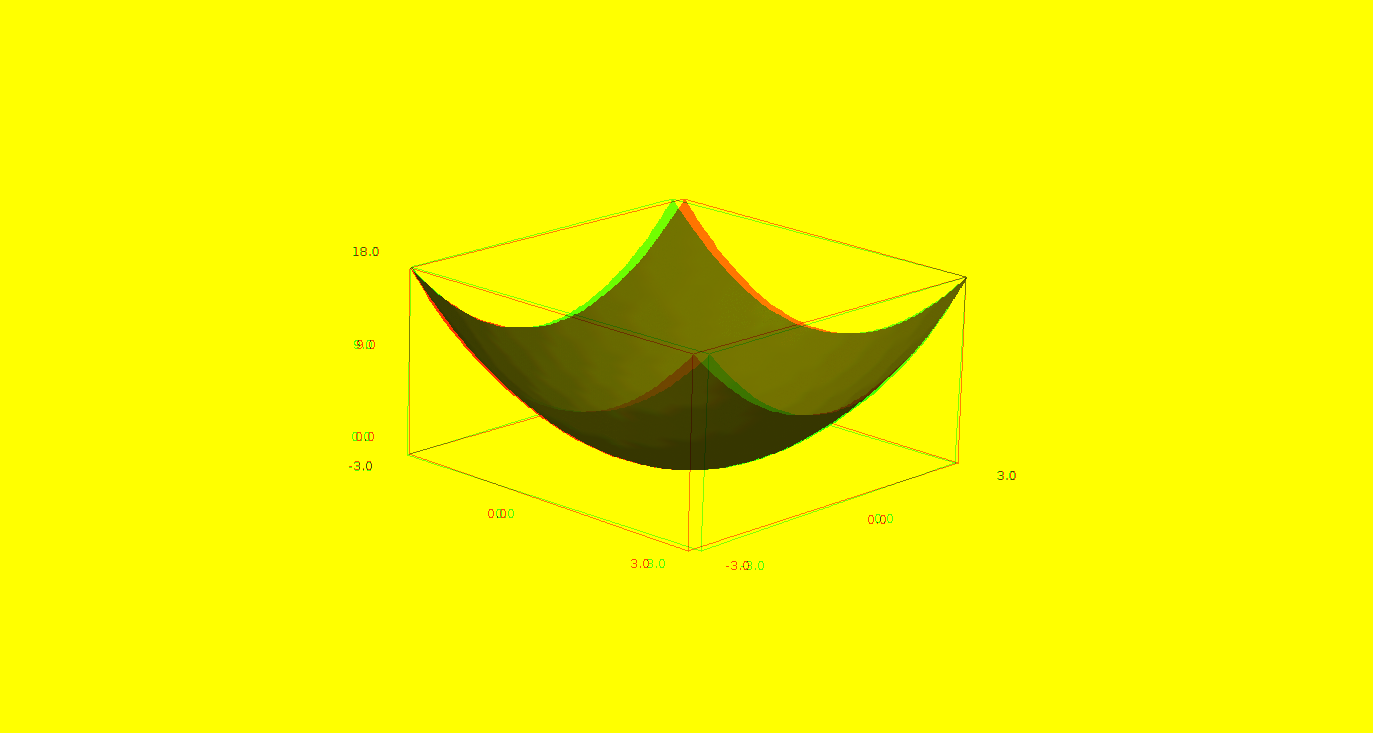
\includegraphics[width=15cm]{pictures_bitmap/coupe.png}
    \end{center}
    À part que l'ordinateur l'a dit, est-ce qu'on peut comprendre pourquoi le graphe de la fonction $x^2+y^2$ ressemble à un bol ? En coordonnées cylindriques, le graphe s'écrit
    \begin{equation}
        z=r^2.
    \end{equation}
    Donc il se fait que plus on s'éloigne du point $(0,0)$ dans le plan $XY$, plus le graphe va monter. Et il monte à quelle vitesse ? Il monte à la vitesse $r^2$. Il s'agit donc de dessiner la fonction $z=r^2$ dans le plan et de la «faire tourner».

\end{example}

%+++++++++++++++++++++++++++++++++++++++++++++++++++++++++++++++++++++++++++++++++++++++++++++++++++++++++++++++++++++++++++
\section{Courbes de niveau}
%+++++++++++++++++++++++++++++++++++++++++++++++++++++++++++++++++++++++++++++++++++++++++++++++++++++++++++++++++++++++++++

Une technique utile pour se faire une idée de la forme d'une fonction en trois dimensions est de tracer les \defe{courbes de niveau}{courbe de niveau}. La courbe de niveau de hauteur $h$ est la courbe dans le plan donnée par l'équation
\begin{equation}
    f(x,y)=h.
\end{equation}

\begin{example}

    Dessinons par exemple les courbes de niveau de la fonction
    \begin{equation}
        f(x,y)=x+y+2.
    \end{equation}
    La courbe de niveau $h$ est donnée par l'équation $x+y+2=h$, c'est à dire
    \begin{equation}
        y(x)=-x+h-2.
    \end{equation}
    Par conséquent la courbe de niveau de hauteur $0$ est $y=-x-2$, celle de hauteur $5$ est $y=-x+3$, etc.
    
    Nous pouvons également nous aider de Sage pour ce faire :
    \begin{verbatim}
----------------------------------------------------------------------
| Sage Version 4.6.1, Release Date: 2011-01-11                       |
| Type notebook() for the GUI, and license() for information.        |
----------------------------------------------------------------------
sage: f(x,y)=x+y+2
sage: var('h')                   
h
sage: niveau(h,x)=solve(f(x,y)==h,y)[0].rhs()
sage: g1(x)=niveau(1,x)
sage: g1
x |--> -x - 1
    \end{verbatim}
    Ici la fonction \verb+g1+ est la courbe de niveau $1$. 

    Si on veut faire tracer une courbe de niveau, Sage peut le faire :
    \begin{verbatim}
        sage: implicit_plot(f(x,y)==1,(x,-3,3),(y,-4,4))
    \end{verbatim}
    Cela tracera la courbe de niveau $h=1$ dans la partie du plan $x\in\mathopen[ -3 , 3 \mathclose]$ et $y\in\mathopen[ -4,4 ,  \mathclose]$.
    
\end{example}

Il est bien entendu possible de créer automatiquement $50$ courbes de niveau et de demander de les tracer toutes sur le même graphe.
\VerbatimInput[tabsize=3]{tex/outils_math/courbeNiveauOM.py}

Le résultat est :

\begin{center}
        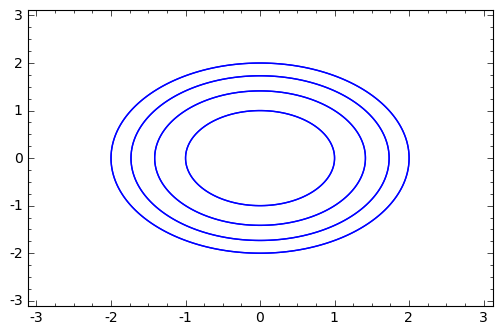
\includegraphics[width=8cm]{pictures_bitmap/niveauCercles.png}
\end{center}

\begin{example}
    Un exemple plus riche en enseignements est celui de la fonction
    \begin{equation}
        f(x,y)=x^2-y^2.
    \end{equation}
    La courbe de niveau $h$ est donnée par l'équation $x^2-y^2=h$.

    Commençons par $h=0$. Dans ce cas nous avons $(x+y)(x-y)=0$ et par conséquent les courbes de niveau de hauteur zéro sont les deux droites $x+y=0$ et $x-y=0$.

    Voyons ensuite la courbe de niveau $h=1$. Cela est l'équation $x^2-y^2=1$, c'est à dire
    \begin{equation}
        y(x)=\pm\sqrt{x^2-1}.
    \end{equation}
    C'est une fonction qui n'est définie que pour $| x |\geq 1$. Avec $x=1$ nous avons $y=1$. Ensuite, lorsque $x$ grandit, $y$ grandit également, mais la courbe ne peut pas croiser la courbe de niveau $h=0$. Donc, suivant les notations de la figure \ref{LabelFigNiveauHyperbole}, la courbe de niveau «part» de $P$ et doit monter sans croiser les diagonales.

    \newcommand{\CaptionFigNiveauHyperbole}{La courbe de niveau $h=1$ de $x^2-y^2$. Notez qu'elle est en deux morceaux.}
    \input{auto/pictures_tex/Fig_NiveauHyperbole.pstricks}

    En ce qui concerne la courbe de niveau $h=-1$, elle correspond à la courbe $y=\pm\sqrt{1+x^2}$ qui est définie pour tous les $x\in\eR$. Le même raisonnement que précédemment nous amène à la figure \ref{LabelFigNiveauHyperboleDeux}.
\newcommand{\CaptionFigNiveauHyperboleDeux}{La courbe de niveau $x^2-y^2=-1$.}
\input{auto/pictures_tex/Fig_NiveauHyperboleDeux.pstricks}


\end{example}

Une autre façon de voir les courbes de niveau est de dire que la courbe de niveau de hauteur $h$ est la projection dans le plan $XY$ de la section du graphe de $f$ par le plan $z=h$.

On peut également définir le graphe de fonctions de trois (ou plus) variables. Le graphe de la fonction $f\colon D\subset\eR^3\to \eR$ est l'ensemble
\begin{equation}
    \big\{ \big( x,y,z,f(x,y,z) \big)\tq (x,y,z)\in D \big\}\subset \eR^4.
\end{equation}
De tels graphes ne peuvent pas être représentés sur une feuille de papier. Il est toutefois possible de définir les ensembles de niveaux :
\begin{equation}
    E_h=\big\{ (x,y,z)\in D\tq  f(x,y,z)=h\big\}.
\end{equation}
Ce sont des surfaces dans $\eR^3$ que l'on peut dessiner.

\begin{example}
    Les surfaces de niveau de la fonction $f(x,y,z)=x^2+y^2+z^2$ sont des sphères. Il n'y a pas de surfaces de niveau pour les «hauteurs» négatives.
\end{example}

\begin{example}
    Considérons la fonction $f(x,y,z)=x^2+y^2-z^2$. En coordonnées cylindrique, cette fonction s'écrit
    \begin{equation}
        f(r,\theta,z)=r^2-z^2.
    \end{equation}
    La surface de niveau $0$ est donnée par l'équation $r=| z |$. Cela fait un cercle à chaque hauteur, dont le rayon grandit linéairement avec la hauteur; le tout est donc un cône. C'est d'ailleurs le cône obtenu par rotation de la courbe de niveau $h=0$ que nous avions obtenue pour la fonction $x^2-y^2$.

    En ce qui concerne les ensembles de niveau positifs, ils sont donnés par
    \begin{equation}
        z=\pm\sqrt{x^2+y^2-h}.
    \end{equation}
    Notez qu'ils ne sont pas définis pour $r\geq h$. Cela pose un petit problème quand on veut le tracer à l'ordinateur :
    \begin{verbatim}
----------------------------------------------------------------------
| Sage Version 4.6.1, Release Date: 2011-01-11                       |
| Type notebook() for the GUI, and license() for information.        |
----------------------------------------------------------------------
sage: var('x,y')
(x, y)
sage: f(x,y)=sqrt(x**2+y**2-3)
sage: F=plot3d(f(x,y),(x,-5,5),(y,-5,5)) 
sage: G=plot3d(-f(x,y),(x,-5,5),(y,-5,5))    
sage: F+G
    \end{verbatim}
Le résultat est\footnote{Encore une fois : ça donne mieux à l'écran, et vous pouvez le faire bouger; je vous encourage à le faire !} :
    \begin{center}
            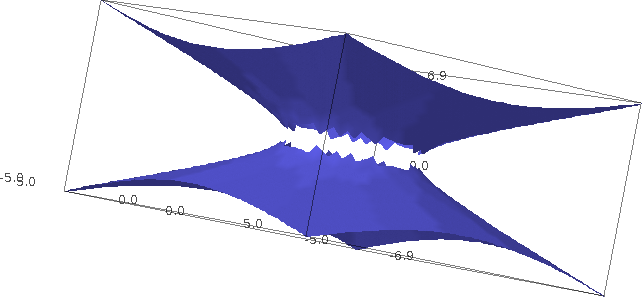
\includegraphics[width=15cm]{pictures_bitmap/AdSmauvais.png}
    \end{center}
    On voit qu'il y a un grand trou au centre correspondant aux $z$ proches de zéro. Or d'après l'équation, il n'en est rien : en $z=0$ il y a bel et bien tout un cercle. Afin d'obtenir une meilleur image, il faut demander de tracer avec un maillage plus fin :
    \begin{verbatim}
----------------------------------------------------------------------
| Sage Version 4.6.1, Release Date: 2011-01-11                       |
| Type notebook() for the GUI, and license() for information.        |
----------------------------------------------------------------------
sage: var('x,y')
(x, y)
sage: f(x,y)=sqrt(x**2+y**2-3)
sage: F=plot3d(f(x,y),(x,-5,5),(y,-5,5),plot_points=300) 
sage: G=plot3d(-f(x,y),(x,-5,5),(y,-5,5),plot_points=300)
sage: F+G
    \end{verbatim}
    Le temps de calcul est un peu plus long, mais le résultat est meilleur :
    \begin{center}
            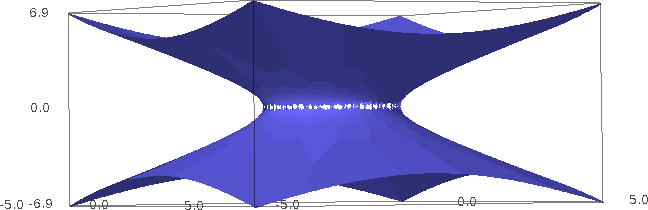
\includegraphics[width=15cm]{pictures_bitmap/AdSbon.png}
    \end{center}
\end{example}

%+++++++++++++++++++++++++++++++++++++++++++++++++++++++++++++++++++++++++++++++++++++++++++++++++++++++++++++++++++++++++++
\section{Dérivées partielles}
%+++++++++++++++++++++++++++++++++++++++++++++++++++++++++++++++++++++++++++++++++++++++++++++++++++++++++++++++++++++++++++

Soit $f\colon \eR^2\to \eR$ une fonction de deux variables et soit $(a,b)\in\eR^2$. La façon la plus naturelle de définir une dérivée à deux variables est de considérer les \defe{dérivées partielles}{dérivée!partielle} définies par
\begin{equation}
    \begin{aligned}[]
        \frac{ \partial f }{ \partial x }(a,b)&=\lim_{x\to a} \frac{ f(x,b)-f(a,b) }{ x-a }\\
        \frac{ \partial f }{ \partial y }(a,b)&=\lim_{y\to b} \frac{ f(a,y)-f(a,b) }{y-b}.
    \end{aligned}
\end{equation}
Ces nombres représentent la façon dont le nombre $f(x,y)$ varie lorsque soit seul $x$ varie soit seul $y$ varie. Les dérivées partielles se calculent de la même façon que les dérivées normales. Pour calculer $\partial_xf$, on fait «comme si» $y$ était une constante, et pour calculer $\partial_yf$, on fait comme si $x$ était une constante.

\begin{example}
    Considérons $f(x,y)=x^2y+y^2 e^{x}$. Les dérivées partielles sont
    \begin{equation}
        \begin{aligned}[]
            \frac{ \partial f }{ \partial x }&=2xy+y^2e^x\\
            \frac{ \partial f }{ \partial y }&=x^2+2ye^x.
        \end{aligned}
    \end{equation}
\end{example}

Cet exemple était l'exemple facile où tout se passe bien.

\begin{example}
    Les choses sont moins simples lorsqu'on considère la fonction suivante :
    \begin{equation}
        f(x,y)=\begin{cases}
            \frac{ xy }{ x^2+y^2 }    &   \text{si }(x,y)\neq(0,0)\\
            0    &    \text{si }(x,y)=(0,0).
        \end{cases}
    \end{equation}
    On voit que pour tout $x$ et tout $y$, nous avons $f(x,0)=f(0,y)=0$. Donc cette fonction est nulle sur les axes horizontaux et verticaux. Nous avons en particulier
    \begin{equation}
        \begin{aligned}[]
            \frac{ \partial f }{ \partial x }(0,0)&=0\\
            \frac{ \partial f }{ \partial y }(0,0)&=0.
        \end{aligned}
    \end{equation}
    Donc ces dérivées partielles existe.

    Il n'est par contre pas question de dire que cette fonction «va bien» autour du point $(0,0)$. En effet si nous regardons sa valeur sur la droite diagonale $y=x$, nous avons
    \begin{equation}
        f(x,x)=\frac{ x^2 }{ 2x^2 }=\frac{ 1 }{2}.
    \end{equation}
    Par conséquent si nous suivons la fonction le long de la droite $y=x$, la hauteur vaut $\frac{ 1 }{2}$ en permanence, sauf juste en $(0,0)$ où la fonction fait un grand plongeon !
    \begin{verbatim}
    sage: var('x,y')
    (x, y)
    sage: f(x,y)=(x*y)/(x**2+y**2)
    sage: plot3d(f,(x,-2,2),y(-2,2))
    \end{verbatim}

    D'ailleurs elle fait un plongeon le long de toutes les droites (sauf verticale et horizontale). En effet si nous regardons la fonction le long de la droite $y=mx$, nous avons
    \begin{equation}
        f(x,mx)=\frac{ mx^2 }{ x^2+m^2x^2 }=\frac{ m }{ 1+m^2 }.
    \end{equation}
    La fonction est donc \emph{constante} sur chacune de ces droites. Il n'est donc pas question de dire que cette fonction est «dérivable» en $(0,0)$, vu qu'elle fait des grands sauts dans presque toutes les directions.
\end{example}

Nous devons donc trouver mieux que les dérivées partielles pour étudier le comportement des fonctions un peu problématiques.

Nous nous souvenons de l'équation \eqref{EqCodeDerviffxamOM} qui nous dit que pour une fonction d'une variable la dérivabilité signifiait qu'il existait un nombre $\ell$ et une fonction $\alpha$ tels
\begin{equation}
    f(x)=f(a)+\ell(x-a)+(x-a)\alpha(x-a)
\end{equation}
et $\lim_{t\to 0} \alpha(t)=0$. 

En nous inspirant de cela, nous posons la définition suivante.
\begin{definition}      \label{DefDiffabelOM}
    Une fonction $f\colon \eR^2\to \eR$ est \defe{différentiable}{différentiable} au point $(a,b)\in\eR^2$ s'il existe deux nombres $\ell_1$, $\ell_2$ ainsi qu'une fonction $\alpha$ tels que
    \begin{equation}\label{EqCondDiffabelOM}
        \begin{aligned}[]
            f(x,y)=f(a,b)&+\ell_1(x-a)+\ell_2(y-b)\\
                    &+\sqrt{(x-a)^2+(y-b)^2}\alpha\big( \sqrt{(x-a)^2+(y-b)^2} \big).
        \end{aligned}
    \end{equation}
\end{definition}

En utilisant la notation vectorielle, cela peut être écrite sous forme très compacte. Posons
\begin{equation}
    \begin{aligned}[]
        \ell&=\begin{pmatrix}
            \ell_1    \\ 
            \ell_2    
        \end{pmatrix},&
        X&=\begin{pmatrix}
            x    \\ 
            y    
        \end{pmatrix},&
        P&=\begin{pmatrix}
            a    \\ 
            b    
        \end{pmatrix}.
    \end{aligned}
\end{equation}
Alors la condition \eqref{EqCondDiffabelOM} s'écrit
\begin{equation}
    f(X)=f(P)+\ell\cdot(X-P)+\| X-P \|\alpha\big( \| X-P \| \big).
\end{equation}

\begin{proposition}
    Si $f$ est différentiable en $(a,b)$, alors les nombres $\partial_xf(a,b)$ et $\partial_yf(a,b)$ existent et valent respectivement $\ell_1$ et $\ell_2$.
\end{proposition}

\begin{proof}
    Afin de calculer la dérivée partielle dans la direction de $x$, nous posons $y=b$ dans la condition \eqref{EqCondDiffabelOM} :
    \begin{equation}
        f(x,b)=f(a,b)+\ell_1(x-a)+| x-a |\alpha\big( | x-a | \big),
    \end{equation}
    et donc
    \begin{equation}
        \frac{ f(x,b)-f(a,b) }{ x-a }=\ell_1\pm\alpha\big( | x-a | \big).
    \end{equation}
    Ici le $\pm$ est parce que nous avons divisé $(x-a)$ par $| x-a |$. Quel que soit ce signe, de toutes façons la limite du membre de droite lorsque $x$ tend vers $a$ est $\ell_1$ parce que $\lim_{x\to a} \alpha(| x-a |)=0$.

    Afin de prouver l'existence de la dérivée dans la direction de $y$, nous procédons de la même manière, mais en partant de $f(a,y)$.
\end{proof}

\begin{proposition}
    Si $f$ est différentiable au point $(a,b)$, alors elle y est continue, c'est à dire que
    \begin{equation}
        \lim_{(x,y)\to(a,b)}f(x,y)=f(a,b).
    \end{equation}
\end{proposition}

\begin{proof}
    Si nous considérons la différence entre $f(x,y)$ et $f(a,b)$, nous avons (en notations matricielle) :
    \begin{equation}
        | f(X)-f(P) |=| \ell\cdot(X-P)+\| X-P \|\alpha(\| X-P \|) |.
    \end{equation}
    Le membre de droite tend évidemment vers zéro lorsque $X$ tend vers $P$.
\end{proof}
    \begin{remark}
        Attention : ceci n'est pas une preuve. En effet, dans la mesure où nous n'avons même pas donné de définition de la limite, il n'est pas possible de donner une \emph{vraie} preuve de quoi que ce soit. 
    \end{remark}

Nous avons vu que l'existence des deux dérivées partielles ne permettait pas de conclure à la différentiabilité. La différentiabilité d'une fonction peut néanmoins être déduites d'une étude plus précise des dérivées partielles. Nous avons pour cela les propositions \ref{PropExistDiffUnOM} et \ref{PropExistDiffDeuxOM}

\begin{proposition} \label{PropExistDiffUnOM}
    Soit $f$ une fonction de $x$ et $y$ et un point $(a,b)\in\eR^2$. Si les nombres $\partial_xf(a,b)$ et $\partial_yf(a,b)$ existent et s'il existe une fonction $\alpha\colon \eR\to \eR$ telle que
    \begin{equation}        \label{eqCritDifffabsrtOM}
        \begin{aligned}[]
            f(x,y)=f(a,b)&+\frac{ \partial f }{ \partial x }(a,b)(x-a)+\frac{ \partial f }{ \partial y }(a,b)(y-b)\\
            &+\| (x,y)-(a,b) \| \alpha\Big( \| (x,y)-(a,b) \| \Big)
        \end{aligned}
    \end{equation}
    et
    \begin{equation}
        \lim_{t\to 0} \alpha(t)=0,
    \end{equation}
    alors $f$ est différentiable en $(a,b)$.
\end{proposition}
Dans cet énoncé nous avons écrit $d\big( (x,y),(a,b) \big)$ la distance entre $(x,y)$ et $(a,b)$, c'est à dire le nombre $\sqrt{(x-a)^2+(y-b)^2}$. Afin d'écrire l'équation \eqref{eqCritDifffabsrtOM} sous forme plus compacte, nous introduisons le vecteur
\begin{equation}
    \nabla f(a,b)=\begin{pmatrix}
        \frac{ \partial f }{ \partial x }(a,b)    \\ 
        \frac{ \partial f }{ \partial y }(a,b).    
    \end{pmatrix}
\end{equation}
L'équation \eqref{eqCritDifffabsrtOM} devient alors
\begin{equation}        \label{EqdiffCompOM}
    f(X)=f(P)+\nabla f(a,b)\cdot (X-P)+\| X-P \|\alpha\big( \| X-P \| \big).
\end{equation}
Le vecteur $\nabla f(a,b)$ est appelé le \defe{gradient}{gradient} de $f$ au point $(a,b)$.


\begin{proposition} \label{PropExistDiffDeuxOM}
    Soit $f$ une fonction de deux variables admettant des dérivées partielles $\partial_xf(x,y)$ et $\partial_yf(x,y)$ qui sont elles-mêmes des fonctions continues de $x$ et $y$. Alors la fonction $f$ est différentiable partout.
\end{proposition}

\begin{remark}
    Tout ce qui a été dit, et tout ce qui sera dit, sur les fonctions a deux variables se généralise immédiatement aux fonctions à plus de variables. C'est dans ce but que la notation «compacte» utilisant les vecteurs est très pratique.
\end{remark}

Si nous remplaçons les accroissements $x-a$ et $y-b$ par $h$ et $k$, le critère de différentiabilité s'écrit
\begin{equation}
    \begin{aligned}[]
        f(a+h,b+k)=f(a,b)+\frac{ \partial f }{ \partial x }(a,b)h&+\frac{ \partial f }{ \partial y }(a,b)k\\
        &+\sqrt{h^2+k^2}\alpha\big( \sqrt{h^2+k^2} \big).
    \end{aligned}
\end{equation}
Le dernier terme du membre de droite tend vers zéro à une vitesse double lorsque $h$ et $k$ tendent vers zéro : d'une part parce que $\sqrt{h^2+k^2}$ tend vers zéro et d'autre part parce que $\alpha\big( \sqrt{h^2+k^2} \big)$ tend vers zéro. Nous avons donc la «bonne» approximation
\begin{equation}        \label{EqFormApproxfxyabOM}
    f(x,y)\simeq f(a,b)+\frac{ \partial f }{ \partial x }(a,b)(x-a)+\frac{ \partial f }{ \partial y }(a,b)(y-b).
\end{equation}
lorsque $(x,y)$ n'est pas trop loin de $(a,b)$. Cette expression est évidemment une généralisation immédiate de l'équation \eqref{EqfxdxSimeqfxfpxOM}. Elle exprime que l'on peut obtenir des informations sur la valeur d'une fonction en $(x,y)$ si on peut calculer la fonction et ses dérivées en un point $(a,b)$ non loin de $(x,y)$.

Cette formule peut aussi être vue sous la forme suivante, plus pratique dans certains calculs :
\begin{equation}        \label{EqFormApproxfxyabDFOM}
    f(a+\Delta x,b+\Delta y)\simeq f(a,b)+\Delta x\frac{ \partial f }{ \partial x }(a,b)+\Delta y\frac{ \partial f }{ \partial y }(a,b).
\end{equation}

\begin{example}
    Prenons la fonction $f(x,y)=\cos(x)\sin(y)$ et calculons une approximation de
    \begin{equation}
        f\big( \frac{ \pi }{ 3 }+0.01,\frac{ \pi }{ 2 }+0.03 \big).
    \end{equation}
    D'abord les dérivées partielles sont
    \begin{equation}
        \begin{aligned}[]
            \frac{ \partial f }{ \partial x }(x,y)=-\sin(x)\sin(y)\\
            \frac{ \partial f }{ \partial y }(x,y)=\cos(x)\cos(y).
        \end{aligned}
    \end{equation}
    Nous allons utiliser l'approximation
    \begin{equation}
        f\big( \frac{ \pi }{ 3 }+0.01,\frac{ \pi }{ 2 }+0.03 \big)\simeq f\big( \frac{ \pi }{ 3 },\frac{ \pi }{2} \big)+0.01\frac{ \partial f }{ \partial x }\big( \frac{ \pi }{ 3 },\frac{ \pi }{2} \big)+0.03\frac{ \partial f }{ \partial y }\big( \frac{ \pi }{ 3 },\frac{ \pi }{2} \big).
    \end{equation}
    Nous avons
    \begin{equation}
        \begin{aligned}[]
            \frac{ \partial f }{ \partial x }\big( \frac{ \pi }{ 3 },\frac{ \pi }{2} \big)&=-\sin\frac{ \pi }{ 3 }\sin\frac{ \pi }{ 2 }=-\frac{ \sqrt{3} }{2}\\
            \frac{ \partial f }{ \partial y }\big( \frac{ \pi }{ 3 },\frac{ \pi }{2} \big)&=\cos\frac{ \pi }{ 3 }\cos\frac{ \pi }{ 2 }=0.
        \end{aligned}
    \end{equation}
    Par conséquent
    \begin{equation}
        f\big( \frac{ \pi }{ 3 }+0.01,\frac{ \pi }{ 2 }+0.03 \big)\simeq \frac{ 1 }{2}-0.01\frac{ \sqrt{3} }{2}=\frac{ 1 }{2}-\frac{ \sqrt{3} }{ 200 }. 
    \end{equation}
    
    \begin{verbatim}
sage: var('x,y')
(x, y)
sage: f(x,y)=cos(x)*sin(y)
sage: a=f(pi/3+0.01,pi/2+0.03)
sage: numerical_approx(a)
0.491093815387986
sage: b=1/2-sqrt(3)/200
sage: numerical_approx(b)
0.491339745962156
sage: numerical_approx(a-b)
-0.000245930574169814
    \end{verbatim}
    Cela fait une erreur de l'ordre du dix millième. 
    
\end{example}

\begin{remark}
    Les esprits les plus critiques diront que cette vérification pas Sage n'en est pas une parce que Sage a certainement utilisé un algorithme d'approximation qui se base sur la même idée que ce que nous venons de faire, et que par conséquent le fait qu'il obtienne le même résultat que nous est un peu tautologique. 
    
    Ils n'auront pas tord. Cependant, le code source de Sage est disponible publiquement\footnote{Voir \url{http://www.sagemath.org}}; vous pouvez aller le lire et vérifier qu'il y a effectivement une \emph{preuve} que le résultat fourni par Sage possède une bonne dizaine de décimales correctes. 
    
    Cette disponibilité publique du code source est une des nombreuses différence fondamentale entre Sage et votre calculatrice\footnote{et les autres logiciels de type fenêtre, pomme ou feuille d'érable.}. Dois-je vous rappeler qu'un des principes fondamentaux de l'éthique scientifique est que les résultats et les méthodes utilisées doivent être absolument ouverts à la vérification et à la critique de tous ?
\end{remark}

%---------------------------------------------------------------------------------------------------------------------------
\subsection{Différentielle}
%---------------------------------------------------------------------------------------------------------------------------

\begin{definition}      \label{DefDiffrdrrOM}
    Lorsque $f$ est différentiable au point $(a,b)$, on appelle \defe{différentielle}{différentielle} de $f$ l'application linéaire
    \begin{equation}        \label{EqDefDiffmapdfOM}
        \begin{aligned}
            df_{(a,b)}\colon \eR^2&\to \eR \\
            \begin{pmatrix}
                u_1    \\ 
                u_2    
            \end{pmatrix}&\mapsto \frac{ \partial f }{ \partial x }(a,b)u_1+\frac{ \partial f }{ \partial y }(a,b)u_2. 
        \end{aligned}
    \end{equation}
    En notations compacte :
    \begin{equation}        \label{EqdfUPnableOM}
        df_{P}(U)=\nabla f(P)\cdot U.
    \end{equation}
\end{definition}

Note : dans la suite nous allons rendre notre «notation compacte» plus agréable à lire en abandonnant les majuscules. L'équation \eqref{EqdfUPnableOM} s'écrira donc
\begin{equation}        \label{EqdfpunfpduOM}
    df_p(u)=\nabla f(p)\cdot u.
\end{equation}


%+++++++++++++++++++++++++++++++++++++++++++++++++++++++++++++++++++++++++++++++++++++++++++++++++++++++++++++++++++++++++++
\section{Plan tangent au graphe d'une fonction}
%+++++++++++++++++++++++++++++++++++++++++++++++++++++++++++++++++++++++++++++++++++++++++++++++++++++++++++++++++++++++++++

Nous avons vu que, de la même façon qu'en deux dimensions nous avions l'approximation \eqref{EqfxsimesfaOM} d'une fonction par sa tangente, en trois dimensions nous avons l'approximation suivante d'une fonction de deux variables :
\begin{equation}
    f(x,y)\simeq f(a,b)+\frac{ \partial f }{ \partial x }(a,b)(x-a)+\frac{ \partial f }{ \partial y }(a,b)(y-b)
\end{equation}
lorsque $(x,y)$ n'est pas trop loin de $(a,b)$. Cela signifie que le graphe de $f$ ressemble au graphe de la fonction $T_{(a,b)}$ donnée par
\begin{equation}
    T_{(a,b)}(x,y)=f(a,b)+\frac{ \partial f }{ \partial x }(a,b)(x-a)+\frac{ \partial f }{ \partial y }(a,b)(x-a).
\end{equation}
En notations compactes :
\begin{equation}
    T_p(x)=f(p)+\nabla f(p)\cdot (x-p).
\end{equation}
Le graphe de la fonction $T_p$ sera le \defe{plan tangent}{plan!tangent} au graphe de $f$ au point $p$. L'équation du plan tangent sera donc
\begin{equation}
    z-f(p)=\nabla f(p)\cdot (x-p).
\end{equation}

\begin{remark}
    Lorsque nous utilisons la notation vectorielle, la lettre «$x$» désigne le vecteur $(x,y)$. Il faut être attentif. Dans un cas $x$ est un vecteur dans l'autre c'est une composante d'un vecteur.
\end{remark}




%+++++++++++++++++++++++++++++++++++++++++++++++++++++++++++++++++++++++++++++++++++++++++++++++++++++++++++++++++++++++++++
\section{Dérivée directionnelle}
%+++++++++++++++++++++++++++++++++++++++++++++++++++++++++++++++++++++++++++++++++++++++++++++++++++++++++++++++++++++++++++

Nous sommes capables de dériver une fonction de deux variables $f(x,y)$ par rapport à $x$ et par rapport à $y$. C'est à dire que nous sommes capables de donner la variation de la fonction lorsqu'on bouge le long des axes horizontal et vertical. Il est évidemment souhaitable de parler de la variation de la fonction lorsqu'on se déplace le long d'autre droites.

Soit donc $u=\begin{pmatrix}
    u_1    \\ 
    u_2    
\end{pmatrix}$ un vecteur unitaire (c'est à dire $u_1^2+u_2^2=1$), et considérons la fonction de une variable
\begin{equation}
    \begin{aligned}
        \varphi\colon \eR&\to \eR \\
        t&\mapsto f(a+tu_1,b+tu_2). 
    \end{aligned}
\end{equation}
La fonction $\varphi$ n'est rien d'autre que la fonction $f$ vue le long de la droite de direction donnée par le vecteur $u$. Nous pouvons aussi l'écrire $\varphi(t)=f(p+tu)$.

\begin{proposition}
    Si $f$ est différentiable en $(a,b)$ alors la fonction $\varphi$ est dérivable en $0$ et on a
    \begin{equation}
        \varphi'(0)=\nabla f(p)\cdot u
    \end{equation}
    où nous avons noté $p=(a,b)$.
\end{proposition}

\begin{proof}
    Récrivons la formule \eqref{EqdiffCompOM} sous la forme
    \begin{equation}
        f(x)=f(p)+\nabla f(p)\cdot (x-p)+\| x-p \|\alpha(\| x-p \|).
    \end{equation}
    Cela étant vrai pour tout $x$, nous l'écrivons en particulier pour $x=p+tu$ où $t$ est un réel et $u$ est le vecteur unitaire choisi. Nous avons donc
    \begin{equation}
        f(p+tu)=f(p)+t\nabla f(p)\cdot u+\| tu \|\alpha(\| tu \|).
    \end{equation}
    En utilisant le fait que $u$ est unitaire, $\| tu \|=| t |\| u \|=| t |$. La dérivée de $\varphi$ en $0$ est alors donnée par
    \begin{equation}
        \lim_{t\to 0} \frac{ f(p+tu)-f(p) }{ t }=\lim_{t\to 0} \nabla f(p)\cdot u+\alpha(| t |).    
    \end{equation}
    Lorsque nous prenons la limite, le membre de gauche devient $\varphi'(0)$ tandis que dans le membre de droite, le second terme disparaît. Nous avons finalement
    \begin{equation}
        \varphi'(0)=\nabla f(p)\cdot u
    \end{equation}
\end{proof}

\begin{definition}
    Le nombre
    \begin{equation}
        \lim_{t\to 0} \frac{ f\big( a+tu_1,b+tu_2 \big)-f(a,b) }{ t }
    \end{equation}
    est la \defe{dérivée directionnelle}{dérivée!directionnelle} de $f$ dans la direction de $u$ au point $(a,b)$. Il sera noté
    \begin{equation}
        \frac{ \partial f }{ \partial u }(a,b),
    \end{equation}
    ou plus simplement $\partial_uf(a,b)$.
\end{definition}

Lorsque $f$ est différentiable, la dérivée directionnelle est donnée par
\begin{equation}        \label{EqDerDirnablauOM}
    \frac{ \partial f }{ \partial u }(p)=\nabla f(p)\cdot u.
\end{equation}

En combinant avec l'équation \eqref{EqdfpunfpduOM}, nous avons la suite d'égalités
\begin{equation}        \label{EqsuitedfnfdsdfuOM}
    df_p(u)=\nabla f(p)\cdot u=\frac{ \partial f }{ \partial x }(p)u_1+\frac{ \partial f }{ \partial y }(p)u_2+\frac{ \partial f }{ \partial z }(p)u_3=\frac{ \partial f }{ \partial u }(p).
\end{equation}
La dernière équation est seulement vraie si $\| u \|=1$.

%---------------------------------------------------------------------------------------------------------------------------
\subsection{Gradient : direction de plus grande pente}
%---------------------------------------------------------------------------------------------------------------------------

Étant donné que $u$ est de norme $1$, l'inégalité de Cauchy-Schwarz donne
\begin{equation}
    \big| \nabla f(a,b)\cdot \begin{pmatrix}
        u_1    \\ 
        u_2    
    \end{pmatrix}\big|\leq \| \nabla f(a,b) \|.
\end{equation}
Donc
\begin{equation}
    -\| \nabla f(p) \|\leq \nabla f(p)\cdot u\leq\| \nabla f(p) \|.
\end{equation}
La norme de la dérivée directionnelle (qui est la valeur absolue du nombre au centre) est donc «coincée» entre $-\| \nabla f(p) \|$ et $\| \nabla f(p) \|$. Prenons par exemple
\begin{equation}
    u=\frac{ \nabla f(p) }{ \| \nabla f(p) \| }.
\end{equation}
Dans ce cas, nous avons exactement
\begin{equation}
    \nabla f(p)\cdot u=\| \nabla f(p) \|,
\end{equation}
qui est la valeur maximale que la dérivée directionnelle peut prendre.

La direction du gradient est donc la direction suivant laquelle la dérivée directionnelle est la plus grande. Pour la même raison, la dérivée directionnelle est la plus petite dans le sens opposé au gradient.

En termes bien clairs : lorsqu'on veut aller le plus vite possible au ski, on prend la direction du gradient de la piste de ski. C'est dans cette direction que ça descend le plus vite. Dans quelle direction vont les débutants ? Ils vont perpendiculairement à la pente (ce qui ennuie tout le monde, mais c'est un autre problème). Les débutants vont donc dans la direction perpendiculaire au gradient. Prenons donc $u\perp \nabla f(p)$ et calculons la dérivée directionnelle de $f$ dans la direction $u$ en utilisant la formule \ref{EqDerDirnablauOM} :
\begin{equation}
    \frac{ \partial f }{ \partial u }(p)=\nabla f(p)\cdot u=0
\end{equation}
parce que nous avons choisi $u\perp \nabla f(p)$. Nous voyons donc que les débutants en ski ont eu la bonne intuition que la direction dans laquelle la piste ne descend pas, c'est la direction perpendiculaire au gradient.

C'est aussi pour cela que l'on a tendance à faire du zig-zag à vélo lorsqu'on monte une pente très forte et qu'on est fatigué. C'est toujours pour cela que les routes de montagne font de longs lacets. La montée est moins rude en suivant une direction proche d'être perpendiculaire au gradient !

\begin{theorem}
    Le gradient des fonctions suit à peu près les mêmes règles que les dérivées. Soient $f$ et $g$ deux fonctions différentiables. Nous avons entre autres
    \begin{enumerate}
        \item
            $\nabla(f+g)=\nabla f+\nabla g$;
        \item
            $\nabla(fg)(a,b)=g(a,b)\nabla f(a,b)+f(a,b)\nabla g(a,b)$;
        \item
            Dès que $g(a,b)\neq 0$, nous avons
            \begin{equation}
                \nabla\frac{ f }{ g }=\frac{ g(a,b)\nabla f(a,b)-f(a,b)\nabla g(a,b) }{ g(a,b)^2 }.
            \end{equation}
    \end{enumerate}
\end{theorem}



\chapter{Champs de vecteurs}
% This is part of Mes notes de mathématique
% Copyright (c) 2011-2012,2015-2016
%   Laurent Claessens
% See the file fdl-1.3.txt for copying conditions.

Les champs de vecteurs et tout ce qui s'y rapportent jouent un rôle crucial en électromagnétisme. Voir par exemple \cite{Schomblond_em}.

%+++++++++++++++++++++++++++++++++++++++++++++++++++++++++++++++++++++++++++++++++++++++++++++++++++++++++++++++++++++++++++
\section{Les fonctions à valeurs vectorielles}
%+++++++++++++++++++++++++++++++++++++++++++++++++++++++++++++++++++++++++++++++++++++++++++++++++++++++++++++++++++++++++++

Jusqu'à présent nous avons vu des fonctions de plusieurs variables qui prenaient leurs valeurs dans $\eR$. Nous allons maintenant voir ce qu'il se passe lorsque les fonctions prennent leurs valeurs dans $\eR^3$.

Une fonction d'une variable est dite \defe{à valeurs vectorielles}{fonction!valeurs vectorielles} lorsque
\begin{equation}
    \begin{aligned}
        f\colon I\subset \eR&\to \eR^3 \\
        f(x)&=\begin{pmatrix}
            f_1(x)    \\ 
            f_2(x)    \\ 
            f_3(x)    
        \end{pmatrix}.
    \end{aligned}
\end{equation}
Les fonctions $f_i\colon \eR\to \eR$ sont les \defe{composantes}{composante} de $f$. Ce que nous avons raconté à propos des dérivées passe facilement :
\begin{equation}
    \frac{ f(a+\epsilon)-f(a) }{ \epsilon }=
    \begin{pmatrix}
        \frac{ f_1(a+\epsilon)-f_1(a) }{ \epsilon }    \\ 
        \frac{ f_2(a+\epsilon)-f_2(a) }{ \epsilon }    \\ 
        \frac{ f_3(a+\epsilon)-f_3(a) }{ \epsilon }    
    \end{pmatrix}.
\end{equation}
En particulier dès que les fonctions $f_i$ sont dérivables, nous avons
\begin{equation}
    f'(a)=\begin{pmatrix}
        f_1'(a)    \\ 
        f_2'(a)    \\ 
        f_3'(a)    
    \end{pmatrix}
\end{equation}
comme dérivée de la fonction. Cette dérivée est un vecteur.

\begin{example}
    Si
    \begin{equation}
        f\colon x\in\eR\mapsto \begin{pmatrix}
            x^2 e^{x}    \\ 
            \cos(x^2)    \\ 
            x^3+x    
        \end{pmatrix},
    \end{equation}
    alors
    \begin{equation}
        f'(x)=\begin{pmatrix}
            2xe^x+x^2e^x    \\ 
            -2x\sin(x^2)    \\ 
            3x^2+1    
        \end{pmatrix}.
    \end{equation}
\end{example}

%+++++++++++++++++++++++++++++++++++++++++++++++++++++++++++++++++++++++++++++++++++++++++++++++++++++++++++++++++++++++++++
\section{Fonctions vectorielles de plusieurs variables}
%+++++++++++++++++++++++++++++++++++++++++++++++++++++++++++++++++++++++++++++++++++++++++++++++++++++++++++++++++++++++++++

Ce sont les fonctions de la forme
\begin{equation}
    \begin{aligned}
        f\colon \eR^3&\to \eR^3 \\
        \begin{pmatrix}
            x    \\ 
            y    \\ 
            z    
        \end{pmatrix}&\mapsto \begin{pmatrix}
            f_1(x,y,z)\\
            f_2(x,y,z)\\
            f_3(x,y,z)
        \end{pmatrix}.
    \end{aligned}
\end{equation}

En ce qui concerne les dérivées, tout se passe comme avant. Si les dérivées partielles des composantes $f_i$ existent au point $a\in\eR^3$, alors
\begin{equation}
    \begin{aligned}[]
        \frac{ \partial f }{ \partial x }(a)&=\begin{pmatrix}
            \partial_xf_1(a)    \\ 
            \partial_xf_2(a)    \\ 
            \partial_xf_3(a)    \\ 
        \end{pmatrix},&
        \frac{ \partial f }{ \partial y }(a)&=\begin{pmatrix}
            \partial_yf_1(a)    \\ 
            \partial_yf_2(a)    \\ 
            \partial_yf_3(a)    \\ 
        \end{pmatrix},&
        \frac{ \partial f }{ \partial z }(a)&=\begin{pmatrix}
            \partial_zf_1(a)    \\ 
            \partial_zf_2(a)    \\ 
            \partial_zf_3(a)    \\ 
        \end{pmatrix}.
    \end{aligned}
\end{equation}

%+++++++++++++++++++++++++++++++++++++++++++++++++++++++++++++++++++++++++++++++++++++++++++++++++++++++++++++++++++++++++++
\section{Champs de vecteurs}
%+++++++++++++++++++++++++++++++++++++++++++++++++++++++++++++++++++++++++++++++++++++++++++++++++++++++++++++++++++++++++++

Un champ de vecteur est une fonction $f\colon \eR^3\to \eR^3$. Géométriquement, il s'agit simplement de mettre un vecteur en chaque point de l'espace. Cela arrive très souvent en physique.

\begin{example}
    Si un fluide (eau, gaz) coule dans un tube, en tout point le point a une vitesse, qui sera un vecteur généralement dirigé le long du tube.
\end{example}

\begin{example}
    La force d'attraction de la Terre sur une masse $m$ située au point $r=(x,y,z)$ est donnée par
    \begin{equation}
        F(r)=-G\frac{ Mmr }{ \| r \|^3 }.
    \end{equation}
    Dans cette expression, tant $r$ que $F(r)$ sont des vecteurs. Nous l'avons représenté sur la figure \ref{LabelFigChampGraviation}.
    \newcommand{\CaptionFigChampGraviation}{Le champ de gravitation de la Terre.}
    \input{auto/pictures_tex/Fig_ChampGraviation.pstricks}

    L'application
    \begin{equation}
        \begin{aligned}
            F\colon \eR^3&\to \eR^3 \\
            r&\mapsto F(r) 
        \end{aligned}
    \end{equation}
    est le champ gravitationnel de la Terre.
\end{example}

%---------------------------------------------------------------------------------------------------------------------------
\subsection{Matrice jacobienne}
%---------------------------------------------------------------------------------------------------------------------------

La \defe{matrice jacobienne}{jacobien} de la fonction $f\colon \eR^3\to \eR^3$ au point $a\in\eR^3$ est la matrice dont les colonnes sont les vecteurs $\frac{ \partial f }{ \partial x }(a)$, $\frac{ \partial f }{ \partial y }(a)$ et $\frac{ \partial f }{ \partial z }(a)$, c'est à dire
\begin{equation}
    J_f(a)=\begin{pmatrix}
        \frac{ \partial f_1 }{ \partial x }(a)   &   \frac{ \partial f_1 }{ \partial y }(a)    &   \frac{ \partial f_1 }{ \partial z }(a)    \\
        \frac{ \partial f_2 }{ \partial x }(a)   &   \frac{ \partial f_2 }{ \partial y }(a)    &   \frac{ \partial f_2 }{ \partial z }(a)    \\
        \frac{ \partial f_3 }{ \partial x }(a)   &   \frac{ \partial f_3 }{ \partial y }(a)    &   \frac{ \partial f_3 }{ \partial z }(a)    
    \end{pmatrix}.
\end{equation}

\begin{example}
    Si 
    \begin{equation}
        f(x,y,z)=\begin{pmatrix}
            xy e^{z}    \\ 
            x^2+\cos(yz)    \\ 
            xyz    
        \end{pmatrix},
    \end{equation}
    alors
    \begin{equation}
        J_f(x,y,z)=\begin{pmatrix}
            ye^z    &   xe^z    &   xye^z    \\
            2x    &   -z\sin(yz)    &   -y\sin(yz)    \\
            yz    &   xz    &   xy
        \end{pmatrix}.
    \end{equation}
\end{example}

%+++++++++++++++++++++++++++++++++++++++++++++++++++++++++++++++++++++++++++++++++++++++++++++++++++++++++++++++++++++++++++
\section{Courbes paramétrés}
%+++++++++++++++++++++++++++++++++++++++++++++++++++++++++++++++++++++++++++++++++++++++++++++++++++++++++++++++++++++++++++

%---------------------------------------------------------------------------------------------------------------------------
\subsection{Définitions et exemples}
%---------------------------------------------------------------------------------------------------------------------------

\begin{definition}
    Un \defe{chemin}{chemin} dans $\eR$ est une application continue
    \begin{equation}
        \begin{aligned}
            \sigma\colon [a,b]&\to \eR^3 \\
            t&\mapsto \sigma(t). 
        \end{aligned}
    \end{equation}
\end{definition}

La fonction $\sigma'(t)$ est la \defe{vitesse}{vitesse d'un chemin} du chemin $\sigma$. Si la fonction $t\mapsto\sigma(t)$ est dérivable, on dit que $\sigma''(t)$ est l'\defe{accélération}{accélération d'un chemin}. Les points $\sigma(a)$ et $\sigma(b)$ sont les extrémités du chemin. L'ensemble
\begin{equation}
    \{ \sigma(t)\tq t\in\mathopen[ a , b \mathclose] \}
\end{equation}
est la \defe{courbe}{courbe} $\sigma$.

\begin{example}
    Soit $v\in\eR^3$ et $x_0\in\eR^3$. Le chemin
    \begin{equation}
        \sigma(t)=x_0+tv
    \end{equation}
    est une droite. Sa vitesse est $\sigma'(t)=v$.    
\end{example}

\begin{example}
    La courbe
    \begin{equation}
        \sigma(t)=\begin{pmatrix}
            \cos(t)    \\ 
            \sin(t)    
        \end{pmatrix}\in\eR^2
    \end{equation}
    avec $t\in\mathopen[ 0 , 2\pi [$ est le cercle unité parcouru une fois dans le sens trigonométrique.

    Notez que si on prend $t\in\mathopen[ 0 , 4\pi [$, nous avons un \emph{autre} chemin; c'est le même cercle unité, mais parcouru \emph{deux} fois. Même si le «dessin» (le graphe) des deux est le même, le chemin n'est pas le même.

    Le chemin
    \begin{equation}
        \gamma(t)=\begin{pmatrix}
            \cos(2\pi-t)    \\ 
            \sin(2\pi-t)    
        \end{pmatrix}
    \end{equation}
    est le cercle unité parcouru une fois dans le sens inverse. Encore une fois le «dessin» est le même, mais le chemin n'est pas le même.
\end{example}

\begin{example}
    Le chemin
    \begin{equation}
        \sigma(t)=\begin{pmatrix}
            t    \\ 
            t^2    
        \end{pmatrix}
    \end{equation}
    est un chemin dont l'image est la parabole d'équation $y=x^2$.
\end{example}

L'importance de la dérivée du chemin réside en le fait qu'elle donne la tangente. En effet le vecteur $\sigma'(t)$ est tangent au graphe de $\sigma$ au point $\sigma(t)$.
\begin{example}
    Pour le cercle,
    \begin{equation}
        \sigma(t)=\begin{pmatrix}
            \cos(t)    \\ 
            \sin(t)    
        \end{pmatrix},
    \end{equation}
    la dérivée est donnée par
    \begin{equation}
        \sigma'(t)=\begin{pmatrix}
            -\sin(t)    \\ 
            \cos(t).    
        \end{pmatrix}
    \end{equation}
    Le produit scalaire $\sigma(t)\cdot \sigma'(t)$ est nul. Le vecteur $\sigma'(t)$ est donc bien tangent (voir exercice \ref{exoDerive-0003}).
\end{example}

\begin{example}
    Le courbe donnée par le chemin
    \begin{equation}
        \sigma(t)=\begin{pmatrix}
            \cos(t)    \\ 
            \sin(t)    \\ 
            t    
        \end{pmatrix}
    \end{equation}
    est une hélice. Sa vitesse est
    \begin{equation}
        \sigma'(t)=\begin{pmatrix}
            -\sin(t)    \\ 
            \cos(t)    \\ 
            1    
        \end{pmatrix}.
    \end{equation}
    Notez que pour tout $t\in\eR$, nous avons $\| \sigma'(t) \|=\sqrt{2}$.
\end{example}

\begin{remark}
    Lorsqu'on parle d'une courbe dans l'espace, l'intervalle sur lequel on considère la variation du paramètre est une donné fondamentale. Elle fait partie intégrante de la définition de la courbe.
\end{remark}

%---------------------------------------------------------------------------------------------------------------------------
\subsection{Longueur d'une courbe paramétrée}
%---------------------------------------------------------------------------------------------------------------------------

Nous pouvons voir un chemin $\sigma$ comme étant la trajectoire d'une particule en fonction du temps. Sa vitesse à l'instant $t$ est le vecteur $\sigma'(t)$, tandis que sa vitesse \emph{scalaire} est le nombre $\| \sigma'(t) \|$. Une question naturelle est de savoir quelle est la longueur de la trajectoire parcourue entre $t=a$ et $t=b$.

Si nous prenons un petit intervalle de temps $dt$, nous pouvons supposer que le mobile avance à la vitesse constante $\| \sigma'(t) \|$. Cela ferait un trajet parcouru de longueur $\| \sigma'(t) \|dt$. Nous prenons donc la définition suivante pour la longueur.

\begin{definition}
    Soit $\sigma\colon \mathopen[ a , b \mathclose]\to \eR^3$ un chemin. La \defe{longueur}{longueur!d'un chemin} du chemin $\sigma$ est le nombre
    \begin{equation}        \label{EqDefLongueurCheminOM}
        l(\sigma)=\int_a^b\| \sigma'(t) \|dt.
    \end{equation}
    Plus explicitement, si $\sigma(t)=\big( x(t),y(t),z(t) \big)$, alors nous avons la formule
    \begin{equation}
        l(\sigma)=\int_a^b\sqrt{x'(t)^2+y'(t)^2+z'(t)^2}dt.
    \end{equation}
\end{definition}

\begin{example}
    Considérons l'arc de cercle de rayon $R$ interceptée par l'angle $\theta$ présenté sur la figure \ref{LabelFigooIHLPooKLIxcH}.
    \newcommand{\CaptionFigooIHLPooKLIxcH}{Quelle est la longueur de la partie bleue de ce cercle de rayon $R$ ?}
    \input{auto/pictures_tex/Fig_ooIHLPooKLIxcH.pstricks}

    Par définition, cette longueur sera
    \begin{equation}
        \int_{\theta_0}^{\theta_1}\sqrt{R^2\sin^2(t)+R^2\cos^2(t)}dt=R(\theta_1-\theta_0).
    \end{equation}
    Le radian comme unité de mesure d'angle est donc l'unité parfaite : elle est la longueur d'arc interceptée (si le rayon est $R=1$).

\end{example}

\begin{example}
    La longueur de l'hélice
    \begin{equation}
        \sigma(t)=\begin{pmatrix}
            \cos(2t)    \\ 
            \sin(2t)    \\ 
            \sqrt{5}t    
        \end{pmatrix}
    \end{equation}
    pour $t\in\mathopen[ 0 , 2\pi \mathclose]$ est donnée par
    \begin{equation}
        l(\sigma)=\int_0^{4\pi}\sqrt{4\sin^2(2t)+4\cos^2(2t)+5}dt=\int_0^{4\pi}\sqrt{9}=12\pi.
    \end{equation}
\end{example}

\begin{definition}
    Soit $\sigma_1\colon \mathopen[ a , b \mathclose]\to \eR^3$, un chemin et $\sigma_2\colon \mathopen[ c , d \mathclose]\to \eR^3$, un autre chemin. On dit que ces chemins sont \defe{équivalents}{equivalence@équivalence!chemin} s'il existe une fonction $\varphi\colon \mathopen[ a , b \mathclose]\to \mathopen[ c , d \mathclose]$ strictement croissante telle que $\sigma_1(t)=\sigma_2\big( \varphi(t) \big)$.
\end{definition}

Deux chemins équivalents parcourent la même courbe dans le même sens. Ils ne le parcourent toutefois pas à la même vitesse. On dit que les chemins sont \defe{opposée}{opposés!chemins} si la fonction $\varphi$ de la définition est strictement décroissante. Dans ce cas, ils ont la même image, mais parcourue dans le sens opposés. Nous disons que deux chemins équivalents sont un \defe{changement de paramétrisation}{paramétrisation} pour la même courbe.

 Dans le cas d'une paramétrisation équivalente, nous avons $\varphi(a)=c$ et $\varphi(b)=d$. Les points de départ et d'arrivée des deux paramètres coïncident. Dans le cas d'un paramètre qui va dans le sens opposé par contre nous avons automatiquement $\varphi(a)=d$ et $\varphi(b)=c$.

\begin{proposition}
    La longueur d'une courbe ne dépend pas du paramètre (équivalent ou opposé) choisi.
\end{proposition}

\begin{proof}
    Soient $\sigma_1\colon \mathopen[ a , b \mathclose]\to \eR^3$ et $\sigma_2\colon \mathopen[ c , d \mathclose]\to \eR^3$ tels que
    \begin{equation}     \label{EqChmsigmaundeuxvpOM}
        \sigma_1(t)=\sigma_2\big( \varphi(t) \big)
    \end{equation}
    où $\varphi\colon \mathopen[ a , b \mathclose]\to \mathopen[ a , d \mathclose]$ est une bijection strictement monotone. Par définition on a
    \begin{equation}
        l(\sigma_1)=\int_a^b\| \sigma_1'(t) \|dt.
    \end{equation}
    Nous pouvons exprimer la dérivée de $\sigma_1$ en termes de celle de $\sigma_2$ en dérivant la relation \eqref{EqChmsigmaundeuxvpOM} :
    \begin{equation}
        \sigma_1'(t)=\varphi'(t)\sigma_2'\big( \varphi(t) \big).
    \end{equation}
    En ce qui concerne la norme,
    \begin{equation}
        \| \sigma_1'(t) \|=| \varphi'(t) |\| \sigma_2'(t) \|.
    \end{equation}
    Notez dans cette relation que $\varphi'(t)$ est un nombre (et non un vecteur). Étant donné que nous avons supposé que $\varphi$ était monotone, soit elle est monotone croissante et $\| \varphi'(t) \|=\varphi'(t)$ pour tout $t$, soit elle est monotone décroissante et $\| \varphi'(t) \|='\varphi(t)$ pour tout $t$.

    Considérons d'abord le premier cas, c'est à dire $\| \varphi'(t) \|=\varphi'(t)$. Nous posons $s=\varphi(t)$, $ds=\varphi'(t)dt$. En remplaçant cela dans la formule de la longueur est
    \begin{equation}
        \begin{aligned}[]
            l(\sigma_1)&=\int_a^b\varphi'(t)\| \sigma_2\big( \varphi(t) \big) \|dt\\
            &=\int_{\varphi(a)}^{\varphi(b)}\| \sigma_2'(s) \|ds\\
            &=\int_c^d\| \sigma_2'(s) \|ds\\
            &=l(\sigma_2).
        \end{aligned}
    \end{equation}
    
    Si nous considérons maintenant une paramétrisation strictement décroissante. Dans ce cas, $\varphi'(t)\leq 0$ et $\| \varphi'(t) \|=-\varphi'(t)$. Nous posons encore une fois $s=\varphi(t)$, $ds=\varphi'(t)ds$. Ici il ne faut pas oublier que $\varphi(a)=d$ et $\varphi(b)=c$. Le calcul est à part cela le même en faisant attention au singe :
    \begin{equation}
        \begin{aligned}[]
            l(\sigma_1)&=\int_a^b\varphi'(t)\| \sigma_2\big( \varphi(t) \big) \|dt\\
            &=-\int_{\varphi(a)}^{\varphi(b)}\| \sigma_2'(s) \|ds\\
            &=-\int_d^c\| \sigma_2'(s) \|ds\\
            &=\int_c^d\| \sigma_2'(s) \|ds\\
            &=l(\sigma_2).
        \end{aligned}
    \end{equation}
    Nous avons changé le signe en changeant l'ordre des bornes.
\end{proof}

%+++++++++++++++++++++++++++++++++++++++++++++++++++++++++++++++++++++++++++++++++++++++++++++++++++++++++++++++++++++++++++
\section{Intégrales le long de chemins}
%+++++++++++++++++++++++++++++++++++++++++++++++++++++++++++++++++++++++++++++++++++++++++++++++++++++++++++++++++++++++++++

%---------------------------------------------------------------------------------------------------------------------------
\subsection{Circulation d'un champ de vecteur}
%---------------------------------------------------------------------------------------------------------------------------

\begin{definition}
    Soit $F\colon \eR^3\to \eR^3$ un champ de vecteurs et un chemin $\sigma\colon \mathopen[ a , b \mathclose]\to \eR^3$. On appelle \defe{circulation}{circulation} de $F$ le long du chemin $\sigma$ le scalaire
    \begin{equation}        \label{EqDeffvkZwhOM}
        \int_a^b F\big( \sigma(t) \big)\cdot \sigma'(t)dt.
    \end{equation}
    Il existe de nombreuses notations pour cela; entre autres :
    \begin{equation}
        \int_{\sigma}F=\int_{\sigma} F\cdot ds.
    \end{equation}
\end{definition}

En physique, la circulation de la force le long d'un chemin est la travail de la force.

\begin{example}
    À la surface de la Terre, le champ de gravitation est donné par
    \begin{equation}
        G(x,y,z)=-mg\begin{pmatrix}
            0    \\ 
            0    \\ 
            1    
        \end{pmatrix}.
    \end{equation}
    Si nous considérons un mobile qui monte à vitesse constante jusqu'à la hauteur $h$, c'est à dire le chemin
    \begin{equation}
        \sigma(t)=\begin{pmatrix}
            0    \\ 
            0    \\ 
            t    
        \end{pmatrix}
    \end{equation}
    avec $t\in\mathopen[ 0 , h \mathclose]$. Le travail de la gravitation est alors donné par
    \begin{equation}
        W=\int_0^hG\big( \sigma(t) \big)\cdot\begin{pmatrix}
            0    \\ 
            0    \\ 
            1    
        \end{pmatrix}=
        -mg\int_0^h\begin{pmatrix}
            0    \\ 
            0    \\ 
            1    
        \end{pmatrix}\cdot\begin{pmatrix}
            0    \\ 
            0    \\ 
            1    
        \end{pmatrix}=-mgh.
    \end{equation}
    Cela est bien le résultat usuel de l'énergie potentielle. Nous allons voir bientôt que nous nommons la fonction $mgh$ énergie \emph{potentielle} précisément parce que la force dérive de ce potentiel.
\end{example}

\begin{example}
    Soit le chemin
    \begin{equation}
        \begin{aligned}
            \sigma\colon \mathopen[ 0 , 2\pi \mathclose]&\to \eR^3 \\
            t&\mapsto \begin{pmatrix}
                \sin(t)    \\ 
                \cos(t)    \\ 
                t    
            \end{pmatrix}.
        \end{aligned}
    \end{equation}
    et le champ de vecteurs
    \begin{equation}
        F\begin{pmatrix}
            x    \\ 
            y    \\ 
            z    
        \end{pmatrix}=\begin{pmatrix}
            x    \\ 
            y    \\ 
            z    
        \end{pmatrix}.
    \end{equation}
    La circulation de ce champ de vecteur le long de l'hélice $\sigma$ est
    \begin{equation}
        \begin{aligned}[]
            \int_{\sigma}F\cdot ds&=\int_0^{2\pi}(F\circ \sigma)(t)\cdot \sigma'(t)dt\\
            &=\int_0^{2\pi}\begin{pmatrix}
                \sin(t)    \\ 
                \cos(t)    \\ 
                t    
            \end{pmatrix}\cdot
            \begin{pmatrix}
                \cos(t)    \\ 
                \sin(t)    \\ 
                1    
            \end{pmatrix}dt\\
            &=\int_0^{2\pi}tdt\\
            &=\left[ \frac{ t^2 }{2} \right]_0^{2\pi}\\
            &=2\pi^2.
        \end{aligned}
    \end{equation}
    
\end{example}

\begin{proposition}
    La circulation d'un champ de vecteurs le long d'un chemin ne dépend pas de la paramétrisation. En d'autres termes, si $\sigma_1$ et $\sigma_2$ sont deux chemins équivalents, alors
    \begin{equation}
        \int_{\sigma_1}F=\int_{\sigma_2}F.
    \end{equation}
\end{proposition}

\begin{proof}
    Soient deux chemins $\sigma_1\colon \mathopen[ a , b \mathclose]\to \eR^3$ et $\sigma_2\colon \mathopen[ c , d \mathclose]\to \eR^3$ équivalents, c'est à dire tels que
    \begin{equation}
        \sigma_1(t)=\sigma_2\big( \varphi(t) \big)
    \end{equation}
    où $\varphi\colon \mathopen[ a , b \mathclose]\to \mathopen[ c , d \mathclose]$ strictement croissante. En utilisant le fait que $\sigma_1(t)=\varphi'(t)\sigma_2'\big( \varphi(t) \big)$, nous avons
    \begin{equation}
        \begin{aligned}[]
            \int_{\sigma_1}F\cdot ds&=\int_a^bF\big( \sigma_1(t) \big)\cdot\sigma_1'(t)dt\\
            &=\int_a^bF\Big( \sigma_2\big( \varphi(t) \big) \Big)\cdot\sigma_2'\big( \varphi(t) \big)\varphi'(t)dt\\
            &=\int_{\varphi(a)}^{\varphi(b)}F\big( \sigma_2(s) \big)\cdot\sigma_2(s)ds\\
            &=\int_c^dF\big( \sigma_2(s) \big)\cdot \sigma_2'(s)ds\\
            &=\int_{\sigma_2}F\cdot ds.
        \end{aligned}
    \end{equation}
    où nous avons effectué le changement de variables $s=\varphi(t)$, $ds=\varphi'(t)dt$.
\end{proof}

\begin{remark}
    Si $\sigma_2$ est le chemin opposé de $\sigma$, alors
    \begin{equation}
        \int_{\sigma_2}F=-\int_{\sigma_1}F.
    \end{equation}
\end{remark}

%+++++++++++++++++++++++++++++++++++++++++++++++++++++++++++++++++++++++++++++++++++++++++++++++++++++++++++++++++++++++++++
\section{Circulation d'un champ conservatif}
%+++++++++++++++++++++++++++++++++++++++++++++++++++++++++++++++++++++++++++++++++++++++++++++++++++++++++++++++++++++++++++

Si nous avons une fonction scalaire $V\colon \eR^3\to \eR$, nous pouvons construire un champ de vecteur en prenant le gradient :
\begin{equation}
    F(x)=\nabla V(x).
\end{equation}
On dit que le champ de vecteur $F$ \defe{dérive}{champ dérivant d'un potentiel} de $V$, et on dit que $V$ est le \defe{potentiel}{potentiel} de $F$. Nous posons la définition suivante :
\begin{definition}
    Un champ de vecteurs $F\colon \eR^3\to \eR^3$ est un champ \defe{conservatif}{champ!conservatif} s'il existe une fonction $V\colon \eR^3\to \eR$ telle que
    \begin{equation}
        F(x)=\nabla V(x).
    \end{equation}
    Nous disons aussi parfois que le champ $V$ \emph{dérive d'un potentiel} ou bien qu'il s'agit d'un \emph{champ de gradient}.
\end{definition}

Les champs de vecteurs conservatifs sont particulièrement importants parce que presque toutes les forces connues en physiques dérivent d'un potentiel. Nous verrons que la terminologie «conservatif» provient du fait que les forces de ce type conservent l'énergie associée.


\begin{proposition}
    Considérons une fonction $V\colon \eR^3\to \eR$ (que nous appellerons \emph{potentiel}) et le champ de vecteur qui en dérive :
    \begin{equation}
        F=\nabla V.
    \end{equation}
    Alors 
    \begin{equation}
        \int_{\sigma}F\cdot ds=V\big( \sigma(b) \big)-V\big( \sigma(a) \big).
    \end{equation}
    Autrement dit, le travail nécessaires pour déplacer un objet d'un point à un autre dans un champ de force conservatif vaut la différence de potentiel entre le point de départ et le point d'arrivée.
\end{proposition}

\begin{proof}
    Par définition,
    \begin{equation}        \label{EqintparddeftravOM}
        \int_{\sigma} F\cdot ds=\int_a^b F\big( \sigma(t) \big)\cdot \sigma'(t)dt.
    \end{equation}
    Nous pouvons transformer l'intégrante de la façon suivante :
    \begin{equation}
        \begin{aligned}[]
            F\big( \sigma(t) \big)\cdot\sigma'(t)&=\nabla V\big( \sigma(t) \big)\cdot\sigma'(t)\\
            &=\frac{ \partial V }{ \partial x }\big( \sigma(t) \big)\sigma_x'(t) +\frac{ \partial V }{ \partial y }\big( \sigma(t) \big)\sigma_y'(t) +\frac{ \partial V }{ \partial z }\big( \sigma(t) \big)\sigma_z'(t)\\
            &=\frac{ d }{ dt }\Big[ V\big( \sigma(t) \big) \Big]
        \end{aligned}
    \end{equation}
    où nous avons posé
    \begin{equation}
        \sigma(t)=\begin{pmatrix}
            \sigma_x(t)    \\ 
            \sigma_y(t)    \\ 
            \sigma_z(t)    
        \end{pmatrix}
    \end{equation}
    et utilisé à l'envers la formule de dérivation de fonction composée pour
    \begin{equation}
             \frac{ d }{ dt }\Big[ V\big( \sigma(t) \big) \Big]=\Big( (V\circ\sigma)(t) \Big)'.
    \end{equation}
    En remettant ces expressions dans l'intégrale \eqref{EqintparddeftravOM},
    \begin{equation}
        \int_{\sigma}F\cdot ds=\int_a^b\frac{ d }{ dt }\Big[ V\big( \sigma(t) \big) \Big]dt=V\big( \sigma(b) \big)-V\big( \sigma(a) \big).
    \end{equation}
\end{proof}

\begin{example}
    Nous savons que le champ de gravitation dérive d'un potentiel. À la surface de la Terre, le potentiel de gravitation vu par une masse $m$ est donné par la fonction $V(x,y,z)=mgz$. Si nous voulons soulever cette masse d'une hauteur $h$, cela demandera toujours une énergie $mgh$, quel que soit le chemin suivit : en ligne droite vertical, en diagonal, en hélice, \ldots
\end{example}

\begin{example}
    À plus grande échelle, le champ de gravitation est encore un champ qui dérive d'un potentiel. En coordonnées sphériques,
    \begin{equation}
        V(\rho,\theta,\varphi)=k\frac{ m }{ \rho }
    \end{equation}
    Lorsqu'un satellite a une orbite de rayon $R$ autour la Terre, il reste sur la sphère $\rho=R$. Donc il reste sur une surface sur laquelle $V$ est constante. Il n'y a donc pas de travail de la force de gravitation ! C'est pour cela qu'un satellite peut tourner pendant des siècles sans apport énergétique.
\end{example}

\begin{example}
    Soit le champ de vecteurs
    \begin{equation}
        F\begin{pmatrix}
            x    \\ 
            y    
        \end{pmatrix}=\begin{pmatrix}
            y    \\ 
            x    
        \end{pmatrix}
    \end{equation}
    et le chemin
    \begin{equation}
        \sigma(t)=\begin{pmatrix}
            t^4/4    \\ 
            \sin^3(t\frac{ \pi }{2}).    
        \end{pmatrix}
    \end{equation}
    Nous voulons calculer la circulation de $F$ le long du chemin $\sigma$ entre $t=0$ et $t=1$.

    La première chose à voir est que $F=\nabla V$ avec $V(x,y)=xy$. Donc la circulation sera donnée par
    \begin{equation}
        \int_{\sigma}F\cdot ds=V\big( \sigma(1) \big)-V\big( \sigma(0) \big)=V\big( \frac{1}{ 4 },1 \big)-V(0,0)=\frac{1}{ 4 }-0=\frac{1}{ 4 }.
    \end{equation}
    Nous n'avons pas réellement calculé l'intégrale.
\end{example}

%+++++++++++++++++++++++++++++++++++++++++++++++++++++++++++++++++++++++++++++++++++++++++++++++++++++++++++++++++++++++++++
\section{Divergence, rotationnel et l'opérateur nabla}
%+++++++++++++++++++++++++++++++++++++++++++++++++++++++++++++++++++++++++++++++++++++++++++++++++++++++++++++++++++++++++++

Nous avons déjà vu le gradient d'une fonction $f\colon \eR^3\to \eR$
\begin{equation}        \label{EqDefNablafOM}
    \nabla f(x,y,z)=\begin{pmatrix}
        \partial_xf(x,y,z)    \\ 
        \partial_yf(x,y,z)    \\ 
        \partial_zf(x,y,z)    
    \end{pmatrix}
\end{equation}
Afin de définir la divergence et le rotationnel, nous introduisons $\nabla$ sous une forme un peu plus abstraite comme le «vecteur»
\begin{equation}
    \nabla=\begin{pmatrix}
        \partial_x    \\ 
        \partial_y    \\ 
        \partial_z
    \end{pmatrix}.
\end{equation}
Vue comme ça, la formule \eqref{EqDefNablafOM} est claire.

Si $F$ est un champ de vecteurs, nous introduisons la \defe{divergence}{divergence} de $F$ par
\begin{equation}
    \nabla\cdot F=\frac{ \partial F_x }{ \partial x }+\frac{ \partial F_y }{ \partial y }+\frac{ \partial F_z }{ \partial z }.
\end{equation}
Cela est une fonction. Et nous introduisons le rotationnel du champ de vecteur $F$ par
\begin{equation}
    \begin{aligned}[]
        \nabla\times F&=\begin{vmatrix}
              e_x  &   e_y    &   e_z    \\
            \partial_x    &   \partial_y    &   \partial_z    \\
            F_x    &   F_y    &   F_z
        \end{vmatrix}\\
        &=
        \left( \frac{ \partial F_z }{ \partial y }-\frac{ \partial F_y }{ \partial z } \right)e_x
        -\left( \frac{ \partial F_z }{ \partial x }-\frac{ \partial F_x }{ \partial z } \right)e_y
        +\left( \frac{ \partial F_y }{ \partial x }-\frac{ \partial F_x }{ \partial y } \right)e_z.
    \end{aligned}
\end{equation}
Cela est un champ de vecteur. Conformément à la formule \eqref{EqProdVectEspilonijkOM}, le rotationnel d'un champ de vecteur peut s'écrire
\begin{equation}
    \nabla\times F=\sum_{ijk}\partial_i F_j 1_k.
\end{equation}

Le gradient, la divergence et le rotationnel consistent à appliquer simplement à $\nabla$ est trois produits qu'on peut effectuer sur un vecteur:
\begin{enumerate}
    \item
        Le produit d'un vecteur par un scalaire multiplie chacune des composantes :
        \begin{equation}
            \begin{pmatrix}
                \partial_x    \\ 
                \partial_y    \\ 
                \partial_z    
            \end{pmatrix}f
            =\begin{pmatrix}
                \partial_xf    \\ 
                \partial_yf    \\ 
                \partial_zf    
            \end{pmatrix}.
        \end{equation}
    \item
        Le produit scalaire d'un vecteur avec un autre vecteur donne lieu à la divergence :
        \begin{equation}
            \begin{pmatrix}
                \partial_x    \\ 
                \partial_y    \\ 
                \partial_z    
            \end{pmatrix}\cdot
            \begin{pmatrix}
                F_x    \\ 
                F_y    \\ 
                F_z    
            \end{pmatrix}=
            \frac{ \partial F_x }{ \partial x }+\frac{ \partial F_y }{ \partial y }+\frac{ \partial F_z }{ \partial z }.
        \end{equation}
    \item
        Le produit vectoriel de deux vecteurs :
        \begin{equation}
            \begin{pmatrix}
                \partial_x    \\ 
                \partial_y    \\ 
                \partial_z    
            \end{pmatrix}\times\begin{pmatrix}
                F_x    \\ 
                F_y    \\ 
                F_z    
            \end{pmatrix}=
            \begin{vmatrix}
                e_x    &   e_y    &   e_z    \\
                \partial_x    &   \partial_y    &   \partial_z    \\
                F_x    &   F_y    &   F_z
            \end{vmatrix}.
        \end{equation}
\end{enumerate}
Ces trois opérations joueront un rôle central en électromagnétisme dans les équations de Maxwell.

\begin{example}
    Soit $F(x,y,z)=x e_x+xy e_y+e_z$, c'est à dire
    \begin{equation}
        F(x,y,z)=\begin{pmatrix}
            x    \\ 
            xy    \\ 
            1    
        \end{pmatrix}.
    \end{equation}
    Son rotationnel est donné par
    \begin{equation}
        \nabla\times F=\begin{vmatrix}
            e_x    &   e_y    &   e_z    \\
            \frac{ \partial  }{ \partial x }    &   \frac{ \partial  }{ \partial y }    &   \frac{ \partial  }{ \partial y }    \\
            x    &   xy    &   1
        \end{vmatrix}=
        (0-0)e_x-(0-0)e_y+(y-0)e_z=ye_z=\begin{pmatrix}
            0    \\ 
            0    \\ 
            y    
        \end{pmatrix}.
    \end{equation}
\end{example}

Afin d'étudier comment se comporte la composition de ces opérateurs, nous aurons besoin de ce lemme que nous n'énoncerons pas précisément.
\begin{lemma}       \label{LemPermDerrxyzOM}
    Si $f\colon \eR^3\to \eR$ est une fonction de classe $C^2$, alors on peut permuter l'ordre des dérivées:
    \begin{equation}
        \begin{aligned}[]
            \frac{ \partial  }{ \partial x }\left( \frac{ \partial f }{ \partial y } \right)&=\frac{ \partial  }{ \partial y }\left( \frac{ \partial f }{ \partial x } \right)\\
            \frac{ \partial  }{ \partial x }\left( \frac{ \partial f }{ \partial z } \right)&=\frac{ \partial  }{ \partial z }\left( \frac{ \partial f }{ \partial x } \right)\\
            \frac{ \partial  }{ \partial z }\left( \frac{ \partial f }{ \partial y } \right)&=\frac{ \partial  }{ \partial y }\left( \frac{ \partial f }{ \partial z } \right)
        \end{aligned}
    \end{equation}
\end{lemma}
La fonction
\begin{equation}
    (x,y,z)\mapsto\frac{ \partial  }{ \partial x }\left( \frac{ \partial f }{ \partial y } \right)(x,y,z)
\end{equation}
sera notée
\begin{equation}
    \frac{ \partial^2f }{ \partial x\partial y }.
\end{equation}

Il y a deux propriétés importantes :
\begin{theorem}
    Soit $f\colon \eR^3\to \eR$ une fonction de classe $C^2$. Alors
    \begin{equation}
        \nabla\times(\nabla f)=0.
    \end{equation}
    Si $F\colon \eR^3\to \eR^3$ est un champ de vecteurs de classe $C^2$, alors
    \begin{equation}
        \nabla\cdot(\nabla\times F)=0.
    \end{equation}
\end{theorem}

\begin{proof}
    Ce sont seulement deux calculs qui manipulent les définitions. Pour le premier, la divergence de $f$ est le champ de vecteurs
    \begin{equation}
        \nabla f=\frac{ \partial f }{ \partial x }e_x+\frac{ \partial f }{ \partial y }e_y+\frac{ \partial f }{ \partial z }e_z.
    \end{equation}
    En mettant ce champ dans la définition du rotationnel,
    \begin{equation}
        \begin{aligned}[]
            \nabla\times(\nabla f)=\begin{vmatrix}
                 e_x   &   e_y    &   e_z    \\
                 \frac{ \partial  }{ \partial x }    &   \frac{ \partial  }{ \partial y }    &   \frac{ \partial  }{ \partial z }    \\
                 \frac{ \partial f }{ \partial x }    &   \frac{ \partial f }{ \partial y }    &   \frac{ \partial f }{ \partial z }
            \end{vmatrix}
            &=\left[ \frac{ \partial  }{ \partial y }\left( \frac{ \partial f }{ \partial z } \right)-\frac{ \partial  }{ \partial z }\left( \frac{ \partial f }{ \partial y } \right) \right]e_x\\
            &\quad-\left[ \frac{ \partial  }{ \partial x }\left( \frac{ \partial f }{ \partial z } \right)-\frac{ \partial  }{ \partial z }\left( \frac{ \partial f }{ \partial x } \right) \right]e_y\\
            &\quad+\left[ \frac{ \partial  }{ \partial x }\left( \frac{ \partial f }{ \partial y } \right)-\frac{ \partial  }{ \partial y }\left( \frac{ \partial f }{ \partial x } \right) \right]e_z.
        \end{aligned}
    \end{equation}
    En utilisant le lemme \ref{LemPermDerrxyzOM}, chacun des termes fait zéro.

    La seconde propriété se démontre en utilisant le même type de calcul.
\end{proof}

\begin{remark}
    Il n'y a pas de propriétés du même style pour la combinaison $\nabla\times(\nabla\cdot F)$ pour le rotationnel de la divergence. En effet la divergence d'un champ de vecteur est une fonction, et il n'y a pas de rotationnel pour une fonction.
\end{remark}

\begin{center}
            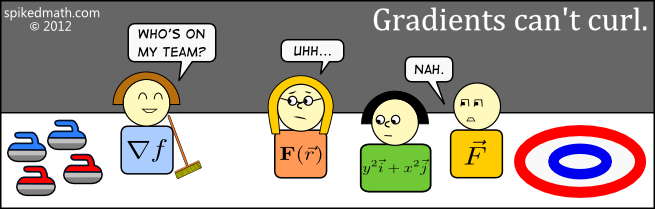
\includegraphics[width=10cm]{pictures_bitmap/501-curling-with-gradients.png}
        {\tiny De \href{http://spikedmath.com/501.html}{Spiked math}, publié sous \href{http://creativecommons.org/licenses/by-nc-sa/2.5/ca/}{licence Creative Commons}.}
\end{center}


%+++++++++++++++++++++++++++++++++++++++++++++++++++++++++++++++++++++++++++++++++++++++++++++++++++++++++++++++++++++++++++
\section[Interprétation de la divergence]{Interprétation géométrique et physique de la divergence}
%+++++++++++++++++++++++++++++++++++++++++++++++++++++++++++++++++++++++++++++++++++++++++++++++++++++++++++++++++++++++++++


En physique, on dit qu'un champ de vecteurs à divergence nulle est \defe{incompressible}{incompressible!champ de vecteur}. Nous allons essayer de comprendre pourquoi. Lorsqu'un fluide incompressible se déplace, il faut qu'en chaque point il y autant de fluide qui rentre que de fluide qui sort. Nous allons voir sur quelques exemples que la divergence d'un champ de vecteurs est le «bilan de masse» d'un fluide qui se déplace selon le champ de vecteurs.

Si en un point la divergence est positive, cela signifie qu'il y a une perte de masse et si la divergence est négative, cela signifie qu'il y a une accumulation de masse.

Prenons par exemple un fluide qui se déplace selon le champ de vitesse montré à figure \ref{LabelFigTKXZooLwXzjS}.
\newcommand{\CaptionFigTKXZooLwXzjS}{Le champ de vecteurs $F(x,y)=\frac{1}{ x }(1,0)$.}
\input{auto/pictures_tex/Fig_TKXZooLwXzjS.pstricks}

Étant donné que la vitesse diminue lorsque $x$ avance, il y a une accumulation de fluide. Regardez en effet la quantité de fluide qui rentre dans le rectangle par rapport à la quantité de fluide qui en sort. Ce champ de vecteurs a pour équation :
\begin{equation}
    F(x,y)=\frac{1}{ x }\begin{pmatrix}
        1    \\ 
        0    
    \end{pmatrix}=\begin{pmatrix}
        1/x    \\ 
        0    
    \end{pmatrix}.
\end{equation}
Sa divergence vaut donc
\begin{equation}
    (\nabla\cdot F)(x,y)=\frac{ \partial F_x }{ \partial x }(x,y)+\underbrace{\frac{ \partial F_y }{ \partial y }(x,y)}_{=0}=-\frac{1}{ x^2 }.
\end{equation}
Cette divergence étant négative, il y a bien accumulation de fluide en tout point, et d'autant plus que $x$ est petit.

\begin{example}     \label{ExamDivFrotOM}

    Prenons le champ de vecteurs tournant
    \begin{equation}
        F(x,y)=\frac{1}{ \sqrt{x^2+y^2} }\begin{pmatrix}
            y    \\ 
            -x    
        \end{pmatrix}
    \end{equation}
    représenté à la figure \ref{LabelFigDivergenceDeux}. Cela est un vecteur qui est constamment perpendiculaire au rayon.

    \newcommand{\CaptionFigDivergenceDeux}{Le champ de vecteurs $F(x,y)=(y,-x)$.}
    \input{auto/pictures_tex/Fig_DivergenceDeux.pstricks}

    Un fluide dont la vitesse serait donné par ce champ de vecteur se contente de tourner. Intuitivement il ne devrait pas y avoir de divergence parce qu'il n'y a aucune accumulation de fluide. En effet,
    \begin{equation}
        \nabla\cdot F(x,y)=\frac{ -2xy }{ (x^2+y^2)^2 }+\frac{ 2xy }{ (x^2+y^2)^2 }=0.
    \end{equation}
\end{example}

\begin{example}
    Prenons le cas du champ de force de gravitation :
    \begin{equation}
        F(x,y,z)=\frac{1}{ (x^2+y^2+z^2)^{3/2} }\begin{pmatrix}
            x    \\ 
            y   \\
            z
        \end{pmatrix}.
    \end{equation}
    Nous pouvons rapidement remarquer que $\nabla\cdot F=0$. Est-ce que cela peut se comprendre sur le dessin de la figure \ref{LabelFigDivergenceTrois} ?
    \newcommand{\CaptionFigDivergenceTrois}{Le champ de vecteur de la gravité. Nous avons tracé, sur les deux cercles la même densité de vecteurs, c'est à dire le même nombre de vecteurs par unité de surface.}
    \input{auto/pictures_tex/Fig_DivergenceTrois.pstricks}

    Essayons de voir combien de fluide entre dans la zone bleue et combien en sort. D'abord, il est certain que les vecteurs qui sortent sont plus courts que ceux qui rentrent, ce qui voudrait dire qu'il y a plus de fluide qui rentre. Mais on voit également que le \emph{nombre} de vecteurs qui sortent est plus grand parce que la seconde sphère est plus grande et qu'il y a un vecteur en chaque point de la sphère.

    Intuitivement nous pouvons dire que la quantité qui rentre dans la sphère de rayon $r_1$ donnée par la taille des vecteurs entrants multiplié par la surface de la sphère, c'est à dire
    \begin{equation}        \label{EqQpinormeVectoOM}
        4\pi r_1^2\| F(x,y,z) \|,
    \end{equation}
    mais $\| F(x,y,z) \|=\frac{1}{ r_1^2 }$, donc la quantité de fluide entrant est $4\pi$. La quantité de fluide sortant sera la même.

    Cela explique deux choses
    \begin{enumerate}
        \item
            Pourquoi les forces de gravitation et électromagnétiques sont en $1/r^2$; c'est parce que nous vivons dans un monde avec trois dimensions d'espace. En étudiant très précisément le champ de gravitation, certains physiciens espèrent trouver des déviations expérimentales par rapport à la règle du \( 1/r^2\); cela \emph{pourrait} être un signe que l'espace contient des dimensions supplémentaires.
        \item
            Pourquoi il y a un $4\pi$ comme coefficient dans beaucoup d'équations en électromagnétisme; en particulier dans certaines anciennes unités de flux.
    \end{enumerate}
    
\end{example}

\begin{remark}
    Nous allons voir plus loin comment s'assurer que l'équation \eqref{EqQpinormeVectoOM} représente bien la «quantité de fluide» qui rentre dans la zone délimitée
\end{remark}


%+++++++++++++++++++++++++++++++++++++++++++++++++++++++++++++++++++++++++++++++++++++++++++++++++++++++++++++++++++++++++++
\section{Quelques formules de Leibnitz}
%+++++++++++++++++++++++++++++++++++++++++++++++++++++++++++++++++++++++++++++++++++++++++++++++++++++++++++++++++++++++++++

La divergence étant une combinaison de dérivées, il n'est pas tellement étonnant que la divergence de produits donne lieux à des formules en deux termes. Si $f$ est une fonction et si $F$ et $G$ sont des champs de vecteurs, nous avons (sans démonstrations) :
\begin{equation}        \label{EqLeinDivNablRotOM}
    \begin{aligned}[]
        \nabla\cdot(fF)&=f\nabla\cdot F+F\cdot\nabla f\\
        \nabla\cdot(F\times G)&=G\cdot\nabla\times F-F\cdot\nabla\times G.
    \end{aligned}
\end{equation}
Nous avons aussi, pour le rotationnel,
\begin{equation}        \label{EqLeinRotfFFOM}
    \nabla\times(fF)=f\nabla\times F+\nabla f\times F.
\end{equation}


\chapter{Coordonnées curvilignes orthogonales}
% This is part of Mes notes de mathématique
% Copyright (c) 2011-2012,2015
%   Laurent Claessens
% See the file fdl-1.3.txt for copying conditions.

%+++++++++++++++++++++++++++++++++++++++++++++++++++++++++++++++++++++++++++++++++++++++++++++++++++++++++++++++++++++++++++
\section{La différentielle revisitée}
%+++++++++++++++++++++++++++++++++++++++++++++++++++++++++++++++++++++++++++++++++++++++++++++++++++++++++++++++++++++++++++

%---------------------------------------------------------------------------------------------------------------------------
\subsection{Les formes différentielles de base}
%---------------------------------------------------------------------------------------------------------------------------

Si la fonction $f\colon \eR^n\to \eR$ est différentiable alors la différentielle en $a\in\eR^n$ est l'application
\begin{equation}        \label{EqFormDiffdfahOM}
    \begin{aligned}
        df_a\colon \eR^n&\to \eR \\
        u&\mapsto \frac{ \partial f }{ \partial x_1 }(a)u_1+\cdots+\frac{ \partial f }{ \partial x_n }(a)u_n.
    \end{aligned}
\end{equation}
Considérons en particulier la fonction qui à $x\in\eR^n$ fait correspondre $x_i\in\eR$. Par abus de notations,  nous la noterons $x_i$. Nous avons 
\begin{equation}
    \frac{ \partial x_i }{ \partial x_j }=\delta_{ij}.
\end{equation}
Par exemple $\partial_yx=0$ et $\partial_xx=1$. Toutes les dérivées partielles de $x_i$ s'annulent sauf la $i$ème qui vaut $1$. Par conséquent
\begin{equation}
    \begin{aligned}
        dx_i\colon \eR^n&\to \eR \\
        u&\mapsto u_i. 
    \end{aligned}
\end{equation}

\begin{remark}
    En toute rigueur nous devrions écrire $(dx_i)_a$. Mais étant donné que
    \begin{equation}
        (dx_i)_a(u)=(dx_i)_b(u)
    \end{equation}
    pour tout points $a$, $b$ et pour tout vecteurs $u$, nous nous permettons de simplifier la notation en ne précisant pas en quel point nous calculons la différentielle de $x_i$.
\end{remark}

Étant donné que $dx_i(u)=u_i$, nous pouvons récrire la formule \eqref{EqFormDiffdfahOM} en remplaçant $u_i$ par $dx_i(u)$ :
\begin{equation}
    df_a(u)=\frac{ \partial f }{ \partial x_1 }(a)dx_1(u)+\cdots+\frac{ \partial f }{ \partial x_n }(a)dx_n(u).
\end{equation}
En tant que application linéaire, $df_a$ est une combinaison linéaire des $dx_i$. En notations compacte :
\begin{equation}
    df_a=\sum_{i=1}^n\frac{ \partial f }{ \partial x_i }(a)dx_i.
\end{equation}

%---------------------------------------------------------------------------------------------------------------------------
\subsection{Différentielles de fonctions composées}
%---------------------------------------------------------------------------------------------------------------------------

Cette façon de voir la différentielle nous permet de jeter un nouveau regard sur la formule de différentiation des fonctions composées. Soient
\begin{equation}
    \begin{aligned}[]
        f\colon \eR^p&\to \eR^n\\
        g\colon \eR^n&\to \eR,
    \end{aligned}
\end{equation}
et $h\colon \eR^p\to \eR$ définie par 
\begin{equation}
    h(u)=h\big( f(u) \big)=(g\circ f)(u).
\end{equation}
Nous allons noter $x$ les coordonnées de $\eR^p$, $a$ un point de $\eR^p$ et $u$, un vecteur de $\eR^p$ accroché au point $a$. Pour $\eR^n$, les notations seront que les coordonnées sont $y$, $b$ est un point de $\eR^n$ et $v$ est un vecteur «accroché» au point $b$.

Nous avons
\begin{equation}
    dg_b(v)=\sum_{i=1}^n\frac{ \partial g }{ \partial y_i }(b)dy_i(v).
\end{equation}
Ici $dy_i(v)$ signifie la $i$ème composante de $v$. C'est simplement $v_i$. Cette formule étant valable pour tout point $b\in\eR^n$ et pour tout vecteur $v$, nous pouvons l'écrire en particulier pour
\begin{subequations}
    \begin{numcases}{}
        b=f(a)\\
        v=df_a(u).
    \end{numcases}
\end{subequations}
Cela donne
\begin{equation}        \label{EqdgfadfauOM}
    dg_{f(a)}\big( df_a(u) \big)=\sum_{i=1}^n\frac{ \partial g }{ \partial y_i }\big( f(a) \big)dy_i\big( df_a(u) \big).
\end{equation}
Mais 
\begin{equation}
    df_a(u)=\sum_{j=1}^p\frac{ \partial f }{ \partial x_j }(a)dx_j(u),
\end{equation}
donc la $i$ème composante de ce vecteur est
\begin{equation}
     \big( df_a(u)\big)_i=\sum_{j=1}^p\frac{ \partial f_i }{ \partial x_j }(a)dx_j(u).
\end{equation}
En remplaçant $dy_i\big( df_a(u) \big)$ par cela dans l'expression \eqref{EqdgfadfauOM}, nous trouvons
\begin{equation}
    dg_{f(a)}\big( df_a(u) \big)=\sum_{i=1}^n\frac{ \partial g }{ \partial y_i }\big( f(a) \big)\sum_{j=1}^p\frac{ \partial f_i }{ \partial x_j }(a)dx_j(u).
\end{equation}
Nous pouvons vérifier que cela est la différentielle de $g\circ f$ au point $a$ appliquée au vecteur $u$. En effet
\begin{equation}
    d(g\circ f)_a(u)=\sum_{j=1}^p\frac{ \partial (g\circ f) }{ \partial x_j }(a)dx_j(u),
\end{equation}
tandis que, par la dérivation de fonctions composées, 
\begin{equation}        \label{EqDerCompofgOM}
    \frac{ \partial (g\circ f) }{ \partial x_j }(a)=\sum_{i=1}^n\frac{ \partial g }{ \partial y_i }\big( f(a) \big)\frac{ \partial f_i }{ \partial x_j }(a).
\end{equation}
Au final, ce que nous avons prouvé est que
\begin{equation}
    d(g\circ f)_a(u)=dg_{f(a)}\big( df_a(u) \big).
\end{equation}

%---------------------------------------------------------------------------------------------------------------------------
\subsection{Passage aux coordonnées polaires}
%---------------------------------------------------------------------------------------------------------------------------

Le changement de coordonnées pour les polaires est la fonction
\begin{equation}
    f\begin{pmatrix}
        r    \\ 
        \theta    
    \end{pmatrix}=\begin{pmatrix}
        x    \\ 
        y    
    \end{pmatrix}=\begin{pmatrix}
        r\cos\theta    \\ 
        r\sin\theta    
    \end{pmatrix}.
\end{equation}
Considérons une fonction $g$ sur $\eR^2$, et définissons la fonction $\tilde g$ par
\begin{equation}
    \tilde g(r,\theta)=g(r\cos\theta,r\sin\theta).
\end{equation}
La formule \eqref{EqDerCompofgOM} permet de trouver les dérivées partielles de $g$ par rapport à $r$ et $\theta$ en termes de celles par rapport à $x$ et $y$ de $g$.

Pour faire le lien avec les notations du point précédent, nous avons
\begin{equation}
    \begin{aligned}[]
        f_1(r,\theta)&=r\cos(\theta)\\
        f_2(r,\theta)&=r\sin(\theta)\\
        (x_1,x_2)&\to(r,\theta)\\
        (y_1,y_2)&\to(x,y).
    \end{aligned}
\end{equation}
Nous avons donc 
\begin{equation}
    \begin{aligned}[]
        \frac{ \partial \tilde g }{ \partial r }(r,\theta)&=\sum_{i=1}^2\frac{ \partial g }{ \partial x_i }\big( f(r,\theta) \big)\frac{ \partial f_i }{ \partial r }(r,\theta)\\
        &=\frac{ \partial g }{ \partial x }(r\cos\theta,r\sin\theta)\frac{ \partial \big( r\cos\theta \big) }{ \partial r }(r,\theta)\\
        &\quad+\frac{ \partial g }{ \partial y }(r\cos\theta,r\sin\theta)\frac{ \partial \big( r\sin\theta\big) }{ \partial r }(r,\theta)\\
        &=\cos\theta\frac{ \partial g }{ \partial x }(r\cos\theta,r\sin\theta)+\sin\theta\frac{ \partial g }{ \partial y }(r\cos\theta,r\sin\theta).
    \end{aligned}
\end{equation}

Prenons par exemple $g(x,y)=\frac{1}{ x^2+y^2 }$. Étant donné que
\begin{equation}
    \frac{ \partial g }{ \partial x }=\frac{ -2x }{ (x^2+y^2)^2 },
\end{equation}
nous avons
\begin{equation}
    \frac{ \partial g }{ \partial x }(r\cos\theta,r\sin\theta)=\frac{ -2\cos\theta }{ r^3 }.
\end{equation}
En utilisant la formule,
\begin{equation}
    \frac{ \partial \tilde g }{ \partial r }(r,\theta)=\cos(\theta)\left( \frac{ -2\cos\theta }{ r^3 } \right)+\sin(\theta)\left( \frac{ -2\sin\theta }{ r^3 } \right)=-\frac{ 2 }{ r^3 }.
\end{equation}
Nous pouvons vérifier directement que cela est correct. En effet
\begin{equation}
    \tilde g(r,\theta)=g(r\cos\theta,r\sin\theta)=\frac{1}{ r^2 },
\end{equation}
dont la dérivée par rapport à $r$ vaut $-2/r^3$.

En ce qui concerne la dérivée par rapport à $\theta$, nous avons
\begin{equation}
    \begin{aligned}[]
    \frac{ \partial \tilde g }{ \partial \theta }&=\frac{ \partial g }{ \partial x }(r\cos\theta,r\sin\theta)\frac{ \partial \big( r\cos(\theta) \big) }{ \partial \theta }+\frac{ \partial g }{ \partial y }(r\cos\theta,r\sin\theta)\frac{ \partial \big( r\sin(\theta) \big) }{ \partial \theta }\\
    &=\left( \frac{ -2\cos\theta }{ r^3 } \right)(-r\sin\theta)+\left( \frac{ -2\sin\theta }{ r^3 } \right)(r\cos\theta)\\
    &=0.
    \end{aligned}
\end{equation}

En résumé et avec quelques abus de notations :
\begin{equation}
    \begin{aligned}[]
        \frac{ \partial \tilde g }{ \partial r }&=\cos(\theta)\frac{ \partial g }{ \partial x }+\sin(\theta)\frac{ \partial g }{ \partial y }\\
        \frac{ \partial \tilde g }{ \partial \theta }&=-r\sin(\theta)\frac{ \partial g }{ \partial x }+r\cos(\theta)\frac{ \partial g }{ \partial y }\\
    \end{aligned}
\end{equation}

%+++++++++++++++++++++++++++++++++++++++++++++++++++++++++++++++++++++++++++++++++++++++++++++++++++++++++++++++++++++++++++
\section{Théorie générale}
%+++++++++++++++++++++++++++++++++++++++++++++++++++++++++++++++++++++++++++++++++++++++++++++++++++++++++++++++++++++++++++

%---------------------------------------------------------------------------------------------------------------------------
\subsection{Base locale}
%---------------------------------------------------------------------------------------------------------------------------

Les coordonnées sphériques et cylindriques sont deux systèmes de coordonnées «un peu courbe» qui existent sur $\eR^3$. Il en existe de nombreux autres, que nous appelons \defe{coordonnées curvilignes}{coordonnées!curvilignes}. Des coordonnées curvilignes sur $\eR^3$ est n'importe quel\footnote{Nous n'entrons pas dans les détails de régularité.} système qui permet de repérer un point de $\eR^3$ à partir de trois nombres.

Il s'agit donc d'un ensemble de trois applications 
\begin{equation}
    x_i\colon \eR^3\to \eR.
\end{equation}
Les coordonnées cylindriques sont
\begin{subequations}
    \begin{numcases}{}
        x_1(r,\theta,z)=r\cos\theta\\
        x_2(r,\theta,z)=r\sin\theta\\
        x_3(r,\theta,z)=z
    \end{numcases}
\end{subequations}

Soit donc un système général $q=(q_1,q_2,q_3)$ et 
\begin{equation}
    M(q)=\begin{pmatrix}
        x_1(q)    \\ 
        x_2(q)    \\ 
        x_3(q)    
    \end{pmatrix}.
\end{equation}
Si nous fixons $q_2$ et $q_3$ et que nous laissons varier $q_1$, nous obtenons une courbe\footnote{Dans le cas des sphériques, c'est une demi-droite horizontale d'angle $q_2$ et de hauteur $q_3$.} dont nous pouvons considérer le vecteur vitesse, c'est à dire le vecteur tangent. En chaque point nous avons ainsi trois vecteurs
\begin{equation}
    \frac{ \partial M }{ \partial q_i }(q).
\end{equation}
Nous disons que le système de coordonnées curviligne est \defe{orthogonal}{orthogonal!coordonnées curviligne} si ces trois vecteurs sont orthogonaux. Dans la suite nous supposerons que c'est toujours le cas.

Nous posons
\begin{equation}
    h_i=\left\| \frac{ \partial M }{ \partial q_i } \right\|
\end{equation}
et nous considérons les trois vecteurs normés
\begin{equation}        \label{EqDefeihMqOM}
    e_i=h_i^{-1}\frac{ \partial M }{ \partial q_i }.
\end{equation}
Les trois vecteurs $\{ e_1,e_2,e_3 \}$ forment une base orthonormée dite \defe{base locale}{base!locale}. Ce sont des vecteurs liés\footnote{En géométrie différentielle on dira que ce sont des élément de l'espace tangent, mais c'est une toute autre histoire.} au point $M$.

%---------------------------------------------------------------------------------------------------------------------------
\subsection{Importance de l'orthogonalité}
%---------------------------------------------------------------------------------------------------------------------------

Nous avons dit que nous nous restreignons au cas où les vecteurs $e_i$ sont orthogonaux. En termes de produits scalaires, cela signifie
\begin{equation}
    e_i\cdot e_j=\delta_{ij}.
\end{equation}
Nous en étudions maintenant quelque conséquence. L'équation \eqref{EqDefeihMqOM} peut s'écrire plus explicitement sous la forme
\begin{equation}
    e_i=\sum_k h_i^{-1}\frac{ \partial x_k }{ \partial q_i }1_k.
\end{equation}
Notez que pour chaque $k$ et $i$, la quantité $h_i^{-1}\frac{ \partial x_k }{ \partial q_i }$ est un simple nombre. Nous allons les mettre dans une matrice :
\begin{equation}
    A_{ki}=h_i^{-1}\frac{ \partial x_k }{ \partial q_i }.
\end{equation}
Cela nous donne le changement de base
\begin{equation}        \label{EqChmBaseeisAkiAkOM}
    e_i=\sum_kA_{ki}1_k.
\end{equation}
Le produit $e_i\cdot e_j$ s'écrit alors
\begin{equation}
    \begin{aligned}[]
        e_i\cdot e_j&=\sum_{kl}A_{ki}A_{lj}\underbrace{1_k\cdot 1_l}_{=\delta_{kl}}\\
        &=\sum_{kl}A_{ki}A_{lj}\delta_{kl}\\
        &=\sum_kA_{ki}A_{kj}\\
        &=\sum_k(A^T)_{ik}A_{kj}.
    \end{aligned}
\end{equation}
Or cela doit valoir $\delta_{ij}$. Par conséquent 
\begin{equation}
    A^T=A^{-1}.
\end{equation}
Le fait que les coordonnées curvilignes considérées soient orthogonales s'exprime donc par la fait que la matrice de changement de base est une matrice orthogonale.

Cette circonstance nous permet d'inverser le changement de base \eqref{EqChmBaseeisAkiAkOM} en multipliant cette équation par $(A^{-1})_{il}$ des deux côtés et en faisant la somme sur $i$ :
\begin{equation}
    \sum_i (A^{-1})_{il}e_i=\sum_{kl}\underbrace{A_{ki}(A^{-1})_{il}}_{=\delta_{kl}}1_k,
\end{equation}
par conséquent
\begin{equation}
    \sum_i(A^T)_{il}e_i=1_l,    
\end{equation}
et
\begin{equation}        \label{EqChamvarunlAeiOM}
    1_l=\sum_iA_{li}e_i=\sum_ih_i^{-1}\frac{ \partial x_l }{ \partial q_i }e_i.
\end{equation}
Armés de cette importante formule, nous pouvons exprimer les quantités que nous connaissons dans la base canonique en termes de la base locale.

Une autre conséquence du fait que $e_1$, $e_2$ et $e_3$ est une base orthonormée est que, éventuellement en réordonnant les vecteurs, on a
\begin{equation}
    \begin{aligned}[]
        e_1\times e_2&=e_3\\
        e_2\times e_3&=e_1\\
        e_3\times e_1&=e_2
    \end{aligned}
\end{equation}
Ces trois relations s'écrivent en une seule avec
\begin{equation}
    e_i\times e_j=\sum_{k}\epsilon_{ijk}e_k
\end{equation}
où 
\begin{equation}
    \epsilon_{ijk}=\begin{cases}
        0    &   \text{si} i,j,k \text{ne sont pas tous différents}\\
        1    &    \text{si } ijk \text{ se ramène à 123 par un nombre pair de permutations}\\
        -1    &    \text{si }ijk \text{ se ramène à 123 par un nombre impair de permutations}
    \end{cases}
\end{equation}
est le \defe{symbole de Levi-Civita}{Levi-Civita}. La formule du produit vectoriel peut également être utilisée à l'envers sous la forme
\begin{equation}        \label{EqekeitimesejOM}
    e_k=\frac{ 1 }{2}\sum_{ij}\epsilon_{ijk}\,e_i\times e_j.
\end{equation}

Le symbole de Levi-Civita possède de nombreuses formules. En voici certaines, facilement démontrables en considérant tous les cas :
\begin{equation}
    \epsilon_{ijk}\epsilon_{ijl}=\delta_{kl}| \epsilon_{ijk} |.
\end{equation}
Grâce au symboles de Levi-Civita, le produit mixte des vecteurs de base a une belle forme :
\begin{equation}        \label{EqProdMixteepsilonCicivrOM}
    e_l\cdot(e_i\times e_j)=\sum_k\epsilon_{ijk}e_l\times e_k=\sum_k\epsilon_{ijk}\delta_{lk}=\epsilon_{ijl}.
\end{equation}

%+++++++++++++++++++++++++++++++++++++++++++++++++++++++++++++++++++++++++++++++++++++++++++++++++++++++++++++++++++++++++++
\section{Gradient en coordonnées curvilignes}
%+++++++++++++++++++++++++++++++++++++++++++++++++++++++++++++++++++++++++++++++++++++++++++++++++++++++++++++++++++++++++++

Soit $(x,y,z)\mapsto f(x,y,z)$ une fonction sur $\eR^3$. Nous pouvons la composer avec les coordonnées curvilignes $q$ pour obtenir la fonction
\begin{equation}
    \tilde f(q_1,q_2,q_3)=f\big( x_1(q),x_2(x),x_3(q) \big).
\end{equation}
Nous disons que $\tilde f$ est l'expression de $f$ dans les coordonnées $q$. Nous savons déjà comment calculer le gradient de $f$ en coordonnées cartésiennes :
\begin{equation}
    F(x,y, z)=\nabla f(x,y,z)=\begin{pmatrix}
        \partial_xf(x,y,z)    \\ 
        \partial_yf(x,y,z)    \\ 
        \partial_zf(x,y,z)    \
    \end{pmatrix}.
\end{equation}
Cela est un vecteur lié au point $(x,y,z)$. Nous voudrions exprimer ce vecteur dans la base $\{ e_1,e_2,e_3 \}$. En d'autres termes, nous voudrions trouver les nombres $\tilde F_1$, $\tilde F_2$ et $\tilde F_3$ tels que
\begin{equation}
    F(x,y,z)=F\big( x(q),y(q),z(q) \big)=\tilde F_1e_1+\tilde F_2e_2+\tilde F_3e_3.
\end{equation}
Ces nombres seront des fonctions de $(q_1,q_2,q_3)$.

Par définition,
\begin{equation}
    \nabla f=\sum_l\frac{ \partial f }{ \partial x_l }1_l.
\end{equation}
En remplaçant $1_l$ par sa valeur en termes des $e_i$ par la formule \eqref{EqChamvarunlAeiOM},
\begin{equation}
    \begin{aligned}[]
        \nabla f&=\sum_l\frac{ \partial f }{ \partial x_l }1_l\\
        &=\sum_l\frac{ \partial f }{ \partial x_l }\sum_ih_i^{-1}\frac{ \partial x_l }{ \partial q_i }e_i\\
        &=\sum_{il}\frac{1}{ h_i }\frac{ \partial f }{ \partial x_l }\frac{ \partial x_l }{ \partial q_i }e_i\\
        &=\sum_i\frac{1}{ h_i }\frac{ \partial \tilde f }{ \partial q_i }e_i.
    \end{aligned}
\end{equation}

Plus explicitement,
\begin{equation}        \label{EqGradientenCurviligneOM}
    \nabla f\big( x(q),y(q),z(q) \big)=\sum_i \frac{1}{ h_i(q) }\frac{ \partial \tilde f }{ \partial q_i }(q)e_i
\end{equation}
où
\begin{equation}
    h_i(q)=\left\| \frac{ \partial M }{ \partial q_i }(q) \right\|.
\end{equation}
Le plus souvent nous n'allons pas noter explicitement la dépendance de $h_i$ en $q$.

Quelques formulaires intéressants sont en appendice de \cite{Schomblond_em}.

%---------------------------------------------------------------------------------------------------------------------------
\subsection{Coordonnées polaires}
%---------------------------------------------------------------------------------------------------------------------------

Les coordonnées curvilignes polaires sont données par
\begin{equation}
    M(r,\theta)=\begin{pmatrix}
        r\cos(\theta)    \\ 
        r\sin(\theta)    
    \end{pmatrix},
\end{equation}
et par conséquent
\begin{equation}
    \begin{aligned}[]
        \frac{ \partial M }{ \partial r }&=\begin{pmatrix}
            \cos(\theta)    \\ 
            \sin(\theta)    
        \end{pmatrix},&\frac{ \partial M }{ \partial \theta }=\begin{pmatrix}
            -r\sin(\theta)    \\ 
            r\cos(\theta)    
        \end{pmatrix}.
    \end{aligned}
\end{equation}
Nous avons les normes $h_r=1$ et $h_{\theta}=r$, et donc les vecteurs de la base locale en $(r,\theta)$ sont
\begin{equation}
    e_r=\begin{pmatrix}
        \cos(\theta)    \\ 
        \sin(\theta)    
    \end{pmatrix}=\cos(\theta)e_x+\sin(\theta)e_y
\end{equation}
ainsi que
\begin{equation}
    e_{\theta}=\begin{pmatrix}
        -\sin(\theta)    \\ 
        \cos(\theta)    
    \end{pmatrix}=-\sin(\theta)e_x+\cos(\theta)e_y.
\end{equation}


Ces vecteurs sont représentés à la figure \ref{LabelFigCurvilignesPolaires}. Notez qu'il y en a une paire différente en chaque point.
\newcommand{\CaptionFigCurvilignesPolaires}{En brun, les lignes que le point suivrait si on ne variait qu'une coordonnées polaire à la fois. Les vecteurs rouges sont les vecteurs $e_{r}$ et $e_{\theta}$.}
\input{auto/pictures_tex/Fig_CurvilignesPolaires.pstricks}


%---------------------------------------------------------------------------------------------------------------------------
\subsection{Coordonnées cylindriques}
%---------------------------------------------------------------------------------------------------------------------------

Les coordonnées cylindriques sont les mêmes que les coordonnées polaires à part qu'il faut écrire
\begin{equation}
    M(r,\theta,z)=\begin{pmatrix}
        r\cos(\theta)    \\ 
        r\sin(\theta)    \\ 
        z    
    \end{pmatrix},
\end{equation}
et nous avons le vecteur de base supplémentaire
\begin{equation}
    e_z=\frac{ \partial M }{ \partial z }=\begin{pmatrix}
        0    \\ 
        0    \\ 
        1    
    \end{pmatrix}
\end{equation}
parce que $h_z=1$.

%---------------------------------------------------------------------------------------------------------------------------
\subsection{Coordonnées sphériques}
%---------------------------------------------------------------------------------------------------------------------------

Les coordonnées curvilignes sphériques sont données par
\begin{equation}
    M(\rho,\theta,\varphi)=
    \begin{pmatrix}
        \rho\sin(\theta)\cos(\varphi)    \\ 
        \rho\sin(\theta)\sin(\varphi)    \\ 
        \rho\cos(\theta)
    \end{pmatrix},
\end{equation}
dont les dérivées sont données par
\begin{equation}
    \begin{aligned}[]
        \frac{ \partial M }{ \partial r }&=\begin{pmatrix}
        \sin(\theta)\cos(\varphi)    \\ 
        \sin(\theta)\sin(\varphi)    \\ 
        \cos(\theta)
    \end{pmatrix},
    &\frac{ \partial M }{ \partial \theta }&=
    \begin{pmatrix}
        \rho\cos(\theta)\cos(\varphi)    \\ 
        \rho\cos(\theta)\sin(\varphi)    \\ 
        -\rho\sin(\theta)
    \end{pmatrix},\\
    \frac{ \partial M }{ \partial \varphi }&=
    \begin{pmatrix}
        -\rho\sin(\theta)\sin(\varphi)    \\ 
        \rho\sin(\theta)\cos(\varphi)    \\ 
        0
    \end{pmatrix}
    \end{aligned}
\end{equation}
Les normes de ces vecteurs sont $h_{\rho}=1$, $h_{\theta}=\rho$ et $h_{\varphi}=\rho\sin(\theta)$. Les vecteurs de la base locale en $(\rho,\theta,\varphi)$ sont donc
\begin{equation}
    \begin{aligned}[]
        e_r&=\begin{pmatrix}
        \sin(\theta)\cos(\varphi)    \\ 
        \sin(\theta)\sin(\varphi)    \\ 
        \cos(\theta)
    \end{pmatrix},
    &e_{\theta}&=
    \begin{pmatrix}
        \cos(\theta)\cos(\varphi)    \\ 
        \cos(\theta)\sin(\varphi)    \\ 
        -\sin(\theta)
    \end{pmatrix},\\
    e_{\varphi}&=
    \begin{pmatrix}
        -\sin(\varphi)    \\ 
        \cos(\varphi)    \\ 
        0
    \end{pmatrix}
    \end{aligned}
\end{equation}

Nous pouvons exprimer le gradient d'une fonction en coordonnées sphériques en utilisant la formule \eqref{EqGradientenCurviligneOM} :
\begin{equation}        \label{EqGradientSpheriqueOM}
    \nabla\tilde f(\rho,\theta,\varphi)=\frac{ \partial \tilde f }{ \partial \rho }e_{\rho}+\frac{1}{ \rho }\frac{ \partial \tilde f }{ \partial \theta }e_{\theta}+\frac{1}{ \rho\sin(\theta) }\frac{ \partial \tilde f }{ \partial \varphi }r_{\varphi}.
\end{equation}
Cette expression peut paraître peu pratique parce que les vecteurs $e_{\rho}$, $e_{\theta}$ et $e_{\varphi}$ eux-mêmes changent en chaque point. Elle est effectivement peu adaptée au dessin, mais elle est très pratique pour des fonctions ayant des symétries.

\begin{example}
    Le potentiel de la gravitation est la fonction
    \begin{equation}
        V(x,y,z)=\frac{1}{ \sqrt{x^2+y^2+z^2} }.
    \end{equation}
    En coordonnées sphériques elle s'écrit
    \begin{equation}
        \tilde V(\rho,\theta,\varphi)=\frac{1}{ \rho }.
    \end{equation}
    En voila une fonction qu'elle est facile à dériver, contrairement à $V$ ! En suivant la formule \eqref{EqGradientSpheriqueOM}, nous avons immédiatement
    \begin{equation}
        \nabla\tilde V=-\frac{1}{ \rho^2 }e_{\rho}.
    \end{equation}
    Nous voyons immédiatement que cela est un champ de vecteurs dont la norme diminue comme le carré de la distance à l'origine et qui est en permanence dirigé vers l'origine.
\end{example}


%+++++++++++++++++++++++++++++++++++++++++++++++++++++++++++++++++++++++++++++++++++++++++++++++++++++++++++++++++++++++++++
\section{Divergence en coordonnées curvilignes}
%+++++++++++++++++++++++++++++++++++++++++++++++++++++++++++++++++++++++++++++++++++++++++++++++++++++++++++++++++++++++++++

Nous savons que 
\begin{equation}
    \nabla\tilde f=\sum_j\frac{1}{ h_j }\frac{ \partial \tilde f }{ \partial q_j }e_j.
\end{equation}
Nous pouvons en particulier considérer la fonction $f(q)=q_i$. De la même manière que nous avions noté $x_i$ la fonction $x\mapsto x_i$, nous notons $q_i$ la fonction $q\mapsto q_i$. Le gradient de cette fonction est donné par
\begin{equation}
    \nabla q_i=\sum_j\frac{1}{ h_j }\frac{ \partial q_i }{ \partial q_j }e_j,
\end{equation}
mais $\frac{ \partial q_i }{ \partial q_j }=\delta_{ij}$, donc
\begin{equation}
    \nabla q_i=\frac{ e_i }{ h_i },
\end{equation}
ou encore
\begin{equation}
    e_i=h_i\nabla q_i.
\end{equation}
Cela n'est pas étonnant : la direction dans laquelle la coordonnées $q_i$ varie le plus est le vecteur $e_i$ qui donne la tangente à la courbe obtenue lorsque \emph{seul} $q_i$ varie.

Commençons par calculer la divergence de $e_i$. En utilisant la formule \eqref{EqekeitimesejOM},
\begin{equation}
    \nabla\cdot e_k=\frac{ 1 }{2}\sum_{ij}\epsilon_{ijk}\,\nabla\cdot (e_i\times e_j).
\end{equation}
Nous avons, en utilisant les règles de Leibnitz \eqref{EqLeinDivNablRotOM}, 
\begin{equation}
    \begin{aligned}[]
        \nabla\cdot(e_i\times e_j)&=\nabla\cdot(h_i\nabla q_i\times h_j\nabla q_j)\\
        &=\nabla(h_ih_j)\cdot\big( \nabla q_i\times\nabla q_j \big)+h_ih_j\nabla\cdot\big( \nabla q_i\times\nabla q_j \big)\\
        &=\nabla(h_ih_j)\cdot\big( \nabla q_i\times\nabla q_j \big)\\
        &\quad+h_ih_j\nabla q_j\cdot\big( \underbrace{\nabla\times\nabla q_i}_{=0} \big)\\
        &\quad+h_ih_j\nabla q_i\cdot\big( \underbrace{\nabla\times\nabla q_j}_{=0} \big)
    \end{aligned}
\end{equation}
Cela nous fait
\begin{equation}
    \nabla\cdot e_k=\sum_{ij}\epsilon_{ijk}\frac{ \nabla(h_ih_j) }{ h_ih_j }\cdot (e_i\times e_j).
\end{equation}
parce que $\nabla q_i=h_i^{-1}e_i$. Nous pouvons développer le gradient qui intervient :
\begin{equation}
    \nabla(h_ih_j)=\sum_l\frac{1}{ h_l }\frac{ \partial  }{ \partial q_l }(h_ih_j)e_l.
\end{equation}
Nous voyons donc arriver le produit mixte $e_l\cdot (e_i\times e_j)$. En utilisant la formule \eqref{EqProdMixteepsilonCicivrOM}, cela s'exprime directement sous la forme $\epsilon_{ijl}$.

Nous avons alors
\begin{equation}        \label{EqFragradekdviOM}
    \begin{aligned}[]
        \nabla\cdot e_k&=\frac{ 1 }{2}\sum_{ijl}\frac{1}{ h_ih_jh_l }\frac{ \partial  }{ \partial q_l }(h_ih_j)\epsilon_{ijk}\epsilon_{ijl}\\
        &=\frac{ 1 }{2}\sum_{ijl}\delta_{kl}| \epsilon_{ijk} |\frac{ \partial  }{ \partial q_l }(h_ih_j)\\
        &=\frac{ 1 }{2}\sum_{ij}\frac{| \epsilon_{ijk} |}{ h_ih_jh_k }\frac{ \partial  }{ \partial q_k }(h_ih_j).
    \end{aligned}
\end{equation}
Par exemple,
\begin{equation}
    \nabla\cdot e_1=\frac{1}{ h_1h_2h_3 }\frac{ \partial  }{ \partial q_1 }(h_2h_3).
\end{equation}

Nous devons maintenant chercher le gradient d'un champ général
\begin{equation}
    F(q)=\sum_kF_k(q)e_k.
\end{equation}
La première chose à faire est d'utiliser la formule de Leibnitz :
\begin{equation}        \label{EqLeibnbablaFekOM}
    \nabla\cdot F=\sum_k\nabla F_k(q)\cdot e_k+\sum_kF_k(q)\nabla\cdot e_k.
\end{equation}
Afin d'alléger les notations, nous allons nous concentrer sur le terme numéro $k$ et ne pas écrire la somme. Si $i$ et $j$ sont les nombres tels que $\epsilon_{ijk}=1$, alors ce que la formule \eqref{EqFragradekdviOM} signifie, c'est que
\begin{equation}
    \nabla\cdot e_k=\frac{1}{ h_1h_2h_3 }\frac{ \partial  }{ \partial q_k }(h_ih_j).
\end{equation}
Nous savons déjà par la formule \eqref{EqGradientenCurviligneOM} que
\begin{equation}
    \nabla F_k=\sum_l\frac{1}{ h_l }\frac{ \partial F_k }{ \partial q_l }e_l,
\end{equation}
par conséquent
\begin{equation}
    \nabla F_k\cdot e_k=\sum_l\frac{1}{ h_l }\frac{ \partial F_k }{ \partial q_l }\delta_{kl}=\frac{1}{ h_k }\frac{ \partial F_k }{ \partial q_k }.
\end{equation}
Pour obtenir cela nous avons utilisé le fait que $e_l\cdot e_k=\delta_{lk}$. Le terme numéro $k$ de la somme \eqref{EqLeibnbablaFekOM} est donc
\begin{equation}
    \frac{1}{ h_k }\frac{ \partial F_k }{ \partial q_k }+\frac{ F_k }{ h_kh_ih_j }\frac{ \partial (h_ih_j) }{ \partial q_k }=\frac{1}{ h_ih_jh_k }\frac{ \partial (F_kh_ih_j) }{ \partial q_k }
\end{equation}
où il est entendu que $i$ et $j$ représentent les nombres tels que $\epsilon_{ijk}=1$.

Au final, nous avons
\begin{equation}
    \nabla\cdot F=\frac{1}{ h_1h_2h_3 }\sum_{ijk}| \epsilon_{ijk} |\frac{ \partial (F_kh_ih_j) }{ \partial q_k }.
\end{equation}
Ici, la somme sur $i$ et $j$ consiste seulement à sélectionner les termes tels que $i$ et $j$ ne sont pas $k$. En écrivant la somme explicitement,
\begin{equation}
    \begin{aligned}[]
        \nabla\cdot F=\frac{1}{ h_1h_2h_3 }\left[ \frac{ \partial  }{ \partial q_1 }(F_1h_2h_3)+\frac{ \partial  }{ \partial q_2 }(F_2h_1h_3)+\frac{ \partial  }{ \partial q_3 }(F_3h_1h_2) \right].
    \end{aligned}
\end{equation}

%---------------------------------------------------------------------------------------------------------------------------
\subsection{Coordonnées cylindriques}
%---------------------------------------------------------------------------------------------------------------------------

En coordonnées cylindriques, nous avons déjà vu que $h_r=1$, $h_{\theta}=r$ et $h_z=1$. La divergence est donc donnée par
\begin{equation}        \label{EqDivEnCylonfOM}
    \nabla\cdot F=\frac{1}{ r }\left[ \frac{ \partial  }{ \partial r }(rF_r)+\frac{ \partial  }{ \partial \theta }(F_{\theta})+\frac{ \partial  }{ \partial z }(rF_z) \right].
\end{equation}
Par exemple si
\begin{equation}
    F(r,\theta,z)=re_{\theta}+e_z,
\end{equation}
nous avons
\begin{equation}
    (\nabla\cdot F)(r,\theta,z)=\frac{1}{ r }\left[ \frac{ \partial  }{ \partial \theta }(r)+\frac{ \partial  }{ \partial z }(r) \right]=0.
\end{equation}
Cela est logique parce que $re_{\theta}$ est à peu près le champ dont nous avons parlé dans l'exemple \eqref{ExamDivFrotOM}, qui était à divergence nulle. En réalité, le champ dont on parlait dans cet exemple était exactement $-e_{\theta}$. Le champ $e_z$ est également à divergence nulle parce qu'il est constant.

%---------------------------------------------------------------------------------------------------------------------------
\subsection{Coordonnées sphériques}
%---------------------------------------------------------------------------------------------------------------------------

En coordonnées sphériques, nous avons $h_{\rho}=1$, $h_{\theta}=r$ et $h_{\varphi}=r\sin\theta$, donc
\begin{equation}
    \nabla\cdot F=\frac{1}{ r^2\sin\theta }\left[ \frac{ \partial  }{ \partial \rho }(\rho^2\sin\theta F_{\rho})+\frac{ \partial  }{ \partial \theta }(\rho\sin\theta F_{\theta})+\frac{ \partial  }{ \partial \varphi }(\rho F_{\varphi}) \right].
\end{equation}
si $F(\rho,\theta,\varphi)=F_{\rho}e_{\rho}+F_{\theta}e_{\theta}+F_{\varphi}e_{\varphi}$.

%+++++++++++++++++++++++++++++++++++++++++++++++++++++++++++++++++++++++++++++++++++++++++++++++++++++++++++++++++++++++++++
\section{Laplacien en coordonnées curvilignes orthogonales}
%+++++++++++++++++++++++++++++++++++++++++++++++++++++++++++++++++++++++++++++++++++++++++++++++++++++++++++++++++++++++++++

Soit une fonction $f\colon \eR^3\to \eR$. Le \defe{Laplacien}{Laplacien} de $f$ est donné par
\begin{equation}
    \Delta f=\nabla\cdot(\nabla f).
\end{equation}
En utilisant les formules données, nous avons
\begin{equation}
    \Delta f=\frac{1}{ h_1h_2h_3 }\left[ \frac{ \partial  }{ \partial q_1 }\left( \frac{ h_2h_3 }{ h_1 }\frac{ \partial f }{ \partial q_1 } \right)  +\frac{ \partial  }{ \partial q_2 }\left( \frac{ h_1h_3 }{ h_2 }\frac{ \partial f }{ \partial q_2 } \right)  +\frac{ \partial  }{ \partial q_3 }\left( \frac{ h_1h_2 }{ h_3 }\frac{ \partial f }{ \partial q_3 } \right)     \right].
\end{equation}
Dans cette expression, la fonction $f$ est donnée comme fonction de $q_1$, $q_2$ et $q_3$.

En coordonnées cylindriques, cela s'écrit
\begin{equation}
    \begin{aligned}[]
        \Delta f&=\frac{1}{ r }\left[ \frac{ \partial  }{ \partial r }\left( r\frac{ \partial f }{ \partial r } \right)+\frac{ \partial  }{ \partial \theta }\left( \frac{1}{ r }\frac{ \partial f }{ \partial \theta } \right)+\frac{ \partial  }{ \partial z }\left( r\frac{ \partial f }{ \partial z } \right) \right]\\
        &=\frac{ \partial^2f  }{ \partial r^2 }+\frac{1}{ r }\frac{ \partial f }{ \partial r }+\frac{1}{ r^2 }\frac{ \partial^2f }{ \partial \theta^2 }+\frac{ \partial^2f }{ \partial z^2 }.
    \end{aligned}
\end{equation}
Dans cette expression, $f$ est fonction de $r$, $\theta$ et $z$.

En coordonnées sphériques, cela devient
\begin{equation}        \label{EqLaplaceSpheOM}
    \Delta f=\frac{1}{ \rho^2\sin\theta }\left[ \frac{ \partial  }{ \partial \rho }\left( \rho^2\sin\theta\frac{ \partial f }{ \partial \rho } \right)+\frac{ \partial  }{ \partial \theta }\left( \sin\theta\frac{ \partial f }{ \partial \theta } \right)+\frac{ \partial  }{ \partial \varphi }\left( \frac{1}{ \sin\theta }\frac{ \partial f }{ \partial \varphi } \right) \right].
\end{equation}
Dans cette expression, $f$ est fonction de $\rho$, $\theta$ et $\varphi$.

%+++++++++++++++++++++++++++++++++++++++++++++++++++++++++++++++++++++++++++++++++++++++++++++++++++++++++++++++++++++++++++
\section{Rotationnel en coordonnées curvilignes orthogonales}
%+++++++++++++++++++++++++++++++++++++++++++++++++++++++++++++++++++++++++++++++++++++++++++++++++++++++++++++++++++++++++++

Nous voulons calculer le rotationnel de $F(q)=\sum_kF_k(q)e_k$. Pour cela nous commençons par écrire $e_k=h_k\nabla q_k$ et nous utilisons la formule \eqref{EqLeinRotfFFOM} avec $F_kh_k$ en guise de $f$ :
\begin{equation}
    \begin{aligned}[]
        \nabla\times F_ke_k&=\nabla\times(F_kh_k\nabla q_k)\\
        &=F_kh_k\underbrace{\nabla\times(\nabla q_k)}_{=0}+\nabla(F_kh_k)\times\nabla q_k\\
        &=\frac{1}{ h_k }\nabla(F_kh_k)\times e_k.
    \end{aligned}
\end{equation}
Nous utilisons à présent la formule \eqref{EqGradientenCurviligneOM} du gradient et le formule $e_j\times e_k=\sum_l\epsilon_{jkl}e_l$ :
\begin{equation}
    \begin{aligned}[]
        \nabla\times(F_ke_k)&=\sum_{j}\frac{1}{ h_jh_k }\frac{ \partial  }{ \partial q_j }(F_kh_k)e_j\times e_k\\
        &=\sum_{jl}\frac{1}{ h_jh_k }\epsilon_{jkl}\frac{ \partial  }{ \partial q_j }(F_kh_k)e_l.
    \end{aligned}
\end{equation}
Le rotationnel s'écrit donc
\begin{equation}
    \nabla\times F=\sum_{jkl}\frac{1}{ h_jh_k }\epsilon_{jkl}\frac{ \partial  }{ \partial q_j }(F_kh_k)e_l.
\end{equation}
Devant $e_1$ par exemple nous avons seulement les termes $j=2$, $k=3$ et $j=3$, $k=2$. Étant donné que $\epsilon_{231}=1$ et $\epsilon_{321}=-1$, le coefficient de $e_1$ sera simplement
\begin{equation}
    \frac{1}{ h_2h_3 }\left( \frac{ \partial  }{ \partial q_2 }(F_3h_3)-\frac{ \partial  }{ \partial q_3 }(F_2h_2) \right).
\end{equation}
La formule complète devient
\begin{equation}
    \begin{aligned}[]
        \nabla\times\sum_k F_ke_k&=\frac{1}{ h_2h_3 }\left( \frac{ \partial  }{ \partial q_2 }(F_3h_3)-\frac{ \partial  }{ \partial q_3 }(F_2h_2) \right)\\
            &\quad+\frac{1}{ h_1h_3 }\left( \frac{ \partial  }{ \partial q_3 }(F_1h_1)-\frac{ \partial  }{ \partial q_1 }(F_3h_3) \right)\\
            &\quad+\frac{1}{ h_2h_1 }\left( \frac{ \partial  }{ \partial q_1 }(F_2h_2)-\frac{ \partial  }{ \partial q_2 }(F_1h_1) \right).  
    \end{aligned} 
\end{equation} 

%---------------------------------------------------------------------------------------------------------------------------
\subsection{Coordonnées cylindriques}
%---------------------------------------------------------------------------------------------------------------------------

En utilisant $h_r=1$, $h_{\theta}=r$ et $h_z=1$, nous trouvons
\begin{equation}        \label{EqRotationnelCylinOM}
    \begin{aligned}[]
        \nabla\times(F_re_r+F_{\theta}e_{\theta}+F_ze_z)&=\frac{1}{ r }\left( \frac{ \partial F_z }{ \partial \theta }-\frac{ \partial (F_{\theta}r) }{ \partial z } \right)e_r\\
        &\quad+\left( \frac{ \partial F_r }{ \partial z }-\frac{ \partial F_z }{ \partial r } \right)e_{\theta}\\
        &\quad+\left( \frac{ \partial (F_{\theta} r) }{ \partial r }-\frac{ \partial F_r }{ \partial \theta } \right)e_z.
    \end{aligned}
\end{equation}

%---------------------------------------------------------------------------------------------------------------------------
\subsection{Coordonnées sphériques}
%---------------------------------------------------------------------------------------------------------------------------

En utilisant $h_{\rho}=1$, $h_{\theta}=\rho$ et $h_{\varphi}=\rho\sin\theta$, nous trouvons
\begin{equation}
    \begin{aligned}[]
        \nabla\times(F_{\rho}e_{\rho}+F_{\theta}e_{\theta}+F_{\varphi}e_{\varphi})&=\frac{1}{ \rho\sin\theta }\left( \frac{ \partial (F_{\varphi})\sin\theta }{ \partial \theta }-\frac{ \partial F_{\theta} }{ \partial \varphi } \right)e_{\rho}\\
        &\quad+\frac{1}{ \rho\sin\theta }\left( \frac{ \partial F_{\rho} }{ \partial \varphi }-\frac{ \partial (F_{\varphi}\rho\sin\theta) }{ \partial \rho } \right)e_{\theta}\\
        &\quad+\frac{1}{ \rho }\left( \frac{ \partial F_{\theta}\rho }{ \partial \rho }-\frac{ \partial F_r }{ \partial \theta } \right)e_{\varphi}.
    \end{aligned}
\end{equation}
Note : dans le premier terme, il y a une simplification par $\rho$.

%+++++++++++++++++++++++++++++++++++++++++++++++++++++++++++++++++++++++++++++++++++++++++++++++++++++++++++++++++++++++++++
\section{Les formules}
%+++++++++++++++++++++++++++++++++++++++++++++++++++++++++++++++++++++++++++++++++++++++++++++++++++++++++++++++++++++++++++

%---------------------------------------------------------------------------------------------------------------------------
\subsection{Coordonnées polaires}
%---------------------------------------------------------------------------------------------------------------------------

Les vecteurs de base :
\begin{subequations}
    \begin{align}
    e_r=\begin{pmatrix}
        \cos(\theta)    \\ 
        \sin(\theta)    
    \end{pmatrix}=\cos(\theta)e_x+\sin(\theta)e_y\\
    e_{\theta}=\begin{pmatrix}
        -\sin(\theta)    \\ 
        \cos(\theta)    
    \end{pmatrix}=-\sin(\theta)e_x+\cos(\theta)e_y.
    \end{align}
\end{subequations}

Le gradient :
\begin{equation}
    \nabla\tilde f(r,\theta)=\frac{ \partial \tilde f }{ \partial r }(r,\theta)e_r+\frac{1}{ r }\frac{ \partial \tilde f }{ \partial \theta }(r,\theta)e_{\theta}.
\end{equation}

La divergence :
\begin{equation}    \label{EqgRxJKdOM}
    \nabla\cdot F=\frac{1}{ r }\left[ \frac{ \partial  }{ \partial r }(rF_r)+\frac{ \partial  }{ \partial \theta }(F_{\theta}) \right].
\end{equation}

Le rotationnel :
\begin{equation}    \label{EqtBnoCwOM}
    \nabla\times(F_re_r+F_{\theta}e_{\theta})=\left( \frac{ \partial (F_{\theta} r) }{ \partial r }-\frac{ \partial F_r }{ \partial \theta } \right)e_z.
\end{equation}
Notons que le rotationnel n'existe pas vraiment en deux dimensions. Ici nous avons vu le champ \( F(r,\theta)\) comme un champs dans \( \eR^3\) ne dépendant pas de \( z\) et n'ayant pas de composante \( z\). Le résultat est un rotationnel qui est dirigé selon l'axe \( z\).


%---------------------------------------------------------------------------------------------------------------------------
\subsection{Coordonnées cylindriques}
%---------------------------------------------------------------------------------------------------------------------------

Les vecteurs de base : idem qu'en coordonnées polaires, et on ajoute \( e_z\) sans modifications.

Le gradient :
\begin{equation}
    \nabla\tilde f(r,\theta,z)=\frac{ \partial \tilde f }{ \partial r }(r,\theta,z)e_r+\frac{1}{ r }\frac{ \partial \tilde f }{ \partial \theta }(r,\theta,z)e_{\theta}+\frac{ \partial \tilde f }{ \partial z }(r,\theta,z)e_z.
\end{equation}

La divergence :
\begin{equation} 
    \nabla\cdot F=\frac{1}{ r }\left[ \frac{ \partial  }{ \partial r }(rF_r)+\frac{ \partial  }{ \partial \theta }(F_{\theta})+\frac{ \partial  }{ \partial z }(rF_z) \right].
\end{equation}

Le rotationnel :
\begin{equation}    
    \begin{aligned}[]
        \nabla\times(F_re_r+F_{\theta}e_{\theta}+F_ze_z)&=\frac{1}{ r }\left( \frac{ \partial F_z }{ \partial \theta }-\frac{ \partial (F_{\theta}r) }{ \partial z } \right)e_r\\
        &\quad+\left( \frac{ \partial F_r }{ \partial z }-\frac{ \partial F_z }{ \partial r } \right)e_{\theta}\\
        &\quad+\left( \frac{ \partial (F_{\theta} r) }{ \partial r }-\frac{ \partial F_r }{ \partial \theta } \right)e_z.
    \end{aligned}
\end{equation}

Note : les formules concernant les coordonnées polaires se réduisent de celles-ci en enlevant toutes les références à \( z\).

%---------------------------------------------------------------------------------------------------------------------------
\subsection{Coordonnées sphériques}
%---------------------------------------------------------------------------------------------------------------------------

Les vecteurs de base :
\begin{equation}
    \begin{aligned}[]
        e_r&=\begin{pmatrix}
        \sin(\theta)\cos(\varphi)    \\ 
        \sin(\theta)\sin(\varphi)    \\ 
        \cos(\theta)
    \end{pmatrix},
    &e_{\theta}&=
    \begin{pmatrix}
        \cos(\theta)\cos(\varphi)    \\ 
        \cos(\theta)\sin(\varphi)    \\ 
        -\sin(\theta)
    \end{pmatrix},\\
    e_{\varphi}&=
    \begin{pmatrix}
        -\sin(\varphi)    \\ 
        \cos(\varphi)    \\ 
        0
    \end{pmatrix}
    \end{aligned}
\end{equation}


Le gradient :
\begin{equation}
    \nabla\tilde f(\rho,\theta,\varphi)=\frac{ \partial \tilde f }{ \partial \rho }e_{\rho}+\frac{1}{ \rho }\frac{ \partial \tilde f }{ \partial \theta }e_{\theta}+\frac{1}{ \rho\sin(\theta) }\frac{ \partial \tilde f }{ \partial \varphi }r_{\varphi}.
\end{equation}


La divergence :
\begin{equation}
    \nabla\cdot F=\frac{1}{ \rho^2\sin\theta }\left[ \frac{ \partial  }{ \partial \rho }(\rho^2\sin\theta F_{\rho})+\frac{ \partial  }{ \partial \theta }(\rho\sin\theta F_{\theta})+\frac{ \partial  }{ \partial \varphi }(\rho F_{\varphi}) \right].
\end{equation}

Le rotationnel :
\begin{equation}
    \begin{aligned}[]
        \nabla\times(F_{\rho}e_{\rho}+F_{\theta}e_{\theta}+F_{\varphi}e_{\varphi})&=\frac{1}{ \rho\sin\theta }\left( \frac{ \partial (F_{\varphi})\sin\theta }{ \partial \theta }-\frac{ \partial F_{\theta} }{ \partial \varphi } \right)e_{\rho}\\
        &\quad+\frac{1}{ \rho\sin\theta }\left( \frac{ \partial F_{\rho} }{ \partial \varphi }-\frac{ \partial (F_{\varphi}\rho\sin\theta) }{ \partial \rho } \right)e_{\theta}\\
        &\quad+\frac{1}{ \rho }\left( \frac{ \partial F_{\theta}\rho }{ \partial \rho }-\frac{ \partial F_r }{ \partial \theta } \right)e_{\varphi}.
    \end{aligned}
\end{equation}


\chapter{Intégrales multiples et de surface}
% This is part of Mes notes de mathématique
% Copyright (c) 2011-2015,2017
%   Laurent Claessens
% See the file fdl-1.3.txt for copying conditions.

%+++++++++++++++++++++++++++++++++++++++++++++++++++++++++++++++++++++++++++++++++++++++++++++++++++++++++++++++++++++++++++
\section{Rappel sur les intégrales usuelles}
%+++++++++++++++++++++++++++++++++++++++++++++++++++++++++++++++++++++++++++++++++++++++++++++++++++++++++++++++++++++++++++

%TODO : l'utilisation des macros \og et \fg ne se justifie plus : les enlever.

Soit une fonction
\begin{equation}
    \begin{aligned}
        f\colon \mathopen[ a , b \mathclose]\subset\eR&\to \eR^+ \\
        x&\mapsto f(x) .
    \end{aligned}
\end{equation}
L'intégrale de $f$ sur le segment $\mathopen[ a , b \mathclose]$, notée $\int_a^bf(x)dx$ est le nombre égal à l'aire de la surface située entre le graphe de $f$ et l'axe des $x$, comme indiqué à la figure \ref{LabelFigIntegraleSimple}.
\newcommand{\CaptionFigIntegraleSimple}{L'intégrale de $f$ entre $a$ et $b$ représente la surface sous la fonction.}
\input{auto/pictures_tex/Fig_IntegraleSimple.pstricks}

\begin{definition}
    Si $f$ est une fonction de une variable à valeurs réelles, une \defe{primitive}{primitive} de $f$ est une fonction $F$ telle que $F'=f$.
\end{definition}

Toute fonction continue admet une primitive.

\begin{theorem}[Théorème fondamental du caclul intégral]
    Si $f$ est une fonction positive et continue, et si $F$ est une primitive de $f$, alors
    \begin{equation}
        \int_a^bf(x)dx=F(b)-F(a).
    \end{equation}
\end{theorem}

\begin{remark}
    Si $f$ est une fonction continue par morceaux, l'intégrale de $f$ se calcule comme la somme des intégrales de ses morceaux. Plus précisément si nous avons $a=x_0<x_1<\ldots<x_n=b$ et si $f$ est continue sur $\mathopen] x_i , x_{i+1} \mathclose[$ pour tout $i$, alors nous posons
    \begin{equation}
        \int_a^bf(x)dx=\int_{x_0}^{x_1}f(x)dx+\int_{x_1}^{x_2}f(x)dx+\cdots+\int_{x_{n-1}}^{n_n}f(x)dx.
    \end{equation}
    Sur chacun des morceaux, l'intégrale se calcule normalement en passant par une primitive.
\end{remark}

%+++++++++++++++++++++++++++++++++++++++++++++++++++++++++++++++++++++++++++++++++++++++++++++++++++++++++++++++++++++++++++
\section{Intégration de fonction à deux variables}
%+++++++++++++++++++++++++++++++++++++++++++++++++++++++++++++++++++++++++++++++++++++++++++++++++++++++++++++++++++++++++++

%---------------------------------------------------------------------------------------------------------------------------
\subsection{Intégration sur un domaine rectangulaire}
%---------------------------------------------------------------------------------------------------------------------------
\label{PgRapIntMultFubiniRectOM}

Soit une fonction positive
\begin{equation}
    \begin{aligned}
        f\colon \mathopen[ a , b \mathclose]\times\mathopen[ c , d \mathclose]&\to \eR^+ \\
        (x,y)&\mapsto f(x,y). 
    \end{aligned}
\end{equation}

L'intégrale de $f$ sur le rectangle $\mathopen[ a , b \mathclose]\times\mathopen[ c , d \mathclose]$ est le volume sous le graphe de la fonction. C'est à dire le volume de l'ensemble
\begin{equation}
    \{ (x,y,z)\tq (x,y)\in\mathopen[ a , b \mathclose]\times\mathopen[ c , d \mathclose], z\leq f(x,y) \}.
\end{equation}

\begin{theorem}[Théorème de Fubini]
    Soit une fonction $f\colon \eR^2\to \eR$ une fonction continue par morceaux sur $\mR=\mathopen[ a , b \mathclose]\times\mathopen[ c , d \mathclose]$. Alors
    \begin{equation}
        \int_{\mR}f(x,y)dxdy=\int_a^b\left[ \int_c^df(x,y)dy \right]dx=\int_c^d\left[ \int_a^bf(x,y)dx \right]dy.
    \end{equation}
\end{theorem}
\index{théorème!Fubini!version compacte dans \( \eR^2\)}

En pratique, nous utilisons le théorème de Fubini pour calculer les intégrales sur des rectangles.


\begin{example}
    
    Nous voudrions intégrer la fonction $f(x,y)-4+x^2+y^2$ sur le rectangle de la figure \ref{LabelFigIntRectangle}.
    \newcommand{\CaptionFigIntRectangle}{Intégration sur un rectangle.}
    \input{auto/pictures_tex/Fig_IntRectangle.pstricks}
    L'ensemble sur lequel nous intégrons est donné par le produit cartésien d'intervalles $E=[0,1]\times[0,2]$. Le théorème de Fubini montre que nous pouvons intégrer séparément sur l'intervalle horizontal et vertical :
    \begin{equation}
    	\int_{E=[0,1]\times[0,2]}f=\int_{[0,1]}\left( \int_{[0,2]}(4-x^2-y^2)dy \right)dx.
    \end{equation}
    Ces intégrales sont maintenant des intégrales usuelles qui s'effectuent en calculant des primitives :
    \begin{equation}
        \begin{aligned}[]
            \int_0^1\int_0^2(4-x^2-y^2)dy\,dx&=\int_0^1\left[ 4y-x^2y-\frac{ y^3 }{ 3 } \right]_0^2dx\\
            &=\int_0^1(8-2x^2-\frac{ 8 }{ 3 })dx\\
            &=\left[ \frac{ 16x }{ 3 }-\frac{ 2x^3 }{ 3 } \right]_0^1\\
            &=\frac{ 14 }{ 3 }.
        \end{aligned}
    \end{equation}
    Avec Sage, on peut faire comme ceci :

    \begin{verbatim}
----------------------------------------------------------------------
| Sage Version 4.6.1, Release Date: 2011-01-11                       |
| Type notebook() for the GUI, and license() for information.        |
----------------------------------------------------------------------
sage: f(x,y)=4-x**2-y**2                  
sage: f.integrate(y,0,2).integrate(x,0,1)
(x, y) |--> 14/3

    \end{verbatim}

\end{example}

%---------------------------------------------------------------------------------------------------------------------------
\subsection{Intégration sur un domaine non rectangulaire}
%---------------------------------------------------------------------------------------------------------------------------
\label{PgRapIntMultFubiniTriOM}


Nous voulons maintenant intégrer la fonction $f(x,y)=x^2+y^2$ sur le triangle de la figure \ref{LabelFigIntTriangle}.
\newcommand{\CaptionFigIntTriangle}{Intégration sur un triangle.}
\input{auto/pictures_tex/Fig_IntTriangle.pstricks}

Étant donné que $y$ varie de $0$ à $2$ et que \emph{pour chaque $y$}, la variable $x$ varie de $0$ à $y$, nous écrivons l'intégrale sur le triangle sous la forme :
\begin{equation}
	\int_{\text{triangle}}(x^2+y^2)dx dy=\int_0^2\left( \int_0^y(x^2+y^2)dx \right)dy.
\end{equation}

Il existe principalement deux types de domaines non rectangulaires : les «horizontales» et les «verticales», voir figure \ref{LabelFigSurfaceHorizVerti}.

\newcommand{\CaptionFigSurfaceHorizVerti}{Deux types de surfaces. Nous avons tracé un rectangle qui contient chacune des deux surfaces. L'intégrale sur un domaine sera l'intégrale sur le rectangle de la fonction qui vaut zéro en dehors du domaine.}
\input{auto/pictures_tex/Fig_SurfaceHorizVerti.pstricks}
%See also the subfigure \ref{LabelFigSurfaceHorizVertissLabelSubFigSurfaceHorizVerti0}
%See also the subfigure \ref{LabelFigSurfaceHorizVertissLabelSubFigSurfaceHorizVerti1}

Les surfaces horizontales sont de la forme 
\begin{equation}
    D=\{ (x,y)\tq x\in\mathopen[ a , b \mathclose],\varphi_1(x)\leq y\leq \varphi_2(x) \}
\end{equation}
où $\varphi_1$ et $\varphi_2$ sont les deux fonctions qui bornent le domaine. Le domaine $D$ est la région comprise entre les graphes de $\varphi_1$ et $\varphi_2$. Pour un tel domaine nous avons
\begin{equation}
    \iint_Df(x,y)dxdy=\int_a^bdx\int_{\varphi_1(x)}^{\varphi_2(x)}f(x,y)dy.
\end{equation}

Les surfaces verticales sont de la forme 
\begin{equation}
    D=\{ (x,y)\tq y\in\mathopen[ c , d \mathclose],\psi_1(y)\leq x\leq \psi_2(y) \}
\end{equation}
où $\varphi_1$ et $\varphi_2$ sont les deux fonctions qui bornent le domaine. Le domaine $D$ est la région comprise entre les graphes de $\varphi_1$ et $\varphi_2$. Dans ces cas nous avons
\begin{equation}
    \iint_Df=\int_c^d dy\int_{\psi_1(y)}^{\psi_2(y)} f(x,y)dx.
\end{equation}

\begin{proposition}
    L'aire du domaine $D$ vaut l'intégrable de la fonction $f(x,y)=1$ sur $D$ :
    \begin{equation}
        Aire(D)=\iint_Ddxdy.
    \end{equation}
\end{proposition}

\begin{proof}
    Supposons que le domaine soit du type «horizontal». En utilisant le théorème de Fubini avec $f(x,y)=1$ nous avons
    \begin{equation}
        \iint_Ddxdy=\int_a^b\left[ \int_{\varphi_1(x)}^{\varphi_2(x)}dy \right]dx=\int_a^b\big[ \varphi_2(x)-\varphi_1(x) \big].
    \end{equation}
    Cela représente la surface sous $\varphi_2$ moins la surface sous $\varphi_1$, et par conséquent la surface contenue entre les deux.
\end{proof}

\begin{example}
    Cherchons la surface du disque de centre $(0,0)$ et de rayon $1$ dessinée à la figure \ref{LabelFigSurfaceCercle}.
    \newcommand{\CaptionFigSurfaceCercle}{En bleu, la fonction $\sqrt{r^2-x^2}$ et en rouge, la fonction $-\sqrt{r^2-x^2}$.}
    \input{auto/pictures_tex/Fig_SurfaceCercle.pstricks}

    Le domaine est donné par $\varphi_1(x)\leq y\leq \varphi_2(x)$ et $x\in\mathopen[ -r ,r \mathclose]$ où $\varphi_1(x)=-\sqrt{r^2-x^2}$ et $\varphi_2(x)=\sqrt{r^2-x^2}$. L'aire est donc donnée par
    \begin{equation}
        A=\int_{-r}^r\big[ \varphi_2(x)-\varphi_1(x) \big]dx=2\int_{-r}^r\sqrt{r^2-x^2}dx=4\int_0^r\sqrt{r^2-x^2}.
    \end{equation}
    Nous effectuons le premier changement de variables $x=ru$, donc $dx=rdu$. En ce qui concerne les bornes, si $x=0$, alors $u=0$ et si $x=r$, alors $u=1$. L'intégrale à calculer devient
    \begin{equation}
        A=4\int_0^1\sqrt{r^2-r^2u^2}rdu=4r^2\int_0^1\sqrt{1-u^2}du.
    \end{equation}
    Cette dernière intégrale se calcule en posant
    \begin{equation}
        \begin{aligned}[]
            u&=\sin(t)&du&=\cos(t)dt\\
            u&=0&t&=0\\
            u&=1&t&=\pi/2.
        \end{aligned}
    \end{equation}
    Nous avons
    \begin{equation}
        A=4r^2\int_0^{\pi/2}\sqrt{1-\sin^2(t)}\cos(t)dt=4r^2\int_0^{\pi/2}\cos^2(t)dt.
    \end{equation}
    En utilisant la formule $2\cos^2(x)=1+\cos(2x)$, nous avons
    \begin{equation}
        A=4r^2\int_0^{\pi/2}\frac{ 1+\cos(2t) }{ 2 }dt=\pi r^2.
    \end{equation}
\end{example}

%---------------------------------------------------------------------------------------------------------------------------
\subsection{Changement de variables}
%---------------------------------------------------------------------------------------------------------------------------

Comme dans les intégrales simples, il y a souvent moyen de trouver un changement de variables qui simplifie les expressions.  Le domaine $E=\{ (x,y)\in\eR^2\tq x^2+y^2<1 \}$ par exemple s'écrit plus facilement $E=\{ (r,\theta)\tq r<1 \}$ en coordonnées polaires. Le passage aux coordonnées polaire permet de transformer une intégration sur un domaine rond à une intégration sur le domaine rectangulaire $\mathopen]0,2\pi\mathclose[\times\mathopen]0,1\mathclose[$. La question est évidement de savoir si nous pouvons écrire
\begin{equation}
	\int_Ef=\int_{0}^{2\pi}\int_0^1f(r\cos\theta,r\sin\theta)drd\theta.
\end{equation}
Hélas ce n'est pas le cas. Il faut tenir compte du fait que le changement de base dilate ou contracte certaines surfaces.

Soit $\varphi\colon D_1\subset\eR^2\to D_2\subset \eR^2$ une fonction bijective de classe $C^1$ dont l'inverse est également de classe $C^1$. On désigne par $x$ et $y$ ses composantes, c'est à dire que
\begin{equation}
    \varphi(u,v)=\begin{pmatrix}
        x(u,v)    \\ 
        y(u,v)    
    \end{pmatrix}
\end{equation}
avec $(u,v)\in D_1$.

\begin{theorem}     \label{ThoChamDeVarIntDDfOM}
    Soit une fonction continue $f\colon D_2\to \eR$. Alors
    \begin{equation}
        \iint_{\varphi(D_1)}f(x,y)dxdy=\iint_{D_1}f\big( x(u,v),y(u,v) \big)| J_{\varphi}(u,v) |dudv
    \end{equation}
    où $J_{\varphi}$ est le Jacobien de $\varphi$.
\end{theorem}
Pour rappel,
\begin{equation}
    J_{\varphi}(u,v)=\det\begin{pmatrix}
        \frac{ \partial x }{ \partial u }    &   \frac{ \partial x }{ \partial v }    \\ 
        \frac{ \partial y }{ \partial u }    &   \frac{ \partial u }{ \partial v }    
    \end{pmatrix}.
\end{equation}
Ne pas oublier de prendre la valeur absolue lorsqu'on utilise le Jacobien dans un changement de variables.

%///////////////////////////////////////////////////////////////////////////////////////////////////////////////////////////
\subsubsection{Le cas des coordonnées polaires}
%///////////////////////////////////////////////////////////////////////////////////////////////////////////////////////////

La fonction qui donne les coordonnées polaires est
\begin{equation}
    \begin{aligned}
        \varphi\colon \eR^+\times\mathopen] 0 , 2\pi \mathclose[&\to \eR^2 \\
        (r,\theta)&\mapsto\begin{pmatrix}
            r\cos(\theta)    \\ 
            r\sin(\theta)    
        \end{pmatrix}.
    \end{aligned}
\end{equation}
Son Jacobien vaut
\begin{equation}
    J_{\varphi}(r,\theta)=\det\begin{pmatrix}
        \frac{ \partial x(r,\theta) }{ \partial r }    &   \frac{ \partial x(r,\theta) }{ \partial \theta }    \\ 
        \frac{ \partial y(r,\theta) }{ \partial r }    &   \frac{ \partial y(r,\theta) }{ \partial \theta }    
    \end{pmatrix}=
    \begin{vmatrix}
        \cos(\theta)    &   -r\sin(\theta)    \\ 
        \sin(\theta)    &   r\cos(\theta)    
    \end{vmatrix}=r.
\end{equation}

\begin{example}
    Calculons la surface du disque $D$ de rayon $R$. Nous devons calculer
    \begin{equation}
        \iint_Ddxdy.
    \end{equation}
    Pour passer au polaires, nous savons que le disque est décrit par 
    \begin{equation}
        D=\{ (r,\theta)\tq 0\leq r\leq R,0\leq\theta\leq 2\pi \}.
    \end{equation}
    Nous avons donc
    \begin{equation}
        \iint_Ddxdy=\iint_{D}r\,drd\theta=\int_0^{2\pi}\int_0^Rr\,drd\theta=2\pi\int_0^Rr\,dr=\pi R^2.
    \end{equation}
\end{example}

\begin{example}     \label{ExpmfDtAtVOM}
    Montrons comment intégrer la fonction $f(x,y)=\sqrt{1-x^2-y^2}$ sur le domaine délimité par la droite $y=x$ et le cercle $x^2+y^2=y$, représenté sur la figure \ref{LabelFigIntBoutCercle}. Pour trouver le centre et le rayon du cercle $x^2+y^2=y$, nous commençons par écrire $x^2+y^2-y=0$, et ensuite nous reformons le carré : $y^2-y=(y-\frac{ 1 }{2})^2-\frac{1}{ 4 }$.
    \newcommand{\CaptionFigIntBoutCercle}{Passage en polaire pour intégrer sur un morceau de cercle.}
    \input{auto/pictures_tex/Fig_IntBoutCercle.pstricks}
    %TODO : il faudra dupliquer cette figure parce qu'elle est utilisée autre part aussi.
    Le passage en polaire transforme les équations du bord du domaine en
    \begin{equation}
        \begin{aligned}[]
            \cos(\theta)&=\sin(\theta)\\
            r^2&=r\sin(\theta).
        \end{aligned}
    \end{equation}
    L'angle $\theta$ parcours donc $\mathopen] 0 , \pi/4 \mathclose[$, et le rayon, pour chacun de ces $\theta$ parcours $\mathopen] 0 , \sin(\theta) \mathclose[$. La fonction à intégrer se note maintenant $f(r,\theta)=\sqrt{1-r^2}$. Donc l'intégrale à calculer est
    \begin{equation}		\label{PgOMRapIntMultFubiniBoutCercleOM}
        \int_{0}^{\pi/4}\left( \int_0^{\sin(\theta)}\sqrt{1-r^2}r\,rd \right).
    \end{equation}
    Remarquez la présence d'un $r$ supplémentaire pour le jacobien.

    Notez que les coordonnées du point $P$ sont $(1,1)$.
\end{example}

En pratique, lors du passage en coordonnées polaires, le «$dxdy$» devient «$r\,drd\theta$».

%///////////////////////////////////////////////////////////////////////////////////////////////////////////////////////////
\subsubsection{Les coordonnées cylindriques}
%///////////////////////////////////////////////////////////////////////////////////////////////////////////////////////////

En ce qui concerne les coordonnées cylindriques, le Jacobien est donné par
\begin{equation}
    J(r,\theta,z)=\begin{vmatrix}
        \frac{ \partial x }{ \partial r }    &   \frac{ \partial x }{ \partial \theta }    &   \frac{ \partial x }{ \partial z }    \\
        \frac{ \partial y }{ \partial r }    &   \frac{ \partial y }{ \partial \theta }    &   \frac{ \partial y }{ \partial z }    \\
        \frac{ \partial z }{ \partial r }    &   \frac{ \partial z }{ \partial \theta }    &   \frac{ \partial z }{ \partial z }    
    \end{vmatrix}=
    \begin{vmatrix}
        \cos\theta    &   -r\sin\theta    &   0    \\
        \sin\theta    &   r\cos\theta    &   0    \\
        0    &   0    &   1
    \end{vmatrix}=r.
\end{equation}
Nous avons donc $dx\,dy\,dz=r\,dr\,d\theta\,dz$.

%///////////////////////////////////////////////////////////////////////////////////////////////////////////////////////////
\subsubsection{Coordonnées sphériques}
%///////////////////////////////////////////////////////////////////////////////////////////////////////////////////////////

Le calcul est un peu plus long :
\begin{equation}
    \begin{aligned}[]
        J(\rho,\theta,\varphi)&=\begin{vmatrix}
            \frac{ \partial x }{ \partial \rho }    &   \frac{ \partial x }{ \partial \theta }    &   \frac{ \partial x }{ \partial \varphi }    \\
            \frac{ \partial y }{ \partial \rho }    &   \frac{ \partial y }{ \partial \theta }    &   \frac{ \partial y }{ \partial \varphi }    \\
            \frac{ \partial z }{ \partial \rho }    &   \frac{ \partial z }{ \partial \theta }    &   \frac{ \partial z }{ \partial \varphi }    
        \end{vmatrix}\\ 
        &=
        \begin{vmatrix}
            \sin\theta\cos\varphi    &   \rho\cos\theta\cos\varphi    &   -\rho\sin\theta\sin\varphi    \\
            \sin\theta\sin\varphi    &   \rho\cos\theta\sin\varphi    &   -\rho\sin\theta\cos\varphi    \\
            \cos\theta               &   -\rho\sin\theta              &   0
        \end{vmatrix}\\
        &=\rho^2\sin\theta.
    \end{aligned}
\end{equation}
Donc 
\begin{equation}
    dx\,dy\,dz=\rho^2\sin(\theta)\,d\rho\,d\theta\,d\varphi.
\end{equation}

%///////////////////////////////////////////////////////////////////////////////////////////////////////////////////////////
\subsubsection{Un autre système utile}
%///////////////////////////////////////////////////////////////////////////////////////////////////////////////////////////

Un changement de variables que l'on voit assez souvent est
\begin{subequations}
    \begin{numcases}{}
        u=x+y\\
        v=x-y.
    \end{numcases}
\end{subequations}
Afin de calculer son jacobien, il faut d'abord exprimer $x$ et $y$ en fonctions de $u$ et $v$ :
\begin{subequations}
    \begin{numcases}{}
        x=(u+v)/2\\
        y=(u-v)/2.
    \end{numcases}
\end{subequations}
La matrice jacobienne est
\begin{equation}
    \begin{pmatrix}
        \frac{ \partial x }{ \partial u }    &   \frac{ \partial x }{ \partial v }    \\ 
        \frac{ \partial y }{ \partial u }    &   \frac{ \partial y }{ \partial v }    
    \end{pmatrix}=
    \begin{pmatrix}
        \frac{ 1 }{2}    &   \frac{ 1 }{2}    \\ 
        \frac{ 1 }{2}    &   -\frac{ 1 }{2}    
    \end{pmatrix}.
\end{equation}
Le déterminant vaut $-\frac{1}{ 2 }$. Nous avons donc
\begin{equation}
    dxdy=\frac{ 1 }{2}dudv.
\end{equation}
Nous insistons sur le fait que c'est $\frac{ 1 }{2}$ et non $-\frac{ 1 }{2}$ qui intervient parce que que la formule du changement de variable demande d'introduire la \emph{valeur absolue} du jacobien.

\begin{example}
    Calculer l'intégrale de la fonction $f(x,y)=x^2-y^2$ sur le domaine représenté sur la figure \ref{LabelFigExPolygone}.
    \newcommand{\CaptionFigExPolygone}{Un domaine qui s'écrit étonnament bien avec un bon changement de coordonnées.}
    \input{auto/pictures_tex/Fig_ExPolygone.pstricks}

    Les droites qui délimitent le domaine d'intégration sont
    \begin{equation}
        \begin{aligned}[]
            y&=-x+2\\
            y&=x-2\\
            y&=x\\
            y&=-x
        \end{aligned}
    \end{equation}
    Le domaine est donc donné par les équations
    \begin{subequations}
        \begin{numcases}{}
            y+x<2\\
            y-x>-2\\
            y-x<0 \\
            y+x>0.
        \end{numcases}
    \end{subequations}
    En utilisant le changement de variables $u=x+y$, $v=x-y$ nous trouvons le domaine $0<u<2$, $0<v<2$. En ce qui concerne la fonction, $f(x,y)=(x+y)(x-y)$ et par conséquent
    \begin{equation}
        f(u,v)=uv.
    \end{equation}
    L'intégrale à calculer est simplement
    \begin{equation}
        \int_0^2\int_0^2 uv\,dudv=\int_0^2 u\,du\left[ \frac{ v^2 }{ 2 } \right]_0^2=2\int_0^2u\,du=4.
    \end{equation}
    
\end{example}




%+++++++++++++++++++++++++++++++++++++++++++++++++++++++++++++++++++++++++++++++++++++++++++++++++++++++++++++++++++++++++++
\section{Les intégrales triples}
%+++++++++++++++++++++++++++++++++++++++++++++++++++++++++++++++++++++++++++++++++++++++++++++++++++++++++++++++++++++++++++

Les intégrales triples fonctionnent exactement de la même manière que les intégrales doubles. Il s'agit de déterminer sur quelle domaine les variables varient et d'intégrer successivement par rapport à $x$, $y$ et $z$. Il est autorisé de permuter l'ordre d'intégration\footnote{En toute rigueur, cela n'est pas vrai, mais nous ne considérons seulement des cas où cela est autorisé.} à condition d'adapter les domaines d'intégration. 

\begin{example}
    Soit le domaine parallélépipédique rectangle 
    \begin{equation}
        R=\mathopen[ 0 , 1 \mathclose]\times \mathopen[ 1 , 2 \mathclose]\times\mathopen[ 0 , 4 \mathclose].
    \end{equation}
    Pour intégrer la fonction $f(x,y,z)=x^2y\sin(z)$ sur $R$, nous faisons
    \begin{equation}
        \begin{aligned}[]
            I&=\iiint_Rx^2y\sin(z)\,dxdydz\\
            &=\int_0^1dx\int_1^2dy\int_0^4x^2y\sin(z)dz\\
            &=\int_0^1dx\int_1^2 x^2y(1-\cos(4))dy\\
            &=\int_0^1\frac{ 3 }{2}(1-\cos(4))x^2dx\\
            &=\frac{ 1 }{2}\big( 1-\cos(4) \big).
        \end{aligned}
    \end{equation}
    
    \begin{verbatim}
----------------------------------------------------------------------
| Sage Version 4.6.1, Release Date: 2011-01-11                       |
| Type notebook() for the GUI, and license() for information.        |
----------------------------------------------------------------------
sage: f(x,y,z)=x**2*y*sin(z)                                                                                                                                                            
sage: f.integrate(x,0,1).integrate(y,1,2).integrate(z,0,4)                                                                                                                               
(x, y, z) |--> -1/2*cos(4) + 1/2
    \end{verbatim}
\end{example}


\begin{example}
    Soit $D$ la région délimitée par le plan $x=0$, $y=0$, $z=2$ et la surface d'équation
    \begin{equation}
        z=x^2+y^2.
    \end{equation}
    Cherchons à calculer $\iiint_Dx\,dx\,dy\,dz$. Ici, un dessin indique que le volume considéré est $z\geq x^2+y^2$. Il y a plusieurs façon de décrire cet ensemble. Une est celle-ci :
    \begin{equation}
        \begin{aligned}[]
            z&\colon 0\to 2\\
            x&\colon 0\to \sqrt{z}\\
            y&\colon 0\to \sqrt{z-x^2}.
        \end{aligned}
    \end{equation}
    Cela revient à dire que $z$ peut prendre toutes les valeurs de $0$ à $2$, puis que pour chaque $z$, la variable $x$ peut aller de $0$ à $\sqrt{z}$, mais que pour chaque $z$ et $x$ fixés, la variable $y$ ne peut pas dépasser $\sqrt{z-x^2}$. En suivant cette méthode, l'intégrale à calculer est
    \begin{equation}
        \int_0^2dz\int_0^{\sqrt{z}}dx\int_0^{\sqrt{z-x^2}}f(x,y,z)dy.
    \end{equation}
    \begin{verbatim}
----------------------------------------------------------------------
| Sage Version 4.6.1, Release Date: 2011-01-11                       |
| Type notebook() for the GUI, and license() for information.        |
----------------------------------------------------------------------
sage: f(x,y,z)=x
sage: assume(z>0)
sage: assume(z-x**2>0)
sage: f.integrate(y,0,sqrt(z-x**2)).integrate(x,0,sqrt(z)).integrate(z,0,2)
(x, y, z) |--> 8/15*sqrt(2)
    \end{verbatim}
    Notez qu'il a fallu aider Sage en lui indiquant que $z>0$ et $z-x^2>0$.

    Une autre paramétrisation serait
    \begin{equation}
        \begin{aligned}[]
            x&\colon 0\to \sqrt{2}\\
            y&\colon 0\to \sqrt{2-x^2}\\
            z&\colon x^2+y^2\to 2.
        \end{aligned}
    \end{equation}
    \begin{verbatim}
----------------------------------------------------------------------
| Sage Version 4.6.1, Release Date: 2011-01-11                       |
| Type notebook() for the GUI, and license() for information.        |
----------------------------------------------------------------------
sage: f(x,y,z)=x
sage: assume(2-x**2>0)
sage: f.integrate(y,0,sqrt(z-x**2)).integrate(x,0,sqrt(z)).integrate(z,0,2)
(x, y, z) |--> 8/15*sqrt(2)
    \end{verbatim}

    Écrivons le détail de cette dernière intégrale :
    \begin{equation}
        \begin{aligned}[]
            I&=\int_0^{\sqrt{2}}dx\int_0^{\sqrt{2-x^2}}dy\int_{x^2+y^2}^2xdz\\
            &=\int_0^{\sqrt{2}}dx\int_0^{\sqrt{2-x^2}}x(2-x^2-y^2)dy\\
            &=\int_0^{\sqrt{2}}dx\,x\left[ (2-x^2)y-\frac{ y^3 }{ 3 } \right]_0^{\sqrt{2-x^2}}\\
            &=\int_0^{\sqrt{2}}\frac{ 2 }{ 3 }x(2-x^2)^{3/2}dx.
        \end{aligned}
    \end{equation}
    Ici nous effectuons le changement de variable $u=x^2$, $du=2xdx$. Ne pas oublier de changer les bornes de l'intégrale :
    \begin{equation}
        I=\frac{1}{ 3 }\int_0^2(2-u)^{3/2}du.
    \end{equation}
    Le changement de variable $t=2-u$, $dt=-du$ fait venir (attention aux bornes !!)
    \begin{equation}
        I=-\frac{1}{ 3 }\int_2^0t^{3/2}dt=\frac{1}{ 3 }\left[ \frac{ t^{5/2} }{ 5/2 } \right]_0^2=\frac{ 8 }{ 15 }\sqrt{2}.
    \end{equation}
       
\end{example}

%---------------------------------------------------------------------------------------------------------------------------
\subsection{Volume}
%---------------------------------------------------------------------------------------------------------------------------

Parmi le nombreuses interprétations géométriques de l'intégrale triple, notons celle-ci :
\begin{proposition}
    Soit $D\subset \eR^3$. Le volume de $D$ est donné par 
    \begin{equation}
        Vol(D)=\iiint_D dxdydz.
    \end{equation}
    C'est à dire l'intégrale de la fonction $f(x,y,z)=1$ sur $D$.
\end{proposition}
Suivant les points de vue, cette proposition peut être considérée comme une \emph{définition}] du volume.

\begin{example}     \label{ExemVolSphCartOM}
    Calculons le volume de la sphère de rayon $R$. Le domaine de variation des variables $x$, $y$ et $z$ pour la sphère est
    \begin{equation}
        \begin{aligned}[]
            x&\colon -R\to R\\
            y&\colon -\sqrt{R^2-x^2}\to \sqrt{R^2-x^2}\\
            z&\colon -\sqrt{R^2-x^2-y^2}\to \sqrt{R^2-x^2-y^2}.
        \end{aligned}
    \end{equation}
    Par conséquent nous devons calculer l'intégrale
    \begin{equation}
        V=\int_{-R}^Rdx\int_{-\sqrt{R^2-x^2}}^{\sqrt{R^2-x^2}}dy\int_{-\sqrt{R^2-x^2-y^2}}^{\sqrt{R^2-x^2-y^2}}dz.
    \end{equation}
    La première intégrale est simple :
    \begin{equation}
        V=2\int_{-R}^Rdx\int_{-\sqrt{R^2-x^2}}^{\sqrt{R^2-x^2}}\sqrt{R^2-x^2-y^2}dy.
    \end{equation}
    Afin de simplifier la notation, nous posons $a=R^2-x^2$. Ceci n'est pas un changement de variables : juste une notation provisoire le temps d'effectuer l'intégration sur $y$. Étudions donc
    \begin{equation}
        I=\int_{-\sqrt{a}}^{\sqrt{a}}\sqrt{a-y^2}dy,
    \end{equation}
    ce qui est la surface du demi-disque de rayon $\sqrt{a}$. Nous avons donc
    \begin{equation}
        I=\frac{ \pi a }{ 2 }=\frac{ \pi }{ 2 }(R^2-x^2),
    \end{equation}
    et
    \begin{equation}
        V=2\int_{-R}^R\frac{ \pi }{ 2 }(R^2-x^2)dx=\pi\left[ R^2x-\frac{ x^3 }{ 3 } \right]_{-R}^R=\frac{ 4 }{ 3 }\pi R^3.
    \end{equation}    
\end{example}

\begin{example}
    Nous pouvons calculer le volume de la sphère en utilisant les coordonnées sphériques. Les bornes des variables pour la sphère de rayon $R$ sont
    \begin{equation}
        \begin{aligned}[]
            \rho&\colon 0\to R\\
            \theta&\colon 0\to \pi\\
            \varphi&\colon 0\to 2\pi.
        \end{aligned}
    \end{equation}
    En n'oubliant pas le jacobien $\rho^2\sin(\theta)$, l'intégrale à calculer est
    \begin{equation}
        V=\int_0^Rd\rho\int_0^{2\pi}d\varphi\int_0^{\pi}\rho^2\sin(\theta)d\theta
    \end{equation}
    L'intégrale sur $\varphi$ fait juste une multiplication par $2\pi$. Celle sur $\rho$ vaut
    \begin{equation}
        \int_0^R\rho^2d\rho=\frac{ R^3 }{ 3 }.
    \end{equation}
    L'intégrale sur $\theta$ donne
    \begin{equation}
        \int_0^{\pi}\sin(\theta)d\theta=[-\cos(\theta)]_{0}^{\pi}=2.
    \end{equation}
    Le tout fait par conséquent
    \begin{equation}
        V=\frac{ 4 }{ 3 }\pi R^3.
    \end{equation}
    Sans contestes, le passage aux coordonnées sphériques a considérablement simplifié le calcul par rapport à celui de l'exemple \ref{ExemVolSphCartOM}.
\end{example}


%+++++++++++++++++++++++++++++++++++++++++++++++++++++++++++++++++++++++++++++++++++++++++++++++++++++++++++++++++++++++++++
\section{Un petit peu plus formel}
%+++++++++++++++++++++++++++++++++++++++++++++++++++++++++++++++++++++++++++++++++++++++++++++++++++++++++++++++++++++++++++

%---------------------------------------------------------------------------------------------------------------------------
\subsection{Intégration sur un domaine non rectangulaire}
%---------------------------------------------------------------------------------------------------------------------------

\newcommand{\CaptionFigIntEcourbe}{Intégrer sur des domaines plus complexes.}
\input{auto/pictures_tex/Fig_IntEcourbe.pstricks}

La méthode de Fubini ne fonctionne plus sur un domaine non rectangulaire tel que celui de la figure \ref{LabelFigIntEcourbe}. Nous allons donc utiliser une astuce. Considérons le domaine \begin{equation}
	E=\{ (x,y)\in\eR^2\tq a<x<b\text{ et } \alpha(x)<y<\beta(x) \}
\end{equation}
représenté sur la figure \ref{LabelFigIntEcourbe}. Nous considérons la fonction
\begin{equation}
	\tilde f(x,y)=\begin{cases}
	f(x,y)	&	\text{si }(x,y)\in E\\
	0	&	 \text{sinon.}
\end{cases}
\end{equation}
Ensuite intégrons $\tilde f$ sur un rectangle qui englobe la surface à intégrer à l'aide de Fubini. Étant donné que $\tilde f=f$ sur la surface et que $\tilde f$ est nulle en dehors, nous avons
\begin{equation}
	\int_Ef=\int_E\tilde f=\int_{\text{rectangle}}\tilde f=\int_a^b\left( \int_{\alpha(x)}^{\beta(x)}f(x,y)dy \right)dx.
\end{equation}

Dans le cas de l'intégrale de $f(x,y)=x^2+y^2$ sur le triangle de la figure \ref{LabelFigIntTriangle}, nous avons
\begin{equation}
	\int_{\text{triangle}}(x^2+y^2)dx dy=\int_0^2\left( \int_0^y(x^2+y^2)dx \right)dy.
\end{equation}

\begin{remark}
    Le nombre $\iint_{D}f(x,y)dxdy$ ne dépend pas du choix du rectangle englobant $D$.
\end{remark}

En pratique, nous calculons l'intégrale en utilisant une extension du théorème de Fubini :
\begin{theorem}
    Soit $f\colon D\subset\eR^2\to \eR$ une fonction continue où $D$ est un domaine de type vertical ou horizontal.
    \begin{enumerate}
        \item
            Si $D$ est vertical, alors
            \begin{equation}
                \iint_Df=\int_a^b\left[ \int_{\varphi_1(x)}^{\varphi_2(x)}f(x,y)dy \right]dx.
            \end{equation}
        \item
            Si $D$ est horizontal, alors
            \begin{equation}
                \iint_Df=\int_c^d\left[ \int_{\psi_1(y)}^{\psi_2(y)}f(x,y)dx \right]dy.
            \end{equation}
    \end{enumerate}
    
\end{theorem}

%---------------------------------------------------------------------------------------------------------------------------
\subsection{Changement de variables}
%---------------------------------------------------------------------------------------------------------------------------


Le théorème du changement de variable est le suivant.
\begin{theorem}
Soit $g\colon A\to B$ un difféomorphisme. Soient $F\subset B$ un ensemble mesurable et borné et $f\colon F\to \eR$ une fonction bornée et intégrable. Supposons que $g^{-1}(F)$ soit borné et que $Jg$ soit borné sur $g^{-1}(F)$. Alors
\begin{equation}
    \int_Ff(x)dy=\int_{g^{-1}(F)}f\big( g(x) \big)| Jg(x) |dx
\end{equation}
\end{theorem}
Pour rappel, $Jg$ est le déterminant de la matrice \href{http://fr.wikipedia.org/wiki/Matrice_jacobienne}{jacobienne} (aucun lien de \href{http://fr.wikipedia.org/wiki/Jacob}{parenté}) donnée par
\begin{equation}
	Jg=\det\begin{pmatrix}
	\partial_xg_1	&	\partial_yg_1	\\ 
	\partial_xg_2	&	\partial_tg_2	
\end{pmatrix}.
\end{equation}
Un \defe{difféomorphisme}{difféomorphisme} est une application $g\colon A\to B$ telle que $g$ et $g^{-1}\colon B\to A$ soient de classe $C^1$.

%///////////////////////////////////////////////////////////////////////////////////////////////////////////////////////////
					\subsubsection{Coordonnées polaires}
%///////////////////////////////////////////////////////////////////////////////////////////////////////////////////////////

Les coordonnées polaires sont données par le difféomorphisme
\begin{equation}
	\begin{aligned}
		g\colon \mathopen]0,\infty\mathclose[\times\mathopen]0,2\pi\mathclose[ &\to\eR^2\setminus D\\
		(r,\theta)&\mapsto \big( r\cos(\theta),r\sin(\theta) \big)
	\end{aligned}
\end{equation}
où $D$ est la demi droite $y=0$, $x\geq 0$. Le fait que les coordonnées polaires ne soient pas un difféomorphisme sur tout $\eR^2$ n'est pas un problème pour l'intégration parce que le manque de difféomorphisme est de mesure nulle dans $\eR^2$. Le jacobien est donné par
\begin{equation}
	Jg=\det\begin{pmatrix}
	\partial_rx	&	\partial_{\theta}x	\\ 
	\partial_ry	&	\partial_{\theta}y
\end{pmatrix}=\det\begin{pmatrix}
	\cos(\theta)	&	-r\sin(\theta)	\\ 
	\sin(\theta)	&	r\cos(\theta)	
\end{pmatrix}=r.
\end{equation}

%///////////////////////////////////////////////////////////////////////////////////////////////////////////////////////////
					\subsubsection{Coordonnées sphériques}
%///////////////////////////////////////////////////////////////////////////////////////////////////////////////////////////
\label{SubSubCoordSpJxhMwmOM}

Les coordonnées sphériques sont données par
\begin{equation}		\label{OMEqChmVarSpheriqueOM}
	\left\{
\begin{array}{lllll}
x=r\cos\theta\sin\varphi	&			&r\in\mathopen] 0 , \infty \mathclose[\\
y=r\sin\theta\sin\varphi	&	\text{avec}	&\theta\in\mathopen] 0 , 2\pi \mathclose[\\
z=r\cos\varphi			&			&\phi\in\mathopen] 0 , \pi \mathclose[.
\end{array}
\right.
\end{equation}
Le jacobien associé est $Jg(r,\theta,\varphi)=-r^2\sin\varphi$. Rappelons que ce qui rentre dans l'intégrale est la valeur absolue du jacobien.

Si nous voulons calculer le volume de la sphère de rayon $R$, nous écrivons donc
\begin{equation}
	\int_0^Rdr\int_{0}^{2\pi}d\theta\int_0^{\pi}r^2 \sin(\phi)d\phi=4\pi R=\frac{ 4 }{ 3 }\pi R^3.
\end{equation}
Ici, la valeur absolue n'est pas importante parce que lorsque $\phi\in\mathopen] 0,\pi ,  \mathclose[$, le sinus de $\phi$ est positif.

Des petits malins pourraient remarquer que le changement de variable \eqref{OMEqChmVarSpheriqueOM} est encore une paramétrisation de $\eR^3$ si on intervertit le domaine des angles : 
\begin{equation}
	\begin{aligned}[]
		\theta&\colon 0 \to \pi\\
		\phi	&\colon 0\to 2\pi,
	\end{aligned}
\end{equation}
alors nous paramétrons encore parfaitement bien la sphère, mais hélas
\begin{equation}		\label{EqOMVolumeIncorrectSphereOM}
	\int_0^Rdr\int_{0}^{\pi}d\theta\int_0^{2\pi}r^2 \sin(\phi)d\phi=0.
\end{equation}
Pourquoi ces «nouvelles» coordonnées sphériques sont-elles mauvaises ? Il y a que quand l'angle $\phi$ parcours $\mathopen] 0 , 2\pi \mathclose[$, son sinus n'est plus toujours positif, donc la \emph{valeur absolue} du jacobien n'est plus $r^2\sin(\phi)$, mais $r^2\sin(\phi)$ pour les $\phi$ entre $0$ et $\pi$, puis $-r^2\sin(\phi)$ pour $\phi$ entre $\pi$ et $2\pi$. Donc l'intégrale \eqref{EqOMVolumeIncorrectSphereOM} n'est pas correcte. Il faut la remplacer par
\begin{equation}
	\int_0^Rdr\int_{0}^{\pi}d\theta\int_0^{\pi}r^2 \sin(\phi)d\phi- \int_0^Rdr\int_{0}^{\pi}d\theta\int_{\pi}^{2\pi}r^2 \sin(\phi)d\phi = \frac{ 4 }{ 3 }\pi R^3
\end{equation}

%+++++++++++++++++++++++++++++++++++++++++++++++++++++++++++++++++++++++++++++++++++++++++++++++++++++++++++++++++++++++++++
\section{Intégrales curvilignes}
%+++++++++++++++++++++++++++++++++++++++++++++++++++++++++++++++++++++++++++++++++++++++++++++++++++++++++++++++++++++++++++

Nous savons maintenant commet intégrer des fonctions sur des volumes dans $\eR^3$ et sur des surfaces dans $\eR^2$. Nous savons également intégrer des champs de vecteurs sur des lignes dans $\eR^3$. Nous allons maintenant voir comment on intègre des fonctions sur des lignes et surfaces dans $\eR^3$.

Soit un chemin $\sigma\colon \mathopen[ a , b \mathclose]\to \eR^3$, et une fonction $f\colon \eR^3 \to \eR$ définie au moins sur l'image de $\sigma$. Nous définissons l'intégrale de $f$ sur $\sigma$ par
\begin{equation}
    \int_{\sigma}f\,ds=\int_a^bf\big( \sigma(t) \big)\| \sigma'(t) \|dt.
\end{equation}

\begin{remark}
    Nous désignons par «$\sigma$» autant la fonction que son image dans $\eR^3$.
\end{remark}


\begin{example}
    Soit l'hélice
    \begin{equation}
        \begin{aligned}
            \sigma\colon \mathopen[ 0 , 2\pi \mathclose]&\to \eR^3 \\
            t&\mapsto \begin{pmatrix}
                \cos(t)    \\ 
                \sin(t)    \\ 
                t    
            \end{pmatrix},
        \end{aligned}
    \end{equation}
    et la fonction $f(x,y,z)=x^2+y^2+z^2$. L'intégrale de $f$ sur $\sigma$ est
    \begin{equation}
        \begin{aligned}[]
            \int_{\sigma}f&=\int_0^{2\pi}(\cos^2t+\sin^2t+t^2)\| \sigma'(t) \|dt\\
            &=\int_0^{2\pi}(1+t^2)\sqrt{2}dt\\
            &=\sqrt{2}\left[ t+\frac{ t^3 }{ 3 } \right]_0^{2\pi}\\
            &=\sqrt{2}\left( 2\pi+\frac{ 8\pi^3 }{ 8 } \right).
        \end{aligned}
    \end{equation}
    
\end{example}

\begin{remark}
    Si $f=1$, alors nous tombons sur
    \begin{equation}
        \int_{\sigma}ds=\int_a^b\| \sigma'(t) \|dt,
    \end{equation}
    qui n'est autre que la longueur de la courbe. Encore une fois, l'intégrale de la fonction $1$ donne la «mesure» de l'ensemble.
\end{remark}

\begin{proposition}
    La valeur de l'intégrale de $f$ sur $\sigma$ ne dépend pas du paramétrage (équivalent ou pas) choisi.
\end{proposition}

\begin{proof}
    Soit $\varphi\colon \mathopen[ c , d \mathclose]\to \mathopen[ a , b \mathclose]$, une reparamétrisation de classe $C^1$, strictement monotone et $\gamma(s)=\sigma\big( \varphi(s) \big)$ avec $s\in\mathopen[ c , d \mathclose]$. En supposant que $\varphi'(s)\geq 0$, nous avons
    \begin{equation}
        \begin{aligned}[]
            I=\int_{\gamma}f&=\int_c^df\big( \gamma(s) \big)\| \gamma'(s) \|ds\\
            &=\int_c^df\Big( \sigma\big( \varphi(s) \big) \Big)\| \sigma'\big( \varphi(s) \big) \| |\varphi'(s) |ds.
        \end{aligned}
    \end{equation}
    Pour cette intégrale, nous posons $t=\varphi(s)$, et par conséquent $dt=\varphi'(s)ds$. Étant donné que $\varphi'(s)\geq 0$, nous pouvons supprimer les valeurs absolues, et obtenir
    \begin{equation}
        \begin{aligned}[]
            I&=\int_{\varphi(c)}^{\varphi(d)}f\big( \sigma(t) \big)\| \sigma'(t) \|dt\\
            &=\int_a^bf\big( \sigma(t) \big)\| \sigma'(t) \|dt\\
            &=\int_{\sigma}f.
        \end{aligned}
    \end{equation}

    Essayez de fait le cas $\varphi'(s)\leq 0$. 
\end{proof}

\begin{remark}
    Si $\sigma'(t)\neq 0$, nous pouvons considérer le vecteur unitaire tangent à la courbe :
    \begin{equation}
        T(t)=\frac{ \sigma'(t) }{ \| \sigma'(t) \| }.
    \end{equation}
    Si $F$ est un champ de vecteurs sur $\eR^3$, la circulation de $F$ le long de $\sigma$ sera donnée par 
    \begin{equation}
        \int_{\sigma}F\cdot ds=\int_a^b F\big( \sigma(t) \big)\cdot \sigma'(t)dt=\int_{a}^bF\big( \sigma(t) \big)\cdot\frac{ \sigma'(t) }{ \| \sigma'(t) \| }dt=\int_{\sigma} F\cdot T ds
    \end{equation}
    où dans la dernière expression, $F\cdot T$ est vu comme fonction $(x,y,z)\mapsto F(x,y,z)\cdot T(x,y,z)$. L'intégrale d'un champ de vecteurs sur une courbe n'est donc rien d'autre que l'intégrale de la composante tangentielle du champ de vecteurs.
\end{remark}

%+++++++++++++++++++++++++++++++++++++++++++++++++++++++++++++++++++++++++++++++++++++++++++++++++++++++++++++++++++++++++++
\section{Surfaces paramétrées}
%+++++++++++++++++++++++++++++++++++++++++++++++++++++++++++++++++++++++++++++++++++++++++++++++++++++++++++++++++++++++++++

De la même façon qu'un chemin dans $\eR^3$ est décrit comme une application $\sigma\colon \eR\to \eR^3$, une surface dans $\eR^3$ sera vue comme une application $\varphi\colon \eR^2\to \eR^3$. Une \defe{surface paramétrée}{surface paramétrée} dans $\eR^3$ est une application
\begin{equation}
    \begin{aligned}
        \varphi\colon D\subset\eR^2&\to \eR^3 \\
        (u,v)&\mapsto \varphi(u,v)=\begin{pmatrix}
            x(u,v)    \\ 
            y(u,v)    \\ 
            z(u,z)    
        \end{pmatrix}.
    \end{aligned}
\end{equation}
Nous allons parler de la «surface $\varphi$» pour désigner l'image de $\varphi$ dans $\eR^3$.

Si on fixe le paramètre $u-u_0$, alors l'application
\begin{equation}
    v\mapsto\varphi(u_0,v)
\end{equation}
est un chemin dans la surface. Un vecteur tangent à ce chemin sera tangent à la courbe :
\begin{equation}
    \frac{ \partial \varphi }{ \partial v }(u_0,v_0)=
    \begin{pmatrix}
        \frac{ \partial x }{ \partial v }(u_0,v_O)    \\ 
        \frac{ \partial y }{ \partial v }(u_0,v_O)    \\ 
        \frac{ \partial z }{ \partial v }(u_0,v_O)    
    \end{pmatrix}.
\end{equation}
De même, en fixant $v_0$, on considère le chemin
\begin{equation}
    u\mapsto\varphi(u,v_0).
\end{equation}
Le vecteur tangent à ce chemin est égalent tangent à la surface :
\begin{equation}
    \frac{ \partial \varphi }{ \partial u }=
    \begin{pmatrix}
        \frac{ \partial x }{ \partial u }(u_0,v_O)    \\ 
        \frac{ \partial y }{ \partial u }(u_0,v_O)    \\ 
        \frac{ \partial z }{ \partial u }(u_0,v_O)    
    \end{pmatrix}
\end{equation}

\begin{definition}      \label{DefSurfReguliereOM}
    Nous disons que la surface est \defe{régulière}{régulière!surface} si les vecteurs $\partial_u\varphi(u_0,v_0)$ et $\partial_v\varphi(u_0,v_0)$ sont non nuls et non colinéaires. 
\end{definition}
Si la surface est régulière, les vecteurs tangents à la paramétrisation forment le plan tangent à la surface au point $\varphi(u_0,v_0)$.

Un vecteur orthogonal à la surface (et donc au plan tangent) est donc donné par le produit vectoriel :
\begin{equation}
    n(u_0,v_0)=\frac{ \partial \varphi }{ \partial u }(u_0,v_0)  \times \frac{ \partial \varphi }{ \partial v }(u_0,v_0).
\end{equation}
L'équation du plan tangent est alors obtenue par
\begin{equation}        \label{EqPlanTgSurfaceParmOM}
    \begin{pmatrix}
        x-x_0    \\ 
        y-y_0    \\ 
        z-z_0    
    \end{pmatrix}\cdot n(u_0,v_0)=0
\end{equation}
où $x_0=x(u_0,v_0)$, $y_0=y(u_0,v_0)$, $z_0=z(u_0,v_0)$.

%---------------------------------------------------------------------------------------------------------------------------
\subsection{Graphe d'une fonction}
%---------------------------------------------------------------------------------------------------------------------------

Soit la fonction $f\colon D\subset\eR^2\to \eR$. Le graphe de $f$ est l'ensemble des points de la forme
\begin{equation}
    \big( x,y,f(x,y) \big)
\end{equation}
tels que $(x,y)\in D$. Cela est une surface paramétrée par
\begin{equation}
    \begin{aligned}
        \varphi\colon D&\to \eR^3 \\
        (x,y)&\mapsto \begin{pmatrix}
            x    \\ 
            y    \\ 
            f(x,y)    
        \end{pmatrix}.
    \end{aligned}
\end{equation}
Les vecteurs tangents sont
\begin{equation}
    \begin{aligned}[]
        \frac{ \partial \varphi }{ \partial x }&=\begin{pmatrix}
            1    \\ 
            0    \\ 
            \frac{ \partial f }{ \partial x }    
        \end{pmatrix},
        &\frac{ \partial \varphi }{ \partial y }&=\begin{pmatrix}
            0    \\ 
            1    \\ 
            \frac{ \partial \varphi }{ \partial y }    
        \end{pmatrix}.
    \end{aligned}
\end{equation}
La surface est donc partout régulière parce que ces deux vecteurs ne sont jamais nuls ou colinéaires. Un vecteur normal à cette surface au point $(x_0,y_0,f(x_0,y_0))$ est donné par le produit vectoriel
\begin{equation}
    n=\begin{vmatrix}
         e_x   &   e_y    &   e_z    \\
        1    &   0    &   \partial_xf(x_0,y_0)    \\
        0    & 1    &   \partial_yf(x_0,y_0)    
    \end{vmatrix}
    =-\frac{ \partial f }{ \partial x }(x_0,y_0)e_x-\frac{ \partial f }{ \partial y }(x_0,y_0)e_y+e_z.
\end{equation}
En suivant l'équation \eqref{EqPlanTgSurfaceParmOM}, nous avons l'équation suivante pour le plan :
\begin{equation}      
    \begin{pmatrix}
        x-x_0    \\ 
        y-y_0    \\ 
        z-z_0    
    \end{pmatrix}\cdot
    \begin{pmatrix}
        -\frac{ \partial f }{ \partial x }(x_0,y_0)    \\ 
        -\frac{ \partial f }{ \partial y }(x_0,y_0)    \\ 
        1
    \end{pmatrix}=0,
\end{equation}
c'est à dire
\begin{equation}
    -(x-x_0)\frac{ \partial f }{ \partial x }(x_0,y_0)-(y-y_0)\frac{ \partial f }{ \partial y }(x_0,y_0)+z-f(x_0,y_0)=0,
\end{equation}
ce qui revient à
\begin{equation}
    z-f(x_0,y_0)=\frac{ \partial f }{ \partial x }(x_0,y_0)(x-x_0)+\frac{ \partial f }{ \partial y }(x_0,y_0)(y-y_0).
\end{equation}
Nous retrouvons donc l'équation du plan tangent à un graphe.

\begin{example}
    La sphère de rayon $R$ peut être paramétrée par les angles sphériques :
    \begin{equation}
        \phi(\theta,\varphi)=\begin{pmatrix}
            R\sin\theta\cos\varphi    \\ 
            R\sin\theta\sin\varphi    \\ 
            R\cos\theta    
        \end{pmatrix}
    \end{equation}
    avec $(\theta,\varphi)\in\mathopen[ 0 , \pi \mathclose]\times \mathopen[ 0 , 2\pi \mathclose]$.

    Tentons d'en trouver le plan tangent au point $(x,y,z)=(R,0,0)$. Un petit dessin nous montre que c'est un plan vertical d'équation $x=R$. Montrons cela en utilisant la théorie que nous venons de découvrir. D'abord le point $(R,0,0)$ correspond à $\theta_0=\frac{ \pi }{ 2 }$ et $\varphi=0$. Les vecteurs tangents sont
    \begin{equation}        \label{EqTthetaSphOM}
        T_{\theta}=\frac{ \partial \phi }{ \partial \theta }(R,\frac{ \pi }{2},0)=\begin{pmatrix}
            R\cos\theta\cos\varphi    \\ 
            R\cos\theta\sin\varphi    \\ 
            -R\sin\theta    
        \end{pmatrix}=\begin{pmatrix}
            0    \\ 
            0    \\ 
            -R    
        \end{pmatrix},
    \end{equation}
    et
    \begin{equation}    \label{EqTvarphiSphOM}
        T_{\varphi}=\frac{ \partial \phi }{ \partial \varphi }(R,\frac{ \pi }{2},0)=\begin{pmatrix}
            -R\sin\theta\sin\varphi\\
            R\sin\theta\cos\varphi\\
            0
        \end{pmatrix}=\begin{pmatrix}
            0    \\ 
            R    \\ 
            0    
        \end{pmatrix}.
    \end{equation}
    Cela sont de toute évidence bien les deux vecteurs tangents à la sphère au point $(x,y,z)=(R,0,0)$. Le vecteur normal est
    \begin{equation}
        \begin{vmatrix}
            e_x    &   e_y    &   e_z    \\
            0    &   0    &   -R    \\
            0    &   R    &   0
        \end{vmatrix}=R^2e_x.
    \end{equation}
    Ici encore, nous avons le vecteur que nous attendions sur un dessin. L'équation du plan tangent est maintenant
    \begin{equation}
        \begin{pmatrix}
            x-R    \\ 
            y    \\ 
            z    
        \end{pmatrix}\cdot
        \begin{pmatrix}
            R^2    \\ 
            0    \\ 
            0    
        \end{pmatrix}=0,
    \end{equation}
    c'est à dire $R^2(x-R)=0$ et donc $x=R$.
\end{example}

%+++++++++++++++++++++++++++++++++++++++++++++++++++++++++++++++++++++++++++++++++++++++++++++++++++++++++++++++++++++++++++
\section{Intégrales de surface}
%+++++++++++++++++++++++++++++++++++++++++++++++++++++++++++++++++++++++++++++++++++++++++++++++++++++++++++++++++++++++++++

%---------------------------------------------------------------------------------------------------------------------------
\subsection{Aire d'une surface paramétrée}
%---------------------------------------------------------------------------------------------------------------------------

Lorsque nous avions vu la longueur d'une courbe paramétrée, nous avions pris comme «élément de longueur» la norme du vecteur tangent. Il est donc naturel de prendre comme «élément de surface» une petite surface que l'on peut construire à partir des deux vecteurs tangents à la surface.

Au point $\varphi(u_0,v_0)$, nous avons les deux vecteurs tangents
\begin{equation}
    \begin{aligned}[]
        T_u&=\frac{ \partial \varphi }{ \partial u }(u_0,v_0)&T_v&=\frac{ \partial \varphi }{ \partial v }(u_0,v_0).
    \end{aligned}
\end{equation}
L'élément de surface que nous pouvons construire à partir de ces deux vecteurs est la surface du parallélogramme, donnée par la norme du produit vectoriel :
\begin{equation}
    dS=\| T_u\times T_v \|.
\end{equation}

L'aire de la surface donné par $\varphi\colon D\subset\eR^2\to \eR^3$ sera donc donnée par
\begin{equation}
    Aire\big( \varphi(D) \big)=\iint_D\| T_u\times T_v \|du\,dv.
\end{equation}

\begin{example}
    Calculons l'aire de la sphère. Les vecteurs tangents ont déjà été calculés aux équations \eqref{EqTthetaSphOM} et \eqref{EqTvarphiSphOM} :
    \begin{equation}
        \begin{aligned}[]
            T_{\theta}&=\begin{pmatrix}
                R\cos\theta\cos\varphi    \\ 
                R\cos\theta\sin\varphi    \\ 
                -R\sin\theta    
            \end{pmatrix},
            &T_{\varphi}&=\begin{pmatrix}
                -R\sin\theta\sin\varphi    \\ 
                R\sin\theta\cos\varphi    \\ 
                0    
            \end{pmatrix}.
        \end{aligned}
    \end{equation}
    Le produit vectoriel vaut
    \begin{equation}
        \begin{aligned}[]
            T_{\theta}\times T_{\varphi}&=
            \begin{vmatrix}
                e_x    &   e_y    &   e_z    \\
             R\cos\theta\cos\varphi   &   R\cos\theta\sin\varphi    &   -R\sin\theta    \\
            -R\sin\theta\sin\varphi    &   R\sin\theta\cos\varphi    &   0
            \end{vmatrix}\\
            &=(R^2\sin^2\theta\cos\varphi)e_x+(R^2\sin^2\theta\sin\varphi)e_y\\
            &\quad +(R^2\cos\theta\sin\theta\cos^2\varphi+R^2\sin\theta\cos\theta \sin^2\varphi)e_z.
        \end{aligned}
    \end{equation}
    La norme demande quelques calculs et mises en évidences. Le résultat est :
    \begin{equation}        \label{EqProdVectTTSPhOM}
        \| T_{\theta}\times T_{\varphi} \|=R^2\sin\theta.
    \end{equation}
    L'aire de la sphère est donc donnée par
    \begin{equation}
        Aire=\int_0^{2\pi}d\varphi\int_0^{\pi} R^2\sin\theta d\theta=2\pi R^2[-\cos\theta]_0^{\pi}=4\pi R^2.
    \end{equation}
    
    Il est bon de se souvenir que, en coordonnées sphériques, 
    \begin{equation}
        \| T_{\theta}\times T_{\varphi} \|=R^2\sin\theta.
    \end{equation}
    Or nous savons que ce vecteur est dirigé dans le sens de $e_r$ parce que ce dernier est le vecteur qui est constamment dirigé radialement. En coordonnées sphériques nous avons donc
    \begin{equation}        \label{EqNormalEnSpehOM}
        T_{\theta}\times T_{\varphi}=R^2\sin(\theta)e_r.
    \end{equation}
    
\end{example}

\begin{remark}
    L'équation \eqref{EqProdVectTTSPhOM} donne l'élément de surface pour la sphère. Notez que cela est justement l'expression du jacobien des coordonnées sphériques. Cela n'est évidemment pas une coïncidence.
\end{remark}

\begin{example}
    Nous pouvons donner l'aire du graphe d'une fonction quelconque. La surface est paramétrée par
    \begin{equation}
        \varphi(x,y)=\begin{pmatrix}
            x    \\ 
            y    \\ 
            f(x,y)    
        \end{pmatrix}.
    \end{equation}
    Les vecteurs tangents sont
    \begin{equation}
        \begin{aligned}[]
            T_x&=\begin{pmatrix}
                1    \\ 
                0    \\ 
                \partial_xf    
            \end{pmatrix},&T_y&=\begin{pmatrix}
                0    \\ 
                1    \\ 
                \partial_yf    
            \end{pmatrix}.
        \end{aligned}
    \end{equation}
    Le produit vectoriel est donné par
    \begin{equation}
        T_x\times T_y=\begin{vmatrix}
             e_x   &   e_y    &   e_z    \\
            1    &   0    &   \partial_xf    \\
            0    &   1    &   \partial_yf
        \end{vmatrix}=(-\partial_xf)e_x-(\partial_yf)e_y+e_z.
    \end{equation}
    L'élément de surface est par conséquent
    \begin{equation}
        dS=\sqrt{\left( \frac{ \partial f }{ \partial x } \right)^2+\left( \frac{ \partial f }{ \partial y } \right)^2+1},
    \end{equation}
    et la surface du graphe sera
    \begin{equation}
        Aire=\iint_D\sqrt{\left( \frac{ \partial f }{ \partial x }(x,y) \right)^2+\left( \frac{ \partial f }{ \partial y }(x,y) \right)^2+1}\,dx\,dy
    \end{equation}
    
\end{example}

%---------------------------------------------------------------------------------------------------------------------------
\subsection{Intégrale d'une fonction sur une surface}
%---------------------------------------------------------------------------------------------------------------------------

Si $S$ est une surface dans $\eR^3$ paramétrée par
\begin{equation}
    \begin{aligned}
        \varphi\colon D&\to \eR^3 \\
        (u,v)&\mapsto \varphi(u,v)\in S,
    \end{aligned}
\end{equation}
et si $f$ est une fonction $f\colon \eR^3\to \eR$ définie au moins sur $S$, l'intégrale de $f$ sur $S$ est logiquement définie par
\begin{equation}
    \int_S f\,dS=\iint_D f\big( \varphi(u,v) \big)\| T_u(u,v)\times T_v(u,v) \|dudv
\end{equation}
où $T_u=\frac{ \partial \varphi }{ \partial u }$ et $Y_v=\frac{ \partial \varphi }{ \partial v }$. La quantité
\begin{equation}
    \| T_u(u,v)\times T_v(u,v) \|dudv
\end{equation}
est appelé \defe{élément de surface}{element@élément!de surface}.

Encore une fois, si on prend $f=1$, alors on retrouve la surface de $S$ :
\begin{equation}
    \int_SdS=Aire(S).
\end{equation}

\begin{remark}
    Le nombre $\int_SfdS$ ne dépend pas de la paramétrisation choisie pour $S$.
\end{remark}

%---------------------------------------------------------------------------------------------------------------------------
\subsection{Aire d'une surface de révolution}
%---------------------------------------------------------------------------------------------------------------------------

Soit $\gamma$ une courbe dans le plan $xy$, paramétrée par
\begin{equation}
    \gamma(u)=\begin{pmatrix}
        x(u)    \\ 
        y(u)    \\ 
        0    
    \end{pmatrix}
\end{equation}
avec $u\in\mathopen[ a , b \mathclose]$. Nous supposons que la courbe est toujours positive, c'est à dire $y(u)>0$ pour tout $u$.

Nous voulons considérer la surface obtenue en effectuant une rotation de cette ligne autour de l'axe $X$. Chaque point de la courbe va parcourir un cercle de rayon $y(u)$ dans le plan $YX$ et centré en $(x(u),0,0)$. La surface est donc donnée par
\begin{equation}
    \varphi(u,\theta)=\begin{pmatrix}
        x(u)    \\ 
        y(u)\cos\theta    \\ 
        y(u)\sin\theta    
    \end{pmatrix}
\end{equation}
avec $(u,\theta)\in\mathopen[ a , b \mathclose]\times \mathopen[ 0 , 2\pi \mathclose]$. Notez que la courbe de départ correspond à $\theta=0$.

Les vecteurs tangents à la surface pour cette paramétrisation sont
\begin{equation}
    \begin{aligned}[]
        T_u&=\frac{ \partial \varphi }{ \partial u }=\begin{pmatrix}
            x'(u)    \\ 
            y'(u)\cos\theta    \\ 
            y'(u)\sin\theta    
        \end{pmatrix}&
        T_{\theta}&=\frac{ \partial \varphi }{ \partial \theta }=\begin{pmatrix}
            0    \\ 
            -y(u)\sin\theta    \\ 
            y(u)\cos\theta    
        \end{pmatrix}.
    \end{aligned}
\end{equation}
Le produit vectoriel de ces deux vecteurs vaut
\begin{equation}
    \begin{aligned}[]
        T_u\times T_{\theta}&=\begin{vmatrix}
            e_x    &   e_y    &   e_z    \\
            x'    &   y'\cos\theta    &   y'\sin\theta    \\
            0    &   -y\sin\theta    &   y\cos\theta
        \end{vmatrix}\\
        &=y'(u)y(u)\,e_x-x'(u)y(u)\cos\theta\, e_y+x'(u)y(u)\sin\theta\, e_z.
    \end{aligned}
\end{equation}
En ce qui concerne la norme :
\begin{equation}
    dS=\| T_u\times T_{\theta} \|=\sqrt{(y'y)^2+(x'y)^2}=| y(u) |\sqrt{y'(u)^2+x'(u)^2}.
\end{equation}
Étant donné que nous avons supposé que $y(u)>0$, nous pouvons supprimer les valeurs absolues, et l'aire de la surface de révolution devient :
\begin{equation}
    \begin{aligned}[]
        Aire(S)&=\int_0^{2\pi}d\theta\int_a^b y(u)\sqrt{x'(u)^2+y'(u)^2}du\\
        &=2\pi\int_a^b y(u)\sqrt{x'(u)^2+y'(u)^2}du.
    \end{aligned}
\end{equation}

\begin{example}
    Calculons la surface du cône de révolution de rayon (à la base) $R$ et de hauteur $h$. La courbe de départ est le segment droite qui part de $(0,0)$ et qui termine en $(R,h)$ de la figure \ref{LabelFigConeRevolution}.
    \newcommand{\CaptionFigConeRevolution}{En faisant tourner cette droite autour de l'axe $X$, nous obtenons un cône.}
    \input{auto/pictures_tex/Fig_ConeRevolution.pstricks}
    Ce segment peut être paramétré par
    \begin{equation}
        \gamma(u)=\begin{pmatrix}
            Ru    \\ 
            hu    \\ 
            0    
        \end{pmatrix}
    \end{equation}
    avec $u\in\mathopen[ 0 , 1 \mathclose]$. Cela donne $x(u)=Ru$, $y(u)=hu$ et par conséquent
    \begin{equation}
        Aire=2\pi\int_0^1hu\sqrt{R^2+h^2}=\pi h\sqrt{R^2+h^2}.
    \end{equation}
    Nous pouvons aussi exprimer ce résultat en fonction de l'angle, en sachant que $h=\sqrt{h^2+R^2}\sin(\alpha)$ :
    \begin{equation}
        Aire=\pi(R^2+h^2)\sin(\alpha).
    \end{equation}
    
\end{example}

\begin{example}
    Calculons la surface latérale du tore obtenu par révolution du cercle de la figure \ref{LabelFigToreRevolution}.                                                                                           
    \newcommand{\CaptionFigToreRevolution}{Si nous tournons ce cercle autour de l'axe $X$, nous obtenons un tore de rayon «externe» $a$ et de rayon «interne» $R$.}
    \input{auto/pictures_tex/Fig_ToreRevolution.pstricks}

    Le chemin qui détermine le cercle de départ est
    \begin{equation}
        \gamma(u)=\begin{pmatrix}
            R\cos(u)    \\ 
            a+R\sin(u)    \\ 
            0    
        \end{pmatrix},
    \end{equation}
    c'est à dire $x(u)=R\cos(u)$, $y(u)=a+R\sin(u)$ avec $u\in\mathopen[ 0 , 2\pi \mathclose]$. Nous avons donc l'aire
    \begin{equation}
        \begin{aligned}[]
            Aire&=2\pi\int_0^{2\pi}\big( a+R\sin(u) \big)R\,du\\
            &=2\pi R\big( 2\pi a+R[-\cos(u)]_0^{2\pi} \big)\\
            &=4\pi^2aR.
        \end{aligned}
    \end{equation}
\end{example}

%+++++++++++++++++++++++++++++++++++++++++++++++++++++++++++++++++++++++++++++++++++++++++++++++++++++++++++++++++++++++++++
\section{Flux d'un champ de vecteurs à travers une surface}
%+++++++++++++++++++++++++++++++++++++++++++++++++++++++++++++++++++++++++++++++++++++++++++++++++++++++++++++++++++++++++++

Nous voulons construire un moulin à eau. Comment placer les pales pour maximiser le travail de la pression de l'eau ? On n'a pas attendu l'invention du calcul intégral pour répondre à cette question. Trois paramètres rentrent en ligne de compte :
\begin{enumerate}
    \item
        plus il y a d'eau, plus ça pousse;
    \item
        plus la surface de la palle est grande, plus on va utiliser d'eau;
    \item
        plus la palle est perpendiculaire au courant, plus on va en profiter.
\end{enumerate}
Nous voyons sur la figure \ref{LabelFigMoulinEau} que lorsque la palle du moulin est inclinée, non seulement elle prend moins d'eau sur elle, mais qu'en plus elle la prend avec un moins bon angle : une partie de la force ne sert pas à la faire tourner.
\newcommand{\CaptionFigMoulinEau}{La partie rouge de la force est perdue si l'eau ne pousse pas perpendiculairement. De plus lorsque la palle est inclinée, elle prend moins d'eau sur elle.}
\input{auto/pictures_tex/Fig_MoulinEau.pstricks}
%See also the subfigure \ref{LabelFigMoulinEaussLabelSubFigMoulinEau0}
%See also the subfigure \ref{LabelFigMoulinEaussLabelSubFigMoulinEau1}


L'idée du flux d'un champ de vecteurs à travers une surface est de savoir quelle est la quantité «utile» de vecteurs qui traverse la surface. Ce sera simplement l'intégrale sur la surface de la composante du champ de vecteurs normale à la surface. Il reste deux problèmes à régler : le premier est de savoir quel est le vecteur normal à la surface, et le second est de savoir comment «sélectionner» la composante normale d'un champ de vecteurs $F$.

Le problème de trouver un vecteur normal est résolu par le produit vectoriel des vecteurs tangents. Si la surface est donnée par $\varphi\colon D\subset\eR^2\to \eR^3$, les vecteurs tangents sont $T_u=\partial_u\varphi(u,v)$ et  $T_v=\partial_v\varphi(u,v)$. Le normal de norme $1$ est donné par :
\begin{equation}
    n(u,v)=\frac{ T_u\times T_v }{ \| T_u\times T_v \| }.
\end{equation}

Si $p$ est un point de la surface $\varphi(D)$, la composante de $F(p)$ qui est normale à la surface au point $p$ est donnée par le produit scalaire
\begin{equation}
    F(p)_{\perp}=F(p)\cdot n(p).
\end{equation}
C'est ce nombre là que nous intégrons sur la surface. 

\begin{definition}
    Le \defe{flux du champ de vecteurs}{flux d'un champ de vecteurs} à travers la surface $S=\varphi(D)$ est
    \begin{equation}
        \int F\cdot dS=\int F \cdot n\,dudv.
    \end{equation}
\end{definition}

Une petite simplification se produit lorsqu'on veut calculer effectivement cette intégrale. En effet $F\cdot n$ est, en soi, une fonction sur $S$. Pour l'intégrer, il faut donc la multiplier par $\| T_u\times T_v \|$ (c'est la définition de l'intégrale d'une fonction sur une surface). Donc, étant donné que $n=(T_u\times T_v)/\| T_u\times T_v \|$, nous avons
\begin{equation}
    \int F\cdot dS=\iint_D F\big( \varphi(u,v) \big)\cdot (T_u\times T_v)\,dudv
\end{equation}
où $T_u=\frac{ \partial \phi }{ \partial u }$ et $T_v=\frac{ \partial \varphi }{ \partial v }$.


\begin{example}
    Soit le champ de vecteurs
    \begin{equation}
        F=\begin{pmatrix}
            2x    \\ 
            2y    \\ 
            2z    
        \end{pmatrix}.
    \end{equation}
    Calculons son flux au travers de la sphère de rayon $R$.

    Nous choisissons de paramétrer la sphère en coordonnées sphériques avec $\phi(\theta,\varphi)$. Nous pouvons reprendre le résultat \eqref{EqNormalEnSpehOM} :
    \begin{equation}
        T_{\theta}\times T_{\varphi}=R^2\sin(\theta).
    \end{equation}
    Nous savons aussi que
    \begin{equation}
        F\big( \phi(\theta,\varphi) \big)=2e_r.
    \end{equation}
    L'intégrale à calculer est donc
    \begin{equation}
        I=\int_0^{\pi}d\theta\int_0^{2\pi}d\varphi\, 2e_r\cdot\big( R^2\sin(\theta)e_r \big).
    \end{equation}
    Vu que le produit scalaire $e_r\cdot e_r$ vaut $1$, nous calculons
    \begin{equation}
        \begin{aligned}[]
            I=4\pi R^2\int_0^{\pi}\sin(\theta)d\theta=8\pi R^2.
        \end{aligned}
    \end{equation}
    
\end{example}

\begin{example}
    Calculons le flux du champ de force de gravitation d'une masse au travers de la sphère de centre $R$ centrée autour la masse. À un coefficient constant près, le champ vaut
    \begin{equation}
        G(r,\theta,\varphi)=\frac{1}{ r^2 }e_r.
    \end{equation}
    Sur la sphère de rayon $R$, nous avons
    \begin{equation}
        G\big( \phi(\theta,\varphi) \big)=\frac{1}{ R^2 }e_r.
    \end{equation}
    L'intégrale est donc
    \begin{equation}
        \int_0^{\pi}d\theta\int_0^{2\pi}\frac{1}{ R^2 }e_r\cdot \big( R^2\sin(\theta)e_r \big)d\varphi=8\pi.
    \end{equation}
    Ce flux ne dépend pas de $R$.
\end{example}

\begin{example}
    Soit $S$ le disque de rayon $5$ placé horizontalement à la hauteur $12$. Calculer le flux du champ de vecteurs
    \begin{equation}
        F(x,y,z)=xe_x+ye_y+ze_z.
    \end{equation}
    Les équations de la surface sont $z=12$, $x^2+y^2\leq 25$. Nous prenons le paramétrage en coordonnées cylindriques :
    \begin{equation}
        \varphi(r,\theta)=\begin{pmatrix}
            r\cos(\theta)    \\ 
            r\sin(\theta)    \\ 
            12    
        \end{pmatrix}.
    \end{equation}
    Les vecteurs tangents sont
    \begin{equation}
        \begin{aligned}[]
            T_r=\frac{ \partial \varphi }{ \partial r }&=\begin{pmatrix}
                \cos\theta    \\ 
                \sin\theta    \\ 
                0    
            \end{pmatrix}&T_{\theta}=\frac{ \partial \varphi }{ \partial \theta }&=\begin{pmatrix}
                -r\sin\theta    \\ 
                r\cos\theta    \\ 
                0    
            \end{pmatrix}.
        \end{aligned}
    \end{equation}
    Le vecteur normal est alors
    \begin{equation}
        T_r\times T_{\theta}=re_z.
    \end{equation}
    Sur la surface, le champ de vecteurs s'écrit
    \begin{equation}
        F\big( \varphi(r,\theta) \big)=r\cos(\theta)e_x+r\sin(\theta)e_y+12e_z.
    \end{equation}
    Par conséquent
    \begin{equation}
        F\cdot(T_r\times T_{\theta})=12r.
    \end{equation}
    L'intégrale à calculer est
    \begin{equation}
        \begin{aligned}[]
            \int_0^5dr\int_0^{2\pi}12r\,d\theta&=12\cdot 2\pi\int_0^5r\,dr\\
            &=\frac{ 25 }{ 2 }24\pi\\
            &=300\pi.
        \end{aligned}
    \end{equation}
    
\end{example}

%+++++++++++++++++++++++++++++++++++++++++++++++++++++++++++++++++++++++++++++++++++++++++++++++++++++++++++++++++++++++++++
\section{Résumé des intégrales vues}
%+++++++++++++++++++++++++++++++++++++++++++++++++++++++++++++++++++++++++++++++++++++++++++++++++++++++++++++++++++++++++++

Nous sommes maintenant capables de revoir tous les types d'intégrales vues jusqu'ici de façon très cohérentes. Nous commencerons par les intégrales de fonctions et nous ferons ensuite les intégrales de champs de vecteurs.

%---------------------------------------------------------------------------------------------------------------------------
\subsection{L'intégrale d'une fonction sur les réels}
%---------------------------------------------------------------------------------------------------------------------------

Si $f\colon \mathopen[ a , b \mathclose]\subset\eR\to \eR$ est une fonction usuelle, sont intégrale est
\begin{equation}
    \int_a^bf(x)dx=F(b)-F(a)
\end{equation}
où $F$ est une primitive de $f$.

%---------------------------------------------------------------------------------------------------------------------------
\subsection{Intégrale d'une fonction sur un chemin}
%---------------------------------------------------------------------------------------------------------------------------

Si $f$ est une fonction sur $\eR^3$ et si $\sigma\colon \mathopen[ a , b \mathclose]\to \eR^3$ est un chemin dans $\eR^3$, l'intégrale de $f$ sur $\sigma$ est, par définition, 
\begin{equation}
    \int f\,d\sigma=\int_a^b f\big( \sigma(t) \big)\| \sigma'(t) \|dt.
\end{equation}

%---------------------------------------------------------------------------------------------------------------------------
\subsection{Intégrale d'une fonction sur une surface}
%---------------------------------------------------------------------------------------------------------------------------

Nous devons paramétrer la surface $S$ par une application $\varphi\colon D\subset\eR^2\to \eR^3$. À partir d'une telle paramétrisation, nous construisons un élément de surface en prenant le produit vectoriel des deux vecteurs tangents :
\begin{equation}
    dS=\frac{ \partial \varphi }{ \partial u }\times\frac{ \partial \varphi }{ \partial v }dudv.
\end{equation}
L'intégrale est
\begin{equation}        \label{EqDefIntSurffSOM}
    \int f\,dS=\iint_Df\big( \varphi(u,v) \big)\left\| \frac{ \partial \varphi }{ \partial u }\times\frac{ \partial \varphi }{ \partial v } \right\|dudv.
\end{equation}

Il ne faut pas rajouter de jacobien : la norme du produit vectoriel \emph{est} le jacobien.

\begin{remark}
    La formule \eqref{EqDefIntSurffSOM} est autant valable pour des surfaces dans $\eR^2$ que dans $\eR^3$. Si nous considérons une surface dans $\eR^2$, nous la voyons dans $\eR^3$ en ajoutant un zéro comme troisième composante.
\end{remark}

\begin{example}
    Les coordonnées polaires sont données par
    \begin{equation}
        \varphi(r,\theta)=\begin{pmatrix}
            r\cos\theta    \\ 
            r\sin\theta    \\ 
            0    
        \end{pmatrix}.
    \end{equation}
    Les vecteurs tangents à cette paramétrisation sont
    \begin{equation}
        \begin{aligned}[]
            T_r&=\frac{ \partial \varphi }{ \partial r }=\begin{pmatrix}
                \cos\theta    \\ 
                \sin\theta    \\ 
                0    
            \end{pmatrix},&T_{\theta}&=\frac{ \partial \varphi }{ \partial \theta }=\begin{pmatrix}
                -r\sin\theta    \\ 
                r\cos\theta    \\ 
                0    
            \end{pmatrix}.
        \end{aligned}
    \end{equation}
    Le vecteur normal est
    \begin{equation}
        \frac{ \partial \varphi }{ \partial r }\times\frac{ \partial \varphi }{ \partial \theta }=\begin{vmatrix}
            e_x    &   e_y    &   e_z    \\
            \cos\theta    &   \sin\theta    &   0    \\
            -r\sin\theta    &   r\cos\theta    &   0
        \end{vmatrix}=re_z.
    \end{equation}
    Nous trouvons donc que l'élément de surface est la norme de $re_z$, c'est à dire $r$, le jacobien connu.
\end{example}

%---------------------------------------------------------------------------------------------------------------------------
\subsection{Intégrale d'une fonction sur un volume}
%---------------------------------------------------------------------------------------------------------------------------

Si $V$ est un volume dans $\eR^3$, nous effectuons la même procédure : nous trouvons une paramétrisation, et nous formons un élément de volume avec les vecteurs tangents de la paramétrisation. Nous avons donc un volume déterminé par l'application
\begin{equation}
    \varphi\colon D\subset\eR^3\to \eR^3,
\end{equation}
et ses trois vecteurs tangents
\begin{equation}
    \begin{aligned}[]
        T_u&=\frac{ \partial \varphi }{ \partial u }\\
        T_v&=\frac{ \partial \varphi }{ \partial v }\\
        T_w&=\frac{ \partial \varphi }{ \partial w }.
    \end{aligned}
\end{equation}
Comment former un volume avec trois vecteurs ? Réponse : le produit mixte. L'intégrale de $f$ sur $V$ sera
\begin{equation}
    \int f\,dV=\iiint_D f\big( \varphi(u,v,w) \big)\left\| \frac{ \partial \varphi }{ \partial u }\cdot \left( \frac{ \partial \varphi }{ \partial v }\times\frac{ \partial \varphi }{ \partial w }\right) \right\|dudv.
\end{equation}

Encore une fois, le produit mixte \emph{est} le jacobien. Prenons les coordonnées sphériques :
\begin{equation}
    \begin{aligned}[]
        x(r,\theta,\varphi)&=r\sin(\theta)\cos(\varphi)\\
        y(r,\theta,\varphi)&=r\sin(\theta)\sin(\varphi)\\
        z(r,\theta,\varphi)&=r\cos(\theta)
    \end{aligned}
\end{equation}
Les trois vecteurs tangents seront
\begin{subequations}
    \begin{align}
        T_r&=\begin{pmatrix}
            \frac{ \partial x }{ \partial r }    \\ 
            \frac{ \partial y }{ \partial r }    \\ 
            \frac{ \partial z }{ \partial r }    
        \end{pmatrix}=\begin{pmatrix}
            \sin(\theta)\cos(\varphi)    \\ 
            \sin(\theta)\sin(\varphi)    \\ 
            \cos(\theta)    
        \end{pmatrix}\\
        T_{\theta}&=\begin{pmatrix}
            \frac{ \partial x }{ \partial \theta }    \\ 
            \frac{ \partial y }{ \partial \theta }    \\ 
            \frac{ \partial z }{ \partial \theta }    
        \end{pmatrix}=\begin{pmatrix}
            r\cos(\theta)\cos(\varphi)    \\ 
            r\cos(\theta)\sin(\varphi)    \\ 
            -r\sin(\theta)    
        \end{pmatrix}\\
        T_{\varphi}&=\begin{pmatrix}
            \frac{ \partial x }{ \partial \varphi }    \\ 
            \frac{ \partial y }{ \partial \varphi }    \\ 
            \frac{ \partial z }{ \partial \varphi }    
        \end{pmatrix}=\begin{pmatrix}
            -r\sin(\theta)\sin(\varphi)    \\ 
            r\sin(\theta)\cos(\varphi)    \\ 
            0
        \end{pmatrix}
        \end{align}
\end{subequations}
Nous avons vu que le produit mixte revient à mettre toutes les composantes dans une matrice. Ici nous avons donc
\begin{equation}
    \frac{ \partial \phi }{ \partial r }\cdot\left( \frac{ \partial \phi }{ \partial \theta }\times\frac{ \partial \phi }{ \partial \varphi } \right)=\begin{vmatrix}
        \frac{ \partial x }{ \partial r }    &   \frac{ \partial y }{ \partial r }    &   \frac{ \partial z }{ \partial r }    \\
        \frac{ \partial x }{ \partial \theta }    &   \frac{ \partial y }{ \partial \theta }    &   \frac{ \partial z }{ \partial \theta }    \\
        \frac{ \partial x }{ \partial \varphi }    &   \frac{ \partial y }{ \partial \varphi }    &   \frac{ \partial z }{ \partial \varphi }    
    \end{vmatrix}
\end{equation}
Cela est précisément le jacobien dont nous parlions plus haut.

%---------------------------------------------------------------------------------------------------------------------------
\subsection{Conclusion pour les fonctions}
%---------------------------------------------------------------------------------------------------------------------------

Lorsque nous intégrons une fonction sur un chemin, une surface ou un volume, la technique est toujours la même :
\begin{enumerate}
    \item
        Trouver une paramétrisation à une, deux ou trois variables.
    \item
        Dériver la paramétrisation par rapport à ses variables.
    \item
        Construire un élément de longueur, surface ou volume à partir des vecteurs que l'on a. Cela se fait en prenant la norme, le produit vectoriel ou le produit mixte.
\end{enumerate}

%---------------------------------------------------------------------------------------------------------------------------
\subsection{Circulation d'un champ de vecteurs}
%---------------------------------------------------------------------------------------------------------------------------

Pour les champs de vecteurs, nous faisons la même chose, mais au lieu de \emph{multiplier} par l'élément de longueur ou de surface, nous prenons le produit scalaire. Si nous considérons la courbe paramétrée $\sigma\colon \mathopen[ a , b \mathclose]\to \eR^3$ et le champ de vecteurs $F$, nous avons donc
\begin{equation}
    \int_{\sigma}F=\int F\cdot d\sigma=\int_a^bF\big( \sigma(t) \big)\cdot\sigma'(t)dt.
\end{equation}

%---------------------------------------------------------------------------------------------------------------------------
\subsection{Flux d'un champ de vecteurs}
%---------------------------------------------------------------------------------------------------------------------------

Si la surface $S\subset\eR^3$ est paramétrée par
\begin{equation}
    \begin{aligned}
        \phi\colon D\subset\eR^2&\to \eR^3 \\
        (u,v)&\mapsto \phi(u,v), 
    \end{aligned}
\end{equation}
et si $F$ est un champ de vecteurs, alors on a
\begin{equation}        \label{EqResIntFluxPhiOM}
    \int_SF=\int_S F\cdot dS=\iint_D F\big( \phi(u,v) \big)\cdot\left( \frac{ \partial \phi }{ \partial u }\times\frac{ \partial \phi }{ \partial v } \right)\,dudv.
\end{equation}

%---------------------------------------------------------------------------------------------------------------------------
\subsection{Conclusion pour les champs de vecteurs}
%---------------------------------------------------------------------------------------------------------------------------

La circulation et le flux ne représentent pas tout à fait la même chose. En effet pour la circulation, nous sélectionnons la composante \emph{tangente} à la courbe, c'est à dire la partie du vecteurs qui «circule» le long de la courbe. Une force perpendiculaire au mouvement ne travaille pas.

La situation est exactement le contraire pour le flux. Étant donné que le vecteur
\begin{equation}
    \frac{ \partial \phi }{ \partial u }\times\frac{ \partial \phi }{ \partial v }
\end{equation}
est normal à la surface, le fait de prendre le produit scalaire du champ de vecteurs avec lui sélectionne la composante \emph{normale} à la surface, c'est à dire la partie du vecteur qui traverse la surface.

%---------------------------------------------------------------------------------------------------------------------------
\subsection{Attention pour les surfaces fermées !}
%---------------------------------------------------------------------------------------------------------------------------

Si nous considérons une surface fermée, il faut faire attention à choisir une \emph{orientation}. Les vecteurs normaux doivent soit tous pointer vers l'intérieur soit tous vers l'extérieur. En effet, en tant que vecteur normal, nous avons choisi de prendre
\begin{equation}
    T_u\times T_v.
\end{equation}
Mais le vecteur $T_v\times T_u$ est tout aussi normal ! Il n'y a pas a priori de façon standard pour choisir l'un ou l'autre. Il faut juste être cohérent : il faut que si on divise la surface en plusieurs morceaux, tous les vecteurs pointent dans le même sens.

Notez que si vous faites un choix et que votre voisin fait le choix inverse, vous obtiendrez des réponses qui diffèrent d'un signe. Sans plus de précisions\footnote{Il faudrait définir ce qu'est une surface \emph{orientable} et choisir une orientation.}, les deux réponses sont correctes.

Un exemple de ce problème est donné dans l'exercice \ref{exoOutilsMath-0110}.


\chapter{Les théorèmes intégraux de l'analyse vectorielle}
% This is part of Mes notes de mathématique
% Copyright (c) 2015
%   Laurent Claessens
% See the file fdl-1.3.txt for copying conditions.

%+++++++++++++++++++++++++++++++++++++++++++++++++++++++++++++++++++++++++++++++++++++++++++++++++++++++++++++++++++++++++++
\section{Le théorème de Green}
%+++++++++++++++++++++++++++++++++++++++++++++++++++++++++++++++++++++++++++++++++++++++++++++++++++++++++++++++++++++++++++

Soit un champ de vecteurs
\begin{equation}
    F(x,y,z)=\begin{pmatrix}
        F_1(x,y,z)    \\
        F_2(x,y,z)    \\
        F_2(x,y,z)
    \end{pmatrix}
\end{equation}
et un chemin $\sigma\colon \mathopen[ a , b \mathclose]\to \eR^3$ donné par
\begin{equation}
    \sigma(t)=\begin{pmatrix}
        x(t)    \\
        y(t)    \\
        z(t)
    \end{pmatrix}.
\end{equation}
Nous avons défini la circulation de $F$ le long de $\sigma$ par
\begin{equation}
    \begin{aligned}[]
        \int_{\sigma}F\cdot d\sigma&=\int_a^bF\big( \sigma(t) \big)\cdot\sigma'(t)dt\\
        &=\int_a^b\Big[ F_1\big( \sigma(t) \big)x'(t)+F_2\big( \sigma(t) \big)y'(y)+F_3\big( \sigma(t) \big)z'(t)\Big]dt\\
        &=\int_{\sigma} F_1dx +F_2dy+F_3dz.
    \end{aligned}
\end{equation}
La dernière ligne est juste une notation compacte\footnote{Il y aurai beaucoup de choses à dire là-dessus, mais la vie est trop courte pour parler de formes différentielles, et c'est dommage.}. Elle sert à se souvenir qu'on va mettre $x'$ à côté de $F_1$, $y'$ à côté de $F_2$ et $z'$ à côté de $F_3$. L'avantage de cette notation est qu'on peut écrire d'autres combinaisons.

Si $f$ et $g$ sont deux fonctions sur $\eR^3$, nous pouvons écrire
\begin{equation}
    \int_{\sigma} fdy+gdz.
\end{equation}
Cela signifie
\begin{equation}
    \int_a^b \Big[ f\big( \sigma(t) \big)y'(t)+g\big( \sigma(t) \big)z'(t)\Big]dt.
\end{equation}

Soit $D$ une région du plan et $\sigma$, son contour que nous prenons, par convention\footnote{Il y aurait beaucoup de choses à dire sur ça aussi, mais\ldots}, dans l'orientation trigonométrique, comme indiqué sur la figure~\ref{LabelFigContourGreen}. Nous supposons également que le domaine $D$ n'a pas de trous intérieurs.
\newcommand{\CaptionFigContourGreen}{Un contour avec son orientation.}
\input{auto/pictures_tex/Fig_ContourGreen.pstricks}

Nous notons par $\sigma=\partial D$ le bord de $D$, c'est à dire le contour dont nous venons de parler.

\begin{theorem}[Théorème de Green]
    Soient $P,Q\colon D\to \eR$ deux fonctions de classe $C^1$. Alors
    \begin{equation}        \label{EqThoGreenOM}
        \int_{\partial D} Pdx+Qdy=\iint_D\left( \frac{ \partial Q }{ \partial x }-\frac{ \partial P }{ \partial y } \right)dxdy.
    \end{equation}
\end{theorem}
Pour rappel, l'intégrale du membre de gauche signifie
\begin{equation}
    \int_a^b \Big[P\big( \sigma(t) \big)\sigma_x'(t)+Q\big( \sigma(t) \big)\sigma_y'(t)\Big]dt.
\end{equation}
Ce n'est d'ailleurs rien d'autre que l'intégrale du champ de vecteurs $\begin{pmatrix}
    P    \\
    Q
\end{pmatrix}$.

\begin{corollary}
    L'aire du domaine $D$ est donnée par
    \begin{equation}
        A=\frac{ 1 }{2}\int_{\partial D}(xdy-ydx).
    \end{equation}
\end{corollary}

\begin{proof}
    L'intégrale $\int_{\partial D}(xdy-ydx)$ se traite avec le théorème de Green où l'on pose $P=-y$ et $Q=x$. Nous avons donc
    \begin{equation}
        \begin{aligned}[]
            \int_{\partial D} -ydx+xdy&=\iint_D\left( \frac{ \partial x }{ \partial x }-\frac{ \partial (-y) }{ \partial y } \right)dxdy\\
            &=\iint_D2\,dxdy.
        \end{aligned}
    \end{equation}
    La dernière ligne est bien le double de la surface.
\end{proof}

\begin{example}
    Calculons (encore une fois) l'aire du disque de rayon $R$. Il s'agit de calculer l'intégrale
    \begin{equation}
        I=\frac{ 1 }{2}\int_{\sigma}(xdt-ydx)
    \end{equation}
    où $\sigma$ est le cercle donné par
    \begin{equation}
        \sigma(t)=\begin{pmatrix}
            x(t)    \\
            y(t)
        \end{pmatrix}=\begin{pmatrix}
            R\cos(t)    \\
            R\sin(t)
        \end{pmatrix}
    \end{equation}
    Le calcul est
    \begin{equation}
        \begin{aligned}[]
            I&=\frac{ 1 }{2}\int_{0}^{2\pi} \underbrace{R\cos(\theta)}_{x}\underbrace{R\cos(\theta)}_{y'}-\underbrace{R\sin(\theta)}_{y}\underbrace{(-R\sin(\theta))}_{x'}\,d\theta\\
            &=\frac{ R^2 }{2}\int_{0}^{\pi}d\theta\\
            &=\pi R^2.
        \end{aligned}
    \end{equation}
\end{example}

\begin{example}
    Calculons l'aire de l'ellipse
    \begin{equation}
        \frac{ x^2 }{ a^2 }+\frac{ y^2 }{ b^2 }\leq 1
    \end{equation}
    dont le bord est donné par
    \begin{subequations}
        \begin{numcases}{}
            x(t)=a\cos(t)\\
            y(t)=b\sin(t).
        \end{numcases}
    \end{subequations}
    Le terme $xdy$ devient $a\cos(t)b\cos(t)=ab\cos^2(t)$ et le terme $ydx$ devient $b\sin(t)(-a\sin(t))=-ab\sin^2(t)$. L'intégrale qui donne la surface est donc
    \begin{equation}
        \frac{ 1 }{2}\int_{\partial D}(xdy-ydx)=\frac{ 1 }{2}\int_0^{2\pi}ab=\pi ab.
    \end{equation}
\end{example}


Le théorème de Green peut être mis sous une autre forme.

\begin{theorem}[Théorème de Green, forme vectorielle]       \label{ThoGreenVectoOM}
    Si $G$ est un champ de vecteurs sur $D$, nous avons
    \begin{equation}        \label{EqGreenVectoOM}
        \int_{\partial D}G\cdot d\sigma=\iint_D(\nabla\times G)\cdot dS
    \end{equation}
    où le second membre est le flux de $\nabla\times G$ sur la surface $D$.
\end{theorem}

\begin{proof}
    Analysons le membre de droite. Nous savons que $D$ est une surface dans le plan $\eR^2$. Le vecteur normal à la surface est donc simplement le vecteur (constant) $e_z$. Le produit scalaire $(\nabla\times F)\cdot dS$ est donc $(\nabla\times F)\cdot e_z$ et se réduit à la troisième composante du rotationnel, c'est à dire
    \begin{equation}
        \frac{ \partial F_2 }{ \partial x }-\frac{ \partial F_1 }{ \partial y }.
    \end{equation}
    Cela est bien le membre de droite de l'équation \eqref{EqThoGreenOM}. Le membre de gauche de cette dernière est bien le membre de gauche de \eqref{EqGreenVectoOM}.
\end{proof}

\begin{example}     \label{ExempleGreenSqLOM}
    Soit le champ de vecteurs $F(x,y)=\begin{pmatrix}
        xy^2    \\
        y+x
    \end{pmatrix}$, et soit à calculer
    \begin{equation}
        \iint_D\nabla\times F\cdot dS
    \end{equation}
    où $D$ est la région comprise entre les courbes $y=x^2$ et $y=x$ pour $x\geq 0$ (voir la figure~\ref{LabelFigContourSqL}).
    \newcommand{\CaptionFigContourSqL}{Le contour d'intégration pour l'exemple~\ref{ExempleGreenSqLOM}.}
    \input{auto/pictures_tex/Fig_ContourSqL.pstricks}

    Nous pouvons calculer cette intégrale directement en calculant le rotationnel de $F$:
    \begin{equation}
        \nabla\times F=\begin{pmatrix}
            0    \\
            0    \\
            1-2xy
        \end{pmatrix}.
    \end{equation}
    Par conséquent l'intégrale à effectuer est
    \begin{equation}
        I=\int_0^1 dx\int_{x^2}^x(1-2xy)dy=\frac{1}{ 12 }.
    \end{equation}
    \begin{verbatim}
 ----------------------------------------------------------------------
| Sage Version 4.6.1, Release Date: 2011-01-11                       |
| Type notebook() for the GUI, and license() for information.        |
----------------------------------------------------------------------
sage: f(x,y)=1-2*x*y
sage: f.integrate(y,x**2,x).integrate(x,0,1)
(x, y) |--> 1/12
    \end{verbatim}

    L'autre façon de calculer l'intégrale est d'utiliser le théorème de Green et de calculer la circulation de $F$ le long de $\partial D$ :
    \begin{equation}
        I=\int_{\partial D}F\cdot \sigma.
    \end{equation}
    Le chemin $\sigma=\partial D$ est composé de la parabole $y=x^2$ et du segment de droite $x=y$. Attention : il faut respecter l'orientation. Nous avons
    \begin{equation}
        \sigma_1(t)=(t,t^2)
    \end{equation}
    et
    \begin{equation}
        \sigma_2(t)=(1-t,1-t).
    \end{equation}
    Notez bien que le second chemin est $(1-t,1-t)$ et non $(t,t)$ parce qu'il faut le parcourir dans le bon sens (voir le dessin).

    Commençons par le premier chemin :
    \begin{equation}
        \begin{aligned}[]
            \sigma_1(t)&=(t,t^2)\\
            \sigma_1'(t)&=(1,2t)\\
            F\big( \sigma_1(t) \big)&=\begin{pmatrix}
                t^5    \\
                t+t^2
            \end{pmatrix},
        \end{aligned}
    \end{equation}
    et par conséquent
    \begin{equation}
        F\big( \sigma_1(t) \big)\cdot \sigma_1'(t)=t^5+2t^2+2t^3,
    \end{equation}
    et le premier morceau de la circulation vaut
    \begin{equation}
        \int_{\sigma_1} F\cdot d\sigma_1=\int_0^1 t^5+2t^2+2t^3=\frac{ 4 }{ 3 }.
    \end{equation}

    Pour le second chemin :
    \begin{equation}
        \begin{aligned}[]
            \sigma_2(t)=(1-t,1-t)\\
            \sigma_2'(t)=(-1,-1)\\
            F\big( \sigma_2(t) \big)=\begin{pmatrix}
                (1-t)^3    \\
                2(1-t)
            \end{pmatrix}.
        \end{aligned}
    \end{equation}
    Par conséquent
    \begin{equation}
        F\big( \sigma_2(t) \big)\cdot \sigma_2(t)=-(1-t)^2-2(1-t).
    \end{equation}
    Le second morceau de la circulation est par conséquent
    \begin{equation}
        \int_0^1-(1-t)^2-2(1-t)dt=-\frac{ 5 }{ 4 }.
    \end{equation}
    La circulation de $F$ le long de $\sigma$ est donc égale à
    \begin{equation}
        \frac{ 4 }{ 3 }-\frac{ 5 }{ 4 }=\frac{1}{ 12 }.
    \end{equation}
    Comme prévu, nous obtenons le même résultat.
\end{example}


%+++++++++++++++++++++++++++++++++++++++++++++++++++++++++++++++++++++++++++++++++++++++++++++++++++++++++++++++++++++++++++
\section{Théorème de la divergence dans le plan}
%+++++++++++++++++++++++++++++++++++++++++++++++++++++++++++++++++++++++++++++++++++++++++++++++++++++++++++++++++++++++++++

%---------------------------------------------------------------------------------------------------------------------------
\subsection{La convention de sens de parcours}
%---------------------------------------------------------------------------------------------------------------------------

Soient $D$, un domaine dans le plan et une paramétrisation
\begin{equation}
    \begin{aligned}
        \sigma\colon \mathopen[ a , b \mathclose]&\to \eR^2 \\
        t&\mapsto \begin{pmatrix}
            x(t)    \\
            y(t)
        \end{pmatrix},
    \end{aligned}
\end{equation}
une paramétrisation du bord $\partial D$ de $D$. La normale à $\sigma$ est perpendiculaire à la tangente, donc la normale extérieure de norme $1$ vaut
\begin{equation}
    \begin{aligned}[]
        n&=\frac{ \big( y'(t),-x'(t) \big) }{ \sqrt{ \big( x'(t)\big)^2+\big( y'(t) \big)^2  } }&\text{ou}&&n&-=\frac{ \big( y'(t),-x'(t) \big) }{ \sqrt{ \big( x'(t)\big)^2+\big( y'(t) \big)^2  } }.
    \end{aligned}
\end{equation}
Comment faire le choix ?

Nous prenons comme convention que le sens \emph{du chemin} doit être tel que le vecteur normal extérieur soit
\begin{equation}
        n=\frac{ \big( y'(t),-x'(t) \big) }{ \sqrt{ \big( x'(t)\big)^2+\big( y'(t) \big)^2  } }.
\end{equation}
Donc si le chemin $\sigma$ donne lieu à un vecteur $n$ pointant vers l'intérieur, il faut utiliser le chemin qui va dans le sens contraire : $\tilde \sigma(t)=\sigma(1-t)$.

Les vecteurs tangents et normaux d'un contour sont dessinés sur la figure~\ref{LabelFigContourTgNDivergence}.
\newcommand{\CaptionFigContourTgNDivergence}{Le champ de vecteurs tangents est dessiné en rouge tandis qu'en vert nous avons le champ de vecteurs normaux extérieurs.}
\input{auto/pictures_tex/Fig_ContourTgNDivergence.pstricks}

%---------------------------------------------------------------------------------------------------------------------------
\subsection{Théorème de la divergence}
%---------------------------------------------------------------------------------------------------------------------------

\begin{theorem}[Théorème de la divergence]
    Soit $F$ un champ de vecteurs sur $\eR^2$. Le flux de $F$ à travers le bord de $D$ est égal à l'intégrale de la divergence de $F$ sur $D$. En formule :
    \begin{equation}
        \int_{\partial D} F\cdot n\,d\sigma=\iint_D\nabla\cdot F\,dxdy.
    \end{equation}
\end{theorem}

\begin{remark}
    Tant $F\cdot n$ que $\nabla\times F$ sont des fonctions. Le membre de gauche est donc l'intégrale d'une fonction sur un chemin et le membre de droite est l'intégrale d'une fonction sur une surface.
\end{remark}

\begin{proof}
    Notre convention de sens de parcours du chemin permet d'écrire le produit scalaire $F\cdot n$ sous la forme suivante :
    \begin{equation}
        \begin{aligned}[]
            F\cdot n&=\frac{1}{ \| \sigma' \| }\begin{pmatrix}
                F_x    \\
                F_y
            \end{pmatrix}\cdot \begin{pmatrix}
                y'    \\
                -x'
            \end{pmatrix}\\
            &=\frac{1}{ \| \sigma' \| }(F_xy'-F_yx')\\
            &=\frac{1}{ \| \sigma' \| }\begin{pmatrix}
                -F_y    \\
                F_x
            \end{pmatrix}\cdot \begin{pmatrix}
                x'    \\
                y'
            \end{pmatrix}\\
            &=\frac{1}{ \| \sigma' \| }\begin{pmatrix}
                -F_y    \\
                F_x
            \end{pmatrix}\cdot \sigma'.
        \end{aligned}
    \end{equation}

    Par conséquent, la \emph{fonction}
    \begin{equation}
        F\cdot n
    \end{equation}
    est la même que la \emph{fonction}
    \begin{equation}
        \frac{1}{ \| \sigma' \| }\begin{pmatrix}
            -F_y    \\
            F_x
        \end{pmatrix}\cdot \sigma'.
    \end{equation}
    L'intégrale de cette dernière fonction sur le chemin $\sigma$ est
    \begin{equation}
        \begin{aligned}[]
            I&=\int_{\sigma} F\cdot n\\
            &=\int_{\sigma}\frac{1}{ \| \sigma' \| }\begin{pmatrix}
                -F_y    \\
                F_x
            \end{pmatrix}\cdot \sigma'\\
            &=  \int_a^b\frac{1}{ \| \sigma'(t)\| }\begin{pmatrix}
                -F_y\big( \sigma(t) \big)    \\
                F_x\big( \sigma(t) \big)
            \end{pmatrix}
            \cdot\sigma'(t)\| \sigma'(t) \|dt\\
            &=
            \int_a^b\begin{pmatrix}
                -F_y    \\
                F_x
            \end{pmatrix}\cdot \sigma'(t)dt.
        \end{aligned}
    \end{equation}
    Cette dernière intégrale est la circulation du champ de vecteurs $\begin{pmatrix}
        -F_y    \\
        F_x
    \end{pmatrix}$ sur le chemin $\sigma$. Le théorème de Green~\ref{ThoGreenVectoOM} nous enseigne que la circulation le long d'un chemin est égale au flux du rotationnel à travers la surface. Par conséquent,
    \begin{equation}
        I=\iint_D\left( \nabla\times\begin{pmatrix}
            -F_y    \\
            F_x
        \end{pmatrix}\right)\cdot dS=\iint_D\nabla\cdot F\, dxdy
    \end{equation}


\end{proof}

%+++++++++++++++++++++++++++++++++++++++++++++++++++++++++++++++++++++++++++++++++++++++++++++++++++++++++++++++++++++++++++
\section{Théorème de Stokes}
%+++++++++++++++++++++++++++++++++++++++++++++++++++++++++++++++++++++++++++++++++++++++++++++++++++++++++++++++++++++++++++

Nous nous mettons maintenant dans $\eR^3$, et nous y considérons une surface paramétrée $S$ donc le bord est $\partial S$.

\begin{theorem}[Théorème de Stokes]
    Alors le flux du rotationnel de $F$ à travers $S$ est égal à la circulation de $F$ le long du bord. En formule :
    \begin{equation}
        \iint_S\nabla\times F\cdot dS=\int_{\partial S} F\cdot d\sigma.
    \end{equation}
\end{theorem}

Nous pouvons nous donner une idée du pourquoi ce théorème est vrai. D'abord, si la surface est plate, cela est exactement le théorème de Green~\ref{ThoGreenVectoOM}. Supposons maintenant que le bord reste plat, mais que la surface se déforme un petit peu. Le chemin
\begin{equation}
    \sigma(t)=\begin{pmatrix}
        \cos(t)    \\
        \sin(t)    \\
        0
    \end{pmatrix}
\end{equation}
est tout autant le bord du disque plat de rayon $1$ que celui de la demi-sphère
\begin{equation}
    \phi(x,y)=\begin{pmatrix}
        x    \\
        y    \\
        \sqrt{1-x^2-y^2}
    \end{pmatrix}.
\end{equation}
Le champ de vecteur que nous considérons est $G=\nabla\times F$. Il a un certain flux à travers le disque plat, et ce plus est égal à la circulation de $F$ sur $\sigma$. Quel est le flux de $G$ à travers la demi-sphère ? Étant donné que $\nabla\cdot G=\nabla\cdot(\nabla\times F)=0$, le champ de vecteurs $G$ est incompressible, de telle façon que tout ce qui rentre dans la demi-sphère doit en sortir. Le flux de $G$ à travers la demi-sphère doit par conséquent être égal à celui à travers le disque plat.


\begin{example}

    Soit $C$ l'intersection entre le cylindre $x^2+y^2=1$ et le plan $x+y+z=1$. Calculer la circulation de
    \begin{equation}
        F(x,y,z)=\begin{pmatrix}
            -y^3    \\
            x^3    \\
            -z^3
        \end{pmatrix}
    \end{equation}
    le long de $C$.

    Au lieu de calculer directement
    \begin{equation}
        \int_{C}F\cdot d\sigma,
    \end{equation}
    nous allons calculer
    \begin{equation}
        \int_S\nabla\times F\cdot dS
    \end{equation}
    où $S$ est une surface dont $C$ est le bord. Cette intégrale est à calculer avec la formule \eqref{EqResIntFluxPhiOM}.

    La première chose à faire est de trouver une surface dont le bord est $C$ et en trouver une paramétrisation $\phi$. Le plus simple est de prendre le graphe du plan sur le cercle $x^2+y^2+1$. Une paramétrisation de cette surface est simplement
    \begin{equation}
        \begin{aligned}
            \phi\colon D&\to \eR^3 \\
            (x,y)&\mapsto \begin{pmatrix}
                x    \\
                y    \\
                1-x-y
            \end{pmatrix}
        \end{aligned}
    \end{equation}
    où $D$ est le disque de rayon $1$. Étant donné que cela paramètre le plan $x+y+z-1=0$, le vecteur normal est $n=e_x+e_y+z_z$. Nous pouvons cependant calculer ce vecteur normal en suivant la recette usuelle. D'abord les vecteurs tangents sont
    \begin{equation}
        \begin{aligned}[]
            \frac{ \partial \phi }{ \partial x }&=\begin{pmatrix}
                1    \\
                0    \\
                -1
            \end{pmatrix},
            &\frac{ \partial \phi }{ \partial y }&=\begin{pmatrix}
                0    \\
                1    \\
                -1
            \end{pmatrix}.
        \end{aligned}
    \end{equation}
    Et le vecteur normal est donné par le produit vectoriel :
    \begin{equation}
        \begin{aligned}[]
            n&=\frac{ \partial \phi }{ \partial x }\times\frac{ \partial \phi }{ \partial y }\\
            &=\begin{vmatrix}
                e_x    &   e_y    &   e_z    \\
                1    &   0    &   -1    \\
                0    &   1    &   -1
            \end{vmatrix}\\
            &=e_x+e_y+z_z.
        \end{aligned}
    \end{equation}

    Ensuite, le rotationnel de $F$ est donné par
    \begin{equation}
        \nabla\times F=3(x^2+y^2)e_z.
    \end{equation}
    Par conséquent,
    \begin{equation}
        \nabla\times F\cdot\left( \frac{ \partial \phi }{ \partial x }\times\frac{ \partial \phi }{ \partial y } \right)=3(x^2+y^2).
    \end{equation}
    L'intégrale à calculer est donc
    \begin{equation}
        \begin{aligned}[]
            \iint_S\nabla\times F\cdot dS&=\iint_D(\nabla\times F)\big( \phi(x,y) \big)\cdot\left( \frac{ \partial \phi }{ \partial x }\times\frac{ \partial \phi }{ \partial y } \right)dxdy\\
            &=3\int_D(x^2+y^2)dxdy.
        \end{aligned}
    \end{equation}
    Cette dernière intégrale est l'intégrale d'une fonction sur le disque de rayon $1$. Elle s'effectue en passant aux coordonnées polaires :
    \begin{equation}
        3\int_D(x^2+y^2)dxdy=\int_0^{2\pi}d\theta\int_0^1(r^2)r\,dr=\frac{ 3\pi }{2}.
    \end{equation}
\end{example}

%+++++++++++++++++++++++++++++++++++++++++++++++++++++++++++++++++++++++++++++++++++++++++++++++++++++++++++++++++++++++++++
\section{Théorème de Gauss}
%+++++++++++++++++++++++++++++++++++++++++++++++++++++++++++++++++++++++++++++++++++++++++++++++++++++++++++++++++++++++++++

Soit $V$ une partie de $\eR^3$ délimitée par une surface $S$ sur laquelle nous considérons la normale extérieure. Soit $F$ un champ de vecteurs sur $\eR^3$.

\begin{theorem}[Théorème de la divergence ou de Gauss]
    Le flux d'un champ de vecteur $F$ à travers une surface fermée est égale à l'intégrale de la divergence sur le volume correspondant :
    \begin{equation}
        \int_{\partial V} F\cdot dS=\iiint_V\nabla\cdot F\,dxdydz.
    \end{equation}
\end{theorem}

Ce théorème signifie que la quantité de fluide qui s'accumule dans le volume (le flux est ce qui rentre moins ce qui sort) est égal à l'intégrale de $\nabla\cdot F$ sur le volume, alors que nous savons que, localement, la quantité $\nabla\cdot F(x,y,z)$ est la quantité de fluide qui s'accumule au point $(x,y,z)$.

\begin{remark}
    Ce théorème ne fonctionne qu'avec des surfaces fermées. Essayer de l'appliquer au calcul de flux à travers des surfaces ouvertes n'a pas de sens parce qu'une surface ouverte ne délimite pas un volume.
\end{remark}

\begin{example}
    Calculer le flux du champ de vecteurs
    \begin{equation}
        F(x,y,z)=\begin{pmatrix}
            2x    \\
            y^2    \\
            z^2
        \end{pmatrix}
    \end{equation}
    à travers la sphère de rayon $1$ centrée à l'origine. Nous utilisons le théorème de la divergence
    \begin{equation}
        \iint_S F\cdot n\,dS=\iiint_B\nabla \cdot F\,dxdydz
    \end{equation}
    où $S$ est la sphère et $B$ est la boule (la sphère pleine). La divergence de $F$ se calcule :
    \begin{equation}
        \nabla\cdot F=\frac{ \partial F_x }{ \partial x }+\frac{ \partial F_y }{ \partial y }+\frac{ \partial F_z }{ \partial z }=2+2x+2y.
    \end{equation}
    L'intégrale est donc en trois termes :
    \begin{equation}
        \begin{aligned}[]
            \iiint_B2=2\text{Volume(B)}=\frac{ 8\pi }{ 3 }\\
            \iiint_By\,dxdydz=0\\
            \iiint_Bz\,dxdydz=0.
        \end{aligned}
    \end{equation}
\end{example}

Dans certains cas le théorème de Gauss permet de simplifier le calcul de l'intégrale d'une fonction sur une surface.

\begin{example}
    Soit à calculer l'intégrale
    \begin{equation}
        I=\iint_{\partial B}(x^2+y+z)dS,
    \end{equation}
    c'est à dire l'intégrale de la fonction $x^2+y+z$ sur la sphère. Le vecteur normal à la sphère est
    \begin{equation}
        n=xe_x+ye_y+ze_z.
    \end{equation}
    Étant donné que nous sommes sur la sphère de rayon $1$, ce vecteur est même normé. La fonction que nous regardons n'est rien d'autre que $F\cdot n$ avec
    \begin{equation}
        F=\begin{pmatrix}
            x    \\
            1    \\
            1
        \end{pmatrix}.
    \end{equation}
    Nous pouvons donc simplement intégrer $\nabla\cdot F$ sur toute la boule :
    \begin{equation}
        I=\iiint_{B}\nabla\cdot F\,dxdydz=\iiint_B 1\,dxdudz=\frac{ 4\pi }{ 3 }.
    \end{equation}
\end{example}


\chapter{Autres}
% This is part of the Exercices et corrigés de mathématique générale.
% Copyright (C) 2009-2013,2015
%   Laurent Claessens
% See the file fdl-1.3.txt for copying conditions.

%+++++++++++++++++++++++++++++++++++++++++++++++++++++++++++++++++++++++++++++++++++++++++++++++++++++++++++++++++++++++++++
\section{Techniques d'intégration}
%+++++++++++++++++++++++++++++++++++++++++++++++++++++++++++++++++++++++++++++++++++++++++++++++++++++++++++++++++++++++++++

%---------------------------------------------------------------------------------------------------------------------------
\subsection{Reformer un carré au dénominateur}
%---------------------------------------------------------------------------------------------------------------------------
\label{subsecCarreDenoParOM}

Lorsqu'on a un second degré au dénominateur, le bon plan est de reformer un carré parfait. Par exemple : 
\begin{equation}
	x^2+2x+2=(x+1)^2+1.
\end{equation}
Ensuite, le changement de variable $t=x+1$ est pratique parce que cela donne $t^2+1$ au dénominateur.

Cherchons
\begin{equation}
	I=\int \frac{ 1-x }{ x^2+2x+2 }dx=\int\frac{ 1-x }{ (x+1)^2+1 }dx=\int\frac{ 1-(t-1) }{ t^2+1 }
\end{equation}
où nous avons fait le changement de variable $t=x+1$, $dt=dx$. L'intégrale se coupe maintenant en deux parties :
\begin{equation}
	I=\int\frac{ -t }{ t^2+1 }+\int \frac{ 2 }{ t^2+1 }.
\end{equation}
La seconde est dans les formulaires et vaut 
\begin{equation}
	2\arctan(t)=2\arctan(x+1),
\end{equation}
tandis que la première est presque de la forme $f'/f$ :
\begin{equation}
	\int\frac{ t }{ t^2+1 }=\frac{ 1 }{2}\int \frac{ 2t }{ t^2+1 }=\frac{ 1 }{2}\ln(t^1+1)=\frac{ 1 }{2}\ln(u^2+2u+2).
\end{equation}

%+++++++++++++++++++++++++++++++++++++++++++++++++++++++++++++++++++++++++++++++++++++++++++++++++++++++++++++++++++++++++++
					\section{Primitives et surfaces}
%+++++++++++++++++++++++++++++++++++++++++++++++++++++++++++++++++++++++++++++++++++++++++++++++++++++++++++++++++++++++++++

Soit $f\colon \eR\to \eR$, une fonction continue, et $x\in\eR$. Pour chaque $x\in\eR$, nous pouvons considérer le nombre $F(x)$ défini par
\begin{equation}
	F(x)=\int_a^x f(t)dt.
\end{equation}


\newcommand{\CaptionFigSurfacePrimiteGeog}{Surface sous une courbe.}
\input{auto/pictures_tex/Fig_SurfacePrimiteGeog.pstricks}

La fonction $F$ ainsi définie a deux importantes propriétés :
\begin{enumerate}

\item
C'est une primitive de $f$,
\item
Elle donne la surface en dessous de $f$ entre les points $a$ et $x$, voir la figure \ref{LabelFigSurfacePrimiteGeog}.

\end{enumerate}

Notons que tant que $f$ est positive, la surface est croissante.

La manière de calculer la surface comprise entre deux fonctions est dessinée à la figure \ref{LabelFigSurfaceEntreCourbes}.
\newcommand{\CaptionFigSurfaceEntreCourbes}{Le calcul de la surface comprise entre deux fonctions.}
\input{auto/pictures_tex/Fig_SurfaceEntreCourbes.pstricks}

La surface entre les deux fonctions $y_1(x)$ et $y_2(x)$ se calcule comme suit.
\begin{enumerate}

\item
On calcule les intersections entre $y1$ et $y_2$. Notons $a$ et $b$ les ordonnées obtenues.
\item
La surface demandée est la différence entre la surface sous la fonction $y_1$ (la plus grande) et la surface sous la fonction $y_2$ (la plus petite), donc
\begin{equation}
	S=\int_{a}^by_1-\int_a^by_1.
\end{equation}

\end{enumerate}

%---------------------------------------------------------------------------------------------------------------------------
					\subsection{Longueur d'arc de courbe}
%---------------------------------------------------------------------------------------------------------------------------

La longueur de l'arc de courbe de la fonction $y=f(x)$ entre les abscisses $x_0$ et $x_1$ est donné par la formule
\begin{equation}		\label{EqLongArcCourbeOM}
	l(x_0,x_1)=\int_{x_0}^{x_1}\sqrt{1+y'(t)^2}dt.
\end{equation}

Lorsque la courbe est donnée sous forme paramétrique
\begin{subequations}
\begin{numcases}{}
	x=x(t)\\
	y=y(t),
\end{numcases}
\end{subequations}
alors la formule devient
\begin{equation}		\label{EqLongArcParamOM}
	l(t_1,t_2)=\int_{t_1}^{t_2}\sqrt{\dot x(t)^2+\dot y(t)^2}dt,
\end{equation}
où $\dot x(t)=x'(t)$.

%---------------------------------------------------------------------------------------------------------------------------
					\subsection{Aire de révolution}
%---------------------------------------------------------------------------------------------------------------------------

Pour savoir l'aire engendrée par la ligne $y=f(x)$ entre $a$ et $b$ autour de l'axe $Ox$, on utilise la formule
\begin{equation}
	S=2\pi\int_a^b\sqrt{1+f'(x)^2}f(x)dx.
\end{equation}

\section{Fonctions réelles de deux variables réelles}

Une \textbf{fonction réelle de 2 variables réelles} est une fonction $f : A \subset \eR^2 \to \eR : (x,y) \mapsto z = f(x,y)$.

Le \textbf{graphe de $f$}, noté $\Graphe f$, est un sous-ensemble de $\eR^3$:\[\Graphe f = \{(x,y,z) \in \eR^3 \mid (x,y) \in A \text{ et } z = f(x,y)\}\]

Les \textbf{courbes de niveau} de la fonction $f$ sont obtenues en posant $f(x,y)=\lambda$.

%---------------------------------------------------------------------------------------------------------------------------
\subsection{Limites de fonctions à deux variables}
%---------------------------------------------------------------------------------------------------------------------------

Ici nous n'allons pas entrer dans tous les détails, mais simplement mentionner les quelques techniques les plus courantes. 

\begin{theorem}		\label{ThoLimiteComposeOM}
	Soient deux fonctions $f\colon \eR^n\to \eR^p$ et $g\colon \eR^p\to \eR^q$. Si $a$ est un point adhérent au domaine de $g\circ f$ et si
	\begin{equation}
		\begin{aligned}[]
			\lim_{x\to a}f(x)&=b\\
			\lim_{y\to b}g(y)&=c,
		\end{aligned}
	\end{equation}
	alors 
	\begin{equation}
		\lim_{x\to a}(g\circ f)(x)=c.
	\end{equation}
\end{theorem}

Les techniques usuelles sont
\begin{enumerate}

	\item
		La règle de l'étau. Cette technique demande un peu plus d'imagination parce qu'il faut penser à un «truc» différent pour chaque exercice. En revanche, la justification est facile : il y a un théorème qui dit que ça marche.

	\item
		Lorsqu'on applique la règle de l'étau, penser à
		\begin{equation}
			| x |=\sqrt{x^2}\leq\sqrt{x^2+y^2}.
		\end{equation}
		Cela permet de majorer le numérateur. Attention : ce genre de majoration ne fonctionnent qu'au numérateur : agrandir le dénominateur ferait diminuer la fraction.

	\item
		Il n'est pas vrai que
		\begin{equation}
			| x |=\sqrt{x^2}\leq\sqrt{x^4}\leq\sqrt{x^4+2y^4}.
		\end{equation}
		En effet, si $x$ est petit, alors $x^2>x^4$, et non le contraire.

\end{enumerate}

Une technique très efficace pour les limites $(x,y)\to (0,0)$ est le passage aux coordonnées polaires. Il s'agit de poser
\begin{subequations}
	\begin{numcases}{}
		x=r\cos(\theta)\\
		y=r\sin(\theta)
	\end{numcases}
\end{subequations}
et puis de faire la limite $r\to 0$.

Si la limite obtenue {\bf ne dépend pas de $\theta$}, alors c'est la limite cherchée. 

%---------------------------------------------------------------------------------------------------------------------------
\subsection{Dérivées partielles}
%---------------------------------------------------------------------------------------------------------------------------

La \defe{dérivée partielle}{dérivée partielle} par rapport à $x$ au point $(x,y)$ est notée
\begin{equation}
	\frac{\partial f}{\partial x}(x,y) 
\end{equation}
et se calcule en dérivant $f$ par rapport  à $x$ en considérant que $y$ est constante.

De la même manière, la dérivée partielle par rapport à $y$ au point $(x,y)$ est notée
\begin{equation}
	\frac{\partial f}{\partial y}(x,y) 
\end{equation}
et se calcule en dérivant $f$ par rapport  à $y$ en considérant que $x$ est constante.

Pour les dérivées partielles secondes,
\begin{itemize}
\item $f''_{xx} (x,y) = (f'_x)'_x = \frac{\partial^2 f}{\partial x^2}(x,y) = \frac{\partial}{\partial x}(\frac{\partial f}{\partial x})$.
\item $f''_{yy} (x,y) = (f'_y)'_y = \frac{\partial^2 f}{\partial y^2}(x,y) = \frac{\partial}{\partial y}(\frac{\partial f}{\partial y})$.
\item $f''_{xy} (x,y) = (f'_x)'_y  = (f'_y)'_x = f''_{yx} (x,y) \text{ ou } \frac{\partial^2 f}{\partial x \partial y}(x,y) = \frac{\partial}{\partial x}(\frac{\partial f}{\partial y})  = \frac{\partial}{\partial y}(\frac{\partial f}{\partial x}) =\frac{\partial^2 f}{\partial y \partial x}(x,y)$.
\end{itemize}

%---------------------------------------------------------------------------------------------------------------------------
\subsection{Différentielle et accroissement}
%---------------------------------------------------------------------------------------------------------------------------

La \defe{différentielle totale}{différentielle!totale} de $f$ au point $(a,b)$ est donnée, quand elle existe (!), par la formule
\begin{equation}
	df(a,b) = \frac{\partial f}{\partial x}(a,b)dx + \frac{\partial f}{\partial y}(a,b) dy.
\end{equation}

De la même façon que la formule des accroissements finis disait que $f(x+a)\simeq f(x)+af'(x)$, en deux dimensions nous avons que l'\defe{accroissement}{accroissement} approximatif de $f$ au point $(a,b)$ pour des accroissements $\Delta x$ et $\Delta y$ est 
\begin{equation}
	f(x+\Delta x,y+\Delta y)=f(x,y)+\Delta x\frac{ \partial f }{ \partial x }(x,y)+\Delta y\frac{ \partial f }{ \partial y }(x,y).
\end{equation}

%TODO : pour l'index, l'expression régulière suivante aide :
% grep "defe{[A-Za-z ]*}{[A-Z]" *.tex
Le \defe{plan tangent}{plan!tangent} au graphe de $f$ au point $\big(a,b,f(a,b)\big)$ est 
\begin{equation}
	T_{(a,b)}(x,y) = f(a,b) + \frac{\partial f}{\partial x}(a,b) (x-a) + \frac{\partial f}{\partial y}(a,b) (y-b)
\end{equation}
essayez d'écrire l'équation de la droite tangente au graphe de $f(x)$ au point $x=a$ en terme de la dérivée de $f$, et comparez votre résultat à cette formule.

Un des principaux théorèmes pour tester la différentiabilité d'une fonction est le suivant.

\begin{theorem}		\label{ThoProuverDiffableOM}
	Soit une fonction $f\colon \eR^m\to \eR^p$. Si les dérivées partielles existent dans un voisinage de $a$ et donc continues en $a$, alors $f$ est différentiable en $a$.
\end{theorem}
Le plus souvent, nous prouvons qu'une fonction est différentiable en calculant les dérivées partielles et en montrant qu'elles sont continues.

%---------------------------------------------------------------------------------------------------------------------------
\subsection{Recherche d'extrema locaux}
%---------------------------------------------------------------------------------------------------------------------------

\begin{enumerate}
\item Rechercher les points critiques, càd les $(x,y)$ tels que
\[\begin{cases} \frac{\partial f}{\partial x}(x,y) = 0 \\ \frac{\partial f}{\partial y}(x,y) = 0 \end{cases} \]
En effet, si $(x_0,y_0)$ est un extrémum local de $f$, alors $\frac{\partial f}{\partial x}(x_0,y_0) = 0 = \frac{\partial f}{\partial y}(x_0,y_0)$.
\item Déterminer la nature des points critiques: «test» des dérivées secondes:
\[\text{On pose }H(x_0,y_0) = \frac{\partial^2 f}{\partial x^2}(x_0,y_0)\frac{\partial f^2}{\partial y^2}(x_0,y_0) - \left(\frac{\partial^2 f}{\partial x\partial y}(x_0,y_0)\right)^2\]
\begin{enumerate}
\item Si $H(x_0,y_0) > 0$ et $\frac{\partial^2 f}{\partial x^2}(x_0,y_0) > 0 \Longrightarrow (x_0,y_0)$ est un minimum local de $f$.
\item Si $H(x_0,y_0) > 0$ et $\frac{\partial^2 f}{\partial x^2}(x_0,y_0) < 0 \Longrightarrow (x_0,y_0)$ est un maximum local de $f$.
\item Si $H(x_0,y_0) < 0 \Longrightarrow f$ a un point de selle en $(x_0,y_0)$.
\item Si $H(x_0,y_0) = 0 \Longrightarrow$ on ne peut rien conclure.
\end{enumerate}
\end{enumerate}

\textbf{Dérivation implicite:} Soit $F(x,f(x)) = 0$ la représentation implicite d'une fonction $y=f(x)$ alors \[y' = f'(x) = - \frac{F'_x}{F'_y}.\]

%+++++++++++++++++++++++++++++++++++++++++++++++++++++++++++++++++++++++++++++++++++++++++++++++++++++++++++++++++++++++++++
\section{Méthode de Gauss pour résoudre des systèmes d'équations linéaires}
%+++++++++++++++++++++++++++++++++++++++++++++++++++++++++++++++++++++++++++++++++++++++++++++++++++++++++++++++++++++++++++


Pour résoudre un système d'équations linéaires, on procède comme suit:
\begin{enumerate}
\item Écrire le système sous forme matricielle. \[\text{p.ex. } \begin{cases} 2x+3y &= 5 \\ x+2y &= 4 \end{cases} \Leftrightarrow \left(\begin{array}{cc|c} 2 & 3 & 5 \\ 1 & 2 & 4 \end{array}\right) \]
\item Se ramener à une matrice avec un maximum de $0$ dans la partie de gauche en utilisant les transformations admissibles:
\begin{enumerate}
\item Remplacer une ligne par elle-même + un multiple d'une autre;
\[\text{p.ex. } \left(\begin{array}{cc|c} 2 & 3 & 5 \\ 1 & 2 & 4 \end{array}\right)  \stackrel{L_1  - 2. L_2 \mapsto L_1'}{\Longrightarrow} \left(\begin{array}{cc|c} 0 & -1 & -3 \\ 1 & 2 & 4 \end{array}\right) \]
\item Remplacer une ligne par un multiple d'elle-même;
\[\text{p.ex. } \left(\begin{array}{cc|c} 0 & -1 & -3 \\ 1 & 2 & 4 \end{array}\right)  \stackrel{-L_1  \mapsto L_1'}{\Longrightarrow} \left(\begin{array}{cc|c} 0 & 1 & 3 \\ 1 & 2 & 4 \end{array}\right) \]
\item Permuter des lignes.
\[\text{p.ex. } \left(\begin{array}{cc|c} 0 & 1 & 3 \\ 1 & 0 & -2 \end{array}\right)  \stackrel{L_1  \mapsto L_2' \text{ et } L_2  \mapsto L_1'}{\Longrightarrow} \left(\begin{array}{cc|c} 1 & 0 & -2 \\ 0 & 1 & 3  \end{array}\right) \]
\end{enumerate}
\item Retransformer la matrice obtenue en système d'équations.
\[\text{p.ex. }  \left(\begin{array}{cc|c} 1 & 0 & -2 \\ 0 & 1 & 3  \end{array}\right) \Leftrightarrow \begin{cases} x &= -2 \\ y &= 3 \end{cases}  \]
\end{enumerate}

\textbf{Remarques :} 
\begin{itemize}
\item Si on obtient une ligne de zéros, on peut l'enlever:
\[\text{p.ex. }  \left(\begin{array}{ccc|c} 3 & 4 & -2 & 2 \\ 4 & -1 & 3 & 0 \\ 0 & 0 & 0 & 0 \end{array}\right) \Leftrightarrow  \left(\begin{array}{ccc|c} 3 & 4 & -2 & 2 \\ 4 & -1 & 3 & 0 \end{array}\right) \]
\item Si on obtient une ligne de zéros suivie d'un nombre non-nul, le système d'équations n'a pas de solution:
\[\text{p.ex. }  \left(\begin{array}{ccc|c} 3 & 4 & -2 & 2 \\ 4 & -1 & 3 & 0 \\ 0 & 0 & 0 & 7 \end{array}\right) \Leftrightarrow  \begin{cases} \cdots \\ \cdots \\ 0x + 0y + 0z = 7 \end{cases} \Rightarrow \textbf{Impossible} \]
\item Si on moins d'équations que d'inconnues, alors il y a une infinité de solutions qui dépendent d'un ou plusieurs paramètres:
\[\text{p.ex. }  \left(\begin{array}{ccc|c} 1 & 0 & -2 & 2 \\ 0 & 1 & 3 & 0 \end{array}\right) \Leftrightarrow  \begin{cases} x - 2z = 2 \\ y + 3z = 0 \end{cases} \Leftrightarrow  \begin{cases} x = 2 + 2\lambda \\ y = -3\lambda \\ z = \lambda \end{cases} \]
\end{itemize}

%+++++++++++++++++++++++++++++++++++++++++++++++++++++++++++++++++++++++++++++++++++++++++++++++++++++++++++++++++++++++++++
\section{Matrices, applications linéaires et directions conservées}
%+++++++++++++++++++++++++++++++++++++++++++++++++++++++++++++++++++++++++++++++++++++++++++++++++++++++++++++++++++++++++++

Nous savons qu'une application \emph{linéaire} $A\colon \eR^3\to \eR^3$ est complètement définie par la donnée de son action sur les trois vecteurs de base, c'est à dire par la donnée de
\begin{equation}
	\begin{aligned}[]
		Ae_1,&&Ae_2&&\text{et}&&Ae_3.
	\end{aligned}
\end{equation}
Nous allons former la matrice de $A$ en mettant simplement les vecteurs $Ae_1$, $Ae_2$ et $Ae_3$ en colonne. Donc la matrice
\begin{equation}		\label{EqExempleALinOM}
	A=\begin{pmatrix}
		3	&	0	&	0	\\
		0	&	1	&	0	\\
		0	&	1	&	0
	\end{pmatrix}
\end{equation}
signifie que l'application linéaire $A$ envoie le vecteur $e_1$ sur $\begin{pmatrix}
	3	\\ 
	0	\\ 
	0	
\end{pmatrix}$, le vecteur $e_2$ sur $\begin{pmatrix}
	0	\\ 
	0	\\ 
	1	
\end{pmatrix}$ et le vecteur $e_3$ sur $\begin{pmatrix}
	0	\\ 
	1	\\ 
	0	
\end{pmatrix}$.
Pour savoir comment $A$ agit sur n'importe quel vecteur, on applique la règle de produit vecteur$\times$matrice :
\begin{equation}
	\begin{pmatrix}
		1	&	2	&	3	\\
		4	&	5	&	6	\\
		7	&	8	&	9
	\end{pmatrix}\begin{pmatrix}
		x	\\ 
		y	\\ 
		z	
	\end{pmatrix}=
	\begin{pmatrix}
		x+2y+3z	\\ 
		4x+5y+6z	\\ 
		7x+8y+9z	
	\end{pmatrix}.
\end{equation}

Une chose intéressante est de savoir quelles sont les directions invariantes de la transformation linéaire. Par exemple, on peut lire sur la matrice \eqref{EqExempleALinOM} que la direction $\begin{pmatrix}
	1	\\ 
	0	\\ 
	0	
\end{pmatrix}$ est invariante : elle est simplement multipliée par $3$. Dans cette direction, la transformation est juste une dilatation. Afin de savoir si $v$ est un vecteur d'une direction conservée, il faut voir s'il existe un nombre $\lambda$ tel que $Av=\lambda v$, c'est à dire voir si $v$ est simplement dilaté.

L'équation $Av=\lambda v$ se récrit $(A-\lambda\mtu)v=0$, c'est à dire qu'il faut résoudre l'équation
\begin{equation}
	(A-\lambda\mtu)\begin{pmatrix}
		x	\\ 
		y	\\ 
		z	
	\end{pmatrix}=
	\begin{pmatrix}
		0	\\ 
		0	\\ 
		0	
	\end{pmatrix}.
\end{equation}
Nous savons qu'une telle équation ne peut avoir de solutions que si $\det(A-\lambda\mtu)=0$. La première étape est donc de trouver les $\lambda$ qui vérifient cette condition.

%---------------------------------------------------------------------------------------------------------------------------
\subsection{Comment trouver la matrice d'une symétrie donnée ?}
%---------------------------------------------------------------------------------------------------------------------------
\label{SubSecMtrSymOM}

%///////////////////////////////////////////////////////////////////////////////////////////////////////////////////////////
\subsubsection{Symétrie par rapport à un plan}
%///////////////////////////////////////////////////////////////////////////////////////////////////////////////////////////

Comment trouver par exemple la matrice $A$ qui donne la symétrie autour du plan $z=0$ ? La définition d'une telle symétrie est que les vecteurs du plan $z=0$ ne bougent pas, tandis que les vecteurs perpendiculaires changent de signe. Ces informations vont permettre de trouver comment $A$ agit sur une base de $\eR^3$. En effet :
\begin{enumerate}

	\item
		Le vecteur $\begin{pmatrix}
			1	\\ 
			0	\\ 
			0	
		\end{pmatrix}$ est dans le plan $z=0$, donc il ne bouge pas,

	\item
		le vecteur $\begin{pmatrix}
			0	\\ 
			1	\\ 
			0	
		\end{pmatrix}$ est également dans le plan, donc il ne bouge pas non plus,

	\item
		et le vecteur $\begin{pmatrix}
			0	\\ 
			0	\\ 
			1	
		\end{pmatrix}$ est perpendiculaire au plan $z=0$, donc il va changer de signe.

\end{enumerate}
Cela nous donne directement les valeurs de $A$ sur la base canonique et nous permet d'écrire 
\begin{equation}
	A=\begin{pmatrix}
		1	&	0	&	0	\\
		0	&	1	&	0	\\
		0	&	0	&	-1
	\end{pmatrix}.
\end{equation}
Pour écrire cela, nous avons juste mit en colonne les images des vecteurs de base. Les deux premiers n'ont pas changé et le troisième a changé.

Et si maintenant on donne un plan moins facile que $z=0$ ? Le principe reste le même : il faudra trouver deux vecteurs qui sont dans le plan (et dire qu'ils ne bougent pas), et puis un vecteur qui est perpendiculaire au plan\footnote{Pour le trouver, penser au produit vectoriel.}, et dire qu'il change de signe.

Voyons ce qu'il en est pour le plan $x=-z$. Il faut trouver deux vecteurs linéairement indépendants dans ce plan. Prenons par exemple
\begin{equation}		\label{EqffudEOM}
	\begin{aligned}[]
		f_1&=\begin{pmatrix}
			0	\\ 
			1	\\ 
			0	
		\end{pmatrix},&f_2&=\begin{pmatrix}
			1	\\ 
			0	\\ 
			-1	
		\end{pmatrix}.
	\end{aligned}
\end{equation}
Nous avons 
\begin{equation}
	\begin{aligned}[]
		Af_1&=f_1\\
		Af_2&=f_2.
	\end{aligned}
\end{equation}
Afin de trouver un vecteur perpendiculaire au plan, calculons le produit vectoriel :
\begin{equation}
	f_3=f_1\times f_2=\begin{vmatrix}
		e_1	&	e_2	&	e_3	\\
		0	&	1	&	0	\\
		1	&	0	&	-1
	\end{vmatrix}=-e_1-e_3=\begin{pmatrix}
		-1	\\ 
		0	\\ 
		-1	
	\end{pmatrix}.
\end{equation}
Nous avons 
\begin{equation}
	Af_3=-f_3.
\end{equation}
Afin de trouver la matrice $A$, il faut trouver $Ae_1$, $Ae_2$ et $Ae_3$. Pour ce faire, il faut d'abord écrire $\{ e_1,e_2,e_3 \}$ en fonction de $\{ f_1,f_2,f_3 \}$. La première des équation \eqref{EqffudEOM} dit que 
\begin{equation}
	f_1=e_2.
\end{equation}
Ensuite, nous avons
\begin{equation}
	\begin{aligned}[]
		f_2&=e_1-e_3\\
		f_3&=-e_1-e_3.
	\end{aligned}
\end{equation}
La somme de ces deux équations donne $-2e_3=f_2+f_3$, c'est à dire
\begin{equation}
	e_3=-\frac{ f_2+f_3 }{ 2 }
\end{equation}
Et enfin, nous avons
\begin{equation}
	e_1=\frac{ f_2-f_3 }{ 2 }.
\end{equation}

Maintenant nous pouvons calculer les images de $e_1$, $e_2$ et $e_3$ en faisant
\begin{equation}
	\begin{aligned}[]
		Ae_1&=\frac{ Af_2-Af_3 }{ 2 }=\frac{1 }{2}\begin{pmatrix}
			0	\\ 
			0	\\ 
			-2	
		\end{pmatrix}=\begin{pmatrix}
			0	\\ 
			0	\\ 
			-1	
		\end{pmatrix},\\
		Ae_2&=Af_1=f_1=\begin{pmatrix}
			0	\\ 
			1	\\ 
			0	
		\end{pmatrix},\\
		Ae_3&=-\frac{ f_2-f_3 }{ 2 }=-\frac{ 1 }{2}\begin{pmatrix}
			2	\\ 
			0	\\ 
			0	
		\end{pmatrix}=\begin{pmatrix}
			-1	\\ 
			0	\\ 
			0	
		\end{pmatrix}.
	\end{aligned}
\end{equation}
La matrice $A$ s'écrit maintenant en mettant les trois images trouvées en colonnes :
\begin{equation}
	A=\begin{pmatrix}
		0	&	0	&	-1	\\
		0	&	1	&	0	\\
		-1	&	0	&	0
	\end{pmatrix}.
\end{equation}

%///////////////////////////////////////////////////////////////////////////////////////////////////////////////////////////
\subsubsection{Symétrie par rapport à une droite}
%///////////////////////////////////////////////////////////////////////////////////////////////////////////////////////////

Le principe est exactement le même : il faut trouver trois vecteurs $f_1$, $f_2$ et $f_3$ sur lesquels on connaît l'action de la symétrie. Ensuite il faudra exprimer $e_1$, $e_2$ et $e_3$ en termes de $f_1$, $f_2$ et $f_3$.

Le seul problème est de trouver les trois vecteurs $f_i$. Le premier est tout trouvé : c'est n'importe quel vecteur sur la droite. Pour les deux autres, il faut un peu ruser parce qu'il faut impérativement qu'ils soient perpendiculaire à la droite. Pour trouver $f_2$, on peut écrire
\begin{equation}
	f_2=\begin{pmatrix}
		1	\\ 
		0	\\ 
		x	
	\end{pmatrix},
\end{equation}
et puis fixer le $x$ pour que le produit scalaire de $f_2$ avec $f_1$ soit nul. Si il n'y a pas moyen (genre si $f_1$ a sa troisième composante nulle), essayer avec $\begin{pmatrix}
	x	\\ 
	1	\\ 
	0	
\end{pmatrix}$. Une fois que $f_2$ est trouvé (il y a des milliards de choix possibles), trouver $f_3$ est super facile : prendre le produit vectoriel entre $f_1$ et $f_2$.

%///////////////////////////////////////////////////////////////////////////////////////////////////////////////////////////
\subsubsection{En résumé}
%///////////////////////////////////////////////////////////////////////////////////////////////////////////////////////////


La marche à suivre est

\begin{enumerate}

	\item
		Trouver trois vecteurs $f_1$, $f_2$ et $f_3$ sur lesquels on connaît l'action de la symétrie. Typiquement : des vecteurs qui sont sur l'axe ou le plan de symétrie, et puis des perpendiculaires. Pour la perpendiculaire, penser au produit scalaire et au produit vectoriel.

	\item
		Exprimer la base canonique $e_1$, $e_2$ et $e_3$ en termes de $f_1$, $f_2$, $f_3$.

	\item
		Trouver $Ae_1$, $Ae_2$ et $Ae_3$ en utilisant leur expression en termes des $f_i$, et le fait que l'on connaisse l'action de $A$ sur les $f_i$.

	\item
		La matrice s'obtient en mettant les images des $e_i$ en colonnes.

\end{enumerate}

%+++++++++++++++++++++++++++++++++++++++++++++++++++++++++++++++++++++++++++++++++++++++++++++++++++++++++++++++++++++++++++
\section{Orthogonalité}
%+++++++++++++++++++++++++++++++++++++++++++++++++++++++++++++++++++++++++++++++++++++++++++++++++++++++++++++++++++++++++++

\begin{proposition}			\label{PropVectsOrthLibresOM}
	si $v_1,\cdots,v_k$ sont des vecteurs non nuls, orthogonaux deux à deux, alors ces vecteurs forment une famille libre.
\end{proposition}



\chapter{Exercices}
% This is part of Mes notes de mathématique
% Copyright (c) 2011-2012
%   Laurent Claessens
% See the file fdl-1.3.txt for copying conditions.

%+++++++++++++++++++++++++++++++++++++++++++++++++++++++++++++++++++++++++++++++++++++++++++++++++++++++++++++++++++++++++++
\section{Trigonométrie}
%+++++++++++++++++++++++++++++++++++++++++++++++++++++++++++++++++++++++++++++++++++++++++++++++++++++++++++++++++++++++++++


\Exo{OutilsMath-0003}
\Exo{OutilsMath-0004}

%+++++++++++++++++++++++++++++++++++++++++++++++++++++++++++++++++++++++++++++++++++++++++++++++++++++++++++++++++++++++++++
\section{Dérivées de fonctions de une variable}
%+++++++++++++++++++++++++++++++++++++++++++++++++++++++++++++++++++++++++++++++++++++++++++++++++++++++++++++++++++++++++++

\Exo{Derive-0001}  
\Exo{Derive-0002}  
\Exo{Derive-0004}  
\Exo{Derive-0005}  
\Exo{Derive-0006}  
\Exo{Derive-0007}  
\Exo{OutilsMath-0027}
\Exo{OutilsMath-0028}
\Exo{OutilsMath-0029}
\Exo{OutilsMath-0048}
\Exo{OutilsMath-0056}
\Exo{OutilsMath-0039}
\Exo{OutilsMath-0088}

% Maximisation
\Exo{OutilsMath-0040}
\Exo{OutilsMath-0050}

%+++++++++++++++++++++++++++++++++++++++++++++++++++++++++++++++++++++++++++++++++++++++++++++++++++++++++++++++++++++++++++
\section{Vecteurs}
%+++++++++++++++++++++++++++++++++++++++++++++++++++++++++++++++++++++++++++++++++++++++++++++++++++++++++++++++++++++++++++

\Exo{Derive-0003}  
\Exo{OutilsMath-0047}
\Exo{OutilsMath-0001}
\Exo{OutilsMath-0002} 
\Exo{OutilsMath-0016}
\Exo{OutilsMath-0017}
\Exo{OutilsMath-0069}
\Exo{OutilsMath-0071}
\Exo{OutilsMath-0072}
\Exo{OutilsMath-0074}

%+++++++++++++++++++++++++++++++++++++++++++++++++++++++++++++++++++++++++++++++++++++++++++++++++++++++++++++++++++++++++++
\section{Conversions entre les systèmes de coordonnées}
%+++++++++++++++++++++++++++++++++++++++++++++++++++++++++++++++++++++++++++++++++++++++++++++++++++++++++++++++++++++++++++

\Exo{OutilsMath-0018}
\Exo{OutilsMath-0019}
\Exo{OutilsMath-0014}
\Exo{OutilsMath-0023}
\Exo{OutilsMath-0005}
\Exo{OutilsMath-0008}
\Exo{OutilsMath-0007}
\Exo{OutilsMath-0006}
\Exo{OutilsMath-0009}
\Exo{OutilsMath-0010}
\Exo{OutilsMath-0011}

\Exo{OutilsMath-0049}
\Exo{OutilsMath-0038}
\Exo{OutilsMath-0020}
\Exo{OutilsMath-0021}


\Exo{OutilsMath-0012}
\Exo{OutilsMath-0013}
\Exo{OutilsMath-0015}

\Exo{OutilsMath-0024}
\Exo{OutilsMath-0025}
\Exo{OutilsMath-0026}

%+++++++++++++++++++++++++++++++++++++++++++++++++++++++++++++++++++++++++++++++++++++++++++++++++++++++++++++++++++++++++++
\section{Gradients, dérivées et différentielles}
%+++++++++++++++++++++++++++++++++++++++++++++++++++++++++++++++++++++++++++++++++++++++++++++++++++++++++++++++++++++++++++

\Exo{OutilsMath-0030}
\Exo{OutilsMath-0031}
\Exo{OutilsMath-0032}
\Exo{OutilsMath-0033}
\Exo{OutilsMath-0054}

\Exo{OutilsMath-0037}
\Exo{OutilsMath-0130}
\Exo{OutilsMath-0059}
\Exo{OutilsMath-0022}

\Exo{OutilsMath-0041}
\Exo{OutilsMath-0042}
\Exo{OutilsMath-0043}
\Exo{OutilsMath-0055}
\Exo{OutilsMath-0044}
\Exo{OutilsMath-0045}
\Exo{OutilsMath-0089}


\Exo{Derive-0008}  

%+++++++++++++++++++++++++++++++++++++++++++++++++++++++++++++++++++++++++++++++++++++++++++++++++++++++++++++++++++++++++++
\section{Plans tangents}
%+++++++++++++++++++++++++++++++++++++++++++++++++++++++++++++++++++++++++++++++++++++++++++++++++++++++++++++++++++++++++++

\Exo{OutilsMath-0046}
\Exo{OutilsMath-0057}

%+++++++++++++++++++++++++++++++++++++++++++++++++++++++++++++++++++++++++++++++++++++++++++++++++++++++++++++++++++++++++++
\section{Travail, circulation, intégration sur un chemin}
%+++++++++++++++++++++++++++++++++++++++++++++++++++++++++++++++++++++++++++++++++++++++++++++++++++++++++++++++++++++++++++

\Exo{OutilsMath-0051}
\Exo{OutilsMath-0052}
\Exo{OutilsMath-0061}
\Exo{OutilsMath-0063}
\Exo{OutilsMath-0098}
\Exo{OutilsMath-0064}
\Exo{OutilsMath-0062}
\Exo{OutilsMath-0060}
\Exo{OutilsMath-0090}
\Exo{OutilsMath-0095}
\Exo{OutilsMath-0096}

\Exo{OutilsMath-0143}

%+++++++++++++++++++++++++++++++++++++++++++++++++++++++++++++++++++++++++++++++++++++++++++++++++++++++++++++++++++++++++++
\section{Rotationnel}
%+++++++++++++++++++++++++++++++++++++++++++++++++++++++++++++++++++++++++++++++++++++++++++++++++++++++++++++++++++++++++++

\Exo{OutilsMath-0034}
\Exo{OutilsMath-0035}
\Exo{OutilsMath-0036}
\Exo{OutilsMath-0053}
\Exo{OutilsMath-0058}
\Exo{OutilsMath-0065}
\Exo{OutilsMath-0066}
\Exo{OutilsMath-0067}
\Exo{OutilsMath-0068}
\Exo{OutilsMath-0091}
\Exo{OutilsMath-0097}

%+++++++++++++++++++++++++++++++++++++++++++++++++++++++++++++++++++++++++++++++++++++++++++++++++++++++++++++++++++++++++++
\section{Produit vectoriel, déterminants, surfaces et volumes}
%+++++++++++++++++++++++++++++++++++++++++++++++++++++++++++++++++++++++++++++++++++++++++++++++++++++++++++++++++++++++++++

\Exo{OutilsMath-0070}
\Exo{OutilsMath-0099}
\Exo{OutilsMath-0075}
\Exo{OutilsMath-0076}
\Exo{OutilsMath-0073}

%+++++++++++++++++++++++++++++++++++++++++++++++++++++++++++++++++++++++++++++++++++++++++++++++++++++++++++++++++++++++++++
\section{Coordonnées curvilignes}
%+++++++++++++++++++++++++++++++++++++++++++++++++++++++++++++++++++++++++++++++++++++++++++++++++++++++++++++++++++++++++++

\Exo{OutilsMath-0077}
\Exo{OutilsMath-0078}
\Exo{OutilsMath-0079}
\Exo{OutilsMath-0080}
\Exo{OutilsMath-0081}
\Exo{OutilsMath-0082}
\Exo{OutilsMath-0083}
\Exo{OutilsMath-0084}

%+++++++++++++++++++++++++++++++++++++++++++++++++++++++++++++++++++++++++++++++++++++++++++++++++++++++++++++++++++++++++++
\section{Intégrales de fonctions}
%+++++++++++++++++++++++++++++++++++++++++++++++++++++++++++++++++++++++++++++++++++++++++++++++++++++++++++++++++++++++++++

\Exo{OutilsMath-0115}
\Exo{OutilsMath-0092}
\Exo{OutilsMath-0093}
\Exo{OutilsMath-0094}
\Exo{OutilsMath-0101}

\Exo{OutilsMath-0102}
\Exo{OutilsMath-0103}
\Exo{OutilsMath-0104}
\Exo{OutilsMath-0105}
\Exo{OutilsMath-0106}
\Exo{OutilsMath-0107}
\Exo{OutilsMath-0108}
\Exo{OutilsMath-0116}
\Exo{OutilsMath-0113}
\Exo{OutilsMath-0117}
\Exo{OutilsMath-0118}

\Exo{OutilsMath-0144}
\Exo{OutilsMath-0145}

%+++++++++++++++++++++++++++++++++++++++++++++++++++++++++++++++++++++++++++++++++++++++++++++++++++++++++++++++++++++++++++
\section{Intégration de champs de vecteurs}
%+++++++++++++++++++++++++++++++++++++++++++++++++++++++++++++++++++++++++++++++++++++++++++++++++++++++++++++++++++++++++++

\Exo{OutilsMath-0114}
\Exo{OutilsMath-0109}
\Exo{OutilsMath-0110}
\Exo{OutilsMath-0111}
\Exo{OutilsMath-0112}


%+++++++++++++++++++++++++++++++++++++++++++++++++++++++++++++++++++++++++++++++++++++++++++++++++++++++++++++++++++++++++++
\section{Interrogations, DS, examens 2010-2011}
%+++++++++++++++++++++++++++++++++++++++++++++++++++++++++++++++++++++++++++++++++++++++++++++++++++++++++++++++++++++++++++

Les questions suivantes ont été posées durant l'année 2010-2011.

\Exo{OutilsMath-0119}
\Exo{OutilsMath-0120}
\Exo{OutilsMath-0121}
\Exo{OutilsMath-0122}
\Exo{OutilsMath-0123}
\Exo{OutilsMath-0124}
\Exo{OutilsMath-0125}
\Exo{OutilsMath-0126}
\Exo{OutilsMath-0127}
\Exo{OutilsMath-0128}
\Exo{OutilsMath-0129}
\Exo{OutilsMath-0085}
\Exo{OutilsMath-0100}
\Exo{OutilsMath-0086}
\Exo{OutilsMath-0087}
\Exo{OutilsMath-0137}
\Exo{OutilsMath-0138}


%+++++++++++++++++++++++++++++++++++++++++++++++++++++++++++++++++++++++++++++++++++++++++++++++++++++++++++++++++++++++++++
\section{DM 2011-2012}
%+++++++++++++++++++++++++++++++++++++++++++++++++++++++++++++++++++++++++++++++++++++++++++++++++++++++++++++++++++++++++++

\Exo{OutilsMath-0131}
\Exo{OutilsMath-0132}
\Exo{OutilsMath-0133}
\Exo{OutilsMath-0134}
\Exo{OutilsMath-0135}
\Exo{OutilsMath-0136}

%+++++++++++++++++++++++++++++++++++++++++++++++++++++++++++++++++++++++++++++++++++++++++++++++++++++++++++++++++++++++++++
\section{Interrogation mars 2012}
%+++++++++++++++++++++++++++++++++++++++++++++++++++++++++++++++++++++++++++++++++++++++++++++++++++++++++++++++++++++++++++

\Exo{reserve0007}
\Exo{reserve0008}
\Exo{reserve0009}
\Exo{reserve0010}

%+++++++++++++++++++++++++++++++++++++++++++++++++++++++++++++++++++++++++++++++++++++++++++++++++++++++++++++++++++++++++++
\section{DS avril 2012}
%+++++++++++++++++++++++++++++++++++++++++++++++++++++++++++++++++++++++++++++++++++++++++++++++++++++++++++++++++++++++++++

\Exo{examens-0002}
\Exo{examens-0003}
\Exo{examens-0004}
\Exo{examens-0005}

%+++++++++++++++++++++++++++++++++++++++++++++++++++++++++++++++++++++++++++++++++++++++++++++++++++++++++++++++++++++++++++
\section{Interrogation mai 2012}
%+++++++++++++++++++++++++++++++++++++++++++++++++++++++++++++++++++++++++++++++++++++++++++++++++++++++++++++++++++++++++++

\Exo{OutilsMath-0139}
\Exo{OutilsMath-0140}
\Exo{OutilsMath-0141}
\Exo{OutilsMath-0142}



% SCRIPT MARK -- RESEARCH PART

\emptyInputPath
\addInputPath{tex/research}

    \selectlanguage{english}
\part{More advanced stuff and research}

% This is part of (almost) Everything I know in mathematics
% Copyright (c) 2014
%   Laurent Claessens
% See the file fdl-1.3.txt for copying conditions.

\newcommand{\refprob}[1]{\ref{#1}, page \pageref{#1}}

\section{Still some questions and problems}


\begin{enumerate}
\item~\refprob{ProbNablades} Où vient le $\nabla$ dans la définition de WKB ?
 \item~\refprob{ProbFibra} à voir que quand on a une courte suite exacte d'espaces qui s'injèctent les uns dans les autres, on a une longue suite exacte dans les espaces de cohomologie.
\item ~\refprob{ProbAdJthetaj} En réalité, c'est sans doute l'avant-dernière ligne de la preuve du théorème 3.1 dans Semisimple Symplectic Symmetric spaces. Ou bien (i.2) de la proposition 4.1
\item~\refprob{propCrtadeux} Encore le problème de $\theta$ comme automorphisme interne.

\item~\refprob{ProbWeylMoy} Une référence pour l'équivalence entre Moyal et Weyl
\item~\refprob{ProbEnonSLdef} Un énoncé exact du produit sur $\SL(2,\eR)$.
\item~\refprob{Probintertw} Prouver que $\mT_{\theta}$ entrelace réellement $\rho_{\nu}$ et $dL$.

    \item
        A friend said me that the condition \eqref{eq:symple_Lie} means that the form is closed in the sense of Chevalley and thus its left invariant prolongation is closed in the sense of de Rahm.
    \item

	L’espace symétrique $M$ est vu comme $G/H$ ou $G =$ composante connexe à l’identite de $Aff(M) =$ larger connex group of affine transformation (théorème~\ref{ThoGplugdSymssgpAff}), ou $Aff(M)=$groupe des transformations affines de $M$.

A-t-on forcement : composante connexe à l’identite de $Aff(M)  =$ larger connex group of $Aff(M)$ ?
(genre, pourrait-on avoir un ss-groupe connexe qui ne passe pas par l’identité, plus grand que tous ceux qui passent par l’identité ?)

On sait que toutes les symétries $s_x$ sont des transformations affines, mais le contraire n’est pas vrai ; en particulier, $Aff(M)$  peut contenir des elements qui ne sont pas des symétries.  Ceci pour savoir la definition du théorème ~\ref{ThoGplugdSymssgpAff}, était la même que celle du théorème 2.4 du papier de Bieliavsky, où il exprime $M=G/H$, avec cette fois $G =$ transvection group de $M$, qui est INCLUS dans $Aff(M)$.

Dans ton théorème~\ref{ThoGplugdSymssgpAff}, $G$ be the LARGER connex group of affine transformation, tandis que chez Bieliavsky (i), le transvection group $G$ is the SMALLEST subgroup of Aff(M) which is transitive etc.

\end{enumerate}


\chapter{Some old results}
% This is part of (almost) Everything I know in mathematics
% Copyright (c) 2013-2014, 2019
%   Laurent Claessens
% See the file fdl-1.3.txt for copying conditions.

We provide here some results that are at undergrad level. Some of them are contained in the part ``Pour l'agrégation'' in French.

\begin{lemma}[Schur's lemma] \label{lem:Schur}
If $\dpt{\phi}{\lG}{\gl(V)}$ is irreducible, then the only endomorphism of $V$ which commutes with all $\phi(\lG)$ are multiples of identity.
\end{lemma}
%TODO: look the link with the Schur'lemma given in Agregation.

Now we consider $W=\{u\in V\tq\exists n\in\eN:A^nu=0\}$ and $v\in V$. There exists a $v'\in V$ such that $A^p(v)=A^{p+1}(v')$. Writing  $v= A(v')+(v-A(v'))$, we find
\begin{equation}\label{eq:VAW}
V\subset A(V)+W
\end{equation}
because $A^p(v)-A^{p+1}(v')=0$, $v-A(v')\in W$.

If we apply $A$ on this, we find $A(V)\subset A^2(V)+A(W)$. Reinserting it into the right hand side of \eqref{eq:VAW}, we find $V\subset A^2(V+W)$ and repeating $p$ times this process, we find $V=A^p(V)+W$ and the sum is direct because none of the elements of $A^p(V)$ is annihilated by $A$:
\begin{equation}\label{eq:ApoplusW}
V=A^p(V)\oplus W.
\end{equation}
%TODO: regarder si ce truc est dans la partie agrégative. Sinon l'ajouter.

\begin{theorem}[Cayley-Hamilton]\index{Cayley-Hamilton theorem} \label{ThoCayleyHamilton}
    A square matrix on \( \eR\) or \( \eC\) satisfies its own characteristic equation. If \( A\in\eM_n(\eK)\), we consider the polynomial \( p(\lambda)=\det(A-\lambda\mtu)\). Thus \( p(A)=0\).
\end{theorem}
For a proof see \wikipedia{en}{Cayley-Hamilton_theorem}{Wikipedia}, theorem~\ref{ThoCalYWLbJQ} and theorem~\ref{ThoHZTooWDjTYI}.

\begin{proposition}[\cite{SerreMatrices}]     \label{PropMtrDiagablaUnit}
    If \( M\) is a complex \( n\times n\) matrix, then there exists an unitary matrix \( U\) such that \( U^*MU\) is upper triangular.
\end{proposition}

\begin{definition}
    A \defe{positive defined}{positive!defined matrix} matrix is a matrix $B$ such that
    \begin{equation}
        \sum_{ij}B_{ij}\overline{ x_i }x_j
    \end{equation}
    is real and positive for every complex vector $x$.
\end{definition}

\begin{proposition}
    A positive defined matrix is Hermitian.
\end{proposition}

\begin{proof}
    We define the Hermitian matrices $M=(B+B^*)/2$ and $N=(B-B^*)/2i$, so $B=M+iN$ and
    \begin{equation}
        \bar x Bx=\bar x M x+i\bar x Nx.
    \end{equation}
    The matrices $M$ and $B$ being Hermitian, the numbers $\bar xMx$ and $\bar xNx$ are real. If $\bar xBx$ has to be real, we need $\bar xNx=0$ for every $x$. This shows that $N=0$, so that $B=N$.
\end{proof}

\begin{theorem}
Let $G$ be a Lie group and $H$ a subgroup (with no special other structures) of $G$. If $H$ is a closed subset of $G$ then there exists an unique analytic structure on $H$ such that $H$ is a topological Lie subgroup of $G$.
\label{Helgason2.3}
\end{theorem}
This comes from \cite{Helgason}, chapter 2, theorem 2.3.

\begin{lemma}
Let $G$ be a connected Lie group with Lie algebra $\mG$ and let $\varphi$ be an analytic homomorphism of $G$ into a Lie group $X$ with Lie algebra $\mathcal{X}$. Then

\begin{enumerate}
\item The kernel $\varphi^{-1}(e)$ is a topological Lie subgroup of $G$. Its Lie algebra is the kernel of $d\varphi_e$.
\item The image $\varphi(G)$ is a Lie subgroup of $\mathcal{X}$ with Lie algebra $d\varphi(\mG)\subset\mathcal{X}$.
\end{enumerate}
\label{Helgason5.1}
\end{lemma}
This comes from \cite{Helgason}, chapter 2, lemma 5.1.

\begin{lemma}
Let $G$ and $H$ be two Lie group, whose Lie algebra are $\mG$ and $\mH$. If $\dpt{\theta}{G}{H}$ is a surjective map, then we have $\mH\simeq\mG/Ker\,d\theta_e$.
\label{1203r1}
\end{lemma}

\begin{theorem} \label{1503t1}
Let us consider $\dpt{Ad}{SU(2)}{GL(3)}$, $Ad(U)X=UXU^{-1}$. We have the following properties:

\begin{enumerate}
\item $Ad$ is a linear homomorphism,
\item it takes his values in $\SO(3)$; then we can write $\dpt{Ad}{SU(2)}{\SO(3)}$,
\item it is surjective,
\item $Ker\,Ad=\eZ_2$,
\item all these properties show that \[\SO(3)=\frac{SU(2)}{\eZ_2}.\]
\end{enumerate}
\end{theorem}

\begin{definition}
If $(a_k)$ is a sequence in $\eR$, its \defe{upper limit}{upper limit} is the real number
\[
  \lim\sup_{n\to\infty}a_n=\lim_{l\to\infty}\sup\{a_k:k\geq l\}.
\]
\end{definition}

\begin{lemma}
If $\omega$ is a $k$-form (not specially a symplectic one), and $\nabla$ a torsion free connection, one has
\begin{equation}\label{eq:d_omega_nabla}
  (d\omega)(X_0,\ldots,X_k)=\sum_{i=0}^k (-1)^i(\nabla_{X_i}\omega)(X_0,\ldots,\hX_i,\ldots X_k).
\end{equation}
\end{lemma}

\begin{remark}
The link between $d$ and $\nabla$ comes from the fact that in the left hand side of \eqref{eq:d_omega_nabla} appears some commutators $[X_i,X_j]$, but since the connection is torsion-free,
\[
  [X_i,X_j]=\nabla_{X_i}X_j-\nabla_{X_j}X_i
\]
\end{remark}
The main consequence of this lemma is that $\nabla\omega=0$ implies $d\omega=0$.

\begin{proposition} \label{prop:fdefint}
    Consider a function $\dpt{f}{X\times E}{\overline{\eR}}$ and $z_0\in E$ such that
    \begin{itemize}
        \item for all $z\in E$, the function $x\to(x,z)$ is integrable,
        \item for (almost) all $x\in X$, the function $z\to f(x,z)$ is continuous at $z_0$,
        \item there exists a function $g\geq 0$ such that for all $z\in E$, $| f(x,z) |\leq g(x)$ almost everywhere in $X$.
    \end{itemize}
    Then the function $\dpt{h}{E}{\eR}$ defined by $h(z)=\int_Xf(x,z)$ is continuous at $z_0$.
\end{proposition}
This proposition is (up to ``almost'') the theorem~\ref{ThoKnuSNd}.

% \begin{definition}

% If $(a_k)$ is a sequence in $\eR$, its \defe{upper limit}{upper limit} is the real number
% \[
%   \lim\sup_{n\to\infty}a_n=\lim_{l\to\infty}\sup\{a_k:k\geq l\}.
% \]
% \end{definition}
%
% \begin{proposition}\label{prop:cv_lim_sup}
% If $(a_k)$ is a sequence in $\eR$ such that there exists a $a\in\eR$ for which for any $k\in\eN$,
% \[
% \lim\sup_{n\to\infty}a_n\leq a\leq a_k
% \]
% then $(a_k)$ admits a limit and $\lim_{n\to\infty}a_k=a$.
% \end{proposition}
%
% \begin{lemma}
% If $\omega$ is a $k$-form (not specially a symplectic one), and $\nabla$ a torsion free connection, one has
%
% \begin{equation}\label{eq:d_omega_nabla}
%   (d\omega)(X_0,\ldots,X_k)=\sum_{i=0}^k (-1)^i(\nabla_{X_i}\omega)(X_0,\ldots,\hX_i,\ldots X_k).
% \end{equation}
% \end{lemma}
%
% \begin{remark}
% The link between $d$ and $\nabla$ comes from the fact that in the left hand side of \eqref{eq:d_omega_nabla} appears some commutators $[X_i,X_j]$, but since the connection is torsion-free,
% \[
%   [X_i,X_j]=\nabla_{X_i}X_j-\nabla_{X_j}X_i
% \]
% \end{remark}
% The main consequence of this lemma is that $\nabla\omega=0$ implies $d\omega=0$.


\chapter{Categories}        \label{chap_category}
% This is part of (almost) Everything I know in mathematics and physics
% Copyright (c) 2013-2014
%   Laurent Claessens
% See the file fdl-1.3.txt for copying conditions.


%+++++++++++++++++++++++++++++++++++++++++++++++++++++++++++++++++++++++++++++++++++++++++++++++++++++++++++++++++++++++++++
\section{Functor}

%----------------------------------------------------------------------------------------------------------------------------
\subsection{Functor and equivalence}

For reference, see \cite{BarrCateg,CatePhysisist}. 

If $\catC$ and $\catD$ are categories, a \defe{(covariant) functor}{functor (covariant)} is a map $F\colon \catC\to \catD$ such that
\begin{enumerate}
\item if $f\colon A\to B$ is an arrow in $\catC$, then $Ff\colon FA\to FB$ is an arrow in $\catD$ ($A$ and $B$ are objects in $\catC$),
\item $F(\id_A)=\id_{FA}$,
\item if $g\colon B\to C$, then $F(g\circ f)=Fg\circ Ff$. 
\end{enumerate}

A \defe{contravariant functor}{functor!contravariant}\index{contravariant!functor} is $F\colon \catC\to \catD$ with $F(X)\in\catD$ and $F(f)\in\hom\big( F(Y),F(X) \big)$ for every $X\in\catC$ and $f\in\hom(X,Y)$ such that
\begin{enumerate}		\label{PgPropFnctConvtra}
\item $F(\id_X)=\id_{F(X)}$,
\item $F(g\circ f)=F(f)\circ F(g)$.
\end{enumerate}
Notice that in the contravariant case, $F(f)\in\hom\big( F(Y),F(X) \big)$, and not $\hom\big( F(X),F(Y) \big)$

A functor is an \defe{isomorphism}{isomorphism!of categories} if it has an inverse. 

When $A$ and $B$ are objects in the category $\catC$, we denote by $\hom_{\catC}(A,B)$\nomenclature{$\hom_{\catC}(A,B)$}{The homset of arrows from $A$ to $B$ in the category $\catC$} the set\footnote{In general, it is actually not a set.} of arrows from $A$ to $B$. Such a set is called an \defe{homset}{homset}. We say that  a functor is \defe{faithful}{faithful!functor} when its restriction to each homset is injective. It is \defe{full}{full functor} when it is surjective on each homset, i.e. for every $f\in \hom(FA,FB)$, there exists a $g\in \hom(A,B)$ such that $f=Fg$. The functor $F$ between $\catC$ and $\catD$ is an \defe{equivalence}{equivalence!of categories} when
\begin{enumerate}
\item it is full,
\item it is faithful
\item for every object $B$ in $\catD$, there exists an object $A$ in $\catC$ such that $F(A)$ is isomorphic to $B$.
\end{enumerate}
The notion of equivalence of categories applies on categories whose objects have a notion of isomorphism, such like category of groups, manifold or vector space.

\section{Direct limit}
%++++++++++++++++++++++++++++++++++++++++++++++++++++
\label{SecDirectLimit}

\subsection{Direct limit of sets}

Let $(A_i)$ be a family of set labeled by an ordered set $I$, and functions $f_{ij}\colon A_i\to A_j$ for $i\leq j$ such that
\begin{itemize}
\item $f_{ii}$ is the identity on $A_i$,
\item $f_{ik}=f_{jk}\circ f_{ij}$ for every $i\leq j\leq k$.
\end{itemize}
We say that $(I,A_i,f_{ij})$ is an \defe{direct system}{direct!system}. The \defe{direct limit}{direct!limit} denoted by $A=\lim_{\rightarrow}A_i$\nomenclature{$\lim_{\rightarrow}A_i$}{the direct limit of $(A_i)_{i\in I}$} is defined as the quotient of the disjoint union $\bigsqcup_{i\in I}A_i$ by the equivalence relation $x_i\sim x_j$ if and only if there exists a $k\geq i,j$ such that $f_{ik}(x_i)=f_{jk}(x_j)$ ($x_i\in A_i$ and $x_j\in A_j$).

If one sees the maps $f_{ij}$ as inclusions, equivalent elements are the ones which finish to be equal.

\subsection{Direct limit of vector spaces}

Consider a diagram $V_1\to V_2\to\cdots$ of vector spaces and linear maps. A \emph{direct limit} of that system is a vector space $V$ endowed with a collection of maps $V_n\to V$ such that the diagram 
\[ 
  \xymatrix{%
   V_n \ar[rr]\ar[dr]		&		&	V_{n+1}\ar[dl]\\
				& V
}
\]
commutes. Moreover, we impose the following universal property: for every vector space $W$ and compatible maps
\[ 
  \xymatrix{%
   V_n \ar[rr]\ar[dr]		&		&	V_{n+1}\ar[dl]\\
				& W,
}
\]
there exists an unique map $V\to W$ which is compatible with everything, i.e. such that
\[ 
  \xymatrix{%
		& V_n\ar[dl]\ar[dr]\\
   V\ar[rr]		&			&W
}
\]
commutes. 

One can show that the direct limit exists and is unique in the category of vector spaces. If the diagram is $V_1\subset V_2\subset \cdots$, each of them being a vector subspace of $V$, then the direct limit is given by $\bigcup_nV_n$.

As an example\label{PgExDirectLimVS}, let consider a sequence of matrix algebras $M_1$, $M_2$,\ldots For simplicity, we suppose that these are full matrix algebras: $M_k\simeq \eM_{n_k}(\eC)$. Put $A_n=M_1\otimes_{\eC}\ldots\otimes_{\eC} M_n$; each of these $A_n$ is a matrix algebra and we define $A_n\to A_{n+1}$,
\[ 
  T_1\otimes\ldots\otimes T_n\mapsto T_1\otimes\ldots\otimes T_n\otimes\mtu.
\]
For instance if $M_1=M_2=\eM_2(\eC)$, we have $M_1\otimes M_2\simeq\eM_4(\eC)$ and $A_1\to A_2$,
\[ 
  \begin{pmatrix}
a&b\\
c&d
\end{pmatrix}
\mapsto
\begin{pmatrix}
a\mtu_2 & b\mtu_2\\
c\mtu_2 & d\mtu_2
\end{pmatrix}.
\]
Notice that the rank is not preserved, for example
\[ 
  \begin{pmatrix}
1&0\\
0&0
\end{pmatrix}
\mapsto
\begin{pmatrix}
1 \\
&1\\
&&0\\
&&&0
\end{pmatrix}.
\]

\subsection{Direct limit in categories}

Let now $(X_i,f_{ij})$ be a direct system in a category $\catC$ (the definition is the same as in the case of sets). The direct limit of this system is an object $X$ of $\catC$ with arrows $\varphi_j\colon X_j\to X$ satisfying $\varphi_i=\varphi_j\circ f_{ij}$ whenever $i\leq j$ and which fulfils the following universal property: for every object $Y\in\catC$ with arrows $\psi_j\colon X_j\to X$ such that $\psi_i=\psi_j\circ f_{ij}$ (when $i\leq j$), there exists an arrow $u\colon Y\to X$ which makes the following diagram commutative when $i\leq j$
\begin{equation}
\xymatrix{%
   X_i \ar[rr]^{f_{ij}}\ar[dr]^{\varphi_i}\ar[ddr]_{\psi_i}		&		&X_j\ar[ld]_{\varphi_j}\ar[ddl]^{\psi_j}\\
									& X\ar[d]_u	\\
   									&Y
}
\end{equation}
All the arrows here are arrows of the category $\catC$. One can prove that the direct limit is unique in every category, but the existence is not always guarantee. In the case of the category of sets however it exists as we saw an explicit construction as quotient space.

%+++++++++++++++++++++++++++++++++++++++++++++++++++++++++++++++++++++++++++++++++++++++++++++++++++++++++++++++++++++++++++
\section{Categories with tensor product}
%+++++++++++++++++++++++++++++++++++++++++++++++++++++++++++++++++++++++++++++++++++++++++++++++++++++++++++++++++++++++++++
One source: \cite{Reshetikhin}.

A category \( \catC\) with a functor \( \otimes\colon \catC\times\catC\to \catC\) and a collection of morphisms
\begin{equation}
    a_{XYZ}\colon (X\otimes Y)\otimes Z\to X\otimes(Y\otimes Z)
\end{equation}
for \( X,Y,Z\in\Ob\catC\) is a \defe{monoidal}{monoidal!category} if
\begin{enumerate}
    \item
        \( a_{XYZ}\) is an isomorphism for every \( X\), \( Y\) and \( Z\);
    \item
        for every \( X,Y,Z,W\in\Ob\catC\) the diagram
        \begin{equation}        \label{EqDiagPentagonalAxiom}
        \xymatrix{%
        \big( (X\otimes Y)\otimes Z \big)\otimes W \ar[rr]^{a_{XYZ}\otimes\id}\ar[d]_{a_{X\otimes Y,Z,W}}    &        &   \big( X\otimes(Y\otimes Z) \big)\otimes W\ar[d]^{a_{X,Y\otimes Z,W}}\\
        (X\otimes Y)\otimes(Z\otimes W) \ar[rd]_{a_{X,Y,Z\otimes W}}   &   &    X\otimes\big( (Y\otimes Z)\otimes W \big)\ar[ld]^{\id\otimes a_{YZW}}\\
        &        X\otimes\big( Y\otimes(Z\otimes W) \big)\\
           }
        \end{equation}
        commutes;
    \item
        there exists an object \( I\) named \defe{identity object}{identity!in monoidal category} such that \( I\otimes I=I\) and the functors \( X\mapsto X\otimes I\) and \( X\mapsto I\otimes X\) are autoequivalences of \( \catC\).
\end{enumerate}
The commutativity of diagram \eqref{EqDiagPentagonalAxiom} is sometimes called the \defe{pentagonal axiom}{pentagonal axiom}. The transformation \( a\) is the \defe{associativity constraint}{associativity!constraint}.

\begin{example}
    The category of finite dimensional vector spaces over \( \eK\) with the usual tensor product is monoidal if we set
    \begin{equation}
        \begin{aligned}
            a_{XYZ}\colon (X\otimes Y)\otimes Z&\to X\otimes(Y\otimes Z) \\
            (x\otimes y)\otimes z&\mapsto x\otimes(y\otimes z), 
        \end{aligned}
    \end{equation}
    i.e. the identity map. The unit object is \( \eK\) itself seen as one dimensional \( \eK\)-vector space.
\end{example}

A monoidal category is \defe{strict}{strict!monoidal category} if \( a_{XYZ}=\id\) for every objects \( X\), \( Y\) and \( Z\) and if there exists an object \( \mtu\) such that
\begin{enumerate}
    \item
        \( X\otimes \mtu=\mtu\otimes X=X\);
    \item
        the diagram
        \begin{equation}
            \xymatrix{%
            X\otimes Y \ar[r]^{\id}\ar[d]_-{\id}        &   (X\otimes \mtu)\otimes Y\ar[d]^{a_{X,\mtu,Y}}\\
               X\otimes Y \ar[r]_-{\id}   &   X\otimes(\mtu\otimes Y)
               }
        \end{equation}
        commutes.
\end{enumerate}
The category of finite dimensional \( \eK\)-vector space becomes a strict monoidal category when we set \( \mtu=I=\eK\).

An object \( X\) in a strict monoidal category is \defe{rigid}{rigid!object in monoidal category} if there exists an object \( Y\) and a pair of morphisms
\begin{equation}
    \begin{aligned}[]
        i_X&\colon \mtu\to X\otimes Y\\
        e_X&\colon Y\otimes X\to\mtu
    \end{aligned}
\end{equation}
such that the diagrams
\begin{equation}
    \xymatrix{%
    X \ar[rr]^-{\id}\ar[d]_{\id}   &     &   \mtu\otimes X\ar[d]^{i_X\otimes \id_X}\\
       X                        &         &   X\otimes Y\otimes X\ar[ll]^-{\id_X\otimes e_X}
       }
\end{equation}
and
\begin{equation}
    \xymatrix{%
    Y \ar[rr]^{\id}\ar[d]_-{\id} &       &   Y\otimes \mtu\ar[d]^{\id_Y\otimes i_X}\\
    Y   &  & Y\otimes X\otimes Y\ar[ll]^-{e_X\otimes \id_Y}
       }
\end{equation}
commute. In this case we say that \( Y\) is \defe{dual}{dual!in strict monoidal categories} of \( X\) and we write \( Y=X^*\).

\begin{example}
    In the case of \( \eK\)-vector spaces, the object \( X^*\) is the usual dual of \( X\). The map \( e_X\) is the evaluation
    \begin{equation}
        \begin{aligned}
            e_X\colon X^*\otimes X&\to \eK \\
            \alpha\otimes v&\mapsto \alpha(v) 
        \end{aligned}
    \end{equation}
    for \( \alpha\in X^*\) and \( v\in X\). The map \( i_X\) is
    \begin{equation}
        \begin{aligned}
            i_X\colon \eK&\to X\otimes X^* \\
            z&\mapsto z\sum_i e_i\otimes e^*_i 
        \end{aligned}
    \end{equation}
    where \( \{ e_i \}\) is a basis of \( X\) and \( \{ e_i^* \} \) is the dual basis (that is \( e_i^*(e_j)=\delta_{ij}\)). Notice that \( i_X\) is independent of the choice of the basis. Indeed let us apply \( \sum_ie_i\otimes e_i^*\) to the element \( \alpha\otimes v\in X^*\otimes X\). We have
    \begin{equation}
        \sum_ie_i\otimes e_i^*(\alpha\otimes v)=\sum_ie_i(\alpha)e_i^*(v)=\sum_i\alpha_i v_i
    \end{equation}
    where \( \alpha_i\) and \( v_i\) are the coordinates of \( \alpha\) and \( v\) with respect to the basis \( \{ e_i^* \}\) and \( \{ e_i^* \}\). The number \( \sum_i\alpha_iv_i\) is nothing else than the trace of the map \( X\to X\), \( w\mapsto\alpha(w)v\) and thus is independent on the choice of the basis. 

    These definitions satisfy the axioms of a rigid monoidal category since
    \begin{equation}
        \xymatrix{%
        v \ar[r]\ar[d]        &   1\otimes v\ar[d]\\
           \sum_i e_i\otimes e_i^*(v)   &   \sum_ie_i\otimes e_i^*\otimes v\ar[l]
           }
    \end{equation}
    commutes because, identifying \( X\) with \( X\otimes\eK\), we have \( \sum_ie_i^*(v)e_i=v\). The other diagram is the same and we found that it commutes because \( \sum_i\alpha(e_i)e_i^*=\alpha\).
\end{example}

A strict monoidal category is rigid if all the objects are rigid and if for every object \( X\) we have an object \( Y\) such that \( X\) is isomorphic to \( Y^*\).

\begin{example}
    The category of finite dimensional \( \eK\)-vector spaces is rigid since \( X^{**}=X\).
\end{example}

Let \( C\) be a strict monoidal category. A \defe{braiding}{braiding} on \( C\) is a collection \( c=\{ c_{X,Y} \}\) of functorial isomorphisms between the functors  \( (X,Y)\mapsto X\otimes Y\) and \( (X,Y)\mapsto Y\otimes X\) such that
\begin{enumerate}
    \item
        \( x_{X,\mtu}=c_{\mtu,X}=\id_X\);
    \item
        for every objects \( X\), \( Y\) and \( Z\) the diagrams
        \begin{equation}
            \xymatrix{%
            &  (X\otimes Y)\otimes Z\ar[rd]^{\id}\ar[ld]_{c_{X\otimes Y,Z}}\\
            Z\otimes(X\otimes Y)\ar[d]_{\id}    &&    X\otimes(Y\otimes Z)\ar[d]^{\id_X\otimes c_{Y,Z}}\\
            (Z\otimes X)\otimes Y\ar[dr]_{\id}&&(X\otimes Z)\otimes Y\ar[ld]^{c_{x,Z}\otimes \id_Y}\\
            & (Z\otimes X)\otimes Y
               }
        \end{equation}
        and
        \begin{equation}
            \xymatrix{%
            &  (X\otimes Y)\otimes Z\ar[rd]^{\id}\ar[ld]_{c_{X,Y\otimes Z}}\\
            (Y\otimes Z)\otimes X    &&    (X\otimes Y)\otimes Z\ar[d]^{c_{X,Y}\otimes\id_Z}\\
            Y\otimes (Z\otimes X)\ar[u]^{\id}&&  (Y\otimes X)\otimes Z\ar[dl]^{\id}\\
            & Y\otimes(X\otimes Z)\ar[ul]^{\id_Y\otimes c_{X,Z}}
               }
        \end{equation}
        commute.
\end{enumerate}
The commutativity of these two diagrams is sometimes called the \defe{hexagonal identities}{hexagonal identities}.

\begin{example}
    The category of finite dimensional \( \eK\)-vector spaces is a braided category with
    \begin{equation}
        \begin{aligned}
            c_{XY}\colon X\otimes Y&\to Y\otimes X \\
            x\otimes y&\mapsto y\otimes x. 
        \end{aligned}
    \end{equation}
\end{example}

Let \( C\) be a braided strict monoidal category. A \defe{balancing}{balancing} on \( C\) is a collection \( b=\{ b_X \}\) of automorphisms of the identity functor such that the diagram
\begin{equation}
    \xymatrix{%
    X\otimes Y \ar[r]^{b_{X\otimes Y}}\ar[d]_{b_X\otimes b_y}        &   X\otimes Y\ar[d]^{c_{XY}}\\
    X\otimes Y \ar[r]_{b_{YX}}   &   Y\otimes X\ar[l]^{c_{YX}}
       }
\end{equation}
commutes.

In a balanced category one can define the \defe{trace}{trace!in a balanced category} of an arrow \( f\colon X\to X\). The trace is the arrow
\begin{equation}
    \tr_X(f)\colon \mtu\to \mtu
\end{equation}
given by
\begin{equation}
    \xymatrix{%
    \mtu\ar[r]^-{i_X}    &   X\otimes X^*\ar[r]^-{f\otimes \id}&X\otimes X^*\ar[r]^-{b_X\otimes\id_{X^*}}&X\otimes X^*\ar[r]^-{e_{X^*}}&\mtu.
       }
\end{equation}

\begin{example}
    In the case of the finite dimensional \( \eK\)-vector spaces, we have the balancing \( b_X=\id_X\). We check that the trace of a linear map \( f\colon X\to X\) is the well known map:
    \begin{equation}
        \xymatrix{%
        1\ar[r]&\sum_i e_i\otimes e^*_i\ar[r]&\sum_i f(e_i)\otimes e_i^*\ar[r]&\sum_i e_i^*\big( f(e_i) \big)=\sum_if(e_i)_i.
        }
    \end{equation}
\end{example}

\begin{definition}
    A rigid balanced braided monoidal category is a \defe{ribbon category}{ribbon category}.
\end{definition}


\chapter{Topology}              \label{chap_topology}
% This is part of (almost) Everything I know in mathematics
% Copyright (c) 2013,2016
%   Laurent Claessens
% See the file fdl-1.3.txt for copying conditions.

\section{Main definitions}
%+++++++++++++++++++++++++

As for notations, when we have a topological space $X$ and a point $x\in X$, we denote by $\mV(x)$ the set of neighbourhood of $x$. If $F$ is a subset of $X$, we denote by $\overline{F}$ the closure of $F$ and by $\Int{F}$, its interior.

\begin{definition}
Let $\mO$ be a topology on a set $X$. A subset $\mB\subset\mO$ (the elements of $\mB$ are subsets of $X$) is a \defe{basis of topology}{basis!of topology} $\mO$ of $X$ when
any element of $\mO$ is an union of elements of $\mB$.
\end{definition}

\begin{definition}
If $X$ is a topological space, a subset $A\subset X$ is a \defe{topological subspace}{topological!subspace} when we consider on $A$ the \defe{induced topology}{topology!induced}\index{induced!topology} from $X$. This is the topology on $A$ where then open sets are the subsets of $A$ which can be written as $A\cap\mO$ for an open set $\mO\subset X$ in the sense of the topology on $X$.
\end{definition}

\begin{remark}
In some literature, a topological subspace of $X$ is just a subset $A$ endowed with a topology for which the inclusion $\dpt{\iota}{A}{X}$ is continuous. This is a less restrictive condition.
\end{remark}

From this definition, we see that the topology on a topological subspace is at least the induced one. Indeed if $\mO$ is an open subset of $X$, the set $i^{-1}(\mO)$ must be open in $A$, but it is clear that $i^{-1}(\mO)=A\cap \mO$.

%---------------------------------------------------------------------------------------------------------------------------
					\subsection{Separability axioms}	\index{axiom!separability}
%---------------------------------------------------------------------------------------------------------------------------

The following definitions are the \defe{separability axioms}{separability!axiom}. A topological space $X$ is said to be $T_0$\index{$T_0$ topological space} if for every pair of points in $X$, at least one of them has an open neighbourhood which does not contain the other.

The topological space $X$ is $T_1$\index{$T_1$ topological space} if every point is closed or, equivalently, when for every two points, each has a neighbourhood which does not contain the other.

The topological space $X$ is $T_2$\index{$T_2$ topological space} if every two points belong to disjoint neighbourhoods.


%---------------------------------------------------------------------------------------------------------------------------
					\subsection{Axioms of countability}	\index{countability axioms}\index{axiom!countability}
%---------------------------------------------------------------------------------------------------------------------------

A topological space $X$ is
\begin{enumerate}
\item \defe{first countable}{first countable} if every point has a countable neighbourhood basis,
\item \defe{second countable}{second countable} if the topology has a countable basis,
\item \defe{separable}{separable} if there exists a countable dense subspace.
\end{enumerate}


\begin{lemma} 
If $\dpt{\varphi}{X}{Y}$ is a linear map between two normed vector spaces such that 
\[ 
  \| \varphi(A) \|\leq \| A \|,
\]
then $\varphi$ is continuous.
 \label{lem:lin_vec_cont}
\end{lemma}

\begin{proof}
Let $\mU$ be open in $Y$, namely, consider that it is a ball centered at $y\in Y$ with ray $\delta$; if $x\in\varphi^{-1}(\mU)$, we have to prove that $A$ posses a neighbourhood contained in $\varphi^{-1}(\mU)$. Let's see the condition on $a\in X$ for $x+a$ to belongs to $\varphi^{-1}(\mU)$. We have
\[ 
  \| \varphi(x+a)-y \|\leq\| \varphi(x)-y \|+\| a \|,
\]
but $\| \varphi(x)-y \|\leq \delta$. Taking $\| a \|$ suitably small, it is always possible to $x+a$ to belong to $\varphi^{-1}(\mU)$.
\end{proof}

\begin{definition}

If $V$ and $W$ are topological vector spaces, the map $\dpt{f}{V}{W}$ is \defe{uniformly continuous}{uniformly!continuous}\index{continuous!uniformly} when for every neighbourhood $B$ of zero in $W$, there exists a neighbourhood $A$ of zero in $V$ such that
\[ 
  v_1-v_2\in A\Rightarrow f(v_1)-f(v_2)\in B.
\]
 \label{def:unif_cont}
\end{definition}


\begin{definition}
A topological space is \defe{separable}{separable!topological space} when it admits a countable basis.
\end{definition}

\begin{lemma}
Let $\Gamma$ be a family of subsets of a set $X$ such that $X=\cup_{A\in\Gamma}A$.

There exists a topology on $X$ of basis $\Gamma$ if and only if the intersection of any \emph{finite} subfamily of $\Gamma$ can be written as the union of elements of $\Gamma$.
\label{lem:topo_base}
\end{lemma}

\begin{proof}
The topology is simply the one where the open sets are the unions of elements of $\Gamma$.  The difficulty is to show that it defines actually a topology. We don't show it here.
\end{proof}

\begin{lemma}
A metric space $(E,d)$ is separable if and only if it contains a dense sequence.
\label{lem:sep_metric}
\end{lemma}

\begin{proof}
\subdem{Necessary condition} If the countable basis is $(B_i)$, we take a $x_i$ in each $B_i$. For any $x\in E$ and open set $A$ containing $x$, there is a $B_i\subset A$ and then a $x_i\in A$. Thus the sequence $(x_i)$ is dense in $E$.
\subdem{Sufficient condition}
Let $(x_i)$ be the dense sequence. We consider $B_{i,k}$, the open ball centred in $x_i$ of radius $1/k$. This is a countable system of open set in $E$. Let $A$ be an open set in $E$ and $S$, the union of all the $B_{i,k}$ which are contained in $A$. It is clear that $S\subset A$. Let $x\in A$ and $D$, an open ball of radius $\delta$ chosen in order to have $D\subset A$. We choose $k\in\eN$ such that $1/k<\delta$ and $x_i$ such that $d(x_i,x)<1/k$. Then $x\in S$; namely $x$ belongs to a ball of center $x_i$ and of radius $1/k$.
\end{proof}

\begin{definition}
A subset of a topological space is \defe{connected}{connected part in topological space} if it cannot be written as an union of disjoints open sets.
\end{definition}

If $A$ is a part of the topological space $X$, the \defe{boundary}{boundary} is the subset of $X$ defined by
\[
   \Fr(A)=\overline{A}\cap\overline{\complement A}
\]

\begin{lemma}
In a topological space, any path connected part is connected.
\end{lemma}

\begin{theorem}
Let $E$ be a topological space and $A,B$ two connected parts of $E$. If $A$ intersect $B$ and $\complement B$, then $A$ intersect $\Fr(B)$.\label{tho:doine}
\end{theorem}


\begin{proposition}
Let $X$ be a topological space and $A$, $B$ two subsets of $X$ such that $A\cup B$ is closed and there exists $A'$, $B'$, two disjoints sets containing respectively the closure of $A$ and $B$. Then $A$ and $B$ are separately closed.\label{prop:sep_ferme}
\end{proposition}

\begin{proof}
We consider a converging sequence in $A$. If $x$ is the limit, $x\in A\cup B$ and $x\in\overline{A}\subset A'$. But it is clear from the assumptions that $A'\cap(A\cup B)=A$. Then $x\in A$, which proves that $A$ is closed.
\end{proof}

\begin{definition}
A topological space $E$ is \defe{compact}{compact!topological space} when from any open covering, one can extract a \emph{finite} subcovering. \label{def:compact}
\end{definition}

\begin{lemma}
Let $X$ be a compact topological space and $A\subset X$. In this case, $A$ is closed in $X$ if and only if $A$ is compact.
 \label{lem:ferme_compact}
\end{lemma}

\begin{proposition}
Let $X$ be a topological space, $K\subset X$ a compact and $\dpt{\phi}{K}{X}$ a continuous map. Then $\phi(K)$ is compact in $X$.
\end{proposition}

\begin{definition}
A covering $\{ X_i \}$ of the topological space $E$ is a covering such that for each $x\in E$, there exists a neighbourhood $V$ such that $V\cap X_i\neq \emptyset$ only for a finite subset of $X_i$.
\end{definition}


\begin{definition}	\label{DefParacompact}
A topological space $E$ is \defe{paracompact}{paracompact} if every open covering admits a locally finite subcovering.
\end{definition}


\begin{definition}
A topological space $E$ is \defe{locally compact}{compact!locally} if $\forall x\in E$, there exists a compact neighbourhood of $x$ in $E$.
\end{definition}

For example, a (non-empty) open subset of $\eR^n$ is \emph{never} compact\footnote{The compacts subsets of $\eR^n$ are the closed and bounded subsets.} but \emph{always} locally compact.

\begin{definition}
A subset $A$ of a metric space is \defe{relatively compact}{compact!relatively} when $\overline{A}$ is compact.
\end{definition}

\begin{definition}
An \defe{Hausdorff space}{Hausdorff space} is a topological space in which any two distinct elements have disjoints neighbourhoods.
\end{definition}

\begin{lemma}
If a set is Hausdorff for a topology $\tau_1$ and compact in a weaker topology $\tau_2$, then $\tau_1=\tau_2$.\label{lem:Hausweak}
\end{lemma}

\begin{proposition}
If $K$ is a compact topological space and $E$ a separated\quext{Comment on dit un espace s\'epar\'e?} one and if $\dpt{f}{K}{E}$ is a continuous bijection, then $f$ is an homeomorphism. \label{lem:wiki}
\end{proposition}

A space is \defe{normal}{normal!space} when for all disjoints closed subset $E$ and $F$ of the topological space $X$, there exists neighbourhoods $\mU$ and $\mV$ of $E$ and $F$ which are disjoints too. A topological result says that a compact Hausdorff space is normal.

\begin{lemma}
If $X$ is a normal space, $F$ a closed subset of $X$ and $\mU$ an open set containing $F$, then there exists a continuous function $\dpt{f}{X}{[0,1]}$ such that $f(F)=0$ and $f(X\setminus\mU)=1$. \label{lem:Urysohn}
\end{lemma}

\begin{definition}
A metric space is \defe{complete}{complete!metric space} when any Cauchy sequence is converging in the space.
\end{definition}

Pay attention not to be confused with a characterization of a \emph{closed} subset: the limit of any converging sequence lies in the space.

\begin{definition}
Let $E$ and $F$ be two spaces in duality\quext{Tu devras trouver la def exacte de cela dans le bouquin d'analyse fonctionelle de Mir}; if $A\subset A$ and $B\subset F$, we say that $A$ \defe{separates}{separate} $B$ is $\forall x\neq y\in B$, $\exists a\in A$ such that $\hat{a}(x)\neq\hat{a}(y)$ where the hat denotes the duality. \label{def:separe}
\end{definition}

For an Hausdorff $X$ space, we denote by $C(X)$\nomenclature{$C(X)$}{Space of continuous functions}\label{pg_def_Cz } the space of all continuous functions on $X$. For a locally compact space $X$, the set $C_0(X)$\nomenclature{$C_0(X)$}{Space of continuous functions which decrease to zero at infinity in a certain sense} contains continuous functions which decrease to zero at infinity in the sense that for any $\varepsilon>0$, there exists a compact set $K$ such that $|f(X)|<\varepsilon$ for all $x$ outside $K$.

\begin{definition}
If $X$ is an Hausdorff compact space, one can define the \defe{supremum norm}{supremum!norm} on $C(X)$ by
\begin{equation}
   \|f\|_{\infty}:=\sup_{x\in X}|f(x)|.
\end{equation}
\label{def:sup_norm}
\end{definition}

\begin{definition}
Let $E$ be a vector space on $\eR$ or $\eC$. A \defe{seminorm}{seminorm} on $E$ is a map $\dpt{p}{E}{\eR}$ such that $\forall x,y\in E$, $\forall\lambda\in\eC$,
\begin{enumerate}
\item $p(x)\geq 0$
\item $p(\lambda x)=|\lambda|p(x)$
\item $p(x+y)\leq p(x)+p(y)$.
\end{enumerate}
\end{definition}
A seminorm is a norm without the condition  $p(x)=0$ if and only if $x=0$.

\begin{definition}
An \defe{\ecart}{ecart}\quext{C'est pas joli la traduction du mot ``\'Ecart``.} on a set $E$ is a map $\dpt{d}{E\times E}{\eR}$ such that $\forall x,y,z\in E$,
\begin{enumerate}
\item $d(x,x)=0$
\item $d(x,y)\geq 0$
\item $d(x,y)=d(y,x)$
\item $d(x,z)\leq d(x,y)+d(y,z)$.
\end{enumerate}
\end{definition}
It is a distance minus the condition  $d(x,y)=0$ if and only if $x=y$.
It is clear that $d(x,y)=p(x-y)$ is an \ecart\ on $E$ when $p$ is a seminorm. Moreover, this $d$ is invariant under the translations and fulfils $d(\lambda x,\lambda y)=|\lambda|d(x,y)$.

\begin{proposition}
Let $p$ be a seminorm on a topological vector space. Then $p$ is continuous if and only if there exists a neighbourhood of $o$ in which $p$ is bounded.
\label{prop:semi_norm_cont}
\end{proposition}


From a family of \ecarts, we can define a topology. Let $(d_{\alpha})_{\alpha\in I}$ be a family of \ecarts\ on the set $E$. For an element $a\in E$, a \emph{finite} subset $(\alpha_j)_{j=1\ldots m}$ of $I$ and some numbers $(r_j)_{j=1\ldots m}>0$, we write
\[
  B(a; (\alpha_j),(r_j))=\{x\in E\ast d_{\alpha_j}(a,x)<r_j,\forall j=1,\ldots,m\}.
\]
\label{topo_semi_norm} A subset $U\subset E$ is said \defe{open}{topology!with seminorms} by respect of the family $(\alpha_i)_{i\in I}$ when for any $x\in U$, there exists a sub-family $(\alpha_j)$ and some numbers $(r_j)>0$ such that $B(x;(\alpha_j),(r_j))\subset U$.

\begin{definition}
When a topology can be defined from a family of \ecarts, it is said an \defe{uniformisable}{uniformisable topology} topology.
\end{definition}

If we have a family $(p_{\alpha})_{\alpha\in I}$ of seminorm, we can build the \ecarts\ $d_{\alpha}(x,y)=p_{\alpha}(x-y)$. One can show that this topological structure is compatible with the vector space structure.

\begin{definition}
 A topological vector space whose topology can be defined from a family of seminorm is said \defe{locally convex}{locally! convex topological space}.
\end{definition}

\begin{definition}
A metric space is \defe{separable}{separable} if there exists a subset at most countable which is everywhere dense.
\end{definition}

\begin{proposition}
If $E$ is a metric locally compact space, then the following are equivalent:
\begin{enumerate}
\item There exists an increasing sequence $(A_n)$ of open relatively compacts subset of $E$ such that $\overline{A_n}\subset A_{n+1}$ and $E=\cup_n A_n$,

\item $E$ is a countable union of compact subsets,

\item $E$ is separable.
\end{enumerate}
\end{proposition}

If $A$ is a topological space with an equivalence relation $\sim$ and the canonical projection $\dpt{\varphi}{A}{A/\sim}$, then $V\subset A/\sim$ is open in then \defe{quotient topology}{quotient topology}\index{topology!quotient} if and only if $\varphi^{-1}(V)\subset A$ is open. 

\section{Topology and convergence}
%+++++++++++++++++++++++++++++++++

When we have a topological space $X$, we can define a \defe{convergence notion}{convergence!in topological spaces} for the sequences.

\begin{definition}
We say that the sequence $(x_n)$ in $X$ converges to $x\in X$ if
$\forall V\in\mV(x)$, $\exists n_0$ such that $n\geq n_0$ implies $x_n\in V$. \label{def:convergence}
\end{definition}

\begin{definition}
If $X$ and $Y$ are two topological spaces, a map $\dpt{f}{X}{Y}$ is said \defe{continuous}{continuous} if $f^{-1}(\mU)$ is open in $Y$ for any open set $\mU$ in $X$.
\end{definition}

If $f$ is continuous and $\mU$ open in $X$, it is not true that $f(\mU)$ is open in $Y$. Simple counter-example are given by the constants functions from $\eR$ to $\eR$. So it is false that continuity preserves the openness. But it preserves the convergence. 

\begin{proposition}
Let $a_k$ be a converging ($a_k\to a$) sequence in $X$ and $\dpt{g}{X}{Y}$, a continuous map. Then $g(a)=\lim_{k\to\infty}g(a_k)$.
\label{prop:continu_cv}
\end{proposition}
\begin{proof}
If $\mU$ is an open in $Y$ which contains $g(a)$, $g^{-1}(\mU)$ is an open subset of $X$ which contains $a$. Then from a certain $N$, $a_k\in g^{-1}(\mU)$, so that $g(a_k)\in\mU$; it proves that the sequence $g(a_k)$ in $Y$ converges to $g(a)$ in the sense of the topology of $Y$.
\end{proof}

Let us define a notion which depend only on the convergence notion. 

\begin{definition}
An \defe{usinage}{usinage} around $x\in X$ is a subset $\mU\subset X$ which contains $x\in\mU$ and such that for any convergent sequence $(a_n)\to x$, there exists $n_0$ such that $n>n_0$ implies $a_n\in\mU$.
\end{definition}

\begin{lemma}
Let $X$ be a metric topological space. The topology is completely determined by his convergence notion.

An other way to state this proposition: there is only one metric topology which gives rise to a given convergence notion. \label{prop:usinage}
\end{lemma}
\begin{proof}
We will show that, provided that the topology comes from a metric, the notion of neighbourhood is the same as the notion of usinage.

On the one hand, from topological definition \ref{def:convergence} of convergence, it is clear that any neighbourhood is an usinage.

On the other hand, any usinage must contains a metric ball centred at $x$ and then is a neighbourhood. Indeed, if $\mU$ doesn't contains any ball, then
\[
 \forall\epsilon>0,\exists a(\epsilon)\text{ such that } d(a(\epsilon),x)<\epsilon \text{ and } a(\epsilon)\notin\mU.
\]
%
In such a case, any sequence $( a(\epsilon_1),\ldots )$ with $\epsilon_n\to 0$ contradict the fact that $\mU$ is an usinage.
\end{proof}

\begin{proposition}
For a given notion of usinage (i.e. for a given notion of convergence) on any set, there exists a topology (maybe no metric!) for which the usinage form a basis.
\end{proposition}

\begin{proof}
This is a direct application of lemma \ref{lem:topo_base} and the fact that the intersection of two usinages is an usinage.
\end{proof}

The fact that a convergence notion gives rise to a topology is summarized by the following scheme:
\[
\xymatrix   { &&\text{Basis of topology (always)} \\
          \text{Convergence}\ar[r]& \text{Usinage}\ar[ru]\ar[rd]\\
                               && \text{Unique metric topology (when it exists)} }
\]

Let $\mU$ be an open subset of $\eR^n$.

\begin{definition}
A increasing sequence $(K_m)$ of compacts subset of $\mU$ is \defe{fundamental}{fundamental!sequence of subset} if $K_m\subset\Int{K}_{m+1}$ for all $m$ and
\[ 
 \bigcup_m K_m=\mU 
\]
\end{definition}

\begin{proposition}
On $\scrE(\mU)$, there exists one and only one structure of locally convex metrisable Hausdorff space whose convergence notion is:

$(f_k)\to 0$ in $\scrE(\mU)$ when for any compact $K\subset\mU$ and any multi-indices $\nu$, the sequence of restriction $(D^{\nu}f_k|_K)$ converges uniformly to $0$.

Here the $D^{\nu}$ denotes the multi-derivation with respect to the coordinates contained in the multi-index $\nu$.
\label{prop:topo_E}
\end{proposition}
\begin{proof}
 The unicity part is given by lemma \ref{prop:usinage}. Now, we will build such a topology. First remark that we can find a fundamental sequence $K_m$ in $\mU$. Next, for any couple of integer $s\geq 0$, $m>0$ and for any function $f\in\scrE^{(r)}(\mU)$ with $r\geq s$, we define
\[
   p_{s,m}(f)=\sup_{\substack{ x\in K_m\\|\nu|\leq s}}|(D^{\nu}f)(x)|.
\]

One can see that these $p_{s,m}$ are seminorms, moreover $p_{s,m}\leq p_{r,m}$. Remark that if $p_{0,m}(f)=0$ for any $m$, $f=0$ on any $K_m$, and then $f=0$ in $\mU$. Thus $p_{0,m}=0$ for all $m$ implies $p_{s,m}(f)=0$.

Now, we consider only the $p_{s,m}$ with $0\leq s\leq m$ and the induced topology on $\scrE(\mU)$.

First, we prove that this topology is Hausdorff. Let us consider $f$, $g\in\scrE(\mU)$, and suppose that any ball centred at $f$ contains $g$. Then we must obtain $f=g$. For any sequences $(s_i)$, $(r_i)$ with $0\leq s_i\leq r_i$ and for any sequence $(\epsilon_j)>0$,
\[
  g\in B(f;(p_{s_i,r_i}),(\epsilon_j))=
          \{ x\in\scrE(\mU)|\, d_{p_{s_i,r_i}}(f,x)<\epsilon_j,\,\forall j \}.
\]
In particular, for a sequence $\epsilon_j\to 0$ and $s_i=0$, the condition becomes $p_{0,r_i}(f-g)<\epsilon_j$ for any $f$. Then $p_{0,r_i}(f-g)=0$ and $f=g$.

By the way, remark that this topology is almost the ``supremum norm``\ topology, then one can guess that the convergence notion will be something as the uniform convergence. There are just some subtleties as ``for any compact``\ or ``for any derivatives``. But these are just what we need in the statement. Let us be more precise.

Definition \ref{def:compact} of a compact subset makes that any compact subset of $\mU$ is a subset of one of the $K_m$. This makes our topology independent of the choice of the fundamental sequence $K_m$.

Let us consider $(f_k)$, a sequence in $\scrE(\mU)$. The condition to converge to $0$ in the sense of our new topology is that if $A$ is an open subset of $\scrE(\mU)$ which contains $0$, there exists a $k_0$ such that $k>k_0$ implies $f_k\in A$.

Then for any real sequences $(\epsilon_j)>0$ and $p_{s_i,r_i}$ with $0\leq s_i\leq r_i$, $f_k\in B( 0;(p_{s_i,r_i}),(\epsilon_j) )$. Thus,

$\exists k_0$ such that $k>k_0$ implies that $\forall s_j,r_j$,
\[
   \sup_{ \substack{ x\in K_{r_j}\\|\nu|\leq s_j } }|D^{\nu}f_k(x)|<\epsilon_j.
\]
Taking a sequence $\epsilon_j\to 0$, we get the thesis.
\end{proof}


\begin{definition}
A subset $H\subset\scrE(\mU)$ is \defe{bounded}{bounded!subset of $\scrE(\mU)$} is each of the seminorm $p_{s,m}$ is bounded in $H$.
\label{def:bounded}
\end{definition}
One can see that this notion only depend on the topology of $\scrE(\mU)$. Let us once again give some properties without proof.

\begin{proposition}
There exists a sequence of functions in $\scrE(\mU)$ with compact support which is dense in each $\scrE^{(r)}(\mU)$ and in $\scrE(\mU)$. With others words, the spaces $\scrE^{(r)}(\mU)$ and $\scrE(\mU)$ are Fréchet separable spaces. 
\label{prop:E_Frechet}
\end{proposition}

\begin{proposition}
Any bounded subset of $\scrE(\mU)$ is relatively compact in $\scrE(\mU)$.
\end{proposition}

\begin{proposition}
For any multi-index $\nu$, the linear map $\dpt{D^{\nu}}{\scrE(\mU)}{\scrE(\mU)}$, $f\to D^{\nu}f$ is continuous.
\end{proposition}


\section{Metrisable groups}\label{sec:metrisable_groups}
%+++++++++++++++++++++++++++

Let $G$ be any group. The function $\dpt{f}{G\times G}{\eR}$ is said \defe{left invariant}{left invariant!function on a group} if for any $x$, $y$, $z\in G$, $f(xy,xz)=f(y,z)$. If $G$ is abelian, the notion of left invariant and of right invariant are the same; in this case, we say it to be \defe{translation invariant}{translation!invariant function on a group}.

For example, when a distance is left invariant, the left translations are isometries. For example, in a normed space vector, the distance $d(x,y)=\|x-y\|$ is always translation invariant: $\| (x+a)-(y+a) \|=\|x-y\|$.



\begin{proposition}
    Let $G$ be a topological group.
\begin{itemize}
\item $G$ is metrisable if and only if there exists a countable fundamental system of neighbourhood of $e$ (the neutral) whose intersection is only $e$.
\item In this case, the topology of $G$ ca be defined by a left invariant distance or a right invariant distance.
\end{itemize}
\end{proposition}




On a metrisable topological group, one has thus two types of distance. But in general, one can not find a distance which defines the topology being left and right invariant.

\begin{proposition}
Let $G$ be a metrisable group. A sequence $(a_n)$ in $G$ is a Cauchy sequence for a left invariant distance if and only if
	
 $\forall\, V\in\mV(e)$, $\exists n_0>0$ such that $x_n^{-1} x_m\in V$ $\forall n,m\geq n_0$.
\label{prop:Cauchy_metrisable}
\end{proposition}

The point is that if a sequence is a Cauchy sequence for a left invariant distance, then it is a Cauchy sequence for \emph{any} left invariant distance. This yields the important conclusion: in metrisable groups, the notion of Cauchy sequence is a topological notion which only depends on the neighbourhood notion.

A right invariant Cauchy sequence is the same but with $x_nx_m^{-1}$ instead of $x_n^{-1} x_m$. By definition of a topological group, the map $x\to x^{-1}$ is continuous. Thus, if all the left Cauchy sequence are convergent, then all the right Cauchy sequences are convergent. In this case, the group $G$ is said \defe{complete}{complete!topological group}.

If the group is abelian, we have only one notion of Cauchy sequence, and it is independent of the metric.

\section{One point compactification}  \label{sec:compactific}
%---------------------------

\begin{definition}  \label{DEFooAKWJooWKcYav}
    Let $X$ be a non compact topological space. We consider the ``extended'' space $\tilde X:=X\cup\{ \infty\}$ on which we put the following topology. Open sets of $X$ are open in $\tilde X$ and when $\mO\subset\tilde X$ contains $\infty$, it is open if and only if the complementary in is compact in $X$. It is easy to see that $\tilde X$ is compact. It is the \defe{one point compactification}{one point compactification} of $X$.
\end{definition}

Let us now consider $\tilde X$, any compact space and $X=\tilde X\setminus\{\infty\}$ where $\infty$ is a point in $\tilde X$. If we put on $X$ the induced topology from $\tilde X$, we get a locally compact space whose compactification is $\tilde X$.

\begin{example}
    When \( X=\eR\) we add \emph{one} infinity to get the compactification \( \tilde \eR=\eR\cup\{ \infty \}\) which is isomorphic to the circle \( S^1\). 

    This is not the same space as \( \bar \eR=\eR\cup\{ +\infty,-\infty \}\) which is not compact.
\end{example}

In this context we make the difference between \( \infty\) and \( +\infty\). When we write \( +\infty\) we are speaking of the infinity in \( \bar \eR\) while writing \( \infty\) with no sign we are speaking about the infinity in the one point compactification. The difference is important since for the one point compactification of \( \eR\) we have the limit
\begin{equation}
    \lim_{x\to 0} \frac{1}{ x }=\infty
\end{equation}
while for the topology on \( \bar \eR\) the limite does not exist.

%--------------------------------------------------------------------------------------------------------------------------- 
\subsection{Example: the Riemann sphere}
%---------------------------------------------------------------------------------------------------------------------------
\label{SEBSECooLJSEooNlyFYv}

We already defined the Riemann sphere as a projective space in the definition \ref{DEFooSZGNooTzFYbh}.

\begin{definition}      \label{DEFooMAHAooGUYyqU}
    The \defe{Riemann sphere}{Riemann!sphere} is the one point compactification of \( \eC\). We denote it by \( \hat \eC\). 
\end{definition}
See the definition \ref{DEFooAKWJooWKcYav} for the topology.

\begin{proposition}     \label{PROPooDTPKooYcSzYq}
    Let \( \gamma\colon \eR\to \hat \eC\) be a path in \( \hat \eC\). We have \( \lim_{t\to \infty} \gamma(t)=\infty\) if and only if \( \| \gamma(t) \|\to +\infty\).
\end{proposition}

\begin{proof}
    To be clear: the first limit is a limit in \( \hat \eC\) for its one point compactification topology while the second limit is an usual limit in \( \eR\).
    \begin{subproof}
    \item[\( \Rightarrow\)]
        Let \( M>0\). Since \( \gamma(t)\to \infty\), there exists a \( T\) such that \( t>T\) implies 
        \begin{equation}
            \gamma(t)\in\overline{ B(O,M) }^c
        \end{equation}
        because this is an open set around \( \infty\). For that \( t>T\) we thus have \( \| \gamma(t) \|>M\). This proves that \( \| \gamma(t) \|\to +\infty\).
    \item[\( \Leftarrow\)]
        Let \( \mO\) be an open neighbourhood of \( \infty\) in \( \hat \eC\). This \( \mO^c\) is compact in \( \eC\); \( \mO^c\) is then bounded\footnote{The theorem \ref{ThoXTEooxFmdI} applies because \( \eC\) has the topology of \( \eR^2\).} and there exists \( M\) such that \( \mO^c\subset B(0,M)\).

        There also exists \( T\) such that \( t>T\) implies \( \| \gamma(t) \|>M\). Thus for \( t>T\) we also have \( \gamma(t)\in B(0,M)^c\subset \mO\).
    \end{subproof}
\end{proof}

As far as arithmetic is concerned, the proposition \ref{PROPooDTPKooYcSzYq} makes us  define \( \frac{1}{ 0 }=\infty\) and \( \frac{ 1 }{ \infty }=0\). 

\begin{remark}
    \lstinputlisting{tex/sage/sageSnip002.sage}
    Sage makes the difference between \( +\infty\), \( -\infty\) and \( \infty\).

    In the first case, \( 1/x\) is seen in \( \hat \eC\) and the limit is \( \infty\), while in the second case, the limit is understood in \( \eR\) and sage provides \( +\infty\).
\end{remark}

\begin{definition}[Pole of a complex function \cite{ooXQVIooTVOqFo}]       \label{DEFooPXYYooOMZYOT}
    Suppose \( U\) is an open subset of the complex plane \( \eC\), $p$ is an element of $U$ and \( f\colon U\setminus\{ p \}\to \eC\) is an holomorphic function  over its domain. If there exists a holomorphic function \( g\colon U\to \eC\), such that $g(p)$ is nonzero, and a positive integer $n$, such that for all \( z\in U\setminus\{ p \}\),
    \begin{equation}
        f(z)=\frac{ g(z) }{ (z-p)^n }
    \end{equation}
    holds, then $p$ is called a \defe{pole}{pole} of \( f\). The smallest such $n$ is called the \defe{order}{order!of a pole}. A pole of order 1 is called a \defe{simple pole}{pole!simple}.

    A function \( f\colon \hat \eC\to \eC\) which is holomorphic on a neighbourhood of \( \infty\) has a \defe{pole}{pole!at infinity} at \( z=\infty\) if the function \( z\mapsto f(1/z)\) has a pole at \( z=0\).
\end{definition}

%+++++++++++++++++++++++++++++++++++++++++++++++++++++++++++++++++++++++++++++++++++++++++++++++++++++++++++++++++++++++++++
\section{Topological approximation}
%----------------------------------------------------------------------------------------------------------------------------
\subsection{Introduction}

In this section, we follow \cite{Landi}. Let consider a particle moving on a circle $S^1$, and suppose that we have three detectors, each of them cover a surface, let 
\begin{align*}
\mU_1&=]-\frac{ \pi }{ 3 },\frac{ 2\pi }{ 3 }[&\mU_2&=]\frac{ \pi }{ 3 },\frac{ 4\pi }{ 3 }[,&\mU_3&=]\pi,2\pi[.
\end{align*}
If the detectors $\mU_1$ and $\mU_2$ are react, we know that the particle is in $\mU_1\cap\mU_2$ (which is an open set), but no more; while if the detector $\mU_1$ reacts alone, we know that the particle \emph{is not} in $\mU_2$ or $\mU_3$, so that the particle belongs to 
\[ 
  \mU_1\setminus\big( \mU_2\cap\mU_3 \big),
\]
which is closed. Our experimental setting allows us to distinguish six parts of $S^1$ that we name in the following way
\begin{align*}
\mU_1\cap\mU_3&\mapsto \alpha		&\mU_1\setminus (\mU_2\cup\mU_3)&\mapsto a\\
\mU_1\cap\mU_2&\mapsto \beta		&\mU_2\setminus (\mU_1\cup\mU_3)&\mapsto b\\
\mU_2\cap\mU_3&\mapsto \gamma		&\mU_3\setminus (\mU_1\cup\mU_2)&\mapsto c.
\end{align*}
Notice that each point in $S^1$ belongs to one and only one of these sets. One says that a point of $S^1$ is open when it belongs to $\alpha$, $\beta$ or $\gamma$ and that it is closed when it belongs to $a$, $b$, $c$. Now let us consider the six point space
\[ 
  P=\{ \alpha,\beta,\gamma,a,b,c \},
\]
on which we put the topology induced from $S^1$. A basis of that topology is given by
\[ 
  \{ \alpha \},\{ \beta \},\{ \gamma \},\{ \alpha,a,\beta \},\{ \alpha,c,\gamma \},\{ \beta,b,\gamma \}.
\]

%----------------------------------------------------------------------------------------------------------------------------
\subsection{Generalization}

Let $(X,\mU_{\lambda})$, a topological space. We define the equivalence relation $x\sim y$ if and only if $x\in\mU_{\lambda}\Leftrightarrow y\in\mU_{\lambda}$ for every $\lambda$. In other words, $x$ is equivalent to $y$ when they cannot be distinguished by the topology. Now we consider the quotient space
\[ 
  P_{\mU}(X)=X/\sim
\]
with its quotient topology: $A\subset P_{\mU}(X)$ is open if and only if $\pi^{-1}(A)$ is open in $X$ where $\pi\colon X\to P_{\mU}(X)$ is the canonical projection. It is the finest topology in which $\pi$ is continuous.

When $X$ is compact, the covering $\mU_{\lambda}$ can be finite, so that $P_{\mU}(X)$ is finite. If $X$ is only locally finite, the space $P_{\mU}(X)$ will be countable and it is said to be \defe{unitary}{unitary!topological space}. Notice that $P_{\mU}(X)$ is not Hausdorff in general, for example in $P_6(S^1)$, the point $a$ cannot be separated from $\alpha$. Neither it is $T_1$ because points $\alpha$, $\beta$ and $\gamma$ are open (in genera, it is even possible to get points which are open neither closed). The space $P_{\mU}(X)$ is however always $T_0$.

%----------------------------------------------------------------------------------------------------------------------------
\subsection{Order and topology}

When $P$ is a finite topological space, the collections $\tau$ of open sets in $P$ is closed under arbitrary unions and intersections. For each $x\in P$ we can consider the set
\begin{equation}
\Lambda(x)=\bigcap\{ \mO\in\tau\tq x\in\mO \} 
\end{equation}
which is the smallest neighbourhood of $x$. We define the relation $x\preceq y$ if and only if $\Lambda(x)\subseteq\Lambda(y)$, or equivalently if and only if every open neighbourhood of $y$ contains $x$. Yet another way to express it is $x\preceq y$ if and only if $y\in\overline{\{ x \}}$ where the bar denotes the closure. The relation $\preceq$ is reflexive and transitive.

The space $P$ is $T_0$ by assumptions, so that for every couple of points $x,y\in P$, there always is a neighbourhood of $x$ which does not contain $y$ (or \emph{vice versa}). That makes the relation antisymmetric:
\[ 
  x\preceq y\text{ and }y\preceq\,\Rightarrow x=y.
\]
So the relation $\preceq$ is reflexive, antisymmetric and transitive. Such a relation is a \defe{partial order}{partial!order}; a partially ordered set is often called \defe{poset}{poset} for short.

The construction can be carried in the inverse sense: if $(P,\preceq)$ is a poset, we define $\Lambda(x)=\{ y\in P\tq y\preceq x \}$ and we define an open set in $P$ as an union of such subsets. The resulting topological space is $T_0$.

A map $f\colon P\to Q$ between two posets is continuous if and only if it preserves order:
\begin{equation}
x\preceq_Py\Rightarrow f(x)\preceq_Q f(y).
\end{equation}
When $x\preceq y$ and $x\neq y$, we write $x\prec y$.

With every poset, there is a \defe{Hasse diagram}{hasse diagram} associated. It is obtained by drawing one point for each element of the poset on different levels and lines between them respecting the following two rules:
\begin{enumerate}
\item if $x\prec y$, then the point associated with $x$ has to be one level below the one of $y$,
\item if $x\prec y$ and if there does not exist $z$ such that $x\prec z\prec y$ then the point of $x$ in one level bollow the one of $y$ and the two points are connected by a line.
\end{enumerate}
Let us draw the Hasse diagram for $P_6(S^1)=\{ a,b,c,\alpha,\beta,\gamma \}$. We have 
\begin{align*}
\Lambda(\alpha)&=\{ \alpha \}		&\Lambda(\beta)&=\{ \beta \}		&\Lambda(\gamma)&=\{ \gamma \}\\
\Lambda(a)&=\{ \alpha,a,\beta \}	&\Lambda(b)&=\{ \beta,b,\gamma \}	&\Lambda(c)&=\{ \alpha,c,\gamma \}
\end{align*}
and
\begin{align*}
\alpha&\prec a,	&\alpha&\prec c	&\beta&\prec a	&\beta&\prec b	&\gamma&\prec b	&\gamma&\prec c,
\end{align*}
so that the Hasse diagram of $P_6(S^1)$ is
\begin{center}
%The result is on figure \ref{LabelFigHasseAGdfdy}. % From file HasseAGdfdy
%\newcommand{\CaptionFigHasseAGdfdy}{<+Type your caption here+>}
\input{auto/pictures_tex/Fig_HasseAGdfdy.pstricks}
\end{center}
The smallest open set containing a point $x$ is the set of points below $x$ which are connected to $x$ by a sequence of lines.

%++++++++++++++++++++++++++++++++++++++++++++++++++++++++++++++++++++++++++++++++++++++++++++++++++++++++++++++++++++++++++++
\section{Directed sets and net}

A \defe{directed set}{directed set} is a pre-ordered set (i.e. a set with a reflexive and transitive binary relation) such that every pair of elements has an upper bound. As a consequence, when $a_1,\ldots a_n$ are elements of the directed set $A$, then there exists a $a\in A$ such that $a\geq a_i$.

A \defe{net}{net} is a map $A\to X$ from a directed set to a topological space. We denote by $x_{\alpha}$ the element of $X$ which corresponds to $\alpha\in A$.

As example, if $S$ is any set, the set $A$ of finite subsets of $S$ with the inclusion is an example of net.

There is a notion of \defe{convergence}{convergence!of a net} of net. We say that the net $\alpha\mapsto x_\alpha$ converges to $x$ and we write $x_{\alpha}\to x$ if and only if for every open set $\mU\subseteq X$ containing $x$, there exists a $\alpha\in A$ such that $\alpha'\geq \alpha$ implies $x_{\alpha'}\in\mU$.

So a topology implies a convergence notion for nets, as well as for sequences. However, there exists different topologies which have the same notion of convergence of sequences, but two topologies having the same notion of convergence of nets are the same.


%+++++++++++++++++++++++++++++++++++++++++++++++++++++++++++++++++++++++++++++++++++++++++++++++++++++++++++++++++++++++++++
\section{Homotopy group}

Let $X$ be a topological space with a base point $b$, and $S^n$ be the $n$-sphere. The $n$th \defe{group of homotopy}{group!homotopy}\index{homotopy group} on the point $b$ of $X$ is\nomenclature{$\pi_n(X,b)$}{Homotopy group of $X$ on the base point $b$}
\begin{equation}
    \pi_n(X,b)=\{ \text{homotopy classes of maps }f\colon S^n\to X \text{ such that } f(a)=b \}.
\end{equation}
The classes are taken up to homotopy, i.e. continuous deformations. In an equivalent way, $\pi_n(X,b)$ can be seen as the set of classes of maps $p\colon [0,1]^n\to X$ which sent the whole border of the cube to $b$.

%+++++++++++++++++++++++++++++++++++++++++++++++++++++++++++++++++++++++++++++++++++++++++++++++++++++++++++++++++++++++++++
					\section{Covering spaces}
%+++++++++++++++++++++++++++++++++++++++++++++++++++++++++++++++++++++++++++++++++++++++++++++++++++++++++++++++++++++++++++

Let $X$ be a topological space. A topological space $C$ is a \defe{covering}{covering!of a topological space} of $X$ if we have a continuous surjective map $\rho\colon C\to X$ such that $\forall x\in X$, there exists an open neighbourhood $\mU$ such that $\rho^{-1}(\mU)$ is an union of disjoint open sets $S_i$ on which the restricted map $\rho|_{S_i}\colon S_i\to \mU$ is an homeomorphism.

\begin{proposition}[lifting property]\index{lifting property!covering space}
Let $\rho\colon C\to X$ be a covering and $\gamma\colon [0,1]\to X$, a continuous map. Let $c\in \rho^{-1}\big( \gamma(0) \big)$. Then there exists one unique path $\sigma$ in $C$ such that $\sigma\circ\rho=\gamma$ and $\sigma(0)=0$.
\end{proposition}
\begin{proof}
No proof.
\end{proof}
If $x$ and $y$ in $X$ are connected by a path, the lifted path provides a bijection between the fibres $\rho^{-1}(x)$ and $\rho^{-1}(y)$.

%---------------------------------------------------------------------------------------------------------------------------
					\subsection{Universal covering}
%---------------------------------------------------------------------------------------------------------------------------

One says that a covering $q\colon D\to X$ is \defe{universal}{universal!covering}\index{covering!universal} if $D$ is simply connected. The following proposition states that an universal covering is a covering that covers all other coverings.

\begin{proposition}
Let $q\colon D\to X$ be an universal covering, and $\rho\colon C\to X$ be a covering of $X$ with $C$ being connected. Then there exists a covering map $f\colon D\to C$ such that $\rho\circ f=q$.
\end{proposition}
 
The following proposition states that the universal covering is essentially unique.

\begin{proposition}
Let $q_i\colon D_i\to X$ (with $i=1,2$) be two universal coverings of the topological space $X$. Then there exists an homeomorphism $f\colon D_1\to D_2$ such that $q_2\circ f=q_1$.
\end{proposition}
 
%---------------------------------------------------------------------------------------------------------------------------
					\subsection{Monodromy action}
%---------------------------------------------------------------------------------------------------------------------------
\label{sssMonodromyact}

Let $\rho\colon C\to X$ be a covering with $C$ being connected and locally arc connected. First, that shows that $X$ has these two properties too. Now, let $x\in X$ and $c\in\rho^{-1}(x)$ and a path $\gamma\colon [0,1]\to X$ with $\gamma(0)=\gamma(1)=x$. By the lifting property, that path lifts to an unique path in $C$ starting at $c$, while it is not guarantee that the lifted path will \emph{end} at $x$. One only knows that the lifted path will end in $\rho^{-1}(x)$.

It turns out that the end point of the lifted path only depends on the class of $\gamma$ in $\pi(X,x)$. Thus we define an action if $\pi(X,x)$ on the fibre over $x$. This is the \defe{monodromy action}{monodromy action}. Notice that by taking that action pointwise on $X$, the group $\pi(X)$ acts on $C$.



\chapter{General differential geometry} \label{Chapitre_FB}
% This is part of (almost) Everything I know in mathematics
% Copyright (c) 2010-2017, 2019
%   Laurent Claessens
% See the file fdl-1.3.txt for copying conditions.

\section{Differentiable manifolds}
%+++++++++++++++++++++++++++++++++

Most of the results about differential geometry come from \cite{kobayashi, madore, Helgason, ms_book, dgbook}.

\subsection{Definition and examples}
%-----------------------------------

\begin{definition}
    A $n$-dimensional \defe{differentiable manifold}{differentiable!manifold}\index{manifold} is a set $M$ and a system of charts $\{(\mU_{\alpha},\varphi_{\alpha})\}_{\alpha\in I}$ where each set $\mU_{\alpha}$ is open in $\eR^n$ and the maps $\dpt{\varphi_{\alpha}}{\mU_{\alpha}}{M}$ are injective and satisfy the three following conditions:

    \begin{itemize}
    \item every $x\in M$ is contained in at least one set $\varphi_{\alpha}(\mU_{\alpha})$,
    \item for any two charts $\dpt{\varphi_{\alpha}}{\mU_{\alpha}}{M}$ and $\dpt{\varphi_{\beta}}{\mU_{\beta}}{M}$, the set
    \[
       \varphi_{\alpha}^{-1}( \varphi_{\alpha}(\mU_{\alpha})\cap\varphi_{\beta}(\mU_{\beta}) )
    \]
    is an open subset of $\mU_{\alpha}$,
    \item the map
    \[
      \dpt{  (\varphi_{\beta}^{-1}\circ\varphi_{\alpha})  }{   \varphi_{\alpha}^{-1}( \varphi_{\alpha}(\mU_{\alpha})\cap\varphi_{\beta}(\mU_{\beta})  )   }{\mU_{\beta}}
    \]
    is differentiable\footnote{In the sequel, by ``differentiable'' we always mean smooth. If this map is differentiable, $C^k$, analytic,\ldots then the manifold is said to be differentiable, $C^k$, analytic,\ldots} as map from $\eR^n$ to $\eR^n$.
    \end{itemize}
\end{definition}

Each time we say ``manifold``, we mean ``differentiable manifold``. We will only consider manifolds with Hausdorff topology (see later for the definition of a topology on a manifold). Any open set of $\eR^n$ is a differentiable manifold if we choose the identity map as chart system. Most of surfaces $z=f(x,y)$ in $\eR^3$ are manifolds, depending on certain regularity conditions on~$f$.

If $M_1$ and $M_2$ are two differentiable manifolds, a map $\dpt{f}{M_1}{M_2}$ is \defe{differentiable}{differentiable!map} if $f$ is continuous and for each two coordinate systems $\dpt{\varphi_1}{\mU_1}{M_1}$ and $\dpt{\varphi_2}{\mU_2}{M_2}$, the map $\varphi_2^{-1}\circ f\circ\varphi_1$ is differentiable on its domain. One can show that if $\dpt{f}{M_1}{M_2}$ and $\dpt{g}{M_2}{M_3}$ are differentiable, then $\dpt{g\circ f}{M_1}{M_3}$ is differentiable.

\subsubsection{Example: the sphere}\index{sphere}

The sphere $S^n$ is the set
\[
  S^n=\{  (x_1,\ldots, x_{n+1})\in\eR^{n+1}\tq \|x\|=1  \}
\]
for which we consider the following open set in $\eR^n$:
\[
   \mU=\{  (u_1,\ldots,u_n)\in\eR^n\tq\|u\|<1  \}
\]
and the charts $\dpt{\varphi_i}{\mU}{S}$, and $\dpt{\tilde{\varphi}_i}{\mU}{S}$
\begin{subequations}
\begin{align}
   \varphi_i(u_1,\ldots,u_n)&=(u_1,\ldots,u_{i-1}, \sqrt{  1-\|u\|^2  },u_i,\ldots,u_n )\\
   \tilde{\varphi}_i(u_1,\ldots,u_n)&=(u_1,\ldots,u_{i-1}, -\sqrt{  1-\|u\|^2  },u_i,\ldots,u_n ).
\end{align}
\end{subequations}
These map are clearly injective. To see that $\varphi(\mU)\cup\tilde{\varphi}(\mU)=S$, consider $(x_1,\ldots,x_{n+1})\in S$. Then at least one of the $x_i$ is non zero. Let us suppose $x_1\neq 0$, thus $x_1^2=1-(x_2^2+\cdots+x_{n+1}^2)$ and
\begin{equation}\label{eq:xupm}
   x_1=\pm\sqrt{1-(\ldots)}.
\end{equation}
If we put $u_i=x_{i+1}$, we have $x=\varphi(u)$ or $x=\tilde{\varphi}(u)$ following the sign in relation \eqref{eq:xupm}. The fact that $\varphi^{-1}\circ\tilde{\varphi}$ and $\tilde{\varphi}^{-1}\circ\varphi$ are differentiable is a ``first year in analysis exercise``.

\subsubsection{Example: projective space}

On $\eR^{n+1}\setminus\{o\}$, we consider the equivalence relation $v\sim\lambda w$ for all non zero $\lambda\in\eR$, and we put
\[
  \eR P^n=\left(\eR^{n+1}\setminus\{o\}\right)/\sim.
\]
This is the set of all the one dimensional subspaces of $\eR^{n+1}$. This is the real \defe{projective space}{projective!real space} of dimension $n$. We set $\mU=\eR^n$ and
\[
  \varphi_i(u_1,\ldots,u_n)=\Span\{ (u_1,\ldots,u_{i-1},1,u_i,\ldots,u_n) \}.
\]
One can see that this gives a manifold structure to $\eR P^n$. Moreover, the map
		\begin{equation}
		\begin{aligned}
			A \colon S^n &\to \eR P^n\
			v&\mapsto \Span v
		\end{aligned}
	\end{equation}
is differentiable.

Let us show how to identify $\eR\cup\{ \infty \}$ to $\eR P^1$, the set of directions in the plane $\eR^2$. Indeed consider any vertical line $l$ (which does contain the origin). A non vertical vector subspace of $\eR^2$ intersects $l$ in one and only one point, while the vertical vector subspace is associated with the infinite point.

\subsection{Topology}
%--------------------

\begin{propositionDef}
    Let \( M\) be a manifold. A subset $V\subset M$ is \defe{open}{topology!on manifold} if for every chart $\dpt{\varphi}{\mU}{M}$, the set $\varphi^{-1}(V\cap\varphi(\mU))$ is open in $\mU$. 

    The set of open sets in \( M\) is a topology.
\end{propositionDef}

\begin{proof}
    First we prove that the open system defines a topology. For this, remark that $\varphi_{\alpha}^{-1}$ is injective (if not, there should be some multivalued points). Then $\varphi^{-1}(A\cap B)=\varphi^{-1}(A)\cap\varphi^{-1}(B)$. If $V_1$ and $V_2$ are open in $M$, then
    \begin{equation}
        \varphi^{-1}(V_1\cap V_2\cap\varphi(\mU))=\varphi^{-1}(V_1\cap\varphi(\mU))\cap\varphi^{-1}(V_2\cap\varphi(\mU))
    \end{equation}
    which is open in $\eR^n$. The same property works for the unions.
\end{proof}

\begin{theorem}
    Let \( M\) be a manifold. Its topology has the following properties.
    \begin{enumerate}
        \item the charts maps are continuous,
        \item the sets $\varphi_{\alpha}(\mU_{\alpha})$ are open.
    \end{enumerate}
\end{theorem}

\begin{proof}
    We proof the continuity of $\dpt{\varphi}{\mU}{M}$; for an open set $V$ in $M$, we have to show that $\varphi^{-1}(V)$ is open in $\mU\subset\eR^n$. But the definition of the topology on $M$, is precisely the fact that $\varphi^{-1}(V\cap\varphi(\mU))$ is open.
\end{proof}

\begin{definition}
    If $M$ and $M$ are two analytic manifolds, a map $\dpt{\phi}{M}{N}$ is \defe{regular}{regular}\label{PgDefRegular} at $p\in M$ if it is analytic at $p$ and $\dpt{d\phi_p}{T_pM}{T_{\phi(p)}N}$ is injective.
\end{definition}


%+++++++++++++++++++++++++++++++++++++++++++++++++++++++++++++++++++++++++++++++++++++++++++++++++++++++++++++++++++++++++++
\section{Tangent and cotangent bundle}
%+++++++++++++++++++++++++++++++++++++++++++++++++++++++++++++++++++++++++++++++++++++++++++++++++++++++++++++++++++++++++++

\subsection{Tangent vector}
%--------------------------

As first attempt, we define a tangent vector of $M$ at the point $x\in M$ as the ``derivative'' of a path $\dpt{\gamma}{(-\epsilon,\epsilon)}{M}$ such that $\gamma(0)=x$. It is denoted by
\[
\gamma'(0)= \dsdd{\gamma(t)}{t}{0}.
\]
The question is to correctly define de derivative in the right hand side. Such a definition is achieved as follows. 

\begin{definition}      \label{DEFooJJVIooDUBwDJ}
    A \defe{tangent vector}{} to the manifold $M$ is a linear map $X\colon  C^{\infty}(M)\to \eR$ which can be written under the form
    \begin{equation}  \label{eq_deftgpath}
       Xf=(f\circ X)'(0)=\Dsdd{f(X(t))}{t}{0}
    \end{equation}
    for a certain path $X\colon \eR\to M$. Notice the abuse of notation between the tangent vector and the path which defines it.

    A more formal way to define a tangent vector is to say that it is an equivalent class of path in the sense that two path are equivalent if and only if they induced maps by \eqref{eq_deftgpath} are equals.
\end{definition}

\begin{remark}      \label{REMooJQFHooQuoZxt}
    The notation \( \gamma'(0)\) for the tangent vector to the curve \( \gamma\) has to be taken with caution. In particular, \( \gamma'(0)\) is not defined by the limit
    \begin{equation}        \label{EQooVMGFooFUCNEY}
        \lim_{\epsilon\to 0} \frac{ \gamma(\epsilon)-\gamma(0) }{ \epsilon }
    \end{equation}
    because when \( M\) is a manifold, there is in general no notion of difference between the points of \( M\), so that the difference \( \gamma(\epsilon)-\gamma(0)\) has no meaning.

    The only definition of \( \gamma'(0)\) is as differential operator.

    The manifold could, of course have some additional structure which allows to write the differential quotient \eqref{EQooVMGFooFUCNEY}. This is the case when \( M=\eR^n\) or when \( M\) is a matrix group. In these cases, the question of the link between \( \gamma'(0)\) and the ``true'' derivative of \( \gamma\) has to be studied.

    In that case we have the same notational problem with ``$df$''. Let \( f\colon M\to \eR\) where \( M\) is a manifold like \( \eR^n\). The symbol \( df_a\) with \( a\in M\) can be the differential of \( f\) as function \( M\to \eR\), so that \( df_a\) is a linear map from \( \eR^n\) to \( \eR\). But \( df_a\) can also be the linear map \( df_a\colon T_aM\to T_{f(a)}\eR\) where the spaces \( T_aM\) and \( T_{f(a)}\eR\) are made of differential operators.

    This is the point of the section \ref{SECooTSAJooNtjgMD}.
\end{remark}

Using the chain rule $d(g\circ f)(a)=dg(f(a))\circ df(a)$ for the differentiation in $\eR^n$, one sees that this equivalence notion doesn't depend on the choice of $\varphi$. In other words, if $\varphi$ and $\tilde{\varphi}$ are two charts for a neighbourhood of $x$, then $(\varphi^{-1} \circ\gamma)'(0)=(\varphi^{-1} \circ\sigma)'(0)$ if and only if $(\tilde{\varphi}^{-1} \circ\gamma)'(0)=(\tilde{\varphi}^{-1} \circ\sigma)'(0)$. The space of all tangent vectors at $x$ is denoted by $T_xM$. There exists a bijection $[\gamma]\leftrightarrow (\varphi^{-1}\circ\gamma)'(0)$ between $T_xM$ and $\eR^n$, so $T_xM$ is endowed with a vector space structure.

If $(\mU,\varphi)$ is a chart around $X(0)$, we can express $Xf$ using only well know objects by defining the function $\tilde f =f\circ\varphi$ and $\tX=\varphi^{-1}\circ X$
\[
  Xf=\Dsdd{ (\tilde f \circ\tX)(t) }{t}{0}=\left.\dsd{\tilde f }{x^{\alpha}}\right|_{x=\tX(0)}\left.\frac{d\tX^{\alpha}}{dt}\right|_{t=0}.
\]
In this sense, we write
\begin{equation}
  X=\frac{d\tX^{\alpha}}{dt} \dsd{}{x^{\alpha}}
\end{equation}
and we say that $\{\partial_1,\ldots,\partial_n\}$ is a basis of $T_xM$. As far as notations are concerned, from now a tangent vector is written as $X=X^{\alpha}\partial_{\alpha}$ where $X^{\alpha}$ is related to the path $\dpt{X}{\eR}{M}$ by $X^{\alpha}=d\tX^{\alpha}/dt$. We will no more mention the chart $\varphi$ and write
\[
  Xf=\Dsdd{f(X(t))}{t}{0}.
\]
Correctness of this short notation is because the equivalence relation is independent of the choice of chart. When we speak about a tangent vector to a given path $X(t)$ without specification, we think about $X'(0)$.

All this construction gives back the notion of tangent vector when $M\subset \eR^m$. In order to see it, think to a surface in $\eR^3$. A tangent vector is precisely given by a derivative of a path: if $\dpt{c}{\eR}{\eR^n}$ is a path in the surface, a tangent vector to this curve is given by
\[
   \lim_{t\to 0}\frac{c(t_0)-c(t_0+t)}{t}
\]
which is a well know limit of a difference in $\eR^n$.

\label{pg:vecto_vecto}Let us precise how does a tangent vector acts on maps others than $\eR$-valued functions. If $V$ is a vector space and $\dpt{f}{M}{V}$, we define
\[
   Xf=(Xf^i)e_i
\]
where $\{e_i\}$ is a basis of $V$ and the functions $\dpt{f^i}{M}{\eR}$, the decomposition of $f$ with respect to this basis. If we consider a map $\dpt{\varphi}{M}{N}$ between two manifolds, the natural definition is $Xf:=dfX$. More precisely, if we consider local coordinates $x^{\alpha}$ and a function $\dpt{f}{M}{\eR}$,
\begin{equation}\label{eq:dvp_phi}
   (d\varphi X)f=\Dsdd{  (f\circ\varphi\circ X)(t) }{t}{0}=\dsd{f}{x^{\alpha}}\dsd{\varphi^{\alpha}}{x\hbeta}\frac{dX\hbeta}{dt}.
\end{equation}
Now we are in a notational trouble: when we write $X=X^{\alpha}\partial_{\alpha}$, the ``$X^{\alpha}$``{} is the derivative of the ``$X^{\alpha}$``{} which appears in the path $X(t)=(X^1(t),\ldots,X^n(t))$ which gives $X$ by $X=X'(0)$. So equation \eqref{eq:dvp_phi} gives
\begin{equation}
   X(\varphi):=d\varphi X=X\hbeta(\partial_{\beta}\varphi^{\alpha})\partial_{\alpha}.
\end{equation}

\subsection{Differential of a map}
%------------------------------------------

Let $\dpt{f}{M_1}{M_2}$ be a differentiable map, $x\in M_1$ and $X\in T_xM_1$, i.e. $\dpt{X}{\eR}{M_1}$ with $X(0)=x$ and $X'(0)=X$. We can consider the path $Y=f\circ X$ in $M_2$. The tangent vector to this path is written $df_x X$.

\begin{proposition}
If $\dpt{f}{M_1}{M_2}$ is a differentiable map between two differentiable manifolds, the map
		\begin{equation}
		\begin{aligned}
			df_x \colon T_xM_1 &\to T_{f(x)}M_2\
			X'(0)&\mapsto (f\circ X)'(0)
		\end{aligned}
	\end{equation}
is linear.
\end{proposition}

\begin{proof}
We consider local coordinates $\dpt{x}{\eR^n}{M_1}$ and $\dpt{y}{\eR^m}{M_2}$. The maps $\dpt{f}{M_1}{M_2}$ and $\dpt{y^{-1}\circ f\circ x}{\eR^n}{\eR^m}$ will sometimes be denoted by the same symbol $f$. We have $(x^{-1}\circ X)(t)=(x_1(t),\ldots,x_n(t))$ and $(y^{-1}\circ Y)(t)=\big( y_1(x_1(t),\ldots,x_n(t),\ldots, y_m(x_1(t),\ldots,x_n(t)  \big)$, so that
\[
  Y'(0)=\left(   \sum_{i=1}^n \dsd{y_1}{x_i}x_i'(0),\ldots,\sum_{i=1}^n \dsd{y_m}{x_i}x_i'(0)   \right)\in\eR^m
\]
which can be written in a more matricial way under the form
\[
   Y'(0)=\left( \dsd{y_i}{x_j}x'_j(0) \right).
\]
So in the parametrisations $x$ and $y$, the map $df_x$ is given by the matrix $\partial y^i/\partial x_j$ which is well defined from the only given of $f$.
\end{proof}


Let $\dpt{x}{\mU}{M}$ and $\dpt{y}{\mV}{M}$ be two charts systems around $p\in M$. Consider the path $c(t)=x(0,\ldots,t,\ldots 0)$ where the $t$ is at the position $k$. Then, with respect to these coordinates,
\[
  c'(0)f=\Dsdd{ f(c(t))  }{t}{0}=\dsd{f}{x^i}\frac{dc^i}{dt}=\dsd{f}{x^k},
\]
so $c'(0)=\partial/\partial x^k$. Here, implicitly, we wrote $c^i=(x^i)^{-1}\circ c$ where $(x^i)^{-1}$ is the $i$th component of $x^{-1}$ seen as element of $\eR^n$. We can make the same computation with the system $y$. With these abuse of notation,
\begin{equation}
   \dsd{}{x^i}=\sum_j\dsd{y^j}{x^i}\dsd{}{y^j}
\end{equation}
as it can be seen by applying it on any function $\dpt{f}{M}{\eR}$. More precisely if $\dpt{x}{\mU}{M}$ and $\dpt{y}{\mU}{M}$ are two charts (let $\mU$ be the intersection of the domains of $x$ and $y$), let $\dpt{f}{M}{\eR}$ and $\ovf=f\circ x$, $\tilde f =f\circ y$. The action of the vector $\partial_{x^i}$ of the function $f$ is given by
\[
  \partial_{x^i}f=\dsd{\ovf}{x^i}
\]
where the right hand side is a real number that can be computed with usual analysis on $\eR^n$. This real \emph{defines} the left hand side. Now, $\ovf=\tilde f \circ y^{-1}\circ x$, so that
\[
   \dsd{\ovf}{x^i}=\dsd{ (\tilde f \circ y^{-1}\circ x) }{x^i}=\dsd{\tilde f }{y^j}\dsd{y^j}{x^i}
\]
where $\dsd{\tilde f }{y^j}$ is precisely what we write now by $\partial_{y^j}f$ and $\dsd{y^j}{x^i}$ must be understood as the derivative with respect to $x^i$ of the function $\dpt{(y^{-1}\circ x)}{\eR^n}{\eR^n}$.

Let $\dpt{f}{M}{N}$ and $\dpt{g}{N}{\eR}$; the definitions gives
\[
  (df_xX)g=\Dsdd{(g\circ f)(X(t))}{t}{0}
          =\dsd{g}{y^i}\dsd{f^i}{x^{\alpha}}\frac{dX^{\alpha}}{dt}.
\]
This shows that $\dsd{f^i}{x^{\alpha}}\frac{dX^{\alpha}}{dt}$ is $(df_xX)^i$.  But $dX^{\alpha}/dt$ is what we should call $X^{\alpha}$ in the decomposition $X=X^{\alpha}\partial_{\alpha}$ then the matrix of $df$ is given by $\dsd{f^i}{x^{\alpha}}$. So we find back the old notion of differential.

\begin{remark}
If $X\in T_xM$ and $f$ is a \emph{vector valued} function on $M$, then one can define $Xf$ by exactly the same expression. In this case,
\[
  df X=\Dsdd{f(v(t))}{t}{0}=Xf.
\]
\end{remark}

A map $\dpt{f}{M_1}{M_2}$ is an \defe{immersion}{immersion} at $p\in M_1$ if $\dpt{df_p}{T_pM_1}{T_{f(p)}M_2}$ is injective. It is a \defe{submersion}{submersion} if $df_p$ is surjective.

\subsection{Tangent and cotangent bundle}
%--------------------------------------

If $M$ is a $n$ dimensional manifold, as set the tangent bundle\index{tangent!space} is the \emph{disjoint} union of tangent spaces
\[
  TM=\bigcup_{x\in M}T_xM.
\]

\begin{theorem}
	The tangent bundle admits a $2n$ dimensional manifold structure for which the projection
	\begin{equation}
		\begin{aligned}
			\pi \colon TM &\to M\
			T_pM&\mapsto p
		\end{aligned}
	\end{equation}
	is a submersion.
\end{theorem}

The structure is easy to guess. If $\dpt{\varphi_{\alpha}}{\mU_{\alpha}}{M}$ is a coordinate system on $M$ (with $\mU_{\alpha}\subset\eR^n$), we define $\dpt{\psi_{\alpha}}{\mU_{\alpha}\times \eR^n}{TM}$ by
\[
  \psi( \underbrace{x_1,\ldots x_n}_{\in\mU_{\alpha}},\underbrace{a_1,\ldots a_n}_{\in\eR^n}  )
          =\sum_i a_i\left.\dsd{}{x_i}\right|_{\varphi(x_1,\ldots,x_n)}.
\]
The map $\psi_{\beta}^{-1}\circ\psi_{\beta}$ is differentiable because
\[
(\psi_{\beta}^{-1}\circ\psi_{\beta})(x,a)=( y(x),\sum_i a_i\left.\dsd{y_j}{x_i}\right|_{y(x)}  )
\]
which is a composition of differentiable maps. The set $TM$ endowed with this structure is called the \defe{tangent bundle}{tangent!bundle}.

%---------------------------------------------------------------------------------------------------------------------------
\subsection{Vector space structure on the tangent space}
%---------------------------------------------------------------------------------------------------------------------------

If \( X,Y\in T_pM\) are tangent vectors, one can define \( X+Y\) and \( \lambda X\) for every \( \lambda\in\eR\). The second one is easy:
\begin{equation}
    \lambda X=\Dsdd{ X(\lambda t) }{t}{0}.
\end{equation}
In order to define the sum of two vectors one has to consider a neighbourhood \( \mU\) of \( p\) in \( M\) and a chart \( \varphi\colon \mU\to \mO\) where \( \mO\) is an open set in \( \eR^n\). Then one consider a basis \( \{ e_i \}_{1\leq i\leq n}\) of \( \eR^n\) at the point \( \varphi(p)\). With these choices we define the ``basis'' path
\begin{equation}
    \gamma_i(t)=\varphi^{-1}(te_i)
\end{equation}
and we write
\begin{equation}
    \partial_i=\frac{ \partial  }{ \partial x_i }=\Dsdd{ \varphi^{-1}(te_i) }{t}{0}.
\end{equation}
The vectors \( \partial_i\) form a basis of \( T_pM\) in the sense of the following lemma.

\begin{lemma}       \label{LEMooXDESooHXzIJU}
    The action of a vector \( X\in T_pM\) on a function \( f\colon M\to \eR\) can be decomposed into
    \begin{equation}
        Xf=\sum_{i=1}^n X_i(\partial_if)
    \end{equation}
    with \( X_i\in\eR\)
\end{lemma}

\begin{proof}
    Let \( \varphi\colon M\to \eR^n\) be a chart of a neighbourhood of \( p\) with \( \varphi(p)=0\). We determine the value of \( X_i\) using the function
    \begin{equation}
        f_i(x)=\varphi(x)_i,
    \end{equation}
    that is the \( i\)th component of the point \( \varphi(x)\in\eR^n\). Then if we write \( \varphi\big( X(t) \big)=\sum_j a_j(t)e_j\) we have
    \begin{subequations}
        \begin{align}
            X(f_i)=\Dsdd{ f_i\big( X(t) \big) }{t}{0}=\Dsdd{ \big[ \sum_ja_j(t)e_j \big]_i }{t}{0}=\Dsdd{ ai_(t) }{t}{0}=a_i'(0).
        \end{align}
    \end{subequations}
    Notice that \( a_i(0)=0\) since \( X(0)=p\) and \( \varphi(p)=0\). The combination \( f\circ\varphi^{-1}\) is an usual function from \( \eR^n\) to \( \eR\), so that we can use the chain rule on it. The following computation thus make sense:
    \begin{subequations}
        \begin{align}
            Xf&=\Dsdd{ f\big( X(t) \big) }{t}{0}\\
            &=\Dsdd{ f\Big( \varphi^{-1}\varphi\big( X(t) \big) \Big) }{t}{0}\\
            &=\Dsdd{ (f\circ\varphi^{-1})\big( \sum_ja_j(t)e_j \big) }{t}{0}\\
            &=\sum_k \frac{ \partial (f\circ\varphi^{-1}) }{ \partial x_k }\big( \underbrace{\sum_ja_j(0)e_j}_{=\varphi(p)=0} \big)\underbrace{\frac{ d\big[ \sum_ja_j(t)e_j \big]_k  }{ dt }}_{=a'_k(0)}\\
            &=\sum_k a'_k(0)\frac{ \partial (f\circ\varphi^{-1}) }{ \partial x_k }(0).
        \end{align}
    \end{subequations}
    Now using the definition of a derivative of a function \( \eR^n\to \eR\) and of the ``basis'' tangent vector \( \partial_k\),
    \begin{subequations}
        \begin{align}
            \frac{ \partial (f\circ\varphi^{-1}) }{ \partial x_k }(0)&=\Dsdd{ (f\circ\varphi^{-1})(te_k) }{t}{0}\\
            &=\partial_k f
        \end{align}
    \end{subequations}
   At the end of the day we have
   \begin{equation}
       Xf=\sum_k a'_k(0)\partial_kf.
   \end{equation}
\end{proof}

This lemma allows us to define the sum in \( T_pM\) as\quext{This is not really true because we still have to prove that for every choice of \( X_i\), there exists a path \( \alpha\) such that \( \alpha'(0)=\sum_iX_i\partial_i\).}      %TODOooNHVGooLYbUkg
\begin{equation}
    \left( \sum_kX_k\partial_k \right)+\left( \sum_kY_k\partial_k \right)=\sum_k (X_k+Y_k)\partial_k
\end{equation}
when \( X_k\) and \( Y_k\) are reals.

The tangent space \( T_pM\) is thus a vector space.

\begin{proposition}     \label{PROPooOHLQooCNetuD}
    Let \( M\) be a differentiable manifold and \( x\in M\). The set of tangent vectors of \( M\) at \( x\) is a vector space denoted by \( T_xM\).
\end{proposition}
% when it is proved, remove the quext TODOooNHVGooLYbUkg.

\begin{proposition}     \label{PROPooWXNDooPeORjA}
    Let \( p\in M\) and \( \varphi\colon U\to M\) be a chart around \( p\) with \( U\) open in \( \eR^m\). If \( a\in U\) and \( p=\varphi(a)\), then  the set \( \{  d\varphi_a(e_i) \}\) is a basis of \( T_pM\).
\end{proposition}

\begin{lemma}       \label{LEMooVCSJooEuDZFz}
    Let \( M\) and \( N\) be smooth manifolds of dimension \( m\) and \( n\) with charts \( \varphi\colon U\to M\) and \( \psi\colon V\to N\) around \( p\in M\) and \( f(p)\in N\). We consider basis \( \{ e_i \}_{i=1,\ldots, m}\) of \( \eR^m\) and \( \{ e'_{\alpha} \}_{\alpha=1,\ldots, n}\) of \( \eR^n\).

    The matrix of \( df_p\colon T_pM\to T_{f(p)}N\) in the basis \( \{ d\varphi_{\varphi^{-1}(p)}(e_i) \}\) and \( \{ d\psi_{\psi^{-1}(f(p))}(e'_{\alpha}) \}\) is the same as the matrix of \( d_{\varphi^{-1}(p)}(\psi^{-1}\circ f\circ\varphi)\) as map from \( \eR^m\) to \( \eR^n\).
\end{lemma}

\begin{proof}
    Let subdivise.
    \begin{subproof}
        \item[Notations]
            As a preliminary remark, the fact that the proposed sets are basis is the proposition \ref{PROPooWXNDooPeORjA}. For the notations, we write
            \begin{subequations}
                \begin{align}
                    \frac{ \partial  }{ \partial x_i }&=d\varphi_{\varphi^{-1}(p)}(e_i),\\
                    \frac{ \partial  }{ \partial y_{\alpha} }&=d\psi_{\psi^{-1}\big( f(p) \big)}(e'_{\alpha}).
                \end{align}
            \end{subequations}
        \item[Component]
            Let \( v\in T_{f(p)}N\). We prove that
            \begin{equation}        \label{EQooISXNooJOzUmS}
                v_{\alpha}=\Big( (d\psi^{-1})_{f(p)}v \Big)_{\alpha}
            \end{equation}
            where in the left-hand side we are speaking of component with respect to the basis \( \{ \partial_{y_{\alpha}} \}\) while in the right-hand side, the ones with respect to the basis \( \{ e'_{\alpha} \}\).

            First we decompose \( v\):
            \begin{equation}
                v=\sum_{\alpha}v_{\alpha}\frac{ \partial  }{ \partial y_{\alpha} }=\sum_{\alpha}v_{\alpha}d\psi_{\psi^{-1}\big( f(p) \big)}e'_{\alpha},
            \end{equation}
            then we apply \( d\psi^{-1}_{f(p)}\) to that equation:
            \begin{equation}
                d\psi^{-1}_{f(p)}v=\sum_{\alpha}v_{\alpha}e'_{\alpha}.
            \end{equation}
            Taking the \( \alpha\)\th\ component on both side we have our result \eqref{EQooISXNooJOzUmS}.
        \item[Matrix]
            The matrix of a linear map is defined by the formula \eqref{EQooOMSCooGsSBIA}. In our case,
            \begin{equation}
                    (df_p)_{\alpha i}=\left( df_p\big( \frac{ \partial  }{ \partial x_i } \big) \right)_{\alpha} =\Big( df_p\circ d\varphi_{\varphi^{-1}(p)}e_i \Big)_{\alpha}.
            \end{equation}
            Using the formula \eqref{EQooISXNooJOzUmS},
            \begin{subequations}
                \begin{align}
                    (df_p)_{\alpha i}&=\Big( df_p\circ d\varphi_{\varphi^{-1}(p)}e_i \Big)_{\alpha}\\
                    &=\big( (d\psi^{-1})_{f(p)}\circ df_p\circ d\varphi_{\varphi^{-1}(p)}e_i \big)_{\alpha}\\
                    &=\big( (d\psi^{-1})_{f(p)}\circ df_p\circ d\varphi_{\varphi^{-1}(p)} \big)_{\alpha i}\\
                \end{align}
            \end{subequations}
    \end{subproof}
\end{proof}

\subsection{Commutator of vector fields}

\begin{lemma}       \label{LEMooPSWEooVKLWMQ}
    If \( X\) is a smooth vector field on the manifold \( M\) and if \( f\) is a smooth function, then the formula
    \begin{equation}
        (Xf)(x)=X_x(f)
    \end{equation}
    defines a smooth function \( Xf\) on \( M\).
\end{lemma}

\begin{propositionDef}      \label{DEFooHOTOooRaPwyo}
    If $X$, $Y\in\cvec(M)$, one defines the \defe{commutator}{commutator of vector fields} $[X,Y]$ by
    \begin{equation}
      [X,Y]_xf=X_x(Yf)-Y_x(Xf).
    \end{equation}
    where \( Yf\) and \( Xf\) are defined by virtue of lemma \ref{LEMooPSWEooVKLWMQ}.
\end{propositionDef}

If $X=X^i\partial_i$ and $Y=Y^j\partial_j$, then
$XY(f)=X^i\partial_i(Y^j\partial_jf)
     =X^i\partial_i Y^j\partial_j f+X^iY^j\partial^2_{ij}f$.
From symmetry $\partial^2_{ij}f=\partial^2_{ji}f$, the difference $XYf-YXf$ is only $X^i\partial_iY^j-Y^i\partial_iX^j$, so that
\begin{equation}
  [X,Y]^i=XY^i-YX^i
\end{equation}
where $X^i$ and $Y^i$ are seen as functions from $M$ to $\eR$.

\begin{proposition}[\cite{BIBooWSHFooKoDjAs}]       \label{PROPooSWQSooSEfTuX}
    The set of all the smooth vector fields on a manifold is a Lie algebra.
\end{proposition}

\subsection{Some Leibnitz formulas}

\begin{lemma}[\cite{kobayashi}]
If $M$ and $N$ are two manifolds, we have a canonical isomorphism
\[
     T_{(p,q)}(M\times N)\simeq T_pM+T_qN.
\]
\label{lemLeibnitz}
\end{lemma}

\begin{proof}
A $Z\in T_{(p,q)}(M\times N)$ is the tangent vector to a curve $(x(t),y(y))$ in $M\times N$. We can consider $X\in T_pM$ given by $X=x'(0)$ and $Y\in T_qN$ given by $Y=y'(0)$. The isomorphism is the identification $(X,Y)\simeq Z$. Indeed, let us define $\oX\in T_{(p,q)}(M\times N)$, the tangent vector to the curve $(x(t),q)$, and $\oY\in T_{(p,q)}(M\times N)$, the tangent vector to the curve $(p,y(t))$. Then $Z=\oX+\oY$ because for any $\dpt{f}{M\times N}{\eR}$,
\begin{equation}
 Zf=\dsdd{f(x(t),y(t))}{t}{0}
   =\dsdd{f(x(t),y(0))}{t}{0}+\dsdd{f(x(0),y(t))}{t}{0}
   =\oX f+\oY f.
\end{equation}
\end{proof}

\begin{proposition}[Leibnitz formula] \label{Leibnitz}
Let us consider $M,N,V$, three manifold; a map $\dpt{\varphi}{M\times N}{V}$ and a vector $Z\in T_{(p,q)}(M\times N)$ which corresponds (lemma~\ref{lemLeibnitz}) to $(X,Y)\in T_pM+T_qN$.

If we define $\dpt{\varphi_1}{M}{V}$ and  $\dpt{\varphi_2}{N}{V}$ by $\varphi_1(p')=\varphi(p',q)$ and $\varphi_2(q')=\varphi(p,q')$, we have the \defe{Leibnitz formula}{Leibnitz formula}:
\begin{equation}
    d\varphi(Z)=d\varphi_1(X)+d\varphi_2(Y).
\end{equation}
\end{proposition}
\begin{proof}
 Since $Z=\oX+\oY$, we just have to remark that
\[
                  d\varphi(\oX)=\dsdd{\varphi(x(t),q)}{t}{0}=d\varphi_1(X),
\]
so $d\varphi(Z)=d\varphi(\oX+\oY)=d\varphi_1(X)+d\varphi_2(Y)$.
\end{proof}
One of the most important application of the Leibnitz rule is the corollary~\ref{cor_PrincLeib} on principal bundles.

\subsection{Cotangent bundle}

A form on a vector space $V$ is a linear map $\dpt{\alpha}{V}{\eR}$. The set of all forms on $V$ is denoted by $V^*$ and is called the \defe{dual space}{dual!of a vector space} of $V$. On each point of a manifold, one can consider the tangent bundle which is a vector space. Then one can consider, for each $x\in M$ the dual space $T^*_xM:=(T_xM)^*$ which is called the \defe{cotangent bundle}{cotangent bundle}. A $1$-\defe{differential form}{differential!form} on $M$ is a smooth map $\dpt{\omega}{M}{T^*M}$ such that $\omega_x:=\omega(x)\in T^*_xM$. So, for each $x\in M$, we have a $1$-form $\dpt{\omega_x}{T_xM}{\eR}$.

Here, the smoothness is the fact that for any smooth vector field $X\in\cvec(M)$, the map $x\to\omega_x(X_x)$ is smooth as function on $M$. One often considers vector-valued forms. This is exactly the same, but $\omega_xX_x$ belongs to a certain vector space instead of $\eR$. The set of $V$-valued $1$-forms on $M$ is denoted by $\Omega(M,V)$ \nomenclature{$\Omega(M,V)$}{$V$ valued $1$-forms} and simply $\Omega(M)$ if $V=\eR$
The cotangent space $T^*_pM$ of $M$ at $p$ is the dual space of $T_pM$, i.e. the vector space of all the (real valued) linear\footnote{When we say \emph{a form}, we will always mean \emph{a linear form}.} $1$-forms on $T_pM$. In the coordinate system $\dpt{x}{\mU}{M}$, we naturally use, on $T^*_pM$, the dual basis of the basis $\{\partial/\partial_{x^i},\ldots\partial/\partial_{x^i}\}$ of $T_pM$. This dual basis is denoted by $\{dx_1,\ldots,dx_n\}$, the definition being as usual:
\begin{equation}\label{eq:dx_v}
  dx_i(\partial^j)=\delta^j_i.
\end{equation}
The notation comes from the fact that equation \eqref{eq:dx_v} describes the action of the differential of the projection $\dpt{x_i}{\mU}{\eR}$ on the vector $\partial^j$.

If $(\mU_{\alpha},\varphi_{\alpha})$ is a chart of $M$, then the maps
		\begin{equation}
		\begin{aligned}
			\phi_{\alpha} \colon \mU_{\alpha}\times\eR^n &\to T^*M\
			(x,a)&\mapsto a^idx_i|_x
		\end{aligned}
	\end{equation}
give to $T^*M$ a $2n$ dimensional manifold structure such that the canonical projection $\dpt{\pi}{T^*M}{M}$ is an immersion.

When $V$ is a finite-dimensional vector space, we denote by $V^*$ its dual\footnote{The vector space of all the linear map $V\to \eR$.} and we often use the identifications $V\simeq V^*\simeq T_vV\simeq T_wV\simeq T^*_vV$ where $v$ and $w$ are any elements of $V$. Note however that there are no \emph{canonical} isomorphism between these spaces, unless we consider some basis.

%--------------------------------------------------------------------------------------------------------------------------- 
\subsection{Immersion, embedding}
%---------------------------------------------------------------------------------------------------------------------------

\begin{definition}[\cite{BIBooECJTooEfmLsr}]    \label{DEFooZEWNooMVOzWI}
    A smooth map \( f\colon M\to N\) between the manifolds \( M\) and \( N\) is an \defe{immersion}{immersion} if its differential \( df_p\colon T_pM\to T_{f(p)N}\) is injective for every \( p\in M\).
\end{definition}

\begin{definition}[Topological embedding\cite{BIBooTUOOooJZFtGe}]
    Let \( X\), \( Y\) be topological spaces. A map \( f\colon X\to Y\) is a \defe{topological embedding}{topological embedding} if
    \begin{enumerate}
        \item
            \( f\) is continuous
        \item
            \( f\) is injective
        \item
            \( f\colon X\to f(X)\) is an homeomorphism when \( f(X)\) is equipped with the induced topology from \( Y\).
    \end{enumerate}
\end{definition}

\begin{definition}[Embedding\cite{BIBooTUOOooJZFtGe}]
    Let \( M\) and \( N\) be smooth manifolds. A smooth function \( f\colon M\to N\) is an \defe{embedding}{embedding} if
    \begin{enumerate}
        \item
            \( f\) is an immersion,
        \item
            \( f\) is a topological embedding.
    \end{enumerate}
\end{definition}

\begin{definition}[Tensor algebra]      \label{DEFooHPQXooETvEyn}
    Let \( V\) be a vector space over \( \eC\). The \defe{tensor algebra}{tensor algebra} of \( V\) is the vector space
    \begin{equation}
        T(V)=\bigoplus_{n\geq 0}\left(\otimes^nV\right)=\eC\oplus V\oplus(V\otimes V)\oplus\ldots
    \end{equation}
\end{definition}


%+++++++++++++++++++++++++++++++++++++++++++++++++++++++++++++++++++++++++++++++++++++++++++++++++++++++++++++++++++++++++++ 
\section{Rank theorem}
%+++++++++++++++++++++++++++++++++++++++++++++++++++++++++++++++++++++++++++++++++++++++++++++++++++++++++++++++++++++++++++

We proof a generalization of the rank theorem \ref{ThoGkkffA}.

\begin{definition}
    Let \( M\) and \( N\) be smooth manifolds of dimension \( m\) and \( n\). Let a smooth map \( f\colon M\to N\). The \defe{rank}{rank} of \( f\) at \( p\in M\) is the rank of the linear map \( df_p\colon T_pM\to T_{f(p)N}\).
\end{definition}

\begin{lemma}
    Let a smooth map \( f\colon M\to N\) and \( p\in M\). Let \( \varphi\colon U\to M\) and \( \psi\colon V\to N\) be chats around \( p\) and \( f(p)\). Then
    \begin{equation}
        \rang(df_p)=\rang\big( f_{\varphi^{-1}(p)}(\psi^{-1}\circ f\circ \varphi) \big)
    \end{equation}
    where the rank on the right han side is the usual rank of a map \( \eR^m\to \eR^n\).
\end{lemma}

\begin{proof}
    By proposition \ref{PROPooEGNBooIffJXc} we can compute the rank of a linear map in whatever base. When a basis is chosen in \( \eR^m\) and \( \eR^n\) we know from lemma \ref{LEMooVCSJooEuDZFz} that the matrix of \( df_p\) is the same as the one of \(  f_{\varphi^{-1}(p)}(\psi^{-1}\circ f\circ \varphi) \). Since these two linear maps have the same matrix, they have the same rank.
\end{proof}

\begin{theorem}[Rank theorem\cite{BIBooVYIRooZyqygg}]       \label{THOooSWKVooTJQsXc}
    Let \( M\) and \( N\) be smooth manifolds of dimension \( m\) and \( n\). Let \( f\colon M\to N\) be a smooth map. Let \( p\in M\). We suppose that the rank of \( f\) is equal to \( k\) at every point \( x\) in a neighbourhood of \( p\). 

    There exists charts \( \varphi\colon U\to M\) around \( p\in M\) and \( \psi\colon V\to N\) around \( f(p)\in M\) such that 
    \begin{enumerate}
        \item
            \( \varphi(0)=p\),
        \item
            \( \psi(0)=f(p)\)
        \item
            the function \( f\) is more or less trivialized in the sense that
            \begin{equation}
                (\psi^{-1}\circ f\circ\varphi)(x_1,\ldots, x_m)=(x_1,\ldots, x_k,0,\ldots, 0)
            \end{equation}
            for every \( (x_1,\ldots, x_m)\in U\).
    \end{enumerate}
\end{theorem}

\begin{proof}
    We prove in two parts. Fist we consider the case in which \( M\) and \( N\) are open sets of \( \eR^m\) and \( \eR^n\). Then we will generalize to any smooth manifolds.
    \begin{subproof}
        \item[The case of \( \eR^m\) and \( \eR^n\)]
            Let \( W\) be open in \( \eR^m\), \( W'\) be open in \( \eR^n\). We consider a smooth map \( f\colon W\to W'\) such that \( f(0)=0\) and \( \rang(f)=k\) on \( W\).

            By hypothesis, the rank of \( df_0\) is \( k\), so that is one chooses good bases on \( \eR^m\) and \( \eR^n\) we can suppose that the matrix of \( df_0\) has a upper-left square \( k\times k\) with non-zero determinant. We write \( A\) that square matrix:
            \begin{equation}
                A_{ij}=\frac{ \partial f_i }{ \partial x_j }(0)
            \end{equation}
            with \( i,j\leq k\).

            \begin{subproof}
                \item[On the \( \eR^m\) side]

                    We consider the map
                    \begin{equation}
                        \begin{aligned}
                            \varphi\colon W\subset \eR^m&\to \eR^m \\
                            (x_1,\ldots, x_m)&\mapsto \big( f_1(x_1,\ldots, x_m),\ldots, f_k(x_1,\ldots, x_m),x_{k+1},\ldots, x_m \big). 
                        \end{aligned}
                    \end{equation}
                    We have \( \varphi(0)=0\) because \( f_i(0)=f(0)_i=0\). The matrix of the differential is
                    \begin{equation}
                        d\varphi_0=\begin{pmatrix}
                            A    &   *    \\ 
                            0    &   \mtu_{n-k}    
                        \end{pmatrix}
                    \end{equation}
                    where \( A\) is \( k\times k\) and \( *\) is some \( k\times (n-k)\) matrix. Thus we have \( \det(d\varphi_0)=\det(A)\neq 0\). From the inverse function theorem \ref{ThoXWpzqCn}, the map \( \varphi\) is a local diffeomorphism, more precisely there exists an open set \( W_1\subset W\subset \eR^m\) such that the restriction
                    \begin{equation}
                        \varphi\colon W_1\to W_1
                    \end{equation}
                    is a diffeomorphism. From now on we only consider \( \varphi\) as being that restriction.

                    The vector \( (y_1,\ldots, y_m)\) such that \( \varphi^{-1}(x_1,\ldots, x_m)=(y_1,\ldots, y_m)\) has the property that
                    \begin{equation}
                        \varphi(y_1,\ldots, y_m)=(x_1,\ldots, x_m),
                    \end{equation}
                    which means that\footnote{At this point, it is really important that \( f\) takes its values in \( \eR^n\), not in a general manifold: if \( (y)\) was in a manifold, the expression \( f_i(y)\) would not make sense.}
                    \begin{equation}
                        f_i(y_1,\ldots, y_m)=x_i
                    \end{equation}
                    when \( i=1,\ldots, k\) and
                    \begin{equation}
                        y_l=x_l
                    \end{equation}
                    when \( l=k+1,\ldots, m\).

                \item[On the middle side]

                    Thus we have
                    \begin{subequations}
                        \begin{align}       \label{EQooAQJGooLqlnXJ}
                            (f\circ \varphi^{-1})(x_1,\ldots, x_m)&=f(y_1,\ldots, y_m)\\
                            &=\big( x_1,\ldots, x_k,f_{k+1}(y_1,\ldots, y_m),\ldots, f_n(y_1,\ldots, y_m) \big)\\
                            &=\big( x_1,\ldots, x_k,\tilde f_{k+1}(x),\ldots, \tilde f_n(x)\big)
                        \end{align}
                    \end{subequations}
                    where \( \tilde f_i=f_i\circ \varphi^{-1}\colon W_1\to \eR\) are some smooth functions.

                    For every \( x\in W_1\) we have
                    \begin{equation}        \label{EQooEDJIooLyPslk}
                        f(f\circ \varphi^{-1})_x=\begin{pmatrix}
                            \mtu_{k\times k}    &   0    \\ 
                            *    &   d\tilde f_x    
                        \end{pmatrix}
                    \end{equation}
                    where \( d\tilde f_x\) is the matrix whose elements are \( \left( \frac{ \partial \tilde f_i }{ \partial x_s } \right)\) with \( i=k+1,\ldots, n\) and \( s=k+1,\ldots, m\). This is not a square matrix by the way. We have, by proposition \ref{PROPooBWZFooTxKavX},
                    \begin{equation}
                        d(f\circ\varphi^{-1})_x=df_{\varphi^{-1}(x)}\circ(d\varphi^{-1})_x
                    \end{equation}
                    while \( (d\varphi^{-1})_x\) is invertible. Thus
                    \begin{equation}
                        \rang\big( d(f\circ\varphi^{-1})_x \big)=\rang\big( df_{\varphi^{-1}(x)} \big)=k.
                    \end{equation}
                    So the rank of \( f\circ\varphi^{-1}\) is \( k\) all over \( W_1\). But the image of \( d(f\circ\varphi^{-1})_x\) is spanned by the columns of its differential given by \eqref{EQooEDJIooLyPslk}. The \( k \) columns spanned by the identity matrix are obviously linearly independent; these are thus a basis of the image. Since the vectors in the ``\( d\tilde f_x\)'' part are linearly independent of these \( k\) vectors, they must be vanishing:
                    \begin{equation}
                        \frac{ \partial \tilde f_i }{ \partial x_s }(x)=0
                    \end{equation}
                    for every \( x\in W_1\), \( i=k+1,\ldots, m\) and \( s=k+1,\ldots, n\).

                \item[On the \( \eR^n\) side]

                    We do not know if \( n\geq m\) or \( m\geq n\). If \( n\geq n\), we choose \( V_1\) such that the projection of \( V_1\) on its \( m\) first components is included in \( W_1\). If \( n<m\) we choose \( V_1\) such that the projection of \( W_1\) on its \( n\) first components is included in \( V_1\)\quext{This precision about the choice of \( V_1\) is not done in \cite{BIBooVYIRooZyqygg} and seems strange to me. Am I correct ? By the way, there could be a misprint in the definition of \( T\) in \cite{BIBooVYIRooZyqygg}: \( y\) must have \( n\) components, not \( m\).}.

                    With that choice of \( V_1\) in mind we can remember the functions \( \tilde f_i\colon W_1\to \eR\). If \( y\in V_1\), we define \( \tilde f(y)\) as \( \tilde f(x)\) with \( x\in W_1\) created from \( y\) either by adding zeroes or by projecting on \( \eR^m\). In both cases, the resulting \( y\) belongs to \( V_1\).

                    So now we consider the map
                    \begin{equation}        \label{EQooKEZOooSOTBlo}
                        \begin{aligned}
                            T\colon V_1&\to \eR^n \\
                            (y_1,\ldots, y_n)&\mapsto \big( y_1,\ldots, y_k,y_{k+1}+\tilde f_{k+1}(y),\ldots, y_n+\tilde f_n(y) \big). 
                        \end{aligned}
                    \end{equation}
                    If \( y\in V_1\), the differential is the matrix given by
                    \begin{equation}
                        (dT_y)_{ij}=\frac{ \partial T_i }{ \partial y_j }(y)
                    \end{equation}
                    where
                    \begin{itemize}
                        \item 
                    The upper-left \( k\times k\) corner is \( \mtu_{k\times k}\).
                \item
                    The upper-right \( k\times (n-k)\) corner (non square in general) is given by elements of the form
                    \begin{equation}
                        \frac{ \partial y_i }{ \partial y_{j} }
                    \end{equation}
                    with \( i\leq k\) and \( j>k\). So this is vanishing.
                \item
                    The lower-left (non square in general) corner is made of
                    \begin{equation}
                        \frac{ \partial (y_i+\tilde f_i(y)) }{ \partial y_j }=\frac{ \partial \tilde f_i(y) }{ \partial y_j }
                    \end{equation}
                    with \( i>k\) and \( j\leq k\). The elements in this pars are some numbers.
                \item
                    The lower-right square \( (n-k)\times (n-k)\) corner is made of
                    \begin{equation}
                        \frac{ \partial (y_i+\tilde f_i(y)) }{ \partial y_j }=\delta_{ij}+\frac{ \partial \tilde f_i }{ \partial y_j }
                    \end{equation}
                    with \( i>k\) and \( j\geq k\). For these elements we have \( \frac{ \partial \tilde f_i(y) }{ \partial y_j }=0\) and then the identity matrix.
                    \end{itemize}
                    With all that,
                    \begin{equation}
                        dT_y=\begin{pmatrix}
                            \mtu_{k\times k}    &   0    \\ 
                            *    &   \mtu_{n-k}    
                        \end{pmatrix}.
                    \end{equation}
                    Moreover \( T(0)=0\) because
                    \begin{equation}
                        \tilde f_i(0)=f_i\big( \varphi^{-1}(0) \big)=f_i(0)=0.
                    \end{equation}
                    We deduce that there exist an open set \( V\subset \eR^n\) included in \( V_1\) such that \( T\colon V\to T(V)\) is a diffeomorphism. We restrict \( V\) in such a way that \( T(V)\subset V_1\).

                \item[The final map]

                    Finally we consider the map
                    \begin{equation}
                        T^{-1}\circ f\circ \varphi^{-1}\colon W_1 \to V.
                    \end{equation}
                    If \( (x_1,\ldots, x_m)\in W_1\) from \eqref{EQooAQJGooLqlnXJ} we have
                    \begin{equation}
                        (f\circ \varphi^{-1})(x_1,\ldots, x_m)=\big( x_1,\ldots, x_k,\tilde f_{k+1}(x),\ldots, \tilde f_n(x) \big).
                    \end{equation}
                    Using the definition \eqref{EQooKEZOooSOTBlo} we see that
                    \begin{equation}
                        T(x_1,\ldots, x_k,0,\ldots, 0)=\big( x_1,\ldots, x_k,\tilde f_{k+1}(x),\ldots, \tilde f_n(x) \big)
                    \end{equation}
                    which proves that
                    \begin{equation}
                        T^{-1}\big( x_1,\ldots, ,x_k,\tilde f_{k+1}(x),\ldots, \tilde f_n(x) \big)=(x_1,\ldots, x_k,\,\ldots, 0).
                    \end{equation}
            \end{subproof}

        \item[The general case]

            Now we consider the manifolds \( M\) and \( N\) with the map \( f\colon M\to N\). Let \( p\in M\) and charts \( \varphi_0\colon U_0\to M\), \( \psi_0\colon V_0\to N\) where \( U_0\) is a neighbourhood of \( 0\) in \( \eR^m\) and \( V_0\) a neighbourhood of \( 0\) in \( \eR^n\). We suppose that \( \varphi_0(0)=p\) and \( \psi_0(0)=f(p)\).

            Now we consider the function \( \tilde f=\psi_0^{-1}\circ f\circ \varphi_0\) from \( U_0\) to \( V_0\) and we are left in the previous case.
    \end{subproof}
\end{proof}

%+++++++++++++++++++++++++++++++++++++++++++++++++++++++++++++++++++++++++++++++++++++++++++++++++++++++++++++++++++++++++++
\section{Exterior calculus}
%+++++++++++++++++++++++++++++++++++++++++++++++++++++++++++++++++++++++++++++++++++++++++++++++++++++++++++++++++++++++++++

%---------------------------------------------------------------------------------------------------------------------------
\subsection{The exterior algebra}
%---------------------------------------------------------------------------------------------------------------------------

\begin{definition}[Exterior product]
    If $V$ is a vector space, we denote by $\Lambda^kV^*$ the space of all the $k$-form on $V$. We define the \defe{exterior product}{product!exterior} $\dpt{\wedge}{\Lambda^kV^*\times\Lambda^lV^*}{\Lambda^{k+l}V^*}$ by
    \begin{equation}
      (\omega^k\wedge\eta^l)(v_1,\ldots,v_{k+l})
      =\us{k!l!}\sum_{\sigma\in S_{k+l}} (-1)^{\sigma}   \omega(v_{\sigma(1)},\ldots,v_{\sigma(k)})\eta(v_{\sigma(k+1)},v_{\sigma(k+1)})
    \end{equation}
\end{definition}
If $\{e_1,\ldots,e_n\}$ is a basis of $V$, the dual basis $\{\sigma^1,\ldots,\sigma^n\}$ of $V^*$ is defined by $\sigma^i(e_j)=\delta^i_j$.

If $I=\{1\leq i_1\leq\ldots i_k\leq n\}$, we write $\sigma^I=\sigma^{i_1}\wedge\ldots\sigma^{i_k}$ any $k$-form can be decomposed as
\[
  \omega=\sum_{I}\omega_I\sigma^I.
\]
The exterior algebra is provided with the \defe{interior product}{interior!product} denoted by $\iota$. It is defined by\label{pg_DefProdExt}
\begin{equation}
\begin{aligned}
 \iota(v_0)\colon\Lambda^kW&\to \Lambda^{k-1}W \\
(\iota(v_0)\omega)(v_1,\ldots,v_{k-1})& =\omega(v_0,v_1,\ldots,v_{k-1}).
\end{aligned}
\end{equation}

\begin{lemma}
    Let \( \sigma\) be an element of the symmetric group\footnote{Definition~\ref{DEFooJNPIooMuzIXd}.} of the set \( \{ a_1,\ldots, a_n \}\) where the \( a_i\) are integers. Then
    \begin{equation}
        (dx_{a_1}\wedge\ldots \wedge dx_{a_n})(e_{\sigma(a_1)},\ldots, e_{\sigma(a_n)})=(-1)^{\sigma}.
    \end{equation}
\end{lemma}

\begin{proof}
    We make it by induction over \( n\). With \( n=1\) the only permutation is the identity; the claim reduces to \( dx_{a_1}(e_{a_1})=1\). Let us try with \( n=2\). Up to renumbering we have
    \begin{equation}
        (dx_1\wedge dx_2)(e_1,e_2)=1
    \end{equation}
    and
    \begin{equation}
        (dx_1\wedge dx_2)(e_2,e_1)=-1.
    \end{equation}
    We pass to the induction. Let \( \sigma\in S_n\). We have
    \begin{subequations}
        \begin{align}
            (dx_{a_1}\wedge dx_{a_n})(&e_{\sigma(a_1)},\ldots, e_{\sigma(a_n)})=dx_{a_1}\wedge (dx_{a_n})(e_{\sigma(a_1)},\ldots, e_{\sigma(a_n)})\\
            &=\sum_{\phi\in S_n}(-1)^{\phi}\frac{1}{ (n-1)! }dx_{a_1}\big( e_{\phi\sigma(a_1)} \big)(dx_{a_2}\wedge\ldots\wedge dx_{a_n})(e_{\phi\sigma(a_2)},\ldots, e_{\phi\sigma(a_n)})\\
            &=\sum_{\phi\in S_n}(-1)^{\phi}\frac{1}{ (n-1)! }\delta_{a_1,\phi\sigma(a_1)}(-1)^{\phi\sigma}\\
            &=\sum_{\phi\in S_n}\delta_{a_1,\phi\sigma(a_1)}(-1)^{\sigma}\frac{1}{ (n-1)! }
        \end{align}
    \end{subequations}
    where we used the fact that the sign of a permutation provides a morphism between \( S_n\) and \( \{ -1,1 \}\) (proposition~\ref{ProphIuJrC}\ref{ITEMooBQKUooFTkvSu}). In the sum over \( S_n\), only the \( \phi\) that make \( \sigma(a_1)\to a_1\) remain; there are \( | S_{n-1} |=(n-1)!\) such elements. Thus the whole evaluates to \( (-1)^{\sigma}\).
\end{proof}

\begin{lemma}[\cite{MonCerveau}]    \label{LEMooICRXooFKPCRd}
    Let \( \tau_i\colon \eR^n\to \eR^{n-1}\) defined by
    \begin{equation}
        \tau_i(v)_k=\begin{cases}
            v_k    &   \text{if } k<i\\
            v_{k+1}    &    \text{if } k\geq i\text{.}
        \end{cases}
    \end{equation}
    Then we have
    \begin{equation}
        (dx_1\wedge\ldots\wedge\widehat{dx_i}\wedge\ldots\wedge dx_n)(v_1,\ldots, \widehat{v_i},\ldots, v_n)=
        \det\Big(  \tau_i(v_1),\ldots, \widehat{\tau_i(v_i)},\ldots, \tau_i(v_n)  \Big)
    \end{equation}
    where the hat denotes a non present term.
\end{lemma}

\begin{proof}
    We extend \( \tau_i\) to the dual : \( \tau_i\colon(\eR^n)^*  \to (\eR^{n-1})^*\) is defined by
    \begin{equation}
        \tau_i(dx_k)=\begin{cases}
            dy_k    &   \text{if } k<i\\
            dy_{k-1}    &    \text{if } k>i
        \end{cases}
    \end{equation}
    (not defined on \( dx_i\)). It is easy to check that, if \( k\neq i\),
    \begin{equation}
        \tau_i(dx_k)\tau_i(v)=dx_k(v).
    \end{equation}
    The value of  $(dx_1\wedge\ldots\wedge\widehat{dx_i}\wedge\ldots\wedge dx_n)(v_1,\ldots, \widehat{v_i},\ldots, v_n)$ is a polynomial in the variables \( dx_k(v_l)\) (with \( k\neq l\)). Since \( dx_k(v_l)=\tau\i(dx_k)\big( \tau_iv_l \big)\), the same polynomial will give the value of
    \begin{equation}
        (\tau_idx_1\wedge\ldots\wedge \widehat{\tau_idx_i}\wedge\ldots\wedge \tau_idx_n  )(\tau_i v_1,\ldots, \widehat{\tau_iv_i},\ldots, \tau_iv_n).
    \end{equation}
    Thus we have
    \begin{subequations}
        \begin{align}
            (dx_1\wedge\ldots\wedge\widehat{dx_i}&\wedge\ldots\wedge dx_n)(v_1,\ldots, \widehat{v_i},\ldots, v_n)\\
            &=(\tau_idx_1\wedge\ldots\wedge \widehat{\tau_idx_i}\wedge\ldots\wedge \tau_idx_n  )(\tau_i v_1,\ldots, \widehat{\tau_iv_i},\ldots, \tau_iv_n)\\
            &=(dy_1\wedge\ldots\wedge dy_{n-1})(\tau_iv_1,\ldots,\widehat{\tau_iv_i},\ldots, \tau_iv_n) \label{SUBEQooQGSKooSgfxJh}\\
            &=\det\big( \tau_iv_1,\ldots, \widehat{\tau_i v_i},\ldots, \tau_iv_n \big)
        \end{align}
    \end{subequations}
    The last equality is because \eqref{SUBEQooQGSKooSgfxJh} is is a \( (n-1)\)-form applied to \( n-1\) vectors in \( \eR^{n-1}\) and so is the determinant.
\end{proof}

%---------------------------------------------------------------------------------------------------------------------------
\subsection{Differential of \texorpdfstring{$k$}{k}-forms}
%---------------------------------------------------------------------------------------------------------------------------

The differential of a $k$-form is defined by the following theorem.

\begin{theorem}
Let $M$ be a differentiable manifold. Then for each $k\in \eN$, there exists an unique map
\[
  \dpt{d}{\Omega^k(M)}{\Omega^{k+1}(M)}
\]
such that

\begin{enumerate}
\item $d$ is linear,
\item for $k=0$, we find back the $\dpt{d}{\Cinf(M)}{\Omega^1(M)}$ previously defined,
\item if $f$ is a function and $\omega^k$ a $k$-form, then
\begin{equation}
d(f\omega^k)=df\wedge\omega^k+fd\omega^k,
\end{equation}


\item $d(\omega^k\wedge\eta^l)=d\omega^k\wedge\eta^l+(-1)^k\omega^k\wedge d\eta^l$,
\item $d\circ d=0$.
\end{enumerate}
\end{theorem}

An explicit expression for $d\omega^k$ is actually given by
\begin{equation}
   d\omega^k=\sum d\omega_I\wedge dx^I
\end{equation}
if $\omega^k=\sum\omega_I dx^I$.
An useful other way to write it is the following. If $\omega$ is a $k$-form and $X_1,\ldots,X_{p+1}$ some vector fields,
\begin{equation}\label{eq:formule_domega}
\begin{split}
  (k+1)d\omega(X_1,\ldots,X_{p+1})&=\sum_{i=1}^{p+1}(-1)^{i+1}X_i\omega(X_1,\ldots\hat{X}_i,\ldots,X_{p+1})\\
                                  &\quad+\sum_{i<j}(-1)^{i+j}\omega([X_i,X_j],X_1,\ldots,\hX_i,\hX_j,\ldots,X_{p+1}).
\end{split}
\end{equation}
Let us show it with $p=1$. Let $\omega=\omega_i dx^i$ and compute $d\omega(X,Y)=\partial_i\omega_j(dx^i\wedge dx^j)(X,Y)$. For this, we have to keep in mind that the $\partial_i$ acts only on $\omega_j$ while, in equation \eqref{eq:formule_domega}, a term $X\omega(Y)$ means --pointwise-- the action of $X$ on the function $\dpt{\omega(Y)}{M}{\eR}$. So we have to use Leibnitz formula:
\[
  (\partial_i\omega_j)X^iY^j=(X\omega_j)Y^j
                            =X(\omega_j Y^j)-\omega_j XY^j.
\]
On the other hand, we know that $[X,Y]^i=XY^i-YX^i$, so
\begin{equation}
   d\omega(X,Y)=X\omega(Y)-Y\omega(X)-\omega([X,Y]).
\end{equation}

\subsubsection{Hodge dual operator}
%/////////////////////////////
Let us take a manifold $M$ endowed with a metric $g$.  We can define a map $\dpt{r}{T^*_xM}{T_xM}$ by, for $\alpha\in T^*_xM$,
\[
   \scal{r(\alpha)}{v}=\alpha(v).
\]
for all $v\in T_xM$, where $\scal{\cdot}{\cdot}$ stands for the product given by the metric $g$. If we have $\alpha,\beta\in T^*_xM$, we can define
\[
   \scal{\alpha}{\beta}=\scal{r(\alpha)}{r(\beta)}.
\]
With this, we define an inner product on $\Lambda^p(T^*_xM)$:
\[
   \scal{\alpha_1\wedge\ldots\alpha_p}{\beta_1\wedge\ldots\beta_p}=\det_{ij}\scal{\alpha_i}{\beta_j}.
\]

\begin{definition}      \label{DEFooUOJQooSzKjNR}
    The \defe{Hodge operator}{Hodge operator} is $\dpt{\hodge}{\Lambda^p(T^*_xM)}{\Lambda^{n-p}(T^*_xM)}$ such that for any $\phi\in\Lambda^p(T^*_xM)$,
    \begin{equation}
       \phi\wedge(\hodge\psi)=\scal{\phi}{\psi}\Omega=\langle \phi,\psi \rangle\sqrt{|\det(g)|}dx^1\wedge\ldots\wedge dx^n.
    \end{equation}
\end{definition}

\begin{example} \label{EXooCIYIooFPMLMU}
    We consider \( \eR^n\) with the euclidian metric. If \( \sigma=dx_j\), then we expect \( \hodge\sigma\) to be \( sdx_1\wedge\ldots\wedge \widehat{dx_j}\wedge\ldots\wedge dx_n\) for a certain factor \( s\) to be fixed (something like \( (-1)^j\)).

    For every \( 1\)-form \( \phi\) we need \( \phi\wedge(\hodge \sigma)=\langle \phi, \sigma\rangle dx_1\wedge\ldots\wedge dx_n\). A basis of \( \Wedge^1(TM)\) is \( \{ dx_k \}_{k=1,\ldots, n}\), so we test on \( dx_k\).

    First we have
    \begin{equation}
        \langle dx_k, dx_j\rangle =\langle e_k, e_j\rangle =\delta_{kj}.
    \end{equation}
    Then
    \begin{equation}
        s\,dx_k\wedge dx_1\wedge\ldots\wedge \widehat{dx_j}\wedge\ldots\wedge dx_n=s\delta_{kj}(-1)^{j+1}dx_1\wedge\ldots\wedge dx_n.
    \end{equation}
    Thus we need \( s=(-1)^{j+1}\) and we have
    \begin{equation}
        \hodge dx_j=(-1)^{j+1}dx_1\wedge\ldots\wedge \widehat{dx_j}\wedge\ldots\wedge dx_n.
    \end{equation}
\end{example}

\subsubsection{Volume form and orientation}
%//////////////////////////////////////////

Let $M$ be a $n$ dimensional smooth manifold. A \defe{volume form}{volume!form} on $M$ is a nowhere vanishing $n$-form and the manifold itself is said to be \defe{orientable}{orientable manifold} if such a volume form exists. Two volume forms $\mu_1$ and $\mu_2$ are describe the same orientation if there exists a function $f>0$ such that\footnote{Recall that the space of $n$-forms is one-dimensional.} $\mu_1=f\mu_2$.

\begin{proposition}
There exists only two orientations on a connected orientable manifold.
\end{proposition}
\begin{probleme}
    Check if the statement of that proposition is correct. Find a reference.
\end{probleme}

One says that the \emph{ordered} basis $(v_1,\cdots,v_n)$ of $T_xM$ is \defe{positively oriented}{positive!orientation} with respect to the volume form $\mu$ is $\mu_x(v_1,\cdots,v_n)>0$.

\subsection{Musical isomorphism}\label{subsec_musique}\index{musical isomorphism}
%---------------------------------

In some literature, we find the symbols $v^{\flat}$ and $\alpha^{\sharp}$. What does it mean ? For $X\in\cvec(M)$ and $\omega\in\Omega^2(M)$, the \defe{flat}{flat} operation $v^{\flat}\in\Omega^1(M)$ is simply defined by the inner product:
\begin{equation}        \label{EQooBTWXooTqoNxa}
  v^{\flat}=i(v)\omega
\end{equation}
 In the same way, we define the \defe{sharp}{sharp} operation by taking a $1$-form $\alpha$ and defining $\alpha^{\sharp}$ by
\begin{equation}
   i(\alpha^{\sharp})\omega=\alpha.
\end{equation}
An immediate property is, for all $v\in\cvec(M)$, $v^{\flat\sharp}=v$, and for all $\alpha\in\Omega^1(M)$, $\alpha^{\sharp\flat}=\omega$.

\subsection{Pull-back and push-forward}

\begin{normaltext}
Let $\dpt{\varphi}{M}{N}$ be a smooth map, $\alpha$ a $k$-form on $N$, and $Y$ a vector field on $N$. Consider the map $\dpt{d\varphi}{T_xM}{T_{\varphi(x)}M}$. The aim is to extend it to a map from the tensor algebra\footnote{Definition \ref{DEFooHPQXooETvEyn}} of ${T_xM}$ to the one of $T_{\varphi(x)}M$.
\end{normaltext}

The \defe{pull-back}{pull-back!of a $k$-form} of $\varphi$ on a $k$-form $\alpha$ is the map
\[
 \dpt{\varphi^*}{\Omega^k(N)}{\Omega^k(M)}
\]
 defined by
\begin{equation}\label{306e1}
 (\varphi^*\alpha)_m(v_1,\ldots,v_k)
 =\alpha_{\varphi(m)}(d\varphi_mv_1,\ldots,d\varphi_mv_k)
\end{equation}
for all $m\in M$ and $v_i\in\cvec(M)$.

Note the particular case $k=0$. In this case, we take --instead of $\alpha$-- a function $\dpt{f}{N}{\eR}$ and the definition \eqref{306e1} gives $\dpt{\varphi^*f}{M}{\eR}$ by
\[
     \varphi^*f=f\circ\varphi.
\]

The \defe{push-forward}{push-forward!of a $k$-form} of $\varphi$ on a $k$-form is the map
\[
 \dpt{\varphi_*}{\Omega^k(M)}{\Omega^k(N)}
\]
defined by $\varphi_*=(\varphi^{-1})^*$. For $v\in T_nN$, we explicitly have:
\[
                   (\varphi_*\alpha)_n(v)=\alpha_{\varphi^{-1}(n)}(d\varphi_n^{-1} v).
\]

Let now $\dpt{\varphi}{M}{N}$ be a diffeomorphism. The \defe{pull-back}{pull-back!of a vector field} of $\varphi$ on a vector field is the map
\[
           \dpt{\varphi^*}{\cvec(N)}{\cvec(M)}
\]
defined by
\[
              (\varphi^*Y)(m)=[(d\varphi^{-1})_m\circ Y\circ\varphi](m),
\]
or
\[
 (\varphi^*Y)_{\varphi^{-1}(n)}=(d\varphi^{-1})_nY_n,
\]
for all $n\in N$ and $m\in M$. Notice that \[\dpt{(d\varphi^{-1})_n}{T_nN}{T_{\varphi^{-1}(n)}M},\] and that  $\varphi^{-1}(n)$ is well defined because $\varphi$ is an homeomorphism.

The \defe{push-forward}{push-forward!of a vector field} is, as before, defined by $\varphi_*=(\varphi^{-1})^*$. In order to show how to manipulate these notations, let us prove the following equation:
\[
   f_{*\xi}=(df)_{\xi}.
\]
For $\dpt{\varphi}{M}{N}$ and $Y$ in $\cvec(N)$, we just defined $\dpt{\varphi^*}{\cvec(N)}{\cvec(M)}$, by
\begin{eqnarray}
 \label{2112r1}(\varphi^*Y)_{\varphi^{-1}(n)}=(d\varphi^{-1})_nY_n.
\end{eqnarray}
Take $\dpt{f}{M}{N}$; we want to compute $f_*=(f^{-1})^*$ with $\dpt{(f^{-1})^*}{\cvec(M)}{\cvec(N)}$. Replacing the ``$^{-1}$``\ on the right places, the definition \eqref{2112r1} gives us
\[
 \Big[(f^{-1})^*X\Big]_{f(m)}=(df)_mX_m,
\]
if $X\in\cvec(M)$, and $m\in M$.

We can rewrite it without  any indices: the coherence of the spaces automatically impose the indices: $(f^{-1})^*X=(df)X$. It can also be rewritten as $(f^{-1})^*=df$, and thus $f_*=df$. From there to $f_{* \xi}=(df)_{\xi}$, it is straightforward.

%+++++++++++++++++++++++++++++++++++++++++++++++++++++++++++++++++++++++++++++++++++++++++++++++++++++++++++++++++++++++++++ 
\section{Submanifold}
%+++++++++++++++++++++++++++++++++++++++++++++++++++++++++++++++++++++++++++++++++++++++++++++++++++++++++++++++++++++++++++

\begin{definition}      \label{DEFooLQHWooMOTgzq}
    If $M$ is a differentiable manifold and $N$, a subset of $M$, we say that $N$ is a \defe{submanifold}{submanifold} of dimension $k$ if $\forall\,p\in N$, there exists a chart $\dpt{\varphi}{\mU}{M}$ around $p$ such that
    \begin{equation}
       \varphi^{-1}(\varphi(\mU)\cap N)=\eR^k\cap\mU:=\{(x_1,\ldots,x_k,0\ldots,0)\in\mU\}.
    \end{equation}
\end{definition}

\begin{lemma}
    If \( N\) is a submanifold of the manifold \( M\), then \( N\) is a manifold for its own.
\end{lemma}

\begin{definition}
    Let us consider $M$ and $N$, two differentiable manifolds, $\dpt{f}{M}{N}$ a $\Cinf$ map and $x\in M$. We say that $f$ is an \defe{immersion}{immersion} at $x$ if $\dpt{df_x}{T_xM}{T_{f(x)}N}$ is injective and that $f$ is a \defe{submersion}{submersion} if $df_x$ is surjective.
\end{definition}

\begin{proposition}
Let $M$ be a submanifold of the manifold $N$. If $p\in M$, then there  exists a coordinate system $\{x_1,\ldots,x_n\}$ on a neighbourhood of $p$ in $N$ such that $x_1(p)=\ldots=x_n(p)=0$ and such that the set
\[
   U=\{q\in V\tq x_j(q)=0\,\forall\, m+1\leq j\leq n\}
\]
gives a local chart of $M$ containing $p$.
\label{prop:var_coord}
\end{proposition}

\begin{proof}
No proof.
\end{proof}

The sense of this proposition is that one can put $p$ at the center of a coordinate system on $N$ such that $M$ is just a submanifold of $N$ parametrised by the fact that its last $m-n$ components are zero.

Now we can give a characterization for a submanifold: $N$ is a submanifold of $M$ when $N\subset M$ (as set) and the identity $\dpt{\iota}{N}{M}$ is regular.\label{pg:caract_subvar}

\begin{proposition}
The own topology of a submanifold is finer than the induced one from the manifold.
\label{prop:topo_sub_manif}
\index{topology!on submanifold}
\end{proposition}

\begin{proof}
Let $M$ be a manifold of dimension $n$ and $N$ a submanifold\footnote{In the whole proof, we should say ``there exists a sub-neighbourhood such that\ldots``} of dimension $k<n$. We consider $V$, an open subset of $N$ for the induced topology, so $V=N\cap\mO$ for a certain open subset $\mO$ of $M$. The aim is to show that $V$ is an open subset in the topology of $N$.

Let us define $\mP=\varphi^{-1}(\mO)$.  The charts of $N$ are the projection to $\eR^k$ of the ones of $M$. We have to consider $W=\varphi^{-1}(V)$, since $N$ is a submanifold, $\varphi^{-1}(\mO\cap N)=\eR^k\cap\mP$. It is clear that $W=\eR^k\cap\mP$ is an open subset of $\eR^k$ because it is the projection on the $k$ first coordinates of an open subset of $\eR^n$.

The subset $V$ of $N$ will be open in the sense of the own topology of $N$ if $\varphi'{}^{-1}(V\cap\varphi'(\mU'))$ is open in $\eR^k$ where $\varphi'$ is the restriction of $\varphi$ to his $k$ first coordinates: $\varphi'(a)=\varphi(a,0)$ and $\mU'$ is the projection of $\mU$.
\end{proof}


\begin{lemma}
Let $V,M$ be two manifolds and $\varphi\colon V\to M$, a differentiable map. We suppose that $\varphi(V)$ is contained in a submanifold $S$ of $M$. If $\dpt{\varphi}{V}{S}$ is continuous, then it is differentiable.
\label{lem:var_cont_diff}
\end{lemma}

\begin{remark}
The map $\varphi$ is certainly continuous as map from $V$ to $M$ (this is in the assumptions). But this don't imply that it is continuous for the topology on $S$ (which is the induced one from $M$). So the continuity of $\dpt{\varphi}{V}{S}$ is a true assumption.
\end{remark}

\begin{proof}
Let $p\in V$. By proposition~\ref{prop:var_coord}, we have  a coordinate system $\{x_1,\ldots,x_m\}$ valid on a neighbourhood $N$ of $\varphi(p)$ in $M$ such that the set
\[
  \{r\in N\tq x_j(r)=0\, \forall s<j\leq m  \}
\]
with the restriction of $(x_1,\ldots x_s)\in N_S$ form a local chart which contains $\varphi(p)$. From the continuity of $\varphi$, there exists a chart $(W,\psi)$ around $p$ such that $\varphi(W)\subset N_S$. The coordinates $x_j(\varphi(q))$ are differentiable functions of  the coordinates of $q$ in $W$. In particular, the coordinates $x_j(\varphi(q))$ for $1\leq j\leq s$ are differentiable and $\dpt{\varphi}{V}{S}$ is differentiable because its expression in a chart is differentiable.
\end{proof}

A consequence of this lemma: if $V$ and $S$ are submanifolds of $M$ with $V\subset S$, and if $S$ has the induced topology from $M$, then $V$ is a submanifold of $S$. Indeed, we can consider the inclusion $\dpt{\iota}{V}{S}$: it is differentiable from $V$ to $M$ and continuous from $V$ to $S$ then it is differentiable from $V$ to $S$ by the lemma. Thus $V=\iota^{-1}(S)$ is a submanifold of $S$ (this is a classical result of differential geometry).

\begin{proposition}
A submanifold is open if and only if it has the same dimension as the main manifold.
\label{prop:subvar_ouvert}
\end{proposition}

\begin{proof}
\subdem{Necessary condition}
We consider some charts $\dpt{\varphi_i}{U_i}{M}$ on some open subsets $U_i$ of $\eR^n$. If $N$ is open in $M$, then this can be written as
\[
  N=\bigcup_iU_i.
\]
If we choose the charts on $M$ in such a manner that $\dpt{\varphi_i}{U_i\cap \eR^k}{N}$ are charts of $N$, we must have $\varphi_i(U_i\cap\eR^k)=\varphi_i(U_i)$. Then it is clear that $k=n$ is necessary.
\subdem{Sufficient condition}
If $N$ has same dimension as $M$, the charts $\dpt{\varphi_i}{U_i}{M}$ are trivially restricted to $N$.
\end{proof}

The following result allow to extend a smooth function defined on a submanifold to an open set of the «larger» manifold. 
\begin{proposition}     \label{PROPooOTZQooIfboXV}
    Let \( N\) be a submanifold of \( M\) and \( f\in  C^{\infty}(N)\). Let \( p\in N\). There exists a neighbourhood \( W\) of \( p\) in \( M\) and a function \( \tilde f\in  C^{\infty}(W)\) such that
    \begin{equation}
        \tilde f(n)=f(n)
    \end{equation}
    for every \( n\in N\).
\end{proposition}

\begin{proof}
    Since \( N\) is a submanifold of \( M\), the definition \ref{DEFooLQHWooMOTgzq} provides a chart \( \varphi\colon U\to M\) around \( p\) such that 
    \begin{equation}
        \varphi^{-1}\big( \varphi(U)\cap N \big)=\{ (x_1,\ldots, x_n,0,\ldots, 0) \}.
    \end{equation}
    From the function \( f\colon N\to \eR\) we consider 
    \begin{equation}
        \begin{aligned}
            f_1\colon \varphi^{-1}\big( \varphi(U)\cap N \big)&\to \eR \\
            f_1&=f\circ\varphi
        \end{aligned}
    \end{equation}
    This is the function \( f\) seen trough the chart. The function \( f_1\) is only defined on the ``\( N\)'' part of the chart, but can be extended as
    \begin{equation}
        \begin{aligned}
            \tilde f_1\colon U&\to \eR \\
            (x_1,\ldots, x_m)&\mapsto f_1(x_1,\ldots, x_n,0,\ldots, 0), 
        \end{aligned}
    \end{equation}
    which is a good definition since \( (x_1,\ldots, x_n,0,\ldots, 0)\) is in \( \varphi^{-1}\big( \varphi(U)\cap N \big)\).

    Finally we write
    \begin{equation}
        \begin{aligned}
            \tilde f\colon \varphi(U)&\to \eR \\
            \tilde f&=\tilde f_1\circ\varphi^{-1}.
        \end{aligned}
    \end{equation}
    This is the extension we are searching for. Indeed it is defined on \( \varphi(U)\) which is an open set in \( M\) which contains \( p\) and if \( q\in N\cap\varphi(U)\) we have \( q=\varphi(x_1,\ldots, x_n,0,\ldots, 0)\) and then
    \begin{subequations}
        \begin{align}
            \tilde f(q)&=(\tilde f_\circ\varphi^{-1})\varphi(x_1,\ldots, x_n,0,\ldots, 0)\\
            &=\tilde f_1(x_1,\ldots, x_n,0,\ldots, 0)\\
            &=f_1(x_1,\ldots, x_n,0,\ldots, 0)\\
            &=(f\circ\varphi)(x_1,\ldots, x_n,0,\ldots, 0)\\
            &=f(q).
        \end{align}
    \end{subequations}
    Thus \( \tilde f=f\) on \( \varphi(U)\cap N\).
\end{proof}

%+++++++++++++++++++++++++++++++++++++++++++++++++++++++++++++++++++++++++++++++++++++++++++++++++++++++++++++++++++++++++++
\section{Partition of unity}
%+++++++++++++++++++++++++++++++++++++++++++++++++++++++++++++++++++++++++++++++++++++++++++++++++++++++++++++++++++++++++++


\begin{definition}[\cite{ooQCDSooCpqDvB}]       \label{DEFooKFXLooFRLaBG}
    Let \( X\) be a topological space. A \defe{partition of unity}{partition!of unity} of \( X\) is a family of continuous functions \( \{ \psi_j \}_{j\in J}\) such that
    \begin{enumerate}
        \item
            \( \psi_j\colon X\to \mathopen[ 0 , 1 \mathclose]\);
        \item
            for every \( x\in X\) there exists a neighbourhood of \( x\) in \( X\) in which only a finite number of the \( \psi_j\)'s is non zero;
        \item
            for every \( x\in X\) we have
            \begin{equation}
                \sum_{j\in J}\psi_j(x)=1.
            \end{equation}
    \end{enumerate}
\end{definition}

\begin{definition}[\cite{ooQCDSooCpqDvB}]
    Let \( X\) be a topological space and \( \{ U_i \}_{i\in I}\) be a locally finite covering of \( X\). A partition of unity is \defe{subordinate}{partition!of unity!subordinate} to that covering if it is indexed by \( I\) (\( J=I\) in the definition~\ref{DEFooKFXLooFRLaBG}) and such that \( \supp(\psi_i)\subset U_i\) for every \( i\in I\).
\end{definition}

\begin{theorem}[\cite{ooQCDSooCpqDvB}]      \label{THOooPCHDooITWKpC}
    Let \( \Omega\) be an open set in \( \eR^d\) and \( \{ U_i \}_{i\in I}\) be an open covering of \( \Omega\). There exists
    \begin{enumerate}
        \item
            a \(  C^{\infty}\) partition of unity \( \{ \psi_j \}_{j\in J}\) such that \( \supp(\psi_j)\) is compact in one of the \( U_i\);
        \item       \label{ITEMooFGMJooQPLqGY}
            a \(  C^{\infty}\) partition of unity \( \{ \alpha_i \}_{i\in I}\) subordinated to the covering, such that for every compact \( K\) only a finite number of these \( \psi_i\)'s is non zero.
    \end{enumerate}
\end{theorem}

\begin{remark}
    This theorem does not furnish a smooth compactly supported partition of unity subordinated to the given covering. Either you choose the partition to be compactly supported, either you choose them subordinated to the covering.
\end{remark}

\begin{corollary}  \label{CORooMSWPooCxvuhm}
    If \( \Omega\) is bounded and \( \{U_i \}_{i\in I}\) is an open covering of \( \Omega\), there exists a partition of unity subordinated to \( \{ U_i \}_{i\in I}\) such that each \( \psi_i\) belongs to \( \swD(U_i)\).
\end{corollary}

\begin{proof}
    If \( \Omega\) is bounded in \( \eR^d\) we can consider \( U'_i=U_i\cap \Omega\) and use the point~\ref{ITEMooFGMJooQPLqGY} of theorem~\ref{THOooPCHDooITWKpC} for the covering \( \{ U'_i \}_{i\in I}\). So we have a partition of unity subordinated to that covering with supports in the \( U'_i\)'s. Since the support is closed and the \( U_i\)'s are bounded, the supports are compact. The functions of this partition of unity are also subordinated to the original \( U_i\)'s.
\end{proof}

%+++++++++++++++++++++++++++++++++++++++++++++++++++++++++++++++++++++++++++++++++++++++++++++++++++++++++++++++++++++++++++
\section{Integration of a differential form}
%+++++++++++++++++++++++++++++++++++++++++++++++++++++++++++++++++++++++++++++++++++++++++++++++++++++++++++++++++++++++++++

%---------------------------------------------------------------------------------------------------------------------------
\subsection{Open set in \( \eR^n\)}
%---------------------------------------------------------------------------------------------------------------------------

Let \( U\) be an open set of \( \eR^n\). A differential form of degree \( n\) over \( U\) can always be written under the form
\begin{equation}
    \omega_x=f(x)dx_1\wedge\ldots\wedge dx_n;
\end{equation}
this is proposition~\ref{ProprbjihK}.

\begin{definition}      \label{DEFooEYRFooRQTmRF}
    The integral of \( \omega\) on \( U\) is
    \begin{equation}
        \int_{U}f\,dx_1\wedge\ldots\wedge dx_n=\int_Uf
    \end{equation}
    The second integral is the integral of a function on \( \eR^n\), that is definition~\ref{DefTVOooleEst} where the measure is the Lebesgue measure on \( \eR^n\).
\end{definition}

\begin{lemma}[Change of variable]       \label{LEMooNCYSooXtnCKq}
    Let \( f\colon V\to U\) be a diffeomorphism of open sets in \( \eR^n\) and \( \omega\) be a \( n\)-form on \( U\). Then we have
    \begin{equation}
        \int_U\omega=\int_{f^{-1}(U)}f^*\omega
    \end{equation}
    if \( \det(f)>0\). A sign change if \( \det(df)<0\).
\end{lemma}

\begin{proof}
    Let, for \( y\in U\), write the form \( \omega\) as \( \omega_y=h(y)dy_1\wedge\ldots\wedge dy_n\). Taking \( v_i\in \Gamma(TV)\) we have
    \begin{subequations}
        \begin{align}
            (f^*\omega)_x(v_1,\ldots, v_n)&=\omega_{f(x)}\big( df_xv_1,\ldots, df_xv_n \big)\\
            &=h\big( f(x) \big)\det\begin{pmatrix}
                df_xv_1    \\
                \vdots    \\
                df_xv_n
            \end{pmatrix}\\
            &=(h\circ f)(x)\det(df_x)\det\begin{pmatrix}
                v_1    \\
                \vdots    \\
                v_n
            \end{pmatrix}\\
            &=(h\circ f)(x)\det(df_x)(dx_1\wedge\ldots\wedge dx_n)(v_1,\ldots, v_n).
        \end{align}
    \end{subequations}
    Thus
    \begin{equation}
        f^*\omega= (h\circ f)\det(df)dx_1\wedge\ldots\wedge dx_n
    \end{equation}
    Using the usual change of variable theorem~\ref{THOooUMIWooZUtUSg}\ref{ITEMooAJGDooGHKnvj} (and taking a sign if \( \det(df)<0\) because there is an absolute value in around the jacobian in \eqref{EQooLYAWooTArAZR}) :
    \begin{equation}
        \int_{f^{-1}(U)}f^*\omega=\int_V(h\circ f)\det(df)=\int_{f(V)}h=\int_Uh=\int_U\omega.
    \end{equation}
\end{proof}

That is for integrating a differential form on an open set of \( \eR^n\). In order to integrate on a manifold we ``simply'' use a pull-back with a chart system. There will be three complications
\begin{itemize}
    \item If an atlas is made from more than one chart, what about the intersections ?
    \item Independence with respect to the choice of the chart.
    \item Integrating a vector field (that is not obviously a \( n\)-form).
\end{itemize}

%---------------------------------------------------------------------------------------------------------------------------
\subsection{One chart on a manifold}
%---------------------------------------------------------------------------------------------------------------------------

We suppose \( (M,g)\) to be a \( n\)-dimensional Riemannian manifold and \( S\) to be a \( (n-1)\)-dimensional submanifold. We suppose that both are inside only one chart
\begin{equation}
    \phi\colon U\subset \eR^n\to M
\end{equation}
and
\begin{equation}
    \varphi\colon A\subset \eR^{n-1}\to S.
\end{equation}
We also consider a differential form \( \omega\in \Wedge^n(T^*M)\) and \( \sigma\in\Wedge^{n-1}(T^*M)\). These are respectively \( n\) and \( n-1\) differential forms on \( M\).  We also consider \( v\), a vector field on \( M\) and \( \tau\), a \( 1\)-form on \(M\).

Let us see what is possible to integrate.

\begin{definition}[\cite{ooMLEZooCKxedX}]       \label{DEFooPDRCooPiBklC}
    Let \( \omega\) be a \( n\)-form defined on \( \phi(U)\) (vanishing everywhere else). Its integral is :
    \begin{equation}
        \int_{\phi(U)}\omega=\int_U\phi^*\omega.
    \end{equation}
    The last integral is an integral of type \( \int_{U}F(x_1,\ldots, x_n)dx_1\wedge\ldots \wedge dx_n\) on an open set in \( \eR^n\). That is definition~\ref{DEFooEYRFooRQTmRF}.
\end{definition}

This definition is nothing if it depend on the parametrisation. The following proposition show slightly more than the independence.
\begin{proposition}[\cite{MonCerveau,ooBTXRooUEBLMV}]       \label{PROPooNJCLooMqeeeX}
    Let be the charts \( \phi\colon U\to M\) and \( \psi\colon V\to N\) and a map \( f\colon M\to N\). The whole is supposed to be minimal :
    \begin{equation}
        f\big( \phi(U) \big)=\psi(V).
    \end{equation}
    Then we have the ``change of variable'' formula :
    \begin{equation}
        \int_{\phi(U)}\omega=\int_{\psi(V)}(f^{-1})^*\omega.
    \end{equation}
\end{proposition}

\begin{proof}
    By definition \( \int_{\phi(U)}\omega=\int_U\phi^*\omega\) and we have the diffeomorphism
    \begin{equation}
        \phi^{-1}\circ f^{-1}\circ \psi\colon V\to U,
    \end{equation}
    so that we can use the result of lemma~\ref{LEMooNCYSooXtnCKq} :
    \begin{equation}
        \int_U\phi^*\omega=\int_{(\phi^{-1}\circ f^{-1}\circ \psi)^{-1}(U)}  (\phi^{-1}\circ f^{-1}\circ \psi)^*\phi^*\omega=\int_{(\psi^{-1}\circ f\circ \phi )U}\psi^*(f^{-1})^*\omega=\int_{\psi^{-1}(N)}\psi^*(f^{-1})^*\omega.
    \end{equation}
    The last integral is the definition of an integral on \( N\) :
    \begin{equation}
        \int_{\psi^{-1}(N)}\psi^*(f^{-1})^*\omega=\int_N(f^{-1})^*\omega.
    \end{equation}
\end{proof}

Here is the lemma that shows the independence of definition~\ref{DEFooPDRCooPiBklC} with respect to the change of chart system.
\begin{lemma}
    Let \( \varphi\colon V\to M\) be a chart such that \( \varphi(V)\cap \varphi(U)=N\) is not empty. We define \( U'=\phi^{-1}(N)\) and \( V'=\varphi^{-1}(N)\). Then
    \begin{equation}        \label{EQooLSZMooPcyMWN}
        \int_{\phi(U')}\omega=\int_{\varphi(V')}\omega.
    \end{equation}
\end{lemma}
This lemma allows us to write \( \int_N\omega\) the common value of both sides of \eqref{EQooLSZMooPcyMWN}.

\begin{proof}
    Taking \( f=\id\) and two charts for the same open set in \( M\) in proposition~\ref{PROPooNJCLooMqeeeX} shows the result.
\end{proof}

%---------------------------------------------------------------------------------------------------------------------------
\subsection{On manifold that require a finite atlas}
%---------------------------------------------------------------------------------------------------------------------------

We restrict ourself to manifolds that accept a finite atlas.

\begin{definition}[\cite{ooBTXRooUEBLMV}]      \label{DEFooITDTooWwrPPr}
    If \( \omega\) is a \( n\)-form on \( M\) and if \( \{ f_{\alpha} \} \) is a partition of unity\footnote{See theorem~\ref{THOooPCHDooITWKpC}.} subordinate to the finite atlas \( \{ U_{\alpha} \}\) then
    \begin{equation}
        \int_M\omega=\sum_{\alpha}\int_{\phi_{\alpha}(U_{\alpha})}f_{\alpha}\omega.
    \end{equation}
\end{definition}

We show that this definition does not depend on the choice of the partition of unity.
\begin{lemma}[\cite{MonCerveau,ooBTXRooUEBLMV}] \label{LEMooCMIZooHhHaHV}
    The definition~\ref{DEFooITDTooWwrPPr} is independent of the choice of atlas and partition of unity.
\end{lemma}

\begin{proof}
    Let \(  \{ U_{\alpha},\phi_{\alpha},f_{\alpha} \}_{\alpha\in A}  \) and \( \{ V_i,\varphi_i,g_i \}_{i\in I}\) be two choices of atlas, charts and subordinate partition of unity. We have to show that
    \begin{equation}        \label{EQooPVQZooHvbioJ}
        \sum_{\alpha\in A}\int_{\phi_{\alpha}(U_{\alpha})}f_{\alpha}\omega=\sum_{i\in I}\int_{\varphi_i(V_i)}g_i\omega.
    \end{equation}
    Since \( \{ g_i \}\) is a partition of unity,
    \begin{equation}
            \spadesuit=\sum_{\alpha}\int_{\phi_{\alpha}(U_{\alpha})}f_{\alpha}\omega=\sum_{\alpha}\int_{\phi_{\alpha}(U_{\alpha})}\sum_ig_if_{\alpha}\omega.
    \end{equation}
    Since the atlas are finite, the sums are finite and can be permuted with the integral. Moreover the function \( g_if_{\alpha}\) is nonzero only on \( \phi_{\alpha}(U_{\alpha})\cap\varphi_i(V_i)\) so that the integral can be taken on \( \phi_{\alpha}(U_{\alpha})\), \( \phi_{\alpha}(U_{\alpha})\cap\varphi_i(V_i)\) or \( \varphi_i(V_i)\). We have
    \begin{subequations}
        \begin{align}
            \spadesuit=\sum_i\sum_{\alpha}\int_{\phi_{\alpha(U_{\alpha})}}g_if_{\alpha}\omega&=  \sum_i\sum_{\alpha}\int_{\phi_{\alpha(U_{\alpha})}\cap \varphi_i(V_i)}g_if_{\alpha}\omega\\
            &=  \sum_i\sum_{\alpha}\int_{\varphi_i(V_i)}g_if_{\alpha}\omega\\
            &= \sum_i\int_{\varphi_i(V_i)}g_i\sum_{\alpha}f_{\alpha}\omega\\
            &=\sum_i\int_{\varphi_i(V_i)}g_i\omega.
        \end{align}
    \end{subequations}
\end{proof}
The common values of both sides of \eqref{EQooPVQZooHvbioJ} is denoted by \( \int_M\omega\).

The following is not really a definition, but a particular case of~\ref{DEFooPDRCooPiBklC}. The integral of a \( n-1\)-form on a \( (n-1)\)-submanifold is
\begin{equation}        \label{EQooYPOGooRYOXQe}
    \int_S\sigma=\int_A\varphi^*\sigma.
\end{equation}
Once again the last integral is an integral of a \( n-1\)-form on an open set in \( \eR^{n-1}\).

\begin{definition}[\cite{ooMLEZooCKxedX}]       \label{DEFooAXFXooWiMLKP}
    The integral of a \( 1\)-form on a \( n-1\) dimensional submanifold is :
    \begin{equation}
        \int_S\tau=\int_S\hodge\tau
    \end{equation}
    where \( \hodge\) is the Hodge dual defined by~\ref{DEFooUOJQooSzKjNR}.
\end{definition}
The last integral is the integral of a \( (n-1)\)-form on a \( (n-1)\)-submanifold, given by \eqref{EQooYPOGooRYOXQe}.

\begin{definition}      \label{DEFooAXZGooJairMQ}
    The integral of a vector field on a \( (n-1)\)-submanifold is :
    \begin{equation}
        \int_Sv=\int_Sv^{\flat}
    \end{equation}
    where \( v^{\flat}\) is the \( 1\)-form defined by the musical isomorphism \eqref{EQooBTWXooTqoNxa}.
\end{definition}

The following proposition provides a much more explicit formula for the integral of a vector field.

\begin{proposition}     \label{PROPooETLZooAVsrwy}
    Let \( \varphi\colon A\subset \eR^{n-1}\to \eR^n\) be an hypersurface and \( X\) be a vector field in \( \eR^n\). Then
    \begin{subequations}
        \begin{align}
            \int_SX&=\int_A\det\big( X,\frac{ \partial \varphi }{ \partial y_1 },\ldots, \frac{ \partial \varphi }{ \partial y_{n-1} } \big)  \label{SUBEQooWJSPooImJjQN}\\
            &=\int_A X\cdot\det\begin{pmatrix}
                e_1    &   \ldots    &   e_n    \\
                &   \partial_{y_1}\varphi    &       \\
                &    \vdots   &       \\
                &   \partial_{y_{n-1}}\varphi    &
            \end{pmatrix}\\
            &=\int_A X\cdot n
        \end{align}
    \end{subequations}
    where \( \{ y_1,\ldots, y_{n-1} \}\) are the coordinates on \( A\) and \( n\) is the normal vector to the parametrization.
\end{proposition}
Note : thanks to lemma~\ref{LEMooCMIZooHhHaHV}, the value of \( n\) can depend on the choice of coordinates, but the integral will not depend.

\begin{proof}
    If \( X=\sum_{i=1}^nX_i\partial_i\), then \( X^{\flat}=\sum_{i}X_idx_i\) and its Hodge dual is
    \begin{equation}
        \sum_{i}(-1)^i dx_1\wedge\ldots\wedge\widehat{dx_i}\wedge\ldots\wedge dx_n
    \end{equation}
    where the hat denotes a factor that is not present. Using the definitions~\ref{DEFooAXZGooJairMQ},~\ref{DEFooAXFXooWiMLKP} and~\ref{DEFooPDRCooPiBklC} it remains to integrate
    \begin{equation}
        \int_A\sum_i(-1)^iX_i\varphi^*\big( dx_1\wedge\ldots\wedge\widehat{dx_i}\wedge\ldots\wedge dx_n \big).
    \end{equation}
    If \( u_1,\ldots, u_{n-1}\) are vectors on \( A\) (that is on \( T_xA\) where \( x\) is the integration variable) we have
    \begin{subequations}
        \begin{align}
            \varphi^*(dx_1\wedge\ldots\wedge \widehat{dx_i}\wedge\ldots\wedge dx_n)(u_1,\ldots, u_{n-1})&= (dx_1\wedge\ldots\wedge \widehat{dx_i}\wedge\ldots\wedge dx_n)(d\varphi u_1,\ldots, d\varphi u_{n-1})\\
            &=\det\big( \tau_id\varphi u_1,\ldots, \tau_id\varphi u_{n-1} \big)
        \end{align}
    \end{subequations}
    where we used the lemma~\ref{LEMooICRXooFKPCRd}.

    What lies in the integral is the \( (n-1)\) differential form
    \begin{subequations}        \label{EQooEVAPooSbRfaj}
        \begin{align}
           (u_1,\ldots, u_{n-1})\mapsto \sum_{i}(-1)^iX_i&\det\big(    \tau_id\varphi u_1,\ldots, \tau_id\varphi u_{n-1}  \big)\\
            &=\det\big( X,d\varphi u_1,\ldots, d\varphi u_{n-1} \big).
        \end{align}
    \end{subequations}
    Since this is a \( (n-1)\) differential form over \( \eR^{n-1}\), this has to be proportional to \( dy_1\wedge\ldots dy_{n-1}\). The proportionality factor is found by applying \eqref{EQooEVAPooSbRfaj} to the basis \( \{ e_1,\ldots, e_n \}\). Since \( d\varphi(e_i)=\frac{ \partial \varphi }{ \partial y_i }\) we have the proportionality factor
    \begin{equation}
        \det\left( X,\frac{ \partial \varphi }{ \partial y_1 },\ldots, \frac{ \partial \varphi }{ \partial y_n } \right)
    \end{equation}
    and the integral to be computed is
    \begin{equation}
        \int_A\det\left( X,\frac{ \partial \varphi }{ \partial y_1 },\ldots, \frac{ \partial \varphi }{ \partial y_n } \right)dy_1\wedge\ldots\wedge dy_{n-1}=\int_A\det\left( X,\frac{ \partial \varphi }{ \partial y_1 },\ldots, \frac{ \partial \varphi }{ \partial y_n } \right).
    \end{equation}
    The formula \eqref{SUBEQooWJSPooImJjQN} is proven. The two others are application of lemma~\ref{LEMooFRWKooVloCSM}.
\end{proof}

\begin{example}
    Let us make the example with \( n=3\). We have
    \begin{equation}
        \varphi^*(dx\wedge dy)(v_1,v_2)=(dx\wedge dy)(d\varphi v_1 , d\varphi v_2)=\det
        \begin{pmatrix}
            d\varphi(v_1)_x    &   d\varphi(v_2)_x    \\
            d\varphi(v_1)_y    &   d\varphi(v_2)_y
        \end{pmatrix},
    \end{equation}
    and then
    \begin{equation}
        \sum_i(-1)^iX_i \varphi^*(   \Wedge_{k\neq i}dx_k    )(v_1,v_2)=\sum_i(-1)^iX_i
        \begin{pmatrix}
            d\varphi(v_1)_x    &   d\varphi(v_2)_x    \\
            d\varphi(v_1)_y    &   d\varphi(v_2)_y
        \end{pmatrix}=
        \det\begin{pmatrix}
             X_1  &   d\varphi (v_1)_x    &   d\varphi(v_2)_x    \\
             X_2  &   d\varphi (v_1)_y    &   d\varphi(v_2)_y    \\
             X_3  &   d\varphi (v_1)_z    &   d\varphi(v_2)_z
        \end{pmatrix}
    \end{equation}
\end{example}

%---------------------------------------------------------------------------------------------------------------------------
\subsection{Integrating by part}
%---------------------------------------------------------------------------------------------------------------------------

\begin{proposition}[\cite{MonCerveau}]
    Let \( \Omega\) be an open set in an manifold \( M\) of dimension \( n\) and \( \varphi\colon A\to \eR^n\) be a parametrisation of the boundary \( \partial\Omega\) with tangent vector field \( n\) (defined on \( \partial\Omega\)). Let \( u,v\in  C^{\infty}(M)\). Then we have
    \begin{equation}        \label{EQooQSMNooKHwbqp}
        \int_{\partial \Omega}uv\,n_j=\int_{\Omega}\frac{ \partial u }{ \partial x_j }v+\int_{\Omega}u\frac{ \partial v }{ \partial x_j }.
    \end{equation}
\end{proposition}

\begin{proof}
    We use the Stokes formula (theorem~\ref{ThoATsPuzF}) on the \( (n-1)\)-form
    \begin{equation}
        \omega=uv\,dx_1\wedge\ldots\wedge\widehat{dx_j}\wedge\ldots\wedge dx_n,
    \end{equation}
    and we know from example~\ref{EXooCIYIooFPMLMU} that \( \omega=(-1)^{j+1}\hodge dx_j\). On the other hand,
    \begin{equation}
        d\omega=\sum_k\frac{ \partial (uv) }{ \partial x_k }dx_j\wedge dx_1\wedge\ldots\wedge\widehat{dx_j}\wedge\ldots\wedge dx_n=\frac{ \partial (uv) }{ \partial x_j }(-1)^{j+1}dx_1\wedge\ldots\wedge dx_n.
    \end{equation}
    We can use the Stokes formula :
    \begin{equation}
        \int_{\partial \Omega} uv dx_1\wedge\ldots\wedge\widehat{dx_j}\wedge\ldots\wedge dx_n=  (-1)^{j+1} \int_{\Omega}\frac{ \partial (uv) }{ \partial x_j }.
    \end{equation}
    The left-hand side can be transformed as
    \begin{equation}
        \int_{\partial\Omega}\hodge(dx_j)=\int_{\partial\Omega}uv\partial_j=\int_{\partial\Omega}uv\,n_j
    \end{equation}
    where we used the definition~\ref{DEFooAXFXooWiMLKP} and the proposition~\ref{PROPooETLZooAVsrwy}.

    The coefficients \( (-1)^{j+1}\) simplify and the derivation of product produce the result.
\end{proof}

\begin{example}     \label{EXooWLUVooNamnKG}
    If we integrate by part the function \( u\frac{ \partial^2 v }{ \partial x_j^2 }\) we have
    \begin{equation}
        \int_{\omega}u\frac{ \partial^2 }{ \partial x_j^2 }=-\int_{\Omega}\frac{ \partial u }{ \partial x_j }\frac{ \partial v }{ \partial x_j }+\int_{\partial \Omega}u\frac{ \partial v }{ \partial x_j }n_j.
    \end{equation}
    Summing over \( j\) we have the interesting formula
    \begin{equation}        \label{EQooJLDTooIMtxEX}
        \int_{\Omega}u\Delta v=-\int_{\Omega}\nabla u\cdot\nabla v+\int_{\partial \Omega}u\frac{ \partial v }{ \partial n }
    \end{equation}
    where \( \Delta v=\sum_j\frac{ \partial^2v }{ \partial x_j^2 }\) and \( \frac{ \partial v }{ \partial n }\) is a notation for \( \nabla v\cdot n\).
\end{example}

%+++++++++++++++++++++++++++++++++++++++++++++++++++++++++++++++++++++++++++++++++++++++++++++++++++++++++++++++++++++++++++
\section{Lie derivative}
%+++++++++++++++++++++++++++++++++++++++++++++++++++++++++++++++++++++++++++++++++++++++++++++++++++++++++++++++++++++++++++

Consider $X\in\cvec(M)$ and $\alpha\in\Omega^p(M)$. Let $\dpt{\varphi_t}{M}{M}$ be the flow of $X$. The \defe{Lie derivative}{Lie!derivative!of a $p$-form} of $\alpha$ is
\begin{equation}\label{liesurforme}
         \mL_X\alpha=\lim_{t\to 0}\us{t}[(\varphi^*_t\alpha)-\alpha]=\dsdd{\varphi^*_t\alpha}{t}{0}.
\end{equation}
More explicitly, for $x\in M$ and $v\in T_xM$,
\[
             (\mL_X\alpha)_x(v)=\lim_{t\to 0}\us{t}\left[(\varphi_t^*\alpha)_x(v)-\alpha_x(v)\right]
\]
In the definition of the \defe{Lie derivative}{Lie!derivative!of a vector field} for a vector field, we need an extra minus sign:
\begin{equation}		\label{EqDefLieDerivativeVect}
            (\mL_XY)_x=\dsdd{\varphi_{-t*}Y_{\varphi_t(x)}}{t}{0}.
\end{equation}
Why a minus sign ? Because $Y_{\varphi_t(x)}\in T_{\varphi_t(x)}M$, but $\dpt{(d\varphi_{-t})_a}{T_aM}{T_{\varphi_{-t}(a)}M}$ so that, if we want, $\varphi_{-t*}Y_{\varphi_t(x)}$ to be a vector at $x$, we can't use $\varphi_{t*}$.

These two definitions can be embedded in only one. Let $X\in\cvec(M)$ and $\varphi_t$ its integral curve\footnote{\textit{i.e.} for all $x\in M$, $\varphi_0(x)=x$ and $\dsdd{\varphi_{u+t}(x)}{t}{0}=X_{\varphi_u(x)}$.}\index{integral!curve}. We know that $\varphi_{t*}$ is an isomorphism $\dpt{\varphi_{t*}}{T_{\varphi^{-1}(x)}M}{T_xM}$. It can be extended to an isomorphism of the tensor algebras at $\varphi^{-1}(x)$ and $x$. We note it $\tilde{\varphi}_t$. For all tensor field $K$ on $M$, we define
\[
            (\mL_XK)_x=\lim_{t\to 0}[K_x-(\tilde{\varphi_t}K)_x].
\]

On a Riemannian manifold $(M,g)$, a vector field $X$ is a \defe{\href{http://en.wikipedia.org/wiki/Killing_vector_fields}{Killing vector field}}{killing!vector field} if $\mL_Xg=0$.



\begin{lemma}
Let $\dpt{f}{(-\epsilon,\epsilon)\times M}{\eR}$ be a differentiable map with $f(0,p)=0$ for all $p\in U$. Then there exists $\dpt{g}{(-\epsilon,\epsilon)\times M}{\eR}$, a differentiable map such that $f(t,p)=tg(t,p)$ and
\[
                g(0,q)=\left.\dsd{f(t,q)}{t}\right|_{t=0}.
\]
\end{lemma}
\begin{proof}
Take
\[
                g(t,q)=\int_0^1\dsd{f(ts,p)}{(ts)}ds,
\]
and use the change of variable $s\to ts$.
\end{proof}

\begin{lemma}
If $\varphi_t$ is the integral curve of $X$, for all function $\dpt{f}{M}{\eR}$, there exists a map $g$, $g_t(p)=g(t,p)$ such that
$f\circ\varphi_t=f+tg_t$ and $g_0=Xf$.
\end{lemma}

\begin{proof}
Consider $\overline{f}(t,p)=f(\varphi_t(p))-f(p)$, and apply the lemma:
\[
          f\circ\varphi_t=tg_t(p)+f(p).
\]
Thus we have
\[
      Xf=\lim_{t\to 0}\us{t}[f(\varphi_t(p))-f(p)]=\lim_{t\to 0}g_t(p)=g_0(p).
\]
\end{proof}

One of the main properties of the Lie derivative is the following:
\begin{theorem}		\label{ThoLieDerrComm}
Let $X$, $Y\in\cvec(M)$ and $\varphi_t$ be the integral curve of $X$. Then
\[
         [X,Y]_p=\lim_{t\to 0}\us{t}[Y-d\varphi_tY](\varphi_t(p)),
\]
or
\begin{equation}
          \mL_XY=[X,Y].
\end{equation}
where the commutator is given by the definition \ref{DEFooHOTOooRaPwyo}.
\end{theorem}
\begin{proof}
Take $\dpt{f}{M}{\eR}$ and the function given by the lemma: $\dpt{g_t}{M}{\eR}$ such that $f\circ \varphi_t=f+tg_t$ and $g_0=Xf$. Then put $p(t)=\varphi_t^{-1}(p)$. The rest of the proof is a computation:
\[
            (\varphi_{t*}Y)_pf=Y(f\circ\varphi_t)_{p(t)}=(Yf)_{p(t)}+t(Yg_t)_{p(t)},
\]
so
\begin{equation}
\begin{split}
  \lim_{t\to 0}\us{t}[Y_p-(\varphi_{t*}Y)_p]f&=\lim_{t\to 0}\us{t}[(Yf)_p-(Yf)_{p(t)}]-\lim_{t\to 0}(Yg_t)_{p(t)}\\
                                         &=X_p(Yf)-Y_pg_0\\
                                         &=[X,Y]_pf.
\end{split}
\end{equation}

\end{proof}

A second important property is
\begin{theorem}
For any function $f\colon M\to V$,
\[
           \mL_Xf=Xf.
\]
\end{theorem}

\begin{proof}
If $X(t)$ is the path which defines the vector $X$, it is obvious that at $t=0$, $X(t)$ is an integral curve to $X$, so that we can take $X(t)$ instead of $\varphi_t$ in \eqref{liesurforme}. Therefore we have:
\begin{equation}
    \mL_Xf=\dsdd{\varphi_t^*f}{t}{0}
          =Xf
\end{equation}
by definition of the action of a vector on a function.
\end{proof}


%%%%%%%%%%%%%%%%%%%%%%%%%%
%
   \subsection{Notions of topology}
%
%%%%%%%%%%%%%%%%%%%%%%%%

Let $X$ be a set. A \defe{topology}{} on $X$ is a choice of a set $\tau$ of parts of $X$ such that

\begin{itemize}
\item $X\in\tau$, $\emptyset\in\tau$,
\item $\bigcap_{\text{finite}}A_i\in\tau$ if $A_i\in\tau$,
\item $\bigcup A_i\in\tau$ if $A_i\in\tau$.
\end{itemize}
Elements of $\tau$ are said \defe{open}{} in $X$ for the topology $\tau$. Let us point out the difference between the second and the third point: the third point allows infinite unions. If we consider $A_i=]0,1+\frac{1}{ i }[\subset\eR$, we have
\[ 
  \bigcap_{i\in\eN_0}A_i=]0,1]
\]
which is not open in $\eR$.

If $E\subset X$, the \defe{induced}{} topology on $E$ by $X$ is the one for which a subset $A$ of $E$ is open in $E$ if and only if there exists a subset $\mU$ of $X$ which is open in $X$ and such that $A=E\cap\mU$. In other words, $A\in\tau_E$ if and only if $A=E\cap\mU$ for a certain $\mU\in\tau_X$.

When $X$ and $Y$ are topological spaces, we say that $\dpt{ f}{ X }{ Y }$ is \defe{continuous}{} if for all $A\in\tau_Y$, $f^{-1}(A)\in\tau_X$, that is, if the inverse image of any open set is open. Let us see a non trivial example. 

We consider $X$ as $\eR$ endowed with the usual topology and $Y$ as $\eR$ with the topology $\tau_Y=\{ \emptyset,\eR \}$. We have $X=Y$ as sets, but $X\neq Y$ as topological spaces. The identity map $\dpt{ \id }{ X }{ Y }$ is continuous because $\id^{-1}(\emptyset)=\emptyset\in\tau_X$ and $\id^{-1}(\eR)=\eR\in\tau_X$. But the identity $\dpt{ \tilde\id }{ Y }{ X }$ is not continuous because $\tilde\id^{-1}(]0,1[)=\,]0,1[$ which is not open in $Y$.


%%%%%%%%%%%%%%%%%%%%%%%%%%
%
   \subsection{Differential, path and extensions}
%
%%%%%%%%%%%%%%%%%%%%%%%%

Let's take $X_0\in T_{x_0}C$, a map $\dpt{ f }{ C }{ C' }$ and an extension $\hat f$ of $f$ on a neighbourhood $V$ around $x_0$. If one consider the path $\dpt{ \eta }{ \eR }{ V }$, $\eta(t)=x_0+tX_0$, we know that
\[ 
\begin{split}
  d\hat f_{x_0}\big(\eta'(0)\big)&=\Dsdd{ \hat f\big( \eta(t) \big) }{t}{0}\\
				&=\frac{ \partial \hat f }{ \partial x^i }\frac{ d\eta^i }{ dt }.
\end{split}
\]
On the latter expression, we see that if $\eta(0)=\gamma(0)=x_0$ and $\gamma'(0)=\eta'(0)$, then $df_{x_0}\big( \gamma'(0) \big)=df_{x_0}\big( \eta'(0) \big)$. In particular, we can chose a path $\gamma$ such that $\gamma(t)\in c$ for all $t$. For this path, we can put $f\big( \gamma(t) \big)$ in the derivative instead of $\hat f\big( \gamma(t) \big)$.

Hence we can consider the differential of a map $\dpt{ f }{ C }{ C' }$ as an object intrinsically defined on $C$ without extensions. So we set $df_{x_0}\colon T_{x_0}C\to T_{f(x_0)}C$,
\[ 
  df_{x_0}(\eta'(0))=\Dsdd{ (f\circ\eta)(t) }{t}{0}.
\]

%%%%%%%%%%%%%%%%%%%%%%%%%%
%
   \subsection{Vector fields}
%
%%%%%%%%%%%%%%%%%%%%%%%%


A \emph{tangent vector field}  along an embedded curve $C$ in $\eR^2$ is a rule which assigns to every point
$x\in C$ a vector $X_x$ tangent to $C$ at $x$. Moreover, one requires the dependence on $x$
``to be smooth''. 

More precisely, let $T(C)$ denote the set of all vectors tangent to $C$:
\begin{equation} \label{eq_TC_bigcup}
 T(C)=\bigcup_{x\in C}T_x(C) 
\end{equation}
where the union is a \emph{disjoint} union. A \defe{tangent vector field }{} on $C$ is a map $\dpt{ X }{ C }{ T(C) }$, $x\mapsto X_x$ such that
\begin{enumerate}
\item for all $x$, one has

\begin{equation} \label{eq_XxTxC}
 X_x\in T_x(C), 
\end{equation}

\item the map $C\to \eR^2\times\eR^2$,

\begin{equation} \label{eq_xmapstoxXx}
 x\mapsto(x,X_x) 
\end{equation}
is smooth.

The latter is a non trivial point since $C$ is not open in $\eR^2$.

\end{enumerate}

\begin{exercice}
Some students noticed that equation \eqref{eq_xmapstoxXx} was a wrong because of \eqref{eq_XxTxC}: firstly $T_xC$ is vector space of dimension one (so $X_x$ cannot belong to a $\eR^2$) and secondly, the union \eqref{eq_TC_bigcup} being a disjoint union, if $x$ and $y$ are different points of $C$, $X_x$ and $X_y$ belongs to two different spaces: $T_xC$ and $T_yC$.

Try to understand the problem and to find a solution.
\end{exercice}

%%%%%%%%%%%%%%%%%%%%%%%%%%
%
   \subsection{Cohomology}
%
%%%%%%%%%%%%%%%%%%%%%%%%

When $C$ is a curve in $\eR^2$, the \defe{cohomology}{} of $C$ is the quotient 
\[ 
  H^1(C)=\frac{ \Omega^1(C) }{ d C^{\infty}(C) }
\]
of differential forms on $C$ by forms which are differential of some functions. When $\alpha\in\Omega^1(C)$, 
\[ 
  [\omega]=\{ \omega+df\,| f\in C^{\infty}(C) \}.
\]
We are going to study two examples: $H^1(\eR)$ and $H^1(S^1)$.


\subsubsection{Cohomology of $\eR$}
%--------------------------------

We begin by defining the form $dt$ on $\eR$ by the following action of a tangent vector $\dot\gamma(t)=v\in\eR$: $dt(\dot\gamma(t))=v$. Each form on $\eR$ can be written as
\[ 
  \alpha=a\,dt
\]
where $a$ is a smooth function on $\eR$. Why? Because for each $x\in\eR$, $T^*_x\eR$ has dimension one. We are going to prove the following:

\begin{theorem}
   The cohomology of $\eR$ is zero:
\[ 
  H^1(\eR)=0.
\]
\end{theorem}

In other words, each form $\alpha$ on $\eR$, reads $df$ for a suitable function $f\in C^{\infty}(\eR)$. For the proof, we explicitly give a function $f$ such that $\alpha=df$ for any $\alpha\in\Omega^1(\eR)$. 

Let $\alpha\in\Omega^1(\eR)$ and let us write it as $\alpha_x=a(x)\,dt\in T_x^*(\eR)$. We pose
\[ 
  f(x)=\int_0^xa(u)\,du
\]
and we compute that $df=\alpha$. Let $\gamma$ be a path in $\eR$,
\begin{equation}
\begin{split}
df_{\gamma(0)}\dot\gamma(0)&=\Dsdd{ (f\circ\gamma)(t) }{t}{0}\\
		&=\Dsdd{ \int_0^{\gamma(t)}a(u)\,du }{t}{0}\\
		&=a(\gamma(0))\gamma'(0).
\end{split}
\end{equation}
On the other hand,
\begin{equation}
\begin{split}
\alpha_{\gamma(0)}\dot\gamma(0)&=a(x)\big( dt\dot\gamma(0) \big)\\
			&=a(\gamma(0))\dot\gamma(0);
\end{split}
\end{equation}
this is the same!


\subsubsection{Cohomology of $S^1$}
%--------------------------------

In the whole part about $S^1$, $\gamma$ will denote the path
\[ 
  \gamma(t)=e^{it},
\]
and $\sigma$ will denote a parametrization of $S^1$ used in integrals.

We begin to show that $H^1(S^1)\neq0$: there exists some $1$-forms on $S^1$ that cannot be written under the form $df$. For this, we begin to prove that

\begin{proposition} \label{prop_intdfz}
For all $f\in C^{\infty}(S^1)$,
\[ 
  \int_{S^1}df=0.
\]
\end{proposition}

\begin{proof}
If $\dpt{ \sigma }{ [0,2\pi] }{ S^1 }$ is a parametrization of $S^1$, we have
\begin{equation}
\begin{split}
  \int_{S^1}df&=\int_{[0,2\pi]}df_{\sigma(t)}\dot\sigma(t)\,dt\\
		&=\int_0^{2\pi}\Dsdd{ (f\circ\sigma)(u) }{u}{t}\,dt\\
		&=(f\circ\sigma)(2\pi)-(f\circ\sigma)(0)\\
		&=0.
\end{split}
\end{equation}
\end{proof}

We define the differential $1$-form $\alpha$ by
\[ 
  \alpha(\dot\gamma(t))=1.
\]
So
\[ 
  \int_{s^1}\alpha=\int_0^{2\pi}\alpha_{\sigma(t)}(\dot \sigma(t))\,dt=2\pi\neq0.
\]
Then this $\alpha$ is not an exact form.

There exists an alternative way to define this form. We consider the function $\dpt{ \theta }{ S^1 }{ \eR }$ given by 
\begin{equation} \label{eq_deftheta}
\theta(e^{i\eta})=\eta.
\end{equation}
 This is the function which gives the angular coordinate of a point in $S^1$. As a map from $S^1$ to $\eR$, one can compute its differential applied on a tangent vector; for example on $\dot\gamma(t)$:
\[ 
  d\theta\big( \dot\gamma(t) \big)=\Dsdd{ \theta(e^{it}) }{t}{0}=\Dsdd{ t }{t}{0}=1,
\]
so this is the previously defined form $\alpha$. By the way, it proves that this form is a smooth differential form.

We have proved that $d\theta$ is the differential of the function $\theta$ and that it is not an exact form (because its integral is not zero). It is a problem. In fact, equation \eqref{eq_deftheta} doesn't \emph{globally} defines a function on $S^1$ because $\theta(e^{i\cdot 0})=0$ but $\theta(e^{i\cdot 2\pi})=2\pi$. In other words, $\theta(1)$ is not well defined. Then we can only define the function $\theta$ on a local chart. For example on the half circle, we define $\dpt{ \theta }{ S^1 }{ ]-\frac{ \pi }{ 2 },\frac{ \pi }{2}[ }$ by $\theta(e^{i\sigma})=\sigma$. This is a well defined function.

The following theorem is the main part of the proof that $H^1(S^1)=\eR$.

\begin{theorem}
   A form $\alpha\in\Omega^1(S^1)$ fulfil
\[ 
  \int_{S^1}\alpha=0
\]
if and only if there exists a function $\dpt{ f }{ S^1 }{ \eR }$ such that $df=\alpha$.
\end{theorem}
Proposition  \ref{prop_intdfz} is the first half of the proof. Let's see the second one

\begin{proof}
Let $\alpha\in\Omega^1(S^1)$ such that $\int_{S^1}\alpha=0$ . It can be written under the form 
\[ 
  \alpha_{e^{i\theta}}=a(e^{i\theta})\,d\theta
\]
and we define $\dpt{ f }{ S^1 }{ \eR }$ by
\[
f(e^{i\theta})=\int_0^{\theta}a(e^{i\sigma})\,d\sigma.
\]
Since $\alpha_{e^{i\theta}}\big( \dot\gamma(\sigma) \big)=a(e^{i\theta})\,d\theta\big( \dot\gamma(\sigma) \big)=a(e^{i\theta})$, in fact $f$ is 
\begin{equation}
f(e^{i\theta})=\int_0^{\theta}\alpha.
\end{equation}
It is important to remark that this function has not the problem of definition of the previously $\theta$ because $\int_{S^1}\alpha=0$.

Now we want to prove that $df=\alpha$. For this we consider a path $c(t)=e^{i\theta(t)}$ in $S^1$ and we compute $df_{e^{i\theta(0)}}c'(0)$. We have:
\begin{equation}
\begin{split}
  df_{e^{i\theta(0)}}c'(0)&=\Dsdd{ (f\circ c)(t) }{t}{0}\\
			&=\Dsdd{ \int_0^{\theta(t)}a(e^{i\sigma})\,d\sigma }{t}{0}\\
		&=a(e^{i\theta(0)})\theta'(0).
\end{split}
\end{equation}
On the other hand,
\begin{equation}
\begin{split}
  \alpha_{e^{i\theta(0)}}c'(0)&=a(e^{i\theta(0)})\,d\theta\big( c'(0) \big)\\
		&=a(e^{i\theta(0)})\Dsdd{ \theta(e^{i\theta(t)}) }{t}{0}\\
		&=a(e^{i\theta(0)})\Dsdd{ \theta(t) }{t}{0}\\
		&=a(e^{i\theta(0)})\theta'(0).
\end{split}
\end{equation}
This concludes the proof.

\end{proof}

It is now easy to see that 
\[ 
  I:[\alpha]\mapsto\int_{S^1}\alpha 
\]
defines a vector space isomorphism between $H^1(S^1)$ and $\eR$. We check that $I$ is well defined: if $[\alpha]=[\beta]$, we must have $I([\alpha])=I([\beta])$. It is correct because $[\alpha]=[\beta]$ means that there exists a function $f$ such that $\beta= \alpha+df$. Then 
\[ 
  I([\beta])=\int_{S^1}\beta=\int_{S^1}(\alpha+df)=  \int_{S^1}\alpha=I([\alpha]). 
\]


%%%%%%%%%%%%%%%%%%%%%%%%%%
%
   \subsection{Integral curve}
%
%%%%%%%%%%%%%%%%%%%%%%%%

A map $\dpt{ c }{ \eR }{ \eR^n }$ is an \defe{integral curve}{} of the vector field $X\in\cvec(\eR^n)$ if for all $t$ (in the domain of $c$),
\begin{equation}  \label{eq_defintcurv}
c'(t)=X_{c(t)}.
\end{equation}
As a vector field, $X$ is a map $\dpt{ X }{ \eR^n }{ \eR^n }$, so equation \eqref{eq_defintcurv} reads
\[ 
  c'(t)=X\big( c(t) \big).
\]
Now, ``to be an integral curve'' means ``to satisfy a differential equation''. You know some existence and unicity theorems; for example this one:

\begin{theorem}  \label{tho_exuniintcur}
  Let $\dpt{ u }{ I }{ \eR }$ and $\dpt{ f }{ J }{ \eR }$ where $J$ is open in $\eR$ and $I$ has non empty interior. We consider the following differential equation:
\begin{equation}\label{eq:eqdiff}
y'(t)=u(t)f(y(t)).
\end{equation}
Suppose that $u$ is continuous on $I$ and $f$ is continuous on $J$ with $f(\eta)\neq 0$ for all $\eta\in J$. Let $t_0\in I$ and $y_0\in J$. Then there exists an interval $I'\subset I$ with non empty interior with $t_0\in I'$ and a $C^1$ function $\dpt{ y }{ I' }{ J }$ such that 

\begin{enumerate}
\item $y$ is solution of \eqref{eq:eqdiff} on $I'$ and fulfils the initial condition  $y(t_0)=y_0$,
\item if $z$ is a solution of \eqref{eq:eqdiff} in an interval $I''\subset I$ with $t_0\in I''$ and $z(t_0)=y_0$, then $I''\subset I'$ and $z(t)=y(t)$ for $t\in I''$.
\end{enumerate}

\end{theorem}

When one says that an embedded curve $C$ is an integral curve of a vector field $X$, one means that there exists a system of charts $\dpt{ \varphi_{\alpha} }{ \mU_{\alpha} }{ C }$ on this curve which solve condition  \eqref{eq_defintcurv} as map $\dpt{ \varphi_{\alpha} }{ \mU_{\alpha} }{ \eR^n }$. In particular, $X$ must be tangent to $C$ on each point.

%%%%%%%%%%%%%%%%%%%%%%%%%%
%
   \subsection{Christoffel symbols}
%
%%%%%%%%%%%%%%%%%%%%%%%%

When $f\colon \mU\to \eR^3$ is a parametrization of a surface $S$ in $\eR^3$, there exists two interesting tangent vectors fields:
\begin{equation} \label{eq_basvecto}
 e_x|_{x_0,y_0}= \Dsdd{ f(x_0+t,y_0) }{t}{0}\text{ and } e_y|_{(x_0,y_0)}=\Dsdd{ f(x_0,y_0+t) }{t}{0}.
\end{equation}
They form a basis of $T_{f(x_0,y_0)}S$. These vectors are often called $\partial_i$. You can ask yourself why this partial derivative notation.

The problem of finding the first fundamental  form (see exercise \ref{exo011}) reduce to computes products $e_1\cdot e_j$. These products form the matrix $g$:
\[ 
  g_{ij}:=e_i\cdot e_j.
\]
 Now, there are no reasons for $\partial_i e_j$ to be a tangent vector. In fact, it is even difficult to \emph{define} the object $\partial_i e_j$ because it should be something like
\[ 
  \partial_i e_j=\lim_{t\to 0}\frac{ e_j(x+t)-e_j(x) }{ t }.
\]
But $e_j(x)$ and $e_j(x+t)$ are not vectors on the same points, therefore the difference on the right hand side is not well defined as difference in $TS$. This difference is however well defined in the ambient space $\eR^3$. So in order to define the derivative of a tangent vector field, we have to consider the surface as a part of $\eR^3$. In other words, we have to extend the coordinate system $(x,y)\to S$ into a coordinate system $(x,y,z)\to\eR^3$ which reduce to original coordinates when $z=z_0$ and such that the vector $e_z$ is normal.

As an example, polar coordinates on the (unit) sphere in $\eR^2$ are given by 
\[ 
  (\varphi,\theta)\to (\cos\varphi\sin\theta,\cos\varphi\cos\theta,\sin\varphi)
\]
and an extension of the system is the full spherical coordinates on $\eR^3$:
\[ 
   (\varphi,\theta,r)\to (r\cos\varphi\sin\theta,r\cos\varphi\cos\theta,r\sin\varphi);
\]
it is easy to see that $e_r$ is normal. Now, our new set of $e_i$'s form a basis of the whole $\eR^3$, then we define the \defe{Christoffel symbols}{} $\Gamma_{ij}^{k}$ of the new coordinates system
\begin{equation} \label{eq_def_sch}
\partial_ie_j=\sum_k\Gamma_{ij}^{k}e_k.
\end{equation}
In this formula, $k$ is summed over \emph{all} coordinates, including the normal one. 

 There exists a funny formula to explicitly compute these Christoffel symbols. We begin by taking the derivative $\partial_k$ of $g_{ij}=e_i\cdot e_j$, where $k$, $i$ and $j$ are tangent coordinates. So we do not take care about the normal coordinate. Remark that in formula
\[
\partial_kg_{ij}=\Gamma_{ki}^{l}e_l\cdot e_j+e_i\cdot\Gamma_{kj}^{l}e_l,
\]
the summed index $l$ take \emph{a priori} all values including the normal coordinate, but the scalar product with $e_j$ and $e_i$ kill the normal component. So in the sequel we are left with only tangent coordinates. Replacing the products $e_l\cdot e_j$ and $e_i\cdot e_l$ by the corresponding elements of the matrix $g$,
\[ 
  \partial_kg_{ij}=\Gamma_{ki}^{l}g_{lk}+\Gamma_{kj}^{l}g_{il}.
\]
Computing the combination $\partial_kg_{ij}+\partial_ig_{jk}-\partial_jg_{ki}$ and taking the symmetry property $\Gamma_{ij}^{k}=\Gamma_{ji}^{k}$, $g_{ij}=g_{ji}$ into account, we find the relation
\[ 
  2\Gamma_{ki}^{l}g_{lj}=\partial_kg_{ij}+\partial_ig_{jk}-\partial_jg_{ki}.
\]
If we write $g^{ab}:=(g^{-1})_{ab}$, we can rewrite it as
\begin{equation}  \label{eq_Gamaform}
\Gamma_{ij}^{k}=\frac{ 1 }{2}g^{lk}\big( \partial_ig_{jl}+\partial_jg_{li}-\partial_lg_{ij} \big).
\end{equation}
This is the promised formula. Now we are able to write down elements $\Gamma_{ij}^{k}$ by simply derive and invert the matrix $g$.

In formula \eqref{eq_Gamaform}, indices (including the summed one) only take values in tangent coordinates. The normal one is completely forgotten.


\paragraph{Information}
%----------------------

Here is the definition given in the oral course. Let $r:U\subset\eR^3\to\Sigma\subset\eR^3$ be a chart on an embedded surface $\Sigma$.
Set $r_i:=\partial_{x_i}r\;;\;N:=\frac{1}{\|r_1\times r_2\|}r_1\times r_2\quad(i=1,2)$. Then the \defe{Christoffel symbols}{}
$\Gamma_{ij}^k$ are defined by the relations:
\[
\partial_{x_i}(r_j)\;:=\;\sum_k\Gamma_{ij}^kr_k\;+\;\nu_{ij}N\;.
\]

Do  you understand why the latter formula has two terms while formula  \eqref{eq_def_sch} has only one? Is there \emph{really} one term less in \eqref{eq_def_sch}?

\subsection{Commutator of vector field}
%--------------------------------------

Let $M$ be a surface and $X$, $Y\in\cvec(M)$. We want to define $[X,Y]\in\cvec(M)$, so for each $x\in M$ and $f\in C^{\infty}(M)$ we have to define $[X,Y]_xf$. We know that $X_x$ is an element in $T_xM$ which acts on $f$ by
\[ 
  X_x(f)=\Dsdd{ f\big( X_x(t) \big) }{t}{0}=df_xX_x\quad\in\eR,
\]
so one can consider $Xf$ as a function, $(Xf)(x)=X_xf$. We can apply the vector $Y_x$ to this function and get a real:
\[ 
\begin{split}
  Y_x(Xf)&=\Dsdd{ (Xf)(Y_x(t)) }{t}{0}\\
	&=\Dsdd{ f\big( X_{Y_x(t)}(u) \big) }{t}{0}{s}{0}.
\end{split}  
\]
This allows us to define $[X,Y]_xf=X_x(Yf)-Y_x(Xf)$. If, in a local coordinate system, $X=X^i\partial_i$ and $Y=Y^j\partial_j$, we have
\[ 
\begin{split}
(XY)f&=X^i\partial_i(Y^j\partial_jf)\\
	&=X^i(\partial_iY^j)\partial_jf+X^iY^j\partial^2_{ij}f.
\end{split}  
\]
The same computation with $X\leftrightarrow Y$ shows that the second derivative disappears in the commutator $[X,Y]$. So $[X,Y]$ is a combination of the $e_i$'s and therefore is a vector fields.

The set of vector fields endowed with the bracket $[.,.]$ is an algebra. It is even a \emph{Lie} algebra because the bracket 
\begin{enumerate}
\item is bilinear,
\item is skew-symmetric: $[X,Y]=-[Y,X]$,
\item fulfills the Jacobi identity: $[ [X,Y],Z]+[ [Y,Z],Z]+[ [Z,X],Y]=0$,
\end{enumerate}
for all $X$, $Y$, $Z\in\cvec(M)$.

%%%%%%%%%%%%%%%%%%%%%%%%%%
%
   \section{Exercises}
%
%%%%%%%%%%%%%%%%%%%%%%%%

\Exo{002}

\Exo{001}

\Exo{004}

\Exo{017}

\Exo{003}

\Exo{005}

\Exo{007}

\Exo{006}

\Exo{009}

\Exo{010}

\Exo{008}

\Exo{011}

\Exo{012}

\Exo{013}

\Exo{014}

\Exo{015}

\Exo{016}
 

\chapter{Lie groups and subgroups}
% This is part of (almost) Everything I know in mathematics
% Copyright (c) 2013-2015, 2019
%   Laurent Claessens
% See the file fdl-1.3.txt for copying conditions.

Most of this chapter come (often very directly) from \cite{Helgason}. Other sources are \cite{Knapp_reprez,DirkEnvFiniteDimNilLieAlg,SamelsonNotesLieAlg,SternLieAlgebra}.

Do you know what is violet and commutative? Answer in the footnote\footnote{An abelian grape!}.

\section{Lie groups}
%+++++++++++++++++++++++++++++

\begin{definition}      \label{DEFooGDWTooTvINuw}
    A \defe{Lie group}{Lie!group}\index{group!Lie} is a manifold $G$ endowed with a group structure such that the inversion map $\dpt{i}{G}{G}$, $i(x)=x^{-1}$ and the multiplication $\dpt{m}{G\times G}{G}$, $m(x,y)=xy$ are differentiable. 
\end{definition}

 It is immediate to see that $g\mapsto g^{-1}$ is a smooth homeomorphism and that, for any fixed $g_0, g_1$, the maps
\[
\begin{split}
   g&\mapsto g_0g,\\
g&\mapsto gg_0,\\
g&\mapsto g_0gg_1
\end{split}
\]
are smooth homeomorphisms. When $A\subset G$, we define $A^{-1}=\{ g^{-1}\tq g\in G \}$.

\subsection{Connected component of Lie groups}
%---------------------------------------------

\begin{proposition}		\label{PropUssGpGenere} 
If $G$ is a connected Lie group and $\mU$, a neighbourhood of the identity $e$, then $G$ is generated by $\mU$ in the sense that $\forall g\in G$, there exists a \emph{finite} number of $g_{i}\in \mU$ such that
\[
  g=g_1\ldots g_n.
\]
Notice that the number $n$ is function of $g$ in general.
\end{proposition}

\begin{proof}
Eventually passing to a subset, we can suppose that $\mU$ is open. In this case, $\mU^{-1}$ is open because it is the image of $\mU$ under the homeomorphism $g\mapsto g^{-1}$. Now we consider $V=\mU\cap\mU^{-1}$. The main property of this set is that $V=V^{-1}$. Let
\[
  [V]=\{ g_1\ldots g_n\tq g_{i}\in V \};
\]
we will prove that $[V]=G$ by proving that it is closed and open in $G$ (the fact that $G$ is connected then concludes).

We begin by openness of $[V]$. Let $g_0=g_1\cdots g_n\in[V]$. We know that $g_0V$ is open because the multiplication by $g_0$ is an homeomorphism. It is clear that $g_0V\subset [V]$ and that $g_0=g_0e\in g_0V$. Hence $g_0\in g_0V\subseteq[V]$. It proves that $[V]$ is open because $g_0V$ is a neighbourhood of $g_0$ in $[V]$.

We now turn our attention to the closeness of $[V]$. Let $h\in\overline{ [V] }$. The set $hV$ is an open set which contains $h$ and $hV\cap [V]\neq \emptyset$ because an open which contains an element of the closure of a set intersects the set (it is almost the definition of the closure). Let $g_0\in hV\cap[V]$. There exists a $h_{1}\in V$ such that $g_0=hh_1$. For this $h_1$, we have $hh_1=g_0=g_1\cdots g_n$, and therefore
\[
  h=g_1\cdots g_n h_1^{-1}\in[V].
\]
This proves that $h\in[V]$ because $h_1^{-1}\in V$ from the fact that $V=V^{-1}$.
\end{proof}
 Remark that this proof emphasises the topological aspect of a Lie group: the differential structure was only used to prove thinks like that $A^{-1}$ is open when $A$ is open.

\begin{proposition}
Let $G$ be a Lie group and $G_0$, the identity component of $G$. We have the following:
\begin{enumerate}
\item $G_0$ is an open invariant subgroup of $G$,
\item $G_0$ is a Lie group,
\item the connected components of $G$ are lateral classes of $G_0$. More specifically, if $x$ belongs to the connected component $G_1$, then $G_1=xG_0=G_0x$.
\end{enumerate}

\end{proposition}

\begin{proof}
We know that when $M_{1}$ is open in the manifold $M$, one can put on $M_{1}$ a differential structure of manifold of same dimension as $M$ with the induced topology. Since $G_0$ is open, it is a smooth manifold. In order for $G_0$ to be a Lie group, we have to prove that it is stable under the inversion and that $gh\in G_0$ whenever $g$, $h\in G_0$.

First, $G_0^{-1}$ is connected because  it is homeomorphic to $G_0$ in $G$. The element $e$ belongs to the intersection of $G_0$ and $G_0^{-1}$, so $G_0\cup G_0^{-1}$ is connected as non-disjoint union of connected sets. Hence $G_0\cup G_0^{-1}=G_0$ and we conclude that $G_0^{-1}\subseteq G_0$. The set $G_0G_0$ is connected because it is the image of $G_0\times G_0$ under the multiplication map, but $e\in G_0G_0$, so $G_0G_0\subseteq G_0$ and  $G_0$ is thus closed for the multiplication. Hence $G_0$ is a Lie group.

For all $x\in G$, we have $e=xex^{-1}\in xG_0x^{-1}$, but $xG_0x^{-1}$ is connected. Hence $xG_0x^{-1}\subseteq G_0$, which proves that $G_0$ is an invariant subset of $G$.

Lateral classes $xG_0$ are connected because the left multiplication is an homeomorphism. They are moreover \emph{maximal} connected subsets because, if $xG_0\subset H$ (proper inclusion) with a connected $H$, then $G_0\subset x^{-1}H$ (still proper inclusion). But the definition of $G_0$ is that this proper inclusion is impossible. Therefore, the sets of the form $xG_0$ are maximally connected sets. It is clear that $\bigcup_{g\in G}gG_0=G$.

Notice that the last point works with $G_0x$ too.
\end{proof}

%+++++++++++++++++++++++++++++++++++++++++++++++++++++++++++++++++++++++++++++++++++++++++++++++++++++++++++++++++++++++++++
\section{Two words about Lie algebra}
%+++++++++++++++++++++++++++++++++++++++++++++++++++++++++++++++++++++++++++++++++++++++++++++++++++++++++++++++++++++++++++

\subsection{What is  \texorpdfstring{$g^{-1} dg$}{g-1dg}?}\label{SubSecgmudg}
%--------------------------------

The expression $g^{-1} dg$ is often written in the physical literature. In our framework, the way to gives a sense to this expression is to consider it pointwise acting on a tangent vector. More precisely, the framework is the data of a manifold $M$, a Lie group $G$ and a map $\dpt{g}{M}{G}$. Pointwise, we have to apply $g(x)^{-1} dg_x$ to a tangent vector $v\in T_xM$.

Note that $\dpt{dg_x}{T_xM}{T_{g(0)}G\neq T_eG}$, so $dg_x\notin \yG$. But the product $g(x)^{-1} dg_x v$ is defined by
\begin{equation}
	g(x)^{-1} dg_x v=\Dsdd{ g(x)^{-1} g(v(t)) }{t}{0}\in\yG.
\end{equation}


%---------------------------------------------------------------------------------------------------------------------------
\subsection{Adjoint map}
%---------------------------------------------------------------------------------------------------------------------------

The ideas of this short note comes from \cite{Lie}. A more traumatic definition of the adjoint group can be found in \cite{Helgason}, chapter II, \S 5. Let $G$ be a Lie group, and $\mG$, its Lie algebra. We define the \defe{adjoint map}{adjoint!map} at the point $x\in G$ by
\begin{equation}
\begin{aligned}
 \AD_x\colon G&\to G \\
 \AD_xy&=xyx^{-1}
\end{aligned}
\end{equation}
Then we define
\[
\dpt{Ad_x:=(d\AD_x)_e}{\mG}{\mG};
\]
the chain rule applied on $\AD_{xy}=\AD_x\circ\AD_y$ leads to $Ad_{xy}=Ad_x\circ Ad_y$, and thus we can see $Ad$ as a group homomorphism $\dpt{Ad}{G}{GL(\mG)}$, $Ad(x)=Ad_x$.

\begin{definition}
This homomorphism is the \defe{adjoint representation}{adjoint!representation!Lie group on its Lie algebra}\index{representation!adjoint} of the group $G$ in the vector space $\mG$.
\end{definition}


Finally, we define
\[
 \dpt{ad:=d(Ad)_1}{\mG}{L(\mG,\mG)}
\]
 where we identify $T_1GL(\mG)$ with $L(\mG,\mG)$.

\begin{lemma}
If $\dpt{f}{G}{G}$ is an automorphism of $G$ (i.e.: $f(xy)=f(x)f(y)$), then $df_e$ is an automorphism of $\mG$: $df[X,Y]=[df X,dfY]$
\label{lem:auto_1}
\end{lemma}

\begin{proof}
First, remark that $f(\AD_xy)=\AD_{f(x)}f(y)$. Now, $\Ad_x X=(d\AD_x)_eX$, so that one can compute:
\begin{equation}
\begin{split}
   df(\Ad_xX)&=\Dsdd{f(\AD_xX(t))}{t}{0}\\
             &=\Dsdd{   \AD_{f(x)}f(X(t))  }{t}{0}\\
	     &=(d\AD_{f(x)})_{f(e)}df X\\
	     &=\Ad_{f(x)}df X.
\end{split}
\end{equation}
On the other hand, we need to understand how does the $\ad$ work.
\[
  \ad XY=\Dsdd{\Ad_{X(t)}}{t}{0}Y=\Dsdd{\Ad_{X(t)}Y}{t}{0}
\]
because $\dpt{\Ad_{X(t)}}{\mG}{\mG}$ is linear, so that $Y$ can enter the derivation (for this, we identify $\mG$ and $T_X\mG$). Since $\Ad_{X(t)}Y$ is a path in $\mG$ the \emph{true space} is
\[
(\ad X)Y=\Dsdd{ \Ad_{X(t)}Y }{t}{0}\in T_{[X,Y]}\mG\simeq\mG.
\]
For the same reason of linearity, $df$ can get in the derivative in the expression $df\Dsdd{  \Ad_{X(t)}Y  }{t}{0}$. Thus
\begin{equation}
\begin{split}
(\ad X)Y&=\Dsdd{  df\big(\Ad_{X(t)}Y\big)  }{t}{0}\\
        &=\Dsdd{  \Ad_{ f(X(t)) }df Y  }{t}{0}\\
	&=\Dsdd{ \Ad_{f(X(t))} }{t}{0}df Y\\
	&=\ad(dfX)df Y\\
	&=[dfX,df Y]
\end{split}
\end{equation}
because $f(X(t))$ is a path which gives $df X$.

\end{proof}

One can show that $[X,Y]$ is tangent to the curve
\begin{equation}
  c(t)=e^{-\sqrt{s}X}e^{-\sqrt{s}Y}e^{\sqrt{s}X}e^{\sqrt{s}Y}.
\end{equation}

\begin{lemma}
	In the case of Lie algebra, the bracket is given by the derivative of the adjoint action:
	\begin{equation}
		\Dsdd{ \Ad( e^{tX})Y }{t}{0}=[X,Y]
	\end{equation}
\end{lemma}

\begin{proof}
	Let us make $[\tilde X,\tilde Y]_e$ act on a function $f$. Using the definition \eqref{EqDefLieDerivativeVect} and the property of theorem~\ref{ThoLieDerrComm}, we have
	\begin{equation}
		\begin{aligned}[]
			[\tilde X,\tilde Y]_ef&=\Dsdd{ (d\varphi_{-t}^X)\tilde Y }{t}{0}f\\
			&=\Dsdd{ (d\varphi_{-t}^X)_{\varphi_t^X(e)}\big( \tilde Y_{\varphi_t^X(e)} \big) }{t}{0}f\\
			&=\Dsdd{ \tilde Y_{ e^{tX}}\cdot(f\circ\varphi_{-t}^X) }{t}{0}
		\end{aligned}
	\end{equation}
	Now, we use the fact that, by definition, $\varphi_t^X(x)=x e^{tX}$, so that $\varphi_s^Y( e^{tX})= e^{tX} e^{sY}$ and we get
	\begin{equation}
		\begin{aligned}[]
			[\tilde X,\tilde Y]_ef&=\Dsdd{ \Dsdd{ f\big( \varphi_{-t}^X( e^{tX} e^{sY}) \big) }{s}{0} }{t}{0}\\
			&=\Dsdd { \Dsdd{ f( e^{tX} e^{sY} e^{-tX}) }{s}{0} } {t}{0}\\
			&=\Dsdd{ \Dsdd{ f\big(  e^{s\Ad( e^{tX})Y} \big) }{s}{0} }{t}{0}\\
			&=\Dsdd{ \big( \Ad( e^{tX})Y \big)_e\cdot f }{t}{0}
		\end{aligned}
	\end{equation}

\end{proof}


\section{Fundamental vector field}\label{sec:fond_vec}
%++++++++++++++++++++++++++++++++++++

If $\yG$ is the Lie algebra of a Lie group $G$ acting on a manifold $M$ (the action of $g$ on $x$ being denoted by $x\cdot g$), the \defe{fundamental vector field}{fundamental!vector field} associated with $A\in\yG$ is given by
\begin{equation}			\label{EqDefChmpFond}
   A^*_x=\Dsdd{ x\cdot e^{-tA} }{t}{0}.
\end{equation}
We always suppose that the action is effective. If the action of $G$ is transitive, the fundamental vectors at point $x\in M$ form a basis of $T_xM$. More precisely, we have the

\begin{lemma}
For any $v\in T_xM$, there exists a $A\in\yG$ such that $v=A^*_x$, in other terms
\[
  \Span\{ A^*_{x}\tq A\in\yG \}=T_{x}M.
\]
\label{LemFundSpansTan}
\end{lemma}

\begin{proof}
The vector $v$ is given by a path $v(t)$ in $M$. Since the action is transitive, one can write $v(t)=x\cdot c(t)$ for a certain path $c$ in $G$ which fulfills $c(0)=e$. We have to show that $v$ depends only on $c'(0)\in\yG$. We consider
\begin{equation}  \label{eq_def_RGM}
\begin{aligned}
 R\colon G\times M&\to M \\
R(g,x)&= x\cdot g,
\end{aligned}
\end{equation}
so
\begin{equation}\label{eq:v_Rc}
   v=\Dsdd{ R(c(t),x) }{t}{0}=dR_{(e,x)}\big[  (d_tc(t),x)+(c(0),x)   \big].
\end{equation}

\end{proof}



\begin{lemma}
If $A$, $B\in\yG$ are such that $A^*=B^*$, and if the action is effective, then $A=B$.
\label{lem:As_Bs_A_B}
\end{lemma}

\begin{proof}
 We consider once again the map \eqref{eq_def_RGM} and we look at
\[
  v=\Dsdd{ R(c(t),x) }{t}{0}
   =(dR)_{(e,x)}\Dsdd{ (c(t),x) }{t}{0},
\]
keeping in mind that $c(t)=e^{-tA}$. In order to treat this expression, we define
\begin{subequations}
\begin{align}
  \dpt{R_1}{G}{M},\quad  R_1(h)&=R(h,x),\\
  \dpt{R_2}{M}{M},\quad  R_2(y)&=R(g,y).
\end{align}
\end{subequations}
So
\[
  v=dR_1(X)+dR_2(0)=dR_1c'(0)
\]
and the assumption $A^*_x=B^*_x$ becomes $dR_1 A=dR_1 B$. This makes, for small enough $t$, $R_1(e^{tA}e^{-tB})=x\cdot e^{tA}e^{-tB}=x$; if the action is effective, it imposes $A=B$.
\end{proof}

\begin{lemma}
If we consider the action of a matrix group, $R_g$ acts on the fundamental field by
\[
  dR_g(A^*_{\xi})=\big( \Ad(g^{-1})A \big)^*_{\xi\cdot g}.
\]
\label{lem:dRgAstar}
\end{lemma}

\begin{proof}
Just notice that $e^{-t\Ad(g^{-1})A}=\AD_{g^{-1}}(e^{-tA})=g^{-1} e^{-tA}g$, thus
\begin{equation}
  \big( \Ad(g^{-1})A \big)^*_{\xi\cdot g}=\Dsdd{ \xi\cdot ge^{-t\Ad(g^{-1})A} }{t}{0}=dR_g(A^*_{\xi}).
\end{equation}
\end{proof}

%+++++++++++++++++++++++++++++++++++++++++++++++++++++++++++++++++++++++++++++++++++++++++++++++++++++++++++++++++++++++++++
\section{Exponential map}
%+++++++++++++++++++++++++++++++++++++++++++++++++++++++++++++++++++++++++++++++++++++++++++++++++++++++++++++++++++++++++++

A \defe{topological group}{topological!group} is a group $G$ equipped with a topological structure such that the maps $(x,y)\in G^2\to xy\in G$ and $x\in G\to x^{-1}\in G$ are continuous.

\begin{remark}\label{rem:ouvert}
From the existence of an unique inverse for any element of $G$, the multiplication and the inversion are also open maps.
\end{remark}

A \defe{Lie group}{Lie!group} is a group $G$ which is in the same times an analytic manifold such that the group operations (multiplication and inverse) are analytic. In particular, we \emph{do not} suppose that they are diffeomorphism.

The concept of normal neighbourhood will be widely used for the study of the relations between a Lie group and its algebra. Let $M$ be a differentiable manifold. If $V$ is a neighbourhood of zero in $T_pM$ on which the exponential $\dpt{\exp_p}{T_pM}{M}$ is a diffeomorphism, then $\exp_pV$ is  \defe{normal neighbourhood}{normal!neighbourhood} of $p$.

\begin{lemma}[\cite{Lie}]		\label{lemsur5d}
	Let $G$, $H$ be two Lie groups with algebras $\mG$ and $\mH$. Let $\dpt{\phi}{G}{H}$ be a homomorphism differentiable at $e$, the unit in $G$. Then for all $X\in\mG$, the following formula holds:
	\[
		\phi(\exp X)=\exp(d\phi_eX).
	\]
\end{lemma}

\begin{corollary}\label{Ad_e}
An useful formula:
\[
   \Ad(e^X)=e^{\ad X}.
\]
\end{corollary}

\begin{corollary}
Another useful corollary of lemma~\ref{lemsur5d} is the particular case $\phi=\AD(e^X)$:
\[
   e^Xe^Ye^{-X}=e^{Ad(e^Y)X}.
\]
\label{cor:eXeYe-X}
\end{corollary}

\begin{proposition}
	Let $G$ be a connected Lie group.
	\begin{enumerate}

		\item
			All the left invariant vector fields are complete. That means that the map $X\mapsto  e^{X}$ is defined for every $X\in \mG$.
		\item
			The map $\exp\colon \mG\to G$ is a local diffeomorphism in a neighbourhood of $0$ in $\mG$.
	\end{enumerate}
\end{proposition}

\begin{proof}
	\begin{enumerate}

		\item
			The flow is a one parameter subgroup. Thus if $ e^{tX}$ is defined for $t\in[0,a]$, by composition, $ e^{2a}$ is defined. So $ e^{tX}$ is defined for every value of $t$ in $\eR$.
		\item
			Let us consider the manifold $G\times \mG$ and the vector field $\Xi$ defined by
			\begin{equation}
				\Xi_{(g,X)}=\tilde X_g\oplus 0\in T_g(G)\oplus T_X\mG\simeq T_{(g,X)}(G\times \mG).
			\end{equation}
			The flow of that vector field is given by
			\begin{equation}
				\Phi_t(g,X)=\big( g\exp(tX),X \big).
			\end{equation}
			In particular, $\Xi$ is a complete vector field, and we consider the global diffeomorphism
			\begin{equation}
				\begin{aligned}
					\Phi_1\colon G\times \mG&\to G\times \mG \\
					(g,X)&\mapsto \big( g\exp(X),X \big).
				\end{aligned}
			\end{equation}
			On the point $(e,X)$ we have $\Phi_1(e,X)=(\exp(X),X)$. Thus the exponential is the projection on the first component of $\Phi_1(e,X)$ and we can write
			\begin{equation}
				\exp(X)=\pr_1\circ\Phi_1(e,X).
			\end{equation}
			It is a smooth function since both the projection and $\Phi_1$ are smooth.

			Now, the differential $(d\exp)_0$ is the identity on $\mG$, so that the theorem of inverse function makes $\exp$ a local diffeomorphism.
	\end{enumerate}
\end{proof}


\begin{theorem}
For any $p\in M$, there exist a $\delta>0$ and a neighbourhood $W$ of $p$ in $M$ such that for every $q\in W$, we have

\begin{itemize}
\item $\exp_q$ is a diffeomorphism on $B\bdelta(0)\subset T_qM$,
\item $\exp_q B\bdelta(0)$ contains $W$
\end{itemize}
\end{theorem}
This theorem says that everywhere on a differentiable manifold, one can find a neighbourhood which is a normal neighbourhood of each of its points. Such a neighbourhood is said a \emph{totally} normal neighbourhood.

\begin{lemma}
In a Lie group, $e$ is an isolated fixed point for the inversion.
\end{lemma}

\begin{proof}
One can use an exponential map in a neighbourhood of $e$. In this neighbourhood, an element $g$ can be written as $g=e^X$ for a certain $X\in\lG$. The equality $g=g^{-1}$ gives (because the exponential is a diffeomorphism) $X=-X$, so that $X=0$ and $g=e$.
\end{proof}

\begin{lemma}
Let $\lG$ be a Lie algebra and $A$, a linear operator on $\lG$ (see as a common vector space) such that $\forall t\in\eR$, the map $e^{tA}$ is an automorphism of $\lG$. Then $A$ is a derivation of $\lG$.
\label{lem:autom_derr}
\end{lemma}

\begin{proof}
Let us consider $X$, $Y\in\lG$;  the assumption is
\[
  e^{tA}[X,Y]=[e^{tA}X,e^{tA}Y].
\]
Since $e^{tA}$ is a linear map, it has a ``good behavior''\ with the derivations:
\[
\Dsddc{e^{tA}[X,Y]}{t}{0}=\Dsddc{e^{tA}}{t}{0}[X,Y]=A[X,Y].
\]
Using on the other hand the linearity of $\ad$, we can see
\[
  (\ad(e^{tA}X))(e^{tA}Y)
\]
as a product ``matrix times vector''. Then
\begin{equation}
\begin{split}
  \Dsddc{[e^{tA}X,e^{tA}Y]}{t}{0}&=\Dsddc{(\ad e^{tA}X)Y}{t}{0}+\Dsddc{(\ad X)(e^{tA}Y)}{t}{0}\\
                                 &=(\ad AX)Y+(\ad X)(AY).
\end{split}
\end{equation}
Finally, $A[X,Y]=[AX,Y]+[X,AY]$.

\end{proof}

As notational convention, if $G$ and $H$ are Lie groups, their Lie algebra are denoted by $\lG$ and $\lH$.

\begin{lemma}		\label{LemAlgEtGroupesGenere}
	Let $\lG$ be a Lie algebra ans $\lS$ be a subset of $\lG$. The algebra of the group generated by $ e^{\lS}$ is the algebra generated by $\lS$.
\end{lemma}

\subsection{Invariant vector fields}\index{invariant!vector field}
%-----------------------------------

If $G$ is a Lie group, a vector field $\tilde X\in\Gamma^{\infty}(TG)$ is \defe{left invariant}{left invariant!vector field} if
\begin{equation}
	(dL_g)\tilde X=\tilde X.
\end{equation}
To each element $X$ in the Lie algebra $\mG$, we have an associated left invariant vector field given on the point $g\in G$ by the path
\begin{equation}
	\tilde X_g(t)=ge^{tX}.
\end{equation}
In the same way, we associate a \defe{right invariant}{right!invariant!vector field} given by
\begin{equation}
	\utilde X_g(t)=e^{tX}g
\end{equation}
The invariance means that $(dL_h)_g\tilde X_g=\tilde X_{hg}$ and $(dR_h)_g\utilde X_g=\utilde X_{gh}$. The invariant vector fields are important because they carry the structure of the tangent space at identity (the Lie algebra). More precisely we have the following result:

\begin{theorem}
	The map $X\to X_e$ is a bijection between the left invariant vector fields on a Lie group and its Lie algebra $T_eG$.
\end{theorem}
Invariant vector fields are also often used in order to transport a structure from the identity of a Lie group to the whole group by $A_g(X_g)=A_e(dL_{g^{-1}}X_g)$ where $A_e$ is some structure and $X_g$, a vector at $g$.


\begin{proposition}
	Let $G$ be a Lie group and $\mG$ the vector space of its left invariant vector fields.
	\begin{enumerate}

		\item
			The map
			\begin{equation}
				\begin{aligned}
					\mG\colon &\to T_eG \\
					\tilde X&\mapsto \tilde X_e
				\end{aligned}
			\end{equation}
			is a vector space isomorphism.
		\item
			We have $[\mG,\mG]\subset \mG$ and $\mG$ is a Lie algebra. Here, the commutator is the bracket of vector fields.

	\end{enumerate}
\end{proposition}
\begin{proof}
	No proof.
\end{proof}

A vector field \( X\) on a Lie group \( G\) is \defe{left invariant}{left invariant!vector field} if \( dL_g(X)=X\) for every \( g\in G\). Here \( L_g\colon G\to G\) is the left translation defined by \( L_g(h)=gh\). More explicitly, the left invariance is expressed by
\begin{equation}
    \Dsdd{ gX_h(t) }{t}{0}=X_{gh}
\end{equation}
where \( X_h(t)\) is the path defining the tangent vector \( X_h\in T_h G\).

We want to prove that the vector space of left invariant vector fields is isomorphic to the tangent vector space \( T_eG\) to \( G\) at identity. If \( X\in T_eG\), we introduce the left invariant vector field \( X^L=dLX\), more explicitly:
\begin{equation}
    X^L_g=\Dsdd{ gX(t) }{t}{0}.
\end{equation}
Then we consider \( \alpha_X\colon I\to G\) the integral curve of maximal length to \( X^L\) trough \( X_e\). Here, \( I\) is the interval on which \( \alpha_X\) is defined. This is the solution of
\begin{subequations}
    \begin{numcases}{}
        \Dsdd{ \alpha_X(t_0+t) }{t}{0}=X_{\alpha_X(t_0)}\\
        \alpha_X(0)=e.
    \end{numcases}
\end{subequations}

\begin{proposition}     \label{PROPooWEYCooCvyHNr}
    Let \( X\in T_eG\). The integral curve has \( \eR\) as domain and for every \( s,t\in\eR\),
    \begin{equation}
        \alpha_X(s+t)=\alpha_X(s)\alpha_X(t).
    \end{equation}
\end{proposition}

\begin{proof}
    Let \( \alpha\) be any integral curve for \( X^L\) and \( y\in G\). If we put \( \alpha_1(t)=y\alpha(t)\), we have
    \begin{equation}
        \Dsdd{ \alpha_1(t) }{t}{0}=X^L_y,
    \end{equation}
    so that \( \alpha_1\) is an integral curve for \( X^L\) trough the point \( y\).

    Let now \( I\) be the maximal domain of \( \alpha_X\), and \( t_1\in I\). If we set \( x_1=\alpha_X(t_1)\), the path
    \begin{equation}
         \alpha_1(t)=x_1\alpha_X(t)
    \end{equation}
    is an integral curve of \( X^L\) trough \( x_1\) and has the same maximal definition domain \( I\). On the other hand, the maximal integral curve starting at \( e\) being \( \alpha_X\), the maximal integral curve starting at \( \alpha_X(t_1)\) is
    \begin{equation}
        \alpha_2\colon t\mapsto \alpha_X(t+t_1).
    \end{equation}
    Its domain is \( I-t_1\), but since it starts at \( x_1\), it has to be the same as \( \alpha_1\), then \( I\subset I-t_1\) which proves that \( I=\eR\).

    For each \( s\) and \( t\) in \( \eR\), the maximal integral curve starting at \( \alpha_X(s)\) can be written as
    \begin{equation}
        c(t)=\alpha_X(s)\alpha_X(t)
    \end{equation}
    as well as
    \begin{equation}
        d(t)=\alpha_X(s+t),
    \end{equation}
    so again by unicity, \( \alpha_X(s+t)=\alpha_X(s)\alpha_X(t)\).
\end{proof}


%---------------------------------------------------------------------------------------------------------------------------
\subsection{Integral curve and exponential}
%---------------------------------------------------------------------------------------------------------------------------

\begin{definition}
    The \defe{exponential}{exponential!on Lie group} is the map
    \begin{equation}        \label{EqdefExpoLieTgFGp}
        \begin{aligned}
            \exp\colon T_eG&\to G \\
            X&\mapsto \alpha_X(1).
        \end{aligned}
    \end{equation}
    where \( \alpha_X\) is the integral curve to \( X^L\) such that \( \alpha_X(0)=e\).
\end{definition}

This definition works on Lie groups thanks to the group structure that allows to build a natural vector field \( X^L\) from the data of a single vector \( X\). On general manifolds, one has not a notion of exponential. However, if one has a Riemannian manifold, one consider the geodesic.

In the case of groups for which the Killing form defines a scalar product, the notion of exponential associated with the Riemannian structure propagated from the Killing form coincides with the definition \eqref{EqdefExpoLieTgFGp}.

A very important point\cite{ooOLNIooDLmxkR} is that when \( G\) is acting on $M$, one can reconstruct the action of \( G\) only knowing the action of \( \lG\). Let \( X\in \lG\) and \( x\in M\). We consider the path
\begin{equation}
    \begin{aligned}
        \gamma\colon \eR&\to M \\
        t&\mapsto \exp(tX)(x).
    \end{aligned}
\end{equation}
This map satisfies \( \gamma(0)=x\). We also have, using proposition~\ref{PROPooWEYCooCvyHNr},
\begin{equation}
    \gamma(t_0+u)=\big( \exp(uX)\circ\exp(t_0X)\big)(x)=\exp(uX)\gamma(t_0).
\end{equation}
In that, we used the fact that \( G\) acts on \( M\), so that we have transformed the product inside the group \( \exp\big( (u+t_0)X \big)= \exp(uX)\exp(t_0x) \) into a composition of map.  Then
\begin{equation}
    \Dsdd{ \gamma(t_0+u) }{u}{0}=X\big( \gamma(t_0) \big)
\end{equation}
We conclude that \( \gamma\) satisfies the differential equation
\begin{equation}        \label{EQooFGSIooUplbmN}
    \gamma'(t)=-X\big( \gamma(t) \big).
\end{equation}
When \( M=\eR^n\), the Cauchy-Lipschitz theorem~\ref{ThokUUlgU} provides unicity of the solution on a maximal domain providing the map \( X\colon \eR^n\to \eR^n\) has nice properties.

\begin{normaltext}      \label{NORMooMGAUooIoLtjW}
    If we have to determine the transformations of \( \eR^n\) that satisfies some properties, the strategy is then the following:
    \begin{itemize}
        \item Suppose the searched group to be a connected Lie group.
        \item Write the condition with the groupe element \( \exp(tX)\) and differentiate with respect to \( t\). This point is what physicist call ``consider an infinitesimal transformation and neglect the higher order terms''.
        \item This provides an equation for \( X\). Typically a differential equation for the map \( X\colon \eR^n\to \eR^n\). Solve it.
        \item The group action is then retrieved solving the differential equation \eqref{EQooFGSIooUplbmN}.
    \end{itemize}
    Using that technique we will determine the isometries of \( \eR^n\) in proposition~\ref{PROPooDVIWooAFDNPy} and determine the conformal group around definition~\ref{DEFooVKNBooFBWQQM}.  % position 10906-29466: provides a more precise reference to the result instead of the definition.
\end{normaltext}

\begin{remark}
    When the Lie algebra is made of linear transformations, the last differential equation to solve is actually exponentiating a matrix.
\end{remark}

%---------------------------------------------------------------------------------------------------------------------------
\subsection{Example: determining the smooth isometries of the flat vector space}
%---------------------------------------------------------------------------------------------------------------------------

We know from theorem~\ref{ThoDsFErq} that the isometries of \( \eR^n\) are affine functions. We give now an alternative proof of that result.

\begin{proposition}     \label{PROPooDVIWooAFDNPy}
    The smooth\footnote{In fact we only need \( C^2\).} isometries of \( (\eR^n,\| . \|)  \)  are affine maps.
\end{proposition}

\begin{proof}
    The condition for a diffeomorphism \( \phi\colon \eR^n\to \eR^n\) to be an isometry is
    \begin{equation}        \label{EQooRKYWooFIKfYZ}
        \| \phi(x)- \phi(y) \|^2=\| x-y \|^2.
    \end{equation}
    We write \( \phi_t(x)= e^{-tX}x\) and take the derivative of \eqref{EQooRKYWooFIKfYZ} with respect to \( t\) at \( t=0\) taking into account that \( \phi_0(x)=x\):
    \begin{equation}        \label{EQooXEKMooGOktOj}
        \big( X(y)-X(x) \big)\cdot (x-y)=0.
    \end{equation}
    We used the fact that \( \Dsdd{ \phi_t(x) }{t}{0}=-X(x)\).

    We write the condition \eqref{EQooXEKMooGOktOj} with \( tx\) and take the derivative with respect to \( t\): \( dX_0(x)\cdot y+X(y)\cdot x=0\). The same with \( y\) gives
    \begin{equation}
        dX_0(x)\cdot y+dX_0(y)\cdot x=0.
    \end{equation}
    Taking \( x=e_i\) and \( y=e_j\) this equation reads
    \begin{equation}
        \frac{ \partial X_j }{ \partial x_i }+\frac{ \partial X_i }{ \partial x_j }=0.
    \end{equation}
    With \( i=j\) we get \( \frac{ \partial X_i }{ \partial x_i }=0\). The we compute
    \begin{equation}
        \frac{ \partial  }{ \partial x_j }\frac{ \partial X_i }{ \partial x_j }=-\frac{ \partial  }{ \partial x_j }\left( \frac{ \partial X_j }{ \partial x_i } \right)=-\frac{ \partial  }{ \partial x_i }\frac{ \partial X_j }{ \partial x_j }=0.
    \end{equation}
    We used the fact that \( X_j\) is of class \( C^2\) in order to permute the derivatives (lemma~\ref{LemPermDerrxyz}). We proved that
    \begin{equation}
        \frac{ \partial^2 X_i  }{ \partial x_j }=0
    \end{equation}
    for all \( i,j\). Thus \( X\) is linear.
\end{proof}

\section{Universal enveloping algebra}  \label{subsec:env_alg}
%----------------------------------------

Let $\mA$ be a Lie algebra. One knows that the composition law $(X,Y)\to[X,Y]$ is often non associative. In order to build an associative Lie algebra which ``looks like''\ $\mA$, one considers $T(\mA)$, the tensor algebra of $\mA$ (as vector space) and $\mJ$ the two-sided ideal in $T(\mA)$ generated by elements of the form
\[
   X\otimes Y-Y\otimes X -[X,Y]
\]
for $X$, $Y\in\mA$. The \defe{universal enveloping algebra}{universal!enveloping algebra} of $\mA$ is the quotient \nomenclature{$U(\mA)$}{Universal enveloping algebra}
\begin{equation}
     U(\mA)=T(\mA)/\mJ.
\end{equation}
For $X\in\mA$, we denote by $X^*$\nomenclature{$X^*$}{Image of a tensor in the universal enveloping algebra} the image of $X$ by canonical projection $\dpt{\pi}{T(\mA)}{U(\mA)}$ and by $1$ the unit in $U(\mA)$. One has $1\neq 0$ if and only if $\mA\neq\{0\}$.

\begin{proposition}[\cite{Helgason}]
Le $V$ be a vector space on $K$. Then there is a natural bijection between the representations of $\mA$\index{representation! of $U(\mA)$} on $V$ and the ones of $U(\mA)$ on $V$. If $\rho$ is a representation of $\mA$ on $V$, the corresponding $\rho^*$ of $U(\mA)$ is given by
\[
   \rho(X)=\rho^*(X^*)
\]
($X\in\mA$).
\end{proposition}

Let $\{X_1,\ldots,X_n\}$ be a basis of $\mA$. For a $n$-uple of complex numbers $(t_i)$, one defines
\begin{equation}
X^*(t)=\sum_{i=1}^nt_iX^*_i.
\end{equation}
On the other hand, we consider a $n$-uple of positive integers $M=(m_1+\ldots m_n)$, and the notation
\begin{equation}
\begin{split}
   |M|&=m_1+\cdots+m_n\\
   t^M&=t_1^{m_1}\cdots t_n^{m_n}.
\end{split}
\end{equation}

When $|M|>0$, we denote by $X^*(M)\in U(\mA)$ the coefficient of $t^M$ in the expansion of $(|M|!)^{-1} (X^*(t))^{|M|}$. If $|M|=0$, the definition is $X^*(0)=1$. Once again a proposition without proof.

\begin{proposition}
The smallest vector subspace of $U(\mA)$ which contains all the elements of the form $X^*(M)$ is $U(\mA)$ itself:
\[
   U(\mA)=\Span\{ X^*(M):M\in \eN^n \}.
\]
\end{proposition}

\begin{corollary} \label{cor:/24}
    Let $\mA$ be a Banach algebra of dimension $n$, $\mB$ a Banach subalgebra of dimension $n-r$ and a basis $\{X_1,\ldots,X_n\}$ of $\mA$ such that the $n-r$ last basis vectors are in $\mB$. We denotes by $B$ the vector subspace of $U(\mA)$ spanned by the elements of the form $X^*(M)$ with $m=(0,\ldots,0,m_{r+1},\ldots,m_n)$. Then $B$ is a subalgebra of $U(\mA)$.
\end{corollary}

\begin{definition}
Two Lie groups $G$ and $G'$ are \defe{isomorphic}{isomorphism!of Lie groups} when there exists a differentiable group isomorphism between $G$ and $G'$.

They are \defe{locally isomorphic}{locally!isomorphic!Lie groups} when there exists neighbourhoods $\mU$ and $\mU'$of $e$ and $e'$ and a differentiable diffeomorphism $\dpt{f}{\mU}{\mU'}$ such that

$\forall x,y,xy\in\mU$, $f(xy)=f(x)f(y)$, \\and

$\forall x',y',x'y'\in\mU'$, $f^{-1}(x'y')=f^{-1}(x')f^{-1}(y')$.
\end{definition}

The following universal property of the \emph{universal} enveloping algebra explains the denomination:
\begin{proposition}
Let $\dpt{\sigma}{\mG}{\mU(\mG)}$ the canonical inclusion and $A$ an unital complex associative algebra. A linear map $\dpt{\varphi}{\mG}{A}$ such that
\begin{equation}
\varphi[X,Y]=\varphi(X)\varphi(Y)-\varphi(Y)\varphi(X)
\end{equation}
can be extended in only one way to an algebra homomorphism $\dpt{\varphi_0}{\mU(\mG)}{A}$ such that $\varphi_0\circ\sigma=\varphi$ and $\varphi(1)=1$
\label{prop:extunifmap}
\end{proposition}
For a proof, see \cite{Knapp_reprez}.

\subsection{Adjoint map in \texorpdfstring{$\mU(\mG)$}{U(G)}}   \label{ssadjunif}
%/////////////////////////////////////////////

We know that $\dpt{ \Ad(g) }{ \mG }{ \mG }$ fulfils
\[
  \Ad(g)[X,y]=[  \Ad(g)X,\Ad(g)Y  ],
\]
and we can define $\dpt{ \Ad(g) }{ \mG }{ \mU(\mG) }$ by $\Ad(g)X=X$ where in the right hand side, $X$ denotes the class of $X$ for the quotients of the tensor algebra which defines the universal enveloping algebra.

When $[A,B]$ is seen in $\mU(\mG)$, we have $[A,B]=A\otimes B-B\otimes A$. Then $\dpt{ \Ad(g) }{ \mG }{ \mU(\mG) }$ fulfils proposition~\ref{prop:extunifmap} and is extended in an unique way to $\dpt{ \Ad(g) }{ \mU(\mG) }{ \mU(\mG) }$ with $\Ad(g)1=1$.

\begin{lemma}
    If $D\in\mU(\mG)$, the following properties are equivalent:
    \begin{itemize}
        \item $D\in\mZ(\mG)$
        \item $D\otimes X=X\otimes D$ for all $X\in \mG$
        \item $e^{\ad X}D=D$ for all $X\in\mG$
        \item $\Ad(g)D=D$ for all $g\in G$.
    \end{itemize}
     \label{lem:equivDAd}
\end{lemma}

%---------------------------------------------------------------------------------------------------------------------------
\subsection{Invariant fields}
%---------------------------------------------------------------------------------------------------------------------------

If $X\in\lG$, we have the associated left invariant vector field on $G$ given by $\tilde X_x=dL_xX$. That field is left invariant as operator on the functions because
\begin{equation}
    \tilde X_x(u)=\tilde X_e(L^*_xu)
\end{equation}
as the following computation shows
\begin{equation}
        \tilde X_e(L^*u)=\Dsdd{ (L_x^*u)\big(  e^{tX} \big) }{t}{0}
        =\Dsdd{ u\big( x e^{tX} \big) }{t}{0}
        =\Dsdd{ u\big( \tilde X_x(t) \big) }{t}{0}
        =\tilde X_x(u)
\end{equation}
because the path defining $\tilde X_x$ is $x e^{tX}$.

We can perform the same construction in order to build left invariant fields based on $\mU(\lG)$. If $X$ and $Y$ are elements of $\lG$, the  differential operator on $ C^{\infty}(G)$ associated to $XY\in\mU(\lG)$ is given by
\begin{equation}
    (XY)(f)=\DDsdd{ f\big( X(s)Y(t) \big) }{t}{0}{s}{0}
\end{equation}
The path defining the field $\widetilde{XY}$ is
\begin{equation}
    \widetilde{XY}_x=xX(s)Y(t).
\end{equation}
Thus we have
\begin{equation}        \label{EqInvarUgField}
    \widetilde{(XY)}_e(L^*u)=\widetilde{(XY)}_xu
\end{equation}

\begin{lemma}       \label{LemAdesthioo}
    If \( X,Y\in\lG\) we have
    \begin{equation}
        [\ad(X),\ad(Y)]=\ad([X,Y]).
    \end{equation}
\end{lemma}

\begin{proof}
    Let \( f\in\lG\) and compute the action of \( [\ad(X),\ad(Y)]\):
    \begin{subequations}
        \begin{align}
            [\ad(X),\ad(Y)]f&=\ad(X)[Yf,fY]-\ad(Y)(Xf-fX)\\
            &=(XY-YX)f+f(YX-XY)\\
            &=\ad([X,Y])f.
        \end{align}
    \end{subequations}
\end{proof}

%---------------------------------------------------------------------------------------------------------------------------
                    \subsection{Representation of Lie groups}
%---------------------------------------------------------------------------------------------------------------------------

\begin{proposition}
    Let $G$ be a Lie group and $\mG$ its Lie algebra. A representation $\varphi\colon G\to \End(V)$ of the group induces a representation $\phi\colon \mU(\mG)\to \End(V)$ of the universal enveloping algebra with the definitions
    \begin{subequations}
        \begin{align}
            \phi(X)     &=d\varphi_e(X),\\
            \phi(XY)    &=\phi(X)\circ\phi(Y)
        \end{align}
    \end{subequations}
    where $e$ is the unit in $G$ and $X$, $Y$ are any elements of $\mG$.
\end{proposition}

\begin{proof}
    We have
    \begin{equation}
        \phi(X)=\Dsdd{ \varphi( e^{tX})v }{t}{0}=d\varphi_e(X)v.
    \end{equation}
    Notice that, by linearity of the action of $\varphi( e^{tX})$ on $v$, one can leave $v$ outside the derivation. Now, neglecting the second order terms in $t$ in the derivative, and using the Leibnitz formula, we have
    \begin{equation}
        \begin{aligned}[]
            \phi([X,Y])v    &=  \Dsdd{ \varphi( e^{tXY} e^{-tXY}) }{t}{0}v\\
                    &=  \Dsdd{ \varphi( e^{tXY})\varphi(\mtu) }{t}{0}v+\Dsdd{ \varphi(\mtu)\varphi( e^{-tXY}) }{t}{0}v\\
                    &=  \phi(XY)v-\phi(YX)v\\
                    &=  \big( \phi(X)\phi(Y)-\phi(Y)\phi(X) \big)v\\
                    &=  [\phi(X),\phi(Y)]v,
        \end{aligned}
    \end{equation}
    which is the claim.
\end{proof}

\section{Lie subgroup}
%------------------------

\begin{definition}[\cite{BIBooXYAIooSLNqBk}]        \label{DEFooGCHDooHUMSju}
    Let \( G\) be a Lie group. A \defe{Lie subgroup}{Lie subgroup} of \( G\) is a part \( H\) of \( G\) such that
    \begin{enumerate}
        \item
            The part \( H\) is a Lie group for its own (in particular has a manifold structure).
        \item
            The inclusion map \( \iota\colon H\to G\) is an injective immersion\footnote{Definition \ref{DEFooZEWNooMVOzWI}.}.
        \item
            The inclusion map \( \iota\colon H\to G\) is a group homomorphism.
    \end{enumerate}
\end{definition}

\begin{proposition}     \label{PROPooFXZJooCOFXZX}
    A Lie subgroup is a submanifold\footnote{Definition \ref{DEFooLQHWooMOTgzq}.}. 
\end{proposition}

\begin{proof}
    Let \( H\) be a Lie subgroup of the Lie group \( G\); we have to prove that \( H\) is a submanifold of \( G\). As far as the notation are concerned we write \( \dim(H)=m\) and \( \dim(G)=n\). Let \( h\in H\). We know from the definition \ref{DEFooGCHDooHUMSju} that the inclusion \( \iota\colon H\to G\) is an injective immersion, and in particular the map
    \begin{equation}
        d\iota_h\colon T_hH\to T_{\iota(h)}G
    \end{equation}
    is injective. In particular the rank of \( d\iota_h\) is equal to \( \dim(H)\) and the rank theorem \ref{THOooSWKVooTJQsXc} applies. There exists charts \( \varphi\colon U\to H\) and \( \psi\colon V\to G\) such that
    \begin{equation}
        \begin{aligned}
            \psi^{-1}\circ\iota\circ\varphi\colon U&\to V \\
            (x_1,\ldots, x_m)&\mapsto (x_1,\ldots, x_m,0,\ldots, 0). 
        \end{aligned}
    \end{equation}
    
    What we need is a map \( \alpha\colon W\to G\) such that
    \begin{equation}
        \alpha^{-1}\big( \alpha(W)\cap H \big)=\{ (x_1,\ldots, x_m,0,\ldots, 0) \}\cap W.
    \end{equation}
    
    We prove that \( \alpha=\psi\) with \( W=V\) works. Indeed suppose that \( x\in V\) satisfies \( \psi(x)\in H\). In that case we have \( \psi(x)=\varphi(x')\) for some \( x'\in U\) and
    \begin{equation}
            \psi^{-1}(\psi(x))=\psi^{-1}\big( \varphi(x') \big)=(\psi^{-1}\circ\iota\circ\varphi)(x')=(x'_1,\ldots, x'_m,0,\ldots, 0).
    \end{equation}
\end{proof}

\begin{theorem}[Cartan\cite{BIBooGZHEooBPsXQy}]     \label{THOooDEJHooVKJYBL}
    Let \( G\) be a Lie group. If \( H\) is a closed subgroup of \( G\), then it has an unique structure of differential manifold such that the inclusion map \( \iota\colon H\to G\) is a smooth embedding.
\end{theorem}

\begin{corollary}
If $H_1$ and $H_2$ are two Lie subgroups of the Lie group $G$  such that $H_1=H_2$ as topological groups, then $H_1=H_2$ as Lie groups.
 \label{cor:top_subgroup}
\end{corollary}

\begin{proposition}
Let $G_1$ and $G_2$ be two Lie groups with same Lie algebra such that $\pi_0(G_1)=\pi_0(G_2)$ and $\pi_1(G_1)=\pi_1(G_2)$, then $G_1$ and $G_2$ are isomorphic.
\end{proposition}

\begin{proof}
The assumptions of equality of Lie algebras and of the $\pi_0$ make that the universal covering $\tilde G_1$ and $\tilde G_2$ of $G_1$ and $G_2$ are the same. But we know that $G_i=\tilde G_i/\pi_1(G_i)$. Now equality $\pi_1(G_1)=\pi_1(G_2)$ concludes that $G_1=G_2$.
\end{proof}


\begin{theorem}
Let $G$ and $H$ be two Lie groups and $\dpt{\varphi}{G}{H}$ a continuous homomorphism. Then $\varphi$ is analytic.
\end{theorem}

\begin{proof}
The Lie algebra of the product manifold $G\times H$ as $\lG\times\lH$ is given in~\ref{lemLeibnitz}. We define
\begin{equation}
  K=\{(g,\varphi(g)):g\in G\}\subset G\times H.
\end{equation}
It is clear that $K$ is closed in $G\times H$ because $G$ is closed and $\varphi$ is continuous.
By theorem~\ref{tho:diff_sur_ferme}, there exists an unique differentiable structure on $G\times H$ such that $K$ is a topological Lie subgroup of $G\times H$ (i.e.: Lie subgroup + induced topology). The Lie algebra of $K$ is
\begin{equation}
  \lK=\{(X,Y)\in\lG\times\lH:\forall t\in\eR, (e^{tX},e^{tY})\in K\}.
\end{equation}
Let $N_0$ be an open neighbourhood of $0$ in $\lH$ such that $\exp$ is diffeomorphic between $N_0$ and an open neighbourhood $N_e$ of $e$ in $H$. We define $M_0$ and $M_e$ in the same way, for $G$ instead of $H$. We can suppose $\varphi(M_e)\subset N_e$: if it is not, we consider a smaller $M_e$: the openness of $N_e$ and the continuity of $\varphi$ make it coherent.

The lemma~\ref{lem:sugroup_normal} allow us to consider $M_0$ and $N_0$ small enough to say that
\[
   \dpt{\exp}{(M_0\times N_0)\cap\lK}{(M_e\times N_e)\cap K}
\]
is diffeomorphic. Now, we are going to show that for any $X\in\lG$, there exists an unique $Y\in\lH$ such that $(X,Y)\in\lK$. The unicity is easy: consider $(X,Y_1),(X,Y_2)\in\lK$; then $(0,Y_1-Y_2)\in\lK$ (because a Lie algebra is a vector space). Then the definition of $\lK$ makes for any $t\in\eR$, $(e,\exp{t(Y_1-Y_2)})\in K$. Consequently, $\exp t(Y_1-Y_2)=\varphi(e)=e$ and then $Y_1-Y_2=0$.

In order to show the existence, let us consider a $r>0$ such that $X_r=(1/r)X$ keeps in $M_0$. This exists because the sequence $X_r\to 0$ (then it comes $M_0$ from a certain $r$). From the definitions, $\exp$ is diffeomorphic between $M_0$ and $M_e$, then $\exp X_r\in M_e$ and $\varphi(\exp X_r)\in N_e$ because $\varphi(M_e)\subset N_e$.

From this, there exists an unique $Y_r\in N_0$ such that $\exp Y_r=\varphi(\exp X_r)$ and an unique $Z_r\in(M_0\times N_0)\cap\lK$ satisfying  $\exp Z_r=(\exp X_r,\exp Y_r)$. But $\exp$ is bijective from $M_0\times N_0$, so that $Z_r=(X_r,Y_r)$ and we can choose $Y=rY_r$ as a $Y\in\lH$ such that $(X,Y)\in\lK$ (it is not really a choice: the unicity was previously shown). We denotes by $\dpt{\psi}{\lG}{\lH}$ the map which gives the unique $Y\in\lH$ associated with $X\in\lG$ such that $(X,Y)\in\lK$. This is a homomorphism between $\lG$ and $\lH$.

By definition, $(X,\psi(X))\in\lK$, i.e. $(\exp tX,\exp t\psi(X))\in K$ or
\begin{equation}
  \varphi(\exp tX)=\exp t\psi(X).
\end{equation}
Let us now consider a basis $\{X_1,\ldots,X_n\}$ of $\lG$. Since $\varphi$ is a homomorphism,
\begin{equation}\label{eq:coord_vp_exp}
   \varphi\big((\exp t_1X_1)(\exp t_2X_2)\ldots(\exp t_nX_n)\big)
     =\big(\exp t_1\psi(X_1)\big)\ldots\big( \exp t_n\psi(X_n) \big)
\end{equation}
Now, we apply lemma~\ref{lem:decomp} on the decomposition of $\lG$ into the $n$ subspace spanned by the $n$ vector basis (this is $n$ applications of the lemma), the map
\[
  (\exp t_1X_1)\ldots(\exp t_nX_n)\to (t_1,\ldots,t_n)
\]
is a coordinate system around $e$ in $G$. In this case, the relation \eqref{eq:coord_vp_exp} shows that $\varphi$ is differentiable at $e$. Then it is differentiable anywhere in $G$.
\end{proof}


\begin{proposition}
Let $G$ be a Lie group and $H$, a Lie subgroup of $G$ ($\lG$ and $\lH$ are the corresponding Lie algebras). We suppose that $H$ has at most a countable number of connected components. Then
\begin{equation}
  \lH=\{ X\in\lG:\forall t\in\eR,e^{tX}\in H \}
\end{equation}
\end{proposition}

\begin{proof}
We will once again use the lemma ~\ref{lem:decomp} with $\lN=\lH$ and $\lM$, a complementary vector space of $\lH$ in $\lG$. We define
\[
   V=\exp\mU_m\exp\mU_h
\]
where $\mU_m$ and $\mU_h$ are the sets given by the lemma. We consider on $V$ the induced topology from $G$. If we define
\[
   \mA=\{A\in\mU_m:e^{A}\in H\},
\]
we have
\begin{equation}\label{eq:union_A}
   H\cap V=\bigcup_{A\in\mA}e^{A}e^{\mU_h}.
\end{equation}
First, the definition of $V$ makes clear that the elements of the form $\exp A\exp\mU_h$ are in $V$. They are also in $H$ because $\exp A\in H$ (definition of $\mA$) and $\exp\mU_h$ still by definition. In order to see the inverse inclusion, let us consider a $h\in H\cap V$. We know that
\begin{equation}\label{eq:AB_to_exp}
(A,B)\to\exp A\exp B
\end{equation}
is a diffeomorphism between $\mU_m\times\mU_h$ and a neighbourhood of $e$ in $G$ which we called $V$. Thus any element of $V$ (\emph{a fortiori} in $V\cap H$) can be written as $\exp A\exp B$ with $A\in\mU_m$ and $B\in\mU_h$. Then $h=e^Ae^B$ for some $A\in\mU_m$, $B\in\mU_h$. Since $H$ is a group and $e^B\in H$, in order the product to belongs to $H$, $e^A$ must lies in $H$: $A\in\mA$.

\begin{remark}\label{rem:union_disj}
Note that since \eqref{eq:AB_to_exp} is diffeomorphic, the union in right hand side of \eqref{eq:union_A} is disjoint. Each member of this union is a neighbourhood in $H$ because it is a set $h\exp\mU_h$ where $\exp\mU_h$ is a neighbourhood of $e$ in $H$.
\end{remark}

Now we consider the map $\dpt{\pi}{V}{\mU_m}$,
\[
  \pi(e^{X}e^Y)=X
\]
if $X\in\mU_m$ and $Y\in\mU_h$. This is a continuous map which sends $H\cap V$ into $\mA$. The identity component of $H\cap V$ (in the sense of topology of $V$) is sent to a countable subset of $\mU_m$. Indeed by remark~\ref{rem:union_disj}, identity component of $H\cap V$ is only one of the terms in the union \eqref{eq:union_A}, namely $A=0$. But we know that $\pi^{-1}(o)=\exp\mU_h$, thus $\exp\mU_h$ is the identity component of $H\cap V$ for the topology of $V$.


\begin{theorem}
Let $G$ be a Lie group and $H$, a Lie subgroup of $G$.
\begin{enumerate}
\item If $H$ is a topological Lie subgroup of $G$, then it is closed in $G$,
\item If $H$ has at most a countable number of connected components and is closed in $G$, then $H$ is a topological subgroup of $G$.
\end{enumerate}
\label{tho:H_ferme}
\end{theorem}

\begin{proof}
\subdem{First point} It is sufficient to prove that if a sequence $h_n\in H$ converges (in $G$) to $g\in G$, then $g\in H$ (this is almost the definition of a closed subset). We consider $V$, a neighbourhood of $0$ in $\lG$ such that

\begin{itemize}
\item $\exp$ is diffeomorphic between $V$ and an open neighbourhood  of $e$ in $G$,
\item $\exp(V\cap \lH)=(\exp V)\cap H$.
\end{itemize}
This exists by the lemma~\ref{lem:sugroup_normal}; we can suppose that $V$ is bounded. Consider $\mU$, an open neighbourhood of $0$ in $\lG$ contained in $V$ such that $\exp-\mU\exp\mU\subset\exp V$.

Since $h_n\to g$, there exists a $N\in\eN$ such that $n\geq N$ implies $h_n\in g\exp\mU$ (i.e $h_n$ is the product of $g$ by an element rather close to $e$; since the multiplication is differentiable, the notion of ``not so far''\ is good to express the convergence notion). From now we only consider such elements in the sequence. So, $h_N^{-1} h_n\in(\exp V)\cap H$ ($n\geq N$) because
\[
   h_N^{-1} h_n\in\exp-\mU g^{-1} g\exp\mU\subset\exp V.
\]
(note that $H$ is a group, then $h_i^{-1}\in H$) From the second point of the definition of $V$, there exists a $X_n\in V\cap\lH$ such that $h^{-1}_N h_n=\exp X_n$ for any $n\geq N$.

Since $V$ in bounded, there exists a subsequence out of $(X_i)$ (which is also called $X_i$) converging to a certain $Z\in\lG$. But $\lH$ is closed in $\lG$ because it is a vector subspace (we are in a finite dimensional case), then $Z\in\lH$ and thus the sequence $(h_i)$ converges to $h_N\exp Z$; therefore $g\in H$.

\subdem{Second point} The subgroup $H$ is closed in $G$ and has a countable number of connected component. Since $H$ is closed, theorem~\ref{tho:diff_sur_ferme} it has an analytics structure for which it is a topological Lie subgroup of $G$. We denotes by $H'$ this Lie group.

The identity map $\dpt{I}{H}{H'}$ is continuous\quext{pourquoi ?} (see error~\ref{err:gross}). Thus any connected component of $H$ is contained in a connected component of $H'$, the it has only a countable number of connected components. By corollary~\ref{cor:top_subgroup}, $H=H'$ as Lie group.

\end{proof}

Now we take back our example with $G=S^1\times S^1$, $H=\gamma(\eR)$. In this case, the theorem doesn't works. Let us see why as deep as possible. We have $\lG=\eR\oplus\eR=\eR^2$ and $\lH=\eR$, a one-dimensional vector subspace of $\lG$. ($\lH$ is a ``direction ''\ in $\lG$) First, we build the neighbourhood $V$ of $0$ in $\lG$. It is standard to require that $\exp$ is diffeomorphic between $V$ and an open around $(1,1)\in S^1\times S^1$. It also must satisfy $e^{V\cap\lH}=e^V\cap H$. This second requirement is impossible.

Intuitively. We can see $V\subset\lG$ as a little disk tangent to  the torus. The exponential map deposits it on the torus, as well that $e^V$ covers a little area on $G$. Then $e^V\cap H$ is one of these amazing open subset of $\Gamma$ which are dense in a certain domain of $G$.

On the other hand, $V\cap\lH$ is just a little vector in $\lH$; the exponential deposits it on a small line in $G$. This is not the same at all. Then lemma~\ref{lem:sugroup_normal} fails in our case. Let us review the proof of this lemma until we find a problem.

Let $W_0\subset\lG$  be a neighbourhood of $0$ which is in bijection with an open around $e$ in $G$. We consider $N_0$, an open subset of $H$ such that $N_0\subset W_0$ and $N_0$ is in bijection with $N_e$, a neighbourhood of $e$ in $G$. Until here, no problems. But now the proof says that there exists an open $U_e$ in $G$ such that $N_e=U_e\cap H$. This is false in our case. Indeed, $N_e=e^{N_0}$ is just a segment in $G$ while any subset of $G$ of the form $U_e\cap H$ is an ``amazing''\ open.

So we see that deeply, the obstruction for a Lie subgroup to be a topological Lie subgroup resides in the fact that the topology of a submanifold is \emph{more} than the induced topology, so that we can't automatically find the open $U_e$ in $G$.


\chapter{Lie algebras}
% This is part of (almost) Everything I know in mathematics and physics
% Copyright (c) 2013-2014
%   Laurent Claessens
% See the file fdl-1.3.txt for copying conditions.

%+++++++++++++++++++++++++++++++++++++++++++++++++++++++++++++++++++++++++++++++++++++++++++++++++++++++++++++++++++++++++++

\begin{definition}
    A \defe{Lie algebra}{Lie algebra} is a vector space \( \lG\) on \( \eK(=\eR,\eC)\) endowed with a bilinear operation \( (x,y)\mapsto [x,y]\) from \( \lG\times\lG\) with the properties
    \begin{enumerate}
        \item
            \( [x,y]=-[y,x]\)
        \item
            \( \big[ x,[y,z] \big]+\big[ y,[z,x] \big]+\big[ z,[x,y] \big]=0\).
    \end{enumerate}
    The second condition is the \defe{Jacobi identity}{Jacobi!identity}.
\end{definition}

%+++++++++++++++++++++++++++++++++++++++++++++++++++++++++++++++++++++++++++++++++++++++++++++++++++++++++++++++++++++++++++ 
\section{Lie algebra of a Lie group}
%+++++++++++++++++++++++++++++++++++++++++++++++++++++++++++++++++++++++++++++++++++++++++++++++++++++++++++++++++++++++++++

\begin{proposition}      \label{DEFooKDCPooZOJsMD}
    If \( G\) is a Lie group, its tangent space on at the identity is a Lie algebra. 
    
    This is the \defe{Lie algebra}{Lie algebra of a Lie group} is is tangent space at identity. From a notational point of view, this is written
    \begin{equation}
        \lG=T_eG.
    \end{equation}
\end{proposition}

\begin{proof}
    
\end{proof}
<++>

\section{Adjoint group}\label{sec:adj_gp}
%--------------------------

Let $\lA$ be a \emph{real} Lie algebra. We denote by $GL(\lA)$\nomenclature[G]{$GL(\lA)$}{The group of nonsingular endomorphisms of $\lA$} the group of all the nonsingular endomorphisms of $\lA$: the linear and nondegenerate operators on $\lA$ as vector space. An element $\sigma\in\GL(\lA)$ does not specially fulfils somethings like $\sigma[X,Y]=[\sigma X,\sigma Y]$. The Lie algebra $\gl(\lA)$\nomenclature[G]{$\protect\gl(\lA)$}{space of endomorphisms with usual bracket} is the vector space of the endomorphisms (without non degeneracy condition) endowed with the usual bracket $(\ad A)B=[A,B]=A\circ B-B\circ A$. The map $X\to\ad X$ is a homomorphism from $\lA$ to the subalgebra $\ad(\lA)$ of $\gl(\lA)$.

The group $\Int(\lA)$\nomenclature[G]{$\Int(\lA)$}{Adjoint group of $\lA$} is the analytic Lie subgroup of $\GL(\lA)$ whose Lie algebra is $\ad(\lA)$ by theorem~\ref{tho:gp_alg}. This is the \defe{adjoint group}{adjoint!group}\index{group!adjoint} of $\lA$.

\begin{proposition}
The group $\Aut(\lA)$\nomenclature[G]{$\Aut\lA$}{Group of automorphisms of $\lA$} of all the automorphisms of $\lA$ is a closed subgroup of $\GL(\lA)$.
\end{proposition}

\begin{proof}
The property which distinguish the elements in $\Aut(\lA)$ from the ``commons'' elements of $\GL(\lA)$ is the preserving of structure: $\varphi[A,B]=[\varphi A,\varphi B]$. These are equalities, and we know that a subset of a manifold which is given by some equalities is closed.
\end{proof}

Now, theorem~\ref{tho:diff_sur_ferme} provides us an unique analytic structure on $\Aut(\lA)$ in which it is a topological Lie subgroup of $\GL(\lA)$. From now we only consider this structure. We denote by $\partial(\lA)$\nomenclature[G]{$\partial\lA$}{The Lie algebra of $\Aut(\lA)$} the Lie algebra of $\Aut(\lA)$: this is the set of the endomorphisms $D$ of $\lA$ such that $\forall t\in\eR$, $e^{tD}\in\Aut(\lA)$. By differencing the equality
\begin{equation}\label{eq:exp_der}
  e^{tD}[X,Y]=[e^{tD}X,e^{tD}Y]
\end{equation}
with respect to $t$, we see\footnote{As usual, if we consider a basis of $\lA$ as vector space, the expression in the right hand side of \[[e^{tD}X,e^{tD}Y]=\ad(e^{tD}X)e^{tD}X\] can be seen as a product matrix times vector, so that Leibnitz works.} that $D$ is a \defe{derivation}{derivation!of a Lie algebra} of $\lA$:
\begin{equation}
  D[X,Y]=[DX,Y]+[X,DY]
\end{equation}
for any $X$, $Y\in\lA$. Conversely, consider $D$, any derivation of $\lA$; by induction,
\begin{equation}
   D^k[X,Y]=\sum_{i+j=k}\frac{k!}{i!j!}[D^iX,D^jY]
\end{equation}
where by convention, $D^0$ is the identity in $\lA$. This relation shows that $D$ fulfils condition \eqref{eq:exp_der}, so that any derivation of $\lA$ lies in $\partial(\lA)$. Then
\[
  \partial(\lA)=\{\text{derivations of }\lA\}.
\]
The Jacobi identities show that
\[
\ad(\lA)\subset\partial(\lA).    \label{pg:ad_subset_der}
\]
From this, we deduce\footnote{See error~\ref{err:Intt_Aut}}: 
\begin{equation}\label{eq:int_sub_aut}
  \Int(\lA)\subset\Aut(\lA).
\end{equation}
Indeed the group $\Int(\lA)$ being connected, it is generated\footnote{See proposition~\ref{PropUssGpGenere}} by any neighbourhood of $e$; note that $\Aut(\lA)$ has not specially this property. We take a neighbourhood of $e$ in $\Int(\lA)$ under the form  $\exp V$  where $V$ is a sufficiently small neighbourhood of $0$ in $\ad(\lA)$ to be a neighbourhood of $0$ in $\partial(\lA)$ on which $\exp$ is a diffeomorphism. In this case, $\exp V\subset\Aut(\lA)$ and then $\Int(\lA)\subset\Aut(\lA)$.

Elements of $\ad(\lA)$ are the \defe{inner derivations}{derivation!inner} while the ones of $\Int(\lA)$ are the \defe{inner automorphisms.}{inner!automorphism}

Let $\mO$ be an open subset of $\Aut(\lA)$; for a certain open subset $U$ of $\GL(\lA)$, $\mO=U\cap\Aut(\lA)$. Then
\begin{equation}
  \iota^{-1}(\mO)=\mO\cap\Int(\lA)
           =U\cap\Aut(\lA)\cap\Int(\lA)
       =U\cap\Int(\lA).
\end{equation}
The subset $U\cap\Int(\lA)$ is open in $\Int(\lA)$ for the topology because $\Int(\lA)$ is a Lie\quext{Is it true??} subgroup of $\GL(\lA)$ and thus has at least the induced topology. This proves that the inclusion map $\dpt{\iota}{\Int(\lA)}{\Aut(\lA)}$ is continuous.

The lemma~\ref{lem:var_cont_diff} and the consequence below makes $\Int(\lA)$ a Lie subgroup of $\Aut(\lA)$. Indeed $\Int(\lA)$ and $\Aut(\lA)$ are both submanifolds of $\GL(\lA)$ which satisfy \eqref{eq:int_sub_aut}. By definition, $\Aut(\lA)$ has the induced topology from $\GL(\lA)$. Then $\Int(\lA)$ is a submanifold of $\Aut(\lA)$. This is also a subgroup and a topological group ($\Int(\lA)$ is not a topological subgroup of $\Aut(\lA)$, cf remark~\ref{rem:sub_Lie}). Then $\Int(\lA)$ is a Lie subgroup of $\Aut(\lA)$.


Schematically, links between $\Int\lG$, $\ad\lG$, $\Aut\lG$ and $\partial\lG$ are
\begin{subequations}\label{eq:schem_ad_int}
\begin{align}
  \Int\lG&\longleftarrow\ad\lG\\
  \Aut\lG&\longrightarrow\partial\lG.
\end{align}
\end{subequations}
Remark that the sense of the arrows is important. By definition $\partial\lG$ is the Lie algebra of $\Aut\lG$, then there exist some algebras $\lG$ and $\lG'$ with $\Aut\lG\neq\Aut\lG'$ but with $\partial\lG=\partial\lG'$, because the equality of two Lie algebras doesn't implies the equality of the groups. The case of $\Int\lG$ and $\ad\lG$ is very different: the group is defined from the algebra, so that $\ad\lG=\ad\lG'$ implies $\Int\lG=\Int\lG'$ and $\Int\lG=\Int\lG'$ if and only if $\ad\lG=\ad\lG'$.


\begin{proposition}
 The group $\Int(\lA)$ is a normal subgroup of $\Aut(\lA)$.
\end{proposition}

\begin{proof}
Let us consider a $s\in\Aut(\lA)$. The map $\dpt{\sigma_s}{\Aut(\lA)}{\Aut(\lA)}$, $\sigma_s(g)=sgs^{-1}$ is an automorphism of $\Aut(\lA)$. Indeed, consider $g$, $h\in\AutA$; direct computations show that $\sigma_s(gh)=\sigma_s(g)\sigma_s(h)$ and $[\sigma_s(g),\sigma_s(h)]=\sigma_s([g,h])$. From this, $(d\sigma_s)_e$ is an automorphism of $\partial(\lA)$, the Lie algebra of $\AutA$. For any $D\in\partial(\lA)$ we have
\begin{equation}\label{eq:ad_s_2}
 (d\sigma_s)_eD=\Dsdd{ sD(t)s^{-1} }{t}{0}
             =sDs^{-1}.
\end{equation}
Since $s$ is an automorphism of $\lA$ and $\ad(\lA)$, a subalgebra of $\gl(\lA)$,
\begin{equation}\label{eq:ad_s_1}
  s\ad Xs^{-1}=\ad(sX)
\end{equation}
for any $X\in\lA$, $s\in\Aut(\lA)$. Since $\ad(\lA)\subset\partial(\lA)$, we can write \eqref{eq:ad_s_2} with $D=\ad X$ and put it in \eqref{eq:ad_s_1}:
\[
   (d\sigma)_e\ad X=s\ad Xs^{-1}=\ad(s\cdot X).
\]
We know from general theory of linear operators on vector spaces that if $A,B$ are endomorphism of a vector space and if $A^{-1}$ exists, then $Ae^BA^{-1}=e^{ABA^{-1}}$. We write it with $A=s$ and $B=\ad X$:
\[
  \sigma_s\cdot e^{\ad X}=se^{\ad X}s^{-1}=e^{s\ad Xs^{-1}}=e^{\ad(s\cdot X)},
\]
sot that
\begin{equation}\label{eq:sigma_aut_s}
  \sigma_s\cdot e^{\ad X}=e^{\ad(s X)}.
\end{equation}

Ont the other hand, we know that $\IntA$ is connected, so it is generated by elements of the form $e^{\ad X}$ for $X\in\lA$. Then $\IntA$ is a normal subgroup of $\AutA$; the automorphism $s$ of $\lA$ induces the isomorphism $g\to sgs^{-1}$ in $\IntA$ because of equation \eqref{eq:sigma_aut_s}.
\end{proof}

More generally, if $s$ is an isomorphism from a Lie algebra $\lA$ to a Lie algebra $\lB$, then the map $g\to sgs^{-1}$ is an isomorphism between $\AutA$ and $\AutB$ which sends $\IntA$ to $\IntB$. Indeed, consider an isomorphism $\dpt{s}{\lA}{\lB}$ and $g\in\AutA$. If $g\in\IntA$, we have to see that $sgs^{-1}\in\IntB$. By definition, $\IntA$ is the analytic subgroup of $\GL(\lA)$ which has $\ad(\lA)$ as Lie algebra. We have $g=e^{\ad A}$, then $sgs^{-1}=e^{\ad(sA)}$ which lies well in $\IntB$.

\begin{lemma}       \label{LemadhomomadXadYadXY}
    The adjoint map is an homomorphism \( \ad\colon \lG\to \GL(\lG)\). In other terms for every \( X,Y\in\lG\) we have
    \begin{equation}
        \big[ \ad(X),\ad(Y) \big]=\ad\big( [X,Y] \big)
    \end{equation}
    as operators on \( \lG\). In particular the algebra acts on itself and \( \lG\) carries a representation of each of its subalgebra.
\end{lemma}

\begin{proof}
    Using the fact that \( \ad(X)\) is a derivation and Jacobi, for \( Z\in\lG\) we have
    \begin{subequations}
        \begin{align}
            \big[ \ad(X),\ad(Y) \big]Z&=\ad(X)\ad(Y)Z-\ad(Y)\ad(X)Z\\
            &=\big[ [X,Y],Z \big]+\big[ Y,[X,Z] \big]-\big[ [Y,X],Z \big]-\big[ X,[Y,Z] \big]\\
            &=\ad\big( [X,Y] \big)Z.
        \end{align}
    \end{subequations}
\end{proof}

\section{Adjoint representation}
%////////////////////////////////////

Let $G$ be a Lie group and $g\in G$ we consider the map $\AD(g)\colon G\to G$ given by $\AD(g)h=g hg^{-1}$. This is an analytic automorphism of $G$. We define:\nomenclature[D]{$\Ad$}{Adjoint representation}
\[
    \Ad(g)=d\AD(g)_e.
\]
Using equation $\varphi(\exp X)=\exp d\varphi_e(X)$ with $\varphi=I(g)$,
\begin{equation}\label{eq:sigma_X_sigma}
  g e^{X}g^{-1}=\exp[ \Ad(g)X ]
\end{equation}
for every $g\in G$ and $X\in\lG$. The map $g\to\Ad(g)$ is a homomorphism from $G$ to $\GL(\lG)$. This homomorphism is called the \defe{adjoint representation}{adjoint!representation!Lie group on its Lie algebra}\index{representation!adjoint} of $G$.

\begin{proposition}
The adjoint representation is analytic.
\end{proposition}

\begin{proof}
We have to prove that for any $X\in\lG$ and for any linear map $\dpt{\omega}{\lG}{\eR}$, the function $\omega(\Ad(g)X)$ is analytic at $g=e$. Indeed if we take as $\omega$ , the projection to the $i$th component and $X$ as the $j$th basis vector ($\lG$ seen as a vector space), and if we see the product $\Ad(g)X$ as a product matrix times vector, $(\Ad(g)X)_i$ is just $\Ad(g)_{ij}$. Then our supposition is the analyticity of $g\to\Ad(g)_{ij}$ at $g=e$. \quext{L'analicité de $\Ad$, elle vient par prolongement analytique depuis juste un point ?}

Now we prove it. Consider $f\in\Cinf(G)$, analytic at $g=e$ and such that $Yf=\omega(Y)$ for any $Y\in\lG$. Using equation \eqref{eq:sigma_X_sigma},
\begin{equation}
  \omega(\Ad(g)X)=(\Ad(g)X)f
                      =\Dsdd{ f(e^{t\Ad(g)X}) }{t}{0}
                      =\Dsdd{ f(g e^{tX}g^{-1}) }{t}{0},
\end{equation}
which is well analytic at $g=e$.
\end{proof}


\begin{proposition}
Let $G$ be a connected Lie group and $H$, an analytic subgroup of $G$. Then $H$ is a normal subgroup\index{normal!subgroup} of $G$ if and only if $\lH$ is an ideal in $\lG$.
\end{proposition}

\begin{proof}
We consider $X$, $Y\in\lG$. Formula $\exp tX\exp tY\exp-tY=\exp( tY+t^2[X,Y]+o(t^3) )$ and equation \eqref{eq:sigma_X_sigma} give
\[
   \exp\Big( \Ad(e^{tX})tY \Big)=\exp\Big(  tY+t^2[X,Y]+o(t^3)  \Big).
\]
Since it is true for any $X$, $Y\in\lG$, $\Ad(e^{tX})tY=tY+t^2[X,Y]$; thus
\begin{equation}
  \Ad(e^{tX})=\mtu+t[X,Y]+o(t^2).
\end{equation}
Since we know that $\dpt{d\Ad_e}{\lG}{\gl(\lG)}$ is a homomorphism ($\Ad$ is seen as a map $\dpt{\Ad}{G}{\GL(\lG)}$), taking the derivative of the last equation with respect to $t$ gives
\begin{equation}
  d\Ad_e(X)=\ad X.
\end{equation}
Then $\Ad(e^X)=e^{\ad X}$. Since is connected, an element of $G$ can be written as $\exp X$ for a certain $X\in\lG$\footnote{Because $G$ is generated by any neighbourhood of $e$ and there exists such a neighbourhood of $e$ which is diffeomorphic to a subset of $\lG$ by $\exp$.}. The purpose is to prove that $g\exp Xg^{-1}=\exp(\Ad(g)X)$ remains in $H$ for any $g\in G$ if and only if $\lH$ is an ideal in $\lG$. In other words, we want $\Ad(g)X\in\lH$ if and only if $\lH$ is an ideal. We can write $g=e^Y$ for a certain $Y\in\lG$. Thus
\[
  \Ad(g)X=\Ad(e^Y)X=e^{\ad Y}X.
\]
Using the expansion
\begin{equation}
e^{\ad Y}=\sum_k\us{k!}(\ad Y)^k,
\end{equation}
we have the thesis.
\end{proof}

\section{Cosets}
%------------------

We consider $G$, a Lie group and $H$, a closed subgroup. Then from theorem~\ref{tho:diff_sur_ferme},  there exists an unique analytic structure on $H$ for which $H$ is a topological Lie subgroup of $G$. We naturally consider this structure on $H$. We also consider $\lG$ and $\lH$, the Lie algebras of $G$ and $H$, and $\lM$ be a subspace of $\lG$ such that $\lG=\lM\oplus\lH$.

Now we will study the structure of the coset space $G/H$ on which we put the topology such that $\pi$ is continuous and open; this is the \defe{natural topology}{natural topology}\index{topology!natural on $G/H$}\label{pg:natur_topo}. As notations, we define $p_0=\pi(e)$ and $\dpt{\psi}{\lM}{G}$, the restriction to $\lM$ of the exponential.

\begin{lemma}
The dimension of $G/H$ is $\dim (G/H)=\dim G-\dim H$.
 \label{lem:dim_G_H}
\end{lemma}

\begin{proof}
We decompose the Lie algebra $\lG$ as $\lG=\lH\oplus\lM$, and we will see that there exists a real vector space isomorphism $\dpt{\psi}{T_{[e]}(G/H)}{\lM}$ given by
\begin{equation}
   \psi(X)=\Dsdd{ e^{m(t)} }{t}{0}
\end{equation}
if $X(t)=[g(t)]$ with $g(t)=e^{m(t)}e^{h(t)}$ where $m(t)\in\lM$ and $h(t)\in\lH$ (the existence of such a decomposition in reasonably small neighbourhood of $e$ is given by lemma~\ref{lem:decomp}). The fact that $\psi$ is surjective is clear. The injectivity is also easy: $\psi(X)=0$ implies that $\exp m(t)$ is a constant. Thus
\[
X=\Dsdd{ [cst\, e^{h(t)}] }{t}{0}=\Dsdd{[cst]}{t}{0}=0.
\]

\end{proof}

\begin{lemma} \label{lem:vois_U}
There exists a neighbourhood $U$ of $0$ in $\lM$ such that
 \begin{enumerate}
 \item $\psi$ is homeomorphic on $U$,
 \item $\pi$ sends homeomorphically $\psi(U)$ on a neighbourhood of $p_0$ in $G/H$.
 \end{enumerate}
\end{lemma}

\begin{proof}
By lemma~\ref{lem:decomp}, we consider bounded, open and connected neighbourhoods $\mU_m$ and $\mU_h$ of $0$ in $\lM$ and $\lH$ such that
\[
  \dpt{\phi}{(A,B)}{e^Ae^B}
\]
is a diffeomorphism from $\mU_m\times\mU_h$ to an open neighbourhood of $e$ in $G$. Since $H$ has the induced topology from $G$, we can find a neighbourhood $V$ of $e$ in $G$ such that $V\cap H=\exp\mU_h$.

Now we take $U$, a compact neighbourhood of $0$ in $\mU_m$ such that
\begin{equation}\label{eq:UUV}
  e^{-U}e^{U}\subset V.
\end{equation}
So, $\psi$ is an homeomorphism from $U$ to $\psi(U)$. Indeed for $X\in U$, $\psi(X)=e^X=\phi(X,0)$ and $\phi$ is diffeomorphic.

On the other hand, $\pi$ is bijective on $\psi(U)$. In order to see that it is injective, let us consider $X$, $Y\in U$ such that $\pi(e^{X})=\pi(e^{Y})$. Then $\exp X$ and $\exp Y$ are in the same class with respect to $H$: $\exp X\in[\exp Y]$. Then $\exp(-X)\exp Y\in H$, and reversing the role\angl of $X$ and $Y$, $\exp(-Y)\exp X\in H$. Since $X',X''\in U$ and \eqref{eq:UUV},
\[
  e^{-Y}e^{X}\in V\cap H.
\]
Then there exists a $Z$ in $\mU_h$ such that $\exp X=\exp Y\exp Z$, but $U$ is a subset of $\mU_m$ (so that $(A,B)\to e^Ae^B$ is diffeomorphic), then $X=Y$ and $Z=0$.

Since $\pi$ is bijective on $\psi(U)$, it is homeomorphic because the topology is build in order for $\pi$ to be open and continuous.

On a third hand, $U\times\mU_h$ is a neighbourhood of $(0,0)$ in $\mU_m\times\mU_h$, so that $e^Ue^{\mU_h}$ is a neighbourhood of $e$ in $G$. Since $\pi$ is open, $\pi(\exp U\exp \mU_h)=\pi(\psi(U))$ is a neighbourhood of $p_0$ in $G/H$.
\end{proof}


Let $N_0$ be the interior of $\pi(\psi(U))$ and $\{X_1,\ldots, X_r\}$ a basis of $\lM$. If $g\in G$, we looks at the map
\[
  \pi(g\cdot e^{x_1X_1+\cdots+x_rX_r})\to(x_1,\ldots,x_r).
\]
This is an homeomorphism from $g\cdot N_0$ to an open subset of $\eR^r$ because $\pi$ is homeomorphic from $U$. With this chart, $G/H$ is an analytic manifold \nomenclature{$G/H$}{as analytic manifold} and moreover if $x\in G$, the map
\begin{equation}\label{eq:tau_x_y}
  \dpt{\tau(x)}{[y]}{[xy]}
\end{equation}
is an analytic diffeomorphism of $G/H$. Let us prove it. If we consider $[x]\in G/H$, we can write $x=gm$ for a certain $m\in\psi(U)$. Hence the chart around $[x]$ will be around $[gm]=[ge^{x_1X_1+\cdots+x_rX_r}]$ (in other word, we can find an open set around $[x]$ on which can be parametrised so). We can forget the $g$ because the action is a diffeomorphism. Then we looks at the chart $\dpt{\varphi}{G/H}{\eR^r}$, $\varphi[e^{x_1X_1+\cdots+x_rX_r}]=(x_1,\ldots,x_r)$. The map \eqref{eq:tau_x_y} makes $(y_1,\ldots,y_r)\to( CBH_1(x_1,\ldots,x_r,y_1,\ldots y_r),\ldots, CBH_r(x_1,\ldots,x_r,y_1,\ldots y_r))$. But $CBH$ is a diffeomorphism.


The following theorem is the theorem 4.2, chapter II in \cite{Helgason}
\begin{theorem}\label{Helgason4.2}\label{tho:struc_anal}
Let $G$ be a Lie group, $H$ a closed subgroup of $G$ and $G/H$ with the natural topology. Then $G/H$ has an unique analytic structure with the property that $G$ is a Lie transformation group of $G/H$.
\end{theorem}

\begin{proof}
We denote by $\UU$ the interior of the $U$ given by the lemma~\ref{lem:vois_U}, and $B=\psi(\UU)\subset G$. Since $\dpt{\phi}{(A,B)}{\exp A\exp B}$ is a diffeomorphism, $\psi(\UU)=\phi(U,0)$ is a submanifold of $G$. We consider the following diagram:
\[
\xymatrix{
    G\times B  \ar[d]_{\displaystyle I\times\pi}\ar[r]^{\displaystyle\Phi}    &
                                                                     G\ar[d]^{\displaystyle\pi}\\
    G\times N_0 &                                                             G/H
  }\]
with, for $g\in G$ and $x\in B$,
\[
I\times\pi\colon (g,x)\mapsto (g,[x])
\]
and
\[
\Phi\colon (g,x)\mapsto gx.
\]

\noindent The classes $[x]$ are taken with respect to $H$. The map $\dpt{\mu}{G\times N_0}{G/H}$, $\mu(g,[x])=[gx]$ can be written under the form
\[
   \mu=\pi\circ\Phi\circ(I\times\pi)^{-1}
\]
which is analytic\footnote{Notice that the inverse of $I\times\pi$ exists because $\pi$ is homeomorphic on the spaces considered here.}. So $G$ is a Lie transformation group on $G/H$.

% Faut encore taper l'unicité
\end{proof}


\begin{lemma}[Category theorem] \label{lem:categ}
If a locally compact space $M$ can be written as a countable union
\begin{equation}\label{eq:M_union}
   M=\bigcup_{n=1}^{\infty}M_n
\end{equation}
where each $M_i$ is closed in $M$, then at least one of them contains an open subset of $M$.
\end{lemma}

\begin{proof}
We suppose that none of the $M_i$ contains an open subset of $M$. Let $U_1$ be an open whose closure is compact, $a_1\in U_1\setminus M_1$ and a neighbourhood $U_2$ of $a_1$ such that $\overline{U}_2\subset U_1$ and $\overline{U_2}\cap M_1=\varnothing$. Let $a_2\in U_2\setminus M_2$ and a neighbourhood $U_3$ of $a_2$ such that $\overline{U_3}\subset U_2$ and $\overline{U_3}\cap M_2=\varnothing$\ldots and so on. The existence of the $a_i$ comes from the fact that $U_j$ is open, so that it is contained in no one of the $M_k$.

The decreasing sequence $\overline{U}_1,\overline{U}_2 ,\ldots$ is made up from non empty compacts sets. Then $\bigcap_{i=1}^{\infty}U_i\neq\emptyset$ and the elements of this intersection are in none of the $M_i$; this contradict \eqref{eq:M_union}.
\end{proof}


\begin{theorem} \label{tho:homeo_action}
Let $G$ be a locally compact group with a countable basis. Suppose that it is a transitive, locally compact and Hausdorff topological group of transformation on $M$. Consider $p\in M$ and $H=\{g\in G\tq g\cdot p=p\}$. Then
\begin{enumerate}
\item $H$ is closed,
\item the map $[g]\to g\cdot p$ is homeomorphic between  $G/H$ and $M$.
\end{enumerate}
\end{theorem}

\begin{proof}
By definition of a group action, the map $\dpt{\varphi}{G}{M}$, $\varphi(g)=g\cdot p$ is continuous. Then $H=\varphi^{-1}(p)$ is closed in $G$.

As usual, the topology considered on $G/H$ is a topology which makes the canonical projection $\dpt{\pi}{G}{G/H}$ continuous and open. Now we study the map $\dpt{\psi}{G/H}{M}$, $\psi([g])=g\cdot p$ which is well defined because $H$ fixes $p$ by definition. It is clearly injective, and it is surjective because the action is transitive.

Now remark that $\psi=\varphi\circ\pi^{-1}$. Since $\pi$ is continuous and open, and $\varphi$ is continuous, it just remains to be proved that $\varphi$ is open in order for $\psi$ to be continuous and open. In order to do it, consider $V$, an open subset of $G$, $g\in V$ and a compact neighbourhood $U$ of $e$ in $G$ such that $U=U^{-1}$ and $gU^2\subset V$. If $U$ is small and $u$, $v\in U$ close to $e$, then $guv$ can keep in $V$, so that such a $U$ exists.

We can find a sequence $(g_n)$ in $G$ such that $G=\bigcup_ng_nU$; the transitivity of $G$ on $M$ implies that
\[
  M=\bigcup_ng_nU\cdot p.
\]
Each term in this union is compact, and therefore closed in $M$. By lemma~\ref{lem:categ}, one of the $g_nU\cdot p$ contains an open subset of $M$. Since the action ``$g\cdot$''\ is continuous, $U\cdot p$ also contains an open subset in $M$. The conclusion is that one can find a $u\cdot p$ in the interior of $M$, and $p$ is then an interior point of $u^{-1} U\cdot p\subset U^2\cdot p$. Then $g\cdot p$ in in the interior of $V\cdot p$ and $\varphi$ is therefore open.
\end{proof}

\begin{proposition}
Let $G$ be a transitive transformation Lie group on a $\Cinf$ manifold $M$. Consider $p_0\in M$ and $H$, the stabilizer of $p_{0}$:
\[
  H=\{ g\in G\tq g\cdot p_0=p_0 \}.
\]
Let
\begin{equation}
\begin{aligned}
 \alpha\colon G/H&\to M \\
[g]&\mapsto g\cdot p_{0}.
\end{aligned}
\end{equation}
We have:
\begin{enumerate}
\item The stabilizer $H$ is closed in $G$.
\item If $\alpha$ is homeomorphic, then it is diffeomorphic (if $G/H$ has the analytic structure of theorem~\ref{tho:struc_anal}).
\item If $\alpha$ is homeomorphic and if $M$ is connected, then $G_0$, the identity component of $G$, is transitive on $M$.
\end{enumerate}
\label{propHelgason4.3}
\end{proposition}

This comes from \cite{Helgason}, chapter 2, proposition 4.3. The interest of this theorem is the fact that one only has to check the continuity of $\alpha$ and $\alpha^{-1}$ in order to have a diffeomorphism $M\simeq G/H$.

\begin{proof}
\subdem{The group $H$ is closed in $G$}
We consider the map $\dpt{\varphi}{G}{M}$, $\varphi(g)=g\cdot p_0$. This is continuous; therefore $\varphi^{-1}(p_0)$ is closed. Remark that we are in the situation of theorem~\ref{tho:homeo_action}

\subdem{First item}
We will use lemma~\ref{lem:vois_U}. Se denotes by $\lH$, the Lie algebra of $H$ and we consider a $\lM$ such that $\lG=\lM\oplus\lH$; the lemma~\ref{lem:vois_U} assure us that we have a neighbourhood $U$ of $0$ in $\lM$ on which $\psi$ is homeomorphic and such that $\pi$ sends homeomorphically $\psi(U)$ to a neighbourhood of $p_0$ in $G/H$. We define $\UU$, the interior of $U$, $B=\psi(\UU)$ and $N_0$, the interior of $\pi(\psi(U))$.

The set $B$ is a submanifold of $G$, diffeomorphic to $N_0$ by $\pi$ because everything is continuous and then everything respect the interiors.

\begin{probleme}
C'est n'importe quoi comme justification. C'est lié au problème~\ref{prob:diffeo_2}.
\label{prob:diffeo_1}
\end{probleme}

Consider $\dpt{\iota}{B}{G}$, the identity and $\dpt{\beta}{G}{M}$, $\beta(g)=g\cdot p_0$. The restriction $\alpha_{N_0}$ of $\alpha$ to $N_0$ is an homeomorphism (this is a part of the assumptions) from $N_0$ to an open subset of $M$: $N_0$ is open (this is an interior), then its image by an homeomorphism is open.

Now we can see that $\alpha_{N_0}$ is differentiable. The reason is that it can be written as $\alpha_{N_0}=\dpt{\beta\circ\iota\circ\pi^{-1}}{N_0}{M}$. The construction makes $\pi$ a diffeomorphism and $\beta$ a diffeomorphism when $G$ is a Lie group of transformations (as it is the case here); $\iota$ is clear. Now we have to see that the whole $\alpha$ is also differentiable, and then we will have to prove the same for $\alpha^{-1}$.

By definition, $\alpha([g])=g\cdot p_0$ (the classes $[g]$ is taken with respect to $H$). Consider $[n]\in H$; for any $g\in G$, one can write $[g]=[gn^{-1} n]$. Then
\begin{equation}
  \alpha([g])=\alpha([gn^{-1} n])
             =gn^{-1} n\cdot p_0
	     =gn^{-1}\alpha([n])
	     =gn^{-1}\cdot\alpha_{N_0}([n]),
\end{equation}
but the last dot denotes a differentiable action, and $\alpha_{N_0}$ is differentiable. Thus $\alpha$ is differentiable.

In order for $\alpha$ to be a diffeomorphism, we still have to prove that $\alpha^{-1}$ is differentiable., we begin to show that the Jacobian of $\beta$ at $g=e$ has rank $r_{\beta}=\dim M$. We looks at $\dpt{d\beta_e}{\lG}{T_{p_0}M}$, and consider $X\in\ker (d\beta_e)$. For $f\in\Cinf(M)$, we compute
\begin{equation}
  0=(d\beta_e X)f=X(f\circ\beta)=\Dsdd{ f(e^{tX}\cdot p_0) }{t}{0}.
\end{equation}
Let $s\in\eR$, and we write this equation for $f^*$ instead of $f$, which $f^*$ defined by $f^*(q)=f(e^{sX}\cdot q)$ for each $q\in M$:
\begin{equation}
  0=\Dsdd{f^*(e^{tX}\cdot p_0)}{t}{0}
      =\Dsdd{ f(e^{(s+t)X}\cdot p_0) }{t}{0}
      =\Dsdd{ f(e^{tX}\cdot p_0) }{t}{s}.
\end{equation}
Thus $f(e^{sX}\cdot p_0)$ is a constant with respect to $s$. Since $f$ is arbitrary, $e^{sX}\cdot p_0=p_0$ for any $s$. So $X\in\lH$ because $\exp sX\in H$ for any $s$. Then $\ker d\beta_e\subset \lH$.

On the other hand, $\lH\subset\ker d\beta_e$ is clear, then
\[
   \ker d\beta_e=\lH
\]
and $r_{\beta}=\dim\lG-\dim\lH$.

Since $\alpha$ is an homeomorphism, the dimension of the origin and the target space are the same: $\dim G/H=\dim M$. On the other hand, lemma~\ref{lem:dim_G_H} gives $\dim G/H=\dim\lG-\dim\lH$, so that $r_{\beta}=\dim M$.

Now we prove that $\alpha^{-1}$ is differentiable. Remark that $\beta(g)=g\cdot p_0$ and $\alpha([g])=g\cdot p_0=\beta(g)$ is a good definition for $\alpha$ because the class are taken with respect to the stabilizer of $p_0$. Since $r_{\beta}=\dim M$, the map $\beta$ is locally a diffeomorphism from a neighbourhood of $e$ to a neighbourhood of $p_0$.

If $p=g\cdot p_0$, $\alpha^{-1}(p)=[g]$ because $[k]\in\alpha^{-1}(o)$ if $\alpha([k])=p$, i.e. $k\cdot p_0=p$. But $k=gr$ for a certain $r\in G$. It is clear that $p=k\cdot p_0=gr\cdot p_0$. In particular, $g\cdot(r\cdot p_0)$. We know that in general $g\cdot p=g\cdot q$ implies $p=q$; here it gives us $r\in H$, so that $k\in [g]$.

We consider a $n\in G$ such that $n\cdot$ and $n^{-1}\cdot$ are diffeomorphic. We can make the following manipulation:
\begin{equation}
   \alpha^{-1}(p)=[g]
                =[gnn^{-1}]
		=\pi(gn)\alpha^{-1}(n^{-1}\cdot p_0).
\end{equation}
Under this form, $\alpha^{-1}$ is diffeomorphic.


\subdem{Second item}
If $\alpha$ is an homeomorphism, then $\beta$ is open. Let us denote by $G_0$ the identity component of $G$. There exists a subset $\{x\bgamma\tq\gamma\in I\}$ of $G$ such that
\[
    G=\bigcup_{\gamma\in I}G_0x\bgamma.
\]
This comes from the fact that the components are all some left translations of the identity component (this is true for any Lie group). Each orbit $G_0x\bgamma\cdot p_0$ is open in $M$ and two orbits are either disjoint either equals. Since $M$ is connected, all these orbits must coincide; thus each orbit contains the whole $M$. In particular, the orbit $G_0\cdot p_0=M$: $G_0$ is transitive on $M$.

\end{proof}

\begin{probleme}
Il parra\^it que \c ca donne l'unicit\'e pour~\ref{tho:struc_anal}.
\end{probleme}


\begin{lemma}
Let $G$ be a connected Lie group with Lie algebra $\lG$. If $\dpt{\varphi}{G}{X}$ is an analytic homomorphism ($X$ is a Lie group with Lie algebra $\lX$), then

\begin{enumerate}
\item The kernel $\varphi^{-1}(e)$ is a topological Lie subgroup of $G$; his algebra is the kernel of $d\varphi_e$.
\item The image $\varphi(G)$ is a Lie subgroup of $X$ whose Lie algebra is $d\varphi(\lG)\subset\lX$.
\item The quotient group $G/\varphi^{-1}(e)$ with his canonical analytic structure is a Lie group. The map $g\varphi^{-1}(e)\mapsto\varphi(g)$ is an analytic isomorphism $G/\varphi^{-1}(e)\to\varphi(G)$. In particular the map $\dpt{\varphi}{G}{\varphi(G)}$ is analytic.
\end{enumerate}
\label{lem:vp_G_X}
\end{lemma}

\begin{proof}
\subdem{First item} We know that a subgroup $H$ closed in $G$ admits an unique analytic structure such that $H$ becomes a topological Lie subgroup of $G$. This is the case of $\varphi^{-1}(e)$. We know that $Z\in\lG$ belongs to the Lie algebra of $\varphi^{-1}(e)$ if and only if $\varphi(\exp tZ)=e$ for any $t\in\eR$. But $\varphi(\exp tZ)=\exp(td\varphi(Z))=e$ if and only if $d\varphi(Z)=0$.

\subdem{Second item}
Consider $X_1$, the analytic subgroup of $X$ whose Lie algebra is $d\varphi(\lG)$. The group $\varphi(G)$ is generated by the elements of the form $\varphi(\exp Z)$ for $Z\in\lG$. The group $X_1$ is generated by the $\exp(d\varphi Z)$. Because of lemma~\ref{lemsur5d}, these two are the same. Then $\varphi(G)=X_1$ and their Lie algebras are the same.

\subdem{Third item}
We consider $H$, a closed normal subgroup of $G$; this is a topological subgroup and the quotient $G/H$ has an unique analytic structure such that the map $G\times G/H\to G/H$, $(g,[x])\to [gx]$ is analytic. We consider a decomposition $\lG=\lH\oplus\lM$ and we looks at the restriction $\dpt{\psi}{\lM}{G}$ of the exponential. Then there exists a neighbourhood $U$ of $0$ in $\lM$ which is homomorphically send by  $\psi$ into an open neighbourhood of $e$ in $G$ and such that $\dpt{\pi}{G}{G/H}$ sends homomorphically $\psi(U)$ to a neighbourhood  of $p_0\in G/H$ (cf. lemma~\ref{lem:vois_U}).

We consider $\UU$, the interior of $U$ and $B=\psi(\UU)$. The following diagram is commutative:
\begin{equation}
 \xymatrix{
    G\times G/H  \ar[rr]^{\displaystyle\Phi}\ar[dr]_{\displaystyle \pi\times I} &&  G/H\\
     &     G/H\times G/H\ar[ur] _{\displaystyle\alpha}
  }
\end{equation}
with $\Phi(g,[x])=[g^{-1} x]$, $(\pi\times I)(g,[x])=([g],[x])$ and $\alpha([g],[x])=[g^{-1} x]$. Indeed,
\[
   \alpha\circ(\pi\times I)(g,[x])=\alpha([g],[x])=[g^{-1} x].
\]
In order to see that $\alpha$ is well defined, remark that if $[h]=[g]$ and $[y]=[x]$ $[g^{-1} x]=[h^{-1} y]$ because $H$ is a normal subgroup of $G$.

Now, we consider $g_0,x_0\in G$ and the restriction of $(\pi\times I)$ to $(g_0B)\times(G/H)$. Since $\pi$ is homeomorphic on $\psi(U)$ and $B=\psi(\UU)$, on $g_0B$, $\pi$ is a diffeomorphism (because the multiplication is diffeomorphic as well)

\begin{probleme}\label{prob:diffeo_2}
    Why is the \( \pi\) a diffeomorphism? I understand why it is qn homeomorphism, but no more.
\end{probleme}

This diffeomorphism maps to a neighbourhood $N$ of $([g_0],[x_0])$ in $G/H\times G/H$. From the commutativity, we know that $\alpha=\Phi\circ(\pi\times I)^{-1}$, so that $\alpha$ is analytic. Consequently, $G/H$ is a Lie group. On $N$, $\alpha$ is analytic, then $\alpha(N)$ is analytic.

All this is for a closed normal subgroup $H$ of $G$. Now we consider $H=\varphi^{-1}(e)$ and $\lH$, the Lie algebra of $H$. From the first item, we know that the Lie algebra of $H$ is the kernel of $d\varphi$: $\lH=d\varphi^{-1}(0)$ which is an ideal in $\lG$.

From the second point, the Lie algebra of $G/H$ is $d\pi(\lG)$ which is isomorphic to $\lG/\lH$; the bijection is $\gamma(d\pi(X))=[X]\in\lG/\lH$. In order to prove the injectivity, let us consider $\gamma(A)=\gamma(B)$; $A=d\pi(X)$, $B=d\pi(Y)$. The condition is $[X]=[Y]$; thus it is clear that $d\pi(X)=d\pi(Y)$

Let us consider on the other hand the map $Z+\lH\to d\varphi(Z)$ for $Z\in\lG$\footnote{Note that $\lG$ and $\lH$ are not groups; by $[X]$, we mean $[X]=\{ X+h\tq h\in\lH \}$.}. In other words, the map is $[Z]\to d\varphi(Z)$. This is an isomorphism $\lG/\lH\to d\varphi(\lG)$, which gives a local isomorphism between $G/H$ and $\varphi(G)$. This local isomorphism is $[g]\to\varphi(g)$ for $g$ in a certain neighbourhood of $e$ in $G$.

Since $[g]\to\varphi(g)$ has a differential which is an isomorphism, this is analytic at $e$. Then it is analytic everywhere.

\end{proof}


\begin{corollary}
If $G$ is a connected Lie group and if $Z$ is the center of $G$, then
\begin{enumerate}
\item $\Ad_G$ is an analytic homomorphism from $G$ to $\Int(G)$, with kernel $Z$,
\item the map $[g]\to\Ad_G(g)$ is an analytic isomorphism from $G/Z$ to $\Int(\lG)$ (the class $[g]$ is taken with respect to $Z$).
\end{enumerate}
\label{cor:Ad_homom}
\end{corollary}


\begin{proof}
\subdem{First item}
A connected Lie group is generated by a neighbourhood of identity, and any element of a suitable such neighbourhood can be written as the exponential of an element in the Lie algebra. So $\Int(\lG)$ is generated by elements of the form $\exp(\ad X)=\Ad(\exp X)$; this shows that $\Int(\lG)\subset\Ad(G)$. In order to find the kernel, we have to  see $\Ad_G^{-1}(e)$ by the formula
\[
   e^{\Ad(g)X}=g e^Xg^{-1}.
\]
We have to find the $g\in G$ such that $\forall X\in\lG$, $\Ad_G(g)X=X$. We taking the exponential of the two sides and using \eqref{eq:sigma_X_sigma},
\begin{equation}
  g e^Xg^{-1}=e^X.
\end{equation}
Then $g$ must commute with any $e^X\in G$: in other words, $g$ is in the kernel of $G$.

\subdem{Second item}
This is contained in lemma~\ref{lem:vp_G_X}. Indeed $G$ is connected and we had just proved that $\dpt{\Ad_G}{G}{\Int(\lG)}$ with kernel $Z$; the third item of lemma~\ref{lem:vp_G_X} makes $G/Z$ a Lie group and the map $[g]\to\Ad_G(g)$ an analytic isomorphism from $G/Z$ to $\Ad_G(G)=\Int(\lG)$.
\end{proof}


\begin{lemma}
Let $G_1$ and $G_2$ be two locally isomorphic connected Lie groups with trivial center (i.e. $\lG_1=\lG_2=\lG$ and $Z(G_i)=\{ e \}$). In this case, we have $G_1=G_2=\Int(\lG)$ where $\Int\lG$ stands for the group of internal automorphism of $\lG$.
\end{lemma}

\begin{proof}
We denote by $G_0$ the group $\Int\lG$. The adjoint actions $\Ad_i\colon G_i\to G_0$ are both surjective because of corollary~\ref{cor:Ad_homom}. Let us give an alternative proof for injectivity. Let $Z_i=\ker(\Ad_i)=\{ g\in G_i\tq\Ad(g)X=X,\,\forall X\in\lG \}$. Since $G_i$ is connected, it is generated by any neighbourhood of the identity in the sense of proposition~\ref{PropUssGpGenere}; let $V_0$ be such a neighbourhood. Taking eventually a subset we can suppose that $V_0$ is a normal coordinate system. So we have
\[
  g\exp_{G_i}(X)g^{-1}=\exp_{g_i}(X)
\]
for every $X\in V_0$. Using proposition~\ref{PropUssGpGenere} we deduce that $gxg^{-1}=x$ for every $x\in G_i$, thus $g\in Z(G_i)$. That proves that $\ker(\Ad_i)\subset Z(G_i)$. The assumption of triviality of $Z(G_i)$ concludes injectivity of $\Ad_i$.
\end{proof}

\begin{corollary}
Let $\lG$ be a real Lie algebra with center $\{0\}$. Then the center of $\Int(\lG)$ is only composed of the identity.
\end{corollary}

\begin{proof}
We note $G'=\Int(\lG)$ and $Z$ his center; $\ad$ is the adjoint representation of $\lG$ and $\Ad'$, $\ad'$, the ones of $G'$ and $\ad(\lG)$ respectively. We consider the map $\dpt{\theta}{G'/Z}{\Int(\ad(\lG))}$, $\theta([g])=\Ad'(g)$. By the second item of the corollary~\ref{cor:Ad_homom}, $[g]\to\Ad_{G'}(g)$ is an analytic homomorphism from $G'$ to $\Int(\lG')$ where $\lG'$ is the Lie algebra of $G'$; this is $\ad(\lG)$. So $\dpt{\theta}{G'/Z}{\Int(\lG')}$ is isomorphic.

Now we consider the map $\dpt{s}{\lG}{\ad(\lG)}$, $s(X)=\ad(X)$; this is an isomorphism. We also consider $\dpt{S}{G'}{ \GL(\ad(\lG))}$, $S(g)=s\circ g\circ s^{-1}$. The Lie algebra of $S(G')$ is $\ad(\lG')=\ad\big(\ad(\lG)\big)$. Then $S(G')$ is the subset of $\GL(\ad\lG)$ whose Lie algebra is $\ad\big(\ad\lG\big)$, i.e. exactly $\Int(\ad\lG)$. So $S$ is an isomorphism $\dpt{S}{G'}{\Int(\ad\lG)}$. From all this,
\begin{equation}
   S(e^{\ad X})=s\circ e^{\ad X}\circ s^{-1}
               =e^{\ad'(\ad X)}
           =\Ad'(e^{\ad X}).
\end{equation}
With this equality, $\dpt{S^{-1}\circ\theta}{G'/Z}{G'}$ is an isomorphism which sends $[g]$ on $g$ for any $g\in Z$. Then $Z$ can't contains anything else than the identity.
\end{proof}

If we relax the assumptions of the trivial center, we have a counter-example with $\lG=\eR^3$ and the commutations relation
\[
   [X_1,X_2]=X_3,\quad [X_1,X_3]=[X_2,X_3]=0.
\]
The group $\Int(\lG)$ is abelian; then his center is the whole group, although $\lG$ is not abelian.

Note that two groups which have the same Lie algebra are not necessarily isomorphic. For example the sphere $S^2$ and $\eR^2$ both have $\eR^2$ as Lie algebra. But two groups with same Lie algebra are locally the same. More precisely, we have the following lemma.

\begin{lemma}
If $G$ is a Lie group and $H$, a topological subgroup of $G$ with the same Lie algebra ($\lH=\lG$), then there exists a common neighbourhood $A$ of $e$ of $G$ and $G$ on which the products in $G$ and $H$ are the same.
\end{lemma}

\begin{proof}
The exponential is a diffeomorphism between $U\subset\lG$ and $V\subset G$ and between $U'\subset\lH$ and $W\subset H$ (obvious notations). We consider an open $\mO\subset\lH$ such that $\mO\subset U\subset U'$. The exponential is diffeomorphic from $\mO$ to a certain open $A$ in $G$ and $H$. Since $H$ is a subgroup of $G$, the product $e^Xe^Y$ of elements in $A$ is the same for $H$ and $G$. (cf error~\ref{err:gp_meme_alg})
\end{proof}

Under the same assumptions, we can say that $H$ contains at least the whole $G_0$ because it is generated by any neighbourhood of the identity. Since $H$ is a subgroup, the products keep in $H$.

For a semisimple Lie group, the Lie algebras $\partial(\lG)$ and $\ad(\lG)$ are the same. Then $\Int(\lG)$ contains at least the identity component of $\Aut(\lG)$. Since $\Int(\lG)$ is connected, for a semisimple group, it is the identity component of $\Aut(\lG)$.

%+++++++++++++++++++++++++++++++++++++++++++++++++++++++++++++++++++++++++++++++++++++++++++++++++++++++++++++++++++++++++++
\section{Jordan decomposition}\index{Jordan decomposition}\index{decomposition!Jordan}
%+++++++++++++++++++++++++++++++++++++++++++++++++++++++++++++++++++++++++++++++++++++++++++++++++++++++++++++++++++++++++++

If $V$ is a finite dimensional space, a subspace $W$ in $V$ is \defe{invariant}{invariant!vector subspace} under a subset $G\subset\Hom(V,V)$ if $sW\subset W$ for any $s\in G$. The space $V$ is \defe{irreducible}{irreducible!vector space} when $V$ and $\{0\}$ are the only two invariant subspaces. The set $G$ is \defe{semisimple}{semisimple} if any invariant subspace has an invariant complement. In this case, the vector space split into $V=\sum_iV_i$ with $V_i$ invariant and irreducible.

% Reformulate these two ``Jorand'' theorems.
\begin{theorem}[Jordan decomposition]\index{Jordan decomposition}\index{decomposition!Jordan}
Any element $A\in\Hom(V,V)$ is decomposable in one and only one way as $A=S+N$ with $S$ semisimple and $N$ nilpotent and $NS=SN$. Furthermore, $S$ and $N$ are polynomials in $A$. More precisely:

If $V$ is a complex vector space and $A\in\Hom(V,V)$ with $\lambda_1,\ldots,\lambda_r$ his eigenvalues, we pose
\[
V_i=\{ v\in V\tq (A-\lambda_i\mtu)^kv=0 \textrm{ for large enough $k$}\}.
\]
Then

\begin{enumerate}\label{tho:jordan}
\item $V=\sum_{i=1}^rV_i$,
\item each $V_i$ is invariant under $A$,
\item the semisimple part of $A$ is given by
\[
   S(\sum_{i=1}^rv_i)=\sum_{i=1}^r\lambda_iv_i,
\]
for $v_i\in V_i$,

\item the characteristic polynomial of $A$ is
\[
  \det(\lambda\mtu-A)=(\lambda-\lambda_1)^{d_1}\ldots(\lambda-\lambda_r)^{d_r}
\]
where $d_i=\dim V_i$ ($1\leq i\leq r$).
\end{enumerate}
\end{theorem}

Now we give a great theorem without proof.
\begin{theorem}[Jordan decomposition]
Let $V$ be a finite dimensional vector space and $x\in\End{V}$.

\begin{enumerate}
\item There exists one and only one choice of $x_s,x_n\in\End(V)$ such that $x=x_s+x_n$, $x_s$ is semisimple, $n_n$ is nilpotent and $[x_s,x_n]=0$.

\item There exists polynomials $p$ and $q$ without independent term such that $x_s=p(x)$, $x_n=q(x)$; in particular if $y\in\End{V}$ commutes with $x$, then it commutes with $x_s$ and $x_n$.

\item If $A\subset B\subset V$ are subspaces of $V$ and if $x(B)\subset A$, then $x_s(B)\subset A$ and $x_n(B)\subset A$.
\end{enumerate}
\label{prop:Jordan_decomp}
\end{theorem}

\begin{lemma}\label{lem:Jordan_ad}
    Let $x\in\End{V}$ with his Jordan decomposition $x=x_s+x_n$. Then the Jordan decomposition of $\ad x$ is
    \begin{equation}\label{eq:ad_x_xs_xn}
       \ad x=\ad x_s+\ad x_n.
    \end{equation}
\end{lemma}

\begin{proof}
We already know that $\ad x_s$ is semisimple and $\ad x_n$ is nilpotent. They commute because $[\ad x_s,\ad x_n]=\ad[x_s,x_n]=0$. Then the unicity part of Jordan theorem~\ref{prop:Jordan_decomp} makes \eqref{eq:ad_x_xs_xn} the Jordan decomposition of $\ad x$.
\end{proof}

\begin{lemma}\label{lem:M_nil}
Let $A\subset B$ be two subspace of $\gl(V)$ with $\dim V<\infty$. We pose
\[
   M=\{x\in\gl(V)\tq [x,B]\subset A\},
\]
and we suppose that $x\in M$ verify $\tr(x\circ y)=0$ for all $y\in M$. Then $x$ is nilpotent.
\end{lemma}

\begin{proof}
We use the Jordan decomposition $x=x_s+x_n$ and a basis in which $x_s$ takes the form $diag(a_1,\ldots,a_m)$; let $\{v_1,\ldots,v_m\}$ be this basis. We denotes by $E$ the vector space on $\eQ$ spanned by $\{a_1,\ldots,a_m\}$. We want to prove that $x_s=0$, i.e. $E=0$. Since $E$ has finite dimension, it is equivalent to prove that its dual is zero. In other words, we have to see that any linear map $\dpt{f}{E}{\eQ}$ is zero.

We consider $y\in\gl(V)$, an element whose matrix is $diag(f(a_1),\ldots,f(a_m))$ and $(E_{ij})$, the usual basis of $\gl(V)$. We know that
\begin{subequations}
\begin{align}
  (\ad x_s)E_{ij}&=(a_i-a_j)E_{ij},\\
  (\ad y)E_{ij}&=(f(a_i)-f(a_j))E_{ij}.
\end{align}
\end{subequations}
It is always possible to find a polynomial $r$ on $\eR$ without constant term such that $r(a_i-a_j)=f(a_i)-f(a_j)$. Note that this is well defined because of the linearity of $f$: if $a_i-a_j=a_k-a_l$, then $f(a_i)-f(a_j)=f(a_k)-f(a_l)$. Since $\ad x_s$ is diagonal, $r(\ad x_s)$ is the matrix with $r(\ad x_s)_{ii}$ on the diagonal and zero anywhere else. Then $r(\ad x_s)=\ad y$. By lemma~\ref{lem:Jordan_ad}, $\ad x_s$ is the semisimple part of $\ad x$, then $\ad y$ is  a polynomial without constant term with respect to $\ad x$ (second point of theorem~\ref{prop:Jordan_decomp}).

Since $(\ad y)B\subset A$, $y\in M$ and $\tr(xy)=0$. It is easy to convince ourself that the $s_n$ part of $x$ will not contribute to the trace because $x_n$ is strictly upper triangular and $y$ is diagonal. From the explicit forms of $x_s$ and $y$,
\[
  \tr(xy)=\sum_ia_if(a_i)=0.
\]
This is a $\eQ$-linear combination of element of $E$: we have to see it as $a_i$ being a basis vector and $f(a_i)$ a coefficient, so that we can apply $f$ on both sides to find $0=\sum_if(a_i)^2$. Then for all $i$, $f(a_i)=0$, so that $f=0$ because  the $a_i$ spans $E$.
\end{proof}

\begin{definition}[semisimple endomorphism]\index{semisimple!endomorphism}
    If $V$ is a finite dimensional vector space, we say that an element $u\in\End{V}$ is \defe{semisimple}{semisimple!endomorphism}\label{pg:def_semisimple} if every \( u\)-invariant subspace of \( V\) has a complementary \( u\)-invariant.
\end{definition}

\begin{proposition}[\cite{SIUaYwD}]
    If \( V\) a vector space over an algebraically closed field, an endomorphism is semisimple if and only if it is diagonalizable.
\end{proposition}
% TODO: give the proof; it is easy.

\label{pg:E_ij}Let $E_{kl}$ be the $(n+2)\times(n+2)$ matrix with a $1$ at position $(k,l)$ and $0$ anywhere else: $(E_{kl})_{ij}=\delta_{ki}\delta_{lj}$. An easy computation show that \nomenclature{$E_{ij}$}{Matrix full of zero's and $1$ at position $ij$}
\begin{equation}        \label{EqFormMulEmtr}       %\label{EqJsqnmunmtu}       Ce second label est certainement une erreur.
    E_{kl}E_{ab}=\delta_{la}E_{kb},
\end{equation}
and
\begin{equation}\label{comm_de_E}
    [E_{kl},E_{rs}]=\delta_{lr}E_{ks}-\delta_{sk}E_{rl}.
\end{equation}

%+++++++++++++++++++++++++++++++++++++++++++++++++++++++++++++++++++++++++++++++++++++++++++++++++++++++++++++++++++++++++++
\section{Killing form}
%+++++++++++++++++++++++++++++++++++++++++++++++++++++++++++++++++++++++++++++++++++++++++++++++++++++++++++++++++++++++++++

The \defe{Killing form}{Killing!form} of $\mG$ is the symmetric bilinear form:
\begin{equation}
             B(X,Y)=Tr(\ad X\circ \ad Y).
\end{equation}
It is \defe{invariant}{invariant!form} in the sense of
\begin{equation}                        \label{eq:Killing_invariant}
     B\big((\ad S)X,Y\big)=-B\big(X,(\ad S)Y\big),
\end{equation}
$\forall X$, $Y$, $S\in\mG$.

\begin{proposition} \label{PropAutomInvarB}
If $\dpt{\varphi}{\mG}{\mG}$ is an automorphism of $\mG$, then
\[
   B(\varphi(X),\varphi(Y))=B(X,Y).
\]
\label{prop:auto_2}
\end{proposition}

\begin{proof}
The fact that $\varphi$ is an automorphism of $\mG$ is written as $\varphi\circ\ad X=\ad(\varphi(X))\circ\varphi$, or
\[
  \ad(\varphi(X))=\varphi\circ\ad X\circ\varphi^{-1}.
\]
Then
\begin{equation}
\begin{split}
\tr(\ad(\varphi(X))\circ\ad(\varphi(Y)))&=\tr(\varphi\circ\ad X\circ\varphi^{-1}\circ\varphi\ad Y\circ\varphi^{-1})\\
                                &=\tr(\ad X\circ\ad Y).
\end{split}
\end{equation}
\end{proof}


\begin{remark}
The Killing $2$-form is a map $\dpt{B}{\mG\times\mG}{\eR}$. When we say that it is preserved by a map $\dpt{f}{G}{G}$, we mean that it is preserved by $df$: $B(df\cdot,df\cdot)=B(\cdot,\cdot)$.
\end{remark}

An other important property of the Killing form is its bi-invariance.

\begin{theorem}
The Killing form is bi-invariant\index{Killing!form!bi-invariance} on $G$.
\label{tho:bi_invariance}
\end{theorem}

\begin{remark}
The Killing form is \emph{a priori} only defined on $\mG=T_eG$. For $A$, $B\in T_gG$, one naturally defines
\begin{equation}
  B_g(A,B)=B(dL_{g^{-1}}A,dL_{g^{-1}}B).
\end{equation}
This assures the left invariance of $B$. Now we prove the right invariance.
\end{remark}


\begin{proof}[Proof of theorem~\ref{tho:bi_invariance}]
Because of the left invariance,
\[
  B(dR_gX,dR_gY)=B(dL_{g^{-1}}dR_gX,dL_{g^{-1}}dR_gY)=B(\Ad_{g^{-1}}X,\Ad_{g^{-1}}Y).
\]
But $\Ad_{g^{-1}}=d(\AD_{g^{-1}})$ and $\AD_{g^{-1}}$ is an automorphism of $G$. Thus by lemma~\ref{lem:auto_1} and proposition~\ref{prop:auto_2},
\begin{equation}                    \label{eq_KillAdinvariant}
B\big(\Ad(g^{-1})X,\Ad(g^{-1})Y\big)=B(X,Y).
\end{equation}

\end{proof}

\begin{lemma}
Let $\lG$ be a Lie algebra and $\lI$ an ideal in $\lG$. Let $\dpt{B}{\lG\times\lG}{\eR}$ be the Killing form on $\lG$ and $\dpt{B'}{\lI\times\lI}{\eR}$, the one of $\lI$. Then $B'=B|_{\lI\times\lI}$, i.e. the Killing form on $\lG$ descent to the ideal $\lI$.
\label{lem:Killing_descent_ideal}
\end{lemma}

\begin{proof}
If $W$ is a subspace of a (finite dimensional) vector space $V$ and $\dpt{\phi}{V}{W}$ and endomorphism, then $\tr\phi=\tr(\phi|_W$). Indeed, if $\{X_1,\ldots,X_n\}$ is a basis of $V$ such that $\{X_1,\ldots,X_r\}$ is a basis of $W$, the matrix element $\phi_{kk}$ is zero for $k>r$. Then
\[
  \tr\phi=\sum_{i=1}^{n}\phi_{ii}=\sum_{i=1}^r\phi_{ii}=\tr(\phi|_W).
\]

Now consider $X$, $Y\in\lI$; $(\ad X\circ\ad Y)$ is an endomorphism of $\lG$ which sends $\lG$ to $\lI$ (because $\lI$ is an ideal). Then
\[
B'(X,Y)=\tr\big( (\ad X\circ\ad Y)|_{\lI} \big)=\tr(\ad X\circ\ad Y)=B(X,Y).
\]
\end{proof}

%+++++++++++++++++++++++++++++++++++++++++++++++++++++++++++++++++++++++++++++++++++++++++++++++++++++++++++++++++++++++++++
\section{Solvable and nilpotent algebras}
%+++++++++++++++++++++++++++++++++++++++++++++++++++++++++++++++++++++++++++++++++++++++++++++++++++++++++++++++++++++++++++

If $\lG$ is a Lie algebra, the \defe{derived Lie algebra}{derived!Lie algebra}\index{Lie!algebra!derived} is
\[
   \dD\lG=\Span\{[X,Y]\tq X,Y\in\lG\}.
\]
We naturally define $\dD^0\lG=\lG$ and $\dD^n\lG=\dD(\dD^{n-1}\lG)$ this is the \defe{derived series}{derived!series}. Each $\dD^n\lG$ is an ideal in~ $\lG$. We also define the \defe{central decreasing sequence}{central!decreasing sequence} by $\lA^0=\lA$, $\lA^{p+1}=[\lA,\lA^p]$.

\begin{definition}
The Lie algebra $\lG$ is \defe{solvable}{solvable!Lie algebra}\index{Lie!algebra!solvable} if there exists a $n\geq 0$ such that $\dD^n\lG=\{0\}$. A Lie group is solvable when its Lie algebra is\index{Lie!group!solvable}\index{solvable!Lie group}.

    The Lie algebra  \( \lG\) is \defe{nilpotent}{nilpotent!Lie algebra} if \( \lG^n=0\) for some~\( n\). We say that \( \lG\) is \( \ad\)-nilpotent if \( \ad(X)\) is a nilpotent endomorphism of \( \lG\) for each \( X\in\lG\).
\end{definition}

Do not confuse \emph{nilpotent} and \emph{solvable} algebras. A nilpotent algebra is always solvable, while the algebra spanned by $\{ A,B \}$ with the relation $[A,B]=B$ is solvable but not nilpotent.

If $\lG\neq\{0\}$ is a solvable Lie algebra and if $n$ is the smallest natural such that $\dD^n\lG=\{0\}$, then $\dD^{n-1}\lG$ is a non zero abelian ideal in $\lG$. We conclude that a solvable Lie algebra is never semisimple (because the center of a semisimple Lie algebra is zero).

A Lie algebra is said to fulfil the \defe{chain condition}{chain!condition} if for every ideal $\lH\neq\{0\}$ in $\lG$, there exists an ideal $\lH_1$ in $\lH$ with codimension $1$.

\begin{lemma}
A Lie algebra is solvable if and only if it fulfils the chain condition.
\end{lemma}

\begin{proof}
\subdem{Necessary condition}
The Lie algebra $\lG$ is solvable (then $\dD\lG\neq\lG$) and $\lH$ is an ideal in $\lG$. We consider $\lH_1$, a subspace of codimension $1$ in $\lH$ which contains $\dD\lH$. It is clear that $\lH_1$ is an ideal in $\lH$ because $[H_1,H]\in\dD\lH\subset\lH_1$.
\subdem{Sufficient condition}
We have a sequence
\begin{equation}\label{eq:solvable_chaine}
   \{0\}=\lG_n\subset\lG_{n-1}\subset\ldots\subset\lG_0=\lG
\end{equation}
where $\lG_r$ is an ideal of codimension $1$ in $\lG_{r-1}$. Let $A$ be the unique vector in $\lG_{r-1}$ which don't belong to $\lG_r$.  When we write $[X,Y]$ with $X$, $Y\in\lG_{r-1}$, at least one of $X$ or $Y$ is not $A$ (else, it is zero) then at least one of the two is in $\lG_r$. But $\lG_r$ is an ideal; then $[X,Y]\in\lG_r$. Thus $\dD(\lG_{r-1})\subset\lG_r$ and
\[
\dD^n\lG=\dD^{n-1}\dD\lG\subset\dD^{n-1}\lG_1\subset\ldots\subset\lG_n=0.
\]
\end{proof}

\begin{theorem}[Lie theorem]\label{tho:Lie_Vu}\index{Lie!theorem}
    Consider $\lG$, a real (resp. complex) solvable Lie algebra and a real (resp. complex) vector space $V\neq\{0\}$. If $\dpt{\pi}{\lG}{\gl(V)}$ is a homomorphism, then there exists a non zero vector in $V$ which is eigenvector of all the elements of $\pi(\lG)$.
\end{theorem}

\begin{probleme}
    It is strange to be stated for real and complex Lie algebras. Following \cite{SamelsonNotesLieAlg}, this is only true for complex Lie algebras while there exists other versions for reals ones.
\end{probleme}

\begin{proof}
Let us do it by induction on the dimension of $\lG$. We begin with $\dim\lG=1$. In this case, $\pi$ is just a map $\dpt{\pi}{\lG}{\gl(V)}$ such that $\pi(aX)=a\pi(X)$. We have to find an eigenvector for the homomorphism $\dpt{\pi(X)}{V}{V}$. Such a vector exists  from the Jordan decomposition~\ref{tho:jordan}. Indeed, if there are no eigenvectors, there are no spaces $V_i$ and the decomposition $V=\sum V_i$ can't be true.

Now we consider a general solvable Lie algebra $\lG$ and we suppose that the theorem is true for any solvable Lie algebra with dimension less that $\dim\lG$. Since $\lG$ is solvable, there exists an ideal $\lH$ of codimension $1$ in $\lG$; then there exists a $e_0\neq 0\in V$ which is eigenvector of all the $\pi(H)$ with $H\in\lH$. So we have $\dpt{\lambda}{\lH}{\eR}$ naturally defined by
\[
  \pi(H)e_0=\lambda(H)e_0.
\]
Now we consider $X\in\lG\setminus\lH$ and $e_{-1}=0$, $e_p=\pi(X)^pe_0$ for $p=1,2,\ldots$ We will show that $\pi(H)e_p=\lambda(H)e_p\mod(e_0,\ldots,e_{p-1})$ for all $H\in\lH$ and $p\geq 0$. It is clear for $p=0$. Let us suppose that it is true for $p$. Then
\begin{equation}
\begin{split}
  \pi(H)e_{p+1}&=\pi(H)\pi(X)e_p\\
               &=\pi([H,X])e_p+\pi(X)\pi(H)e_p\\
           &=\lambda([H,X])e_p+\pi(X)\lambda(H)e_p\\
                      &\quad\mod(e_0,\ldots,e_{p-1},\pi(X)e_0,\ldots,\pi(X)e_{p-1}).
\end{split}
\end{equation}
But we can put $\pi([H,X])$ and $\pi(X)e_i$ into the modulus. Thus we have
\[
  \pi(H)e_{p+1}=\lambda(H)e_{p+1}\mod(e_0,\ldots,e_p).
\]

Now we consider the subspace of $V$ given by $W=\Span\{e_p\}_{p=1,\ldots}$. The algebra $\pi(\lH)$ leaves $W$ invariant and our induction hypothesis works on $(\pi(\lH),W)$; then one can find in $W$ a common eigenvector for all the $\pi(H)$. This vector is the one we were looking for.
\end{proof}

\begin{corollary}
Let $\lG$ be a solvable Lie group and $\pi$ a representation of $\lG$ on a finite dimensional vector space $V$. Then there exists a basis $\{e_1,\ldots,e_n\}$ of $V$ in which all the endomorphism $\pi(X)$, $X\in\lG$ are upper triangular matrices.
\label{cor:de_Lie_Vu}
\end{corollary}

\begin{proof}
Consider $e_1\neq 0\in V$, a common eigenvector of all the $\pi(X)$, $X\in\lG$. We consider $E_1=\Span\{e_1\}$. The representation $\pi$ induces a representation $\pi_1$ of $\lG$ on the space $V/E_1$. If $V/E_1\neq\{0\}$, we have a $e_2\in V$ such that $(e_2+E_1)\in V/E_1$ is an eigenvector of all the $\pi_(X)$.

In this manner, we build a basis $\{e_1,\ldots,e_n\}$ of $V$ such that $\pi(X)e_i=0\mod(e_1,\ldots,e_i)$ for all $X\in\lG$. In this basis, $\pi(X)$ has zeros under the diagonal.
\end{proof}

\begin{theorem}
Let $V$ be a real or complex vector space and $\lG$, a subalgebra of $\gl(V)$ made up with nilpotent elements. Then

\begin{enumerate}
\item $\lG$ is nilpotent;
\item $\exists v\neq 0$ in $V$ such that $\forall Z\in\lG$, $Zv=0$;
\item There exists a basis of $V$ in which the elements of $\lG$ are matrices with only zeros under the diagonal.
\end{enumerate}
\label{tho:trois_nil}
\end{theorem}

\begin{proof}
\subdem{First item} We consider a $Z\in\lG$ and we have to see that $\ad_{\lG}Z$ is a nilpotent endomorphism of $\lG$. Be careful on a point: an element $X$ of $\lG$ is nilpotent as endomorphism of $V$ while we want to prove that $\ad X$ is nilpotent as endomorphism of $\lG$. We denote by $L_Z$ and $R_Z$, the left and right multiplication; since we are in a matrix algebra, the bracket is given by the commutator: $\ad Z=L_Z-R_Z$. We have
\begin{equation}
(\ad Z)^p(X)=\sum_{i=0}^p(-1)^p \binom{p}{i}  Z^{p-i}XZ^i
\end{equation}
There exists a $k\in\eN$ such that $Z^k=0$. For this $k$, $(\ad Z)^{2k+1}$ is a sum of terms of the form $Z^{p-i}XZ^i$: either $p-i$ either $i$ is always bigger than $k$. But $\ad_{\lG}Z$ is the restriction of $\ad Z$ (which is defined on $\gl(V)$) to $\lG$. Then $\lG$ is nilpotent.

\subdem{Second item} Let $r=\dim\lG$. If $r=1$, we have only one $Z\in\lG$ and $Z^k=0$ for a certain (minimal) $k\in\eN$. We take $v$ such that $w=Z^{k-1}v\neq 0$ (this exists because $k$ is the minimal natural with $Z^k=0$). Then $Zw=0$.

Now we suppose that the claim is valid for any algebra with dimension less than $r$. Let $\lH$ be a strict subalgebra of $\lG$ with maximal dimension. If $H\in\lH$, $\ad_{\lG}H$ is a nilpotent endomorphism of $\lG$ which sends $\lH$ onto itself. Thus $\ad_{\lG}H$ induces a nilpotent endomorphism $H^*$ on the vector space $\lG/\lH$. We consider the set $\mA=\{H^*\tq H\in\lH\}$; this is a subalgebra of $\gl(\lG/\lH)$ made up with nilpotent elements which has dimension strictly less than $r$.

The induction assumption gives us a non zero $u\in \lG/\lH$ which is sent to $0$ by all $\mA$, i.e. $(\ad_{\lG}H)u=0$ in $\lG/\lH$. In other words, $u\in\lG\setminus\lH$ is such that $(\ad_{\lG}H)u\in\lH$.

The space $\lH+\eK X$ (here, $\eK$ denotes $\eR$ or $\eC$) of $\lG$ is a subalgebra of $\lG$. Indeed, with obvious notations,
\begin{equation}\label{eq:H_k_X}
[H+kX,H'+k'X]=[H,H']+\ad H(k'X)-\ad H'(kX)+kk'[X,X].
\end{equation}
The first term lies in $\lH$ because it is a subalgebra; the second and third therms belongs to $\lH$ by definition of $X$. The last term is zero. Since $\lH$ is maximal, $\lH+\eK X=\lG$. Then \eqref{eq:H_k_X} shows that $\lH$ is also an ideal. Now we consider
\[
  W=\{e\in V\tq\forall H\in\lH, He=0\}.
\]
Since $\dim\lH< r$, $W\neq\{0\}$ from our induction assumption. Furthermore, for $e\in W$, $HXe=[H,X]e+XHe=0$. Then $X\cdot W\subset W$. The restriction of $X$ to $W$ is nilpotent. Then there exists a $v\in W$ such that $Xv=0$. For him $Hv=0$ because $v\in W$ and $Xv=0$ by definition of $X$. Then $Gv=0$ for any $G\in\lH+\eK X=\lG$.

\subdem{Third item} Let $e_1$ be a non zero vector in $V$ such that $Ze_1=0$ for any $Z\in\lG$ (the existence comes from the second item). We consider $E_1=\Span e_1$. Any $Z\in\lG$ induces a nilpotent endomorphism $Z^*$ on the vector space $V/E_1$. If $V/E_1\neq\{0\}$, we take a $e_2\in V\setminus E_1$ such that $e_2+E_1\in V/E_1$ fulfils $Z^*(e_2+E_1)=0$ for all $Z\in\lG$. By going on so, we have $Ze_1=0$, $Ze_i=0\mod(e_1,\ldots,e_{i-1})$. In this basis, the matrix of $Z$ has zeros on and under the diagonal.
\end{proof}

\begin{corollary}
Let us consider $V$, a finite dimensional vector space on $\eK$ and $\lG$, a subalgebra of $\gl(V)$ made up with nilpotent elements. Then if $s\geq\dim V$ and $X_i\in\lG$, we have $X_1X_2\ldots X_s=0$.
\label{cor:nil_XXX}
\end{corollary}

\begin{proof}
We write the $X_i$'s in a basis where they have zeros on and under the diagonal. It is rather easy to see that each product push the non zero elements into the upper right corner.
\end{proof}

\begin{corollary}
A nilpotent algebra is solvable.
\end{corollary}

\begin{proof}
The algebra $\ad_{\lG}(\lG)$ is a subalgebra of $\gl(\lG)$ made up with nilpotent endomorphisms of $\lG$. The product of $s$ (see notations of previous corollary) such endomorphism is zero. In particular $\lG$ is solvable.
\end{proof}

We recall the definition of the central decreasing sequence: $\lA^0=\lA$, $\lA^{p+1}=[\lA,\lA^p]$.

\begin{corollary}
A Lie algebra $\lA$ is nilpotent if and only if $\lA^m=\{0\}$ for $m\geq\dim\lA$.
\label{cor:nil_Gn}
\end{corollary}

\begin{proof}
The direct sense is easy: we use corollary~\ref{cor:nil_XXX} with $\lG=\ad(\lA)$ ($\dim\lG=\dim\lA$). Since $\lG$ is nilpotent, for any $X_i\in\lG$ we have $X_1\ldots X_s$, so that $\lA^m=0$. The inverse sense is trivial.

\end{proof}

\begin{corollary}
A nilpotent Lie algebra $\lA\neq\{0\}$ has a non zero center
\end{corollary}

\begin{proof}
If $m$ is the smallest natural such that $\lA^m=0$, $\lA^{m-1}$ is in the center.
\end{proof}


\begin{lemma}
If $\lI$ and $\lJ$ are ideals in $\lG$, then we have a canonical isomorphism $\dpt{\psi}{(\lI+\lJ)/\lJ}{\lI/(\lI\cap\lJ)}$ given by
\[
  \psi([x])=\cloi
\]
if $x=i+j$ with $i\in\lI$ and $j\in\lJ$. Here classes with respect to $\lJ$ are denoted by $[.]$ and the one with respect to $(\lI\cap\lJ)$ by a bar.
\label{lem:pre_trois_resoluble}
\end{lemma}

\begin{proof}
We first have to see that $\psi$ is well defined. If $x'=i+j+j'$, $\psi([x])=\cloi$ because $j+j'\in\lJ$. If $x=i'+j'$ (an other decomposition for $x=i+j$), $\cloi=\cloj$, $j'-j=i-i'\in\lJ\cap\lI$. Then $\cloi=\overline{i'+j'-j}=\cloip$.

Now it is easy to see that $\psi$ is a homomorphism.
\end{proof}

\begin{proposition}
Let $\lG$ and $\lG'$ be Lie algebras.

\begin{enumerate}
\item If $\lG$ is solvable then any subalgebra is solvable and if $\dpt{\phi}{\lG}{\lG'}$ is a Lie algebra homomorphism, then $\phi(\lG)$ is solvable in $\lG'$.

\item  If $\lI$ is a solvable ideal in $\lG$ such that $\lG/\lI$ is solvable, then $\lG$ is solvable.
\item If $\lI$ and $\lJ$ are solvable ideals in $\lG$, then $\lI+\lJ$ is also a solvable ideal in $\lG$.
\end{enumerate}
\label{prop:trois_resoluble}
\end{proposition}

\begin{proof}
\subdem{First item}
If $\lH$ is a subalgebra of $\lG$, then $\dD^k\lH\subset\dD^k\lG$, so that $\lH$ is solvable. Now consider $\lH=\phi(\lG)\subset\lG'$. This is a subalgebra of $\lG'$ because $[h,h']=[\phi(g),\phi(g')]=\phi([g,g'])\in\lH$. It is clear that $\dD(\phi(\lG))\subset\phi(\dD(\lG))$ and
\begin{equation}
\dD^2(\phi(\lG))=\dD\big( \dD\phi(\lG) \big)
                \subset\dD(\phi\dD(\lG))
        \subset\phi\dD\dD(\lG)
        =\phi(\dD^2(\lG)).
\end{equation}
Repeating this argument, $\dD^k(\lH)\subset\phi(\dD^k\lG)$. So $\lH$ is also solvable. Note that $\phi([g,g'])=[\phi(g),\phi(g')]\subset\dD(\pi(\lG))$. Then
\begin{equation}
  \dD^k\pi(\lG)=\pi(\dD^k\lG).
\end{equation}

\subdem{Second item}
Let $n$ be the smallest integer such that $\dD^n(\lG/\lI)=0$; we look at the canonical homomorphism $\dpt{\pi}{\lG}{\lG/\lI}$. This satisfies $\dD^n(\pi(\lG))=\pi(\dD^n\lG)=0$. Then $\dD^n(\lG)\subset\lI$. If $\dD^m\lI=0$, then $\dD^{m+n}\lG=0$.

\subdem{Third item}
The space $\lI/(\lI\cap\lJ)$ is the image of $\lI$ by a homomorphism, then it is solvable and $(\lI+\lJ)/\lJ$ is also solvable. The second item makes $\lI+\lJ$ solvable.
\end{proof}

Now we consider $\lG$, any Lie algebra and $\lS$ a maximum solvable ideal i.e. it is included in none other solvable ideal. Let us consider $\lI$, an other solvable ideal in $\lG$. Then $\lI+\lS$ is a solvable ideal; since $\lS$ is maximal, $\lI+\lS=\lS$. Thus there exists an unique maximal solvable ideal which we call the \defe{radical}{radical!of a Lie algebra} of $\lG$. It will be often denoted by $\Rad\lG$. If $\beta$ is a symmetric bilinear form, his \defe{radical}{radical!of a quadratic form} is the set
\begin{equation}
  S=\{x\in\lG\tq\beta(x,y)=0\;\forall y\in\lG\}.
\end{equation}
The form $\beta$ is nondegenerate if and only if $S=\{0\}$.

\begin{proposition}
Let $\lG$ and $\lG'$ be Lie algebras.

\begin{enumerate}
\item If $\lG$ is nilpotent, then his subalgebras are nilpotent and if $\dpt{\phi}{\lG}{\lG'}$ is a Lie algebra homomorphism, then $\phi(\lG)$ is nilpotent.

\item If $\lG/\mZ(\lG)$ is nilpotent, then $\lG$ is nilpotent. For recall,
\[
   \mZ(\lG)=\{z\in\lG\tq [x,z]=0\;\forall x\in\lG\}.
\]

\item If $\lG$ is nilpotent, then $\mZ(\lG)\neq 0$.
\end{enumerate}
\label{prop:nil_homom_nil}
\end{proposition}

\begin{proof}
The proof of the first item is the same as the one of~\ref{prop:trois_resoluble}. Now if $(\lG/\mZ(\lG))^n=0$, then $\lG^n/\mZ(\lG)=0$; thus $\lG^n\subset\mZ(\lG)$, so that $\lG^{n+1}=[\lG,\mZ(\lG)]=0$. Finally, if $n$ is the smallest natural such that $\lG^n=0$, then $[\lG^{n-1},\lG]=0$ and $\lG^{n-1}\subset\mZ(\lG)$.
\end{proof}

The condition to be nilpotent can be reformulated by $\exists n\in\eN$ such that $\forall X_i$, $Y\in\lG$,
\[
   (\ad X_1\circ\ldots\circ\ad X_n)Y=0,
\]
in particular for any $X\in\lG$, there exists a $n\in\eN$ such that $(\ad X)^n=0$. An element for which such a $n$ exists is \defe{ad-nilpotent}{ad-nilpotent@$\ad$-nilpotent}. If $\lG$ is nilpotent, then all his elements are ad-nilpotent.

Some results without proof:

\begin{lemma}\label{lem:pre_Engel}
If $X\in\gl(V)$ is a nilpotent endomorphism, then $\ad X$ is nilpotent.
\end{lemma}

\begin{lemma}
If $x\in\gl(V)$ is semisimple, then $\ad(x)$ is also semisimple.
\end{lemma}

\begin{proof}
We choose a basis $\{v_1,\cdots,v_n\}$ of $V$ in which $x$ is diagonal with eigenvalues $a_1,\ldots,a_n$. For $\gl(V)$, we consider the basis $\{E_{ij}\}$ in which $E_{ij}$ is the matrix with a $1$ at position $(i,j)$ and zero anywhere else. This satisfies $[E_{kl},E_{rs}]=\delta_{lr}E_{ks}-\delta_{sk}E_{rl}$. We easily check that $E_{kl}(v_i)=\delta_{li}v_k$. Since we are in a matrix algebra, the adjoint action is the commutator: $(\ad x)E_{ij}=[x,E_{ij}]$; as we know that $x=a_kE_{kk}$,
\begin{equation}
 (\ad x)E_{ij}=a_k[E_{kk},E_{ij}]=(a_i-a_j)E_{ij}
\end{equation}
which proves that $\ad x$ has a diagonal matrix in the basis $\{E_{ij}\}$ of $\gl(V)$. Furthermore, we have an explicit expression for his matrix: the eigenvalues are $(a_i-a_j)$.
\end{proof}

\begin{remark}
The inverse implication is not true, as the unit matrix shows.
\end{remark}

\begin{theorem}[Engel,\cite{SamelsonNotesLieAlg}]\label{tho:Engel}
    A Lie algebra is nilpotent if and only if all his elements are ad-nilpotent.
\end{theorem}
\index{theorem!Engel}\index{Engel theorem}



\begin{proposition}\label{PropBDrongP}
    If an algebra $\lG\subset\gl(V)$ is made up with nilpotent endomorphisms of $V$, then $\lG$ is nilpotent as Lie algebra.
\end{proposition}
%TODO: a proof

\begin{proposition}[\cite{Sagle,SamelsonNotesLieAlg}] \label{PropKillingTraceDeuxn}
    On the Lie algebra \( \gl(\eR^n)\), the following formula holds:
    \begin{equation}
       B(X,Y)=2n\tr(XY).
    \end{equation}
\end{proposition}
%TODO: préciser que gl est l'algèbre de Lie des $n\times n$ matrices with vanishing trace.

\begin{proof}
    We consider a simple subalgebra $\lG$ of $\gl(V)$ for a certain vector space $V$ and a nondegenerate $\ad$-invariant symmetric $2$-form $f$. Then there exists a $S\in\GL(\lG)$ such that
    \begin{subequations}
    \begin{align}
      f(X,Y)&=B(SX,Y) \label{eq:S_un}  \\
      B(SX,Y)&=B(X,SY).  \label{eq:S_deux}
    \end{align}
    \end{subequations}
    If we consider a basis of $\lG$, we can write $f(X,Y)$ (and the Killing) in a matricial form\footnote{We systematically use the sum convention on the repeated subscript.} as
    \[
      f(X,Y)=f_{ij}X^iY^j,\qquad B(X,Y)=B_{ij}X^iY^j.
    \]
    Since $B$ is nondegenerate, we can define the matrix $(B^{ij})$ by $B^{ij}B_{jk}=\delta^i_k$. It is easy to see that the searched endomorphism of $\lG$ is given by $S^k_l=f_{kj}B^{jl}$.

    Using the invariance \eqref{eq:Killing_invariant} of the Killing form and \eqref{eq:S_deux}, we find
    \[
       B\big( (\ad X\circ S)Y,Z  \big)=-B\big( (S\circ\ad X)Z,Y  \big)
    \]
    for any $X$, $Y$, $Z\in\lG$. Now using \eqref{eq:S_un},
    \begin{equation}
     f\big(  (S^{-1}\circ\ad X\circ S)Y,Z  \big)=-f\big((\ad X) Z,Y\big)
                                               =f\big( (\ad Z) X,Y \big)
                           =f\big( Z, (\ad X)Y \big).
    \end{equation}
    Since $f$ is nondegenerate, we find $\ad X\circ S=S\circ\ad X$. It follows from Schurs'lemma that $S=\lambda I$. Note that $f(X,Y)=\lambda B(X,Y)$; this proves a certain unicity of the Killing form relatively to his invariance properties.

    Now we consider $f(X,Y)=\tr(XY)$. This is symmetric because of the cyclic invariance of the trace and this is $ad$-invariant because of the formula $\tr([a,b]c)=\tr(a[b,c])$ which holds for any matrices $a,b,c$.

    The next step to show that $f$ is nondegenerate; we define
    \[
      \lG\hperp=\{X\in\lG\tq f(X,Y)=0\,\forall Y\in\lG   \}.
    \]
    The simplicity of $\lG$ ($\lG$ has no proper ideals) makes $\lG$ equal to $0$ or $\lG$. Indeed consider $Z\in\lG\hperp$. For any $X$, $Y\in\lG$, we have
    \[
    0=f(Z,[X,Y])=f([Z,X],Y).
    \]
    Then $[Z,X]\in\lG\hperp$ and $\lG\hperp$ is an ideal. We will see that the reality is $\lG\hperp=0$ (cf. error~\ref{err:f_dege}). Let us suppose $\lG\hperp=\lG$ and consider the lemma~\ref{lem:M_nil} with $A=B=\lG$. We define
    \[
       M=\{ X\in\lG\tq [X,\lG]\subset\lG \}=\lG.
    \]
    If $X\in M$ satisfies $\tr(XY)=0$ for any $Y\in M$, then $X$ is nilpotent. Here, $X\in M$ is not a true condition because $M=\lG$. Since $\lG\hperp=\lG$, the trace condition is also trivial. Then $\lG$ is made up with nilpotent endomorphisms of $V$. Then lemma~\ref{lem:pre_Engel} makes all the $X\in\lG$ ad-nilpotent, so that $\lG$ is nilpotent by proposition~\ref{PropBDrongP}.

    By the third item of proposition~\ref{prop:nil_homom_nil}, $\mZ(\lG)\neq 0$ which contradicts the simplicity of $\lG$. Then $\lG\hperp=0$ and $f$ is nondegenerate. Finally,
    \begin{equation}
      B(X,Y)=\lambda\tr(X,Y)
    \end{equation}
    for a certain real number $\lambda$. With a certain amount of work, one can determine the exact value of $\lambda$ when $\lG$ is the Lie algebra of $n\times n$ matrices with vanishing trace.
\end{proof}
%TODO: finish the proof

%+++++++++++++++++++++++++++++++++++++++++++++++++++++++++++++++++++++++++++++++++++++++++++++++++++++++++++++++++++++++++++
\section{Flags and nilpotent Lie algebras}
%+++++++++++++++++++++++++++++++++++++++++++++++++++++++++++++++++++++++++++++++++++++++++++++++++++++++++++++++++++++++++++

Here we give a ``flag description'' of some previous results. In particular the chain \eqref{eq:solvable_chaine}. If $V$ is a vector space of dimension $n<\infty$, a \defe{flag}{flag} in $V$ is a chain of subspaces $0=V_0\subset V_1\subset\ldots\subset V_{n-1}\subset V_n=\lG$ with $\dim V_k=k$. If $x\in\End{V}$ fulfils $x(V_i)\subset V_i$, then we say that $x$ \defe{stabilise}{stabiliser of a flag} the flag.

\begin{theorem}
If $\lG$ is a subalgebra of $\gl(V)$ in which the elements are nilpotent endomorphisms and if $V\neq 0$, then there exists a $v\in V$, $v\neq 0$ such that $\lG v=0$.
\end{theorem}

\begin{proof}
This is the second item of theorem~\ref{tho:trois_nil}.
\end{proof}

\begin{corollary}
Under the same assumptions, there exists a flag $(V_i)$ stable under $\lG$ such that $\lG V_i\subset V_{i-1}$. In other words, there exists a basis of $V$ in which the matrices of $\lG$ are nilpotent; this basis is the one given by the flag.
\end{corollary}

\begin{proof}
Let $v\neq 0$ such that $\lG v=0$ which exists by the theorem and $V_1=\Span v$. We consider $W=V/V_1$; the action of $\lG$ on $W$ is also made up with nilpotent endomorphisms. Then we go on with $V_1$ and $W_1=W/V_2$,\dots
\end{proof}


\begin{lemma}
If $\lG$ is nilpotent and if $\lI$ is an non trivial ideal in $\lG$, then $\lI\cap\mZ(\lG)\neq 0$.
\end{lemma}

\begin{proof}
Since $\lI$ is an ideal, $\lG$ acts on $\lI$ with the adjoint representation. The restriction of an element $\ad X$ for $X\in\lG$ to $\lI$ is in fact a nilpotent element in $\gl(\lI)$. Then we have a $I\in\lI$ such that $\lG I=0$. Thus $I\in\lI\cap\mZ(\lG)$.
\end{proof}

\begin{theorem}
Let $\lG$ be a solvable Lie subalgebra of $\gl(V)$. If $V\neq 0$, then $V$ posses a common eigenvector for all the endomorphisms of $\lG$.
\label{tho:sol_ss_dem}
\end{theorem}

\begin{proof}
This is exactly the Lie theorem~\ref{tho:Lie_Vu}
\end{proof}

\begin{corollary}[Lie theorem]\index{Lie!theorem}\index{theorem!Lie}
Let $\lG$ be a solvable subalgebra of $\gl(V)$. Then $\lG$ stabilize a flag of $V$.
\label{tho:Lie_Vd}
\end{corollary}

\begin{proof}

This corollary is the corollary given in~\ref{cor:de_Lie_Vu}.

We consider $v_1$ the vector given by theorem~\ref{tho:sol_ss_dem}. Since it is eigenvector of all $\lG$, $\Span v_1$ is stabilised by $\lG$. Next we consider $v_2$ in the complementary which is also a common eigenvector,\ldots
\end{proof}

\begin{corollary}
If $\lG$ is a solvable Lie algebra, then there exists a chain of ideals in $\lG$
\[
  0=\lG_0\subset\lG_1\subset\ldots\subset\lG_n=\lG
\]
with $\dim\lG_k=k$.
\end{corollary}

\begin{proof}
If $\dpt{\phi}{\lG}{\gl(V)}$ is a finite-dimensional representation of $\lG$, then $\phi(\lG)$ is solvable by proposition~\ref{prop:nil_homom_nil}. Then $\phi(\lG)$ stabilises a flag of $V$. Now we take as $\phi$ the adjoint representation of $\lG$. A stable flag is the chain of ideals; indeed if $\lG_i$ is a part of the flag, then $\forall H\in\lG$ $\ad H\lG_i\subset\lG_i$ because the flag is invariant.
\end{proof}


\begin{corollary}
If $\lG$ is solvable then $X\in\dD\lG$ implies that $\ad_{\lG}X$ is nilpotent. In particular $\dD\lG$ is nilpotent.
\end{corollary}

\begin{proof}
We consider the ideals chain of previous corollary and an adapted basis: $\{X_1,\ldots,X_n\}$ is such that $\{X_1,\ldots,X_i\}$ spans $\lG_i$. In such a basis the matrices of $\ad(\lG)$ are upper triangular and it is easy to see that in this case, the matrices of $[\ad\lG,\ad\lG]$ are \emph{strictly} upper triangular: they have zeros on the diagonal. But $[\ad\lG,\ad\lG]=\ad_{\lG}[\lG,\lG]$. Then for $X\in\ad_{\lG}\dD\lG$, $\ad_{\lG}X$ is nilpotent. \emph{A fortiori}, $\ad_{\dD\lG}X$ is nilpotent and by the Engels'theorem~\ref{tho:Engel}, $\dD\lG$ is nilpotent.
\end{proof}

The following lemma is computationally useful because it says that if $X$ is a nilpotent element of a Lie algebra, then $g\cdot X$ is also nilpotent with (at most) the same order.

\begin{lemma}
  The following formula
\begin{equation}
\ad(g\cdot X)^nY=g\cdot \ad(X)^n(g^{-1}\cdot Y)
\end{equation}
holds for all $g\in G$ and $X$,$Y\in\lG$,
\label{lem:nil_Ad}
\end{lemma}

The proof is a simple induction on $n$.

%+++++++++++++++++++++++++++++++++++++++++++++++++++++++++++++++++++++++++++++++++++++++++++++++++++++++++++++++++++++++++++
\section{Semisimple Lie algebras}
%+++++++++++++++++++++++++++++++++++++++++++++++++++++++++++++++++++++++++++++++++++++++++++++++++++++++++++++++++++++++++++

A useful reference to go trough semisimple Lie algebras is \cite{Wisser}. Very few proofs, but the statements of all the useful results with explanations.

\begin{definition}
    A Lie algebra is \defe{semisimple}{semisimple!Lie algebra} if it has no proper abelian invariant Lie subalgebra. A Lie algebra is \defe{simple}{simple!Lie algebra} if it is not abelian and has no proper Lie subalgebra.
\end{definition}

In that definition, we say that a Lie subalgebra \( \lH\) is \defe{invariant}{invariant!Lie subalgebra} if \( \ad(\lG)\lH\subset\lH\).

There are a lot of equivalent characterisations. Here are some that are going to be proved (or not) in the next few pages. A Lie algebra is semisimple if an only if one of the following conditions is respected.
\begin{enumerate}
    \item
        The Killing form is nondegenerate.
    \item
        The radical of \( \lG\) is zero (theorem~\ref{ThoRadicalEquivSS}).
    \item
        There are no abelian proper invariant subalgebra.
\end{enumerate}

\begin{probleme}
    I think that in the following I took the degenerateness of Killing as definition.
\end{probleme}

The Killing form is a convenient way to define a Riemannian metric on a semisimple\footnote{In this case, $B$ is nondegenerate.} Lie group.

\begin{corollary}
An automorphism of a semisimple Lie group is an isometry for the Killing metric. Stated in other words,
    \begin{equation}\label{eq:Aut_Iso}
        \Aut(G)\subset\Iso G.
    \end{equation}
\end{corollary}

\begin{proof}
    By lemma~\ref{lem:auto_1}, if $f$ is an automorphism of $G$, $df$ is an automorphism of $\mG$. Now, by proposition~\ref{prop:auto_2}, $f$ is an isometry of $G$.
\end{proof}

\begin{proposition}
Let $\lG$ be a semisimple Lie algebra, $\lA$ an ideal in $\lG$, and $\lA^{\perp}=\{X\in\lG\tq B(X,A)=0\forall A\in\lA\}$.
Then
\begin{enumerate}
\item $\lA^{\perp}$ is an ideal,
\item $\lG=\lA\oplus\lA^{\perp}$,
\item $\lA$ is semisimple,
\end{enumerate}
\label{prop:a_aperp}
\end{proposition}

\begin{proof}
\subdem{First item}
We have to show that for any $X\in\lG$ and $P\in\lA^{\perp}$, $[X,P]\in\lA^{\perp}$, or $\forall\, Y\in\lA$, $B(Y,[X,P])=0$. From invariance of $B$,
\[
  B(Y,[X,P])=B(P,[Y,X])=0.
\]
\subdem{Second item}
Since $B$ is nondegenerate, $\dim\lA+\dim\lA^{\perp}=\dim\lG$. Let us consider $Z\in\lG$ and $X$, $Y\in\lA\cap\lA^{\perp}$. We have $B(Z,[X,Y])=B([Z,X],Y)=0$. Then $[X,Y]=0$ because $B(Z,[X,Y])=0$ for any $Z$ and $B$ is nondegenerate. Thus $\lA\cap\lA^{\perp}$ is abelian. It is also an ideal because $\lA$ and $\lA^{\perp}$ are.

Now we consider $\lB$, a complementary of $\lA\cap\lA^{\perp}$ in $\lG$, $Z\in\lG$ and $T\in\lA\cap\lA^{\perp}$. The endomorphism $E=\ad T\circ\ad Z$ sends $\lA\cap\lA^{\perp}$ to $\{0\}$. Indeed consider $A\in\lA\cap\lA^{\perp}$; $(\ad Z) A\in\lA\cap\lA^{\perp}$ because it is an ideal, and then $(\ad T\circ\ad Z)A=0$ because it is abelian.

The endomorphism $E$ also sends $\lB$ to $\lA\cap\lA^{\perp}$ (it may not be surjective); then $\tr(\ad T\circ\ad Z)=0$ and $\lA\cap\lA^{\perp}=\{0\}$. Since $B$ is nondegenerate, $\dim\lA+\dim\lA^{\perp}=\dim\lG$. Then $\lA\oplus\lA^{\perp}=\lG$ is well a direct sum.
\subdem{Third item}
From lemma~\ref{lem:Killing_descent_ideal}, the Killing form of $\lG$ descent to the ideal $\lA$; then it is also nondegenerate and $\lA$ is also semisimple.
 \end{proof}

\begin{corollary}
A semisimple Lie algebra has center $\{0\}$.
\label{cor:ss_no_centre}
\end{corollary}

\begin{proof}
If $Z\in\ker\lG$, $\ad Z=0$. So $B(Z,X)=0$ for any $X\in\lG$. Since $B$ is nondegenerate, it implies $Z=0$.
\end{proof}


\begin{corollary}
If $\lG$ is a semisimple Lie algebra, it can be written as a direct sum
\[
   \lG=\lG_1\oplus\ldots\oplus\lG_r
\]
where the $\lG_i$ are simples ideals in $\lG$. Moreover each simple ideal in $\lG$ is a direct sum of some of them.
\label{cor:decomp_ideal}
\end{corollary}

\begin{proof}
If $\lG$ is simple, the statement is trivial. If it is not, we consider $\lA$, an ideal in $\lG$.
Proposition~\ref{prop:a_aperp} makes $\lG=\lA\oplus\lA^{\perp}$. Since $\lA$ and $\lA^{\perp}$ are semisimple, we can once again brake them in the same way. We do it until we are left with simple algebras.

For the second part, consider $\lB$ a simple ideal in $\lG$ which is not a sum of $\lG_i$. Then $[\lG_i,\lB]\subset\lG_i\cap\lB=\{0\}$. Then $\lB$ is in the center of $\lG$. This contradict corollary~\ref{cor:ss_no_centre}.
\end{proof}

\begin{proposition}
If $\lG$ is semisimple then
\[
   \ad(\lG)=\partial(\lG),
\]
i.e. any derivation is an inner automorphism:
\label{prop:ss_derr_int}
\end{proposition}

\begin{proof}
We saw at page \pageref{pg:ad_subset_der} that $\ad(\lG)\subset\partial(\lG)$ holds without assumptions of (semi)simplicity. Now we consider $D$, a derivation: $\forall X\in\lG$,
\[
   \ad(DX)=[D,\ad X].
\]
Then $\ad(\lG)$ is an ideal in $\partial(\lG)$ because the commutator of $\ad X$ with any element of $\partial(\lG)$ still belongs to $\ad(\lG)$. Let us denote by $\lA$ the orthogonal complement of $\ad(\lG)$ in $\partial(\lG)$ (for the Killing metric). The algebra $\ad(\lG)$ is semisimple because of it isomorphic to $\lG$. Since the Killing form on $\ad(\lG)$ is nondegenerate, $\lA\cap\ad(\lG)=\{0\}$. Finally $D\in\lA$ implies $[D,\ad X]\in\lA\cap\ad(\lG)=\{0\}$. Then $\ad(DX)=0$ for any $X\in\lG$, so that $D=0$. This shows that $\lA=\{0\}$, so that $\ad(\lG)=\partial(\lG)$.
\end{proof}
  
% This is part of (almost) Everything I know in mathematics and physics
% Copyright (c) 2013-2014,2017-2018
%   Laurent Claessens
% See the file fdl-1.3.txt for copying conditions.

\subsection{Cartan criterion}
%----------------------------

Let us recall a result: $\dD\lG=\lG^1$, $[\dD\lG,\dD\lG]\subset\lG^2$; then $\dD^k\lG\subset\lG^k$. Thus if $\lG$ is nilpotent, it is solvable. On the other hand, by the Engel theorem~\ref{tho:Engel}, $\dD\lG$ is nilpotent if and only if all the $\ad_{\dD\lG}x$ are nilpotent for $x\in\dD\lG$.


\begin{theorem}[Cartan criterion]
Let $\lG$ be a subalgebra of $\gl(V)$. We suppose that $\tr(xy)=0$ $\forall x\in\dD\lG, y\in\lG$. Then $\lG$ is solvable.
\end{theorem}

\begin{proof}
It is sufficient to prove that $\dD\lG$ is nilpotent indeed if we write $\dD^k\lG\subset\lG^k$ with $\dD\lG$ instead of $\lG$, $\dD^{k+1}\lG\subset(\dD\lG)^k$. If $\dD\lG$ is nilpotent, $(\dD\lG)^n=0$ and $\dD^{n+1}\lG=0$ so that $\lG$ is solvable.

Let us consider $x\in\dD\lG$. We have to prove that it is ad-nilpotent (see the Engel theorem~\ref{tho:Engel}). Let $A=\dD\lG$, $B=\lG$ and $M=\{x\in\gl(V)\tq [x\lG]\subset\dD\lG\}$. By definition of $\dD\lG$, $\lG\subset M$. The lemma~\ref{lem:M_nil} will conclude that $x\in\dD\lG$ is nilpotent if $\tr(xy)=0$ for any $y\in M$. Here we just have this equality for $y\in\lG$.

A typical generator of $\dD\lG$ is $[x,y]$ with $x$, $y\in\lG$. Take a $z\in M$; by the formula $\tr([x,y]z)=\tr(x[y,z])$, the trace that we have to check is
\begin{equation}
  \tr([x,y]z)=\tr(x[y,z])
             =\tr([y,z]x).
\end{equation}
But with $z\in M$, $[y,z]\in\dD\lG$, then $\tr([x,y]z)=\tr([y,z]x)=0$. Thus we are in the situation of the lemma.
\end{proof}


\begin{corollary}\label{cor:ad_g_sol}
A Lie algebra $\lG$ for which $\tr(\ad x\circ\ad y)=0$ for all $x\in\dD\lG$, $y\in\lG$ is solvable.
\end{corollary}

\begin{proof}
We consider $\lH=\ad\lG$; this is a subalgebra of $\gl(V)$ such that $a\in\dD\lH$ and $b\in\lH$ imply $\tr(ab)=0$. In order to see it, remark that $a\in\dD\lH$ can be written as $a=[\ad x,\ad y]=\ad[x,y]$ for certain $x$, $y\in\lG$. Then $\tr(ab)=\tr(\ad[x,y]\ad z)$ with $x$, $y$, $z\in\lG$; this is zero from the hypothesis. Then $\lH=\ad\lG$ is solvable.

It is also known that $\ker(\ad)=\mZ(\lG)$ is also solvable. Now we consider $\lM$ a complementary of $\mZ(\lG)$ in $\lG$: $\lG=\mZ\oplus\lM$. The Lie algebra $\ad(\lM)$ is solvable and the homomorphism $\dpt{\phi}{\ad\lM}{\lM}$ defined by $\phi(\ad x)=x$ is well defined. From the first item of the proposition~\ref{prop:trois_resoluble}, $\lM$ is solvable. With obvious notations, an element of $\dD\lM$ can be written as $[m,m']$ (because $\mZ(\lG)$ don't contribute to $\dD\lG$). Then $\dD\lG=\dD\lM$, so that $\lG$ is as much solvable than $\lM$.
\end{proof}


\begin{lemma}
The radical of a Lie algebra is non zero if and only if it has at least non zero abelian ideal.
\label{lem:ss_ideal}
\end{lemma}

\begin{proof}
The radical of $\lG$ is its unique maximal solvable ideal. An eventually non empty abelian ideal should be in the radical.

Let us now consider that the radical is non zero, and consider the derived series of $\Rad\lG$. Since $\Rad\lG$ is solvable, we can consider $n$, the minimal integer such that $\dD^n\Rad\lG=0$. Then $\dD^{n-1}\Rad\lG$ is a non zero abelian ideal.
\end{proof}


\begin{theorem}     \label{ThoRadicalEquivSS}
A Lie algebra is semisimple if and only if its radical is zero.
\end{theorem}

\begin{proof}
\subdem{Direct sense}
We suppose $\Rad\lG=0$ and we consider $S$, the radical of the Killing form:
\[
   S=\{X\in\lG\tq B(X,Y)=0\,\forall Y\in\lG\}.
\]
By definition, for any $X\in S$ and $Y\in\lG$, $\tr(\ad X\circ\ad Y)=0$. The Cartan criterion makes $\ad S$ solvable and the corollary~\ref{cor:ad_g_sol} makes $S$ solvable.

Now, the $ad$-invariance of the Killing form turns $S$ into an ideal, so that $S\subset\Rad(\lG)$ because any solvable ideal is contained in $\Rad\lG$. From the assumptions, $\Rad S=0$, then $S\subset\Rad\lG=0$. This shows that the Killing form is nondegenerate.

\subdem{Inverse sense}
We suppose $S=0$ and we will show that any abelian ideal of $\lG$ is in $S$. In this case, if $A$ is a solvable ideal with $\dD^nA=0$, then $\dD^{n-1}A$ is an abelian ideal, so that $\dD^{n-1}A=0$. By induction, $A=0$.

Let $I$ be an abelian ideal of $\lG$, $X\in I$ and $Y\in\lG$. Then $\ad X\circ\ad Y$ is nilpotent because for $Z\in\lG$,
\begin{equation}
  (\ad X\ad Y\ad X\ad Y)Z=(\ad X\ad Y)\underbrace{( [X,[Y,Z]] )}_{=X_1\in I}
                         =(\ad X)\underbrace{[Y,X_1]}_{=X_2\in I}
             =(\ad X)X_2
             =0.
\end{equation}
Then $0=\tr(\ad X\ad Y)=B(X,Y)$ and $X\in S$, so that $I\subset S=0$.

\end{proof}

\subsection{More about radical}
%-------------------------------

If $\lG$ is a Lie algebra whose radical is $\lR$, we say that a subalgebra $\lS$ of $\lG$ is a \defe{Levi subalgebra}{levi subalgebra} if $\lG=\lR\oplus\lS$.

Any Lie algebra posses a Levi subalgebra\quext{Reference needed.}.

\begin{lemma}
If $\lA$ is an ideal in a Lie algebra $\lG$, then
\[
  \Rad\lA=(\Rad\lR)\cap\lA.
\]
\label{lem:rad_ideal}
\end{lemma}

Before to begin the proof, let us recall that lemma~\ref{lem:pre_trois_resoluble} gives us an isomorphism $\dpt{\psi}{(\lA+\lB)/\lA}{\lB/(\lA\cap\lB)}$ when $\lA$ and $\lB$ are ideals in $\lG$.

\begin{proof}[Proof of the lemma]
If $\lR$ is the radical of $\lG$, then the radical of $\lG/\lR$ is zero, so that $\lR/\lR$ is semisimple. Let $\lA$ be an ideal in $\lG$, then $(\lA+\lR)/\lR$ is an ideal in the semisimple Lie algebra $\lG\lR$, so that it is also semisimple. From the isomorphism, $\lA/(\lA\cap\lR)$ is also semisimple and $\lA\cap\lR$ must contains the radical of $\lA$. Indeed if a solvable ideal of $\lA$ where not in $\lA\cap\lR$, then this should give rise to a non zero solvable ideal in $\lA/(\lA\cap\lR)$ although the latter is semisimple. Then $\lA\cap\lR=\Rad\lA$.
\end{proof}

\begin{proposition}
If $A$ is a compact group of automorphisms of the Lie algebra $\lG$, then there exists a Levi subalgebra of $\lG$ which is invariant under $A$.
\end{proposition}

\begin{proof}
Let $\lR$ be the radical of $\lG$; we will split our proof into two cases following $[\lR,\lR]=0$ or not.
\subdem{The radical is abelian}
In this first case we consider an induction with respect to the dimension of $\lG$. We consider $\olG=\lG/\lRlR$ and $\olR=\lR/\lRlR$: these are algebras with one less dimension that $\lG$ and $\lR$. We denote by $\dpt{\pi}{\lG}{\olG}$ the natural projection.

We begin to prove that $\olR$ is the radical of $\olG$. It is clear from the Lie algebra structure on a quotient that $\olR$ is an ideal because $\lR$ is. It is also clear that $\olR$ is solvable. We just have to see that $\olR$ is maximal in $\olG$. For this, suppose that $\olR\cup\oX$ is a solvable ideal in $\olG$. Then it is easy to see that $\lR\cup X$ is an ideal in $\lG$. Taking commutators in $\olR\cup\oX$, we always finish in $\overline{0}\in\olG$, i.e. in $\lRlR$. Taking again some commutators, we finish on $0\in\lG$ because $\lR$ is solvable. This contradict the maximality of $\lR$.

Since $A$ is made up of automorphisms, it leaves $\lR$ invariant, so that it also acts on $\olG$ as an automorphism group: $a\oX=\overline{aX}$ for $a\in A$ and $X\in\lG$. From the induction assumption, we can find a Levi subalgebra $\olS$ in $\olG$: $\olS\oplus\olR=\olG$. In this case, the radical of $\pi^{-1}(\olS)$ is $\lRlR$. Indeed in the one hand, $\olR\cap\olS=0$, so that $\pi^{-1}(\olR\cap\olS)=\lRlR$. In the other hand $\pi^{-1}(\olR\cap\olS)=\pi^{-1}(\olR)\cap\pi^{-1}(\olS)=\lR\cap\pi^{-1}(\olS)$. The lemma~\ref{lem:rad_ideal} conclude that $\Rad\pi^{-1}(\olS)=\lRlR$.

Now $A$ is a compact group of automorphism which leaves invariant $\pi^{-1}(\olS)$, so we have a Levi subalgebra $\lS$ of $\pi^{-1}(\olS)$ invariant under $A$. We will see that this is in fact a Levi subalgebra of the whole $\lG$, i.e. we have to prove that $\lS\oplus\lR=\lG$. From the definition of $\lS$,
\[
   \lS\oplus\lRlR=\pi^{-1}(\olS),
\]
and by definition of $\olS$,
\[
   \olS\oplus\frac{\lR}{\lRlR}=\olG.
\]
Then
\begin{equation}
  \lG=\pi^{-1}(\olS)\oplus\lR+\lRlR
     =\lS\oplus\lRlR\oplus\lR+\lRlR
     =\lS\oplus\lR.
\end{equation}

We can now pass to the second case: $\lRlR=0$.
\subdem{The radical is not abelian}
Let $\lS_0$ and $\lS$ be Levi subalgebras of $\lG$. For $X\in\lS_0$, we write
\[
   X=f(X)+X_{\lS}
\]
with respect to the decomposition $\lG=\lS\oplus\lR$. This defines a linear map $\dpt{f}{\lS_0}{\lR}$. For any $X$, $Y\in\lS_0$, $[X_{\lS},X_{\lS}]=[X,Y]-[X,f(y)]-[f(X),Y]$ because $\lR$ is abelian. Since\quext{C'est pas clair pourquoi on a \c a.}, $[X_{\lS},X_{\lS}]=[X,Y]_{\lS}$,
\begin{equation}\label{eq:f_presque_isom}
f([X,Y])=[X,f(Y)]-[f(X),Y].
\end{equation}
Now let us consider a map $\dpt{f}{\lS_0}{\lR}$ which satisfy this equation. Then the map $X\to X-f(X)$ is an isomorphism between $\lS_0$ and his image which is a Levi subalgebra of $\lG$. Indeed
\begin{equation}
\begin{split}
[X,Y]&\to[X,Y]-f([X,Y])\\
     &=[X,Y]-[X,f(Y)]-[f(X),Y]\\
     &=[X-f(X),Y-f(Y)].
\end{split}
\end{equation}
Now we consider $V$, the space of all the linear maps $\lS_0\to\lR$ which fulfil the condition \eqref{eq:f_presque_isom}. We have a bijection between $V$ and the Levi subalgebras of $\lG$: for any Levi subalgebra we associate the map $f\in V$ given by $X=f(X)+X_{\lS}$.

So our proof can be reduced to find a fixed point of $V$ under the action of $A$. In order to do that, we will see that $A$ is a group of \emph{affine} transformations on $V$. Consider a $\alpha\in A$ and $f_0$, $f_0^{\alpha}$, $f^{\alpha}$ be the elements of $V$ corresponding to $\lS_0$, $\lS$ and $\alpha(\lS)$. We take a $X\in\lS_0$ and we denote by $\oalpha(X)$ the $\lS_0$-component of $\alpha(X)$ with respect to the decomposition $\lG=\lR\oplus\lS_0$:
\[
   \alpha(X)=\oalpha(X)+\beta(X).
\]
This also defines $\dpt{\beta}{\lG}{\lR}$ and $-\beta(X)$ is the $\lR$-component of $\oalpha(X)$ with respect to $\lG=\lR\oplus\alpha(\lS_0)$. Since $f_0^{\alpha}$ just correspond to this decomposition, $f_0^{\alpha}(\oalpha(X))=-\beta(X)$, so that
\begin{equation}
\begin{split}
\oalpha(X)&=f_0^{\alpha}(\oalpha(X))+\alpha(X)\\
          &=f_0^{\alpha}(\oalpha(X))+\alpha(f(X))-\alpha(f(X))+\alpha(X).
\end{split}
\end{equation}
Since $X-f(X)\in\lS$, $\alpha(X)-\alpha(f(X))\in\alpha(\lS)$, then $f_0^{\alpha}(\oalpha(X))+\alpha(X)$ is the $\lR$-component of $\oalpha(X)$ with respect to $\lG=\lR\oplus\alpha(\lS)$. Then
\[
   f_0^{\alpha}(\oalpha(X))+\alpha(f(X))=f^{\alpha}(\oalpha(X))=f^{\alpha}(\oalpha(X)).
\]
Since $X$ was taken arbitrary, $f^{\alpha}=f^{\alpha}_0+\alpha\circ f\circ\oalpha^{-1}$. Then the map $V\to V$, $f\to f^{\alpha}$ is an affine transformation with translation equals to $f_0^{\alpha}$ and linear part being $f\to\alpha\circ f\circ\oalpha$.

A general result shows that a compact group of affine transformations on a vector space has a fixed point.

\end{proof}

An other result that will be used:
\begin{lemma}		\label{lem:Killing_ss_descent}
If $G$ is a semisimple Lie group and $H$ a semisimple subgroup of $G$, the restrictions on $H$ of the Killing form of $G$ is nondegenerate.
\end{lemma}
%TODO: a proof.

\subsection{Compact Lie algebra}\label{pg:compact_Lie}
%-------------------------------

We consider $\lG$, a real Lie algebra and $\lH$, a subalgebra of $\lG$. Let $K^*$ be the analytic subgroup of $\Int(\lG)$ which corresponds to the subalgebra $\ad_{\lG}(\lH)$ of $\ad_{\lG}(\lG)$.

\begin{definition}
We say that $\lH$ is \defe{compactly embedded}{compactly embedded} in $\lG$ if $K^*$ is compact. A Lie algebra is \defe{compact}{compact!Lie algebra}\index{Lie!algebra!compact} when it is compactly embedded in itself.
\end{definition}

The analytic subgroup of $\Int(\lG)$ which corresponds to $\ad_{\lG}(\lG)$, by definition, is $\Int(\lG)$. Then the compactness of $\lG$ is the one of $\Int(\lG)$.

\begin{remark}
The compactness notion on a Lie group is defined from the topological structure of the Lie group seen as a manifold. It is all but trivial that the compactness on a Lie group is related to the compactness on its Lie algebra; the proposition~\ref{prop:alg_grp_compact} will however make the two notions related in the natural way.
\end{remark}

\begin{remark}
The topology on $K^*$ is not necessary the same as the induced one from $\Int(\lG)$ and $\Int(\lG)$ has also not necessary the induced topology from $\GL(\lG)$. However the next proposition will show that the compactness notion is well the one induced from $\GL(\lG)$.
\end{remark}

\begin{proposition}
We consider $\tK$, the same set and group as $K^*$, but with the induced topology from $\GL(\lG)$. Then $\tK$ is compact if and only if $K^*$ is compact.
\end{proposition}

Note however that $K^*$ and $\tK$ are not automatically the same as manifold.

\begin{proof}
\subdem{$K^*$ compact implies $\tK$ compact}
The identity map $\dpt{\iota}{K^*}{\GL(\lG)}$ is analytic, and then is continuous because $\Int(\lG)$ is by definition an analytic subgroup of $\GL(\lG)$ and $K^*$ an analytic subgroup of $\Int(\lG)$. If we have a covering of $\tK$ with open set $\mO_i\cap\tK$ of $\tK$ ($\mO_i$ is open in $\GL(\lG)$), the continuity of $\iota$ make the finite subcovering of $K^*$ good for $\tK$.
\subdem{$\tK$ compact implies $K^*$ compact}
If $\tK$ is compact, then it is closed in $\GL(\lG)$. As set, $K^*$ is closed in $\GL(\lG)$ and by definition it is connected. Then by the theorem~\ref{tho:H_ferme}, $K^*$ is a topological subgroup of $\GL(\lG)$. Consequently, $K^*$ and $\tK$ are homeomorphic and they have same topology.
\end{proof}

A lemma without proof\quext{J'ai m\^eme pas trouv\'e d'\'enonc\'e de ce th\'eor\`eme.}.
\begin{lemma}
If $G$ is a compact group in $\GL(n,\eR)$, then there exists a $G$-invariant quadratic form on $\eR^n$.
\end{lemma}

\begin{proposition}     \label{ProplGcompactKillNeg}
Let $\lG$ be a real Lie algebra.

\begin{enumerate}
\item If $\lG$ is semisimple, then $\lG$ is compact if and only if  the Killing form is strictly negative definite.
\item If it is compact then it is a direct sum
\begin{equation}
   \lG=\mZ\oplus [\lG,\lG]
\end{equation}
where $\mZ$ is the center of $\lG$ and the ideal $[\lG,\lG]$ is compact and semisimple.
\end{enumerate}
\label{prop:compact_Killing}
\end{proposition}

\begin{proof}
\subdem{If the Killing form is nondegenerate}
We consider $\lG$, a Lie algebra whose Killing form is strictly negative definite. Up to some dilatations (and a sign), this is the euclidian metric. Then $O(B)$, the group of linear transformations which leave $B$ unchanged is compact in the topology of $\GL(\lG)$: this is almost the rotations. From equation \eqref{eq:Aut_Iso}, $\Aut(\lG)\subset O(B)$. With this, $\Aut(\lG)$ is closed in a compact, then it is compact. Then $\Int(\lG)$ is closed in $\Aut(\lG)$ --here is the assumption of semi-simplicity-- and $\Int(\lG)$ is compact.
\subdem{If $\lG$ is compact}
Since $\lG$ is compact, $\Int(\lG)$ is compact in the topology of $\Aut(\lG)$; then there exists an $\Int(\lG)$-invariant quadratic form $Q$. In a suitable basis $\{X_1,\ldots,X_n\}$ of $\lG$, we can write this form as
\[
   Q(X)=\sum x_i^2
\]
for $X=\sum x_iX_i$. In this basis the elements of $\Int(\lG)$ are orthogonal matrices and the matrices of $\ad(\lG)$ are skew-symmetric matrices (the Lie algebra of orthogonal matrices). Let us consider a $X\in\lG$ and denote by $a_{ij}(X)$ the matrix of $\ad(X)$. We have
\begin{equation}
\begin{split}
  B(X,X)=\tr(\ad X\circ\ad X)
        =\sum_i\sum_ja_{ij}(X)a_{ji}(X)
    =-\sum_{ij}a_{ij}(X)^2\leq 0.
\end{split}
\end{equation}
Then the Killing form is negative definite\footnote{Here we use ``negative definite''\ and ``\emph{strictly} negative definite''; in some literature, the terminology is slightly different and one says ``\emph{semi} negative definite''\ and ``negative definite''.}. On the other hand, $B(X,X)=0$ implies $\ad(X)=0$ and $X\in\mZ(\lG)$. Thus $\lG^{\perp}\subset\mZ$. If $\lG$ is semisimple, this center is zero; this conclude the first item of the proposition.

Now $\mZ$ is an ideal and corollary~\ref{cor:decomp_ideal} decomposes $\lG$ as
\begin{equation}
  \lG=\mZ\oplus\lG'.
\end{equation}
Let us suppose that the restriction of $B$ to $\lG'\times\lG'$ is actually the Killing form on $\lG'$ (we will prove it below). Then the Killing form on $\lG'$ is strictly negative definite; then $\lG'$ is compact.

Now we prove that the Killing form on $\lG$ descent to the Killing form on~$\lG'$. Remark that $\mZ$ is invariant under all the automorphism. Indeed consider $Z\in\mZ$, i.e.  $[X,Z]=0$. If $\sigma$ is an automorphism,
\[
   [X,\sigma Z]=\sigma[\sigma^{-1} X,Z]=0.
\]
Here the difference between $\Int(\lG)$ and $\Aut(\lG)$ is the fact that $\Int(\lG)$ is compact; then we can construct a $\Int(\lG)$-invariant quadratic form $Q$, but not a $\Aut(\lG)$-invariant one. We consider an orthogonal complement (with respect to $Q$) $\lG'$ of $\mZ$:
\begin{equation}
   \lG=\lG'\oplus_{\perp}\mZ.
\end{equation}
The algebra $\lG'$ is also invariant because for any $Z\in\mZ$,
\[
Q(Z,\sigma X)=Q(\sigma^{-1}(Z),X)=0.
\]
It is also clear that $\mZ$ is invariant under $\ad\lG$ because $(\ad X)Z=0$. Finally $\lG'$ is invariant as well under $\ad(\lG)$. Indeed $a\in\ad(\lG)$ can be written as $a=a'(0)$ for a path $a(t)\in\Int(\lG)$. We identify $\lG$ and his tangent space (as vector spaces),
\[
  aX=\Dsdd{ a(t)X }{t}{0}.
\]
If $X\in\lG'$, $a(t)X\in\lG'$ for any $t$ because $\lG'$ is invariant under $\Int(\lG)$\footnote{As physical interpretation, if something is invariant under a group of transformations, it is invariant under the infinitesimal transformations as well.}. Thus $a(t)X$ is a path in $\lG'$ and his derivative is a vector in $\lG'$.

All this make $\lG'$ an ideal in $\lG$; then the Killing form descent by lemma~\ref{lem:Killing_descent_ideal}. Now if $X\in\lG$, we have
\begin{equation}
  B(X,X)=\tr(\ad X\circ\ad X)
        =\sum_{ij}a_{ij}(X)a_{ji}(X)
    =-\sum_{ij}a_{ij}(X)^2;
\end{equation}
then $B(X,X)\leq 0$ and the equality holds if and only if $\ad X=0$ i.e. if and only if $X\in\mZ$. Thus $B$ is strictly negative definite on $\lG'$.

Up to now we have proved that $\lG'$ is semisimple (because $B$ is nondegenerate) and compact (because $B$ is strictly negative definite).

It remains to be proved that $\lG'=[\lG,\lG]=\dD(\lG)$. From corollary~\ref{cor:decomp_ideal}, $\dD\lG$ has a complementary $\lA$ which is also an ideal: $\lG=\dD\lG+\lA$. Then $[\lG,\lA]\subset\dD\lG$ and $[\lG,\lA]\subset\lA\cap\dD\lG:\{0\}$. Then $\lA\subset\mZ$, so that
\begin{align}\label{eq:G_Z_B}
   \lG=\mZ+\dD\lG&&\text{(non direct sum)}.
\end{align}
Now we have to prove that the sum is actually direct. The ideal $\mZ$ has a complementary ideal $\lB$: $\lG=\mZ\oplus\lB$ and
\[
   \dD\lG=[\lG,\lG]\subset\underbrace{[\lG,\mZ]}_{=0}+[\lG,\lB]\subset\lB.
\]
Then $\dD\lG\subset\lB$ which implies that $\dD\lG\cap\mZ=\{0\}$ because the sum $\lG=\mZ\oplus\lB$ is direct. Then the sum \eqref{eq:G_Z_B} is direct.

\end{proof}

\begin{proposition}
A real Lie algebra $\lG$ is compact if and only if one can find a compact Lie group $G$ which Lie algebra is isomorphic to $\lG$.
\label{prop:alg_grp_compact}
\end{proposition}

\begin{proof}
\subdem{Direct sense} Since $\lG$ is compact, $\lG=\mZ\oplus\dD\lG$ with $\dD\lG=\lG'$ compact and semisimple; in particular, the center of $\lG'$ is $\{0\}$. Since $\mZ$ is compact and abelian, it is isomorphic to the torus $S^1\times\ldots\times S^1$. Since $\lG'$ is compact, $\Int(\lG')$ is compact, but the Lie algebra if $\Int(\lG')$ is --by definition--  $\ad(\lG')$. The center of a semisimple Lie algebra is zero; then $\ad X'=0$ implies $X=0$ (for $X\in\lG'$). Then $\ad$ is an isomorphism between $\lG'$ and $\ad\lG'$.

All this shows that --up to isomorphism-- $\mZ$ and $[\lG,\lG]$ are Lie algebras of compact groups. We know from lemma~\ref{lemLeibnitz} that the Lie algebra of $G\times H$ is $\lG\oplus\lH$. Thus, here, $\lG$ is the Lie algebra of the compact group $S^1\times\ldots\times S^1\times\Int(\lG)$.
\subdem{Reverse sense}
We consider a compact group $G$ and we have to see the its Lie algebra $\lG$ is compact. If $G$ is connected, $\Ad_G$ is an analytic homomorphism from $G$ to $\Int(\lG)$. If $G$ is not connected, the Lie algebra of $G$ is $T_eG_0$ ($G_0$ is the identity component of $G$) where $G_0$ is connected and compact because closed in a compact.
\end{proof}

\begin{proposition}
Let $\lG$ be a real Lie algebra and $\mZ$, the center of $\lG$. We consider $\lK$, a compactly embedded in $\lG$. If $\lK\cap\mZ=\{0\}$ then the Killing form of $\lG$ is strictly negative definite on $\lK$.
\label{prop:K_Z_Killing}
\end{proposition}

\begin{proof}
Let $B$ be the Killing form on $\lG$ and $K$ the analytic subgroup of $\Int(\lG)$ whose Lie algebra is $\ad_{\lG}(\lK)$. By assumption, $K$ is a compact Lie subgroup of $\GL(\lG)$. Then there exists a quadratic form on $\lG$ invariant under $K$, and a basis in which the endomorphisms $\ad_{\lG}(T)$ for $T\in\lK$ are skew-symmetric because the matrices of $K$ are orthogonal. If the matrix of $\ad T$ is $(a_{ij})$, then
\begin{equation}
   B(T,T)=\sum_{ij}a_{ij}(T)a_{ji}(T)
         =-\sum_{ij}a_{ij}^2(T)\leq 0,
\end{equation}
and the equality hold only if $\ad T=0$ i.e. if $T\in\mZ$. From the assumptions, $\lK\cap\mZ=\{0\}$; then $B(T,T)=0$ if and only if $T=0$.
\end{proof}

\subsection{Lorentz algebra}
%---------------------------

\begin{lemma}[\cite{Schomblond_em}]     \label{LemCommsopqAlg}
The matrices of $\so(p,q)$ satisfy the definition relation
\begin{equation}
    M^t\eta+\eta M=0,
\end{equation}
and if $M^{ab}$ is the ``rotation'' in the place of directions $a$ and $b$ (i.e. a trigonometric or an hyperbolic rotation following that $a$ and $b$ are of the same type or not), then the action on $\eR^{(p,q)}$ is given by $(x')^{\mu}=(M^{ab})^{\mu}_{\nu}x^{\nu}$ with
\begin{equation}
    (M^{ab})^{\mu}_{\nu}=\eta^{a\mu}\delta^b_{\nu}-\eta^{b\mu}\delta^a_{\nu}.
\end{equation}
The commutation relations are given by
\begin{equation}
    [M^{ab},M^{cd}]=-\eta^{ac}M^{bd}+\eta^{ad}M^{bc}+\eta^{bc}M^{ad}-\eta^{bd}M^{ac}.
\end{equation}
Notice that $M^{ab}=-M^{ba}$.
\end{lemma}

There is an other physical reason (which is in fact the same, but differently presented) justifying the study of the Clifford algebra. The quantum field theory need representation of the Lorentz algebra\footnote{When one think to real infinitesimal rotation matrices, the presence of $i$ seems not natural, but one redefines $J\to iJ$ for formalism reasons.}\index{lorentz!algebra}
\[
 [J^{\mu\nu},J^{\rho\sigma}]=i(\eta^{\nu\rho}J^{\mu\sigma}-\eta^{\mu\rho}J^{\nu\sigma}
 -\eta^{\nu\sigma}J^{\mu\rho}+\eta^{\mu\sigma}J^{\nu\rho}).
\]
A proof of these relations is given in lemma~\ref{LemCommsopqAlg}. Dirac had a trick to find such $J$ matrices from a representation of the Clifford algebra. If we have $n\times n$ matrices $\gamma_{\mu}$ such that
\[
    \gamma^{\mu}\gamma^{\nu}+\gamma^{\nu}\gamma^{\mu}=2\eta^{\mu\nu}\mtu_{n\times n},
\]
a $n$-dimensional representation of the Lorenz algebra is obtained by
\[
    S^{\mu\nu}=\frac{i}{4}\left[\gamma^{\mu},\gamma^{\nu}\right].
\]

By a simple redefinition $J=iM$, one obtains
\begin{equation}            \label{EqJJietaJcomm}
    [J,J]=i\eta J
\end{equation}
instead of $[M,M]=\eta M$, and the matrices $J$ are Hermitian. Here $\eta$ is the matrix $\eta=diag(\underbrace{+,\ldots,+}_{p \text{times}},\underbrace{-,\ldots,-}_{\text{$q$ times}})$. As convention, we say that a direction corresponding to a \emph{positive} entry in the metric is a \emph{time} direction, while the spatial directions are negative. That corresponds to the convention of page \pageref{PgDefsGenre} to say that a \emph{time-like} vector has positive norm.

\section{Clifford algebra}
%++++++++++++++++++++++++++

\subsection{Definition and universal problem}
%------------------------------------------------------


\begin{theorem}\index{Clifford!algebra!Universal property of}
Let $E$ be an unital associative algebra and $\dpt{j}{V}{E}$ a linear map such that
\begin{equation}
    j(v)\cdot j(v)=q(v)1.        \label{102r1}
\end{equation}
Then we have an unique extension of $j$ to a homomorphism $\dpt{\tilde\jmath}{\Cliff(V,q)}{E}$. Moreover, $\Cliff(V,q)$ is the unique associative algebra which have this property for all such~$E$.
\[
\xymatrix{
    \Cliff(V,q) \ar@{^{(}->}[d]_{\displaystyle i} \ar[rd]^{\displaystyle\tilde{j}} &  \\
    V \ar[r]_{\displaystyle j} & D
  }
\]
\label{tho_Cliffunif}
\end{theorem}
This theorem can be seen as a definition of $\Cliff(V,q)$.

\begin{proof}
The proof shall belongs two parts: the first one will show how to extend $j$ and why it is unique, and the second one will prove the unicity of $\Cliff(V,q)$.

We begin by define the extension of $j$. First note that any linear map $\dpt{f}{V}{E}$ can be extended to an algebra homomorphism $\dpt{\overline{f}}{T(V)}{E}$ in only one way. Indeed, the homomorphism condition require that $\overline{f}(v\otimes w)=f(v)\cdot f(w)$.  The whole map $\overline{f}$ is then well defined by the data of $f$ alone.

As far as the map $j$ is concerned, we have the relation \eqref{102r1} which says that $\overline{j}(\mI)=0$. Indeed,
\begin{equation}
 \ovj(v\otimes v-q(v)\cdot(1))=\ovj(v)\cdot\ovj(v)-q(v)\ovj(1)
                              =j(v)\cdot j(v)-q(v)1
                              =0.
\end{equation}
Thus $\dpt{\ovj}{T(V)}{E}$ is a class map for $\mI$, and we can descent $\ovj$ from $T(V)$ to $\Cliff(V,q)$, We define
$\dpt{\tilde\jmath}{\Cliff(V,q)}{E}$ by
\begin{equation}
         \tilde\jmath[x]=\ovj(x)
\end{equation}
where $[x]$ is the class of $x$. That's for the existence part.

The unicity is clear: $f_1=f_2$ on $V$ implies that $\overline{f_1}=\overline{f_2}$ on $T(V)$. Thus $\tilde{f_1}=\tilde{f_2}$ on $\Cliff(V,q)$.

We turn now our attention to the unicity of $\Cliff(C,q)$. Let $D$ be an unital associative algebra such that
\begin{enumerate}
\item $V\subset D$,
\item For any unital associative algebra $E$ and for any $\dpt{f}{D}{E}$ such that $f(v)\cdot f(v)=-q(v)1$, there exists only one homomorphic map $\dpt{\tilde{f}}{D}{E}$ which extend $f$.
\end{enumerate}
We should find a homomorphic map $\dpt{\tilde{k}}{D}{\Cliff(V,q)}$. Let $i$ be the canonical injection $\dpt{i}{V}{D}$. Clearly, we have a homomorphism $V\rightarrow i(V)$. Now, as a space $E$, we can take $\Cliff(V,q)$; $i$ can be seen as a linear map $\dpt{i}{V}{\Cliff(V,q)}$ such that $i(v)\cdot i(v)=q(v)1$. The assumptions say that $i$ can be extended (in only one way) to a homomorphic map $\dpt{\tilde{i}}{D}{\Cliff(V,q)}$.

The Clifford algebra is thus unique up to a homomorphism.

\end{proof}

What we proved is the following: if for any $E$ and for any $\dpt{j}{V}{E}$ such that $j(v)\cdot j(v)=q(v)1$, there exist an unique $\dpt{\tilde{j}}{D}{E}$ which extend $j$, then $D=\Cliff(V,q)$ up to a homomorphism. One ays that $\Cliff(V,q)$ solve an \defe{universal problem}{universal!problem}.


\section{The group \texorpdfstring{$SL(2,\eR)$}{SL2R} and its algebra}  \label{SecToolSL}
%++++++++++++++++++++++++++++++++++++++++++++++++++++++++++++++++++++++

The study of \( \SL(2,\eR)\) and \( \gsl(2,\eC)\) is required before to go further in the general study because of proposition~\ref{PropScalrooTsQ} that will reduce the study of genera Lie algebras into combinations of \( \gsl(2,\eC)\) algebras.

\subsection{Iwasawa decomposition}
%----------------------------------
\index{Iwasawa!decomposition!of $SL(2,\eR)$}

Let $G=\SL(2,\eR)$ the group of $2\times 2$ matrices with unit determinant. The Lie algebra $\lG=\gsl(2,\eR)$ is the algebra of matrices with vanishing trace:
\begin{equation}
 \lG =  \{ X\in\End(\eR^2)\tq \tr(X) = 0\}
=\left\{ \begin{pmatrix}
x & y \\
z & -x
\end{pmatrix}\textrm{ with }x,y,z\in\eR  \right\}.
\end{equation}
The following elements will be intensively used:
\begin{equation}    \label{EqsXPdnZlG}
H=\begin{pmatrix}
1 & 0 \\
0 & -1
\end{pmatrix}
,\quad
  E=\begin{pmatrix}
0 & 1 \\
0 & 0
\end{pmatrix}
,\quad
 F=\begin{pmatrix}
0 & 0 \\
1 & 0
\end{pmatrix},
\quad
T=\begin{pmatrix}
0&1\\
-1&0
\end{pmatrix}
\end{equation}
where $T=E-F$ has been introduced for later convenience. The commutators are
\begin{subequations}\label{EqTableSLdR}
\begin{align}
  [H,E]&=2E &[T,H]&=-2T  \\
  [H,F]&=-2F    &[T,E]&=H   \\
  [E,F]&=H  &[T,F]&=H.
\end{align}
\end{subequations}
The exponentials can be easily computed and the result is
\begin{align}               \label{EqExpMatrsSLdeuxR}
 e^{tH}=
\begin{pmatrix}
   e^{t}    &   0   \\
  0 &    e^{-t}
\end{pmatrix},
&&
 e^{tE}=
\begin{pmatrix}
  1 &   t   \\
  0 &   1
\end{pmatrix},
&&
 e^{tF}=
\begin{pmatrix}
  1 &   0   \\
  t &   1
\end{pmatrix}.
\end{align}
Notice that the sets $\{ H,E,F \}$, $\{ H,E,F \}$ and $\{ H,E+F,T \}$ are basis. A Cartan involution is given by $\theta(X)=-X^t$, and the corresponding Cartan decomposition is
\begin{align}
   \lK&=\Span\{ T \},
&\lP&=\Span\{ H,E+F \}.
\end{align}
Indeed, we are in a matrix algebra, then $\tr(XY)$ is proportional to $\tr(\ad X\circ \ad Y)$.
 In order to see that $\theta$ is a Cartan involution, we have to prove that $B|_{\lK\times\lK}$ is negative definite and $B|_{\lP\times\lP}$ positive. It is true because for $X\in\lK$,
\[
    \tr(\ad X\circ \ad X)=\tr(XX)=\tr\begin{pmatrix}
-x^2 & 0 \\
0 & -x^2
\end{pmatrix}<0,
\]
and for $Y\in\lP$,
\[
    \tr(YY)=\tr\begin{pmatrix}
x & y \\
y & -x
\end{pmatrix}\begin{pmatrix}
x & y \\
y & -x
\end{pmatrix} =\tr\begin{pmatrix}
x^2+y^2 & 0 \\
0 & x^2+y^2
\end{pmatrix} >0.
\]

Up to some choices, the Iwasawa decomposition\label{pg_iwasldr} of the group $\SL(2,\eR)$ is given by the exponentiation of $\lA$, $\lN$ and~$\lK$
\begin{equation}
\begin{aligned}
  \lA&=\Span\{ H \}
&\lN&=\Span\{ E \}
&\lK&=\Span\{T\},
\end{aligned}
\end{equation}
so that
\begin{equation}\label{eq:expo_ANK}
A=\begin{pmatrix}
e^a & 0 \\
0 & e^{-a}
\end{pmatrix}\quad
N=\begin{pmatrix}
1 & l \\
0 & 1
\end{pmatrix}\quad
K=\begin{pmatrix}
\cos k & \sin k \\
-\sin k & \cos k
\end{pmatrix}.
\end{equation}

A common parametrization of $AN$ by $\eR^2$ is provided by
\begin{equation}   \label{EqParmalSL}
(a,l)=
\begin{pmatrix}
  e^a&le^a\\
  0  &e^{-a}
\end{pmatrix}.
\end{equation}
One immediately has the following formula for the left action of $AN$ on itself:
\[
  L_{(a,l)}(a',l')=\begin{pmatrix}
e^{a+a'} & e^{a+a'}l'+e^{a-a'}l \\
0 & e^{-a-a'}
\end{pmatrix}=(a+a',l'+e^{-2a'}l).
\]
In this setting, the inverse is given by $(a,l)^{-1}=(-a,-l e^{2a})$.

Let's give some formulas in $\SL(2,\eR)$. Using corollary~\ref{Ad_e} and exponentiating commutation relations,
\begin{subequations}  \label{eq_eaHsldr}
\begin{align}
\Ad(e^{aH})E&=e^{2a}E,\\
\Ad(e^{aH})F&=e^{-2a}F,\\
\Ad( e^{aH})T&= e^{2a}E- e^{-2u}E+ e^{-2u}T\\
\Ad(e^{tE})H&=H-2tE,                            \label{eq_AdetE}\\
\Ad( e^{tE})T&=-tH+(t^2+1)E-E+T\\
\Ad( e^{tT})H&=\cos(2t)H+\sin(2t)(2E-T)\\
\Ad( e^{tT})E&=\frac{ 1 }{2}\Big( \sin(2t)H+\cos(2t)(2E-T)+T \Big)
\end{align}
\end{subequations}
where $z$ belongs to the center: $z=\pm\mtu$.

%---------------------------------------------------------------------------------------------------------------------------
                    \subsection{A companion: \texorpdfstring{$A\bar N$}{AN}}
%---------------------------------------------------------------------------------------------------------------------------

We can consider the Iwasawa decomposition which is $\theta$-conjugated to the $AN$ that we just saw. That decomposition is generated by
\begin{equation}
    \bar\lN=\begin{pmatrix}
    0   &   0   \\
    1   &   0
\end{pmatrix}.
\end{equation}
The exponentiation produces
\begin{equation}
    \bar N=\begin{pmatrix}
    1   &   0   \\
    t   &   1
\end{pmatrix},
\end{equation}
and the Iwasawa group is given by
\begin{equation}        \label{EqGeneANbarSLdeuxR}
    A\bar N=\begin{pmatrix}
    e^a &   0   \\
    l e^{-a}    &    e^{-a}
\end{pmatrix}.
\end{equation}

\subsection{Killing form}
%------------------------

In the basis $\{ H,E,T \}$, the adjoint operators are given by
\[
\ad H=\begin{pmatrix}
 0 & 0 &-2 \\
 0 & 0 &0 \\
 0 & 2 &2
\end{pmatrix},
\ad E=\begin{pmatrix}
 0 & 0 &0 \\
 0 & 0 &-1\\
-2 & 0&0
\end{pmatrix},\textrm{ and }
  \ad T=\begin{pmatrix}
 2 & 0 &0 \\
0 & 1 &0\\
-2 & 0&0
\end{pmatrix}.
\]
so that the Killing form can be computed directly from definition $B(X,Y)=\tr(\ad X,\ad Y)$. The result is
\begin{subequations}
\begin{align}
B(T,H)&=0  & B(H,H)&=8\\
B(T,E)&=-4 & B(E,E)&=0\\
B(H,E)&=0  &  B(T,T)&=-4.
\end{align}
\end{subequations}
Expressed in the basis $\{H,E,F\}$, the matrix of the Killing form reads
\begin{equation}
B=
\begin{pmatrix}
8&&\\
&&4\\
&4&
\end{pmatrix}
\end{equation}
while, in the basis  $\{H,E+F,T\}$, we find
\begin{equation}   \label{EqBHEFTsldR}
B=
\begin{pmatrix}
8\\
&8\\
&&-8
\end{pmatrix}.
\end{equation}
The latter is the reason of the name of the vector $T$: the sign of its norm is different, so that $T$ is candidate to be a time-like direction.

\subsection{Abstract root space setting}
%---------------------------------------

Looking on the table \eqref{EqTableSLdR} from an abstract point of view, we see that $E$ and $F$ are eigenvectors of $\ad(H)$ with eigenvalues $2$ and $-2$. So $\lA=\lG_0=\eR H$; $\lG_2=\eR E$; and $\lG_{-2}=\eR F$. Using a more abstract notation, the table of $\SL(2,\eR)$ becomes
\begin{subequations}  \label{subeq_rootSLR}
\begin{align}
  [A_{0},A_{2}]&=2A_{2}\\
    [A_{0},A_{-2}]&=-2A_{-2}\\
    [A_{2},A_{-2}]&=A_{0}.
\end{align}
\end{subequations}

\subsection{Isomorphism}
%-----------------------

As pointed out in the chapter II, \S6 of \cite{Knapp_reprez}, the map (seen as a conjugation in $\SL(2,\eC)$)
\begin{equation}
    \begin{aligned}
        \psi\colon \SU(1,1)&\to \SL(2,\eR) \\
        U&\mapsto AUA^{-1}
    \end{aligned}
\end{equation}
with $A=\begin{pmatrix}
1&i\\i&1
\end{pmatrix}$ is an isomorphism between $\SL(2,\eR)$ and $\SU(1,1)$.

%+++++++++++++++++++++++++++++++++++++++++++++++++++++++++++++++++++++++++++++++++++++++++++++++++++++++++++++++++++++++++++
                    \section{The group \texorpdfstring{$\SO(3)$}{SO3} and its Lie algebra}
%++++++++++++++++++++++++++++++++++++++++++++++++++++++++++++++++++++++++++++++++++++++++++++++++++++++++++++++++++++++++++
\label{SubSecTheGroupSotrois}

\begin{proposition}[\cite{WormerAngular}]
An element of $\SO(3)$ has exactly one eigenvector with eigenvalue $1$. That vector is the \defe{rotation axis}{axis!of rotation in $\SO(3)$}.
\end{proposition}

The generator of rotation around the axis $n$ (unit vector) is given by the matrix
\begin{equation}
\begin{pmatrix}
  0 &   -n_3    &   n_2\\
  n_3   &   0   &   -n_1\\
 -n_2   &   n_1 & 0
\end{pmatrix}.
\end{equation}
That form results form the requirement that $Nr=n\times r$. If we denote by $R(n,\theta)$ the operator of rotation in $\eR^3$ by an angle $\theta$ around the axis $n$, one shows that
\begin{equation}
    R(b,\theta)=\mtu+\sin(\theta) N+\big(1-\cos(\theta)\big)N^2.
\end{equation}

%///////////////////////////////////////////////////////////////////////////////////////////////////////////////////////////
                    \subsection{Rotations of functions}
%///////////////////////////////////////////////////////////////////////////////////////////////////////////////////////////

Consider any function $f\colon \eR^3\to \eC$; we define the \defe{rotation operator}{rotation!on functions} $U(n,\theta)$\nomenclature{$U(n,\theta)$}{Rotation operator on functions} by
\begin{equation}        \label{EqRotFunSOtrois}
    \big( U(n\theta)f \big)(r)=f\big( R(n,\theta)^{-1}r \big).
\end{equation}
These operators form a group, and we have in particular that
\[
    U(n,\theta_1)U(n,\theta_2)=U(n,\theta_1+\theta_2).
\]
We are interested in \emph{infinitesimal} rotations, that is rotations of angle $d\theta$ for which $(d\theta)^2\ll d\theta$, or in other words, we are interested in a development of equation \eqref{EqRotFunSOtrois} restricted to linear terms in $\theta$. What one obtains is
\begin{equation}
    \big( U(n,d\theta)f \big)(r)=\big( (1-i d\theta\, n\cdot l)f\big)(r)
\end{equation}
where the operator $l$ is defined by
\begin{equation}
    l=-ir\times\nabla.
\end{equation}
Its components $l_i=-i\epsilon_{ijk}r_j\partial_k $ satisfy commutation relations
\begin{equation}    \label{EqAldllepsl}
    [l_i,l_j]=i\epsilon_{ijk}l_k.
\end{equation}
The operator $n\cdot l$ is refereed as the \defe{generator of infinitesimal rotations}{generator!of infinitesimal rotations}. One can derive an expression of $U(n,\theta)$ in terms of $n\cdot l$ by the following:
\[
    U(n,\theta+d\theta)f=U(n,\theta)U(n,d\theta)f=U(n,\theta)(1-id\theta\, n\cdot l)f,
\]
so that we have the differential equation
\begin{equation}
    \frac{ dU }{ d\theta }(n,\theta)=-iU(n,\theta)n\cdot l
\end{equation}
with the initial condition $U(n,0)=1$. The solution is
\begin{equation}
    U(n,\theta)= e^{-i\theta\, n\cdot l}.
\end{equation}

\subsection{Representations of \texorpdfstring{$\SO(3)$}{SO3}}\label{pg:reprez_SOt}
%//////////////////////////////////////////////////////////////////////

The group $\SO(3)$ is strongly linked with $SU(2)$ by the following property:
\begin{equation}        \label{EqSOSUeZ}
   \SO(3)=\frac{SU(2)}{\eZ_2}.
\end{equation}

\begin{lemma}
A representation $\rho_j$ of $SU(2)$ is a representation of $\SO(3)$ if and only if $\rho_j(X)=\id$ for any $X$ in the kernel of the homomorphism $SU(2)\to \SO(3)$, namely: $\rho_j(\pm\mtu)=\id$.
\label{lem:SO_3}
\end{lemma}

\begin{proof}
We consider $\dpt{\rho_j}{SU(2)}{\End{V_j}}$ and $\dpt{\psi}{SU(2)}{\SO(3)}$. The latter fulfils $\psi(\mtu)=\psi(-\mtu)=\mtu$, which is an important equation because it ensures us that the rest of the expressions are well defined with respect to the class representative.

If $\rho_j(-\mtu)=\mtu$, we define $\dpt{d_j}{\SO(3)}{\End{V}}$ by $d_j([x])=\rho_j(x)$ (check that this is well defined). With this,
\[
  d_j([x])d_j([y])=\rho_j(x)\rho_j(y)=\rho_j(xy)=d_j([xy]).
\]

Now let us suppose that $d_j([x])=\rho_j(x)$ is a representation. Thus
\[
  \rho_j(x)=d_j([x])=d_j([-x])=\rho_j(-x)=\rho_j(-\mtu)\rho_j(x),
\]
so $\rho_j(-\mtu)=\id_{V_j}$.

\end{proof}

Moreover, any representation of $\SO(3)$ comes from a representation $\tilde\rho$ of $SU(2)$ by setting $\tilde\rho(-\mtu)=\id$ and $\tilde\rho(x)=\rho([x])$.

Now, we research the representations of $SU(2)$ for which the matrix $-\mtu$ is represented by the identity operator. These will be representations of $\SO(3)$. The spin $j$ representations of $SU(2)$ is given by
\[
   \rho_j(X)\phi_{pq}(\xi)=\phi_{pq}(X^{-1}\xi).
\]
With $X=-\mtu$, this gives: $\phi_{pq}(-\xi)=(-1)^{p+q}\phi_{pq}(\xi)$. If we want it to be equal to $\phi_{pq}(\xi)$, we need $p+q=2j$ even. This is true if and only if $j\in\eN$.

\label{pg:reprez_SO3}The conclusion is that the irreducible representations of $\SO(3)$ are the integer spin irreducible representations of $\SU(2)$. Note that the non relativistic mechanics has $\SO(3)$ as group of space symmetry. Thus there are no hope to find any half integer spin in a non relativistic theory.

%---------------------------------------------------------------------------------------------------------------------------
\subsection{Representations of the algebra \texorpdfstring{$\gsu(2)=\so(3)$}{su2so3}}
%---------------------------------------------------------------------------------------------------------------------------
\label{subsecPJmtqrG}

If one knows a load of theory, it is possible to determine the irreducible representations of \( \so(3)\) in a very short way; This will be done in example~\ref{ExHESKimc}. We are now going to determine the irreducible representations of \( \so(3)\) in a quite explicit way.

%///////////////////////////////////////////////////////////////////////////////////////////////////////////////////////////
\subsubsection{Ladder operators}
%///////////////////////////////////////////////////////////////////////////////////////////////////////////////////////////

From the relation \eqref{EqSOSUeZ}, we know that the study of $\gsu(2)$ and $\so(3)$ are the same. The algebra $\gsu(2)$ is the real algebra generated by the matrices of the form
$
\begin{pmatrix}
\alpha  &\beta\\
-\beta^*&-\alpha
\end{pmatrix}
$ with $\alpha$, $\beta\in\eC$. A convenient basis is given by
\begin{align}       \label{EqGenssudeux}
u_1&=\frac{ 1 }{2}
\begin{pmatrix}
  i &   0   \\
  0 &   -i
\end{pmatrix},
&u_2&=
\frac{ 1 }{2}
\begin{pmatrix}
  0 &   1   \\
  -1    &   0
\end{pmatrix},
&u_3&=\frac{ 1 }{2}
\begin{pmatrix}
  0 &   i   \\
  i &   0
\end{pmatrix}.
\end{align}
That algebra satisfies the commutation relations
\begin{equation}
    [u_i,u_j]=\epsilon_{ijk}u_k.
\end{equation}
The trick to build finite dimensional representations\index{representation!of $\gsu(2)$} of that algebra is common (see \cite{MQSenechal} for example). The first step is to perform a change of basis $J_k=iu_k$ that brings the algebra under the form (see section~\ref{SubSecTheGroupSotrois} to understand why)
\begin{equation}        \label{EqAlgsuiepsijk}
    [J_i,J_j]=i\epsilon_{ijk}J_k.
\end{equation}
We are going to construct all the finite dimensional irreducible representations of the algebra \eqref{EqAlgsuiepsijk}. The key point of that new basis is that one can define the \defe{ladder operators}{ladder operators}
\begin{equation}
    J_{\pm}=J_1\pm iJ_2
\end{equation}
that have the property that
\begin{equation}
    [J_3,J_{\pm}]=\pm J_{\pm}.
\end{equation}
Notice that for every $i$, we have $(J_i)^*=J_i$, so that $(L^{\pm})^*=L^{\mp}$. An other important property is that, defining $J^2=J_1^2+J_2^2+J_3^2$, we have
\begin{equation}
    [J_i,J^2]=0,
\end{equation}
which show that $J^2$ is a Casimir operator, and is thus by Schur's lemma a multiple of identity. Notice that we are using an abuse of notation between $J_i$ as element of $\gsu(2)$ and $J_i$ as the operator that represent $J_i$. In the first case, products like $J_iJ_j$ make no sense\footnote{In fact, one has to understand these products as elements of the universal enveloping algebra. What we are building is a reprensentation of that algebra, which, obviously, restricts to a representation of the algebra. When we use the Schur's lemma, in fact we invoke it in $\mU\big(\so(3)\big)$}, but it makes sense as operator composition.

The subalgebra $\{ J^2,J_3 \}$ being abelian, we can simultaneously diagonalise $J^2$ and $J_3$. Let $| m,\sigma \rangle $ be an orthonormal basis of the eigenspace of $J_3$ associated with the eigenvalue $m$. The index $\sigma$ is for a possible degenerateness to be studied later.  We have
\[
    J_3| m,\sigma \rangle =m| m,\sigma \rangle .
\]
Using the commutation relations between $J_3$ and the ladder operators, we have
\begin{equation}        \label{EqJtroisJpmmplusun}
    J_3J_{\pm}| m,\sigma \rangle =\big( \pm J_{\pm}+J_{\pm}J_3 \big)| m,\sigma \rangle =(m\pm 1)J_{\pm}| m,\sigma \rangle .
\end{equation}
Thus $J_{\pm}| m,\sigma \rangle $ is an eigenvector of $J_3$ with the eigenvalue $m\pm 1$, which means that $J_{\pm}| m,\sigma \rangle $ is a linear combination of the vectors $| m\pm 1,\sigma \rangle $ with different values of $\sigma$. This is the reason of the name of the \emph{ladder} operators: they raise and lower the eigenvalue of $J_3$.

We can now prove that one has to drop the index $\sigma$ because eigenvalues of $J_3$ cannot be degenerated. For, compute
\begin{equation}        \label{JpJmJcarrerelation}
    J_+J_-=(J_1+iJ_2)(J_1-iJ_2)=J^2-J_3^2+i[J_2,J_1]=J^2-J_3^2+J_3,
\end{equation}
so that
\[
    J_+J_-| m,\sigma \rangle =(\alpha-m^2+m)| m,\sigma \rangle
\]
where $\alpha$ is defined by $J^2=\alpha\mtu$. That proves that the space generated by $| m,\sigma \rangle $ and the action of $J_3$, $J_+$ and $J_-$ is invariant under the representation, while one cannot obtain $\ket{m,\sigma'}$ by action of $J_{\pm}$ on $\ket{m,\sigma}$. Since we are looking for \emph{irreducible} representations, that space must actually be all the representation space. That rules out the possibility to have two different vectors $| m,\sigma_1 \rangle $ and $| m,\sigma_2 \rangle $.

The explicit matrix form of $J_{\pm}$ are:
\begin{align}
J_{+}&=
\begin{pmatrix}
0   &   0   &   0   &0  &\hdots\\
1   &   0   &   0   &0  &\hdots\\
0   &   1   &   0   &0  &\hdots\\
0   &   0   &   1   &0  &\hdots\\
\vdots  &   \vdots  &   \vdots  &\vdots &\ddots
\end{pmatrix},
&J_{-}&=
\begin{pmatrix}
0   &   1   &   0   &0  &\hdots\\
0   &   0   &   1   &0  &\hdots\\
0   &   0   &   0   &0  &\hdots\\
0   &   0   &   0   &1  &\hdots\\
\vdots  &   \vdots  &   \vdots  &\vdots &\ddots
\end{pmatrix},
\end{align}
Since we are searching for finite dimensional representations, there exists a maximal eigenvalue of $J_3$. Let us denote by $j$ that maximal eigenvalue and by $| j \rangle$ the corresponding eigenvector. The relation \eqref{EqJtroisJpmmplusun} shows that if $J_+| j \rangle\neq 0$, then $J_+| j \rangle$ is an eigenvector for $J_3$ with eigenvalue $j+1$, which contradicts maximality. Then we have $J_+| j \rangle=0$.

Since we know the action of $J_3$ and $J_+$ on $| j \rangle$, it is convenient to write $J^2$ in terms of these two operators. This is done in the same way as probing equation \eqref{JpJmJcarrerelation}:
\begin{equation}
    J^2=J_3^2+J_3+J_-J_+,
\end{equation}
so that
\begin{equation}        \label{EqJcarrejjplusun}
    J^2| j \rangle=j(j+1)| j \rangle.
\end{equation}
We know that $J^2=\alpha\mtu$ and that $\alpha$ is a characteristic of the representation. What equation \eqref{EqJcarrejjplusun} tells us is that the maximal eigenvalue of $J_3$ is related to $\alpha$ by $j(j+1)=\alpha$.

We are now able to determine the proportionality constant of relation $J_{\pm}| m \rangle\propto| m\pm 1 \rangle$. Since $(J_-)^*=J_+$, we have
\begin{equation}    \label{EqnormeJmoinm}
    \| J_-| m \rangle \|^2=\langle m| J_+J_- | m \rangle = j(j+1)-m^2+m.
\end{equation}
Then one has
\begin{subequations}
    \begin{align}
        J_-| m \rangle  &=\sqrt{j(j+1)-m(m-1)}| m-1 \rangle,    \label{EqJmoinsmanglemmointun}      \\
        J_+| m \rangle  &=\sqrt{j(j+1)-m(m+1)}| m+1 \rangle.
    \end{align}
\end{subequations}
As expected, $J_-| -j \rangle=0$ and $J_+| j \rangle=0$. Notice that we avoid the possibility $J_-| m \rangle=-\sqrt{\cdots}| m-1 \rangle$ by a simple redefinition $| m-1 \rangle\to -| m-1 \rangle$.

Equation \eqref{EqnormeJmoinm} shows that the norm of $| m \rangle$ becomes negative for $m<-j$ and $m>j+1$. We conclude that the minimal eigenvalue of $J_3$ is $-j$. Since $| j \rangle$ has to be reached from $| -j \rangle$ by action of $J_+$, the difference $j-(-j)$ must be an integer. Thus $j\in\eN/2$. The number $j$ is the \defe{spin}{spin!of representation of $\so(3)$} of the representation.

Let us give the explicit example with spin one half.
When $j=\frac{ 1 }{2}$, the vector space is generated by the vectors $| 1/2 \rangle$ and $| -1/2 \rangle$, and the operators are given by
\begin{align}
    J_3&=\frac{ 1 }{2}
\begin{pmatrix}
  1 &   0   \\
  0 &   -1
\end{pmatrix},
&J_-&=
\begin{pmatrix}
  0 &   0   \\
  1 &   0
\end{pmatrix},
&J_+&=
\begin{pmatrix}
  0 &   1   \\
  0 &   0
\end{pmatrix},
\end{align}
from which we deduce
\begin{align*}
J_1&=\frac{ 1 }{2}
\begin{pmatrix}
  0 &   1   \\
  1 &   0
\end{pmatrix},
&J_2&=
\begin{pmatrix}
  0 &   -i  \\
  i &   0
\end{pmatrix}.
\end{align*}
Notice that we have $J_i=\frac{ 1 }{2}\sigma_i$ with the \defe{Pauli matrices}{pauli matrices},
\begin{align}
\sigma_1&=
\begin{pmatrix}
  0 &   1   \\
  1 &   0
\end{pmatrix},
&\sigma_2&=
\begin{pmatrix}
  0 &   -i  \\
  i &   0
\end{pmatrix},
&\sigma_3&=
\begin{pmatrix}
  1 &   0   \\
  0 &   -1
\end{pmatrix}.
\end{align}
These matrices fulfil the relation
\begin{equation}
    \sigma_i\sigma_j=\delta_{ij}+i\epsilon_{ijk}\sigma_k.
\end{equation}

%---------------------------------------------------------------------------------------------------------------------------
\subsubsection{Weight vectors}  \label{subSubSecweightsotrois}
%---------------------------------------------------------------------------------------------------------------------------

The algebra $\so(3)$ does not contain abelian subalgebra of dimension bigger than one, so a Cartan subalgebra is generated by $J_3$. The unique (up to dilatation) element of $\hH^*$ is thus given by $\alpha(J_3)=1$. The relation $[J_z,J_{\pm}]$ provides the root spaces:
\begin{equation}
    \begin{aligned}
        \so(3)_1    &=\{ J_+ \}\\
        \so(3)_{-1} &=\{ J_- \},
    \end{aligned}
\end{equation}
thus $\lN^{\pm}$ is generated by $J_{\pm}$.

%---------------------------------------------------------------------------------------------------------------------------
                    \section{The complex algebra \texorpdfstring{$\protect\gsl(2,\eC)$}{sl2C} and its representations}
%---------------------------------------------------------------------------------------------------------------------------
\label{SecsldeuxCandrepres}

The book \cite{Kassel} contains the representations of \( \gsl(2,\eC)\).

The algebra $\gsl(2,\eC)$ is the complex algebra of complex $2\times 2$ matrices with vanishing trace. As generating matrices, one can take the elements $u_i$ of \eqref{EqGenssudeux} and complete them by
\begin{align*}
v_1&=\frac{ 1 }{2}
\begin{pmatrix}
  -1    &   0   \\
  0 &   1
\end{pmatrix},
&v_2&=\frac{ 1 }{2}
\begin{pmatrix}
  0 &   i   \\
  -i    &   0
\end{pmatrix},
&v_3&=\frac{ 1 }{2}
\begin{pmatrix}
  0 &   -1  \\
  -1    &   0
\end{pmatrix}
\end{align*}
which satisfy the commutation relations
\begin{subequations}
\begin{align}
    [v_i,v_j]&=-\epsilon_{ikj}u_k\\
    [v_i,u_j]&=\epsilon_{ikj}v_k.
\end{align}
\end{subequations}

\begin{remark}
    This is not the algebra \( \gsl(2,\eC)\) used in physics. The latter is the \emph{four}-dimensional \emph{real} algebra of trace vanishing \( 2\times 2\) complex matrices. There is one more generator and the representation theory is different. Moreover the physics works with the \emph{group} instead of the \emph{algebra}.
\end{remark}

The change of basis
\begin{align}
    x_j&=\frac{ 1 }{2}(u_j+iv_j),   &y_j&=\frac{ 1 }{2}(u_j-iv_j)
\end{align}
provides the simplification
\begin{align}
[x_i,x_j]&=\epsilon_{ijk}x_k    &[y_i,y_j]&=\epsilon_{ijk}y_k   &[x_i,y_j]&=0,
\end{align}
so that, as algebras, we have the isomorphism
\begin{equation}
    \gsl(2,\eC)=\gsu(2)\oplus\gsu(2).
\end{equation}
Thus the representation theory of $\gsl(2,\eC)$ is determined by the one of $\gsu(2)$.


\index{representation!of $\gsl(2,\eC))$}
Consider the space $\mP_m$ of homogeneous polynomials of degree $m$ in two variables with complex coefficients[\cite{GpAlgLie_Faraut}]. The dimension of $\mP_m$ is $m+1$ and we have the following representation of $\SL(2,\eC)$ thereon:
\begin{equation}
    \big( \pi_m(g)f \big)(u,v)=f\big(
g
\begin{pmatrix}
u\\v
\end{pmatrix}
 \big)
=
f(au+bv,cu+dv)
\end{equation}
if $g=\begin{pmatrix}
  a &   b   \\
  c &   d
\end{pmatrix}$. We are going to determine the corresponding representation $\rho_m$ of the Lie algebra $\gsl(2,\eC)$ as algebra over complex numbers.

A basis of $\gsl(2,\eC)$ over $\eC$ is given by the matrices $\{ H,E,F \}$ given in equation \eqref{EqsXPdnZlG} and are subject to the commutation relations
\begin{subequations}    \label{subEqsSBhuAWx}
    \begin{align}
        [H,E]&=2E\\
        [H,F]&=-2F\\
        [E,F]&=H.
    \end{align}
\end{subequations}




Using the exponentiation \eqref{EqExpMatrsSLdeuxR}, we find
\[
    \big( \pi_m( e^{tH})f \big)(u,v)=f( e^{t}u, e^{-t}v),
\]
so that
\begin{equation}
    \big( \rho_m(H)f \big)(u,v)=u\frac{ \partial f }{ \partial u }-v\frac{ \partial f }{ \partial v }.
\end{equation}
In the same way, we find
\begin{equation}
    \big( \rho_m(E)f \big)(u,v)=\Dsdd{ \big( \pi_m( e^{tE})f \big)(u,v) }{t}{0}=v\frac{ \partial f }{ \partial u },
\end{equation}
and
\begin{equation}
     \big( \rho_m(F)f \big)(u,v)=u \frac{ \partial f }{ \partial v }.
\end{equation}
A natural basis of $\mP_m$ is given by the monomials $f_j(u,v)=u^jv^{m-j}$ with $j=0,\ldots,m$. The representation $\rho_m$ on this basis reads
\begin{equation}        \label{EqReprezgsldeuxC}
\begin{split}
    \rho_m(H)f_j&=(2j-m)f_j\\
    \rho_m(E)f_j&=(m-j)f_{j+1}\\
    \rho_m(F)f_j&=jf_{j-1}.
\end{split}
\end{equation}

\begin{proposition}     \label{ProprhomirredsldeuxC}
The representation $\rho_m$ is irreducible.
\end{proposition}

\begin{proof}
Let $W\neq\{ 0 \}$ be an invariant subspace of $\mP_m$. If $p\in W$, from invariance, $\rho_m(H)(p)\in W$. If $p$ is a linear combination of $\{ f_j \}_{j\in I}$ ($I\subseteq \{ 0,\ldots m \}$), then $\rho_m(H)p$ is still a linear combination $q$ of elements in the same set. Thus there exists a linear combination of $p$ and $\rho_m(H)p$ which is a linear combination of $\{ f_j \}_{j\in J}$ with $J\subset I$ (strict inclusion). Using the same trick with $q$ and $\rho_m(H)q$, we still reduce the number of basis elements. Proceeding in the same way at most $m$ times, we find that one of the $f_j$ belongs to $W$. From there, acting with $\rho_m(E)$ and $\rho_m(F)$, one generates the whole $\mP_m$. That proves that $W=\mP_m$ and thus that $\rho_m$ is irreducible.
\end{proof}

\begin{theorem}[\cite{GpAlgLie_Faraut}]
Every $\eC$-linear irreducible finite dimensional representation of $\gsl(2,\eC)$ is equivalent to one of the $\rho_m$.
\end{theorem}

These results will be proved also in the quantum case in theorems~\ref{ThoVfintemofdsldcun} and~\ref{ThoVfintemofdslddeux}.

%+++++++++++++++++++++++++++++++++++++++++++++++++++++++++++++++++++++++++++++++++++++++++++++++++++++++++++++++++++++++++++
\section{Cartan subalgebras in complex Lie algebras}
%+++++++++++++++++++++++++++++++++++++++++++++++++++++++++++++++++++++++++++++++++++++++++++++++++++++++++++++++++++++++++++
\label{SecCartaninComplex}
About Cartan algebra, one can read \cite{Dragan,Berndt,Hochschild,SamelsonNotesLieAlg}.

In this section $\lG$ will always denotes a complex finite dimensional Lie algebra.

\begin{definition}\label{PgDefCentralisateur}
    When \( \lH\) is a subalgebra of \( \lG\), the \defe{centralizer}{centralizer} of \( \lH\) is the set\nomenclature[G]{$\mZ(\lH)$}{the centralizer of \( \lH\)}
    \begin{equation}
        \mZ(\lH)=\{x\in\lG\tq [x,\lH]\subset\lH\}.
    \end{equation}
    More generally if $\lG$ is a Lie algebra and if $\lA$, $\lB$ are two subset of $\lG$, the centraliser of $\lA$ in $\lB$ is
    \begin{equation}
        \mZ_{\lB}(\lA)=\{X\in\lB\tq [X,\lA]=0\}.
    \end{equation}
    If $\lA$ is a subalgebra of $\lG$, its \defe{normalizer}{normalizer} is
    \begin{equation}
        \lN_{\lA}=\{X\in\lG\tq [X,\lA]\subset\lA\}.
    \end{equation}
    One can check that $\lA$ is an ideal in $\lN_{\lA}$.
\end{definition}

\begin{definition}
A subalgebra $\lH$ of a Lie algebra $\lG$ is a \defe{Cartan subalgebra}{Cartan!subalgebra} if it is nilpotent and if it is its own centralizer: $[x,\lH]\subset\lH$ implies $x\in\lH$.
\end{definition}

Our first task is to show that every Lie algebra has a Cartan algebra.

\begin{lemma}[Primary decomposition theorem]
    Let \( V\) be a complex vector space and \( A\colon V\to V\) be linear map. Then we have the direct sum decomposition
    \begin{equation}        \label{EqPrimDecomTho}
        V=\bigoplus_{\lambda\in\eC}V_{\lambda}(A)
    \end{equation}
    where \( V_{\lambda}(A)=\{ v\tq (A-\lambda\mtu)^nv=0\text{ for some } n\in\eN \} \)
\end{lemma}
This is the result that restricts ourself to \emph{complex} Lie algebras when proving that Cartan subalgebras exist. Notice that the sum in \eqref{EqPrimDecomTho} is reduced to the eigenvalues of \( A\) since \( \lG_{\lambda}(A)=0\) when \( \lambda\) is not an eigenvalue. Indeed if \( \big( A-\lambda\mtu \big)^nY=0\) then \( (A-\lambda\mtu)^{n-1}Y\) is an eigenvector for \( A\) with eigenvalue \( \lambda\).

For any \( \lambda\in\eC\) and \( X\in\lG\) we consider the space
\begin{equation}
    \lG_{\lambda}(X)=\{ Y\in\lG\tq \big( \ad(X)-\lambda\mtu \big)^nY=0\text{ for some } n \}.
\end{equation}
The primary decomposition theorem implies the decomposition
\begin{equation}        \label{EqDecomplGpRimDecombijk}
    \lG=\bigoplus_{\lambda}\lG_{\lambda}(X)
\end{equation}
for each \( X\in\lG\).

A small useful formula: if \( u\) is a derivation of the Lie bracket and if \( [X,Y]\) is any bracket, then
\begin{equation}\label{EqWGujmeF}
    (u-\lambda\mtu)[X,Y]=\big[ (u-\lambda\mtu)X,Y \big]+[X,uY].
\end{equation}

\begin{lemma}   \label{LemVZzSnUW}
    For each \( X\in\lG\) and \( \lambda,\mu\in\eC\) we have
    \begin{equation}
        \big[ \lG_{\lambda}(X),\lG_{\mu}(X) \big]\subset\lG_{\lambda+\mu}(X).
    \end{equation}
\end{lemma}

\begin{proof}
    Let \( X_{\lambda}\in\lG_{\lambda}(X)\) and \( X_{\mu}\in\lG_{\mu}(X)\). Using the fact that \( \ad(X)\) is a derivation we have
    \begin{equation}
        \ad(X)[X_{\lambda},X_{\mu}]-(\lambda+\mu)[X_{\lambda},X_{\mu}]=\Big[ \big( \ad(X)-\mu\mtu \big)X_{\lambda},X_{\mu} \Big]+\Big[ X_{\lambda},\big( \ad(X)+\mu\mtu \big)X_{\mu} \Big]
    \end{equation}
    Let us show by induction the following equality for all \( n\):
    \begin{equation}    \label{EqPIzsRhb}
        \big( \ad(X)-(\lambda+\mu)\mtu \big)^n[X_{\lambda},X_{\mu}]=\sum_{i=0}^{\infty}\binom{ n }{ i }\Big[ \big( \ad(X)-\lambda\mtu \big)^iX_{\lambda},\big( \ad(X)-\mu\mtu \big)^{n-i}X_{\mu} \Big].
    \end{equation}
    In order to prove that, it is sufficient to apply \( \big( \ad(X)-(\lambda+\mu)\mtu \big)\) to that equality and use the fact that \( \ad(X)\) is a derivation of the Lie bracket. Then apply formula \eqref{EqWGujmeF}.

The expression \eqref{EqPIzsRhb} vanishes when \( n\) is large enough.
\end{proof}

We say that \( X\) is \defe{regular}{regular} if \( \dim\lG_0(X)\) is the smallest with respect to the others \( \dim\lG_0(Y)\).

The following proposition shows that every complex Lie algebra has a Cartan Lie subalgebra.
\begin{proposition}
    If $X$ is regular in \( \lG\) then the subalgebra \( \lG_0(X)\) is Cartan.
\end{proposition}

\begin{proof}
    Since \( X\in\lG_0(X)\) we have \( \ad(X)\lG_{\lambda}(X)\subset\lG_{\lambda}(X)\). Thus we see \( \ad(X)\) as a linear operator on \( \lG_{\lambda}(X)\). The operator \( \ad(X)|_{\lG_{\lambda}(X)}\) is nonsingular\footnote{it means that \( \ad(Y)\) is invertible.} when \( \lambda\neq 0\). Indeed all the eigenvalues of \( \ad(X)\) on \( \lG_{\lambda}(X)\) are equal to \( \lambda\) because
    \begin{equation}
        \big( \ad(X)-\mu\mtu \big)Y=0
    \end{equation}
    implies \( Y\in\lG_{\mu}(X)\). If \( Y\in\lG_{\lambda}(X)\) it only occurs when \( \mu=\lambda\) since the sum \eqref{EqPrimDecomTho} is direct.

    For each eigenvalue \( \lambda\) we have a neighborhood \( \mU_{\lambda}\) of $X$ in \( \lG_0(X)\) such that for all \( Y\in\mU_{\lambda}\), \( \ad(Y)\) is nonsingular on \( \lG_{\lambda}(X)\). We consider \( \mU=\bigcap_{\lambda}\mU_{\lambda}\) which is a non empty open set since the intersection is taken over the eigenvalues of \( \ad(X)\) that are in finite numbers.

    Let us prove that the restriction to \( \lG_0(X)\) of the linear operator \( \ad(Y)\) is nilpotent for each \( Y\in\mU\). First we have
    \begin{equation}        \label{EqLgzsubsetlzY}
        \lG_0(Y)\subseteq\lG_0(X)
    \end{equation}
    because by construction \( \ad(Y)\) cannot be nilpotent on the other spaces \( \lG_{\lambda}(X)\). But by hypothesis the element \( X\) is regular, thus the inclusion \eqref{EqLgzsubsetlzY} cannot be strict. Thus \( \lG_0(X)\subset\lG_0(Y)\) which means that \( \ad(Y)\) is nilpotent on \( \lG_0(X)\).

    Now the fact for \( \ad(Y)\) to be nilpotent means the vanishing of a polynomial determined by the coefficients of the matrix of \( \ad(Y)\). Since this polynomial vanishes on the open set \( \mU\), it vanishes identically, so that \( \ad(Y)\) is nilpotent on \( \lG_0(X)\). It results that \( \lG_0(X)\) is a \( \ad\)-nilpotent algebra and the Engel's theorem~\ref{tho:Engel} concludes that \( \lG_0(X)\) is nilpotent.

    We still have to prove that \( \lG_0(X)\) is its own centralizer. Since \( \lG_0(X)\) is a subalgebra we have the inclusion
    \begin{equation}
        \lG_0(X)\subseteq\mZ\big( \lG_0(X) \big).
    \end{equation}
    Let \( Z\in\mZ\big( \lG_0(X) \big)\). For each \( Y\in\lG_0(X)\) we have \( [Z,Y]\in\lG_0(X)\). In particular with \( Y=X\) we have \( \ad(X)Z\in\lG_0(X)\). Thus
    \begin{equation}
        \ad(X)^nZ=\ad(X)^{n-1}\underbrace{\ad(X)Z}_{\in\lG_0(X)}
    \end{equation}
    and there exists a \( n\) such that \( \ad(X)^{n-1}\ad(X)Z=0\).
\end{proof}

If \( \lG\) is a Lie algebra, the group of \defe{inner automorphism}{inner!automorphism} is the subgroup of \( \Aut(\lG)\) generated by the elements of the form \(  e^{\ad(X)}\) with \( X\in\lG\). This definition is motivated in the context of matrix groups by the fact that when \( g= e^{Y}\in G\) and \( X\in\lG\) we have
\begin{equation}
    gXg^{-1}= e^{\ad(Y)}X.
\end{equation}
\begin{example}
    If
    \begin{equation}
        \begin{aligned}[]
            g=\begin{pmatrix}
                \cos(t)    &   \sin(t)    &   0    \\
                -\sin(t)    &   \cos(t)    &   0    \\
                0    &   0    &   1
            \end{pmatrix},&&X=\begin{pmatrix}
                0    &   a    &   b    \\
                -a    &   0    &   0    \\
                -b    &   0    &   0
            \end{pmatrix},
        \end{aligned}
    \end{equation}
    then one checks that \( g= e^{Y}\) with
    \begin{equation}
        Y=\begin{pmatrix}
              0  &  t     &   0    \\
            -t    &   0    &   0    \\
            0    &   0    &   0
        \end{pmatrix}
    \end{equation}
    and
    \begin{equation}
        gXg^{-1}= e^{\ad(Y)}X=\begin{pmatrix}
            0    &   a    &   b\cos(t)    \\
            -a    &   0    &   -b\sin(t)    \\
            -b\cos(t)    &   b\sin(t)    &   0
        \end{pmatrix}.
    \end{equation}
\end{example}

\begin{theorem}
    The group of inner automorphisms of \( \lG\) acts transitively on the set of Cartan subalgebras.
\end{theorem}

For a proof, see \cite{SerreSSAlgebres}. In particular they have all the same dimension and the definition of the \defe{rank}{rank!of a complex Lie algebra} as the dimension of its Cartan algebra make sense. In \cite{SerreSSAlgebres} we have a more abstract definition of the rank, see page III-2.

\begin{proposition}     \label{PropCartanLzXtjs}
    If \( \lH\) is a Cartan subalgebra of the complex Lie algebra \( \lG\), there exists a regular element \( X\in\lG\) such that \( \lH=\lG_0(X)\).
\end{proposition}

For a proof, see \cite{SerreSSAlgebres}.

\begin{proposition}\label{prop:Cartan_max_nil}
A Cartan subalgebra is a maximal nilpotent subalgebra.
\end{proposition}

\begin{proof}
Let $\lH$ be a Cartan subalgebra of $\lG$ and $\lN$, a nilpotent algebra which contains $\lH$. Let $\{X_1,\ldots,X_n\}$ be a basis of $\lG$ chosen in such a way that the $p$ first vectors form a basis of $\lH$ while the $r$ first, a basis of $\lN$ ($r>p$ of course). As notational convention, the subscript $i,j$ are related to $\lH$ and $u,t$ to $\lN\ominus\lH$.

Let us first suppose $\dim\lN=\dim\lH+1$ and let $X_u$ be the basis vector of $\lN$ which is not in $\lH$. Since $\lH$ is Cartan, we can find $X_i\in\lH$ such that $Y=[X_u,X_i]\notin\lH$. Then $Y$ has a $X_u$-component and this contradict the fact that $\ad X_i$ is nilpotent.

The next case is $\lN=\lH\oplus X_u\oplus X_t$. In this case we can find a $X_i\in\lH$ such that $Y=[X_u,X_i]\notin\lH$. The fact to be nilpotent makes that $Y$ has no $X_u$-component, so that it has a $X_t$-component. Now it is clear that for any $X_j\in\lH$, $[Y,X_j]$ still has no $X_u$-component (because $(\ad X_i\circ\ad X_j)$ has to be nilpotent), but has also no $X_t$-component. Then for any $X\in\lH$, $[Y,X]\in\lH$ with $Y\notin\lH$. There is a contradiction.

Now the step to the general case is easy: if $\dim\lN=\dim\lH+m$, we  consider $X_1,\ldots,X_m\in\lH$ and $A=(\ad X_1\circ\ad X_m)X_u$. This is not in $\lH$ although $[A,X]\in\lH$ for any $X\in\lH$.
\end{proof}


\begin{proposition}
    If \( \lG\) is a semisimple Lie algebra, a subalgebra \( \lH\) is Cartan if and only if the two following conditions are satisfied:
    \begin{enumerate}
        \item
            \( \lH\) is a maximal abelian subalgebra
        \item
            the endomorphism \( \ad(H)\) is diagonalizable for every \( H\in\lH\).
    \end{enumerate}
\end{proposition}

%+++++++++++++++++++++++++++++++++++++++++++++++++++++++++++++++++++++++++++++++++++++++++++++++++++++++++++++++++++++++++++
\section{Root spaces in semisimple complex Lie algebras}
%+++++++++++++++++++++++++++++++++++++++++++++++++++++++++++++++++++++++++++++++++++++++++++++++++++++++++++++++++++++++++++
\label{SecRootcomplexss}
In this section we particularize ourself to complex semisimple Lie algebras. A very good reference about complex semisimple algebras including the reconstruction \emph{via} the Cartan matrix and Chevalley-Weyl basis is \cite{SerreSSAlgebres}.

%---------------------------------------------------------------------------------------------------------------------------
\subsection{Introduction and notations}
%---------------------------------------------------------------------------------------------------------------------------

Real and complex Lia algebras deserve quite different treatment with root space. We review here the main steps in both cases, emphasising the differences. We restrict ourself to semisimple Lie algebras. See \cite{Wisser}.

%///////////////////////////////////////////////////////////////////////////////////////////////////////////////////////////
\subsubsection{Complex Lie algebras}
%///////////////////////////////////////////////////////////////////////////////////////////////////////////////////////////

If \( \lG\) is a complex semisimple Lie algebra, we choose a Cartan subalgebra \( \lH\) and the root spaces are given by
\begin{equation}
    \lG_{\alpha}=\{ X\in\lG\tq [H,X]=\alpha(H)X \forall H\in\lH \}.
\end{equation}
The dimension of \( \lH\) is the rank of \( \lG\). Then the root space decomposition reads
\begin{equation}
    \lG=\lH\oplus\bigoplus_{\alpha\in\Phi}\lG_{\alpha}
\end{equation}
where \( \Phi\) is the set of roots.

%///////////////////////////////////////////////////////////////////////////////////////////////////////////////////////////
\subsubsection{Real Lie algebras}
%///////////////////////////////////////////////////////////////////////////////////////////////////////////////////////////

If \( \lG\) is a real semisimple Lie algebra we consider a Cartan involution and the Cartan decomposition \( \lG=\lK\oplus\lP\). Then we choose a maximally abelian subalgebra \( \lA\) in \( \lP\) and we define
\begin{equation}
    \lG_{\lambda}=\{ X\in\lG\tq [J,X]=\alpha(J)X \forall J\in\lA \}.
\end{equation}
The rank of \( \lG\) is the dimension of \( \lA\). The root space decomposition then reads
\begin{equation}
    \lG=\lG_0\oplus\bigoplus_{\lambda\in\Sigma}\lG_{\lambda}
\end{equation}
where \( \Sigma\) is the set of \( \lambda\in\lA^*\) such that \( \lambda\neq 0\) and \( \lG_{\lambda}\neq 0\).

%///////////////////////////////////////////////////////////////////////////////////////////////////////////////////////////
\subsubsection{Notations}
%///////////////////////////////////////////////////////////////////////////////////////////////////////////////////////////
\label{SubsecNotationRootsDel}

We summarize the notations that will be used later. Let \( \lH\) be a Cartan algebra in the complex semisimple Lie algebra \( \lG\). An element \( \alpha\in\lH^*\) is a root if the space
\begin{equation}
    \lG_{\alpha}=\{ X\in\lG\tq \ad(H)X=\alpha(H)x,\forall H\in\lH \}
\end{equation}
is non empty.

\begin{enumerate}
    \item
        \( \Phi\) is the set of all the roots. We consider an ordering notion on \( \Phi\) and \( \Phi^+=\Pi\) is the set of positive roots.
    \item
        An element in \( \Phi^+\) is simple if it cannot be written as the sum of two positive roots.
    \item
        \( \Delta\) is the set of simple roots\footnote{The symbol \( \Delta\) has not a fixed signification in the literature. As example, in \cite{Cornwell} the symbol \( \Delta\) is the set of roots while in \cite{SternLieAlgebra} it denotes the set of simple roots.}. The simple roots are denoted by \( \{ \alpha_1,\ldots,\alpha_l \}\).
\end{enumerate}

%---------------------------------------------------------------------------------------------------------------------------
\subsection{Root spaces}
%---------------------------------------------------------------------------------------------------------------------------

We are considering a complex semisimple Lie algebra \( \lG\) with a Cartan subalgebra \( \lH\).

\begin{definition}      \label{DefRootSpace}
    For each \( \alpha\in\lH^*\) we define
    \begin{equation}            \label{eq:lG_alpha_nss}
        \lG_{\alpha}=\{  x\in\lG\tq\forall h\in\lH, \big(\ad h-\alpha(h)\big)^nx=0\text{ for some }n\in\eN    \}.
    \end{equation}
    If \( \lG_{\alpha}\) is not reduced to \( 0\), we say that \( \alpha\) is a \defe{root}{root} and \( \lG_{\alpha}\) is a \defe{root space}{root!space}.
\end{definition}
Corollary~\ref{CorCoolWrlGbalpha} will provide an easier formula for the root spaces when the algebra \( \lG\) is complex and semisimple.
\begin{theorem}     \label{TholGCartalphaplusbeta}
Let $\lG$ be a complex Lie algebra with Cartan subalgebra $\lH$. If $\alpha,\beta\in\lG^*$ then
\begin{enumerate}
    \item   \label{ItemTholGCartalphaplusbetai}
    $[\lG_{\alpha},\lG_{\beta}]=\lG_{\alpha+\beta}$,
\item $\lG_0=\lH$.
\end{enumerate}
\label{prop:deux_racine}
\end{theorem}

\begin{proof}
For $z\in\lH$ and $x$, $y\in\lG$ we have
\begin{equation}
\big( \ad z-(\alpha+\beta)(z) \big)[x,y]=[ (\ad z-\alpha(z))x,y ]+[ x,(\ad z-\beta(z))y ].
\end{equation}
Using the same induction as in the proof of lemma~\ref{LemVZzSnUW} we show that
\begin{equation}
\big( \ad z-(\alpha+\beta)(z) \big)^n[x,y]=\sum_k \binom{k}{n}
\left[
(\ad z-\alpha(z))^k(x),(\ad z-\beta(z))^{n-k}(y)
\right].
\end{equation}
This formula shows that $[\lG_{\alpha},\lG_{\beta}]\subset\lG_{\alpha+\beta}$. Indeed let $x\in\lG_{\alpha}$, $y\in\lG_{\beta}$ and $n$ be large enough,
\begin{equation}
    \left( \ad z-(\alpha+\beta)(z) \right)^n[x,y]=0.
\end{equation}

    Now we turn our attention to the second part. Let us apply the Lie theorem~\ref{tho:Lie_Vu} to the action of \( \lG\) on the quotient \( \lG_0/\lH\). There exists \( [X_0]\in\lG_0/\lH\) such that \( h[X_0]=\lambda(h)[X_0]\) where the bracket stand for the class. Since \( \lH\) is nilpotent on \( \lG_0\) we have \( \lambda=0\) identically. Looking outside the class, the existence of a non vanishing \( [X_0]\in\lG/\lH\) such that \( h[X_0]=0\) means that there exists \( X_0\in\lG_0\setminus\lH\) such that \( [h,X_0]\in\lH\) for every \( h\in\lH\). This contradicts the fact that \( \lH\) is its own centralizer.
\end{proof}

\begin{proposition}
    The complex Lie algebra decomposes into the root spaces as
    \begin{equation}
        \lG=\bigoplus_{\alpha\in\lH^*}\lG_{\alpha}.
    \end{equation}
\end{proposition}

\begin{proof}
    Let \( H\in\lH\). We consider the primary decomposition \eqref{EqDecomplGpRimDecombijk} with respect to the operator \( \ad(H)\):
    \begin{equation}
        \lG=\bigoplus_{\lambda}\lG_{\lambda}(H).
    \end{equation}
    If \( H'\in\lH\) the operator \( \ad(H')\) acts the space \( \lG_{\lambda}(H)\) because \( H'\in\lG_0(H)\) so that
    \begin{equation}
        [H',\lG_{\lambda}(H)]\subset\lG_{\lambda}(H).
    \end{equation}
    Thus we can write the primary decomposition of \( \lG_{\lambda}(H)\) with respect to the operator \( \ad(H')\) knowing that
    \begin{equation}
        \big( \lG_{\lambda}(H) \big)_{\mu}(H')=\{ X\in\lG_{\lambda}(H)\tq\big( \ad(H')-\mu \big)^nX=0 \}=\lG_{\lambda}(H)\cap\lG_{\mu}(H').
    \end{equation}
    What we get is the decomposition
    \begin{equation}
        \lG=\bigoplus_{\lambda}\bigoplus_{\mu}\lG_{\lambda}(H)\cap\lG_{\mu}(H').
    \end{equation}
    We continue the decomposition with \( H'',H''',\ldots\) until each \( \ad(H)\) with \( H\in\lH\) has only one eigenvalue on each of the summand of the decomposition
    \begin{equation}
        \lG=\bigoplus_{\lambda_1,\ldots,\lambda_l}\lG_{\lambda_1}(H_1)\cap\ldots\cap\lG_{\lambda_l}(H_l).
    \end{equation}
    For each \( l\)-uple \( (\lambda_1,\ldots,\lambda_l)\), the eigenvalue of \( H_i\) on \( \lG_{\lambda_1}\cap\ldots\cap\lG_{\lambda_l}\) is \( \lambda_i\). Thus we can see \( \lambda\) as a \( 1\)-form on \( \lH\) and write
    \begin{equation}        \label{EqdirectumlGRoots}
        \lG=\bigoplus_{\lambda}\lG_{\lambda}
    \end{equation}
    with
    \begin{equation}
        \lG_{\lambda}=\{ X\in\lG\tq\big( \ad(H)-\lambda(H) \big)^nX=0 \}.
    \end{equation}
\end{proof}

\begin{corollary}\label{cor:Bxy_zero}
    If $X_{\alpha}\in\lG_{\alpha}$ and $X_{\beta}\in\lG_{\beta}$ with $\alpha+\beta\neq 0$, then $B(X_{\alpha},X_{\beta})=0$.
\end{corollary}

\begin{proof}
    From the second point of proposition~\ref{prop:deux_racine}, we have $\dpt{\ad X_{\alpha}\circ\ad X_{\beta}}{\lG_{\mu}}{\lG_{\mu+\alpha+\beta}}$. If $\alpha+\beta\neq 0$, the fact that the sum \eqref{EqdirectumlGRoots} is direct makes the trace of $\ad X_{\alpha}\circ\ad X_{\beta}$ zero.
\end{proof}


Since \( \lG\) is semisimple, the restriction of the Killing form on \( \lH\) is nondegenerate\footnote{Because the Killing form is zero on each space \( \lG_{\alpha}\) with \( \alpha\neq 0\).}. Thus we can introduce, for each linear function $\phi\colon \lH\to \eC$, the unique element $t_{\phi}\in\lH$ such that
\begin{equation}
    \phi(h)=B(t_{\phi},h)
\end{equation}
for every $h\in\lH$. \nomenclature[G]{\( t_{\alpha}\)}{a basis of \( \lH\)} This element is nothing else that the dual \( \phi^*\) with respect to the Killing form. Indeed
\begin{equation}
    t_{\phi}^*(h)=B(t_{\phi},h)=\phi(h),
\end{equation}
so that \( t_{\phi}^*=\phi\). Incidentally, this proves that when \( \phi\) runs over a basis of \( \lH^*\), the vector \( t_{\phi}\) runs over a basis of \( \lH\). The space $\lH^*$ is endowed with an inner product defined by\nomenclature{$(\alpha,\beta)$}{Inner product on the dual $\lH^*$ of a Cartan algebra}\nomenclature[G]{\( (\alpha,\beta)\)}{inner product on the dual \( \lH^*\).}
\begin{equation}        \label{EqDefInnprHestrar}
    (\alpha,\beta) = B(t_{\alpha},t_{\beta})=\beta(t_{\alpha})=\alpha(t_{\beta}).
\end{equation}

\begin{lemma}       \label{LemXYBXYtalpha}\label{Propoxalphaymoinaalpha}
    If \( X\in\lG_{\alpha}\) and \( Y\in\lG_{-\alpha}\), then
    \begin{equation}
        [X,Y]=B(X,Y)t_{\alpha}.
    \end{equation}
\end{lemma}

\begin{proof}
    By theorem~\ref{TholGCartalphaplusbeta}\ref{ItemTholGCartalphaplusbetai}, $[X,Y]\in\lG_0=\lH$. Now we consider $h\in\lH$ and the invariance formula \eqref{eq:Killing_invariant}. We find:
    \begin{equation}
        B\big( h,[X,Y] \big)=-B\big( [X,h],Y \big)=\alpha(h)B(X,Y)=B(h,t_{\alpha})B(X,Y)=B\big(h,B(X,Y)t_{\alpha}\big).
    \end{equation}
    The lemma is proven since it is true for any $h\in\lH$ and $B$ is nondegenerate on $\lH$.
\end{proof}

The elements \( t_{\alpha}\) allow to introduce an inner product on \( \lH^*\) and hence on the roots by defining
\begin{equation}
    (\alpha,\beta)=B(t_{\alpha},t_{\beta}).
\end{equation}

\begin{lemma}       \label{Leminnerabequaaggb}
    If \( \alpha\) and \( \beta\) are roots we have the formula
    \begin{equation}
        (\alpha,\beta)=\sum_{\gamma\in\Phi}(\dim\lG_{\gamma})(\alpha,\gamma)(\beta,\gamma).
    \end{equation}
\end{lemma}

\begin{proof}
    We consider for \( \lG\) a basis in which all the elements are part of one of the root spaces and we look at the endomorphism \( \ad(t_{\alpha})\) of \( \lG\). This is diagonal and has zeros on the entries corresponding to \( \lH\). The other entries on the diagonal are of the form \( \gamma(t_{\alpha})\). Thus
    \begin{equation}
        B(t_{\alpha},t_{\beta})=\sum_{\gamma\in\Phi}(\dim\lG_{\gamma})\gamma(t_{\alpha})\gamma(t_{\beta}).
    \end{equation}
    Thus we have \( (\alpha,\beta)=B(t_{\alpha},t_{\beta})=\sum_{\gamma\in\Phi}(\dim\lG_{\gamma})(\alpha,\gamma)(\beta,\gamma)\).
\end{proof}

\begin{proposition}[\cite{Cornwell}]     \label{PropScalrooTsQ}
    Let \( \alpha\) and \( \beta\) be roots. We have
    \begin{enumerate}
        \item
            \( (\alpha,\beta)\in\eQ\),
        \item
            \( (\alpha,\alpha)\geq 0\).
    \end{enumerate}
\end{proposition}

\begin{proof}
    Let \( \alpha,\beta\in\Phi\) and consider the space
    \begin{equation}
        V=\bigoplus_{m\in\eZ}\lG_{\beta+m\alpha}.
    \end{equation}
    If \( X_{\alpha}\in\lG_{\alpha}\) and \( X_{-\alpha}\in\lG_{-\alpha}\) with \( [X_{\alpha},X_{-\alpha}]=t_{\alpha}\) we have, for all \( v\in V\),
    \begin{subequations}
        \begin{align}
            [X_{\alpha},v]&\in V\\
            [X_{-\alpha},v]&\in V\\
            [t_{\alpha},v]&\in V.
        \end{align}
    \end{subequations}
    Thus we can consider the restrictions to \( V\) of the operators \( \ad(X_{\alpha})\), \( \ad(X_{-\alpha})\) and \( \ad(t_{\alpha})\). Since \( \ad\) is an homomorphism we have, as operator on \( V\),
    \begin{equation}
        \ad(t_{\alpha})=\big[ \ad(X_{\alpha}),\ad(X_{-\alpha}) \big],
    \end{equation}
    and then \( \tr\big( \ad(t_{\alpha})|_V \big)=0\).

    Let us compute that trace on the basis \( \{ v_k^{(i)} \}\) where \( v_k^{(i)}\in\lG_{\beta+k\alpha}\). Since
    \begin{equation}
        \ad(t_{\alpha})v_k^{(i)}=(\beta+k\alpha)(t_{\alpha})v_k^{(i)}
    \end{equation}
    we have
    \begin{subequations}
        \begin{align}
            0&=\tr\big( \ad(t_{\alpha})|_V \big)\\
            &=\sum_{k\in\eZ}\dim\lG_{\beta+k\alpha}(\beta+k\alpha)(t_{\alpha})\\
            &=\sum_{k\in\eZ}\dim_{\beta+k\alpha}\big( (\alpha,\beta)+(\alpha,\alpha) \big)
        \end{align}
    \end{subequations}
    and
    \begin{equation}        \label{EqunderbAabmaaB}
        \underbrace{\left( \sum_{k\in\eZ}\dim\lG_{\beta+k\alpha} \right)}_{A\in\eN}(\alpha,\beta)=-(\alpha,\alpha)\underbrace{\left( \sum_{k\in\eZ}k\dim\lG_{\beta+k\alpha} \right)}_{B\in\eZ}.
    \end{equation}
    If \( (\alpha,\alpha)=0\) then we have \( (\beta,\alpha)=0\) for every \( \beta\in\Phi\), hence \( B(t_{\alpha},t_{\beta})=0\) which contradicts non degeneracy of the Killing form. We conclude that \( (\alpha,\alpha)\neq 0\). By the formula of lemma~\ref{Leminnerabequaaggb} we get
    \begin{equation}
        (\alpha,\alpha)=\sum_{\beta\in\Phi}\dim\lG_{\beta}(\alpha,\beta)^2.
    \end{equation}
    Replacing in that formula the value of \( (\alpha,\beta)\) taken from formula \eqref{EqunderbAabmaaB} we found
    \begin{equation}
        (\alpha,\alpha)=\sum_{\beta\in\Phi}\dim\lG_{\beta}\frac{ B^2 }{ A^2 }(\alpha,\alpha)^2
    \end{equation}
    and then \( (\alpha,\alpha)\in\eQ^+\). The fact that \( (\alpha,\beta)\) is rational follows.

    Notice that the sign of \( B\) is not guaranteed because it's not sure because we do not know whether there are more positive or negative terms in the sum of the right hand side of \eqref{EqunderbAabmaaB}.
\end{proof}

\begin{proposition}
    Let \( \alpha\) be a root of the complex semisimple Lie algebra \( \lG\). Then
    \begin{enumerate}
        \item
            \( \dim\lG_{\alpha}=1\),
        \item
            the only integer multiple of \( \alpha\) to be roots are \( \pm\alpha\).
    \end{enumerate}
\end{proposition}

\begin{proof}
    Let \( X_{\alpha}\in\lG_{\alpha}\) and consider the vector space
    \begin{equation}
        V=\eC t_{\alpha}\oplus\eC X_{\alpha}\oplus\bigoplus_{m<0}\lG_{m\alpha}.
    \end{equation}
    Let \( y\in\lG_{-\alpha}\) be chosen in such a way that \( [X_{\alpha},y]=t_{\alpha}\); by lemma~\ref{LemXYBXYtalpha} this is only a matter of normalization. The space \( V\) is invariant under \( \ad(X_{\alpha})\) and \( \ad(y)\). Indeed
    \begin{enumerate}
        \item
            \( \ad(X_{\alpha})t_{\alpha}=-\alpha(t_{\alpha})X_{\alpha}\in\eC X_{\alpha}\);
        \item
            \( \ad(X_{\alpha})X_{\alpha}=0\);
        \item
            \( \ad(X_{\alpha})\lG_{m\alpha}\subset\lG_{(m+1)\alpha}\); if \( m<-1\), \( (m+1)<0\), while if \( m=-1\) we know that the commutator \( [X_{\alpha},\lG_{-\alpha}]\) is included in \( \eC t_{\alpha}\in V\);
        \item
            \( \ad(y)t_{\alpha}\in\lG_{-\alpha}\)
        \item
            \( \ad(y)X_{\alpha}=-t_{\alpha}\) by definition;
        \item
            \( \ad(y)\lG_{m\alpha}\subset\lG_{(m-1)\alpha}\).
    \end{enumerate}
    Since \( \ad\colon \lG\to \GL(\lG)\) is an homomorphism (lemma~\ref{LemadhomomadXadYadXY}) we have
    \begin{equation}
        \big[ \ad(X_{\alpha}),\ad(y) \big]=\ad(t_{\alpha})
    \end{equation}
    and then \( \tr\big( \ad(t_{\alpha}) \big)=0\) because the trace of a commutator is zero\footnote{From the cyclic invariance of the trace.}. Since \( V\) is an invariant subspace, the trace of \( \ad(t_{\alpha})\) restricted to \( V\) is also vanishing. Let us compute that trace on the basis \( \{ X_{\alpha},t_{\alpha},X^i_{m\alpha} \}_{m<0}\) where \( i\) takes as many values as the dimension of \( \lG_{m\alpha}\).

    We have \( \ad(t_{\alpha})X_{-\alpha}=-\alpha(t_{\alpha})X_{-\alpha}\), \( \ad(t_{\alpha})t_{\alpha}=0\) and \( \ad(t_{\alpha})X^i_{m\alpha}=m\alpha(t_{\alpha})X_{m\alpha}\), thus the trace is
    \begin{equation}    \label{Eqzequalmulsumnotinfty}
        0=\alpha(t_{\alpha})\Big( -1+\sum_{m=1}^{\infty}m\dim\lG_{m_{\alpha}} \Big).
    \end{equation}
    Notice that the sum is in fact finite since the dimension of \( \lG\) is finite. We know that \( \alpha(t_{\alpha})=B(t_{\alpha},t_{\alpha})\neq 0\), so that equation \eqref{Eqzequalmulsumnotinfty} is only possible with \( \dim\lG_{\alpha}=1\) and \( \dim\lG_{m\alpha}=0\) for \( m\neq 1\).
\end{proof}

A very similar proof can be found in \cite{Cornwell}, page 827.


\begin{corollary}       \label{CorCoolWrlGbalpha}
    In the case of semisimple complex Lie algebra,

    \begin{enumerate}
        \item
            the root spaces are given by
            \begin{equation}        \label{EqExpWeightSemiSimple}
                \lG_{\alpha}=\{ X\in\lG\tq\forall h\in\lH, [h,X]=\alpha(h)X \};
            \end{equation}
        \item
            for every $ x_{\alpha}\in\lG_{\alpha}$, and for every $h\in\lH$, we have
            \begin{equation}
                [h, x_{\alpha}]=\alpha(h) x_{\alpha}.
            \end{equation}
    \end{enumerate}
\end{corollary}

\begin{proof}
    Let \( X\in\lG_{\alpha}\), we have
    \begin{equation}
        \big( \ad(h)-\alpha(h) \big)^nX=0,
    \end{equation}
    so
    \begin{equation}    \label{EqadhalphahnnmuvX}
        \big( \ad(h)-\alpha(h) \big) \underbrace{\big( \ad(h)-\alpha(h) \big)^{n-1} X}_v=0.
    \end{equation}
    In particular the vector \( v= \big( \ad(h)-\alpha(h) \big)^{n-1} X\) belongs to \( \lG_{\alpha}\). Since the latter space has dimension one, the vector \( v\) is a multiple of \( X\) and consequently equation \eqref{EqadhalphahnnmuvX} shows that
    \begin{equation}
        \big( \ad(h)-\alpha(h) \big)v=\big( \ad(h)-\alpha(h) \big)X=0.
    \end{equation}

    The second point is only an other way to write the same.
\end{proof}

\begin{lemma}       \label{LemHzesialphaHz}
    If \( H\) is an element of \( \lH\) with \( \alpha(H)=0\) for every root, then \( H=0\)
\end{lemma}

\begin{proof}
    Consider the decompositions (not unique) \( H=\sum_{\alpha\in\Phi}a_{\alpha} t_{\alpha}\) and \( H'=\sum_{\beta\in\phi}a'_{\beta}t_{\beta}\). Then
    \begin{subequations}
        \begin{align}
            B(H,H')&=\sum_{\alpha,\beta}a_{\alpha}a_{\beta}'B(t_{\alpha},t_{\beta})\\
            &=\sum_{\alpha,\beta}a'_{\beta}\beta(a_{\alpha},t_{\alpha})\\
            &=\sum_{\beta}a'_{\beta}\beta(H)\\
            &=0.
        \end{align}
    \end{subequations}
    Such an element is thus Killing-orthogonal to the whole space \( \lH\) but we already know the \( \lH\) is orthogonal to each space \( \lG_{\alpha}\) (\( \alpha\neq 0\)). By non degeneracy of the Killing form we must have \( H=0\).
\end{proof}

\begin{proposition}
    The set of roots of a complex semisimple Lie algebra spans the dual space \( \lH^*\).
\end{proposition}

\begin{proof}
    Consider a basis \( \{ H_i \}\) of \( \lH\) with \( \{ H_0,\ldots,H_m \}=\Span(\Phi)\) and \( \{ H_{m+1},\ldots,H_r \}\) be outside of \( \Span\Phi\). A root reads \( \alpha=\sum_{k=0}^ma_kH_k^*\).
    Thus \( \alpha(H_{m+1})=0\), which implies that \( H_{m+1}=0\) by lemma~\ref{LemHzesialphaHz}.
\end{proof}

\begin{corollary}
    A Cartan algebra \( \lH\) of a complex semisimple Lie algebra is abelian.
\end{corollary}

\begin{proof}
    Let \( H',H''\in\lH\) and consider \( H=[H',H'']\), a root \( \alpha\) and \( X_{\alpha}\in\lG_{\alpha}\). On the one hand we have
    \begin{equation}
        \big[ [H',H''],X_{\alpha} \big]=-\alpha(H')[X_{\alpha},H']+\alpha(H')[X_{\alpha},H'']=0
    \end{equation}
    and on the other hand we have \( \big[ [H',H''],X_{\alpha} \big]=[H,X_{\alpha}]=\alpha(H)X_{\alpha}\). We deduce that \( \alpha(H)=0\) for every root and then that \( H=0\) by lemma~\ref{LemHzesialphaHz}.
\end{proof}

We denote by \( \Phi\) the set of roots. These are the elements \( \lambda\in\lH^*\) such that \( \lG_{\lambda}\) is non trivial. We suppose to have chosen a positivity notion on \( \lH^*\), so that we can speak of \( \Phi^+\), the set of \defe{positive roots}{positive root}.

A positive root is \defe{simple}{simple!root} is it cannot be written as the sum of two positive roots.

%---------------------------------------------------------------------------------------------------------------------------
                    \subsection{Generators}
%---------------------------------------------------------------------------------------------------------------------------

We are going to build the Chevalley basis of the complex semisimple Lie algebra \( \lG\). That will essentially be a choice of a basis vector in each of the root spaces. We are following the notations summarized in point~\ref{SubsecNotationRootsDel}.


Now, for each root $\alpha$, we pick $e_{\alpha}\in\lG_{\alpha}$. We will see that, up to renormalization, we can set the in nice commutation relations.

\begin{lemma}       \label{LemBalpahbetaef}
    If \( \alpha\) and \( \beta\) are roots such that \( \alpha+\beta\neq 0\), then
    \begin{equation}
        B(e_{\alpha},e_{\beta})=0.
    \end{equation}
    If \( f_{\alpha}\in\lG_{-\alpha}\) we also have \( B(e_{\alpha},f_{\alpha})\neq 0\).
\end{lemma}

\begin{proof}
    By definition \( B(e_{\alpha},e_{\beta})=\tr\big( \ad(e_{\alpha})\circ\ad(e_{\beta}) \big)\). If we apply \( \ad(e_{\alpha})\circ\ad(e_{\beta})\) to an element of \( e_{\gamma}\) (including \( \lG_0=\lH\)), we get an element of \( \lG_{\alpha+\beta+\gamma}\). Thus the trace defining the Killing form is zero and \( B(e_{\alpha},e_{\beta})=0\) when \( \alpha+\beta=0\).

    Since the Killing form is nondegenerate, we conclude that \( B(e_{\alpha},e_{-\alpha})\neq 0 \).
\end{proof}

\begin{corollary}       \label{CorrExistInverseRoot}
    Let \( \lG\) be a semisimple complex Lie algebra and \( \lH\) be a Cartan subalgebra of \( \lG\). Let \( \alpha\) be a root of \( \lG\) and \( \lH_{\alpha}=[\lG_{\alpha},\lG_{-\alpha}]\). There exist an unique \( H_{\alpha}\in\lH_{\alpha}\) such that \( \alpha(H_{\alpha})=2\).
\end{corollary}

\begin{proof}
    We have \( [e_{\alpha},f_{\alpha}]=B(e_{\alpha},f_{\alpha})t_{\alpha}\) and the lemma~\ref{LemBalpahbetaef} shows that the Killing form is non zero. Multiplying by a suitable number provides the result.
\end{proof}
The element \( H_{\alpha}\in\lH\) defined in this lemma is the \defe{inverse root}{inverse!root} of \( \alpha\).

\begin{lemma}       \label{Lemalphaakbetaknimport}
    Let \( \{ \beta_1,\ldots,\beta_l \}\) be a choice of elements in \( \lH^*\) such that the set \( \{ t_{\beta_1},\ldots,t_{\beta_l} \}\) is a basis of \( \lH\). Thus the roots can be decomposed as
    \begin{equation}
        \alpha=\sum_{k=1}^la_k\beta_k
    \end{equation}
    with \( a_k\in\eQ\).
\end{lemma}

\begin{proof}

    Let \( \alpha=\sum_{k=1}^la_k\beta_k\). We know that the vectors \( t_{\beta_i}\) form a basis of \( \lH\), so we have the decomposition \( t_{\alpha}=\sum_ka_kt_{\beta_k}\). Indeed
    \begin{equation}
        B\big( h,\sum_k a_kt_{\beta_k} \big)=\sum_ka_k B(h,t_{\beta_k})=\sum_ka_k\beta_k(h)=\alpha(h).
    \end{equation}
    For each \( k=1,2,\ldots,l\) we have
    \begin{equation}
        (\alpha_k, \alpha) =\sum_{j=1}^la_k(\alpha_k, \alpha_j).
    \end{equation}
    This is a system of linear equations for the \( l\) variables \( a_k\). Since the coefficients \( (\alpha_k,\alpha)\) and \( (\alpha_k,\alpha_j)\) are rational by proposition~\ref{PropScalrooTsQ}, the solutions are rational too.
\end{proof}

\begin{remark}
    The lemma~\ref{Lemalphaakbetaknimport} deals with a quite general basis of \( \lH\). We will see in the proposition~\ref{ThoposrootnjajnZ} that in the case of the basis of simple roots, the coefficients \( a_k\) are integers, either all positive or all negative.
\end{remark}

%---------------------------------------------------------------------------------------------------------------------------
\subsection{Subalgebra \texorpdfstring{$ \gsl(2)_i$}{SL2R} }
%---------------------------------------------------------------------------------------------------------------------------
\label{SubSecCopiedeSLdansGi}

For each nonzero root \( \alpha\in\lH^*\), we choose \( e_{\alpha}\in\lG_{\alpha}\) and \( f_{\alpha}\in\lG_{-\alpha}\) in such a way to have
\begin{equation}
    B(e_{\alpha},f_{\alpha})=\frac{ 2 }{ B(t_{\alpha},t_{\alpha}) },
\end{equation}
and then we pose
\begin{equation}
    h_{\alpha}=\frac{ 2 }{ B(t_{\alpha},t_{\alpha}) }t_{\alpha}.
\end{equation}
Notice that these choices are possible because the Killing form is non degenerated on \( \lH\).

% This proposition about gsl(2,R) was at position 198631779.
\begin{proposition}[\cite{SternLieAlgebra}] \label{PropWEzZYzC}
    For each root, the set $\{ e_{\alpha},f_{\alpha},h_{\alpha} \}$ generates an algebra isomorphic to $\gsl(2,\eR)$, i.e. they satisfy
    \begin{subequations}
        \begin{align}
            [h_{\alpha},e_{\alpha}]&=2e_{\alpha}\\
            [h_{\alpha},f_{\alpha}]&=-2f_{\alpha}\\
            [e_{\alpha},f_{\alpha}]&=h_{\alpha}\\
        \end{align}
    \end{subequations}
\end{proposition}

\begin{proof}
    Since \( \alpha(t_{\alpha})=B(t_{\alpha},t_{\alpha})\) we have \( \alpha(h_{\alpha})=2\). Now the computations are quite direct. The first is
    \begin{equation}
        [h_{\alpha},e_{\alpha}]=\alpha(h_{\alpha})e_{\alpha}=2e_{\alpha}.
    \end{equation}
    For the second,
    \begin{equation}
        [h_{\alpha},f_{\alpha}]=-\alpha(h_{\alpha})f_{\alpha}=-2f_{\alpha}.
    \end{equation}
    For the third, we know that \( [e_{\alpha},f_{\alpha}]\in\lH\); thus \( B\big( X,[e_{\alpha},f_{\alpha}] \big)=0\) whenever \( X\in\lG_{\lambda}\) with \( \lambda\neq 0\). Let \( h\in\lH\). Using the invariance of the Killing form,
    \begin{equation}
        B\big( h,[e_{\alpha},f_{\alpha}] \big)=B\big( [h,e_{\alpha}],f_{\alpha} \big)=\alpha(h)B(e_{\alpha},f_{\alpha})=B(t_{\alpha},t_{\alpha})B(e_{\alpha},f_{\alpha})=B\big( B(e_{\alpha},f_{\alpha})t_{\alpha},h \big).
    \end{equation}
    Thus
    \begin{equation}
        [e_{\alpha},f_{\alpha}]=B(e_{\alpha},f_{\alpha})f_{\alpha}=h_{\alpha}.
    \end{equation}
\end{proof}
Remark that we used the non degeneracy of the Killing form in a crucial way. The copy of \( \gsl(2,\eR)\) formed by \( \{ e_{\alpha},f_{\alpha},h_{\alpha} \}\) is denoted by $\gsl(2,\eR)_{\alpha}$.

\begin{proposition}
    In the universal enveloping algebra,
    \begin{equation}        \label{Eqhjfikplusun}
        [h_j,f_i^{k+1}]=-(k+1)\alpha_i(h_j)f_i^{k+1}
    \end{equation}
    as generalisation of the previous one.
\end{proposition}

\begin{proof}
    We use an induction over $k$. Since $\ad(h_j)$ is a derivation in $\mU(\lG)$, the induction hypothesis and the definition relation $[h,f_i]=-\alpha_i(h)f_i$ with $h=h_i$, we have
    \begin{equation}
        \begin{split}
            \ad(h_j)f^{k+1}_i   &=\big( \ad(h_j)f_i^k \big)f_i+f_i^k\ad(h_j)f_i.\\
                        &=-k\alpha+i(h_j)f_i^kf_i-\alpha_i(h_j)f^{k+1}_i\\
                        &=-(k+1)\alpha_i(h_j)f_i^{k+1}.
        \end{split}
    \end{equation}
\end{proof}

Now the Lie algebra \( \lG\) can be seen as a \( \gsl(2,\eR)\)-module. As an example, for each choice of \( \beta\in\Phi\), the algebra \( \gsl(2)_{\alpha}\) acts on the vector space
\begin{equation}
    V=\bigoplus_{k\in\eZ}\lG_{\beta+k\alpha}.
\end{equation}
The vector space \( \lG\) carries thus several representations of \( \gsl(2)\); this fact will be used in a crucial way during the proof of proposition~\ref{Proppqasbabaa}.
 
% This is part of (almost) Everything I know in mathematics and physics
% Copyright (c) 2013, 2019
%   Laurent Claessens
% See the file fdl-1.3.txt for copying conditions.

%---------------------------------------------------------------------------------------------------------------------------
\subsection{Chevalley basis}
%---------------------------------------------------------------------------------------------------------------------------

The Chevalley basis corresponds to an other choice of normalization of the element \( e_{\alpha}\), \( h_{\alpha}\). If we set
\begin{subequations}
    \begin{numcases}{}
        H_{\alpha}=K_{\alpha}t_{\alpha}\\
        E_{\alpha}=N_{\alpha}e_{\alpha}
    \end{numcases}
\end{subequations}
with
\begin{equation}
    \begin{aligned}[]
        K_{\alpha}&=\frac{ 2 }{ (\alpha,\alpha) }\\
        N_{\alpha}&=\sqrt{\frac{ 2 }{ B(e_{\alpha},e_{-\alpha})(\alpha,\alpha) }},
    \end{aligned}
\end{equation}
then we have the \defe{Chevalley relations}{Chevalley!basis}:
\begin{subequations}        \label{EqsChevalleuRels}
    \begin{align}
        [E_{\alpha},E_{-\alpha}]&=H_{\alpha}\\
        [H_{\alpha},E_{\beta}]&=\frac{ 2(\alpha,\beta) }{ (\alpha,\alpha) }E_{\beta}\\
        [H_{\alpha},H_{\beta}]&=0.
    \end{align}
\end{subequations}
The last relation is nothing else than the fact that the Cartan subalgebra \( \lH\) is abelian. Notice that we don't give relations between \( E_{\alpha}\) and \( E_{\beta}\). Of course \( [E_{\alpha},E_{\beta}]\sim E_{\alpha+\beta}\) but the spaces \( \lG_{\alpha}\) and \( \lG_{\beta}\) being Killing orthogonal, the Killing does not provides a natural relative normalisation between \( E_{\alpha}\) and \( E_{\beta}\).

\begin{definition}  \label{DefORftFjP}
    If \( \{ \alpha_i \}_{i=1,\ldots,l}\) is the set of simple roots, we consider the notation \( X_i^+=E_{\alpha_i}\), \( X^-_i=E_{-\alpha_i}\), \( H_i=H_{\alpha_i}\) and we introduce the \defe{Cartan matrix}{Cartan!matrix}
    \begin{equation}
        A_{ij}=\frac{ 2(\alpha_i,\alpha_j) }{ (\alpha_i,\alpha_i) }.
    \end{equation}
\end{definition}
Reduced to the simple roots the relations \eqref{EqsChevalleuRels} become
\begin{equation}        \label{EqChevalleySimple}
    \begin{aligned}[]
        [X^+_i,X^-_j]&=\delta_{ij}H_i\\
        [H_i,X^{\pm}_j]&=\pm A_{ij}X^{\pm}_j\\
        [H_i,H_j]&=0.
    \end{aligned}
\end{equation}
The first relation comes from the fact that \( \alpha_i-\alpha_j\) is not a root when \( \alpha_i\) and \( \alpha_j\) are simple roots.

\begin{remark}
    The idea behind the Chevalley relations  is that the algebra \( \lG\) is generated by the elements \( X^{\pm}_i\), \( H_i\) and the commutation relations \eqref{EqChevalleySimple}. Even if these elements do not form a basis (while the elements \( E_{\alpha}\), \( H_{\alpha}\) do), one can define a function on \( \lG\) by giving its values on \( X^{\pm}_i\) and \( H_i\) providing one has a canonical way to extend it on commutators.

    The definition~\ref{EqDefCobrackStandard} of standard cobracket works in this way.
\end{remark}

\begin{example}
    The basis \( \{ H,E,F \}\) given by
    \begin{equation}
    H=\begin{pmatrix}
    1 & 0 \\
    0 & -1
    \end{pmatrix}
    ,\quad
      E=\begin{pmatrix}
    0 & 1 \\
    0 & 0
    \end{pmatrix}
    ,\quad
     F=\begin{pmatrix}
    0 & 0 \\
    1 & 0
    \end{pmatrix},
    \quad
    T=\begin{pmatrix}
    0&1\\
    -1&0
    \end{pmatrix}
    \end{equation}
    satisfy the relations
    \begin{subequations}    \label{subEqsSBhuAWx}
        \begin{align}
            [H,E]&=2E\\
            [H,F]&=-2F\\
            [E,F]&=H.
        \end{align}
    \end{subequations}
    which are nothing else than the relations \eqref{EqChevalleySimple}.

    The only positive root is \( \alpha(H)=2\). The Cartan matrix\footnote{Definition~\ref{DefORftFjP}.} reduces to one number:
    \begin{equation}
        A=A_{11}=\frac{ 2(\alpha,\alpha) }{ (\alpha,\alpha) }=2.
    \end{equation}

    The Killing form, in the basis \( \{ H,E,F \}\) is given by
    \begin{equation}
        B=\begin{pmatrix}
            8    &   0    &   0    \\
            0    &   0    &   4    \\
            0    &   4    &   0
        \end{pmatrix}
    \end{equation}
    and the element \( t_{\alpha}\) is then
    \begin{equation}
        t_{\alpha}=\frac{1}{ 4 }H.
    \end{equation}
    The inner product on \( \lH^*\) is then
    \begin{equation}        \label{Eqinnerhstarsldc}
        (\alpha,\alpha)=B(t_{\alpha},t_{\alpha})=\frac{ 1 }{2}.
    \end{equation}
\end{example}

\begin{remark}
    Notice that these relations do not give the value of
    \begin{equation}
        [E_{\alpha},E_{\beta}]=N_{\alpha,\beta}E_{\alpha+\beta}
    \end{equation}
    when \( \alpha+\beta\) is a root.
\end{remark}

\begin{probleme}
    It has to be possible to compute \( N_{\alpha,\beta}\), but I do not know how. The answer is given in equation \eqref{EqChevalleyBasis} but I don't know where I got them. Maybe there are some hints in \cite{Cornwell} (Il faut ajouter Cornwell à la bibliographie et enlever le problème~\ref{ProbAvecCorwell}).
\end{probleme}

\begin{probleme}
    It seems that \( A_{ij}\) is the larger integer \( k\) such that \( \alpha_i+k\alpha_j\) is a root. This is the justification of the other Serre's relations that read
    \begin{equation}
        \ad^{1-A_{ij}}(X^{\pm}_i)X^{\pm}_j=0.
    \end{equation}
    That relation has to be written with the Chevalley's ones.
\end{probleme}

One can choose the coefficients in a more scientific way\cite{SerreSSAlgebres}. Let \( \alpha\) be a positive root, let \( H_{\alpha}\) be the inverse root of \( \alpha\) and \( e_{\alpha}\in\lG_{\alpha}\). We have
\begin{equation}
    [e_{\alpha},e_{\beta}]=\begin{cases}
        N_{\alpha,\beta}e_{\alpha+\beta}    &   \text{if } \alpha+\beta\text{ is a root}\\
        0    &    \text{if } \alpha+\beta\text{ is not a root}.
    \end{cases}
\end{equation}
We are going to find a multiple \( E_{\alpha}\) of \( e_{\alpha}\) in such a way to have in the same time
\begin{subequations}
    \begin{numcases}{}
        [E_{\alpha},E_{-\alpha}]=H_{\alpha}\\
        N_{\alpha,\beta}=-N_{-\alpha,-\beta}.
    \end{numcases}
\end{subequations}

Let \( \sigma\) be an involutive automorphism of \( \lG\) such that \( \sigma|_{\lH}:-\id\). First we have \( \sigma(\lG_{\alpha})=\lG_{-\alpha}\) because
\begin{equation}
    [h,\sigma(e_{\alpha})]=\sigma[\sigma(h),e_{\alpha}]=-\sigma\alpha(h)e_{\alpha}=-\alpha(h)\sigma(e_{\alpha})
\end{equation}
for every \( h\in\lH\) and \( e_{\alpha}\in\lG_{\alpha}\). From corollary~\ref{CorrExistInverseRoot} there exist a number \( a_{\alpha}\) such that
\begin{equation}
    [e_{\alpha},\sigma(e_{\alpha})]=a_{\alpha} H_{\alpha}.
\end{equation}
We pose
\begin{subequations}
    \begin{numcases}{}
        E_{\alpha}=\frac{1}{ \sqrt{-a_{\alpha}} }e_{\alpha}\\
        E_{-\alpha}=-\sigma(E_{\alpha}).
    \end{numcases}
\end{subequations}
With that choice we immediately have \( [E_{\alpha},E_{-\alpha}]=H_{\alpha}\). We also have \( N_{\alpha,\beta}=-N_{-\alpha,-\beta}\); in order to see it, consider
\begin{equation}
    [\sigma E_{\alpha},\sigma E_{\beta}]=\sigma[E_{\alpha},E_{\beta}]=N_{\alpha,\beta}\sigma(E_{\alpha+\beta})=-N_{\alpha,\beta}E_{-\alpha-\beta}.
\end{equation}
But the same is also equal to
\begin{equation}
    [-E_{-\alpha},-E_{-\beta}]=[E_{-\alpha},E_{-\beta}]=N_{-\alpha,-\beta}E_{-\alpha,-\beta}.
\end{equation}

\begin{proposition}
    With these choices we have
    \begin{equation}
        N_{\alpha,\beta}=\pm(p+1)
    \end{equation}
    where \( p\) is the largest integer \( j\) such that \( \beta-j\alpha\) is a root.
\end{proposition}

\begin{probleme}
    I don't know a proof of that, but \cite{SerreSSAlgebres} gives a reference.
\end{probleme}

From proposition~\ref{Propoxalphaymoinaalpha} we know that \( t_{\alpha}\in\lH_{\alpha}\), so that \( H_{\alpha}\) is a multiple of \( H_{\alpha}\). The proportionality factor is easy to fix since
\begin{equation}        \label{EqRealsHalpatalphaNorsmd}
    \begin{aligned}[]
        \alpha(H_{\alpha})&=2 &\text{definition of }H_{\alpha}\\
        \alpha(t_{\alpha})&=(\alpha,\alpha) &\text{definition \eqref{EqDefInnprHestrar}}.
    \end{aligned}
\end{equation}
Thus \( H_{\alpha}=\frac{ 2 }{ (\alpha,\alpha) }t_{\alpha}\) and
\begin{equation}
    [H_{\alpha},E_{\beta}]=\beta(H_{\alpha})E_{\beta}=\frac{ 2 }{ (\alpha,\alpha) }\beta(t_{\alpha})=\frac{ 2(\alpha,\beta) }{ (\alpha,\beta) }
\end{equation}
again by the definition \eqref{EqDefInnprHestrar}.

%---------------------------------------------------------------------------------------------------------------------------
\subsection{Coefficients in the Cartan matrix}
%---------------------------------------------------------------------------------------------------------------------------

In this section we search to give the form of the coefficients in the Cartan matrix. We will show that the values of \( (\alpha,\beta)\) are quite restricted.

\begin{remark}
    The notations are not standard. Here the symbol \( \Delta\) denotes the set of \emph{simple} roots while the set of all roots is denoted by \( \Phi\). In the book \cite{Cornwell}, the symbol \( \Delta\) is the set of all roots. This makes quite a difference!
\end{remark}

\begin{definition}
    If \( \alpha\) and \( \beta\) are roots of the complex semisimple Lie algebra \( \lG\), then the \defe{\( \alpha\)-string}{string!of roots} containing \( \beta\) is the set of roots of the form \( \alpha+k\beta\) with \( k\in\eZ\).
\end{definition}

Among other things, the following proposition shows that a string has no gap.
\begin{proposition}     \label{Proppqasbabaa}
    Let \( \alpha,\beta\in\Phi\). Then there exits integers \( p,q\) such that \( \{ \beta+k\alpha \}_{-p\leq k\leq q} \) is the \( \alpha\)-string containing \( \beta\). The numbers \( p\) and \( q\) satisfy
    \begin{equation}        \label{Eq2qbaaapmq}
        p-q=\frac{ 2(\alpha,\beta) }{ (\alpha,\alpha) }
    \end{equation}
    and the form
    \begin{equation}
        \beta-\frac{ 2(\beta,\alpha) }{ (\alpha,\alpha) }\alpha
    \end{equation}
    is a nonzero root.
\end{proposition}

\begin{proof}
    We consider the vector space
    \begin{equation}
        V=\bigoplus_{k\in\eZ}\lG_{\beta+k\alpha}
    \end{equation}
    and the Lie algebra \( \gsl(2)_{\alpha}=\langle e_{\alpha},f_{\alpha},h_{\alpha}\rangle\) defined in subsection~\ref{SubSecCopiedeSLdansGi}. The latter acts on \( V\). Simple computation using the fact that \( \beta(h_{\alpha})=2(\alpha,\beta)/(\alpha,\alpha)\) shows that
    \begin{equation}
        [\frac{ 1 }{2}h_{\alpha},e_{\beta+k\alpha}]=\left( \frac{ (\alpha,\beta) }{ (\alpha,\alpha) }+k \right)e_{\beta+k\alpha}.
    \end{equation}
    Thus the matrix of \( \ad(\frac{ 1 }{2}h_{\alpha})\) is diagonal and has no multiplicity in its eigenvalues. We deduce that the representation if irreducible. From general theory of irreducible representations of \( \gsl(2)\) we know that there exists an half-integer number \( j\) such that the diagonal entries of \( \ad(\frac{ 1 }{2}h_{\alpha})\) take \emph{all} the values from \( -j\) to \( j\) by integer steps. Thus the \( \alpha\)-string containing \( \beta\) has the form \( \{ \beta+k\alpha \}_{-p\leq k\leq q}\) where \( p\) and \( q\) satisfy
    \begin{subequations}
        \begin{numcases}{}
            \frac{ (\alpha,\beta) }{ (\alpha,\alpha) }-p=-j\\
            \frac{ (\alpha,\beta) }{ (\alpha,\alpha) }+q=j.
        \end{numcases}
    \end{subequations}
    Summing we get
    \begin{equation}
        p-q=\frac{ 2(\alpha,\beta) }{ (\alpha,\alpha) }.
    \end{equation}
    If \( \lambda\) is an eigenvalue of \( \ad(\frac{ 1 }{2}h_{\alpha})\), then \( -\lambda\) is also an eigenvalue (this is still from the irreducible representation theory of \( \gsl(2)\)). The number \( (\alpha,\beta)/(\alpha,\beta)\) is obviously an eigenvalue (with \( k=0\)), thus the string contains a \( k\) such that
    \begin{equation}
        \frac{ (\alpha,\beta) }{ (\alpha,\alpha) }+k=-\frac{ (\alpha,\beta) }{ (\alpha,\alpha) }.
    \end{equation}
    The solution is \( k=-2(\alpha,\beta)/(\alpha,\alpha)\) and we deduce that
    \begin{equation}
        \beta-2\frac{ (\alpha,\beta) }{ (\alpha,\alpha) }\alpha
    \end{equation}
    is a root of \( \lG\).
\end{proof}

\begin{proposition}
    Let \( \alpha,\beta\) be two roots. Then we have
    \begin{equation}
        \frac{2(\alpha,\beta)}{(\alpha,\alpha)}=0,\pm 1,\pm 2,\pm 3.
    \end{equation}
\end{proposition}

\begin{proof}
    First, equation \eqref{Eq2qbaaapmq} shows that \( \frac{2(\alpha,\beta)}{(\alpha,\alpha)}\) is integer. If \( \alpha=\pm\beta\), the result is \( 2\). If \( \alpha\neq\pm\beta\), the vectors \( t_{\alpha}\) and \( t_{\beta}\) are linearly independent and the Schwarz inequality shows
    \begin{equation}        \label{EqprofmqxqCqrtmai}
        (\alpha,\beta)^2=| B(t_{\alpha},t_{\beta}) |< B(t_{\alpha},t_{\alpha})B(t_{\beta},t_{\beta})=(\alpha,\alpha)(\beta,\beta).
    \end{equation}
    Thus
    \begin{equation}        \label{EqprofmqxqCqrtmaii}
        \left| \frac{2(\alpha,\beta)}{(\alpha,\alpha)} \right| \left| \frac{2(\alpha,\beta)}{(\beta,\beta)} \right| <\frac{ 4| (\alpha,\beta)(\alpha,\beta) | }{ (\alpha,\beta)^2 }=4.
    \end{equation}
    Consequently the number \( | 2(\alpha,\beta)/(\alpha,\alpha) |\) being integer can only take the values \( 0\), \( 1\), \( 2\) and \( 3\). Notice that the inequality in \eqref{EqprofmqxqCqrtmai} and \eqref{EqprofmqxqCqrtmaii} are strict since \( \alpha_i\) is not collinear to \( \alpha_j\).
\end{proof}

\subsection{Simple roots}
%------------------------
As seen before, $\Phi$ admits an order inherited from $\lHeR^*$. A root $\alpha>0$ is \defe{simple}{simple!root} if it cannot be written as a sum of two positive roots.

\begin{theorem}      \label{ThoposrootnjajnZ}
    Let \( \{ \alpha_1,\ldots,\alpha_l \}\) be the set of simple roots. Then every root \( \beta\in\Phi\) can be decomposed into
    \begin{equation}
        \beta=\sum_{i=1}^ln_i\alpha_i
    \end{equation}
    where non vanishing the numbers \( n_i\in\eZ\) are either all positive or all negative.
\end{theorem}

\begin{proof}
    Let \( \beta\) be positive. If it is not simple, the one can decompose it into two positive roots:
    \begin{equation}
        \beta=\gamma+\delta
    \end{equation}
    with \( \gamma,\delta>0\). If \( \gamma\) and/or \( \delta\) are not simple, they can be decomposed further. This process has to be finite, indeed if the process is not finite, the decomposition of at least one positive root has to contains itself (because there are finitely many of them) while it is impossible to have \( \gamma=\gamma+\alpha\) with \( \alpha>0\).
\end{proof}

Two corollaries: a root is either positive or negative (this is part of the definition of positivity) and when a root is positive, its decomposition into simple roots has only positive coefficients.


%---------------------------------------------------------------------------------------------------------------------------
\subsection{Weyl group}
%---------------------------------------------------------------------------------------------------------------------------
References about Weyl group: \cite{Knapp_reprez}. See also \cite{Cornwell}, page 530.

If \( \alpha\) is a root of \( \lG\) we define the \defe{symmetry}{symmetry!of a root} of \( \alpha\) as
\begin{equation}
    \begin{aligned}
        s_{\alpha}\colon \lH^*&\to \lH^* \\
        \beta&\mapsto \beta-\beta(H_{\alpha})\alpha
    \end{aligned}
\end{equation}
where \( H_{\alpha}\in\lH\) is the inverse root of \( \alpha\). Since \( \alpha(H_{\alpha})=2\) we have \( s_{\alpha}(\alpha)=-\alpha\). The group generated by the symmetries and the identity is the \defe{Weyl group}{Weyl!group}.

From what is said around equation \eqref{EqRealsHalpatalphaNorsmd} and the definition \( (\alpha,\beta)=\alpha(t_{\beta})\), we have
\begin{equation}
    s_{\alpha}(\beta)=\beta-\frac{ 2(\alpha,\beta) }{ (\alpha,\alpha) }\alpha.
\end{equation}

We know from proposition~\ref{Proppqasbabaa} that \( s_{\alpha}(\beta)\) is a root while there are only finitely many roots; thus the Weyl group is finite since there are only a finite number of maps from a finite set to itself.

The symmetries associated to roots are involutive:
\begin{equation}
    s_{\alpha}^2=\id.
\end{equation}
Indeed
\begin{equation}
    \begin{aligned}[]
        s^2_{\alpha}(\beta)&=s_{\alpha}\big( \beta-\beta(H_{\alpha})\alpha \big)\\
        &=\beta-\beta(H_{\alpha})-\big( \beta-\beta(H_{\alpha})\alpha \big)(H_{\alpha})\alpha\\
        &=\beta
    \end{aligned}
\end{equation}
if we take into account \( \alpha(H_{\alpha})=2\).

Relative to the symmetry \( s_{\alpha_i}\) we have the symmetry \( s_i\) on \( \lH\) defined by
\begin{equation}        \label{EqSymsiReltosalphai}
    s_i(h)=h-\alpha_i(h)H_i
\end{equation}
where \( h\in\lH\) and \( H_i\) is the inverse root of \( \alpha_i\).

\begin{remark}
    The simple roots \( \alpha_i\) {\bf are not} orthogonal.
\end{remark}

Let $\Delta$ be a reduced abstract root system on a real finite dimensional vector space $V$. The group $W$ generated by the $s_{\alpha}:\alpha\in\Delta$ is the \defe{Weyl group}{Weyl!group}\index{group!Weyl}.

\begin{proposition}     \label{PropWeylIsomalphai}
    The elements \( s_{\alpha_i}\) are isometries of \( \lH^*\), i.e.
    \begin{equation}
        \big( s_{\alpha_i}(\alpha),s_{\alpha_i}(\beta) \big)=(\alpha,\beta).
    \end{equation}
\end{proposition}

\begin{proof}
    For the sake of shortness, let us write
    \begin{equation}
        n_{i,\alpha}=\frac{ 2(\alpha_i,\alpha) }{ (\alpha_i,\alpha_i) }.
    \end{equation}
    We have \( t_{s_{\alpha_i}(\alpha)}=t_{\alpha}-n_{i,\alpha}t_{\alpha_i}\). Thus
    \begin{equation}
        B\big( t_{s_{\alpha_i}(\alpha)}, t_{s_{\alpha_i}(\beta)} \big)=B(t_{\alpha}-n_{i,\alpha}t_{\alpha_i},t_{\beta}-n_{i,\beta}t_{\alpha_i})
    \end{equation}
    distributing and taking into account the fact all the relations like \( B(t_{\alpha},t_{\alpha_i})=(\alpha,\alpha_i)\), the right hand side reduces to \( B(t_{\alpha},t_{\beta})=(\alpha,\beta)\).
\end{proof}

When \( \Phi\) is the root system, one can chose many different notions of positivity; each of them bring to different simple systems. It turns out that the action of the Weyl group on a simple system produces the simple system of an other choice of positivity on \( \Phi\).

\begin{lemma}       \label{LemalphajsPhipinjsasbab}
    If \( s_{\alpha_i}\alpha=s_{\alpha_i}\beta\), then \( \alpha=\beta\).
\end{lemma}

\begin{proof}
    The hypothesis \( s_{\alpha_j}(\alpha-\beta)=0\) provides
    \begin{equation}
        0=\alpha-\beta-\frac{ 2(\alpha-\beta,\alpha_j) }{ (\alpha_j,\alpha_j) }\alpha_j
    \end{equation}
    so that \( \alpha=\beta+z\alpha_j\) for some \( z\in\eC\). Thus we have
    \begin{equation}
        s_{\alpha_j}(\alpha)=s_{\alpha_j}(\beta)+zs_{\alpha_j}(\alpha_j)=s_{\alpha_j}(\alpha)-z\alpha_j.
    \end{equation}
    Thus \( z=0\) and \( \alpha=\beta\).
\end{proof}

\begin{proposition}     \label{PropsalphaisurjPhipmaj}
    Let \( \alpha_i\) a simple root. The set \( \Phi^+\setminus\{ \alpha_i \}\) is stable under \( s_{\alpha_i}\), i.e.
    \begin{equation}
        s_{\alpha_i}\big( \Phi^+\setminus\{ \alpha_i \} \big)=\Phi^+\setminus\{ \alpha_i \}.
    \end{equation}
\end{proposition}

\begin{proof}
    Let \( \lambda\in\Phi^+\) be a positive root. By theorem~\ref{ThoposrootnjajnZ} we have
    \begin{equation}        \label{Eqllamsumajajajpos}
        \lambda=\sum_ja_j\alpha_j
    \end{equation}
    with \( a_j\geq 0\). Since \( \lambda\neq\alpha_i\) we have \( a_j>0\) for some \( j\neq i\). Indeed the only multiple of \( \alpha_i\) to be a root are \( 0\) and \( \pm\alpha_i\). Since \( \lambda\in\Phi^+\) and \( \lambda\neq \alpha_i\), none of these three solutions are taken into consideration.

    Let's apply \( s_{\alpha_i}\) on both sides of \eqref{Eqllamsumajajajpos}:
    \begin{equation}        \label{eqalialphaillamfracalphai}
        \begin{aligned}[]
            s_{\alpha_i}(\lambda)&=s_{\alpha_i}\big( \sum_ja_j\alpha_j \big)\\
            &=\sum_{j\neq i}a_js_{\alpha_i}(\alpha_j)+a_i\underbrace{s_{\alpha_i}(\alpha_i)}_{-\alpha_i}\\
            &=\sum_{j\neq i}a_j\alpha_j-\sum_{j\neq i}a_j\frac{ 2(\alpha_i,\alpha_j) }{ (\alpha_i,\alpha_i) }\alpha_i-a_i\alpha_i
        \end{aligned}
    \end{equation}
    Since a root is either positive or negative, the coefficients are either \emph{all} positive or \emph{all} negative. Since all the coefficients (apart for the one of \( \alpha_i\)) are the same as the ones of \( \lambda\), the root \eqref{eqalialphaillamfracalphai} is positive.

    We still have to prove that \( s_{\alpha_i}(\lambda)\neq \alpha_i\). Indeed if \( s_{\alpha_i}(\lambda)=\alpha_i\) we have
    \begin{equation}
        \lambda=s_{\alpha_i}s_{\alpha_i}(\lambda)=s_{\alpha_i}(\alpha_i)=-\alpha_i,
    \end{equation}
    which contradicts the positivity of \( \lambda\).

    Up to now we proved that \( s_{\alpha_i}\big( \Phi^+\setminus\{ \alpha_i \} \big)\subset\Phi^+\setminus\{ \alpha_i \}\). If \( \lambda\in\Phi^+\setminus\{ \alpha_i \}\), then
    \begin{equation}
        \sigma=s_{\alpha_i}(\lambda)\in s_{\alpha_i}\big( \Phi^+\setminus\{ \alpha_i \} \big)\subset\Phi^+\setminus\{ \alpha_i \}
    \end{equation}
    and \( s_{\alpha_i}(\sigma)=\lambda\), so that \( \lambda\) is the image by \( s_{\alpha_i}\) of \( \sigma\in\Phi^+\setminus\{ \alpha_i \}\).
\end{proof}

\begin{theorem}      \label{ThosajBijSurpPpsmaj}
    The map \( s_{\alpha_j}\colon \Phi^+\setminus\{ \alpha_j \}\to \Phi^+\setminus\{ \alpha_j \}\) is bijective.
\end{theorem}

\begin{proof}
    Surjectivity is proposition~\ref{PropsalphaisurjPhipmaj} while injectivity is lemma~\ref{LemalphajsPhipinjsasbab}.
\end{proof}

\begin{lemma}[\cite{Cornwell}, page 533]
    We consider the half sum of the positive roots:
    \begin{equation}
        \delta=\frac{ 1 }{2}\sum_{\alpha\in\Phi^+}\alpha.
    \end{equation}
    We have
    \begin{enumerate}
        \item
            If \( \alpha_j\) is a simple root, \( s_{\alpha_j}\delta=\delta-\alpha_j\).
        \item
            If \( \alpha_j\) is a simple root, \( (\delta,\alpha_j)=\frac{ 1 }{2}(\alpha_j,\alpha_j)\).
    \end{enumerate}
\end{lemma}

\begin{proof}
    We compute \( s_{\alpha_j}\delta\) dividing the sum into two parts:
    \begin{subequations}
        \begin{align}
            s_{\alpha_j}\delta&=\frac{ 1 }{2}\sum_{\substack{\alpha\in\Phi^+\\\alpha\neq\alpha_j}}s_{\alpha_j}(\alpha)+\frac{ 1 }{2}s_{\alpha_j}(\alpha_j)\\
            &=\frac{ 1 }{2}\sum_{\substack{\alpha\in\Phi^+\\\alpha\neq\alpha_j}}\alpha-\frac{ 1 }{2}\alpha_j.
        \end{align}
    \end{subequations}
    The second inequality is from the fact that \( s_{\alpha_j}\) is bijective on \( \Phi^+\setminus\{ \alpha_j \}\) by theorem~\ref{ThosajBijSurpPpsmaj}. Adding a subtracting \( \frac{ \alpha_j }{2}\) we get
    \begin{equation}
        s_{\alpha_j}\delta=\frac{ 1 }{2}\sum_{\alpha\in\Phi^+}\alpha-\frac{ \alpha_j }{2}-\frac{ \alpha_j }{2}=\delta-\alpha_j
    \end{equation}

    Using the proposition~\ref{PropWeylIsomalphai}, we have
    \begin{equation}
        (\delta,\alpha_j)=(s_{\alpha_j}\delta,s_{\alpha_j}\alpha_j)=(\delta-\alpha_j,-\alpha_j)=-(\delta,\alpha_j)+(\alpha_j,\alpha_j),
    \end{equation}
    consequently, \( 2(\delta,\alpha_j)=(\alpha_j,\alpha_j)\) and the result follows.
\end{proof}

\subsection{Abstract root system}
%--------------------------------

The material about abstract root system  mainly comes from \cite{Knapp_reprez}.

\begin{definition}      \label{DefAbsRootSystSerre}
    An \defe{abstract root system}{abstract!root system}\index{root!abstract} in a finite dimensional vector space $V$ endowed with an is a subset $\Phi$ of $V$ such that
    \begin{itemize}
        \item \( \Phi\) is finite and $\Span\Phi=V$,
        \item
            For every \( \alpha\in \Phi\), there is a symmetry \( s_{\alpha}\) of vector \( \alpha\) leaving \( \Phi\) stable.
        \item
            For every \( \alpha,\beta\in\Phi\), the vector \( s_{\alpha}(\beta)-\beta\) is an integer multiple of \( \alpha\).
    \end{itemize}
\end{definition}
The abstract system is \defe{reduced}{reduced abstract root system} when $\alpha\in\Phi$ implies $2\alpha\notin\Phi$. It is \defe{irreducible}{irreducible!abstract root system} is $\Phi$ doesn't admits non trivial decomposition as $\Phi=\Phi'\cup\Phi''$ with $(\alpha,\beta)=0$ for any $\alpha\in\Phi'$ and $\beta\in\Phi''$. We use the notation $\Phi:=\Phi\cup\{0\}$.


The following is a consequence of all we did up to now.
\begin{theorem}
    The root system of a complex semisimple Lie algebra is a reduced abstract root system.
\end{theorem}

The \defe{Weyl group}{Weyl group!abstract setting} of \( \Phi\) is the subgroup of \( \GL(V)\) generated by the transformations \( s_{\alpha}\) with \( \alpha\in\Phi\).

%///////////////////////////////////////////////////////////////////////////////////////////////////////////////////////////
\subsubsection{Link with other definitions}
%///////////////////////////////////////////////////////////////////////////////////////////////////////////////////////////

The definition~\ref{DefAbsRootSystSerre} is not the ``usual'' one (in \cite{Wisser}, page 14 for example). We show now that we retrieve the usual features of an abstract.

\begin{lemma}
    An abstract root system admits a bilinear positive symmetric non degenerate form which is invariant under its Weyl group.
\end{lemma}

\begin{proof}
    If \( (.,.)_1\) is a bilinear positive non degenerate symmetric form on the vector space \( V\), the form
    \begin{equation}
        (\alpha,\beta)=\sum_{w\in W}(w\alpha,w\beta)_1
    \end{equation}
    is invariant under the Weyl group. This construction is possible since the Weyl group is finite.
\end{proof}

\begin{definition}
    Let \( V\) be a vector space and \( v\in V\) a non vanishing vector. A symmetry of vector \( v\) is an automorphism \( s\colon V\to V\) such that
    \begin{enumerate}
        \item
            \( s(v)=-v\);
        \item
            the set \( H=\{ w\in V\tq \alpha(w)=w \}\) is an hyperplane in \( V\).
    \end{enumerate}
\end{definition}
A symmetry of vector \( v\) induces the decomposition \( V=H\oplus\eR v\). The symmetries are of order \( 2\): \( s^2=\id\).

\begin{lemma}
    let \( v\) be a nonzero vector of \( V\) and \( A\) be a finite part of \( V\) such that \( \Span(A)=V\). Then there exists at most one symmetry of vector \( v\) leaving \( A\) invariant.
\end{lemma}

\begin{proof}
    Let \( s\) and \( s'\) be two such symmetries and consider \( u=ss'\). We immediately have \( u(A)=A\) and \( u(v)=v\). Let us prove that \( u\) induce the identity on the quotient \( V/\eR v\). A general vector in \( V\) can be written (in a non unique way) under the form
    \begin{equation}
        h+h'+v
    \end{equation}
    with \( h\in H\) and \( h'\in H'\). Let \( h=h'_1+\beta v\) be the decomposition of \( h\) in \( H'\oplus \eR v\) and \( h'=h_1+\gamma v\) be the decomposition of \( h'\) with respect to the direct sum \( V=H\oplus\eR v\).  Then we have
    \begin{subequations}
        \begin{align}
            ss'(h+h'+\alpha v)&=ss'\big( (h'_1+\beta v)+h'+\alpha v \big)\\
            &=s\big( (h'_1-\beta v)+h'+\alpha v \big)\\
            &=s(h-2\beta v+h_1+\gamma v+\alpha v)\\
            &=h+2\beta v+h_1-\gamma v+\alpha v\\
            &=h+h'+(\alpha-2\gamma+2\beta)v.
        \end{align}
    \end{subequations}
    Thus at the level of the quotient, $u$ leaves invariant \( h+h'\).

    It is not guaranteed that \( u\) is the identity, but the eigenvalues of \( u\) are \( 1\). For each \( x_i\in A\), there exists \( n_i\in\eN\) such that \( u^{n_i}x_i=x\). If \( n\) is a common multiple of all the \( n_i\) (these are finitely many), we have \( u^n(x)=x\) for every \( x\in A\). Since \( A\) generates \( V\), we have \( u^n=\id\) and then \( u\) is diagonalizable.

    We already mentioned the fact that the eigenvalues of \( u\) are \( 1\). Since \( u\) is diagonalizable, it is the identity and \( s=s'\).
\end{proof}

The invariant form give to \( V\) a structure of euclidian vector space for which the elements of the Weyl group are orthogonal matrices. Thus the symmetries read
\begin{equation}    \label{EqSymparnnusul}
    s_{\alpha}(x)=x-2\frac{ (x,\alpha) }{ (\alpha,\alpha) }\alpha.
\end{equation}
This is the only transformation which makes \( s_{\alpha}(\alpha)=-\alpha\) in the same time as being implemented by an orthogonal matrix. The symmetry \( s_{\alpha}\) is nothing else than the orthogonal symmetry with respect to the hyperplane orthogonal to \( \alpha\).

The expression \eqref{EqSymparnnusul} has the consequence that
\begin{equation}
    s_{\alpha}(\beta)-\beta=-\frac{ (\beta,\alpha) }{ (\alpha,\alpha) }\alpha.
\end{equation}
By the definition of an abstract root system, the latter has to be an integer multiple of \( \alpha\), so
\begin{equation}
    \frac{ 2(\beta,\alpha) }{ (\alpha,\alpha) }\in\eZ.
\end{equation}

\begin{definition}
    Two abstract root systems \( \Phi\) on \( V\) and \( \Phi'\) on \( V'\) are \defe{isomorphic}{isomorphism!of abstract root system} is there exists an isomorphism of vector space \( \psi\colon V\to V'\) such that \( \psi(\Phi)=\Phi'\) and
    \begin{equation}
        2\frac{ (\alpha,\beta) }{ (\alpha,\alpha) }=2\frac{ \big( \psi(\alpha),\psi(\beta) \big) }{ \big( \psi(\alpha),\psi(\alpha) \big) }
    \end{equation}
    for every \( \alpha,\beta\in \Phi\).
\end{definition}

%///////////////////////////////////////////////////////////////////////////////////////////////////////////////////////////
\subsubsection{Basis of abstract root system}
%///////////////////////////////////////////////////////////////////////////////////////////////////////////////////////////
The part about basis of abstract root system comes from \cite{SerreSSAlgebres}.

\begin{definition}      \label{DefbasisabsRoot}
    Let \( \Phi\) be an abstract root system. A part \( S\subset \Phi\) is a \defe{basis}{basis!of an abstract root system} of \( \Phi\) if
    \begin{enumerate}
        \item
            \( S\) is a basis of \( V\) as vector space;
        \item
            every \( \beta\in\Phi\) can be written under the form
            \begin{equation}
                \beta=\sum_{\alpha\in S}m_{\alpha}\alpha
            \end{equation}
            where \( m_{\alpha}\) are all integers of the same sign.
    \end{enumerate}
\end{definition}
The set \( \Delta\) of simple roots of the root system of a complex semisimple Lie algebra is a basis.

We are going to build a basis of an abstract root system. Let \( h\in V^*\) be such that \( \alpha(h)\neq 0\) for every  \( \alpha\in\Phi\) and define
\begin{equation}
    \Phi_h^+=\{ \alpha\in\Phi\tq \alpha(h)>0 \}.
\end{equation}
We have \( \Phi=\Phi^+_h\cup -\Phi_h^+\). We say that an element \( \alpha\in\Phi^+_h\) is \defe{decomposable}{decomposable!in an abstract root system} if there exist \( \beta,\gamma\in\Phi_h^+\) such that \( \alpha=\beta+\gamma\). We write \( S_h\) the set of undecomposable elements in \( \Phi^+_h\).

\begin{lemma}       \label{LemShPhihpCBLSh}
    Any element in \( \Phi^+_h\) is a linear combination with positive coefficients of elements of \( S_h\).
\end{lemma}

\begin{probleme}
    It seems to me that Serre's book\cite{SerreSSAlgebres} has a misprint here. At page V-11 he writes:
    \begin{quote}
        Tout élément de \( R^+_t\) est combinaison linéaire, à coefficients entiers \( \geq 0\) des éléments de S.
    \end{quote}
    Shouldn't he have written \( S_t\).
\end{probleme}

\begin{proof}
    Let \( I\) be the set of \( \alpha\in\Phi^+_h\) that cannot be written under such a decomposition. We choose \( \alpha\in I\) such that \( \alpha(h)\) is minimal. If \( \alpha\) is undecomposable, then \( \alpha\in S_h\) and the condition \( \alpha\in I\) is contradicted. Thus \( \alpha\) is decomposable. Let \( \beta,\gamma\in\Phi^+_h\) be such that \( \alpha=\beta+\gamma\). Since \( \alpha(h)\) is minimal,
    \begin{equation}
        \begin{aligned}[]
            \beta(h)&\leq \alpha(h)\\
            \gamma(h)&\leq \alpha(h).
        \end{aligned}
    \end{equation}
    Thus we have \( \beta(h)=\alpha(h)-\gamma(h)<0\) which contradicts \( \beta\in\Phi^+\). We conclude that \( I\) is empty.
\end{proof}

%///////////////////////////////////////////////////////////////////////////////////////////////////////////////////////////
\subsubsection{Properties}
%///////////////////////////////////////////////////////////////////////////////////////////////////////////////////////////

The main properties of an abstract root system are given in the  following proposition.
\begin{proposition}     \label{PropPropAbstrRootviiiikl}
If $\Phi$ is an abstract root system in a vector space $V$, one has the following properties:

\begin{enumerate}
\item\label{enubi} If $\alpha\in\Phi$ then $-\alpha\in\Phi$.

\item\label{enubii} If $\alpha\in\Phi$, the multiples of $\alpha$ which could also be in $\Phi$ are either $\pm\alpha$, or $\pm\alpha$ and $\pm 2\alpha$ or $\pm\alpha$ and $\pm\frac{1}{2}\alpha$.

\item\label{enubiii} If $\alpha\beta\in\Phi$ then $\frZ{\alpha}{\beta}$ can take the nonzero values $\pm 1$, $\pm 2$, $\pm 3$ or $\pm 4$. The case $\pm 4$ can only arise if $\beta=\pm 2\alpha$.

\item\label{enubiv} If $\alpha,\beta\in\Phi$ are not proportional each other and if $|\alpha|\leq|\beta|$, then $\frZ{\beta}{\alpha}$ equals $0$ or $\pm 1$.

\item\label{enubv} If $\alpha,\beta\in\Phi$ and $(\alpha,\beta)>0$, then $\alpha-\beta\in\Phi$ and if $(\alpha,\beta)<0$, the $\alpha+\beta\in\Phi$.

\item\label{enubvi} If $\alpha,\beta\in\Phi$ and neither $\alpha+\beta$ neither $\alpha-\beta$ belongs to $\Phi$, then $(\alpha,\beta)=0$.

\item\label{enubvii} If $\alpha\in\Phi$ and $\beta\in\Phi$, the $n\in\eZ$ such that $\beta+n\alpha\in\Phi$ fulfils $-p\leq n\leq q$ for certain $p,q\geq 0$. Moreover there are no gap,
\[
   p-q=\frZ{\alpha}{\beta},
\]
and there are at most four roots in the set $\{\beta+n\alpha\}_{-p\leq n\leq q}$.

\item\label{enubviii} If $\Phi$ is reduced,

\begin{enumerate}
\item\label{enubviiia} If $\alpha\in\Phi$, the only multiples of $\alpha$ to lies in $\Phi$ are $\pm\alpha$,
\item\label{enubviiib} If $\alpha\in\Phi$ and $\beta\in\Phi$, then $\frZ{\alpha}{\beta}$can be equal to $0$, $\pm 1$, $\pm 2$ or $\pm 3$.
\end{enumerate}
\end{enumerate} \label{prop:Cartan_matr}
\end{proposition}
The proof will not use the fact that $\Phi$ spans $V$.

\begin{proof}
\ref{enubi} $s_{\alpha}\alpha=-\alpha$.

\ref{enubii} If $\beta=c\alpha$ with $|c|<1$, then
\[
\frZ{\alpha}{\beta}=2c
\]
must belongs to $\eZ$, then $c=0,\pm\frac{1}{2}$. If $|c|>1$, we use exactly the same with $\alpha=\us{c}\beta$, so that $\us{c}=0;\pm\frac{1}{2}$. Now if $2\alpha$ is a root, it is clear that $\frac{1}{2}\alpha$ can't be.

If $\Phi$ is reduced, the fact that $\frac{1}{2}\alpha\in\Phi$ implies that $\alpha\notin\Phi$, so that $\pm\frac{1}{2}\alpha$ is excluded if $\alpha\in\Phi$, under the same assumption, $2\alpha$ is also excluded. This proves~\ref{enubviiia}.

\ref{enubiii} The Schwartz inequality $|(\alpha,\beta)|\leq|\alpha||\beta|$ gives
\[
\left|   \frZ{\alpha}{\beta}\frZ{\beta}{\alpha}     \right|\leq 4.
\]
The equality only holds for $\beta=c\alpha$. In this case, we just saw that $\frZ{\alpha}{\beta}=2c$ with $c=2$ at most. If the equality is strict, then $\frZ{\alpha}{\beta}$ and $\frZ{\beta}{\alpha}$ are two integers whose product is $\leq 3$. The possibilities are $0$, $\pm 1$, $\pm 2$, $\pm 3$.

\ref{enubiv} If $|\alpha|\leq|\beta|$, then the following integer inequality holds:
\[
\left|\frZ{\alpha}{\beta}   \right|\leq\left|\frZ{\beta}{\alpha}   \right|.
\]
Since the product of the two  is $\leq 3$, the smallest is $0$ or $1$.

\ref{enubv}
If $\beta=c\alpha$, then $c=\pm\frac{1}{2},\pm 2,\pm 1$. All the cases are easy. If $(\alpha,\beta)>0$, then $c>0$ and $\alpha-\beta= \alpha-\frac{1}{2}\alpha=\frac{1}{2}\alpha$ or $\alpha-\beta=\alpha-2\alpha=-\alpha$.

Then we can suppose that $\alpha$ and $\beta$ are not proportional each other. We consider $\alpha,\beta\in\Phi$ and $(\alpha,\beta)>0$ (the other case is proved in much the same way). We just saw in~\ref{enubiv} that $\frZ{\beta}{\alpha}$ could be equals to $0$ or $\pm 1$, then the fact that $(\alpha,\beta)>0$ imposes $\frZ{\beta}{\alpha}=1$, so that $s_{\beta}(\alpha)=\alpha-\beta$.

If $|\beta|\leq|\alpha|$, we use
\begin{equation}
s_{\alpha}(\beta)=\beta-\frZ{\beta}{\alpha}\alpha
               =\beta-\alpha,
\end{equation}

\ref{enubvi} is an immediate consequence of the previous point.

\ref{enubvii} Let $-p$ and $q$ be the smallest and the largest values of $n$ such that $\beta+n\alpha \in\Phi$. They exist because $\Phi$ is a finite set. Suppose that there is a gap between $r$ and $s$ ($r<s-1$), i.e. $\beta+r\alpha\in\Phi$, $\beta+s\alpha\in\Phi$, but $\beta+(r+1)\alpha,\beta+(s-1)\alpha\notin\Phi$.

By the point~\ref{enubv}, $(\beta+r\alpha,\alpha)\geq 0$ and $(\beta+s\alpha,\alpha)\leq 0$. Making the difference between these two inequalities,
\[
   (r-s)|\alpha|^2\geq 0,
\]
then $r\geq s$, which contradict the definition of $r$ and $s$. So there is no gap. Now let us compute
\begin{equation}
\begin{split}
   s_{\alpha}(\beta+n\alpha)&=\beta+n\alpha-\frZ{\alpha}{\beta+n\alpha}\alpha\\
                          &=\beta+n\alpha-\left(    \frZ{\alpha}{\beta}+2n    \right)\alpha\\
              &=\beta-n\alpha-\frZ{\alpha}{\beta}\alpha\in\Phi.
\end{split}
\end{equation}
Then for any $n$ in $-p\leq n\leq q$,
\[
   -q\leq n+\frZ{\alpha}{\beta}\leq p.
\]
With $n=q$, the second inequality gives $\frZ{\alpha}{\beta}\leq p-q$ while the first one with $n=-p$ gives  $p-q\leq\frZ{\alpha}{\beta}$.

The last point is to check the length of the string of root. We can suppose $q=0$ (i.e to look the string of $\beta-q\alpha$ instead of the one of $\alpha$; of course this is the same), then the length is $p+1$ and
\[
   p=\frZ{\alpha}{\beta}.
\]
If $\alpha$ and $\beta$ are not proportional, the point~\ref{enubiii} makes it equals at most to $3$. If they are proportional, then the possibilities are $\alpha=\pm\beta,\pm\frac{1}{2}\beta,\pm 2\beta$. The string $\beta+n\alpha$ with $\alpha=\beta$ is at most $\{\beta,2\beta\}$, if $\alpha=\frac{1}{2}\beta$, this is just $\{\beta\}$ and if $\alpha=2\beta$, this is $\{\beta,-\beta\}$.

The proof is complete.
\end{proof}

\begin{lemma}       \label{LemShabShablesz}
    If \( \alpha,\beta\in S_h\), then \( (\alpha,\beta)\leq 0\).
\end{lemma}

\begin{proof}
    If \( (\alpha,\beta)\geq 0\), then proposition~\ref{PropPropAbstrRootviiiikl}\ref{enubv} shows that \( \gamma=\alpha-\beta\) is a root. There are two possibilities: \( \gamma\in\pm\Phi^+_h\). If \( \gamma\in\Phi^+_h\), then \( \alpha=\gamma+\beta\) is decomposable; contradiction. If \( \gamma\in -\Phi^+_h\), then \( \beta=\alpha-\gamma\) is decomposable; contradiction.
\end{proof}

\begin{lemma}[Lemme 4 page V-12]        \label{LemIndepAhVstar}
    Let \( h\in V^*\) and \( A\subset V\) be a subset satisfying
    \begin{enumerate}
        \item
            \( \alpha(h)>0\) for every \( \alpha\in A\);
        \item
            \( (\alpha,\beta)\leq 0\) for every \( \alpha,\beta\in A\).
    \end{enumerate}
    Then the elements in \( A\) are linearly independent.
\end{lemma}

\begin{proof}
    Let us consider a vanishing linear combination of elements in \( A\):
    \begin{equation}        \label{EqNullCombinsumAmAuAd}
        \sum_{\alpha\in A}m_{\alpha}\alpha=0.
    \end{equation}
    We can sort the terms following that \( m_{\alpha}\) is positive or negative and cut the sum in two parts:
    \begin{equation}
        \sum_{\beta\in A_1}y_{\beta}\beta=\sum_{\gamma\in A_2}z_{\gamma}\gamma
    \end{equation}
    with \( y_{\beta},z_{\gamma}\geq 0\) and where \( A_1\) and \( A_2\) are disjoint subsets of \( A\). Let us consider \( \lambda=\sum_{\beta\in A_1}y_{\beta}\beta\) and compute
    \begin{equation}        \label{EqllamllamnprofAunAdeuxsom}
        (\lambda,\lambda)=\sum_{\substack{\beta\in A_1\\\gamma\in A_2}}y_{\beta}z_{\gamma}(\beta,\gamma).
    \end{equation}
    By hypothesis \( (\beta,\gamma)\) is lower than zero and by construction the product \( y_{\beta},z_{\gamma}\) is positive. Thus the right hand side of equation \eqref{EqllamllamnprofAunAdeuxsom} is negative. We conclude that \( \lambda=0\). Thus
    \begin{equation}
        0=\lambda(h)=\sum_{\beta\in A_1}y_{\beta}\beta(h).
    \end{equation}
    Since all the terms in the sum are larger than zero we have \( y_{\beta}=0\). In the same way we get \( z_{\gamma}=0\). The vanishing linear combination \eqref{EqNullCombinsumAmAuAd} is then trivial and the elements of \( A\) are linearly independent.
\end{proof}

\begin{proposition}\label{PropSestShsi}
    The elements of \( S_h\) form a basis of \( \Phi\) in the sense of definition~\ref{DefbasisabsRoot}. Conversely, if \( S\) is a basis of \( \Phi\) and if \( h\in V^*\) is such that \( \alpha(h)>0\) for every \( \alpha\in S\),we have \( S=S_h\).
\end{proposition}

\begin{proof}
    The set \( S_h\) satisfies the conditions of lemma~\ref{LemIndepAhVstar} since by definition \( \alpha(h)>0\) for every \( \alpha\in S_h\) and by lemma~\ref{LemShabShablesz} the inner products are all negative. Thus \( S_h\) is a free set. It is generating by lemma~\ref{LemShPhihpCBLSh}. Again by lemma~\ref{LemShPhihpCBLSh}, every element in \( \Phi\) can be written as sum of elements of \( S_h\) with all coefficients of the same sign. Here we use the fact that \( v\) is positive if and only if \( -v\) is negative and that every vector is either positive or negative.

    For the second part, let \( S\) be a basis and \( h\in V^*\) such that \( \alpha(h)>0\) for all \( \alpha\in S\). Let
    \begin{equation}
        \Phi^+=\{ \sum_{\alpha\in S}m_{\alpha}\alpha \text{ with } m_{\alpha}\in\eN \}.
    \end{equation}
    We have \( \Phi^+\subset\Phi_h^+\) and \( -\Phi^+\subset -\Phi_h^+\). Since \( \Phi=\Phi^+\cup-\Phi^+\) we also have \( \Phi^+=\Phi_h^+\). Since elements of \( S\) are indecomposable in \( \Phi^+\), they are indecomposable in \( \Phi^+_h\) and we have \( S\subset S_h\).

    The sets \( S\) and \( S_h\) have the same number of elements because they both are basis of \( V\), thus \( S=S_h\).
\end{proof}

\begin{lemma}\label{LemwShShpahwahp}
    If \( h\) and \( h'\) are elements of \( V^*\) related by \( \alpha(h)=(w\alpha)h'\), then \( w(S_h)=S_{h'}\) (if these space can be defined).
\end{lemma}

\begin{proof}
    Let \( \alpha\in S_h\). The element \( w(\alpha)\) belongs to \( \Phi_{h'}^+\) because
    \begin{equation}
        w(\alpha)h'=\alpha(h)>0
    \end{equation}
    because \( \alpha\in\Phi_h^+\). We still have to check that \( w(\alpha)\) is undecomposable in \( \Phi_{h'}^+\). If \( w(\alpha)=\beta+\gamma\) with \( \beta,\gamma\in\Phi_{h'}^+\), we have \( \alpha=w^{-1}\beta+w^{-1}\gamma\). From the link between \( h\) and \( h'\) we have
    \begin{equation}
        (w^{-1}\beta)(h)=(ww^{-1}\beta)h'=\beta(h')>0.
    \end{equation}
    Thus \( w^{-1}\beta\in \Phi_h^+\) which is a contradiction because we supposed that \( \alpha\) is undecomposable.
\end{proof}

\begin{lemma}\label{Lemswwsbwemucirc}
    If \( \alpha,\beta\in\Phi\) and if \( w\in W_S\), then \( s_{w(\beta)}=w\circ s_{\beta}\circ w^{-1}\).
\end{lemma}

\begin{proof}
    Using the fact that the symmetries are isometries of the inner product,
    \begin{equation}
        s_{w(\beta)}(\alpha)=\alpha-\frac{ \big( w(\beta),\alpha \big) }{ \big( w(\beta),w(\beta) \big) }w(\beta)=\alpha-\frac{ (\beta),w^{-1}\alpha }{ (\beta,\beta) }w\beta.
    \end{equation}
    Applying that to \( w(\alpha)\) instead of \( \alpha\) and applying \( w^{-1}\), we have
    \begin{subequations}
        \begin{align}
            w^{-1}s_{w(\beta)}\big(w(\alpha)\big)&=w^{-1}\left( w\alpha-\frac{ (\beta,w^{-1}w\alpha) }{ (\beta,\beta) }w\beta \right)\\
            &=\alpha-\frac{ (\beta,\alpha) }{ (\beta,\beta) }w^{-1}w\beta\\
            &=s_{\beta}(\alpha).
        \end{align}
    \end{subequations}
\end{proof}

\begin{theorem}[\cite{SerreSSAlgebres}]     \label{ThoWeylGenere}
    Let \( W\) be the Weyl group of the abstract root system \( \Phi\). Let \( S\) a basis of \( \Phi\) and \( W_S\) the subgroup of \( W\) generated by \( s_{\alpha}\) with \(\alpha\in S\). Then
    \begin{enumerate}
        \item   \label{ItemThoWeylGenerei}
            for every \( h\in V^*\), there exists \( w\in W_S\) such that \( (w\alpha)(h)\geq 0\) for every \( \alpha\in S\).
        \item   \label{ItemThoWeylGenereii}
            If \( S'\) is a basis of \( \Phi\), the there exists a \( w\in W_S\) such that \( w(S')=S\).
        \item\label{ItemThoWeylGenereiii}
            For every \( \beta\in\Phi\) there exists \( w\in W_S\) such that \( w(\beta)\in S\).
        \item\label{ItemThoWeylGenereiv}
            The group \( W\) is generated by the symmetries \( s_{\alpha}\) with \( \alpha\in S\).
    \end{enumerate}
\end{theorem}

\begin{proof}
    For item~\ref{ItemThoWeylGenerei}, consider \( h\in V^*\) and \( \delta=\frac{ 1 }{2}\sum_{\gamma\in S}\gamma\). Let \( w\in W_S\) be such that \( w(\delta)h\) is the largest possible\footnote{We can consider that \( w\) because \( W\) is finite.}. If \( \alpha\in S\) we have
    \begin{equation}
        w(\delta)h\geq ws_{\alpha}(\delta)h=w(\delta)h-w(\alpha)h,
    \end{equation}
    so that \( w(\alpha)h\geq 0\) for every \( \alpha\in S\). This proves our first assertion.

    We pass to point~\ref{ItemThoWeylGenereii}. Let \( h'\in V^*\) be such that \( \alpha'(h')> 0\) for every \( \alpha'\in S'\). By the first item there exists \( w\in W_S\) such that
    \begin{equation}
        (w\alpha)(h')\geq 0
    \end{equation}
    for every \( \alpha\in S\). In fact we even have \( w\alpha h'>0\) for every \( \alpha\in S\). Indeed \( w\alpha\) can be decomposed as \( \sum_{\alpha'\in S'}m_{\alpha'}\alpha'\) where all the \( m_{\alpha'}\) have the same sign. In this case
    \begin{equation}        \label{Eqwapsummapaphp}
        (w\alpha)h'=\sum_{\alpha'}m_{\alpha'}\alpha'(h')\neq 0
    \end{equation}
    because each of \( \alpha'(h')\) is strictly positive while all the terms of the sum have the same sign. This means, by the way, that \( S'=S_{h'}\) following the proposition~\ref{PropSestShsi}.

    We define \( h\in V^*\) by the relation
    \begin{equation}
        \alpha(h)=(w\alpha)(h').
    \end{equation}
    By what we said in equation \eqref{Eqwapsummapaphp} we have \( \alpha(h)>0\) for every \( \alpha\in S\), so that we have \( S=S_h\). Finally by lemma~\ref{LemwShShpahwahp}, \( w(S_h)=S_{h'}\).

    We prove now the point~\ref{ItemThoWeylGenereiii}. For \( \gamma\in\Phi\) we consider the hyperplane
    \begin{equation}
        L_{\gamma}=\{ h\in V^*\tq \gamma(h)=0 \}.
    \end{equation}
    Consider a particular \( \beta\in\Phi\) the hyperplanes \( L_{\gamma}\) with \( \gamma\neq\pm\beta\) do not coincide with \( L_{\beta}\) and there is only finitely many of them, so there exists a \( h_0\in L_{\beta}\) such that \( h_0\) do not belong to any \( L_{\gamma}\) for any \( \gamma\neq \pm\beta\).
    In particular we have \( \beta(h_0)=0\) and \( \gamma(h_0)\neq 0\) for every \( \gamma\in\Phi\), \( \gamma\neq\pm\beta\). If we choose \( \epsilon\) small enough, there exists \( h\) near from \( h_0\) such that
    \begin{subequations}
        \begin{numcases}{}
            \beta(h)=\epsilon>0\\
            | \gamma(h) |>\epsilon&if $\gamma\neq \pm\beta$.
        \end{numcases}
    \end{subequations}
    Let \( S_{h}\) be the basis associated with this \( h\). We have \( \beta\in S_h\). Indeed first \( \beta(h)=\epsilon>0\) and if \( \beta=\gamma+\rho\), we would have
    \begin{equation}
        \gamma(h)=\beta(h)-\rho(h)=\epsilon-\rho(h)<0,
    \end{equation}
    so that \( \beta\) is undecomposable in \( \Phi_h^+\). Now from point~\ref{ItemThoWeylGenereii} there exists \( w\in W_S\) such that \( w(S_h)=S\). In particular \( w(\beta)\in S\).

    We turn our attention to the item~\ref{ItemThoWeylGenereiv}. We are going to prove that \( W=W_S\). Since \( W\) is generated by the symmetries \( s_{\beta}\) (\( \beta\in\Phi\)), it is sufficient to prove that \( W_S\) generates the symmetries \( s_{\beta}\).

    Let \( \beta\in\Phi\) and consider the element \( w\in W_S\) such that \( \alpha=w(\beta)\in S\). From lemma~\ref{Lemswwsbwemucirc} we have
    \begin{equation}
        s_{\alpha}=s_{w(\beta)}=w\circ s_{\beta}\circ w^{-1},
    \end{equation}
    so that
    \begin{equation}
        s_{\beta}=w^{-1}\circ s_{\alpha}\circ w\in W_S.
    \end{equation}
\end{proof}

What this theorem says in the case of complex semisimple Lie algebras is that if \( \{ \alpha_1,\ldots,\alpha_l \}\) is the set of simple roots, the symmetries \( s_{\alpha_i}\) generate the Weyl group. Now, since any root can be mapped on a simple one using the Weyl group, any root can be recovered from a simple one acting with the Weyl group that is generated by the simple ones.

Thus one can determine all the roots from the data of the simple ones by computing \( s_{\alpha_i}\alpha_j\) and then acting again with the \( s_{\alpha_i}\) on the results and again and again. This is the fundamental reason from which the root system can be recovered for the Cartan matrix.


When we have the Cartan matrix \( A \) of a semisimple complex Lie algebra, the first point is to find the norm of the roots by finding the diagonal matrix \( D\). We have \( (\alpha_i,\alpha_i)=D_{ii}\). For the other products we write
\begin{equation}
    A_{ij}=\frac{ 2(\alpha_i,\alpha_j) }{ D_{ii} },
\end{equation}
thus
\begin{equation}
    (\alpha_i,\alpha_j)=\frac{ D_{ii}A_{ij} }{ 2 }.
\end{equation}

%---------------------------------------------------------------------------------------------------------------------------
\subsection{Abstract Cartan matrix}
%---------------------------------------------------------------------------------------------------------------------------

The following proposition summarize the properties of the of the Cartan matrix.
\begin{definition}      \label{DeabstrCartanmatr}
    A matrix \( (A_{ij})_{1\leq i,j\leq l}\) satisfying the following conditions is an \defe{abstract Cartan matrix}{Cartan!matrix!abstract}\index{abstract!Cartan matrix}
    \begin{enumerate}
        \item
            \( A_{ij}\in\eZ\),
        \item
            \( A_{ii}=2\),
        \item   \label{ItempoprCartaniii}
            \( A_{ij}\leq 0\) if \( i\neq j\),
        \item
            \( A_{ij}=0\) if and only if \( A_{ji}=0\),
        \item\label{ItempoprCartanv}
            there exists a diagonal matrix \( D\) with positive coefficients such that \( DAD^{-1}\) is symmetric and positive defined.
    \end{enumerate}
\end{definition}
The classification of abstract Cartan matrix will be performed in subsection~\ref{SubsecDynkindiam}. The data of an abstract Cartan matrix defines an abstract root system. For a proof, see \cite{CartanRootProject}.

\begin{proposition}
    The Cartan matrix of a semisimple complex Lie algebra is an abstract Cartan matrix.
\end{proposition}

\begin{proof}
    The first two points are already done. For the point~\ref{ItempoprCartaniii}, note that the sign of \( (\alpha,\beta)\) is not sure when \( \alpha\) is any root. However here we are speaking of simple roots. Let us consider the root
    \begin{equation}
        \lambda=\alpha_i-\frac{ 2(\alpha_i,\alpha_j) }{ (\alpha_i,\alpha_i) }\alpha_i
    \end{equation}
    Since it is a root, proposition~\ref{ThoposrootnjajnZ} says that the coefficients in the decomposition in simple roots have to be all integer and of the same sign. Thus the combination \( (\alpha_i,\alpha_j)/(\alpha_i,\alpha_i)\) has to be negative.

    The point~\ref{ItempoprCartanv} is also non trivial. Consider the diagonal matrix \( D=\diag\big( (\alpha_i,\alpha_i) \big)_{i=1,\ldots,l}\). We have
    \begin{subequations}
        \begin{align}
            (DAD^{-1})_{ij}&=\sum_{kl}D_{ik}A_{kl}(D^{-1})_{lj}\\
            &=\frac{ 2(\alpha_i,\alpha_j) }{ (\alpha_i,\alpha_i)^{1/2}(\alpha_j,\alpha_j)^{1/2} }.
        \end{align}
    \end{subequations}
    This is a symmetric matrix. In order to proof that this is positive defined, we are going to provide a matrix \( B\) such that \( DAD^{-1}=BB^t\). Let \( \{ \lambda_i \}\) be an orthonormal basis of \( \lH^*\) and consider the matrix \( b\) given by the decomposition of the simple roots in this basis:
    \begin{equation}
        \alpha_i=\sum_j b_{ij}\lambda_j.
    \end{equation}
    In particular we have \( (\alpha_i,\alpha_j)=\sum_kb_{ik}b_{jk}\). Then we consider the matrix
    \begin{equation}
        B_{ij}=\frac{ b_{ij} }{ (\alpha_i,\alpha_i)^{1/2} }
    \end{equation}
    which is non degenerate since the \( \alpha_i\) are simple and thus a re linearly independent. Small computation shows that
    \begin{subequations}
        \begin{align}
            (BB^t)_{ij}&=\sum_k\frac{ b_{ik} }{ (\alpha_i,\alpha_i)^{1/2} }\frac{ b_{jk} }{ (\alpha_j,\alpha_j)^{1/2} }\\
            &=\frac{ (\alpha_i,\alpha_j) }{ (\alpha_i,\alpha_i)^{1/2}(\alpha_j,\alpha_j)^{1/2} }\\
            &=(DAD^{-1})_{ij}.
        \end{align}
    \end{subequations}
    But \( BB^t\) is positive defined, then \( DAD^{-1}\) is.
\end{proof}


%---------------------------------------------------------------------------------------------------------------------------
\subsection{Dynkin diagrams}
%---------------------------------------------------------------------------------------------------------------------------
\label{SubsecDynkindiam}

The sources for Dynkin diagrams is \cite{SternLieAlgebra,Wisser}.

We are going to associate to each abstract Cartan matrix, a diagram that will uniquely correspond to an abstract root system. In other words what we are going to do is to classify the matrix satisfying the conditions of definition~\ref{DeabstrCartanmatr}.

If \( A\) is an abstract Cartan matrix we build the \defe{Dynkin diagram}{Dynkin diagram} of \( A\) with the following rules.
\begin{enumerate}
    \item
        We put \( l\) vertices (one for each root)
    \item
        The vertex \( i\) and \( j\) are joined with \( A_{ij}A_{ji}\) lines.
\end{enumerate}
A step by step construction is available in \cite{Wisser}.

In the following we are considering an abstract Cartan matrix \( A\) and its associated abstract root system \( \{ \alpha_i \}\).

\begin{lemma}   \label{LesmabsCartDynk}
    A abstract Cartan matrix with its abstract root system and its Dynkin diagram have the following properties.
    \begin{enumerate}
        \item\label{ItemLesmabsCartDynki}
            If one remove the \( i\)th line an column of an abstract Cartan matrix, one still has an abstract Cartan matrix. In other words, each subdiagram of a Dynkin diagrm is a Dynkin diagram.
        \item\label{ItemLesmabsCartDynkii}
            Two vertices are linked by \emph{at most} three lines.
        \item\label{ItemLesmabsCartDynkiii}
            Each Dynkin diagram has more vertices than linked pairs.
        \item\label{ItemLesmabsCartDynkiv}
            A Dynkin diagram has no loop.
        \item\label{ItemLesmabsCartDynkv}
            A vertex in a Dynkin diagram has at most three lines attached (including multiplicities). Note: this is a generalization of point~\ref{ItemLesmabsCartDynkii}.
        \item\label{ItemLesmabsCartDynkvi}
            Two root linked by a simple edge have equal \defe{weight}{weight!in a Dynkin diagram}, that is \( (\alpha_i,\alpha_i)=(\alpha_j,\alpha_j)\).
        \item\label{ItemLesmabsCartDynkvii}
            If the two roots \( \alpha_i\), \( \alpha_i\) are connected by a simple edge, we can collapse them, removing the connecting edge and conserving all the other edges.

    \end{enumerate}
\end{lemma}

\begin{proof}
    For point~\ref{ItemLesmabsCartDynkii} we have
    \begin{equation}
        A_{ij}A_{ji}=4\frac{ (\alpha_i,\alpha_j) }{ (\alpha_i,\alpha_i) }\frac{ (\alpha_j,\alpha_i) }{ (\alpha_j,\alpha_j) }<4
    \end{equation}
    by Cauchy-Schwarz inequality. We insist on the fact that the inequality is strict since \( \alpha_i\) and \( \alpha_j\) are not collinear: they are simple roots.

    For point~\ref{ItemLesmabsCartDynkiii} consider the form
    \begin{equation}
        \gamma=\sum_{i=1}^l\alpha_i(\alpha_i,\alpha_i)^{1/2}.
    \end{equation}
    Since the simple roots are linearly independent, this sum is nonzero and we have \( 0<(\gamma,\gamma)\). We have
    \begin{equation}
        \begin{aligned}[]
            0<(\gamma,\gamma)&=\sum_{ij}\frac{ (\alpha_i,\alpha_j) }{ \sqrt{(\alpha_i,\alpha_i)(\alpha_j,\alpha_j)} }\\
            &=2\sum_{i<j} \frac{ (\alpha_i,\alpha_j) }{ \sqrt{(\alpha_i,\alpha_i)(\alpha_j,\alpha_j)} }+\text{number of nodes}\\
            &=-\sum_{i<j}(A_{ij}A_{ji})^{1/2}+\text{number of nodes}.
        \end{aligned}
    \end{equation}
    Since for each linked pair \( (i,j)\) we have a term \( A_{ij}A_{ji}\geq 1\), we have \( -\sum_{i<j}(A_{ij}A_{ji})^{1/2}\leq \text{number of pairs}\) and the positivity of the sum shows that
    \begin{equation}
        \text{number of nodes}>\sum_{ij}A_{ij}A_{ji}\geq\text{number of pairs}.
    \end{equation}

    For item~\ref{ItemLesmabsCartDynkiv}, suppose that a loop is given by the roots \( \alpha_1,\ldots,\alpha_n\). Since any sub-Dynkin diagram is a Dynkin diagram (from point~\ref{ItemLesmabsCartDynki}), we can consider only the loop. This is a diagram with \( n\) vertices and \( n\) pairs, which contradicts point~\ref{ItemLesmabsCartDynkiii}.

    We pass to item~\ref{ItemLesmabsCartDynkv}. Let \( \alpha_0\) be a root linked to \( n\) simple lines, \( m\) double lines and \( p\) triple lines. For notational convenience, we write \( v_i=\alpha_i/(\alpha_i,\alpha_i)\), \( \{ v_i \}_{1\leq i\leq n}\) is the set of ``simply'' linked roots to \( \alpha_0\), \( \{ v'_i \}_{1\leq i\leq m}\) the set of ``doubly'' linked and \( \{ v''_i \}_{1\leq i\leq p}\) the set of ``triply'' ones. Consider the vector
    \begin{equation}
        \gamma=v_0+\sum_{i=1}^nf_iv_i+\sum_{i=1}^mg_iv'_i+\sum_{i=1}^ph_iv''_i
    \end{equation}
    where \( f_i\), \( g_i\) and \( h_i\) are constant to be determined. In order to compute the norm of \( \gamma\), notice that since there are no loops, no lines join \( v_i\), \( v'_i\) and \( v''_i\) together, so we have \( (v_i,v'_j)=(v_i,v''_j)=(v'_i,v''_j)=0\) and from the number of lines, \( (v_0,v_i)=-1/2\), \( (v_0,v'_i)=-1/\sqrt{2}\) and \( (v_0,v''_i)=-\sqrt{3}/2\). Thus we have
    \begin{equation}
        (\gamma,\gamma)=1+\sum_{i=1}^m(f_i^2-f_i)+\sum_{i=1}^m(g_i^2-\sqrt{2}g_i)+\sum_{i=1}^p(h_i^2-\sqrt{3}h_i).
    \end{equation}
    The minimum is realised with \( f_i=1/2\), \( g_i=\sqrt{2}/2\) and \( h_i=\sqrt{3}/2\) and for these values we have
    \begin{equation}
        (\gamma,\gamma)=1-\frac{ n+2m+3p }{ 4 }.
    \end{equation}
    Since the inner product has to be positive we must have \( n+2m+3p<4\), the is the number of lines issued from \( \alpha_0\) has to be lower or equal to \( 3\).

    In order to proof~\ref{ItemLesmabsCartDynkvi}, remark that if \( \alpha_i\) and \( \alpha_j\) are connected by a simple edge, then \( A_{ij}A_{ji}=1\), which is only possible with \( A_{ij}=A_{ji}=-1\). In particular we have \( 2(\alpha_i,\alpha_j)/(\alpha_i,\alpha_i)=2(\alpha_j,\alpha_i)/(\alpha_j,\alpha_j)\), which proves that \( (\alpha_i,\alpha_i)=(\alpha_j,\alpha_j)\).

    Proof of item~\ref{ItemLesmabsCartDynkvii}. Since the two roots have same weight, the item~\ref{ItemLesmabsCartDynkvi} says that up to permutation the Cartan matrix has a block \( 2\times 2\) looking like
    \begin{equation}
        \begin{pmatrix}
            2    &   -1    \\
            -1    &   2
        \end{pmatrix}.
    \end{equation}
    The proposed move consist to replace that block with the \( 1\times 1\) matrix \( (2)\). As an example,
    \begin{equation}
        \begin{pmatrix}
             2   &   -1    &   0    &   0    \\
             -1   &   2    &   -1    &   -1    \\
             0   &   -1    &   2    &   0    \\
             0   &   -1    &   0    &   2
         \end{pmatrix}\mapsto
         \begin{pmatrix}
             2   &   -1    &   -1    \\
             -1   &   2    &   0    \\
             -1   &   0    &   2
         \end{pmatrix}.
    \end{equation}
    It is clear that the obtained matrix is still an abstract Cartan matrix.
\end{proof}

From these properties we can deduce much constrains on the Dynkin diagrams. First, the only diagram containing a triple edge is
\begin{equation}
    \xymatrix{%
    \alpha_1 \ar@3{-}[r]        &   \alpha_2
       }
\end{equation}

Let pass to the diagrams with only simple and double edges. If there is a double, there cannot be a triple point: the following is impossible
\begin{equation}
    \xymatrix{%
         &                          &           &               &       \alpha_5\\
        \alpha_1 \ar@2{-}[r]   &    \alpha_2 \ar@{-}[r] & \alpha_3\ar@{-}[r]&  \alpha_4 \ar@{-}[ru]\ar@{-}[rd]\\
        &&&&\alpha_6
       }
\end{equation}
since collapsing the roots \( \alpha_2\), \( \alpha_3\) and \( \alpha_4\) should create a point with four edges. Thus a diagram with a double edge is only possible inside a straight chain. Let us study the diagram
\begin{equation}        \label{EqdiaguduuuDy}
    \xymatrix{%
    \alpha_1 \ar@1{-}[r]&\alpha_2  \ar@2{-}[r]   &    \alpha_3 \ar@{-}[r] & \alpha_4\ar@{-}[r]&  \alpha_5
       }
\end{equation}
Once again we denote \( v_i=\alpha_i/| \alpha_i |\) and we consider the (non vanishing) vector
\begin{equation}
    \gamma=v_1+bv_2+cv_3+dv_4+ev_5
\end{equation}
whose norm is given by
\begin{equation}
    (\gamma,\gamma)=1+b^2+c^2+d^2+e^2-b-\sqrt{2}bc=cd=de.
\end{equation}
Equating all the partial derivative to zero provides the point
\begin{equation}
    \begin{aligned}[]
        b&=2&c&=\frac{ 3 }{ \sqrt{2} }&d&=\sqrt{2}&e&=\frac{1}{ \sqrt{2} }.
    \end{aligned}
\end{equation}
One check that with these values \( (\gamma,\gamma)=0\) which is impossible. The diagram \eqref{EqdiaguduuuDy} is thus impossible. By the collapsing principle, all the diagrams of the form
\begin{equation}
    \xymatrix{%
    \alpha_1 \ar@1{-}[r]&\alpha_2  \ar@2{-}[r]   &    \alpha_3 \ar@{-}[r] & \alpha_4\ar@{-}[r]& \ldots \ar@{-}[r]&  \alpha_l
       }
\end{equation}
are impossible. The only possible diagrams with double edge are thus
\begin{subequations}
    \begin{align}
    \xymatrix{%
    \alpha_1 \ar@1{-}[r]&\alpha_2  \ar@2{-}[r]   &    \alpha_3 \ar@{-}[r] & \alpha_4
       }\\
    \xymatrix{%
    \alpha_1 \ar@2{-}[r]&\alpha_2  \ar@1{-}[r]   & \ldots \ar@{-}[r] & \alpha_l
    }    \label{subEqDynkdspds}\\
    \xymatrix{%
    \alpha_1 \ar@{-}[r]&\alpha_2  \ar@1{-}[r]   & \ldots \ar@{-}[r] & \alpha_{l-1}\ar@2{-}[r]&\alpha_l.
    }    \label{subEqdunksspd}
    \end{align}
\end{subequations}
The diagrams \eqref{subEqDynkdspds} and \eqref{subEqdunksspd} are the same. They however do not completely determine the abstract Cartan matrix because the diagram \eqref{subEqdunksspd} induces an asymmetry between \( \alpha_1\) and \( \alpha_2\). The so written Dynkin diagram cannot distinguish between the matrices
\begin{equation}
    \begin{aligned}[]
        \begin{pmatrix}
            2    &   -2    &   0    \\
            -1    &   2    &   -1    \\
            0    &   -1    &   2
        \end{pmatrix}&&
        \text{and}&&
        \begin{pmatrix}
            2    &   -1    &   0    \\
            -2    &   2    &   -1    \\
            0    &   -1    &   2
        \end{pmatrix}&
    \end{aligned}
\end{equation}
Thus we split the diagram \eqref{subEqdunksspd} into
\begin{subequations}        \label{suBeqdfynkabGP}
    \begin{align}
    \xymatrix{%
    \alpha_1 \ar@{-}[r]&\alpha_2  \ar@1{-}[r]   & \ldots \ar@{-}[r] & \alpha_{l-1}\ar@2{->}[r]&\alpha_l.
    }   \\
    \xymatrix{%
    \alpha_1 \ar@{-}[r]&\alpha_2  \ar@1{-}[r]   & \ldots \ar@{-}[r] & \alpha_{l-1}\ar@2{<-}[r]&\alpha_l.
    }
    \end{align}
\end{subequations}
In which the arrow points to the biggest root. The first one means that \( | \alpha_1 |=\ldots=| \alpha_{l-1} |=1\), \( \alpha_{l}=2\) while the second diagram means \( | \alpha_1 |=\ldots=| \alpha_{l-2} |=| \alpha_l |=1\), \( \alpha_{l-1}=2\).

We'll have to come back on this point later in subsection~\ref{subsecRecbyhanfd}. Notice that this is the only diagram on which that problem occurs.

We are left to study the diagrams with only single edge. The following diagram is the simplest possible one:
\begin{equation}
    \xymatrix{%
    \alpha_1 \ar@{-}[r]&\alpha_2  \ar@1{-}[r]   & \ldots \ar@{-}[r] & \alpha_{l}.
       }
\end{equation}
We have to know under what conditions one can have a triple point. We already know that there can be only one triple point.

If a diagram has a triple point, then one of the branch is of length \( 1\). Indeed if not we would have the following diagram:
\begin{equation}
    \xymatrix{%
    &                          &                       &       \alpha_2\ar@{-}[r]&\alpha_5\\
        \alpha_7 \ar@{-}[r]   &    \alpha_4 \ar@{-}[r] & \alpha_1 \ar@{-}[ru]\ar@{-}[rd]\\
        &&&\alpha_6\ar@{-}[r]&\alpha_6
       }
\end{equation}
Looking at the vector \( \gamma=3v_1+2(v_2+v_3+v_4)+v_5+v_6+v_7\) provides \( (\gamma,\gamma)=-3\) which is impossible. Thus the diagrams with a branch are straight chains with one unique triple point which has a branch of length one. The question is: where can happen that branch? The diagram
\begin{equation}
    \xymatrix{%
    \alpha_1 \ar@{-}[r]&\alpha_2  \ar@1{-}[r]&\alpha_3  \ar@1{-}[r]&\alpha_4  \ar@1{-}[r]\ar@{-}[d]&\alpha_5  \ar@1{-}[r]&\alpha_6  \ar@1{-}[r]&\alpha_7\\
    &&&\alpha_8
       }
\end{equation}
cannot happen since the corresponding vector \( v_1+2v_2+3v_3+4v_4+3v_5+2v_6+v_7+2v_8\) has norm zero. Thus on a triple point, one branch has one branch of length \( 1\) and at least one other to be of length \( 1\) or \( 2\). It turns out that all the diagrams of the form
\begin{equation}
    \xymatrix{%
    &                          &                       &       \alpha_{l-1}\\
    \alpha_1 \ar@{-}[r]   &    \ldots \ar@{-}[r] & \alpha_{l-2} \ar@{-}[ru]\ar@{-}[rd]\\
        &&&\alpha_l
       }
\end{equation}
are possible. We are thus left with diagrams with a triple point with a branch of length \( 1\) and a branch of length \( 2\):
\begin{equation}
    \xymatrix{%
    \alpha_1 \ar@{-}[r]&\alpha_2  \ar@1{-}[r]&\alpha_3  \ar@1{-}[r]\ar@{-}[d]&\alpha_5  \ar@1{-}[r]&\ldots  \ar@1{-}[r]&\alpha_l \\
    &&\alpha_4
       }
\end{equation}
The diagram with a branch of length \( 5\)
\begin{equation}
    \xymatrix{%
    \alpha_1 \ar@{-}[r]&\alpha_2  \ar@1{-}[r]&\alpha_3  \ar@1{-}[r]\ar@{-}[d]&\alpha_5  \ar@1{-}[r]   &\alpha_6  \ar@1{-}[r]   &\alpha_7  \ar@1{-}[r]    &\alpha_8 \ar@1{-}[r]&\alpha_9  \\
    &&\alpha_4
       }
\end{equation}
does not exist. We achieve the proof of that fact using for example this code for \href{http://www.sagemath.org}{sage}:
\begin{verbatim}
----------------------------------------------------------------------
| Sage Version 4.7.1, Release Date: 2011-08-11                       |
| Type notebook() for the GUI, and license() for information.        |
----------------------------------------------------------------------
sage: a=[var('a'+str(i-1)) for i in range(1,11)]
sage: l=9
sage: a[1]=1
sage: squares = sum( [a[i]**2 for i in range(1,l+1)] )     # The sum goes to l
sage: lines = sum(  [a[i]*a[i+1] for i in range(1,l-1)  ]   )+a[3]*a[9]  # The sum goes up to l-2
sage: f=symbolic_expression(squares - lines)
sage: X = solve( [f.diff(a[i])==0 for i in range(2,l+1)],[ a[i] for i in range(2,l+1)  ]  )
sage: print X[0]
[a2 == 2, a3 == 3, a4 == (5/2), a5 == 2, a6 == (3/2), a7 == 1, a8 == (1/2), a9 == (3/2)]
sage: f(   *tuple(  [  X[0][i].rhs() for i in range(0,l-1)  ]  )   )
0
\end{verbatim}
This proves that the vector \( v_1+2v_2+3a_3+\frac{ 5 }{2}v_4+2v_5+\frac{ 3 }{2}v_6+v_7+\frac{ 1 }{2}v_8+\frac{ 3 }{2}v_9\) has vanishing norm, which is impossible.

\begin{probleme}
    This code raises a deprecation warning that I'm not able to solve.
\end{probleme}

We are finally left with the diagrams with one triple point with one branch of length \( 1\), one branch of length \( 2\) and the third branch with length \( 1\), \( 2\), \( 3\) or \( 4\):
\begin{subequations}
    \begin{align}
        &\xymatrix{%
        \alpha_1 \ar@{-}[r]&\alpha_2  \ar@1{-}[r]&\alpha_3  \ar@1{-}[r]\ar@{-}[d]&\alpha_4   \\
        &&\alpha_5
           }\\
        &\xymatrix{%
        \alpha_1 \ar@{-}[r]&\alpha_2  \ar@1{-}[r]&\alpha_3  \ar@1{-}[r]\ar@{-}[d]&\alpha_4  \ar@1{-}[r]& \alpha_5\\
        &&\alpha_6
        }\\
        &\xymatrix{%
        \alpha_1 \ar@{-}[r]&\alpha_2  \ar@1{-}[r]&\alpha_3  \ar@1{-}[r]\ar@{-}[d]&\alpha_4  \ar@1{-}[r]&\alpha_5  \ar@1{-}[r]& \alpha_6\\
        &&\alpha_7
        }\\
        &\xymatrix{%
        \alpha_1 \ar@{-}[r]&\alpha_2  \ar@1{-}[r]&\alpha_3  \ar@1{-}[r]\ar@{-}[d]&\alpha_4  \ar@1{-}[r]&\alpha_5  \ar@1{-}[r]& \alpha_6  \ar@1{-}[r]&\alpha_7\\
        &&\alpha_8
        }
    \end{align}
\end{subequations}

In order to list all the possible complex semisimple Lie algebra, we have to check each of the left Dynkin diagrams if they give rise to an abstract Cartan matrix.

\lstinputlisting{tex/research/calculs.py}

%---------------------------------------------------------------------------------------------------------------------------
\subsection{Example of reconstruction by hand}
%---------------------------------------------------------------------------------------------------------------------------
\label{subsecRecbyhanfd}

We turn now our attention on the difference between the two diagrams \eqref{suBeqdfynkabGP}. The Cartan matrix of the diagram $
        \xymatrix{%
        \alpha_1 \ar@{-}[r]&\alpha_2 \ar@2{->}[r]&\alpha_3
        }   $ is given by
        \begin{equation}
        A=\begin{pmatrix}
            2    &   -1    &   0    \\
            -1    &   2    &   -2    \\
            0    &   -1    &   2
       \end{pmatrix}.
        \end{equation}
The diagonal matrix \( D\) of definition~\ref{DeabstrCartanmatr} is
\begin{equation}
    D=\begin{pmatrix}
        1    &       &       \\
            &   1    &       \\
            &       &   2
    \end{pmatrix}
\end{equation}
and the length of the roots are \( \| \alpha_1 \|=\| \alpha_2 \|=1\) and \( | \alpha_3 |=2\). Let us compute the angles between the roots. In order to compute \( (\alpha_1,\alpha_2)\) we look at \( A_{12}\):
\begin{equation}
    A_{12}=-1=2\frac{ (\alpha_1,\alpha_2) }{ (\alpha_1,\alpha_1) },
\end{equation}
and the same computation with \( A_{23}\) provides
\begin{subequations}
    \begin{align}
        (\alpha_1,\alpha_2)&=-\frac{ 1 }{2}\\
        (\alpha_2,\alpha_3)&=-1
    \end{align}
\end{subequations}
We compute all the roots using the theorem~\ref{ThoWeylGenere} which basically says that acting with the ``simple'' Weyl group \( W_S\) on the simple roots generates all the roots. On the first strike we have
\begin{equation}
    \begin{aligned}[]
        s_1(\alpha_2)&=\alpha_2+\alpha_1&s_2(\alpha_1)&=\alpha_1+\alpha_2&s_3(\alpha_1)&=\alpha_1\\
        s_1(\alpha_3)&=\alpha\alpha_3 &s_2(\alpha_3)&=\alpha_3+2\alpha_2&s_3(\alpha_2)&=\alpha_2+\alpha_3.
    \end{aligned}
\end{equation}
We discovered the roots \( \alpha_2+\alpha_1\), \( \alpha_3+2\alpha_2\) and \( \alpha_2+\alpha_3\). Acting again on these roots by \( s_{\alpha_1}\), \( s_{\alpha_2}\) and \( s_{\alpha_3}\) the only new results are
\begin{equation}
    \begin{aligned}[]
        s_1(\alpha_3+\alpha_2)&=\alpha_1+\alpha_2+\alpha_3\\
        s_1(\alpha_3+2\alpha_2)&=2\alpha_1+2\alpha_2+\alpha_3.
    \end{aligned}
\end{equation}
Acting again we find only one new root:
\begin{equation}
    s_{\alpha_2}(\alpha_1+\alpha_2+\alpha_3)=\alpha_1+2\alpha_2+\alpha_3.
\end{equation}
We check that acting once again with the three simple roots on this last one does not brings new roots. Thus we have \( 9\) positive roots. Adding the negative ones, we are left with \( 18\) root spaces of dimension one. The Cartan algebra has dimension \( 3\), so the algebra we are looking at has dimension \( 21\).

Now take a look at the similar Dynkin diagram and its Cartan matrix:
\begin{subequations}
    \begin{align}
        \xymatrix{%
        \alpha_1 \ar@{-}[r]&\alpha_2 \ar@2{<-}[r]&\alpha_3
        }   &
        &A&=\begin{pmatrix}
            2    &   -1    &   0    \\
            -1    &   2    &   -1    \\
            0    &   -2    &   2
       \end{pmatrix}
    \end{align}
\end{subequations}
The inner products are
\begin{equation}
    \begin{aligned}[]
        | \alpha_1 |=|\alpha_3|=1, | \alpha_2 |=2 \\
        (\alpha_1,\alpha_2)=-1/\sqrt{2},(\alpha_2,\alpha_3)=-1
    \end{aligned}
\end{equation}
and the roots are
\begin{subequations}
    \begin{align}
        \alpha_1\\
        \alpha_2\\
        \alpha_3\\
        \alpha_1+\alpha_2\\
        \alpha_2+\alpha_3\\
        \alpha_2+2\alpha_3\\
        \alpha_1+\alpha_2+\alpha_3\\
        \alpha_1+\alpha_2+2\alpha_3\\
        \alpha_1+2\alpha_2+2\alpha_3.
    \end{align}
\end{subequations}
We see that the inner products are already not the same. Notice that the roots are really different: it is not simply a renaming \( \alpha_2\leftrightarrow \alpha_3\).

Thus the two Dynkin diagrams \eqref{subEqdunksspd} are describing two different Lie algebras.


%---------------------------------------------------------------------------------------------------------------------------
\subsection{Reconstruction}
%---------------------------------------------------------------------------------------------------------------------------

The construction theorem is the following.
\begin{theorem}
    Let \( R\) be an abstract root system in a complex vector space \( V^*\) and \( \{ \alpha_1,\ldots,\alpha_n \}\) be a basis of \( R\). We denote by \( H_i\in V\) the \defe{inverse root}{inverse!root}\index{root!inverse} of \( \alpha_i\)(i.e. \( \alpha(H_{\alpha})=2\)). We define the Cartan matrix
    \begin{equation}
        A_{ij}=\alpha_j(H_i).
    \end{equation}
    Let \( \lG\) be the Lie algebra defined by the \( 3n\) generators \( X_i,Y_i,H_i\) and the relations
    \begin{subequations}
        \begin{align}
            [H_i,H_j]&=0\\
            [X_i,Y_j]&=\delta_{ij}H_i\\
            [H_i,X_j]&=A_{ij}X_j\\
            [H_i,Y_j]&=-A_{ij}Y_j
        \end{align}
    \end{subequations}
    and, for \( i\neq j\),
    \begin{subequations}
        \begin{align}
            \ad(X_i)^{-A_{ij}+1}(X_j)&=0        \label{EqSerrea}\\
            \ad(Y_i)^{-A_{ij}+1}(Y_j)&=0.
        \end{align}
    \end{subequations}
    Then \( \lG\) is a semisimple Lie algebra in which a Cartan subalgebra is generated by \( H_1,\ldots,H_n \) and its root system is \( R\).
\end{theorem}
A complete proof can be found in \cite{SerreSSAlgebres} at page VI-19. We are going to give some ideas.

We consider \( \lG\), the Lie algebra generated by the elements \( H_i\), \( X_i\) and \( Y_i\). We denote by \( \lH\) the abelian Lie algebra generated by the elements \( H_i\).
\begin{lemma}       \label{LemadXiNilpotent}
    The endomorphism \( \ad(X_i)\) and \( \ad(Y_i)\) are nilpotent.
\end{lemma}

\begin{proof}
    Let \( V_i\) the subspace of \( \lG\) of elements \( z\) such that \( \ad(X_i)^kz=0\) for some \( k\in\eN\). The space \( V_i\) is a Lie subalgebra of \( \lG\) because
    \begin{equation}
        \ad(X_i)[z,z']=-[z,\ad(X_i)z']+[z',\ad(X_i)z].
    \end{equation}
    Acting with \( \ad(X_i)^n\) we get terms of the form \( [\ad(X_i)^kz,\ad(X_i)^lz']\) with \( k+l=n\). If \( n\) is large enough, all the terms vanish.

    From the relation \eqref{EqSerrea} we see that \( X_j\in V_i\) for every \( j\). Since \( [X_i,H_j]\) is proportional to \( X_i\) we also have \( H_j\in V_i\) and then \( Y_j\in V_i\) because \( [X_i,Y_j]=\delta_{ij}H_i\in V_i\). Thus the Lie algebra \( V_i\) contains all the Chevalley generators and then \( V_i=\lG\).
\end{proof}

For \( \lambda\in\lH^*\) we define
\begin{equation}
    \lG_{\lambda}=\{ z\in\lG\tq\ad(h)z=\lambda(h)z\forall h\in\lH \}.
\end{equation}

Then one prove that \( \dim\lG_{\alpha_i}=1\) and \( \dim\lG_{m\alpha_i}=0\) if \( m\neq \pm 1,0\). This corresponds to the fact that we have a reduced root system, which is always the case in complex semisimple Lie algebras\footnote{However, at this point we have not proved yet that \( \lG\) is semisimple and has that root system.}. We denote by \( \Phi\) the subset of \( \lambda\in\lH^*\) such that \( \lG_{\lambda}\neq 0\).

It turns out that we have the direct sum decomposition
\begin{equation}
    \lG=\lH\oplus\bigoplus_{\alpha\in\Phi}\lG_{\alpha}.
\end{equation}

One of the key ingredients in this building is the following lemma.
\begin{lemma}
    If \( \lambda\) and \( \mu\) are related by an element of the Weyl group, then \( \dim\lG_{\lambda}=\lG_{\mu}\).
\end{lemma}


\begin{proof}
    Lemma~\ref{LemadXiNilpotent} allows us to introduce the automorphism
    \begin{equation}
        \theta_i= e^{\ad(X_i)} e^{-\ad(Y_i)} e^{\ad(X_i)}
    \end{equation}
    of \( \lG\). We see that the restriction of \( \theta_i\) to \( \lH\) is the symmetry associated to \( \alpha_i\) (see \eqref{EqSymsiReltosalphai}). Indeed the first exponential reduces to
    \begin{equation}
        e^{\ad(X_i)}H_k=H_k-A_{ki}X_i
    \end{equation}
    where \( A_{ki}=\alpha_i(H_k)\). The second exponential gives
    \begin{equation}
        \begin{aligned}[]
            e^{\ad(-Y_i)}(H_k-A_{ki}X_i)&=H_k-A_{ki}X_i+(-A_{ki}Y_i-A_{ki}H_i)+\frac{ 1 }{2}(2A_{ki}Y_i)\\
            &=H_k-A_{ki}H_i-A_{ki}X_i.
        \end{aligned}
    \end{equation}
    Notice the simplification of \( A_{ki}Y_i\). The third exponential then provides the result (after some simplifications):
    \begin{equation}
        e^{\ad(X_i)}(H_k-A_{ki}H_i-A_{ki}X_i)=H_k-A_{ki}H_i=H_k-\alpha_i(H_k)H_i.
    \end{equation}
    We proved that \( \theta_i(H_k)=s_I(H_k)\).  We deduce that \( \theta_ie_{\alpha}\in\lG_{s_{\alpha_i}(\alpha)}\) whenever \( e_{\alpha}\in\lG_{\alpha}\). Since \( \theta_i\) is an automorphism of \( \lG\) we have
    \begin{equation}
        [H_k,\theta_ie_{\alpha}]=\theta_i[\theta_i^{-1}H_k,e_{\alpha}].
    \end{equation}
    Since \( \theta_i\) reduces to the involutive automorphism \( s_i\) on \( \lH\) we have \( \theta_i^{-1}H_k=\theta_iH_k=s_i(H_k)\). Then we have
    \begin{equation}
        [H_k,\theta_ie_{\alpha}]=\theta_i[s_i(H_k),e_{\alpha}]=\theta_i\alpha\big( s_i(H_k) \big)e_{\alpha}.
    \end{equation}
    The eigenvalue of \( \theta_ie_{\alpha}\) for \( \ad(H_k)\) is thus \( \alpha\big( s_i(H_k) \big)\). Using the definition and \( A_{ki}=\alpha_i(H_k)\) we have
    \begin{equation}
        \begin{aligned}[]
            \alpha\big( s_i(H_k) \big)&=\alpha(H_k)-\alpha_i(H_k)\alpha(H_i)\\
            &=\big( \alpha-\alpha(H_i)\alpha_i \big)H_k\\
            &=s_{\alpha_i}(\alpha)H_k.
        \end{aligned}
    \end{equation}
    At the end we got
    \begin{equation}
        [H_k,\theta_ie_{\alpha}]=s_{\alpha_i}(H_k)\theta_ie_{\alpha}
    \end{equation}
    and then \( \theta_ie_{\alpha}\in\lG_{s_{\alpha_i}(\alpha)}\). Thus the automorphism \( \theta_i\) transforms \( \lG_{\lambda}\) into \( \lG_{\mu}\) when \( \mu=s_i(\lambda)\) and
    \begin{equation}
        \dim\lG_{\lambda}=\dim\lG_{s_i(\lambda)}.
    \end{equation}
\end{proof}
From here we prove that \( \dim\lG_{\alpha}=1\) for every root \( \alpha\)\footnote{\cite{SerreSSAlgebres} page VI-23. Be careful: this is not the statement of page VI-2.}.

Now if \( \alpha+\beta=\gamma+\mu\), the elements \( [E_{\alpha},E_{\beta}]\) and \( [E_{\gamma},E_{\mu}]\) are proportional since they belong to the one-dimensional space \( \lG_{\alpha+\beta}\).


\begin{remark}      \label{RemChevDefmapCommXH}
    A linear map \( \phi\colon \lG\to V\) from \( \lG\) to a vector space \( V\) can be defined on the generators \( X_i\), \( Y_i\) and \( H_i\) among with a formula giving \( \phi([X,Y])\) in terms of \( \phi(X)\) and \( \phi(Y)\).
\end{remark}

\begin{probleme}
    This remark could be made more precise. I'm thinking to the proposition~\ref{PropStandardBialgStruct} giving the standard bialgebra structure on a Lie algebra.
\end{probleme}

The classification of complex semisimple Lie algebras is the following:
\begin{subequations}
    \begin{align}
        A_l&&\gsl(l+1,\eC)&&\dim=l(l+2)&&l=1,2,\ldots&&
        \xymatrix{%
        \alpha_1 \ar@{-}[r]&\alpha_2  \ar@1{-}[r]&\ldots  \ar@1{-}[r]&\alpha_l
           }\\
        B_l&&\go(2l+1,\eC)&&\dim=l(2l+1)&&l=2,3,\ldots&&
    \xymatrix{%
    \alpha_1 \ar@2{->}[r]&\alpha_2  \ar@1{-}[r]   & \ldots \ar@{-}[r] & \alpha_{l-1}\ar@{-}[r]&\alpha_l.
    }   \\
    C_l&&\gsp(l,\eC)&&\dim=l(2l+1)&&l=3,4,\ldots&&
    \xymatrix{%
    \alpha_1 \ar@{->}[r]&\alpha_2  \ar@1{-}[r]   & \ldots \ar@{-}[r] & \alpha_{l-1}\ar@2{->}[r]&\alpha_l.
    }   \\
    D_l&&\go(2l,\eC)&&\dim=l(2l-1)&&l=4,5,\ldots&&
    \xymatrix{%
    &                       &                       &                          &\alpha_{l-1}\\
    \alpha_1 \ar@{-}[r]&\alpha_2  \ar@1{-}[r]   & \ldots \ar@{-}[r] & \alpha_{l-2}\ar@{-}[dr]\ar[ur]\\
    &               &                               &                              &\alpha_l
    }   \\
    E_6&&&&\dim=78&&l=7,\ldots&&
    \xymatrix{%
    &                   &   \alpha_{6}\\
    \alpha_1 \ar@{-}[r]&\alpha_2  \ar@1{-}[r]   & \alpha_3 \ar@{-}[r]\ar@{-}[u] & \alpha_4\ar@{-}[r] &\alpha_5
    }   \\
    E_7&&&&\dim=133&&l=7,\ldots&&
    \xymatrix{%
    &                  & &   \alpha_{7}\\
    \alpha_1 \ar@{-}[r]&\alpha_2  \ar@1{-}[r]&\alpha_3\ar@{-}[r]   & \alpha_4 \ar@{-}[r]\ar@{-}[u] & \alpha_5\ar@{-}[r] &\alpha_6
    }   \\
    E_8&&&&\dim=248&&l=8,\ldots&&
    \xymatrix{%
    &                &  & &   \alpha_{8}\\
    \alpha_1 \ar@{-}[r]&\alpha_2  \ar@1{-}[r]&\alpha_3\ar@{-}[r]&\alpha_4\ar@{-}[r]  & \alpha_5 \ar@{-}[r]\ar@{-}[u] & \alpha_6\ar@{-}[r] &\alpha_7
    }   \\
    F_4&&&&\dim=52&&l=4,\ldots&&
    \xymatrix{%
    \alpha_1 \ar@{-}[r]&\alpha_2  \ar@2{->}[r]   & \alpha_3 \ar@{-}[r] & \alpha_4
    }   \\
    G_2&&&&\dim=14&&l=2,\ldots&&
    \xymatrix{%
    \alpha_1 \ar@3{-}[r]&\alpha_2
    }
    \end{align}
\end{subequations}

%---------------------------------------------------------------------------------------------------------------------------
                    \subsection{Cartan-Weyl basis}
%---------------------------------------------------------------------------------------------------------------------------

Let us study the eigenvalue equation
\begin{equation}        \label{EqvalpradAprho}
    \ad(A)X=\rho X.
\end{equation}
The number of solutions with $\rho=0$ depends on the choice of $A\in\lG$.

\begin{lemma}
    If $A$ is chosen in such a way that $\ad(A)X=0$ has a maximal number of solutions, then the number of solutions is equal to the rank\index{rank of a Lie algebra} of $\lG$ and the eigenvalue $\alpha=0$ is the only degenerated one in equation \eqref{EqvalpradAprho}.
\end{lemma}

We suppose $A$ to be chosen in order to fulfill the lemma. Thus we have linearly independent vectors $H_i$ ($i=1,\ldots l$) such that
\begin{equation}
    [A,H_i]=0
\end{equation}
where $l$ is the rank of $\lG$. Since $[A,A]=0$, the vector $A$ is a combination $A=\lambda^iH_i$. Since $\ad(A)$ is diagonalisable, one can find vectors $E_{\alpha}$ with
\begin{equation}
    [A,E_{\alpha}]=\alpha E_{\alpha},
\end{equation}
and such that $\{ H_i,E_{\alpha} \}$ is a basis of $\lG$. Using the fact that $\ad(A)$ is a derivation, we find
\begin{equation}
    [A,[H_i,E_{\alpha}]]=\alpha[H_i,E_{\alpha}],
\end{equation}
The eigenvalue $\alpha=0$ being the only one to be degenerated, one concludes that $[H_i,E_{\alpha}]$ is a multiple of $E_{\alpha}$:
\begin{equation}
    [H_i,E_{\alpha}]=\alpha_i E_{\alpha}.
\end{equation}
Replacing $A=\lambda^iH_i$, we have
\begin{equation}
    \alpha E_{\alpha}=[\lambda^iH_i,E_{\alpha}]=\lambda^i\alpha_iE_{\alpha},
\end{equation}
thus $\alpha=\lambda^i\alpha_i$ (with a summation over $i=1,\ldots,l$).

Before to go further, notice that the space spanned by $\{ H_i \}_{i=1,\ldots,l}$ is a maximal abelian subalgebra of $\lG$, so that it is a Cartan subalgebra that we,  naturally denote by $\lH^*$. Thus, what we are doing here is the usual root space construction. In order to stick the notations, let us associate the form $\sigma_{\alpha}\in\lH^*$ defined by $\sigma_{\alpha}(H_i)=\alpha_i$. In that case,
\begin{equation}
    \sigma_{\alpha}(A)=\sigma_{\alpha}(\lambda^iH_i)=\lambda^i\alpha_i=\alpha
\end{equation}
and we have
\begin{equation}
    [A,E_{\alpha}]=\sigma_{\alpha}(A)E_{\alpha}.
\end{equation}
On the other hand, we have $[H_i,E_{\alpha}]=\alpha_iE_{\alpha}=\sigma_{\alpha}(H_i)E_{\alpha}$, so that the eigenvalue $\alpha$ is identified to the root $\alpha$, and we have $E_{\alpha}\in\lG_{\alpha}$.

Let us now express the vectors $t_{\alpha}$ in the basis of the $H_i$. The definition property is $B(t_{\alpha},H_i)=\alpha(H_i)=\alpha_i$. If $t_{\alpha}=(t_{\alpha})^iH_i$, we have
\begin{equation}
    \alpha_i=B(t_{\alpha},H_i)=B_{kl}(t_{\alpha})^k\underbrace{(H_i)^l}_{=\delta^l_i}=B_{ki}(t_{\alpha})^k.
\end{equation}
If $(B^{ij})$ are the matrix elements of $B^{-1}$, we have
\begin{equation}
    (l_{\alpha})^l=\alpha_iB^{il}=\alpha^l
\end{equation}
where $\alpha^l$ is defined by the second equality. Using proposition~\ref{Propoxalphaymoinaalpha}, we have
\begin{equation}
    [E_{\alpha},E_{-\alpha}]=B(E_{\alpha},E_{-\alpha})\alpha^lH_l.
\end{equation}
Thus one can renormalise $E_{\alpha}$ in such a way to have
\begin{equation}
    \begin{aligned}[]
        [H_i,H_j]       &=0,\\
        [E_{\alpha},E_{-\alpha}]    &=\alpha^iH_i\\
        [H_i,E_{\alpha}]    &=\alpha_iE_{\alpha}=\alpha(H_i)E_{\alpha}\\
        [E_{\alpha},E_{\beta}]  &=N_{\alpha\beta}E_{\alpha+\beta}
    \end{aligned}
\end{equation}
where the constant $N_{\alpha\beta}$ are still undetermined. A basis $\{ H_i,E_{\alpha} \}$ of $\lG$ which fulfill these requirements is a basis of \defe{Cartan-Weyl}{Cartan-Weyl basis}.

%---------------------------------------------------------------------------------------------------------------------------
                    \subsection{Cartan matrix}
%---------------------------------------------------------------------------------------------------------------------------

We follow \cite{Wybourne}. We denote by $\Pi$ the system of simple roots of $\lG$. All the positive roots have the form
\begin{equation}
    \sum_{\alpha\in\Pi}k_{\alpha}\alpha
\end{equation}
with $k_{\alpha}\in\eN$.

\begin{theorem}
    Let $\alpha$ and $\beta$ be simple roots Thus
    \begin{enumerate}
        \item
            $\alpha-\beta$ is not a simple root
        \item
            we have
            \begin{equation}        \label{EqabSuraaStrictNEf}
            \frac{ 2(\alpha,\beta) }{ (\alpha,\alpha) }=-p
        \end{equation}
        where $p$ is a strictly positive integer.
    \end{enumerate}
\end{theorem}

\begin{proof}[Partial proof]
    We are going to prove that $\frac{ 2(\alpha,\beta) }{ (\alpha,\alpha) }$ is an integer. Let $\alpha$ and $\gamma$ be non vanishing roots such that $\alpha+\gamma$ is not a root, and define
\begin{equation}
    E'_{\gamma-j\alpha}=\ad(E_{-\alpha})^kE_{\gamma}\in\lG_{\gamma-k\alpha}.
\end{equation}
Since there are a finite number of roots, there exists a minimal positive integer $g$ such that $\ad(E_{-\alpha})^{g+1}E_{\gamma}=0$. We define the constants $\mu_k$ (which depend on $\gamma$ and $\alpha$) by
\begin{equation}
    [E_{\alpha},E'_{\gamma-k\alpha}]=\mu_kE'_{\gamma-(k-1)\alpha}.
\end{equation}
Using the definition of $E'_{\gamma-k\alpha}$ and Jacobi, one founds
\begin{equation}
    \mu_kE'_{\gamma-(k-1)\alpha}=\big[E'_{\alpha},[E_{-\alpha},E'_{\gamma-(k-1)\alpha}]\big]=\alpha^i[H_i,E'_{\gamma-(k-1)\alpha}]+\mu_{k-1}E'_{\gamma-(k-a)\alpha},
\end{equation}
so that $\mu_k=\alpha^i\gamma_i-(k-1)\alpha^i\alpha_i+\mu_{k-1}$, and we have the induction formula
\begin{equation}
    \mu_k=(\alpha,\gamma)-(k-1)(\alpha,\alpha)+\mu_{k-1}
\end{equation}
for $k\geq 2$. If we define $\mu_0=0$, that relation is even true for $k=1$. The sum for $k=1$ to $k=j$ is easy to compute and we get
\begin{equation}
    \mu_j=j(\alpha,\gamma)-\frac{ j(j-1) }{ 2 }(\alpha,\alpha).
\end{equation}
Since $\mu_{g+1}=0$, we have
\begin{equation}        \label{Eqalphagammapargdeux}
    (\alpha,\gamma)=g(\alpha,\alpha)/2,
\end{equation}
and thus
\begin{equation}
    \mu_j=\frac{ j(g-j+1)(\alpha,\alpha) }{ 2 }.
\end{equation}
Let $\beta$ be any root and look at the string $\beta+j\alpha$. There exists a maximal $j\geq 0$ for which $\beta+j\alpha$ is a root while $\beta+(j+1)\alpha$ is not a root. Now we consider $\gamma=\beta+j\alpha$ with that maximal $j$. Putting $\gamma=\alpha+j\beta$ in \eqref{Eqalphagammapargdeux}, one finds
\begin{equation}
    (\alpha,\beta)=\frac{ (g-2j)(\alpha,\alpha) }{ 2 },
\end{equation}
and finally,
\begin{equation}
    \frac{ 2(\alpha,\beta) }{ (\alpha,\alpha) }=g-2j,
\end{equation}
which is obviously an integer.


\end{proof}

From the inner product on $\lH^*$, we deduce a notion of \defe{angle}{angle between roots}:
\begin{equation}
    \cos(\theta_{\alpha,\beta})=\frac{ (\alpha,\beta) }{ \sqrt{(\alpha,\alpha)(\beta,\beta)} }.
\end{equation}
The \defe{length}{length of a root} of the root $\alpha$ is the number $\sqrt{(\alpha,\alpha)}$.

\begin{lemma}
    If $\alpha$ and $\beta$ are roots, then
    \begin{equation}
        \frac{ 2(\alpha,\beta) }{ (\alpha,\alpha) }\in\eZ,
    \end{equation}
    and
    \begin{equation}
        \beta-\frac{ 2(\alpha,\beta) }{ (\alpha,\alpha) }
    \end{equation}
    is a root too.

    If $\alpha$ and $\beta$ are non vanishing, then the $\alpha$-string which contains $\beta$ contains at most $4$ roots. Finally, the ratio
    \begin{equation}
        \frac{ 2(\alpha,\beta) }{ (\alpha,\beta) }
    \end{equation}
    takes only the values $0$, $\pm 1$, $\pm 2$ or $\pm 3$.
\end{lemma}

Let $\Pi=\{ \alpha_1,\ldots,\alpha_l \}$ be a system of simple roots. The \defe{Cartan matrix}{Cartan!matrix} is the $l\times l$ matrix with entries
\begin{equation}        \label{EqDefMatriceCartan}
    A_{ij}=\frac{ 2(\alpha_i,\alpha_j) }{ (\alpha_i,\alpha_i) }.
\end{equation}
Notice that, in the literacy, one find also the convention $A_{ij}=2(\alpha_i,\alpha_j)/(\alpha_j,\alpha_j)$, as in \cite{rncahn}, for example.

\begin{lemma}       \label{LemRatdjaijdjaji}
    There exist positive rational numbers \( d_i\) such that
    \begin{equation}        \label{EqdiAijdjAji}
        d_i A_{ij}=d_jA_{ji}
    \end{equation}
    where \( A\) is the Cartan matrix.
\end{lemma}

\begin{proof}
    The numbers are given by
    \begin{equation}
        d_i=\frac{ (\alpha_i,\alpha_i) }{ (\alpha_1,\alpha_1) }.
    \end{equation}
    The relations \eqref{EqdiAijdjAji} are easy to check using the definition \eqref{EqDefMatriceCartan}. The fact that \( d_i\) is a strictly positive rational number comes from \eqref{EqabSuraaStrictNEf}.
\end{proof}

\begin{probleme}
    I think that there is a property saying (something like) that \( A_{ij}\) is the larger integer \( k\) such that \( \alpha_i+k\alpha_j\) is  a root.
\end{probleme}

% This is part of (almost) Everything I know in mathematics and physics
% Copyright (c) 2013-2014
%   Laurent Claessens
% See the file fdl-1.3.txt for copying conditions.

%+++++++++++++++++++++++++++++++++++++++++++++++++++++++++++++++++++++++++++++++++++++++++++++++++++++++++++++++++++++++++++
\section{Other results}
%+++++++++++++++++++++++++++++++++++++++++++++++++++++++++++++++++++++++++++++++++++++++++++++++++++++++++++++++++++++++++++

%---------------------------------------------------------------------------------------------------------------------------
\subsection{Abstract Cartan matrix}
%---------------------------------------------------------------------------------------------------------------------------

As before if we chose a basis $\{\varphi_1\ldots\varphi_l\}$ of $V$, we can consider a lexicographic ordering\index{lexicographic ordering} on $V$. A root is \defe{simple}{simple!abstract root} when it is positive and can't be written as as sum of two positive roots. As in a non abstract case, abstract simple root also have the following property:

\begin{proposition}
If $\dim V=l$, one has only $l$ simple roots $\alpha_1,\ldots,\alpha_l$; they are linearly independent and if $\beta\in\Phi$ expands into $\beta=\sum c_j\alpha_j$, the $c_j$'s all are integers and the non zero ones all have the same sign.
\end{proposition}

An ordering on $V$ gives a notion of simple roots. The $l\times l$ matrix whose entries are
\[
   A_{ij}=\frZ{\alpha_i}{\alpha_j}
\]
is the \defe{abstract Cartan matrix}{abstract!Cartan matrix}\index{Cartan!abstract matrix} of the abstract root system and the given ordering. 

\begin{theorem}
    The main properties are
    \begin{enumerate}
        \item $A_{ij}\in\eZ$,
        \item $A_{ii}=2$,
        \item if $i\neq j$, then $A_{ij}\leq 0$ and $A_{ij}$ can only take the values $0,-1,-2$ or $-3$,
        \item if $i\neq j$, $A_{ij}A_{ji}<4$ (no sum),
        \item $A_{ij}=0$ is and only if $A_{ji}=0$,
        \item $\det A$ is integer and positive.
    \end{enumerate}
\end{theorem}

    \begin{proof}
    The last point is the only non immediate one. The matrix $A$ is the product of the diagonal matrix with entries $2/|\alpha_i|^2$ and the matrix whose entries are $(\alpha_i,\alpha_j)$. The fact that the latter is positive definite is a general property of linear algebra. If $\{e_i\}$ is a basis of a vector space $V$, the matrix whose entry $ij$ is given by $(e_i,e_i)$ is positive definite. Indeed one can consider an orthonormal basis $\{f_i\}$ and a nondegenerate change of basis $e_i=B_{ik}f_k$. Then $(e_i,e_j)=(BB^t)_{ij}$. It is easy to see that for all $v\in V$, we have $(BB^t)_{ij}v^iv^j=\sum_k(v^iB_{ik})^2>0$.

    The fact that the determinant is integer is simply the fact that this is a polynomial with integer variables.
\end{proof}

If we have an ordering on $V$ we define $\Phi^+$, the set of positive roots. From there, one can consider $\Pi$, the set of simple roots. Any element of $\Phi$ expands to a sum of elements of $\Pi$. Note that the knowledge of $\Pi$ is sufficient to find $\Phi^+$ back because $\alpha>0$ implies $\alpha=\sum c_i\alpha_i$ with $c_i\geq 0$.

We can make this reasoning backward. Let us consider $\Pi=\{\alpha_1,\ldots,\alpha_l\}$ be a basis of $V$ such that any $\alpha\in\Phi$ expands as a sum of $\alpha_i$ with all coefficients of the same sign. Such a $\Pi$ is a \defe{simple system}{simple!system}. From such a $\Pi$, we can build a $\Phi^+$ as the set of elements of the form $\alpha=\sum c_i\alpha_i$ with $c_i\geq 0$.

\begin{proposition}
The so build $\Phi^+$ is the set of positive roots for a certain ordering.
\end{proposition}

\begin{proof}
If we consider on $V$ the lexicographic ordering with respect to the basis $\Pi$, a positive element $\alpha=\sum c_i\alpha_i$ has at least one positive coefficient among the $c_i$. If $\alpha\in\Phi$, we can say (by definition of $\Pi$) that in this case \emph{all} the coefficients are positive, then the positive roots exactly form the set $\Phi^+$.
\end{proof}

From now when we speak about a $\Phi^+$, it will always be with respect to a simple system. The advantage is the fact that there are no more implicit ordering.

\begin{lemma}
Let $\Pi=\{\alpha_1,\ldots,\alpha_l\}$ be a simple system and $\alpha\in\Phi^+$. Then
\[
   s_{\alpha_i}=\begin{cases}
                           -\alpha_i & \text{if }\alpha=\alpha_i\\
                    >0       & \text{if }\alpha\neq\alpha_i.
                          \end{cases}
\]
\end{lemma}

\begin{proof}
The first case is well know from a long time. For the second, compute
\begin{equation}
\begin{split}
  s_{\alpha_i}( \sum c_j\alpha_j )&=\sum_{j\neq i}c_j\alpha_j+c_i\alpha_i-2c_i\alpha_i
                                         -\sum_{j\neq i}\frac{2c_j}{|\alpha_i|^2}(\alpha_j,\alpha_i)\alpha_i\\
                              &=\sum_{j\neq i}+\left(
        -\sum_{i\neq j}       \frac{2c_j}{|\alpha_i|^2}(\alpha_j,\alpha_i)+c_i
                                    \right)\alpha_i.
\end{split}
\end{equation}
We see that between $\sum c_k\alpha_k$ and $s_{\alpha_i}(\sum c_k\alpha_k)$, there is just the coefficient of $\alpha_i$ which changes. Then if $\alpha\neq \alpha_i$, the positivity is conserved.

\end{proof}

\begin{proposition}
Let $\Pi=\{\alpha_1,\ldots,\alpha_l\}$ be a simple system. Then $W$ is generate by the $s_{\alpha_i}$'s. If $\alpha\in\Phi$, then there exists a $\alpha_i\in\Pi$ and $s\in W$ such that $s\alpha_j=\alpha$.
\end{proposition}

\begin{proof}
We denote by $W'$ the group generate by the $s_{\alpha_i}$'s; the purpose is to show that $W=W'$. We begin to show that if $\alpha>0$, then $\alpha=s\alpha_j$ for certain $s\in W'$ and $\alpha_j\in\Pi$. For this, we write $\alpha=\sum c_j\alpha_j$ and we make an induction with respect to $\niv(\alpha)=\sum c_j$. If $\niv(\alpha)=1$, then $\alpha-\alpha_j$ and $s=\id$ works.  Now we suppose that it works for $\niv<\niv(\alpha)$. We have
\[
   0<(\alpha,\alpha)=\sum c_i(\alpha,\alpha_i).
\]
Since all the $c_i$ are positive, it assures the existence of a $i_0$ such that $(\alpha,\alpha_{i_0)}>0$. Then from the lemma, $\beta=s_{\alpha_{i_0}}(\alpha)>0$ ($\alpha\neq \alpha_{i_0}$ because $\niv(\alpha)>1$). The root $\beta$ can be expanded as
\begin{equation}
\beta=\sum_{j \neq i_0}c_j\alpha_j+\left(  c_{i_0}-\sum_{j\neq i_0}\frac{c_j}{|\alpha_{i_0}|^2}(\alpha,\alpha_{i_0})   \right)\alpha_{i_0}.
\end{equation}
Since $(\alpha,\alpha_{i_0})>0$, it implies $\niv(\beta)<\niv(\alpha)$ and thus $\beta=s'\alpha_j$ for a certain $s'\in W'$. So $\alpha=s_{\alpha_{i_0}}s'\alpha_j$ with $s_{\alpha_{i_0}}s'\in W'$. This conclude the induction. For $\alpha<0$, the same result holds by writing $-\alpha=s\alpha_j$ and $\alpha=ss_{\alpha_j}\alpha_j$.

Now it remains to prove that $W'\subseteq W$. For a $\alpha\in\Phi$, we write $\alpha=s\alpha_j$ with $s\in W'$. Then
\[
   s_{\alpha}=ss_{\alpha_j}s^{-1}\in W'.
\]
\end{proof}

%---------------------------------------------------------------------------------------------------------------------------
\subsection{About group representations}
%---------------------------------------------------------------------------------------------------------------------------

Let $\pi$ be a representation of a group $G$. The \defe{character}{character!of a representation} of $\pi$ is the function
\begin{equation}
    \begin{aligned}
        \chi_{\pi}\colon G&\to\eC \\ 
        g&\mapsto \tr\big( \pi(g) \big). 
    \end{aligned}
\end{equation}
From the cyclic invariance of trace, it fulfils $\chi_{\pi}(gxg^{-1})=\chi_{\pi}(x)$, so that the character is a central function.

Let $G$ be a Lie group with Lie algebra $\lG$. We denote by $Z_{\pm}$ the subgroup of $G$ generated by $\lN^{\pm}$. The \defe{Cartan subgroup}{Cartan!subgroup} $D$ of $G$ is the maximal abelian subgroup of $G$ which has $\lH$ as Lie algebra.

A \defe{character}{character!of an abelian group} of an abelian group is a representation of dimension one.

 Let $T$ be a representation of $G$ on a complex vector space $V$. One say that $\xi\in V$ is a \defe{highest weight}{highest weight!for group representation} if
\begin{itemize}
\item $T(z)\xi=\xi$ for every $z\in Z_+$,
\item $T(g)\xi=\alpha(g)\xi$ for every $g\in D$.
\end{itemize}
The function $\alpha\colon D\to \eC$ is the \defe{highest weight}{highest weight} of the representation $T$.

\begin{lemma}
    The function $\alpha$ is a character of the group $D$.
\end{lemma}

\begin{proof}
    The number $\alpha(gg')$ is defined by $T(gg')\xi=\alpha(gg')\xi$. Using the fact that $T$ is a representation, one easily obtains $T(gg')\xi=\alpha(g)\alpha(g')\xi$. 
\end{proof}

\subsection{Modules and reducibility}
%------------------------------------

As far as terminology is concerned, one can sometimes find the following definitions. A $\lG$-module is \defe{simple}{simple!module}\index{module!simple} when the only submodules are $\lG$ and $0$. It is \defe{semisimple}{semisimple!module}\index{module!semisimple} when it is isomorphic to a direct sum of simple modules. The module is \defe{indecomposable}{indecomposable module}\index{module!indecomposable} if it is not isomorphic to the direct sum of two non trivial submodules.

An vector space endomorphism $\dpt{a}{V}{V}$ is \defe{semisimple}{semisimple!endomorphism} if $V$ is semisimple as module for the associative algebra spanned by $A$. In this text, we will not use this terminology but the one in terms of reducibility. It is clear that $\lG$ is itself a $\lG$-module for the adjoint representation. From this point of view, a $\lG$-submodule is an ideal. Then a simple Lie algebra is an irreducible $\lG$-module and a semisimple Lie algebra is completely reducible by corollary \ref{cor:decomp_ideal}. This explains the terminology correspondence

\begin{center}
\begin{tabular}{ccc}
\emph{simple} & $\leftrightarrow$ & \emph{irreducible} \\ 
\emph{semisimple}& $\leftrightarrow$ &\emph{completely reducible}.\\
\end{tabular} 
\end{center}

\begin{theorem}[Weyl's theorem]
A representation of a semisimple Lie algebra is completely reducible.
\end{theorem}

\subsection{Weight and dual spaces}
%---------------------------------

In general, when $\dpt{T}{V}{V}$ is an endomorphism of the vector space $V$ and $\lambda\in\eK$ ($\eK$ is the base field of $V$), we define
\begin{equation}
V_\lambda=\{ v\in V\tq (T-\lambda\mtu)^nv=0\textrm{ for a $n\in\eN$} \}).
\end{equation}
If $V(\lambda)\neq0$, we say that $\lambda$ is a \defe{weight}{weight!for endomorphism} and $V(\lambda)$ is a weight space.

Let now particularize to the case where $\lG$ is a Lie algebra, and $\lG^*$ its dual space (the space of all the complex linear forms on $\lG$). Let $\rho$ be a representation of $\lG$ on a complex vector space $V$ (seen as a $\lG$-module\index{module}), and $\gamma\in\lG^*$. For each $x\in\lG$, we have $\dpt{\rho(x)}{V}{V}$ and $\gamma(x)\in\eC$; then it makes sense to speak about the operator $\dpt{\rho(x)-\gamma(x)}{V}{V}$ and to define
\begin{equation}
V_{\gamma}=\{ v\in V\tq\forall x\in\lG,\exists n\in\eN \tq\big(\rho(x)-\gamma(x)\big)^nv=0 \}.
\end{equation}
If $V_{\gamma}\neq 0$, we say that $\gamma$ is a \defe{weight}{weight!for representation} for the representation $\rho$ while $V\bgamma$ is the corresponding \defe{weight space}{weight!space}. 

Notice that a root is a weight space for the adjoint representation, see definition \ref{DefRootSpace}. We denote by $\Phi$ the set of non empty root spaces. 

\begin{lemma}

Let $\End(V)$ be the algebra of linear endomorphism of a vector space $V$. Let $x_1,\ldots,x_k,y_1,\ldots,y_k\in\End(V)$ and 
\[
    e=\sum_i[x_i,y_i].
\]
If $e$ commutes with all $x_i$, then it is nilpotent.
\label{lem:EndV_e}
\end{lemma}

A proof of this lemma can be found in \cite{Hochschild}

\begin{theorem}
Let $\lG$ be a Lie algebra of linear endomorphisms of a finite dimensional vector space $V$. We suppose that $V$ is a completely reducible $\lG$-module and we denote the center of $\lG$ by $\mZ$. Then 
\begin{enumerate}
\item $[\lG,\lG]\cap\mZ=0$,
\item $L/\mZ$ has a non zero abelian ideal,
\item any element of $\mZ$ is a semisimple endomorphism.
\end{enumerate}
\end{theorem}

\begin{probleme}
    The following proof seems me to be quite wrong.
\end{probleme}

\begin{proof}
Let $A$ be the associative algebra spanned by $\lG$ and the identity on $V$. It is clear that the $A$-stable subspaces are exactly the $\lG$-stable ones. Then $V$ is a completely reducible $A$-module and it has no non zero nilpotent left ideal. Indeed let $B$ be a left ideal in $A$ such that $BB=0$. In this case, $B\cdot V$ is a $A$-submodule of $V$ (because $B$ is an ideal) and $V=B\cdot V\oplus W$ for a certain $A$-submodule $W$. Since $B\cdot V$ is a $A$-submodule, 
\[
B\cdot W\subset(B\cdot V)\cap W
\]
(because $W$ is stable under $A$) which implies $B\cdot W=0$ and $B\cdot V=B\cdot(BV+W) 0$. Consequently, $B=0$.

Let $T$ be the center of $A$; this is an ideal, so that $T$ has no non zero nilpotent elements. To see it, consider a nilpotent element $z\in T$. Remark that $T=Az$  is a nilpotent ideal because $AzAz=Az^2A$. Now, we prove that $z$ is a semisimple linear endomorphism of $V$. By lemma \ref{lem:A_n_stabilise}, with large enough $n$, $z^n(V)$ finish to stabilize. Let $q=\sum_{v\in V}$  The space $V_s=z^n(V)$ is not zero because $z$ is not nilpotent. Let $W$ be the set of elements of $V$ which are annihilated by a certain power of $z$. Equation \eqref{eq:ApoplusW} makes $z$ semisimple because $V_s$ and $W$ are $z$-stables.

By lemma \ref{lem:EndV_e}, any element of $[A,A]\cap T$ is nilpotent; but we just saw that it has no non zero nilpotent elements then $[A,A]\cap T=0$, so that 
\[
[\lG,\lG]\cap\mZ=0.
\]
This proves the first point. 

Now we consider  an ideal $J$ such that $[J,J]\subset\mZ$. Then $[J,J]=[J,J]\cap \mZ=0$. We looks at the abelian ideal $[\lG,J]$ of $\lG$. This is an ideal because $[[g,j],h]=-[[j,h],g]-[[h,g],j]$. By the lemma, the elements of $[\lG,J]$ are nilpotent and the associative algebra generated by $[G,J]$ is also nilpotent because $[\lG,J]$ is abelian.

The elements of $B$ are polynomials with respect to elements of $[\lG,J]$, then $AB\subset BA+B$ because $AB$ is made up with elements of the form $a(hj-jh)^n$ which itself is made up with elements $ah^kj^l$. By commutating $j^l$, we get 
\[
j^lah^k+\text{elements of } [\lG,J],
\]
but $J$ is an ideal and $j^l\in\ J$. By induction,
\begin{equation}
(AB)^k\subset B^kA+B^k.
\end{equation}
Since $B$ is nilpotent, $AB$ is a nilpotent left ideal. Then $AB=0$ which in turn implies $B=0$. In particular $[\lG,J]=0$, so that $J\subset\mZ$. But any abelian ideal in $\lG/\mZ$ is the canonical projection of an ideal $J$ of $\lG$ such that $[J,J]\in\mZ$. We conclude that $\lG/\mZ$ has no non zero abelian ideal.

\end{proof}

Now we are able to prove a third version of Lie's theorem:
\begin{theorem}[Lie]\label{tho:Lie_trois}
If $\lG$ is a solvable ideal, then any completely reducible $\lG$-module  is annihilated by $[\lG,\lG]$.
\end{theorem}

\begin{proof}
Let $V$ be such a $\lG$-module, $\rho$ the representation of $\lG$ on $V$ and $\mA=\rho(\lG)\subset\End(V)$. By assumption, $\lA$ is a solvable subalgebra of $\End(V)$; let $\mZ$ be the center of $\lA$. It is clear that $\lA/\mZ$ is solvable, so that it has no non zero abelian ideal. But the fact that $\lA/\mZ$ is solvable makes one of the $\dD^k(\lA/\mZ)$ an abelian ideal. The conclusion is that $\lA/\mZ=0$, or $\lA=\mZ$. Clearly this makes $[\lA,\lA]=0$.
\end{proof}


%---------------------------------------------------------------------------------------------------------------------------
                    \subsection{Dynkin diagram}
%---------------------------------------------------------------------------------------------------------------------------

\begin{proposition}
    If $\alpha$ and $\beta$ are simple roots, then the angle $\theta_{\alpha,\beta}$ can only take the values $90\degree$, $120\degree$, $135\degree$ or $150\degree$.
\end{proposition}
\begin{proof}
    No proof.
\end{proof}

In order to draw the \defe{Dynkin diagram}{Dynkin!diagram} of a Lie algebra, one draws a circle for each simple root, and one joins the roots with $1$, $2$ or $3$ lines, following that the value of the angle is $120\degree$, $135\degree$ or $150\degree$. If the roots are orthogonal (angle $90\degree$), they are not connected. If the length of a root is maximal, the circle is left empty. If not, it is filled.

One easily determines the number of lines between two roots by the following proposition.
\begin{proposition}         \label{PropProdNbLignes}
    If $\alpha$ and $\beta$ are two simple roots with $(\alpha,\alpha)\leq(\beta,\beta)$, then
    \begin{equation}
        \frac{ (\alpha,\alpha) }{ (\beta,\beta) }=
    \begin{cases}
        1   &\text{if }\theta_{\alpha,\beta}=120\degree\\
        2   &\text{if }\theta_{\alpha,\beta}=135\degree\\
        3   &\text{if }\theta_{\alpha,\beta}=150\degree.
    \end{cases}
    \end{equation}
\end{proposition}
\begin{proof}
    No proof.
\end{proof}

If $M$ is a weight of a representation, its \defe{Dynkin coefficients}{Dynkin!coefficient} are
\begin{equation}
    M_i=\frac{ 2(M,\alpha_i) }{ (\alpha_i,\alpha_i) },
\end{equation}
and we can compute the Dynkin coefficients from one weight to another by the simple formula
\begin{equation}        \label{EqCofDynMmoisAlpha}
    (M-\alpha_j)_i=M_i-A_{ij}.
\end{equation}
A weight is \defe{dominant}{weight!dominant}\index{dominant weight} if all its Dynkin coefficients are strictly positive.

\begin{proposition}\label{prop:trois_poids}
    Let $\lG$ be a nilpotent complex Lie algebra and $\rho$, a representation of $\lG$ on a finite dimensional vector space $V$. Then
    \begin{enumerate}
        \item $\forall \gamma\in\lG^*$, the space $V_{\gamma}$ is a $\lG$-submodule of $V$,
        \item if $\gamma$ is a weight, then there exists a nonzero vector $v\in V_{\gamma}$ such that $\forall x\in\lG$, $x\cdot v=\gamma(x)v$,
        \label{prop:trois_poids:deux}
        \item\label{ItemVSEZlhviii} $V=\bigoplus_{\gamma}V_{\gamma}$ where the sum is taken over the set of weight.
    \end{enumerate}
\end{proposition}

\begin{proof}
Since $\rho$ is a representation,
\[
\big(\rho(x)-\gamma(x)\big)\rho(y)=\rho(y)\big( \rho(x)-\gamma(x) \big)+\rho([x,y]).
\]
Now let us suppose that $\big(\rho(x)-\gamma(x)\big)^m\rho(y)$ is a sum of endomorphism of the form 
\[
\rho( (\ad x)^py )\rmg{x}^q
\]
with $p+q=m$. We just saw that it was true for $m=1$. Let us check for $m+1$:
\begin{equation}
\begin{split}
\rho(x)\rho( (\ad x)^py )\rmg{x}^q&=\rho( [x,(\ad x)^py] )\rmg{x}^q\\
&\quad+\rho((\ad x)^py)\rho(x)\rmg{x}^q.
\end{split}
\end{equation}
Then, since $\lG$ is nilpotent, the space $V_{\gamma}$ is a submodule of $V$ because for large enough $m$ and for all $y$, $\rmg{x}^m \rho(y)v=0$ if $v\in V_{\gamma}$.

Any nilpotent algebra is solvable, then from Lie theorem \ref{tho:Lie_trois}, the restrictions of $\rho(x)$ (with $x\in\lG$) to irreducible submodules commute. By Schur's lemma \ref{lem:Schur}, they are multiples of identity. But if all $\lG$ is the identity on an irreducible module, then the module has dimension one. In particular, \emph{any irreducible submodule of $V_{\gamma}$ has dimension one}\quext{Encore que soit pas bien clair pourquoi un tel module existerait... donc l'affiramation suivante ne me semble pas trop justifi\'ee}.

Then, in the weight space $V_{\gamma}$, there is a $v$ which fulfils  $\rho(x)v=\lambda(x)v$ for all $x\in\lG$. It is rather clear that it will only works for $\lambda=\gamma$. Our conclusion is that there exists a $v\in V_{\gamma}$ such that $\rho(x)v=\gamma(x)v$.

Now we consider $\gamma_1,\ldots,\gamma_k$, distinct weights. They are linear forms; then there exists a $x\in\lG$ such that $\gamma_1(x),\ldots,\gamma_k(x)$ are distinct numbers. In fact, the set $\{h\in\lH\tq \alpha_i(h)=\alpha_j(h)\text{ for a certain pair }(i,j)\}$ is a finite union of hyperplanes in $\lH$; then the complementary is non empty.


With this fact we can see that the sum $V_{\gamma_1}+\cdots+V_{\gamma_k}$ is direct. Indeed let $v\in V_{\gamma_i}\cap V_{\gamma_j}$; for the chosen $x\in\lG$ and for suitable $m$,
\begin{equation}
\big(  \rho(x)-\gamma_i(x) \big)^mv=\big(  \rho(x)-\gamma_j(x) \big)^mv=0
\end{equation}
which implies $\gamma_i(x)=\gamma_j(x)$ or $v=0$. In particular one has only a finitely many roots and we can suppose that our choice of $\gamma_i$ is complete.

For $a\in\eC$, we define $V_a$ as the set of elements in $V$ which are annihilated by some power of $\rho(x)-a$ with our famous $x$. By the first lines of the proof, $V_a$ is a $\lG$-submodule of $V$.

For the same reasons as before\quext{Celles que je n'ai pas bien comprises}, if $V_a\neq 0$, there exists a $v\in V_a$ and a weight $\gamma_i$ such that $\forall y\in\lG$, 
\[
\rho(y)v=\gamma_i(y)v.
\]
But as $v$ is annihilated by a power of $\big( \rho(x)-a \big)$, it is clear that $a=\gamma_i(x)$, and some theory of linear endomorphism\quext{th\'eorie que je ne connais pas trop} shows that $V$ is the sum of the $V_a$'s:
\begin{equation}
V=\sum_{i=1}^kV_{\gamma_i(x)}.
\end{equation}
It remains to be proved that $V_{\gamma_i(x)}\subset V_{\gamma_i}$. Let $y\in\lG$ and
\[
V_{i,a}=\{ v\in V_{\gamma_i(x)}\tq\exists n: (\rho(y)-a)^nv=0 \}.
\]
As usual\quext{et comme d'hab, l'argument que je ne saisit pas} if $V_{i,a}\neq 0$, there exists a $v\in V_{i,a}$ and a weight $\gamma_j$ such that $\rho(z)v=\gamma_j(z)v$ for any $z\in\lG$. Then $a=\gamma_j(y)=\gamma_i(y)$. But $V_{\gamma_i(x)}$ being the sum of the $V_{i,a}$'s, we have $V_{\gamma_i(x)}=V_{i,\gamma_i(y)}$ for any $y\in\lG$. This makes $V_{\gamma_i(x)\subset V_{\gamma_i}}$.

\end{proof}

From proposition \ref{prop:trois_poids}\ref{ItemVSEZlhviii}, an element $y\in\lG$ can be decomposed as
\begin{equation}\label{eq:decomp_racine}
    y=\sum_{\beta\in\Phi}y_{\beta}
\end{equation}
with $y_{\beta}\in\lG_{\beta}$.

\begin{theorem} \label{tho:Killing_Cartan}
    Let $\lG$ be a Lie algebra, $\lH$ a Cartan subalgebra of $\lG$ and $B$ the Killing\index{Killing!form} form of $\lG$. Then for all $x$, $y\in\lH$,
    \begin{equation}
    B(x,y)=\sum_{\gamma\in\Phi}d_{\gamma}\gamma(x)\gamma(y)
    \end{equation}
    where $g_{\gamma}=\dim\lG\bgamma$.
\end{theorem}

\begin{proof}
    We are seeing $\lG$ as a $\lH$-module for the adjoint representation. In particular, proposition \ref{prop:trois_poids} makes $\lG$ a direct sum of the $\lH$-submodules $\lG_{\gamma}$. Then
    \begin{equation}
    B(x,y)=\tr({\ad x}^2)\\
            =\sum_{\gamma\in\Phi}\tr(\ad x|_{\gamma}^2)
    \end{equation}
    where $\ad x|_{\gamma}$ means the restriction of $\ad x$ to $\lG\bgamma$. It is clear that $\ad x|\bgamma-\gamma(x)$ is nilpotent, then $\ad x|\bgamma^2-\gamma(x)^2$ is also nilpotent because
    \[
    \ad x|_{\gamma}^2-\gamma(x)^2=(\ad x|\bgamma+\gamma(x))(\ad x|\bgamma-\gamma(x))
    \]
    and the fact that these two terms commute. The trace of a nilpotent endomorphism is zero, then $\tr(\ad x|_{\gamma}^2-\gamma(x)^2)=0$ or for all $x\in\lG$,
    \begin{equation}\label{eq:Bxx}
    B(x,x)=\sum_{\gamma\in\Phi}d_{\gamma}\gamma(x)^2.
    \end{equation}
    on the other hand, we know that a quadratic form determines only one bilinear form. Here the form \eqref{eq:Bxx} gives
    \[
    B(x,y)=\sum_{\gamma\in\Phi}d_{\gamma}\gamma(x)\gamma(y).
    \]
\end{proof}

\begin{theorem}\label{tho:six_Cartan}
    If $\alpha,\beta$ are roots of a semisimple Lie algebra $\lG$ with respect to a Cartan subalgebra $\lH$, then
    \begin{enumerate}
        \item if $x_{\alpha}\neq0\in\lG_{\alpha}$ fulfils $[h,x_{\alpha}]=\alpha(h)x_{\alpha}$ for all $h\in\lH$, then $\forall y\in\lG_{-\alpha}$
        \[
        [x_{\alpha},y]=B(x_{\alpha},y)h_{\alpha},
        \] 
        \item\label{ite:six_deux} $\alpha(h_{\alpha})$ is rational and positive. Moreover 
        \[
        \alpha(h_{\alpha})\sum_{\gamma\in\Phi}(\gamma_{\alpha}-\gamma^{\alpha})^2=4,
        \]
        \item $2\beta(h_{\alpha})=(\beta_{\alpha}-\beta^{\alpha})\alpha(h_{\alpha})$,
        \label{ite:six_trois}
        \item the forms $0,\alpha,-\alpha$ are the only integer multiples of $\alpha$ which are roots,
        \label{ite:six_quatre}
        \item $\dim\lG_{\alpha}$=1,
        \label{ite:six_cinq}
        \item any $k$ which makes $\beta+k\alpha$ a root lie between $-\beta_{\alpha}$ and $\beta^{\alpha}$. In other words, $\beta+k\alpha\in\Phi$ is only true with $-\beta_{\alpha}\leq k\leq\beta^{\alpha}$.
        \label{ite:six_six}
    \end{enumerate}

\end{theorem}

\begin{proof}
The fact that $y\in\lG_{-\alpha}$ and that $x\in\lG_{\alpha}$ make $[x,y]\in\lG_0=\lH$. Now we consider $h\in\lH$ and the invariance formula \eqref{eq:Killing_invariant}. We find:
\begin{equation}
B(h,[x_{\alpha},y])=-B([x_{\alpha},h],y)\\
        =\alpha(h)B(x_{\alpha},y)\\
        =B(h,h_{\alpha})B(x_{\alpha},y)\\
        =B(h,B(x_{\alpha},y)h_{\alpha}).
\end{equation}
Since it is true for any $h\in\lH$ and $B$ is nondegenerate on $\lH$ we find the first point. In order to prove \ref{ite:six_deux}, we consider
\[
U=\bigoplus_{-\beta_{\alpha}\leq m\leq\beta^{\alpha}}\lG_{\beta+m\alpha}.
\]
By definition of $\alpha_{\beta}$ and $\alpha^{\beta}$, each term of the sum is a root space. If $z\in\lG_{\alpha}\oplus\lG_{-\alpha}$, then $U$ is stable under $\ad z$ because the terms in $\ad z U$ are of the form $[z,x_{\beta+m\alpha}]\in\lG_{\beta+m\alpha\pm\alpha}$. Note however that this $\ad z U$ is not \emph{equal} to $U$.

Let $x_{\alpha}\neq 0\in\lG_{\alpha}$. There exists a $y\in\lG_{-\alpha}$ such that $[x_{\alpha},y]=B(x_{\alpha},y)h_{\alpha}$ (here we use semi-simplicity). By fitting the norm of $y$, we can choose it in order to get  $[x_{\alpha},y]=h_{\alpha}$, so that 
\[
\ad h_{\alpha}=[\ad x_{\alpha},\ad y].
\]
Now we look at the restriction of $\ad h_{\alpha}$ to $U$:
\begin{equation}
\tr(\ad h_{\alpha})=\tr(\ad x_{\alpha}\circ\ad y)-\tr(\ad y\circ\ad x_{\alpha})=0.
\end{equation}
Since $h_{\alpha}\in\lH=\lG_0$, we have $\dpt{\ad h_{\alpha}}{U}{U}$, so that the annihilation of the trace of $\ad h_{\alpha}$ can be particularised to 
\[
\tr(\ad h_{\alpha}|_U)=0.
\]
On the other hand, by definition $\ad h_{\alpha}-(\beta+m\alpha)(h_{\alpha})$ is nilpotent on $\lG_{\beta+m\alpha}$. Then it has a vanishing trace:
\[
\sum_m\tr( \ad h_{\alpha}-(\beta+m\alpha)h_{\alpha}  )=0.
\]
But we had yet seen that the term with $\ad h_{\alpha}$ is zero; then
\begin{equation}\label{eq:trace_U}
\sum_{-\beta_{\alpha}\leq m\leq \beta^{\alpha}} (\beta+m\alpha)h_{\alpha}\dim\lG_{\beta+m\alpha}=0.
\end{equation}
If we suppose that $\alpha(h_{\alpha})=0$ this gives $\beta(h_{\alpha})=0$. Since this conclusion is true for any root $\beta$, we find $B(h,h_{\alpha})=0$ for any $h\in\lH$. In other words, $\alpha(h)=0$ for any $h\in\lH$. This contradicts the assumption, so that we conclude $\alpha(h_{\alpha})\neq 0$.


Let $V=\lH+(x_{\alpha})+\sum_{m<0}\lG_{m\alpha}$ where $(x_{\alpha})$ is the one dimensional space spanned by $x_{\alpha}$. On the one hand,  from the definition of $x_{\alpha}$, $\ad x_{\alpha}\lH\subset(x_{\alpha})$ and $\ad x_{\alpha}\lG_{m\alpha}\subset\lG_{(m+1)\alpha}$. On the other hand, $y\in\lG_{-\alpha}$ is defined by the relation $[x_{\alpha},y]=h_{\alpha}$, then  $\ad y\lH\subset\lG_{-\alpha}\subset\sum_{m<0}\lG_{m\alpha}$, $\ad y(x_{\alpha})\subset\lG_0=\lH$ and $\ad y\sum_{m<0}\lG_{m\alpha}=\sum_{m<0}\lG_{(m-1)\alpha}$. All this make $V$ invariant under $\ad x_{\alpha}$ and $\ad y$. 

Since $\ad h_{\alpha}=[\ad x_{\alpha},\ad y]$, the trace of $\ad h_{\alpha}$ is zero so that the invariance of $V$ gives
\[
\tr(\ad h_{\alpha}|_V)=0.
\]
By the definition of $x_{\alpha}$ particularised to $h\to h_{\alpha}$, we have $\tr(\ad h_{\alpha}|_{(x_{\alpha})})=\alpha(h_{\alpha})$. By the definition of $\lG_0$, for any $x\in\lH$ and $v\in\lG_0$, $\ad x$ is nilpotent on $v$. Taking $h_{\alpha}$ as $x$, we see that 
$(\ad h_{\alpha})h$ don't contain ``$h$-component''. Then $\tr(\ad h_{\alpha}|_{\lH})=0$. Finally the operator $(\ad h_{\alpha}-m\alpha(h_{\alpha}))$ is nilpotent on $\lG_{m\alpha}$, so that $\tr(\ad h_{\alpha}|_{\lG_{m\alpha}})=\tr( m\alpha(\alpha)|_{\lG_{m\alpha}} )=m\alpha(h_{\alpha})\dim\lG_{m\alpha}$. All this gives
\begin{equation}
\alpha(h_{\alpha})\left( 1+\sum_{m<0}m\dim\lG_{m\alpha}  \right)=0.
\end{equation}
As we saw that $\alpha(h_{\alpha})\neq 0$, we conclude that $\dim\lG_{m\alpha}=0$ for $m<-1$ and $\dim\lG_{-\alpha}=1$. This proves \ref{ite:six_cinq}. 

This also prove \ref{ite:six_quatre} in the particular case of \emph{integer} multiples. It is rather simple to get relations such that $0_{\alpha}=1$, $0^{\alpha}=1$, $\alpha_{\alpha}=2$, $(-\alpha)_{\alpha}=0$, and it is easy to check \ref{ite:six_trois} in the cases $\beta=-\alpha,0,\alpha$. Now we turn our attention to the case in which $\beta$ is not an integer multiple of $\alpha$. By \ref{ite:six_quatre} applied to $\alpha\to\beta+m\alpha$, we have $\dim\lG_{\beta+m\alpha}=1$ whenever $-\beta_{\alpha}\leq m\leq\beta^{\alpha}$.

From equation \eqref{eq:trace_U}, $\sum_{-\beta_{\alpha}\leq m\leq\beta^{\alpha}}( \beta(h_{\alpha})+m\alpha(h_{\alpha}) )=0$, then
\begin{equation}
(\beta_{\alpha}+\beta^{\alpha}+1)\beta(h_{\alpha})=(\sum_m m)\alpha(h_{\alpha})\\
                        =\left(
                    \frac{\beta_{\alpha}(\beta_{\alpha}+1)}{2}-\frac{(\beta^{\alpha}-1)\lbha}{2}
                        \right)\alpha(h_{\alpha}).
\end{equation}
This gives \ref{ite:six_trois}. Now we consider the formula of theorem \ref{tho:Killing_Cartan} in the case $x=y=h_{\alpha}$ and we use the fact that $B(h,h_{\alpha})=\alpha(h)$ in the case $h=h_{\alpha}$:
\begin{equation}
B(h_{\alpha},h_{\alpha})=\alpha(h_{\alpha})\\
            =\sum_{\gamma\in\Phi}\dim\lG_{\gamma}\gamma(h_{\alpha})^2\\
            =\sum_{\gamma\in\Phi}\gamma(h_{\alpha})^2.
\end{equation}
Since $\beta(h_{\alpha})=\frac{1}{2}(\beta_{\alpha}-\beta^{\alpha})\alpha(h_{\alpha})$, we find \ref{ite:six_deux}. In order to prove \ref{ite:six_quatre}, we consider $\beta=c\alpha$ for a $c\in\eC$. By \ref{ite:six_trois}, $2c\alpha(h_{\alpha})=(\beta_{\alpha}-\beta^{\alpha})\alpha(h_{\alpha})$, so that $c$ is an half integer: $c=p/2$ with $p\in\eZ$. If $c$ is non zero, we can interchange $\alpha$ and $\beta$ and see that $\alpha=c^{-1}\beta$ implies $c^{-1}=q/2$ with $q\in\eZ$. It is clear the $pq=4$. But we had already discussed the case of integer multiples of $\alpha$, so that we can suppose that $p$ is odd. The only odd $p$ such that $pq=3$ with $q\in\eZ$ are $p=1,-1$, which are two excluded cases: they are $\alpha=\pm 2\beta$ which lies in the case of integer multiples.

It remains to prove \ref{ite:six_six}. By definition of $\beta^{\alpha}$, the form $\beta+(\beta^{\alpha}+1)\alpha$ is not a root. But it remains possible that $\beta+(\beta^{\alpha}+2)\alpha$ is. We suppose that $k_1,\ldots,k_p$ are the $p$ positive integers such that $\beta+k_i\alpha\in\Phi$. We pose
\[
W=\bigoplus_{i=1}^p\lG_{\beta+k_i\alpha}.
\]
As usual we see that $W$ is stable under $\ad x_{\alpha}$ and $\ad y$ (because $k_i\geq\beta^{\alpha}+2$). The trace of $\ad g_{\alpha}$ on $W$ is zero, thus
\begin{equation}
0=\sum_{i=1}^p(\beta+k_i\alpha)(h_{\alpha}).
\end{equation}
By \ref{ite:six_trois}, we find
\[
p(\beta_{\alpha}-\beta^{\alpha})\alpha(h_{\alpha})=2(k_1+\cdots+k_p)>p(\beta^{\alpha}+1). 
\]
This is not possible because it would gives $-\beta^{\alpha}-\beta_{\alpha}>2$.
\end{proof}

%///////////////////////////////////////////////////////////////////////////////////////////////////////////////////////////
\subsubsection{Strings of roots}
%///////////////////////////////////////////////////////////////////////////////////////////////////////////////////////////


Let $\alpha,\beta$ be two roots with respect to $\lH$ and suppose $\beta\neq 0$. We denote by $\alpha^{\beta}$ the largest integer $m$ such that $\alpha+m\beta$ is a root and by $\alpha_{\beta}$ the one such that $\alpha-m\beta$ is a root. Let $x\in\lG_{\alpha}$; since the Killing form is nondegenerate, there exists a $y\in\lG$ such that $B(x,y)\neq 0$. Using the root space decomposition \eqref{eq:decomp_racine} for $y$ and corollary \ref{cor:Bxy_zero}, $B(x,y)=B(x,y_{-\alpha})$ . Then \label{pg:root_ss}
\[
\forall x\in\lG_{\alpha},\exists y\in\lG_{-\alpha}\textrm{ such that } B(x,y)\neq 0.
\]
In particular if $\alpha$ is a root, $-\alpha$ is also a root and the restriction of $B$ to $\lH\times\lH$ is nondegenerate because $\lH=\lG_0$. So
\[
\forall\mu\in\lH^*,\exists!h_{\mu}\in\lH\textrm{ such that } \forall h\in\lG, B(h,h_{\mu})=\mu(h).
\]
This is a general result about nondegenerate (here we use the semi-simplicity assumption) bilinear forms on a vector space. If $B(x,y)=B_{ij}x^iy^j$ and $a(x)=a_ix^i$, then a vector $v$ such that $B(x,v)=a(x)$ exists, is unique and is given by coordinates $v^k=B^{ki}a_i$ where the matrix $(B^{ij})$ is the inverse of $(B_{ij})$.

We will sometimes use the following notation if $\alpha$ and $\beta$ are roots:
\[
(\alpha,\beta)=B( h_{\alpha},\hbb),\qquad |\alpha|^2=(\alpha,\alpha).
\]

By proposition \ref{tho:six_Cartan}, the roots come by pairs $(\alpha,-\alpha)$. For each of them, we choose $x_{\alpha}\in\lG_{\alpha}$. Our choice of $x_{-\alpha}$ is made as following. From discussion at page \pageref{pg:root_ss} we can find a $x_{-\alpha}\in\lG_{-\alpha}$ such that $B(x_{-\alpha},x_{\alpha})=1$. Note that this choice is unambigous: if we had chosen first $x_{-\alpha}\in\lG_{-\alpha}$, this construction would have given the same $x_{\alpha}$ than our starting point. Note also that $h_{-\alpha}=-h_{\alpha}$. These $ x_{\alpha}$ fulfil $[ x_{\alpha},\xbma]= h_{\alpha}$.

\begin{probleme}
    Here the notation \( \Delta\) does not follow our convention of subsection \ref{SubsecNotationRootsDel}.
\end{probleme}

Let $\Delta$ be the set of non zero roots. We define an antisymmetric map $\dpt{c}{\Delta\times \Delta}{\eC}$ as following. If $\alpha,\beta\in S$ are such that $\alpha+\beta\notin\Delta$, we pose $c(\alpha,\beta)=0$. If $\alpha+\beta\in\Delta$, 
\begin{equation}
[x_{\alpha},x_{\beta}]=c(\alpha,\beta)x_{\alpha+\beta}.
\end{equation}
It is easy to see that $c(\alpha,\beta)=-c(\beta,\alpha)$.

\begin{proposition}
If $\alpha,\beta,\alpha+\beta\in\Delta$, then

\begin{enumerate}
\item 
\[
c(-\alpha,\alpha+\beta)=c(\alpha+\beta,-\beta)=c(-\beta,-\alpha),
\]
\label{enuai}
\item\label{enuaii} If $\alpha,\beta,\gamma,\delta\in\Delta$ and $\alpha+\beta+\gamma+\delta=0$ wile $\delta$ is neither $-\alpha$, nor $-\beta$ nor $-\gamma$, then
\begin{equation}\label{eq:enuaii}
c(\alpha,\beta)c(\gamma,\delta)+c(\beta,\gamma)c(\alpha,\delta)+c(\gamma,\alpha)c(\beta,\delta)=0,
\end{equation}

\item if $\beta\neq\alpha\neq -\beta$, then
\[
c(\alpha,\beta)+c(-\alpha,-\beta)=c(\alpha,-\beta)c(-\alpha,\beta)-B(h_{\alpha},h_{\beta}),
\]
\label{enuaiii}
\item\label{enuaiv} if $\alpha+\beta\neq0$ then
\begin{equation}\label{eq:enuaiv}
2c(\alpha,\beta)c(-\alpha,-\beta)=\lbha(1+\lbba)\alpha(h_{\alpha}).
\end{equation}

\end{enumerate}
\label{prop:enua}
\end{proposition}

\begin{proof}
From our choice of $ x_{\alpha}$, we find that $B(\xbb,\xbmb)=B(\xbma, x_{\alpha})=B(x_{\alpha+\beta},\xbmab)=1$, but
\begin{equation}
\begin{split}
  B\big(c(-\alpha,\alpha+\beta)\xbb,\xbmb\big)&=B\big(\xbma,c(\alpha+\beta,-\beta) x_{\alpha}\big)\\
                        &=B\big(x_{\alpha+\beta},c(-\beta,-\alpha)\xbmamb \big).
\end{split}                            
\end{equation}
This proves \ref{enuai}. In order to prove \ref{enuaii}, suppose that
\begin{equation}\label{eq:amontrer}
c(\alpha,\beta)c(\gamma,\delta)=B\Big(  \big[[ x_{\alpha},\xbb],\xbg\big] ,\xbd  \Big)
\end{equation}
Then the Jacobi identity gives the result:
\begin{equation}
\begin{split}
0&=B\Big( \big[[ x_{\alpha},\xbb],\xbg\big],\xbd \Big)+B\Big(\big[[\xbb,\xbg], x_{\alpha}\big],\xbd\Big)+B\Big(\big[[\xbg, x_{\alpha}],\xbb\big] ,\xbd\Big)\\
&=c(\alpha,\beta)c(\gamma,\delta)+c(\beta,\gamma)c(\alpha,\delta)+c(\gamma,\alpha)c(\beta,\delta),
\end{split}
\end{equation}
Here, we used the hypothesis $-\gamma\neq\delta\neq -\beta$ by supposing that \eqref{eq:amontrer} still hold after permutation of $\alpha,\beta,\gamma$.
Now we show the \eqref{eq:amontrer} is true. The assumptions imply  $\alpha+\beta=-(\gamma+\delta)\neq 0$, then
\begin{equation}
\begin{split}
B\big(\big[[ x_{\alpha},\xbb],\xbg \big],\xbd\big)&=B\big( [ x_{\alpha},\xbb],[\xbg,\xbd]  \big)\\
&=c(\alpha,\beta)c(\gamma,\delta)B(x_{\alpha+\beta},x_{\gamma+\delta})\\
&=c(\alpha,\beta)c(\gamma,\delta).
\end{split}
\end{equation}
Now we turn our attention to \ref{enuaiii}. If $\alpha$ and $\beta$ fulfil the condition $\beta\neq\alpha\neq-\beta$, we can apply \ref{enuaii} on the quadruple $(\alpha,\beta,-\alpha,-\beta)$ to get $c(\alpha,\beta)c(-\alpha,-\beta)=
-B\big(   [ x_{\alpha},\xbb],[\xbma,\xbmb]   \big)$. 
If we replace $\beta$ by $-\beta$ and if we make the difference between the two expressions,
\begin{equation}
\begin{split}
c(\alpha,\beta)c(-\alpha,-\beta)&=-B\big(   [ x_{\alpha},\xbb],[\xbma,\xbmb]    \big)+B\big(   [ x_{\alpha},\xbmb],[\xbma,\xbb]    \big)\\
&=B\big( [ x_{\alpha},[\xbmb,\xbma]],\xbb \big)-B\big(
[\xbma,[ x_{\alpha},\xbmb]],\xbb \big)\\
&=-B\big( [\xbma, x_{\alpha}],[\xbmb,\xbb]  \big) \\
&=-B(h_{\alpha},h_{\beta}).
\end{split}
\end{equation}

In order to prove \ref{enuaiv}, we consider $\alpha+\beta\neq0$ and we pose
\[
d(\alpha,\beta)=c(\alpha,\beta)c(-\alpha,-\beta)-\frac{1}{2}\lbha(1+\lbba)\alpha(h_{\alpha}).
\]
Our aim is to prove that it is zero. We will do it by induction on $\lbha$. First $\lbha=0$ means that $\beta+\alpha=0$, so that $c(\alpha,\beta)=0$ and $d(\alpha,\beta)=0$. Now we suppose that $\lbha>0$ and that \ref{enuaiv} is yet checked for lower cases. Note that $\beta+\alpha\in \Delta$ and $(\beta+\alpha)+\alpha\neq 0$ because $-2\alpha$ is not a root. Then $\beta=2\alpha$ is not possible. From the fact that $(\beta+\alpha)^{\alpha}=\lbha-1$, we conclude $d(\alpha,\beta+\alpha)=0$. Then
\[
c(\alpha,\alpha+\beta)c(-\alpha,-\alpha-\beta)=c(\alpha,-\alpha-\beta)c(-\alpha,\alpha+\beta)-B(h_{\alpha},h_{\alpha+\beta}).
\]
On the other hand, \ref{enuai} and the antisymmetry of $c$ give
\begin{subequations}
\begin{align}
c(-\alpha,\alpha+\beta)=c(-\beta,-\alpha)=-c(-\alpha,-\beta)\\
\intertext{and}
c(\alpha,-\alpha-\beta)=c(\beta,\alpha)=-c(\alpha,\beta)
\end{align}
\end{subequations}
With all this
\begin{equation}
\begin{split}
d(\alpha,\beta+\alpha)&=c(\alpha,\alpha+\beta)c(-\alpha,-\alpha-\beta)-\frac{1}{2}(\alpha+\beta)^{\alpha}(1+(\alpha+\beta)_{\alpha})\alpha(h_{\alpha})\\
&=c(\alpha,\beta)c(-\alpha,-\beta)-k(\alpha,\beta)
\end{split}
\end{equation}
where $k(\alpha,\beta)=B(h_{\alpha},h_{\alpha+\beta})+\frac{1}{2}(\alpha+\beta)^{\alpha}(1+(\alpha+\beta)_{\alpha})\alpha(h_{\alpha})$. But $h_{\alpha+\beta}$ is definied in order to have $B(h,h_{\alpha+\beta})=(\alpha+\beta)(h)$ for any $h\in\lH$. Then using $2\beta(h_{\alpha})=(\lbba-\lbha)\alpha(h_{\alpha})$, we find $k(\alpha,\beta)=\frac{1}{2}\alpha(h_{\alpha})\lbha(1+\lbba)$.
\end{proof}

\begin{proposition}\label{prop:lHeR}\index{real!form!of a vector space}
Let 
\begin{equation}
\lHeR=\sum_{\alpha\in\Delta}\eR h_{\alpha}.
\end{equation}
Then:
\begin{enumerate}
    \item any root is real on $\lHeR$,
    \item the Killing form is real and strictly positive definite on $\lHeR$,
    \item $\lH=\lHeR\oplus i\lHeR$.
\end{enumerate}
\end{proposition}

The last item shows that $\lHeR$ is a real form of $\lH$. Remark also that $\lHeR$ can also be written as
\[
\lHeR=\{h\in\lH\tq \alpha(h)\in\eR\,\forall\alpha\in\Phi \}.
\]
\begin{proof}
Let $\beta\in\Delta$; we looks at $\beta( h_{\alpha})$. From \ref{ite:six_deux} of theorem \ref{tho:six_Cartan}, we know that $\alpha( h_{\alpha})$ is real and positive, and \ref{ite:six_trois} makes $\beta( h_{\alpha})$ real. From the formula $B( h_{\alpha},\hbb)=\sum_{\gamma\in\Delta}\gamma( h_{\alpha})\gamma(\hbb)$, the Killing form is real and positive definite on $\lHeR\times\lHeR$. If $B(h,h)=0$ for a certain $h\in\lHeR$, we find $\alpha(h)=0$ for all $\alpha\in\Delta$. Then any $x=x^{\alpha} x_{\alpha}\in\lG$ commutes with $h$ because
\[
[h,x]=\sum_{\alpha\in\Phi}a^{\alpha}(\ad h) x_{\alpha}=\sum_{\alpha}a^{\alpha}\alpha(h)=0.
\]
So $h$ is in the center of $\lG$ and so $h=0$ be cause $\lG$ is semisimple. Thus the Killing form is strictly positive definite on $\lHeR\times\lHeR$.

Now we are going to show that $\lH=\lHeR\oplus i\lHeR$. If $h\in\lHeR\cap i\lHeR$, it can be written as $h=ih'$ with $h,h'\in\lHeR$. Then
\[
0<B(h,h)=B(ih',ih')=-B(h',h')<0,
\]
so that $h=0$ because $B$ is nondegenerate. This shows that $\lHeR\cap i\lHeR=0$. It is clear that $\sum_{\alpha\in\Delta}\eC h_{\alpha}\subset\lH$; thus it remains to be proved that $\lH\subset\sum_{\alpha\in\Delta}\eC h_{\alpha}$. It it is not, we can build a linear function $\dpt{\lambda}{\lH}{\eC}$ which is not identically zero but which is zero on the subspace $\sum_{\alpha\in\Delta}\eC h_{\alpha}$. Then there exists (only one) $h_{\lambda}\in\lH$ such that $B(h,h_{\lambda})=\lambda(h)$ for every $h\in\lH$. In particular, $\alpha(h_{\lambda})=0$ for every $\alpha\in\Delta$ because $\alpha(h_{\lambda})=B( h_{\alpha},h_{\lambda})=\lambda( h_{\alpha})$. This implies that $h_{\lambda}=0$, so that $\lambda\equiv 0$.

\end{proof}

One interest in the third point of this proposition is that we are now able to see $\Delta$ as a subset of $\lHeR^*$ because the definition of $\alpha\in\Delta$ on $\lHeR$ only is sufficient to define $\alpha$ on the whole $\lH$. 

If $\{e_i\}$ is a basis of a vector space $V$, we say that $x=x^ie_i>y=y^ie_i$ if $x-y=a^ie_i$ and the first non zero $a^i$ is positive. This is the \defe{lexicographic order}{lexicographic ordering} on $V$. It is clear that it doesn't works on a complex vector space (because in this case we should first define $a^i>0$), but we can anyway get an order on $\Delta$ by seeing it as a subset of $\lHeR$.

\begin{lemma}
    If $\alpha-\beta$ are simple roots with $\alpha\neq\beta$, then $\beta-\alpha$ is not a root and $B( h_{\alpha},\hbb)\leq 0$.
\end{lemma}

\begin{proof}
    Define $\gamma=\beta-\alpha\in\Delta$ (and not $\Phi$ because $\alpha\neq\beta$). If $\gamma>0$, the fact that $\beta=\gamma+\alpha$ contradict the simplicity of $\beta$ while if $\gamma<0$, in the same way $\alpha=\beta-\alpha$ contradict the simplicity of $\alpha$.

    Since $\beta-\alpha$ is not a root, $\lbba=0$ and $\lbha\geq 0$ thus formula $2\beta( h_{\alpha})=(\lbba-\lbha)\alpha( h_{\alpha})$ gives
    \begin{equation}
        2B( h_{\alpha},\hbb)=\underbrace{(\lbba-\lbha)}_{\leq 0}B( h_{\alpha}, h_{\alpha}).
    \end{equation}
    Now proposition \ref{prop:lHeR} gives the result.
\end{proof}

\begin{lemma}
    The simple roots are linearly independent.
\end{lemma}

\begin{proof}
    In the definition of a simple root, we need an order notion on $\Delta$ which is then seen as a subset of $\lHeR$. But the roots are real thereon. Then the right notion of ``independence''{} for the simple root is the independence with respect to \emph{real} combinations.

    If one has a combination $c^i\alpha_i=0$ (sum over $i$) with at least one non zero among the $c^i$'s  by putting the negative $c^i$'s at right, one can write
    \[
        a^i\alpha_i=b^j\alpha_j
    \]
    with $a^i,b^j\geq 0$. Let us consider $\gamma=a^i\alpha_i$ and $h_{\gamma}$. For every $h\in\lH$, we have
    \[
        B(h,h\gamma)=\gamma(h)=a^i\alpha_i(h_{\gamma}).
    \]
    but $h_{\gamma}=a^jh_{\alpha}$, then
    \begin{equation}
        B(h_{\gamma},h\bgamma)=a^ia^j\alpha_i(h_{\alpha_j})
                    =a^ia^jB(h_{\alpha_i},h_{\alpha_i}).
    \end{equation}
    Since the $\alpha_i$ are all simple roots, the right hand side is negative, but proposition \ref{prop:lHeR} makes the left hand side positive. Thus $\gamma=0$.
\end{proof}

\begin{theorem}
    If $\{\alpha_1,\ldots,\alpha_r\}$ is the set of all the simple roots, then $\dim\lHeR=r$ and every $\beta\in\Phi$ can be decomposed as
    \[
        \beta=\sum_{i=1}^rn_i\alpha_i
    \]
    where the $n_i$ are integers either all positive either all negative.
\end{theorem}

\begin{proof}
    Let $\beta$ be a non simple positive root. Then it can be decomposed as $\beta=\gamma+\delta$ with $\gamma,\delta>0$.We can also separately decompose $\gamma$ and $\delta$ and continue so until we are left with simple roots. We have to see why the process stops. Since there are only a finite number of positive root, if the process does not stop, then the decomposition of (at least) one of the positive roots $\gamma$ contains $\gamma$ itself. So we have a situation $\gamma=\gamma+\alpha$ for a certain positive $\alpha$. This contradict the notion of order.

    In particular $\Span_{\eN}\{\alpha_i\}=\{\textrm{positive roots}\}$. Thus it is clear that
    \[
        \Span_{\eR}\{\alpha_i\}=\Phi.
    \]
\end{proof}


\begin{theorem}\label{tho:Phi_base}
The Cartan algebra of a complex semisimple Lie algebra is abelian and the dual is spanned by the roots: \( \Span\Phi=\lH^*\).
\end{theorem}

\begin{proof}
Let $\alpha$ be a non zero root; from the point \ref{prop:trois_poids:deux} of proposition \ref{prop:trois_poids}, there exists a $v\in\lG_{\alpha}$ such that for any $x\in\lH$, $[x,v]=\alpha(x)v$. Since $\dim\lG_{\alpha}=1$ it is in fact true for any $v\in\lG_{\alpha}$. In particular $\forall v\in\lG_{\alpha}$ and $h\in\lH$, we have $[h,x]=\alpha(h)x$.

Let $\lN\subset\lH$ be the set of elements which are annihilated by all the roots:
\begin{equation}
    \lN=\{ H\in\lH\tq\alpha(H)=0\,\forall \alpha\in\Phi \}.
\end{equation}
First remark that 
\begin{equation}\label{eq:GNz}
[\lG_{\alpha},\lN]=0
\end{equation}
because for $x\in\lG_{\alpha}$ and $h\in\lN\subset\lH$, we have $[h,x]=\alpha(h)x=0$. An other property of $\lN$ is
\begin{equation}\label{eq:HHN}
[\lH,\lH]\subset\lN.
\end{equation}
Indeed consider a root $\alpha$ and $x\in\lG_{\alpha}$. We have
\begin{equation}
\begin{split}
-\alpha([h,h'])x&=[x,[h,h']]
=[h,[h',x]]+[h',[x,h]]
=\alpha(h)[h',x]+\alpha(h')[x,h]\\
&=\alpha(h)\alpha(h')-\alpha(h')\alpha(h)
=0.
\end{split}
\end{equation}
If $x\in\lG$ is decomposed as $x=\sum_{\alpha\in\Phi}x_{\alpha}$ and if $n\in\lN$, then
\[
[x,n]=\sum_{\alpha}[x_{\alpha},n]=\sum_{\alpha}\alpha(n)x_{\alpha}=0.
\]
In particular, $\lN$ is an ideal\quext{\c Ca me semble quand m\^eme fort de prouver que c'est le centralisateur pour dire que c'est un id\'eal. D'autant plus que je pourais directement dire que $\lN$ est centralisateur dans un semisimple et donc nulle.}. Moreover, the fact that $\lN\subset\lH$ makes $\lN$ a \emph{nilpotent} ideal in the semisimple Lie algebra $\lG$. Then $\lN=0$. Equation \eqref{eq:GNz} makes $\lH$ abelian while equation \eqref{eq:HHN} says that no element of $\lH$ is anihilated by all the roots. This implies that $\Span\Phi=\lH^*$. To see it more precisely, if $\Phi$ don't span a certain (dual) basis element $e_i^*$ of $\lH^*$, then a basis of $\Span\Phi$ is at most $\{e_j\}_{j\neq i}$. Then it is clear that $\alpha(e_i)=0$ for any root $\alpha$.
\end{proof}


The following important result is the fact that a complex semisimple Lie algebra is determined by its root system.
\begin{theorem}
Let $\lG$ and $\lG'$ be two semisimple complex Lie algebras; $\lH$ and $\lH'$, Cartan subalgebras. We suppose that we have a bijection $\Phi\to\Phi'$, $\alpha\to\alpha'$ which preserve the root system:

\begin{itemize}
\item $\alpha'+\beta'=0$ if and only if $\alpha+\beta=0$,
\item $\alpha'+\beta'$ is not a root if and only if $\alpha+\beta$ is also not a root,
\item $(\alpha+\beta)'=\alpha'+\beta'$ whenever $\alpha+\beta$ is a root.
\end{itemize}
Then we have a Lie algebra isomorphism $\dpt{\eta}{\lG}{\lG'}$ such that $\eta(\lH)=\lH'$ and $\alpha'\circ\eta|_{\lH}=\alpha$.
\end{theorem}

\begin{proof}
From the assumptions, $\lbha=(\beta')^{\alpha'}$ and $\lbba=(\beta')_{\alpha'}$ and the point \ref{ite:six_deux} of theorem \ref{tho:six_Cartan} makes $\alpha'(h_{\alpha'})=\alpha(h_{\alpha})$. The fourth point of the same theorem then gives 
\begin{equation}\label{eq:beta_h_beta}
\beta'(h_{}\alpha')=\beta(h_{\alpha}).
\end{equation}
Now we choose a maximally linearly independent set $(\alpha_1,\ldots,\alpha_R)$ of roots of $\lG$. Because of theorem \ref{tho:Phi_base}, this is a basis of $\lH^*$. For notational convenience, we put $h_r=h_{\alpha_r}$ and naturally, $h'_r=h_{\alpha'_r}$. It is easy to see that the set of $h_r$ is a basis of $\lH$. Indeed if $a^rh_r=0$ (with sum over $r$), then $B(h,a^r,h_r)=a^r\alpha_r(h)=0$ which implies that $a^r\alpha_r|_{\lH}=0$ but it is impossible because the $\alpha_r$ are free in $\lH^*$.
\begin{equation*}
\begin{split}
\{ \alpha_1,\ldots,\alpha_r \}&\textrm{ is a basis of $\lH^*$},\\
\{ h_1,\ldots,h_r \}&\textrm{ is a basis of $\lH$}.
\end{split}  
\end{equation*}
Then the matrix $(A_{ij})=\alpha_i(h_j)$ has non zero determinant. Since $\alpha'_i(h_j')=\alpha_i(h_j)$, the set $\{\alpha'_1,\ldots,\alpha'_r\}$ is free and $\{h'_1,\ldots,h'_r\}$ is a basis of $\lH'$.
\begin{equation*}
\begin{split}
\{ \alpha'_1,\ldots,\alpha'_r \}&\textrm{ is a basis of ${\lH'}^*$},\\
\{ h'_1,\ldots,h'_r \}&\textrm{ is a basis of $\lH'$}.
\end{split}  
\end{equation*}
Then can define an isomorphism $\dpt{\etalH}{\lH}{\lH'}$ by $\etalH(h_i)=h'_i$. If $x\in\lH$ is decomposed as $x=a^rh_r$, from equation \eqref{eq:beta_h_beta} we have $(\alpha'_i\circ\etalH)(a^rh_r)=a^r\alpha'(h'_r)=\alpha_i(h_r)$. Then
\[
\alpha'_i\circ\etalH=\alpha_i.
\]

Let $\alpha\in\Phi$; we can write $\alpha=c_i\alpha_i$ and $\alpha'=c'_i\alpha'_i$ (with a sum over $i$). We have
\begin{equation}
c_i\alpha_i(h_k)=\alpha(h_j)
=\alpha'(h_j)
=c'_i\alpha_i(h_j).
\end{equation}
As the determinant of $(\alpha_i(h_j))$ is non zero, this implies $c_i=c'_i$, so that 
\begin{equation}
\alpha'\circ\etalH=\alpha
\end{equation}
because $\alpha'\circ\etalH=c'_i(\alpha'_i\circ\etalH)=c_i\alpha_i=\alpha$. Now we ``just''{} have to extend $\etalH$ into a Lie algebra isomorphism $\dpt{\eta}{\lG}{\lG'}$. As before for each $\alpha\in \Delta$ we choose $ x_{\alpha}\in\lG_{\alpha}$ such that $B( x_{\alpha},\xbma)=-1$ and $[\xbma, x_{\alpha}]= h_{\alpha}$. We naturally do the same for $x_{\alpha'}\in\lG'_{\alpha'}$. We also consider the function $c$ as before: $[ x_{\alpha},\xbb]=c(\alpha,\beta)x_{\alpha+\beta}$. Since $\lH=\lG_0$, these $ x_{\alpha}$ form a basis of $\lG\ominus\lH$ and $\eta$ can be defined by the date of $\eta( x_{\alpha})$. We set $\eta( x_{\alpha})=a_{\alpha}x_{\alpha'}$ (without sum).

The condition $\eta\big(  [ x_{\alpha},\xbb]=[\eta( x_{\alpha}),\eta(\xbb)]  \big)$ gives
\begin{subequations}
\begin{align}
\label{eq:ca_caa_a}
c(\alpha,\beta)a_{\alpha+\beta}&=c(\alpha',\beta')\aba\abb&\quad\text{if }\alpha+\beta\neq 0\\
\intertext{and}  
\label{eq:ca_caa_b}
\aba\abma &=1                        &\quad\forall\alpha\in\Phi.
\end{align}
\end{subequations}
These two conditions are necessary and also sufficient. Indeed there are three cases of $[x,y]$ to check: $x$, $y\in\lH$, one of these two is out of $\lH$ or $x,y$ are booth out of $\lH$. In the third case, using \eqref{eq:ca_caa_a},
\begin{equation}
\eta([ x_{\alpha},\xbb])=c(\alpha,\beta)a_{\alpha+\beta}x_{\alpha'+\beta'}
            =x(\alpha',\beta')\aba\abb x_{\alpha'+\beta'}
            =\aba\abb[x_{\alpha'},\abbp]
            =[\eta( x_{\alpha}),\eta(\xbb)].
\end{equation}
If $x$, $y\in\lH$, then from theorem \ref{tho:Phi_base}, $\eta([x,y])=0=[\eta(x),\eta(y)]$. Using the fact that $[h, x_{\alpha}]=\alpha(h) x_{\alpha}$, we find the third case:
\begin{equation}
\eta\big(  [\hbb, x_{\alpha}]  \big)=\eta\big(  \alpha( h_{\alpha}) x_{\alpha}  \big)
                =\eta\big(  \alpha'(h_{\beta'}) x_{\alpha}  \big)
                =\aba[h_{\beta'},x_{\alpha'}]
                =[\eta(h_{\beta}),\eta( x_{\alpha})].
\end{equation}
Now we are going to find some $\aba\in\eC$ such that
\begin{itemize}
\item $\aba\abma=1$ for any $\alpha$,
\item $c(\alpha,\beta)a_{\alpha+\beta}=c(\alpha',\beta')\aba\abb$ if $\alpha+\beta\neq 0$.  
\end{itemize}
We consider the lexicagraphic order \index{lexicographic ordering} on $\Phi$: this is the order on $\Phi$ seen as a subset of $\lHeR$ on which we put the lexicagraphic order. For a root $\alpha>0$, we will fix the coefficient $\aba$ by an induction with respect to the order and put $\abma=\aba^{-1}$. Let us consider $\rho>0$ and suppose that $\aba$ is already defined for $-\rho<\alpha<\rho$ in such a manner that $\aba\abma=1$ and $c(\alpha,\beta)\abab=c(\alpha',\beta')\aba\abb$ for every $\alpha,\beta$ such that $\alpha,\beta$ and $\alpha+\beta$ are stricly between $-\rho$ and $\rho$. We have to define $\abr$ in such a way that if $\abmr=\abr^{-1}$, the second condition holds for every $\alpha,\beta$ such that $\alpha,\beta$ and $\alpha+\beta$ are no zero roots between $-\rho$ and $\rho$.

If such a pair $(\alpha,\beta)$ doesn't exist, there are no problem to put $\abr=\abmr=1$. Let us suppose that such a pair exists: $\alpha+\beta=\rho$. Then $\lbha\neq 0$ and the point \ref{enuaiii} of proposition \ref{prop:enua} shows that $c(\alpha,\beta)\neq 0$; in the same way, $(\beta')^{\alpha'}=\lbha\neq 0$ implies $c(\alpha',\beta')\neq 0$. We define
\begin{subequations}\label{eq:def_abr}
\begin{align}
\abr&=c(\alpha,\beta)^{-1} c(\alpha',\beta')\aba\abb,\\
\abmr&=\abr^{-1}.
\end{align}   
\end{subequations}


Since the value of the right hand side of \eqref{eq:enuaiv} doesn't change under $\alpha\to\alpha'$ and $\beta\to\beta'$, it gives  $c(\alpha,\beta)c(-\alpha,-\beta)=c(\alpha',\beta')c(-\alpha',-\beta')$ and thus
\begin{equation}
\begin{split}
c(-\alpha,-\beta)\abmr&=c(-\alpha,-\beta)c(\alpha,\beta)c(\alpha',\beta')^{-1}\abma\abmb\\
&=c(\alpha',\beta')c(-\alpha',-\beta')c(\alpha',\beta')^{-1}\aba\abmb\\
&=c(-\alpha',-\beta')\abma\abmb.
\end{split}
\end{equation}
Thus the definition \eqref{eq:def_abr} fulfils the requirements for the pair $(\alpha,\beta)$. It should be shown whether that works as well with another pair $(\gamma,\delta)$ such that $-\rho\leq\gamma,\delta\leq\rho$ and $\gamma+\delta=\rho$. If this second pair is really different that $(\alpha,\beta)$, then $\delta$ is neither $\alpha$ nor $\beta$; it is allso clear that $\delta$ is not $-\gamma$. Then formula \eqref{eq:enuaii}  works with the quadruple $(-\alpha,-\beta,\gamma,\delta)$:
\begin{equation}\label{eq:c_un}
c(-\alpha,-\beta)c(\gamma,\delta)+c(-\beta,\gamma)c(-\alpha,\delta)+c(\gamma,-\alpha)c(-\beta,\delta)=0.
\end{equation}
If $\alpha<0$, the assumption $\alpha+\beta=\rho$ makes $\beta>\rho$, which is in contradiction with $-\rho\leq\beta\leq\rho$. Then $\alpha,\beta,\gamma,\delta>0$ and moreover, the difference of any two of them is strictly between $-\rho$ and $\rho$. Since $\delta-\alpha=-(\gamma-\beta)$, if $\gamma-\beta$ is a root, $\delta-\alpha$ is also a root and the induction hypothesis gives
\begin{subequations}\label{eq:c_deux_un}
\begin{align}
c(\gamma,-\beta)a_{\gamma-\beta}&=c(\gamma',-\beta')\abg\abmb,  \label{eq:c_deux_un_a}\\
c(-\alpha,\delta)a_{-\alpha+\delta}&=c(-\alpha',\delta')\abma\abd.\label{eq:c_deux_un_b}
\end{align}
\end{subequations}
If we take for the convention $a_{\mu}=1$ whenever $\mu$ is not a root, these relations still hold if $\gamma-\beta$ is not a root. In the same way,
\begin{subequations}\label{eq:c_deux_deux}
\begin{align}
c(\gamma,-\alpha)a_{\gamma-\alpha}&=c(\gamma',-\alpha')\abma\abg,\label{eq:c_deux_deux_a}\\
c(-\beta,\delta)a_{-\beta+\delta}&=c(-\beta',\delta')\abmb\abd.\label{eq:c_deux_deux_b}
\end{align}
\end{subequations}
As $\delta-\alpha=-(\gamma-\beta)$, we have $a_{\delta-\alpha}a_{\gamma-\beta}=1$ and in the same way, $a_{\gamma-\alpha}a_{\delta-\beta}=1$. Taking it into account and multiplicating \eqref{eq:c_deux_un_a} by \eqref{eq:c_deux_un_b} and \eqref{eq:c_deux_deux_a} by \eqref{eq:c_deux_deux_a}, we find:
\begin{subequations}\label{eq:c_deux_trois}
\begin{align}
c(-\beta,\gamma)c(-\alpha,\delta)&=c(-\beta',\gamma')c(-\alpha',\delta')\abma\abmb\abg\abd\label{eq:c_deux_trois_a}\\
c(\gamma,-\alpha)c(-\beta,\delta)&=c(\gamma',-\alpha')c(-\beta',\delta')\abma\abmb\abg\abd.
\end{align}
\end{subequations}
We can use it to rewrite equation \eqref{eq:c_un}. After multiplication by $\aba\abb\abmg\abmd$,
\begin{equation}
c(-\alpha,-\beta)c(\gamma,\delta)\aba\abb\abmg\abmd+c(-\beta',\gamma')c(-\alpha',\delta')+c(\gamma',-\alpha')c(-\beta',\delta')=0.
\end{equation}
But equation \eqref{eq:c_un} is also true for $(\alpha',\beta',\gamma',\delta')$ instead of $(\alpha,\beta,\gamma,\delta)$, so that the last two terms can be replaced by only one term to give
\[
c(-\alpha,-\beta)c(\gamma,\delta)\aba\abb\abmg\abmd-c(-\alpha',-\beta')c(\gamma',\delta')=0.
\]
Since the pair $(\alpha,\beta)$ fulfils $c(-\alpha,-\beta)a_{-\alpha-\beta}=c(-\alpha',-\beta')\abma\abmb$, using $\alpha+\beta=\gamma+\delta$, we find
\[
c(\gamma,\delta)a_{\gamma+\delta}=c(\gamma',\delta')\abg\abd.
\]

\end{proof}


\begin{corollary}
The elements $ x_{\alpha}\in\lG_{\alpha}$ can be chosen in order to satisfy

\begin{itemize}
\item $B( x_{\alpha},\xbma)=1,$
\item $[ x_{\alpha},\xbma]= h_{\alpha}$,
\item $c(\alpha,\beta)=c(-\alpha,-\beta)$.
\end{itemize}

\end{corollary}

These vectors $ x_{\alpha}\in\lG_{\alpha}$ are called \defe{root vectors}{root!vectors}.

\begin{proof}
We consider the isomorphism $\alpha\to\alpha$ from $\Phi$ to $\Phi$; by the theorem this induces an isomorphism $\dpt{\eta}{\lG}{\lG}$ given by some constants $c_{\alpha}$:
\[
\eta( x_{\alpha})=c_{-\alpha}\xbma
\]
without sum on $\alpha$, because of course $\eta( x_{\alpha})\in\lG_{-\alpha}$. We choose $a x_{\alpha}\in\eC$ in such a way that
\begin{subequations}
\begin{align}
a_{\alpha}^2&=-c_{-\alpha}\\
a_{\alpha} a_{-\alpha}&=1,
\end{align} 
\end{subequations} 
and then we put $y_{\alpha}=a_{\alpha} x_{\alpha}$. It is immediate that $B(y_{\alpha},y_{-\alpha})=1$, thus the redefinition $ x_{\alpha}\to y_{\alpha}$ doesn't change the obtained relations. Acting on $y_{\alpha}$, the isomorphism $\eta$ gives
\begin{equation}
\eta(y_{\alpha})=a_{\alpha} c_{-\alpha}\xbma
=-a_{-\alpha}\xbma
=-y_{-\alpha}.
\end{equation}

If $\alpha,\beta,\alpha+\beta\in\Delta$, we naturally define $c'(\alpha,\beta)$ by
\[
[y_{\alpha},y_{\beta}]=c'(\alpha,\beta)y_{\alpha,\beta}.
\]
Using the fact that $\eta$ is a Lie algebra automorphism of $\lG$ we have:
\begin{equation}
-c'(\alpha,\beta)y_{-(\alpha+\beta)}=\eta\big(  c'(\alpha,\beta)y_{\alpha+\beta}   \big)
            =[-y_{-\alpha},-y_{-\beta}]
            =c'(-\alpha,-\beta)y_{-(\alpha+\beta)}.
\end{equation}
\end{proof}

From now we always our $ x_{\alpha}$ in this way.

\begin{remark}
It is also possible to choice the $ x_{\alpha}$ in such a way that 

\begin{itemize}
\item $B( x_{\alpha},\xbma)=-1$,
\item $c(\alpha,\beta)=c(-\alpha,-\beta)$.
\end{itemize}
This is the choice of the reference \cite{Hochschild}.
\end{remark}


Here is a characterization for Cartan subalgebras of semisimple Lie algebras. This is sometimes taken as the \emph{definition} of a Cartan subalgebra in books devoted to semisimple Lie algebras (for example in \cite{Helgason}).
\begin{proposition}     \label{PropCartanMaxAnel}
    A subalgebra $\lH$ of a semisimple Lie algebra $\lG$ is a Cartan subalgebra if and only if
    \begin{itemize}
        \item $\lH$ is maximally abelian in $\lG$,
        \item the endomorphism $\ad h$ is semisimple\footnote{If the base field is \( \eC\), this means ``diagonalizable''.} for every $h\in\lH$.
    \end{itemize}
\end{proposition}

\begin{proof}
\subdem{Necessary condition} We know from theorem \ref{tho:Phi_base} that $\lH$ is abelian and from proposition \ref{prop:Cartan_max_nil} that it is maximally nilpotent. Then it is maximally abelian. On the other hand, let $h\in\lH$; the endomorphism $\ad h$ is diagonalisable with respect to the decomposition $\lG=\lH\bigoplus_{\alpha\in\Delta}\lH_{\alpha}$.

\subdem{Sufficient condition}
Firstly it is clear that a maximal abelian subalgebra is nilpotent and the $\ad h_i$ are simultaneously diagonalisable for the different $h_i\in\lH$. Let $\{x_1,\ldots,x_n\}$ be a basis of $\lG$ which diagonalise all the $\ad h_i$. In this basis, if $(\ad h)_{ii}=0$ for any $h\in\lH$, then $x_i\in\lH$: if it was not, $\lH\cup\{x_i\}$ would be abelian.

Let $x\in\lG$ such that $(\ad h)x\in\lH$ for every $h\in\lH$. Suppose that $x$ has a $x_i$-component with $x_i\notin\lH$. There is a $h\in\lH$ with $(\ad h)_{ii}\neq 0$. Then $(\ad h)x$ has a $x_i$-component and can't lies in $\lH$.

\end{proof}

This characterization of Cartan subalgebras is used to prove the existence of Cartan subalgebra for any complex semisimple Lie algebra.



%---------------------------------------------------------------------------------------------------------------------------
\subsection{Weyl: other results}
%---------------------------------------------------------------------------------------------------------------------------

\begin{proposition}
Two immediate properties of the Weyl group are 

\begin{enumerate}
\item $W$ is a finite group of orthogonal transformations of $V$,
\item if $r$ is an orthogonal transformation of $V$, the $s_{r\alpha}=rs_{\alpha} r^{-1}$.
\end{enumerate}
\end{proposition}

\begin{proof}
\subdem{First item} By definition of an abstract root system, $W$ leaves $\Delta$ invariant; since $V$ is spanned by $V$, it implies that $W$ also leaves $V$ invariant. From an easy computation, $(s_{\alpha}\varphi,s_{\alpha}\phi)=(\varphi,\phi)$. Since $\Delta$ is a finite set, there are only a finite number of common permutations of elements of $\Delta$ \emph{a fortiori} $W$ is finite.

\subdem{Second item}
It is easy to see that $s_{r\alpha}(r\varphi)=rs_{\alpha}\varphi$, then $s_{r\alpha}=r\circ s_{\alpha}\circ r^{-1}$.
\end{proof}


We introduce the \defe{root reflexion}{root!reflexion} $\dpt{s_{\alpha}}{\lHeR^*}{\lHeR^*}$ for $\alpha\in\Phi$ and $\varphi\in\lHeR^*$ by
\begin{equation}
s_{\alpha}(\varphi)=\varphi-\frac{2(\varphi,\alpha)}{|\alpha|^2}\alpha.
\end{equation}

\begin{proposition}
If $\alpha\in\Phi$, then $s_{\alpha}$ leaves $\Phi$ invariant.
\end{proposition}

\begin{proof}
If $\alpha$ or $\varphi$ is zero, then it is clear that $s_{\alpha}(\varphi)$ belongs to $\Phi$. Thus we can suppose that $\alpha\in\Delta$ and proof that $s_{\alpha}$ leaves $\Delta$ invariant. For, we use the theorem \ref{tho:six_Cartan} to find
\begin{equation}
  s_{\alpha}\beta=\beta-\frac{2(\beta,\alpha)}{|\alpha|^2}\alpha
               =\beta-(\lbba-\lbha)\alpha.
\end{equation}
If $\lbba-\lbha>0$, we are in a case $\beta-n\alpha$ with $\lbba-\lbha<\lbba$, so that $s_{\alpha}\beta$ is a root. The case $\lbha>\lbba$ is treated in the same way. It just remains to check that  if $\alpha,\beta\in\Delta$, then $s_{\alpha}\beta\neq0$. The problem is to show that the equation (with a given $\alpha$ in $\Delta$)
\begin{equation}\label{eq:beta_frZ_alpha}
   \beta=\frZ{\alpha}{\beta}\alpha
\end{equation}
has no solution in $\Delta$ (the indeterminate is $\beta$). The only nonzero multiples of $\beta$ which are roots are $\pm\beta$, then if we set $\beta=r\alpha$, equation \eqref{eq:beta_frZ_alpha} gives $r=\pm\frac{1}{2}$, which is impossible.

\end{proof}

\begin{proposition}
    The Weyl group permutes simply transitively the simple systems.
\end{proposition}



%---------------------------------------------------------------------------------------------------------------------------
\subsection{Longest element}
%---------------------------------------------------------------------------------------------------------------------------

Let \( w\in W\). The \defe{length}{length!in Weyl group}\nomenclature[G]{\( l(w)\)}{length in the Weyl group} of \( w\) is the smallest \( k\) such that \( w\) can be written as a composition of \( k\) reflexions \( s_{\alpha_i}\). That is the smallest \( k\) such that
\begin{equation}
    w=s_{\alpha_{i_1}}s_{\alpha_{i_2}}\ldots s_{\alpha_{i_k}}.
\end{equation}

\begin{lemma}
    If \( w\) and \( w'\) are elements of the Weyl group,
    \begin{enumerate}
        \item
            \( l(w)=l(w^{-1})\),
        \item
            \( l(w)=0\) if and only if \( w=\id\),
        \item
            \( l(ww')\leq l(w)+l(w')\),
        \item
            \( l(ww')\geq l(w)-l(w')\),
        \item
            \( l(w)-1\leq l(ws_{\alpha_i})\leq l(w)+1\).
    \end{enumerate}
\end{lemma}
Let \( n(w)\) be the number of positive simple roots that are send to a negative root:
\begin{equation}
    n(w)=Card\,\Pi\cap w^{-1}(-\Pi).
\end{equation}

\begin{proposition}
    Let \( \Delta\) be a system of simple roots and \( \Pi\) the associated positive system. The following conditions on an element \( w\) of the Weyl group are equivalent:
    \begin{enumerate}
        \item
            \( w\Pi=\Pi\);
        \item
            \( w\Delta=\Delta\);
        \item
            \( l(w)=0\);
        \item
            \( n(w)=0\);
        \item
            \( w=\id\).
    \end{enumerate}
\end{proposition}

For a proof see page 15 in \cite{HumphreysCoxeter}.

\begin{theorem}
    If \( w\) is an element of the Weyl group,
    \begin{equation}
        l(w)=n(w).
    \end{equation}
\end{theorem}

\begin{proof}
    No proof.
\end{proof}

%---------------------------------------------------------------------------------------------------------------------------
\subsection{Weyl group and representations}
%---------------------------------------------------------------------------------------------------------------------------

This subsection comes from \cite{Cornwell}.

\begin{theorem}     \label{Thoirrepllamifffmor}
    There exists an irreducible representation of highest weight $\Lambda$ if and only if
    \begin{equation}
        \Lambda_{\alpha}=\frac{ 2(\Lambda,\alpha) }{ (\alpha,\alpha) }\in\eN
    \end{equation}
    for every simple root $\alpha$. Moreover, if $\xi$ is a highest weight vector and if $\alpha$ is a simple root, then
    \begin{equation}
        E_{-\alpha}^k\xi    
                \begin{cases}
                    \neq 0  &\text{if }k\leq\Lambda_{\alpha}\\
                    =0  &\text{if }k>\Lambda_{\alpha}.    
                \end{cases}
    \end{equation}
\end{theorem}

\begin{proof}
    No proof.
\end{proof}

\begin{example} \label{ExHESKimc}
    We already studied the irreducible representations if \( \so(3)\) in the subsection \ref{subsecPJmtqrG}. The theorem \ref{Thoirrepllamifffmor} allows to determine them in a much more synthetic way.

    In the case of $\so(3)$, the Cartan subalgebra is one dimensional, and one has only one simple root: $\alpha=J_{12}^*$. If $\Lambda=aJ_{12}^*$, one has $(\Lambda,\alpha)=a$, and theorem \ref{Thoirrepllamifffmor} says that $\Lambda$ is highest weight of an irreducible representation if and only if $a\in \eN/2$.
\end{example}

\begin{theorem}     \label{ThoLOngestlowestrepres}
    If \( \Lambda\) is the highest weight of a representation and if \( w_0\) is the longest element of the Weyl group, then \( w_0\Lambda\) is the lowest weight.
\end{theorem}

\begin{probleme}
    It is still not clear for me how does the proof works. Questions to be answered:
    \begin{enumerate}
        \item
            existence, unicity
        \item
            \( w_0\) is the longest element of the Weyl group
        \item
            if \( \Lambda\) is the highest weight, then \( w_0\Lambda\) is the lowest.
    \end{enumerate}
\end{probleme}

%---------------------------------------------------------------------------------------------------------------------------
                    \subsection{Chevalley basis (deprecated)}
%---------------------------------------------------------------------------------------------------------------------------
See \cite{SSLA_Modave2005}.

Let $\Phi$\nomenclature{$\Phi$, $\Phi^+$}{Root system} be the finite set of roots of $\lG$. Then chose a positivity notion on $\lH^*$ and consider $\Phi^+$, the positive subset of $\Phi$. We also take $\Delta$\nomenclature{$\Delta$}{Basis of the roots}, a basis of the roots. An element of $\Phi^+$ is a \defe{simple root}{simple!root}\index{root!simple} if it cannot be written under the form of a sum of two elements of $\Phi^+$. Every positive root is a sum of simple roots. 

Let
\begin{equation}
    \{ \alpha_1,\ldots,\alpha_l \}
\end{equation}
be a basis of $\lH^*$ made of simple roots and
\begin{equation}
    \{ h_1,\ldots,h_l \},
\end{equation}
the dual basis. One can choose the $\alpha_i$ in such a way that $\{ h_1,\ldots,h_l \}$ is orthogonal with respect to the Killing form\quext{Why?}. One consequence of that is that
\begin{equation}            \label{EqBhihalphaih}
    B(h_i,h)=\alpha_i(h)
\end{equation}
for every $h\in\lH$. Indeed, $h$ can be written, in the basis, as $h=h^jh_j$ where $h^j=B(h_j,h)$. Thus one has
\begin{equation}
    B(h_i,h)=h^i=h^j\delta_{ij}=\alpha_i(h^jh_j)=\alpha_i(h).
\end{equation}
We consider $\{ \alpha_1,\ldots,\alpha_m \}$, the positive roots (the roots $\alpha_1$,\ldots,$\alpha_l$ are some of them). One knows that $\lG_{\alpha_i}$ is one dimensional, so one take $e_i\in\lG_{\alpha_i}$ and $f_i\in\lG_{-\alpha_i}$ as basis of their respective spaces. If we denote by $\lN^+=\Span\{ e_1,\ldots, e_m \}$ and $\lN^-=\Span\{ f_1,\ldots,f_m \}$, we have the decomposition
\begin{equation}
    \lG=\lN^-\oplus\lH\oplus\lN^+.
\end{equation}


% The proposition about SL(2,R) was here. 198631779

It $\{ \alpha_i \}$ are the simple roots, we consider the following new basis for $\lH$:
\begin{equation}
    H_{\alpha_i}=\frac{ 2\alpha_i^* }{ (\alpha_i,\alpha_i) }
\end{equation}
where $\alpha_i^*$ is the dual of $\alpha_i$ with respect to the inner product on \( \lH^*\), this means
\begin{equation}
    \alpha_j(\alpha_i^*)=(\alpha_i,\alpha_j).
\end{equation}
Since \( \lH\) is abelian (proposition \ref{PropCartanMaxAnel}), we have
\begin{equation}
    [H_{\alpha_i},H_{\alpha_j}]=0.
\end{equation}
Each root is a combination of the simple roots. If $\beta=\sum_{i=1}^lk_i\alpha_i$, we generalise the definition of $H_{\alpha_i}$ to
\begin{equation}
    H_{\beta}=\frac{ 2\beta^* }{ (\beta,\beta) }=\sum_i k_i\frac{ (\alpha_i,\alpha_i) }{ (\beta,\beta) }H_{\alpha_i}.
\end{equation}
The element $H_{\beta}$ is the \defe{co-weight}{co-weight} associated with the weight $\beta$.

Using the inner product $(.,.)$, we have the decomposition $\beta=\sum_i(\beta,\alpha_i)\alpha_i$ of the roots. An immediate consequence is that 
\begin{equation}
    \beta(\alpha_i^*)=(\alpha_i,\beta).
\end{equation}
If $\beta$ is any root, we denote by $\beta_i$ the result of $\beta$ on $H_{\alpha_i}$:
\begin{equation}            \label{EqbetaialphaiH}
    \beta_i=\beta(H_{\alpha_i})=\frac{ 2(\alpha_i,\beta) }{ (\alpha_i,\alpha_i) }.
\end{equation}

\begin{theorem}[Chevalley basis]\index{Chevalley!basis}
    For each root $\beta$, one can found an eigenvector $E_{\beta}$ of $\ad(H_{\beta})$ such that
    \begin{equation}            \label{EqChevalleyBasis}
        \begin{aligned}[]
            [H_{\beta},H_{\gamma}]      &=  0\\
            [E_{\beta},E_{-\beta}]      &=  H_{\beta}\\
            [E_{\beta},E_{\gamma}]      &=
                                \begin{cases}
                                    \pm(p+1)E_{\beta+\gamma}    &\text{if }\beta+\gamma\\
                                    0               &\text{otherwise}\\
                                \end{cases}\\
            [H_{\beta},E_{\gamma}]      &=2\frac{ (\beta,\gamma) }{ (\beta,\beta) }E_{\gamma}
        \end{aligned}
    \end{equation}
    where $p$ is the biggest integer $j$ such that $\gamma+j\beta$ is a root. Moreover, if $\alpha_i$ and $\alpha_j$ are simple roots, the latter becomes
    \begin{equation}
        [H_{\alpha_i},E_{\pm\alpha_j}]=\pm A_{ij}E_{\pm\alpha_j}
    \end{equation}
    where $A$ is the Cartan matrix.
\end{theorem}

An important point to notice is that, for each positive root $\alpha$, the algebra generated by $\{ H_{\alpha},E_{\alpha},E_{-\alpha} \}$ is $\gsl(2)$. This is the reason why the representation theory of $\lG$ reduces to the representation theory of $\gsl(2)$.

\section{Real Lie algebras}
%++++++++++++++++++++++++++

\subsection{Real and complex vector spaces}
%//////////////////////////////////////////////

If $V$ is a real vector space, the \defe{complexification}{complexification!of a vector space} of $V$ is the vector space\nomenclature{$V\heC$}{Complexification of $V$}
\[
  V\heC:=V\otimes\beR\eC.
\]
If $\{v_i\}$ is a basis of $V$ on $\eR$, then $\{v_i\otimes 1\}$ is a basis of $V\heC$ on $C$. Then
\[
   \dim_{\eR}V=\dim_{\eC}V\heC.
\]

Let $W$ be a complex vector space. If one restrains the scalars to $\eR$, we find a real vector space denoted by $W\heR$\nomenclature{$W\heR$}{Restriction of a complex vector spaces to $\eR$}. If $\{w_j\}$ is a basis of $W$, then $\{w_j,iw_j\}$ is a basis of $W\heR$ and 
\[
  \dim\beC W=\frac{1}{2}\dim\beR W\heR.
\]
Note that $(V\heC)\heR=V\oplus iV$.

A real vector space $V$ is a \defe{real form}{real!form!of complex vector space} of a complex vector space $W$ if $W\heR=V\oplus iV$. If $V$ is a real form of $W$, the map $\dpt{\varphi}{V\heC}{V\heC}$ given by the identity on $V$ and the multiplication by $-1$ on $iV$ is the \defe{conjugation}{conjugation} of $V\heC$ with respect of the real form $V$.

\subsection{Real and complex Lie algebras}
%/////////////////////////////////////////

For notational convenience, if not otherwise mentioned, $\lG$ will denote a complex Lie algebra and $\lF$ a real one. If $\lF$ is a real Lie algebra and $\lF\heC=\lF\otimes\eC$, its complexification (as vector space), we endow $\lF\heC$ with a Lie algebra structure by defining
\[
  [ (X\otimes a),(Y\otimes b)  ]=[X,Y]\otimes ab.
\]
This is a bilinear extension of the Lie algebra bracket of $\lF$. It is rather easy to see that $[\lF,\lF]\heC=[\lF\heC,\lF\heC]$.

Now we turn our attention to the Killing form. Let $\lF$ be a real Lie algebra with a Killing form $B\blF$. A basis of $\lF$ is also a basis of $\lF\heC$. Then the matrix $B_{ij}=\tr( \ad X_i\circ\ad X_j )$ of the Killing form is the same for $\lF\heC$ than for $\lF$. In conclusion:
\[
   B_{\lF\heC}|_{\lF\times\lF}=B\blF.
\]

Let us study the inverse process: $\lG$ is a complex Lie algebra and $\lG\heR$ is the real Lie algebra obtained from $\lG$ by restriction of the scalars. If $\mB=\{v_j\}$ is a basis of $\lG$, $\mB'=\{v_j,iv_j\}$ is a one of $\lG\heR$. For a certain $X\in\lG$ we denote by $(c_{kl})$ the matrix of $\ad_{\lG}X$. Now we study the matrix of $\ad_{\lG\heR}X$ in the basis $\mB'$ by computing
\begin{equation}
(\ad_{\lG}X)v_i=c_{ik}v_k
               =\big[ \real(c_{ik})+i\imag(c_{ik}) \big]v_k
           =a_{ik}v_k+b_{ik}(iv_k)
\end{equation}
if $a=\real c$ and $b=\imag c$. Then the columns of $\ad_{\lG\heR}$ which correspond to the $v_i\in\mB'$'s are given by
\[
\ad_{\lG\heR}X=\begin{pmatrix}
                 a&\cdot\\
         b&\cdot
               \end{pmatrix}
\]
where the dots denote some entries to be find now:
\begin{equation}
(\ad_{\lG}X)(iv_i)=i\big(  a_{ik}v_k+b_{ik}(iv_k)  \big)\\
                  =a_{ik}(iv_k)-b_{ik}v_k,
\end{equation}
so that the complete matrix of $\ad_{\lG\heR}X$ in the basis $\mB'$ is given by
\[
\ad_{\lG\heR}X=\begin{pmatrix}
                 a&-b\\
         b&a
               \end{pmatrix}.
\]
So,
\[
\ad_{\lG\heR}X\circ\ad_{\lG\heR}X'=\begin{pmatrix}
                 aa'-bb'&\cdot\\
         \cdot&aa'-bb'
               \end{pmatrix}.
\]
Then $B(X,X')=2\tr(aa'-bb')$ while
\begin{equation}
  B(X,Y)=\tr\big(  (a+ib)(a'+ib')  \big)\\
        =\tr(aa'-bb')+i\tr(ab'+ba').
\end{equation}
Thus we have
\begin{equation}
     B_{\lG\heR}=2\real B_{\lG},
\end{equation}
so that $\lG\heR$ is semisimple if and only if $\lG$ is semisimple. 

A result about the group of inner automorphism which will be useful later:

\begin{lemma}\label{lem:Int_g_gR}
If $\lG$ is a complex semisimple Lie algebra, then $\Int\lG=\Int\lG\heR$.
\end{lemma}

\begin{proof}
If $\{X_i\}$ is a basis of $\lG$, then $\{X_j,iX_j\}$ is a basis of $\lG\heR$. We define $\dpt{\psi}{\ad\lG}{\ad\lG\heR}$ by
\[
   \psi(\ad(a^jX_j))=\ad(a^jX_j).
\]
It is clearly surjective. On the other hand, if $\ad(a^jX_j)\ad(b^kX_k)$ as elements of $\ad\lG\heR$, then they are equals as elements of $\ad\lG$. The discussion following equations \eqref{eq:schem_ad_int} finish the proof.
\end{proof}

\subsection{Split real form}
%//////////////////////////////

Let $\lG$ be a complex semisimple Lie algebra, $\lH$ a Cartan subalgebra, $\Phi$ the set roots, $\Delta$ the set of non zero roots and $B$, the Killing form. From property \eqref{eq:enuaiv} and the fact that $c(-\alpha,-\beta)=c(\alpha,\beta)$, we find $c(\alpha,\beta)^2=\frac{1}{2}\lbha(1+\lbba)|\alpha|^2$,
 so that $c(\alpha,\beta)^2\geq 0$ which gives $c(\alpha,\beta)\in\eR$. We can define
 
\[
   \lGeR=\lH_0\bigoplus_{\alpha\in\Phi}\eR x_{\alpha}.
\]
Remark that $\lG_{\alpha}$ has dimension one with respect to $\eC$, not $\eR$; then $\eR x_{\alpha}\neq\lG_{\alpha}$, but $\eC x_{\alpha}=\lG_{\alpha}$ and $\lG_{\alpha}=\eR x_{\alpha}\oplus i\eR x_{\alpha}$. Since it is clear that $\bigoplus_{\alpha\in\Delta}( \eR x_{\alpha}\oplus i\eR x_{\alpha} )=\bigoplus_{\alpha\in\Delta}\lG_{\alpha}$, the proposition \ref{prop:lHeR} gives
\begin{equation}
  \lG=\lGeR\oplus i\lGeR.
\end{equation}
Any real form of $\lG$ which contains the $\lHeR$ of a certain Cartan subalgebra $\lH$ of $\lG$ is said a \defe{split real form}{split!real form}. The construction shows that any complex semisimple Lie algebra admits a split real form.

\subsection{Compact real form}
%///////////////////////////////

A \defe{compact real form}{compact!real form}\index{compact!Lie algebra} of a complex Lie algebra is a real form which is compact as Lie algebra. Recall that a real Lie algebra is compact when its analytic group of inner automorphism is compact, see page \pageref{pg:compact_Lie}

\begin{theorem}
Any complex semisimple Lie algebra contains a compact real form.
\end{theorem}

\begin{proof}
Let $\lH$ be a Cartan algebra of the complex semisimple Lie algebra $\lG$ and $ x_{\alpha}$, some root vectors. We consider the space
\begin{equation}
 \lU_0=\underbrace{\sum_{\alpha\in\Phi}\eR ih_{\alpha}}_A+\underbrace{\sum_{\alpha\in\Phi}\eR( x_{\alpha}-\xbma)}_B+\underbrace{\sum_{\alpha\in\Phi}\eR i( x_{\alpha}+\xbma)}_C.
\end{equation}
Since $\lU_0\oplus i\lU_0$ contains all the $\eC h_{\alpha}$, $\lH\subset\lU_0\oplus i\lU_0$; it is also rather clear that $\lU_0$ is a real form of $\lG$ (as vector space), for example, $i\eR( x_{\alpha}-\xbma)+\eR i( x_{\alpha}+\xbma)=\eR i x_{\alpha}$. Now we have to check that $\lU_0$ is a real form of $\lG$ as Lie algebra, i.e. that $\lU_0$ is closed for the Lie bracket. This is a lot of computations:
\[
\begin{split}
[i h_{\alpha},i\hbb]               &=0,\\
[i h_{\alpha},( x_{\alpha}-\xbma)]        &=i(\alpha( h_{\alpha}) x_{\alpha}-(-\alpha)( h_{\alpha})\xbma)\\
                            &=i\alpha( h_{\alpha})( x_{\alpha}+\xbma)\in C,\\
[i h_{\alpha},i( x_{\alpha}+\xbma)]       &=-\alpha( h_{\alpha})( x_{\alpha}-\xbma)\in B,\\
[( x_{\alpha}-\xbma),(\xbb-\xbmb)] &=c(\alpha,\beta)( x_{\alpha+\beta}-x_{-(\alpha+\beta)} )\in B\\
                            &\quad -c(\alpha,\beta)(x_{\alpha-\beta}-x_{\beta-\alpha})\in B,\\
[( x_{\alpha}-\xbma),i(\xbb+\xbmb)]&=ic(\alpha,\beta)(x_{\alpha+\beta}+x_{-(\alpha+\beta)})\in C\\
                            &\quad +ic(\alpha,-\beta)(x_{\alpha-\beta)}+x_{-\alpha+\beta})\in C\\
[i h_{\alpha},(\xbb-\xbmb)]     &=i\beta( h_{\alpha})(\xbb-\xbmb)\in C\\
[i h_{\alpha},i(\xbb+\xbmb)]       &=-\beta( h_{\alpha})(\xbb-\xbmb)\in B\\
[i( x_{\alpha}+\xbma),i(\xbb+\xbmb)]&=-c(\alpha,\beta)(x_{\alpha+\beta}-x_{-(\alpha+\beta)})\\
                             &\quad -c'(\alpha,-\beta)(x_{\alpha-\beta}-x_{-\alpha+\beta}).
\end{split}
\]

From proposition \ref{prop:compact_Killing}, it just remains to prove that the Killing form of $\lU_0$ is strictly negative definite. We know that $B_{\lG}(\lG_{\alpha},\lG_{\beta})=0$ if $\alpha,\beta\in\Phi$ and $\alpha+\beta\neq 0$; then $A\perp B$ and $A\perp C$. It is a lot of computation to compute the Killing form; we know that $B$ is strictly positive definite on $\sum_{\alpha\in\Delta}\eR h_{\alpha}$ (and then strictly negative definite on $A$) a part this, the non zero elements are (recall that if $\alpha\neq 0$, $B( x_{\alpha}, x_{\alpha})=0$ from corollary \ref{cor:Bxy_zero})
\[
\begin{split}
  B( ( x_{\alpha}-\xbma),( x_{\alpha}-\xbma) )&=-2B( x_{\alpha},\xbma)=-2\\
  B(i( x_{\alpha}+\xbma),i( x_{\alpha},\xbma))&=-2.
\end{split}  
\]

What we have in the matrix of $B_{\lG}|_{\lU_0\times\lU_0}$ is a negative definite block (corresponding to $A$), $-2$ on the rest of the diagonal and zero anywhere else. Then it is well negative definite and $\lU_0$ is a compact real from of $\lG$.
\end{proof}

\subsection{Involutions}
%//////////////////////////

Let $\lG$ be a (real or complex) Lie algebra. An automorphism $\dpt{\sigma}{\lG}{\lG}$ which is not the identity such that $\sigma^2$ is the identity is a \defe{involution}{involutive!automorphism}. An involution $\dpt{\theta}{\lF}{\lF}$ of a \emph{real} semisimple Lie algebra $\lF$ such that the quadratic form $B_{\theta}$ defined by
\[
   B_{\theta}(X,Y):=-B(X,\theta Y)
\]
is positive definite is a \defe{Cartan involution}{Cartan!involution}.

\begin{proposition}
Let $\lG$ be a complex semisimple Lie algebra, $\lU_0$ a compact real form and $\tau$, the conjugation of $\lG$ with respect to $\lU_0$. Then $\tau$ is a Cartan involution of $\lG\heR$.
\label{prop:conj_invol}
\end{proposition}

\begin{proof}
From the assumptions, $\lG=\lU_0\oplus i\lU_0$, $\tau_{\lU_0}=id$ and $\tau_{i\lU_0}=-id$; then it is clear that $\tau_{\lG\heR}^2=id|_{\lG\heR}$. If $Z\in\lG$, we can decompose into $Z=X+iY$ with $X$, $Y\in\lU_0$. For $Z\neq 0$, we have
\begin{equation}
    B_{\lG}(Z,\tau Z)=B_{\lG}(X+iY,X-iY)
                     =B_{\lG}(X,X)+B_{\lG}(Y,Y)
             =B_{\lU_0}(X,X)+B_{\lU_0}(Y,Y)<0
\end{equation}
because $B$ restricts itself to $\lU_0$ which is compact. Then
\begin{equation}
  (B_{\lG\heR})_{\tau}(Z,Z')=B_{\lG\heR}(Z,\tau Z)
                            =-2\real B_{\lG}(Z,\tau Z')
\end{equation}
is positive definite because $(B_{\lG})_{\tau}$ is negative definite. Thus $\tau$ is a Cartan involution of $\lG\heR$.
\end{proof}

\begin{lemma}
If $\varphi$ and $\psi$ are involutions of a vector space $V$ (we denote by $V_{\psi^+}$ and $V_{\psi^-}$ the subspaces of $V$ for the eigenvalues $1$ and $-1$ of $\psi$ and similarly for $\varphi$), then
\[
[\varphi,\psi]=0\quad\text{iff}\quad \left\{   \begin{aligned}
                                                   V_{\varphi^+}&=(V_{\varphi^+}\cap V_{\psi^+})\oplus(V_{\varphi^+}\cap V_{\psi^-})\\
                           V_{\varphi^-}&=(V_{\varphi^-}\cap V_{\psi^+})\oplus(V_{\varphi^-}\cap V_{\psi^-}),
                                           \end{aligned}
                      \right.
\]
i.e. if and only if the decomposition of $V$ with respect to $\varphi$ is ``compatible''{} with the one with respect to $\psi$.
\label{lem:invol_compat}
\end{lemma}

\begin{proof}
\subdem{Direct sense}
Let us first see that $\varphi$ leaves the decomposition $V=V_{\psi^+}\oplus V_{\psi^-}$ invariant. If $x=x_{\psi^+}+x_{\psi^-}$,
\[
   \varphi(x_{\psi^+})=(\varphi\circ\psi)(x_{\psi^+})=(\psi\circ\varphi)(x_{\psi^+}).
\]
Then $\varphi(x_{\psi^+})\in V_{\psi^+}$, and the matrix of $\varphi$ is block-diagonal with respect to the decomposition given by $\psi$. Thus $V_{\psi^+}$ and $V_{\psi^-}$ split separately into two parts with respect to $\varphi$.

\subdem{Inverse sense} 
If $x\in V$, we can write $x=x_{++}+x_{+-}+x_{-+}+x_{--}$ where the first index refers to $\psi$ while the second one refers to $\psi$; for example, $x_{+-}\in V_{\psi^+}\cap V_{\varphi^-}$. The following computation is easy:
\begin{equation}
\begin{split}
(\varphi\circ\psi)(x)&=\varphi(x_{++}+x_{+-}-x_{-+}-x_{--})\\
                 &=x_{++}-x_{+-}-x_{-+}+x_{--}\\
         &=\psi(x_{++}-x_{+-}-x_{-+}-x_{--})\\
         &=(\psi\circ\varphi)(x).
\end{split}
\end{equation}
\end{proof}

\begin{theorem}
Let $\lF$ be a real semisimple Lie algebra, $\theta$ a Cartan involution on $\lF$ and $\sigma$, another involution (not specially Cartan). Then there exists a $\varphi\in\Int\lF$ such that $[\varphi\theta\varphi^{-1},\sigma]=0$ 
\label{tho:sigma_theta_un}
\end{theorem}

\begin{proof}
If $\theta$ is a Cartan involution, then $B_{\theta}$ is a scalar product on $\lF$. Let $\omega=\sigma\theta$. By using $\sigma^2=\theta^2=1$, $\theta=\theta^{-1}$ and the invariance property \ref{prop:auto_2} of the Killing form,
\begin{equation}
B(\omega X,\theta Y)=B(X,\omega^{-1}\theta Y)
                    =B(X,\theta\sigma\theta Y)
            =B(X,\theta\omega Y).
\end{equation}
Then $B_{\theta}(\omega X,Y)=B_{\theta}(X,\omega Y)$. This is a general property of scalar product that in this case, the matrix of $\omega$ is symmetric while the one of $\omega^2$ is positive definite. If we consider the classical scalar product whose matrix is $(\delta_{ij})$, the property is written as $A_{ij}v_jw_j=v_iA_{ij}w_j$ (with sum over $i$ and $j$); this implies the symmetry of $A$. To see that $A^2$ is positive definite, we compute (using the symmetry):
\[
   A_{ij}A_{jk}v_iv_k=v_iA_{ij}v_kA_{kj}=\sum_j(v_iA_{ij})^2>0.
\]
The next step is to see that there is an unique linear transformation $\dpt{A}{\lF}{\lF}$ such that $\omega^2=e^A$, and that for any $t\in\eR$, the transformation $e^{tA}$ is an automorphism of $\lF$.

We choose an orthonormal (with respect to the inner product $B_{\theta}$) basis $\{X_1,\ldots,X_n\}$  of $\lF$ in which $\omega$ is diagonal. In this basis, $\omega^2$ is also diagonal and has positive real numbers on the diagonal; then the existence and unicity of $A$ is clear. Now we take some notations:
\begin{subequations}
\begin{align}
  \omega(X_i)&=\lambda_iX_i\\
  \omega^2(X_i)&=e^{a_i}X_i,
\end{align}  
\end{subequations}
(no sum at all) where the $a_i$ are the diagonals elements of $A$. The structure constants are as usual defined by
\begin{equation}
   [X_i,X_j]=c_{ij}^kX_k.  
\end{equation}
Since $\sigma$ and $\theta$ are automorphisms, $\omega^2$ is also one. Then 
\[
\omega^2[X_i,X_j]=c_{ij}^k\omega^2(X_k)=c_{ij}^ke^{a_k}X_k
\]
can also be computed as
\[
   \omega^2[X_i,X_j]=[\omega^2X_i,\omega^2X_j]=e^{a_i}e^{a_j}c_{ij}^kX_k,
\]
so that $c_{ij}^ke^{a_k}=c_{ij}^ke^{a_i}e^{a_j}$, and then $\forall t\in\eR$,
\[
   c_{ij}^ke^{ta_k}=c_{ij}^ke^{ta_i}e^{ta_j},
\]
which proves that $e^{tA}$ is an automorphism of $\lF$. By lemma \ref{lem:autom_derr}, $A$ is thus a derivation of $\lF$. The semi-simplicity makes $\partial\lF=\ad\lF$, then $A\in\ad\lF$ and $e^{tA}\in\Int\lF$ because it clearly belongs to the identity component of $\Aut\lF$.

Now we can finish de proof by some computations. Remark that $\omega=e^{A/2}$ and $[e^{tA},\omega]=0$ because it can be seen as a common matrix commutator. Since $\omega^{-1}=\theta\sigma$, we have $\theta\omega^{-1}\theta=\sigma\theta$, or $\theta\omega^2\theta=\omega^2$ and
\begin{equation}\label{eq:eAth}
   e^{A}\theta=\theta e^{-A}.
\end{equation}
From this, one can deduce that $e^{tA}\theta=\theta e^{-tA}$. Indeed, as matricial identity, equation \eqref{eq:eAth} reads
\[
    (e^{A}\theta)_{ik}=(e^{A})_{ij}\theta_{jk}
                      =e^{a_i}\theta_{ik}
              =e^{-a_k}\theta_{ik}.
\]
Then for any $ik$ such that $\theta_{ik}\neq 0$, we find $e^{a_i}=e^{-a_k}$ and then also $e^{ta_i}=e^{-ta_k}$. Thus $(e^{tA}\theta)_{ik}=(e^{tA})_ij\theta_{jk}=e^{ta_i}\theta_{ik}=\theta_{ik}e^{-ta_k}=(\theta e^{-tA})_{ik}$. So we have
\begin{equation}
  e^{tA}\theta=\theta e^{-tA}.
\end{equation}
Now we consider $\varphi=e^{A/4}\in\Int\lF$ and $\theta_1=\varphi\theta\varphi^{-1}$. We find $\theta_1\sigma=e^{A/2}\omega^{-1}$ and $\sigma\theta^{-1}=e^{-A/2}\omega$. Since $\omega^2=A$, we have $e^{A/2}=e^{-A/2}\omega^2$ and thus $\theta_1\sigma=\sigma\theta_1$.

\end{proof}

\begin{corollary}
Any real Lie algebra has a Cartan involution.
\end{corollary}

\begin{proof}
Let $\lF$ be a real Lie algebra and $\lG$ be his complexification: $\lG=\lF\heC$. Let $\lU_0$ be a compact real form of $\lG$ and $\tau$ the induced involution (the conjugation) on $\lG$. By the proposition \ref{prop:conj_invol}, we know that $\tau$ is  a Cartan involution of $\lG\heR$. We also consider $\sigma$, the involution of $\lG$ with respect to the real form $\lF$. It is in particular an involution on the real Lie algebra $\lF$. Then one can find a $\varphi\in\Int\lG\heR$ such that $[\varphi\tau\varphi^{-1},\sigma]=0$ on $\lG\heR$. Let $\lU_1=\varphi\lU_0$ and $X\in\lU_1$. We can write $X=\varphi Y$ for a certain $Y\in\lU_0$. Then
\[
   \varphi\tau\varphi^{-1} X=\varphi\tau Y=\varphi Y=X,
\]
so that $\varphi\tau\varphi^{-1}=id|_{\lU_1}$. Note that $\lU_1$ is also a real compact form of $\lG$ because the Killing form is not affected by $\varphi$. Let $\tau_1$ be the involution of $\lG$ induced by $\lU_1$. We have
\[
   \tau_1|_{\lU_1}=\varphi\tau\varphi^{-1}_{\lU_1}=\id|_{\lU_1}.
\]
Since $\varphi$ is $\eC$-linear, we have in fact $\tau_1=\varphi\tau\varphi^{-1}$. Now we forget $\lU_0$ and we consider the compact real form $\lU_1$ with his involution $\tau_1$ of $\lG$ which satisfy $[\tau_1,\sigma]=0$ on $\lG\heR$ This relation holds also on $i\lG\heR$, then 
\[
   [\tau_1,\sigma]=0
\]
on $\lG=\lF\heC$. Let $X\in\lF$, i.e. $\sigma X=X$; it automatically fulfils 
\[
  \sigma\tau_1 X=\tau_1\sigma X=\tau_1 X,
\]
so that $\tau_1$ restrains to an involution on $\lF$ (because $\tau_1\lF\subset\lF$). Let $\theta=\tau_1|_{\lF}$. For $X$, $Y\in\lF$, we have
\begin{equation}
B_{\theta}(X,Y)=-B_{\lF}(X, \theta Y)
             =-B_{\lF}(X,\tau Y)
         =\frac{1}{2}(B_{\lG\heR})_{\tau_1}(X,Y),
\end{equation}
which shows that $\theta$ is a Cartan involution. The half factor on the last line comes from the fact that $\lG\heR=(\lF\heC)\heR=\lF\oplus i\lF$.

\end{proof}

\begin{corollary}
Any two Cartan involutions of a real semisimple Lie algebra are conjugate by an inner automorphism. \index{inner!automorphism}
\label{cor:Cartan_conj_inner}
\end{corollary}

\begin{proof}
Let $\sigma$ and $\sigma'$ be two Cartan involutions of $\lF$. We can find a $\varphi\in\inf\lF$ such that $[\varphi\sigma\varphi^{-1},\sigma']=0$. Thus it is sufficient to prove that any two Cartan involutions which commute are equals. So let us consider $\theta$ and $\theta'$, two Cartan involutions such that $[\theta,\theta']=0$. By lemma \ref{lem:invol_compat}, we know that the decompositions into $+1$ and $-1$  eigenspaces with respect to $\theta$ and $\theta'$ are compatibles. If we consider $X\in\lF$ such that $\theta X=X$ and $\theta' X=-1$ (it is always possible if $\theta\neq\theta'$), we have
\[
\begin{split}
  0<B_{\theta}(X,X)=-B(X,\theta X)=-B(X,X)\\
  0<B_{\theta'}(X,X)=-B(X,\theta' X)=B(X,X)
\end{split}
\]
which is impossible.
\end{proof}

\begin{corollary}
Any two real compact form of a complex semisimple Lie algebra are conjugate by an inner automorphism.
\end{corollary}

\begin{proof}
We know that any real form of $\lG$ induces an involution (the conjugation) and that if the real form is compact, the involution is Cartan on $\lG\heR$. Let $\lU_0$ and $\lU_1$ be two compact real forms of $\lG$ and $\tau_0$, $\tau_1$ the associated involutions of $\lG$ (which are Cartan involutions of $\lG\heR$). For a suitable $\varphi\in\Int\lG\heR$, 
\[
   \tau_0=\varphi\tau_1\varphi^{-1}.
\]
The fact that $\Int\lG=\Int\lG\heR$ (lemma \ref{lem:Int_g_gR}) finish the proof.

\end{proof}
\subsection{Cartan decomposition}
%-------------------------------

Examples of Cartan and Iwasawa decomposition are given in sections \ref{SecToolSL}, \ref{SubSecIwaSOunn},\ref{subsecIwasawa_un}, \ref{SecSympleGp} and \ref{SecIwasldeuxC}. An example of how it works to prove isomorphism of Lie algebras is provided in subsection \ref{sssIsomsoslplussl}.

Let $\lF$ be a real semisimple Lie algebra. A vector space decomposition $\lF=\lK\oplus\lP$ is a \defe{Cartan decomposition}{Cartan!decomposition} if the Killing form is negative definite on $\lK$ and positive definite on $\lP$ and the following commutators hold:
\begin{equation}\label{eq:comm_Cartan}
   [\lK,\lK]\subseteq\lK,\quad[\lK,\lP]\subseteq\lP,\quad[\lP,\lP]\subseteq\lK.
\end{equation}
If $X\in\lK$ and $Y\in\lP$, we have $(\ad X\circ\ad Y)\lK\subseteq\lP$ and $(\ad X\circ\ad Y)\lP\subseteq\lK$, therefore $B_{\lF}(X,Y)=0$.

Let $\dpt{\theta}{\lF}{\lF}$ be a Cartan involution, $\lK$ its $+1$ eigenspace and $\lP$ his $-1$ one. It is easy to see that the relations \eqref{eq:comm_Cartan} are satisfied for the decomposition  $\lF=\lK\oplus\lP$. For example, for $X,X'\in\lK$, using the fact that $\theta$ is an automorphism, 
\[
   [X,X']=[\theta X,\theta X']=\theta[X,X'],
\]
which proves that $[\lK,\lK]\subseteq\lK$. Since $\theta$ is a Cartan involution, $B_{\theta}$ is positive definite. For $X\in\lK$,
\[
  B(X,X)=B(X,\theta X)=-B_{\theta}(X,X)
\]
proves that $B$ is negative definite on $\lK$; in the same way we find that $B$ is also positive definite on $\lP$. Then the Cartan involution gives rise to a Cartan decomposition. We are going to prove that any Cartan decomposition defines a Cartan involution.

Let us now do the converse. Let $\lF=\lK\oplus\lP$ be a Cartan decomposition of the real semisimple Lie algebra $\lF$. We define $\theta=\id|_{\lK}\oplus(-\id)|_{\lP}$. If $X,X'\in\lK$, the definition of a Cartan algebra makes $[X,X']\in\lK$ and so
\[
  \theta[X,X']=[X,X']=[\theta X,\theta X'],
\]
and so on, we prove that $\theta$ is an automorphism of $\mF$. It remains to prove that $B_{\theta}$ is positive definite. If $X\in\lK$,
\[
   B_{\theta}(X,X)=-B(X,\theta X)=-B(X,X).
\]
Then $B_{\theta}$ is positive definite on $\lK$ because on this space, $B$ is negative definite by definition of a Cartan involution. The same trick shows that $B_{\theta}$ is also positive definite on $\lP$. We had seen that $\lP$ and $\lK$ where $B_{\theta}$-orthogonal spaces. Thus $B_{\theta}$ is positive definite and $\theta$ is a Cartan involution.

Let $\lF=\lK\oplus\lP$ be a Cartan decomposition. Then it is quite easy to see that $\lK\oplus i\lP$ is a compact real form of $\lG=(\lFeC)$.

\begin{proposition}
Let $\lL$ and $\lQ$ be the $+1$ and $-1$ eigenspaces of an involution $\sigma$. Then $\sigma$ is a Cartan involution if and only if $\lL\oplus i\lQ$ is  a compact real form of $\lFeC$.
\end{proposition}

\begin{proof}
First remark that $\lL\oplus i\lQ$ is always a real form of $\lFeC$. The direct sense is yet done. Then we suppose that $B_{\lFeC}$ is negative definite on $\lL\oplus i\lQ$ and we have to show that $\lL\oplus\lQ$ is a Cartan decomposition of $\lF$. The condition about the brackets on $\lL$ and $\lQ$ is clear from their definitions. If $X\in\lL$, $B(X,X)<0$ because $B$ is negative definite on $\lL$. If $Y\in\lQ$, $B(Y,Y)=-B(iY,iY)>0$ because $B$ is negative definite on $i\lQ$.
\end{proof}

\section{Root spaces in the real case}
%----------------------------------------

Let $\lF$ be a real semisimple Lie algebra with a Cartan involution $\theta$ and the corresponding Cartan decomposition $\lF=\lK\oplus\lP$. We consider $B$, a ``Killing like''{} form, i.e. $B$ is a symmetric nondegenerate invariant bilinear form on $\lF$ such that $B(X,Y)=B(\theta X,\theta Y)$ and $B_{\theta}:=-B(X,\theta X)$ is positive definite. Then $B$ is negative definite on the compact real form $\lK\oplus i\lP$. Indeed if $Y\in\lP$,
\begin{equation}
  B(iY,iY)=-B(\theta Y,\theta Y)
          =B(Y,\theta Y)
      =-B_{\theta}(Y,Y)<0.
\end{equation}
The case with $X\in\lK$ is similar. It is easy to see that $B_{\theta}$ is in fact a scalar product on $\lF$, so that we can define the orthogonality and the adjoint from $B_{\theta}$. If $\dpt{A}{\lF}{\lF}$ is an operator on $\lF$, his adjoint is the operator $A^*$ given by the formula
\[
   B_{\theta}(A X,Y)=B_{\theta}(X,A^*Y)
\]
for all $X$, $Y\in\lF$.

\begin{proposition}
With this definition, when $X\in\lF$, the adjoint operator of $\ad X$ is given by means of the Cartan involution:
\[ 
(\ad X)^*= \ad(\theta X). 
\]
\end{proposition}

\begin{proof}
This is a simple computation
\begin{equation}
B_{\theta}\big(  (\ad\theta X)Y,Z \big)=-B\big(  Y,[\theta X,\theta Y]  \big)
                                     =-B_{\theta}(Y,[X,Z])
                     =-B_{\theta}\big( (\ad X)^*Y,Z \big).
\end{equation}
\end{proof}

Let $\lA$ be a maximal abelian subalgebra of $\lP$ (the existence comes from the finiteness of the dimensions). If $H\in\lA$, the operator $\ad H$ is self-adjoint because
\begin{equation}
(\ad H)^*X=(-\ad\theta H)X
          =[H,X]
      =(\ad H)X,
\end{equation}
where we used the fact that $H\in\lP$.  For $\lambda\in\lA^*$, we define the space
\begin{equation}
  \lF_{\lambda}=\{ X\in\lF\tq\forall H\in\lA,\, (\ad H)X=\lambda(H)X\}.
\end{equation}
If $\lF_{\lambda}\neq 0$ and $\lambda\neq 0$, we say that $\lambda$ is a \defe{restricted root}{restricted root (real case)}\index{root!restricted (real case)} of $\lF$. We denote by $\Sigma$ the set of restricted roots of $\lF$. We may sometimes write $\Sigma_{\lF}$ if the Lie algebra is ambiguous.

The main properties of the real root spaces are given in the following proposition.

\begin{proposition}     \label{PropPropRacincesReelles}
The set $\Sigma$ of the restricted roots of a real semisimple Lie algebra $\lF$ has the following properties:
\label{prop:enuc}
\begin{enumerate}
\item\label{enuci} $\lF=\lF_0\bigoplus_{\lambda\in\Sigma}\lF_{\lambda}$,
\item\label{enucii} $[\lF_{\lambda},\lF_{\mu}]\subseteq\lF_{\lambda+\mu}$,
\item\label{enuciii} $\theta\lF_{\lambda}=\lF_{-\lambda}$,
\item\label{enuciv} $\lambda\in\Sigma$ implies $-\lambda\in\Sigma$,
\item\label{enucv} $\lF_0=\lA\oplus\lM$ where $\lM=\mZ_{\lK}(\lA)$ and $\lA\perp\lM$.
\end{enumerate}
\end{proposition}

\begin{proof}
Proof of \ref{enuci}. The operators $\ad H$ with $H\in\lA$ form an abelian algebra of self-adjoint operators, then they are simultaneously diagonalisable. Let $\{X_i\}$ be a basis which realize this diagonalisation, and $\lF_i=\Span X_i$, so that $\lF=\oplus_i\lF_i$. We have $(\ad H)\lF_i=\lF_i$ and then $(\ad H)X_i=\lambda_i(H)X_i$ for a certain $\lambda_i\in\lA^*$. This shows that $\lF_i\subseteq\lF_{\lambda_i}$.\quext{pourquoi ça n'implique pas que $\dim\lF_{\lambda_i}=1$? Réponse par Philippe: tu as oublié les valeurs propres nulles  dans ta base ce qui doit entrainer quelques modifs dans ton texte(par  ex.  $adH f_i = f_i$ pas toujours ) }

Proof of \ref{enucii}. Let $H\in\lA$, $X\in\lF_{\lambda}$ and $Y\in\lF_{\mu}$. We have
\begin{equation}
   (\ad H)[X,Y]=[[H,X],Y]+[X,[H,Y]]
               =\big(  \lambda(H)+\mu(H) \big) [X,Y].
\end{equation}

Proof of \ref{enuciii}. Using the fact that $\theta H=-H$ because $H\in\lP$,
\begin{equation}
  (\ad H)\theta X=\theta[\theta H,X]
                 =-\theta\lambda(H)X
         =-\lambda(H)(\theta X).
\end{equation}

Proof of \ref{enuciv}. It is a consequence of \ref{enuciii} because if $\lF_{\lambda}\neq 0$, then $\theta\lF_{_{\lambda}}\neq 0$.

Proof of \ref{enucv}. By \ref{enuciii}, $\theta\lF_0=\lF_0$, then $\lF_0=(\lK\cap\lF_0)\oplus(\lP\cap\lF_0)$. If $X\in\lF_0$, then it commutes with all the elements of $\lA$ and by the maximality property of $\lA$, provided that $X\in\lP$, it also must belongs to $\lA$. This fact makes $\lA=\lP\cap\lF_0$. Now,
\[
  \lM=\mZ_{\lK}(\lA)=\{X\in\lK\tq [X,\lA]=0\}=\lK\cap\lF_0.
\]
All this gives $\lF_0=\mZ_{\lK}(\lA)\oplus\lA$.
\end{proof}

We choose a positivity notion on $\lA^*$, we consider $\Sigma^+$, the set of restricted positive roots and we define\nomenclature{$\lN$}{Restricted roots}
\[
  \lN=\bigoplus_{\lambda\in\Sigma^+}\lF_{\lambda}.
\]

From finiteness of the dimension, there are only a finitely many forms $\lambda\in\lA^*$ such that $\lF_{\lambda}\neq 0$. Then, taking, more and more commutators in $\lN$, the formula $[\lF_{\lambda},\lF_{\mu}]\subseteq\lF_{\lambda+\mu}$ shows that the result finish to fall into a $\lF_{\mu}=0$. On the other hand, since $\lA\subset\lF_0$, we have $[\lA,\lN]=\lN$. If $a_1,a_2\in\lA$ and $n_1,n_2\in\lN$,
\begin{equation}
   [a_1+n_1,a_2+n_2]=\underbrace{[a_1,a_2]}_{=0}+\underbrace{[a_1,n_2]}_{\in\lN}
                      \quad+\underbrace{[n_1,a_2]}_{\in\lN}+\underbrace{[n_1,n_2]}_{\in\lN},
\end{equation}
then $[\lA\oplus\lN,\lA\oplus\lN]=\lN$. This proves the three following important properties:

\begin{enumerate}
\item $\lN$ is nilpotent.
\item $\lA$ is abelian.
\item $\lA\oplus\lN$ is a solvable Lie subalgebra of $\lF$.
\end{enumerate}

\subsection{Iwasawa decomposition}
%----------------------------------

\begin{theorem}
Let $\lF$ be a real semisimple Lie algebra and $\lK$, $\lA$, $\lN$ as before. Then we have the following direct sum:
\begin{equation}
   \lF=\lK\oplus\lA\oplus\lN.
\end{equation}
\end{theorem}

This is the \defe{Iwasawa decomposition}{Iwasawa!decomposition}\index{decomposition!Iwasawa} for the real semisimple Lie algebra $\lF$.

\begin{proof}
We yet know the direct sum $\lF=\lF_0\bigoplus_{\lambda\in\Sigma}\lF_{\lambda}$. Roughly speaking, in $\lN$ we have only vectors of $\Sigma^+$, in $\theta\lN$, only of $\Sigma^-$ and in $\lA$, only in ``zero''. Then the sum $\lA\oplus\lN\oplus\theta\lN$ is direct.

Now we prove that the sum $\lK+\lA+\lN$ is also direct. It is clear that $\lA\cap\lN=0$ because $\lA\subseteq\lF_0$. Let $X\in\lK\cap(\lA\oplus\lN)$. Then $\theta X=X$. But $\theta X\in\lA\oplus\theta\lN$. Thus $X\in\lA\oplus\lN\cap\lA\oplus\lN$ which implies $X\in\lA$. All this makes $X\in\lP\oplus\lK$ and $X=0$.

Now we prove that $\lK\oplus\lA\oplus\lN=\lF$. An arbitrary $X\in\lF$ can be written as 
\[
   X=H+X_0+\sum_{\lambda\in\Sigma}X_{\lambda}
\]
where $H\in\lA$, $X_0\in\lM$ and $X_{\lambda}\in\lF_{\lambda}$. Now there are just some manipulations\ldots
\begin{equation}
  \sum_{\lambda\in\Sigma}X_{\lambda}=\sum_{\lambda\in\Sigma^+}(X_{-\lambda}+X_{\lambda})
                                  =\sum_{\lambda\in\Sigma^+}(X_{-\lambda}+\theta X_{-\lambda})
                  +\sum_{\lambda\in\Sigma^+}(X_{\lambda}+\theta X_{-\lambda}),
\end{equation}
but $\theta(X_{-\lambda}+\theta X_{-\lambda})=X_{-\lambda}+\theta X_{-\lambda}$, then $X_{-\lambda}+X_{-\lambda}\in\lK$. Moreover, $X_{\lambda}, \theta X_{-\lambda}\in\lF_{\lambda}$, then $X_{\lambda}-\theta X_{-\lambda}\in\lF_{\lambda}\subseteq\lN$. Then
\begin{equation}
  X=X_0+\sum_{\lambda\in\Sigma^+}(X_{-\lambda}+\theta X_{-\lambda})+H+\sum_{\lambda\in\Sigma^+}(X_{\lambda}-\theta X_{-\lambda})
\end{equation}
where the two first term belong to $\lK$, $H\in\lA$ and the last term belongs to $\lN$.
\end{proof}

\begin{lemma}
There exists a basis $\{X_i\}$ of $\lF$ in which 

\begin{enumerate}
\item\label{enudi} The matrices of $\ad\lK$ are symmetric,
\item\label{enudii} The matrices of $\ad\lA$ are diagonal and real,
\item\label{enudiii} The matrices of $\ad\lN$ are upper triangular with zeros on the diagonal.
\end{enumerate}
\end{lemma}

\begin{proof}
We have the orthogonal decomposition $\lF=\lF_0\bigoplus_{\lambda\in\Sigma}\lF_{\lambda}$ given by proposition \ref{prop:enuc}. Let $\{X_i\}$ be an orthogonal basis of $\lF$ compatible with this decomposition and in such an order that $i<j$ implies $\lambda_i\geq\lambda_j$. From the orthogonality of the basis it follows that the matrix of $B_{\theta}$ is diagonal. Thus the adjoint is the transposition.

\ref{enudi} If $X\in\lK$, $(\ad X)^t=(\ad X)^*=-\ad\theta X=-\ad X$.

\ref{enudii} Each $X_i$ is a restricted root; then $(\ad H)X_i=\lambda_i(H)X_i$, then the diagonal of $\ad H$ is made of $\lambda_i(H)$ whose are real.

\ref{enudiii} If $Y_i\in\lF_{\lambda_i}$ with $\lambda_i\in\Sigma^+$, $(\ad Y_i)X_j$ has only components in $\lF_{\lambda_i+\lambda_j}$ with $\lambda_i+\lambda_j>\lambda_j$ because $\lambda_i\in\Sigma^+$.
\end{proof}


\begin{lemma}
Let $\lH$ be a subalgebra of the real semisimple Lie algebra $\lF$. Then $\lH$ is a Cartan subalgebra if and only if $\lHeC$ is Cartan in $\lFeC$.
\end{lemma}

\begin{proof}
\subdem{Direct sense} If $\lH$ is nilpotent in $\lF$, it is cleat that $\lHeC$ is nilpotent in $\lFeC$. We have to prove that $[x,\lHeC]\subseteq\lHeC$ implies $x\in\lHeC$. As set, $\lFeC=\mF\oplus i\lF$  (but not as vector space!), then we can write $x=a+ib$ with $a$, $b\in\lF$. The assumption makes that for any $h\in\lH$, there exists $h',h''\in\lH$ such that 
\[
   [a+ib,h]=h+ih''.
\]
This equation can be decomposed in $\lF$-part and $i\lF$-part: for any $h\in\lH$, there exists a $h'\in\lH$ such that $[a,h]=h'$,  and for any $h\in\lH$, there exists a $h''\in\lH$ such that $[b,h]=h''$. Thus $a$, $b\in\lH$ because $\lH$ is Cartan in $\lF$.

\subdem{Inverse sense} The assumption is that $[x,\lHeC]\subset\lHeC$ implies $x\in\lHeC$. In particular consider a $x\in\lH$ such that $[x,\lH]\subset\lH$. Then $x\in\lHeC$ because $[x,\lHeC]\subset\lHeC$. But $\lHeC\cap\lF=\lH$.
\end{proof}

In the complex case, the Cartan subalgebras all have same dimensions because they are maximal abelian.

% This is part of (almost) Everything I know in mathematics and physics
% Copyright (c) 2013-2014, 2019
%   Laurent Claessens
% See the file fdl-1.3.txt for copying conditions.

\section{Iwasawa decomposition of Lie groups}%\label{sec:Iwasawa}
%+++++++++++++++++++++++++++++++++++++++++++++++

In this section, we show the main steps of the Iwasawa decomposition for a semisimple Lie group. For proofs, the reader will see \cite{Knapp} VI.4 and \cite{Helgason} III,\S\ 3,4 and VI,\S\ 3. In the whole section, $G$ denotes a semisimple group, and $\lG$ its real (finite dimensional) Lie algebra. The two main examples that are widely used are $\SL(2,\eR)$ and $\SO(2,n)$.

\subsection{Cartan decomposition}
%-------------------------------

If $\lG$ is a finite dimensional Lie algebra and $X$, $Y\in\lG$, the composition of the adjoint $\dpt{\ad X\circ \ad Y}{\lG}{\lG}$ makes sense.
\begin{definition}
An involutive automorphism $\theta$ on a \emph{real} semi simple Lie algebra $\lG $ for which the form $B_{\theta}$,
\begin{equation}
          B_{\theta}(X,Y):=-B(X,\theta Y)
\end{equation}
($B$ is the Killing form on $\lG$) is positive definite is a \defe{Cartan involution}{Cartan!involution}.
\index{involution!Cartan}
\end{definition}

\begin{proposition}
There exists a Cartan involution for every real semisimple Lie algebra.
\end{proposition}

\begin{probleme}
The theorem 4.1 in \cite{Helgason} is maybe a proof of this proposition.
\end{probleme}

See \cite{Helgason}, theorem 4.1.  Since $\theta^2=id$, the eigenvalues of a Cartan involution are $\pm 1$, and we can define the \defe{Cartan decomposition}{Cartan!decomposition}\index{decomposition!Cartan} $\lG$
\begin{equation}
                    \lG=\lK\oplus\lP
\end{equation}
into $\pm1$-eigenspaces of $\theta$ in such a way that $\theta=(-\id)|_{\lP}\oplus \id|_{\lK}$. These eigenspaces are subject to the following commutation relations:
\begin{equation} \label{Ieq:comm_KP}
[\lK,\lK]\subseteq\lK,\quad[\lK,\lP]\subseteq\lP,\quad [\lP,\lP]\subseteq\lK.
\end{equation}
%
The dimension of a maximal abelian subalgebra of $\lP$ is the \defe{rank}{rank of a Lie algebra} of $\lG$. One can prove that it does not depend on the choices (Cartan involution and maximal abelian subalgebra). We denote by $\lA$ such a maximal abelian subalgebras of $\lP$.


\begin{lemma}
If $\lG_0$ is a real semisimple Lie algebra and $\theta$ a Cartan involution, then for all $X\in\lG_0$,
\begin{equation}
                (\ad X)^*=-\ad(\theta X),
\end{equation}
where the star on an operator on $\lG$ is defined by
\begin{equation}
                  B_{\theta}(X,AY)=B_{\theta}(A^*X,Y).
\end{equation}
\end{lemma}

\begin{lemma}
The set of operators $\ad(\lA)$ is an abelian algebra whose elements are self-adjoint.
\end{lemma}

\begin{proof}
We have to prove that $(\ad H)^*=(\ad H)$ and $[\ad H,\ad I]=0$ for every $H$, $I\in \lA$.  First, note that $H\in\lA\subset\lP$, thus $\theta H=-H$, and $(\ad H)^*=-\ad(\theta H)=\ad H$.

For the second, $\ad H\circ \ad I=\ad(H\circ I)$ so that $[\ad H,\ad I]=\ad[H,I]=0$ because $\lA$ is abelian.
\end{proof}

\subsection{Root space decomposition}
%--------------------------------

From the lemma, the operators $\ad(H)$ with $H\in\lA$ are simultaneously diagonalisable. That means that there exists a basis $\{ X_i \}$ of $\lG$ and linear maps $\lambda_i\colon \lA\to \eR$ such that
\[
    \ad(H)X_i=\lambda_i(H)X_i.
\]
 For each $\lambda\in\lA^*$, we define
\begin{equation}
        \lG_{\lambda}=\{X\in\lG|(\ad H)X=\lambda(H)X,\forall H\in\lA\}.
\end{equation}
Elements $0\neq\lambda\in\lA^*$ such that $\lG_{\lambda}\neq 0$ are called \defe{restricted roots}{root!restricted} of $\lG$. The set of restricted roots is denoted by $\Sigma$.

\begin{proposition}     \label{prop:somme_de_G}
 The restricted root together with $\lA$ itself span the whole space:
\begin{equation}    \label{eq:somme_de_G}
             \lG=\lG_0 \oplus_{\lambda\in\Sigma}\lG_{\lambda},
\end{equation}
This decomposition is called the \defe{restricted root space decomposition}{root!space!decomposition}\index{decomposition!root space}.
\end{proposition}

\begin{proof}
We first prove that the sum is direct. If the sum is not so, we can find a $H^*\in\lG_0$ and $X_i\in\lG_{\lambda_i}$ ($\lambda_i\in\Sigma$) such that
\begin{equation}\label{eq:2906r2}
              H^*+\sum_iX_i=0
\end{equation}
Let us consider
\[
      N=\{H\in\lG_0|\textrm{ the $\lambda_i(H)$ are all differents and not zero}\}
\]
A $H$ which is not in $N$ fulfils some relations as $\lambda_i(H)=\lambda_j(H)$ which are linear equations, so the complement of $N$ is an union of hyperplanes and thus $N$ is not empty. This allows us to consider a $H\in N$.

We have choice the $X_i$ in $\lG_{\lambda_i}$, \emph{i.e.}
\begin{equation} \label{eq:2906r1}
(\ad A)X_i=\lambda_i(A)X_i
\end{equation}
 for all $A\in\lA$. In other words, $X_i$ diagonalise $\ad A$ with eigenvalues $\lambda_i(A)$. Now, let us consider $\ad H$ for a $H\in N$. Since all the $\lambda_i(H)$ are different and not zero, the equation \eqref{eq:2906r1} implies that all the $X_i$ (and $H^*$) are in separate eigenspaces of $\ad H$. Thus they are linearly independent, hence the equation \eqref{eq:2906r2} is not possible. The sum \eqref{eq:somme_de_G} is thus a direct sum. For the rest of
  the proof, see~\cite{Helgason} theorem 4.2.
\end{proof}

Other properties of the root spaces are listed in the following proposition.
\begin{proposition}
The spaces $\lG_{\lambda_i}$ satisfy also:
\begin{enumerate}
\item $[\lG_{\lambda},\lG_{\mu}]\subseteq\lG_{\lambda+\mu}$,
\item $\theta\lG_{\lambda}=\lG_{-\lambda}$; in particular, if $\lambda$ belongs to $\Sigma$, then $-\lambda$ belongs to $\Sigma$ too,
\item $\lG_0=\lA\oplus\mZ_{\lK}(\lA)$ orthogonally.
\end{enumerate}
\end{proposition}

\begin{probleme}
Il faut définir quelque part ce qu'est cet espace $\mZ_{\lK}(\lA)$
\end{probleme}

%---------------------------------------------------------------------------------------------------------------------------
\subsection{Positivity, convex cone and partial ordering}
%---------------------------------------------------------------------------------------------------------------------------
\label{SubsecPosiCconePartOrder}

\begin{definition}[\cite{Knapp}]
    Let $V$ be a vector space. A \defe{positivity notion}{positive!element!in a vector space} is the data of a subset $V^+$ of $V$ such that
    \begin{enumerate}
        \item
            for every nonzero $v\in V$, we have $v\in V^+$ \emph{xor} $-v\in V^+$,
        \item
            for every $v$, $w\in V^+$ and every $\lambda\in\eR^+$, the elements $v+w$ and $ \lambda v$ are positive.
    \end{enumerate}
\end{definition}

If $v\in V^+$, we say that $v$ is \defe{positive}{positive!vector} and we note $v>0$.

\begin{definition}      \label{DefConvexCone}
    A \defe{convex cone}{convex!cone} in a vector space \(A\) is a subset $C$ such that
    \begin{enumerate}
        \item
            $x\in C$ and $t\in\eR^+$ imply $tx\in C$, \label{enuli}
        \item
            $x,y\in C$ implies $x+y\in C$,\label{enulii}
        \item
            $C\cap(-C)=\{ 0 \}$.\label{enuliii}
    \end{enumerate}
\end{definition}

To a convex cone $C$ is attached a notion of positivity by defining $x\geq 0$ if and only if $x\in C$. The converse is also true: if we have a notion of positivity on $V$, we define the corresponding convex cone by\label{PgConeAndPositive}
\begin{equation}
    V^+=\{ x\in V\tq x\geq 0 \}.
\end{equation}

A \defe{linear partial ordering relation}{ordering!linear partial relation} is a partial ordering $\leq$ such that
\begin{itemize}
    \item $A\leq B$ implies $A+C\leq B+C$ for all $C$,
    \item $\lambda A\leq\lambda B$ for all $\lambda\in\eR^+$.
\end{itemize}
From a positivity notion gives rise to a linear partial ordering on \(V\) by defining \(x\geq y\) if and only if \(y-x\geq 0\).

\subsection{Iwasawa decomposition}
%--------------------------------

Let us consider a notion of positivity on $\lA^*$ and denote by $\Sigma^+$ the set of positive roots. We define
\begin{equation}
      \lN:=\oplus_{\lambda\in\Sigma^+}\lG_{\lambda}.
\end{equation}
The \defe{Iwasawa decomposition}{Iwasawa!decomposition}\index{decomposition!Iwasawa} is given by the following theorem (\cite{Knapp}, theorem 5.12):

\begin{theorem}
Let $G$ be a linear connected semisimple group and $A=\exp\lA$, $N=\exp\lN$ where $\lA$ and $\lN$ are the previously defined algebras. Then $A$, $N$ and $AN$ are simply connected subgroups of $G$ and the multiplication map
\begin{equation}
\begin{aligned}
  \phi\colon A\times N\times K&\to G \\
 (a,n,k)&\mapsto ank
\end{aligned}
\end{equation}
is a global analytic diffeomorphism. In particular, the Lie algebra $\lG$ decomposes as vector space direct sum
\begin{equation}
            \lG=\lA\oplus\lN\oplus\lK.
\end{equation}
 The group $AN$ is a solvable subgroup of $G$ which is called the \defe{Iwasawa group}{Iwasawa!group}, or Iwasawa component of $G$.
\label{ThoIwasawaVrai}
\end{theorem}

\begin{remark}
It can be proved that this theorem is independent of the choices: the Cartan involution, the maximal abelian subalgebra $\lA$ and the notion of positivity.
\end{remark}
Notice that $A$, $N$ and $K$ are unique up to isomorphism. Their matricial representation of course depend on choices.

This theorem from \cite{Helgason}, chapter VI, Theorem 3.4. will be useful.

\begin{theorem}
The Lie algebra $\lA\oplus\lK$ is solvable.
\end{theorem}
This theorem implies that the group $AN$ is solvable.\quext{J'esère que ce que je raconte ici n'est pas trop débile pcq j'ai pas été fouiller à fond.} Before to go into concrete situations, let us prove an useful property of the $\lK$ part of $\lG$:

\begin{theorem}
\[
      \Stab(\lK)=K
\]
 for the adjoint action of $G$ on $\lK$.
\label{tho:Stab_K}
\end{theorem}
The proof of it is given by two lemmas. \cite{Humphreys}

\begin{lemma}
For any $k\in K$,
\[
   \Ad(k)\lK=\lK,
\]
\label{lem:stab_1}
\end{lemma}
and
\begin{lemma}
 If for any $L\in\lK$, $\Ad(x)L$ belongs to $\lK$, then $x\in K$.
\label{lem:stab_2}
\end{lemma}

\begin{proof}[Proof of lemma~\ref{lem:stab_1}]
   Let us take a $L\in\lK$ and define $M\in K$ $k=e^M$. We have $\Ad(k)L=e^{\ad M}L$. But in general, we have the relations \eqref{Ieq:comm_KP} which give $e^{\ad M}L\in\lK$. Then $\Ad(k)\lK\subset\lK$.

   In order to show that $\lK\subset\Ad(k)\lK$, let us consider a $L\in\lK$. We have to find a $N\in\lK$ such that $\Ad(k)N=L$. It is clear that $N=\Ad(k^{-1})L$ fulfils the conditions.
\end{proof}

\begin{proof}[Proof of lemma~\ref{lem:stab_2}]
Let us consider $X\in\lG$ such that $x=e^X$. We have $e^{\ad X}L\in\lK$ for all $L\in\lK$. This implies that all the terms of the expansion of $e^{\ad X}L$ are in $\lK$. In particular, $[X,L]\in\lK$ for all $L\in\lK$. Let us consider the Cartan decomposition of $X$: $X=X_k+X_p$. We need $X$ such that
\[
   [X_k,L]+[X_p,L]\in\lK
\]
for any $L\in\lK$. But inclusions \eqref{Ieq:comm_KP} make $[X_p,L]\in\lP$. Then the $X_p$ part of $X$ must vanish (because $\lG=\lK\oplus\lP$ is a direct sum).
\end{proof}

%+++++++++++++++++++++++++++++++++++++++++++++++++++++++++++++++++++++++++++++++++++++++++++++++++++++++++++++++++++++++++++
\section{Other results about Cartan algebras}
%+++++++++++++++++++++++++++++++++++++++++++++++++++++++++++++++++++++++++++++++++++++++++++++++++++++++++++++++++++++++++++



\begin{lemma}
A Cartan subalgebra of a semisimple complex Lie algebra is maximally abelian.
\end{lemma}

\begin{proof}
    If \( \lH\) is a Cartan subalgebra of \( \lG\), proposition~\ref{PropCartanLzXtjs} provides \( H_0\in\lG\) such that \( \lH=\lG_0(H_0)\); in particular \( H_0\in\lH\). We are going to prove that if \( H_1,H_2\in\lH\), then for every \( Y\in\lG\) we have \( B\big( [H_1,H_2],Y \big)=0\), so that the non degeneracy of the Killing form will conclude that \( [H_1,H_2]=0\).


    Let $X\in\lG(H_0,\lambda)$, $H\in\lH$. The map $\ad X\circ\ad H$ sends $\lG(H_0,\mu)$ to $\lG(H_0,\lambda+\mu)$. If we choose a basis of $\lG$ made up with basis of the spaces $\lG(H_0,\lambda_i)$ (by the primary decomposition theorem) it is clear that $B(H,X)=\tr(\ad H\circ\ad X)=0$. In particular with \( H=[H_1,H_2]\) we get \( B\big( [H_1,H_2],X \big)=0\).

    On the other hand, $\lH$ is solvable because it is nilpotent. Since the adjoint action provides a representation of \( \lH\) on \( \lH\), corollary~\ref{cor:de_Lie_Vu} says that we have  basis of $\lH$ in which all the matrices of are upper triangular. Now if $A$, $B$ and $C$ are upper triangular matrices, $ABC$ and $BAC$ have same elements on the diagonal;in particular they traces are the equal: $\tr(ABC)=\tr(BAC)$. Let us consider $H_1$, $H_2$, $H\in\lH$ By Jacobi, $\ad[H_1,H_2]=[\ad H_1,\ad H_2]$, then
    \begin{equation}
    \begin{split}
    \tr(\ad[H_1,H_2]\ad H)&=\tr(\ad H_1\ad H_2\ad H)-\tr(\ad H_2\ad H_1\ad H)\\
    &=\tr(\ad H_2\ad H_1\ad H)-\tr(\ad H_1\ad H_2\ad H)\\
    &=0.
    \end{split}
    \end{equation}
    Up to now we had seen that $B([H_1,H_2],H)=0$ and $B(H,X)=0$ if $X\in\oplus_{\lambda\neq 0}\lG(H_0,\lambda)$. In the latter, we can consider $[H_1,H_2]$ as $H$. Then
    \[
    B([H_1,H_2],Y)=0
    \]
    for all $Y\in\lG$. Then $[H_1,H_2]=0$ because the Killing form is nondegenerate ($\lG$ is semisimple). This proves that $\lH$ is abelian.

    Now it remains to see that $\lH$ is contained in no larger abelian subalgebra of $\lG$. For this, we naturally consider a larger abelian subalgebra $\lH'$ of $\lG$. For any $H'\in\lH'$ and $H\in\lH$, we have $[H,H']=0$. In particular $[H',H_0]=0$; the property
    \[
    \lH=\lG(H_0,0)=\{X\in\lG\tq (\ad H_0)^kX=0\text{ for a cerain }k\in\eN\}.
    \]
    makes $H'\in\lH$.
\end{proof}


\begin{proposition}\label{prop:G_x_central}
    Let $\lG$ be a Lie algebra, $x\in\lG$ and\nomenclature{$\lG^x$}{An algebra derived from $\lG$}
        \begin{equation}
            \lG^x=\{y\in\lG\tq\exists n\in\eN:(\ad x)^ny=0\}.
        \end{equation}
    Then $\lG^x$ is a subalgebra of $\lG$ which is its own centralizer in $\lG$.
\end{proposition}

\begin{proof}
    Since $\ad(x)$ is a derivation\footnote{Definition \ref{DEFooDUEUooZLhKdv}.} of $\lG$
\[
(\ad x)^n([u,v])=\sum_{k=0}^n \binom{n}{k} [ (\ad x)^ku,(\ad x)^{n-k}v ];
\]
then $[\lG^x,\lG^x]\subset\lG^x$. This proves that $\lG^x$ is a subalgebra of $\lG$. Let $y\in\lG$ be such that $[y,\lG^x]\subset\lG^x$. Clearly $[x,y]\in\lG^x$ (because $x\in\lG^x$) then $(\ad x)^ny=(\ad x)^{n-1}[x,y]$, so that $y\in\lG^x$.
\end{proof}

\begin{proposition}
Let $\lG$ be a Lie algebra and $x\in\lG$. Then there exists a subspace $\lG_x$ of $\lG$ such that $\lG=\lG_x\oplus\lG^x$ and $[\lG^x,\lG_x]\subset\lG_x$.
\label{prop:G_x_G_x}
\end{proposition}

\begin{proof}
We claim that the space is given by
\begin{equation}
\lG_x=(\ad x)^p\lG
\end{equation}
where $p$ is taken large enough to have $(\ad x)^p\lG=(\ad x)^{p+1}\lG$. The lemma and the discussion below show the correctness of the definition of $\lG_x$ and that $\lG=\lG_x\oplus\lG^x$. It remains to be proved that $[\lG^x,\lG_x]\subset\lG_x$. For we will prove (by induction with respect to $m$) for any $m$ that $(\ad x)^my=0$ implies $(\ad y)\lG_x\subset\lG_x$.

For $m=1$, the induction assumption becomes $[x,y]=0$ and Jacobi gives $\ad x\circ\ad y=\ad y\circ\ad x$, then $(\ad y)\lG_x=(\ad x)^p(\ad y)\lG\subset\lG_x$. Now we suppose that $(\ad x)^{m-1}z=0$ implies $(\ad z)\lG_x\subset\lG_x$ and we consider $y\in\lG$ such that $(\ad x)^my=0$ and $u\in\lG_x$. We are going to show that $(\ad y)u\in\lG_x$. Let $f$ be the characteristic polynomial of $\ad x$:
\[
f(t)=\det\big( \ad x-t\mtu \big)
\]
where $\ad x$ and $\mtu$ are taken on $\lG_x$. Since $(\ad x)u=0$, $f(0)\neq 0$ and by the Cayley-Hamilton theorem, $f(\ad x)u=0$. Then
\begin{equation}
( f(\ad x)\ad y )u=(  f(\ad x)\ad y-(\ad y)f(\ad x)   )u,
\end{equation}
and, on the other hand, $\forall q\in\eN$,
\[
(\ad x)^q\ad y-\ad y(\ad x)^q=\sum_{r=0}^{q-1}(\ad x)^r(\ad[x,y])(\ad x)^{q-r-1}.
\]
It follows that $f(\ad x)\ad y-(\ad y)f(\ad x)$ is a linear combination of terms of the form
\[
(\ad x)^a(\ad[x,y])(\ad x)^b
\]
and the induction hypothesis shows that $f(\ad x)(\ad y)u\in\lG_x$.

Now we consider a $n$ such that $(\ad x)^n\lG^x=0$; the fact that $f(0)\neq 0$ implies the existence of polynomials $g(t)$ and $h(t)$ such that $g(t)t^n+h(t)f(t)=1$. If we decompose $(\ad y)u=v+w$ with respect to $\lG=\lG_x\oplus\lG^x$ we find
\begin{equation}
\begin{split}
(\ad y)u&=[ g(\ad x)(\ad x)^n+h(\ad x)f(\ad x) ](\ad y)u\\
&=f(\ad x)(\ad x)^nv+h(\ad x)f(\ad x)(\ad y)u\in\lG_x.
\end{split}
\end{equation}

\end{proof}

\begin{proposition}
Let $\lG$ be a Lie algebra and $x\in\lG$ such that $\lG^x$ is as small as possible. Then $\lG^x$ is a Cartan subalgebra.
\end{proposition}

\begin{proof}
From proposition~\ref{prop:G_x_central}, it is sufficient to prove that $\lG^x$ is nilpotent. Let $y\in\lG^x$ and $f_y(t)$ be the characteristic polynomial of $\ad y$. Since it is a subalgebra, $\lG^x$ is stable under $\ad y$ and proposition~\ref{prop:G_x_G_x} makes $\lG_x$ also stable under $\ad y$. Then $\ad y$ can be written under a bloc-diagonal form with respect to the decomposition $\lG=\lG_x\oplus\lG^x$, so that the characteristic polynomial can be factorised as
\begin{equation}
f_y(t)=g_y(t)h_y(t)
\end{equation}
where $g_y$ and $h_y$ are the characteristic polynomials of the restrictions of $\ad y$ to $\lG^x$ and $\lG_x$. Let $(y_1,\ldots,y_m)$ be a basis of $\lG^x$ and $t^n$, the greatest power of $t$ which divide all the $g_y(t)$ with $y\in\lG^x$. The coefficient of $t^n$ in $g_{c^iy_i}(t)$ is a polynomial with respect to the $c^i$ because of the expression
\[
g_{c^iy_i}(t)=\det\Big( \ad(c^iy_i)-t\mtu \Big).
\]
Let $u$ be this polynomial: $g_{c^iy_i}(t)=\ldots+u(c^1,\ldots,c^m)t^n$. By definition of $n$, this is not an identically zero polynomial and there are no terms with $t^{n-1}$. For the same reasons, we have a polynomial $v$ such that
\begin{equation}
h_{c^iy_i}(0)=v(c^1,\ldots,c^m).
\end{equation}
We know that none of the non-zero elements in $\lG_x$ are annihilated by $\ad x$ (because of the definition of $\lG^x$). Then $h_x(0)\neq 0$ and $v$ is not identically zero. With all this we can find some $c^i\in\eC$ such that $u(c^1,\ldots,c^m)v(c^1,\ldots,c^m)\neq 0$. If $y=c^iy_i$, the coefficient of $t^n$ in $f_y(t)$ is $u(c)v(c)\neq 0$, so that $f_y(t)$ is not divisible by $t^{n+1}$.

But in the other hand $\lG^x$ has minimal dimension, then $\dim\lG^y\geq m=\dim\lG^x$. Moreover $t^{\dim\lG^y}$ divide $f_y(t)$ because there is a certain power of $\ad y$ which has zero as eigenvalue with multiplicity $\dim\lG^y$\quext{This is not a good reason.}. Since $f_y(t)$ can not be divided by $t^{n+1}$ this shows that $n+1>\dim\lG^y$ and $n\geq\dim\lG^y\geq m$.

Now we consider $y$, any element of $\lG^x$. From the fact that $t^n$ divide all the $g_y(t)$ and that $n\geq m$, we see that $t^m$ divide $g_y(t)$. But the degree of $g_y(t)$ is $\dim\lG^x=m$. Finally, $g_y(t)=m$ and $\ad y$ is nilpotent on $\lG^x$ for any $y\in\lG^x$.

The Engel's theorem ~\ref{tho:Engel} makes $\lG^x$ nilpotent.
\end{proof}


The following holds for complex or real Lie algebras and comes from \cite{Sagle} see also \cite{SamelsonNotesLieAlg}. We denote by $\eK$ the base field of $\lG$, i.e. $\eR$ or $\eC$. For $X\in\lG$ and $\lambda\in\eK$ we define
\begin{equation}
\lG(X,\lambda)=\{Y\in\lG\tq (\ad X-\lambda\mtu)^nY=0\textrm{ for a certain $n\in\eN$}\}.
\end{equation}
A first useful result is given in
\begin{lemma}
If $Z\in\lG$, then
\[
[\lG(Z,\lambda),\lG(Z,\mu)]\subset\lG(Z,\lambda+\mu),
\]
in particular $\lH$ is a subalgebra of $\lG$.
\label{lem:lambda_mu_plus}
\end{lemma}

\begin{proof}
We consider $X_{\lambda}\in\lG(Z,\lambda)$ and $X_{\mu}\in\lG(Z,\mu)$. We have
\begin{equation}
\begin{split}
\big( \ad Z-(\lambda+\mu)I\big)[X_{\lambda},X_{\mu}]&=[ (\ad Z-\lambda I)X_{\lambda},X_{\mu} ]\\
            &\quad+[X_{\lambda}, (\ad Z-\mu I)X_{\mu} ].
\end{split}
\end{equation}
By induction,
\begin{equation}
\big( \ad Z-(\lambda+\mu)\mtu\big)^n[X_{\lambda},X_{\mu}]=\sum_{i=0}^{\infty}\binom{n}{i}
[ (\ad Z-\lambda I)^iX_{\lambda} ,(\ad Z-\mu I)^{n-i}X\mu].
\end{equation}
It will become zero for large enough $n$.
\end{proof}


An element $X\in\lG$ is \defe{regular}{regular} if $\dim\lG(X,0)$ is minimum\angl. This minimum is the \defe{rank}{rank of a Lie algebra} of $\lG$.

\begin{proposition}
    If $X\in\lG$ is a regular element then the algebra
    \begin{equation}
        \lH=\lG(X,0)=\{Y\in\lG\tq(\ad X)^nY=0\text{ for some }n\in\eN\}
    \end{equation}
    is nilpotent.
\end{proposition}

\begin{proof}
We have to show that for any $H\in\lH$, the endomorphism $\ad H$ of $\lH$ is nilpotent. Consider the characteristic polynomial of $\ad X$
\[
p(t)=\det(\ad X-t\mtu)=t^rq(t)
\]
where $t^r$ is the maximal factorization of $t$; in other words, $q(t)$ is not divisible by $t$ and $r=\dim\lH$. In particular
\begin{equation}
\lH=\{Y\in\lG\tq (\ad X)^rY=0\}.
\end{equation}
Let
\begin{equation}
\lK=\{Y\in\lG\tq q(\ad X)Y=0\}
\end{equation}
From the Cayley-Hamilton theorem (\ref{ThoCayleyHamilton}), $p(\ad X)=0$, then $(\ad X)^rq(\ad X)=0$ and $\lG=\lH\oplus\lK$. Moreover $\lH$ and $\lK$ are $\ad X$-invariants: $(\ad X)\lH\subseteq\lH$ and $(\ad X)\lK\subseteq\lK$.

Every weight of $\ad X$ are in $\eC$. As we know that $\lH$ is Cartan in $\lG$ if and only if $\lHeC$ is Cartan in $\lGeC$, we can suppose that $\lG$ is a complex algebra by considering $\lGeC$ if $\lG$ is real. So all the weight are in the base field and we can define
\[
\lK=\sum_{\lambda\in\Delta}\lG(X,\lambda).
\]
where $\Delta$ is the set of all the non zero weight of $\ad X$. A property\quext{Que je dois encore faire, cf Sagle} of the weight space is that
\[
\lG=\lG(X,\lambda_1)\oplus\ldots\oplus\lG(X,\lambda_m)
\]
if the $\lambda_i$'s are the weight of $\ad X$. Now we prove that $\sum_{\lambda\neq 0}\lG(X,\lambda)=\lK$. First consider a $Y\in\lG(X,\lambda)$ which can be decomposed as $Y=H+K$ with $H\in\lH$ and $K\in\lK$. Then $(\ad X-\lambda\mtu)^n(H+K)=(\ad X-\lambda\mtu)^nH+(\ad X-\lambda\mtu)^nK$ where the first term is not zero (because $H\in\lH$) and lies in $\lH$ while the second term lies in $\lK$. Then the sum can be zero only if $H=0$.

% Il faut continuer la preuve à partir du bas de /100: la démonstration de l'inclusion inverse.

\end{proof}

Let $\lG$ be a complex semisimple Lie algebra, $H\in\lG$ and $0=\lambda_0,\lambda_1,\ldots,\lambda_r$, the eigenvalues of $\ad H$. For any $\lambda\in\eC$, one can consider
\begin{equation}
\lG(H,\lambda)=\{X\in\lG\tq (\ad H-\lambda I)^kX=0\}.
\end{equation}
From the Jordan decomposition, $g(H,\lambda)=0$ except if $\lambda$ is one of the $\lambda_i$, and
\begin{equation}\label{eq:g_sum_g_H}
\lG=\bigoplus_{i=0}^{r}g(H,\lambda_i).
\end{equation}

An element $H\in\lG$ is \defe{regular}{regular} if
\[
\dim g(H,0)=\min_{X\in\lG}\dim g(X,0).
\]
Let $H_0$ be a regular element and $\lH=\lG(H_0,0)$.

\begin{lemma}
    The algebra $\lH=\lG(H_0,0)$ is nilpotent
\end{lemma}

\begin{proof}
Let $0=\lambda_0,\lambda_1,\ldots,\lambda_r$ be the eigenvalues of $\ad H_0$ and
\[
\lG'=\sum_{i=1}^{r} \lG(H_0,\lambda_i)
\]
which is a subspace of $\lG$. From the lemma,
\[
[\lG(H_0,0),\lG(H_0,\lambda_i)]\subset\lG(H_0,\lambda_i)\subset\lG'.
\]
For each $H\in\lH$, we denote $H'$, the restriction of $\ad H$ to $\lG'$ and $d(H)=\det H'$. The function $H\to d(H)$ is a polynomial on $\lH$ in the sense of the coordinates on $\lH$ as vector space. If $H'_0$ has a zero eigenvalue we would have $\ad(H_0)X=0$ for some $X\in\lG'$. In this case $[H_0,X]=0$, but $X\in\lG(H_0,\lambda_i)$, then for a certain $k$, $(\ad H_0-\lambda_i)^kX=0$, so that $\lambda_iX=0$. Since $\lG$ is defined by excluding $\lambda_0$, $X=0$. Thus $H_0'$ has only non zero eigenvalues and $d(H_0)\neq 0$.

We know that a polynomial which is zero on an open set is identically zero; then on any open set of $\lH$, $d$ has a non zero value somewhere. In particular,
\[
S=\{H\in\lH\tq d(H)\neq 0\}
\]
is dense in $\lH$. We consider a $H\in S$. The endomorphism $H'$ has only non zero eigenvalues, so that $\lG(H,0)\subset\lH$ from lemma~\ref{lem:lambda_mu_plus}; but $H_0$ is regular, then $\lG(H,0)\subset\lH$. Thus the restriction of $\ad H$ to $\lH$ is nilpotent because it is nilpotent on $\lG(H,0)$\quext{Ce paragraphe n'est pas vraiment clair\ldots}.

If $l=\dim\lH$, then $(\ad_{\lH}H)^l=0$ because $\ad_{\lH}H$ is nilpotent. By continuity, this equation is true for any $H\in\lH$ from the density of $S$ in $\lH$. Then $\lH$ is nilpotent.

\end{proof}


Here is an alternative proof (that I do not really understand) for theorem~\ref{TholGCartalphaplusbeta}.
\begin{theorem}
Let $\lG$ be a complex Lie algebra with Cartan subalgebra $\lH$. Then $\lG_0=\lH$.
\end{theorem}

\begin{proof}
Since $\lH$ is Cartan, it is nilpotent. So $\lH\subset\lG_0$. If $v\in\lG_0$, there exists a $n$ such that for any $z\in\lH$, $(\ad z)^nv=0$. The fact that $\lH$ is nilpotent makes $(\ad z_n)\circ\ldots\circ(\ad z_1)v=0$ for any $z\in\lG_0$ and for all $z_1,\ldots,z_n\in\lH$. If we write $(\ad z_1)v$ with $v\in\lG_0\setminus\lH$, we can always choose $z_1$ in order the result to \emph{not} be $\lH$. Next we can choose $z_2\in\lH$ such that $(\ad z_2)\circ(\ad z_1)v$ is also not in $\lH$ and so on\ldots Since $\lG_0$ is nilpotent, we always finish on zero. If $n$ is the maximum of adjoint that we can take before to fall into zero; we have
\[
[h, (\ad z_{n-1})\circ(\ad z_1)v ]=0
\]
for all $h\in\lH$ and with a good choice of $z_i$, it contradicts the fact that $\lH$ is Cartan.
\end{proof}

% This is part of (almost) Everything I know in mathematics and physics
% Copyright (c) 2013-2014,2016-2018
%   Laurent Claessens
% See the file fdl-1.3.txt for copying conditions.

%+++++++++++++++++++++++++++++++++++++++++++++++++++++++++++++++++++++++++++++++++++++++++++++++++++++++++++++++++++++++++++
                    \section{Representations}
%+++++++++++++++++++++++++++++++++++++++++++++++++++++++++++++++++++++++++++++++++++++++++++++++++++++++++++++++++++++++++++

References for Lie algebras and their modules are \cite{SternLieAlgebra,SamelsonNotesLieAlg,DirkEnvFiniteDimNilLieAlg,Wybourne,zelobenko,rncahn,SSLA_Modave2005}.

Since $\lH$ is abelian, the operators $H_{\alpha_j}$ ($j=1,\ldots,l$) are simultaneously diagonalisable. In that basis of the representation space $W$, the basis vectors are denoted by $\ket{u_{\Lambda}}$ and have the property
\begin{equation}
    H_{\alpha_i}\ket{u_{\Lambda}}=\Lambda(H_{\alpha_i})\ket{u_{\Lambda}},
\end{equation}
and, as notation, we note $\Lambda_i=\Lambda(H_{\alpha_i})$. The root $\Lambda$ is a \defe{weight}{weight of a vector} of the vector $\ket{u_{\Lambda}}$. The vector $E_{\beta}\ket{u_{\Lambda}}$ is of weight $\beta+\Lambda$, indeed,
\begin{equation}
        H_{\alpha_i}E_{\beta}\ket{u_{\Lambda}}  =\big( [H_{\alpha_i},E_{\beta}]+E_{\beta}H_{\alpha_i} \big)\ket{u_{\Lambda}}
                            =\left( \frac{ 2(\alpha_i,\beta) }{ (\alpha_i,\alpha_i) }+\Lambda_i \right)E_{\beta}\ket{u_{\Lambda}}.
\end{equation}
Thus the eigenvalue of $E_{\beta}\ket{u_{\Lambda}}$ for $H_{\alpha_i}$ is, according to the relation, \eqref{EqbetaialphaiH},  $\beta(H_{\alpha_i})+\Lambda(H_{\alpha_i})$.

We suppose that the roots $\alpha_i$ are given in increasing order:
\begin{equation}
    \alpha_1\geq\alpha_2\geq\ldots\geq\alpha_l,
\end{equation}
and one says that a weight is \defe{positive}{positive!weight} if its first non vanishing component is positive. Then one choose a basis of $W$
\begin{equation}
    \ket{u_{\Lambda^{(1)}}},\ldots,\ket{u_{\Lambda^{(N)}}}
\end{equation}
of weight vectors. One say that this basis is \defe{canonical}{canonical!basis of a representation} if
\begin{equation}
    \Lambda^{(1)}\geq\ldots\geq\Lambda^{(N)}.
\end{equation}

\begin{theorem}
    A vector if weight $\Lambda$ which is a combination of vectors of weight $\Lambda^{(k)}$ all different of $\Lambda$ vanishes.
\end{theorem}
\begin{proof}
    No proof.
\end{proof}
A consequence of that theorem is that, if $W$ is a representation of dimension $N$ of $\lG$, there are at most $N$ different weights. When several vectors have the same weight, the number of linearly independent such vectors is the \defe{multiplicity}{multiplicity of a weight} of the weight. A weight who has only one weight vector is \defe{simple}{simple!weight}.

\begin{proposition}
    The weights $\Lambda$ and $\Lambda-2\alpha(\Lambda,\alpha)/(\alpha,\alpha)$ have the same multiplicity for every root $\alpha$.
\end{proposition}

\begin{theorem}
    Two representation are equivalent when they have the same highest weight.
\end{theorem}

\begin{proposition}     \label{PropMakalMmoinsinten}
For any weight $M$ and root $\alpha$,
\begin{equation}
    \frac{ 2(M,\alpha) }{ (\alpha,\alpha) }\in\eZ,
\end{equation}
and
\begin{equation}
    M-\frac{ 2(M,\alpha) }{ (\alpha,\alpha) }\alpha
\end{equation}
is a weight.
\end{proposition}
Notice, in particular,  that for every weight $M$, the root $-M$ is also a weight.

%---------------------------------------------------------------------------------------------------------------------------
                    \subsection{List of the weights of a representation}
%---------------------------------------------------------------------------------------------------------------------------

We consider a representation of highest weight $\Lambda$. For each weight $M$, we define
\begin{equation}
    \delta(M)=2\sum_{\alpha_i\in\Pi}M_{\alpha_i}
\end{equation}
where, as usual, $M_{\alpha}=2(M,\alpha)/(\alpha,\alpha)$. For any root $\alpha$, we define
\begin{equation}
    \gamma(\alpha)=\frac{ 1 }{2}\big( \delta(\Lambda)-\delta(\alpha) \big).
\end{equation}
Proposition~\ref{PropMakalMmoinsinten} shows in particular that $\gamma(\alpha)$ is an integer.

\begin{proposition}     \label{PropgammasubMLLweight}
When $M$ is a weight, $\gamma(M)$ is the number of simple roots that have to be subtracted from the highest weight $\Lambda$ in order to get $M$.
\end{proposition}
\begin{proof}
    No proof.
\end{proof}

Let us consider the sets
\begin{equation}
    \Delta_{\phi}^k=\{ M\tq\gamma(M)=k \}.
\end{equation}
That set is the \defe{layer}{layer} of order $k$. Of course, there exists a $T(\phi)$ such that
\begin{equation}
    \Delta_{\phi}=\Delta_{\phi}^0\cup\Delta_{\phi}^1\cup\ldots\cup\Delta_{\phi}^{T(\phi)}.
\end{equation}
That $T(\phi)$ is the \defe{height}{height of a representation} of the representation $\phi$. If $\Lambda$ is the highest weight and $\Lambda'$ is the lowest weight, then we have $\gamma(\Lambda)=0$ and $\gamma(\Lambda')=T(\phi)$.

A corollary of proposition~\ref{PropgammasubMLLweight} is that, if $M\in\Delta_{\phi}^r$ and if $\alpha$ is a simple root, then $M+\alpha\in\Delta_{\phi}^{r-1}$, and $M-\alpha\in\Delta_{\phi}^{r+1}$.

Let us denote by $S_k(\phi)$ the multiplicity of the layer of order $k$; we have
\begin{equation}
    S_0+S_1+\cdots+S_T=N,
\end{equation}
where $N$ is the dimension of the representation $\phi$. The number
\begin{equation}
    III(\phi)=\max S_k(\phi)
\end{equation}
is the \defe{width}{width!of a representation} of the representation.

\begin{lemma}
    If $\Lambda$ is the highest weight and $\Lambda'$ is the lowest weight, then $\delta(\Lambda)+\delta(\Lambda')=0$.
\end{lemma}
\begin{proof}
    No proof.
\end{proof}
From that lemma and the definition of $\gamma(M)$, we deduce that $\delta(\Lambda)-\delta(\Lambda')=2\gamma(\Lambda')=T(\phi)$, so that $\delta(\Lambda)=T(\phi)$ and
\begin{equation}
     \delta(M)=T(\phi)-2\gamma(M).
\end{equation}
In particular, $\delta(M)$ has a fixed parity for a given representation $\phi$. It is the \defe{parity}{parity!of a representation} (even or odd) of the representation.

\begin{theorem}     \label{ThoLLralphatablefo}
    If $\Lambda$ is the highest weight of the irreducible representation $\phi$, then
    \begin{equation}
        T(\phi)=\sum_{\alpha_i\in\Pi}r_{\alpha_i}\Lambda_{\alpha}
    \end{equation}
    where the coefficients $r_{\alpha_i}$ only depend on the algebra, and in particular not on the representation.
\end{theorem}
\begin{proof}
    No proof.
\end{proof}
The coefficients $r_{\alpha_i}$ are known for all the simple Lie algebra, see for example page 105 of \cite{Wybourne}.

%///////////////////////////////////////////////////////////////////////////////////////////////////////////////////////////
                    \subsubsection{Finding all the weights of a representation}
%///////////////////////////////////////////////////////////////////////////////////////////////////////////////////////////

The following can be found in \cite{rncahn,Wybourne}.

\begin{theorem}
    If $\Delta_{\phi}$ is the weight system of the irreducible representation $\phi$, then
    \begin{equation}
        S_k=S_{T-k}
    \end{equation}
    and
    \begin{equation}
        S_r\geq S_{r-1}\geq\ldots\geq S_2\geq S_1
    \end{equation}
    where $r=\frac{ T }{ 2 }+1$.
\end{theorem}
The theorem says that when $T(\phi)$ is even (let us say $T(\phi)=2r$), then $III(\phi)=S_r(\phi)$ and when $T(\phi)$ is odd (let us say $T(\phi)=2r+1$), then
\begin{equation}
    III(\phi)=S_r(\phi)=S_{r+1}(\phi).
\end{equation}

Let $\alpha$ be a root. The \defe{$\alpha$-series}{series of weight}\index{$\alpha$-series of weight} trough the weight $M$ is the sequence of weights
\begin{equation}
    M-r\alpha,\ldots,M+q\alpha
\end{equation}
such that $M-(r+1)\alpha$ and $M+(q+1)\alpha$ do not belong to $\Delta_{\phi}$.

\begin{proposition}     \label{PropweightCondprstring}
Let $M$ be a weight of the representation $\phi$ and $\alpha$, any root of $\lG$. If the $\alpha$-series trough $M$ begins at $M-r\alpha$ and ends at $M+q\alpha$, then
\begin{equation}
    \frac{ 2(M,\alpha) }{ (\alpha,\alpha) }=r-q,
\end{equation}
or, more compactly, $M_{\alpha}+q=r$.
\end{proposition}
Notice that, in that proposition, $q$ and $r$ are well defined functions of $M$ and $\alpha$.

We are now able to determine all the weights of the representation $\phi$. Let us suppose that we already know all the layers $\Delta_{\phi}^0,\ldots,\Delta_{\phi}^{r-1}$. We are going to determine the weights in the layer $\Delta_{\phi}^r$.

An element of $\Delta_{\phi}^r$ has the form $M-\alpha$ with $M\in\Delta_{\phi}^{r-1}$ and $\alpha$, a root. Thus, in order to determine $\Delta_{\phi}^r$, we have to test if $M-\alpha$ is a weight for each choice of $M\in\Delta_{\phi}^{r-1}$ and $\alpha\in\Pi$. Using proposition~\ref{PropweightCondprstring}, if\quext{At page 104 of \cite{Wybourne}, that condition is (I think) wrongly written $M_{\alpha}+q\geq 0$; that mistake is repeated in the example of page 106.}
\begin{equation}
    M_{\alpha}+q \geq 1,
\end{equation}
then $M-\alpha\in\Delta_{\phi}$. The number $M_{\alpha}-q(M,\alpha)$ is the \defe{lucky number}{lucky number} of the root $M-\alpha$. The root is a weight if its lucky number is bigger or equal to $1$. Notice that $q(M,\alpha)$ depends on the representation we are looking at.

Since $M+k\alpha\in\Delta_{\phi}^{r-k}$, the value of $q$ is known when one knows the ``lower'' layers. We are thus able to determine, by induction, all the layers from $\Delta^0_{\phi}$ which only contains the highest weight. For this one, by definition, we always have $q=0$.

The Dynkin coefficients of one weights can be more easily computed using the following formula, which is a direct consequence of definition of the Cartan matrix:
\begin{equation}        \label{EqCoefDynkMalpha}
    (M-\alpha_j)_i=M_i-A_{ji}.
\end{equation}

As example, let us determine the weights of the representation \input{auto/pictures_tex/Fig_DynkinpWjUbE.pstricks} of \( \gsu(3)\).
%\input{image_su3Dynkin(-1).pstricks}
%The result is on figure~\ref{LabelFigDynkinpWjUbE}. % From file DynkinpWjUbE
%\newcommand{\CaptionFigDynkinpWjUbE}{<+Type your caption here+>}
The algebra $\gsu(3)$ has two simple roots $\alpha$ and $\beta$ whose inner products are $(\alpha,\alpha)=(\beta,\beta)=1$ and $(\alpha,\beta)=-1/2$. The highest weight of $\phi=$
\input{auto/pictures_tex/Fig_DynkinpWjUbE.pstricks}
is $\Lambda=(\alpha+2\beta)/3$.

We first test if $\Lambda-\alpha$ is a weight. Easy computations show that  $\Lambda_{\alpha}=0$ wile $q=0$; thus $\Lambda-\alpha$ is not a weight. The same kind of computations show that $\Lambda_{\beta}=1$, so that $\Lambda_{\beta}=q(\Lambda,\beta)=1$. That shows that $\Delta_{\phi}^1=\{ \Lambda-\alpha \}$.

Let now $M=\Lambda-\beta=(\alpha-\beta)/3$. Since $M+\alpha\notin\Delta_{\phi}$, we have $q(M,\alpha)=0$. On the other hand, $M_{\alpha}=1$, so that $M-\alpha\in\Delta_{\phi}^2$. The last one to have to be tested is $M-\beta$. Since $M+\beta=\Lambda$, we have $q(M,\beta)=1$, but $M_{\beta}=-1$. Thus $M_{\beta}+q(M,\beta)=0$ and $M-\beta$ is not a weight.

We can obviously continue in that way up to find $\Delta_{\phi}^r=0$, but there is an escape to be more rapid. Indeed, using theorem~\ref{ThoLLralphatablefo} with coefficients $r_{\alpha}$ that can be found in tables (for example in \cite{Wybourne}), we find
\begin{equation}
    T(\phi)=2\Lambda_{\alpha}+3\Lambda_{\beta}=2,
\end{equation}
thus we immediately know that $\Delta^3_{\phi}$ does not exist.

On the other hand, one knows the width $III(\phi)=\max S_k(\phi)$ because (since $T(\phi)=2r$, with $r=1$), we have $III(\phi)=S_1(\phi)$. Thus, once $\Delta^1(\phi)$ is determined, we know that the next ones will never have more elements.

In the example, when we know that $M-\alpha$ is a weight, we do not have to test $M-\beta$.

\label{LeTravail}

%---------------------------------------------------------------------------------------------------------------------------
                    \subsection{Tensor product of representations}
%---------------------------------------------------------------------------------------------------------------------------

%///////////////////////////////////////////////////////////////////////////////////////////////////////////////////////////
                    \subsubsection{Tensor and weight}
%///////////////////////////////////////////////////////////////////////////////////////////////////////////////////////////


Let $\phi$ and $\phi'$ be representations of $\lG$ on the vector spaces $R$ and $R'$ of dimensions $n$ and $m$. If $A\in\eM_n(R)$ and $B\in\eM_m(R')$, the \defe{tensor product}{tensor product!of matrices}, also know as the \defe{Kronecker product}{Kronecker product} of $A$ and $B$ is the matrix $A\otimes B\in\eM_{mn}(R\otimes R')$ whose elements are given by
\begin{equation}
    C_{ik,jl}=A_{ij}B_{kl}.
\end{equation}
The principal properties of that product are
\begin{subequations}
    \begin{align}
        (A_1A_2)\otimes(B_1B_2)&=(A_1\otimes B_1)(A_2\otimes B_2)\\
        (A\otimes B)^{-1}   &= A^{-1}\otimes B^{-1}\\
        \mtu_{R}\otimes\mtu_{R'}&=\mtu_{R\otimes R'}
    \end{align}
\end{subequations}
If $\varphi_1$ and $\varphi_2$ are two representations of a group $G$, the \defe{tensor product}{tensor product!of group representations} is defined by
\begin{equation}
    (\varphi_1\otimes\varphi_2)(g)=\varphi_1(g)\otimes\varphi_2(g).
\end{equation}
If $\phi$ and $\phi'$ are two representations of a Lie algebra $\lG$, the \defe{tensor product}{tensor product!of Lie algebra representations} representation is defined by
\begin{equation}
    (\phi\otimes\phi')(X)(v\otimes v')=\big( \phi(X)v\big)\otimes v'+v\otimes\big( \phi'(X)v' \big).
\end{equation}
If $\{ \phi_k \}$ are the irreducible representations, a natural question that arise is to determine the coefficients $\Gamma$ which decompose $\phi\otimes\phi'$ into irreducible representations:
\begin{equation}
    \phi\otimes\phi'=\sum_k\Gamma_k(\phi,\phi')\phi_k
\end{equation}

Let $W$ and $W'$ be the representation spaces and consider the following decompositions in weight spaces:
\begin{align}
    W&=\bigoplus_{\Lambda\in\Delta_1}W_{\Lambda},&      W'&=\bigoplus_{\Lambda\in\Delta_2}W'_{\Lambda}.
\end{align}
By definition,
\begin{equation}
    (W\otimes W')_{\alpha}=\{ v\otimes v'\tq (\phi\otimes\phi')(h)(v\otimes v')=\alpha(h)(v\otimes v') \}.
\end{equation}
If $\big( \phi(h)v \big)\otimes v'+v\otimes\big( \phi'(h)v' \big)$ is a multiple of $v\otimes v'$, one requires that
\begin{subequations}
    \begin{align}
        \phi(h)v    &=\alpha_1(h)v,\\
        \phi'(h)v   &=\alpha_2(h)v'
    \end{align}
\end{subequations}
for the weights $\alpha_1$ and $\alpha_2$ of $\phi$ and $\phi'$. Thus we have
\begin{equation}
    (W\otimes W')_{\alpha_1+\alpha_2}=W_{\alpha_1}\otimes W_{\alpha_2}.
\end{equation}

We have in particular that the simple root system $\Delta_{\phi\otimes\phi'}$ of the representation $\phi\otimes\phi'$ is given by
\begin{equation}        \label{EqDeldelDElphitens}
    \Delta_{\phi\otimes\phi'}= \Delta_{\phi}+\Delta_{\phi'}.
\end{equation}

What we proved is\quext{The second part is not proved.}
\begin{proposition} \label{Propphihwrepplullllam}
    If $\phi$ is a representation of highest weight $\Lambda$ and $\phi'$ is a representation of highest weight $\Lambda'$, then $\phi\otimes\phi'$ is a representation of height weight $\Lambda+\Lambda'$.

    If, moreover, $\phi$ and $\phi'$ are irreducible, then $\phi\otimes\phi'$ is irreducible.
\end{proposition}

An irreducible representation that cannot be written under the form of a tensor product of irreducible representations is a \defe{basic representation}{basic!representation}.

\begin{lemma}
    A representation is basic if and only if its highest weight $\Lambda$ is such that the $\Lambda_{\alpha_i}$ are all zero but one which is $1$.
\end{lemma}
The basic representations of $\so(10)$ are given by the Dynkin diagrams of figure~\ref{LabelFigDynkinNUtPJx}. All the irreducible representations are obtained by tensor products of the basic ones. An \defe{elementary}{elementary!representation} is a basic representation which has his ``1'' on a terminal point of the Dynkin diagram.
\newcommand{\CaptionFigDynkinNUtPJx}{Basic representations of $\so(10)$}
\input{auto/pictures_tex/Fig_DynkinNUtPJx.pstricks}
%L'autre truc est~\ref{LabelFigDynkinNUtPJx}. % From file DynkinNUtPJx

% La ligne suivante était l'ancien fichier contenant la figure.
%\input{fig_basic_sodix.pstricks}

%///////////////////////////////////////////////////////////////////////////////////////////////////////////////////////////
                    \subsubsection{Decomposition of tensor products of representations}
%///////////////////////////////////////////////////////////////////////////////////////////////////////////////////////////


%This is the picture of
%                    1
%                    o-----o
%i.e. the old picture image_su3Dynkin(1-).pstricks
%The result is on figure~\ref{LabelFigDynkinrjbHIu}. % From file DynkinrjbHIu
%\newcommand{\CaptionFigDynkinrjbHIu}{<+Type your caption here+>}
%\input{auto/pictures_tex/Fig_DynkinrjbHIu.pstricks}

% This is the picture of
%                          1
%                    o-----o
%The result is on figure~\ref{LabelFigDynkinpWjUbE}. % From file DynkinpWjUbE
%\newcommand{\CaptionFigDynkinpWjUbE}{<+Type your caption here+>}
%\input{auto/pictures_tex/Fig_DynkinpWjUbE.pstricks}

%This is the picture of
%                          2
%                    o-----o
%i.e. the old picture \input{image_su3Dynkin(-2)
%The result is on figure~\ref{LabelFigDynkinqlgIQl}. % From file DynkinqlgIQl
%\newcommand{\CaptionFigDynkinqlgIQl}{<+Type your caption here+>}
%\input{auto/pictures_tex/Fig_DynkinqlgIQl.pstricks}


Proposition~\ref{Propphihwrepplullllam} allows us to decompose a tensor product of representations into irreducible representations. Let us do it on a simple example in $\gsu(3)$. We consider the representations $\phi=$\input{auto/pictures_tex/Fig_DynkinrjbHIu.pstricks} and $\phi'$=\input{auto/pictures_tex/Fig_DynkinpWjUbE.pstricks}. The first representation has weights
\begin{equation}
    \Delta_{\phi}=\left\{ \frac{ \alpha+2\beta }{ 3 },\frac{ \alpha-\beta }{ 3 },\frac{ -(2\alpha+\beta) }{ 3 } \right\},
\end{equation}
and the second one has
\begin{equation}
    \Delta_{\phi'}=\left\{ \frac{ \alpha+2\beta }{ 3 },\frac{ \alpha-\beta }{ 3 },\frac{ -(2\alpha+\beta) }{ 3 } \right\}.
\end{equation}

According to equation \eqref{EqDeldelDElphitens}, we have $9$ weights in the representation $\phi\otimes\phi'$ (all the sums of one element of $\Delta_{\phi}$ with a one of $\Delta_{\phi'}$). The highest one is
\[
    \frac{ 2\alpha+4\beta }{ 3 },
\]
which is the double of the highest weight in \input{auto/pictures_tex/Fig_DynkinpWjUbE.pstricks}, so $\phi\otimes\phi'$ contains the representation \input{auto/pictures_tex/Fig_DynkinqlgIQl.pstricks}. Now, we remove from the list of weights of $\phi\otimes\phi'$ the list of weight of \input{auto/pictures_tex/Fig_DynkinqlgIQl.pstricks}; the result is
\begin{equation}
    \frac{ 2\alpha+\beta }{ 3 },\frac{ -(\alpha-\beta) }{ 3 },\frac{ -(\alpha+2\beta) }{ 3 },
\end{equation}
which are the weights of \input{auto/pictures_tex/Fig_DynkinrjbHIu.pstricks}. The conclusion is that\quext{I guess the following line is a typo and should be 1--o times o--1.}
\begin{equation}
    \text{\input{auto/pictures_tex/Fig_DynkinpWjUbE.pstricks}}\otimes\text{\input{auto/pictures_tex/Fig_DynkinpWjUbE.pstricks}}=\text{\input{auto/pictures_tex/Fig_DynkinqlgIQl.pstricks}}\oplus\text{\input{auto/pictures_tex/Fig_DynkinrjbHIu.pstricks}}.
\end{equation}
That procedure of decomposition is quite long because it requires to compute the complete set of weights for some intermediate representations.

%///////////////////////////////////////////////////////////////////////////////////////////////////////////////////////////
                    \subsubsection{Symmetrization and anti symmetrization}
%///////////////////////////////////////////////////////////////////////////////////////////////////////////////////////////

                    Let $\phi$ be a irreducible representation. We want to compute the symmetric and antisymmetric parts of the representation $\phi^{\otimes k}=\underbrace{\phi\otimes\ldots\otimes\phi}_{k \text{ times }}$. These symmetric and antisymmetric parts are denoted by $\phi^{\otimes k}_s$ and $\phi^{\otimes k}_a$ respectively.

\begin{proposition}
    If $\{ \xi_1,\ldots,\xi_N \}$ is a canonical basis of $\phi$ and if we denote by $\Lambda_i$ the weight of the vector $\xi_i$, the followings hold:
    \begin{enumerate}
        \item the weight system of $\phi^{\otimes k}_a$ is
            \begin{equation}
                \Lambda_{i_1}+\Lambda_{i_2}+\cdots+\Lambda_{i_k}
            \end{equation}
            with $i_k>\ldots>i_2>i_1$, and the highest weight is
            \begin{equation}
                \Lambda_1+\cdots+\Lambda_k.
            \end{equation}
            The dimension of the representation $\phi^{\otimes k}_a$ is
            \begin{equation}
                N\big( \phi^{\otimes k}_a \big)= {n\choose k}.
            \end{equation}

        \item The weight system of the representation $\phi^{\otimes k}_s$ is
            \begin{equation}
                \Lambda_{i_1}+\Lambda_{i_2}+\cdots+\Lambda_{i_k}
            \end{equation}
            with $i_k\geq \ldots\geq i_2\geq i_1$, and the highest weight is
            \begin{equation}
                k\Lambda_1
            \end{equation}
            The dimension of the representation $\phi^{\otimes k}_s$ is
            \begin{equation}
                N\big( \phi^{\otimes k}_s \big)= {n+k\choose k}.
            \end{equation}
    \end{enumerate}
\end{proposition}

\begin{proof}
    No proof.
\end{proof}
The representations $\phi^{\otimes k}_a$ and $\phi^{\otimes k}_s$ might be decomposable and we denote by $\phi^{\otimes k}_{s>}$ and $\phi^{\otimes k}_{a>}$ their highest weight parts.


Let $\alpha$ be a terminal point in a Dynkin diagram. The \defe{branch}{branch!in a Dynkin diagram} of $\alpha$ is the sequence of points of the Dynkin diagram $\alpha=\alpha_1,\alpha_2,\ldots,\alpha_k$ defined by the following properties.
\begin{itemize}
    \item The point $\alpha_i$ is connected with (and only with) the points $\alpha_{i-1}$ and $\alpha_{i+1}$,
    \item the connexion between $\alpha_i$ and $\alpha_{i+1}$ is of one of the following forms
        \begin{subequations}
            \begin{align}
            \input{auto/pictures_tex/Fig_ADUGmRRA.pstricks}\\
   \input{auto/pictures_tex/Fig_ADUGmRRB.pstricks}\\
   \input{auto/pictures_tex/Fig_ADUGmRRC.pstricks}
            \end{align}
        \end{subequations}
    \item the sequence $\alpha_1,\ldots,\alpha_k$ is maximal in the sense that no $\alpha_{k+1}$ can be added without violating one of the two first rules.
\end{itemize}

\begin{proposition}
    Let $\alpha$ be a terminal point in a Dynkin diagram and $\alpha_1,\ldots,\alpha_k$ be the corresponding branch. Then we have
    \begin{equation}
        \phi_{\alpha_r}\simeq \phi^{\otimes r}_{\alpha\,a>}
    \end{equation}
    for every $r=1,2,\ldots,k$.
\end{proposition}

%+++++++++++++++++++++++++++++++++++++++++++++++++++++++++++++++++++++++++++++++++++++++++++++++++++++++++++++++++++++++++++
\section{Verma module}
%+++++++++++++++++++++++++++++++++++++++++++++++++++++++++++++++++++++++++++++++++++++++++++++++++++++++++++++++++++++++++++

When $\lG$ is a semisimple Lie algebra, we have the usual decomposition\cite{VermaPiercey}
\begin{equation}
    \lG=\lN^-\oplus\lH\oplus\lN^+,
\end{equation}
where each of the three components are Lie algebras. In particular, the universal enveloping algebra $\mU(\lN^-)$ makes sense. Let $\mu\in\lH^*$. We build a representation $\pi_{\mu}$ of $\lG$ on $V_{\mu}=\mU(\lN^-)$ in the following way
\begin{itemize}
\item If $Y_{\alpha}\in\lN^-$, we define
\begin{subequations}
    \begin{align}
        \pi_{\mu}(Y_{\alpha})1  &=Y_{\alpha}\\
        \pi_{\mu}(Y_{\alpha_1}\ldots Y_{\alpha_n})&=Y_{\alpha}Y_{\alpha_1}\ldots Y_{\alpha_n},
    \end{align}
\end{subequations}
\item if $H\in\lH$, we define
\begin{subequations}
    \begin{align}
        \pi_{\mu}(H)1   &=\mu(H)\\
        \pi_{\mu}(Y_{\alpha_1}\ldots Y_{\alpha_k})  &= \big( \mu(H)-\sum_{j=1}^k\alpha_j(H) \big)Y_{\alpha_1}\ldots Y_{\alpha_k},
    \end{align}
\end{subequations}
\item and if $X_{\alpha}\in\lN^+$, we define
\begin{subequations}
    \begin{align}
        \pi_{\mu}(X_{\alpha})1  &=0\\
        \pi_{\mu}(X_{\alpha})Y_{\alpha_1}\ldots Y_{\alpha_k}    &=Y_{\alpha_1}\big( \pi_{\mu}(X_{\alpha})Y_{\alpha_2}\ldots Y_{\alpha_k} \big)\\
                                    &\quad  -\delta_{\alpha,\alpha_1}\sum_{j=1}^k\alpha_j(H_{\alpha})Y_{\alpha_1}\ldots Y_{\alpha_k}.
    \end{align}
\end{subequations}
\end{itemize}
In the last one, we do an inductive definition.
\begin{lemma}
The couple $(\pi_{\mu},V_{\mu})$ is a representation of $\lG$ on $V_{\mu}$.
\end{lemma}
\begin{proof}
    No proof.
\end{proof}
That representation is one \defe{Verma module}{Verma module} for $\lG$. If the algebra $\lG$ is an algebra over the field $\eK$, the field $\eK$ itself is part of $\mU(\lN)^-$, so that the scalars are vectors of the representation. In that context, the multiplicative unit $1\in \eK$ is denoted by $v_0$.

\begin{theorem}
The representation $(\pi_{\mu},V_{\mu})$ of the semisimple Lie algebra $\lG$ is a cyclic module of highest weight, with highest weight $\mu$ and where $v_0$ is a vector of weight $\mu$.
\end{theorem}
\begin{proof}
    No proof.
\end{proof}
The Verma module is, \emph{a priori}, infinite dimensional and non irreducible, thus one has to perform quotients of the Verma module in order to build finite dimensional irreducible representations.
%+++++++++++++++++++++++++++++++++++++++++++++++++++++++++++++++++++++++++++++++++++++++++++++++++++++++++++++++++++++++++++
                    \section{Cyclic modules and representations}
%+++++++++++++++++++++++++++++++++++++++++++++++++++++++++++++++++++++++++++++++++++++++++++++++++++++++++++++++++++++++++++

An example over $\so(3)$ is given in subsection~\ref{subSubSecweightsotrois}. The case of $\so(5)$ is treated in subsection~\ref{SubSecsocinq}. Let $\lG$ be a semisimple Lie algebra with a Cartan subalgebra $\lH$ and a basis $\Delta$ for its roots $\Phi=\Phi^+\cup\Phi^-$. Let $W$ be a finite dimensional $\lG$-module.

\begin{lemma}
If $\lG$ is a nilpotent complex algebra and if $\gamma$ is a weight, then there exists a $v$ in $V_{\gamma}$ such that $c\cdot v=\gamma(x)v$ for every $x\in\lG$.
\end{lemma}
This is the proposition~\ref{prop:trois_poids}. Notice that a Cartan algebra is nilpotent, thus one has at least one vector of $W$ which is a common eigenvector of every elements of $\lH$, in other words, $\exists\mu\in\lH^*$ and $\exists w\in W$ such that
\begin{equation}
    hw=\mu(h)w
\end{equation}
for every $h\in\lH$, and $w\neq 0$. If $w$ is such and if $x\in\lG_{\alpha}$, we have
\begin{equation}
    (hx)\cdot w=[h,x]\cdot w+(xh)\cdot w=\alpha(h)x\cdot w+x\mu(h)w=(\alpha+\mu)(h)x\cdot w.
\end{equation}
If we define
\begin{equation}
    S=\{ w\in W\tq\exists\mu\in\lH^*\tq hw=\mu(h)w \},
\end{equation}
this is not a vector space, but the vector space $\Span S$ generated by $S$ is invariant under $\lG$ because $S$ itself is invariant under all the $\lG_{\alpha}$ with $\alpha\in\lG^*$.

On the other hand, we suppose that $\lG$ and $W$ are finite dimensional, so that their dual are isomorphic. Since a Cartan subalgebra is chosen, we have the decomposition
\begin{equation}
    \lG=\lH\oplus_{\alpha\in\lH^*}\lG_{\alpha}
\end{equation}
where $\lG_{\alpha}=\{ x\in\lG\tq [h,x]=\alpha(h)x\,\forall g\in\lH \}$. When $\alpha\in\lH^*$, the two following spaces are independent of the choice of the Cartan subalgebra $\lH$:
\begin{equation}
    \begin{aligned}
        W_{\alpha}  &=\{ v\in W \tq hv=\alpha(h)v\,\forall h\in\lH \}\\
        \lG_{\alpha}    &=\{ x\in\lG    \tq [h,x]=\alpha(h)x\,\forall h\in\lH \}.
    \end{aligned}
\end{equation}
If $v_{\alpha}\in W_{\alpha}$ and $x_{\beta}\in\lG_{\beta}$, we have
\begin{equation}
    h(x_{\beta}v_{\alpha})=\big( [h,x_{\beta}]+x_{\beta}h \big)v_{\alpha}=\big( \beta(h)+\alpha(h) \big)x_{\beta} v_{\alpha},
\end{equation}
so $x_{\beta}v_{\alpha}\in W_{\alpha+\beta}$. Thus $x_{\beta}$ is a map
\begin{equation}
    x_{\alpha}\colon W_{\alpha}\to W_{\alpha+\beta}.
\end{equation}
Since $W$ is finite dimensional, there exists a maximal $\alpha$ such that $W_{\alpha}\neq0$. We name it $\lambda$. For every $\beta\in\Phi^+$, we have $W_{\lambda+\beta}=\{ 0 \}$. In particular, if $v_{\lambda}\in W_{\lambda}$,
\begin{equation}
    x_{\alpha}x_{\lambda}=0
\end{equation}
for every $\alpha\in\Phi^+$, and, of course,
\begin{equation}
    hv_{\lambda}=\lambda(h)v_{\lambda}.
\end{equation}
On the other hand, for every vector $v\in W$, and for $v_{\lambda}$ in particular, the space $\mU(\lG)v$ is invariant, so
\begin{equation}
    W=\mU(\lG)v_{\lambda}
\end{equation}
by irreducibility. One say that $W$ is the \defe{cyclic module}{cyclic!module} generated by $v_{\lambda}$.


%---------------------------------------------------------------------------------------------------------------------------
                    \subsection{Choice of basis}
%---------------------------------------------------------------------------------------------------------------------------



\begin{theorem}     \label{ThoBaseUGxxmono}
    Let $\lG$ be a Lia algebra on a field of characteristic zero. If $\{ x_i \}$ is an ordered basis of $\lG$, then
    \begin{equation}
        \{ x_{i_1}\cdots x_{i_n}\tq i_1\leq\ldots\leq i_n \}
    \end{equation}
    is a basis for the universal enveloping algebra $\mU(\lG)$ of $\lG$.
\end{theorem}
One can find a proof in \cite{DirkEnvFiniteDimNilLieAlg}.

%---------------------------------------------------------------------------------------------------------------------------
                    \subsection{Roots and highest weight vectors}
%---------------------------------------------------------------------------------------------------------------------------

\begin{proposition}     \label{PropoIrrrgenffflamble}
An irreducible cyclic module is generated by the elements of the form $f_1^{i_1}\cdots f_m^{i_m}v_{\lambda}$.
\end{proposition}

\begin{proof}
    From theorem~\ref{ThoBaseUGxxmono}, the monomials of the form
    \begin{equation}
        (f_1^{i_1}\cdots f_m^{i_m})\cdot (h_1^{j_1}\cdots h_l^{j_l})\cdot (e_1^{k_1}\cdots e_m^{k_m})
    \end{equation}
    form a basis of $\mU(\lG)$. When one act with such an element on $v_{\lambda}$, the $e_i$ kill it, while the $h_i$ do not act (a part of changing the norm). Thus, in fact, the module $W$ is generated by the only elements $f_1^{i_1}\cdots f_m^{i_m}v_{\lambda}$
\end{proof}
In very short, one can write
\begin{equation}        \label{EqWnmoinvlambldarootmodul}
    W=(\lN^-)^nv_{\lambda}.
\end{equation}
Since $f_kv_{\alpha}\in\lG_{\alpha-\alpha_k}$, we have
\begin{equation}        \label{Eqfmlaphamoinsmouns}
    f_1^{i_1}\cdot f_m^{i_m}v_{\lambda}\in\lG_{\lambda-(i_m\alpha_m-\ldots i_1\alpha_1)}.
\end{equation}
The set of roots is ordered by
\begin{equation}
    \begin{aligned}
        \mu_1&\prec\mu_2    &   \text{iff}  &&  \mu_2-\mu_1&=\sum_i k_i\alpha_i
    \end{aligned}
\end{equation}
with $\alpha_i>0$ and with $k_i\in\eN$. Equation \eqref{Eqfmlaphamoinsmouns} means that
\begin{equation}
    \mu\prec\lambda
\end{equation}
for every weight $\mu$ of $W$.

\begin{definition}
Let $\lG$ be a finite dimensional Lia algebra. A \defe{cyclic module of highest weight}{module!highest weight} for $\lG$ is a module (not specially of finite dimension) in which there exists a vector $v_+$ such that $x_+v_+=0$ for every $x_+\in\lN^+$ and $hv_+=\lambda(h)v_+$ for every $h\in\lH$.
\end{definition}

\begin{proposition}
Every submodule of a cyclic highest weight module is a direct sum of weight spaces.
\end{proposition}
\begin{proof}
    No proof.
\end{proof}

From the relation $x_+v_+=0$, we know that all the weight spaces satisfy $V_{\mu}$ satisfy $\mu\prec\lambda$, and, since a module is the sum of all its submodules,
\begin{equation}        \label{EqVsumValpha}
    V=\bigoplus V_{\mu}.
\end{equation}
Notice that if $v_+$ is in a submodule, then that submodule is the whole $V$, thus the sum of two proper submodules is a proper submodule. We conclude that $V$ has an unique maximal submodule, and has thus an unique irreducible quotient.

%---------------------------------------------------------------------------------------------------------------------------
\subsection{Dominant weight}
%---------------------------------------------------------------------------------------------------------------------------
\label{SubSecDomiunSei}

We know that every representation is defined by a highest weight. The following proposition\cite{Anupam} shows that every root cannot be a highest weight of an irreducible representation.

\begin{proposition}
    The highest weight of an irreducible representation of a simple complex Lie algebra is an integral dominant weight.
\end{proposition}

\begin{proof}
    Let \( \alpha_i\) be a simple root and consider the corresponding copy of \( \gsl(2,\eC)\) generated by \( \{ e_i,f_i,h_i \}\) (see proposition~\ref{PropWEzZYzC}). The following part of \( L(\Lambda)\) is a \( \gsl(2,\eC)_i\)-module:
    \begin{equation}
        V(\alpha_i)=\bigoplus_{n\in\eZ}V_{\Lambda+n\alpha_i}=V_{\Lambda}\oplus V_{\Lambda-\alpha_i}\oplus V_{\Lambda-2\alpha_i}\oplus\ldots\oplus V_{\Lambda-r\alpha_i}
    \end{equation}
    for some positive integer \( r\). Notice that the sum over \( n\in\eZ\) does not contain terms with \( n<0\) because \( \Lambda\) being an highest weight, \( V_{\Lambda+k\alpha_i}=\emptyset\) when \( k>0\). We know that in a \( \gsl(2,\eC)\)-module the eigenvalues of \( h\) run from \( -m\) to \( m\) (see equations \eqref{EqReprezgsldeuxC} for example). Thus here
    \begin{equation}
        \Lambda(h_i)=-(\Lambda-r\alpha_i)(h_i).
    \end{equation}
    By construction \( \alpha_i(h_i)=2\), so \( \Lambda(h_i)=r\) and the proof is finished.
\end{proof}

\begin{proposition}
    If \( \Lambda\) is the highest weight of the representation \( L(\Lambda)\) of the complex simple Lie algebra \( \lG\) and if \( w_0\) is the longest elements of the Weyl group, then \( w_0\Lambda\) is the lowest weight.
\end{proposition}

\begin{proof}
    First remember that whenever \( \lambda\) is a weight of a representation and \( w\) is an element of the Weyl group, the root \( w\lambda\) is a weight\quext{To be proved.}; in particular \( w_0\Lambda\) is a weight of \( L(\Lambda)\).   Let \( v\in L(\Lambda)_{w_0\Lambda}\); we want to show that \( X_i^-v=0\).

    If \( X_i^-v\neq 0\), then \( w_0\Lambda-\alpha_i\) is a weight and \( w_0\big( w_0\Lambda-\alpha_i \big)=\Lambda-w_0\alpha_i\) is a weight too. Here we used the fact that \( w_0^2=\id\).
\end{proof}

\begin{probleme}
    Still to be shown:
    \begin{enumerate}
        \item
            \( w\lambda\) is a weight
        \item
            \( w_0^2=\id\)
    \end{enumerate}
\end{probleme}

%---------------------------------------------------------------------------------------------------------------------------
                    \subsection{Verma modules}
%---------------------------------------------------------------------------------------------------------------------------

Let us consider
\begin{equation}
    \lB=\lH\oplus\lN^+,
\end{equation}
and take $\alpha\in\lH^*$. Now, we define $\eC_{\alpha}$ as the vector space $\eC$ (one dimensional, generated by $z_+\in\eC$) equipped with the following action of $\lB$:
\begin{equation}
    \big( h+\sum_{\mu\prec 0}x_{\mu} \big)z_+=\alpha(h)z_+.
\end{equation}
The vector space $\eC_{\alpha}$ becomes a left $\mU(\lB)$-module. On the other hand, $\mU(\lG)$ is a free right $\mU(\lB)$-module because $\mU(\lB)\cup\mU(\lG)\subseteq\mU(\lG)$. As $\mU(\lB)$-module, a basis of $\mU(\lG)$ is given by $\lN^-$, i.e. by $\{ f_1^{i_1}\cdots f_m^{i_l} \}$. The \defe{Verma module}{Verma module} is the cyclic module
\begin{equation}
    \Verm(\alpha)=\mU(\lG)\otimes_{\mU(\lB)}\eC_{\alpha}
\end{equation}
which has a highest weight vector $v_{\lambda}=1\otimes z_+$. The tensor product over $\mU(\lB)$ beans that, when $X\in\mU(\lG)$, then
\begin{equation}
    \big( h+\sum_{\mu}x_{\mu} \big)X\otimes_{\mU(\lB)}zz_+=X\otimes\big( h+\sum_{\mu}x_{\mu} \big)zz_+=X\otimes_{\mU(\lG)}z\alpha(h)z_+=\alpha(h)X\otimes_{\mU(\lB)}zz_+.
\end{equation}
The Verma module is generated by $1\otimes z_+$ and the fact that
\begin{equation}
    zX(1\otimes z_+)=X\otimes zz_+.
\end{equation}

\begin{proposition}
Two irreducible cyclic modules with same highest weight are isomorphic.
\end{proposition}

\begin{proof}
Let $V$ and $W$ be two highest weight cyclic modules with highest weight $\lambda$ and highest weight vectors $v_{\lambda}$ and $w_{\lambda}$. In the module $V\oplus W$, the vector $v_{\lambda}\oplus w_{\lambda}$ is a highest weight vector of weight $\lambda$. Let us consider the module
\begin{equation}
    Z=\mU(\lG)(v_{\lambda}\oplus w_{\lambda}).
\end{equation}
That module is a highest weight cyclic module. The projections onto $V=Z/W$ and $W=Z/V$ are non vanishing surjective homomorphisms, so $V$ and $W$ are irreducible quotients of $Z$. But we saw bellow equation \eqref{EqVsumValpha} that $Z$ can only accept one irreducible quotient. Thus $V$ and $W$ are isomorphic.
\end{proof}
We denote by $\Irr_{\lG}(\lambda)$\nomenclature{$\Irr_{\lG}(\lG)$}{the unique cyclic highest weight $\lG$-module with highest weight $\lambda$.} the unique cyclic highest weight $\lG$-module with highest weight $\lambda$.




\section{Semi-direct product}
%++++++++++++++++++++++++++++

\subsection{From Lie algebra point of view}\label{subsec:semi_Lie}
%----------------------------------------

Here, the matter comes from \cite{Knapp,newfromold}. When $\mfa$ and $\mfb$ are Lie algebras, one can consider $\mfg=\mfa\oplus\mfb$ as vector space, and define a Lie algebra structure on $\mfg$ by
\[
     [ (a,b),(a',b') ]=( [a,a'],[b,b'] ).
\]
This is the \defe{direct sum}{direct!sum of Lie algebras} of $\mfa$ and $\mfb$.

An endomorphism $\mD$ of the Lie algebra $\mfa$ is a \defe{derivation}{derivation!of a Lie algebra} when
\[
   \mD[X,Y]=[\mD X,Y]+[X,\mD Y].
\]
The set of the derivations of $\mfa$ is written $\Der\mfa$.

\begin{proposition}\label{prop:Lie_derr}
    Let $\mfa$ be a Lie algebra
    \begin{enumerate}
        \item $\Der\mfa$ is a Lie algebra for the usual commutator,
        \item $\dpt{\ad}{\mfa}{\Der\mfa\subseteq\End\mfa}$ is a Lie algebra homomorphism.
    \end{enumerate}
\end{proposition}

\begin{proof}
    For the first statement, we just have to compute to see that if $\mD,\mE\in\Der\mfa$,
    \[
        [\mD,\mE][X,Y]=(\mD\mE-\mE\mD)[X,Y]=[ [\mD,\mE]X,Y ]+[ X,[\mD,\mE]Y ].
    \]

    The second comes from the fact that $\ad X\in\Der\mfa$ for any $X\in\mfa$ and
    $\ad[X,Y]=\ad X\ad Y-\ad Y\ad X$.
\end{proof}

Let us now consider the vector space direct sum $\mfg=\mfa\oplus\mfb$. Let us suppose moreover that $\mfa$ is a Lie subalgebra of $\mfg$ and that $\mfb$ is an idea in $\mfg$. So we have that
\[
   \ad|_{\mfb}\in\Der\mfb.
\]
By proposition~\ref{prop:Lie_derr}, we have a homomorphism $\dpt{\pi}{\mfa}{\Der\mfb}$, $\pi(A)=\ad A|_{\mfb}$. So if $A\in\mfa$ and $B\in\mfb$, $[A,B]=\pi(A)B$. The conclusion is that the Lie algebra structure of $\mfg$ is given by $\mfa$, $\mfb$ and $\pi$. In this case, we write   $\mfg=\mfa\oplus_{\pi}\mfb$,
and we say that $\mfg$ is the semidirect product of $\mfa$ and $\mfb$. The following theorem gives the general definition of semidirect product.

\begin{theorem}
    Let $\mfa$ and $\mfb$ be two Lie algebras, and $\dpt{\pi}{\mfa}{\Der\mfb}$, a Lie algebra homomorphism. There exists an unique Lie algebra structure on the vector space $\mfg=\mfa\oplus\mfb$ such that
    \begin{itemize}
    \item the commutators on $\mfa$ and $\mfb$ are the old ones,
    \item $[A,B]=\pi(A)B$ for any $A\in\mfa$ and $B\in\mfb$.
    \end{itemize}
    In this case, in the so defined Lie algebra $\mfg$, $\mfa$ is a subalgebra and $\mfb$ is an ideal.
\end{theorem}

The vector space $\mfg=\mfa\oplus\mfb$ endowed with this Lie algebra structure is the
\defe{semidirect product}{semi-direct product!of Lie algebras} of $\mfa$ and $\mfb$, it is denoted by
\[
  \mfg=\mfa\oplus_{\pi}\mfb
\]
One also often speak about \defe{split extension}{split!extension} of $\lA$ by $\lB$, with the splitting map $\pi$.

\begin{proof}
    The unicity part is clear: the Lie algebra structure is completely defined by the two conditions and the condition of antisymmetry. The matter is just to see that this structure is a Lie algebra structure: we have to check Jacobi. If in $[[X,Y],Z]$, $X,Y,Z$ are all three in $\mfa$ or $\mfb$, it is trivial. The two other cases are:
    \begin{itemize}
    \item $X$, $Y\in\mfa$ and $Z\in\mfb$. In this case, we use $\pi([X,Y])=\pi(X)\pi(Y)-\pi(Y)\pi(x)$ (because $\pi$ is a Lie algebra homomorphism) to find
    \[
    [[X,Y],Z]=\pi([X,Y])Z=-[[Y,Z],X]-[[Z,X],Y].
    \]

    \item The second case is $X$, $Y\in\mfb$ and $Z\in\mfa$. Here, we use the fact that $\pi(Z)$ is a derivation of $\mfb$. The computation is also direct.
    \end{itemize}

    It is clear that $\mfb$ is an ideal because for any $A\in\mfa$ and $B\in\mfb$, $[B,A]=-[A,B]=-\pi(A)B\in\mfb$.

\end{proof}

The theory of split extension is often used in the following sense. We have a Lie algebra $\mfg$ which decomposes (as vector space) into a direct sum $\mfa\oplus\mfb$. If in $\mfg$ the map $a\mapsto \ad(a)$ is an action of $\mfa$ on $\mfb$, we say that $\mfg$ is a split extension
\[
  \mfg=\mfa\oplus_{\ad}\mfb.
\]
This way to use split extensions is used for example in the proof of proposition~\ref{PropRsurSglobgroup}.


\subsection{From a Lie group point of view}
%---------------------------------------


\begin{definition}
A subgroup $H$ is \defe{normal}{normal!subgroup} in the group $G$ if for any $g\in G$ and $a\in H$, $gag^{-1}\in H$.
\end{definition}

If $G$ is a group, $N$ a normal subgroup and $L$ a subgroup, we have $LN=NL$ where, by notation, if $A$ and $B$ are subsets of $G$, $AB=\{xy|x\in A,y\in B\}$.

If $N$ and $L$ are groups, an \defe{extension}{extension!of group} of $N$ by $G$ is a short exact sequence
\begin{equation}
\xymatrix{ e \ar[r]& N \ar[r]^{\displaystyle i} & G \ar[r]^{\displaystyle \pi} & L \ar[r]^L  & e }
\end{equation}
which means that

\begin{enumerate}
\item $i$ is injective because only $e_N$ is sent to $e_G$,
\item $\pi$ is surjective because the whole $L$ is sent to $e$.
\end{enumerate}
One often say that $G$ is an extension of $N$ by $L$. In the most common case, $i$ is the inclusion, $L=G/N$ and $\pi$ is the natural projection.

We say that the extension is \defe{split}{split!extension} when there exists a \emph{split homomorphism} $\dpt{\rho}{L}{G}$ such that $\rho\circ\pi=\id_G$.

\begin{definition}
We say that $G$ is the \defe{semidirect product}{semi-direct product!of Lie groups} of $N$ and $L$ when any $g\in G$ can be written in one and only one way as $g=nl$ with $n\in N$ and $l\in L$.
\end{definition}


\begin{definition}
A \defe{Lie group homomorphism}{homomorphism!of Lie group} between $G$ and $G'$ is a map $\dpt{u}{G}{G'}$ which is a group homomorphism and a morphism between $G$ and $G'$ as differentiable manifolds.
\end{definition}

\begin{lemma}
Any continuous (group) homomorphism between two Lie groups is a \emph{Lie} group homomorphism.
\end{lemma}

We consider $G$, a connected Lie group; $N$, a closed normal subgroup; and $L$, a connected immersed Lie group. Moreover, we suppose that $G$ is semidirect product of $N$ and $L$.

\begin{proposition}
The restriction to $L$ of the canonical projection $\dpt{\pi}{G}{G/N}$ is continuous for the induced topology from $G$ to $L$.
\end{proposition}
\begin{proof}
      The definition of an open set $\mU$ in $G/N$ is that $\pi^{-1}(\mU)$ is open in $G$. Then it is clear that $\pi$ is continuous. The matter is to check it for $\pi|_L$. Let $\mU$ be a subset of $\pi(L)$. It is unclear that $\pi^{-1}(\mU)\subset L$, but it is true that $\pi|_L^{-1}(\mU)\subset L$.

      As far as the induced topology on $L$ is concerned, $A\subset L$ is open when $A=\mO\cap L$ for a certain open set $\mO$ in $G$.

      Let $\mU$ be an open subset of $\pi|_L(L)$; this is $\pi^{-1}(\mU)$ is open in $G$. We have to compare $\pi^{-1}(\mU)$ and $\pi|_L^{-1}(\mU)$. Since

    \[
        \pi|_L^{-1}(\mU)=\{x\in L|\pi(x)\in\mU\},
    \]
    we have $\pi|_L^{-1}(\mU)=\pi^{-1}(\mU)\cap L$. But $\pi^{-1}(\mU)$ is open in $G$, then $\pi^{-1}(\mU)\cap L$ is open in $L$.
\end{proof}

\begin{proposition}
The group $G$ is the semidirect product of $N$ and $L$ if and only if $G=NL$ and $N\cap L=\{e\}$.
\end{proposition}

\begin{proof}

If $G$ is semidirect product of $N$ and $L$, $G=NL$ is clear. In this case, if $e\neq z\in N\cap L$, $z=ez=ze$, thus $z\in G$ can be written in two ways as $xy$ with $x\in N$ and $y\in L$.

For the converse, let us consider $n'l'=nl$. Then $x^{-1} x'=yy'{}^{-1}\in N\cap L=\{e\}$. Thus $x'=x$ and $y'=y$.
\end{proof}

Now, we consider $N$, a normal subgroup of $G$. If $\dpt{\pi}{G}{G/N}$ is the canonical homomorphism, the restriction $\dpt{\pi|_L}{L}{G/N}$ is an isomorphism. Indeed, on the one hand, this is surjective because $G=NL$ yields
$[g]=[nl]=[l]=\pi|_L(l)$. On the other hand, $\pi|_L(l)=\pi|_L(l')$ implies that $l=nl'$ for a certain $n\in N$. Then $ll'{}^{-1}=n\in N\cap L=\{e\}$. So $n=e$ and $l=l'$.

\begin{remark}
If $N$ is any normal subgroup of $G$, there doesn't exist in general any subgroup $L$ of $G$ such that $G$ should be the semidirect product of $N$ and $L$.
\end{remark}

If $G$ is the semidirect product of $N$ and $L$, for any $y\in L$, $\dpt{\sigma_y}{x}{yxy^{-1}}$ is an automorphism of $N$. The point is that $\sigma_y(a)\in N$ for all $a\in N$ because $N$ is a normal subgroup.

It is also clear that $\forall\,u,v\in L$, $\sigma_{uv}=\sigma_u\circ\sigma_v$. Then $\dpt{\sigma}{L}{\Aut N}$\footnote{$\Aut N$ is the set of all the automorphism of $N$.} is a homomorphism. Moreover, the data of $\sigma$, $N$ and $L$ determines the law in $G$ (provided the fact that the product $NL$ is seen as formal) because any element of $G$ can be written as $nl$; thus a product $GG$ is $(nl)(n'l')=(n\sigma_y(n'))(ll')$

\begin{proposition}
Let $N$ and $L$ be two Lie groups and $\dpt{\sigma}{L}{\Aut N}$ a homomorphism. With the law
\[
   (x,y)(x',y')=(x\sigma_y(x'),yy'),
\]
the set $S=N\times L$ is a group.

\end{proposition}
\begin{proof}
\end{proof}

The set $N\times L$ endowed with this inner product is denoted
\[
   N\times_{\sigma}L.
\]

\begin{proposition}
If $G$ is the semidirect product of $N$ and $L$, then $G$ is isomorphic to $N\times_{\sigma} L$.
\end{proposition}

\begin{proof}
    The isomorphism is $\dpt{T}{N\times_{\sigma}L}{G}$, $T(x,y)=xy$. On the one hand, it is bijective because an element of $G$ can be written as $nl$ with $n\in N$ and $l\in L$ in only one way. On the other hand, it is easy to check that $T( (x,y)(x',u') )=T(x,y)T(x',y')$.
\end{proof}

One can now give the final definition. Let us consider two connected Lie groups $N$, $L$ and a Lie group  homomorphism $\dpt{\sigma}{L}{\Aut N}$. The map $N\times L\to N$, $(x,y)\to\sigma_y(x)$ is $\Cinf$. So, the group structure on $N\times L$ given by
\begin{equation}\label{eq:prod_semi_direct}
   (x,y)(x',y')=(x\sigma_y(x'),yy')
\end{equation}
is compatible with the $\Cinf$ structure of $N\times L$ (seen as a Lie group). The manifold $N\times L$ endowed with the group structure \eqref{eq:prod_semi_direct} is the \defe{semidirect product}{semi-direct product!of Lie groups} on $N$ and $L$; this is denoted by
\[
   N\times_{\sigma}L.
\]

%---------------------------------------------------------------------------------------------------------------------------
\subsection{Introduction by exact short sequence}
%---------------------------------------------------------------------------------------------------------------------------

%///////////////////////////////////////////////////////////////////////////////////////////////////////////////////////////
\subsubsection{General setting}
%///////////////////////////////////////////////////////////////////////////////////////////////////////////////////////////

Let $G_0$, $G_1$ and $G_2$ be tree connected Lie groups. A \defe{short exact sequence}{exact sequence!short} between them is two group homomorphisms
\begin{equation}
    \begin{aligned}[]
        \iota&\colon G_0\to G_1\\
        \pi&\colon G_1\to G_2
    \end{aligned}
\end{equation}
such that $\Image(\iota)=\Kernel(\pi)$. In that case, one says that $G_1$ is an \defe{extension}{extension of Lie groups} of $G_2$ by $G_0$.

Since the group $\iota(G_0)$ is the kernel of an homomorphism, it is normal and we write $\iota(G_0)\lhd G_1$\nomenclature[G]{$A\lhd B$}{$A$ is a normal subgroup of $B$}. Moreover, $\iota(G_0)=\pi^{-1}(e_2)$ and is then closed in $G_1$. As group, we have
\begin{equation}
    G_2=G_1/\iota(G_0).
\end{equation}

The extension is \defe{split}{extension of Lie groups!split} if there exists a Lie group homomorphism  $j\colon G_2\to G_1$ such that
\begin{equation}
    \pi\circ j=\id|_{G_2}.
\end{equation}
This condition imposes $j$ to be injective. In that case we have an action of $G_2$ on $G_0$ defined by
\begin{equation}
    \begin{aligned}
        R\colon G_2&\to \Aut(G_0) \\
        R_{g_2}(g_0)&=\iota^{-1}\Big( \AD\big( j(g_2) \big)\iota(g_0) \Big).
    \end{aligned}
\end{equation}
Notice that $\AD\big(j(g_2)\big)\iota(g_0)$ belongs to $\iota(G_0)$ because the latter is normal.

As manifold we consider
\begin{equation}
    G=G_0\times G_2
\end{equation}
and we define the multiplication law
\begin{equation}
    \begin{aligned}
        \cdot\colon G\times G&\to G \\
        (g_0,g_2)\cdot(g'_0,g'_2)&=\big( g_0 R_{g_2}(g'_0),g_2g'_2 \big).
    \end{aligned}
\end{equation}
For associativity we have
\begin{equation}
    (g_0,g_2)\cdot\big( (g'_0,g'_2)\cdot (g''_0,g''_2)) \big)=\Big(  g_0R_{g_2}\big( g'_0R_{g'_2}(g''_0) \big),g_2g'_2g''_2  \Big)
\end{equation}
while
\begin{equation}
    \begin{aligned}[]
        \big( (g_0,g_2)\cdot(g'_0,g'_2) \big)\cdot(g''_0,g''_2)=\big( g_0R_{g_2}(g'_0)R_{g_2g'_2}(g''_0),(g'_2g''_2) \big).
    \end{aligned}
\end{equation}
Thus the product is associative if and only if
\begin{equation}
    g_0R_{g_2}\big( g'_0R_{g'_2}(g''_0) \big)=\big( g_0R_{g_2}(g'_0) \big)R_{g_2g'_2}(g''_0).
\end{equation}
That equality is in fact true because $R$ is a morphism from $G_2$ to $\Aut(G_0)$, so that $R_{g_2}R_{g'_2}=R_{g_2g'_2}$.

The neutral in $G$ is $(e_0,e_2)$.

Since $R_{g_2}(g_0)$ is smooth with respect to both variables, the product is smooth. In that way, $G$ becomes a Lie group named the \defe{semi direct product}{semi direct product} of $G_2$ by $G_0$ and is denoted by
\begin{equation}
    G_0 \rtimes_RG_2.
\end{equation}
All the construction is still valid when $R$ is an homomorphism which does not comes from a split extension.

We define the product $G_0\times G_2\to G$ by
\begin{equation}
    g_0\cdot g_2=(g_0,e_2)\cdot(e_0,g_2)
\end{equation}

The diagram
\begin{equation}
    \xymatrix{%
            &       G_1 \ar[dr]^{\pi}           &\\
            G_0 \ar[ur]^{\iota}\ar[rd]_{\id\times\{ e \}}   &       & G_2\\
            &       G \ar@{.>}[uu]^{\varphi}\ar[ru]_{\pr_2}     &\\
       }
\end{equation}
suggests us to define the map
\begin{equation}
    \begin{aligned}
        \varphi\colon G_0\times G_2&\to G_1 \\
        (g_0,g_2)&\mapsto \iota(g_0)j(g_2)
    \end{aligned}
\end{equation}
This is a Lie group homomorphism because on the one hand
\begin{equation}
    \varphi(g_0,g_2)\cdot \varphi(g'_0,g'_2)=\iota(g_0)j(g_2)\cdot \iota(g'_0)j(g'_2),
\end{equation}
while on the other hand
\begin{equation}
    \begin{aligned}[]
        \varphi\big( (g_0,g_2)\cdot (g'_0,g'_2) \big)&=\varphi\big( g_0R_{g_2}(g'_0),g_2g'_2 \big)\\
        &=\varphi\Big( g_0\iota^{-1}\big( \AD(j(g_2))\iota(g'_0) \big),g_2g'_2 \Big)\\
        &=\iota\Big(g_0\iota^{-1}\Big( \AD(j(g_2))\iota(g'_0) \Big))j(g_2g'_2)\\
        &=\iota(g_0)j(g_2)\iota(g'_0)j(g'_2)
    \end{aligned}
\end{equation}
because $\iota$ and $j$ are homomorphisms.

The Leibnitz rule on $\iota(g_0)j(g_2)$ provides the differential
\begin{equation}
    (d\varphi)_e=(d\iota)_{e_0}\oplus(dj)_{e_2}.
\end{equation}
This is injective because $j$ is injective. The kernel of $\varphi$ is the set
\begin{equation}
    \Kernel(\varphi)=\{ (g_0,g_2)\tq \iota(g_0)=j(g_2)^{-1} \}.
\end{equation}
Since $\iota(G_0)$ and $j(G_2)$ have no intersections\footnote{They are transverse because $j\circ \pi=\id|_{G_2}$.} (a part the identity), we have that the kernel reduces to the identity:
\begin{equation}
    \Kernel(\varphi)=\{ e \}.
\end{equation}
The differentials provide the diagram
\begin{equation}
    \xymatrix{
    \mG_0\ar[r]^{(d\iota)_{e_0}}    &   \mG_1\ar[r]^{(d\pi)_{e_1}}  &   \mG_2\ar@<2pt>[l]^{(dj)_{e_2}}.
    }
\end{equation}
We have $(d\pi)_{e_1}\circ (dj)_{e_2}=\id|_{\mG_2}$ and the map
\begin{equation}
    (d\varphi)_e\colon \mG_1\to \mG_0\oplus\mG_2
\end{equation}
is an algebra homomorphism (as differential of group homomorphism). It is also an isomorphism by dimension counting. The inverse theorem then shows that $\varphi$ is a local diffeomorphism: $\varphi(G)$ contains a neighborhood of the identity and then is surjective by proposition~\ref{PropUssGpGenere}.

We conclude that $\varphi$ is a Lie group isomorphism.

%///////////////////////////////////////////////////////////////////////////////////////////////////////////////////////////
\subsubsection{Example: extensions of the Heisenberg algebra}
%///////////////////////////////////////////////////////////////////////////////////////////////////////////////////////////

Let $\pH(V,\Omega)=V\oplus\eR E$ be the Heisenberg algebra. A derivation is a map $D\colon \pH \to \pH$ such that
\begin{equation}        \label{EqderCOndHeis}
    D[X,Y]=[DX,YT]+[X,DY].
\end{equation}
Let us look at the derivations under the form
\begin{equation}
    D=\begin{pmatrix}
        X   &   v   \\
        \xi &   a
    \end{pmatrix}
\end{equation}
where $a\in\eR$, $X\in\End(V)$, $v\in V$ and $\xi\in V^*$. The left hand side of the condition \eqref{EqderCOndHeis} reads
\begin{equation}    \label{EqderCOndHeisA}
    D[w+zE,w'+z'E]=D\big( \Omega(w,w')E \big)=\Omega(w,w')(v+aE).
\end{equation}
Now, using $Dw=Xw+\xi(w)E$ and $D(zE)=v+aE$, the right hand side is
\begin{equation}    \label{EqderCOndHeisB}
    \big( \Omega(Xw,v')+\Omega(zv,v')+\Omega(w,Xw')+\Omega(w,z'v) \big)E.
\end{equation}
Equating \eqref{EqderCOndHeisA} and \eqref{EqderCOndHeisB} we find $v=0$ and
\begin{equation}        \label{EqPourEtreDerHein}
    \Omega(Xw,w')+\Omega(w,Xw')=a\Omega(w,w').
\end{equation}
If we write it as matrices, we find
\begin{equation}
    X^t\Omega+\Omega X=a\Omega.
\end{equation}

The derivations with $a=0$ form the algebra
\begin{equation}
    \Der(\pH)_0=\gsp(\Omega,V)\times V^*.
\end{equation}

If $a\neq 0$, we find the symplectic conform group
\begin{equation}
    \Conf(V,\Omega)=\{ A\colon V\to V\tq \Omega(Av,Aw)=\lambda\Omega(v,w)\text{ with }\lambda\in\eR_0^+ \}.
\end{equation}
Taking the derivative of the group condition, we find
\begin{equation}
    \Dsdd{ \Omega\big( A(t)v,A(t)w \big) }{t}{0}=\Dsdd{ \lambda(t)\Omega(v,w) }{t}{0},
\end{equation}
which produces the condition \eqref{EqPourEtreDerHein} with $X=\dot A$ and $a=\dot \lambda$.

\begin{enumerate}

    \item
        If $X=\id$ and $\xi=0$, then we must have $a=2$ and we have the derivation
        \begin{equation}
            H=\id|_V\oplus 2\id|_{\eR E}.
        \end{equation}
    \item
        If $\xi=0$, $a=0$ and $X$ if exchange the Lagrangian in the decomposition $V=W\oplus \bar W$.
\end{enumerate}

\subsection{Group algebra}
%-------------------------

Let $\mA$ and $\mB$ be abelian algebras and $\dpt{\rho}{\mA}{\Der\mB}$ be a homomorphism. We want to put a group structure on the set $\mA\times\mB$ in such a way that the Lie algebra of $\mA\times\mB$ has Lie bracket given by
\begin{equation}
\big[ (A+B),(A'+B')  \big]=[A,B']+[B,A']=\rho(A)B'-\rho(A')B.
\end{equation}
We claim that the group law should be
\begin{equation}
(a,b)(a',b')=(a+a',e^{\rho(a)}b'+b)
\end{equation}
whose inverse is
\begin{equation}
(a,b)^{-1}=(-a,-e^{-\rho(a)b})
\end{equation}
Indeed, the general form of the commutator is
\[
  [X,Y]=\DDsdd{ \AD(X(t))Y(s) }{t}{0}{s}{0}
\]
with respect to the group law. A path in $\mA\times\mB$ with tangent vector $(a,b)$ is $(at,bt)$. Then
\begin{equation}
\begin{split}
\big[ (a,b),(a',b') \big]&=\DDsdd{ (at,bt)(a's,b's)(at,bt)^{-1} }{t}{0}{s}{0}\\
            &=\big(0,-\rho(a)b+\rho(a)b'\big).
\end{split}
\end{equation}


\chapter{A lot of algebra}
% This is part of (almost) Everything I know in mathematics and physics
% Copyright (c) 2013-2014,2016
%   Laurent Claessens
% See the file fdl-1.3.txt for copying conditions.

%%%%%%%%%%%%%%%%%%%%%%%%%%
%
   \section{Algebraic structures}
%
%%%%%%%%%%%%%%%%%%%%%%%%

\subsection{Algebraic structures}
%--------------------------------

A set with operations $(R,+,\cdot)$ is a \defe{ring}{ring} if 
\begin{itemize}
\item $(R,+)$ is an abelian group (we denote the neutral by $0$),
\item the multiplication $(R,\cdot)$ is unital and associative,
\item the multiplication is distributive with respect to addition.
\end{itemize}
A ring is not always a vector space because there are no multiplication by scalar.

A \defe{field}{field!algebraic structure} is a commutative ring whose nonzero elements form a group under multiplication.

An \defe{algebra}{algebra} is a vector space $\cA$ on $\eR$ or $\eC$ (or any field $\eK$) with an operation $\times\colon \cA\times\cA\to \cA$ such that
\begin{itemize}
\item $\times$ is distributive at left and right with respect to addition (vector structure),
\item for all $z,z'\in\cA$ and $A$, $B\in\cA$,
\[ 
  zA\times z'B=(zz')(A\times B).
\]
\end{itemize}
Most of time, the element $A\times B$ is just denoted by $AB$. In the case of Lie algebra, $X\times Y$ is $[X,Y]$. We will often treat with unital associative algebras on $\eC$; these algebras are in fact rings.


When $\cA$ is an algebra, the \defe{opposite}{opposite algebra} $\cA^0$\nomenclature{$\cA^0$}{Opposite algebra} is given by $\cA^0=\cA$ as sets, but multiplication in $\cA^0$ is
\[ 
  a^0b^0:=(ba)^0
\]
where the left hand side product is the one in $\cA^0$ while the right hand side one is the product in~$\cA$. A \defe{trace}{trace!over an algebra} aver an algebra is a linear form which satisfies the cyclic property $\tau(xy)=\tau(yx)$ for every elements $x$ and $y$ in the algebra.

\subsection{Morphisms and such}
%----------------------------

When $(E,\times)$ and $(F,\cdot)$ are two set with composition law and appropriate differential structure, a map $\varphi\colon E\to F$ is a
\begin{description}
\item[monomorphism] if $\ker\varphi=0$,
\item[epimorphism]  if $\varphi$ is surjective,
\item[homomorphism] if $\varphi(x\times y)=\varphi(x)\cdot\varphi(y)$,
\item[homeomorphism] if $\varphi$ and $\varphi^{-1}$ are continuous ($\varphi^{-1}$ needs to exist!).
\end{description}

If $(E,\times)$ and $(F,\cdot)$ are two sets with a composition law, a map $\dpt{\varphi}{E}{F}$ is a \defe{homomorphism}{homomorphism} if it satisfies
\[
     \varphi(x\times y)=\varphi(x)\cdot\varphi(y).
\]
It is a \defe{monomorphism}{monomorphism} when $\ker\varphi=0$ and an \defe{epimorphism}{epimorphism} if $\varphi(E)=F$.

If $M$ and $N$ are differentiable manifolds of respective dimension $m$ and $n$, a map $\dpt{f}{M}{M}$ is \defe{differentiable}{differentiable!map} if the coordinate associated map $\dpt{f_{\alpha i}}{\mU_{\alpha}}{\mU_i}$ is of class $\Cinf$ for any chart $\mU_{\alpha}$ of $M$ and $\mU_i$ of $N$.

The map $\dpt{f}{M}{N}$ is a \defe{diffeomorphism}{diffeomorphism} if $f$ is bijective and if $g$ and $g^{-1}$ are both differentiable. An \defe{homeomorphism}{homeomorphism} is a continuous map which has a continuous inverse.

\begin{remark}
Take care to not confuse \emph{homomorphism} and \emph{hom\underline{eo}morphism}. The first is only a map which respect an algebraic structure (a composition law) while the second also satisfies topological conditions: it must be continuous and open.
\end{remark}

%---------------------------------------------------------------------------------------------------------------------------
					\subsection{Group ring}
%---------------------------------------------------------------------------------------------------------------------------

Let $G$ be a group and $R$, a ring. The set $R[G]$, called the \defe{group ring}{group ring} of $G$ is 
\begin{equation}
	R[G]=\{ \sum_{g\in G}a_gg \}
\end{equation}
where $a_g\in R$ is non vanishing only for a finite number of $g$. The set $R[G]$ becomes a group by combining the composition law of $G$ and $R$ in the following way:
\begin{equation}
	\Big( \sum_ga_gg \Big)\Big( \sum_hb_hh \Big)=\sum_{g,h}(a_gb_h)gh.
\end{equation}
One can show that this definition is the only one for which the property
\[ 
	(1g)(1h)=(1gh)
\]
holds when $R$ has an unit $1$.  If $R$ and $G$ are commutative, then $R[G]$ is commutative.

\section{Tensor products}
%+++++++++++++++++++++++++

%---------------------------------------------------------------------------------------------------------------------------
					\subsection{Tensor product of vector spaces}
%---------------------------------------------------------------------------------------------------------------------------

When $V$ and $W$ are vector spaces, it is well known that the Cartesian product $V\times W$ is a vector space. A \defe{tensor product}{tensor product!of vector spaces} of $V$ and $W$ is a vector space $V\otimes W$ endowed with a bilinear map $\sigma\colon V\times W\to V\otimes W$ such that for every vector space $X$ and bilinear map $B\colon V\times W\to X$, there exists an unique linear map $\varphi\colon V\otimes W\to X$ such that $\varphi\circ\sigma=B$, i.e. the following diagram commutes:
\[ 
\xymatrix{%
   V\times W \ar[dr]_{B}\ar[rr]^{\sigma}		&	&V\otimes W\ar@{.>}[dl]^{\varphi}\\
 					&  X.
}	
\]
One can exhibit an explicit construction for the tensor product. Let $\{ v_{\alpha} \}$ and $\{ w_{\beta} \}$ be basis of $V$ and $W$ respectively and define $V\otimes W$ as the free vector space generated by the symbols $v_{\alpha}\otimes w_{\beta}$ endowed with the bilinear map $V\times W\to V\otimes W$,
\[ 
  \big( \sum_{\alpha} a_{\alpha} v_{\alpha},\sum_{\beta} b_{\beta}w_{\beta} \big)\mapsto\sum_{\alpha\beta} a_{\alpha}b_{\beta}\, v_{\alpha}\otimes w_{\beta}.
\]

One can form in that way tensor product of any \emph{finite} number of vector space. For the infinite product case, we make a direct limit, namely if $V_k$ are normed vector spaces, we choose unit vectors $v_k\in V_k$ and we define
\begin{equation}
\bigotimes_{k=1}^{\infty} V_k=\text{completion of }\left(\lim_{\rightarrow}\bigotimes_{k=1}^N V_k\right),
\end{equation}
the maps being $w_1\mapsto w_1\otimes v_2$, and so on\ldots

\begin{lemma}
If $V_i$ are finite dimensional vector spaces, there exists an isomorphism $\phi\colon (V_1\otimes V2)^*\to V_1^*\otimes V_2^*$. 
\end{lemma}
\begin{proof}
Indeed an element of $(V_1\otimes V_2)^*$ reads $F=F^{i\alpha}(e_i\otimes e_{\alpha})^*$ where $\{ e_i \}$ is a basis of $V_1$ and $\{ e_{\alpha} \}$ is a basis of $V_2$. Then we define
\[ 
  \phi(F)=F^{i\alpha}e_i^*\otimes e_{\alpha}^*.
\]
\end{proof}

\begin{lemma}
When $V_1$ and $V_2$ are finite dimensional, an inner product on $V_1\otimes V_2$ such that
\[ 
  \langle w_1\otimes w_2, z_1\otimes z_2\rangle =\langle w_1, z_1\rangle \langle w_2, z_2\rangle 
\]
exists and is unique.
\end{lemma}

%--------------------------------------------------------------------------------------------------------------------------- 
\subsection{Some conversions}
%---------------------------------------------------------------------------------------------------------------------------
\label{SUBSECooAASYooVHZEhz}

Let \( A,B\) be vector spaces and a bilinear map
\begin{equation}
    \psi\colon A\times B\to B.
\end{equation}
This can also be seem as a map \( \psi\colon A\otimes B\to B\). Here the tensor product is taken with respect to the base field \( \eR\).
We consider a basis \( \{ e_k \}\) of \( A\) and \( \{ f_{\alpha} \}\) of \( B\) and we define \( \psi_{k\alpha}\in B\) by \( \psi_{k\alpha}=\psi(e_k,f_\alpha)\). Thus if \( a=\sum_ka_ke_k\) and \( b=\sum_{\alpha}b_{\alpha}f_{\alpha}\) we have
\begin{equation}
    \psi(a,b)=\sum_{k\alpha}\psi_{k\alpha}a_kb_\alpha.
\end{equation}
  This induces a map 
\begin{equation}
    \varphi\colon B\to B\otimes A^*
\end{equation}
defined by
\begin{equation}
    \varphi(b)=\sum_{k\alpha}(\psi_{k\alpha}b_{\alpha})\otimes e_k^*.
\end{equation}
It can also be seen as a map \( \varphi(b)\colon A\to B\) by
\begin{equation}
    \varphi(b)a=\varphi(b)(A\otimes a)=\sum_{k\alpha} \big( (\psi_{k\alpha}b_{\alpha})\otimes e_{k}^*\big)(1\otimes a)=\sum_{k\alpha}\psi_{k\alpha}b_{\alpha}a_k=\psi(a,b).
\end{equation}
Here ``\( 1\)'' is the \( B\)-valued \( 1\)-form over \( B\) that is defined by \( 1(b)=b\).

%--------------------------------------------------------------------------------------------------------------------------- 
\subsection{Contraction of tensors}
%---------------------------------------------------------------------------------------------------------------------------

Let \( (M,g)\) be a (pseudo)Riemannian manifold and \( X\in\Gamma(TM)\), \( \omega\in\Gamma(T^*M)\). We can consider the tensor product
\begin{equation}    
    X\otimes \omega\in \Gamma(TM)\otimes \Gamma(T^*M).
\end{equation}
\begin{definition}
    The \defe{contraction}{contraction!of a tensor} of \( X\otimes \omega\) is the function
    \begin{equation}    \label{EQooDODKooOxCzZP}
        C(X\otimes \omega)=\sum_{kj}(g^{-1})_{kj}\omega_jX_k
    \end{equation}
    where we have decomposed \( X=\sum_kX_k\partial_k\) and \( \omega=\sum_l\omega_ldx_l  \).
\end{definition}
The fact to have used the inverse of the metric allows to use the Einstein's summation convention: 
\begin{equation}
    C(X\otimes \omega)=\omega^iX_i=g^{ik}\omega_kX_i
\end{equation}
where \( g^{ik}=(g^{-1})_{ik}\).

%---------------------------------------------------------------------------------------------------------------------------
					\subsection{Tensor product of groups}
%---------------------------------------------------------------------------------------------------------------------------

Let $A$ and $B$ be two abelian groups, we define the tensor product of $A$ and $B$ as the abelian group $A\otimes_{\eZ}B$ endowed with a map $A\times B\to A\otimes_{\eZ}B$ which is an homomorphism onto $A$ when $b\in B$ is fixed and an homomorphism onto $B$ when $a\in A$ is fixed, and such that for every morphism $A\times B\to C$ to an abelian group $C$, there exists a morphism $A\otimes_{\eZ}B\to C$ which makes the following diagram commute
\[ 
\xymatrix{%
   A\times B \ar[rr]\ar[dr]_{\displaystyle\forall}		&&	A\otimes_{\eZ}B\ar[ld]^{\displaystyle\exists !}\\
								& C.
}
\]

Let $R$ be a ring; $A$, a right $R$-module and $B$, a left $R$-module. We define
\begin{equation}		\label{EqdefAtensRB}
	A\otimes_RB=\frac{ A\otimes_{\eZ}B }{\text{subgroup generated by elements of the form }ar\otimes_{\eZ}b-a\otimes_{\eZ}rb}.
\end{equation}

\section{Modules over algebras}
%++++++++++++++++++++++++++++++

Some more details can be found in \cite{Landi}.


Let $\cA$ be an algebra on $\eC$. A vector space $\modE$ is a \defe{right module}{module!right} on $\cA$ if it carry a right representation of $\cA$. In other terms, if we have a right multiplication 
\begin{equation}
\begin{aligned}
 \modE\times\cA&\to \modE \\ 
  (\eta,a)&\mapsto \eta a 
\end{aligned}
\end{equation}
such that
\begin{subequations}
\begin{align}
  \eta(ab)&=(\eta a)b\\
\eta(a+b)&=\eta a+\eta b\\
(\eta+\xi)a&=\eta a+\xi a
\end{align}
\end{subequations}
for all $\eta,\xi\in\modE$ and $a$, $b\in\cA$. Let $\modE$ and $\modF$ be two right $\cA$-module. A \defe{morphism}{morphism!of right module} of $\modE$ on $\modF$ if a $\cA$-linear map $\rho\colon \modE\to \modF$ which fulfils $\rho(\eta a)=\rho(\eta)a$ for all $a\in\cA$ and $\eta\in\modE$. When $\modE$ is a right $\cA$-module, we have a left $\cA^0$-module $\modE^0$ defined by $a^0\eta a$. 

Let $\cA$ and $\cB$ be two algebras; the vector space $\modE$ is a $\cA$-$\cB$-\defe{bimodule}{bimodule} if $\modE$ is a left $\cA$-module, a right $\cB$-module and if the two actions commute: $(a\xi)b=a(\xi b)$ for every $\xi\in\modE$, $a\in\cA$ and $b\in cB$.

The algebra $\cA^e:=\cA\otimes_{\eC}\cA^0$\nomenclature{$\cA^e$}{Enveloping algebra} is the \defe{enveloping algebra}{enveloping algebra} of $\cA$. A $\cA$-bimodule can be seen as a right $\cA^e$-module with definition $\eta(a\otimes b^0)=b\eta a$.

Let $\Gamma$ be a directed set; a family $(e_t)_{t\in \Gamma}$ is \defe{generating}{generating family of a module} for the right module $\modE$ if any element of $\modE$ can be written under the form $\sum_{t\in \Gamma}e_ta_t$ with $a_t\in\cA$ with only a finite non zero terms in the sum. The family $(e_t)$ is \defe{free}{free!family in a module} if it is made of $\cA$-linearly independent elements. A family is a \defe{basis}{basis!of a module} when it is both free and generating. A module is of \defe{finite type}{module!finite type}\index{finite type module} if it possesses a generating family of finite cardinality. Notice that the decomposition is in general not unique.

Let us now consider the set $\cA^N=\eC^N\otimes_{\eC}\cA$\nomenclature[A]{$\cA^N=\eC^N\otimes_{\eC}\cA$}{A complex module over $\cA$}. An element of this space can be written under the form 
\[ 
  \eta=
\begin{pmatrix}
\eta_1\\\vdots\\\eta_N
\end{pmatrix}
\]
with $\eta_i\in\cA$. A module structure on $\cA^N$ is given by the map $(\eC^N\otimes_{\eC}\cA)\times\cA\to \eC^N\otimes_{\eC}\cA$,
\[ 
  \begin{pmatrix}
\eta_1\\\vdots\\\eta_n
\end{pmatrix}a=
\begin{pmatrix}
\eta_1 a\\\vdots\\\eta_N a
\end{pmatrix}.
\]
A basis of this module can be identified with the canonical basis of $\eC^N$ because
\[ 
  \begin{pmatrix}
\eta_1\\\vdots\\\eta_N
\end{pmatrix}=\eta_1
\begin{pmatrix}
1\\\vdots\\0
\end{pmatrix}+\cdots+
\eta_N\begin{pmatrix}
0\\\vdots\\1
\end{pmatrix}.
\]
Hence the module $\cA^N$ is free and of finite type. The inclusion map (inverse of $p$ in a certain sense) $\lambda\colon \modE\to \eC^N\otimes_{\eC}\cA$\label{PgdeflambdaMod} will also be sometimes used. A general element of $\cA^N$ reads $\sum_{j=1}^{N}e_j\otimes_{\eC}a_j$ where $a_j\in\cA$ and $\{ e_j \}$ is the canonical basis of $\eC^N$. If we pose $f_i=e_i\otimes_{\eC}1$, every element of $\cA^{N}$ is $\sum_{j}j_ja_j$, so that $\cA^N$ is a finitely generated module.


Since $p$ is a module homomorphism,
\[ 
  p\big( \sum_{j}f_ja_j \big)=\sum_j p(f_j)a_j
\]
with $f_j\in\cA^N$ and $a_j\in\cA$. We deduce that $\{ p(f_j) \}$ is a basis of the finitely generated module $p\cA^N$.

If $\modE$ is a $\cA$-bimodule, the \defe{center}{center!of a bimodule} of $\modE$ is the set
\begin{equation}
\mZ(\modE)=\{ \xi\in\modE\tq a\xi=\xi a,\;\forall a\in\cA,\,\xi\in\modE \}.
\end{equation}

\begin{proposition}
If we define the maps
\begin{equation}
\begin{aligned}
 j\colon \modE\otimes_{\cA}\Omega^1\cA&\to \modE\otimes_{\eC}\cA \\ 
   \xi\otimes_{\cA}\delta a&\mapsto \xi\otimes_{\eC}a-\xi a\otimes_{\eC}1 
\end{aligned}
\end{equation}
and
\begin{equation}
\begin{aligned}
 m\colon \modE\otimes_{\eC}\cA&\to \modE \\ 
   \xi\otimes_{\eC}&\mapsto \xi a, 
\end{aligned}
\end{equation}
the sequence
\[ 
\xymatrix{%
   0 \ar[r]		&	\modE\otimes_{\cA}\Omega^1\ar[r]^-j	&  \modE\otimes_{\eC}\cA\ar[r]^-m	&\modE\ar[r]	&0
}
\]
is exact
\end{proposition}

\begin{proof}
An element in the kernel of $m$ has the form $\xi\otimes_{\eC}ba-\xi b\otimes_{\eC}a$ which is the image by $j$ of $\xi\otimes_{\cA}(\delta b)a$. Indeed
\begin{align*}
j\big( \xi\otimes_{\cA}(\delta b)a \big)	&=j\big( \xi\otimes_{\cA}\delta(ba)-\xi\otimes_{\cA}b\delta a \big)\\
						&=\xi\otimes_{\eC}ba-\xi ba\otimes_{\eC}A-\xi b\otimes_{\eC}a+\xi ba\otimes_{\eC}1\\
						&=\xi_{\eC}ba-\xi b\otimes_{\eC} a.
\end{align*}
\end{proof}

\subsection{Endomorphism}
%------------------------

Let us prove that an endomorphism $A\in\End_{\cA}(\modE)$ is identified with a matrix $A\in\eM_{N\times N}(\cA)$ such that $A=Ap=pA=pAp$. The action of $A$ must satisfy
\[ 
  A\big( \sum_ip(f_i)a_i \big)=\sum_iA\big( p(f_i) \big)a_i,
\]
so that $A$ acts on the generating part $\{ p(f_i) \}$ of $\modE$. We pose 
\begin{equation}
  Ap(f_i)=\sum_kp(f_i)A_{ik}
\end{equation}
for some $A_{ik}\in\cA$. So we have
\begin{align*}
  Ap\big( \sum_ie_i\otimes_{\eC}a_i \big)&=\sum_i\sum_kp(f_i)A_{ik}a_i
				=\sum_ip(f_i)\sum_kA_{ik}a_i
				=p\Big( \sum_ie_i\otimes_{\eC}\big( \sum_kA_{ik}a_i \big) \Big).
\end{align*}
Using the notation $\xi=p\big( \sum_ie_i\otimes_{\eC}\xi^i \big)$ we have
\begin{equation}
A\xi=p\Big( \sum_ie_i\otimes_{\eC}(A\xi)_i \Big),
\end{equation}
that we note $pA\xi$ by abuse of notation. For the same reason of notations, the equation $\xi=p\big( \sum_ie_i\otimes_{\eC}\xi^i \big)$ is denoted by $\xi=p\xi$, thus we have
\[ 
  A=Ap=pA,
\]
where $A$ and $p$ have different meaning.


\subsection{Dimension of a module} \label{subsec_DimofModule}
%---------------------------------

There exists some free modules which admit several basis of different cardinality; for them, there are no way to define the notion of dimension. For a free module whose all basis have same cardinality, the latter is the \defe{dimension}{dimension!of a free module} of the module.

If $\modE$ is a module of finite type, there exists an integer $N$ and a surjective map $\rho\colon \cA^N\to \modE$. Indeed, the fact the $\modE$ is of finite type gives a generating part $\{ e_1,\ldots,e_N \}$. Then the definition
\[ 
  \rho
\begin{pmatrix}
a_1\\\vdots\\ a_N
\end{pmatrix}
=
\sum_{i=1}^N e_ia_i
\]
works. In general, it is not possible to extract a free part of this generating part. Let us see an example. Consider $ C^{\infty}(S^2)$, the algebra of smooth functions on the sphere and the Lie algebra $\cvec(S^2)$. The latter is a module of finite type on $ C^{\infty}(S^2)$ and a generating part is given by the three following vector fields:
\[ 
  Y_i(x)=\sum_{j,k=1}^3 \epsilon_{ijk}x_j\partial_k.
\]
These vectors are tangent vectors because scalar product $Y_i(x)\cdot x$ vanishes:
\[ 
  Y_i\cdot x =\sum_l (Y_i)_lx_l=\sum_{l,j}\epsilon_{ijl} x_jx_l=0.
\]
In order to prove that this set is generating, let us suppose that $Y_1$ is proportional to $Y_2$ and $Y_3$. If we impose $bY_3=Y_1$, we find, for each $k$:
\[ 
  \epsilon_{1jk} x_j\partial_k=b\epsilon_{3jk}\partial_k,
\]
taking $k=1$, we find $x_2=0$. The same with $Y_1=aY_2$ leads to $x_3=0$. So the only candidate point where the set of $Y_i$ can fail to be generating is $x_1=\pm 1$, $x_2=x_3=0$. At this point, $Y_2=\pm\partial_3$ and $Y_3=\pm\partial_2$ whose are linearly independent. Hence the set of $Y_j$ is a generating part. It is not a free part (with respect to $ C^{\infty}(S^2)$) because
\[ 
  \sum_{j=1}^3 x_jY_j=0.
\]
We can however not find two vector fields $X_1$ and $X_2$ which form a global basis of $\cvec{S^2}$ because we would have $X_1-X_2\neq0$ everywhere on $S^2$.

\subsection{Tensor product of modules (first)}
%-------------------------------------

Let $\modE_1,\ldots,\modE_n$, and $\modF$, some modules on $\eC$. We denote by $L^n(\modE_1,\ldots,\modE_n;\modF)$ the module of $n$-multi-linear maps $f\colon \modE_1\times\ldots\times\modE_n\to \modF$. Let $\modM$ the free module generated by $n$-uples $(x_1,\ldots,x_n)$, $x_i\in\modE_i$; we denote by $\modN$ the submodule generated by elements of the form
\begin{subequations}
\begin{align}
(x_1,\ldots,x_i+x'_i,\ldots,x_n)&+(x_1,\ldots,x_i,\ldots,x_n)-(x_1,\ldots,x'_i,\ldots,x_n)\\
(x_1,\ldots,zx_i,\ldots,x_n)&-z(x_1,\ldots,x_n)
\end{align}
\end{subequations}
for all $x_i,x'_i\in\modE_i$ and $z\in\eC$.

We have a canonical injection $\modE_1\times\ldots\times\modE_n\to\modM$ and $\modM\to\modM/\modN$. We denote by $\varphi\colon \modE_1\times\ldots\times\modE_n\to \modM/\modN$ the composition of these two. This $\varphi$ is the \defe{tensor product}{tensor product!of modules} $\modE_1\otimes\ldots\otimes\modE_n$, and we write
\[ 
  \xi_1\otimes_{\eC}\xi_2=\varphi(\xi_1,\xi_2).
\]
The tensor product has an universal property.

\begin{proposition}
If $f\colon \modE_1\times\ldots\times\modE_n\to G$ is a $n$-multi-linear, there exists a map $f_*\colon \modM/\modN\to G$ such that the following diagram commutes:
\begin{equation}
\xymatrix{%
   \modE_1\times\ldots\times\modE_n \ar[r]^-{\varphi}\ar[dr]_{f}		&\modM/\modN\ar@{.>}[d]^{f_*}\\
   									&	G
}
\end{equation}
\end{proposition}

\begin{proof}
It is first clear that there exists a $f'\colon \modM\to G$ such that $i\circ f'=f$. This map takes the value $0$ on $\modN$ because $i^{-1}(\modN)=0$. So $f'$ can be factorised by $\modN$ to give $f_*$.
\end{proof}

\subsection{Tensor product of module (second)}
%---------------------------------------------

Let $\modE_1$ and $\modE_2$ be two $\cA$-bimodule. We consider $\modM$, the free $\cA$-bimodule generated by $\modE_1\times\modE_2$, i.e. the set of (formal) linear combinations of elements of the form
\[ 
  a(\xi_1,\xi_2)\text{ and }(\xi_1,\xi_2)a
\]
with $xi_i\in\mA$ and $a\in\mA$. We define the sub-module $\modN$ generated by elements of the form
\begin{subequations}
\begin{align}
i(\xi_1+\eta_1,\xi_2+\eta_2)-i(\xi_1,\xi_2)-i(\xi_1,\eta_2)-i(\eta_1,\xi_2)-i(\eta_1,\eta_2)\\
ai(\xi_1,\xi_2)\\
ai(\xi_1,\xi_2)-i(a\xi_1,\xi_2)\\
ai(\xi_1,\xi_2)-i(\xi_1,a\xi_2)\\
i(\xi_1,\xi_2)a-i(\xi_1,\xi_2a)\\
i(\xi_1,\xi_2)a-i(\xi_1a,\xi_2).
\end{align}
\end{subequations}
We define $\varphi\colon \modE_1\times\modE_2\to \modM/\modN$ as 
\[ 
  \varphi=\pi\circ i
\]
where $i$ is the inclusion of $\modE_1\times\modE_2$ in $\modM$. The definition $\xi_1\otimes_{\cA}\xi_2=\varphi(\xi_1,\xi_2)$ has an universal property.

\begin{proposition}
Let $G$ be a $\cA$-bimodule and a $\cA$-linear map $f\colon \modE_1\times\modE_2\to G$. Then there exists one and only one $\cA$-linear map $f_*\colon \modM/\modN\to G$ such that the diagram
\begin{equation}  \label{eq_diagprodtensunif}
\xymatrix{%
   \modE_1\times\modE_2 \ar[r]^-{\varphi}\ar[dr]_{f}		&	\modM/\modN\ar@{.>}[d]^{f_*}\\
   	&	G
}
\end{equation}
is commutative.
\end{proposition}

\begin{proof}
We first consider a map $f'\colon \modM\to G$ such that $f'\circ i=f$. From $\cA$-linearity of $f'$, we conclude that
\[ 
 \begin{split}
f'\big( ai(\xi_A,\xi_2)-i(a\xi_1,\xi_2) \big)&=a(f'\circ i)(\xi_1,\xi_2)-(f'\circ i)(a\xi_1,\xi_2)\\
		&=af(\xi_2,\xi_2)-f(a\xi_2,\xi_2)\\
		&=0.
\end{split} 
\]
So $f'(\modN)=0$, and we can consider the quotient map $f_*=f'/\modN$ which gives commutativity of diagram \eqref{eq_diagprodtensunif}. We still have to prove the unicity part. Let $g_*\colon \modM/\modN\to G$ be an other map which has the same commutativity property that $f_*$:
\[ 
  f=f_*\circ \varphi=g_*\circ\varphi
\]
and $f_*(\modN)=g_*(\modN)=0$. A general element in $\modM/\modN$ has the form (of linear combination of) $\varphi(\xi_1,\xi_2)$, so we following computation concludes the proof:
\[ 
  f_*\varphi(\xi_1,\xi_2)-g_*\varphi(\xi_1,\xi_2)=f(\xi_1,\xi_2)-f(\xi_2,\xi_2)=0.
\]
\end{proof}

\subsection{Tensor product of modules (third)}
%---------------------------------------------

This definition of tensor mainly product comes from \cite{Jacobson_alg}.

We suppose the algebra $\cA$ to be unital and associative, so it is a ring. Note that $\eC$ is a ring too; so we will in the same time define $\otimes_{\eC}$ and $\otimes_{\cA}$. Let $\modE$ be a right $\cA$-module and $\modF$ a left $\cA$-module on the ring $R$, in particular, recall that $\modE$ and $\modF$ are vector spaces on $\eC$. For $\eta\in\modE$, $\xi\in\modF$, and $a\in R$, we have maps
\begin{equation}
\begin{aligned}
 \modE\times R&\to \modE \\ 
(\eta,a)&\mapsto \eta a, 
\end{aligned}
\end{equation} 
and
\begin{equation}
\begin{aligned}
 R\times\modF&\to \modF \\ 
(a,\xi)&\mapsto a\xi. 
\end{aligned}
\end{equation}

A \defe{balanced product}{balanced product} of $\modE$ and $\modF$ is an abelian group $(P,+)$ with a map $f\colon \modE\times\modF\to P$ such that 
\begin{subequations}
\begin{align}
  f(\eta+\eta')&=f(\eta,\xi)+f(\eta',\xi)\\
f(\eta,\xi+\xi')&=f(\eta,\xi)+f(\eta,\xi')\\
f(\eta a,\xi)&=f(\eta,a\xi).
\end{align}
\end{subequations}
This balanced product is denoted by $(P,f)$. The function $f$ must fulfil
\[ 
  f(0,\xi)=0=f(\eta,0)
\]
because $f(0,\xi)=f(0+0,\xi)=f(0,\xi)+f(0\xi)$. The same kind of reason leads to
\[ 
  f(-\eta,\xi)=-f(\eta,\xi)
\]
where the minus sign in the right hand side is in the sense of the inverse in the additive group $(P,+)$.

When $(P,f)$ and $(P,g)$ are two balanced products, a \defe{morphism}{morphism!of balanced product} is a group homomorphism $\varphi\colon P\to Q$ such that
\[ 
  g(\eta,\xi)=\varphi\big( f(\eta,\xi) \big).
\]

\begin{definition}
A \defe{tensor product}{tensor product!of modules} of $\modE$ and $\modF$ is a balanced product $(A,\otimes_R)$ such that for each balanced product $(P,f)$, there exists an unique morphism $(A,\otimes_R)\to(P,f)$ such that
\[ 
  \otimes_R(\eta,\xi)=f(\eta,\xi).
\]

\end{definition}
The element $\otimes_R(\eta,\xi)$ is often denoted by $\eta\otimes_R\xi$.

Unicity of tensor product is given by the following proposition.

\begin{proposition}
Let $(A,\otimes_1)$ and $(B,\otimes_2)$ be two tensor products of $\modE$ and $\modF$. There exists an unique isomorphism $\varphi\colon A\to B$ such that
\[ 
  \varphi\big( \otimes_1(\eta,\xi) \big)=\otimes_2(\eta,\xi).
\]

\end{proposition}

\begin{proof}
Since $(A,\otimes_1)$ is a tensor product and $(B,\otimes_2)$ is a balanced product, there exists an unique morphism $\varphi\colon (A,\otimes_1)\to (B,\otimes_2)$ such that
\[ 
  \varphi(\eta\otimes_1\xi)=\eta\otimes_2\xi.
\]
We have to prove that this morphism is an isomorphism. There also exists an unique morphism $\phi\colon (B,\otimes_2)\to (A,\otimes_1)$ such that
\[ 
  \phi(\eta\otimes_2\xi)=\eta\otimes_1\xi.
\]
Then
\[ 
   (\varphi\circ\phi)(\eta\otimes_2\xi)=\varphi(\eta\otimes_1\xi)=\eta\otimes_2\xi  
\]
and $\varphi$ is the inverse of $\phi$.
\end{proof}

\begin{proposition}
If $(A,\otimes)$ is a tensor product of $\modE$ and $\modF$, then the group $A$ is generated by products $\eta\otimes\xi$.
\end{proposition}

\begin{proof}
Let us suppose the existence of $\omega\in A$ which cannot be written under the form $\sum_i\eta_i\otimes\xi_i$. If $(P,f)$ is a balanced product, a morphism $\varphi\colon A\to P$ is not completely defined by the requirement $\varphi(\eta\otimes\xi)=f(\eta,\xi)$ because $\varphi(\omega)$ can take any value in $A$.

\end{proof} 

\subsection{Explicit building of tensor product}
%------------------------------------------------

We will now explicitly build a tensor product $\modE\otimes_R\modF$ that will be named \emph{the} tensor product. First we consider the abelian free group $M$ of basis $\modE\times\modF$, i.e. the set of formal sums
\[ 
  n_1(\eta_1,\xi_1)+\cdots+n_r(\eta_r,\xi_r)
\]
with $n_i\in\eZ$, $\eta_i\in\modE$ and $\xi_i\in\modF$. We put the usual addition and if $(\eta_i,\xi_i)\neq(\eta_j,\xi_j)$ for all $i\neq j$, this sum is zero only if $n_i=0$ for all $i$. In $M$, we consider the subgroup $N$ generated by
\begin{subequations}
\begin{align}
(\eta+\eta',\xi)&-(\eta,\xi)-(\eta',\xi)\\
(\eta,\xi+\xi')&-(\eta,\xi)-(\eta,\xi')\\
(\eta a,\xi)&-(\eta, a\xi)
\end{align}
\end{subequations}
with $\eta,\eta'\in\modE$, $\xi,\xi'\in\modF$ and $a\in R$. Now we define 
\begin{equation}
\modE\otimes_R\modF=M/N
\end{equation}
and 
\begin{equation}
\eta\otimes_R\xi=[(\eta,\xi)].
\end{equation}

\begin{proposition}
The group $(\modE\otimes_R\modF,\otimes_R)$ is a tensor product.
\end{proposition}

\begin{proof}
We begin by proving that $(\modE\otimes_R\modF,\otimes_R)$ is a balanced product. From definition of the equivalence defining the class $[(\eta,\xi)]$, we have
\[ 
 \begin{split}
  \otimes_R(\eta+\eta',\xi)&=\otimes_R(\eta,\xi)-\otimes_R(\eta',\xi)\\
		&=[(\eta+\eta',\xi)]-[(\eta,\xi)]-[(\eta',\xi)]\\
		&=[0].
\end{split} 
\]
and 
\[ 
  \otimes_R(\eta a,\xi)=[(\eta a,\xi)]=[(\eta,a\xi)]=\otimes_R(\eta, a\xi).
\]

Now let $(P,f)$ be a balanced product. Since $M$ is generated by elements of the form $(\eta,\xi)$, the prescription
\begin{equation}
\begin{aligned}
 \varphi\colon M&\to M \\ 
(\eta,\xi)&\mapsto f(\eta,\xi) 
\end{aligned}
\end{equation} 
completely defines $\varphi$. Now we try to defines something on $M/N$ from this $\varphi$. Let $K$ be the kernel of $\varphi$. Elements of the form
\[ 
 \begin{split}
(\eta+\eta',\xi)&-(\eta,\xi)-(\eta',\xi)\\
(\eta,\xi+\xi')&-(\eta,\xi)-(\eta,\xi')\\
(\eta,a,\xi)&-(\eta, a\xi)
\end{split} 
\]
belongs to $K$. Then $N\subset K$ and one has a well defined morphism 
\begin{equation}
\begin{aligned}
 M/N&\to P \\ 
[(\eta,\xi)]&\mapsto f(\eta,\xi).
\end{aligned}
\end{equation}
Uniqueness comes from the fact that elements of the form $[(\eta,\xi)]$ are generating $M/N$.

\end{proof}





\subsection{Unitary group}		\label{SubsecUnitGroup}
%-------------------------

Let $\modE=p\cA^N$ be an Hermitian finite projective module. The algebra of \defe{endomorphism}{endomorphism!of module} is\nomenclature[A]{$\End_{\cA}(\modE)$}{Algebra of endomorphism of the module $\modE$}
\[ 
  \End_{\cA}(\modE)=\{ T\colon \modE\to \modE\tq T(\eta a)=T(\eta)a \}.
\]
We naturally define the involution $*\colon \End_{\cA}(\modE)\to \End_{\cA}(\modE)$ defined by
\begin{equation}
\langle T^*\eta, \xi\rangle =\langle \eta, T\xi\rangle
\end{equation}
If $A\in\eM_{N\times N}(\cA)$ is an endomorphism of $\modE$, in particular for each $\xi\in\modE$, the element $A\xi$ must belongs to $\modE$, so that $pA\xi=A\xi$. That proves that $pA=A$. Since $\xi=p\xi$, we have moreover $pAp=Ap$. Finally
\[ 
  A=Ap=pA=pAp.
\]
So we have an isomorphism $\End_{\cA}(\modE)\simeq p\eM_{N\times N}(\cA)p$. 

\begin{definition}
    An endomorphism $u$ is \defe{unitary}{unitary!endomorphism of module} if $u^*u=uu^*=1$. We denote by $U(\modE)$\nomenclature[A]{$U(\modE)$}{Space of unitary endomorphism of the module $\modE$} the space of unitary endomorphism of $\modE$.
\end{definition}

As an example, let us take $M$, a differentiable manifold and $ C^{\infty}(M)$, the algebra of smooth functions over $M$. We want to study $U_N\big(  C^{\infty}(M) \big)=U\big(  C^{\infty}(M)^N \big)$. An element of that algebra is a $N\times N$ matrix whose entries are functions on $M$ or, equivalently, a function $u\colon M\to \eM_{N\times N}(\eC)$. The $1$ in the unitary condition $u^*u=uu^*=1$ has to be understood as the function on $M$ with $\mtu$ as constant value. So we have the isomorphism
\[ 
  U_N\big(  C^{\infty}(M) \big)\simeq C^{\infty}\big( M,U(N) \big)
\]
where $U(N)$ is the usual unitary group.


%+++++++++++++++++++++++++++++++++++++++++++++++++++++++++++++++++++++++++++++++++++++++++++++++++++++++++++++++++++++++++++
					\section{Module over unital ring}
%+++++++++++++++++++++++++++++++++++++++++++++++++++++++++++++++++++++++++++++++++++++++++++++++++++++++++++++++++++++++++++
\label{SecModUnitalAnneau}

\begin{probleme}
This section is a mess. Several propositions have to be merged. We have to check that everything said in the algebra case hold in the ring case, and then change algebra to ring everywhere. The module over algebra part mainly comes from \cite{Landi}.
\end{probleme}

\subsection{Projective module of finite type on unital algebra}
%--------------------------------------------------------------

Let $\cA$ be an unital algebra.

\begin{proposition}		\label{PropEquivProjModule}
Let $\modE$ be a right $\cA$-module where $\cA$ is an unital algebra. The three following are equivalent:
\begin{enumerate}
\item If $\rho\colon \modF_1\to \modF_2$ is surjective homomorphism of right $\cA$-module, then every homomorphism $\lambda\colon \modE\to \modF_2$ can be lifted into a homomorphism $\tilde\lambda\colon \modE\to \modF_1$ which satisfies $\rho\circ\tilde\lambda=\lambda$. 
\begin{equation}  \label{eq_diag_proj_mod}
\xymatrix{%
            &\modF_1\ar@{>>}[d]^{\rho}\\
\modE \ar@{.>}[ur]^{\tilde\lambda}\ar[r]_{\lambda} &\modF_2
}
\end{equation}
That property is the \defe{lifting property}{lifting property!projective module}.

\item\label{ItemTroisCarecterisationProjectif} If $\rho\colon\modF_1\to \modE$ is a surjective morphism of module, there exists a module morphism $s\colon \modE\to \modF_1$ such that $\rho\circ s=\id|_{\modE}$. 
\[ 
    \xymatrix{ \modF_1 \ar[r]^{\rho} & \modE \ar@/^/@{.>}[l]^s }
\]

\item \label{prop_def_proj_module_iii}  There exists a free module $\modF$ which decomposes as a direct sum which one component is $\modE$:
\[ 
  \modF=\modE\oplus\modE'.
\]
In this case, $\modE'$ is also free.

\end{enumerate}
\label{prop_def_proj_module}
\end{proposition}

\begin{proof}
For a proof, see \cite{Landi} at page $59$.
\end{proof}

A right module which fulfils these properties is said to be \defe{projective}{projective!module}\index{module!projective}.

\subsection{Projective module of finite type on unital ring}
%------------------------------------------------------------

%
%	En termes de notations pour les modules, M devient \modE et N devient \modF.
%

Let $R$ be an unital ring, and $\modE$, $\modF$, \ldots be left modules over $R$. One says that $\modE$ is a \defe{projective module}{projective!module} if for every surjective module homomorphism $\lambda\colon \modF_2\to \modF_1$, there exists a lifting map $\tilde\lambda\colon \modE\to \modF_2$ such that the following diagram commutes:
\begin{equation}		\label{EqLiftPropProjModules}
\xymatrix{%
 					&  \modF_2 \ar@{->>}[d]^{\displaystyle\lambda}\\
   \modE \ar[r]\ar@{.>}[ru]^{\displaystyle\tilde\lambda}			&	\modF_1
}
\end{equation}
where the double arrow denotes the surjectivity. 

\begin{proposition}		\label{PropFGPRkP}
Every finitely generated projective module over the unital ring $R$ has the form 
\[ 
R^kP
\]
for some $k\in\eN$ and some idempotent matrix $P\in\eM_k(R)$. The choices of $k$ and $P$ are not unique.
\end{proposition}

\begin{proof}
We suppose that $\modE$ is projective and finitely generated by $\{ \xi_1,\ldots,\xi_k\}$. A module map $T\colon R^k\to R^k$ is given by a matrix $r$ defined by
\[ 
	T(0,\ldots,1,\ldots,0)=(r_{1j},\ldots,r_{kj})
\]
where, in the left hand side, the $1$ is on the $j$th position, and $T$ is the right matrix multiplication
\begin{equation}
	T(a_1,\ldots,a_k)=
\begin{pmatrix}
a_1&\ldots&a_k
\end{pmatrix}
\begin{pmatrix}
r_{11}	&	r_{21}	&\ldots	&r_{k1}\\
r_{12}	&	r_{22}	&\ldots	&r_{k2}\\
\vdots	&	\vdots	&	&\vdots\\
r_{k1}	&	r_{k2}	&\ldots	&r_{kk}
\end{pmatrix}.
\end{equation}

Item \ref{ItemTroisCarecterisationProjectif} of proposition \ref{PropEquivProjModule} assures the existence of a direct sum decomposition $R^k=\modE\oplus \modF$ of submodules of $R^k$, then, associated with the projection onto $\modE$, there is an idempotent matrix $P\in\eM_k(R)$ such that 
\begin{equation}		\label{EqMRkPdec}
	\modE\simeq R^kP.
\end{equation}
\end{proof}

The following proposition shows that every finitely generated projective module over $R$ come from that construction.
\begin{proposition}
A module $\modE$ is projective of finite type on $\cA$ if and only if there exists a matrix $p\in \eM_{N\times N}(\cA)$ such that
\begin{enumerate}
\item $p$ is idempotent: $p^2=p$,
\item $\modE=p\cA^N$.
\end{enumerate}

\end{proposition}

\begin{proof}

Since $\modE$ is projective as well as of finite type, we have a surjective map $\rho\colon \cA^N\to \modE$. Let us draw the diagram \eqref{eq_diag_proj_mod} in the particular case with $\modF_1=\cA^N$ and $\modF_2=\modE$: 
\begin{equation}
\xymatrix{%
						   		&	\cA^N\ar[d]^{\rho}\\
   \modE \ar[r]_{\lambda=\id}\ar@{.>}[ru]^{\tilde\lambda}	&	\modE
}
\end{equation}
Hence we have a map $\tilde\lambda\colon \modE\to \cA^N$ such that $\rho\circ\tilde\lambda=\id|_{\modE}$. The map $p=\tilde\lambda\circ\rho\colon \cA^N\to \cA^N$ fulfils $p^2=\id|_{\modE}$ and is therefore idempotent in $\End(\cA^N)$. It allows us to decompose $\cA^N$ as a sum of submodules
\[ 
  \cA^N=p\cA^N+(1-p)\cA^N.
\]
We know that $\rho$ and $\tilde\lambda$ are two isomorphism between $\modE$ and $p\cA^N$. We now prove that $\rho$ is bijective on $p\cA^N$. Surjectivity is clear; we have to prove that $\rho\colon p\cA^N\to \modE$ is injective. Let $\rho(pa)=\rho(pb)$ and apply $\tilde\lambda$ on both sides of this equality. Since $\tilde\lambda\rho=p$, we find $p^2a=p^2b$, en therefore $pa=pb$. Remark that this does not imply $a=b$.

For the inverse sense, we suppose a module $\modE$ on $\cA$ and a map $p\in M_{N\times N}(\cA)$ such that $p^2=p$ and $\modE=p\cA^N$. The module $\modE$ fulfils point \ref{prop_def_proj_module_iii} of proposition \ref{prop_def_proj_module} with
\[ 
  \cA^N=p\cA^N\oplus(1-p)\cA^N.
\]  
The fact that $\modE$ is of finite type is clear because $\cA^N$ is such.

\end{proof}
An element of $\modE$ can be seen as a $p$-invariant column vector with entry in $\cA$:
\[ 
  \xi=
\begin{pmatrix}
\xi_1\\\vdots\\\xi_N
\end{pmatrix}
\]
with $\xi_i\in\cA$ and $p\xi=\xi$. Remark that it does \emph{not} mean that $p\xi_i=\xi_i$ for each $i$: such a condition is in fact senseless.

A beautiful result that provides a concrete realisation of projective finite module is the following.

\begin{theorem}[Serre-Swan]
Let $M$ be a compact finite dimensional manifold. A $C^{\infty}(M)$-module $\modE$ is isomorphic to the space of sections $\Gamma(M,E)$ of a vector bundle $E\to M$ if and only if it is finite and projective.

In other words, to any projective finite module, we can associate a vector bundle whose sections give $\modE$.
\end{theorem}

\begin{proof}
No proof
\end{proof}

\begin{lemma}		\label{LemRklQkR}
If $R^kP\simeq \modE\simeq R^lQ$, then there are matrices $U\in\eM_{k\times l}(R)$ and $V\in\eM_{l\times k}(R)$ such that $UV=P$ and $VU=Q$.
\end{lemma}
\begin{proof}
No proof.
\end{proof}
This lemma says that if we perform two times the constructions which lead to decomposition \eqref{EqMRkPdec} with different choices, then the two results are in a certain sense equivalent.

Let $E\subseteq F$ be a $R$-submodule. The \defe{closure}{closure!of a submodule} of $E$ in $F$, denoted by $\Cl_F(E)$\nomenclature[A]{$\Cl_F(E)$}{Closure of the submodule $E$ in $F$}, or $\bar E$ when there are no confusion, is
\begin{equation}
	\Cl_F(E)=\{ f\in F\tq \varphi(f)=0,\,\forall \text{ module map }\varphi\colon F\to R\text{ such that }\varphi|_E=0 \}.
\end{equation}
We are not interested in the topology on $F$ that this definition provides.

The lemmas \ref{LemEprojEEEfproj} and \ref{LemFGenEEEsingleGen} will help to reduce numerous problems to singly generated modules.
\begin{lemma}		\label{LemEprojEEEfproj}
If $E$ is a finite projective module over $R$, then $E\oplus\ldots\oplus E$ is a finite projective module over $\eM_n(R)$. 

If $F$ is a submodule of $E$, then
\[ 
	\Cl_{E\oplus\ldots\oplus E}(F\oplus\ldots\oplus F)=\Cl_E(F)\oplus\ldots\oplus\Cl_E(F).
\]

\end{lemma}
\begin{proof}
No proof.
\end{proof}

\begin{lemma}		\label{LemFGenEEEsingleGen}
If $E$ is generated by $\{ e_1,\ldots, e_n \}$, then $E\oplus\ldots\oplus E$ is generated over $\eM_n(R)$ by the single element $(e_1,\ldots,e_n)$.
\end{lemma}
\begin{proof}
No proof.
\end{proof}


Now we suppose that we have a trace map $\varphi\colon R\to \eA$ where $\eA$ is a commutative ring (or any abelian group). If $S$ is a square matrix of elements in $R$, we define
\begin{equation}
	\varphi(S)=\sum_i\varphi(S_{ii}),
\end{equation}
and one checks that $\varphi(ST)=\varphi(TS)$, so that $\varphi$ is a trace over $\eM_k(R)$ for every $k$. Now, we define 
\begin{equation}			\label{EqPreDefDimModuleRA}
	\varphi(\modE)=\varphi(P)		
\end{equation}
where $P$ is defined by the condition $\modE=R^kP$. Lemma \ref{LemRklQkR} assures that this condition does not depend on the choice. 

\begin{definition}  \label{DefHDhfMGJ}
    The \defe{dimension function}{dimension!function} associated with the trace $\varphi$ is
    \begin{equation}\label{DefDimFunctModule}
    \begin{aligned}
        \dim_{\varphi}\colon \{ \text{isomorphism class of finitely generated projective modules} \} &\to \eA\\
        \modE&\mapsto \varphi(\modE).
    \end{aligned}
    \end{equation}
\end{definition}

\begin{lemma}
    It fulfills the condition
    \begin{equation}
        \dim_{\varphi}(\modE\oplus \modF)=\dim_{\varphi}(\modE)+\dim_{\varphi}(\modF).
    \end{equation}
\end{lemma}
We will show in section \ref{SecOverModVNalgDim} that the construction of the dimension function \eqref{DefDimFunctModule} extends to all modules over von~Neumann algebras. 

\begin{lemma}
If $H_1$ and $H_2$ are modules over the ring $R$, they are isomorphic if and only if $H_1\oplus\ldots\oplus H_1\simeq H_2\oplus\ldots\oplus H_2$ as module over $\eM_n(R)$.
\end{lemma}


%+++++++++++++++++++++++++++++++++++++++++++++++++++++++++++++++++++++++++++++++++++++++++++++++++++++++++++++++++++++++++++
\section{Bialgebras and co-properties}
%+++++++++++++++++++++++++++++++++++++++++++++++++++++++++++++++++++++++++++++++++++++++++++++++++++++++++++++++++++++++++++

%---------------------------------------------------------------------------------------------------------------------------
\subsection{Bialgebras}
%---------------------------------------------------------------------------------------------------------------------------
Some generalities about bialgebras are taken from \cite{TimmernannInvitation}.

Let $\cA$ be an unital algebra and $r\in\cA\times\cA$. There exists a (non unique) decomposition $r=\sum_i\alpha_i\otimes\beta_i$ with $\alpha_i$, $\beta_i\in\cA$. There exists three ways to extend that in order to embed $r$ in $\cA\otimes\cA\otimes\cA$. We introduce the \defe{Sweedler notation}{sweedler notation} in order to distinguish them:
\begin{align*}
r_{12}&=\sum_i\alpha_i\otimes\beta_i\otimes 1\\
r_{13}&=\sum_i\alpha_i\otimes 1\otimes\beta_i\\
r_{23}&=\sum_i1\otimes\alpha_i\otimes\beta_i.
\end{align*}
One can define $r_{ij}$ in the same way in $\cA^{\otimes n}$. We denote by $\tau\colon \cA\otimes\cA\to \cA\otimes\cA$,
\[ 
  \tau(a\otimes b)=b\otimes a.
\]

If we denote by $\mu\colon \cA\otimes\cA\to \cA$ the algebra law in $\cA$, the unit $1$ defines (and is defined by) the map
\begin{equation}
\begin{aligned}
 \eta\colon \eK&\to \cA \\ 
   \eta(z)&= z1.
\end{aligned}
\end{equation}
The fact that $1$ is an unit is expressed by the equalities $1a=a1=a$ for all $a\in\cA$, or equivalently by the commutativity of the diagrams
\begin{align}		\label{EqDiagUnitHopf}
	\xymatrix{%
	\eK\otimes\cA \ar[r]^{\eta\otimes\id}\ar[rd]_{\psi}		&	\cA\otimes\cA\ar[d]^{\mu}\\
	   	&	\cA
	   }
&&
	\xymatrix{%
	\cA\otimes\eK \ar[r]^{\id\otimes\eta}\ar[rd]_{\psi}		&	\cA\otimes\cA\ar[d]^{\mu}\\
	   	&	\cA
	   }
\end{align}
where we indifferently denoted by $\psi$ the identification $\psi(z\otimes a)=za$ and $\psi(a)=1\otimes a$.

So an algebra can be defined as a vector space endowed with operations $\mu$ and $\eta$ such that the latter two diagrams commute. One define a \defe{coalgebra}{coalgebra} taking the dual of that construction. So a coalgebra is a vector space $\cA$ endowed with two linear maps
\begin{align*}
\epsilon&\colon \cA\to \eK,\\
\Delta&\colon \cA\to \cA\otimes_{\eK}\cA
\end{align*}
such that the following diagrams commute
\begin{align}	\label{EsDigcococo}
\xymatrix{%
&	 					\cA\otimes\cA\otimes\cA\\
\cA\otimes\cA \ar[ur]^{\Delta\otimes\id}&					&	\cA\otimes\cA\ar[ul]_{\id\otimes\Delta}\\
&						\cA\ar[ul]^{\Delta}\ar[ur]_{\Delta}
}
&&	% Début du second diagrame
\xymatrix{%
\eK\otimes\cA 		&	\cA\otimes\cA\ar[l]_{\epsilon\otimes\id}\\
&	\cA\ar[ul]^{\psi}\ar[u]_{\Delta}
   }
&&	% Début du troisième diagramme
\xymatrix{%
\cA\otimes\eK 		&	\cA\otimes\cA\ar[l]_{\id\otimes\epsilon}\\
&	\cA\ar[ul]^{\psi}\ar[u]_{\Delta}
   }\\
   (\id\otimes\Delta)\Delta=(\Delta\otimes \id)\Delta   &&   (\id\otimes\epsilon)\Delta=\id&&(\epsilon\otimes\id)\Delta=\id.
\end{align}
The first diagram expresses the \defe{coassociativity}{coassociativity} of $\Delta$ while the two last ones are the \defe{counit}{counit} definition for $\epsilon$. When these three diagrams commute, we say that $(\cA,\Delta,\epsilon)$ is a coalgebra.


Notice that, since the tensor product is defined by a quotient, we have $1\otimes za=z\otimes a$ for every $z\in\eC$ and $a\in\cA$. We also have $(\epsilon\otimes\id)(a\otimes b)=\epsilon(a)\otimes b=1\otimes\epsilon(a)b$.

\begin{definition}      \label{DefBialgebra}
    A \defe{bialgebra}{bialgebra} structure on $\cA$ is the data of $(\mu,\eta,\Delta,\epsilon)$ such as before (the six diagrams commute) and which fulfills the following compatibility conditions:
    \begin{align}       \label{EqSixBialgebraformdef}
    \Delta(hg)&=\Delta(h)\Delta(g)&			\epsilon(hg)&=\epsilon(h)\epsilon(g)\\
    \Delta(1)&=1\otimes 1		&		\epsilon(1)&=1
    \end{align}
    where in the last equality, the $1$ of the left hand side denotes the unit in $\cA$ while the $1$ in the right hand side is the unit in $\eK$. Such an operation $\Delta$ is said to be a \defe{coproduct}{coproduct} and such an operation $\epsilon$ is a \defe{counit}{counit}.
\end{definition}

It is interesting to write the formula \( \Delta(ab)=\Delta(a)\Delta(b)\) in a more abstract way. The product 
\begin{equation}
    (a\otimes b)(c\otimes d)=ac\otimes bd
\end{equation}
reads $(\mu\otimes\mu)(\id\otimes\sigma\otimes\id)(a\otimes b\otimes c\otimes d)$. Thus we consider
\begin{equation}        \label{EqDefmdeuxAAotAAmtAA}
    \begin{aligned}
        m_2\colon (A\otimes A)\otimes (A\otimes A)&\to A\otimes A \\
        m_2&=(\mu\otimes\mu)\circ(\id\otimes\sigma\otimes\id)
    \end{aligned}
\end{equation}
and we have the property
\begin{equation}        \label{EqDelMumdex}
    \Delta\circ\mu=m_2(\Delta\otimes\Delta).
\end{equation}


Among other interesting formulas, the identification \( A\otimes \eK=A\) allows us to write
\begin{equation}    \label{EqInterAmongOtheaaepsb}
    a=(\id\otimes\epsilon)\Delta(a)=\sum_i(\id\otimes \epsilon)(a_i\otimes b_i)=\sum_ia_i\epsilon(b_i).
\end{equation}

\begin{lemma}       \label{LemUnicityCounit}
    A coalgebra has at most one counit.
\end{lemma}

\begin{proof}
    Let \( \epsilon_1\) and \( \epsilon_2\) be counits of \( (A,\Delta)\). We have
    \begin{equation}
            \epsilon_1=\epsilon_1\circ(\id\otimes\epsilon_2)\Delta
            =(\epsilon_1\otimes\epsilon_2)\Delta
            =\epsilon_2(\epsilon_1\otimes\id)\Delta
            =\epsilon_2.
    \end{equation}
\end{proof}


%---------------------------------------------------------------------------------------------------------------------------
\subsection{Other co-properties}
%---------------------------------------------------------------------------------------------------------------------------
\label{subSecOtherCoPropoerties}

We usually denote by \( \sigma\) the flip operation:
\begin{equation}
    \begin{aligned}
        \sigma\colon \cA\otimes\cA&\to \cA\otimes\cA \\
        a\otimes b&\mapsto b\otimes a. 
    \end{aligned}
\end{equation}

As a general rule, one defines a ``coproperty'' by writing a property as a commutative diagram and then reversing all the arrows. A map \( \varphi\colon \cA\otimes\cA\to \cA\) is skew symmetric if the following diagram commutes:
\begin{equation}
    \xymatrix{%
    \cA\otimes\cA \ar[r]^-{\varphi}\ar[d]_{\sigma}        &   \cA\\
       \cA\otimes\cA \ar[r]_-{\varphi}   &   \cA\ar[u]_{-1}
       }
\end{equation}
Then one say that a map \( \phi\colon \cA\to \cA\otimes\cA\) is \defe{co-skew symmetric}{co-skew symmetric} if the diagram
\begin{equation}
    \xymatrix{%
    \cA\otimes\cA       &   \cA\ar[l]_-{\phi}\ar[d]^{-1}\\
    \cA\otimes\cA\ar[u]^{\sigma}   &     \cA\ar[l]^-{\phi}
    }
\end{equation}
commutes. In formula, it means that for every \( a\in\cA\), we have \( \phi(a)=\sigma\phi(-a)\) or
\begin{equation}        \label{EqDefCoSkewSym}
    (\sigma+\id)\circ\phi=0.
\end{equation}
A typical example of co-skew symmetric map is \( \phi(a)=1\otimes a-a\otimes 1\).

Let \( \xi\) be the cyclic permutation operator
\begin{equation}
    \begin{aligned}
        \xi\colon \cA\otimes\cA\otimes\cA&\to \cA\otimes\cA\otimes\cA \\
        a\otimes b\otimes c&\mapsto b\otimes c\otimes a.
    \end{aligned}
\end{equation}
A map \( \phi\colon \cA\otimes\cA\to \cA\) satisfies the \defe{Jacobi}{Jacobi} relation
\begin{equation}
    \varphi\big( a,\varphi(b,c) \big)=-\varphi\big( b,\varphi(c,a) \big)-\varphi\big( c,\varphi(a,b) \big)
\end{equation}
if the diagram 
\begin{equation}
    \xymatrix{%
    \cA\otimes\cA\otimes\cA\ar[r]^-{\id\otimes\varphi}\ar[d]_{-\xi-\xi^2}   &   \cA\otimes\cA\ar[r]^-{\varphi}      &   \cA\\
    \cA\otimes\cA\otimes\cA\ar[rr]_-{\id\otimes\varphi} &   &   \cA\otimes\cA\ar[u]_-{\varphi}
       }
\end{equation}
commutes. Thus one says that a map \( \phi\colon \cA\to \cA\otimes\cA\) satisfies the \defe{co-Jacobi}{co-Jacobi} relation if the diagram
\begin{equation}
    \xymatrix{%
    \cA\otimes\cA\otimes\cA     &       \cA\otimes\cA\ar[l]_-{\id\otimes\phi}       &       \cA\ar[l]_-{\phi}\ar[d]^-{\phi}\\
    \cA\otimes\cA\otimes\cA\ar[u]^-{-\xi-\xi^2}     &                               &       \cA\otimes\cA\ar[ll]^-{\id\otimes\phi}
    }
\end{equation}
commutes. In formula,
\begin{equation}        \label{EqDefCoJacobi}
    (\id+\xi+\xi^2)\circ(\id\otimes\phi)\circ\phi=0.
\end{equation}

% This is part of (almost) Everything I know in mathematics and physics
% Copyright (c) 2013-2014
%   Laurent Claessens
% See the file fdl-1.3.txt for copying conditions.

%+++++++++++++++++++++++++++++++++++++++++++++++++++++++++++++++++++++++++++++++++++++++++++++++++++++++++++++++++++++++++++
\section{Hopf algebras}
%+++++++++++++++++++++++++++++++++++++++++++++++++++++++++++++++++++++++++++++++++++++++++++++++++++++++++++++++++++++++++++

%---------------------------------------------------------------------------------------------------------------------------
\subsection{Convolution product}
%---------------------------------------------------------------------------------------------------------------------------

We define the \defe{convolution product}{convolution!over a bialgebra} between two linear maps $f,g\colon \cA\to \cA$ by
\begin{equation}
f\star g=\mu(f\otimes g)\Delta
\end{equation}

\begin{lemma}
The map $\eta\circ\epsilon$ is a neutral for the convolution product.
\end{lemma}

 \begin{proof}
First, notice that in general, $(\eta\circ\epsilon)(a)=\epsilon(a)1$. Let now consider $a\in\cA$ and $a_1$, $a_2\in\cA$ such that $\Delta(a)=a_1\otimes a_2$. We look at
\begin{equation} 
  \mu(f\otimes g)\Delta(a)=f(a_1)g(a_2)
\end{equation}
which, using linearity of $g$, becomes $\mu(\eta\circ\epsilon\otimes g)\Delta(a)=\epsilon(a_1)1g(a_2)=\epsilon(a_1)g(a_2)=g\big( \epsilon(a_1)a_2 \big)$. Now if we see $\epsilon(a_1)a_2\in \eK\otimes\cA$, using the commutativity of the second diagram in \eqref{EsDigcococo}, we deduce $\Delta\big( \epsilon(a_1)a_2 \big)=a_1\otimes a_2=\Delta(a)$, so that $\epsilon(a_1)a_2=a$ by injectivity of $\Delta$.

In the same way, we prove that $a_1\epsilon(a_2)=a$ and that, consequently, 
\[ 
  \mu(f\otimes\eta\circ\epsilon)\Delta(a)=f\big( a_1\epsilon(a_2) \big)=f(a).
\]
\end{proof}

A bialgebra is a Hopf algebra if the identity map $\id\colon \cA\to \cA$ is invertible for the convolution product. In that case the inverse is denoted by $S$ and is called \defe{antipode}{antipode}. The defining property of $S$ is
\[ 
  S\star \id=\id\star S=\eta\circ\epsilon.
\]
That can equivalently be expressed by the commutativity of the diagram
\begin{equation}
    \xymatrix{%
    A\otimes A\ar[d]_{\id\otimes S}         &   A\ar[l]_-{\Delta}\ar[r]^-{\Delta}\ar[d]_{\eta\circ\epsilon}           &       A\otimes A\ar[d]^{S\otimes \id}\\
    A\otimes A\ar[r]_-{\mu}                  &   A                                                                   &       A\otimes A\ar[l]^-{\mu}.
       }
\end{equation}

\begin{definition}      \label{DefHopfAlgebra}
    A tuple \( (A,\mu,\eta,\Delta,\epsilon,S )\) is a \defe{Hopf algebra}{Hopf algebra} if the maps
    \begin{equation}
        \begin{aligned}[]
            \mu&\colon A\otimes A\to A   &   \Delta&\colon A\to A\otimes A    &   S&\colon A\to A\\
            \eta&\colon \eK\to A         &  \epsilon&\colon A\to A
        \end{aligned}
    \end{equation}
    satisfy
    \begin{enumerate}
        \item
            \( (A,\mu,\eta)\) is an associative algebra:       
            \begin{subequations}
                \begin{align}
                    \mu(\mu\otimes\id)=\mu(\id\otimes\mu)\\
                    \mu(\eta\otimes\id)=\mu(\id\otimes\eta),
                \end{align}
            \end{subequations}
        \item
            \( (A,\Delta,\epsilon)\) is a coassociative coalgebra:
            \begin{subequations}
                \begin{align}
                    (\id\otimes\Delta)\Delta=(\Delta\otimes\id)\Delta\\
                    (\id\otimes\epsilon)\Delta=(\epsilon\otimes\id)\Delta=\id,      \label{EqformCounitDef}
                \end{align}
            \end{subequations}
        \item
            the compatibility relations \eqref{EqSixBialgebraformdef} which turn \( (A,\mu,\eta,\Delta,\epsilon)\) into a bialgebra:
            \begin{subequations}
                \begin{align}
                    \Delta\mu&=\mu(\Delta\otimes\Delta)&\epsilon\mu&=\mu(\epsilon\otimes\epsilon)\\
                    \Delta(1)&=1\otimes 1   &\epsilon(1)&=1,
                \end{align}
            \end{subequations}
        \item
            \( S\) is an antipode:
            \begin{equation}        \label{EqDefPorpAntipode}
                \mu(\id\otimes S)\Delta=\mu(S\otimes\id)\Delta=\eta\epsilon.
            \end{equation}
    \end{enumerate}
    In all these conditions, we identify \( A=A\otimes \eK=\eK\otimes A\).
\end{definition}

\begin{lemma}       \label{LemSuuSetaeta}
    We have 
    \begin{enumerate}
        \item       \label{ItemLemSuuSetaetai}
            \( S(1)=1\) and \( S\circ\eta=\eta\);
        \item       \label{ItemLemSuuSetaetaii}
            \( S\mu=\mu(S\otimes S)\sigma\) where \( \mu\) is the multiplication on \( A\) and \( \sigma\) is the flip operator on \( A\otimes A\).
    \end{enumerate}
    
\end{lemma}

\begin{proof}
    On the one hand we have \( 1=(\eta\circ\epsilon)(1)\) and on the other hand, by the property \eqref{EqDefPorpAntipode} of the antipode,
    \begin{equation}
        (\eta\circ\epsilon)(1)=\mu(S\otimes \id)\Delta(1)=S(1)
    \end{equation}
    because \( \Delta(1)=1\otimes 1\). Thus \( S(1)=1\). Now if \( z\in\eK\), we have \( \eta(z)=z\cdot 1 \) and \( S(z\cdot 1)=zS(1)=z\cdot 1\). This proves \ref{ItemLemSuuSetaetai}.

    The statement \ref{ItemLemSuuSetaetaii} is a reformulation of the identity \( S(ab)=S(b)S(a)\).
\end{proof}

\begin{proposition}
    The antipode satisfies
    \begin{equation}
        \Delta\circ S=\sigma(S\otimes S)\Delta=(S\otimes S)\sigma\Delta.
    \end{equation}
\end{proposition}

\begin{proof}
    We will prove that \( \Delta S\) and \( \sigma(S\otimes S)\Delta\) are both inverses of \( \Delta\) in a well chosen algebra. We consider $F=L(A,A\otimes A)$ with the product 
    \begin{equation}
        f\star g=m_2(f\otimes g)\Delta
    \end{equation}
    where
    \begin{equation}
        m_2=(\mu\otimes\mu)(\id\otimes \sigma\otimes\id).
    \end{equation}
    The product \( m_2\) is the one introduced in equation \eqref{EqDefmdeuxAAotAAmtAA}. Note that \( f\star g\colon A\to A\otimes A\). The unit of that algebra is \( \eta_2\epsilon\) where \( \eta_2=\eta\otimes \eta\). That function \( A\to A\otimes A\) has to be understood as identifying \( \eK=\eK\otimes\eK\) and then
    \begin{equation}
        \eta_2\epsilon(a)=(\eta\otimes\eta)\epsilon(a)(1\otimes 1)=\epsilon(a)1\otimes 1.
    \end{equation}
    In the latter formula the ``\( 1\)'' is the unit in \( A\). Let us show that this is the unit of the algebra \( F\). As far as the notations are concerned, we write \( \Delta(a)=\sum_ia_i\otimes b_i\) and  \( f(b_i)=\sum_k f_k(b_i)\otimes g_k(b_i)\), so
    \begin{equation}
        \begin{aligned}[]
            (\eta_2\epsilon\star f)(a)&=m_2(\eta_2\epsilon\otimes f)\Delta(a)\\
            &=\sum_i(\mu\otimes\mu)(\id\otimes\sigma\otimes\id)(\eta_2\epsilon\otimes f)(a_i\otimes b_i)\\
            &=\sum_i(\mu\otimes\mu)(\id\otimes\sigma\otimes\id)\big( \epsilon(a_i)1\otimes 1\otimes f(b_i) \big)\\
            &=\sum_{ik}\epsilon(a_i)(\mu\otimes\mu)(\id\otimes\sigma\otimes\id)\big( 1\otimes 1\otimes f_k(b_i)\otimes g_k(b_i) \big)\\
            &=\sum_{ik}\epsilon(a_i)(\mu\otimes\mu)\big( 1\otimes f_k(b_i)\otimes 1\otimes g_k(b_i) \big)\\
            &=\sum_{ik}\epsilon(a_i)f_k(b_i)\otimes g_k(b_i)\\
            &=\sum_i\epsilon(a_i)f(b_i)\\
            &=\sum_if\big( \epsilon(a_i)b_i\big)\\
            &=f(a).
        \end{aligned}
    \end{equation}
    Thus \( \eta_2\epsilon\star f=f\).

    Now in order to check that \( \Delta\circ S\) is an inverse of \( \Delta\), we have to check that
    \begin{equation}
        m_2(\Delta\otimes \Delta S)\Delta=\eta_2\epsilon.
    \end{equation}

    Notice that \( \eta_2\) satisfies \( \Delta\eta\epsilon=\eta_2\epsilon\). Indeed \( \Delta(1)=1\otimes 1\) and \( \eta\epsilon(a)=\epsilon(a)1\), so
    \begin{equation}
        \Delta\eta\epsilon(a)=\epsilon(a)1\otimes\epsilon(a)1=(\eta\otimes \eta)(a).
    \end{equation}
    Using the formula \eqref{EqDelMumdex} we have
    \begin{equation}
        \begin{aligned}[]
            m_2(\Delta\otimes\Delta S)\Delta&=m_2(\Delta\otimes\Delta)(\id\otimes S)\Delta\\
            &=\Delta\mu(\id\otimes S)\Delta\\
            &=\Delta\eta\epsilon\\
            &=\eta_2\epsilon.
        \end{aligned}
    \end{equation}
    Thus \( \Delta\circ S\) is an inverse of \( \Delta\) in the algebra \( F\). Let us now check that \( \sigma(S\otimes S)\Delta\) is also an inverse of \( \Delta\). We introduce the short hand notation \( \Delta^3=(\Delta\otimes \Delta)\Delta\). Let us show that this operator satisfies
    \begin{equation}        \label{EqDDDrelDifetc}
        (\Delta\otimes\Delta)\Delta=(\id\otimes\Delta\otimes\id)(\id\otimes\Delta)\Delta.
    \end{equation}
    Using the relation \( (\id\otimes\Delta)\Delta=(\Delta\otimes\id)\Delta\) we have
    \begin{equation}
        \begin{aligned}[]
            (\Delta\otimes\Delta)\Delta&=(\Delta\otimes\id\otimes\id)(\id\otimes\Delta)\Delta\\
            &=(\Delta\otimes\id\otimes\id)(\Delta\otimes\id)\Delta\\
            &=\big( (\Delta\otimes\id)\Delta\otimes\id \big)\Delta\\
            &=\big( (\id\otimes\Delta)\Delta\otimes\id \big)\Delta\\
            &=(\id\otimes\Delta\otimes\id)(\Delta\otimes\id)\Delta\\
            &=(\id\otimes\Delta\otimes\id)(\id\otimes\Delta)\Delta.
        \end{aligned}
    \end{equation}
    
    We have
    \begin{equation}
        \begin{aligned}[]
            \diamondsuit&=m_2(\Delta\otimes\sigma(S\otimes S)\Delta)\Delta\\
            &=m_2\Big[ (\id\otimes\id)\otimes\big( \sigma(S\otimes S) \big) \Big](\Delta\otimes \Delta)\Delta\\
            &=m_2\sigma_{34}(\id\otimes\id\otimes S\otimes S)\Delta^3\\
            &=(\mu\otimes\mu)(\id\otimes\sigma\otimes\id)\sigma_{34}(\id\otimes\id\otimes S\otimes S)\Delta^3
        \end{aligned}
    \end{equation}
    where \( \sigma_{34}\) is the flip of the third and fourth component in \( A\otimes A\otimes A\otimes A\). Now we have
    \begin{equation}
        (\id\otimes\sigma\otimes \id)\sigma_{34}(a\otimes b\otimes c\otimes d)=(\id\otimes\sigma\otimes\id)(a\otimes b\otimes d\otimes c)=a\otimes d\otimes b\otimes c,
    \end{equation}
    thus \( (\id\sigma\otimes \id)\sigma_{34}=\sigma_{234}\) where \( \sigma_{234}\) is the cyclic permutation \( a\otimes b\otimes c\otimes d\mapsto a\otimes d\otimes b\otimes c\). Using that and the relation \eqref{EqDDDrelDifetc} we continue the computation:
    \begin{subequations}
        \begin{align}
            \diamondsuit&=(\mu\otimes\mu)\sigma_{234}(\id\otimes\id\otimes S\otimes S)\Delta^3\\
            &=\Big[ \mu(\id\otimes S)\otimes\mu(\id\otimes S) \Big]\sigma_{234}(\Delta\otimes \Delta)\Delta\\
            &=\Big[ \mu(\id\otimes S)\otimes\mu(\id\otimes S) \Big]\sigma_{234}(\id\otimes\Delta\otimes\id)(\id\otimes\Delta)\Delta\\
            &=\Big[ \mu(\id\otimes S)\otimes\mu(\id\otimes S) \Big](\id\otimes\id\otimes\Delta)(\id\otimes\sigma)   (\id\otimes\Delta)\Delta.
        \end{align}
    \end{subequations}
    On the last line we did \( \sigma_{234}(\id\otimes\Delta\otimes\id)=(\id\otimes\id\otimes\Delta)(\id\otimes\sigma)\); one checks that equality by applying both sides to \( a\otimes b\otimes c\). In the following lines we use \( (\id\otimes\epsilon)\sigma=\sigma(\epsilon\otimes\id)\):
    \begin{subequations}
        \begin{align}
            \diamondsuit&=\Big[ \mu(\id\otimes S)\otimes \underbrace{\mu(\id\otimes S)\Delta}_{\eta\circ\epsilon} \Big](\id\otimes\sigma)(\id\otimes\Delta)\Delta\\
            &=\Big[ \mu(\id\otimes S)\otimes\eta \Big](\id\otimes\id\otimes\epsilon)(\id\otimes\sigma)(\id\otimes\Delta)\Delta\\
            &=\Big[ \mu(\id\otimes S)\otimes\eta \Big](\id\otimes \sigma\underbrace{(\epsilon\otimes\id)\Delta}_{1\otimes\id} )\Delta\\
            &=\Big[ \mu(\id\otimes S)\otimes\eta \Big](\id\otimes\id\otimes 1)\Delta\\
            &=\mu(\id\otimes S)\Delta\otimes 1\\
            &=\eta\epsilon\otimes 1.
        \end{align}
    \end{subequations}
    The last line is the map \( a\mapsto \epsilon(a)1\otimes 1\) and then is the unit for \( L(A,A\otimes A)\).   
\end{proof}

%---------------------------------------------------------------------------------------------------------------------------
\subsection{Opposite algebra}
%---------------------------------------------------------------------------------------------------------------------------

From a Hopf algebra \( (A,\Delta)\) we define the \defe{opposite algebra}{opposite algebra} \( (A,\Delta)^{op}=(A^{op},\Delta)\)\nomenclature[A]{$(A,\Delta)^{op}$}{opposite algebra} and the coopposite coalgebra \( (A,\Delta)^{cop}=(A,\sigma\circ\Delta)\)\nomenclature[A]{$(A,\Delta)^{cop}$}{coopposite algebra}. The opposite and coopposite algebras are not always Hopf algebras.

\begin{lemma}       \label{LemATSopHofounon}
    Let \( (A,\Delta)\) be a Hopf algebra and a linear map \( T\colon A\to A\). The following statements are equivalent:
    \begin{enumerate}
        \item\label{ItemLemATSopHofounoni}
            the bialgebra \( (A,\Delta)^{op}\) is Hopf with \( T\) as antipode;
        \item\label{ItemLemATSopHofounonii}
            \( \mu\circ\sigma\circ(T\otimes\id)\circ\Delta=\mu\circ\sigma\circ(\id\otimes T)\circ\Delta=\eta\circ\epsilon\);
        \item\label{ItemLemATSopHofounoniii}
            \( \sum_i b_iT(a_i)=\sum_i T(b_i)a_i=\eta\circ\epsilon(a)\) where \( \Delta a=\sum_i a_i\otimes b_i\);
        \item\label{ItemLemATSopHofounoniv}
            \( \mu\circ(\id\otimes T)\circ\sigma\circ\Delta=\mu\circ(T\otimes\id)\circ\sigma\circ\Delta=\eta\circ\epsilon\);
        \item\label{ItemLemATSopHofounonv}
            the bialgebra \( (A,\Delta)^{cop}\) is Hopf with \( T\) as antipode.
    \end{enumerate}
\end{lemma}

\begin{proof}
    The equivalence \ref{ItemLemATSopHofounoni} \( \Leftrightarrow\) \ref{ItemLemATSopHofounonii} is the definition of an antipode. For the equivalence \ref{ItemLemATSopHofounoni} \( \Leftrightarrow\) \ref{ItemLemATSopHofounoniii}, following the definition of an antipode on \( (A,\Delta)^{op}\), the two following lines are equal to \( \eta\epsilon(a)\):
    \begin{equation}
        \mu\sigma(T\otimes \id)\Delta a=\sum_i\mu\sigma T(a_i)\otimes b_i=\sum_i b_i T(a_i)
    \end{equation}
    while on the other hand
    \begin{equation}
        \mu\sigma(\id\otimes T)\Delta a=\mu\sigma a_i\otimes T(b_i)=\sum_i T(b_i)a_i.
    \end{equation}
    
    The equivalence \ref{ItemLemATSopHofounonii} \( \Leftrightarrow\) \ref{ItemLemATSopHofounoniv} is the fact that \( \sigma(\alpha\otimes\beta)=(\beta\otimes \alpha)\sigma\) whenever \( \alpha,\beta\colon A\to A\).

    The equivalence \ref{ItemLemATSopHofounoniv} \( \Leftrightarrow\) \ref{ItemLemATSopHofounonv} is the definition of the antipode on \( (A,\Delta)^{cop}\) since in the latter algebra the comultiplication is given by \( \sigma\circ\Delta\) instead of \( \Delta\).

    The proof is finished.
\end{proof}

\begin{proposition}     \label{PropAAopAcopHopfSSemu}
    Let \( (A,\Delta)\) be a Hopf algebra. The following statements are equivalent:
    \begin{enumerate}
        \item   \label{ItemPropAAopAcopHopfSSemui}
            \( S\) is bijective;
        \item\label{ItemPropAAopAcopHopfSSemuii}
            \( (A,\Delta)^{op}\) is a Hopf algebra with antipode \( S^{-1}\);
        \item\label{ItemPropAAopAcopHopfSSemuiii}
            \( (A,\Delta)^{cop}\) is a Hopf algebra with antipode \( S^{-1}\).
    \end{enumerate}
    In this case the antipode of \( (A,\Delta)^{op}\) and \( (A,\Delta)^{cop}\) is given by \( S^{-1}\).
\end{proposition}

\begin{proof}
    First we suppose that \( S\) is invertible and we prove that $S^{-1}$ is an antipode for \( (A,\Delta)^{op}\); in this case it will be an antipode for \( (A,\Delta)^{cop}\) by the points \ref{ItemLemATSopHofounoni} and \ref{ItemLemATSopHofounonv} of lemma \ref{LemATSopHofounon}. We have to check that
    \begin{equation}
        \mu^{op}(\id\otimes S^{-1})\Delta=\eta\circ\epsilon.
    \end{equation}
    First we have
    \begin{equation}
        \mu^{op}(\id\otimes S^{-1})\sum_ia_i\otimes b_i=S^{-1}(b_i)a_i.
    \end{equation}
    Let us take the antipode on both sides and use the fact that \( S\) is an antipode for \( (A,\Delta,\mu)\):
    \begin{equation}
        S\mu^{op}(\id\otimes S^{-1})\Delta (a)=\sum_iS(a_i)b_i=\mu(S\otimes \id)\Delta a=\eta\big( \epsilon(a) \big).
    \end{equation}
    Thus 
    \begin{equation}
        \mu^{op}(\id\otimes S^{-1})\Delta=S^{-1}\circ\eta\circ\epsilon,
    \end{equation}
    but \( S^{-1}\circ\eta=\eta\) by lemma \ref{LemSuuSetaeta}, so we have proved \ref{ItemPropAAopAcopHopfSSemui} \( \Rightarrow\) \ref{ItemPropAAopAcopHopfSSemuii},\ref{ItemPropAAopAcopHopfSSemuiii}.

    Let us now prove that \ref{ItemPropAAopAcopHopfSSemuii} \( \Rightarrow\) \ref{ItemPropAAopAcopHopfSSemui}. For this part of the proof we follow\cite{RolandVertignioux}. Let \( (A,\Delta)^{op}\) be a Hopf algebra with antipode \( T\). We are going to prove that \( ST\) is an inverse of \( S\) for the convolution product, so that \( ST=\id\) and \( T=S^{-1}\) and \( S\) is bijective. What we have to check is
    \begin{equation}
        \mu(ST\otimes S)\Delta=\eta\epsilon.
    \end{equation}
    Using \( \mu(S\otimes S)\sigma=S\mu\) we have
    \begin{equation}
        \begin{aligned}[]
            \mu(ST\otimes S)\Delta&=\mu(S\otimes S)(T\otimes \id)\Delta\\
            &=S\mu\sigma(T\otimes \id)\Delta\\
            &=S\mu(\id\otimes T)\sigma\Delta\\
            &=S\circ\eta\circ\epsilon
        \end{aligned}
    \end{equation}
    because \( \mu(\id\otimes T)\sigma\Delta=\eta\circ\epsilon\) from the fact that \( T\) is an antipode for \( (A,\Delta)^{cop}\). Now we conclude because \( S\eta=\eta\).
\end{proof}

\subsection{Dual of a Hopf algebra}\index{dual!of Hopf algebra}
%---------------------------------------------

Let $(\cA,\mu,\Delta,\eta,\epsilon,S)$ be a Hopf algebra and $\cA^*$ the dual as vector space. We can create a Hopf algebra structure $(m^*,\mu^*,\Delta^*,\epsilon^*,S^*)$ on $\cA^*$ in the following way. First we extend the duality by $\langle f\otimes g,x\otimes y, \rangle =\langle f, x\rangle \langle g, y\rangle $ and then we define the following
\begin{subequations}
	\begin{align}
        \langle m^*(f\otimes g), x\rangle &=\langle f\otimes g, \Delta(x)\rangle    \label{subeqDualHopfmult} \\
		\langle \Delta^*(f), x\otimes y\rangle &=\langle f, xy\rangle \\
		\langle \eta^*(\alpha), x\rangle &=\alpha\epsilon(x)\\
		\epsilon^*(f)&=\langle f, 1\rangle \\
		\langle S^*(f), x\rangle &=\langle f, S(x)\rangle 
	\end{align}
\end{subequations}
for every $f$, $g\in\cA^*$ and $x$, $y\in\cA$. One can show that these definitions fulfill all the condition of a Hopf algebra.

We say that a pair $(\cA,\cB)$ is a \defe{dual pair}{dual!pair of Hopf algebra} of $*$-Hopf algebra is there exists a map $\langle ., .\rangle \colon \cA\otimes\cB\to \eC$ which fulfils the conditions
\begin{enumerate}

	\item
		$\langle x\otimes y, \Delta(f)\rangle =\langle ab, f\rangle $,
	\item
		$\epsilon(f)=\langle 1, f\rangle $,
	\item
		$\langle \Delta(x), f\otimes g\rangle =\langle x, fg\rangle $,
	\item
		$\langle x, S(f)\rangle =\langle S(x), f\rangle $,
	\item
		$\langle x, f^*\rangle =\overline{ \langle S(x)^*, f\rangle  }$

\end{enumerate}
for every $x,y\in\cA$ and $f,g\in\cB$

%---------------------------------------------------------------------------------------------------------------------------
\subsection{Involution, $*$-Hopf algebra}
%---------------------------------------------------------------------------------------------------------------------------
\label{subsecHopfInvolution}

We follow \cite{TimmernannInvitation}. Let \( \eK\) be a commutative ring with unity.

\begin{definition}
    An \defe{involution}{involution}\index{involution!on complex vector space} on a complex vector space \( V\) is a map \( a\mapsto a^*\) such that
    
    \begin{enumerate}
        \item
            \( (a+b)^*=a^*+b^*\) for \( a,b\in V\);
        \item
            \( (\lambda a)^*=\overline{ \lambda }a^*\) for every \( \lambda\in\eK\) and \( a\in A\);
        \item
            \( (a^*)^*=a\).
    \end{enumerate}
    An involution\index{involution!on a $\eK$-algebra} on a \( \eK\)-algebra \( A\) is an involution \( a\mapsto a^*\) on \( A\) (as vector space) which satisfies \( (ab)^*=b^*a^*\) for every \( a,b\in A\). An algebra equipped with an involution is a \( *\)-algebra.
\end{definition}

\begin{probleme}
    In \cite{SoibelmanI}, one does not require \( a^{**}=a\) while it required in \cite{TimmernannInvitation}. In \cite{Kassel} they include \( S\big( S(x)^* \big)^*=x\) in the definition of a Hopf\( *\)-algebra.
\end{probleme}

\begin{definition}
    A \defe{\( *\)-coalgebra}{coalgebra!$*$-coalgebra} \( (A,\Delta,*)\) is a coalgebra equipped with an involution such that
    \begin{equation}
        \Delta(a^*)=\Delta(a)^*
    \end{equation}
    where \( (a\otimes b)^*=a^*\otimes b^*\).
\end{definition}

\begin{definition}
    A Hopf algebra \( (A,\Delta)\) equipped with an involution\index{involution!on Hopf algebra} \( *\) such that \( (A,*)\) is a \( *\)-algebra and \( (A,\Delta,*)\) is a \( *\)-coalgebra is a \defe{\( *\)-Hopf algebra}{Hopf algebra!$*$-Hopf algebra}.
\end{definition}


\begin{lemma}       \label{LemcounitstarHopfalg}
    The counit of a counital \( *\)-coalgebra is \( *\)-linear, namely we have \( \epsilon(a^*)=\overline{ \epsilon(a) }\) where the bar stands for the involution in \( \eK\).
\end{lemma}

\begin{proof}
    Let \( (A,\Delta,*)\) be a \( *\)-coalgebra with counit \( \epsilon\). We consider the map
    \begin{equation}
        \begin{aligned}
            \epsilon^*\colon A&\to \eK \\
            a&\mapsto \overline{ \epsilon(a^*) }. 
        \end{aligned}
    \end{equation}
    We prove that $\epsilon^*$ is a counit for \( A\). We have to check the property \eqref{EqformCounitDef} for \( \epsilon^*\). If \( \Delta a=\sum_ia_i\otimes b_i\),
    \begin{equation}
        \begin{aligned}[]
            (\id\otimes\epsilon^*)\Delta(a)&=\sum_ia_i\otimes\overline{ \epsilon(b_i^*) }\\
            &=\sum_ia_i\overline{ \epsilon(b_i^*) }     &&A\otimes\eK=A\\
            &=\sum_i\Big( \epsilon(b_i^*)a_i^* \Big)^*\\
            &=(a^*)^*       &&\text{by formula \eqref{EqInterAmongOtheaaepsb}}\\
            &=a.
        \end{aligned}
    \end{equation}
    By unicity of the counit (lemma \ref{LemUnicityCounit}) we have \( \epsilon^*=\epsilon\) and then \( \overline{ \epsilon(a^*) }=\epsilon(a)\).
\end{proof}

\begin{theorem}
    The antipode of a $*$-Hopf algebra is a bijection and \( S\circ *\circ S\circ *=\id\).
\end{theorem}

\begin{proof}
    We consider the map
    \begin{equation}
        \begin{aligned}
            S^*\colon A&\to A \\
            a&\mapsto S(a^*)^* 
        \end{aligned}
    \end{equation}
    and we show that \( S^*\) is an antipode for the opposite Hopf algebra \( (A,\Delta)^{op}\). We have to check the definition property \eqref{EqDefPorpAntipode} in \( A^{op}\). The multiplication in \( A^{op}\) being
    \begin{equation}
        \mu^{op}(a\otimes b)=ba
    \end{equation}
    we have
    \begin{equation}
        \begin{aligned}[]
            \mu^{op}(S^*\otimes \id)\Delta(a)&=\sum_ib_iS^*(a_i)\\
            &=\sum_ib_iS(a^*)^*\\
            &=\sum_i\Big( S(a^*)b_i^* \Big)^*.
        \end{aligned}
    \end{equation}
    Since \( S\) is an antipode for \( (A,\Delta)\) the property \eqref{EqDefPorpAntipode} provides
    \begin{equation}
        \sum_iS(a_i^*)b_i^*=\eta\epsilon(a^*),
    \end{equation}
    thus we have
    \begin{equation}
        \mu^{op}(S^*\otimes \id)\Delta(a)=\big( \eta\epsilon(a^*) \big)^*=\eta\epsilon(a).
    \end{equation}
    So \( S^*\) is an antipode for \( (A,\Delta)^{op}\) which becomes a Hopf algebra. Using the proposition \ref{PropAAopAcopHopfSSemu} it proves that \( S\) is bijective and that \( S^*\) is the inverse of \( S\).
\end{proof}

\begin{definition}
    Let \( A\) be a Hopf algebra. The action of \( A\) on itself defined by
    \begin{equation}
        \begin{aligned}
            \ad(a)\colon A&\to A \\
            b&\mapsto \sum_i a_i bS(b_i) 
        \end{aligned}
    \end{equation}
    where \( a\in A\) and \( \Delta(a)=\sum_i a_i\otimes b_i\) is the \defe{adjoint action}{adjoint!action!Hopf algebra}\nomenclature[A]{\( \ad\)}{adjoint action on Hopf algebra}.
\end{definition}

%--------------------------------------------------------------------------------------------------------------------------- 
\subsection{Example: universal enveloping algebra}
%---------------------------------------------------------------------------------------------------------------------------
\label{SUBSECooTKZAooWVXXug}
The set of function on a Lie group and the universal enveloping algebra of a Lie algebra are the two classical examples of Hopf algebras.  The important example of Hopf algebra of continuous functions needs some more analysis and is the reported to definition \ref{DefHopfsurCG}.

The following puts a structure of Hopf algebra on the universal enveloping algebra $\mU(\lG)$ when $G$ is a Lie group:
\begin{enumerate}

	\item
		$X\cdot Y=X\otimes Y$, the ordinary multiplication in $\mU(\lG)$,
	\item
		$\Delta X=X\otimes 1+1\otimes X$,
	\item
		$\eta(\lambda)=\lambda 1$,
	\item	\label{ItemCounitUg}
		$\epsilon(1)=1$ and $\epsilon(X)=0$ otherwise
	\item
		$S(X)=-X$.
\end{enumerate}

It is proven in \cite{Tjin} that the two latter constructions are dual.  See also the remark \ref{REMooGIFYooTphiex} for an example.


\begin{proposition}     \label{PropHopfSurDual}
    Let \( A\) be a finite dimensional Hopf algebra on a field of characteristic zero. The following structure defines a canonical Hopf algebra structure on the dual \( A^*\)
    \begin{subequations}
        \begin{align}
            (f_1f_2)(a)&=(f_1\otimes f_2)\Delta a\\
            (\Delta f)(a\otimes b)&=f(ab)       \label{DefHopfSurAstar}\\
            S(f)a&=f\big( S(a) \big)\\
            \epsilon(f)&=f(1)
        \end{align}
    \end{subequations}
    where \( (f_1\otimes f_2)(a\otimes b)=f_1(a)f_2(b)\) 
\end{proposition}

\begin{proof}
    We check the property \( \Delta\big( S(f) \big)=(S\otimes S)\Delta'(f)\) where \( \Delta'=\sigma\Delta\) and \( \sigma(a\otimes b)=b\otimes a\). On the one hand we have
    \begin{equation}
        \Delta\big( S(f) \big)(a\otimes b)=S(f)(ab)=f\big( S(ab) \big)=f\big( S(b)S(a) \big).
    \end{equation}
    On the other hand, if
    \begin{equation}
        \Delta(f)=\sum_i f_i\otimes g_i
    \end{equation}
    we have
    \begin{equation}
        \begin{aligned}[]
            \clubsuit=(S\otimes S)(\Delta'f)(a\otimes b)&=(S\otimes S)\sum_i\sigma(f_i\otimes g_i)(a\otimes b)\\
            &=\sum_iS(g_i)\otimes S(f_i)(a\otimes b)\\
            &=\sum_i g_i\big( S(a) \big)f_i\big( S(b) \big).
        \end{aligned}
    \end{equation}
    Using the fact that \( \eK\) is commutative (it is a \wikipedia{en}{Field_(mathematics)}{field}), we continue
    \begin{equation}
        \begin{aligned}[]
            \clubsuit&=\sum_i f_i\big( S(b) \big)g_i\big( S(a) \big)\\
            &=\sum_i(f_i\otimes g_i)\big( S(b)\otimes S(a) \big)\\
            &=(\Delta f)\big( S(b)\otimes S(a) \big)\\
            &=f\big( S(b)S(a) \big).
        \end{aligned}
    \end{equation}
\end{proof}

\begin{definition}      \label{DefInvolutionHopf}
    Let \( A\) be a \( \eK\)-algebra with involution. A \( A\)-module \( V\) is \defe{unitarizable}{unitarizable} if there exists an Hermitian scalar product \( V\otimes V\to\eK\) such that
    \begin{equation}
        \langle av_1, v_2\rangle =\langle v_1, a^*v_2\rangle 
    \end{equation}
    for every \( a\in A\), \( v_1,v_2\in V\).
\end{definition}

\begin{proposition}     \label{PropAstarstaralg}
    Let \( A\) be a \( *\)-Hopf algebra. The dual \( A^*\) becomes a \( *\)-Hopf algebra with the involution \( l\mapsto l^*\) defined by
    \begin{equation}
        l^*(a)=\overline{ l\big( S(a)^* \big) }
    \end{equation}
    with \( l\in A^*\) and \( a\in A\).
\end{proposition}

\begin{proof}
    We check the condition \( \Delta(l^*)=\Delta(l)^*\). We recall the definition \eqref{DefHopfSurAstar}: \( \Delta(l)(a\otimes b)=l(ab)\). On the one hand we have
    \begin{equation}        \label{EqCalculDellstraotb}
        \begin{aligned}[]
            \Delta(l^*)(a\otimes b)&=l^*(ab)\\
            &=\overline{ l\big( S(ab)^* \big) }\\
            &=\overline{ l\Big(   \big( S(b)S(a) \big)^* \Big) }\\
            &=\overline{ l\big( S(a)^*S(b)^* \big) }
        \end{aligned}
    \end{equation}
    On the other hand if we write \( \Delta(l)=\sum_if_i\otimes g_i\) we have
    \begin{equation}
        \begin{aligned}[]
            \Delta(l)^*(a\otimes b)&=\sum_i(f_i^*\otimes g_i^*)(a\otimes b)\\
            &=\sum_i\overline{ f_i\big( S(a)^* \big) }\overline{ g_i\big( S(b)^* \big)}\\
            &=\sum_i\overline{ (f_i\otimes g_i)\big( S(a)^*\otimes S(b)^* \big) }\\
            &=\overline{ \Delta(l)\big( S(a)^*\otimes S(b)^* \big) }\\
            &=\overline{ l\big( S(a)^*S(b)^* \big) },
        \end{aligned}
    \end{equation}
    which is the same as the last line of \eqref{EqCalculDellstraotb}.
\end{proof}

Let \( A\) be a Hopf algebra. A linear form \( \alpha\in A^*\) is \defe{left invariant}{left invariant!linear form on a Hopf algebra} if
\begin{equation}
    (\id\otimes\alpha)\circ\Delta=\eta\circ\alpha.
\end{equation}
The linear form \( \alpha\) is \defe{right invariant}{right invariant!linear form on a Hopf algebra} if
\begin{equation}
    (\alpha\otimes\id)\circ\Delta=\eta\circ\alpha.
\end{equation}

%---------------------------------------------------------------------------------------------------------------------------
\subsection{Modules and representations}
%---------------------------------------------------------------------------------------------------------------------------
\label{SubSecMOdulREepe}

\begin{definition}
    Let \( A\) be a Hopf algebra. A \( A\)-\defe{module}{module!over Hopf algebra} is a module for the \emph{algebra} structure.
\end{definition}

Let \( V_1\) and \( V_2\) be two \( A\)-modules. The \defe{tensor product}{tensor product!of modules over Hopf algebra} is the \( \eK\)-module \( V_1\otimes V_2\) with the action of \( A\) given by
\begin{equation}
    a\cdot(v_1\otimes v_2)=\Delta(a)(v_1\otimes v_2).
\end{equation}

If \( A\) is a Hopf algebra on \( \eK\), we say that a \( A\)-module is \defe{finite dimensional}{finite dimensional!module over Hopf algebra} if it is a free \( \eK\)-module of finite type. The homomorphism \( \pi\colon A\to \End V\) corresponding to the module structure is a \defe{finite dimensional representation}{representation!of Hopf algebra}\index{Hopf algebra!representation}.

The following definitions are from \cite{RolandVertignioux}.

If \( V\) is a left \( A\)-module, the dual \( V^*\) becomes a right \( A\)-module by the definition
\begin{equation}
    (\alpha\cdot a)(v)=\alpha(a\cdot v)
\end{equation}
for every \( a\in A\), \( \alpha\in V^*\) and \( v\in V\). If \( V\) is a right module, we turn it into a left module using the antipode:
\begin{equation}
    a\cdot v=v\cdot S(a).
\end{equation}
In such a way, \( V^*\) is a left \( A\)-module by \( a\cdot\alpha=\alpha\cdot S(a)\), that is
\begin{equation}        \label{EqDefacctrleftUqGLstat}
    (a\cdot \alpha)(v)=\alpha\big( S(a)\cdot v \big).
\end{equation}

Yet another way to make \( V^*\) a left \( A\)-module is to use \( S^{-1}\) instead of \( S\). This will also produce a left module structure since \( S^{-1}(b)S^{-1}(a)=S^{-1}(ab)\). This representation of \( A\) will be denoted by \( \mL\):
\begin{equation}        \label{EqDefTroisleftmodAstar}
    \begin{aligned}
        \mL\colon A&\to \End(V^*) \\
        \big( \mL(a)f \big)(v)&=f\big( S^{-1}(a)v \big). 
    \end{aligned}
\end{equation}

\begin{remark}
    This is not the regular left representation of definition \ref{DefUMXgVdT}. One difference is that the regular left representation is well defined by itself while the action \( \mL(a)\colon V^*\to V^*\) is only defined when a representation of \( A\) is given on \( V\).    
\end{remark}

%---------------------------------------------------------------------------------------------------------------------------
\subsection{Matrix elements of modules}
%---------------------------------------------------------------------------------------------------------------------------

Let \( \eK\) be a commutative ring with unit and \( A\), an unital \( \eK\)-algebra. Let \( V\) be a \( A\)-module. A pair \( (l,v)\in V^*\times V\) defines a linear functional on \( A\) by
\begin{equation}
    a\mapsto l(av).
\end{equation}
This functional is the \defe{matrix element}{matrix!element of a module} of the representation \( \pi\colon A\to \End_{\eK}(V)\) corresponding to the pair \( (l,v)\). It is denoted by \( c^{\pi}_{l,v}\) or \( c^V_{l,v}\)\nomenclature[A]{\( c^{\pi}_{l,v}\)}{matrix element of a module}  \nomenclature[A]{\( c^{V}_{l,v}\)}{matrix element of a module}.

In this section we suppose that the \( A\)-modules are projective as \( \eK\)-modules.

\begin{proposition}     \label{PropHopfDual}
    Let \( A\) be a Hopf algebra on \( \eK\). The matrix elements of the finite dimensional \( A\)-modules form a Hopf subalgebra of the dual \( A^{\star}=\Hom_{\eK}(A,\eK)\).
\end{proposition}

The Hopf algebra defined in proposition \ref{PropHopfDual} is denoted by \( A^*\) and is the \defe{dual Hopf algebra}{dual!Hopf algebra}\index{Hopf algebra!dual} of \( A\).

\begin{definition}  \label{DefUMXgVdT}
    Let \( A\) be a Hopf algebra. The \defe{regular left representation}{regular!left representation of a Hopf algebra}\index{representation!regular!left on Hopf algebra} of \( A\) on \( A^*\) is given by
    \begin{equation}        
        \mR(a)f=\langle \id\otimes a, \Delta(f)\rangle .
    \end{equation}
    The \defe{regular right}{representation!regular right} is 
    \begin{equation}
        \mL(a)f=\langle S^{-1}(a)\otimes \id, \Delta(f)\rangle 
    \end{equation}
    where \( \Delta\) is the antipode of \( A^*\).
\end{definition}
More explicitly, for every \( a,x\in U_q\lG\),
\begin{equation}
    \big( \mR(a)f \big)(x)=(\Delta f)(x\otimes a)
\end{equation}
and
\begin{equation}
    \big( \mL(a)f \big)(x)=(\Delta f)\big( S^{-1}(a)\otimes x \big).
\end{equation}

One common idea is to see \( A^*\) as a \( U_q\lG\otimes U_q\lG\)-modules by the representation \( \mL\otimes\mR\). With that structure we have
\begin{equation}        \label{EqmRmLAAsurAstar}
    \big( (a\otimes b)f \big)(x)=\big( \mL(a)\mR(b)f \big)(x).
\end{equation}
Using the definition of the coproduct given in proposition \ref{PropHopfSurDual},
\begin{equation}        \label{EqmRmLabf}
    \begin{aligned}[]
        \big( \mL(a)\mR(b)f \big)(x)&=\Delta(\mR(b)f)\big( S^{-1}(a)\otimes x \big)\\
        &=\big( \mR(b)f \big)\big( S^{-1}(a)x \big)\\
        &=\Delta(f)\big( S^{-1}(a)x\otimes b \big)\\
        &=f\big( S^{-1}(a)xb \big).
    \end{aligned}
\end{equation}

%---------------------------------------------------------------------------------------------------------------------------
\subsection{Quasitriangular Hopf algebra}
%---------------------------------------------------------------------------------------------------------------------------

\begin{definition}
    A \defe{quasitriangular}{quasitriangular Hopf algebra}\index{Hopf algebra!quasitriangular} Hopf algebra (or a \defe{braid}{braid Hopf algebra}) is a Hopf algebra $(\cA,\mu,\eta,\Delta,\epsilon,S)$ together with an invertible element $R\in\cA\otimes\cA$ such that 
\begin{enumerate}
\item $R\Delta(x)R^{-1}=\tau\circ\Delta(x)$,\label{ItemCondUnifRi}
\item
\begin{enumerate}
\item $(\Delta\otimes\id)(R)=R_{13}R_{23}$,
\item $(\id\otimes\Delta)(R)=R_{13}R_{12}$\label{ItemCondUnifRiib}
\end{enumerate}

\end{enumerate}
In that situation, the element $R$ is said to be an \defe{universal $R$-matrix}{universal!$R$-matrix}.
\end{definition}


\begin{theorem}[Yang-Baxter equation]\index{Yang-Baxter equation}\index{equation!Yang-Baxter}
An universal $R$-matrix satisfies
\begin{equation}
R_{12}R_{13}R_{23}=R_{23}R_{13}R_{12}.
\end{equation}

\end{theorem}

\begin{proof}
We compute the quantity $(\id\otimes\tau\circ\Delta)R$ in two different ways. First we compute it using \ref{ItemCondUnifRiib}, and then we first use \ref{ItemCondUnifRi} before \ref{ItemCondUnifRiib}. In the first case we have (a sum is implied over repeated indices)
\begin{align*}
  (\id\otimes\tau\circ\Delta)R&=(\id\tau)\circ(\id\otimes\Delta)R\\
		&=(\id\otimes\tau)(R_{13}R_{12})\\
		&=(\id\otimes\tau)(a_i\otimes 1\otimes b_i)(a_k\otimes b_k\otimes 1)\\
		&=(\id\otimes\tau)(a_ia_k\otimes b_k\otimes b_i)\\
		&=a_ia_k\otimes b_i\otimes b_k\\
		&=(a_i\otimes b_i\otimes 1)(a_k\otimes 1\otimes b_k)\\
		&=R_{12}R_{13}.
\end{align*}
Now if we denote $\Delta(b_i)=b_{i1}\otimes b_{i2}$ and $R^{-1}=\alpha_k\otimes\beta_k$, remark that we have $R_{ij}^{-1}=(R^{-1})_{ij}$, so that
\begin{align*}
(\id\otimes\tau\circ\Delta)(a_i\otimes b_i)&=a_i\otimes\Big( (a_j\otimes b_j)(b_{i1}\otimes b_{i2}(\alpha_k\otimes\beta_k))   \Big)\\
		&=\Big( a_i\otimes\big( (a_i\otimes b_j)(b_{i1}\otimes b_{i2}) \big) \Big)(1\otimes\alpha_k\otimes\beta_k)
\end{align*}
The first factor of the last line can be written as
\[ 
  a_i\otimes a_jb_{i1}\otimes b_jb_{i2}=(1\otimes a_j\otimes b_j)(a_i\otimes b_{i1}\otimes b_{i2})=R_{23}\big( (\id\otimes\Delta)R \big)=R_{23}R_{13}R_{12},
\]
while the second factor is $(R^{-1})_{23}$. Finally we find $(\id\otimes\tau\circ\Delta)(a_i\otimes b_i)=R_{23}R_{13}R_{12}R_{23}^{-1}$. Equating with the first value obtained, we find the claim.
\end{proof}



%+++++++++++++++++++++++++++++++++++++++++++++++++++++++++++++++++++++++++++++++++++++++++++++++++++++++++++++++++++++++++++
\section{Convolution semigroup}
%+++++++++++++++++++++++++++++++++++++++++++++++++++++++++++++++++++++++++++++++++++++++++++++++++++++++++++++++++++++++++++

\begin{definition}
	A \defe{convolution semigroup}{convolution!semigroup} of linear functionals on $B$ is a set of functionals $\varphi_t$ such that
	\begin{enumerate}
		\item
			$\varphi_0=\epsilon$,
		\item
			$\lim_{t\searrow 0}\varphi_t(b)=\epsilon(b) $
		\item
			$\varphi_s*\varphi_t=\varphi_{s+t}$
	\end{enumerate}
	for every $b\in B$.
\end{definition}

\begin{definition}
	If $j_1$ and $j_2$ are linear functionals on a coalgebra $C$ taking values in an algebra $A$, we define the \defe{convolution}{convolution!on coalgebra} by
	\begin{equation}
		j_1*j_2=m_A\circ(j_1\otimes j_2)\circ\Delta.
	\end{equation}
\end{definition}

\begin{lemma}
	Let $C$ be a coalgebra. We have
	\begin{enumerate}
		\item
			If $\psi\colon C\to \eC$ is a linear functional on $C$, then the series
			\begin{equation}
				\exp(\psi)a=\sum_{n=0}^{\infty}\frac{ \psi^{*n} }{ n! }(a)=\epsilon(a)+\psi(a)+\frac{ 1 }{2}(\psi *\psi)(a)+\ldots
			\end{equation}
			converges for every $a\in C$. This defines the map $\exp(\psi)\colon C\to \eC$.
		\item
			Let $(\varphi_t)_{t\geq 0}$ be a convolution semigroup on $C$. Then the limit
			\begin{equation}
				L(a)=\lim_{t\searrow 0} \frac{1}{ t }\big( \varphi_t(a)-\epsilon(a) \big)
			\end{equation}
			exists for every $a\in C$. Moreover we have
			\begin{equation}
				\varphi_t=\exp(tL)
			\end{equation}
			for $t\geq 0$.
	\end{enumerate}
\end{lemma}

%+++++++++++++++++++++++++++++++++++++++++++++++++++++++++++++++++++++++++++++++++++++++++++++++++++++++++++++++++++++++++++
\section{Modules bialgebras}
%+++++++++++++++++++++++++++++++++++++++++++++++++++++++++++++++++++++++++++++++++++++++++++++++++++++++++++++++++++++++++++


%---------------------------------------------------------------------------------------------------------------------------
\subsection{Module (bi)algebras}
%---------------------------------------------------------------------------------------------------------------------------
\label{subSecModulebialgebra}

This subsection comes from \cite{GiaquintoZhangTwist} and we follow the notations of \cite{QuantifKhalerian}. The notions of module algebra and module coalgebra will be used when we will study twists in section \ref{SecTheoryTwist}.

Let $B$ be a bialgebra and $\modE$, a left $B$-module. For each $b\in B$, we have the map
\begin{equation}
	\begin{aligned}
		b_l\colon \modE&\to \modE \\
		b_l(m)&=b\cdot m.
	\end{aligned}
\end{equation}
In the same way, if $\modF$ is a right $B$-module, we have the map
\begin{equation}
	\begin{aligned}
		b_r\colon \modF&\to \modF \\
		b_r(m)&=m\cdot b.
	\end{aligned}
\end{equation}
In that case, $\modE\otimes\modE$ becomes a right $B\otimes B$-module by
\begin{equation}
	\begin{aligned}
		(b\otimes b')_l\colon \modE\otimes\modE&\to \modE\otimes\modE \\
		(b\otimes b')_l(m\otimes m')&=(b\cdot m)\otimes(b'\cdot m').
	\end{aligned}
\end{equation}

\begin{definition}		\label{DefBModuleAlgebra}
	A left $B$-module $\eA$ is a \defe{algebra $B$-module}{algebra!$B$-module} if for every $b\in B$ and $a,a'\in\eA$,
	\begin{enumerate}
	
		\item
			$b\cdot 1_{\eA}=\epsilon(b)\cdot 1_{\eA}$. This equality has to be seen in $\eK\subset B$
		\item
			$b\cdot(aa')=\sum(b_{(1)}\cdot a)(b_{(2)}\cdot a')$ where $\Delta_B(b)=\sum b_{(1)}\otimes b_{(2)}$.
	
	\end{enumerate}
	The second condition is the commutativity of the diagram
	\begin{equation}	\label{EqDiagModAlg}
		\xymatrix{%
		\eA\otimes\eA \ar[r]^{\mu_{\eA}}\ar[d]_{\big( \Delta_B(b) \big)_l}	&	\eA\ar[d]^{b_l}\\
		\eA\otimes\eA \ar[r]_{\mu_{\eA}}	&	\eA
		   }
	\end{equation}
	for every $b\in B$.
\end{definition}

\begin{definition}
	We say that $C$ is a coalgebra and $B$ is a bialgebra, we say that $C$ is a $B$-module coalgebra if it is a $B$-module satisfying
	\begin{enumerate}

		\item\label{ItemDefCoalgModuleUn}
			$\Delta(a\cdot b)=\sum (a_{(1)}\cdot b_{(1)})\otimes (a_{(2)}\otimes b_{(2)})$,
		\item
			$\epsilon(a\cdot b)=\epsilon(a)\epsilon(b)$

	\end{enumerate}
	for any $a\in C$ and $b\in B$.
\end{definition}
From a notational point of view, notice that
\begin{equation}
	\begin{aligned}[]
		\Delta_C(a)&=\sum_ia_{(1)}^i\otimes a_{(2)}^i\\
		\Delta_B(b)&=\sum_jb_{(1)}^j\otimes b_{(2)}^j
	\end{aligned}
\end{equation}
and the sum in the point \ref{ItemDefCoalgModuleUn} is a double sum. The formula is equivalent to commutativity of the diagram
\begin{equation}	\label{EqDiagModCoAlg}
	\xymatrix{%
	C\otimes C 		&	C\ar[l]_{\Delta}\\
	C\otimes C \ar[u]^{\Delta(b)_r}	&	C\ar[l]_{\Delta}\ar[u]_{b_r}
	   }
\end{equation}
for every $b\in B$, which is the dual diagram of \eqref{EqDiagModAlg}.

\subsection{Tensor product of representations}\index{tensor product!of algebra representations}
%---------------------------------------------

Let $(\psi_1,V_1)$ and $(\psi_2,V_2)$ be two representations of the algebra $\cA$. We want to define the tensor product $(\psi_1,V_)\otimes(\psi_2,V_2)$. The two first ideas are
\begin{subequations}
\begin{align}
a(v_1\otimes v_2)&=\big( \psi_1(a)v_1 \big)\otimes\big( \psi_2(a)v_2 \big)\\
a(v_1\otimes v_2)&=\psi_1(a)v_1\otimes v_2+v_1\otimes \psi_2(a)v_2.
\end{align}
\end{subequations}
The bad news is that the first possibility cannot be linear while the second one fails in genera to complete the homomorphism condition. Notice however that, on a Lie algebra, the second possibility works because the product is skew-symmetric. 

The trick in order to construct a tensor product of two representations is to take a map $\Delta\colon \cA\to \cA\otimes\cA$ and to define the tensor representation by
\begin{equation}
\Psi=(\psi_1\otimes\psi_2)\Delta,
\end{equation}
in other words if $a\in\cA$ and $\Delta(a)=a_1\otimes a_2$, we define
\begin{equation}
\Psi(a)(v_1\otimes v_2)=(\psi_1\otimes\psi_2)\Delta(a)(v_1\otimes v_2)=\psi_1(a_1)v_1\otimes\psi_2(a_2)v_2.
\end{equation}

\begin{proposition}
If we impose $\Psi$ to be 
\begin{itemize}
\item linear,
\item homomorphic,
\item associative, i.e. $\big((\psi_1,V_1)\otimes(\psi_2,V_2)\big)\otimes(\psi_3,V_3)=(\psi_1,V_1)\otimes\big( (\psi_2,V_2)\otimes(\psi_3,V_3)\big)$,
\end{itemize}
then $\Delta$ must be a comultiplication. 
\end{proposition}
\begin{proof}
No proof.
\end{proof}

\section{Poisson structure}
%++++++++++++++++++++++++++

A \defe{Poisson algebra}{Poisson structure! on an algebra} is a commutative algebra $(\cA,m,\eta)$ endowed with a map $\{ .,. \}\colon \cA\times\cA\to \cA$ called the \emph{Poisson bracket} such that
\begin{enumerate}
\item $\big( \cA,\{ .,. \} \big)$ is a Lie algebra,
\item $\{ ab,c \}=a\{ b,c \}+\{ a,c \}b$
\end{enumerate}
for all $a$, $b$, $c\in\cA$. The second condition shows that $\{ a,. \}$ is a derivation of $\cA$. Since the bracket is bilinear, it defined and is defined by a map $\gamma\colon \cA\otimes\cA\to \cA$ and the properties of the Poisson bracket are translated in terms of algebra structure in the following way.

First the antisymmetry is encoded by the requirement 
\begin{equation}
\gamma\circ\tau=\gamma.
\end{equation}
The Jacobi identities $\{ a,\{ b,c \} \}+\{ b,\{ c,a \} \}+\{ c,\{ a,b \} \}=0 $ becomes
\[ 
  \gamma\big( a\otimes \gamma(b\otimes c) \big)+\gamma\big( b\otimes\gamma(c\otimes a) \big)+\gamma\big( c\otimes\gamma(a\otimes b) \big)=0,
\]
or after rearrangements, 
\begin{equation}
\gamma(1\otimes\gamma)\big( 1\otimes 1\otimes 1+(1\otimes\tau)(\tau\otimes 1)+(\tau\otimes 1)(1\otimes\tau) \big)=0
\end{equation}
and the last condition reads
\begin{equation}
\gamma(m\otimes 1)=m(1\otimes\gamma)\big( 1\otimes 1\otimes 1+(1\otimes\tau) \big).
\end{equation}

\subsection{Homomorphism}
%-----------------------

Let $\big( \cA,m_{\cA},\{.,.\}_{\cA} \big)$ and $\big( \cA,m_{\cB},\{.,.\}_{\cB} \big)$ two Poisson algebras. An \defe{homomorphism}{homomorphism!of Poisson algebra} is a map $f\colon \cA\to \cB$ such that
\begin{enumerate}
\item $f(ab)=f(a)f(b)$,
\item $f\big( \{a,b\}_{\cA} \big)=\{f(a),f(b)\}_{\cB}$
\end{enumerate}
for every $a$, $b\in\cA$. These conditions can be written in terms of $m_{\cA}$, $m_{\cB}$, $\gamma_{\cA}$ and $\gamma_{\cB}$:
\begin{itemize}
\item $f\circ \gamma_{\cA}=m_{\cB}\circ(f\otimes f)$,
\item $f\circ \gamma_{\cA}=\gamma_{\cB}\circ(f\otimes f)$.
\end{itemize}

\subsection{Tensor product}
%--------------------------

We can build the tensor product $\cA\otimes\cB$ and define the product $m_{\cA\otimes\cB}$ by
\[
(a_1\otimes b_1)\cdot(a_2\otimes b_2)=a_1a_2\otimes b_1b_2
\]
which can immediately be rewritten under the form
\begin{equation}
m_{\cA\otimes\cB}=(m_{\cA}\otimes m_{\cB})(1\otimes\tau \otimes 1).
\end{equation}
We define the Poisson bracket over the tensor product by
\[ 
  \{ a_1\otimes b_1,a_2\otimes b_2 \}=\{ a_1,a_2 \}\otimes b_1b_2+a_1a_2\otimes\{ b_1,b_2 \}
\]
which is nothing else that
\begin{equation}
\gamma_{\cA\otimes \cB}=(\gamma_{\cA}\otimes m_{\cB}+m_{\cA}\otimes \gamma_{\cB})(1\otimes \tau\otimes 1).
\end{equation}

\begin{definition}
A \defe{co-Poisson bialgebra}{co-Poisson bialgebra}\index{bialgebra!Poisson} is a co-commutative bialgebra $(\cA,m,\Delta,\eta,\epsilon)$ with a map $\delta\colon \cA\to \cA\otimes\cA$ such that
\begin{enumerate}
\item $\tau\circ\delta=-\delta$,
\item $\big( 1\otimes 1\otimes 1+(1\otimes\tau)(\tau\otimes 1)+(\tau\otimes 1)(1\otimes\tau) \big)(1\otimes\gamma)\delta=0$,
\item $(\Delta\otimes 1)\delta=(1\otimes 1\otimes 1+\tau\otimes 1)(1\otimes\delta)\Delta$,
\item $(m\otimes m)\circ\delta_{\cA\otimes\cA}=\delta\circ m$
\end{enumerate}
where $\delta_{\cA\otimes\cA}=(1\otimes\tau\otimes 1)(\delta\otimes\Delta+\Delta\otimes \delta)$ is the co-Poisson structure associated with the tensor product space.
\end{definition}

%+++++++++++++++++++++++++++++++++++++++++++++++++++++++++++++++++++++++++++++++++++++++++++++++++++++++++++++++++++++++++++
\section{Lie bialgebra}
%+++++++++++++++++++++++++++++++++++++++++++++++++++++++++++++++++++++++++++++++++++++++++++++++++++++++++++++++++++++++++++

\begin{definition}
    A vector space \( \lG\) equipped with a map \( \phi\colon \lG\to \lG\otimes\lG\) is a \defe{Lie coalgebra}{Lie!coalgebra}\cite{Farnsteiner} if the map \( \phi\) satisfies the co-skew symmetry and co-Jacobi properties, that is if 
    \begin{enumerate}
        \item
            $(\sigma+\id)\circ\phi=0$;
        \item
            $(\id+\xi+\xi^2)\circ(\id\otimes\phi)\circ\phi=0$
    \end{enumerate}
    where \( \sigma\) is the flip operator in \( \lG\otimes\lG\), \( \sigma(u\otimes v)=v\otimes u\) and \( \xi\) is the cyclic permutation operator on \( \lG\otimes\lG\otimes\lG\), \( \xi(u\otimes v\otimes w)=v\otimes w\otimes u\). See subsection \ref{subSecOtherCoPropoerties} for a justification of these expressions.
\end{definition}

\begin{definition}
    A pair \( (\lG,\phi)\) in which \( \lG\) is a Lie algebra and \( \phi\) is a Lie coalgebra structure on \( \lG\) is a \defe{Lie bialgebra}{Lie!bialgebra}\index{bialgebra!Lie} if the commutator and \( \phi\) satisfy the following compatibility property:
    \begin{equation}
        \phi\big( [X,Y] \big)=X\cdot\phi(Y)-Y\cdot\phi(X)
    \end{equation}
    where $X\cdot(Y\otimes Z)=[X,Y]\otimes Z+Y\otimes[X,Z]$.
\end{definition}

\begin{proposition}     \label{PropStandardBialgStruct} 
    Let \( \lG\) be a complex simple Lie algebra with its Killing form \( B\) and a Cartan subalgebra \( \lH\). Let \( n=\dim\lH\) be the rank of \( \lG\). Let \( X_i^{\pm}\) and \( H_i\) (\( i=1,\ldots,n\)) be the Chevalley generators and \( d_i\) be the numbers such that \( d_iA_{ij}=d_jA_{ji}\) given by the lemma \ref{LemRatdjaijdjaji}. Then the cobracket \( \phi\colon \lG\to \lG\otimes\lG\)
    \begin{equation}        \label{EqDefCobrackStandard}
        \begin{aligned}[]
            \phi(H_i)&=0\\
            \phi(X_i^{\pm})&=d_iX_i^{\pm}\wedge H_i
        \end{aligned}
    \end{equation}
    is a Lie bialgebra structure on \( \lG\).
\end{proposition}
This structure is the \defe{standard bialgebra structure}{standard!bialgebra structure} on \( \lG\). The definition \eqref{EqDefCobrackStandard} is given in the spirit of the remark \ref{RemChevDefmapCommXH}.

\begin{proof}
    There are three conditions to be satisfied.
    \begin{enumerate}
        \item
            If one apply \( (\sigma+\id)\circ\phi\) to \( H_i\), we get zero. If one apply this to \( X^{\pm}_i\), one gets
            \begin{equation}
                \begin{aligned}[]
                    (\sigma+\id)\circ\phi(X^{\pm}_i)&=d_i(\sigma+\id)(X_i^{\pm}\otimes H_i-H_i\otimes X^{\pm}_i)\\
                    &=d_i( H_i\otimes X_i^{\pm}-X^{\pm}\otimes H_i + X_i^{\pm}\otimes H_i-H_i\otimes X^{\pm}_i  )\\
                    &=0.
                \end{aligned}
            \end{equation}
        \item
            The co-Jacobi identity is easy to check on \( H_i\). For \( X^{\pm}_i\) we have
            \begin{equation}
                \begin{aligned}[]
                    (\id+\xi+\xi^2)\circ(\id\otimes\phi)\circ\phi(X^{\pm}_i)&=d_i(\id+\xi+\xi^2)\circ(\id\otimes\phi)(X^{\pm}_i\otimes H_i-H_i\otimes X_i^{\pm})\\
                    &=-d_i^2(\id+\xi+\xi^2)(H_i\otimes X^{\pm}_i\otimes H_i-H_i\otimes H_i\otimes X^{\pm}_i)\\
                    &=-d_i^2(H_i\otimes X^{\pm}_i\otimes H_i-H_i\otimes H_i\otimes X^{\pm}_i)\\
                    &\quad+d_i^2(X^{\pm}_i\otimes H_i\otimes H_i-H_i\otimes X^{\pm}_i\otimes H_i)\\
                    &\quad +d_i^2(H_i\otimes H_i\otimes X^{\pm}_i-X^{\pm}_i\otimes H_i\otimes H_i)\\
                    &=0.
                \end{aligned}
            \end{equation}
        \item
            We have to check the value of \( \phi\big( [H_i,X_{j}^{\pm}] \big)\) and \( \phi\big( [X_i^+,X_j^-] \big)\). For the first one we know that \( [H_i,X_j^{\pm}]=\alpha_j(H_i)X_j^{\pm}\), so that
            \begin{equation}        \label{EqphiHXcobrack}
                \phi\big( [H_i,X_j^{\pm}] \big)=\pm\alpha_j(H_i)\phi(X_j^{\pm})=\pm d_i\alpha_j(H_i) X_j^{\pm}\wedge H_i.
            \end{equation}
            On the other hand
            \begin{equation}
                \begin{aligned}[]
                    H_i\cdot \phi(X_j^{\pm})-X_j^{\pm}\cdot\phi(H_i)&=d_j H_i\cdot(X_j^{\pm}\otimes H_j-H_j\otimes X_j^{\pm})\\
                    &=d_j[H_i,X_j^{\pm}]\otimes H_j-d_j H_j\otimes[H_i,X_j^{\pm}]\\
                    &=d_j[H_i,X_j^{\pm}]\wedge H_j,
                \end{aligned}
            \end{equation}
            which is the same as what we found in \eqref{EqphiHXcobrack}.

            We check the property for \( \phi\big( [X_i^+,X_j^-] \big)=\phi(\delta_{ij}H_i)=0\) in the same way (but there are more terms).
    \end{enumerate}
    
\end{proof}


\section{Poisson-Lie group}
%++++++++++++++++++++++++++

\begin{definition}
    A Lie group is a \defe{Poisson-Lie group}{Poisson-Lie group} if the space of smooth functions is Poisson Hopf algebra.
\end{definition}
Notice that the Hopf structure on $ C^{\infty}(G)$ is defined by the group structure of $G$, so that the fact to be a Lie-Poisson group only imposes conditions on the Poisson structure. The condition to be fulfilled is
\begin{equation}	\label{EqCondcmpDelPoiss}
\{ \Delta(a),\Delta(b) \}_{\cA\otimes\cA}=\Delta\big( \{ a,b \}_{\cA} \big).
\end{equation}

We know on the other hand that every Poisson structure on $ C^{\infty}(G)$ reads
\begin{equation}	\label{Poissgeneetafo}
\{ f,h \}(g)=\sum_{ij}\eta^{ij}(g)X_i(g)(f)X_j(g)(h)
\end{equation}
for a certain $\eta$. That Poisson bracket can be rewritten as
\begin{equation}
\{ f,h \}(g)=\eta(g)(df_g\otimes dh_g)
\end{equation}
where we defined
\begin{equation}
\begin{aligned}
 \eta\colon G&\to \mG\otimes\mG \\ 
   \eta(g)&=\eta^{ij}(g)(X_i\otimes X_j).
\end{aligned}
\end{equation}
Let $C^n(G,\mG)$\nomenclature[F]{$C^n(G,\mG)$}{Space of functions from $G\times\cdots\times G$ into $\mG\otimes\mG$} be the set of maps $\lambda\colon G\times\cdots\times G\to \mG\otimes\mG$. The union of that spaces can be turned into a complex taking the coboundary
\begin{equation}
\begin{aligned}
 \delta_G\colon C^n(G,\mG)&\to C^{n+1}(G,\mG) \\ 
   (\delta_G\lambda)(g_1,\cdots,g_{n+1})&=g\cdot \lambda(g_2,\cdots,g_{n+1})\\
					&\quad+\sum_{i=1}^n (-1)^i\lambda(g_1,\cdots,g_ig_{i+1},\cdots,g_{n+1})\\
					&\quad+(-1)^{n+1}\lambda(g_1,\cdots,g_n).
\end{aligned}
\end{equation}
For that, we defined the action of $G$ on $\mG\otimes \mG$ by
\[ 
  g\cdot(X\otimes Y)=\Ad(g)X\otimes\Ad(g)Y=\big( \Ad(g)\otimes\Ad(g) \big)(X\otimes Y),
\]
and we can prove that $\delta_G^2=0$. The interest of that complex is that the compatibility condition \eqref{EqCondcmpDelPoiss} reads $\delta_G\eta=0$, or more specifically
\[ 
  (\delta_G\eta)(g_1,g_2)=g_1\cdot\eta(g_2)-\eta(g_1,g_2)+\eta(g_1)=0.
\]
The claim is that for the Poisson structure \eqref{Poissgeneetafo} to be compatible with the natural Hopf algebra structure, one needs 
\begin{equation}
\delta_G\eta=0.
\end{equation}
That is only compatibility. Every such $\eta$ does not define a Poisson-Lie group. Let us introduce the function $d\eta_e$, that we denote by $\phi_{\eta}$:
\begin{equation}
\begin{aligned}
 \phi_{\eta}\colon \mG&\to \mG\otimes\mG \\ 
   X&\mapsto \Dsdd{ \eta( e^{tX}) }{t}{0}. 
\end{aligned}
\end{equation}

\begin{theorem}
    In order to define a Poisson-Lie group $G$, the map $\phi_{\eta}$ must define a Lie bialgebra structure on \( \lG\).
\end{theorem}


One way to find such a $\eta$ is to take a $r\in\mG\otimes\mG$ and to define $\eta=\delta_Gr$. By the definitions, we have $\delta_Gr(g)=r-g\cdot r$ and thus
\[ 
  \phi_{\eta}(X)=\Dsdd{ \eta( e^{tX}) }{t}{0}=\Dsdd{ r- e^{tX}r }{t}{0}=-X\cdot r.
\]
A generic $r$ reads $r=r^{ij}(X_i\otimes X_j)$ and then we have
\begin{equation}
\phi_{\eta}(X)=[r,1\otimes X+X\otimes 1].
\end{equation}

\section{Cyclic cohomology}
%+++++++++++++++++++++++++
\label{SecCyclicHomol}

Let $\cA$ be an algebra over $\eC$. We consider the complex $(C_{\lambda}^n,b)$ defined by
\begin{itemize}
\item $C_{\lambda}^n$ is the set of $(n+1)$-linear functionals $\varphi$ on $\cA$ such that
\begin{equation}
  \varphi(a^1,\cdots,a^{n},a^0)=(-1)^n\varphi(a^0,\cdots,a^{n}),
\end{equation}
\item the \defe{Hochschild coboundary}{Hochschild!coboundary} $b$ is defined by
\begin{equation}
\begin{split}
  (b\varphi)(a^0,\cdots,a^{n+1})=&\sum_{j=0}^{n}(-1)^j\varphi(a^0,\cdots,a^{j}a^{j+1},\cdots,a^{n+1})\\
				&+(-1)^{n+1}\varphi(a^{n+1}a^0,\cdots,a^{n}).
\end{split}
\end{equation}
We denote by $C^0_{\lambda}$ the set of linear functionals.

\end{itemize}
We denote by $HC^*(\cA)$ the cohomology of this complex.  

\begin{definition}		\label{DefCycleCoh}
	A $n$-dimensional \defe{cycle}{cycle} is a triple $(\Omega,d,\int)$ with
	\begin{itemize}
		\item $\Omega=\sum_{j=0}^{n}\Omega^j$ is a graded algebra over $\eC$,
		\item $d$ is  graduate derivative of degree $1$,
		\item $\int\colon \Omega^n\to \eC$ is a \defe{closed trace}{closed!trace}, that is $\int d\omega=0$.
	\end{itemize}
	When $\cA$ is an algebra over $\eC$, we say that a cycle \emph{over $\cA$} is a cycle endowed with a homomorphism $\rho\colon \cA\to \Omega^0$.
\end{definition}

An important subset of $C^n_{\lambda}$ is the set
\begin{equation}
Z^n_{\lambda}(\cA)=\{ \varphi\tq b\varphi=0 \}.
\end{equation}
 When $n=0$, the condition $b\varphi=0$ becomes $(b\varphi)(a^0,a^1)=\varphi(a^0a^1)-\varphi(a^1a^0)=0$, in such a way that the elements of $Z^0_{\lambda}$ are exactly the traces on $\cA$.

If $(\Omega,d,\int)$ is a cycle and $\rho\colon \cA\to \Omega^0$ a homomorphism, then the \defe{character}{character!of a homomorphism} of $\rho$ is the functional $\tau$ defined by
\begin{equation}
\tau(a^0,\cdots,a^{n})=\int \rho(a^0)d\big( \rho(a^1) \big)\cdots d\big( \rho(a^{n}) \big).
\end{equation}


\subsection{Example: de Rham homology}
%--------------------------------------

Let $M$ be a differentiable manifold and $C$, a closed de Rham $q$-current on $M$ with $q\leq\dim M$. If $\omega$ is a form on $M$, we denote by $C(\omega)$ the evaluation of $C$ on $\omega$. We consider $\Omega^{i}= C^{\infty}\big( M,\Wedge^i T^*M \big)$, the space of differential forms of degree $i$. It provides a graded differential algebra $(\Omega,d)$ on which we can put the trace $\int\colon \Omega^q\to \eC$,
\[ 
  \int \omega=C(\omega).
\]

\subsection{Hochschild cohomology}
%---------------------------------

Let $\cA$ be an algebra over $\eC$ and $\cA_{\cun}=\cA\oplus\eC\cun$ be the algebra obtained by adduction of an unity to $\cA$. We define
\[ 
  \Omega^1(\cA)=\cA_{\cun}\times_{\eC}\cA
\]
and an $\cA$-bimodule structure by
\[ 
  x\Big( (a+\lambda\cun)\times b \Big)y:=(xa+\lambda x)\times by-(xa+\lambda xb)\times y
\]
with $a$, $b$, $x$, $y\in\cA$ and $\lambda\in\eC$. Then we consider
\begin{equation}
\begin{aligned}
 d\colon \cA&\to \Omega^1(\cA) \\ 
da&= 1\otimes a 
\end{aligned}
\end{equation}
which can be checked to be a derivation.

\begin{proposition}
Let $\modE$ be a $\cA$-bimodule and $\delta\colon \cA\to \modE$, a derivation. Then there exists a bimodule morphism $\rho\colon \Omega^1(\cA)\to \modE$ such that $\delta=\rho\circ d$.
\end{proposition}

\begin{proof}
No proof.
\end{proof}

This proposition says that $\big( \Omega^1(\cA),d \big)$ is an universal derivation in a $\cA$-bimodule. From $\Omega^1(\cA)$, we define $\Omega^0(\cA)=\cA$.
\[ 
  \Omega^n(\cA)=\Omega^1(\cA)\otimes_{\cA}\cdots\otimes_{\cA}\Omega^1(\cA),
\]
and the differential extends to an unique graded derivation of $\Omega^*(\cA)$ such that $d^2=0$. Note the isomorphism
\begin{equation}
\begin{aligned}
 j\colon \cA_{\cun}\otimes\cA^{\otimes n}&\to\Omega^n(\cA)  \\ 
(a^0+\lambda\cun)\otimes a^1\otimes\cdots\otimes a^{n}&\mapsto a^0da^1\cdots da^{n}+\lambda da^1\cdots da^{n} 
\end{aligned}
\end{equation}
for each $a^{j}\in\cA$ and $\lambda\in\eC$.

\begin{lemma}
The cohomology of the complex $\big( \Omega^*(\cA),d \big)$ is zero in any dimension, including zero.
\end{lemma}
\begin{proof}
No proof.
\end{proof}

A product in $\Omega^*(\cA)$ is defied as usual by juxtaposition and rearrangement using the fact that $d$ is a derivation, see for example the proof of proposition \ref{prop_modMununique}:
\[ 
\begin{split}
(a^0da^1\cdots da^{n})(a^{n+1}da^{n+2}\cdots da^{n})&=\sum_{j=1}^{n}(-1)^{n-j}a^0da^1\cdots d(a^{j}a^{j+1})\cdots da^{n}da^{n+1}\cdots da^m\\
					&\quad+(-1)^na^0a^1 da^2\cdots da^{m}.
\end{split}  
\]
It is nothing else than define the product in such a way that $\Omega^*(\cA)$ is a right $\cA$-module and $d$ a derivation.


\begin{proposition}
Let $\tau$ be a $(n+1)$-linear functional on $\cA$. The three following properties, where $a^0,\cdots a^n$ are some elements of $\cA$, are equivalent
\begin{enumerate}
\item There exists a cycle $(\Omega,d,\int)$ of dimension $n$ and a homomorphism $\rho\colon \cA\to \Omega^0$ such that
\[ 
  \tau(a^0,\cdots,a^{n})=\int \rho(a^0)d\big( \rho(a^1) \big)d\big( \rho(a^{n}) \big)
\]
for all $a^0,\cdots,a^{n}\in\cA$. In other words, $\varphi$ is the character of a cycle.
\item There exists a closed graded trace $\hat{\tau}$ of dimension $n$ on $\Omega^*(\cA)$ such that
\[ 
  \tau(a^0,\cdots,a^{n})=\hat{\tau}(a^0da^1,\cdots,da^{n})
\]
\item The functional $\tau$ satisfies $b\tau=0$ and $\tau\circ\gamma=\epsilon(\gamma)\tau$ where $\gamma$ is any cyclic permutation of $\{ 0,1,\cdots,n \}$ and $\epsilon(\gamma)$ is its parity, or more explicitly, 
\[ 
	\tau(a^1,\cdots,a^{n},a^0)=(-1)^n\tau(a^0,\cdots,a^{n})
\]
and
\[ 
   \sum_{i=0}^{n}(-1)^n\tau(a^0,\cdots a^ia^{i+1},\cdots,a^{n+1})+(-1)^{n+1}\tau(a^{n+1}a^0,\cdots,a^{n})=0.  
\]
The most compact way to express this condition is just $\tau\in Z^n_{\lambda}$.
\end{enumerate}
\end{proposition}

\subsection{Hochschild groups of cohomology}
%--------------------------------------------

Let $\cA^e=\cA\otimes\cA^0$, the tensor product of $\cA$ with its opposite algebra. Let $\modM$ be a module over $\cA$. The \defe{Hochschild cohomology}{Hochschild!cohomology} is defined as follows. Let $C^n(\cA,\modM)$ is the set of $n$-linear maps from $\cA$ to $\modM$. A cochain is an element of $C^*(\cA,\modM)$ and the differential is given by
\begin{equation}
\begin{split}
(bT)(a^1,\cdots,a^{n+1})&=a^1T(a^2,\cdots,a^{n+1})+\sum_{i=1}^{n}(-1)^iT(a^1,\cdots,a^ia^{i+1},\cdots,a^{n+1})\\
				&\quad +(-1)^{n+1}T(a^1,\cdots,a^{n})a^{n+1}.
\end{split}
\end{equation}
The Hochschild cohomology of $\cA$ with coefficients in $\modM$ is the cohomology of the complex $\big( C^*(\cA,\modM),b \big)$

Let us study a particular case. The space $\cA^*$ of functionals on $\cA$ becomes a $\cA$-bimodule when one defines $(a\varphi b)(c)=\varphi(abc)$ for each $a$, $b$, $c\in\cA$. 

Let $T\in C^n(\cA,\cA^*)$; this is a $n$-linear functional from $\cA$ to $\cA^*$ which can be seen as a $(n+1)$-linear function $\tau_T$ on $\cA$ by
\[ 
  \tau_T(a^0,a^1,\cdots,a^{n})=T(a^1,\cdots,a^{n})(a^0).
\]
If one defines $b$ acting on $\tau$ by
\begin{align}
b(\tau)(a^0,\cdots,a^{n+1})&=\sum_{i=0}^{n}(-1)^i\tau(a^0,\cdots,a^ia^{i+1},\cdots,a^{n/1})\\
			&\quad+(-1)^{n+1}\tau(a^{n+1}a^0,\cdots,a^{n}),
\end{align}
we have $\tau_{bT}=b\tau_T$.

Let $A\colon C^n(\cA,\cA^*)\to C^n(\cA,\cA^*)$, the linear map defined by
\[ 
  (A\varphi)=\sum_{\gamma\in\Gamma}\epsilon(\gamma)(\varphi\circ\gamma)
\]
where $\Gamma$ is the group of cyclic permutations of $\{ 0,1,\cdots,n \}$, and $\epsilon(\gamma)$, the parity of $\gamma$. The image of $A$ is $C_{\lambda}^n(\cA)$.

\begin{lemma}
If one defines $b'\colon C^n(\cA,\cA^*)\to C^{n+1}(\cA,\cA^*)$ by
\begin{equation}
  (b'\varphi)(a^0,\cdots,a^{n+1})=\sum_{j=0}^{n}(-1)^j\varphi(a^0,\cdots,a^ja^{j+1},\cdots,a^{n}), 
\end{equation}
we have $b\circ A=A\circ b'$.
\end{lemma}
\begin{proof}
No proof.
\end{proof}

As corollary,
\begin{corollary}
The complex $\big( C_{\lambda}^n(\cA),b \big)$ is a subcomplex of the Hochschild complex.
\end{corollary}
\begin{proof}
No proof.
\end{proof}

\subsection{Homomorphisms}
%--------------------------

Let $\cA$ and $\cB$ be two algebras. From a homomorphism $\rho\colon \cA\to \cB$, one induces a homomorphism of complex $\rho^*\colon C_{\lambda}^n(\cB)\to C_{\lambda}^n(\cA)$ with the definition
\[ 
  (\rho^*\varphi)(a^0,\cdots,a^{n})=\varphi\big( \rho(a^0),\cdots,\rho(a^{n}) \big).
\]
In order for $\rho^*$ to pass to quotient and define a homomorphism $\rho^*\colon HC^n(\cB)\to HV^n(\cA)$, we need that, for each $\varphi$, a certain $\eta$ fulfills $\rho^*b\varphi=b'\eta$.

\begin{proposition}
Let $u\in\cA\invtible$, and $\theta\colon \cA\to \cA$ defined by $\theta(x)=uxu^{-1}$. Then the induced map $\theta^*\colon HC^*(\cA)\to HC^*(\cA)$ is the identity.
\end{proposition}
\begin{proof}
No proof.
\end{proof}
The so defined map $\theta$ is called the \defe{inner automorphism}{inner!automorphism} associated with $u$.

\begin{lemma}
Let $\cA$ be an unital algebra for which there exists a homomorphism $\rho$ and an invertible element $X$ in $M_2(\cA)$ such that 
\[ 
  X\begin{pmatrix}
a&0\\
0&\rho(a)
\end{pmatrix}
X^{-1}=
\begin{pmatrix}
0&0\\
0&\rho(a)
\end{pmatrix}
\]
for all $a\in\cA$. Then $HC^n(\cA)=0$ for all $n$.
\end{lemma}
\begin{proof}
No proof.
\end{proof}

We say that the cycle $(\Omega,d,\int)$ \defe{vanishes}{vanishing cycle} if the algebra $\Omega^0$ fulfills the hypothesis of the latter lemma.


\subsection{The cup product}
%---------------------------


In general, the space $\Omega^*(\cA\otimes\cB)$ is different to the space $\Omega^*(\cA)\otimes\Omega^*(\cB)$, but the first if a left $\cA$-module and a right $\cB$-module and $\Omega^*(\cA\otimes\cB)$ is the universal algebra with this property. So we have a homomorphism $\pi\colon \Omega^*(\cA\otimes\cB)\to \Omega^*(\cA)\otimes\Omega^*(\cB)$ such that $\pi\circ d_{\cA\otimes\cB}=(d_{\cA}\otimes d_{\cB})\circ\pi$.

Let now $\varphi$ be a $(n+1)$-linear functional on $\cA$. One define the linear functional $\hat{\varphi}$ on $\Omega^n(\cA)$ by the formula
\begin{equation}
 \hat{\varphi}\circ j\big( (a^0+\lambda\cun)\otimes a^1\otimes\cdots\otimes a^{n} \big)=\varphi(a^0,a^1,\cdots,a^{n}).
\end{equation}
This definition can be of course be adapted to $\cB$. Now we consider $\varphi\in C^n(\cA,\cA^*)$ and $\psi\in C^m(\cB,\cB^*)$ and the corresponding hat functions $\hat{\varphi}\colon \Omega^n(\cA)\to \cA^*$ and $\hat{\psi}\colon \Omega^m(\cB)\to \cB^*$. We can also consider the tensor product $\hat{\varphi}\otimes\hat{\psi}$. The homomorphism $\pi\colon \Omega^*(\cA\otimes\cB)\to \Omega^*(\cA)\otimes\Omega^*(\cB)$ allows us to consider the composition map $(\hat{\varphi}\otimes \hat{\psi})\circ \pi$ which has to be the hat function of a certain multilinear functional on $\cA\otimes\cB$. The latter is denoted by $\varphi  \cuppr \psi$:
\begin{equation}
  \widehat{\varphi\cuppr\psi}=(\hat{\varphi}\otimes\hat{\psi})\circ\pi.
\end{equation}
The map $\varphi\cuppr\psi$ and is called the \defe{cup product}{cup product} of $\varphi$ and $\psi$.

An element of $\Omega^l(\cA\otimes\cB)$ is of the form $\omega_1\otimes\omega_2\otimes\cdots\otimes\omega_l$ with $\omega_i\in\Omega^1(\cA\otimes\cB)$. But an element of the latter is of the form
\[ 
  \big( (a\otimes b)+\lambda\cun \big) \otimes(a'\otimes b')
\]
where $a$, $a'\in\cA$ and $b$, $b'\in\cB$. Notice that taking $b=b'=1$, one can identify the result to an element of $\Omega^1(\cA)$. Hence an element of $\Omega^n(\cA)\otimes\Omega^m(\cB)$ can be seen as a very special element of $\Omega^{n+m}(\cA\otimes\cB)$. From this point of view, we can see $\pi$ as a map
\[ 
  \pi\colon \Omega^{n+m}(\cA\otimes\cB)\to \Omega^n(\cA)\otimes\Omega^m(\cB).
\]

\begin{proposition}
The cup product enjoys the following main properties.
\begin{enumerate}
\item The map $\varphi\otimes\psi\mapsto \varphi\cuppr\psi$ is a homomorphism
\[ 
  HC^n(\cA)\otimes HC^m(\cB)\to HC^{n+m}(\cA\otimes\cB).
\]
\item The character of the tensor product of two cycles is the cup product of their character.
\end{enumerate}

\end{proposition}






\chapter{Fiber bundle}
% This is part of (almost) Everything I know in mathematics
% Copyright (c) 2013-2014
%   Laurent Claessens
% See the file fdl-1.3.txt for copying conditions.

\section{Vector bundle}
%++++++++++++++++++++++

Let $M$ be a smooth manifold. A \defe{$V$-vector bundle}{vector!bundle}\index{bundle!vector} of rank $r$ on $M$ is a smooth manifold $F$ and a smooth projection $\dpt{p}{F}{M}$ such that

\begin{itemize}
\item for any $x\in M$, the fiber $F_x:=p^{-1}(x)$ is a vector space of dimension $r$ on the same field that $V$ (let's say $\eK=\eR$ or $\eC$).
\item for any $x\in M$, there exists an open neighbourhood $\mU$ of $x$ and a ``chart diffeomorphism``{} $\dpt{\phi}{p^{-1}(\mU)}{\mU\times V}$ such that for any $l\in p^{-1}(y)$,
   \begin{itemize}
      \item $\phi(l)=(y,\phi_y(l))$
      \item $\dpt{\phi_y}{E_y}{V}$ is a vector space isomorphism.
   \end{itemize}
\end{itemize}

The pair $(\mU,\phi)$ is a \emph{local trivialization}; $M$ is the \emph{base space}; $F$, the \emph{total space}, $p$ the \emph{projection} and $r$, the \emph{rank} of the bundle. The denominations of total and base spaces will also be used in the same way for principal bundles.

We will sometimes use charts diffeomorphism $\dpt{\phi}{\mU\times V}{p^{-1}(\mU)}$ instead of $\dpt{\phi}{p^{-1}(\mU)}{\mU\times V}$. Since they are diffeomorphism, this difference don't affect anything.

\subsection{Transition functions}
%--------------------------------

The trivializations will be denoted by Greek indices: $\mU_{\alpha}$, $\phi_{\alpha}$,\ldots The symbol $\mU_{\alpha}{}_{\beta}$ naturally denotes $\mU_{\alpha}\cap\mU_{\beta}$. If we consider two local trivializations $(\mU_{\alpha},\phi_{\alpha})$ and $(\mU_{\beta},\phi_{\beta})$, we have to look at $\dpt{\phi_{\alpha}\circ\phi_{\beta}^{-1}}{\mU_{\alpha}{}_{\beta}\times\eK^r}{\mU_{\alpha}{}_{\beta}\times\eK^r}$. We define the \defe{transition functions}{transition function} $\dpt{g_{\alpha}{}_{\beta}}{\mU_{\alpha}{}_{\beta}}{GL(r,\eK)}$ by
\begin{equation}
\phi_{\alpha}\circ\phi_{\beta}^{-1}(x,v)=(x,g\bab(x)v). 
\end{equation}
These functions take their values in $GL(r,\eK)$ because $\dpt{\phi_y}{E_y}{V}$ is a vector space isomorphism. Since $(\phi_{\alpha}\circ\phi_{\beta})^{-1}=\phi_{\beta}\circ\phi_{\alpha}^{-1}$, it is clear that $g\bab(x)=g_{\alpha\beta}(x)^{-1}$.

If $x\in\mU_{\alpha\beta\gamma}=\mU_{\alpha}\cap\mU_{\beta}\cap\mU\bgamma$, we have $\phi_{\alpha}\circ\phi\bgamma^{-1}(x,v)=(x,g_{\alpha\gamma}(x)v)$, but also $\phi_{\alpha}\circ\phi\bgamma^{-1}=\phi_{\alpha}\circ\phi_{\beta}^{-1}\phi_{\beta}\circ\phi\bgamma^{-1}$, then
\begin{equation}
  (x,g_{\alpha\gamma}(x)v)=(\phi_{\alpha}\circ\phi_{\beta}^{-1})(x,g_{\beta\gamma}(x)v)
               =(x,g\bab(x)_{\beta\gamma}(x)v).
\end{equation}
Thus $g_{\alpha\gamma}(x)=g\bab(x)g_{\beta\gamma}(x)$. So, as linear maps, we have
\begin{equation}\label{eq:g_compat}
  g\bab\circ g_{\alpha\gamma}\circ g_{\gamma\alpha}=\mtu.
\end{equation}

\subsection{Inverse construction}\label{subsec:inv_g}
%-------------------------------------------

Let us consider a manifold $M$, an open covering $\{\mU_{\alpha}:\alpha\in I\}$ and some functions $\dpt{g\bab}{\mU\bab}{GL(r,\eK)}$ which fulfill relations \eqref{eq:g_compat}. We will build a vector bundle $E\stackrel{p}{\longrightarrow}M$ whose transition functions are the $g_{\alpha\beta}$'s. Let $\tilde{E}$ be the disjoint union
\[
  \tilde{E}=\bigsqcup_{\alpha\in I}\mU_{\alpha}\times\eK^r,
\]
i.e. triples of the form $(x,v,\alpha)\in M\times\eK^r\times I$ with the condition that $x\in\mU_{\alpha}$. We define an equivalence relation on $\tilde{E}$ by $(x,v,\alpha)\sim(y,w,\beta)$ if and only if $x=y$ and $w=g\bab(x)v$. Next, we define $E=\tilde{E}/\sim$ and $\dpt{\omega}{\tilde{E}}{E}$, the canonical projection. The projection $\dpt{p}{E}{M}$ is naturally defined by $p([x,v,\alpha])=x$. The chart diffeomorphism is $\dpt{\varphi_{\alpha}}{\mU_{\alpha}\times\eK^r}{p^{-1}(\mU_{\alpha})}$, 
\[
  \varphi_{\alpha}(x,v)=\omega(x,v,\alpha).
\]
Now we have to prove that $E$ endowed with the $\varphi_{\alpha}$'s is a vector bundle.

First we prove that $\varphi_{\alpha}$ is surjective. For this we remark that a general element in $p^{-1}(\mU_{\alpha})$ can be written under the form $\omega(x,v,\alpha)$ with $x\in\mU\bab$. But
\begin{equation}
\begin{split}
  \varphi_{\alpha}(x,g\bab(x)w)&=\omega(x,g\bab(x)w,\alpha)\\
                         &=\omega(x,g_{\alpha\beta}(x)g\bab(x)w,\beta)\\
			 &=\omega(x,w\beta),
\end{split}
\end{equation}
then $\varphi_{\alpha}$ is surjective. Now we suppose $\varphi_{\alpha}(x,v)=\varphi_{\alpha}(y,w)$. Then $\omega(x,v,\alpha)=\omega(y,w,\alpha)$ and $x=y$, $w=g_{\alpha\alpha}v$ which immediately gives $v=w$. Then $\varphi_{\alpha}$ is injective.

Finally, we have 
\begin{equation}
  (\varphi\alpha\circ\varphi_{\beta}^{-1})(\omega(x,v,\alpha))=\varphi_{\alpha}(x,g_{\alpha\beta}(x)v)
                                                   =\omega(x,g_{\alpha\beta}(x)v,\alpha),
\end{equation}
which proves that the maps $g$ are the transition functions of the vector bundle $E$.

\subsection{Equivalence of vector bundle}
%----------------------------------------

Let $E\stackrel{p}{\longrightarrow}M$ and $F\stackrel{p'}{\longrightarrow}M$ be two vector bundles on $M$. They are \defe{equivalent}{equivalence!of vector bundle} if there exists a smooth diffeomorphism $\dpt{f}{E}{F}$ such that 

\begin{itemize}
\item $p'\circ f=p$,
\item $\dpt{f|_{E_x}}{E_x}{F_x}$ is a vector space isomorphism.
\end{itemize}

Let $E$ and $F$ be two equivalent vector bundles, $\{\mU_{\alpha}\tq \alpha\in I\}$, an open covering which trivialize $E$ and $F$ in the same time and $\phi^E_{\alpha}$, $\phi^F_{\alpha}$ the corresponding trivializations. A map $\dpt{f}{E}{F}$ reads ``in the trivialization''\ as $\dpt{\phi^F_{\alpha}\circ f|_{p^{-1}(\mu_{\alpha})}\circ\phi^E{}^{-1}_{\alpha}}{\mU_{\alpha}\times\eK^r}{\mU_{\alpha}\times\eK^r}$ and defines a map $\dpt{\lambda_{\alpha}}{\mU_{\alpha}}{GL(r,\eK)}$ by
\begin{equation}
(\phi^F_{\alpha}\circ f|_{p^{-1}(\mu_{\alpha})}\circ\phi^E{}^{-1}_{\alpha})(x,v)=(x,\lambda_{\alpha}(x)v).
\end{equation}
If we denote by $g^E$ the transition functions for $E$ (and $g^F$ for $F$),
\[
 \phi^F_{\alpha}\circ\phi^F_{\beta}{}^{-1}= (\phi^F_{\alpha}\circ f\circ\phi_{\alpha}^E{}^{-1})\circ
                                        (\phi^E_{\alpha}\circ\phi^E_{\beta}{}^{-1})\circ
					(\phi^E_{\beta}\circ f^{-1}\circ\phi_{\beta}^E{}^{-1}),
\]
so that 
\begin{equation}\label{eq:g_l_g_l}
  g\bab^F(x)=\lambda_{\alpha}(x) g^E\bab(x)\lambda(x)^{-1}.
\end{equation}

Once again we have an inverse construction. We consider a vector bundle $E$ on $M$ with transition functions $g^E$ and some maps $\dpt{\lambda_{\alpha}}{\mU_{\alpha}}{GL(r,\eK)}$; then we define $g^F\bab(x)$ by equation \eqref{eq:g_l_g_l}. 

From subsection \ref{subsec:inv_g}, one can construct a vector bundle $F$ on $M$ whose transition functions are these $g^F$. With the trivializations $\phi^F$ of $F$, one can define $\dpt{f}{E}{F}$ by
\[
(\phi^F_{\alpha}\circ f\circ\phi^E_{\alpha}{}^{-1})(x,v)=(x,\lambda_{\alpha}(x)v).
\]

When a basis space $B$ is given, we denote by $\Vect(B)$ the set of isomorphism classes of vector bundles over $B$. In the complex case, we denote it by $\Vect_{\eC}(B)$.

\begin{proposition}
Any vector bundle over $\eR^n$ is trivial.
\end{proposition}

\begin{proof}
Let $\dpt{p}{F}{M}$ be a vector bundle on $M=\eR^n$ and $\{\mU_{\alpha}\}$ be covering of $\eR^n$ by local trivializations. Now consider a partition of unity\index{partition of unity} related to the covering $\mU_{\alpha}$: a set of functions $\dpt{f_{\alpha}}{M}{\eR}$ such that
\begin{itemize}
\item $f_{\alpha}>0$,
\item $\forall x\in M$, one can find a neighbourhood of $x$ in which only a \emph{finite} number of $f_{\alpha}$ is non zero,
\item $\forall x\in M$, $\sum_{\alpha} f_{\alpha}(x)=1$.
\item $f_{\alpha}=0$ outside of $\mU_{\alpha}$.
\end{itemize}
Using that partition of unity, we build the trivialization function $\dpt{f}{F}{\eR^n\times V}$ by $f(l)=(x,\sum_{\alpha} f_{\alpha}(x)\phi_{\alpha x}(l))$.
\end{proof}

The following two propositions have some importance in K-theory.
\begin{proposition}		\label{PropEoplusEprimetriv}
Let $\pi\colon E\to B$ be a complex vector bundle over a basis compact, Hausdorff, connected basis $B$. Then there exists a vector bundle $E'$ such that $E\oplus E'$ is trivial.
\end{proposition}

\begin{proposition}		\label{PropmapfEEsun}
Let $f\colon A\to B$ be a map between the topological spaces $A$ and $B$, and consider a vector bundle $\pi\colon E\to B$. Then there exists one and only one vector bundle $\pi'\colon E'\to A$ and a map $f'\colon E'\to E$ such that $f'|_{E'_x}\colon E'_x\to E_{f(x)}$ is an isomorphism. The vector bundle $E'$ is unique up to isomorphism.
\end{proposition}
Proofs can be found in \cite{VB_and_K}. Let us denote by $f^*(E)$ the function given by proposition \ref{PropmapfEEsun}. It satisfies the following properties
\begin{equation}		\label{EqPropfstarEVect}
\begin{split}
	(fg)^*(E)		&=g^*\big( f^*(E) \big)\\
	\id^*(E)		&=E\\
	f^*(E_1\oplus E_2)	&=f^*(E_1)\oplus f^*(E_2)\\
	f^*(E_1\otimes E_2)	&=f^*(E_1)\otimes f^*(E_2).
\end{split}
\end{equation}



\subsection{Sections of vector bundle}
%-------------------------------------

A \defe{section}{section!of vector bundle} of the vector bundle $p\colon E\to M$ is a smooth map $\dpt{s}{M}{E}$ such that $p\circ s=\id|_M$. The set of all the sections is denoted by $\Gamma^{\infty}(M)$ or simply $\Gamma(E)$.\nomenclature{$\Gamma(E)$}{Space of sections of the vector bundle $E$}

If $(\mU_{\alpha},\phi_{\alpha})$ is a local trivialization, one can describe the section $s$ by a function $\dpt{s_{\alpha}}{\mU_{\alpha}}{V}$ defined by $\phi_{\alpha}(s(x))=(x,s_{\alpha}(x))$, or equivalently by
\[
s(x)=\phi_{\alpha}^{-1}(x,s_{\alpha}(x)).
\]
As usual when we define such a local quantity, we have to ask ourself how are related $s_{\alpha}$ and $s_{\beta}$ on $\mU_{\alpha}\cap\mU_{\beta}$. The best is $s_{\alpha}=s_{\beta}$, but most of the time it is not. Here, we compute
\[
  \phi_{\beta}\circ\phi_{\alpha}^{-1}\circ\phi_{\alpha}(s(s))=(x,g_{\alpha\beta}(x)s_{\alpha}(x)),
\]
which is obviously also equal to $(x,s_{\beta}(x))$. Then
\begin{equation}\label{eq:tr_sec}
s_{\beta}(x)=g_{\alpha\beta}(x)s_{\alpha}(x)
\end{equation}
without summation.

\section{Vector valued differential forms}	\label{SecVectValFiffFor}
%+++++++++++++++++++++++++++++++++++++++++++

Let $E$ be a vector bundle over $M$. A \defe{$E$-valued $p$-form}{vector-valued differential form}\index{differential!form!vector-valued} is a section
\[ 
  e\in\Gamma\big( E\otimes\Wedge^pT^*M \big).
\]
We denote by $\Omega(M,E)=\Gamma\big( E\otimes\Wedge^pT^*M \big)$\nomenclature[D]{$\Omega(M,E)$}{the set of $E$-valued differential forms} the set of $E$-valued differential forms. An element of $\Omega^1(M,E)=\Gamma\big( E\otimes\Wedge T^*M\big)$ always reads  $\sum_is_i\otimes\omega_i$ for some sections $s_i$ and usual differential forms $\omega_i$.

A form of $\Omega^p(M,E)$ can be seen as a fiber morphism $\underbrace{TM\otimes\cdots\otimes TM}_{p\text{ times}}\to E$ by associating 
\[ 
  s\otimes\omega(X_1,\cdots,X_p)=s(x)\omega(X_1,\cdots,X_p)\in E_x
\]
to the element $(s\otimes \omega)\in\Omega^p(M,E)$. There exists a wedge product between vector-valued forms. If $e\in\Omega^p(M,E_1)$ and $f\in\Omega^q(M,E_2)$, then we define $e\wedge f\in\Omega^{p+q}(M,E_1\otimes E_2)$ by
\begin{equation}	\label{EqDefwedgevecor}
(e\wedge f)(v_1,\cdots,v_{p+q})=\frac{1}{ p!q! }\sum_{\pi\in S_{p+q}}(-1)^{\pi} e(v_{\pi(1)},\cdots v_{\pi(p)})\otimes f(v_{\pi(p+1)},\cdots,v_{\pi(p+q)})\in E_1\otimes E_2.
\end{equation}
where $(-1)^{\pi}$ stands for the sign of the permutation $\pi$. For example when $e$, $f\in \Omega^1(M,E)$, we have
\[ 
  (e\wedge f)(X,Y)=e(X)\otimes f(Y)-e(Y)\otimes f(X)\in E\otimes E.
\]

When $M$ is a differentiable manifold, the \defe{fundamental $1$-form}{fundamental!$1$-form} is the element $\theta\in\Omega(M,TM)$ such that
\[ 
  \iota(X)\theta=X
\]
for every $X\in \Gamma(TM)$. 

\subsection{A digression:  \texorpdfstring{$T_Y\yG$}{TYG} and \texorpdfstring{$\yG$}{G}}\label{subsec:digress}
%+++++++++++++++++++++++++++++++++++++++++++

We define two product: $G\times\yG\to TG$ and $\yG\times\yG\to\yG$. If $g\in G$ and $X\in\yG$, we put
\begin{subequations}
\begin{equation} \label{eq_gXdefa}
   gX=\dsdd{ge^{tX}}{t}{0},
\end{equation}
and if $X$, $Y\in\yG$,
\begin{equation}\label{eq:yGyGb}
   XY=\DDsdd{e^{tX}e^{uY}}{t}{0}{u}{0}.
\end{equation}
\end{subequations}
We naturally define the product of a $\yG$-valued $1$-form $A$ by an element $g\in G$ by $(gA)v=gA(v)$.

 Note that $gX$ does not belong to $\yG$ but to $T_{g}G$. Fortunately, in the expressions which we will meet, there will  always be a $g^{-1}$ to save the situation.

Let us give some precisions about derivatives as \eqref{eq:yGyGb}. We consider the expression
\[
  \frac{d}{du}\left( \left.\frac{d}{dt} c_u(t)\right|_{t=0}\right)_{u=0},
\]
which will be more simply written as:
\begin{equation}\label{eq:2307e1}
\DDsdd{ c_u(t) }{u}{0}{t}{0}
\end{equation}
with $c_u(t)\in G$ for all $u,t$; $c_u(0)=e$ for all $u$ and $c_0'(0)=Y\in\yG$ where the prime stands for the derivative with respect of $t$. So $\dsdd{c_u(t)}{t}{0}\in\yG$ for each $u$ and \eqref{eq:2307e1} belongs to $T_Y\yG$. But we know that $\yG$ is a vector space, then $T_Y\yG\simeq\yG$, the isomorphism being given by the following idea: if $\{\partial_i\}$ is a basis of $\yG$ and $\{e_i\}$ the corresponding basis of $T_Y\yG$, we define the action of $A^ie_i\in T_Y\yG$ on $\dpt{f}{G}{\eR}$ by $(A^ie_i)f:=A^i\partial_if$.

\begin{lemma}
Seen as an equality in $\yG$, for $\dpt{f}{G}{\eR}$ we have:
\begin{equation}
   \DDsdd{c_u(t)}{u}{0}{t}{0}f=\DDsdd{f(c_u(t))}{u}{0}{t}{0}.
\end{equation}
\end{lemma}

\begin{proof}
Let us consider $X_u=X_u^i\partial_i=c_u'(0)$ and $X_0=Y$. We naturally have
\begin{align}
   X_uf&=\dsdd{f(c_u(t))}{t}{0},&\text{ and } &&\dsdd{X_u}{u}{0}\in T_Y\yG.
\end{align}
Now, we consider a function $\dpt{h}{\yG}{\eR}$ and compute:
\[
  \Dsdd{X_u}{u}{0}h=\Dsdd{h(X_u)}{u}{0}
                   =\dsdd{ h(\Dsdd{c_u(t)}{t}{0}) }{u}{0}.
\]		   
If $\{\partial_i\}$ is a basis of $\yG$ and $\{e_i\}$, the corresponding one of $T_Y\yG$, thus
\begin{equation}
                   \Dsdd{X_u}{u}{0}h=\left.\dsd{h}{e_i}\right|_Y\DDsdd{c^i_u(t)}{u}{0}{t}{0}.
\end{equation}
So, we can write
\[
   \Dsdd{X_u}{u}{0}=\DDsdd{c^i_u(t)}{u}{0}{t}{0}\left.\dsd{}{e_i}\right|_Y,
\]
and, as element of $\yG$, we consider
\[
  \Dsdd{X_u}{u}{0}=\DDsdd{ c^i_u(t) }{u}{0}{t}{0}\partial_i|_e.
\]
Now, we can compute the action of $\dsdd{X_u}{u}{0}$ on a function $\dpt{f}{G}{\eR}$ as
\begin{equation}
\begin{split}
\Dsdd{X_u}{u}{0}f&=\DDsdd{c^i_u(t)}{u}{0}{t}{0}\left.\dsd{f}{x^i}\right|_e\\
                 &=\Dsdd{ \left.\dsd{f}{x^i}\right|_e\dsdd{c^i_u(t)}{t}{0}  }{u}{0}\\
		 &=\Dsdd{ \dsdd{f(c_u(t))}{t}{0} }{u}{0}.
\end{split}
\end{equation}
\begin{probleme}
Je ne sais pas pourquoi tout d'un coup la dernière équation était commentée, et donc la phrase n'était pas finie.
\end{probleme}

\end{proof}

Let us now see a great consequence of the definition \eqref{eq:yGyGb}
\begin{proposition} \label{prop:XY_YX}
The formula
\begin{equation}
   XY-YX=[X,Y].
\end{equation}
links the formal product inside the Lie algebra and the Lie bracket.
\end{proposition}

\begin{proof}
From this, we can precise our definition of $XY$ when $X$, $Y\in\yG$. The product $XY$ acts on $\dpt{f}{G}{\eR}$ by
\[
  (XY)f=\DDsdd{f(e^{tX}e^{uY})}{t}{0}{u}{0}.
\]
We can get a more geometric interpretation of this. We know how to build a left invariant vector field $\tilde Y$ from any $Y\in\yG$: for each $g\in G$ we just have to define
\[
  \tY_g(f)=\Dsdd{f(gY(s))}{s}{0}.
\]
%
First remark: $\tY_g$ is precisely the object that previously named ``$gY$''. In order to construct the basis blocks of the formula $XY-YX=[X,Y]$, we turn our attention to $\tX_e\tY$. It is clear that $\tY(f)$ is a function from $G$ to $\eR$, so we can apply $\tX_e$ on it. If $X_t$ is a path which gives the vector $\tX_e$ (for example: $X_t=e^{tX}$), we have
\begin{equation}
  \tX_e(\tY(f))=\Dsdd{\tY(f)_{X_t}}{t}{0}\\
               =\DDsdd{f(X_tY(u))}{u}{0}{t}{0}\\
	       =\DDsdd{f(e^{tX}e^{uY})}{u}{0}{t}{0}.
\end{equation}
Thus we have: $XY=\tX_e\tY$, but it is clear that $[\tX,\tY]_e=\tX_e\tY-\tY_e\tX$. The claim reads now: $[\tX,\tY]_e=[X,Y]$. We can actually take it as de \emph{definition} of $[X,Y]$. It is done in \cite{Helgason}. The link with the definition in terms of successive derivations of $\AD_g(x)=gxg^{-1}$ is not trivial but it can be done. 
\end{proof}



Now, we can give a powerful definition of the wedge for two $\yG$-valued $1$-forms. If $A$, $B\in\Omega^1(M,\yG)$ and $v$, $w\in\cvec(M)$, we define
\begin{equation}
  (A\wedge B)(v,w)=A(v)B(w)-A(w)B(v).
\end{equation}
For $A^2$, we find back the usual definition:
\[
  (A\wedge A)(v,w)=A(v)A(w)-A(w)A(v)=[A(v),A(w)].
\]
%
One can see that for any section $\dpt{\salpha}{\mU_{\alpha}}{P}$, we have
\begin{equation}\label{eq:1907r2}
   \salpha^*(A\wedge A)=(\salpha^*A)\wedge(\salpha^*A).
\end{equation}


\begin{lemma}
If $A$ and $B$ are two $\yG$-valued $1$-forms, one can make  ``simplifications'' as
\begin{equation}
 (Ag)\wedge(g^{-1} B)=A\wedge B.
\end{equation}
\label{lem:simplif}
\end{lemma}

\begin{proof}
We just have to prove that for $A$, $B\in\yG$, $(Ag)(g^{-1} B)=AB$ with definitions \eqref{eq_gXdefa} and \eqref{eq:yGyGb}. Remark that $Ag=\Dsdd{e^{sA}g}{s}{0}$, so
\[
  e^{tAg}=\exp(t\dsdd{e^{sA}g}{s}{0})=\exp(\dsdd{e^{stA}g}{s}{0})=e^{tA}g.
\]
Therefore
\[
  (Ag)(g^{-1} B)=\DDsdd{  e^{tAg}e^{ug^{-1} B}  }{t}{0}{u}{0}=\DDsdd{  e^{tA}gg^{-1} e^{uB}  }{t}{0}{u}{0}=AB.
\]
\end{proof}

\begin{lemma}
\begin{equation}
    F_{\beta}=dA_{\beta}+A_{\beta}^2.
\end{equation}
\end{lemma}

\begin{proof}
This is  a direct consequence of \eqref{eq:1907r2} and $[\sbeta^*,d]=0$.
\end{proof}

\section{Lie algebra valued differential forms}	\label{SecLiaAlgformval}
%+++++++++++++++++++++++++++++++++++++++++++++++++

An important particular case of vector valued forms is given by Lie algebra valued forms. That case appears for example in the connection theory over principal bundle\footnote{So in Maxwell and other gauge field theories.}. If $\omega$ and $\eta$ are elements of $\Omega^1(M,\mG)$ for some Lie algebra $\mG$, we define
\[ 
		(\omega\wedge\eta)(X,Y)=\omega(X)\otimes\eta(Y)-\omega(Y)\otimes\eta(X).
\]
Combining with the Lie bracket, we define\nomenclature[D]{$[\omega\wedge\eta]$}{Combination of the wedge and the bracket in the case of Lie algebra-valued forms}
\begin{equation}	\label{EqDefomegawedgebeta}
[\omega\wedge\eta](X,Y):=[\omega(X),\eta(Y)]-[\omega(Y),\eta(X)].
\end{equation}
Using the proposition \ref{prop:XY_YX}, we often implicitly transforms the tensor product into a product \eqref{eq:yGyGb} and put
\begin{equation}	\label{EqAbuswesgeomom}
  (\omega\wedge\omega)(X,Y)=[\omega(X),\omega(Y)].
\end{equation}
Let us point out the fact that that kind of formula only holds for a ``wedge square'', but not for a general product $\omega\wedge\eta$. Remark that for $\omega\in\Omega^1(M,\mG)$ and $\beta\in\Omega^2(M,\mG)$, a simple computation of definition \eqref{EqDefwedgevecor} yields
\begin{equation}	\label{EqomwedgebetaXYZ}
(\omega\wedge\beta)(X,Y,Z)=\omega(X)\otimes\beta(Y,Z)-\omega(Y)\otimes\beta(X,Z)+\omega(Z)\otimes\beta(X,Y),
\end{equation}
so that, using the same trick as for equation \eqref{EqAbuswesgeomom}, we find
\[ 
  (\omega\wedge\beta-\beta\wedge\omega)(X,Y,Z)=[\omega(X),\beta(Y,Z)]-[\omega(Y),\beta(X,Z)]+[\omega(Z),\beta(X,Y)].
\]
But that expression is exactly what we find by exchanging the tensor product by Lie bracket in expression \eqref{EqomwedgebetaXYZ}. So we define
\begin{equation}	\label{EqDefCrochwedgedeux}
[\omega\wedge\beta]=\omega\wedge\beta-\beta\wedge\omega
\end{equation}
when $\omega\in\Omega^1(M,\mG)$ and $\beta\in\Omega^2(M,\mG)$. The reader should remark that this is what one would expect from generalisation of definition \eqref{EqDefomegawedgebeta}. 
\section{Principal bundle}
%+++++++++++++++++++++++++

Let $M$ be a manifold and $G$, a Lie group whose unit is denoted by $e$. A $G$-\defe{principal bundle}{principal!bundle}\index{bundle!principal} on $M$ is a smooth manifold $P$, a smooth map $\dpt{\pi}{P}{M}$ and a right action of $G$ on $P$ denoted by $\xi\cdot g$ with $g\in G$ and $\xi\in P$ such that

\begin{itemize}
\item $\pi(\xi\cdot g)=\pi(\xi)$,
\item $\forall \xi\in\pi^{-1}(x)$, $\pi^{-1}(x)=\{\xi\cdot g\tq g\in G\}\simeq G$,
\item $\forall x\in M$, there exists a neighbourhood $\mU_{\alpha}$ of $x$ in $M$, a diffeomorphism $\dpt{\phi_{\alpha}}{\pi^{-1}(\mU_{\alpha})}{\mU_{\alpha}\times G}$ and a diffeomorphism $\dpt{\phi_{\alpha x}}{P}{G}$ such that

\begin{itemize}
\item $\phi_{\alpha}(\xi)=(x,\phi_{\alpha x}(\xi))$,
\item $\phi_{\alpha x}(\xi\cdot g)=\phi_{\alpha x}(\xi)\cdot g$.
\end{itemize}
\end{itemize}
The group $G$ is often called the \defe{structure group}{structure!group}. We suppose that the action is effective. We will sometimes use the notation $P(G,M)$ to precise that $P$ is a principal bundle over $M$ with structure group $G$.

\begin{lemma}\label{lem:phixh}
The map $\phi_{\alpha}^{-1}$ fulfills
\[
  \phi\alpha^{-1}(x,h)\cdot g=\phi_{\alpha}^{-1}(x,hg).
\]
\end{lemma}

\begin{proof}

From the definition of a principal bundle, any $\xi\in P$ can be written under the form $\xi=\phi_{\alpha}^{-1}(x,\phi_{\alpha x}(\xi))$ with $\phi_x$ satisfying $\phi_x(\xi\cdot h)=\phi_x(\xi)h$ for a certain function $\dpt{\phi_x}{P}{G}$.  We consider in particular $\xi=\phi_{\alpha}^{-1}(x,h)\cdot g$. Then $\xi\cdot g^{-1}=\phi_{\alpha}^{-1}(x,h)$. But $\xi\cdot g^{-1}=\phi_{\alpha}^{-1}(x,\phi_{\alpha x}(\xi)g^{-1})$, then $h=\phi{\alpha_x}(\xi)g^{-1}$ and $\phi_{\alpha x}(\xi)=hg$. So we have
\[
\xi=\phi_{\alpha}^{-1}(x,h)\cdot g=\phi_{\alpha}^{-1}(x,\phi_{\alpha x}(\xi))=\phi_{\alpha}^{-1}(x,hg).
\]

\end{proof}

Let 
\[
   R=\{ (x,y)\in P\times P\tq x=y\cdot g\,\textrm{ for a certain $g\in G$}  \}.
\]

\begin{proposition}
The function $\dpt{u}{R}{G}$ defined by the condition
\[
  p\cdot u(p,q)=q.
\]
is differentiable.
\end{proposition}

\begin{proof}
Let $\mU$ be an open subset of $M$ and $\dpt{\sigma}{\mU}{P}$, a section. We consider a differentiable map $\dpt{\rho}{\pi^{-1}(\mU)}{G}$ such that $\rho(\xi\cdot g)=\rho(\xi)\cdot g$ and $\rho(\sigma(x))=e$. Such a map is given by
\[
   \rho(\xi)=\phi_x(\sigma(x))^{-1}\phi_x(\xi)
\]
where $x=\pi(\xi)$. We naturally define $R_{\mU}=R\cap( \pi^{-1}(\mU)\times\pi^{-1}(\mU) )$ and we pick $(\xi,\eta)\in R_{\mU}$. Let $s\in G$ be the one such that $\xi\cdot s=\eta$, so that $\rho(\xi)\cdot s=\rho(\eta)$. Then the restriction of $u$ to $R_{\mU}$ is given by $u(\xi,\eta)=\rho(\xi)^{-1}\rho(\eta)$ which makes $u|_{\mU}$ differentiable. Since this reasoning can be made on every chart open $\mU$, $u$ is differentiable everywhere on $P$.
\end{proof}

The following is a corollary of Leibnitz rule, proposition \ref{Leibnitz}.
\begin{corollary}  \label{cor_PrincLeib}
If $P$ is a $G$-principal bundle and $v$, $a$ are curves in $P$ and $G$ respectively, we can consider the curve $u(t)=v(t)a(t)$. We have:
\[
         \dsdd{u(t)}{t}{0}=\dsdd{v(t)a(0)}{t}{0}+\dsdd{v(0)a(t)}{t}{0}.
\]
\end{corollary}
 The proof is direct. This result is often written as
\begin{equation}
               \dot{u}_t=\dot{v}_ta_t+v_t\dot{a}_t.
\end{equation}
A main application is 
\begin{equation}\label{eq:rdotht}
  \Dsdd{ r\cdot h(t) }{t}{0}=\Dsdd{r\cdot e^{th'(0)}}{t}{0}.
\end{equation}

\subsection{Transition functions}
%--------------------------------


Let $(\mU_{\alpha},\phi_{\alpha})$ be a local trivialization of $P$. This induces transition functions $\dpt{g\bab}{\mU_{\alpha}\cap\mU_{\beta}}{G}$ defined by
\begin{equation}
	\begin{aligned}
		\phi_{\alpha}\circ\phi_{\beta}^{-1}\colon \mU_{\alpha}\cap\mU_{\beta}\times G&\to \mU_{\alpha}\cap\mU_{\beta}\times G \\
		(x,a)&\mapsto (x,g\bab(x)a).\label{eq:transi_princ} 
	\end{aligned}
\end{equation}
Clearly, $g_{\alpha\alpha}=e$ and $g\bab g_{\alpha\beta}=e$ on $\mU_{\alpha}\cap\mU_{\beta}$. Then the triviality
\[
  \phi_{\alpha}\circ\phi_{\beta}^{-1}\circ\phi_{\beta}\circ\phi\bgamma^{-1}\circ\phi\bgamma\circ\phi_{\alpha}^{-1}=\id
\]
implies the compatibility conditions
\begin{equation}
g\bab g_{\beta\gamma} g_{\gamma\alpha}=e
\end{equation}
on $\mU_{\alpha}\cap\mU_{\beta}\cap\mU\bgamma$.

There is an inverse construction. Let $\{\mU_{\alpha}\tq\alpha\in I\}$ be an open covering of $M$ and $\dpt{g\bab}{\mU_{\alpha}\cap\mU_{\beta}}{G}$ a family of functions such that $g_{\alpha\alpha}=e$, $g\bab g_{\alpha\beta}=e$ on $\mU_{\alpha}\cap\mU_{\beta}$ and $g\bab g_{\beta\gamma}g_{\gamma\alpha}=e$ on $\mU_{\alpha}\cap\mU_{\beta}\cap\mU\bgamma$. Then the following construction gives a $G$-principal bundle whose transition functions are the $g\bab$'s.

\begin{itemize}
\item $\tilde{P}=\bigsqcup_{\alpha\in I}\mU_{\alpha}\times G$  (disjoint union),
\item if $(x,a)\in\mU_{\alpha}\times G$ and $(y,b)\in\mU_{\beta}\times G$, then $(x,a)\sim(y,b)$ if and only if $x=y$ and $b=g\bab(x)a$, 
\item $\dpt{\pi}{\tilde{P}}{M}$ is defined by $\pi[(x,a)]=x$ where $[(x,a)]$ is the class of $(x,a)$ for~$\sim$,
\item the action is defined by $[(x,a)]\cdot g=[(x,ag)]$.
\end{itemize}

\begin{theorem}
Let $G$ be a Lie group; $M$, a differentiable manifold; $\{\mU_{\alpha}\}_{\alpha\in I}$, an open covering of $M$ and some functions $\dpt{\varphi\bab}{\mU_{\alpha}\cap\mU_{\beta}}{G}$ such that $\varphi\bab(x)=\varphi_{\alpha\gamma}(x)\varphi_{\gamma\beta}(x)$. Then there exists a principal bundle $P$ whose transition functions are the $\varphi_{\alpha}$'s for the covering $\{\mU_{\alpha}\}_{\alpha\in I}$.
\end{theorem}

\begin{proof}
We consider the topological space 
\begin{equation}
    E=\bigcup_{\alpha\in I}(G\times\mU_{\alpha}\times I)
\end{equation}
where we put the discrete topology on $I$. Each $G\times\mU_{\alpha}\times\{\alpha\}$ is a manifold. Thus $E$ has a structure of differentiable manifold induced from the one of $G\times M$. We consider on $E$ the equivalence relation given by the following subset of $E\times E$:
\[
   R=\left\{\big(  (g,x,\alpha),(h,y,\beta)\big)\in E\times E\tq y=x\text{ and }  h=\varphi_{\alpha\beta}(x)g \right\}.
\]
We will show that $P=E/R$ has a structure of principal bundle. We begin by defining an action of $G$ on $P$ by
\[
  [ (g,x,\alpha)\cdot h ]=[ (gh,x,\alpha) ].
\]
In order to see that this definition is correct, let us consider $[g',x,\beta]=[g,x,\alpha]$. From the definition of the equivalence class, $g'=\varphi_{\alpha\beta}(x)g$. Then $[(g',x,\beta)]\cdot h=[(\varphi_{\alpha\beta}(g)gh,x,\beta)]$, and the form of $R$ shows that this is well $[(gh,x,\alpha)]$. Since the map $(g,h)\to gh$ is differentiable on $G$, the so defined action is a differentiable action of $G$ on $P$ and $G$ is a transformation group on $P$\quext{Faut voir comment ça correspond à la définition de l'autre texte.}.

If $[(g,x,\alpha)]=[(gh,x,\alpha)]$, then $gh=\varphi_{\alpha\alpha}g=g$ and $h=e$. So the action is effective. 

Now we consider the quotient $P/G$. A typical element is
\[
   \overline{ (s,x,i) }=\{ [s,x,i]\cdot g\tq g\in G \}.
\]
The projection $\dpt{\pi}{P}{M}$, $[(s,x,\alpha)]\to x$ is well defined and we can consider $\dpt{\varphi}{P/G}{M}$, $\varphi\overline{(s,x,\alpha)}=x$. It provides a bijection between $P/G$ and $M$. So we can identify $P/G$ and $M$. Now we are going to show that $P$ endowed with the projection $\dpt{\pi}{P}{X}$ is a principal bundle. 

We consider the map 
		\begin{equation}
		\begin{aligned}
			h_{\alpha} \colon G\times\mU_{\alpha} &\to P\
			(g,x)&\mapsto \omega(g,x,\alpha)
		\end{aligned}
	\end{equation}	
%
where $\dpt{\omega}{E}{P=E/R}$ is the canonical projection. Since 
\[
  (\pi\circ h_{\alpha})(g,x)=(\pi\circ\omega)(g,x,\alpha)=\pi[(g,x,\alpha)]=x,
\]
the map $h_{\alpha}$ actually is $\dpt{h_{\alpha}}{G\times\mU_{\alpha}}{\pi^{-1}(\mU_{\alpha})}$. In order to see that $h_{\alpha}$ is surjective on $\pi^{-1}(\mU_{\alpha})$, let us take a general element of $\pi^{-1}(\mU_{\alpha})$ under the form $\omega(g,x,\beta)$ with $x\in\mU_{\alpha}\cap\mU_{\beta}$. Then $(g,x,\beta)\in[ (\varphi\bab(x)g,x,\alpha) ]$ and therefore $\omega(g,x,\beta)=h_{\alpha}(\varphi\bab(x)g,x)$. For the injectivity, remark that $\omega(g,x,\beta)=\omega(h,y,\alpha)$ implies $x=y$ and $h=\varphi_{\beta\beta}(x)g=g$. In particular, $h_{\alpha}(g,x)=h_{\alpha}(h,y)$ implies $x=y$ and $g=h$.

Now we will prove that the inverse of $h_{\alpha}$ is continuous. For this we consider an open set $\Omega\subset G\times\mU_{\alpha}$ and we have to show that $h_{\alpha}(\Omega)$ is open in $\pi^{-1}(\mU_{\alpha})$. 

We recall the \defe{quotient topology}{topology!quotient}: if $A$ is a topological space with an equivalence relation $\sim$ and the canonical projection $\dpt{\varphi}{A}{A/\sim}$, then $V\subset A/\sim$ is open if and only if $\varphi^{-1}(V)\subset A$ is open. So in our case, we have to check the openness of $V=\omega^{-1}( h_{\alpha}(\Omega) )$ in $E$. We consider the open covering 
\[
  \{ G\times\mU_{\alpha}\times\{\alpha\} \}_{\alpha\in I}
\]
of $E$ and we will show that the intersection of $V$ with any of these open set is open. We have to show that 
$\omega^{-1}\big(  h_{\alpha}(\Omega)\cap (G\times\mU_{\alpha}\times\{\beta\})  \big)$ is open for any $\beta\in I$. For this, we define a map $\dpt{\alpha}{G\times(\mU_{\alpha}\cap\mU_{\beta})\times\{\beta\}}{G\times\mU_{\alpha}}$ by
\begin{equation}
  \alpha_{\beta}(g,x,\beta)=(\varphi\bab(x)g,x)
\end{equation}
which is continuous. The set $(h_{\alpha}\circ\alpha_{\beta})^{-1}(h_{\alpha}(\Omega))=\alpha^{-1}_{\beta}(\Omega)$ is open because $h_{\alpha}\circ\alpha_{\beta}$ is the restriction of $\omega$ to $G\times (\mU_{\alpha}\cap\mU_{\beta})\times\{\beta\}$. Then $h_{\alpha}$ is an homeomorphism from $G\times\mU_{\alpha}$ tp $\pi^{-1}(\mU_{\alpha})$. Since it is build from differentiable functions, it is moreover a diffeomorphism.

So we have a chart system $\{ (h_{\alpha},\mU_{\alpha}) \}_{\alpha\in I}$ where $h_{\alpha}$ fulfils the ``good'' properties with respect to $\pi$. It remains to be proved that the $\varphi\bab$'s are the transition functions and that $\pi^{-1}(\pi(\xi))=\xi\cdot G$ for every $\xi\in P$. We begin by the latter. For $\xi=[(g,x,\alpha)]$, $\pi(\xi)=x$ and we have to study the set
\[
  \pi^{-1}(x)=\{ [(h,x,\beta)]\tq h\in G,\beta\in I \}.
\]
Clearly, $[(h,x,\beta)]\cdot G\subset\pi^{-1}(x)$. The fact that there is nothing else than $[(h,x,\beta)]\cdot G$ in $\pi^{-1}(x)$ is seen by
\[
  [h,x,\beta]=[\varphi\bab(x)g,x,\alpha]\in[(h,x,\alpha)]\cdot G.
\]

In order to check the change of charts, let us consider $g'=h_{\beta,x}^{-1}\circ h_{\alpha,x}(g)$ where
\begin{equation}
  h_{\alpha,x}(g)=h_{\alpha}(g,x)=\omega(g,x,\alpha).
\end{equation}
The fact that $h_{\beta}(g',x)=g_{\alpha}(g,x)$ concludes the proof. To see this fact, remark that $h_{\beta,x}(h^{-1}_{\beta,x}\circ h_{\alpha,x}(g))=h_{\alpha,x}(g)$, so that $h_{\alpha}(g',x)=h_{\alpha}(g,x)$ implies $\omega(g',x,\beta)=\omega(g,x,\alpha)$ which proves that $g'=\varphi\bab(g)$.
\end{proof}

The \defe{trivial bundle}{trivial!principal bundle} is simply $P=M\times G$ and $\pi(x,g)=x$ with the action $(x,a)\cdot g=(x,ag)$.

\subsection{Morphisms and such\texorpdfstring{\ldots}{...}}
%----------------------------------

An \defe{homomorphism}{homomorphism!of principal bundle} between $P(G,M)$ and $P'(G',M')$ is a differentiable map $\dpt{h}{P}{P'}$ such that $\forall \xi\in P,g\in G$, 
\begin{equation}\label{eq:def_princ_homo}
   h(\xi\cdot g)=h(\xi)\cdot h_G(g)
\end{equation}
where $\dpt{h_G}{G}{G'}$ is a Lie group homomorphism. From the definition, $h$ maps a fiber to only one fiber, but it is not specially surjective on any fiber. So $h$ induces a homomorphism $\dpt{h_M}{M}{M'}$ such that $\pi'\circ h=h_M\circ\pi$.

An \defe{isomorphism}{isomorphism!of principal bundle} is a homomorphism $\dpt{g}{P(G,M)}{P'(G',M')}$ such that 

\begin{itemize}
\item $h_P$ is a diffeomorphism $P\to P'$,
\item $h_G$ is a Lie group homomorphism $G\to G'$, and
\item $h_M$ is a diffeomorphism $M\to M'$.
\end{itemize}

A principal bundle is \defe{trivial}{trivial!principal bundle} if one can find an isomorphism $\dpt{h}{G\times M}{P}$ such that $\pi\circ h=\id\circ\pr_2$, i.e. the following diagram commutes:
\begin{equation}\label{diag:princ_triv}
\xymatrix{ G\times M \ar[d]_{\pr_2} \ar[r]^h & P\ar[d]^{\pi} \\M \ar[r] _{\id}&M}
\end{equation}
We say that $P$ is \defe{locally trivial}{locally!trivial!principal bundle} if for every $x\in M$, there exists an open neighbourhood $\mU$ in $M$ such that $\pi^{-1}(\mU)$ endowed with the induced structure of principal bundle is trivial.

\subsection{Frame bundle: first}\label{pg:frame_bundle}
%--------------------------------

In the ideas, the building of a vector bundle is just to put a vector space on each point of the base manifold. A principal bundle is to put something on which a group acts on each point. If you have a vector bundle on a manifold, you can consider, on each point $x\in M$, the set of all the basis of the fiber $E_x$ over $x$. The group $GL(r,\eK)$ naturally acts on this set which becomes a candidate to be a $GL(r,\eK)$-principal bundle.

More formally, we consider a vector bundle $\dptvb{F}{p}{M}$, and for each $x$, the set of the basis of the vector space $F_x=p^{-1}(x)$. We define
\[
  P=\bigcup_{x\in M}(\textrm{basis of $F_x$}).
\]
We naturally consider the projection $\dpt{\pi}{P}{M}$, $\pi(b_x)=x$ if $b_x$ is a basis of $F_x$.

Let $\dpt{\phi^F_{\alpha}}{p^{-1}(\mU_{\alpha})}{\mU_{\alpha}\times\eK^r}$ be a local trivialization of $F$, and $\{\overline{e}_1,\ldots,\overline{e}_r\}$, the canonical basis of $\eK^r$. We naturally define
\[
  \ovS_{\alpha i}(x)=\phi^F_{\alpha}{}^{-1}(x,\overline{e}_i).
\]
The set $\{\ovS_{\alpha 1}(x),\ldots,\ovS_{\alpha r}(x)\}$ is a ``reference''{} basis of $F_x$ with respect to the trivialization $\phi_{\alpha}$. If we choose another basis $\{\ovv_1,\ldots\ovv_r\}$ of $F_x$, we can find a matrix $A\in GL(r,\eK)$ such that $\ovv_k=A^l_k\ovS_{\alpha l}(x)$. This gives a bijection
\begin{equation}
	\begin{aligned}
		\phi_{\alpha}^P\colon \pi^{-1}(\mU_{\alpha})&\to \mU_{\alpha}\times GL(r,\eK) \\
		(\ovv_1,\ldots,\ovv_r)&\mapsto (x,A). 
	\end{aligned}
\end{equation}
One can give to $P$ a $GL(r,\eK)$-principal bundle structure such that the $\phi_{\alpha}^P$ are diffeomorphism.

Let $(\mU_{\alpha},\phi_{\alpha}^F)$ be a local trivialization of  $F$ and $\dpt{g\bab^F}{\mU_{\alpha} \cap\mU_{\beta}}{GL(r,\eK)}$. In this case, $(\mU_{\alpha},\phi_{\alpha}^P)$ is a trivialization of $P$ whose transition function is $g\bab^P=g\bab^F$. Indeed
\[
  \phi_{\alpha}^P\circ\phi_{\beta}^P{}^{-1}(x,A)=\phi_{\alpha}^P(\{\ovv_1,\ldots,\ovv_r\})
\]
where $\ovv_s=(\phi^F_{\beta})^{-1}(x,A^l_s\overline{e}_l)$. In order to see it, recall that $\ovv_s=A^l_s\ovS_{\alpha l}(x)$ and that $\phi_{\alpha}^F{}^{-1}(x,\overline{e}_s)=\ovS_{\alpha s}(x)$. Then
\[
   \ovv_s=(\phi_{\beta}^F)^{-1}(x,A^l_s\overline{e}_l)=A^l_s\ovS_{\alpha s}(x).
\]
On the other hand, from the definition of $\phi_{\beta}^P$, the basis $(\phi_{\beta}^P)^{-1}(x,A)$ is the one obtained by applying $A$ on $S$. With all this,
\begin{equation}
\begin{split}
  \phi_{\alpha}^P\circ(\phi_{\beta}^P)^{-1}(x,A)&=\phi_{\alpha}^P\{  (\phi_{\beta}^F)^{-1}(x,A^l_s\overline{e}_l)\}_{s=1,\ldots r}\\
                 &=\phi_{\alpha}^P\{(\phi_{\alpha}^F)^{-1}\circ(\phi_{\alpha}^E\circ\phi_{\beta}^F{}^{-1})(x,A^l_s\overline{e}_l)  \}_{s=1,\ldots r}\\
		 &=\phi_{\alpha}^P\{  (\phi^E_{\alpha})^{-1}(x,g\bab^F(x)^s_iA^l_s\overline{e}_l   ) \}_{i=1,\ldots r}\\
		 &=(x,g^F\bab(x)A).
\end{split}
\end{equation}
The last product $g^F\bab(x)A$ is a matricial product.

\subsection{Frame bundle: second} \label{subsec_frbundle}
%------------------------------

\subsubsection{Basis}\label{subsubsecframebundle}
%////////////////////////////////////////////////

If $M$ is a $m$-dimensional manifold, a \defe{frame}{basis!of $T_xM$} of $T_xM$ is an isomorphism $\dpt{b}{\eR^m}{T_xM}$. In our purpose, we will always deal with (pseudo)Riemannian manifold. So, the tangents spaces $T_xM$ comes with a metric, and we ask a frame to be isometric. In other words, we ask $b$ to be an isometry from $(\eR^m,\cdot)$ to $(T_xM,g_x)$, where the dot denotes the (pseudo)euclidian product on $\eR^m$. Such a frame is given by a base point $x$ of $M$ and a matrix $S$ in $\SO(g_x)$:
\begin{equation}
                 \label{r1504e1}b(v)=(Sv)^i(\partial_i)_x,
\end{equation}
if the vector $v$ is written as $v=v^i\oui$ in the canonical orthogonal frame $\{\oui\}$ of $\eR^m$ and $\SO(g_x)$ is the set of the $m\times m$ matrix $A$ such that $A^tg_xA=g_x$.

This frame intuitively corresponds to the basis of $T_xM$ (see as a ``true''\ vector space) that we would have written by $\{Se_i\}_x$ if $e_i=\dsd{}{x^i}$. In order to follow this idea, we will effectively denote by $\baz{S}{x}$ the map $\dpt{b}{\eR^m}{T_xM}$ given by \eqref{r1504e1}.

We will often write the frame $b$ as $\baz{b}{x}$, making no differences in notation between the $b$ of $\SO(M)$ and the $b$ of $\SO(g_x)$ which implement it.

\begin{remark}
One has to distinguish a \emph{frame} and a \emph{basis}: a basis is only a free and generating set while a frame can be interpreted as an ordered basis.
\end{remark}


\subsubsection{Construction}
%////////////////////////////

We just saw how to build a frame bundle over a manifold. One can get another expression of the frame bundle when we express a basis of $T_xM$ by means of an isomorphism between $\eR^n$ and $T_xM$. If $M$ is a $n$-dimensional manifold, a \defe{frame}{frame} at $x$ is an ordered basis  
\[
   b=(\overline{ b }_1,\ldots,\overline{ b }_n)
\]
of $T_xM$. It is clear that any frame defines an isomorphism (linear bijective map)
\begin{equation}
\begin{aligned}
	\tilde{b}\colon\eR^n&\to T_xM \\ 
    e_i&\mapsto \overline{ e_i }
\end{aligned}
\end{equation}
where $\{e_i\}$ is the canonical basis of $\eR^n$. It is also clear that any isomorphism gives rise to a frame. Then we see a frame of $M$ at $x$ as an isomorphism $\dpt{\tilde{b}}{\eR^n}{T_xM}$. Let $B(M)_x$ be the of all the frames of $M$ at $x$; we define
\[
   B(M)=\bigcup_{x\in M}B(M)_x.
\]
For all $b\in B(M)_x$, we define $p_B(b)=x$ and the action $B(M)\times GL(n,\eR)\to B(M)$ by $b\cdot g=(\overline{ b }'_1,\ldots,\overline{ b }'_n)$ where
\begin{equation}
  \overline{ b }'_j=\overline{ b }_i\bghd{g}{i}{j}.
\end{equation}
It is easy to see that $\dpt{\widetilde{b\cdot g}=\tilde{b}\circ g}{\eR^n}{T_xM}$. So we can give to
\begin{equation}
\xymatrix{
    GL(n,\eR)  \ar@{~>}[r] & B(M) \ar[d]^{p_B}\\& M
  }
\end{equation}
a structure of principal bundle\footnote{Much more details and proofs are given in \cite{Naber}.}. If $(\mU_{\alpha},\varphi_{\alpha})$ is a local coordinate chart on $M$, we define
		\begin{equation}
		\begin{aligned}
			\tilde{\varphi} \colon p_B^{-1}(\mU_{\alpha}) &\to \varphi_{\alpha}(\mU_{\alpha})\times GL(n,\eR)\
			b&\mapsto (\varphi_{\alpha}(x),A(b))
		\end{aligned}
	\end{equation}	
where $A(b)\in GL(n,\eR)$ is defined by the condition $\overline{ b }_j=\bghd{A}{j}{i}\partial_i|_x$. The matrix $A(b)$ is the one which transforms the canonical basis (in the trivialization $\varphi_{\alpha}$) into $b\in B(M)_x$. That's for the principal bundle structure. 

The manifold structure of $B(M)$ is given by $\dpt{\Phi_{\alpha}}{p_B^{-1}(\mU_{\alpha})}{\mU_{\alpha}\times GL(\eR)}$,
\begin{equation}
\begin{split}
  \Phi(b)&=(\varphi_{\alpha}^{-1}\times \id|_{GL(n,\eR)})\circ\tilde{\varphi}(b)\\
         &=(x,A(b))\\
         &=(p_B(b),A(b)).
\end{split}
\end{equation}
It fulfils $A(b\cdot g)=A(b)\cdot g$. A section $\dpt{s}{\mU_{\alpha}}{B(M)}$ is sometimes called a \defe{moving frame}{moving frame}\index{frame!moving} over $\mU_{\alpha}$.

Frame bundle over $\eR^2$ is given as example in page \pageref{Pg_exempleRdeux}
% 
% \subsection{Space-time}\label{subsec:space_time}
% %----------------------
% 
% 
% We say that the basis $\{\gb_0,\ldots,\gb_3\}$ of $T_xM$ is oriented, time oriented and orthonormal if $g(\gb_i,\gb_j)=\eta_{ij}$ (pointwise) and if $\gb_0$ is time-like and future directed. All this is devoted to build the frame bundle
% 
% 
% \[
% \xymatrix{
%     \Lpf  \ar@{~>}[r] & L(M) \ar[d]^{p_L} \\
%     &M.
%   }
% \]
% 
% From discussion in \autoref{subsec:sym_nature}, we know that, in physics, the relevant group is \emph{not} the Lorentz group $\Lpf$, but $\SLdc$ . So we want to build a $\SLdc$-principal bundle which ``fit''{} as deeply as possible the bundle $L(M)$. It is done with a \defe{spin structure}{spin!structure} which is a principal bundle
% 
% \[
% \xymatrix{
%     \SLdc  \ar@{~>}[r] & S(M) \ar[d]^{p_S} \\
%     &M.
%   }
% \]
% with a map $\dpt{\lambda}{S(M)}{L(M)}$ such that $p_L\circ\lambda=p_S$ and $\lambda(\xi\cdot g)=\lambda(\xi)\cdot\mSpin(g)$. See \autoref{sec:spin_str} and \autoref{sec:incl_Lorentz}.

\subsection{Sections of principal bundle}
%----------------------------------------

A \defe{section}{section!of principal bundle} of a $G$-principal bundle is a smooth map $\dpt{s}{M}{P}$ such that $s(x)\in\pi^{-1}(x)$ for any $x\in M$. A trivialization $\phi_{\alpha}^P$ $P$ on $\mU_{\alpha}$ defines a section of $P$ over $\mU_{\alpha}$ by
\[
   \sigma_{\alpha}(x)=(\phi_{\alpha}^P)^{-1}(x,e)
\]
where $e$ is the neutral of the group. In the inverse sense, we have the following:

\begin{proposition}
If $\dpt{\sigma_{\alpha}}{\mU_{\alpha}}{P}$ is local section of $P$ over $\mU_{\alpha}\subset M$, then the definition $\phi_{\alpha}^P(\xi)=(x,a)$ if $\xi=\sigma_{\alpha}(x)\cdot a$ is a local trivialization.
\end{proposition}

\begin{proof}
The function $\phi_{\alpha}^P$ is well defined because $\xi\in\pi^{-1}(\mU_{\alpha})$ implies the existence of a $x\in\mU_{\alpha}$ such that $\xi\in\pi^{-1}(x)=\{\xi\cdot g\}\simeq G$. For this $x$, there exists a $g\in G$ such that $\xi=\sigma_{\alpha}(x)\cdot g$. 

Now we prove that the couple $(x,a)$ is unique in the sense that $s_{\alpha}(x)\cdot a=\sigma_{\alpha}(y)\cdot b$ implies $(x,a)=(y,b)$. The left hand side belongs to $\pi^{-1}(x)$ while the right one belongs to $\pi^{-1}(y)$. Then $x=y$. The condition $\pi^{-1}(x)\simeq G$ imposes the unicity of the $g$ making $\xi=\eta\cdot g$ for each couple, $\xi,\eta\in\pi^{-1}(x)$.
\end{proof}

If $\sigma$ and $\sigma'$ are two sections of the same principal bundle $P$, then there exists a differentiable map $\dpt{f}{M}{G}$ such that $\sigma'(x)=\sigma(x)\cdot f(x)$. So all the sections can be deduced from only one and multiplication by such a $f$.

\begin{theorem}
If $\dpt{\pi}{P(G,M)}{M}$ is a principal bundle, then the four following propositions are equivalent:
\begin{enumerate}
\item\label{enuymai} $P$ is trivial,
\item\label{enuymaii} $P$ has a global section,
\item\label{enuymaiii} there exists a differentiable map $\dpt{\gamma}{P}{G}$ such that $\gamma(\xi\cdot g)=g^{-1}\gamma(\xi)$ for all $\xi\in P$ and $g\in G$,
\item\label{enuymaiv} there exists a differentiable map $\dpt{\rho}{P}{G}$ such that $\rho(\xi\cdot g)=\rho(\xi)g$.
\end{enumerate}
\label{ThoYPrincBTrivSect}
\end{theorem}

\begin{proof}
\subdem{\ref{enuymai}$\Rightarrow$ \ref{enuymaii}} 
The diagram \eqref{diag:princ_triv} commutes and 
		\begin{equation}
		\begin{aligned}
			\tau \colon M &\to G\times M\
			x&\mapsto (e,x)
		\end{aligned}
	\end{equation}	
is a local section of $G\times M$. From it we build the following global section of $P$:
		\begin{equation}
		\begin{aligned}
			\sigma \colon M &\to P\
			x&\mapsto h(e,x).
		\end{aligned}
	\end{equation}	
 This is injective because $\pi\circ h=\pr_2$ and differentiable because this is a composition of $\xdp{x}{(e,x)}$ and $\xdp{(g,x)}{h(g,x)}$.
\subdem{\ref{enuymaii}$\Rightarrow$ \ref{enuymai}}
The principal bundle $P$ admits a global section $\dpt{\sigma}{M}{P}$. From it, we can build the differentiable map
		\begin{equation}
		\begin{aligned}
			h \colon G\times M &\to P\
			(g,x)&\mapsto \sigma(x)\cdot g
		\end{aligned}
	\end{equation}	
which satisfies $h(gh,x)=h(g,x)\cdot h$ and $\pi\circ(g,x)=x$. First we show that $h$ is a fiber homomorphism and an isomorphism between $P$ and $G\times M$ so that $P$ is trivial. For this remark that
\[
  g(gh,x)=g(g,x)\cdot h=\sigma(x)\cdot gh,
\]
hence equation \eqref{eq:def_princ_homo} reduces to $h( (g,x)\cdot h )=h(g,x)\cdot h_G(h)$ which is true with $h_G=\id$. Moreover $\dpt{h}{G\times M}{P}$ is bijective because $\sigma(\pi(\xi))$ belongs to the fiber of $\xi\in P$, therefore there is one and only one $\gamma(\xi)=u(\xi,\sigma(\pi(\xi)))$ such that $\xi\cdot\gamma(\xi)=(\sigma\circ\pi)\xi$. The inverse map is 
		\begin{equation}
		\begin{aligned}
			\theta \colon P &\to G\times M\
			\xi&\mapsto (\gamma(\xi),\pi(\xi))
		\end{aligned}
	\end{equation}	
which is differentiable because $\gamma$ and $\pi$ are. So far we see that $h$ and $h^{-1}$ are differentiable. Then $h$ is an isomorphism between $P$ and $G\times M$.

\subdem{\ref{enuymaii}$\Rightarrow$ \ref{enuymaiii}}
Let $\sigma$ be the global section and define
		\begin{equation}
		\begin{aligned}
			\gamma \colon P &\to G\
			\xi&\mapsto u(\xi,(\sigma\circ\pi)\xi)
		\end{aligned}
	\end{equation}	
where $\dpt{u}{R}{G}$ is the map defined by the condition $\xi\cdot(\xi,\eta)=\eta$. The map $\gamma$ is differentiable and we have to prove that $\gamma(\xi\cdot g)=g^{-1}\gamma(\xi)$. Since $\xi\cdot \gamma(\xi)=\sigma\circ\pi(\xi)$,
\[
  \gamma(\xi\cdot g)=u(\xi\cdot g,(\sigma\circ\pi)(\xi\cdot g))=u(\xi\cdot g,(\sigma\circ\pi)(\xi)).
\]
But $(\xi\cdot g)(g^{-1}\gamma(\xi))=\xi\cdot\gamma(\xi)=x$. So $\gamma(\xi\cdot g)=u(\xi\cdot g,x)$. Thus $\gamma(\xi\cdot g)=g^{-1}\gamma(\xi)$.

\subdem{\ref{enuymaiii}$\Rightarrow$ \ref{enuymaii}}
The given map $\gamma$ fulfils $\xi\cdot g\gamma(\xi\cdot g)=\xi\cdot(\xi)$, so 
		\begin{equation}
		\begin{aligned}
			\varphi \colon P &\to P\
			\xi&\mapsto \xi\cdot(\xi)
		\end{aligned}
	\end{equation}	
is just function of the class of $\xi$, thus we have a section $\dpt{\sigma'}{P/G}{P}$, but we know that $P/G$ and $M$ are isomorphic.

\subdem{\ref{enuymaiii}$\Rightarrow$ \ref{enuymaiv}}
Let us define $\dpt{\rho}{P}{G}$ by $\rho=J\circ\gamma$ with $J(g)=g^{-1}$, thus $\rho(\xi)=\gamma(\xi)^{-1}$ and
\[
  \rho(\xi\cdot g)=\gamma(\xi\cdot g)^{-1}=(g^{-1}\gamma(\xi))^{-1}=\gamma(\xi)^{-1} g=\rho(\xi)g.
\]
\subdem{\ref{enuymaiv}$\Rightarrow$ \ref{enuymaiii}} The proof is just the same with $\rho=J\circ\rho$.
\end{proof}

\begin{definition}  
A section $\psi\in\Gamma(P,TP)$ is \defe{$G$-equivariant}{equivariant!vector field on principal bundle} when
\[ 
  d\tau_{g}\psi(\xi)=\psi(\xi\cdot g).
\]
\label{DefEqVectPrinc}
\end{definition}
Be careful: this \emph{does not} define equivariant sections of the principal bundle.
\subsection{Equivalence of principal bundle}
%-------------------------------------------

Two principal bundles $\dpt{\pi}{P}{M}$ and $\dpt{\pi'}{P'}{M}$ are \defe{equivalent}{equivalence!of principal bundle} if there exists a diffeomorphism $\dpt{\varphi}{P}{P'}$ such that 

\begin{itemize}
\item  $\pi'\circ\varphi=\pi$
\item $\varphi(\xi\cdot g)=\varphi(\xi)\cdot g$.
\end{itemize}

If $\{\mU_{\alpha}\}_{\alpha\in I}$ is an open covering of $M$ on which we have trivializations $\phi_{\alpha}$ of $P$ and $\psi_{\alpha}$ of $P'$, the diffeomorphism $\varphi$ induces some functions $\dpt{\lambda}{\mU_{\alpha}}{G}$ by setting
\[
   (\phi_{\alpha}\circ\varphi^{-1}\circ\psi_{\alpha}^{-1})(x,a)=(x,\lambda_{\alpha}(x)a).
\]
This definition works because from the definitions of principal bundle and equivalence, one sees that $(\phi_{\alpha}\circ\varphi^{-1}\circ\psi_{\alpha}^{-1})(x,\cdot)=(x,\cdot)$.

\subsubsection{Transition functions}
%///////////////////////////////////

We have some transition functions for $P$ and $P'$ given by equations
\[
 \begin{aligned}
   (\phi_{\alpha}\circ\phi_{\beta}^{-1})(x,g)&=(x,g\bab(x)g)\\
   (\psi_{\alpha}\circ\psi_{\beta}^{-1})(x,g)&=(x,g'\bab(x)g).
 \end{aligned}
\]
Now, we want to know what is $g'\bab$ in function of $g\bab$. First remark that $(\psi_{\alpha}\circ\varphi\circ\phi_{\alpha}^{-1})(x,a)=(x,\lambda_{\alpha}(x)^{-1})a$, and next, compute
\begin{equation}
\begin{split}
  (x,g\bab(x)a)a&=(\psi_{\alpha}\circ\varphi\circ\phi_{\beta}^{-1}\circ\phi_{\beta}\circ\varphi^{-1}\circ\psi_{\beta}^{-1})(x,a)\\
                &=(\psi_{\alpha}\circ\varphi\circ\phi_{\beta}^{-1})(x,\lambda_{\beta}(x)a)\\
		&=(\psi_{\alpha}\circ\varphi\circ\phi_{\alpha}^{-1}\circ\phi_{\alpha}\circ\phi_{\beta}^{-1})(x,\lambda_{\beta}(x)a)\\
		&=(x,\lambda_{\alpha}(x)^{-1} g\bab(x)\lambda_{\beta}(x)a).
\end{split}
\end{equation}
Then 
\begin{equation}
    g\bab(x)=\lambda_{\alpha}(x)^{-1} g\bab(x)\lambda_{\beta}.
\end{equation}
One can show that if two principal bundle have transition functions whose fulfill this condition, they are equivalent. A $G$-principal bundle is \defe{trivial}{trivial!principal bundle} if it is equivalent to the one given by $\dpt{\pi_1}{M\times G}{M}$.

\subsection{Reduction of the structural group}
%---------------------------------------------

We say that a principal bundle $P(G,M)$ is \defe{reducible}{reducible!principal bundle} when there exists a principal bundle $P'(H,M)$ such that 

\begin{itemize}
\item $H$ is a subgroup of $G$,
\item there exists an homeomorphism $\dpt{h}{P'}{P}$ such that $\dpt{h_G}{H}{G}$ is an injective homomorphism.
\end{itemize}

In this case we say that $G$ is reducible to $H$ and that $P'$ is a reduced principal bundle.

\begin{theorem}
If $P$ is a principal bundle over $M$, the structural group $G$ is reducible to the Lie subgroup $H$ if and only if there exists an open covering $\{ \mU_i \}_{i\in I}$ of $M$ and transition functions $\varphi_{ij}$ taking their values in $H$.
\end{theorem}
\begin{proof}
No proof.
\end{proof}
The following comes from \cite{Dieu4}. Let us consider the principal bundle
\begin{equation}
\xymatrix{%
   G \ar@{~>}[r]		&	P\ar[d]^{\pi_P}\\
   				&	M
 }
\end{equation}
and $H$, a closed subgroup of $G$. We denote by $j\colon H\to G$ the inclusion map. The principal bundle
\begin{equation}
\xymatrix{%
   H \ar@{~>}[r]		&	Q\ar[d]^{\pi_Q}\\
   				&	M
 }
\end{equation}
is a \defe{reduction}{reduction of a principal bundle} of $P$ to the group $H$ if there exists a map $u\colon Q\to P$ such that $\pi_P\circ u=\pi_Q$ and $u(\xi\cdot h)=u(\xi)\cdot j(h)$. In this case, $u$ is an embedding\quext{plongement} of $Q$ in $P$ and the image is a closed submanifold of $P$.   

Let $M$ be a $n$-dimensional manifold and $B(M)$ be its frame bundle. This is a $\GL(n,\eR)$-principal bundle. If $G$ is a closed subgroup\footnote{Typically $\SO(p,q)$ or $\SO_0(p,q)$.} of $\GL(n,\eR)$, a \defe{$G$-structure}{$G$-structure} is a reduction of $B(M)$ to $G$.

%---------------------------------------------------------------------------------------------------------------------------
					\subsection{Density}
%---------------------------------------------------------------------------------------------------------------------------

A \defe{density}{density} on a $d$-dimensional manifold $M$ is a section of the principal bundle whose fiber $P_x$ over $x\in M$ is the space of homogeneous non vanishing maps
\begin{equation}
\rho\colon \Wedge^dT_xM\to \eR^*_+
\end{equation}
such that $\rho(\lambda v)=| \lambda |\rho(v)$ for every $\lambda\in\eR$ and $v\in\Wedge^d T_xM$.


\section{Associated bundle}  \index{bundle!associated}
%++++++++++++++++++++++++++

Let $\dpt{\pi}{P}{M}$ be a $G$-principal bundle and $\dpt{\rho}{G}{GL(V)}$, a representation of $G$ on a vector space $V$ (on $\eK=\eR$ or $\eC$) of dimension $r$.

The associated bundle $\dptvb{E=P\times_{\rho} V}{p}{M}$ is defined as following. On $P\times V$, we consider the equivalence relation 
\[
   (\xi,v)\sim(\xi\cdot g,\rho(g^{-1})v)
\]
for $g\in G$, $\xi\in P$ and $v\in V$. Then we define

\begin{itemize}
\item $E=P\times_{\rho} V:=P\times V/\sim$,
\item $p[(\xi,v)]=\pi(\xi)$
\end{itemize}
where $[(\xi,v)]$ is the class of $(\xi,v)$ in $P\times V$.

If $\phi^P_{\alpha}(\xi)=(\pi(\xi),a(\xi))$ is a  trivialization of $P$ on $\mU_{\alpha}$, then
\begin{equation}\label{eq:triv_P_E}
\phi^E[(\xi,v)]=(\pi(\xi),\rho(a)v) 
\end{equation}
is a trivialization of $E$.

In order to see that it is a good definition, let us consider $(\eta,w)\sim(\xi,v)$. It immediately gives the existence of a $g\in G$ such that $\eta=\xi\cdot g$ and $w=\rho(g^{-1})v$. Then $\phi^E[ (\xi\cdot g,\rho(g^{-1})v) ]=( \pi(\xi\cdot g),\rho(b)\rho(g^{-1})v )$.  From the definition of $\phi^E$, the vector $b$ is given by $\phi^P(\xi\cdot g)=( \pi(\xi\cdot g),b )$, and the definition of a principal bundle gives $b=\phi_{\pi(\xi)}(\xi\cdot g)=\phi_{\pi(\xi)}(\xi)\cdot g=ag$. The fact that $\rho$ is a homomorphism makes $\rho(ag)\rho(g^{-1})=\rho(a)v$ and $\phi^E$ is well defined.

Let $G$ be a Lie group, $\rho$ a representation of $G$ on $V$ and $M$, a manifold. We consider $\dptvb{P=M\times G}{\pr_1}{M}$, the trivial $G$-principal bundle on $M$. Then $\dptvb{E=P\times_{\rho}V}{p}{M}$ is \defe{trivial}{trivial!principal bundle}, i.e. we can build a $\dpt{\varphi}{P\times_{\rho} V}{M\times V}$ such that $\pr_1\circ\varphi=p$. It is rather easy: we define
\[
  \varphi\big[ \big((x,g),v\big) \big]=(x,\rho(g)v).
\]
It is easy to see that $(\pr_1\circ\varphi)[ (x,g),v ]=x$ and $p[(x,g),v]=\pr_1(x,g)=x$.

\subsection{Transition functions}
%--------------------------------

\begin{proposition}
Let $(\mU_{\alpha},\phi_{\alpha}^P)$ be a trivialization of $\dptvb{P}{\pi}{M}$ whose transition functions are $\dpt{g\bab}{\mU_{\alpha}\cap\mU_{\beta}}{G}$. Then $(\mU_{\alpha},\phi^E_{\alpha})$ given by \eqref{eq:triv_P_E} is a local trivialization of $\dptvb{E}{p}{M}$ whose transition functions $\dpt{g\bab^E}{\mU_{\alpha}\cap\mU_{\beta}}{GL(\dim V,\eK)}$ are given by
\[
   g\bab^E(x)=\rho(g\bab^P(x)).
\]

\end{proposition}

\begin{proof}
If we write $a:=\phi^E_{_{\beta} x}(\pi^{-1}(x))$, we have $\phi_{\beta}^P(\pi^{-1}(x))=(x,a)$ and $\phi_{\alpha}^E\circ(\phi_{\beta}^E)^{-1}(x,v)=\phi^E_{\alpha}[ (\pi^{-1}(x),\rho(a)^{-1} v) ]$. So,
\begin{equation}
\begin{split}
\phi_{\alpha}^E[ (\pi^{-1}(x),\rho(a)^{-1} v) ]&=\Big(x, 
                            \rho\big(\phi_{\alpha x}(\pi^{-1}(x))\big)\rho\big(\phi_{\beta x}(\pi^{-1}(x))\big)^{-1} v   \Big)\\
			&=\Big(   x,\rho\big(\phi_{\alpha x}( \pi^{-1}(x) )\phi_{\beta x}( \pi^{-1}(x) )        \big)    \Big).
\end{split}
\end{equation}
Then 
\begin{equation}
  g\bab^E=\rho\Big(  \phi_{\alpha x}( \pi^{-1}(x) )\phi_{\beta x}\big( \pi^{-1}(x) \big)  \Big)\\
         =\rho(g^P\bab(x)).
\end{equation}

\end{proof}

\subsection{Sections on associated bundle}  \label{sec_fnequiv}
%-----------------------------------------

\subsubsection{Equivariant functions}

We consider a bundle $\dptvb{E=P\times_{\rho} V}{p}{M}$ associated with the principal bundle $\dptvb{P}{\pi}{M}$ and a section $\dpt{\psi}{M}{E}$. 
\[
 \xymatrix{ P \ar[rd]_{\displaystyle\pi^P} &&
 E=P\times_{\rho} V \ar[ld]^{\displaystyle\pi^E} \\ & M }
\]
A \defe{section}{section!of an associated bundle} of $E$ is a map $\dpt{\psi}{M}{E}$ such that $\pi^E\circ\psi=id_M$. We define the function $\dpt{\hpsi}{P}{V}$ by
\begin{equation}\label{eq:equiv_psi}
   \psi(\pi(\xi))=[\xi,\hpsi(\xi)].
\end{equation}
Let us see the condition under which this equation well defines $\hpsi$. First, remark that a $\psi$ defined by this equation is a section because $p[\xi,v]=\pi(\xi)$, so that $(p\circ\psi)(\pi(\xi))=\pi(\xi)$. Now, consider a $\eta$ such that $\pi(\eta)=\pi(\xi)$. Then there exists a $g\in G$ for which $\eta\cdot g=\xi$. For any $g$ and for this one in particular,
\[
  \psi(\pi(\eta))=[\eta,\hpsi(\eta)]=[\eta\cdot g,\rho(g^{-1})\hpsi(\eta)].
\]
Then equation \eqref{eq:equiv_psi} defines $\hpsi$ from $\psi$ if and only if 
\begin{equation}\label{eq:equiv_psi_b}
  \hpsi(\xi\cdot g)=\rho(g^{-1})\hpsi(\xi).
\end{equation}
This condition is called the \defe{equivariance}{equivariant} of $\hpsi$. Reciprocally, any equivariant function $\hpsi$ defines a section of $E=P\times_{\rho} V$.

If $\eta=\xi\cdot g=\chi\cdot k$, one define a sum
\begin{equation}\label{eq:def:som_E}
  [\xi,v]+[\chi,w]=[\eta,\rho(g)v+\rho(k)w].
\end{equation}
If $\dpt{\psi,\eta}{M}{E}$ are two sections defined by the equivariant functions $\dpt{\hpsi,\hat\eta}{P}{V}$, then the section $\psi+\eta$ is defined by the equivariant function $\hat\psi+\hat \eta$.

\subsubsection{For the endomorphism of sections of \texorpdfstring{$E$}{E}}\label{equivendo}
%////////////////////////////////////////////////////

Let us now make a step backward, and take $A$ in $\End{\Gamma(E)}$. We will now see that $A$ defines (and is defined by) an equivariant function $\dpt{\hat A}{P}{\End{V}}$. Let $\dpt{\psi}{M}{E}$ be in $\Gamma(E)$. If $\psi(x)=[\xi,v]$, we define the new section $A\psi$ by
\[
         (A\psi)(x)=[\xi,\hat A(\xi)v]=[\xi,\hat A(\xi)\hat\psi(\xi)].
\]
In order for $A\psi$ to be well defined, the function $\hat A$ must satisfy
\begin{equation}
     \hat A(\xi\cdot g)=\rho(g^{-1})\hat A(\xi)\rho(g)                 \label{equivA}
\end{equation}
for all $g$ in $G$.

\subsubsection{Local expressions}
%////////////////////////////////

We consider a local trivialization $\dpt{\phi^P_{\alpha}}{\pi^{-1}(\mU_{\alpha})}{\mU_{\alpha}\times G}$ of $P$ on $\mU_{\alpha}$ and the corresponding section $\dpt{\sigma_{\alpha}}{\mU_{\alpha}}{P}$ given by 
\[
\sigma_{\alpha}(x)=(\phi^P_{\alpha})^{-1}(x,e).
\]
We saw at page \pageref{eq:triv_P_E} that a trivialization of $P$ gives a trivialization of the associated bundle $E=P\times_{\rho} V$; the definition is
\begin{equation}
  \phi^E_{\alpha}[(\xi,v)]=( \pi(\xi),\rho(a)v )
\end{equation}
if $\phi_{\alpha}^P(\xi)=(\pi(\xi),a)$. With $\xi=\sigma_{\alpha}(x)$, we find
\begin{equation}
   \phi^E_{\alpha}[(\sigma_{\alpha}(x),v)]=(  \pi(\sigma_{\alpha}(x)),\rho(a)v  )
                                 =(x,v).
\end{equation}

The section $\psi$ can also be seen with respect to the ``reference''{} sections $\sigma_{\alpha}$ by means of the definition
\begin{equation}\label{eq:def:psisa}
  \psi(x)=[\sigma_{\alpha}(x),\psisa(x)]
\end{equation}
for a function $\dpt{\psisa}{M}{V}$.

\begin{lemma}
Let $\dpt{\psi}{M}{E}$ be a section and $\dpt{\hpsi}{P}{V}$, the corresponding equivariant function. Then
\[
   \psisa(x)=\hpsi(\sigma_{\alpha}(x)).
\]
\end{lemma}

\begin{proof}
By definition, $\psi(x)=\psi(\pi(\xi))=[\xi,\hpsi(\xi)]$.  Thus if we consider in particular $\xi=\sigma_{\alpha}(x)$,
\begin{equation}
  \phi^E_{\alpha}(\psi(x))=\phi^E_{\alpha}[\xi,\hpsi(\xi)]
                        =\phi^E_{\alpha}[s_{\alpha}(x),\hpsi(\sigma_{\alpha}(x))]
                        =(x,\hpsi(\sigma_{\alpha}(x))).
\end{equation}

\end{proof}

Let us anticipate. A \defe{spinor}{spinor} is a section of an associated bundle $E=P\times_{\rho} V$ where $P$ is a Lorentz-principal bundle, $V=\eC^2$ and $\rho$ is the spinor representation of Lorentz on $\eC^2$. So a spinor $\dpt{\psi}{M}{E}$ is \emph{locally} described by a function $\dpt{\psi\bsa}{M}{\eC^2}$. The latter is the one that we are used to handle in physics. In this picture, the transformation law of $\psi$ under a Lorentz transformation comes naturally.

Let $\{e_i\}$ be a basis of V; we consider some ``reference'' sections $\gamai$ of the associated bundle $E=P\times_{\rho} V$ defined by
\begin{equation}\label{eq:def:gamai}
\gamai(x)=[\phi_{\alpha}^{-1}(x,e),e_i].
\end{equation}
A general section $\dpt{\psi}{M}{E}$ is defined by an equivariant function $\dpt{\hpsi}{P}{V}$ which can be written as $\hpsi(\xi)=a^i(\xi)e_i$. If $\eta=\phi_{\alpha}^{-1}(x,e)$ and $\xi=\eta\cdot g(\xi)$,
\begin{equation}
  \psi(x)=[\xi,a^ie_i]
         =a^i[\eta,\rho(g)e_i]
	 =a^i(\xi)\bghd{\rho(g(\xi))}{i}{j}[\eta,e_j]
	 =c^j(\xi)\gamaj(x).
\end{equation}
Since the left hand side of this equation just depends on $x$, the functions $c^j$ must actually not depend on the choice of $\xi\in\pi^{-1}(x)$. So we have $\dpt{c^j}{M}{\eR}$. Indeed, if we choose $\chi\in\pi^{-1}(x)$, 
\[
  \psi(x)=c^j(\xi)\gamaj(x)
         \stackrel{!}{=}[\xi,a^{i}(\chi)e_i]
	 =\ldots
	 =c^j(\chi)\gamaj(x),
\]
so that $c^j(\xi)=c^j(\chi)$. So any section $\dpt{\psi}{M}{E}$ can be decomposed (over the open set $\mU_{\alpha}$) as 
\begin{equation}
  \psi(x)=s_{\alpha}^i(x)\gamai(x).
\end{equation}


\subsection{Associated and vector bundle}
%----------------------------------------

\subsubsection{General construction}
%///////////////////////////////////

We are going to see that a vector bundle is an associated bundle. For this, we consider a vector bundle $\dpt{p}{F}{M}$ with a fiber $F_x=V$ of dimension $m$. Let $G=GL(V)$, $P$ be the trivial principal bundle $P=M\times G$ and $\rho$ be the definition representation of $G$ on $V$. We set $E=P\times_{\rho} V$. Our aim is to put a vector bundle structure on $E$ which is equivalent to the one of $F$. The bijection $\dpt{b}{F}{E}$ will clearly be 
\begin{equation}
   b(\phi^{-1}(x,v))=[(x,e),v].
\end{equation}
We define the projection $\dpt{q}{E}{M}$ by
\[
   q[(x,g),w]=x
\]
and we have to show that  $q^{-1}(x)=\{  [(x,g),w]\tq g\in G \textrm{ and } w\in V  \}$ is a vector space isomorphic to $V$. The following definitions define a vector space structure:
\begin{itemize}
\item multiplication by a scalar: $\lambda[(x,g),v]=[(x,g),\lambda v]$,
\item addition: $[(x,g),v]+[(x,h),w]=[(x,e),\rho(g)v+\rho(h)w]$.
\end{itemize}
As local trivialization map, we consider 
\begin{equation}
\begin{aligned}
 \chi\colon q^{-1}(\mU)&\to \mU\times V \\ 
    [(x,g),v]  &\mapsto(x,\rho(g)v).
\end{aligned}
\end{equation}
With this structure, the bijection $b$ is an equivalence because $b|_{F_x}$ is a vector space isomorphism and $q\circ b=p$.

\subsection{Equivariant functions for a vector field}	\label{equivvec}
%----------------------------------------------------

In order to define in the same way an equivariant function for a vector field $X\in\cvec(M)$, we need to see $TM$ as an associated bundle.

\begin{proposition}
If $M$ is a $n$ dimensional manifold, we have the following isomorphism:
\[
     \SO(M)\times_{\rhoM}\eR^m\simeq TM
\]
where $\dpt{\rhoM}{\SO(m)\times\eR^m}{\eR^m}$ is defined by $\rhoM(A)v=Av$.
\end{proposition}
\begin{proof}
Recall that an element $b\in \SO(M)_x$ is a map $\dpt{b}{\eR^m}{T_xM}$. The isomorphism is no difficult. It is $\dpt{\psi}{\SO(M)\times_{\rhoM}\eR^m}{TM}$ defined by
\[\psi[b,v]=b(v).\]
It prove no difficult to see that $\psi$ is well defined, injective and surjective.
\end{proof}

Now, let us consider $X\in\cvec(M)$. We can see it as an element of $\Gamma(\SO(M)\times_{\rhoM}\eR^m)$, and define an equivariant function $\dpt{\hX}{\SO(M)}{\eR^m}$.

Let us make it more explicit. A vector field $Y\in\cvec(M)$ is, for each $x$ in $M$, the data of a tangent vector $Y_x\in T_xM$. Hence the formula $b(v)=Y_x$ defines an element $[b,v]$ in $\SO(M)\times_{\rhoM}\eR^m$, and $Y$ defines a section $\tilde{Y}(x)=[b(x),v(x)]$ of $\SO(M)\times_{\rhoM}\eR^m$. The associated equivariant function is given by $\hY(b)=v$ if $b(v)=Y_x$. In other words, the equivariant function $\dpt{\hY}{\SO(M)}{\eR^m}$ associated with the vector field $Y\in\cvec(M)$ is given by
\begin{equation}\label{r1404e1}
  \hY(b)=b^{-1}(Y_x),
\end{equation}
 where $x=\pi(b)$.


\subsection{Gauge transformations}
%---------------------------------

A \defe{gauge transformation}{gauge!transformation!of principal bundle} of the $G$-principal bundle $\dpt{\pi}{P}{M}$ is a diffeomorphism $\dpt{\varphi}{P}{P}$ such that

\begin{itemize}
\item $\pi\circ\varphi=\pi$,
\item  $\varphi(\xi\cdot g)=\varphi(\xi)\cdot g$.
\end{itemize}

When we consider some local sections on $\dpt{\sigma_{\alpha}}{\mU_{\alpha}}{P}$, we can describe a gauge transformation with a function $\dpt{\tilde{\varphi}_{\alpha}}{M}{G}$ by requiring
\[
   \varphi(\sigma_{\alpha}(x))=\sigma_{\alpha}(x)\cdot\tilde{\varphi}_{\alpha}(x).
\]
This formula defines $\varphi$ from $\tilde{\varphi}$ as well as $\tilde{\varphi}$ from $\varphi$.

The group of gauge transformations\index{gauge!transformation!of section of associated bundle} has a natural action on the space of sections given by
\begin{subequations}
   \begin{align}
   (\varphi\cdot\psi)(x)&=[\varphi(\xi),v].
\intertext{if $\psi(x)=[\xi,v]=[\xi,\hat{\psi}(\xi)]$. This law can also be seen on the equivariant function $\hpsi$ which defines $\psi$. The rule is}
   \widehat{\varphi\cdot\psi}(\xi)&=\hpsi(\varphi^{-1}(\xi)).
   \end{align}
\end{subequations}
Indeed, in the same way as before we find $(\varphi\cdot\psi)(x)=[\xi,\widehat{\varphi\cdot\psi}(x)]\stackrel{!}{=}[\varphi(\xi),v]=[\varphi(\xi),\hpsi(\xi)]$. Taking $\xi\to\varphi^{-1}(\xi)$ as representative, $(\varphi\cdot\psi)(x)=[\xi,\hpsi\circ\varphi^{-1}(\xi)]$.


% This is part of (almost) Everything I know in mathematics
% Copyright (c) 2013-2017
%   Laurent Claessens
% See the file fdl-1.3.txt for copying conditions.


\section{Adjoint bundle}
%+++++++++++++++++++++++

Let $\pi\colon P\to M$ be a $G$-principal bundle. The \defe{adjoint bundle}{adjoint!bundle} is the associated bundle $\Ad(P)=P\times_{\Ad}\mG$. An element of that bundle is an equivalent class given by\nomenclature[D]{$\Ad(P)$}{Adjoint bundle of the principal bundle $P$}
\[ 
  [\xi,X]=[\xi\cdot g,\Ad(g^{-1})X]
\]
for every $g\in G$. Here $\xi\in P$ and $X\in\mG$.

\section{Connection on vector bundle: local description}\label{sec:conn_vect}
%+++++++++++++++++++++++++++++++++++++++++++++++++++++++

\begin{definition}      \label{DEFooIESVooGNQHzl}
    A \defe{connection}{connection!on vector bundle} on the vector bundle $p\colon E\to M$ is a bilinear map
    \begin{equation}
        \begin{aligned}
                \nabla \colon \cvec(M)\times\Gamma(E) &\to \Gamma(E)\\
                (X,s)&\mapsto \nabla_Xs
        \end{aligned}
    \end{equation}
     such that 
     \begin{itemize}
     \item $\nabla_{fX}s=f\nabla_Xs$,
     \item $\nabla_X(fs)=(X\cdot f)s+f\nabla_Xs$
     \end{itemize}
    for all $X\in\cvec(M)$, $f\in\Cinf(M)$ and $s\in\Gamma(E)$. The operation $\nabla$ is often called a \defe{covariant derivative}{covariant!derivative!on vector bundle}.
\end{definition}

An easy example is given on the trivial bundle $E=\pr_1\colon M\times\eC\to M$. For this bundle, $\Gamma(E)=\Cinf(M,\eC)$ and the common derivation is a covariant derivation: $\nabla_Xs=(ds)X$.

\begin{proposition}     \label{PROPooWZYOooEVhgFt}
The value of $(\nabla_Xs)(x)$ depends only on $X_x$ and $s$ on a neighbourhood of $x\in M$.
\end{proposition}

\begin{proof}
Let $X$, $Y\in\cvec(M)$ such that $Y_z=f(z)X_z$  with $f(x)=1$ and $f(z)\neq 1$ everywhere else. Then
\[
  (\nabla_Ys)(x)-(\nabla_Xs)(x)=(f(x)-1)(\nabla_Xs)(x)=0.
\]
Since it is true for any function, the linearity makes that it cannot depend on $X_z$ with $z\neq x$. If we consider now two sections $s$ and $s'$ which are equals on a neighbourhood of $x$, we can write $s'=fs$ for a certain function $f$ which is $1$ on the neighbourhood. Then
\[
  (\nabla_Xs')(x)-(\nabla_Xs)(x)=(f(x)-1)(\nabla_Xs)(x)+(Xf)s(x)
\]
which zero because on a neighbourhood of $x$, $f$ is the constant $1$.
\end{proof}

This proposition shows that it makes sense to consider only local descriptions of connections.  Let $\{e_1,\ldots,e_r\}$ be a basis of $V$ and consider the local sections $\dpt{\ovS_{\alpha i}}{\mU_{\alpha}}{E}$,
\[
  \ovS_{\alpha i}(x)=\phi_{\alpha}^{-1}(x,e_i).
\]
A local section $\dpt{s_{\alpha}}{\mU_{\alpha}}{V}$ can be decomposed as $s_{\alpha}(x)=s_{\alpha}^i(x)e_i$ with respect to this basis (up to an isomorphism between the different $V$ at each point). Then on $\mU_{\alpha}$,
\begin{equation}
  s_{\alpha}^i\ovS_{\alpha i}(x)=s_{\alpha}^i(x)\phi_{\alpha}^{-1}(x,e_i)
                              =\phi_{\alpha}^{-1}(x,s_{\alpha}^ie_i)
			      =\phi_{\alpha}^{-1}(x,s_{\alpha}(x))
			      =s(x).
\end{equation}
The first equality is the definition of the product $\eR\times F\to F$.

So any $s\in\Gamma(E)$ can be (locally!) written under the form\footnote{be careful on the fact that the ``coefficient'' $s_{\alpha}^i$ depends on $x$: the right way to express this equation is $s(x)=s^i_{\alpha}(x)\ovS_{\alpha i}(x)$.} $s=s_{\alpha}^i\ovS_{\alpha i}$; in particular $\nabla_X(\ovS_{\alpha i})$ can. We define the coefficients $\theta$ by\nomenclature[D]{$(\theta_{\alpha})_i^j$}{Matrix associated with a connection}
\begin{equation}
 \nabla_X(\ovS_{\alpha i})=(\theta_{\alpha})^j_i(X)\ovS_{\alpha j}.
\end{equation}
where, for each $i$ and $j$, $(\theta_{\alpha})^j_i$ is a $1$-form on $\mU_{\alpha}$. We can consider $\theta_{\alpha}$ as a matrix-valued $1$-form on $\mU_{\alpha}$.

\begin{proposition}	\label{PropFormnabXthe}
The formula
\begin{equation}\label{eq:nab_theta}
   (\nabla_Xs)_{\alpha}=Xs_{\alpha}+\theta_{\alpha}(X)s_{\alpha}
\end{equation}
gives a local description of the connection. 
\label{prop:namba_theta_u}
\end{proposition}

\begin{proof}
For any $s\in\Gamma(E)$, we have
\begin{equation}
\nabla_Xs=\nabla_X\big(  \sum_j s^j_{\alpha}\ovS_{\alpha j}  \big)
         =\sum_j\Big(  (Xs_{\alpha}^j)\ovS_{\alpha j} + s^j_{\alpha}\nabla_X\ovS_{\alpha j}     \Big)
	 =\sum_i\Big[   (Xs_{\alpha}^i)+s_{\alpha}^j(\theta_{\alpha})_j^i(X)  \Big]\ovS_{\alpha i}.
\end{equation}
\end{proof}

\subsection{Connection and transition functions}
%//////////////////////////////////////////////////

A connection determines some local matrix-valued $1$-forms $\theta_{\alpha}$ on the trivialization $\mU_{\alpha}$. Two natural questions raise. The first is the converse: does a matrix-valued $1$-form defines a connection? The second is to know  what is $\theta_{\alpha}$ in function of $\theta_{\beta}$ on $\mU_{\alpha}\cap\mU_{\beta}$? The answer to the latter is  given by the following proposition:

\begin{proposition}
The $1$-form $\theta_{\alpha}$ relative to the trivialization $(\mU_{\alpha},\phi_{\alpha})$ is related to the $1$-form $\theta_{\beta}$ relative to the trivialization $(\mU_{\beta},\phi_{\beta})$ by
\begin{equation}\label{eq:theta_g}
  \theta_{\beta}=g\bab^{-1} dg\bab+g\bab^{-1}\theta_{\alpha} g\bab.
\end{equation}
\end{proposition}

This equation looks like something you know? If you think to equation \eqref{trans_A} or \eqref{tr_de_A} or any physical equation of gauge transformation for the bosons, then you are almost right.
 
\begin{proof}
We can use equation \eqref{eq:tr_sec} pointwise on $(\nabla_X s)_{\alpha}$:
\begin{equation}
\begin{split}
(\nabla_X s)_{\alpha}&=g\bab(\nabla_Xs)_{\beta}\\
                  &=g\bab\big(   Xs_{\beta}+\theta_{\beta}(X)s_{\beta}   \big) \\
                  &=g\bab\big(   X(g_{\alpha\beta} s_{\alpha})+\theta_{\beta}(X)g_{\alpha\beta} s_{\alpha}   \big).
\end{split}
\end{equation} 
We have to compare it with equation \eqref{eq:nab_theta}. Note that $g\bab$ and $\theta_{\alpha}(X)$ are matrices, then one cannot do
\[
   g\bab\theta_{\beta}(X)g_{\alpha\beta} =g\bab g_{\alpha\beta}\theta_{\beta}(X)=\theta_{\beta}(X)
\]
by using $g\bab g_{\alpha\beta}=\mtu$.  Taking carefully subscripts into account, one sees that the correct form is $(g\bab)^i_j\theta_{\beta}(X)^j_k(g_{\alpha\beta})^k_l$. Applying Leibnitz formula ($X(fg)=f(Xg)+(Xf)g$), and making the simplification $g\bab g_{\alpha\beta}=\mtu$ in the first term, we find
\[
  \theta_{\alpha}(X)s_{\alpha}=g\bab(Xg_{\alpha\beta})s_{\alpha}+g_{\alpha\beta}^{-1}\theta_{\beta}(X)g_{\alpha\beta} s_{\alpha}.
\]
The claim follows from the fact that $Xg_{\alpha\beta}=dg_{\alpha\beta}(X)$.
\end{proof}

Notice that formula \eqref{eq:theta_g} shows in particular that $\theta_{\alpha}$ takes its values in the Lie algebra $\gl(V)$, see for example subsection \ref{SubSecgmudg}.

The inverse is given in the
\begin{proposition}	\label{Propformconnve}
If we choose a family of $\gl(V)$-valued $1$-forms $\theta_{\alpha}$ on $\mU_{\alpha}$ satisfying \eqref{eq:theta_g},then the formula
\[
  (\nabla_Xs)_{\alpha}=Xs_{\alpha}+\theta_{\alpha}(X)s_{\alpha}
\]
defines a connection on $E$.\label{prop:thet_conn_F}
\end{proposition}

\begin{proof}
Note that $\theta$ is $\Cinf(M)$-linear, thus
\begin{equation}
  (\nabla_{fX}s)_{\alpha}=(fX)s_{\alpha}+\theta_{\alpha}(fX)s_{\alpha}
                        =f[ Xs_{\alpha}+\theta_{\alpha}(X)s_{\alpha} ]
			=f(\nabla_Xs)_{\alpha}.
\end{equation}
In expressions such that $\theta_{\alpha}(X)(fs_{\alpha})$, the product is a matrix times vector product between $\theta_{\alpha}(X)$ and $s_{\alpha}$; the position of the $f$ is not important. So we can check the second condition:
\begin{equation}
\begin{split}
(\nabla_X(fs))_{\alpha}&=X(fs_{\alpha})+\theta_{\alpha}(X)(fs_{\alpha}) \\
                     &=X(f)s_{\alpha}+f(Xs_{\alpha})+f\theta_{\alpha}(X)s_{\alpha}\\
		     &=df(X)s_{\alpha}+f(\nabla_Xs)_{\alpha}.
\end{split}
\end{equation}
This concludes the proof.
\end{proof}


\subsection{Torsion and curvature}
%----------------------------------

The map $\dpt{T^{\nabla}}{\cvec(X)\times\cvec(X)}{\cvec(X)}$ defined by
\begin{equation}
     T^{\nabla}(X,Y)=\nabla_XY-\nabla_YX-[X,Y]\label{deftorsion}
\end{equation}
is the \defe{torsion}{torsion!of a connection} of the connection $\nabla$. When $T^{\nabla}(X,Y)=0$ for every $X$ and $Y$ in $\cvec(X)$, we say that $\nabla$ is a \defe{torsion free}{torsion!free, connection} connection. Let $X$, $Y$ be in $\cvec(M)$, and consider the map $\dpt{R(X,Y)}{\Gamma(E)}{\Gamma(E)}$ defined by
		\begin{equation}
		\begin{aligned}
			R(X,Y) \colon \Gamma(E) &\to \Gamma(E)\
			s&\mapsto \nabla_X\nabla_Ys-\nabla_Y\nabla_Xs-\nabla_{[X,Y]}s.
		\end{aligned}
	\end{equation}	

For each $x\in M$, $R$ can be seen as a bilinear map $\dpt{R}{T_xM\times T_xM}{\End(E_x)}$. It is called the \defe{curvature}{curvature} of the connection $\nabla$. For every $f\in C^{\infty}(M)$, it satisfies
\[
 R(fX,Y)s=fR(X,Y)s=R(X,Y)fs.
\]
    

In a trivialization $(\mU_{\alpha},\phi_{\alpha})$, we have $(\nabla_Xs)_{\alpha}=Xs_{\alpha}+\theta_{\alpha}(X)s_{\alpha}$. In the expression of $(R(X,Y)s)_{\alpha}$, the terms coming from the $Xs_{\alpha}$ part of covariant derivative make
\[
  XYs_{\alpha}-YXs_{\alpha}-[X,Y]s_{\alpha}=0.
\]
The other terms are no more than matricial product, hence the formula
\begin{equation}
  (R(X,Y)s)_{\alpha}=\Omega_{\alpha}(X,Y)s_{\alpha}
\end{equation}
 defines a $2$-form $\Omega_{\alpha}$ which takes values in $GL(r,\eK)$. We can find an expression for $\Omega$ in terms of $\theta$:
\[
  \Omega_{\alpha}(X,Y)=X\theta_{\alpha}(Y)-Y\theta_{\alpha}(X)-\theta_{\alpha}([X,Y])+\theta_{\alpha}(X)\theta_{\alpha}(Y)-\theta_{\alpha}(Y)\theta_{\alpha}(X);
\]
it is written as
\begin{equation}\label{eq:Omega_ttheta}
\Omega_{\alpha}=d\theta_{\alpha}+\theta_{\alpha}\wedge\theta_{\alpha}=d\theta_{\alpha}+\frac{1}{2}[\theta_{\alpha},\theta_{\alpha}]
\end{equation}
which is a notational shortcut for
\begin{equation}		\label{EaCurvdVVsq}
  \Omega_{\alpha}(X,Y)=d\theta_{\alpha}(X,Y)+[\theta_{\alpha}(X),\theta_{\alpha}(Y)].
\end{equation}
These equations are called \defe{structure equations}{structure!equations}. Pointwise, the second term is a matrix commutator; be careful on the fact that, when we will speak about principal bundle, the forms $\theta$'s will take their values in a Lie algebra. On $\mU_{\alpha}\cap\mU_{\beta}$, we have
\[
  \Omega_{\beta}(X,Y)=g\bab^{-1}\Omega_{\alpha}(X,Y)g\bab.
\]
The curvature and the connection fulfill the \defe{Bianchi identities}{Bianchi identities}:

\begin{lemma}
  \[
     d\Omega_{\alpha}+[\theta_{\alpha}\wedge\Omega_{\alpha}]=0.
  \]
\end{lemma}

\begin{proof}
For each matricial entry, $\theta_{\alpha}$ is a $1$-form on $\mU_{\alpha}$, then $\theta_{\alpha}(X)$ is a function which to $x\in M$ assign $\theta_{\alpha}(x)(X_x)\in\eR$. So we can apply $d$ and Leibnitz on the product $\theta_{\alpha}(X)\theta_{\alpha}(Y)$.
\[
 d\big(  \theta_{\alpha}(X)\theta_{\alpha}(Y)  \big)=\theta_{\alpha}(X)d\theta_{\alpha}(Y)+d\theta_{\alpha}(X)\theta_{\alpha}(Y).
\]
Differentiating equation \eqref{eq:Omega_ttheta}, $d\Omega_{\alpha}=d\theta_{\alpha}\wedge\theta_{\alpha}-\theta_{\alpha}\wedge d\theta_{\alpha}$. 
\end{proof}

%+++++++++++++++++++++++++++++++++++++++++++++++++++++++++++++++++++++++++++++++++++++++++++++++++++++++++++++++++++++++++++ 
\section{Connexion on vector bundle: algebraic view}
%+++++++++++++++++++++++++++++++++++++++++++++++++++++++++++++++++++++++++++++++++++++++++++++++++++++++++++++++++++++++++++ 

We already defined a connection of the vector bundle \( \pi\colon E\to M\) in definition \ref{DEFooIESVooGNQHzl}. As we know from section \ref{SUBSECooAASYooVHZEhz}, this induces a map
\begin{equation}        \label{EQooBRLHooJgzIyT}
    \nabla\colon \Gamma(E)\to \Gamma(E)\otimes \Omega^1(M)
\end{equation}
Note: there is a non trivial identification \( \Gamma(TM)^*=\Gamma(T^*M)\). This \( \nabla\) is bilinear and satisfy the Leibnitz rule
\begin{equation}
\nabla(\sigma f)=(\nabla\sigma)f+\sigma\otimes df
\end{equation}
for any section $\sigma\colon M\to E$ and function $f\colon M\to \eC$. If $\{ \sigma_i \}$ is a local basis of $E$, one can write $\sigma=\sigma_if^i$ and one defines the \defe{Christoffel symbols}{Christoffel symbol} $\Gamma_{i\mu}^{j}$ in this basis by
\begin{equation}
\nabla \sigma=\nabla (\sigma_if^i)
		=(\nabla \sigma_i)f^i+\sigma_i\otimes f(f^i)
		=f^i\Gamma_{i\mu}^{j}\sigma_j\otimes dx^{\mu}+\sigma_i\otimes d(f^i).
\end{equation}
The notations $d\sigma=\sigma_i\otimes d(f^i)$ and $\Gamma\sigma=f^i\Gamma_{i\mu}^{j}\sigma_j\otimes dx^{\mu}$ lead us to the compact usual form
\[ 
  \nabla\sigma=(d+\Gamma)\sigma.
\]

When $E=TM$ over a (pseudo)Riemannian manifold $M$, we know the Levi-Civita\index{connection!Levi-Civita} connection which is compatible with the metric:
\begin{equation}\label{eq_230605r1}
  g(\nabla X,Y)+g(X,\nabla Y)=d\big( g(X,Y) \big).
\end{equation}
One can see $g$ as acting on $\big( \cvec(M)\otimes\Omega^1(M) \big)\times\cvec(M)$ with
\[ 
 g\big( r^i_{\nu}\partial_i\otimes dx^{\nu},t^j\partial_j \big):=r^i_{\nu}j^jg(\partial_i,\partial_j)dx^{\nu}, 
\]
which at each point is a form. From condition \eqref{eq_230605r1}, we see $\nabla$ as a Levi-Civita connection on the bundle $E=T^*M$ which values in 
\[ 
 \Gamma^{\infty}(T^*M)\otimes\Omega^1(M)\simeq\Omega^1(M)\otimes\Omega^1(M).
\]
This is defined as follows. A $1$-form $\omega$ can always be written under the for $\omega=X^{\flat}:=g(X,.)$ for a certain $X\in\cvec(M)$. Then  \eqref{eq_230605r1} gives
\[ 
  (\nabla X)^{\flat}Y+\omega(\nabla Y)=d(\omega Y),
\]
and we put $\nabla\omega=(\nabla X)^{\flat}$, i.e
\begin{equation}
  (\nabla\omega)Y=d(\omega Y)-\omega(\nabla Y)
\end{equation}
for all $Y\in\cvec(M)$. When $\omega=dx^i$ and $Y=\partial_j$, we find
\begin{equation}
(\nabla dx^i)\partial_j=d(dx^i\partial_j)-dx^i(\nabla\partial_j)
		=d(\delta^i_j)-\Gamma_{jk}^{l}\partial_l\otimes dx^k
		=-\Gamma_{jk}^{l}\delta_l^i\otimes dx^k
		=-\Gamma_{jk}^{i}\,dx^k.
\end{equation}
So we get the local formula
\begin{equation}
\nabla dx^i=-\Gamma_{jk}^{i}\,dx^j\otimes dx^k.
\end{equation}
If the form writes locally $\omega=dx^if_i$,
\begin{equation}
  \nabla\omega=\nabla(dx^i)f_i+dx^i\otimes df_i
		=-f_i\Gamma_{jk}^{i}\,dx^j\otimes dx^k+d\omega
		=(d-\tilde\Gamma)\omega
\end{equation}
where we taken the notations $d\omega=dx^i\otimes df_i$ and $\tilde\Gamma\omega=f_i\Gamma_{jk}^{i}dx^j\otimes dx^k$.

%---------------------------------------------------------------------------------------------------------------------------
\subsection{Exterior derivative}

If $E$ is a $m$-dimensional vector bundle over $M$ and $s\colon M\to E$ is a section, we say that a \defe{exterior derivative}{exterior!derivative} is a map $D\colon \Gamma(E)\to \Gamma(E\otimes \Omega^1M)$ such that for every $f\in C^{\infty}(M)$ we have
\[ 
  D(fs)=s\otimes df+f(Ds).
\]
An exterior derivative can be extended to $D\colon \Gamma(E\otimes\Omega^kM)\to \Gamma(E\otimes\Omega^{k+1}M)$ imposing the condition
\begin{equation}		\label{EqExtExtDerrk}
D(\omega\wedge\alpha)=(D\omega)\wedge\alpha+(-1)^k\omega\wedge d\alpha
\end{equation}
for every $\omega\in\Gamma(E\otimes\Omega^kM)$ and $\alpha\in\Gamma(E\otimes\Omega^lM)$ . The result is an element of $\Gamma(E\otimes\Omega^{k+l+1}M)$.

Coordinatewise expressions are obtained when one choose a specific section $(e_i)$ of the frame bundle of $E$. In that case for each $i$, the derivative $e_i$ is an element of $\Gamma(E\otimes\Omega^1M)$ and we define $\omega_i^j\in\Omega^1(M)$\nomenclature{$\omega_i^j$}{Connection form} by
\begin{equation}
De_i=\sum_{j=1}^ke_j\otimes \omega_i^j.
\end{equation}
For each $i$ and $j$, we have an element $\omega_i^j\in\Omega^1(M)$, so that we say that $\omega\in\Omega^1(M,\gl(m))$. Now a section can be expressed as $s=s^ie_i$ where $s^i$ are functions, so we have
\begin{align}
  D(s)=D(s^ie_i)	&=e_i\otimes ds^i+s^iD(e_i)=e_i\otimes ds^i+s^ie_j\otimes \omega_i^j=e_i\otimes ds^i+e_i\otimes s^j\omega_j^i.
\end{align}
Expressed in component, we find $D(s)^i=ds^i+s^j\omega_j^i$, so that we often write
\begin{equation}
D=d+\omega.
\end{equation}
When a section $e$ is given, we write $s=s^i(e)e_i$, indicating the dependence of the functions $s^i$ in the choice of the frame $e$:
\[ 
  D(s)=e_i\otimes ds^i(e)+e_i\otimes s^j(e)\omega(e)_j^i.
\]
When we apply both sides to a vector $X\in\Gamma(TM)$, we find
\begin{equation}
D_X(s)=e_i\otimes\Big( X(s^i)+s^j\omega^i_j(X) \Big).
\end{equation}

By convention we say that, when $f\in C^{\infty}(M)$, is a function, $D_X$ reduces to the action of the vector field $X$:
\begin{equation}
  D_X(f)=X(f).
\end{equation}


%----------------------------------------------------------------------------------------------------------------------------
\subsubsection{Covariant exterior derivative}

An important exterior derivative is the covariant exterior derivative. If the vector bundle $E$ is endowed by a covariant derivative $\nabla$, we define the corresponding \defe{covariant exterior derivative}{covariant!derivative!exterior } by the following:
{
\renewcommand{\theenumi}{\arabic{enumi}.}
\begin{enumerate}
\item for a section $s\colon M\to E$ (i.e. a $0$-form) we define
\begin{equation}
   (d_{\nabla}s)(X)=\nabla_Xs,
\end{equation}
\item and on the $1$-form $\sum_i(s_i\otimes\omega_i \big)\in\Gamma(E\otimes T^*M)$,
\begin{equation}
d_{\nabla}\big( \sum_is_i\otimes\omega_i \big)=\sum_i(d_{\nabla}s_i)\wedge\omega_i+\sum_is_i\otimes d\omega_i.
\end{equation}
\end{enumerate}
}		% Fin de la mise en nombre arabes pour la liste énumérée
The latter relation is the condition \eqref{EqExtExtDerrk} with $k=0$.

%--------------------------------------------------------------------------------------------------------------------------- 
\subsection{Divergence, gradient and Laplacian (general)}
%---------------------------------------------------------------------------------------------------------------------------

When we have a connection (definition \ref{DEFooIESVooGNQHzl}) we define the divergence of a vector field. Recall from equation \eqref{EQooBRLHooJgzIyT} that when \( x\in\Gamma(TM)\) we can see \( \nabla X\) as an element of \( \Gamma(TM)\otimes \Omega^1(M)\).
\begin{definition}      \label{DEFooTTSFooDdgiKg}
    The \defe{divergence}{divergence} of a vector field $X\in \Gamma(TM)$, is the function $\nabla\cdot X\in C^{\infty}(M)$\nomenclature[F]{$\nabla\cdot X$}{divergence of the vector field $X$} defined by
    \begin{equation}
      (\nabla\cdot X)(x)=\tr(\nabla X)
    \end{equation}
    where the trace stands for the contraction of the tensor \( \nabla X\) with itself.
\end{definition}

On an euclidian space, we can describe the divergence in an other way: by proposition \ref{PROPooWZYOooEVhgFt}, the vector \( (\nabla_XY)_x\in T_xM \) does depend only on \( X_x\). Thus in fact, when \( v\in T_xM\), the value of \( \nabla_vX\) is the value of \( (\nabla_VX)_{x}\) where \( V\) is any vector field such that \( V_x=v\). Thus we are okay speaking about the map
\begin{equation}
    \begin{aligned}
         T_xM&\to T_xM \\
        v&\mapsto \nabla_vX. 
    \end{aligned}
\end{equation}
This operation being linear, we can take the trace. Thus the definition could be 
\begin{equation}    \label{EQooEGYQooJAvdTO}
    \nabla\cdot X=\tr(v\mapsto \nabla_vX).
\end{equation}
The point using the contraction notion is that the operation of tracing is more clear: from equation \eqref{EQooEGYQooJAvdTO} one does not see why the result should depend on the metric (and in particular why does it depend on the \emph{inverse} of the metric tensor in a matricial form.).

%--------------------------------------------------------------------------------------------------------------------------- 
\subsection{Divergence, gradient and Laplacian (Riemannian case)}
%---------------------------------------------------------------------------------------------------------------------------

If we have a (pseudo)Riemannian manifold,we define the gradient of a function.
\begin{definition}
    We define the \defe{gradient}{gradient} of a function $f\in C^{\infty}(M)$, denoted by $\nabla f$\nomenclature[F]{$\nabla f$}{Gradient of the function $f$} as the vector field such that
    \begin{equation}        \label{EQooECZSooYfQFYm}
        g(\nabla f,X)=X(f).
    \end{equation}
\end{definition}

Moreover on a Riemannian manifold, we have the Levi-Civita connection (see \ref{subsection_levi}), and then it is possible to particularize the definition \ref{DEFooTTSFooDdgiKg} to a well defined connection.

The \defe{Laplacian}{laplace operator} of the function $f$ is the function $\Delta f$\nomenclature[F]{$\Delta f$}{Laplace operator} given by
\begin{equation}
\Delta f=\nabla\cdot(\nabla f).
\end{equation}

%--------------------------------------------------------------------------------------------------------------------------- 
\subsection{Divergence, gradient and Laplacian (coordinatewise)}
%---------------------------------------------------------------------------------------------------------------------------

\begin{proposition}
    Let \( \{ e_i \}\) be a field of base for the riemannian manifold \( (M,g)\), and a function \( f\in C^{\infty}(M)\). Then the gradient of \( f\) is given by the formula
    \begin{equation}
        \nabla f=\sum_{im}(g^{-1})_{im}\partial_ife_m.
    \end{equation}
    The important point is that \( g^{-1}\) appears instead of \( g\).
\end{proposition}

\begin{proof}
    In coordinates, this is given by the \emph{inverse} of the metric tensor. Indeed equation \eqref{EQooECZSooYfQFYm} expands to (unwritten dependence to \( x\))
    \begin{equation}
        \sum_{kl}g_{kl}(\nabla f)_kX_l=X(f)=\sum_lX_l\partial_lf.
    \end{equation}
    Since that has to be true for every vector field \( X\), we can ``simplify'' \( X_l\):
    \begin{equation}
        \sum_kg_{kl}(\nabla f)_k=\partial_lf.
    \end{equation}
    Multiplying by \( (g^{-1})_{lj}\) and making the sum over \( l\):
    \begin{equation}
        \sum_{kl}g_{kl}(g^{-1})_{lj}(\nabla f)_k=\sum_l(g^{-1})_{lj}\partial_lf,
    \end{equation}
    and then
    \begin{equation}
        (\nabla f)_j=\sum_l(g^{-1})_{lj}\partial_lf.
    \end{equation}
\end{proof}

\begin{proposition} \label{PROPooLIJTooKFTwPY}
    Let \( (M,g)\) be a (pseudo)Riemannian manifold with constant \( g\). Then
    \begin{equation}
        \nabla\cdot Y=\sum_{ij}(g^{-1})_{ij}\partial_iY_j.
    \end{equation}
\end{proposition}

\begin{proof}
    The fact that \( g\) is constant implies that the Christoffel symbols are vanishing and the Levi-Civita connection is given by 
    \begin{equation}
        \nabla_XY=X(Y)=\sum_{kl}X_l\partial(Y_k)\partial_k.
    \end{equation}
    As explained around equation \ref{EQooBRLHooJgzIyT} we see \( \nabla Y\in\Gamma(TM)\otimes \Omega^1(M)\) as
    \begin{equation}
        \nabla Y=\sum_{kl}(\partial_l)(Y_k)\partial_k\otimes dx_l.
    \end{equation}
    Using formula \eqref{EQooDODKooOxCzZP} for the contraction,
    \begin{equation}
        \tr(\nabla Y)=\sum_{kl}(g^{-1})_{kl}\partial_l(Y_k).
    \end{equation}
    This is the divergence of \( Y\).
\end{proof}

%--------------------------------------------------------------------------------------------------------------------------- 
\subsection{Soldering form and torsion}
%---------------------------------------------------------------------------------------------------------------------------

Let us particularize to the case where $E$ has the same dimension as the manifold. In that case, we can introduce a \defe{soldering form}{soldering form}, that is an element $\theta\in \Omega^1(M,E)$ such that for every $x\in M$ the map $\theta_x\colon T_xM\to E_x$ is a vector space isomorphism.
When a soldering form $\theta$ is given, the \defe{torsion}{torsion!of exterior derivative} is the exterior derivative $D$ is
\begin{equation}
	T=D\theta.
\end{equation}
Using a local frame $e$, we have forms $\theta^i(e)\in\Omega^1(M)$ such that
\[ 
  \theta(X)=\theta^i(X)e_i.
\]
We see $\theta$ as an element of $\Gamma(E\otimes \Omega^1(M))$ by identifying $\theta=e_i\otimes\theta^i$. Thus we have
\[ 
D\theta=D(e_i\otimes\theta^i)	=De_i\wedge\theta^i(e)+e_i\wedge d\theta^i(e)
				=(e_j\otimes^j_i)\wedge\theta^i(e)+e_i\wedge d\theta^i(e),
\]
or in coordinates:
\begin{equation}
  (D\theta)^i=\omega_j^i\wedge \theta^j(e)+d\theta^i(e).
\end{equation}
Notice that it provides the formula
\begin{equation}
T=d_{\omega}\theta
\end{equation}
for the torsion as exterior covariant derivative of the connection form.

%--------------------------------------------------------------------------------------------------------------------------- 
\subsection{Example: Levi-Civita}
%---------------------------------------------------------------------------------------------------------------------------

We consider the vector bundle $E=TM$ and the local basis $e_i=\partial_i$. An exterior derivative in this case is a map $D\colon \Gamma(TM)\to \Gamma\Big( TM\otimes\Omega^1M \Big)$. In that particular case, we denote by $\nabla_XY$ the vector field $D(Y)X$, and it is computed by first writing $D(X)_x=\sum_iZ_x^i\otimes\omega_x^i$ with $Z^i\in\Gamma(TM)$ and $\omega^i\in\Omega^1(M)$. The we have
\begin{equation}
D(X)_xY_x=\omega+x^i(Y_x)Z_x^i.
\end{equation}
A good choice of soldering form is $\theta_x=\id$ for every $x\in M$, or $\theta(X)=X$. In coordinates, that soldering form is given by $\theta^i(\partial_j)=\delta^i_j$. The \defe{Christoffel symbols}{Christoffel symbol} are defined by
\begin{equation}
\nabla_{\partial_i}\partial_j=\Gamma_{ij}^k\partial_k,
\end{equation}
and the covariant derivative reads
\begin{equation}		\label{EqCovDerGamChr}
\nabla_XY	= \nabla_{X^i\partial_i}(Y^j\partial_j)
		= X^i\Big( (\partial_iY^j)\partial_j+Y^j\nabla_{\partial_i}\partial_j \Big)
		= \Big( X(Y^k)+X^iY^j\Gamma_{ij}^k \Big) \partial_k.
\end{equation}

We can determine the Christoffel symbols in function of the connection form using the fact that on the one hand, $\nabla_{\partial_i}\partial_j=\Gamma_{ij}^k\partial_k$, and on the other hand,
\[ 
  \nabla_{\partial_i}\partial_j=D(\partial_j)(\partial_i)=\partial_k\otimes\omega_j^k(\omega_i), 
\]
so that
\begin{equation}
	\Gamma_{ij}^k=\omega_j^k(\partial_i)
\end{equation}
Now we can get the same result as equation \eqref{EqCovDerGamChr} using the exterior derivative formalism. First we have $DY=\partial_i\otimes dY^i+\partial_i\otimes X^j\omega_j^i$, so that
\[ 
  (DY)X=\partial_i\otimes dY^i(X)=\partial_i\otimes X^j\omega_j^i(X^k\partial_k),
\]
in which we use the relation $\omega_j^i(X^k\partial_k)=X^k\omega_j^i(\partial_k)=X^k\Gamma_{jk}^i$ to get
\[ 
  (DY)X=\big( X(Y^i)+X^jX^k\Gamma^i_{jk} \big)\partial_i.
\]
Notice that the anti-symmetric part of $\Gamma$ with respect to its two lower indices does not influence the covariant derivative. Let us compute the torsion in terms of $\Gamma$. For that remark that $d\theta^i=0$ because 
\[ 
  (d\theta^i)(X,Y)=X\theta^i(Y)-Y\theta^i(X)-\theta^i\big( [X,Y] \big)=X(Y^i)-Y(X^i)-[X,Y]^i=0.
\]
Thus we have
\begin{align*}
(D\theta)(\partial_k\otimes\partial_l)	&=\big( (D\partial_i)\partial_k \big)\theta^i(\partial_l)-\big( (D\partial_i)\partial_l \big)\theta^i(\partial_k)\\
					&=\delta_l^i\Gamma_{ik}^j\partial_j-\delta_k^i\Gamma_{il}^j\partial_j\\
					&=(\Gamma_{lk}^j-\Gamma^j_{kl})\partial_j.
\end{align*}
The connection $\nabla$ is moreover compatible with the metric because
\[ 
  \nabla_Z\big( g(X,Y) \big)=Z\big( \eta(eX,eY) \big)=\eta\big( \underbrace{D_Z(eX)}_{=e(\nabla_ZX)},eY \big)+\eta\big( eX,D_Z(eY) \big)=g(\nabla_ZX,Y)+g(X,\nabla_ZY).
\]




\section{Connection on principal bundle}  %\label{subsec_defconnprinc}
%------------------------------------------

\subsection{First definition:  \texorpdfstring{$1$}{1}-form}
%------------------------------

\label{pg_connpriic}
We consider a $G$-principal bundle 
\[
\xymatrix{%
   G \ar@{~>}[r]		&	P\ar[d]^{\pi}\\
   				&	  M
}
\]
and $\yG$, the Lie algebra of $G$. 

\begin{definition}
A \defe{connection}{connection!on principal bundle} on $P$  is a $1$-form $\omega\in\Omega(P,\yG)$ which fulfills

\begin{itemize}\label{pg:def:conne}
\item $\omega_{\xi}(A^*_{\xi})=A$,
\item $(R_g^*\omega)_{\xi}(\Sigma)=\Ad(g^{-1})(\omega_{\xi}(\Sigma))$,
\end{itemize}
for all $A\in\yG$, $g\in G$, $\xi\in P$ and $\Sigma\in T_{\xi} P$
\label{defconnform}
\end{definition}
Here, $R_g$ is the right action: $R_g\xi=\xi\cdot g$ and $A^*$ stands for the \defe{fundamental field}{fundamental!vector field} associated with $A$ for the action of $G$ on $P$:
\begin{equation} \label{defastar}
   A^*_{\xi}=\Dsdd{ \xi\cdot e^{-tA} }{t}{0},
\end{equation}
For each $\xi\in P$, we have $\dpt{\omega_{\xi}}{T_{\xi} P}{\yG}$. See section \ref{sec:fond_vec}.

If $\alpha$ is a connection $1$-form on $P$, we say that $\Sigma$ is an \defe{horizontal}{horizontal} vector field if $\alpha_{\xi}(\Sigma)=0$ for all $\xi\in P$. If $X_x\in T_xM$ and $\xi\in\pi^{-1}(x)$, there exists an unique\footnote{See \cite{kobayashi}, chapter II, proposition 1.2.} $\Sigma$ in $T_{\xi} P$ which is horizontal and such that $\pi_*(\Sigma)=X_x$. This $\Sigma$ is called the \defe{horizontal lift}{horizontal!lift} of $X_x$. We can also pointwise construct the horizontal lift of a vector field. The one of $X$ is often denoted by $\overline{X}$; it is an element of $\cvec(P)$.

\subsection[Horizontal space]{Second definition: horizontal space}
%-------------------------------------------------------------------

For each $\xi\in P$, we define the \defe{vertical space}{vertical space} $V_{\xi} P$ as the subspace of $T_{\xi} P$ whose vectors are tangent to the fibers: each $v\in V_{\xi} P$ fulfills $d\pi v=0$. Any such vector is given by a path contained in the fiber of $\xi$. So, $v\in V_{\xi} P$ if and only if there exists a path $g(t)\in G$ such that $v=\Dsdd{\xi\cdot g(t)}{t}{0}$.

A \defe{connection}{connection!on principal bundle} $\Gamma$ is a choice, for each $\xi\in P$, of an \defe{horizontal space}{horizontal!space} $H_{\xi} P$ such that

\begin{itemize}
\item $T_{\xi} P=V_{\xi} P\oplus H_{\xi} P$,
\item $H_{\xi\cdot g}=(dR_g)_{\xi} H_{\xi}$,
\item $H_{\xi} P$ depends on $\xi$ under a differentiable way.
\end{itemize}
The second condition means that the distribution $\xi\to H_{\xi}$ is invariant under $G$. Thanks to the first one, for each $X\in T_{\xi} P$, there exists only one choice of $Y\in H_{\xi} P$ and $Z\in V_{\xi} P$ such that $X=Y+Z$. These are denoted by $vX$ and $hX$ and are naturally named \emph{horizontal} and \emph{vertical components} of $X$. The third condition means that if $X$ is a differentiable vector field on $P$, then $vX$ and $hX$ are also differentiable vector fields. We will often write $V_{\xi}$ and $H_{\xi}$ instead of $V_{\xi} P$ and $V_{\xi} P$.

The word \emph{connection} probably comes from the fact that the horizontal space gives a way to jump from a fiber to the next one. 
When we consider a connection $\Gamma$, we can define a $\yG$-valued connection $1$-form by 
\[
   \omega(X)^*_{\xi}=vX_{\xi}.
\]
The existence is explained in section \ref{sec:fond_vec}. It is clear that $\omega(X)=0$ if and only if $X$ is horizontal. The theorem which connects the two definitions is the following.

\begin{theorem}
If $\Gamma$ is a connection on a $G$-principal bundle, and $\omega$ is its $1$-form, then

\begin{enumerate}
\item\label{enuyai} for any $A\in\yG$, we have $\omega(A^*)=A$,
\item\label{enuyaii} $(R_g)^*\omega=\Ad(g^{-1})\omega$, i.e. for any $X\in T_{\xi} P$, $g\in G$ and $\xi\in M$,
\[
    \omega((dR_g)_{\xi} X)=\Ad(g^{-1})\omega_{\xi}(X)
\]
\end{enumerate}
Conversely, if one has a $\yG$-valued $1$-form on $P$ which fulfills these two requirement, then one has one and only one connection on $P$ whose associated $1$-form is $\omega$.

\end{theorem}

\begin{proof}
\ref{enuyai} The definition of $\omega$ is $\omega(X)^*_{\xi}=vX$. Then $\omega(A^*)^*_{\xi}=vA^*_{\xi}=A^*_{\xi}$ because $A^*$ is vertical. From lemma \ref{lem:As_Bs_A_B}, $\omega(A^*)=A$.

\ref{enuyaii} Let $X\in\cvec(P)$. If $X$ is horizontal, the definition of a connection makes $dR_d X$ also horizontal, then the claim becomes $0=0$ which is true. If $X$ is vertical, there exists a $A\in\yG$ such that $X=A^*$ and a lemma shows that $dR_gX$ is then the fundamental field of $\Ad(g^{-1})A$. Using the properties of a connection,
\begin{equation}
  (R^*_g\omega)_{\xi}(X)=\omega_{\xi\cdot g}(dR_g X)=\Ad(g^{-1})A=\Ad(g^{-1})\omega_{\xi}(X).
\end{equation}

Now we turn our attention to the inverse sense: we consider a $1$-form which fulfills the two conditions and we define
\begin{equation}
   H_{\xi}=\{X\in T_{\xi} P\tq \omega(X)=0\}.
\end{equation}
We are going to show that this prescription is a connection. First consider a $X\in V_{\xi}$, then $X=A^*$ and $\omega(X)=A$. So $H_{\xi}\cap V_{\xi}=0$. Now we consider $X\in T_{\xi} P$ and we decompose it as
\[
   X=A^*+(X-A^*)
\]
where $A^*$ is the vertical component of $X$. If $\omega(dR_g X)=0$ for all $g\in G$, then $\omega(X)=0$, then a vector $X\in H_{\xi}$ fulfills at most $\dim G$ independent constraints $\omega(dR_g X)=0$ and $\dim H_{\xi}$ is at least $\dim P-\dim G$. On the other hand, $\dim V_{\xi}=\dim G$; then
\[
  \dim V_{\xi}+\dim H_{\xi}\geq\dim G+\dim P-\dim G.
\]
Then the equality must holds and $V_{\xi}\oplus H_{\xi}=T_{\xi} P$.

We have now to prove that $\omega$ is the connection form of $H_{\xi}$, i.e. that $\omega(X)$ is the unique $A\in\yG$ such that $A^*_{\xi}$ is the vertical component of $X$. Indeed if $X\in T_{\xi} P$, it can be decomposed as into $A^*\in V_{\xi}$ and $Y\in H_{\xi}$ and
\[
   \omega(X)=\omega(A^*+Y)=\omega(A^*)=A.   
\]

It remains to be proved that the horizontal space $H_{\xi}$ of any connection $\Gamma$ is related to the corresponding $1$-form $\omega$ by $H_{\xi}=\{X\in T_{\xi} P\tq\omega_{\xi}(X)=0\}$. From the connection $\Gamma$, the $1$-form is defined by the requirement that $\omega(X)^*_{\xi}=vX_{\xi}$. For $X\in H_{\xi}$, it is clear that $vX=0$, so that $\omega(X)^*=0$. This implies $\omega(X)=0$ because we suppose that the action of $G$ is effective.

\end{proof}

The projection $\dpt{\pi}{P}{M}$ induces a linear map $\dpt{d\pi}{T_{\xi} P}{T_xM}$. We will see that, when a connection is given, it is an isomorphism between $H_{\xi}$ and $T_xM$ (if $x=\pi(\xi)$). The \defe{horizontal lift}{horizontal!lift}\index{lift!horizontal} of $X\in\cvec(M)$ is the unique horizontal vector field (i.e. it is pointwise horizontal) such that $d\pi(\ovX_{\xi})=X_{\pi(\xi)}$. The proposition which allows this definition is the following.

\begin{proposition}
For a given connection on the $G$-principal bundle $P$ and a vector field $X$ on $M$, there exists an unique horizontal lift of $X$. Moreover, for any $g\in G$, the horizontal lift is invariant under $dR_g$.

The inverse implication is also true: any horizontal field on $P$ which is invariant under $dR_g$ for all $g$ is the horizontal lift of a vector field on $M$. 
\end{proposition}

This proposition comes from \cite{kobayashi}, chapter II, proposition 1.2.

\begin{proof}
We consider the restriction $\dpt{d\pi}{H_{\xi}}{T_{\pi(\xi)}M}$. It is injective because $d\pi(X-Y)$ vanishes only when $X-Y$ is vertical or zero. Then it is zero. It is cleat that $\dpt{d\pi}{T_{\xi} P}{T_{\pi(\xi)}M}$ is surjective. But $d\pi X=0$ if $X$ is vertical, then $d\pi$ is surjective from only $H_{\xi}$.

So we have existence and unicity of an horizontal lift. Now we turn our attention to the invariance. The vector $dR_g\ovX_{\xi}$ is a vector at $\xi\cdot g$. From the definition of a connection, $dR_g H_{\xi}=H_{\xi\cdot g}$, then $dR_g\ovX_{\xi}$ is the unique horizontal vector at $\xi\cdot g$ which is sent to $X_x$ by $d\pi$. Thus it is $\ovX_{\xi\cdot g}$.

For the inverse sense, we consider $\ovX$, an horizontal invariant vector field on $P$. If $x\in M$, we choose $\xi\in\pi^{-1}(x)$ and we define $X_x=d\pi(\ovX_{\xi})$. This construction is independent of the choice of $\xi$ because for $\xi'=\xi\cdot g$, we have
\[
   d\pi(\ovX_{\xi'})=\pi(dR_g\ovX_{\xi})=\pi(\ovX_{\xi}).
\]
\end{proof}

An other way to see the invariance is the following formula:
\[
   \ovX_{\xi\cdot g}=(dR_g)_{\xi} \ovX_{\xi}.
\]
By definition, $\ovX_{\xi\cdot g}$ is the unique vector of $T_{\xi\cdot g}P$ which fulfils $d\pi\ovX_{\xi\cdot g}=X_x$ if $\xi\pi^{-1}(x)$, so the following computation proves the formula:
\begin{equation}
  (d\pi)_{\xi\cdot g}((dR_g)_{\xi}\ovX_{\xi})=d(\pi\circ R_g)_{\xi}\ovX_{\xi}
                                         =d\pi_{\xi}\ovX_{\xi}
					 =X_x.
\end{equation}

\subsection{Curvature}
%////////////////////////

The curvature of a vector or associated bundle satisfies $\Omega_{\alpha}=d\theta_{\alpha}+\theta_{\alpha}\wedge\theta_{\alpha}$. So we naturally define the \defe{curvature}{curvature!on principal bundle} of the connection $\omega$ on a principal bundle as the $\yG$-valued $2$-form
\begin{equation} 
  \Omega=d\omega+\omega\wedge\omega.
\end{equation}
When we consider a local section\label{PgLocSecCurv} $\dpt{\sigma_{\alpha}}{\mU_{\alpha}}{P}$ on $\mU_{\alpha}\subset M$, we can express the curvature with a $2$-form on $M$ instead of $P$ by the formula \label{pg:curv_princ}
\[ 
 F\bsa=\sigma_{\alpha}^*\Omega,
\]
or, more explicitly, by $F\bsa_x(X,Y)=\Omega_{\sigma_{\alpha}(x)}(d\sigma_{\alpha} X,d\sigma_{\alpha} Y))$. Note that if $\yG$ is abelian, $\Omega=d\omega$ and $d\Omega=0$.

\section{Exterior covariant derivative and Bianchi identity} 
%--------------------------------------------------------------

Let $\omega\in\Omega^1(P,\mG)$ be a connection $1$-form on the $G$-principal bundle $P$. Using the operation $[.\wedge .]$ defined in section \ref{SecLiaAlgformval}, we define the \defe{exterior covariant derivative}{exterior!covariant derivative} by\nomenclature{$d_{\omega}$}{Exterior covariant derivative associated with the connection form $\omega$}  %\index{exterior covariant derivative}
\begin{align}
d_{\omega}\alpha&=d\alpha+\frac{ 1 }{2}[\omega\wedge\alpha]&\text{when }\alpha\in\Omega^1(P,\mG),\\
d_{\omega}\beta&=d\beta+[\omega\wedge\beta]&\text{when }\beta\in\Omega^2(P,\mG),
\end{align}

The \defe{curvature}{curvature!form} is the $2$-form defined by
\begin{equation}
\Omega=d_{\omega}\omega=d\omega+\omega\wedge\omega
\end{equation}
where $d_{\omega}$ is the exterior covariant derivative associated with the connection form $\omega$, and the wedge has to be understood as in equation \eqref{EqAbuswesgeomom}.

\begin{proposition}
The curvature form satisfies the identity
\begin{equation}
d_{\omega}\Omega=0
\end{equation}
which is the Bianchi identity\index{Bianchi identities}
\end{proposition}

\begin{proof}
taking the differential of $\Omega=d\omega+\omega\wedge\omega$, we find
\[ 
  d\Omega=d^2\omega+d\omega\wedge\omega-\omega\wedge d\omega
\]
in which $d^2\omega=0$ and we replace $d\omega$ by $\Omega-\omega\wedge\omega$, so that
\[ 
  d\Omega=\Omega\wedge\omega-\omega\wedge\Omega,
\]
which becomes the Bianchi identity using the definition of $d_{\omega}$ and the notation \eqref{EqDefCrochwedgedeux}.
\end{proof}
Remark that the Bianchi identity reads $d_{\omega}^2\omega=0$, but that in general $d_{\omega}$ does not square to zero. 

\section{Covariant derivative on associated bundle}
%-----------------------------------------------------

Now we consider a general $G$-principal bundle $\dpt{\pi}{P}{M}$ and an associated bundle $E=P\times_{\rho} V$. We define a product $\eR\times E\to E$ by
\begin{equation}\label{eq:def:REE}
  \lambda[\xi,v]=[\xi,\lambda v].
\end{equation}
It is clear that the equivariant function $\widehat{\lambda \psi}$ defines the section $\lambda\psi$. A \defe{covariant derivative}{covariant!derivative!on associated bundle} is a map 
		\begin{equation}
		\begin{aligned}
			\nabla \colon \cvec(M)\times \Gamma(M,E) &\to \Gamma(M,E)\\
			(X,\psi)&\mapsto \nabla_X\psi
		\end{aligned}
	\end{equation}	
such that 
\begin{subequations}
\begin{align}
\nabla_{fX}\psi&=f\nabla_X\psi,   \\
\nabla_X(f\psi)&=(X\cdot f)\psi+f\nabla_X\psi                                      \label{eq:def:der_covii}
\end{align}
\end{subequations}
where products have to be understood by formula \eqref{eq:def:REE}.

\begin{theorem}  
A connection on a principal bundle gives rise to a covariant derivative on any associated bundle by the formula
\begin{equation}
  \widehat{\nabla^E_X\psi}(\xi)=\ovX_{\xi}(\hpsi)
\end{equation}
where $\dpt{\hpsi}{P}{V}$ is the function associated with the section $\dpt{\psi}{M}{E}$. 
\label{tho_dercovassoequiv}
\end{theorem}
We have to prove that it is a good definition: the function $\widehat{\nabla^E_X\psi}$ must define a section $\dpt{\nabla_X^R\psi}{M}{E}$ and the association $\psi\to\nabla^E_X\psi$ must be a covariant derivative.

With the discussion of page \pageref{pg:vecto_vecto} about the application of a tangent vector on a map between manifolds, we have $(d\varphi X)f=X(f\circ\varphi)$. By using this equality in the case of $\ovX$ with $\hpsi$ and $R_g$, we find $(dR_g\ovX)(\hpsi)=\ovX(\hpsi\circ R_g)$ and thus
\[
   \ovX_{\xi\cdot g}(\hpsi)=\ovX_{\xi}(dR_g\hpsi).
\]
We prove the theorem step by step.

\begin{proposition}
The function $\widehat{\nabla_X^E\psi}$ defines a section of $P$.
\end{proposition}

\begin{proof}
We have to see that $\widehat{\nabla_X^E\psi}$ is an equivariant function. The equivariance of $\hpsi$ gives $\hpsi\circ R_g=\rho(g^{-1})\hpsi$, thus
\begin{equation}
\widehat{ \nabla_X^E\psi }(\xi\cdot g)=\ovX_{\xi\cdot g}(\hpsi)\\
                                      =\big( (dR_g)_{\xi}\ovX_{\xi}\big)(\hpsi)\\
				      =\ovX_{\xi}(\hpsi\circ R_g)\\
				      =\ovX_{\xi}( \rho(g^{-1})\hpsi )\\
				      =\rho(g^{-1})\ovX_{\xi}(\hpsi).
\end{equation}
The last equality comes from the fact that the product $\rho(g^{-1})\hpsi$ is a linear product ``matrix times vector''{} and that $\ovX_{\xi}$ is linear.
\end{proof}

\begin{theorem}  
The definition
\[
   \widehat{\nabla^E_X\psi}(\xi)=\ovX_{\xi}(\hpsi)
\]
defines a covariant derivative.
\label{tho_nablaE}
\end{theorem}

\begin{proof}
We have to check the two conditions given on page \pageref{sec:conn_vect}.

\subdem{First condition}
By definition, $\widehat{\nabla_{fX}^E\psi}(\xi)=\overline{fX_{\xi}}(\hpsi)$. Now we prove that 
\begin{equation}\label{eq:fXhpsi}
  \overline{fX_{\xi}}(\hpsi)=(f\circ\pi)(\xi)\ovX_{\xi}(\hpsi).
\end{equation}
 This formula is coherent because $\ovX_{\xi}(\hpsi)\in V$ and $(f\circ\pi)(\xi)\in\eR$. By definition of the horizontal lift, $\overline{fX}_{\xi}$ is the unique vector such that

 \begin{itemize}
 \item $d\pi_{\xi}(\overline{fX}_{\xi})=(fX)_x=f(x)d\pi\ovX_{\xi}=(f\circ\pi)(\xi)d\pi\ovX_{\xi}$,
 \item $\omega_{\xi}(\overline{fX}_{\xi})=0$.
 \end{itemize}
We check that $(f\circ\pi)(\xi)\ovX_{\xi}$ also fulfills these two conditions because $d\pi$ and $\omega$ are $\Cinf(P)$-linear. Equation \eqref{eq:fXhpsi} immediately gives 
\begin{equation}
\widehat{\nabla_{fX}^E\psi}(\xi)=(f\circ\pi)(\xi)\widehat{\nabla_X^E\psi}(\xi).
\end{equation}
Now we show that $\widehat{ f\nabla_X^E\psi }$ is the same. The section $\dpt{f\nabla_X^E\psi}{M}{E}$ is given by  $(f\nabla_X^E\psi)(x)=f(x)(\nabla_X^E\psi)(x)$, and by definition of the associated equivariant function,
\[
  f(x)(\nabla_X^E\psi)(x)=[ \xi,f(x)\widehat{\nabla_X^E\psi}(\xi) ].
\]
Then
\begin{equation}
  \widehat{f\nabla_X^E\psi}(\xi)=f(x)\widehat{\nabla_X^E\psi}(\xi)=(f\circ\pi)(\xi)\widehat{\nabla_X^E\psi}(\xi).
\end{equation}
All this shows that
$  \nabla_{fX}^E\psi=f\nabla_X^E\psi$.
\subdem{Second condition}
This is a computation using the Leibnitz rule:
\begin{equation}
\begin{split}
  \widehat{\nabla_X^E(f\psi)}(\xi)&=\ovX_{\xi}( \widehat{f\psi} )
                                  	\stackrel{(a)}{=}\ovX_{\xi}((\pi\circ f)\hpsi)\\
				  &\stackrel{(b)}{=}\ovX_{\xi}(\pi^*f)\hpsi(\xi)+(\pi^*f)(\xi)\ovX_{\xi}\hpsi
				  =d(f\circ\pi)_{\xi}\ovX_{\xi}\hpsi(\xi)+f\widehat{\nabla_X^E\psi}(x)\\
				  &=df_{\pi(\xi)}d\pi_{\xi}\ovX_{\xi}\hpsi(\xi)+f\widehat{\nabla_X^E\psi}(x)
				  =X_x(f)\hpsi(\xi)+f\widehat{\nabla_X^E\psi}(x)\\
				  &=\widehat{(Xf)\psi}(\xi)+\widehat{f\nabla_X^E\psi}(\xi)
\end{split}
\end{equation}
where (a) is because $\widehat{f\psi}=\pi^*f\hat{\psi}$, and (b) is an application of the Leibnitz rule.
\end{proof}




\begin{theorem}
Using the local coordinates related to the sections $\dpt{\sigma_{\alpha}}{\mU_{\alpha}}{P}$, the covariant derivatives reads:
\begin{equation}\label{eq:nabla_coord}
(\nabla_X\psi)\bsa(x)=X_x\psi\bsa-\rho_*(\sigma_{\alpha}^*\omega_x(X))\psi\bsa(x)
\end{equation}
where $\dpt{\rho_*}{\yG}{\End(V)}$ is defined by
\begin{equation}  \label{eq:def_rho_s}
  \rho_*(A)=\Dsdd{\rho(e^{tA})}{t}{0}
\end{equation}

\end{theorem}

\begin{proof}
The problem reduces to the search of $\ovX$ because
\[
   (\nabla_X\psi)\bsa(x)=\widehat{\nabla_X\psi}(\sigma_{\alpha}(x))=\ovX_{\sigma_{\alpha}(x)}(\hpsi).
\]
We claim that $\ovX_{\sigma_{\alpha}(x)}=d\sigma_{\alpha} X_x-\omega(d\sigma_{\alpha} X_x)^*$. We have to check that $d\pi\ovX=X$ and $\omega(\ovX)=0$. The latter comes easily from the fact that $\omega(A^*)=A$. For the first one, remark that $s_{\alpha}$ is a section, then $d(\pi\circ s_{\alpha})=\id$, and $d\pi(ds_{\alpha} X_x)=X_x$, while
\begin{equation}
  d\pi(A^*\bxi)=d\pi\Dsdd{\xi\cdot e^{-tA}}{t}{0}
               =\Dsdd{\pi(\xi)}{t}{0}
               =0.
\end{equation}
Since the horizontal lift is unique, we deduce
\begin{equation}
  (\nabla_X\psi)\bsa(x)=\big(  d\sigma_{\alpha} X_x-\omega(d\sigma_{\alpha} X_x)^*  \big)\hpsi.
\end{equation}
From the definition of a fundamental vector field,
\begin{equation}
\begin{aligned}
    \omega(d\sigma_{\alpha} X_x)^*_{\sigma_{\alpha}(x)}\hpsi
           &=\Dsdd{\hpsi\big(\sigma_{\alpha}(x)\cdot e^{-t\omega(d\sigma_{\alpha} X_x)}  \big) }{t}{0}\\
           &=\Dsdd{\rho(e^{t\omega(d\sigma_{\alpha} X_x)})\hpsi(\sigma_{\alpha}(x))}{t}{0}&&\text{from \eqref{eq:equiv_psi_b}}\\
           &=(d\rho)_e(\omega\circ d\sigma_{\alpha})X_x(\hpsi\circ\sigma_{\alpha})(x)\\
           &=\rho_*\big( (\sigma_{\alpha}^*\omega)(X_x) \big)\psi\bsa(x)    &&\text{by \eqref{eq:def_rho_s}}
\end{aligned}
\end{equation}

\end{proof}
 
We can express the covariant derivative by means of some maps $\dpt{\theta_{\alpha}}{\cvec(M)\times M}{\End(V)}$ given by
 \begin{equation}
\nabla_X\gamai=\bghd{\theta_{\alpha}(X)}{i}{j}\gamaj.
 \end{equation}
where the $\gamai$'s were given in equation \eqref{eq:def:gamai}. By the definition \eqref{eq:def:der_covii},
\[
\begin{split}
  (\nabla_X\psi)(x)&=(X\cdot s^i_{\alpha})_x\gamai(x)+s^i_{\alpha}(x)(\nabla_X\gamai)(x)\\
                   &=(X\cdot s^i_{\alpha})_x\gamai(x)+s^i_{\alpha}(x)\bghd{\theta_{\alpha}(X)}{i}{j}\gamaj(x).
\end{split}
\]
On the othre hand with the notations of equation \eqref{eq:def:psisa}, $\gamsai=e_i$ and $X_x\gamsai=0$. Then equation \eqref{eq:nabla_coord} gives $\theta_{\alpha}(X)=\rho_*(\sigma_{\alpha}^*\omega_x(X))$, or
\begin{equation}
\theta_{\alpha}=\rho_*(\sigma^*_{\alpha}\omega_x).
\end{equation}

\subsection{Curvature on associated bundle}

From the definition \eqref{eq:def:som_E}, it makes sense to define the curvature $2$-form by
\[
  R(X,Y)\psi=\nabla_X\nabla_Y\psi-\nabla_Y\nabla_X\psi-\nabla_{[X,Y]}\psi.
\]
It is also clear that $\psisa$ defines a section of the trivial vector bundle $F=M\times V$ by $x\to (x,\psisa(x))$, so one can define  $\dpt{\Omega_{\alpha}(X,Y)}{\Gamma(M,E)}{\Gamma(M,E)}$ by
\[
  \big(  R(X,Y)\psi  \big)\bsa=\Omega_{\alpha}(X,Y)\psisa
\]
and take back all the work around Bianchi because of the relation \eqref{eq:nabla_coord} which can be written as $(\nabla_X\psi)\bsa(x)=X_x\psisa+\theta_{\alpha}(X)\psisa(x)$ and which is the same as in proposition \ref{prop:thet_conn_F}.

\subsection{Connection on frame bundle}\index{frame!bundle}
%//////////////////////////////////////

The frame bundle was defined at page \pageref{pg:frame_bundle}. Let $\dptvb{F}{p}{M}$ be a $\eK$-vector bundle with some local trivialization $(\mU_{\alpha},\phi^E_{\alpha})$ and the corresponding transition functions $\dpt{g\bab}{\mU_{\alpha}\cap\mU_{\beta}}{GL(r,\eK)}$. We consider $\dpt{\pi}{P}{M}$, the frame bundle of $F$; it is a $GL(r,\eK)$-principal bundle. Let $\nabla$ be a covariant derivative on $F$ and $\theta_{\alpha}$, the associated matrices $1$-form. The frame bundle is
\[
  P=\bigcup_{x\in M}(\text{frame of }F_x).
\]
A connection is a $\yG$-valued $1$-form; in our case it is a map
\[
  \dpt{\omega^{\alpha}\bxi}{T\bxi\big(\pi^{-1}(\mU_{\alpha})\big)}{\gl(r,\eK)}.
\]
We define our connection by, for $g\in GL(r,\eK)$, $x\in \mU_{\alpha}$, $X_x\in T_xM$ and $A\in \gl(r,\eK)$,
\begin{equation}\label{eq:def_omega_frame}
  \omega_{S_{\alpha}(x)\cdot g}^{\alpha}
         \big(   {R_g}_*s_{\alpha}(x)_* X_x + A^*_{S_{\alpha}(x)\cdot g}  \big):=A+\Ad(g^{-1})\theta_{\alpha}(X_x).
\end{equation}
where $\dpt{S_{\alpha}}{\mU_{\alpha}}{P}$ is the section defined by the trivialization $\phi^P_{\alpha}$:
\[
   S_{\alpha}(x)=\{ \ovv_{\alpha}={\phi^E_{\alpha}}^{-1}(x,e_i) \}_{i=1,\ldots,r}.
\]
Since $\theta_{\alpha}(X_x)\in\End(\eK^r)\subset\gl(r,\eK)$, the second term of \eqref{eq:def_omega_frame} makes sense. This formula is a good definition of $\omega$ because of the following lemma:

\begin{lemma}
If $\xi=S_{\alpha}(x)\cdot g$ and $\Sigma\in T\bxi P$, there exists a choice of $A\in\yG$, and $X_x\in T_xM$ such that
\begin{equation}\label{eq:geneSigma}
  \Sigma={R_g}_*{s_{\alpha}(X)}_* X_x+A^*_{S_{\alpha}(x)\cdot g}.
\end{equation}
\end{lemma}

\begin{proof}
If $\xi\in P$ is a basis of $E$ at $y$, there exists only one choice of $x\in M$ and $g\in G$ such that $\xi=S_{\alpha}(x)\cdot g$.

Let us consider a general path $\dpt{c}{\eR}{P}$ under the form $c(t)=s_{\alpha}(x(t))\cdot g(t)$ where $x$ and $g$ are path in $M$ and $GL(r,\eK)$. The frame $c(t)$ is the one of $F_{x(t)}$ obtained by the transformation $g(t)$ from $s_{\alpha}(x(t))$. It is a set of $r$ vectors, and each of them can be written as a combination of the vectors of $s_{\alpha}(x(t))$, so we write
\begin{equation}
  c^i(t)=s_{\alpha}^j(x(t))g_j^i(t)
\end{equation}
where $s_{\alpha}^j(x(t))\in F_{x(t)}$ and $g_j^i(t)\in\eK$. We compute $\Sigma=c'(0)$ by using the Leibnitz rule and we denote $x'(0)=X_x$, $x(0)=x$ and $g^i_j(0)=g^i_j$ (the matrix of $g$):
\begin{equation}
\begin{split}
  \Sigma^i&=\Dsdd{  s^j_{\alpha}(x(t))  }{t}{0}g^i_j+s^j_{\alpha}(x)\Dsdd{g^i_j(t)}{t}{0}\\
          &=(ds_{\alpha}^j)_xX_xg^i_j+{g^i_j}'(0)s^j_{\alpha}(x).
\end{split}
\end{equation}
Going to more compact matrix form, it gives
\[
  \Sigma=(ds_{\alpha})_xX_x\cdot g+s_{\alpha}(x)g'(0).
\]
The second term, $s_{\alpha}^j(x)g'^i_j(0)$, is a general vector tangent to a fiber. So it can be written as a fundamental field $A^*\bxi$.

\end{proof}

\begin{lemma}
On $\mU_{\alpha}\cap\mU_{\beta}$, the form fulfills $\omega^{\alpha}=\omega\hbeta$.
\end{lemma}

\begin{proof}
Let $\dpt{\gamma}{\eR}{M}$ be a path whose derivative is $X_x$. Then
\begin{equation}
\begin{split}
   (R_g)_*s_{\alpha}(x)_*X_x&=\Dsdd{s_{\alpha}(\gamma_t)\cdot g}{t}{0}
                          =\Dsdd{  s_{\beta}(\gamma_t)g_{\alpha\beta}(\gamma_t)\cdot g  }{t}{0}\\
                          &=\Dsdd{ s_{\alpha}(\gamma_t)g_{\alpha\beta}(x)\cdot g }{t}{0}
                          +\Dsdd{ s_{\beta}(x)\cdot g_{\alpha\beta}(\gamma_t)\cdot g }{t}{0}.
\end{split}
\end{equation}
What is in the derivative of the first term is $R_{g_{\alpha\beta}(x)g}(s_{\beta}(\gamma_t))$. Taking the derivative, we find the expected ${R_{g_{\alpha\beta}(x)g}}_*{s_{\beta}}_*X_x$.

For the second term, we note $r:=s_{\beta}(x)\cdot g_{\alpha\beta}(g)g$, and we have to compute the following, using equation \eqref{eq:rdotht},
\begin{equation}
\begin{aligned}
 \Dsdd{  r\cdot\Ad_{g^{-1}}( g_{\alpha\beta}^{-1}(x)&g_{\alpha\beta}(\gamma_t) ) }{t}{0}\\
                  &=\Dsdd{ r\cdot\exp t\big(    (d\AD_{g^{-1}})_e( g_{\alpha\beta}^{-1}(x)(dg_{\alpha\beta})_xX_x )   \big)}{t}{0}\\
                  &=\Dsdd{r\cdot\exp t\big( \Ad_{g^{-1}}g_{\alpha\beta}^{-1}(x)dg_{\alpha\beta}}{t}{0}\\
                  &=\left(  \Ad_{g^{-1}}g^{-1}_{\alpha\beta}(x)dg_{\alpha\beta} X_x    \right)^*_r.
\end{aligned}
\end{equation}
Using this, we can perform the computation:
\begin{equation}
\begin{aligned}
\omega\hbeta_{S_{\alpha}(x)\cdot g}\big(  {R_g}_*{s_{\alpha}(x)}_*X_x+A^*_{S_{\alpha}(x)\cdot g}  \big)
                          &=\omega\hbeta_{S_{\beta}(x)\cdot g_{\alpha\beta}(x)g}\Big(  {R_{g_{\alpha\beta}}(x)g}_*{s_{\beta}(x)}_*X_x \\
                              &\qquad + (  \Ad_{g^{-1}}g^{-1}_{\alpha\beta}(x)dg_{\alpha\beta} X_x  )^*_r +A^* \Big)\\
                          &=\Ad_{(g_{\alpha\beta}(x)g)^{-1}}\theta_{\beta}(X_x)\\
			&\quad+\Ad_{g^{-1}}g_{\alpha\beta}^{-1}(x)dg_{\alpha\beta}(X_x)+A\\
                          &=\Ad_{g^{-1}}\big(  (g_{\alpha\beta}^{-1}\theta_{\beta} g_{\alpha\beta}+g_{\alpha\beta}^{-1} dg_{\alpha\beta})(X_x)  \big)+A\\
                          &=\omega^{\alpha}_{S_{\alpha}(x)g}\big( {R_g}_*{s_{\alpha}(x)}_*X_x+A^A_{S_{\alpha}(x)\cdot g} \big).
\end{aligned}
\end{equation}

\end{proof}

\begin{proposition}
The $\omega$ defined by formula \eqref{eq:def_omega_frame} is a connection $1$-form.
\label{prop_omconfrom}
\end{proposition}

\begin{proof}
The first condition, $\omega(A^*\bxi)=A$, is immediate from the definition. The lemma \ref{lem:dRgAstar} gives the second condition in the case $\Sigma=A^*\bxi$. It remains to be checked that $\omega(dR_g\Sigma)=\Ad(g^{-1})\omega(\Sigma)$ in the case $\Sigma=dR_hds_{\alpha} X_x$. This is obtained using the fact that $\Ad$ is a homomorphism.
\end{proof}

%--------------------------------------------------------------------------------------------------------------------------- 
subsection{Levi-Civita connection}\label{subsection_levi}
%---------------------------------------------------------------------------------------------------------------------------

Let $(M,g)$ be a Riemannian manifold. We look at a connection $1$-form $\alpha\in\Omega^1(\SO(M),so(\eR^m))$ on $\SO(M)$, and we define a covariant derivative $\dpt{\nabla^{\alpha}}{\cvec(M)\times T(M)}{T(M)}$, where $T(M)$ is the tensor bundle on $M$ by (cf. theorem \eqref{tho_nablaE})
\begin{eqnarray}\label{r2804e1}
 \widehat{\nabla^{\alpha}_X s}=\overline{X}\hat{s},
\end{eqnarray}
for any $s\in T(M)$.  Our purpose now is to prove that an automatic property of this connection is $\nabla^{\alpha} g=0$. The unique such connection which is torsion-free is the \defe{Levi-Civita}{Levi-Civita connection} one.

The metric $g$ is a section of the tensor bundle $T^*M\otimes T^*M$. So we have, in order to find $\hg$ and to use equation \eqref{r2804e1}, to see $T^*M\otimes T^*M$ as an associated bundle. As done in \ref{equivvec}, we see that
\[
 T^*M\otimes T^*M\simeq \SO(M)\times_{\rho}(V^*\otimes V^*),
\]
with the following definitions:
\begin{itemize}
\item The isomorphism is given by $\psi[b,\alpha\otimes\beta](X\otimes Y)=\alpha(b^{-1} X)\beta(b^{-1} Y)$,
\item $\rho(A)\alpha=\alpha\circ A$,
\item $b\cdot A=b\circ A$.
\end{itemize}
Here, $V=\eR^m$; $\dpt{b}{V}{T_xM}$; $\alpha,\beta\in V^*$; $X$, $Y\in T_xM$ and $A\in \SO(m)$ is seen as $\dpt{A}{V}{V}$.

The following shows that $\psi$ is well defined:
\begin{equation}
\begin{split}
 \psi[b\cdot A,\rho(A^{-1})\alpha\otimes\beta](X\otimes Y)&=(\alpha\circ A)
                            (A^{-1}\circ b^{-1} X)(\beta\circ A)(A^{-1}\circ b^{-1} Y)\\
                                           &=\psi[b,\alpha\otimes\beta](X\otimes Y)
\end{split}
\end{equation}

\begin{proposition}
The function $\hg$ is given by
\[
 \hg(b)(v\otimes w)=g_x(b(v)\otimes b(w))=v\cdot w.
\]
\end{proposition}

\begin{proof}
The second equality is just the fact that $\dpt{b}{(\eR^m,\cdot)}{(T_xM,g_x)}$ is isometric. On the other hand, if $\hg(b)=\alpha\otimes\beta$, we have:
\begin{equation}
\begin{split}
 g_x(X\otimes Y)&=\psi[b,\alpha\otimes\beta](X\otimes Y)
                =\alpha(b^{-1} X)\beta(b^{-1} Y)\\
                &=\alpha\otimes\beta(b^{-1} X\otimes b^{-1} Y)
                =\hg(b)(b^{-1} X\otimes b^{-1} Y).
\end{split}
\end{equation}

Since $b$ is bijective, $X$ and $Y$ can be written as $bv$ and $bw$ respectively for some $v$, $w\in V$, so that
\[g_x(bv\otimes bw)=\hg(b)v\otimes w.\]
\end{proof}

It is now easy to see that $\oX\hg=0$. As $\hg$ takes its values in $V^*\otimes V^*$, $\oX\hg$ belongs to this space and can be applied on $v\otimes w\in V\otimes V$. Let $\oX(t)$ be a path in $\SO(M)$ which defines $\oX$; if $\oX\in T_b\SO(M)$, $\oX(0)=b$. We have
\begin{equation}
 \oX\hg(v\otimes w)	=\dsdd{\hg(\oX(t))v\otimes w}{t}{0}
			=\dsdd{v\cdot w}{t}{0},
\end{equation}
which is obviously zero.

\subsection{Holonomy}
%--------------------

Let the principal bundle 
\begin{equation}
\xymatrix{%
   G \ar@{~>}[r]		&	P\ar[d]^{\pi}\\
   				&	M
 }
\end{equation}
  and $\omega$ a connection on $G$. Let $\gamma\colon [0,1]\to M$, a closed curve piecewise smooth; $\gamma(0)=\gamma(1)=x$. For each $p\in\pi^{-1}(x)$, there exists one and only one horizontal lift $\tilde\gamma\colon [0,1]\to P$ such that $\tilde\gamma(0)=p$. There exists of course an element $g\in G$ such that $\tilde\gamma(1)=p\cdot g$.

We define the following equivariance relation on $P$: we say that $p\sim q$ if and only if $p$ and $q$ can be joined by a piecewise smooth path. The \defe{holonomy group}{holonomy group} at the point $p$ is 
\[ 
  \Hol_p(\omega)=\{ g\in G\tq p\sim p\cdot g \}.
\]
\subsection{Connection and gauge transformation}
%-----------------------------------------------


\begin{proposition}
If $\omega$ is a connection on a $G$-principal bundle and $\varphi$, a gauge transformation, the form $\beta=\varphi^*\omega$ is a connection $1$-form too.
\label{prop:vp_conn}
\end{proposition}

\begin{proof}
It is rather easy to see that $\varphi_*A^*\bxi=A^*_{\varphi(x)}$:
\[
  \varphi_*A^*\bxi=\Dsdd{ \varphi(\xi e^{-tA})  }{t}{0}=\Dsdd{ \varphi(\xi)e^{-tA}  }{t}{0}=A^*_{\varphi(x)}.
\]
The same kind of reasoning leads to $\varphi_*{R_g}_*={R_g}_*\varphi_*$. From here, it is easy to see that
\[
  (\varphi^*\omega)\bxi(A^*\bxi)=\omega_{\varphi(\xi)}(\varphi_*A^*\bxi)=A,
\]
and
\[
\big( R^*_g(\varphi^*\omega)\bxi \big)(\Sigma)
                =(R_g^*\omega)_{\varphi(\xi)}(\varphi_*\Omega)=\Ad(g^{-1})\big( (\varphi^*\omega)\bxi(\Sigma) \big).
\]
\end{proof}
So, the ``gauge transformed'' of a connection is still a connection. It is hopeful in order to define gauge invariants objects (Lagrangian) from connections (electromagnetic fields).

\subsubsection{Local description}

Let $\dpt{\pi}{P}{M}$ be a $G$-principal bundle given with some trivializations $\dpt{\phi^P_{\alpha}}{\pi^{-1}(\mU_{\alpha})}{\mU_{\alpha}\times G}$ over $\mU_{\alpha}\subset M$ and $\dpt{s_{\alpha}}{\mU_{\alpha}}{\pi^{-1}(\mU_{\alpha})}$, a section. In front of that, we consider an associated bundle $\dpt{p}{E=P\times_{\rho} V}{M}$ with a trivialization $\dpt{\phi^E_{\alpha}}{E}{\mU_{\alpha}\times V}$. One can choose a section $s_{\alpha}$ compatible with the trivialization in the sense that $\phi^P_{\alpha}(s_{\alpha}(x)\cdot g)=(x,g)$; the same can be done with $E$ by choosing $\phi^E_{\alpha}([s_{\alpha}(x),v])=(x,v)$.

A section\index{section!local description} $\dpt{\psi}{M}{E}$ is described by a function $\dpt{\psi_{\alpha}}{\mU_{\alpha}}{V}$ defined by $\phi^E_{\alpha}(\psi(x))=(x,\psi_{\alpha}(x))$.  In the inverse sense, $\psi$ is defined (on $\mU_{\alpha}$) from $\psi_{\alpha}$ by
$\psi(x)=[s_{\alpha}(x),\psi_{\alpha}(x)]$.
In the same way, a gauge transformation\index{gauge!transformation!local description} $\dpt{\varphi}{P}{P}$ is described by functions $\dpt{\tilde{\varphi}_{\alpha}}{\mU_{\alpha}}{G}$,
\begin{equation}
  \varphi(s_{\alpha}(x))=s_{\alpha}(x)\cdot\tilde{\varphi}_{\alpha}(x).
\end{equation}
The function $\tilde{\varphi}_{\alpha}$ also fulfils
\begin{equation}
  (\phi_{\alpha}^P\circ\varphi\circ{\phi_{\alpha}^P}^{-1})(x,g)=(x,\tilde{\varphi}(x)\cdot g) 
\end{equation}
because
\begin{equation}
\begin{split}
  (\phi_{\alpha}^P\circ\varphi\circ{\phi_{\alpha}^P}^{-1})(x,g)&=(\phi_{\alpha}^P\circ\varphi)(s_{\alpha}(x)\cdot g)\\
                                                      &=\phi_{\alpha}^P( \varphi(s_{\alpha}(x))\cdot g )\\
                                                      &=\phi_{\alpha}^P( s_{\alpha}(c)\cdot\tilde{\varphi}_{\alpha}(x)g)\\
                                                      &=(x,\tilde{\varphi}_{\alpha}(x)g).
\end{split}
\end{equation}

We know that a connection on $P$ is given by its $1$-form $\omega$. Moreover we have the following:
\begin{proposition}
A connection on $P$ is completely determined on $\pi^{-1}(\mU_{\alpha})$ from the data of the $\yG$-valued $1$-form $\sigma_{\alpha}^*\omega$ on $\mU_{\alpha}$.
\end{proposition}

\begin{proof}
We consider a $1$-form $\omega$ which fulfils the two conditions of page \pageref{pg:def:conne}. Our purpose is to find back $\omega\bxi(\Sigma)$, $\forall\xi\in P,\Sigma\in T\bxi P$ from the data of $\sigma_{\alpha}^*\omega$ alone. For any $\xi$, there exists a $g$ such that $\xi=\sigma_{\alpha}(x)\cdot g$. We have
\begin{equation}
  \Ad_{g^{-1}}(\omega_{\sigma_{\alpha}(x)\Sigma})=(R^*_g\omega)_{\sigma_{\alpha}(x)}(\Sigma)
             =\omega_{\sigma_{\alpha}(x)\cdot g}\big( (dR_g)_{\sigma_{\alpha}(x)}\Sigma \big).
\end{equation}
If we know $s_{\alpha}^*\omega$, then we know $\omega\big(  (ds_{\alpha})_xv  \big)$ for any $v\in T_xM$. So 
\[
   \omega_{\sigma_{\alpha}(x)\cdot g}\big( (dR_g)_{\sigma_{\alpha}(x)}\Sigma\big)
\]
is given from $\sigma_{\alpha}^*\omega$ for every $\Sigma$ of the form $\Sigma=(d\sigma_{\alpha})_xv$. From the form \eqref{eq:geneSigma} of a vector in $T\bxi P$, it just remains to express $\omega_{\sigma_{\alpha}(x)\cdot g}(A^*_{\sigma_{\alpha}(x)\cdot g})$ in terms of $s_{\alpha}^*$. The definition of a connection makes that it is simply $A$.

\end{proof}

\subsubsection{Covariant derivative}

If we have a connection on $P$, we can define a covariant derivative on the associated bundle $E$ by 
\[
  (\nabla_X\psi)\bsa(x)=X_x(\psi_{\alpha})+\rho_*( s_{\alpha}^*\omega_x(X) )\psi\bsa(x),
\]
the matricial $1$-form being given by $\theta_{\alpha}=\rho_*\sigma^*_{\alpha}\omega$. The gauge transformation $\varphi$ acts on the connection $\omega$ by defining $\omega^{\varphi}:=\varphi^*\omega$.

\begin{proposition}
If $\beta=\varphi^*\omega$, then
\[
   s^*_{\alpha}(\beta)=\Ad_{\tilde{\varphi}_{\alpha}(x)^{-1}}s^*_{\alpha}(\omega)+\tilde{\varphi}_{\alpha}(x)^{-1} d\tilde{\varphi}_{\alpha}.
\]
\end{proposition}

\begin{proof}
Let $\dpt{\gamma}{\eR}{M}$ be a path such that $\gamma(0)=x$ and $\gamma'(0)=X_x$. We have to compute the following:
\begin{equation}\label{eq:ppu}
  (s_{\alpha}^*\beta)(X_x)=(s_{\alpha}^*\varphi^*\omega)(X_x)=\omega_{(\varphi\circ s_{\alpha})(x)}\big(  (\varphi\circ s_{\alpha})_*X_x  \big).
\end{equation}
What lies in the derivative is:
\begin{equation}
\begin{split}
  (\varphi\circ s_{\alpha})_*(X_x)&=\Dsdd{ (\varphi\circ s_{\alpha}\circ\gamma)(t) }{t}{0}\\
                            &=\Dsdd{  s_{\alpha}(\gamma(t))\cdot\tilde{\varphi}_{\alpha}(\gamma(t))  }{t}{0}\\
                            &=\Dsdd{ s_{\alpha}(\gamma(t))\cdot\tilde{\varphi}_{\alpha}(\gamma(0)) }{t}{0}
                             +\Dsdd{ s_{\alpha}(\gamma(0))\cdot\tilde{\varphi}_{\alpha}(\gamma(t)) }{t}{0}\\
                            &={R_{\tilde{\varphi}_{\alpha}(x)}}_*{s_{\alpha}}_*X_x
                             +\Dsdd{  s_{\alpha}(x)\cdot\tilde{\varphi}_{\alpha}(x)e^{ t\tilde{\varphi}_{\alpha}(x)^{-1}(d\tilde{\varphi}_{\alpha})_x\gamma'(0)}}{t}{0}.
\end{split}
\end{equation}
A justification of the remplacement $\tilde{\varphi}_{\alpha}(\gamma(t))\to \tilde{\varphi}_{\alpha}(x)e^{t\tilde{\varphi}_{\alpha}(x)^{-1}(d\tilde{\varphi}_{\alpha})_x\gamma'(0)}$ is given in the corresponding proof at page \pageref{pg:justif_s}.
If we put this expression into equation \eqref{eq:ppu}, the first term becomes
\[
\begin{split}
   \omega_{(\varphi\circ s_{\alpha})(x)}\big(  {{R_{\tilde{\varphi}_{\alpha}(x)}}_*{s_{\alpha}}_*X_x}   \big)
           &=(R^*_{\tilde{\varphi}_{\alpha}(x)}\omega)_{s_{\alpha}(x)}({s_{\alpha}}_*X_x)\\
           &=\Ad_{\tilde{\varphi}_{\alpha}(x)^{-1}} \big(\omega_{s_{\alpha}(x)} ( {s_{\alpha}}_*X_x ) \big)\\
           &=\Ad_{\tilde{\varphi}_{\alpha}(x)^{-1}}  (s_{\alpha}^*\omega)(X_x).
\end{split}
\]
The second term is the case of a connection applied to a fundamental vector field.

\end{proof}

\section{Product of principal bundle}\label{sec:produit_bundle}
%++++++++++++++++++++++++++++++++++++

In this section, we build a $G_1\times G_2$-principal bundle from the data of a $G_1$ and a $G_2$-principal bundle. The physical motivation is clear: as far as electromagnetism is concerned, particles are sections of $U(1)$-principal bundle while the relativistic invariance must be expressed by means of a $\SLdc$-associated bundle. So the physical fields must be sections of something as the product of the two bundles. See subsection \ref{subsec:incl_Lorentz}.

\subsection{Putting together principal bundle}
%------------------------------------

Let us consider two principal bundle over the same base space
\[
\xymatrix{
    G_1  \ar@{~>}[r] & P_1 \ar[r]^{p_1}& M,}
\]
and
\[
\xymatrix{
    G_2  \ar@{~>}[r] & P_2 \ar[r]^{p_2}& M.
  }
\]
First we define the set
\begin{equation}
  P_1\circ P_2=\{   (\xi_1,\xi_2)\in P_1\times P_2\tq p_1(\xi_1)=p_2(\xi_2)    \}
\end{equation}
which will be the total space of our new bundle. The projection $\dpt{p}{P_1\circ P_2}{M}$ is naturally defined by
\[
  p(\xi_1,\xi_2)=p_1(\xi_1)=p_2(\xi_2),
\]
while the right action of $G_1\times G_2$ on $P_1\circ P_2$ is given by
\[
  (\xi_1,\xi_2)\cdot(g_1,g_2)=(\xi_1\cdot g_1,\xi_2\cdot g_2)
\]
With all these definitions,
\[
\xymatrix{
    G_1\times G_2  \ar@{~>}[r] & P_1\circ P_2 \ar[d]^{p}\\& M\\
  }
\]
is a $G_1\times G_2$-principal bundle over $M$. We define the natural projections 
		\begin{equation}
		\begin{aligned}
			\pi_i \colon P_1\times P_2 &\to P_i\
			(\xi_1, \xi_2)&\mapsto \xi_i,
		\end{aligned}
	\end{equation}	
%
and if $e_i$ denotes the identity element of $G_i$, we can identify $G_1$ to $G_1\times \{e_2\}$ and $G_2$ to $G_2\times \{e_1\}$; in the same way, $\yG_1=\yG_1\times\{0\}\subset\yG_1\times\yG_2$. So we get the following principal bundles:
\[
\xymatrix{
    G_2  \ar@{~>}[r] & P_1\circ P_2 \ar[r]^{\pi_1}& P_1\\
    G_1  \ar@{~>}[r] & P_1\circ P_2 \ar[r]^{\pi_2}& P_2.
  }
\]
It is clear that the following diagram commutes:
\[
\xymatrix{
    P_1  \ar[rd]_{P_1} & P_1\circ P_2\ar[r]^{\pi_2} \ar[l]_{\pi_1}\ar[d]_p& P_2 \ar[ld]^{p_2}\\
    &M
  }
\]

\subsection{Connections}
%-----------------------

Let $\omega_i$ be a connection on the bundle $\dpt{p_i}{P_i}{M}$. Using the identifications, $\pi_1^*\omega_1$ is a connection on $\dpt{\pi_2}{P_1\circ P_2}{P_2}$ (the same is true for $1\leftrightarrow 2$), and $\pi_1^*\omega_1\oplus\pi_2^*\omega_2$ is a connection on $\dpt{p}{P_1\circ P_2}{M}$. Let us prove the first claim.

Let $A\in\yG_1$. We first have to prove that $\pi_1^*\omega_1(A^*)=A$. For this, remark that $A=(A,0)\in\yG_1\oplus\yG_2$ and
\begin{equation}
   A^*\bxi=\Dsdd{\xi\cdot e^{-t(A,0)}}{t}{0}
          =\Dsdd{(\xi_1,\xi_2)\cdot(e^{-tA},e_2)}{t}{0}
          =\Dsdd{(\xi_1\cdot e^{-tA},\xi_2)}{t}{0},
\end{equation}
so $d\pi_1A^*=\Dsdd{\pi_1(\ldots)}{t}{0}=\omega_1(A^*)=A$. Let now $\Sigma\in T_{(\xi_1,\xi_2)}(P_1\circ P_2)$ be given by the path $(\xi_1(t),\xi_2(t))$. In this case we have
\begin{equation}
\begin{split}
   \big(  R^*_{(g,e_2)\pi_1^*\omega_1}  \big)_{(\xi_1,\xi_2)}\Sigma&=
      (\pi_1^*\omega_1)(dR_{(g,e_2)}\Sigma)\\
     &=\omega_1( \Dsdd{\xi_1(t)\cdot g}{t}{0}  )\\
     &=\omega_1( dR_g\Dsdd{\xi_1(t)}{t}{0} )\\
     &=\Ad(g^{-1})\pi_1^*\omega_1( \Dsdd{( \xi_1(t),\xi_2(t) )}{t}{0} )\\
     &=\Ad(g^{-1})\pi_1^*\omega_1\Sigma.
\end{split}
\end{equation}

\subsection{Representations}
%----------------------------

Let $V$ be a vector space and $\dpt{\rho_i}{G_i}{GL(V)}$ be some representations such that 
\begin{equation}\label{eq:cond_reprez}
   [\rho_1(g_1),\rho_2(g_2)]=0
\end{equation}
for all $g_1\in G_1$ and $g_2\in G_2$ (in the sense of commutators of matrices). In this case, one can define the representation $\dpt{\rho_1\times\rho_2}{G_1\times G_2}{GL(V)}$ by
\begin{equation}
   (\rho_1\times\rho_2)(g_1,g_2)=\rho_1(g_1)\circ\rho_2(g_2)=\rho_2(g_2)\circ\rho_1(g_1).
\end{equation}
The relation \eqref{eq:cond_reprez} is needed in order for $\rho_1\times\rho_2$ to be a representation, as one can check by writing down explicitly the requirement
\[
  (\rho_1\times \rho_2)\big(  (g_1,g_2)(g'_1,g'_2)  \big)=(\rho_1\times \rho_2)(g_1g'_1,g_2g'_2) 
\]

\section{Connections}
%++++++++++++++++++++

\subsection{Gauge potentials}
%----------------------------

Let us consider a \defe{section}{section} $\salpha$ of $P$ over $\mU_{\alpha}$. It is a map $\dpt{\salpha}{\mU_{\alpha}}{P}$ such that $\pi\circ\salpha=\id$. A \defe{connection}{connection} on $P$ is a $1$-form $\dpt{\omega}{T_pP}{\yG}\in\Omega^1(P)$ which satisfies the following two conditions:
\begin{subequations}
\begin{align}
   \omega_p(Y^*_p)&=Y,   \label{conn_1}\\
   \omega(dR_g\xi)&=g^{-1}\omega(\xi)g.\label{conn_2}
\end{align}
\end{subequations}
The \defe{gauge potential}{gauge!principal potential} of $\omega$ with respect of the local section\label{PgLocSecConn} $\salpha$ is  the $1$-form on $\mU_{\alpha}$ given by
\begin{equation}
          A_{\alpha}(x)(v)=(\salpha^*\omega)_x(v).
\end{equation}
We will not always explicitly write the dependence of $A_{\alpha}$ in $x$.\nomenclature{$A_{\alpha}$}{Gauge potentials} Now we consider another section $\dpt{\sbeta}{\mU_{\beta}}{P}$ which is related on $\mU_{\alpha}\cap\mU_{\beta}$ to $\salpha$ by $\sbeta(x)=\salpha(x)\cdot g_{\alpha\beta}(x)$ for a well defined map $\dpt{g_{\alpha\beta}}{\mU_{\alpha}\cap\mU_{\beta}}{G}$.

\begin{proposition}
The gauge potentials $A_{\alpha}$ and $A_{\beta}$ are related by
\begin{equation}\label{trans_A}
                A_{\beta}=g^{-1} A_{\alpha} g-g^{-1} dg.
\end{equation}
\label{prop:trans_A}
\end{proposition}

\begin{proof}
By definition, for $v\in T_x\mU_{\alpha}$,
\[
   A_{\beta}(v)=(\sbeta^*\omega)_x(v)=
         \omega_{\salpha(x)\cdot g_{\alpha\beta}(x)}\big((d\sbeta)_x(v)\big).
\]
We begin by computing $d\sbeta(v)$. Let us take a path $v(t)$ in $\mU_{\alpha}$ such that $v(0)=x$ and $v'(0)=v$. We have:
\begin{equation}\label{eq:1407r1}
\begin{split}
   (d\sbeta)_x(v)&=\dsdd{\sbeta(v(t))}{t}{0}\\
                 &=\dsdd{\salpha(v(t))\cdot\gab(v(t))}{t}{0}\\
		 &=\Dsdd{\salpha(v(t))\cdot\gab(x)}{t}{0}
		    +\Dsdd{\salpha(x)\cdot\gab(v(t))}{t}{0}\\
		 &=dR_{\gab(x)}d\salpha(v)+\Dsdd{\salpha(x)\cdot\gab(x)e^{-ts}}{t}{0}\\
		 &=dR_{\gab(x)}d\salpha(v)+s^*_{\salpha(x)\cdot\gab(x)}
\end{split}
\end{equation}
where $s$ is defined by the requirement\label{pg:justif_s} that $\gab(x)^{-1}\gab(v(t))$ can be replaced in the derivative by $e^{-ts}$, so that we can replace $\gab(v(t))$ by $\gab(x)e^{-ts}$. As far as the derivatives are concerned, $e^{-ts}=\gab(x)^{-1}\gab(v(t))$, then
\[
     s=-\dsdd{\gab(x)^{-1}\gab(v(t))}{t}{0}=-\gab(x)^{-1} d\gab(v),
\]
this equality being a notation. Now, properties \eqref{conn_1} and \eqref{conn_2} make that
\[
   A_{\beta}(v)=\gab(x)^{-1}\omega_{\salpha(x)}(d\salpha(v))\gab(x)+s.
\]
The thesis is just the same, with ``reduced'' notations (see section \ref{subsec:digress}).
.
\end{proof}
An explicit form for this transformation law is:
\begin{equation}
    A_{\beta}(v)=\Dsdd{g^{-1} e^{tA_{\alpha}(v)}g}{t}{0}-\Dsdd{g^{-1}\gab(v(t))}{t}{0},
\end{equation}
where $g:=\gab(x)$.

\subsection{Covariant derivative}
%-------------------------------

When we have a connection on a principal bundle, we can define a covariant derivative\index{covariant!derivative} on any associated bundle. Let us quickly review it. An associated bundle is the semi-product $E=P\times_{\rho} V$ where $V$ is a vector space on which acts the representation $\rho$ of $G$. We denote the canonical projection by $\dpt{\pi_p}{E}{M}$. The classes are taken with respect to the equivalence relation $(p,v)\sim(p\cdot g,\rho(g^{-1})v)$.

A \defe{section}{section!of associated bundle} of $E$ is a map $\dpt{\psi}{M}{E}$ such that $\pi\circ\psi=\id$. We denote by $\Gamma(E)$ the set of all the sections of $E$. A section of $E$ defines (and is defined by) an equivariant function\index{equivariant!function} $\dpt{\hpsi}{P}{V}$ such that
\begin{subequations}
\begin{align}
  \psi(\pi(\xi))&=[\xi,\hpsi(\xi)],\\
  \hpsi(\xi\cdot g)&=\rho(g^{-1})\hpsi(\xi).
\end{align}
\end{subequations}
For a section $\psi\in\Gamma(E)$, we define $\dpt{\psi\bsa}{\mU_{\alpha}}{V}$ by
 \[
 \psi\bsa(x)=\hpsi(\sigma(x)).
 \]
We saw in \eqref{eq:nabla_coord} that a covariant derivative on $E$ is given by
\begin{equation}\label{3008e1}
  (D_X\psi)\bsa(x)=X_x\psi\bsa-\rho_*\Big((\salpha^*\omega)_x(X_x)\Big)\psi\bsa(x).
\end{equation}
Since $(d\psi)(X)=X(\psi)$, we can rewrite this formula in a simpler manner by forgetting the index $\alpha$ and the mention of $X$:
\[
    D\psi=d\psi-(\rho_*A_{\alpha})\psi.
\]
If we note $(\rho_*A_{\alpha})\psi$ by $A_{\alpha}\psi$, we have
\begin{equation}
        D\psi=d\psi-A\psi.
\end{equation}
One has to understand that equation as a ``notational trick''\ for \eqref{3008e1}. By the way, remark that $(\rho_*A_{\alpha})$ is the only ``reasonable'' way for $A$ to act on $\psi$.

%--------------------------------------------------------------------------------------------------------------------------- 
\subsection{Gauge transformation}
%---------------------------------------------------------------------------------------------------------------------------

A \defe{gauge transformation}{gauge!transformation} of a $G$-principal bundle is a diffeomorphism $\dpt{\varphi}{P}{P}$ which satisfies
\begin{subequations}
\begin{align}
   \pi\circ\varphi&=\pi,\\
   \varphi(\xi\cdot g)&=\varphi(\xi)\cdot g.
\end{align}
\end{subequations}
In local coordinates, it can be expressed in terms of a function $\dpt{\tilde{\varphi}_{\alpha}}{\mU_{\alpha}}{G}$ by the requirement that
\begin{equation}\label{def_vpt}
    \varphi(\salpha(x))=\salpha(x)\cdot\tilde{\varphi}_{\alpha}(x).
\end{equation}

We have shown in proposition \ref{prop:vp_conn} that, if $\omega$ is a connection $1$-form on $P$, the form $\varphi\cdot\omega:=\varphi^*\omega$ is still a connection $1$-form on $P$. Of course, with the same section $\salpha$ than before, we can define a gauge potential $(\varphi\cdot A)_{\alpha}$ for this new connection. We will see how it is related to $A_{\alpha}$. The reader can guess the result (it will be the same as proposition \ref{prop:trans_A}). We show it.

\begin{proposition}		\label{Proptr_de_A}
\begin{equation}\label{tr_de_A}
     (\varphi\cdot A)=\tilde{\varphi}^{-1} A\tilde{\varphi}-\tilde{\varphi}^{-1} d\tilde{\varphi}.
\end{equation}
\end{proposition}
\begin{proof}
Let us consider $x\in\mU_{\alpha}$, and $v\in T_x\mU_{\alpha}$, the vector which is tangent to the curve $v(t)\in\mU_{\alpha}$. We compute
\[
    \salpha^*(\varphi^*\omega)_x(v)=\omega_{(\varphi\circ\salpha)(x)}((d\varphi\circ d\salpha)(v)),
\]
but equation \eqref{def_vpt} makes
\begin{equation}
\begin{split}
   (d\varphi\circ d\salpha)(v)&=\dsdd{\varphi(\salpha(v(t)))}{t}{0}\\
                          &=\dsdd{\salpha(v(t))\cdot\tilde{\varphi}_{\alpha}(v(t))}{t}{0}.
\end{split}
\end{equation}
Now, we are in the same situation as in equation \eqref{eq:1407r1}.
\end{proof}

If $\dpt{\psi}{M}{E}$ is a section of $E$, the gauge transformation $\dpt{\varphi}{P}{P}$ acts on $\psi$ by
\begin{equation}
   \widehat{\varphi\cdot\psi}(\xi)=\hpsi(\varphi^{-1}(\xi)).
\end{equation}
On the other hand, $\varphi$ acts on the covariant derivative (and the potential):
$\varphi\cdot D$ is the covariant derivative  of the connection $\varphi\cdot\omega$. Of course, we define
\begin{equation}
    (\varphi\cdot D)\psi=d\psi-(\varphi\cdot A)\psi.
\end{equation}

\begin{lemma}
If $\dpt{\varphi}{P}{P}$ is a gauge transformation, then
\begin{enumerate}
\item $\varphi^{-1}$ is also a gauge transformation and
             $(\widetilde{\varphi^{-1}})_{\alpha}(x)=\tilde{\varphi}_{\alpha}(x)^{-1}$, \label{lem:i}
\item $(\varphi\cdot\psi)\bsa(x)=\rho(\tilde{\varphi}_x^{-1})\psi\bsa(x)$.\label{lem:ii}
\end{enumerate}
\label{lem:prop_gauge}
\end{lemma}

\begin{proof}
The first part is clear while the second is a computation:
\begin{equation}
    (\varphi\cdot\psi)\bsa=\widehat{\varphi\cdot\psi}(\salpha(x))
                         =\hpsi(\varphi^{-1}(\salpha(x)))
			 =\hpsi(\salpha(x)\cdot\tilde{\varphi}_{\alpha}(x)^{-1})
			 =\rho(\tilde{\varphi}_{\alpha}(x))\psi\bsa(x).
\end{equation}
\end{proof}

Now, we will proof the main theorem: the one which explains why the covariant derivative is ``covariant''.

\begin{theorem}\label{th:covariance}
The covariant derivative $D$ fulfils a ``covariant'' transformation rule under gauge transformations:
\begin{equation}\label{eq:covariance_math}
      (\varphi\cdot D)(\varphi^{-1}\cdot \psi)=\varphi^{-1}(D\psi).
\end{equation}
\end{theorem}

\begin{proof}[Proof of theorem \ref{th:covariance}]
First, we look at $(\varphi\cdot A)\psi_{\alpha}$. Using all the notational tricks used to give a sens to $A\psi$, we write:
\[
   [(\varphi\cdot A)_X\psi]\bsa(x)=(\varphi\cdot A)_X\psi\bsa(x)=\rho_*(\varphi\cdot A(X))\psi\bsa(x).
\]
But we know that $\varphi\cdot A=\tilde{\varphi}^{-1} A\tilde{\varphi}-\tilde{\varphi}^{-1} d\tilde{\varphi}$, then
\begin{equation}\label{eq:en_deux}
\begin{split}
  (\varphi\cdot A)_X\psi\bsa(x)
  &=\rho_*(\tilde{\varphi}^{-1} A(X)\tilde{\varphi})\psi\bsa(x)\\
  &\quad-\rho_*(\tilde{\varphi}^{-1} d\tilde{\varphi}(X))\psi\bsa(x)\\
  &=\Dsdd{ \rho(\tilde{\varphi}^{-1} e^{tA(X)}\tilde{\varphi})\psi\bsa(x)}{t}{0}\\
 &\quad-\Dsdd{ \rho(\tilde{\varphi}^{-1}\tilde{\varphi}(X_t))\psi\bsa(x) }{t}{0}
\end{split}
\end{equation}
Now, we have to write this equation with $\varphi^{-1}\cdot\psi$ instead of $\psi$. Using lemma \ref{lem:prop_gauge}, we find:
\begin{equation}
\begin{split}
   (\varphi\cdot A)_X(\varphi^{-1}\cdot\psi)\bsa(x)
   &=\Dsdd{ \rho(\tilde{\varphi}^{-1} e^{tA(X)}\tilde{\varphi}\tilde{\varphi}^{-1})\psi\bsa(x)}{t}{0}\\
   &\quad-\Dsdd{ \rho(\tilde{\varphi}^{-1}\tilde{\varphi}(X_t)\tilde{\varphi}^{-1})\psi\bsa(x) }{t}{0}
\end{split}
\end{equation}
After simplification, the first term is a term of the thesis: $\tilde{\varphi}(x)^{-1}(A\psi)_{\alpha}(x)$ and we let the second one as it is. Now, we turn our attention to the second term of \eqref{eq:covariance_math}; the same argument gives:
\begin{equation}
\begin{split}
  d(\varphi^{-1}\psi\bsa)_xX
  &=\Dsdd{(\varphi^{-1}\cdot\psi)\bsa(X_t)}{t}{0}\\
  &=\Dsdd{\rho(\tilde{\varphi}(X_t)^{-1})\psi\bsa(X_t)}{t}{0}\\
  &=\Dsdd{\rho(\tilde{\varphi}(X_t)^{-1})\psi\bsa(x)}{t}{0}
  +\Dsdd{\rho(\tilde{\varphi}^{-1})\psi\bsa(X_t)}{t}{0}.
\end{split}
\end{equation}
The second term is $\tilde{\varphi}^{-1} d\psi_{\alpha}(X)$. In definitive, we need to prove that the two exceeding terms cancel each other:
\begin{equation}\label{eq:le_zero}
  \Dsdd{\rho(\tilde{\varphi}^{-1}\tilde{\varphi}(X_t)\tilde{\varphi}^{-1})\psi\bsa(x)}{t}{0}
  +\Dsdd{\rho(\tilde{\varphi}(X_t)^{-1})\psi\bsa(x)}{t}{0}
\end{equation}
must be zero.

One can find a $g(t)\in G$ such that $\tilde{\varphi}(X_t)=\tilde{\varphi} g(t)$, $g(0)=e$. Then, what we have in the $\rho$ of these two terms is respectively $g(t)\tilde{\varphi}^{-1}$ and $g(t)^{-1}\tilde{\varphi}^{-1}$. As far as the derivative are concerned, $g(t)$ can be written as $e^{tZ}$ for a certain $Z\in\yG$. So we see that $g(t)^{-1}=e^{-tZ}$ and the derivative will come with the right sign to makes the sum zero.
\end{proof}

\begin{remark}
Let us use more intuitive notations: we write \eqref{tr_de_A} under the form $A'=g^{-1} Ag-g^{-1} dg$. If we have two sections  $\psi$ and $\psi'$, they are necessarily related by a gauge transformation: $\psi'=g^{-1}\psi$. Then, the theorem tells us that the equation $D\psi=d\psi-A\psi$ becomes $D'\psi'=g^{-1} D\psi$ ``under a gauge transformation''. This is: $D\psi$ transforms under a gauge transformation as $d\psi$ transforms under a constant linear transformation. This is the reason why $D$ is a \emph{covariant} derivative. The physicist way to write \eqref{eq:covariance_math} is
\begin{equation}\label{eq:covariance_phys}
    D'\psi'=g^{-1} D\psi
\end{equation}
\label{rem:intuitif}
\end{remark}

\begin{remark}
If we naively make the computation with the notations of remark~\ref{rem:intuitif}, we replace $\psi'=g^{-1}\psi$ and $A'=g^{-1} Ag-g^{-1} dg$ in
\[
  D'\psi'=d\psi'-A'\psi',
\]
using some intuitive ``Leibnitz formulas'', we find:
$D'\psi'=dg^{-1}\psi+g^{-1} d\psi+g^{-1} A\psi+g^{-1} dg g^{-1}\psi$. It is exactly $g^{-1} d\psi+g^{-1} A\psi$ with two additional terms: $dg^{-1}\psi$ and $g^{-1} dg g^{-1}\psi$. One sees that these are precisely the two terms of the expression \eqref{eq:le_zero}. We will give a sens to this ``naive''\ computation in section~\ref{subsec:digress}.
\end{remark}

%--------------------------------------------------------------------------------------------------------------------------- 
\subsection{Curvature}
%---------------------------------------------------------------------------------------------------------------------------

From the $\yG$-valued connection $1$-form $\omega$ on $P$, we may define its \defe{curvature $2$-form}{curvature}:
\begin{equation}
     \Omega=d\omega+\omega\wedge\omega.
\end{equation}
As before, we can see $\Omega$ as a $2$-form on $M$ instead of $P$. For this, we just need some sections $\dpt{\salpha}{\mU_{\alpha}}{P}$ and define
\begin{equation}
        F_{\alpha}=\salpha^*\Omega.
\end{equation}
This $F$ is called the \defe{Yang-Mills field strength}{Yang-Mills!field strength}. The question is now to see how does it transform under a change of chart? What is $F_{\beta}=\sbeta^*\Omega$ in terms of~$F_{\alpha}$?

First, note that we can't try to find a relation like $d(g\omega)=dg\wedge\omega+g\,d\omega$. Pose $A_x=g(x)\omega_x$:
\[
  A_x(v)=\dsdd{g(x)e^{t\omega_x(v)}}{t}{0}.
\]
Using
\[
   (d\alpha)(v,w)=v(\alpha(w))-w(\alpha(v))-\alpha([v,w]),
\]
we are led to write
\begin{equation}
     w(A(v))=d(A(v))w
            =\dsdd{A_{w_u}(v)}{u}{0}
	    =\dsdd{ \Dsdd{g(w_u)e^{t\omega_{w_u}(v)}}{t}{0} }{u}{0}.
\end{equation}
But at $t=u=0$, the expression in the bracket is $g(x)$, and not $e$. Then the whole expression is not an element of $\yG$. In other words, the problem is that for $\dpt{g}{M}{G}$, we have $\dpt{dg_x}{T_xM}{T_{g(x)}G\neq T_eG}$.

Now, remark that in our matter, the problem will not arise because in the expressions $A_{\beta}=g^{-1} A_{\alpha} g+g^{-1} dg$, each term has a $g$ and a $g^{-1}$.

\begin{lemma}
\begin{equation}
   d(g^{-1})_x(v)=-g(x)^{-1} dg(v)g(x)^{-1}.
\end{equation}
\label{lem:dgemu}
\end{lemma}

\begin{proof}
Let $v_t$ be a path which defines the vector $v$, and define $Y\in\yG$ such that as far as the derivative are concerned, we have $g(v_t)=g(x)e^{tY}$. Then,
\[
      g(g^{-1})(v)=\Dsdd{g(v_t)^{-1}}{t}{0}=\Dsdd{e^{-tY}g(x)^{-1}}{t}{0}.
\]
But on the other hand,
\[
  g^{-1} dg(v)g^{-1}=\Dsdd{g(x)^{-1} g(v_t)g(x)^{-1}}{t}{0}=\Dsdd{e^{tY}g(x)^{-1}}{t}{0},
\]
thus $d(g^{-1})_x(v)=-g(x)^{-1} dg(v)g(x)^{-1}$, as we want.
\end{proof}

\begin{theorem}
\begin{equation}
     F_{\beta}=g^{-1} F_{\alpha} g.
\end{equation}
\label{tho:trans_F}
\end{theorem}

\begin{proof}[Naive proof]
Let us accept $F_{\beta}=dA_{\beta}+A_{\beta}\wedge A_{\beta}$. With proposition \ref{prop:trans_A}, we can perform a simple computation with all the intuitive ``Leibnitz rules'':
\[
   dA_{\beta}=-g^{-1} dg\, g^{-1}\wedge A_{\alpha} g+g^{-1} dA_{\alpha} g+g^{-1} A_{\alpha}\wedge dg-g^{-1} dg\,g^{-1}\wedge dg,
\]
and
\[
  A_{\beta}\wedge A_{\beta}=g^{-1} A_{\alpha} g\wedge g^{-1} A_{\alpha} g+g^{-1} A_{\alpha} g\wedge g^{-1} dg+g^{-1} dg\wedge g^{-1} A_{\alpha} g+g^{-1} dg\wedge g^{-1} dg.
\]
The sum is obviously the announced result.
\end{proof}
This proof seems too beautiful to be false\footnote{More precisely, it is as beautiful as we want it to be true.}. Here is the full proof.

\begin{proof}[Ultimate proof of theorem \ref{tho:trans_F}]
First we compute $d(g^{-1} A_{\alpha} g)$. In order to do this, remark that the $1$-form $g^{-1} A_{\alpha} g$ is explicitly given on $v\in\cvec(M)$ by
\[
   (g^{-1} A_{\alpha} g)(v)_x=\Dsdd{g(x)^{-1} e^{tA(v)_x}g(x)}{t}{0}.
\]
For all $x\in M$, this expression is an element of $\yG$; then we can say that $(g^{-1} A_{\alpha} g)(v)$ is a map $\dpt{(g^{-1} A_{\alpha} g)(v)}{M}{\yG}$. So it is unambiguous to write $w((g^{-1} A_{\alpha} g)(v))\in\yG$ for $w\in T_xM$.

We will use the formula
\[
   d(g^{-1} A_{\alpha} g)(v,w)=v(g^{-1} A_{\alpha} g)(w)-w(g^{-1} A_{\alpha} g)(v)-(g^{-1} A_{\alpha} g)([v,w]).
\]
As $w((g^{-1} A_{\alpha} g)(v))=d((g^{-1} A_{\alpha} g)(v))w$, we have
\begin{equation}
\begin{split}
    w((g^{-1} A_{\alpha} g)(v))&=\dsdd{(g^{-1} A_{\alpha} g)(v)_{w_u}}{u}{0}\\
                &=\dsdd{ \Dsdd{g(w_u)^{-1} e^{tA(v)_{w_u}}g(w_u)}{t}{0}  }{u}{0}\\
		&=\dsdd{  \Dsdd{g(w_u)^{-1}}{u}{0} e^{tA(v)_x}g(x)  }{t}{0}\\
		&\quad+\dsdd{ g(x)^{-1} \Dsdd{e^{tA(v)_{w_u}}}{u}{0} g(x)  }{t}{0}\\
		&\quad+\dsdd{  g(x)^{-1} e^{tA(v)_x} \Dsdd{g(w_u)}{u}{0}  }{t}{0}\\
		&=d(g^{-1})(w)A(v)_xg(x)\\
		&\quad+g(x)^{-1} w_x(A(v))g(x)\\
		&\quad+g(x)^{-1} A(v)_x dg(w).
\end{split}
\end{equation}
On the other hand, one easily finds that
\[
     (g^{-1} A_{\alpha} g)([v,w])=g(x)^{-1} A([v,w])g(x).
\]
 Using lemma \ref{lem:dgemu}, we have
\begin{equation}
\begin{split}
   d(g^{-1} A_{\alpha} g)_x(v,w)&=-g(x)^{-1} dg(v)g(x)^{-1} A(w)_xg(x)+g(x)^{-1} v(A(w))g(x)\\&\quad+g(x)^{-1} A(w)_xdg(v)_x\\
                   &\quad+g(x)^{-1} dg(w)_xg(x)^{-1} A(v)_xg(x)-g(x)^{-1} w(A(v))g(x)\\&\quad-g(x)^{-1} A(v)_xdg(w)\\
		   &\quad-g(x)^{-1} A([v,w])g(x).
\end{split}
\end{equation}
We can regroup the terms two by two in order to form $dA_{\alpha}$ and some wedge; with simpler notations, we can write:
\begin{equation}\label{eq:dA_1}
  d(g^{-1} A_{\alpha} g)=-(g^{-1} dg\,g)\wedge(A_{\alpha} g)-(g^{-1} A)\wedge dg+(g^{-1} dA g).
\end{equation}
We compute $d(g^{-1} dg)$ in the same way; the result is
\[
   (g^{-1} dg)(v)_x=\Dsdd{g(x)^{-1} g(v_t)}{t}{0}\in\yG.
\]
For $v$, $w\in\cvec(M)$, we have:
\begin{equation}
\begin{split}
   w\big((g^{-1} dg)(v)\big)&=\dsdd{ (g^{-1} dg)(v)_{w_u} }{u}{0}\\
                   &=\DDsdd{  g(w_u)^{-1} g(v_{w_u}(t))  }{u}{0}{t}{0}\\
		   &=\DDsdd{  g(w_u)^{-1} g(v_t)  }{t}{0}{u}{0}
		      +\DDsdd{  g(x)^{-1} g(w_u(t))  }{t}{0}{u}{0}\\
		   &=d(g^{-1})(w)dg(v)+\Dsdd{ g(x)^{-1} dg(v_{w_u}) }{u}{0}\\
		   &=-g^{-1} dg(w)g^{-1} dg(v)+g(x)^{-1} w(dg(v))
\end{split}
\end{equation}
where $w_u$ is a path such that $w'_0=w_x$ and $v_{w_u}(t)$ is, with respect of $t$, a path which gives the vector $v_{w_u}$. On the another hand, we have
\[
   (g^{-1} dg)([v,w])=g^{-1} dg([v,w]).
\]

Remark that the term $g(x)^{-1} w(dg(v))$ of  $w((g^{-1} dg)(v))$ together with the same with $v\leftrightarrow w$ and $(g^{-1} dg)([v,w])$ which comes from  $(g^{-1} dg)([v,w])$ will give $g(x)^{-1}(d^2g)(v,w)=0$ when we will compute $d(g^{-1} dg)$.
Finally,
\begin{equation}\label{eq:dA_2}
   d(g^{-1} dg)=-(g^{-1} dg\,g^{-1}\wedge dg).
\end{equation}
The equations \eqref{eq:dA_1} and \eqref{eq:dA_2} allow us to write:
\begin{equation}\label{eq:dA}
\begin{split}
    (dA_{\beta})&=d(g^{-1} A_{\alpha} g)+d(g^{-1} dg)\\
              &=-(g^{-1} dg\,g^{-1}) \wedge(A_{\alpha} g)-(g^{-1} A_{\alpha})\wedge dg\\
	      &\quad+(g^{-1} dA_{\alpha} g)-(g^{-1} dg\,g^{-1})\wedge dg.
\end{split}
\end{equation}
Notice that the term $(g^{-1} dA_{\alpha} g)$ corresponds to the first one in $F_{\beta}=g^{-1}(dA_{\beta}+A_{\beta}\wedge A_{\beta})g$.

For anyone who had understood the whole computations up to here, it is clear that
\begin{equation}
\begin{split}
     [A_{\beta}(v),A_{\beta}(w)]&=\DDsdd{ e^{tA_{\beta}(v)}e^{tA_{\beta}(w)} }{t}{0}{u}{0}\\
                            &\quad-\DDsdd{ e^{tA_{\beta}(w)}e^{tA_{\beta}(v)} }{t}{0}{u}{0}\,,
\end{split}
\end{equation}
so that
\begin{equation}
\begin{split}
  A_{\beta}\wedge A_{\beta}&=g^{-1} A_{\alpha} g\wedge g^{-1} A_{\alpha} g
                         +g^{-1} A_{\alpha} g\wedge g^{-1} dg\\
		       &\quad+g^{-1} dg\wedge g^{-1} A_{\alpha} g
		       +g^{-1} dg\wedge g^{-1} dg.
\end{split}
\end{equation}
Lemma \ref{lem:simplif} allows us to write it under the form
\begin{equation}\label{eq:AA}
\begin{split}
  A_{\beta}\wedge A_{\beta}&=g^{-1} A_{\alpha} g\wedge g^{-1} A_{\alpha} g
                         +g^{-1} A_{\alpha} g\wedge g^{-1} dg\\
		       &\quad+g^{-1} dg\wedge g^{-1} A_{\alpha} g
		       +g^{-1} dg\wedge g^{-1} dg.
\end{split}
\end{equation}
Here the term $(g^{-1} A_{\alpha}\wedge A_{\alpha} g)$ corresponds to the second one in $F_{\beta}=g^{-1}(dA_{\beta}+A_{\beta}\wedge A_{\beta})g$. The sum of \eqref{eq:dA} and \eqref{eq:AA} is
\[
    F_{\beta}=g^{-1} F_{\alpha} g.
\]
\end{proof}

%+++++++++++++++++++++++++++++++++++++++++++++++++++++++++++++++++++++++++++++++++++++++++++++++++++++++++++++++++++++++++++
\section{Hodge decomposition theorem and harmonic forms}
%+++++++++++++++++++++++++++++++++++++++++++++++++++++++++++++++++++++++++++++++++++++++++++++++++++++++++++++++++++++++++++

Among other sources for Hodge decomposition and harmonic forms, we have \cite{CohoHarBound,UndergradDeRham}. Some parts of the wikipedia article \wikipedia{en}{Hodge_dual}{Hodge\_dual} are interesting.

Let $E$ be an oriented Euclidian space of dimension $m=2n$. We define the operation $*$ by
\begin{equation}		\label{EqGradWedge}
	\begin{aligned}
		*\colon \Wedge E&\to \Wedge E \\
		e_{i_1}\wedge e_{i_2}\wedge\cdots\wedge e_{i_k}&\mapsto e_{i_{k+1}}\wedge\cdots\wedge e_{i_m} 
	\end{aligned}
\end{equation}
when $\{ e_i \}$ is an oriented basis of $E$ and $\{ i_k \}$ is an even permutation of $\{ 1,2,\cdots,m \}$. If it is impossible to build an even permutation, then we add a minus sign. We have $**\omega=(-1)^{p(m-p)}\omega$ belongs to $\omega\in\Wedge^pE$.

\begin{example}
	If we consider the space $\eR^4$ with the coordinates $(x,y,z,t)$,
	\begin{equation}
		*(dx\wedge dz\wedge dt)=dy
	\end{equation}
	because $(x,z,t,y)$ is an even permutation of $(x,y,z,t)$. Now, $*dy=dz\wedge dx\wedge dt=-(dx\wedge dz\wedge dt)$ because $(y,z,x,t)$ is an even permutation of $(x,y,z,t)$.

	More generally, if we have a differential $p$-form $\omega$ on a $m$ dimensional space, we have
	\begin{equation}
		*(e_{\sigma(1)}\wedge e_{\sigma(2)}\wedge\ldots\wedge e_{\sigma(p)})=e_{\sigma(p+1)}\wedge \ldots\wedge e_{\sigma(m)}
	\end{equation}
	In order to compute $*(e_{\sigma(p+1)}\wedge \ldots\wedge e_{\sigma(m)})$, we need a permutation of $\big( \sigma(1),\ldots, \sigma(m)\big)$ which \emph{begins} by $\sigma(p+1)\ldots\sigma(m)$. This reduces to permute the $m-p$ elements $\sigma(p+1),\ldots,\sigma(m)$ with the $p$ first elements. Thus we have
	\begin{equation}
		**\omega=(-1)^{p(m-p)}\omega.
	\end{equation}
\end{example}

Let $V$ be a compact, oriented manifold. Each of the spaces of sections $ C^{\infty}\big( V, \Wedge^k_{\eC}(T^*V)\big)$ is endowed with a $2$-form
\begin{equation}		\label{EqProdWedgeHOfge}
	\langle \omega_1, \omega_2\rangle =\int_V\omega_1\wedge *\omega_2.
\end{equation}

\begin{lemma}
	The \defe{codifferential}{codifferential} $\delta$ defined by
	\begin{equation}
		\begin{aligned}[]
			\delta	\colon \Wedge^k_{\eC}(T^*V)&\to \Wedge_{\eC}^{k-1}(T^*V)\\
			\beta				&\mapsto (-1)^{mk+m+1}*d*\beta
		\end{aligned}
	\end{equation}
	is a formal adjoint of $d$ for the product \eqref{EqProdWedgeHOfge}.
\end{lemma}

\begin{proof}
	If $\beta\in\Wedge_{\eC}^k(T^*V)$ and $\alpha\in\Wedge_{\eC}^{k-1}(T^*V)$, we have
	\begin{equation}
		\begin{aligned}[]
			*\delta\beta&=(-1)^{mk+m+1}* *\big( d*\beta \big)\\
			&=(-1)^{mk+m+1}(-1)^{(m-k+1)(m-m+k-1)}d*\beta\\
			&=(-1)^kd*\beta.
		\end{aligned}
	\end{equation}
	Using that formula we find
	\begin{equation}
		\begin{aligned}[]
			\langle d\alpha, \beta\rangle -\langle \alpha, \delta\beta\rangle &=\int_V d\alpha\wedge *\beta-\alpha\wedge *\delta\beta\\
			&=\int_Vd\alpha\wedge *\beta-(-1)^k\alpha\wedge d*\beta\\
			&=\int_Vd\alpha\wedge *\beta+(-1)^{k+1}\alpha\wedge d*\beta\\
			&=\int_Vd(\alpha\wedge *\beta)\\
			&=\int_{\partial V}\alpha\wedge *\beta\\
			&=0.
		\end{aligned}
	\end{equation}
	This proves that $\langle d\alpha, \beta\rangle =\langle \alpha, \delta\beta\rangle$.
	\begin{probleme}
		I do not understand why the integral in the boundary is zero. 
	\end{probleme}	
\end{proof}

Now we define the \defe{Laplace-Beltrami operator}{Laplace-Beltrami operator}\index{operator!Laplace-Beltrami} by\nomenclature[D]{$\Delta$}{Laplace-Beltrami operator}
\begin{equation}
	\Delta=\delta d+d\delta
\end{equation}
and the space of \defe{harmonic forms}{harmonic form}
\begin{equation}
	H^k=\{ \omega\in\Omega^k\tq\Delta\omega=0 \}.
\end{equation}

\begin{lemma}
	If $M$ is a closed manifold, a $k$-form is harmonic if and only if $d\omega=\delta\omega=0$.
\end{lemma}

\begin{proof}
	No proof.
\end{proof}

\begin{theorem}[Hodge decomposition theorem]\index{theorem!Hodge decomposition}
	For every integer $0\leq k\leq m$, the space $H^p$ is finite dimensional and $\Omega^k(M)$ has the orthogonal decomposition
	\begin{equation}
		\Omega^k(M)=H^k\oplus\Delta\big( \Omega^k(M) \big),
	\end{equation}
	i.e. the space splits into the kernel of $\Delta$ and its image.
\end{theorem}

\begin{theorem}
	Let $M$ be a compact orientable manifold of dimension $m$. Any exterior differential $k$-form can be written as a unique sum of an exact form, a coexact form and an harmonic form:
	\begin{equation}
		\omega=d\alpha+\delta\beta+\gamma.
	\end{equation}
	with $\omega\in\Omega^k(M)$, $\alpha\in\Omega^{k-1}(M)$, $\beta\in\Omega^{k+1}(M)$ and $\gamma\in\Omega^k(M)$ harmonic.
\end{theorem}

The operator $\Delta$ commutes with the differential $d$ and we have $d\Delta=\Delta d= d\delta d$ since
\begin{equation}
	d\Delta \omega=dd\delta\omega+d\delta d\omega=d\delta d\omega,
\end{equation}
because $d^2=0$, while
\begin{equation}
	\Delta d\omega=d\delta d\omega+\Delta d d\omega=d\delta d\omega.
\end{equation}

\begin{lemma}
	On a close manifold, $\Delta\omega=0$ if and only if $\delta\omega=d\omega=0$.
\end{lemma}

In the case of a closed manifold, a form is harmonic if and only if is belongs to the kernel of $d+\delta$. Moreover, a form in the image of $d+\delta$ is orthogonal to the harmonic forms:
\begin{equation}
	\langle d\alpha^{k-1}+\delta\beta^{k+1}, \gamma\rangle =0
\end{equation}
whenever $\gamma$ is harmonic on a closed manifold.


\chapter{Examples of groups and representations}        \label{ChapThoComsGroupes}
% This is part of (almost) Everything I know in mathematics and physics
% Copyright (c) 2013-2016
%   Laurent Claessens
% See the file fdl-1.3.txt for copying conditions.

%+++++++++++++++++++++++++++++++++++++++++++++++++++++++++++++++++++++++++++++++++++++++++++++++++++++++++++++++++++++++++++
\section{Connectedness of some groups}
%+++++++++++++++++++++++++++++++++++++++++++++++++++++++++++++++++++++++++++++++++++++++++++++++++++++++++++++++++++++++++++

The following is a general result about Lie groups:
\begin{lemma} \label{LemConnSpecMo}
If $G$ is a Lie group and $G_0$ is its identity component, the connected components of $G$ are lateral classes of $G_0$. More specifically, if $x\in G_1$, then $G_1=xG_0=G_0x$.
\end{lemma}
%TODO: a proof

\begin{lemma}[\cite{HelgasonSym}]   \label{LemOHjzfsL}
Connectedness of some usual groups:
\begin{itemize}
\item
    The groups $\SU(p, q)$, $\SU^*(2n)$, $\SO^*(2n)$, $p(n, R)$, and $\SP(p, q)$ are connected.
\item
    The group $\SO(p, q)$ ($0<p<p+q$) have exactly two connected components.
\end{itemize}
\end{lemma}
%TODO: a proof.

%+++++++++++++++++++++++++++++++++++++++++++++++++++++++++++++++++++++++++++++++++++++++++++++++++++++++++++++++++++++++++++
					\section{Young tableau and diagrams}
%+++++++++++++++++++++++++++++++++++++++++++++++++++++++++++++++++++++++++++++++++++++++++++++++++++++++++++++++++++++++++++

We follow \cite{ModavePoincarre}. Let $n\in \eN$. A \defe{Young diagram}{Young!diagram} is a diagram of $n$ boxes arranged in rows of decreasing number of boxes. Here is an example with $n=8$:
%\begin{equation}
%	\input{image_Young_exemple.pstricks}
%\end{equation}

\begin{center}
   \input{auto/pictures_tex/Fig_TGdUoZR.pstricks}
\end{center}


A \defe{Young tableau}{Young!tableau} is a Young diagram in each box of which we placed a number between $1$ and $n$ such that
\begin{itemize}
	\item in each line, the numbers are increasing from left to right,
	\item in each line, the numbers are increasing from up to down.
\end{itemize}
It is \defe{standard}{Young!tableau!standard} if each of the integers $\{ 1,\ldots,n \}$ appears one and only one time. Here is an example:
%\begin{equation}
%	\input{image_Young_exempleStandard.pstricks}
%\end{equation}
\begin{center}
   \input{auto/pictures_tex/Fig_GBnUivi.pstricks}
\end{center}
Let $S_n$ be the symmetric group of all the permutations of $n$ objects. Let us see how does a Young tableau define symmetry properties of tensors. If $\lambda$ is a Young tableau with $n$ boxes, its applies on the tensor $T_{\mu_1,\ldots,\mu_n}$ by symmetrization over the set of indices in each line, and antisymmetrization over the sets of indices in each column. Now, the group $S_n$ can act on the so-obtained tensor in order to produce $n!$ new tensors, which are not independent.

\begin{lemma}
The space spanned by
\begin{equation}
	\{ g \tilde T\tq g\in S_n \}
\end{equation}
where $\tilde T$ is $\lambda T$ is an irreducible representation of $S_n$. Moreover, two representations coming from two different tableau with the same diagram are equivalent.
\end{lemma}
\begin{proof}
	No proof.
\end{proof}
As an example, consider the following tableau
%\begin{equation}
%	\input{image_Young_carre.pstricks}
%\end{equation}
\begin{center}
   \input{auto/pictures_tex/Fig_IYAvSvI.pstricks}
\end{center}
The corresponding symmetrization of the tensor $T_{abcd}$ is as follows. First, we symmetrize over $ac$ (i.e the row $1,3$):
\begin{equation}
\frac{ 1 }{2}(	T_{abcd}+T_{cbad}),
\end{equation}
and then we symmetrize over $bd$:
\begin{equation}
	\frac{1}{ 4 }(T_{abcd}+T_{cbad}+T_{adcb}+T_{cdab}).
\end{equation}
Then we have to take the ansisymmetrization over $ab$ ($8$ terms), and we finish by antisymmetrization over $cd$ to get the $16$ terms result.

%---------------------------------------------------------------------------------------------------------------------------
					\subsection{Representations of \texorpdfstring{$\GL(V)$}{GL(V)} }
%---------------------------------------------------------------------------------------------------------------------------

If $v\in \eR^D$, then the action of all the non-singular $D\times D$ matrices on $v$ creates a representation space for $GL(D)$. In the same way, the $2$-indices tensors $T_{ab}$ form a $D^2$-dimensional representation of $GL(V)$ by acting separately on each index:
\begin{equation}		\label{EqYoungAgitIndices}
	(g\cdot T)_{ab}=g^{ac}g^{bd}T_{cd}.
\end{equation}
That representation is, however, reducible because a symmetric tensor remains symmetric; indeed
\begin{equation}
	(g\cdot T)_{ba}=g^{bc}g^{ad}T_{cd}=g^{bc}g^{ad}T_{dc}=g^{bd}g^{ac}T_{cd}=(g\cdot T)_{ab}.
\end{equation}
The same is true for the antisymmetric tensors. Thus,
\begin{equation}
	V\otimes V\simeq (V\odot V)\oplus(V\wedge V).
\end{equation}
More generally, when $GL(D)$ acts on $V^{\otimes n}$, the irreducible representations are the different combinations of (anti)symmetrizations, namely: the irreducible representations of $S_n$.



Let $\lambda$ be a Young tableau with $n$ boxes. The \defe{Schur module}{schur!module} $V_{\lambda}^{GL(D)}$\nomenclature{$V_{\lambda}^{GL(D)}$}{The Schur module, representation of $GL(D)$} is the vector space of tensor $\tilde T$ of rank $n$ such that
\begin{itemize}
	\item $\tilde T$ is completely antisymmetric for all the labels of each column of $\lambda$,
	\item the antisymmetrization of all the labels of one column of $\lambda$ with another label on the right vanishes.
\end{itemize}

%---------------------------------------------------------------------------------------------------------------------------
					\subsection{Representations of \texorpdfstring{$O(p,q)$}{Opq}}
%---------------------------------------------------------------------------------------------------------------------------

\begin{theorem}[\cite{ModavePoincarre}]
If the sum of the length of the two first column of a Young diagram $\lambda$ is strictly bigger than $D$, then the irreducible representation of $O(D)$ given by $\lambda$ is identically vanishing.
\end{theorem}

Young diagrams such that the sum of the lengths of the first two columns does not exceed $D$ are said to be \defe{allowed}{allowed!Young diagram}.
\index{Young!diagram!allowed}

\begin{theorem}		\label{ThoOpqrepreTens}
Every non vanishing finite dimensional irreducible representation of $O(p,q)$ is isomorphic to a completely traceless tensor representation whose symmetry properties are given by an allowed Young diagram.
\end{theorem}

%+++++++++++++++++++++++++++++++++++++++++++++++++++++++++++++++++++++++++++++++++++++++++++++++++++++++++++++++++++++++++++
\section{Two words about \texorpdfstring{$\gsu(3)$}{su3}}
%+++++++++++++++++++++++++++++++++++++++++++++++++++++++++++++++++++++++++++++++++++++++++++++++++++++++++++++++++++++++++++

Using the Cartan matrix of $\gsu(3)$ and formula \eqref{EqCoefDynkMalpha}, we will determine the Dynkin coefficients of the representation
%\input{image_su3Dynkin(1-).pstricks}
\input{auto/pictures_tex/Fig_RQsQKTl.pstricks} without even explicitly compute the weights. For that, we follow the construction of \cite{rncahn}. The Cartan matrix is
\begin{equation}
	A=
	\begin{pmatrix}
		2	&	-1	\\
		-1	&	2
	\end{pmatrix}.
\end{equation}
The Dynkin coefficients of the highest weight is given by
\begin{equation}
	\Lambda_i=
	\begin{pmatrix}
		1	\\
		0
	\end{pmatrix}.
\end{equation}
Since $\Lambda$ is highest weight, we have $q(\Lambda,\alpha_i)=1$, so that $\Lambda_1+q(\Lambda,\alpha_1)=1$ and $\Lambda_2+q(\Lambda,\alpha_2)=0$. Thus the only weight of the first layer is $M=\Lambda-\alpha_1$.
Using formula \eqref{EqCoefDynkMalpha}, we find
\begin{equation}
	(\Lambda-\alpha_1)_i=\Lambda_i-A_{1i}=
	\begin{pmatrix}
		1	\\
		0
	\end{pmatrix}-
	\begin{pmatrix}
		2	\\
		-1
	\end{pmatrix}=
	\begin{pmatrix}
		-1	\\
		1
	\end{pmatrix}.
\end{equation}
We also have, by construction, $p(M,\alpha_1)=1$ and $p(M,\alpha_2)=0$, so that $M_1+p(M,\alpha_1)=-1+1=0$ and $M_2+p(M,\alpha_2)=1$. We conclude that $M-\alpha_2$ is a weight, and its Dynkin coefficients are given by
\begin{equation}
	(M-\alpha_2)_i=
	\begin{pmatrix}
		-1	\\
		1
	\end{pmatrix}-
	\begin{pmatrix}
		-1	\\
		2
	\end{pmatrix}=
	\begin{pmatrix}
		0	\\
		-1
	\end{pmatrix}.
\end{equation}

%+++++++++++++++++++++++++++++++++++++++++++++++++++++++++++++++++++++++++++++++++++++++++++++++++++++++++++++++++++++++++++
\section{Representations of \texorpdfstring{$\so(n)$}{son}}
%+++++++++++++++++++++++++++++++++++++++++++++++++++++++++++++++++++++++++++++++++++++++++++++++++++++++++++++++++++++++++++

%---------------------------------------------------------------------------------------------------------------------------
\subsection{Ladder operators}
%---------------------------------------------------------------------------------------------------------------------------

We follow \cite{Dolan_son}, and we restrict ourself to the case where $n$ is even. We will use two abuse of language. The first one is to denote by the same symbol the matrices $J_{ij}$ of $\so(n)$ and the endomorphisms of $V$ that represent them (and that we are searching for). The second one is to improperly speak about $J_{ij}^2$ as elements of $\so(3)$ when they are in fact in the universal covering. If we denote by $(ij)$ the rotation in the plane generated by the directions $i$ and $j$, the algebra has the block structure (here for $\so(8)$)
\begin{equation}
	\begin{matrix}
		\begin{matrix}
			(12)\\\phantom{(12)}
		\end{matrix}
		&
		\boxed{
		\begin{matrix}
			(13)&(14)\\
			(23)&(24)
		\end{matrix}
		}
		&
		\boxed{
		\begin{matrix}
			(15)&(16)\\
			(25)&(26)
		\end{matrix}
		}
		&
		\boxed{
		\begin{matrix}
			(17)&(38)\\
			(27)&(28)
		\end{matrix}
		}
		\\
		\begin{matrix}
			\phantom{(12)}\\\phantom{(33)}
		\end{matrix}
		&
		\begin{matrix}
			\phantom{(12)}&(34)\\\phantom{(45)}
		\end{matrix}
		&
		\boxed{
		\begin{matrix}
			(35)&(36)\\
			(45)&(46)
		\end{matrix}
		}
		&
		\boxed{
		\begin{matrix}
			(37)&(38)\\
			(47)&(48)
		\end{matrix}
		}
		\\
		&&
		\begin{matrix}
			\phantom{(12)}&(56)\\\phantom{(45)}
		\end{matrix}
		&
		\boxed{
		\begin{matrix}
			(57)&(58)\\
			(67)&(68)
		\end{matrix}
		}
		\\
		&&&
		\begin{matrix}
			\phantom{(12)}&(78)
		\end{matrix}
	\end{matrix}
\end{equation}
The elements $A_p=J_{2p-1,2p}$ are simultaneously diagonalisable (because they form an abelian subalgebra). We denote by $| m_1,m_2,\ldots \rangle$ the eigenvector for the corresponding eigenvalue
\begin{equation}
	A_p| \overline{ m } \rangle=m_p| \overline{ m } \rangle.
\end{equation}
The remaining four operators in each block can be arranged in the following way (here in the block between $A_1$ and $A_2$):
\begin{subequations}		\label{subEqLppmmettouteca}
	\begin{align}
		L_{12}^{++}&=-J_{13}+iJ_{14}+iJ_{23}+J_{24}\\
		L_{12}^{+-}&=J_{13}+iJ_{14}-iJ_{23}+J_{24}\\
		L_{12}^{-+}&=J_{13}-iJ_{14}+iJ_{23}+J_{24}\\
		L_{12}^{--}&=-J_{13}-iJ_{14}-iJ_{23}+J_{24}.
	\end{align}
\end{subequations}
Using the fact that the $J_{ij}$ are Hermitian, we see that $(L_{pq}^{\pm\pm})^*=L_{pq}^{\mp\mp}$. These operators are build in such a way to have
\begin{subequations}		\label{SubEqCommsLppmmettoutca}
	\begin{align}
		[A_p,L_{pq}^{\pm\,.}]&=\pm L_{pq}^{\pm\,.}\\
		[A_q,L_{pq}^{.\,\pm}]&=\pm L_{pq}^{.\,\pm}
	\end{align}
\end{subequations}
These relations make that
\begin{equation}
	L_{pq}^{\pm\pm}| \overline{ m } \rangle\,\propto\, | \ldots,m_p\pm 1,\ldots,m_q\pm 1,\ldots \rangle.
\end{equation}
To find the proportionality coefficient is one part of our work now. We denote by $j_p$ the maximal eigenvalue of $A_p$. Using the matricial expression $J_{ij}=i(E_{ij}-E_{ji})$ and the multiplication formula \eqref{EqFormMulEmtr}, we find
\begin{equation}			\label{EqJsqnmunmtu}
	J^2=\sum_{ij}(J_{ij})^2=(n-1)\mtu
\end{equation}
which is thus a Casimir operator that is represented as a multiple of identity\footnote{Take care that the expression \eqref{EqJsqnmunmtu} is an expression for $J^2$ in its definition representation. This is not the expression of $J^2$ acting on $| \overline{ m } \rangle$. Indeed we make a systematic abuse between elements $J_{ij}$ in $\so(n)$ and the operators which represent them on the vector space $V$ generated by the ket $| \overline{ m } \rangle$.}.

Since we are searching for finite dimensional representations, each of $m_p$ have minimal and maximal value. To find these values is the second part of our work now. We denote by $j_p$ the maximal eigenvalue of $A_p$ and by

Using the commutation relations and the fact that products like $J_{13}J_{24}$ vanish, a simple computation yields
\begin{equation}	\label{EqLppLmmundeux}
	L_{12}^{++}L_{12}^{--}=\sum_{(i,j)\in b_{12}} J_{ij}^2+2(A_1+A_2)
\end{equation}
where $b_{12}$ denotes the block associated with $A_1$ and $A_2$, namely $\sum_{(i,j)\in b_{12}}=J_{13}^2+J_{23}^2+J_{14}^2+J_{24}^2$. In the case of even $n$, we have $n/2$ elements $A_p$, each of them generating $(\frac{ n }{ 2 }-1)$ blocks, so that formula \eqref{EqLppLmmundeux} can be summed up on all the blocks to have
\begin{equation}
	\sum_{b}L_b^{--}L_b^{++}=J^2+(n-2)\sum_pA_p-\sum_pA_p^2.
\end{equation}
On the other hand, notice that in the definition representation, for each block the matrix $\sum_{(i,j)\in b}J_{ij}^2$ is diagonal, so that its belongs to the center of $\so(n)$. From, its representative is a multiple of identity and we can in fact simultaneously diagonalise the operators
\begin{equation}
	\{ A_p,J_b^2,J^2 \}.
\end{equation}
If we take $J_a^2$ in the equation \eqref{EqLppLmmundeux}, and apply that to $| \overline{ \jmath } \rangle$ we obtain
\begin{equation}
	J_a^2| \overline{ \jmath } \rangle	=\Big( J^2-\sum_{b\setminus a}J_b^2-\sum_pA_p \Big)| \overline{ \jmath } \rangle
	=\Big( (n-2)\sum_pj_p-2\sum_pj_p^2-\sum_{b\setminus a}j_b^2 \Big)| \overline{ \jmath } \rangle,
\end{equation}
so that we have the following constrain over the $j_b^2$:
\begin{equation}		\label{EqCondCompajsqsumjdeux}
	\sum_bj_j^2=(n-2)\sum_pj_p-2\sum_pj_p^2.
\end{equation}
Once these $j_b^2$ are fixed, the representation is fixed because
\begin{equation}
	\| L_a^{++}| \overline{ m } \rangle \|^2=\langle\overline{ m }| L_a^{--}L_a^{++} | \overline{ m } \rangle=\langle \overline{ m }| \big( J_a^2+2(A_{a_1}+A_{a_2}) \big)=j_a^2+2(m_{a_1}+m_{a_2}),
\end{equation}
Thus we have
\begin{equation}			\label{EqLppketmsqrtjjjldots}
	L_a^{++}| \overline{ m } \rangle=\sqrt{  j_a^2+2(m_{a_1}+m_{a_2})  }| \ldots,m_{a_1}+1,\ldots,m_{a_2}+1,\ldots \rangle.
\end{equation}
We are now going to prove that one can choice the values of $j_a^2$.

\begin{proposition}
	Different choices of $j_a^2$ give rise to equivalent representations.
\end{proposition}

\begin{probleme}
	Je ne sais pas où est la faute dans la preuve qui suit, mais cette proposition me semble fausse. Doit y avoir un moyen de fixer ces $j_a^2$.
\end{probleme}

\begin{proof}
	Let $\pi_1$ and $\pi_2$ be two representations of $\so(n)$ that differ only by the value of $J_a$ (for every $a$). We have
	\begin{subequations}
		\begin{align}
			\pi_1(L_a^{++})| \overline{ m } \rangle&=k_a^{++}| \overline{ n } \rangle\\
			\pi_2(L_a^{++})| \overline{ m } \rangle&=l_a^{++}| \overline{ n } \rangle.
		\end{align}
	\end{subequations}
	Notice that the numbers $k$ and $l$ are not arbitrary: they have to be of the form of the square root of equation \eqref{EqLppketmsqrtjjjldots} for some $j_a^2$ that fulfil compatibility condition \eqref{EqCondCompajsqsumjdeux}. We are searching for an operator $A\colon V\to V$ such that
	\begin{subequations}
		\begin{align}
			\pi_1(L_a^{++})A| \overline{ m } \rangle&= A\pi_2(L_a^{++})| \overline{ m } \rangle\\
			\pi_1(J_p)A| \overline{ m } \rangle&= A\pi_2(J_p)| \overline{ m } \rangle
		\end{align}
	\end{subequations}
	where $\pi_1(J_p)=\pi_2(J_p)$. The numbers $k_a^{\pm\pm}$ and $l_a^{\pm\pm}$ are given by the representations $\pi_i$ and are non zero. We write $A$ under the form
	\begin{equation}
		A| \overline{ m } \rangle=x(\overline{ m })|\overline{ m } \rangle,
	\end{equation}
	so that the second condition is automatically satisfied. We have
	\begin{equation}
		\pi_1(L_a^{++})A| \overline{ m } \rangle=x(\overline{ m })\pi_1(L_a^{++})| \overline{ m } \rangle=x(\overline{ m })k_a^{++}(\overline{ m })| \overline{ m }_a^{++} \rangle
	\end{equation}
	where $\overline{ m }_a^{++}=(\ldots, m_{a_1}+1,\ldots,m_{a_2}+1,\ldots)$. The constrain is
	\begin{equation}
		A\pi_2(L_a^{++})\overline{ m }=Al_a^{++}(\overline{ m })| \overline{ m }_a^{++} \rangle=l_a^{++}x(\overline{ m }_a^{++})| \overline{ m }_a^{++} \rangle.
	\end{equation}
	One can choose one of the $x(\overline{ m })$ and then construct the other with the law
	\begin{equation}
		x(\overline{ m }_a^{\pm\pm})=\frac{ k_a^{\pm\pm}(\overline{ m }) }{ l_a^{\pm\pm}(\overline{ m }) }x(\overline{ m }).
	\end{equation}
\end{proof}
One choice of $j_a^2$ that respect the condition \eqref{EqCondCompajsqsumjdeux} is
\begin{equation}
	j_a^2=\frac{ n-2 }{2}(j_{a_1}+j_{a_2})-(j_{a_1}^2+j_{a_2}^2).
\end{equation}

%---------------------------------------------------------------------------------------------------------------------------
\subsection{Root spaces and Dynkin diagram for \texorpdfstring{$\so(2l)$}{so(21)}}
%---------------------------------------------------------------------------------------------------------------------------

The Cartan algebra of $\so(2l)$ is the abelian algebra generated by $\{ A_1,\ldots,A_l \}$ where $A_p=J_{2p-1,2p}$. The roots are of the form
\begin{equation}
	\pm A_p^*\pm A^*_q
\end{equation}
with $p\neq q$. Among of them, the positive roots are
\begin{equation}
	\alpha_p=A^*_p\pm A^*_q
\end{equation}
with $p<q$. The positive root $A_p+A_{p+k}$ is not simple, indeed
\begin{equation}
	\begin{aligned}[]
		A^*_p+A^*_{p+k}	&= (A^*_p-A^*_{p+1})+(A^*_{p+1}-A^*_{p+2})+\cdots+(A^*_{p+k-1}-A^*_{p+k})\\
		&\quad +2(A^*_{p+k}-A^*_{k-1})+\cdots+2(A^*_{l-2}-A^*_{l-1})\\
		&\quad +(A^*_{l-1}-A^*_l)+(A^*_{l-1}+A^*_l).
	\end{aligned}
\end{equation}
The simple roots of $\so(2l)$ are thus $A^*_p-A^*_{p+1}$ and $A^*_{l-1}+A^*_l$ with $p=1,\ldots,l-1$.

All the length are maximal (and equal to $1/\sqrt{2}$) and all the angles between two ``consecutive'' simple roots are the same, but the last one:
\begin{equation}
	(A^*_{l-1}-A^*_{l},A^*_{l-1}+A^*_{l})=0,
\end{equation}
thus the Dynkin diagram of $\so(2l)$ is given by
\begin{center}
   \input{auto/pictures_tex/Fig_FGWjJBX.pstricks}
\end{center}

%+++++++++++++++++++++++++++++++++++++++++++++++++++++++++++++++++++++++++++++++++++++++++++++++++++++++++++++++++++++++++++
\section{Orthogonal algebra in the odd dimensional case}
%+++++++++++++++++++++++++++++++++++++++++++++++++++++++++++++++++++++++++++++++++++++++++++++++++++++++++++++++++++++++++++

%---------------------------------------------------------------------------------------------------------------------------
\subsection{An odd dimensional example: \texorpdfstring{$\so(5)$}{so5}}
%---------------------------------------------------------------------------------------------------------------------------
\label{SubSecsocinq}

%///////////////////////////////////////////////////////////////////////////////////////////////////////////////////////////
\subsubsection{Root spaces}
%///////////////////////////////////////////////////////////////////////////////////////////////////////////////////////////

Elements of $\so(5)$ are arranged in the following picture:
\begin{equation}
	\begin{matrix}
		\begin{matrix}
			(12)\\\phantom{(12)}
		\end{matrix}
		&
		\boxed{
		\begin{matrix}
			(13)&(14)\\
			(23)&(24)
		\end{matrix}
		}
		&
		\boxed{
		\begin{matrix}
			(15)\\
			(25)
		\end{matrix}
		}
		\\
		\begin{matrix}
			\phantom{(12)}\\\phantom{(33)}
		\end{matrix}
		&
		\begin{matrix}
			\phantom{(12)}&(34)\\\phantom{(45)}
		\end{matrix}
		&
		\boxed{
		\begin{matrix}
			(35)\\
			(45)
		\end{matrix}
		}
	\end{matrix}
\end{equation}
Because of the fact that $J_{12}$ and $J_{34}$ commute and because of commutators \eqref{SubEqCommsLppmmettoutca}, the subalgebra
\begin{equation}
	\lH=\{ J_{12},J_{34} \}
\end{equation}
is a Cartan subalgebra of $\so(5)$.

Using the commutators \eqref{EqJJietaJcomm}, and the convention%
\footnote{One can take that convention because $J_{\alpha\beta}=-J_{\beta\alpha}$. One other possible convention would has been $X^{\alpha\beta}=-X^{\beta\alpha}$. In that case, the result is
\begin{equation}
	[J_{12},X^{\alpha\beta}J_{\alpha\beta}]=2i(X^{\beta 1}J_{2\beta}-X^{\beta 2}J_{1\beta}).
\end{equation}
}		% end of footnote.
that $X^{\alpha\beta}=0$ when $\beta\leq a$,  we find
\[
	[J_{12},X^{\alpha\beta}J_{\alpha\beta}]=i(X^{2\beta}J_{1\beta}-X^{1\beta}J_{2\beta}).
\]
Thus, if we are searching for vectors $X$ such that $[J_{12},X]=\lambda X$, we are lead to the equation
\begin{equation}
	i(X^{2\beta}J_{1\beta}-X^{1\beta}J_{2\beta})=\lambda X^{ab}J_{ab},
\end{equation}
and therms proportional to $J_{ab}$ with $a$ and $b$ different to $1$ and $2$ have to vanish. There only two possible values for $\lambda$, apart of zero,  are $\pm 1$. What we find is that $[A_1,X]=X$ implies that $X=\sum_{b=3,4}(J_{2b}+iJ_{1b})$. One finds similar results for $A_2$. One also finds that $[A_1,X]=0$ implies that $X^{2\beta}=X^{1\beta}=0$.

Putting all that together, one finds that
\begin{subequations}		\label{EqRootSOImpaircinq}
	\begin{align}
		\so(5)_{(\pm 1,0)}	&=\{ J_{25}\pm iJ_{15} \}\\
		\so(5)_{(0,\pm 1)}	&=\{ J_{45}\pm iJ_{35} \}\\
		\so(5)_{(1,\pm 1)}	&=\{ \mp J_{13}+iJ_{14}\pm iJ_{23}+J_{24} \}\\
		\so(5)_{(-1,\pm 1)}	&=\{ \pm J_{13}-iJ_{14}\pm iJ_{23}+J_{24} \}.
	\end{align}
\end{subequations}
The positivity of the root $(a,b)$ is defined by the positivity of $a$, or the one of $b$ when $a$ is vanishing. The positive roots of $\so(5)$ are $(1,0)$, $(1,\pm 1)$ and $(0,1)$:
\begin{equation}
	\begin{aligned}
		\alpha_1&=(1,0),	&\alpha_2&=(0,1),\\
		\alpha_3&=(1,1),	&\alpha_4&=(1,-1),
	\end{aligned}
\end{equation}
among which $\alpha_2$ and $\alpha_4$ are simple. Indeed, the root $(0,1)$ is obviously simple. The root $(1,1)$ is not simple, as sum of $(1,0)$ and $(0,1)$; the root $(1,0)$ is the sum of $(1,1)$ and $(1,-1)$ and is thus not simple. We are left with the simple roots $(1,-1)$ and $(0,1)$. So we have
\begin{subequations}
	\begin{align}
		\alpha_2	&=A_2^*,\\
		\alpha_4	&=A_1^*-A_2^*
	\end{align}
\end{subequations}
and the dual basis is
\begin{subequations}
	\begin{align}
		h_2	&=A_1+A_2.\\
		h_4	&=A_1
	\end{align}
\end{subequations}

One shows easily compute the inner product \eqref{EqDefInnprHestrar}:
\begin{equation}		\label{EqPridScalacbdroot}
	\big( (a,b),(c,d) \big)	= \frac{1}{ 4 }(ac+bd).
\end{equation}
The length of $(a,b)$ is thus $\frac{1}{ 4 }(a^2+b^2)$. The angle between $\alpha_1$ and $\alpha_2$ is given by
\begin{equation}
	\cos(\theta_{\alpha_1,\alpha_2})=\frac{ (\alpha_1,\alpha_2) }{ \sqrt{(\alpha_1,\alpha_2)(\alpha_4,\alpha_4)} }=\frac{ \frac{1}{ 4 }(-1) }{ \sqrt{ \frac{1}{ 4 }\frac{1}{ 4 }2  } }=-\frac{1}{  \sqrt{2} }.
\end{equation}
Thus we have $\theta_{\alpha_1,\alpha_2}=135\degree$, and the Dynkin diagram of $\so(5)$ is
\begin{center}
   \input{auto/pictures_tex/Fig_QPcdHwP.pstricks}
\end{center}

%///////////////////////////////////////////////////////////////////////////////////////////////////////////////////////////
\subsubsection{Irreducible representations}
%///////////////////////////////////////////////////////////////////////////////////////////////////////////////////////////

We saw around equation \eqref{EqWnmoinvlambldarootmodul} that an irreducible representation of $\so(5)$ has to look like $f_1^{i_1}\cdots f_m^{i_m}v\lambda$. In our case, we consider $\lambda$, the highest weight and we denote by $| \lambda \rangle$ the cyclic vector which has the following properties
\begin{subequations}
	\begin{align}
		L^{+}_{1(5)}| \lambda \rangle=L^{+}_{2(5)}| \lambda \rangle&=L^{1\pm}_{12}| \lambda \rangle=0\\
		A_p| \lambda \rangle&=\lambda(A_p)| \lambda \rangle.
	\end{align}
\end{subequations}
Proposition~\ref{PropoIrrrgenffflamble} says that a general element of the carrying space $W$ of an irreducible representation of $\so(5)$ is given by
\begin{equation}
	| i_1i_2i_3i_4 \rangle = \big( L^-_{1(5)} \big)^{i_1} \big( L_{2(5)}^- \big)^{i_2}\big( L^{--}_{12} \big)^{i_3}\big( L^{-+}_{12} \big)^{i_4}	| \lambda \rangle
\end{equation}
In order to know to which root space it belongs, we apply $A_p$ on that\footnote{In fact, equation \eqref{Eqfmlaphamoinsmouns} answers the question. The computation that we give here is more pedestrian, but still is independent of any explicit matricial choices, and is easily generalisable to others $\so(n)$ algebras.}. Using the relation \eqref{Eqhjfikplusun} and the fact that $\alpha_{1(5)}(A_1)=1$, we find
\begin{equation}
	A_1\big( L^-_{1(5)} \big)^{i_1}=-i_1\big( L^-_{1(5)} \big)^{i_1}+\big( L^-_{1(5)} \big)^{i_1}A_1.
\end{equation}
Since $\alpha_{2(5)}(A_1)=0$, we also have $A_1\big( L_{2(5)}^- \big)^{i_2}=\big( L_{2(5)}^- \big)A_1$. One found the other ones in the same way. The result is
\begin{equation}
	A_1| i_1i_2i_3i_4 \rangle=\big( \lambda(A_1)-i_1-i_3-i_4 \big)| i_1i_2i_3i_4 \rangle,
\end{equation}
which has to be seen as a straight generalisation of \eqref{EqJtroisJpmmplusun}.

%///////////////////////////////////////////////////////////////////////////////////////////////////////////////////////////
\subsubsection{List of irreducible representations}
%///////////////////////////////////////////////////////////////////////////////////////////////////////////////////////////

Let us determine the possible irreducible representations of $\so(5)$ using theorem~\ref{Thoirrepllamifffmor}. The simple roots are $\alpha_2=(0,1)$ and $\alpha_4=(1,-1)$. A simple computation with equation \eqref{EqPridScalacbdroot} and $\Lambda=(a,b)$ gives
\begin{equation}
	\begin{aligned}[]
		\Lambda_{(1,0)}&=2b\\
		\Lambda_{(1,-1)}&=a-b.
	\end{aligned}
\end{equation}
The requirement these two to be nonnegative integer produces the list of the irreducible representations:
\begin{equation}			\label{EqIrrepsso5}
	\begin{aligned}[]
		b&\in \eN/2\\
		a&=b,b+1,\ldots
	\end{aligned}
\end{equation}
In particular, $a$ and $b$ are both integer or half-integer.

%---------------------------------------------------------------------------------------------------------------------------
\subsection{Cartan matrix and Dynkin diagram of \texorpdfstring{$\so(2l+1)$}{so2l+1}}
%---------------------------------------------------------------------------------------------------------------------------

The Cartan subalgebra of $\lG=\so(2l+1)$ is generated by the elements $\lH=\{ J_{12},J_{34},\ldots,J_{2l-1,2l} \}$.  We denote them by
\begin{equation}
	B_p=J_{2p-1,2p}
\end{equation}
with $p=1,\ldots,l$. As explained in equations \eqref{EqRootSOImpaircinq}, the roots are $\pm B_p^*\pm B_q^*$ and $\pm B_p^*$ with $p=1,\ldots l$. The root spaces of the roots $\pm B^*_p$ are the combinations $J_{1,2l+1}\pm iJ_{2,2l+1}$, $J_{3,2l+1}\pm iJ_{4,2l+1},\ldots$

The positive roots are
\begin{equation}
	\begin{aligned}[]
		B_p^*\pm B_q^*	&&	\text{and}	&& B_p^*
	\end{aligned}
\end{equation}
with $p<q$. In order to determine the simple roots, first remark that $B_p^*+B_q^*$ is the sum of $B_p^*$ and $B_q^*$. The root $B_p^*$ (with $p\neq l$) is not simple because
\begin{equation}
	B^*_p=(B^*_p-B^*_q)+B^*_q.
\end{equation}
If $k>1$, we have
\begin{equation}
	B_p^*-B^*_{p+k} = (B_p^*-B^*_{p+k-1} )+(B_{p+k-1}^*-B^*_{p+k} ).
\end{equation}
Thus the simple roots for $\so(2l+1)$ are
\begin{equation}			\label{EqRacinesSimplessol}
	\begin{aligned}[]
		\alpha_i &=B^*_i-B^*_{i+1}	&	\text{and}	&&	\alpha_l &=B^*_l,
	\end{aligned}
\end{equation}
$i=1,\cdots,l-1$. The inversion of that is easy:
\begin{equation}		\label{EqsonBenFnDesAlpha}
	B^*_i=\alpha_i+\alpha_{i+1}+\cdots+\alpha_l,
\end{equation}
and in particular, $B^*_l=\alpha_l$. Now we have to determine the basis $\{ t_{\alpha_i}\}$ defined by
\begin{equation}
	\alpha_i(h)=B(t_{\alpha_i},h)
\end{equation}
for every $h\in\lH$. In the dual basis of $\{\alpha_i\}$ if $h-h_j\alpha_j^*$, we have $\alpha_i(h)=h_j\delta_{ij}=h_i$. We have
\begin{equation}
	h_i=B(t_{\alpha},h)=h_jB_{kl}(t_{\alpha_i})_k\underbrace{(\alpha_j^*)_l}_{=\delta_{jl}}=h_jB_{kj}(t_{\alpha_i})_k,
\end{equation}
so we have
\begin{equation}
	(t_{\alpha_i})_l=B^{il}
\end{equation}
where $B^{ij}$ are the component of the inverse of the Killing form matrix in the basis $\{ \alpha_i^* \}$ of $\lH$. The inner product on $\lH^*$ is thus determined, in function of the Killing form, by
\begin{equation}
	B(t_{\alpha_i},t_{\alpha_j})=B_{kl}(t_{\alpha_i})_k(t_{\alpha_j})_l=B_{kl}B^{ik}B^{jl}=B^{ji},
\end{equation}
so that we write
\begin{equation}
	(\alpha_i,\alpha_j)=B^{ij}.
\end{equation}

We know that, for a vector space $V$, if $\xi_i=B_{ij} e^*_j$ is a basis of the dual $V^*$, then the dual basis of $V$ is given by $v_k=A_{kl}e_l$ with $A=(B^t)^{-1}$. In our case, $\alpha_i=B_i^*-B_{i+1}^*$, so that
\begin{equation}
	B =
	\begin{pmatrix}
		1	&	-1\\
		&	1	&	-1\\
		&	&	1	&	-1\\
		&	&	&	\ddots	&\ddots\\
		&	&	&		& 0&1
	\end{pmatrix}
\end{equation}
Inverting that matrix, one finds that
\begin{equation}
	\alpha_k = B_1^*+\cdots+B_k^*.
\end{equation}

Now, we have to find the matrix of the Killing for in the basis $\{ \alpha_i^* \}$. Since $B(B_k,B_l)=-2\delta_{kl}$, we have $B(\alpha_k^*,\alpha_l^*)=-2\min(k,l)$, and the inverse of that matrix is given by
\begin{equation}
	-B^ij=
	\begin{pmatrix}
		1		& -\frac{ 1 }{2}\\
		-\frac{ 1 }{2}	& 1			& -\frac{ 1 }{2}\\
		& -\frac{ 1 }{2}	& 1			&-\frac{ 1 }{2}\\
		&& \ddots		& \ddots		& \ddots\\
		&&			&			&	\frac{ 1 }{2}
	\end{pmatrix},
\end{equation}
so that
\begin{equation}		\label{EqProdsoimpairrac}
	\begin{aligned}[]
		(\alpha_k,\alpha_{k+1})&=\frac{ 1 }{2},	&	(\alpha_k,\alpha_k)&=-1,	&(\alpha_l,\alpha_l)&=-\frac{ 1 }{2}
	\end{aligned}
\end{equation}
when $k\leq l-1$. The Cartan matrix\index{Cartan!matrix!of $\so(2l+1)$} and the Dynkin diagram can now be written down easily:
\begin{equation}		\label{EqCartanSOimpair}
	A=
	\begin{pmatrix}
		2	& -1\\
		-1	& 2	& -1\\
		& -1	& 2		& -1\\
		&	& \ddots	& \ddots	& \ddots\\
		&	&		& -1		& 2	& -1\\
		&	&		& 		& -2	& 2
	\end{pmatrix}
\end{equation}
One sees form the products \eqref{EqProdsoimpairrac} that all the roots but $\alpha_l$ are of maximal length, so that the Dynkin diagram\index{Dynkin!diagram!of $\so(2l+1)$} has $l-1$ withe circles and one black one. Using proposition~\ref{PropProdNbLignes}, we find that the Dynkin diagram of $\so(2l+1)$ is
%\begin{equation}
%	\input{image_Dynkin_so(2n+1)_toutes.pstricks}
%\end{equation}
\begin{equation}
   \input{auto/pictures_tex/Fig_MNICGhR.pstricks}
\end{equation}

%---------------------------------------------------------------------------------------------------------------------------
					\subsection{Irreducible representations of \texorpdfstring{$\so(2,l-1)$}{so2l}}
%---------------------------------------------------------------------------------------------------------------------------

We use the same technique as the one from which we deduced the values \eqref{EqIrrepsso5}, using theorem~\ref{Thoirrepllamifffmor}. The simple roots $\{ \alpha_k \}$ are given in \eqref{EqRacinesSimplessol} and the inner product is \eqref{EqProdsoimpairrac}. We are thus able to compute the numbers $\Lambda_{\alpha_k}$ for every $\Lambda=\sum_{i=1}^la_iB^*_i$. Let $\Lambda=\sum_{i=1}^la_iB^*_i$; taking \eqref{EqsonBenFnDesAlpha} into account, we compute first $\Lambda_{\alpha_j}$. With $B_k^*$ ($k<l$), we have
\begin{equation}
	(B^*_k,\alpha_l)=(\alpha_{l-1}+\alpha_l,\alpha_l)=\frac{ 1 }{2}-\frac{ 1 }{2}=0,
\end{equation}
so we have $\sum_{i=1}^la_i(B^*_i,\alpha_l)=-\frac{ a_l }{ 2 }$, and
\begin{equation}
	\Lambda_{\alpha_l}=2a_l.
\end{equation}
From that, we deduce $a_l\in\eN/2$. The computation of $\Lambda_{\alpha_1}$ is easy too because $(\alpha_k,\alpha_1)\neq 0$ only when $k=1$ or $k=2$. So $\Lambda_{\alpha_1}=-2(a_1B^*_1+a_2B^*_2,\alpha_1)=a_1-a_2$. That result generalises to
\begin{equation}
	\Lambda_{\alpha_k}=a_k-a_{k+1}.
\end{equation}
Since $a_l$ must belongs to $\eN/2$, we deduce that the irreducible representations of $\so(2l+1)$ are parametrized by
\begin{equation}
	a_l\geq a_{l-1}\geq\ldots\geq a_1
\end{equation}
which are all integer or half integer.

%---------------------------------------------------------------------------------------------------------------------------
\subsection{Elementary and basic representations of \texorpdfstring{$\so(2l+1)$}{so2l+1}}
%---------------------------------------------------------------------------------------------------------------------------

\begin{probleme}
Attention : ici j'utilise la formule \eqref{EqCofDynMmoisAlpha}, et je crois que je l'utilise avec la transposée de la matrice de Cartan; j'ai peut-être une faute de convention qui invalide la fin de la récurrence.
\end{probleme}

The Dynkin diagram of $so(2l+1)$ is
\begin{equation}		\label{EqDynkSOimpair}
	%\input{image_Dynkin_so(2n+1).pstricks}
   \input{auto/pictures_tex/Fig_LEJNDxI.pstricks}
\end{equation}
We are looking at the elementary representation
\begin{equation}
	%\tau_1=\input{image_Dynkin_so(2n+1)_tau_1.pstricks}.
    \tau_1=\input{auto/pictures_tex/Fig_RGjjpwF.pstricks}
\end{equation}
Other basic representations on the same branch are given by
\begin{equation}		\label{EqReprBasTausoimpair}
	\tau_k\big( \tau_1^{\otimes k} \big)_1.
\end{equation}
Notice, however, that the last line in the diagram \eqref{EqDynkSOimpair} is not of the kind which is allowed to form a branch. Thus the process \eqref{EqReprBasTausoimpair} does not produce the representation
\begin{equation}
	%\sigma = \input{image_Dynkin_so(2n+1)_sigma.pstricks},
   \input{auto/pictures_tex/Fig_STdyNTH.pstricks}
\end{equation}
which is called the \defe{spinor representation}{spin!representation!of $\so(2l+1)$}. Let us now determine the list of weights for the representation $\tau_1$. As showed on the diagram \eqref{EqReprBasTausoimpair}, the Dynkin coefficients of the highest weight are
\begin{equation}
	\Lambda_i=
	\begin{pmatrix}
		1\\
		0\\
		\vdots
	\end{pmatrix},
\end{equation}
and we have $q(\Lambda,\alpha_i)=0$ for every $i$. Thus $\Lambda_i+q(\Lambda,\alpha_i)\geq 1$ only for $i=1$, and the only weight in the first layer is
\begin{equation}
	M^{(1)}=\Lambda-\alpha_1.
\end{equation}
Using formula \eqref{EqCoefDynkMalpha} and the first line of the Cartan matrix \eqref{EqCartanSOimpair}, we find
\begin{equation}
	M^{(1)}_i=
	\begin{pmatrix}
		1\\0\\0\\\vdots
	\end{pmatrix}-
	\begin{pmatrix}
		2\\-1\\0\\\vdots
	\end{pmatrix}=
	\begin{pmatrix}
		-1\\1\\0\\\vdots
	\end{pmatrix},
\end{equation}
and, by construction,
\begin{equation}
	q(M^{(1)},\alpha_i)=
	\begin{pmatrix}
		1\\0\\0\\\vdots
	\end{pmatrix}.
\end{equation}
In order to know what belongs to the second layer, we look at the lucky numbers of $M^{(1)}-\alpha_i$:
\begin{equation}
	M^{(1)}_i+q(M^{(1)},\alpha_i)=
	\begin{pmatrix}
		-1\\1\\0\\\vdots
	\end{pmatrix}+
	\begin{pmatrix}
		1\\0\\0\\\vdots
	\end{pmatrix}=
	\begin{pmatrix}
		0\\1\\0\\\vdots
	\end{pmatrix},
\end{equation}
and we deduce that $M^{(2)}=M^{(1)}-\alpha_2$ is the only weight in the second layer. Its Dynkin coefficients are given by
\begin{equation}
	M^{(2)}_i=
	\begin{pmatrix}
		-1\\1\\0\\0\\\vdots
	\end{pmatrix}-
	\begin{pmatrix}
		-1\\2\\-1\\0\\\vdots
	\end{pmatrix}=
	\begin{pmatrix}
		0\\-1\\1\\0\\\vdots
	\end{pmatrix}.
\end{equation}
We can now proceed by induction. Let us suppose that
\begin{equation}
	\begin{aligned}[]
		M^{(k)}_i&=
		\begin{pmatrix}
			0\\\vdots\\-1\\1\\0\\\vdots
		\end{pmatrix},&\text{and}&
		&q(M^{(j)},\alpha_i)=
		\begin{pmatrix}
			0\\\vdots\\1\\0\\0\\\vdots
		\end{pmatrix}
	\end{aligned}
\end{equation}
where in both, the first non zero element is on the $k$th line. The, we see that the only weight in the next layer is
\begin{equation}
	M^{(k+1)}=M^{(k)}-\alpha_{k+1},
\end{equation}
and, using the corresponding line of the Cartan matrix, we find
\begin{equation}
	M^{(k+1)}_i=
	\begin{pmatrix}
		0\\\vdots\\-1\\1\\0\\0\\\vdots
	\end{pmatrix}
	-
	\begin{pmatrix}
		0\\\vdots\\-1\\2\\-1\\0\\\vdots
	\end{pmatrix}
	=
	\begin{pmatrix}
		0\\\vdots\\0\\-1\\1\\0\\\vdots
	\end{pmatrix}.
\end{equation}
The induction finishes with
\begin{equation}
	M^{(l)}=M^{(l-1)}-\alpha_l
\end{equation}
which as the following Dynkin coefficients:
\begin{equation}
	M^{(l)}_i=M^{(l-1)}_i-A_{li}=
\begin{pmatrix}
\vdots\\0\\-1\\1
\end{pmatrix}
-
\begin{pmatrix}
\vdots\\0\\-2\\2
\end{pmatrix}
=
\begin{pmatrix}
\vdots\\0\\1\\-1
\end{pmatrix}.
\end{equation}
Notice that
\begin{equation}
	M^{(l)}_i+q(M^{(l)},\alpha_i)=
\begin{pmatrix}
\vdots\\0\\1\\0
\end{pmatrix},
\end{equation}
so that
\begin{equation}
	M^{(l+1)}=M^{(l)}-\alpha_{l-1}
\end{equation}
is a weight, and its Dynkin coefficients are
\begin{equation}
	\begin{pmatrix}
\vdots\\0\\1\\-1
\end{pmatrix}
-
\begin{pmatrix}
\vdots\\-1\\2\\-1
\end{pmatrix}
=
\begin{pmatrix}
\vdots\\1\\-1\\0
\end{pmatrix}
\end{equation}
with
\begin{equation}
	q(M^{(l+1)},\alpha_i)=
\begin{pmatrix}
\vdots\\0\\1\\0
\end{pmatrix}.
\end{equation}
At this point, a new induction can be done up to get
\begin{equation}
	M^{(2l-1)}=M^{(2l-2)}-\alpha_1.
\end{equation}
Thus we have

\begin{equation}
			M^{(2l-1)}_i=
\begin{pmatrix}
1\\-1\\0\\\vdots
\end{pmatrix}
-
\begin{pmatrix}
2\\-1\\0\\\vdots
\end{pmatrix}=
\begin{pmatrix}
-1\\0\\0\\\vdots
\end{pmatrix}
\end{equation}
and
\begin{equation}
q(M^{(2l-1)},\alpha_i)
=
\begin{pmatrix}
1\\0\\0\\\vdots
\end{pmatrix}
\end{equation}
We immediately check that there are no $M^{(2l)}$. Thus the Dynkin coefficients of the weights of the representation are
\begin{equation}
	\begin{aligned}[]
		\begin{pmatrix}
1\\0\\0\\\vdots
\end{pmatrix},&&
\begin{pmatrix}
\vdots\\1\\-1\\\vdots
\end{pmatrix},&&
\begin{pmatrix}
\vdots\\-1\\1\\\vdots
\end{pmatrix},&&
\begin{pmatrix}
-1\\0\\0\\\vdots
\end{pmatrix}.
	\end{aligned}
\end{equation}
We have $l-1$ weights of each of the two middle types. Thus the representations is $2l$-dimensional.

% This is part of (almost) Everything I know in mathematics and physics
% Copyright (c) 2013-2014
%   Laurent Claessens
% See the file fdl-1.3.txt for copying conditions.

\section{Explicit choices in \texorpdfstring{$\so(2,l-1)$}{so2l-1}}
%\label{app_calc}
%+++++++++++++++++++++++++++++++++++++++++++

In the case of $AdS_4$ the matrices are $5\times 5$. We will write them down, but the general form are entirely similar. Our choice of Iwasawa decomposition is
\begin{subequations}
\begin{align}
\sN&=\{W_i,V_j,M,L\}\\
\sA&=\{ J_1, J_2\}.
\end{align}
\end{subequations}


The basis of $\sodn$ in which we want to decompose all our elements is the root space one:
\begin{equation}
\sG=\Span\{J_1,q_1,X,Y,V,W,M,N,F,L\}
\end{equation}
note in particular that $\sG_{(0,0)}=\Span\{J_1,q_1\}$ and $W,J_1\in\sH$.
\begin{equation}
\frac{1}{2}(W-Y)=
\begin{pmatrix}
&0\\
0&0&0&0&1\\
&0\\
&0\\
&1
\end{pmatrix},
\qquad
\frac{1}{2}(V+X)=
\begin{pmatrix}
&&&&0\\
&&&&0\\
&&&&1\\
&&&&0\\
0&0&-1&0&0
\end{pmatrix},
\end{equation}



\begin{equation}
\frac{1}{2}(W+Y)=
\begin{pmatrix}
&&&&0\\
&&&&0\\
&&&&0\\
&&&&1\\
0&0&0&-1&0
\end{pmatrix},
\qquad
q_3=\frac{1}{2}(V-X)=
\begin{pmatrix}
0&0&0&0&1\\
0\\
0\\
0\\
1
\end{pmatrix}.
\end{equation}


\subsection{Decompositions and commutators for \texorpdfstring{$\sQ$}{Q}}
%-------------------------------------------------------------------------

First, the root space decomposition of the basis $\{q_i\}$ of $\sQ$:
\begin{subequations}
\begin{align}
	q_0	&=\frac{1}{ 4 }(M+N+L+F)				&	q_2	&=\frac{1}{ 4 }(N+F-M-L)\\
		&=\frac{1}{ 4 }(X_{11}+X_{1,-1}+X_{-1,1}+X_{-1,-1})	&		&=\frac{1}{ 4 }(X_{-1,1}+X_{-1,-1}-X_{11}-X_{1,-1})\\
	q_1	&=q_1=J_2						&	q_3	&=\frac{1}{2}(V-X)\\
		&							&		&=\frac{ 1 }{2}(X_{01}-X_{0,-1}).
\end{align}
\end{subequations}
The commutators:
\begin{subequations}
\begin{align}
[q_0,q_1]&=\us{4}(L+F-M-N) &[q_1,q_2]&=\us{4}(L+N-F-M)\\\
&=\frac{1}{ 4 }(X_{1,-1}+X_{-1,-1}-X_{11}-X_{-1,1})	&&=\frac{1}{ 4 }(X_{1,-1}+X_{-1,1}-X_{-1,1}-X_{11})\\
[q_0,q_2]&=-J_1            &[q_1,q_3]&=\frac{1}{2}(V+X)\\
[q_0,q_3]&=\frac{1}{2}(Y-W)      &[q_2,q_3]&=\frac{1}{2}(W+Y)
\end{align}
\end{subequations}

\subsection{Commutators between root spaces and \texorpdfstring{$\sQ$}{Q}}

\begin{subequations}
\begin{align}
[q_0,J_1]	&=\frac{1}{4}(N+F-M-L)					&[q_1,J_1]&=0	&[q_2,J_1]&=q_0\\
		&=\frac{1}{ 4 }(X_{-1,1}+X_{-1,-1}-X_{11}-X_{1,-1})					\\
		&=q_2\\
[q_0,q_1]	&=\frac{1}{4}(L+F-M-N)&       				&    &[q_2,q_1]&=\us{4}(F+M-L-N)\\
		&=\frac{ 1 }{ 4 }(X_{1,-1}+X_{-1,-1}-X_{11}-X_{-1,1})\\
[q_0,X]  &=\frac{1}{2}(W-Y)          &[q_1,X]  &=-X &[q_2,X]&=-\frac{1}{2}(W+Y)\\
[q_0,Y]  &=\frac{1}{2}(X-V)          &[q_1,Y]  &=0  &[q_2,Y]&=\frac{1}{2}(V-X)\\
[q_0,V]  &=\frac{1}{2}(Y-W)          &[q_1,V]  &=V  &[q_2,V]&=\frac{1}{2}(W+Y)\\
[q_0,W]  &=\frac{1}{2}(V-X)          &[q_1,W]  &=0  &[q_2,W]&=\frac{1}{2}(V+X)\\
[q_0,M]  &=q_1+J_1             &[q_1,M]  &=M  &[q_2,M]&=q_1+J_1\\
[q_0,N]  &=q_1-J_1             &[q_1,N]  &=N  &[q_2,N]&=-q_1+J_1\\
[q_0,L]  &=-q_1+J_1            &[q_1,L]  &=-L &[q_2,L]&=-q_1+J_1\\
[q_0,F]  &=-q_1-J_1            &[q_1,F]  &=-F &[q_2,F]&=q_1+J_1
\end{align}
\end{subequations}

\begin{subequations}
\begin{align}
 [q_3,J_1]&=0           &[q_3,M]&=W   &[q_3,V]&=-q_1\\
 [q_3,q_1]&=-\frac{1}{2}(V+X) &[q_3,N]&=-Y  &[q_3,W]&=\frac{1}{2}(M+L)\\
          &             &[q_3,L]&=W   &[q_3,X]&=-q_1\\
          &             &[q_3,F]&=-Y  &[q_3,Y]&=-\frac{1}{2}(N+F)
\end{align}
\end{subequations}

\subsection{Commutators in the root spaces}

\begin{subequations}
\begin{align}
[J_1,q_1]&=0\\
[J_1,X]&=0&[q_1,X]&=-X\\
[J_1,Y]&=-Y&[q_1,Y]&=0&[X,Y]&=F\\
[J_1,V]&=0&[q_1,V]&=V&[X,V]&=2q_1\\
[J_1,W]&=W&[q_1,W]&=0&[X,W]&=-L\\
[J_1,M]&=M&[q_1,M]&=M&[X,M]&=-2W\\
[J_1,N]&=-N&[q_1,N]&=N&[X,N]&=2Y\\
[J_1,F]&=-F&[q_1,F]&=-F&[X,F]&=0\\
[J_1,L]&=L&[q_1,L]&=-L&[X,L]&=0
\end{align}
\end{subequations}

\begin{subequations}
\begin{align}
[V,W]&=M\\
[V,M]&=0&[W,M]&=0\\
[V,N]&=0&[W,N]&=-2V&[M,N]&=0\\
[V,F]&=-2Y&[W,F]&=2X&[M,F]&=-4q_1-4J_1\\
[V,L]&=2W&[W,L]&=0&[M,L]&=0
\end{align}
\end{subequations}


\begin{subequations}
\begin{align}
[N,F]&=0\\
[N,L]&=-4q_1+4J_1&[F,L]&=0
\end{align}
\end{subequations}

\subsection{Killing form}
%++++++++++++++++++++
The adopted definition is $B(x,y)=\tr(\ad x\circ\ad y)$ with no one half or such coefficient.
\begin{equation}
\begin{aligned}
B(J_1,q_1)&=0	&B(V,X)&=-12\\
B(J_1,J_1)&=6	&B(N,L)&=-24\\
B(W,Y)&=-12	&B(M,F)&=-24
\end{aligned}
\end{equation}
Some easy computations show that for $g\in \SO(2)$,
\[
\begin{split}
dL_gq_0&=
\begin{pmatrix}
-\sin u&\cos u\\
-\cos u&\sin u
\end{pmatrix},
\quad
dL_g q_1=
\begin{pmatrix}
0&0&\cos u\\
0&&-\sin u\\
1
\end{pmatrix}\\
dL_g H_1&=
\begin{pmatrix}
0&0&\sin u\\
0&&\cos u\\
0&1
\end{pmatrix}\\
dR_g J_1&=
\begin{pmatrix}
0\\
0&0&0&1\\
0\\
-\sin u&\cos u
\end{pmatrix},
\quad
dR_g J_2=
\begin{pmatrix}
0&0&1\\
0\\
\cos u&\sin u
\end{pmatrix}
\end{split}
\]
So
\begin{subequations}
\begin{align}
dR_g J_1&=-\sin u\, dL_g q_2+\cos u\, dL_g H_2\\
dR_g J_2&=\sin u\, dL_g H_1+\cos u\, dL_g q_1.
\end{align}
\end{subequations}
and
\begin{subequations}
\begin{align}
  B_{[g]}(J_1^*,J_1^*)&=6\sin^2 u\\
B_{[g]}(J_2^*,J_2^*)&=6\cos^2 u.
\end{align}
\end{subequations}


\section{Iwasawa decomposition for \texorpdfstring{$\gsl(2,\eC)$}{sl2C}}		\label{SecIwasldeuxC}
%++++++++++++++++++++++++++++++++++++++++++++++++++++++++++++++++++++++++
\index{Iwasawa!decomposition!of $\SL(2,\eC)$}

Matrices of $\gsl(2,\eC)$ are acting on $\eC^2$ as
\[
\begin{split}
  \begin{pmatrix}
\alpha&\beta\\\gamma&-\alpha
\end{pmatrix}&
\begin{pmatrix}
a+bi\\c+di
\end{pmatrix}\\
&=
\begin{pmatrix}
(\alpha_1a-\alpha_2b+\beta_1c-\beta_2d)+i(\alpha_2a+\alpha_1b+\beta_2c+\beta_1d)\\
(\gamma_1a-\gamma_2b-\alpha_1c+\alpha_2d)+i(\gamma_2a+\gamma_1b-\alpha_2c-\alpha_1d)
\end{pmatrix}
\end{split}
\]
if $\alpha=\alpha_1+i\alpha_2$.  Our aim is to embed $\SL(2,\eC)$ in $\SP(2,\eR)$ (see sections~\ref{SecSympleGp} and~\ref{SecDirADs}), so that we want a four dimensional realization of $\gsl(2,\eC)$. It is easy to rewrite the previous action under the form of $\begin{pmatrix}
\alpha&\beta\\\gamma&-\alpha
\end{pmatrix}$ acting of the vertical four component vector $(a,b,c,d)$. The result is that a general matrix of $\gsl(2,\eC)$ reads
\begin{equation}		\label{EqGenslMatr}
\gsl(2,\eC)\leadsto
\begin{pmatrix}
\boxed{
\begin{array}{cc}
\alpha_1&-\alpha_2\\
\alpha_2&\alpha_1
\end{array}
}&
\begin{array}{cc}
\beta_1&-\beta_2\\
\beta_2&\beta_1
\end{array}\\
\begin{array}{cc}
\gamma_1&-\gamma_2\\
\gamma_2&\gamma_1
\end{array}&
\boxed{
\begin{array}{cc}
-\alpha_1&\alpha_2\\
-\alpha_2&-\alpha_1
\end{array}
}
\end{pmatrix}.
\end{equation}
The boxes are drawn for visual convenience.  Using the Cartan involution $\theta(X)=-X^t$, we find the following Cartan decomposition:
\begin{equation}
\begin{split}
\iK_{\gsl(2,\eC)}&\leadsto
\begin{pmatrix}
\boxed{
\begin{array}{cc}
0&-\alpha_2\\
\alpha_2&0
\end{array}
}&
\begin{array}{cc}
\beta_1&-\beta_2\\
\beta_2&\beta_1
\end{array}\\
\begin{array}{cc}
-\beta_1&-\beta_2\\
\beta_2&-\beta_1
\end{array}&
\boxed{
\begin{array}{cc}
0&\alpha_2\\
-\alpha_2&0
\end{array}
}
\end{pmatrix},\\
\iP_{\gsl(2,\eC)}&\leadsto
\begin{pmatrix}
\boxed{
\begin{array}{cc}
\alpha_1&0\\
0&\alpha_1
\end{array}
}&
\begin{array}{cc}
\beta_1&-\beta_2\\
\beta_2&\beta_1
\end{array}\\
\begin{array}{cc}
-\beta_1&-\beta_2\\
\beta_2&-\beta_1
\end{array}&
\boxed{
\begin{array}{cc}
0&\alpha_2\\
-\alpha_2&0
\end{array}
}
\end{pmatrix}.
\end{split}
\end{equation}
We have $\dim\iP_{\gsl(2,\eC)}=3$ and $\dim\iP_{\gsl(2,\eC)}=3$. A maximal abelian subalgebra of $\iP_{\gsl(2,\eC)}$ is the one dimensional algebra generated by
\[
  A_1=
\begin{pmatrix}
1\\&1\\&&-1\\&&&-1
\end{pmatrix}.
\]
The corresponding root spaces are
\begin{itemize}
\item $\gsl(2,\eC)_0$:
\[
  I_1=
\begin{pmatrix}
1\\&1\\&&-1\\&&&-1
\end{pmatrix},\quad
I_2=
\begin{pmatrix}
0&-1\\
1&0\\
&&0&1\\
&&-1&0
\end{pmatrix}
\]
\item $\gsl(2,\eC)_2$:
\[
  D_1=\begin{pmatrix}
&&1&0\\
&&0&1\\
0&0\\
0&0
\end{pmatrix},\quad
D_2=
\begin{pmatrix}
&&0&-1\\
&&1&0\\
0&0&\\
0&0&
\end{pmatrix}
\]
\item $\gsl(2,\eC)_{-2}$
\[
  C_1=\begin{pmatrix}
&&0&0\\
&&0&0\\
1&0\\
0&1
\end{pmatrix},\quad
C_2=\begin{pmatrix}
&&0&0\\
&&0&0\\
0&-1\\
1&0
\end{pmatrix}.
\]
\end{itemize}
It is natural to choose $\gsl(2,\eC)_2$ as positive root space system. In this case, $\iN_{\gsl(2,\eC)}=\{ D_1,D_2 \}$, $\iA_{\gsl(2,\eC)}=\{ I_1 \}$ and the table of $\iA\oplus\iN$ is
\begin{align}
[I_1,D_1]&=2D_1&		[D_1,D_2]&=0\\
[I_1,D_2]&=2D_2&
\end{align}

    The full table is
\begin{align}
[I_1,D_1]&=2D_1&	[I_2,D_1]&=2D_2&	[D_1,D_2]&=0\\
[I_1,D_2]&=2D_2&	[I_2,D_2]&=-2D_1&	[D_1,C_1]&=I_1\\
[I_1,C_1]&=-2C_1&	[I_2,C_1]&=-2C_2&	[D_1,C_2]&=I_2\\
[I_1,C_2]&=-2C_2&	[I_2,C_2]&=2C_1&	[D_2,C_1]&=I_2\\
	&	&		&     &		[D_2,C_2]&=-I_1.
\end{align}
\section{Symplectic group}		\label{SecSympleGp}
%+++++++++++++++++++++++++

\subsection{Iwasawa decomposition}
%-----------------------------
\index{Iwasawa!decomposition!of $\SP(2,\eR)$}

A simple computation shows that $4\times 4$ matrices subject to $A^t\Omega+\Omega A=0$ are given by
\[
  \begin{pmatrix}
A&B\\
C&-A^t
\end{pmatrix}
\]
where $A$ is any $2\times 2$ matrix while $B$ and $C$ are symmetric matrices. Looking at general form \eqref{EqGenslMatr}, we see that the operation to invert the two last column and then to invert the two last lines provides a homomorphism $\phi\colon \gsl(2,\eC)\to \gsp(2,\eR)$. The aim is now to build an Iwasawa decomposition of $\gsp(2,\eR)$ which ``contains'' the one of $\gsl(2,\eC)$.

Using the Cartan involution $\theta(X)=-X^t$, we find the Cartan decomposition
\begin{align}
\iK_{\gsp(2,\eR)}&\leadsto
\begin{pmatrix}
A&S\\-S&A
\end{pmatrix},
&\iP_{\gsp(2,\eR)}&\leadsto
\begin{pmatrix}
S&S'\\S'&-S
\end{pmatrix}
\end{align}
where $S$ and $S'$ are any symmetric matrices while $A$ is a skew-symmetric one. We have $\dim\iK_{\gsp(2,\eR)}=4$ and $\dim\iP_{\gsp(2,\eR)}=6$. It turns out that $\phi(\iK_{\gsl(2,\eC)})\subset\iK_{\gsp(2,\eR)}$ and $\phi(\iP_{\gsl(2,\eC)})\subset \iP_{\gsp(2,\eR)}$. A maximal abelian subalgebra of $\iP_{\gsp(2,\eR)}$ is spanned by the matrices $A'_1$ and $A'_2$ listed below and the corresponding root spaces are:
\begin{itemize}
\item $\gsp(2,\eR)_{(0,0)}$:
\[
  A'_1=
\begin{pmatrix}
1&0\\
0&1\\
&&-1&0\\
&&0&-1
\end{pmatrix},
\quad
A'_2=
\begin{pmatrix}
0&1\\
1&0\\
&&0&-1\\
&&-1&0
\end{pmatrix}
\]
\item $\gsp(2,\eR)_{(0,2)}$:
\[
 X'= \begin{pmatrix}
1&-1&\\
1&-1&\\
&&-1&-1\\
&&1&-1
\end{pmatrix}
\]
\item $\gsp(2,\eR)_{(0,-2)}$:
\[
 V'= \begin{pmatrix}
1&1\\
-1&-1\\
&&-1&1\\
&&-1&1
\end{pmatrix}
\]
\item $\gsp(2,\eR)_{(2,0)}$:
\[
 W'= \begin{pmatrix}
&&1&0\\
&&0&-1\\
0&0\\0&0
\end{pmatrix}
\]
\item $\gsp(2,\eR)_{(2,2)}$:
\[
  L'=
\begin{pmatrix}
&&1&1\\
&&1&1\\
0&0\\0&0
\end{pmatrix}
\]
\item $\gsp(2,\eR)_{(2,-2)}$:
\[
  M'=
\begin{pmatrix}
&&1&-1\\
&&-1&1\\
0&0\\0&0
\end{pmatrix}
\]
\item $\gsp(2,\eR)_{(-2,0)}$
\[
Y'=
\begin{pmatrix}
&&0&0\\&&0&0\\
1&0\\0&-1
\end{pmatrix}
\]
\item $\gsp(2,\eR)_{(-2,2)}$:
\[
  N'=\begin{pmatrix}
&&0&0\\&&0&0\\
1&-1\\
-1&1
\end{pmatrix}
\]
\item $\gsp(2,\eR)_{(-2,-2)}$:
\[
  F'=\begin{pmatrix}
&&0&0\\
&&0&0\\
1&1\\
1&1
\end{pmatrix}
\]
\end{itemize}
It is important to notice how do the root spaces of $\gsl(2,\eC)$ embed:
\begin{align}
\phi(I_1)&=A'_1	&\phi(I_2)&=\frac{ V'-X' }{ 2 }\\
\phi(D_1)&=\frac{ L'-M' }{2}	&\phi(D_2)&=-W'\\
\phi(C_1)&=\frac{ F'-N' }{2}	&\phi(C_2)&=Y'.
\end{align}
So $\iN_{\gsp(2,\eR)}$ must at least contain the elements $L'$, $M'$ and $W'$. We complete the notion of positivity by $V'$. The Iwasawa algebra reads
\[
\begin{split}
\iA_{\gsp(2,\eR)}&=\{ B_1,B_2 \}\\
\iN_{\gsp(2,\eR)}&=\{ L',M',W',V' \}
\end{split}
\]
with
\begin{align*}
[L',V']&=-4W'	&[W',V']&=-2M'\\
[B_1',L']&=2L'	&[B'_2,M']&=2M'\\
[B_1',W']&=W'	&[B_2',W']&=W'\\
[B_1',V']&=-V'	&[B_2',V']&=V'
\end{align*}
where $B'_1=\frac{ 1 }{2}(A'_1+A'_2)$ and $B_2=\frac{ 1 }{2}(A_1'-A_2')$. The generators of $\iK_{\gsp(2,\eR)}$ are
\begin{align*}
K'_t&=
\begin{pmatrix}
&&1&0\\
&&0&1\\
-1&0\\
0&-1
\end{pmatrix}
	&K'_1&=
\begin{pmatrix}
0&1\\-1&0\\
&&0&1\\
&&-1&0
\end{pmatrix}\\
K'_2&=
\begin{pmatrix}
&&0&1\\&&1&0\\0&-1\\-1&0
\end{pmatrix}
	&K'_3&=
\begin{pmatrix}
&&1&0\\
&&0&-1\\
-1&0\\
0&1
\end{pmatrix}.
\end{align*}
Notice that $[K'_t,K'_i]=0$ for $i=1$, $2$, $3$.


\subsection{Isomorphism}		\label{SubSecIsosp}
%-----------------------

The following provides an isomorphism $\psi\colon \so(2,3)\to \gsp(2,\eR)$:
\begin{align*}
\psi(H_i)&=B'_i		&\psi(u)&=K'_t\\
\psi(W)&=W'		&\psi(R_1)&=\frac{ 1 }{2}K'_1\\
\psi(M)&=M'		&\psi(R_2)&=\frac{ 1 }{2}K'_2\\
\psi(L)&=L'		&\psi(R_3)&=\frac{ 1 }{2}K'_3\\
\psi(V)&=\frac{ 1 }{2}V'
\end{align*}
where the $R_i$'s are the generators of the $\so(3)$ part of $\sK_{\so(2,3)}$ satisfying the relations $[R_i,R_j]=\epsilon_{ijk}R_k$. It is now easy to check that the image of the embedding $\phi\colon \gsl(2,\eC) \to \gsp(2,\eR)$ is exactly $\so(1,3)$, so that
\begin{equation}
\psi^{-1}\circ\phi\colon \gsl(2,\eC)\to \sH
\end{equation}
is an isomorphism which realises $\sH$ as subalgebra of $\gsp(2,\eR)$. This circumstance will be useful in defining a spin structure on $AdS_4$.

One can prove that the kernel of the adjoint representation of $\SP(2,\eR)$ on its Lie algebra is $\pm\mtu$, in other words, $\Ad(a)=\id$ if and only if $a=\pm\mtu$. We define a bijective map $h\colon \SO(2,3)\to \SP(2,\eR)/\eZ_2$ by the requirement that
\begin{equation}		\label{Eqdefhspsl}
  \psi\big( \Ad(g)X \big)=\Ad\big( h(g) \big)\psi(X)
\end{equation}
for every $X\in\so(2,3)$. The following is true for all $\psi(X)$:
\[
\begin{split}
\Ad\big(h(gg'\big)) \psi(X)&=\psi\Big( \Ad(g)\big( \Ad(g')X \big) \Big)\\
			&=\Ad\big( h(g) \big)\psi\big( \Ad(g')X \big)\\
			&=\Ad\big( h(g)h(g') \big)\psi(X),
\end{split}
\]
 the map $h$ is therefore a homomorphism. If an element $a\in \SP(2,\eR)$ reads $a= e^{X_A} e^{X_N} e^{X_K}$ in the Iwasawa decomposition, the property $\Ad(a)\psi(X)=\psi\big( \Ad(g)X \big)$ holds for the element\label{PgSolhpsiSP} $g= e^{\psi^{-1}X_A} e^{\psi^{-1}X_N} e^{\psi^{-1}X_K}$ of $\SO(2,3)$. This shows that $h$ is surjective.

\subsection{Reductive structure on the symplectic group}		\label{SubSecRedspT}
%-------------------------------------------------------

A lot of structure of $\so(2,3)$, such as the reductive homogeneous space decomposition as $\sQ\oplus\sH$, can be immediately transported from $\so(2,3)$ to $\gsp(2,\eR)$. Indeed, let $\mT=\psi(\sQ)$ and $\mI=\phi\big( \gsl(2,\eC) \big)$. We have the direct sum decomposition
\[
\gsp(2,\eR)=\mT\oplus\mI.
\]
 Let $X\in\mT\cap\mI$, then $\psi^{-1}X$ belongs to $\sQ\cap\sH$ which only contains $0$. The fact that $\psi$ is an isomorphism yields that $X=0$. Since $\psi$ preserves linear independence, a simple dimension counting shows that the sum actually spans the whole space.

Putting $g=h^{-1}(a)$ in the definition \eqref{Eqdefhspsl} of $h$, we find
\[
  \psi\left( \Ad\big( h^{-1}(a) \big)X \right)=\Ad(a)\psi(X).
\]
Considering a path $a(t)$ with $a(0)=e$, we differentiate this expression with respect to $t$ at $t=0$ we find
\[
  \ad(dh^{-1}\dot a)X=d\psi^{-1}\big( \ad(\dot a)\psi(X) \big)=\ad(d\psi^{-1}\dot a)(d\psi^{-1}\psi X),
\]
but $d\psi=\psi$ because $\psi$ is linear, hence $[dh^{-1}\dot a,X]=[\psi^{-1}\dot a,X]$ for all $X\in \so(2,3)$ and $\dot a\in \gsp(2,\eR)$. We deduce that $(dh^{-1})_e=\psi^{-1}$. We define
\begin{align*}
	\theta_{\gsp}&=\id|_{\iK_{\gsp}}\oplus(-\id)|_{\iP_{\gsp}}\\
	\sigma_{\gsp}&=\id|_{\mT}\oplus(-\id)|_{\mI}.
\end{align*}
We can check that $\psi^{-1}\circ\theta_{\gsp}\circ\psi=\theta$ and $\psi^{-1}\circ\theta_{\gsp}\circ\psi=\theta$. Then it is clear that
\[
  [\sigma_{\gsp},\theta_{\gsp}]=0
\]
using the corresponding vanishing commutator in $\so(2,3)$. We denote $\mT_a=dL_a\mT$ and the fact that $dp= d\pi\circ dh^{-1}= d\pi\circ \psi^{-1}$ shows that $dp(\mT_a)$ is a basis of $T_{p(a)}(G/H)$. So we consider the basis $t_i=\psi(q_i)$ of $\mT$ and the corresponding left invariant vector fields $\tilde t_i(a)=dL_at_i$.


%+++++++++++++++++++++++++++++++++++++++++++++++++++++++++++++++++++++++++++++++++++++++++++++++++++++++++++++++++++++++++++
\section{Heisenberg group and algebra}
%+++++++++++++++++++++++++++++++++++++++++++++++++++++++++++++++++++++++++++++++++++++++++++++++++++++++++++++++++++++++++++


Let $V$ be a symplectic vector space with the symplectic form $\Omega$. The \hypertarget{HyperHeisenberg}{Heisenberg algebra} build on $V$ is the vector space
\begin{equation}
	\pH(V,\Omega)=V\oplus \eR E
\end{equation}
endowed with the bracket defined by
\begin{enumerate}

	\item
		$[\pH(V,\Omega),E]=0$,
	\item
		$[v,w]=\Omega(v,w)E$ for every $v,w\in V$.

\end{enumerate}
The first conditions makes $E$ central in $\pH$.

The Heisenberg group is, as set, the same as the algebra: $H=V\oplus\eR E$ with the product
\begin{equation}		\label{EqProduitHeisenbergGp}
	g_1\cdot g_2=g_1+g_2+\frac{ 1 }{2}[g_1,g_2]
\end{equation}
where the bracket is the one in the Lie algebra. Direct computations show that this product is associative, the neutral is $(0,0)$ and that the inverse is given by
\begin{equation}
	g^{-1}=-g.
\end{equation}
We are now going to prove that the Lie algebra of that group actually is $\pH(V,\Omega)$.

%---------------------------------------------------------------------------------------------------------------------------
\subsection{The exponential mapping}
%---------------------------------------------------------------------------------------------------------------------------

Let us build the exponential map between the Heisenberg algebra and its group. Let $(x,\tau)\in T_eH$ and consider $g(s)= e^{s(x,\tau)}=\big( v(s),h(s) \big)$.  This map is subject to the following three relations:
\begin{enumerate}

	\item
		$g(s)g(t)=g(s+t)$,
	\item
		$g(0)=0$,
	\item
		$g'(01)=(x,t)$.

\end{enumerate}
Taking the derivative of the first one with respect to $s$ and taking into account $v'(0)=x$ and $h'(0)=\tau$, we find
\begin{subequations}
	\begin{align}
		\Dsdd{g(s)+g(t)+\frac{ 1 }{2}\big[ g(s),g(t) \big]  }{s}{0}&=\Dsdd{ \big( v(s+t),h(s+t) \big) }{s}{0}\\
		\Dsdd{ v(s)+v(t),h(s)+h(t)+\frac{ 1 }{2}\Omega\big( v(s),v(t) \big) }{s}{0}	&=\big( v'(t),h'(t) \big)\\
		\Big( x,\tau+\frac{ 1 }{2}\Omega\big( x,v(t) \big) \Big)&=\big( v'(t),h'(t) \big)
	\end{align}
\end{subequations}
We deduce that $v'(t)=x$ and $h'(t)=\tau+\frac{ 1 }{2}\Omega\big( x,v(t) \big)$, so that $v(t)=tx$ and $h(t)=t\tau$. The exponential mapping is thus given by the identity:
\begin{equation}
	\exp(x,\tau)=(x,\tau).
\end{equation}

In order to prove that the law \eqref{EqProduitHeisenbergGp} accepts the Heisenberg algebra as Lie algebra, we need to compute the adjoint action.
\begin{equation}
	\begin{aligned}[]
		\Ad( e^{t(x,\tau)})(x',\tau')&=\Dsdd{ \AD( e^{t(x,\tau)}) e^{s(x',\tau')} }{s}{0}\\
		&=\Dsdd{ (tx,t\tau)(sx',s\tau')(-tx,-t\tau) }{s}{0}\\
		&=\Dsdd{ \big(tx+sx',t\tau+s\tau'+\frac{ ts }{2}\Omega(x,x')\big)(-tx,t\tau) }{s}{0}\\
		&=\big( x',\tau'+t\Omega(x,x') \big).
	\end{aligned}
\end{equation}
Now, the Lie algebra bracket is given by
\begin{equation}
	\begin{aligned}[]
		\big[ (x,\tau),(x',\tau') \big]&=\Dsdd{ \Ad( e^{t(x,\tau)})(x',\tau') }{t}{0}\\
			&=\big( 0,\Omega(x,x') \big)\\
			&=\Omega(x,x')E,
	\end{aligned}
\end{equation}
which is the bracket of $\pH(V,\Omega)$.

\section{The group \texorpdfstring{$SU(2)$}{SU2}}
%--------------------------------------------------

%///////////////////////////////////////////////////////////////////////////////////////////////////////////////////////////
					\subsection{Definition and properties}
%///////////////////////////////////////////////////////////////////////////////////////////////////////////////////////////

The group $\SU(2)$ is made of unitary $2\times 2$ matrices with unit determinant: $\det U=1$ and $U^{\dag} U=\mtu$. Since it naturally acts on $\eC^2$, we will describe some ``matricial``\ notations for the main operations in $\SU(2)$ and $\eC^2$. An element of $\eC^2$ is written as a column matrix, while the adjoint is an horizontal one:
\[
   \xi=\begin{pmatrix}
\xi_1 \\
\xi_2
\end{pmatrix},\quad
   \eta^{\dag}=\begin{pmatrix}
\oeta_1  &\oeta_2
\end{pmatrix}.
\]
This suggests us a scalar product\footnote{Be careful: it is \emph{not} $\scal{\xi}{\eta}=\xi^{\dag}\eta$.}:
\[
   \scal{\xi}{\eta}=\eta^{\dag}\xi= \begin{pmatrix}
                                     \oeta_1  &\oeta_2
                                   \end{pmatrix}
   \begin{pmatrix}
\xi_1 \\
\xi_2
\end{pmatrix}=\xi_1\oeta_1+\xi_2\oeta_2.
\]
This scalar product is hermitian and in particular, it satisfies $\scal{\xi}{\eta}=\overline{\scal{\eta}{\xi}}$. Elements of $\SU(2)$ preserves this product because
\[
   \scal{A\xi}{A\eta}=(A\eta)^{\dag}(A\xi)=\eta^{\dag} A^{\dag} A\xi=\scal{\xi}{\eta}
\]
for all $A\in\SU(2)$. One can easily understand that $\SU(2)$ is a compact group. Indeed, the unitary property gives:
\[
UU^{\dag}=
\begin{pmatrix}
\alpha & \beta \\
\gamma & \delta
\end{pmatrix}
\begin{pmatrix}
\oalpha & \ogamma \\
\obeta & \odelta
\end{pmatrix}
=
\begin{pmatrix}
\alpha\oalpha+\beta\obeta & x \\
x & \gamma\ogamma+\delta\odelta
\end{pmatrix}
\stackrel{!}{=}
\begin{pmatrix}
1  & 0 \\
0 & 1
\end{pmatrix}.
\]
If $\alpha=x+iy$ and $\beta=a+bi$, one immediately has  $x^2+y^2+a^2+b^2=1$ (the same is true for $\gamma$ and $\delta$), so that $\SU(2)$ is contained in a bounded subset of $\eR^8$, and it is clear that $\SU(2)$ is closed in $\eR^8$ because it is defined by equalities.

%///////////////////////////////////////////////////////////////////////////////////////////////////////////////////////////
					\subsection{Haar measure on \texorpdfstring{$\SU(2)$}{SU2}}
%///////////////////////////////////////////////////////////////////////////////////////////////////////////////////////////

The quaternion\index{quaternion} field $\eH$ can be embed in $\eM_2(\eC)$ as a genera element reads
\begin{equation}
	q=
\begin{pmatrix}
  \alpha	&	\beta	\\
  -\bar\beta	&	\bar\alpha
\end{pmatrix}
\end{equation}
with $\alpha$, $\beta\in\eC$. Under that isomorphism, we have
\[
	| q |^2=| \alpha |^2+| \beta |^2=\det q.
\]
Thus we have the identification
\begin{equation}
	\SU(2)=\{ q\in\eH\tq | q |=1 \}.
\end{equation}
We can act on $\eH$ by $\SU(2)\times \SU(2)$ by
\begin{equation}
	(u,v)\cdot q=uqv^{-1}
\end{equation}
for every $(u,v)\in \SU(2)\times\SU(2)$ and $q\in\eH$. That action defines an homomorphism from $\SU(2)\times\SU(2)$ onto $O(4)$.

\begin{proposition}
The previously defined homomorphism
\[
	\phi\colon \SU(2)\times\SU(2)\to O(4).
\]
is surjective over $\SO(4)$ (which is the identity component of $O(4)$) and, moreover, the kernel is $\big\{  (e,e),(-e,-e) \big\}$.
\end{proposition}

\begin{proof}
The group $\SU(2)\times \SU(2)$ being connected, its image can only be included in $\SO(4)$. Let us first determine the kernel of $\phi$. If $(u,v)\in\ker\phi$, we have $uqv^{-1}=q$ for every $q\in\eH$. In particular, with $q=1$, we find $u=v$. Then the relation $uqu^{-1}=q$ means that $u$ belongs to the center of $\eH$, which is $\eR$. We conclude that $u=\pm 1$. That proves that $\ker\phi=\big\{  (e,e),(-e,-e) \big\}$.

The differential $(d\phi)_{(e,e)}$ is an homomorphism
\[
	d\phi\colon \gsu(2)\oplus\gsu(2)\to \so(4).
\]
Let $(S,T)\in\gsu(2)\oplus\gsu(2)$, we have
\[
	d\phi(S,T)q=\Dsdd{ \phi( e^{t(S,T)})q }{t}{0}=\Dsdd{ \phi( e^{tS}, e^{tT})q }{t}{0}=\Dsdd{  e^{tS}q e^{-tT} }{t}{0}=Sq-qT,
\]
on which one sees that $d\phi$ is injective. Moreover we have $\dim\big( \gsu(2)\oplus\gsu(2) \big)=6=\dim\so(4)$. An injective map between vector space of same dimension being an isomorphism, the image of $\phi$ contains a neighborhood of identity in $\SO(4)$. From connectedness of $\SO(4)$, that neighborhood generates the whole group (see proposition~\ref{PropUssGpGenere}), so that $\phi$ is in fact surjective.
\end{proof}

Since the map $\phi\colon \SU(2)\times \SU(2)\to \SO(4)$ is a surjective homomorphism with a discrete kernel, we have an isomorphism at the algebra level:
\[
	\so(4)\simeq \gsu(2)\oplus\gsu(2).
\]

\subsection{Building some representations for \texorpdfstring{$\SU(2)$}{SU2}}
%/////////////////////////////////////////////////////////////////////////////////

Since $\SU(2)$ acts on $\eC^2$, we can build a representation of $\SU(2)$ on functions on $\eC^2$. We define $\dpt{T}{SU(2)}{\End\big(\Cinf(\eC^2)\big)}$ by
\[
  (T(U)f)(\xi)=f(U^{-1}\xi),
\]
if $f\in\Cinf\big(\eC^2\big)$, $\xi\in\eC^2$ and $U\in SU(2)$.

Let $V_j$ be the space of the homogeneous polynomials of degree $j$ on $\eC^2$; a basis of this space is given by the $\phi_{pq}$, $p+q=2j$ defined by
\begin{equation}
   \phi_{pq}(\xi)=\xi_1^p\xi_2^q
\end{equation}
($\xi=\xi_1+i\xi_2$). If $j$ is fixed, we will often write $\phi_m$ instead of $\phi_{pq}$. The signification is $p=j+m$, $q=j-m$, and $m$ takes its values in $-j,\ldots,j$. Note that $p-q=2m$. It is clear that if $A$ is any invertible $2\times 2$ matrix , and $f\in V_j$, then
\[
   \rho(A)f:=f(A^{-1} \cdot)
\]
 is still an element of $V_j$. This representation $\rho$ is defined on the whole $\Cinf(\eC^2)$. We will descent it to $V_j$ later.
Now, we fix $j$ and a $m$ between $-j$ and $j$.

Consider the diagonal matrix
\[   U_{-\theta}=\begin{pmatrix}
e^{-i\theta} & 0 \\
0 & e^{i\theta}
\end{pmatrix} \in\SU(2).
\]
One has
\begin{equation}
  \left(\rho(U_{-\theta})\phi_{pq}\right)(\xi)=\phi_{pq}
\begin{pmatrix}
   e^{i\theta}\xi_1 \\
    e^{-i\theta}\xi_2
\end{pmatrix}
                                               = e^{pi\theta} e^{-qi\theta}\xi_1^p\xi_2^q
					       =e^{2mi\theta}\phi_{pq}(\xi).
\end{equation}
First conclusion: the $\phi$'s are eigenvectors of $\rho(U_{-\theta})$ because
\[
   \rho(U_{-\theta})\phi_m=e^{2mi\theta}\phi_m.
\]
Second, the trace of $\rho(U_{-\theta})$ is
\begin{equation}
   \chi_j(\theta)=\sum_{m=-s}^{s}e^{2mi\theta}.
\end{equation}
By the way, the $\chi_j$ are the characters of the representation $\rho$.

From considerations about the Haar\quextproj{} invariant measure on $\SU(2)$, one knows that the good notion product between functions is:
\begin{equation}
(f_1,f_2)_{\SU(2)}=\frac{2}{\pi}\int_0^{\pi}f_1(\theta)\overline{ f_2(\theta) }\sin^2\theta\,d\theta,
\end{equation}
so that $(\chi_j,\chi_j)=1$. This and the fact that $\SU(2)$ is compact make the theorem of Peter-Weyl (cf. \cite{Sternberg}) applicable, thus the restrictions of $\rho$ to the $V_j$'s are irreducible and moreover, these provide \emph{all} the irreducible representations.

\subsection{Special case: \texorpdfstring{$j=\frac{1}{2}$}{j=1/2}}
%//////////////////////////////////////////////////////////////////////

Consider a matrix $A\in\SU(2)$:
\begin{equation}
A=\begin{pmatrix}
\oalpha & -\beta \\
\obeta & \alpha
\end{pmatrix},\qquad
A^{-1}=\begin{pmatrix}
\alpha & \beta \\
-\obeta & \oalpha
\end{pmatrix}.
\end{equation}
A basis of $V_{\frac{1}{2}}$ is given by $\phi_{10}$ and $\phi_{01}$. Let us see how $\rho(A)$ acts on. Since
\[
A^{-1}\begin{pmatrix}
\xi_1 \\
\xi_2
\end{pmatrix}=
\begin{pmatrix}
\alpha\xi_1+\beta\xi_2 \\
-\obeta\xi_1+\oalpha\xi_2
\end{pmatrix},
\]
we find
\begin{equation}
\begin{split}
  (\rho(A)\phi_{10})(\xi)&=\alpha\xi_1+\beta\xi_2=(\alpha\phi_{10}+\beta\phi_{01})(\xi)\\
  (\rho(A)\phi_{01})(\xi)&=-\obeta\xi_1+\oalpha\xi_2=(-\obeta\phi_{10}+\oalpha\phi_{01})(\xi).
\end{split}
\end{equation}
Thus in the basis $\{\phi_{10},\phi_{01}\}$, the matrix of $\rho(A)$ is given by
\begin{equation}
\rho(A)=\begin{pmatrix}
\alpha & -\obeta \\
\beta & \oalpha
\end{pmatrix}=\overline{A}.
\end{equation}

Up to here, we were looking at the representation $\rho$ of $\SU(2)$ on the whole set of functions on $\eC^2$, and more precisely, its restriction to $V_j$. We could define the representation $\rho_{\frac{1}{2}}$ as $\rho_{\frac{1}{2}}=\rho|_{V_{\frac{1}{2}}}$, but we will not do it. Our definition is
\begin{equation}
  \rho_{\frac{1}{2}}(A)=\rho(\overline{A})|_{V_{\frac{1}{2}}}.
\end{equation}
Note that
\[
\begin{pmatrix}
0 & -1 \\
1 & 0
\end{pmatrix}
A
\begin{pmatrix}
0 & 1 \\
-1 & 0
\end{pmatrix}=\overline{A},
\]
thus the representation $A\to\rho(\overline{A})|_{V_{\frac{1}{2}}}$ is equivalent to $A\to\rho(A)|_{V_{\frac{1}{2}}}$. This equivalence can also be seen because these two representations have the same characters\quextproj.

The basis $\phi_{pq}$ is orthogonal; we will build an orthonormal one: $e_m(\xi)$ is the vector whose coordinates are
\begin{equation}
e_m^j(\xi)=\frac{ \xi_1^{j+m}\xi_2^{j-m} }{\sqrt{ (j+m)!(j-m)! }}
\end{equation}
for $m=-j,-j+1,\ldots,j$. The metric to take in order to define $(e_m,e_n)$ is the unique one on $V_j$ which is $\SU(2)$-invariant.

The Newton's formula for the binomial yields:
\begin{equation}
\begin{split}
  \sum_{m=-s}^s e_m(\xi)\overline{e_m(\eta)}
        &=\sum\frac{ \xi_1^{j+m}\xi_2^{j-m}\oeta_1^{j+m}\oeta_2^{j-m} }{(j+m)!(j-m)!}\\
	&=\us{(2j)!}(\xi_1\oeta_1+\xi_2\oeta_2)^2\\
	&=\us{(2j)!}\scal{\xi}{\eta}^{2j}.
\end{split}
\end{equation}
But we know that $A\in\SU(2)$ preserves the scalar product: $\scal{A\xi}{A\eta}=\scal{\xi}{\eta}$. Therefore:
\begin{equation}\label{eq:produit_e_m}
\sum (\rho_j(A)e_m)(\xi)\overline{ (\rho_j(A)e_m)(\eta) }=\sum e_m(\xi)\overline{e_m(\eta)}.
\end{equation}
Now, instead of considering the matrices $\rho_j(A)$ on $V_j$ for the basis $\phi_m$, we looks at the ones with respect to the basis $e_m$:
\begin{equation}
\rho_j(A)e_m=r(A)^k_me_k;
\end{equation}
in others words, we looks at the representation $A\to r(A)$. The equations \eqref{eq:produit_e_m} makes
\[
  \sum_{m=-j}^j\left(
                      r(A)^l_me_l(\xi)\overline{ r(A)^k_me_k(\eta)   }
		        -\delta^l_me_l(\xi)\delta^k_me_k(\eta)
                \right)=0.
\]
Since the functions
\begin{equation}
\begin{aligned}
 e_k\otimes\overline{e_l}\colon \eC^2\times\eC^2 &\to \eC \\
(\xi,\eta) &\mapsto  e_k(\xi)\overline{e_l(\eta)}
\end{aligned}
\end{equation}
 are linearly independent, one gets $\sum_m r(A)^k_l\overline{r(A)^l_m}=\delta^{kl}$, or
\begin{equation}
r(A)r(A)^*=\mtu,
\end{equation}
the conclusion is that in this basis, the matrices $\rho_j(A)$ are unitary.

\subsection{Clebsch-Gordan}
%//////////////////////////////////////////////////////////////////////

From the knowledge of the characters of $\rho_j$, one can decompose the product $\rho_s\otimes\rho_r$ into irreducible representations. For example,
\[
   V_{\frac{1}{2}}\otimes V_{\frac{1}{2}}=V_0\oplus V_1.
\]
More generally,
\begin{equation}
  V_s\otimes V_r=V_{|r-s|} \oplus V_{|r-s|+1}\oplus\ldots\oplus V_{r+s}.
\end{equation}
For this reason, the representation $\rho_j$ is sometimes called the \defe{spin $j$}{spin!representation!of $\SU(2)$} representation of $\SU(2)$.

%---------------------------------------------------------------------------------------------------------------------------
					\section{Representations of \texorpdfstring{$\SL(2,\eR)$}{SL2R} and \texorpdfstring{$\SU(2)$}{SU2}}
%---------------------------------------------------------------------------------------------------------------------------

The representation $\pi_m$ of $\SL(2,\eC)$ restricts to $\SL(2,\eR)$.

\begin{lemma}
The representation $\pi_m$ of $\SL(2,\eR)$ is irreducible.
\end{lemma}

\begin{proof}
If $W$ is an invariant space under $\pi_m\big( \SL(2,\eR) \big)$, then is is invariant under the derived representation $\rho_m\big( \gsl(e,\eR) \big)$. The proof of proposition~\ref{ProprhomirredsldeuxC} still holds here, so that $W=\mP_m$.
\end{proof}

\begin{theorem}
Let $\pi$ be an irreducible representation of $G=\SL(2,\eR)$ or $\SU(2)$ in a complex finite dimensional vector space $V$. Then $\pi$ is equivalent to one of the $\pi_m$.
\end{theorem}

\begin{proof}
Let $\lG$ be the Lie algebra of $G$. One important property shared by $\SL(2,\eR)$ and $\SU(2)$ is that $G=\exp(\lG)$. It is clear that the representation $d\pi$ on $\gsl(2,\eR)$ extends $\eC$-linearly to a representation $\rho$ of $\gsl(2,\eC)$. Looking on the basis \eqref{EqGenssudeux}, one sees that in fact the same is true for $\gsu(2)$ which $\eC$-linearly extends to $\gsl(2,\eC)$.

Let us prove that $\rho$ is irreducible. Let $W\neq\{ 0 \}$ be a subspace of $V$ invariant under $\rho(\lG)$. Then $W$ is invariant under $ e^{\rho(X)}=\pi( e^{X})$ for every $X\in\lG$. Since $\exp(\lG)=G$, the space $W$ is in fact invariant under $\pi(G)$, and is therefore equal to $V$.

Since $\rho$ is irreducible, we have $\rho=\rho_m$ for a certain $m$. Thus there exists an intertwining operator $A\colon V\to \mP_m$ such that
\[
	A\rho(X)=\rho_m(X)A
\]
for every $X\in\lG$. By linearity, for every $N\in\eN$, we have $A\rho\big( \sum_{k=1}^n X^k/k! \big)=\rho_m\big( \sum_{k=1}^n X^k/k! \big)A$, and at the limit, we have
\begin{equation}
	A e^{\rho(X)}= e^{\rho_m(X)A}.
\end{equation}
From that we deduce that $A\pi( e^{X})=\pi_m( e^{X})A$ which means that
\[
	A\pi(g)=\pi_m(g)A.
\]
That shows that $A$ intertwines $\pi$ and $\pi_m$, so that $\pi$ is equivalent to $\pi_m$.
\end{proof}
%+++++++++++++++++++++++++++++++++++++++++++++++++++++++++++++++++++++++++++++++++++++++++++++++++++++++++++++++++++++++++++
\section{Representations of \texorpdfstring{$\so(2,d-1)$}{so2d}}
%+++++++++++++++++++++++++++++++++++++++++++++++++++++++++++++++++++++++++++++++++++++++++++++++++++++++++++++++++++++++++++

Here we deal with the representations of \( \so(2,d-1)\). For singleton theory as field theory, see the section~\ref{SecUKPhZVd} (which is almost empty).

%---------------------------------------------------------------------------------------------------------------------------
\subsection{Verma module}
%---------------------------------------------------------------------------------------------------------------------------

One can find text about these representations in \cite{Ferrata,Dolan_son,SingString}, while we will mainly follow the developments of \cite{SingletonCompposites,HowMassless,Teschner}. We are going to study representations of the algebra $\so(2,d-1)$ which fulfills the commutation relations described in lemma~\ref{LemCommsopqAlg}:
\begin{equation}		\label{EqCommsodeuxdmoinsun}
	[M_{ab},M_{cd}]=-i\eta_{ac}M_{bd}+i\eta_{ad}M_{bc}+i\eta_{bc}M_{ad}-i\eta_{bd}M_{ac}.
\end{equation}
Notice that $M_{ab}=-M_{ba}$. As convention, the indices $a$, $b$,\ldots run over $\{ 0,0',1,2,\ldots d-1 \}$ while $r$, $s$, \ldots run over $\{ 1,2,\ldots,d-1 \}$. As on page \pageref{PgDefsGenre}, we choose the convention
\begin{equation}
	\eta =
	\begin{pmatrix}
		\mtu_{2\times 2}\\
		&-\mtu_{(d-1)\times (d-1)}
	\end{pmatrix}.
\end{equation}
Notice that this convention numerically holds for the matrix $\eta_{st}$ as well as for its inverse $\eta^{st}$.

The algebra separates into two parts: the compact and the non compact part. The maximal compact subalgebra is $\so(2)\oplus\so(d-1)$ which is generated by $E=M_{00'}$ and $J_{rs}=M_{rs}$. The non compact generators are $M_{0'r}$ and $M_{0r}$ that we rearrange into ladder operators
\begin{equation}
	L^{\pm}_r=M_{0r}\mp iM_{0'r}.
\end{equation}
Using commutation relations \eqref{EqCommsodeuxdmoinsun}, one computes the commutators in the new basis. For example
\[
	[E,L^{\pm}_r]=[M_{0'0},M_{0r}]\mp i[E_{0'0},M_{0'r}]=\pm M_{0r}-iM_{0'r}=\pm L^{\pm}_r.
\]
The table of $\so(2,d-1)$ in this basis is
\begin{subequations}		\label{SubEqsCommssodeuxd}
	\begin{align}
		[E,L^{\pm}_r]&=\pm L^{\pm}_r\\
		[J_{rs},L_t^{\pm}]&=-i(\delta_{rt}L_s^{\pm}-\delta_{st}L_r^{\pm})\\
		[L_r^{-},L_s^+]&=2(iJ_{rs}+\delta_{rs}E)\\
		[J_{rs},J_{tu}]&=-i\delta_{ac}M_{bd}+i\delta_{ad}M_{bc}+i\delta_{bc}M_{ad}-i\delta_{bd}M_{ac}.
	\end{align}
\end{subequations}
The unitary properties are $(M_{rs})^{\dag}=M_{rs}$, $E^{\dag}=E$ and $(L^{\pm}_r)^{\dag}=L_r^{\mp}$. From these commutators, we deduce the following rules that will be always used
\begin{subequations}
	\begin{align}
		L^-_rL^+_s&=L^+_sL^-_r+2(iJ_{rs}+\delta_{rs}E)\\
		J_{rs}L^+_t&=L^+_tJ_{rs}-i(\delta_{rt}L^+_s-\delta_{st}L^+_r)\\
		EL^+_r&=L^+_rE+L^+_r.
	\end{align}
\end{subequations}

The Cartan algebra of $\so(d)$ is given by the elements $A_p=M_{2p-1,2p}$ with $p=1,\ldots, r$ for $\so(2r)$ and $\so(2r+1)$.

The unitary irreducible representations of $\so(2,n)$ have the form $\mD(e_0,\bar\jmath)$. It is given by a basis vector $| e_0,\bar\jmath \rangle$ on which $E$ and $J_{rs}$ act by their respective representations (of $\so(n)$ and $\so(2)$). The \defe{energy}{energy!in the representations of $\so(2,d-1)$} of the vector $\ket{e,\overline{ m }}$ is its eigenvalue for the operator $E$, namely $e$:
\begin{equation}
	E\ket{e,\overline{ m }}=e\ket{e,\overline{ m }}.
\end{equation}
Using the commutators \eqref{SubEqsCommssodeuxd}, we find $L_r^{\pm}=(E\pm 1)L_r^{\pm}$, so that
\begin{equation}
	E L^{\pm}_r\ket{e,\overline{ m }} =(e\pm 1)\ket{e,\overline{ m }}.
\end{equation}
We see that the ladder operator $L_r^+$ raises the value of the energy of one unit, while the operator $L_r^-$ lower the energy of one unit. The vector $\ket{e_0,\bar\jmath}$ is the \defe{vacuum vector}{vacuum!vector}, it has the lowest energy in the sense that $L^{-}_r| e_0,\jmath \rangle=0$. A \defe{scalar representation}{scalar!representation} is a representation with $\bar\jmath=0$. They are, logically, denoted by $\mD(e_0)$ and its vacuum is $| e_0 \rangle$ which satisfies
\begin{align}		\label{Eqaldefketezerovac}
	J_{rs}| e_0 \rangle & = 0	& (E-e_0)| e_0 \rangle&=0	&L_r^{-}| e_0 \rangle&=0.
\end{align}
Then one build the generalised Verma module
\begin{equation}	\label{EqmVVermaldots}
	\mV(e_0,0)\equiv \big\{   L_{r_1}^+\ldots L_{r_n}^+| e_0 \rangle   \big\}_{n=0}^{\infty}.
\end{equation}
Notice that the Verma module is not automatically irreducible. We will soon build irreducible representations by taking quotient of the Verma module by its singular module.

In order to compute the norm of $L_s^+L_r^+\ket{e_0}$, we compute $L^-_rL^-_sL^+_sL^+_r\ket{e_0} =4\big(E+E^2+\delta_{rs}E^2+(J_{rs})^2\big)\ket{e_0}$. In order to get that result, we moved all the $L^-$ on the right using the commutation relation, and we taken into account the simplifications induced by the definition relations \eqref{Eqaldefketezerovac}. Now, using the relation $J_{rs}\ket{e_0}=0$, we have
\begin{equation}
	4\big(E+E^2+\delta_{rs}E^2\big)\ket{e_0}.
\end{equation} We also have
\begin{equation}
	(E-e_0)L^+_sL^+_s\ket{e_0}=0.
\end{equation}

\begin{proposition}
The vectors $L^+_{r_1}\ldots L^+_{r_k}\ket{e_0}$ and $L^+_{t_1}\ldots L^+_{t_l}\ket{e_0}$ are orthogonal if $k\neq l$.
\end{proposition}
That proposition says that different layers are orthogonal\quext{À justifier en analysant qui est exactement $\lH$ et les racines simples, mais ça me semble ok.}

\begin{proof}
We proceed by induction. We suppose that the result is proved for $k,l\geq n$, and we prove that
\begin{equation}
	L^-_{t_1}\ldots L^-_{t_{n+1}}L^+_{r_1}\ldots L^+_{r_n}\ket{e_0}=0.
\end{equation}
First, remark that, using the commutation relations and the fact that $J_{rs}\ket{e_0}=0$ and $E\ket{e_0}=e_0\ket{e_0}$, the vectors
\begin{subequations}		\label{SubEqsJELLket}
	\begin{align}
		J_{st}L^+_{r_1}\ldots L^+_{r_k}\ket{e_0}\\
		EL^+_{r_1}\ldots L^+_{r_k}\ket{e_0}
	\end{align}
\end{subequations}
are combinations of vectors of the form $L^+_{a_1}\ldots L^+_{a_k}\ket{e_0}$. Now, we have
\begin{equation}
	L^-_{t_1}\ldots L^-_{t_{n+1}}L^+_{r_1}\ldots L^+_{r_n}\ket{e_0}= L^-_{t_1}\ldots L^-_{t_n}\big( L^+_{r_1}L^-_{t_{n+1}}+2i(J_{t_{n+1},r_1} + \delta_{t_{n+1},r_1}E ) \big)L^+_{r_2}\ldots L^+_{r_n}\ket{e_0}
\end{equation}
which decomposes in three terms. The first one is
\begin{equation}
	L^-_{t_1}\ldots L^-_{t_n}L^+_{r_1}L^-_{t_{n+1}}L^+_{r_2}\ldots L^+_{r_n}\ket{e_0},
\end{equation}
and according to equations \eqref{SubEqsJELLket}, the two other terms reduce to zero. Continuing that way, the operator $L^-_{t_{n+1}}$ advance of one position at each step and finishes to kill himself on $\ket{e_0}$.
\end{proof}

%---------------------------------------------------------------------------------------------------------------------------
					\subsection{Singular module}
%---------------------------------------------------------------------------------------------------------------------------

Let us compute the norm of the general vector $L^+_{r_1}\ldots L^+_{r_k}\ket{s_0,s}$. We have
\begin{equation}
	\begin{aligned}[]
		L^-_{r_k}\ldots L^-_{r_1}L^+_{r_1}\ldots L^+_{r_k}\ket{e_0,s}
				&= L^-_{r_k}\ldots L^-_{r_2} (L^+_{r_1}L^-_{r_2}+2E) L^+_{r_2}\ldots L^+_{r_k}\ket{e_0,s}\\
				&= L^-_{r_k}\ldots L^-_{r_2}L^+_{r_1}L^-_{r_2}L^+_{r_2}\ldots L^+_{r_k}\ket{e_0,s}\\
				&\quad +2(e_0+k-1)L^-_{r_k}\ldots L^-_{r_2} L^+_{r_2}\ldots L^+_{r_k}\ket{e_0,s}
	\end{aligned}
\end{equation}
Using again and again the commutation relations, we eliminate all the operators $L^+_r$ and we obtain a sum of terms of the form $(e_0+k-l)$. It will, obviously be positive for large enough $e_0$. Thus, unitarity of the representation is enforced for large values of $e_0$, and there exists a lower bound $E_0(s)$ such that negative norm states appears when $e_0<E_0(s)$. If $e_0=E_0(s)$, then these vectors have a vanishing norm.

Let us consider a limit representation: $e_0=E_0$; there are vectors of vanishing norm, but no vectors with negative norm. In that case, if $v\cdot v=0$, then $v\cdot w=0$ for every other vector $w$. Indeed, if $v\cdot w\neq 0$, we have
\begin{equation}
	(v-w)\cdot(v-w)=w\cdot w - v\cdot w-w\cdot v,
\end{equation}
which holds for every positive multiple $\lambda v$ and $\mu w$. Choosing a big $\lambda$ and a small $\mu$, the norm of $\lambda v-\mu w$ becomes negative. What we proved is
\begin{lemma}
	If the energy $e_0$ of a representation saturates the unitary condition, then a vector with vanishing norm is orthogonal to every other vectors. Moreover, the vectors with vanishing norm form an invariant subspace.
\end{lemma}
The second part is the fact that, if $A\in\lG$, and $\| \ket{\psi} \|=0$  then $\| A\ket{\psi} \|=0$, because it is the scalar product of $\ket{\psi}$ with the vector $A^{\dag}A\ket{\psi}$. The submodule made of vectors of zero norm is the \defe{singular submodule}{singular!submodule}, and is denoted by $\mS(e_0,s)$.

\begin{proposition}		\label{PropSinModRedSSIADesNuls}
A module is reducible if and only if it possesses a vector $\ket{v}$ (different from $\ket{e_0,s}$) such that $L^-_r\ket{v}=0$ for every $r$. Such a vector is said to be \defe{null}{null vector}.
\end{proposition}

\begin{proof}
Since the energy is bounded from bellow, applying several times the lowering operators $L^-_r$ on any vector ends up on zero. Thus, any submodule contains a vector $\ket{v}$ such that $L^-\ket{v}=0$ for every $r$. If that vector is not $\ket{e_0,s}$, then the submodule is a proper submodule.

If $\ket{v}\neq\ket{e_0,s}$, then it is of the form $L^+_{\bar r}\ket{e_0,s}$ and its norm is given by
\begin{equation}
	\| L^+_{\bar r}\ket{e_0,s} \|=\bra{e_0,s} L^-_{\bar r}L^+_{\bar r}\ket{e_0,s}=0
\end{equation}
because $L^-_{\bar r}L^+_{\bar r}\ket{e_0,s}=0$ by assumption.
\end{proof}
From the Verma module \eqref{EqmVVermaldots}, we thus extract the irreducible representation taking the quotient by the singular module:
\begin{equation}
	\mH(e_0) = \mV(e_0)/\mS(e_0).
\end{equation}

Most of time, we have only one extra vacuum, let $\ket{e'_0,s'}$, and in this case, the whole singular module is generated by vectors of the form
\begin{equation}
	L^+_{r_1}\ldots L^+_{r_k}\ket{e'_0,s'}.
\end{equation}
Let $\ket{e_0,s}$ be the vacuum with $s=(s_1,s_2,0,\ldots,0)$, corresponding to the Young diagram
\begin{equation}
   \input{auto/pictures_tex/Fig_AIFsOQO.pstricks}
%	\input{image_Young_sssSing.pstricks}
\end{equation}
where the first line has $s_1$ boxes and the second one has $s_2$ boxes. Thanks to theorem~\ref{ThoOpqrepreTens}, it can be realized with the tensor
\begin{equation}
	v_{a_1,\ldots a_{s_2}b_1\ldots s_1}(e_0)
\end{equation}
which is separately symmetric in the indices $a$ and $b$, in the same time as being antisymmetric in the couples $a_i$, $b_i$ when $i\leq s_2$, for example,
\begin{equation}
	v_{a_1\ldots a_{s_2},b_1\ldots b_{s_1}} = -v_{b_1 a_1\ldots a_{s_2},b_2\ldots b_{s_1}}.
\end{equation}
In particular, if we symmetrise $v$ on $s_1+1$ indices, we always found zero. Moreover, all the traces vanishes. If $\eta$ is the metric of $O(D-1)$, we have for example
\begin{equation}
	\eta^{b_1b_2}v_{a_1\ldots a_{s_2},b_1,\ldots b_{s_2}}=0.
\end{equation}

The vectors of the first level are the ones of the form	$L^+_r\ket{e_0,s}$. As far as notations are concerned, we have
\begin{equation}
	L^+_rv_{a_1\ldots a_{s_2},b_1\ldots b_{s_2}}=(L^+_rv)_{a_1\ldots a_{s_2},b_1\ldots b_{s_2}}.
\end{equation}
Remark that the operators $\{ L_r^+ \}_{r=1,\ldots,D-1}$ carry a representation of $o(D-1)$, namely the vector representation. Thus, the states of the first level form the representation given by the tensor product of $(s_1,s_2,0,\ldots)$ and the vector representation. In order to see the irreducible components of that representation, we have to know what are the symmetry properties that we can give to the indices
\begin{equation}
	r,a_1,\ldots,a_{s_2},b_1,\ldots,b_{s_1}.
\end{equation}
There are three possibilities: we can contract the $r$ with one of the $a_i$ (by symmetry, all of these contractions are equivalent), or with one of the $b_i$, or add one box in the Young diagram. The latter possibility splits into three cases: the diagram $(s_1,s_2,0,\ldots)$ can be transformed in $(s_1+1,s_2,0,\ldots)$, $(s_1,s_2+1,0,\ldots)$ or $(s_1,s_2,1,0,\ldots)$. So we have $5$ irreducible component in the $o(D-1)$ representation carried by the level one.

The question that naturally arises is to know if one of these have a singular vacuum. In other words, if $\Pi_{\beta}$ are the projections to the irreducible components, do we have
\begin{equation}
	L^-_{t}\Pi_{\alpha}\big( L^+_rv_{\bar a,\bar b}(e_0) \big)=0
\end{equation}
for a certain $e_0$?

Notice that the contraction with the last $b_i$'s is not the same as the one with the firsts ones because of the symmetry properties with respect to the $a_i$'s. The first representation with cell cut is given by
\begin{equation}
	v^1_{\bar a,b_1\ldots b_{s_1-1}}	=\eta^{rt}L^+_r\big\{ v_{\bar a,b_1 \ldots b_{s_1-1}t}(e_0)
							+\frac{ s_2 }{ s_1-s_2+1 } v_{ca_1\ldots a_{s_2-1},b_1\ldots b_{s_1-1}a_{s_2}(e_0)}\big\},
\end{equation}
while the second representation with cell cut is easier:
\begin{equation}
	v^2_{a_1\ldots a_{s_{2}-1},\bar b}=\eta^{rt}L^+_rv_{ta_1\ldots a_{s_2-1},\bar b}(e_0).
\end{equation}
Now, the sport is to compute $L^-_qv^1_{\bar a,b_1\ldots b_{s_1-1}}$ and $L^-_q v^2_{a_1\ldots a_{s_{2}-1},\bar b}$.

\begin{probleme}
Il y a du calcul non terminé, ici.
\end{probleme}

%---------------------------------------------------------------------------------------------------------------------------
					\subsection{The quotient for the scalar singleton}
%---------------------------------------------------------------------------------------------------------------------------

The value of the energy which saturates the unitary condition is $1$ when $s=\frac{1}{ 2 }$ and $\frac{ 1 }{2}$ when $s=0$. That is the reason why we consider the two special representations
\begin{equation}
	\begin{aligned}[]
		\rDi&=\mD(1,\frac{ 1 }{2})		&& \rRac&=\mD(\frac{ 1 }{2},0).
	\end{aligned}
\end{equation}
We are now interested in the scalar case, the $Rac$.

We know that, when $\epsilon_0$ is the value of the energy which saturates the unitary condition $e_0\geq \frac{ d-3 }{ 2 }$ (in the scalar case, then
\begin{enumerate}
\item the vectors $L^+_sL^+_s\ket{\epsilon_0}$ are singular vectors,
\item the vectors $L^+_{r_1}\cdots L^+_{r_n}L^+_sL^+_s\ket{\epsilon_0}$ is orthogonal to all other states, it is a null vector.
\end{enumerate}
On the other hand, we know from proposition~\ref{PropSinModRedSSIADesNuls} that a module is reducible if and only if it has a vector $\ket{v}\neq\ket{e_0,s}$ such that $L^-_r\ket{v}=0$ for every $r$. Thus one constructs irreducible representations by taking the quotient of the Verma module by the singular module.

What is the dimension of the scalar singleton? We have to count how many different vectors we have in the Verma module $\mV(e_0,0)\equiv \big\{   L_{r_1}^+\ldots L_{r_n}^+| e_0 \rangle   \big\}_{n=0}^{\infty}$, and which \emph{are not} build over $L^+_sL^+_s\ket{e_0}$. In the case of $\SO(2,3)$, we have the generators $L^+_1$, $L^+_2$ and $L^+_3$ (which are commuting), so the only vectors that are left after removing the singular modules are the seven following ones: $L^+_1\ket{e_0}$, $L^+_2\ket{e_0}$,$L^+_3\ket{e_0}$, $L^+_1L^+_2\ket{e_0}$, $L^+_1L^+_3\ket{e_0}$,$L^+_2L^+_3\ket{e_0}$, and $L^+_1L^+_2L^+_3\ket{e_0}$. The scalar singleton representation is thus $7$ dimensional.


\chapter{Lie groups of transformations}
% This is part of (almost) Everything I know in mathematics and physics
% Copyright (c) 2013-2017
%   Laurent Claessens
% See the file fdl-1.3.txt for copying conditions.

\section{Groups of transformations}
%-------------------------------------

\begin{definition}
Let $M$ be an Hausdorff space and $G$, a topological group. It is a \defe{topological group of transformations}{topological!group of transformations}\index{transformation!group (topological)} of $M$ if to any element $g\in G$, one associates an homeomorphism $\dpt{g}{M}{M}$, denoted by dot ($p\to g\cdot p$) such that 
$\forall p\in M$; $\forall g,h\in G$,
\begin{enumerate}
\item $(gh)\cdot p=g\cdot(h\cdot p)$,
\item the map $G\times M\to M$; $(g,p)\to g\cdot p$ is continuous.
\end{enumerate}
\label{DefTopoGpTransfo}
\end{definition}
If $g\cdot=id$ only for $g=e$, then the action is \defe{effective}{effective!action}.\index{action!of a group on a manifold}


The \defe{isotropy group}{isotropy!group} of $M$ (with respect to the action of $G$) is naturally defined by
\begin{equation}
   H=\{g\in G\tq g\cdot p=p\}.
\end{equation}

The unit sphere is an example. Let's consider the vector $\overrightarrow{1}_z$. It is clear that the action of $\SO(3)$ on this vector covers the whole sphere. But there is a $\SO(2)$ subgroup of rotations which leaves $\overrightarrow{1}_z$ unchanged. So the sphere is given by the quotient 
\begin{equation}
  S^2=\frac{\SO(3)}{\SO(2)}.
\end{equation}

\begin{corollary}
Let $G$ and $X$ be two locally compact groups. We suppose $G$ to have countable basis. Then any homomorphism $\dpt{\psi}{G}{X}$ is open.
\end{corollary}

\begin{proof}
By terminology, when we say that a group has some topological property (as the local compactness here), we suppose that the group is a topological group.

For any $g\in G$, we can build an homeomorphism (see remark \ref{rem:ouvert}) $\dpt{\varphi_g}{X}{X}$, $x\to \psi(g)x$, so that $G$ is  a transitive topological group of transformation on $X$. Let us denote by $f$ the identity of $X$. We know that $\varphi_g$ is continuous, open and satisfies 
\[
   \varphi_g(f)=\psi(g)f=\psi(g).
\]

If we define $H=\{h\in G\tq \psi(h)=f\}$, $\psi(gh)=\psi(g)$ for any $h\in H$, so that $\psi$ descent to a map $\dpt{\psi}{X/H}{X}$. This is precisely the map which theorem \ref{tho:homeo_action} assure us to be an homeomorphism.

\end{proof}

\section{Lie groups of transformations}
%----------------------------------------

\begin{definition}
Let $G$ be a Lie group and $M$, an analytic manifold. We say that $G$ is a \defe{Lie group of transformation}{Lie!group!of transformation}\index{transformation!Lie group} of $M$ when

\begin{enumerate}
\item $G$ is a topological group of transformation of $M$,
\item the map $G\times M\to M$, $(g,p)\to g\cdot p$ is analytic.
\end{enumerate}
\label{DefLieGpTransfo}
\end{definition}

In particular, for any $g\in G$, $p\to g\cdot p$ is a diffeomorphism $M\to M$. When $G$ is a Lie transformation group on $M$, for any $X\in\lG$, we define a \defe{fundamental vector field}{fundamental!vector field} $X^{\dag}\in\cvec(M)$ by\footnote{Remark, as usual, that some literature (in particular in \cite{Helgason}) gives it without the minus sign.} 
\begin{equation}
  X^{\dag}_p=\Dsdd{e^{-tX}\cdot p}{t}{0}
\end{equation}
The existence comes from the fact that $(g,p)\to g\cdot p$ and the exponential are analytic and on a function $f\in\Cinf(M)$, the vector field acts as
\[
   (X^{\dag} f)(p)=\lim_{t\to\infty}\frac{ f(e^{-tX}\cdot p)-f(p) }{t}.
\]

\begin{theorem}
Consider $G$, a Lie transformation group on $M$ and $X$, $Y\in\lG$. Then
\begin{equation}
  [X^{\dag},Y^{\dag}]=\lim_{t\to 0}\us{t}(Y^{\dag}-dg_t Y^{\dag})
\end{equation}
where $g(t)=g_t=e^{tX}$.
\end{theorem}

\begin{proof}
We consider $f\in\Cinf(M)$ and $q\in M$. The function $F$ defined by
\begin{equation}
  F(f,q)=f(e^{-tX}\cdot q)
\end{equation}
is analytic with respect to $t$, so that
\begin{equation}\label{eq:def_F_h}
  F(t,q)-F(0,q)=t\int^1_0\left(\dsd{F}{t}\right)(st,q)ds=h(t,q)t
\end{equation}
for a certain function $h\in\Cinf(\eR\times M)$ which satisfies $h(0,q)=(X^{\dag} f)(q)$.
Naturally, $g_t$ can be seen as a map $\dpt{g_t}{M}{M}$ by the action. Then $dg_t$ is a linear map $\dpt{dg_t}{T_qM}{T_{g_t\cdot q}M}$  (we voluntary omit the index $q$ which was fixed; formally, we speak about $(dg_t)_q$)
\[
   dg_tv=\Dsdd{g_t\cdot v(u)}{u}{0}.
\]
Thus in order to compute $(dg_t Y^{\dag})_p$, we have to consider $Y^{\dag}$ at $r=g_t^{-1}\cdot p$. Consider a path $\dpt{v_r}{[0,1]}{M}$ such that $v'_r(0)=Y^{\dag}_r$ and $v_r(0)=r$. So,
\begin{equation}
\begin{split}
(dg_t\cdot Y^{\dag})_pf&=\Dsdd{ f(g_t\cdot v_r(u)) }{u}{0}\\
                     &=\Dsdd{ (f\circ g_t\circ v_r)(u) }{u}{0}\\
		     &=\Dsdd{ F(t,v_r(u)) }{u}{0}\\
		     &=\Dsdd{ F(0,v_r(u))+h(t,v_r(u))t }{u}{0}
\end{split}
\end{equation}
The two terms are computed separately :
\[
   \Dsdd{ F(0,v_r(u)) }{u}{0}=\Dsdd{ f(v_r(u)) }{u}{0}=Y^{\dag}_r(f),
\]
and
\[
    \Dsdd{ th(t,v_r(u)) }{u}{0}=t(Y^{\dag} h)_{(t,v_r(0))}.
\]
Finally,
\begin{equation}\label{eq:Y_h}
  (dg_t\cdot Y^{\dag})_pf=Y^{\dag}_{g_t^{-1}\cdot p}(p)+t(Y^{\dag} h)_{(t,g_t^{-1}\cdot p)}.
\end{equation}
Now we can compute :
\begin{equation}
\begin{aligned}
  \lim_{t\to 0}\us{t}\left( (Y^{\dag}-dg_tY^{\dag})_pf \right)
                     &=\lim_{t\to 0}\us{t}\left\{ (Y^{\dag} f)p-(Y^{\dag} f)(g_t^{-1}\cdot p) \right\}\\
		     &\quad+\lim_{t\to 0}\us{t}\left\{ (Y^{\dag} f)(g_t^{-1}\cdot p)
		                                      -(Y^{\dag}(f\circ g_t) )(g_t^{-1}\cdot p)
					       \right\}\\
   &=\Dsdd{ (Y^{\dag} f)(g_t^{-1}\cdot p) }{t}{0}-\lim_{t\to 0} 
                \left(    (Y^{\dag} h)(t,g_t^{-1}\cdot p)       \right).
\end{aligned}
\end{equation}
The latter equality comes from  \eqref{eq:Y_h}. The first term is computed as following ($Y^{\dag}(f)$ is a function) :
\begin{equation}
\Dsdd{ Y^{\dag}(f)(g_t^{-1}\cdot p) }{t}{0}=\Dsdd{ (Y^{\dag}(f)\circ g_t^{-1})(p) }{t}{0}
                                        =\left( Y^{\dag}(f) \right)_p(g_t^{-1})'(0)
					=\left( X^{\dag} Y^{\dag}(f)\right)_p
\end{equation}
In the expression $(Y^{\dag} h)(t,g_t^{-1}\cdot p)$, we have to consider the dependence on $t$ as a parameter: the vector $Y^{\dag}$ only acts on the ``second slot''\ of $h$. From definition \eqref{eq:def_F_h} of $h$,
\[
   h(t,g_t^{-1}\cdot p)=\us{t}\left(  F(f,g_t^{-1}\cdot p)-F(0,g_t^{-1}\cdot p)  
                             \right),
\]
but $F(0,q)=f(q)$ and $F(t,g_t^{-1}\cdot p)=f(p)$, then
\[
  f(t,g_t^{-1}\cdot p)=\us{t}\left( f(p)-f(e^{-tX}\cdot p) \right)
\]
Taking the limit for small $t$, it becomes 
\[
  \Dsdd{f(e^{-tX}\cdot p)}{t}{0}=(X^{\dag} f)_p
\]

\end{proof}

%--------------------------------------------------------------------------------------------------------------------------- 
\subsection{Action of the Lie algebra}
%---------------------------------------------------------------------------------------------------------------------------

\begin{normaltext}
    We will study the infinitesimal action of the two dimensional conformal group on $\eC$ in \ref{NORMooHDLPooQBfEif} and what follows.
\end{normaltext}

\begin{definition}       \label{DEFooUYOZooWdcClz}
    If the Lie group \( G\) acts on the manifold \( M\), then its Lie algebra \( \lG\) has an action
    \begin{equation}
        \begin{aligned}
            X\colon M&\to TM \\
            x&\mapsto \Dsdd{  \exp^{-tX}\cdot x }{t}{0}\in T_xM.
        \end{aligned}
    \end{equation}
\end{definition}
If you want to know how to integrate this to an action of the group, see the differential equation \eqref{EQooFGSIooUplbmN}.

Thus an element of the Lie algebra \( \lG\) acts on a function \( f\in C^{\infty}(M)\) as \( X(f)\in C^{\infty}(M)\) by
\begin{equation}        \label{EQooQDLAooZXnWta}
    X_x(f)=\Dsdd{ f\big(  e^{-tX}x \big) }{t}{0}=df_x\big( -X(x) \big)=-df_x\big( X(x) \big)
\end{equation}
where \( X_x(f)\) is a notation shortcut for \( X(f)(x)\). Here \( X(x)\) stands for the map \( X\colon M\to M\) defined by \( X(x)= e^{tX}x\).

\section{Cosets and homogeneous spaces}
%-----------------------------------------

Proposition \ref{propHelgason4.3} takes its interest in the setting of homogeneous space. An \defe{homogeneous spaces}{homogeneous!space} is a smooth manifolds $M$ which admits a Lie group of transformations. If $p_{0}\in M$ and $H$ is the stabilizer of $p_{0}$, proposition \ref{propHelgason4.3} says that $H$ is closed and therefore theorem \ref{tho:struc_anal} makes $G$ a Lie group of transformations of $G/H$. Hence the latter becomes a homogeneous space. The map $\alpha$ of proposition \ref{propHelgason4.3} gives an isomorphism of homogeneous spaces. 

This allow us to see a homogeneous space as the quotient of a group by a closed subgroup.

\section{Isotropy group}
%--------------------------

If one has a Lie group $G$ and a closed subgroup $H$, we know from theorem \ref{tho:diff_sur_ferme} that $H$ is a topological Lie subgroup of $G$. We naturally consider this structure and the analytic structure on $G/H$ given by \ref{tho:struc_anal}. For this structure of the coset space $G/H$, the group $H$ is the \defe{isotropy group}{isotropy!group}\index{group!isotropy}. We denote by $\dpt{\tau(x)}{G/H}{G/H}$ ($x\in G$) the diffeomorphism $\tau(x)[y]=[xy]$. The group $H^*$ of the linear transformations $(d\tau(h))_{\pi(e)}$ ($h\in H$) is the \defe{linear isotropy group}{isotropy!Linear group}.


Let $N$ be a Lie subgroup of $G$. Then the subset $N\cap H$ is closed
\footnote{If $H'$ denotes the complementary of $H$ in $G$ (which is open in $G$), the complementary $N\cap H'$ of $N\cap H$ is open in $N$ for the induced topology of $N$ from $G$.}. Then $N\cap H$ is closed in $N$ and we look at $N/(N\cap H)$. We can exhibit a bijection between this and the orbit of $\pi(e)$ in $G/H$ with respect to the action of $N$ :
\begin{equation}
  \{ n\pi(e)\tq n\in N \}\simeq N/(N\cap H)
\end{equation}
by the map $\psi$ given by $\psi(n\pi(e))=\overline{n}$. Here the $\overline{ x }$ denotes the class of $x$ with respect to $N\cap H$. Note that for $n\in N$, $\overline{n}\neq\overline{e}$ because there are \emph{a priori} elements in $N\setminus H$. The map $\psi$ is well defined because $m[e]=[m]=[n]$ if $m=nh$ for a certain $h\in H$. Then $\psi([nh])=\overline{nh}$. But in order for $nh$ to belongs to $N$, one needs $h\in N\cap H$; then $\overline{nh}=\overline{n}$. For the same reason, $\psi$ is injective. The surjectivity is clear.

\begin{proposition}			\label{prop:orbit_N_ss_var}
	In this context,
	\begin{enumerate}
		\item The orbit of $e$ by $N$ in $G/H$ is $N/(N\cap H)$. It is submanifold of $G/H$.
		\item If $N$ is a topological subgroup of $G$ and if $H$ is compact, then the submanifold $N/(N\cap H)$ is a closed topological submanifold of $G/H$.
	\end{enumerate}
\end{proposition}

\begin{proof}
\subdem{First item}
We denote by $\overline{n}$, the class of $n$ with respect to $N\cap H$ and by $[g]$, the class of $g$ with respect to $H$.
The following diagram is commutative:
\begin{equation}\label{eq:dig_4.4}
 \xymatrix{
    N  \ar[d]_{\displaystyle\pi_1}\ar[r]^{\displaystyle i} &  G \ar[d]^{\displaystyle\pi}\\
    N/(N\cap H)\ar[r]^-{\displaystyle I} &       G/H
  }
\end{equation}
where $\dpt{\pi_1}{N}{N/(N\cap H)}$ and $\dpt{\pi}{G}{G/H}$ are canonical projections; $\dpt{i}{N}{G}$ is the inclusion; and $\dpt{I}{N/(N\cap H)}{G/H}$ is defined by $\overline{n}\to [i(n)]$. Indeed, $\pi(i(n))=[i(n)]=I( \overline{n} )=I(\pi_1(n))$ for any $n\in N$.

If $\lN$ is the Lie algebra of $N$ and $\lH$ the one of $H$, $\lH_1=\lH\cap\lN$ is the Lie algebra of $N\cap H$. We consider $\lN_1$ and  $\lG_1$ such that $\lN_1\oplus\lH_1=\lN$ and $\lG_1\oplus(\lH\oplus\lN_1)=\lG$. Let us show why is the sum $\lH\oplus\lN_1$ direct. First remark that $\lH\cap\lN_1$ because $\lH\cap\lN_1\subset\lH\cap\lN=\lH_1$, but $\lH_1\cap\lN_1=\{0\}$. Immediately, the sum $\lG=\lG_1\oplus(\lH\oplus\lN_1)$ is direct.

Now we apply lemma \ref{lem:vois_U} to the decomposition $\lN=\lH_1\oplus\lN_1$; this give us a submanifold $B_N\subset N$ which contains $e$ and on which $\pi_1$ is diffeomorphic to an open neighbourhood of $\pi_1(e)$ in $N/(N\cap H)$. The same with $\lG=\lH\oplus(\lN_1+\lG_1)$ gives $B_G\subset G$, a submanifold around $e$ on which $\pi$ is diffeomorphic to a neighbourhood of $\pi(e)$ in $G/H$. We can see $B_N$ as a submanifold of $B_G$.

We denotes $V_1=\pi_1(B_N)$, $V=\pi(B_G)$ and $I_{V_1}$, the restriction of $I$ to $V_1$. The Jacobian of $I_{V_1}$ at $\pi(e)$ has a rank equal to $\dim\big( N/(N\cap H) \big)$. Indeed we can write $I_{V1}$ as $I_{V_1}=\pi\circ i\circ\pi^{-1}$ and $\pi_1$ is a diffeomorphism, so that $\pi^{-1}$ don't change the dimension. The fact that the Jacobian at identity is non zero on a neighbourhood makes it regular on this neighbourhood and the analyticity make it regular everywhere. The characterization for a submanifold given at page \pageref{pg:caract_subvar} gives the first item.

\subdem{Second item}
We know that $N$ is a submanifold of $G$; the commutative diagram \eqref{eq:dig_4.4} shows that $I$ is an homeomorphism because the topologies on $G/H$ and $N/(N\cap H)$ are made in order to $\pi$ and $\pi_1$ are continuous and open. If $N$ is a topological subgroup of $G$, an open subset of $N$ is written under the form $N\cap\mO$ where $\mO$ is open in $G$. If $\overline{n}\in N/(N\cap H)$, $I(\overline{n})=[i(n)]$.

Now we show that $N/(N\cap H)$ is closed. Consider a sequence $(p_k)$ in $N/(N\cap H)$ which converges to $q\in G/H$. The aim is to show that $q\in N/(N\cap H)$. We take a $g\in G$ such that $\pi(g)=q$; we can suppose that the whole sequence $(p_k)$ is in the neighbourhood $g\cdot V$ of $q$. In order to see that it is a neighbourhood, recall that $\pi$ is a diffeomorphism from $V$ to an open neighbourhood of $e$ in $G/H$, thus $V$ is an open neighbourhood of $\pi(e)$ in $G/H$.

Since $\pi$ is diffeomorphic, there exists a sequence $g_k\in gB_G$ such that $\pi(g_k)=p_k$. It satisfies $\lim g_k=g$. On the other hand, for each $k$, $\exists n_k\in N$ such that $\pi_1(n_k)=p_k$; then $\pi(g_k)=p_k=\pi_1(n_k)$, then there exists $h_k\in H$ such that $g_k=n_kh_k$. But $H$ is compact, then $h_k$ is a converging sequence (by eventually passing to a subsequence). Since $g_k$ and $h_k$ converge, $n_k$ also converges. But $N$ is closed in $G$, then $n^*=\lim n_k\in N$. Finally $\pi_1(n^*)=q$, so that $N/(N\cap H)$ is closed.
\end{proof}


\chapter{Classical mechanics}
\section{Some symplectic and Poisson geometry}\label{sec:symple}
%--------------------------------------------

\subsection{Symplectic manifold}
%-------------------------------

A \defe{symplectic structure}{symplectic!vector space} on a vector space $V$ is a skew-symmetric, nondegenerate bilinear $2$-form $\dpt{\Omega}{V\times V}{\eR}$. We define the \defe{symplectic group}{symplectic!group} $\SP(\Omega)$\nomenclature{$\SP(V,\Omega)$}{Symplectic group} as the group of linear operators $\dpt{A}{V}{V}$ such that $\Omega(Au,Av)=\Omega(u,v)$ for every $u$, $v\in V$. It is easy to see that elements of $\SP(V)$ satisfy
\begin{equation} \label{EqPropodefMtrsym}
   A^t\Omega A=\Omega.
\end{equation}
The Lie algebra of $\SP(\Omega)$ is denoted by $\gsp(\Omega)$\nomenclature{$\mfsp$}{Symplectic algebra}. Taking the derivative of equation \eqref{EqPropodefMtrsym} with respect to $A$, one finds the following condition for $B\in\gsp(\Omega)$:
\begin{equation}
 \Omega B+B^{t}\Omega=0.
\end{equation}

If $W$ is a subspace of the symplectic vector space $V$, the \defe{symplectic complement}{symplectic!complement} is
\begin{equation}
   W^{\omega}=\{ x\in V\tq \omega(x,y)=0\;\forall y\in W \}.
\end{equation}
 We say that $W$ is a \defe{Lagrangian}{Lagrangian!subspace} of $V$ when $W=W^{\omega}$. Typically, when one consider the canonical structure $\Omega(p_{i},q_{j})=\delta_{ij}$ on $\eR^{2n}$, the spaces $\Span\{ p_{i}\tq i=1,\ldots, n \}$ and $\Span\{ q_{i}\tq i=1,\cdots,n \}$ are Lagrangian.

A \defe{symplectic manifold}{symplectic!manifold} is the data of a smooth manifold $M$ and a symplectic structure $\omega_{x}$ on each tangent space $T_{x}M$. The map $x\mapsto \omega_{x}$ is required to be a smooth section of the $2$-tensor bundle.

\begin{definition} 
A \defe{symplectic Lie algebra}{symplectic!Lie algebra} is a Lie algebra $\mfs$ endowed with a symplectic structure $\omega$  such that $\forall x$, $y$, $z\in\mfs$,
\begin{equation}   \label{EqDefAlgSymple}
\omega([x,y],z)+\omega([y,z],x)+\omega([z,x],y)=0.
\end{equation}
\label{DefSympleAlg}
\end{definition}
\subsection{Poisson manifold}
%-----------------------------

Let $M$ be a smooth manifold. A \defe{Poisson structure}{Poisson structure}, or a \emph{Poisson bracket} on $M$ is a map $\{ .,. \}\colon  C^{\infty}(M)\times C^{\infty}(M)\to  C^{\infty}(M)$ such that
\begin{enumerate}
\item $\big(  C^{\infty}(M), \{ .,. \} \big)$ is a Lie algebra,
\item for each $f\in C^{\infty}(M)$, the map $\{ f,. \}$ is a derivation of the algebra $ C^{\infty}(M)$:
\[ 
  \{ f,gh \}=\{ f,g \}h+g\{ f,h \}.
\]
\end{enumerate}

\subsection{Hamiltonian action}\label{app:ham_act}
%///////////////////////////////////

Let $(M_1,\omega_1)$ and $(M_2,\omega_2)$ be symplectic manifolds. A \defe{symplectomorphism}{symplectomorphism} from $M_1$ to $M_2$ is a diffeomorphism $\varphi\colon M_1\to M_2$ such that $\varphi^*\omega_2=\omega_1$.

For any function $f\in C^{\infty}(M)$, we define the \defe{Hamiltonian field}{Hamiltonian!field} $X_f\in\cvec(M)$ associated with $f$ by
\begin{equation}   \label{EqDefHamVect}
  i(X_f)\omega=df.
\end{equation}
 Existence of such a $X_f$ for each $f$ is assured because $\omega$ is nondegenerate.  A symplectic structure induces a Poisson bracket by defining\index{Poisson structure!on symplectic manifold}
\begin{equation}\label{eq:def_Poisson}
   \{f,g\}=-\omega(X_f,X_g)=-X_g(f)=X_f(g).
\end{equation}
In local coordinates, one can write $\omega=\frac{1}{2}\omega_{ij}dx^i\wedge dx^j$ and $X_f=\omega^{ij}\partial_if\partial_j$, where $(\omega^{ij})$ is the inverse matrix of $(\omega_{ij})$. The Poisson tensor defined by
\begin{equation}  \label{EqPoisson} 
   \{f,g\}=P^{kl}\partial_kf\partial_lg,
\end{equation} 
is nothing else than $P=\omega^{-1}$.

\begin{theorem}\label{tho:equiv_Poisson}
If $\varphi\colon M\to M'$ is a diffeomorphism between two Poisson manifolds $(M,P)$ and $(M',P')$, then the following are equivalent:
\begin{enumerate}
\item $\varphi_*(X_{f\circ\varphi})=X'_f$,
\item\label{ite_equivii} $\{u\circ\varphi,v\circ\varphi\}=\{u,v\}'\circ\varphi$,
\item $\varphi_*P=P'$,
\end{enumerate}
If moreover the Poisson structures $P$ and $P'$ come from symplectic forms $\omega$ and $\omega'$, $\varphi^*\omega'=\omega$.
\end{theorem}

\begin{definition}
Let $\dpt{\tau}{G\times M}{M}$ be a symplectic action of a Lie group $G$ on $M$ (i.e. $\dpt{\tau_g}{M}{M}$ is a symplectic transformation of $M$ for each $g\in G$). That action is \defe{Hamiltonian}{Hamiltonian!action} if, for every $X\in\mG$, there exists a map $\lambda_X\in C^{\infty}(M,\eC)$ such that
\begin{subequations}\label{eq:act_ham}
\begin{align} 
  i(X^*)\omega&=d\lambda_X,\label{1s17d}\\
  \{\lambda_X,\lambda_Y\}&=\lambda_{[X,Y]}\label{eq:hamil}
 \end{align}
\end{subequations}
where $X^*$ is the fundamental vector field associated with the vector $X$.
\end{definition}

\begin{definition}
The map $\dpt{\lambda}{\mG}{\Cinf(M)}$ which satisfies \eqref{eq:act_ham} is the \defe{dual}{momentum map!dual} momentum map while the \defe{momentum map}{momentum map} is $\dpt{J}{M}{\mG^*}$ defined by
   \begin{equation} \label{eq:defmomm ap}
     \lambda_X(x)=\langle J(x),X\rangle
   \end{equation}
for all $X\in\mG$.
\label{def:app_mom_mom_duale}
\end{definition}
Using the musical isomorphism (see \ref{subsec_musique}), equation \eqref{1s17d} can be written as $(d\lambda_X)^{\sharp}=X^*$ or $d\lambda_X=(X^*)^{\flat}$.

Since $i(X_{\lambda_Y})\omega=d\lambda_Y=i(Y^*)\omega$, we have:
\begin{equation} \label{eq_XlambdaYs}
   X_{\lambda_Y}=Y^*.
\end{equation} 
The \defe{symplectic gradient}{symplectic!gradient} is
\[
  \sgrad u=(du)^{\sharp}.
\]

 \begin{remark}
 If the action only fulfils \eqref{1s17d}, it is said to be \defe{weakly Hamiltonian}{Hamiltonian!action!weak}. But one can find some literature in which the first condition is called a \emph{Hamiltonian action} and the second, a \emph{strongly Hamiltonian} one.
 \end{remark}
 
\begin{remark}
Be careful with some choices of signs. We made at least three choices: the definition of $\lambda_X$ in \eqref{1s17d} can get a minus sign; the definition of the Poisson bracket \eqref{eq:def_Poisson} is modulo a sign; and the definition of the fundamental fields that we take is
 \begin{equation}   \label{EqDefFondsiTHZ}
  X^*_{x}=\Dsdd{ \tau_{ e^{-tX}}x }{t}{0}.
\end{equation} 
 It can be written without the minus sign in the exponential. Each of these choice is free, by condition \eqref{eq:hamil} is not ! If one make  ``wrong'' choices, this can become
\begin{equation}
   \{\lambda_X,\lambda_Y\}=-\lambda_{[X,Y]},
\end{equation}
with all the consequences in the computations. For example, if one defines $X^*_x=\dsdd{\tau_{\exp tX}x}{t}{0}$, one finds an extra minus sign in equations \eqref{EqlamHal}, \eqref{EqlamEal} and \eqref{EqlamFal}.
\end{remark}

\subsection{Coadjoint orbits}		\label{sub:coadjoint}
%///////////////////////////////

Let $G$ be a Lie group and $\mG$ its Lie algebra.  We know that $G$ acts on the dual $\mG^*$ by
\begin{equation}    \label{EqDefActCoadj}
  g\cdot \xi=\xi\circ \Ad(g^{-1})=\Ad(g)^*\xi
\end{equation}
for $g\in G$ and $\xi\in\mG^*$. The second equality defines the \defe{coadjoint action}{coadjoint!action} $\Ad^*\colon G\times\mG^*\to \mG^*$. In other words, for all $X\in\mG$,
\[
(g\cdot \xi)(X)=\langle \xi,\Ad(g^{-1})X\rangle=\langle \Ad(g)^*(\xi),X\rangle.
\]
This representation is also called the \defe{\wikipedia{en}{Dual_representation}{contragredient} representation}{contragredient representation}.
In this context, the notion of fundamental fields is given bu $X^*_{\xi}=\xi\circ\ad(X)$. Let $\theta_{\xi}=\{g\cdot \xi|g\in G\}$, the orbit of $\xi$ in $\mG^*$. It can be shown that 
\begin{equation}\label{eq_omega_Gs}
  \tilde\omega_x(X^*_x,Y^*_x)=\langle x,[X,Y]\rangle
\end{equation}
 defines a symplectic form on $\theta_{\xi}$\nomenclature{$\theta_{\xi}$}{Coadjoint orbit of $\xi$}, the coadjoint orbit of $\xi$.

\begin{proposition}
The coadjoint action is Hamiltonian.
\end{proposition}

\begin{proposition}
The diffeomorphism 
\begin{equation}
\begin{aligned}
 \varphi(g)\colon \theta_{\xi}&\to \theta_{\xi} \\ 
  \xi&\mapsto g\cdot \xi 
\end{aligned}
\end{equation}
fulfils 
\[
   \big(\varphi(g)^*\omega\big)_{\xi}(X^*_{\xi},Y^*_{\xi})=\omega_{\xi}(X^*_{\xi},Y^*_{\xi}).
\]
\end{proposition}

%---------------------------------------------------------------------------------------------------------------------------
\subsection{Example of adjoint and coadjoint orbit}
%---------------------------------------------------------------------------------------------------------------------------

Let us consider the following subgroup of $\SL(2,\eR)$
\begin{equation}
	\eS=\{ \begin{pmatrix}
		a	&	n	\\ 
		0	&	a^{-1}	
    \end{pmatrix}\text{where }a>0\text{ and } n\in\eR\}.
\end{equation}
The Lie algebra is
\begin{equation}
	\lS=\{ \begin{pmatrix}
		x	&	y	\\ 
		0	&	-x	
	\end{pmatrix}\text{where }x,y\in\eR\}.
\end{equation}
The following is a basis of $\lS$:
\begin{equation}
	\begin{aligned}[]
		H=\begin{pmatrix}
			1	&	0	\\ 
			0	&	-1	
		\end{pmatrix}&&E&=\begin{pmatrix}
			0	&	1	\\ 
			0	&	0	
		\end{pmatrix}
	\end{aligned}
\end{equation}
and the commutation relation is $[H,E]=2E$. Since we are in a matrix group, the adjoint action is given by $\Ad(g)X=gXg^{-1}$ and we can compute
\begin{equation}
	\Ad(a,n)(x,y)=\begin{pmatrix}
		x	&	ay^2-2nax	\\ 
		0	&	-x	
	\end{pmatrix}
	=
	xH+(a^2y-2nax)E
\end{equation}
Thus the adjoint orbits are the straight lines.

For the coadjoint orbits, consider an element $\xi=\xi_HH^*+\xi_EE^*\in\lS^*$. We have
\begin{equation}
	\begin{aligned}[]
		\langle \Ad^*(g^{-1})\xi, X_0\rangle &=\langle \xi, \Ad(g)X\rangle \\
			&=(\xi_H-2na\xi_E)x+a^2\xi_Ey.
	\end{aligned}
\end{equation}
If we write $\xi=(\xi_H,\xi_E)$ we have
\begin{equation}
	\Ad^*(a,n)^{-1}(\xi_H,\xi_E)=\begin{pmatrix}
		1	&	-2na	\\ 
		0	&	a^2	
	\end{pmatrix}\begin{pmatrix}
		\xi_H	\\ 
		\xi_E	
	\end{pmatrix}.
\end{equation}
This is the orbit of $\xi$. Notice that $H^*$ is fix while $E^*\mapsto -2na H^*+a^2E^*$, so that $E^*$ has a quite large orbit. If $\xi_2\neq 0$, then $\dim\Ad^*(\eS)\xi=2$. If $\xi_E=0$, then the orbit is one single point. Thus we have three kind orbits in the plane $(H^*,E^*)$:
\begin{enumerate}

	\item
		the upper half plane is one two dimensional orbit,
	\item
		each of the point on the $\xi_E=0$ is an orbit,
	\item
		the lower half plane is a second two dimensional orbit.
\end{enumerate}
These orbits are very different from the adjoint orbits.

%---------------------------------------------------------------------------------------------------------------------------
\subsection{A second example}
%---------------------------------------------------------------------------------------------------------------------------

Let $\lG=\SL(2,\eR)$ and the basis $\{ H,E,F \}$ with the relations
\begin{equation}
	\begin{aligned}[]
		[H,E]&=2E\\
		[H,F]&=-2F\\
		[E,F]&=H.
	\end{aligned}
\end{equation}
The Killing form is given by the matrix
\begin{equation}
	\beta=\begin{pmatrix}
		8	&	0	&	0	\\
		0	&	0	&	4	\\
		0	&	4	&	0
	\end{pmatrix}.
\end{equation}
It is nondegenerate and its signature is $+,+,-$.

\begin{lemma}
	If the Killing form $\beta$ is nondegenerate, the map
	\begin{equation}
		\begin{aligned}
			\flat\colon \lG&\to \lG^* \\
			X^{\flat}(y)&=\beta(X,Y) 
		\end{aligned}
	\end{equation}
	is a linear $\Ad$-equivariant\index{equivariant} isomorphism, that is
	\begin{equation}
		\Ad^*(g)(X^{\flat})=\big( \Ad(g)X \big)^{\flat}.
	\end{equation}
\end{lemma}

\begin{proof}
	We have
	\begin{equation}
		\begin{aligned}[]
			\langle \Ad^*(g)X^{\flat}, Y\rangle &=\beta\big( X,\Ad(g^{-1})Y \big)\\
				&=\beta\big( \Ad(g)X,Y \big)\\
				&=\big( \Ad(g)X \big)^{\flat}Y.
		\end{aligned}
	\end{equation}
\end{proof}
In that case, the $\flat$ map intertwines the actions and the adjoint orbits are the same as the coadjoint orbits.


\subsection{Kostant theorem} 
%--------------------------

Let $G$ act transitively on $M$ and on $\mG^*$ by the coadjoint action \eqref{EqDefActCoadj}. We suppose this action to be Hamiltonian. One can prove that $J$ is \defe{equivariant}{equivariant!momentum map}:
\begin{equation}
  J(g\cdot x)=g\cdot J(x)
\end{equation}
where the first dot is the action on $M$ and the second one, the action on $\mG^*$. The momentum map of $M$ and $\mG^*$ are related by $\lambda_X^M=\lambda_X^{\mG^*}\circ J$. Since $G$ is transitive on $M$, for any $x\in M$, we have $M=G\cdot x$ for any $x$ in $M$, so
\[ 
  J(M)=G\cdot J(x).
\]
We conclude that $J(M)$ is only one orbit in $\mG^*$. 

\begin{proposition}
	Let $\mO$ be the coadjoint orbit of a connected Lie group $G$. Then $\mO$ is canonically endowed by a $\Ad^*(G)$-equivariant symplectic structure given by
	\begin{equation}		\label{EqKKSsymple}
		\omega^{\mO}_{\xi}(X^*,Y^*)=\langle \xi, [x,Y]\rangle 
	\end{equation}
	where $X^*$ stands for the fundamental vector. Here the equivariance means
	\begin{equation}
		\Ad^*(g)\omega^{\mO}=\omega^{\mO}
	\end{equation}
	for every $g\in G$.
\end{proposition}

\begin{proof}
	No proof.
\end{proof}
The formula \eqref{EqKKSsymple} is \emph{Kirillov-Kostant-Souriau}. Notice that this proposition shows that the coadjoint orbits are always even dimensional.


If $\xi\in\mG^*$, we know a symplectic structure on its orbit $\theta_{\xi}$:
\begin{equation}
   \omega_{\eta}^{\theta}(X^*_{\eta},Y^*_{\eta})=\eta([X,Y])
\end{equation}
for all $\eta\in\theta_{\xi}$. We have
\begin{equation}
\begin{split}
  (J^*\omega^{\theta})_x(X^{*M},Y^{*M})&=\omega_{J(x)}^{\theta}(X^*,Y^*)\\
		&=J(x)[X,Y]\\
		&=\lambda^M_{[X,Y]}(x)\\
		&=\{ \lambda_X^M,\lambda_Y^M \}(x),
\end{split}
\end{equation}
and if $M$ is symplectic, it also fulfils $\omega_x^M(X^{*M},Y^{*M})=\{ \lambda_X^M,\lambda_Y^M \}(x)$, so that 
\begin{equation}
  J^*\omega^{\theta}=\omega^M.
\end{equation}

\begin{theorem}[Kostant theorem]
Let $(M,\omega)$ be a symplectic manifold on which the connected Lie group $G$ has a transitive Hamiltonian action. Then the momentum map $\dpt{J}{M}{\mG^*}$ takes his values in only one orbit $\theta$ and $J$ is a covering\quext{revêtement, en français.} of $G$ in $\mG^*$.
\end{theorem}

\begin{proof}
Let us fix a $x\in M$, we pose $\xi=J(x)$ and define $G_x$, the stabilizer of $x$ in $G$.  Formula $\psi(g)=g\cdot x$ defines a bijection $\psi\colon G/G_{x}\to M$.  So we identify $M=G/G_x$. In the same way, $\theta_{\xi}=G/G_{\xi}$. So we can write $J(x)=G_{\xi}$ and
\[ 
   J(g\cdot G_x)=g\cdot J(x)=g\cdot G_{\xi}.  
\]
Since $g\cdot \xi=g\cdot J(x)=J(g\cdot x)=J(x)=\xi$, we have $G_x\subset G_{\xi}$. The nondegenerateness of $\omega^M$ and $\omega^{\theta}$ makes $J$ nondegenerate because $\omega^M=J^*\omega^{\theta}$. Then $dJ$ is injective and $J$ is an immersion.

We conclude that $\mG_x=\mG_{\xi}$ which proves that $G_{\xi}/G_x$ is discrete and finally that $J$ is a covering.

\end{proof}
\subsection{Central extension}
%--------------------------

Let $\mG$ be a Lie algebra. A \defe{Chevalley coboundary}{chevalley!coboundary} is a $2$-form which reads $\delta\xi$ for a certain $\xi\in\mG^*$ with $\delta$ defined by
\begin{equation}  \label{EqDefChevCoycl}
   (\delta\xi)(A,B)=-\xi([A,B]).  
\end{equation}
Let $\Omega$ be a $2$-cocycle. If it is not a coboundary, we add an element $C$ in $\mG$ and we consider $\mG'=\mG\oplus\eR C$ with the Lie algebra structure
\begin{equation}
  [A+s,B+t]_{\mG'}=[A,B]_{\mG}+\Omega(A,B)C.
\end{equation}
This is the \defe{central extension}{central!extension} of $\mG$ with respect to the $2$-cocycle $\Omega$. The terminology comes from the fact that the extension $\eR C$ belongs to the center of $\mG'$. The point is that $\Omega$ is a coboundary in $\mG'$ because 
\begin{equation}
\begin{split}
(\delta C^*)(A,B)=C^*[A,B]_{\mG'}
		=C^*\big( [A,B]_{\mG}+\Omega(A,B)C \big)
		=\Omega(A,B),
\end{split}
\end{equation}
so that $\Omega=\delta C^*$.

Now we suppose that the group $G$ acts on a manifold $M$. We define the action of the extended group $G'=G\otimes e^{\eR C}$ by saying that the ``new'' part does not act: $(g,s)\cdot x=g\cdot x$. Fundamental fields remains unchanged:
\begin{equation}  \label{eq:XseqXss}
(X,s)^*=X^*.
\end{equation}
 If the action of $G$ on $M$ is weakly Hamiltonian, we have functions $\dpt{ \mu_x}{M}{\eC}$ such that $i(X^*)\omega=d\mu_X$. These functions fulfil $X^*=\{ \mu_X,\,. \}$. We define 
\begin{equation} \label{eq:lamXsmuXs}
  \lambda_{X,s}=\mu_X+s.
\end{equation}

\begin{proposition}
The action of $G'$ is (strongly) Hamiltonian for these functions. 
\end{proposition}

\begin{proof}

From equation \eqref{eq:XseqXss}, we have $\{ \mu_X,. \}=\{ \mu_{X,s},. \}$ hence
 \begin{equation}
  \{ \lambda_{(X,s)},\lambda_{(Y,t)} \}=\{ \mu_X,\mu_Y \}
		=\mu_{[X,Y]}+C_{X,Y}
\end{equation}
for certain constants $C_{XY}$ which satisfy the property $d\big( \{ \mu_X,\mu_Y \}-\mu_{[X,Y]} \big)=0$.
Therefore
\begin{equation}
  \{ \lambda_{(X,s)},\lambda_{(Y,t)} \}=\lambda_{[X,Y],C_{X,Y}}
			=\lambda_{[(X,s),(Y,t)]}.
\end{equation}

\end{proof}

The sense of the whole construction is the following. When the action $G$ is weakly Hamiltonian on $M$, we have functions $\mu_X$ which define $\Omega$ by
\[ 
  \{ \mu_X,\mu_Y \}=\mu_{[X,Y]}+\Omega(X,Y).
\]
In this case, the corresponding group extension has a strongly Hamiltonian action with momentum maps given by \eqref{eq:lamXsmuXs}. 

%+++++++++++++++++++++++++++++++++++++++++++++++++++++++++++++++++++++++++++++++++++++++++++++++++++++++++++++++++++++++++++
\section{Constrained system}

%----------------------------------------------------------------------------------------------------------------------------
\subsection{Holonomic constraints}

References are \cite{ms_book}. An \defe{holonomic constraint}{holonomic constraint} appears when one force a particle to move for an example on a circle. More formally let $Q$ be the configuration space; an holonomic constraint is a submanifold $N\subset Q$, or more generally an integrable subbundle of $TQ$. From the inclusion $TN\subset TN$, the Lagrangian restricts to $L_N\colon TN\to \eR$.

We assume that $L_N$ is a regular Lagrangian (see definition on page \pageref{PgDefRegular}) and that $N$ is given by an equation of the form $N=\varphi^{-1}(0)$ for a certain section $\varphi\colon Q\to E^*$ of the dual of a vector bundle over $Q$. The variational principle is given by
\begin{equation}
	\delta\int L_N(q,\dot q)dt=0
\end{equation}
where the function $q$ is constrained by $\varphi\big( q(t) \big)=0$ for every $t$. We enforce that condition by the Lagrange multiplier method:
\begin{equation}
\delta\int\Big(    L\big( q(t),\dot q(t) \big)-\big\langle \lambda\big( q(t),t \big), \varphi\big(q(t))\big\rangle      \Big)dt
\end{equation}
where $\lambda$ is a function of $(q,t)$ with values in $E$. The $\delta$ denotes a variation on the curves $q$ in $Q$ and $\lambda$ in $E$. In local coordinates, the Euler-Lagrange equations read
\begin{align}
  \frac{ d }{ dt }\left(    \frac{ \partial L }{ \partial \dot q^i }  \right)&=\frac{ \partial L }{ \partial q^i }-\lambda\frac{ \partial \varphi_a }{ \partial q^i },& \varphi_a=0.
\end{align}
So the Euler-Lagrange equations for $L_N$ on $N$ are the sames as the one of $L$ on $Q$, with the constraint $\varphi=0$.

%----------------------------------------------------------------------------------------------------------------------------
\subsection{Primary constraints}

The action is given by 
\[ 
  S(q)=\int_{t_1}^{t_2}L(q,\dot q)dt,
\]
and we require the action to be stationary with respect to variations $\delta q$ vanishing on $t_1$ and $t_2$. The Euler-Lagrange equations are given by $\frac{ \delta S }{ \delta q }=\frac{ \partial L }{ \partial q }-\frac{ d }{ dt }\left( \frac{ \partial L }{ \partial \dot q } \right)=0$ or, in coordinates,
\[ 
  0=\frac{ \partial L }{ \partial q^k }-\dot q^l\frac{ \partial L }{ \partial q^l\partial q^k }-\ddot q^l\frac{ \partial L }{ \partial \dot q^l\partial \dot q^k }.
\]
when the Hessian matrix is invertible, i.e. when
\[ 
  \det\left( \frac{ \partial L }{ \partial \dot q^l\partial \dot q^k } \right)\neq 0,
\]
one can solve these equations in an algebraic way for the accelerations $\ddot q$ in functions of the positions $q$ and the velocities $\dot q$. When that determinant is vanishing, some of the Euler-Lagrange equations are simple relations between components of $q$ and components of $\dot q$, so that the solutions include some arbitrary functions of time.

\subsubsection{Example: Maxwell}
%///////////////////////////////

The action is 
\[ 
  S(A)=-\frac{ 1 }{ 4 }\int F_{\mu\nu}F^{\mu\nu}d^4x
\]
with $F_{\mu\nu}=\partial_{\mu}A_{\nu}-\partial_{\nu}A_{\mu}$. That actions has a gauge invariance
\[ 
  A_{\mu}\mapsto A'_{\mu}=A_{\mu}+\partial_{\mu}f
\]
for any function $f$. The equations of motion are $\partial_{\nu}F^{\mu\nu}=0$, in particular the equation $\nabla\times{\bB}=\partial_t{\bE}=0$ provides the $\ddot A_k$ in terms of the $A_l$ and $\dot A_{\mu}$. Indeed the Hessian
\[ 
  \frac{ \partial^2L}{ \partial \dot A_{\alpha}\partial\dot A_{\beta} }=-4\big( g^{0\beta}g^{\alpha 0}+g^{\alpha\beta} \big)=
\begin{pmatrix}
0\\&1\\&&1\\&&&1
\end{pmatrix},
\]
has vanishing determinant.

%----------------------------------------------------------------------------------------------------------------------------
\subsection{Passage to Hamiltonian formalism}

The very principle is to define the momentums $p_k=\frac{ \partial L }{ \partial \dot q^k }$, so that
\[ 
  \frac{ \partial p_k }{ \partial \dot q^l }=\frac{ \partial^2L }{ \partial \dot q^l\partial \dot q^k }, 
\]
so that the vanishing determinant condition makes that it is not possible to solve the velocities $\dot q^k=\dot q^k(q,p)$. That means that the momentums are not independent: there exists relations
\begin{equation}
\phi_m(p,q)=0
\end{equation}
for $m=1,\ldots,M$. These relations are the \defe{primary constraints}{primary constraints}: they do not rely on the equations of motion. In other terms, we have
\[ 
  \phi_m\big( q,p(q,\dot q) \big)=0
\]
identically, and not only on the solutions.

In the Maxwell example, we pose the momentums $\pi^{\alpha}=\frac{ \partial L }{ \partial \dot A_{\alpha} }=F^{0\alpha}$. Notice that $\pi^0+F^{00}=0$ and that the remaining is $\pi^k=E^k$ (the electric field).

If one suppose the rank of the Hessian to be constant, the constraints $\phi_m(q,p)=0$ define a submanifold of the phase space. This is the \emph{primary constraint surface}.

Suppose that the primary constraints can be divided into one set of independent constraints $\phi_m$, $m=1,\ldots,M'$ with the rank of $\frac{ \partial \phi_{m'} }{ \partial X }$ being $M'$ ($X=(q,p)$) and some dependent constraints $\phi_{\bar m}$ such that vanishing of all the $\phi_{m'}$ implies the vanishing of all the $\phi_{\bar m}$.

In that case, we have two important results.
\begin{theorem}
If a function $G$ vanishes on the constraint surface $\phi_m=0$, then there exists functions $g^m$ such that $G=g^m\phi_m$.
\end{theorem}

\begin{theorem}
If $\lambda^k\delta q^k+\mu^k\delta p_k=0$ for every variations $\delta q^k$ and $\delta p_k$ tangent to the constraint surface, then
\begin{align}
\lambda_k&=u^m\frac{ \partial \phi_m }{ \partial q^k }\\
 \mu^k&=u^m\frac{ \partial \phi_m }{ \partial p_k }
\end{align}
for some functions $u^m$.
\end{theorem}
The tangent assumption means that 
\[ 
  \delta\phi_m=\frac{ \partial \phi_m }{ \partial q^k }\delta q^k+\frac{ \partial \phi_m }{ \partial p_k }\delta p_k=0.
\]
Now the Hamilton equations with $\phi_m=0$ are provided by the action
\begin{equation}		\label{EaHamSqpuint}
S(q,p,u)=\int_{t_1}^{t_2}\big( p_k\dot q^k-H-u^m\phi_m \big)dt
\end{equation}
where the functions $u^m$ are Lagrange multipliers. The equations of motion for $p$ and $u$ provide expressions $p_k=P_k(q,\dot q)$ and $u^m=U^m(q,\dot q)$ in a purely algebraic way, so that one has a reduced action
\[ 
  S_L(q)=S(q,P,U)
\]
which satisfies
\[ 
  \frac{ \delta S_L }{ \delta q^k }=\frac{ \delta S }{ \delta q^k },
\]
so that the variational principle for $q$ are the same with $S_L$ as with the original $S$.

One can show that the equations of motion of the action \eqref{EaHamSqpuint} read
\begin{equation}		\label{EqdotFCrochet}
\dot F=[F,H]+u^m[F,\phi_m]
\end{equation}
for any function $F=F(q,p)$.

%----------------------------------------------------------------------------------------------------------------------------
\subsection{Secondary constraints}

For consistency, one can impose that the constraints are preserved in time: $\dot\phi_m=0$. Using the evolution equation \eqref{EqdotFCrochet} on the function $\phi_m$, one finds, for each $m$, 
\[ 
  \dot\phi_m=[\phi_m,H]+u^n[\phi_m,\phi_n]
\]
which are relations between $q$ and $p$. In the case where that relation is independent of the $\phi_m$, one has a \defe{secondary constraint}{secondary constraint} $X(p,q)=0$ which has to be preserved with the time, so that
\[ 
  [X,H]+u^n[X,\phi_n]=0.
\]
Once again, this is a relation between $p$ and $q$.

\section{Lie groupoids and algebroids}
%++++++++++++++++++++++++++++++++++++
The reference for this section are \cite{WeinGroupoids,WeinGpoidsSymple}.

Let $M$ be a manifold and $\cA$, a vector bundle over $M$. Let $[.,.]$ be a Lie algebra structure on $\cA$. Then $\cA$ becomes a \defe{Lie algebroid}{Lie!algebroid} when we endow it by a homomorphism $\rho\colon \cA\to TM$ such that
\begin{enumerate}
\item\label{DefAloidItemi} it induces a Lie algebra homomorphism on the sections, i.e. a $\rho\colon \Gamma(M,\cA)\to \Gamma(TM)$ such that $\rho[\psi,\varphi]=[\rho(\psi),\rho(\varphi)]$,
\item for all $f\in C^{\infty}(M)$ and $\psi,\varphi\in\Gamma(M,\cA)$,
\begin{equation}  \label{DefAlgoidCondc}
[f\psi,\varphi]=f[\psi,\varphi]=f[\psi,\varphi]-\big( \rho(\varphi)f \big)\psi.
\end{equation}

\end{enumerate}
The map $\rho$ is the \defe{anchor}{anchor}. In order to be more precise for item \ref{DefAloidItemi}, the anchor function $\rho\colon \cA\to TM$ induces the homomorphism  $\rho'\colon \Gamma(\cA)\to \Gamma(TM)$ by formula
\begin{equation}  \label{EqInduitAncra} 
  \rho'(\psi)(x)=\rho(\psi(x)).
\end{equation}
We will omit the prime and simply write $\rho$ for both functions.

The algebroid $\cA$ admit standard coordinates\label{PgStandCoord} $(q,\lambda)$ where $q$ are coordinates on $M$ and $\lambda$ some coordinates on the fibres (whose are vector spaces). These coordinates depends on a choice of a local base $\xi$ of sections of $\cA$: the set of sections $\{\xi_{i}(x)\}$ is a basis of the fibre $\cA_{x}$ for each $x\in M$. IN terms of these coordinates, the Lie algebra structure of $\cA$ reads
\[ 
  [\xi_{i},\xi_{j}]=c_{ijk}\xi_{k}
\]
where the $c_{ijk}\in C^{\infty}(M)$ are the \emph{structure constant}. In the same way, the anchor is given in terms of functions $a_{ij}\in C^{\infty}(M)$ by
\[ 
  \rho(\xi_{i})=a_{ij}\frac{ \partial }{ \partial q_{j} }.
\]

\subsection{Example: tangent bundle \texorpdfstring{$TM$}{TM}}
%---------------------------------------------------------------

If we consider $\cA=TM$, the anchor is $\rho=\id$. Then formula \eqref{EqInduitAncra} is $\rho(\psi)(x)=\psi(x)$, and the condition \eqref{DefAlgoidCondc}, with more familiar notations, reduces to
\[ 
  [fX,Y]=f[X,Y]-(Yf)X.
\]

\subsection{Example: a Lie algebra}
%-----------------------------------

Any Lie algebra $\mG$ can be seen as an algebroid on a manifold $M=\{ p \}$ is a manifold containing only one point. In this case, any path in $M$ is constant and the tangent space $TM$ reduces to only the zero vector. The identically vanishing map $\rho\colon \mG\to TM$ is an anchor.

\subsection{Example: gauge algebroid}
%-------------------------------------

We consider the following principal bundle:
\[
\xymatrix{
    G \ar@{~>}[r] & P\ar[d]^{\displaystyle \pi}\\ &M 
  }
\]
Let's begin to give a structure of vector bundle on the quotient $TP/G$. What is clear is that $TP$ is a vector bundle $p\colon TP\to M$. The action of $G$ on $TP$ is
\[ 
  X_{\xi}\cdot g=d\tau_{g}X_{\xi}
\]
where $\tau\colon P\to P$ is the action. So the quotient $TP/G$ is taken with respect to the equivalence $X_{\xi}\sim d\tau_{g}X_{\xi}$. Notice that $X_{\xi}\in T_{\xi}P$ and $d\tau_{g}X_{\xi}\in T_{\xi\cdot g}P$; in fact in each class $[X_{\xi}]$, there is one and only one vector at each point of the fibre of $\xi$.

The differential $d\pi$ of the projection passes to quotient: $d\pi(X_{\xi})=d\pi(X_{\xi}\cdot g)$. It follows that the next definition is correct:
\begin{equation}
\begin{aligned}
 d\pi\colon TP/G&\to TM \\ 
d\pi[X_{\xi}]&= d\pi X_{\xi}\in T_{\pi(\xi)}M. 
\end{aligned}
\end{equation}

Now let us study the sections $\psi\colon M\to TP/G$.

\begin{lemma}
The sections of $TP/G$ are the $G$-equivariant vector fields on $P$\index{equivariant!vector field on principal bundle}. (see definition \ref{DefEqVectPrinc}.)
\end{lemma}

\begin{proof}
 We consider the map $L\colon \Gamma(M,TP/G)\to \Gamma(P,TP)$, 
\[ 
  (L\psi)(\xi)=\psi(\pi(\xi))|_{\xi}
\]
where, when $q\in TP/G$, the symbol $q|_{\xi}$ denotes the element of $T_{\xi} P$ which belongs to $q$. In particular, $[X_{\xi}]|_{\xi}=X_{\xi}$. The section $L\psi$ is $G$-equivariant, i.e.
\begin{equation}
 d\tau_{g}(L\psi)(\xi)=(L\psi)(\xi\cdot g).
\end{equation}
Indeed, $d\tau_{g}X_{\xi}\in [X_{\xi}]$, thus
\[ 
  d\tau_{g}\big[ \psi(\pi\xi) \big]|_{\xi}\in [\psi(\pi\xi)]\cap T_{\xi\cdot g}P,
\]
and there is only one element which is $\big[ \psi(\pi\xi) \big]|_{\xi\cdot g}=(L\psi)(\xi\cdot g)$.
\end{proof}

Now, taking $d\pi$ as anchor, this construction gives an algebroid structure to $TP/G$. In order to prove that we have to prove that 
\[ 
  [f\psi,\varphi]=f[\psi,\varphi]-\big( \rho(\varphi)f \big)\psi
\]
for any choice of sections $\psi,\varphi\colon M\to TP/G$ and of function $f\colon M\to \eR$. Here we have
\begin{equation}
\begin{aligned}
 \rho\colon \Gamma(M,TP/G)&\to \Gamma(M,TM) \\ 
\rho(\psi)(x)& =d\pi\big( \psi(x) \big). 
\end{aligned}
\end{equation}
The first think to be remarked is that a good choice of local section $a\colon M\to P$ and vector fields $X$, $Y\in\Gamma(P,TP)$ on $P$, one can express $\psi$ and $\varphi$ under the form
\begin{equation}  \label{EqXcorrapsi}
\psi(x)=\big[ (X\circ a)(x) \big],\qquad \varphi(x)=\big[ (Y\circ a)(x) \big]
\end{equation}
with the same $a$. On $TP/G$, we put the Lie bracket inherited from the one of $TP$:
\begin{equation}
[\psi,\varphi](x)=\Big[ [X,Y]\circ a(x) \Big].
\end{equation}
If $X$ corresponds to $\psi$ by \eqref{EqXcorrapsi}, we have
\begin{align*}
  (f\psi)(x)&=\Big[ f(x)(X\circ a)(x) \Big]\\
		&=\Big[ \big( (f\circ\psi)X \big)\big( a(x) \big) \Big],
\end{align*}
thus $(f\circ \pi)X$ corresponds to $f\psi$ in the sense of
\[ 
  \Big( (f\circ \pi)X \Big)(\xi)=f(\pi\xi)X(\xi).
\]
Then we have
\begin{align*}
  [f\psi,\varphi](x)&=\Big[ \big[ (f\circ\pi)X,Y \big]\circ a(x) \Big]\\
		&=\Big[ \big( (f\circ\pi)[X,Y]-Y(f\circ\pi)X \big)\circ a(x) \Big]\\
		&=\big[ f(x)[X,Y]\circ a(x) \big]-\big[ Y(f\circ\pi)X\circ a(x) \big].
\end{align*}
What lies in the bracket of the second term reads better under the form:
\[ 
  \big( Y(f\circ\pi)X \big)\circ a(x)=Y_{a(x)}(f\circ\pi)X_{a(x)}.
\]
We want this thing to be equal to
\begin{align*}
\Big( \big( \rho(\varphi)f \big)\psi \Big)(x)&=\big( \rho(\varphi)(x)f \big)\psi(x)\\
		&=d\pi\big( \varphi(x) \big)f\big[ (X\circ a)(x) \big]\\
		&=d\pi\big[ (Y\circ a)(x) \big]f\big[ (X\circ a)(x) \big].
\end{align*}
In the latter expression, $(Y\circ a)(x)\in T_{a(x)}P$ while  $d\pi\big[ (Y\circ a)(x)\Big]\in T_{x}M$. Since $d\pi\colon TP\to TM$ fulfils $d\pi(X_{\xi}\cdot g)=d\pi X_{\xi}$, the differential of $\pi$ passes to the classes (this is the reason for which we chose it a anchor) and
\[ 
  d\pi[(Y\circ a)(x)]=d\pi(Y\circ a)\in TM.
\]
It remains to be proved that 
\[ 
  \Big[ \big( Y(f\circ\pi)X \big)\circ a(x) \Big]=\big( d\pi(Y\circ a)(x) \big)f\big[ (X\circ a)(x) \big],
\]
which is true because
\begin{align*}
Y_{a(x)}(f\circ\pi)&=(Y\circ a)(x)\\
		&=(df\circ d\pi)(Y\circ a)(x)\\
		&=d\pi(Y\circ a)(x)f.
\end{align*}

\subsection{Poisson structure}
%------------------------------

Let us describe a Poisson structure on the dual $\cA^*$. For this, we put a Poisson bracket\index{Poisson structure!on dual algebroid} on each $\cA^*_{x}$, $x\in M$. Since the bracket only depends on differential, we just have to define it on affine functions on the fibres. Two remarks: firstly, the functions which are constant on fibres can be seen as functions on $M$ and second, linear functions can be seen as sections of $\cA$ because a linear function on a vector space is equivalent to the data of a single vector. So let $f,g\colon M\to \eR$ be two functions and $\psi,\varphi\colon M\to \cA$ be sections. The bracket on $ C^{\infty}(\cA^*)$ is defined as
\begin{equation}
\{ f,g \}=0,\quad \{ f,\psi \}=\rho(\psi)f,\quad\{ \psi,\varphi \}=[\psi,\varphi].
\end{equation}

\section{Lagrangian formalism}
%+++++++++++++++++++++++++++++

Let $\cA$ be a Lie algebroid on a manifold $M$ and a function $L\colon \cA\to \eR$ which we will call \defe{Lagrangian}{Lagrangian}. The \defe{Legendre mapping}{legendre mapping} is the fibre derivative $FL\colon \cA\to \cA^*$\nomenclature{$FL$}{Legendre mapping, fibre derivative of the Lagrangian $L$} given by
\begin{equation}
FL(a)\in\cA^*_{\pi(a)},\quad FL(a)(b)=dL_{a}(b).
\end{equation}
More precisely, the differential of $L$ at $a\in \cA$ is a map from $T_{a}\cA$. In order to define $FL(a)\in\cA^*$, we begin to consider the restriction $L|_{a}$ of $L$ to the fibre of $a$. The differential of $L|_{a}\colon \cA_{\pi(a)}\to \eR$ is
\[ 
  (dL|_{a})_{a}\colon T_{a}\cA_{\pi(a)}\to \eR,
\]
 but the fibre $\cA_{\pi(a)}$ is a vector space which can therefore be identified with its dual space. Then we have
\[ 
  (dL|_{a})_{a}\in\cA^*_{\pi(a)}\subset\cA^*.
\]

When one has a Lagrangian on $\cA$, one define the \defe{action}{action!associated with Lagrangian} as the function $A\colon \cA\to \eR$,
\begin{equation}
   A(v)=\langle FL(v),\,v\rangle,
\end{equation}
i.e. the action of $FL(v)\in\cA^*_{\pi(v)}$ on $v\in\cA_{\pi(v)}$. The \defe{energy}{energy!associated with a Lagrangian} is the function
\[ 
  E=A-L.
\]
The Lagrangian $L$ is a \defe{regular Lagrangian}{regular!Lagrangian} if $FL$ is a local diffeomorphism. In this case, one can bring the Poisson structure of $\cA^*$ on $\cA$. The resulting Poisson structure on $\cA$ is the \defe{Lagrange-Poisson structure}{Lagrange-Poisson structure}\index{Poisson structure!on algebroid}. For this, we have to define $\{ \xi,\eta \}$ when $\xi$, $\eta\in C^{\infty}(\cA)$. The natural definition is
\begin{equation}
\{ \xi,\eta \}_{\cA}:=\{ FL(\xi),FL(\eta) \}_{\cA^*}
\end{equation}
with the following definition of $FL(\xi)\in  C^{\infty}(\cA^*)$:
\begin{equation}
FL(\xi)(\omega)=\xi(FL^{-1}(\omega)).
\end{equation}
The latter definition says that when $\omega\in\cA^*_{\pi(a)}$ the element $FL^{-1}(\omega)$ is the element $a$ such that $(dL|_{a})_{a}=\omega$ (this is an equality in $\cA^*_{\pi(a)}$).

Since we have a Poisson structure, we can consider the Hamiltonian field (see definition \eqref{EqDefHamVect}) corresponding to the energy function $E\colon \cA\to \eR$. This is a vector field on $\cA$. This field is the \defe{Lagrangian vector field}{Lagrangian!vector field}

In standard coordinates (see page \pageref{PgStandCoord}), the Lagrangian is a function $(q,\lambda)\mapsto L(q,\lambda)$. In order to build $FL$, we first restrict $F$ to a fibre; so $L$ becomes a function $\lambda\mapsto L(q_{0},\lambda)$ and thus the derivatives which appear in $FL$ are 
\[ 
  \mu_{i}=\frac{ \partial L }{ \partial\lambda_{i} }.
\]
Now we try to express the Poisson structure on $\cA$ in the standard coordinates. Fist, $q_{i}$ is a  function on $\cA$ which associates to one point the component $i$ of its projection. If $\omega$ and $\eta$ both belong to $\cA^*_{x}$, the elements $FL^{-1}(\omega)$ and $FL^{-1}(\eta)$ both belongs to the same fibre $\cA_{x}$. Thus $FL(q_{i})$ is a function that is constant on the fibres. So
\[ 
  \{ q_{i},q_{j} \}=0.
\]





%%%%%%%%%%%%%%%%%%%%%%%%%%
%
   \section{Groupoids}
%
%%%%%%%%%%%%%%%%%%%%%%%%

A set $\Gamma$ is a \defe{groupoid}{groupoid} when we consider some maps
\begin{itemize}
\item $\alpha,\beta\colon \Gamma\to \Gamma_{0}\subset\Gamma$,
 \item $m\colon \Gamma_{2}\to \Gamma$ where $\Gamma_{2}=\{ (x,y)\in\Gamma\times\Gamma\tq \beta(y)=\alpha(x)) \}$,
\item $i\colon \Gamma\to \Gamma$
\end{itemize}
such that
\begin{enumerate}
\item $m(x,m(y,z))$ is defined if and only if $m(m(x,y),z)$ is defined, and in this case, they are equal,
\item $m(\beta(x),x)=m(x,\alpha(x))=x$,
  \item $m(x,i(x))$ and $m(i(x),x)$ are defined to be respectively equal to $\beta(x)$ and $\alpha(x)$.
\end{enumerate}
Notice that the fact for $m(x,y)$ to be defined means that $\alpha(x)=\beta(x)$. As notations and terminology, we adopt the following conventions. The map $i$ is the \emph{inversion}, $m$ is the \emph{multiplication} and is denoted by a dot: $m(x,y)=x\cdot y$. We also write $i(x)=i^{-1}$. 

The first hypothesis is called \emph{associativity}.

\begin{lemma}
$\forall\,x\in\Gamma$, we have 

\begin{subequations}
\begin{align}
\alpha(\beta(x))&=\beta(x)\\
\beta(\alpha(x))&=\alpha(x).
\end{align}
\end{subequations}
\end{lemma}

\begin{proof}
From definition of a groupoid, $\beta(x)\cdot x=x$, so $\alpha(\beta(x))=\beta(x)$. The other statement comes in the same way.

Notice that the conclusion does not come from the equality $\beta(x)\cdot x=x$, but only from the existence of the product $\beta(x)\cdot x$.
\end{proof}

\begin{lemma}
If $(x,y)\in\Gamma_{2}$, we have
\begin{subequations}
\begin{align}
\beta(x\cdot y)&=\beta(x)\\
\alpha(x\cdot y)&=\alpha(y)
\end{align}
\end{subequations}

\end{lemma}

\begin{proof}
Since $(x,y)\in \Gamma_{2}$, one can write $x\cdot y$. Using $x=\beta(x)\cdot x$, and associativity we find :
\[ 
  x\cdot y=\big( \beta(x)\cdot x \big)\cdot y=\beta(x)\cdot(x\cdot y).	
\]
Existence of the last product implies $\alpha(\beta(x))=\beta(x\cdot x)$. Using the equality $\alpha(\beta(x))=\beta(x)$, we find the second relation. The first one is proven by the same :
\[ 
  x\cdot y=x\cdot \big( y\cdot\alpha(y) \big)=(x\cdot y)\cdot \alpha(x).
\]

\end{proof}

\begin{lemma}
For all $x\in\Gamma$, we have
\begin{subequations}
\begin{align}
  \alpha(\alpha(x))&=\alpha(x)\\
\beta(\beta(x))&=\beta(x).
\end{align}
\end{subequations}
\end{lemma}

\begin{proof}
Using formula $x\cdot\alpha(x)=x$ in itself, and using associativity,
\[ 
  (x\cdot\alpha(x))\cdot\alpha(x)=x\cdot\big( \alpha(x)\cdot\alpha(x) \big)=x.
\]
The existence of the product $\alpha(x)\cdot\alpha(x)$ and the fact that $\beta\circ\alpha=\alpha$ give the result.
\end{proof}

\begin{lemma}
Let us mention the following other properties :
\begin{align}
\alpha(x^{-1})&=\beta(x)&\beta(x^{-1})&=\alpha(x)\\
\alpha(x)\cdot\alpha(x)&=\alpha(x)&\beta(x)\cdot\beta(x)&=\beta(x)
\end{align}
the \emph{simplification} rule :
\begin{align}
x\cdot y_{1}=x\cdot y_{2}&\Rightarrow y_{1}=y_{2}\\
x_1\cdot y=x_{2}\cdot y&\Rightarrow x_1-x_2,
\end{align}
and the corollary
\begin{equation}
(x^{-1})^{-1}=x.
\end{equation}

\end{lemma}
\begin{proof}
No proof.
\end{proof}

\begin{proposition}
The set $\Gamma_0$ is the set of fixed points of $\alpha$ and $\beta$.
\end{proposition}

\begin{proof}
We proof that $\Gamma_0=\{ x\in\Gamma\tq \alpha(x)=x \}$; the same is true for $\beta$. The definition of $\Gamma_0$ is to be the image of $\alpha$. Let $x\in\Gamma_0$ : there exists a $y\in\Gamma$ such that $x=\alpha(y)$. So $\alpha(x)=\alpha(\alpha(y))=\alpha(y)=x$.

For the reciprocal, let $x=\alpha(x)$. Then $x\in \Gamma_0$ because $x$ belongs to the image of $\alpha$ --- for instance, the image of itself.
\end{proof}

\subsection{Example: when \texorpdfstring{$\Gamma_0=\{ e \}$ }{G=e}}
%---------------------------------------------------------------------

Let us prove that in the case when $\Gamma_0$ reduces to only one point $\{ e \}$, the groupoid $\Gamma$ is a group whose unit is $e$. 

First, remark that for all $x\in\Gamma$, we have $\alpha(x)=\beta(x)=e$, so that $\Gamma_2=\Gamma$ and the multiplication is everywhere defined. Associativity is not a problem. The map $x\mapsto i(x)$ is the inverse because $x\cdot i(x)=\beta(x)=e$ and $i(x)\cdot x=\alpha(x)=e$. We also have $x\cdot e=e\cdot x=x$ because $e=\alpha(x)$ and $x\cdot \alpha(x)=x$.

\subsection{Example: the null  groupoid}
%----------------------------------------

A \defe{null groupoid}{null!groupoid} is a groupoid in which $\Gamma_0=\Gamma$. In this case, since $\Gamma_0$ is the set of fix points of $\alpha$ and $\beta$, we have 
\[ 
  \alpha=\beta=\id.
\]
In order for $x\cdot y$ to exist, we need $\beta(y)=\alpha(x)$, which in the case of the null groupoid gives $x=y$. So the only products that are defined are
\[ 
  x\cdot x=x.
\]

\subsection{The case \texorpdfstring{$\alpha=\beta$}{a=b}}
%----------------------------------------------------------

The case $\alpha=\beta$ regroup the two preceding cases. We will prove that for each $u\in\Gamma_0$, the set $\alpha^{-1}(u)$ is a group with $u$ as unit. Indeed let $x$, $y\in\alpha^{-1}(u)$; it is clear that $x\cdot y$ exists because $\beta(y)=\alpha(y)=x=\alpha(x)$. So the product is defined everywhere. Proof of the fact that $u$ is the unit is easy :
\begin{align*}
x\cdot u=x=x\cdot\alpha(x)=x\\
u\cdot x=\beta(x)\cdot x=x,
\end{align*}
and
\begin{align*}
x\cdot i(x)=\beta(x)=u\\
i(x)\cdot x=\alpha(x)=u.
\end{align*}

\subsection{An example on a vector bundle}
%-----------------------------------------

We consider a vector bundle $\pi\colon E\to M$ and
\[ 
  \Gamma_0=\{ o_{x}\tq x\in M \},
\]
the set of the zero of each fibre. As groupoid law, we choose the addition in the fibres: when $\pi(v)=\pi(w)$, we define $v\cdot w=v+w$, and as map $\alpha=\beta$, we naturally choose
\[ 
  \alpha(v)=\beta(v)=o_{x}
\]
if $v\in E_{x}$. In this case, $\alpha^{-1}(o)$ is the fibre of $o$ which is a group for the addition.


\subsection{Orbits}
%------------------

Let $\Gamma$ be a groupoid and $u\in\Gamma_0$. The \defe{isotropy group}{isotropy!group}\index{group!isotropy} of $u$ is 
\[ 
  \Gamma_{u}=\alpha^{-1}(u)\cap\beta^{-1}(u)
\]
In order to prove that it is a group, remark that if $x$, $y\in\Gamma_{u}$,
\[ 
  \alpha(x)=\alpha(y)=\beta(x)=\beta(y)=u,
\]
in particular, $x\cdot y$ exists and $\Gamma_{u}$ has a law. It is easy to prove that $u$ is th unit.

Notice that $\beta(\alpha^{-1}(x))=\alpha(\beta^{-1}(x))$. Indeed if $y\in\beta(\alpha^{-1}(x))$, there exists a $z$ such that $y=\beta(z)$ and $\alpha(z)=x$. We have to find a $z'$ such that $y=\alpha(z')$ and $\beta(z')=x$. The element $z'=\beta(z)$ works.

The set $\beta(\alpha^{-1}(x)=\alpha(\beta^{-1}(x))$ is the \defe{orbit}{orbit in a groupoid} of $\Gamma$ trough $x$.

\begin{proposition}
The set of orbits of $\Gamma$ is a partition of $\Gamma_0$.
\end{proposition}

\begin{proof}
The proof is as easy as I want not to give you.
\end{proof}

\subsection{Morphism}
%--------------------

If $\Gamma$ and $\Gamma'$ are two groupoids, the map $f\colon \Gamma\to \Gamma'$ is a \defe{morphism}{morphism!of groupoid} if for each existing product $x\cdot y$ in $\Gamma$, we have
\[ 
  f(x)\cdot f(y)=f(x\cdot y).
\]
We see that automatically 
\[ 
 \beta'(f(x))\cdot f(x)=f(x)=f(\beta(x)\cdot x)=f(\beta(x))\cdot f(x);
\]
so that the simplification rule gives
\begin{subequations}
\begin{align}
\beta'\circ f&=f\circ\beta\\
\alpha'\circ f&=f\circ\alpha.
\end{align}
\end{subequations}

\section{Lie groupoid}
%+++++++++++++++++++++

A \defe{Lie groupoid}{Lie!groupoid} is a (maybe non Hausdorff) manifold endowed with a groupoid structure such that
\begin{enumerate}
\item the set $\Gamma_0$ is a Hausdorff manifold,
\item the maps $\alpha$ and $\beta$ are differentiable submersions,
\item the multiplication $m\colon \Gamma_2\to \Gamma$ is differentiable,
\item the inversion $x\to x^{-1}$ is a diffeomorphism.
\end{enumerate}


\chapter{Hilbert spaces}
% This is part of (almost) Everything I know in mathematics
% Copyright (c) 2014,2016
%   Laurent Claessens
% See the file fdl-1.3.txt for copying conditions.

References for Hilbert spaces are \cite{Wassermann,Landsman}.

Do you know what is normed, complete and yellow? Answer in the footnote\footnote{A bananach space!}.

\section{Basis and orthonormal systems}
%+++++++++++++++++++++++++++++++++++++++++

A \defe{sesquilinear map}{sesquilinear} map on a complex vector space $V$ is a map $(.,.)\colon V\times V\to \eC$ such that
\[
\begin{split}
(x+y,x'+y')&=(x,x')+(x,y')+(y,x')+(y,y'),\\
(\lambda x,\mu y)&=\bar\lambda\mu(x,y).
\end{split}
\]

\begin{definition}		\label{DefBanchHilbertpre}
	\begin{enumerate}
		\item
			A \defe{Banach space}{Banach!space} is a complete and normed vector space.
		\item
			A \defe{pre-Hilbert}{pre-Hilbert} is a complex vector space with an inner product
		\item
			An \defe{Hilbert space}{Hilbert space} is a complex Banach space whose norm is induced from an inner product. Equivalently, it is a pre-Hilbert space in which the topology is complete.
	\end{enumerate}
\end{definition}

From a pre-Hilbert space, one can construct an Hilbert space by \defe{completion}{completion}. The completion of a pre-Hilbert space $H_0$ is the set of all the Cauchy sequences in $H_0$. It turns out that this set is an Hilbert space. Points in $H_0$ are identified with Cauchy sequences that converge in $H_0$.

\begin{remark}
	In some literature\cite{AlgOpGirard}, a pre-Hilbert space is defined as a complex vector space endowed with a sesquilinear positive form. That is a sesquilinear form such that $\langle x, x\rangle \geq 0$. In this case the map $x\mapsto\langle x, x\rangle ^{1/2}$ is only a seminorm: there could be elements with vanishing norm.

	If $H_0$ is such a space, before to take its completion, we have to take its \defe{separation}{separation}. The separation is as follows. Let $I=\{ x\in H_0\tq \langle x, x\rangle =0 \}$. The quotient space $H/I$ is then a pre-Hilbert in the sense of definition~\ref{DefBanchHilbertpre}.
\end{remark}

A subset $\mS$ of a pre-Hilbert $\mP$ is \defe{total}{total subset in a pre-Hilbert} if $0$ is the only element in $\mP$ to be orthogonal to each element of $\mS$, in other words: $\scalh{z}{s}=0$ for any $s\in\mP$ implies $z=0$.

\begin{proposition}		\label{PropCconvminiv}
If $C\subset\hH$ is a closed convex subset of the Hilbert space $\hH$ and if $v\in\hH$, there exists one and only one $c_C\in C$ such that
\[
  \| v-v_C \|=\min_{w\in C}\| v-w \|,
\]
i.e. $v_C$ minimizes the distance between $v$ and $C$.
\end{proposition}
\begin{proof}
No proof.
\end{proof}

\begin{proposition}
In the same setting that proposition~\ref{PropCconvminiv}, with the assumption that $C$ is a vector subspace of $\hH$, we have $v-v_C\in C^{\perp}$.
\end{proposition}

\begin{proof}
Let $v_C$ be the minimizer given by proposition~\ref{PropCconvminiv}; by definition for every $w\in C$, the distance between $v_C+tw$ and $v$ is bigger than the one between $v_C$ and $v$. In particular, the derivative of $\| v_c+tw-v \|^2$ with respect to $t$ vanishes on $t=0$. A small computation provides
\[
  \real\big( \langle v-v_C, w\rangle  \big)=0
\]
for every $w$. Doing the same with $iw$, we find that the imaginary part of $\langle v-v_C, w\rangle $ vanishes too, so that the proposition is proved.
\end{proof}

We conclude that when $C$ is a convex closed vector subspace of $\hH$, the latter accepts the decomposition $\hH=C\oplus C^{\perp}$.

A sequence $(x_n)$ in a Hilbert space $\pH$ is an  \defe{orthonormal basis}{basis!of Hilbert space} if
\begin{itemize}
\item $\scalh{x_i}{x_j}=\delta_{ij}$,
\item the sequence $(n_n)$ is total.
\end{itemize}

An Hilbert space $\pH$ is \defe{separable}{separable!Hilbert space} if it posses a total sequence. The link between this and the topological definition of \emph{separable} is not completely easy. A first step is done in lemma~\ref{lem:sep_metric}.

\begin{theorem}
An Hilbert space is separable if and only if it posses an orthonormal basis.
\end{theorem}

A classical but powerful theorem about orthonormal basis:

\begin{theorem}
Let $\pH$ be an infinite dimensional Hilbert space and a sequence $(x_n)$ in $\pH$. Then the following propositions are equivalent:

\begin{enumerate}
\item $(x_n)$ is an orthonormal basis,
\item $\sum_{k=1}^{\infty}|\scalh{x}{x_k}|^2=\|x\|^2$ for every $x\in\pH$,
\item $\sum_{k=1}^{\infty}\scalh{x_k}{x}|x_k=x$ for every $x\in\pH$.
\end{enumerate}
\end{theorem}

We will sometimes denote by $|\psi\rangle$ the vector $\psi$ and $\langle\phi|$ the form $|\psi\rangle\to\scal{ \phi }{ \psi }$. This notation is mainly used in the physics literature.

Let $\{ v_{\alpha} \}$ be a maximal orthogonal set in $\hH$, then each $v\in\hH$ can be written under the form
\begin{equation}		\label{Eqvsumvalphavmaxorth}
	v=\sum_{\alpha}\langle v_{\alpha},v\rangle v_{\alpha},
\end{equation}
and the norm is given by
\begin{equation}
\| v \|^2=\sum_{\alpha}| v_{\alpha},v |^2.
\end{equation}
Notice that the latter sum is absolutely convergent, while the first one is not. The sum in the right hand side of \eqref{Eqvsumvalphavmaxorth} is \defe{unconditionally convergent}{unconditional convergence}. One says that a sum $\sum_{\alpha\in A} X_{\alpha}=X$ unconditionally in a Banach space if $\forall\epsilon>0$, there exists a finite subset $F$ of $A$ such that for every finite subset $F'$ containing $F$,
\[
  \| \sum_{\alpha\in F'}(X_{\alpha}-X)\| \leq \epsilon.
\]
That notion of convergence is the good one in Hilbert space where one does not always have absolute convergence.

\begin{theorem}[Riesz-Fisher]		\label{ThoRiesz}\index{Riesz-Fisher theorem}
If $\varphi\colon \hH\to \eC$ is a continuous linear functional on $\hH$, there exists a vector $w\in\hH$ such that
\[
  \varphi(v)=\langle v, w\rangle
\]
for every $v\in\hH$.
\end{theorem}

\begin{proof}
First, remark that, because of continuity, $\ker\varphi$ is a closed subspace of $\hH$, so that $\hH=\ker(\varphi)\oplus\ker(\varphi)^{\perp}$. Let $z$ be any non vanishing element of $\ker(\varphi)^{\perp}$. In that case, the map $v\mapsto\langle z, v\rangle $ has the same kernel as $\varphi$. But we know that two linear maps with the same kernel are related by a simple multiplication by a constant scalar. A rescaling of $z$ by that scalar provides the answer of the theorem.

In order to be complete, notice that the kernel of $v\mapsto\langle z, v\rangle $ has codimension one in $\hH$ because the image has dimension one.
\end{proof}

A more complete version of that theorem is~\ref{ThoQgTovL}.

\section{Operators on Hilbert spaces}
%++++++++++++++++++++++++++++++++++++
About spectral theory: \cite{AndrewGreen}.

\begin{definition}	\label{DefVecteurTrace}
	A vector $v\in\hH$ is a \defe{trace vector}{trace!vector} if the functional
	\begin{equation}
		T\mapsto\langle v, Tv\rangle
	\end{equation}
	is a trace (that is $\omega(T^*T)=\omega(TT^*)$).
\end{definition}

\begin{definition}
    An operator \(T\colon X\to Y\) between two Banach spaces is \defe{\href{http://en.wikipedia.org/wiki/Closed_operator}{closed}}{closed!operator} if for every sequence \( (x_n)\in D(T)\) such that \(x_n\to x\in X\) and \(Tx_n\to y\in Y\) we have \(x\in D(a)\) and \(Ax=y\).
\end{definition}

\begin{proposition}     \label{PropoOpFermableLim}
    An operator admits a closure if and only of for every pair of sequences \( (x_n)\) and \( (y_n)\) in \(D(T)\) with \(\lim x_n=\lim y_n=x\) and such that \(Tx_n\) and \(Ty_n\) converge we have \(\lim Tx_n=\lim Ty_n\).
\end{proposition}

In this case the \defe{closure}{closure} of \(T\) is defined by \( Tx=\lim Tx_n \).

%---------------------------------------------------------------------------------------------------------------------------
\subsection{Adjoint, unitary and projection operator}
%---------------------------------------------------------------------------------------------------------------------------

Let a bounded operator \( T\colon \hH_1\to \hH_2\). We define the adjoint operator \(T^*\colon \hH_2\to \hH_1\) in the following way. Let \( v_2\in \hH_2\); we define
\begin{equation}
    \begin{aligned}
        \phi\colon \hH_1 &\to \eC \\
        v_1&\mapsto \langle Tv_1, v_2\rangle.
    \end{aligned}
\end{equation}
This is an element of \( \hH_1'\), so that the Riesz's theorem~\ref{ThoRiesz} produces an elemen t\( y\in \hH_1\) such that
\begin{equation}
    \phi(v_1)=\langle y, v_1\rangle
\end{equation}
for every \( v_1\in \hH_1\). We define \( T^*v_2\) to be that element.

\begin{definition}      \label{DEFooERIYooIIRLuy}
    In short, \( T^*\) is defined by the formula
    \begin{equation}
    \langle Tv_1, v_2\rangle =\langle v_1, T^*v_2\rangle
    \end{equation}
    for every \( v_1\in \hH_1\) and \( v_2\in\hH_2\).
\end{definition}

\begin{lemma}			\label{LemTTzepoT}
If $TT^*=0$, then $T=0$.
\end{lemma}

\begin{proof}
The assumption makes that for every $v\in\hH$,
\begin{equation}
0=\langle A^*Av, v\rangle =\langle Av, Av\rangle =\| Av \|^2.
\end{equation}
 That proves that $Av=0$ for every $v$, or that $A=0$.
\end{proof}

An operator such that $T^*T=\mtu$ is an \defe{isometry}{isometry!in Hilbert space}, but is not always invertible. An invertible isometry is an \defe{unitary operator}{unitary!operator} and fulfills $U^*U=\mtu=UU^*$. A \defe{projection}{projection!in Hilbert space} is an operator $P$ such that $P=P^*$ and $P^2=P$.

A \defe{partial isometry}{partial!isometry} is a linear map $\dpt{ W }{ V_1 }{ V_2 }$ between two vector spaces such that there exists a closed subspace $K_1\subset V_1$ with $\scal{ W\psi }{ W\phi }_2=\scal{ \psi }{ \phi }_1$ for all $\psi,\phi\in K_1$ and $W=0$ on $K_1^{\perp}$. The most immediate property is that $W$ is unitary between $K_1$ and $WK_1$.

\begin{lemma}		\label{LemPartIsomCstar}
The element $A\in\cA$ is a partial isometry between $\cA$ and itself if and only if $A^*A$ is a projection.
\end{lemma}

\begin{proof}
If we pose $V_1=V_2=\cA$ in the definition of a partial isometry, the fact for $p$ to be a projection is the existence of $K_1\subset\cA$ such that $\scal{ pA }{ pB }=\scal{ A }{ B }$ for every $A$, $B\in K_1$. For such a $K_1$, we have $p^*p=\id|_{K_1}$ and $p|_{K_1^{\perp}}=0$.
\end{proof}

\subsection{Topology on space of continuous endomorphism} \label{subsec_topomL}
%--------------------------------------------------------

Let $\pH$ be a Hilbert space and $\mL$ the space of continuous endomorphism on $\pH$. The \defe{uniform topology}{topology!uniform on $\protect\mL(\protect\pH)$} is the one of the norm $T\to\| T \|$; the \defe{strong topology}{topology!strong on $\mL(\pH)$} is given by semi-norms $T\to\| T\xi \|$ (one semi-norm for each $\xi\in\pH$); the \defe{weak topology}{topology!weak on $\protect\mL(\protect\pH)$} is given by semi-norms $T\to | \scal{ T\xi }{ \eta } |$.

For a sequence $A_n\in\mL(\pH)$, we write $A_n\to 0$ in the sense of \defe{strong convergence}{convergence!strong in $\protect\mL(\protect\pH)$} in $\mL$ if for all neighbourhood $V$ of $0$, there exists a $N\in\eN$ such that $A_n\in V$ for all $n\geq N$. A neighbourhood of $0$ is of the form
\[
  V=\{ T\in\mL(\pH)\tq s_{\xi}(T)<\epsilon \}
\]
with $s_{\xi}$, the strong semi-norm defined by $\xi$: $s_{\xi}(T)=\| T\xi \|$. So we have $A_n\to 0$ in the sense of strong topology in $\mL(\pH)$ if and only if for all $\xi\in\pH$, $\| A_n\xi \|\to 0$.

\subsection{Compact operators}
%-----------------------------

\begin{definition}
The \defe{adjoint}{adjoint!operator} $A^*$ of the operator $A$ on a Hilbert space is defined by the property $\scal{A\psi}{\phi}=\scal{\psi}{A^*\phi}$. It defines an involution on $\oB(\cB)$.  An element $x$ in an involutive algebra $\cA$ is \defe{hermitian}{hermitian} if $x^*=x$. In the case of $\cA=\cB(\hH)$ --the Banach space of the bounded operators on a Hilbert space $\hH$--- we say \defe{self-adjoint}{self-adjoint operator}.
\end{definition}

As usual notations, $\hH$ denotes a Hilbert space, $\opK$ the space of compact operators and $\opB$ the one of bounded operators. Let us recall some properties of compact operators.  An operator is compact when it can be norm approximated by operators of finite rank, more precisely, we define the \defe{characteristic values}{characteristic!value} of the operator $T$ as
\begin{equation}	\label{Defmuncaharacinfn}
  \mu_n(T)=\inf\{ \| T-R \| \textrm{ where $R$ is an operator of range $\leq n$} \}
\end{equation}

\begin{lemma}
The characteristic values $\mu_n(T)$ are the eigenvalues of the operator $| T |=(T^*T)^{1/2}$\nomenclature[F]{$|T|$}{Absolute value of an operator} classified in decreasing order with multiplicity.
\end{lemma}



We define $\sigma_n(t)=\sum_{k=0}^n\mu_k(T)$\nomenclature[F]{$\sigma_n(T)$}{The sum of the $n$ first characteristic values of the operator $T$}. In the case of an infinitesimal of order $1$, one has to expect a divergence
\[
  \sigma_n(T)=O(\ln n).
\]
Following the lemma, we have $\mu_0(T)\geq\mu_1(T)\geq\cdots$. One says that the operator $T$ is \defe{compact}{compact!operator} if $\lim_{n\to\infty}\mu_n(T)=0$.

\begin{lemma}		\label{LemAstAcomAcomp}
	If $A$ is an operator on $\hH$ such that $AA^*$ is compact, then $A$ is compact.
\end{lemma}

\begin{proof}
	No proof.
\end{proof}


\begin{proposition}
Let $T$ be a compact operator on a Hilbert space $\hH$. Then
\begin{enumerate}
\item The spectrum $\sigma(T)$ is discrete and has no limit point other than eventually zero,
\item any non zero element in $\sigma(T)$ is eigenvalue of finite multiplicity.
\end{enumerate}
\end{proposition}
Let us point out that a compact operator has no specially any eigenvalues.

\begin{proposition}
Let $T$ be a compact and self-adjoint operator on the Hilbert space $\hH$. There exists a complete orthonormal basis $\{ \phi_n \}_{n\in\eN}$ of $\hH$ such that $T\phi_n=\lambda_n\phi_n$ and $\lambda_n\to0$ when $n\to\infty$.
\end{proposition}

\begin{proposition}
Let $T$ be a compact operator on $\hH$. Then we have a (norm) uniform convergent expansion
\[
  T=\sum_{n\geq 0}\mu_n(T)\psi_n\langle \phi_i, .\rangle .
\]
where $0\leq\mu_{j+1}(T)\leq\mu_j(T)$ and $\{ \psi_n \}_{n\in\eN}$ is orthogonal to $\{ \phi_n \}_{n\in\eN}$.
\end{proposition}

This proposition allows us to decompose $T$ as
\[
  T=U| T |
\]
where $| T |=\sqrt{T^*T}$. Hence the $\mu_n(T)$ are eigenvalues of $| T |$ and
\[
  \lim_{n\to\infty}\mu_n(T)=0
\]
because $| T |$ is compact and self-adjoint. The $\phi_n$ are the corresponding eigenvectors and
\[
  \psi_n=U\phi_n.
\]
 In this setting, we say that the $\mu_n(T)$ are the \defe{characteristic values}{characteristic!value} of $T$. We have $\mu_0(T)=\| T \|$.

Remark\label{pg_char_inv_U} that the characteristic values $\mu_n(T)$ are invariant under $T\to UT$ when $U$ is unitary. Indeed if $\mu$ is eigenvalue of $T^*T$ with eigenvector $\psi$, then $U^*\psi$ is eigenvector of $U^*TU$ with the same eigenvalue $\mu$.

\begin{proposition}
The operator $T$ is compact if and only if for all $\epsilon>0$, there exists a finite dimensional subspace $E\subset \hH$ such that
\[
  \| T \|_{E^{\perp}}\leq\epsilon.
\]
 \label{prop_comp_ini}
\end{proposition}

\begin{lemma}		\label{LemAmtuBcompaBcm}
	Let $A$ be a compact operator. If $B$ is an invertible operator such that $(A+\mtu)B$ is compact, then $B$ is compact.
\end{lemma}

\begin{probleme}
	The proof is mine; without guarantee.
\end{probleme}

\begin{proof}
	Suppose that $B$ is not compact. There exists a $\sigma>0$ such that for every finite dimensional subspace $G$, we have
	\begin{equation}
		\sup_{\substack{x\in G^{\perp}\\\| x \|=1}}\| Bx \|>\sigma.
	\end{equation}
	Let $\epsilon>0$. Since $A$ is compact, there exists a finite dimensional subspace $F$ such that $\| A \|_{F^{\perp}}<\epsilon$. For $x\in F^{\perp}$, have
	\begin{equation}
		\big\| (A+\mtu)x \big\|\geq\Big| \| Ax \|-\| x \| \Big|=1-\| Ax \|\geq 1-\epsilon,
	\end{equation}
	so that
	\begin{equation}
		\inf_{\substack{x\in F^{\perp}\\\| x \|=1}}\| (A+\mtu)x \|\geq 1-\epsilon.
	\end{equation}
	In the same way from compactness of $(A+\mtu)B$, there exists a finite dimensional subspace $E$ such that
	\begin{equation}
		\sup_{\substack{x\in E^{\perp}\\\| x \|=1}}\| (A+\mtu)Bx \|\leq \epsilon.
	\end{equation}

	Using these properties,
	\begin{equation}
		\begin{aligned}[]
			\epsilon\geq\sup_{\substack{x\in E^{\perp}\\\| x \|=1}}\| (A+\mtu)x \|&\geq\sup_{\substack{x\in E^{\perp}\\ Bx\in F^{\perp}\\\| x \|=1}}\| (A+\mtu)x \|\\
			&=\sup_{\substack{y\in F^{\perp}\\B^{-1}y\in E^{\perp}\\\sigma<\| y \|<\| B_{E^{\perp}} \|}}\| (A+\mtu)y \|\\
			&\geq\inf_{\substack{y\in F^{\perp}\\B^{-1}y\in E^{\perp}\\\sigma<\| y \|<\| B_{E^{\perp}} \|}}\| (A+\mtu)y \|\\
			&\geq\inf_{\substack{y\in F^{\perp}\\\sigma<\| y \|<\| B_{E^{\perp}} \|}}\| (A+\mtu)y \|\\
			&\geq\inf_{\substack{y\in F^{\perp}\\\| y \|=\sigma}}\| (A+\mtu)y \|\\
			&\geq \sigma(1-\epsilon).
		\end{aligned}
	\end{equation}
	It is now sufficient to choose $\epsilon$ is such a way that $\frac{ \epsilon }{ 1-\epsilon }<\sigma$ in order to get a contradiction.
\end{proof}

\begin{theorem}[Spectral theorem]\index{spectral!theorem!compact operators}\index{theorem!spectral!compact operators}
If $T$ is a compact self-adjoint operator on the Hilbert space $\hH$, then there exists an orthogonal basis of $\hH$ of eigenvectors of $T$. The eigenvalues are moreover real and the sequence converges to zero.
\end{theorem}
\begin{proof}
No proof.
\end{proof}
\begin{proposition}
Two other characterisations of compact operators:
\begin{enumerate}
\item the operator $T$ is compact if and only if it is the limit (for the operator norm) of finite rank operators,
\item if $T$ is an operator over $L^2(X)$ and if $T$ can be written under the form
\[
  (Tf)(x)=\int_X k(x,y)f(y)dy,
\]
where $k$ is a square summable function on $X\times X$, then $T$ is compact. Such an operator is said to be \defe{Hilbert-Schmidt}{Hilbert-Schmidt!operator}, and every compact operators over $L^2(X)$ are \emph{not} of that form.
\end{enumerate}
\end{proposition}

Let $T$ be a bounded operator on $\hH$. The \defe{singular values}{singular!value of an operator} of $T$ are defined by
\begin{equation}
\mu_j(T)=\inf_{\dim(V)=j}\sup_{v\perp V}\frac{ \| Tv \| }{ \| v \| }.
\end{equation}
The first singular value gives the operator norm: $\mu_0(T)=\| T \|$.

\begin{proposition}
The operator $T$ is compact if and only if $\lim_{j\to\infty}\mu_j(T)=0$.
\end{proposition}

\begin{lemma}		\label{Lemmulamequ}
If $T$ is a positive\footnote{Notice that, for a positive operator, $\langle Tv, v\rangle \geq 0$, so that $T$ is self-adjoint too.} compact operator and if $(\lambda_j)$ is the sequence of eigenvalues sorted in decreasing order with multiplicity, then
\begin{equation}
\mu_j(T)=\lambda_j(T)
\end{equation}
to the condition that the eigenvalues are numbered from $\lambda_0$ instead of $\lambda_1$.
\end{lemma}

\begin{lemma}	\label{LemIneqscmpborn}
If $T_1$ and $T_2$ are two compact operators and if $S$ is a bounded operator, then
\begin{align*}
\mu_j(T_1+T_2)&\leq \mu_j(T_1)+\mu_j(T_2)\leq\mu_{2j}(T_1+T_2)\\
\mu_j(ST)&\leq\| S \|\mu_j(T)\\
\mu_j(TS)&\leq\| S \|\mu_j(T).
\end{align*}

\end{lemma}
\begin{proof}
No proof.
\end{proof}

Let $\hH$ be an Hilbert space and $\oB(\hH)$ be the set of bounded operators over $\hH$. The \defe{trace class}{trace!class operator} operator ideal is
\begin{equation}
	\oL^1(\hH)=\{ T\in\oB(\hH)\tq \sum\mu_j(T)<\infty \}.
\end{equation}
Such an operator is always compact and the inequalities of lemma~\ref{LemIneqscmpborn} assure that $\oL^1$ is an ideal.

An interesting property is that $\oL^1$ is not norm-closed, actually its norm closure is the full $\oB(\hH)$.

From definition of singular values, if $\{ v_1,\cdots,v_n \}$ is any orthogonal set in $\hH$, then
\begin{equation}	\label{Eqineqstrdav}
  \sum_{j=0}^N| \langle v_j, Tv_j\rangle  |\leq \sum_{j=0}^{N}\mu_j(T).
\end{equation}
So we can give the definition of a trace. If $T\in\oL^1$, the \defe{trace}{trace!of an operator} is given by
\begin{equation}
\tr(T)=\sum_{j=1}^{\infty}\langle v_j, Tv_j\rangle
\end{equation}
where $\{ v_j \}$ is any orthonormal basis of $\hH$. The relation \eqref{Eqineqstrdav} makes the sum absolutely convergent and the independent on the choice of basis, as can see by replacing $v_j$ by $A_{ji}v_i$ and using the fact that $(A^t)_{lj}A_{jk}=\delta_{lk}$.

An interesting property of the trace is
\begin{equation}
\tr(ST)=\tr(TS)
\end{equation}
whenever $S\in\oB(\hH)$ and $T\in\oL^1(\hH)$.

\subsection{Hilbert-Schmidt operators}\index{Hilbert-Schmidt!operator}
%--------------------------------------------------------

If $S$ and $T$ are Hilbert-Schmidt operators, one can show that $ST$ is a trace class operator. An operator $T$ over $L^2(X)$ is Hilbert-Schmidt if and only if $\sum\mu_j(T)^2<\infty$.

\begin{lemma}
Let $M$ be a closed manifold endowed with a smooth measure. If $k\in C^{\infty}(M)$, then the operator defined by
\[
  (Tf)(x)=\int_Mk(x,y)f(y)dy
\]
is a trace class operator and we have
\begin{equation}
\tr(T)=\int_Mk(x,x)dx.
\end{equation}

\end{lemma}


\subsection{The Schatten-von Neumann ideal}
%-------------------------------------------

The \defe{Schatten-von Neumann ideal}{Schatten-von Neumann ideal} is the set
\[
  \oL^p(\hH)=\{ \textrm{compact operator } T\tq \sum_{n=0}^{\infty}\mu_n(T)^p<\infty \}
\]
Interesting properties of this set (including the fact that it is an ideal) are proven by virtue of \defe{Hölder inequality}{hölder inequality}: when $p$ and $q$ are reals such that $\frac{1}{ p }+\frac{1}{ q }=1$, we have
\begin{equation}
\sum_{k}| u_k | |v_k |\leq \Big( \sum_{k}| u_k |^p \Big)^{1/p}\Big( \sum_{k}| v_k |^{q} \Big)^{1/q}.
\end{equation}
There also exists an integral version:
\begin{equation}
\int | fg |\leq \Big( \int | f |^p \Big)^{1/p}\Big( \int| g |^q \Big)^{1/q}.
\end{equation}

\begin{probleme}
	We should find a precise statement with precise hypothesis for that inequality.
\end{probleme}

One can prove that when $\sum_{j=1}^{k}\frac{1}{ p_j }=\frac{1}{ q }$, we have
\begin{equation}    \label{EqPropLLLsvn}
\oL^{p_1}\oL^{p_2}\ldots\oL^{p_k}\subset \oL^q.
\end{equation}

\begin{lemma}
The space $\oL^q(\hH)$ is a left ideal.
\end{lemma}

\begin{proof}
Let $T\in\oL^q(\hH)$: $\sum_n\mu_n(T)^q<\infty$.  If $a$ is an other linear operator on $\hH$, $\mu_n(aT)=\inf\{ \| aT-R \|\,;\Rank(R)\leq n \}=\inf\{ \| aT-aR \|;\Rank(R)\leq n \}$ because $\Rank(aR)$ and $\Rank(a^{-1}R)$ are always lower than $\Rank(T)$. Thus $\mu_n\leq\inf\{ \| a \|\| T-R \|;\Rank(R)\leq n \}=\| a \|\mu_n(T)$.
\end{proof}

The \defe{trace}{trace!of an operator} of an operator is defined on $T\in\oL(\hH)$ by
\begin{equation}
\tr(T)=\sum_{n}\langle T\xi_n,\,\xi_n\rangle
\end{equation}
where $\xi_n$ runs over an orthonormal basis. One can prove that $\tr(T)$ does not depend on the choice of this basis.

\begin{proposition}
When $T$ is compact and positive, on has
\[
  \tr(T)=\sum_{n}\mu_n(T).
\]

\end{proposition}
\begin{proof}
No proof.
\end{proof}

I found the following definitions in \cite{OlafPostDissertation}.
\begin{definition}
	A sesquilinear\index{sesquilinear!form} form $q$ on an Hilbert space $\hH$ is \defe{symmetric}{symmetric!sesquilinear form} if $q(u,v)=\overline{ q(v,u) }$ or, equivalently, if $q(u,u)\in\eR$ for every $u,v\in\Domain(q)$. It is \defe{positive}{positive!sesquilinear form} if $q(u)=q(u,u)\geq 0$ for every $u\in\Domain(q)$.
\end{definition}
The space $\Domain(q)$ is endowed by the inner product
\begin{equation}		\label{EqInnerProdqDomainsq}
	\langle u, v\rangle_q=\langle u, v\rangle_{\hH}+q(u,v).
\end{equation}
Most of time, when we speak about topology on $\Domain(q)$, we are speaking about the topology of that norm. The form $q$ is \defe{closed}{closed!sesquilinear form} is $\Domain(q)$ is complete (for the topology of the inner product \eqref{EqInnerProdqDomainsq}). In that case, $\Domain(q)$ is itself an Hilbert space.

\begin{definition}		\label{DefFormCoreDomq}
	A set $D\subset\Domain(q)$ which is $q$-norm-dense in $\Domain(q)$ is a \defe{form core}{form core} for $q$.
\end{definition}

\begin{definition}
    Consider the algebra of bounded operators on an Hilbert space \( \hH\). Let \( \Spec(T)\) be the spectrum of \( T\).

    The \defe{point spectrum}{spectrum!point}\index{point!spectrum} of \( T\), \( \Spec_P(T)\), is the set of eigenvalues. This is the set of \( \lambda\in\eC\) such that \( T-\lambda\mtu\) is not injective.

    The \defe{continuous spectrum}{spectrum!continuous}\index{continuous!spectrum}, \( \Spec_C(T)\), is the subset of its spectrum given by the values \( \lambda\) such that \( T-\lambda\mtu\) is injective but for which the image of \( T-\lambda\mtu\) is a dense proper subspace of \( \hH\).

    The \defe{residual spectrum}{spectrum!residual}\index{residual spectrum}, $\Spec_R(T)$, is the part of the spectrum that remains. So \( \lambda\in\Spec_R(T)\) if \( T-\lambda\mtu\) is injective and the closure \( \overline{ \Image(T-\lambda\mtu) }\) is a proper subspace of \( \hH\).
\end{definition}

%---------------------------------------------------------------------------------------------------------------------------
\subsection{Normal operators on Hilbert space}
%---------------------------------------------------------------------------------------------------------------------------

Many properties of normal operators can be found in \cite{AndrewGreen}.

\begin{definition}  \label{DefFQFKZbB}
    An operator \( T\) on an Hilbert space is said to be \defe{normal}{normal!operator} if \( T^*T=TT^*\)
\end{definition}
In the setting of \( C^*\)-algebras we will define the same kind of normal element, see definition~\ref{DefElemNormal}.

\begin{proposition}
    If \( T\) is a bounded normal operator then \( T-\lambda\mtu\) is a bounded normal operator for every \( \lambda\in\eC\).
\end{proposition}

\begin{proof}
    An immediate computation shows that \( (T-\lambda\mtu)(T^*-\bar\lambda\mtu)=(T^*-\bar\lambda\mtu)(T-\lambda\mtu)\), so \( T-\lambda\mtu\) is normal. In order to see that \( T-\lambda\mtu\) is bounded,
    \begin{subequations}
        \begin{align}
            \| T-\lambda\mtu \|&=\sup_{h\in\hH}\frac{ \| Th-\lambda h \| }{ \| h \| }\\
            &\leq\sup_{h\in\hH}\frac{ \| Th \|+| \lambda|\| h \| }{ \| h \| }\\
            &\leq\sup_{h\in\hH}\frac{ \| Th \| }{ \| h \| }+| \lambda |\\
            &=\| T \|+| \lambda |.
        \end{align}
    \end{subequations}
    The last line is bounded because \( T\) is bounded.
\end{proof}

\begin{proposition}     \label{PropoCartactNormal}
    An operator \( T\) is normal if and only if \( \| Tx \|=\| T^*x \|\) for every \( x\in\hH\).
\end{proposition}

\begin{proposition}
    If \( T\) is diagonalizable by an unitary operator, then it is normal.
\end{proposition}

\begin{proof}
    Let \( U\) be unitary and \( D\) be diagonal such that
    \begin{equation}
        UTU^*=D.
    \end{equation}
    Then we have \( (UTU^*)(UTU^*)^*=DD^*\) and thus
    \begin{equation}
        UTT^*U^*=DD^*.
    \end{equation}
    In the same time,
    \begin{equation}
        DD^*=D^*D=UT^*TU^*,
    \end{equation}
    so we have \( UTT^*U^*=UT^*TU^*\) and then \( TT^*=T^*T\) because \( U\) and \( U^*\) are invertible.
\end{proof}

\begin{proposition}
    If \( T\) is normal and bounded, the residual spectrum \( \Spec_R(T)\) is empty.
\end{proposition}

\begin{proof}
    See \cite{AndrewGreen} at page 20.
\end{proof}

\begin{proposition}
    For a normal operator we have
    \begin{equation}
        \| T \|=r(T)
    \end{equation}
    where \( r(T)\) is the spectral radius of \( T\).
\end{proposition}

\begin{proof}
    A proof is available \wikipedia{fr}{Endomorphisme_normal}{on wikipedia}.
\end{proof}

\begin{proposition}
    If \( T\) is a normal operator and if \( \lambda\) is an eigenvalue of \( T\), then \( \bar\lambda\) is an eigenvalue of \( T^*\) for the same eigenvector.
\end{proposition}

\begin{proof}
    If \( v\) is eigenvector of \( T\) for the eigenvalue \( \lambda\), using proposition~\ref{PropoCartactNormal} on the normal operator \( T-\lambda\mtu\) we have
    \begin{equation}
        0=\| (T-\lambda\mtu)v \|=\| (T-\lambda\mtu)^*v \|.
    \end{equation}
    Thus \( (T^*-\bar\lambda \mtu)v=0\) and \( v\) is eigenvector of \( T^*\) for the eigenvalue \( \bar\lambda\).
\end{proof}

\section{Spectral theory on Banach algebras}		\label{Sec_SpecBanach}
%++++++++++++++++++++++++++++++++++++++++++++

\begin{definition}      \label{DefInvolutionALge}
    An \defe{involution}{involution!on algebra} on an algebra $\cA$ is a $\eR$-linear map $*\colon \cA\to \cA$ which fulfils
    \begin{subequations}
    \begin{align}
      A^{**}&=A,\\
        (AB)^*&=B^*A^*\\
        (\lambda A)^*&=\overline{\lambda }A^*
    \end{align}
    \end{subequations}
    where $\lambda$ is any complex number. An algebra endowed with an involution is a $*$-algebra.
\end{definition}

\begin{remark}
    In the setting of Hopf algebras, we do not require \( A^{**}=A\). In that we follow \cite{SoibelmanI}; see subsection~\ref{subsecHopfInvolution}.
\end{remark}

\begin{definition}
The \defe{operator norm}{norm of an operator} of a linear map $\dpt{A}{\cB}{\cB}$ on a Banach space is
\[
   \|A\|=\sup_{\|v\|=1}\|Av\|\in\eR.
\]
The operator $A$ is \defe{bounded}{bounded!operator} if its norm is finite. \label{def:normappl}
\end{definition}

A classical result is
\begin{proposition}
A linear operator on a Banach space is bounded if and only if it is continuous.\label{prop:cont_born}
\end{proposition}

\begin{proposition}
The space $\oB(\cB)$\nomenclature[F]{$\cB$}{Space of bounded operators on a Banach space} of bounded operators on the Banach space $\cB$ endowed with the norm operator is a Banach space.
\end{proposition}

The norm of a functional is defined by
\[
   \|\rho\|:=\sup\{ |\rho(v)|:v\in\cB,\|v\|=1  \}
\]
It is the smallest $c$ that can be used in the definition of the continuity.

We denote by $\cB^*$ the dual of the Banach space $\cB$. It is the set of all the functionals on $\cB$ and it is itself a Banach space.

\begin{theorem}[Hahn-Banach]\index{Hahn-Banach theorem} \label{tho:hahnBanach}
Any functional defined on a linear subspace $\cB_0$ of $\cB$ can be extended to a functional of same norm defined on the whole $\cB$. In particular, if $\rho(v)=0$ for all $\rho\in\cB^*$, then $v=0$.
\end{theorem}



The set of self-adjoint operators of a $C^*$-algebra $\cA$ is written as
\[
  \cA_{\eR}=\{A\in\cA\tq A^*=A\}.
\]
As notation, we denotes by $G(\cA)$ the set of invertible elements of $\cA$:
\[
   G(\cA):=\{A\in\cA|A^{-1}\text{ exists}\}
\]

\begin{lemma}
A Banach $*$-algebra with $\|A\|^2\leq\|A^*A\|$ for all $A$ is a $C^*$-algebra.\label{lem:STARAlC}
\end{lemma}

\begin{proof}
The definition is that a $C^*$-algebra is a Banach $*$-algebra such that $\|A^*A\|=\|A\|^2$, then we have to show that  if $A$ belongs to a Banach $*$-algebra, then $\|A\|^2\leq\|A^*A\|$ implies $\|A\|^2=\|A^*A\|$. In a Banach algebra, $\|A\|^2\leq\|A^*A\|\leq\|A^*\|\|A\|$ so that $\|A\|\leq\|A^*\|$. The same with $A^*$ instead of $A$ gives the inverse inequality. Then $\|A\|=\|A^*\|$.
\end{proof}

\begin{definition}
An \defe{unit}{unit!in a Banach algebra} $\cA$ is an element $\cun$ such that $\|\cun\|=1$ and $\cun A=A\cun=A$ for all $A\in\cA$. A Banach algebra which contains an unit is \defe{unital}{}. When $z\in\eC$, we often write $z$ instead of $z\cun$.
\end{definition}

Note that in a $C^*$-algebra, the definition of an unit don't impose the norm because definition of a $C^*$-algebra applied to $A=\cun$ automatically gives $\|\cun\|=1$.

Let $\cA$ be a Banach algebra without unit. We define $\cA_{\cun}:=\cA\oplus\eC$ with the notation $A+\lambda\cun$ for $(A,\cun)$. We enforce an algebra structure on this set following the natural way:
\[
  (A+\lambda\cun)(B+\mu\cun):=AB+\lambda B+\mu A+\lambda\mu\cun,
\]
in other terms, $1\in\eC$ is assimilated to the $\cun$ of $\cA_{\cun}$. The norm on $\cA_{\cun}$ is defined by
\[
   \|(A+\lambda\cun)(B+\mu\cun)\|\leq\|(A+\lambda\cun)\|\|(B+\mu\cun)|
\]
So $\cA_{\cun}$ becomes an unital Banach algebra. We have the following:

\begin{proposition}
For each Banach algebra without unit, there exists an unital Banach algebra $\cA_{\cun}$ and an isometric morphism $\cA\to\cA_{\cun}$ such that $\frac{\cA_{\cun}}{\cA}\simeq\eC$.
\end{proposition}

Note that such an unitization of a Banach algebra is not unique see page \pageref{pg:unit_nonunic} and \cite{Landsman} page 16 and proposition 2.4.6.


%+++++++++++++++++++++++++++++++++++++++++++++++++++++++++++++++++++++++++++++++++++++++++++++++++++++++++++++++++++++++++++
\section{Spectral theorem and some consequences}\label{pg_spectralthe}
%++++++++++++++++++++++++++++++++++++++++++++++++++++++++++++++++++++++++

%---------------------------------------------------------------------------------------------------------------------------
\subsection{Spectrum}
%---------------------------------------------------------------------------------------------------------------------------

It is well know that a norm on a set gives rise to a topology. A normed vector space which is complete in the norm topology a \defe{Banach space}{Banach!space}. A \defe{Banach algebra}{Banach!algebra} is a Banach space equipped with an algebra structure such that
\begin{equation} \label{eq:normBanach}
  \|AB\|\leq\|A\|B\|
\end{equation}
for all $A,B$ in the algebra. \label{def_banach}

\begin{definition}			\label{def:fonctionelle}
A \defe{functional}{functional} on a Banach space $\cA$ is a continuous linear map $\dpt{\rho}{\cA}{\eC}$.
\end{definition}
We say that $\rho$ is \defe{continuous}{continuous!functional on Banach space} when there exists $c\in\eR$ such that $\forall v\in\cA$,  $|\rho(v)|\leq c\|v\|$.  We recall that, for linear maps, continuity is equivalent to boundedness. In fact we have the following \cite{Ops_Hilb_space}.
\begin{proposition}
	For a map $\rho\colon \hH_1\to \hH_2$ between two Hilbert space, the following are equivalent:
	\begin{enumerate}
	\item $\rho$ is continuous at $0$,
	\item $\rho$ is continuous,
	\item $\rho$ is bounded.
	\end{enumerate}
\end{proposition}

\begin{definition}
	Let $\cA$ be an unital Banach algebra. The \defe{resolvent}{resolvent}\nomenclature[F]{$\rho(A)$}{Resolvent of $A$} of an element $A\in \cA$ is
	\begin{equation}
	  \rho(A)=\{ z\in\eC\tq(A-z\mtu)^{-1}\text{exists as two-sided inverse}  \}.
	\end{equation}
	The \defe{spectrum}{spectrum}\nomenclature[F]{$\sigma(A)$}{Spectrum of $A$} $\sigma(A)$, or $\Spec(A)$\nomenclature[F]{$\Spec(A)$}{Spectrum of $A$}, is the complement of $\rho(A)$ in $\eC$:
	\begin{equation}
        \Spec(A)=\{ \lambda\in\eC\tq(A-\lambda) \text{ is not invertible in the algebra} \}.
	\end{equation}
\end{definition}
The spectrum of $A$ is sometimes written $\sigma(A)$.


Notice that in an algebra of polynomials, the spectrum of an element is is almost always $\eC$. The \defe{spectral radius}{spectral!radius}\nomenclature[F]{$r(A)$}{Spectral radius of $A$} of $A\in\cA$ is
\begin{equation}
   r(A)=\sup_{z\in\Spec(A)}|z|.
\end{equation} \label{def:spectre}
In the finite dimensional case, the spectrum is equal to the set of eigenvalues.

\begin{remark}
When $\cA$ has no unit, the spectrum and the resolvent are defined by considering the unitization $\cA_{\mtu}:=\cA\oplus\eC$ instead of $\cA$.
\end{remark}

%---------------------------------------------------------------------------------------------------------------------------
\subsection{Note about operator algebras}
%---------------------------------------------------------------------------------------------------------------------------

This subsection comes \wikipedia{en}{Decomposition_of_spectrum_(functional_analysis)}{from wikipedia}. Read it for more informations.

In this subsection we consider an algebra of operators on \( H\). We say that \( \lambda\) is an \defe{eigenvalue}{eigenvalue} of \( A\) if there exists \( h\in H\) such that
\begin{equation}
    Ah=\lambda h.
\end{equation}
This implies that \( \lambda\) belongs to the spectrum of \( A\). The contrary is in general not true. If for instance we consider the algebra of \emph{bounded} operators on \( H\), it can happen that \( A-\lambda\mtu\) is invertible but with non bounded inverse. In this case, \( \lambda\) belongs to the spectrum (because \( A-\lambda\mtu\) is not invertible \emph{in the algebra}) but is not an eigenvalue.

The set of eigenvalues is called the \defe{pure point spectrum}{spectrum!pure point}. This is in general a part of the spectrum.

An operator $A\in\oB(\hH)$ is \defe{positive}{positive!operator} if $\langle Av, v\rangle \geq 0$ for every $v\in \hH$. Notice that $A^*A$ is positive for every operator $A$ because $\langle A^*Av, v\rangle =\langle Av, Av\rangle =\| Av \|^2\geq 0$. We will see in theorem~\ref{ThoElsPositifsBBstar} that, in the case of unital $C^*$-algebra, all the positive elements are of that form.

%---------------------------------------------------------------------------------------------------------------------------
\subsection{Spectrum: next steps}
%---------------------------------------------------------------------------------------------------------------------------

\begin{lemma}
The spectrum of a self-adjoint operator is a compact subset of $\eR^+$.
\end{lemma}

\begin{lemma}[\cite{Landsman}]\label{lem:cv_Ak}
Let $\cA$ be an unital Banach algebra, and $A\in\cA$. Then the formula
\begin{equation}
   \lim_{N\to\infty}\sum_{k=0}^{N}A^k = (\mtu-A)^{-1}
\end{equation}
holds if $\|A\|< 1$,. As a consequence, $(A-z\mtu)^{-1}$ exists when $|z|>\|A\|$.
\end{lemma}

\begin{proof}
	Since $\cA$ is complete, it is sufficient for convergence to prove the fact that the sequence of partial sums is Cauchy. Suppose $n>m$ and compute:
	\[
	  \| \sum_{k=0}^nA^k-\sum_{k=0}^mA^k  \|=\| \sum_{k=m+1}^nA^k \|\leq\sum_{k=m+1}^n\|A^k\|
	     \leq\sum_{k=m+1}^n\|A\|^k.
	\]
	The last inequality comes from the fact that $\|AB\|\leq\|A\|\|B\|$. From the theory of the geometric series, we know that the last sum converges to zero when $n,m\to\infty$ because $\|A\|<1$.
	Then
	$   \sum_{k=0}^{\infty}A^k\in\cA$.
	Remains to check that this is the inverse of $(\mtu-A)$:
	\[
	   \sum_{k=0}^nA^k(\mtu-A)=\sum_{k=0}^n(A^k-A^{k+1})=\mtu-A^{n+1},
	\]
	so
	\[
	   \|\mtu-\sum_{k=0}^nA^k(\mtu-A)   \|=\|A^{n+1}\|\leq\|A\|^{n+1}.
	\]
	Since $\|A\|< 1$, the limit $n\to\infty$ of the right hand side is zero. The conclusion is that $\sum_{k=0}^{\infty}A^k$ is a left inverse of $(\mtu-A)$. The same shows that is is also a right inverse. This proves the first statement. The second is immediate by working with $A/z$ instead of $A$.

\end{proof}

\begin{lemma}
The set of invertible elements
\[
   G(\cA):=\{A\in\cA : A^{-1}\,\text{exists}\}
\]
is open in $\cA$\nomenclature{$G(\cA)$}{Set of invertible elements in $\cA$}
\end{lemma} \label{lem:G_ouvert}

\begin{proof}
	Let us consider a $A\in G(\cA)$ and $B\in\cA$ such that $\|B\|<\|A^{-1}\|^{-1}$. By definition~\ref{def_banach}, we have $\|A^{-1} B\|\leq\|A^{-1}\|\|B\|<1$. Thus $A+B=A(\mtu+A^{-1} B)$ has an inverse because $A$ and $(\mtu+A^{-1} B)$ have both an inverse ($\|A^{-1} B\|<1$ and lemma~\ref{lem:cv_Ak}).

	Thus, when $A$ has an inverse, the element $A+B$ also has a one when $\|B\|$ is not too big. In other words: any $C\in\cA$ such that $\|A-C\|<\epsilon$ is in $G(\cA)$ when $\epsilon\leq\|A^{-1}\|^{-1}$.
\end{proof}

Now we can prove a great and fundamental theorem.

\begin{theorem}			\label{ThoSpecBanach}
    For any Banach algebra $\cA$ and any element $A\in\cA$, the spectrum $\sigma(A)$ is
    \begin{enumerate}
        \item       \label{ItemThoSpecBanachi}
            a subset of $\{z\in\eC:|z|\leq\|A\|\}$,
        \item
            compact,
        \item
            non empty
        \end{enumerate}
\end{theorem} \label{tho:prop_sigma}

\begin{proof}
	If $\cA$ has no unit, we can add one and then one can suppose $\cA$ to be unital.

	The first point is contained in lemma~\ref{lem:cv_Ak}. Thus it is bounded and, in order to prove that it is compact, we only need to prove that it is closed.

	We consider the map $\dpt{f}{\eC}{\cA}$ , $f(z)=z\mtu-A$. Clearly, $\|f(z+\delta)-f(z)\|=\delta$, then $f$ is continuous\footnote{We consider the topology induced by the metric.}. Since $G(\cA)$ is open by the lemma~\ref{lem:G_ouvert}, continuity makes $f^{-1}(G(\cA))$ open in $\eC$. But this set is exactly the set of $z\in\eC$ such that $z-A$ has an inverse: $\rho(A)$. The complement $\sigma(A)$ is thus closed and therefore compact.

	Now we show that $\sigma(A)$ is non-empty. For this, we begin by defining $\dpt{g}{\rho(A)}{\cA}$,
	$g(z):=(z-A)^{-1}$ (which is well defined by definition of $ \rho(A)$). Now, pick a $z_0\in\rho(A)$ and a $z\in\eC$ such that
	\[
	   |z-z_0|<\| (A-z_0)^{-1} \|^{-1}.
	\]
	Since $\rho(A)$ is open, we can choose $z\in\rho(A)$. Note that $(z_0-A)^{-1}$ is a two-sided inverse because $z_0\in\rho(A)$. Since $\| (z_0-z)(z_0-A)^{-1} \|=|z_0-z|\| (z_0-A)^{-1} \|<1$,  lemma~\ref{lem:cv_Ak} assures the convergence and makes sense to the following computation:
	\begin{equation}
	\begin{split}
	   \frac{1}{z_0-A}\sum_{k=0}^{\infty}(\frac{z_0-z}{z_0-A})^k
	      &=   (z_0-A)^{-1}\left(   [(z_0-A)-(z_0-z)](z_0-A)^{-1}
	       \right)^{-1}\\
	      &=(z-A) ^{-1}\\
	      &=g(z).
	\end{split}
	\end{equation}
	Then $g(z)=\sum_{k=0}^{\infty}(z_0-z)^k(z_0-A)^{k-1}$ is a norm-converging power series with respect to $z$. Now, assume $z\neq 0$. We have $g(z)=z^{-1}(\mtu-A/z)^{-1}$, then
	\begin{equation}\label{eq:cv_de_g}
	   \|g(z)\|=|z|^{-1}\| (\mtu-A/z)^{-1} \|\to 0
	\end{equation}
	when $z\to\infty$.

	Let us now consider a functional $\rho\in\cA^*$. Recall that, by definition, it is bounded, and define
	$\dpt{g_{\rho}}{\eC}{\eC}$,
	$g_{\rho}(z):=\rho(g(z))$. The limit \eqref{eq:cv_de_g} makes
	\[
	\lim_{z\to\infty}|g_{\rho}(z)|\leq\lim_{z\to\infty}c\|g(z)\|=0
	\]
	where $c$ is the constant of definition~\ref{def:fonctionelle}. Then
	\begin{equation}\label{eq:limite_g_rho}
	  \lim_{z\to\infty}g_{\rho}(z)=0.
	\end{equation}
	Because $\lim_{z\to\infty}| \rho_g(z) |\leq\lim_{z\to\infty}\| g(z) \|=0$.

	Suppose that $\sigma(A)=\varnothing$, or $\rho(A)=\eC$; the function $g$ is then defined on the whole $\eC$. More precisely, $g_{\rho}$ is an analytic complex function whose vanishes at infinity, then Liouville's theorem makes it constant\quext{As far as I remember, holomorphic equals analytic.}. Due to equation \eqref{eq:limite_g_rho}, for every functional $\rho$,
	\[
	   \rho\big(g(z)\big)=0\quad\forall z\in\eC.
	\]
	This yields $g(z)=0$ for any $z$ in $\eC$, but it is not possible. Thus we are leads to $\rho(A)\neq\eC$ and thus $\sigma(A)\neq\varnothing$.
\end{proof}

\begin{theorem}
The spectrum of any element in a Banach algebra is
\begin{enumerate}
\item non empty,
\item compact.
\end{enumerate}
\end{theorem}

\begin{proof}
	Let $\cA$ be a Banach algebra and $A\in\cA$, and define $r_{\lambda}=(A-\lambda)^{-1}$. Formally, we have
	\[
	  r_{\lambda}=-\lambda^{-1}\left( 1-\frac{ A }{ \lambda } \right)^{-1}=-\lambda^{-1}\left( 1+\frac{ A }{ \lambda }+\frac{ A^2 }{ \lambda^2 }+\ldots \right).
	\]
	We have to study in which case does that expansion make sense, and check that it actually is an inverse of $(A-\lambda)$.

	When $| \lambda |>\| A \|$, that series is absolutely convergent thanks to the condition \eqref{eq:normBanach}, and one can check that it is an inverse. We conclude that, when $| \lambda |>\| A \|$, the expression $(A-\lambda)$ is invertible.

	Now, the algebraic identity $a^{-1}-b^{-1}=a^{-1}(b-a)b^{-1}$ reads $r_{\lambda}-r_{\mu}=r_{\lambda}(\lambda-\mu)r_{\mu}$, from which we deduce an expression for $r_{\lambda}$ in terms of $r_{\lambda}$ and $r_{\mu}$:
	\[
	  r_{\lambda}=r_{\mu}+r_{\lambda}(\lambda-\mu)r_{\mu}.
	\]
	If one substitutes that expression into itself, we find $r_{\lambda}=r_{\mu}+r_{\mu}(\lambda-\mu)r_{\mu}+r_{\lambda}(\lambda-\mu)r_{\mu}(\lambda-\mu)r_{\mu}$. Making the same again and again provides the following expansion:
	\begin{equation}		\label{EqDevrllambu}
		r_{\lambda}=r_{\mu}+(\lambda-\mu)r_{\mu}^2+(\lambda-\mu)^2r_{\mu}^3+\ldots
	\end{equation}
	So if $r_{\mu}$ exists (i.e. $\mu\notin\Spec(A)$), we want to define $r_{\lambda}$ by that formula. Now, if $| \lambda-\mu |\| r_{\mu} \|<1$, then $\lambda\notin\Spec(A)$ because formula \eqref{EqDevrllambu} actually works. That proves that the set $\eC\setminus\Spec(A)$ is open, and then that $\Spec(A)$ is closed. Since it is bounded too, we conclude that, being a part of $\eC^2$, the set $\Spec(A)$ is compact.

	Let us now prove that the map $\lambda\mapsto r_{\lambda}$ is continuous. Indeed, consider $r_{\lambda}-r_{\mu}j$, and compute the difference using the series \eqref{EqDevrllambu}. One sees that it converges to $0$ when $\lambda\to\mu$. We know that $(A-\lambda)$ is invertible when $| \lambda |>\| A \|$, so that it makes sense to compute the limit of $\| r_{\lambda} \|$ when $\lambda$ goes to infinity. The limit of $\| r_{\lambda} \|$ when $\lambda\to 0$ is $0$. The map $\lambda\mapsto r_{\lambda}$ is a differentiable map over $\eC$ and must then be constant, so that it must be zero everywhere, because its limit is zero.

	We deduce that $\Spec(A)\neq\emptyset$.

	\begin{probleme}
		Some questions to be elucidated:
	\begin{itemize}
	\item In order to prove that $\| r_{\lambda} \|\to 0$ when $\lambda\to\infty$, one has to say that the norm of $r_{\lambda}$ is the invert of the one of $(A-\lambda)$,  and that the latter goes to infinity when $\lambda$ goes to infinity.
	\item The lase deduction is not clear at all, but it is done in greater details in theorem~\ref{ThoSpecBanach}. To be merged.
	\end{itemize}

	\end{probleme}
\end{proof}



\begin{corollary}[Theorem of Gelfand-Mazur]
If all elements (except zero) of an unital Banach algebra $\cA$ are invertible, thus $\cA\simeq\eC$ as Banach algebras.
\label{cor:GelfandMazur}
\end{corollary}

\begin{proof}
	We just saw that $\sigma(A)\neq\emptyset$, thus for all non-zero element $A\in\cA$, there exists a $z_A\in\eC$ such that $A-z_A\cun$ is not invertible. From assumption, $A-z_A\cun=0$, so that $A\to z_A$ is the expected isomorphism. Since $\|A\|=\|z_A\cun\|=|z_A|$, this isomorphism is isometric.
\end{proof}

As a corollary, we have that
\begin{equation}
r(A)\leq\|A\|.
\end{equation}

The following version of the spectral theorem is known as the \emph{continuous functional calculus}.
\begin{theorem}[First version of the spectral theorem]\index{spectral!theorem!selfadjoint operators}			\label{ThoSpectralTho}
Let $\hH$ be an Hilbert space, and $T\in\oB(\hH)$. If $T$ is self-adjoint, there is an algebra isomorphism
\[
  C^*(T,\mtu)\stackrel{\simeq}{\longrightarrow}C\big( \Spec(T) \big)
\]
which maps $T$ to the identity function. That isomorphism is unique and continuous from the norm topology to the topology of uniform convergence. If we denote by $f(T)$ the image of $f\in C\big( \Spec(T) \big)$ by the isomorphism, we have the following properties
\begin{enumerate}
\item $f(1)=\id$,
\item $f(T)^*=\overline{ f }(T)$,
\item $\| f(T) \|=\| f \|=\sup\{ | f(x) |,\,x\in\Spec(T) \}$,
\item\label{ItemSpecffSpecThoSpectral} $\Spec\big( f(T) \big)=f\big( \Spec(T) \big)$,
\item $f(T)\geq 0$ if and only if $f\geq 0$.
\end{enumerate}
\end{theorem}

The map $f\mapsto f(T)$ is the \defe{continuous functional calculus}{continuous!functional calculus!selfadjoint operators}\index{functional calculus!continuous}.

\begin{proof}

	We recall that, by theorem~\ref{ThoSpecBanach}, the set $\Spec(T)$ is non empty and compact.

	For the second claim, first suppose that $\dim\hH$ is finite. Then there exists an orthonormal basis $\{ v_1,\ldots,v_n \}$ such that $Tv_j=\lambda_jv_j$, and $\Spec(T)=\{ \lambda_1,\ldots,\lambda_n \}$. Define $f(T)v_j=f(\lambda_j)v_j$. Properties of that map are easy to prove.

	In the infinite dimensional case, the proof is again to build an orthonormal basis of eigenvectors of $T$. We refer to \cite{Wassermann,Landsman} for a proof.
\end{proof}

\begin{corollary}
Every positive operator has an unique positive square root\index{square root of an operator}.
\end{corollary}

\begin{proof}
	Let $A\geq 0$ and $B\in C^*(A,\mtu)$ be the element associated with the square root function on $C\big(\Spec(A))$ by the spectral theorem. Then $B^2=A$ because the correspondence is a morphism and $A$ correspond to the identity. The fact that $B$ is positive comes from the fact that $B=\left( \sqrt[4]{A} \right)^2$.
\end{proof}

Taking the square root of the positive operator $T^*T$, we define the \defe{absolute value}{absolute value of an operator} of the operator $T$\nomenclature[F]{$| T |$}{Absolute value of an operator} by
\begin{equation}		\label{EqAbsValT}
	| T |=\sqrt{T^*T}.
\end{equation}

\begin{lemma}		\label{LemkerTkersqrtT}
We have
\[
 \ker(T)=\ker\big( \sqrt{T^*T} \big),
\]
for every $T\in\oB(\hH)$.
\end{lemma}

\begin{proof}
	Taking the adjoint term by term in the development of $f(t)=\sqrt{t}$, we see that
	\[
	  \Big( (T^*T)^{1/2} \Big)^*=(T^*T)^{1/2},
	\]
	then a vector $v\in\ker(T)$ satisfies
	\[
	  0=\langle Tv, Tv\rangle =\langle v, T^*Tv\rangle =\langle v,\sqrt{T^*T}\sqrt{T^*T}v \rangle =\langle \sqrt{T^*T}v, \sqrt{T^*T}v\rangle,
	\]
	which means that $v\in\ker\big( \sqrt{T^*T} \big)$.
\end{proof}



\begin{lemma}
Let $p$ be a polynomial on $\eC$, if we define
\[
   p(\sigma(A)):=\{ p(z):z\in\sigma(1) \},
\]
then we have $p(\sigma(A))=\sigma(p(A))$. \label{lem:sigma_poly}
\end{lemma}

\begin{proof}
	Let us consider $z,\alpha\in\eC$ and write the factorisations:
	\begin{subequations}
	\begin{align}
	  p(z)-\alpha&=c\prod_{i=1}^{n}(z-\beta_i(\alpha))\label{eq:prod_1}\\
	  p(A)-\alpha\mtu&=c\prod_{i=1}^{n}(A-\beta_i(\alpha)\mtu)\label{eq:prod_2},
	\end{align}
	\end{subequations}
	where --of course-- $c$ and $\beta_i$ are determined by $p$ and $\alpha$.

	Now, particularise to $\alpha\in\rho(p(A))$: $p(A)-\alpha\mtu$ is invertible and thus each of $A-\beta_i(\alpha)\mtu$ is too. In other words (taking the complement) $\alpha\in\sigma(p(A))$ implies that at least one out of $A-\beta_i(\alpha)\mtu$ is not invertible: $\beta_i(\alpha)\in\sigma(A)$ for one of the $i$. On the other hand, by definition $p(\beta_i)-\alpha=0$, then $\alpha\in p(\sigma(A))$. All in all, we have shown that $\sigma(p(A))\subset p(\sigma(A))$.

	For the inverse inclusion, take $\alpha\in p(\sigma(A))$, i.e. $\alpha=p(z)$ for some $z\in\sigma(A)$. In this case the product \eqref{eq:prod_1} is zero and thus $z$ is one of the $\beta_i(z)$. For this $i$, $\beta_i(\alpha)\in\sigma(A)$, then $A-\beta_i(\alpha)$ is non-invertible. By \eqref{eq:prod_2}, $p(A)-\alpha\mtu$ is also non-invertible, and thus $\alpha\in\sigma(p(A))$.

\end{proof}

\begin{lemma}[Polar decomposition]		\label{LemPolarHilbert}
	Every operator $A\in \oB(\hH)$ has a \defe{polar decomposition}{polar!decomposition!operator on Hilbert space} $A=U| A |$ where $| A |=\sqrt{A^*A}$ and $U$ is a partial isometry with the same kernel as $A$.
\end{lemma}

See \cite{Landsman} for a proof. A version of this decomposition in von~Neumann algebras is given in proposition~\ref{PropPolarvNA}. The operator $\sqrt{A^*A}$ is defined by means of the spectral theorem~\ref{ThoSpectralTho}, see equation \eqref{EqAbsValT}.

The partial isometry $U$ is sometimes called the \defe{sign}{sign of an operator} of $A$ because when it is selfadjoint, it is the operator associated with the sign function by the continuous functional calculus. Indeed, let
\begin{equation}
	\varphi_A\colon C\big( \Spec(A) \big)\to C^*(A,\mtu)
\end{equation}
be the isomorphism. We denote by $A'$ the restriction of $A$ to the space $\ker(A)^{\perp}$ and $\Sign$ the sign function. This is a continuous function on $\Spec(A')$, thus we can speak about $\varphi_{A'}(\Sign)$. The identity on $\Spec(A')\subset\eR$ can be expressed as
\begin{equation}
	\id(x)=\Sign(x)| x |=\Sign(x)\sqrt{x^*x},
\end{equation}
so that we have $\varphi_{A'}(\id)=\varphi_{A'}(\Sign)\circ \sqrt{(A')^*A'}$. Thus we have the decomposition
\begin{equation}		\label{EqPolarSSKerSign}
	A'=\Sign(A')\circ| A' |.
\end{equation}
The operator $\Sign(A')$ is a partial isometry of $\ker(A)^{\perp}$ because
\begin{equation}
	\Sign(A')\Sign(A')^*=\varphi_{A'}(\Sign)\varphi_{A'}(\Sign)=\varphi_{A'}(1)=\id.
\end{equation}

\begin{proposition}			\label{prop:cv_lim_sup}
If $(a_k)$ is a sequence in $\eR$ such that there exists a $a\in\eR$ for which for any $k\in\eN$,
\[
\lim\sup_{n\to\infty}a_n\leq a\leq a_k
\]
then $(a_k)$ admits a limit and $\lim_{n\to\infty}a_k=a$.
\end{proposition}

\begin{proposition}
Let $\cA$ be an unital Banach algebra, the spectral radius is given by the formula
\begin{equation}
   r(A)=\lim_{n\to\infty}\| A^n \|^{1/n}.
\end{equation} \label{prop:An_usn}
for every $A\in\cA$.
\end{proposition}

\begin{proof}
	Lemma~\ref{lem:cv_Ak} says that when $|z|>\|A\|$, the operator $(A-z\cA)^{-1}$ exists. Let us once again consider the function $g$. From the lemma,
	\begin{equation}
	\frac{1}{z}\sum_{k=0}^{\infty}\left(\frac{A}{z}\right)^k=\frac{1}{z}\left(\mtu-\frac{A}{z}\right)^{-1}
						  =(z-A)^{-1}\\
						  =g(z)
	\end{equation}

	On the other hand, for any $z\in\rho(A)$, one can find an element $z_0\in\rho(A)$ such that
	\[
	   g(z)=\sum_{k=0}^{\infty}(z_0-z)^k(z_0-A)^{k-1}
	\]
	converges. If $|z|>r(A)$, then $z\in\rho(A)$ and then this series converges. But in the interior of the convergence disk, a power series converges uniformly. Then
	\[
	  g(z)=\frac{1}{z}\sum_{k=0}^{\infty}\left(\frac{A}{z}\right)^k
	\]
	uniformly converges with respect to $z$ when $|z|>r(A)$.

	On the other hand, classical analysis makes this series norm-convergent only if $\|A\|^n/\|z\|^n$ from a certain large $n$. Since $\|A^n\|\leq\|A\|^n$, one can say:

	$\forall |z|>r(A)$, $\exists N$  such that $n>N$ implies
	\[
	   \frac{\|A^n\|}{|z|^n}<1.
	\]
	Of course, the choice of $N$ relies on $z$. A consequence of this:
	\[
	   \lim\sup_{n\to\infty}\frac{\|A^n\|}{|z|^n}<1
	\]
	Replacing, $<$ by $\leq$, one can replace $|z|$ by $r(A)$; this yields
	\begin{equation}
	   \lim\sup_{n\to\infty} \|A^n\|^{1/n}\leq r(A).
	\end{equation}
	Now, we show that for any $n$, $r(A)\leq\|A^n\|^{1/n}$, so that proposition~\ref{prop:cv_lim_sup} concludes our proof.

	Since $\sigma(A)$ is closed (theorem~\ref{tho:prop_sigma}), there exists a $\alpha\in\sigma(A)$ such that $|\alpha|=r(A)$. Lemma~\ref{lem:sigma_poly} makes $\alpha^n\in\sigma(A^n)$, thus $|\alpha^n|\leq\|A^n\|$ and finally
	\begin{equation}
	  r(A)=\alpha\leq\|A^n\|^{1/n}.
	\end{equation}
	Now we are in the situation of a real sequence $(a_k)$ such that $\limsup_{n\to\infty} a_n\leq a \leq a_k$ for all $a_k$\footnote{We recall the definition of supremum limit\index{supremum!limit}:
	\[
	  \limsup_{n\to\infty} a_n=\lim_{n\to\infty}\sup\{ a_k\tq k\geq n \}.
	\]
	}.		% Fin de la note infrapaginale.
	Let us show that in this situation,
	\begin{equation} \label{eq_limsupnana}
	\limsup_{n\to\infty} a_n=a.
	\end{equation}
	 First suppose that $\limsup_{n\to\infty}a_k=b<a$.  In this case, $\forall \epsilon>0$, there exists a $N$ such that
	$  | \sup\{ a_k\tq k\geq N \}-b |<\epsilon$;
	in other words, $\sup\{ a_k\tq k\geq N \}\in B(b,\epsilon)$. The for all $\delta>0$, there are some $a_k$ with $B(b,\epsilon+\delta)$. If we choose $\epsilon$ and $\delta$ suitably small, it gives some $a_k<a$. We conclude that
	\[
	  \lim_{l\to\infty}\{ a_k\tq k\geq l \}=a\leq a_n
	\]
	for all $n$. Let $\epsilon>0$ and assume that there exists a $n>N$ with $a_n$ outside $B(a,\epsilon)$, i.e. suppose that $\lim_{n\to\infty}a_n\neq a$ or doesn't exist. So for all $l$, $\sup\{ a_k\tq k\geq l \}>a+\epsilon$. This is a contradiction with equation \eqref{eq_limsupnana}.

	Now we have to prove that $r(A)\leq \| A^n \|^{1/n}$ for all $n$. Since $\sigma(A)$ is closed, there exists a $\alpha\in\sigma(A)$ such that $| \alpha |=r(A)$ because the supremum of a bounded closed set is reached\angl. From continuous calculus,  $\alpha^n\in\sigma(A^n)$ and therefore $| \alpha^n |\leq\| A^n \|$ because $r(1)\leq \| A^n \|$. We conclude that
	\[
	  r(A)=\alpha\leq\| A^n \|^{1/n}.
	\]
\end{proof}

%+++++++++++++++++++++++++++++++++++++++++++++++++++++++++++++++++++++++++++++++++++++++++++++++++++++++++++++++++++++++++++
\section{Operators with compact resolvent}
%+++++++++++++++++++++++++++++++++++++++++++++++++++++++++++++++++++++++++++++++++++++++++++++++++++++++++++++++++++++++++++

The following come from \cite{Whittaker} and a remark after the definition of a K-cycle in \cite{itoNCG_Varilly}. Since the Dirac operator of a spectral triple has compact resolvent, we need to know some theory about operators with compact resolvent\index{compact!resolvent}.

\begin{lemma}		\label{LemResComKerFin}
	Let $T$ be an operator with compact resolvent and $\lambda\in\eC\setminus\Spec(T)$. Then the kernel of $T$ is an eigenspace of $(T-\lambda\mtu)^{-1}$ for the eigenvalue $\lambda$.
\end{lemma}

\begin{proof}
	First notice that $\lambda\neq 0$; if not, the kernel would be empty because we choose $\lambda$ among the values that are \emph{not} eigenvalues of $T$. If $x\in\ker(T)$, then $x=-\frac{1}{ \lambda }(T-\lambda\mtu)x$. Applying $(T-\lambda\mtu)^{-1}$ on both sides,
	\begin{equation}
		(T-\lambda\mtu)^{-1}x=-\frac{1}{ \lambda }x,
	\end{equation}
	as claimed.
\end{proof}

Since the eigenspaces of a compact operator are finite dimensional, we have in particular
\begin{corollary}		\label{CorRezcomkerfin}
	If $T$ is an operator with compact resolvent, then the kernel of $T$ is finite dimensional.
\end{corollary}

\begin{lemma}		\label{LemResLcmpResLLcmp}
	Let $D\colon \hH\to \hH$ be an operator and consider $R_{\lambda}=(D-\lambda\mtu)^{-1}$ for each $\lambda\in\eC\setminus\Spec(D)$ (i.e. $\lambda$ is in the resolvent of $D$). Then
	\begin{enumerate}
		\item
			If $\lambda_1,\lambda_2\in\eC\setminus\Spec(D)$, we have
			\begin{equation}
				R_{\lambda_1}-R_{\lambda_2}=(\lambda_1-\lambda_2)R_{\lambda_1}R_{\lambda_2};
			\end{equation}
		\item
			The operator $R_{\lambda_1}$ is compact if and only if $R_{\lambda_2}$ is compact. In other words, all the resolvent are compact if only one is compact.
	\end{enumerate}
\end{lemma}

\begin{proof}
	We have
	\begin{equation}
		\lambda_1-\lambda_2=(D-\lambda_2)-(D-\lambda_1)=(D-\lambda_1)\Big( (D-\lambda_1)^{-1}-(D-\lambda_2)^{-1} \Big)(D-\lambda_2),
	\end{equation}
	so that
	\begin{equation}
		(D-\lambda_1)^{-1}-(D-\lambda_2)^{-1}=(\lambda_2-\lambda_1)(D-\lambda_1)^{-1}(D-\lambda_2)^{-1}.
	\end{equation}
	That proves the first claim. In order to prove the second claim, suppose that $R_{\lambda_1}$ is compact and write
	\begin{equation}
		R_{\lambda_1}=\big( (\lambda_1-\lambda_2)R_{\lambda_1}+\mtu \big)R_{\lambda_2}.
	\end{equation}
	We are thus in the case of lemma~\ref{LemAmtuBcompaBcm} which makes $R_{\lambda_2}$ compact.
\end{proof}

\begin{proposition}
	Let $D$ be a selfadjoint operator on the Hilbert space $\hH$. The operator $(D^2-\mtu)^{-1}$ is compact on $\hH$ if and only if $(D-\lambda\mtu)^{-1}$ is compact for some $\lambda\notin\Spec(D)$.
\end{proposition}

\begin{proof}
	The operator $(D^2+\mtu)^{-1}$ can be written under the form
	\begin{equation}		\label{EqDecDdeuxplusuncmp}
		(D^2+\mtu)^{-1}=\Big( (D+i\mtu)(D-i\mtu) \Big)^{-1}=(D-i\mtu)^{-1}(D+i\mtu)^{-1}.
	\end{equation}
	Since $D$ is selfadjoint, the latter expression is of the form $AA^*$. If $(D^2+\mtu)^{-1}$ is compact, this shows that $(D\pm i\mtu)^{-1}$ are compacts by lemma~\ref{LemAstAcomAcomp} while the values $\pm i$ are not in the spectra of $D$ which is real.

	If $(D-\lambda\mtu)^{-1}$ is compact for some value $\lambda\notin\Spec(D)$, lemma~\ref{LemResLcmpResLLcmp} shows that $(D\pm i\mtu)^{-1}$ are compacts because $\pm i$ are outside the spectrum of $D$. Now the decomposition~\ref{EqDecDdeuxplusuncmp} shows that $(D^2+\mtu)$ is compact.
\end{proof}

%+++++++++++++++++++++++++++++++++++++++++++++++++++++++++++++++++++++++++++++++++++++++++++++++++++++++++++++++++++++++++++
					\section{Strong, weak and other topologies}
%+++++++++++++++++++++++++++++++++++++++++++++++++++++++++++++++++++++++++++++++++++++++++++++++++++++++++++++++++++++++++++

We are dealing with separable Hilbert spaces. More details in \cite{JonesVN}. The \defe{weak topology}{weak topology} on $\oB(\hH)$ is the one associated with the following convergence of nets. One says that $T_{\alpha}\to T$ if and only if for every $v$ and $w$ in $\hH$, we have
\begin{equation}
 \langle v, T_{\alpha}w\rangle \to \langle v, Tw\rangle .
\end{equation}

One of the main feature of the weak topology is the \defe{Banach-Alaoglu}{Banach-Alaoglu theorem} theorem.
\begin{theorem}[\href{http://en.wikipedia.org/wiki/Banach-Alaoglu_theorem}{Banach-Alaoglu}]		\label{ThoBanachAlaoglu}
If $\hH$ is a Hilbert space, then the unit ball in $\oB(\hH)$ is weakly compact.
\end{theorem}


The \defe{strong topology}{strong topology} on $\oB(\hH)$ is the topology generated by the open sets
\begin{equation}
\mU(S,v,\epsilon)=\{ T\in\oB(\hH)\tq \| Tv-Sv \|\leq\epsilon \}
\end{equation}
for all $S\in\oB(\hH)$, $v\in\hH$ and $\epsilon>0$. The associated convergence notion is the one of the pointwise convergence: $T_{\alpha}\to T$ if and only if
\begin{equation}		\label{EqDEflimforte}
\| T_{\alpha}v-Tv \|\to 0
\end{equation}
 for all $v\in\hH$.

The strong topology has more closed and open sets than the weak one. One difference between weak and strong topology is that the weak one is compatible with the involution while the strong is not. More precisely, \label{PgStarWeakRespecte}
\begin{align}
	T_{\alpha}\stackrel{w}{\to}T\,\Rightarrow\,(T_{\alpha})^*\stackrel{w}{\to}T^*
\end{align}
while the same is not true for convergence in the strong topology.

%---------------------------------------------------------------------------------------------------------------------------
					\subsection{Ultraweak topology}		\label{subSecUltraWtopol}
%---------------------------------------------------------------------------------------------------------------------------



\begin{definition}
The \defe{ultraweak}{ultraweak topology}\index{topology!ultraweak} is the weakest topology (the one with the fewest open sets) on $\oB(\hH)$ such that the functionals
\begin{equation}
	T\mapsto \sum_{n=1}^{\infty}\langle v_nT, Tw_n\rangle
\end{equation}
are continuous for every choice of sequences $(v_n)$ and $(w_n)$ such that $\sum_n\| v_n \|<\infty$ and $\sum_n\| w_n \|<\infty$.
\end{definition}

\begin{proposition}
Every ultraweakly continuous linear functional on $\oB(\hH)$ has the form
\begin{equation}
	T\mapsto\sum\langle v_n, Tv_n\rangle
\end{equation}
where $(v_n)$ is any sequence of vectors such that $\sum_n\| v_n \|<\infty$.
\end{proposition}

\begin{proof}
No proof.
\end{proof}

An operator $T\in\oB(\hH)$ is \defe{Hilbert-Schmidt class}{Hilbert-Schmidt!class operator} if
\begin{equation}
	\| T \|_{HS}^2:=\sum_{n,m}^{\infty}| \langle v_n, Tv_m\rangle  |^2<\infty
\end{equation}
for some orthonormal basis $\{ v_n \}$ of $\hH$. The operator $T$ is \defe{trace class}{trace!class operator} if
\begin{equation}
	\| T \|_1:=\sum_n\langle | T |v_n, v_n\rangle <\infty
\end{equation}
for some orthonormal basis $\{ v_n \}$ of $\hH$. Notice that, from a simple change of basis formula, the fact to put these conditions for \emph{some} basis of for \emph{every} basis are equivalent. When $T$ is a trace class operator, we define its \defe{trace}{trace!of an operator} by
\begin{equation}
	\tr(T)=\sum_n\langle Tv_n, v_n\rangle
\end{equation}
where $\{ v_n \}$ is an orthonormal basis of $\hH$. That definition is independent of the choice. We denote by $\oL^1(\hH)$\nomenclature[F]{$\oL(\hH)$}{Space of trace class operators over $\hH$} the set of trace class operators in $\hH$.

\begin{proposition}
One has
\begin{equation}
	\| ST \|_1\leq \| S \|_{\oB(\hH)}\| T \|_1
\end{equation}
whenever it makes sense. Here, $\| . \|_{\oB(\hH)}$ denotes the operator norm over $\oB(\hH)$ and $\| . \|_1$ denotes the trace.
\end{proposition}
\begin{proof}
No proof.
\end{proof}

One consequence of that proposition is that the map
\begin{equation}
	S\mapsto \tr(ST)
\end{equation}
is a bounded linear functional on $\oB(\hH)$.

\begin{proposition}
Every trace class operator is a compact linear operator.
\end{proposition}

\begin{proof}[Sketch of the proof]
First, we know that $T$ is compact if and only if $| T |$ is compact. From spectral theory, the largest spectral value is the largest element in the sum $\sum_n\langle | T |v_n, v_n\rangle $, and the second largest spectral value is the second largest element of that sum and so on. Thus the convergence of the sum implies that $| T |$ is compact.
\end{proof}

Thus every positive trace class operator read
\begin{equation}
	Tv=\sum_n\lambda_n\langle v_n, v\rangle v_n,
\end{equation}
where the numbers $\lambda_n$ are positive reals, while a general trace class operator, being a positive one followed by a partial isometry, read
\begin{equation}		\label{EqFormTraceClassGene}
	Tv=\sum_n\lambda_n\langle v_n, v\rangle w_n
\end{equation}
where $\{ v_n \}$ and $\{ w_n \}$ are orthonormal basis of $\hH$ related by the partial isometry implied in the decomposition of $T$. When $T$ is the trace class operator \eqref{EqFormTraceClassGene}, the trace reads
\begin{equation}
	\tr(ST)=\sum_n\lambda_n\langle v_n, Sw_n\rangle .
\end{equation}
Since the $\lambda_n$ are eigenvalues of a compact operator, we have $\sum_n\lambda_n<\infty$, so that one can redefine $v_n\to \sqrt{\lambda_n}v_n$ and $W_n\to \sqrt{\lambda_n}w_n$ that are now summable sequences instead of being actual orthonormal basis. Thus one has
\begin{equation}
	\tr(ST)=\sum_n\langle v_n, Sw_n\rangle ,
\end{equation}
which proves that $\tr(ST)$ is ultraweakly continuous as function of $T$. In turn, that implies that the space of ultraweakly continuous linear functions identifies with the space $\oL(\hH)$ of trace class operators by the formula
\begin{equation}
	\varphi_S(T)=\tr(ST)
\end{equation}
for $S\in\oL^1(\hH)$. Notice that general theory of trace class operators assures that $\tr(ST)$ makes sense when $S\in\oL^1(\hH)$, and we have moreover $\| \varphi_S \|=\| S \|_1$. There is also the map
\begin{equation}
\begin{aligned}
 \oB(\hH)&\to \oL^1(\hH) \\
   T&\mapsto \varphi^T
\end{aligned}
\end{equation}
where $\varphi^T(S)=\varphi(ST)$.

In the same way as $l^1(\eN)^*\simeq l^{\infty}(\eN)$, we have the following.
\begin{theorem}
The map $T\mapsto \varphi^T$ is an isometric isomorphism between $\oB(\hH)$ and $\oL^1$.
\end{theorem}

\begin{proof}
No proof.
\end{proof}
Notice that if $x\in l^{\infty}(\eN)$, the functions $\varphi_i(x)=x_i$ provide an inclusion of $l^1(\eN)$ in $l^{\infty}(\eN)^*$, the latter space being in fact much bigger.

\begin{theorem}[Hahn-Banach]\index{Hahn-Banach theorem}
If $M\subseteq\oB(\hH)$ is a closed subspace in the ultraweak topology, then
\begin{equation}
	M\simeq (M_{*})*
\end{equation}
where $M_*$ is the space of ultraweakly continuous linear functionals on $M$. Moreover the weak-$*$ topology on $M$ is equivalent to th ultraweak one.
\end{theorem}

%+++++++++++++++++++++++++++++++++++++++++++++++++++++++++++++++++++++++++++++++++++++++++++++++++++++++++++++++++++++++++++
\section{Polar cone}
%+++++++++++++++++++++++++++++++++++++++++++++++++++++++++++++++++++++++++++++++++++++++++++++++++++++++++++++++++++++++++++

Let $\hH$ be an Hilbert space and $A$ a part of $\hH$. A part $\hH^+$ is \defe{self polar}{self polar cone} if
\begin{equation}
	\hH^+=\{ \xi\in\hH\tq\langle \xi, \eta\rangle \geq 0\forall \eta\in \hH^+ \}.
\end{equation}
The notation is motivated by the fact mentioned on page \ref{PgConeAndPositive} that a cone implies a notion of positivity.

\begin{proposition}
	Let $\hH^+$ be a self polar cone in the Hilbert space $\hH$. Define 
	\begin{equation}
		\hH^J=\{ \xi\in\hH\tq\langle \xi, \eta\rangle \in\eR\forall\eta\in\hH^+ \}.
	\end{equation}
	Then
	\begin{enumerate}
		\item
			We have $\hH=\hH^J\oplus i\hH^J$.
		\item
			If we define $J\colon \hH\to \hH$, $J(\xi+i\eta)=\xi-i\eta$ for $\xi,\eta\in\hH^J$, then $J$ is an anti-unitary involution and $\hH^J$ is an ordered vector space.
		\item\label{ItemPropDecompJordanH}
			An $J$-real element $\xi\in\hH^J$ can be written under the form $\xi=\xi_+-\xi_-$ where $\xi_+$ and $\xi_-$ are positive orthogonal elements of $\hH^+$.
	\end{enumerate}
\end{proposition}
The point \ref{ItemPropDecompJordanH} is called \defe{Jordan decomposition}{Jordan decomposition!in Hilbert space}.


%+++++++++++++++++++++++++++++++++++++++++++++++++++++++++++++++++++++++++++++++++++++++++++++++++++++++++++++++++++++++++++
\section{Representations of Lie groups on Hilbert spaces}
%+++++++++++++++++++++++++++++++++++++++++++++++++++++++++++++++++++++++++++++++++++++++++++++++++++++++++++++++++++++++++++

Let $G$ be a Lie group. A \defe{linear representation}{representation!on Hilbert space} of $G$ is a pair $(\hH,U)$ where $\hH$ is an Hilbert space and $U$ is a map $U\colon G\to \GL(\hH)$ such that
\begin{equation}
	\begin{aligned}[]
		U(gg')&=U(g)\circ U(g')\\
		U(e)&=\id
	\end{aligned}
\end{equation}

\begin{definition}
	If $\hH$ is an Hilbert space, the representation is \defe{unitary}{unitary!representation} if
	\begin{enumerate}

		\item
			for every element $g\in G$ the operator $U(g)$ is unitary:
			\begin{equation}
				\langle U(g)\phi, U(g)\psi\rangle =\langle \phi, \psi\rangle 
			\end{equation}
			for every $\phi,\psi\in\hH$.

		\item
			for every $\psi\in\hH$, the map
			\begin{equation}
				\begin{aligned}
					G&\to \hH \\
					g&\mapsto U(g)\psi 
				\end{aligned}
			\end{equation}
			is continuous.
	\end{enumerate}
\end{definition}

A famous example is the \defe{regular left representation}{representation!regular left}. The vector space is $ C^{\infty}(G,\eC)$ and the representation is given by
\begin{equation}
	\begin{aligned}
		L\colon G&\to \End_{\eC}\big(  C^{\infty}(G,\eC) \big) \\
		L_g(u)&=L_{g^{-1}}^*u
	\end{aligned}
\end{equation}
where $L_{g^{-1}}^*u$ is the function defined by
\begin{equation}
	\big(  L^*_{g^{-1}}u  \big)(x)=u(g^{-1}x)
\end{equation}
for $x\in G$. 

That is an infinite dimensional representation.

%---------------------------------------------------------------------------------------------------------------------------
\subsection{Induced representation}
%---------------------------------------------------------------------------------------------------------------------------
\label{SubSecInducrepresBBGC}

Let $B$ be a subgroup of $G$ and let $(V,\chi)$ be a representation of $B$. We are going to build a representation of $G$ from the data of $B$ and $\chi$. First we consider the space of $G$-\defe{equivariant}{equivariant} functions in $G$:
\begin{equation}
	C^{\infty}(G,\eC)^B=\{ u\in C^{\infty}(G,\eC)\tq u(gb)=\chi(b^{-1})u(g) \}.
\end{equation}
This space is invariant under the regular left representations of $G$ because if $u\in C^{\infty}(G,\eC)^B$ and $g\in G$,
\begin{equation}
	\begin{aligned}[]
		(L_gu)(xb)&=u(g^{-1}xb)\\
		&=\chi(b^{-1})u(g^{-1}x)\\
		&=\chi(b^{-1})(L_gu)(x).
	\end{aligned}
\end{equation}
The restriction of the representation $L$ to $C^{\infty}(G,\eC)^B$ is the \defe{induced representation}{induced!representation}.

Let us now suppose that
\begin{enumerate}

	\item
		the subgroup $B$ is closed
	\item
		the representation $\chi$ is one dimensional.
\end{enumerate}

Let now consider a Lie group $G$ and a closed subgroup $B$ which admits an unitary representation 
\begin{equation}
	\begin{aligned}
		\chi\colon B&\to \gU(1) \\
		b&\mapsto \chi(b).
	\end{aligned}
\end{equation}
We look at the quotient
\begin{equation}
	Q=G/B
\end{equation}
with the natural action
\begin{equation}
	\begin{aligned}
		\tau\colon G\times Q&\to Q \\
		(g,[x])&\mapsto [gx]=\tau_g[x].
	\end{aligned}
\end{equation}
In general, $\varphi(\tau_gq)$ is not equal to $g\varphi(q)$, we denote by $\beta$ the difference:
\begin{equation}			\label{EqDefBetavptaunotEqual}
	\varphi(\tau_g q)=g\varphi(q)\beta(q,g).
\end{equation}
\begin{lemma}
	The function $\beta$ does not depend on $q$: $\beta(g,q)=\beta(g,q')$.
\end{lemma}
\begin{proof}
	No proof.
\end{proof}

We suppose that $Q$ has a volume form $dq\in\Omega^{\dim(Q)}(Q)$ which is $G$-invariant, i.e.
\begin{equation}
	\tau^*_g(dq)=dq
\end{equation}
for every $g\in G$.

We also suppose that there exists a global section $\varphi\colon Q\to G$ which provides the global diffeomorphism
\begin{equation}
	\begin{aligned}
		Q\times B&\to G \\
		(q,b)&\mapsto \varphi(q)b. 
	\end{aligned}
\end{equation}
In that case we have a linear isomorphism
\begin{equation}		\label{EqIsomTildeHat}
	\begin{aligned}
		C^{\infty}(G,\eC)^B&\simeq  C^{\infty}(Q,\eC) \\
		\hat f&\mapsto \tilde f 
	\end{aligned}
\end{equation}
where $\hat f$ is defined from $\tilde f$ by the formula
\begin{equation}		\label{EqIsomtildehat}
	\hat f\big( \varphi(q)b \big)=\chi(b^{-1})\tilde f(q).
\end{equation}
This definition makes sense because $\varphi(q)b$ is a general element of $G$. We have to prove that the function $\hat f$ is equivariant. For that consider $x=\varphi(g)b\in G$ and $b_0\in B$ and compute
\begin{equation}
	\begin{aligned}[]
		\hat f\big( \varphi(q)bb_0 \big)&=\chi(bb_0)^{-1}\tilde f(q)\\
		&=\chi(b_0^{-1})\chi(b^{-1})\tilde f(q)\\
		&=\chi(b_0^{-1})\tilde f(x).
	\end{aligned}
\end{equation}
The map $\tilde f\mapsto\hat f$ given by \eqref{EqIsomtildehat} is moreover surjective. Indeed, if $\hat f$ is any element of $ C^{\infty}(G,\eC)^B$, it satisfy
\begin{equation}
	\hat f\big( \varphi(q)b \big)=\chi(b^{-1})\tilde f(q),
\end{equation}
So that $\hat f$ is the image of a function $\tilde f$.

We can look at the compact supported functions $\cdD(Q)= C^{\infty}_c(Q,\eC)$ under the isomorphism \eqref{EqIsomTildeHat}.  First, we want to know how does the regular representation goes from $ C^{\infty}(G,\eC)^B$ to $ C^{\infty}(Q,\eC)$. Let $\tilde u\in\cdD(Q)$ and look at the equivariant function $\hat u$ (formula \eqref{EqIsomtildehat}). We act with $g\in G$, and we use the function $\beta$ (equation \eqref{EqDefBetavptaunotEqual}):
\begin{equation}
	\begin{aligned}[]
		\big( U(g)\hat u \big)\big( \varphi(q) \big)&=\hat u\big( g^{-1}\varphi(q) \big)\\
		&=\hat u\big( \varphi(g^{-1}\cdot q)\beta(q,g^{-1})^{-1} \big)\\
		&=(\chi\circ\beta)(q,g^{-1})\tilde u(g^{-1}\cdot q)\\
		&=\underbrace{(\chi\circ\beta)(q,g^{-1})}_{\in \gU(1)}\big( \tau_{g^{-1}}^*\tilde u \big)(q).
	\end{aligned}
\end{equation}
Now, since $\tau_{g^{-1}}$ is a diffeomorphism, the function $\tau_{g^{-1}}^*\tilde u$ belongs to $\cdD(Q)$. The fact to multiply by $\chi\big( \beta(q,g^{-1}) \big)$ does not changes the compactness of the support.

We define the representation $\tilde U$ as
\begin{equation}
	\tilde U(g)\tilde u=\chi\big( \beta(g^{-1}) \big)\tau_{g^{-1}}^*\tilde u.
\end{equation}

%---------------------------------------------------------------------------------------------------------------------------
\subsection{Unitary induced representation}
%---------------------------------------------------------------------------------------------------------------------------
\label{SubSecUnitInducedPrep}

Let $\tilde u,\tilde v\in\cdD(Q)$, we consider the product in $L^2(Q,dq)$:
\begin{equation}
	\langle \tilde u, \tilde v\rangle =\int_Q\overline{\tilde u(q)}\tilde v(q)dq.
\end{equation}
If we look at the action of $\tilde U(g)$, we have
\begin{equation}
	\begin{aligned}[]
		\langle \tilde U(g)\tilde u, \tilde U(g)\tilde v\rangle &=\int_Q\overline{ \chi\big( \beta(q,g^{-1}) \big)\tilde u(\tau_{g^{-1}}q) }\chi\big( \beta(q,g^{-1}) \big)\tilde v(\tau_{g^{-1}}q)dq\\
		&=\int_Q(\overline{ \chi }\chi)(\overline{ \tilde u }\cdot \tilde v)(\tau_{g^{-1}}q)dq.
	\end{aligned}
\end{equation}
The factor $\overline{ \chi }\chi$ is equal to one. If we perform the change of variable $q'=\tau_{g^{-1}}q$, we have $\tau_{g^{-1}}^*dq'=dq'$ because we suppose that the measure is invariant. At the end of the day we have
\begin{equation}
	\langle \tilde U(g)\tilde u, \tilde U(g)\tilde v\rangle =\int_Q(\overline{ \tilde u }\tilde v)(q')dq'=\langle \tilde u, \tilde v\rangle 
\end{equation}
Since every unitary operator is continuous and since $\cdD(Q)$ is dense in $L^2(Q,dq)$, we can extend $\tilde U(g)$ into a continuous operator on $L^2(Q,dq)$, so that we get a representation
\begin{equation}
	\Big( \hH,\tilde U \Big).
\end{equation}
where $\hH$ stands for $L^2(Q,dq)$. Let $\tilde u\in\hH$ and consider the map
\begin{equation}
	\begin{aligned}
		\alpha(\tilde u)\colon G&\to \hH \\
		g&\mapsto \tilde U(g)\tilde u.
	\end{aligned}
\end{equation}
This is the \defe{coaction}{coaction}. As composition of continuous maps, the map $g\mapsto \tilde U(g)\tilde u$ is continuous, so that $\tilde U$ is an unitary representation.

In a compact notation, we write
\begin{equation}
	\tilde U=m_{\beta}\circ\tau^*
\end{equation}
where $m_{\beta}$ is the multiplication by $\beta$. That representation is the \defe{unitary induced}{unitary!induced representation} defined from $B$ and $\chi$.



\chapter{Sobolev spaces}
% This is part of (almost) Everything I know in mathematics
% Copyright (c) 2016
%   Laurent Claessens
% See the file fdl-1.3.txt for copying conditions.

\section*{Notations}
%+++++++++++++++++++

Some notations about functional spaces:

\begin{enumerate}
\item $\cdE(X)$ is the set of smooth functions on $X$ also denoted by $ C^{\infty}(X)$,
\item $\cdD(X;K)$ is the subspace of $\cdE(X)$ of functions with support in $K$,
\item $\cdD(X)$ is the union of all $\cdD(X;K)$ when $K$ runs over the compact subsets of $X$,
\item $C_{c}(X)$ compactly supported functions on $X$.
\item $ C^{\infty}_{c}(X)$ smooth compactly supported functions on $X$.
\item $\scrC_F(E)$ is the set of continuous maps from $E$ to $F$.
\item $\cdD^{(0)}_{\eR}(X)$ is the set of continuous real functions with compact support in $X$,
\item $\scrD^{(r)}_p(X;K)$ is the set of the differential $p$-forms of class $C^r$ on $K$ when $K$ is a compact subset of the manifold $X$,
\item $\cdE^{(p)}_F(A)$ is the set of $p$ times continuously differentiable functions $A\to F$; if $p$ is not mentioned it means $\infty$,
\item $\swS$, the space of smooth rapidly decreasing Schwartz functions, page \pageref{not_swS}.
\end{enumerate}

Some distribution spaces:

\begin{enumerate}
\item $M(X)$ is the space of complex Borel measures on $X$, page \pageref{defMX}
\item $M_0(X)$ is the subspace of $M(X)$ of compact supported measures, page \pageref{defMzX}.
\item $R(G)$ is the dual of $ C^{\infty}(G)$. All element of this space are not measures.
\end{enumerate}

When $f$ and $g$ are real function, we write $f=O(g)$ if there exists $C\leq\infty$ such that $f(x)\leq Cg(x)$ for all $x$.

\section{Distributions}\label{sec:Distrib}
%++++++++++++++++++++++

Matter of this section is taken from \cite{Treves,Dieu3}

Let $X$ be an open set in $\eR^n$. A \defe{distribution}{distribution} on $X$ is a linear form on $\cdD(X)$ whose restriction to $\cdD(X;K)$ is continuous for each compact set $K\subset X$. We denote it by $\cdD'(X)$\nomenclature{$\cdD'$}{distribution space}. More generally, if $\cdA$ is a space of function, we denote by $\cdA'$ the set of linear form on $\cdA$ whose are continuous on each compact.

If $T$ is a linear form on $\cdD(X)$. For $T$ to be a distribution, it is necessary and sufficient that for all sequence $(f_k)\in C^{\infty}(X)$  with $f_k\in\cdD(X,K)$ such that $f_k\to 0$ in $\cdE(X)$, the sequence $(Tf_k)$ converges to $0$ in $\eC$.

Let $T$ be a distribution for which all the restrictions to $\cdD(X;K)$ are continuous for the induced topology from $\cdD^{(r)}(X;K)$. In this case, we say that $T$ has \defe{order}{order!of a distribution}\label{pg:reforder} lesser than $r$. The \emph{order} of $T$ is the smaller such $r$. If it doesn't exist, then we say that $T$ has order infinite.

\begin{proposition}
Let $T$ be of order $\leq r$. Then $T$ is the restriction to $\cdD(X)$ of a linear form $T'$ on $\cdD^{(r)}(X)$ whose restriction to each $\cdD^{(r)}(X;K)$ is continuous. This $T'$ is unique.
\end{proposition}

I only give the beginning of the proof\quext{Il faudra la completer}.

\begin{proof}
Let $K$ be a compact in  $X$ and $K'$ a compact neighbourhood of $K$ in $X$. There exists a function $h\in C^{\infty}(X)$ such that $h=1$ in a compact neighbourhood of $K$ and $h=0$ outside $K'$. Consider a function $g\in\cdD^{(r)}(X;K)$; there exists a sequence $(f_k\in\cdD(X))\to g$ for the topology of $\cdE^{(r)}$. This is the $ C^{\infty}$ approximation of $C^{(r)}$ functions. Note that in general, $g$ don't belong to $\cdD(X;K)$.

Now, the sequence $(hf_k)$ which is contained in $\cdD(X;k')$ converges to $g$ in $\cdD^{(r)}(X;k')$. Then the closure of $\cdD(X;K')$ in $\cdE^{(r)}$ contains $\cdD^{(r)}(X;K)$ and is contained in $\cdD^{(r)}(X;K')$.
\end{proof}

%---------------------------------------------------------------------------------------------------------------------------
\subsection{Dirac distribution}
%---------------------------------------------------------------------------------------------------------------------------

The distribution $\dpt{\delta_a}{\swD(\eR^d)}{\eC}$ given by $f\to f(a)$ is the \defe{Dirac distribution}{Dirac!distribution} at $a$. It was already defined in~\ref{DEFooUSTNooYEZfPN}.

We have a two-dimensional generalisation of that.

\begin{lemmaDef}        \label{LEMooYABKooWPXIXZ}
    Let \( C\) be a curve in \( \eR^2\) and a function \( f\colon \eR^2\to \eC\) integrable on \( C\). The formula
    \begin{equation}
       \langle \delta_C^f, \phi\rangle =\int_Cf\phi.
    \end{equation}
    defines and element \( \delta_C^f\in \swD'(\eR^2) \).
\end{lemmaDef}

\begin{proof}
    Let \( \phi_n\stackrel{\swD(\eR^2)}{\longrightarrow}0\); we have
    \begin{equation}
        |\langle \delta_C^{f}, \phi_n\rangle |\leq\int_C|f\phi_n|\leq  \| \phi_n \|_{\infty}   \int_C| f |.
    \end{equation}
    Since \( f\) is integrable on \( C\), we have a majoration \( \int_C| f |\leq \alpha\) for some \( \alpha>0\) and then
    \begin{equation}
        |\langle \delta_C^{f}, \phi_n\rangle |\leq \alpha\| \phi_n \|_{\infty}.
    \end{equation}
    The definition of convergence in \( \swD(\eR^2)\) implies that \( \| \phi_n \|\to 0\).
\end{proof}

The usual Dirac distribution is obtained with \( C=\{ 0 \}\) and \( f(x)=1\) on $C$.

\subsection{Distribution defined from functions}
%-----------------------------------------------

If $\dpt{f}{X}{\eR}$ is an integrable function, we define the distribution $T_f$ by \nomenclature{$T_f$}{Distribution defined by a function}
\[
  T_j(g)=\int_Xfg.
\]
If $\mU\subset\eR^N$, is open and $K\subset\mU$ is compact, for all multi-index $\nu$, the map $f\to D^{\nu}f$ is continuous from $\cdD(\mU;K)$ to $\cdD(\mU;K)$. This leads us to define the \defe{derivative}{derivation!of a distribution} of the distribution $T\in\cdD'(\mU)$ by
\begin{equation} \label{eq:defpartialT}
  (D^{\nu}T)f=(-1)^{| \nu |}T(D^{\nu}f).
\end{equation}
In particular, if $T=T_f$, then
\begin{equation} \label{eq:defTpri}
(\partial_iT_g)f=-\int g\partial_if
                =\int(\partial_ig)f
                =T_{\partial_ig}f.
\end{equation}
This relation explains the sign in definition \eqref{eq:defpartialT}. The boundary term which should appears in the integral by part is zero because $f\in\cdD(\mU;K)$ has compact support.

\subsection{Fourier transform and Schwartz functions}
%----------------------------------------------------

We consider $\{ e_1,\ldots,e_n \}$, a basis of $\eR^N$ and $\{ e'_1,\ldots,e'_n \}$ the dual basis defined by $\scal{e'_i}{e_j}=\delta_{ij}$. If $x=\sum_ix_ie_i$ and $\xi=\sum_j\xi_je'_j$, we write $\scal{x}{\xi}=\scal{\xi}{x}=\sum_i\xi_ix_i$.

The space $\swS(\eR^N)$\nomenclature{$\swS$}{Schwartz space}\label{not_swS} of \defe{Schwartz functions}{Schwartz functions} is the space of $ C^{\infty}$ functions $\varphi$ such that for all polynomials $P$ on $\eR^N$ and all multi-index $\nu$, the quantity
\begin{equation}
  | P(x)D_x^{\nu}\varphi(x) |
\end{equation}
is bounded.  The topology is given by seminorms
\begin{equation}
  \| \varphi \|_{P,\nu}=\sup_{x\in\eR^N}| P(x)D_x^{\nu}\varphi(x) |.
\end{equation}
It is possible to prove that it is a Fréchet space in which all bounded and closed sets are compact; the topology is independent of the basis. A function in this space has special property that its integral is absolutely convergent:
\[
  \int_{\eR^N}| \varphi(x) |\leq \infty.
\]
It is proved in \cite{Kirillov} that on $\swS(\eR^n)$, the following families of seminorms are equivalent:
\begin{subequations}
\begin{align}
  p_{\alpha\beta}(f)&=\sup_{x\in\eR^n}| x^{\alpha}\partial^{\beta}f(x) |\\
 p'_{\alpha\beta}(f)&=\int_{\eR^n}| x^{\alpha}\partial^{\beta}f(s) |\,ds\\
p''_{\alpha\beta}(f)&=\left( \int_{\eR^n}| x^{\alpha}\partial^{\beta}(s) |^2\,ds \right)^{1/2}.
\end{align}
\end{subequations}

Let $\xi\in(\eR^N)^*$ and consider the function  $x\to e^{-2\pi i\scal{x}{\xi}}\varphi(x)$
which belongs to $\swS(\eR^N)$ as long as $\varphi\in\swS(\eR^N)$. The \defe{Fourier transform}{Fourier transform} of $\varphi\in\swS(\eR^N)$ is the function $\dpt{\hat\varphi}{(\eR^N)^*}{\eC}$ given by
\begin{equation}
\hat\varphi(\xi)=\int \varphi(x)e^{-2\pi i\scal{x}{\xi}}dx.
\end{equation}

Classical results are summarized in the following theorem (proof in the case of space $\swS$ is given in \cite{Treves}):

\begin{theorem}
The Fourier transform is a topological vector space isomorphism from $\swS(\eR^N)$ into $\swS(\eR^N)$ and the inverse is given by formula
\[
  \varphi(x)=\int \hat\varphi(\xi)e^{2\pi i\scal{x}{\xi}}d\xi.
\]
Equalities of Parseval and Plancherel\index{Perceval}\index{Plancherel} holds:
\begin{align}
  \int \phi\overline{\psi}=\int \hat\phi\overline{\hat\psi}\textrm{ and }
\int| \phi |^2=\int| \hat\phi |^2
\end{align}
where the bar denotes the usual complex conjugation. Left hand side integrals are taken on $\eR^N$ and right integrals over $(\eR^N)^*$.
\end{theorem}

\begin{corollary}
Fourier transform can be extended to an isometry $L^2(\eR^N)\to L^2\big( (\eR^N)^* \big)$.
\end{corollary}

\subsection{Support of a distribution}
%-------------------------------------

Let $\mU$ be an open set in $X$ and $K$, a compact in $\mU$. The map $\cdD(X;K)\to\cdD(\mU;K)$ given by $f\to f_{\mU}$ is an isomorphism whose inverse is $f\to f^{\mU}$ where $f^{\mU}$ is just the prolongation of $f$ with zero outside $\mU$. For a distribution $T$ on $X$, we consider $\dpt{T|_{\mU}}{\cdD(\mU;K)}{\eC}$,
\[
         T|_{\mU}(f)=T(f^{\mU}).
\]
This is a distribution on $\mU$ called the \defe{induced}{induced!distribution} from $T$ on $\mU$. A distribution on $\mU$ is not always the restriction of a distribution on $X$ and when it is, the prolongation is not unique in general. There exists a prolongation theorem in certain cases:

\begin{theorem}
Let $(\mU_{\lambda})_{\lambda\in L}$ be an open covering of $X$ and for each $\lambda\in L$, a distribution $T_{\lambda}$ on $\mU_{\lambda}$. We suppose that for all $\lambda,\mu\in L$, $T_{\lambda}|_{\mU_{\lambda}\cap\mU_{\mu}}=T_{\mu}|_{\mU_{\lambda}\cap\mU_{\mu}}$. Then there exists an unique distribution $T$ on $X$ such that for all $\lambda\in L$, $T|_{\mU_{\lambda}}=T_{\lambda}$.
\end{theorem}

Now if the restriction  of $T$ to each $\mU_{\lambda}$ is zero, then the restriction to the union is zero too because the null distribution answers the theorem. So the union of all the open set on which $T$ is zero is an open on which $T$ is zero. It is the largest open $V\subset X$ on which $T$ is zero. The complementary $S=\complement V$ is the \defe{support}{support of a distribution} of the distribution $T$. We note it $\Supp(T)$.

Let $x\in\Supp T$: there exists no open containing $x$ on which $T$ is zero. With other words, for all  neighbourhood $V$ of $x$, there exists a function $f\in\cdD(X)$ with support contained in $V$ with $T(f)\neq 0$.

\subsection{Duality}
%-------------------

If $L$ and $M$ are algebras, the set $\Hom(L,M)$\nomenclature{$\Hom(L,M)$}{Space of linear maps from $L$ to $M$} contains all the maps $\dpt{f}{L}{M}$ such that $f(xy)=f(x)f(y)$. We are mainly interested in $\eC$-algebras: algebras $L$ endowed with a product $\eC\times L\to L$. Then we are leads to look at $\Hom_{\eC}(L,\eC)$, the subset of $\Hom(L,\eC)$ of maps which commutes with the latter product: $A\in\Hom_{\eC}(L,\eC)$ when $A\in\Hom(L,\eC)$ and $A(zl)=zA(l)$. We denote\nomenclature{$L^*$}{Linear maps from $L$ to $\eC$}.
\begin{equation}
  L^*=\Hom_{\eC}(L,\eC).
\end{equation}
This is defined when $L$ is a $\eC$-module.

We consider now a \emph{topological} vector space: $L$ is a topological group for addition and the map $\eC\times L\to L$, $(\lambda,x)\to \lambda x$ is continuous with respect to the two variables. We denote by $L'$\nomenclature{$L'$}{Topological dual of $L$} the space of linear \emph{and continuous} maps $L\to \eC$; this is the \defe{topological dual}{dual!topological}\index{topological!dual} of $L$.

Elements of $L^*$ have no continuity condition. In the general case, $L'\subset L^*$, and in the finite dimensional case, $L'=L^*$. The space $L^*$ is the \defe{dual module}{dual!module} of $L$ while $L'$ is the \defe{topological conjugate}{topological!conjugate} space of $L$. In both cases, we speak about \defe{dual space}{dual!space} of $L$.


\begin{proposition}
Dual space $\cdE'(X)$ is the space of distribution with compact support.
\label{prop:dualCinfcompact}
\end{proposition}

We can consider the sequence $ C^{\infty}_c\subset\swS\subset C^{\infty}$ of inclusion with dense images. The transposition of this gives the continuous inclusion sequence
\[
  \cdE'\subset\swS'\subset\cdD'.
\]
We say that an element of $\swS'(\eR^N)$ is a \defe{tempered distribution}{tempered!distribution}\nomenclature{$\swS'$}{Tempered distributions}.

\begin{proposition}
A distribution on $\eR^N$ is tempered if and only if it is a finite sum of derivatives of continuous functions which are bounded at infinity by a polynomial.
 \label{prop_distr_temp_sum}
\end{proposition}

A continuous function is not necessarily derivable. By ``derivative of a continuous function'' we mean a distribution of the form $(T_f)'$ (derivative in the sense of distributions) which we write $T_{f'}$ by abuse of notation. This notation is motivated by equation \eqref{eq:defTpri}.

\begin{proof}[Proof of proposition~\ref{prop_distr_temp_sum} ]
Let us first proof that a distribution $T$ is tempered if and only if the map $\varphi\to T\varphi$ is continuous on $ C^{\infty}_c$ for the topology induced from $\swS$. Let $\dpt{\tilde T}{ C^{\infty}_c}{\eC}$ be the map equals to $T$ on $ C^{\infty}_c$ and not defined anywhere else. If $\mO$ is open in $\eC$, then $\tilde T^{-1}(\mO)= C^{\infty}_c\cap T^{-1}(\mO)$. This is open in $ C^{\infty}_c$ (for the induced topology from $\swS$) if and only $T^{-1}(\mO)$ is open in $\swS$.


Let $f$ be continuous and $T=T_{f'}$. We want $\varphi\to(T_f\varphi)'$ to be continuous on $\swS$. We can write it as
\[
  (T_f)'\varphi=-T_f(\varphi')=\int_{\eR^N}f\varphi'.
\]
The integral exists because $\varphi\in\swS$, so $\varphi'$ is decreasing at infinity more rapidly than the inverse of any polynomials, while $f$ is bounded by a polynomial.

Let us now consider, a tempered distribution $T$. We have to prove that $T=T_{f'}$ for a certain continuous function $f$ bounded by a polynomial. Since $T$ is linear, its continuity is assured by the only continuity at zero. A neighbourhood of zero in $\swS$ reads under the form
\[
  A_{P,Q,\varepsilon}=\{ \varphi\in\swS\tq \sup_{x\in\eR^N}| P(X)Q(\partial_x)\varphi(x) |<\varepsilon \}
\]
for a choice of polynomials $P,Q$ and a $\varepsilon>0$. Let $\mO$ be a neighbourhood of rayon $\varepsilon$ around $0$ in $\eC$; we have
\[
  T^{-1}(\mO)=\{ \varphi\in\swS\tq | T\varphi |\leq \varepsilon \}.
\]
In order to be an open set, we have to find two polynomials $P$ and $Q$ (depending on $\varepsilon$ but not on $\varphi$) such that
\[
  | T\varphi |\leq \sup_{x\in\eR^N}| P(x)Q(\partial_x)\varphi(x) |.
\]
The continuity of $T$ gives the existence of reals $m,h\geq 0$ and $C>0$ such that
\[
  | T\varphi |\leq \sup_{| p |\leq m}\sup_{x\in\eR^N}| (1+| x |^2)^h(\partial_x)^p\varphi(x) |.
\]
Let us pose $\varphi_h(x)=(1+| x |^2)^h\varphi(x)$. It still belongs to $   C^{\infty}_c$ and moreover, the map $\varphi\to\varphi_g$ is a bijection on $ C^{\infty}_c$. By induction on $h$, we see that
\begin{equation}
  | (\partial_x)^p\varphi(x) |\leq C_{p,h}(1+| x |^2)^{-h}\sum_{q\leq p}| (\partial_x)^q\varphi_h(x) |
\end{equation}
where $q\leq p$ means $q_1\leq p_1,\ldots, q_n\leq p_n$.
 \quext{je ne fais pas le reste de la démonstration}.

\end{proof}

The space of \defe{currents}{current} is the dual (with respect to $\eR$) space of the space of differential forms. Current is the generalization of differential forms in the same sense that distributions are a generalization of functions. An example of $k$-current is given by a $(n-k)$-form $\sigma$ by setting
\[
  C_{\sigma}(\omega)=\int_M \sigma\wedge\omega.
\]

\section{Measure, distribution and integral} \label{sec_distrib_mesure}
%----------------------------------------------

Do you know what is yellow and equivalent to the existence of non measurable functions? Answer in the footnote\footnote{The Zorn lemon!}.

Most of links between measure theory and distribution are given in \cite{Dieu2}. We will state a lot of results without proof; they can be found in this reference. We always suppose that $X$ is locally compact.

Let $\cdD^{(0)}(X;K)$ be the set of continuous functions on $X$ whose support is contained in a compact $K\subset X$. A \defe{measure}{measure} on $X$ is a linear form $\dpt{\mu}{\cdD^{(0)}(X)}{\eC}$ such that for all compact $K\subset X$, there exist a real $a_K\geq 0$ for which for all $f\in\cdD^{(0)}(X;K)$
\begin{equation}
  | \mu(f) |\leq a_K\| f \|.
\end{equation}
In this case, the restriction $\mu|_{\cdD^{\infty}}(X;K)$ is continuous for the induced topology from $\cdD^{(0)}(X;K)$. Indeed if $\mO$ is open in $\eC$, then
\begin{equation}  \label{eq:18105r1}
  \mu|_{\cdD(X;K)}^{-1}(\mO)=\cdD(X,K)\cap\mu^{-1}(\mO)
\end{equation}
but the continuity condition on $\dpt{\mu}{\cdD^{(0)}}{\eC}$ makes $\mu^{-1}(\mO)$ open in $\cdD^{(0)}$. Then expression \eqref{eq:18105r1} describes an open set in $\cdD(X;K)$ for the induced topology of $\cdD^{(0)}(X;K)$.

The measures are exactly the distribution of order zero, \emph{confer} page \pageref{pg:reforder}.

\subsection{Example: the Lebesgue measure}

Let $f\in\cdD^{(0)}(\eR)$. For all $a$, $b\in\eR$ such that $\Supp f\subset [a,b]$, the value of $\int_a^b f$ is the same and is denoted by $\int_{\eR}f$. The map $f\to\int_{\eR}f$ is a linear continuous function on $\cdD(\eR)$. This is a measure because if $f\in\cdD^{(0)}(\eR,K)$ with $K=[a,b]$, then
\[
  | \int_{\eR}f |\leq (b-a)\| f \|
\]
from the mean value theorem. We recognize the usual \defe{Lebesgue measure}{Lebesgue measure}\index{measure!Lebesgue} on~$\eR$.

The measure $\mu$ is \defe{positive}{positive!measure}\index{measure!positive} when for all $f\geq0\in\cdD^{(0)}_{\eR}$, we have $\mu(f)\geq0$. It is \defe{real}{measure!real} if $\mu(f)\in\eR$ whenever $f\in\cdD^{(0)}_{\eR}(X)$. Since any function can be decomposed into $f=f^+-f^-$, a positive measure is always real.

From now we only consider positive measures on a locally compact set.

\begin{proposition}
If $\mu$ is a linear form on $\cdD^{(0)}_{\eR}(X)$ with $\mu(f)\geq0$ when $f\geq0$, then $\mu$ is a measure.
\end{proposition}

A function $\dpt{f}{X}{\overline{ \eR }}$ is \defe{lower semicontinuous}{semicontinuous!lower} at $x_0\in X$ when for all $\alpha\in\overline{ \eR }$ such that $\alpha<f(x_0)$, there exists a neighbourhood of $x_0$ in which $\alpha< f$. It is \defe{upper semicontinuous}{semicontinuous!upper} when for all $\alpha'>f(x_0)$, we have $\alpha'>f$ on a neighbourhood.

We consider the set $\mS(X)$ of lower semi continuous functions from $X$ to $\overline{ \eR }$ which are minored by a function of $\cdD^{(0)}_{\eR}(X)$. In particular, if $f\in\mS(X)$, one can define
\begin{equation}
   \mu^*(f)=\sup_{%
\begin{subarray}{l}
g\in\cdD^{(0)}_{\eR}(X)\\
g\leq f
\end{subarray}
}\mu(g)
\end{equation}
which is  a well defined number in $\eR\cup\{ +\infty \}$


\begin{proposition}
Let $(f_n\in\mS)$ an increasing sequence and $f=\sup_nf_n$. Then

\begin{enumerate}
\item $f$ exists and $f\in\mS$
\item $\mu^*(f)=\sup_n\mu^*(f_n)=\lim_{n\to\infty}\mu^*(f_n)$
\end{enumerate}

\end{proposition}

If $\dpt{f}{X}{\overline{ \eR }}$ is \emph{any} function, a function $h\in\mS(X)$ with $h\geq f$ always exists, so we can define
\begin{equation}
  \mu^*(f)=\inf_{%
\begin{subarray}{l}
h\geq f\\
h\in\mS(X)
\end{subarray}
} \mu^*(h).
\end{equation}
This number $\mu^*(f)\in\overline{ \eR }$ is the \defe{upper integral}{integral!upper} of $f$.


\begin{proposition}
If $(\dpt{f_n}{X}{\overline{ \eR }})$ is an increasing sequence with $\mu^*(f_n)>-\infty$, then
\[
  \mu^*(\sup_nf_n)=\sup_n\mu^*(f_n)=\lim_{n\to\infty}\mu^*(f_n).
\]

\end{proposition}

\begin{proposition}
For all sequence of functions $(f_n\geq 0)$, we have
\[
  \mu^*\left( \sum_{n=1}^{\infty}f_n\right)\leq\left(\sum_{n=1}^{\infty}\mu^*(f_n) \right).
\]

\end{proposition}

Now, for a function $\dpt{f}{X}{\overline{ \eR }}$, we put
\begin{equation}
  \mu_*(f)=-\mu^*(-f)
\end{equation}
and we call it the \defe{lower integral}{integral!lower} of $f$ for the measure $\mu$. It fulfils
\[
  \mu_*(f)\leq\mu^*(f).
\]
When the equality are true, we define $\mu(A)$ for a subset $A\subset X$ by
\begin{equation}
   \mu(A)=\mu_*(1_A)=\mu_*(1_A).
\end{equation}

We consider $M(X)$\nomenclature{$M(X)$}{Set of Borel measures on $X$}\label{defMX}, the set of all the \defe{Borel measures}{Borel measures} on $X$: these are measure for which all Borel sets are measurable. When a measure $\mu$ is countably additive, we define
\begin{equation}
   | \mu |(E)=\sup \sum_{k=1}^{\infty}| \mu(E_k) |
\end{equation}
where the supremum is taken over all decomposition of $E$ in disjoints sets $E_k$. It induces a norm on $M(G)$ by
\[
  \| \mu \|=| \mu |(X).
\]
The subset  $M_0(X)$\nomenclature{$M_0(X)$}{Set of compact supported Borel measures}\label{defMzX} contains the Borel regular measures with compact support. A measure is \defe{regular}{regular!measure} when for all $B\subset X$ such that $\mu(B)$ exists, we have
\begin{equation}
\begin{split}
    \mu(B)&=\sup\{ \mu(K)\tq K\subseteq B \textrm{ is compact} \}\\
		&=\inf\{ \mu(A)\tq B\subseteq A, \textrm{ $A$ is open} \}
\end{split}
\end{equation}

\subsection{Integration on more general spaces}
%----------------------------------------------

Let $X$ be locally compact and $\mu$, a measure on $X$. We define\nomenclature{$\| \mu \|$}{Norm of a measure}
\begin{equation}
  \| \mu \|=\sup_{%
\begin{subarray}{l}
\| f \|\leq 1\\
f\in\cdD^{(0)}(X)
\end{subarray}
}
| \mu(f) |\in\eR\cup\{ +\infty \}
\end{equation}
We say that the \emph{positive measure} $\mu$ is \defe{bounded}{bounded!positive measure} when $\mu^*(X)=\mu^*(1_X)$ is a finite real.  Properties of $\| \mu \|$ are that
\begin{equation}
\| \mu \|=| \mu |^*(1_X)
\end{equation}
and that $\| \mu \|$ is finite if and only if $| \mu |$ is bounded.


\begin{proposition}
If $\mu$ is bounded, any bounded and measurable function $\dpt{f}{X}{\eR}$ is integrable and
\begin{equation} \label{eq:bornintfmu}
\Big| \int_Xf\,d\mu \Big|\leq \| f \|\mu(X)
\end{equation}

\end{proposition}
When $\mu$ is not positive, we say that it is \defe{bounded}{bounded!measure} if $\| \mu \|$ is finite. Equation \eqref{eq:bornintfmu} shows that $f\to\int_Xf\,d\mu$ is a continuous linear form on $ C^{\infty}(X)$. All continuous linear form on this space are however not of the form \eqref{eq:bornintfmu}.


\subsection{Integration of vector valued functions}
%----------------------------------------------

Let us consider $E$, a vector space of \emph{finite} dimension and a function $\dpt{f}{X}{E}$. The functions $f_i$ are defined by
\[
  f(x)=\sum_{i=1}^{\infty}f_i(x)e_i
\]
where $\{ e_i \}$ is a basis of $E$. We define
\begin{equation}
  \int f\,d\mu=\sum [\int f_i]e_i
\end{equation}
when all the integrals of the right hand side make sense. The fact for $f$ to be integrable is equivalent to the fact that $x\to\xi(f(x))$ is integrable for all $\xi\in E'$ because $\xi\circ f$ is a linear combination of all the $f_i$.

Let $I$ be a set and consider a map $x\to\Fun(I,\eC)$, $x\to f_x$. We say that this is \defe{scalar integrable}{integrable scalar} if for all $\alpha\in I$, the map $x\to f_x(\alpha)$ is integrable.

The theorem which treat with infinite dimension is the following:

\begin{theorem}
   Let $\mF$ be a Fréchet space and $\mF'$ his dual. Let $x\to f_x$ be a map $X\to\mF'$ such that for all converging sequence $(a_n\in\mF)$, there exists a function  $\dpt{g}{X}{\eR}$, $g\geq0$ such that $\mu^*(g)\leq\infty$ and $| f_x(a_n) |\leq g(x)$ for all $n$. Then there exists one and only one $\xi\in\mF'$ such that
\begin{equation}
  \xi(z)=\int_Xf_x(z)\,d\mu(x).
\end{equation}

\end{theorem}

\subsection{Weak integral}
%------------------------

Let $(X,\mu)$ be a measured space and $\dpt{f}{X}{L}$ a map from $X$ to a locally convex space $L$. We say that $f$ is \emph{weakly integrable} if for all $\chi\in L'$, the map $x\to \chi(f(x))$ is integrable for the measure $\mu$, i.e. if $\mu(\chi\circ f)$ makes sense. The \defe{weak integral}{weak integral} of $f$ for with respect to the measure $\mu$ is defined by the requirement
\begin{equation} \label{eq:chbilemirhi}
  \chi\left( \int_Xf\,d\mu \right)=\int_X(\chi\circ f)\,d\mu
\end{equation}
for all $\chi\in L'$. The weak integral $\int_Xf$ is an element of $(L')^*$. In fact the left hand side of equation \eqref{eq:chbilemirhi} should better be noted
\[
  \left( \int_Xf\,d\mu \right)(\chi)
\]
We know that $(L')^*$ can be seen as a subset of $L$. It can be shown that if $f$ is continuous and $X$ compact, then $\int_Xf\in L$.
%%%%%%%%%%%%%%%%%%%%%%%%%%
%
   \section{Distribution on groups}
%
%%%%%%%%%%%%%%%%%%%%%%%%

Most of this section comes from \cite{Kirillov}.

We immediately put the attention to the reader on the fact that $(\eR^N,+)$ is a Lie group. Let $G$ be a Lie group, we define $R(G)$\nomenclature{$R(G)$}{Dual of $ C^{\infty}(G)$} as the dual of $ C^{\infty}(G)$. This is the space of compact supported distributions on $G$. The support of $T\in R(G)$ is the smallest compact $K$ for which $T(\phi)=0$ whenever $\phi|_K^{(r)}=0$ for all $r$. When $K$ is compact in $G$, we consider $R(G,K)$, the subspace of $R(G)$ of distributions with support contained in $K$.

We focus on $R(G,\{ e \})$: distributions in this space only depends on values of test functions (and derivatives) at $e$. It should be possible to reconstruct this space from the only data of the Lie algebra $\lG$ instead of then whole group. We'll see later that it is indeed possible.

\subsection{Convolution product}
%--------------------------------

The \defe{convolution}{convolution!product of distribution} of two distributions $T_1$ and $T_2$ in $R(G)$ is given by
\begin{equation}
  (T_1\star T_2)(\phi)=T_1(\phi_{T_2})
\end{equation}
where $\dpt{\phi_{T_2}}{G}{\eC}$ is given by
\begin{equation}
   \phi_{T_2}(g)=T_2(L_g^{-1}\phi)
\end{equation}
and $(L_g\phi)(g')=\phi(g^{-1}g')$ or in a more convenient way, $\phi_{\nu}(g)=\nu(\phi(g\cdot))$.

Let us show that one retrieve the well know distribution convolution in the case of $G=(\eR^N,+)$. We consider $T_f$ and $T_g$, the distributions defined from functions $f$ and $g$ on $\eR^N$. We have $\phi_{T_g}(t)=T_g(L_t^{-1}\phi)$ where $(L_t^{-1}\phi)(x)=\phi(x+t)$. Then
\begin{equation}
  \phi_{T_g}(t)=\int g(x)(L_t^{-1}\phi)(x)\,dx
		=\int g(x)\phi(x+t)\,dx.
\end{equation}
A change of variable gives
\begin{equation}
  (T_g\star T_g)(\phi)=\int f(t)\phi_{t_g}(t)\,dt
		=\int (f\star g)(u)\phi(u)\,du
		= T_{f\star g}\phi
\end{equation}
with the usual convolution product between function.

\begin{remark}
We see that the convolution operation of functions on $\eR^N$, which has remarkable properties in experimental physics, naturally generalises to a convolution product on distribution which will give a homomorphism between these distributions and the enveloping algebra of the group. Wonderful isn't?
\end{remark}

\begin{lemma}
The map $\dpt{\psi}{\mG}{R(G,\{ e \})}$ given by $\psi(\tilde X)f=Xf$ is a homomorphism.
\end{lemma}

\begin{proof}
Let us prove that $[\psi(\tilde X)\star\psi(\tilde Y)]f=(\tilde X\tilde Yf)_e$. We have
\begin{equation}
\begin{split}
   [\psi(\tilde X)\star\psi(\tilde Y)]&=\psi(\tilde X)\big( c(\psi(\tilde Y),\phi) \big)\\
		&=\Dsdd{ c(\psi(\tilde Y),\phi)\tilde X_e(t) }{t}{0}\\
		&=\DDsdd{ (L^{-1}_{X(t)}\phi)(Y(s)) }{t}{0}{s}{0}\\
		&=\DDsdd{ \phi(X(t)Y(s))) }{t}{0}{s}{0}.
\end{split}
\end{equation}

Now, $\tilde Y\phi$ is a function from $G$ to $\eC$ on which we can apply the vector $\tilde X_e=X$. We have:
\begin{equation}
\begin{split}
(\tilde X\tilde Y)_e\phi&=\tilde X_e(\tilde Y\phi)\\
		&=\Dsdd{ (\tilde Y\phi)(\tilde X_e(t)) }{t}{0}\\
		&=\Dsdd{ \tilde Y_{X(t)}\phi }{t}{0}\\
		&=\DDsdd{ \phi\big( \tilde Y_{X(t)}(s) \big) }{t}{0}{s}{0}\\
		&=\DDsdd{ \phi\big( X(t)Y(t) \big) }{t}{0}{s}{0}.
\end{split}
\end{equation}

\end{proof}

\subsection{Representations}
%--------------------------

Let $G$ be a locally compact metrisable Lie group and $V$, an Hausdorff topological vector space on $\eC$. We say that $\dpt{U}{G}{\End V}$ is a \defe{linear continuous representation}{representation!linear continuous} of $G$ on $V$ when
\begin{enumerate}
\item $U(gh)=U(g)\circ U(h)$ for all $g$, $h\in G$,
\item for each $v\in V$, then map $g\to U(g)v$ is continuous from $G$ into $V$.
\end{enumerate}
In most of cases, we want the representation to be \defe{unitary}{unitary!representation}\index{representation!unitary}: for all $g\in G$ and for all $v$, $w\in V$,
\begin{equation}
  \scal{U(g)v}{U(g)w}=\scal{v}{w}.
\end{equation}
In particular, $U(g)^*=U(g)^{-1}$. Let $v$, $w\in V$. The function $G\to\eC$ given by
\[
  g\to \scal{U(g)v}{w}
\]
is continuous and bounded. The boundary comes from Schwartz and the fact that $U(g)$ is an isometry:
\begin{equation}
  \scal{U(g)v}{w}\leq \| U(g)v \|\| w \|
		=\| v \|\| w \|.
\end{equation}
Equation \eqref{eq:chbilemirhi} then shows that it is an integrable function and that
\begin{equation} \label{eq:Tmuvborn}
\left|    \int_G\scald{U(g)v}{w}\,d\mu(g)   \right|\leq\| \mu \|\| \scal{U(\cdot)v}{w} \|
						\leq \| \mu \|\| v \|\| w \|.
\end{equation}

\subsection{Representation on a Hilbert space}\index{Hilbert space}
%----------------------------------------------

Let $H$ be a Hilbert space and $v\in H$. The map $\dpt{\phi_v}{H}{\eC}$,
\[
  \phi_v(w)=\scal{v}{w}
\]
is linear of norm $\| w \|$ and then is bounded. This is an element of $H'$. A great theorem allows us to identify $H$ and $H'$ by $v\to\phi_v$.

\begin{theorem}[Riesz-Fisher]\index{Riesz-Fisher theorem}
   Let $H$ be a Hilbert space and $\xi\in H'$. Then there exists one and only one $v\in H$ such that
\[
  \xi(w)=\scal{v}{w}
\]
for all $w\in H$. In particular, $H'\simeq H$.
\end{theorem}

Let us now consider a continuous, linear and unitary representation $\dpt{U}{G}{\End H}$. For given measure $\mu$ and vector $v$, we consider $\dpt{T_{\mu,v}}{H}{\eC}$,
\[
  T_{\mu,v}(w)=\int_G\scal{U(g)v}{w}.
\]
Equation \eqref{eq:Tmuvborn} shows that it is continuous and Riesz-Fischer gives us a vector $u$ such that $T_{\mu,v}(w)=\scal{u}{w}$. The so defined vector $u$ is written $U(\mu)v$:
\begin{equation}
   \int_G \scal{U(g)v}{w}\,d\mu(g)=\scal{U(\mu)v}{w}
\end{equation}
is the definition of $U(\mu)\in\End H$. As notation principle, we write
\[
  U(\mu)=\int_GU(g)\,d\mu(g).
\]

\begin{proposition}

This constructions gives a morphism between algebra of bounded measures (the algebra product is the convolution) and $\End H$:
\begin{equation}
  U( \mu\star\nu)=U(\mu)\circ U(\nu)
\end{equation}

\end{proposition}


\begin{proof}
We have
\begin{equation}
\scal{U(\mu\star\nu)v}{w}=\int_G \scal{U(g)v}{w}d(\mu\star\nu)(g)
		=(\mu\star\nu)\scal{U(\cdot)v}{w}
		=\mu(f_{\nu})
\end{equation}
where $f_{\nu}(g)=\int_G\scal{U(gh)v}{w}d\nu(h)$. Then
\begin{equation}
\begin{split}
\scal{U(\mu\star\nu)v}{w}&=\int_G\int_G \scal{U(h)v}{U(g)^*w}\,d\nu(h)d\mu(g)\\
		&=\int_G\scal{U(\nu)v}{U(g)^*w}\,d\mu(g)\\
		&=\scal{U(g)\circ U(\nu)v}{w}.
\end{split}
\end{equation}
\end{proof}

\subsection{Slightly more general}\quext{Tout ceci est \'a pr\'eciser.}
%--------------------------------

Let $\mu\in M_0(G)$ and a continuous representation $\dpt{T}{G}{\End V}$ where $V$ is locally convex\quext{Ce qui implique que $\End(V)$ est locallement convexe pour la topologie forte, il semble que cela joue un r\^ole.}. We can weakly integrate $T$ on $G$ for the measure $\mu$ by setting that
\[
  \int_G T(g)\,d\mu(g)\in\left( \End(V)' \right)^*
\]
such that for all $\chi\in\End(v)'$,
\begin{equation}
\scal{\int_G T(g)\,d\mu(g)}{\chi}=\int_G\scal{\chi}{T(g)}\,d\mu(g).
\end{equation}
Since $T$ is continuous and $\mu$ has compact support, one can see that
\[
  \int_GT(g)\,d\mu(g)\in\End(V)
\]
in the sense of the usual embedding $\left( \End(v)' \right)^*\subset\End(V)$. This element is denoted by $T(\mu)$.

\subsection{Representation of \texorpdfstring{$M_0(G)$}{M0G}}
%--------------------------------------
\quext{Ceci n'est pas complètement compris non plus}

Let $\dpt{T}{G}{\End(V)}$, a representation, $\mu$ a compact supported measure on $G$. Then there exists one and only one $A\in\End(V)$ such that for all $\chi\in\End(V)'$, we have
\begin{equation}
  \chi(A)=\int_G\chi(T(g))\,d\mu(g),
\end{equation}
this $A$ is denoted by $T(\mu)$. It fulfils
\begin{equation}
  \chi(T(\mu))=\int_g\chi(T(g))\,d\mu(g).
\end{equation}
This way to define $\dpt{T}{M_0(G)}{\End(V)}$ is a representation. Indeed, $T(\mu\star\nu)$ is defined by
\begin{equation}
\chi(T(\mu\star\nu))	=(\mu\star\nu)\scal{\chi}{T(.)}
			=\int_G\int_G\scal{\chi}{T(gh)}\,d\nu(h)\,d\mu(g).
\end{equation}
Let us suppose $\chi(T(g)\circ T(h))=\chi(T(g))\chi(T(h))$; in this case Fubini theorem gives
\begin{equation}
\begin{split}
  (\mu\star\nu)\scal{\chi}{T(.)}&=\int_G\int_G\scal{\chi}{T(g)}d\mu(g)\scal{\chi}{T(h)}d\nu(h)\\
			&=\chi(T(\mu))\chi(T(\nu)).
\end{split}
\end{equation}
So for all such $\chi$, we have
\[
  \chi\big(T(\mu\star\nu)\big)=\chi\big(T(\mu)\circ T(\nu)\big).
\]
It is not sufficient to conclude that $T(\mu\star\nu)=T(\mu)\circ T(\nu)$ because $G$ is not abelian\quext{D'où le fait que je ne considère pas ceci comme bien compris.}.

%+++++++++++++++++++++++++++++++++++++++++++++++++++++++++++++++++++++++++++++++++++++++++++++++++++++++++++++++++++++++++++
\section{A boundary aware Sobolev space}
%+++++++++++++++++++++++++++++++++++++++++++++++++++++++++++++++++++++++++++++++++++++++++++++++++++++++++++++++++++++++++++

We want to define \( H_0^1(\Omega)\) as the subset of \( H^1(\Omega)\) made of the functions vanishing on \( \partial \Omega\).  But since the elements of \( H^1(\Omega)\) are class of functions, and since \( \partial\Omega\) is of zero measure, such a definition makes no sense. Instead we define
\begin{definition}      \label{DEFooFICWooBWCDyO}
    The space \( H^1_0(\Omega)\) is the closure of \( \swD(\Omega)\) in \( H^1(\Omega)\).
\end{definition}
Notice that \( \swD(\Omega)\) is included in \( H^1(\Omega)\), so that the definition makes sense.

\begin{normaltext}
    The intuitive setting of this definition is the following. If \( v\in H^1_0(\Omega)\), we have a sequence \( v_i\in \swD(\Omega)\) such that
    \begin{equation}
        \| v-v_i \|_{H^1(\Omega)}\to 0.
    \end{equation}
    If one forgets about the classes, for each \( i\) one has \( v_i(x)=0\) when \( x\in\partial\Omega\), so with the limit \( v=0\) on \( \partial\Omega\).

    Due to the class stuff, this is not the truth, but the motivation for the definition~\ref{DEFooFICWooBWCDyO}.
\end{normaltext}

\begin{lemma}[\cite{ooXRCOooCFWVg}]
    The formula
    \begin{equation}
        | u |_{1,\Omega}=\| \nabla u \|_{L^2(\Omega)}=\left( \sum_{i=1}^d\int_{\Omega}\left( \frac{ \partial u }{ \partial x_i } \right)^2 \right)^{1/2}
    \end{equation}
    is a norm\footnote{Definition~\ref{DefNorme}.} on \( H_0^1(\Omega)\).
\end{lemma}

\begin{proof}
    The condition \( | \lambda u |_{1,\Omega}=| \lambda | | u |_{1,\Omega}\) is immediate. The triangular inequality is shown in much the same way as the one for the euclidian norm, see \eqref{EQooRYNYooTzZpPz}.

    The point to be proven is that \( | u |_{1,\Omega}=0\) only if \( u=0\) in the sense of the classes. Let \( | u |_{1,\Omega}=0\); since each of the \( d\) integrals is positive we have
    \begin{equation}
        \int_{\Omega}\left( \frac{ \partial u }{ \partial x_i } \right)^2=0
    \end{equation}
    for every \( i=1,\ldots, d\). Since \( (\partial_i u)^2\geq 0\) we deduce \( \partial_iu=0\) almost everywhere. Now, from a dimensional generalization of proposition~\ref{PropLGoLtcS} we get the conclusion\quext{If you know a precise statement of the ``dimensional generalization'', let me know.}.
\end{proof}

So now we consider the metric space
\begin{equation}
    \big( H^1_0(\Omega),| . |_{1,\Omega} \big).
\end{equation}
The norm on \( H^1(\Omega)\) given by the inner product \eqref{EQooQRMKooLaMpcp} can be written
\begin{equation}
    \| u \|_{H^1(\Omega)}=\| u \|_{L^2(\Omega)}+\| \nabla u \|_{L^2(\Omega)}=\| u \|_{L^2(\Omega)}+| u |_{1,\Omega}.
\end{equation}

\begin{lemma}       \label{LEMooEVQKooYoZmbH}
    Let \( v_i\in H_0^1(\Omega)\) satisfying \( v_i\stackrel{H^1(\Omega)}{\longrightarrow}v\). Then
    \begin{enumerate}
        \item
            \( v_i\stackrel{H_0^1(\Omega)}{\longrightarrow}v\)
        \item
            \( v_i\stackrel{L^2(\Omega)}{\longrightarrow}v\)
        \item
            \( \| v_i \|_{L^2}\to \| v \|_{L^2}\)
        \item
            \( | v_i |_{1,\Omega}\to | v |_{1,\Omega}\).
    \end{enumerate}
\end{lemma}

\begin{proof}
    By hypothesis we have
    \begin{equation}
        \| v_i-v \|_{H^1}=\| v_i-v \|_{L^2}+| v_i-v |_{1,\Omega}\to 0.
    \end{equation}
    Since the two terms are positive, they separately converge to \( 0\). Thus \( \| v_i-v \|_{L^2}\to 0\) and \( | v_i-v |_{1,\Omega}\to 0\). This means \( v_i\stackrel{L^2}{\longrightarrow}v\) and \( v_i\stackrel{H_0^1}{\longrightarrow}v\).

    The two last statement about the norms are immediate consequences of the continuity of the norm.
\end{proof}

\begin{theorem}[Poincaré inequality\cite{ooXRCOooCFWVg}]        \label{THOooMIHQooYShOps}
    Let \( \Omega\) be an open part of \( \eR^d\) which is bounded in at least one direction. There exists a constant \( C\) (which can depend on \( \Omega\)) such that
    \begin{equation}
        \| v \|_{L^2(\Omega)}\leq C\| v \|_{1,\Omega}
    \end{equation}
    for every \( v\in H_0^1(\Omega)\)
\end{theorem}

\begin{proof}
Let us first consider \( v\in\swD(\Omega)\) and extend \( v\) with \( 0\) outside \( \Omega\). For the sake of notational simplicity we suppose that \( \Omega\) is bounded in the direction \( x_1\), that is \( \Omega\subset \{ x\tq x_1\in \mathopen] a , b \mathclose[ \}\).

Since \( v\) has compact support in \( \Omega\), we have \( v(a,x')=0\) for every \( x'\in \eR^{d-1}\) and we can write
    \begin{equation}
    v(x_1,x')=   \int_a^{x_1}(\partial_1v)(t,x')dt=\langle 1, \partial_1v\rangle_{L^2\big( \mathopen] a , x_1 \mathclose[ \big)},
    \end{equation}
    so that
    \begin{subequations}
        \begin{align}
            | v(x_1,x') |^2&\leq \langle 1, 1\rangle \langle \partial_1v, \partial_1v\rangle \\
            &=(x_1-a)\int_a^{x_1}| \partial_1 v|^2\\
            &\leq(b-a)\int_a^b| \partial_1v |^2.
        \end{align}
    \end{subequations}
    Let us integrate that inequality over \( x'\in \eR^{d-1}\):
    \begin{equation}
        \int_{\eR^{d-1}}| v(x_1,x') |^2dx'\leq (b-a)\int_{\eR^{d-1}}\int_a^b| \partial_1v |^2=(b-a)\int_{\eR^d}| \partial_1v |^2=(b-a)\| \partial_1v \|^2_{L^2(\eR^d)}.
    \end{equation}
    We used the Fubini theorem~\ref{ThoFubinioYLtPI}. This is allowed because \( v\) is compactly supported, so that \( | \partial_1v |\) is integrable on \( \eR^{d-1}\times \mathopen] a , b \mathclose[\).

    We integrate with respect to \( x_1\) over \( \mathopen] a , b \mathclose[\). On the left we have
        \begin{equation}
            \int_a^b\int_{\eR^{d-1}}| v(x_1,x') |^2dx'dx_1=\int_{\eR^d}| v(x) |^2dx,
        \end{equation}
        And on the right the integration is a simple multiplication by \( (b-a)\):
        \begin{equation}
            \| v \|^2_{L^2(\eR^d)}\leq (b-a)^2\| \partial_1v \|^2_{L^2(\eR^d)}.
        \end{equation}
        Now we have
        \begin{equation}
            \| v \|^2_{L^2}\leq (b-a)^2\| \partial_1v \|^2\leq C\sum_{i=1}^d\| \partial_1v \|^2=C| v |_{1,\Omega}
        \end{equation}
        where \( C\) is a majoration of \( (b-a)^2\) and \( 1\).

        The result is proved for \( v\in\swD(\Omega)\).

        Let now consider \( u\in H_0^1(\Omega)\). By definition, there exists a sequence \( v_i\in\swD(\Omega)\) such that
        \begin{equation}
            v_i\stackrel{H^1(\Omega)}{\longrightarrow}u.
        \end{equation}
        For each \( i\) we have \( \| v_i \|^2_{L^2(\eR^d)}\leq C| v_i |_{1,\Omega}\). Taking the limit and using the lemma~\ref{LEMooEVQKooYoZmbH} to enter the limits inside the norms we get the result.
\end{proof}

%+++++++++++++++++++++++++++++++++++++++++++++++++++++++++++++++++++++++++++++++++++++++++++++++++++++++++++++++++++++++++++
\section{Smooth diffeomorphisms}
%+++++++++++++++++++++++++++++++++++++++++++++++++++++++++++++++++++++++++++++++++++++++++++++++++++++++++++++++++++++++++++

We already defined the Sobolev spaces \( H^s(\eR^d)\) in definition~\ref{DEFooWEAQooAIWBwx}. Let \( U\) and \( V\) be open parts of \( \eR^d\) and consider a \(  C^{\infty}\) diffeomorphism \( \psi\colon U\to V\) whose derivatives are bounded.

For \( u\in  C^{\infty}(U)\) we write
\begin{equation}        \label{EQooHSVBooIZRxzh}
    \begin{aligned}
        Tu\colon V&\to \eC \\
        x&\mapsto (u\circ \psi^{-1})(x).
    \end{aligned}
\end{equation}

A diffeomorphism \( \psi\colon U\to V\) applies to the functions by
\begin{equation}        \label{EQooMZSEooATfSTR}
    \begin{aligned}
        \psi\colon \Fun(U)&\to \Fun(V) \\
        u&\mapsto u\circ\psi^{-1}.
    \end{aligned}
\end{equation}

\begin{propositionDef}      \label{PROPooXAOKooQSBKHg}
If \( T\in \swD'(U)\) we define \( \psi T\) by
\begin{equation}
    \langle \psi T, \varphi\rangle_V=\langle T, J\cdot(\varphi\circ \psi)\rangle_U
\end{equation}
for every \( \varphi\in\swD'(V)\).

\begin{enumerate}
    \item       \label{ITEMooXHELooYhXNRs}
        This defines a distribution \( \psi T\in \swD'(V)\).
    \item       \label{ITEMooGDCYooVDFpuy}
        The so defined map \( \psi\colon \swD'(U)\to \swD'(V)\) is bijective.
    \item       \label{ITEMooNGSJooEdRgHt}
        The so defined map \( \psi\colon \swD'(U)\to \swD'(V)\) is continuous.
\end{enumerate}

\end{propositionDef}

\begin{proof}
    We have to show that the map \( \psi T\colon \swD(V)\to \eC\) is continuous or, in other words, if \( \varphi_n\stackrel{\swD(V)}{\longrightarrow}0\) we have to show that \( \langle \psi T, \varphi_n\rangle_V\to 0\) in \( \eC\).

    In terms of the seminorms we have to prove that for every \( m\in \eN\) and every compact \( K\subset V\) we have
    \begin{equation}
        p_{K,m}\big( J\cdot(\varphi_n\circ \psi) \big)\to 0
    \end{equation}
    where \( J\) is the Jacobian of \( \psi\) and
    \begin{equation}
        p_{K,m}(f)=\sum_{| \alpha |\leq m}\| \partial^{\alpha}f \|_{K,\infty}.
    \end{equation}
    By definition of \( \psi T\) and the fact that \( T\) is continuous we have equivalence of these three facts:
    \begin{subequations}
        \begin{align}
            \langle \psi T, \varphi_n\rangle_V\stackrel{\eC}{\longrightarrow}0\\
            \langle  T, J\cdot (\varphi_n\circ \psi)  \rangle_U\stackrel{\eC}{\longrightarrow}0\\
            J\cdot(\varphi_n\circ\psi)\stackrel{\swD(U)}{\longrightarrow}0.
        \end{align}
    \end{subequations}
    We are going to prove the last one. The first step is to use Leibnitz formula and some obvious notations like \( \alpha-\beta\) where \( \alpha\) and \( \beta\) are multiindex:
    \begin{equation}
        \sum_{| \alpha |\leq m}\| \partial^{\alpha}J\cdot(\varphi_n\circ\psi) \|_{K}=\sum_{| \alpha |\leq m}\| \sum_{\beta\leq \alpha}(\partial^{\beta}J)\cdot \partial^{\alpha-\beta}(\varphi_n\circ\psi) \|_K
    \end{equation}
    Since \( \psi\) is a diffeomorphism, \( J\) is bounded and from the fact that \( K\) is compact, each of the \( \partial^{\gamma}J\) is bounded. Thus we have
    \begin{equation}
        p_{m,K}(J\cdot (\varphi_n\circ \psi))\leq \sum_{| \alpha |\leq m}\|c \sum_{\beta\leq \alpha} \partial^{\beta}(\varphi_n\circ\psi) \|_{K}
    \end{equation}
    where the constant \( c\) depends on \( K\) and \( m\).

    We show by induction on \( | \beta |\) that for every sequence \( ( \varphi_n)\) in \( \swD(V)\) with \( \varphi_n \stackrel{\swD(V)}{\longrightarrow}0\) we have \(  \| \partial^{\beta}(\varphi_n\circ\psi) \|_{K,\infty}\to 0\). Starting with \( | \beta |=0\) we have
    \begin{equation}
        \| | \varphi_n\circ\psi | \|_K=\| \varphi_n \|_{\psi(K)}.
    \end{equation}
    Since \( \psi(K)\) is compact (proposition~\ref{ThoImCompCotComp}), the latter is one of the seminorms on \( V\), so that \( \| \varphi_n \|_\psi(K)\to 0\). For the induction we compute
    \begin{subequations}
        \begin{align}
            \partial_i\big( \partial^{\beta}(\varphi_n\circ\psi) \big)&=\partial^{\beta}\big( \partial_i(\varphi_n\circ\psi) \big)\\
            &=\partial^{\beta}\left(  x\mapsto  \sum_k\frac{ \partial \varphi_n }{ \partial y_k }\big( \psi(x)\big)\frac{ \partial \psi_k }{ \partial x_i }(x) \right)\\
            &\leq c\partial^{\beta}\left( \sum_k\frac{ \partial \varphi_n }{ \partial y_k }\circ\psi \right)
        \end{align}
    \end{subequations}
    where we have done the majoration \( \frac{ \partial \psi_k }{ \partial x_i }(x)\leq c\) which is legal because the function is continuous on a compact and there is a finite number of couple \( (k,i)\), so the bound can be taken uniformly with respect to \( x\), \( k\) and \( i\) in the same time. Now the function \( \frac{ \partial \varphi_n }{ \partial y_n }\) is an element of \( \swD(V)\) and by the induction hypothesis,
    \begin{equation}
       \| \partial^{\beta}\left( \sum_k\frac{ \partial \varphi_n }{ \partial y_k }\circ\psi \right) \|_K\to 0.
    \end{equation}

    This finishes the proof of point~\ref{ITEMooXHELooYhXNRs}. We pass to the points~\ref{ITEMooGDCYooVDFpuy} and~\ref{ITEMooNGSJooEdRgHt}.
    \begin{subproof}
        \item[\( \psi\colon \swD'(U)\to \swD'(V)\) is surjective]

            Let \( T_2\in\swD'(V)\). We define \( T_1\) on \( \swD(U)\) by \( T_1=\psi^{-1} T_2\); proposition~\ref{PROPooXAOKooQSBKHg} shows that \( T_1\) is a distribution over \( \swD(U)\). Moreover \( \psi T_1=T_2\). So \( \psi\) is surjective.

        \item[\( \psi\colon \swD'(U)\to \swD'(V)\) is injective]

            Suppose \( \psi T_1=0\), so
            \begin{equation}
                \langle \psi T_1, \phi\rangle_V =\langle T_1, J\times (\phi\circ\psi)\rangle_U=0
            \end{equation}
            for every \( \phi\in \swD(V)\). Since \( J\) is itself a \(  C^{\infty}\) function, in fact every element \( \varphi\in \swD(U)\) can be written under the form \( J\times (\phi\circ\psi)\) for some \( \phi\in\swD(V)\). We deduce \( T_1=0\).

        \item[\( \psi\colon \swD'(U)\to \swD'(V)\) is continuous]

            Let \( T_n\stackrel{\swD'(U)}{\longrightarrow}O\); we have to show that \( \psi T_n\stackrel{\swD'(V)}{\longrightarrow}0\). We use the proposition~\ref{PropEUIsNhD}: for \( \phi\in\swD(V)\) we have to show that \( (\psi T_n)(\phi)\to 0\), that is:
            \begin{equation}
                \langle \psi T_n, \phi\rangle_V=\langle T_n, J\times (\phi\circ\psi)\rangle_U.
            \end{equation}
            Since \( T_n\) converges to zero in \( \swD'(U)\), the limit of the right hand side is zero.
    \end{subproof}
\end{proof}

\begin{lemma}       \label{LEMooJHFUooWdAlar}
    Let a smooth diffeomorphism \( \psi\colon U\to V\) and a smooth map \( u\colon U\to \eC\). We look at the composition
    \begin{equation}
        u\circ\psi^{-1}\colon V\to \eC.
    \end{equation}
    We denote by \( y\) the coordinates on \( V\) and by \( x\) the ones on \( U\). Let \( \alpha\) be a \( y\)-multiindex. Then
    \begin{equation}
        \partial^{\alpha}(u\circ\psi^{-1})(y)=\sum_{| I |\leq | \alpha |}c_{I \alpha}(y)(\partial^{I}u)\big( \psi^{-1}(y) \big)
    \end{equation}
    for some bounded functions \( c_{I \alpha}\).

    Written under a compact form,
    \begin{equation}
        \partial^{\alpha}(u\circ\psi^{-1})=\sum_{| I |\leq | \alpha |}c_{I \alpha}(\partial^Iu)\circ\psi^{-1}.
    \end{equation}
\end{lemma}

\begin{proof}
    To be clear: \( \beta\) is a \( x\)-mutiindex. For \( \alpha\) of length \( 1\) we have
    \begin{equation}
        \frac{ \partial  }{ \partial y_i }\big( u\circ\psi^{-1} \big)(y)=\sum_k\frac{ \partial u }{ \partial x_k }\big( \psi^{-1}(y) \big)\frac{ \partial \psi_k^{-1} }{ \partial y_i }(y).
    \end{equation}
    Then applying the Leibnitz rule we will have multi-derivatives of \( u\) with respect to \( x\), always taken at the point \( \psi^{-1}(y)\) and then derivatives of the components of \( \psi^{-1}\) with respect to \( y\) taken at the point \( y\). The derivatives on \( u\) are derivatives with respect to \( x\), and each derivative with respect to \( y\) on \( u\circ\psi^{-1}\) will create derivatives on $u$ with respect to all the components of \( x\). Thus the sum is over the \( x\)-multiindiex of size lower or equal to the number of \( y\)-derivatives on \( u\circ\psi^{-1}\).
\end{proof}

\begin{proposition}[\cite{ooRRCQooJwnUgB}]
    Let \( m\in \eN\) and a diffeomorphism \( \psi\colon U\to V\) such that all the derivatives of \( \psi\) and \( \psi^{-1}\) are bounded. We consider the map
    \begin{equation}
        \begin{aligned}
            \psi\colon \Fun(U)&\to \Fun(V) \\
            u&\mapsto u\circ\psi^{-1}.
        \end{aligned}
    \end{equation}
    \begin{enumerate}
        \item       \label{ITEMooNJZOooOrzQIT}
            We have
            \begin{equation}
                \psi\colon L^2(U)\to L^2(V)
            \end{equation}
            surjectively.
        \item
    We have the diffeomorphisms
    \begin{subequations}
        \begin{align}
            \psi\colon H^m(U)\to H^m(V)\\
            \psi\colon  C^{\infty}_0(U)\to  C^{\infty}_0(V)\\
            \psi\colon \swD'(U)\to \swD'(V).
        \end{align}
    \end{subequations}
    The last one is defined by
    \begin{equation}
        \langle \psi T, \varphi\rangle_V=\langle T, J\cdot(\varphi\circ\psi)\rangle_U.
    \end{equation}
    \end{enumerate}
\end{proposition}

\begin{proof}
    The hypothesis on \( \psi\) implies in particular that \( d\psi\) and \( d\psi^{-1}\) are bounded.
    \begin{subproof}
    \item[\( \psi\colon L^2(U)\to L^2(V)\) is surjective]
        We consider the operation \( \psi\) on the functions as explained in equation \eqref{EQooMZSEooATfSTR}. We know that \( x\mapsto | f(x) |^2\) is integrable on \( U\). Thus the change of variable theorem~\ref{THOooUMIWooZUtUSg}\ref{ITEMooAJGDooGHKnvj} the function \( | f |^2\circ\psi^{-1}\times | J |\) is integrable on \( V\). That is the function \( y\mapsto | f\big( \psi^{-1}(y) \big) |^2| J_{\psi}(y) |\). Recall that
        \begin{equation}
            J_{\psi}(a)=\det(d\psi_a),
        \end{equation}
        and that by hypothesis, this is bounded. Also by hypothesis, the inverse is bounded. If \( c\) is a majoration of \( | 1/J |\), then
        \begin{equation}
            | f\circ\psi |^2=| f\circ\psi |^2\times | J |\times | 1/J |\leq c| f\circ\psi |^2\times | J |.
        \end{equation}
        The right hand side is integrable, so we deduce that \( | f\circ\psi |^2\) is integrable. At the end of the day, the function \( f\in L^2(V)\) is the image by \( \psi\) of \( f\circ\psi^{-1}\) which belongs to \( L^2(U)\).

    \item[\( \psi\colon \swD(U)\to \swD(V)\) is bijective and continuous]
        The bijection is the fact that \( \psi\) itself is a bijection of class \(  C^{\infty}\), and that it transforms a compact into a compact. The continuity is correct for topology of the norm \( \| . \|_{\infty}\) because \( \psi\) turns out to be an isometry.

    \item[\( \psi\colon \swD'(U)\to \swD'(V)\) is bijective and continuous]
        That is the proposition~\ref{PROPooXAOKooQSBKHg}.

    \item[\( \psi\colon H^m(U)\to H^m(V)\)]

        We denote by \( y\) the coordinates on \( V\) and by \( x\) the ones on \( U\). Let \( u\in H^m(U)\), let \( \phi\in\swD(V)\) and a \( y\)-multiindex \( \alpha\) with \( | \alpha |\leq m\). By definition of the weak derivative (and the fact that \( \phi\) is compactly supported, so that it vanishes at the boundaries of \( V\)) we have
        \begin{subequations}
            \begin{align}
                \langle u\circ\psi^{-1}, \partial^{\alpha}\phi\rangle_V &=\langle u, | J_{\psi}| \partial^{\alpha}\phi \rangle_V   \label{subEQooNSBJooCbtTNI}    \\
                &=\langle u, \sum_{| I |\leq | \alpha |}c_{\alpha I}\partial^I\tilde \phi\rangle_U  \label{SUBEQooYBCCooIdpsxE}   \\
                    &=\sum_{ |I|\leq |\alpha|}\langle u, c_{\alpha I}\partial^{ I}\tilde\phi\rangle_U \\
                    &=\sum_{ |I|\leq |\alpha|}\langle \bar c_{\alpha I}u, \partial^{ I}\tilde \phi\rangle_U\\
                    &=\sum_{ |I|\leq |\alpha|}\langle \partial^{ I}(c_{\alpha I}u), \tilde \phi\rangle_U       \label{SUBEQooCSHLooTdTHvf}
            \end{align}
        \end{subequations}
        Justifications:
        \begin{itemize}
            \item
                For \eqref{subEQooNSBJooCbtTNI}: the change of variable formula under the form \eqref{EQooQKARooELPCFO}.
            \item
                For \eqref{SUBEQooYBCCooIdpsxE}, we wrote \( \tilde \phi=\phi\circ\psi\) and used the lemma~\ref{LEMooJHFUooWdAlar} with \( \partial^{\alpha}(\tilde \psi\circ\psi^{-1})\). We have included the function \( | J |\) in the coefficients \( c_{\alpha I}\).

    \item
        For \eqref{SUBEQooCSHLooTdTHvf} we redefined \( c_{\alpha I}\) in order to include \( (-1)^{|  I |}\) and the complex conjugation.

        \end{itemize}

        Up to now we have
        \begin{equation}
          \langle u\circ\psi^{-1}, \partial^{\alpha}\phi\rangle_V =  \sum_{| I |\leq | \alpha |}\langle \partial^{I}(c_{\alpha I}u), \tilde \phi\rangle_U
        \end{equation}
        where \( \tilde \phi=\phi\circ\psi\in \swD(U)\) and the coefficients (and all the derivatives) \( c_{\alpha I}\) are smooth and bounded because they are combinations of derivatives of the \( \psi\)'s components.

        We can again use the Leibnitz rule on the derivative \( \partial^{I}(c_{\alpha I} u)\). We will get all the derivatives \( \partial^Ju\) (\( J\) are sub-indices of \( I\)) with coefficients that are again derivatives of \( c_{\alpha I}\). Thus we write
        \begin{equation}
            \partial^I(c_{\alpha I}u)=\sum_{J\leq I}c'_{\alpha J}\partial^Ju,
        \end{equation}
        and since \( J\) takes any value contained in \( I\) and \( I\) every values with length lower than \( | \alpha |\) we can as well write
        \begin{equation}
             \langle u\circ\psi^{-1}, \partial^{\alpha}\phi\rangle_V =  \sum_{| I |\leq | \alpha |}\langle \partial^{I}(c_{\alpha I}u), \tilde \phi\rangle_U =\sum_{| I |\leq | \alpha |}\langle c'_{\alpha I}\partial^Iu, \tilde \phi\rangle_U.
        \end{equation}

        We have \( | I |\leq | \alpha |\leq m\), so \( \partial^Iu\in L^2(U)\). Since \( c'_{\alpha I}\) is bounded, the product \( c'_{\alpha I}\partial^Iu\) belongs to \( L^2(U)\) too. The integral change of variable formula \eqref{EQooQKARooELPCFO} reads in our case:
        \begin{equation}
            \langle f, g\rangle_U=\langle f\circ \psi^{-1}, (g\circ\psi^{-1})| J^{-1} |\rangle_V,
        \end{equation}
        with \( \tilde \phi\) in the role of \( g\):
        \begin{equation}
            \langle f, \tilde g\rangle =\langle | J^{-1} |(f\circ\psi^{-1}), \phi\rangle_V
        \end{equation}
        Now with \( \sum_{| I |\leq | \alpha |}c'_{\alpha I}\partial^Iu\) in the role of \( f\) we have \( | J^{-1} |(f\circ\psi^{-1})\in L^2(V)\) because of point~\ref{ITEMooNJZOooOrzQIT} and the fact that \( | J^{-1} |\) is bounded, so that the product makes sense and we have shown that the function
        \begin{equation}
            f'=| J^{-1} |\big( \sum_{| I |\leq | \alpha |}c'_{\alpha I}\partial^Iu \big)\circ\psi^{-1}
        \end{equation}
        is an element of \( L^2(V)\) satisfying
        \begin{equation}
              \langle u\circ\psi^{-1}, \partial^{\alpha}\phi\rangle_V =   \langle f', \phi\rangle_V
        \end{equation}
        for every \( \phi\in\swD(V)\). This condition is the definition of \(   (-1)^{\alpha} \partial^{\alpha}(u\circ\psi^{-1})\). Thus we have
        \begin{equation}
            \partial^{\alpha}(u\circ\psi^{-1})=(-1)^{\alpha}f'\in L^2(V).
        \end{equation}
        Notice that the fact that \( \partial^{\alpha}(u\circ\psi^{-1})\) exists is not a big deal: it always weakly exists. The very point we shown is that the derivative is \( L^2(V)\).

        Since \( \alpha\) is  amultiindex of any size up to \( m\) we shown that \( u\circ\psi^{-1}\in H^m(V)\).


        \item[\( \psi\colon H^m(U)\to H^m(V)\) is continuous]

            Let \( u\in H^m(U)\) and a smooth diffeomorphism \( \psi\colon U\to V\); we consider \( \psi u=u\psi^{-1}\) and we want to prove an estimation like \( \| \psi u \|_{H^m(V)}\leq C\| u \|_{H^m(U)}\). We use the proposition~\ref{PROPooVEMGooYKhMFy} with \( \lambda=1\), \( V=L^2(V)\) and \( A=\swD(V)\):
            \begin{equation}
                \| \partial^{\alpha}(\psi u) \|_{L^2(V)}=\sup\{ | \langle \partial^{\alpha}(\psi u), \phi\rangle_V |\st \phi\in\swD(V)\text{ and }\| \phi \|_{L^2(V)}\leq 1 \}.
            \end{equation}
            Using lemme~\ref{LEMooJHFUooWdAlar} we have
            \begin{equation}
                \clubsuit=\langle \partial^{\alpha}(\psi u), \phi\rangle_V=\sum_{| I |\leq | \alpha |}\langle c_{\alpha I}(\partial^Iu)\circ\psi^{-1}, \phi\rangle_V\leq C\sum_{| I |\leq | \alpha |}\langle (\partial^Iu)\circ \psi^{-1}, \phi\rangle_V.
            \end{equation}
            The first majoration is \( C=\sup_{I,x}c_{\alpha I}(x)\). In the next lines, we will often modify \( C\) in order to include other majorations. With the change of variable formula \eqref{EQooQKARooELPCFO} and including a majoration of \( | J_{\psi} |\) in the constant \( C\),
            \begin{equation}
                \clubsuit=\sum_{| I |\leq | \alpha |}\langle \partial^Iu, (\phi\circ\psi)| J_{\psi} |\rangle_U\leq C\sum_{| I |\leq | \alpha |}\langle \partial^Iu, \phi\circ\psi\rangle_U.
            \end{equation}
            Now, again using the change of variable formula (but in the reverse sense) we have
            \begin{equation}
                \| \phi\circ\psi \|^2_{L^2(u)}=\langle \phi\circ\psi, \phi\circ\psi\rangle_U=\langle \phi, \phi| J^{-1} |\rangle_V\leq K\| \phi \|^2_{L^2(V)}
            \end{equation}
            where \( K\) is a majoration of \( | J^{-1} |\). We can continue the computation:
            \begin{subequations}
                \begin{align}
                    \| \partial^{\alpha}(\psi u) \|_{L^2(V)}&=\sup\{ | \clubsuit |\st \phi\in\swD(V)\text{ and }\| \phi \|_{L^2(V)}\leq 1 \}\\
                    &\leq \sup\{ C|\sum_{| I |\leq | \alpha |}\langle \partial^Iu, \phi\circ\psi\rangle_U|\st \phi\in\swD(V)\text{ and }\| \phi \|_{L^2(V)}\leq 1 \}\\
                    &\leq C\sum_{| I |\leq | \alpha |} \sup\{ |\langle \partial^Iu, \varphi\rangle_U|\st \varphi\in\swD(U)\text{ and }\| \varphi \|_{L^2(U)}\leq K  \}\\
                    &\leq C\sum_{| I |\leq | \alpha |}\| \partial^Iu \|_{L^2(U)}.
                \end{align}
            \end{subequations}
            We have:
            \begin{equation}
                \| \partial^{\alpha}(\psi u) \|_{L^2(V)}\leq C\sum_{| I |\leq | \alpha |}\| \partial^Iu \|_{L^2(U)}\leq C\| u \|_{H^m(U)}
            \end{equation}
            because of the expression \eqref{EQooMCWMooKKTqzM} of the norm on \( H^m(U)\). Now we can conclude:
            \begin{equation}
                \| \psi u \|_{H^m(V)}=\sum_{| \alpha |\leq m}\| \partial^{\alpha}(\psi u) \|_{L^2(V)}\leq C\sum_{| \alpha |\leq m}\| u \|_{H^m(V)} = a C\| u  \|_{H^m(U)}
            \end{equation}
            where \( a\) is the number of terms in the sum.

        \item[\( \psi\colon H^m(U)\to H^m(V)\) is a diffeomorphism]

            Replacing \( \psi\) by \( \psi^{-1}\) shows that \( \psi^{-1}\colon H^m(V)\to H^m(U)\) is continuous. Don't forget to show that this is actually the inverse:
            \begin{equation}
                \psi^{-1}(\psi u)=(\psi u)\circ \psi^{-1}=u\circ\psi\circ\psi^{-1}=u.
            \end{equation}
            Notice that in the later equation, the symbol ``$\psi$'' denotes sometimes the map \( \psi\colon U\to V\) and sometimes the map \( \psi\colon \Fun(U)\to \Fun(V)\).
    \end{subproof}
\end{proof}

\begin{remark}
    The hypothesis on the fact that the derivatives of \( \psi\) are bounded is not a weak one. As an example, the map
    \begin{equation}
        \begin{aligned}
        \psi\colon \mathopen] 0 , 1 \mathclose[&\to \mathopen] 0 , 1 \mathclose[ \\
            x&\mapsto x^2
        \end{aligned}
    \end{equation}
    is a diffeomorphism with Jacobian given by \( J_{\psi}(x)=2x\), so that \( 1/J\) is not bounded on \( \mathopen] 0 , 1 \mathclose[\).
\end{remark}

%+++++++++++++++++++++++++++++++++++++++++++++++++++++++++++++++++++++++++++++++++++++++++++++++++++++++++++++++++++++++++++
\section{Restriction operator}
%+++++++++++++++++++++++++++++++++++++++++++++++++++++++++++++++++++++++++++++++++++++++++++++++++++++++++++++++++++++++++++

\begin{definition}
    Let \( j=1,\ldots, d\) and \( h\in \eR\). We define the \defe{translation operator}{translation!operator}
    \begin{equation}
        \tau_{j,h}\colon \Fun(\eR^d)\to \Fun(\eR^d)
    \end{equation}
    given by the formula
    \begin{equation}
        \tau_{j,h}(f)(x)=f(x-h e_j)
    \end{equation}
    where \( e_j\) is the canonical unit vector.
\end{definition}

The adjoint operator (definition~\ref{DEFooERIYooIIRLuy}) \( \tau^*_{j,h}\colon L^2(\eR^d)\to L^2(\eR^d)\) is
\begin{equation}
    (\tau^*_{j,h}u)(x)=u(x+he_j).
\end{equation}
Indeed we have
\begin{equation}
    \langle \tau(u), v\rangle_{L^2(\eR^d)}=\int_{\eR^d}\overline{ u(x-he_j) }v(x)dx=\int_{\eR^d}\overline{ u(y) }v(y+he_j)dy=\langle u, \tau^*_{j,h}v\rangle_{L^2(\eR^d)}
\end{equation}
by a simple change of variable \( y=x-he_j\). We immediately see that \( \tau_{j,h}\) is an unitary operator of \( L^2(\eR^d)\).

If \( \Omega\) is an open part of \( \eR^d\) we define the restriction operator \( r_{\Omega}\) by
\begin{equation}
    r_{\Omega}=u|_{\Omega}.
\end{equation}

We define
\begin{equation}
    \eR^d_{+}=\{ x\in \eR^d\st x_n>0 \},
\end{equation}
and the same for \( \eR^d_-\). We denote by \( r^{\pm}\) the restriction operator to \( \eR^d_{\pm}\). The extension operator is the extension by \( 0\) outside \( \Omega\):
\begin{equation}
    (e_{\Omega}f)(x)=\begin{cases}
        f(x)    &   \text{if } x\in \Omega\\
        0    &    \text{else. }
    \end{cases}
\end{equation}

\begin{normaltext}
Do you believe that there is a difference between \( \swD\big( \overline{ \eR^d_+ }\big)\) and \( \swD(\eR^d_+)\)? Let us see with \( d=1\). Since the support is closed, a function in \( \swD(\eR_+)\) has to be zero on \( \mathopen] -\infty , \delta \mathclose]\) with \( \delta>0\).

On the other hand, a function in \( \swD\big( \overline{ \eR^d_+ } \big)\) can be nonzero immediately after \( x=0\):
\begin{equation}
    f(x)=\begin{cases}
        0    &   \text{if } x<0\\
        x    &    \text{if  } x\in\mathopen[ 0 , 1 \mathclose]\\
        \text{something}    &    \text{if } x\in \mathopen[ 1 , 2 \mathclose]\\
        0    &   \text{if } x>2.
    \end{cases}
\end{equation}
where ``something'' stands for something smooth.
\end{normaltext}

\begin{proposition}[\cite{ooRRCQooJwnUgB}]      \label{PROPooCXYRooPTgSLX}
    Some densities.
    \begin{enumerate}
        \item
            The set \( \swD(\eR^d)\) is dense in \( H^m(\eR^d)\) for every integer \( m\geq 0\).
        \item
            The set \( r^+\swD(\eR^d)\) is dense in \( H^m(\eR^d_+)\) for every \( m\geq 0\).
    \end{enumerate}
\end{proposition}

\begin{theorem}[\cite{ooRRCQooJwnUgB}]
    There exists a linear continuous operator
    \begin{equation}
        p_{(m)}\colon H^m(\eR^d_+)\to H^m(\eR^d)
    \end{equation}
    such that
    \begin{equation}
        (r^+\circ p_{(m)})u=u
    \end{equation}
    for every \( u\in H^m(\eR^d_+)\).
\end{theorem}

\begin{proof}
    The map \( r^+\) a defined as \( r^+\colon \Fun(\eR^d)\to \Fun(\eR^d)\). Since the norms \( L^2(\eR^d_+)\) are majored by the ones \( L^2(\eR^d)\) we have
    \begin{equation}
        r^+\colon H^m(\eR^d)\to H^m(\eR^d_+).
    \end{equation}

    We initiate by defining the operator \( p_{(m)}\) on a dense subset (see proposition~\ref{PROPooCXYRooPTgSLX}).  Let \( u\in r^+\swD(\eR^d)\). More precisely we choose \( u_0\in\swD(\eR^d)\) and we write \( u=r^+u_0\). We define
    \begin{equation}
        (p_{(m)}u)(x',x_d)=\begin{cases}
            u(x',x_d)    &   \text{if } x_d> 0\\
            u_0(x',0) & \text{if }  x_d=0\\
            \sum_{k=0}^{m-1}a_ku_0(x',-\lambda_kx_d)    &    \text{if } x_d<0.
        \end{cases}
    \end{equation}
    Here are some comments ont the definition.
    \begin{itemize}
        \item
            The value of \( p_{(m)}u\) does not depend on the choice of \( u_0\) among all the elements in \( \swD(\eR^d)\) which restrict to \( u\).
        \item
     The positivity of \( \lambda_k\) makes that \( -\lambda_kx_d>0\), so that the whole makes sense.
 \item
    The numbers \( \lambda_0,\ldots,\lambda_{m-1}\) are strictly positive different reals that are arbitrarily chosen.
\item
    The coefficients \( a_k\) are the solution of the system
    \begin{equation}        \label{EQooTHYTooUovXKT}
        \sum_{k=0}^{m-1}\lambda_k^ja_k=(-1)^j
    \end{equation}
    for \( j=0,\ldots, m-1\).
    \item
        The system \eqref{EQooTHYTooUovXKT} has an unique solution because its matrix is \( A_{kj}=\lambda_k^j\) whose determinant is the non vanishing Vandermonde determinant~\ref{PropnuUvtj}.
    \end{itemize}

    Let us show that \( p_{(m)}(u)\in C^{m-1}(\eR^d)\). The derivatives of \( p_{(m)}u\) with respect to the variables \( x_1\),\ldots, \( x_{d-1}\) do not create problems. Only the ones with respect to \( x_d\) at \( x_d=0\) can be difficult. Now we show by induction that
            \begin{equation}
                (\partial_n^lp_{(m)}u)(x',0)=(\partial_n^lu_0)(x',0)
            \end{equation}
            with several steps.
    \begin{subproof}
        \item[First: \( (\partial_np_{(m)}u)(x',0)=(\partial_nu_0)(x',0)\)]

            On the one hand we have
            \begin{equation}
                \lim_{t\to 0^+} \frac{ (p_{(m)}u)(x',t)-(p_(m)u)(x',0) }{ t }=\lim_{t\to 0^+} \frac{ u_0(x',t)-u_0(x',0) }{ t }=(\partial_nu_0)(x',0).
            \end{equation}
            The last equality comes from the fact that for \( u_0\) we know that the limits with \( t\to 0^+\) and \( t\to 0^-\) are equal. On the other hand, we know that \( \sum_{k=0}^{m-1}a_k=1\), so that
            \begin{subequations}
                \begin{align}
                    \lim_{t\to 0^-} \frac{ (p_{(m)}u)(x',t)-(p_(m)u)(x',0) }{ t }&=\lim_{t\to 0^+} \frac{ \sum_{k=0}^{m-1}a_ku_0(x',-\lambda_kt)-u_0(x',0) }{ t }\\
                    &=\sum_{k=0}^{m-1}a_k\lim_{t\to 0^-} \frac{ u_0(x',-\lambda_kt)-u_0(x',0) }{ t }\\
                    &=-\sum_{k=0}^{m-1}a_k\lambda_k(\partial_n u_0)(x',0).
                \end{align}
            \end{subequations}
            We made the change of variable \( t'=-\lambda_kt\) to compute the limit.

        \item[Second: \( (\partial_n^lp_{(m)}u)(x',x_d)\) with \( x_d<0\)]

            In this case the computation is immediate:
            \begin{equation}
                (\partial_n^lp_{(m)}u)(x',x_d)=\sum_{k=0}^{m-1}a_k(-\lambda_k)^l(\partial_n^lu_0)(x',-\lambda_kx_d).
            \end{equation}

        \item[Induction]

            We are going to prove by induction over \( l\) that
            \begin{equation}        \label{EQooVJITooNRgryX}
                (\partial_n^lp_{(m)}u)(x',0)=(\partial_n^lu_0)(x',0).
            \end{equation}
            The case \( l=1\) is already done. So we compute with \( l+1\) assuming that \eqref{EQooVJITooNRgryX} holds. Once again we have to compute separately the limit with \( t\to 0^+\) and \( t\to 0^-\). We have
            \begin{subequations}
                \begin{align}
                    \lim_{t\to 0^+} \frac{ (\partial_n^lp_{(m)}u)(x',t)-(\partial_n^lp_{(m)}u)(x',0) }{ t }&=\lim_{t\to 0^+} \frac{   (\partial_n^lu_0)(x',t)-  (\partial_n^lu_0)(x',0) }{ t }\\
                &=(\partial^{l+1}_nu_0)(x',0).
                \end{align}
            \end{subequations}
            Now, the limit with negative \( t\). To be computed:
            \begin{equation}    \label{EQooFKHJooPqYWeF}
                \lim_{t\to 0^-} \frac{ (\partial^l_np_{(m)}u)(x',t)-(\partial_n^lu_0)(x',0) }{ t }.
            \end{equation}
            The numerator can be expanded as
            \begin{equation}
                (-1)^l\sum_{k=0}^{m-1}a_k\lambda_k^l(\partial_n^lu_0)(x',-\lambda_kt)-(\partial_n^lu_0)(x',0).
            \end{equation}
            Since \( (-1)^l\sum_{k=0}^{m-1}a_k\lambda_k^l=1\) we can multiply the second term by that and enter \( (\partial_n^lu_0)(x',0)\) in the sum. What we get is
            \begin{equation}
                (-1)^l\sum_{k=0}^{m-1}a_k\lambda_k^l\big( (\partial_n^lu_0)(x',-\lambda_k t)-(\partial_{n}^lu_0)(x',0) \big).
            \end{equation}
            Back to the limit \eqref{EQooFKHJooPqYWeF} we permute the limit and the sum:
            \begin{subequations}
                \begin{align}
                    \lim_{t\to 0^-} \frac{ (\partial^l_np_{(m)}u)(x',t)-(\partial_n^lu_0)(x',0) }{ t }&=(-1)^l\sum_{k=0}^{m-1}\lambda_k^l\lim_{t\to 0^-} \frac{ (\partial_n^lu_0)(x',-\lambda_kt)-(\partial_n^lu_0)(x',0) }{ t }\\
                    &=(-1)^l\sum_{k=0}^{m-1}\lambda_k^l\lim_{t\to 0^+} \frac{    (\partial_n^lu_0)(x',u)- (\partial_n^lu_0)(x',0)   }{ -u/\lambda_k }\\
                    &=(-1)^{l+1}\sum_{k=0}^{m+1}\lambda_k^{l+1}(\partial_n^{l+1}u_0)(x',0)\\
                    &=(\partial^{l+1}_nu_0)(x',0).
                \end{align}
            \end{subequations}
            The induction is finished.
    \end{subproof}
    We are now able to prove that \( p_{(m)}u\) is \( C^{m-1}(\eR^d)\). The only point is to show that \( (\partial^l_nu))\) is continuous at \( x_d=0\). The limit with \( x_d>0\) does not pone any problem. For \( x_d<0\),
    \begin{subequations}
        \begin{align}
            \lim_{x_d\to 0^-}(\partial_n^lp_{(m)}u)(x',x_d)&=\sum_{k=0}^{m-1}a_k(-\lambda_k)^l\lim_{x_d\to 0^-}(\partial_n^lu_0)(x',-\lambda_kx_d)\\
            &=\sum_{k=0}^{m-1}a_k(-\lambda_k)^l(\partial_n^lu_0)(x',0)\\
            &=(\partial_n^lu_0)(x',0)\\
            &=(\partial^l_np_{(m)}u)(x',0).
        \end{align}
    \end{subequations}
    When one tries to derive more than \( m-1\) times, we have a possible discontinuity at \( x_d=0\) since we do not have any formula for the sum \( \sum_{k=0}^{m-1}k\lambda_k^m\).

    The function \(p_{(m)}u\) is compactly supported and the derivatives up to the \( m-1\)\ieme are continuous. The \( m\)\ieme derivatives is continuous on \( x_d>0\) and \( x_d<0\). The whole makes
    \begin{equation}
        p_{(m)}u\in H^m(\eR^d).
    \end{equation}

    We still have to prove that \(p_{(m)}\colon r^+\swD(\eR^d)\to H^m(\eR^d)\) is continuous and extends to \( H^m(\eR^d_+)\). We start proving the inequality
    \begin{equation}
        \| p_{(m)}u \|_{H^m(\eR^d)}\leq C \| u \|_{H^m(\eR^d_+)}
    \end{equation}
    for some constant \( C\) that depend on the \( \lambda_i\)'s. By the definition~\ref{EQooMCWMooKKTqzM}, \( \| v \|_{H^m(\eR^d)}=\sum_{| \alpha |\leq m}\| \partial^{\alpha}v \|_{L^2(\eR^d)}\) and what happens on the hyperplane \( x_d=0\) is of no interest. Let's consider a multiindex \( \alpha\) containing \( l\) times the index \( x_d\); of \( x_d<0\) we have
    \begin{equation}
        (\partial^{\alpha}p_{(m)}u)(x',x_d)=\sum_{k=0}^{m-1}(-\lambda_k)^la_k(\partial^{\alpha}u)(x',-\lambda_kx_d).
    \end{equation}
    There is a finite number of combinations \( \lambda_k^l\) with \( k=0,\ldots, d-1\) and \( l=0,\ldots, m\) (and they are all strictly positive). We majore them all by \( K\). Taking the maximum of the numbers \( | a_k |\) and including it in the \( K\) we have
    \begin{equation}
        \big| (\partial^{\alpha}p_{(m)}u)(x',x_d) \big|\leq K \sum_{k=0}^{m-1}| (\partial^{\alpha}u)(x',-\lambda_k x_d) |.
    \end{equation}
    As far as the \( L^2(\eR^d)\) norm is concerned we have
    \begin{subequations}
        \begin{align}
            \| \partial^{\alpha}p_{(m)}u \|_{L^2(\eR^d_-)}&\leq K\sum_{k=0}^{m-1}\int_{\eR^d_-}\big| (\partial^{\alpha}u)(x',-\lambda_k x_d) \big|^2dx'\otimes dx_d\\
            &=K\sum_{k=0}^{m-1}\int_{\eR^d_+}\lambda_k\big| (\partial^{\alpha}u)(x',y) \big|^2dx'\otimes dy  \label{EQooBTCBooHejadM}\\
            &=K\sum_{k=0}^{m-1}\lambda_k\| \partial^{\alpha}u \|_{L^2(\eR^d_+)}\\
            &\leq K\| \partial^{\alpha}u \|_{L^2(\eR^d_+)}.
        \end{align}
    \end{subequations}
    We made the change of variable \(y=-\lambda_k x_d\) (this is why a \( \lambda_k\) appeared as Jacobian in \eqref{EQooBTCBooHejadM}). In the last line we included the factor \( \sum_{k=0}^{m-1}\lambda_k\) into \( K\).

    From the definition we also have
    \begin{equation}
        \| \partial^{\alpha}p_{(m)}u \|_{L^2(\eR^d_+)}=\| \partial^{\alpha}u \|_{L^2(\eR^d_+)}.
    \end{equation}
    Making the sum (and neglecting the integral over \( x_d=0\)) and redefining \(K \) as \( \max\{ 1,K \}\),
    \begin{subequations}
        \begin{align}
            \| \partial^{\alpha}p_{(m)}u \|_{L^2(\eR^d)}&\leq K \| \partial^{\alpha}u \|_{L^2(\eR^d_+)}+\| \partial^{\alpha}u \|_{L^2(\eR^d_+)}\\
            &=2K\| \partial^{\alpha}u \|_{L^2(\eR^d_+)}.
        \end{align}
    \end{subequations}
    Taking once again the sum over the \( | \alpha |\leq m\) we have the majoration
    \begin{equation}
        \| p_{(m)}u \|_{H^m(\eR^d)}\leq C \| u \|_{H^m(\eR^d_+)}.
    \end{equation}

    We have continuity of the map
    \begin{equation}
        p_{(m)}\colon \Big( r^+\swD(\eR^d),\| . \|_{H^m(\eR^d_+)} \Big)\to \Big( H^m(\eR^d),\| . \|_{H^m(\eR^d)} \Big).
    \end{equation}
    Taking advantage of the fact that the Sobolev space are complete (thus Banach) and the density of \( r^+H^m(\eR^d_+)   \) in \( H^m(\eR^d_+)\) we use the proposition~\ref{PropTTiRgAq} to build a continuous extension
    \begin{equation}
        p_{(m)}\colon \Big(  H^m(\eR^d_+)  ,\| . \|_{H^m(\eR^d_+)} \Big)\to \Big( H^m(\eR^d),\| . \|_{H^m(\eR^d)} \Big).
    \end{equation}
\end{proof}

%+++++++++++++++++++++++++++++++++++++++++++++++++++++++++++++++++++++++++++++++++++++++++++++++++++++++++++++++++++++++++++
\section{Boundaries}
%+++++++++++++++++++++++++++++++++++++++++++++++++++++++++++++++++++++++++++++++++++++++++++++++++++++++++++++++++++++++++++

We already made a small step in the world of boundaries and Sobolev space defining \( H_0^1(\Omega)\) as the part of \( H^1(\Omega)\) made from functions that vanishes on \( \partial\Omega\) (definition~\ref{DEFooFICWooBWCDyO}). This is far from being the end of the story. The main point in studying Sobolev spaces and boundaries is that the boundary has zero measure, so that the definitions of the usual functional spaces make no sense.

We need an integration theory on the boundary. Let \( a>0\) (in \( \eR\)) and define
\begin{subequations}
    \begin{align}
        Q_a&=\{ x\in \eR^{d}\st | x_j |<a,\,\forall j \}\\
        Q'_a&=\{ x'\in \eR^{d-1}\st | x'_j |<a,\,\forall j=1,\ldots, d-1 \}\\
        Q^+_a&=\{ x\in Q_a\st | x_n |>0\}.
    \end{align}
\end{subequations}

\begin{definition}          \label{DEFooCDJTooYyibCc}
    A \defe{smooth diffeomorphism}{smooth!diffeomorphism} \( \varphi\colon A\to B\) is an invertible \(  C^{\infty}\)-map with \(  C^{\infty}\) inverse.
\end{definition}

\begin{definition}[\cite{ooRRCQooJwnUgB}]
    A open set \( \Omega\subset \eR^d\) is \defe{smooth}{smooth!open in $\eR^d$} if for every \( x_0\in \partial\Omega\) there exists a neighbourhood \( U\) of \( x_0\), a \( a>0\) and a smooth diffeomorphism\footnote{Définition~\ref{DEFooCDJTooYyibCc}.} \( \varphi\colon Q_a\to U\) such that
    \begin{enumerate}
        \item
            \( \varphi(Q_a^+)=U\cap\Omega\)
        \item
            \( \varphi(Q'_a)=U\cap\partial\Omega\)
        \item
            \( \varphi(0)=x_0\).
    \end{enumerate}
\end{definition}
The restriction \( \varphi\colon Q'_a\to U\cap\partial\Omega\) will be denoted by \( \lambda\).

\begin{definition}
    A triple \( (\varphi,U,Q_a)\) is a \defe{local coordinates system}{coordinate!local} for \( \Omega\) around \( x_0\).
\end{definition}

\begin{lemma}
    Let \( (\varphi_1,U_1,Q_a)\) and \( (\varphi_2,U_2,Q_a)\) be local coordinates system around \( x_1\) and \( x_2\) in \( \partial\Omega\). The map
    \begin{equation}
        \varphi_2^{-1}\circ\varphi_1\colon \varphi_1^{-1}(U_1\cap U_2)\to \varphi_2^{-1}(U_1\cap U_2)
    \end{equation}
    is a smooth diffeomorphism such that if \( y\in Q_a\) is an element of \( \varphi_1^{-1}(U_1\cap U_2)\) with \( y_n=0\) we have
    \begin{equation}
        (\varphi_2^{-1}\circ\varphi_1)(y)_n=0.
    \end{equation}
\end{lemma}

\begin{proof}
    The fact that \( \varphi_2^{-1}\circ\varphi_1\) is a smooth diffeomorphism is true by composition, and by the careful choice of the domains.

    If \( y_n=0\), we have \( y\in Q'_a\) and \( \varphi_1(y)\in U_1\cap \partial\Omega\). In the same time, from the hypothesis, \( \varphi_1(y)\in U_1\cap U_2\), so that
    \begin{equation}
        \varphi_1(y)\in U_1\cap U_2\cap\partial\Omega.
    \end{equation}
    In particular, \( \varphi_2^{-1}\big( \varphi_1(y) \big)\in Q'_a\) and \( (\varphi_2^{-1}\circ\varphi_1)(y)_n=0\).
\end{proof}
One can restate the lemma saying that \( \varphi_2^{-1}\circ\varphi_1\) is a smooth diffeomorphism preserving the property \( y_n=0\).

\begin{normaltext}
    We suppose that \( \Omega\) is bounded, so that \( \partial\Omega\) is bounded and closed, thus compact (Borel-Lebesgue, theorem~\ref{ThoXTEooxFmdI}). If one has a local coordinate system \( (\varphi_x,U_x,Q_a)\) around each \( x\in \partial\Omega\), the union \( \bigcup_{x\in\partial \Omega}U_x\) contains \( \partial\Omega\). There exists a finite subcovering.

    We conclude that when \( \Omega\) is bounded, we have a finite family of local coordinates \( (\varphi_j,U_j,Q_a)\) (\( j=1,\ldots,\ldots, N\)). We also write \( U_0=\Omega\) so that \( \bigcup_{j=0}^NU_j\) covers \( \bar\Omega\).
\end{normaltext}

As allowed by the corollary~\ref{CORooMSWPooCxvuhm}, we consider a partition of the unity for \( \bar\Omega\) subordinated to the open sets \( \{ U_j \}_{j=0,\ldots, N}\). For each \( j=0,\ldots, N\) we have \( \psi_j\in\swD(U_j)\) and we have
\begin{equation}
    \sum_{j=0}^{N}\psi_j=1
\end{equation}
on a neighbourhood of \( \bar\Omega\).

If \( u\in Fun(\Omega)\) we have
\begin{equation}
    u=\sum_{j=0}^N\psi_ju
\end{equation}
and if \( v\in\Fun(\partial\Omega)\) we have
\begin{equation}
    b=\sum_{j=1}^N\psi_jv.
\end{equation}

The function \( \psi_ju\colon U_j\to \eC\) can be send to a function on \( Q_a^+\) by a chart because the support of \( \psi_ju\) is contained in the interior of \( U_j\) while \( \varphi_j^{-1}(U_j\cap\Omega)=Q_a^+\).

The diffeomorphism \( \varphi_j\colon Q_a\to U_j\) induces a diffeomorphism
\begin{equation}
 \lambda_j\colon Q_a'\to U_j\cap\partial \Omega
\end{equation}
This is because by definition of a chart, \( \varphi_j\colon U_j\cap\partial\Omega\to Q'_a\) is a bijection.

The following defines \( L^p_{loc}(\partial\Omega)\) with respect to a chart system. So this should be written \( L^p_{loc}(\partial\Omega,\{ \varphi_j \})\).
\begin{definition}      \label{DEFooFBVPooEeNwuU}
    Let \( p\geq 1\). The space \( L^p_{loc}(\partial \Omega)\) is the set of functions \( u\in\Fun(\partial\Omega)\) such that the map
    \begin{equation}
        u\circ\lambda_j\colon Q'_a\to \eC
    \end{equation}
    belongs to \( L^p_{loc}(Q'_a)\) for every \( j\).
\end{definition}

We prove that the set \( L^p_{loc}(\partial\Omega,\{ \varphi_j \})\) does not depend on \( \{ \varphi_j \}\).
\begin{lemma}
    The set defined in~\ref{DEFooFBVPooEeNwuU} does not depend on the choice of chart system.
\end{lemma}

\begin{proof}
    We consider two coordinates charts \( (U_j,\varphi_j,Q_a)_{j\in J}\) and \( (V_{\alpha},\psi_{\alpha},Q_aa_{\alpha\in A})\) and we have to show that when \( u\) is a \( L^p_{loc} \) function with respect to one chart system, it is \( L^p_{loc}\) for the other one. We consider the restrictions
    \begin{subequations}
        \begin{align}
            \lambda_j\colon Q'_a\to U_j\cap \partial\Omega\\
            \sigma_{\alpha}\colon Q'_a\to V_{\alpha}\cap\partial\Omega.
        \end{align}
    \end{subequations}
    So we suppose that \( u\circ\lambda_j\in L^p_{loc(Q_a')} \) for every \( j\) and we have to show that \( u\circ\sigma_{\alpha}\in L^p_{loc}(Q_a')\) for every \( \alpha\in A\) (from now on we fix some \( \alpha\in A\)). Let \( K\) be compact un \( Q_a'\) and we have to show that \( u\circ\sigma_{\alpha}\in L^p(K)\).

    Let \( L_j=U_j\cap\sigma_{\alpha}(K)\); this is a compact part of \( \eR^d\) and we have \( \sigma_{\alpha}(K)=\bigcup_{j\in J}L_j\). The latter union is however not disjoint. We have
    \begin{subequations}
        \begin{align}
            \int_K| u\circ\sigma_{\alpha} |^p&=\int_{\sigma_{\alpha}}| J_{\sigma_{\alpha}} |^p| u |^p\\
            &\leq \sum_{i\in I}\int_{L_j}\underbrace{| J_{\sigma_{\alpha}} |^p}_{\leq C}| u |^p\\
            &\leq C\sum_{i\in I}\int_{\lambda_i^{-1}(L_i)}\underbrace{| J_{\lambda_i^{-1}} |}_{\leq C'} |u\circ\lambda_i |^p
        \end{align}
    \end{subequations}
    The integrals are finites because the integration domain are compacts while the integrand is \( L^p_{loc}(Q'_a)\).
\end{proof}

%+++++++++++++++++++++++++++++++++++++++++++++++++++++++++++++++++++++++++++++++++++++++++++++++++++++++++++++++++++++++++++
\section{Older work}
%+++++++++++++++++++++++++++++++++++++++++++++++++++++++++++++++++++++++++++++++++++++++++++++++++++++++++++++++++++++++++++
\label{SECooNJLDooFcUzQv}

A lot of theory about Sobolev spaces can be found in \cite{Maslov,Taylor_PDO}. The \defe{Fourier transform}{Fourier transform} of a function $\varphi$ on $\eR^n$ is defined by formulas
\begin{subequations}
\begin{align}
  (F\varphi)(p)=\hat\varphi(p)&=\int_{\eR^N} e^{-2i\pi p\cdot x}\varphi(x)\,dx\\
	\varphi(x)&=\int_{\eR^{N}} e^{2i\pi}x\cdot p\hat\varphi(p)\,dp
\end{align}
\end{subequations}
Main properties of Fourier transform are
\begin{subequations} \label{subeq_prop_Four}
\begin{align}
(\partial_jF\varphi)(p)&=-2i\pi F(x_j\varphi)\\
	(F\partial_j\varphi)&=2i\pi p_j(F\varphi)(p)
\end{align}
\end{subequations}

The associated formula for the delta Dirac ``function'' is
\begin{equation}
  \int e^{2i\pi k\cdot x}\,dx=\delta(x).
\end{equation}

\begin{proposition}
If $\hat\swS$ denote the set of functions $\hat\varphi$ with $\varphi\in\swS$, then $\hat\swS=\swS$.
\end{proposition}

\begin{proof}
No proof
\end{proof}

We consider the \defe{Laplace operator}{Laplace operator}\nomenclature{$\Delta f$}{Laplace operator}, or Laplacian,
\begin{equation}
\Delta=\sum_{j=1}^{N}\partial_j^2
\end{equation}
When $k\in\eN$, we consider the following norm on $\swS(\eR^N)$:
\begin{equation} \label{eq_def_norm_Sob}
  \| \varphi \|_{H^k}^2=\int_{\eR^N}\overline{\varphi}(x)[1-(2\pi)^{-2}\Delta]^k\varphi(x)\,dx
\end{equation}
The \defe{Sobolev space}{Sobolev space} $H^k_2(\eR^N)$\nomenclature{$H^k_2(\eR^N)$}{Sobolev space} is the completed of $\swS$ for this norm.

\begin{proposition}
These Sobolev spaces are Hilbert spaces
\end{proposition}

\begin{proof}
No proof
\end{proof}

In order to define Sobolev spaces $H^k$ with $k<0$, we have to find a definition for $[-\Delta+1]^{-l}$. We define
\[
  \swS^{(l)}=\{ [1-(2\pi)^{-2}\Delta]^l\varphi\tq \varphi\in\swS \}
\]

\begin{lemma}
For each $\psi\in\swS^{(l)}$, there exists one and only one $\varphi\in\swS$ such that $(-\Delta+1)^l\varphi=\psi$.
\end{lemma}

This unique function $\varphi$ is naturally denoted by $(-\Delta+1)^{-l}$

\begin{proof}
We give the proof with $l=1$, the other are induction. When $\psi\in\swS^{(l)}$, existence is by definition true and only unicity is non trivial. Let $\varphi_1$ and $\varphi_2$ in $\swS$ such that
\[
  [1-(2\pi)^{-2}\Delta]\varphi_1=[1-(2\pi)^{-2}\Delta]\varphi_2,
\]
the function $f=\varphi_1-\varphi_2$ fulfils $(-\Delta+1)f=0$ and thus
\[
  \int_{\eR^N}\overline{ f }(x)[1-(2\pi)^{-2}\Delta]f(x)\,dx=0.
\]
Since $f\to 0$ at infinity rapidly, an integration by part of the term containing $\Delta$ leads, up to some constants, to
\[
  \int \overline{ f }f-\int \overline{ f }\Delta f=\int | f |^2+\int | \nabla f |^2=0.
\]
This proves that $f=0$.
\end{proof}

Now, the norm \eqref{eq_def_norm_Sob} can be used to define the Sobolev space $H^{-l}$. Elements of $H^k$ ($k<0$) which are not functions are distributions. When $m\ge0$, formulas  \eqref{subeq_prop_Four} give
\begin{equation}  \label{eq_umdpi_spi}
\left( F[1-(2\pi)^{-2}\Delta]^m\psi \right)(p)=\left( (1+p^2)^m\hat\psi \right)(p).
\end{equation}

\begin{proposition}
When $\psi\in\swS^{(m)}$, equality  \eqref{eq_umdpi_spi} holds even for $m<0$.
\end{proposition}


Let us point out that $m$ keep integer; the general real case will be treated later.

\begin{proof}
Let $m=-k<0$; from definition of the space $\swS^{(m)}$, the function $\varphi=[1-(2\pi)^{-2}\Delta]^{-k}\psi$ exists; we have
\begin{equation}
\hat\psi=\left( F[1-(2\pi)^{-2}\Delta]^k\varphi \right)(p)
	=(p^2+1)^k\hat\varphi(p),
\end{equation}
therefore $\hat\varphi(p)=(p^2+1)^{-k}\hat\psi(p)$. Replacing $\varphi$ by its definition,
\begin{equation}
\left( F[1-(2\pi)^{-2}\Delta]^{-k}\psi \right)(p)=(p^2+1)^{-k}\hat\psi(p).
\end{equation}


\end{proof}

\begin{proposition}
Let $\varphi\in\swS$. There exists a $\psi\in\swS$ such that
\[
  \varphi=[1-(2\pi)^{-2}\Delta]^l\psi
\]

\end{proposition}

\begin{proof}
Let us prove it with $l=1$; other cases are obtained by iteration. We consider the function $\psi$ defined by the condition
\[
  \hat\psi(p)=(p^2+1)^{-1}(F\varphi)(p).
\]
For this function we have $[1-(2\pi)^{-2}\Delta]\psi=\varphi$
\end{proof}

The space $\hat H^s(\eR^N)$ is the completed of $\swS$ for the norm
\begin{equation}
\| \varphi \|^2_{\hat H^s}=\int_{\eR^N}(p^2+1)^2| \varphi(p) |^2\,dx
\end{equation}
where $s$ is any positive real.


\begin{theorem}
For each $\varphi\in\swS$ and $k\in\eN$, we have
\[
  \| F\varphi \|_{\hat H^k}=\| \varphi \|_{H^k},
\]
in other words, the Fourier transform in $\swS$ is an isometry $\dpt{F}{ H^k }{ \hat H^k }$.

\end{theorem}


\begin{proof}
Using Parseval and equality \eqref{eq_umdpi_spi},
\begin{equation}
\| \varphi \|_{H^k}^2=\int_{\eR^N}\overline{ \varphi }(x)[1-(2\pi)^{-2}\Delta]^k\varphi(x)\,dx
		=\int \overline{ F\varphi(p) }(p^2+1)^k(F\varphi)(p)\,dp\\
		=\| \varphi \|_{\hat H^k}^2.
\end{equation}
\end{proof}
The space $\swS$ is dense in $H^k$ and $F$ is a bounded operator on $\swS$ (because it is isometric). Therefore it can be extended to an unique isometric homomorphism $\dpt{ F }{ H^k }{ \hat H^k }$ which is evidently called \defe{Fourier transform}{Fourier transform}.


In the same way, $F^{-1}$ is extended to an inverse of $F$ and finally,
\[
  \dpt{ F }{ H^k(\eR^N) }{ \hat H^k(\eR^N) }
\]
is  an isometric isomorphism. For each $s\in\eR$, we define
\begin{equation}
  \| \varphi \|_{H^s}:=\| F\varphi \|_{\hat H^s},
\end{equation}
and the completed of $\swS$ for this norm is the \emph{Sobolev space} $H^s(\eR^N)$.


\chapter{Analysis}
% This is part of (almost) Everything I know in mathematics
% Copyright (c) 2013-2014,2016
%   Laurent Claessens
% See the file fdl-1.3.txt for copying conditions.

%+++++++++++++++++++++++++++++++++++++++++++++++++++++++++++++++++++++++++++++++++++++++++++++++++++++++++++++++++++++++++++ 
\section{Fréchet spaces and algebras}
%+++++++++++++++++++++++++++++++++++++++++++++++++++++++++++++++++++++++++++++++++++++++++++++++++++++++++++++++++++++++++++

\begin{definition}
A \defe{Fréchet space}{Fréchet!space} is an Hausdorff locally convex space whose topology can be defined by a \emph{countable} family of seminorm and which is complete for any distance invariant under the translations.
\end{definition}

Somme results without proof :
\begin{lemma}
 An Hausdorff uniformisable space whose topology can be defined by a sequence $(d_n)$ of \ecarts\ is metrisable.
\end{lemma}

\begin{lemma}
An Hausdorff locally convex space whose topology can be defined by a \emph{countable} family of seminorms is metrisable.
\end{lemma}

In particular, a Fréchet space is metrisable.

\begin{lemma} \label{prop_suiteFk}
Let $(F_k)$ be a decreasing sequence of Fréchet spaces such that the canonical injections $\dpt{\id}{F_{K+1}}{F_k}$ are continuous. Let, for each $k\in\eN$, be a sequence $(a_{k,q})$ of points in $F_k$ which converges to zero in the sense of $F_k$. Then there exists an increasing sequence $q_k\to\infty$ such that for all $h\geq 0$, 
\[ 
  \sum_{k\geq h}a_{k,q_k}
\]
is a converging sum in $F_k$.
\end{lemma}

The following result is easy to prove :

\begin{proposition}
If $A$ is a Fréchet algebra for the seminorms $\| . \|$, the space $C_{\flat}(V,A)$ is a Fréchet algebra for the seminorms 
\[ 
  \| f \|_k=\sum_{v\in V}\| f(v) \|_k
\]
\end{proposition}


\begin{definition}
A \defe{Fréchet algebra}{Fréchet!algebra} is a topological algebra whose topology is given by a countable family of sub-multiplicative seminorms :
\[ 
  \| ab \|_k\leq \| a \|_k\| b \|_k.
\]

\end{definition}

\begin{proposition}
Let $A$ be a Fréchet algebra with seminorms $\| . \|_k$ and $\alpha$ be an action of the vector space $V$ on $A$. We put on $A^{\infty}$ the seminorms
\begin{equation}
  \| a \|_{jk}=\frac{1}{ \mu! }\sup_{i\leq j}\sum_{| \mu |\leq k}\| \partial_{\mu}a \|_i.
\end{equation}
These seminorms are sub-multiplicative.

\end{proposition}

\begin{proof}
The element $\partial_{\mu}a\in A^{\infty}$ is defined by the action: for each $X\in V$ we set
\[ 
  \partial_X a=\Dsdd{ \alpha_{tX}(a) }{t}{0}
\]
and $\mu$ is a multi-index. The sum $\sum_{| \mu |\leq k}\| \partial_{\mu}(ab) \|_{i}$ is made of terms of the form
\[ 
  \| \partial^{\alpha}a\partial^{\beta}b \|_i\leq\| \partial^{\alpha}a \|_i\| \partial^{\beta} \|_i.
\]
Evidently, $\sup_{i\leq j}\| \partial^{\alpha}a \|_i\leq \| a \|_{jk}$. So $\| ab \|_{jk}$ is made of $\mu !$ terms which are all lesser than $\| a \|_{jk}\| b \|_{jk}$. The factor $1/\mu!$ concludes the proof.

\end{proof}
%%%%%%%%%%%%%%%%%%%%%%%%%%
%
   \section{G\r arding spaces}
%
%%%%%%%%%%%%%%%%%%%%%%%%

\subsection{Strongly continuous action and smooth vector}  \label{subsec:actionrn}
%--------------------------------------------------------

\subsubsection{Strongly continuous action}
%/////////////////////////////////////////

Let $\dpt{T}{G}{\svec(X)}$ be a homomorphism between a topological group $G$ and the space $\svec(X)$ of bounded operators on a Banach space, $X$. In particular, $T$ is an action of $G$ on $X$. We say that $T$ is \defe{locally bounded}{locally!bounded representation} if for all $g\in G$, there exists a neighbourhood $\mU$ of $g$ in $G$ and a real $K>0$ such that $\| T(h) \|\leq K$ for all $h\in\mU$. This norm is the operator norm on a Banach space \ref{def:normappl}. The action $T$ is \defe{strongly continuous}{strongly continuous!action}\index{continuous!strongly} if for all $x\in X$, the map $g\to T(g)x$ is continuous for the norm topology on $X$.

Let $V$ be a $d$-dimensional vector space with an inner-product denoted by $v\cdot w$; we consider $\{ X_1,\ldots X_d \}$, an orthonormal basis. Let $\{\| . \|_k\}$ be a family of seminorm which defines the topology on a Fréchet space $A$, and $C_{\flat}(V,A)$ \nomenclature{$C_{\flat}(V,A)$}{Set of continuous bounded map} the set of continuous bounded maps $V\to A$ on which we define a topology from the seminorms
\begin{equation} \label{eq:def_semi_n}
  \| f \|_k=\sup_{w\in V}\| f(w) \|_k.
\end{equation}

We consider the action $\dpt{\tau}{V\times C_{\flat}(V,A)}{C_{\flat}(V,A)}$ defined by translation:
\begin{equation} \label{eq:def_act_tau}
(\tau_vf)(w)=f(v+w).
\end{equation}
It is naturally isometric for each of the seminorms \eqref{eq:def_semi_n}, but it is not specially a strongly continuous action. We write 
\begin{equation}
	\begin{aligned}
		\phi_f\colon V&\to C_{\flat}(V,A) \\
		\phi_f(v)&=\tau_vf 
	\end{aligned}
\end{equation}

\begin{remark}
The Fréchet space $A$ is not specially $\eC$ or something like that. In fact, our intention is to consider as $A$ a space like $ C^{\infty}(R)$ where $R$ is equipped with seminorms of the form $\| f \|_{\mu}=\sup_{r\in R}| (\partial^{\mu}f)(r) |$.
\end{remark}

\begin{proposition}
The maximal subset of $C_{\flat}(V,A)$ on which action $\tau$ is strongly continuous is the set $C_u(V,A)$ of uniformly continuous maps.
\end{proposition}

\begin{proof}
We begin by write down the definition of uniform continuity (\ref{def:unif_cont}) of a map $\dpt{f}{V}{A}$ in the present setting. Let $\mO$ be a neighbourhood of zero in $A$, i.e. a choice of $k$ and $\varepsilon$ for which we say that $a\in\mO$ if $\| a \|_k<\varepsilon$. Then there exists a neighbourhood $\mU_{k\varepsilon}$ of zero in $V$ such that 
\begin{equation}
v_1-v_2\in\mU_{k\varepsilon}\Rightarrow \| f(v_1)-f(v_2) \|_k<\varepsilon.
\end{equation}
The fact for $f$ to be uniformly continuous is the existence of such a $\mU_{k\varepsilon}$ for all $k$ and $\varepsilon$. 

We begin to prove that if $v\to\tau_vf$ is continuous, then $f$ is uniformly continuous.  For this, an open set $\mR\subset C_{\flat}(V,A)$ is given by a choice of $k$, $\varepsilon$ and $g_0\in C_{\flat}(V,A)$ :
\begin{equation}
   \mR=\{ g\in C_{\flat}(V,A)\tq \| g-g_0 \|_k< \varepsilon  \}.
\end{equation}
The condition for $v$ to belongs to $\phi_f^{-1}(\mR)$ is $\| g_0-\tau_vf \|_k<\varepsilon$ or
\begin{equation}
  \sup_{w\in V}\| g_0(w)-f(v+w) \|_k<\varepsilon.
\end{equation}
Let us take a particular $\mR$ : one which is taken with $g_0=f$. A necessary condition for $\phi_f$ to be continuous is that the set of $v\in V$ such that
\begin{equation} \label{eq:vdansU}
  \sup_{w\in V}\| f(w)-f(v+w) \|_k<\varepsilon
\end{equation}
is open in $V$. From hypothesis, we know that it is true (because $\phi_f$ is continuous). It is also evident that $v=0$ belongs to this set; let is write it $\mU_{k\varepsilon}$ and consider $v_1,v_2\in V$ such that $v_1-v_2\in\mU_{k\varepsilon}$. Then
\begin{equation}
\begin{split}
  \| f(v_1)-f(v_2) \|_k&=\| f(v_2)-f(v_2+(v_1-v_2)) \|_k\\
                       &\leq \sup_{w\in V}\| f(w)-f(w+(v_1-v_2)) \|_k\\
                       &\leq \varepsilon
\end{split}
\end{equation}
because $v_1-v_2$ fulfils \eqref{eq:vdansU}.

Now let us prove that if $f$ is uniformly continuous, then $\phi_f$ is continuous; or, in other words, for all choice of $g_0\in C_{\flat}(V,A)$, $\varepsilon>0$ and $k$, the set
\begin{equation}
\mA=\left\{ v\in V\tq \sup_{w\in V}\| g_0(w)-f(v+w) \|_k<\varepsilon \right\}
\end{equation}
is open in $V$. For, we consider $v_1$ in this set and we prove that if $v_1-v_2$ belongs to a suitably small open set around zero, then $v_2$ belongs to $\mA$ too. So let $v_2$ be such that
\[ 
  \| f(v_1)-f(v_2) \|<\varepsilon_1
\]
and let us search for an $\varepsilon_1$ such that $v_2\in\mA$ :
\begin{equation}
   \sup_{w\in V}\| g_0(w)-f(v_2+w) \|\leq \sup_{w\in V}\| g_0(w)-f(v_1+w) \|+\sup_{w\in V}\| f(v_1+w)-f(v_1+w_2) \|.
\end{equation}
The first term is lesser than $\varepsilon$ by construction of $v_1$ while the second is lesser than $\varepsilon_1$ from the uniform continuity of $f$.

\end{proof}

\subsubsection{Smooth vector of an action}
%/////////////////////////////////////////-

Let $\dpt{\alpha}{V\times\cA_0}{\cA_0}$ be a strongly continuous action of the topological vector space $V$ on a $C^*$-algebra $\cA_0$. The space $\cA^{\infty}$ of the \defe{smooth vector}{smooth!vector} for the action $\alpha$ is the set
\begin{equation}
  \cA^{\infty}=\{ a\in\cA_0\tq x\to\alpha_x(a)\textrm{ is smooth} \}
\end{equation}
where ``smooth'' means infinitely continuously derivable.

\begin{example}
 The set of smooth vectors of the action by translation of $\eR$ on $ C_{\flat}(\eR,\eC)$ : $(\tau_xf)y=f(x+y)\in\eC$. We define $\dpt{\phi_f}{\eR}{C_{\flat}(\eR,\eC)}$ by $\phi_f(x)=\tau_xf$. The derivative is defined as on any vector space by the limit
\begin{equation}
\begin{split}
   (\phi_f)'(x)y&=\lim_{\varepsilon\to 0}\frac{\phi_f(x+\varepsilon)-\phi_f(x)}{\varepsilon}y\\
                &=\lim_{\varepsilon\to 0}\frac{f(x+\varepsilon+y)-f(x+y)}{\varepsilon}\\
                &=f'(x+y)\\
                &=\phi_{f'}(x)y.
\end{split}
\end{equation}
So $\phi_f'=\phi_{f'}$. First conclusion: $f$ must be smooth. But we just showed that $\phi_f$ is continuous if and only if $f$ is uniformly continuous. Then $\cA^{\infty}$ is the set of function from $\eR$ to $\eC$ whose itself and all their derivatives are uniformly continuous. In particular, these functions and all their derivatives are bounded on any bounded set (not only compact ones).

\end{example}

\subsection{Action on Hilbert space}
%-----------------------------------

Let us particularise definition of $ C^{\infty}$ vector to action of a Lie group $G$ on a Hilbert space $H$. Some proofs will be omitted. They can be found in \cite{Knapp_reprez}.

For a map $\dpt{f}{\eR^N}{E}$, the \defe{differential}{differential} of $f$ at $x_0\in\eR^N$ is the linear map $\dpt{df_{x_0}}{\eR^N}{E}$ defined by
\begin{equation}
(df_{x_0})a=\Dsdd{ f(x_0+at) }{t}{0}=\lim_{t\to 0}\frac{f(x_0+at)-f(x_0)}{t}.
\end{equation}
where the $d/dt(\ldots)$ is a notation for the limit in $E$. It is a particular case of $\dpt{f}{G}{E}$ where $G$ is a Lie group. In this case, we define
\begin{equation}
  df_{g_0}X=\Dsdd{ f(X(t)) }{t}{0}=\lim_{t\to 0}\frac{f(X(t)-f(g_0))}{t}.
\end{equation}
One can see $g\to df_g$ as a map $G\to \End(T_gG,E)$. The space $\End(T_gG,E)$ is naturally given with a structure of topological vector space. We say that $f$ is of class $C^r$\nomenclature{$C^r$}{Functions of class $C^r$} at $g_0$ if $df_{g_0}$ is $C^r$. We say that $f$ is smooth\index{smooth!map} or $ C^{\infty}$\nomenclature{$C^{\infty}$}{Smooth functions} is it is of class $r$ for all $r$.

The \defe{partial derivative}{partial!derivative} of $f$ in the direction of the tangent vector $X$ at $x$ is $(df)_xX$. It comes from the formula $df_xX=X_x(f)$ which gives the usual partial derivative when $f$ is a function from $\eR^n$ to $\eR^m$.

When $T$ is a representation of the Lie group $G$ on the Hilbert space $H$, a vector $v\in E$ is a $ C^{\infty}$ vector if the map $g\to T(g)v$ is $ C^{\infty}$ as map $G\to E$. The set of $ C^{\infty}$ vectors is a vector space identified by\quext{C'est pas identified with ?} $ C^{\infty}(T)$\nomenclature{$C^{\infty}(T)$}{Space of smooth vectors of $T$}.

A \defe{representation}{representation!of a Lie group on a Hilbert} is a map $\dpt{ T }{ G }{ \End(E) }$ in such a way that the resulting map $G\times E\to E$ is continuous. In particular, $g\to T(g)v$ is continuous for all $v\in E$. The \defe{strong continuity}{strongly continuous!representation} is the fact that $g\to T(g)v$ is continuous at $g=e$ and $\| T(g) \|$ is uniformly bounded on a neighbourhood of $e$. A closed subspace $\hH_1\subseteq\hH$ is a \defe{subrepresentation}{subrepresentation} og $T$ is $T(G)\hH_1\subseteq \hH_1$. 

From now, we denote by $f_v$\nomenclature{$f_v$}{$g\mapsto T(g)v$} the map 
		\begin{equation}
		\begin{aligned}
			 f_v  \colon G &\to E\
			g&\mapsto T(g)v.
		\end{aligned}
	\end{equation}	
Let $v\in C^{\infty}(T)$ and $\dpt{g_v}{\mG}{E}$, 
\[ 
  g_v(X)=T(e^X)v.
\]
As composition of two smooth map, it is a $ C^{\infty}$ map. We define $\dpt{\varphi(X)}{E}{E}$ by
\[ 
  \varphi(X)v=(dg_v)_0(X).
\]

\begin{proposition}
Let $\dpt{T}{G}{\End(E)}$, a representation of the Lie group $G$ on a Hilbert space $H$. For each  $X\in\mG$, we define $\dpt{\varphi_X}{C^{\infty}(T)}{E}$ by
\begin{equation} \label{eq:250105r1}
   \varphi_x(v)=\varphi(X)v=\lim_{t\to 0}\frac{T(e^{tX})v-v}{t}.
\end{equation}

Then  each $\varphi_X$ leaves $ C^{\infty}(T)$ unchanged and $\varphi$ is a representation of $\mG$ on $ C^{\infty}(T)$. This representation naturally extends to a representation of the universal enveloping algebra $\mU(\mG^{\eC})$ on $ C^{\infty}(T)$ with $\varphi(1)=1$.

\end{proposition}

\begin{proof}
Let $v\in C^{\infty}(T)$ and $\dpt{f_v}{G}{E}$, $f_v(g)=T(g)v$. We apply $T(g)$ to the two sides of equation \eqref{eq:250105r1} :
\begin{equation}
\begin{split}
T(g)\varphi(X)v&=\lim_{t\to 0}\frac{T(ge^{tX})v-T(g)v}{t}\\
		&=\lim_{t\to0}\frac{f_f(ge^{tX})-f_v(g)}{t}\\
		&=\Dsdd{ f(ge^{tX}) }{t}{0}\\
		&=\tilde X_gf_v
\end{split}
\end{equation}
Since $g\to f_v(g)$ is $ C^{\infty}$, the map $g\to\tilde X_gf_v$ is $ C^{\infty}$ too. Then $g\to T(g)\varphi(X)v$ is $ C^{\infty}$. This proves that $\varphi(X)v\in C^{\infty}(T)$. So $\dpt{\varphi_X}{ C^{\infty}(T)}{ C^{\infty}(T)}$.

Proposition \ref{prop:extunifmap} extends $\dpt{\varphi}{\mG}{\End(E)}$ into a representation of $\mU(\mG^{\eC})$ on $ C^{\infty}(T)$. In order to use this proposition, we have to prove that 
\[ 
  \varphi[X,Y]=\varphi(X)\circ\varphi(Y)-\varphi(Y)\circ\varphi(X).
\]
A proof of this equation is given in \cite{Knapp_reprez}.

 
\end{proof}	
Once again, a proposition without proof :

\begin{proposition}
 If $U$ is an unitary representation of $G$ on $E$, then each $\varphi(X)$ for the associated representation $\dpt{\varphi}{\mG}{\End( C^{\infty}(T))}$ is skew-hermitian.
\end{proposition}


\begin{proposition}
Let $T$ be a representation of $G$ on $E$. Then $ C^{\infty}(T)$ is stable for each $T(g)$. If $\varphi$ is the corresponding representation of $\mU(\mG^{\eC})$ on $ C^{\infty}(E)$, then for all $D\in\mU(\mG^{\eC})$ and all $g\in G$, we have
\[ 
  T(g)\varphi(D)T(g^{-1})=\varphi(\Ad(g)D).
\]
\end{proposition}

\begin{proof}
The map $g\to T(g)T(g_0)v$ is the composition of the (smooth) product $g\to gg_0$ in $G$ and the smooth map $g\to T(g)v$ which are both $ C^{\infty}$. This proves that for all $g_0\in G$, the vector $T(g_0)v$ belongs to $C^{\infty}(T)$.

Let now $X\in\mG$, $g\in G$ and $v\in C^{\infty}(T)$. We have
\begin{equation}
\begin{split}
  \frac{T(e^{tX})-\mtu}{t}T(g)^{-1}v&=T(g^{-1})\left( \frac{T(ge^{tX}g^{-1})-\mtu}{t} \right)v
\end{split}
\end{equation}
Let us consider the limit $t\to 0$ of this equation. From \eqref{eq:250105r1}, the left hand side becomes $\varphi(X)T(g)^{-1}v$, while the right hand side is $T(g^{-1})\varphi(\Ad(g)X)v$. Then for all $X\in\mG$,
\begin{equation}
  T(g)\varphi(X)T(g^{-1})=\varphi(\Ad(g)X).
\end{equation}
This is the thesis in the particular case $D\in\mG$. The conclusion for all $D\in\mU(\mG)$ comes from the discussion of subsection \ref{ssadjunif} :
\begin{equation}
   T(g)\varphi(X\otimes Y)T(g^{-1})=\varphi(\Ad(g)X)\varphi(\Ad(g)Y)
			=\varphi(\Ad(g)X\otimes\Ad(g)Y)
			=\varphi(\Ad(g)(X\otimes Y)).
\end{equation}
\end{proof}

\begin{corollary}
If $T$ is a representation of $G$ on $E$ and $D\in\mZ(\mU(\mG))$ -- the center of $\mU(\mG)$--, then $\varphi(D)$ commutes with all the $T(g)$.
\end{corollary} 

\begin{proof}
Lemma \ref{lem:equivDAd} make $\Ad(g)D=D$ and the preceding proposition concludes. 
\end{proof}

\begin{proposition}
Let $T$ be a representation of the Lie group $G$ on a Hilbert space $E$ and an open subspace $E\subseteq E$ stable under all operators $\overline{ \varphi }(X)$ defined by
\begin{equation} \label{eq:ovlphilim}
\overline{ \varphi }(X)v=\lim_{t\to 0}\frac{ T(e^tX)v-v }{ t }.
\end{equation}
Then $S\subseteq  C^{\infty}(T)$.
\end{proposition}

\begin{proof}
Let $v\in S$ and $\dpt{ f_v }{ G }{ H }$, $f_v(g)=T(g)v$. All the partial derivatives of $f_v$ exist at $e\in G$ by hypothesis and their value are given by
\begin{equation} \label{eq:dfeX}
  (df_v)_eX=\overline{ \varphi }(X)v 
\end{equation}
Let us apply $T(g)$ to both side of equation \eqref{eq:ovlphilim} :
\begin{equation}
\begin{aligned}
   T(g)\overline{ \varphi }(X)v&=\lim_{t\to 0}\frac{ T(ge^{tX}g^{-1})-\mtu }{ t }T(g)v\\
				&=\lim_{t\to 0}\frac{ T(e^{t\Ad(g)X}-\mtu }{ t }T(g)v&\in S\textrm{ by assumption}\\
				&=\overline{ \varphi }(\Ad(g)X)T(g)v.
\end{aligned}
\end{equation}
Equation \eqref{eq:dfeX} only gives partial derivatives of $f_v$ at $e$. Let us compute, for $X_g\in T_gG$,
\[ 
  (df_v)_gX_g=\Dsdd{ f_v(X_g(t)) }{t}{0}.
\]
We parametrize $X_g(t)=ge^{tX}$, where $X\in\mG$ is chosen in such a way that $X_g= \tilde X_g$ :

 \begin{equation}
\begin{split}
  (df_v)_gX_g&=\lim_{t\to0}\frac{ f_v(ge^{rX})-f(g) }{ t }\\
		&=\lim_{t\to 0}\frac{ T(ge^{tX})v-T(g)v }{ t }\\
		&=T(g)\overline{ \varphi }(X)v.
\end{split}
\end{equation}
The continuity of $\dpt{ T(g) }{ E }{ E }$ justifies the inversion of the limit and $T(g)$. So we have
\[ 
  (df_v)_g\tilde X_g=T(g)\overline{ \varphi }(X)v=\overline{ \varphi }(\Ad(g)X)T(g)v.
\]
Let us proceed by induction and suppose that for all $v\in S$, the map $f_v$ is $C^k$. In particular, $f_{\overline{ \varphi }(X)v}$ is $C^k$ and thus $g\to T(g)\overline{ \varphi }(X)v=(df_v)_gX$ is $C^k$ for each $X\in T_gG$. This is just the condition for $f_v$ to be $C^{k+1}$.

The induction begins by the fact that $f_v$ is continuous from definition of a representation.

\end{proof}

\begin{definition}

If $\dpt{ T }{ G }{ \End E }$ is a strongly continuous representation of the Lie group $G$ on the Hilbert space $E$, the \defe{G\r arding space}{G\r arding space} is the subspace of $E$ generated by vectors of the form\nomenclature{$T(f)$}{Generators of G\r arding space}
\begin{equation}
  T(f)v=\int_Gf(g)T(g)v\,d\mu(g)
\end{equation}
where $\mu$is a left invariant Haar measure on $G$, $v\in E$ and $f\in C^{\infty}(G,\eC)$.

\end{definition}

\begin{proposition}
The G\r arding space is stable under $\overline{ \varphi }(X)$ and 
\begin{equation}
\overline{ \varphi }(X)[T(f)v]=-T(\utilde Xf)v
\end{equation}
where $\utilde X$ is the right invariant vector field on $G$ generated by $X\in\mG$.

\end{proposition}

\begin{proof}
For each $t\neq 0$, we have
\begin{align}
 \frac{ T(e^{tX})-\mtu }{ t }T(f)v&=\frac{1}{ t }[T(e^tX)-\mtu]\int_G f(g)T(g)v\,d\mu(g),
 \intertext{let's say that one can permute the operator and the integral, and apply the change of variable $g'=e^{tX}g$ in the first term. The measure being invariant we find}
		&=\frac{1}{ t }\int_G f(e^{-tX}g'))T(g')v\,d\mu(g')-\frac{1}{ t }\int_G f(g)T(g)v\,d\mu(g)\\
		&=\int_G \frac{ f(e^{-tX}g)-f(g) }{ t }T(g)v\,d\mu(g).
\end{align}
Taking the limit $t\to 0$ (which can be permuted with the integral), it comes
\begin{equation}
\begin{split}
\overline{ \varphi }(X)T(f)v&=\utilde{(-X)}_gfT(g)v\\
			&=T(-\utilde Xf)v
\end{split}
\end{equation}
which is the claim.


\end{proof}


\begin{theorem}
   The G\r arding space of $ C^{\infty}(T)$ is dense in $E$. Then $ C^{\infty}(T)$ itself is dense in $E$.
\end{theorem}

\begin{proof}
Let $v\in E$ and $\varepsilon>0$. We are going to find an element of the G\r arding space at a distance lower than $\varepsilon$ of $v$. From assumption, $T$ is strongly continuous. We define
\[ 
  S=\{ g\in G\tq |T(g)v-v|\leq\varepsilon \}
\]
which is open by strong continuity. Let $f$ be a continuous positive function with support contained in $S$ and such that $\int_G f\,d\mu=1$. With this function,
\[ 
  | T(f)v-v |=\left|  \int_G f(g)[T(g)v-v]\,d\mu(g)  \right|.
\]
We can change the integral over $G$ into an integral over $S$ because $f=0$ outside $S$ and enforce the inequality by entering the norm in the integral. So
\begin{equation}
\begin{split}
| T(f)v-v |&\leq\int_S f(g)| T(g)v-v |\,d\mu(g)\\
	&\leq\varepsilon\int_S f(g)\,d\mu(g)=\varepsilon.
\end{split}
\end{equation}

\end{proof}

% This is part of (almost) Everything I know in mathematics
% Copyright (c) 2013-2014,2018
%   Laurent Claessens
% See the file fdl-1.3.txt for copying conditions.

%\label{app_oscilla}

\section{Operator symbol}
%+++++++++++++++++++++++++

Operator symbol are natural framework to build oscillatory integral. Most of this theory comes from the book \cite{Dieu7} of Dieudonné.

\subsection{A case without problem}
%----------------------------------
Let $X$ be an open subset of $\eR^{N'}$ and $\dpt{A_{\nu}}{X}{M_{N''\times N'}}$ with $|\nu|\leq m$, some $\Cinf$ maps. A differential operator is a map $\dpt{P}{\cdE_{\eR}(X)^{N'}}{\cdE_{\eR}(X)^{N''}}$ of the following form:
\[
  P(u)=\sum_{|\nu|\leq m}A_{\nu}\cdot D^{_{\nu}}u,
\]
where the dot denotes a product matrix times vector. We suppose that the support of $u$ is
compact in $X$, so that it can be extended by $0$ in $\eR^n\setminus X$ in order to get a function in $\scrD_{\eR}(X)^{N'}$ that we will also denote by $u$. One can compute the Fourier transform of $u$: $\mF u_k\in\scrC(\eR^n)$, and $\mF u\in\scrC(\mR^n)^{N'}$. A main property of Fourier transform is that
\[
   D^{\nu}u=\int_{\eR^n} e^{2\pi ix\cdot\xi}(2\pi u\xi)^{\nu}(\mF u)(\xi)d\xi.
\]
If we pose
\[
  A(x,\xi)=\sum_{|\nu|\leq m}(2\pi i\xi)^{\nu}A_{\nu}(x),
\]
$P(u)$ can be written as
\[ 
    P(u)=\int_{\eR^n} e^{2\pi ix\cdot\xi}A(x,\xi)\cdot(\mF u)(\xi)d\xi.
\]
This integral makes only sense because we had carefully chosen allows the regularity conditions: as far as integral over $\xi$ is concerned, the functions $A(x,\xi)$ are polynomial with coefficients in $\cdE_{\eR}(X)^{N'N''}$ while the exponential contains a scalar product. The purpose of oscillatory integral is to generalise these two circumstances.

\subsection{A problem}
%---------------------

Let us consider the integral $\int_1^{\infty}\frac{1}{x}e^{ix}dx$. How to give a sense to that? Since $e^{ix}=-i\partial_xe^{ix}$, an integration by parts gives
\begin{equation}
 \int_1^{\infty}\frac{1}{x}e^{ix}=-i\int_1^{\infty}\frac{1}{x}\partial_x(e^{ix})
          =ie^{-i}-\int_1^{\infty}\frac{1}{x^2}e^{ix}
\end{equation}
where the last integral exists in the usual sense.

\subsection{Basic definitions}
%-----------------------------

\begin{definition}
Let $X$ be an open subset of $\eR^n$, $\dpt{a}{X\times\eR^N}{\eR}$ a $\Cinf$ function and $m$ be any real. We say that $a$ is an \defe{operator symbol}{operator!symbol} of order $m$ in $X\times\eR^N$ when

$\forall L\subset X$ compact, $\forall$ multi-indices $\alpha=(\alpha_1,\ldots,\alpha_n)$, $\beta=(\beta_1,\ldots,\beta_n)$,

$\exists$ constant $c_{\alpha,\beta,L}>0$ such that $\forall (x,\xi)\in L\times\eR^N$,
\begin{equation}\label{eq:cond_symbol}
  |D_x^{\alpha} D_{\xi}\hbeta a(x,\xi)|\leq c_{\alpha,\beta,L}(1+|\xi|)^{m-|\beta|},
\end{equation}
where $|\xi|^2:=\sum_{k=1}^{N}|\xi_k|^2$.
\end{definition}

Note that in $X\times \eR^N$, $X\subset\eR^n$ with $n$ and $N$ not necessarily equals. For short, we will often say ``symbol''\ instead of ``operator symbol''; the set of symbols of order $m$ in $X\times\eR^N$  is a vector space denoted by $\mS^m(X\times\eR^N)$\label{pg:defmS}.

For terminology issues, we say that a property of the point $(x,\xi)\in X\times\eR^N$ is \emph{true when $|\xi|$ is large} if $\forall$ compact $L\subset X$, there exists $r_L>0$ such that the property is true $\forall(x,\xi)$ with $x\in L$ and $|\xi|\geq r_L$.

\noindent This allows us to re-express the definition of a symbol. We say that $a\in\Cinf(X\times\eR^N)$ is a symbol when

$\forall$ multi-indices $\alpha,\beta$,

$(1+|\xi|)^{-m+|\beta|}D_x^{\alpha}D_{\xi}^{\beta}a(x,\xi)$ is bounded when $|\xi|$ is large.

 \noindent Indeed, the statement that $f(x,\xi)$ is such that $(1+|\xi|)^{-q}f(x,\xi)$ is bounded when $|\xi|$ is large is the existence of a constant $c$ (which depend on $L\subset X$) such that $f(x,\xi)\leq c(1+|\xi|)^q$.

\begin{proposition}
   A function in $\cdE(X\times\eR^N)$ which is zero for large $| \xi |$ is a symbol for all order.
\end{proposition}
\begin{proof}
 The assumption is: for all compact subset $L\subset X$, the restriction of $a$ to $L\times\eR^N$ have a compact support. Let us fix a compact $L$ and multi-indices $\alpha,\beta$; then on $L\times\eR^N$, $a$ and $D_x^{\alpha} D_{\xi}\hbeta a$ have a compact support. Then it is bounded by continuity. The same makes $|D_x^{\alpha} D_{\xi}\hbeta a(x,\xi)|(1+|\xi|)^{-m+|\beta|}$ bounded and then it can be majored by a constant $c_{\alpha\beta L}$.
\end{proof}

More generally, for same reason, if $a\in\mS^m(X\times\eR^N)$ and $b=a$ when $|\xi|$ is large, then $b\in\mS^m(X\times\eR^N)$.

The function
\[
   \sigma(\xi)=\us{1+\xi^2}
\]
is a symbol of order $2$. Here, there are no $x$ part and $\xi\in\eR$. The problem is to find a $c_{\beta}$ for any $\beta$. For $\beta=0$, the condition \eqref{eq:cond_symbol} becomes $\sigma(\xi)\leq c(1+\xi)^2$, which is true. For $|\beta|=1$, $c=2$ works because
\[
   \frac{2\xi}{(1+\xi^2)^2}\leq 2(1+\xi).
\]
It is clear that it will always woks because the degree of the denominator becomes bigger a bigger as $|\beta|$ grows.

This is a special case of a more general situation.

\begin{proposition}
   A complex function of $\cdE(X\times\eR^N)$ which is positively homogeneous of
    degree $m$ when $\abxi$ is large is a symbol of order $m$.
\end{proposition}\label{prop:23.16.4}
\begin{proof}
 The assumption is that $\forall$ compact $L\subset X$, $\exists r_L>0$ such that $\forall x\in L$, $\abxi\geq r_L$, and for all $\lambda\geq 1$,
 \[
   a(x,\lambda\xi)=\lambda^m a(x,\xi).
\]
Let us define $b(x,\xi)=a(x,\lambda\xi)$. We have $(D_{\xi} b)(x,\xi)=\lambda(D_{\xi} a)(x,\xi)$, then
\[
   (D_{\xi}\hbeta b)(x,\xi)=\lambda^{|\beta|}(D\hbeta_{\xi} a)(x,\lambda\xi).
\]

Since $b(x,\xi)=a(x,\lambda\xi)=\lambda^ma(x,\xi)$, we have $(D^{\beta}_{\xi}b)(x,\xi)=\lambda^m(D_{\xi}^{\beta}a)(x,\xi)$. By equalizing both expression of $(D_{\xi}\hbeta b)(x,\xi)$, we find
\[
  (D_x^{\alpha} D_{\xi}\hbeta a)(x,\lambda\xi)=\lambda^{m-|\beta|}(D_x^{\alpha} D_{\xi}\hbeta a)(x,\xi),
\]
when $x\in L$, $\abxi\geq r_L$ and $\lambda\geq 1$.

On the (compact) sphere $\abxi=r_L$, $|(D_x^{\alpha} D_{\xi}\hbeta a)(x,\xi)|$ is bounded. Let $c$ be a majoration, depending only on $\alpha,\beta$ and $L$. Any $\eta\in\eR^N$ with $|\eta|\geq r_L$ can be written as $\eta=\lambda\xi$ with $\lambda\geq 1$ and $\abxi=r_L$. Then
\begin{equation}\label{eq:majo}
   |(D_x^{\alpha} D_{\xi}\hbeta a)(x,\eta)|\leq c\lambda^{m-|\beta|}.
\end{equation}

It is cleat that $1+|\eta|\geq|\eta|\geq|\eta|/\abxi=\lambda$. Then, for $m-|\beta|>0$, the majoration \eqref{eq:majo} keep if we replace $\lambda^{m-|\beta|}$ by  $(1+|\eta|)^{m-|\beta|}$.

If $m-|\beta|<0$, the replacement of $\lambda^{m-|\beta|}$ by  $(1+|\eta|)^{m-|\beta|}$ need to change the constant $c$. More precisely, it raises the question to find a constant $k$ such that $|\eta|^{-r}\leq k(1+|\eta|)^{-r}$. It is easy to see that any
\[
   k>\left(\frac{r_L}{1+r_L}\right)^{-r}
\]
works. Finally,
\begin{equation}
   |(D_x^{\alpha} D_{\xi}\hbeta a)(x,\eta)|\leq c\lambda^{m-|\beta|}
                                      \leq ck(1+|\eta|)^{m-|\beta|}.
\end{equation}
\end{proof}

This proposition speaks about a function which is homogeneous when $|\xi|$ is large. There exist functions which are homogeneous although not symbol because of problems of continuity at $0$. For example, $a(x,\xi)=|\xi|$ when $N=1$. It is not $\Cinf$ at zero.
\begin{remark}
   A function in $\cdE(X)$ is a $\Cinf$ function on $X\times\eR^N$ which is positively homogeneous of degree zero. Then
\[
    \cdE(X)\subset\mS^0(X\times\eR^N).
\]
\end{remark}

We now give an useful result without proof.
\begin{proposition}
Let $a$ be a $\Cinf$ function which is \emph{only} defined for large $\abxi$ and such that for all $\alpha,\beta$,
\[
  (1+\abxi)^{-m+|\beta|}D_x^{\alpha} D_{\xi}\hbeta a(x,\xi)
\]
is bounded for large $\abxi$.

Then there exists a symbol $b$ of order $m$ on $X\times \eR^N$ such that $a=b$ when $\abxi$ is large.
\end{proposition}

For notational convenience, we define
\begin{equation} \label{eq:def_ablambda}
   a_{\lambda}(x,\xi)=a(x,\lambda\xi).
\end{equation}

Let us clearly compute a derivative of $a_{\lambda}$. The notation $(D_{\xi}a_{\lambda})(x_0,\xi_0)$ has to be read as ``The derivative of $a_{\lambda}$ with respect to his second argument at point $(x_0,\xi_0)$''.  If $M_{\lambda}(x,\xi)=(x,\lambda\xi)$,
\begin{equation}
\begin{split}
  (D_{\xi}a_{\lambda})(x_0,\xi_0)&=D_{\xi}(a\circ M_{\lambda})(x_0,\xi_0)\\
                                 &=(D_{\xi}a)(M_{\lambda}(x_0,\xi_0))\cdot \frac{dM_{\lambda}}{d\xi}(x_0,\xi_0)\\
                                 &=\lambda(D_{\xi}a)(x_0,\lambda\xi_0).
\end{split}
\end{equation}

\begin{theorem}\label{tho:dieu23.16.6}
   A function $a\in\cdE(X\times\eR^N)$ is a symbol of order $m$ if and only if the set of the restrictions of the functions $\lambda^{-m}a_{\lambda}$ (with $\lambda\geq 1$) to $X\times(\eR^N\setminus\{o\})$ is bounded in the sense of definition~\ref{def:bounded}   in the Fréchet space $\cdE(X\times(\eR^N\setminus\{o\}))$.
\end{theorem}

\begin{proof}
Let $a$ be a symbol of order $m$. By definition of $a_{\lambda}$,
\[
  D_x^{\alpha} D_{\xi}\hbeta a_{\lambda}(x,\xi)=\lambda^{|\beta|}(D_x^{\alpha} D_{\xi}\hbeta a)(x,\lambda\xi),
\]
but any compact in $\Xrnz$ is contained in a compact which can be written as $L\times G$ with $L$ compact in $X$ and $G=\{\xi\in\eR^N\,|\, r\leq\abxi\leq R\}$ with $0<r<R$.

Since $a$ is a symbol, we have
\[
   |\DxaDxb a(x,\lambda\xi)|\leq  c_{\alpha,\beta,L}(1+\lambda\abxi)^{m-|\beta|};
\]
if we multiply it by $(1/\lambda)^{m-|\beta|}$, we find
\begin{equation}
\begin{split}
  \lambda^{|\beta|-m}|\DxaDxb a(x,\lambda\xi)|
     &\leq c_{\alpha,\beta,L}\left(\us{\lambda}+\abxi\right)^{m-|\beta|}\\
     &\leq \begin{cases}
                   c_{\alpha,\beta,L}(1+R)^{m-|\beta|} &\text{if }|\beta|\leq m\\
		   c_{\alpha,\beta,L}r^{m-|\beta|}     &\text{if }|\beta|> m.
           \end{cases}
\end{split}
\end{equation}

Now, we want to know if $\{ \lambda^{-m}a_{\lambda}|\lambda\geq 1 \}$ is bounded in $\cdE(\Xrnz)$. The computation is
\begin{equation}
\begin{split}
    p_{sj}(\lambda^{-m}a_{\lambda})&=\sup_{ \substack{(x,\xi)\in K_j\\ \alpha,\beta\text{ st } |\alpha|+|\beta|\leq s }}|\DxaDxb(\lambda^{-m}a_{\lambda})(x,\xi)|\\
                       &=\lambda^{-m}\sup_{\ldots}\lambda^{|\beta|}(\DxaDxb a)(x,\lambda\xi)|\\
		       &=\lambda^{-m+|\beta|}\sup_{\ldots}|(\DxaDxb a)(x,\lambda\xi)|.
\end{split}
\end{equation}
Then
\begin{equation}
p_{s,m}(\lambda^{-m} a_{\lambda})\leq \begin{cases}
                   c_{\alpha,\beta,L}(1+R)^{m-|\beta|} &\text{if }|\beta|\leq m\\
		   c_{\alpha,\beta,L}r^{m-|\beta|}     &\text{if }|\beta|> m.
           \end{cases}
\end{equation}

Now, we prove the reverse sense. Let us suppose that $p_{sj}$ is bounded, \emph{i.e.}
\[
| \lambda^{-m+|\beta|}(\DxaDxb a)(x,\lambda\xi)|\leq A
\]
with $x\in L$, $r\leq\abxi\leq R$ and $\lambda\geq 1$. Then, for $x\in L$ and $\abxi\geq r$,
\begin{equation}\label{eq:2409r1}
   |(\DxaDxb a)(x,\xi)|\leq A\left(\frac{\abxi}{r}\right)^{m-|\beta|}.
\end{equation}

Since for $\abxi\geq r$,
\[
   \frac{r}{1+r}\leq\frac{\abxi}{1+\abxi}\leq 1,
\]
one can ``forget''\ the $(1/r)^{m-|\beta|}$ in \eqref{eq:2409r1}: it can be absorbed in a constant which depend on $\beta$. By the same as in the proof of proposition~\ref{prop:23.16.4}, we can also replace $\abxi^{m-|\beta|}$ by $(1+\abxi)^{m-|\beta|}$; this proves that $a$ is a symbol of order $m$.

\end{proof}

\subsection{Topology on \texorpdfstring{$\mS^m(X\times\eR^N)$}{SmXRN}}
%---------------------------------------------

We will endow the vector space $\mS^m(X\times\eR^N)$ with a locally convex topological structure.

Let $(p_k)$ be the family of seminorms defining the topology of $\cdE(X\times\eR^N)$; we consider their restriction to $\mS^m(X\times\eR^N)$. We also consider $(p'_k)$, the one which defines the topology of $\cdE(\Xrnz)$. Now we pose for $a\in\mS^m(\Xrnz)$,
\[
   q_k(a)=\sup_{\lambda\geq 1}p'_k(\lambda^{-m}a_{\lambda}).
\]
One can see that these $q_k$ are seminorms. Finally, we put on $\mS^m(X\times\eR^N)$ the topology defined by the $p_k$ \emph{and} the $q_k$.

First remark: this topology on $\mS^m$ is finer\angl than the one which is induced from $\cdE(X\times\eR^N)$. In particular, $\mS(X\times\eR^N)$ is metrisabe\angl.

\begin{lemma}
Each seminorm defining the topology of a Fréchet space is continuous.
\label{lem:q_cont}
\end{lemma}
\begin{proof}
Let $q$ be one of them. By proposition~\ref{prop:semi_norm_cont}, it is sufficient to find a neighbourhood of $0$ on which $q$ is bounded. Let us show that
\[
   B(0;q,r)=\{x\in\mS^m|q(x)<r\}
\]
works. Indeed, it is an open set by definition of the topology, we just have to prove that this contains $0$, \emph{i.e.} we have to find a $r$ such that $q(0)<r$.
\[
  q(0)=sup_{\lambda\geq 1}p'(0)=p'(0)
\]
where $p$ defines the topology of $\cdE(\Xrnz)$. In proposition~\ref{prop:topo_E}, we see that $p'(f)=sup_{\ldots}|(D^{\ldots}f)(x)|$. It is clear that this is zero when $f\equiv 0$.


\end{proof}

\begin{proposition}
For this topology, $\mS^m(X\times\eR^N)$ is a Fréchet space.
\end{proposition}
\begin{proof}
We already know that $\mS^m(X\times\eR^N)$ is locally convex space because its topology is defined by seminorms. It is also Hausdorff because its topology is finer than the one of $\cdE$ which is itself separable. Now, we consider $\cdE(X\times \eR^N)$ as an additive group, so that we can use the theory of metrisable groups developed in point~\ref{sec:metrisable_groups}. Thus we can speak of \defe{Cauchy sequences}{Cauchy sequences}: a sequence $(f_n)$
in $\cdE(X\times \eR^N)$ is Cauchy when

$\forall\,V\in\mV(0)$, $\exists\,n_0$ such that $\forall\,m,n\geq n_0$, $f_n-f_m\in V$,

\noindent where $\dpt{0}{X\times \eR^N}{\eR}$ is the null function.

From proposition~\ref{prop:E_Frechet}, we know that $\cdE(\mU)$ is a Fréchet space; in particular, it is complete for the distances which defines the Cauchy sequences (the ones whose are invariant under translations).

Let us consider a Cauchy sequence $(a^n)$ in $\mS^m(X\times\eR^N)$. It converges (in the sense of $\cdE(X\times \eR^N)$) to $b\in\cdE(X\times \eR^N)$. A Cauchy sequence is always contained in a compact set, and by lemma~\ref{lem:q_cont}, $q_k$ is continuous for any $k$. Thus for each $k$ the sequence (in $\eR$) given by $(q_k(a^n))$ is bounded (continuous function on a compact).

So, for each $j$, the set $\{p'_k(\lambda^{-m}a^n_{\lambda})\}$ is bounded when $\lambda,n\geq 1$. If we let $n$ goes to infinity, we find that $\{p'_k(\lambda^{-m}b_{\lambda}):\lambda>1\}$ is bounded, and then $b\in\mS^m(X\times\eR^N)$.

We had just proved that $b$ where the limit of $(a^n)$ in the sense of $\cdE(X\times\eR^n)$; we yet have to see that $b$ is also the limit in the sense of $\mS^m(X\times\eR^n)$. As $(a^n)$ is a Cauchy sequence, proposition~\ref{prop:Cauchy_metrisable} assures us that

$\forall\,V\in\mV(0)$, $\exists\,n_0$ such that $\forall\,m,n\geq 0$, $f_n-f_m\in V$.

\noindent In particular, a neighbourhood $V$ of $0$ is for example $\{x\in\mS^m|q_k(x)<r\}$. Then $\forall\epsilon>0$, $\exists\,n_0$ such that $i$, $j>0$ implies $q_k(a^i-a^j)<\epsilon$. So $b$ is the limit of $(a^n)$ when $n\to\infty$ in the sense of $\mS^m(X\times\eR^N)$.

\end{proof}

\begin{lemma}   \label{LemHIUsKABh}
Let $B$ be a bounded set in $\cdE(\mU)$ and $A>0$ such that $f(z)>A$ for all $f\in B$ and for all $z\in\mU$. Then the set $\{f^s\}_{f\in B}$ is bounded in $\cdE(\mU)$.
\end{lemma}

\begin{proof}
We have to show that $(D^{\nu}(f^s))(z)$ is bounded when $f$ runs over $B$ and $z$ keeps in a compact subset of $\mU$. Let's use an induction on $|\nu|$ in order to prove that
\[
   D^{\nu}(f^s)=f^{s-|\nu|}P_{\nu}\big(  (d^{\rho}f_{\rho\leq\nu})   \big)
\]
where $P_{\nu}$ is a polynomial with coefficients independent of $f$. Indeed, let $\nu=\{\nu_0,\sigma\}$ where $\nu_0$ is a multi-index and $\sigma$ a single index.
\begin{equation}
\begin{split}
  D_{\nu}(f^s)=D_{\sigma}D_{\nu_0}(f^s)&=D^{\sigma}\left( f^{s-|\nu_0|}P_{\nu_0}\big( (D^{\rho}f)_{\rho\leq\nu_0} \big) \right)\\
              &=(s-|\nu_0|)f^{s-|\nu_0|-1}(D^{\sigma}f)P_{\nu_0}\left( (D^{\rho}f)_{\rho\leq\nu_0} \right)\\
              &\quad    +f^{s-|\nu_0|}D^{\sigma}\left( P_{\nu_0}(D^{\rho}f)_{\rho\leq\nu_0} \right).
\end{split}
\end{equation}
The quantity $P_{\nu}\left( (D^{\rho}f)_{\rho\leq\nu} \right)$ remains bounded because $|f(z)|^{-1}\leq A^{-1}$ and $z$ belongs to a compact set. The function $f$ take bounded values (continuous on a compact set) and while $s-|\nu|>0$, the function $f^{s-|\nu|}$ is bounded too. If $s-|\nu|<0$, there can be a problem, but th condition $f(z)\geq A$ avoid this case.
\end{proof}

\begin{theorem} \label{tho:lenumf}
Multiplication and derivations on symbols behave rather well:
\begin{enumerate}
 \item \label{enufi}  For all multi-index $\gamma$, $\delta$, the map $a\to D^{\gamma}_xD^{\delta}_{\xi}a$ is a continuous linear map from $\mS^m$ to $\mS^{m-|\delta|}$.
 \item \label{enufii} The map  $(a,b)\to ab$ is continuous and bilinear from $\mS^{m}\times\mS^{m'}$ into $\mS^{m+m'}$.
 \item \label{enufiii} Take $a\in\mS^m$. The function $a^{-1}$ is defined and is a symbol of order $-m$ if and only if for all compact $H\subset X$ there exists a constant $c_H>0$ such that, in $H\times\eR^n$, the condition
\[
|a(x,\xi)|\geq c_H(1+|\xi|)^m
\]
holds. In this case, for all real number $s$, we have $|a|^s\in\mS^{sm}$.
\end{enumerate}
\end{theorem}

We only prove the point~\ref{enufiii}.

\begin{proof}
\subdem{Necessary condition}
Let $a\in\mS^m$ such that $a^{-1}$ is well defined as symbol of order $-m$. By the definition of a symbol,
\begin{equation}
\left| \frac{1}{a(x,\xi)}  \right|\leq c_H(1+|\xi|)^{-m}
\end{equation}
for a certain $c_H$ determined by the compact $H$ in which $x$ moves. Then $|a(x,\xi)|\geq c_H^{-1}(1+|\xi|)^m$ and the claim follows

\subdem{Sufficient condition} Let $a\in\mS^m$ and for each compact $H\subset X$, there exists a $c_H>0$ such that $\forall(x,\xi)\in H\times \eR^N$,
\[
   |a(x,\xi)|\geq c_H(1+|\xi|)^m.
\]
By point~\ref{enufii}, $|a|^2\in\mS^{2m}$ and $a^{-1}=\bar a (|a|^3)^{-1}$. Let us suppose that the theorem is proved when $a(x,\xi)>0$ on $X\times\eR^N$. So suppose that $a<0$ somewhere. In this case, $a^{-1}=\bar a(|a|^2)^{-1}$ where $|a|^2$ is positive in such a manner that our assumption makes it a symbol of order $-2m$; now by~\ref{enufii}, $a^{-1}$ is a symbol of order $-m$.

So we can restrict ourself to the case where $a(x,\xi)>0$ in $X\times\eR^N$. It is clear that $\lambda^{-ms}(a_{\lambda}^s)=(\lambda^{-m}a_{\lambda})^s$. From theorem~\ref{tho:dieu23.16.6} we just have to prove that
$\lambda^{-m}a_{\lambda})^s$ is a bounded set when $s=-1$. Lemma~\ref{LemHIUsKABh} shows it for all $s$.

\end{proof}

\begin{proposition}
Let $Y$ be an open subset of $\eR^p$,
\[
  \dpt{\psi}{Y\times\eR^P}{X}
\]
and
\[
  \dpt{\theta}{Y\times\eR^P}{\eR^N},
\]
two $C^{\infty}$ functions such that for large $|\xi|$, the function $\psi$ is positively homogeneous of degree zero while $\theta$ is of degree $1$ with respect to $\xi$.

Then for all symbol $a\in\mS^m(X\times\eR^N)$, the function
		\begin{equation}
		\begin{aligned}
			b \colon Y\times\eR^P &\to \eR\
			(x',\xi')&\mapsto a(\psi(x',\xi'),\theta(x',\xi'))
		\end{aligned}
	\end{equation}
is a symbol of $\mS^m(Y\times\eR^P)$ and the linear map $\mS^m(X\times\eR^N)\to\mS^m(Y\times\eR^P)$ given by $a\to a\circ(\psi,\theta)$ is continuous.


\end{proposition}

\begin{proof}
We pose $F=(\psi,\theta)$, so that $b=a\circ F$. Homogeneity assumptions make that when $\lambda\geq 1$ and when $|\xi|$ is large,
\[
   \lambda^{-m}b_{\lambda}=(\lambda^{-m}a_{\lambda})\circ F.
\]
Then the problem reduces to prove that if $B$ is bounded in $\cdE(X\times\eR^N_0)$, then the set $f\circ F$ is bounded when $f$ runs over $B$.
\end{proof}


\begin{lemma}
Let $m<m'\in\eR$. Then the canonical injection
\[
\dpt{\id}{\mS^m}{\mS^{m'}}
\]
is continuous.

\end{lemma}


\begin{proof}
Let $\mO$ be an open set in $\mS^{m'}$; we have to show that $\id^{-1}(\mO)=\mO\cap\mS^{m}$ is open in $\mS^m$. Let $p_k$ be the family of seminorm defining the topology on $\cdE(X\times\eR^N)$ and $p'_k$ the one of $\cdE(X\times\eR^N_0)$ and then
\[
q_k(a)=\sup_{\lambda\geq 1}p'_k(\lambda^{-m}a_{\lambda}).
\]
The topology of $\mS$ is defined from $p_k$ and $q_k$. We define the ball
\[
B(a,d,r)=\{x\in E\tq d(a,x)<r\}.
\]
The property for $\mO\subset\mS^{m'}$ to be open is that one of these ball is included in $\mO$. If a ball build with one of the $p_k$'s is included in $\mO$, there are no problems because the seminorms $p_k$ are also in the definition of the topology on $\mS^m$. Let
\[
  B(a,d_k^{m'},r)=\{x\in\mS^{m'}\tq q_k^{m'}(a-x)<r\}.
\]
The candidate ball of $\mS^m$ to be included in $\mO$ is
\[
\mO'=\{x\in\mS^m\tq q_k^m(a-x)<\overline{r}\}
\]
for a certain $\overline{r}<r$. Let us prove that $q_k^m(y)\leq q_k^{m'}(y)$. Here, $k=(n,s)$.
\begin{equation}
\begin{split}
q_k^m(y)&=\sup_{\lambda\geq 1}\sup_{\substack{x\in K_n\\|\nu|<s\|}}| D^{\nu}(\lambda^{-m}y_{\lambda})(x) |\\
        &=\sup_{\lambda\geq 1}\lambda^{m'-m}\sup_{\substack{x\in K_n\\|\nu|<s\|}}| D^{\nu}(\lambda^{-m'}y_{\lambda})(x) |\\
        &\leq\sup_{\lambda\geq 1}p'_k(\lambda^{-m'}y_{\lambda})\\
        &=q_k^{m'}(y).
\end{split}
\end{equation}

\end{proof}

\begin{lemma}
The adherence of $\cdD(X\times\eR^N)$ in $\mS^m(X\times \eR^N)$ contains $\mS^{m'}(X\times\eR^N)$ for all $m'<m$.
\label{lem:DadhS}
\end{lemma}

One can characterize the topology by another choice of seminorms as the following proposition shows.

\begin{proposition}
The topology of Fréchet space on $\mS^(X\times\eR^N)$ is defined by the seminorms
\[
   p_{K,\alpha,\beta}(a)=\sup_{x\in K,\xi\in\eR^N}(1+|\xi|)^{-m+|\beta|}| D_x^{\alpha}D_{\xi}^{\alpha}a(x,\xi) |.
\]
 \label{prop:topo_alter}
\end{proposition}

\subsection{Asymptotic expansions}
%--------------------------------------

Note that $\cdD(X\times \eR^N)\subset\mS^{-\infty}(X\times\eR^N)$ because a compact supported function is always a symbol of all order. Let us give without proof the two following results \cite{Dieu7}.


\begin{lemma}
Let $a\in\mS^{m'}(X\times\eR^N)$ a symbol whose support is contained in $H\times\eR^N$ where $H$ is a compact subset of $X$. Let $h\in\cdD(X\times\eR^N)$, a function equals to $1$ for $x\in H$ and $|\xi|\leq A$ for a certain constant $A>0$. Then for all $m>m'$,
\[
  \lim_{q\to\infty}(h_{1/q}a)=a
\]
in the sense of the convergence in $\mS^m$.
\label{lem:limha}
\end{lemma}

\begin{proposition}
The adherence of $\cdD(X\times\eR^N)$ in $\mS^m(X\times\eR^N)$ contains $S^{m'}(X\times\eR^N)$ for all $m'<m$.
\end{proposition}

The main theorem is

\begin{theorem}
Consider a strictly increasing sequence in $\eR$ $(m_j)$ with $\lim_{j\to\infty}m_j=-\infty$. Let, for each $j$, $a_j\in\mS^{m_j}(X\times\eR^N)$. Then there exists $a\in \mS^{m_0}$ such that for all $k$,
\begin{equation}  \label{eq:dev_ass}
a-\sum_{j<k}a_j\in\mS^{m_k}(X\times\eR^N).
\end{equation}
Furthermore if $a'$ shares this property with $a$, then $a-a'\in\mS^{-\infty}(X\times\eR^N)$.
\label{tho:dev_ass}
\end{theorem}


\begin{proof}
The last assertion is easy. Let us subtract equations \eqref{eq:dev_ass} for two such symbols: for all $k$,
\[
a-a'\in\mS^{m_k}(X\times\eR^N).
\]
Then $a-a'\in\mS^{X\times\eR^N}$.

Now consider a locally finite countable covering $(\mU_{\alpha})$ of open relatively compact sets and $(f_{\alpha})$, a partition of unity for this covering. Let us suppose that, for each $\alpha$, we know a symbol $b_{\alpha}$ of order $m_0$ which is zero outside $\mU_{\alpha}\times\eR^N$ and such that for all $k$,
\[
  b_{\alpha}=\sum_{i<k}f_{\alpha}a_j\in\mS^{m_k}(X\times\eR^N).
\]
In other words, let us suppose that we have the answer for the symbols $f_{\alpha}a_j$ instead of the symbols $a_j$. Then the symbol $a=\sum_{\alpha}b_{\alpha}$ answer the question for the symbols $a_j$. Indeed
\begin{equation}
\begin{split}
\sum_{\alpha}b_{\alpha}-\sum_ja_j=\sum_{\alpha}(b_{\alpha}-\sum_jf_{\alpha}a_j)
\end{split}
\end{equation}
where the sums are pointwise \emph{finite} sums because the covering $(\mU_{\alpha})$ is locally finite.

So we are left to consider $a_j$ vanishing outside a set $H_j\times\eR^N$ where $H_j$ is a compact subset of $X$. For $j\geq 1$, let us define
\begin{equation}
a_{j,q}=(1-h_{j,1/q})a_j\in\mS^{m_j}
\end{equation}
where $h_j\in\cdD(X\times\eR^N)$ fulfils $h_j(x,\xi)=1$ when $x\in H_j$ and $0\leq|\xi|\leq 1$. By $h_{i,1/q}$, we mean $(h_j)_{1/q}$ in the sense of equation \eqref{eq:def_ablambda}. Since it has a compact support, it is a symbol for all orders. From lemma~\ref{lem:limha},
\[
  \lim_{q\to\infty}(a_{j,q})=\lim_{q\to\infty}a_j-\lim_{q\to\infty}h_{j,1/q}a_j=0.
\]
Proposition~\ref{prop_suiteFk} makes that for all $r\geq 0$, the sum $\sum_{j\geq r}a_{j,q_j}$ converges in $\mS^{m_r}$. We are now going to prove that the symbol $a=\sum_{j\geq 0}a_{j,q_j}$ is the one needed by the theorem. First remark that $a_{j,q}$ has support contained in $H_j\times\eR^N$. For all $q>0$,
\[
a_j-a_{j,q}\in\cdD(X\times\eR^N)\subset\mS^{-\infty}(X\times\eR^N).
\]
Now,
\[
  \Big( a-\sum_{j<k}a_j \Big)-\Big( a-\sum_{j<k}a_{j,q_j} \Big)=\sum_{j<k}\Big( a_{j,q_j}-a_j \Big)\in\mS^{-\infty}(X\times\eR^N),
\]
then
\[
a-\sum_{j<j}a_{j,q_j}=\sum_{l\geq k}a_{l,q_l}\in\mS^{m_k}
\]
from lemma~\ref{prop_suiteFk}.

\end{proof}

When equation \eqref{eq:dev_ass} holds , we say that the sum $\sum_ja_j$ is an \defe{asymptotic expansion}{asymptotic expansion} of the symbol $a$ and we write $a\sim\sum_ja_j$. In this case, for all $k$ we have
\begin{equation} \label{eq:assa}
  a-\sum_{j<k}a_j\in\mS^{m_k},
\end{equation}
thus for any multi-index $\nu$, the following holds
\[
  D^{\nu}a\sim\sum_jD^{\nu}a_j
\]
as can be seen by derivation of equation \eqref{eq:assa} and using point~\ref{enufi} of theorem~\ref{tho:lenumf}.

\subsection{Tempered functions}
%------------------------------

A function $f\in\cdE(X\times\eR^N)$ is \defe{tempered with respect to $|\xi|$}{tempered!function} if for all compact $L\subset X$, and for all pair of multi-index $(\alpha,\beta)$, there exists constants $c(\alpha,\beta,L)$ and $p(\alpha,\beta,L)$ such that
 \[
|D_x^{\alpha}D_{\xi}f(x,\xi)|\leq c(\alpha,\beta,L)(1+|\xi|)^{p(\alpha,\beta,L)}
\]
for all $(x,\xi)\in L\times\eR^N$.


\begin{lemma}
Let $c\in\cdE(X\times\eR^N)$ be a tempered function with respect to $\xi$ such that for all compact $L\subset X$ and $q>0\in\eN$, there exists a constant $C_{qL}$ such that
\[
|c(x,\xi)|\leq C_{qL}(1+|\xi|)^{-q}
\]
 for all $(x,\xi)\in L\times\eR^N$. Then $c\in\mS^{-\infty}(X\times\eR^N)$.
\label{lem:csymbol}
\end{lemma}

The following proposition gives a link between tempered functions and symbols.

\begin{proposition}
Let $X$ be an open set in $\eR^N$ and $(m_j)\in\eR$ a strictly decreasing sequence such that $\lim_{j\to\infty}m_j=-\infty$. For each $m_j$, we consider a symbol $a_j\in\mS^{m_j}$. Let $a\in\cdE(X\times\eR^N)$, a tempered function with respect to $\xi$ and suppose that for all compact $L\subset X$, there exists a decreasing sequence $(q_k)\in\eR$ with $\lim_{k\to\infty}q_k=-\infty$ and for each $k$, a constant $C_{kL}$ such that
\begin{equation}
   |a(x,\xi)-\sum_{j<k}a_j(x,\xi)|\leq C_{kL}(1+|\xi|)^{q_k}
\end{equation}
for all $(x,\xi)\in L\times\eR^N$.

Then $a$ is a symbol of order $m_0$ and admits the asymptotic expansion
\[
a\sim\sum_ja_j.
\]

\end{proposition}

\begin{proof}
Theorem~\ref{tho:dev_ass} holds for symbols $a_j$, then there exists a symbol $b\in\mS^{m_0}$ such that $b\sim\sum_{j}a_j$. So we have to prove that $a-b\in\mS^{\infty}$ because, in this case,
\[
a-\sum_{j<k}a_j=(a-b)-(\sum_{j<k}a_j-b)\in\mS^{m_k}.
\]
On the one hand, the function $a-b$ is tempered (because a symbol is always tempered). On the other hand, for all choice of $k$, we can write
\begin{equation}
\begin{aligned}
   |(a-b)(x,\xi)|&=|a-\sum_{j<k}a_j-b+\sum_{j<k}a_j|\\
                 &\leq|a-\sum_{j<k}a_j|+|b-\sum_{j<k}a_j|\\
                 &\leq C_{kL}(1+|\xi|)^{q_k}+D_L(1+|\xi|)^{m_k} \\
                 &\leq C'_{kL}(1+|\xi|)^{q'_k}
\end{aligned}
\end{equation}
where $C'_{kL}=\max(C_{kL},D_L)$ and $q'_k=\max(q_k,m_k)$. Let us now fix $q>0$; since $q_k,m_k\to-\infty$, there exists $k$ such that $q'_k<-q$. For this one, we have
\[
|(a-b)(x,\xi)|\leq C''_{qL}(1+|\xi|)^{-q}.
\]
Lemma~\ref{lem:csymbol} concludes the proof.


\end{proof}


\section{First construction of oscillatory integrals}
%++++++++++++++++++++++++++++++++++++++++++++++++++++

\subsection{Construction}
%------------------------

Let us consider $X$ be an open set in $\eR^N$, a continuous map $\dpt{\varphi}{X\times\eR^N}{\eR}$ and a symbol $a\in\mS^{m}(X\times\eR^N)$. For any compact $L\subset X$, the integral
\[
\int_{L\times\eR^N}e^{i\varphi(x,\xi)}a(x,\xi)dxd\xi
\]
converges when $m<-N$. Indeed
\begin{equation}
   \int |e^{i\varphi}a|\leq\int|e^{i\varphi}||a|
                       \leq\int C(1+|\xi|)^m.
\end{equation}
The integral over $L$ is a constant on a compact while the one on $\eR^N$ is performed with spherical coordinates, sop we are left with $\int_{\eR^+}(1+r)^mr^{N-1}$. Under these assumptions, the form
\begin{equation}  \label{eq:formaprol}
 a\to\int_{L\times\eR^N}e^{i\varphi}a
\end{equation}
is linear. In order to see that is is continuous too, we will prove that there exists a neighbourhood of zero in $S^m(X\times\eR^N)$ in which any $a$ fulfils the majoration
\[
  |a(x,\xi)|\leq C(1+|\xi)^m
\]
for all $x(x,\xi)\in L\times\eR^N$ and a certain constant $C$. Let us use the seminorms given in proposition~\ref{prop:topo_alter}  and consider the neighbourhood
\[
\mO=\{ a\in\mS^m\tq\sup_{x\in K,\xi\in\eR^N}(1+| \xi |)^{-m}| a(x,\xi) |<\varepsilon \}
\]
for a certain compact $K\subset X$ and $\varepsilon>0$. A symbol $a$ in $\mO$ fulfils in particular
$| a(x,\xi) |<\varepsilon(1+| \xi |)^m$. Then the linear form \eqref{eq:formaprol} is bounded and thus continuous.

\begin{definition} \label{def:phase}

A function $\dpt{\varphi}{X\times\eR^N_0}{\eR}$ is a \defe{phase function}{phase!function} if

\begin{enumerate}
\item $\varphi\in C^{\infty}(X\times\eR^N_0)$,
\item the $n+N$ first derivatives $D'_j\varphi$ and $D''_k\varphi$ doesn't vanish at same point of $X\times\eR^N_0$, in other words, $\varphi$ is not singular
\item for all $(x,\xi)\in X\times\eR^N_0$ and all $\lambda>0$, the formula $\varphi(x,\lambda\xi)=\lambda\varphi(x,\xi)$ holds.
\end{enumerate}

\end{definition}
Here, $D'_j$ denotes the derivative with respect to $x_j$ and $D''_k$ the one with respect to $\xi_k$. The third point implies that the prolongation $\varphi(X\times\{  0\})=0$ in continuous in $X\times\eR^N$ but not $C^{\infty}$ as the example $\varphi(x,\xi)=| \xi |$ shows with $N=1$.

An important example of phase function is given when $N=n$ by $\varphi (x,\xi)=-2\pi \scal{x}{\xi}$; it gives rise to the Fourier transforms.

An important result will help us to define oscillatory integrals

\begin{lemma}  \label{lem:defL}
Let $\varphi$ be a phase. There exists symbols $a_k\in \mS^0$, $b_j\in\mS^{-1}$ and $c\in\mS^{-\infty}$ ($1\leq j\leq N$ and $1\leq j\leq n$) such that the differential operator
\[
  L=\sum_{k=1}^Na_kD''_k+\sum_{j=1}^nb_jD'_j+c\mtu
\]
on $X\times\eR^N$ fulfil
\[
  Le^{i\varphi}=e^{i\varphi}
\]
in $X\times\eR^N_0$. The transposed $L^t$ of $L$ is given by
\[
  L^t=-\sum_{a_k}D''_k-\sum_{j=1}^nb_jD'_j+c'\mtu
\]
where $c'=c-\sum D''_ka_k-\sum D'_jb_j\in\mS^{-1}$.

For all $u\in\cdE(X\times\eR^N)$ and $r\in\eN^+_0$,
\[
  \big( (L^t)^ru \big)(x,\xi)=\sum_{| \alpha |+| \beta |\leq r}g_{\alpha\beta}(x,\xi)D_x^{\alpha}D_{\xi}^{\beta} u (x,\xi)
\]
where each $g_{\alpha\beta}$ is a symbol of order $-r+| \beta |$ on $X\times\eR^N$, independent of $u$. In other words,
$(L^t)^r= \sum_{| \alpha |+| \beta |\leq r}g_{\alpha\beta}D_x^{\alpha}D_{\xi}^{\beta}$.

In particular $a\to (L^t)ra$ is a continuous linear map from $\mS^m$ to $\mS^{m-r}$.

\end{lemma}

We will not prove all assertions.

\begin{proof}
We consider the function
\[
  g(x,\xi)=| \xi |^2\sum_{k=1}^N\big( D''_k\varphi(x,\xi) \big)^2+\sum_{j=1}^n\big( D'_j\varphi(x,\xi)^2.
\]
Since $(D''_k\varphi)(x,\lambda\xi)=(D''_k\varphi)(x,\xi)$, the function $g$ is positively homogeneous of degree $2$ with respect to $\xi$ and from the fact the $\varphi$ has no critical points, there is always at least one no zero term the two sums, then $g(x,\xi)\neq 0$ on $X\times\eR^N_0$. Now we consider a $C^{\infty}$ function $\dpt{h}{\eR}{\eR}$ with compact support (hence a symbol of all order) and equals to $1$ in a neighbourhood of zero.

We are going to study the function $\frac{1-h(| \xi |)}{g(x,\xi)}$. In a neighbourhood of zero, the numerator is zero; then we don't mind with the values of $1/g(x,\xi)$ when $| \xi |\to 0$. Proposition~\ref{prop:23.16.4} shows that $g\mS^2(X\times\eR^N)$. On the other hand the inequality
\[
  | g(x,\xi)\geq C_H(1+| \xi |) |
\]
holds for a certain constant $C_H$ because both side are of degree two. Then point~\ref{enufi} of theorem~\ref{tho:lenumf} assures that $1/g$ is a symbol of $ \mS^{-2}$. So $\frac{1-h(| \xi |)}{g(x,\xi)}\in\mS^{-2}$. Now we claim that $Le^{i\varphi}=e^{i\varphi}$ when
\begin{equation}
\begin{aligned}
a_k(x,\xi)&=| \xi |^2\frac{1-h(| \xi |)}{ig(x,\xi)}D''_k\varphi(x,\xi)\\
b_j(x,\xi)&=\frac{1-h(| \xi |)}{ig(x,\xi)}D'_j\varphi(x,\xi)\\
c(x,\xi)&=h(| \xi |).
\end{aligned}
\end{equation}
A simple counting shows that $a_k\in\mS^0$ and $b_j\in\mS^{-2}$. The computation is easy:
\begin{equation}
\begin{split}
  (Le^{i\varphi})(x,\xi)&=\sum_ka_k(x,\xi)(D''_ke^{i\varphi})(x,\xi)\\
                          &\quad+\sum_j(x,\xi)(D'_je^{i\varphi})(x,\xi)\\
                          &\quad+c(x,\xi)e^{i\varphi(x,\xi)}\\
                        &=e^{i\varphi}\frac{1-h(| \xi |)}{ig}\Big( i\sum_k| \xi |^2 (D''_k\varphi)^2+\sum_ji(D'_j\varphi)^2 \Big)+h(| \xi |)e^{i\varphi}\\
                        &=e^{i\varphi}.
\end{split}
\end{equation}
We don't prove the other assertions.

\end{proof}

The theorem which defines the oscillatory integrals is the following

\begin{theorem}
Let $\varphi$ be a phase on $X\times\eR^N$. For all $m\in\eR$ and for all compact $H\subset X$, the $\eC$-linear form $\cdD(X\times\eR^N)\to\eC$
\begin{equation}
  a\to \int_{H\times\eR^N}e^{i\varphi(x,\xi)}a(x,\xi)dxd\xi
\end{equation}
admits an unique extension into a continuous map $S^m(X)\times\eR^N\to\eC$.

\end{theorem}

\begin{proof}\label{eskdfml}
  As far as integration is concerned, the set $X\times\{ 0 \}$ is negligible, then one can apply the formula $Le^{i\varphi}=e^{i\varphi}$ although id is only true on $X\times\eR^N_0$. From construction of $L$ and the definition of the transpose,
\[
  \scald{e^{i\varphi}}{w}=\scald{Le^{i\varphi}}{w}=\scald{e^{i\varphi}}{L^tw},
\]
then in $\cdD(X\times\eR^N)$, the studied linear form reads
\begin{equation} \label{eq:intaprol}
   a\to\int_{H\times\eR^N}e^{i\varphi}(L^t)^ra
\end{equation}
for any integer $r>0$. If one choses $r>m+N$, then $(L^t)^ra\in\mS^{m-r}$ if $a\in\mS^m$ and the integral exists and is a continuous function of $a$ from discussion below equation \eqref{eq:formaprol}. Then the integral in equation \eqref{eq:intaprol} defines a prolongation of the map $u\to\int e^{i\varphi}u$ into the whole $\mS^m$ when $r>m+N$.

Lemma~\ref{lem:DadhS} makes that any element in $\mS^mX\times\eR^N$ is adherent to $\cdD(X\times\eR^N)$, then a continuous prolongation is unique.

\end{proof}

The (prolonged) linear form
\[
  a\to\int_{H\times\eR^N}e^{i\varphi}a
\]
is continuous at all $a\in\mS^m$ for all $m\in\eR$. If $a\in\mS^{\infty}(X\times\eR^N)$, we write it by
\begin{equation}
a\to \osiint_{H\times\eR^N}e^{i\varphi(x,\xi)}a(x,\xi)dxd\xi,
\end{equation}
and it is called an \defe{oscillatory integral}{oscillatory integral}. It's value is given by formula
\[
  \osiint_{H\times\eR^N}e^{i\varphi}a=\int_{H\times\eR^N}e^{i\varphi}(L^t)^ra
\]
with $r>m+N$. Let $h\in\cdD(X\times\eR^N)$ equals to $1$ at $(x,\xi)$ if $x\in H$ and $| \xi |<R$; then lemma~\ref{lem:limha} implies $\lim_{q\to\infty}h_{1/q}a=a$ in the sense of $\mS^m$ when $a\in\mS^{m'}$ and $m>m'$. Since the oscillatory integral is continuous for each $\mS^m$, one can commute the limit and the integral:
\[
  \osiint_{H\times\\eR^N}e^{i\varphi}a=\lim_{q\to\infty}e^{i\varphi}h_{1/q}a.
\]

\subsection{Parametric oscillatory integral}
%-------------------------------------------

Let us introduce a parameter in the integral. We suppose the parameter belongs to an open set $\mU\subset\eR^N$ and we consider a symbol $a\in\mS^m(X\times\mU\times\eR^N)$. For each $z\in\mU$, the function $(x,\xi)\to a(x,z,\xi)$ is a symbol of order $m$ in $X\times\eR^N$. For all compact sets $H\subset X$ and $K\subset\mU$, there exists a constant $C_{HK}$ (independent of $z\in\mU$) such that
\begin{equation}
| D^{\alpha}_xD^{\beta}_{\xi}a(x,z,\xi) |\leq C_{HK}(1+| \xi |)^{m-| \beta |}
\end{equation}
for all $(x,z,\xi)\in H\times K\times\eR^N$. This comes from the fact that all compact in $X\times\mU$ is the product of a compact in $X$ by a compact in $\mU$.


\begin{theorem}
Let $X$ be an open set in $\eR^N$, $\mU$ an open in $\eR^q$ and $\dpt{\varphi}{X\times\mU\times\eR^N}{\eR}$ be a continuous function, $C^{\infty}$ in $X\times\mU\times\eR^N_0$ such that for all $z\in\mU$, the function $(x,\xi)\to(x,z,\xi)$ is a phase on $X\times\eR^N$. Then

\begin{enumerate}
\item for all $a\in\mS^m(X\times\mU\times\eR^N)$ and all compact $H\subset X$, the map
\[
  z\to F_a(z)=\osiint_{H\times\eR^N}e^{i\varphi(x,z,\xi)}a(x,z,\xi)dxd\xi
\]
is $C^{\infty}$ in $\mU$ and $a\to F_a$ is continuous from $\mS^m(X\times\mU\times\eR^N)$ to $\cdE(\mU)$,

\item the function $\varphi$ is a phase on $X\times\mU\times\eR^N$ and for all compact $K\subset\mU$,
\begin{equation} \label{eq:intKFa}
  \int_K F_a(z)dz=\osiint_{H\times K\times\eR^N}e^{i\varphi}a.
\end{equation}

\end{enumerate}

\end{theorem}

\begin{proof}
Let us begin by proving that $\varphi$ is a phase on $X\times\mU\times\eR^N$. From assumptions it is $C^{\infty}$ on $X\times\mU\times\eR^N_0$, the positive homogeneity comes from the fact that for each $z\in\mU$, the function $(x,\xi)\to(x,z,\xi)$ is positively homogeneous and the partial derivatives cannot vanish at same point because the one with respect to $x$ and $\xi$ yet doesn't.

Now we define $\varphi_z=\varphi(x,z,\xi)$ and the operator $L_z$ given by lemma~\ref{lem:defL}. Then for all $u\in\cdE(X\times\mU\times\eR^N)$ and for all $r>0$,
\[
 \big((L_z^t)^ru\big)(x,z,\xi)=\sum_{| \alpha |+| \beta |}g_{\alpha\beta}(x,z,\xi)D_x^{\alpha}D_{\xi}^{\beta}u(x,z,\xi)
\]
where $g_{\alpha\beta}$ is a symbol of order $-r+| \beta |$ in $X\times\mU\times\eR^N$, see proof of lemma~\ref{lem:defL}. Since $L_ze^{i\varphi_z}=e^{i\varphi_z}$, the equation
\[
  F_a(z)=\int_{H\times\eR^N}e^{i\varphi}(L_z^t)^ra
\]
holds for all $a\in\cdD(X\times\mU\times\eR^N)$. If $a$ is just a symbol, the problem is no more complicated because the definition is
\[
  \osiint_{H\times\eR^N}e^{i\varphi}a=\int_{H\times\eR^N}e^{i\varphi}(L_z^t)^a,
\]
with $r>m+N$. So we have to prove the continuity of
\[
  z\to\int_{H\times\eR^N}e^{i\varphi}(L_z^t)^ra.
\]
We do it by using proposition~\ref{prop:fdefint}. First, for all $z\in\mU$, the map $(x,\xi)\to e^{i\varphi(x,z,\xi)(L_z^t)^r}a(x,z,\xi)$ is integrable from our choice of $r$. Second, the map $z\to e^{i\varphi(x,z,\xi)}(L_z^t)^ra(x,z,\xi)$ is continuous on the whole $\mU$. The third assumption of proposition~\ref{prop:fdefint} is the true point.
\begin{equation}
\begin{split}
  | e^{i\varphi}(L^t)^ra |	&\leq | L_z^ta |\\
				&=\Big| \sum_{| \alpha |+| \beta |\leq r}g_{\alpha\beta}(x,z,\xi)D_x^{\alpha}D_{\xi}^{\beta}a(x,z,\xi)    \Big|\\
				&\leq \sum | g_{\alpha\beta}(x,z,\xi) | |D_x^{\alpha}D_{\xi}^{\beta}a(x,z,\xi) |\\
				&\leq C_{\alpha\beta}C'_{\alpha\beta}(1+| \xi |)^{m-r}
\end{split}
\end{equation}
which integrable over $H\times\eR^N$ because $r>m+N$.

Now we prove equation \eqref{eq:intKFa}. For this, we write the definition of the oscillatory integral of the right hand side and we compute:
\begin{equation}
\begin{split}
  \osiiint_{H\times K\times\eR^N}e^{i\varphi}a	&=\iiint_{H\times K\times\eR^N}e^{i\varphi}(L^t)^ra \\
						&=\iiint_{H\times K\times\eR^N}L^re^{i\varphi_z}a\\
						&=\iiint_{H\times K\times\eR^N}L_z^re^{i\varphi_z}\\
						&=\iiint_{H\times K\times\eR^N}e^{i\varphi_z(x,\xi)}(L_z^t)^ra(x,z,\xi)dxdzd\xi\\
						&=\int_K\osiint_{H\times\eR^N}e^{i\varphi_z}a\,dz\\
						&=\int_KF_a(z)dz.
\end{split}
\end{equation}
We don't give the rest of the proof.

\end{proof}

We give without proof the formula
\begin{equation}
D_z^{\alpha}F_a(z)=\osiint_{H\times\eR^N}D_z^{\alpha}(e^{i\varphi}a).
\end{equation}

Now let us consider the situation in which $z\in\mU$ is the only variable in front of $\xi$. More precisely, consider a function $\dpt{\varphi}{\mU\times\eR^N}{\eR}$ which is $C^{\infty}$ on $\mU\times\eR^N_0$ and continuous on $\mU\times\eR^N$ such that for all $z\in\mU$, the function $\xi\to\varphi(z,\xi)$ is positively homogeneous of degree $1$, without critical points, i.e. $\varphi_z$ is a phase in the sense of definition~\ref{def:phase} with $X=\emptyset$. Then for all symbol $a\in\mS^m(\mU\times\eR^N)$, the map
\[
  z\to F_a(z)=\osint_{\eR^N}e^{i\varphi}a
\]
is $C^{\infty}$ on $\mU$ and  $a\to F_a$ is continuous from $S^m(\mU\times\eR^N)$ into $\cdE(\mU)$. One can moreover commutes the integral and the derivative
\[
  D_z^{\alpha}F_a(z)=\osint_{\eR^N}D^{\alpha}_z\big( e^{i\varphi(z,\xi)}a(z,\xi) \big)d\xi
\]
The function $\varphi$ is a phase on $\mU\times\eR^N$ and for all compact part $K$ of $\mU$, one has
\[
  \int_KF_a=\osiint_{K\times\eR^N}e^{i\varphi}a.
\]

\section{Other constructions of oscillatory integral}
%+++++++++++++++++++++++++++++++++++++++++++++++++++++

\subsection{Derivation definition}
%---------------------------------

This construction is very the same as the first one, and comes from \cite{Rieffel}.

We consider a strongly continuous action $\tau$ of $V$ on $ C_u(V,A)$. Let $\svec^A(V)$ be the set of smooth vectors for this action; if $W=V\times V$, the set $\svec^A(W)$ is well defined and we choose on $V$ a measure such that the unit cube has measure $1$. Let $\dpt{\varphi}{V\times V}{\eR}$, $\varphi(u,v)=2\pi u\cdot v$; we want to give a sense to the integral
\[
  \iint_{V\times V}F(u,v)e^{i\varphi(u,v)}dudv
\]
when $F\in\svec^A(W)$. As usual, we first consider the case where $F$ is compactly supported; in this case the integral makes sense with usual definitions. An integration by part gives
\[
  \iint_{V\times V}(\partial_{k,u}F)e^{i\varphi}=-\iint_{V\times V}2\pi i v_k Fe^{i\varphi}.
\]
Taking a second derivative and making the same with the variable $v$,
\[
  \iint_{V\times V}(\partial_{sv}\partial_{rv}+\partial_{ku}\partial_{lu})Fe^{i\varphi}=-4\pi^2\iint_{V\times V}(u_su_r+v_kv_l)Fe^{i\varphi};
\]
taking $s=r$ and $k=l$, and making sum, we find
\begin{equation} \label{eq:int_Delta}
\iint_{V\times V}(\Delta F)e^{i\varphi}=-4\pi^2\iint_{V\times V} (u\cdot u+v\cdot v)Fe^{i\varphi}.
\end{equation}
Now we pose $w=(u,v)\in W$ and $Qw=u\cdot v$;  equation \eqref{eq:int_Delta} reads
\begin{equation} \label{eq:int_unmDelta}
   \int_W[(1-\Delta/4\pi^2)F](w)e^{iQw}=\int_WF(w)(1+w\cdot w)e^{iQw}.
\end{equation}
This equation only holds for compact supported functions $F$. In particular, it is also true for $F'=F/(1+w^2)$ where $w^2$ stands for $w\cdot w$. For notational convenience, we write $K(w)=(1+w^2)^{-1}$ and $M_K$ the operator of pointwise multiplication by $K(w)$. With $F'$ instead of $F$, equation \eqref{eq:int_unmDelta} gives $\int_W(1- \Delta/4\pi^2)(M_KF)e^{iQ}=\int_W Fe^{iQ}$. Making $k$ times all the work,
\begin{equation}
\int_W [(1-\Delta/4\pi^2)M_K]^kFe^{iQ}=\int_WFe^{iQ}.
\end{equation}

Now let us see how to write $[(1-\Delta/4\pi^2)K]^kF$. Direct computation shows that
\[
  \Delta(KF)=K(\Delta F-2KF+8K^3w^2F)=K\sum_{| \nu |\leq 2}B_{\nu}\partial^{\nu}F
\]
where $B_{\nu}$ are bounded functions. By induction, we see that
\[
  [(1-\Delta )K]^kF=K^k\sum_{| \nu |\leq 2k}B_{\nu}\partial^{\nu}F.
\]
So one can write
\begin{equation} \label{eq:defintosc}
\int_WFe^{iQ}=\int_WK^k\big( \sum_{| \nu |\leq 2k}B_{\nu}\partial^{\nu}F \big)e^{iQ}
\end{equation}
for all $k$ and all function $F$ with compact support. But we know that $K^k$ is integrable when $k>d$, and if $F$ is  a smooth vector for the action \eqref{eq:def_act_tau}, it is bounded on any bounded set (and all the derivatives of $F$ too). So the function $K^k\sum_{\nu}B_{\nu}\partial^{\nu}Fe^{iQ}$ is the product of an integrable function by a bounded function; it is then integrable. The conclusion is that the right hand side of equation \eqref{eq:defintosc} makes sense for all $F\in\svec^A(W)$. We take it as \emph{definition} of the left hand side.

\subsubsection{Value estimations for the integral}
%////////////////////////////////////////////////////

Let us suppose that $F$ has a compact support $S(F)$ and consider the real $c_k=\max_{| \nu |\leq 2k}\nu!\| B_{\nu} \|_{\infty}$ where $\| . \|_{\infty}$ denotes the usual supremum norm.

\begin{lemma} \label{lem:born_osci_un}
For all $k>0$, there exists a constant $c_k$ such that for all $F\in\svec^A(W)$ with compact support $S(F)$ and all $j$,
\[
   \| \int_WFe^{iQ} \|_j\leq c_K\| F \|_{j,2k}\int_{S(F)}K^k
\]
\end{lemma}

\begin{proof}

From definition \eqref{eq:defintosc},
\begin{equation}
  \| \int_W(w)Fe^{iQw} \|_j \leq\int_{S(F)}\| K(w)^k \|_j\sum_{| \nu |\leq 2k} \|B_{\nu}(w)\partial^{\nu}F(w) \|,
\end{equation}
We can majore $\|B_{\nu}(w)\|_j$ by $\| B_{\nu} \|_{\infty}=\sup_{w\in W}\| B_{\nu}(w) \|_j$\quext{Faut voir si ce $\sup$ est prit aussi sur les $j$, et je crois bien que oui; en tout cas, je l'utilise} which can at his turn be majored by $c_k$; the rest of the sum  is precisely $\| F \|_{j,2k}$. Since $K(w)>0$, we can forget the norm around $K^k$.

\end{proof}

Note that when $S(F)$ goes to infinity, the integral $\int_WK^k$ goes to zero and so does the integral $\int_WFe^{iQ}$. Intuitively, it comes from the fact that when $w\to\infty$, the function $F$ doesn't makes anything\footnote{Because it is a function in $A^{\infty}$}  while function $e^{iQ}$ oscillate rapidly and provokes cancellations.

Let us suppose that $S(F)$ is contained in a ball $B(w_0,r)$ of radius $r$ around the point $w_0$ and suppose that $| w_0 |<r$. In this case, $K$ takes its bigger value when $w^2=(| w_0 |-r)^2$. But there exists a constant $c'$ (depending on $r$) such that $1+(| w_0 |-r)^2>c'(1+| w_0 |^2)$. Taking volume of $B(w_0,r)$ into account ,we can compute the following majoration
\begin{equation}
\begin{split}
\int_{B(w_0,r)}K^k(w)&\leq vol\big(B(w_0,r)\big)\left( \frac{1}{1+(| w_0 |-r)^2} \right)^k\\
                     &\leq \left( \frac{vol\big( B(w_0,r) \big)}{c'}^k \right)\left( \frac{1}{1+| w_0 |^2} \right)^k\\
                     &=cK(w_0)^k
\end{split}
\end{equation}
where $c$ is a new constant which take into account all other constants. If $| w_0 |>r$, one can redefine the constant in such a way that this majoration still holds. Using inequality of lemma~\ref{lem:born_osci_un} and absorbing once again all constant in $c$, we find the

\begin{proposition}
   For all $F\in\svec^A(W)$ with support in $B(w_0,r)$ and for all $j$, there exists a constant $c$ depending only on $k$ and $r$ such that
\begin{equation}
  \| \int_WFe^{iQ} \|_j\leq c\| F \|_{j,2k}K(w_0)^k.
\end{equation}
In particular, $c$ doesn't depends on $j$.
\end{proposition}


\subsection{Lattice way to define oscillatory integrals}
%//////////////////////////////////////////////////////////

The latter proposition holds for a compact supported function; in order to see what happens when the support becomes non compact, choose a basis of $W$ and let $L$ be the lattice of points with integer components in this basis. Consider a function $\varphi_0\in C^{\infty}_c(W)$, a smooth compact supported function on $W$ and $\Phi(w)=\sum_{p\in L}\varphi_0(w+p)$. We choose $\varphi_0$ in such a way that $\Phi$ vanishes nowhere. Let $\varphi=\varphi_0/\Phi$ and $\varphi_p(w)=\varphi(w+p)$ for $p\in L$. By construction, $\sum_{p\in L}\varphi_p=1$ and each compact in $W$ intersect only finitely many support of $\varphi_p$.

Let $F\in\svec^A(W)$; if we suppose $S(\varphi)\subset B(0,r)$, then $S(F,\varphi_p)\subset B(p,r)$ and the proposition can be used with $F\varphi_p$. By virtue of the Leibnitz rule on $F\varphi_p$, we see that $\| \partial^{\nu}(F\varphi_p) \|_j$ is domined by a linear combination of terms of the form $\| \partial^{\nu}F \|_j\| \partial^{\rho}\varphi_p \|_{\infty}$ with $| \mu+\rho |\leq | \nu |$. But for all $p\in L$ and all multi-index $\rho$, $\| \partial^{\rho}\varphi \|_{\infty}=\| \partial^{\rho}\varphi \|_{\infty}$. Then if we fix $r$ and $\varphi$, the value of $\| F\varphi_p \|_{j,2k}$ is bounded by a sum from which  $\| \partial^{\rho}\varphi \|_{\infty}$ get out while the remaining sum is $\| F \|_{j,2k}$. By redefining the constant $c_k$, we get
\begin{equation} \label{eq:pr_abs_conv}
  \| \int_WF\varphi_pe^{iQ} \|\leq c_kK(p)^k\| F \|_{j,2k}.
\end{equation}
We can find a $k$ large enough that $\sum_{p\in L}K(p)^k$. For such a $k$, formula \eqref{eq:pr_abs_conv} proves the absolute convergence of the sum $\sum_{p\in L}\int_W(F\varphi_p)e^{iQ}$.

\begin{definition} \label{def:intFeiQ}
  When $F\in\svec^A(W)$ has no compact support, we define
\begin{equation}
   \int_WFe^{iQ}=\sum_{p\in L}\int_W(F\varphi_p)e^{iQ}.
\end{equation}

\end{definition}
When $F$ has a compact support, only finitely many terms are non zero and we can permute the sum and the integral. Since for all $x$, $\sum_{p\in L}(F\varphi_p)(x)=F(X)$, we find back the usual integral. For such a $k$, we can sum equation \eqref{eq:pr_abs_conv} over $p\in L$ and redefine $c_k$ and find
\[
  \| \int_W Fe^{iQ} \|\leq c_k\| F \|_{j,2k}.
\]

\begin{proposition}   \label{prop:leqd_m}
  For all $k>d$ and all positive sequence $(r_i)\to\infty$, there exists a real sequence $(d_i)\to 0$ such that for all $F\in\svec^A(W)$ vanishing on $B(0,r_m)$, the inequality
\[
  \| \int_WFe^{iQ} \|_j\leq d_m\| F \|_{j,2k}.
\]
holds.
\end{proposition}

Stated in a more natural way, the statement is that if $F=0$ in $B(0,r)$, then there exists a constant $d$ such that $\| \int_WFe^{iQ} \|_j\leq d\| F \|_{j,2k}$. The dependence of $r$ with respect to $r$ is such that $lim_{r\to\infty}d(r)=0$. This corresponds to the intuition that, since $e^{iQ}$, oscillates more and more rapidly with distance to origin, the contribution to the integral is mainly contained in the values of $F$ near zero.

\begin{proof}
Let $E_m=\{ p\in L\tq S(\varphi_p)\nsubseteq B(0,r_m) \}$. If $p\in E_m$, then $\varphi_p$ takes non zero values outside $r_m$. In the expression $\int_WFe^{iQ}=\sum_{p\in L}\int-WF\varphi_pe^{iQ}$, we can reduce the sum because $F$ is zero on $B(o,r_m)$: the terms with $p\notin E_m$ are zero. Then, using \eqref{eq:pr_abs_conv},
\[
  \| \int_WFe^{iQ} \|_j\leq\sum_{p\in E_m}\| \int_W\varphi_pFe^{iQ} \|_j\leq\sum_{p\in E_m}c_kK(p)^k\| F \|_{j,2k}.
\]
For suitably large $k$ (i.e. $k>d$ as in the assumptions), convergence of the sequence
\[
 d_m=c_k\sum_{p\in E_m}K(p)^k
\]
can be studied by the integral $\int_{\complement B(0,r_m)}K(p)^kdp$ which converges to zero when $m\to\infty$.
\end{proof}

\subsubsection{Independence with respect to choices}
%///////////////////////////////////////////////////

We have to show that definition~\ref{def:intFeiQ} don't depend on the choice of $L$ nor $\varphi$. For this, we will find a sequence of numbers independent of $L$ and $\varphi$ which converges to $\int_WFe^{iQ}$. Let $(\psi_i)\in C^{\infty}_c$, a sequence of functions with $\psi_i=1$ on $B(0,r_i)$ for a certain sequence $(r_m\in\eR^+)\to\infty$. For each $k$, we requires that the functions $\psi_i$ are equibounded for the norm $2k$ in the sense that there exists a real $b_k$ such that $\| \psi_i \|_{2k}\leq b_k$ for all $i$. Such a sequence can be build by choosing $\psi_1$ and defining $\psi_i(w)=\psi_1(w/r_i)$.

Remark that for each $i$, the sum $F\psi_i=\sim_{p\in L}F\psi_i\varphi_p$ is pointwise a finite because $\psi_i$ has compact support; then we can permute sum and integral and write
\[
  \int_W \sum_pF\psi_i\varphi_pe^{iQ}=\sum_p\int_WF\psi_i\varphi_ie^{iQ}.
\]
This allows us to write down the following majoration
\begin{equation}
\begin{aligned}
 \| \int_WFe^{iQ}-\int_WFe^{iQ}\psi_i \|_j&=\| \sum_{p\in L}\int_WF\varphi_p(1-\psi_i)e^{iQ} \|_j&&\textrm{Usual integral}\\
                                          &=\| \int_WF(1-\psi_i)e^{iQ} \|_j                      &&\textrm{Oscillatory integral}\\
                                          & \leq d_i\| F(1-\psi_i) \|_{j,2k}\\
                  &=d_i\| F \|_{j,2k}(1+b_k).
\end{aligned}
\end{equation}
The latter converges to zero when $i\to\infty$. Then
\begin{equation}
   \lim_{m\to\infty}\int_WF\psi_me^{iQ}=\int_WFe^{iQ}
\end{equation}
where the left hand side don't depend on $L$ and $\varphi$.

One can take this equation as \emph{definition} of the right hand side.

\begin{probleme}
    Let \( f\in L^2(\eR^n)\). Does the integral
    \begin{equation}
        \int  e^{i\xi x}f(x)dx
    \end{equation}
    always exist in the sense of the oscillatory integral?

    If yes, does the value of that integral equal the value of the Fourier transform of \( f\) as defined by extension from \( L^1\cap L^2\) by~\ref{THOooJLCDooAjTvJf}?
\end{probleme}

\section{Decomposition into direct sum}
%++++++++++++++++++++++++++++++++++++++

Let $W=W_0\oplus W_1$ be a direct sum decomposition; we denote by $w=w_0+w_1$ the corresponding decomposition for the vectors $w\in W$. Let $B_i$ be a basis of $W_i$ and $L_i$ be the corresponding lattice. Since $B_0\cup B_1$ is a basis of $W$, we can consider the lattice $L_0\times L_1$ of $W$. Let $\varphi\in C^{\infty}_x$ be a positive function on $W_1$ with $\sum_{p\in L_0}\varphi_p=0$ and the same for $\varphi'$ for $W_1$. The function $\lambda(w)=\varphi(w_0)\varphi'(w_1)$ belongs to $C^{\infty}_c(W)$ and since the sums are pointwise finite,
\[
  \sum_{p\in L}\lambda_p(w)=\sum_{p\in L}\varphi(w_0+p_0)\varphi'(w_1+p_1)=1.
\]
Therefore the function $\lambda$ has the required properties to define the oscillatory integral
\begin{equation}  \label{eq:osc_int_phip}
\begin{split}
    \int_WFe^{iQ}&=\sum_{p\in L}\int_W\lambda_pe^{iQ}\\
                 &=\sum_{\substack{p_0\in L_0\\p_1\in L_1}}F(w)\varphi_{p_0}(w_0)\varphi'_{p_1}(w_1)e^{iQw}dw
\end{split}
\end{equation}
with an absolutely convergent sum, there are no ordering problem in the summation.

\begin{proposition}
Let $k>d$ and an increasing sequence $(r_i\in\eR^+)\to\infty$. Then there exists a sequence $(d_i\in\eR)\to 0$ such that, if $F\in\svec^A(V\times V)$ and $F(u,v)=0$ when $u\in B(0,r_m)$,  then
\[
  \| \iint_{V\times V}e^{i\phi(u,v)} \|_j\leq d_m\| F \|_{j,2k}
\]
Here, $\phi(u,v)=2\pi u\cdot v$ is the former $\varphi$.
\end{proposition}

\begin{proof}
Let $E_m=\{ p\tq S(\varphi_p)\nsubseteq B(o,r_m) \}$. The computation is performed in rather the same way as in proposition~\ref{prop:leqd_m}:
\begin{equation}  \label{eq:re_fppe}
\| \iint_{V\times V}Fe^{iQ} \|_j=\| \sum_{p\in E_m}\sum_q F(u,v)\lambda_{p+q}(u+v)e^{i\phi}  \|
\end{equation}
where $\lambda_{p+q}(u+v)=\varphi_p(u)\varphi'_q(v)$ because $(u,v)$ and $(p,q)$ are seen as vectors of $W$. If $\varphi$ has support contained in $B(r,0)$, the function $F\varphi_p\varphi'_q$ has support contained in the ball centered at $p+q$; the proposition
\ref{lem:born_osci_un} gives
\[
  \| \iint_{V\times V}F\varphi_p\varphi_q \|\leq c_k\| F\varphi_p\varphi'_q \|K(p+q)^k.
\]
If we suppose that the sum $W=W_0\oplus W_1$ is orthogonal, $K(p+q)=(1+p\cdot p+q\cdot q)$, a simple redefinition of $c_k$, leads to $c_k\| F\varphi_p\varphi'_q \|\leq c_k\| F \|$. So we can majore equation \eqref{eq:re_fppe} by
\[
  \sum_{p\in E_m}\sum_qc_k\| F \|_{j,2k}(1+p^2+q^2)^{-k}.
\]
Now the definition $d_m=\sum_{p\in E_m}\sum_qc_k(1+p^2+q^2)^{-k}$ gives the thesis.
\end{proof}

\begin{proposition}\
Let us consider a sequence $(\psi_i)\in C^{\infty}(W_0)$ with $\psi_i=1$ on $B(0,r_i)$ and $\| \psi_i \|_{2k}\leq b_k$ for all $i$. Then for all $F\in\svec^A(W)$, we have
\begin{equation}
\int Fe^{iQ}=\lim_{m\to\infty}\int F(w)\psi_m(w_0)e^{iQw}.
\end{equation}

\end{proposition}


\begin{proof}
We consider $\varphi$ and $\varphi'$ as in equation \eqref{eq:osc_int_phip} and we write $\varphi_p$ instead of $\varphi_p\circ\pr_0$ where $\pr_0$ is the projection into $W_0$. Then
\begin{equation}
\begin{split}
  \int_WFe^{iQ}-\int_W(\psi_m\circ\pr_0)e^{iQ}&=\sum_{p,q}\int_WF\varphi_p\varphi'_qe^{iQ}
                          -\sum_{p,q}F(\psi_m\circ\pr_0)\varphi_p\varphi'_qe^{iQ}\\
                      &=\sum_{p;q}\int_WF(1-\psi_m\pr_0)\varphi_p\varphi'_qe^{iQ}
\end{split}
\end{equation}
which converges absolutely. By setting $E_m=\{ p\in L_0\tq S(\varphi_p)\nsubseteq B(0,r_m) \}$, we can reduce the sum over $p$ to $E_m$ and majore the norm of the latter expression by $\sum_{p\in E_m}\sum_qK(p+q)^k$. It converges to $0$ when $m\to \infty$.

\end{proof}

Let us now suppose that we have functions $(\psi'_i)$ on $W_1$ with the usual properties. Writing the latter proposition with $F\psi'_n$ instead of $F$, we find that, for all $b$,
\[
  \lim_{m\to\infty}\int_WF(w)\psi_m(w_0)\psi'_n(w_1)e^{iQw}=\int_WF(w)\psi'_n(w_1)e^{iQw}
\]
and inverting $W_1$ with $W_2$ in the preceding proposition, we see that the right hand side converges to $0$ when $n\to\infty$. So we find
\begin{equation} \label{eq:lim_mn_int}
  \lim_{m,n\to\infty}\int_WF(\psi_m\circ\pr_0)(\psi'_n\circ\pr_1)e^{iQ}=\int_WFe^{iQ},
\end{equation}
and we can take the limit of $n$ before $m$ if we want.


\subsection{Integral over \texorpdfstring{$V\times V$}{VV}}
%////////////////////////////////////////

Let an orthogonal direct sum decomposition $V=V_0\oplus V_1$ The decomposition $W=V_0\times V_1\times V_0\times V_1$ is naturally orthogonal. Consider an usual function $\dpt{F}{V\times V}{A}$ such that $F\big( (v_0+v_1),(v'_0,v'_1) \big)$ don't depend on $v_0$.

Let $(\psi_i)$ and $(\psi_j)$ be sequences of functions such that equation \eqref{eq:lim_mn_int} gives
\begin{equation} \label{eq:run}
  \iint F(u,v)e^{iQ(u,v)}=\lim_{mnjk}\iint F(u_1,v)\psi_m(u_0)\psi'_n(u_1)\psi_j(v_0)\psi'_k(v_1)e^{u_0\cdot v_0+u_1\cdot v_1}.
\end{equation}
We define the \defe{Fourier transform}{fourier transform} of $\psi_m$ by
\[
   \hat\psi_m(\xi)=\int_{V_0}\psi_m(u_0)e^{2\pi i u_0\cdot\xi}du_0.
\]
The main property is the inverse transform theorem:
\[
  \psi_m(v)=\int_{V_0}\hat\psi_m(\xi)e^{-2\pi i\xi\cdot v}d\xi=\psi_m(v).
\]
%
Equation \eqref{eq:run} can be rewritten as
\newcommand{\pheqrdeuxun}{\lim_{mnjk}\iint_{V\times V}F(u_1,v)\int_V}
\newcommand{\pheqrdeuxdeux}{\lim_{mnjk}\iiint_{V\times V\times V}F(u_1,v_1+v_0)}
\begin{equation} \label{eq:rdeux}
\begin{split}
  &\pheqrdeuxun\hat\psi_m(\xi)e^{-2\pi i\xi\cdot u_0}\psi'_n(u_1)\psi_j(v_0)\psi'_k(v_1)\\
&\phantom{\pheqrdeuxun}e^{2\pi i(u_0\cdot v_0+u_1\cdot v_1)}dudud\xi\\
   &=\pheqrdeuxdeux\hat\psi_m(\xi)\psi'_n(u_1)\psi_j(v_0)\psi'_k(v_1)\\
	&\phantom{pheqrdeuxdeux}e^{2\pi i[u_0\cdot(v_1-\xi)+u_1\cdot v_1]}dvdud\xi.\\
\intertext{The integral over $u_0$ gives a Dirac delta at $\xi-v_0$}
 &=\lim_{mnjk}\iint F(u_1,v_1+v_1)\hat\psi_m(v_0)\psi'_n(u_1)\psi_j(v_0)\psi'_k(v_1)e^{2\pi i u_1\cdot v_1}dudv.
\end{split}
\end{equation}

We can suppose that the functions $\psi_m$ are chosen in such a way that $(\hat\psi_m)$ is an approximation of the delta distribution. Indeed, if we choose $\psi_1$ equals to $1$ in $B(0,r_1)$, the sequence $\psi_m\to 1$ whose Fourier transform is the Dirac delta. In this case, the limit $m\to\infty$ gives $v_0=0$ and the limit $j\to \infty$ becomes trivial. Equation \eqref{eq:rdeux} becomes
\begin{equation}
\begin{split}
\quad&\lim_{nk}\iint F(u_1,v_1)\hat\psi(v_0)\psi'_n(u_1)\psi'_k(v_1)e^{2\pi i u_1\cdot v_1}\\
     &=\iint_{V_1\times V_1}F(u_1,v_1)e^{iQ(u_1,v_1)}.
\end{split}
\end{equation}
In definitive, we had shown

\begin{proposition} \label{prop:F_pas_uz}
Let $F\in\svec^A(V\times V)$ and an orthogonal decomposition $V=V_0\oplus V_1$ such that $F(u_0+u_1,v_0+v_1)$ don't depend on $u_0$. Then
\[
  \iint_{V\times V}Fe^{iQ}=\iint_{V_1\times V_1}F(u_1,v-1)e^{iQ(u_1,v_1)}.
\]

\end{proposition}


There exists a somewhat degenerate interesting case: $V_1=\{ 0 \}$ with a measure $1$. In this case the assumption is that $F(u,v)$ don't depend on $u$ at all. In this case,
\[
  \iint_{V_1\times V_1}F(u_1,v_1)e^{2\pi i u_1\cdot v_1}=\int_{V_1}F(v_1)dv_1=F(0).
\]
The result is that if $F\in\svec^A(V\times V)$ don't depend on his first variable (i.e. $F\in\svec^A(V)$), then
\[
  \int_{V\times V}Fe^{iQ}=F(0).
\]


\subsection{Normal operator}
%--------------------------

Let $T$ be a linear operator on $V$ and a decomposition $V=\ker T\oplus V_1$. In particular, $F(Tu,v)$  doesn't depends on $u_O$ (if we denote $\ker T$ by $V_0$) and we can apply proposition~\ref{prop:F_pas_uz}:
\[
  \int F(T_u,v)e^{iQ}=\iint_{V_1\times V_1}F(Tu_1,v_1)e^{iQ(u_1,v_1)}.
\]
Note that in general, $Tu_1$ don't belong to $V_1$. We now suppose that $T$ is \defe{normal}{normal!operator} in the sense that $[T,T^t]=0$. It is invertible on $V_1$. Then when we have a normal operator in an integral, one can always suppose that it is invertible because the kernel part of the space disappears.

Let $T$ be invertible on $V$, $F\in\svec^A(V\times V)$ and an usual sequence $(\psi_m)$ of functions. We have
\begin{equation}
\begin{split}
  \iint F(Tu,v)r^{iQ(u,v)}&=\lim_{m,n\to\infty}\iint F(Tu,v)\psi_m(u)\psi_n(v)e^{iQ}\\
                          &=\lim_{m,n\to\infty}(\det T)^{-1}\iint F(u,v)\psi_m(T^{-1}u)\psi_n(v)e^{2\pi i T^{-1} u\cdot v}\\
                          &=\lim_{m,n\to\infty}\iint F(u,T^tv)\psi_m(T^{-1}u)\psi_n(T^tv)e^{iQ}\\
\intertext{but the sequences $(\psi_m\circ T^{-1})$ and $(\psi_n\circ T^t)$ have same fundamental properties as $(\psi_m)$, then taking the limit,}
&=\iint F(u,T^tv)e^{iQ}.
\end{split}
\end{equation}
If $T$ is normal but not invertible, the first integral restricts to $V_1$ and for all normal operator, the equality\quext{Je ne comprends pas pourquoi.}
\[
  \iint F(Tu,v)e^{iQ}=\iint F(u,T^tv)e^{iQ}.
\]
hold. From polar decomposition of any operator into two normal operators, we conclude that this equation holds for all linear operator on $V$.

\begin{proposition}
If $\dpt{S}{A}{C}$ is a continuous linear map from $A$ to a Fréchet space $C$, then $S\circ F\in\svec^C(W)$ and
\begin{equation}
 S( \int_WFe^{iQ} )=\int_W(S\circ F)e^{iQ}.
\end{equation}

\end{proposition}

\begin{proof}
The absolute convergence of the defining sum for the left hand side integral allows us to permute linear operator and sum. Since for each term the integral is an usual integral over a compact set, we can permute the continuous operator $S$ and the integral:
\begin{equation}
  S\sum_{p\in L}\int F\varphi_pe^{iQ}=\sum S\int F\varphi_pe^{iQ}=\sum\int (S\circ F)\varphi_pe^{iQ}.
\end{equation}


\end{proof}




%%%%%%%%%%%%%%%%%%%%%%%%%%%%
%
   \section{Pseudo-differentiable operators}
%
%%%%%%%%%%%%%%%%%%%%%%%%


\subsection{Differential operator}
%---------------------------------

Let $\dpt{ \pi }{ E }{ M }$ be a vector bundle of rank $k$ on a compact manifold of dimension $n$. We denote by $\Gamma(E)$ the $ C^{\infty}(M)$-module of $ C^{\infty}$ sections of $E$. The module structure is given by $(f\cdot\psi)(x)=f(x)\psi(x)$ where the product in the right hand side is the product $\eC\times E_x\to E_x$ which defines the vector space structure on $E_x=\pi^{-1}(x)$.

A \defe{differential operator}{differential!operator}\index{operator!differential} of rank $m$  is a linear operator $\dpt{ P }{ \Gamma(E) }{ \Gamma(E) }$ for which there exists local coordinates $(x_1,\cdots,x_n)$ on $M$ in which $P$ is written as
\begin{equation}
P=\sum_{| \alpha |\leq m}A_{\alpha}(x)(-i)^{| \alpha |}\frac{ \partial^{| \alpha |} }{ \partial x^{\alpha} }
\end{equation}
where $\alpha=(\alpha_1,\cdots,\alpha_n)$ is a multi-index with $0\leq\alpha_j\leq m$ and $| \alpha |=\sum_{j=1}^n\alpha_j$. Each $A_{\alpha}$ is a $k\times k$ matrix of $ C^{\infty}$ functions on $M$ and $A_{\alpha}\neq 0$ for at least one $\alpha$ with $| \alpha |=m$.

Let $\xi\in T^*_xM$ written under the form $\xi=\sum_j\xi_j\,dx_j$ in the previously given local coordinates. The \defe{complete symbol}{symbol!complete}\index{complete!symbol} of $P$ applied to $\xi$ is the following polynomial combination of coordinates of $\xi$:
\begin{equation}
p^P(x,\xi)=\sum_{j=0}^m p^P_{m-j}(x,\xi)
\end{equation}
where
\[
  p^P_{m-j}=\sum_{| \alpha |\leq(m-j)}A_{\alpha}(x)\xi^{\alpha}
\]
where $\xi^{\alpha}=\xi_1^{\alpha_1}\cdots\xi_n^{\alpha_n}$ and $\partial^{| \alpha |}_{\alpha}=\partial_{x_1}^{\alpha_1}\circ\cdots\circ\partial^{\alpha_n}_{x_n}$.  The \defe{principal symbol}{principal!symbol}\index{symbol!principal} of $P$ is the leading term, namely
\begin{equation}
\sigma^P(x,\xi)=p^P_m(x,\xi)=\sum_{| \alpha |=m}A_{\alpha}(x)\xi^{\alpha}.
\end{equation}
For each $\xi\in T^*_xM$, the principal symbol gives rise to a map $\dpt{ \sigma_x^P }{ E_x }{ E_x }$ because $A_{\alpha}(x)$ is a $k\times k$ matrix:
\[
  \sigma_x^P(\xi)v=\sum_{| \alpha |=m}\xi^{\alpha}A_{\alpha}(x)v.
\]

\begin{definition}  \label{DefGLpDEHy}
    The operator $P$ is \defe{elliptic}{elliptic operator}\index{operator!elliptic} if for each non zero $\xi\in T^*M$, the map $\sigma_x^P(\xi_x)$ are all invertible.
\end{definition}

If $(M,g)$ is a Riemannian manifold, the fact for $P$ to be elliptic is equivalent to be invertible on the \defe{cosphere}{cosphere}
\[
  S^*M=\{ (x,\xi)\in T^*M\tq g_x(\xi,\xi)=1 \}\subset T^*M.
\]

%---------------------------------------------------------------------------------------------------------------------------
\subsection{Laplace operator}
%---------------------------------------------------------------------------------------------------------------------------

As first example, we see the Laplace operator. Let $(M,g)$ be a Riemannian manifold and its Laplace operator $\dpt{ \Delta }{  C^{\infty}(L) }{  C^{\infty}(M) }$ where $ C^{\infty}(M)$ is seen as $\Gamma(\eC\times M)$ is
\[
  \Delta f=-g^{\mu\nu}\partial^2_{\mu\nu}f+\text{lower order terms}
\]
Its principal symbol is $\sigma^{\Delta}(x,\xi)=g^{\mu\nu}\xi_{\mu}\xi_{\nu}=\| \xi \|^2$, which is invertible of all $\xi\neq 0$. Thus Laplace operator is elliptic of order $2$.

An other example of pseudo-differential operator is the Dirac operator. We will show that it is an elliptic operator in subsection~\ref{subSecREctBOh}.

%+++++++++++++++++++++++++++++++++++++++++++++++++++++++++++++++++++++++++++++++++++++++++++++++++++++++++++++++++++++++++++
\section{Invariant differential operators on Lie groups}
%+++++++++++++++++++++++++++++++++++++++++++++++++++++++++++++++++++++++++++++++++++++++++++++++++++++++++++++++++++++++++++

This section is intended to understand the paper \cite{QuantifKhalerian}. Let $G$ be a connected Lie group and $\lG$ be its Lie algebra.

An endomorphism $P\colon C^{\infty}(G,A)\to  C^{\infty}(G,A)$ of the space of functions over $G$ with values in a vector space $A$ is said to be \defe{\hypertarget{HyperDefLeftInvar}{left invariant}}{left invariant!operator}\index{differential!operator!left invariant} if
\begin{equation}  \label{EqDefLxinvarop}
	L_{x}(P\psi)=P(L_{x}\psi)
\end{equation}
for all $x\in G$ and $\psi\in C^{\infty}(G,A)$. Here, $L$ is the regular left representation of $G$ on $ C^{\infty}(G,A)$.

\begin{lemma}
	If $X\in\lG$ and if $\tilde X$ is the associated left invariant vector field, the operator $P$ defined by
	\begin{equation}
		(P\psi)(x)=\tilde X_{x}\psi
	\end{equation}
	is left invariant.
\end{lemma}

\begin{proof}
	On the one hand
	\[
	  \big( L_{x}(P\psi) \big)(y)=(P\psi)(xy)=\tilde X_{xy}\psi,
	\]
	on the other hand,
	\begin{equation}
		\begin{aligned}[]
			P(L_{x}\psi)(y)=\tilde X_{y}(L_{x}\psi)
				=\dsdd{ (L_{x}\psi)(y e^{tX}) }{t}{0}
				=\dsdd{ \psi(xy e^{tX}) }{t}{0}
				=\tilde X_{xy}\psi.
		\end{aligned}
	\end{equation}
\end{proof}

In fact, if $\Diff^G(G)$\nomenclature{$\Diff^{G}(G)$}{space of $G$-left invariant differential operators on $G$} denotes the space of $G$-left invariant differential operators on $G$, we have a morphism
\begin{equation}		\label{EqMorphismUgDiff}
	\begin{aligned}
		\mU(\lG)&\to \Diff^{G}(G) \\
		X&\mapsto \tilde X.
	\end{aligned}
\end{equation}
The operator $P$ is \defe{left invariant}{left invariant!differential operator} when it satisfies
\begin{equation}
	(Pf)(x)=P\big( L_x^*f \big)(e).
\end{equation}
As far as notations are concerned, we denote by $(L^*_xP)$\nomenclature[F]{$L^*_xP$}{Left translated differential operator} the operator defined by
\begin{equation}
	(L^*_xP)(f)=P(L^*_xf).
\end{equation}
Every differential operator $P\colon  C^{\infty}(G)\to  C^{\infty}(G)$ can be written as a sum of products $\sum_ip_i\tilde X_i$ of functions $p_i\in C^{\infty}(G)$ by operators $\tilde X_i\in\mU(\lG)$. The operator $P$ is left invariant if and only if the functions $p_i$ are constant.

As a consequence we have the
\begin{corollary}	\label{CorUisomDiff}
	The map $\mU(\lG)\to\Diff^G(G)$ is an isomorphism.
\end{corollary}

We denote by $\biDiff^G(G)$\nomenclature{$\biDiff(G)$}{Bidifferential operators on $G$} the space of $G$-left invariant \defe{bidifferential operators}{bidifferential operator} on $G$. These are differential operators
\begin{equation}
	\begin{aligned}
		A\colon  C^{\infty}(G)\times C^{\infty}(G)&\to  C^{\infty}(G) \\
		u\otimes v&\mapsto A(u\otimes v).
	\end{aligned}
\end{equation}
Since $A$ is a differential operator, the function $A(u,v)$ only depends on the class $u\otimes v$. The left invariance means that
\begin{equation}		\label{EqDefLeftInvarbiDiff}
	L_x\big( A(u\otimes v) \big)=A\big( L_x(u\otimes v) \big)
\end{equation}
for every $x\in G$.

\begin{proposition}		\label{PropbidiffUU}
	The space of left invariant bidifferential operators $\biDiff^G(G)$ is canonically isomorphic to the tensor product $\mU(\lG)\otimes\mU(\lG)$.
\end{proposition}

\begin{proof}
	Let $A$ be a bidifferential operator and $\{ X_i \}$ be a basis of $\lG$. For every multi-index $a=(a_1,\ldots,a_n)$ we write $X^a=X^{a_1}\cdots X^{a_n}$ the corresponding element in $\mU(\lG)$. Thus there exist functions $A_{ab}\in C^{\infty}(G)$ such that
	\begin{equation}	\label{EqdefAabdiffopgp}
		A(u\otimes v)=\sum_{ab}A_{ab}(\tilde X^au)(\tilde X^bv)
	\end{equation}
	for every $u,v\in C^{\infty}(G)$.

	Now we are supposing that $A$ is left invariant and we will prove that the functions $A_{ab}(x)$ are constant. We evaluate the definition \eqref{EqDefLeftInvarbiDiff} at $g\in G$:
	\begin{equation}
		\begin{aligned}[]
			A(u\otimes v)(xg)&=A\big( L_x(u\otimes v) \big)(g)\\
					&=A\big( (L^*_xu)\otimes (L^*_xv) \big)(g)\\
					&=A_{ab}(g)\tilde X^a_g(L^*_xu)\tilde X^b_g(L^*_xv).
		\end{aligned}
	\end{equation}
	If we consider that equation at $g=e$, we have
	\begin{equation}
		A(u\otimes v)(x)=A_{ab}(e)\tilde X^a_e(L^*_xu)\tilde X^b_e(L^*_xv)=A_{ab}(e)\tilde X^a_xu\tilde X^b_xv
	\end{equation}
	where we used the invariance property \eqref{EqInvarUgField} on each of the operators $X^a\in\mU(\lG)$. Now, the expression \eqref{EqdefAabdiffopgp} evaluated at $x$ gives
	\begin{equation}
		A(u\otimes v)(x)=A_{ab}(x)(\tilde X_x^au)(\tilde X_x^bv),
	\end{equation}
	so that $A_{ab}(x)=A_{ab}(e)$ when $A$ is left invariant.
\end{proof}

\begin{proof}[Alternative proof]
	Using the same notations, we have
	\begin{equation}		\label{EaAuvDeuxDun}
		A(u\otimes v)(x)=A_{ab}(x)\big( \tilde X^a_x\otimes\tilde X^b_x \big)(u\otimes v)=A_{ab}(x)\big( \tilde X^a_xu \big)\big( \tilde X^b_xv \big).
	\end{equation}
	Using the left invariance of $A$, on the other hand, we have
	\begin{equation}		\label{EqAuvUnDun}
		A(u\otimes v)(x)=A\big( L^*_xu\otimes L^*_xv \big)(e)=A_{ab}(e)\big( \tilde X^a_eL^*_xu \big)\otimes\big( \tilde X^b_eL^*_xv \big),
	\end{equation}
	but
	\begin{equation}
		\tilde X^a_eL^*_xu=\Dsdd{ (L^*_xu)( e^{t\tilde X^a}) }{t}{0}=\Dsdd{ u\big( x e^{t\tilde X^a} \big) }{t}{0}=\tilde X^a_xu,
	\end{equation}
	thus the expression \eqref{EqAuvUnDun} becomes
	\begin{equation}
		A_{ab}(e)\big( \tilde X^a_xu \big)\big( \tilde X^a_xv \big),
	\end{equation}
	and the comparison with \eqref{EaAuvDeuxDun} shows that $A_{ab}(x)=A_{ab}(e)$, so that the coefficients $A_{ab}$ are constant.
\end{proof}

\begin{remark}  \label{REMooGIFYooTphiex}
    If $\tilde X$ is the left invariant differential operator associated with $X\in\lG$, the Leibnitz rules reads
    \begin{equation}		\label{EqXfgDeltaUnif}
        \tilde X(fg)=\widetilde{\Delta(X)}(f\otimes g)
    \end{equation}
    where \( \Delta\) is the coproduct defined in~\ref{SUBSECooTKZAooWVXXug}.
\end{remark}

Let us now consider the space $\Diff(G\times G)$ of differential operators on $G\times G$. These operators an operator in $\Diff(G\times G)$ acts on the space of functions $ C^{\infty}(G\times G)$. Such an operator reads $X\cdot Y$ with $X,Y\in\mU(\lG)$. If $f\in C^{\infty}(G\times G)$,
\begin{equation}
	(Pf)(x,y)=(X\cdot Y f)(x,y)
\end{equation}
where $X$ acts on the first variable and $Y$ acts on the second variable. The space $\Diff(G\times G)$ is then naturally isomorphic to $\mU(\lG)\otimes \mU(\lG)$ as an operator $P\in\Diff(G\times G)$ can be written as $P=X\otimes Y$. This acts on tensor product of functions by
\begin{equation}
	P(u\otimes v)=Xu\otimes Yv.
\end{equation}
Since they are both isomorphic to $\mU(\lG)\otimes\mU(\lG)$, the spaces of left invariant operators $\Diff^{G\times G}(G\times G)$ and $\biDiff^G(G)$ are isomorphic.

Let us make that isomorphism more explicit. First, an element $P\in\Diff(G\times G)$ provides the element $X\otimes Y\in\mU(\lG)\otimes\mU(\lG)$. The latter produces the bidifferential operator $A\in\biDiff(G)$ defined by $A(u\otimes v)(x)=X_xuX_xv$. Thus we define
\begin{equation}		\label{EqDefAlphaDiffbiDiff}
	\begin{aligned}
		\alpha\colon \Diff(G\times G)&\to \biDiff(G) \\
		\alpha(P)(u\otimes v)(x)&=X_xuY_xv.
	\end{aligned}
\end{equation}

\begin{lemma}
	The map \eqref{EqDefAlphaDiffbiDiff} is surjective.
\end{lemma}

\begin{proof}
	If $A\in\biDiff(G)$ is given by $A(u\otimes v)(x)=X_xuY_xv$, we have $\alpha(P_A)=A$ with $P_A\in\Diff(G\times G)$ given on $f\in C^{\infty}(G\times G)$ by
	\begin{equation}
		(P_Af)(x,y)=(XYf)(x,y)
	\end{equation}
	where $X$ acts on the first variable and $Y$ on the second.
\end{proof}

\begin{proposition}
	If we restrict to the left invariant operators, the map $\alpha\colon \Diff^{G\times G}(G\times G)\to \biDiff^G(G)$ is an isomorphism.
\end{proposition}

\begin{proof}
	First, remark that if $A\in\biDiff(G)$ is invariant, then an operator $P_A$ such that $\alpha(P_A)=A$ is also invariant because of proposition~\ref{PropbidiffUU} which states that
	\begin{equation}
		A(u\otimes v)(x)=A_{ab}(x)(\tilde X^a_x\otimes \tilde X^b_x)(u\otimes v)
	\end{equation}
	is invariant only when $A_{ab}$ are constant functions. Thus the map $\alpha$ is surjective from $\Diff^{G\times G}(G\times G)$ to $\biDiff^G(G)$.

	Now we have to prove that the map $\alpha$ is injective from the subspace of invariant operators. Let $P\in\Diff(G\times G)$ be an operator in the kernel of $\alpha$, so if $P$ reads
	\begin{equation}
		(Pf)(x,y)=c(x,y)(\tilde X\tilde Yf)(x,y),
	\end{equation}
	we have
	\begin{equation}
		(\alpha P)(u\otimes v)(x)=c(x,x)\tilde X_xu\tilde Y_xv=0
	\end{equation}
	for every $x\in G$ and every $u,v\in C^{\infty}(B)$. In that case, $c(x,x)$ has to vanish.

	What we proved is that the kernel of $\alpha$ is the set of operators with $c(x,x)=0$. In other words, the kernel is the set of operators $P$ such that
	\begin{equation}	\label{EqPfxxzero}
		(Pf)(x,x)=0
	\end{equation}
	for every function $f\in C^{\infty}(G\times G)$.

	Let us now suppose that $P$ is left invariant and compute $(Pg)(x,y)$ using the left invariance. We have
	\begin{equation}
		(Pg)(x,y)=dL_{x\times y}(Pg)(e,e)=P(L^*_{x\times y}g)(e,e)=0
	\end{equation}
	because of \eqref{EqPfxxzero} applied to the function $f=L^*_{x\times y}g$.
\end{proof}


%+++++++++++++++++++++++++++++++++++++++++++++++++++++++++++++++++++++++++++++++++++++++++++++++++++++++++++++++++++++++++++
\section{Pseudo differential operators}
%+++++++++++++++++++++++++++++++++++++++++++++++++++++++++++++++++++++++++++++++++++++++++++++++++++++++++++++++++++++++++++

\subsection{Composition}
%-----------------------

If $A$ and $B$ are pseudo-differential operators with symbols $a$ and $b$, the symbol of the composition is given by
\begin{equation}		\label{EqCompPSDSymb}
c(x,\xi)\sim \sum_{\alpha\in\eN^n} \frac{ (-i)^{| \alpha |} }{ \alpha! }\partial_{\xi}^{\alpha}a\partial_x^{\alpha}b.
\end{equation}


\subsection{Fourier transform and pseudo-differential operator}
%--------------------------------------------------------------

Let $\dpt{ \psi }{ M }{ E }$ be a local section and $P$ a differential operator. One can prove that
\begin{subequations} \label{eq:PspiFour}
\begin{align}
  (P\psi)(x)&=\frac{1}{ (2\pi)^{n/2} } \int e^{i\xi\cdot x}p(x,\xi)\hat\psi(\xi)\,d\xi\\
  \hat\psi(\xi)&= \frac{1}{ (2\pi)^{n/2} }\int e^{-i\xi\cdot y}\psi(y)\,dy
\end{align}
\end{subequations}
where $\xi\cdot x=\sum_j\xi_jx_j$ is the usual scalar product. So a pseudo-differential operator has to be written under the form
\begin{equation}
  (Au)(x)=(2\pi)^n\iint e^{i(x-y)\cdot \xi}a(x,\xi)u(y)\,dy\,d\xi
\end{equation}
and $a$ is the \defe{symbol}{symbol!of a pseudo-differential operator} of $A$.


Let us see a simple example: $P\psi=\partial_1\psi$. In this case, $p(x,\xi)=\xi_1$ and equations \eqref{eq:PspiFour} give
\[
  (P\psi)(x)=(2\pi)^{-n}\iint e^{i\xi\cdot(x-y)}\xi^1\psi(y)\,d\xi\,dy,
\]
 an integration by part gives
\[
  (2\pi)^{-n}\iint e^{i\xi\cdot(x-y)}(-\frac{ i }{ \xi_1 })\xi_1(\partial_{y_1}\psi)(y)\,d\xi\,dy.
\]
The integration over $\xi$ produce de Dirac distribution centred at $x-y$, i.e. a factor $(2\pi)^{-n}\delta(x-y)$ and the integral over $y$ leads to $(\partial_1)\psi(x)$.

To define pseudo-differential operator, we begin by only consider the trivial vector bundle over $\eR^n$ and thus functions $\dpt{ u }{ \eR^n }{ \eC^k }$.

\begin{definition}
	A \defe{pseudo-differential}{pseudo-differential operator}\index{operator!pseudo-differential} operator of order $m$ is an operator $P$ which can be written under the form
	\begin{equation}
		(Pu)(x)=(2\pi)^{-n/2}\int e^{i\xi\cdot x}p(x,\xi)\hat u(\xi)\,d\xi
	\end{equation}
	where
	\begin{equation}
		\hat u(\xi)=(2\pi)^{-n/2}\int e^{-i\xi\cdot y}u(y)\,dy
	\end{equation}
	and $p\in\mS^m$, the space defined at page \pageref{pg:defmS}.
\end{definition}

The set of all pseudo-differential operators is denoted by $\mP^m$\nomenclature{$\mP$}{Set of pseudo-differential operator}. If $p\in\mS^m$ is the symbol associated with $P\in\mP^m$, the \defe{principal symbol}{principal!symbol} of $P$ is the class $\sigma^P=[p]\in\mS^m/\mS^{m-1}$. Operators with associated symbol in $\mS^{\-\infty}$ are call \defe{smoothing operator}{smoothing operator} and we denote their space by $\mP^{-\infty}$.

A pseudo-differential operator $Q$ is a \defe{\wikipedia{en}{Parametrix}{\hypertarget{DefParametrix}{parametrix}}}{parametrix} for the pseudo-differential operator $P$ is the operators $PQ-\mtu$ and $QP-\mtu$ are compact operators.


\subsection{Example} \label{pg_exem_psdo}
%-------------------

The operator $[1-(2\pi)^{-2}\Delta]^{1/2}$ is the pseudo-differential operator on $\eR^N$ with symbol $p(\xi)=(1+\xi^2)^{1/2}$ where $\xi^2$ stands for $| \xi |^2$. Indeed if $P$ is the pseudo-differential operator with this symbol
\[
\begin{aligned}
  (Pu)(x)&=\int e^{2i\pi\xi\cdot x} (1+\xi^2)^{1/2}\hat u(\xi)\,d\xi\\
   	&=\int e^{2i\pi\xi\cdot x}\int e^{-2i\pi\xi\cdot y}[1-(2\pi)^{-2}\Delta]^{1/2}u(y)\,dy\,d\xi	&& \text{by \eqref{eq_umdpi_spi}}\\
	&=\int e^{2i\pi\xi\cdot(x-y)}\\
	&=\int\delta(x-y)[1-(2\pi)^{-2}\Delta]^{1/2}u(y)\,dy\\
	&=[1-(2\pi)^{-2}\Delta]^{1/2}u(x).
\end{aligned}
\]

\subsection{Trace operators}  \label{subsec_traceop}
%---------------------------

A pseudo-differential operator $P$ is expressed by its symbol $p$ and the formula
\[
  (Pu)(x)=\int  e^{2i\pi \xi\cdot x}p(x,\xi)\hat y(\xi)\,d\xi.
\]
Assume that $P$ can also be written under the form
\[
  (Pu)(x)=\int K(x,y)u(y)\,dy
\]
and let us equalize these two expressions for all $u$ (for example in $H^{1/2}(\eR^n)$. When it makes sense,
\begin{equation}
  K(x,y)=\int e^{2i\pi \xi\cdot (x-y)}p(x,\xi)\,d\xi.
\end{equation}
The \defe{trace}{trace!of an operator}\nomenclature[F]{$\tr P$}{Trace of the operator $P$} of $P$ is defined by
\begin{equation}
\tr P=\int K(x,y)\,dx
	=\iint p(x,\xi)\,dx\,d\xi.
\end{equation}
When the latter converges, one says that $P$ is a \emph{trace operator}.

\subsection{Asymptotic expansions}
%------------------------------------

We say that the pseudo-differential operator $A$ is \defe{classical}{classical!pseudo-differential operator} and we write $A\in\Psi^p(M)$\nomenclature[F]{$\Psi^n(M)$}{Space of classical pseudo-differential operators on $M$} if the symbols accepts the asymptotic expansion
\[
  a(x,\xi)\sim\sum_{j=0}^{\infty}a_{p-j}(x,\xi)
\]
where each of the $a_r$ is $r$-homogeneous with respect to $\xi$: $a_r(x,t\xi)=t^ra_r(x,\xi)$. Although the whole definitions are made in local coordinates, one can show that the \defe{principal symbol}{principal!symbol} is a globally defined function over the cotangent bundle $T^*M$. The operator is elliptic if $a_n(x,\xi)$ is invertible for all $\xi\neq 0$.

Notice that an element of $\Psi^p$ has an asymptotic expansion which begins with order $p$, so that the spaces $\Psi^d$ fulfil $\Psi^{p-1}\subset\Psi^p$. Now the \defe{algebra of classical pseudo-differential operators}{algebra!of classical $\Psi$DO} is the quotient
\begin{equation}		\label{EqDefmPalgOpeClass}
\mP=\Psi^{-\infty}/\Psi^{\infty}.
\end{equation}

%+++++++++++++++++++++++++++++++++++++++++++++++++++++++++++++++++++++++++++++++++++++++++++++++++++++++++++++++++++++++++++
\section{Dirac and Laplace type operators}

Let $(M,\partial M)$ be a manifold with boundary and $V$, a vector bundle over $M$. A second order differential operator $\Delta$ on $V$ is of \defe{Laplace type}{laplace type operator} if its principal symbol is the metric tensor, i.e. if it has a local expression of the form
\begin{equation}
\Delta = -(g^{ij}\partial^2_{ij}+A^k\partial_k+B)
\end{equation}
where $a\in \Gamma(TM\otimes\End(V))$ and $B\in\Gamma(\End(V))$. A first order operator $D$ on $\Gamma(V)$ is of \defe{Dirac type}{dirac type operator} if its principal symbol defines a Clifford module over $V$. Such an operator has a local expression
\begin{equation}			\label{EqFormGeneDirac}
	D=\gamma^i\partial_i-r
\end{equation}
with $\gamma\in\Gamma(TM\otimes\End(V))$ and $r\in\Gamma(\End(V))$. The condition is that
\begin{equation}
\gamma^i\gamma^j+\gamma^j\gamma^i=2g^{ij}\id|_V.
\end{equation}

\begin{proposition}
The operator $D$ is of Dirac type if and only if $D^2$ is of Laplace type.
\end{proposition}

\begin{proof}
If $D$ is of Dirac type, up to lower order terms we have
\[
  D^2=\gamma^i\gamma^j\partial^2_{ij}+\ldots=\frac{ 1 }{2}(\gamma^i\gamma^j+\gamma^j\gamma^i)\partial^2_{ij}+\ldots=-g^{ij}\partial^2_{ij}+\ldots
\]
\end{proof}
It is however not true that every Laplace type operator is the square of a Dirac operator.

\section{Wodzicki residue}
%+++++++++++++++++++++++++

Let $M$ be a $n$-dimensional manifold. In that case the term of order $(-n)$ in the asymptotic expansion
\[
  a(x,\xi)\sim\sum_{j=0}^{\infty}a_{n-j}(x,\xi)
\]
of the principal symbol of the pseudo-differential operator $A$ is specially important. Let $\mU\subset M$ be a coordinate open set on which the cotangent bundle is trivial. One can see $a_{-n}$ as a smooth function on $T^*\mU\invtible$ (the set of sections from which we remove the zero section).

We define
\[
  \alpha(x,\xi)=a_{-n}(x,\xi)d\xi_1\wedge\cdots\wedge d\xi_n\wedge dx^1\wedge\cdots\wedge dx^n.
\]
That form is invariant under dilatations $\xi\to t\xi$ because $a_{-n}(x,t\xi)=t^{-n}a_{-n}(x,\xi)$. Let us consider $R=\sum_j \xi_j\partial_{\xi_j}$, the dilatation generator.

From formula $\mL_R=\iota_Rd+d\iota_R$, we have $d\iota_R\alpha=\mL_R\alpha=0$ where $\mL$ denotes the Lie derivative \eqref{liesurforme}. If we write $dx=d^nx=dx^1\wedge\cdots\wedge dx^n$, we have
\[
  (\iota_R\alpha)(x,\xi)=a_{-n}(x,\xi)\sigma_n\wedge dx
\]
where $\sigma_{\xi}=\sum (-1)^{j-1}\xi_j\,d\xi_1\wedge\cdots\widehat{d\xi_j}\wedge\cdots\wedge d\xi_n$. For each particular $x\in M$, $\sigma_{\xi}$ is a volume form on the unit sphere $| \xi |=1$ on $T^*_xM$. We can integrate $\iota_R\alpha$ on such a sphere:
\[
  \int_{| \xi |=1}a_{-n}(x,\xi)\sigma_{\xi}.
\]
One can prove that under the coordinate change $w\to y=\phi(x)$, $\xi\to\eta=\phi'(x)^t\xi$, we have $a_{-n}(x,\xi)\to \tilde a_{-n}(y,\eta)$ and
\[
  \int_{| \eta |=1}\tilde a_{-n}(y,\eta)\sigma_{\eta}=| \det\phi'(x) |\int_{| \xi |=1}a_{-n}(x,\xi)\sigma_{\xi}.
\]
That shows that the quantity
\begin{equation}
\left( \int_{| \xi |=1}a_{-n}(x,\xi)\sigma_{\xi} \right)dx
\end{equation}
is a $1$-density over $M$ that we call $\ResW(x)A$. The \defe{Wodzicki residue}{wodzicki residue} is the integral of that over $M$:
\begin{equation}
\ResW A=\int_M\Res_W(x)A=\int_{S^*M}\iota_R\alpha=\int_{S^*M}a_{-n}(x,\xi)\sigma_{\xi}dx
\end{equation}
where $S^*M=\{ (x,\xi)\in T^*M\tq | \xi |=1 \}$. Notice that the latter integral can diverge.

\begin{proposition}
The operation $\ResW$ is a trace on the algebra of classical pseudo-differential operators. That means that $\Res_W[A,B]=0$ whenever $A$, $B$ are classical pseudo-differential operators.
\end{proposition}

\begin{proof}
If $A\in\Psi^d(M)$ and $B\in\Psi^r(M)$, then the product $AB$ belongs to the space $\Psi^{d+r}(M)$ and the commutator $P=[A,B]$,  seen as in $\Psi^{-\infty}$, has symbol (see equation \eqref{EqCompPSDSymb})
\[
  p(x,y)\sim\sum_{| \alpha |>0}\frac{ (-i)^{| \alpha |} }{ \alpha! }\big( \partial^{\alpha}_{\xi}a\partial_x^{\alpha}b-\partial^{\alpha}_{\xi}b\partial_x^{\alpha}a \big).
\]
We can suppose that $A$ and $B$ have compact support because the aim is to integrate them with a partition of unity.
\end{proof}

\begin{probleme}
	Unfinished proof
\end{probleme}

\begin{proposition}
The operation $\ResW$ is the unique trace on the algebra $\mP$ defined in equation~\ref{EqDefmPalgOpeClass}.
\end{proposition}
\begin{proof}
No proof.
\end{proof}

\section{Interpolation theory}
%------------------------------

\begin{probleme}
Il faut citer encore V\'a rrily et le second bouquin de Connes et le truc de Landi comme sources
\end{probleme}

Here is a short review of what is given in the book \cite{ConnesNCG}. Let $B_0$ and $B_1$ be two Banach algebras continuously embedded in a topological vector space. We begin to define
\[ 
  K(\lambda,x)=\inf\{ \| x_{0} \|_{B_0}+\lambda^{-1}\| x_1 \|_{B_1}\tq x_0+x_1=x,\, x_0\in B_0,\,x_1\in B_1 \}
\]
for all $x\in B_0+B_1$ and $\lambda\in]0,\infty[$. For a fixed $x$, we consider the function 
\[ 
  f(\lambda)=\lambda^{\alpha} K(\lambda,x),
\]
and we define the norm of $x\in_{(\alpha,\beta)}$ by
\begin{equation}
	\| x \|_{\alpha,\beta}=\left( \int_{\eR^+_0}f(\lambda)^q \frac{ d\lambda }{ \lambda } \right)^{1/q}
\end{equation}
where $q=1/\beta$.

Now we consider the special case in with $B_0$ is the ideal of compact operators on the Hilbert space $\hH$ and $B_1=\oL^1(\hH)$, both seen as subspaces of $\oL^1(\hH)$.

\begin{proposition}
If $\alpha=1/p$ and $\beta=1/q$, and $q<0$, a compact operator $T$ belongs to $\oL^{(p,q)}(\hH)$ if and only if 
\[ 
  \sum_{N=1}^{\infty}N^{\alpha-1}q^{-1}\sigma_N(T)^q <\infty
\]
where $\sigma_N(T)=\sup\{ \| T|_E \|_1\tq \dim E=N \}$. When $q=\infty$, we have $T\in\oL^{(p,\infty)}$ if and only if $N^{\alpha-1}\sigma_N(T)$ is a bounded sequence.
\end{proposition}



\begin{proposition}
Each space $\oL^{(p,q)}$ with $1<p<\infty$ and $1\leq q\leq\infty$ is a two-sided ideal in $\oL(\hH)$ and when $p_1<p_2$, we have 
\[ 
\oL^{(p_1,q_1)}\subset\oL^{(p_1,q_1)}. 
\]
When $p_1=p_2$, this inclusion holds if $q_1\leq q_2$.
\end{proposition}

Notice that the fact to say that the sequence $N^{(\alpha-1)}\sigma_N(t)$ is bounded is the same as to say that $\sigma_N(T)=O(N^{1-\alpha})$. This in turns is noting else than $\mu_n(T)=O(n^{-\alpha})$ and the norm that we put on $\oL^{(p,\infty)}$ is 
\[ 
  \| T \|_{p,\infty}=\sup_{N\geq 1}\frac{1}{ N^{1-\alpha} }\sigma_N(T).
\]

\section{Trace class operators}
%++++++++++++++++++++++++++++++

\subsection{Trace}
%-----------------

We say that a bounded linear operator $A$ on the Hilbert space $\hH$ is \defe{trace class}{trace!class operator} if for a certain basis $\{ e_k \}$, the sum
\begin{equation}	\label{EqDeftRCLAss}
\sum_k\langle A^*Ae_k, e_k\rangle^{1/2}
\end{equation}
converges. In that case the sum $\sum_k\langle Ae_k, e_k\rangle $ converges absolutely (because each term in the sum \eqref{EqDeftRCLAss} is positive) and is thus independent with respect of the choice of the basis. That number is called the \defe{trace}{trace!of an operator}:
\begin{equation}\nomenclature{$\tr(A)$}{Trace of the operator $A$}
\tr(A)=\sum_k\langle Ae_k, e_k\rangle.
\end{equation}

In the space $\oL^1$ of trace class operators, we have that\nomenclature[F]{$\| T \|_1$}{Another norm for operators in $\oL^1$.}
\begin{equation}
\| T \|_1=\tr| T |
\end{equation}
is a norm which is not equal to the operator norm $\| T \|=\mu_0(T)$. More generally we have the following lemma.
\begin{lemma}
We have 
\begin{equation}
    \sigma_n(T)=\sup\{ \| TP_n \|\text{ such that }P_n \text{ is a projector of rank } n \},
\end{equation}
and each $\sigma_n$ is a norm on the space $\oK(\hH)$\nomenclature[F]{$\oK(\hH)$}{The space of compact operators over the Hilbert space $\hH$} of compact operators over the Hilbert space $\hH$. 
\end{lemma}

From formula \eqref{Defmuncaharacinfn}, the sequence of $\mu_k(T)$ is decreasing, so that we get the inequalities 
\[ 
  \sigma_n(T)\leq n\mu_0(T)=n\| T \|.
\]

\begin{lemma}
We have the formula
\begin{equation}	\label{EqsigmainfRST}
\sigma_n(T)=\inf\{ \| R \|_1+n\| S \|\text{ such that }R\in \oK,S\in\oK,R+S=T \}
\end{equation}
for every $T\in\oK(\hH)$.
\end{lemma}

\begin{proof}
It $T=R+S$, we have $\sigma_n(T)\leq\sigma_n(R)+\sigma_n(S)\leq \| R \|_1+n\| S \|$. Now we have to prove that $\sigma_n(T)$ actually reaches the infimum.  We can suppose that $T$ is positive; if not, we can change every signs in \eqref{EqsigmainfRST}, and nothing is changed. So lemma \ref{Lemmulamequ} is applicable. Let $P_n$ be the rank $n$ projector over the space spanned by the eigenvectors corresponding to the eigenvalues $\mu_0,\cdots,\mu_{n-1}$ of $T$. Then we consider $R=(T-\mu_n)P_n$ and $S=\mu_nP_n+T(1-P_n)$. Then we have $\| R \|_1=\sum_{k<n}(\mu_k-\mu_n)=\sigma_n(T)-n\mu_n$ and $\| S \|=\mu_n$. We conclude that
\[ 
  \sigma_n(T)=\| R \|_1+n\mu_n=\| R \|_1+n\| S \|,
\]
which concludes the proof.
\end{proof}
That formula only holds for $n\in\eN$, but we can \emph{define}
\begin{equation}
\sigma_{\lambda}=\inf\{ \| R \|_1+\lambda\| S \|\text{ such that }R \}
\end{equation}
for every $\lambda\in\eR^{+}$.

\begin{proposition}
If $0\leq\lambda\leq 1$, we have
\[ 
  \sigma_{\lambda}=\lambda\| T \|,
\]
and more generally if $\lambda=n+t$ with $n\in\eN$, $0\leq t\leq 1$ we have
\begin{equation}	\label{Eqsigunmoinstn}
\sigma_{\lambda}(T)=(1-T)\sigma_n(T)+t\sigma_{n+1}(T).
\end{equation}
Moreover we have that the function $\lambda\mapsto\sigma_{\lambda}(T)$ is an increasing piecewise linear concave function.
\end{proposition}
\begin{proof}
No proof.
\end{proof}
The inequality \eqref{Eqsigunmoinstn} makes that $\sigma_{\lambda}$ is a norm that satisfies in particular the triangular inequality.

\begin{proposition}
The inequality \eqref{Eqsigunmoinstn} can be reinforced into
\begin{equation}
\sigma_{\lambda}(A)+\sigma_{\mu}(B)\leq \sigma_{\lambda+\mu}(A+B)
\end{equation}
when $A$ and $B$ are positive operators. Combining with the triangular inequality, we find
\begin{equation}
\sigma_{\lambda}(A+B)\leq\sigma_{\lambda}(A)+\sigma_{\lambda}(B)\leq_\sigma{2\lambda}(A+B)
\end{equation}
under the same assumptions.
\end{proposition}

%%%%%%%%%%%%%%%%%%%%%%%%%%
%
   \section{Dixmier traces}
%
%%%%%%%%%%%%%%%%%%%%%%%%

We follow the approach given in \cite{Landi,itoNCG_Varilly}.

\subsection{Banach limit}
%------------------------

Let $l_{\infty}$\nomenclature[F]{$l_{\infty}$}{Space of complex-valued bounded sequences} be the Banach space of complex-valued bounded sequences. A \defe{Banach limit}{Banach!limit} is a linear functional $\phi\colon l_{\infty}\to \eR$ such that for every real sequences $x$ and $y$, we have
\begin{itemize}
\item $\phi(\lambda x+\mu y)=\lambda\phi(x)+\mu\lambda(y)$
\item if $x\geq 0$, then $\phi(x)\geq 0$,
\item if $S$ is the \defe{shift operator}{shift operator} $(Sx)_i=x_{i+1}$, then $\phi(x)=\phi(Sx)$,
\item if $x$ converges, then $\phi(x)=\lim x$.
\end{itemize}
Such a functional is not unique: if $\phi$ and $\varphi$ are two such Banach limits, one can find a sequence $x$ such that $\phi(x)\neq\varphi(x)$. Such an example has to be non-convergent.

\subsection{Infinitesimal operator}
%----------------------------------

Proposition \ref{prop_comp_ini} leads us to think to compact operators as infinitesimals because it is almost zero on th major part of the space. Here is the precise definition.

\begin{definition}
Let $\alpha\in\eR^+$. An \defe{infinitesimal}{infinitesimal operator} of order $\alpha$ is a compact operator $T$ such that there exists a $C\leq\infty$ for which
\[ 
  \mu_n(T)\leq Cn^{-\alpha}.
\]
for all $n\geq 1$.
\end{definition}

When $T_1$ and $T_2$ are two compact operators, one can prove that 
\[ 
  \mu_{n+m}(T_1T_2)\leq\mu_n(T_1)\mu_m(T_2)n,
\]
hence if $T_j$ is of order $\alpha_j$, $T_1T_2$ is of order $\leq\alpha_1+\alpha_2$. Moreover the infinitesimals of order $\alpha$ form a two-sided ideal (non closed) in $\opB(\hH)$ because for all $T\in\opK(\hH)$ and $B\in\opB(\hH)$, we have
\begin{equation}
\begin{split}
\mu_n(TB)&\leq\| B \|\mu_n(T)\\
\mu_n(BT)&\leq\| B \|\mu_n(T).
\end{split}
\end{equation}
For a proof, see bibliography of \cite{Landi}.

Remark that for an infinitesimal of order $1$, the characteristic values are bounded by $\mu_n(T)\leq 1/n$, so that there are no reason for such a $T$ be belongs to $\oL^1$, but the divergence of $\tr(T)$ is at most logarithmic:
\[ 
  \sum_{n=1}^{N-1}\mu_n(T)\leq C\ln N.
\]

\subsection{Dixmier trace}
%-------------------------

We want to build a trace which is non zero on infinitesimals of order $1$, but which vanishes on infinitesimals of lager order. The usual trace is defined, for $T\in\mathscr{L}^{1}$,  by\index{trace}
\[ 
  \tr T:=\sum_n\langle T\xi_n|\xi_n\rangle
\]
and is independent of the chosen orthonormal basis $\{ \xi_n \}$ of $\hH$. When $T$ is positive and compact, we define the trace by
\[ 
  \tr T=\sum_{n=1}^{\infty}\mu_n(T).
\]
The problem is that infinitesimals of order $1$ are not in general in $\mathscr{L}^{1}$ because on these operators, we do not have a better control that $\mu_n(T)\leq \frac{ C }{ n }$. Hence the sum can diverge. Worse: the space $\mathscr{L}^{1}$ contains infinitesimals of order lager than $1$. However we know that in the case of infinitesimals positive operators of order $1$ is at most logarithmic :
\[ 
  \sum_{n=0}^{N-1}\mu_n(T)\leq C\ln N.
\]
We are going to find a way to extract the coefficient of the logarithmic divergence. We denote by $\mathscr{L}^{(1,\infty)}$ the ideal of compact operators which are infinitesimals of order $1$. If $T\in\mathscr{L}^{(1,\infty)}$, we want to define the trace by
\[ 
  \lim_{N\to\infty}\frac{1}{ \ln N }\sum_{n=0}^{N-1}\mu_n(T).
\]
This definition has two main problems: it is not specially linear in $T$ and does not converge in general. Let the sums
\[ 
  \sigma_N(T)=\sum_{n=1}^{N-1}\mu_n(T)\quad{ and }\quad\gamma_N(T)=\frac{ \sigma_N(T) }{ \ln N }.
\]
One can prove that 
\begin{subequations}
\begin{align}
\sigma_N(T_1+T_2)&\leq\sigma_N(T_1)+\sigma_N(T_2)\\
\sigma_{2N}(T_1+T_2)&\geq\sigma_N(T_1)+\sigma_N(T_2);
\end{align}
\end{subequations}
the second relation only holds with $T_1,T_2\geq0$. Therefore, when $T_1,T_2>0$, we have
\begin{equation} \label{eq_gammaNleq}
\begin{split}
  \gamma_N(T_1+T_2)&\leq \gamma_N(T_1)+\gamma_N(T_2)\\
		&\leq \frac{ \sigma_{2N}(T_1+T_2) }{ \ln N }\\
		&=\frac{ \gamma_{2N}(T_1+T_2) }{ \ln N }\ln 2N\\
		&\leq \gamma_{2N}(T_1+T_2)\big( 1+\frac{ \ln 2 }{ \ln N } \big)
\end{split}
\end{equation}
because for suitably large $N$,
\[ 
  1+\frac{ \ln 2 }{ \ln N }=\frac{ \ln N+\ln 2 }{ \ln N }\leq\frac{ \ln 2N }{ \ln N }=\ln N.
\]
If the sequence $\gamma_N$ converges, then it is linear because when $N\to\infty$, we have $1+\ln 2/\ln N\to1$; hence equalities
\[ 
  \gamma_N(T_1+T_2)\leq\gamma_N(T_2)+\gamma_N(T_2)\leq\gamma_{2N}(T_2+T_2)\big( 1+\frac{ \ln 2 }{ \ln N } \big).
\]
fix the limit of $\gamma_N(T_1)+\gamma_N(T_2)$ on the one of $\gamma_{2N}(T_1+T_2)$. This however does not resolve the problem of convergence of $\gamma_n$, even when it is bounded.

The trick is to not take the usual limit, but to define a linear form $\lim_{\omega}$ on the space $l^{\infty}(\eN)$ of bounded sequences and to impose to $\lim_{\omega}$ to fulfil certain conditions.

From remark on page \pageref{pg_char_inv_U}, we know that the values $\mu_n(T)$ are unitary invariant, hence the sequence $(\gamma_N)$ is also unitary invariant. This leads us to search for an unitary invariant form $\lim_{\omega}$. The following proposition allows us to only define $\lim_{\omega}$ in the positive part of $\mathscr{L}^{(1,\infty)}$.

\begin{proposition}
The space $\mathscr{L}^{(1,\infty)}$ is generated by its positive part.
\end{proposition}
\begin{proof}
No proof.
\end{proof}
Here are the conditions we impose to $\lim_{\omega}\colon l^{\infty}(\eN)\to \eN$ :
\begin{enumerate}
\item it is a linear form,
\item $\lim_{\omega}(\gamma_N)\geq 0$ is $\gamma_N\geq0$,
\item $\lim_{\omega}(\gamma_N)=\lim\gamma_N$ if the usual limit exists,
\item\label{limomiii}$\lim_{\omega}(\gamma_1,\gamma_1,\gamma_2,\gamma_2,\gamma_3,\gamma_3)=\lim_{\omega}(\gamma_N)$,
\item\label{limomiv} $\lim_{\omega}(\gamma_{2N})=\lim_{\omega}(\gamma_N)$.
\end{enumerate}
The condition \ref{limomiv} is the \emph{scale invariance}\index{scale invariance}; this property is equivalent to the property \ref{limomiv}. Dixmier has found a lot of such form. For each of them, one has a trace
\begin{equation}
   \tr_{\omega}(T)=\lim_{\omega}\frac{1}{ \ln N }\sum_{n=0}^{N-1}\mu_n(T) 
\end{equation}
for positive $T\in\mathscr{L}^{(1,\infty)}$. When $T_1$ and $T_2$ are positive, we have linearity :
\[ 
  \tr_{\omega}(T_1+T_2)=\tr_{\omega}(T_1)+\tr_{\omega}(T_2).
\]
Since $\mathscr{L}^{(1,\infty)}$ is generated by its positive part, the form $\tr_{\omega}$ ---which is initially only defined for positive operators $T$--- extends to the whole $\mathscr{L}^{(1,\infty)}$ with properties
\begin{enumerate}
\item $\tr_{\omega}(T)\geq0$ if $T\leq0$,
\item $\tr_{\omega}(\lambda_1T_2+\lambda_2 T_2)=\lambda_1\tr_{\omega}(T_1)+\lambda_2\tr_{\omega}(T_2)$,
\item $\tr_{\omega}(BT)=\tr_{\omega}(TB)$ for all $B\in\opB(\hH)$,
\item\label{item_tromTiv} $\tr_{\omega}(T)=0$ if $T$ is an infinitesimal of order larger than $1$.
\end{enumerate}
For a proof, see \cite{Landi}. For \ref{item_tromTiv}, remark that the space of infinitesimals of order larger than $1$ form a two-sided ideal whose elements fulfil $n\mu_n(T)\to 0$. Then the sequence $(\gamma_B)$ converges to zero too and the Dixmier trace vanishes.


\subsection{Dixmier: second}
%---------------------------

The set of \defe{infinitesimals of order $1$}{infinitesimal!of order $1$} is the normed ideal
\begin{equation}
\oL^{1+}=\{ T\in\oK\tq \| T \|_{1+}<\infty \}
\end{equation}
where the norm $\| T \|_{1+}$\nomenclature[F]{$\| T \|_{1+}$}{Norm for the order one infinitesimals} is defined by
\begin{equation}
\| T \|_{1+}=\sup_{\lambda\geq a}\frac{ \sigma_{\lambda}(T) }{ \ln\lambda }.
\end{equation}
That idea include the trace class operators. We define\nomenclature[F]{$\oL^p$}{A functional space around the Dixmier trace}
\begin{equation}
\oL^p=\{ T\in\oK\tq \tr| T |^p<\infty \}.
\end{equation}

\begin{proposition}
On the space $\oL^p$, we have
\[ 
  \sigma_{\lambda}=O(\lambda^{1-1/p})
\]
and $\oL^{1+}\subset\oL^p$ when $p>1$.
\end{proposition}
Notice that, when $T\in\oL^{1+}$, the function $\lambda\mapsto\sigma_{\lambda}(T)/\ln\lambda$ is bounded and continuous on the interval $[e,\infty[$. It belongs thus to the $C^*$-algebra $C_b\big( [e,\infty[\big)$. So we can use the \defe{Ces\` aro means}{ces\` aro mean}:
\begin{equation}	\label{EqCearomaen}
\tau_{\lambda}(T)=\frac{1}{ \ln\lambda }\int_e^{\lambda}\frac{ \sigma_u(T) }{ \ln u }\frac{ du }{ u },
\end{equation}
and the function $\lambda\mapsto\tau_{\lambda}(T)$ still belongs to $C_B\big( [e,\infty[ \big)$ with $\| T \|_{1+}$ as upper bound.

\begin{proposition}
The double inequality
\[ 
  0\leq \tau_{\lambda}(A)+\tau_{\lambda}(B)-\tau_{\lambda}(A+B)\leq\big( \| A \|_{1+}+\| B \|_{1+} \big)\ln 2\frac{ \ln\ln\lambda }{ \ln\lambda }.
\]
holds for $A$, $B\in\oL^{1+}$.
\end{proposition}
\begin{proof}
No proof.
\end{proof}
That proves that $\tau\lambda$ becomes additive when $\lambda$ goes to infinity. We can work on that in order to make it additive. First we consider 
\[ 
  \mB=C_b\big( [e,\infty[ \big)/C_0\big( [e,\infty[ \big),
\]
and we consider $[\tau(A)]$, the class of $\tau(A)$ (i.e. the function $\lambda\mapsto\tau_{\lambda}(A)$) with respect to that quotient.

\begin{proposition}
The map $[\tau]$ is additive, positive and homogeneous from the positive cone in $\oL^{1+}$ to $\mB$. Moreover
\[ 
  [\tau(UAU^{-1})]=[\tau(A)]
\]
for every unitary $U$.
\end{proposition}
That makes that $[\tau]$ extends to a linear map $[\tau]\colon \oL^{1+}\to \mB$ such that $[\tau](ST)=[\tau](TS)$ for all $T\in\oL^{1+}$ and $S$.

Now if $\omega\colon \mB\to \eC$ is any state, we define the \defe{Dixmier trace}{Dixmier trace} as
\begin{equation}
\tr_{\omega}(T)=\omega\big( [\tau](T) \big).
\end{equation}
That definition has a problem : the $C^*$-algebra $\mB$ being non separable, one cannot exhibit a state, so that the formula is in practice unusable.

\subsection{Noncommutative integral}
%-----------------------------------

Let us consider $f\in C_b\big( [e,\infty \big)$; the limit $\lim_{\lambda\to\infty}f(\lambda)$ exists if and only if $\omega(f)$ does not depend on $\omega$ because of the quotient by $C_0\big( [e,\infty[ \big)$ which makes that $\omega$ can only depend on the behaviour near infinity. We say that the operator $T\in\oL^{1+}$ is \defe{measurable}{measurable operator} if the function $\lambda\mapsto\tau_{\lambda}(T)$ converges when $\lambda\to\infty$. In that case, $\tr_{\omega}(T)$ equals that limit, and we denote by $\dashint T$ the common value of the Dixmier traces:\nomenclature[F]{$\dashint T$}{The noncommutative integral}
\begin{equation}
\dashint T=\lim_{\lambda\to\infty}\tau_{\lambda}(T)
\end{equation}
if the limit exists. That is the \defe{noncommutative integral}{noncommutative!integral} of $T$.

It $T$ is a compact operator and if $\sigma_n(T)/\ln n$ converges when $n\to\infty$, then the limit $\lim_{\lambda\to\infty}\tau_{\lambda}(T)$ exists and $T$ is a measurable operator in $\oL^{1+}$. Indeed in that case the quantity $\sigma_u(T)/\ln u$ becomes constant when $u$ is large, so that we are left in the definition \eqref{EqCearomaen} with
\[ 
  \lim_{\lambda\to\infty}\frac{C}{ \ln\lambda }\int_e^{\lambda}\frac{ du }{ u }=C\lim_{\lambda\to\infty}\frac{ \ln\lambda-1 }{ \ln\lambda }.
\]
which exists.

\subsection{Residues}
%-------------------

Let $M$ be a compact Riemannian spin manifold of dimension $n$. Let $T$ be a pseudo-differential operator of order $-n$ acting on the sections of a complex vector bundle $E\to M$. Its \defe{residue}{residue} is defined by
\begin{equation}
\ResW T=\frac{1}{ n(2\pi)^n }\int_{S^*M}\tr_E\sigma_{-n}(T)\,d\mu
\end{equation}
where $\sigma_{-n}\colon T^*M\to \End E$ is the principal symbol of $T$ (is as a homogeneous function of degree $-n$) and the integral is taken on the cosphere\index{cosphere} 
\[ 
  S^*M=\{ (x,\xi)\in T^*M\tq \| \xi \|=1 \}
\]
with the measure $d\mu=dx\,d\xi$.



\chapter{Partial derivative equation}
% This is part of (almost) Everything I know in mathematics
% Copyright (c) 2016
%   Laurent Claessens
% See the file fdl-1.3.txt for copying conditions.

%+++++++++++++++++++++++++++++++++++++++++++++++++++++++++++++++++++++++++++++++++++++++++++++++++++++++++++++++++++++++++++ 
\section{Basic definitions}
%+++++++++++++++++++++++++++++++++++++++++++++++++++++++++++++++++++++++++++++++++++++++++++++++++++++++++++++++++++++++++++

We consider PDE's for functions \( u\colon \eR^d\to \eR\). We denote by \( D^lu\) the set of partial derivatives of order \( l\) :
\begin{equation}
    (D^lu)(x)=\{ (D^{\alpha}u)(x) \}_{| \alpha |=l}.
\end{equation}

Some definitions.
\begin{definition}
    A PDE of order \( k\) is \defe{linear}{linear!PDE} if it is under the form
    \begin{equation}
        \sum_{| \alpha |\leq k}a_{\alpha}(x)(\partial^{\alpha}u)(x)+f(x)=0.
    \end{equation}
    That equation is \defe{homogeneous}{homogeneous!linear PDE} if \( f=0\).
\end{definition}

\begin{definition}
    A PDE is \defe{semi-linear}{semi-linear!PDE} is it is linear only with respect to the highest derivatives :
    \begin{equation}
        \sum_{| \alpha |=k}a_{\alpha}(\partial^{\alpha}u)(x)+F\big( x, (Du)(x),\ldots, D^{k-1}u(x) \big)=0
    \end{equation}
    where \( F\colon \Omega\times \eR^{\ldots}\to \eR\) is some function. The dots here represent the number of different partial derivative of order \( 0\) to \( k-1\) one has to consider.
\end{definition}

\begin{definition}
    A PDE of order \( k\) is \defe{quasi-linear}{quasi!linear PDE} if it is linear with respect to the higher order derivatives, with a coefficient that can depend to the lower order derivatives of the unknown :
    \begin{equation}
        \sum_{| \alpha |=k}a_{\alpha}\big( x,u(x),(Du)(x),\ldots, (D^{k-1})u(x) \big)(\partial^{\alpha}u)(x)+F\big( x,u(x),\ldots, (D^{k-1}u)(x) \big)=0.
    \end{equation}
\end{definition}

\begin{example}
    The equation
    \begin{equation}
        x(\partial_xu)(x,y)+y(partial_yu)(x,y)+u\sin(xy)=1
    \end{equation}
    is linear of order \( 1\). Indeed the coefficient of the partial derivatives of all orders  (\( 0\) and \( 1\)) depend on \( x\) and \( y\), but not of \( u\) or the derivatives of \( u\). 
\end{example}

\begin{example}
    The equation
    \begin{equation}
        x(\partial_xu)(x,y)+y(\partial_yu)(x,y)+u^2\sin(xy)=1
    \end{equation}
    is semi-linear of order \( 1\). Indeed the coefficient of the partial derivatives of order \( 1\) (the higher order) depend on \( x\) and \( y\) but not of \( u\) or the derivatives of \( u\). However, the derivatives of lower order (here : \( 0\)) are not linear. 
\end{example}

\begin{example}
    The heat equation
    \begin{equation}
        \frac{ \partial u }{ \partial t }-\frac{ \partial^2u }{ \partial x^2 }=1
    \end{equation}
    is linear ans non homogeneous.
\end{example}

\begin{example}
    The equation
    \begin{equation}
        \frac{ \partial u }{ \partial t }-\frac{ \partial  }{ \partial x }\left( c(u)\frac{ \partial u }{ \partial x } \right)=0
    \end{equation}
    is an abuse of notations for asking 
    \begin{equation}
        \frac{ \partial u }{ \partial t }(x,t)-\frac{ \partial x }{ \partial  }\left( (c\circ u)\times \frac{ \partial u }{ \partial x } \right)(x,t).
    \end{equation}
    for every \( t\) and \( x\). This is a second order equation whose highest order term is
    \begin{equation}
        (c\circ u)\frac{ \partial^2u }{ \partial x^2 }
    \end{equation}
    The coefficient of \( \partial^2_xu\) depend on \( u\), but not on the second order derivatives. So this is a quasi-linear equation.
\end{example}

%+++++++++++++++++++++++++++++++++++++++++++++++++++++++++++++++++++++++++++++++++++++++++++++++++++++++++++++++++++++++++++ 
\section{Principal symbol}
%+++++++++++++++++++++++++++++++++++++++++++++++++++++++++++++++++++++++++++++++++++++++++++++++++++++++++++++++++++++++++++

Let the semi-linear equation
\begin{equation}
    \sum_{| \alpha |=k}a_{\alpha}(x)(\partial^{\alpha}u)(x)+F\big( x,u(x),(Du)(x),\ldots,(D^{k-1}u)(x) \big).
\end{equation}
The differential operator associated with that equation is
\begin{equation}       \label{EQooNSOMooCfAdvt}
    \sum_{| \alpha |=k}a_{\alpha}\partial^k +F
\end{equation}
where we admit quite a notational shortcut to say that \( F\) applies on \( u\) by
\begin{equation}
    (Fu)(x)=F  \big( x,u(x),(Du)(x),\ldots,(D^{k-1}u)(x) \big).
\end{equation}

\begin{definition}
    The \defe{principal symbol}{symbol!principal} of the operator \eqref{EQooNSOMooCfAdvt} is the function
    \begin{equation}
        \begin{aligned}
            \sigma\colon \eR^d\times \eR^d&\to \eR \\
            (x,\xi)&\mapsto \sum_{| \alpha |=k}a_{\alpha}(x)\xi^{\alpha} 
        \end{aligned}
    \end{equation}
    where
    \begin{equation}
        \xi^{\alpha}=\xi_1^{\alpha_1}\ldots \xi_d^{\alpha_d}.
    \end{equation}
\end{definition}

\begin{definition}
    The characteristic associated with the symbol \( \sigma\) is the set of surfaces \( S\subset \eR^d\) of the form
    \begin{equation}
        S=\{ x\in \eR^d\st \phi(x)=0 \}
    \end{equation}
    where \( \phi\colon \eR^d\to \eR\) satisfies
    \begin{enumerate}
        \item
            \( \sigma\big( x,(\nabla \phi)(x) \big)=0\) for every \( x\in\eR^d\),
        \item
            \( (\nabla\phi)(x)\neq 0\) for every \( x\in S\).
    \end{enumerate}
\end{definition}

\begin{example}
    Let the differential equation
    \begin{equation}
        a\frac{ \partial^2u }{ \partial x^2 }+b\frac{ \partial^2u }{ \partial x\partial y }+x\frac{ \partial^2u }{ \partial y^2 }=f
    \end{equation}
    for the function \( u\colon \eR^2\to \eR\) and some given functions \( a\), \( b\) and \( c\).

    The principal symbol of that operator is
    \begin{equation}
        \sigma(x,y,\xi_1,\xi_2)=a(x,y)\xi_1^2+b(x,y)\xi_1\xi_2+c(x,y)\xi_2^2
    \end{equation}
    and the characteristic equation reads\footnote{We are not going to explicit all dependencies in \( x\) and \( y\).}
    \begin{equation}        \label{EQooTMQAooZPdcWT}
        \sigma(x,y,  (\nabla\phi)(x,y)   )=a(x,y)\left( \frac{ \partial^2\phi }{ \partial x }(x,y) \right)^2+b(x,y)\frac{ \partial \phi }{ \partial x }(x,y)\frac{ \partial \phi }{ \partial y }(x,y)+c(x,y)\left( \frac{ \partial \phi }{ \partial y }(x,y) \right)^2=0.
    \end{equation}
    This is a differential equation for \( \phi\colon \eR^2\to \eR\).

    The condition \( \nabla\phi\neq 0\) seems now natural : if \( \partial_i\phi=0\) for every \( i\), the equation trivializes. We suppose that \( (\partial_y\phi)(x_0,y_0)\neq 0\) and that this condition holds on a neighborhood of \( (x_0,y_0)\). By the implicit function theorem \ref{ThoAcaWho} there exists a function \( x\mapsto y(x)\) such that
    \begin{equation}
        \phi\big( x,y(x) \big)=0
    \end{equation}
    for every \( x\) in a neighborhood of \( x_0\). Thus the function
    \begin{equation}
        \varphi\colon x\mapsto \phi\big( x,y(x) \big)
    \end{equation}
    is identically zero. Its derivative is
    \begin{equation}
        \varphi'(x)=\frac{ \partial \phi }{ \partial x }\big( x,y(x) \big)+\frac{ \partial \phi }{ \partial y }\big( x,y(x) \big)y'(x)=0.
    \end{equation}
    We substitute \( \frac{ \partial \phi }{ \partial x }\) by \( -\frac{ \partial \phi }{ \partial y }y'\) in the characteristic equation \eqref{EQooTMQAooZPdcWT} written on the point \( (x,y(x))\).  We simplify the whole by \( (\partial_y\phi)(x,y(x))^2\) (which is non vanishing) and obtain
    \begin{equation}
        ay'(x)^2-by'(x)+c=0.
    \end{equation}
    where \( a\), \( b\) and \( c\) are taken at \( \big( x,y(x) \big)\).

    The existence of \( y'(x)\) depend on the sign of \( b^2-4ac\) which is a function of \( x\).

\end{example}

\begin{definition}
    Let a partial differential equation.
    \begin{enumerate}
        \item
            If the characteristic equation has no real solutions, the equation is \defe{elliptic}{elliptic!pde}
        \item
            If the characteristic equation has \( k\) distinct real solutions, the equation is \defe{hyperbolic}{hyperbolic!pde}
        \item
            If some solutions to the characteristic equation have a multiplicity, the equation is \defe{parabolic}{parabolic!pde}
    \end{enumerate}
\end{definition}

Since the number of solutions of the characteristic equation depend on the coefficients that are themselves functions, an equation can have different type at different places.

\begin{example}
    Let the equation
    \begin{equation}
        \frac{ \partial^2u }{ \partial x^2 }-(x^2-y^2)\frac{ \partial^2u }{ \partial y^2 }=0.
    \end{equation}
    The type of this equation is governed by \( \delta=4(x^2-y^2)\); this can have any sign depending on the point.
\end{example}

%--------------------------------------------------------------------------------------------------------------------------- 
\subsection{Classification with respect to the boundary conditions}
%---------------------------------------------------------------------------------------------------------------------------

For the next few definitions we suppose that \( \Omega\) is a sufficiently smooth domain in \( \eR^d\); in particular we suppose that the boundary \( \partial\Omega\) admits a normal outward vector \( n(x)\) for every \( x\in \partial\Omega\).

\begin{definition}
    A problem with \defe{Dirichlet}{problem!Dirichlet boundary condition} boundary condition is a partial derivative equation with the condition
    \begin{equation}
        u(x)=g(x)
    \end{equation}
    for \( x\in\Gamma\subset\partial\Omega\). In other words, we impose the value of \( u\) on a part of the boundary.
\end{definition}

\begin{definition}
    A problem with \defe{Neumann}{problem!Neumann boundary condition} boundary condition is a partial derivative equation with the condition
    \begin{equation}
        \frac{ \partial u }{ \partial n }\cdot x=g(x)
    \end{equation}
    for \( x\in\Gamma\subset\partial\Omega\). In other words, we impose the normal derivative of \( u\) on a part of the boundary.
\end{definition}

\begin{definition}
    Let \( \Omega\) be a domain of \( \eR^d\) and a differential operator \( L\) on a part of \( \Fun(\Omega)\). Let \( g\) be a function on \( \partial \Omega\). A problem with \defe{stationary boundary condition}{problem!stationary boundary condition} is a problem of the type : find a function \( u\) defined on \( \Omega\) such that
    \begin{equation}
        \begin{cases}
            L(u)=f    &   \text{on } \Omega\\
            u =   & g   \text{on }\partial\Omega.
        \end{cases}
    \end{equation}
\end{definition}

\begin{definition}
Let \( \Omega\) be a domain of \( \eR^d\) and a differential operator \( L\) on a part of \( \Fun(\Omega)\). Let \( g\) be a function on \( \partial \Omega\). A problem with \defe{evolution boundary condition}{problem!stationary boundary condition} is a problem of the type : find a function \( u\) defined on \( \mathopen] 0 , \infty \mathclose[\times \Omega\) such that
    \begin{equation}
        \begin{cases}
            \frac{ \partial^mu }{ \partial t^m }+l(u)=f
            u(t,.)=g(t,.)&\text{ on }\partial\Omega\\
            u(0,.)=u_0&\text{ on }\Omega
        \end{cases}
    \end{equation}
    where \( L\) does not operate on the ``\( t\)'' variable.
\end{definition}

\begin{definition}
    A boundary problem is \defe{well posed}{problem!well posed} in the sense of Hadamard if
    \begin{enumerate}
        \item
            it accepts an unique solution
        \item
            this solution is continuous with respect to the parameters.
    \end{enumerate}
    Here the ``parameters'' are the constants as well as the functions given in the problem. So one needs to precise the topology on the functional spaces that are implied in the problem.
\end{definition}

\begin{example}[\cite{ooXNFJooFENjjP}]          \label{EXooLTODooOwJtGC}
    Let the problem : find a function \( u\) defined on \( \Omega=\mathopen[ 0 , 1 \mathclose]^2\) such that
    \begin{equation}
         \begin{cases}
             \Delta u=0    &   \text{on } \Omega\\
             u=g    &    \text{on } \partial\Omega.
         \end{cases}
     \end{equation}
     Let us prove the unicity of the solution (we do not prove existence). Let \( u_1\) and \( u_2\) be two solutions and define \( v=u_1-u_2\). This function satisfies
     \begin{equation}
          \begin{cases}
              \Delta v=0    &   \text{on } \Omega\\
              v=0    &    \text{on }\partial\Omega.  
          \end{cases}
      \end{equation}
      Using the by part formula of example \ref{EXooWLUVooNamnKG}, with \( u=v\),
      \begin{equation}
          \int_{\Omega}v\Delta v=-\int_{\Omega}\| \nabla v \|^2+\int_{\partial\Omega}v\frac{ \partial v }{ \partial n }.
      \end{equation}
      Since \( \Delta v=0\) and \( v=0\) on \( \partial\Omega\), we are left with
      \begin{equation}
          \int_{\Omega}\| \nabla v \|^2=0.
      \end{equation}
      If \( v\) is smooth enough, that implies \( \nabla v=0\) on \( \Omega\). Since the function \( v\) is constant on \( \Omega\) and is zero on \( \partial\Omega\) we deduce that \( v=0\) on \( \Omega\). This proves the unicity, up to numerous regularity and topological considerations on the choice of the functional spaces.

     Remark that we did not prove existence and even less proved the continuity of the solution with respect to \( g\). For this we should precise a functional space \( S\) in which one chooses \( g\) and a functional space \( V\) in which one chooses \( u\) (for sure not the same because \( g\) is defined on \( \partial \Omega\) while \( u\) is defined on \( \Omega\)) and prove that \( g\mapsto u\) is a continuous map \( S\to V\).
\end{example}

From this example one can believe that under some good choices of functional spaces, the Dirichlet problem for the Laplace equation is well posed. We give now different conditions for the same equation, and show that the resulting problem is for sure not well posed.

\begin{example}[\cite{MonCerveau}]
Let \( \epsilon>0\) and the problem for \( u_{\epsilon}\) on \( \Omega=\eR\times \mathopen] 0 , \infty \mathclose[\),
    \begin{equation}        \label{EQooUBUEooMCDIlZ}
         \begin{cases}
             \Delta u_{\epsilon}=0    &   \text{on } \Omega\\
             u_{\epsilon}(x,0)=0    &    \text{for } x\in \eR \\
             \frac{ \partial u_{\epsilon} }{ \partial y }(x,0)=\epsilon\sin(x/\epsilon)    &    \text{for }x\in \eR.  
         \end{cases}
     \end{equation}
     We are searching the solutions in 
     \begin{equation}
         \big(  C^{\infty}(\Omega),p_{K,m} \big)
     \end{equation}
     where \( p_{K,m}\) are the semi-norms defined in \eqref{EQooZSQUooAJRIFe}. The solution is unique from the same reason as in example \ref{EXooLTODooOwJtGC}\quext{Is that true ?}.

     One checks that, when \( \epsilon\neq 0\), the unique solution is
     \begin{equation}
         u_{\epsilon}(x,y)=\epsilon^2\sin(\frac{1}{ \epsilon }x)\sinh(\frac{1}{ \epsilon }y).
     \end{equation}
     The parameters in the equation is \( \epsilon\in \eR\), and in order to check the well-posedness we consider the map \( \psi\) that maps \( \epsilon\) to the unique corresponding solution :
     \begin{equation}
         \begin{aligned}
             \psi\colon \eR&\to  C^{\infty}(\Omega) \\
             \epsilon&\mapsto \begin{cases}
                 (x,y)\mapsto \epsilon^2\sin(\frac{ x }{ \epsilon })\sinh(\frac{ y }{ \epsilon })   &   \text{if } \epsilon\neq 0\\
                 (x,y)\mapsto 0 &    \text{if } \epsilon=0.
             \end{cases}
         \end{aligned}
     \end{equation}
     Our point is that \( \psi\) is not continuous at \( \epsilon=0\). Due to proposition \ref{PropQPzGKVk}, in order \( \psi\) to be continuous we need \( p_{K,m}(u_{\epsilon})\to 0\) when \( \epsilon\to 0\) for every \( m\) and every compact \( K\subset \Omega\).

     Let \( m=0\) and \( K=\mathopen[ 0 , 2\pi \mathclose]\times\mathopen[ 1 , 2 \mathclose]\). For every \( \epsilon<1\) we can find \( x\in\mathopen[ 0 , 2\pi \mathclose]\) such that \( \sin(x/\epsilon)=1\), so that
     \begin{equation}
         \| u_{\epsilon} \|_{K,0}\geq \epsilon^2\sinh\left( \frac{ 2 }{ \epsilon } \right)=\frac{ 1 }{2}\epsilon^2|  e^{2/\epsilon}- e^{-2/\epsilon} |.
     \end{equation}
     Now one has
     \begin{equation}
         \lim_{\epsilon\to 0}\| u_{\epsilon} \|_{K,0}\geq \lim_{\epsilon\to 0}\frac{ 1 }{2}\epsilon^2|  e^{2/\epsilon}- e^{-2/\epsilon} |=\infty.
     \end{equation}
     Thus one has not \( \lim_{\epsilon\to 0}\psi(\epsilon)=\psi(0)\) and \( \psi\) is not continuous.

     We conclude that the problem \eqref{EQooUBUEooMCDIlZ} is not well posed in the sense of Hadamard.
\end{example}

%--------------------------------------------------------------------------------------------------------------------------- 
\subsection{Characteristic speed}
%---------------------------------------------------------------------------------------------------------------------------

Let the PDE for \( u\colon \eR^2\to \eR\)
\begin{equation}        \label{EQooEVOBooTabJIg}
    \frac{ \partial u }{ \partial t }+\lambda\frac{ \partial u }{ \partial x }=0.
\end{equation}
The principal symbol is
\begin{equation}
    \sigma(t,x,\xi_1,\xi_2)=\xi_1+\lambda \xi_2,
\end{equation}
so that the characteristic equation is the same as the original equation. Thus in the case of a first order equation, the characteristic equation has to be something else.

Suppose \( u\) to be a solution of \eqref{EQooEVOBooTabJIg} and pose \( \varphi(t)=u\big( x(t),t \big)\) for some function \( x\). We have
\begin{equation}
    \varphi'(t)=\frac{ \partial u }{ \partial x }x'+\frac{ \partial u }{ \partial t }.
\end{equation}
If \( x'(t)=\lambda\) then the initial equation says that \( \varphi'(t)=0\) for every \( t\). That means that \( u\) is constant on the characteristic curves
\begin{equation}
    t\mapsto \big( x(t),t \big).
\end{equation}
The data of an initial condition \( u(x,0)=u_0(x)\) fix the value of \( u\) on each characteristic curve.

%--------------------------------------------------------------------------------------------------------------------------- 
\subsection{Decoupling a system}
%---------------------------------------------------------------------------------------------------------------------------

Let the system
\begin{subequations}
    \begin{numcases}{}
        \rho\frac{ \partial u }{ \partial t }+\frac{ \partial p }{ \partial x }=0\\
        \frac{ \partial p }{ \partial t }+\rho c^2\frac{ \partial u }{ \partial x }=0
    \end{numcases}
\end{subequations}
where \( \rho\) and \( c\) are non vanishing constants. This system can be written under the form
\begin{equation}
    \frac{ \partial  }{ \partial t }\begin{pmatrix}
        u    \\ 
        p    
    \end{pmatrix}+
    \begin{pmatrix}
        0    &   \rho^{-1}    \\ 
        \rho c^2    &   0    
    \end{pmatrix}\frac{ \partial  }{ \partial x }\begin{pmatrix}
        u    \\ 
        p    
    \end{pmatrix}=0.
\end{equation}
We set
\begin{equation}
    \begin{aligned}[]
        \begin{pmatrix}
            u_1    \\ 
            u_2    
        \end{pmatrix}=\begin{pmatrix}
            u    \\ 
            p    
        \end{pmatrix}&&\text{ and }&&A=\begin{pmatrix}
            0    &   \rho^{-1}    \\ 
            \rho c^2    &   0    
        \end{pmatrix},
    \end{aligned}
\end{equation}
so that the equation reads
\begin{equation}
    \partial_t\bar u+A\partial_x\bar u=0.
\end{equation}

Now we diagonalize the matrix \( A\). Some computations show that the eigenvalues of \( A\) are \( \pm c\) and that the corresponding eigenvectors are
\begin{subequations}
    \begin{align}
        f_1&=\begin{pmatrix}
            -(\rho c)^{-1}    \\ 
            1    
        \end{pmatrix};\\
        f_2&=\begin{pmatrix}
            (\rho c)^{-1}    \\ 
            1    
        \end{pmatrix}.
    \end{align}
\end{subequations}
If one consider
\begin{equation}
    K=\begin{pmatrix}
        -(\rho c)^{-1}    &   (\rho c)^{-1}    \\ 
        1    &   1    
    \end{pmatrix}
\end{equation}
we have
\begin{equation}
    K^{-1}=\frac{ 1 }{2}\begin{pmatrix}
        -\rho c    &   1    \\ 
        \rho c    &   1    
    \end{pmatrix}
\end{equation}
and 
\begin{equation}
    D=K^{-1} AK=\begin{pmatrix}
        -c    &   0    \\ 
        0    &   c    
    \end{pmatrix}
\end{equation}
Now we consider the new variables \( \bar v=K^{-1}\bar u\), so that we have
\begin{subequations}
    \begin{align}
        \partial_t\bar u+A\partial_x\bar u=0\\
        \partial_tK\bar u+A\partial_xK\bar u=0\\
        \partial_t\bar v+K^{-1}AK\partial_x\bar v=0\\
        \partial_t\bar v+D\partial_x\bar v=0.
    \end{align}
\end{subequations}
The system is now decoupled :
\begin{subequations}
    \begin{numcases}{}
        \frac{ \partial v_1 }{ \partial t} -c\frac{ \partial v_1 }{ \partial x }=0\\
        \frac{ \partial v_2 }{ \partial t} +c\frac{ \partial v_2 }{ \partial x }=0
    \end{numcases}
\end{subequations}
and we have two equations of the form \eqref{EQooEVOBooTabJIg} already treated.



\chapter{Finite elements}
% This is part of (almost) Everything I know in mathematics
% Copyright (c) 2016
%   Laurent Claessens
% See the file fdl-1.3.txt for copying conditions.

%+++++++++++++++++++++++++++++++++++++++++++++++++++++++++++++++++++++++++++++++++++++++++++++++++++++++++++++++++++++++++++ 
\section{Lax-Milgram theorem}
%+++++++++++++++++++++++++++++++++++++++++++++++++++++++++++++++++++++++++++++++++++++++++++++++++++++++++++++++++++++++++++

\begin{definition}  \label{DEFooGFTZooUQfUdY}
    A bilinear form \( a\colon V\times V\to \eR\) is \defe{elliptic}{bilinear form!elliptic} or \defe{coercive}{bilinear form!coercive} is there exists a \( \alpha>0\) such that \( a(u,u)\geq \alpha\| u \|^2\) for every \( u\in V\).
\end{definition}

\begin{theorem}[Lax-Milgram\cite{ooRIEKooXIQYhE}]       \label{THOooFDJYooCSNnuv}
    Let \( V\) be ah Hilbert space and
    \begin{enumerate}
        \item
            a linear and bounded map \( L\colon V\to \eR\); we write \( \| L \|=C\),
        \item
            a bilinear map \( a\colon V\times V\to \eR\) is continuous; we write \( M\) a constant such that \( | a(u,v) |\leq M\| u \|\| v \|\) for all \( u,v\in V\),
        \item
            the bilinear form \( a\) is elliptic\footnote{Définition \ref{DEFooGFTZooUQfUdY}} and we write \( \alpha\) a strictly positive constant such that \( a(u,u)\geq \alpha\| u \|^2\).
    \end{enumerate}
    Then the problem of finding \( u\in V\) such that 
    \begin{equation}
        a(u,v)=L(v)
    \end{equation}
    for every \( v\in V\) has one and only one solution \( u\in V\). Moreover this solution satisfies
    \begin{equation}
        \| u \|\leq \frac{ M }{ \alpha }C.
    \end{equation}
\end{theorem}
The map \( L\) is linear and bounded; it is continuous by proposition \ref{PROPooQZYVooYJVlBd}. The existence of \( M\) is due to the fact that \( a\) is bilinear on \( V\) and in particular linear (and continuous, then bounded) on \( V\times V\). But this is not quite obvious from the definition \eqref{DefFAJgTCE}. It is shown in \cite{ooCUHNooNYIeGt} that putting on \( V\times V\) the product topology\footnote{Définition \ref{DefIINHooAAjTdY}.} that a sesquilinear map is continuous if and only if there exist such a constant. And since the topology of the product norm is the product topology (lemma \ref{LEMooWVVCooIGgAdJ}), we are safe.

%+++++++++++++++++++++++++++++++++++++++++++++++++++++++++++++++++++++++++++++++++++++++++++++++++++++++++++++++++++++++++++ 
\section{Variational formulation (not too rigorous)}
%+++++++++++++++++++++++++++++++++++++++++++++++++++++++++++++++++++++++++++++++++++++++++++++++++++++++++++++++++++++++++++

As mentioned in the title, we are not going to deal with existence of the derivative and the integrals that we will write down.

Let the partial derivative equation
\begin{subequations}        \label{EQooZAISooSylvFH}
        \begin{numcases}{}
            -\Delta u=f\\
            u|_{\partial \Omega}=0
        \end{numcases}
    \end{subequations}
where \( \Delta u=\sum_{j=1}^n\frac{ \partial^2 v  }{ \partial x_j }\) on the open bounded part \( \Omega\) of \( \eR^n\). 

We are searching the solutions in a vector space
\begin{equation}
    V=\{ v\colon \Omega\to \eR\tq v|_{\partial \Omega}=0 \}.
\end{equation}
Our aim is to found a bilinear form \( a\colon V\times V\to \eR\) and a linear map \( L\colon V\to \eR\) such that the solutions of the original problem \eqref{EQooZAISooSylvFH} are solutions of the problem
\begin{subequations}
    \begin{numcases}{}
        u\in V\\
        a(u,v)=L(v)\,\forall v\in V
    \end{numcases}
\end{subequations}
The choice of \( V\), \( a\) and \( L\) is a \defe{variational formulation}{variational!formulation} of the differential equation\footnote{I said «not too rigorous» in the title, so please don't ask yourself now what space $V$ can be.}.

In order to have a variational formulation of the equation \eqref{EQooZAISooSylvFH} we multiply \( -\Delta u=f\) by a test function \( v\in V\) and we integrate over \( \Omega\):
\begin{equation}
    -\int_{\Omega}\Delta u\,v=\int_{\Omega}fv.
\end{equation}
Now if we set
\begin{subequations}
    \begin{align}
        a(u,v)&=-\int_{\Omega}(\Delta u)v   \label{SUBEQooKUNUooOtKVaP}\\
        L(v)&=\int_{\Omega}fv
    \end{align}
\end{subequations}
we have a variational formulation of our problem. A solution of a variational formulation is a \defe{weak solution}{solution!weak} of the partial derivative equation.

Does the form \eqref{SUBEQooKUNUooOtKVaP} check the hypothesis of the Lax-Milgram theorem \ref{THOooFDJYooCSNnuv} ? Obviously not because we did not defined the space \( V\), so nothing has any sense here. But we can say more: the bilinear form \( a\) is not \emph{obviously} positive. As we will see it is positive on \( V\) because of the boundary condition. We want to write is slightly differently in order to, taking into account the boundary condition, have a bilinear form that is for sure positive.

Using the integration by part of formula \eqref{EQooJLDTooIMtxEX} taking into account the fact that the boundary term vanishes we have
\begin{equation}
    \int_{\Omega}(\Delta u)v=-\int_{\Omega}\nabla u\cdot \nabla v,
\end{equation}
so that we can as well consider the variational problem
\begin{subequations}
    \begin{align}
        a(u,v)&=-\int_{\Omega}\nabla u\cdot \nabla v   \label{SUBEQooLFDKooTDKiDA}\\
        L(v)&=\int_{\Omega}fv
    \end{align}
\end{subequations}
In this case, the form \( a\) is more clearly positive defined:
\begin{equation}
    a(u,u)=\int_{\Omega}| \nabla u |^2\geq 0.
\end{equation}

Notons que cette formule pour \( a\) est symétrique et que nous n'avons pas encore démontré quoi que ce soit pour les hypothèses du théorème de Lax-Milgram. Nous espérons seulement que la forme bilinéaire \eqref{SUBEQooLFDKooTDKiDA} ait de meilleures propriétés que \eqref{SUBEQooKUNUooOtKVaP}.

The result of this sections is the following.
\begin{proposition}[Not too rigorous]
    A function \( u\in V\) is solution of the variational problem if and only if it is solution of the Poisson equation.
\end{proposition}

\begin{proof}
    The fact that the solution of the Poisson equation (including the boundary conditions) are solutions of the variational problem is what we just did.

    In the other sense we recall the equation:
    \begin{subequations}
        \begin{numcases}{}
            -\Delta u=f\\
            u|_{\partial \Omega}=0
        \end{numcases}
    \end{subequations}
    The variational problem is searching a function in \( V\), that is a function that automatically satisfy the boundary condition. If \( u\) is solution of the variational problem, then
    \begin{equation}
        \int_{\Omega}\nabla u\cdot \nabla v=\int_{\Omega}fv
    \end{equation}
    We integrate by part the left hand side:
    \begin{equation}
        \int_{\Omega}\nabla u\cdot \nabla v=-\int_{\Omega}(\Delta u)v+\underbrace{\int_{\partial\Omega}\frac{ \partial u }{ \partial n }v}_{=0},
    \end{equation}
    so that
    \begin{equation}        \label{EQooAJMDooNJTYRm}
        \int_{\Omega}(f-\Delta u)v=0
    \end{equation}
    for every \( v\in V\).

    If we really know nothing about the space \( V\), we cannot conclude that \( f-\Delta u=0\). We can however do something that will probably work if \( V\) is not too strange. If \( f-\Delta u\neq 0\) at some point \( x\in \Omega\) (suppose \( (f-\Delta u)(x)>0\) in order to fix the ideas), then \( f-\Delta u>0\) on an open set \( A\) around \( x\). If \( v\) is a positive function that vanishes outside \( A\) then, taking \( B\subset A\) on which \( v>0\),
    \begin{equation}
        \int_{\Omega}(f-\Delta u)v=\int_A(f-\Delta u)v>\int_B(f-\Delta u)v.
    \end{equation}
    The last integral is for sure strictly positive, which contradicts \eqref{EQooAJMDooNJTYRm}.
\end{proof}

%+++++++++++++++++++++++++++++++++++++++++++++++++++++++++++++++++++++++++++++++++++++++++++++++++++++++++++++++++++++++++++ 
\section{Galerkin's approximation}
%+++++++++++++++++++++++++++++++++++++++++++++++++++++++++++++++++++++++++++++++++++++++++++++++++++++++++++++++++++++++++++

Let us once again be not too rigorous and deal with the problem
\begin{subequations}
    \begin{numcases}{}
        -u''+u=f\\
        u(0)=u(1)=0
    \end{numcases}
\end{subequations}
on the open interval \( \mathopen] 0 , 1 \mathclose[\). The good functional space seems to be
\begin{equation}
    H_0^1\big( \mathopen] 0 , 1 \mathclose[ \big)=\{ u\in H^1\big( \mathopen] 0 , 1 \mathclose[ \big)\st u(0)=u(1)=0 \}.        
\end{equation}
Of course, this definition is not rigorous because the elements in the Sobolev spaces are classes of functions and the boundary values are not defined. Let us go on and see what happens. 

Let \( v\in H_0^1\). We multiply the equation by \( v\) and integrate over the interval \( I=\mathopen] 0 , 1 \mathclose[\):
\begin{equation}
    -\langle u'', v\rangle +\langle u, v\rangle =\langle f, v\rangle,
\end{equation}
and an integration by part, taking into account the fact that \( v\) vanishes at the border gives
\begin{equation}
    \langle u', v'\rangle +\langle u, v\rangle =\langle f, v\rangle,
\end{equation}

If \( u\in C^2(I)\), the two formulations are equivalent. If not, we are not sure. The point of the second formulation is that one can build a piecewise affine approximation. We divide the interval \( I\) into \( N+1\) pieces
\begin{equation}
    x_j=\frac{ j }{ N+1 }
\end{equation}
with \( j=0,\ldots, N+1\). Let \( V_N\) be the set of continuous piecewise affine functions that are vanishing on the border:
\begin{equation}
V_N=\{ v\in C^0(I)\st v|_{\mathopen] x_j , x_{j+1} \mathclose[}\text{ is linear and } v(0)=v(1)=0 \}.
\end{equation}
This is a finite dimensional vector space because the elements are determined by the values on the \( x_i\)'s. Moreover the space \( V_N\) is included in \( H^1_0(I)\).

\begin{proposition}
    There exists an unique element \( u_N\in V_N\) satisfying the equation
    \begin{equation}        \label{EQooOFLCooHmjaOM}
        \langle u_n', v'\rangle +\langle u_N, v\rangle =\langle f, v\rangle 
    \end{equation}
    for all \( v\in V_N\). This solution is the \defe{Galerkin approximation}{Galerkin approximation}.
\end{proposition}

\begin{proof}
    We consider the basis \( \{ \phi_j \}_{j=1,\ldots, N}\) of \( V_N\) defined by
    \begin{equation}
        \phi_j(x_i)=\delta_{ij}.
    \end{equation}
    We are searching for \( u_N\) under the form \( u_N=\sum_{j=1}^Na_j\phi_j\). Just by computing on the point \( x_j\) we know that
    \begin{equation}
        a_j=u_N(x_j).
    \end{equation}
    At this moment, this equality does not help, but we keep it in mind. Since the equality \eqref{EQooOFLCooHmjaOM} has to hold for every \( v \in V_N\), it holds in particular for \( v=\phi_k\):
    \begin{equation}
        \langle u_N', \phi_k'\rangle +\langle u_N, \phi_k\rangle =\langle f, \phi_k\rangle 
    \end{equation}
    and by linearity of the inner product,
    \begin{equation}
        \sum_la_l\big( \langle \phi'_k, \phi'_l\rangle +\langle \phi_l, \phi_k\rangle  \big)=\langle f, \phi_k\rangle .
    \end{equation}
    If we set
    \begin{subequations}
        \begin{align}
            R_{kl}&=\langle \phi_k', \phi_l'\rangle +\langle \phi_k, \phi_l\rangle \\
            b_k&=\langle f, \phi_k\rangle,
        \end{align}
    \end{subequations}
    we have to solve the linear system
    \begin{equation}
        Ra=b.
    \end{equation}
    In order to show that this system has an unique solution, we have to get some informations about the matrix \( R\). The matrix \( R\) is the matrix of the \( 2\)-form
    \begin{equation}
        R(f,g)=\langle f', g'\rangle +\langle f, g\rangle 
    \end{equation}
    in the basis \( \{ \phi_j \}\) of \( V_N\).

    \begin{subproof}
        \item[\( R\) is strictly positive defined]
            We have \( R(f,f)\geq 0\) and if \( R(f,f)=0\), then \( \langle f, f\rangle =0\) and \( \langle f', f'\rangle =0\). Thus \( f=0\) almost everywhere and since elements of \( V_N\) are continuous, \( f=0\).
        \item[\( R\) is symmetric] Clear from the definition.
    \end{subproof}
    
    The matrix is thus invertible (in fact we do not use the symmetry to reach this conclusion) and the system has an unique solution in \( V_N\).
    
\end{proof}

We can compute the matrix \( R\): the elements are only some inner products and integrals. Here is a graph of \( \phi_1\) and \( \phi_2\):
\begin{center}
   \input{auto/pictures_tex/Fig_DGFSooWgbuuMoB.pstricks}
\end{center}
The affines pieces are:
\begin{subequations}
    \begin{align}
        f_1(x)&=(N+1)x\\
        f_2(x)&=-(N+1)x+2\\
        f_3(x)&=(N+1)x-1\\
        f_4(x)&=-(N+1)x+3.
    \end{align}
\end{subequations}
And we have to integrate. We make the computations:
\lstinputlisting{tex/sage/sageSnip008.sage}
returns
\VerbatimInput[tabsize=3]{tex/sage/sageSnip008.txt}
which means that
\begin{subequations}
    \begin{align}
        \langle \phi_j, \phi_j\rangle &=\frac{ 2 }{ 3(N+1) }\\
        \langle \phi_j, \phi_{j+1}\rangle&=\langle \phi_j, \phi_{j-1}\rangle =\langle f_2, f_3\rangle =\frac{1}{ 6(N+1) }\\
        \langle \phi'_j, \phi'_j\rangle &=2N+2\\
        \langle \phi'_j, \phi'_{j+1}\rangle &=-N-1
    \end{align}
\end{subequations}
The inner product \( \langle \phi_i, \phi_j\rangle \) is zero when \( | i-j |\geq 2\). 

%+++++++++++++++++++++++++++++++++++++++++++++++++++++++++++++++++++++++++++++++++++++++++++++++++++++++++++++++++++++++++++ 
\section{Gradient on a boundary}
%+++++++++++++++++++++++++++++++++++++++++++++++++++++++++++++++++++++++++++++++++++++++++++++++++++++++++++++++++++++++++++

Let \( \Omega\) be an open subset of \( \eR^3\) and a smooth function \( f\colon \eR^3\to \eR\) that assumes positives and negatives values in \( \Omega\). Let \( \Omega_1=\Omega\cap\{ f>0 \}\), \( \Omega_2=\Omega\cap\{ f<0 \}\) and \( C=\Omega\cap\{ f=0 \}\). We have the decomposition
\begin{equation}
    \Omega=\Omega_1\cup \Omega_2\cup C
\end{equation}

A typical example is \( \Omega=B(0,1)\) subdivided into \( \Omega_1=B(0,1)\cap\{ z>0 \}\), \( \Omega_2=B(0,1)\cap \{ z<0 \}\) and \( C=\{ (x,y,0)\tq x^2+y^2<1 \}\).


Let \( u\) be a vector field defined on \( \Omega\) by
\begin{equation}
    u(x)=\begin{cases}
        u_1(x)    &   \text{if } x\in \Omega_1\\
        u_2(x)    &    \text{if } x\in \Omega_2
    \end{cases}
\end{equation}
where \( u_1\) and \( u_2\) are defined on \( \Omega\). We do not define \( u\) on \( C\) because it is of measure zero, but we consider the step function
\begin{equation}
    s=u_2-u_1
\end{equation}
that is defined on \( \Omega\). We assume that \( u\) is derivable on \( \Omega\setminus C\).

Let \( T_u\in \swD'(\Omega)\) be the distribution associated with \( u\). We compute its gradient:
\begin{equation}
    \langle \nabla\cdot T_u, \phi\rangle =-\langle T_u, \nabla\cdot u\rangle =-\int_{\Omega}u\cdot\nabla \phi=-\int_{\Omega_1}u_1\cdot \nabla \phi-\int_{\Omega_2}u_2\cdot \nabla \phi.
\end{equation}
Here we used the fact that \( \Omega=\Omega_1\cup \Omega_2\cup C\) while the integral on \( C\) is zero since we are computing a three-dimensional integral. We use the integration by part \eqref{EQooRUCKooUUrgxI}:
\begin{equation}        \label{EQooTKJDooOopGtW}
    \int_{\Omega_1}u_1\cdot \nabla\phi=\int_{\partial \Omega_1}\phi u_1\cdot n_1-\int_{\Omega_1}\phi\nabla\cdot u_1.
\end{equation}
An element of \( \partial \Omega_1\) is in particular the limit of a sequence in \( \Int(\Omega_1)\). The limit can \emph{a priori} belong in one of the following: \( \Int(\Omega)\), \( \Int(\Omega_1)\), \( \Int(\Omega_2)\), \( \partial \Omega\), \( \partial \Omega_1\), \( \partial\Omega_2\) or \( C\). Let us review them
\begin{itemize}
    \item Since we are speaking about an element of \( \partial\Omega_1\),it cannot belong to \( \Int(\Omega_1)\).
    \item Since \( \Omega_1\) and \( \Omega_2\) have no intersection, the limit of a sequence contained in \( \Omega_1\) cannot belong to \( \Int(\Omega_2)\).
    \item If the element we are speaking about belong to \( \partial \Omega_2\), then it belong to \( \partial\Omega_1\cap\partial\Omega_2=C\).
    \item Let \( a\in\partial \Omega_1\cap \Int(\Omega)\). A neighbourhood around \( a\) cannot be completely contained in \( \Omega_1\) or \( \Omega_2\), but it has to have parts in each of these two sets (because \( C\) has lower dimension). Thus it has to belong to \( \partial \Omega_1\cap\partial\Omega_2=C\).
\end{itemize}
Thus we are left with \( \partial\Omega_1\subset C\cup\partial\Omega\). Then one can write
\begin{equation}
    \int_{\partial \Omega_1}\phi u_1\cdot n_1\leq =\int_{C}\phi u_1\cdot n_1+\int_{\partial \Omega\cap\partial\Omega_1}\phi u_1\cdot n_1.
\end{equation}
But \( \phi\in \swD(\Omega)\) and \( \Omega\) is open, so \( \phi\) vanishes on the boundary of \( \Omega\), so that the second term is zero. One can thus reduce the integral over \( \partial\Omega_1\) into an integral over \( C\) in the equation \eqref{EQooTKJDooOopGtW}:
\begin{equation}
    \langle \nabla\cdot T_u, \phi\rangle =\int_{\Omega_1}\phi\nabla\cdot u_1-\int_C\phi u_1\cdot n_1+\int_{\Omega_2}\phi\nabla\cdot u_2-\int_C\phi u_2\cdot n_2.
\end{equation}
Since \( n_i\) is normal and exterior to \( \Omega_i\), we have \( n_1=-n_2\) on \( C\). By convention, we name \( n=n_1\) and \( s=u_2-u_1\). So we have
\begin{equation}
    u_1\cdot n_1+u_2\cdot n_2=u_1\cdot n-u_2\cdot n=-s\cdot n
\end{equation}
and we can write
\begin{equation}
    \langle \nabla\cdot T_u, \phi\rangle =\sum_{i=1}^2\int_{\Omega_i}\phi\nabla\cdot u_i+\int_C(s\cdot n)\phi.
\end{equation}
The whole concludes in
\begin{equation}
    \nabla\cdot T_u=T_{\nabla\cdot u}+\delta_C^{s\cdot n}
\end{equation}
where we used the Dirac ``generalization'' of \ref{LEMooYABKooWPXIXZ}.

%+++++++++++++++++++++++++++++++++++++++++++++++++++++++++++++++++++++++++++++++++++++++++++++++++++++++++++++++++++++++++++ 
\section{Locally integrable functions}
%+++++++++++++++++++++++++++++++++++++++++++++++++++++++++++++++++++++++++++++++++++++++++++++++++++++++++++++++++++++++++++

\begin{definition}
    A function \( f\colon \Omega\to \eC\) is \defe{locally integrable}{locally!integrable} if \( f\in L^1(K)\) for every compact \( K\) in \( \Omega\). The set of locally integrable functions on \( \Omega\) is denoted by \( L^1_{loc}(\Omega)\)\nomenclature[Y]{\( L^1_{loc}(\Omega)\)}{locally integrable functions on \( \Omega\)}
\end{definition}

\begin{proposition}
    We have the inclusion \( L^2(\Omega)\subset L^1_{loc}(\Omega)\).
\end{proposition}

\begin{proof}
    Let \( K\) be compact in \( \Omega\) in \( \eR^d\) and \( f\in L^2(\Omega)\). We have to show \( f\in L^1(K)\). Using the Cauchy-Schwarz inequality \ref{ThoAYfEHG} in \( L^2(K)\) we have
    \begin{equation}
        \int_K| f |=\langle f, 1\rangle_{L^2(K)} \leq \| f \|_{L^2(K)}\| 1 \|_{L^2(K)}\leq \| f \|_{L^2(\Omega)}\Vol(K)<\infty.
    \end{equation}
    Since \( f\in L^2(\Omega)\), 
\end{proof}

%+++++++++++++++++++++++++++++++++++++++++++++++++++++++++++++++++++++++++++++++++++++++++++++++++++++++++++++++++++++++++++ 
\section{An approximation result}
%+++++++++++++++++++++++++++++++++++++++++++++++++++++++++++++++++++++++++++++++++++++++++++++++++++++++++++++++++++++++++++

\begin{theorem}[\cite{ooXRCOooCFWVg}]
    Let \( \Omega\) be an open set in \( \eR^3\) subdivided into a finite number of subdomains \( \Omega_i\). We suppose that for each \( i\), the polynomials of degree \( n\) are part of \( H^1(\Omega_i)\).

    We consider a function \( u\colon \Omega\to \Omega\) which is a polynomial of degree \( n\) on each of the subdomains \( \Omega_i\) and we suppose it to be continuous on the boundaries of \( \Omega_i\).

    \begin{enumerate}
        \item
            Then \( u\in H^1(\Omega)\)
        \item
            If we suppose that \( u\) is differentiable on each boundary, then \( u\in H^2(\Omega)\).
    \end{enumerate}
\end{theorem}

\begin{proof}
    First, the function \( u\) belongs to \( L^2(\Omega)\) because the integral of \( | u |^2\) on \( \Omega\) reduces to the integral over the interior of each \( \Omega_i\) (because the boundaries have zero measure). Since \( u\) belongs to \( L^2(\Omega_i)\) for each \( i\), we have \( u\in L^2(\Omega)\).

    Now we have to prove that the partial derivatives (in the weak sense) belong to \( L^2(\Omega)\) too. Since \( u\) is a polynomial on the interiors we can consider the function
    \begin{equation}
        f_{\alpha}(x)=\frac{ \partial u }{ \partial x_{\alpha} }
    \end{equation}
    on \( \Int(\Omega_i)\) (for each \( i\)). Here the partial derivative is not in the weak sense. We do not define the function \( f_{\alpha}\) on the boundaries. Let \( \varphi\in \swD(\Omega_i)\) and perform an integration by part :
    \begin{equation}        \label{EQooMGESooSkBybZ}
        \int_{\Omega_i}f_{\alpha}\varphi=\int_{\Omega_i}\frac{ \partial u }{ \partial x_{\alpha} }\varphi=-\int_{\Omega_i}u\frac{ \partial \varphi }{ \partial x_{\alpha} }+\int_{\partial\Omega_i}u\varphi(n_i\cdot e_{\alpha})
    \end{equation}
    where \( n_i\) is the normal vector field to \( \partial\Omega_i\). In order to make sense, the integrals over \( \Omega_i\) are in fact integrals over \( \Int(\Omega_i)\) because \( f_{\alpha}\) and \( \partial_{\alpha}u\) are only well defined on the interior.

    We sum \eqref{EQooMGESooSkBybZ} over \( i\) :
    \begin{equation}        \label{EQooKACAooGlBMaQ}
        \int_{\Omega}f_{\alpha}\varphi=\sum_i\int_{\Omega_i}f_{\alpha}\varphi=-\int_{\Omega}u\frac{ \partial \varphi }{ \partial x_{\alpha} }+\sum_i\int_{\partial\Omega_i}u\varphi(n_i\cdot e_{\alpha}).
    \end{equation}
    The value of \( u\) on \( \partial \Omega_i\) is univoque since we assume that \( u\) is continuous on the boundaries.

    The set \( \bigcup_i\partial\Omega_i\) can be subdivided into two parts. Some points are in \( \partial \Omega\) and the other ones are on the intersections \( \partial\Omega_i\cap \partial\Omega_j\).

    The function \( \varphi\) vanishes on \( \partial\Omega\). And the contribution of \( \partial\Omega\) in \( \sum_i\int_{\partial\Omega_i}u\varphi (n_i\cdot e_{\alpha})\) is zero. 
    
    The contribution of the intersections in this integral is double : the intersection \( \partial\Omega_i\cap\partial\Omega_j\) comes in the integral over \( \partial\Omega_i\) and in the one over \( \partial\Omega_j\). Since on the intersection we have \( n_i=-n_j\) (because they are outwards), the sum vanishes and the whole sum of integrals over \( \partial\Omega_i\) in \eqref{EQooKACAooGlBMaQ} disappear. Here we also use the fact that \( u\) is continuous on the intersections. We are left with
    \begin{equation}
        \int_{\Omega}f_{\alpha}\varphi=-\int_{\Omega}u\frac{ \partial \varphi }{ \partial x_{\alpha} }. 
    \end{equation}
    We proved that setting
    \begin{equation}
        f_{\alpha}(x)=\begin{cases}
            \frac{ \partial u }{ \partial x_{\alpha} }    &   \text{if } x\in\Int(\Omega_i) \text{for some }i\\
            \text{whatever}    &    \text{otherwise }
        \end{cases}
    \end{equation}
    we get
    \begin{equation}
        \langle f_{\alpha}, \varphi\rangle =-\langle u, \partial_{\alpha}\varphi\rangle 
    \end{equation}
    for every \( \varphi\in\swD(\Omega)\). This shows that \( f_{\alpha}\) is the weak derivative of \( u\). 

    Moreover \( f_{\alpha}\) is a sum of polynomials of degree \( n-1\) on \( \Omega\) and is thus integrable. So by hypothesis \( f_{\alpha}\in H^1(\Omega)\subset L^2(\Omega)\).
\end{proof}

%+++++++++++++++++++++++++++++++++++++++++++++++++++++++++++++++++++++++++++++++++++++++++++++++++++++++++++++++++++++++++++ 
\section{Lax-Milgram with a boundary condition}
%+++++++++++++++++++++++++++++++++++++++++++++++++++++++++++++++++++++++++++++++++++++++++++++++++++++++++++++++++++++++++++

We want to give an example of use of the Sobolev space \( H_O^1(\Omega)\) defined in \ref{DEFooFICWooBWCDyO}.

\begin{example}
    Let the differential equation for \( u\colon \mathopen[ 0 , 1 \mathclose]\to \eR\) 
    \begin{subequations}
        \begin{numcases}{}
            -u''(x)=f(x)\\
            u(0)=u(1)=0
        \end{numcases}
    \end{subequations}
    with \( f\) in a not yet well precise functional space. The most obvious prescription for the functional spaces if to ask \( f\in L^2\) and then \( u\in H^2\), so that \( u\) has \( L^2\) second derivative. Instead of that, we will look at the variational form of the problem. We consider \( w\in\swD\big( \mathopen[ 0 , 1 \mathclose] \big)\) satisfying \( w(0)=w(1)=0\) and compute the inner product between \( v\) and the equation :
    \begin{equation}
        -\langle u'', w\rangle =\langle f, w\rangle .
    \end{equation}
    An integration by part produces the equation
    \begin{equation}        \label{EQooRTXVooYmoAJM}
        \int_0^1u'w'=\int_0^1fw.
    \end{equation}
    
    Since no precision is provided about the functional spaces, the equation \eqref{EQooRTXVooYmoAJM} is by no means related to initial equation. We only hope that the solution of the variational problem will be a solution of the initial problem, and that we will be able to furnish a functional setting in which the integral by part makes sense.

    Since the variational formulation only needs first derivative of \( u\) and \( v\) we are lead to consider \( H^1\big( \mathopen] 0 , 1 \mathclose[ \big)\). Let us write down the variational problem.

    Let \( f\in L^2\big( \mathopen] 0 , 1 \mathclose[ \big)\) and consider the space \( V=H_0^1\big( \mathopen] 0 , 1 \mathclose[ \big)\). We define the functionals defined by
        \begin{equation}
            \begin{aligned}
                a\colon V\times V&\to \eC \\
                (u,w)&\mapsto \int_0^1u'w' 
            \end{aligned}
        \end{equation}
        and
        \begin{equation}
            \begin{aligned}
                l\colon V&\to \eC \\
                w&\mapsto \int_0^1fw. 
            \end{aligned}
        \end{equation}
    We are searching for \( u\in V\) such that \( a(u,\cdot)=l\), that is such that
    \begin{equation}
        a(u,w)=l(w)
    \end{equation}
    for every \( w\in V\).

    Let us check the hypothesis of the Lax-Milgram theorem \ref{THOooFDJYooCSNnuv}.

    \begin{subproof}
        \item[\( l\colon H_0^1\to \eR\) is continuous]
    
            Let \( w_i\stackrel{H_0^1}{\longrightarrow}0\). Using the Cauchy-Schwarz inequality \ref{ThoAYfEHG} we have
            \begin{equation}
                | l(w_i) |^2=| \langle w_i, f\rangle  |^2\leq\| w_i \|_{L^2}\| f \|_{L^2}\leq C| w_i |_{1,\Omega}\| f \|_{L^2}
            \end{equation}
            where we used the Poincaré inequality of theorem \ref{THOooMIHQooYShOps}. By hypothesis we have \( w_i\stackrel{H^1(\Omega)}{\longrightarrow}0\) and in particular \( | w_i |_{1,\Omega}\to 0\), so that
            \begin{equation}
                | l(w_i) |^2\to 0,
            \end{equation}
            and \( l\) is continuous.

        \item[\( a\colon H_0^1\times H_0^1\to \eR\) is continuous]

            By definition
            \begin{equation}
                a(u,v)=\langle u', w'\rangle_{L^2\big( \mathopen] 0 , 1 \mathclose[ \big) }.
            \end{equation}
            If \( (u_i,w_i)\stackrel{H_0^1\times H_0^1}{\longrightarrow}(0,0)\) we have
            \begin{equation}
                | a(u_i,w_i) |\leq \| u' \|_{L^2}\| w' \|_{L^2}=| u_i|_{1,\Omega}| w_i |_{1,\Omega}\to 0.
            \end{equation}
            <++>

    \end{subproof}
    <++>
        
\end{example}



\chapter{Chain complexes}
%+++++++++++++++++++++++++++++++++++++++++++++++++++++++++++++++++++++++++++++++++++++++++++++++++++++++++++++++++++++++++++
					\section{Chain complexes}
%+++++++++++++++++++++++++++++++++++++++++++++++++++++++++++++++++++++++++++++++++++++++++++++++++++++++++++++++++++++++++++

%---------------------------------------------------------------------------------------------------------------------------
					\subsection{Homotopy groups}
%---------------------------------------------------------------------------------------------------------------------------

The reference for (co)chain complexes is \cite{TopoPaulin}.

Let $\eA$ be a ring and $(M,+)$ be a commutative group. The triple $(M,+,\cdot)$ is a $\eA$-left module if the operation $\cdot\colon \eA\times M\to M$ fulfils
\begin{enumerate}
\item $a\cdot (x+y)=a\cdot x+a\cdot y$,
\item $(a+b)\cdot x=a\cdot x+b\cdot x$,
\item $(ab)\cdot x=a\cdot(b\cdot x)$,
\item $1\cdot x=x$
\end{enumerate}
for every $a$, $b\in \eA$ and $x$, $y\in M$. When $M$ is a field, then we have the notion of vector space where $\eA$ is the set of scalars. Let now $\eA$ be an unital commutative ring. All modules are now taken over $\eA$.

\begin{proposition}
Every abelian group is a $\eZ$-module.
\end{proposition}

\begin{proof}
Let $(M,+)$ be a commutative group. The structure of $\eZ$-module is given by
\[
  n\cdot x=
\begin{cases}
			0						&\text{if }n=0\\
            \underbrace{x+\cdots+x	}_{n \text{ terms }}	&\text{if } n>0\\
            -(\underbrace{x+\cdots+x}_{n \text{ terms}})	&\text{if} n<0.
\end{cases}
\]
\end{proof}
This is moreover the only way to turn $(M,+)$ into a $\eZ$-module.

A \defe{chain complex}{chain!complex} $C=C(C_{*},\partial_*)$ is a sequence of modules $(C_n)_{n\in\eN}$ and of morphisms of modules $\partial_{n+1}\colon C_{n+1}\to C_n$ such that $\partial_*^2=0$. By convention, we put $C_{-1}=0$ and $\partial_0=0$. The morphisms $\partial_n$ are the \defe{boundary morphisms}{boundary!morphism} of $C$.

If $C$ and $D$ are chain complexes, a \defe{morphism}{morphism!of chain complexes} $\phi\colon C\to D$ is a sequence of modules morphisms $\phi_n\colon C_n\to D_n$ such that $\phi_n\circ\partial_{n+1}=\partial_{n+1}\circ\phi_{n+1}$. The diagram
\begin{equation}
\xymatrix{%
   C_0 \ar[d]_{\phi_0}	&C_1\ar[d]_{\phi_1}\ar[l]_{\partial_0}	&C_2\ar[l]_{\partial_1}	&\ldots\ar[l]	& C_{n-1}\ar[l]\ar[d]_{\phi_{n-1}}	& C_n\ar[l]_{\partial_n}\ar[d]_{\phi_n}	&\ldots\ar[l]		\\
   D_0 	&D_1\ar[l]^{\partial_0}	&D_2\ar[l]^{\partial_1}	&\ldots\ar[l]	& D_{n-1}\ar[l]	& D_n\ar[l]^{\partial_n}	&\ldots\ar[l]
}
\end{equation}
commutes.

The submodule\nomenclature{$Z_n(C)$}{$n$-cycles of a chain complex}
\begin{equation}
	Z_n(C)=\ker(\partial\colon C_n\to C_{n-1})
\end{equation}
of $C_n$ is the space of \defe{$n$-cycle}{cycle}. The submodule\nomenclature{$B_n(C)$}{$n$-boundaries of a chain complex}
\begin{equation}
	B_n(C)=\Image(\partial\colon C_{n+1}\to C_{n})
\end{equation}
of $C_n$ is the space of \defe{$n$-boundary}{boundary!of a chain complex}. The $n$th \defe{homology group}{homology!group} of $C$ is the quotient\nomenclature{$H_n(C)$}{the $n$th homology group of $C$}
\begin{equation}
	H_n(C)=Z_n(C)/B_n(C).
\end{equation}
The homology group $H_n(C)$ has a $\eA$-module structure. The direct sum $\bigoplus H_n(C)$ is denoted by $H_*(C)$. If $c\in Z_n(C)$, we denote by $[c]$ the image of $c$ in $H_n(C)$:
\begin{equation}
	[c]=\{ c+\partial d\tq d\in C_{n+1} \}.
\end{equation}
Since a chain morphism preserves the boundary operator $\partial$, it induces a module morphism
\[
  \phi_*\colon H_n(C)\to H_n(D).
\]
If $\phi,\psi\colon C\to D$ are two morphisms of chain complexes, an \defe{homotopy}{homotopy!of morphism of chain complexes} is a sequence of module morphisms $K_n\colon C_n\to D_{n+1}$ such that
\begin{equation}		\label{EqDefmorch}
	\phi_n-\psi_n=\partial_{n+1}\circ K_n+K_{n-1}\circ\partial_n.
\end{equation}

\begin{proposition}
Let $\phi$ and $\psi$ be two morphisms between the chain $C$ and $D$. Then we have
\[
  \phi_*=\psi_*\colon H_*(C)\to H_*(D).
\]
when they are related by an homotopy.
\end{proposition}

\begin{proof}
An element of $H_*(C)$ reads $[c]$ with $c\in Z_*(C)$. From $\partial c=0$ and \eqref{EqDefmorch}, we have $(\phi_n-\psi_n)(c)=\partial_{n+1}\big( K_n(c) \big)$, so that $\phi_n(c)=\psi_n(c)+\partial_{n+1}\big( K_n(c) \big)$, which means that $[\phi_n(c)]=[\psi_n(c)]$.
\end{proof}

%---------------------------------------------------------------------------------------------------------------------------
					\subsection{Exact sequences}
%---------------------------------------------------------------------------------------------------------------------------


A \defe{short exact sequence}{short exact sequence} of chain complexes is three complexes $C$, $D$ and $E$ with morphisms $g\colon D\to E$ and $f\colon C\to D$ such that for every $n$, the sequence
\[
  \xymatrix{%
   0 \ar[r]	&	C_n\ar[r]^{f_n}	&D_n\ar[r]^{g_n}	&E_n\ar[r]	&0
}
\]
is exact. The short exact sequence is logically denoted by
\[
  \xymatrix{%
   0 \ar[r]	&	C\ar[r]^{f}	&D\ar[r]^{g}	&E\ar[r]	&0.
}
\]
A \defe{morphism of short exact sequences}{morphism!of short exact sequences} of chain complexes is a triple $(\alpha,\beta,\gamma)$ of morphisms of chain complexes such that the following diagram
\begin{equation}		\label{EqmorexactseqM}
\xymatrix{%
   0 \ar[r]	&C\ar[d]_{\alpha}\ar[r]^{f}	&D\ar[d]_{\beta}\ar[r]^g	&E\ar[d]_{\gamma}\ar[r]	& 0		\\
   0 \ar[r]	&C'\ar[r]_{f'}	&D'\ar[r]_{g'}	&E'\ar[r]	& 0		\\
}
\end{equation}
commutes for each degree.

\begin{theorem}
If
$
  \xymatrix{%
   0 \ar[r]	&	C\ar[r]^{f}	&D\ar[r]^{g}	&E\ar[r]	&0.
}
$
is a short exact sequence of chain complexes, there exists a long exact sequence of modules
\[
  \xymatrix{%
 \ldots\ar[r] & H_{n+1}(E)\ar[r]^{\delta}&  H_n(C) \ar[r]^{f_*}	& H_n(D)\ar[r]^{g_*}	&H_n(E)\ar[r]^{\delta}	&H_{n-1}(C)\ar[r]	&\ldots
}
\]
such that if $(\alpha,\beta,\gamma)$ is as in \eqref{EqmorexactseqM}, then the diagram
\begin{equation}
\xymatrix{%
   \ldots \ar[r]	&H_n(C)\ar[d]_{\alpha_*}\ar[r]^{f_*}	&H_n(D)\ar[d]_{\beta_*}\ar[r]^{g_*}	&H_n(E)\ar[d]_{\gamma_*}\ar[r]^{\delta}	&\ldots	\\
   \ldots \ar[r]	&H_n(C)\ar[r]^{f_*}			&H_n(D)\ar[r]^{g_*}			&H_n(E)\ar[r]^{\delta}			& \ldots
}
\end{equation}
is commutative.
\end{theorem}
\begin{proof}
No proof.
\end{proof}

%---------------------------------------------------------------------------------------------------------------------------
					\subsection{Euler-Poincaré}
%---------------------------------------------------------------------------------------------------------------------------

Let $\eA$ be a field and $C$, a chain complex on $\eA$. We denote by $\beta_k$ the dimension of $H_k(C)$ as vector space on $\eA$. This is the $k$th \defe{Betty number}{betty number} of $C$. If they are all finite and if they vanish for sufficiently large $k$, we pose
\begin{equation}
	\chi(C)=\sum_{j\in \eN}(-1)^k\beta_k,
\end{equation}
and we name it the \defe{Euler-Poincaré characteristic}{euler-Poincaré characteristic}\index{characteristic!Euler-Poincaré} of $C$.

%+++++++++++++++++++++++++++++++++++++++++++++++++++++++++++++++++++++++++++++++++++++++++++++++++++++++++++++++++++++++++++
					\section{Cochain complexes}
%+++++++++++++++++++++++++++++++++++++++++++++++++++++++++++++++++++++++++++++++++++++++++++++++++++++++++++++++++++++++++++

A \defe{cochain complex}{cochain complex} is $C=(C^*,d^*)$ where $(C^n)_{n\in \eN}$ is a sequence of modules with morphisms $d^n\colon C^n\to C^{n+1}$ such that $d^{n+1}\circ d^n=0$. The latter is regularly written under the more compact form $d^2=0$. The morphisms $d^*$ are the \defe{coboundary morphisms}{coboundary!morphism}. By convention, $C^{-1}=0$ and $d^{-1}=0$.

A \defe{morphism of cochain complex}{morphism!of cochain complex} is a sequence $f\colon C\to D$ of morphisms of modules $f^n\colon C^n\to D^n$. The other concepts are defined as before.

\begin{theorem}
If
\begin{equation}		\label{EqSeqThoq}
  \xymatrix{%
   0 \ar[r]	&	C\ar[r]^{f}	&D\ar[r]^{g}	&E\ar[r]	&0.
}
\end{equation}
is a short exact sequence of cochain complexes, there exists a long exact sequence of modules
\[
  \xymatrix{%
 \ldots\ar[r] & H^{n-1}(E)\ar[r]^{\delta}&  H^n(C) \ar[r]^{f^*}	& H^n(D)\ar[r]^{g^*}	&H^n(E)\ar[r]^{\delta}	&H^{n+1}(C)\ar[r]	&\ldots
}
\]
such that if $(\alpha,\beta,\gamma)$ is a morphism of exact sequence of cochain between \eqref{EqSeqThoq} and
\begin{equation}
  \xymatrix{%
   0 \ar[r]	&	C'\ar[r]^{f'}	&D'\ar[r]^{g'}	&E'\ar[r]	&0,
}
\end{equation}
 then the diagram
\begin{equation}
\xymatrix{%
\ldots \ar[r]&H^n(C)\ar[d]_{\alpha^*}\ar[r]^{f^*}&H^n(D)\ar[d]_{\beta^*}\ar[r]^{g^*}&H^n(E)\ar[d]_{\gamma^*}\ar[r]^{\delta}&H^{n+1}(C)\ar[d]_{\alpha^*}\ar[r]&\ldots\\
   \ldots \ar[r]&H^n(C')\ar[r]_{ {f'}^*}			&H^n(D')\ar[r]_{ {g'}^*}&H^n(E')\ar[r]_{\delta}	&H^{n+1}(C')\ar[r]	& \ldots
}
\end{equation}
is commutative.
\end{theorem}
\begin{proof}
No proof.
\end{proof}


%---------------------------------------------------------------------------------------------------------------------------
					\subsection{Singular chains}
%---------------------------------------------------------------------------------------------------------------------------

Let $p\in\eN$. The ordered \defe{standard $p$-simplex}{standard!$p$-simplex}\index{simplex!standard} $\Delta_p$\nomenclature{$\Delta_p$}{The standard $p$-simplex} is the affine convex envelop in $\eR^{p+1}$ of the canonical basis $\{ e_0,\ldots,e_p \}$:
\begin{equation}
	\Delta_p=\{ (t_0,\ldots,t_p)\in\eR^{p+1}\tq t_i\geq 0,\text{ and }\sum_it_i=1 \}.
\end{equation}
When $X$ is a topological space, a \defe{singular $p$-simplex}{singular!$p$-simplex}\index{simplex!singular} in $X$ is a continuous map $\sigma\colon \Delta_p\to X$. The $0$-simplexes in $X$ are the points of $X$ while the $1$-simplexes are path in $X$ as can be seen on the simple explicit expression
\[
  \Delta_1=\{ (\lambda,1-\lambda)\tq\lambda\in[0,1] \}.
\]
We denote by $C_p(X,\eA)$\nomenclature{$C_p(X,\eA)$}{Set of singular $p$-chains in $X$ with coefficients in $\eA$} the free module over $\eA$ whose basis is the set of $p$-simplexes in $X$. A general element of this set reads
\begin{equation}		\label{EqExpchainesigma}
  \sum_{i=1}^kn_i\sigma_i
\end{equation}
with $n_i\in\eA$ and where $\sigma_i$ is a singular $p$-simplex. These elements are called \defe{singular $p$-chain}{singular!$p$-chain}. The \defe{face}{face!of a singular $p$-simplex} $i$ of the singular $p$-simplex $\sigma$, denoted by $\partial_i\sigma$\nomenclature{$\partial_i\sigma$}{The face $i$ of the singular $p$-simplex $\sigma$} is the $(p-1)$-singular simplex given by
\[
  (\partial_i\sigma)(t_0,\ldots,t_{p-1})=\sigma(t_0,\ldots,t_{i-1},0,t_i,\ldots,t_{p-1}).
\]
The \defe{boundary}{boundary!of a singular $p$-chain} of the singular $p$-chain~\ref{EqExpchainesigma} is
\begin{equation}
	\partial\sigma=\sum_{i=0}^p(-1)^i\partial_i\sigma\in C_{p-1}(X,\eA).
\end{equation}
By linearity, we define the morphism
\begin{equation}
\partial\colon C_{p}(X,\eA)\to C_{p-1}(X,\eA),
\end{equation}
and by convention we pose $C_{-1}(X)=\{ 0 \}$ and $\partial\colon C_0(X)\to C_{-1}(X)$ to be the zero map.

\begin{lemma}
The boundary morphism $\partial$ fulfils $\partial\circ\partial =0$.
\end{lemma}

\begin{proof}
No proof.
\end{proof}

Thus we can consider the following chain complex:
\begin{equation}
\xymatrix{%
   C_0(X) &C_1(X)\ar[l]_-{\partial}	&\ldots \ar[l]_-{\partial}	&C_{n-1}(X)\ar[l]_-{\partial}&C_n(X)\ar[l]_-{\partial}&\ldots	\ar[l]_-{\partial}
}
\end{equation}
which is the \defe{complex of singular chains}{singular!chain!complex} whose $n$-cycles are the \defe{singular $n$-cycles}{singular!$n$-cycles} with coefficients in $\eA$. The definitions of $Z_n(X,\eA)$ and $B_n(X,\eA)$ are as usual and the \defe{singular homology}{singular!homology with coefficients in $\eA$} with coefficients in $\eA$ is\nomenclature{$H_n(X,\eA)$}{The singular homology of $X$ with coefficients in $\eA$}
\begin{equation}
		H_n(X,\eA)=Z_n(X,\eA)/B_n(X,\eA).
\end{equation}

%+++++++++++++++++++++++++++++++++++++++++++++++++++++++++++++++++++++++++++++++++++++++++++++++++++++++++++++++++++++++++++
					\section{Singular homology}
%+++++++++++++++++++++++++++++++++++++++++++++++++++++++++++++++++++++++++++++++++++++++++++++++++++++++++++++++++++++++++++

Let $\eA$ be a unitary commutative ring. In this section, all modules are taken over $\eA$. First we fix a module $M$ that we call the \defe{module of coefficients}{module!of coefficients}. When $N$ is a module, we denote by $\Hom_{\eA}(N,M)$ the module of morphisms from $N$ to $M$. In particular, the module $\Hom_{\eA}(N,\eA)$ is the \defe{dual module}{dual!of a module}\index{module!dual} of $N$. When $f\colon N\to N'$ is a morphism of module, we define $f^t\colon \Hom(N',M)\to \Hom(N,M)$, the module morphism defined by
\begin{equation}
		f^t(\phi)=\phi\circ f.
\end{equation}
It automatically satisfies
\begin{align}
	\id^t&=\id	&\text{and}&	&(f\circ g)^t=g^t\circ f^t.
\end{align}
If we denote by $\catC$ the category of modules over $\eA$, what we just did is to define $\Hom_{\eA}(.,M)$, a contravariant functor from $\catC$ to itself. Indeed, let $N\in\catC$, of course we have $\Hom_{\eA}(N,M)\in\catC$. Now if $N$ and $N'$ are objects of $\catC$, then for every $f\in\hom(N,N')$, we have to define the image of the arrow $f$ by the functor $\Hom_{\eA}(.,M)$. This is $f^t$ which has the right properties given on page \pageref{PgPropFnctConvtra}.

Let now take two modules $N$ and $N'$ and a linear map $\phi\colon N\times N'\to M$. It induces a morphism of module from $N$ to $\Hom_{\eA}(N',M)$ by
\begin{equation}
	x\mapsto \phi(x,.).
\end{equation}

\begin{proposition}
If
\[
  \xymatrix{%
   C \ar[r]^{f}	&	C'\ar[r]^{g}	&C''\ar[r]	&0
}
\]
is an exact sequence of modules, then
\[
  \xymatrix{%
   \Hom_{\eA}(C,M)	&\Hom_{\eA}(C',M)\ar[l]_-{f^t}	&\Hom_{\eA}(C'',M)\ar[l]_-{g^t}	&0\ar[l]
}
\]
is an exact sequence of modules. If $f$ is injective, and if $C''$ is a free module, then $f^t$ is surjective.
\end{proposition}
\begin{proof}
No proof.
\end{proof}


\chapter{Homogeneous and symmetric spaces}
% This is part of (almost) Everything I know in mathematics
% Copyright (c) 2013-2014,2017
%   Laurent Claessens
% See the file fdl-1.3.txt for copying conditions.

Most of the material of this section can be found in a more general framework in the references \cite{Helgason, Loos, kobayashi, kobayashi2}.

%+++++++++++++++++++++++++++++++++++++++++++++++++++++++++++++++++++++++++++++++++++++++++++++++++++++++++++++++++++++++++++
\section{Action of groups on sets}
%+++++++++++++++++++++++++++++++++++++++++++++++++++++++++++++++++++++++++++++++++++++++++++++++++++++++++++++++++++++++++++

Recall that the action of a group is \defe{transitive}{transitive} when it has only one orbit (i.e. each point can reach anyone other point). An action is \defe{free}{free!action}  if the fact that $g\cdot x=x$ for all $x\in M$ implies $g=e$. In other words, the action is free when $e$ is the only element to be represented by the identity. The action is \defe{simply transitive}{simply transitive action} when it has only one orbit and the stabilizer of one point is reduced to identity, in other words when $\forall\,(x,y)\in M^{2}$, $\exists!\,g\in G$ such that $x\cdot g=y$.

\begin{lemma}		\label{LemCompactSurFermeFerme}
	Let $G$ be a Lie group acting on a manifold $M$. Consider $K$, a compact subgroup of $G$ and $F$, a closed set in $M$. The set $K\cdot F$ is closed in $M$.
\end{lemma}

\begin{proof}
	We will prove that any sequence in $K\cdot F$ which converges in $M$ converges in $K\cdot F$. Let $\{ k_n\}\in K$ and $\{ \xi_n\}\in F$ and suppose that the sequence $\phi_n=k_n\cdot \xi_n$ converges to $\phi\in M$.

	Since $K$ is compact, the sequence $\{ k_n \}$ has a converging subsequence. Thus, without loss of generality, we can suppose that $k_n\to k\in K$ and $k_n\cdot \xi_n\to\phi\in M$. Since we are considering the action of a group, and since $K$ is a subgroup, we also have $k^{-1}_n\cdot \phi_n=\xi_n$. The action being continuous on $M$, we have
	\begin{equation}
		k_n^{-1}\cdot \phi_n\to k^{-1}\cdot \phi,
	\end{equation}
	so that $\xi_n\to k^{-1}\cdot\phi$. But $\{ \xi_n \}$ is a sequence in the closed space $F$. Thus its limit must belong to $F$: we have $\phi\in F$. Thus $k^{-1}\cdot\phi\in F$ and finally $\phi\in K\cdot F$.
\end{proof}

\subsection{Fundamental and invariant fields}
%--------------------------------------------
\label{Subsec_Funda_conv}

Let $G$ be a Lie group with Lie algebra $\lG$. For each element of $\lG$, there are two distinguished vector fields on $G$, the \defe{left invariant}{left invariant!vector field} and the \defe{right invariant}{right!invariant!vector field} one:
\begin{align}
\tilde X_g&=\Dsdd{  ge^{tX} }{t}{0}	&\utilde X_g&=\Dsdd{ e^{tX}g }{t}{0}\\
dL_h\tilde X_g&=\tilde X_{hg}		&dR_h\utilde X_g&=\utilde X_{gh}.
\end{align}

When $G$ is a Lie group with an action on the manifold $M$ denoted by
\begin{equation}
\begin{aligned}
 \tau\colon G\times M&\to M \\
(g,x)&\mapsto \tau_g(x),
\end{aligned}
\end{equation}
we define the \defe{fundamental vector field}{fundamental!vector field} associated with $X\in\lG$ on the point $x\in M$ by
\begin{equation}			\label{EqDefChmpFonfOff}
X^*_x=\Dsdd{ \tau_{ e^{-tX}}(x) }{t}{0}.
\end{equation}
An usual case is the one of a Lie group acting on itself for which we have
\begin{equation}		\label{EqChmpFondGp}
  X^*_g=\Dsdd{ e^{-tX}g }{t}{0}.
\end{equation}

\section{Rough introduction to homogeneous spaces}
%--------------------------------------------------
\label{SubSechoappahomsp}\label{SecRoughomo}

An \defe{homogeneous space}{homogeneous!space}\label{pg:esp_homo} is a differentiable manifold with a transitive diffeomorphism group.

An important class of homogeneous space is given by the coset spaces. When we have a topological group $G$ and a closed subgroup $H$, the coset space $G/H$ has a structure of homogeneous space. Theorem~\ref{tho:homeo_action} shows that almost every homogeneous space is of this class. For this, we use classes on right:
\[
  [g]=\{gh:h\in H\}.
\]
The canonic projection is $\pi\colon G\to M$ and we denote $\mfo=[e]$. The following construction shows that (almost\footnote{Problems are possible with topology choices and differentiability of certain maps.}) every homogeneous space are of this kind.

 Let $M$ be a homogeneous space; $\mfo\in M$, a point; $G$, a group which acts transitively on $M$ (in particular, $G\mfo=M$); and $H$, the stabilizer of $\mfo$ in $G$. Then, the map $[g]\mapsto g\mfo$ is a homogeneous space isomorphism between $M$ and $G/H$. This thesis only deals with this kind of homogeneous spaces. The Lie algebras of $G$ and $H$ are denoted by $\lG$ and $\lH$ respectively.


Let $\dpt{\pi}{G}{M=G/H}$ be the canonical projection. We denote $\mfo:=[e]$. It is clear that $\dpt{d\pi_e}{\lG}{T_{\mfo}M}$ is surjective.
\begin{proposition}
	The kernel of the differential of the projection is given by
	\begin{equation}
 		\ker(d\pi_e)=\lH.
	\end{equation}
\end{proposition}

\begin{proof}
It is easy to see that $\lH\subset \ker(d\pi_e)$ but it turns out to be non trivial to prove the inverse. Our demonstration follows a part of the one of the proposition 4.3 of \cite{Helgason} (cf proposition~\ref{propHelgason4.3}).

Let $X$ be in $\ker(d\pi_e)$. Since $d\pi_eX\in T_{\mfo}M$, it can be applied on a function $\dpt{f}{M}{\eR}$. As $d\pi_eX=0$ on any function and $X=\dsdd{\exp tX}{t}{0}$, we have
\begin{equation}
   0=(d\pi_eX)f=\dsdd{f(\pi\circ X)(t)}{t}{0}
               =\dsdd{f([\exp tX])}{t}{0}                      \label{r2904e1}
\end{equation}

But proposition~\ref{Helgason4.2} makes $\exp sX\in G$ acting on $M$. As a $f$, we can consider $g(q)=f(\exp sX\cdot q)$. Replacing $f$  by $g$ in \eqref{r2904e1}, we get:
\begin{equation}
   0=(d\pi_eX)g=\dsdd{g([\exp tX])}{t}{0}
               =\dsdd{f([\exp(s+t)X])}{t}{0}
\end{equation}

Then for any function $f$, the number $f([\exp tX])\in\eR$ doesn't depend on $t$, but for $t=0$, $[\exp tX]=\mfo$. Then $\forall t\in\eR$, $\exp tX\in H$, and therefore, $X\in \lH$.
\end{proof}

\begin{lemma}
	We have
	\begin{equation}  \label{Eqdpigdtaudpi}
		d\pi_g\circ dL_g=d\tau_g\circ d\pi_e.
	\end{equation}
\end{lemma}

\begin{proof}
	Let $X\in \lG$ be the tangent vector to the curve $X(t)$ in $G$. We have
	\begin{equation}
		(d\pi_g\circ dL_g)(X)=\Dsdd{ \pi\big( gX(t) \big) }{t}{0}=\Dsdd{ \tau_g\pi\big( X(t) \big) }{t}{0}=(d\tau_g\circ d\pi_e)(X)
	\end{equation}
	where we used the fact that, by definition, the action is given by $\tau_g\pi(g')=\pi(gg')$.
\end{proof}

\begin{definition}
	The homogeneous space $M=G/H$ is said to be \defe{reductive}{reductive!homogeneous space} if there exists a subspace $\lM$ of $\lG$ such that
		\begin{itemize}
		\item $\lM\oplus\lH=\lG$,
		\item $[\lH,\lM]\subset\lM$.
	\end{itemize}
\end{definition}
Because of the second condition, such a $\lM$ is said to be \defe{$H$-invariant}{h@$H$-invariant subspace}.

\begin{lemma}		\label{LemdpiisomMTM}
If $\lM$ is reductive, the restriction $\dpt{d\pi_e}{\lM}{T_{\mfo}M}$ is an isomorphism between $\lM$ and $T_{\mfo}M$.
\end{lemma}
\begin{proof}
As $\dpt{d\pi_e}{\lG}{T_{\mfo}M}$ is surjective, $\lG=\lH\oplus\lM$ and $\lH$ is the kernel, $\dpt{d\pi_e}{\lM}{T_{\mfo}M}$ must be surjective. On the other hand, if we have $d\pi_em=d\pi_en$ for $n$, $m\in\lM$, $(m-n)\in Ker(d\pi_e)=\lH$ which is impossible because $\lG=\lH\oplus\lM$ is a direct sum.
\end{proof}

We can generalize this proposition by considering the space $\lQ_g=dL_g\lQ$.
\begin{proposition} 		\label{PropDiffPiBijTgGH}\label{Cordpiietwii}
The differential $\dpt{d\pi}{\lM_g}{T_{[g]}M}$ of the canonical projection provides an isomorphism between $\lM_g$ and $T_{[g]}M$.
\end{proposition}

\begin{proof}
In order to prove injectivity, take a $X\in \lM_g$ (i.e. $X=dL_gX'$ for a certain $X'\in\lM$) such that $d\pi X=0$. If $X'=X'_h+X'_m$, we have
\[
0=\Dsdd{ \pi\big( g e^{tX'_h+tX'_m} \big) }{t}{0}
		=\Dsdd{ \pi\big( g e^{tX'_m} e^{tX'_h} \big) }{t}{0}
		=\Dsdd{ \pi\big( g e^{tX'_m} \big) }{t}{0}
		=d\tau_g d\pi X'_m
\]
where $d\pi X'_m\neq 0$ by definition of the quotient. Now, $d\tau_g\colon T_{[e]}M\to T_{[g]}M$ is a surjective linear map between two vector spaces of same dimension. Thus $d\tau_g$ is bijective and $d\pi X'_m=0$, which proves that $X'_m=0$ by lemma~\ref{LemdpiisomMTM}.
\end{proof}

The homogeneous space $G/H$ is endowed with its \defe{natural topology}{natural topology} which is defined by the requirement that the projection $\pi$ is continuous and open. We refer to \cite{Helgason} for the properties of that topology.

\subsection{Killing induced product}		\label{SubsecKillHomo}
%----------------------------------

The product will be described with more details in point~\ref{SubSubSecTheKillingHomo}.

Since the Killing form $B$ is an $\Ad_H$-invariant product on $\lQ$, we can define
\begin{equation}
B_g(X,Y)=B_e(dL_{g^{-1}}X,dL_{g^{-1}}Y)
\end{equation}
which descent (see \cite{Kerin} for properties) to a homogeneous metric on $T_{[g]}M$:
\begin{equation}  \label{EqDefMetrHomo}
B_{[g]}(d\pi X,d\pi Y)=B_g(\pr X,\pr Y)
\end{equation}
where $\dpt{\pr}{T_gG}{dL_g\lQ}$ is the canonical projection. An useful property of that projection is $\pr(dL_gX)=dL_gX_Q$ when $X=X_Q+X_H$. Using that property, we can write the product under the more manageable form
\[
  B_{[g]}(d\mu_gX,d\mu_gY)=B_e(\pr X,\pr Y)
\]
for all $X$, $Y\in\lG$ where we wrote $\mu_g=\tau_g\circ \pi$.

Although equation \eqref{EqChmpFondGp} looks like \eqref{EqDefChmpFonfOff}, we find a major difference here: the norm of $q_i^*[g]$ is not a constant. One should expect that it was a constant because \eqref{EqDefChmpFonfOff} expresses a left translation while the Killing form is invariant under left translations. But the metric \eqref{EqDefMetrHomo} is a composition of the Killing form with a projection. Let us study this case in details in computing the product of two vectors of the form
\[
  X^*_{[g]}=d\pi\Dsdd{  e^{-tX}g }{t}{0},
\]
with $X\in\lQ$:
\[
\begin{split}
  B_{[g]}(X^*,Y^*)&=B_g\big( \pr\Dsdd{  e^{-tX}g }{t}{0},\pr\Dsdd{  e^{-tY}g }{t}{0} \big)\\
		&=B_g\big( dL_g\pr\Ad(g^{-1})X,dL_g\pr\Ad(g^{-1})Y \big)\\
		&=B_e\Big(   \big( \Ad(g^{-1})X \big)_{\lQ},\big( \Ad(g^{-1})Y \big)_{\lQ}  \Big)\\
		&\neq B_e\Big(   \Ad(g^{-1})X_{\lQ},\Ad(g^{-1})Y_{\lQ}  \Big)\\
		&=B_e(X,Y)
\end{split}
\]
where the symbol $\neq$ has to be understood as ``not equal in general'' because equality holds of course for certain particular vectors such as zero.


\subsection{Homogeneous space}
%-----------------------------


\begin{proposition}
Let $M=G/K$ be a homogeneous space where the Lie algebra $\lG$ has the Cartan decomposition $\lG=\lK\oplus\lP$. Then
\begin{enumerate}
\item $T_{[\mtu]}M=\lP$
\item $TM=G\times_{\Ad(K)}\lP$
\end{enumerate}

\end{proposition}

\begin{proof}
The first part is already know. For the second, an element of $G\times_{\Ad(K)}\lP$ is of the form $[g,X]$ where $g\in G$, $X\in\lP$ and the equivalence relation $(g,X)\sim(gk,\Ad(k)X)$ for all $k\in K$.

Let us define $\psi\colon G\times_{\Ad(K)}\lP\to TM$ by
\[
  \psi[g,X]=[dL_gX]
\]
where $[Y]=d\pi_gY$ when $Y\in T_gG$. We are going to prove that $\psi$ is injective and surjective. Suppose $\psi[g,X]=\psi[h,Y]$. Since $[dL_gX]=[dL_hY]$, we have $T_{[g]}M=T_{[h]}M$ and there exists a $k\in K$ such that $h=gk$. We have to prove that $\Ad(k)X=Y$. We have
\[
  d\pi_g(dL_gX)=d\pi_{gk}(dL_{gk}Y),
\]
but
\[
  d\pi_{gk}(dL_{gk}Y)=\Dsdd{ \pi(gkY(t)) }{t}{0}
		=\Dsdd{ \pi(gkY(t)k^{-1}) }{t}{0}
		=d\pi_gdL_g\Ad(k)Y.
\]
This proves injectivity of $\psi$. For surjectivity, take $X_{[g]}\in T_{[g]}M$: there exists a $\tilde X_g\in t_gG$ such that $X_{[g]}=d\pi_g\tilde X_g$. So, for a certain $X\in\lG$,
\[
  X_{[g]}=d\pi_gdL_gX
		=[dL_gX]
\]
It remains to be proved that one can choose $X\in\lP$. Let us decompose $X=X_p+X_k$; it gives
\[
  [dL_g(X_p+X_k)]=[dL_gX_p]+[dL_gX_k],
\]
but the latter is
\[
  \Dsdd{ \pi(gX_k(t)) }{t}{0}=\Dsdd{ \pi(g) }{t}{0}=0
\]
because $X_k(t)\in K$ by definition.
\end{proof}



Let us consider $G/H$, a homogeneous space. If the Lie algebra $\lH$ is moreover the set of points fixed by an involution $\dpt{\theta}{\lG}{\lG}$, the quotient $G/H$ is said to be a \defe{symmetric space}{symmetric!space}.

Let us point out that the Iwasawa decomposition naturally gives rise to a symmetric space: $AN=G/K$.

\begin{remark}
This is not our final definition of a symmetric space. A more precise definition will be given later, see section~\ref{sec:symm}.
\end{remark}

%///////////////////////////////////////////////////////////////////////////////////////////////////////////////////////////
					\subsubsection{Frame bundle over reductive homogeneous spaces}
%///////////////////////////////////////////////////////////////////////////////////////////////////////////////////////////
\label{PgFrameHomo}

Let us consider an homogeneous space of the for $M=G/H$ with $G=\SO_0(p,q)$, and $\mG=\lH\oplus\lQ$. We have $T_{\mfo}(G/H)=\lQ$ and $T_{[g]}(G/H)=dL_g\lQ=\lQ_g$. Let $V=\eR^{p,q}$ on which $G$ acts by definition. Let $B(\mfo)$ the set of orthonormal frames of $\lQ$: the linear isometries $b\colon V\to \lQ$. The we consider
\begin{equation}
	B\big( [G] \big)=\{ [v\mapsto dL_gb(v)]\tq b\in B(\mfo) \}.
\end{equation}
The frame bundle of $G/H$ is
	\begin{equation}
\xymatrix{%
   \SO(p,q) \ar@{~>}[r]		&	B\big( [G] \big)\ar[d]^{\pi}\\
   				&	G/H,
 }
\end{equation}
where the action of $\SO(p,q)$ is given by
\begin{equation}
	(b\cdot g)(v)=b(gv).
\end{equation}

\subsection{Invariant metric on homogeneous space (first)}
%---------------------------------------------------------

Let $G/H$ be a reductive homogeneous space, i.e. $\lG=\lH\oplus\lM$ with $[\lH,\lM]\subseteq\lM$. We denote by $T_A,T_B,\ldots$ the generators of $\lG$ while $T_i,T_j,\ldots$ particularise the generators of $\lH$ and $T_a,T_b,\ldots$ the ones of $\lM$. The reducibility condition reads
\begin{equation}
  [T_i,T_a]=C_{ia}^AT_A=C_{ia}^bT_b.
\end{equation}

\begin{probleme}        \label{ProbAvecCorwell}
Vas voir dans Cornwell (que tu dois ajouter \`a la biblio) comment on fait pour montrer que $C_{AB}^C$ est complètement antisymétrique dans tout les sens. Avec \c ca, je devrais pouvoir dire que $C_{ij}^A$ sont nuls.
\end{probleme}

An element of $G$ can be locally parametrized with $\dim G$ real numbers; for example
\[
   g(y^a,x^i)=e^{y^aT_a}e^{x^iT_i}
\]
in a neighbourhood of identity. The classes $[g]\in G/H$ are given by only $\dim G-\dim H=\dim\lM=m$ real numbers and we can consider a choice of a representative of each class, i.e. a map $\dpt{L}{\eR^m}{G}$ with $L(y)\in[g]$ if $g=e^{y^aT_a}h$. For example, a possible choice is
\[
  L(y)=e^{y^aT_a}.
\]
If we multiply at left $L(y)$ by $g\in G$, we obtain an element of another class whose representative is $L(y')$. Then
\begin{equation}\label{eq:gLyL}
  gL(y)=L(y')h
\end{equation}
where $y'\in\eR^m$ and $h\in H$ both depend on $g$ and $y$ (and the choice of the representative $L$). We consider the $\lG$-valued $1$-form on $\eR^m$ defined at $y\in\eR^m$ by
\begin{equation}
    V(y)=L(y)^{-1} dL_y.
\end{equation}
If $v(t)$ is a path in $\eR^m$ with $v(0)=y$, it defines a vector $v\in T_y\eR^m$ and
\[
  V(y)v=\Dsdd{ L(y)^{-1} L(v(t)) }{t}{0}\in\lG.
\]
So we can develop it with respect to a basis of $\lG$:
\[
   V(y)=T_aV^a(y)+T_i\Omega^i(y).
\]
Now we are going to write $V(y')$ when $y'$ is given by relation \eqref{eq:gLyL}. First, it is clear that $L(y')^{-1}=hL(y)^{-1} g^{-1}$. Now if $y'=f(y)$, we have
\[
   d(l\circ f)_y=dL_{y'}\circ df_y,
\]
then
\begin{equation}\label{eq:VyphL}
V(y')=hL(y)^{-1} g^{-1} d(L\circ f)_y\circ(df^{-1})_{y'}.
\end{equation}
We will forget the $(df^{-1})_{y'}$, keeping in mind that if $V(y')$ is applied to a vector of $T_y\eR^m$, we have to transport the vector with $f$. Now let us explicit the expression \eqref{eq:VyphL}. For this, remark that $L\circ f=gL(\cdot)h^{-1}$ where $h$ is a map from $\eR^m$ to $H$. Then we have tu use the Leibnitz formula; let $v\in T_y\eR^m$,
\begin{equation}
  d(L\circ f)_yv=\Dsdd{ gL(v(t))h^{-1}(v(t)) }{t}{0}
                =g(dLv)h^{-1}(y)+gL(y)(dh^{-1} v).
\end{equation}
So,
\begin{equation}
\begin{split}
   V(y')&=hL(y)^{-1} g^{-1}\big(  g(dL_y) h^{-1}+gL(y)dh^{-1}_y   \big)\\
        &=h V(y)h^{-1}+hdh^{-1}_y.
\end{split}
\end{equation}
Then the transformation rule of $V$ under an action of $G$ is given by
\begin{equation}
    V(y')=hV(y)h^{-1}+hdh^{-1}_y.
\end{equation}
In particular this induces a transformation rule for $V^a$ by
\begin{equation}\label{eq:trans_V}
V^a(y')=\big(  hV(y)h^{-1}  \big)^a=\big(\Ad(h)V(y)\big)^a=V^A(y)\bghd{D(h^{-1})}{A}{a}
\end{equation}
where $D$ is defined by $\Ad(g^{-1})T_A=\bghd{D(g)}{A}{B}T_B$.

\subsubsection{Infinitesimal expressions}
%////////////////////////////////////////

Now we want to write the equation \eqref{eq:gLyL} in the case where $g$ is close to the identity. We start by considering $g$ under the form $g=e^{\epsilon^AT_A}$ with small $\epsilon$. If we write $h$ under the form $h=e^{R^iT_i}$, $R^i$ is a function of $y$ and $\epsilon$. If we suppose that $\epsilon$ is very small (our intention is to make a derivation with respect to epsilon at $\epsilon=0$), we can suppose that $R$ is linear with respect to epsilon. Then $h=e^{\epsilon^AW_A^i(y)T_i}$. For the same reason, $y'$ is linear with respect to epsilon: ${y'}^{\alpha}=y^{\alpha}+\epsilon^AK_A^{\alpha}(y)$. So we write
\[
   e^{\epsilon^AT_A}L(y)=L(  y^{\alpha}+\epsilon^AK_A^{\alpha}(y)  )e^{\epsilon^AW_A^i(y)T_i}
\]
which an equality in $G$. Let us derive it with respect to $\epsilon^A$ at $\epsilon=0$. Note that by $L(y^{\alpha})$, we mean $L(y^{\alpha} e_{\alpha})$ where $\{e_{\alpha}\}$ is the canonical basis of $\eR^m$. Then we find
\[
   T_AL(y)=dL_y (  K^{\alpha}_A(y)\partial_{\alpha})+L(y)W_A^i(y)T_i.
\]
If one multiply it at left by $L(y)^{-1}$,
\begin{equation}\label{eq:DLAB}
    \bghd{D(L(y))}{A}{B}T_B=V(y)\big(  K_A^{\alpha}(y)\partial_{\alpha}  \big)+W_A^i(y)T_i.
\end{equation}
Remark that $K_A^{\alpha}(y)$ is just a real number, then it can get out the form $V(y)$. From notational convenience, we write $V(y)\partial_{\alpha}=V_{\alpha}(y)$. We write separately the $\lH$ and $\lM$ components in equation \eqref{eq:DLAB}:
\begin{subequations}\label{eq:DlyA}
\begin{align}
 \bghd{D(L(y))}{A}{i}T_i&=K_A^{\alpha}(y)(\Omega^i(y)T_i)(\partial_{\alpha})+W_A^i(y)T_i \\
 \bghd{D(L(y))}{A}{b}T_b&=K_A^{\alpha}(y)(V^b(y)T_b)(\partial_{\alpha}).
\end{align}
\end{subequations}
Be careful on one fact: the expression $V^b(y)T_b(\partial_{\alpha})$ means $V^b(y)(\partial_{\alpha})T_b$ where which is the product of the vector $T_b\in\lG$ by the real $V^b(y)T_b(\partial_{\alpha})$. So we can ``simplify''{} the $T_A$'s in equations \eqref{eq:DlyA} to find
\begin{subequations}
\begin{align}
  W_A^i(y)            &= \bghd{D(l(y)}{A}{i}-K_A^{\alpha}(y)\Omega^i_{\alpha}(y)\\
  \bghd{D(l(y)}{A}{b} &= K_A^{\alpha}(y)V_{\alpha}^b(y)
\end{align}
\end{subequations}
whose are equalities in $\eR$.

Let us find a form for $\bghd{D(h^{-1})}{A}{b}$ when $h$ is given by equation \eqref{eq:gLyL} with ${y'}^{\alpha}=y^{\alpha}+\epsilon^A K_A^{\alpha}(y)$ and for small $\epsilon$. The matrix $D(g)$ is given by
\[
   \bghd{D(g)}{A}{B}T_B=g^{-1} T_A g=\Dsdd{\AD_{g^{-1}} e^{tT_A}}{t}{0}=\Ad(g^{-1})T_A.
\]
So in our case,
\begin{equation}
  \bghd{ D(e^{\epsilon^BW_B^i(y)T_i}) }{A}{C}T_C=\Ad\big(\exp(\epsilon^BW_B^i(y)T_i)\big)T_A.
\end{equation}
If we derive it with respect to $\epsilon^B$ at $\epsilon=0$, we find
\begin{equation}
\begin{split}
    \Dsddb{  \bghd{D( \exp(\epsilon^BW_B^i(y)T_i)  )}{A}{C}T_C  }{\epsilon^B}{\epsilon}{0}
              &=\ad(W_B^i(y)T_i)T_A\\
              &=W_B^i(y)\bghd{C}{iA}{D}T_D,
\end{split}
\end{equation}
so that we can power expand $\bghd{D(h^{-1})}{A}{a}$ with respect to $\epsilon$ around $\epsilon=0$:
\begin{equation}\label{eq:Dinfin}
  \bghd{D(h^{-1})}{A}{a}=\delta^a_A+\epsilon^BW_B^i(y)\bghd{C}{iA}{a}+\ldots
\end{equation}
Then equation \eqref{eq:trans_V} reads $V^a(y')-V^a(y)=V^a(y)\epsilon^BW_B^i(y)\bghd{C}{iA}{a}$, but remarking that the reducibility makes $C_{ij}^a=0$,
\begin{equation}
 V^a(y+\delta y)-V^a(y)=\epsilon^BW_B^i(y)\bghd{C}{ib}{a}V^b(y).
\end{equation}
The fact that $\bghd{C}{ib}{a}$ can be made skews-symmetric shows that this equation describe the infinitesimal action of $G$ on $V(y)$ by the action of $so(n)$. It allows us to state the following theorem.


\subsubsection{Invariant metric}
%///////////////////////////////


\begin{theorem}
The metric
\begin{equation}\label{eq:metric_GH}
   g\bab=g(\partial_{\alpha},\partial_{\beta})=\delta_{ab}V_{\alpha}^aV_{\beta}^b
\end{equation}
is invariant with respect to the left action of $G$.
\end{theorem}

\begin{probleme}
Regardes s'il faut semi-simple pour obtenir l'antisymétrie des constantes de structure.
\end{probleme}

An other way to write this metric is
\[
  g=\delta_{ab}(V^a\otimes V^b).
\]

\begin{proof}
We have to show that $g_{y'}(\partial_{\alpha},\partial_{\beta})=g_y(\partial_{\alpha},\partial_{\beta})$. For this we will show that the derivative of $g\bab(y)$ with respect to $y$ is zero. So we write ${y'}^{\alpha}+\epsilon^AK_A^{\alpha}(y)$ and
\[
   g\bab(y')=\delta_{ab}V^a_{\alpha}(y)V^b_{\beta}(y)\bghd{D(h^{-1})}{A}{a}\bghd{D(h^{-1})}{B}{b}.
\]
The computation is performed using \eqref{eq:Dinfin} which gives $\left.\bghd{ D(h^{-1}) }{A}{a}\right|_{\epsilon=0}=\delta^a_A$ and
\begin{equation}
\begin{split}
  \Dsddb{  g\bab(y')  }{\epsilon^C}{\epsilon}{0}&=\delta_{ab}V_{\alpha}^A(y)V_{\beta}^B
                                       \left\{
     \Dsddb{  \bghd{D(h^{-1})}{A}{a}  }{\epsilon^C}{\epsilon}{0}\left.\bghd{D(h^{-1})}{B}{b}\right|_{\epsilon=0}.
                                       \right.\\
 &\phantom{ =\delta_{ab}V_{\alpha}^A(y)V_{\beta}^B  }\quad  \left. \left.\bghd{D(h^{-1})}{A}{^a}\right|_{\epsilon=0}\Dsddb{ \bghd{D(h^{-1})}{B}{b} }{\epsilon^C}{\epsilon}{0}\right\}\\
&=\delta_{ab}V^a_{\alpha}(y)V_{\beta}^B(y)\left[  \delta_B^bW^i_C(y)\bghd{C}{iA}{a}+\delta_A^a W^i_C(y)\bghd{C}{iB}{b}  \right]\\
&=\sum_a V^A_{\alpha}(y)V_{\beta}^a(y)W^i_C(y)\bghd{C}{iA}{a}+\sum_b V^B_{\alpha}(y)V_{\beta}^B(y)W^i_C(y)\bghd{C}{iB}{b}
\end{split}
\end{equation}
Taking into account the fact that $\bghd{C}{ij}{a}=0$, one can reduce some summations like $V_{\alpha}^A(y)\bghd{C}{iA}{a}=V_{\alpha}^b(y)\bghd{C}{ib}{a}$. Using the antisymmetry of $\bghd{C}{ib}{a}$ with respect to $a,b$, we find that the sum is zero.

\end{proof}

There is an other invariant metric:
\begin{equation}
   g\bab=B_{ab}V_{\alpha}^aV_{\beta}^b
\end{equation}
where $B$ is the matrix of the Killing form. Following the same proof of the invariance than the previous one, one finds
\[
  \Dsddb{ g\bab(y') }{\epsilon^C}{\epsilon}{0}=V^a_{\alpha}(y)V^b_{\beta}(y)W_C^i( B_{cb}\bghd{C}{ia}{c}+
                               B_{ac}\bghd{C}{ib}{c} ).
\]
This is zero because of the formula $B((\ad X) Y,Z)=-B(Y,(\ad X) Z)$.

\begin{probleme}
Apparemment cette métrique est invariante indépendamment d'hypothèse de semi-simplicité.
\end{probleme}

\subsubsection{The choice of \texorpdfstring{$L(y)$}{L(y)}}
%///////////////////////////////////

Let us see what happens if we had done the work with $L'(y)=L(y)h(y)$ instead of $L(y)$. In this case,
\[
   V'(y)=L'(y)^{-1} dL'_y=h(y)^{-1} L(y)^{-1} dL'_y,
\]
but using Leibnitz formula, we find
\begin{equation}
   dL'_yv=\Dsdd{L(v(t))h(v(t))}{t}{0}
         =(dL_yv)h(y)+L(y)dh_yv,
\end{equation}
so that $V'(y)=V(y)$ up to a renaming $h\leftrightarrow h^{-1}$. The conclusion is that $\delta_{ab}V_{\alpha}^a V_{\beta}^b$ and $B_{ab}V_{\alpha}^aV_{\beta}^b$ are independent of the choice of $L$.

\subsection{Homogeneous metric on homogeneous spaces}
%----------------------------------------------------------

\subsubsection{One way to obtain it}
%////////////////////////////////////

Let $M=G/H$ be a homogeneous space. A Riemannian metric $\scald{\cdot}{\cdot}$ on $M$ is \defe{homogeneous}{homogeneous!Riemannian metric} when
\begin{equation}\label{eq:def:homo_metric}
\scald{dL_gv}{dL_gw}_{g[x]}=\scald{v}{w}_{[x]}
\end{equation}
for all $g\in G$, $[x]\in M$. Note that this formula cannot define an inner product on each $T_{[x]}M$ from the data of an inner product on $T_{\mfo}M$ because --unless certain conditions-- it is not well-defined.

From the definition of the homogeneous structure of $G/H$, all element of $H$ fixes $\mfo=[e]$ (by the left action).Then $dL_h$ is an automorphism of $T_{\mfo}M$ and we can define the \defe{isotropic representation}{isotropic!representation}\index{representation!isotropic} $\dpt{\rho}{H}{\Aut(T_{\mfo})M}$ by
\[
   \rho(h)X=dL_hX
\]
with $X\in T_{\mfo}M$.

Now let $\scald{\cdot}{\cdot}$ be an inner product on $T_{\mfo}M$ (for example the Killing form on the $\lM$ part of $\lG=\lM\oplus\lH$ in the reductive case). We can try to export this product at $[g]$ by the formula
\begin{equation}\label{eq:scal_gdee}
  \scald{v}{w}_{[g]}=\scal{dL_{g^{-1}}v}{dL_{g^{-1}}w}_{\mfo}.
\end{equation}

\begin{proposition}
The product $\scald{\cdot}{\cdot}_{[g]}$ defined by formula \eqref{eq:scal_gdee} is well defined if and only if $\scald{\cdot}{\cdot}_{\mfo}$ is invariant under the isotropic representation.
\end{proposition}

\begin{proof}
Let us proof the necessary condition; the sufficient one is just the same written backward. The assumption makes
\begin{equation}
\begin{split}
  \scald{v}{w}_{[gh]}&=\scald{dL_{h^{-1} g^{-1}}v,}{dL_{h^{-1} g^{-1}}w}_{\mfo}\\
                     &\stackrel{!}{=}\scald{dL_{g^{-1}}v}{dL_{g^{-1}}w}_{\mfo}
\end{split}
\end{equation}
for every $v$, $w\in T_{[g]}M$, $g\in G$, $h\in H$. In particular,
\[
   \scald{dL_h X}{dL_hY}_{\mfo}=\scald{X}{Y}_{\mfo}
\]
for all $X$, $Y\in T_{\mfo}M$.
\end{proof}

Two remarkable properties of this inner product are the fact that it is a homogeneous Riemannian structure and that \emph{all} the homogeneous metric are such. In order to see the first claim, just remark that if $[x]\in M$,
\begin{equation}
\begin{split}
\scald{dL_gv}{dL_gw}_{g[x]}&=\scald{dL_{x^{-1} g^{-1}}dL_gv}{dL_{x^{-1} g^{-1}}dL_gw}_{\mfo}\\
                           &=\scald{dL_{x^{-1}}v}{dL_{x^{-1}}w}_{\mfo}\\
                           &=\scald{v}{w}_{\mfo}.
\end{split}
\end{equation}
The second claim comes from the choice $g=x^{-1}$ in the definition \eqref{eq:def:homo_metric}.

\subsubsection{One other way to obtain it}
%//////////////////////////////////////////
\label{SubSubSecTheKillingHomo}

Let us consider a metric on $\lG$ and see in which case it can be extended to gives rise to a well defined homogeneous metric on the quotient $M=G/H$. Let $\lG=T_eG$, $\lH=T_eH$ and $\lG=\lM\oplus\lH$. Using $dL$, we can propagate the space $\lM$ to the point $g\in G$ by defining
\[
  \lM_g=dL_g\lM.\label{pg:M_g}
\]
We saw in proposition~\ref{PropDiffPiBijTgGH} that $\lM_g$ was isomorphic to $T_{[g]}M$.


Let $\scald{.}{.}$ be a product on $\lG$ which is $\Ad_H$-invariant on $\lM$. We claim that the following construction gives a well defined and homogeneous product on $\lG$. First, the product on $\lG$ extends to a product on $T_gG$ for every $g$ by
\[
  \scald{X}{Y}_g=\scald{dL_{g^{-1}}X}{dL_{g^{-1}}Y};
\]
this induces the following inner product on $T_{[g]}(G/H)$ that will reveal to be well defined under the current assumptions:
\begin{equation}\label{eq:scal_TgM}
	\scald{d\pi_g X}{d\pi_g Y}_{[g]}=\scald{X}{Y}_g
\end{equation}
where $X,Y\in \lM_g=dL_g\lM$. Indeed, the map $\dpt{d\pi}{\lM_g}{T_{[g]}M}$ is an isomorphism, hence for all $v\in T_{[g]}M$, there exists one and only one $X\in\lM_g$ such that $d\pi X=v$. Since $\dpt{d\pi}{\lM_{gh}}{T_{[g]}M}$ is also an isomorphism, the condition for \eqref{eq:scal_TgM} to be a good definition, we must have
\begin{equation}
\scald{X}{Y}_g=\scald{dL_{g^{-1}} X}{dL_{g^{-1}} Y}_e
              =\scald{X'}{Y'}_{gh}
      \end{equation}
where $X'=dR_hX$. It is easy to remark that this condition is the $\Ad_H$-invariance of the inner product $\scald{\cdot}{\cdot}_e$ defined on $\lG$.

The reader should remark that all the conditions are satisfied by the Killing inner product.

Now, if $X$ is any element of $\lG$, we define successively
\begin{equation}		\label{EqDefProdGsurH}
	\begin{aligned}[]
		\scald{d\pi_gdL_gX}{d\pi_gdL_gY }_{[g]}&=\scald{d\pi_gdL_gX_{\lM}}{d\pi_gdL_gY_{\lM}}_{[g]}\\
		&=\scald{dL_gX_{\lM}}{dL_gY_{\lM}}_g\\
		&=\scald{\pr_{\lM}X}{\pr_{\lM}Y}_e.
	\end{aligned}
\end{equation}
The last line is the usual Killing form on $\lG$, or any other inner product which has the right properties.

Let us prove that the first line is well defined. First, notice that $d\pi_g\colon \lM_g\to T_{[g]}M$ is an isomorphism, thus there exists one and only one $\tilde X\in dL_g\lM$ such that $d\pi_g \tilde X=d\pi_gdL_g X$. Since
\begin{equation}
	d\pi_g\big( dL_g X_{\lM} \big)=\Dsdd{ \pi\big( g e^{tX_{\lM}} \big) }{t}{0}=0,
\end{equation}
we know that
\begin{equation}
	d\pi_gdL_g X_{\lQ}=d\pi_gdL_g X
\end{equation}
for every $X\in \lG$.

\section{Symmetric spaces}\label{sec:symm}
%++++++++++++++++++++++++
This section is mainly taken from \cite{Loos,Dixmier,SSSSS,Dieu2}.

\subsection{Basic facts}
%-----------------------

\begin{definition}
A \defe{symmetric space}{symmetric!space} is a manifold $M$ and an analytic ``multiplication``\ $\dpt{\mu}{M\times M}{M}$ --written $s_x(y)$ as $\mu(x,y)$-- such that

\begin{enumerate}
\item $\forall x\in M$, $s_x$ is an involutive diffeomorphism of $M$ called ``the symmetry at $x$ ``,

\item $\forall x\in M$, $x$ is an isolated fixed point of $s_x$,
\item $\forall x,y\in M$ , $s_x\circ s_y\circ s_x=s_{s_x(y)}$.
\end{enumerate}
\label{def:esp_sym}
\end{definition}
\begin{definition}
An \defe{homomorphism}{homomorphism!of symmetric space} of symmetric space $(M,s)$ and $(M',S)$ is an analytic map $\dpt{\varphi}{M}{M'}$ which satisfies
\[
    \varphi( s_x(y) )=S_{\varphi(x)}\varphi(y).
\]
\end{definition}

Immediately, for any $z$ in $M$, the symmetry $s_z$ is an automorphism of $M$ (as symmetric space). Indeed,
\begin{equation}
  s_{s_z(x)}(s_z(y))=s_z\circ s_x\circ s_z\circ s_z(y)
                    =(s_z\circ s_x)(y)
\end{equation}
The group generated by all the $s_x\circ s_y$ ($x$, $y\in M$) is the \defe{displacement group}{displacement group} and is denoted by $G(M)$.

\begin{lemma}
The displacement group is a normal subgroup of $\Aut(M)$.
\end{lemma}

\begin{proof}
If $\varphi$ is an automorphism of $M$, we have
\begin{equation}
  \varphi\circ s_x\circ s_y\circ\varphi^{-1}=s_{\varphi(x)}\circ\varphi\circ s_y\circ\varphi^{-1}
                                   =s_{\varphi(x)}\circ s_{\varphi(y)}
\end{equation}
  because $\varphi\circ s_{x}=s_{\varphi(x)}\circ\varphi$.
\end{proof}


We define $\dpt{Q}{M}{G(M)}$ by $Q(x)=s_xs_e$. This is the \defe{quadratic representation}{quadratic representation}\index{representation!quadratic} of $M$. Since $Q(x)Q(y)^{-1}=s_xs_y$, $Q(M)$ generate $G(M)$.

\begin{theorem}		\label{ThoStructSymGH}\label{tho:sym_homo}
	The space $M$ is symmetric for the structure
	\begin{equation}\label{eq:sym_M}
		s_{[x]}[y]=[x\sigma(x)^{-1}\sigma(y)],
	\end{equation}
	while $L_{\sigma}$ is a symmetric space for
	\begin{equation}
		s_x(y)=xy^{-1} x.
	\end{equation}
	The map $\dpt{q}{M}{L}$, $q([x])=x\sigma(x^{-1})$ is a homomorphism from $M$ to $L_{\sigma}$ and $L/L\hsigma$ is isomorphic to $L_{\sigma}$ by $q$.

	Moreover $\dpt{\tau}{L}{\Aut(M)}$ is a homomorphism and the displacement group $G(M)$ is the subgroup of $\tau(L)$ generated by $\tau(L_{\sigma})$.

\end{theorem}

\begin{proof}
\subdem{Symmetric structure on $M$}
  First we prove that $M$ is symmetric. The symmetry \eqref{eq:sym_M} is well defined: if $k,k'\in K$,
  \begin{equation}
  s_{[xk]}[yk']=[xk\sigma(xk)^{-1}\sigma(yk')]
               =[x\sigma(x)^{-1}\sigma(y)].
\end{equation}
 It is clear that $s_{[x]}\circ s_{[x]}=id$ because
\begin{equation}
\begin{split}
  s_{[x]}\circ s_{[x]}[y]&=s_{[x]}([ x\sigma(x)^{-1}\sigma(y) ])
                         =[x\sigma(x)^{-1}\sigma(x)\sigma(\sigma(x)^{-1})(\sigma\circ\sigma)(y)]\\
			 &=[xx^{-1} y]
			 =[y].
\end{split}
\end{equation}

Since $L$ acts transitively by automorphism on $M$ (this is: $\tau(x)$ is an automorphism of $M$ and we can always find a $x\in L$ such that $\tau(x)[y]=[z]$ for given $y$, $z\in M$), we just have to prove the property of isolated fixed point for $[e]\in M=L/K$. So we consider $s_{\mfo}$ ($\mfo=[e]$) on a neighbourhood of $\mfo$ in $M$.
\subdem{Identification $T_{\mfo}M=\lL_-$}

Now we show how to identify (as vector spaces) $T_{\mfo}M$ with
\[
   \lL_-=\{X\in\lL\tq \sigma(X)=-X\}.
\]
where $\lL$ is the Lie algebra of $L$. For this, we will show that $\dpt{\psi}{\lL_-}{T_{\mfo}M}$,
\begin{equation}
  \psi(X)=\Dsdd{[X(t)]}{t}{0}
\end{equation}
if $X(t)$ is a path in $L$ whose derivative is $X$. Any vector in $T_{\mfo}M$ comes from a path $[Y(t)]$ where $Y(t)\in L$ can be written as $Y(t)=c(t)k(t)$ where $k(t)\in K$ has no continuity property, and $c$ is the ``main``\ part of the path. Then
\[
  \psi(c'(0))=\Dsdd{ [Y(t)] }{t}{0}
\]
and $\psi$ is surjective. In order to see the injectivity, remark that in a neighbourhood of $e$,
\[
   \sigma(e^{tX})=e^{td\sigma X}=e^{-tX}
\]
because $X\in\lL_-$. With other words, if $X\in\lL_-$,

 \[
    \sigma(X(t))=X(t)^{-1}
 \]
when $t$ is small. But $e$ is an isolated fixed point of the inversion. Then $\psi(X)=0$ let only one possibility: $[X(t)]=cst$. Thus (for small $t$) $X(t)$ can be written as $X(t)=gk(t)$ with $\sigma(k(t))=k(t)\in L$. Since $X(0)=e$, $k(0)=g^{-1}$ and $\sigma(g)=k(0)^{-1}=g$. Then
 \[
   \sigma(X(t))=X(t).
 \]
But on the other hand, $X\in\lL_-$ implies $\sigma(X(t))=X(t)^{-1}$ and finally $X(t)=X(t)^{-1}$, so that $X(t)=e$. See eventually the error~\ref{err:decomp}\label{pg:X_t}.

Now we can see that $0$ is an isolated fixed point of $s_{\mfo}$. We looks at $(ds_{\mfo})_{\mfo}X$ with $X\in\lL_-\equiv T_{\mfo}M$.
\begin{equation}
\begin{split}
  (ds_{\mfo})X&=(ds_{\mfo}\circ\psi)(X)
		=ds_{\mfo}\Dsdd{[X(t)]}{t}{0}
                =\Dsdd{ [\sigma(X(t))] }{t}{0}\\
		&=d\sigma\Dsdd{[X(t)]}{t}{0}
		=\sigma(X)
		=-X.
\end{split}
\end{equation}

With the notation $X^*=\sigma(x)^{-1}$,
\begin{equation}
\begin{split}
  q\left( s_{[x]}[y]  \right)&=q( [xx^*\sigma(y)] )\\
                             &=xx^*\sigma(y)\sigma^2(y)^{-1}\sigma(x^*)^{-1}\sigma(x)^{-1}\\
			     &=(xx^*)(\sigma(y)y^{-1})(xx^*)\\
			     &=q(x)q(y)^{-1} q(y),
\end{split}
\end{equation}
then
\[
   q(s_{[x]}[y])=s_{q(x)}q(y)
\]
and $q$ is a homomorphism between $M$ and $L$ for they respective symmetric spaces structure. It is contained in the definition of $q$ that
\[
   q(M)=L_{\sigma}=\{x\sigma(x)^{-1}\tq x\in L\}
\]

On the other hand, $q([x])=q([y])$ if and only if $xx^*=yy^*$ which is equivalent to  $x^{-1} y\in L\hsigma$. But $x^{-1} y\in L\hsigma$ implies $\ovx=\ovy$ where the bar stands for the classes with respect to $L_{\sigma}$. In definitive, $q([x])=q([y])$ if and only if $\ovx=\ovy$. Hence, $q$ is an isomorphism of symmetric spaces between $L_{\sigma}$ and $L/L\hsigma$.

We recall the definition $\dpt{\tau(x)}{M}{M}$, $\tau(x)[y]=[xy]$, and we use the quadratic representation of $M$:
\begin{equation}
 Q([x])[y]=s_{[x]}s_{\mfo}[y]
          =s_{[x]}([\sigma(y)])
	  =\tau(xx^*)[y].
\end{equation}
Then $G(M)$ is generated by $Q(M)=\tau(q(M))=\tau(L_{\sigma})$.
\end{proof}

\subsection{Choice of a Cartan involution}
%----------------------------------------

Let $\lG=\lK\oplus\lP$ be the Cartan decomposition of $\lG$ and $B$, the Killing form on $\lG$. We know that the linear transformation of $\lG$ defined by

\[
 \theta(X)=\begin{cases}
             X & \text{if }X\in\lK\\
	     -X& \text{if }X\in\lP
           \end{cases}
\]
 is an involutive automorphism of $\lG$; and the bilinear form
\[
  (X,Y)\to\scal{X}{Y}:=-B(X,\theta Y)
\]
is positive definite on $\lG$.

\begin{theorem}
Let $\lG$ be a real semisimple Lie algebra, $\sigma$ an involutive automorphism and $\theta$ a Cartan involution.\index{Cartan!involution}\index{involutive!automorphism}\index{involution!Cartan} Then

\begin{enumerate}
\item there exists a Cartan involution $\theta_1$ such that $[\sigma,\theta_1]=0$,
\item if $\theta_1$ and $\theta_2$ are two such involutions then they are conjugated by an automorphism of $\lG$ of the form $e^{\ad X}$ with $\sigma(X)=X$.
\end{enumerate}
\label{tho:sigma_theta}
\end{theorem}

%L'ancienne version de la première preuve est donnée en commentaire plus bas, si ça t'intéresse.
The first point is contained in theorem~\ref{tho:sigma_theta_un} and the second one is exactly the corollary~\ref{cor:Cartan_conj_inner}



% \subdem{First item}
% We consider $\nu=\sigma\theta$, this fulfils $\scal{\nu X}{Y}=\scal{X}{\nu Y}$ because $\sigma$ and $\theta$ are automorphism of $\lG$ and the Killing form is invariant under the automorphism (cf. proposition~\ref{prop:auto_2}). Then the matrix of $\nu^2$ as linear operator on $\lG$ is positive definite and can be diagonalised with positive eigenvalues. Then there exists an unique symmetric linear transformation $A$ of $\lG$ such that $\nu^2=e^A$.
%
% Now we prove that for any $t\in\eR$, $e^{tA}$ is an automorphism of $\lG$. Consider $\{X_1,\ldots,X_n\}$ an orthonormal (with respect to $\scal{.}{.}$) basis of $\lG$ in which $\nu$ is diagonal:
% \begin{subequations}
% \begin{align}
%   \nu(X_i)&=\lambda_iX_i\\
%   \nu^2(X_i)&=e^{a_i}X_i,
% \end{align}
% \end{subequations}
% (no sum at all) where the $a_i$ are the diagonals elements of $A$. The structure constants are as usual defined by
% \begin{equation}
%    [X_i,X_j]=c_{ij}^kX_k.
% \end{equation}
% Since $\sigma$ and $\theta$ are automorphisms, $\nu^2$ is also one. Then
% \[
% \nu^2[X_i,X_j]=c_{ij}^k\nu^2(X_k)=c_{ij}^ke^{a_k}X_k
% \]
% can also be computed as
% \[
%    \nu^2[X_i,X_j]=[\nu^2X_i,\nu^2X_j]=e^{a_i}e^{a_j}c_{ij}^kX_k,
% \]
% so that $c_{ij}^ke^{a_k}=c_{ij}^ke^{a_i}e^{a_j}$, and then $\forall t\in\eR$,
% \[
%    c_{ij}^ke^{ta_k}=c_{ij}^ke^{ta_i}e^{ta_j},
% \]
% which prove that $e^{tA}$ is an automorphism of $\lG$. Consequently, $A$ is a derivation of $\lG$ from lemma~\ref{lem:autom_derr}.
%
% By the way remark that $\nu=e^{A/2}$ and $[e^{tA},\nu]=0$ because this can be view as a common matricial commutator. Other thinks to be remarked are $\nu^{-1}=\theta\sigma$, $\theta\nu^{-1}\theta=\theta\sigma\theta\sigma$ and finally,
% \[
%   \theta e^{tA}=e^{-tA}\theta.
% \]
%
% Now we pose $\theta_1=e^{tA}\theta e^{-tA}$. With it and $t=1/4$,
% $\sigma\theta_1= \sigma\theta e^{-A/2}$ and $\theta_1\sigma=\theta\sigma e^{A/2}$. Then
% \begin{equation}
%   \sigma\theta_1=\theta_1\sigma=id
% \end{equation}
% when $\theta_1=e^{A/4}\theta e^{-A/4}$ with a suitable $A$.
% \quext{\c{C}a me semble quand m\^eme un peu fort que ce soit carrément l'identité.}

% Let us consider now an other Cartan involution $\theta_2$ such that $\sigma\theta_2= \theta_2\sigma$. Remark that $\theta_2$ is a particular case of a $\sigma$ (an involutive automorphism), then we can apply the first case with $\theta_2$ instead of $\sigma$: we build
% \[
%   \theta_3= e^{B/4}\theta_1 e^{-B/4}
% \]
% with a suitable $B$ such that $\theta_3\theta_2=\theta_2\theta_3$. Here,
% $e^{B}=\theta_2\theta_1\theta_2\theta_1$ commute with $\sigma$ because $\theta_1$ and $\theta_2$ does.
%
% Since $B$ is a derivation, by proposition~\ref{prop:ss_derr_int} which make $\ad\lG=\partial\lG$ from the fact that $\lG$ is semisimple, it can be written as $B=\ad X$ for a certain $X\in\lG$. We naturally rescale the $X$ to get $\ad X=B/4$. In order for $e^{tB}$ to commute with $\sigma$, we need $\sigma(X)=X$.
%
% Now we consider the Cartan decomposition of $\lG$ with respect to $\theta_2$ and $\theta_3$:
% \begin{equation}
% \lG=\lK_2\oplus\lP_2,\qquad \lG=\lK_3\oplus\lP_3.
% \end{equation}
%
% Naturally, $\lK_2=(\lK_2\cap\lK_3)\cup(\lK_2\cap\lP_3)$. But on $\lK_2$, the Killing form is negative definite, then $\lK_2\cap\lP_3=0$. In the same\quext{Ici, j'ai l'impression qu'on ne fait aps moins que démontrer qu'il n'existe qu'une seule forme de Cartan sur $\lG$} way, $\lK_3\cap\lP_2=0$ and then $\theta_2=\theta_3$, so that
% \[
%    \theta_2=e^{B/4}\theta_1 e^{-B/4}
% \]
% with $B/4=\ad X$ as we wanted.


\subsection{Affine Symmetric spaces}
%-----------------------------------

The matter may be found in chapter XI of \cite{kobayashi2}

Let $M$ be a $n$-dimensional manifold endowed with a connection $\nabla$. The \defe{symmetry}{symmetry!in an affine space} at $x\in M$, denoted by $s_x$, is defined on a normal neighbourhood of $x$ by $\exp_x X\to\exp_x(-X)$. Properties of the exponential and normal neighbourhood make it a well defined diffeomorphism because it doesn't depends on the choice of the normal neighbourhood.

It clearly fulfils $s_x^2=id$ and $x$ is an isolated fixed point of $s_x$.

\begin{probleme}
je ne vois pas comment démontrer que $s_{s_xy}=s_x\circ s_y\circ s_x$.
\end{probleme}

If we consider the normal coordinates in a neighbourhood around $x$, it is clear that
\[
s_x(x_1,\ldots,x_n)=(-x_1,\ldots,-x_n).
\]
 Then $(ds_x)_x=-I_x$ where $\dpt{I_x}{T_xM}{T_xM}$ is the identity.

If for all $x\in M$, the map $s_x$ is an affine transformation, we say that $M$ is a locally affine symmetric space\footnote{A differentiable map $\dpt{f}{M}{M'}$ is an \defe{affine}{affine!map} if $\dpt{df}{TM}{TM'}$ transforms all horizontal curves to an horizontal curve. An affine transformation automatically fulfils
\[
  f(\exp X)=\exp(df X)
\]
for all $X\in T_xM$.}.


\begin{lemma}
On an affine locally symmetric space, an odd tensor invariant under $s_x$ is zero at $x$.
\end{lemma}

\begin{proof}
From $(ds_x)_x=-I_x$, the transformation $s_x$ transforms a tensor $K$ of degree $p$ into $(-1)^p K$.
\end{proof}


\begin{theorem}
Let $M$ and $M'$ be two manifolds with $\nabla T=\nabla R=\nabla T'=\nabla R'=0$ and a linear endomorphism $\dpt{F}{T_{x_0}M}{T_{y_0}M}$  such that $FT_{x_0}=T'_{y_0}$ and $FR_{x_0}=R'_{y_0}$.

Then there locally exists an isometry\quext{relis pour voir si c'est bien \c ca.} $\dpt{f}{M}{M'}$ such that $f(x_0)=y_0$ and $(df)_{x_0}=F$.
\end{theorem}

\begin{proposition}
A manifold $M$ with an affine connection is affine locally symmetric if and only if
\[
  T=0\text{ and }\nabla R=0.
\]
\end{proposition}


\begin{proof}
Since $s_x$ is affine, it preserves $T$ and $\nabla R$ whose are tensor of degree $3$ and $5$. From lemma, they are zero.

For the converse, $-I_x$ preserves $R_x$ because $R$ is a tensor of degree $4$. In this context, the theorem gives a $\dpt{f}{M}{M}$ such that $f(x)=x$ and $df_x=-I_x$. But $f$ is also an affine transformation, then
\begin{equation}
  f(\exp X)=\exp(df X)
           =\exp(-I_x X)
           =\exp(-X).
\end{equation}
This gives $f=s_x$.
\end{proof}

Two results without proof.

\begin{theorem}
If $M$ is a differentiable manifold with a linear connection such that $\nabla T=0$ and $\nabla R=0$, then the atlas of normal coordinates gives to $M$ a structure of analytic manifold and the connection is analytic.
\end{theorem}
It comes from the page 223 of \cite{kobayashi}.

\begin{proposition}
Let $M$ be a connected, simply connected and complete manifold with a linear connection such that $\nabla T=0=\nabla R$. Let $\dpt{F}{T_xM}{T_yM}$ a linear isomorphism such that $T_x\to T_y$ and $R_x\to R_y$.

Then there exist one and only one affine transformation $f$ of $M$ such that $f(x)=y$ and $df_x=F$.
\end{proposition}
In particular the group $\mA(M)$ of the affine transformations of $M$ is transitive on $M$. This comes from page 265 of \cite{kobayashi}.

A manifold $M$ with an affine connection is an \defe{affine symmetric space}{affine!symmetric space} if for all $x\in M$, the symmetry $s_x$ can be globally extended to an affine transformation of $M$. Thanks to the latter proposition, an affine locally symmetric complete and simply connected space is affine.


\begin{proposition}
An affine symmetric space is complete.
\end{proposition}

\begin{proof}
Let $\gamma$ be a geodesic from $x$ to $y$, i.e. $\gamma(0)=x$ and $\gamma(1)=y$. Let us pose $\gamma(1+t)=s_y(\gamma(1-t-)$ for $0\leq t\leq a$. It extends $\gamma$ beyond $y$. Let us prove that the extension still is a geodesic. For a certain $Y\in T_xM$, we have $y=\exp_xY$, so for $t$ between $0$ and $1$, $\gamma(t)=\exp_x(tY)$. Let $Y_t$ be the parallel vector field along $\gamma$ with $Y_0=Y$; for example, $x=\exp_y(-Y_1)$ and $\exp_x(tY)=\exp_y(t-1)Y_1$.
\begin{equation}
   \gamma(1+t)=s_y(\exp_y(-tY_1))
              =\exp_y(tY_1).
\end{equation}
\end{proof}

\begin{proposition}
The group of affine transformations of an affine symmetric space is transitive.
\end{proposition}

\begin{proof}
Let $x$ and $y$ be two points in $M$. There exists a sequence of convex normal neighbourhood $\mU_1,\ldots,\mU_k$ such that $x\in\mU_1$, $y\in\mU_k$, $\mU_i\cap\mU_{i+1}\neq\emptyset$. So one can reach $y$ from $x$ with geodesic segments. This construction is just the fact that, if $\dpt{c}{[a,b]}{M}$, is a path from $x$ to $y$, the set $c([a,b])$ is compact in $M$. On each point of $c([a,b])$ we consider a convex neighbourhood which gives an open covering of a compact set.

It remains to be proved that if $x$ and $y$ are reachable by a geodesic curve, then they can be reached by an affine transformation. If $y=\exp_x Y$ and $z=\exp_x(\frac{1}{2} Y)$, then  $s_z(x)=y$.

\end{proof}

One can prove that the group $\mA(M)$ is a Lie group. We denote by $G$ its identity component. It is clear that is a group acts transitively on a manifold, then its identity component also acts transitively. Then $G$ acts transitively on $M$ and one has a homogeneous space structure which allows us to write $M=G/H$.

More precisely, we have the

\begin{theorem}		\label{ThoGplugdSymssgpAff}
Let $G$ be the largest connected group of affine transformation of an affine symmetric space $M$ and $H$, the isotropy group of a fixed point $o\in M$, so that $M=G/H$.

Let $s_o$ the symmetry of $M$ at $o$ and $\sigma$ the automorphism of $G$ defined by
\[
   \sigma(g)=s_o\circ g\circ s_o^{-1}.
\]
Let $G_{\sigma}$ the closed subgroup of $G$ which fixes $\sigma$. Then $G^o_{\sigma}\subset H\subset G_{\sigma}$.
\end{theorem}

\begin{proof}
Let $h\in H$ and $\sigma(h)=s_o\circ h\circ s_o^{-1}$. We know that $(ds_o)_o=-I_o$, then $(d\sigma(h))_o=dh_o$. But general theory about affine transformations says that if two affine transformations has same differential at one point then they are equals. In our case, it gives $\sigma(h)=h$; therefore $H\subset G_{\sigma}$.

Let now $g_t$ be a one parameter subgroup of $G_{\sigma}$. From the definition of $\sigma$, $s_o\circ g_t=\sigma(g_t)\circ s_o$, then $s_o\circ g_t(o)=g_t\circ s_o(o)=g_t(o)$. Then the orbit $g_t(o)$ is fixed by $s_o$. But $o$ is an isolated fixed point of $s_o$, then $g_t(o)=o$ for all $t$ and $g_y\in H$.

From general theory of Lie groups, a connected Lie group is generated by its one parameter subgroups. Then $G_{\sigma}^o$ is generated by elements which fix $\sigma$. So $G_{\sigma}^o\subset H$.
\end{proof}

\subsection{Symmetric pair}
%--------------------------

Let $G$ be a connected Lie group and $H$, a closed subgroup.
\begin{definition}
We say that $(G,H)$ is a \defe{symmetric pair}{symmetric!pair} if there exists an analytic involutive automorphism\index{involutive!automorphism} $\dpt{\sigma}{\lG}{\lG}$ such that $(H_{\sigma})\subset H\subset H_{\sigma}$
where $H_{\sigma}$ is the set of fixed points by $\sigma$. If the group $\Ad_G(H)$ is compact, the pair is \defe{Riemannian}{Riemannian symmetric pair}.
\end{definition}
Note: by $\Ad_G(H)$ we mean the Lie subgroup of $\Ad_G(G)$ which is the image of $H$ by $\Ad_G$.


\begin{proposition}
Let $(G,K)$ be a Riemannian symmetric pair and $\lK$ the Lie algebra of $K$. We denote by $\mZ$ the center of the Lie algebra $\lG$. If $\lK\cap\mZ=\{0\}$, then there exists one and only one analytic involutive automorphism $\sigma$ of $G$ such that $(K_{\sigma})_0\subset K\subset K_{\sigma}$.
\end{proposition}

\begin{proof}
The point is the unicity: the existence is contained in the definition of a symmetric pair. Let us consider two such automorphism $\sigma_1$ and $\sigma_2$. As far as the Lie algebras are concerned, the identity component only is relevant. Since $(K_{\sigma_1})_0=(K_{\sigma_1})_0$; thus $\lK_1=\lK_2$. We consider the respective decompositions of $\lG$ for $\sigma_1$ and $\sigma_2$:
\begin{subequations}
\begin{align}
  \lG&=\lK\oplus\lP_1\\
  \lG&=\lK\oplus\lP_2.
\end{align}
\end{subequations}
where $\lP_i$ is the eigenspace with eigenvalue $-1$ for the automorphism $d\sigma_i$ of $\lG$. Since the Killing form $B$ of $\lG$ is invariant under $\sigma_i$, $\lK$ is $B$-orthogonal to $\lP_i$. Indeed $B(k,p)=B(d\sigma_i k,d\sigma_ip)=-B(k,p)$; then $B(k,p)=0$. Consider $X_1\in\lP_1$ and $T\in\lK$. We have a $X_2\in\lP_2$ such that $X_1=T+X_2$. Since $\lP_i\perp\lK$,
\[
  0=B(k,X_1)=B(k,T)+B(k,X_2),
\]
then $B(k,T)=0$ and $T\perp\lK$. In particular, $B(T,T)=0$. From proposition~\ref{prop:K_Z_Killing}, $B$ is strictly negative definite on $\lK$; then $T=0$ so that $\lP_1=\lP_2$ and $\sigma_1=\sigma_2$.

Now we have to see that the $\lK$ here is actually the $\lK$ of the proposition~\ref{prop:K_Z_Killing} in order to see that it is applicable. Since the pair is Riemannian, $\Ad(K)$ --which is the analytic Lie subgroup of $\Int(\lG)$ image of $K$ by $\Ad$-- is compact. The Lie algebra of $\Ad(K)$ is given by thinks of the form
\begin{equation}
  \Dsdd{ \Ad(k(t)) }{t}{0}=d\Ad_e(k'(0))
                          =\ad k'(0)
\end{equation}
then the Lie algebra of $\Ad(\lK)$ is $\ad(\lK)$. Thus the fact that $\Ad(K)$ is compact is equivalent than the fact that $\lK$ is compactly embedded in $\lG$.

\end{proof}

We can build a symmetric pair from an involutive automorphism\index{involutive!automorphism} $\sigma$ of $G$. Take $H=(G_{\sigma})_0$ and the pair $(G,H)$; it is clear that it is a symmetric pair. However it is not automatically a Riemannian one.

\begin{proposition}
Consider a Lie algebra $\lG$ and a direct decomposition $\lG=\lH\oplus\lM$. Then the map $\sigma=id_{\lH}\oplus(-id)_{\lM}$ is an automorphism of $\lG$ if and only if
\begin{subequations}
\begin{align}
  [\lM,\lM]&\subset\lH\\
  [\lH,\lM]&\subset\lM
\end{align}
\end{subequations}
\label{prop:invol_ssi_comm}
\end{proposition}

\begin{proof}
We just have to compute $\sigma[h+m,h'+m']$ and $[\sigma(h+m),\sigma(h'+m')]$ and see under which conditions it is equal.
\end{proof}

\subsubsection{Example: Lie group}
%-------------------------------

Let $L$ be a Lie group endowed with the structure\index{symmetric!space!Lie group}
\begin{equation}
  s_xy=xy^{-1} x.
\end{equation}
It is immediate to check that $\forall x,y\in L$,  $(s_x\circ s_x)(y)=y$ and $s_x\circ s_y\circ s_x=s_{s_x(y)}$. In order to see that $x$ is an isolated fixed point of $s$, first remark that
\[
    x(s_y(z))=(xy)(xz)^{-1}(xy)=s_{xy}(xz),
\]
so that one just needs to check the property on $s_e$ because the left translation is analytic. Since $s_e(y)=y^{-1}$, the property follows from the fact that $e$ is an isolated fixed point for the inversion in a topological group.

\subsubsection{Example: homogeneous spaces}\index{homogeneous!space}
%---------------------------------------

Let $L$ be a connected Lie group with an involutive automorphism\index{involution!automorphism}, and $L\hsigma$ the set of fixed points by $\sigma$. We consider a subgroup $K$ such that $L_0\hsigma\subset K\subset L\hsigma$. The space $L\hsigma$ is closed because it is defined by some equalities. The theorem~\ref{tho:H_ferme} assure us that as topological Lie subgroup of $L$, $K$ is also closed.

Now we consider $M=L/K$ and for $x\in L$, we define the translations $\dpt{\tau(x)}{M}{M}$, $\tau(x)[y]=[xy]$ where the classes are defined with respect to $K$: $[x]=[xk]$ for any $k\in K$. We also define
\begin{equation}
   L_{\sigma}=\{ x\sigma(x)^{-1}:x\in L \};
\end{equation}
this is the space of the \defe{symmetric elements}{symmetric!elements} of $L$.



\subsection{Symmetric spaces as quotient}
%----------------------------------------

We saw in the previous subsection that an affine symmetric space gives rise to a homogeneous space $G/H$ and an involutive automorphism $\sigma$ of $G$. From now we define a \defe{symmetric space}{symmetric!space} as a triple $(G,H,\sigma)$ where

\begin{itemize}
\item $G$ is a Lie group,
\item $H$ is a closed subgroup of $G$,
\item $\sigma$ is an involutive automorphism of $G$ such that $G_{\sigma}^0\subset H\subset G_{\sigma}$
\end{itemize}
where $G_{\sigma}=\{g\in G\tq \sigma(g)=g\}$. The space is \defe{effective}{effective!symmetric space} if the largest normal subgroup $N$ of $G$ contained in $H$ reduces to the identity. As $N$ is normal in $G$ and contained in $H$, the quotients $G/N$ and $H/N$ admits a canonical group structure.

Here, we will suppose that $G$ is connected, but it is not an important issue.

\begin{proposition}
If $\sigma'$ is the involutive automorphism on $G/N$ induced from $\sigma$ and $(G,H,\sigma)$ is a symmetric space, then $(G/N,H/N,\sigma')$ is an effective symmetric space.
\end{proposition}

Remark that $\sigma'$ is well defined because, from definition, $\sigma'([g])=[\sigma(g)]$, then for $h\in H$
\begin{equation}
\sigma'[gh]=[\sigma(g)\sigma(h)]
           =[\sigma(g)h]
           =[\sigma(g)]
\end{equation}
because $H\subset G_{\sigma}$ implies $\sigma(h)=h$.

\begin{proof}
Let $S$ be a normal subgroup of $G/N$ contained in $G/H$. From the definitions, $S=\{id\}$. Indeed $S\subset H/N$; let $[a]\in S$ and $[g]\in G/N$. The first point is that $[gag^{-1}]\in S$. On the other hand if $[a]\in S$, then $a\in H$ because $S\subset H/N$ and $N\subset H$. Then for all representative $g$ of $[g]$, $gag^{-1}\in H$. In particular for all $g\in G$, $gag^{-1}\in H$ and $a\in H$. From this, the thesis is immediate.
\end{proof}

Following definition~\ref{def:esp_sym} of a symmetric space, we should define good symmetries on $G/H$ from the data of $(G,H,\sigma)$. At $\mfo\in G/H$, we define $s_{\mfo}=\sigma'$. Let $g\cdot\mfo=[g]$ be a fixed point of $s_{\mfo}$ for a certain $g\in G$. Hence $\sigma'([g])=[g]$, but from the definition of $\sigma'$, we also have $\sigma'(g\cdot \mfo)=[\sigma(g)]$. Then $\sigma(g)\in[g]$. Let $h=g^{-1}\sigma(g)\in H$. Since $\sigma(h)=h$, $h^2=h\sigma(h)$, but $\sigma(h)=\sigma(g^{-1}\sigma(g))$, then $h^2=e$.
Since $\sigma$ is an automorphism, if $g$ is near the identity, then $h$ will be too and $h^2=e$. So $g$ is near the identity and invariant under $\sigma$, then $g\in G_{\sigma}^0\subset H$ and $g\cdot\mfo=\mfo$.

Let $x=g\cdot\mfo$. We set
\[
   s_x=g\circ s_{\mfo}\circ g^{-1}.
\]
As a first remark, the choice of $g\in G$ such that $x=g\cdot\mfo$. Indeed consider a $k\in G$ such that $gk\cdot\mfo=x=g\cdot\mfo$; we must show that $s_x=gks_{\mfo}k^{-1} g^{-1}$. Since $k\in H$, it is sufficient to prove that for all $h\in H$, $h\circ s_{\mfo}=s_{\mfo}$. For this, let $[g]\in G/H$.
\begin{equation}
s_{\mfo}[h^{-1} g]=[\sigma(h^{-1})\sigma(g)]
    =[h^{-1} \sigma(g)]
    =h^{-1} s_{\mfo}[g],
\end{equation}
so that $(hs_{\mfo}h^{-1})=s_{\mfo}[g]$.

The \defe{transvection group}{transvection group} is the subgroup of $\Aut(M,\omega,s)$ spanned by
\[
  \{ s_x\circ s_y\tq x,y\in M \}.
\]

The definition of $s_x$ also fulfils $s_x\circ s_y\circ s_x^{-1}=s_{  s_x(y)  }$. In order to see it, let us consider $x=g\cdot\mfo$ and $y=k\cdot\mfo$.
\begin{equation}
s_x\circ s_y\circ s_x^{-1}=g s_{\mfo}g^{-1} ks_{\mfo}k^{-1} gs_{\mfo}^{-1} g^{-1}
                 =s_{ (gs_{\mfo}g^{-1} k)\cdot\mfo }
                 =s_{s_xy}y.
\end{equation}


\subsection{Symmetric Lie algebras}
%-----------------------------------

A \defe{symmetric Lie algebra}{symmetric!Lie algebra} is a triple $(\lG,\lH,\sigma)$ with

\begin{itemize}
\item $\lG$: a Lie algebra,
\item $\lH$: a Lie subalgebra of $\lG$,
\item $\sigma$: an involutive automorphism of $\lG$ whose $\lH$ is the set of fixed points.
\end{itemize}

\begin{proposition}
Every symmetric space $(G,H,\sigma)$ gives rise to a symmetric Lie algebra $(\lG,\lH,\sigma')$ with $\lG$ and $\lH$ being the Lie algebras of $G$ and $H$ while $\sigma'=d\sigma_e$.
\end{proposition}

\begin{proof}
If $X\in \lH$, one has $d\sigma_eX=\Dsdd{\sigma e^{tX}}{t}{0}$. Since $\lH$ is the Lie algebra of a Lie subgroup of $G$, equation \eqref{eq:path_alg} makes
\[
  \lH=\{X\in\lG\tq t\to e^{tX}\,\text{is a path in }H\}.
\]
Then $e^{tX}\in H$ for all $t$ and $\sigma(e^{tX})=e^{tX}\in H$ because $H\subset G_{\sigma}$. This proves that the elements of $\lH$ are fixed by $\sigma'$.

Let us see the converse. If $X$ is fixed by $\sigma'$
\[
  d\sigma_eX=\Dsdd{\sigma(e^{tX})}{t}{0}\stackrel{!}{=}X=\Dsdd{e^{tX}}{t}{0}.
\]
This equation shows that $e^{tX}$ and $\sigma e^{tX}=e^{t\sigma' X}$ are two exponential path whose start at the same point with the same tangent vector. They are equals on a neighbourhood of $e$. In this case, $\sigma(e^{tX})=e^{tX}$ and $e^{tX}\in H$. This gives $X\in \lH$.

\end{proof}

The association of a symmetric space to a symmetric Lie algebra is less automatic. Let $(\lG,\lH,\sigma')$ be a symmetric Lie algebra. We first have to find a connected, simply connected Lie group $G$ whose Lie algebra is $\lG$. From this we define $\dpt{\sigma}{G}{G}$ by
\[
  \sigma(e^X)=e^{\sigma'X}.
\]
This is a local definition. Under analyticity hypothesis, one can extend $\sigma$ into the whole $G$. Now one can take any subgroup $H$ of $G$ such that $G_{\sigma}^0\subset H\subset G_{\sigma}$ to complete the symmetric space $(G,H,\sigma)$.

\begin{probleme}
Il est dit que $H$ est ferm\'e parce qu'il est inclu \`a $G_{\sigma}$ qui l'est.
\end{probleme}

\subsubsection{Symmetric and reductive Lie algebras}
%////////////////////////////////////////////////////

Let $(\lG,\lH,\sigma)$ be a symmetric Lie algebra. As linear transformation of the vector space, $\sigma$ has eigenvalues $1$ and $-1$ (because it is involutive) and then induces a decomposition
\begin{equation}
\lG=\lH\oplus\lM
\end{equation}
where $\lH$ is the $+1$ eigenspace and $\lM$ the $-1$ eigenspace. This is the \defe{canonical decomposition}{canonic!decomposition!of a symmetric Lie algebra}. It is easy to see that this decomposition fulfils
\begin{equation}  \label{eq:propreduc}
[\lH,\lH]\subset\lH,\quad[\lH,\lM]\subset\lM,\quad[\lM,\lM]\subset\lH.
\end{equation}
On the one hand, if it exists, the homogeneous space $G/H$ is automatically reductive. On the other hand if we have a Lie algebra $\lG$ and a decomposition $\lG=\lH\oplus\lM$ which fulfils \eqref{eq:propreduc}, then definition $\sigma=\id_{\lH}\oplus(-\id)_{\lM}$ gives a symmetric Lie algebra $(\lG,\lH,\sigma)$.

A homogeneous space is symmetric if and only if it is reductive.

\begin{proposition}
Let $(G,H,\sigma)$ a symmetric space, $(\lG,\lH,\sigma')$ the corresponding symmetric Lie algebra and $\lG=\lH\oplus\lM$ its canonical decomposition. Then
\[
   \Ad(H)\lM\subset\lM.
\]
\end{proposition}

\begin{proof}
If $X\in\lM$ and $h=e^Y\in H$, then
\begin{align*}
\sigma'(\Ad(e^Y)X)=\Ad(e^{\sigma'Y})(\sigma'X)
                  =\Ad(\sigma h)(\sigma'X)
                  =\Ad(h)(-X)
                  =-\Ad(h)X
\end{align*}
because $\sigma h=h$ and $\sigma'X=-X$. So $\Ad(h)X\in\lM$ because it has eigenvalue $-1$ for $\sigma$.
\end{proof}

\subsubsection{An affine example}
%////////////////////////////////

Let $M$ be an affine locally symmetric $n$-dimensional space. We consider $x\in M$, $\lM=T_xM$ and the curvature tensor $R_x$. Let $\lH$ be the set of linear endomorphism $\dpt{U}{T_xM}{T_xM}$ which sends $R_x$ on zero. More precisely an endomorphism of $T_xM$ extends to a derivation of the tensor algebra with the definition
\begin{equation} \label{eq:defHa}
(U\cdot R_x)(X,Y)=U\big( R_x(X,Y) \big)-R_x(UX,Y)-R_x(X,UY)-R_x(X,Y)\circ U.
\end{equation}
In order to understand the last term, let us recall ourself that the curvature is given, from the connection $\dpt{\nabla}{\cvec(M)\times\cvec(M)}{\cvec(M)}$ by formula
\[
  R(X,U)Z=\nabla_X\nabla_Y Z-\nabla_Y\nabla_XZ-\nabla_{[X,Y]}Z.
\]
So one can see pointwise $\dpt{R_x}{T_xM\times T_xM}{\End(T_xM)}$. Now we define $\lH$ by the condition $(U\cdot R_x)(X,Y)=0$ for all $X$, $Y\in\lM$. One can prove that $\lH$ is a Lie algebra for the usual bracket.

Remark that for all $X$, $Y\in\lM$, the endomorphism $R_x(X,Y)$ belongs to $\lH$ because $R(X,Y)=[\nabla_X,\nabla_Y]-\nabla_{[X,Y]}$ and $\nabla R=0$. We consider the direct sum $\lG=\lM\oplus\lH$ on which we put a Lie algebra structure by defining
\begin{subequations}
\begin{align}
[X,Y]&=-R(X,Y)&X,Y\in\lM\\
[U,X]&=UX&U\in\lH,X\in\lM\\
[U,V]&=[U,V]&U,V\in\lH.
\end{align}
\end{subequations}
We have to check the Jacobi identities. The first case is $X,Y$, $Z\in\lM$. It gives $[X,Y]=-R(X,Y)\in\lH$, then $[[X,Y],Z]=-R(X,Y)Z$ and the cyclic sum is zero from Bianchi. If $X$, $Y\in\lM$ and $U\in\lH$, then
\begin{subequations}
\begin{align}
[[X,Y],U]&=-[R(X,Y),U]=-R(X,Y)\circ U+U\circ R(X,Y)\\
[[Y,U],X]&=[-UY,X]=R(UY,X)\\
[[U,X]Y]&=[UX,Y]=R(UX,Y).
\end{align}
\end{subequations}
From definition \eqref{eq:defHa}, the sum of these three terms is zero. The last case, $U$, $V\in\lH$, $X\in\lM$, is easy.

With all that, the algebra $\lG=\lM\oplus\lH$ becomes a Lie algebra satisfying \eqref{eq:propreduc}. Then it gives rise to a symmetric Lie algebra with $\sigma=\id_{\lM}\oplus(-\id)_{\lH}$


\subsection{Connection on symmetric spaces} \index{connection!on symmetric spaces}
%------------------------------------------

We use theory from \cite{Loos}. First, we extend the notion of tangent bundle. Consider a smooth curve $\dpt{c}{\eR}{M}$. Its \defe{acceleration}{acceleration} $\ddot c(0)$ at the point $c(0)$ is defined by its action on a function $\dpt{f}{M}{\eR}$:
\begin{equation}
  \ddot c(0)j=\frac{d^2}{dt^2}\big( f(c(t))\big)
\end{equation}
with usual abuse of notation. The set of such accelerations at $x$ is denoted by $T^2_xM$, and we naturally define the bundle $T^2M$ with a suitable manifold structure. The set of sections of $T^2M$ is logically denoted by $\cvec^2(M)$. If $X$, $Y\in\cvec(M)$, we define the \defe{symmetric product}{symmetric!product} by
\begin{equation}
X\ltimes Y=\frac{1}{2}(X\otimes Y+Y\otimes X),
\end{equation}
and the ``composition product''
\begin{equation}
  X\bullet Y=\pr_{T^2M} XY,
\end{equation}
or in local coordinates
\[
  (X\bullet Y)_x f= X^i(x)Y^j(x)\left.\frac{\partial^2f}{\partial x_i\partial x_j}\right|_x.
\]
We finally define, for $X$, $Y\in\cvec(M)$
\begin{equation}
\left\{
\begin{aligned}
  P_2(X,Y)&=\frac{1}{2}(X\otimes Y+Y\otimes X)\\
  P_2(X)&=0.
\end{aligned}
\right.
\end{equation}

\begin{lemma}
For each connection on $TM$, there exists one and only one connection form $\dpt{\Gamma}{\cvec(M)\times\cvec(M)}{T^2M}$ such that
\begin{equation} \label{eq:PdGamlt}
  P_2(\Gamma(X,Y))+X\ltimes Y=0.
\end{equation}
The correspondence is given by
\begin{equation}
  \nabla_XY=XY+\Gamma(X,Y)
\end{equation}


\begin{proof}[Sketch of proof]
Let us just give the link between equation \eqref{eq:PdGamlt} and our general culture about Christoffel symbols\index{Christoffel symbol}. The general form of a $\Gamma(X,Y)\in T^2M$ which is bilinear with respect to $X$ and $T$ is
\[
  \Gamma(X,Y)=X^kY^l\Gamma_{kl}^{ij}\partial^2_{ij}+X^kY^l\Gamma_{kl}^i\partial_i.
\]
If we look at the coefficient of $\partial_i\otimes\partial_j$ when we impose the condition
\[
  X^kY^l\Gamma_{kl}^{ij}\frac{1}{2}(\partial_i\otimes\partial_j+\partial_j\otimes\partial_i)+\frac{1}{2}(X^iY^j\partial_i\otimes\partial_j+X^iY^j\partial_j\otimes\partial_i)=0,
\]
we find
\[
  X^kY^l(\Gamma_{kl}^{ij}+\Gamma_{kl}^{ji})=-X^iY^j.
\]
If we suppose that $\Gamma_{kl}^{ij}$ is symmetric with respect to $ij$, we find $\Gamma_{kl}^{ij}=-\frac{1}{2}\delta_j^i\delta_l^j$, so
\begin{equation}
 \Gamma(X,Y)=-\frac{1}{2}X^iY^j\partial^2_{ij}+X^kY^l\Gamma_{kl}^i\partial_i.
\end{equation}


\end{proof}


\end{lemma}

Let us now consider a manifold $M$ with a product $\mu(x,y)=x\cdot y$ which is $s_xy$ in the case of a symmetric space. It induces a product on $TM$ by the following formula:
\begin{equation}  \label{eq:defcdotXY}
(X\cdot Y)f=(X\otimes Y)(f\circ \mu).
\end{equation}
More explicitly, the function $\dpt{f\circ\mu}{M\times M}{\eR}$ has two entries; the product $X\otimes Y$ apply with $X$ on the first entry and $Y$ on the second one:
\[
  (X\cdot Y)_xf=\DDsdd{ (f\circ\mu)(X_x(t),Y_x(s)) }{t}{0}{s}{0}
\]
where $\dpt{X_x,Y_x}{\eR}{M}$ are path defining $X_x$ and $Y_x\in T_xM$. We can extend pointwise this product to a product between vector fields: $(X\cdot Y)_x=X_x\cdot Y_x$ when $X$, $Y\in\cvec(M)$.

An easy adaptation of equation \eqref{eq:defcdotXY} defines $X\cdot x$ when $X\in T_pM$ and $x\in M$:
\begin{equation}
(X\cdot p)f=(u\otimes p)(f\circ\mu)=\Dsdd{ f\big( u(t)\cdot p \big) }{t}{0}
\end{equation}
because the expression $(u\otimes\mu)(f\circ \mu)$ suggests to put $u$ in the first entry of $\mu$ and $p$ in the second one.
It defines a $X\cdot p\in T_pM$. From $v\in T_oM$, we can build $\tilde v\in\cvec(M)$ by
\begin{equation}
  \tilde v_p=\frac{1}{2}v\cdot(o\cdot p),
\end{equation}
explicitly:
\[
  \tilde v_pf=\frac{1}{2}\Dsdd{ f\big( v(t)\cdot(o\cdot p) \big) }{t}{0}
\]

\begin{theorem}
  When $X$, $Y\in\cvec(M)$, formula
\begin{equation}
   \Gamma(X,Y)=\frac{1}{2}X\cdot Y
\end{equation}
defines a connection on $M$.

\end{theorem}

\begin{proof}
 Since $XY=X(Y^i\partial_i+X^iY^j\partial_{ij}$, we immediately see that  $P_2(XY)=X\ltimes T$;
it remains to be proved that $-v\tilde u=\frac{1}{2}u\cdot v$ for all $u$, $v\in T_oM$. This is a computation using the definitions:
\begin{equation}
\begin{split}
   (v\tilde u)f=v(\tilde u f)&=\Dsdd{ (\tilde u f)_{v(s)} }{s}{0}\\
		&=\Dsdd{     \frac{1}{2}\Dsdd{ f\big( u(t)\cdot (o\cdot v(s)) \big) }{t}{0}       }{s}{0}\\
		&=\frac{1}{2}\Dsdd{   (df\circ d\mu_{u(t)}\circ \underbrace{d\mu_o}_{=-\mtu})v   }{t}{0}\\
		&=-\frac{1}{2}\Dsdd{ df\circ d\mu_{u(t)}v }{t}{0}\\
		&=-\frac{1}{2} \DDsdd{ f\big( u(t)\cdot v(s) \big) }{t}{0}{s}{0}\\
		&=-\frac{1}{2}(u\cdot v)f.
\end{split}
\end{equation}
\end{proof}

\subsection{Canonical connection and covariant derivative}  \label{subsecCanConCovDer}
%----------------------------------------------------------

Let $G$ be a Lie group, $H$ a closed Lie subgroup and let us consider the principal bundle
\begin{equation}
\xymatrix{%
   H \ar@{~>}[r]		&	G\ar[d]^{\pi}\\
   				&	G/H
 }
\end{equation}
with the action of $H$ on $G$ being defined by $g\cdot h=gh$ and $\pi$ being the canonical projection. We have a canonical identification $T_{[e]}(G/H)=\mG/\mH$. We suppose that $G$ is connected and that $(G,H)$ is a symmetric pair: we have an involutive automorphism $\sigma\colon G\to G$ for which $H$ is the set of fixed points. We suppose moreover that $H$ does not contain non trivial normal subgroups. Let $\mQ$ be the space of vector such that $d\sigma(X)=-X$. By the canonical projection parallel to $\mH$, we have an identification $\mQ=\mG/\mH$.

When $g\in G$, we define
\begin{equation}
\begin{aligned}
 r(g)\colon \mQ&\to T_{[g]}(G/H) \\
  X&\mapsto d\pi dL_gX.
\end{aligned}
\end{equation}
We have $r(g)=r(g')$ when there exists a $h\in H$ such that $g'=gh$ and $\rho(h)=\id$ where $\rho$ is defined by
\begin{equation}
\begin{aligned}
 \rho(t)\colon \mQ&\to \mQ \\
  X&\mapsto dL_t(X)
\end{aligned}
\end{equation}
for all $t\in H$. This definition works because of the identification $\mQ=\mG/\mH$.

% This is part of (almost) Everything I know in mathematics
% Copyright (c) 2013-2014,2016
%   Laurent Claessens
% See the file fdl-1.3.txt for copying conditions.

\section{The group \texorpdfstring{$\SO(2,1)$}{SO21} and its algebra}   \label{subsec_IwSOdu}
%-----------------------------------------------------------
\index{Iwasawa decomposition!of $\SO(2,1)$}

The condition for a matrix $A$ to belong to $\mathfrak{so}(2,1)$ is $A^tgA=g$ with $g=diag(1,1,-1)$. Hence considering the Cartan involution\label{pg:Cartan_SO} $\theta(X)=-X^t$, we find
\begin{equation}  \label{EqMtrsDansSOdu}
\lG=\mathfrak{so}(2,1)\leadsto\begin{pmatrix}
0&a&u_1\\-a&0&u_2\\u_1&u_2&0
\end{pmatrix},\quad
\lK\leadsto\begin{pmatrix}
0&1\\-1&0\\&&0
\end{pmatrix},
\quad
\lP\leadsto\begin{pmatrix}
&&u_1\\
&&u_2\\
u_1&u_2&0
\end{pmatrix}.
\end{equation}
As generator of $\lA$, we choose
\[ 
  J=\begin{pmatrix}
&0\\
0&0&1\\
&1
\end{pmatrix}.
\]
The condition $[J,X]=X$ which defines $\sN$ is satisfied by
\[ 
  L=\begin{pmatrix}
0&1&1\\-1\\1
\end{pmatrix}.
\]
If we denote by $X$ the general matrix of $\mathfrak{so}(2,1)$ given in equation \eqref{EqMtrsDansSOdu}, we have
\[ 
  \ad(J)X=
\begin{pmatrix}
0&-u_{1}&-a\\
u_{1}&0&0\\
-a&0&0
\end{pmatrix}
\]
which leads to the following root spaces\index{root!space!in $\mathfrak{so}(2,1)$}
\begin{equation}
S_{0}=
\begin{pmatrix}
0&0&0\\
0&0&1\\
0&1&0
\end{pmatrix},\quad
S_{1}=
\begin{pmatrix}
0&1&-1\\
-1&0&1\\
-1&1&0
\end{pmatrix},\quad
S_{-1}=
\begin{pmatrix}
0&1&1\\
-1&0&1\\
1&1&0
\end{pmatrix}
\end{equation}
with the relations
\begin{subequations}
\begin{align}
[S_{0},S_{1}]&=S_{1}\\
[S_{0},S_{-1}]&=-S_{-1}\\
[S_{1},S_{-1}]&=-2S_{0}.
\end{align}
\end{subequations}
Notice that the comparison with \eqref{subeq_rootSLR} shows that $SL(2,\eR)$ and $\SO(2,1)$ \emph{are not} isomorphic.

\subsection{Root spaces for \texorpdfstring{$\so(2,1)$}{so21}}
%--------------------------------------------------------------

\begin{proposition}
	The matrices of $\SO(p,q)$ satisfy the relation
	\[ 
		A^{-1}=\eta A^t\eta
	\]
	where $\eta$ is the diagonal matrix with $p$ times $1$ and $q$ times $-1$. That relation is often taken as the definition of $\SO(p,q)$.
\end{proposition}


The algebra $\so(2,1)$ is made up from $3\times 3$ matrices such that $X^t\eta+\eta X=0$ with vanishing trace. If we choice $\eta=diag(-,-,+)$, we find matrices of the form
\[ 
  \so(2,1)\leadsto\begin{pmatrix}
a	&u^t\\
u	&0
\end{pmatrix}
\]
where $a$ is an antisymmetric $2\times 2$ matrix and $u$ is any $1\times 2$ matrix. We find the Cartan decomposition
\[ 
  \iK\leadsto\begin{pmatrix}
\so(2)\\&0
\end{pmatrix},\qquad
\iP\leadsto\begin{pmatrix}
0&0&u_1\\
0&0&u_2\\
u_1&u_2&0
\end{pmatrix}.
\]
If one chooses
\[ 
  J=\begin{pmatrix}
0&0&1\\0\\1
\end{pmatrix}
\]
as generator for the abelian subalgebra of $\iP$, one finds
\[ 
	V_1=
	\begin{pmatrix}
		0&1&0\\
		-1&0&1\\
		0&1&0
	\end{pmatrix},\qquad
	V_{-1}=
	\begin{pmatrix}
		0&1&0\\
		-1&0&-1\\
		0&-1&0
	\end{pmatrix}
\]
as eigenvectors for $\ad(J)$ with eigenvalues $1$ and $-1$. The root space decomposition commutator table of $\so(2,1)$ is thus given by
\begin{subequations}
	\begin{align}
		 [V_0,V_1]&=V_1\\
		[V_0,V_{-1}]&=-V_{-1}\\
		[V_1,V_{-1}]&=-2V_0.
	\end{align}
\end{subequations}
Notice that the map $\phi(A_0)=2V_0$, $\phi(A_2)=V_1$, $\phi(A_{-2})=-V_{-1}$ provides an isomorphism between this table and the one of $\gsl(2,\eR)$, equations \eqref{subeq_rootSLR}. This fact assures a Lie algebra isomorphism $\gsl(2,\eR)\simeq\so(2,1)$. We actually have a stronger result: 

\begin{proposition}
The group $\SL(2,\eR)$ is a double-covering of the identity component $\SO_0(1,2)$.
\end{proposition}

%--------------------------------------------------------------------------------------------------------------------------- 
\subsection{Position of \texorpdfstring{$ \SO(1,n)$}{SO(1,n)} inside \texorpdfstring{$ \SO(2,n)$}{SO(2,n)}}
%---------------------------------------------------------------------------------------------------------------------------

The quotient $\SO(2,n)/\SO(1,n)$ has a particular importance in section \ref{SecSymeStructAdS}. Hence, we will work out the Iwasawa decompositions of these groups imposing certain compatibility conditions. We already build the Cartan involution $\theta$ in such a way that $[\sigma,\theta]=0$. In this section, \( \sH\) is \( \SO(1,n)\) and we are searching for an Iwasawa decomposition \( \sA_{\sH}\oplus\sN_{\sH}\oplus\sK_{\sH}\). 

As we want compatibility between the Cartan decomposition of \( \SO(1,n)\), the Cartan decomposition of \( \SO(2,n)\) and the reductive decomposition of \( \SO(2,n)\) we start by giving the ``position'' of \( \SO(1,n)\) inside \( \SO(2,n)\). The in subsection \ref{SubSecIwaSOunn} we will proceed with the Iwasawa decomposition of \( \SO(1,n)\).



\begin{lemma} \label{lem:SO_pq_ss}
The Lie group $\SO(p,q)$ is semisimple.\nomenclature[G]{$\SO(p,q)$}{Isometry group of $\eR^{p,q}$}
\end{lemma}

\begin{proof}[Sketch of proof]
We are going to give some ideas of the proof. Remark that $\SO(p,q)$ essentially contains ``rotations''\ $J_{ij}(\lambda)$ of angle $\lambda$ in planes $(i,j)$. (If the coordinates $i$ and $j$ are not of the same type\footnote{i.e. if the metric in the plane $(i,j)$ has signature $(+,-)$.}, then it is not a true rotation but a boost and $\lambda$ is no more an angle but any real.) If one try to build an ideal $\mI$ containing $J_{ij}$, then the element $J_{kl}J_{ij}$ must also be in $\mI$. If we want $\mI$ to be abelian, we must have $[J_{ij},J_{ij}J_{kl}]$, or
\[
  J_{kl}J_{ij}=J_{ij}J_{kl}.
\]
It is really easy to find a $J_{kl}$ for which it is false. Thus $\SO(p,q)$ doesn't contain any abelian ideal, so that it is semisimple by lemma \ref{lem:ss_ideal}.
\end{proof}

\begin{probleme}
J'ai l'impression que c'est la simplicité de $\SO(p,q)$ que je démontre. À vérifier.
\end{probleme}

The Lie algebra $\sG=\mathfrak{so}(2,n)$ is the set 
\begin{equation}\label{def_sodn}
\big\{X\in M_{(2+n)\times (2+n)}\textrm{ such that }X^t\eta+\eta X=0\textrm{ and } \tr X=0\big\}
\end{equation}
where $\eta$ is the diagonal metric $\eta=diag(-,-,+,\ldots,+)$. An element of $\mathfrak{so}(2,n)$ can be written as
$
    X=\begin{pmatrix}
a & u ^t \\
v & B
\end{pmatrix}
$
with the matrices $a\in M_{2\times 2}$, $u\in M_{n\times 2}$, $v\in M_{n\times 2}$, and $B\in M_{n\times n}$. The conditions in \eqref{def_sodn} give: $a=-a^t$, $u=v$, and $B=-B^t$. Hence, a general matrix of $\sodn$ is given by
\begin{equation}	\label{eq:gene_sodn}
X=\begin{pmatrix}
a & u^t \\
u & B
\end{pmatrix}
\end{equation}
where $a,B$ are skew-symmetric.

A compatible reductive decomposition is build as follows. The matrices of $\so(1,n)$ have to be seen as matrices of $\so(2,n)$ with the condition $Y^t\sigma+\sigma Y=0$ for the  ``metric''\ $\sigma=diag(0,-,+,\ldots,+)$. Hence,
\begin{equation}		\label{eq:gene_H}
\sH=\soun\leadsto
  \begin{pmatrix}
     \begin{matrix}
       0&0\\
       0&0
     \end{matrix}
                       &  \begin{pmatrix}
		             \cdots 0\cdots\\
			    \leftarrow v^t\rightarrow
                          \end{pmatrix}\\
    \begin{pmatrix}	  
       \vdots & \uparrow\\
         0    & v \\
       \vdots & \downarrow
    \end{pmatrix} &  B
  \end{pmatrix}
\end{equation}
where  $v\in M_{n\times 1}$ and $B\in M_{n\times n}$ is skew-symmetric. Comparing this with the general form \eqref{eq:gene_sodn} of a matrix of $\sodn$ matrix, one immediately finds that, with the choice
\begin{equation}\label{EqGeneRedQ}
\sQ\leadsto
 \begin{pmatrix}
     \begin{matrix}
       0&a\\
       -a&0
     \end{matrix}
                       &  \begin{pmatrix}		             
			  \leftarrow w^t\rightarrow \\
			     \cdots 0\cdots\\
                          \end{pmatrix}\\
    \begin{pmatrix}	  
      \uparrow   & \vdots\\
          w      &  0\\
      \downarrow & \vdots 
    \end{pmatrix} & 0
  \end{pmatrix},
 \end{equation}
the decomposition $\sG=\sH\oplus\sQ$ is reductive:
\begin{align}		\label{EqDefRedHQ}
  [\sH,\sQ]&\subseteq\sQ,
 &[\sQ,\sQ]&\subseteq\sH,
\end{align}
and $B(\sH,\sQ)=0$. In the sequel, we will use the basis of $\sQ$ defined by 
\begin{align}		\label{EqDefBaseqi}
  q_0&=E_{12}-E_{21}, &q_i&=E_{1,(i-2)}+E_{(i-2),1}.
\end{align}
Notice, for later use that $q_1=J_2$ in the Iwasawa decomposition of $\SO(2,n)$.
%--------------------------------------------------------------------------------------------------------------------------- 
\subsection{Iwasawa decomposition for \texorpdfstring{$\SO(1,n)$}{SO1n}}
%---------------------------------------------------------------------------------------------------------------------------
\label{SubSecIwaSOunn}
\index{Iwasawa!decomposition!of $\SO(1,n)$}

We want our Cartan involution $\dpt{\theta}{\sG}{\sG}$, $\theta(X)=-X^t$ and to be such that $[\theta,\sigma]=0$ with $\dpt{\sigma}{\sG}{\sG}$ given by $\sigma=id|_{\sH}\oplus(-id)|_{\sQ}$, see theorem \ref{tho:sigma_theta}.\label{pg:calcul_sigma_theta}

Consider a general matrix $h$ in $\sH$ (from \eqref{eq:gene_H}); we have
\[
  (\sigma\theta)(h)=-\sigma
  \begin{pmatrix}
  0&0&&0\\
  0&0&&v^t\\
  0&v&&-B
  \end{pmatrix}=
  \begin{pmatrix}
  0&0&&0\\
  0&0&&-v^t\\
  0&-v&&B
  \end{pmatrix},
\]
while
\[
  \theta\sigma(h)=\theta(h)=-
  \begin{pmatrix}
  0&0&&0\\
  0&0&&v^t\\
  0&v&&-B
  \end{pmatrix},
\] 
then $[\sigma,\theta]|_{\sH}=0$. The same computation with a matrix in $\sQ$ (see \eqref{EqGeneRedQ}) gives $[\sigma,\theta]|_{\sQ}=0$.

Now we show that $\theta$ descent to a Cartan involution on $H$. It is clear that the restriction of $\theta$ is an involutive automorphism of $H$. Lemma \ref{lem:Killing_ss_descent} assures us that the restriction of the Killing form of $G$ to $H$ is the Killing form of $H$, so that the condition of positivity of $B_{\theta}$ holds on $H$ as well as on $G$. Last, $\theta$ leaves $\sH$ invariant. Indeed suppose that  $\theta X_{\sH}=X'_{\sH}+X_{\sQ}\in\sH\oplus\sQ$. Then $\sigma\theta X_{\sH}=h'-q$ and $\theta\sigma h=h'+q$; since $[\theta,\sigma]=0$, we have $q=0$.

The whole proves that we can use the same Cartan involution on $G$ as well as on $H$. Since $\theta=id|_{\iK}\oplus(-id)|_{\iP}$, it is clear that 
\begin{align}
   \iKH&=\iK\cap\sH,
   &\iPH&=\iP\cap\sH
\end{align}
is the Cartan decomposition of $\sH$. We can write explicit matrices as
\begin{equation}
\iKH=\so(n)\leadsto
\begin{pmatrix}
  0&0&\cdots  \\
  0&0&\cdots  \\
  \vdots&\vdots& B
\end{pmatrix},
\end{equation}
where $B$ is skew-symmetric, and
\begin{equation}
\iPH\leadsto
\begin{pmatrix}
  0&0&\cdots  \\
  0&0& u^t  \\
  \vdots&u& 0
\end{pmatrix}
\end{equation}
where $u\in\eM_{n\times 1}(\eR)$ is a line. One remark that there are no two-dimensional subalgebra of $\iP_{\sH}$. So $\iA_{\sH}$ reduces to the choice of any element $J_1\in\iP_{\sH}$.  A positivity notion is easy to find: the form $\omega\in\iAH^*$ such that $\omega(J_1)=1$ is positive while $-\omega$ is negative. We choose
\[
  J_1=\begin{pmatrix}&0\\0&0&0&1\\&0\\&1\end{pmatrix}.
\]
The computation of $\iNH=\{X\in\sH\tq (\ad J_1)X=X\}$ yields the following :
\begin{equation}\label{eq:re_N_H}
\iNH\leadsto
\begin{pmatrix}
     \begin{pmatrix} &&0&0\\&&a&0\\0&a&0&-a\\0&0&a&0\end{pmatrix}
     & \begin{pmatrix}\cdots&0&\cdots\\\leftarrow&\overline{v}&\rightarrow\\
        \cdots&0&\cdots\\\leftarrow&\overline{v}&\rightarrow\end{pmatrix}\\
     \begin{pmatrix}\vdots&\uparrow&\vdots&\uparrow\\
                    0& \overline{v}&0&-\overline{v}\\
		    \vdots&\downarrow& \vdots&\downarrow \end{pmatrix}
     &0		    
\end{pmatrix}.
\end{equation}
Finally, we consider the algebra $\iRH=\iAH\oplus\iNH$.

\section{Iwasawa decomposition for \texorpdfstring{$\SOdn$}{SO2n}} \label{subsecIwasawa_un}
%-------------------------------------------------
\index{Iwasawa decomposition!of $\SO(2,n)$}

As seen in the general construction and in previous examples, the Iwasawa decomposition of a group or an algebra depends on several choices. We will study two out of them in the case of $\SO(2,n)$ and see that some ``compatibility conditions'' with the decomposition of $\SO(1,n)$ and the symmetric space structure of $AdS$ (see section \ref{SecSymeStructAdS}) fix most of choices. When the two decompositions will be used together, the unadapted one will be tilded (see subsection \ref{subsec:precision}).

\subsection{Cartan decomposition and compatible reductive decomposition}		\label{SubSecCartandeuxN}
%//////////////////////////////

The Cartan decomposition of $\so(2,n)$ associated with the Cartan involution $\theta(X)=-X^t$ is
\begin{align}\label{K_et_P}
   \iK&\leadsto
\begin{pmatrix}
\mathfrak{so}(2) \\
 & \mathfrak{so}(n)
\end{pmatrix},
&\iP&\leadsto\begin{pmatrix}
0 & u^t \\
u & 0
\end{pmatrix}.
\end{align}
 Elements of $\SO(2)$ are represented by
\[ 
  \begin{pmatrix}
\cos\mu&\sin\mu\\
-\sin\mu&\cos\mu
\end{pmatrix}.
\]
A common abuse of notation in the text will be to identify the angle $\mu$ with the element of $\SO(2)$ itself. In the same spirit, when we speak about a matrix of $A\in \SO(2)$, we mean a matrix whose upper left corner is $A$ and the rest is the unit matrix. For example, for $AdS_3$, the matrix $-\mtu\in \SO(2)$ is
\[
\begin{pmatrix}
\begin{matrix}
-1&0\\
0&-1
\end{matrix}\\
&1\\
&&1
\end{pmatrix}.
\]
That matrix will be denoted\footnote{See also proposition \ref{LONGPropCartanExtExpo}.} by $k_{\theta}$ and has the property that
\begin{equation}
	\theta=\AD(k_{\theta}).
\end{equation}
Indeed, we have $k_{\theta}=\mtu$, so that $\AD(k_{\theta})^2=\id$. Since $k_{\theta}$ commutes with every element of $K$, $\AD(k_{\theta})|_{K}=\id$, and a simple computation shows that $\Ad(k_{\theta})|_{\sP}=-\id$.

Remark that $\iK$, the compact part of $\mG$ is made up from ``true'' rotations while $\iP$ contains boosts.  This remark allows us to guess a right choice of maximal abelian subalgebra in $\iP$. Indeed elements of $\iA$ must be boosts and the fact that there are only two time-like directions restricts $\sA$ to a two dimensional algebra. Up to reparametrization, it is thus generated by $t\partial_x+x\partial_t$ and $u\partial_y+y\partial_t$. Hence the following choice seems to be logical:
\begin{align}   \label{EqDevineA}
   J_1&=
\begin{pmatrix}
&0\\
0&0&0&1\\
&0\\
&1
\end{pmatrix}\in\sH,
&J_2&=q_1=
\begin{pmatrix}
0&0&1&0\\
0\\
1\\
0
\end{pmatrix}\in\sQ.
\end{align}

\subsection{Maximal abelian subalgebra}
%///////////////////////////////////////

We have to find an abelian subalgebra $\iA\subset\iP$. If we use the convention that the indices $a$, $b$ range from $1$ to $2$ and $i$, $j$ from $3$ to $n+2$, we can write
\begin{equation}
    u=\begin{pmatrix}
0 & u^t \\
u & 0
\end{pmatrix}=u^{ai}(E_{ai}+E_{ia}),
\end{equation}
where $E_{ij}$ denotes the matrix whose only non zero component is a $1$ in the place $ij$. Of course we use an abuse of notation between the $(n+2)\times(n+2)$ matrix of $\iP$ and $n\times 2$ matrix $u$ which defines it. We compute the commutator of two such matrices:
\begin{equation}
\begin{split}
[u,v]=u^{ai}v^{bj}(&\underline{\delta_{ib}E_{aj}}-\underline{\delta_{aj}E_{bi}}+\delE{ij}{ab}-\delE{ab}{ji}\\
&+ \delE{ab}{ij}-\delE{ij}{ba}+\underline{\delE{aj}{ib}}-\underline{\delE{ib}{ja}})
\end{split}
\end{equation}
Since $[\iP,\iP]\subseteq\iK$, the latter commutator takes the form $\begin{pmatrix}
a & 0 \\
0 & B
\end{pmatrix}$, thus the underlined terms must vanish. So we are left with:
\begin{eqnarray}
[u,v]&=&u^{ai}v^{bj}(\delta_{ij}(E_{ab}-E_{ba})+\delta_{ab}(E_{ij}-E_{ji}))\\
     &=&u^{ai}v^{bj} (E_{ab}-E_{ba})+u^{ai}v^{aj} (E_{ij}-E_{ji}).
\end{eqnarray}
Finally, $[u,v]=0$ if and only if 
\begin{equation} \label{EqCondSOdnsumia}
\sum_iu^{ai}v^{bi}=0\quad\text{and}\quad \sum_au^{ai}v^{aj}=0
\end{equation}
 with $a\neq b$, and $i\neq j$.

In order to build a maximal abelian subalgebra $\iA$ of $\iP$, we take one element in $\iP$ and then we extend it using the relations \eqref{EqCondSOdnsumia}. We choose $u^{ai}=\delE{a1}{i3}$.

If this $u$ lies in $\iA$, an other $v$ in $\iA$ must satisfy $v\in\iP$, $v^{23}=0$ and $v^{1j}=0$ for $j>3$. 
We choose the one with $u^{24}=1$. It is no difficult to see that these two are maximal. A basis of $\iA$ is thus $\tilde{H}_1\equiv u^{24}=1$ and
 $\tilde{H}_2\equiv u^{13}=1$. We immediately perform a change of basis by defining:
\begin{subequations}
\begin{align}
  H_1&=\tilde{H}_1-\tilde{H}_2\\
  H_2&=\tilde{H}_1+\tilde{H}_2,
\end{align}
\end{subequations}
and finally: $\iA=span\{H_1,H_2\}$. The matrices are given by
\begin{equation}
H_p=\left(\begin{array}{c|c}
N_p&0\\
\hline
0&0
\end{array}\right)
\end{equation}
with
\begin{equation}
N_p=\begin{pmatrix}
 & \begin{array}{cc}1&0\\0&(-1)^p\end{array} \\
\begin{array}{cc}1&0\\0&(-1)^p\end{array} & 
\end{pmatrix}.
\end{equation}
Up to a change of basis, they are exactly the ones guessed in equation \eqref{EqDevineA}. That matrix can be written under the more compact form

The generators of $\iA$ that we choose are the following linear combination of $J_1$ and $J_2$:
\begin{equation}\label{mtr_A}
       H_p=E_{13}+E_{31}+(-1)^p(E_{24}+E_{42}).
\end{equation}

%---------------------------------------------------------------------------------------------------------------------------
\subsection{Compatibility conditions between \texorpdfstring{$\sH$}{H} and \texorpdfstring{$\sG$}{G}}
%---------------------------------------------------------------------------------------------------------------------------

The decomposition of $\SO(1,n)$ of section \ref{SubSecIwaSOunn} incites us to search for a decomposition of $\SOdn$ which satisfies certain compatibility conditions. If you want some explicit matrix, read subsection \ref{subsecIwasawa_deux} and \ref{SubSecANbarIwa}.

We go back to the choice of $\iA$. Remark that $\iP_{\sH}\subset\sP$. This suggests us to try to get $\iA_{\sH}\subset\sA$. So we will choose $J$ as first matrix in $\iA$, and then extend it to a maximal abelian subalgebra of $\iP$. Note in particular that this don't affect the choice of the Cartan involution. Now we consider $\Phi$ and $\Psi$, the restricted roots for $G$ and $H$; for recall:
\begin{equation}
\begin{split}
  \sH_{\alpha}  &=\{ X\in\sH\tq \forall H'\in\iAH,(\ad H')X=\alpha(H')X \},\\
  \sG_{\lambda} &=\{ X\in\sG\tq \forall H\in\iA,(\ad H)X=\lambda(H)X \},\\
  \Phi        &=\{ \lambda\in\iA^*\tq \lambda\neq 0, \sG_{\lambda}\neq 0 \},\\
  \Psi        &=\{ \lambda\in\sA_{\sH}^*\tq \lambda\neq 0, \sH_{\lambda}\neq 0\}.
\end{split}
\end{equation}

\begin{lemma}
The root spaces of $G$ and $H$ are related by
\[
    \Phi|_{\iAH}=\Psi,
\]
in other words, elements of $\Psi$ are the restriction to $\iAH$ of the ones of $\Phi$
\end{lemma}

\begin{proof}
Let us consider a $\alpha\in\Phi$: there exists a non-zero subspace $\sG_{\alpha}$ of $\sG$ such that for any $H\in\iA$, $[H,X]=\alpha(H)X$. Clearly, $\alpha$ also fulfils $[H',X]=\alpha(H')X=\alpha|_{\iAH}(H')X$ for any $H'\in\iAH\subset\iA$. Then $\alpha|_{\sA_{\sH}}\in\Psi$.

In order to prove the inverse sense, consider $\beta\in\Psi$ and $X\in\sH_{\beta}$. We have $[H',X]=\beta(H')X$ for every $H'\in\sA_{\sH}$. Let us consider $H\in\iA$: 
\begin{equation}
  [H',[H,X]]=[H,[H',X]]
            =\beta(H')[H,X].
\end{equation}
Thus for any $H\in\iA$ and $X\in\sH_{\beta}$, $[H,X]\in\sH_{\beta}$. In other words,
\[  
   [\iA,\sH_{\beta}]\subset\sH_{\beta}.
\]
Now, $\ad\iA$ is a set of semisimple\quext{Il faudra encore voir ça\ldots} commuting operators on $\sH_{\beta}$; hence there exists a basis of $\sH_{\beta}$ of common eigenvectors. Thus we can write a decomposition of $\sH_{\beta}$ under the form
\begin{equation}\label{eq:decomp_sH}
 \sH_{\beta}=\bigoplus_{\alpha\in\Phi}\sH_{\beta}^{\alpha},
\end{equation}
with $\sH_{\beta}^{\alpha}=\sH_{\beta}\cap\sG_{\alpha}$. In order to see this last point, consider an eigenvector $h_{\beta}\in\sH_{\beta}$ of all the elements of $\ad\sA$: there exists $\alpha\in\sA^*$ such that $\forall A\in\sA$, $[A,h_{\beta}]=\alpha(A)h_{\beta}$. In other words, $h_{\beta}\in\sG_{\alpha}$.

This decomposition allows us to write $X\in\sH_{\beta}$ as
\[
    X=\bigoplus_{\alpha\in\Phi}X^{\alpha}.
\]
On $X\in\sH_{\beta}^{\alpha}$, $\ad A$ acts as $(\ad A)X=\alpha(A)X$.  So, for $X\in\sH_{\beta}$, $H'\in\iAH$,
\[
  [H',X]=\beta(H')X=\bigoplus_{\alpha\in\Phi}\alpha(H')X^{\alpha}.
\]
Then $\alpha(H')=\beta(H')$, i.e. $\alpha|_{\iAH}=\beta$.

\end{proof}

Now, we choose a clever positivity notion on $\Phi$. The one of $\Psi$ is clear; we extend it to $\Phi$, so that $\Psi^+\subset\Phi^+$ and $\iNH\subset\iN$. Finally for our new Iwasawa decomposition of $\SOdn$,
\[
   \iRH\subset\iR.
\]

In the decomposition \eqref{eq:decomp_sH}, it is possible that, for certain $\alpha$ and $\beta$, the set $\sH_{\beta}^{\alpha}$ reduces to $\{0\}$. We define
\begin{equation}
  \phi(\beta)=\{ \alpha\in\Phi\tq \sH_{\beta}^{\alpha}\neq\{0\} \};
\end{equation}
it defines a map $\phi$ from $\Psi$ to the parts of $\Phi$. Moreover, $\phi(\Psi)$ gives a partition of $\Phi$ because $\phi(\beta)\cap\phi(\beta')=\emptyset$ if $\beta\neq\beta'$. Indeed, $\phi(\beta)\cap\phi(\beta')$ is the set of all the $\alpha\in\Phi$ such that $\sH_{\beta}\cap\sG_{\alpha}\neq\{0\}$ and $\sH_{\beta'}\cap\sG_{\alpha}\neq\{0\}$. But for $\alpha\in\phi(\beta)$, $\alpha_{\iAH}=\beta$, then $\alpha(H')=\beta(H')$; for the same reason, $\alpha(H')=\beta'(H')$, so that $\beta=\beta'$.

We know the $\pm 1$ eigenspaces decompositions $\sG\stackrel{\sigma}{=}\sH\oplus\sQ\stackrel{\theta}{=}\sK\oplus\sP$ with $[\sigma,\theta]=0$, and the Iwasawa decomposition $\sA_{\sH}\oplus\sN_{\sH}\oplus\sK_{\sH}$ of $\sH$. 

For compatibility and simplicity purposes, we want the Iwasawa decompositions $\sG=\sA\oplus\sN\oplus\sK$ of $\sG$ in such a way that $\sA_{\sH}\subset\sA$ and $\sN_{\sH}\subset\sN$.
We denote by $A$, $N$, $K$, $A_H$, $N_H$ and $K_H$ the analytic connected subgroups of $G$ whose Lie algebras are $\sA$, $\sN$, $\sK$, $\sA_{\sH}$, $\sN_{\sH}$, and $\sK_{\sH}$ respectively. 


 For the $\sA$-part, we just perform a change of basis
\begin{subequations}
\begin{align}
J_{1}&=\frac{ 1 }{2}(H_{2}-H_{1})\\
J_{2}&=\frac{ 1 }{2}(H_{1}+H_{2}) 
\end{align}
\end{subequations}
in order to have $J_{1}\in\sP\cap\sH$ and $J_{2}\in\sP\cap\sQ$. The involution $\sigma$ has a simpler expression in this basis.

In order to get $\sA\subset\sA_{\sH}$, we take the element of $\sA_{\sH}$ as first basis element of $\sA$:
\begin{equation}		\label{EqGeueuleJun}
   J_1=
\begin{pmatrix}
&0\\
0&0&0&1\\
&0\\
&1
\end{pmatrix}.
\end{equation}
One can check from from \eqref{EqGeneRedQ} and \eqref{K_et_P} that $J_{1}$ belongs to $\sP\cap\sH$. Now we want to extend it to a maximal abelian subalgebra of $\sP$. In order to build an Iwasawa decomposition of $\SOdn$ compatible with $\sQ$, we search a $J_2\in\sP\cap\sQ$. We know that
\[
  \sP\cap\sQ\leadsto
\begin{pmatrix}
0&0&u^t\\
0&0\\
u
\end{pmatrix},
\]
so that the matrix
\begin{equation}		\label{EqgueueleJdeux}
J_2=
\begin{pmatrix}
0&0&1&0\\
0\\
1\\
0
\end{pmatrix}
\end{equation}
belongs to $\sP\cap\sQ$ and commutes with $J_1$. 

\begin{remark}
The new $\sA$ for $\SOdn$ is the abelian Lie algebra spanned by $J_1$ and $J_2$. This is just a change of basis in $\sA$: $J_1=\frac{1}{2}(H_2-H_1)$, $J_2=\frac{1}{2}(H_1+H_2)$. 
\end{remark}
Note that $J_1\in\sH$ and $J_2\in\sQ$; then the expression of $\sigma$ on $\sA$ should be rather simple. Let us first show the action of $\sigma$ on the root spaces.

If $\alpha\in\sA^*$, the notation $\sigma^*\alpha$ means $f\circ\alpha$, and $\sG_{\alpha}$ denotes the root space associated with the form $\alpha$.

\begin{lemma}			\label{LemSigmaThetaRootSpaces}
	The involutions $\sigma$ and $\theta$ act on the root spaces by 
	\begin{align}		\label{eq:sig_G_alpha}
		\sigma\sG_{\varphi}&=\sG_{\sigma^*\varphi},
		&\theta\sG_{\varphi}&=\sG_{-\varphi}
	\end{align}
	for all $\varphi\in\sA^*$,
\end{lemma}

\begin{proof}
Let $H\in \sA$ and $X\in\sG_{\varphi}$; by definition: $[H,X]=\varphi(H)X$. We have
\[ 
  \varphi(H)\sigma X=\sigma[H,X]=[\sigma H,\sigma X]=\varphi(\sigma H)\sigma X.
\]
We conclude that $\sigma X\in\sG_{\sigma^*\varphi}$. For the second equality, we take $X\in\sG_{\varphi}$ and 
\[ 
  [H,\theta X]=\theta[\theta H,X]=\theta\big( \varphi(\theta H)X \big)=-\varphi(H)\theta(X).
\]
\end{proof}

\begin{lemma}		\label{LemSigmaChangeDeux}
The involution $\sigma$ changes the sign of the $J_{2}^*$-part of the root spaces:
\[
	\sigma\sG_{(x,y)}=\sG_{(x,-y)}
\]
where $(x,y)$ denote the coordinates of a root in the basis $\{ J_1^*,J_2^* \}$ of $\sA$.
\end{lemma}

\begin{proof}
Since $\sigma$ is an involutive automorphism, it satisfies $[\sigma X,Y]=\sigma[X,\sigma Y]$. So when $X\in\sG_{(x,y)}$, we have $(\ad(J_{1}))(\sigma X)=x\sigma X$ and $\ad(J_{2})(\sigma X)=-y\sigma X$.

\end{proof}

It is also clear that $\sigma^*\alpha=0$ implies $\alpha(J_2)=0$. Indeed, $(\sigma^*\alpha)(J_2)=\alpha(-J_2) =-\alpha(J_2)$, because $J_{2}\in\sQ$.
Now we can give a precision about the decomposition $\sH_{\beta}=\oplus_{\alpha\in\Phi'}\sH_{\beta}^{\alpha}$ given by \eqref{eq:decomp_sH}. In fact, $\Phi'=\Phi_{\sigma}=\{\alpha\tq \sigma^*\alpha=\alpha\}$. Indeed $\sigma$ fixes $\sH$ and thus fixes $\sH_{\beta}^{\alpha}$. If $h_{\beta}^{\alpha}\in\sH_{\beta}^{\alpha}$, it satisfies $\sigma h_{\beta}^{\alpha}=h_{\beta}^{\alpha}$. But from equation \eqref{eq:sig_G_alpha}, $\sigma h_{\beta}^{\alpha}\in \sG_{\sigma^*\alpha}$.

\begin{proposition}
	The spaces $\sP$ and $\sK$ are Killing-orthogonal. The spaces $\sH$ and $\sQ$ are Killing-orthogonal.
\end{proposition}

\begin{proof}
	Let consider $X\in\sH$ and $Y\in\sQ$. Since $\sigma$ is an automorphism of the algebra $\sG$, the Killing form is $\sigma$-invariant and we have
	\begin{equation}
		B(X,Y)=B(\sigma X,\sigma Y)=B(X,-Y)=-B(X,Y),
	\end{equation}
	which proves that $B(X,Y)=0$. Exactly the same holds for $X\in\sK$ and $Y\in\sP$, using $\theta$ instead of $\sigma$.
\end{proof}

\subsection{First choice: \texorpdfstring{$AN$}{AN}}\label{subsecIwasawa_deux}
%---------------------------------------------------------

We turn now our attention to the Iwasawa decomposition. As before we are searching for matrices under the form $E=\begin{pmatrix}A&B\\C&D\end{pmatrix}$ with dimensions $4+(n-2)$. The condition which determines the root spaces reads
\begin{equation}
  (\ad J_i)E=
\begin{pmatrix}
  [j_i,A]&j_iB\\
  -Cj_i&0
\end{pmatrix}
\stackrel{!}{=}\lambda_i
\begin{pmatrix}A&B\\C&D\end{pmatrix}.
\end{equation}

% !! Si tu modifies des trucs ici, tu dois aussi le faire dans l'appendice sur les choses explicites. 

The computations are rather the same as the ones of the first time. The result is\label{pg:root_n}
\begin{equation}
\sG_{(0,0)}\leadsto
\begin{pmatrix}
&&x&0\\
&&0&y\\
x&0\\
0&y\\
&&&& D
\end{pmatrix},
\end{equation}
where $D\in M_{(n-2)\times(n-2)}$ is skew-symmetric. Notice that all but the $D$-part of this space is spanned by $q_1$ and $J_1$, so the $\sQ$-component of that matrix is a multiple of $q_1$. Other root spaces are given by
\begin{subequations}
\begin{align}
\sG_{(1,0)}&\leadsto W_i=E_{2i}+E_{4i}+E_{i2}-E_{i4}\in\sH,\\
\sG_{(-1,0)}&\leadsto Y_i=-E_{2i}+E_{4i}-E_{i2}-E_{i4},\\
\sG_{(0,1)}&\leadsto V_i=E_{1i}+E_{3i}+E_{i1}-E_{i3},\\
\sG_{(0,-1)}&\leadsto X_i=-E_{1i}+E_{3i}-E_{i1}-E_{i3}
\end{align}
\end{subequations}
with\footnote{Let us remember that we are dealing with $\SO(2,n)$ and that $AdS_{l}$ is a quotient of $\SO(2,l-1)$, so in the case of $AdS_{l}$ the index $j$ runs from $5$ to $l+1$. The first anti de Sitter space which contains such root spaces is $AdS_{4}$. More generally, remark that the table \eqref{EqTableSOIwa} of $\mathfrak{so}(2,n)$ gives the feeling that if something works with $AdS_4$, it will work for $AdS_{l\geq 4}$.} $\dpt{i}{5}{n+2}$. For example,
\begin{equation}		\label{EqGeueuleVWXY}
	\begin{aligned}[]
		\sG_{(1,0)}\leadsto W_5&
		=\begin{pmatrix}
			&&&&0\\
			&&&&1\\
			&&&&0\\
			&&&&1\\
			0&1&0&-1&0
		\end{pmatrix}\in\sH
		&\sG_{(-1,0)}\leadsto Y_5&
		=\begin{pmatrix}
			 	&		&		&		&	0\\ 
			 	&		&		&		&	-1\\ 
			 	&		&		&		&	0\\ 
			 	&		&		&		&	1\\ 
			0	&	-1	&	0	&	-1	&	0 
 		\end{pmatrix}\in\sH\\
		\sG_{(0,1)}\leadsto V_{5}&=
		\begin{pmatrix}
			&&&&1\\
			&&&&0\\
			&&&&1\\
			&&&&0\\
			1&0&-1&0&0
		\end{pmatrix}
		&\sG_{(0,-1)}\leadsto X_5&=
		\begin{pmatrix}
			 	&		&		&		&	-1\\ 
			 	&		&		&		&	0\\ 
			 	&		&		&		&	1\\ 
			 	&		&		&		&	0\\ 
			-1	&	0	&	-1	&	0	&	0 
		\end{pmatrix}\\
		\sG_{(1,1)}\leadsto M&=
		\begin{pmatrix}
			0&1&0&-1\\
			-1&0&1&0\\
			0&1&0&-1\\
			-1&0&1&0
		\end{pmatrix}
		&\sG_{(-1,-1)}\leadsto F&=
		\begin{pmatrix}
			0&1&0&1\\
			-1&0&-1&0\\
			0&-1&0&-1\\
			1&0&1&0
		\end{pmatrix}\\
		\sG_{(1,-1)}\leadsto L&=
		\begin{pmatrix}
			0&1&0&-1\\
			-1&0&-1&0\\
			0&-1&0&1\\
			-1&0&-1&0
		\end{pmatrix}
		&\sG_{(-1,1)}\leadsto N&=
		\begin{pmatrix}
			0&1&0&1\\
			-1&0&1&0\\
			0&1&0&1\\
			1&0&-1&0
		\end{pmatrix}.
	\end{aligned}
\end{equation}
These are the same spaces as the previous ones, but the reasoning at page \pageref{pg:subt_tilde} shows that there must be a difference. The subtlety is that we will choose an other notion of positivity, so that the space $\sN$ will be different. 

%The result is on figure \ref{LabelFigHNxitLj}. % From file HNxitLj
\newcommand{\CaptionFigHNxitLj}{The root space}
\input{auto/pictures_tex/Fig_HNxitLj.pstricks}
 
Let us recall the aim of our new decomposition: we want to have $\sR_{\sH}\subset\sR$. For this purpose, the equation \eqref{eq:re_N_H} gives us a constraint on the choice of the positivity notion on $\sA^*$. First we must have $\sG_{(1,0)}\subset\sN$. The upper left $4\times 4$ corner of $\sN_{\sH}$ is spanned by $\sG_{(1,1)}-\sG_{(1,-1)}$. We complete our choice of $\sN$ with $\sG_{(0,1)}$. The underlying notion of positivity is that the element $\alpha(a,b)$ is positive in $\sA^*$ when $ (a>0) \LogOu(a=0 \LogEt b>0)$. 

The difference between decomposition and the previous one is the replacement of $N$ by $L\in\sG_{(1,-1)}$. Now\label{PgTablaIwa}
\begin{subequations}		\label{EqLeANEnDimAlg}
\begin{align}
	\sN&=\{W_i,V_j,M,L\}=\{ X_{1,0},X_{0,1},X_{1,1},X_{1,-1} \}\\
\sA&=\{ J_1, J_2\},
\end{align}
\end{subequations}
with the commutator table 
\begin{subequations}  \label{EqTableSOIwa}
\begin{align}
[V_i,W_j]&=\delta_{ij}M &[V_j,L]&=2W_j\\
[ J_1,W_j]&=W_j       &[ J_2,V_i]&=V_i\\
[ J_1,L]&=L           &[ J_2,L]&=-L\\
[ J_1,M]&=M           &[ J_2,M]&=M.
\end{align}
\end{subequations}
It is important to note that $W_{i}$, $J_{1}\in\sH$ and $J_{2}\in\sQ$. On the other hand, the vectors $V_i$ begin to appear in $\SO(2,3)$. The structure of $\SO(2,3)$ is thus slightly different to the one of $\SO(2,2)$, while the structures of $\SO(2,n)$ with $n\geq 3$ are more or less all the same. In the terminology of chapter \ref{ChapBHinAdS}, theses special vectors arrive with $AdS_4$.

The following change of basis in $\sA$ reveals to be useful in some circumstances:
\begin{subequations}  \label{EqChmHJ}
\begin{align}
  	H_1&=J_1-J_2			&H_2&=J_1+J_2\\
	J_1&=\frac{ 1 }{2}(H_1+H_2)	&J_2&=-\frac{ 1 }{2}(H_1-H_2)
\end{align}
\end{subequations}
which leads to the table
\begin{subequations}		\label{TableSeconde}
\begin{align}
{}[V_i,W_j]&=\delta_{ij}M		&[V_j,L]&=2W_j\\
[H_1,V_i]&=-V_i				&[H_2,V_i]&=V_i\\
[H_1,W_i]&=W_i				&[H_2,W_i]&=W_i\\
[H_1,L]&=2L				&[H_2,M]&=2M.
\end{align}
\end{subequations}

%---------------------------------------------------------------------------------------------------------------------------
					\subsection{A companion : \texorpdfstring{$A\bar N$}{AN}}
%---------------------------------------------------------------------------------------------------------------------------

That Iwasawa immediately induces a new one by conjugation by the Cartan automorphism $\theta$. That new decomposition will play a central role when we will be interested in black holes on $\SO(2,n)/\SO(1,n)$. See chapter \ref{ChapBHinAdS}, and more precisely the subsection \ref{SubSecGEneBHGrop} and the definition \ref{Singular}. 

The algebras $\sK$ and $\sA$ are not affected by $\theta$, but the algebra $\sN$ changes into a new algebra that we denote by $\bar\sN=\theta(\sN)$. The maximal parabolic algebra in that new Iwasawa decomposition is thus given by
\begin{equation}
	\begin{aligned}[]
		\sA&=\{ J_1,J_2 \}\\
		\bar\sN&=\{ X_{-1,0},X_{0,-1},X_{-1,1},X_{-1,-1} \}=\{ Y_i,X_i,N,F \}.
	\end{aligned}
\end{equation}
Indeed, using lemma \ref{LemSigmaThetaRootSpaces}, we have
\begin{equation}
	\begin{aligned}[]
		\theta(L)&\in\theta\big( \sG_{(1,-1)} \big)\in\sG_{(-1,1)}\leadsto N,\\
		\theta(M)&\in\theta\big( \sG_{(1,1)} \big)\in\sG_{(-1,-1)}\leadsto F,\\
		\theta(V_i)&\in\theta\big( \sG_{(0,1)} \big)\in\sG_{(0,-1)}\leadsto X_i,\\
		\theta(W_j)&\in\theta\big( \sG_{(1,0)} \big)\in\sG_{(-1,0)}\leadsto Y_j.
	\end{aligned}
\end{equation}

%---------------------------------------------------------------------------------------------------------------------------
					\subsection{Second choice}
%---------------------------------------------------------------------------------------------------------------------------
\label{SubSecANbarIwa}

Here, we show an other set of choices that can be done in order to get an Iwasawa decomposition. The one that we will create will not be compatible with the Iwasawa decomposition of $\SO(1,n)$.

%///////////////////////////////////////////////////////////////////////////////////////////////////////////////////////////
					\subsubsection{Nilpotent part}
%///////////////////////////////////////////////////////////////////////////////////////////////////////////////////////////

We search the eigenvectors and eigenvalues of $\ad(H_p)$ under the form $E=\begin{pmatrix}A&B\\C&D\end{pmatrix}$ with $A\in M_{4\times 4}$, $B\in M_{(n-2)\times 4}$, $C\in M_{4\times (n-2)}$, $D\in M_{(n-2)\times (n-2)}$.  Remark that, thanks to \eqref{K_et_P}, the matrix $C$ is completely determined by $B$: 
\begin{equation}\label{C_de_B}
\left\{\begin{aligned}C^{i1}&=B^{1i},&C^{i2}&=B^{2i},\\
                    C^{i3}&=-B^{3i},&C^{i4}&=-B^{4i}.\end{aligned}\right.
\end{equation}
The equation to be solved is
\begin{equation}                                                                        \label{eq_gene}
(\ad H_p)E=\begin{pmatrix}[N_p,A]&N_pB\\-CN_p&0\end{pmatrix}\stackrel{!}{=}\lambda_pE,
\end{equation}
with the notation $\lambda_p=\lambda(H_p)$.


\subsubsection{Search for two non zero eigenvalues}

By ``two non zero eigenvalues'', we mean a $\lambda\in\iA^*$ such that $\lambda_{1}\neq 0$ and $\lambda_{2}\neq 0$. We immediately find $D=0$.

The next step is to determine $B$ by the condition $N_pB=\lambda_p B$. We change the range of the indices. Now, $a$, $b:1\rightarrow 4$, and $i$, $j:5\rightarrow n+2$ and a few computation give $\sum_{a}^{}N_p^{ca}B^{ai}=\lambda_pB^{ci}$ (with sum over $a$). Taking successively $c=1,2,3,4$ and taking into account $\lambda_p\neq 0$, we find:
\begin{subequations}\label{pour_B}
\begin{align}
B^{3i}&=\lambda_pB^{1i} \\
(-1)^pB^{4i}&=\lambda_pB^{2i}\\
\lambda_p&=\pm 1.
\end{align}
\end{subequations}
We can check that the equations obtained by $-CN_p=\lambda_pC$ are exactly the one that we can find directly using \eqref{C_de_B} and \eqref{pour_B}.

 Now, we determine $A$ by the condition $[N_p,A]=\lambda_pA$. We know that $A$ and $N_p$ are $4\times 4$ matrices. Again, we redefine the range of the indices: $a=1,2$ and $i=3,4$. Symmetry properties of $A$ are $A^{ai}=A^{ia}$, $A^{ij}=-A^{ji}$ and $A^{ab}=-A^{ba}$, so that
\[
 A=A^{12}(E_{12}-E_{21})+A^{ai}(E_{ai}+E_{ia})+A^{34}(E_{34}-E_{43})
\]
Using equation \eqref{mtr_A}, a quite tedious (but direct) computation give the following for $[N_p,A]$:
\begin{equation}\label{grosse_A}
\begin{pmatrix}
0&A^{23}-(-1)^p A^{14}&0&A^{34}-(-1)^p A^{12}\\
-A^{23}+(-1)^p A^{14}&0&A^{12}-(-1)^p A^{34}&0\\
0&A^{12}-(-1)^p A^{34}&0&A^{14}-(-1)^p A^{23}\\
A^{34}-(-1)^p A^{12}&0&A^{14}-(-1)^p A^{23}&0
\end{pmatrix}
\end{equation}
which has to be equated to $\lambda_pA$. We immediately have $A^{13}=A^{24}=A^{31}=A^{42}=0$. The others conditions are:
\begin{subequations}\label{pour_A}
\begin{align}
\lambda_pA^{12}=&A^{23}-(-1)^p A^{14}\\
\lambda_pA^{14}=&A^{34}-(-1)^p A^{12}
\end{align}
\end{subequations}
Since we are in the case $\lambda_p\neq 0$, using the fact that $\lambda_p=\pm 1$, we easily find $A=0$. Now, we define $\lambda_{\pm\pm}\in\iA^*$ by
\begin{eqnarray}
\begin{aligned}
\lambda_{++}(H_1)&=1 &\lambda_{++}(H_2)&=1,\\
\lambda_{+-}(H_1)&=1 &\lambda_{+-}(H_2)&=-1,\\
\lambda_{-+}(H_1)&=-1 &\lambda_{-+}(H_2)&=1,\\
\lambda_{--}(H_1)&=-1 &\lambda_{--}(H_2)&=-1.
\end{aligned}
\end{eqnarray}
Root spaces are (with $i:5\rightarrow n+2$):
\begin{eqnarray}
\begin{aligned}
\lambda_{++}&\leadsto V_i=E_{3i}+E_{1i}+E_{i1}-E_{i3},\\
\lambda_{-+}&\leadsto W_i=E_{4i}+E_{2i}-E_{i4}+E_{i2},\\
\lambda_{--}&\leadsto X_i=E_{3i}-E_{1i}-E_{i1}-E_{i3},\\
\lambda_{+-}&\leadsto Y_i=E_{4i}-E_{2i}-E_{i4}-E_{i2}.
\end{aligned}
\end{eqnarray}

\subsubsection{Search for eigenvalues with one zero}

We denote by $\lambda(a,b)$ the element of $\iA^*$ defined by $\lambda(x_1,x_2)(H_i)=x_i$. Equations \eqref{grosse_A} and \eqref{pour_A} with for example $a=0$ and $b\neq 0$ give $\lambda_2=\pm 2$. Serious computation give:
\begin{subequations}	\label{EqsTableRacinesSOdeuxn}
\begin{equation}
\lambda(0,-2)\leadsto F=
\begin{pmatrix}
                0&1&0&1\\
		-1&0&-1&0\\
		0&-1&0&-1\\
		1&0&1&0
              \end{pmatrix},\quad
\lambda(2,0)\leadsto N
=\begin{pmatrix}
                0&1&0&1\\
		-1&0&1&0\\
		0&1&0&1\\
		1&0&-1&0
              \end{pmatrix}
\end{equation}
\begin{equation}
\lambda(0,2)\leadsto M
=\begin{pmatrix}
                0&1&0&-1\\
		-1&0&1&0\\
		0&1&0&-1\\
		-1&0&1&0
              \end{pmatrix},\quad
\lambda(-2,0)\leadsto L=
\begin{pmatrix}
                0&1&0&-1\\
		-1&0&-1&0\\
		0&-1&0&1\\
		-1&0&-1&0
              \end{pmatrix}.
\end{equation}
\end{subequations}
In these expressions, we only wrote the upper left part of the matrices which are zero everywhere else.

\subsubsection{Two vanishing eigenvalues}
%%%%%%%%%%%%%%%%%%%%%%%%%%%%%%%%%%%%%%%%%%%%%%

We now search for a matrix $E$ of $\so(2,n)$ such that $(\ad H_p)E=0$ for $p=1,2$. Taking a look at \eqref{eq_gene}, we see that $D$ has no more constraints (apart the usual symmetries). The equation \eqref{grosse_A} gives us $A^{12}=A^{23}=A^{14}=A^{34}=0$, but $A^{13}$, $A^{24}$,$A^{31}$,$A^{42}$ are free. Therefore we can write:
\begin{equation}
  \mG_{\lambda(0,0)}=\{x(E_{13}+E_{31})+y(E_{42}+E_{24})+
    \left(\begin{array}{c|c}
    0&0\\
    \hline
    0&D
    \end{array}\right)
  \}.
\end{equation}
Remark that $\mG_{\lambda(0,0)}\cap\iP$ is spanned by matrices of the form
\[
\begin{pmatrix}
	0&0&x&0\\
	0&0&0&y\\
	x&0&0&0\\
	0&y&0&0
\end{pmatrix},
\]
so that $\mG_{\lambda(0,0)}\cap\iP=\iA$. This is a simple consequence of the very definition of $\iA$ as maximal abelian subalgebra of $\iP$.

\subsubsection{Choice of positivity}
%%%%%%%%%%%%%%%%%%%%%%%%%%%%%%%%%%%%

We are now able to write down the component $\iN$. We just have to ``elect''\ some $\mG_{\lambda_{(a,b)}}$ with a notion of positivity. Our choice is:
 \begin{equation}
     \iN=\{V_i,W_i,M,N\},\\
 \end{equation}
with $i$, $j:5\to n+2$. A basis of $\iK$ is given by $K_{rs}=E_{rs}-E_{sr}$, and $K_a=E_{12}-E_{21}$ with $\dpt{r,s}{3}{n+2}$.  The commutator with $\iA$ are:
\begin{equation}
\begin{split}
[H_p,K_a]&=-(-1)^p(E_{41}+E_{14})+E_{32}+E_{23}\\
[H_p,K_{rs}]&=\delta_{r3}(E_{1s}+E_{s1})-\delta_{s3}(E_{1r}+E_{r1})\\
           &\quad+(-1)^p(\delta_{4r}(E_{2s}+E_{s2})-\delta_{4s}(E_{2r}+E_{r2}))
\end{split}
\end{equation}

In the decomposition $\mG=\iA\oplus\iN\oplus\iK$, the matrix $E_{32}+E_{23}$ is obtained by
\[
   \frac{1}{2}(\lambda(0,2)+\lambda(2,0))=\begin{pmatrix}
0 & 1 & 0 & 0 \\
-1 & 0 & 1 & 0 \\
0 & 1 & 0 & 0 \\
0 & 0 & 0 & 0
\end{pmatrix}
\]
where the upper left corner $\begin{pmatrix}0&1\\-1&0\end{pmatrix}$ can be removed by use of $K_a$:
\[
               E_{32}+E_{23}=\frac{1}{2}(\lambda(0,2)+\lambda(2,0))-K_a
\]
In the same way,
\[
             E_{41}+E_{14}=\frac{1}{2}(\lambda(2,0)-\lambda(0,2))-K_{34}
\]
We also have:
\begin{equation}
\begin{split}
         E_{1i}-E_{i1}&=V_i-K_{3i}\\
         E_{2i}+E_{i2}&=W_i-K_{4i}.
\end{split}
\end{equation} 
Let us summarize the result obtained.  The Iwasawa decomposition of $\SOdn$ is given by
\begin{subequations}\label{eq:Iwasawa_explicite}
\begin{align}
  \mA&=\{H_1,H_2\}\\
  \mN&=\{V_i,W_j,M,N\}\\
  \mK&=\{\begin{pmatrix}a&0\\0&B\end{pmatrix}\}.
\end{align}
\end{subequations}
with $i$, $j:5\to n+2$, $a\in M_{2\times 2}$, $B\in M_{n\times n}$ skew-symmetric, and
$H_p=E_{13}+E_{31}+(-1)^p(E_{24}+E_{42})$.

\label{pg:exp_AN}
We are going to write down a general element of $AN$ (forgetting for the moment $W_i$ and $V_j$). Since $[H_1,H_2]=[M,N]=0$, the only product to be considered is $e^{tH_1}e^{uH_2}e^{aM}e^{bM}$.  Our first task is to exponentiate the matrices of $\mA$ and $\mN$. The first is quite easy: since $H_p^2=\mtu$, 
\[
    e^{tH_p}=\sum_k\frac{t^k}{k!}\left(  \mtu_{\text{if }k \text{is even}}, {H_p}\,_{\text{if $k$ is odd}}  \right)
            =(\cosh t)\mtu+(\sinh t)H_p;
\]
then
\begin{equation}
e^{tH_1}e^{uH_2}=\begin{pmatrix}
  \cosh\xi &    0      & \sinh\xi &    0  \\
    0       & \cosh\eta &    0      & \sinh\eta \\
  \sinh\xi &    0      & \cosh\xi &    0     \\
    0       & \sinh\eta &    0      & \cosh\eta \\
                 \end{pmatrix}
\end{equation}
with the change of variable 
\begin{subequations}\label{eq:chm_xi_eta}
\begin{align}   
   \xi &=t+u,\\
   \eta &=u-t.
\end{align}   
\end{subequations}

For the second, we remark that $e^{aM}=\mtu+aM$ and $e^{bN}=\mtu+bN$ because $M^2=N^2=0$. The result is:
\begin{equation}
  e^{aM}e^{bN}=\begin{pmatrix}
                 1-2ab & b+a & 2ab   & b-a \\
 		 -b-a  & 1   & b+a   &  0   \\
		 -2ab  & b+a & 1+2ab &  b-a \\
		  b-a  &  0  &  a-b  &  1  
	      \end{pmatrix}.
\end{equation}
Remark that, by construction, matrices of $\sN$ are nilpotent. But a sum of nilpotent matrices is nilpotent and exponential on nilpotent matrices is easy to compute. Hence there are no obstructions to compute an explicit general matrix of $AN$, this is done at the page \pageref{PgExplAN}.

Now, we compute some commutators of the different matrices that we had seen. 
\begin{subequations}
\begin{align}
[V_i,W_j]&=\delta_{ij}A_{(0,2)}\\
[V_i,X_j]&=2\delta_{ij}A_{(0,0)}(-1,0)+2(E_{ij}-E_{ji})\\
[X_i,Y_j]&=\delta_{ij}\lambda(0,-2)\\
[W_i,X_j]&=\delta_{ij}\lambda(-2,0)\\
[V_i,Y_j]&=\delta_{ij}\lambda(2,0)\\
[W_i,Y_j]&=-2\delta_{ij}A_{(0,0)}(0,1)\\
[V_i,V_j]&=0\\
[\lambda(0,2),\lambda(0,-2)]&=4A_{(0,0)}(-1,-1)\\
[\lambda(2,0),\lambda(-2,0)]&=4A_{(0,0)}(-1,1)
\end{align}
\end{subequations}
\begin{subequations}
\begin{equation}
\begin{split}
         [H_p,K_{rs}]&=\delta_{r3}(V_s-K_{3s})-\delta_{s3}(V_r-K_{3r})\\
 	             &\quad+(-1)^p[\delta_{4r}(W_s-K_{4s})-\delta_{4s}(W_r-K_{4r})],
\end{split}
\end{equation}
\begin{equation}
         [H_p,K_a]=(-1)^{p+1}(\frac{1}{2}(N-M)-K_{34})+\frac{1}{2}(N+M)-K_a.
\end{equation}
\end{subequations}
The non-zero commutators in $\mA\oplus\mN$ are:
\begin{subequations}		\label{TabelPrem}
\begin{align}
[V_i,W_j]&=\delta_{ij}M &[W_i,N]&=-2V_i\\
[H_1,V_i]&=-V_i          &[H_2,V_i]&=V_i\\
[H_1,N]&=2N          &[H_2,M]&=2M\\
[H_1,W_i]&=W_i   &[H_2,W_i]&=W_i.
\end{align}
\end{subequations}

%---------------------------------------------------------------------------------------------------------------------------
					\subsection{Application: an isomorphism of Lie algebra}
%---------------------------------------------------------------------------------------------------------------------------
\label{sssIsomsoslplussl}

Root spaces are a powerful tool in proving isomorphisms of Lie algebras. Comparing the tables of $\gsl(2,\eR)$ and $\so(2,2)$ given in \ref{subeq_rootSLR} and \ref{EqsTableRacinesSOdeuxn}, it is easy to prove the following.

\begin{proposition}
We have
\begin{equation}
	\so(2,2)=\gsl(2,\eR)\oplus\gsl(2,\eR)
\end{equation}
as isomorphism of Lie algebras.
\end{proposition}

\begin{proof}
The algebra $\so(2,2)$ has the following root spaces:
\begin{align*}
\lambda(0,2)&&\lambda(2,0)\\
\lambda(0,-2)&&\lambda(-2,0)
\end{align*}
with $\iA=\{ H_1,H_2 \}$. So, by construction the vector space $\lG_1$ generated by $\{ H_1,\lambda(2,0),\lambda(-2,0) \}$ is a Lie subalgebra of $\so(2,2)$ with roots equal to $2$ and $-2$; the corresponding root spaces being one dimensional. Looking on the root spaces of $\gsl(2,\eR)$, we see that they are exactly the same. Thus $\lG_1=\gsl(2,\eR)$. The same is true for $\lG_2=\{ H_2,\lambda(0,2),\lambda(0,-2)  \}$ and we also have $[\lG_1,\lG_2]=0$ because of property \ref{enucii} of proposition \ref{PropPropRacincesReelles}. Thus we have
\[ 
	\so(2,2)=\lG_1\oplus\lG_2=\gsl(2,\eR)\oplus\gsl(2,\eR),
\]
as announced.
\end{proof}

%+++++++++++++++++++++++++++++++++++++++++++++++++++++++++++++++++++++++++++++++++++++++++++++++++++++++++++++++++++++++++++ 
\section{Openness of orbits in homogeneous spaces}
%+++++++++++++++++++++++++++++++++++++++++++++++++++++++++++++++++++++++++++++++++++++++++++++++++++++++++++++++++++++++++++
\label{SecDNqdJOp}

\begin{proposition} \label{pg:orbit_ssvar}
The orbits of $AN$ are submanifolds of $G/H$.
\end{proposition}

\begin{proof}
 Indeed proposition \ref{prop:orbit_N_ss_var} makes $R/(R\cap H)$ the orbit of $\pi(e)$ by $R$ and assure us that it is a submanifold of $G/H$. That proves the proposition for the orbit of $e$. 

For the other orbits, we consider the group $R_z=\AD(z^{-1})R$ which is also a Lie  subgroup of $G$. The space $R_z/(R_z\cap H)$ is isomorphic to the orbit of $\pi(e)$ under the action of $R_z$. Therefore $zR[z^{-1}]$ is a submanifold of $G/H$ and the very definition of a Lie group makes that  $R[z^{-1}]$ is a submanifold too.

\end{proof}

\begin{theorem} \label{tho:pr_ouvert}
If $R$ is a subgroup of $G$ with Lie algebra $\sR$, then the orbit $R\cdot \mfo$ is open in $G/H$ if and only if the projection $\dpt{\pr}{\sR}{\sQ}$ parallel to $\sH$ is surjective.
\end{theorem}

The projection is defined by $\pr(X)=X_{\sQ}$ if $X=X_{\sQ}+X_{\sH}$ is the decomposition of $X\in\sG$ with respect to the decomposition $\sG=\sH\oplus\sQ$. We need two lemmas before to prove the theorem.

\begin{lemma}
The orbit $R\cdot\mfo$ is open if and only if
\[
    \Span\{X^*_{\mfo}|X\in\mR\}=T_{\mfo}M
\]
where $X^*$ is the fundamental field defined by equation \eqref{EqDefChmpFonfOff}.
\label{lem:equiv_1}
\end{lemma}

\begin{proof}
From general theory of fundamental fields (lemma \ref{LemFundSpansTan}) we know that
\[
\Span\{X^*_{\mfo}|X\in\sG\}=T_{\mfo}M.
\]
The game is now to prove that one can replace $\sG$ by $\sR$ if and only if $R\cdot \mfo$ is open.

\subdem{Necessary condition}
If $R\cdot\mfo$ is open, we have a neighbourhood of $\mfo$ which is contained in $R\cdot\mfo$. Then for any $X\in\sG$, and for a small enough $t$, the element $e^{-tX}\cdot\mfo$ belongs to $R\cdot\mfo$. Hence we have a path $r_X(t)$ in $R$ such that $e^{-tX}\cdot\mfo=r_X(t)\cdot\mfo$:
\[
      \Dsdd{e^{-tX}\cdot\mfo}{t}{0}=\Dsdd{r_X(t)\cdot\mfo}{t}{0}.
\]
Since $r_X(t)$ is a path in $R$, we can replace it by a $e^{-tY}$ with a $Y\in\mR$ in the derivative. For this $Y$, we have $X^*_{\mfo}=Y^*_{\mfo}$.

\subdem{Sufficient condition} We have $\dim(R\cdot\mfo)=\dim\Span\{ X^*_{\mfo}\tq X\in\sR \}=\dim T_{\mfo}M$,
so $R\cdot\mfo$ has the same dimension as $M$. The conclusion follows from the fact that a submanifold is open if and only if it has maximal dimension.

\end{proof}

\begin{lemma}
The canonical projection is surjective from $\sR$ to the tangent space to identity:
\begin{equation}\label{eq:equiv_2}
    \Span\{X^*_{\mfo}|X\in\mR\}=d\pi_e(\mR).
\end{equation}

\label{XsdpiR}

\end{lemma}

\begin{proof}
 Consider the following computation when $X\in\mR=T_eR$ is given by the path $X(t)=e^{tX}$:
\begin{equation}
  d\pi_e X=\Dsdd{[X(t)]}{t}{0}
	=\Dsdd{e^{tX}\mfo}{t}{0}
	=Y^*_{\mfo}
\end{equation}
with $Y=-X$. Reading these lines from left to right shows that $d\pi_e(\mR)\subseteq\{X^*_{\mfo}:X\in\mR\}$ while reading it from right to left shows the inverse inclusion.
\end{proof}

%\begin{proposition}
%The orbit $R\cdot\mfo$ is open in $G/H$ if and only if $\dpt{\pr}{\mR}{\sQ}$ is surjective.
%\label{prop:ouvert_ssi}
%\end{proposition}

We are now able to prove the theorem.

\begin{proof}[Proof of theorem \ref{tho:pr_ouvert}]
From lemma \ref{lem:equiv_1} and lemma \ref{XsdpiR}, the orbit $R\cdot\mfo$ is open if and only if $\dpt{d\pi_e}{\mR}{T_{\mfo}M}$ is surjective. On the one hand any $X\in\mR$ can uniquely be written as $X=X_{\sH}+X_{\sQ}$ with $X_{\sH}\in\sH$ and $X_{\sQ}\in\sQ$. On the other hand it is clear that $d\pi_e X_{\sH}=0$, thus $R\cdot\mfo$ is open if and only if $\dpt{d\pi_e}{\RM}{T_{\mfo}M}$ is surjective.

Now, recall that $d\pi_e$ is surjective from $\sG$, hence it is surjective from $\sQ$. The first conclusion is that if $\dpt{\pr}{\mR}{\sQ}$ is surjective, then $R\cdot\mfo$ is open. The inverse implication remains to be proved.

We know that openness $R\cdot\mfo$ implies that $\dpt{d\pi_e}{\RM}{T_{\mfo}M}$ is bijective (surjective because $R\cdot\mfo$ is open and injective because $\dpt{d\pi_e}{\sQ}{T_{\mfo}M}$ is injective by lemma \ref{LemdpiisomMTM}). From all that, one concludes that $\RM=\sQ$. Indeed,  suppose that $X_{\sQ}\in\sQ$ and $X_{\sQ}\notin\RM$. Since $\dpt{d\pi_e}{\RM}{T_{\mfo}M}$ is surjective, there exists a $X_{\sQ}'\in\RM$ such that $d\pi_eX_{\sQ}'=d\pi_eX_{\sQ}'$. This is impossible because $d\pi_e$ is injective from the whole $\sQ$.

\end{proof}

% This is part of (almost) Everything I know in mathematics
% Copyright (c) 2013-2014,2016
%   Laurent Claessens
% See the file fdl-1.3.txt for copying conditions.

%+++++++++++++++++++++++++++++++++++++++++++++++++++++++++++++++++++++++++++++++++++++++++++++++++++++++++++++++++++++++++++
\section{Symplectic symmetric spaces}
%+++++++++++++++++++++++++++++++++++++++++++++++++++++++++++++++++++++++++++++++++++++++++++++++++++++++++++++++++++++++++++

\begin{definition}
	A \defe{symplectic symmetric}{symplectic!symmetric space} space is a triple $(M,s,\omega)$ where $(M,s)$ is a symmetric space, $(M,\omega)$ is a symplectic space such that $s_x^*\omega=\omega$ for every $x\in M$.
\end{definition}

\begin{remark}
	We can weaken the symplectic condition in the definition and only ask for $\omega$ to be non degenerate because the condition $s_x^*\omega=\omega$ implies $d\omega=0$.
\end{remark}

%---------------------------------------------------------------------------------------------------------------------------
\subsection{Example}
%---------------------------------------------------------------------------------------------------------------------------

Let $G=\SL(2,\eR)$ and look at the coadjoint action $\Ad^*\colon G\to \GL(\lG^*)$. We consider the element $Z=E-F$ and the orbit
\begin{equation}
	\mO=\Ad^*(G)(Z^{\flat}).
\end{equation}
The space $\lG^*$ has the metric
\begin{equation}
	\langle X^{\flat}, Y^{\flat}\rangle =\beta(X,Y)
\end{equation}
Let us consider $\mfo=Z^{\flat}\in\lG^*$ and consider the stabilizer:
\begin{equation}
	\Stab_{\mfo}(\mO)=\{ g\in G\tq \Ad^*(g)Z^{\flat}=Z^{\flat} \}.
\end{equation}
The Lie algebra is given by
\begin{equation}
	\stab_{\mfo}(\mO)=\{ X\in\lG\tq Z^{\flat}\circ\ad(X)=0 \}.
\end{equation}
The condition of the Lie algebra reads
\begin{equation}
		0=\langle Z^{\flat}, [X,Y]\rangle 
		=\beta(Z,[X,Y])
		=-\beta\big( [X,Z],Y \big)
\end{equation}
for every $Y$, which implies $[X,Z]=0$ because $\beta$ is nondegenerate. Now, in $\gsl(2,\eR)$, the only possibility is that $X$ is proportional to $Z$. Thus the Lie algebra reduces to $\eR Z$ in fact.

%---------------------------------------------------------------------------------------------------------------------------
\subsection{Algebraic setting}
%---------------------------------------------------------------------------------------------------------------------------

We want now to encode the symplectic space structure in an algebraic data. What we are going to discover is the notion of symplectic triple that will be developed in section \ref{SubSecTripleSylple}.

Let $(G,\sigma)$ be an involutive Lie group and $H$ a closed subgroup of $G$ such that
\begin{equation}
	G_0^{\sigma}\subset H\subset G^{\sigma}.
\end{equation}
Let $\pi$ be the projection $\pi\colon G\to M=G/H$. 

The symmetry on the quotient $G/H$ is given by the theorem \ref{ThoStructSymGH}:
\begin{equation}		\label{EaSymGH}
	s_{[g]}[g']=\big[ \sigma(g^{-1}g') \big]
\end{equation}

Now, if we denote by $\sigma$ the differential $d\sigma_e$, we can decompose the Lie algebra $\mG$ into $\mG=\mH\oplus\mP$ and we have the isomorphism (see lemma \ref{LemdpiisomMTM})
\begin{equation}
	d\pi_e|_{\mP}\colon \mP\to T_{\mfo}(M)
\end{equation}
where $\mfo=[e]$. Thus we can see the form $\omega_{\mfo}$ on $\mP$ by
\begin{equation}
	\Omega=\big( d\pi_e|_{\mP} \big)^*\omega_{\mfo}
\end{equation}
and the space $(\mP,\Omega)$ becomes a symplectic vector space.

\begin{lemma}
	We have
	\begin{enumerate}

		\item
			the space $\mK=[\mP,\mP]$ is a Lie subalgebra of $\mH$,

		\item
			the adjoint action of $\mK$ over $\mP$ preserves the symplectic form, i.e.
			\begin{equation}
				\Omega\big( [Z,X],Y \big)+\Omega\big( X,[Z,Y] \big)=0
			\end{equation}

	\end{enumerate}
	
\end{lemma}

\begin{proof}
	Sketch of the proof.

	Let $x_j,y_j\in\mP$. Using the Jacobi identity on the nested commutator $\big[ [x_1,y_1],[x_2,y_2] \big]$ and the facts that $[\mP,\mP]\subset\mH$ and $[\mH,\mP]\subset \mP$, we find the commutator of two elements of $[\mP,\mP]$ belongs to $[\mP,\mP]$.

	First we consider $\mG^{(M)}=\mK\oplus\mP$ and $G(M)$, the associated Lie group. Then we have
	\begin{equation}
		M\simeq G(M)/K.
	\end{equation}
	
	Now one can see that the group $G(M)$ is generated by the products $\{ s_{\mfo}s_x\}$ with $x\in M$. Indeed let $X\in\mP$ and look at $\exp(\mP)$ as map on $M$. Using the symmetry \eqref{EaSymGH} and the fact that $\sigma e^{X/2}= e^{-X/2}$, we have
	\begin{equation}
		s_{\exp(X/2)\cdot \mfo}\mfo= e^{X/2}\big[ \sigma[ e^{-X/2}] \big]=[ e^{X}]= e^{X}\cdot \mfo.
	\end{equation}
	If we act on an other point than $\mfo$, we have
	\begin{equation}
		\begin{aligned}[]
			s_{[ e^{X/2}]}[g]&= e^{X/2}\big[ \sigma( e^{-X/2}g) \big]\\
			&= e^{X/2}\big[  e^{X/2}\sigma(g) \big]\\
			&= e^{X}s_{\mfo}[g]
		\end{aligned}
	\end{equation}
	because $\big[ \sigma(g) \big]=s_{\mfo}[g]$.

	Now, using the lemma \ref{LemAlgEtGroupesGenere}, the fact that the elements $ e^{X}$ with $X\in\mP$ generate $ e^{\mP}$ in $G$ implies that it also generate the elements of the form $ e^{[\mP,\mP]}$ and then the whole $G(M)$. Since the elements $ e^{\mP}$ are of the form $s_{x}s_{\mfo}$, we conclude that $G(M)$ is generated by the products $s_{x}s_{\mfo}$.
	
	Thus we have $g^*\omega=\omega$ for every $g\in G(M)$ because $\omega$ is preserved by all the symmetries.
\end{proof}

%---------------------------------------------------------------------------------------------------------------------------
\subsection{Symplectic triple}
%---------------------------------------------------------------------------------------------------------------------------
\label{SubSecTripleSylple}

A \defe{symplectic triple}{symplectic!triple} is the data of the triple $(\mG,\sigma,\Omega)$ where $(\mG,\sigma)$ is an involutive Lie algebra and $\Omega$ is a $\mK$-invariant nondegenerate $2$-form $\Omega\in\Lambda^2(\mP^*)$. The $\mK$ invariance means that for every $Z\in\mK$ and $X,Y\in\mP$,
\begin{equation}
	\Omega\big( [Z,X],Y \big)+\Omega\big( X,[Z,Y] \big)=0.
\end{equation}

A symplectic triple is the infinitesimal version of a symplectic symmetric space. The following more abstract version of the definition comes from \cite{StrictSolvableSym}:
\begin{definition}
	The triple $(\mG,\sigma,\Omega)$ is a \defe{symplectic triple}{symplectic!triple} when $\Omega\in\Lambda^2\mG$ and
	\begin{enumerate}
		\item  If  $\mG=\mK\oplus\mP$ is the decomposition of $\mG$ into eigenspaces of $\sigma$,  then $[\mP,\mP]=\mK$ and the adjoint representation of $\mK$ on $\mP$ is faithful. ($\mK$ is the eigenspaces with eigenvalue $+1$ of $\sigma$ while $\mP$ is the one of $-1$)
   
		\item The $2$-form $\Omega$ is a Chevalley $2$-cocycle for the trivial representation of $\mG$ on $\eR$.
	  
		\item $i(\mK)\Omega=0$ and $\Omega|_{\mP\times\mP}$ is nondegenerate.
	\end{enumerate}
\end{definition}

Notice that $[\mP,\mP]\subset\mK$ is automatic from the definition of $\mP$ and $\mK$ as eigenspaces of $\sigma$; the hypothesis is the equality.

Let us now see how one build a symplectic symmetric space from the data of the symplectic triple $(\mG,\sigma,\Omega)$. First we consider $G$, the group associated with $\mG$ and $M=G/K$ with the left invariant form $\omega$ build on $\Omega$.

%---------------------------------------------------------------------------------------------------------------------------
\subsection{Example on the Heisenberg algebra}
%---------------------------------------------------------------------------------------------------------------------------

Let $\pH=V\oplus\eR E$  be the Heisenberg algebra of $(V,\Omega^0)$, and consider the derivation
\begin{equation}
	D=\id|_V\oplus(2\id)|_{\eR E}.
\end{equation}
If we consider the algebra $\mA=\eR H$, we build the semi direct product
\begin{equation}
	\mS=\mA\ltimes_D\pH
\end{equation}
with the definition $[H,x]=D(x)$ when $x\in\pH$.

An other split extension that can be done is
\begin{equation}
	\mG_0=\mA\rtimes_{\rho}(\pH\oplus\pH)
\end{equation}
with $\rho=D\oplus(-D)$. The algebra $\mG_0$ is to be endowed with a symplectic triple structure. We define $\sigma_0\colon \mG_0\to \mG_0$
\begin{equation}
	\begin{aligned}[]
		\sigma_0(x,y)&=(y,x)&\in\pH\oplus\pH\\
		\sigma_0(H)&=-H
	\end{aligned}
\end{equation}
and $(\mG_0,\sigma_0)$ is an involutive automorphism. Indeed, we have
\begin{equation}
	\sigma[H,x\oplus y]=\sigma\big( Dx\oplus(-Dy) \big)=-Dy\oplus Dx,
\end{equation}
while
\begin{equation}
	\big[ \sigma H,\sigma(x\oplus y) \big]=[-H,y\oplus x]=-Dy\oplus Dx.
\end{equation}

Let us take the notation\nomenclature[G]{$W_{\pm}$}{The set of elements of the form $(w,\pm w)$ in $W\oplus W$}
\begin{equation}		\label{EqDefNitWpm}
	W_{\pm}=\{ (w,\pm w) \}_{w\in W}.
\end{equation}

If we decompose $\mG_0=\mK_0\oplus\mP_0$, we have
\begin{equation}
	\begin{aligned}[]
		\mK_0&=\pH_+\\
		\mP_0&=\mA\oplus\pH_-.
	\end{aligned}
\end{equation}
We have $H\in\mP$ $x\oplus(-x)\in\mP$ and $x\oplus x\in\mK$.

In fact we have an identification between $\mS$ and $\mP_0$ by
\begin{equation}
	\begin{aligned}
		\mS&\to \mP_0 \\
		a+x&\mapsto a+x_- 
	\end{aligned}
\end{equation}
where $x_{\pm}=\frac{ 1 }{2}(x,\pm x)$. Using the notation \eqref{EqDefNitWpm}, we write
\begin{equation}
	\begin{aligned}[]
		\mK&=\pH_{+}\\
		\mP&=\mA\oplus\pH_{-}.
	\end{aligned}
\end{equation}

Under that identification we have le following lemma.
\begin{lemma}
	We have
	\begin{equation}
		\Lambda^2(\mP_0^*)\simeq\Lambda^2(\mS^*)
	\end{equation}
	and if we define
	\begin{equation}
		\Omega^{\mS}(a+x,a'+x')=\Omega(a+x_-,a'+x'_-),
	\end{equation}
	we have $\Omega\in\Lambda^2(\mP_0^*)$ and it is $\mK_0$ invariant if and only if the two conditions
	\begin{equation}
		\begin{aligned}[]
			\Omega^{\mS}(E,\pH)&=0\\
			\Omega^{\mS}|_{V\times V}&=\frac{ 1 }{2}\Omega^{\mS}(H,E)\Omega^0.
		\end{aligned}
	\end{equation}
	hold.
\end{lemma}

\begin{proof}
	Let us write down the condition of $\mK$-invariance of the symplectic form
	\begin{equation}
		\Omega\big( [x_+,a+y_-],a'+y'_- \big)+\Omega\big( a+y_-,[x_+,a'+y'_-] \big)=0.
	\end{equation}
	If we develop $x_+$ and $y_-$, the commutator in the first term becomes
	\begin{equation}
		\big[ \frac{ 1 }{2}(x,x),a+\frac{ 1 }{2}(y,-y) \big]=-\frac{ a }{2}(Dx,-Dx)+\frac{1}{ 4 }\big( [x,y],-[x,y] \big).
	\end{equation}
	The first term is rewritten as $[x,a]_-$, while the second term is $\frac{ 1 }{2}[x,y]_-$. The sum is then $[x,a+\frac{ 1 }{2}y]_-$. Looking at the definition of $\Omega^{\mS}$, the invariance condition reads
	\begin{equation}
		\begin{aligned}[]
			0&=\Omega\big( [x,a+\frac{ 1 }{2}y],a'+y' \big)+\Omega^{\mS}\big( a+y,[x,a'+\frac{ 1 }{2}y'] \big)\\
			&=\Omega^{\mS}\big( -a Dx+\frac{ 1 }{2}\Omega_0(x,y)E,a'+y' \big)+\Omega^{\mS}\big( a+y,-a'Dx+\frac{ 1 }{2}\Omega_0(x_V,y_V')E \big).
		\end{aligned}
	\end{equation}
	If we look at that condition with $a'=0$, $a=1$, $x_V=0$ and $y=0$ and taking into account $Dx=x_V+2x_EE$ we find
	\begin{equation}
		\Omega^{\mS}(2x_EE,y')=0,
	\end{equation}
	so that $\Omega^{\mS}(E,y')$. We conclude that a necessary condition for the invariance is
	\begin{equation}
		\Omega^{\mZ}(E,\pH)=0.
	\end{equation}
	Now if we consider $y'\in V$, $x_E=0$ and $x_V\neq 0$, we find
	\begin{equation}
		\Omega^{\mS}|_{V\times V}=\frac{ 1 }{2}\Omega^{\mS}(H,E)\Omega_0.
	\end{equation}
	
	One can check that these two conditions insure the $\mK$-invariance of $\Omega^{\mS}$.
\end{proof}

To each non degenerate form satisfying these two conditions corresponds a symplectic triple $(\mG_0,\sigma_0,\Omega)$.

%---------------------------------------------------------------------------------------------------------------------------
\subsection{Realization as coadjoint orbit}
%---------------------------------------------------------------------------------------------------------------------------

Let $(M=G/H,s,\omega)$ be a symmetric symplectic space. We are going to study under which conditions we can realise $M$ as a coadjoint orbit, i.e. we want the two conditions
\begin{enumerate}

	\item
		there exists a $\xi_0\in\mG^*$ such that $\Stab_G(\xi_0)=H$ where $\Stab$ stands for the stabilizer for the coadjoint action of $G$. Let 
		\begin{equation}
			\begin{aligned}
				\Phi\colon M&\to \Ad^*(G)\xi_0=\mO \\
				[g]&\mapsto \Ad^*(g)\xi_0 
			\end{aligned}
		\end{equation}
		be the identification between $M$ and the coadjoint orbit $\mO$.
	\item
		The identification $\Phi$ fits the symplectic structures:
		\begin{equation}
			\Phi^*\omega^{\mO}=\omega
		\end{equation}
		where $\omega^{\mO}$ is the canonical symplectic structure on the coadjoint orbit given by \eqref{eq_omega_Gs}.
\end{enumerate}

\begin{definition}
	A \defe{good polarization}{polarization!good} associated to $\xi_0$ is a Lie subalgebra $\mB$ of $\mG$ which is maximal for the property $\delta\xi_0|_{\mB\times \mB}\equiv 0$ where the alternate bilinear $2$-form $\delta\xi_0$ on $\mG$ is defined by
	\begin{equation}
		\delta\xi_0=\langle \xi_0, [.,.]\rangle.
	\end{equation}
\end{definition}

If $\mB$ is a good polarization, we consider $B=\exp(\mB)$ and we have a representation $\chi\colon \mB\to \gU(1)$ given by
\begin{equation}
	\begin{aligned}
		\chi\colon \mB&\to \gU(1) \\
		\exp(y)&\mapsto  e^{i\langle \xi_0, y\rangle }. 
	\end{aligned}
\end{equation}
It turns out that $\chi$ is a representation even when $\mB$ is non abelian. Indeed, if $x,y\in\mB$, we have
\begin{equation}
	\chi( e^{x} e^{y})=\chi( e^{x+y+W})= e^{i\langle \xi_0, x+y+W\rangle }= e^{i\langle \xi_0, x+y\rangle }= \chi( e^{x})\chi( e^{y})
\end{equation}
where $W$ is a combination if commutators of $x$ and $y$ (Campbell-Baker-Hausdorff) so that by definition of $\mB$, $\langle \xi_0, W\rangle =0$.

Since we are in the hypothesis (see subsection \ref{SubSecUnitInducedPrep}), we can define the induced unitary representation
\begin{equation}
	U\colon G\to \gU(\hH_{\chi})
\end{equation}
where $\hH_{\chi}=L^2(Q,dq)$. Let $dg$ be the left invariant Haar measure on $G$.  To each $u\in L^1(G,dg)$, we make correspond an operator $U(u)$ on $\hH_{\chi}$ given by
\begin{equation}	\label{EqDefUudansHh}
	\langle U(u)\varphi, \psi\rangle =\int_Gu(g)\langle U(g)\varphi, \psi\rangle dg
\end{equation}
for every $\varphi,\psi\in\hH_{\chi}$. Let us prove that this integral exists. We have
\begin{equation}	\label{EqIntdefUgGdgvppsi}
		| \langle U(g)\varphi, \psi\rangle  |\leq\int_G| u(g) | |\langle U(g)\varphi, \psi\rangle  |dg,
\end{equation}
but the Cauchy-Schwartz inequality shows that $| \langle U(g)\varphi, \psi\rangle  |\leq| U(g)\varphi | |\psi |=| \varphi | |\psi |$, so that the integral in \eqref{EqIntdefUgGdgvppsi} is smaller than
\begin{equation}
	| \varphi | | \psi |  \int_G| u(g) |dg
\end{equation}
which exists because we supposed $u\in L^1(G,dg)$.

\begin{probleme}
	The following paragraph can be more precise.
\end{probleme}

We can rewrite the definition \eqref{EqDefUudansHh} using the measure theory given around section \ref{sec_distrib_mesure}. Indeed the space $\opB(\hH)$ of bounded operators\footnote{For linear operators on Hilbert spaces, the fact to be bounded is equivalent to continuity.} on the Hilbert space $\hH$ is endowed with the operator norm for which $\opB(\hH)$ becomes a normed algebra ($\| AB \|_{op}\leq\| A \|_{op}\| B \|_{op}$). The unitary group $\gU(\hH)$ is a subalgebra (because it is closed for the composition), so that one can consider, for each function $u$, the function
\begin{equation}
	\begin{aligned}
		G&\to \opB(\hH) \\
		g&\mapsto u(g)U(g) 
	\end{aligned}
\end{equation}
and its integral
\begin{equation}
	\int_G u(g)U(g)dg
\end{equation}
which is an element in $\opB(\hH)$. This integral is well defined in $\opB(\hH_{\chi})$ because
\begin{equation}
	\| \int_G u(g)U(g)dg \|_{op}\leq\int_G | u(g) |\cdot \| U(g) \|_{op}dg=\| u \|_{L^1}.
\end{equation}

Using the measure theory, one can prove that
\begin{equation}
	\langle U(u)\varphi, \psi\rangle =\langle  \big( \int_G u(g)U(g)dg \big)\varphi , \psi\rangle.
\end{equation}

What we build up to here is a map
\begin{equation}
	\begin{aligned}
		U\colon L^1(G,dg)&\to \opB(\hH_{\chi}) \\
		u&\mapsto U(u) 
	\end{aligned}
\end{equation}
given by
\begin{equation}
	U(u)=\int_G u(g)U(g)dg.
\end{equation}
This map is linear and continuous because $\| U(u) \|_{op}\leq\| u \|_{L^1}$.

We are now going to use the symmetry on $M$ in order to descend $U$ from $L^1(G,dg)$ to $L^1(M)$. Let us take a look at the two projections from $G$:
\begin{equation}
	\xymatrix{%
	G \ar[r]^{\pi^M}\ar[d]_{\pi^Q}		&	G/H	\\
	   G/B
	   }
\end{equation}
If $X,Y\in\mH$, we recall that the definition of $\ad(X)^*$ is
\begin{equation}
	\langle \xi_0, [X,Y]\rangle =-\langle \ad(X)^*\xi_0, Y\rangle,
\end{equation}
but, since $ e^{tX}\in\Stab(\xi_0)$, we have $\Dsdd{ \Ad(\exp(tX))^*\xi_0 }{t}{0}=0$, thus
\begin{equation}
	\langle \ad(X)^*\xi_0, Y\rangle =0
\end{equation}
and we can suppose that the good polarization $\mB$ contains $\mH$. In that case we have the well defined map
\begin{equation}
	\begin{aligned}
		\tilde\pi\colon G/H&\to G/B \\
		gH&\mapsto gB 
	\end{aligned}
\end{equation}
This is well defined because, since $H\subset B$, we have
\begin{equation}
	\tilde\pi(ghH)=ghB=gB
\end{equation}
for every $h\in H$.

\begin{lemma}
	The map $\tilde\pi$ is a submersion.
\end{lemma}
\begin{proof}
	No proof.
\end{proof}
The following diagram commutes:
\begin{equation}
	\xymatrix{%
	G \ar[r]^{\pi^M}\ar[d]_{\pi^Q}		&	G/H\ar[dl]^{\tilde\pi}\\
	   G/B
	   }
\end{equation}

Still two assumptions about $\sigma$:
\begin{enumerate}
	\item
		we suppose that $B$ is stable under $\sigma$,
	\item
		we suppose that $\xi_0$ is $\sigma$-invariant, that is $\xi_0(\sigma X)=\xi_0(X)$.
\end{enumerate}
The second assumption is easy to fulfill. If $\xi_0$ is not $\sigma$-invariant, we consider
\begin{equation}
	\xi_0'=\frac{ 1 }{2}(\xi_0+\sigma^*(\xi_0))
\end{equation}
instead.

Now, the symmetry
\begin{equation}
	\begin{aligned}
		\sigma_H\colon M&\to M \\
		gH&\mapsto \sigma(g)H 
	\end{aligned}
\end{equation}
descends to $Q$ as
\begin{equation}
	\begin{aligned}
		\underline\sigma\colon Q&\to Q \\
		gB&\mapsto\tilde\pi\big( \sigma_H(gH) \big)=\sigma(g)B.
	\end{aligned}
\end{equation}
The so defined map $\underline\sigma$ is well defined because
\begin{equation}
	\underline\sigma(gbB)=\sigma(gb)B=\sigma(g)\sigma(b)B=\sigma(g)B=\underline\sigma(gB).
\end{equation}

\begin{lemma}
	Using the hypothesis of $\sigma$-invariance of $\xi_0$, we have that
	\begin{equation}
		\sigma^*\colon  C^{\infty}(G,\eC)^B\to  C^{\infty}(G,\eC)^B,
	\end{equation}
	the image of a $B$-equivariant function on $G$ by $\sigma^*$ is still $B$-equivariant.
\end{lemma}

\begin{proof}
	Let $\hat\varphi\in C^{\infty}(G,\eC)^B$, then we have
	\begin{equation}
		\begin{aligned}[]
			(\sigma^*\hat\varphi)(gb)&=\hat\varphi\big( \sigma(g)\sigma(b) \big)\\
			&=\chi\big( \sigma(b)^{-1} \big)\hat\varphi\big( \sigma(g) \big)\\
			&= e^{-i\langle \xi_0, \sigma\log(b)\rangle }\hat\varphi(\sigma g)\\
			&= e^{-i\langle \xi_0, \log(b)\rangle }(\sigma^*\hat\varphi)(g)	&\text{because }\xi_0(\sigma X)=\xi_0(X)\\
			&=\chi(b^{-1})(\sigma^*\hat\varphi)(g).
		\end{aligned}
	\end{equation}
\end{proof}

Since the measure $dq$ is $\sigma^*$-invariant by hypothesis, we have
\begin{equation}
	\int_Q\overline{ (\underline\sigma^*u) }(q)(\underline\sigma^*v)(q)dq=\int_Q\overline{ u(q') }v(q)\underline\sigma^*dq=\int_Q\overline{ u(q') }v(q)dq
\end{equation}
where we used the change of variable $q'=\sigma q$. A consequence is that $\underline\sigma^*$ is an involution
\begin{equation}
	\underline\sigma^*\colon L^2(Q,dq)\to L^2(Q,dq).
\end{equation}
Since, in an abstract way, we denoted $L^2(Q,dq)$ by $\hH_{\chi}$, we denote by $\Sigma$ the involution $\underline\sigma^*$ on $\hH_{\chi}$. Now we consider the function
\begin{equation}
	\begin{aligned}
		\Omega\colon G&\to \gU(\hH_{\chi}) \\
		g&\mapsto U(g)\Sigma U(g^{-1}) 
	\end{aligned}
\end{equation}
which is a composition of unitary maps. This is not a representation of the group $G$, but we have
\begin{equation}
	\Omega(gh)=\Omega(g)
\end{equation}
for every $h\in H$ and $g\in G$. Indeed let us compute $\widehat{\Omega(gh)\varphi}$ for $\varphi\in\cdD(Q)$. We have
\begin{equation}		\label{EqwOshvhvkl}
		\widehat{\Omega(gh)\varphi}=\hat U(gh)\sigma^*\hat U(h^{-1}g^{-1})\hat\varphi
		=\hat U(h)\hat U(h)\sigma^*\hat U(h^{-1})\hat U(g^{-1})\hat\varphi.
\end{equation}
The element $h$ only appears in the combination $\hat U(h)\sigma^*\hat U(h^{-1})$, so let us see how it acts on an equivariant function $\hat \varphi$. If we evaluate it on $g_0$ we find
\begin{equation}		\label{EqbhUsigmastargzi}
		\big( \hat U(h)\sigma^*\hat U(h^{-1})\hat\varphi \big)(g_0)=\big( \sigma^*\hat U(h^{-1})\hat\varphi \big)(h^{-1}g_0)
		=\hat\varphi\big( h\sigma(h^{-1}g_0) \big).
\end{equation}
Let us recall that we are in the context\footnote{With many notational incoherences.} of subsection \ref{SubSecInducrepresBBGC}: the representation $U$ on $\cdD(Q)$ comes from the regular left representation $\hat U$ on $ C^{\infty}(G,\eC)^B$. Thus we have $\big( \hat U(g)\hat\varphi \big)(g_0)=\hat\varphi(g^{-1}g_0)$. Equation \eqref{EqbhUsigmastargzi} is thus equal to
\begin{equation}
	\hat\varphi\big( h\sigma(h^{-1}g_0) \big)=\hat\varphi\big( h\sigma(h^{-1})\sigma(g_0) \big)=\hat\varphi\big( \sigma(g_0) \big)=(\sigma^*\hat\varphi)(g_0),
\end{equation}
so that equation \eqref{EqwOshvhvkl} does not depend on $h$, which proves that
\begin{equation}
	\Omega(gh)=U(g)\Sigma U(g^{-1})=\Omega(g).
\end{equation}
One consequence of this circumstance is that $\Omega$ is a function which pass to the quotient $G\to G/H$. Thus we consider the map
\begin{equation}
	\Omega\colon M=G/H\to \gU(\hH_{\chi})\subset\opB(\hH).
\end{equation}

Since $M$ is a symplectic manifold, we have a natural volume form
\begin{equation}
	dx=\frac{1}{ n! }\omega^n
\end{equation}
where $n=\frac{ 1 }{2}\dim M$. This measure allows us to consider the map
\begin{equation}
	\begin{aligned}
		\Omega\colon L^1(M,dx)&\to \opB(\hH) \\
		u&\mapsto \Omega(u) 
	\end{aligned}
\end{equation}
defined by
\begin{equation}
	\Omega(u)=\int_M u(x)\Omega(x)dx
\end{equation}
which is a continuous linear map. This is not a representation (even on $G$ the initial $\Omega$ was not a representation and $M$ is not a group), but it is an unitary representation of $M$ in the following sense.

\begin{definition}
	An \defe{unitary representation}{representation!of a symmetric space} is a map $\Omega\colon M\to \gU(\hH)$ of the symmetric space $M$ when it satisfies to the properties
	\begin{enumerate}	
		\item
			$\Omega(x)\Omega(y)\Omega(x)=\Omega(s_xy)$
		\item
			$\Omega(x)^2=\id|_{\hH}$.
	
	\end{enumerate}
	for every $x,y\in M$.
\end{definition}
\section{Hermitian and symplectic spaces}
%+++++++++++++++++++++++++++++++++++++++
\label{SecHermEtSymplecticSpaces}

If $ANK$ is the Iwasawa decomposition of a Lie group\quext{c'est pas mal de dire quel genre de groupes : simple ? semi ? compact ?}, one can consider the manifold $M=G/K$. There is a natural identification
\[
   \mP=T_KM
\]
where $\mP$ comes from the Cartan decomposition $\mG=\mP\oplus\mK$. Indeed, the Iwasawa theorem says that $M\simeq AN$ so that a path in it reads $g(t)=a(t)n(t)$ with $g(0)=e$. But one has a diffeomorphism $A\times N\times K\to G$, so that $g(0)=e$ implies $a(0)=n(0)=e$. Thus Leibnitz makes $g'(0)=a'(0)+n'(0)$ and $g'(0)\in\mA\oplus\mN=\mP$.

Let us recall that when $G$ is a Lie group, and $H$ a closed connected subgroup of $G$, $G/H$ is a manifold on which $G$ acts. This structure is an \defe{homogeneous space}{homogeneous!space}. If moreover $H$ is the set of the fixed points of an involution on $G$, $G/H$ is says to be a \defe{symmetric space}{symmetric!space}.

More precisely, the involution is a $\dpt{\theta}{\mG}{\mG}$ which let fixed $\mH\subset\mG$; then $H$ is the connected Lie group whose Lie algebra is $\mH$. All this makes that the $G/K$ from Iwasawa is a symmetric space.

\begin{definition}  \label{DefCLtjFtD}
    Here, $M$ denotes a connected smooth manifold. An \defe{almost complex structure}{almost!complex structure} on $M$ is a $(1,1)$ tensor field $J$ such that $\forall X\in\cvec(M)$,
    \begin{equation}
       (J\circ J)X=-X.
    \end{equation}
    The tensor field $J$ is a \defe{complex structure}{complex structure} when moreover it satisfies the \emph{integrability condition}: $\forall X,Y\in\cvec(M)$,
    \begin{equation}  \label{DefComplStruct}
       N(X,Y):=[X,Y]+J[JX,Y]+J[X,JY]-[JX,JY]=0.
    \end{equation}
\end{definition}
We already spoke about complex structure in order to define the signed curvature of planar curve around the definition \ref{DEFooTSJXooTIyRXf}.
%TODO : Make clearer the definitions \ref{DefCLtjFtD}, \ref{DefSymHermMGKalg} and \ref{DefKONtphK} that are more or less the same.

\begin{definition}		\label{DefSymHermMGKalg}
  The symmetric space $M=G/K$ is \defe{hermitian}{hermitian!symmetric space} if there exists an endomorphism $J\in\End{\mP}$, $\dpt{J}{\mP}{\mP}$ such that
\begin{subequations}  
\begin{align}  
  J^2&=-id_{\mP},                                           \label{eq:herm_1} \\
  B(JX,JY)&=B(X,Y)            && \forall\,X,Y\in\mP,    \label{eq:herm_2}\\
  \ad (k)\circ J&=J\circ\ad(k)&& \forall\,k\in\mK.      \label{eq:herm_3}
\end{align}    
\end{subequations}
\label{def:hermitien}
\end{definition}

Since one has the identification $\mP=T_KM$, $J$ is only defined on $T_{[e]}M$. The following proposition extends the definition.

\begin{proposition} \label{prop:ext_J}
    The hermitian structure $J$ can be extended to a complex structure $\oJ$ on the whole $TM$.
\end{proposition}

\begin{proof} 
 For $X\in T_{[g]}M$, we define
\begin{equation} 
  \oJ(X):=dL_g\circ J\circ dL_{g^{-1}}X.
\end{equation}
where $dL$ is the differential of $\dpt{L_g}{G/K}{G/K}$, $L_g[h]=[gh]$.
From this, $\oJ^2(X)=-X$ because
\begin{equation}
  (\oJ\circ\oJ)X=( dL_g J dL_{g^{-1}} )\circ( dL_g J dL_{g^{-1}} )X
           =dL_g J^2dL_{g^{-1}}X
	   =-X.
\end{equation}
On the other hand, $J$ satisfies $\ad(k)\circ J=J\circ \ad(k)$ and we want the same for $\oJ$: 
\[
  \ad(X)\circ\oJ=\oJ\circ\ad(X) 
\]
for $X\in T_{[g]}M$. Note that it is true for $[g]=[e]$ because $T_{[e]}M=\mK$. Let us consider $X\in T_{[g]}M$, and let us see what is $ \big( (\ad X)\circ J \big)Y $ for a $Y\in T_{[g]}M$. Consider $x$, $y\in T_{[e]}M$ such that $X=dL_g x$ and $Y=dL_g y$. Suppose one has 
\begin{equation}\label{eq:suppose}
   \ad(dL_g x)Y=dL_g\circ\ad(x)(dL_{g^{-1}}Y);
\end{equation}
then one can compute
\begin{subequations}
    \begin{align}
\big(  \ad(X)\circ\oJ \big)Y&=\ad(dL_g x)\circ dL_g\circ J\circ dL_{g^{-1}}Y\\
&=dL_g\ad(x) \circ J\circ dL_{g^{-1}}Y\label{subEqEMyROwA}\\
	                    &=dL_g\circ J\circ\ad(x)\circ dL_{g^{-1}}Y\\
			    &=(dL_g\circ J\circ dL_{g^{-1}})\circ (dL_g\circ\ad(x)\circ dL_{g^{-1}})\\
			    &=\oJ\circ\ad(X)Y.
    \end{align}
\end{subequations}
The line \eqref{subEqEMyROwA} comes from $\ad(x)\circ J=J\circ\ad(x)$ because $x\in T_{[e]}M$.
 
Now, we prove equation \eqref{eq:suppose} which is rewritten in a more convenient way as $[dL_g x,Y]=dL_g[x,dL_{g^{-1}}Y]$. Thus one has to see if for any $x$, $y\in T_{[e]}M$, 
\[
   dL_g[x,y]=[dL_g x,dL_g y].
\]
This is true because of \cite{Helgason}, proposition 3.3, page 34.  Now we know that $\forall X\in T_{[g]}M$ we have $\oJ\circ\ad(X)=\ad(X)\circ\oJ$ and ${\oJ}\,^2X=-X$.  In order to have a complex structure, one also need to check condition \eqref{DefComplStruct}, which is true because
\begin{equation}
\begin{split}
J[JX,Y]&=-\ad Y\circ JJX=\ad(Y)X=[X,Y],\\
J[X,JY]&=J\circ\ad(X)JY=-[X,Y],\\
-[JX,JY]&=-(\ad JX\circ J)Y
        =-J(\ad JX)Y
	=-[Y,X].
\end{split}
\end{equation}

\end{proof}

\noindent If $X\in T_{[g]}M$,
\begin{equation}\nonumber
\begin{split}
  (\oJ\circ dL_h)X&=dL_{hg}\circ J\circ dL_{(hg)^{-1}}dL_h X\\
           &=dL_{hg}\circ J\circ dL_{g^{-1}} X\\
	   &=dL_h\circ dL_g\circ J\circ dL_{g^{-1}} X\\
	   &=(dL_h\circ \oJ)X.
\end{split}
\end{equation}
so we have an important property:
\begin{equation}\label{eq:J_dL}
   \oJ\circ dL_h=dL_h\circ\oJ.
\end{equation}
From now, it is clear that we will often forget the bar on $\oJ$.  In the same way that $J$ extends to $M$, 

\begin{proposition}
For $X$, $Y\in T_{[g]}M$, the formula
\begin{equation}\label{eq:BdL}
  \overline{ B }(X,Y):=B(dL_{g^{-1}}X,dL_{g^{-1}}Y)
\end{equation}
defines a Riemannian metric on $M$.
\end{proposition}

\begin{proof}
One has to see that it is nondegenerate. Say that $Z\in T_{[g]}M$ is such that for any $X$, 
$\overline{ B }(Z,X)=0$. Then $B(dL_{g^{-1}}Z,dL_{g^{-1}}X)=0$. But $dL_g$ is a vector space isomorphism because 
$dL_g(o)=\Dsdd{L_g(X_t)}{t}{0}$ with $X_t$, a constant path at $[e]\in M$.
       
But since $B$ is nondegenerate, the definition \eqref{eq:BdL} says us $dL_{g^{-1}}Z=0$, and then $Z=0$.
\end{proof}

Now, one knows\quext{Cf cours de géométrie symplectique} that 
\begin{equation}
  \omega^M_x(X,Y)=g_x(JX,Y)
\end{equation}
defines a $G$-invariant symplectic structure on $M$.

In order to see it, one has to show that $(M,g,J)$ is  a Kähler structure. The $G$-invariance comes from the extension of Killing form that we had chosen: $\forall X,Y\in T_{[g]}M$, $B_{[g]}(X,Y)=B(dL_{g^{-1}}X,dL_{g^{-1}}Y)$.
It is clear that 
\begin{equation}
B_{[hg]}(dL_hX,dL_hY)=B_{[g]}(X,Y).
\end{equation}
From this and equation \eqref{eq:J_dL}, one can see the $G$-invariance of $\omega^M$:
\begin{equation}
\begin{split}
   \omega^M_{[hg]}\big((dL_h)_{[g]}X, (dL_h)_{[g]}Y\big)&=B_{[hg]}(JdL_hX,dL_hY)
                                                =B_{[hg]}(dL_h J X,dL_hY)\\
						&=B_{[g]}(JX,Y)
						=\omega^M_{[g]}(X,Y).   
\end{split}
\end{equation}
The formulation of the $G$-invariance is
\begin{equation}
   \omega^M_{[hg]}\Big( (dL_h)_{[g]}X, (dL_h)_{[g]}Y \Big)=\omega^M_{[g]}(X,Y).
\end{equation}

\subsection{The Chevalley cohomology}
%------------------------------------

Let $\mG$ be a Lie algebra (maybe infinite dimensional) and $(V,\rho)$ a representation of $\mG$ on the vector space $V$. The \defe{Chevalley cohomology}{chevalley!cohomology} of $\mG$ associated with the representation $\rho$ is given by the following definitions:

A $p$-cochain is a map $\dpt{C}{\underbrace{\mG\times\ldots\times\mG}_{p \text{ times}}}{V}$ which is multi-linear and skew-symmetric. In particular, a $1$-cochain is a linear map $\dpt{\xi}{\mG}{V}$. In the case of the trivial representation on $\eR$, a $1$-cochain is an element of $\mG^*$. The coboundary of a $p$ cochain is the $p+1$-cochain given by
\begin{equation}
\begin{split}
(\delta C)(X_0,\ldots,X_p)=&\sum_{i=0}^{p}(-1)^i\rho(X_i)C(X_0\ldots,\hX_i,\ldots,X_p)\\
                           &+\sum_{i<j}(-1)^{i+j}C\big(  [X_i,X_j],\ldots,\hX_i,\ldots,\hX_j,\ldots,X_p \big).
\end{split}
\end{equation}
The main property is $\delta^2=0$. The others definitions are as usual: a $p$-cocycle is a $p$-cochain $C$ such that $\delta C=0$, a $p$-coboundary is a $p$-cochain which can be written as $\delta B$ for some  $(p-1)$-cochain $B$. Finally, the cohomology classes are:
\begin{equation}
    H^{p}_{(V,\rho)}=\frac{p\text{-cocycles}}{p\text{cochain}}=H^p_{\rho}(\mG,V).
\end{equation}

When one consider the trivial representation, i.e. $\rho(X)=0$, a $1$-cochain is $\xi\in\mG^*$ and
\begin{equation}  \label{EqDefcochaintrivC}
(\delta\xi)(X,Y)=-\xi([X,Y]).
\end{equation}

\begin{probleme}
Au cas où ça t'intéresserait, je te dis que le signe moins, tu ne l'as ajouté qu'en février 2007. T'étonnes pas si y'a des signes qui foirent plus bas.
\end{probleme}

Now, on the symmetric hermitian space $M=G/K$, one defines a $\Omega\in\Lambda^2(\mG^*)$ by
\begin{subequations}
\begin{align}
   \Omega(X,Y)&=B(JX,Y)&\text{for }X,Y\in\mP  \label{eq:def_Omega_1}    \\
   \Omega(\mK,\mG)&=0.                          \label{eq:def_Omega_2} 
\end{align}
\end{subequations}   

A great property of this definition is that $\Omega$ is a $2$-cocycle for the trivial representation of $\mG$ on $\eR$:
\[
\Omega([X,Y],Z)+\Omega([Y,Z],X)+\Omega([Z,X],Y)=0.
\]

Indeed, if $X$ ,$Y$, $Z\in\mP$, the commutators are in $\mK$, so that \eqref{eq:def_Omega_2} makes the whole null. The second case is $X$, $Y\in\mP$ and $Z\in\mK$; for this, we are led to consider the quantity $-B( [Y,Z],JX )-B([Z,X],JY)$. The first term can be transformed as:
\[
\begin{aligned}
  B([Y,Z],JX)&=-B(J[Y,Z],X)&&\text{by def. \eqref{eq:herm_2} } \\
             &=B([Z,JY],X)&&\text{by def.  \eqref{eq:herm_3}}\\
             &=-B(JY,[Z,X])&&\ad-\text{invariance of } B\\
	     &=-B([Z,X],JY).
\end{aligned}
\]
So it is zero.

\begin{lemma}[Whitehead's lemma]
If $\mG$ is  a finite dimensional semisimple  Lie algebra and $\rho$ a non trivial\quext{Ce qui n'est pas le cas ici} representation of $\mG$ on $V$, then $\forall\,q\geq 0$,
\[
      H^q(\mG,V)=0.
\]
\end{lemma}

This gives us the existence of a $\xi_0\in\mG^*$ (an Chevalley $1$-cochain) such that 
\[
   \delta\xi_0=\Omega.
\]
\begin{equation}\label{eq:Z_0}
   \xi_0=B(Z_0,.).
\end{equation}

\begin{definition}
	The \defe{center}{center!of a Lie algebra}\nomenclature{$\mZ(\mG)$}{Center of a Lie algebra} of the Lie algebra $\mG$ is the set $\mZ(\mG)\subset\mG$ of elements $Z$ such that $[Z,X]=0$ for every $X\in\mG$. See also the definition of a centralizer on page \pageref{PgDefCentralisateur}.
\end{definition}

\begin{proposition}
The $Z_0$ defined in \eqref{eq:Z_0} and the $J$ of proposition \ref{prop:ext_J} satisfy
\begin{subequations}
\begin{align}
   Z_0&\in\mZ(\mK),\\
   J&=\pm\ad(Z_0)|_{\mP}.
\end{align}   
\end{subequations}


\end{proposition}

\begin{proof}
First, we see that for any $K\in\mK$, $[Z_0,K]=0$. We know from \eqref{eq:def_Omega_2} that $\forall\,G\in\mG$, $K\in\mK$, $\Omega(K,G)=0$, or
\begin{equation}
\begin{split}
  0=\delta B(Z_0,.)(K,G)=-B(Z_0,.)([K,G])
                       =B([K,Z_0],G),
\end{split}
\end{equation}
thus $[K,Z_0]=0$ because $B$ is nondegenerate. We will see below that $Z_0\in\mP$ is not possible.  On the other hand, the condition \eqref{eq:def_Omega_1} gives us
\[
  B( [X,Z_0],Y )=B(JX,Y)
\]
for any $Y\in\mP$. Thus $[X,Z_0]=JX$ and the second claim follows. Let us now see that $Z_0\in\mP$ is not possible (and so we finish the proof of the first claim). We know that $J^2X=[Z_0,[Z_0,X]]$, but for $Z_0$, $X\in\mP$, $[Z_0,X]\in\mK$ and so $J^2X=0$ which is not possible.

\end{proof}


\begin{lemma}
A symmetric space $G/K$ is hermitian if and only if $\mZ(\sK)\neq 0$.
\end{lemma}

\begin{proof}
If the space is hermitian, we just said that the $J$ can be written under the form $J=-\ad(Z_0)|_{\sP}$ for a $Z_0\in\mZ(\sK)$. For the sufficient condition, we define $J=-\ad(Z_0)$ for a certain $Z_0\in\mZ(\sK)$. As a first point for all $k\in\sK$ and $p\in\sP$,
\begin{equation}
\begin{split}
(J\circ\ad k)p=[ [k,p],Z_0]
              =-[ [p,Z_0],k]-[ [Z_0,k],p]
              =[k,[p,Z_0]]
              =(\ad k\circ J)p
\end{split}
\end{equation}
The two other points are
\begin{subequations}
\begin{align}
  J^2=(-\ad Z_0)[X,Z_0]=-[ [Z_0,X],Z_0]
\intertext{and}
  B([Z_0,X],[Z_0,Y])=-B(X,[ Z_0,[Z_0,Y]])=B(X,Y)
\end{align}
\end{subequations}
These are true if $[ [Z_0,X],Z_0]=X$\quext{Mais je ne vois pas comment obtenir \c ca. Si $\ad Z_0$ est un automorphisme de $\sP$, alors je suis d'accord.}

Let us prove that $\mM:=\ker(\ad Z_0)=0$. For remark that $(\sG,B)$ is a Riemannian space and let $W$ be the orthogonal complement of $\mM$ in $\sP$. We begin to prove that $\mM$ is $(\ad\sK)$-invariant.

If $x\in\ket Z_0$ and $k\in \sK$, then
\[ 
  [Z_0,[k,x]]=-[k,[x,Z_0]]-[x,[Z_0,k]]=0
\]
because $[x,Z_0]=0=[Z_0,k]$. Now if $\mM$ is $(\ad\sK)$-invariant, then $W=\mM^{\perp}$ is too because
\[ 
  B([k,x],m)=-B(x,[k,m])=0
\]
since $[k,x]\in\mM$. So we have the orthogonal direct sum $\sP=\mM\oplus W$. We are now going to see that $[\mM,W]=0$. Let $X,X'\in\sP$;
\begin{equation}
  B\big( [ [m,w],X],X' \big)=B\big( [m,w],[X,X'] \big)
		=B\big( w,[ [X,X'],m] \big)
		=0
\end{equation}
since $[X,X']\in\sK$ and $[ [X,X'],m]\in\mM$ from the $\sK$invariance of $\mM$. If we define $A=[m,w]$, the endomorphism $\ad(A)|_{\sP}$ is zero.

We know\quext{Il faut encore voir d'où sort ce truc.} that $[\sK,\sK]=\sP$, and then that
\[ 
  [A,k]=[A,[p,p']]=-[p,[p',A]]-[p',[A,p]]=0.
\]
So $[A,\sG]=0$ and $A=0$ because $\sG$ is semisimple. If we write $\sG=[\sP,\sP]\oplus\sP$, we find
\[ 
  \sG=\big( [\mM,\mM]\oplus\mM \big)\oplus\big( [W,W]\oplus W \big),
\]
where the two brackets commute. It furnish a decomposition of $\sG$ into ideals which impossible from the semi-simplicity assumption. We conclude that $\mM=$ and that $\ad Z_0$ is bijective on $\sP$.

\end{proof}


\begin{lemma}
Let $\sG$ a simple Lie algebra with Iwasawa decomposition $\sG=\sK\oplus\sA\oplus\sN$. We suppose that $\mZ(\sK)\neq 0$. Then $\dim\sA\geq\dim\mZ(\sN)$.
\end{lemma}

\begin{proof}
Let $\dpt{i}{\sR}{\sG}$ be the canonical projection and $\xi_0\in\sG^*$ such that $\delta\xi_0=\Omega$. Since $\sK\cap \sR=\{ 0 \}$, the radical of $\delta(i^*\xi_0)$ is trivial. Indeed, when $X\in\sR$, we have $(i^*\xi_0)X=\xi_0 X$ and equation $\delta(i^*\xi_0)(X,Y)=0$ for all $X$, $Y\in \sR$ gives $B(JX,Y)=0$ because $\sK\cap\sR=\{ 0 \}$. Then $JX=0$ and $X=0$.\quext{\c Ca demande que $B$ soit non d\'eg\'en\'er\'ee sur $\sR$, et je ne vois pas trop pourquoi ce serait vrai.}.

Let $V$ be the radical of $\Omega$ in $\sN$; if $z\in\mZ(\sN)$, then $\Omega(\sN,z)=(\delta\xi_0)(z,\sN)=\xi_0[z,\sN]=0$. Then $\mZ(\sN)\subset V$. Now let us consider the map $\dpt{\psi}{V}{\sA^*}$,
\[ 
  \psi(v)=\Omega(v,.)|_{\sA}.
\]
Let us prove that $\psi$ is injective. For, we consider a $v\in V$ such that $\Omega(v,\sA)=0$. Since $v\in V$, we have $[v,\sN]=0$ and then $\Omega(v,\sN)=0$. So,
\[ 
  0=\Omega(v,\sA\oplus\sN)=\delta(i^*\xi_0)(v,\sR),
\]
 and then $v=0$ because the radical of $i^*\xi_0$ in $\sR$ is only zero. Consequently,
\[ 
  \dim\sA=\dim\sA^*\geq \dim V\geq\dim\mZ(\sN)
\]
because there exists an injection from $V$ into $\sA^*$ and $\mZ(\sN)\subset V$.

\end{proof}


\begin{lemma}
Let us suppose that $\dim\sA=1$ and $\dim\sG\geq 3$. Then

\begin{enumerate}
\item The root system is $\Phi=\{ \pm\alpha,\pm 2\alpha \}$,
\item $\sN=\sG_{\alpha}\oplus\sG_{2\alpha}$ and $\sG_{2\alpha}=\mZ(\sN)$
\item $\dim\mZ(\sN)=\dim\sA=1$
\item There exists a $E\in\mZ(\sN)$ such that $[x,y]=\Omega(x,y)E$ for all $x$, $y\in\sN$. The subspaces $\sA\oplus\sN$ and $\sG_{\alpha}$ are symplectic and orthogonal in $(\sR,\Omega)$. In particular, $\sN$ is an Heisenberg algebra.
\end{enumerate}

\end{lemma}

\begin{proof}
No proof.
\end{proof}

This lemma allows us to parametrize $\sR$ as
\[ 
  r=aA+x+zE
\]
with $x\in\sG_{\alpha}$ and $a\in \sA$ because $\mZ(\sN)$ is spanned by the unique element $E$. Now if we consider a function $u\in C^{\infty}(\sR)$, we can define a partial Fourier transform
\[ 
  F(u)(a,x,\xi)=\hat u(a,x,\xi)=\int_{\mZ(\sN)}e^{-i\xi z}u(aA+x+zE)dz.
\]

\begin{theorem}
Let consider the diffeomorphism $\dpt{\phi_{\hbar}}{\sR}{\sR}$ given by
\[ 
   \phi_{\hbar}(a,x,\xi)=\left( a,\frac{1}{\cosh(\frac{\hbar\xi}{2})}x,\frac{\sinh(\hbar\xi)}{\hbar} \right).
\] 
Then 

\begin{enumerate}
\item $\phi_{\hbar}^*\swS(\sR)\subset\swS(\sR)$,
\item $(\phi^{-1}_{\hbar})^*\swS(\sR)\subset\swS'(\sR)$.
\end{enumerate}
where $\swS$ and its dual $\swS'$ are defined in section \ref{sec:Distrib}.

\end{theorem}

We recall the notation for functions: $\varphi^*f=f\circ\varphi$.

\begin{proof}
For sake of simplicity, we forget about variable $a$, we pose $y=\hbar \xi$ and we look at the function $\dpt{\phi}{\eR^2}{\eR^2}$ given by
\[ 
  \phi(x,y)=(\sech(\frac{y}{2})x,\sinh(y)).
\]
Formula
\[ 
  \frac{\sqrt{2}}{2}(1+\sqrt{1+y^2})^{1/2}=\cosh\big( \frac{\arcsinh(y)}{2} \big),
\]
allows us to write
\begin{equation}
\phi^{-1}(x,y)=\left( \cosh\Big( \frac{\arcsinh(y)}{2} \Big)x,\arcsinh(y) \right).
\end{equation}
We pose $p_{nm}(x,y)=x^ny^m$ and we are going to study 
\[ 
  (p_{nm}\circ\phi^{-1})(x,y).
\]
It has a polynomial grown because, for large $y$, $\sinh(\ln y)=\frac{1}{2} y$. Hence $\arcsinh(y)\simeq \ln(2 y)$. The matrix of $d\phi_{(x,y)}$ is given by
\begin{equation}
d\phi_{(x,y)}=
\begin{pmatrix}
\sech(\frac{y}{2}) & -\frac{x}{2}\tanh(\frac{y}{2})\sech(\frac{y}{2})\\
0                  &   \cosh(y)
\end{pmatrix}.
\end{equation}
Since $\phi$ is a diffeomorphism, and then is bijective,
\begin{equation}
\begin{split}
  \sup_{a\in\eR^2}| p_{nm}(a)(u\circ \phi)(a) |&=\sup_{a\in\eR^2}| p_{nm}(\phi^{-1}(a))u(a) |\\
                                               &\leq \sup_{a\in\eR^2}| P_{MN}(a)u(a) |
\end{split}
\end{equation}
for a choice of $N$, $M\in\eN$. In order to check the derivatives, we need the asymptotic behaviour of $(u\circ\phi)'(x,y)$ given components of\quext{Pour moi, la composante $a=i=2$ ne fonctionne pas parce que c'est $(\partial_2)_{\phi(x,y)}\cosh(y)$.}
\[ 
  \partial_a(u\circ\phi)(x,y)=\sum_i(\partial_iu)_{\phi(x,y)}(\partial_a\phi_i)(x,y).
\]
The derivatives of $\phi^*u$ are the quantities
\[ 
  \partial_a(u\circ\phi^{-1})(x,y)=(\partial_iu)(\phi^{-1}(x,y))\partial_a(\phi_i^{-1})(x,y).
\]
This has a polynomial behaviour. One can see recursively that the same is true for second derivatives $\partial^2_{ab}(u\circ\phi^{-1})$ and higher. This proves that $\phi^*\swS(\eR^2)\subset\swS(\eR^2)$.

In order to see that $(\phi^{-1})^*u\in\swS'$ when $u\in\swS$, we have to prove that
\begin{equation} \label{eq:r1181205}
  \int_{\mU}| x^{-N}y^{-M}(\phi^{-1})^*u(x,y)dxdy |<\infty
\end{equation}
for a choice of $N,M$. Here, $\mU$ is the complement in $\eR^2$ of a compact neighbourhood of the origin. Indeed, the fact for $f$ to belongs to $\swS'$ is the \emph{distribution} $T_f$ to belongs to $\swS'$. In other words, the condition $f\in\swS'$ is the continuity of $\varphi\to\int_X f\varphi$ when $\varphi\in\swS$. The essentially resides in the existence of the integral.

In general -- here, $f$ take the role of $\phi^*u$ -- we have
\[ 
  | \int_X f\varphi |\int | f\varphi |\leq \int | f p_{-N,-M} |
\]
for all $N,M\geq 0$ because $\varphi$ decrease more rapidly than any polynomial. If we find $M$ and $N$ such that $\int | fp_{-N,-M} |<\infty$, then we prove that the distribution belongs to $\swS'$. In our case more precisely, we know that $\varphi$ is smooth. Then it can be majored in any compact set. This is the reason why we write an integral over $\mU$ instead of the whole $\eR^2$.

In equation \eqref{eq:r1181205}, we perform the change of variable $a'=\phi^{-1}(a)$:
\begin{equation}
\begin{split}
\int_{\mU}| x^{-N}y^{-M}(u\circ\phi^{-1})&(a)|\,da=\int_{\mU'}| \frac{1}{p_{MN}(\phi(a'))}u(a') | |J_{\phi}(a') |\,da'\\
                        &=\int_{\mU'}\frac{| u(a) |}{\left|  \big( \frac{x}{\cosh(\frac{y}{2})} \big)^N\sinh(y)^M  \right|}
                                     \left|  \frac{\cosh(y)\cosh(\frac{y}{2})}{}  \right|da\\
                        &=\int_{\mU'}\left| \frac{1}{x^N}2^{1-M}\cosh(\frac{y}{2})^{N-M}\sinh(\frac{y}{2})^{1-M}\right|\, |u(a) |\,da.
\end{split}
\end{equation}
The latter integral is finite when $M\geq 1$ and $M>N$.\quext{Pierre trouve d'autres choses, mais sa conlusion est la même; comme s'il utilisait un autre formulaire de trigono hyperbolique que moi.}

The same kind of upper bound\quext{Traduction de «majoration»} holds for the derivatives of $u\circ\phi^{-1}$ for which we have to study the behaviour of the inverse matrix $(d\phi)^{-1}$. All this proves that $(\phi^{-1})^*\swS(\eR^2)\subset \swS(\eR^2)$.

\end{proof}

\subsection{Involutive symmetric Lie algebras}
%----------------------------------------------

\begin{definition}
An \defe{involutive Lie algebra}{involutive!Lie algebra} is a doublet $(\mG,\sigma)$ where $\mG$ is a real finite dimensional Lie algebra and $\dpt{\sigma}{\mG}{\mG}$ is an involutive automorphism of $\mG$.
\end{definition}

There are three types of triples $(\mG,\sigma,\Omega)$: 
\begin{enumerate}

	\item
		the symplectic triple,\index{triple!symplectic}
	\item
		the exact triple, \index{triple!exact}
	\item
		the elementary solvable exact triple (ESET). \index{triple!elementary solvable}
\end{enumerate}
In these three types, $(\mG,\sigma)$ is an involutive Lie algebra. The following definitions can be found in \cite{StrictSolvableSym}.

Symplectic triples were already defined in section \ref{SubSecTripleSylple}.
\begin{definition}
An \defe{exact triple}{exact triple} is a triple $(\mG,\sigma,\Omega)$ such that
\begin{enumerate}
\item $\mG\stackrel{\sigma}{=}\mK\oplus\mP$ and $[\mP,\mP]=\mK$,
\item $\Omega$ is a Chevalley $2$-coboundary such that $i(\mK)\Omega=0$ and $\Omega|_{\mP\times\mP}$ is a symplectic structure on $\mP$.
\end{enumerate}
\end{definition}
The exact triple has the following differences compared to the symplectic one:
\begin{itemize}
\item $\Omega$ is a coboundary instead as a cocycle,
\item $\Omega|_{\mP\times\mP}$ is not only nondegenerate, but also symplectic.
\end{itemize}
From definition of a coboundary, in an exact triple, there exists a $\xi\in\mG^*$ such that $\Omega=\delta\xi$.

\begin{definition}
An \defe{elementary solvable exact triple}{elementary!solvable exact triple}\index{ESET} (ESET) is an exact triple $(\mG,\sigma,\Omega)$ such that
\begin{enumerate}
\item The Lie algebra $\mG$ is a split extension of abelian algebras:
\begin{equation}   \label{EqSplitmGABab}
  \mG=\mA\oplus_{\rho}\mB.,
\end{equation}
\item the automorphism $\sigma$ preserves the vector space decomposition $\mG=\mA\oplus\mB$.
\end{enumerate}

\end{definition}

\begin{remark}
When one writes $\mG=\mA\oplus_{\pi}\mB$, one has $\pi\colon \mA\to \Der(\mB)$. This is the inverse convention of the one chosen in the article \cite{StrictSolvableSym}.
\end{remark}

 In the case of an ESET, we have $\mA\cap\mK\subset\mA\cap[\mG,\mG]$ because $\mK$ is equal to $[\mP,\mP]$ and is thus included in $[\mG,\mG]$. But $[\mG,\mG]$ can be $[a,b]$, $[a,b]$ or $[b,b]$. The two latter are zero (because $\mA$ and $\mB$ is abelian) and, by definition of the split extension, $[a,b]=\rho(a)b\in\mB$. So $\mA\cap[\mG,\mG]=0$. Therefore,
\[ 
  \mA\cap\mK=0;
\]
we deduce that $\mA\subset\mP$ and $\mK\subset \mB$. Since $\mK\subset\mB$, we define $\mL$ as the complement:
\[ 
  \mB=\mK\oplus\mL.
\]
In particular, $\mK$ and $\mL$ are abelian.

The dimension\index{dimension!of a symplectic triple} of a triple is the dimension of $\mP$ and two triples $(\mG_i,\sigma_i,\Omega_i)$ are \defe{isomorphic}{isomorphism!of symplectic!triple} if there exists a Lie algebra isomorphism $\dpt{\psi}{\mG_1}{\mG_2}$ such that $\psi\circ\sigma_1=\sigma_2\circ \psi$ and $\psi^*\Omega_2=\Omega_1$.

\subsection{Symplectic symmetric spaces and involutive Lie algebra}
%--------------------------------------------------------------------

Let $(M,\omega,s)$ be a symplectic symmetric space; we associate an involutive Lie algebra $(\lG,\sigma)$ in the following way (we omit some non trivial proofs). Let $o\in M$, $G$ the transvection group and $H$, the stabiliser of $o$ in $\Aut(M,\omega,s)$ and $K=G\cap H$. We consider the map
\begin{equation}
	\begin{aligned}
		\tilde\sigma\colon \Aut(M,\omega,s)&\to \Aut(M,\omega,s) \\
		\tilde\sigma(g)&=s_o\circ g\circ s_o. 
	\end{aligned}
\end{equation}

Let $\mG$ be the Lie algebra of the group $G$ and $\dpt{\sigma}{\mG}{\mG}$ the induced involutive automorphism from $\tilde\sigma$. Now, $(\mG,\sigma)$ is an involutive Lie algebra. We have a natural projection $\dpt{\pi}{G}{M}$ because $H$ stabilises $o$, so that $K=G\cap H$ is the stabiliser of $o$ in $\Aut(M,\omega,s)$ which is transitive on $M$. Then $M=G/K$ as homogeneous spaces. One can see that $(\mG,\sigma,\pi^*(\omega_o))$ is a symplectic triple.

The precise proposition is the following.

\begin{proposition}
There exists a bijection between symplectic simply connected symmetric spaces and symplectic triples. This bijection is given up to isomorphism.
\end{proposition}

\subsection{Symmetric spaces and coadjoint orbits}
%-------------------------------------------------

We are now going to describe $(M,\omega,s)$ as coadjoint orbit on $\mG^*$. When a Lie group $G$ of symplectomorphism acts on a symplectic manifold $(M,\omega)$, we say that the action is weakly Hamiltonian\index{Hamiltonian!action} if there exists $\dpt{\mu_X}{M}{\eC}$ such that $i(X^*)\omega=d\mu_X$. If $\dpt{\mu}{\mG}{ C^{\infty}(M)}$ is a Lie algebra homomorphism, we say that the action is Hamiltonian and we usually write $\lambda$ instead of $\mu$.

\begin{proposition}
Let $(\mG,\sigma,\Omega)$ be a simple triple, $(M,\omega,s)$ the associated symmetric simply connected symplectic space and $G$, the transvection group. Then

\begin{enumerate}
\item The action of the transvection group on $M$ is Hamiltonian if and only if there exists a $\xi\in\mG^*$ with $\Omega=\delta\xi$ for the Chevalley cohomology\index{Chevalley!cohomology}.
\item In this case, $(M,\omega,s)$ is a $G$-equivariant symplectic covering of the coadjoint orbit of $\xi$ in $\mG^*$.
\end{enumerate}

\end{proposition}

\begin{definition}
A \defe{symmetric symplectic space}{symmetric!symplectic space} is a triple $(M,\omega,s)$ where
\begin{itemize}
\item $M$ is a connected smooth ($\Cinf$) manifold,
\item $\omega$ is a symplectic form on $M$,
\item $\dpt{s}{M\times M}{M}$ is a smooth map which we write with the notation $s_x(y):=s(x,y)$.
\end{itemize}
These elements must satisfy the following conditions:
 \begin{enumerate}
 \item $\forall x\in M$, $s_x$ is an involutive symplectic diffeomorphism of $(M,\omega)$ which is called the \defe{symmetry}{symmetry} at $x$,
 \item $\forall x\in M$, $x$ is an isolated fixed point of $s_x$,
 \item $\forall x,y\in M$, $s_xs_ys_x=s_{s_x(y)}$.
\end{enumerate}

\end{definition}


\begin{definition}
Two symplectic symmetric spaces $(M,\omega,s)$ and $(M',\omega',s')$  are \defe{isomorphic}{isomorphism!of symplectic!symmetric spaces} if there exists a symplectic diffeomorphism $\dpt{\varphi}{(M,\omega)}{(M',\omega')}$ such that 
\begin{equation}
  \varphi\circ s_x=s'_{\varphi(x)}\circ\varphi.
\end{equation}

\end{definition}


\begin{definition}
An \defe{exact triple}{exact triple} is a triple $(\mG,\sigma,\Omega)$ such that

\begin{enumerate}
\item $(\mG,\sigma)$ is an involutive Lie algebra with $[\mP,\mP]=\mK$ if $\mG=\mK\oplus\mP$ is the decomposition of $\mG$ with respect to $\sigma$.

\item $\Omega$ is a Chevalley $2$-coboundary such that $i(\mK)\Omega=0$ and $\Omega_{\mP\times\mP}$ is symplectic.

\end{enumerate}

\end{definition}

From definition, there exists a $\xi\in\mG^*$ for which $\Omega=\delta\xi$. We can choose it in such a way that $\xi(\mP)=0$; in this case we say that $\xi\in\mK^*$ by abuse of notation. Indeed, put $\Omega=\delta\xi$ with $\xi=\xi'+\eta'$ where $\xi'\in\mK^*$ and $\eta'\in\mP^*$. If we consider $k\in\mK$ and $B=B_k+B_p\in\mG$, using $i(\mK)\Omega=0$, we find
\[ 
  0=\Omega(k,B)=-\xi'[k,B_k]-\eta'[k,B_p].
\]
Taking $B_k=0$, we find $\eta'[\mK,\mP]=0$ while with $B_p=0$, we find $\eta'[\mK,\mK]=0$. Moreover $\eta'[\mP,\mP]=\eta'\mK=0$. Then an acceptable $\eta'$ must satisfy $\eta'[\mG,\mG]=0$, so that
\[ 
  \Omega[A,B]=-\xi'[A,B]
\]
which proves that the $\eta'$ part of $\xi$ has no importance; we can choose it as zero.


Let $(\mG,\sigma)$ be an involutive Lie algebra associated with a triple $(M,\omega,s)$ with transvection group $G$. If $(\mG,\sigma,\Omega)$ is exact, $\mZ(\mG)\subset \mK$ because $[Z,p]=0$ for all $p\in\mP$ whenever $Z\in\mP\cap\mZ(\mG)$. Then $\Omega(Z,p)=0$ for all $p\in \mP$ which is not possible from non degeneracy of $\Omega$.

\subsection{Elementary solvable symmetric spaces}
%-----------------------------------------------

Let $(M,\omega,s)$ a symmetric space with associated triple $(\mG,\sigma,\Omega)$. The space $M$ is \defe{elementary solvable}{elementary!solvable!exact triple} if

\begin{enumerate}
\item $\mG$ is a split extension  (see subsection \ref{subsec:semi_Lie}) of two abelian algebras $\mA$ and $\mB$,
\item the automorphism $\sigma$ preserves the decomposition $\mG=\mB\oplus\mA$.
\end{enumerate}
Since $\mK=[\mP,\mP]$, we have
\[ 
  \mA\cap\mK\subset\mA\cap[\mG,\mG]=0.
\]
Indeed, let $\dpt{\rho}{\mA}{\Der\mB}$ be the split homomorphism; the commutator on the split extension is defined by
\[ 
  [A,B]=\rho(A)B\in\mB.
\]
Then $[\mG,\mG]\subset\mB$. All this shows that $\mA\subset\mP$. So there exists a $\mL\subset\mP$ such that $\mB=\mK\oplus\mL$. Let us show that $\mL$ is abelian.
\[ 
  0=[\mB,\mB]=[\mK,\mK]+[\mK,\mL]+[\mL,\mK]+[\mL,\mL].
\]
The three first terms are in $\mP$ while the last one is included in $\mK$. The identical annihilation of the sum imposes $[\mL,\mL]=0$.

\subsection{Mid-point map}
%-------------------------

Let us now take an ESET $(\mG,\sigma,\Omega)$ and its corresponding ESSS $(M,\omega,s)$. There exists a $\xi\in\mG^*$ such that $\Omega=\delta\xi$ and we define
\begin{equation}
\begin{aligned}
 \zeta\colon \mA\times\mL&\to \eR \\ 
(a,l)&\mapsto \xi(\sinh(a)l) 
\end{aligned}
\end{equation}
where $\sinh(a)l$ has to be understood as $\frac{ 1 }{2}( e^{\rho(a)}- e^{-\rho(a)})l$ with $\rho(a)\in\End(\mB)$ being the splitting homomorphism of \eqref{EqSplitmGABab}. 
\begin{proposition}
Let $(M,\omega,s)$ be a ESSS and $\omega=\Omega=\delta\xi$ the symplectic form of the corresponding ESET. The \defe{mid-point map}{mid-point map} $M\to M$, $x\mapsto x/2$ defined by 
\[ 
  s_{x/2}o=x
\]
is globally defined if and only if $\phi$ is a diffeomorphism.
\end{proposition}
Notice that the affirmation $\omega=\Omega=\delta\xi$ means that one has a symplectic form $\omega\colon \mA\times\mL\to \eR$,
\[ 
  \omega(a,l)=\Omega(a,l)=-\xi\big( [a,l] \big).
\]

\subsection{Kähler structures}
%-------------------------------

\begin{definition}  \label{DefKONtphK}
    If $M$ posses an almost complex structure\footnote{Definition \ref{DefCLtjFtD}.} $J$ and a Riemannian metric $g$, we say that the metric is \defe{hermitian}{hermitian!metric} when 
    \begin{equation}
       g(JX,JY)=g(X,Y).
    \end{equation}
\end{definition}

Notice that a symmetric space must be hermitian (definition \ref{def:hermitien}), hence equation \eqref{eq:herm_3}, implies the integrability condition. 

\begin{definition}
If one has an almost complex structure with an hermitian metric such that $\nabla J=0$, then $(M,J,g)$ is a \defe{Kähler manifold}{kähler!manifold}.
\end{definition}

\begin{remark}
$\nabla J=0$ reads $\forall X,Y\in M$,
\[
    (\nabla_XJ)(Y)=\nabla_X(JY)-J(\nabla_XY)=0.
\]
\end{remark}

\begin{remark}
By ``$\nabla$''\ we mean the Levi-Civita connection for $g$. In particular it is torsion free:
\[
   \nabla_XY-\nabla_YX=[X,Y].
\]
\end{remark}

\begin{lemma}
If $(M,g,J)$ is a Kähler manifold, then $J$ is integrable.
\end{lemma}

\begin{proof}
From the formula $\nabla_Z(JY)=(\nabla_ZJ)Y+J\nabla_ZY$ and the fact that $\nabla J=0$, we know that 
\begin{equation}\label{eq:inter_1}
  \nabla_Z(JY)=J(\nabla_ZY),
\end{equation}
while the torsion-free condition for $\nabla$ gives
\begin{equation}\label{eq:inter_2}
\nabla_XY-\nabla_YX=[X,Y].
\end{equation}
With these two, we find $\nabla_Z(JY)-\nabla_Y(JZ)=J\nabla_ZY-J\nabla_YZ=J[Z,Y]$.  Writing it with $JZ$ instead of $Z$,
\[
   \nabla_{JZ}(JY)+\nabla_Y(Z)=J[JZ,Y].
\]
The anti-symmetric part of this equation gives
\[
   \nabla_{JZ}(JY)+\nabla_YZ-J[JZ,Y]-\nabla_{JY}(JZ)-\nabla_ZY+J[JY,Z].
\]
Using \eqref{eq:inter_1} and \eqref{eq:inter_2}, one finds the thesis.

\end{proof}

When $(M,g,J)$ is a Kähler manifold, one defines the \defe{Kähler $2$-form}{kähler!$2$-form} by
\begin{equation}
\omega(X,Y):=g(X,JY).
\end{equation}

\begin{proposition}
The Kähler $2$-form is a symplectic structure on $M$.
\end{proposition}

\begin{proof}
Since $g$ is nondegenerate and $JX=0$ implies $X=0$, it is clear that $\omega$ is nondegenerate. The antisymmetry of $\omega$ is because the metric is hermitian. The only point is to see that $d\omega=0$.

From \eqref{eq:d_omega_nabla} which gives $d\omega$ in terms of $\nabla\omega$, we see that we just have to prove that $\nabla\omega=0$. By definition,
\begin{align*}
(\nabla_Z\omega)(X,Y)&=Z(\omega(X,Y))-\omega(\nabla_ZX,Y)-\omega(X,\nabla_ZY)\\
                     &=Zg(X,JY)-g(\nabla_ZX,JY)-g(X,J\nabla_ZY).\\
                     &=(\nabla_Zg)(X,JY)=0
\end{align*}		     
because the vanishing of $\nabla J$ implies that $J(\nabla_ZY)=\nabla_Z(JY)$.
\end{proof}

\subsection{Symplectic structure on the Iwasawa component}\index{symplectic!on $R$}
%-------------------------------------

The Iwasawa theorem gives us a global diffeomorphism between $R=AN$ and $M=G/K$ by $\dpt{\varphi}{R}{G/K}$, $\varphi(an)=[an]$. But one has a symplectic form on $M$ : $\omega^M_x(X,Y)=g_x(JX,Y)$. So, $R$ has also a symplectic form defined by, $\forall\,X,Y\in T_{an}R$,
\begin{equation}
\omega^R=\varphi^*\omega^M,
\end{equation}
or more explicitly:
\[
  \omega^R_{an}(X,Y)=\omega^M_{\varphi(an)}(d\varphi_{an}X,d\varphi_{an}Y).
\]

\begin{proposition}
This symplectic form is $R$-invariant under the left action; in other words,  $\forall r\in R$,
\begin{equation}
\omega_{ran}^R\Big(  (dL_r)_{an}X,(dL_r)_{an}Y  \Big)=\omega^R_{an}(X,Y).
\end{equation}

\end{proposition}

\begin{proof}
For a $r\in R$, we want to looks at
\begin{equation}
\omega^R_{ran}(dL_rX,dL_rY)=\omega^M_{[ran]}(d\varphi_{ran}dL_rX,d\varphi_{ran}dL_rY)\\                          
\end{equation}

But we know the invariance of $\omega^M$:
\[
  \omega^M_{[hg]}(dL_hX,dL_hY)=\omega^M_{[g]}(X,Y),
\]
Now, let us show that $d\varphi_{ran}dL_rX=dL_rd\varphi_{an}X$. For this, we consider a path which gives $X\in T_{an}R$: $X(t)\in R$, $X(0)=an$. So,
\begin{equation}
  d\varphi_{ran}(dL_r)_{an}X=\Dsdd{[rX(t)]}{t}{0}
                        =\Dsdd{L_r[X(t)]}{t}{0}
			=(dL_r)_{[an]}d\varphi_{an}X.
\end{equation}
Finally,
\begin{equation}
\begin{split}
\omega_{ran}^R(dL_rX,dL_rY)&=\omega^M_{[ran]}(d\varphi_{ran}(dL_r)_{an}X,d\varphi_{ran}(dL_r)_{an}Y)\\
                           &=\omega^M_{[ran]}( (dL_r)_{[an]}d\varphi_{an}X,(dL_r)_{[an]}d\varphi_{an}Y )\\
			   &=\omega^M_{[an]}(d\varphi_{an}X,d\varphi_{an}Y)\\
			   &=\omega^R_{an}(X,Y).
\end{split}
\end{equation}

\end{proof}


\subsection{Iwasawa coordinates}
%-------------------------------

We consider $M=G/K$, an hermitian symmetric space (irreducible of non-compact type\quext{je ne sais pas ce que \c{c}a veut dire, mais je ne sais pas non plus o\`u on l'utilise. (p. 301 d'Helgason) }). Let us consider a $Z\in\mZ(\mK)$ as before: $\delta B(Z,.)|_{\mP\times\mP}$ is a $\mK$-invariant $2$-form on $\mP$. 
There are some remarkable spaces: $\mR=\mA\oplus\mN$, the Lie algebra of $R=AN$; $\mO=\Ad(G)Z\subset\mG$. We consider the following diffeomorphism:
\begin{subequations}
\begin{align}
&\dpt{\mI}{\mA\oplus\mN}{R},  &\mI(a,n)&=e^ae^n,\\
&\dpt{\varphi}{R}{M},             &\varphi(an)&=[an],\\
&\dpt{\phi}{\mR}{\mO},        &\phi(r)&=\Ad(\mI(r))Z,\\
&\dpt{\lambda}{\mO}{M},       &\lambda(\Ad(g)Z)&=[g].
\end{align}
\end{subequations}
Note that $\mR=T_eR=\mA\oplus\mN=T_r\mR$ where $\mR=T_r\mR$ is a standard identification of vector spaces. The symplectic forms on these spaces are naturally defined by
\begin{subequations}
\begin{align}
   \omega^R&={\varphi^*}^{-1}\omega^M\\
   \omega^{\mR}&=\mI^*\omega^R\\
   \omega^{\mO}&=\lambda^*\omega^R
\end{align}
\end{subequations}
%
By the way, the diffeomorphism $\mI$ is called the \defe{Iwasawa coordinates}{Iwasawa!coordinates}.

\begin{proposition}
The map $\phi$ is bijective.
\end{proposition}

\begin{proof}
For the surjective condition, we have to obtain $\Ad(ank)Z$ under the form $\Ad(\mI(A,N))Z$. For this, remark that one can find $K\in\mK$, $A\in\mA$, $N\in\mN$  such that $k=e^K$, $a=e^A$,$n=e^N$, then
\[
  \Ad(e^Ae^N)Z=\Ad(e^Ae^Ne^K)Z=\Ad(ank)Z.
\]

In order to see the injective condition, let us consider $r,r'\in\mA\oplus\mN$ such that
\[
  \Ad(\mI(r))Z=\Ad(\mI(r'))Z.
\]
Then, $\Ad(\mI(r'))^{-1}\circ\Ad(\mI(r))=\id$. This makes $\Ad(e^{-N'}e^{-A'}e^Ae^N)=id$, so that
\[
   e^{-N'}e^{-A'}=\left(e^Ae^N\right)^{-1},
\]
but $\exp$ is a diffeomorphism, then $(A,N)=(A',N')$.

\end{proof}

\begin{lemma}\label{lem:om_O_om_R}
The symplectic forms $\omega^{\mR}$ and $\omega^{\mO}$ are related by
\begin{equation}
\omega^{\mO}=(\phi^{-1})^*\omega^{\mR}.
\end{equation}
\end{lemma}

\begin{proof}
The definitions make that
\begin{equation}
  (\phi^{-1})^*\omega^{\mR}=(\phi^{-1})^*\mI^*\omega^R
                          =(\phi^{-1})^*\mI^*\varphi^*\omega^M,
\end{equation}
so that we just need to see that $\varphi\circ\mI\circ\phi^{-1}=\lambda$. This is true because for any $g\in K$,
\[
   \varphi\circ\mI\circ\phi^{-1}(\Ad(g)Z)=\varphi\circ\mI(\mI^{-1}(g))=\varphi(g)=[g].
\]

\end{proof}

Now, consider $u\in T_r\mR$, with $r=a+n\in\mA\oplus\mN$, and (just for fun) let us compute $d\phi_r(u)$. In the following computation, $u_A$ and $u_N$ denotes the unit vectors in the direction of $\mA$ and $\mN$.
\begin{equation}
\begin{split}
   d\phi_r(u)&=\Dsdd{  \Ad(e^{a+tu_A}e^{n+tu_N})Z  }{t}{0}\\ 
             &=\Dsdd{ \Ad(e^{tu_A})\Ad(e^{an})Z  }{t}{0}\\
             &\quad+\Ad(e^a)\Dsdd{  \Ad(e^n)\Ad(e^{-n})\Ad(e^{n+tu_N})Z  }{t}{0}\\
	     &=-(u_A^*)_{\phi(r)}\\
	     &\quad+\Ad(e^ae^n)\Dsdd{ \Ad(e^{-n})\Ad( e^{n+tu_N} )Z  }{t}{0}\\
	     &=-(u_A^*)_{\phi(r)}+\Ad(\mI(r))\Dsdd{  \Ad(e^{ CBH(-n,n+tu_N) })Z  }{t}{0},
\end{split}
\end{equation}
where $CBH$ denote the \href{http://en.wikipedia.org/wiki/Baker-Campbell-Hausdorff_formula}{Campbell-Baker-Hausdorff}\index{Campbell-Baker-Hausdorff formula} function defined by
\[
   e^xe^y=e^{CBH(x,y)}.
\]
One maybe knows the formula
\begin{equation}
\Dsdd{  CBH(-n,n+tu_N)  }{t}{0}=F(\ad(n))u_N,
\end{equation}
where $F(\ad(n))$ is defined by the expansion of 
\[
F(z)=\frac{1-e^{-z}}{z}
\]
for $z\in\eC$\quext{Il faut encore aller voir dans Duitsermaat les tenants et aboutissants de ce truc.}. Finally, 
\begin{equation}
d\phi_r(u)=-(u_A^*)_{\phi(r)}-\left(  \Ad(\mI(r))F(\ad(n))u_N  \right)^*_{\phi(r)}.
\end{equation}

Now, remark that $\Ad(e^a)|_{\mA}=id|_{\mA}$ because $\ad a|_{\mA}=0$ ($\mA$ is abelian) and 
the famous lemma \ref{Ad_e}.

The \underline{proposition 1.1 page 5 de BM}\quext{\`A faire\ldots} makes $\omega_x^{\mO}(X^*,Y^*)=-B(x,[X,Y])$ for $x\in\mO$, $X$, $Y\in\mG$

The lemma \ref{lem:om_O_om_R} gives us immediately 
\[
   (\mI^*\omega^R)_r(u,v)=(\phi^*\omega^{\mO})_r(u,v).
\]
\subsection{Summary of the construction}
%---------------------------------------

We pick\quext{L'existence de ce $\mK$ contre-dit ce que je dis quand une autre question à propos du type non-compact} $Z\in\mZ(\mK)$. Then one defines
\[ 
  J=\ad(Z)|_{\mP}
\]
and 
\[ 
  \omega^M(X,y)=
\begin{cases}
 B(JX,Y)&\text{If }X,Y\in\mP\\
 0&\text{if }X \text{ or } Y \text{ belong to }\mK. 
\end{cases}
\]
The maps $\mI$, $\varphi$, $\phi$ and $\lambda$ between spaces $R$, $\mA\oplus\mN$, $M$, $\mR$ and $\mO$ are designed to propagate the symplectic form from $\omega^M$ to $\omega^{\mR}$, $\omega^R$, $\omega^{\mO}$. The group $R$ acts on each of these spaces and in particular on $\mO$ by the adjoint action. One can prove that $\omega^{\mO}:=\lambda^*(\varphi^{-1})^*\omega^M$ is
\[ 
  \omega^{\mO}_x(X^*,Y^*)=-B(x,[X,Y])
\]
for all $X$, $Y\in\mR$. In the whole construction, $\sigma$ is the Cartan involution which gives the decomposition
\[ 
  \sigma=\id|_{\mK}\oplus(-\id)|_{\mP}.
\]
Therefore $\sigma E=-E$ because $E\in\mN\subset\mP$.

The Lie algebra $\mG$ possesses two roots: $\alpha$ and $2\alpha$, so we decompose it as\quext{Le fait d'être de type non compact est peut-être l'absence de composante $K$ pour l'Iwasawa, qu'en penses-tu ?} 
\[ 
  \mG=\mA\oplus\mG_{\alpha}\oplus\mG_{2\alpha}.
\]
We pick $A\in\mA$, $y\in\mG_{\alpha}$ and $E\in\mG_{2\alpha}$. For example, if $B\in \mA$, $[B,y]=\alpha(A)y$.

\subsection{Continuation}
%------------------------

\begin{proposition}
Let $M=G/K$ be an hermitian irreducible symmetric space of non compact type. We suppose that $\dim\mP\geq 4$. We consider the action $\dpt{ \tau }{  \mR\times\mR  }{ \mR }$,
\[ 
  \tau_g(X)=\mI^{-1}(g\mI(X)).
\]
This action is Hamiltonian for the constant symplectic structure $\Omega$ on $\mR$ and the dual momentum maps are given by
\begin{subequations}
\begin{align}
\lambda_A(X)&=2\alpha(A)B(\sigma A,E)n_E&&\text{(}A\in \mA\\
\lambda_y(X)&= e^{-\alpha(a)}\Omega(n,y)&&\text{(}y\in\mG_{\alpha}\\
\lambda_E(X)&= e^{-Z\alpha(a)}B(\sigma E,E)
\end{align}
\end{subequations}
where $X=(a,n)$ and $n=n_{\alpha}+n_EE$ for the decomposition $\mN=\mG_{\alpha}\oplus\eR E$.

As a consequence, the Moyal star product is $R$-covariant.

\end{proposition}

\begin{proof}
From equation \eqref{eq_XlambdaYs}, we have to prove the identities 
\[ 
  \{ \lambda_X,\lambda_Y \}=X^*(\lambda_Y).
\]
We begin by proving the identity
\[ 
  \{ \lambda_A,\lambda_y \}(L)=A^*_L(\lambda_y)
\]
where $L=(a',n')\in\mR$. In these coordinate, we suppose without loss of generality that $A=(1,0)$. As usual, we will use some abuse of notation as $\mI(L)= e^{a'} e^{n'}= e^{a'A} e^{n'}$;
\begin{equation}
\begin{split}
  A^*_L(\lambda_y)&=\Dsdd{ \lambda_y(\tau_{ e^{-tA}}L) }{t}{0}\\
		&=\Dsdd{ (\lambda_y\circ\mI ^{-1}) e^{(a'-t)A} e^{n'} }{t}{0}\\
		&=\Dsdd{ \lambda_y\big( (a'-t),n' \big) }{t}{0}\\
		&=\Dsdd{  e^{-\alpha(a'-t)}\Omega(n',y) }{t}{0}\\
		&=\Dsdd{  e^{(t-a')\alpha(A)} }{t}{0}\Omega(n',y)\\
		&=\alpha(A) e^{-\alpha(a')\Omega(n',y)}.
\end{split}
\end{equation}
In this computation, we used the fact that $\alpha(a'-t)=(a'-t)\alpha(A)$.
On the other hand, 
\[ 
  \lambda_{[A,y]}(L)=\alpha(A)\lambda_y(L)=\alpha(A) e^{-\alpha(a')\Omega(n',y)}.
\]
This concludes the first check. The check that $\{ \lambda_A,\lambda_E \}=\lambda_{[A,E]}$ is the same, using the fact that $E\in\mG_{2\alpha}$ and thus that $[A,E]=2\alpha(A)E$. For the third, $[y,E]=0$ therefore, we have to prove that $\| \lambda_y,\lambda_E \|=0$. We have
\[ 
  \| \lambda_y,\lambda_E \|(L)=y^*_L(\lambda_E)=\Dsdd{ (\lambda_E\circ\mI^{-1})\big(  e^{-ty} e^{a'} e^{n'} \big) }{t}{0}.
\]
The problem is to commute $ e^{-ty}$ with $ e^{a'}$. Since the $t$ will always stands in front of $y$ and $\lambda_E$ doesn't depends on $y$, the derivative is zero\quext{Je ne crois pas que cette justification soit juste.}.
cs
\[ 
\begin{split}
  A^*_o&=\Dsdd{  e^{-tA}\cdot(0,0) }{t}{0}\\
	&=-A.
\end{split}  
\]
Since $d\mI=\id$, 
\[ 
\begin{split}
\omega^{\mR}(A^*,X)=&\omega^{\mR}(A,x_yy+x_EE)\\
		&=-\omega^{R}(A,x_yy+x_EE),
\end{split}  
\]
but for any element in $\mA\oplus\mN$, via the identification $\mR=[\mA\oplus\mN]$ (the additive class),
\[ 
\begin{split}
d\lambda^{-1}A&=\Dsdd{ \lambda^{-1}[ e^{tA}] }{t}{0}\\
		&=\Dsdd{ \Ad( e^{tA})Z }{t}{0}\\
		&=-A^*.
\end{split}  
\]
Thus 
\begin{equation} \label{eq_omeOmO}
\begin{split}
\omega^{\mR}(A^*,X)&=-\omega^{\mO}(d\lambda^{-1}A,d\lambda^{-1}(x_yy+x_EE))\\
		&=-\omega^{\mO}(A^*,x_yy^*+x_EE^*)
\end{split}  
\end{equation}
where $A^*$, $y^*$ and $E^*$ are taken in the sense of the adjoint action of $R$ on $\mO$.

Now we prove that $\lambda_A$ is well a dual momentum map. For this, we choose $X=x_AA+x_yy+x_EE\in\mR$ and we check the identity $d\lambda_AX=\omega^{\mR}(A^*,X)$ where $A^*$ stands for the given action of $R$ on $\mR$.

A question arise: at which point is taken $\omega^{\mO}$ in equation \eqref{eq_omeOmO} ? Since we compute $\omega^{\mR}$ at identity, we compute $\omega^{\mO}$ at $Z$. So
 \[ 
\begin{split}
  \omega^{\mR}(A^*,X)&=-\omega^{\mO}_Z(A^*,x_yy^*+x_EE^*)\\
		&=-B(Z,[A,y+E])\\
		&=-\alpha(A)B(Z,y)-2\alpha(A)B(Z,E).
\end{split}  
\]
Here, we have to remark that it is not zero because $\mN$ is not included in $\mP$, but is transverse.

\end{proof}
%+++++++++++++++++++++++++++++++++++++++++++++++++++++++++++++++++++++++++++++++++++++++++++++++++++++++++++++++++++++++++++
\section{Elementary normal symplectic spaces}
%+++++++++++++++++++++++++++++++++++++++++++++++++++++++++++++++++++++++++++++++++++++++++++++++++++++++++++++++++++++++++++
\label{SecElemNormSymplSpace}

This section is closely related to the Pyatetskii-Shapiro theory treated in section \ref{SecPyateskiiShapiro}. See \cite{QuantifKhalerian} as reference.

Let $(V,\Omega)$ be a symplectic real vector space of dimension $2n$. We build the \defe{Heisenberg algebra}{heisenberg!algebra} by
\begin{equation}
	\pH=V\oplus \eR E
\end{equation}
with the relation $[v,v']=\Omega(v,v')E$. Now we consider a new element $H$ and $\lA=\eR H$ and the split extension
\begin{equation}
	0\to\pH\to\lS\to\lA\to 0
\end{equation}
where $\lS=\lA\oplus_{\rho}\pH$ and $\rho\colon \lA\to \Der(\pH)$ is given by
\begin{equation}
	\rho(H)(v\oplus tE)=[H,v\oplus tE]=v\oplus 2tE.
\end{equation}
We denote by $(a,v,t)$ an element of $\lS$, that is
\begin{equation}
	(a,v,t)=aH+ v+tE
\end{equation}
with $a,t\in\eR$ and $v\in V$. We consider the $2$-form
\begin{equation}
	\omega^{\sS}=2da\wedge dt+\Omega,
\end{equation}
the pair $(\lS,\omega^{\lS})$ is said to be a \defe{normal elementary symplectic algebra}{elementary!normal symplectic algebra}. We denote by $(\eS,\omega)$ the associated connected simply connected Lie group.

\begin{proposition}		\label{Prop2807DescSMdarboux}
	With the previous notations we have
	\begin{enumerate}

		\item
			The map
			\begin{equation}
				\begin{aligned}
					(\lS,\omega^{\lS})&\to (\eS,\omega) \\
					(a,v,t)&\mapsto  e^{aH} e^{v+tE}
				\end{aligned}
			\end{equation}
			is a global Darboux chart (in particular it is a global diffeomorphism).
			
			By this diffeomorphism we identify $\lS$ and $\eS$, i.e. we will denote by $(a,v,t)$ the element $ e^{aH}e^{v+tE}\in\eS$ as well as the element $aH+v+tE\in\lS$.
		\item
			Within the coordinates $(a,v,t)$ the group law is given by
			\begin{equation}
				(a,v,t)\cdot (a',v',t')=
				(a+a', e^{-a'}v+v', e^{-2a,}t+t'+\frac{ 1 }{2} e^{-a'}\Omega(v,v')).
			\end{equation}
		\item
			If we define
			\begin{equation}		\label{Eq1807StuctSymM}
				s_{(a,v,t)}(a',v',t')=
				\big(2a-a',2\cosh(a-a')v-v',2\cosh(2(a-a'))t+\Omega(v,v')\sinh(a-a')-t'\big),
			\end{equation}
			the space $\eM=(\eS,\omega,\lS)$ becomes a symplectic symmetric space.

		\item
			The structure of symplectic symmetric space  is preserved by the left translations. In other words, for every $x\in\eS$ we have $L_x\in\Aut(\eM)$. And the subgroup $\{ L_x\tq x\in\eS \}$ acts simply transitively on $\eM$.

		\item
			We have
			\begin{equation}
				\SP(V,\Omega)\subset\Aut(\eM)
			\end{equation}
			if we define $g\cdot(a,v,t)=(a,g\cdot v,t)$ for every $g\in\SP(V,\Omega)$.
	\end{enumerate}
\end{proposition}


%+++++++++++++++++++++++++++++++++++++++++++++++++++++++++++++++++++++++++++++++++++++++++++++++++++++++++++++++++++++++++++
\section{Pyatetskii-Shapiro structure theorem}
%+++++++++++++++++++++++++++++++++++++++++++++++++++++++++++++++++++++++++++++++++++++++++++++++++++++++++++++++++++++++++++
\label{SecPyateskiiShapiro}

\begin{definition}
    A \defe{normal $j$-algebra}{normal $j$-algebra} is a triple $(\lS,\alpha,j)$ where
    \begin{enumerate}

        \item
            the Lie algebra $\lS$ is solvable and such that $\ad(X)$ has only real eigenvalues for every $X\in\lS$,
        \item
            the map $j\colon \lS\to \lS$ is an endomorphism of $\lS$ such that $j^2=-1$ and
            \begin{equation}
                [X,Y]+j[jX,Y]+j[X,jY]-[jX,jY]=0
            \end{equation}
            for every $X,Y\in\lS$,
        \item
            $\alpha$ is is  a linear form on $\lS$ such that
            \begin{enumerate}
                \item
                    $\alpha\big( [jX,X] \big)>0$ if $X\neq 0$,
                \item
                    $\alpha\big( [jX,jY] \big)=\alpha\big( [X,Y] \big)$.
            \end{enumerate}

    \end{enumerate} 
\end{definition}

If $\lS'$ is a subalgebra of $\lS$ which is invariant under $j$, then the triple $(\lS',\alpha|_{\lS'},j|_{\lS'})$ is a also normal $j$-algebra and is said to be a \defe{normal $j$-subalgebra}{normal!$j$-subalgebra} of $\lS$.

A normal $j$-algebra has a real inner product defined by the formula
\begin{equation}
    g(X,Y)=\alpha\big( [jX,Y] \big).
\end{equation}

If $\lG$ is an Hermitian Lie algebra\footnote{i.e. the center of its maximal compact is one dimensional.}, we can build a normal $j$-algebra out of $\lG$ in the following way. First, we choose an Iwasawa decomposition
\begin{equation}            \label{EqDecIwalGj}
    \lG=\lA\oplus\lN\oplus\lK,
\end{equation}
and we pick $\lS=\lA\oplus\lN$. Let $G=ANK$ be the group associated with the Iwasawa decomposition \eqref{EqDecIwalGj}. The manifold $M=G/K$ is an Hermitian symmetric space, and we have a global diffeomorphism
\begin{equation}
    \begin{aligned}
        R=AN&\to G/K \\
        g&\mapsto gK 
    \end{aligned}
\end{equation}
which endows the group $R$ with an exact left invariant symplectic structure and a compatible complex structure, see section \ref{SecHermEtSymplecticSpaces}. We define $\alpha$ by $\Omega_e=d\alpha$ ($\Omega$ is exact) and $j$ is the complex structure evaluated at identity.

A normal $j$-algebra build from an Hermitian symmetric space of rank $1$ (i.e. $\dim\lA=1$.) is \defe{elementary}{normal!elementary $j$-algebra}. Elementary normal $j$-algebra are well understood by the following proposition.

\begin{proposition}     \label{PropStructNormalElementaireJalg}
    An elementary normal $j$-algebra is a split extension
    \begin{equation}        \label{EqDecoEleJal}
        \lS_{el}=\lA_{1}\oplus_{\ad}\lN_1=\lA_1\oplus_{\ad}\big( V\oplus\lZ_1 \big)
    \end{equation}
    where $\lN_1$ is an Heisenberg algebra $\lN_1=V\oplus\lZ_1$ and $\lA_1$ is one dimensional. Moreover, $V$ is a symplectic vector space and one can choose $H\in \lA_1$ and $E\in\lZ_1$ in such a way that
    \begin{equation}            \label{EqRelColNormaljAlg}
        \begin{aligned}[]
            [H,v]&=v,\\
            [v,v']&=\Omega(v,v')E,\\
            [H,E]&=2E.
        \end{aligned}
    \end{equation}
\end{proposition}

Any normal $j$-algebra is build from elementary normal $j$-algebras by mean of the following lemma.
\begin{proposition}         \label{PropStructNormalJalg}
    Let $(\lS,\alpha,j)$, a normal $j$-algebra and $\lZ_1$, a one dimensional ideal of $\lS$.
    \begin{enumerate}

        \item
            There exists a vector space $V$ such that
            \begin{equation}
                \lS_1=j\lZ_1+V+\lZ_1
            \end{equation}
            is an elementary normal $j$-algebra, and such that $\lS$ is a split extension
            \begin{equation}        \label{EqDecNormale}
                \lS=\lS'\oplus_{\ad}\lS_1
            \end{equation}
            where $\lS'$ is, itself, a normal $j$-algebra.

        \item
            If $\lS_1=\lA_1\oplus_{\ad}(V\oplus\lZ_1)$, then
            \begin{equation}
                j\lZ_1+\lZ_1=\lA_1\oplus\lZ_1
            \end{equation}
            and
            \begin{equation}
                \begin{aligned}[]
                    [\lS',\lA_1\oplus\lZ_1]&=0,\\
                    [\lS',V]&\subset V.
                \end{aligned}
            \end{equation}
        \item
            Such an ideal $\lZ_1$ exists in every normal $j$-algebra.
    \end{enumerate}
\end{proposition}

Let us see what are the possibilities for $j$. If $jE=aH+b_iv_i+cE$, then
\begin{equation}
    [jE,E]=2aE.
\end{equation}
We can prove that $a\neq 0$. Indeed, if $a=0$, then $jE=cE$ and $-E=j^2E=cjE=c^2E$.

Now, we use the following Jacobi identity on $[H,[jE,v]]$ and the commutation relations, we find $b_i=0$. Now, suppose that $jH=a'H+b'_i+c'E$. In that case,
\begin{equation}
    -E=j^2E=j(aH+cE)=aa'H+ab'_iv_i+ac'E+caH+c^2E.
\end{equation}
Since $a\neq 0$, we have $b'_i=0$. So we have
\begin{equation}
    \begin{aligned}[]
        jE&=aH+cE\\
        jH&=a'H+c'E.
    \end{aligned}
\end{equation}
Expressing that $j^2E=-E$ and $j^2H=-H$, we find the following constrains on the coefficients:
\begin{equation}
    \begin{aligned}[]
        aa'+ca&=0\\
        ac'+c^2&=-1\\
        c'^2+c'a&=-1\\
        c'c+c'c&=0.
    \end{aligned}
\end{equation}
We check that $a\neq 0$, $c'\neq 0$ and $a'=-c$. The remaining relation is $c^2+c'a=-1$. Thus in the basis $\{ H,E \}$, the endomorphism $j$ reads
\begin{equation}
    j=\begin{pmatrix}
        -c  &   a   \\ 
        c'  &   c   
    \end{pmatrix}
\end{equation}
with $\det j=1$.

\begin{lemma}
    An elementary normal $j$-algebra has no proper $j$-ideal.
\end{lemma}

\begin{proof}
    Let $\lI$ be  a $j$-ideal of the elementary normal $j$-algebra $\lS_{el}$. Let $\lS_{el}=\lA\oplus_{\ad}(V\oplus\lZ)$. We denote by $H$ and $E$ the elements of $\lA$ and $\lZ$ (which are one dimensional) who fulfill the standard relations \eqref{EqRelColNormaljAlg}. If $X=aH+b_iv_i+cE\in\lI$, then $\big[ [X,v],v \big]\in\lI$. Using the relations, we conclude that $\lZ\subset\lI$. By $j$-invariance of $\lI$, we have $j\lZ\subset\lI$. Now, the fact that $[jE,v]=av$ implies that $\lI=\lS_{el}$.
\end{proof}

The structure of a normal $j$-algebra $\lS$ is thus as follows. We have the decomposition
\begin{equation}
    \lS=\lS'\oplus_{\ad}\Big( \lA_1\oplus_{\ad}(V_1\oplus\lZ_1) \Big)
\end{equation}
where $\lS'$ is again a normal $j$-algebra. Furthermore, $\dim\lA_1=\dim\lZ_1=1$ and we can choose a basis $H\in\lA_1$, $E\in\lZ_1$ such that
\begin{equation}
    \begin{aligned}[]
        [H,v]&=v\\
        [H,E]&=2E\\
        [v,v']&=\Omega(v,v')E\\
        [\lS',V]&\subset V\\
        [\lS',\lA_1\oplus\lZ_1]&=0.
    \end{aligned}
\end{equation}
for all $v,v'\in V_1$. The algebra $V_1\oplus\lZ_1$ is an Heisenberg algebra. 

The algebra $\lS'$ can be decomposed in the same way again and again up to end up with a sequence of elementary normal $j$-algebra.


\chapter{Heat kernel expansions}
% This is part of (almost) Everything I know in mathematics
% Copyright (c) 2013-2014
%   Laurent Claessens
% See the file fdl-1.3.txt for copying conditions.

%++++++++++++++++++++++++++++++++++++++++++++++++++++++++++++++++++++++++++++++++++++++++++++++++++++++++++++++++++++++++++++
\section{Mellin transform}

If $f$ is a function, we define its \defe{Mellin transform}{Mellin transform} by
\begin{equation}
(Mf)(s)=\int_0^{\infty} x^sf(x)\frac{ dx }{ x }=\phi_f(s),
\end{equation}
and the inverse transform is given by
\begin{equation}
(M^{-1}\phi_f)(x)=f(x)=\frac{1}{ 2\pi i }\int_{c-i\infty}^{c+i\infty}x^{-s}\phi_f(s)ds
\end{equation}
where the integral is taken on a vertical line of the complex plane.

%+++++++++++++++++++++++++++++++++++++++++++++++++++++++++++++++++++++++++++++++++++++++++++++++++++++++++++++++++++++++++++
\section{General setting}\index{heat kernel}

Matter about heat kernel expansions, boundary conditions and related physical consequences can be found in \cite{ConnesMotives,Heatmanual,ResEtaDiracTypeBoundary,QGBoundaryTermsSpectralAction}. Let $M$ be a compact Riemannian manifold without boundary. A \defe{heat kernel}{heat kernel} is a function $K\in  C^{\infty}\big( (0,\infty)\times M\times M \big)$ which satisfies the equation
\begin{equation}
(\partial_t-\Delta_x)K(t,x,y)=0
\end{equation}
with the initial condition
\begin{equation}		\label{EqCondLimoplusdelta}
\lim_{t\to 0^+}K(t,x,y)=\delta_y(x)
\end{equation}
 where $\Delta_x$ is the \defe{Laplace-Beltrami}{Laplace-Beltrami operator} operator acting on the variable $x$. That operator is defined, in local coordinates, by the expression
\[
   \Delta=\frac{ 1 }{ \sqrt{ g } }\partial_i\big( \sqrt{g}g^{ij}\partial_j \big)
\]
The limit in the left hand side of condition \eqref{EqCondLimoplusdelta} means that for every smooth function $f$ on $M$, the function
\[
  u(t,x)=\int_MK(t,x,y)f(y)\sqrt{g}dy
\]
is everywhere (eventually not at $t=0$) and satisfies $u(0,x)=f(x)$.

\begin{theorem}
Heat kernel have the following properties:
\begin{enumerate}
\item There is one and only one heat kernel on a given manifold,
\item for each $x\in M$ there is an asymptotic expansion
\[
  K(t,x,x)\sim t^{-m/2}\big( a_0(x)+a_1(x)t+a_2(x)t^2+\cdots \big)
\]
when $t\to 0$,
\item the coefficients $a_j$ are smooth functions over $M$ and $a_j(x)$ is determined by the metric and its derivatives at $x$.
\end{enumerate}
\end{theorem}

%----------------------------------------------------------------------------------------------------------------------------
\subsection{Mellin}


Let $D$ be any operator of order $q$ an $(x_i)$, local coordinates on $M$. We write $D=\sum_ID_I\partial_I$ where $I$ runs over multi-indices. If $D$ has order $2$, we have $D(x_j\partial_jf)=2Df+D_{ik}x_j\partial_{ijk}f$, and in general one can check that
\[
 \sum_i[D,x_j]\partial_j=qD+R_1
\]
where $q$ is the order of $D$ and $R_1$ is of order less or equal to $q-1$. One also can show that $(n+q)D=\sum_j[\partial_jD,x_j]+R_2$ where the order of $R_2$ is less than $q$ and $n=\dim M$. Since the trace of a commutator is always zero, we find
\begin{equation}
(n+q)\tr(D)=\tr(R_2).
\end{equation}
Let now $D_z$ be a pseudo differential operator of order $\real(z)$. Then we have
\[
  \tr(D_z)=\frac{1}{ (z+n) }\tr(R_z)
\]
with $R_z$ being an operator of order less or equal to $\real(z)-1$. Notice that $\tr(D_z)$ has a pole on $z=-n$. If one continues, one sees that $\tr(D_z)$ has poles on every negative integer.


%----------------------------------------------------------------------------------------------------------------------------
\subsection{Residues and zeta function}

The main assumption we make about the operator $D$ is that we have the following asymptotic expansion when $t$ goes to zero $\tr\big( e^{-tD^2}\big)\sim \sum a_{\alpha}t^{\alpha}$. The zeta function is defined by
\begin{equation}
\zeta_D(s)=\tr\big( | D |^{-s} \big)=\tr\big( \Delta^{-s/2} \big)
\end{equation}
where $\Delta=D^2$. We suppose that $D$ is invertible.

\begin{lemma}		\label{LemaalphaGammaCo}
Let us suppose that we have an asymptotic expansion of the form
\begin{equation}	\label{EqDevHeatDsquare}
\tr\big( e^{-tD^2} \big)\sim \sum_{\alpha} a_{\alpha}t^{\alpha}
\end{equation}
when $t\to 0$. Then
\begin{enumerate}
\item if $a_{\alpha}\neq 0$ with $\alpha<0$, then $\zeta_D$ has pole at $-2\alpha$ with residue given by
\begin{equation}
\Res_{s=-2\alpha}\zeta_D(s)=\frac{ 2a_{\alpha} }{ \Gamma(-\alpha) }.
\end{equation}
\item The absence of term proportional to the logarithm of $t$ provides regularity for $\zeta_D$ with
\begin{equation}		\label{LemiizetaDzero}
\zeta_D(0)+\dim(\ker D)=a_0.
\end{equation}

\end{enumerate}

\end{lemma}

\begin{probleme}
Je te signale que la preuve n'est pas complete.
\end{probleme}

\begin{proof}
We know that the complex power of an operator can be written under the form
\begin{equation}
| D |^{-s}=\Delta^{-s/2}=\frac{1}{ \Gamma(s/2) }\int_0^{\infty} e^{-t\Delta}t^{(s/2)-1}dt.
\end{equation}
Taking the trace of both sides ,
\[
\begin{split}
\zeta_D(s)=\tr\big( | D |^{-s} \big)&=\frac{1}{ \Gamma(s/2) }\int_0^{\infty}\tr\big( e^{-t\Delta} \big)t^{(s/2)-1}dt\\
					&=\sum_{\alpha}\frac{1}{ \Gamma(s/2) }\int_0^{\infty}a_{\alpha}t^{\alpha}t^{(s/2)-1}dt.
\end{split}
\]
We can compute the integral using the formula
\[
  \int_0^1t^{\alpha+\frac{ s }{ 2 }-1}dt=\left( \alpha+\frac{ s }{ 2 } \right)^{-1}
\]
and find
\begin{equation}
\zeta_D(s)=\sum_{\alpha}\frac{1}{ \Gamma(s/2) }\left( \alpha+\frac{ s }{ 2 } \right)^{-1}a_{\alpha}.
\end{equation}
Now we have to compute
\[
  \Res_{s=-2\alpha}\left( \frac{ a_{\alpha} }{ \Gamma\left( \frac{ s }{ 2 } \right) \left( \alpha+\frac{ s }{ 2 } \right) } \right);
\]
using the formula $\Res_{z=a}f(z)=\lim_{z\to a}(z-a)f(z)$ we easily find that it is $2a_{\alpha}=\Gamma(-\alpha)$.
\end{proof}




%----------------------------------------------------------------------------------------------------------------------------
\subsection{Boundary conditions for heat kernel expansions}


Let $(M,\partial M)$ be a $m$ dimensional manifold with boundary and $N$ be the inward vector field normal to $\partial M$. The geodesic flow of $N$ allows to identify $\mC=\partial M\times [0,\epsilon[$ to a neighborhood of $\partial M$ in $M$. If $(y^1,\ldots,y^{m-1})$ is a coordinate system on $\partial M$, we define the coordinate $x^m$ saying that $(y,x^m)$ is the point at geodesic distance $x^m$ of $y\in \partial M$ following the geodesic flow of $N$. If $\{ e_1,\ldots,e_{m-1} \}$ is an orthonormal basis of $T(\partial M)$, we denote by $e_m=N=\partial_m$ the last vector of the orthonormal basis $\{ e_1,\ldots,e_m \}$ of $TM|_{\partial M}$.

Let $\Delta$ be a Laplace type operator on $\Gamma(V)$. For the moment, we do not suppose it to be the square of nay Dirac operator. Let $\chi$ be an endomorphism of $V$ defined on $\partial M$ such that $\chi^2=1$. One can extend $\chi$ to $\mC$ with the condition $\nabla'\chi=0$ where $\nabla'$ is the unique connection on $V$ and $E$ the unique endomorphism of $V$ such that
\[
  \Delta=-\big( g^{ij}\nabla'_i\nabla'_j+E \big).
\]
We denote by $V_{\pm}$ the two complementary bundle of $V$ (eigenspaces of $\chi$) and we consider the operators $\Pi_{\pm}=\frac{ 1 }{2}(1\pm\chi)$. Let $S\in\End(V_+)$ be an auxiliary endomorphism. We consider the boundary condition for $\Delta$ as the operator $\mB\in\End\big(  C^{\infty}(V) \big)$,
\begin{equation}
\mB s=\Pi_-(s)|_{\partial M}\oplus \Pi_+(\nabla'_m+S)\Pi_+(s)|_{\partial M}.
\end{equation}
The operator we will study is $\Delta_{\mB}$ which is $\Delta$ restricted to the domain
\[
  \{ s\in\Gamma(v)\tq \mB(s)=0 \}.
\]
In that case we have an expression
\begin{equation}
\tr_{L^2}\big( f e^{-t\Delta_{\mB}} \big)\sim\sum_{n=0}^{\infty}t^{(n-m)/2}a_n(f,\Delta,\mB)
\end{equation}
when $t\to 0^+$. If $dx$ and $dy$ are the Riemann measures on $M$ and $\partial M$, there exists local invariants $a_n(x,\Delta)$ and $a_{n,\nu}(y,\Delta,\mB)$ such that
\begin{equation}
a_n(f,\Delta,\mB)=\int_Ma_n(x,\Delta)dx+\int_{\partial M}\sum_{\nu\leq n}N^{\nu}(f)a_{n,\nu}(y,\Delta,\mB)dy.
\end{equation}

%----------------------------------------------------------------------------------------------------------------------------
\subsection{Boundary and Dirac}

We use boundary conditions of the form $\mB\phi=0$ where the most frequent operators are
\begin{align*}
		\mB^-\phi=\phi|_{\partial M}		&&\text{Dirichtlet}\\
		\mB^+\phi=(\nabla_n\phi+S\phi)		&&\text{Neumann}
\end{align*}
where $S$ is a matrix valued function and $\nabla_n$ denotes the covariant derivative in the direction of $n$ in the sense of the Levi-Civita connection on $M$. Let $\Pi_{\pm}$ be projections operators on complementary bundle over $V|_{\partial M}$. We have $\Pi_{\pm}^2=\Pi_{\pm}$ because they are projections and $\Pi_{+}\oplus\Pi_-=\id$ because the projectors are complementary. Thus we have the decomposition
\[
  V_{\partial M}=V_+\oplus V_-
\]
where $V_{\pm}=\Pi_{\pm}V|_{\partial M}$. A section of $V$ reads on the boundary $\phi=\phi^+\oplus\phi^-$. The boundary condition thus reads
\begin{equation}
\mB\phi=\phi^-\oplus(\nabla_n\phi^++S\phi^+)|_{\partial M}
\end{equation}
where $S$ acts on $V_+$, in particular $S=\Pi_+S=S\Pi_+$. These conditions are said to be \defe{mixed boundary conditions}{mixed!boundary condition}. One often meets the notations $V_N$ and $V_D$ instead of $V_+$ and $V_-$.


Let $D=\gamma^i\partial_i-r$ be a Dirac type operator. We want operator $\chi$ which appears in the boundary condition to satisfy $\chi^2=\id$, $\chi\gamma_m=-\gamma_m\chi$ and $\chi\gamma_a=\gamma_a\chi$ for every $1\leq a\leq m-1$. Remark that $\gamma_m$ is invertible because, from the definition of a Dirac operator, $2\gamma^m\gamma^m=-2g^{mm}\id$, so up to a (non constant) multiple, $\gamma_m^{-1}=\gamma_m$. Then we have $\gamma_mV=V$ and
\[
  \gamma_mV_+=\frac{ 1 }{2}(\gamma_m+\gamma_m\chi)V=\frac{ 1 }{2}(\gamma_m-\chi\gamma_m)V=\frac{ 1 }{2}(\id-\chi)\gamma_mV
\]
proves that $\gamma_mV_+=V_-$. In particular $\dim V_+=\dim V_-$.

We want to study the boundary problem given by the operator $b_{\chi}s=\Pi_-s|_{\partial M}$, and $D_{\chi}=D|_{\{ s\in\Gamma(V)\tq b_{\chi}s=0 \}}$. As far as the Laplace type operator $\Delta_{\chi}=D_{\chi}^2$ is concerned, we look at the domain $\dom(\Delta_{\chi})=\{ s\in\Gamma(V)\tq \mB_{\chi}s=0 \}$ where
\begin{equation}
  \mB_{\chi}s=\Pi_-s|_{\partial M}\oplus\Pi_-Ds|_{\partial M}.
\end{equation}

\begin{proposition}		\label{PropCondBordphiform}
The boundary condition
\[
  \mB_{\chi}s=\Pi_-s|_{\partial M}\oplus Ds|_{\partial M}
\]
has the form
\[
  \mB s=\Pi_-s=\Pi_-s|_{\partial M}\oplus\Pi_+(\nabla'_m+S)\Pi_+s|_{\partial M}
\]
with $S=\Pi_+\big( \gamma_m\Phi-\frac{ 1 }{2}\gamma_m\gamma_a\nabla'_a\chi \big)\Pi_+$ where $\Phi\in C^{\infty}\big( \End(V) \big)$ is defined by $D=\gamma_i\nabla'_i-\Phi$.
\end{proposition}
A proof of this proposition can be found in the lemma 7 of \cite{ResEtaDiracTypeBoundary}.

Here is the main result. Let $D=\gamma^i\nabla_i-\Phi$ with $\nabla_i=\partial_i+\omega_i$, the connection $\omega$ being the spin connection torsion free. Let $E$, $\nabla'$ and $A$ be defined by $\Delta=D^2=-(g^{ij}\nabla'_i\nabla'_j+E)$ with $\nabla'_i=\partial_i+\omega'_i$ and $\omega'_i=\frac{ 1 }{2}g_{ij}\big( A^j+g^{kl}\Gamma^j_{kl} \big)$. In that case, proposition~\ref{PropCondBordphiform} applies and we have
\[
  \nabla'_a\chi=\partial_a\chi+[\omega'_a,\chi]=K_{ab}\chi\gamma^n\gamma^b+[\theta_a,\chi]
\]
where $\theta_a=\omega'_a-\omega_a$. In that case, we have the following formulae for the first three Seeley-de Witt coefficients of $\Delta=D^2$:
\begin{equation}		\label{EqSeeyleydeWitt}
\begin{split}
a_0(\Delta,\chi)	&=\frac{1}{ 16\pi^2 }\int_M\tr(1)\sqrt{g}d^4x\\
a_1(\Delta,\chi)	&=0\\
a_2(\Delta,\chi)	&=\frac{1}{ 96\pi^2 }\left( \int_M \tr(6E+R)\sqrt{g}d^4x+\int_{\partial M}\tr(2K+12S)\sqrt{h}d^3x   \right).
\end{split}
\end{equation}

An example from \cite{QGBoundaryTermsSpectralAction} is given in section~\ref{SecGravBoundCC}.


\chapter{From Clifford algebras to Dirac operator}
% This is part of (almost) Everything I know in mathematics
% Copyright (c) 2013-2014
%   Laurent Claessens
% See the file fdl-1.3.txt for copying conditions.

Bibliography for Clifford algebras, spin group and related topics are \cite{memP,Michelson,Witkowski,mellor,ResEtaDiracType}. More algebraic point of view  can be found in \cite{Fult,Chevalley}. More details about ``square rooting'' second order differential operators are in \cite{Bronn}. For physical concerns, the reader should refer to \cite{Weinberg,Peskin,schwabl}.

\section{Invitation: Clifford algebra in quantum field theory}\index{quantum!field theory}
%++++++++++++++++++++++++++++++++++++++++++++++++

\label{Secqft}
\subsection{Schrödinger, Klein-Gordon and Dirac}
%----------------------------------

The origin of the Klein-Gordon equation is almost the same as the one of the Schrödinger: one replace physical functions by operators. For a free particle, the correspondence are
\begin{align*}
 \textrm{energy}&& E&\rightarrow i\hbar\dsd{}{t},\\
 \textrm{momentum}&& \overline{p}&\rightarrow -i\hbar\overline{ \nabla }.
\end{align*}
The Schrödinger equation\index{equation!Schrödinger} (which is the non relativistic quantum wave equation) comes from replacement in the non non relativistic expression of the Hamiltonian
\[
E=\frac{\overline{p}^2}{2m}\longrightarrow\left(\partial_t-\frac{i\hbar}{2m}\nabla^2\right)\psi=0,
\]
while the Klein-Gordon\index{equation!Klein-Gordon} one (which is the relativistic quantum wave equation) comes from the relativistic corresponding equation:
\[
E^2=\overline{p}^2c^2+m^2c^4\longrightarrow\left(\partial\hmu\partial_{\mu}+(\frac{mc}{\hbar})^2\right)\psi=0.
\]

This is a second order differential equation; there are however no ``law of nature''{} which forbid a first order equation. We try
\[
 i\hbar\dsd{\psi}{t}
 =\left(\frac{\hbar c}{i}\alpha^k\partial_k+\beta mc^2\right)\psi\equiv \hat{H}\psi.
\]

There are some physical constraints on the coefficients $\alpha^k$ and $\beta$. We will study one of them: we want the components of $\psi$ to satisfy the Klein-Gordon equation, so that the plane waves fulfill the fundamental relation $E^2=p^2c^2+m^2c^4$.

In order to see the implications of this constraint on the coefficients, we apply two times the operator $\hat{H}$, and we compare the result with the Klein-Gordon equation. We find:
\begin{subequations}
\begin{align}
 \alpha^i\alpha^j+\alpha^j\alpha^i&=2\delta^{ij}\mtu,\\
 \alpha^i\beta+\beta\alpha^i&=0,\\
 (\alpha^i)^2=\beta^2&=\mtu.
\end{align}
\end{subequations}
%
If we define $\gamma^0=\beta$ and $\gamma^i=\beta\alpha^i$, we find that the matrices $\gamma^{\mu}$ have to give a representation of the Clifford algebra\footnote{Don't be afraid with the extra minus sign: the quantum field theory is most written with the metric $(+,-,-,-)$ instead of $(-,+,+,+)$.}:
\begin{equation}\label{cliffphys}
	\gamma\hmu\gamma\hnu+\gamma\hnu\gamma\hmu=2\eta^{\mu\nu}\mtu.
\end{equation}
The Dirac equation reads
\[
\left(-i\gamma\hmu\partial_{\mu}+\frac{mc}{\hbar}\right)\psi=0.
\]
If we want to perform some computation with the quantum field theory, we need an explicit form for the $\gamma$'s; that's the reason why we study representations of the Clifford algebra. The \defe{Dirac operator}{dirac!operator} $\Dir$ is the operator which lies in the Dirac equation:
\begin{equation}
 \label{dirflat}\Dir=\sum_{\mu=0}^3\gamma\hmu\dsd{}{x\hmu}.
\end{equation}


\begin{definition}
Let $V$ be a (finite dimensional) vector space and $q$, a bilinear quadratic form over $V$. The \defe{Clifford algebra}{Clifford!algebra}\index{algebra!Clifford} $\Cliff(V,q)$ is the unital associative algebra generated by $V$ subject to the relation
\begin{equation}\label{501r1}
       v\cdot v=q(v)
\end{equation}
for all $v$ in $\Cliff(V,q)$. Here the dot denotes the algebra product and $q(v)$ means $q(v,v)$.
\end{definition}
Theorem proves~\ref{tho_Cliffunif} proves unicity of such an algebra, so that it makes sense.

\begin{remark}
The relation \eqref{501r1} is no more a restriction for the elements in $\Cliff(V,q)$ than a restriction on the choice of the algebra product.
\end{remark}


An explicit construction of $\Cliff(V,q)$ can be achieved in the following way. We consider the tensor algebra $T(V)=\bigoplus_{n\geq 0}\left(\otimes^nV\right)=\eC\oplus V\oplus(V\otimes V)\oplus\ldots$ over $V$ the two-sided ideal $\mI$ generated by elements of the form $v\otimes v-q(v)1$. The  \defe{Clifford algebra}{Clifford!algebra}\index{algebra!Clifford} for $(V,q)$ is given by\nomenclature[G]{$\Cliff(p,q)$}{Clifford algebra of $\eR^{1,3}$}
\begin{equation}	\label{defI}
	\Cliff(p,q):=T(V)/\mI
\end{equation}
in which product of $\Cliff(V,q)$ is naturally defined by $[a]\otimes[b]=[a\otimes b]$ if $[a]$ is the class of $a\in T(V)$.

Let us now fix some notations more adapted to what we want to do. Let $V=\eR^{p,q}$ the vector space $\eR^{p+q}$ endowed with a diagonal metric which contains $p$ plus sign and $q$ minus signs. For $v$, $w\in V$, the inner product with respect to the metric $\eta$ of $v$ by $w$ will be denoted by $\eta(v,w)$.  The norm on $V$ will be defined by $\|v\|^2=-\eta(v,v)$. It is neither positive defined, nor negative defined. The explanation of the minus sign will come soon. The Clifford algebra is the quotient $\Cliff(p,q):=T(V)/\mI$ of the tensor algebra by the two-sided ideal $\mI$ generated by elements of the form
\[
	(v\otimes w)\oplus (w\otimes v)\oplus 2\eta(v,w)1
\]
 for $v,w$ in $V$. Depending on the context, we will often use the notations $\Cliff(\eta)$ or $\Cliff(V)$ or $\Cliff(p,q)$. The algebra product is $[x]\cdot[y]=[x\otimes y]$, $x$, $y\in T(V)$.  As long as $z\in V\subset\Cliff(p,q)$, the expression $\eta(z,z)$ is meaningful. The definition of $\Cliff$ is such that $z\cdot z=-\eta(z,z)$. This leads to the somewhat surprising formula  $z^2=\|z\|^2=-\eta(z,z)$.

\subsection{First representation}
%----------------------------------

Let $(V,g)$ be a metric vector space and $\Cliff(V,g)$ its Clifford algebra. For each $v\in V$, we define the two following elements of $\End_{\eR}(\Wedge V)$:
\begin{subequations}
\begin{align}
\epsilon(v)\big( u_1\wedge\cdots\wedge u_k \big)&=v\wedge u_1\wedge\cdots\wedge u_k\\
\iota(v)\big( u_1\wedge\cdots\wedge u_k \big)&=\sum_{j=1}^k(-1)^{j-1}g(u,u_j)u_1\wedge\cdots\wedge\hat u_j\wedge\cdots\wedge u_j.
\end{align}
\end{subequations}
One has $\epsilon(v)^2=0$ and $\iota(v)^2=0$ because $v\wedge v=0$. In order to understand the latter, we wonder what are the terms with $g(v,u_i)g(v,u_j)$ are in
\[
  \iota(v)^2\big( u_1\wedge\cdots\wedge u_k \big)=\sum_{l=1}^k(-1)^{j-1}g(v,u_j)\sum_{l=1}^{k-1}(-1)^{l-1}g(v,u_l)u_1\wedge\hat u_l\wedge\hat u_j\wedge\cdots\wedge u_k.
\]
Let's suppose $i<j$. The first term comes when the first $\iota(v)$ acts on $u_j$, its sign is given by $(-1)^{j-1}(-1)^{i-1}$. The second term has the same $(-1)^{i-1}$, but in this term, $u_j$ is on the position $j-1$ because $u_i$ has disappeared.

Now we use $c(v)=\epsilon(v)+\iota(v)$ which fulfils for all $u$, $v\in V$:
\[
\begin{split}
c(v)^2&=g(v,v,)1\\
c(u)v(v)+c(v)c(u)&=2g(u,v)1.
\end{split}
\]
Therefore $c$ can be extended to a representation $c\colon \Cliff(V,g)\to \End(\Wedge V)$. If $\{ e_0,\cdots e_n \}$ is an orthonormal basis of $V$ (i.e. $g(e_i,e_j)=\eta_{ij}$); in this case the $c(e_j)$ are anticommuting and a basis of $\Cliff(V,g)$ is given by
\begin{equation}
 \{ c(e_{k_1})\cdots c(e_{k_r})\tq 1\leq k_1<\cdots<k_r\leq n \}.
\end{equation}

\subsection{Some consequences of the universal property}
%---------------------------------------------------

The map $-\id|_V$ extends to $\alpha\in\Aut\big( \Cliff(V) \big)$,
\[
  \alpha(v_1\cdots v_r)=(-1)^rv_1\cdots v_r
\]
($v_i\in V$) and provides a graduation
\[
  \Cliff(V)=\Cliff^0(V)\oplus\Cliff^1(V).
\]
The map $\tau\colon \Cliff(V)\to \Cliff(V)$ extends $\id|_V$ to an anti-homomorphism:
\begin{equation}
\tau(v_1\cdots v_r)=v_r\cdots v_1.
\end{equation}

The \defe{complexification}{complexification!of Clifford algebra} of $\Cliff(V,g)$ is
\[
  \CCliff(V,g):=\Cliff(V,g)\otimes_{\eR}\eC\simeq\Cliff(V^{\eC},g^{\eC}),
\]
the isomorphism being a $\eC$-algebra isomorphism. The $\eR$-linear operator $v\mapsto \overline{ v }$ in $V^{\eC}$ of complex conjugation extends to a $\eR$-linear automorphism $a\mapsto \overline{ a }$. We define the \defe{adjoint}{adjoint!in Clifford algebra} by
\begin{equation}
  a^*=\tau(\overline{ a })
\end{equation}

\subsection{Trace}
%---------------------

\begin{theorem}
There exists one an only one trace $\tr\colon \CCliff(V)\to \eC$ such that
\begin{enumerate}
\item $\tr(1)=1$,
\item $\tr(a)=0$ when $a$ is odd.
\end{enumerate}

\end{theorem}

\begin{proof}

Let $\{ e_1,\cdots,e_n \}$ be an orthonormal basis of $(V,g)$ and $a\in\CCliff(V)$. When one decomposes $a$ into the basis of $e_i$, one finds a lot of terms of each order. Since $\tr$ is a trace, when the $k_i$ are all different,
\[
\tr(e_{k_1}\cdots e_{k_{2r}})	=\tr(-e_{k_2}\cdots e_{k_{2r}} e_{k_1}
				=\tr(-e_{k_1}\cdots e_{k_{2r}})\\
\]
So the trace of any even element is zero. We decompose $a$ into
\[
  a=\sum_K a_K\prod_{i\in K}e_i
\]
where the sum is taken on the subsets of $\{ 1,\ldots, n \}$. A trace which fulfils the conditions must vanishes on even (but non zero) elements as well as on odd elements, so the only possible form is
\[
  \tr a=a_{\emptyset}.
\]
Notice that in order to get this precise form, we used $\tr(1)=1$ and linearity. This proves unicity and existence. Now we have to prove that this is a good definition in the sense that an other choice of basis gives the same result. So we take a new orthonormal basis
\[
  e'_j=\sum_{k=1}^nH_{jk}e_k
\]
with $H^tH=\mtu_{n\times n}$. Now we have
\[
  a=\sum_{K}^{}a_K\prod_{i\in K}e_i=\sum_{K}^{}a'_K\prod_{i\in K}e'_i,
\]
and we will prove that $a_{\emptyset}=a'_{\emptyset}$. Let's compute a lot:
\[
\begin{split}
   e_i'e_j'&=\sum_{k}^{}\sum_{l}^{}H_{ik}H_{jl}e_ke_l\\
		&=\sum_{k=l}^{}H_{ik}H_{jl}e_{k}e_{l}+\sum_{k\neq l}^{}H_{ik}H_{jl}e_{k}e_{l}\\
		&=\sum_{k}^{}H_{ik}H_{jk}1+\sum_{k\neq l}^{}H_{ik}H_{jl}e_{k}e_{l}\\
		&=(HH^t)_{ij}1+\sum_{k\neq l}^{}H_{ik}H_{jl}e_{k}e_{l}.
\end{split}
\]
The sense of this formula is that when $i\neq j$, the product $e'_{i}e'_{j}$ has no term of order zero. In other terms, as long as we only have terms of order zero, one and two, a change $e\to e'$ does not change the term of order zero. We are now going to an induction proof: we want to prove that $e'_{j_{1}}\ldots e'_{j_{2r}}e'_{l}e'_{k}$ has no scalar term assuming that no even combination has scalar terms up to $2(r-1)$. It reads
\[
    \sum_{K \text{ even}}^{}a_{K}\prod_{i\in K} e_{i}e'_{l}e'_{k},
\]
therefore we just have to look at terms of the form
\[
  e_{j_{1}}\ldots e_{j_{2r}}\Big( (HH)^t_{kl}1-\sum_{i\neq j}^{}C_{kl}^{ij}e_{i}e_{j} \Big)
\]
where the $e_{j_{l}}$ are all different. The first term cannot produce a scalar term. In order to find a scalar term in $e'_{j_{1}}\ldots e'_{j_{2r}}e_{k}e_{l}$, we begin to look at terms whose decomposition of $e'_{j_{1}}\ldots e'_{j_{2r}}$ ends by $e_{l}e_{k}$, i.e.
\[
  H_{j_{2r-2}l}H_{j_{2r-1}k}e'_{j_{1}}\ldots e'_{2r-3}e_{l}e_{k}e_{k}e_{l}.
\]
The induction assumption says that there are no scalar term in $e'_{2r-3}e_{l}e_{k}e_{k}e_{l}$.

\end{proof}
One can prove that $\CCliff(C)$ is a Hilbert space with the scalar product
\begin{equation}
\langle a |b\rangle=\tr(a^*b).
\end{equation}


Let $v\in V$ with $g(v,v)=1$ (thus in $\Cliff(V)$, we have $v^2=1$); since $v=\overline{ v }$, we have
\[
  a^*v=vv^*=v^2=1.
\]

\begin{lemma}
The maps $a\mapsto ua$ and $a\mapsto au$ are unitary if and only if $uu^*=u^*u=1$.
\end{lemma}

\begin{proof}
We pick $\lambda\in U(1)$ and $w=\lambda v\in V^{\eC}$ which fulfils $w^*w=1$. This is the most general element such that $ww^*=w^*w=1$. Now for an arbitrary $a$, $b\in\CCliff(V)$, we compute the two followings:
\[
  \langle wa|wb\rangle=\tr\big( (wa)^*wb \big)
		=\tr\big( a^*w^*wb \big)
		=\tr(a^*b)
		=\langle a|b\rangle,
\]
and
\[
  \langle aw|bw\rangle=\tr\big( w^*a^*bw \big)
		=\tr(ww^*a^*b)
		=\tr(a^*b)
		=\langle a|b\rangle.
\]
This proves that $a\mapsto wa$ and $a\mapsto aw$ are two unitary operators on the Hilbert space $\CCliff(V)$.

For the converse, we impose for all $a$, $b\in\CCliff(V)$:
\[
  \langle ua|ub\rangle=\tr(ba^*u^*u)\stackrel{!}{=}\tr(ba^*).
\]
In particular with $a^*b=1$, $\tr(u^*u)=\tr(1)=1$, thus the scalar part of $u^*u$ is $1$. So we write $u^*u=1+f$ where $f$ is non scalar, and for any $x\in\CCliff(V)$ , we have
\[
   \tr(x)=\tr(xu^*u)=\tr(x)+\tr(xf).
\]
We conclude that $\tr(xf)=0$, and therefore that $f=0$.
\end{proof}


\section{Spinor representation}
%+++++++++++++++++++++++++++++

For the spinor representation, we restrict ourself to the even case $p+q=2n$.

The aim of this subsection is to find some faithful representations of the complex Clifford algebra $\Cliff^{\eC}(p,q)$. In order to achieve this, we first consider $V^{\eC}$, the complex vector space of $V$ with an orthonormal basis $\{ e_1,\cdots,e_{p-1},e_p,\cdots,e_q  \}$. The metric is $\eta(e_k,e_k)=1$ and $\eta(e_{p+k},e_{p+k})=-1$ for $k=0,\cdots,p-1$. We use the following basis:
\begin{align}
f_k&=\frac{1}{2}(e_k+e_{p+k}),& g_k&=\frac{1}{2}(e_k-e_{p+k}),\\
 f_{p+s}&=\frac{1}{2}(e_{2p+2s}+ie_{2p+2s+1}),& g_{p+s}&=\frac{1}{2}(e_{2p+2s}-ie_{2p+2s})
\end{align}
for $k=0,\cdots,p-1$.
We note that $\{f_0,g_0\}$ spans a $\eC^2$-space which is $\eta$-orthogonal to the one which is spanned by $\{f_1,g_1\}$. The following two  spaces will prove to be useful:
\begin{subequations}
\begin{align}
  W           &=\Span_{\eC}\{f_0,f_1\}\simeq\eC^2,\\
 \underline{W}&=\Span_{\eC}\{g_0,g_1\}\simeq\eC^2.
\end{align}
\end{subequations}
\nomenclature{$W,\underline{W}$}{Totally isotropic subspace}
It is easy to compute the various products; among others we find
\begin{equation}
 \eta(f_0,f_0)=0,\quad
 \eta(f_1,f_0)=0,\quad
  \eta(f_1,f_1)=0;
\end{equation}
so that for any $w\in W$, we have $\scal{w}{w}=0$; for this reason, we say that $W$ is a \defe{completely isotropic}{isotropic!subspace!completely} subspace of $(V^{\eC},\eta^{\eC})$. The space $\underline{W}$ has the same property.

\begin{proposition}
We have
\begin{equation}
  \underline{W}\simeq W^*,
\end{equation}
where $W^*$ is the dual space of $W$. By $\simeq$ we mean that there exists a linear bijective map $\dpt{\psi}{\underline{W}}{W^*}$.
\end{proposition}
\begin{proof}
For each $\uw\in\uW$, we define $\dpt{\psi(\uw)}{W}{\eC}$ by
\[
   \psi(\uw)(w)=\eta(w,\uw).
\]
We first show that the map $\psi$ is injective. Let $\uw\in\uW$ be so that $\psi(\uw)=0$. Thus for all $v\in W$, we have
\begin{eqnarray}
   \label{3101r1}\psi(\uw)v=\eta(\uw,v)=0.
\end{eqnarray}
By decomposing $\uw=ag_0+bg_1$ and taking successively $v=f_0$ and $v=f_1$, we see that $a=b=0$.

The next step is to see that the map $\psi$ is surjective. We know that $dim_{\eC}\uW=dim_{\eC}W^*=2$ and that $\psi(g_0)\neq 0$. Let's prove that $\{\psi(g_0),\psi(g_1)\}$ is a basis of $W^*$. It is clear by linearity that $\{\psi(ag_0):a\in\eC\}=\Span\{\psi(g_0)\}$. The fact that $\psi$ is injective  imposes that $\psi(g_1)$ doesn't belong to $\Span\{\psi(g_0)\}$. So $\{\psi(g_0),\psi(g_1)\}$ is a two-dimensional free subset of $W^*$, and therefore is a basis of $W^*$.
\end{proof}

We turn our attention to the exterior algebra $\Lambda W=\eC\oplus W\oplus(W\wedge W)\oplus\cdots\oplus\wedge^{p+q}W$\nomenclature{$\Lambda W$}{Space of spinor representation} of $W$.
\nomenclature{$\dpt{\tilde\rho}{(\eR^{1+3})^{\eC}}{\End(\Lambda W )}$}{Spinor representation}

\begin{definition}
\index{endomorphism!of $\Lambda W$}
We define the homomorphism $\dpt{\tilde\rho}{V^{\eC}}{\End(\Lambda W)}$ by
\begin{equation}
\begin{split}
 \tilde\rho(f_i)\alpha&=f_i\wedge\alpha,\\
 \tilde\rho(g_i)\alpha&=-\iota(g_i)\alpha
\end{split}
\end{equation}
($v\in V^{\eC}$, $\alpha\in\Lambda W$) where $\iota$ denotes the interior product defined in page \pageref{pg_DefProdExt}.\
\label{defrt}
\end{definition}
  More explicitly, for all $z\in\eC$ and for all $w,w'\in W$, we have
\begin{subequations}
\begin{align}
 \tilde\rho(f_i)z&=zf_i,&\tilde\rho(g_i)z&=0,\\
 \tilde\rho(f_i)w&=f_i\wedge w,&\tilde\rho(g_i)w&=-\eta(g_i,w)1,\\
 \tilde\rho(f_i)(w\wedge w')&=0,&\tilde\rho(g_i)(w\wedge w')&=-\eta(g_i,w)w'+\eta(g_i,w')w.
\end{align}
\end{subequations}
We will see that, \emph{via} some manipulations, $\tilde\rho$ provides a faithful representation of the Clifford algebra, the \defe{spinor representation}{spinor!representation}.
\index{representation!of Clifford algebra}

\begin{remark}
By ``endomorphism of $\Lambda W$'', we mean an endomorphism for the \emph{linear} structure of $\Lambda W$. We obviously not have $\tilde\rho(x)(\alpha\wedge\beta)=\tilde\rho(x)\alpha\wedge\tilde\rho(x)\beta$.
\end{remark}

\begin{proposition}
The map $\tilde\rho$ is injective.
\end{proposition}

\begin{proof}
We have to show that $\tilde\rho(v)=0$ ($v$ in $V^{\eC}$) implies $v=0$. Any $v\in V^{\eC}$ can be written as
$v=a^if_i+b^ig_i$ with a sum over $i$. We first have that
\[
 \tilde\rho(a^if_i+b^ig_i)z=za^if_i=0,
\]
 but the $f_i$ are independents and then $a^i=0$. We can also write
\[
 \tilde\rho(b^0g_0+b^1g_1)f_1=-b^0\eta(g_0,f_1)-b^1\eta(g_1,f_1)=-\frac{b^1}{2}=0,
\]
 then $b^1=0$. The same with $f_0$ proves that $b^0=0$.
 \end{proof}

The homomorphism $\tilde\rho$ extends to the whole the tensor algebra of $V^{\eC}$ by the following definitions:
\begin{subequations}
\begin{align}
 \tilde\rho(1)              &=\id_{\Lambda W},\\
 \tilde\rho(e_k)            &=\tilde\rho(e_k),\\
 \tilde\rho(e_{k_1}\otimes\ldots\otimes e_{k_r})&=
                      \tilde\rho(e_{k_1})\circ\ldots\circ\tilde\rho(e_{k_r}).\label{eq:3101r2}
\end{align}
\end{subequations}
So we get $\dpt{\tilde\rho}{T(V^{\eC})}{\End(\Lambda W)}$.  The following proposition will allow us to descent $\tilde\rho$ to a representation of the Clifford algebra.

\begin{proposition}
The homomorphism $\tilde\rho$ maps $\mI$ to $0$: $\tilde\rho(\mI)=0$.
\end{proposition}

\begin{probleme}
This proposition is wrong: there is a double covering.

Moreover, there is a sign problem in the proof: the sign in the first lines is not the one used in the definition of the Clifford algebra.
\end{probleme}


\begin{proof}
We have to check the following:
\[\tilde\rho(v\otimes w\oplus w\otimes v-2\eta(v,w)1)=0\]
for any choice of
 $v,w$ in $\{e_0,e_1,e_2,e_3\}$.
  Here we will just check it explicitly for $v=e_0$ and $w=e_1$. The computation uses the definition \eqref{eq:3101r2}:
\begin{equation}
\begin{split}
\tilde\rho(e_0\otimes e_1\oplus e_1\otimes
             e_0-2\eta(e_0,e_1)&=\tilde\rho(e_0)\circ\tilde\rho(e_1)+\tilde\rho(e_1)\circ\tilde\rho(e_0)\\
                               &=2\left[\tilde\rho(f_0)^2-\tilde\rho(g_0)^2\right].
\end{split}
\end{equation}
It is easy to see that $\tilde\rho(f_0)^2=0$:
\begin{equation}
 \tilde\rho(f_0)^2\left[z\oplus w\oplus w_1\wedge w_2 \right]=\tilde\rho(f_0)[zf_0\oplus f_0\wedge w]
                                                   =zf_0\wedge f_0,
							=0.
\end{equation}
 The proof that $\tilde\rho(g_0)^2=0$ is almost the same:
\[
 \tilde\rho(g_0)^2\left[z\oplus w\oplus w_1\wedge w_2 \right]
 =\tilde\rho(g_0)[-\eta(g_0,w)1\oplus-\eta(g_0,w_1)w_2\oplus\eta(g_0,w_2)w_1].
\]

\end{proof}

We can now see $\tilde\rho$ as a map $\dpt{\tilde\rho}{\Cliff^{\eC}(p,q)}{\End(\Lambda W )}$. By construction, it is a homomorphism and, thus, is a representation of $\Cliff^{\eC}(p,q)$ on $\Lambda W$. For compactness, we use the notation \index{dirac!matrices}\nomenclature{$\gamma_i$}{Abstract definition of Dirac matrices}
\begin{equation}
 \label{defgamma}\gamma_a:=\sqrt{2}\tilde\rho(e_a).
\end{equation}

\begin{lemma}
The $\gamma$'s operators satisfy the following relation:
\begin{equation}\label{3101r3}
  \gamma_a\gamma_b+\gamma_b\gamma_a=-2\eta_{ab}\mtu.
\end{equation}
\label{3101l1}
\end{lemma}

\begin{proof}
We have to check this equality on any element of $\Lambda W$. If we choose
$w_1=af_0+bf_1$ and $w_2=a'f_0+b'f_1$,
 we find $w_1\wedge w_2=(ab'-ba')f_0\wedge f_1$.

For example, we will explicitly check \eqref{3101r3} with $a=b=0$, i.e. $\tilde\rho(e_0)\circ\tilde\rho(e_0)=\frac{1}{2}\id$, which proves that $\gamma_0\circ\gamma_0=\id$.
 \begin{equation}
\begin{split}
   \tilde\rho(e_0)^2[z\oplus w\oplus(ab'-ba') f_0\wedge f_1]&=\tilde\rho(f_0+g_0)^2[z\oplus w\oplus(ab'-ba') f_0\wedge f_1]\\
                                              &=\tilde\rho(f_0+g_0)\Big[zf_0\oplus f_0\wedge w\oplus-\eta(g_0,w)1\\
                                                            &\qquad-(ab'-ba')\eta(g_0,f_0)f_1\\
                                                             &\qquad+(ab'-ba')\eta(g_0,f_1)f_0\Big]\\
                                              &=\frac{1}{2}(z\oplus w\oplus(ab'-ba') f_0\wedge f_1).
\end{split}
\end{equation}
\end{proof}

\begin{lemma}
For any sequence $i_0,\ldots i_3$ of $0$ and $1$ (with at least one of them equals to $1$), we have
\begin{equation}
 \tr(\gamma_0^{i_0}\cdots \gamma^{i_{2n-1}}_{2n-1})=0.
\end{equation}
We take the convention that $\gamma_a^0=\mtu$.
\label{3101l2}
\end{lemma}

\begin{proof}
 If the number of nonzero $i_k$ is even (say $2m$), we have:
\[
	\tr(\gamma_{a_1}\ldots\gamma_{a_{2m}})=\tr(\gamma_{a_{2n}}\gamma_{a_1}\ldots\gamma_{a_{2m-1}})
\]
because the trace is invariant under cyclic permutations. But we can also permute $\gamma_{a_{2m}}$ with the $2m-1$ other $\gamma$'s.  $\tr(\gamma_{a_1}\ldots\gamma_{a_{2m}})=(-1)^{2n-1}\tr(\gamma_{a_{2m}}\gamma_{a_1}\ldots\gamma_{a_{2m-1}})$ because each permutation gives an extra minus sign (\hbox{lemma~\ref{3101l1}}). Then the trace is zero.

If the number of nonzero $i_k$ is odd (say $2m-1$). Let $i_a=0$ (we restrict ourself to the even dimensional case). We have $\tr(A)=-\eta_{aa}\tr(A\gamma_a\gamma_a)$. Using once again the cyclic invariance of the trace, $\tr(\gamma_{a_1}\ldots\gamma_{a_{2m-1}}\gamma_a\gamma_a)=\tr(\gamma_a\gamma_{a_1}\ldots\gamma_{a_{2m-1}}\gamma_a)$. But, if we permute the \emph{first} $\gamma_a$ with the $2m-1$ first $\gamma$'s, we find \hbox{$\tr(\gamma_{a_1}\ldots\gamma_{a_{2m-1}}\gamma_a\gamma_a)=-\tr(\gamma_a\gamma_{a_1}\ldots\gamma_{a_{2m-1}}\gamma_a)$ }, and the trace is zero again.
\end{proof}

\begin{proposition}
The subset
\[
	\left\{\mtu,\dga{a}{b}\,(a<b),\tga{a}{b}{c}\,(a<b<c), \cdots, \gamma_{0}\cdots\gamma_{2n} \right\}
\]
 is free in $\End(\Lambda W)$.
\end{proposition}

\begin{proof}
We consider a general linear combination of these operators:
\[
 E=\lambda\mtu+\sum_a\lambda_a\gamma_a+\sum_{a<b}\lambda_{ab}\dga{a}{b}+\cdots+
 \sum_{a<b<c<d}\lambda_{abcd}\qga{a}{b}{c}{d}.
\]
The claim is that if $E=0$, then all the coefficients $\lambda_{(\ldots)}$ must be zero. First note that $Tr(E)=0=\lambda$ by lemma~\ref{3101l2}. It is also clear that $Tr(\gamma_iE)=0=\lambda_i$. In order to see that $\lambda_{ij}=0$, we compute $Tr(\gamma_j\gamma_iE)=0=\lambda_{ij}$. And so on.
\end{proof}

How many operators does we have in this free system? Any operators in this system can be written as $\gamma_{0}^{i_{0}},\cdots\gamma^{i_{2n-1}}_{2n-1}$ with $i_k$ equal to zero or one. Thus we have $2^{2n}$ operators. On the other hand, we know that $dim_{\eC}\Lambda W=2p+2$, and then that $dim_{\eC}\End(\Lambda W)=4^2=16$. The result is that $\{ \gamma_{0}^{i_{0}},\cdots\gamma^{i_{2n-1}}_{2n-1}  \tq i_k=0\,or\,1\}$ is a basis of $\End(\Lambda W)$. In other words (if we suppose a suitable ordering), the image by $\tilde\rho$ of
\[
B=\{1,e_a,e_a\otimes e_b,e_a\otimes e_b\otimes e_c,e_a\otimes e_b\otimes e_c\otimes e_d\}
\]
 is a basis of $\End(\Lambda W)$.

If $B$ is a basis of $C^{\eC}_{(p,q)}$, then $\tilde\rho$ is bijective and thus isomorphic.  Therefore, we expect $\dpt{\tilde\rho}{C^{\eC}_{(p,q)}}{\End(\Lambda W)}$ to be a faithful representation\index{representation!of Clifford algebra}. It is not difficult to see that $B$ is indeed a basis thanks to the equivalence relation.

\subsection{Explicit representation}
%------------------------------

First, we choose a basis for $\Lambda W$:
\begin{eqnarray}\label{102r2} 1=\left(\begin{matrix}
1 \\
0 \\
0 \\
0
\end{matrix}\right),\quad
f_0=\left(\begin{matrix}
0 \\
1 \\
0 \\
0
\end{matrix}\right),\quad
f_1=\left(\begin{matrix}
0 \\
0 \\
1 \\
0
\end{matrix}\right),\quad
f_0\wedge f_1=\left(\begin{matrix}
0 \\
0 \\
0 \\
1
\end{matrix}\right).
\end{eqnarray}
 Here is the explicit computation for the matrix $\gamma_0$ in this basis. First remark that $\tilde\rho(e_0)1=f_0$, $\tilde\rho(e_0)f_0=\frac{1}{2}$, $\tilde\rho(e_0)f_1=f_0\wedge f_1$, $\tilde\rho(e_0)(f_0\wedge f_1)=\frac{1}{2} f_1$. Then
\begin{equation}
\begin{split}
 \gamma_0\left(\begin{matrix}1 \\0 \\0 \\0\end{matrix}\right)=\sqrt{2}\left(\begin{matrix}0 \\1 \\0  \\0\end{matrix}\right),\quad
 \gamma_0\left(\begin{matrix}0 \\1 \\0 \\0\end{matrix}\right)=\sqrt{2}\left(\begin{matrix}\frac{1}{2} \\0 \\0 \\0\end{matrix}\right),\\
 \gamma_0\left(\begin{matrix}0 \\0 \\1 \\0\end{matrix}\right)=\sqrt{2}\left(\begin{matrix}0 \\0 \\0 \\1\end{matrix}\right),\quad
 \gamma_0\left(\begin{matrix}1 \\0 \\0 \\0\end{matrix}\right)=\sqrt{2}\left(\begin{matrix}0 \\0 \\\frac{1}{2} \\0\end{matrix}\right).
\end{split}
\end{equation}
This allows us to write down $\gamma_0$; the same computation gives the other matrices.\index{dirac!matrices}\nomenclature{$\gamma_i$}{Explicit form of gamma matrices}
\begin{equation}
\begin{split}
\gamma_0=\sqrt{2}\begin{pmatrix}
0 & \frac{1}{2} & 0 & 0 \\
1 & 0 & 0 & 0 \\
0 & 0 & 0 & \frac{1}{2} \\
0 & 0 & 1 & 0
\end{pmatrix}, \qquad
\gamma_1=\sqrt{2}\left(\begin{matrix}
0 & -\frac{1}{2} & 0 & 0 \\
1 & 0 & 0 & 0 \\
0 & 0 & 0 & -\frac{1}{2} \\
0 & 0 & 1 & 0
\end{matrix}\right),\\
\gamma_2=\sqrt{2}\begin{pmatrix}
0 & 0 & -\frac{1}{2} & 0 \\
0 & 0 & 0 & \frac{1}{2} \\
1 & 0 & 0 & 0 \\
0 & -1 & 0 & 0
\end{pmatrix},\qquad
\gamma_3=\sqrt{2}\begin{pmatrix}
0 & 0 & -\frac{i}{2} & 0 \\
0 & 0 & 0 & \frac{i}{2} \\
-i & 0 & 0 & 0 \\
0 & i & 0 & 0
\end{pmatrix}.
\end{split}
\end{equation}
It is easy to check that these matrices satisfies \eqref{3101r3}.

Notice that, up to a suitable change of basis in $\Lambda W $, these are the usual Dirac matrices\index{dirac!matrices}. Indeed we actually solved the physical problem to find a representation of the algebra \eqref{cliffphys}.  We understand by the way why do physicists work with $4$-components spinors: the $\gamma$'s are operators on the four-dimensional space $\Lambda W$; hence the Dirac operator will naturally acts on four-components objects.

The main result of this section is an explicit faithful representation of $\CCliff(p,q)$. This allows us to write a \defe{Dirac operator}{dirac!operator!on $\protect\eR^{1,3}$} which solve (see the invitation~\ref{Secqft} and \cite{Bronn}) the problem  to find a ``square root'' of the d'Alembert operator: the differential operator $\Dir=\gamma\hmu\partial_{\mu}$ satisfies $\Dir^2=\Box$.

\subsection{A remark}  % C'est ce qui arrive quand je ne sais pas quel titre donner.
%---------------------

 Let us compare the two faithful representations
\[
\begin{split}
  c\colon \Cliff(V)&\to \End_{\eR}(\wedge V)\\
\tilde\rho\colon \CCliff&\to  \End_{\eR}(\wedge W).
\end{split}
\]
They obviously comes from the same ideas. One common point is that
\[
  c(e_1)(e_1\wedge e_2)=2\tilde\rho (e_1)(e_1\wedge e_2)=e_2,
\]
but they are different:
\[
\begin{split}
  \tilde\rho(e_3)(e_0\wedge e_2)&=0\\
c(e_3)(e_0\wedge e_2)&=e_3\wedge e_0\wedge e_1.
\end{split}
\]

\subsection{General two dimensional Clifford algebra}
%---------------------------------------------------

The Clifford algebra for the metric
\[
  g=\begin{pmatrix}
\alpha&\delta\\\delta&\beta
\end{pmatrix}
\]
is realised by matrices
\[
  \gamma_1=
\epsilon\begin{pmatrix}
\sqrt{\alpha}\\ & -\sqrt{\alpha}
\end{pmatrix},\quad
\gamma_2=
\epsilon\begin{pmatrix}
\delta/\sqrt{\alpha}& \beta-\delta^2/| \alpha |\\
1		& -\delta/\sqrt{\alpha}
\end{pmatrix}
\]
where $\epsilon=\pm 1$ is chosen in such a way that $\epsilon| \alpha |=\alpha$.

\section{Spin group}
%+++++++++++++++++++

We will not immediately go on with Dirac operators on Riemannian manifolds because we still have to build some theory about the Clifford algebra itself. In particular, we have to define the spin group which will play a central role in the definition of the Dirac operator. Almost all --and (too?) much more-- the concepts we will introduce in this section can be found in \cite{Chevalley}; a more physical oriented but useful approach can be found in \cite{Preparation}.

Let define the map $\dpt{\chi}{\Gamma(p,q)}{GL(\eR^{1,3})}$ by
\begin{equation}
                \chi(x)y=\alpha(x)\cdot y\cdot x^{-1}.
\end{equation}
\nomenclature{$\chi$}{A representation of $\Gamma(p,q)$}\nomenclature[G]{$\Gamma(p,q)$}{Clifford group}
Let
\[
 \Gamma(p,q)=\{x\in\Cliff(p,q)\tq\textrm{$x$ is invertible and }  \chi(x)y  \in V\textrm{ for all $y\in V$}\}.
\]
It should be remarked that this definition comes back to the real Clifford algebra. The Clifford algebra product gives this subset a group structure which is called the \defe{Clifford group}{Clifford!group}. Any $x\in V$ is invertible since $x\cdot x=-\eta(x,x)1$, the inverse of $x$ is given by $x^{-1}=x/\|x\|^2$.

\index{Clifford!algebra!grading of}
The subset $\Cliff(p,q)^+$ (resp. $\Cliff(p,q)^-$) of $\Cliff(p,q)$ is the image of even (resp. odd) tensors of $T(V)$ by the canonical projection $T(V)\to\Cliff(p,q)$. With these definitions, we have a natural grading of $\Cliff$:
\begin{equation}
 \label{directC}\Cliff(p,q)=\Cliff(p,q)^+\oplus\Cliff(p,q)^-,
 \end{equation}
and the subgroups
\begin{align}
\label{defgplus}
\Gamma(p,q)^+&=\Gamma(p,q)\cap\Cliff(p,q)^+,&\Gamma(p,q)^-&=\Gamma(p,q)\cap\Cliff(p,q)^-.
\end{align}\nomenclature[G]{$\Cliff(p,q)^{\pm}$}{Grading of Clifford algebra}

For $x_1,\ldots,x_n\in V$, we have $\tau(x_1\cdots x_n)=x_n\cdots x_1$. \nomenclature[G]{$\Spin(p,q)$}{Spin group of $\eR^{1,3}$} The \defe{spin group}{spin!group!on $\protect\eR^{1,3}$} is
\begin{equation}   \label{defSpinun}
 \Spin(p,q)=\{x\in\Gamma(p,q)^+\vert\tau(x)=x^{-1}\}
\end{equation}
while the \defe{spin norm}{spin!norm}\nomenclature{$\dpt{N}{\Gamma(p,q)}{\Gamma(p,q)}$}{Spin norm} is the map $\dpt{N}{\Gamma(p,q)}{\Gamma(p,q)}$ defined by
\[
 N(x)=x\tau(\alpha(x)).
\]

\begin{proposition} \label{proppourN}
The map $N$ takes values in $\eR$ and the formula
\begin{equation}
             N(x\cdot y)=N(x)N(y),
\end{equation}
holds for all $x$, $y\in\Gamma(p,q)$.
\end{proposition}

\begin{proof}
We write as usual $x\in\Gamma(p,q)$ as $x=cv_1\cdots v_r$. So,
\begin{equation}
 N(x)=cv_1\cdots v_r\tau(\alpha(cv_1\cdots v_r))
     =\me{r}c^2v_1\cdots v_r\cdot v_r\cdots v_1.
\end{equation}
The first equality comes from the fact that $\alpha(cv_1\cdots v_r)=\me{r}cv_1\cdots v_r$. Now $N(x)\in\eR$ because $v_i\cdot v_i=-\brak{v_i}{v_i}\in\eR$ for all $i$. Hence the following hold:
\begin{equation}
\begin{split}
 N(x\cdot y)&=v\cdot y\cdot\tau(\alpha(v\cdot y))\\
            &=v\cdot y\cdot\tau(\alpha(y))\cdot\tau(\alpha(v))\\
            &=v\cdot N(y)\tau(\alpha(v))\\
            &=N(y)N(x).
\end{split}
\end{equation}
This is the claim.
\end{proof}

Therefore  $N\colon \Gamma(p,q)\to \eR$ is an homomorphism.

\begin{remark}
The elements of $\Spin(p,q)$ are spin-normed at $1$. Indeed, take a $s$ in $\Spin(p,q)$. We have $N(s)=s\cdot \tau(s)=1$ because $\alpha(s)=s$ and $\tau(s)=s^{-1}$. In particular $\Spin(p,q)\cap\eR=\eZ_{2}$.
\label{rem:spin_norm_u}
\end{remark}

\subsection{Studying the group structure}
%--------------------------------

\begin{proposition}
The set $\Gamma(p,q)$ admits a Lie group structure.
\end{proposition}
\begin{proof}

During this proof, $\mu$ denotes the Clifford multiplication: $\mu(x,y)=x\cdot y$. We know that $\Cliff^{\eC}(p,q)$ is isomorphic to $\End(\Lambda W)$ in which the multiplication is a continuous map. Thus $\mu$ is continuous on $\Cliff^{\eC}(p,q)$. But $\Cliff(p,q)$ is a closed subset of $\Cliff^{\eC}(p,q)$, so $\mu$ is a continuous map in $\Cliff(p,q)$. This proves that  $\chi$ seen as a map from $\Gamma(p,q)\times V$ to $V$ is a continuous map.

The space $V$ is closed in $\Cliff(p,q)$, thus $\sigma^{-1}(V)$ is also closed. But $\sigma^{-1}(V)=\Gamma(p,q)\times\Cliff(p,q)$. So $\Gamma(p,q)$ is closed in $\Cliff(p,q)$.

Now the result is just a consequence of theorems~\ref{Helgason2.3} and~\ref{Helgason4.2}. Indeed, let us study the subset $\mI$ which appears in the definitions of the Clifford algebra. It makes no difficult to convince ourself that it is a closed subgroup of $T(V)$. The theorem~\ref{Helgason4.2} thus makes $\Cliff(p,q)=T(V)/\mI$ a Lie group. But we just say that $\Gamma(p,q)$ is closed in $\Cliff(p,q)$, and the fact that $\Gamma(p,q)$ is a subgroup of $\Cliff(p,q)$ is clear. By theorem~\ref{Helgason2.3} we conclude that there exists a Lie group structure on $\Gamma(p,q)$.
\end{proof}

\begin{lemma}
The map $\chi$ is a homomorphism, in other words $\chi$ is a representation of $\Gamma(p,q)$.
\index{representation!of $\Gamma(p,q)$}
\end{lemma}

\begin{proof}
The following computation uses the fact that $\alpha$ is a homomorphism:
\[
\begin{split}
\chi(a\cdot b)y&=\alpha(a\cdot b)\cdot y\cdot (a\cdot b)^{-1}
               =\alpha(a)\cdot\alpha(b)y\cdot b^{-1}\cdot a^{-1}\\
               &=\alpha(a)\cdot\chi(b)y\cdot a^{-1}
               =\chi(a)\chi(b)y.
\end{split}
\]
\end{proof}
Let $y\in\Gamma(p,q)^-$ and $v\in V$. Where is $y\cdot v$? First note that $(y\cdot v)^{-1}=v^{-1}\cdot y^{-1}$, so that
\begin{equation}
\begin{split}
  \alpha(y\cdot v)\cdot w\cdot(y\cdot v)^{-1}&=-\alpha(y)\cdot v\cdot w\cdot v^{-1}\cdot y^{-1}\\
                                            &=-\alpha(y)\big( 2\eta(v,w)-w\cdot v \big)\cdot v^{-1}\cdot y^{-1}\\
					    &=-2\eta(v,w)\alpha(y)\cdot v^{-1}\cdot y+\alpha(y)\cdot w\cdot y^{-1}
\end{split}
\end{equation}
which belongs to $V$ because $y\in\Gamma(p,q)$. This reasoning shows that (apart for $0$), $y\cdot v\in\Gamma(p,q)^+$ if and only if $y\in\Gamma(p,q)^-$.

\begin{lemma}
If $x\in V$ is non-isotropic (i.e. $\eta(x,x)\neq 0$), the automorphism $\chi(x)$  is the orthogonal symmetry with respect to $x^{\perp}$.
\end{lemma}

We recall that\nomenclature{$x^{\perp}$}{Space orthogonal to $x$}
\[
  x^{\perp}=\{ y\in V\tq\eta(x,y)=0  \}.
\]
We will denote by $\sigma^x$ the orthogonal symmetry with respect to $x^{\perp}$.

\begin{proof}
When the operator $\sigma^x$ acts on $y$, it just change the sign of the ``$x$-part''\ of $y$. So we can write $\sigma^x y=y-2\eta(x,y) 1_x$, where $1_x:=x/\|x\|$. It should be checked if
$\chi(x)y=\alpha(x)\cdot y\cdot x^{-1}$ is equal to $y-2\eta(x,y) 1_x$ or not. We know that $x\cdot x=\eta(x,x)1=-\|x\|$. It follows that
\[
  x\cdot y+y\cdot x=2\eta(x,y)\frac{x\cdot x}{\|x\|}.
  \]
If we multiply this at right by $x^{-1}$, using the fact that $\alpha(x)=-x$, we find
\[
-\alpha(x)\cdot y\cdot x^{-1}=-y+2\eta(x,y) 1_x,
\]
which is precisely the identity we wanted to check.
\end{proof}

The following result will help us to identify subgroups of Clifford group as isometry groups.
\begin{theorem}[Cartan-Dieudonné theorem]
\index{Cartan-Dieudonné theorem}\index{theorem!Cartan-Dieudonné}
Each $\sigma$ in $O(1,3)$ can be written as
\hbox{$\sigma=\tau_1\circ\ldots\circ\tau_m$}, where the $\tau$'s are orthogonal symmetries with respect to hyperplanes which are orthogonal to non-isotropic vectors.
\label{CartanDieu}
\end{theorem}

\begin{proposition}
\[
              \chi(\Gamma(p,q))=O(p,q).
\]
\label{prop1001t1}
\end{proposition}

\begin{proof}
In order to show that $\chi(\Gamma(p,q))\subset O(p,q)$ take $z\in V$ and $x\in\Gamma(p,q)$. Since $\alpha(x)\cdot z\cdot x^{-1}$ lies in $V$, we can write:
\[
\alpha(x)\cdot z\cdot x^{-1}=-\alpha\left(\alpha(x)\cdot z\cdot x^{-1}\right)
=-x\cdot\alpha(z)\cdot\alpha(x^{-1})=x\cdot z\cdot\alpha(x^{-1}).
\]
In order to see that $\chi(x)\in O(p,q)$, we have to prove that $\left\|\chi(x)y\right\|_{(p,q)}^2=\|y\|_{(p,q)}^2$. This is achieved by the following computation:
\begin{equation}
\begin{split}
 \left\|\chi(x)y\right\|_{(p,q)}^2&=-\left(\alpha(x)\cdot y\cdot x^{-1}\right)^2
                                  =\left(\alpha(x)\cdot y\cdot x^{-1}\right)\left(x\cdot y\cdot\alpha(x^{-1})\right)\\
                                  &=-\alpha(x)\cdot y^2\cdot\alpha(x^{-1})
                                  =\|y\|^2_{(p,q)}.
\end{split}
\end{equation}
The last step is simply the fact that $y^2\in\eR$ and therefore commutes with anything. We now know that $\chi(x)\in O(p,q)$ for all $x\in\Gamma(p,q)$. Thus $\chi(\Gamma(p,q))\subset O(p,q)$.

For the second part, let $\sigma$ be in $O(p,q)$. The Cartan-Dieudonné theorem\index{Cartan-Dieudonné theorem}\index{theorem!Cartan-Dieudonné}(theorem~\ref{CartanDieu}) says that $\sigma=\sigma^{x_1}\circ\ldots\circ\sigma^{x_r}$ for some $x_1,\ldots, x_r$ in $V$. Thus $\sigma=\chi(x_1\cdots x_r)$, \hbox{and $O(p,q)\subset\chi(\Gamma(p,q))$}.
\end{proof}

\begin{proposition}
\begin{equation}
      \ker\chi=\eR\invtible
\end{equation}
where the right hand side is the set of invertible elements of $\eR$.
\label{prop1001p1}
\end{proposition}
\nomenclature{$\cA\invtible$}{The set of invertible elements of the algebra $\cA$; for example $\eR\invtible=\eR\setminus\{ 0 \}$}

\begin{proof}
Before beginning the proof, we want to insist on the fact that $x\in \ker\chi$ does not mean that $\chi(x)y=0$ for all $y$ in $V$. The ``zero''\ of an algebra is the element $e$ which satisfies $e\cdot y=y\cdot e=y$ for all $y$ in the algebra. In other words, $x$ is in the kernel of $\chi$ if and only if $\chi(x)=\id$.

First we show that $\eR_0\subset \ker\chi$. If $x\in \eR$, then $\alpha(x)=x$. Therefore, when $x\neq 0$,
\[
\chi(x)y=\alpha(x)\cdot y\cdot x^{-1}=y,
\]
because the algebra product $\cdot$ between an element of $\Cliff(p,q)$ and a real is commutative. Note that this does not work with $x=0$.

We are now going to show that $\ker\chi\subset\eR$. Let $z\in\ker\chi$. We decompose (definitions \eqref{defgplus}) it into his odd and even part: $z=z^++z^-$, with $z^{\pm}\in\Gamma(p,q)^{\pm}$. These two can be written as $z^+=e_{j_1}\cdots e_{j_{2r}}$ and $z^-=e_{i_1}\cdots e_{i_{2r-1}}$ with no two $i_k$ or $j_k$ equals. This is almost the general form of elements in even and odd part of $\Gamma(p,q)$: the only other possibility is $z$ in $\eR$. Obviously $\alpha(z^{\pm})=\pm z^{\pm}$. Multiplying the condition $\chi(z)y=y$ at right by $(z^++z^-)$, we find \[(z^+-z^-)y=y(z^++z^-).\] Thanks to equation \eqref{directC}, we can split this condition into even and odd parts:
\begin{align}
 z^+y&=yz^+,
 &z^-y&=-yz^-.
\end{align}
The first equation with $y=e_{j_1}$ gives $e_{j_1}\cdots e_{j_{2r}}\cdot e_{j_1}=e_{j_1}e_{j_1}\cdots e_{j_{2r}}$. In the left hand side, permute the last $e_{j_1}$ from last to second position. So we find the right hand side, with an extra minus sign. This means that $z^+=0$. In the same way, the second equation gives $z^-=0$. We are left with the last possibility: $z\in\eR$.
\end{proof}

\begin{corollary}
For any $s\in\Gamma(p,q)$, there exists some non-isotropic vectors $x_1,\ldots,x_r$, and $c\in\eR$ such that $s=cx_1\cdots x_r$.
\label{602c1}
\end{corollary}

\begin{proof}
Let us take a $s\in\Gamma(p,q)$; we just saw (theorem~\ref{prop1001t1}) that $\chi(s)$ is an element of $O(p,q)$. It can be written $\chi(s)=\sigma_1\circ\ldots\circ\sigma_m$. But we had shown that $\sigma_i=\chi(x_i)$ for any $x_i$ normal to the hyperplane defining $\sigma_i$. We thus have
\[
     \chi(s)=\chi(x_1\cdots x_m),
\]
where $s$ belongs to $\Gamma(p,q)$ and is therefore invertible. This leads us to write $\id=\chi(s^{-1}\cdot x_1\cdots x_m)$. But the kernel of $\chi$ is $\eR$ (proposition~\ref{prop1001p1}); so one can find a $r\in\eR$ such that $s^{-1}\cdot x_1\cdots x_m=r$. The claim follows.
\end{proof}

\begin{lemma}
If $v\in V$,
\begin{equation}
                 \det\chi(v)=-1.
\end{equation}
\end{lemma}

\begin{proof}
We already know that $det\chi(v)=\pm 1$. To check that the right sign is plus, take the following basis of $V$: $\{v,v_i^{\perp}\}$ where $\{v_i^{\perp}\}$ is a basis of $v^{\perp}$. Calculating the action of $\chi(v)$ on this basis, we find:
\begin{equation}
\begin{split}
 \chi(v)v&=-v\cdot v\cdot v^{-1}=-v,\\
 \chi(v)v_i^{\perp}&=-v\cdot v_i^{\perp}\cdot v^{-1}
                   =v_i^{\perp}\cdot v\cdot v^{-1}
                   =v_i^{\perp}.
\end{split}
\end{equation}
In this computation\nomenclature{$\sQ$}{A subgroup of $\sG$}, we used the relation $v\cdot w=-w\cdot v-2\brak{v}{w}$ which is true for all $v$, $w$ in $V$. The action of $\chi(v)$ on this basis is thus to let unchanged three vectors and to change the sign of the fourth. This proves the claim.
\end{proof}

\begin{theorem}
\begin{equation}
                   \chi(\Gamma(p,q)^+)=\SO(p,q).
\end{equation}
\label{2102p1}
\end{theorem}

\begin{proof}
From corollary~\ref{602c1}, and definition~\ref{defgplus}, an element $s\in\Gamma(p,q)^+$ reads $s=cv_1\cdots v_{2r}$. Thus
\begin{equation}
 \det\chi(s)=\det\chi(v_1\cdots v_{2r})
            =\det\left[\chi(v_1)\ldots\chi(v_{2r})\right].
\end{equation}
 But we know that, for all $v_i$ in $V$, $det\chi(v_i)=-1$. So $\det\chi(s)=1$ and $\chi(\Gamma(p,q)^+)\subseteq \SO(p,q)$. As set,
\[
  \Gamma(p,q)=\Gamma(p,q)^+\cup\Gamma(p,q)^-,
\]
but the lemma shows that $\det\chi(\Gamma(p,q)^-)=-1$ so, from theorem~\ref{prop1001t1}, $\chi(\Gamma(p,q)^+)$ must be the whole $\SO(p,q)$.
\end{proof}


\begin{theorem}
We have the following isomorphism of groups
\[
  \Spin(p,q)=\SO_0(p,q).
\]
provided by the map $\chi$.
\end{theorem}

\begin{probleme}
	This result is wrong because of a double covering issue. The real proposition is the next one. I should try to merge the proofs.
\end{probleme}

\begin{proof}
Let $\{ e_1,\cdots,e_p,f_1,\cdots,f_p \}$ be a basis of $\eR^{p+q}$ where the $e_i$'s are time-like and the $f_j$'s are space-like.
Following the discussion at page \pageref{PgDisGeoConnSO}, we have
\[
  \SO(p,q)=\SO_0(p,q)\cup\xi \SO_0(p,q)
\]
where $\xi$ is defined as follows: $\xi e_1=-e_1$, $\xi f_1=-f_1$ and $\xi e_k=e_k$, $\xi f_k=f_k$ for $k\neq 1$. This element can be implemented as $\xi=\chi(g)$ for $g=e_1f_1$. It is easy to see that $g^{-1}=-f_1e_1$ and that $\tau(g)=f_1e_1$, so that $g\notin\Spin(p,q)$.

Is it possible to find another $h\in\Gamma(p,q)$ such that $\chi(h)=\xi$? If $\chi(a)=\chi(b)$ for $a$, $b\in\Gamma(p,q)$, then $a=rb$ for a certain $r\in\eR$. So we find that $h=g^{-1}/r$ is the general form of an element in $\Gamma(p,q)$ such that $\chi(h)=\xi$. This is an element of $\Spin(p,q)$ if and only if $\tau(h)=h^{-1}$, or $-e_1f_1/r=re_1f_1$ which has no solutions. We conclude that no element of $\Spin(p,q)$ is send on $\xi$ by $\chi$. So
\[
  \chi\big( \Spin(p,q) \big)\subset SO_0(p,q).
\]

\begin{probleme}
	I still have to prove the surjectivity of $\chi$ from $\Spin(p,q)$ to $\SO(p,q)$.
\end{probleme}

\end{proof}
\begin{theorem}
\begin{equation}	\label{EqchiSpinSO}
             \chi(\Spin(p,q))=\SO_0(p,q)
\end{equation}
where the index $0$ means the identity component.
\end{theorem}

\begin{proof}
Proposition~\ref{prop1001p1}, theorem~\ref{2102p1} and remark~\ref{rem:spin_norm_u} show that the map $\dpt{\chi}{\Spin(p,q)}{\SO(p,q)}$ is a homomorphism with $\mathbb{Z}_2$ as kernel. We begin to prove that $\dpt{\chi}{\Spin(p,q)}{\SO_0(p,q)}$ is surjective. On the one hand, elements of $\Spin(p,q)$ satisfy one more condition than the ones of $\Gamma(p,q)^+$. Thus the algebra $\Spin(p,q)$ has codimension one in $\Gamma(p,q)^+$.

On the other hand, we know that $\SO(p,q)=\SO_0(p,q)\cup h\SO_0(p,q)$ where $h$ is the matrix such that $he_i=-e_i$ for $i=0,\ldots,3$. Since $\Spin(p,q)$ has codimension one in $\Gamma(p,q)^+$, there is at most one more generator in $\chi(\Gamma(p,q)^+)$ than in $\chi(\Spin(p,q))$ (because $\chi$ is a homomorphism). In order to prove this theorem, we just need to show that elements of $\chi(\Gamma(p,q)^+)$ which do not belong to $\chi(\Spin(p,q))$ is $h$.

Is is no difficult to see that $\chi(e_0\cdot e_1\cdot e_2\cdot e_3)e_i=-e_i$ for $i=0\ldots 3$: just write
$\chi(e_0\cdot e_1\cdot e_2\cdot e_3)e_i=e_0\cdot e_1\cdot e_2\cdot e_3\cdot e_i\cdot e_3^{-1}\cdot e_2^{-1}\cdot e_1^{-1}\cdot e_0^{-1}$ and use the commutation relations. An easy computation gives
$N(e_0\cdot e_1\cdot e_2\cdot e_3)=-1$; then this is not in $\Spin(p,q)$ by remark~\ref{rem:spin_norm_u}.
\end{proof}

We write it by the exact sequence
\begin{equation}
 \xymatrix{
    \eZ_2  \ar@{^{(}->}[r] & \Sppq \ar[r]^{\chi} & \SO_0(p,q)
  }
\end{equation}
we say that the group $\Spin(p,q)$ is a \defe{double covering}{double covering!of $\SO_{0}(p,q)$} of $\SO_0(p,q)$.

\begin{lemma}
If $\dpt{\pi}{\tX}{X}$ is a covering which satisfies

\begin{enumerate}
\item $X$ is path connected,
\item $\forall x\in X$, $\tX_x:=\pi^{-1}(x)$ is path connected in $\tX$ \emph{i.e.} for all $a$, $b\in \tX$, there exist a path in $\tX$ which joins $a$ and $b$,
\end{enumerate}
then $\tX$ is path connected.
\label{lem_cov_path_con}
\end{lemma}
\begin{proof}
If $\tx$ and $\ty$ are in $\tX$, we can suppose that $\pi(\tx)\neq\pi(\ty)$ (because if $\pi(\tx)=\pi(\ty)$, the second assumption gives the thesis). We define $x$ and $y$ as their projections: $x=\pi(\tx)$ and $y=\pi(\ty)$. Let $\gamma$ be a path such that $\gamma(0)=x$ and $\gamma(1)=y$, and $\tgamma$ be the lift of $\gamma$ in $\tX$ which contains $\tx$: $\tgamma(0)=\tx$ and $\pi(\tgamma(1))=\gamma(1)=y$. Then $\tgamma(1)$ lies in $\tX_y$. Therefore, we can consider $\gamma'$ which joins $\tgamma(1)$ and $\ty$.

So, $\gamma'\circ\tgamma$ is a path which contains $\tx$ and $\ty$.
\end{proof}


\begin{proposition}
 The group $\Spin(p,q)$ is connected.
\end{proposition}

\begin{proof}
We will prove that the covering $\dpt{\chi}{\Spin(p,q)}{\SO_0(p,q)}$ fulfils lemma~\ref{lem_cov_path_con}. We just have to show that $\Spin(p,q)$ fulfills the second assumption of the lemma. First note that $\chi(\tx)=\chi(\ty)$ implies $\chi(\tx\ty^{-1})=e$, and then $\tx=\pm\ty$ because of proposition~\ref{prop1001p1}. Since the other case is trivial, we can suppose $\tx=-\ty$.

It remains to prove that for every $g\in\Spin(p,q)$, there is a path in $\Spin(p,q)$ which joins $g$ and $-g$. The answer is given by the path $t\mapsto \gamma(t)g$ where
\[
\gamma(t)=\exp(te_1\cdot e_2)=\cos(t)(-1)+\sin(t)e_1\cdot e_2
\]
which satisfies $\gamma(0)=1$ and $\gamma(\pi)=-1$.
\end{proof}

\begin{proposition}

The homomorphism $\tilde\rho$ restricts to a homomorphism $\tilde\rho\colon \Spin(p,q)\to \GL(\Lambda^+W)$.
\end{proposition}

\begin{proof}
An element in $\Spin(p,q)$ reads $s=cv_1\cdots v_{2r}$ and its image by $\tilde\rho$ is
\[
  \tilde\rho(s)=c\tilde\rho(v_1)\circ \cdots \circ\tilde\rho(v_{2r}).
\]
When one applies $\tilde\rho(v_1)$ to an element $\alpha\in\Lambda^kW$, one obtains a linear combination of an element of $\Lambda^{k-1}W$ and one of $\Lambda^{k+1}W$. The element $\tilde\rho(s)$ being an even composition of such maps, its transforms an element of $\Lambda^+W$ into an element of $\Lambda^+W$.
\end{proof}

Notice that an element of $V$ ---no $V^{\eC}$--- is represented on $\Lambda^+W$ by complex matrices. This is not a problem. In the case of $\eR^{1,3}$, we have $\dim\Lambda^+W=2$ and thus
\[
  \tilde\rho\big( \Spin(1,3) \big)\subset \GL(2,\eC).
\]
The following is the lemma 8.5 (page 57) of \cite{Michelson}.

\begin{lemma}
Let $\rho\colon \Cl(p,q)\to \Hom_{\eC}(E,E)$ be a representation of the Clifford algebra on a vector space $E$. If $p+q\geq 2$, then for all $s\in\Spin(p-1,q)\subset \Cl(p,q) $,
\[
  \det{}_{\eC}\big( \rho(s) \big)=\pm 1.
\]

\end{lemma}
\begin{proof}
No proof.
\end{proof}

\begin{theorem}
The representation $\tilde\rho$ provides a group isomorphism
\[
  \Spin(1,3)\simeq \SL(2,\eC)
\]

\end{theorem}

\begin{proof}
In the case $p=2$, $q=3$, the lemma assures us that for each $s$ in the spin group, $\det\tilde\rho(s)=1$. Since $\Spin(1,3)$ is connected and the determinant function is continuous, we deduce that $\det\tilde\rho(s)\equiv 1$. This proves that $\tilde\rho\big( \Spin(1,3) \big)\subset \SL(2,\eC)$. The proposition~\ref{PropUssGpGenere} thus implies that
\[
  \tilde\rho\big( \Spin(1,3) \big)=\SL(2,\eC),
\]
 but from $\Cl(1,3)$, the representation $\tilde\rho$ is yet injective. \emph{A forciori}, the representation $\tilde\rho$ is injective from $\Spin(1,3)$. This finishes the proof.
\end{proof}

% This is part of (almost) Everything I know in mathematics
% Copyright (c) 2013-2014,2016
%   Laurent Claessens
% See the file fdl-1.3.txt for copying conditions.

\subsection{Redefinition of \texorpdfstring{$\Spin(V)$}{Spin(V)}}
%----------------------------------------------------------------

As it, this new definition only holds when $g$ is positive defined.

\begin{probleme}
	When we work with a signature $(p,q)$, maybe we only get the connected part. To be checked.
\end{probleme}

Let us take $v$, $x\in V$ with $g(v,v)=1$. We have 
\[ 
  -vxv^{-1}=-vxv=-2g(x,v)v+xv^2
		=x-2g(x,v)v\in V.
\]
The effect was to reverse the $v$ component of $x$; the map $x\mapsto -vxv^{-1}$ is $\sigma^v$. Now, when $\lambda\in U(1)$ and $w=\lambda v$, we also have that $x\mapsto -wxw^{-1}$ is $\sigma^v$. Now we look at $\chi(a)\colon x\mapsto \alpha(a)xa^{-1}$ with $a=w_{1}\ldots w_{r}$, a product of unitary vectors in $V^{\eC}$. Explicitly,
\[ 
  \chi(a)x=(-1)^{r} w_{1}\ldots w_{r}xw_{r}^{-1}\ldots w_{1}^{-1},
\]
a composition of reflexions in $V$. When $r$ is even, it is a rotation. We conclude that when $a$ is an even product of unitary vectors in $V^{\eC}$, then $\chi(a)\in \SO(V)$. Theorem \ref{CartanDieu} states that any rotation of $V$ is a composition of reflexions. So we define\nomenclature[G]{$\Spin^{c}(V)$}{A group related to $\Spin$}
\begin{equation}
\Spin^{c}(V)=\{ w_{1}\ldots w_{2k}\tq w_{j}\in V^{\eC},\,w_{j}^*w_{j}=1 \}\subset \CCliff^{0}(V),
\end{equation}
and $\chi\colon \Spin^{c}(V)\to \SO(V)$ is a surjective group homomorphism. The inverse in $\Spin^{c}(V)$ is given by
\[ 
  (w_{1}\ldots w_{2k})^{-1}=w_{2k}^*\ldots w_{1}^*=\overline{ w_{2k} }\ldots\overline{ w_{1} }.
\]
In the real case, proposition \ref{prop1001p1} says that $\ker\chi=\eR\invtible$. In the complex case we get  $\ker\chi=\eC\invtible$ and, when we look at $\ker\chi|_{\Spin^{c}(V)}$, we find
\begin{equation}
\ker\chi=U(1).
\end{equation}
Then we find the short exact sequence 
\begin{equation}
\xymatrix{%
   1 \ar[r]^-{\id}&U(1) \ar[r]^-{\id}&\Spin^{c}(V) \ar[r]^-{\chi}&\SO(V)\ar[r]^-{\id}&1.
}
\end{equation}
Let $u=w_{1}\ldots w_{2k}\in\Spin^{c}(V)$ with $w_{j}=\lambda_{j}v_{j}$ and $\lambda_{j}\in V$, so $\tau(u)=w_{2k}\ldots w_{1}$ and
\[ 
  \tau(u)u=w_{2k}\ldots w_{1}w_{1}\ldots w_{2k}
		=\lambda_{1}^{2}\ldots \lambda_{2k}^{2}\in U(1).
\]
This proves that $\tau(u)u$ is central in $\Spin^{c}(V)$. We define the homomorphism
\begin{equation}
\begin{aligned}
\nu \colon \Spin^{c}(V)&\to U(1) \\ 
u&\mapsto \tau(u)u. 
\end{aligned}
\end{equation}
This is a homomorphism because
\[ 
\begin{split}
  \nu(u_{1}u_{2})&=\tau(u_{1}u_{2})u_{1}u_{2}
		=\tau(u_{2})\underbrace{\tau(u_{1})u_{1}}_{\text{central}}u_{2}
		=\tau(u_{2})u_{2}\tau(u_{1})u_{1}\\
		&=\nu(u_{2})\nu(u_{1})
		=\nu(u_{1})\nu(u_{2}).
\end{split}  
\]
The map $\nu$ naturally restricts to $U(1)$ as
\[ 
  \nu(\lambda)=\lambda^{2}.
\]
The combined map $(\chi,\nu)\colon \Spin^{c}(V)\to \SO(V)\times U(1)$ has kernel $\{ \pm 1 \}$. We define\nomenclature[G]{$\Spin(V)$}{The spin group}
\begin{equation}  \label{eq_defSpindeux}
\Spin(V)=\ker\nu|_{\Spin^{c}(V)}.
\end{equation}

\begin{lemma}
This group is the same as the one defined in equation \eqref{defSpinun}. 
\end{lemma}

\begin{proof}
Let $u\in\Spin(V)$ (in the sense of equation \eqref{eq_defSpindeux}). The fact for $u$ to belongs to $\Spin(V)$ implies the two following:
\begin{enumerate}
\item $u\in\Spin^{c}(V)\Rightarrow u^*u=1$,
\item $u\in\ker\nu\Rightarrow \tau(u)u=1$.
\end{enumerate}
The second point says that $u^{-1}=\tau(u)$, which is a first good point to fit the first definition of $\Spin(V)$. Now we have to prove that $u\in\Gamma^{+}(V)$: $u$ must be invertible and $\chi(u)x$ must belongs to $V$ for all $x\in V$. These two points are contained in the definition of $\Spin^{c}(V)$.
\end{proof}
Let us see in the new definition how is $\chi\colon \Spin(V)\to \SO(V)$. On $\Spin^{c}(V)$, we have $\ker\chi=U(1)$, but on $\Spin(V)$ we require moreover $\tau(u)u=1$, thus an element of $\ker\chi$ in $\Spin(V)$ fulfils $\tau(\lambda)\lambda=1$, so that $\lambda=\{ \pm1 \}$. We conclude that $\ker\chi|_{\Spin(V)}=\{ \pm 1 \}$, and then that $\Spin(V)$ is a double covering of $\SO(V)$.\index{double covering!of $\SO(V)$}


\subsection{A few about Lie algebra}
%----------------------------------

\nomenclature[G]{$\spin(p,q)$}{Lie algebra of the group $\Spin(p,q)$}
\begin{proposition}
We have an isomorphism
\[ 
                    \spin(p,q)\simeq\so(p,q)
\]
between the Lie algebras of $\Spin(p,q)$ and $\SO(p,q)$.
\label{prop:spin_so}   
\end{proposition}

\begin{proof}
Using the second part of lemma \ref{Helgason5.1}, with the map $\dpt{\chi}{\Spin(p,q)}{\SO(p,q)}$, we find that $d\chi_e(\spin(p,q))=\so(p,q)$. Then we know (lemma \ref{1203r1}) that 
\[
	\so(p,q)=\spin(p,q)/\ker\,d\chi_e.
\]
On the other hand, the first part of the same lemma gives us that $\chi^{-1}(e)$ is a Lie subgroup of $\Spin(p,q)$ whose Lie algebra is $\ker\,d\chi_e$. But $\chi^{-1}(e)=\eZ_2$, so $\ker\,d\chi_e=\{0\}$.
\end{proof}

Let us now shortly speak about the Lie algebra of $\Gamma(p,q)^+$. A basis of $\Cliff(p,q)^+$ is \[\{1,\gamma_0\cdot\gamma_1,\gamma_0\cdot\gamma_1 ,\gamma_0\cdot\gamma_3
,\gamma_0\cdot\gamma_1\cdot\gamma_2\cdot\gamma_3  \}.\] Thanks to the anticommutation relations, we don't need $\gamma_1\cdot\gamma_2$ in the basis.

Remember that $\Gamma(p,q)^+$ is the set of the $x\in\Cliff^+(p,q)$ such that $x\cdot v\cdot\alpha(x^{-1})$ lies in $V$ for all $v\in V$. Let $x(t)$ be a path in $\Gamma(p,q)^+$ such that $x(0)=e$ and $\dot{x}(0)=X$. Differentiating the definition relation, we find
 \[
 \dot{x}\cdot v\cdot\alpha(x^{-1})|_0+x\cdot v\cdot(-)\alpha(\dot{x})|_0=X\cdot v-v\cdot X,
 \]
 therefore\nomenclature[G]{$\Lie{\Gamma(p,q)^+}$}{Algèbre de $\Gamma(p,q)^+$}
\[
  \Lie{\Gamma(p,q)^+}=\left\{X\in\Cliff^+(p,q)\textrm{ such that } X\cdot v-v\cdot X\in V,\,\forall v\in V\right\}.
\]

It is clear that $\eC$ is a subset of $\Lie{\Gamma(p,q)^+}$, and that $V$ is not. The following computation shows that $V\cdot V$ is a subset $\Lie{\Gamma(p,q)^+}$:
\[
         a\cdot b\cdot v-v\cdot a\cdot b=2\eta(v,a)b-2\eta(v,b)a.
\]
 We can also check that $V\cdot V\cdot V\cdot V\cap\Lie{\Gamma(p,q)^+}=\emptyset$. A basis of $\Lie{\Gamma(p,q)^+}$ is
\[
	\{ 1,e_{\alpha}\cdot e_{\beta}\tq \alpha<\beta \}
\]

 We know that $\ker[\dpt{\chi}{\Gamma(p,q)^+}{\SO(p,q)}]=\eR_0$. So the kernel of the restriction of $d\chi_e$ to $\Lie{\Gamma(p,q)^+}$ is the Lie algebra of $\eR_0$ (see lemma \ref{Helgason5.1}), which is $\eR$. Therefore, a basis of $\spin(p,q)$ is 
\[
	\{e_{\alpha}\cdot e_{\beta}\tq \alpha<\beta\}.
\]

\subsection{Grading \texorpdfstring{$\Lambda W$}{LW}}
%-------------------------------

We already know that $\Lambda W=\eC\oplus W\oplus\Lambda^2W$. This space can be written as \[\Lambda W =\Lambda W^+\oplus\Lambda W^-,\] with $\Lambda W^+=W$ and $\Lambda W^-=\eC\oplus\Lambda^2W$. The interest of such a decomposition lies in the definition of an action of $\Cliff^+(p,q)$ on $\Lambda W $. This action will be defined by $\dpt{\bullet}{\Cliff^+(p,q)\times\Lambda W }{\Lambda W }$, 
  \[
 x\bullet\alpha=\tilde\rho(x)\alpha
 \]
for any $x$ in $\Cliff^+(p,q)$ and any $\alpha$ in $\Lambda W $ (see definition \ref{defrt}).

\begin{proposition}
This action preserves the grading of $\Lambda W $:
\begin{equation}
\begin{split}
 \Cliff^+(p,q)\bullet\Lambda W^+&=\Lambda W^+\\
 \Cliff^+(p,q)\bullet\Lambda W^-&=\Lambda W^-.
\end{split}
\end{equation}

\end{proposition}
\begin{proof}
For $x\in\eC$, theses equalities are obvious. We have to check it for $x=e_i\cdot e_j$. Here, we will just check that $(e_1\cdot e_0)\bullet(v\wedge w)\in\Lambda W^+$. This follows from a simple computation:
\begin{equation}
\begin{split}
\tilde\rho(e_1)\tilde\rho(f_0+g_0)(v\wedge w)&=
                         \tilde\rho(f_1+g_1)\left[-\eta(g_0,v)w+\eta(g_0,w)v\right]\\
                    &=-\eta(g_0,v)f_1\wedge w+\eta(g_0,w)f_1\wedge v\\
                    &\quad+\eta(g_0,v)\eta(g_1,w)-\eta(g_0,w)\eta(g_1,v).
\end{split}
\end{equation}
\end{proof}

Since $\Spin(p,q)$ is a subgroup of $\Cliff^+(p,q)$, we can construct two new representation of $\Spin(p,q)$. These are $\dpt{\rho^{\pm}}{\Spin(p,q)\times\Lambda W ^{\pm}}{\Lambda W ^{\pm}}$,
\begin{equation}
\begin{split}
 \rho^-(s)w^-&=\tilde\rho(s)w^-,\\
 \rho^+(s)w^+&=\tilde\rho(s)w^+,
\end{split}
\end{equation}
for $w^{\pm}$ in $\Lambda W ^{\pm}$. This is no more than the fact that $\tilde\rho$ is reducible and that two invariant subspaces are $\Lambda W^+$ and $\Lambda W^-$.
\subsection{Clifford algebra for \texorpdfstring{$V=\eR^2$}{V=R2}}\label{cliffR2}
%----------------------------------------------

\subsubsection{General definitions}
%/////////////////////////////////

The whole construction can also be applied to $V=\eR^2$ with the Euclidean metric. This is our business now. We take the complex vector space $V^{\eC}$ and an orthonormal basis $\{e_1,e_2\}$. As before, we define
 \[
f_1=\frac{1}{2}(e_1+ie_2),\qquad g_1=\frac{1}{2}(e_1-ie_2).
\]
There are no difficulties to see that $Span(f_1)$ is a completely isotropic subspace\index{isotropic!subspace!in $\eR^{2}$} of $V^{\eC}$. Thus we define $W=\eC f_1$, $\Lambda W =\eC\oplus W$, $\Lambda W^+=\eC$, and $\Lambda W^-=W$\nomenclature{$\Lambda W^{\pm}$}{Spinor space}. The homomorphism $\dpt{\tilde\rho}{V^{\eC}}{\End(\Lambda W )}$\nomenclature{$\dpt{\tilde\rho}{(\eR^2)^{\eC}}{\End(\Lambda W )}$}{Spinor representation} in $\Lambda W $ is defined by
\begin{equation}
\begin{split}
 \tilde\rho(f_1)\alpha&=f_1\wedge\alpha,\\
 \tilde\rho(g_1)\alpha&=-i(g_1)\alpha,
\end{split}
\end{equation}
where $\alpha$ is any element of $\Lambda W $. In the basis $1=\begin{pmatrix}
1 \\
0
\end{pmatrix} $ and $f_1=\begin{pmatrix}
0 \\
1
\end{pmatrix} $, we easily find that
\[
 \tilde\rho(e_1)=\begin{pmatrix}
 0 & -\frac{1}{2} \\
 1 & 0
 \end{pmatrix},\quad\tilde\rho(e_2)=\begin{pmatrix}
 0 & -\frac{i}{2} \\
 -i & 0
 \end{pmatrix}.\]
For $c\in\eR$ we	 also have $\tilde\rho(c)f_1=cf_1$ and $\tilde\rho(c)1=c$, thus we assign the matrix $\begin{pmatrix}
c & 0 \\
0 & c
\end{pmatrix}$ to the number $c$.

As before, we define $\gamma_i=\sqrt{2}\tilde\rho(e_i)$. We immediately have $\gamma_1\gamma_2+\gamma_2\gamma_1=0$ and $\gamma_i\gamma_i=-2\mtu$, so that the $\gamma$'s satisfy the Clifford algebra for the euclidian metric.

For notational conveniences, it proves useful to make a change of basis so that we get
\begin{equation}\label{gammaR2}
\gamma_1=\begin{pmatrix}
0 & -1 \\
1 & 0
\end{pmatrix},\quad\gamma_2=-\begin{pmatrix}
0 & i \\
i & 0
\end{pmatrix}.
\end{equation}

The algebra $\Cliff(2)$\nomenclature[G]{$\Cliff(2)$}{Clifford algebra of $\eR^2$} is isomorphic to the algebra which is generated by direct sum $\Cliff(2)\simeq\eR\oplus\gamma_1\oplus\gamma_2\oplus\eR\gamma_1\gamma_2$. A general element of $\Cliff(2)$ can be written as $x\gamma_1+y\gamma_2+x'\eR+y'\gamma_1\gamma_2$. In the representation of $\tilde\rho$, a general element of $\Cliff(2)$ is therefore
\[\begin{pmatrix}
x'+iy' & x+iy \\
-x+iy & x'-iy'
\end{pmatrix},\] so that we can write the Clifford algebra of $\eR^2$ as\index{algebra!Clifford}
\[
\Cliff(2)=\left\{\begin{pmatrix}
 \alpha & \beta \\
 -\obeta & \oalpha
 \end{pmatrix}\,:\,\alpha,\beta\in\eC\right\}.
\]
The following four matrices provide a basis:
\begin{align}\label{pauli} 
1&=\begin{pmatrix}
1 & 0 \\
0 & 1
\end{pmatrix}, &i&=\begin{pmatrix}
-i & 0 \\
0 & i
\end{pmatrix},&j&=\begin{pmatrix}
0 & i \\
i & 0
\end{pmatrix},&k&=\begin{pmatrix}
0 & 1 \\
-1 & 0
\end{pmatrix}.
\end{align}
We can check that these matrices satisfies the quaternionic algebra\index{quaternion!algebra}\index{algebra!quaternion} :
\begin{equation}
\begin{split}
i^2&=j^2=k^2=-1\\
ij &=-ji=k,\\
jk &=-kj=i,\\
ki &=-ik=j.
\end{split}
\end{equation}
The algebra $\Cliff(2)=\eH$\nomenclature{$\eH$}{quaternionic algebra} is represented by $\tilde\rho$ on $\eC^2$ by the \defe{Pauli matrices}{pauli matrices} $1,i,j,k$ which are given by \eqref{pauli}.

\subsubsection{The maps \texorpdfstring{$\alpha$}{a} and \texorpdfstring{$\tau$}{t}}
%///////////////////////////////////////////////

What are the matrices which represent $V$ ? These are $\tilde\rho(e_1)$ and $\tilde\rho(e_2)$. Thus we can write $V=\Span_{\eR}\{\gamma_1,\gamma_2\}=\Span_{\eR}\{j,k\}$, or
\[
 V=\left\{\begin{pmatrix}
 0 & \xi \\
 -\oxi & 0
 \end{pmatrix}\,:\,\xi\in\eC\right\}.
\]

As before, $\alpha$ is the unique homomorphic extension to $\Cliff(2)$ of $-\id$ on $V$. From the definitions, we get $\alpha(j)=-j$, $\alpha(k)=-k$.
The extension present no difficult. For example: $\alpha(i)=\alpha(jk)=\alpha(j)\alpha(k)=jk=i$, but $\alpha(jk)=\alpha(i)$; then $\alpha(i)=i$. The same gives $\alpha(1)=1$.

The case of $\tau$ is treated in similar way. We find: $\tau(j)=j$, $\tau(k)=k$, $\tau(i)=-i$, $\tau(1)=1$.

Now, we can find the group $\gud$. The condition for $x\in\Cliff(2)$ to be in $\gud$ is $\alpha(x)yx^{-1}$ to belongs to $V$ for all $y\in V$. We put
\[ x=\begin{pmatrix}
\alpha & \beta \\
-\obeta & \oalpha
\end{pmatrix},\qquad\alpha(x)=\begin{pmatrix}
\alpha & -\beta \\
\obeta & \oalpha
\end{pmatrix}.\]
A typical $y$ in $V$ is
\[
 y=\begin{pmatrix}
 0 & \eta \\
 -\oeta & 0
 \end{pmatrix}.
\]
A few computation gives:
\[
 \alpha(x)yx^{-1}=\us{|\alpha|^2+|\beta|^2}\begin{pmatrix}
 \alpha\eta\obeta+\beta\oeta\oalpha & \alpha\alpha\eta-\beta\beta\oeta \\
 \obeta\obeta\eta-\oalpha\oalpha\eta & \eta\alpha\obeta+\oalpha\oeta\beta
 \end{pmatrix}.
\]
If we impose it to be of the form $\begin{pmatrix}
0 & \xi \\
-\oxi & 0
\end{pmatrix} $ for all $\eta\in\eC$, we get, for all $\eta\in\eC$, 
 $\real(\oalpha\beta\oeta)=0$, which implies $\oalpha\beta=0$. So we conclude:
\[
 \gud=\left\{\begin{pmatrix}
 \alpha & 0 \\
 0 & \oalpha
 \end{pmatrix}, \begin{pmatrix}
 0 & \beta \\
 -\obeta & 0
 \end{pmatrix}\,:\,\alpha,\beta\in\eC\textrm{ not both equals zero}\right\}.
\]
Be careful on a point: $\gud$ is the \emph{multiplicative} group generated by these two matrices, not the additive one.

\subsubsection{The spin group}
%////////////////////////////

It present no difficult to find that
\begin{equation}
 \gud^+=\left\{\begin{pmatrix}
 \alpha & 0 \\
 0 & \oalpha
 \end{pmatrix}\,:\,\alpha\neq 0\right\}.
\end{equation}
The \defe{spin group}{spin!group!on $\protect\eR^2$} is made of elements of $\gud^+$ which satisfy $\tau(x)=x^{-1}$. We know that
$\tau\begin{pmatrix}
\alpha & 0 \\
0 & \oalpha
\end{pmatrix} =\begin{pmatrix}
\oalpha & 0 \\
0 & \alpha
\end{pmatrix}$ and that $\begin{pmatrix}
\alpha & 0 \\
0 & \oalpha
\end{pmatrix}^{-1} =\us{\displaystyle\alpha\oalpha}\begin{pmatrix}
\oalpha & 0 \\
0 & \alpha
\end{pmatrix}$. Thus the condition \hbox{$\tau(x)=x^{-1}$} becomes $|\alpha|^2=1$. The first conclusion is that
\begin{equation}
                    \Spin(2)=U(1).
\end{equation}
A typical $s$ in $\Spin(2)$ is
\[s=e^{i\theta}=\begin{pmatrix}
e^{i\theta} & 0 \\
0 & e^{-i\theta}
\end{pmatrix}.\]

The next point is to see the action of $\Spin(2)$ on $V$.\index{action!of $\Spin(2)$ on $\eR^2$} The action of $s\in\Spin(2)$ on a vector $v\in V$ is still defined by $s\bullet v=\chi(s)v=\alpha(s)\cdot v\cdot s^{-1}$. More explicitly:
\begin{equation}
 \chi(s)v=\begin{pmatrix}
 e^{i\theta} & 0 \\
 0 & e^{-i\theta}
 \end{pmatrix} \begin{pmatrix}
 0 & z \\
 -\overline{z} & 0
 \end{pmatrix} \begin{pmatrix}
 e^{-i\theta} & 0 \\
 0 & e^{i\theta}
 \end{pmatrix}=\begin{pmatrix}
 0 & e^{2i\theta}z  \\
 -e^{-2i\theta}\overline{z} & 0
 \end{pmatrix},
\end{equation}
where the  matrix $\begin{pmatrix}
0 & z \\
\overline{z} & 0
\end{pmatrix} $ denotes the representation of the vector $v$ of $V$. This equality can be written $e^{i\theta}\cdot v=e^{2i\theta}v$. If we note $v=v_1+iv_2=\begin{pmatrix}
v_1 \\
v_2
\end{pmatrix} $, we get
\[ e^{2i\theta}\bullet v=\begin{pmatrix}
\cos 2\theta & -\sin 2\theta \\
\sin 2\theta & \cos 2\theta
\end{pmatrix}\begin{pmatrix}
v_1 \\
v_2
\end{pmatrix}. \]
Therefore, we can write
\[\chi(e^{i\theta})=\begin{pmatrix}
\cos 2\theta & -\sin 2\theta \\
\sin 2\theta & \cos 2\theta
\end{pmatrix}.\]

So $\chi$ projects $U(1)$ into $\SO(2)$ with a kernel $\eZ_2$, for this reason, we say that $U(1)$ is a \defe{double covering}{double covering!of $\SO(2)$} of $\SO(2)$. We note it
\begin{equation}
            \eZ_2\rightarrow U(1)\stackrel{\chi}{\rightarrow}\SO(2).
\end{equation}

\section{Clifford modules}  \label{susec_Cliffmodule}\index{Clifford!module}
%---------------------------

References: \cite{ResEtaDiracType,mellor}.

Let $M$ be a manifold. We denote by $\CCliff(M)$ the bundle whose fibre at $x\in M$ is the complex Clifford algebra of the metric $g_x$ : $\CCliff(M)_x=\CCliff(g_x)$. We define the important map
\begin{equation}
\begin{aligned}
 \gamma\colon \Gamma(M,\CCliff(M))&\to \oB(\hH) \\ 
\gamma(dx^{\mu})&\mapsto \gamma^{\mu}(x)  
\end{aligned}
\end{equation}
which can be extended to the whole Clifford algebra.

Let $V$ be a vector space endowed with a bilinear symmetric form. We consider $\Cliff(V)$, the corresponding Clifford algebra. A \defe{Clifford module}{Clifford!module} is a real vector space $E$ with a $\eZ_2$-graduation and a morphism 
\[ 
  \rho_E\colon \Cliff(V)\to \End(E)
\]
of $\eZ_2$-graded vector spaces. It is defined by a linear map $\rho_E\colon V\to \End(V)$ such that
\begin{equation}
\rho_E(v)\rho_E(w)+\rho_E(w)\rho_E(v)=B(v,w)\id
\end{equation}
for every $v$, $w\in E$. The element $\rho_E(x)v$ will often be denoted by $x\cdot v$ and the operation $\rho_E$ is the \defe{Clifford multiplication}{Clifford!multiplication}. The \defe{dual module}{dual module} $E^*$ is defined by $\rho_{E^*}(x)=\rho_E(x^t)^*$, i.e.
\begin{equation}
\langle \rho_{E^*}(x)\psi,v \rangle =(-1)^{| \psi | |x |}\langle \psi, \rho_E\big( \tau(x) \big)v\rangle 
\end{equation}
for every $\psi\in E^*$ and $v\in E$. Here

Let $\cA$ be a $\eZ_2$-graded subalgebra of $\Cliff(V)$ and $E_1$, a $\cA$-module. Then the space\nomenclature{$\Ind_{\cA}^{\Cliff(V)}(E_1)$}{Induced Clifford module}
\[ 
  E=\Ind_{\cA}^{\Cliff(V)}(E_1)=\Cliff(V)\otimes_{\cA}E_1
\]
has a structure of Clifford module, the \defe{induced module}{induced!Clifford module}. The tensor product $\otimes_{\cA}$ is the usual one modulo the subspace spanned by elements of the form 
\[ 
  x\otimes a\cdot y-xa\otimes y
\]
for every $x$, $a\in\Cliff(V)$ and $y\in E_1$. In a similar way, if $E$ is a complex vector space we have a notion of $\CCliff(V)$-module. 

Let $x\in\Cliff(V)$ be such that $x^2=1$. In that case the Clifford multiplication $\rho_E(x)$ decomposes $E$ in eigenspaces
\[ 
  E^{\pm}=\frac{ 1 }{2}\big( 1\pm\rho_E(x) \big)E.
\]

If $V$ is a $n$-dimensional vector space with an oriented orthonormal basis $\{ e_1,\ldots, e_n \}$, the algebra $\Cliff(V)$ has a \defe{volume element}{volume!element} $\omega=e_1e_2\ldots e_n$ which does not depend on the choice of the basis. The volume element squares to
\begin{equation}
\omega^2=(-1)^{n(n+1)/2}.
\end{equation}
In the complex case, we consider the complex vector space $V^{\eC}$ and the complex Clifford algebra $\CCliff(V)=\Cliff(V)\otimes_{\eR}\eC$, and the volume element is defined as
\begin{equation}
\omega_{\eC}=i^{[ (n+1)/2 ]}\omega.
\end{equation}
where $[x]$ is denotes the integer part of $x$. Performing a separate computation for $n$ even or odd, it is easy to see that in both case,
\begin{equation}
\omega_{\eC}^2=1.
\end{equation}
So in the complex case we always have an element in $\Cliff(V)$ which squares to $1$, and a $\CCliff(V)$-module $W$ always accepts a decomposition as $W^{\pm}=\frac{ 1 }{2}(1+\omega_{\eC})W$.

One says that a representation\index{representation!of Clifford algebra} $\rho$ of $\Cliff(V)$ on $W$ is \defe{reducible}{reducible!representation of Clifford} if there exists a splitting $W=W_1\oplus W_2$ such that $\rho(\Cliff(V))W_i\subset W_i$. If the representation is not reducible, it is said to be irreducible. Two representations $\rho_j\colon \Cliff(V)\to \End(W_j)$ are \defe{equivalent}{equivalence!representation of Clifford} if there exists a linear isomorphism $F\colon W_1\to W_2$ such that $F\circ\rho_1(x)\circ F^{-1}=\rho_2(x)$ for every $x\in\Cliff(V)$.

\begin{proposition}
The real Clifford algebra has
\[ 
 \begin{cases}
2&\text{if }n+1=0\mod 4\\
1&\text{otherwise}
\end{cases} 
\]
inequivalent irreducible representations. The complex Clifford algebra $\CCliff(V)$ has
\[ 
 \begin{cases}
     2&\text{if }n \text{ is odd}\\
     1&\text{if }n \text{is even}
\end{cases} 
\]
inequivalent irreducible representations. 
\end{proposition}
\begin{proof}
No proof.
\end{proof}


If $M$ is a manifold, we denote by $\Cliff(M)=\Cliff(TM)$ the bundle whose fiber at $x$ is the Clifford algebras of $T_xM$. We consider an orthonormal basis $\{ e_i \}$ and if $\Sigma$ is a multi-index $\{ 1\leq\sigma_1,\ldots,\leq\sigma_t\leq m \}$, we pose $e_{\Sigma}=e_{\sigma_1}\ldots e_{\sigma_t}\in\Cliff(M)$. By convention, $e_{\emptyset}=1$. Since the elements $e_i$ are ordered, they provide an orientation:
\begin{equation}
d\vol=e_1\wedge\ldots\wedge e_m\in\Wedge^m(M).
\end{equation}
Since the map $e_{\sigma_1}\wedge\ldots\wedge e_{\sigma_t}\mapsto e_{\sigma_1\ldots e_{\sigma_t}}$ is an isomorphism between $\Cliff(M)$ and $\Wedge(M)$, we say that $d\vol\in\Cliff(M)$. Now we define 
\[ 
  \kappa=i^{-[(m+1)/2]}d\vol,
\]
which is nothing else that the volume form normalised in such a way that $\kappa^2=1$. If $m$ is even, it anti-commutes with $TM$, and if $m$ is odd, it commutes with $TM$.

Let $V$ be a $m$-dimensional real vector space, and $\CCliff(V)$, the corresponding complex Clifford algebra.
\begin{lemma}
Every $\CCliff(V)$-module accepts an unique decomposition as sum of irreducible representations as follows
\begin{enumerate}
\item if $m=2n$, there exists one and only one irreducible $\CCliff(V)$-module $\Delta$ and $\dim(\Delta)=2n$,
\item if $m=2n+1$, we have two inequivalent irreducible modules $\Delta_{\pm}$ with $\gamma(\kappa)=\pm 1$ on $\Delta_{\pm}$ and $\dim(\Delta_{\pm})=2^n$.
\end{enumerate}
\end{lemma}
\begin{proof}
No proof.
\end{proof}

Let $V$ be a vector bundle over $M$. A structure of $\Cliff(M)$-module over $V$ is a morphism of unital algebra $\gamma\colon \Cliff(M)\to \End(V)$. When one has a basis $\{ e_i \}$ of $V$, we pose $\gamma_i=\gamma(e_i)$. The following lemma is the lemma 1.2 of \cite{ResEtaDiracType}. 
\begin{lemma}			\label{LemGammaBaseConstant}
Let $V$ be a $\Cliff(V)$-module and $\{ e_i \}$, an orthonormal basis for $TM$ on a contractible open set $V$. Then there exists a local frame for $V$ such that the matrices $\gamma(e_i)$ are constant.
\end{lemma}
We also define $\gamma^i=\gamma(dx^i)=g^{ij}\gamma_j$. One easily proves that
\begin{equation}
\gamma^i\gamma^j+\gamma^j\gamma^i=-2g^{ij}
\end{equation}
where $(g^{ij})$ is the inverse matrix of $(g_{ij})$. If the endomorphisms $\gamma_i$ are constant in the basis $\{ e_i \}$, then the endomorphisms $\gamma^i$ are constant in the basis $\{ f_i=g_{ki}e_k \}$.



\section{Spin structure}	\label{sec:spin_str}
%++++++++++++++++++++++++

We consider a (pseudo-)Riemannian manifold $(M,g)$ with metric signature $(p,q)$, and $\SO(M)$, its frame bundle; it admits a $\SO(p,q)$-principal fiber bundle structure which is well defined by the metric $g$ (see \ref{subsubsecframebundle}).

\begin{definition}
We say that $(M,g)$ is a  \defe{spin manifold}{spin!manifold} if there exists a $\Sppq$-principal bundle $P$ over $M$ and a principal bundle homomorphism $\dpt{\varphi}{P}{\SO(M)}$ which induced covering for the structure groups is $\chi$, i.e.
$\varphi(\xi\cdot s)=\varphi(\xi)\cdot\chi(s)$. A choice of $P$ and $\varphi$ is a \defe{spin structure}{spin!structure} on $M$.
\label{defvarspin}
\end{definition}
\[
\xymatrix{ \Sppq \ar@{~>}[r]	& P \ar[rr]^-{\displaystyle\varphi} \ar[rd]_{\displaystyle\pi} && \SO(M) \ar[ld]^{\displaystyle p}&\SO(p,q) \ar@{~>}[l]  \\& & M }
\]
The wavy arrows mean ``structural group of''.

\begin{remark}
When we will use the concept of spin structure in the physical oriented chapters, we will naturally use $\SLdc$ as group instead of $\Sppq$. The isomorphism $\SLdc\simeq\Sput$ is proved in \cite{Michelson}. A physical motivation of such a structure is given at page \pageref{pg_spinenphyz}.
\end{remark}

\subsection{Example: spin structure on the sphere \texorpdfstring{$S^2$}{S2}}
%----------------------------------------------------------------

It is no difficult to see that $\SO(S^2)\simeq \SO(3)$. Indeed, each element of $\SO(S^2)$ is described by three orthonormal vectors: one which point to an element $x$ of $S^2$ and two which gives a basis of $T_xS^2$. The action $\SO(3)\times S^2\to S^2$ is transitive, and the stabilizer of any element is $\SO(2)$.

We define $\dpt{\alpha}{\SO(3)/\SO(2)}{S^2}$ by $\alpha(g\SO(2))=g$. Proposition \ref{propHelgason4.3} shows that $\alpha$ is a diffeomorphism. Then
\[
                S^2=\frac{\SO(3)}{\SO(2)}.
\]

On the other hand,  we know that
\begin{eqnarray}\label{explsu2} T_eSU(2)=su(2)=\left\{\begin{pmatrix}
ix & \xi \\
-\oxi & -ix
\end{pmatrix}\,:\,\xi\in\eC,x\in\eR\right\}.
\end{eqnarray}
 It is a classical result that $\mathfrak{su}(2)\simeq\eR^3$ not only as set but also as metric space with the identification
\[
\langle X,Y\rangle=-\frac{1}{2}\tr(XY),
\]
 for all $X$, $Y\in su(2)$. As we are in matrix groups, we know (see \cite{Lie} to get more details) that $Ad_xY=xYx^{-1}$. In our case, this gives the formula
\[
                \langle Ad(g)X,Ad(g)Y\rangle=\langle X,Y\rangle.
\]
We can now state the result for $S^2$.

 \begin{proposition}
The manifold $S^2$ with the usual metric induced from $\eR^3$ admits the following spin structure:
\begin{eqnarray}\label{spins2}
\xymatrix{ \Spin(2)\ar@{~>}[r] &SU(2) \ar[rr]^{\displaystyle \varphi=Ad} \ar[rd]_{\displaystyle U(1)}^{\displaystyle\pi} && \SO(3) \ar[ld]^{\displaystyle \SO(2)}_{\displaystyle p} \\& & S^2 },
\end{eqnarray} where the arrow
$\xymatrix{X \ar[r]^{f}_G & Y }$ means that $G$ is the kernel of the map $\dpt{f}{X}{Y}$.
\end{proposition}
\begin{proof}
 First, let us precise the concept of frame bundle for $S^2$, and how it is well described by $\SO(3)$. Let $\{e_1,e_2,e_3\}$ be the canonical basis of $\eR^3$. To $A\in \SO(3)$, we make correspond the basis $\{Ae_2,Ae_3\}$ at the point $Ae_1$ of $S^2$. The projection $\dpt{p}{\SO(3)}{S^2}$ is then defined by $p(A)=Ae_1$. It is clear that we will  define the map $\dpt{\pi}{SU(2)}{S^2}$ in the same way: $\pi(U)=p(Ad(U))$.

For the rest of the demonstration, we will use the ``$su(2)$ description''\ of $\eR^3$ given by \eqref{explsu2} with $\xi=y+iz$.

Now, let us show that $\dpt{\pi}{SU(2)}{S^2}$ is a $\Spin(2)$-principal bundle. Since we had already shown that $\Spin(2)\simeq U(1)$, we define the right action of $\Spin(2)$ on $SU(2)$ by right multiplication: $U\cdot s=Us$ with $s=\begin{pmatrix}
e^{i\theta} & 0 \\
0 & e^{-i\theta}
\end{pmatrix}$. It is clear that $\pi(Us)=\pi(U)$:
\begin{equation}
 Ad(Us)e_1=(Us)\begin{pmatrix}
 1 \\
 0 \\
 0
 \end{pmatrix}s^{-1} U^{-1}=Us
 \begin{pmatrix}
 i&0\\
 0&-i
 \end{pmatrix}s^{-1} U^{-1},
\end{equation}
because $\begin{pmatrix}
i&0\\
0&-i
\end{pmatrix}$ is the vector $e_1$ in the ``$su(2)$ description''\ of $\eR^3$.

In order for $\dpt{\pi}{SU(2)}{S^2}$ to be a $\Spin(2)$-principal bundle, we still need to show that for all $x\in S^2$,
\[
   \pi^{-1}(x)=\left\{\xi\cdot g\tq g\in\Spin(2)\,\forall\xi\in\pi^{-1}(x)\right\}.
\]
Take $A$, $B\in\pi^{-1}(x)$, i.e. $Ae_1=Be_1=x$. We need to find a $s\in\Spin(2)$ such that
\begin{eqnarray}
 \label{1603r3} A=B\cdot s.
\end{eqnarray}
The matrices $A$ and $B$ are such that
\begin{eqnarray}\label{1603r1}
 B^{-1} A\begin{pmatrix}
 i&0\\
 0&-i
         \end{pmatrix}A^{-1} B=\begin{pmatrix}
 i&0\\
 0&-i
         \end{pmatrix}.
\end{eqnarray}
This implies that $B^{-1} A\in\Spin(2)$. As $Ad$ is surjective from $SU(2)$ into $\SO(3)$, a general $C$ in $\SO(3)$ which acts on $e_1$ can be written $Ue_1U^{-1}$ for $U\in SU(2)$ such that $Ad(U)=C$. The condition \eqref{1603r1} becomes
\[
\begin{pmatrix}
\alpha&\beta\\
-\obeta&\oalpha
\end{pmatrix}
\begin{pmatrix}
i&0\\
0&-i
\end{pmatrix}
\begin{pmatrix}
\oalpha&-\beta\\
\obeta&\alpha
\end{pmatrix}=
\begin{pmatrix}
i&0\\
0&-i
\end{pmatrix},
\]
which implies $\alpha=e^{i\theta}$, $\beta=0$. Then $B^{-1} A$ belongs to $\Spin(2)$, and $s=B^{-1} A$ fulfills the condition \eqref{1603r3}.

What about the induced covering for the structural groups ? The structural group of $\dpt{\pi}{SU(2)}{S^2}$ is $\Spin(2)$, while the one of $\dpt{p}{\SO(3)}{S^2}$ is $\SO(2)$. Indeed, for each $x\in S^2$, $\SO(2)$ acts on $T_xS^2$, leaving $x$ unchanged. We have the following associations:
\[
         U\in SU(2)\stackrel{\varphi}{\longrightarrow}A\in \SO(3),
\]
the matrix $A$ being defined by $A\cdot X=UXU^{-1}$. For $s\in\Spin(2)$ we of course also have
\[
         Us\in SU(2)\stackrel{\varphi}{\longrightarrow}As\in \SO(3),
\]
with $As\cdot X=UsXs^{-1} U^{-1}$. As we act by $\Spin(2)$ on $SU(2)$, in the fibres of $\SO(3)$, the action of $\Spin(2)$ is --via $\varphi$-- the composition with $X\to sXs^{-1}$. But this is exactly $\chi(s)X$ because $\alpha(s)=s$, since $s\in\Spin(2)$.
\end{proof}

\subsection{Spinor bundle}
%--------------------------

Let us take once again the spin structure on the (pseudo-)Riemannian manifold $(M,g)$:
\[
  \xymatrix{ \Sppq \ar@{~>}[r]& P \ar[rr]^-{\displaystyle\varphi}
   \ar[rd]_{\displaystyle\pi} && \SO(M) \ar[ld]^{\displaystyle p}&\SO(p,q) \ar@{~>}[l]
   \\& &   M }
\]
with $\varphi(\xi\cdot g)=\varphi(\xi)\cdot\chi(g)$.

Let us define $S=\Lambda W $, and $\mS=P\times_{\rho}S$. Take $\dpt{\rho}{\Sppq\times\mS}{\mS}$, $\rho(g,s)=\tilde\rho(g)s$, where $\tilde\rho$ is the spinor representation of $\Sppq$ on $S$. We also have
$\dpt{\chi}{\Sppq}{\SO_0(p,q)}$, $\chi(g)v=\alpha(g)\cdot v\cdot g^{-1}$, with $\alpha(g)=g$ for $g\in\Sppq$.

The \defe{spinor bundle}{spinor!bundle} is the associated bundle
\begin{equation}
                   \mS=P\times_{\rho}S\to M
\end{equation}
A \defe{spinor field}{spinor!field} is an element of $\Gamma(\mS)$, the space of section of the spinor bundle.

On $\SO(M)$, we look at a connection $1$-form $\alpha\in\Omega^1(\SO(M),so(\eR^m))$,
and, if $T(M)$ is the tensor bundle over $M$, we define a covariant derivative $\dpt{\nabla^{\alpha}}{\cvec(M)\times T(M)}{T(M)}$ by
 \[
             \widehat{\nabla^{\alpha}_X s}=\overline{X}\hat{s},
\]
 for any $s\in T(M)$. See theorem \ref{tho_nablaE}, and the fact that $T(M)$ can be see as an associated bundle; it is explicitly done for $\cvec(M)$ at page \pageref{equivvec}.

As seen in \ref{subsection_levi}, an automatic property of this connection is $\nabla^{\alpha} g=0$ if $g$ is the metric of $M$. The \defe{Levi-Civita connection}{connection!Levi-Civita}\index{connection!Levi-Civita} is the unique\footnote{We will not prove unicity.} such connection which is torsion-free: $T^{\nabla^{\alpha}}=0$.


\begin{proposition}
The $1$-form $\talpha=\varphi^*\alpha\in\Omega^1(P,so(\eR^{m}))$ defines a connection on $P$. See definition \ref{defconnform} and theorem \ref{tho_nablaE}.
\end{proposition}

\begin{proof}
Let us denote by $R_g$ the right action of $g\in\Sppq$ on $P$ (\emph{id est} $R_g\xi=\xi\cdot g$), and by $R_u^{\SO(M)}$ the right action of $u\in\Sopq$ on $\SO(M)$.
We  have to check the usual two conditions of a connection.

\subdem{First condition}
The first one is:
\[
            (R_g^*\talpha)_{\xi}(\Sigma)=Ad(g^{-1})(\talpha_{\xi}(\Sigma)),
\]
for all $\xi\in P$, and $\Sigma\in T\bxi P$. In order to check this, we first remark that $\varphi\circ R_g=R_{\chi(g)}^{\SO(M)}\circ\varphi$. Indeed, for all $\xi\in P$, definition \ref{defvarspin} gives us $\varphi(R_g\xi)=\varphi(\xi\cdot g)=\varphi(\xi)\cdot\chi(g)$.  With this, we can make the following computation:
\begin{equation}\label{1603r4}
\begin{aligned}
R_g^*\talpha&=R_g^*\varphi^*\alpha=(\varphi\circ   R_g)^*\alpha	=(R_{\chi(g)}^{\SO(M)}\circ\varphi)^*\alpha\\
            &=\varphi^*R_{\chi(g)}^{\SO(M)*}\alpha=\varphi^*(Ad(\chi(g)^{-1})\circ\alpha).
\end{aligned}
\end{equation}
The last equality comes from the fact that $\alpha$ is a connection $1$-form. As we are in matrix groups, we have $Ad(g)x=gxg^{-1}$, so
\begin{equation}
   [Ad(\chi(g))x]v=[\chi(g) x \chi(g)^{-1}]v
                  =\chi(g)[xg^{-1} vg]
                  =gxg^{-1}.
\end{equation}
In the first line, the product is the usual matrix product which can be seen as operator composition.

But $(Ad(g)x)v=gxg^{-1} v$. Then $Ad(g)=Ad(\chi(g))$, if we identify $\sppq\simeq\sopq$ by proposition \ref{prop:spin_so}. Moreover, the action of $Ad$ is linear, so it commutes with $\varphi^*$. With these remarks, we can continue the computation \eqref{1603r4}:
\begin{equation}
 \varphi^*(Ad(\chi(g)^{-1})\circ\alpha)=\varphi^*(Ad(g^{-1})\circ\alpha)
                                  =Ad(g^{-1})\circ\varphi^*\alpha
                                  =Ad(g^{-1})\circ\talpha.
\end{equation}
This proves the first condition.

\subdem{Second condition}
The second one is $\talpha(A^*\bxi)=-A$ with the definition \eqref{defastar}. This is also a computation. First remark
\[
 \talpha\bxi(A\bxi^*)=(\varphi^*\alpha)\bxi(A^*\bxi)=\alpha_{\varphi(\xi)}(\varphi_{*\xi}A^*\bxi).
\]
 We compute $\varphi_{*\xi}A^*$ with lemma \ref{lemsur5d}:
\begin{equation}
\begin{split}
 \varphi_{*\xi}A^*&=\dsdd{\varphi(\xi\cdot\exp -tA)}{t}{0} =\dsdd{(R_{\chi(\exp -tA)}^{\SO(M)}\circ\varphi)(\xi)}{t}{0}\\
              &=\dsdd{\varphi(\xi)\cdot\chi(\exp -tA)}{t}{0}=\dsdd{\varphi(\xi)\cdot\exp(-td\chi_eA)}{t}{0}=(d\chi_eA)^*_{\varphi(\xi)}.
\end{split}
\end{equation}
But $d\chi_e=\id_{so(p,q)}$, thus $\varphi_{*\xi}A^*=A^*_{\varphi(\xi)}$. The whole makes that:
\[
\talpha\bxi(A^*\bxi)=\alpha_{\varphi(\xi)}(\varphi_{*\xi}A^*\bxi)=\alpha_{\varphi(\xi)}(A^*_{\varphi(\xi)})=-A.
\] 
This completes the proof.
\end{proof}

\begin{definition}
This connection $1$-form on $P$ is called the \defe{spinor connection}{spinor!connection}. It gives us a covariant derivative on any associated bundle and in particular on the spinor bundle, $\dpt{\tnab}{\cvec(M)\times\Gamma(\mS)}{\Gamma(\mS)}$.
 \label{spinconn}
\end{definition}
\nomenclature[D]{$\dpt{\tnab}{\cvec(M)\times\Gamma(\mS)}{\Gamma(\mS)}$}{Covariant derivative for the spinor connection}

\begin{proposition}
If $X$, $Y\in\cvec(M)$ are such that $X_x=Y_x$, then for all $s\in\Gamma(\mS)$,
\[
              (\tnab_Xs)(x)=(\tnab_Ys)(x).
\]
 \label{2303p1}
\end{proposition}
\begin{proof}
We just have to show that for all vector field $Z$ such that $Z_x=0$, $(\tnab_Zs)(x)=0$. Such a $Z$ can be written as $Z=fZ'$ for a function $f$ on $M$ which satisfies $f(x)=0$. We have:
\[
\tnab_Zs=\tnab_{fZ'}s=f\tnab_{Z'}s,
\]
which is obviously zero at $x$.
\end{proof}

Let $x\in M$ and $\{e_{\alpha\,x}\}$ be an orthonormal basis of $T_xM$. We can extend it to $\{e_{\alpha}\}$, a local basis field around $x$ such that $e_{\alpha}$ is a section of the frame bundle (in other words, we ask the extension to be smooth). The claim of proposition \ref{2303p1} is that $\tnab_{e_{\alpha}}(x)$ is an element of $\mS_x$ which doesn't depend on the extension.

\section[Dirac operator]{Dirac operator\protect\quad{\Huge\Smiley}}		\label{applgamma}
%---------------------------------------------------------------------

\subsection{Preliminary definition}
%----------------------------------

Let $M$ be a $m$-dimensional (pseudo)Riemannian manifold with its spin structure 
\[
\xymatrix{ \Sppq \ar@{~>}[r]& P \ar[rr]^{\displaystyle\varphi} \ar[rd]_{\displaystyle\pi} && \SO(M) \ar[ld]^{\displaystyle p}&\SO(p,q) \ar@{~>}[l]  \\& & M }
\]
where $\varphi$  satisfies $\varphi(\xi\cdot g)=\varphi(\xi)\cdot\chi(g)$.

Recall that for any vector space, one can see $\End{V}=V^*\otimes V$ with the definition $(v^*\otimes v)w=(v^*w)v$. This allows us to define an action of $\Sppq$ on $\End{S}$ by defining an action of $\Sppq$ on $S$ and $S^*$ separately. We know the action 
\begin{equation}
\begin{aligned}
 \Spin(p,q)\times S&\to S \\ 
(g,v)&\mapsto \tilde\rho(g)v,
\end{aligned}
\end{equation}
and as action on $S^*$, we take the dual one
\begin{equation}
\begin{aligned}
 \Spin(p,q)\times S^*&\to S^* \\ 
 g\cdot\alpha&= \alpha\circ\tilde\rho(g^{-1}) 
\end{aligned}
\end{equation}
for all $g\in\Spin(p,q)$ and $\alpha\in S^*$.

Now we can make the following computation with $g\in\Sppq$, $\alpha\in S^*$ and $v\in S$, using the fact that $\tilde\rho$ is linear:
\begin{equation}
\begin{split}
[g\cdot(\alpha\otimes v)]w&=[(\alpha\circ\tilde\rho(g^{-1}))w]\tilde\rho(g)v\\
                          &=\tilde\rho\left([(\alpha\circ\tilde\rho(g^{-1}))w]g\right)v\\
                          &=\big[\tilde\rho(g)\circ(\alpha\otimes v)\circ\tilde\rho(g^{-1})\big]w.
\end{split}
\end{equation}
Then we write the action of $\Sppq$ on $\End{S}$\index{action!of $\Sppq$ on $\End{S}$} by ($A\in\End S$)
\begin{equation}
     g\cdot A=\tilde\rho(g)\circ A\circ\tilde\rho(g^{-1}).                          \label{actspin}
\end{equation}
Notice that this definition is the one required in condition \eqref{equivA}.

The tangent bundle $T_xM$ is given with a metric $g_x$. As usual, we build $S_x=\Lambda W _x$, a completely isotropic subspace of $T_xM$ with respect to the metric $g_x$, and a representation
\[ 
\tilde \rho_x\colon T_xM\to \End(\Lambda W_x)
\]
The first step in the definition of $\gamma(X)$ is to build $\dpt{\ha_X}{P}{\End(\Lambda W )}$ setting\footnote{See subsection \ref{equivvec} for the definition of $\hX$.} $\ha_X(p)=\tilde\rho(\hX_{\varphi(p)})$.

\begin{lemma}
The function $\hat a$ is equivariant, i.e. it satisfies
\begin{equation}
     \ha_X(p\cdot g)=g^{-1}\cdot\ha_X(p)                             \label{equivaX}
\end{equation}
for all $g\in\Sppq$.
\end{lemma}

\begin{proof}
It is no more than a simple computation using the equivariance of $\hX$. Indeed:
\begin{equation}
\begin{split}
 \ha_X(p\cdot g)&=\tilde\rho(\hX_{\varphi(p\cdot g)})=\tilde\rho(\hX_{\varphi(p)\chi(g)})=\tilde\rho(\chi(g^{-1})\cdot\hX_{\varphi(p)})\\
		&=\tilde\rho(g^{-1}\cdot\hX_{\varphi(p)}\cdot g)=\tilde\rho(g^{-1})\circ\tilde\rho(\hX_{\varphi(p)})\circ\tilde\rho(g)\\
                &=g^{-1}\cdot\ha_X(p).
\end{split}
\end{equation}
In the fourth line, the dots mean the Clifford product, and the last equality comes from the definition of the action \eqref{actspin} of $\Sppq$ on $\End{S}$.
\end{proof}

From the discussion of section \ref{sec_fnequiv}, the function $\dpt{\ha_X}{P}{\End{S}}$ defines a section $\dpt{a_X}{M}{\End{\mS}}$. We define $\dpt{\gamma}{\cvec(M)}{\End{\Gamma(\mS)}}$ by
\nomenclature[D]{$\dpt{\gamma}{\cvec(M)}{\End{\Gamma(\mS)}}$}{A key ingredient for Dirac operator}
\begin{equation}		\label{EqDefgammax}
                       \gamma(X)=a_X.
\end{equation}
We immediately have
\[
                     \widehat{\gamma(X)}(p)=\tilde\rho(\hX_{\varphi(p)})
\]
for any $p\in P$. If we define
\begin{equation}\label{3103r1}
  \widehat{\gamma\cdot a_X}(p)=\widehat{\gamma(X)}(p),
\end{equation}
the map $\gamma$ can be seen as an action on the section of $\mS$. Indeed, $\widehat{\gamma\cdot s}_X$ is an equivariant function:
\begin{equation}
\begin{split}
 \hat{\gamma}(p\cdot g)(\ha_X(p\cdot g))
                  &=\rho(g)^{-1}\hat{\gamma}(p)\rho(g)\rho(g^{-1})\ha_X(p)\\
                  &=\rho(g)^{-1}\hat{\gamma}(p)\ha_X(p)\\
                  &=\rho(g^{-1})\widehat{\gamma\cdot a_X}(p),
\end{split}
\end{equation}
 so that
\[
    \widehat{\gamma\cdot a_X}(p)=\rho(g^{-1})\widehat{\gamma\cdot a_X}(p).
\]

The map $\dpt{\widehat{\gamma\cdot a_X}}{P}{\End{\Lambda W }}$ defined by \eqref{3103r1} is equivariant, and thus defines a section
$\gamma\cdot a_X\in\Gamma(\mS)$, as seen in the section \ref{sec_fnequiv}.

\subsection{Definition of Dirac}
%-------------------------------

If we consider a basis $\{e_{\alpha}\}$ of $TM$, \emph{i.e.} $m$ sections $\dpt{e_{\alpha}}{M}{TM}$ such that for all $x$ in $M$, the set $\{e_{\alpha x}\}$ is a basis of $T_xM$, we note $\gamma^{\alpha}:=\gamma(e_{\alpha})\in\End(\mS)$.

\begin{remark}  
This is not always globally possible. The example of the sphere is given in subsection \ref{subsec_DimofModule}. 
\label{rem_secnoglobal}
\end{remark}

For any $s\in\Gamma(\mS)$, we consider the local\footnote{Extensions of $e_{\alpha}$ do not always globally exist, see remark \ref{rem_secnoglobal}.} section $\psi$ of $\mS$ given by
\[
    \psi(x)=
   \sum_{\alpha\beta}g_x(e_{\alpha},e_{\beta})\gamma_x\hbeta(\tnab_{e_{\alpha}}s)(x).
\]

For each $x\in M$, take a $A_x$ in\footnote{By $\SO(g_x)$, we mean the set of all the matrix $A$ such that $A^tg_xA=g$; $A_x$ is an isometry of $(T_xM,g_x)$. In other words, we consider $A$ as a section of what we could call the ``isometry bundle''.} $\SO(g_x)$, and consider the new basis $e'_{\alpha}=A_{\alpha}^{\phantom{\alpha}\beta}e_{\beta}$. As $A$ is an isometry, $g_x(e'_{\alpha},e'_{\beta})=g_x(e_{\alpha},e_{\beta})$; and since $\tilde\rho$ is linear, $\gamma_x'^{\alpha}=\tilde\rho_x(e'_{\alpha x})=A_{\alpha}^{\phantom{\alpha}\beta}\tilde\rho(e_{\beta x})=A_{\alpha}^{\phantom{\alpha}\beta}\gamma_x\hbeta$. In the new basis, the section reads:
\begin{equation}
\begin{split}
   \psi(x)&=\sum_{\alpha\beta\eta\sigma}g_x(e_{\alpha},e_{\beta})
                A_{\beta}^{\phantom{\beta}\sigma}\gamma_x^{\sigma}
                (\tnab_{A_{\alpha}^{\phantom{\alpha}\eta}e_{\eta}}s)(x)\\
          &=\sum_{\alpha\beta\eta\sigma}(A^t)\heta_{\phantom{\eta}\alpha}
                  g_{\alpha\beta}(x)A_{\beta}^{\phantom{\beta}\sigma}
                  \gamma_x^{\sigma}(\tnab_{e_{\eta}}s)(x)\\
          &=\sum_{\eta\sigma}g_x(e_{\eta},e_{\sigma})\gamma_x^{\sigma}(\tnab_{e_{\eta}}s)(x),
\end{split}
\end{equation}
where we used the fact that $A^tgA=g$ and that all the $A_{\alpha}^{\phantom{\alpha}\beta}$ are $C^{\infty}$ functions on $M$, so that
$\tnab_{A_{\alpha}^{\phantom{\alpha}\beta}X}=A_{\alpha}^{\phantom{\alpha}\beta}\tnab_X$.  This shows that $\psi(x)$ doesn't depend on the choice of the basis, so it defines a section from the data of $s$ alone.


The \defe{Dirac operator}{dirac!operator!on $(M,g)$, a spin manifold}\nomenclature[D]{$\Dir$}{Dirac operator} $\Dir\colon \Gamma(\mS)\to \Gamma(\mS)$ acting on a spinor field is defined by 
\begin{equation}\label{dirac}
(\Dir s)(x)=g_x(e_{\alpha},e_{\beta})\gamma_x\hbeta(\tnab_{e_{\alpha}}s)(x).
\end{equation}

\begin{proposition}
If the field of basis $e_{\alpha}\in\cvec(M)$ is everywhere an orthonormal basis, the Dirac operator reads
\begin{equation}
(\Dir s)(x)=g_{\alpha\beta}\gamma^{\alpha}(\tilde\nabla_{e_{\beta}}s)(x)
\end{equation}
where $\gamma^{\alpha}$ is a constant numeric matrix acting on $\Lambda W$.
\end{proposition}

\begin{proof}
The building of the Dirac operator begins by considering the vector space $T_xM$ endowed with the metric $g_x$; then the spinor representation $\tilde\rho_x\colon T_xM\to \End(\Lambda W_x)$ where $\Lambda W_x$ is build from isotropic vectors of $T_xM$ is defined. If the vector fields $e_{\alpha}\in\cvec(M)$ are everywhere orthonormal for the metric $g$, then we have the matricial equality
\begin{equation}
	\tilde\rho_x\big( (e_{\alpha})_x \big)_{ij}=\tilde\rho(v_{\alpha})_{ij}
\end{equation}
where the left hand side describe the matrix component of a linear operator acting on $\Lambda W_x$ while in the right hand side we have the matrix component of a linear operator acting on $\Lambda W$ and $v_{\alpha}$ is a basis on $\eR^n$ with respect to which the metric is the same as the metric $g_x$ in the basis $(e_{\alpha})_x$. Let $\hat{\psi}\colon P\to \Lambda W$ be an equivariant function; from definition \eqref{EqDefgammax} of $\gamma$ we have
\[ 
  \big( \gamma(e_{\alpha}\hat{\psi}) \big)(\xi)=(a_{\alpha}\hat{\psi})(\xi)
\]
where $a_{\alpha}(\xi)=\tilde\rho\Big( \tilde{e}_{\alpha}\big( \phi(\xi) \big) \Big)$. In this expression, $\tilde{e}_{\alpha}$ is the equivariant function associated with the vector field $e_{\alpha}\in\cvec(M)$. It is defined in subsection \ref{equivvec} as
\begin{equation}
\begin{aligned}
 \tilde{e}_{\alpha}\colon \SO(M)&\to \eR^m \\ 
b&\mapsto b^{-1}\big( (e_{\alpha})_{\pi(b)} \big). 
\end{aligned}
\end{equation}
So we have $\hat a_{\alpha}\colon P\to \End(\Lambda W)$ defined by
\[ 
  \hat a_{\alpha}(\xi)=\tilde\rho\big( \varphi(\xi)^{-1}e_{\alpha}(x) \big)
\]
with $x=\pi(\xi)$. Now if $\xi$ is any element of $\pi^{-1}(x)$, we have
\begin{align*}
\big( \gamma(e_{\alpha})\psi \big)(x)&=(a_{\alpha}\psi)(X)=\big[ \xi,\hat a_{\alpha}(\xi)\hat\psi(\xi) \big]
		=\big[ \xi,\tilde\rho\big( \varphi(\xi)^{-1}e_{\alpha}(x) \big)\hat{\psi}(\xi) \big].
\end{align*}
There exists a $g\in\Spin(p,q)$ such that $\varphi(\xi\cdot g)=\mtu$; taking this element and using equivariance of the latter expression,
\begin{align}
  \big( \gamma(e_{\alpha})\psi \big)(x)=\big[ \xi\cdot g,\tilde\rho\big( e_{\alpha}(x) \big)\hat{\psi}(\xi\cdot g) \big]
		=\big[ \xi\cdot g,\gamma^{\alpha}\hat{\psi}(\xi) \big]
		=[\xi,\gamma^{\alpha}\hat{\psi}(\xi)].
\end{align}
What we proved is that $\big( \gamma e_{\alpha}\psi \big)(x)=\gamma^{\alpha}\psi(x)$ is the sense that
\begin{equation}
	\widehat{\gamma(e_{\alpha})\psi}=\gamma^{\alpha}\hat{\psi}.
\end{equation}
Hence the Dirac operator reads
\[ 
  (\Dir s)(x)=g_{\alpha\beta}\gamma^{\alpha}\big( \tilde\nabla_{e_{\beta}}s \big)(x)
\]
in the sense that
\begin{equation}
\widehat{\Dir s}=g_{\alpha\beta}\gamma^{\alpha}\widehat{  \tilde\nabla_{e_{\beta}}s }.
\end{equation}

\end{proof}


An often more convenient way to write the Dirac operator is to consider an orthonormal basis (so that the metric $g$ and the matrices $\gamma$ are constant) and to consider the equivariant functions:
\[ 
  \widehat{\Dir\psi}=g_{\alpha\beta}\gamma^{\alpha}\widehat{\nabla_{e_{\alpha}}\psi}.
\]
This formulation is typically used when one search for Dirac operator on Lie groups. In this case, we choose left invariant vector fields generated by an orthonormal basis of the Lie algebra. The resulting field of basis is everywhere Killing-orthonormal.

Acting on a function $\dpt{f}{M}{\eR}$, it is defined by $\dpt{\Dir}{C^{\infty}(M)}{C^{\infty}(M)}$\index{dirac!operator!on functions},
\begin{equation} \label{eq_defDirac_f}
(\Dir f)(x)=g_x(e_{\alpha},e_{\beta})\gamma\hbeta_x(e_{\alpha x}\cdot f).
\end{equation}
With these definitions, one has
\[(\Dir(fs))(x)=(f\Dir s)(x)+(\Dir f)(x).\] Indeed,
\begin{equation}
\begin{split}
   (\Dir(fs))(x)&=g_{\alpha\beta}\gamma_x\hbeta(\tnab_{e_{\alpha}}fs)(s)\\
                &=g_{\alpha\beta}\Big((e_{\alpha}\cdot f)s(x)+f(x)(\tnab_{e_{\alpha}}s)(x)\Big)\\
                &=f(x)(\Dir s)(x)+g_{\alpha\beta}\gamma_x\hbeta(e_{\alpha x}\cdot f)\\
                &=(f\Dir s)(x)+(\Dir f)(x).
\end{split}
\end{equation}
With that definition, the Dirac operator becomes a derivation of the spinor bundle.


\section[Dirac operator on  \texorpdfstring{$\eR^2$}{R2}]{Example: Dirac operator on \texorpdfstring{$\eR^2$}{R2} with the euclidian metric}\label{Pg_exempleRdeux}\index{dirac!operator!on $\eR^2$}
%---------------------------------------------------

%\subsubsection{Example: tangent bundle}
%--------------------------

Since the frame bundle $B(M)$ is a principal bundle (see subsection \ref{subsec_frbundle}), one can consider some associated bundles on it. We are now going to see that the one given by the definition representation $\dpt{\rho}{GL(n,\eR)}{GL(n,\eR)}$ on $\eR^n$ is the tangent bundle. So we study $B(M)\times_{\rho} \eR^n$. By choosing a basis on each point of $M$, we identify each $T_xM$ to $\eR^n$. An element of $B(M)\times \eR^n$ is a pair $(b,v)$ with $b=(\overline{b}_1,\ldots,\overline{b}_n)$ and $v=(v^1,\ldots,v^n)$. We can identify $v$ to the element of $T_xM$ given by $v=v^i\overline{b}_i$.

In order to build the associated bundle, we make the identifications
\[
  (b,v)\cdot g\sim(b\cdot g,g^{-1} v).
\]
Here, by $gv$ we mean the vector whose components are given by $(gv)^i=v^j\bghd{g}{j}{i}$. The tangent vector given by $(b\cdot g,g^{-1} v)$ is $(g^{-1} v)^i(b\cdot g)_i=v^j\bghd{(g^{-1})}{j}{i}\bghd{g}{i}{k}\overline{b}_k=v^k\overline{b}_k$ So the identification map $\dpt{\psi}{B(M)\times_{\rho}\eR^n}{TM}$ given by
\[
  \psi([b,v])=v^i\overline{b}_i
\]
is well defined.

\index{spin!structure!on $\eR^2$}
The following step is to consider the following spin structure:
 \[\xymatrix{
    \Spin(2)  \ar@{~>}[r]&  \eR^2\times \SO(2) \ar[r]^-{\displaystyle\varphi} & \SO(\eR^2)  & \SO(2) \ar@{~>}[l].
  }\]

We have to define the two actions and $\varphi$. One of the main result of section~\ref{cliffR2} is that $\dpt{\chi}{\Spin(2)=U(1)}{\SO(2)}$ is surjective. So, we can define the action of $\Spin(2)$ on $P$ by
\[(x,b)\cdot s=(x,\chi(s)^{-1} b).\]

On the other hand, an element $A$ in $\SO(\eR^2)$ can be written as $A=\baz{a}{x}$ where $e_i$ is the canonical basis of $T_x\eR^2$, and $a$ is a matrix of $\SO(2)$. See subsection \ref{subsec_frbundle}. For $g\in \SO(2)$, we define
\begin{eqnarray}
 \label{r1504d2}A\cdot g=\{g^{-1} ae_i\}_x.
\end{eqnarray}
and  $\dpt{\varphi}{\eR^2\times \SO(2)}{\SO(\eR^2)}$ by
\[
\varphi(x,b)=\{be_i\}_x.
\]
The following shows that these definitions give a spin structure:
\begin{equation}
   \varphi((x,b)\cdot s)=\varphi(x,\chi(s)^{-1} b)
                    =\{\chi(s)^{-1} be_i\}_x
                    =\{be_i\}_x\cdot\chi(s)
                    =\varphi(x,b)\cdot\chi(s).
\end{equation}


\subsection{Connection on \texorpdfstring{$\SO(\eR^2)$}{SO(R2)}}\index{connection!on $\SO(\eR^2)$}
%///////////////////////////////////////

We are searching for a torsion-free connection on the simplest metric space: the euclidian $\eR^2$. Thus we will try the simplest choice of horizontal space: we want an horizontal vector to be tangent to a curve of the form $X(t)=\baz{b}{x(t)}$. For this reason, we want to define the connection $1$-form by $\omega(X)=b'(0)$. For technical reasons which will soon be apparent, we will not exactly proceed in this manner. For $X(t)=\baz{b}{x(t)}$, we define
\begin{equation}
                       \omega(X)=-(b(t)b(0)^{-1})'(0).
\end{equation}
We of course have $\omega(X)=0$ if and only if $b'(0)=0$: this choice of $\omega$ follows our first idea. In order for $\omega$ to be a connection form, we have to verify the two conditions of definition \ref{defconnform}.

\begin{proposition}
The $1$-form defined by
\[
              \omega(X)=-(b(t)b(0)^{-1})'(0)
\]
for $X=\displaystyle\dsdd{\baz{b(t)}{x(t)}}{t}{0}$ is a connection $1$-form.
\end{proposition}

\begin{proof}
Let $A\in \SO(2)$. If $u=\baz{b}{x}$, equation \eqref{r1504d2} gives:
\[
   A^*_u=\dsdd{\baz{e^{-tA}b}{x}}{t}{0},
\]
 so that $\omega(A^*_u)=-(e^{-tA}bb^{-1})'(0)=A$. This checks the first condition. For the second, one remarks that the path in $\SO(\eR^2)$ which defines the vector $R_{g*}X$ is $(R_{g*}X)(t)=\baz{g^{-1} b(t)}{x}$. It follows that
\begin{equation}
\begin{split}
\omega(R_{g*}X)&=-(g^{-1} b(t)b(0)^{-1} g)'(0)\\
               &=-\left(\AD_{g^{-1}}(b(t)b(0)^{-1})\right)'(0)\\
               &=-Ad_{g^{-1}}(b(t)b(0)^{-1})'(0)\\
               &=Ad_{g^{-1}}\omega(X).
\end{split}
\end{equation}

\end{proof}

\begin{proposition}
The covariant derivative induced on $M$ by this connection is
\begin{equation}\label{derrcovexplicite}
                 \nabla_XY=X(Y).
\end{equation}
\end{proposition}

\begin{proof}
In this demonstration, we will use the equivariant functions defined in \ref{equivvec}. In order to compute $(\nabla_XY)_x$, we have to use the definition of theorem \ref{tho_nablaE}. We first have to compute the horizontal lift of $X$. It is no difficult to see that $\oX_{\baz{b}{x}}$ is given by the path
\[\oX(t)=\baz{b}{X(t)}\]
if the vector field $X$ is given by the path $X(t)$ in $M$. Indeed, it is trivial that $\omega(\oX)=0$, and
\[d\pi_*\oX=\dsdd{\pi\baz{b}{X(t)}}{t}{0}=\dsdd{X(t)}{t}{0}=X.\]

Now, we compute $(\oX\hs)(b)$ for $b=\{Se_i\}_x$. We begin using the basic definitions and notations:
\[
(\oX\hs)(b)=\oX_b\hs=\dsdd{\hs(\oX_b(t))}{t}{0}=\dsdd{\hs(\baz{S}{X(t)})}{t}{0}.
\]
We can rewrite it with $\hY$ instead of $\hs$. By construction (see \eqref{r1404e1}), if $b=\baz{S}{x}$, $\hY(b)=S^{-1}(Y_x)$. Thus
\[
(\oX\hY)(b)=\dsdd{S^{-1}(Y_{X(t)})}{t}{0},
\]
where, if $\{\oui\}$ is a basis of $\eR^m$, then $S$ is 
\begin{equation}
\begin{aligned}
 S\colon\eR^m&\to T_{X(t)}M \\ 
 v^i\oui &\mapsto S^i_jv^j(\partial_j)_{X(t)} 
\end{aligned}
\end{equation}
So if we write $Y_x=Y^i(x)\partial_i$, we have
\[
S^{-1}(Y_{X(t)})=(S^{-1})^i_jY^j(X(t))\oui
\]
and
\[
\dsdd{S^{-1}(Y_{X(t)})}{t}{0}=(S^{-1})^i_j\dsdd{Y^j(X(t))}{t}{0}\oui=(S^{-1})^i_jX(Y^j)\oui.
\]
Since $b$ is an isomorphism, we can apply $b$ on both side of $\hX(b)=b^{-1}(X_x)$, and take $\nabla_XY$ instead of $X$:
\begin{equation}
 (\nabla_XY)(x)=b\big((S^{-1})^i_jX(Y^j)\oui\big)
               =S^k_i(S^{-1})^i_jX(Y^j)(\partial_k)_x
               =X(Y^j)(\partial_j)_x
               =X(Y)_x.
\end{equation}
\end{proof}

From this and definition \ref{deftorsion}, we immediately conclude that our connection is torsion-free. In a certain manner, one can say that our covariant derivative is the usual one.

\subsection{Construction of \texorpdfstring{$\gamma$}{g}}
%//////////////////////////////////////

Now, we construct the map $\gamma$ of subsection \ref{applgamma}. The first step is to define $\dpt{\ha_X}{P}{\End{(\Lambda W )}}$ by
\[
\ha_X(p)=\tilde\rho(\hX_{\varphi(p)}).
\]
Here, $\Lambda W $ is the completely isotropic subspace of $(\eR^2)^{\eC}$ with euclidian metric; thus we can use the result of section \ref{cliffR2}. In particular, we know the representation $\tilde\rho$.

To see it more explicitly, we need the expression of $\hX$. It is given in subsection \ref{equivvec}: if $b$ is the basis $\baz{b}{x}$, $\hY(b)=b^{-1}(Y_x)$. As $\varphi(b,x)=\baz{b}{x}$, we have
\[
\ha_X(b,x)=\tilde\rho(b^{-1}(X_x)).
\]

The subsection \ref{equivendo} explains how to explicitly get $\gamma(X)$ with the definition $\gamma(X)=a_X$. If $\psi$ is a section of $\mS$ and $\psi(x)=[\xi,v]$, the general definition gives us $(a_X\psi)(x)=[\xi,\ha_X(\xi)v]$ and in our particular case, if $\xi=(b,x)$, we get:
\begin{eqnarray}
 \label{gammaX}(\gamma(X)\psi)(x)=[\xi,\tilde\rho(b^{-1}(X_x))v].
\end{eqnarray}

\subsection{Covariant derivative on \texorpdfstring{$\protect\Gamma(\mS)$}{S}}
%///////////////////////////////////////////

Remember the spin structure of $\SO(\eR^2)$: $\varphi(x,S)=\{Se_i\}_x$. We now construct the connection on $P=\eR^2\times \SO(2)$. It is defined by the $1$-form $\tomega=\varphi^*\omega$. If $v$ is a vector of $P$, it is described by a path $v(t)=(x(t),b(t))$, then the path of $d\varphi(v)$ is $\{b(t)e_i\}_{x(t)}$ and $\tomega(v)=\omega(d\varphi(v))=-(b(t)b(0)^{-1})'(0)$.

The next step defining the Dirac operator is to find out an explicit form for the map $\dpt{\tnab}{\cvec(M)\times\Gamma(\mS)}{\Gamma(\mS)}$. A section $s\in\Gamma(\mS)$ is a map $\dpt{s}{M}{\mS=(\eR^2\times \SO(2))\times_{\rho}\Lambda W }$; it is defined by an equivariant function $\dpt{\hs}{P}{\Lambda W }$. In order to find the value of $(\tnab_Xs)(x)$ for $X\in\cvec(M)$, we use the definition
\[
 \widehat{\tnab_Xs}(\xi)=\oX\bxi(\hs)
\]
where $\oX$ is the horizontal lift in the sense of $\tomega$. For the same reason as in the proof of proposition \ref{derrcovexplicite}, $\oX_{(b,x)}$ is given by the path $\oX(t)=(b,X(t))$ where $X(t)$ is the path which defines $X$. So we have
\[
 \widehat{\tnab_Xs}(\xi)=\oX_{(b,x)}(\hs)=\dsdd{\hs(b,X(t))}{t}{0}.
\]
Remark that $\Lambda W $ is a vector space; so for every $\alpha\in\Lambda W $, the identification $T_{\alpha}\Lambda W =\Lambda W $ is correct.

Our first form of $\tnab$ is
\[
(\tnab_Xs)(x)=\Big[\xi,\dsdd{\hs(b,X(t))}{t}{0}\Big],
\]
but we can modify this in order to get simpler expressions. Remark that we have an equivalence class, so that we can always choose the element of the class such that $\xi=(\mtu,x)$. We define $\dpt{\os}{\eR^2}{\Lambda W }$, $\os(v)=\hs(\mtu,v)$. Our second and final form for $\tnab$ is:
\begin{subequations}
 \begin{align}
 (\tnab_Xs)(x)&=\Big[(\mtu,x),\dsdd{\os(X(t))}{t}{0}\Big]\\\label{nabs}
              &=[(\mtu,x),X(\os)],
\end{align}
\end{subequations}
where $X(\os)$ is well defined because $\os$ is a map from $\eR^2$ into a vector space (namely: $\Lambda W $).

\subsection{Dirac operator on the euclidian \texorpdfstring{$\eR^2$}{R2}}
%///////////////////////////////////////////////////
\index{dirac!operator!on $\eR^2$}

We continue to write explicitly the definition \eqref{dirac}. Putting together \eqref{gammaX} and \eqref{nabs}, one finds
\begin{equation}
 \gamma^{\alpha}_x(\tnab_{e_{\beta}}s)(x)	=\gamma(e_{\alpha x})[\xi,e_{\beta}(\os)]
                                     		=[\xi,\tilde\rho(b^{-1}(e_{\alpha x}))e_{\beta}(\os)].
\end{equation}
Here, $e_{\beta}=\partial_{\beta}$ and $b=\mtu$, then
\[
 \gamma^{\alpha}_x(\tnab_{e_{\beta}}s)(x)=[(\mtu,x),\tilde\rho(e_{\alpha})\partial_{\beta}\os].
\]
Now, the Dirac operator reads
\[
 (\Dir s)(x)=[(\mtu,x),\gamma^{\alpha}\partial_{\alpha}\os].
\]

We can obtain a more compact expression by defining ``$Ys$''\ and ``$As$'' when $s\in\Gamma(\mS)$, $Y\in\cvec(\eR^2)$ and $A\in\End{\Lambda W }$. The definitions are
\begin{align*}
(Ys)(x)&=[(\mtu,x),(Y\os)(x)],\\
(As)(x)&=[(\mtu,x),A\os(x)].
\end{align*}
With these conventions, one writes:
\[
(\Dir s)(x)=\gamma^{\alpha}(\partial_{\alpha} s)(x).
\]
This justifies the expression \eqref{dirflat}: $\Dir=\gamma^{\alpha}\partial_{\alpha}$ on flat spaces. With a good choice of basis of $\Lambda W $, the matrices $\gamma^{\alpha}$ are given by \eqref{gammaR2}, and
\[
\gamma^{\alpha}\partial_{\alpha}=
\begin{pmatrix}
0 & -1 \\
1 & 0
\end{pmatrix}\partial_x-
\begin{pmatrix}
0 & i \\
i & 0
\end{pmatrix}\partial_y.
\] 
If we identify $\eR^2$ with $\eC$ we have the following definitions:
\[
\partial_z=\frac{1}{2}(\partial_x-i\partial_y),\qquad\partial_{\overline{z}}=\frac{1}{2}(\partial_x+i\partial_y),\]
so that
\[\Dir=\begin{pmatrix}
0 & -\partial_{\overline{z}} \\
\partial_z & 0
\end{pmatrix}.
\]

%---------------------------------------------------------------------------------------------------------------------------
\subsection{Dirac operator as elliptic pseudo-differential operator}
%---------------------------------------------------------------------------------------------------------------------------
\label{subSecREctBOh}

Let $(M,g)$ be a spin manifold and $D$, its Dirac operator which is locally written under the form $D=\gamma(dx^{\mu})\partial_{\mu}$. So $A_{\mu}(x)=\gamma(dx^{\mu})$, and the principal symbol is
\[ 
  \xi^{\mu}A_{\mu}(x)=\gamma(\xi).
\]
Let us point out that $\gamma(\xi)$ is not a real number, but an endomorphism of the spinor bundle. Using relation \eqref{3101r3}, we find that
\[ 
  \gamma(\xi)^2=-\| \xi \|^2\id,
\]
which is invertible when $\xi\neq 0$. We conclude that Dirac is an elliptic operator\footnote{Definition \ref{DefGLpDEHy}.}.


\section{Clifford algebras and Morita equivalence}
%++++++++++++++++++++++++++++++++++++++++++++++++

Let $\cA$ be an algebra. An algebra $\cB$ is said to be \defe{Morita equivalent}{Morita equivalence}\label{PgMoritaEq} to $\cA$ if $\cB=\End_{\cA}(\modE)$ for some finite projective module $\modE$ over $\cA$. The algebra $\cA$ is Morita equivalent to itself taking the trivial module $\modE=\cA$.

We consider a manifold $M$ of dimension $n=2m$.

\begin{probleme}
	The two following statements are imprecise.
\end{probleme}

\begin{proposition}
A module which implement a Morita equivalence between two $C^*$-algebras is finite projective.
\end{proposition}

\begin{theorem}[Serre-Swan]
If one of the two Morita equivalent is the continuous function space over a manifold $\cA=C(M)$, then the module which gives the Morita equivalence is the section of continuous sections of a vector bundle over $M$, $\modE=\Gamma(E)$.
\end{theorem}
Furthermore, if $\cA=C(M)$ and $\cB=\Gamma(\Cl(M))$, we have $\End E\simeq \Cl(M)$ as isomorphism of vector bundle. Since $\Cl M$ is of rank $2^n$, $\End E$ has same rank and $E_x$ has dimension $\sqrt{2^n}=2^m$. So it is possible to choose the Clifford action in such a way that $\Gamma(E)$ is an irreducible Clifford module.

We often look at an anti-linear map $J\colon \Gamma(E)\to \Gamma(E)$ such that for all $\psi\in\Gamma(E)$
\begin{enumerate}
\item $J(\psi f)=(J\psi)\overline{ f }$ for all $f\in C(M)$,
\item $J(a\psi)=\epsilon(a)a J\psi$ for all $a\in\Gamma^{\infty}(\Cl M)$.
\end{enumerate}
How to define $a\psi$ ? We consider $\cA=C(M)$, $\cB=\Gamma(\Cl M)$ and we define $\Gamma(E)$ is such a way that it implements a Morita equivalence between $\cA$ and $\cB$; hence $\Gamma(E)$ is a $C(M)$-module. From dimensional considerations, we can define on $\Gamma(E)$ a Clifford module structure, i.e. a $C(M)$-linear
\begin{equation}
  c\colon \Gamma(\Cl M)\to \End(\Gamma E),
\end{equation}
hence $a\psi$ makes sense for any $a\in\Gamma^{\infty}(\Cl M)$ and $\psi\in\Gamma(E)$ with definition
\begin{equation}
 (a\psi)(x)=\big( c(a)\psi \big)(x)
		=c(a(x))\psi(x)
\end{equation}

\begin{theorem}
Let $(M,S,J)$ be a spin manifold of dimension $n$. There exists an unique connection 
\[ 
  \nabla^S\colon \Gamma^{\infty}(S)\to \Gamma^{\infty}(S)\otimes\Omega^1(S)
\]
such that
\begin{enumerate}
\item $\scalp{ \nabla^S\psi }{ \phi }+\scalp{ \psi }{ \nabla^S\phi }=d\scalp{ \psi }{ \phi }$,
\item $[\nabla^S,J]=0$,
\item $\nabla^S\big( c(a)\psi \big)=c\big( \nabla a \big)\psi+c(a)\nabla^S\psi$ for all $a\in\Cl(M)$ and $\psi\in\Gamma^{\infty}(S)$.
\end{enumerate}
In the latter, the action of $\Gamma^{\infty}(\Cl M)$ on $\Gamma^{\infty}(S)$ is induced from the action $c\colon \Cl(T^*_xM)\to \End S$. The $\nabla$ which acts on $a$ is the connection extended to $\Gamma^{\infty}(\Cl M)$ by virtue of Leibnitz rule $\nabla(uv)=\nabla(u)v+u\nabla(c)$.

\end{theorem}

\begin{proof}
No proof
\end{proof}


In this setting, we define 
\begin{equation}
\begin{aligned}
 \hat c\colon\Gamma^{\infty}(S)\otimes\Gamma^{\infty}(\Cl M)&\to \Gamma^{\infty}(S) \\ 
 \psi\otimes a&\mapsto c(a)\psi. 
\end{aligned}
\end{equation}
Then we define the \defe{Dirac operator}{dirac!operator} $\Dir\colon \Gamma^{\infty}(S)\to \Gamma^{\infty}(S)$,
\begin{equation}
  \Dir=-i(\hat c\circ\nabla^S).
\end{equation}

\subsection{Example: quantum field theory}
%-----------------------------------------

Let us show how does this operator gives back the usual Dirac operator of quantum field theory. Let $M$ be a manifold and with two local basis $\{ \partial_u \}$ and $\{ \partial_{\alpha} \}$ of $T_xM$. The first one is the ``natural'' basis: $g(\partial_u,\partial_v)=g_{uv}$ has no particular properties while the second one is orthonormal $g(\partial_{\alpha},\partial_{\beta})=\delta_{\alpha\beta}$. The first dual basis is defined by $dx^{\alpha}\partial_{\beta}=\delta^{\alpha}_{\beta}$. 

We write $\partial_{\alpha}=e_{\alpha}^u\partial_u$ and for the dual basis, $dx^{\alpha}=e^{\alpha}_u\,dx^u$. In order these definition to be coherent, we impose $dx^{\alpha}\partial_{\beta}=\delta^{\alpha}_{\beta}$ :
\begin{equation}
  dx^{\alpha}\partial_{\beta}=e_u^{\alpha}dx^u\big( e^v_{\beta}\partial_v \big)
		=e^{\alpha}_ue^v_{\beta}\delta^u_v
		=e^{\alpha}_ue^u_{\beta}.
\end{equation}
We conclude that the \defe{vielbein}{vielbein} $(e^{\alpha}_u)$ is the inverse of $(e^v_{\beta})$: $e^{\alpha}_ue^u_{\beta}=\delta^{\alpha}_{\beta}$. The vielbein are eventually complexes.



\subsection{An other definition of the Dirac operator}
%-----------------------------------------------------

Let us consider an orthonormal basis $\{ e_a \}$ of $M$, i.e. on each $x\in M$, 
\[ 
  g_x(e_a(x),e_b(x))=\eta_{ab}.
\]
This basis is related to a ``natural'' basis $\{ \partial_{\mu} \}$ by
\begin{equation} 
  e_a=e_a^{\mu}\partial_{\mu}
\end{equation}
where  $e_a^{\mu}$ is called \defe{vielbein}{vielbein} (here, they are more precisely $n$-beins). As far as metric is concerned we have
\begin{subequations}
\begin{align}
	g^{\mu\nu}&=e_a^{\mu}e_b^{\nu}\eta_{ab}\\
	\eta_{ab}&=e_a^{\mu}e_b^{\nu}g_{\mu\nu}.
\end{align}
\end{subequations}
If $\nabla$ is the covariant derivative associated with $g$, we define the coefficients $\omega_{\mu a}^b$ by
\begin{equation}
\nabla_{\mu}e_a=\omega_{\mu a}^be_b.
\end{equation}
On the other hand, $\nabla$ is related to the Christoffel symbols by
\begin{equation}
\nabla_{\mu}\partial_{\nu}=\Gamma_{\mu\nu}^{\sigma}\partial_{\sigma}.
\end{equation}
Let $\Cl(M)$ be the Clifford module whose fibre is the Clifford complex algebra $\Cl(T^*_xM)^{\eC}$. We consider $\Gamma(\Cl(M))$, the module of corresponding sections. It gives an algebra morphism
\begin{equation}
\begin{aligned}
 \gamma\colon\Gamma(\Cl(M))&\to \opB(\hH) \\ 
dx^{\mu}&\mapsto \gamma^{\mu}(x)=\gamma^ae_a^{\mu} 
\end{aligned}
\end{equation}
which can be extended to the whole Clifford algebra. One can choose matrices $\gamma^{\mu}(x)$ and $\gamma^a$ to be hermitian; they satisfy
\begin{subequations}
\begin{align}
\gamma^{\mu}(x)\gamma^{\nu}(x)+\gamma^{\nu}(x)\gamma^{\mu}(x)&=-2g(dx^{\mu},dx^{\nu})=-2g^{\mu\nu}\\
\gamma^a\gamma^b+\gamma^b\gamma^a&=-2\eta^{ab}.
\end{align}
\end{subequations}
All this allow us to lift the Levi-Civita connection from the tangent bundle to the spinor bundle by defining
\begin{equation}
\nabla_{\mu}^S=\partial_{\mu}+\omega^S_{\mu}=\partial_{\mu}+\frac{ 1 }{2}\omega_{\mu ab}\gamma^a\gamma^b.
\end{equation}
The \defe{Dirac operator}{operator!Dirac} is then given by
\[ 
  \Dir=\gamma\circ\nabla
\]
and can locally be written under the form
\begin{equation}  \label{eq_Dirac_deux}
\Dir=\gamma^{\mu}(x)(\partial_{\mu}+\omega_{\mu}^S)
	=\gamma^ae_a^{\mu}(\partial_{\mu}+\omega^S_{\mu}).
\end{equation}


\chapter{Relativistic fields and group theory}
% This is part of Mes notes de mathématique
% Copyright (c) 2014
%   Laurent Claessens
% See the file fdl-1.3.txt for copying conditions.

\section{Mathematical framework of field theory}
%++++++++++++++++++++++++++++++++++++++++++++++

    This is a short review; the aim is to see why the quantum theory of fields needs representations of the Poincaré group. It will be mostly physics oriented. References dealing with field theory including gauge theory and representations are \cite{Sternberg,Preparation,Naber,QMVirtanen,MQSenechal,Weinberg}.

\subsection{Axioms of the (quantum) relativistic field theory}
%-------------------------------------------------------------

The quantum mechanics is based on a few number of axioms:
\begin{enumerate}\label{pg:axiomes}
\item We have a Hilbert space $\pH$. A physical state is given by a \defe{ray}{ray} in $\pH$, i.e. a set 
       \[
           \rR=\{\xi\psi:|\xi|=1\}
       \]
for a certain $\psi\in\pH$ with $\scalh{\psi}{\psi}=1$. In other words, the set of physical sates is the quotient of the set of unital vectors in $\pH$ by the relation $\psi\sim\psi'$ if and only if $\psi=\xi\psi'$ for some unimodular complex number $\xi$. We denote by $\Ray\pH$\nomenclature{$\Ray\pH$}{Rays in a Hilbert space} the set of all rays in $\pH$.
       
\item\label{ax:vaps} The observables are represented by hermitian linear operators on $\pH$. A state $\rR$ has value $\alpha$ for the observable $A$ if $A\rR=\alpha\rR$, where the action of $A$ on the ray is obvious (and well defined because $A$ is linear).

\item If one has a system described by a state $\rR$, and if one want to measure if it is in one of the state $\rR_1,\ldots,\rR_n$ (orthogonal rays), the answer will be $\rR_i$ with probability 
        \[
	    P(\rR\to\rR_i)=|\scalh{\rR}{\rR_i}|^2.
        \]
If the $\rR_n$ form a complete system, one has a theorem which states that 
\[
   \sum_i P(\rR\to\rR_i)=1.
\]

\item\label{ax:reprez}  The rays of $\pH$ furnish a representation of the (identity component of) Poincaré group.
\end{enumerate}

This last point can look strange; we will see later (page \pageref{pg:poincare_act}) how it comes. It is the expression of a relativistic theory. That axiom is the reason why one make intensive use of representation theory in relativistic (quantum) field theory \ldots or maybe the intensive use of representation theory is the reason of that axiom. However, we will make an intensive use of representation theory developed in chapter \ref{ChapThoComsGroupes}.

\subsection{Symmetries and Wigner's theorem}
%-------------------------------------------

Consider the following situation: someone observes a system in a state $\rR$, and makes measures $P(\rR\to\rR_i)$. An other person observes the same system which is, for him, in a state $\rR'$ and observes $P(\rR'\to\rR'_i)$.

If two observers are related by a transformation of the Hilbert state which induces $\rR\to\rR'$ and $\rR_i\to\rR_i'$, there are said \defe{equivalent}{equivalence!of observer} if 
\begin{equation}\label{eq:sym_isom}
   P(\rR\to\rR_i)=P(\rR'\to\rR'_i).
\end{equation}

Let us say it more precisely from a mathematical point of view. A \defe{symmetry}{symmetry!of quantum system} is an invertible operator $\dpt{T}{\Ray\pH}{\Ray\pH}$ such that for any $\phi_i\in\rR_i$, $\phi_i'\in T\rR_i$ and $\phi''_i\in T^{-1}\rR_i$, 
\begin{equation}\label{eq:}
  |\scalh{\phi'_1}{\phi'_2}|^2=|\scalh{\phi_1}{\phi_2}|^2=|\scalh{\phi''_1}{\phi''_2}|^2
\end{equation}


\begin{remark}
Here, neither $\rR$ nor $\rR'$ are measurable: the $P$'s only are measurable.
\end{remark}

The following can be found in  \cite{Weinberg} p.91, \cite{Sternberg} p.354.
\begin{theorem}[Wigner]\label{tho:Wigner}
Any symmetry $T$ is induced by an operator $U$ on $\pH$ such that $\psi\in\rR$ implies $U\psi\in\rR'$. This operator is either unitary and linear, either anti-unitary and antilinear.
\end{theorem}

So, the symmetry operator must satisfy
\begin{subequations}
\begin{align}  
  \scalh{U\psi}{U\phi}&=\scalh{\psi}{\phi}\\
  U(\xi\psi+\eta\psi)&=\xi U\psi+\eta U\phi,
\end{align}  
\end{subequations}
or
\begin{subequations}
\begin{align}
  \scalh{U\psi}{U\phi}&=\scalh{\psi}{\phi}^*\\
  U(\xi\psi+\eta\psi)&=\xi^* U\psi+\eta^* U\phi.
\end{align}  
\end{subequations}
In the anti-linear case operator, we do not define $U^{\dag}$ by $\scalh{\phi}{U^{\dag}\psi}=\scalh{U\phi}{\psi}$ because the left-hand side should be anti-linear with respect to $\psi$ while the right-had should be linear. In place, for an antilinear operator $A$, we define $A^{\dag}$ by
\begin{equation} 
   \scalh{\phi}{A^{\dag}\psi}=\scalh{A\phi}{\psi}^*=\scalh{\psi}{A\phi}.
\end{equation}
In this way, the definitions of unitary and anti-unitary in term of dagger are the same: $U^{\dag}=U^{-1}$.

For any transformation $\dpt{T}{\Ray \pH}{\Ray \pH}$, the Wigner's theorem provides an operator $\dpt{U(T)}{\pH}{\pH}$ which induces $T$ on $\Ray$. If the operator $T$ depends on a parameter $\theta$, the operator $U(T(\theta))$ depends on $\theta$. If $T$ depends continuously on the parameter then the family $U(T(\theta))$ only contains unitary/linear operators or only antiunitary/antilinear operators.

In physical cases, $T(\theta)$ is mostly a Poincaré transformation: $\theta=(\Lambda,p)$. But $T(\mtu,0)$ is the identity which is represented by $U(\mtu,0)=\mtu$. Then all the (connected to identity) Poincaré transformations are represented by linear and unitary operators on $\pH$.

We will follow the proof given in \cite{Weinberg}. An other form of the proof can be found in \cite{Sternberg}. The latter use a slightly different formalism in the axioms of the quantum mechanics; this is explained in appendix \ref{app:Wigner}. It is now time to prove the theorem. 

\begin{proof}[Proof of Wigner's theorem]
We consider an orthonormal basis $\{\psi_k\}$ of $\pH$ with $\psi_k\in\rR_k$, and a choice of $\psi'_k\in T\rR_k$. From this and the assumptions, we have
\[
|\scalh{\psi'_k}{\psi'_l}|^2=|\scalh{\psi_k}{\psi_l}|^2=\delta_{kl}.
\]
Then $\scalh{\psi'_k}{\psi'_k}=0$ whenever $k\neq l$ and, since $\scalh{\psi'_k}{\psi'_k}$ is real and positive, $\scalh{\psi'_k}{\psi'_k}=1$. So $\scalh{\psi'_k}{\psi'_l}=\delta_{kl}$. 

The set $\psi_k'$ is also complete in $\pH$. Indeed suppose that we have a vector $\psi'\in\pH$ such that $\scalh{\psi'}{\psi'_k}=0$ for all $k$. If $\psi'\in\rR$, we consider a $\psi''\in T^{-1}\rR$ and we have
\[
   |\scalh{\psi''}{\psi_k}|^2=|\scalh{\psi'}{\psi'_k}|^2=0,
\]
which contradicts the fact that the $\psi_k$'s form a complete set. Now we have to fix a phase convention for the $\psi_k$. Since there are no canonical choice of phase, we fix with respect to an arbitrary one of the $\psi_k$, say $\psi_1$. We put
\begin{equation}
  \gamma_k=\us{\sqrt{2}}(\psi_1+\psi_k)\in\rC_k
\end{equation}
for $k\neq 1$. Any $\gamma'_k\in T\rC_k$ can be written in the basis $\{\psi'_k\}$:
\begin{equation}\label{eq:gamma_psi_k}
  \gamma'_k=\sum_l c_{kl}\psi'_l.
\end{equation}
From assumption \eqref{eq:sym_isom} and the fact that $|c_{kl}|^2=|\scalh{\gamma'_k}{\psi'_l}|^2$, we find, for $k,l\neq 1$
\[
  |c_{kl}|^2=\frac{1}{2}\delta_{kl}.
\]
We can choose the phase of $\gamma'_k$ and $\psi'_k$ in order to get $c_{kk}=c_{k1}=1/\sqrt{2}$. For this, we begin to fix $\gamma'_k$ in such a manner to get $c_{k1}=1/\sqrt{2}$ (from $|c_{k1}|=|\scalh{\gamma'_k}{\psi'_1}|$), and next we fix $\psi_k'$ for the $c_{kk}$. From now on, the so chosen $\gamma'_k$ and $\psi'_k$ are denoted by $U\gamma_k$ and $U\psi_k$. 

What we  did until now is to take a basis $\{\psi_k\}$ of $\pH$ and define $\gamma_k=1/\sqrt2(\psi_1+\psi_k)$. Next we had chosen the phases of $\psi'_k\in T\rR_k$ and $\gamma'_k\in T\rC_k$ in order to have
\begin{equation}\label{eq:c_kl}
\begin{aligned}
   c_{kk}=c_{k1}&=1/\sqrt 2&&\forall k,\\
   c_{kl}&=0 &&\text{if }l\neq k,l\neq 1.
\end{aligned}   
\end{equation}
This allows us to check a certain linearity for the operator $U$:
\begin{equation}
\begin{aligned}
U\left( \us{\sqrt 2}(\psi_k+\psi1)  \right)
   &=U\gamma_k\\
   &=\gamma'_k\\
   &=\us{\sqrt 2}\psi'_1+\us{\sqrt 2}\psi'_k&&\text{from \eqref{eq:gamma_psi_k} and \eqref{eq:c_kl}}\\
   &=\us{\sqrt{2}}\big(  U\psi_1+U\psi_k   \big).
\end{aligned}
\end{equation}
Now we have to build $U$ on a general vector $\psi=\sum_k\psi_k\in\mR$. Any vector $\psi'\in T\mR$ can be decomposed with respect to the basis $\{\psi'_k=U\psi_k\}$: 
\begin{equation}\label{eq:dev_Upsi}
  \psi'=\sum_k C'_kU\psi_k.
\end{equation}
From the conservation of probability $|\scalh{\psi_k}{\psi}|^2=|\scalh{U\psi_k}{\psi'}|^2$ and $|\scalh{\gamma_k}{\psi}|^2=|\scalh{U\gamma_k}{\psi'}|^2$, we find
\begin{subequations}\label{eq:deux_C_k}
\begin{align}
          |C_k|^2&=|C'_k|^2, \label{eq:deux_C_k_a} \\
       |C_k+C_1|^2&=|C_k'+C'_1|^2.
\end{align}
\end{subequations}
If one writes $C_k=a_k+ib_k$, one finds $\real(C_k/C_1)=(a_ka_1+b_kb_1)/|C_1|^2$. By doing the same with $C'_k$ and using \eqref{eq:deux_C_k},
\begin{equation}\label{eq:C_k_C_1}
  \real(C_k/C_1)=\real(C'_k/C'_1).
\end{equation}
Equation \eqref{eq:deux_C_k_a} also imposes
\begin{equation}\label{eq:frac_C_k}
 |C_k/C_1|^2=|C'_k/C'_1|^2,
\end{equation}
while compatibility between \eqref{eq:frac_C_k} and \eqref{eq:C_k_C_1} requires
\begin{equation}\label{eq:C_k_C_1_im}
  \imag(C_k/C_1)=\pm\imag(C'_k/C'_1).
\end{equation}
Equations \eqref{eq:C_k_C_1} and \eqref{eq:C_k_C_1_im} show that $C_k$ and $C'_k$ must satisfy 
\begin{subequations}
\begin{align}
  C_k/C_1&=C'_k/C'_1\\
\intertext{xor}  
  C_k/C_1&=(C'_k/C'_1)^*.
\end{align}
\end{subequations}
For a given $\psi$ we have to show that the choice must be the same for all the $C_k$\footnote{We will show later that for a given $T$, the choice must be the same for all the $\psi$.}. Let $l\neq k$ and suppose that $C_k/C_1=C'_k/C'_1$ and $C_l/C_1=(C'_l/C'_1)^*$; we will show that in this case, one of the two ratios is real. So we can suppose $k\neq 1\neq l$. We consider the vector $\Phi=\us{\sqrt 3}(\psi_1+\psi_k+\psi_l)$, 
\[
  \Phi'=\frac{\alpha}{\sqrt 3}\big( U\psi_1+U\psi_k+U\psi_l  \big)
\]
where $\alpha\in\eC$ satisfies $|\alpha|=1$. The conservation of probability $|\scalh{\Phi}{\psi}|^2=|\scalh{\Phi'}{\psi'}|^2$ gives $|C_1+C_k+C_l|^2=|C'_1+C'_k+C'_l|^2$. Since $|C_1|^2=|C'_1|^2$, we can divide the left hand side by $|C_1|^2$ and the right one by $|C'_1|^2$. We find
\[
\left|1+\frac{C_k}{C_1}+\frac{C_l}{C_1}\right|^2=\left|1+\frac{C'_k}{C'_1}+\frac{C'_l}{C'_1}\right|^2.
\]
Using the assumption $C_k/C_1=C'_k/C'_1$ and $C_l/C_1=(C'_l/C'_1)^*$, we are in a case of an equation of the form $|u+v|^2=|u+v^*|^2$ with $u$, $v\in\eC$. If we write $u=a+bi$ and $v=x+iy$, we find $b+y=\pm(b-y)$, so that it leaves the choice $y=0$ or $b=0$ which corresponds to $(C_k/C_1)\in\eR$ or $(C_l/C_1)\in\eR$. So the coefficients $C'_k$ ($k\neq 1$) in the expansion \eqref{eq:dev_Upsi} must satisfy
\begin{subequations}
\begin{align}
  C_k/C_1&=C'_k/C'_1\quad\forall k \label{eq:rap_C_a} \\
\intertext{xor}  
  C_k/C_1&=(C'_k/C'_1)^*\quad\forall k  \label{eq:rap_C_b}.
\end{align}
\end{subequations}
Note that the phase of $C_1$ is not yet fixed. We naturally choice $C_1=C'_1$ or $C_1={C'_1}^*$ following the case. We define $\dpt{U}{\pH}{\pH}$ by
\begin{subequations}\label{eq:def_U}
\begin{align}
   U\left( \sum_k C_k\psi_k \right) &= \sum_kC_kU\psi_k&&\text{if \eqref{eq:rap_C_a}},
\label{eq:def_U_a}   
\intertext{xor}  
  U\left( \sum_k C_k\psi_k \right) &= \sum_kC_k^*U\psi_k&&\text{if \eqref{eq:rap_C_b}}.
\label{eq:def_U_b}  
\end{align}
\end{subequations}
One can explicitly check that it preserves the probability because $|\scalh{\psi}{\psi_k}|^2=|C_k|^2$ while $|\scalh{U\psi}{U\psi_k}|$ is equal to $|C_k|^2$ or $|C^*_k|^2$ (which are the same) following the case \eqref{eq:def_U_a} or \eqref{eq:def_U_b}.

Now we have to prove that the choice \eqref{eq:def_U_a} or \eqref{eq:def_U_b} is fixed by the data of $T$ and must be the same for all the $\psi\in\pH$. For, let us consider two vectors $\phi=\sum A_k\psi_k$, $\varphi=\sum B_k\psi_k$ and suppose that
\[
   U\phi=\sum_k A_k U\psi_k\text{ but } U\varphi=\sum_kB^*_k U\psi_k.
\]   
In order to see that it is impossible, looks at the conservation of probability $|\sum_k A_kB^*_k|^2=|\sum_k A_kB_k|^2$, then
\begin{equation}
\sum_{kl}\big(   B^*_lB_kA_lA^*_k-B^*_lB_kA^*_lA_k    \big)=\sum_{kl}B^*_lB_k\imag(A_lA^*_k)=0.
\end{equation}
Since $A_lA^*l\in\eR$, we can regroup each term $(k,l)$ with the corresponding term $(l,k)$. We get
\begin{equation}\label{eq:imim_zero}
\begin{split}
  0=\sum_{kl}\imag(A_lA^*_k)(B^*_lB_k-B^*_kB_l)
   =\sum_{kl}\imag(A^*_kA_l)\imag(B^*_kB_l).
\end{split}   
\end{equation}
We can find a vector $\sum_kC_k\psi_k$ such that 
\begin{subequations}\label{eq:choix_C}
\begin{align}
 \sum_{kl}\imag(C^*_kC_l)\imag(A^*_kA_l)&\neq 0  \label{eq:choix_C_a}\\
\intertext{and}
 \sum_{kl}\imag(C^*_kC_l)\imag(B^*_kB_l)&\neq 0.
\end{align}
\end{subequations}
In order to see how to find such a vector, let us show that there always exists a choice $(i,j)$ such that $B^*_iB_j$ is not real. Let us say $B_1=x+iy$ and $B_k=a_k+bi$. If $y\neq 0$, the condition $\imag(B_1^*B_k)=0$ gives $B_k=\frac{b_k}{y}B_1$. It is always possible to find a sequence $(b_k)$ which gives $1$ as norm for $\sum B_k\psi_k$; the problem is not there. The problem is that $B_k/B_1\in\eR$, so that the choice \eqref{eq:def_U}  is not a true choice. For the same reason, all the $B^*_iB_k$ can't be pure imaginary.

Now we can find the vector which satisfy \eqref{eq:choix_C}. There are several cases. If there is a pair $(k,l)$ such that $A^*_kA_l$ and $B^*_kB_l$ are both complex, we can take all $C_i$'s zero for $k\neq i\neq l$ and choose $C_k$ and $C_l$ in such a way that $C^*_kC_l$ is not real. If there is a pair $(k,l)$ with $A^*_kA_l$ complex and $B^*_kB_l$ real, we consider a pair $(m,n)$ such that $B^*_mB_n$ is complex. If $A^*_mA_n$ is complex, we take all the $C_i$'s zero except $C_m$ and $C_n$ such that $\imag(C^*_mC_n)\neq 0$. If $A^*_mA_n$ is real, we take all the $C_i$'s zero except $C_k,C_l,C_m,C_n$ which we choose in such a way that $\imag(C^*_mC_n)\neq 0$ and $\imag(C^*_kC_k)\neq 0$.

Equation \eqref{eq:choix_C_a} makes that the same choice must be made for $\sum A_k\psi_k$ and $\sum C_k\psi_k$ (if it was not the case, we would have an equation of the form of \eqref{eq:imim_zero}). For the same reason, the same choice must be made for $\sum B_k\psi_k$ and $\sum C_k\psi_k$. So we conclude that the data of $T$ fixes the choice between \eqref{eq:def_U_a} and \eqref{eq:def_U_b} and that this choice must be the same for all the vectors of $\pH$.

We have to show that the possibility \eqref{eq:def_U_a} makes $U$ linear and unitary while the possibility \eqref{eq:def_U_b} makes $U$ antilinear and antiunitary. For we consider $\psi=\sum_k A_k\psi_k$ and $\phi=\sum_k B_k\psi_k$. If \eqref{eq:def_U_a} works,
\begin{equation}
\begin{split}
  U(\alpha\psi+\beta\phi)&=U\Big(  \sum_k(\alpha A_k+\beta B_k)\psi_k     \Big)\\
                         &=\sum_k(\alpha A_k+\beta B_k)U\psi_k\\
			 &=\alpha U\psi+\beta U\phi,
\end{split}
\end{equation}
and
\begin{equation}
\scalh{U\psi}{U\phi}=\sum_{kl}A^*_kB_l\scalh{U\psi_k}{U\psi_l}=\sum_kA^*_kB_k,
\end{equation}
so that $\scalh{U\psi}{U\phi}=\scalh{\psi}{\phi}$. Thus in this case $U$ is linear and unitary. In the case where \eqref{eq:def_U_a} works, the computations are almost the same:
\begin{equation}
\begin{split}
  U(\alpha\psi+\beta\phi)&=U\Big(  \sum_k(\alpha A_k+\beta B_k)\psi_k     \Big)\\
                         &=\sum_k(\alpha^* A_k^*+\beta^* B^*_k)U\psi_k\\
			 &=\alpha^* U\psi+\beta^* U\phi,
\end{split}
\end{equation}
and
\begin{equation}
\scalh{U\psi}{U\phi}=\sum_{kl}A_kB^*_l\scalh{U\psi_k}{U\psi_l}=\sum_kA_kB^*_k,
\end{equation}
so that $\scalh{U\psi}{U\phi}=\scalh{\psi}{\phi}^*$. In this case, $U$ is antilinear and antiunitary.

\end{proof}

\subsection{Projective representations}
%-------------------------------------------------

If $T_1(\rR_n)=\rR_n'$ and $\psi_n\in\rR_n$, then $U(T_1)\psi_n\in\rR_n'$. If $T_2(\rR')=\rR''$, then $U(T_2)U(T_1)\psi_n\in\rR_n''$. But $U(T_2T_1)\psi_n$ also belongs to $\rR_n''$. Then there exists a $\phi_n(T_2,T_1)\in\eR$ such that 
\[
   U(T_2)U(T_1)\psi_n=e^{i\phi_n(T_2,T_1)}U(T_2T_1)\psi_n.
\]
Note that for any $\psi\in \pH$, there exists a $\lambda\in\eR$ such that $\|\lambda\psi\|=1$. Since a real can be sent out the $U(T)$'s, for \emph{any} $\psi\in \pH$, there exists a $\phi$ which only depends on $\psi/\|\psi\|$ such that
\begin{equation}
    U(T_2)U(T_1)\psi=e^{i\phi(T_2,T_1)}U(T_2T_1)\psi
\end{equation}

\begin{proposition}
The $\phi$ doesn't depend at all on the $\psi$:
\begin{equation}
  U(T_2)U(T_1)=e^{i\phi(T_2,T_1)}U(T_2T_1).
\end{equation}
\end{proposition}

\begin{proof}
Let us consider a $\psi_A$ and a $\psi_B$ which are not proportional each other. One has a $\phi_{AB}(T_2,T_1)$ such that
\begin{equation}
\begin{split}
e^{i\phi_{AB}(T_2,T_1)}U(T_2T_1)(\psi_A+\psi_B)&=U(T_2)U(T_1)(\psi_A+\psi_B)\\
                                               &=e^{i\phi_A(T_2,T_1)}U(T_2T_1)\psi_A\\
                                               &\quad +e^{i\phi_B(T_2,T_1)}U(T_2T_1)\psi_B.
\end{split}
\end{equation}
Now, we apply $U(T_2T_1)^{-1}$ to both sides. If it is unitary, the $e^{i\phi}$ get out without problems; else is get out as $e^{-i\phi}$:
\begin{equation}
  e^{\pm i\phi_{AB}}(\psi_A+\psi_B)=e^{\pm i\phi_A}\psi_A+e^{\pm i\phi_B}\psi_B.
\end{equation}
Since $\psi_A$ and $\psi_B$ are linearly independent, the only solution is $e^{i\phi_{AB}}=e^{i\phi_A}=e^{i\phi_B}$.

\end{proof}

Since the operators $U(T)$ must only fulfil
\begin{equation}\label{eq:projectif}
   U(T_2)U(T_1)=e^{i\phi(T_2,T_1)}U(T_2,T_1),
\end{equation}
these form a \defe{projective representation}{projective!representation} of the symmetry group on the physical Hilbert space $\pH$.

\begin{remark}
In order to have some physical relevance, this demonstration supposes that a state $\psi_A+\psi_B$ exists in nature. If one can divide the particles in several ``incompatibles''\ classes labeled by $a,b$ such that $\psi_a+\psi_b$ doesn't exist, then equation \eqref{eq:projectif} is false and one has to write 
\[
   U(T_2)U(T_1)\psi_a=e^{i\phi_a(T_2,T_1)}U(T_2T_1)\psi_a
\]
because we can't show that $\phi_a=\phi_b$ from the simple fact that $\psi_a+\psi_b$ doesn't exist !

For example, physicists think that there are no superposition of state of integer and semi-integer spin.
\end{remark}

\begin{remark}
If the group satisfies some requirements, one can choose $\phi=0$. From now we suppose that we are in this case: we work with ``true''\ representations.
\end{remark}


\subsection{Representations and power expansions}
%------------------------------------------------

Let $G$ be an arc connected Lie group whose elements are denoted by $T(\theta)$ with $\theta$, a continuous family of parameters (from a local chart). The multiplication law is given by a function $\dpt{f}{\eR^n\times\eR^n}{\eR^n}$:
\begin{equation}\label{eq:T_groupe}
T(\theta')T(\theta)=T\big(f(\theta',\theta)\big).
\end{equation}
If $ \theta=0$ is the coordinate of the identity, 
\begin{equation}\label{eq:f_0}
f(0,\theta)=f(\theta,0)=\theta.
\end{equation}

We suppose that $G$ acts on the rays of a Hilbert space $\pH$, so that there are represented on $\pH$ by unitary operators $U\big(T(\theta)\big)$. We denote by $W$ the group of transformations of $\pH$; roughly speaking, 
\[
     W=U(G).
\]
Now, we are going to cheat a little. We know that there exists a normal neighbourhood\index{normal!neighbourhood} of $e$ in $W$. In simple words, the map $\dpt{\exp}{\lW}{W}$ is a diffeomorphism between the elements of $\lW$ ``close''\ to $0$ and the ones of $W$ close to $e$. By \textit{close to}, we mean that the components of $\theta$ are small enough. If $\{it_a\}$ is a basis of $\lW$, we define
\begin{equation}\label{eq:U_expo}
   U(T(\theta))=e^{i\theta^at_a}.
\end{equation}
In other words, one considers the exponential map for a neighbourhood of identity.

The cheat is the fact that $U(T(\theta))$ is actually defined by Wigner's theorem from the data of the group $G$. So equation \eqref{eq:U_expo} should be seen as a requirement in the choice of the basis $\{t_a\}$.

\begin{remark}
The $i$ in the exponential in \eqref{eq:U_expo} and in the definition of the basis $\{it_a\}$ is a convention in order the $t_a$'s to be hermitian. Indeed, the Lie algebra of a group of unitary matrices is made of \emph{anti}hermitian matrices.
\end{remark}

With all that,
\begin{equation}\label{eq:dev_U}
   U(T(\theta))=\mtu+i\theta^at_a+\frac{1}{2}\theta^b\theta^ct_{bc}+\ldots
\end{equation}
where $t_{bc}$ is defined (among other requirements) to absorb the ``intuitive''\ minus sign in the third term.

Now we are going to explore some consequences of equation \eqref{eq:T_groupe}. Equation \eqref{eq:f_0} makes the expansion of $f$ as
\begin{equation}\label{eq:dev_f}
f^a(\theta',\theta)=\theta^a+{\theta'}^a+f^a_{bc}{\theta'}^b\theta^c+\ldots
\end{equation}
From expansions \eqref{eq:dev_f} and \eqref{eq:dev_U} of $f$ and $U(T(\theta))$, ``group structure''\ equation \eqref{eq:T_groupe} gives (at order two):
\begin{equation}\label{eq:t_ab}
   t_{bc}=-t_bt_c-if^a_{bc}t_a
\end{equation}
and nothing for the first order. Then, providing that one knows the group structure (the $f$), one knows the second order of the representation from the first one.
From equation \eqref{eq:U_expo}, one finds the value of $t_{ab}$:
\[
   e^{i\theta^at_a}=1+i\theta^at_a+\frac{1}{2}(i)^2(\theta^at_a)(\theta^bt_b),
\]
up to constant coefficients, one can choose $t_{ab}$ to be symmetric with respect to $a$ and $b$:
\[
   t_{ab}=\frac{1}{2}(t_at_b+t_bt_a).
\]
Taking this convention and computing $t_{bc}-t_{cb}$ from \eqref{eq:t_ab}, we find
\begin{equation}
  [t_a,t_b]=iC_{ab}^ct_c
\end{equation}
with $C_{ab}^c=f_{ab}^c-f_{ba}^c$.

On the other hand, one knows that if a group is abelian, its algebra is also abelian; we can see it here by considering that if $G$ is abelian, $f(\theta,\theta')=f(\theta',\theta)$, then $f_{ab}^c$ is symmetric and $[t_a,t_b]=0$. We can say more about $f$ Since the $t_a$ commute, equations \eqref{eq:T_groupe} and \eqref{eq:U_expo} make that
\begin{equation}
  e^{if(\theta,\theta')^at_a}=e^{i\theta^at_a}e^{i{\theta'}^bt_b}\\
                             =e^{i(\theta^a+{\theta'}^a)t_a},
\end{equation}
so that 
\[
   f(\theta,\theta')=\theta+\theta'.
\]

\section{The symmetry group of nature}
%-------------------------------------

\subsection{Spin and double covering}\label{subsec:sym_nature}
%-----------------------------------

Some of literature carry an ambiguity in the choice of the right space-time symmetry group in the quantum field theory. A very good and deep discussion about the choice of the space-time symmetry group of nature is given in the book \cite{Naber} which will be used here. An other enlightening review can be found in \cite{ModavePoincarre}.

From a relativistic point of view, the group is the Poincaré group of all the maps $\eR^4\to\eR^4$ which leaves invariant the quantity $s^2=-t^2+x^2+y^2+z^2$.  At this point we can already make an important remark: the so defined quantity $s$ is in fact \emph{not} a relativistic invariant. Indeed if I follow a (spatially) closed path, I will measure $\Delta t\neq 0$ and $\Delta x=\Delta y=\Delta z=0$ because in \emph{my} frame, my displacement is zero. A guy who keeps at my starting point will measure (between the beginning and the end of my travel) $\Delta 't\neq 0$ and also $\Delta x=\Delta y=\Delta z=0$. If $s=s'$, then $\Delta t=\Delta t'$.

So the relativistic invariance is only local: $ds^2=ds'^2$, and as far as relativity is concerned, one can work with infinitesimal transformations only. In this case, the distinction between the \emph{groups} $L_+^{\uparrow}$ and $\SLdc$ is no relevant. Intuitively, we choose $L_+^{\uparrow}$ to be the space-time symmetry group. As we will see the difference will reveal to be crucial in relativistic field theory because $L_+^{\uparrow}$ has no half-integer spin representations.

This group naturally splits into two parts: the translations and the rotations (and boost). As far as I know, the translation part makes no difficulties. For the other one, there are some difficulties to find the \emph{minimal} group of symmetry. First, one often want to separate the space-time inversions $P$ and $T$ from the remaining: the group then becomes the homogeneous orthochrone Lorentz group $L_+^{\uparrow}$. An other often presented group is \ldots $\SLdc$. This is our choice here. The physical reason of this choice is all but immediate. As we will see during the following pages, an elementary particle is an irreducible representation of the symmetry group.

For massive particles, the relevant subgroup of $\SLdc$ reveals to be $SU(2)$. If we had chosen the most intuitive $L_+^{\uparrow}$, we would have found $\SO(3)$. There is an important difference between $SU(2)$ and $\SO(3)=SU(2)/\eZ_2$: the first one admits representations of any integer and half-integer spin while the second only posses the integer spin representations (cf. page \pageref{pg:reprez_SO3}).

Let us now be more precise about the relation between $L_+^{\uparrow}$ and $\SLdc$. A know result is
\[
   L_+^{\uparrow}=\frac{\SLdc}{\eZ_2}.
\]
Let $\dpt{\mSpin}{\SLdc}{L_+^{\uparrow}}$ be the surjective homomorphism with kernel $\pm\mtu_{2\times 2}$ giving this relation.
We will not give a complete proof, but we will explain how $\SLdc$ acts by isometries on $\eR^4$. First, we remark that there exists a bijection between $\eR^4$ and the $2\times 2$ complex hermitian matrices:
\begin{equation}
  v=\begin{pmatrix} t+z & x-iy\\x+iy&t-z\end{pmatrix}=\begin{pmatrix}t\\x\\y\\z\end{pmatrix}.
\end{equation}
If $\lambda\in\SLdc$, the matrix $\lambda v\lambda^{\dag}$ is also hermitian and $\|v\|^2=\det v$. Thus 
\begin{equation}
\begin{aligned}
 \Lambda(\lambda)  \colon \eR^4&\to \eR^4 \\ 
   v&\mapsto \lambda v\lambda^{\dag} 
\end{aligned}
\end{equation}
is a Lorentz transformation if and only if $|\det\lambda|=1$. Moreover,
\[
     \Lambda(\lambda\lambda')=\Lambda(\lambda)\Lambda(\lambda').
\]
If $\lambda'=e^{\phi}\lambda$, then $\Lambda(\lambda')=\Lambda(\lambda)$, thus it is natural to impose $\det v=1$ and to consider $\SLdc$ instead of $L(2,\eC)$ to fit $L_+^{\uparrow}$. Now, $\Lambda(\lambda)=\Lambda(-\lambda)$, and we wish to consider $\SLdc/\eZ_2$.

I think the problem is the following: as far as the action of the ``nature group''{} on the space-time is concerned, it is sufficient to consider $L_+^{\uparrow}$. But the group which acts on the state space is wider: it must be $SL(2,\eC)$.

From now, when we say ``Poincaré group'', we mean $\SLdc\times\eR^4$ while  ``Lorentz''\ means $\SLdc$ acting on $\eR^4$ by $\Lambda(\lambda)v=\lambda v\lambda^{\dag}$.

Let us continue the discussion of page \pageref{pg:reprez_SOt}. A know result is the fact that the map $\mSpin$ restricts to a surjective homomorphism $\dpt{\mSpin}{SU(2)}{\SO(3)}$ with kernel $\pm\mtu$ giving the relation $\SO(3)=SU(2)/\eZ_2$. If one considers a representation $\dpt{\rho}{\SO(3)}{GL(V)}$, then $\tilde\rho=\rho\circ\mSpin$ is a representation of $SU(2)$ on $V$. So every representation of $\SO(3)$ comes from a representation of $SU(2)$.

As far as the transformation rule of a (quantum mechanical) wave function under a rotation $R\in \SO(3)$ is concerned, one can see (it is done in \cite{Naber}) that the try
\[
   \begin{pmatrix}
     \psi_1\\
     \psi_2
   \end{pmatrix}\to
T(R)
\begin{pmatrix}
     \psi_1\\
     \psi_2
   \end{pmatrix}
\]
doesn't works if $T(R)$ is a representation of $\SO(3)$ on $\eC^2$. If one allows $T$ to be a representation of $SU(2)$, then our choice ---for an electron--- should naturally be the spin one half representation $T=D^{(1/2)}$. Let us do it. The remaining problem is the following. Let's consider that in a certain frame, an electron is described by the wave function $\begin{pmatrix} \psi_1&\psi_2\end{pmatrix}$, the question is to know the wave function observed by a guy which use another frame linked to the first frame by $R\in \SO(3)$. We always have exactly two elements in $\SU(2)$ projected to $R$ by $\mSpin$; namely $\mSpin(\pm g)=R$; so how to choose between
\[
   D^{(1/2)}(g)
\begin{pmatrix}
     \psi_1\\
     \psi_2
   \end{pmatrix}
\quad\text{and}\quad
   D^{(1/2)}(-g)
\begin{pmatrix}
     \psi_1\\
     \psi_2
   \end{pmatrix}\; ?
\]
The trick is to remark that a change of frame is not the mathematical process described by a single element $R$ of $\SO(3)$, but a physical \emph{continuous} process which begins at the identity and stops at $R$. In other word, we have to ask ourself \emph{how to go from a frame to another} ? Taking as example the rotations around the $x$ axis, we can look at two different path in $\SO(3)$ from $\mtu$ to $\mtu$ given by the same expression
\[
  R_1(t)=R_2(t)=
\begin{pmatrix}
1&0&0\\
0&\cos t&\sin t\\
0&-\sin t&\cos t
\end{pmatrix},
\]
but considering $t\colon 0\to 2\pi$ for $R_1$ and $t\colon 0\to 4\pi$ for $R_2$. The covering map $\dpt{\mSpin}{SU(2)}{\SO(3)}$ allows us to lift any path in $\SO(3)$ to a path in $SU(2)$ in an unique way providing a starting point. In other words, if $\mSpin(g)=R$,
\[
\begin{split}
  \exists !\, \tilde{R}(t)\in SU(2)\text{ such that }\mSpin\circ\tilde{R}=R \text{ and } \tilde{R}(0)=\mtu,\\
  \exists !\, \tilde{R}(t)\in SU(2)\text{ such that }\mSpin\circ\tilde{R}=R \text{ and } \tilde{R}(0)=-\mtu.
\end{split}
\]
The question is now: how to choose the right path among these two ? The answer comes from the homotopy of $\SO(3)$: the path $R_1$ and $R_2$ belongs to two different classes.

Considering the ``change of frame''{} as a continuous process, the initial point is naturally chosen to be $\mtu$. With this choice, the lift of $R_1$ and $R_2$ are given by
\[
  g_1(t)=g_2(t)=
\begin{pmatrix}
\cos\frac{t}{2}&-i\sin\frac{t}{2}\\
-i\sin\frac{t}{2}&\cos \frac{t}{2}
\end{pmatrix}
\]
with $\dpt{t}{0}{2\pi}$ for $g_1$ and $\dpt{t}{0}{4\pi}$ for $g_2$. In $SU(2)$, the ending point of $g_1$ is $-\mtu$ while the one of $g_2$ is $\mtu$.

It is still possible to say a lot of interesting thinks about the space-time symmetry group of nature; let's just conclude saying that $SU(2)$ is more adapted to the rotations of non zero spin than $\SO(3)$. (it is  not intuitive !)
\subsection{How to implement the Poincaré group}
%----------------------------------------------
\label{pg:poincare_act}

We are not making physics here, but differential geometry and group theory; so we will not discuss the physical relevance of the Poincaré group from a ``speed of light''\ point of view. We consider the \defe{Poincaré group}{Poincaré!group} as the group of all the affine isometries of metric $\eta=diag(-1,1,1,1)$ and the \defe{Lorentz group}{Lorentz!group}\index{group!Lorentz} as the subgroup of rotations and boost.

A Poincaré transformation of $\eR^4$ is given by $(\Lambda,a)$ with $\Lambda$ a $4\times 4$ matrix and $a\in\eR^4$, a translation vector. The composition of $(\Lambda,a)$ with $(\Lambda',a')$ is given by $(\Lambda'\Lambda,\Lambda'a+a')$, the inverse is $(\Lambda^{-1},-\Lambda^{-1} a)$, the neutral is $(\mtu,0)$, and $(\det\Lambda)^2=1$.

The axiom \ref{ax:reprez} at page \pageref{pg:axiomes} gives us a group of transformation of the rays in $\pH$ parametrised by $(\Lambda,a)$ such that
\begin{equation}
  T(\Lambda',a')T(\Lambda,a)=T(\Lambda'\Lambda,\Lambda'a+a'),
\end{equation}
$\dpt{T(\Lambda,a)}{\Ray \pH}{\Ray \pH}$. Then Wigner's theorem defines a representation of the Poincaré group on $\pH$ by unitary matrices :
\[
\psi\to U(\Lambda,a)\psi.
\]

\begin{remark}
Wigner only ensure existence of \emph{projective} representations. Here we suppose that our symmetry group (maybe slightly different that Poincaré) is such that any projective representations can be turn into a classical representation. We will therefore use the composition law
\begin{equation}\label{eq:composition_U}
  U(\Lambda',a')U(\Lambda)=U(\Lambda'\Lambda,\Lambda'a+a')
\end{equation}
instead of $U(\Lambda',a')U(\Lambda,a')=e^{i\phi(\Lambda,a,\Lambda',a')}U(\Lambda'\Lambda,\Lambda'a+a')$.
\end{remark}

By axiom, the (connected) Poincaré group acts on rays of $\pH$, and we have the representation $U$ which form a group acting on $\pH$. The Lie algebra acts also :
\begin{equation}
u\psi=\Dsdd{U(t)}{t}{0}\psi:=\Dsdd{U(t)\psi}{t}{0}.
\end{equation}
This definition is natural because $\pH$ is a vector space: it can be identified with its tangent space: $U(t)\psi$ is a path in $\pH$ and its derivative at $t=0$ is still a well defined element in $\pH$. Now recall that the operators $U$ are unitary, so that the corresponding operators $u$ are hermitian (therefore diagonalisable).

Let us consider an abelian subgroup $A$ of Poincaré with Lie algebra $\lA$. One can find a basis of $\pH$ made of common eigenvectors of a basis of $\lA$. In other words, one can find a basis of $\pH$ which simultaneously diagonalises all $\lA$. If $\{a_i\}$ is a basis of $\lA$, one can find a basis $\{\ket{\psi_{\lambda}}\}$ (here $\lambda$ labels a basis of $\pH$ : it might take continuous values) such that
\begin{equation}
   a_i\ket{\psi_{\lambda}}=\lambda_i\ket{\psi_{\lambda}}.
\end{equation}

\subsection{Momentum operator}
%-----------------------------

Of course, there exists an abelian subgroup of Poincaré: the pure translations, $A=\{U(\mtu,a)\}$. A basis of the Lie algebra is given by four vectors labeled as $P^{\mu}$ and defined by 
\[
P^{\mu}=\Dsdd{U(\mtu,te^{\mu})}{t}{0}
\]
 where $e^{\mu}$ is the unit vector following the direction $\mu$ (for $\mu=0$, $e^0=(1,0,0,0)$). One can consider a basis which diagonalises the $P^{\mu}$'s: 
\begin{equation}
  P^{\mu}\ket{p,\sigma}=p\hmu\ket{p,\sigma}
\end{equation}
where by definition,
\begin{equation}\label{eq:def_P}
   P\hmu\ket{p,\sigma}=\Dsdd{U(\mtu,te\hmu)\ket{p,\sigma}}{t}{0}.
\end{equation}

\begin{remark}
Be careful on a point: we don't say anything about the symbol ``$p$''\ in the ket. The only property is that it labels a Hilbert space $\pH$. But nothing is already imposed to $\pH$ : it must just carry a representation of the Poincaré group on its rays. In particular, it is \emph{a priori} false to say that $p$ is a ``momentum $4$-vector'' and that $p\hmu$ is a component of $p$. Naturally, our notations are adapted to think that ! Maybe it is a pedagogical mistake; I don't know. 
\end{remark}

This remark can be disturbing: why is generally $\ket{p,\sigma}$ called ``a state of momentum $p$''\ ? Since $U(\mtu,a)$ is unitary, $P\hmu$ is hermitian; the $p\hmu$ are eigenvalues for an hermitian operator, so by axiom \ref{ax:vaps} (page \pageref{pg:axiomes}) they are candidate to be physical values. But equation \eqref{eq:def_P} shows that $P\hmu$ is what a physicist should call an ``infinitesimal translation'', so that Noether suggests us to interpret the eigenvalue as momentum. We are safe !

The parameters $\sigma$ are not yet defined neither. It will come later. For the moment, we include into the definition of a \defe{one particle state}{state!one particle} that $\sigma$ takes discrete values.
 
 Since $U(\mtu,a)=e^{a_{\mu} P\hmu}$,
\[
   U(\mtu,a)\ket{p,\sigma}=e^{ia_{\mu} p^{\mu}}\ket{p,\sigma}.
\]
Now we are interested in the determination of $U(\Lambda,a)\ket{p,\sigma}$.

\begin{proposition}
The operators $P^{\mu}$ are subject to the ``transformation law''
\begin{equation}
   U(\Lambda,a)P^{\mu} U(\Lambda,a)^{-1}=\Lambda^{\mu}_{\nu} P^{\nu}.
\end{equation}
\end{proposition}

\begin{proof}
Since operators $U(\Lambda,a)$ are linear, they can be putted in the derivative which defines $P\hmu$. Using the composition law  \eqref{eq:composition_U} we find :
\begin{equation}
\begin{split}
   U(\Lambda,a)P\hmu U(\Lambda,a)^{-1}&=\Dsdd{ U(\Lambda,a)U(\mtu,te\hmu)U(\Lambda,a)^{-1} }{t}{0}\\
                                     &=\Dsdd{U(\mtu,t\Lambda e\hmu)}{t}{0}.
\end{split}				     
\end{equation}
The $\Lambda$ can be putted out of derivative; let us see it for a sum of two terms (here it is four) :
\begin{equation}
\begin{split}
  \Dsdd{ U(\mtu,t(e\hmu+e\hnu)) }{t}{0}&=\Dsdd{U(\mtu,te\hmu)U(\mtu,te\hnu)}{t}{0}\\
                                      &=\Dsdd{U(\mtu,te\hmu)U(\mtu,0)}{t}{0}
				        +\Dsdd{U(\mtu,0)U(\mtu,te\hnu)}{t}{0}\\
				      &=P\hmu+P\hnu.
\end{split}
\end{equation}
Thus 
\begin{equation}
    \Dsdd{U(\mtu,\Lambda\hmu_{\nu} e\hnu)}{t}{0}=\Lambda\hmu_{\nu}\Dsdd{U(\mtu,te\hnu)}{t}{0}
                                              =\Lambda\hmu_{\nu} P\hnu.
\end{equation}
\end{proof}

\subsection{Pure Lorentz transformation}
%--------------------------------------

Now we consider a pure Lorentz transformation $U(\Lambda)\equiv U(\Lambda,0)$, and we want to look at $U(\Lambda)\ket{p,\sigma}$. In order to see its decomposition into others $\ket{k,\sigma'}$, we apply a $P\hmu$ :
\begin{equation}
\begin{split}  
  P\hmu U(\Lambda)\ket{p,\sigma}&=U(\Lambda)\Big( U(\Lambda)^{-1} P\hmu U(\Lambda)  \Big)\ket{p,\sigma}\\
                                &=U(\Lambda) {(\Lambda^{-1})}\hmu_{\nu} P\hnu \ket{p,\sigma}\\
				&=(\Lambda^{-1})\hmu_{\nu} p\hnu U(\Lambda)\ket{p,\sigma}.
\end{split}				
\end{equation}
Thus the vector $U(\Lambda)\ket{p,\sigma}\in\pH$ has $(\Lambda^{-1})\hmu_{\nu} p\hnu$ as eigenvalue for $P\hmu$. If the $p\hmu$'s are seen as components of a $4$-vector $p$, one can write
\[
    P\hmu U(\Lambda)\ket{p,\sigma}=(\Lambda p)\hmu U(\Lambda)\ket{p,\sigma};
\]    
     thus we naturally write  
\begin{equation}     
  U(\Lambda)\ket{p,\sigma}=\sum_{\sigma'}C_{\sigma'\sigma}(\Lambda,p)\ket{\Lambda p,\sigma'}.
\end{equation}
       

Note that we had not yet given anything about the nature of the $p$ in the ket $\ket{p,\sigma}$ so we can \emph{define} the product $\Lambda p$ by the fact that the ket $\ket{\Lambda p,\sigma}$ has eigenvalue $(\Lambda^{-1})\hmu_{\nu} p\hnu$ for the operator $P\hmu$. So it is one of the $\ket{p',\sigma'}$.

\subsection{Rebuilding of a basis for \texorpdfstring{$\pH$}{H}}
%----------------------------------------

From general considerations about the Lorentz group (many physicists had written very better books than me about) anyone knows that the only functions of the $p\hmu$'s  which are invariant under all the Lorentz transformations are $p^2=\eta_{\mu}nu p\hmu p\hnu$ and the sign of $p^0$ when $p^2< 0$.

For any value of $p^2$ and sign of $p^0$, one consider a ``standard vector''\ $k$. For example :
\begin{subequations}
\begin{align}
   k&=(1,0,0,1)&&\text{for }p^2=0,\\
   k&=(1,0,0,0)&&\text{for }p^2<0,p^0>0\\
   k&=(-1,0,0,0)&&\text{for }p^2<0,p^0<0.
\end{align}   
\end{subequations}
With this convention, $p$ can be written as $p=L(p)k$ for a suitable Lorentz transformation $L(p)$. The vector $U(L(p))\ket{k,\sigma}$ has eigenvalue $L(p)k$ for the operator $P$, thus it is a linear combination of some $\ket{p,\sigma'}$.

Now we will cheat and redefine our basis of the Hilbert space $\pH$. First, we consider a fixed $k$; in other words, we build the state space for a given particle which has given momentum $p$.  The basis vectors must be eigenvectors for the fours operators $P\hmu$. As far as we say no more, any eigenvalue is possible. Thus our basis must be labelled by at least an element $p$ of $\eR^4$ with only one constraint: the value of $p^2$ (plus eventually the sign of $p^0$). So we define the $\ket{k,\sigma}$ to be such that
\[
   P\hmu\ket{k,\sigma}=k\hmu\ket{k,\sigma}.
\]
Since we know that with this definition of $\ket{k,\sigma}$, the eigenvalue of $U(L(p))\ket{k,\sigma}$ for $P\hmu$ is $p\hmu$, we \emph{define} $\ket{p,\sigma}$ as
\begin{equation}
  \ket{p,\sigma}=N(p)U(L(p))\ket{k,\sigma}.
\end{equation}
where $N(p)$ is a normalization to be discussed later. With this construction, we have an eigenvector for any possible eigenvalue for $P\hmu$. We have to show that these vectors are linearly independent.

The set of the $\ket{p,\sigma}$ with different $p$ is free in $\pH$ because they are eigenvectors for different eigenvalue of an hermitian operator\quexto{I did not checked that it is sufficient}. There are no reason to think that the set of operators $P\hmu$ is complete; in other words, it remains not clear that there exist only one way to diagonalise the all the $P\hmu$. The function of the extra label $\sigma$ is to label different linearly independent vectors with same eigenvalue for $P$.

From now, we are interested in $\ket{k,\sigma}$ and $N(p)$.

\subsection{Little group}
%-----------------------

We have :
\begin{equation}
\begin{split}
  U(\Lambda)\ket{p,\sigma}&=N(p)U(\Lambda L(p))\ket{k,\sigma}\\
                          &=N(p)U(L(\Lambda p))U\big(  L(\Lambda p)^{-1}\Lambda L(p) \big)\ket{k,\sigma},
\end{split}
\end{equation}
So we will try to understand the operation $L(\Lambda p)^{-1}\Lambda L(p)$. First remark that
\[
   U(L(\Lambda p)^{-1})\ket{\Lambda p,\sigma}=N(\Lambda p)\ket{k,\sigma},
\]
and then compute :
\begin{equation}
\begin{split}
  U(L(\Lambda p)^{-1}\Lambda L(p) )N(p)\ket{k,0}&=U(L(\Lambda p)^{-1}\Lambda)\ket{p,\sigma}\\
                                               &=U(L(\Lambda p)^{-1})\sum_{\sigma'}
					         C_{\sigma'\sigma}(\Lambda,p)\ket{\Lambda p,\sigma'}\\
					       &=\sum_{\sigma'}C_{\sigma'\sigma}(\Lambda,p)
					         N(\Lambda p)\ket{k,\sigma'}.
\end{split}
\end{equation}

The \defe{little group}{little group} is the subgroup of the Lorentz transformations which leaves the chosen standard vector $k$ invariant: $Wk=k$. For any $W$ in the little group,
\[
   U(W)\ket{k,\sigma}=\sum_{\sigma'}D_{\sigma'\sigma}(W)\ket{k,\sigma'}
\]
With this definition, the $D$'s form a representation of the little group. Indeed for any $V,W$ in the little group,
\begin{equation}
\begin{split}
  \sum_{\sigma'}D_{\sigma'\sigma}(VW)\ket{k,\sigma'}&=U(VW)\ket{k,\sigma}\\
                                    &=U(V)\sum_{\sigma''}D_{\sigma''\sigma}(W)\ket{k,\sigma''}\\
				    &=\sum_{\sigma'\sigma''}D_{\sigma'\sigma''}(V)D_{\sigma''\sigma}(W)
				      \ket{k,\sigma'}.
\end{split}
\end{equation}
Since we want the $\ket{p,\sigma}$ with different $p$ and $\sigma$ to form a basis of $\pH$, they are linearly independent, then we can get rid of the sum over the $\sigma'$ and keep the equation
\[
D_{\sigma'\sigma}(VW)=\sum_{\sigma''}D_{\sigma'\sigma''}(VW)D_{\sigma''\sigma}(VW);
\]
if we adopt a more ``matricial''\ notation,
\begin{equation}
D(VW)=D(V)D(W).
\end{equation}

We are now able to perform a step in the study of the vector $U(\Lambda)\ket{p,\sigma}$. We naturally define $W(\Lambda,p)=L(\Lambda p)^{-1}\Lambda L(p)$. This belongs to the little group\footnote{Pay attention that $L(p)$ depends implicitly on the choice of $k$.}. Then,
\begin{equation}
\begin{split}
  U(\Lambda)\ket{p,\sigma}&=N(p)U(L(\Lambda p))U(W(\Lambda,p))\ket{k,\sigma}\\
                          &=N(p)\sum_{\sigma'}D_{\sigma'\sigma}(W)U(L(\Lambda p))\ket{k,\sigma'}\\
			  &=\frac{N(p)}{N(\Lambda p)}\sum_{\sigma'}D_{\sigma'\sigma}(W(\Lambda,p))
			      \ket{\Lambda p,\sigma'}.
\end{split}
\end{equation}

But we have no constraint on the $D$'s: it must just form a representation of the little group. Consequently, we are at a point in which our axioms are no more sufficient to continue the building of quantum field theory: we will get as many theories as representations of the little group.

The physical interpretation is the following\label{pg:phyz_reprez} : each type of particle has its own representation. When we consider a Hilbert space on which $U(\Lambda)$ acts via one given representation of the little group, we consider the Hilbert space which describes the corresponding particle. Note that the little group depends on the choice of $k$, and therefore depends on the particle which is studied (massive or not).

In this sense, a particle is a representation of the Poincaré group\quexto{I think that the irreducibility of a representation is related to \emph{elementary} particles.}. In particular, the nature of the index $\sigma$ can change from the one representation to the other.

\begin{remark}
As far as normalization is concerned, we will pose
\[
  N(p)=\sqrt{k^0/p^0}.
\]
There are some good reasons to take it; but it is irrelevant from our group point of view of the theory.
\end{remark}

\subsection{Positive mass}
%------------------------

This is the easy case. The choice of standard momentum is $k=\begin{pmatrix}1&0&0&0\end{pmatrix}$. One could believe that the little group is $\SO(3)$. It would be the case if we had chosen $L_+^{\uparrow}$ instead of $\SLdc$ --see point \ref{subsec:sym_nature}. In our hermitian representation of $\eR^4$, $k=\mtu$. Then a matrix of $\SLdc$ which leaves it invariant fulfills
\[
   \lambda k\lambda^{\dag}=\lambda\lambda^{\dag}=\mtu,
\]
this is $\lambda\in SU(2)$. By the way, note that $\SO(3)=SU(2)/\eZ_2$.

The celebrated ``law of transformation''\ of a massive particle of spin $j$ (integer or half integer) under the Lorentz transformation $\Lambda$ is 
\begin{equation}
  U(\Lambda)\ket{p,\sigma}=\sqrt{\frac{ (\Lambda p)^0 }{p^0}}
       \sum_{\sigma'}D^{(j)}_{\sigma'\sigma}(W(\Lambda,p))\ket{\Lambda p,\sigma'}
\end{equation}
where $\sigma$ runs from $-j$ to $j$ by step of $1$.

\subsection{Null mass}
%---------------------

In the case of a null mass, the standard vector is $k=\qvect{1}{0}{0}{1}$ and an element of the little group fulfils $Wk=k$. As the little group is part of the Lorentz group, this is an isometry, so
\begin{subequations}
\begin{align}
  \scalh{Wt}{Wk}&=\scalh{t}{k}\\
  \scalh{Wt}{Wt}&=\scalh{t}{t},
\end{align}  
\end{subequations}
for any $t\in\eR^4$. Taking in particular $t=\qvect{1}{0}{0}{0}$,
\begin{subequations}
\begin{align}
  (Wt)^{\mu}k_{\mu}&=t\hmu k_{\mu}=-1\\
  (Wt)^{\mu}(Wt)_{\mu}&=t\hmu t_{\mu}=-1.  
\end{align}  
\end{subequations}
If we write $Wt=({a},{b},{c},{d})$,  the first relation gives $d=a-1$, so that  $Wt=({1+\xi},{\alpha},{\beta},{\xi})$, while the second one gives $\xi=(\alpha^2+\beta^2)/2$. The conclusion is that $W$ acts on $t$ as a certain Lorentz transformation $S(\alpha,\beta)$ :
\begin{equation}
Wt=\begin{pmatrix}
     1+\xi\\
     \alpha\\
     \beta\\
     \xi
   \end{pmatrix}=
   \begin{pmatrix}
     1+\xi  & -\xi    & \alpha & \beta\\
     \alpha & -\alpha &   1    &   0\\
     \beta  & -\beta  &   0    &   1\\
     \xi    & (1+\xi) & \alpha & \beta.
   \end{pmatrix}
   \begin{pmatrix}
     1\\
     0\\
     0\\
     0
   \end{pmatrix}.
\end{equation}
Be careful: it doesn't means that $W=S$, but $Wt=St$. However it is an information: $S(\alpha,\beta)^{-1} W$ is a Lorentz transformation which leaves $t$ invariant. Then it is a spatial rotation. More precisely, since $W$ and $S$ conserve $\qvect{1}{0}{0}{1}$, it is a rotation around the $z$ axis: $S(\alpha,\beta)^{-1} W=R(\theta)$, and
\begin{equation}
  W(\theta,\alpha,\beta)=S(\alpha,\beta)R(\theta)
\end{equation}
is the most general element of the non massive little group.


\chapter{Relativistic fields and fiber bundle formalism}
% This is part of (almost) Everything I know in mathematics
% Copyright (c) 2013-2014
%   Laurent Claessens
% See the file fdl-1.3.txt for copying conditions.

This chapter actually don't deal with \emph{quantum} field theory in the sense that our wave functions aren't operators which acting on a Fock space. So this is just relativistic field theory. 

%+++++++++++++++++++++++++++++++++++++++++++++++++++++++++++++++++++++++++++++++++++++++++++++++++++++++++++++++++++++++++++ 
\section{Example: electromagnetism}
%+++++++++++++++++++++++++++++++++++++++++++++++++++++++++++++++++++++++++++++++++++++++++++++++++++++++++++++++++++++++++++
\index{electromagnetism}

Let us consider the electromagnetism as the simplest example of a gauge invariant physical theory. We first discuss the theory of free electromagnetic field (this is: without taking into account the interactions with particles) from Maxwell's\index{Maxwell} equations \cite{llf}. The electric field $\bE$ and the magnetic field $\bB$ are subject to following relations:
\begin{subequations}
\begin{align}
\nabla\cdot{\bE}&=\rho,    \label{M1}\\
\nabla\cdot{\bB}&=0,                     \label{M2}  \\
\nabla\times{\bE}+\partial_t{\bB}&=0,         \label{M3}\\
\nabla\times{\bB}-\partial_t{\bE}&=\overline{ j }. \label{M4}
\end{align}
\end{subequations}
Comparing \eqref{M1} and \eqref{M2}, we see that Maxwell's theory does not incorporate magnetic monopoles.
Suppose that we can use the Poincaré lemma. Equation \eqref{M2} gives a vector field $\bA$ such that $\bB=\nabla\times\bA$, so that \eqref{M3} becomes $\nabla\times(\bE+\partial_t\bA)=0$ which gives a scalar field $\phi$ such that $-\nabla\cdot\phi=\bE+\partial_t\bA$.

Now the equations \eqref{M1}--\eqref{M4} are equations for the potentials $\bA$ and $\phi$, and we find back the ``physical''\ field by
\begin{subequations}\label{BE_de_A}
\begin{align}
    \bB&=\nabla\times\bA,\\
    \bE&=-\nabla\phi-\partial_t\bA.
\end{align}
\end{subequations}

One can easily see that there are several choice of potentials\index{potential} which describe the same electromagnetic field. Indeed, if
\begin{subequations}\label{jauge_A}
\begin{align}
    \bA'&=\bA+\nabla\lambda,\\
    \phi'&=\phi-\partial_t\lambda,
\end{align}
\end{subequations}
the electromagnetic field given (via \eqref{BE_de_A}) by $\{\phi',\bA'\}$ is the same as the one given by $\{\phi,\bA\}$

The Maxwell's equations can be written in a more ``covariant''\ way by defining
\begin{equation}\label{def_F}
F=\begin{pmatrix}
0 & -E_x/c & -E_y/c & -E_z/c \\
\cdot & 0 & -B_z & \cdot \\
\cdot & \cdot & 0 & -B_x \\
\cdot & -B_y & \cdot & 0
\end{pmatrix},
\end{equation} $F^{\mu\nu}=-F^{\nu\mu}$ and\nomenclature{$F_{\mu\nu}$}{Electromagnetic field strength}
\[
 J=\begin{pmatrix}
c\rho & j_x & j_y & j_z
\end{pmatrix}.
\]\nomenclature{$J_{\mu}$}{Electromagnetic $4$-current}
We also define $\star F^{\alpha\beta}=\frac{1}{2} e^{\alpha\beta\lambda\mu}F_{\lambda\mu}$. With all that, Maxwell's equations read:
\begin{equation}
\begin{split}
\partial_{\mu} F^{\mu\nu}&=\mu_0J^{\nu},\\
\partial_{\alpha}\star F^{\alpha\beta}&=0.
\end{split}
\end{equation}
If we define
\begin{equation}\label{def_A}
  A=\begin{pmatrix}
\frac{\displaystyle\phi}{\displaystyle c} & -A_x & -A_y & -A_z
\end{pmatrix},
\end{equation}
%
the physical fields are given by
\[
  F_{\mu\nu}=\partial_{\mu}A_{\nu}-\partial_{\nu}A_{\mu}.
\]
The \defe{gauge invariance}{gauge!invariance!of electromagnetism} of this theory is the fact that
\begin{subequations}
\begin{equation}
  F'_{\mu\nu}=\partial_{\mu}A'_{\nu}-\partial_{\nu}A'_{\mu}=F_{\mu\nu}
\end{equation}
when
\begin{equation}
A'_{\mu}(x)=A_{\mu}(x)+\partial_{\mu}f(x)
\end{equation}
\end{subequations}
for any scalar \emph{function} $f$ (to be compared with \eqref{jauge_A}).

This is: in the picture of the world in which we see the $A$ as fundamental field of physics, several (as much as you have functions in $C^{\infty}(\eR^4)$) fields $A$, $A'$,\ldots\ describe the \emph{same} physical situation because the fields $\bE$ and $\bB$ which acts on the particle are the same for $A$ and $A'$.

Now, we turn our attentions to the interacting field theory of electromagnetism. As far as we know, the electron makes interactions with the electromagnetic field via a term $\overline{ \psi } A_{\mu}\psi$ in the Lagrangian. The free Lagrangian for an electron is
%
%\begin{center}
%\begin{fmffile}{monfey}
%\begin{fmfgraph*}(40,25)
%\fmfleft{i1}
%\fmfright{o1,o2}
%\fmf{fermion}{i1,v1}
%\fmf{photon}{v1,o1}
%%\fmf{fermion}{v1,o2}
%\fmflabel{$e^-$}{i1}
%\fmflabel{$e^-$}{o2}
%\fmflabel{$A_{\mu}$}{o1}
%\end{fmfgraph*}
%\end{fmffile}
%\end{center}
%
\begin{equation}\label{eq:freeL}
\mL=\overline{ \psi }(\gamma^{\mu}\partial_{\mu}+m)\psi.
\end{equation}
%
 The easiest way to include a $\overline{ \psi } A\psi$ term is to change $\partial_{\mu}$ to $\partial_{\mu}+A_{\mu}$. But we want to preserve the powerful gauge invariance of classical electrodynamics, then we want the new Lagrangian to keep unchanged if we do
 \begin{equation} \label{eq_jaugeA_em}
 A_{\mu}\rightarrow A_{\mu}'=A_{\mu}-i\partial_{\mu}\phi.
 \end{equation}
  In order to achieve it, we remark that the $\psi$ must be transformed \textit{simultaneously} into
\begin{equation}\label{eq:jaugepsi_em}
 \psi'(x)=e^{i\phi(x)}\psi(x).
\end{equation}

The conclusion is that if one want to write down a Lagrangian for QED\index{QED}, one must find a Lagrangian which remains unchanged under certain transformation $A\rightarrow A'$ and $\psi\rightarrow\psi'$. In other words the set $\{\psi,A\}$ of fields which describe the world of an electron in an electromagnetic field is not well defined from data of the physical situation alone: it is defined up to a certain invariance which is naturally called a \defe{gauge invariance}{gauge!invariance}.

%+++++++++++++++++++++++++++++++++++++++++++++++++++++++++++++++++++++++++++++++++++++++++++++++++++++++++++++++++++++++++++ 
\section{Connections for the gauge invariance}
%+++++++++++++++++++++++++++++++++++++++++++++++++++++++++++++++++++++++++++++++++++++++++++++++++++++++++++++++++++++++++++

In the physics books, the matter is presented in a slightly different way. We observe that the Lagrangian \eqref{eq:freeL} is invariant under
\begin{equation}\label{eq:globale}
\psi(x)\rightarrow\psi'(x)=e^{i\alpha}\psi(x)
\end{equation}
for any \emph{constant} $\alpha$. One can see that the associated conserved current (Noether) is closely related to the electric current. The idea (of Yang-Mills) is to upgrade this symmetry. Since the symmetry \eqref{eq:globale} depends only on a constant, we say it a \defe{global}{global symmetry} symmetry; we will simultaneously add a new field $A_{\mu}$ and upgrade \eqref{eq:globale} to a \defe{local}{local symmetry (physics)} symmetry:
 \begin{equation}\label{eq:locate}
\psi(x)\rightarrow\psi'(x)=e^{i\phi(x)}\psi(x).
\end{equation}
Then, we deduce the transformation law of $A_{\mu}$.

Because of the form of \eqref{eq:jaugepsi_em}, we say that the electromagnetism is a $U(1)$-gauge theory. The fact that this is an abelian group has a deep physical meaning and many consequences.


\subsection{Little more general, slightly more formal}
%--------------------------------------------

The aim of this text is to interpret the field $A$ as a gauge potential for a connection. But equation \eqref{eq_jaugeA_em} is not exactly the expected one which is \eqref{tr_de_A}. The point is that equation \eqref{eq_jaugeA_em} concerns a theory in which the gauge transformation of the field was a simple multiplication by a scalar field, so that simplifications as $e^{-i\phi(x)}A_{\mu}(x)e^{i\phi(x)}=A_{\mu}(x)$ are allowed.

Now, we consider a vector space $V$, a manifold $M$ and a function $\dpt{\psi}{M}{V}$ which ``equation of motion''\ is
\[
   L^i(\partial_i+m_i)\psi=0
\]
Where we imply an unit matrix behind $\partial$ and $m$; the indices $i,j$ are the (local) coordinates in $M$ and $a,b$, the coordinates in $V$. Let $G$ be a matrix group which acts on $V$. If $\psi$ is a solution, $\Lambda^{-1}\psi$ is also a solution as far as $\Lambda$ is a constant --does not depend on $x\in M$-- matrix of $G$. In other words, $L^i(\partial_i+m_i)\psi_a=0$ for all $a$ implies $L^i(\partial_i+m_i)((\Lambda^{-1})^b_a\psi_b)=0$.

The function, $\psi'(x)=\Lambda(x)^{-1}\psi(x)$ is no more a solution. If we want it to be solution of the same equation as $\psi$, we have to change the equation and consider
\[
   L^i(\partial_i+A_i+m_i)\psi=0.
\]
This equation is preserved under the \emph{simultaneous} change
\begin{equation}\label{eq:jaugeG}
    \left\{\begin{aligned}
	   \psi_a'&=(\Lambda^{-1})^b_a\psi_b\\
           (A_i')^a_b&=(\Lambda^{-1})^c_b (A_i)^d_c(\Lambda^a_d)-(\partial_i\Lambda^{-1})^d_b\Lambda^a_d.
          \end{aligned}\right.
\end{equation}
The second line show that the formalism in which $A$ is a connection is the good one to write down covariant equations. This has to be compared with \eqref{trans_A}. Logically, a theory which includes an invariance under transformations as \eqref{eq:jaugeG} is called a $G$-gauge theory.

\subsection{A ``final'' formalism}
%---------------------------------------

Now, we work with fields which are sections of some fiber bundle build over $M$, the physical space. More precisely, let $G$ be a matrix group. 

\begin{probleme}
	For sure, it also works for a much lager class of groups. Which one?
\end{probleme}


We search for a theory which is ``locally invariant under $G$''. In order to achieve it, we consider a $G$-principal bundle $P$ over $M$ and the associated bundle $E=P\times_{\rho}V$ for a certain vector space $V$, and a representation $\rho$ of $G$ on $V$. Typically, $V$ is $\eC$ or the vector space on which the spinor representation acts.

The physical fields are sections $\dpt{\psi}{M}{E}$. If we choose some reference sections $\dpt{\sigma_{\alpha}}{M}{P}$, they can be expressed by $\psi\bsa(x)=\hpsi(\salpha(x))$. We translate the idea of a local invariance under $G$ by requiring an invariance under
\[
     \psi'\bsa(x)=\rho(g(x))\psi\bsa(x)
\]
for every $\dpt{g}{M}{G}$. By \ref{lem:ii} of lemma \ref{lem:prop_gauge}, we see that $\psi'\bsa(x)=(\varphi^{-1}\cdot\psi)\bsa(x)$, where $\dpt{\varphi}{P}{P}$ is the gauge transformation given by
\[
   \varphi(\salpha(x))=\salpha(x)\cdot g(x).
\]

We want $\psi$ and $\psi'$ to ``describe the same physics''. From a mathematical point of view, we want $\psi$ and $\psi'$ to \emph{satisfy the same equation}. It is clear that equation $d\psi=0$ will not work.

The trick is to consider any connection $\omega$ on $P$ and the gauge potential $A$ of $\omega$. In this case the equation
\begin{equation}\label{eq:Dpsi}
    (d-A)\psi=0\qquad\textrm{ or }\qquad D\psi=0
\end{equation}
is preserved under 
\[ 
 \begin{split}
A&\rightarrow\varphi\cdot A,\\
 \psi&\rightarrow\varphi^{-1}\cdot\psi.
\end{split} 
\]
 Theorem \ref{th:covariance} powa!
        
In this sense, we say that equation \eqref{eq:Dpsi} is gauge invariant, and is thus taken by physicists to build some theories when they need a ``local $G$-covariance''. This gives rise to the famous Yang-Mills theories.

In this picture the matter field $\psi$ and the bosonic field $A$ are both defined from a $U(1)$-principal bundle. When physicists say 
\begin{quote}
	$\psi$ transforms as ``blahblah'' under a $U(1)$ transformation,
\end{quote}
they mean that $\psi$ is a section of an $U(1)$-associated bundle; 
when they say
\begin{quote}
	$A$ transforms as ``blahblah'' under a $U(1)$ transformation,
\end{quote}
they mean that $A$ is the gauge potential of a connection on a $U(1)$-principal bundle. In each case, the ``blahblah'' denotes an irreducible\footnote{Irreducibility is for elementary particles} representation of $U(1)$.

\begin{remark}
The mathematics of equation \eqref{eq:Dpsi} only requires a $\yG$-valued connection on $P$. There are several physical constraints on the choice of the connection. These give rise to interaction terms between the gauge bosons. We will not discuss it at all. This a matter of books about quantum field theories.

The most used Yang-Mills groups in physics are $U(1)$ for the QED, $SU(2)$ for the weak interactions and $SU(3)$ for chromodynamic.
\end{remark}


\subsection{The electromagnetic field \texorpdfstring{$F$}{F}}
%--------------------------------------
Now, we are able to interpret the field $F$ introduced in equation \eqref{def_F}.  We follow \cite{Preparation}. From now, we use the usual Minkowski metric $g=diag(-,+,+,+)$.
From the vector given by \eqref{def_A}, we define a (local) potential $1$-form
\[
   A=A_{\mu}dx^{\mu}=-\phi dt+A_x dx+A_y dy+A_z dz.
\]
The field strength\index{Yang-Mills!field strength} is $F=dA$. We easily find that
\begin{equation}
\begin{split}
   F&=(dt\wedge dx)(\partial_x\phi+\partial_t A_x)+\ldots\\
    &\quad+(dx\wedge dy)(-\partial_z A_x+\partial_x A_y)+\ldots
\end{split}
\end{equation}
But the fields $\bB$ and $\bE$ are defined from $\bA$ and $\phi$ by \eqref{BE_de_A}, so
\begin{equation}
\begin{split}
  F&=-E_x(dt\wedge dx)-E_y(dt\wedge dy)-E_z(dt\wedge dz)\\
   &\quad+B_x(dy\wedge dz)+B_y(dz\wedge dx)+B_z(dx\wedge dy).
\end{split}
\end{equation}

We naturally have $dF=d^2A=0$. But conversely, $dF=0$ ensures the existence of a $1$-form $A$ such that $F=dA$. If we define\footnote{\emph{i.e.} we consider $F$ as the main physical field while $\bE$ and $\bB$ are ``derived'' fields.} $\bB=\nabla\times\bA$ and $\bE=-\nabla\phi-\partial_t\bA$, equations \eqref{M2} and \eqref{M3} are obviously satisfied. So in the connection formalism, the equations ``without sources''\ are written by
\begin{equation}\label{M23}
 dF=0.
\end{equation}
In order to write the two others, we introduce the current $1$-form\index{current!$1$-form}:
\[
  j=j_{\mu}dx^{\mu}=-\rho dt+j_x dx+j_y dy+j_z dz.
\]
%
One sees that
\begin{equation}
\begin{split}
  \delta F:=\star d\star F&=-dt(\nabla\cdot\bE)\\
                &\quad+ dx(-\partial_t \bE_x+ (\nabla\times\bB)_x )\\
		&\quad+ dy(-\partial_t \bE_y+ (\nabla\times\bB)_y )\\
		&\quad+ dz(-\partial_t \bE_z+ (\nabla\times\bB)_z ),
\end{split}
\end{equation}
so that equation $\delta F=j$ gives equations \eqref{M1} and \eqref{M4}. Now, the complete set of Maxwell's\index{Maxwell} equations is:
\begin{subequations}
\begin{align}
   d F&= 0\label{SM1}\\
   \delta F &=j\label{SM2}
\end{align}
\end{subequations}
with
\begin{subequations}
\begin{align}
j&=-\rho dt+j_x dx+j_y dy+j_z dz,\\
  \bB&=\nabla\times\bA\\
  \bE&=-\nabla\phi-\partial_t\bA
\end{align}
\end{subequations}
where $A$ is a $1$-form such that $F=dA$ whose existence is given by \eqref{SM1}.

%+++++++++++++++++++++++++++++++++++++++++++++++++++++++++++++++++++++++++++++++++++++++++++++++++++++++++++++++++++++++++++ 
\section{Spin manifold for Lorentz invariance}
%+++++++++++++++++++++++++++++++++++++++++++++++++++++++++++++++++++++++++++++++++++++++++++++++++++++++++++++++++++++++++++
\label{subsec:incl_Lorentz}

Up to now we had seen how to express the \emph{gauge} invariance of a physical theory. In particle physics, a really funny field theory must be invariant under the Lorentz group; it is rather clear that, from the bundle point of view, this feature will be implemented by a Lorentz-principal bundle and some associated bundles. A spinor will be a section of an associated bundle for spin one half representation of the Lorentz group on $\eC^4$. In order to describe non-zero spin particle interacting with an electromagnetic field (represented by a connection on a $U(1)$-principal bundle), we have to build a correct $\SLdc\times U(1)$-principal bundle. We are going to use the ideas of \ref{subsec:sym_nature}.

A \defe{space-time}{space-time} is a differentiable \defe{pseudo-Riemannian}{pseudo-Riemannian} $4$-dimensional manifold. The pseudo-Riemannian structure is a $2$-form $g\in\Omega^2(M)$ for which we can find at each point $x\in M$ a basis $b=(\overline{ b }_0,\ldots,\overline{ b }_3)$ which fulfils
\[
  g_x(\overline{ b }_i,\overline{ b }_j)=\eta_{ij}.
\]
When we use an adapted coordinates, the metric reads $g=\eta_{ij}dx^i\otimes dx^j$.

One says that $M$ is \defe{time orientable}{time!orientable} if one can find a vector field $T\in\cvec(M)$ such that $g_x(T_x,T_x)>0$ for all $x\in M$. A \defe{time orientation}{time!orientation} is a choice of such a vector field. A vector $v\in T_xM$ is \defe{future directed}{future!directed vector} if $g_x(T_x,v)>0$.

The Lorentz group $L$ acts on the orthogonal basis of each $T_xM$, but you may note that $L$ don't act on $M$; it's just when the metric is flat that one can identify the whole manifold with a tangent space and consider that $L$ is the space-times isometry group. In the case of a curved metric, the Lorentz group have to be introduced pointwise and the building of a frame bundle is natural.

Now, we are mainly interested in the frame related each other by a transformation of $L_+^{\uparrow}$. An arising question is to know if one can make a choice of some basis of each $T_xM$ in such a manner that 

\begin{enumerate}
\item pointwise, the chosen frames are related by a transformation of $L_+^{\uparrow}$,
\item the choice is globally well defined.
\end{enumerate}
The first point is trivial to fulfil from the definition of a space-time. For the second, it turns out that a good choice can be performed if and only if there exists a vector field $V\in\cvec(M)$ such that $g_x(V_x,V_x)>0$ for all $x\in M$. We suppose that it is the case\footnote{That condition is rather restrictive because we cannot, for example, find an everywhere non zero vector field on the sphere $S^n$ with $n$ even.}.

So our first principal bundle attempt to describe the space-time symmetry is the $L_+^{\uparrow}$-principal bundle of orthonormal oriented frame on $M$:
 \begin{equation}\label{bun:LpF}
\xymatrix{
    L_+^{\uparrow}  \ar@{~>}[r] & L(M) \ar[d]^{p_L} \\
    &M
  }
\end{equation}
The notion of ``\defe{relativistic invariance}{relativistic invariance}'' has to be understood in the sense of associated bundle to this one. The next step is to recall ourself (see subsection \ref{subsec:sym_nature}) that the physical fields doesn't transform under representation of the group $L_+^{\uparrow}$ but rather under representations of $\SLdc$. So we build a $\SLdc$-principal bundle
 \[
\xymatrix{
    \SLdc  \ar@{~>}[r] & S(M) \ar[d]^{p_S} \\
    &M
  }
\]
In order this bundle to ``fit''{} as close as possible the bundle \eqref{bun:LpF}, we impose the existence of a map $\dpt{\lambda}{S(M)}{L(M)}$ such that

\begin{enumerate}
\item $p_B(\lambda(\xi))=p_S(\xi)$ for all $\xi\in S(M)$ and
\item $\lambda(\xi\cdot g)=\lambda(\xi)\cdot\mSpin(g)$ for all $g\in\SLdc$.
\end{enumerate}
You can recognize the definition of a \defe{spin structure}{spin!structure}\label{pg_spinenphyz}. Notice that the existence of a spin structure on a given manifold is a non trivial issue.

Now a physical field is given by a section of the associated bundle $E=S(M)\times_{\rho} V$ where $\rho$ is a representations of $\SLdc$ on $V$. For an electron, it is $V=\eC^4$ and $\rho=D^{(1/2,0)}\oplus D^{(0,1/2)}$. That describes a \emph{free} electron is the sense that it doesn't interacts with a gauge field. So in order to write down the formalism in which lives a non zero spin particle, we have to build a $U(1)\times\SLdc$-principal bundle. For this, we follow the procedure given in section \ref{sec:produit_bundle}

\section{Interactions}
%++++++++++++++++++

\subsection{Spin zero}
%--------------------

The general framework is the following:
\[
 \xymatrix{
    U(1)  \ar@{~>}[r] & P \ar[d]_{\displaystyle \pi} && E=P\times_{\rho} V \\
                      & M&\mU_{\alpha}\ar@{^{(}->}[l]  \ar[ur]_{\displaystyle\phi} \ar[lu]_{\displaystyle\sigma_{\alpha}}
  }
\]
a $U(1)$-principal bundle over a manifold $M$ (as far as topological subtleties are concerned, we suppose $M=\eR^4$) and a section $\phi$ of an associated bundle for a representation $\rho$ of $U(1)$ on $V$. We consider $M$ with the Lorentzian metric but, since we are intended to treat with scalar (spin zero) fields, we still don't include the Lorentz (or $\SLdc$) group in the picture. We also consider local sections $\dpt{\sigma_{\alpha}}{\mU_{\alpha}}{P}$, a connection $\omega$ on $P$ and $\Omega$ its curvature. We define $A_{\alpha}=\sigma_{\alpha}^*\omega$.

Now we particularize ourself to the target space $V=\eC$ on which we put the scalar product
\begin{equation}		\label{EqProdScalVeCU}
	\scal{z_1}{z_2}=\frac{1}{2}( z_1\overline{ z }_2+z_2\overline{ z }_1  ),
\end{equation}
and the representation $\dpt{\rho_n}{U(1)}{GL(\eC)}$,
\[
  \rho_n(g)z=g\cdot z=g^nz
\]
where we identify $U(1)$ to the unit circle in $\eC$ in order to compute the product. A property of the product \eqref{EqProdScalVeCU} is to make $\rho_n$ an isometry: for all $g\in U(1)$, $z_1,z_2\in\eC$,
\[
  \scal{\rho_n(g)z_1}{\rho_n(g)z_2}=\scal{z_1}{z_2}.
\]
Our first aim is to write the covariant derivative of $\phi$ with respect to the connection $\omega$. For this we work on the section $\phi$ under the form $\dpt{\phi_{(\alpha)}}{M}{V}$ and we use formula \eqref{3008e1}:
\begin{equation}
  (D_X\phi)\bsa(x)=X_x\phi\bsa-\rho_*\big( (\sigma^*_{\alpha}\omega)_xX_x \big)\phi\bsa(x).
\end{equation}
Let us study this formula. We know that $(\sigma_{\alpha}^*\omega)_x=A_{\alpha}(x)\,:\,T_x\mU_{\alpha}\stackrel{\sigma}{\to}T_{\sigma_{\alpha}(x)}P\stackrel{\omega}{\to}u(1)$. Thus $A_{\alpha}(x)X_x$ is given by a path in $U(1)$; it is this path which is taken by $\rho_*$. Therefore (we forget some dependences in $x$)
\begin{equation}
\begin{split}
  \rho_*\big( A_{\alpha}(x)X_x \big)\phi\bsa(x)&=\Dsdd{ \rho_n\big( (A_{\alpha} X)(t)  \big)\phi\bsa(x) }{t}{0}\\
                                                &=\Dsdd{ (A_{\alpha} X)(t)^n }{t}{0}\phi\bsa(x)\\
						&=n\Dsdd{(A_{\alpha} X)(t)}{t}{0}\phi\bsa(x)\\
						&=nA_{\alpha}(X)\phi\bsa(x).
\end{split}						
\end{equation}
Thus the covariant derivative is given by
\begin{equation}
  (D_X\phi)\bsa(x)=X_x\phi\bsa-nA_{\alpha}(x)(X_x)\phi\bsa(x).
\end{equation}

One can guess an electromagnetic coupling for a particle of electric charge~$n$. If this reveals to be physically relevant, it shows that the ``electromagnetic identity card'' of a particle is given by a representation of $U(1)$. This has to be seen in relation to the discussion on page \pageref{pg:phyz_reprez} where the ``type of particle'' was closely related to representations of the Lorentz group. It is a remarkable piece of quantum field theory: the properties of a particle are encoded in representations of some symmetry groups.

Now we are going to prove that $\|D\phi\|^2$ is a gauche invariant quantity. The first step is to give a sense to this norm. We consider $X_i$ ($i=0,1,2,3$), an orthonormal basis of $T_xM$ and we naturally denote $D_i=D_{X_i}$, $\partial_i=X_i$ and $A_{\alpha i}=A_{\alpha}(\partial_i)$. Remark that 
\begin{equation}
   A_{\alpha}(x)X_x=(\sigma_{\alpha}^*)_xX_x
                 =\omega( d\sigma_{\alpha} X_x )
                 =\omega\Dsdd{ \sigma_{\alpha}(X(t)) }{t}{0}\in u(1),
\end{equation}
so this is given by a path in $U(1)$ which can be taken by $\rho$. Let $c(t)$ be this path, then
\[
   A_{\alpha}\phi\bsa(x)=\Dsdd{ e^{ic(t)}\phi\bsa(x) }{t}{0},
\]
so that under the conjugation, $\overline{A_{\alpha}\phi\bsa(x)}=-A_{\alpha}\overline{ \phi }\bsa(x)$. Now our definition of $\|D\phi\|^2$ is a composition of the norm on $V$ and the one on $T_xM$:
\begin{equation}
  \|D\phi\|^2=\eta^{ij}\scal{ D_i\phi\bsa }{D_j\phi\bsa}
\end{equation}
Using the notation in which the upper indices are contractions with $\eta^{ij}$, we have
\[
\|D\phi\|^2=\Big(  (\partial_i\phi\bsa)(x)-nA_{\alpha i}\phi\bsa(x)   \Big)
            \Big(  (\partial^i\overline{ \phi }\bsa)(x)+nA_{\alpha}^i\overline{ \phi }\bsa(x)   \Big).
\]

\subsubsection{Gauge transformation law}
%////////////////////////////////////////

A gauge transformation $\varphi$ is given by an equivariant function $\dpt{\tilde{\varphi}_{\alpha}}{\mU_{\alpha}}{U(1)}$ which can be written under the form
\[
   \tilde{\varphi}_{\alpha}(x)=e^{i\Lambda(x)}
\]
for a certain function $\dpt{\Lambda}{\mU_{\alpha}}{\eR}$. From the general formula \ref{lem:ii} of lemma \ref{lem:prop_gauge},
\begin{equation}
  (\varphi\cdot\phi)\bsa(x)=\rho_n(e^{-i\Lambda(x)})\phi\bsa(x)
                          =e^{-ni\Lambda(x)}\phi\bsa(x).
\end{equation}
The transformation of the gauche field $A$ is given by equation \eqref{tr_de_A}. Let us see the meaning of the term $d\tilde{\varphi}$. For $v\in T_x\mU_{\alpha}$,
\begin{equation}
  (d\tilde{\varphi}_{\alpha})_xv=\Dsdd{\tilde{\varphi}_{\alpha}(v(t))}{t}{0}
                   =\Dsdd{ e^{i\Lambda(v(t))} }{t}{0}
		   =i\Dsdd{\Lambda(v(t))}{t}{0}e^{i\Lambda(v(0))}
		   =i(d\Lambda)_xve^{i\Lambda(x)}.
\end{equation}
Thus $\tilde{\varphi}_{\alpha}^{-1}(x)(d\tilde{\varphi}_{\alpha})_x=i(d\Lambda)_x$. Since $U(1)$ is abelian, $\tilde{\varphi}^{-1} A\tilde{\varphi}=A$. Finally,
\begin{equation}
  (\varphi\cdot A)_{\alpha}(x)=A_{\alpha}(x)+i(d\Lambda)_x.
\end{equation}
Now we are able to prove the invariance of $\|D\phi\|^2$. First,
\begin{equation}
\begin{split}
  (\varphi\cdot A)_{i\alpha}(x)=(\varphi\cdot A)_{\alpha}(\partial_i)
                           =A_{i_{\alpha}}(x)+i(\partial_i\Lambda)(x);
\end{split}
\end{equation}
second,
\begin{equation}
\partial_i\left(  e^{-ni\Lambda(x)}\phi\bsa(x)  \right)=-ni(\partial_i\Lambda)(x)\phi\bsa(x)+e^{-in\Lambda(x)}(\partial_i\phi\bsa)(x).
\end{equation}
With these two results, 
\begin{equation}
\partial_i(\varphi\cdot\phi)\bsa(x)+n(\varphi\cdot A)_{\alpha i}(\varphi\cdot\phi)\bsa(x)=e^{-in\Lambda(x)}( nA_{\alpha i}(x)+\partial_i\phi\bsa(x) ).
\end{equation}

The Yang-Mills \defe{field strength}{field!strength} is given by $F\bsa=\sigma^*_{\alpha}\Omega$ (cf. page \pageref{pg:curv_princ}). Since $U(1)$ is abelian, $dF\bsa=0$, so that the second pair of Maxwell's equations is complete without any Lagrangian assumptions.

 The full Yang-Mills action is written as
\[
  S(\omega,\phi)=\int_M\left[  -\frac{1}{4}F\bsa_{ij}F\bsa^{ij}+\frac{1}{2}\|D\phi\|^2+\frac{1}{2} m\phi\bsa\overline{\phi\bsa}  \right].
\]
The Euler-Lagrange equations are
\begin{subequations}
\begin{align}
(\partial_i-inA_{\alpha i})(\partial^i-inA_{\alpha}^i)\phi_{\alpha}+m^2\phi_{\alpha}&=0\\
        \partial_iF\bsa^{ij}&=0.
\end{align}
\end{subequations}
So the Yang-Mills Lagrangian only gives the first pair of Maxwell's equations while the second one is given by the geometric nature of fields.

As explained in \cite{AlexModaveII}, the topology of the physical space has deep implications on the physics of Yang-Mills equations. The absence of magnetic monopoles for example is ultimately linked to the (simple) connectedness of $\eR^4$. When one consider the $U(1)$ Yang-Mills on a sphere, some topological charges appear and magnetic monopoles naturally arise.

\subsection{Non zero spin formalism}
%++++++++++++++++++++++++++++++++

The formalism for a non zero spin particle in an electromagnetic field is described in section \ref{sec:produit_bundle}. We consider the spinor bundle
\[
\xymatrix{
    \SLdc \ar@{~>}[r] & S(M)\ar[d]^{p_S}\\ &M 
  }
\]
with the spinor connection on $S(M)$, and $\rho_1$, a representation of $\SLdc$ on $V$. For an electron, it is $V=\eC^4$ and $\rho_1=D^{(1/2,0)}\oplus D^{(0,1/2)}$, so for $g_1\in\SLdc$,
\begin{equation}
  \rho_1(g_1)\begin{pmatrix}
  z_1\\\vdots\\z_4
             \end{pmatrix}
=
\begin{pmatrix}
  g_1\\\\
&(\overline{g_1}^t)^{-1}
\end{pmatrix}
\begin{pmatrix}
  z_1\\\vdots\\z_4
             \end{pmatrix}.
\end{equation}
On the other hand, we consider the principal bundle
\[
\xymatrix{
    U(1) \ar@{~>}[r] & P\ar[d]^{p_U}\\ &M 
  }
\]
with a connection $\omega_2$ which describes the electromagnetic field. As representation $\dpt{\rho_2}{U(1)}{GL(\eC^4)}$ we choose the coordinatewise multiplication:
\begin{equation}
\rho_2(g_2)\begin{pmatrix}
  z_1\\\vdots\\z_4
             \end{pmatrix}
=
\begin{pmatrix}
  g_2z_1\\\vdots\\g_2z_4
             \end{pmatrix}.
\end{equation}
The physical picture of the electron is now the principal bundle
\[
\xymatrix{
    \SLdc\times U(1) \ar@{~>}[r] & S(M)\circ P\ar[d]^{p}\\ &M,
  }
\]
and the field is a section of the associated bundle $(S(M)\circ P)\times_{\rho}\eC^4$.

%+++++++++++++++++++++++++++++++++++++++++++++++++++++++++++++++++++++++++++++++++++++++++++++++++++++++++++++++++++++++++++ 
\section{Singletons as sections of bundle}
%+++++++++++++++++++++++++++++++++++++++++++++++++++++++++++++++++++++++++++++++++++++++++++++++++++++++++++++++++++++++++++
\label{SecUKPhZVd}

If one wants to see singletons as a field theory, we have to follow the path of section \ref{subsec:incl_Lorentz}. So we consider the frame bundle over $M=AdS_4$, and an associated bundle for the scalar singleton representation:
\begin{equation}
 \xymatrix{
	\SO(2,3)  \ar@{~>}[r]	& L(G/H) \ar[d]_{\displaystyle \pi}	&	& E=L(G/H)\times_{\rho} V \\
				& M \ar[urr]_{\displaystyle\phi}	  
  }
\end{equation}
where $(V,\rho)$ is the scalar singleton representation of $\SO(2,3)$, and $L(G/H)$ is the frame bundle over $AdS_4$, as build page \pageref{PgFrameHomo}.


\chapter{Conformal fiels theory}
% This is part of (almost) Everything I know in mathematics
% Copyright (c) 2015-2017
%   Laurent Claessens
% See the file fdl-1.3.txt for copying conditions.

%+++++++++++++++++++++++++++++++++++++++++++++++++++++++++++++++++++++++++++++++++++++++++++++++++++++++++++++++++++++++++++ 
\section{The conformal group}
%+++++++++++++++++++++++++++++++++++++++++++++++++++++++++++++++++++++++++++++++++++++++++++++++++++++++++++++++++++++++++++

%--------------------------------------------------------------------------------------------------------------------------- 
\subsection{Preliminary discussion}
%---------------------------------------------------------------------------------------------------------------------------

If one looks at \cite{ooIYOHooMRMfXl,ooDPRUooOFPyPH}, one sees that a conformal transformation is a transformation of a (pseudo)riemannian manifold that leaves the metric unchanged up to a positive scalar function : \( g'_{\mu\nu}(x')=\Omega(x)g_{\mu\nu}(x)\). Thus we are looking for the maps \( \phi\colon M\to M\) that realise that condition.

Since our objective is to do differential geometry, we cannot follow the computations in \cite{ooIYOHooMRMfXl,ooDPRUooOFPyPH} because there are too much «infinitesimal» in that and we don't understand anything\footnote{These books are very okay, but as far as we are interested in bundles, there are some works to do. As far as the \emph{calculations} are concerned, we will follow them.}.

In order to determine the Poincaré group that leaves the metric invariant, we were fortunate because of theorem \ref{ThoDsFErq} that ensured linearity of the map \( \phi\). Our search for the Poincaré group\footnote{By the way given by theorem \ref{THOooQJSRooMrqQct}.} was thus simplified by two circumstances :
\begin{itemize}
    \item \( \phi\) and \( d\phi\) are the same.
    \item the condition \( g_{\mu\nu}=g'_{\mu\nu}\) does not involves a specific point, so that we had not to ask ourself questions about the «base point» of the vectors.
\end{itemize}
Here we are in a more complicated situation. 

\begin{definition}
Let \( (M,g)\) be a (pseudo)riemannian manifold. A conformal map will be \( \phi\colon M\to M\) such that
\begin{equation}        \label{EQooCCMMooXVbTAd}
    g_{\phi(x)}\big( d\phi_xv,d\phi_xw \big)=\Omega(x)g_x(v,w)
\end{equation}
for a function \( \Omega\in C^{\infty}(M)\). The condition \eqref{EQooCCMMooXVbTAd} has to hold for every \( x\in M\) and \( v,w\in T_xM\).
\end{definition}

We particularise ourself to the case where the manifold \( M\) is a vector space \( V\) of dimension \( d\) with constant metric \( \eta\). If \( \{ e_i \}_{i=1,\ldots, d}\) is a basis of \( V\), we consider the same basis on each \( T_xV\) and for \( v,w\in T_xV\) we have
\begin{equation}
    v\cdot w=\sum_{ij}\eta_{ij}v_iw_j.
\end{equation}
All the sums are intended from \( 1\) to \( d\).

\begin{definition}      \label{DEFooVKNBooFBWQQM}
    A \defe{conformal map}{conformal map} is a \(  C^{\infty}\) map \( \phi\colon V\to V\) for which there exists a function \( \Omega\in C^{\infty}(V)\) satisfying
    \begin{equation}        \label{EQooOZDUooCDaIrh}
        v\cdot w=\Omega(x) d\phi_x(v)\cdot d\phi_x(w)
    \end{equation}
    for every \( x\in V\) and every \( v,w\in V_x\).
\end{definition}
    

\begin{normaltext}  \label{NorooVEVOooRBpvXF}
    This is not the group of ``angles preserving'' transformations, but rather the group of \emph{locally} preserving the angles.

In order to understand that, let us imagine a deforming material. A vector at point \( A\) is an arrow joining point \( A\) to a point \( B\). The image of the vector \( \vect{ AB }\) has to be \( \vect{ \phi(A)\phi(B) }\) when the material is deformed. Thus instead of moving the vector by \( d\phi\), we should move both extremities by \( \phi\) itself. We could speak about affine spaces as described around definition \ref{DEFooQELZooEXvxgw}, but instead we will describe our subject with a vector bundle.

We will discuss this point in \ref{sebsecooCBKEooQOWqFo}.
\end{normaltext}

\begin{remark}
    We are going not to determine all the conformal transformations\quext{Can you answer the question \url{http://math.stackexchange.com/questions/1549670/rigorous-definition-of-a-generator-for-a-transformation-group} ?}, but the (connected to the identity) Lie group of conformal transformations. That is : we are searching for a Lie group \( G\) of diffeomorphisms \( M\to M\) satisfying the condition \eqref{EQooCCMMooXVbTAd}.
\end{remark}

We will use the strategy presented in \ref{NORMooMGAUooIoLtjW}, as in the proof of proposition \ref{PROPooDVIWooAFDNPy}
% When its done, give a more precise reference at position 10906-29466

Since \( G\) is a Lie group, each element can be written under the form \( g= e^{X}\) for some \( X\in\lG\) (here \( \lG\) is the Lie algebra, that is \( T_eG\)). Following the definition \ref{DEFooUYOZooWdcClz} we define \( X\colon V\to V\) by
\begin{equation}
    X(v)=\Dsdd{  \exp(-tX)(v) }{t}{0}
\end{equation}
The exponential here is the one from the Lie algebra to the Lie group. We also define
\begin{equation}
    \phi_t(x)=\Dsdd{  e^{-tX}x }{t}{0}
\end{equation}
for \( t\in \eR\) and \( x\in V\) (\( t\) being restricted to an open set around \( 0\)). 

%--------------------------------------------------------------------------------------------------------------------------- 
\subsection{Generators}
%---------------------------------------------------------------------------------------------------------------------------

We consider the case in which the metric is flat an \( g_x=\eta\) for every \( x\).  The starting point is the condition \eqref{EQooOZDUooCDaIrh}. We write it for the map
\begin{equation}
    \phi_t(x)= e^{-tX}(x)
\end{equation}
and we search the function \( X\colon V\to V\). We derive with respect to \( t\) the equality (for fixed \( x\in V\))
\begin{equation}        \label{EQooJZDTooVJEUyo}
    (d\phi_t)_x(v)\cdot (d\phi_t)_x(w)=\Omega_t(x)v\cdot w.
\end{equation}
Permuting two derivatives, we have
\begin{subequations}
    \begin{align}
        \Dsdd{ (d\phi_t)_x(v) }{t}{0}&=\Dsdd{ \Dsdd{   \phi_t(x+uv)  }{u}{0} }{t}{0}\\
        &=\Dsdd{\Dsdd{ \phi_t(x+uv) }{t}{0} }{u}{0}\\
        &=\Dsdd{ \Dsdd{  e^{-tX}(x+uv) }{t}{0} }{u}{0}\\
        &=\Dsdd{ -X(x+uv) }{u}{0}\\
        &=-dX_x(v).
    \end{align}
\end{subequations}
If \( t=0\) we also have
\begin{equation}
    (d\phi_0)_x(w)=d(\id)_x(w)=w.
\end{equation}
Thus the derivative of \eqref{EQooJZDTooVJEUyo} produces the following differential equation for \( X\) :
\begin{equation}
    dX_x(v)\cdot w+dX_x(w)\cdot v=\omega(x)v\cdot w.
\end{equation}
Let \( \{ e_i \}\) be a basis of \( V\). We have \( dX_x(e_i)=\frac{ \partial X }{ \partial x_i }(x)\) and
\begin{equation}
    dX_x(e_i)\cdot e_j=\sum_{kl}\big( dX_x(e_i) \big)(e_j)_l\eta_{kl}=\sum_k\eta_{kj}\frac{ \partial X_k }{ \partial x_i }=\partial_i\tilde X_j
\end{equation}
where \( \tilde X=\eta X\), this is \( \tilde X_i=\sum_k\eta_{ik}X_k\). The equation for \( X\), if \( v=e_i\) and \( w=e_j\) is
\begin{equation}        \label{EQooAKZWooOVIdur}
    \frac{ \partial \tilde X_j }{ \partial x_i }+\frac{ \partial \tilde X_i }{ \partial x_j }=\omega(x)\eta_{ij}.
\end{equation}

\begin{lemma}[\cite{ooDPRUooOFPyPH}]
    Let \( V\) be a vector space of dimension \( d\geq 3\) endowed with the constant metric \( \eta\). The solutions of the differential equation
    \begin{equation}    \label{EQooVBIMooOBKAKQ}
        \partial_if_j+\partial_jf_i=\omega(x)\eta_{ij}
    \end{equation}
    for a function \( f\colon V\to V\) of class \(  C^{\infty}\) are
    \begin{equation}    \label{EQooEFOMooUhcgfT}
        f(x)=a+\sum_{km}b_{km}x_ke_m+\sum_{klm}q_{klm}x_kx_le_m
    \end{equation}
    where
    \begin{enumerate}
        \item
            \( a\in V\) is any vector.
        \item
            the antisymmetric part of \( b\) is free
        \item
            the symmetric part of \( b\) is proportional to \( \eta\).
        \item
            \( q_{ijk}=-d_j\eta_{ik}+d_k\eta_{ij}-d_i\eta_{jk}\) and \( d\) is arbitrary.
    \end{enumerate}
    In this case, \( \omega\) is given by \( \omega(x)=\frac{ 2 }{ d }(\nabla\cdot f)(x)\) where the divergence is the one of proposition \ref{PROPooLIJTooKFTwPY}.
\end{lemma}

\begin{proof}
    We can initiate our work by expression \( \omega\) in terms of \( f\). For that, multiply both sides by \( (\eta^{-1})_{ij}\) and make the sum ove \( i\) and \( j\). On the right hand side we have
    \begin{equation}
        \omega(x)\sum_ij(\eta^{-1})_{ij}\eta_{ij}=\omega(x)\sum_j(\eta^{-1}\eta)_{jj}=\omega(x)d.
    \end{equation}
    On the left hand side we have (reaming the summation indices \( i\leftrightarrow j\) in one of the two terms) :
    \begin{equation}
        2\sum_{ij}(\eta^{-1})_{ij}\frac{ \partial  f_j }{ \partial x_i }=2\nabla\cdot  f.
    \end{equation}
    For the divergence, see the proposition \ref{PROPooLIJTooKFTwPY}. Thus \( \omega(x)=\frac{ 2 }{ d }\nabla\cdot f\) and the equation is
    \begin{equation}    \label{EQooAPOPooBdKskD}
        \partial_i f_j+\partial_j f_i=\frac{ 2 }{ d }(\nabla\cdot f)\eta_{ij}.
    \end{equation}
    We apply on both sides the operator\footnote{Since the function \( f\) is supposed to be of class \(  C^{\infty}\), we derivatives commute.}
    \begin{equation}
        \sum_{ijkl}(\eta^{-1})_{ik}(\eta^{-1})_{jl}\partial_k\partial_l
    \end{equation}
    which is nothing else than the contraction with \( \partial^i\partial^j\) when one uses the uppper-lower index notation.
    The first term is
    \begin{equation}
        \sum_{ijkl}(\eta^{-1})_{ik}(\eta^{-1})_{jl}\partial_k\partial_l\partial_i f_j=\sum_{jl}(\eta^{-1})_{jl}\partial_l(\Box  f_j)=\nabla\cdot(\Box f)
    \end{equation}
    where we introduced the operator
    \begin{equation}
        \Box=\sum_{kl}(\eta^{-1})_{kl}\partial_k\partial_l.
    \end{equation}

    The second term gives the same result. On the right hand side,
    \begin{equation}
        \frac{ 2 }{ d }\sum_{ijkl}(\eta^{-1})_{ik}(\eta^{-1})_{jl}\partial_k\partial_l\eta_{ij}\nabla\cdot  f=\frac{ 2 }{ d }\sum_{kl}(\eta^{-1})_{kl}\partial_k\partial_l\nabla\cdot f=\frac{ 2 }{ d }\nabla\cdot\Box f.
    \end{equation}
    If \( d\neq 1\) we are left with\footnote{By the way, if \( d=1\), the question about the angle preserving diffeomorphisms does not make much sense.}
    \begin{equation}
        \Box(\nabla\cdot  f)=0.
    \end{equation}
    Now we go back to equation \eqref{EQooAPOPooBdKskD}.
    \begin{equation}
        \underbrace{\partial_i f_j}_{A}+\underbrace{\partial_j f_i}_{B}=\underbrace{\frac{ 2 }{ d }(\nabla\cdot f)\eta_{ij}}_C.
    \end{equation}
    We apply the operator
    \begin{equation}
        \sum_{im}\partial_l(\eta^{-1})_{im}\partial_m,
    \end{equation}
    which is the contraction with \( \partial_l\partial^i\).

    On \( A\), we recognize the \( \Box\) operator :
    \begin{equation}
        \partial_l\Box f_j.
    \end{equation}
    On \( B\) we recognize the divergence operator :
    \begin{equation}
        \partial_j\partial_l\nabla\cdot  f.
    \end{equation}
    On \( C\) we have \( \eta^{-1}\eta=\mtu\) and
    \begin{equation}
        \frac{ 2 }{ d }\partial_l\partial_j\nabla\cdot f.
    \end{equation}
    Putting the whole together,
    \begin{equation}    \label{EQooCHJAooVzpeos}
        \partial_l\Box f_j+\big( 1-\frac{ 2 }{ d } \big)\partial_j\partial_l\nabla\cdot f=0.
    \end{equation}
    Let us write the same equation with \( l\leftrightarrow j\) :
    \begin{equation}    \label{EQooSMQVooBqKvdO}
        \partial_j\Box f_l+\big( 1-\frac{ 2 }{ d } \big)\partial_l\partial_j\nabla\cdot f=0.
    \end{equation}
    We sum \eqref{EQooCHJAooVzpeos} with \eqref{EQooSMQVooBqKvdO}  and use the equation \eqref{EQooAPOPooBdKskD} :
    \begin{equation}
        \Box\big( \underbrace{\partial_l f_j+\partial_j f_l}_{=\frac{ 2 }{ d }\eta_{lj}\nabla\cdot f} \big)+2\big( 1-\frac{ 2 }{ d } \big)\partial_l\partial_j\nabla\cdot  f=0.
    \end{equation}
    Using the fact that \( \Box\nabla\cdot f=0\), the first term vanishes. If \( d\neq 2\) we have
    \begin{equation}
        \partial_l\partial\j\nabla\cdot  f=0.
    \end{equation}

    Applying the operation \( \partial_k\partial_l\) on the equation \eqref{EQooAPOPooBdKskD},
    \begin{equation}
        \partial_i\partial_k\partial_l\nabla\cdot f_j+\partial_k\partial_l\partial_j f_i=\frac{ 2 }{ d }\eta_{ij}\underbrace{\partial_k\partial_l\nabla\cdot f}_{=0}=0
    \end{equation}
    If we write \( \Delta_{ijkl}=\partial_i\partial_k\partial_k f_l\) we have
    \begin{equation}    \label{EQooFBXSooLncZtv}
        \Delta_{ijkl}=-\Delta_{ijlk}
    \end{equation}
    while \( \Delta\) is symmetric with respect to its first three indices. Starting from \( \Delta_{ijlk}\) we permute the two inner indices and apply \eqref{EQooFBXSooLncZtv}; the whole two time :
    \begin{equation}
        \Delta_{i\,jk\,l}=\Delta_{i\,kj\,l}=-\Delta_{iklj}=-\Delta_{il\,kj}=\Delta_{il\,jk}=\Delta_{ijlk}.
    \end{equation}
    Thus \( \Delta_{ijlk}=0\), and
    \begin{equation}
        \partial_i\partial_j\partial_kf_l=0
    \end{equation}
    for every \( i,j,k,l\). Thus each component of the function \( f\) is a polynomial of degree \( 2\) with respect to \( x\). This leaves us with
    \begin{equation}
        f(x)=a+\sum_{km}b_{km}x_ke_m+\sum_{klm}q_{klm}x_kx_le_m.
    \end{equation}
    We get constrains on \( a,b,q\) putting that solution into the equation \eqref{EQooVBIMooOBKAKQ} with \( \omega(x)=\frac{ 2 }{ d }\nabla\cdot f\). Using the fact that \( \partial_ie_m=\delta_{im}\) we get
    \begin{equation}
        \partial_if_j=\sum_kb_{kj}\delta_{ki}+\sum_{kl}q_{klj}(\delta_{ki}x_l+x_k\delta_{li})=b_{ij}+2\sum_kq_{kij}x_k,
    \end{equation}
    and
    \begin{equation}
        \nabla\cdot f=\sum_{ij}(\eta^{-1})_{ij}b_{ij}+2\sum_{ijk}q_{kij}(\eta^{-1})_{ij}x_k=\tr(b\eta^{-1})+2\sum_{ijk}q_{kij}(\eta^{-1})_{ij}x_k.
    \end{equation}
    Putting all together we have the condition
    \begin{equation}
        b_{ij}+b_{ji}+2\sum_{k}q_{kij}x_k+2\sum_kq_{kji}x_k=\frac{ 2 }{ d }\eta_{ij}\big( \tr(b\eta^{-1})+2\sum_{klm}q_{klm}(\eta^{-1})_{lm}x_k \big).
    \end{equation}
    Since that condition has to hold for every choice of \( x\) we can separate the part with and without \( x\).

    \begin{subproof}
    \item[Part without \( x\)]
        We have 
        \begin{equation}
            b_{ij}+b_{ji}=\frac{ 2 }{ d }\eta_{ij}\tr(b\eta^{-1}).
        \end{equation}
        The antisymmetric part of \( b\) gives zero on left, but also zero on right because \( \eta^{-1}\) is symmetric. Let us be more specific; if \( A\) is antisymmetric and \( S\) be symmetric. Then \( (AS)^t=-SA\) and \( \tr(AS)=\tr\big( (AS)^t \big)=-\tr(SA)=-\tr(AS)\) by the cyclic invariance of the trace. We conclude that the antisymmetric part of \( b\) is free.

        The symmetric part of \( b\) is proportional to \( \eta\), and the coefficient of proportionality is \( \frac{ 2 }{ d }\tr(b\eta^{-1})\). We can check that this is not a new constraint by putting directly \( b=\alpha\eta\) into the equation :
        \begin{equation}
            \alpha\eta_{ij}+\alpha\eta_{ji}=\frac{ 2 }{ d }\eta_{ij}\tr(\alpha\eta\eta^{-1}),
        \end{equation}
        after simplifications and taking into account \( \tr(\alpha)=\alpha d\), we see that it is valid for every \( \alpha\).
    \item[Path with \( x\)]

        We can factorize \( x_k\) and write the condition as
        \begin{equation}
            2q_{kij}+2q_{kji}=\frac{ 4 }{ d }\eta_{ij}\sum_{lm}(\eta^{-1})_{lm}q_{klm}.
        \end{equation}
        Thus there exists a vector \( d\) such that \( q_{ijk}=-q_{ikj}-2d_i\eta_{jk}\) (the coefficient \( 2\) is for later convenience). Maybe each vector \( d\) will not produce a solution; we'll have to check it later. Using three times the symmetry of \( q\) with respect to the first two indices and the latter formula,
        \begin{subequations}        
            \begin{align}
                q_{kij}&=-q_{kji}-2d_k\eta_{ij}\\
                &=-q_{jki}-2d_k\eta_{ij}\\
                &=q_{jik}+2d_j\eta_{ik}-2d_k\eta_{ij}\\
                &=q_{ijk}+2d_j\eta_{ik}-2d_k\eta_{ij}\\
                &=-q_{ikj}-2d_i\eta_{kj}+2d_j\eta_{ik}-2d_k\eta_{ij}.
            \end{align}
        \end{subequations}
        Thus 
        \begin{equation}    \label{EQooKZVTooWSMmyM}
            q_{ijk}=-d_j\eta_{ik}+d_k\eta_{ij}-d_i\eta_{jk}.
        \end{equation}
    \end{subproof}
    
    At this point we proved that every solution of \eqref{EQooVBIMooOBKAKQ} are of the given form \eqref{EQooEFOMooUhcgfT} with the constrains. We still have to check that for every choice of antisymmetric \( b\) and every choice of \( d\) (giving \( q\) by the formula \eqref{EQooKZVTooWSMmyM}), the corresponding function actually is a solution.

    \begin{subproof}
    \item[Antisymmetric]
        Let us check for \( f(x)=\sum_{km}b_{km}x_ke_m\) when \( b\) is antisymmetric. We have
        \begin{equation}
            \partial_if_j=\sum_kb_{kj}\underbrace{\partial_ix_k}_{=\delta_{ik}}=b_{ij}
        \end{equation}
        and
        \begin{equation}
            \nabla\cdot f=\sum_{kl}(\eta^{-1})_{kl}\partial_kf_l=\sum_{kl}(\eta^{-1})_{kl}b_{kl}=0.
        \end{equation}
        The lase zero is because of the contraction of a symmetric matrix (\( \eta^{-1}\)) with an antisymmetric matrix. Now \( \partial_if_j+\partial_jf_i=b_{ij}+b_{ji}=0\) and the equation is satisfied.

    \item[The quadratic part]
        We have to check that the function
        \begin{equation}
            f(x)=\sum_{klm}\big( -d_l\eta_{km}+d_m\eta_{kl}-d_k\eta_{lm} \big)x_kx_lem
        \end{equation}
        is a solution of \( \partial_if_j+\partial_jf_i=\frac{ 2 }{ d }\eta_{ij}\nabla\cdot f\). Few computations provide on the one hand
        \begin{equation}
            \partial_if=2\sum_k\big( -d_i\eta_{kj}+d_j\eta_{ki}-d_k\eta_{ij} \big)x_k,
        \end{equation}
        and on the other hand,
        \begin{equation}
            \nabla\cdot f=-2d\sum_kd_kx_k.
        \end{equation}
        A few more computations show that the equation is satisfied for every choice of vector \( d\).
    \end{subproof}
\end{proof}

%--------------------------------------------------------------------------------------------------------------------------- 
\subsection{Exponentiation}
%---------------------------------------------------------------------------------------------------------------------------

So we have \( X(x)=\eta^{-1}\tilde X(x)\) with
\begin{equation}
    \tilde X(x)=a+\sum_{km}b_{km}x_ke_m+\sum_{klm}q_{klm}x_kx_le_m.
\end{equation}
We are now going to exponentiate each part of that ``infinitesimal'' transformation.

\begin{description}
        \item[Translation] 
    For the constant part we have \( X(x)=\eta^{-1} a\) and up to redefinition of \( a\) we suppose \( X(x)=a\). Thus
    \begin{equation}
        e^{tX}(x)=\sum_{k=0}^{\infty}=x+\sum_{k=1}^{\infty}\frac{ t^ka }{ k! }=x+(e^t-1)a.
    \end{equation}
    One can check that with \( \phi_t(x)=x+(e^t-1)a\) we have \( \Dsdd{ \phi_t(x) }{t}{0}=a\). 

    The corresponding global transformation is the translation \( \phi_1\), that is \( \phi(x)=x+(e-1)a\). This is an arbitrary translation.

        \item[Dilatation] 

    For the symmetric part of \( b\) we have
    \begin{equation}
        \tilde X=\sum_{km}(\alpha\eta)_{km}x_ke_m
    \end{equation}
    and then
    \begin{equation}
        X(x)=\alpha\sum_{kml}\eta_{km}x_k(\eta^{-1})_{ml}e_l=\alpha\sum_lx_le_l=\alpha x.
    \end{equation}
    Thus \( X(x)=\alpha x\) for every \( k\) (included \( k=0\)) and
    \begin{equation}
        e^{tX}(x)=\sum_{k=0}^{\infty}\frac{ t^k\alpha^k }{ k! }x= e^{t\alpha}x.
    \end{equation}
    The corresponding global transformation is
    \begin{equation}
        \phi(x)= e^{\alpha}x,
    \end{equation}
    that is a dilatation with positive coefficient.

\item[Rotation]

    For the antisymmetric part of \(b\)  we have \( \tilde X(x)=bx\), that is
    \begin{equation}
        X(x)=\eta^{-1}bx.
    \end{equation}
    We check that \(  e^{tX}\) is an \( \eta\)-isometry, that is
    \begin{equation}
        e^{tX}(x)\cdot  e^{tX}(y)=x\cdot y.
    \end{equation}
    That equality is obviously true with \( t=0\). For checking other values of \( t\), we take the derivative with respect to \( t\) and we check that this is zero :
    \begin{equation}
        X(x)\cdot y+x\cdot X(y)\stackrel{?}{=}0,
    \end{equation}
    that is
    \begin{equation}    \label{EQooGKSSooBxzEzx}
        \eta^{-1}bx\cdot y\stackrel{?}{=}-x\cdot \eta^{-1}by.
    \end{equation}
    Before to make the (simple) computation, we could want to use something like \( \langle Ax, y\rangle =\langle x, A^ty\rangle \). Since the product here is given by the metric \( \eta\), the notion of «antisymmetric» has to be given by \( \eta^{-1}A\) where \( A\) is a regular antisymmetric matrix, and search for some notion of \( \eta\)-transposition. But \ldots We know from \ref{NooMZVRooExWVKJ} that the notion of transpose of a linear map is badly defined. So let's make the computation by brute force.

    Computing the two sides of \eqref{EQooGKSSooBxzEzx} with the full indices techniques we find
    \begin{subequations}
        \begin{align}
            \eta^{-1}bx\cdot y=\sum_{ij}b_{ij}x_jy_i\\
            x\cdot \eta^{-1}by=\sum_{ij}b_{ij}x_iy_j,
        \end{align}
    \end{subequations}
    and the yes we have 
    \begin{equation}
        X(x)\cdot y+x\cdot X(y)=0.
    \end{equation}

    In the global conformal group, the infinitesimal transformation
    \begin{equation}
        X(x)=\eta^{-1}bx
    \end{equation}
    with an antisymmetric matrix \( b\) correspond to the global isometries of \( \eta\).

\item[Special conformal transformations]

    We work on the exponentiation of the transformation
    \begin{equation}
        \tilde X(x)=\sum_{ijk}q_{ijk}x_ix_je_k=\sum_{ijk}(-d_j\eta_{ik}+d_k\eta_{ij}-d_j\eta_{jk})x_ix_je_k.
    \end{equation}
    The first work is to write down \( X(x)=\eta^{-1}\tilde X(x)\), that is to replace \( e_k\) by \( \sum_l(\eta^{-1})_{lk}e_k\). We have~:
    \begin{equation}
        X(x)=-2\sum_{ij}d_ix_ix_je_j+\sum_{kl}d_k(\eta^{-1})_{kl}e_l(x\cdot x).
    \end{equation}
    Now we define \( d'=\eta^{-1}d\) and we write
    \begin{equation}
        X(x)=-2(d'\cdot x)x+x^2d'
    \end{equation}
    where \( x^2\) stands for \( x\cdot x\) (which is not specially positive since the metric \( \eta\) is not positive defined). Notice that the vector \( d'\) is arbitrary in the sens that, since \( d\) can take any value, \( d'\) can also take any value. For that reason, we will drop the prime.

    In order to determine \(  e^{X}(x)\) we will solve the differential equation for \( x(t)= e^{tX}(x_0)\) (with \( x(0)=x_0\)). We have :
    \begin{subequations}
        \begin{align}
            x'(s)=\Dsdd{  e^{tX}(x_0) }{t}{s}&=\Dsdd{  e^{(t-s)X}   e^{sX(x_0)}  }{t}{s}\\
            &=\Dsdd{  e^{(t-s)X}x(s) }{t}{s}\\
            &=\Dsdd{  e^{uX}x(s) }{u}{0}\\
            &=X\big( x(s) \big).
        \end{align}
    \end{subequations}
    Thus for every \( t\) we have
    \begin{equation}
        x'(t)=X\big( x(t) \big)
    \end{equation}
    and dropping the dependence in \( t\) on \( x\) and \( x'\) the differential equation to solve reads\cite{ooUCSPooYwxHzL}
    \begin{equation}
        x'=-2(d\cdot x)x+(x\cdot x)d.
    \end{equation}

    In order to solve it we pose \( y(t)=\frac{ x(t) }{ x(t)\cdot x(t) }\). We have
    \begin{equation}
        y'=\frac{ x'x^2-x(2x\cdot x') }{ (x\cdot x)^2 }
    \end{equation}
    Then we substitute \( x'\) by \( -2d\cdot x+x^2d\) in the right hand side and after some computations we get
    \begin{equation}
        y'(t)=d.
    \end{equation}
    Thus \( y'(t)=y_{0}+td\) and knowing that \( y_0=y(0)=\frac{ x_0 }{ x_0^2 }\) we can write
    \begin{equation}
        \frac{ x }{ x^2 }=y=\frac{ x_0 }{ x_0^2 }+td.
    \end{equation}
    We are left with the algebraic equation
    \begin{equation}
        \frac{ x }{ x^2 }=A
    \end{equation}
    with \( x,A\in(V,\eta)\). Since \( x^2\) in only a numerical coefficient we have \( x=\lambda A\) for some \( \lambda\in \eC\). Replacing :
    \begin{equation}
        \frac{ A }{ A^2 }=\lambda A
    \end{equation}
    and thus \( \lambda=\frac{1}{ A^2 }\), so that
    \begin{equation}
        x=\frac{ A }{ A^2 }.
    \end{equation}
    In our case, \( A=\frac{ x_0 }{ x_0^2+td }\), and few computations provide
    \begin{equation}
        x(t)=\frac{ x_0+tx_0^2d }{ 1+tx_0\cdot d+t^2x_0^2d^2 }.
    \end{equation}
    As fas as \( x_0^2\neq 0\), this is the integral curve of the special conformal transformation of parameter \( d\). It always exists on an open set around \( t=0\).

    The generic form of the special conformal transformation is got with \( t=1\), which provides
    \begin{equation}        \label{EQooPMIGooVLXpYt}
        e^{X}(x_0)=\frac{ x_0+x_0^2d }{ 1+x_0\cdot d+x_0^2d^2 }.
    \end{equation}
\end{description}

The whole derivation of the special conformal transformation \eqref{EQooPMIGooVLXpYt} raises the question of the well-definiteness. Let us provide an answer in the euclidian case. We suppose that \( \eta\) is strictly positive defined. Let \( (x_0,d)\) such that the denominator in \eqref{EQooPMIGooVLXpYt} is negative. Taking a rotation \( R\) that brings \( x_0\) to \( e_1\) (in the canonical basis). The value of \( x_0\cdot d\) and \( x_0^2d^2 \) are not changed if we substitute \( x_0\) by \( Rx_0\) and \( d\) by \( Rd\). Thus we have a vector \( d\) such that with \( (x_0,d)=(e_1,d)\), the denominator is zero.o

We have \( 1+x_0\cdot d+x_0^2d^2=1+d_1+d^2\), with \( b^2=b_1^2+\ldots b_n^2>|b_1|\). Thus the denominator is not only positive but larger than \( 1\). This shows (by contradiction) that in the euclidian case, the expression \eqref{EQooPMIGooVLXpYt} is always well defined.

%--------------------------------------------------------------------------------------------------------------------------- 
\subsection{What about really preserving the angles ?}
%---------------------------------------------------------------------------------------------------------------------------
\label{sebsecooCBKEooQOWqFo}

We continue the discussion of \ref{NorooVEVOooRBpvXF}. If one wants a map \( \phi\colon M\to M\) that preserves the angles in the sense that for any three points \( A,B,C\in M\) the angle formed by \( \vect{ AB }\) and \( \vect{ AC }\) is the same as the angle formed by the vectors \( \vect{ \phi(A)\phi(B) }\) and \( \vect{ \phi(A)\phi(C) }\), we need more structure, since there are no notion of ``vector from one point to another'' in a general manifold. So we particularize ourself to the case in which \( M\) is a vector space. Thus we can write differences like \( \phi(x)-\phi(y)\).

Let \( V\) be a finite dimensional vector space and \( E=V\times V\) be the trivial vector bundle with fibre \( V\). We denote \( V_x=\{ (x,v)\tq v\in V \}\) and for each \( x\in V\) we have a non-degenerate bilinear form \( g_x\colon V\to V\). We define
\begin{equation}
    g\big( (x,v),(x,w) \big)=g_x(v,w)
\end{equation}
and we will often directly write \( g_x(v,w)\) or \( v\cdot w\) when \( v,w\) belong to \(V_x\) instead of \( V\).

A map \( \phi\colon V\to V\) also acts on the vector bundle as
\begin{equation}        \label{EQooFICEooQACFoU}
    \phi(x,v)=\big( \phi(x),\phi(x+v)-\phi(x) \big).
\end{equation}
This way to act translates the fact that for a vector, we displace the ending point as well as the starting point with \( \phi\). This is not the same as displacing the vector by \( d\phi_x\).

\begin{remark}
    We consider a vector bundle with fibre \( V\) in order to make sense to the definition \eqref{EQooFICEooQACFoU}. One can also working on the more intuitive setting of the tangent bundle \( TM\), but in this case, on has to deal with a linear bijection between \( T_xM\) and \( V\).
\end{remark}

With no abuse of notations, the condition \eqref{EQooOZDUooCDaIrh} reads, for \( v,w\in V\) :
\begin{equation}\label{EQooFZUFooTGWpBn}
    g_x(v,w)=\Omega(x)g_{\phi(x)}\big(  \phi(x+v)-\phi(x),\phi(x+w)-\phi(x)  \big).
\end{equation}


%+++++++++++++++++++++++++++++++++++++++++++++++++++++++++++++++++++++++++++++++++++++++++++++++++++++++++++++++++++++++++++ 
\section{Two dimensional conformal group}
%+++++++++++++++++++++++++++++++++++++++++++++++++++++++++++++++++++++++++++++++++++++++++++++++++++++++++++++++++++++++++++

Let us consider the euclidian two dimensional space, that is \( d=2\) and \( \eta=\delta\). The equations \eqref{EQooAKZWooOVIdur} reduce to
\begin{subequations}
    \begin{numcases}{}
        \partial_1X_1=\partial_2X_2\\
        \partial_1X_2=-\partial_2X_1
    \end{numcases}
\end{subequations}
that are the Cauchy-Riemann equations \eqref{PropkwIQwg}. Theorem \ref{PropkwIQwg} says that the map \( Z\colon \eC\to \eC\) defined by
\begin{equation}
    Z(x+iy)=X_1(x,y)+iX_2(x,y)
\end{equation}
is holomorphic.

For the sake of generality, let us note that \( Z\) has to be holomorphic on the domain where we want the global transformation to be conformal : a differential equation is something local. Thus, if we want to check also for transformations that are only conformal on an open set, we want to study maps \( Z\) that are holomorphic on an open set. We can suppose \( Z\) to be meromorphic outside that open set. Thus we say that the infinitesimal generators of the conformal transformations are meromorphic maps and can be written as\footnote{Theorem \ref{THOooMKJOooVghZyG}.}
\begin{equation}
    Z(z)=\sum_{k\in \eZ}a_kz^k.
\end{equation}

\begin{remark}
    The map \( Z\) has to be seen as the ``component'' maps of the vector field that is tangent to a global transformation. That is the vector field which is everywhere tangent to the integral curves.
\end{remark}

\begin{normaltext}  \label{NORMooHDLPooQBfEif}
    The map \( Z\) being seen as an element of the Lie algebra of the conformal group\footnote{The extended conformal group in the sense that some of the transformations are not globally well defined.}, it acts on an holomorphic\quext{In the context of complex manifold we are dealing with holomorphic functions like we are dealing with \(  C^{\infty}\) function in real differential geometry ?} function \( f\colon \eC\to \eC \) by the definition \ref{DEFooUYOZooWdcClz} and its formula \eqref{EQooQDLAooZXnWta} :
    \begin{equation}
        Z_{z_0}(f)=-df_{z_0}\big( Z(z_0) \big)=-Z(z_0)(\partial_zf)(z_0)
    \end{equation}
    where we used the proposition \ref{PROPooCHUEooYsGcQK}.
\end{normaltext}

Thus for each meromorphic function \( Z\) we have a generator of the conformal group that is written as \( Z(z)\partial_z\). But we know a basis of the meromorphic functions (at least the ones that have only one pole at zero) : these are the functions \( l_n=z^n \) with \( n\in \eZ\). So we set
\begin{equation}
    l_n=-z^{n+1}\partial_z.
\end{equation}
These operators are a basis of the Lie algebra of conformal transformations that are defined on an open set \( B(0,r)\setminus \{ 0 \}\). The commutation relations are easy to compute :
\begin{equation}
    [l_m,l_n]=(m-n)l_{m+n}.
\end{equation}

Let us determine what are the operators \( l_n\) which are globally defined\cite{ooPEEYooCndpvc}. First the operator \( z^k\partial_z\) has a pole at \( z=0\) for every \( k<0\). In order to determine the values of \( k\) for which \( z^k\partial_z\) has a pole at \( z=\infty\) we follow the definition \ref{DEFooPXYYooOMZYOT}\quext{We follow in fact the \emph{idea} of that definition, but we should have a more precise definition of an holomorphic vector field and a pole of a vector field.} and perform the change of variable \(w=1/z\).

Let \( U\) be a neighbourhood of \( 0\) in \( \eC\) and consider the chart 
\begin{equation}
    \begin{aligned}
        z\colon U&\to \hat \eC \\
        w&\mapsto \frac{1}{ w }. 
    \end{aligned}
\end{equation}
This is a chart for a neighbourhood of \( \infty\). The definition of \( \partial_w\) is \( \partial_wf\big( z(w_0) \big)=\Dsdd{ f\big( z(w_0+t) \big) }{t}{0}  \). Here the limit is with \( t\in U\). Let us compute, using the fact that the differential of an holomorphic function \( f\) is the multiplication by \( \partial_z\) (proposition \ref{PROPooCHUEooYsGcQK})
\begin{subequations}        \label{EQooOCHQooFVHtYV}
    \begin{align}
        \frac{ \partial f }{ \partial w }\big( z(w_0) \big)&=\Dsdd{ f\big( z(w_0+t) \big) }{t}{0}\\
        &=df_{z(w_0)}z'(w_0)\\
        &=(\partial_zf)(\frac{1}{ w_0 })\frac{ -1 }{ w_0^2 }
    \end{align}
\end{subequations}
Thus 
\begin{equation}
    \frac{ \partial f }{ \partial z }\big( z(w_0) \big)=-w_0^2\frac{ \partial f }{ \partial w }\big( z(w_0) \big).
\end{equation}
In that sense we write
\begin{equation}
    \partial_w=-z^2\partial_z.
\end{equation}

\begin{remark}
    This computation \eqref{EQooOCHQooFVHtYV} is nothing else than the usual chain formula
    \begin{equation}
        \frac{ \partial f }{ \partial w }=\frac{ \partial f }{ \partial w }\frac{ \partial w }{ \partial z }.
    \end{equation}
\end{remark}

We have 
\begin{subequations}
    \begin{align}
        z^k(\partial_zf)&=z^k\frac{-1}{ z^2 }\partial_wf\\
        &=-z^{k-2}\partial_wf\\
        &=-w^{2-k}\partial_wf.
    \end{align}
\end{subequations}
For the limit \( w\to 0\) to exist we need \( k\leq 2\).

At the end of the day, \( z^kpartial_z\) has no pole at \( 0\) and \( \infty\) when \( k=0,1,2\). The operators \( l_n\) are thus well defined with
\begin{equation}
    n=-1,0,1.
\end{equation}


\chapter{Banach and \texorpdfstring{$C^*$}{C*}-algebras}
% This is part of (almost) Everything I know in mathematics
% Copyright (c) 2013-2014
%   Laurent Claessens
% See the file fdl-1.3.txt for copying conditions.

The main references for this chapter are \cite{Dixmier,Landsman}. In this chapter, all algebras are over $\eC$, or $\eR$ when it is mentioned. Definition and spectral properties of Banach algebras are given in chapter \ref{Sec_SpecBanach}.

\section{Commutative Banach algebra}
%+++++++++++++++++++++++++++++++++++

We suppose the Banach algebra $\cA$ to be commutative.

\subsection{Structure space}
%----------------------------

\begin{definition}      \label{DefStructureSpaceDel}
    The \defe{structure space}{structure!space} $\Delta(\cA)$\nomenclature[C]{$\Delta(\cA)$}{structure space if the $C^*$-algebra $\cA$} of a commutative algebra is the set of the nonzero linear maps $\dpt{\omega}{\cA}{\eC}$ such that $\forall A$, $B\in\cA$,
\[
    \omega(AB)=\omega(A)\omega(B).
\]
We say that an element of this space is a \defe{character}{character!of an algebra}, or a \defe{multiplicative}{multiplicative} map of $\cA$.
\end{definition}

\begin{proposition}
Let $\cA$ be an unital commutative Banach algebra. Then for any $\omega\in\Delta(\cA)$,
\begin{enumerate}

\item $\omega(\mtu)=1$.
\item the character $\omega$ is bounded (and then continuous from \ref{prop:cont_born}) with norm $\|\omega\|=1$ and for all $A\in\cA$,
\begin{equation} \label{eq:omAleqnA}
  \|\omega(A)\|\leq \|A\|.
\end{equation}
\end{enumerate}
\end{proposition}


\begin{proof}
The first claim is obvious because $\omega(A)=\omega(\mtu A)=\omega(\mtu)\omega(A)$.  For the second one, we know from lemma \ref{lem:cv_Ak} that $(A-z)$ is invertible when $|z|>\|A\|$. By 
linearity,
\[
\omega(A-z)=\omega(A)-z\neq 0
\]
because $\omega$ in a homomorphism. Now remark that $A-z$ is invertible implies $|\omega(A)|\neq |z|$. Indeed let us suppose the opposite, then there exists a $\alpha\in\eR$ such that $\omega(A)=e^{i\alpha}z$, but $|e^{i\alpha}z|=|z|$. Conclusion: if $|z|>\|A\|$, then $|\omega(A)|\neq|z|$. This immediately yields $|\omega(A)|\leq\|A\|$.

From there, it is clear that $\|\omega\|=1$ because the norm is the supremum of $|\omega(A)|$ with $\|A\|=1$. Since $\omega(\mtu)=1$, $\|\omega\|\geq 1$, but what we just showed implies $\|\omega\|\leq 1$.

\end{proof}

\begin{theorem}
Let $\cA$ be an unital commutative Banach algebra. Then we have a bijection between $\Delta(\cA)$ and the set of maximal ideals in $\cA$. More precisely,

\begin{enumerate}
\item $\ker(\omega)$ is an ideal,                   \label{enuei}
\item $\omega_1=\omega_2$ if and only if $\ker\omega_1=\ker\omega_2$,   \label{enueii}  
\item each maximal ideal is the kernel of an element in $\Delta(\cA)$.  \label{enueiii}
\end{enumerate}\label{tho:ideal_kernel}
\end{theorem}


\begin{proof}
\ref{enuei} Since $\omega$ is continuous, the set $\ker(\omega)$ is closed. It is also clear that is $Z\in\ker(\omega)$, then $AZ\in\ker(\omega)$ for all $Z\in\cA$ because $\omega$ is multiplicative. Then $\ker(\omega)$ is an ideal. In order to see that it is a maximal ideal, remark that $\omega(X)=0$ is a linear equation which describe a vector subspace of $\cA$ of codimension\label{pg_codimun} $1$.

\ref{enueii} In any vector space, $\ker{\omega_1}=\ker{\omega_2}$ implies that $\omega_1$ and $\omega_2$ are multiples each others. In the case of $\Delta(\cA)$, this in turn implies the equality.

\ref{enueiii} Let $\cI\neq\cA$ be a maximal ideal and $B\neq 0$ outside $\cI$. Consider
\[
\cI_B=\{BA+J\tq A\in\cA\textrm{ and }J\in\cI\}.
\]
By construction it is a left-ideal and by commutativity of $\cA$, it is an ideal. We have $\cI\subsetneq\cI_B$. Since $\cI$ is maximal, the conclusion is $\cI_B=\cA$. In particular $\cun=BA+J$ for a suitable choice of $A\in\cA$ and $J\in\cI$. For these,
\[
  \tau(\cun)=\tau(BA)=\tau(B)\tau(A),
\]
but $B$ is arbitrary. Then any element of $\cA/\cI$ is invertible and the Gelfand-Mazur theorem (corollary \ref{cor:GelfandMazur}) concludes $\cA/\cI\simeq\eC$. Let $\dpt{\psi}{\cA/\cI}{\eC}$ be the isomorphism. We consider
        \begin{equation}
        \begin{aligned}
            \omega \colon \cA &\to \eC\
            A&\mapsto \psi(\tau(A)).
        \end{aligned}
    \end{equation}  
It is clearly linear (because $\psi$ and $\tau$ are) and $\omega(A)\omega(B)=\omega(AB)$. Furthermore $\omega(B)\neq 0$ and $\omega(\cun)=1$ are two good reasons to conclude that $\omega\neq 0$. Then $\omega\in\Delta(\cA)$. It remains to be proved that $\cI=\ker\omega$. First, $\cI=\ker\tau$, then $\cI\subseteq\ker\omega$. But when $B\notin\cI$, we have $\omega(B)\neq 0$, then $\cI=\ker\omega$. This finish the proof.
\end{proof}


\begin{theorem}[Banach-Alaoglu] 
If $X$ is a closed normed vector space, then the unit closed ball in the dual $X^*$ is compact for the $x^*$-topology.
 \label{tho:Banach_Alaoglu}
\end{theorem}

\begin{proposition}
When $\cA$ is an unital commutative Banach algebra, the space $\Delta(\cA)$ is compact and Hausdorff for the Gelfand topology.
\end{proposition} \label{prop:DcA_comp_Hauss}

\begin{proof}
We first prove that $\Delta(\cA)$ is closed by showing that it contains all limits of converging sequences\footnote{It is no related to \emph{complete} spaces in which any Cauchy sequence converge}. Let us take a sequence $\omega_n\to\omega$ with $\omega_n\in\Delta(\cA)$. We will show that $\omega\in\Delta(\cA)$:
\[ 
| \omega(AB)-\omega(A)\omega(B) | \leq| \omega(AB)-\omega_n(AB) |+| \omega_n(A)\omega_n(B)-\omega(A)\omega(B) |,
\]
but 
\[ 
 \begin{split}
\omega_n(A)\omega_n(B)-\omega(A)\omega(B)&=[\omega_n(A)-\omega(A)]\omega_n(B)+\omega(A)[\omega_n(B)-\omega(B)]\\
        &\leq | \omega_n(A)-\omega(A) |\| B \|+\| A \| \omega_n(B)-\omega(B) |
\end{split} 
\]
because $\omega_n(B)\leq \| B \|$. Taking the limit $n\to\infty$, we find
\[ 
 \begin{split}
| \omega(AB)-\omega(A)\omega(B) |&\leq| \omega(AB)-\omega_n(AB) |\\
        &\quad+| \omega_n(A)-\omega(A) |\| B \|\\
        &\quad+\| A \| |\omega_n(B)-\omega(B) |\to 0.
\end{split} 
\]
This proves that $\omega\in\Delta(\cA)$ and therefore that $\Delta(\cA)$ is closed. Since $\| \omega \|=1$ for all $\omega$, we have $\Delta(\cA)\subset\cA_1^*$, the unit ball in $\cA^*$. Theorem \ref{tho:Banach_Alaoglu} claims that $\cA_1^*$ is compact in the Gelfand topology. So $\Delta(\cA)$ is closed in a compact. This makes $\Delta(\cA)$ compact by lemma \ref{lem:ferme_compact}.

Now, we check that it is also Hausdorff. If $\omega\neq\eta\in\Delta(\cA)$, there exists a $A\in\cA$ such that $\omega(A)\neq\eta(A)$. We thus consider $\mO$ and $\mO'$, two disjoints open subsets of $\eC$ around $\omega(A)$ and $\eta(A)$ respectively. With these definition, it is easy to see that $\hat A^{-1}(\mO)$ and $\hat A^{-1}(\mO')$ are disjoints neighbourhoods of $\omega$ and~$\eta$.
\end{proof}
 

\subsection{Topology on \texorpdfstring{$\Delta(\cA)$}{DA}}\label{subsec:topo_Delta}
%----------------------------------------------
We begin to put the \defe{$w^*$-weak topology}{$w^*$-weak topology} on $\cA^*$ which defined by the convergence notion $\omega_n\to\omega$ if and only if $\omega_n(A)\to\omega(A)$ for all $A\in\cA$. 

The \defe{Gelfand topology}{Gelfand!topology} is the induced topology from $\cA^*$ on $\Delta(\cA)$. Let us define the \defe{Gelfand transform}{Gelfand!transform}
        \begin{equation}
        \begin{aligned}
            \hat A \colon \Delta(\cA) &\to \eC\\
            \hat A(\omega)&\mapsto \omega(A).
        \end{aligned}
    \end{equation}  
General theory of functional analysis shows that the $w^*$-weak topology is the weakest in which all linear functional are continuous, so a basis of this topology is given by sets of the form $\{f\in\cA^*\tq f(A)\in\mathcal{O}\}$ where $\mathcal{O}$ is an open in $\eC$ and $A\in\cA$.

A basis of the Gelfand topology is the intersection of these set with $\Delta(\cA)$:
\begin{equation}
  \hat A^{-1}(\mathcal{O})=\{\omega\in\Delta(\cA)\tq \omega(A)\in\mathcal{O}\}.
\end{equation}



\begin{lemma}
An element $A\in\cA$ is invertible if and only if $\omega(A)\neq0$ for all $\omega\in\Delta(\cA)$.
\end{lemma}


\begin{proof}
Let $A$ be an invertible element in $A$ and $\omega\in\Delta(\cA)$ such that $\omega(A)=0$. Then 
\[
  1=\omega(\cun)=\omega(A)\omega(A^{-1})=0.
\]

Let us take now a $A\notin G(\cA)$, then the ideal $\cI_A:=\{AB\tq B\in\cA\}$ don't contain $\cun$ and is not a proper ideal. From choice axiom, $\cI_A$ is contained in a maximal ideal $\cI$. From \ref{enueiii} of \ref{tho:ideal_kernel}, there exists a $\omega\in\Delta(\cA)$ whose kernel is $\cI$. In particular, $\omega(A)=0$.
\end{proof}

\begin{theorem}
Let $\cA$ be an unital commutative Banach algebra. Then
\begin{enumerate}
\item The Gelfand transform is a homomorphism $\cA\to C(\Delta(\cA))$. \label{enugi}
\item The image of $\cA$ under the Gelfand transform separates the points in $\Delta(\cA)$, see definition \ref{def:separe}. \label{enugii}
\item \label{enugiii} The spectrum of $A\in\cA$ is 
\[
   \sigma(A)=\sigma(\hat A)=\{\hat A(\omega):\omega\in\Delta(\cA)\}.
\]
\item \label{enugiv} The Gelfand transform is a \defe{contraction}{contraction}:   $\|\hat A\|_{\infty}\leq\|A\|$.
\end{enumerate}\label{tho:unital_comm}
\end{theorem}

\begin{proof}
Item \ref{enugi} is easy: $\widehat{AB}(\omega)=\omega(AB)=\omega(A)\omega(B)=\hat A(\omega)\hB(\omega)$. Point \ref{enugii} is immediate too: let $\omega_1\neq\omega_2\in\Delta(\cA)$. We need a $A\in\cA$ such that $\hat A(\omega_1)\neq\hat A(\omega_2)$. But the definition of the inequality $\omega_1\neq\omega_2$ is the existence of a $A\in\cA$ such that $\omega_1(A)\neq\omega_2(A)$.

For \ref{enugiii}, recall that
\[
  \rho(A)=\{z\in\eC\tq(A-z)^{-1}\textrm{ exists}\}.
\]
From the lemma the existence of $(A-z)^{-1}$ makes that $\forall\omega\in\Delta(\cA)$, $\omega(A)\neq z$. So the complementary is
\begin{equation}
\begin{split}
 \sigma(A)&=\{z\in\eC\tq\exists\omega\in\Delta(\cA)\textrm{ such that }\omega(A)=z\}\\
          &=\{\omega(A)\tq\omega\in\Delta(\cA)\}\\
          &=\{\hat A(\omega)\tq\omega\in\Delta(\cA)\}.
\end{split}
\end{equation}

The fifth point comes from definition \ref{def:sup_norm} and the fact that, because of the third point,  $r(A)=sup\{\hat A(\omega):\omega\in\Delta(\cA)\}$.
Therefore
\[
\|\hat A\|_{\infty}=\sup_{\omega\in\Delta(\cA)}|\hat A(\omega)|=r(A)\leq\|A\|.
\]
\end{proof}

When a Banach algebra is non unital, one can extend it to $\cA_{\cun}$ and a character $\omega\in\Delta(\cA)$ can be extended too as $\tilde{\omega}\in\Delta(\cA_{\cun})$ by
\[
  \tilde{\omega}(A+\lambda\cun)=\omega(\cun)+\lambda.
\]
The fact that it is multiplicative is a simple computation.

\begin{theorem}
For every element $A$ of a commutative Banach algebra $\cA$, we have $\Spec(A)=\Spec(\hat A)$.
\end{theorem}

\begin{proof}
We want to prove that when $\lambda\in\Spec(A)$, there exists a $\varphi$ such that $\varphi(A)=\lambda$. The ideal generated by $(A-\lambda)$ is a proper ideal which is thus contained in a maximum ideal $M$ by Zorn's lemma. This maximal ideal is closed (if not, the closure would be bigger ideal). Consider an element $x$ in the quotient $\cA/M$. Since $\Spec(x)\neq\emptyset$, the element $(x-\lambda)$ is not invertible for some $\lambda$. That provides an isomorphism $\cA/M\simeq \eC$, and we define $\varphi$ as the composition of that isomorphism by the projection of $\cA$ into $\cA/M$. For this $\varphi$, we have $\varphi(A)=\lambda$.

\begin{probleme}
Faudrait creuser pourquoi on a un isomorphisme $\cA/M\simeq\eC$.
\end{probleme}
\end{proof}

\subsection{An example}
%----------------------

Let $\cA=L^1(\eR)$ with the norm
\[
  \|f\|_1=\int_{\eR}|f(x)|dx,
\]
and the convolution product
\[
   (f\star g)(x)=\int_{\eR}f(x-y)g(y)dy.
\]
We don't take care to analysis subtleties as completion and precise convergence of integrals. For example, we will use and abuse of Fubini's theorem and often say ``for all'' when ``for almost all'' should be preferable. From the fact that $|f(x-y)g(y)|\leq|f(x-y)||g(y)|$ and $\int_{\eR}f(x-y)dx=\int_{\eR}f(x)dx$, we find that 
\[
   \|f\star g\|_1\leq \|f\|_1\|g\|_1
\]
as needed to prove that $(L^1(\eR),\star)$ is a Banach algebra. This is a non unital Banach space because the unit should be the Dirac delta. From analysis, one knows that the dual space of $L^1(\eR)$ is $L^{\infty}(\eR)$ with, for $u\in L^{\infty}(\eR)$,
\[
  u(f)=\int_{\eR}f(x)u(x)dx.
\]
Since $\Delta(\cA)$ is a subset of $L^{\infty}(\eR)$, there exists, for each $\omega\in\Delta(L^1(\eR))$, a $\hat{\omega}$ such that $\omega(f)=\int_{\eR}f(x)\hat{\omega}(x)dx$. With an easy change of variable, the multiplicative condition $\omega(f\star g)=\omega(f)\omega(g)$ gives
\[ 
\int_{\eR^2}f(t)g(y)\hat{\omega}(t+y)dtdy=\int_{\eR^2}f(x)g(y)\hat{\omega}(x)\hat{\omega}(y)dxdy.
\]
We can conclude that $\hat{\omega}(x+y)=\hat{\omega}(x)\hat{\omega}(y)$, in such a manner that
\[ 
\hat{\omega}(x)=e^{ipx}
\]
for a certain $p\in\eC$. For $\hat{\omega}$ to belongs to $L^{\infty}(\eR)$, we must have $p\in\eR$. So we get a bijection $\Delta(\cA)\simeq\eR$. By this identification, we denote by $p$ the element of $\Delta(L^1(\eR))$ given by $\hat{\omega}(x)=e^{ipx}$. With theses notations, the Gelfand $\hat A(\omega)=\omega(A)$ transform reads
\begin{equation}
  \hat f(p)=\omega(f)=\int_{\eR}f(x)\hat{\omega}(x)
                     =\int_{\eR}f(x)e^{ipx}dx.
\end{equation}
This is nothing else than the Fourier transform ! We know that Fourier transform changes the convolution product into the pointwise usual product of functions:
\[ 
\widehat{f\star g}(p)=\hat f(p)\hat g(p)=(\hat f\hat g)(p).
\]
This express the fact that the Gelfand transform is a homomorphism between $\cA$ ---i.e. the product $\star$--- and $C(\Delta(\cA))$ ---i.e. the pointwise product. It is precisely the claim \ref{enugi} of theorem  \ref{tho:unital_comm}. 


\begin{theorem}
Let $\cA$ be a non unital commutative  Banach algebra. Then

\begin{enumerate}
\item \label{enuhi} The space $\Delta(\cA)$ is Hausdorff locally compact for the Gelfand topology,
\item \label{enuhii} $\Delta(\cA_{\cun})$ is the one point compactification of $\Delta(\cA)$,
\item \label{enuhiii} the Gelfand transformation is a homomorphism $\cA\to C_0(\Delta(\cA))$,
\item \label{enuhiv} the spectrum of $A\in\cA$ is 
\[ 
  \Spec(A)=\sigma(A)=\{0\}\cup\{\hat A(\omega)\tq\omega\in\Delta(\cA)\}.
\]
\item \label{enuhv} The image of $\cA$ by the Gelfand transform separates points in $\Delta(\cA)$,
\item \label{enuhvi} Gelfand transform is a contraction:
\[ 
\|\hat A\|_{\infty}\leq\|A\|.
\]

\end{enumerate}

\end{theorem}

For one point compactification issues, see section \ref{sec:compactific}.

\begin{proof}
\ref{enuhi} We add an unity to $\cA$ and we remark that
\[ 
\Delta(\cA_{\cun})=\Delta(\cA)\cup\infty
\]
where $\infty$ is defined by $\infty(A+\lambda\cun)=\lambda$. Indeed let $\psi\in\Delta(\cA)$ and let us ask ourself how to extend it to a multiplicative functional in $\varphi\in\Delta(\cA_{\cun})$. For, let $B\in\cA$ such that $\psi(A)\neq 0$ remark that multiplicative condition imposes $\varphi( (\lambda\cun)(B) )=\varphi(\lambda)\varphi(B)$ while the linearity gives $\varphi(\lambda B)=\lambda\varphi(B)$. Thus $\varphi(\lambda\cun)=\lambda$ and the unique possibility to extends $\psi$ is
\[ 
\varphi(A+\lambda\cun)=\varphi(A)+\lambda
\]
and we note $\infty$ the new functional
\[ 
\infty(A+\lambda\cun)=\lambda.
\]

Since $\cA_{\cun}$ is unital, the character space $\Delta(\cA_{\cun})$  is Hausdorff and compact for its Gelfand topology. As set
\[ 
  \Delta(\cA)=\Delta(\cA_{\cun})\setminus\{\infty\}.
\]
We should prove that the induced topology on $\Delta(\cA)$ from the Gelfand of $\Delta(\cA_{\cun})$ is precisely the own Gelfand topology of $\Delta(\cA)$. In this case, properties of compactification shall gives local compactness.

A basis of the topology of $\Delta(\cA_{\cun})$ is given by $\hat A^{-1}=\{\omega\in\Delta(\cA_{\cun})\tq\omega(A)\in\mO\}$. Then any open set of $\Delta(\cA)$ is open for the induced topology because
\[ 
\{\omega\in\Delta(\cA)\tq\omega(A)\in\mO\}=\{\eta\in\Delta(\cA_{\cun})\tq\eta(A)\in\mO\}\cap\Delta(\cA).
\]
For the converse, an open set for the induced topology is given by
\[
\begin{split}
&\{\omega\in\Delta(\cA_{\cun})\tq\exists A\in\cA,\lambda\in\eC:\omega(A+\lambda\cun)\in\mO\}\setminus\{\infty\}\\
&=\{\omega\in\Delta(\cA)\tq\exists A\in\cA,\lambda\in\eC:\omega(A)\in\mO-\lambda\}                             
\end{split}
\]
where $\mO-\lambda$ is as open as $\mO$. This proves \ref{enuhi} and \ref{enuhii}.

For \ref{enuhiii}, the point is not to prove that Gelfand transform is a homomorphism (that is trivial), but rather that it takes values in $C_0(\Delta(\cA))$.

The complementary of a compact set $K$ in $\Delta(\cA_{\cun})$ is an open set which contains $\infty$. Since $\hat A(\infty)=0$, the values of $\hat A$ in the complementary of $K$ are as small as we want when $K$ becomes larger and larger.

In order to prove \ref{enuhiv}, recall that, by definition, $\sigma_{\cA}(A)=\sigma_{\cA_{\cun}}(A)$. Then
\begin{equation}
  \sigma_{\cA_{\cun}}=\{\hat A(\omega)\tq\omega\in\Delta(\cA_{\cun})\}
                     =\{\hat A(\omega)\tq \omega\in\Delta(\cA)\}\cup\hat A(\infty)
                     =\{\hat A(\omega)\tq \omega\in\Delta(\cA)\}\cup\{0\}.
\end{equation}
Since \ref{enuhv} and \ref{enuhvi} are true for $\cA_{\cun}$, they are true for $\cA$.
 
\end{proof}

\section{Commutative \texorpdfstring{$C^*$}{C}-algebras}
%+++++++++++++++++++++++++++++++++++

\begin{definition}
    A \defe{$C^*$-algebra}{c-star@$C^*$-algebra} is an involutive (complex) Banach algebra such that for all $A$, $B\in\cA$,
    \begin{enumerate}
        \item $\|AB\|\leq\|A\|\|B\|$,
        \item $\|A^*A\|=\|A\|^2$.
    \end{enumerate}
    One immediately has $\|A\|^2=\|A^*A\|\leq\|A^*\|\|A\|$, then
    \begin{equation}
        \|A\|=\|A^*\|
    \end{equation}
    for all element $A$ in a $C^*$-algebra.
\end{definition}

\begin{lemma}       \label{LemFiniCSestVNa}
    Every finite dimensional $C^*$-algebra is a von~Neumann algebra.
\end{lemma}

\begin{lemma}[Stone-Weierstrass theorem]
Let $X$ be a compact and Hausdorff space. Any $C^*$-subalgebra of $C(X)$ containing $1_X$ and separating points in $X$ is exactly $C(X)$ seen as $C^*$-algebra.
\end{lemma}\label{lem:Stone_W}
Here, $1_X$ denotes the constant function $1$ on $X$.

\begin{proposition}     \label{PropcomCstarDelCeqX}
Let $X$ be a compact Hausdorff space and see $C(X)$ as a commutative $C^*$-algebra. Then $\Delta(C(X))$ is homeomorphic to $X$.\label{prop:comHauffhomeo}
\end{proposition}

\begin{proof}
For $x\in X$, one defines 
        \begin{equation}
        \begin{aligned}
            \omega_x \colon C(X) &\to \eC\\
            f&\mapsto f(x).
        \end{aligned}
    \end{equation}  
It is clearly non zero and multiplicative. Then $\omega_x\in\Delta(C(X))$. We denote by $ \dpt{E}{X}{\Delta(C(X))}$ the map which makes the correspondence between $x$ and $\omega_x$
\[ 
  E(x)f=f(x).
\]
Urysohn lemma \ref{lem:Urysohn} applied to the compact Hausdorff space $X=\Delta(C(X))$ makes that if $x\neq y$, then there exists a function $f\in C(X)$ such that $f(x)\neq f(y)$. This proves that $E$ is injective.

From theorem \ref{tho:ideal_kernel}, we know that 
\[ 
\cI_x=\ker\omega_x=\{f\in C(X)\tq f(x)=0\}
\]
is an ideal in $C(X)$. Suppose that $E$ is not surjective. Then there exists some $\omega\in\Delta(C(X)))$ which don't come from a $x\in X$; for such a $\omega$, we pose 
\[ 
\cI_{\omega}=\ker\omega=\{f\in C(X)\tq \omega(f)=0\}.
\]
 This $\cI_{\omega}$ can't contains any $\cI_x$ because they are maximal ideals. Then for all $x\in X$ , there exists a $f\in C(X)$ such that $f(x)=0$ with $f\notin\cI_{\omega}$. If $E$ is not surjective, then there exists a maximum ideal $\cI$, kernel of a character which is not in the image of $E$. In order this ideal to be included in none of the $\cI_x$, one needs that for all $x\in X$, there exists $f_x\in\cI$ such that $f_x(x)\neq 0$. Let $\mO_x$ be an open set on which $f_x\neq 0$. Since $X$ is compact, one can extract a finite subcovering $X=\cup_i\mO_{x_i}$. Now we build
\[ 
 g:=\sum_{i=1}^n|f_{x_i}|^2.
\]
This is a strictly positive function, then $1/g\in C(X)$, and then $\cI=C(X)$ and $\cI$ should be the kernel of a zero character. This is impossible, then $E$ is surjective and it is a bijection.

In order to prove that $E$ is an homeomorphism, we will use the lemmas \ref{lem:Hausweak} and \ref{lem:wiki}. Let $X_0$ be the space $X$ endowed with its initial topology and $X_G$ the same space with the topology induced from $E^{-1}$, i.e. that an open set in $X_G$ is always the image by $E^{-1}$ of an open set in $\Delta(C(X))$. From definition, $E$ is continuous for the topology $X_G$. We are going to prove that $X_0=X_G$. Definitions give for all $f\in C(X)$,
\[ 
 (\hat f\circ E)(x)=\hat f(\omega_x)=\omega_x(f)=f(x).
\]
But Gelfand topology is the weakest topology for which all $f$ are continuous. On the other hand, $f$ is continuous because it belongs to $C(X_0)$. Then the topology of $X_G$ is weaker than the one of $X_0$. Indeed, let $\mO$ be an open set for $X_G$ and let us prove that it contains an open set of $X_0$. From definition, $\mO=E^{-1}(\mO')$ for a certain open set $\mO'$ of $\Delta(C(X))$, i.e. $\mO'=\hat f^{-1}(A)$ for an open $A$ in $\eC$. The topology $X_G$ is the minimal one for which $E^{-1}\circ\hat f^{-1}(A)$ is open. But $E^{-1}\circ\hat j^{-1}=f^{-1}$, then $(E^{-1}\circ\hat f^{-1})(A)=f^{-1}(A)$ is open in $X_0$. 
\end{proof}


\begin{theorem}[Gelfand theorem]    \index{Gelfand!theorem}\index{theorem!Gelfand}

For any commutative unital $C^*$-algebra $\cA$, there exists an unique (up to isomorphism) compact and Hausdorff space $X$ such that  $\cA$ is isomorphic to $C(X)$.
\label{thoGelfand}
\end{theorem}

\begin{proof}
We immediately give the answer: $X=\Delta(\cA)$ and the isomorphism is
        \begin{equation}
        \begin{aligned}
            \varphi \colon \cA &\to C(\Delta(\cA))\\
            A&\mapsto \hat A.
        \end{aligned}
    \end{equation}  
We first have to prove that $\Delta(\cA)$ is compact and Hausdorff. Then it should be proved that $\varphi$ is an isometric $C^*$-algebra isomorphism and finally that this is the only possibility.

\subdem{The space $\Delta(\cA)$ is compact and Hausdorff}

Proposition \ref{prop:DcA_comp_Hauss} gives it.

\subdem{The map $\varphi$ takes values in $C(\Delta(\cA))$}

From discussion at top of subsection \ref{subsec:topo_Delta}, the functional $\hat A$ is continuous on $X=\Delta(\cA)$.

\subdem{The map $\varphi$ is a morphism}

Linearity of $\varphi$ is clear. Property $\varphi(AB)=\varphi(A)\varphi(B)$ comes from point \ref{enugi} of proposition \ref{prop:DcA_comp_Hauss}. So we are left to prove that $\varphi(A^*)=\varphi(A)^*$. It is sufficient to prove that, if $A=A^*$, then $\varphi(A)$ takes his values in $\eR$. So let $A\in\cA_{\eR}$ and write $\omega(A)=\alpha+i\beta$ with $\alpha,\beta\in\eR$. If we define $B=A-\alpha\cun$, then $\omega(B)=i\beta$ because $\omega(\cun)=1$. Furthermore $B=B^*$. Let $t\in\eR$; we have
\begin{equation}  \label{eq:rcinq}
|\omega(B+it\cun)|^2=|\omega(B)+it|^2
                    =\beta^2+2\beta t+t^2.
\end{equation}
Using formulas $|\omega(A)|\leq\|A\|$ and $\|AA^*\|=\|A\|^2$, we find
\begin{equation}
  |\omega(B+it\cun)|^2\leq\|B+it\cun\|^2
                      =\|B^2+t^2\|
                      \leq \|B\|^2+t^2.
\end{equation}
Then net result is that for all $t\in\eR$,   $\beta^2+2t\beta\leq \|B\|^2$. It is only possible when $\beta=0$. Then $\omega(A)\in\eR$ as soon as $A=A^*$.

\subdem{The map $\varphi$ is isometric}

Let us begin with $A=A^*$. So $\|A^2\|=\|A\|^2$ and $\|A^{2^m}\|=\|A\|^{2^m}$. Using proposition \ref{prop:An_usn}, we find
\[ 
  r(A)=\|A\|.
\]
On the other hand the definition of the supremum norm on the Hausdorff space $\Delta(\cA)$ reads
\begin{equation} \label{eq:AinfA }
  \|\hat A\|_{\infty}=\sup_{\omega\in\Delta(\cA)}|\hat A(\omega)|=r(A)=\|A\|.
\end{equation}
Then $\varphi$ is isometric when $A=A^*$. Now, $A^*A$ is selfadjoint and $\|A^*A\|=\|A\|^2$, then
\[ 
\|A\|^2=\|A^*A\|=\|\widehat{A^*A}\|_{\infty}=\|{\hat A}^*\hat A\|_{\infty}=\|\hat A\|^2_{\infty}.
\]

\subdem{The map $\varphi$ is injective}

If $\varphi(A)=\varphi(B)$, then $\varphi(A-B)=0$. The only way for $\varphi$ to be an isometry is $A-B=0$.

\subdem{The map $\varphi$ is surjective}

Since $\varphi$ is an isometry, it sends a closed set into a closed set, but $\cA$ is closed because it is a Banach space. Point \ref{enugii} of theorem \ref{tho:unital_comm} says that $\varphi(\cA)$ separates points in $\Delta(\cA)$ and we just proved the $\varphi$ preserves the adjoint, so $\varphi(\cA)$ is a $C^*$-subalgebra of $C(\Delta(\cA))$. Finally, it is clear that $\hat{\cun}=1_X$. Lemma \ref{lem:Stone_W} concludes $\varphi(\cA)=C(\Delta(\cA))$.

Now proposition \ref{prop:comHauffhomeo} makes $\varphi$ and homeomorphism between $\cA$ and $\Delta(\cA)$. So the topological structure of $\cA$ is encoded in the algebraic (Banach) structure of $C(\Delta(\cA))$. So if $C(Y)\simeq\cA\simeq C(X)$ as $C^*$-algebras, then $X\simeq Y$ as topological space. This proves the unicity part and concludes the Gelfand theorem.

\end{proof}

As far as notations are concerned, let us recall that the Gelfand transform is $A\mapsto\hat A$ with
\begin{equation}
\begin{aligned}
 \hat A\colon \Delta(\cA)&\to \eC \\ 
   \omega&\mapsto \omega(A). 
\end{aligned}
\end{equation}
One particular class of elements in $\Delta\big( C(X) \big)$ is the ones of the form $\omega_x$ for $x\in X$. These are defined by
\begin{equation}
\begin{aligned}
 \omega_x\colon C(X)&\to \eC \\ 
   f&\mapsto f(x). 
\end{aligned}
\end{equation}
The Gelfand theorem says that every element of $\Delta \big(C(X))$ reads $\omega_x$ for a certain $x\in X$.

\begin{lemma}
Let $\cA$ be a $C^*$-algebra, and $\oB(\cA)$, the set of bounded operators on $\cA$. Then

\begin{enumerate}
\item The map 
        \begin{equation}
        \begin{aligned}
            \rho \colon \cA &\to \oB(\cA)\\
            \rho(A)B&\mapsto AB
        \end{aligned}
    \end{equation}  
is a diffeomorphism between $\rho(\cA)$ and $\rho(\cA)\subset\oB(\cA)$.

\item If $\cA$ has no unit, one can define a norm on $\cA_{\cun}$ by
\begin{equation} \label{eq:normCAu}
\|A+\lambda\cun\|=\|\rho(A)+\lambda\cun\|
\end{equation}
where the right hand side norm is the one in $\oB(\cA)$, see \ref{def:normappl}. With the usual multiplication and the involution
\begin{equation}
  (A+\lambda\cun)^*=A^*+ \overline{\lambda} \cun,
\end{equation}
the set $\cA_{\cun}$ becomes an unital $C^*$-algebra.

\end{enumerate}
 \label{lem:unitariz_C}
\end{lemma}

\begin{proof}
Since $\cA$ is a $C^*$-algebra, $\|\rho(A)B\|\leq\| A \|\|B\|$, then for all $A\in \cA$, one has $\| \rho(A) \|\leq \| A \|$. On the other hand, we know that $\| A^*A \|=\| A \|^2$ and $\| A^* \|=\| A \|$, then
\[ 
\| A \|=\frac{\| AA^* \|}{\| A \|}=\left\|  \rho(A)\frac{A^*}{\| A \|}  \right\|\leq\| \rho(A) \|
\]
from definition of the sup norm. Then $\| \rho(A) \|=\| A \|$ and $\rho$ is an isometry and then is injective because it is linear. It is clearly a homomorphism too. The map $A+\lambda\cun\to\rho(A)+\lambda\cun$ is a $C^*$-algebra-morphism if we define\footnote{We know a definition of $*$ when we look at $\oB(H)$ where $H$ is a Hilbert space, but we are here with $\oB(\cA)$ where $\cA$ is no more than a Banach space; hence we do not have a definition of $*$.} $\rho(A)^*=\rho(A^*)$.  Since the sup norm fulfils condition \eqref{eq:normBanach}, the norm \eqref{eq:normCAu} fulfils the same. So $\cA_{\cun}$ becomes a Banach $*$-algebra and lemma \ref{lem:STARAlC} will help us to conclude that it is a $C^*$-algebra.

The formula $\| A \|^2-\varepsilon\leq\| Av \|^2$ holds for an operator $A$ on a general Banach algebra and an arbitrary vector $v$ with norm $1$. In our present case, if $\| B \|=1$,
\begin{equation}
\begin{split}
  \| \rho(A)+\lambda\cun \|^2-\varepsilon 
        &\leq \| (\rho(A)+\lambda\cun)B \|^2\\
        &    =\| AB+\lambda B \|^2\\
        &    =\| (AB+\lambda B)^*(AB+\lambda B) \|\\
        &    =\| \rho(B^*)\rho(A^*+\overline{\lambda}\cun)\rho(A+\lambda\cun)B \|\\
        &\leq \| \rho(B^*) \|\| (\rho(A)+\lambda\cun)^*(\rho(A)+\lambda\cun) \|\| B \|,
\end{split}
\end{equation}
but we also know that $\| \rho(B^*) \|=\| B^* \|=\| B \|=1$. Letting $\varepsilon\to 0$, we find $\| A \|^2\leq\| A^*A \|$ in the Banach $*$-algebra $\cA_{\cun}$.

\end{proof}

\label{pg:unit_nonunic} This lemma gives us an unitization of a $C^*$-algebra which is not the one previously given for a Banach algebra. This shows that unitization of Banach algebra is not unique. For a $C^*$-algebra, however, we have an unicity result:

\begin{proposition}
For every $C^*$-algebra without unit, there exists an unique unital $C^*$-algebra $\cA_{\cun}$ and an isometric morphism (hence injective) $\cA\to\cA_{\cun}$ such that $\cA/\cA_{\cun}=\eC$.
\label{prop_unitariz_csa}
\end{proposition}

\begin{proposition}
If $\cA$ is a commutative $C^*$-algebra, any character is hermitian.
\end{proposition}

\begin{proof}
When $\chi$ is a character, $\chi(A)\in\sigma(A)$ for all $A\in\cA$ and when $A=A^*$, we have $\sigma(A)\subset\eR$. For any $A$, we have a decomposition $A=A_1+iA_2$ and
\[ 
  \chi(A^*)=\chi(A_1-iA_2)=\underbrace{\chi(A_1)}_{\in\eR}-i\underbrace{\chi(A_2)}_{\in\eR}=\overline{ \chi(A) }.
\]
\end{proof}

\section{Functional calculus in unital \texorpdfstring{$C^*$}{C}-algebras}
%+++++++++++++++++++++++++++++++++++++++++++++++++++++++++++++++++++++++++

From now, the $C^*$-algebra $\cA$ is no more assumed to be commutative, but it is unital. 

\begin{definition}      \label{DefElemNormal}
    An element $A$ in an involutive algebra is said \defe{normal}{normal!element of an involutive algebra} when $[A,A^*]=0$.
\end{definition}
This is a direct generalisation of the concept of normal operator in the Hilbert space setting (definition \ref{DefFQFKZbB}).

If $\cA$ is a $C^{*}$-algebra and $A$, $B\in\cA$ we denotes by $C^*(A_1,\ldots,A_n)$ the $C^{*}$-algebra generated by the $A_i$. This is the closure of every finite products of the form $Z_1\cdots Z_k$ where each $Z_j$ is one of the $A_i$.

For any $A$ in a $C^{*}$-algebra we know that $\|A^*A\|=\|A\|^2$.
%TODO : a proof of equation \eqref{eq:ray_norme}

If $A$ is normal, then $C^*(A,\cun)$ is commutative. Indeed any element of the form $A_A\ldots A_n$ with $A_i=A$ or $A^*$ can be written under the form $A\ldots AA^*\ldots A^*$.

\begin{proposition}
\begin{equation}\label{eq:ray_norme}
\|A\|=\sqrt{ r(A^*A) }
\end{equation}
\end{proposition}

\begin{proof}
Let $A$ be in $\cA$ and consider a $z\in\rho(A)$. By definition, $(A-z)^{-1}$ exists in $\cA$; since $\varphi$ is a morphism, $\varphi(A-z)$ is also invertible: it is clear that $\varphi( (A-z)^{-1} )$ is a two-sided inverse of $\varphi(A-z)$. Hence $\rho(A)\subseteq\rho(\varphi(A))$ and thus $\sigma(\varphi(A))\subseteq\sigma(A)$. Definition (\ref{def:spectre}) of the spectral radius makes $r(\varphi(A))\leq r(A)$ and equation \eqref{eq:ray_norme} gives the thesis.
\end{proof}


\begin{theorem}
 Consider an unital $C^{*}$-algebra $\cA$ and a $A\in\cA$ such that $A^*=A$. Then
\begin{enumerate}
\item The spectrum $\sigma_{\cA}(A)$ is the same as $\sigma_{C^*(A,\mtu)}(A)$, so that one can speak about $\sigma(A)$ without ambiguities.

\item $\sigma(A)\subset\eR$.

\item \label{enukiii} $\Delta(C^*(A,\mtu))$ is homeomorphic to $\sigma(A)$ and $C^*(A,\mtu)$ is isomorphic to $C(\sigma(A))$. Under this isomorphism, the Gelfand transformed $\dpt{\hat A}{\sigma(A)}{\eR}$ is the identity $\dpt{id_{\sigma(A)}}{t}{t}$.
\end{enumerate} \label{tho:l_2.5.1}
\end{theorem}
\begin{proof}
We first consider a normal $B\in G(\cA)$, and the $C^{*}$-algebra $C^*(B,B^{-1},\mtu)$ generated by $B$, $B^{-1}$ and $\mtu$. Since $(B^{-1})^*=(B^*)^{-1}$ and $BB^*=N^*B$, $[B^{-1},{B^*}^{-1}]=0$.

Now, we are going to show that $[{B^*}^{-1},B]=0$. First remark that ${B^*}^{-1} B=(B^{-1} B^*)^{-1}$. We have to show that $B^{-1} B^*B{B^*}^{-1}=\mtu$ and
$B{B^*}^{-1} B^{-1} B^*=\mtu$. These two equalities comes from $[B,B^*]=0$ and $[B^{-1},{B^*}^{-1}]=0$. The same makes that $[B^*,B^{-1}]=0$.

The result is that $C^*(B,B^{-1},\mtu)$ is a commutative $C^{*}$-algebra So one can simply say that it is the closure of the polynomials in
$B$, $B^*$, $B^{-1}$, and ${B^*}^{-1}$.

By the Gelfand theorem, $C^*(B,B^{-1},\mtu)$ is then isomorphic to a $C(X)$ for some compact Hausdorff space $X$. Since $B$ is invertible and the Gelfand transform is an isomorphism, $\hB$ is invertible. Then $\forall\,x\in X$, $\hB(x)\neq 0$. Indeed, the $X$ is (up to an isomorphism) $\Delta(C^*(B,B^{-1},\mtu))$. If for an $\omega\in\Delta(C^*(B,B^{-1},\mtu))$, $\hB(\omega)$, then $\omega(B)=0$ and thus $\omega\equiv 0$. But in the definition of $\Delta(\cA)$, we have explicitly excluded the null form.

On the other hand let us consider $f\in C(X)$ everywhere non zero. Since (pointwise) $0<\|f\|^{-2}_{\infty}ff^*\leq 1$,
\begin{equation}\label{eq:ff}
   0\leq 1_X-\|f\|^{-2}_{\infty}ff^*<1.
\end{equation}
% TODO : retrouver où c'est fait, et référentier.
But if $\|A\|<1$, then
\[
   \sum_{k=0}^{n}A^k\to (\mtu-A)^{-1}.
\]
As far as $f$ is concerned for the sup norm, equation \eqref{eq:ff} makes $1_X-ff^*/\|f\|^2_{\infty}$ satisfy this convergence. Then
\[
   \left(
      \frac{ff^*}{\|f\|^2_{\infty}}
   \right)^{-1}
      =
   \sum_{k=0}^{\infty}
   \left(
       \mtu-\frac{ff^*}{\|f\|^2_{\infty}}
   \right)^k,
\]
so that
\begin{equation}
   \us{f}
      =
   \frac{f^*}{\|f\|^2_{\infty}}
   \sum_{k=0}^{\infty}
   \left(
       \mtu-\frac{ff^*}{\|f\|^2_{\infty}}
   \right)^k.
\end{equation}
This is true for any $f$ such that $f(x)\neq 0$ $\forall x\in X$; in particular, it is true for $\hB$. Thus $\hB^{-1}$ is a limit of polynomials in $\hB$ and $\hB^*$. By the inverse Gelfand transform (which is obviously an isomorphism), $B^{-1}$ is a limit of polynomials in $B$ and $B^*$. This is:
\begin{equation}
   C^*(B,B^{-1},\mtu)=C^*(B,\mtu).
\end{equation}

Now, we take our $A$ from the hypothesis: $A=A^*$. Clearly, $A$ is normal and $A-z$ too. If we take $z\in\rho(A)$, our work about $B$ applies to $A-z$. Then $(A-z)^{-1}$ can be written as polynomials in $(A-z)$ and $\mtu$. Thus $(A-z)^{-1}\in C^*(A-z,\mtu)$ and
$z\in\rho_{C^*(A-z,\mtu)}(A)$, but it is clear that $C^*(A-z,\mtu)=C^*(A,\mtu)$. Finally:
\[
   \rho_{\cA}(A)=\rho_{C^*(A,\mtu)}(A).
\]
The set $\sigma$ being nothing else than the complement of $\rho$, the first point of the theorem is finish.

In the course of the demonstration of the Gelfand theorem, we had shown that since $A=A^*$, $\forall\omega\in\Delta(\cA)$, $\hat A(\omega)\in\eR$. But 
\[
   \sigma(A)=\{\hat A(\omega):\omega\in\Delta(\cA)\}.
\]
Then $\sigma(A)\subset\eR$.

The proof that $\hat A$ is a bijection and that it is continuous is not done here. Here we will just prove the continuity of $\hat A^{-1}$. From theorem \ref{tho:unital_comm} and what we just did, we know that
\[
   \sigma(A)=\{\hat A(\omega):\omega\in\Delta(\cA)\}\subset\eR,
\]
but $\hat A^{-1}(z)=\omega$ when $\hat A(\omega)=z$, or $\omega(A)=z$. Then $\hat A^{-1}$ is defined on $\sigma(A)$. So from now, one can only consider $z\in\sigma(A)$ and $\hat A^{-1}(z)(A)=z$. By induction, $\hat A^{-1}(z)(A^n)=z^n$. An element in $\Delta(C^*(A,\cun))$ is completely determined by its value on $A$. Then an open set therein has the general form
\[ 
  \mR=\{ \omega\in\Delta(C^*(A,\cun))\tq\hat A(\omega)\in\mO \}
\]
where $\mO$ is any open set in $\eC$. From definition, $\hat A(\mR)=\mO$. So $\hat A^{-1}$ is continuous.

\end{proof}


\begin{probleme}
    There is a notational clash: what is written $\sigma(A)$ is the spectrum of $A$. I want to write it $\Spec(A)$ instead.
\end{probleme}

The following proposition is the \defe{continuous functional calculus}{continuous!functional calculus!selfadjoint in $C^*$-algebra}. 
\begin{theorem}[Continuous functional calculus]     \label{ThoContFuncCalculus}
Let $A\in\cA$ be self-adjoint and $f\in C(\Spec(A))$. One can define a map $\tilde f\colon \cA\to \cA$ in such a way that when $f$ is a polynomial, $\tilde f=f$ and in other cases, it is the uniform approximation of $f$ by polynomials. This map $\tilde f$ which will be denoted by~$f$ fulfills
\begin{enumerate}
\item $\Spec(f(A))=f(\Spec(A))$,  \label{enuji}
\item $\|f(A)\|=\|f\|_{\infty}$.
\end{enumerate}\label{prop:cont_calc}
\end{theorem}

\begin{probleme}
    The proof has to be reordered.
\end{probleme}

\begin{proof}
We know from theorem \ref{tho:l_2.5.1} that $\Delta(C^*(A,\cun))$ is homeomorphic to $\sigma(A)$ and $C^*(A,\cun)$ to $C(\sigma(A))$.

The Gelfand theorem says that if one has a commutative unital $C^{*}$-algebra then  one has an unique (up to homeomorphism) $X$ such that $\cA$ is isomorphic to $C(X)$. Moreover, this isomorphism is an isometry\quext{Is is correct ?}. But we just showed that $C^*(A,\mtu)$ where isomorphic to $C(\sigma(A))$, then one has
\begin{equation}\label{eq:norm_vp_B}
  \|\varphi(B)\|=\|B\|,
\end{equation}
the first norm is taken in $C(\sigma(A))$ and the second one in $C^*(A,\mtu)$. But when $X$ is Hausdorff, we had adopted the $\|.\|_{\infty}$ norm, so that $\|\varphi(B)\|=\|f\|_{\infty}$ and equation \eqref{eq:norm_vp_B} reads:
\begin{equation}
\|f\|_{\infty}=\|f(A)\|.
\end{equation}

Now remark that $f(\sigma(A))$ is the set of values that $f$ takes on $\sigma(A)$, but we know\quext{Vas voir si on know \c{c}a vraiment} that
\[
\sigma(A)=\sigma(\hat A)=\{ \hat A(\omega):\omega\in\Delta(C^*(A,\mtu)) \}.
\]

It is now times to give a sense to $f(\hat{A})$.  Since $f$ is continuous on $\sigma(A)$, there exists a converging infinite sum such that $f(t)=\sum_{k=0}^{\infty}c_kt^k$ for any $t\in\sigma(A)$. In particular, $\forall\omega\in\Delta(C^*(A,\mtu))$, $\hat A(\omega)\in\sigma(A)$; thus 
   $\sum c_k[\hat A(\omega)]^k$ converges everywhere we want. This sum will be denoted by $f(\hat{A})(\omega)$: 
\begin{equation}
f(\hat A)(\omega)=\sum_{k=0}^{\infty}c_k[\hat A(\omega)]^k.
\end{equation}
In other words, $f(\hat A)(\omega)=f(\hat A(\omega))$. We have
\begin{equation}
   f(\sigma(A))=\{f(\hat A(\omega)):\omega\in\Delta( C^*(A,\mtu) )\}
               =\{ f(\hat A)(\omega):\omega\in\Delta( C^*(A,\mtu) ) \}
           =\sigma(f(\hat A)).
\end{equation}


It remains to be proved that $\sigma(f(\hat{A}))=\sigma(f(A))$. We already know that $\sigma(A)=\sigma(\hat{A})$, so we just have to prove that $f(\hat{A})=\widehat{ f(A) }$. On the one hand,
\[ 
 f(\hat{A})\omega=\sum c_k[\hat{A}(\omega)]^k
        =\sum c_k [\omega(A)]^k
        =f\big( \omega(A) \big),
\]
on the other hand,
\[ 
  \widehat{ f(A) }\omega=\omega\big( f(A) \big)=\omega\big[ \sum c_k A^k \big].
\]
On the other hand, one already know that $\sigma(A)=\sigma(A)$, thus we just have to see that 
$f(\hat A)=\widehat{f(A)}$ when $f\colon \sigma(A)\to \eC$ is continuous. The problem is a permutation of $\omega$ and a limit:
\[
 f(\hat A)\omega=\sum_{k=0}^{\infty} c_k\,\omega(A^k),\quad\widehat{f(A)}\omega=\omega\left(\sum_{k=0}^{\infty} c_kA^k\right).
\]
What theorem  \ref{tho:l_2.5.1} says is that $C^*(A,\cun)$ is isomorphic to $C(\sigma(A))$ with 
\[ 
  \sum c_kA^K\mapsto f(x)=\sum c_kx^k.
\]
 In this isomorphism, the map $\hat{A}\colon \sigma(A)\to \eR$ corresponds to the identity map. More precisely, the isomorphism $\varphi\colon C^*(A,\cun)\to C(\sigma(A))$ is the following:
\[ 
  \varphi(B)(t)=a+\sum c_kt^k
\]
when $B=a+\sum c_kA^k$. We know in general that
\[
\sigma(A)=\sigma(\hat{A})=\{ f\big( \hat{A}(\omega) \big)\tq\omega\in\Delta(\cA) \}.
\]
 In the present case, we are working with $\cA=C^*(A,\cun)$, therefore
\[ 
  f\big( \sigma(A) \big)=\{ f\big( \hat{A}(\omega) \big)\tq \omega\in\Delta\big( C^*(A,\cun) \big) \}.
\]
We have to prove that $f\big( \hat{A}(\omega) \big)=f(\hat{A})\omega$. Since $f$ is continuous on $\sigma(A)$, the sum $f(t)=\sum c_kt^k$ converges for all $t\in\sigma(A)$. In particular for $\hat{A}(\omega)\in\sigma(A)$, the sum $\sum_{k=0}^{\infty}\big[ \hat{A}(\omega) \big]^k$ converges.

It is now time to give a sense to $f(\hat{A})$. We know from theorem \ref{tho:l_2.5.1} that $\hat{A}\colon \Delta\big( C^*(A,\cun) \big) \to\sigma(A) $ is an isomorphism. As definition we set
 \begin{equation}
  f(\hat{A})(\omega)=\sum c_k\big[ \hat{A}(\omega) \big]^k
\end{equation}
everywhere it converges. But, since $\hat{A}(\omega)\in\sigma(A)$, it converges everywhere it is interesting for us.

By definition, $\sum_{k=0}^{\infty}=\lim_{n\to\infty}\sum_{k=0}^{n}$, but the proposition \ref{prop:continu_cv}, which gives link between convergence and continuity, assures us that one can permute the sum and $\omega$ because it is a continuous function on $C^*(A,\mtu)$ which is by definition the closure of all polynomials in $A$:
\begin{equation}
\begin{split}  
  \omega(\sum_k B^k)&=\omega(\lim_{n\to\infty}\sum_k^n B^k)
                    =\lim_{n\to\infty}\omega(\sum_k^n B^k)\\
            &=\lim_{n\to\infty}\sum_k^n\omega(B^k)
            =\sum_{k=0}^{\infty}\omega(B^k).
\end{split}         
\end{equation}


We now turn our attention to the second point: $\| f(A) \|_{C^*(A,\cun)}=\| f(A) \|_{\cA}$. It uses proposition 2.26, chapter 4 of \cite{LaHarpe}.

\end{proof}

\subsection{The isomorphism \texorpdfstring{$C^*(A,\mtu)\leftrightarrow C(\sigma(A))$}{AAm AsA}}
%--------------------------------------------------------------------

By definition an element $B\in C^*(A,\mtu)$ can be written as $B=f(A)$ where $f$ is a sum of $\mtu$, $A$, $A^2$, $A^*$, $(A^*)^2$,\ldots In the setting of continuous functional calculus, we suppose that $A$ is selfadjoint, i.e. $A=A^*$, so that $f(A)$ is polynomial (eventually infinite) in $A$ with an independent term $\mtu$. The isomorphism that we consider is 
\begin{equation}
\begin{aligned}
 \varphi\,:\,C^*(A,\mtu)&\to C(\sigma(A))\\
    \varphi(B)&=f\in C(\sigma(A))
\end{aligned}
\end{equation}
where $f$ is the ``definition'' function of $B$ in $C^*(A,\mtu)$. 

\begin{remark}      \label{RemExpansionSqrtConCal}
    The map $\varphi$ depends on $A$. It could be better written $\varphi_A$. As an example, if $A=A^*$, the element $A^{1/2}$ is computed as follows. First, we know the \wikipedia{en}{Taylor_series}{expansion}
    \begin{equation}        \label{EqExpanSqrtt}
        \sqrt{t}=\sum_ka_kt^k.
    \end{equation}
    Then we define $\sqrt{A}=\sum_k a_kA^k$ as element of $C^*(A,\mtu)$.
\end{remark}

\begin{probleme}
    An expansion \eqref{EqExpanSqrtt} is only possible when $t$ is close to $1$. Maybe the definition of $\sqrt{A}$ has to first look at $B=\lambda A$ with $\lambda$ such that the norm of $B$ is close to $1$. Then we write $\sqrt{A}=\frac{1}{ \sqrt{\lambda} }\sqrt{B}$. The square root of $\lambda$ is well defined as a square root in $\eR^+$.
\end{probleme}


In order to show that it is actually an isomorphism, we have to show the following points:
 \begin{enumerate}
     \item
          it is linear;
      \item
         bijective;
     \item
         $\varphi(CD)=\varphi(C)\varphi(D)$;
     \item
         $\varphi(B^*)=\varphi(B)^*$.
 \end{enumerate}
 Here are the proofs.
 \begin{enumerate}
     \item       
        The linearity is clear.
    \item       
        Suppose $\varphi(B)=\varphi(C)$. Definition of $\varphi$ gives $B=\varphi(B)(A)$ and $C=\varphi(C)(A)$. For the surjectivity, note that $C(\sigma(A))$ is given by continuous functions whose can be uniformly approximated by polynomials; then for each $f\in C( \sigma(A))$, there corresponds a $B=\varphi(A)\in C^*(A,\mtu)$.
    \item
        Consider $C=f(A)$, $D=g(A)$; thus $CD=(fg)(A)$ and $\varphi(CD)=fg=\varphi(C)\varphi(D)$. 
    \item
        The last point comes from the fact that $A=A^*$. Indeed, consider $B=f(A)=\sum_k c_kA^k$. Then
        \[
            B^*=\sum_k c_k^*(A^*)^k=\sum_k c_k^*A^k=f^*(A).
        \]
 \end{enumerate}

We have shown that $\varphi(B)=f$ when $B=f(A)$ is an isomorphism between $C^*(A,\mtu)$ and $C(\sigma(A))$ if $A$ is selfadjoint: $A=A^*$.

\begin{corollary}
For each $C^*$-algebra, there exists an unique unital $C^*$-algebra $\cA_{\cun}$ and an isometric morphism $\cA\to\cA_{\cun}$ such that $\cA_{\cun}/\cA\simeq\eC$.
\end{corollary}\label{cor_csa_unit}

\begin{proof}
We yet defined $\cA_{\cun}$ in lemma \ref{lem:unitariz_C} and we just prove that the norm was unique. Since all elements in $\cA_{\cun}$ are given under the form $A+\lambda\cun$ with $A\in\cA$, it is obvious that $\cA_{\cun}/\cA\simeq\eC$. The canonical injection $\varphi(A)=A$ is a morphism.
\end{proof}


\begin{lemma}
If $\dpt{\varphi}{\cA}{\cB}$ is a morphism of $C^*$-algebra and if $A=A^*$, then 
\[ 
  f(\varphi(A))=\varphi(f(A)).
\]
for all $f\in C(\sigma(A))$.
\end{lemma} \label{lem:fvpvpf}


\begin{proof}
Since $\sigma(\varphi(A))\subseteq\sigma(A)$, the function $f$ is well defined on $\varphi(A)$. If $f$ is a polynomial, the result comes from the fact that $\varphi(AB)=\varphi(A)\varphi(B)$. If $f$ is a general continuous function, it can be approximated by polynomials. Taking partial sums, $s_n=\sum_{k=1}^n\varphi(c_kA^k)$ and $v_n=\varphi(\sum_{k=1}c_kA^k)$, the linearity of \emph{finite sums} gives the result.
\end{proof}

Where in the proof did we use the assumptions ? The definition of $f(A)$ when $\dpt{f}{\eR}{\eR}$ was given in \ref{prop:cont_calc} in order to get formulas $\sigma\circ f=f\circ\sigma$ and $\| f(A) \|=\| f \|$.

\section{Positivity}
%+++++++++++++++++++

Let $\cA$ be a $C^*$-algebra. We say that $A\in\cA$ is \defe{positive}{positive!element!of a $C^*$-algebra} when 
\begin{enumerate}
\item  $A=A^*$
\item  $\Spec(A)\subset\eR^+$.
\end{enumerate}
In this case, we write $A\geq 0$ or $A\in\cA^+$,
\[ 
  \cA^+=\{ A\in\cA_{\eR}\tq\sigma(A)\subset\eR^+ \}.
\]
A set of particular importance is the set of selfadjoint elements:\nomenclature[C]{\(\cA_{\eR}\)}{The set of selfadjoint elements in \(\cA\)}
\begin{equation}
    \cA_{\eR}=\{ A\in\cA\tq A=A^* \}.
\end{equation}
These elements have real spectrum. We will see in theorem \ref{ThoElsPositifsBBstar} that the set of positive elements in $\cA$ is given by
\begin{equation}
    \cA^+=\{ A^2\tq A\in\cA_{\eR} \}=\{ B^*B\tq B\in\cA \}.
\end{equation}

\begin{lemma}
For all $A$ such that $A=A^*$, we have a decomposition
\[ 
  A=A_++A_-
\]
where $A_+,A_-\in\cA^+$ and $A_+A_-=0$. Furthermore
\[ 
  \| A_{\pm} \|\leq \| A \|.
\]
 \label{lem:AsAdecm}
\end{lemma}

\begin{proof}
We apply the continuous functional calculus with $f=\in_{\sigma(A)}=f_++f_-$ where
\begin{equation} \label{eq:rrdeux}
\begin{aligned}
  \id_{\sigma(A)(t)}&=\max{0,t}&&\textrm{because $\sigma(A)\subset\eR^+$}\\
  f_+(t)&=\max\{ 0,t \}\\
  f_-(t)&=\max\{ -t,0 \}.
\end{aligned}
\end{equation}
Recall that when $A=A^*$, the spectral radius is given by $r(A)=\| A \|$. Then $\| f_{\pm} \|_{\infty}\leq r(A)=\| A \|$.

Let us prove that $f_+(A)\in\cA^+$. From the continuous calculus and the fact that $f_+(A)^*=f_+(A)$, we find that $\sigma(f_+(A))\subset\eR^+$. Since $A\in\cA_{\eR}$, we know that $\sigma(A)\subset\eR$ and thus that $f_+(\sigma(A))\subset\eR^+$. From equation part \ref{enuji} of the continuous functional calculus, theorem \ref{prop:cont_calc}, we conclude that $\sigma(f_+(A))\subset\eR^+$ and then that $f_+(t)f_-(t)=0$.
\end{proof}

\begin{lemma} \label{lem:rtrois}
If $-C^*C\in\cA^+$ for $C\in\cA$, then $C=0$.
\end{lemma}

\begin{proof}
We can decompose $C=D+iE$ with $D$, $E\in\cA_{\eR}$; then 
\begin{equation}  \label{eq:rquare}
C^*C=2D^2+2E^2-CC^*.
\end{equation}
 If $z\neq 0$ and $AB-z$ is invertible, then $BA-z^{-1}\cun$ is invertible and $(BA-z)^{-1}=B(AB-z)^{-1}A-z^{-1}\cun$. Then $\sigma(AB)\cup\{ 0 \}=\sigma(BA)\cup\{ 0 \}$ and $\sigma(C^*C)\subset\eR^-$ imply $\sigma(-CC^*)\subset\eR^+$. Now all terms of the right hand side of \eqref{eq:rquare} are in $\cA^+$ and $C^*C\in\cA^+$. Since the assumption is $-C^*C\in\cA^+$, we conclude that $\sigma(C^*C)=0$ and $C=0$. 
\end{proof}


\begin{theorem}     \label{ThoElsPositifsBBstar}
The set of positive elements in $\cA$ is given by
\begin{equation}
\cA^+=\{ A^2\tq A\in\cA_{\eR} \}=\{ B^*B\tq B\in\cA \}
\end{equation}
when $\cA$ is an unital $C^*$-algebra.
\end{theorem}

\begin{proof}
If $A\in\cA^+$, one can define $\sqrt{A}\in\cA_{\eR}$ in the same way as in proposition \ref{prop:cont_calc} with $f=\sqrt{\cdot}$. With this definition we have $(\sqrt{A})^2=A$, so that $\cA^+\subset\{ A^2\tq A\in\cA_{\eR} \}$.

Using the linearity of the involution term by term in the formula $\sqrt{A}=\sum_k c_kA^k$ shows that $\sqrt{A}\in\cA_{\eR}$ when $A=A^*$. 

For the inverse inclusion, consider $A\in\cA_{\eR}$. Since $A=A^*$, we have $\sigma(A)\subset\eR$. Using formula $\sigma(f(A))=f(\sigma(A))$ with $f(t)=t^2$, we find $\sigma(A^2)=\sigma(A)^2\subset\eR^+$. The first equality is proved.
 
For the second equality, we begin by applying lemma \ref{lem:AsAdecm} to $B^*B$, let $B^*B=A_+-A_-$. From equations \eqref{eq:rrdeux} we see that $A_+-A_-=-A_-$. Then $(A_-)^3=-A_-(A_+-A_-)A_-=-A_-B^*BA_-=-(BA_-)^*BA_-$. Since $AA_-$ is positive, $\sigma(A_-)\subset\eR^+$. Using the continuous calculus with $f(t)=t^3$, it proves that $(A_-)^3\geq 0$ and thus that $-(BA_-)^*BA_-\geq 0$. Lemma \ref{lem:rtrois} shows that $BA_-=0$.

This proves that $(A_-)^3=0$. From the continuous functional calculus with $f(t)=t^{1/3}$, it proves that $A_-=0$ and then $B^*B=A_+\in\cA^+$.
\end{proof}
\begin{corollary}
When $A_1,A_2\in\cA_{\eR}$ and $B\in\cA$, if $A_1\leq A_2$, then $B^*A_1B\leq B^*A_2B$ .
\end{corollary}

\begin{proof}
The assumption is $A_2-A_1\geq 0$, but from theorem \ref{ThoElsPositifsBBstar}, there exists $A_3\in\cA$ such that $A_2-A_1=A^*_3A_3$. The same property shows that $(A_3B)^*A_3B\geq 0$. This gives the corollary.
\end{proof}


\begin{corollary}
For all $A$, $B\in\cA$, we have
\[ 
  B^*A^*AB\leq \| A \|^2B^*B.
\]
 \label{cor:BeAAeB}
\end{corollary}

\begin{proof}
The inequality $-\| A \|\cun\leq A\leq \| A \|\cun$ holds when $A=A^*$. Let us write it for $A^*A$ and recall that $\| A^*A \|=\| A \|^2$ in all $C^*$-algebra. Then $A^*A\leq \| A \|^2\cun$ and by applying the previous corollary, we find $B^*A^*AB\leq\| A \|^2B^*B$ 
\end{proof}



An element $A\in\cA$ is a \defe{projection}{projection!in a $C^*$-algebra } if $A=A^*$ and $A^2=A$. In the case of a $C^*$-algebra of linear operators acting on a vector space, if $x$ is an eigenvector of the projection $A$ with the eigenvalue $\lambda$, then $Ax=\lambda x$ and $A^2x=\lambda^2x=\lambda x$. Thus $1$ is the only eigenvalue of a projection (or zero, which is the kernel). In particular a projection is positive and reads\label{PgProjPositif} $A=B^*B$ for some $B\in \cA$ by theorem \ref{ThoElsPositifsBBstar}.

\begin{probleme}
    I think that the notation \(\cA_{\eR}\) stand for the elements with real spectrum. I have to check it and add to the notation index.
\end{probleme}

\begin{proposition}
An element $A\in\cA_{\eR}$ is positive if and only if the Gelfand transform $\hat A$ is pointwise positive in $C(\sigma(A))$.
\end{proposition}

\begin{proof}
\subdem{Necessary condition}
We know from theorem \ref{tho:unital_comm}, \ref{enugiii} that
\[ 
  \sigma(A)=\sigma(\hat A)=\{ \hat A(\omega)\tq\omega\in\Delta(\cA) \}, 
\]
but $\sigma(A)\subset\eR^+$ if $A$ is positive.

\subdem{Sufficient condition}
From hypothesis, $A\in\cA_{\eR}$ and $A^*=A$. We have to see that positivity of $\hat A$ implies $\sigma(A)\subset\eR^+$. From point \ref{enukiii} of theorem \ref{tho:l_2.5.1}, the function $\dpt{\hat A}{\sigma(A)}{\eR}$ is identity and positive, $\sigma(A)\subset\eR^+$.

\end{proof}

 
\begin{proposition}     \label{PropAplusConvexCone}
    The set $\cA^+$ of positive elements of the $C^*$-algebra $\cA$ is a convex cone (see definition \ref{DefConvexCone}).
\end{proposition}

Note that the $C^*$-algebra $\cA$ has to be commutative in order the Gelfand transform to be defined. It is supposed unital too. 

\begin{proof}

    We have to check the \(3\) points of definition \ref{DefConvexCone}.
    \begin{enumerate}
            \item

                We know that if $A=A^*$ and $f\in C(\sigma(A))$, the commutator $[\sigma,f]$ is zero; as a particular case $\sigma(tA)=t\sigma(A)$. Then for $t>0$, the element $tA$ is positive.

            \item

                The fact that $\sigma(A)\subset [0,r(A)]$ implies that for all $t\in\sigma(A)$ and for all $c\geq r(A)$,  $| c-t |\leq c$. Now we study the quantity
                \[ 
                  \sup_{t\in \sigma(A)}| c1_{\sigma(A)}-\hat A |.
                \]
                The function $1_{\sigma(A)}$ is $0$ or $1$ following the argument belongs to $\sigma(A)$ or not while $\hat A(t)=t$ in $\sigma(A)$. Then
                \[ 
                  \sup_{t\in\sigma(A)}| c1_{\sigma(A)}(t)-\hat A(t) |=\sup_{t\in\sigma(A)}| c-t |\leq c.
                \]
                This shows that 
                \begin{equation} \label{eq:cunhatA}
                    \| c1_{\sigma(A)}-\hat A \|_{\infty}\leq c
                \end{equation}
                for all $c>r(A)$ and then for all $c>\| A \|$. Since $\cA$ is commutative and $A=A^*$, we know that $\| \hat A \|_{\infty}=\| A \|$ from  \eqref{eq:AinfA }. Taking the inverse Gelfand transform of equation \eqref{eq:cunhatA}, we find
                \begin{equation} \label{eq:norcin}
                    \| c\cun-A \|\leq c
                \end{equation}
                for all $c\geq\| A \|$. Be careful on a point: the inverse Gelfand transform is not taken into $\cA$, but into $C^*(A,\cun)$ which is commutative and unital and then fulfills $\| \hat A \|_{\infty}=\| A \|$.

                We know that the norm of $f(A)$ in $\cA$ and in $C^*(A,\cun)$ are the same, namely equation \eqref{eq:norcin} is a relation for the norm of $c\cun-A$ in $C^*(A,\cun)$. Until now we had proved that if $\sigma(A)\subset\eR^+$, then $\| c\cun-A \|\leq c$ for all $c\geq\| A \|$. 

                Taking the inverse argument, we can say that if $\| c\cun-A \|\leq c$ for a certain $c\geq\| A \|$, then $\sigma(A)\subset\eR^+$. Indeed the Gelfand transform of the assumption gives $\| cA_{\sigma(A)}-\hat A \|_{\infty}\leq c$, i.e. $\sup_{t\in\sigma(A)}| c1_{\sigma(A)}A-\hat A |\leq c$. As $\hat A$ is identity on $\sigma(A)$, for all $t\in\sigma(A)$, we have $| c-t |\leq c$. This shows that $t>0$ for all $t\in\sigma(A)$. Thus $\sigma(A)\subset\eR^+$.

                Let us now take $A+B$ instead of $A$ and $c=\| A \|+\| B \|$. Remark that $c\geq \| A+B \|$. We have
                \[ 
                    \| c\cun-(A+B) \|\leq\| (\| A \|-A) \|+\| (\| B \|-B) \|
                \]
                where $\| A \|-A=r\cun-A$ with $r=\| A \|$. On the other hand, $\| r\cun-A \|\leq r$ for all $r\geq\| A \|$, then we can apply the first result to get 
                \[ 
                    \| c\cun-(A+B) \|\leq \| A \|+\| B \|=c
                \]
                with $c\geq \| A+B \|$. Then the inverse argument gives $\sigma(A+B)\subset\eR^+$ and $A+B\in\cA^+$.

            \item

                If $A\in\cA^+\cup (-\cA^+)$. Then $\sigma(A)\subset\eR^+$ and $\sigma(A)\subset\eR^-$; we conclude that $\sigma(A)=\{  0\}$. Since $\| A \|=r(A)$, this gives $\| A \|=0$.
                
        \end{enumerate}
\end{proof}


\begin{proposition}
Let $E$ be a real locally convex space and $C$ a closed convex cone with top on $0$\quext{Par top je veux dire le sommet du cône je ne sais pas comment dire en anglais.} and $x\in E$, $x\notin C$. Then there exists a continuous linear function $f\colon E\to \eR$ such that
\begin{itemize}
\item $f\geq 0$ on $C$,
\item $f(x)<0$.
\end{itemize}

\end{proposition}

\begin{proof}
It is possible to find a continuous linear form $f$ and a real $\alpha$ such that $f(y)\geq\alpha$ on $C$ and $f(x)<\alpha$ (see Urysohn lemma \ref{lem:Urysohn}). We have $0=f(0)\geq\alpha$, so $f(x)<0$. If $f(y)<0$ fora $y\in C$, we find $f(\lambda y)<\alpha$ for a large enough $\lambda$. This is absurd and we conclude that $f\geq0$ on $C$.
\end{proof}
   
% This is part of (almost) Everything I know in mathematics
% Copyright (c) 2013-2014
%   Laurent Claessens
% See the file fdl-1.3.txt for copying conditions.

\section{Ordering relation}
%+++++++++++++++++++++++++++++

We know from proposition \ref{PropAplusConvexCone} that the set \(\cA^+\) of positive elements in the $C^*$-algebra \(\cA\) is a convex cone in \(\cA\). We saw in subsection\ref{SubsecPosiCconePartOrder} that in a real vector space a convex cone is equivalent to a notion of positivity and to a partial ordering. Here we consider the real vector space \(\cA_{\eR}\) and we say that $A\leq B$ if\nomenclature[C]{$\leq$}{Ordering relation in $C^*$-algebra} when $B-A\in\cA^+$. Thus we write
\begin{equation}
    \cA^+=\{ A\in\cA_{\eR}\tq  A\geq 0\}.
\end{equation}


\begin{proposition}     \label{PropAAsmAuAAu}
If $A=A^*$, then
\[ 
  -\| A \|\cun\leq A\leq\| A \|\cun.
\]
\end{proposition}

\begin{proof}
Since $A=A^*$ and $\| A \|\in\eR^+$, we know that $\| A \|\cun-A\in\cA_{\eR}$. We have to show that $\| A \|\cun-1$ is positive. In other words we have to show that its Gelfand transform is pointwise positive in $C(\sigma(A))$. We consider $\| A \|\cun-A$ as an element of $C^*(A,\cun)$ and the Gelfand transform gives
\[ 
  \| A \|1_{\sigma(A)}-\hat A.
\]
We will explain just after the proof why we write $1_{\sigma(A)}$ instead of $1$. If one apply this on an element of $\sigma(A)$, one has to remember that $\hat A(t)=t$, so $\hat A(t)$ is at most $r(A)$ because $\sigma(A)\subset\eR^+$. Since $r(A)\leq\| A \|$, one sees that
\begin{equation}
    \big( \| A \|1_{\sigma(A)}-\hat A \big)(t)=\| A \|-t,
\end{equation}
but $t\in\sigma(A)$ implies $t\leq r(A)$. Then the latter expression is positive and $\| A \|\cun-A\in\cA_{\eR}^+$.

\end{proof}

Let us now see why $\hat \cun=1_{\sigma(A)}$ in $C^*(A,\cun)$. First, we consider $\cun\in C^*(A,\cun)$; from properties of characters, $\hat\cun(\omega)=\omega(\cun)=1$. So considering $\cun\in C^*(A,\cun)$, the character $\hat\cun$ is defined by $\hat\cun(\omega)=1\in\eR$ for all $\omega\in\Delta(C^*(A,\cun))$. Now, we know that there exists an homeomorphism between $\Delta(C^*(A,\cun))$ and $\sigma(A)$. Under this homeomorphism, $\cun(t)=t$ for all $t\in\sigma(A)$.

Since there is a bijection between $\sigma(A)$ and $\Delta(C^*(A,\cun))$, it should make no sense to define $\hat\cun$ outside of $\sigma(A)$.

\begin{proposition} \label{prop:mBABineq}
If $-B\leq A\leq B$, then $\| A \|\leq\| B \|$.
\end{proposition}

\begin{proof}
The relations $-B\leq A\leq B$ and $-\| B \|\cun\leq B\leq\| B \|\cun$ give $-B\leq A\leq B\leq\| B \|\cun$. But $B\leq\| B \|\cun$ implies $-\| B \|\cun\leq-B$ from definition of a linear partial order. Then $-\| B \|\cun\leq A\leq\| B \|\cun$. All this make that $\sigma(A)\subseteq[-\| B \|,\| B \|]$ and then that $\| A \|\leq\| B \|$ because $r(A)=\| A \|$ when $A=A^*$ and $r(A)=\sup\{ | z |\tq z\in\sigma(A) \}$.
\end{proof}

\begin{proposition}
Let $A$, $B\in\cA^*$ such that $\| A+B \|\leq k$. Then $\| A \|\leq k$.
\end{proposition}

\begin{proof}
From assumptions, $A=A^*$, the $A\leq\| A \|\cun$. Taking this relation with $A+B$ instead of $A$, we get $A+B\leq\| A+B \|\cun\leq k\cun$. From linearity of the partial order, this implies $0\leq A\leq k\cun -B$. Since $k\geq 0$, $-k\cun\leq 0$ and $k\cun-B\leq k\cun$ because $0\leq B$. Finally, proposition \ref{prop:mBABineq}  makes that $\| A \|\leq k\| \cun \|$ implies $\| A \|\leq k$.
\end{proof}

\begin{proposition}[\cite{DixmierTrace}] \label{PropMDfqcUs}
Let $\cA$ be an involutive Banach algebra, $\cB$ a $C^{*}$-algebra and $\dpt{\pi}{\cA}{\cB}$ a morphism. Then $\forall A\in\cA$,
\begin{equation}  \label{eq_morleqpi}
  \|\pi(A)\|\leq\|A\|
\end{equation}
and \( \pi\) is continuous.
\end{proposition}

\begin{proof}
If $B\in\cB$ is hermitian, $\|B^2\|=\|B^*B\|=\|B\|^2$. An induction shows that $\|B^{2n}\|^{-2n}=\|B\|$. With $n\to\infty$, the left hand side goes to the spectral radius (\ref{prop:An_usn}). Then 
\begin{equation}
r(B)=\|B\|
\end{equation}
when $B$ is hermitian.

Let us now take $A\in\cA$. We have $\sigma_{\cB}(\pi(A))\subset \sigma_{\cA}(A)$ because $(\pi(A)-\lambda\mtu)v=\mtu$ for a $v\neq 0$ in $\cB$ implies $(A-\lambda\mtu)\pi^{-1}(v)=\mtu$ with $\pi^{-1}(v)\neq 0$ (because $\pi(\mtu)=\mtu$).

Remark that $(A-\lambda\mtu)(a)=0$ with $a\neq 0$

The continuity of \( \pi\) is now a consequence of lemma \ref{lem:lin_vec_cont}.
\end{proof}

\begin{proposition}[\cite{DixmierTrace}] \label{prop:vp_geq}
Let $\cA$ be a $C^{*}$-algebra $\cB$ an involutive normed algebra and $\dpt{\varphi}{\cA}{\cB}$ an injective morphism. Then $\forall A\in\cA$,
\begin{equation}
   \|\varphi(A)\|\geq\|A\|.
\end{equation}
\end{proposition}

\begin{proof}
Consider $A\in\cA$, and suppose that $\|\varphi(A^*A)\|\geq\|A^*A\|$. Then
\[
\|A^2\|=\|A^*A\|\leq\|\varphi(A^*A)\|=\|\varphi(A)^*\varphi(A)\|\leq\|\varphi(A)\|^2,
\]
so that we can only consider the case where $A$ is hermitian. One can also consider only the restriction of $\varphi$ to the sub$C^{*}$-algebra generated by $A$ and then suppose that $\cA$ is commutative. In the same way, we consider only $\varphi(\cA)$ instead of $\cB$ so that $\cB$ can also be considered as commutative. In other words, we consider $C^*(A,\cA)$ and $C^*(\varphi(A),\mtu)$ instead of $\cA$ and $\cB$. But from now to the end of the proof, we will often write it as $\cA$ and $\cB$.

Now, we consider the completion of $\cB$ and we add an unit to $\cA$ and $\cB$. Then the structure spaces $\mS:=\Delta(C^*(A,\mtu))$ and $\mT:=\Delta(C^*(\varphi(A),\mtu))$ are compacts in the weak topology.

If $\chi\in\mT$, it is clear that $\chi\circ\varphi$ is a character because these are both multiplicative. Then $\chi\circ\varphi\in\mS$, and we denotes it by $\varphi'(\chi)$. It is easy to prove that $\dpt{\varphi'}{\mT}{\mS}$ is a continuous map. Indeed, an open set in $\mS=\Delta(C^*(A,\mtu))$ is of the form
\[
  \hB^{-1}(\mO)=\{ \omega\in\mS:\omega(B)\in\mO  \}
\]
 for $B\in C^*(B,\mtu)$. But
 \begin{equation}
\begin{split}
   {\varphi'}^{-1}(\hB^{-1}(\mO))&=\{ \chi\in\Delta(\cB):\varphi'(\chi)\in\hB^{-1}(\mO)  \}\\
                         &=\{ \chi\in\Delta(\cB): (\chi\circ\varphi)(B)\in\mO  \} \\
             &=\widehat{\varphi(B)}^{-1}(\mO),
\end{split}
\end{equation}
which is an open subset of $\mT=\Delta(\cB)$.
 
 Thus $\varphi'(\mT)$ is a compact subset of $\mS$.

Suppose that $\varphi'(\mT)\neq\mS$, and consider two functions $f,g$ on $\mS$ such that $fg=0$, but $f\neq 0$ and $g=1$ on $\varphi'(\mT)$. The Urysohn lemma gives a function $f$ which works for it: $f=0$ on $\varphi'(\mT)$ and $f\neq 0$ out of $\varphi'(\mT)$. Now, $f$, $g\in C(\Delta(\cA))$ but we have gives a homomorphism between $\cA$ and $C(\Delta(\cA))$. Then we have $A$, $B\in\cA$ such that $\hat{A}=f$,  $\hat{B}=g$ with $AB=0$, $x\neq 0$, $\chi(\varphi(y))=1$ for any $\chi\in\mT$. From this last equality one conclude that $\varphi(B)$ is invertible in $\cB$. But $\varphi(A)\varphi(B)=0$ and $\varphi(A)\neq 0$, which contradict.

Thus $\varphi'(\mT)=\mS$, so that $\forall A\in\cA$, $\forall\xi\in\mS$, there exists $\chi\in\mT$ such that $\xi(A)=\varphi'(\chi)(A)$. Finally, for any $x\in\cA$,
\begin{equation}
 \|A\|=\sup_{\xi\in\mS}|\xi(A)|
      =\sup_{\chi\in\mT}|\varphi'(\chi)(A)|
      =\sup_{\chi\in\mT}|\chi\circ\varphi(A)|
      \leq\|\varphi(A)\|.
\end{equation}

\end{proof}

\begin{proposition}
    Every \( C^*\)-algebra isomorphism is isometric.
\end{proposition}

\begin{proof}
    This is a combination of propositions \ref{PropMDfqcUs} and \ref{prop:vp_geq}.
\end{proof}

\begin{lemma}  \label{lem:injmorpisom}
An injective $C^*$-algebra morphism is is always an isometry and in particular, the image is closed.
\end{lemma}

\begin{proof}
Let $\varphi$ be the morphism and suppose that there exists a $B\in\cA$ such that $\| \varphi(B) \|\neq \| B \|$. Then
\[ 
  \| \varphi(B^*B) \|=\| \varphi(B) \|^2\neq\| B \|^2=\| B^*B \|.
\]
We pose $A=B^*B$ and we know that $\| A \|=\sqrt{r(A^*A)}$ because $A^*=A$. By definition, $r(B)=\sup\{ | z |\tq z\in\sigma(B)) \}$. If we apply $\sigma(f(A))=f(\sigma(A))$ to $f(t)=t^2$, we conclude that $\sigma(A)\neq\sigma(\varphi(A))$. We saw, during proof of \ref{PropMDfqcUs}, that $\sigma(\varphi(A))\subseteq\sigma(A)$. Then we have a strict inclusion 
\[ 
   \sigma(\varphi(A))\subset\sigma(A).
\]
Thus there exists a continuous function $f\neq 0$ on $\sigma(A)$ such that $f(x)=0$ when $x\in\sigma(\varphi(A))$. In particular $f(\varphi(A))=0$ and by \ref{lem:fvpvpf}, we see that $\varphi(f(A))=0$. This is in contradiction with the injectivity of $\varphi$. 

\end{proof}

\begin{corollary}
The image of a $C^*$-algebra morphism $\dpt{\varphi}{\cA}{\cB}$ is closed. In particular $\varphi(\cA)$ is a $C^*$-subalgebra of $\cB$.
\end{corollary}

\begin{proof}
We  define $\dpt{\psi}{\cA/\ker\varphi}{\cB}$ by $\psi([a])=\varphi(a)$. It is a (bijective) vector space isomorphism, and $\varphi=\psi\circ\tau$. Since $\varphi$ is a morphism, $\ket \varphi$ is an ideal and then $\cA/\ker\varphi$ is a $C^*$-algebra. Now $\varphi=\psi\circ\tau$ is an injective morphism of $C^*$-algebra and its image is closed: $\psi(\cA/\ket\varphi)$ is closed in $\cB$. Since $\varphi$ is a morphism, its range is a $*$-algebra in $\cB$ which is closed for the norm in $\cB$. With induced operation from $\cB$, $\varphi(\cA)$ becomes a $C^*$-algebra.
\end{proof}

\section{Approximate unit}
%++++++++++++++++++++++++++++++++

\begin{definition}
 A \defe{approximate unit}{approximate unit} of a normed algebra $\cA$ is a family $(u_i)_{i\in I}$ (where $I$ is an increasing filtered set, in order to makes sense to $i\to\infty$) such 
that 
\begin{enumerate}
\item  $\forall i$, $\|u_i\|\leq 1$,
\item  $\forall A\in\cA$, $\|u_iA-A\|\to 0$ and $\|Au_i-A\|\to 0$. \label{enuoii}
\end{enumerate}
\label{def:app_unit}
\end{definition}
It is clear that if $\cA$ has an unit $\mtu$, the choice $u_i=\mtu\,\forall i$ is an approximate unit.

\subsubsection*{Example}

Let $C_0(\eR)$, the $C^*$-algebra of continuous functions on $\eR$ such that for all $\varepsilon>0$, there exists a compact $K$ outside of which $| f(x) |<\varepsilon$. This has no unit, but we can build an approximate unit as following. Let $n\in\eN$ and define
\[ 
  \cun_n=
\begin{cases}
 1& \textrm{on $[-n,n]$}\\
 0&\textrm{when $| x |>n+1$}\\
\textrm{continuous}&\textrm{otherwhise}
\end{cases}
\]
It should be noted that the limit $\lim_{n\to\infty}\cun_n$ in the norm  $\| . \|_{\infty}$ is \emph{not} $1_{\eR}$. 

\begin{proposition}
All non unital $C^*$-algebra admits an approximate unit. If $\cA$ is separable, then $\Lambda$ can be chosen countable.
\end{proposition}

\begin{proof}
Let $\Lambda$ be the set of finite subsets of $\cA$ endowed with the partial ordering given by inclusion. To each $\lambda=\{ A_1,\ldots,A_n \}\in\Lambda$, we define $B_{\lambda}=\sum_{i=1}^nA_i^*A_i$. From construction, $B_{\lambda}^*=B_{\lambda}$ and $B_{\lambda}\in\cA^+$. The latter point gives $\sigma(B_{\lambda})\subset\eR^+$. Si for all $z\in\eR^-$, the element $A-z\cun$ is invertible (in $\cA_{\cun}$) and $n^{-1}\cun+B_{\lambda}$ is invertible when $n<0$. It allows us to define 
\[ 
  \cun_{\lambda}=B_{\lambda}(n^{-1}\cun+B_{\lambda})^{-1}.
\]
Since $B_{\lambda}=B_{\lambda}^*$ and $B_{\lambda}$ commutes with all functions of itself (as $(n^{-1}\cun+B_{\lambda})^{-1}$), it leads to $\cun_{\lambda}=\cun_{\lambda}^*$. The element $(n^{-1}\cun+B_{\lambda})^{-1}$ is computed in $\cA_{\cun}$, the it can be written as $C+\mu\cun$ for certain $C\in\cA$ and $\mu\in\eC$. However, $\cun_{\lambda}\in\cA$. Indeed
\[ 
  \cun_{\lambda}=B_{\lambda}(C+\mu\cun)=B_{\lambda}C+\mu B_{\lambda}\in\cA.
\]

Now we use the continuous functional calculus on $B_{\lambda}$ with $f(f)=\frac{t}{n^{-1}+t}$; more precisely, we will use formula $\sigma(f(B_{\lambda}))=f(\sigma(B_{\lambda}))$ where we know that $\sigma(B_{\lambda})\subset\eR^+$. We find $f(B_{\lambda})=B_{\lambda}(n^{-1}\cun+B_{\lambda})^{-1}=\cun_{\lambda}$. Then
\[ 
  f(\sigma(B_{\lambda}))\subset f(\eR^+)=[0,1].
\]
In particular, $\sigma(\cun_{\lambda})\subset[0,1]$. 

In order to prove the second condition of definition \ref{def:app_unit}, we pose $C_i=\cun_{\lambda} A_i-A_i$. One can prove that \quext{Je ne vois pas comment.}
\[ 
  \sum_{i=1}^n C_iC_i^*=n^{-2}B_{\lambda}(n^{-1}+t)^{-2}.
\]
 We consider the function $f(t)=n^{-2}t(n^{-1}+t)^{-2}$ on $\sigma(B_{\lambda})$, then $f\geq 0$ and in particular
\[ 
  \sup_{t\in\eR^+}| f(t) |=\frac{1}{4n}
\]
and $f(t)$ takes its maximum at $t=1/n$. Since $f$ is defined on $\sigma(B_{\lambda})$ which is a part of $\eR^+$, we have $\| f \|_{\infty}\leq 1/4n$. Then $\| n^{-2}B_{\lambda}(n^{-1}\cun+B_{\lambda})^{-2} \|\leq 1/4n$ and
\[ 
  \| \sum_i C_iC_i^* \|\leq\frac{1}{4n}.
\]
In particular, for each $i$, we have $\| C_iC_i^* \|\leq \frac{1}{4n}$.

Now consider $A\in\cA$. Then $A$ belongs to a $\lambda\in\Lambda$ and we can build a directed subset of $\Lambda$ in which $A$ is always present. For $n\to\infty$,
\begin{equation}
\begin{split}
  \lim_{\lambda\to\infty}\| \cun_{\lambda}-A \|^2&=\lim_{\lambda\to\infty}\| (\cun_{\lambda}A-A)^*(\cun_{\lambda}A-A) \|\\
                                                &=\lim_{\lambda\to\infty}\| C_iC_i^* \|\\
                                                &=0 
\end{split}
\end{equation}
because $\lambda\to\infty$ needs $n\to\infty$ and $\| C_iC_i^* \|\leq 1/4n$.

If $\cA$ is separable, then we can find a countable set of $A_i$ dense in $\cA$. We build $\Lambda$ from them and the proof works because when $\lambda\to\infty$, any $A\in\cA$ is reached from density.

\end{proof}


\begin{lemma} \label{lem:taulimA}
Let $\{ \cun_{\lambda} \}$ be an approximate unit in the ideal $\cI$ and $A\in\cA$. Then
\begin{equation}
\| \tau(A)\|=\lim_{\lambda\to\infty}\| A-A\cun_{\lambda} \|.
\end{equation}

\end{lemma}


\begin{proof}
First remark that property \ref{enuoii} of definition of an approximate unit don't imply that the above limit is zero because it holds when $\{ \cun_{\lambda} \}$ is an approximate unit in $\cA$. 

Definition $\| \tau(A) \|:=\inf_{J\in\cI}\| A+J \|$ immediately gives
\begin{equation} \label{eq:ir512_2}
  \|\tau(A)\|\leq \| A-A\cun_{\lambda} \|.
\end{equation}

In order to prove the inverse inequality, we add (if necessary) an unit to $\cA$ and we consider a $J$ in $\cI$. Then
\begin{equation} \label{eq:ri512}
\begin{split}
  \| A-A\cun_{\lambda} \|&=\| (A+J)(\cun-\cun_{\lambda})+J(\cun_{\lambda}-\cun) \|\\
                         &\leq \| A+J \|\| \cun-\cun_{\lambda} \|+\| J\cun_{\lambda}-J \|.
\end{split}
\end{equation}

Remember equation \eqref{eq:norcin}: for all $c\geq \| A \|$, we have $\| c\cun-A \|\leq c$. Let us write it  with $\cun_{\lambda}$ instead of $A$ and $c=1$:
\[ 
  \| \cun-\cun_{\lambda} \|\leq 1.
\]
On the other hand, equation \eqref{eq:ri512} with $\lambda\to\infty$ (and then with $\| J\cun_{\lambda}-J \|\to 0$) gives
\[ 
  \lim_{\lambda\to\infty}\| A-A\cun_{\lambda} \|\leq\| A+J \|.
\]
From definition of the norm on $\cA/\cI$ and of an infimum, for all $\varepsilon>0$, there exists a $J\in \cI$ such that $\| \tau(A) \|+\varepsilon\geq\| A+J \|$. Let us fix an $\varepsilon$ and such a $J$. Then, using equation \eqref{eq:ir512_2} , 
\[ 
  \| A+J \|-\varepsilon\leq\| \tau(A) \|\leq\| A-A\cun_{\lambda} \|,
\]
 and then
\[ 
  \lim_{\lambda\to\infty}\| A-A\cun_{\lambda} \|-\varepsilon \leq\| \tau(A) \|\leq\| A-A\cun_{\lambda} \|,
\]
letting $\varepsilon\to 0$, it gives the lemma:
\[ 
  \| \tau(A) \|\geq \lim_{\lambda\to\infty}\| A-A\cun_{\lambda} \|.
\]
\end{proof}

\begin{proposition} \label{prop:ideal_Banach}
If $\cI$ is an ideal in a Banach algebra $\cA$, then the quotient $\cA/\cI$ becomes a Banach algebra with the norm
\begin{equation}  \label{eq:norm_ideal}
\|\tau(A)\|=\inf_{J\in\cI}\|A+J\|
\end{equation}
and the multiplication rule
\begin{equation}   \label{eq:prod_ideal}
\tau(A)\tau(B)=\tau(A)\tau(B).
\end{equation}
\end{proposition}

\begin{proof}
The fact that it is a Banach space is non trivial and proved in \cite{thomaslassen}. We begin to prove that \eqref{eq:prod_ideal} is a well defined product:
\begin{equation}
   \tau(A+J_1)\tau(A+J_2)=\tau(AB+AJ_2+J_1B+J_1J_2)
                         =\tau(AB)
\end{equation}
because $AJ_2+J_1B+J_1J_2\in\cI$.

Next we have to prove that $\|\tau(A)\tau(B)\|\leq\|\tau(A)\|\|\tau(B)\|$. Remark that
\begin{equation} \label{eq:tauAA}
\|\tau(A)\|\leq\|A\|
\end{equation}
because 
\[
  \|\tau(A)\|=\inf\|A+J\|
             \leq\inf(\|A\|+\|J\|)
             =\|A\|+\inf\|J\|
             =\|A\|.
\]
Then $\forall\varepsilon>0$, there exists a $J\in\cI$ such that 
\begin{equation} \label{eq:tauAeps}
\|\tau(A)\|+\varepsilon\geq\|A+J\|
\end{equation}
It also gives $\|\tau(A)\|=\|\tau(A+J)\|\leq\|A+J\|$. Take $A$, $B\in\cA$ and a $\varepsilon$ for which \eqref{eq:tauAeps} holds for both $A$ and $B$. Then
\begin{equation}
\begin{split}
\|\tau(A)\tau(B)\|&=\|\tau\big( (A+J_1)(A+J_2)\big)\|\\
                  &\leq\|(A+J_A)(B+J_2)\|\\
                  &\leq\|A+J_1\|\|B+J_2\|\\
                  &\leq(\|\tau(A)\|+\varepsilon)(\|\tau(B)\|+\varepsilon),
\end{split}
\end{equation}
which gives the result as $\varepsilon\to 0$.

\end{proof}

\begin{theorem} \label{tho_idautadjquo}
Let $\cI$ be an ideal in the $C^*$-algebra $\cA$. Then

\begin{enumerate}
\item the ideal $\cI$ is selfadjoint; in other words, if $A\in\cI$, then $A^*\in\cI$,  \label{enuni}
\item the quotient $\cA/\cI$ is a $C^*$-algebra for the norm \label{enunii}
\[ 
  \| \tau(A)\|:=\inf_{J\in\cI}\| A+J \| ,
\]
the multiplication
\[ 
  \tau(A)\tau(B):=\tau(AB),
\]
and the convolution
\[ 
  \tau(A)^*=\tau(A^*)
\]
where $\dpt{\tau}{\cA}{\cA/\cI}$ is the canonical projection.

\end{enumerate}
\end{theorem}

\begin{proof}
It is necessary to prove \ref{enuni} before \ref{enunii} because the point \ref{enuni} proves the well definiteness of the involution. Let $\cI^*=\{ A^*\tq A\in\cI \}$ and $J\in\cI$. Then $J^*J\in\cI\cap\cI^*$ because an ideal is left and right ideal (it is easy to see that $\cI^*$ is an ideal).

We are going to prove that $\cI\cap\cI^*$ is a $C^*$-subalgebra of $\cA$. If $J\in \cI\cap\cI^*$,then $J^*\in \cI\cap\cI^*$ too. On the other hand, $\cI\cap\cI^*$ is closed linear subspaces of $\cA$ because $\cI$ and $\cI^*$ are such from definition of an ideal. Ideals are Banach space and it is clear that the conditions about norm and involutions are true in $\cI\cap\cI^*$.

So $\cI\cap\cI^*$ is a non unital $C^*$-algebra and posses an approximate unit $\{ \cun_{\lambda} \}$. Let $J\in\cI$; the following upper bound holds:
\begin{equation}
\begin{split}
\| J^*-J^*\cun_{\lambda} \|^2&=\| (J-\cun_{\lambda}J)(J^*-J^*\cun_{\lambda}) \|\\
                            &=\| (JJ^*-JJ^*\cun_{\lambda})-\cun_{\lambda}(JJ^*-JJ^*\cun_{\lambda}) \|\\
                            &\leq \| JJ^*-JJ^*\cun_{\lambda} \|+\| \cun_{\lambda}(JJ^*-JJ^*\cun_{\lambda}) \|\\
                            &\leq \| JJ^*-JJ^*\cun_{\lambda} \|+\| \cun_{\lambda} \|\| JJ^*-JJ^*\cun_{\lambda} \|.
\end{split}
\end{equation}
Since $JJ^*$ belongs to $\cI\cap\cI^*$ which is a $C^*$-algebra an\quext{Cette phase me semble avoir un problème.} which $\cun_{\lambda}$ is build, we recognize in the latter two terms something of the form $\| A\cun_{\lambda}-A \|$ whose limit is zero. Then $\lim_{\lambda\to\infty}\| J^*-J^*\cun_{\lambda} \|=0$.
 We have proved that $J^*\cun_{\lambda}\in\cI\cap\cI^*$ and in particular that $J^*\cun_{\lambda}\in\cI$ for all $\lambda$. Then $J^*$ is the limit of a sequence in $\cI$, but the latter is closed, then $J^*\in\cI$.

Now we prove \ref{enunii}.
From proposition \ref{prop:ideal_Banach}, the quotient space $\cA/\cI$ is a Banach algebra in the chosen product and  norm. We just have to prove that $\tau(A)^*=\tau(A^*)$ gives a well behaved involution on $\cA/\cI$, i.e. we have to show that $\| A^*A \|=\| A \|^2$ for $A\in\cA/\cI$, or $\| \tau(A)^*\tau(A) \|=\| \tau(A) \|^2$ for $A\in\cA$. Using lemma \ref{lem:taulimA}, we can compute
\begin{equation}
\begin{aligned}
\| \tau(A)^2 \|&=\lim_{\lambda\to\infty}\| A-A\cun_{\lambda} \|^2&\textrm{The lemma}\\
               &=\lim_{\lambda\to\infty}\| (A-A\cun_{\lambda})^*(A-A\cun_{\lambda})&\textrm{from $\| A \|^2=\| A^*A \|$
in $\cA_{\cun}$} \\
               &=\lim_{\lambda\to\infty}\| (\cun-\cun_{\lambda})A^*A(\cun-\cun_{\lambda}) \|\\
               &\leq\lim_{\lambda\to\infty}\| \cun-\cun_{\lambda} \|\| A^*A(\cun-\cun_{\lambda}) \|\\
               &\leq\lim{\lambda\to\infty}\| A^*A(\cun-\cun_{\lambda}) \|&\textrm{because $\| \cun-\cun_{\lambda} \|\leq 1$}\\
               &=\lim_{\lambda\to\infty}\| A^*A-A^*\cun_{\lambda} \|\\
               &=\| \tau(A^*A) \|&\textrm{definition of the norm}\\
               &=\| \tau(A)^*\tau(A) \|.
\end{aligned}
\end{equation}
Now lemma \ref{lem:STARAlC} makes the Banach $\cA/\cI$ a $C^*$-algebra.

\end{proof}

\begin{corollary}
    Morphism of $C^*$-algebras have following properties related to ideals:
    \begin{enumerate}
        \item The kernel of a morphism between two $C^*$-algebras is an ideal.  \label{enupi}
        \item Any ideal in a $C^*$-algebra is the kernel of a morphism.\label{enupii}
        \item Then any morphism has norm $1$.\label{enupiii}
    \end{enumerate}
\end{corollary}

\begin{proof}
    \ref{enupi} If $A\in\ker\varphi$, then $AB\in\ker\varphi$ because $\varphi(AB)=\varphi(A)\varphi(B)=0$. From proposition \ref{PropMDfqcUs}, a morphism is continuous. The kernel of a continuous map is always continuous by the ``intermediate value'' property.

    \ref{enupii} Let $\cI$ be an ideal in the $C^*$-algebra $\cA$ and $\dpt{\tau}{\cA}{\cA/\cI}$, the canonical projection. We know that $\cA/\cI$ is a $C^*$-algebra and that $\tau$ is a morphism. Let us show that $\cI=\ker\tau$.

    On the one hand, if $J\in\cI$, then $\tau(J)=\tau(0)$ which is the zero of $\cA/\cI$. Let, on the other hand, $J\in\ker\tau$. Then $\tau(J)=0=\tau(0)$. The fact that $\tau(J)=\tau(0)$ shows that the difference between $0$ and $J$ is an element of $\cI$. In other words: $J\in\cI$.

    This and the fact that $\| \tau \|=1$ give \ref{enupiii}.\quext{Je ne vois cependant pas pourquoi.}
\end{proof}


\begin{proposition} 
Let $\cA$ be a $C^*$-algebra  and $M$ a two-sided ideal in $\cA$ everywhere dense in $\cA$. There exists an increasing filtering approximate unit of $\cA$ contained in $M$.

If $\cA$ is separable, we can ask the approximate unit to be indexed by $\eN$.

\end{proposition}
\quext{Ici, y'a un point pas clair dans Landsman 2.7.2. De toutes facons, c'est une d\'emonstration \`a refaire}
\begin{proof}
Let $\cA_{\cun}$ be the algebra obtained by adding an unit to $\cA$, and $\Lambda$ the set of finite parts of $M$ ordered by inclusion. For $\lambda=\{ A_1,\ldots, A_n \}$, we pose
\[ 
  v_{\lambda}=A_1A_1^*+\cdots+A_nA_n^*\in M
\]
 and 
\[ 
  u_{\lambda}=v_{\lambda}\big( \frac{1}{ n }+v_{\lambda} \big)^{-1}
\]
with $A_i\in M$ and $\lambda\in\Lambda$. The fact that $A^*\in M$ when $A\in M$ comes from point \ref{enuni} of theorem \ref{tho_idautadjquo}.

\begin{probleme}
Cette démonstration n'est pas du tout finie.
\end{probleme}

\end{proof}

The same kind of proof gives the following

\begin{proposition}
Let $\cA$ be a $C^{*}$-algebra and $\mI$ a right ideal in $\cA$. There exists, in $\mI\cap\cA^+$, a family $(u_{\lambda})$ with $\lambda$ in a filtered set such that
\begin{enumerate}
\item $\|u_{\lambda}\|\leq 1$,
\item $\lambda\leq\mu$ implies $u_{\lambda}\leq u_{\mu}$,
\item $\forall A\in\overline{\mI}$, $\|u_{\lambda} A-A\|\to 0$.
\end{enumerate}
\end{proposition}

The definition of ``$A\leq B$''\ for $A,B$ in a $C^{*}$-algebra comes from the positivity notion.


%+++++++++++++++++++++++++++++++++++++++++++++++++++++++++++++++++++++++++++++++++++++++++++++++++++++++++++++++++++++++++++
\section{Ideal in Banach algebras}

\begin{definition}
An \defe{ideal}{ideal in Banach algebra} in a Banach algebra $\cA$ is a closed vector subspace $\cI\subseteq\cA$ such that $\forall I\in\cI$, $\forall A\in\cA$, $AI\in\cI$ and $IA\in\cI$.

A \defe{left ideal}{left!ideal} has just $AI\in\cI$.

A  \defe{maximum ideal}{maximum ideal} is an ideal $\cI\neq\cA$ for which there exists no strict intermediary ideal between $\cI$ and $\cA$, i.e. no ideal $\tilde{\cI}\neq\cI$  with $\tilde{\cI}\neq\cA$ and $\cI\subset\tilde{\cI}$.
\end{definition}

An ideal is a Banach algebra, and the only ideal in $\cA$ which contains an invertible element is $\cA$ itself.

If $\cA$ is unital, then $\cA/\cI$ is unital and his unit is given by $\tau(\cun)$. Let us prove that $\|\tau(\cun)\|=1$. From equation \eqref{eq:tauAA}, $\|\tau(\cun)\|\leq\|\cun\|=1$. On the other hand, from equation $\|\tau(A)\tau(B)\|\leq\|\tau(A)\|\|\tau(B)\|$ with $B=\cun$, we find $1\leq\|\tau(\cun)\|$. 

\begin{corollary}
    Let $\cA$ and $\cB$ be $C^*$-algebras, $\varphi\colon \cA\to \cB$ a morphism and $\cI$ the kernel of $\varphi$. We consider the canonical decomposition of $\varphi$ into
    \begin{equation}
    \xymatrix{%
       \cA \ar[r]^{\tau}    & \cA/\cI\ar[r]^{\psi}  & \varphi(\cA)\ar[r]    & \cB.
    }
    \end{equation}
    Then $\cI$ is closed in $\cA$, $\varphi(\cA)$ is closed in $\cB$ and $\psi$ is an isometric isomorphism.
\end{corollary}

\begin{proof}
    A morphism of $C^*$-algebras is always continuous,%
    %TODO : give a justification.
    then $\cI=\ker\varphi=\varphi^{-1}(\{ 0 \})$ is closed because $\{ 0 \}$ is closed. The map $\psi\colon \cA/\cI\to \varphi(\cA)$ is injective because when $\psi([A])=\psi([B])$, we have $\varphi(A)=\varphi(B)$ and $A=B+I$ for a certain $I\in\cI$, hence $[A]=[B]$. Proposition \ref{prop:vp_geq} gives $\| \varphi(A) \|\geq\| A \|$ while proposition \ref{PropMDfqcUs} gives $\| \varphi(A) \|\leq \| A \|$. So $\varphi$ is isometric.

    Hence $\varphi(\cA)$ is complete and therefore closed in $\cB$.
\end{proof}


\section{States}
%+++++++++++++++

\begin{theorem}[Riesz representation theorem]
Let $X$ be a locally compact Hausdorff space and $\dpt{\Lambda}{C_0(X)}{\eC}$ be a positive linear functional. Then there exists a $\sigma$-algebra $\mM$ in $X$, which contains all Borel sets, and an unique measure $\mu$ on $\mM$ such that

\begin{enumerate}
\item $\Lambda f=\int_Xfd\mu$,
\item $\mu(K)<\infty$ for all compact $K\subset X$,
\item If $E\in\mM$, then
\[ 
  \mu(E)=\inf\{ \mu(V)\tq E\subset V,\; V\textrm{ open} \}
\]
\item If $E$ is open or if $E\in\mM$ with $\mu(E)<\infty$, then
\[ 
  \mu(E)=\sup\{ \mu(K)\tq K\subset E,\; K\textrm{ compact} \},
\]
\item The space $(X,\mM,\mu)$ is a complete measure space. That is, if $E\in\mM$, $A\subset E$ and $\mu(E)=0$, then $A\in\mM$.

\end{enumerate}
\end{theorem}

%+++++++++++++++++++++++++++++++++++++++++++++++++++++++++++++++++++++++++++++++++++++++++++++++++++++++++++++++++++++++++++
\section{States on unital \texorpdfstring{$C^*$}{C*}-algebras}
%+++++++++++++++++++++++++++++++++++++++++++++++++++++++++++++++++++++++++++++++++++++++++++++++++++++++++++++++++++++++++++

\begin{definition}      \label{DefStateUnital}
A \defe{state}{state!on unital $C^*$-algebra} on an \emph{unital} $C^*$-algebra $\cA$ is a linear map $\dpt{\omega}{\cA}{\eC}$ which is

\begin{itemize}
\item positive: $\omega(A)\geq 0$ for every $A\in\cA^+$, 
\item normalised: $\omega(\cun)=1$.
\end{itemize}
We say that the state $\omega$ is \defe{faithful}{faithful!state} if $\omega(A^*A)=0$ implies $A=0$. We denote by $\etS(\cA)$ the space of all states on $\cA$.
\end{definition}
As an example, consider $\cA\subset\oB(\hH)$, a $C^*$-subalgebra of the bounded operators on the Hilbert space $\hH$. Then any $\psi\in\hH$ such that $\| \psi \|=1$ defines a state on $\cA$ by $\psi(A)=\scal{\psi}{A\psi}$. Indeed if $A\in\cA^+$, there exists a $B$ such that $A=B^*B$ and from definition of the involution on $\oB(\hH)$, we have $\psi(B^*B)=\| B\psi \|^2\geq 0$.

When a state is not faithful, the set on which $\omega(a^*a)=0$ is a vector space, and one usually takes the quotient of $\cA$ by that subspace.

As an example, let us prove the following.
\begin{proposition}                 \label{Propstaretattraces}
Every state in the $*$-algebra $\eM_n(\eC)$ of $n\times n$ matrices with complex coefficients read
\begin{equation}
\varphi(a)=\tr(as)
\end{equation}
for a certain positive matrix $s\in\eM_{n}(\eC)$ with $\tr(s)=1$. Moreover, every functional of that form is a state.
\end{proposition}

\begin{proof}
    Let us first prove the second claim. Let $s$ be a positive matrix with trace equal to $1$, we have
    \[ 
      \varphi(a^*a)=\tr(a^*as)=\tr(a^*as^{1/2}s^{1/2})=\tr(s^{1/2}a^*as^{1/2})
    \]
    which is positive. Here we used the fact that every positive element reads $a^*a$ and positivity of $s$ to define $s^{1/2}$.

    By linearity, a state on $\eM_n(\eC)$ must read $\varphi(a)=\sum_i\sum_j\varphi_{ij}a_{ij}$ for some coefficients $\varphi_{ij}$, so that $\varphi(a)=\tr(sa)$ where $s$ is the matrix of $(\varphi_{ij})$. The condition $\varphi(\mtu)=1$ immediately imposes $\tr(s)=1$. Now we study $\varphi(a^*a)=\tr(sa^*a)$. In the basis which diagonalises $a^*a$, we have $(a^*a)_{ij}=\delta_{ij}n_i$ (no sum) with $n_i>0$.  Thus 
    \[ 
      \varphi(a)=\sum_k(sa^*a)_{kk}=\sum_ks_{kk}n_k
    \]
    which must be positive for every choice of positive $n_k$. That imposes for all $s_{kk}$ to be positive, so that $s$ is a positive matrix.
\end{proof}

Notice that $s$ being positive, it is diagonalisable, so that it is nothing else than a list of positive numbers.


\begin{theorem}
The space of states of $\cA=C(X)$ is the set of probability measures on $X$. We suppose that $X$ is compact and Hausdorff.
\end{theorem}

\begin{proof}
If $X$ is compact and Hausdorff, we know from a long time that $C(X)$ is an unital $C^*$-algebra with norm
\[ 
  \| f \|_{\infty}:=\sup_{x\in X}| f(x) |.
\]
We can apply the Riesz representation theorem: we have on $X$ a $\sigma$-algebra $\mM$ which contains all Borel sets and an (unique) measure $\mu$ on $\mM$ such that, among other properties,
\begin{equation}
  \omega(f)=\int_Xfd\mu.
\end{equation}
Since $X$ is compact, it fulfills $\mu(X)<\infty$. We have $\omega(\cun)=\int_X\cun d\mu=\mu(X)=1$. Then $\mu(X)=1$ and it is a probability measure.

On the other hand, it is clear that a probability is a state.

\end{proof}

Let $\omega\in\etS$ be positive. Then the definition\label{PgStateInn}
\begin{equation} \label{eq:defprodetat}
(A,B)_{\omega}:=\omega(A^*B)
\end{equation}
gives a \defe{pre-inner product}{pre-inner product}\label{pgdef_preinned}, i.e. an inner product without the condition $v^2=0\Rightarrow v=0$. Indeed, $(A,A)_{\omega}=\omega(A^*A)$, but $A^*A\in\cA^+$, then $\omega(A^*A)\geq 0$ because $\omega$ is a state. In the case of a faithful state, we get an inner product.

From Cauchy-Schwarz inequality,
\begin{equation} \label{eq:omABleq}
  | \omega(A^*B) |^2\leq \omega(A^*A)\omega(B^*B).
\end{equation}
Moreover, $\omega(A^*)=(A,\cun)_{\omega}$, then
\begin{equation} \label{eq:omABleqs}
  \omega(A^*)=\overline{\omega(A)}.
\end{equation}

\begin{proposition}
Let $\dpt{\omega}{\cA}{\eC}$, a linear map on an unital $C^*$-algebra $\cA$. It is positive if and only if $\omega$ is bounded and $\| \omega \|=\omega(\cun)$. In particular

\begin{enumerate}
\item A state in an unital $C^*$-algebra is bounded and has norm $1$, \label{71125ai}
\item an element $\omega\in\cA^*$ such that $\| \omega \|=\omega(\cun)=1$ is a state on $\cA$. \label{7125aii}
\end{enumerate}
\label{prop:linposboun}
\end{proposition}


\begin{proof}
\subdem{Direct sense}
Let $\omega$ be positive and begin by $A=A^*$. Then inequality $-\| A \|\cun\leq A\leq\| A \|\cun$ gives $\omega(A)\leq\| A \|\omega(1)$. Indeed
\begin{equation}
\begin{split}
  A\leq\| A \|\cun&\Rightarrow A-\| A \|\cun\leq 0\\
                  &\Rightarrow\omega(\| A \|\cun-A)\geq0\\
                  &\Rightarrow \| A \|\omega(\cun)\geq\omega(A).
\end{split}
\end{equation}
The same can be done with $-\| A \|\cun\leq A$ as starting point, then for $A=A^*$, we have $\| \omega(A) \|\leq \omega(\cun)\| A \|$.

Let us now consider any $A$. We know that $| \omega(A^*B) |^2\leq\omega(A^*A)\omega(B^*B)$. Writing it for $A=\cun $ and using $\| A^*A \|=\| A \|^2$, we find that $| \omega(B) |^2\leq\omega(\cun)^2\| B \|^2$,
and from the definition of the functional norm, it leads to 
\begin{equation} \label{eq:irquatre}
\| \omega \|\leq\omega(\cun).
\end{equation}
A $C^*$-algebra is a normed vector space, then for all $A\in\cA$, there exists a $R\in\cA$ such that $A=\| A \|R$ and $\| R \|=1$. For this $R$, we have
\[ 
  \frac{| \omega(A) |}{\| A \|}=| \omega(R) |,
\]
and the definition of $\| \omega \|$ can be rewritten as
\[ 
  \| \omega \|=\sup\{ \frac{| \omega(A) |}{\| A \|}\tq A\in\cA \}.
\]
Now equation \eqref{eq:irquatre} gives $\| \omega \|\leq\omega(A)$. From definition of $\| \omega \|$, we also know that $\| \omega \|\geq \omega(\cun)$. Finally, $\| \omega \|=\omega(\cun)$.

\subdem{Inverse sense}

We know that $\omega$ is bounded and that $\| \omega \|=\omega(\cun)$ and we want to prove that $\omega$ is positive. Let $A\in\cA_{\eR}$ and let us decompose $\omega(A)=\alpha+i\beta$ where $\alpha,\beta\in\eR$. We can adapt the reasoning that around equation \eqref{eq:rcinq} to prove that $\beta=0$. Namely,
\begin{equation}
  | \omega(B+it\cun) |^1\leq \omega(\cun)^2\| B+it\cun \|
                        \leq \omega(\cun)^2(\| B \|^2+t^2),
\end{equation}
and for the self-adjoint element $B:=\omega(\cun)A-\alpha\cun$,
\[ 
  | \omega(B+it\cun) |^2=\beta^2+2\beta t\omega(\cun)+t^2\omega(\cun)^2.
\]
Combining the two equations, and taking into account the fact that $\omega(\cun)=\| \omega \|>0$,
\[ 
  \beta^2+\beta t\omega(\cun)\leq\omega(\cun)^2\| B \|^2.
\]
Since the right hand side don't depend on $t$, we conclude that $\beta=0$. This shows that $\omega$ is real on $\cA_{\eR}$. Now we are going to prove that $\omega(A)\geq 0$ when $A\geq 0$. Let $s>0$ be so small that $\| \cun-sA \|\leq 1$. Then
\[ 
  1\geq\| \cun-sA \|=\underbrace{\frac{\| \omega \|}{\omega(\cun)}}_{=1}\| \cun-sA \|\geq \frac{| \omega(\cun-sA) |}{\omega(\cun)}.
\]
We conclude that $| \omega(\cun)-s\omega(A) |\leq\omega(\cun)$, which is only possible if $\omega(A)\geq 0$. It proves that $\omega$ is positive.

Let us now check that points \ref{71125ai} and \ref{7125aii} are effectively obtained. We proved that for a state $\| \omega \|=\omega(\cun)$ and in the definition, we impose $\omega(\cun)=1$.

\end{proof}

\subsection{States on non unital \texorpdfstring{$C^*$}{C*}-algebras}
%----------------------------------------------

We now relax the unital hypothesis. 

\begin{definition}  \label{DefApplPositive}
    A linear map $\dpt{q}{\cA}{\cB}$ between two $C^*$-algebra is \defe{positive}{positive!map between $C^*$-algebra} when $q(A)\geq 0$ in $\cB$ whenever $A\geq 0$ in $\cA$.
\end{definition}

\begin{proposition}
A positive map is bounded.\label{prop:posborn}
\end{proposition}

Since for linear map, to be bounded is equivalent to continuous, all positive map is continuous.

\begin{proof}
We first prove that a bounded map on $\cA^+$ is bounded on $\cA$. Let us decompose $A\in\cA$ into $A=A'+iA''$ with $A',A''\in\cA_{\eR}$ and use lemma \ref{lem:AsAdecm} to write $A=A'_+-A'_-+iA''_+-iA''_-$.We have $\| A' \|\leq \| A \|$ and $\| A'' \|\leq \| A \|$. If $B$ is one of $A'_{\mp}$ or $A''_{\pm}$, lemma also says that $\| B \|\leq \| A \|$. Now let us suppose that $\| q(B) \| \leq C\| N \|$ for all $B\in\cA^+$ and a certain $C>0$. Then $\| q(A) \|\leq 4 C\| A \|$ and $q$ is then bounded.

We are now going to prove that a positive map $q$ is bounded. Suppose that $q$ is unbounded. In particular, it is not bounded in $\cA^+$ (if it were, it should be bounded everywhere) and there exists a sequence $(A_n)\in\cA^+_1$ such that $\| q(A_n) \|\geq n^3$ for all $n$. Here, the symbol $\cA_A^+$ denote the elements $A\in\cA^+$ for which $\| A \|\leq 1$.

Let us consider the series $\sum_{n=0}^{\infty}n^{-2}A_n$. Since $\| A_n \|\leq 1$, this converges to an element $A\in\cA^+$. If $q$ is positive, then $q(A)\geq n^{-2}q(A_n)$ and from property $-B\leq A\leq B\Rightarrow\| A \|\leq\| B \|$, we see that
\[ 
 \| q(A) \|\geq n^{-2}\| q(A_n) \|\geq n 
\]
for all $n\in\eN$. Indeed, $q$ positive implies $q(A_n)\geq 0$ because $A_n\in\cA^+$. Now,
\begin{equation}
\begin{split}
&-q(A)\leq n^{-2}q(A_n)\leq q(A)\\
&\Rightarrow \| n^{-2}q(A_n) \|\leq\| q(A) \|\\
&\Rightarrow \| q(A) \|\geq n^{-2}\| q(A_n) \|\geq n^3.
\end{split}
\end{equation}
This proves that $\| q(A) \|$ is greater than $n^3$ for all $n$; this is impossible (because this is a finite number). Then $q$ is bounded on $\cA^+$ and on the whole $\cA$.

\end{proof}

If we consider $\cB=\eC$, states are particular cases of positive maps and then states on unital $C^*$-algebra are bounded and have norm $1$. 

In order to define a state on a non-unital $C^*$-algebra, we can't take the normalization $\omega(\cun)=1$. But we just prove a condition to get an unit norm in the unital case. So we define


\begin{proposition}
Let $\cA$ be an involutive Banach algebra with unit $\cun$ such that $\| \cun \|=1$. If $f$ is a positive linear form, then it is continuous and $\| f \|=f(\cun)$. \label{prop_Dix214}
\end{proposition}
\begin{proof}
This statement is nothing else than propositions \ref{prop:linposboun} and \ref{prop:posborn}.
\end{proof}


\begin{proposition}
Let $\cA$ be an involutive Banach algebra with approximate unit and $\cA_{\cun}$ the involutive algebra deduced from $\cA$ by adding an unit. We consider $f$, a linear positive and continuous form on $\cA$. Then
\begin{enumerate}
\item \label{itemi_prop_invaddunit} $\forall A\in \cA$, $f(A^*)=\overline{ f(A) }$ and
\[ 
  | f(A) |^2\leq \| f \|f(A^*A),
\]
\item \label{itemii_prop_invaddunit} $| f(B^*AB) |\leq\| A \|f(B^*B)$,
\item \label{itemiii_prop_invaddunit} $\| f \|=\sup_{\substack{A\in\cA\\\| A \|\leq1} } f(A^*A)$,
\item \label{itemiv_prop_invaddunit} Let $(A_i)_{i\in I}$ be elements of $\cA$ indexed by the filtering set $I$ such that $\| A_i \|\leq 1$ and $f(A_i)\to\| f \|$. Then $f(A^*_iA_i)\to\| f \|$,
\item \label{itemv_prop_invaddunit} If $(u_j)_{j\in J}$ is an approximate unit of $\cA$, then $f(u_j)\to \| f \|$ and $f(u_j^*u_j)\to\| f \|$,
\item \label{itemvi_prop_invaddunit} The function $f$ can be extended to an unique positive form $\tilde f$ on $\cA_{\cun}$ in such a way that $\tilde f(\cun)=\| f \|$. If a positive form on $\cA_{\cun}$ extends $f$, it is everywhere bigger than $f$.
\item \label{itemvii_prop_invaddunit} With the same $(A_i)_{i\in I}$ that in \ref{itemiv_prop_invaddunit}, we have $A_i\to\cun$ for the prehilbert structure defined by $\tilde f$ on $\cA_{\cun}$. Then $\cA$ is everywhere dense in $\cA_{\cun}$ for this structure.
\end{enumerate}

\label{prop_invaddunit}
\end{proposition}

\begin{proof}
The definition $(A,B):=f(A^*B)$ gives a pre-inner product (see page \pageref{pgdef_preinned}) because 
\[
(\lambda A,B)=f(\overline{ \lambda }A^*B)=\overline{ \lambda }(A,B).
\]
 So we want to write
\[ 
  f(A^*)=f(A^*\cun)=(A,\cun)=\overline{ (\cun,A) }=\overline{ f(A) },
\]
but we do not have unit. We therefore have to use continuity of $f$ instead:
\[ 
f(A^*)=\lim(A^*u_j)
    =\lim\overline{ f(u_j^*A) }
    =\lim\overline{ f\big( (A^*u_j)^* \big) }
    =\overline{ f(A^{**}) }
    =\overline{ f(A) }.
\]
The second equality is not a particular case of $f(A^*)=\overline{ f(A) }$, but the fact that $f(B^*A)=\overline{ f(A^*B) }$ because $f$ defines a pre-inner product\quext{C'est un problème pcq sans ça, je ne vois pas comment démontrer que ce $f$ donne bien un pré produit scalaire.}.

Since we have a pre-inner product, we have Cauchy-Schwarz:
\[ 
  \lim| f(Au_j) |^2\leq\lim f(A^*A)f(u^*_ju_j),
\]
hence
\begin{equation}
| f(A) |^2=\lim| f(Au_j) |^2\leq f(A^*A)\lim f(u^*_ju_j).
\end{equation}
An involutive Banach algebra fulfils $\| AB \|\leq\| A \|\,\| B \|$ for all $A$, $B\in\cA$, so $\| u^*_ju_j \|\leq 1$ because definition of an approximate unit gives $\| u_j \|\leq 1$. We have
\[ 
  \| f \|=\sup_{\| A \|=1}| f(A) |
\]
Let us consider $\lambda\in\eR$ such that $\| \lambda u_j^*u_j \|=1$; we necessarily have $\lambda\geq 1$. We have
\[ 
  \| f \|\geq f(\lambda u^*_ju_j)=\lambda f(u^*_ju_j)\geq f(u^*_ju_j)
\]
because $f$ is positive and $u^*_ju_j\in\cA_{\eR}$. We conclude that 
\[ 
  f(A^*A)\lim f(u^*_ju_j)\leq \| f \|f(A^*A)
\]
and this finally gives the first point:
\begin{equation}
  | f(A) |^2\leq \| f \|f(A^*A).
\end{equation}

\ref{itemvii_prop_invaddunit}$\Rightarrow$\ref{itemvii_prop_invaddunit}. Indeed, \ref{itemi_prop_invaddunit} implies $\| f \|^2\leq\| f \|\lim f(A_i^*A_i)$ which in turn gives $\lim f(A^*_iA_i)\geq\| f \|$. But $\| A_i \|\leq 1$, so $\| f \|\geq\lim f(A_i^*A_i)$ and we conclude that $\| f \|=\lim f(A_i^*A_i)$.

\ref{itemiv_prop_invaddunit}$\Rightarrow$\ref{itemiii_prop_invaddunit}. On the one hand, for all $\| A \|\leq 1$, we have $f(A^*A)\leq\| f \|$; on the other hand we have a sequence $A_i$ such that $f(A_i^*A_i)\to\| f \|$. So $\| f \|$ is an upper bound for the set of $f(A^*A)$ and in the same time, it is in the adherence of this set. So $\| f \|$ is the supremum of this set. 

Proof of \ref{itemvi_prop_invaddunit}. Unicity is clear because the prescription $\tilde f(\cun)=\| f \|$ gives $\tilde f$ on a basis of $\cA_{\cun}$. For existence, we pick $(\lambda,A)=\lambda+A\in\cA_{\cun}$ with $\lambda\in\eC$ and $A\in\cA$ and we pose $\tilde f(\lambda+A)=\lambda\| f \|+f(A)$. It is linear, extends $f$ and $\tilde f(\cun)=\| f \|$. To get positivity,
\begin{equation}
\begin{split}
 \tilde f\big( (\lambda+A)^*(\lambda+A) \big)&=f(A^*A-\overline{ \lambda }A+\lambda A^*)+| \lambda |^2\| f \|\\
        &=f(A^*A)+2\real\overline{ \lambda }f(A)+| \lambda |^2\| f \|\\
        &\geq f(A^*A)-2| \lambda |\| f \|^{\frac{ 1 }{2}}f(A^*A)^{\frac{ 1 }{2}}+| \lambda |^2\| f \|\\
        &=\big[ f(A^*A)^{\frac{ 1 }{2}}-| \lambda |\,\| f \|^{\frac{ 1 }{2}} \big]^{\frac{ 1 }{2}}\\&\geq 0.
\end{split}
\end{equation}
Let $g$ be a positive form on $\cA_{\cun}$ which extends $f$. The involutive Banach algebra of $\cA$ is extended to $\cA_{\cun}$ by setting $\cun=1$. Proposition \ref{prop_Dix214} and the fact that $g$ extends $f$ make $\| f \|\leq\| g \|=g(\cun)$. Hence
\[ 
  g\big( (\lambda+A)^*(\lambda+A) \big)\geq f\big( (\lambda+A)^*(\lambda+A) \big),
\]
and finally $g\geq\tilde f$.

Now we take $B\in\cA$ and we look at the form $g(A)=\tilde f(B^*AB)$. It is a positive form because
\[ 
  g(A^*A)=\tilde f(B^*A^*AB)=\tilde f\big( (AB)^*(AB) \big)\geq 0.
\]
For the norm of $g$, we have $\| g \|=g(\cun)=\tilde f(B^*B)$. Since $\| A^*A \|\cun\geq A^*A$, we find $\| A^*A \|f(\cun)\geq f(A^*A)$ and therefore
\[ 
  \| f \|\,\| A^*A \|\geq f(A^*A).
\]
We find
\[ 
  | f(B^*AB) |^2\leq f(B^*B)\| g \|\,\| A^*A \|,
\]
but $\| g \|=f(B^*B)$ and $A^*A\leq\| A \|^2$, so
\begin{equation}
| f(B^*AB) |\leq f(B^*B)\| A \|.
\end{equation}

Verification of \ref{itemvii_prop_invaddunit}. The pre-Hilbert structure defined by $\tilde f$ is the convergence notion $A_i\to A$ when $f(A_i)\to f(A)$. The first part of statement \ref{itemvii_prop_invaddunit} is thus just the fact that
\[ 
  \tilde f\big( (A_i-\cun)^*(A_i-\cun) \big)\to 0.
\]
\begin{probleme}
Pas fait le reste de la preuve. C'est dans \cite{Dixmier}.
\end{probleme}

\end{proof}


We consider an involutive Banach algebra $\cA$; $f$, a positive linear continuous form on $\cA$ and $\tilde f$ its extension to $\cA_{\cun}$ by proposition \ref{prop_invaddunit}. We claim that 
\[ 
  \{ A\in\cA\tq \tilde f(A^*A)=0 \}
\]
is a left ideal. Indeed let us show that $BA$ belongs to this set when $A$ does. We use \ref{itemii_prop_invaddunit} of proposition \ref{prop_invaddunit} to compute the norm on both side of the identity
\[ 
  \tilde f\big( (BA)^*(BA) \big)=\tilde f(A^*B^*BA).
\]
We find
\[ 
  | \tilde f\big( A^*(B^*B)A \big) |\leq \| B^*B \|f(A^*A)=0.
\]
Thus $\tilde f\big( A^*(B^*B)A \big)=0$.


\begin{definition}      \label{DefStateCSA}
A \defe{state}{state!on non-unital $C^*$-algebra} on a $C^*$-algebra is a linear map $\dpt{\omega}{\cA}{\eC}$ which is positive and has norm $1$.\label{def:etatnon}
\end{definition}
Proposition \ref{prop:posborn} shows that a state is bounded; then one can impose the condition $\| \omega \|=1$. From proposition \ref{prop:linposboun}, a state in the sense of definition \ref{def:etatnon} on an unital  $C^*$-algebra is a state in the sense of definition  \ref{DefStateUnital} because $1=\| \omega \|=\omega(\cun)$. 

\begin{proposition}[\cite{Landsman}]
A state on a non unital $C^*$-algebra has an unique extension on the unitized algebra. \label{prop_st_unit_ext}
\end{proposition}

\begin{proof}
Let $\omega$ be a state on the $C^*$-algebra $\cA$ and let us define the extension
\[ 
  \omega_{\cun}(A+\lambda\cun):=\omega(A)+\lambda
\]
 on $\cA_{cun}$. It is clear that $\omega_{cun}=1$. We have now to show that $\omega_{cun}(A)\geq 0$ whenever $A\in\cA^+$. On $\cA$, the form $\omega$ is a state and the is bounded; let $(\cun_{\lambda})$ be an approximate unit in $\cA$. Since $\lim_{\lambda\to\infty}\| A-\cun_{\lambda}A \|=0$, we have $| \omega(A-A\cun_{\lambda}) |\to 0$. Let us use \eqref{eq:omABleq} and \eqref{eq:omABleqs} in the particular case $A=B$:
\[ 
  | \overline{\omega(A)}\omega(A) |^2\leq\omega(A^*A)^2,
\]
but since $\omega$ is positive, the right hand side is a positive number and we can remove the square in both sides; using the fact that for any complex number, $| z\overline{z} |=| z |^2$, we find
\[ 
  | \omega(A)^2 |\leq \omega(A^*A).
\]
Then, with $\omega_{\cun}$, we find
\[ 
  \omega_{\cun}\big( (A+\lambda\cun)^*(A+\lambda\cun) \big)\geq | \omega(A+\lambda\cun) |^2=| \omega(A)+\lambda |^2,
\]
but $(A+\lambda\cun)^*(A+\lambda\cun)$ is a general element of $\cA_{\cun}$. It proves that $\omega$ is positive.
 
\end{proof}


The following result gives a lot of examples of states.

\begin{lemma}
 For all $A\in \cA$ and $a\in\sigma(A)$, there exists a state $\omega_a$ on $\cA$ such that $\omega_a(A)=a$. When $A=A^*$, we can find a state $\omega$ such that $| \omega(A) |=\| A \|$. \label{lem:omAenomA}
\end{lemma}

\begin{proof}
If $\cA$ has no unit, we add one. We define $\dpt{\tilde\omega}{\eC A+\eC\cun}{\eC}$ by $\tilde\omega(\lambda A+\mu\cun):=\lambda a+\mu$. Since $a\in\sigma(A)$, we know that $\lambda a+\mu\in\sigma(\lambda A+\mu\cun)$ and then that $\lambda A+\mu\cun-(\lambda  a+\mu)\cun$ has no inverse. 

When $\cA$ has an unit, we know that $\omega\in\Delta(\cA)\Rightarrow | \omega(A) |\leq \| A \|$. We want to get the same for our $\tilde\omega$. Looking at the proof of \eqref{eq:omAleqnA}, we see that we have to prove that $\tilde\omega(x)\neq 0$ whenever $x$ is invertible. Be careful on a point: the question is posed in the $C^*$-algebra $\eC A+\eC\cun$, not in $\cA$ or $\cA_{\cun}$. So we take an invertible element $\lambda A+\mu\cun$ . Then $-\mu/\lambda\neq a$ because it is not in $\sigma(A)$. So $\tilde\omega_a(\lambda A+\mu\cun)=\lambda a+\mu\neq 0$ and we can affirm that
\begin{equation}
| \tilde\omega_a(\lambda A+\mu\cun) |\leq \| (\lambda A+\mu\cun) \|.
\end{equation}
Since $\tilde\omega_a(\cun)=1$, we know that $\| \tilde\omega_a \|\geq 1$, but the equation above shows that $\| \tilde\omega_a \|\leq 1$. We conclude that $\| \tilde\omega_a \|=1$.

Hahn-Banach theorem \ref{tho:hahnBanach} gives an extension $\omega_a$ of $\tilde\omega_a$ to the whole $\cA$ with norm $1$. 
Point \ref{7125aii} of proposition \ref{prop:linposboun} shows that $\omega_a$ is a state on $\cA_{\cun}$ with $\omega_a(A)=\tilde\omega_a(A)=a$. 

For the second assertion, we know that $\sigma(A)$ is a closed set, then there exists a $a\in\sigma(A)$ such that $r(A)=| A |$. For this $a$, $| \omega(A) |=| a |=r(a)=\| A \|$ because $\| A \|=r(A)$ when $A=A^*$. 

Now if $\cA$ has no unit, we consider as $\omega_a$, the restriction to $\cA$ of the $\omega_a$ that we build on $\cA_{\cun}$.

\end{proof}

%+++++++++++++++++++++++++++++++++++++++++++++++++++++++++++++++++++++++++++++++++++++++++++++++++++++++++++++++++++++++++++
\section{Uniqueness of the norm}
%+++++++++++++++++++++++++++++++++++++++++++++++++++++++++++++++++++++++++++++++++++++++++++++++++++++++++++++++++++++++++++

\begin{proposition}         \label{prop:unicitenormcsa}
The norm on a $C^*$-algebra is unique in the sense that if $\cA$ is a $C^*$-algebra, one cannot find an other norm on $\cA$ (as Banach algebra) for which $\cA$ is a $C^*$-algebra.
\end{proposition}

\begin{proof}
    Let us consider an element such that $A=A^*$. Point \ref{ItemSpecffSpecThoSpectral} of theorem \ref{ThoSpectralTho} applied to $f=\id_{\sigma(A)}$, and the fact that $\| f \|_{\infty}=r$ imply that $\| A \|=r(A)$. 

    Considering this argument with a general $A^*A$ instead of a particular $A$, we find that
    \begin{equation}
    \| A \|=\sqrt{r(A^*A)}.
    \end{equation}
    Since the spectral radius is determined by the Banach algebra structure only, this formula shows that the norm on a general element $A$ is unique.

\end{proof}

\begin{remark}
The way to complete a $*$-algebra is not unique. Thus one can construct several $C^*$-algebra from a given $*$-algebra.
\end{remark}

\subsection{Convexity}
%---------------------

A \defe{convex}{convex!subset} subspace $C$ of a vector space $V$ is a subset of $V$ such that for all $v$, $w\in C$ and $\lambda\in[0,1]$, we have $\lambda v+(1-\lambda)w\in C$.

If $p_i>0$, $\sum_ip_i=1$ and $v_i\in C$, then $\sum_i v_i\in C$.

\begin{lemma}
If $\cA$ is an unital $C^*$-algebra, then the space $\etS(\cA)$ of all states on $\cA$ is convex.
\end{lemma}

\begin{proof}
If $\omega$ and $\eta$ are states, then they are positive and $\omega(\cun)=\eta(\cun)=1$. Then $\lambda\omega+(1-\lambda)\eta$ is also positive and $\lambda\omega(\cun)+(1-\lambda)\eta(1)=1$.
\end{proof}

\begin{proposition}
In the non unital case, $\etS$ is convex too.
\end{proposition}

\begin{proof}
Let $\omega$ and $\eta$ be two states on a non unital $C^*$-algebra $\cA$ and $\omega_{cun}$, $\eta_{cun}$ their extensions to $\cA_{\cun}$. From lemma, $\xi_{cun}=\lambda\omega_{cun}+(1-\lambda)\eta_{cun}$ is a state on $\cA_{\cun}$. We want the restriction $\xi=\lambda\omega+(1-\lambda)\eta$ to be a state on $\cA$.

Since $\xi_{cun}(A+\mu\cun)=\lambda\omega(A)+(1-\lambda)\eta(A)+\mu$, the restriction reads
\[ 
  \xi(A)=\lambda\omega(A)+(1-\lambda)\eta(A).
\]
Then the unique extension of $\xi$ with same norm is precisely $\xi_{cun}$. It proves that $\| \xi \|=1$.
\end{proof}

The dual $\cB^*$ of a Banach space $\cB$ is the space of functional $\dpt{\rho}{\cB}{\eC}$ and a functional is by definition linear and continuous. If $\cA$ is unital, proposition \ref{prop:linposboun} ensures that $\etS(\sA)\subset\cA^*$. Let us recall the $w^*$-limit\index{$w^*$-limit} in $\cA^*$. We say that $\omega_n\to \omega$ when for all $v\in\cA$, $\omega_n(A)\to \omega(A)$. It is clear that the $w^*$-limit preserves the positivity: if $\omega_n\geq0$ and $\omega_n\to \omega$, then $\omega\geq 0$. This proves that $\etS(\cA)$ is closed in $\cA^*$ for the $w^*$-topology. From normalization $\| \omega \|=1$, we conclude  that $\etS(\cA)$ is a closed set in the unit ball of $\cA^*$. From Banach-Alaoglu theorem, $\etS(\cA)$ is compact. What is proved is

\begin{proposition}
The space of states of an unital $C^*$-algebra is convex and compact.
\end{proposition}

The simplest example is $\cA=\eC$. From $\omega(1)=1$ and linearity, we deduce $\omega(i)=i\omega(1)=i$. Then $\omega(a+bi)=a+bi$ is the only state on $\eC$. An isolated point is compact and convex. Let us now consider a less trivial example.

We now consider $\cA=\eC^2$. We see $\eC^2$ as $\eC\oplus\eC$ and we write $z\dot + z'$ the element $(z,z')\in\eC^2$. We define the product by
\[ 
  (\lambda_1\dot +\mu_1)(\lambda_2\dot +\mu_2)=\lambda_1\lambda_2\dot +\mu_1\mu_2.
\]
From characterization $\cA^+=\{ B^*B\tq B\in\cA \}$, a generic element in $\cA^+$ reads
\[ 
  (\bar\lambda\dot +\bar\mu)(\lambda\dot +\mu)=\bar\lambda\lambda\dot +\bar\mu\mu.
\]
So positive elements in $\eC^2$ are $(\lambda,\mu)$ with $\lambda,\mu\geq 0$. In order for $\omega$ to be positive, we need $\omega(\lambda,\mu)=c\lambda+d\nu\geq 0$ for all $\lambda,\mu\geq0$. For normalization $\omega(1,1)=1$, we also need $c+d=1$. Then $\etS(\eC^2)$ can be identified with $[0,1]$ which is convex and compact.

   
% This is part of (almost) Everything I know in mathematics
% Copyright (c) 2013-2014
%   Laurent Claessens
% See the file fdl-1.3.txt for copying conditions.

\section{Representation}
%+++++++++++++++++++++++

\subsection{Representation of involutive algebra}
%-------------------------------------------------


Let $\cA$ be an involutive algebra and $H$ a Hilbert space. A \defe{representation}{representation!of involutive algebra} of $\cA$ in $H$ is a map $\pi\colon \cA\to \mL(H)$ such that
\begin{equation}
\begin{aligned}
  \pi(A+B)&=\pi(A)+\pi(B),&\pi(\lambda A)&=\lambda\pi(A),\\
\pi(AB)&=\pi(A)\circ\pi(B),&\pi(A^*)&=\pi(A)^*.
\end{aligned}
\end{equation}

A linear form $f\colon \cA\to \eR$ on the involutive algebra $\cA$ is \defe{positive}{positive!form on involutive algebra} if $f(A)\geq 0$ whenever $A>0$.

\begin{lemma}
If $\rho\colon \eM_n(\eC)\to \End(V)$ is a representation of the matrix algebra $\eM_n(\eC)$ on the finite dimensional space $V$, then there exists an isomorphism $V\to \eC^n\oplus\ldots\oplus\eC^n$ which intertwines $\rho$ to a multiple of the standard representation of the matrices on $\eC^n$.
\end{lemma}


\begin{proposition}
Let $\cA$ be an involutive algebra. We have
\begin{enumerate}
\item \label{itemi_prop_invalgrepr} If $\pi$ is a representation of $\cA$ in $H$ and if $\xi\in H$, then $A\mapsto\scal{ \pi(A)\xi }{ \xi }$ is a positive form on $\cA$.
\item  \label{itemii_prop_invalgrepr} Let $\pi$ and $\pi'$ be two representations of $\cA$ in $H$ and $H'$ respectively, and $\xi,\xi'$, two corresponding totalizing vectors. If $\scal{ \pi(A)\xi }{ \xi }=\scal{ \pi'(A)\xi' }{ \xi' }$ for all $A\in\cA$, then there exists an unique isometry $H\to H'$ which transforms $\pi$ into $\pi'$ and $\xi$ into $\xi'$, i.e.
\[
 \begin{split}
U\pi(A)U^{-1}&=\pi'(A)\\
U\xi&=\xi'
\end{split}
\]
\end{enumerate}
 \label{prop_invalgrepr}
\end{proposition}


\begin{proof}
 For the first point, it is easy:
\[
  \scal{ \pi(A^*A)\xi }{ \xi }=\scal{ \pi(A^*)\pi(A)\xi }{ \xi }=\scal{ \pi(A)\xi }{ \pi(A)\xi }=\| \pi(A)\xi \|^2\geq 0.
\]
We used property $\pi(A^*)=\pi(A)^*$.

For the second point, $\overline{ \pi(\cA)\xi }=H$ because $\xi$ is totalizing. We have
\begin{equation} \label{eq_piAxipreis}
\scal{ \pi(A)\xi }{ \pi(B)\xi }=\scal{ \pi(B^*A)\xi }{ \xi }
        =\scal{ \pi'(B^*A)\xi' }{ \xi' }
        =\scal{ \pi'(A)\xi }{ \pi'(B)\xi' },
\end{equation}
but vectors of the form $\pi(A)\xi$ are everywhere dense in $H$ (and $\pi'(A)\xi'$ in $H'$), so we have an isomorphism
\begin{equation}
\begin{aligned}
 U\colon H&\to H' \\
\pi(A)\xi&\mapsto \pi'(A)\xi'
\end{aligned}
\end{equation}
Equation \eqref{eq_piAxipreis} shows that $U$ is an isometry; it is linear because of linearity of $\pi$. The map $U$ is surjective because $\xi'$ is totalizing and injective because if $\pi'(A)\xi'=\pi'(B)\xi'$, $\pi'(A-B)=0$ which proves that $A=B$ because $\pi'$ is linear.

Now we check that this $U$ is the searched map. For all $A$, $B\in\cA$,
\begin{equation}
\begin{split}
  \big[ U\circ\pi(A) \big](\pi(B)\xi)&=U\pi(AB)\xi=\pi'(AB)\xi'\\
        &=\pi'(A)\pi'(B)\xi'=\big[ \pi'(A)\circ U \big](\pi(B)\xi),
\end{split}
\end{equation}
so $U$ transforms $\pi$ into $\pi'$. In order to prove that $U\xi=\xi'$, we will use the fact that $U$ is an isometry:
\[
 \scal{ \xi' }{ \pi'(A)\xi' }=\scal{ \xi }{ \pi(A)\xi }
        =\scal{ U\xi }{ U\pi(A)\xi }
        =\scal{ U\xi }{ \pi'(A)\xi' }.
\]

For unicity, notice that equation $U\big( \pi(A)\xi \big)=\pi'(A)\xi'$ defines $U$ on a dense subspace of $H$. Continuity finishes to fix $U$.

\end{proof}

With the same notations,  the map $A\to\scal{ \pi(A) }{ A }$ is the form \defe{associated}{associated form with a representation} with representation $\pi$ and the vector $\xi$. Let $\cB$ be an involutive subalgebra of $\mL(H)$ and $\xi$, any element in $H$. We denote by $\omega_{\xi}$ the form on $\cB$ defined by
\begin{equation}
\omega_{\xi}(A)=\scal{ A\xi }{ \xi }
\end{equation}
for all $A\in\cB$. A positive form $\eta$ on $\cB$ is a \defe{vector}{vector!form} form if there exists a $\xi\in H$ such that $\eta=\omega_{\xi}$.

\begin{proposition}
Let $\cA$ be an involutive Banach algebra with approximate unit $(u_i)$,$\pi$ a nondegenerate representation of $\cA$ in $H$, $\xi\in H$ and $f$ the positive form defined from $\pi$ and $\xi$. We have
\begin{equation}
\| f \|=\scal{ \xi }{ \xi }.
\end{equation}
\end{proposition}

\begin{proof}
Point~\ref{itemv_prop_invaddunit} of proposition ~\ref{prop_invaddunit} states that if $(u_i)_{i\in J}$ is an approximate unit in $\cA$, then
\[
  f(u_j)\to\| f \|\quad\text{and}\quad f(u_j^*u_j)\to \| f \|.
\]
Hence $\| f \|=\lim f(u_j)=\lim\scal{ \pi(u_j)\xi }{ \xi }$.

\end{proof}

\begin{proposition}
Let $\cA_{\cun}$ be the involutive algebra deduced from $\cA$ by adding an unit and $\pi$, a representation of $\cA$ in $H$. There exists one and only one way to extend $\pi$ to a representation $\pi_{(\cun)}$ of $\cA_{\cun}$ in such a way that $\pi_{(\cun)}(\cun)=\id$.
\end{proposition}
The representation $\pi_{(\cun)}$ is the \defe{canonical extension}{canonic!extension of a representation} of $\pi$. When $\pi$ is a representation of $\cA$ in $H$, the set
\begin{equation}
 K=\{ \pi(A)\xi\tq A\in\cA,\xi\in H \}
\end{equation}
is a closed vector subspace of $H$. We say that $K$ is the \defe{essential subspace}{essential subspace of a representation} of $\pi$. The representation is \defe{nondegenerate}{nondegenerate!representation}\index{representation!nondegenerate} if $K=H$.

\begin{proposition}
Let $\cA$ be an involutive Banach algebra and $\pi$, a nondegenerate representation of $\cA$ on $H$. If $(u_i)$ is an approximate unit in $\cA$, then $\pi(u_i)$ strongly converges to $\id$ (see subsection~\ref{subsec_topomL}).
\end{proposition}

\begin{proof}
We have to prove that $\| \pi(u_i)\xi-\xi \|\to 0$ for any $\xi\in H$. From non degeneracy, the set $\{ \pi(B)\xi\, , B\in \cA \}$ is total in $H$, so it is sufficient to prove the convergence for $\xi$ of the form $\pi(B)\xi$. We have
\[
  \| \pi(u_iB)-\pi(B) \|\leq\| u_iB-B \|\to 0
\]
because $u_i$ is an approximate unit and relation \eqref{eq_morleqpi}.

The fact that $\pi$ is nondegenerate makes
\[
  \{ \pi(A)\xi\tq A\in\cA,\,\xi\in H \}=H.
\]
If $\mU$ is an open set in $\mL(H)$ around $\id$, we have to prove that $\pi(u_i)\in\mU$ for all $i\geq i_0$. Open sets are taken in the sense of seminorms $s_{\xi}=\| A\xi \|$. The balls ---which are not open--- are of the form
\[
 \begin{split}
B(A;(\xi_j),(r_j))&=\{ X\in\mL(H)\tq s_{\xi_i}(X-A)<r_j\,\forall j \}\\
        &=\{ X\in\mL(H)\tq \| X\xi_j-A\xi_j \|<r_j\,\forall j \}.
\end{split}
\]
If a sequence fall into the balls $B(A;(\xi_j),(r_j))$ for a fixed $A$ and if we consider an open set around this $A$, the latter open set will contain at least one of the $B(A;(\xi_j),(r_j))$, hence the sequence will fall into this open set too. So we have to prove that for all \emph{finite} sequence $(\xi_j)$ and $r_j$ ($\xi_j\in H$ and $r_j\in\eR^+$),
\[
  \pi(u_i)\in B(\id;(\xi_j),(r_j))
\]
when $i$ is large enough.

Let $B\in\cA$ and $\xi\in H$, we have already proved that $\| \pi(u_iB)-\pi(B) \|\leq\| u_iB-B \|\to 0$. We have to prove that $\| \pi(u_i)\xi_j-\xi_j \|< r_j$. Since $\pi(C)\zeta$ is a total set, by redefinition of $\xi_j$, we can write $\xi_j$ under the form $\pi(B_j)\xi_j$. So
\[
  \| \pi(u_i)\pi(B_j)\xi_j-\pi(B_j)\xi_j \|=\| \pi(u_iB_j)\xi_j-\pi(B_j)\xi_j \|=\| [\pi(u_iB_j)- \pi(B_j)]\xi_j \|,
\]
but we know that when $A$ is a bounded operator on a Hilbert space, $\| Av \|\leq \| A \|\,\| v \|$. Thus we have
\[
\| \pi(u_i)\pi(B_j)\xi_j-\pi(B_i)\xi_j \|=\| [\pi(u_iB_j)-\pi(B_i)]\xi_j \|
        =\| \pi(u_iB_j)-\pi(B_i) \|\,\| \xi_j \|.
\]
Since the sequence $(\xi_j)$ is finite, one can bound $\| \xi_j \|$ by a certain $M$, hence
\[
  \| \pi(u_i)\pi(B_j)\xi_j-\pi(B_i)\xi_j \|\leq M\| \pi(u_iB_j)-\pi(B_i) \|.
\]
When $i$ is large, the latter is as small as we want and in particular it can become smaller than all the $r_j$ of the sequence. This proves that $\pi(u_i)$ strongly converges to $\id$ in $\mL(H)$.
\end{proof}

\begin{proposition}[Another version of GNS construction]		\label{PropGNSanother}
Let $\cA$ be an involutive Banach algebra with an approximate unit and the following elements:
\begin{itemize}
\item $\cA_{\cun}$ the involutive algebra obtained by adding an unit to $\cA$,
\item $f$ a positive continuous form on $\cA$,
\item $\tilde f$ its canonical extension to $\cA_{\cun}$,
\item $N$ the left ideal of $\cA_{\cun}$ defined by $N=\{ A\in\cA_{\cun}\tq \tilde f(A^*A)=0 \}$,
\item $\cA'_f$ the pre-Hilbert  space $\cA_{\cun}/N$,
\item $\cA_f$ the Hilbert space obtained by completion of the previous one.
\end{itemize}
For each $A\in\cA_{\cun}$, let
\begin{itemize}
\item $\pi'(A)$, the operator in $\cA_{\cun}/N$ obtained from quotient of the left multiplication by $A$ in $\cA_{\cun}$,
\item $\xi$, the canonical image of $\cun$ in $\cA'_f$.
\end{itemize}
In this setting we have
\begin{enumerate}
\item \label{itemi_prop_DixGNS}Each $\pi'(A)$ extends in one and only one way to a linear continuous representation of $\cA$ on $\cA_f$,
\item \label{itemii_prop_DixGNS}the map $A\to\pi(A)$ with $A\in\cA$ is a representation of $\cA$ in $\cA_f$,
\item \label{itemiii_prop_DixGNS}the vector $\xi$ is totalizing for $\pi(\cA)$,
\item \label{itemiv_prop_DixGNS} $\forall A\in\cA$, we have $f(A)=\scal{ \pi(A)\xi }{ \xi }$.
\end{enumerate}
\label{prop_DixGNS}
\end{proposition}

In this context, the vector $\xi$, being the representative of the identity, is sometimes called the \defe{vacuum}{vacuum!of a GNS representation} of the GNS representation.

\begin{proof}

	Let $\eta\in\cA_{\cun}/N$ and let's say $\eta=[B]$ for $B\in\cA_{\cun}$, $\pi'(A)\eta=[AB]$ and $\xi=[\cun]=\{ \cun+n\tq n\in N \}$. If $A\in N$, we have $\tilde f(A^*A)=0$, thus for all $B\in N$,
	\[
	  \big|  \tilde f\big( (BA)^*(BA) \big)   \big|=\big| \tilde f\big( A^*(B^*B)A \big) \big| \leq \| B^*B \|f(A^*A)=0.
	\]
	This proves that $N$ is an ideal. Now $\pi'(B)\xi=\pi'(B)[\cun]=[B]$, so
	\[
	\scal{ \pi'(A)\pi'(B)\xi }{ \pi'(A)\pi'(B)\xi }=\scal{ [AB] }{ [AB] }
			=\scal{ [B^*A^*AB] }{ [\cun] }
	\]
	where this product is defined by
	\begin{equation}
	  \scal{ [A]\, }{\, [B] }:=\tilde f(AB).
	\end{equation}
	So
	\[
	 \begin{split}
	 \scal{ \pi'(A)\pi'(B)\xi }{ \pi'(A)\pi'(B)\xi }&=\tilde f(B^*A^*AB)\\
			&\leq \| A^*A \|\tilde f(B^*B) \\
			&=\| A^*A \|\scal{ \pi'(Bj\xi) }{ \pi'(B)\xi }.
	\end{split}
	\]
	It gives $\| \pi'(A)[B] \|\leq\| A^*A \|\,\| [B] \|$, and finally
	\begin{equation}
	  \| \pi'(A) \|\leq\| A^*A \|,
	\end{equation}
	which proves that $\pi'$ is continuous, and therefore bounded. But a bounded operator on a part of a Hilbert space may be extended to the whole space. This finish the proof of~\ref{itemi_prop_DixGNS}.

	Now we prove that $\pi$ is a representation for the structure of involutive algebra. The algebra structure is clear. For involution,
	\[
	\scal{ \pi(A)\pi(B)\xi }{ \pi(C)\xi }	=\tilde f(C^*AB)
						=\tilde f\big( (A^*C)^*B \big)
						=\scal{ \pi(B)\xi }{ \pi(A^*)\pi(C)\xi },
	\]
	so $\pi(A)^*=\pi(A^*)$. Notice that there are no argument as ``$\pi(B)\xi$ is dense''; we just use the fact that $\pi(B)\xi=[B]$ is the most general element in $\cA_{\cun}/N$. Ok for point~\ref{itemii_prop_DixGNS}.

	On the one hand, $\cA_{\cun}$ is everywhere dense in $\cA$. On the other hand, $\cA'_f$ is everywhere dense in $\cA_f$ from the definition of a completion. But $\pi(\cA)\xi$ is the image of $\cA$ in $\cA'_f$, so $\pi(\cA)\xi=\cA'_f$ is everywhere dense in $\cA_f$. This proves that $\xi$ is totalizing for $\pi(\cA)$.  This proves~\ref{itemiii_prop_DixGNS}.

	Finally, for all $A\in\cA_{\cun}$,
	\[
	  \scal{ \pi(A)\xi }{ \xi }=\tilde f(\cun^*A\cun)=\tilde f(A).
	\]

\end{proof}
We say that the representation $\pi$ and the vector $\xi$ are defined from $f$. So we often write $\pi_f$ and $\xi_f$.

\subsection{Cyclic representations of \texorpdfstring{$C^*$}{C*}-algebra }
%-----------------------------------------------------------------------

\begin{definition}
A \defe{representation}{representation!of a $C^*$-algebra} of the $C^*$-algebra $\cA$ on a Hilbert space $\hH$ is a linear map $\dpt{\pi}{\cA}{\oB(\hH)}$ such that

\begin{enumerate}
\item $\pi(AB)=\pi(A)\circ\pi(B)$,
\item $\pi(A^*)=\pi(A)^*$
\end{enumerate}
for all $A$, $B\in\cA$.
\end{definition}
Most of time, we will denote a representation by the pair $(\pi,\hH)$. When the represented $C^*$-algebra is ambiguous, we write $(\cA,\pi,\hH)$.

\begin{lemma}       \label{Lemrepresnormpresou}
A representation $\pi$ is continuous and fulfills
\begin{equation}
\| \pi(A) \|\leq \| A \|,
\end{equation}
moreover when the representation is faithful, we have $\| \pi(A) \|=\| A \|$.
\end{lemma}

\begin{proof}
The spaces $\cA$ and $\oB(\hH)$ are $C^*$-algebra and $\pi$ is a morphism proposition~\ref{PropMDfqcUs} concludes. The second claims follows from lemma~\ref{lem:injmorpisom}.
\end{proof}

Let $(\pi_1,\hH_1)$ and $(\pi_2,\hH_2)$ be two representations. They are \defe{equivalent}{equivalence!of representation of $C^*$-algebra } when there exists an unitary isomorphism $\dpt{U}{\hH_1}{\hH_2}$ such that
\begin{equation}
  U\pi_1(A)U^*=\pi_2(A)
\end{equation}
for all $A\in\cA$.

A representation $(\cA,\pi,\hH)$ is \defe{nondegenerate}{degenerated representation of $C^*$-algebra} if $0$ is the only vector to be cancelled by all $\pi(A)$. It is \defe{cyclic}{cyclic!representation} if there exists a \defe{cyclic vector}{cyclic!vector} $\Omega\in\hH$, i.e. the closure of $\pi(\cA)\Omega=\hH$.


\begin{lemma}
If $\pi$ is an irreducible representation on $\hH$, then any non zero vector is cyclic.
\end{lemma}

\begin{proof}
Let $v\neq 0$; if it were not cyclic, then $\overline{ \pi(\cA)v}$ should be a proper invariant  subspace of $\hH$.
\end{proof}

\subsection{Primitive spectrum}
%------------------------------
For this short note about primitive spectrum, we follow \cite{Landi}.

When $\cA$ is any (not specially commutative) $BC^*$-algebra, the \defe{primitive spectrum}{primitive spectrum}\index{spectrum!primitive} of $\cA$ is the set $\Prim\cA$\nomenclature{$\Prim$}{Primitive spectrum} of kernels of $*$ irreducible representations. An element in $\Prim\cA$ is a two-sided ideal.

There exists a suitable topology on this space, the \defe{hull-kernel topology}{hull-kernel topology} or \defe{Jacobson topology}{Jacobson topology}\index{topology!hull-kernel}\index{topology!Jacobson}. This is given by means of closure. If $W\subset\Prim\cA$, then we define the closure of $W$ by
\begin{equation}
  \overline{ W }=\{ \mI\in\Prim\cA\tq \cap W\subseteq \mI \}.
\end{equation}
where $\cap W=\bigcap_{\mJ\in W}\mJ$. The inclusion $\cap W\subseteq\mI$ is an inclusion of subsets of $\cA$.

\begin{proposition}
This definition defines a topology. Namely, it fulfils the Kuratowsky axioms:

\begin{enumerate}
\item\label{enu802i} $\overline{ \emptyset }=\emptyset$,
\item \label{enu802ii} $W\subseteq\overline{ W }$,
\item \label{enu802iii} $\overline{ \overline{ W } }=\overline{ W }$,
\item \label{enu802iv} $\overline{ W_1\cup W_2 }=\overline{ W_1 }\cup\overline{ W_2 }$.
\end{enumerate}
\end{proposition}

\begin{proof}
Points~\ref{enu802i}  and~\ref{enu802ii} are trivial. For~\ref{enu802iii}, remark that $\cap W=\cap\overline{ W }$ (equality as subsets of $\cA$). Indeed, consider $A\in\cap W$. Then any $\mJ\in\overline{ W }$ contains $A$ and then $\cap\overline{ W }$ contains $A$. Now if $A\in\cap\overline{ W }$, then any $\mI$ such that $\cap W\subseteq\mI$ contains $A$ and then $A\in\cap W$.

The proof of~\ref{enu802iv} is more complicated. If $V\subset W$, then $(\cap W)\subseteq(\cap V)$ and then $\overline{ V }\subseteq\overline{ W }$. Then $\overline{ W_i }\subseteq\overline{ W_1\cup W_2 }$ for each of $i=1,2$.

The inverse inclusion is as follows. Let $\mI$ be an ideal kernel of the irreducible representation $\pi$ of $\cA$ on the Hilbert space $\hH$. Suppose that $\mI\notin \overline{ W_1 } \cup \overline{ W_2 }$. Then we will prove that $\mI\notin\overline{ W_1\cup W_2 }$. There exists $A\in W_1$ and $B\in W_2$ such that $\pi(A)\neq 0$ and $\pi(B)\neq0$. Let $\xi\in\hH$ such that $\pi(A)\xi\neq0$. Since $\pi$ is irreducible, then $\pi(A)\xi$ is cyclic. Since $\pi(B)\neq 0$, then there exists a $\psi\in\hH$ such that $\pi(B)\psi\neq0$. Cyclicity of $\pi(A)\xi$ shows that there exists a $C$ such that $\pi(C)\pi(A)\xi$ is sufficiently close to $\psi$ to satisfy
\[
  \pi(B)\big( \pi(C)\pi(A)\xi \big)\neq0.
\]
 Then $BCA\notin\ker\pi=\mI$. Since $W_i$ are ideals,
\[
  BCA\in(\cap W_1)\cap(\cap W_2)=\cap(W_1\cup W_2).
\]
Then $BCA\in W_1$ and $\cap(W_1\cup W_2)\nsubseteq\mI$. Consequently, $\mI\notin\overline{ W_1\cap W_2 }$.


\end{proof}


\subsection{GNS construction}
%----------------------------

\begin{lemma}
Let $\mfM$ be a $*$-algebra in $\oB(\hH)$, $\psi\in\hH$ and $p$, the projection into the closure of $\mfM\psi$. Then $p\in\mfM'$, i.e. $[p,A]=0$ for all $A\in\mfM$.\label{lem_preGNS}
\end{lemma}

\begin{proof}
Let $A\in\mfM$; by definition of $p$, we have $Ap\hH\subseteq p\hH$. For a $A\in\mfM$, $Ap\hH=\{ AB\psi\tq B\in\mfM \}$, but $\mfM$ is an algebra, then $AB\in\mfM$ and $Ap\hH\subseteq\mfM\psi\subseteq p\hH$. If we define $p^{\perp}=\mtu-p$, we find $p^{\perp}Ap=0$.

 Indeed $(\mtu-p)Ap=Ap-pAp$ and $Apx-pApx$ can be computed by setting $x=B\psi$ for a certain $B$ in the closure of $\mfM$ (the part of $x$ ``outside'' $\mfM$ has no importance). Then
\begin{equation}
\begin{aligned}
   ApB \psi-pAB\psi&=AB\psi-pAB\psi  &&\textrm{because $B\psi\in\mfM$}\\
        &=AB\psi-AB\psi  &&\textrm{because $AB\psi\in\mfM\psi$}\\
        &=0.
\end{aligned}
\end{equation}
It shows that $ApB\psi-pAB\psi=0$ and then that $p^{\perp}Ap=0$.

From this, we see that $Ap=pAp$. Let us now consider $A=A^*$ (for a general element in $\cA$, use the decomposition). We have $(Ap)^*=p^*A^*=pA$, but $(Ap)^*=(pAp)^*=pAp=Ap$. Then $[A,p]=0$.


\end{proof}


\begin{proposition}
Any nondegenerate representation is direct sum of cyclic representations.
\end{proposition}

\begin{proof}
We apply the lemma with $\mfM=\pi(\cA)$. The non degeneracy of $\pi$ makes $p$ non zero: $\mfM\psi$ is never zero. Now we consider the map $\dpt{\rho}{\cA}{\oB(\hH)}$, $\rho(A)=p \pi(A)$. This is a representations because
\begin{equation}
    \rho(AB)=p\pi(A)\pi(B)
        =p\pi(A)p\pi(B)
        =\rho(A)\rho(B),
\end{equation}
and
\begin{equation}
\begin{split}
\rho(A^*)&=p\pi(A^*)=\pi(A^*)p\\
        &=\pi(A)^*p=(p\pi(A))^*=\rho(A)^*.
\end{split}
\end{equation}
More precisely, $\rho$ is a representation on $p\hH$ and when $\pi(A)\in p\hH$, we have $\rho(A)=\pi(A)$. The representation $\rho$ is constructed in such a way that $\psi$ is a cyclic vector:
\[
  \rho(A)\psi=p\hH.
\]
The same construction with $\psi_2\in p^{\perp}\hH$ gives and going on gives the thesis.
\end{proof}


Let $(\cA,\pi,\hH)$ be a nondegenerate representation and $\Psi\in\hH$ a vector with norm $1$. The state $\psi$ given by formula
\[
  \psi(A)=\scal{\Psi}{\pi(A)\Psi}
\]
is the \defe{vector state}{vector!state}\index{state!vector} of $\Psi$ relative to $\pi$.

\begin{theorem}[GNS construction]       \label{ThoGNScontruction}
Let $\cA$ be an unital $C^*$-algebra  and $\dpt{\omega}{\cA}{\eC}$, a state

\begin{enumerate}
\item\label{GNSi} There exists a Hilbert space $\hH$, a representation $\dpt{\pi_{\omega}}{\cA}{\oB(\hH_{\omega})}$ and a cyclic unit vector $\Omega_{\omega}$ such that
\begin{equation}
  \omega(A)=\scal{\Omega_{\omega}}{\pi_{\omega}(A)\Omega_{\omega}}
\end{equation}
for all $A\in\cA$.
\item\label{GNSii} The triple $(\hH_{\omega},\pi_{\omega},\Omega_{\omega})$ is unique up to isomorphism in the following sense. Let $\hH$ be a Hilbert space, $\dpt{\pi}{\cA}{\oB(\cA)}$ a representation and $\Omega\in\hH$ an unit cyclic vector such that $\omega(A)=\scal{\Omega}{\pi(A)\Omega}$ for all $A\in\cA$; then there exists an unitary isomorphism $\dpt{u}{\hH_{\omega}}{\hH}$ such that $u(\Omega_{\omega})=\omega$ and
\[
  \pi(A)=u\pi_{\omega}(A)u^*
\]
for all $A\in \cA$.

\end{enumerate}
\label{tho:GNS}
\end{theorem}

\begin{proof}
From \eqref{eq:omABleq} we know that, if $A\in\mN_{\omega}$ and $B\in\cA$, then $\omega(B^*A)=0$. So we can define $\mN$ in the two equivalent ways:
\begin{equation}
    \begin{aligned}[]
        \mN_{\omega}&=\{ A\in\cA\tq \omega(A^*A)=0 \}\\
        &=\{ A\in\cA\tq \omega(B^*A)=0\textrm{ for all $B\in\cA$} \}.
    \end{aligned}
\end{equation}
From the second line, we see that $\mN_{\omega}$ is an ideal in $\cA$. The set $\mN_{\omega}$ is closed from continuity of $\omega$. We use the product defined by equation \eqref{eq:defprodetat}: $(A,B):=\omega(A^*B)$. It defines a sesquilinear form on the quotient $\cA/\mN_{\omega}$
\begin{equation}
\scal{ VA }{VB}=\omega(A^*B)
\end{equation}
where $\dpt{V}{\cA}{\cA/\mN_{\omega}}$ is the canonical projection $VA=A+\mN_{\omega}$. So $\cA/\mN_{\omega}$ is a pre-Hilbert space from which we build $\hH_{\omega}$ by completion. We define the cyclic vector $\Omega_{\omega}=V\cun\in\hH_{\omega}$.

For each $A\in\cA$, we define $\dpt{L_A}{\cA/\mN_{\omega}}{\cA/\mN_{\omega}}$ by
\begin{equation}  \label{eq:defpiomega}
L_AVB=V(AB).
\end{equation}
We have
\begin{equation}
\begin{aligned}
\| VAB \|^2&=\scal{VAB}{VAB}^2\\
        &=\omega(B^*A^*AB)^2\\
        &\leq \| A \|^4\omega(B^*B)^2&&\textrm{corollary~\ref{cor:BeAAeB}}\\
        &=\| A \|^4\| VB \|^2,
\end{aligned}
\end{equation}
then for all $\psi\in\cA/\mN_{\omega}$, $\| L_A\psi \|\leq \| A \|^2\| \psi \|$. We conclude that
\begin{equation}
  \| L_A \|\leq \| A \|^2.
\end{equation}
Then $L_A$ can be extended to a bounded operator $\pi_{\omega}(A)$ on the whole $\hH_{\omega}$. The map $\dpt{\pi_{\omega}}{\cA}{\oB(\hH_{\omega})}$ is a representation such that for all $A\in\cA$,
\begin{subequations}
\begin{align}
\omega(A)&=\scal{\Omega_{\omega}}{\pi_{\omega}(A)\Omega_{\omega}},\\
\overline{ \pi_{\omega}(A)\Omega_{\omega} }&=\overline{ \cA/\mN_{\omega} }=\hH_{\omega}.
\end{align}
\end{subequations}
It proves point~\ref{GNSi}; we now turn our attention to~\ref{GNSii}. For all $A$, $B\in\cA$, we have
\begin{equation}  \label{eq_r1903r4}
\scal{\pi_{\omega}(B)\Omega_{\omega}}{\pi_{\omega}(A)\Omega_{\omega}}=\scal{\Omega_{\omega}}{\pi_{\omega}(B^*A)\Omega_{\omega}}
        =\scal{V\cun}{V(B^*A)}
        =\omega(B^*A),
\end{equation}
but from assumptions, $\omega(A)=\scal{\Omega}{\pi(A)\Omega}$; then
\begin{equation} \label{eq:BesAOmBeA}
  \omega(B^*A)=\scal{\Omega}{\pi(B^*A)\Omega}
        =\scal{\pi(B)\Omega}{\pi(A)\Omega}.
\end{equation}
We conclude that
\begin{equation}
  \scal{\pi_{\omega}(B)\Omega_{\omega}}{\pi_{\omega}(A)\Omega_{\omega}}=
    \scal{\pi(B)\Omega}{\pi(A)\Omega}.
\end{equation}
From definition of a cyclic vector, $\pi_{\omega}(\cA)\Omega_{\omega}$ is dense in $\hH_{\omega}$ and $\pi(\cA)$ in $\hH$. This allows us to define $\dpt{u}{\hH_{\omega}}{\hH}$ by the condition
\[
  u\pi_{\omega}(A)\Omega_{\omega}=\pi(A)\Omega.
\]
It is a well defined Hilbert space isomorphism because if $\pi_{\omega}(A)\Omega_{\omega}=\pi_{\omega}(B)\Omega_{\omega}$, then equation (true for all $D\in\cA$) $\scal{\pi_{\omega}(B)\Omega_{\omega}}{\pi_{\omega}(D)\Omega_{\omega}}=\scal{\pi(B)\Omega}{\pi(D)\Omega}$ gives an equation of the form $\scal{x}{d}=\scal{y}{d}$ for all $d$ in a dense subset. This equation implies that $x=y$, or $\pi(A)\Omega=\pi(B)\Omega$. We know from general Hilbert space theory that a surjective isometry is unitary; this is the case of $u$.

\end{proof}

For later use, we mention that equation \eqref{eq:BesAOmBeA} gives
\begin{equation}  \label{eq:piomomaesm}
\| \pi_{\omega}(A)\Omega_{\omega} \|=\omega(A^*A)
\end{equation}
when $A=B$.

\begin{corollary}
Let $(\pi_i,\hH_i)$ $(i=1,2)$ be two cyclic representations with cyclic vectors $\Omega_i$. If for all $A\in\cA$,
\[
  \omega_1(A):=\scal{\Omega_1}{\pi_1(A)\Omega_1}=\scal{\Omega_2}{\pi_2(A)\Omega_2}=:\omega_2(A),
\]
then they are equivalent representations.

\end{corollary}

\begin{proof}
The representation $\pi_i$ in $\hH_i$ is cyclic and induces a GNS representation $\pi_{\omega_i}$. Since $\omega_1=\omega_2$, these two GNS representations are the same and $\pi_1$ and $\pi_2$ are thus both equivalent to the same representation.

\end{proof}

The following is just a restatement of~\ref{GNSii} of theorem~\ref{tho:GNS}.
\begin{proposition}
If $(\cA,\pi,\hH)$ is a cyclic representation, then all the GNS constructions build from a vector state are unitary equivalent to $\pi$. \label{prop:cyclequivGNS}
\end{proposition}


\subsection{Universal representation}
%-----------------------------------

\begin{theorem}
Any $C^*$-algebra accepts an isometric representation on a Hilbert space.
\end{theorem}

\begin{proof}
Let $\cA_h$ be the real Banach space build from hermitian elements of $\cA$ and choose a non zero $A\in\cA$. The element $-A^*A$ does not belong to $\cA^+$. Since $\cA^+$ is a convex closed cone, there exists a linear continuous form $f_A$ on $\cA_h$ such that $f_A(B)\geq 0$ for all $B\in\cA^+$ and $f_A(-A^*A)<0$. One can identify $f_A$ to an hermitian form on $\cA$ because $B$ is decomposed as $B=A_1+iA_2$ with $A_1,A_2\in\cA_h$; we define $f_A(B)=f_A(B_1)+f_A(B_2)$. The function $f_A$ is also a positive form on $\cA$ because on any positive element $B^*B$, we have $f_A(B^*B)>0$.

Now we look at $\pi_A$, the representation defined by $f_A$. We have $f_A(B)=\scal{ \pi_A(B)\xi }{ \xi }$, thus
\[
  f_A(A^*A)=\scal{ \pi_A(A^*)\pi_A(A)\xi }{ \xi },
\]
which is zero if $\pi_A(A)=0$. Then $\pi_A(A)\xi\neq 0$ and we conclude that $\pi_A(A)\neq 0$.

We consider $\pi$, the direct sum of all the representations $\pi_A$ for all $A\in\cA$, $A\neq 0$. First we prove that $\pi$ is injective. Indeed if $\pi(B)=0$, we have $\pi_A(B)=0$ for all $A$; in particular
\begin{equation}
  0=\scal{ \pi_A(B)\xi }{ \pi_A(B) }
        =\scal{ \pi_A(B^*B)\xi }{ \xi }
        =f_A(B^*B)
\end{equation}
by~\ref{itemiv_prop_DixGNS} of proposition~\ref{prop_DixGNS}. So if $\pi$ is not invertible, there exists a $B\neq 0$ such that for all $A$, $f_A(B^*B)=0$; this implies $\| B^*B \|=0$ and $B=0$. Contradiction.

The map $\pi$ is isometric as injective morphism: $\| \pi(A) \|=\| A \|$.
\end{proof}


The \defe{universal representation}{universal!representation} $\pi_u$ of a $C^*$-algebra $\cA$ is the direct sum of all the GNS representations $\pi_{\omega}$ with $\omega\in\etS(\cA)$. The representation space is
\[
  \hH_u=\bigoplus_{\omega\in\etS(\cA)}\hH_{\omega}.
\]


\begin{theorem}[Gelfand-Neumark]
A $C^*$-algebra is isomorphic to a subalgebra of $\oB(\hH)$ for a certain Hilbert space $\hH$.
\end{theorem}

\begin{proof}
Let's show that $\hH=\hH_u$ and the isomorphism $\pi_u$ answer the question.

\subdem{Injective}
Let $A\in\cA$ such that $\pi_u(A)=0$; from definition of the direct sum and of universal representation,  $\pi_{\omega}(A)=0$ for all $\omega\in\etS(\cA)$. Using equation \eqref{eq:piomomaesm} we find that for such a $A$, we have $0=\| \pi_{\omega}(A)\Omega_{\omega} \|^2=\omega(A^*A)^2$. It is true for all $\omega\in\etS(\cA)$. Lemma~\ref{lem:omAenomA} then shows that $\| A^*A \|=0$ and then that $A=0$ because of definition of a $C^*$-algebra.

\subdem{Surjective}
The representation $\pi_u$ is not specially surjective on $\oB(\hH_u)$, but it is surjective on the subalgebra $\pi_u(\cA)$ which is enough for the present purpose.

\subdem{Morphism}
The map $\dpt{\pi_u}{\cA}{\oB(\hH_u)}$ is a morphism because it is a representation.


\subdem{Isometry}
Lemma~\ref{lem:injmorpisom} says that an injective morphism of $C^*$-algebra is isometric.

\end{proof}

The universal representation is trivially faithful, but it is very huge. For example the smallest faithful representation of $\oB(\hH)$ is the definition representation on $\hH$.

\begin{corollary}
An operator $A$ is positive if and only if $\pi(A)\geq 0$ for all cyclic representation $\pi$.
\end{corollary}

\begin{proof}
Since $A$ is positive, then $\sigma(A)\subset\eR^+$ and $A^*=A$. In order to prove that $\pi_u(A)$ is positive, we have to show that $\sigma(\pi_u(A))\subset\sigma(A)$. Let $z\in\sigma(\pi_u(A))$: the operator $\pi_u(A)-z\mtu_u$ where $\mtu_u$ is the unit operator on $\hH_u$ is not invertible. From equation  \eqref{eq:defpiomega},  we have $\mtu_u=\pi_u(\mtu)=\sum_{\omega\in\etS(\cA)}\pi_{\omega}(\cun)$.

Let $z\notin\sigma(A)$ and let us see that $z\notin\sigma(\pi_u(A))$. From assumption on $z$, there exists a $B\in\cA$ such that $B(A-z\cun)=(A-z\cun)=\cun$. Then $\pi_u(B)$ is the inverse of $\pi_u(A)-z\pi_u(\cun)$. It proves that $z\notin\sigma(\pi_u(A))$ and so that $\pi_u(A)$ is positive.

We now prove that $\pi_{\omega}(A)$ is positive for all GNS representation $\pi_{\omega}$. Since $\pi_u$ acts separately on each space $\hH_{\omega}$, all what we said about the invertibility about $\pi_u$ can be said for each $\pi_{\omega}$.

But we know that all cyclic representation is equivalent to a GNS representation from proposition~\ref{prop:cyclequivGNS}. We just have to prove that positivity is conserved by equivalence. Suppose that it is not the case. Let $z\in\sigma(\pi_{\omega}(A))$ and $B\in\cA$ such that $B\big( \pi_{\omega}(A)-z\mtu_{\omega} \big)=\mtu_{\omega}$. Then
\[
  UBU^*\big( \pi(A)-z\mtu_{\omega} \big)=\mtu_{\omega}
\]
and then $UBU^*$ is the inverse of $\pi(A)-z\mtu_{\omega}$ and $z\notin\sigma(\pi(A))$. Thus
\[
  \sigma(\pi(A))\subset\sigma(\pi_{\omega}(A))\subset\eR^+
\]
which proves that $\pi(A)$ is positive.

We now prove the second sense of the corollary. All GNS representation is cyclic, then $\pi_u(A)$ is positive as sum of positive representation. We want to deduce that $A\geq0$. Since $\pi_u(A)$ is positive, $\pi_u(A)=\pi_u(A)^*=\pi_u(A^*)$. This implies that $A=A^*$ because $\pi_u$ is injective. The positivity of $\pi_u(A)$ gives the existence of a $B$ such that  $\pi_u(A)=\pi_u(B)^*\pi_u(B)=\pi_u(B^*B)$. The injectivity then shows that $A$ is positive.

\end{proof}

The GNS construction is done for unital algebras with states. Since there exists a notion of state on non unital algebras, ones raises the question to generalization of the GNS construction to non unital algebras.

%%%%%%%%%%%%%%%%%%%%%%%%%%
%
   \section{Spaces of matrices}
%
%%%%%%%%%%%%%%%%%%%%%%%%

Let $\cA$ be a $C^*$-algebra and $n\in\eN$. The $C^*$-algebra $\mfM^n(\cA)$\nomenclature{$\mfM^n(\cA)$}{$C^*$-algebra of matrices} is the space on $n\times n$ matrices with entries in $\cA$.The multiplication is defined by
\begin{equation}
  (MN)_{ij}=\sum_kM_{ik}N_{kj}
\end{equation}
where the product in the right hand side is the (in general noncommutative) one in $\cA$. The involution is naturally given by
\begin{equation}
  (M^*)_{ij}=M_{ij}^*.
\end{equation}
One can identify $\mfM^n(\cA)$ to $\cA\otimes\mfM^n(\eC)$ by identifying\footnote{The matrix $E_{ij}$ is the matrix full of zero except a $1$ at position $ij$.} $E_{ij}\in\mfM^n(\cA)$ to $A\otimes E_{ij}\in\cA\otimes\mfM^n(\eC)$.

The Gelfand-Neumark gives the existence of a faithful representation $\pi$ of $\cA$ on $\hH$. If one sees elements of $\hH\otimes\eC^n$ as $n$-uples $(v_1,\ldots,v_n)$ where each $v_i\in\hH$, we can define $\pi_n$ on $\hH\otimes\eC^n$ by linear extension of
\begin{equation} \label{eq:defreprezmfM}
  \big[\pi_n(M)v\big]_i:=\pi(M_{ij})v_j.
\end{equation}
The norm $\| M \|$ is defined as the norm of $\pi_n(M)$. Since $n<\infty$, $\pi_n(\mfM^n(\cA))$ is a closed $*$-algebra in $\oB(\hH\otimes\eC^n)$ and then $\mfM^n(\cA)$ is a $C^*$-algebra for this norm. Proposition~\ref{prop:unicitenormcsa} states that the norm is unique and then that the norm $\| M \|=\pi_n(M)$ is independent of the choice of $\pi$.

\begin{definition}      \label{DefComplPositive}
    A linear map $\dpt{ q }{ \cA }{ \cB }$ is \defe{completely positive}{positive!completely!map between $C^*$-algebra}\index{completely!positive} if for all $n\in\eN$, the map $\dpt{ q_n }{ \mfM^n(\cA) }{ \mfM^n(\cB) }$ defined by
    \[
      (q_n(M))_{ij}=q(M_{ij})
    \]
    is positive.
\end{definition}
As an example, a morphism $\varphi$ is always completely positive because if $a=b^*b$ in $\mfM^n(\cA)$, then $\varphi(a)=\varphi(b)^*\varphi(b)$ which is positive in $\mfM^n(\cB)$.

%%%%%%%%%%%%%%%%%%%%%%%%%%
%
   \section{Stinespring theorem}
%
%%%%%%%%%%%%%%%%%%%%%%%%

Let us state a classical result about Hilbert space

\begin{lemma}
If $K$ is closed in a Hilbert space $\hH$ and if the linear operator $\dpt{ T }{ \hH }{ \hH }$ fulfils

\begin{itemize}
\item $\scal{ Tx }{ y }=\scal{ x }{ Ty }$ for all $x$, $y\in\hH$,
\item $Ty=y$ for all $y\in K$
\item $Tz=0$ for all $z\in K^{\perp}$,
\end{itemize}
then $T$ is the projection on $K$.

\end{lemma}
This lemma allows us to check that $WW^*$ is the projection to the image of $W$. Let us prove that $W^*W$ is the projection on $K_1$. The first condition is clear. The third is satisfied by definition of $W$: if $z\in K_1^{\perp}$, then $W^*Wz=0$. For the second one, remark that if $y\in K_1$, $\scal{ W^*Wx }{ y }=\scal{ x }{ y }$ and if $y\in K_1^{\perp}$, then $\scal{ W^*Wx}{ y }=0=\scal{ x }{ y }$. In both cases $y\in K_1$ and $y\in K_1^{\perp}$, we have $\scal{ W^*Wx }{ y }=\scal{ x }{ y }$. It is sufficient to conclude that $W^*Wx=x$ because $\hH=K_1\oplus K_1^{\perp}$.

\begin{theorem} \index{Stinespring theorem}\index{theorem!Stinespring}
   Let $\dpt{ q }{ \cA }{ \cB }$ be a completely positive map between unital  $C^*$-algebra such that $q(\cun)=\cun$. We suppose that $\cB$ is given with a faithful representation $\cB\simeq\pi_{\chi}(\cB)\subseteq\oB(\hH_{\chi})$ for a certain Hilbert space $\hH_{\chi}$. Then there exists a Hilbert space $\hH^{\chi}$, a representation $\pi^{\chi}$ of $\cA$ on $\hH^{\chi}$ and a partial isometry $\dpt{ W }{ \hH_{\chi} }{ \hH^{\chi} }$ with $W^*W=\cun$ and
\begin{equation}  \label{eq:stinun}
  \pi_{\chi}(q(A))=W^*\pi^{\chi}(A)W
\end{equation}
for all $A\in\cA$.

Stated in an equivalent way, if we define $P=WW^*$ and $\tilde\hH_{\chi}=P\hH^{\chi}\subset\hH^{\chi}$, and $\dpt{ U }{ \hH_{\chi} }{ \tilde\hH_{\chi} }$ as the restriction of $W$ (in such a way that $U$ is unitary because $W$ is a partial isometry), then we have
\begin{equation} \label{eq:stindeux}
  U\pi_{\chi}(q(A))U^{-1}=P\pi^{\chi}(A)P.
\end{equation}
\label{tho:stinespring}
\end{theorem}


\begin{proof}
On $\hH_{\chi}$ we have the scalar product $\scal{.}{.}_{\chi}$ and we define the sesquilinear form $\scal{.}{.}_0^{\chi}$ on $\cA\otimes\hH_{\chi}$ by sesquilinear extension of
\[
  (A\otimes v,B\otimes w)_0^{\chi}=\scal{v}{\pi_{\chi}(q(A^*B))w}_{\chi}.
\]
 \subdem{This form is semi positive definite}
Let us compute
\begin{equation}
\sum_{ij}(A_i\otimes v_i,A_j\otimes v_j)_0^{\chi}=\sum_{ij}\scal{v_i}{ \pi(q(A_j^*A_j))v_j }_{\chi}.
\end{equation}
For this, we consider $a\in\mfM^n(\cA)$ with elements $a_{ij}=A_i^*A_j$. Let $\pi_n$ be the faithful representation \eqref{eq:defreprezmfM}  of $\mfM^n(\cA)$ on $\hH\otimes \eC^n$ defined by
\[
  [\pi_n(M)v]_i=\sum_j\pi(M_{ij})v_j\in\hH.
\]
where $\pi$ is a faithful representation of $\cA$. If $z\in\eC^n\otimes\hH$, we can define $(az)\in\eC^n\otimes\hH$ by
\[
  (az)_i=\big( \pi_n(a)z \big)_i.
\]
So we have
\begin{equation}
 \scal{ z }{ az }=\sum_{ij}\scal{ z_i }{ \pi(a_{ij})z_j }
        =\sum_{ij}\scal{ \pi(A_i)z_i }{ \pi(A_j)z_j }
        =\| Az \|^2\geq0
\end{equation}
where we use the notation $Az=\sum_i\pi(A_i)z_i\in\hH$. The conclusion is that $a\geq0$. Since $q$ is completely positive, $b$ is positive if we define $b_{ij}=q(A_i^*A_j)$. Positivity of $b$ gives rise to an element $c\in\mfM^n(\cB)$ such that $n=c^*c$ where $(c^*)_{ij}=(c_{ji})^*$. From the representation $\pi_{\chi}$ of $\cB$, we can build the faithful representation $\pi'_n$ of $\mfM^n(\cB)$ on $\eC^n\otimes\hH_{\chi}$: $[\pi'_n(b)v]_i=\sum_j\pi_{\chi}(b_{ij})v_j$ where each $v_i$ now belongs to $\hH_{\chi}$.

We are now able to prove that $\scal{ . }{ . }_0^{\chi}$ is a positive form. Indeed
\begin{equation}
\begin{split}
\sum_{ij}  ( A_i\otimes v_i , A_j \otimes v_j )_0^{\chi}
        &=\sum_{ij} \scal{ v_i }{ \pi_{\chi}\big( q(A_i^*A_j) \big)v_j }_{\chi}
        =\sum_{ij} \scal{ v_i }{ \pi_{\chi}(b_{ij})v_j }_{\chi}\\
        &=\sum_{ijk}\scal{ \pi_{\chi}(c_{ki})v_i }{ \pi_{\chi}(c_{kj})v_j }_{\chi}\geq0
\end{split}
\end{equation}
where the last equality comes from the fact that $(c^*c)_{ij}=\sum_k(c^*)_{ik}c_{kj}=\sum_k(c_{ki})^*c_{kj}$.  This proves that $( . , . )_0^{\chi}$ is positive semi definite.

\subdem{Definition of $\pi^{\chi}$.}

Now we denote by $\mN_{\chi}$ the null space of $( . , . )_0^{\chi}$. Let $\dpt{ V_{\chi} }{ \cA\otimes\hH_{\chi} }{ \cA\otimes\hH_{\chi}/\mN_{\chi} }$ be the canonical projection. We define
\begin{equation}
\scal{ V_{\chi}(A\otimes v) }{ V_{\chi}(B\otimes w) }^{\chi}:=( A\otimes v , B\otimes w )_0^{\chi}
\end{equation}
and we denote by $\hH^{\chi}$ the closure of $\cA\otimes\hH_{\chi}/\mN_{\chi}$ with respect to this scalar product. We can now define $\pi^{\chi}$, a representation of $\cA$ on $\cA\otimes\hH_{\chi}/\mN_{\chi}$ by linear extension of
\begin{equation}
  \pi^{\chi}(A)V_{\chi}(B\otimes w)=V_{\chi}(AB\otimes w)
\end{equation}
which is well defined because $\pi^{\chi}(A)\mN_{\chi}\subseteq\mN_{\chi}$.


Let us now prove that $\| \pi^{\chi}(A) \|\leq \| A \|$. From equation \eqref{cor:BeAAeB} used in $\mfM^n(\cA)$ with $B=\cun_n$,we know that
\begin{equation} \label{eq:r502061}
  0\leq A^*A\cun_n\leq \| A \|^2\cun_n.
\end{equation}
Now we consider any $B_1,\cdots,B_n\in\cA$ and we build the matrix
\[
  b=
\begin{pmatrix}
B_1&\cdots&B_n\\
0&\cdots&0\\
\vdots&\ddots&\vdots\\
0&\cdots&0
\end{pmatrix},\quad
  b^*=
\begin{pmatrix}
B_1^*  & 0      & \ldots&0\\
\vdots &\vdots  & \ddots&\vdots\\
B^*_n  &0&\ldots & 0
\end{pmatrix}.
\]
We conjugate \eqref{eq:r502061} with $b$:
\[
  0\leq b^*A^*Ab\leq \| A \|^2b^*b,
\]
but $q$ is completely positive, then it respects the inequality:
\[
  q_n(b^*A^*Ab)\leq \| A \|^2q_n(b^*b)
\]
where $\dpt{ q_n }{ \mfM^n(\cA) }{ \mfM^n(\cB) }$ is defined by $\big( q_n(M) \big)_{ij}=q(M_ij)$. The definition of complete positivity of $q$  is precisely positivity of $q_n$. We consider now the representation $\pi_{\chi}$ of $\cB$ on $\hH_{\chi}$. Since $a\geq0$, we can find a $e\in\mfM^n(\cB)$ such that $q_n(a)=e^*e$; then
\begin{equation}
\begin{split}
\sum_{ij}\scal{ v_i }{ \pi_{\chi}\big( q(a_{ij})v_j \big) }&=\sum_{ij}\scal{ v_i }{ \pi_{\chi}(e^*e)_{ij}v_j }\\
        &=\sum_{ijk}\scal{ v_i }{ \pi_{\chi}(e^*_{ki})\pi_{\chi}(e_{kj} }\\
        &=\sum_{ijk}\scal{ \pi_{\chi}(e)_{ki}v_i }{ \pi_{\chi}(e_{ij})v_j }\geq0.
\end{split}
\end{equation}

Let us consider $\Psi=\sum_iV_{\chi}B_i\otimes v_i$ and compute
\begin{equation}
\begin{split}
\| \pi^{\chi}(A)\Psi \|^2&=\sum_{ij}( AB_i\otimes v_i , AB_j\otimes v_j )_0^{\chi}\\
        &=\sum_{ij}\scal{ v_i }{ \pi_{\chi}\big( q(B_i^*A^*AB_j) \big)v_j }_{\chi}\\
        &\leq \| A \|^2\sum_{ij}\scal{ v_i }{ \pi_{\chi}\big( q(B^*_iB_j) \big)v_j }_{\chi}\\
        &=\| A \|^2\sum_{ij}\scal{ B_i\otimes v_i }{ B_j\otimes v_j }_{\chi}\\
        &=\| A \|^2( V_{\chi}\sum_i B_i\otimes v_i , V_{\chi}\sum_jB_j\otimes v_j )^{\chi}\\
        &=\| A \|^2\| \Psi \|^2.
\end{split}
\end{equation}
Then $\| \pi^{\chi}(A)\Psi \|\leq \| A \|^2\| \Psi \|$ which proves that
\begin{equation}
\| \pi^{\chi}(A) \|\leq\| A \|^2.
\end{equation}
The formula
\begin{equation}
  \pi^{\chi}(A)V_{\chi}(B\otimes w)=V_{\chi}(AB\otimes w)
\end{equation}
defines a continuous representation $\pi^{\chi}$ on $\cA\otimes\hH_{\chi}/\mN_{\chi}$ which can be extended to a continuous representation on the whole $\hH^{\chi}$. This extension fulfils $\pi^{\chi}(A^*)=\pi^{\chi}(A)^*$.

We define $\dpt{ W }{ \hH_{\chi} }{ \hH^{\chi} }$ by
\begin{equation}
  Wv=V_{\chi}\cun\otimes v.
\end{equation}

\subdem{The map $W$ is a partial isometry}

In order to prove that $W$ is a partial isometry, just compute
\begin{equation}
\begin{split}
( Wv , Ww )^{\chi}&=( V_{\chi}\cun\otimes v , V_{\chi}\cun\otimes w )^{\chi}\\
        &=( \cun\otimes v , \cun\otimes w )_0^{\chi}\\
        &=\scal{ v }{ w }_{\chi}.
\end{split}
\end{equation}

\subdem{Adjoint of $W$}

We claim that $\dpt{ W^* }{ \hH^{\chi} }{ \hH_{\chi} }$, $W^*V_{\chi} A\otimes v=\pi_{\chi}(q(A))v$ is the adjoint of $W$. Recall that the definition of the adjoint requires that
\[
  \scal{ w }{ W^*\psi }_{\chi}=( Ww , \psi )^{\chi}
\]
for all $w\in\hH_{\chi}$ and all $\psi\in\hH^{\chi}=\overline{ A\otimes\hH_{\chi}/\mB_{\chi} }$. A $\psi\in\hH^{\chi}$ can be written under the form $V_{\chi}A\otimes v$ with $A\in\cA$ and $v\in\hH_{\chi}$; then
\begin{equation}
\begin{split}
\scal{ w }{ W^*V_{\chi}A\otimes v }_{\chi}&=\scal{ w }{ \pi_{\chi}(q(A))v }_{\chi}\\
        &=( \cun\otimes w , A\otimes v )_0^{\chi}\\
        &=( V_{\chi}\cun\otimes w , V_{\chi}A\otimes v )^{\chi}\\
        &=\scal{ Ww }{ \psi }
\end{split}
\end{equation}
as expected. One can check that $W^*W=\mtu$ and that $W^*\pi^{\chi}(A)W=\pi_{\chi}(q(A))$ because
\begin{equation}
  W^*\pi^{\chi}(A)Wv=W^*\pi^{\chi}(A)V_{\chi}(\cun\otimes v)
        =W^*V_{\chi}(A\otimes v)
        =\pi_{\chi}(q(A)).
\end{equation}

\subdem{Last point: \eqref{eq:stinun}$\Rightarrow$\eqref{eq:stindeux}}

Since $W$ is a partial isometry, $P=WW^*$ is the projection on the image of $W$ and $W^*W$ ($=\cun$) is the projector on the subspace of $\hH_{\chi}$ on which $W$ is isometric; this space is $\hH_{\chi}$ itself. The $\tilde\hH_{\chi}=P\hH^{\chi}=\hH^{\chi}$ and $U=W$. Then
\begin{equation}
  U\pi_{\chi}\big( q(A) \big)U^{-1}=W\pi_{\chi}\big( q(A) \big)W^*
        =WW^*\pi^{\chi}(A)WW^*
        =P\pi^{\chi}(A)P
\end{equation}
This concludes the proof of theorem~\ref{tho:stinespring}.

\end{proof}


\begin{remark}
If on the one hand $q(\cun)$ is not $\cun$, then the construction works, but $W$ is no more a partial isometry and we have
\[
  \| W \|^2=\| q(\cun) \|,
\]
so $\hH_{\chi}$ can not be seen as a subspace of $\hH^{\chi}$ by the map $\dpt{W}{ \hH_{\chi} }{ \hH^{\chi} }$.

If on the other hand $\cA$ or $\cB$ is not unital, then works if $q$ can be extended (keeping positive) to the unitization of $\cA$ in such a way that it conserves the identity in (the unitization of ) $\cB$.
\end{remark}

\begin{proposition}
Any positive map $q\colon \cA\to \cB$ from a commutative unital $C^*$-algebra $\cA$ is completely positive.
\end{proposition}

The proof will be decomposed into several propositions. Let us begin by a remark: from theorem~\ref{thoGelfand}, we can write $\cA=C(X)$ for a certain locally compact Hausdorff space $X$. So we can identify $\mfM^n(C(X))$ with $C(X,\mfM^n(\eC))$ because to each $a\in\mfM^n(C(X))$, ($a_{ij}$ is a map $\dpt{ a_{ij} }{ X }{ \eC }$) we make correspond the map $\dpt{ \eta }{ X }{ \mfM^n(\eC) }$ defined by $\eta(x)_{ij}=a_{ij}(x)$.


\begin{proposition}
The set of finite linear combinations of elements $F$ of the form
\[
  F(x)=\sum_i f_i(x)M_i
\]
with $f_i\in C(X)$ and $M_i\in\mfM^n(\eC)$ is dense in $C(X,\mfM^n(\eC))$.
 \label{prop:lencombpart}
\end{proposition}


\begin{proof}
Let $G\in C(X,\mfM^n(\eC))$ and $\varepsilon>0$. Continuity of $G$ makes the set
\[
  \mO_x^{\varepsilon}=\{ y\in X\tq \| G(x)-G(y) \|\leq\varepsilon \}
\]
open for all $x\in X$. These set give an open covering of the compact space $X$, then we can extract a finite subcovering and build an unity partition $\varphi_i$. We define $F_l\in C\big( X,\mfM^n(\eC) \big)$ by
\begin{equation} \label{eq:Fllim}
  F_l(x)=\sum_{i=1}^l\varphi_i(x)G(x_i).
\end{equation}
We have
\begin{equation}
\| F_l(x)-G(x) \|=\| \sum_{i=1}^l\varphi(x)( G(x_i)-G(x) ) \|
        \leq \sum \varphi_i(x)\| G(x_i)-G(x) \|
        \leq \sum\varphi_i\varepsilon
    =\varepsilon
\end{equation}
Then $\| F_j-G \|=\sum_{x\in X}\| F_l(x)-G(x) \|\leq\varepsilon$ and the sequence $F_l$ converges to $G$. It proves the density.
\end{proof}


\begin{proposition}
When $\{ M_i \}$ is a basis of $\mfM^n(\eC)$ composed with positive elements, an element $F\in C(X,\mfM^n(\eC))$ of the form $F(x)=\sum_if_i(x)M_i$ is positive if and only if it each of $f_i$ is positive.
\end{proposition}

\begin{proof}
We know that $F\in C(X,\mfM^n(\eC))$ is positive when $F(x)$ is positive in $\mfM^n(\eC)$ for all $x\in X$. We have $F(x)=\sum_if_i(x)M_i$, but positivity of $F(x)$ requires $F(x)=F(x)^*$ and then $f_i(x)=f_i(x)^*$ because $M_i$ is positive.

\end{proof}

\begin{probleme}
  \cite{Landsman} states a stronger result that seems wrong to me because \( -3+7\) is positive.
\end{probleme}

\begin{proposition}
If $G\in C(X,\mfM^n(\eC))$ is positive, then there exists a sequence $F_k\geq 0$ such that $\lim_{k\to\infty}F_k=G$
\end{proposition}

\begin{proof}
Each element $F_l$ \eqref{eq:Fllim} is positive because  $G(x_i)$ is positive for all $x_i$.
\end{proof}

\begin{probleme}
    There are too much unclear thinks in my mind; I do not finish the proof.
\end{probleme}

The main result is the following proposition.

\begin{proposition}
If $\cA$ is a commutative unital $C^*$-algebra, then any positive map $\dpt{ q }{ \cA }{ \cB }$ is completely positive.
\end{proposition}


\section{Representations}
%+++++++++++++++++++++++++

As notational convention, when $H$ is a Hilbert space, we denote by $\mL(H)$\nomenclature{$\mL(H)$}{Space of continuous endomorphisms of $H$} the set of the continuous endomorphism of $H$. Topology on $\mL(H)$ is discussed in subsection~\ref{subsec_topomL}.

When $\pi$ is a representation of $\cA$ in $H$ and $\xi\in H$, the space $\overline{ \pi(\cA)\xi }$ is a closed subspace of $H$ stable under $\pi(\cA)$.

\begin{definition}
A vector $\xi\in H$ is said \defe{totalizing}{totalizing vector} for a
representation $\pi$ of $\cA$ if $\overline{ \pi(\cA)\xi }=H$.
\end{definition}

\begin{proposition}
Let $\cA$ be an involutive algebra, $H$ an hermitian space and $\pi$ a representation of $\cA$ in $H$. Then the following facts are equivalent
:
\begin{enumerate}
\item The only closed subspace in $H$ which are stable for $\pi(\cA)$
are $\{o\}$ and $H$.
\item The subset of $\mL(H)$ which commutes with $\pi(\cA)$ is reduced
to $\mC$.
\item Any non zero vector in $H$ is totalizing for $\pi$, or $\pi$ have
dimension $1$.
\end{enumerate}
 \label{prop:reprez_topo}
\end{proposition}

\begin{proof}
We begin proving that (ii) implies (iii). Let $\xi\in H$, $\xi\neq 0$.
If $\pi(\cA)\xi$ is not everywhere dense in $H$, (i) makes
$\pi(\cA)\xi=0$. Then $\eC\xi$ is stable under $\pi(\cA)$. But
$\eC\xi\neq\{o\}$, then $\eC\xi=H$. Thus $H$ has dimension $1$ and $\pi$
is the null representation.

Now, we prove that (iii) implies (i). Let $K\neq\{o\}$ be a closed
vector
subspace of $H$ stable under $\pi(\cA)$. We have to show that $K=H$. If
$\dim H=1$, it is obvious. Let us consider a non zero  $\xi\in K$. Since
$K$ is stable, $\pi(\cA)\xi\subset K$, but (iii) implies
 $\overline{ \pi(\cA)\xi }=H$. Thus $K=H$.

We turn our attention to the equivalence between (i) and (ii). First
(ii) implies (i). We consider $K$, a vector subspace of $H$ stable under
$\pi(\cA)$. We want $K=\{o\}$ or $K=H$. Let us consider
$\dpt{p_K}{H}{K}$, the orthogonal projection. Since $K$ is a vector
subspace, it makes sense to write $H\ominus K$.

Let us consider $\xi\in K$ and $\eta\in H\ominus K$. For any $A\in\cA$,
$\pi(A^*)\xi\in K$ because $\pi(A)\xi\in K$. This yields
\[
   \langle \pi(A)\eta|\xi\rangle =\langle\eta|\pi(A^*)\xi\rangle=0,
\]
then $\pi(A)\eta\in H\ominus K$. We can conclude that
\[
   [p_K,\pi(\cA)]=0
\]
because $\pi(\cA)p_K\xi=\pi(\cA)\xi=p_K\pi(\cA)\xi$, $\pi(\cA)p_K\eta=0$  and $p_K\pi(\cA)\eta=0$ from $\langle \pi(\cA)\eta|\xi\rangle =0$.

From (ii), $p_K$ is then a scalar operator: $p_K=0$ or $p_K=id$, \emph{i.e.} $K=\{o\}$ or $K=H$.

Finally, we show the implication from (i) to (ii). Let $T$ be an element of $\mL(H)$ which commute with the whole $\pi(\cA)$; we have to show that $T$ is scalar. Since it is clear that $T+T^*$ and $T-T^*$ also commute with $\pi(\cA)$, we can suppose $T=T^*$.

We had shown that a projector $p_K$ commutes with $\pi(\cA)$ if $K$ is stable under $\pi(\cA)$, closed and a sub vector space of $H$. This is the case of the eigenspaces because $(T-\lambda\mtu)v=0$, then $(T-\lambda\mtu)\pi(\cA)v=0$ because $[T,\pi(\cA)]=0$.

The spectral projector of $T$ commute with $\pi(\cA)$. Thus, the eigenspaces $H_{\lambda}$ are stable under $\pi(\cA)$, thus (by (i)) these are only $\{o\}$ and $H$. In other words $(T-\lambda\mtu)v=0$ has solutions which are on two subspaces whose projectors are $0$ and $1$. On the space on which $p_{\lambda}=1$, $T=\lambda\mtu$ and the one where $p_{\lambda}=0$ is $\{0\}$ then $T=0$.

\begin{probleme}
    We have to show that every $v$ belong to one of these two spaces. Is it because $T$ is hermitian, or do we need the compact assumption?
\end{probleme}

\end{proof}

\begin{definition}
Let $\cA$ be an involutive algebra, $H$ a hermitian space and $\pi$ a representation of $\cA$ in $H$. We say that $\pi$ is \defe{topologically irreducible}{irreducible!topologically} if it fulfils proposition~\ref{prop:reprez_topo}. The representation $\pi$ is \defe{algebraically irreducible}{irreducible!algebraically} if the only stable vector subspaces of $H$ under $\pi(\cA)$ are $\{0\}$ and $H$.
\end{definition}

When $\dim H=\infty$, the second notion is stronger because it excludes the case where one has an \emph{open} stable subspace. Point 2.8.4 in \cite{Dixmier} shows that in the case of $C^*$-algebras, a topologically irreducible representation is automatically algebraically irreducible, so one can simply speak about irreducible representations.

%%%%%%%%%%%%%%%%%%%%%%%%%
%
   \section{Pure states}
%
%%%%%%%%%%%%%%%%%%%%%%%%


A subset $C$ of a vector space is \defe{convex}{convex} if for all $\lambda\in[0,1]$ and $v$, $w\in C$, the element $\lambda v+(1-\lambda)w$ belongs to C.

An \defe{extreme point}{extreme point} of a convex set $K$ is an element $\omega\in K$ which can de written under the form $\omega=\lambda\omega_1+(1-\lambda)\omega_2$ with $\lambda\in[0,1]$ only for $\omega_1=\omega_2=\omega$.

\begin{definition}
An extreme point of the state space $\etS(\cA)$ is a \defe{pure state}{state!pure}\index{pure state} and states that are not pure are \defe{mixed states}{mixed!state}\index{state!mixed}.
\end{definition}

The set of extreme points of the convex set $K$ is denoted by $\partial_cK$ and is called the \defe{extreme boundary}{boundary!extreme} of $K$.  An extreme point in the state space $\etS(\cA)$ of a $C^*$-algebra is a \emph{pure state} and other states are \defe{mixed states}{mixed!state}\index{state!mixed}. As notation, $\partial_c(\etS(\cA))$ is denoted by $\etP(\cA)$ or simply $\etP$ when there are no ambiguity.

\subsection*{Example \texorpdfstring{$\cA=\eC\oplus\eC$}{A=C+C}}
 Points are given by $(\lambda,\mu)$. Let's consider the convex set of states $r\in[0,1]$ defined by $r(\lambda,\mu)=(1-r)\lambda-r\mu$.  Extreme points are given by $0$ and $1$: $0(\lambda, \mu)=\lambda$ and $1(\lambda,\mu)=\mu$.

\subsection*{Example: \texorpdfstring{$\cA=\mfM^2(\eC)$}{A=M2C}}
We can identify $\mfM^2(\eC)$ with its dual in the following way. A linear form $\omega$ on $\cA$ can always be written as
\[
  \omega
\begin{pmatrix}
 A_{11}&A_{12}\\
A_{21}&A_{22}
\end{pmatrix}
=\omega_{11}A_{11} +\omega_{12}A_{21}+ \omega_{21}A_{12}+ \omega_{22}A_{22}
\]
So to each form $\omega$, one can associate the matrix of $\omega_{ij}$ and the following holds:
\[
  \omega(A)=\tr(\omega A)
\]
The identification between $\mfM^2(\eC)$ and its dual is then well given by $\omega\simeq(\omega_{ij})$. Let us see in terms of this identification the set $\etS(\cA)$. The condition $\omega(A)\geq 0$ imposes to the matrix $(\omega_{ij})$ to be positive and the condition $\omega(\cun)=1$ imposes $\tr\omega=1$. Then $\etS(\cA)$ is parametrized by
\[
  \rho=\frac{ 1 }{2}
\begin{pmatrix}
1+x&y+iz\\
y-iz&1-x
\end{pmatrix}
\]
where $x$, $y$, $z\in\eR$. The pure states are such matrices $\rho$ with $x^2+y^2+z^2=1$.

If $M$ is a $*$-algebra in $\oB(\hH)$, the \defe{commutant}{commutant} $M'$ is
\[
  M'=\{ A\in\oB(\hH)\tq [A,m]=0    \forall\, m\in M \}.
\]

\begin{proposition}
The following properties are equivalent:

\begin{enumerate}
 \item \label{enumgz} The representation $\pi(\cA)$ is irreducible in $\hH$.
\item\label{enumgi} The commutant of $\pi(\cA)$ in $\oB(\hH)$ is
\[
  \pi(\cA)'=\{ \lambda\cun\tq\lambda\in\eC \}.
\]
\item \label{enumgii} $\pi(\cA)''=\oB(\hH)$.

\item \label{enumgiii} Each vector $\Omega\in\hH$ is cyclic for $\pi(\cA)$.

\end{enumerate}
 \label{prop_equiv_rep_irred}
\end{proposition}

\begin{proof}
\ref{enumgii}$\Rightarrow$\ref{enumgi}
We have to see that an operator which commutes with the whole $\oB(\hH)$, then it is a multiple of identity. If $[a,A]=0$ for all $A\in\oB(\hH)$, then it commutes in particular with an operator $A$ which leaves the basis vector $e_{\beta}$ (and only this basis vector). In this case, $ae_{\beta}=\lambda_{\beta}e_{\beta}$. We conclude that $a$ must be diagonal. Since $a$ must also commute with an operator which leaves $e_{\alpha}+e_{\beta}$ unchanged, we conclude that $\lambda_{\alpha}=\lambda_{\beta}$, so that $a=\lambda\mtu$.

\ref{enumgz}$\Rightarrow$\ref{enumgi} Will be done later.
\ref{enumgi}$\Rightarrow$\ref{enumgz} Let us suppose that $\pi(\cA)'=\eC\cun$ and that $\pi$ is irreducible; we will find out a contradiction. We have a non trivial subspace of $\sH$ stable under $\pi(\cA)$. The projection operator on this space commutes with the whole $\pi(\cA)$ although it is not a multiple of identity.

\ref{enumgz}$\Rightarrow$\ref{enumgiii} We proceed by contradiction once again.  Let $\psi\in\hH$ such that $\pi(\cA)\psi$ is not dense in $\hH$ and $P$ be the projection on the closure of $\pi(\cA)\psi$. Lemma~\ref{lem_preGNS} assures that $P\in\pi(\cA)'$. Consequently $\pi(\cA)'\neq \eC\cun$ and $\pi(\cA)$ is not irreducible by~\ref{enumgi}.

\ref{enumgiii}$\Rightarrow$\ref{enumgz} If $\psi$ belongs to a (non trivial) invariant subspace, then $\pi(\cA)\psi$ cannot be dense because it is a proper subspace of $\hH$.

\end{proof}

\begin{probleme}
    There are still unfinished points in that proof.
\end{probleme}


Let us point out the following part of the proposition:

\begin{lemma}[Schur's lemma]
The representation $\pi$ on $\cA$ is irreducible if and only if the commutant of $\pi(\cA)$ in $\oB(\hH)$ is
 \[
  \pi(\cA)'=\{ \lambda\cun \}_{\lambda\in\eC}.
\]

\end{lemma}


\begin{lemma}
Let $\hat Q$ be a bounded quadratic form on a Hilbert space $\hH$. There exists a bounded operator $Q$ on $\hH$ such that for each $\psi,\phi\in\hH$ we have
\[
\hat Q(\psi,\phi)=\scald{ \psi}{Q\phi }
\]
 and $\| Q \|\leq C$ where $C$ is the ``bounding constant'': $| \hat Q(\psi,\phi) |\leq \| \psi \|\| \phi \|$.
Moreover if
%
\begin{equation}  \label{eq_r19032}
\hat Q(\phi,\psi)=\overline{ \hat Q(\psi,\phi) }
\end{equation}
 the operator $Q$ will be selfadjoint.
\label{lem_r19031}
\end{lemma}

\begin{proof}
Let us fix a $\psi\in\hH$ and look at the map $\phi\mapsto\hat Q(\psi,\phi)$. It is a bounded form, so Riesz theorem gives the existence of a $\Omega\in\hH$ such that $\hat Q(\psi,\phi)=\scald{ \Omega }{ \phi }$. We can define $Q$ by $Q\psi=\Omega$. It is clear that is is self-adjoint if equation \eqref{eq_r19032} is satisfied.

From equalities $\hat Q(\psi,\phi)=\scald{ \Omega }{ \phi }=\scald{ Q\psi }{ \phi }$, we find
 \begin{equation}
\begin{split}
\| Q\psi \|^1&=| \scald{ Q\psi }{ Q\psi } |\\
        &=| \hat Q(Q\psi,\psi) |\\
        \leq \| Q\psi \|\| \psi \|\\
        &=\| Q \|\| \psi \|^2.
\end{split}
\end{equation}
Taking supremum on $\| \psi \|=1$, we find $\| Q \|^2\leq C\| Q \|$ and then
\[
  \| Q \|\leq C.
\]

\end{proof}

\begin{theorem}
   The GNS representation $\pi_{\omega}$ of a state $\omega\in\etS(\cA)$ is irreducible if and only if $\omega$ is pure.
\label{tho_GNS_irred_pure}
\end{theorem}

\begin{proof}
Let us begin to suppose that $\omega$ is a pure state and that $\pi_{\omega}$ is reducible. Then the projection $P$ onto the invariant subspace $K$ of $\pi(\cA)$ belongs to $\pi(\cA)'$ (see the proof of Schur's lemma). Let $\Omega_{\omega}$ be the cyclic vector of $\pi_{\omega}$.

If $P\Omega_{\omega}=0$, then for each $A\in\cA$ we have
\[
  0=\pi_{\omega}P\Omega_{\omega}=P\pi_{\omega}(A)\Omega_{\omega}.
\]
Since $\Omega_{\omega}$ is cyclic, it proves that $P=0$ which is impossible if $\pi_{\omega}$ is reducible. For the same reason, $P^{\perp}\Omega_{\omega}$ is neither not possible because it should implies that $P=\cun$.

We define the two following states on $\cA$:
\begin{subequations}
\begin{align}
  \psi(A)&=k\scald{ P\Omega_{\omega} }{ \pi(A)P\Omega_{\omega} }\\
  \psi^{\perp}(A)&=l\scald{ P^{\perp}\Omega_{\omega} }{ \pi_{\omega}(A)P^{\perp}\Omega_{\omega} }
\end{align}
\end{subequations}
From definition of a projection, we have $\scald{ Px }{ Py }=\scald{ P^*Px }{ y }=\scald{ Px }{ y }$. Taking any $k$, $\lambda=1/k$ and $l=1/(1-1/k)$, using the relation $\omega(A)=\scald{ \Omega_{\omega} }{ \pi_{\omega}(A)\Omega_{\omega} }$ we find
\[
  \omega=\lambda\psi+(1-\lambda)\psi^{\perp},
\]
which is in contradiction with the fact that $\omega$ is pure.

We now suppose that $\pi_{\omega}$ is irreducible, and that $\omega$ reads
\[
  \omega=\lambda\omega_1+(1-\lambda)\omega_2
\]
with $\lambda\in[0,1]$ and $\omega_1,\omega_2\in\etS(\cA)$. We will prove that $\omega_1$ is proportional to $\omega$, so that $\omega$ is pure. Since elements of $\etS(\cA)$ are positive and $(1-\lambda)\geq0$, the form $\omega-\lambda\omega_1=(1-\lambda)\omega_2$ is positive. Therefore for all $A\in\cA$, we have $\lambda\omega_1(A^*A)\leq\omega(A^*A)$. From equation \eqref{eq:omABleq}, we find
%
\begin{equation} \label{eq_r19031}
\begin{split}
| \lambda\omega_1(A^*B) |&\leq\lambda^2\omega_1(A^*A)\omega_1(B^*B)\\
        &\leq\omega(A^*A)\omega(B^*B).
\end{split}
\end{equation}
It allows us to define a quadratic form $\hat Q$ on $\pi_{\omega}(\cA)\Omega_{\omega}$ by
\begin{equation}
\hat Q\big( \pi_{\omega}(A)\Omega_{\omega},\pi_{\omega}(B)\Omega_{\omega} \big):=\lambda\omega_1(A^*B).
\end{equation}

\subdem{$\hat Q$ is well defined}

We have to prove that $\pi_{\omega}(A_1)=\pi_{\omega}(A_2)\Omega_{\omega}$ implies
\[
 \hat Q(\pi_{\omega}(A_1)\Omega_{\omega},\cdot)=\hat Q(\pi_{\omega}(A_2)\Omega_{\omega},\cdot).
\]
 Equation \eqref{eq:piomomaesm} gives
\[
  \| \pi_{\omega}(A)\Omega_{\omega} \|^2=\omega(A^*A)
\]
and makes that $\omega\big( (A_1-A_2)^*(A_1-A_2) \big)=0$. Thus, using \eqref{eq_r19031}, we have
\begin{equation}
\begin{split}
\Big| & \hat Q(\pi_{\omega}(A_1)\Omega_{\omega},\pi_{\omega}(B)\Omega_{\omega})-\hat Q(\pi_{\omega}(A_2)\Omega_{\omega},\pi_{\omega}(B)\Omega_{\omega})      \Big|^2\\
        &=\Big|   \lambda\omega_1(A_1^*B)-\lambda\omega_1(A_2^*B)    \Big|^2\\
        &=\Big|  \lambda\omega_1\big( (A_1-A_2)^*B \big)  \Big|^2
        \\&\leq0.
\end{split}
\end{equation}
The whole is finally zero.


\subdem{$\hat Q$ is bounded}

Equation \eqref{eq:piomomaesm} together with the equality $| \lambda\omega_1(A^*B) |^2\leq\omega(A^*A)\omega(B^*B)$ give
\begin{equation}
\begin{split}
  \Big|  \hat Q(\pi_{\omega}(A)\Omega_{\omega},\pi_{\omega}(B)\Omega_{\omega})   \Big|^2
    &=| \lambda\omega_1(A^*B) |^2\\
    &\leq\omega(A^*A)\omega(B^*B)\\
    &=\| \pi_{\omega}(A)\Omega_{\omega} \|^2\| \pi_{\omega}(B)\Omega_{\omega} \|^2.
\end{split}
\end{equation}
Therefore $| \hat Q(\psi,\phi) |^2\leq\| \psi \|\| \phi \|$ and $\hat Q$ is bounded.

The quadratic form $\hat Q$ can be continuously extended to the whole $\hH_{\omega}$. From general property $\omega(A^*)=\overline{ \omega(A) }$ (when $\omega$ is a state),
\[
  \hat Q(\phi,\psi)=\overline{ \hat Q(\psi,\phi) }.
\]
Lemma~\ref{lem_r19031} immediately applies to our $\hat Q$, so we have an operator $Q$ such that $\scald{ \psi }{ Q\phi }=\hat Q(\psi,\phi)$. Therefore
%
\begin{equation} \label{eq_1903r3}
  \scald{ \pi_{\omega}(A)\Omega_{\omega}}{Q\pi_{\omega}(B)\Omega_{\omega}}=\lambda\omega_1(A^*B)
\end{equation}
Since $\pi$ is a representation, we have for all $A$, $B\in\cA$:
 \begin{equation}
\begin{split}
  \scald{ \pi_{\omega}(A)\Omega_{\omega} }{ Q\pi_{\omega}(B)\Omega_{\omega} }
     &=\hat Q\big( \pi_{\omega}(B^*A)\Omega_{\omega},\Omega_{\omega} \big)\\
        &=\scald{ \pi_{\omega}(B^*A)\Omega_{\omega} }{ Q\Omega_{\omega} }\\
        &=\scald{ \pi_{\omega}(A)\Omega_{\omega} }{ \pi_{\omega}(B)Q\Omega_{\omega} }.
\end{split}
\end{equation}
This proves that $[Q,\pi_{\omega}(C)]=0$ for each $C\in\cA$. Therefore $Q\in\pi_{\omega}(\cA)'$ and there exists a $t\in\eR$ such that $Q=t\cun$. Using equation \eqref{eq_1903r3} and  \eqref{eq_r1903r4}, we find
%
\begin{equation}
\begin{split}
t\omega(A^*B)&=t\scald{ \pi_{\omega}(A)\Omega_{\omega} }{ \pi_{\omega}(B)\Omega_{\omega} }\\
&=\lambda\omega_1(A^*B)\\
&=\hat Q\scald{ \pi_{\omega}(A)\Omega_{\omega} }{ \pi_{\omega}(B)\Omega_{\omega} }\\
\end{split}
\end{equation}
So $t\omega(A^*B)=\lambda\omega_1(A^*B)$; thus $\omega$ and $\omega_1$ are proportional and the decomposition
%
\[
  \omega=\lambda\omega_1+(1-\lambda)\omega_2
\]
is only possible for $\omega_1=\omega_2=\omega$. This proves that $\omega$ is a pure stare.

\end{proof}


\begin{corollary}
If the representation $\big( \pi(\cA),\hH \big)$ is irreducible, then the GNS representation $\big( \pi_{\omega}(\cA),\hH_{\omega} \big)$ build from any vector state (corresponding to $\Psi\in\hH$ such that $\| \Psi \|=1$) is unitary equivalent to $(\pi(\cA),\hH)$.
 \label{cor_GNSirredst}
\end{corollary}

\begin{proof}
    Since $\pi$ is irreducible, any vector in $\hH$ is cyclic from proposition~\ref{prop_equiv_rep_irred}. So $\pi$ is cyclic and proposition~\ref{prop:cyclequivGNS} concludes.

\end{proof}

\begin{corollary}
All irreducible representation of a $C^*$-algebra is (up to an equivalence) the GNS construction from a pure state.
\end{corollary}


\begin{proof}
We know that an irreducible representation is unitary equivalent to a GNS representation, but the GNS representation will only be irreducible when $\omega$ is pure state.
\end{proof}


\begin{proposition}
A state $\omega$ is pure if and only if for each positive functional $\rho$ such that $0\leq \rho\leq\omega$, there exists a $t\in\eR^+$ such that $\rho=t\omega$.
\label{prop_pureiff}
\end{proposition}

\begin{proof}
From corollary~\ref{cor_csa_unit} and  proposition~\ref{prop_st_unit_ext} we can suppose that $\cA$ is unital because if not, the notion of positivity is defined from unitization. When $\rho=0$ or $\rho=\omega$, the result is trivial. Now we suppose that $0\neq\rho\neq\omega$.

\subdem{Direct sense}

We know that $\omega$ is pure and $0\leq\rho\leq\omega$, $0<\rho(\cun)<1$ because $\omega-\rho$ is positive. Therefore
\[
  \| \omega-\rho \|=\omega(\cun)-\rho(\cun)=1-\rho(\cun),
\]
thus $\rho(\cun)=1$ should implies $\| \omega-\rho \|=0$ and then $\omega=\rho$. The possibility $\rho(\cun)=1$ is also not possible. Thus $\rho(\cun)$ is between $0$ and $1$.

This allows us to consider the states
\[
  \frac{ \omega-\rho }{ 1-\rho(\cun) },\quad\text{and}\quad\frac{ \rho }{ \rho(\cun) }.
\]
For $\lambda=1-\rho(\cun)$,
\[
  \omega=\lambda\frac{ \omega-\rho }{ 1-\rho(\cun) }-(1-\lambda)\frac{ \rho }{ \rho(\cun) }.
\]
Since $\omega$ is pure, it implies $\frac{ \omega-\rho }{ 1-\rho(\cun) }=\frac{ \rho }{ \rho(\cun) }$. So, $\rho=\rho(\cun)\omega$.

\subdem{Inverse sense}

Let us consider a decomposition $\omega=\lambda\omega_1+(1-\lambda)\omega_2$ of $\omega$. In the proof of theorem~\ref{tho_GNS_irred_pure}, we find that $0\leq\lambda\omega_1<\omega$. Then the assumption says that $\lambda\omega_1=\omega=\omega_2$ and the normalization makes automatically $\omega_1=\omega=\omega_2$ which proves that $\omega$ is pure.

\end{proof}


\begin{lemma}
Let $\cA$ be a $C^*$-algebra and $\rho$, a positive form on $\cA$. If we pose $M=\ker(\rho)$, $N=\{ A\in\cA\tq \rho(A^*A)=0 \}$, then
\[
  N+N^*\subseteq M
\]
and if $\rho$ is pure, $N+N^*=M$.
\end{lemma}

\begin{proof}
The functional $\rho$ being positive, equation  \eqref{eq:defprodetat} holds. With $A=\cun$ we find
\begin{equation}  \label{eq_pos_Bdtho}
| \rho(B)^2 |\leq\rho(\cun)\rho(B^*B)
\end{equation}
 and thus $\rho(A^*A)=0$ implies $\rho(A)=0$.

No proof for the second part.
\end{proof}


\begin{theorem}
The space of pure states of the (commutative) $C^*$-algebra $C_0(X)$ (the space of functions which are decreasing to zero at infinity) endowed with the relative $w^*$-topology is homeomorphic to $X$.
\end{theorem}

\begin{probleme}
    The following proof is buggy and very unsure.
\end{probleme}

\begin{proof}
The $C^*$-algebra  $\cA=C_0(X)$ is not specially unital. If it is not, Gelfand theorem~\ref{thoGelfand} says that there exists a locally compact and Hausdorff space $Y$ such that $\cA$ is isomorphic to $C_0(Y)$. If $\cA=C_0(X)$ with a non compact $X$, we begin to prove that the unitization is $\cA_{\cun}=C(\tilde X)$ where $\tilde X$ is the one point compactification of $X$. From proposition~\ref{prop_unitariz_csa}, we have an unique unital $C^*$-algebra $\cA_{\cun}$  with an isometric morphism $\cA\to\cA_{\cun}$ such that $\cA_{\cun}/\cA\simeq \eC$.

 Therefore, we have to prove that $C(\tilde X)$ is a suitable $\cA_{\cun}$ and so it will be the unique unitization of $C_0(X)$. The identity map $\id\colon C_0(X)\to C(\tilde X)$ works. We have to check that $C(\tilde X)/C_0(X)\simeq\eC$. By identifying all functions of $C(\tilde X)$ which only differ by a function of $C_0(X)$, there are in fact only one function for each complex number $z$: the which is constant (or another which is $z$ at $\infty$).

We have proved that if $\cA=C_0(X)$, then $\cA_{\cun}=C(\tilde X)$. From proposition~\ref{prop_st_unit_ext} pure states on $C_0(X)$ uniquely extend to a pure state on $C(\tilde X)$. So if $X$ is non compact, we do not loss anything by considering $C(\tilde X)$ instead of $C_0(X)$. We still have to prove that taking $C(\tilde X)$ instead of $C(X)$ does not \emph{gain} anything: we must have $\etS\big( C_0(X) \big)=\etS\big( C(\tilde X) \big)$. In the case of unital $C^*$-algebras, pure states are linear functionals. The way to extend linear functionals from $\cA$ to $\cA_{\cun}$ is the same as the one to extend states.

If $X$ is compact, then $C_0(X)=C(X)$. Hence we are in both case ($X$ compact or not) reduced to prove the theorem for $C(X)$ with compact $X$.

Following proposition~\ref{prop:comHauffhomeo}, $\Delta(C(X))$ is homeomorphic to $X$ because the latter is compact and Hausdorff. We have now to prove that there exists an homeomorphism between $\Delta(C(X))$ and set of pure states on $C(X)$. We are going to prove a bijection. Let on the one hand $\omega_x\in\Delta(C(X))$ be defined by
\begin{equation}
\begin{aligned}
 \omega_x\,:\,C(X)&\to \eC \\
\omega_x(f)&= f(x),
\end{aligned}
\end{equation}
and on the other hand a functional $\rho$ such that $0\leq\rho\leq\omega_x$. We have $\ker(\omega_x)\subset\ker(\rho)$. When $f$ is positive, $0\leq\rho(f)\leq\omega_x(f)$, so for any function,
\[
  o\leq\rho(f^*f)\leq\omega_x(f^*f),
\]
but $\omega_x$ is multiplicative, therefore $\rho(f^*f)\leq\omega_x(f^*)\omega_x(f)$. If $f\in\ker(\omega_x)$, we have $\rho(f^*f)=0$. Lemma concludes $\rho(f)=0$. So if $f\in\ker\omega_x$, we have $f(x)=0$. From theorem~\ref{tho:ideal_kernel}, $\ker\omega_x$ is a maximal ideal while $\ker(\rho)$ is an ideal. So $\ker(\omega_x)$ is a maximal ideal contained in an ideal, therefore if $\rho\neq0$, $\ker(\omega_x)=\ker(\rho)$ which implies that $\rho=\lambda\omega_x$. Proposition~\ref{prop_pureiff} concludes that $\omega_x$ is pure.

\begin{probleme}
    Why is $\ker(\rho)$ an ideal?
\end{probleme}


Now we suppose that $\omega$ is pure and we take  $g\in C(X)$ such that $0\leq g\leq 1_X$ on $C(X)$, we define
\begin{equation}
\begin{aligned}
 \omega_g\,:\,C(X)&\to \eC \\
f&\mapsto \omega(fg)
\end{aligned}
\end{equation}
 So  $\omega(f)-\omega_g(f)=\omega\big( f(1-g) \big)$ and if $f$ is positive, $\omega(f)-\omega_g(f)\geq O$. So for a certain $t\in\eR^+$, we have
\[
  \omega_g=t\omega
\]
 because $0\leq\omega_g\leq\omega$ and proposition~\ref{prop_pureiff}. In particular, $\ker (\omega_g)=\ker(\omega)$, hence when $f\in \ker(\omega)$, for any $g\in C(X)$, $fg \in \ker(\omega)$ because any function in $C(X)$ is a linear combination of functions $g$ with $0\leq g\leq 1_X$. This proves that $\ker (\omega)$ is an ideal. On the other hand, $\ker (\omega)$ is a maximal ideal because the kernel of any functional on a vector space has codimension 1, see page \pageref{pg_codimun}. Theorem~\ref{tho:ideal_kernel} shows that $\omega$ is multiplicative. So $\omega\in\Delta\big( C(X) \big)$.

\end{proof}

\subsection{Existence of pure states}
%------------------------------------

It is possible for $\etS$ to do not contain pure states. It is the case when $\etS$ is a convex cone. Such a $C^*$-algebra  has no irreducible representations. We are going to prove that this case is not possible. We define the convex hull of the part $A$ of a vector space by
\[
  co(A)=\{ \lambda+(1-\lambda)w\text{ with }w\in A,\lambda\in[0,1] \}.
\]



\begin{theorem}
 A compact connected set $K$ in a locally convex vector space is the closure of the convex hull of its extreme points. In other words:
    \[
  K=\overline{ co(\partial_eK) }.
\]

\end{theorem}
\begin{proof}
No proof
\end{proof}


\begin{lemma}

 Let $\cA$ be an unital $C^*$-algebra  and $\cB$ an self-adjoint vector subspace of $\cA$ with $\cun\in\cB$. Let $F$ be the set of linear forms $g$ on $B$ such that


\begin{itemize}
\item  $g(A^*) = \overline{g(A)}$ for all $A\in\cB$,
 \item $g(A) \geq 0$ for all $A\in \cB\cap \cA^+$,
\item $g(\cun)=1$.
\end{itemize}
 Any element of $F$ can be extended into a state on $\cA$.
\label{lem_DixcBprol}
 \end{lemma}

\begin{theorem}
For all $A\in\cA$ and a $a\in\sigma(A)$, we have a pure state $\omega_a$ on $\cA$ such that $\omega_a(A)=a$. There also exists a pure state $\omega$ such that $| \omega(A) |=\| A \|$.
\label{tho_existsetat}
\end{theorem}

\begin{proof}
Let us take an intermediary result in proof of lemma~\ref{prop_st_unit_ext}:
\begin{equation}
\begin{aligned}
 \tilde\omega,:\,\eC A+\eC\cun&\to \eC \\
(\lambda A+\mu\cun)&\mapsto \lambda a+\mu
\end{aligned}
\end{equation}
We extend this state by continuity and multiplicatively to $C^*(A,\cun)$ with formulas as $\tilde\omega_a(A^n)=a^n$. We have to check that this extension is pure: $\tilde\omega_a$ is positive and belongs to $\Delta(C^*(A,\cun))$.

Positivity comes from assumption that $A\in\cA_{\eR}$. Indeed, $a\in\sigma(A)\subset\eR^+$ . So positives elements in $C^*(A,\cun)$ are even power (and completion) of $A$. So the images are even powers of  $a\in\eR$ and are therefore positives.
The fact that $\tilde\omega_a$ is multiplicative on $C^*(A,\cun)$ comes from the fact that it is the same, in expressions as
$\tilde\omega_a(xy)$, to distribute inside the $\tilde\omega_a$ and push out terms $a^n$ by linearity, or write $\tilde\omega_a(x)\tilde\omega_a(y)$ and distribute outside. So $\tilde\omega$ is a pure state in $C^*(A,\cun)$.

 We consider the set $K_a$ of extensions of $\tilde\omega_a$ which are states on $\cA$. The fact that $K_a$ is non empty comes from the lemma~\ref{lem_DixcBprol}.

Let us now prove that $K_a$ is convex. For, we take $\omega_1$ and $\omega_2$, two extensions of $\tilde\omega_a$ and we will prove that $\omega=\lambda\omega_1+(1-\lambda)\omega_2$ is an extension too. By linearity, $\omega$ is a state. It is an extension of $\tilde\omega_a$ because
\[
\begin{split}
\omega(\cun+A^2)&=\lambda\omega_1(\cun+A^2)+(A-\lambda)\omega_1(\cun+A^2)\\
        &=\lambda(1+a^2)+(1-\lambda)(1+a^2)\\
        &=1+a^2.
\end{split}
\]

 In order to prove that $K_a$ is closed, we prove that its complement is open. Let $\omega\notin K_a$. We will prove that there exists $\varepsilon$ such that for all $\eta$ with $\| \omega-\eta \|\leq\varepsilon$. Let $\lambda$ be such that $\| \lambda A \|=1$ in such a manner that $\tilde\omega_a(\lambda A)=\lambda A$. Let $\omega(A)=s$ ($\omega\notin K_a$). We have
\[
\begin{split}
\| \omega-\eta \|&=\sup\{ | \omega-\eta |\text{ st } \| B \|=1 \}\\
        &\geq | (\omega-\eta)(\lambda A) |\\
        &=| \omega(\lambda A)-\eta(\lambda A) |,
\end{split}
\]
but
\[
  | \omega(\lambda A)-\eta(\lambda A) |\leq \| \omega-\eta \|\leq\varepsilon.
\]
So $| s-\eta(\lambda A) |\leq \varepsilon$, and when $\varepsilon$ is small (for example when $\varepsilon<| s-\lambda a |$), $\eta(\lambda A)$ is close to $s$ which is different of $\lambda A$. This proves that $K_a$ is closed.

We know that $K_a$ is convex and closed. So it has at least one extreme point. Let $\omega_a$ be one of them. We are going to prove that it is also extreme in $\etS$. If not it can be decomposed as $\omega=\lambda\omega_1+(1-\lambda)\omega_2$. Taking the latter at $A$ shows that, on $C^*(A,\cun)$, the functionals $\omega$, $\omega_1$ and $\omega_2$ are equals. So $\omega_a$ cannot be an extreme point in $K_a$. This concludes the first part of the proof.


Theorem~\ref{tho:prop_sigma} says us that in a Banach algebra, $\sigma(A)$ is compact for all $A$. So there exists a $a\in\sigma(A)$ such that $r(A)=| a |$. With this $a$,
 \[
  | \omega_a(A) |=| A |=r(A)=\| A \|.
\]
because $A=A^*$.

\end{proof}

The Gelfand Neumark theorem was proved using lemma~\ref{lem:omAenomA}. Now we have at hand a refining of this lemma. Hence we can use
\[
  \pi_r=\bigoplus_{\omega\in\etP(\cA)}\pi_{\omega}
\]
instead of the universal representation. The justification of this claim is that when $A$ is such that $\omega(A^*A)=0$ for all pure states, $\| A^*A \|=0$. Indeed $A^*A$ is positive, so there exists a pure state $\omega_a$ such that $\omega_a(A^*A)=\| A^*A \|$. Then $\| A^*A \|=0$.

Now we say that two states are \defe{equivalent}{equivalence!of states}\index{state!equivalent} if their GNS representations are equivalent. Gelfand Neumark theorem  says that
\[
  \cA\simeq\pi_r(\cA):=\bigoplus_{\omega\in[\etP(\cA)]}\pi_{\omega}(\cA).
\]
where $[\etP(\cA)]$ stands for the set of equivalences classes in $\etP(\cA)$.

\begin{proposition}
Any finite dimensional $C^*$-algebra is isomorphic to a direct sum of matricial algebras.
\end{proposition}
\begin{proof}
    No proof.
\end{proof}

\section{Generalization of matrix \texorpdfstring{$C^*$}{C}-algebra}
%+++++++++++++++++++++++++++++++++++++++++++++++

If we want to generalize the $C^*$-algebra $\mfM^n(\eC)$ to infinite dimensional Hilbert spaces, we first try to use the $C^*$-algebra of bounded operators. It does not work because such a $C^*$-algebra possesses many non equivalent representations on non separable Hilbert spaces.

\subsection{Example}
%------------------

Let us consider the $C^*$-algebra $\oB(\hH)$ and its definition representation which is obviously irreducible. From GNS construction and corollary~\ref{cor_GNSirredst}, we know that all the GNS representations build from a vector state are equivalent to the definition one.

On the other hand, there exists some self-adjoint bounded operators with non empty continuous spectrum. The take $A\in\oB(\hH)$ and $a\in\sigma(A)$ such that there are no $\psi_a\in\hH$ such that $A\psi_a=a\psi_a$. Theorem~\ref{tho_existsetat} gives a pure state $\omega_a$ such that $\omega_a(A)=a$, and hence a GNS representation $\pi_a$ on $\hH$. This representation is irreducible because $\omega_a$ is pure. In $\pi_a$, we have  a cyclic vector $\Omega_a$ such that
\[
  \scal{\Omega_a}{\pi_a(A)\Omega_a}=\omega_a(A)=a.
\]

%+++++++++++++++++++++++++++++++++++++++++++++++++++++++++++++++++++++++++++++++++++++++++++++++++++++++++++++++++++++++++++
\section{Tensor product}            \label{SecTensProdCSA}
%+++++++++++++++++++++++++++++++++++++++++++++++++++++++++++++++++++++++++++++++++++++++++++++++++++++++++++++++++++++++++++

If $\cA$ and $\cB$ are $C^*$-algebra, the \defe{tensor product}{tensor product!of $C^*$-algebra} is the completion of the space generated by the finite sums of the form $\sum_{i=1}^n A_i\otimes B_i$ with $A_i\in\cA$ and $B_i\in\cB$.

As an example of the importance of the completion, consider a compact group $G$ and $\cA=C(G)$ the $C^*$-algebra of continuous functions on $G$. We can build the map $\Delta\colon \cA\to \cA\otimes \cA$ by
\begin{equation}
    \Delta(f)(x,y)=f(xy)
\end{equation}
for every $x$ and $y$ in $G$ and $f\in C(G)$. The well-definiteness of $\Delta$ is due to the fact that $C(G)\otimes C(G)\simeq C(G\times G)$ by completion. This trick is used whenever we define a coproduct on a space of functions on a group, see for example definition~\ref{DefHopfsurCG} and section~\ref{SecExtenLemK} around equation \eqref{EqCABsimeqCACB}.

If $A$ and $B$ are manifolds, we have
\begin{equation}
    C^{\infty}(A)\otimes C^{\infty}(B)\simeq C^{\infty}(A\times B)
\end{equation}
by the map
\begin{equation}        \label{EqIsoCABCACBCstar}
    \begin{aligned}
        \varphi\colon  C^{\infty}(A)\otimes C^{\infty}(B)&\to  C^{\infty}(A\times B) \\
        \sum_ia_i\otimes b_i&\mapsto \Big[ (x,y)\mapsto\sum_ia_i(x)b_i(y) \Big].
    \end{aligned}
\end{equation}
The image by $\varphi$ of the \emph{algebraic} tensor product $ C^{\infty}(A)\otimes C^{\infty}(B)$ is dense in $ C^{\infty}(A\times B)$ as for example the polynomials are contained in the image. Indeed let $f(x,y)=\sum_{ij}f_{ij}x^iy^j$. The function $f$ is the image by $\varphi$ of
\begin{equation}        \label{EqDecompffklCABCACB}
    \sum_{kl} f_{kl} a_k\otimes b_l
\end{equation}
where $a_k(x)=x^k$ and $b_k(y)=y^k$. Thus, if we consider the $C^*$-algebraic tensor product, we have the equality.

See also \cite{Delaroche} for the sequel about tensor products. Let $\cA_1$ and $\cA_2$ be $C^*$-algebra and $\cA_1\odot\cA_2$ be their algebraic tensor product. There are at least two ways to define a $C^*$-norm on the $*$-algebra $\cA_1\odot\cA_2$.

\begin{enumerate}
    \item
        The \defe{maximal norm}{norm!maximal}\index{maximal!norm} of $A\in\cA_1\odot$ is defined by
        \begin{equation}
            \| A \|_{max}=\sup_{\pi}\| \pi(A) \|
        \end{equation}
        where the supremum is taken over all the representations\footnote{i.e. all the homomorphisms $\pi\colon \cA_1\odot\cA_2\to \opB(\hH)$.} of $\cA_1\odot\cA_2$ over some Hilbert space $\hH$. The \defe{maximal tensor product}{maximal!tensor product} is the completion of $\cA_1\odot\cA_2$ for that norm.

    \item
        The \defe{minimal norm}{minimal!norm} is obtained by taking the supremum only over the representations of the for $\pi_1\otimes \pi_2$:
        \begin{equation}
            \| x \|_{min}=\sup_{\pi_1,\pi_2}\| (\pi_1\otimes\pi_2)(x) \|
        \end{equation}
        where $\pi_i$ is a representation of $\cA_i$ on an Hilbert space $\hH_i$.
\end{enumerate}

\begin{lemma}
    If $\cA_1$ and $\cA_2$ are sub-$C^*$-algebra of $\opB(\hH_1)$ and $\opB(\hH_2)$, then $\cA_1\otimes_{min}\cA_2$ is the closure of $\cA_1\odot\cA_2$ seen as subalgebra of $\opB(\hH_1\otimes\hH_2)$.
\end{lemma}

%---------------------------------------------------------------------------------------------------------------------------
\subsection{Examples: Hopf algebra of functions}
%---------------------------------------------------------------------------------------------------------------------------
%\label{SubSecHoptUnivecvgp}

\begin{definition}		\label{DefHopfsurCG}
    Let $C(G)$ be the set of continuous functions on a topological group $G$. If we denote by $1$ the function $1\colon G\to \eC$, $1(x)=1$ for all $x\in G$, the following produces a structure of Hopf algebra\footnote{Definition~\ref{DefHopfAlgebra}.} on $C(G)$:
\begin{enumerate}
		\item
			$(f\cdot g)(x)=f(x)g(x)$,
		\item
			$\eta(\lambda)=\lambda 1$, the unit,
		\item\label{ItemHopfCGiii}
			$(\Delta f)(x\otimes y)=f(xy)$,
		\item\label{ItemHopfCGiv}
			$\epsilon(f)=f(e)$,
		\item
			$S(f)(x)=f(x^{-1})$.
	\end{enumerate}
\end{definition}

The item~\ref{ItemHopfCGiii} deserves some comments. If $f\in C(G)$, the element $\Delta(f)\in C(G)\otimes C(G)$ is given by $\Delta(f)=f_{(1)}\otimes f_{(2)}$ with the requirement that
\begin{equation}
	f_{(1)}(x)f_{(2)}(y)=f(xy).
\end{equation}
Such choice is possible since by density of the functions of the form $f(x)g(y)$ in $C(G\times G)$, see section~\ref{SecTensProdCSA}.

Let us check that $(\id\otimes\epsilon)\Delta=\id$. First $(\id\otimes\epsilon)\big( f_{(1)}\otimes f_{(2)} \big)=f_{(1)}\otimes f_{(2)}(e)$. Now we use the identification between $C(G)\otimes \eC$ and $C(G)$ ($(f\otimes z)(g)=zf(g)$) in order to get
\begin{equation}
	\Big( (\id\otimes\epsilon)\big( f_{(1)}\otimes f_{(2)} \big) \Big)(g)=\big( f_{(1)}\otimes f_{(2)}(e) \big)(g)=f_{(1)}(g)f_{(2)}(e)=f(ge)=f(g).
\end{equation}

\begin{probleme}
	Unicity of $f_{(1)}$ and $f_{(2)}$ seems doubtful to me.
\end{probleme}


%+++++++++++++++++++++++++++++++++++++++++++++++++++++++++++++++++++++++++++++++++++++++++++++++++++++++++++++++++++++++++++
\section{Traces over $C^*$-algebra }
%+++++++++++++++++++++++++++++++++++++++++++++++++++++++++++++++++++++++++++++++++++++++++++++++++++++++++++++++++++++++++++
\label{SecTraceCstar}

Source: \cite{DixmierTrace}. For tracial functionals on von Neumann algebras, see section~\ref{SecTracevonNeuman}. 

\begin{definition}
    Let $\cA$ be a $C^*$-algebra. A \defe{trace}{trace!over $C^*$-algebra} on $\cA^+$ is a function $\tau\colon A^+\to \mathopen[ 0 , \infty \mathclose]$ such that
    \begin{enumerate}
        \item
            if $A$ and $B$ are in $\cA^+$, $\tau(A+B)=\tau(A)+\tau(B)$,
        \item
            If $A\in\cA^+$ and $\lambda\in\eR^+$, then $\tau(\lambda A)=\lambda\tau(A)$. Here if $\lambda=0$, we pose $0\times\infty=0$;
        \item
            If $Z\in\cA$, we have $\tau(ZZ^*)=\tau(Z^*Z)$.
    \end{enumerate}
    We say that $\tau$ is semifinite if for every $A\in\cA^+$,
    \begin{equation}
        \tau(A)=\sup\{ \tau(B)\tq B\in\cA^+,B\leq A,\tau(B)<\infty \}.
    \end{equation}
\end{definition}
We recall that for every $Z\in\cA$, we have $ZZ^*\in\cA^+$.

The following lemma is the lemma $3$ in \cite{DixmierTrace}.
\begin{lemma}       \label{LemTraceAplusextmlmn}
    Let $\cA$ be a $C^*$-algebra and $\tau$ a trace on $\cA^+$. Then the following hold.
    \begin{enumerate}
        \item
            The set
            \begin{equation}
                \mL=\{ A\in\cA\tq\tau(AA^*)<\infty \}
            \end{equation}
            is a bilateral ideal in $\cA$.
        \item
            The set $\mN=\langle \mL^2\rangle$ is the set of complex linear combinations of $\mN^+$: $\mN=\langle \mN^+\rangle.$
        \item
            We have
            \begin{equation}
                \mN^+=\{ A\in\cA^+\tq\tau(A)<\infty \}.
            \end{equation}
        \item
            There exists one and only one linear form $f$ on $\mN$ which coincides with $\tau$ on $\mN^+$.
        \item
            The linear form $f$ satisfies
            \begin{enumerate}
                \item
                    $f(A^*)=\overline{ f(A) }$;
                \item
                    $f(AB)=f(BA)$ for every $u$ and $v$ in $\mL$;
                \item
                    $f(ZA)=f(AZ)$ for every $A\in\mN$ and $Z\in \cA$.
            \end{enumerate}

    \end{enumerate}

\end{lemma}

\begin{proof}
    Let us begin by pointing out the fact that if $A\leq B$, then $\tau(A)\leq\tau(B)$ because of linearity: $\tau(B)=\tau(A)+\tau(B-A)\geq\tau(A)$ since $B-A\in\cA^+$.

    \begin{enumerate}
        \item
            If $A\in\mL$, then $A^*\in\mL$ because $\tau(A^*A)=\tau(AA^*)$ (by definition of a trace). If $A,B\in\mL$, we have
            \begin{equation}
                (A+B)(A+B)^*\leq 2(AA^*+BB^*),
            \end{equation}
            so that
            \begin{equation}
                \tau\big( (A+B)(A+B)^* \big)<2\tau(AA^*)+2\tau(BB^*)<\infty.
            \end{equation}
            This proves that $A+B\in\mL$.

            Let now $A\in\mL$ and $Z\in\cA$. Since $AZZ^*X^*\leq\| ZZ^* \|AA^*$, we have
            \begin{equation}
                \tau\big( AZ(AZ)^* \big)<\infty.
            \end{equation}
            So $\mL$ is a right ideal in $\cA$. This is also a left ideal because $ZA=(A^*Z^*)^*$, but the fact that $A^*\in\mL$ implies $A^*Z^*\in\mL$, so that $ZA\in\mL$.
        \item
            An element $X$ in $\mN$ reads
            \begin{equation}
                X=\sum_{j=1}^{n}A_jB_j^*
            \end{equation}
            with $A_j,B_j\in\mL$. The \defe{polarization}{polarization} relation reads
            \begin{equation}        \label{EqPolaXAB}
                \begin{aligned}[]
                    4X&=\sum_j(A_j+B_j)(A_j+B_j)^*\\
                    &\quad+\sum_j(A_j-B_j)(A_j-B_j)^*\\
                    &\quad+\sum_j(A_j+iB_j)(A_j+iB_j)^*\\
                    &\quad+\sum_j(A_j-iB_j)(A_j-iB_j)^*.
                \end{aligned}
            \end{equation}
            So $X$ is a linear combination of elements in $\mN^+$ (that is elements of the form $AA^*$ with $A\in\mL$). Notice that $A\in\mL$ implies $iA\in\mL$ because
            \begin{equation}
                \tau\big( iA(iA)^* \big)=-\tau(iAiA^*)=\tau(AA^*)<\infty.
            \end{equation}
            This proves that $\mN\subset\langle \mN^+\rangle$. The fact that $\langle \mN^+\rangle$ is a subset of $\mN$ is by construction.
        \item
            An element $X$ in $\langle \mN^+\rangle$  reads $X=\sum_jA_jB^*_j$ where, for each $j$, we have $A_jB_j^*\in\mN^+$, in particular $A_jB^*_j=(A_jB^*_j)^*=B_jA_j^*$. We can still write down the polarization identity, but now the last two terms of \eqref{EqPolaXAB} give $2i(B_jA_j^*-A_jB_j^*)=0$.

            Thus we have
            \begin{equation}
                \begin{aligned}[]
                    4X&=\sum_j(A_j+B_j)(A_j+B_j)^*-\sum_j(A_j-B_j)(A_j-B_j)^*\\
                    &\leq\sum_j(A_j+B_j)(A_j+B_j)^*,
                \end{aligned}
            \end{equation}
            but we already know that $\tau\big( \sum_j(A_j+B_j)(A_j+B_j)^* \big)<\infty$. Thus we have $\tau(X)<\infty$. So we proved that
            \begin{equation}
                \mN^+\subset\{ X\in\cA^+\tq\tau(X)<\infty \}.
            \end{equation}

            Let now $X\in\cA^+$ be such that $\tau(X)<\infty$. In order to prove that $X\in\mN^+$, it is sufficient to prove that $X\in\mN$. Since $X=X^*$, we can use the continuous functional calculus (see theorem~\ref{ThoContFuncCalculus} and remark~\ref{RemExpansionSqrtConCal}) in order to define $X^{1/2}$. We have
            \begin{equation}
                \tau\big( X^{1/2}(X^{1/2})^* \big)=\tau\big( X^{1/2}X^{1/2} \big)<\infty,
            \end{equation}
            so that $X^{1/2}\in\mL$.
        \item
            Since $\mN$ is generated by $\mN^{+}$, the functional $\tau$ on $\mN^+$ there is one and only one extension of $\tau$ to a linear functional $f$ on $\mN$.
        \item
            \begin{enumerate}
                \item
                    An element of $\mN$ is a linear combination of elements of $\mN^+$: $X=\sum_j\lambda_iA_i$ with $A_i\in\mN^+$. Thus using the linearity of $f$ and the properties of $\tau$, we have
                    \begin{equation}
                        \begin{aligned}[]
                            f(X^*)&=f\big( \sum_j\overline{ \lambda_j }A_j^* \big)\\
                            &=\sum_j\overline{ \lambda_j }f(A_j)\\
                            &=\sum_j\overline{ \lambda_j }\underbrace{\tau(A_j)}_{\in\eR^{+}}\\
                            &=\sum_j\overline{ \lambda_j \tau(A_j)}\\
                            &=\overline{ f(X) }.
                        \end{aligned}
                    \end{equation}
                    This is the first property we had to check.
                \item
                    If $A\in\mL$, we have $AA^*\in\mN$ and by definition of a trace,
                    \begin{equation}
                        f(AA^*)=\tau(AA^*)=\tau(A^*A)=f(A^*A).
                    \end{equation}
                    If $A$ and $B$ belong to $\mL$, we use the polarization identity:
                    \begin{equation}
                        4AB^*=(A+B)(A+B)^*-(A-B)(A-B)^*+i(A+iB)(A+iB)^*-i(A-iB)(A-iB)^*,
                    \end{equation}
                    and we do the same computation in order to get $f(AB^*)=f(B^*A)$ whenever $A$ and $B$ belong to $\mL$.
                \item
                    Let $Z\in\cA$. An element in $\mN$ reads $X=\sum_jA_jB_j$ with $A_j$ and $B_j$ in $\mL$. Since $\mL$ is an bilateral ideal in $\cA$ we have $ZA_j\in\mL$ and $B_jZ\in\mL$, thus we can make the following computation:
                    \begin{equation}
                        \begin{aligned}[]
                            f\big( Z\sum_jA_jB_j \big)&=\sum_jf\big( (ZA_j)B_j \big)\\
                            &=\sum_jf\big( B_j(ZA_j) \big)\\
                            &=\sum_jf\big( (B_jZ)A_j \big)\\
                            &=\sum_jf\big( A_j(B_jZ) \big)\\
                            &=f\big( (\sum_jA_jB_j)Z \big)\\
                            &=f(XZ).
                        \end{aligned}
                    \end{equation}
            \end{enumerate}
            This concludes the proof of the lemma.
    \end{enumerate}


\end{proof}
   

\chapter{Compact quantum groups}
% This is part of (almost) Everything I know in mathematics and physics
% Copyright (c) 2013-2014,2017
%   Laurent Claessens
% See the file fdl-1.3.txt for copying conditions.

%+++++++++++++++++++++++++++++++++++++++++++++++++++++++++++++++++++++++++++++++++++++++++++++++++++++++++++++++++++++++++++
\section{Definitions}
%+++++++++++++++++++++++++++++++++++++++++++++++++++++++++++++++++++++++++++++++++++++++++++++++++++++++++++++++++++++++++++

Literature: \cite{CompactQuantumGpWoro,Ritter,Koelink} and Wikipedia: \wikipedia{en}{Quantum_group}{quantum group} and \wikipedia{en}{Compact_quantum_group}{compact quantum group}. For introductions about Hopf algebra and some related topics such as quantum groups and deformation quantization of (co)-Poisson structures, see \cite{Tjin}.

\begin{definition}
    A \defe{compact quantum group}{quantum!group!compact}\index{compact!quantum group} is a pair $G=(A,\Phi)$ where $A$ is an unital separable $C^*$-algebra and $\Phi\colon A\to A\otimes A$ is a $*$-homomorphism such that
    \begin{enumerate}
        \item
            $(\id\otimes\id)\Phi=(\id\otimes\mtu)\Phi$;
        \item
            The sets
            \begin{equation}
                \begin{aligned}[]
                    \{ (b\otimes\mtu)\Phi(c)\tq b,c\in A \},\\
                    \{ (\mtu\otimes b)\Phi(c)\tq b,c\in A \}
                \end{aligned}
            \end{equation}
            are linearly dense in $A\otimes A$.
    \end{enumerate}
\end{definition}

%---------------------------------------------------------------------------------------------------------------------------
\subsection{Example: representation of groups}
%---------------------------------------------------------------------------------------------------------------------------

If $u$ is a finite-dimensional representation of a group $G$, we can build the $*$-subalgebra of $C(G)$ generated by the elements $u_{ij}$ and $\alpha(u_{ij})$ where $\alpha$ is defined by
\begin{equation}
    \alpha(u_{ij})(g)=u_{ij}(g^{-1}).
\end{equation}
Using the definition \ref{DefHopfsurCG}, we turn this algebra into a Hopf algebra\footnote{This is not trivial since nothing guarantee \emph{a priori} that the right hand sides of the definitions are elements of our small algebra.}. Let us particularize the definitions. For the coproduct we have
\begin{equation}
    \Delta(u_{ij})=\sum_k u_{ik}\otimes u_{kj}
\end{equation}
because if $g$ and $h$ are elements of $G$, the coproduct on $C(G)$ is equal to
\begin{equation}
    \Delta(u_{ij})(g,h)=u_{ij}(gh)=\big( u(gh) \big)_{ij}=\big( u(g)u(h) \big)_{ij}=\sum_k u(g)_{ik}u(h)_{kj}=\Big( \sum_k u_{ik}\otimes u_{kj}\Big)(g,h)
\end{equation}
where we used the fact that $u$ is a representation and the fact that, by definition, $u_{ij}(g)=u(g)_{ij}$. The counit is given by
\begin{equation}
    \epsilon(u_{ij})=\delta_{ij}.
\end{equation}
since the neutral element $e$ is always represented by the unit matrix. The antipode is 
\begin{equation}
    \alpha(u_{ij})(g)=u_{ij}(g^{-1}).
\end{equation}

The unit is given by the constant function $1$. Fortunately, it turns out that this function is a combination of the functions $u_{ij}$:
\begin{equation}
    1=\sum_k u_{1k}\alpha(u_{k1})=\sum_k\alpha(u_{1k})u_{k1}.
\end{equation}
Indeed,
\begin{equation}
    \begin{aligned}[]
        \sum_ku_{1k}(g)\alpha(u_{k1})(g)&=\sum_ku_{1k}(g)u_{k1}(g^{-1})  \\
        &=\Big( u(g)u(g^{-1}) \Big)_{11}\\
        &=u(e)_{11}\\
        &=1.
    \end{aligned}
\end{equation}

Let us check one of the diagrams \eqref{EqDiagUnitHopf}:
\begin{equation}
    \xymatrix{%
    \eC\otimes C(G)     &   C(G)\otimes C(G)\ar[l]_{\epsilon\otimes\id}\\
    &   C(G)\ar[ul]^{\psi}\ar[u]_{\Delta}
       }
\end{equation}
We have
\begin{equation}
    \begin{aligned}[]
        (\epsilon\otimes\id)\Delta(u_{ij})&=(\epsilon\otimes\id)\sum_k u_{ik}\otimes u_{kj}\\
        &=\sum_k\delta_{ik}\otimes u_{kj}\\
        &=\sum_k1\otimes \delta_{ik}u_{kj}\\
        &=1\otimes u_{ij}\\
        &=\psi(u_{ij}).
    \end{aligned}
\end{equation}

%---------------------------------------------------------------------------------------------------------------------------
\subsection{Matrix quantum group}
%---------------------------------------------------------------------------------------------------------------------------

\begin{definition}      \label{DefQuantumMatrixGroup}
    A \defe{matrix quantum group}{matrix!quantum group}\index{quantum!group!matrix} is a pair $(C,u)$ where $C$ is a $C^*$-algebra and $u=(u_{ij})$ is a matrix with entries in $C$ such that
    \begin{enumerate}
        \item
            The $*$-subalgebra $C_0$ generated by the elements $u_{ij}$ is dense in $C$.
        \item
            There exists a $C^*$-algebra homomorphism $\Delta\colon C\to C\otimes C$ such that
            \begin{equation}
                \Delta(u_{ij})=\sum_k u_{ik}\otimes u_{kj}.
            \end{equation}
        \item\label{DefQuantumMatrixGroupItemiii}
            There exists an antimultiplicative map $\alpha\colon C_0\to C_0$ called \emph{coinverse} such that
            \begin{enumerate}
                \item
                    $\alpha\big( \alpha(v^*)^* \big)=v$ for any $v\in C_0$,
                \item
                    $\sum_k\alpha(u_{ik})u_{kj}=\sum_ku_{ik}\alpha(u_{kj})=\delta_{ij}\mtu$ where $\mtu$ is the unit in $C$.
            \end{enumerate}
    \end{enumerate}
\end{definition}

%///////////////////////////////////////////////////////////////////////////////////////////////////////////////////////////
\subsubsection{Example: \texorpdfstring{$\SU_q(2)$}{SU2}}
%///////////////////////////////////////////////////////////////////////////////////////////////////////////////////////////

As an example, we give the quantum matrix group $\SU_q(2)$. Let $q$ be a positive real number. As $C^*$-algebra, $\SU_q(2)$ is generated by the elements $a$ and $b$ and the relations\footnote{We follow the notations of \cite{DiracSUq}.}
\begin{equation}        \label{EqDefAlfSUab}
    \begin{aligned}[]
        ba&=qab     \\  b^*a&=qab^*\\
        bb^*&=b^*b  \\  a^*a+q^2b^*b&=1\\
        aa^*+bb^*&=1
    \end{aligned}
\end{equation}
We build a compact matrix quantum group $\Big( C\big( \SU_q(2) \big),u \Big)$ where
\begin{equation}
    u=\begin{pmatrix}
        a   &   qb  \\ 
        -b^*    &   a^* 
    \end{pmatrix}.
\end{equation}
The Hopf-$*$-algebra structure on $C\big( \SU_q(2) \big)$ is given by the relations in the definition \ref{DefQuantumMatrixGroup}. We have to check that these are compatible. 

We have
\begin{equation}        \label{EqDelaSU}
    \Delta(a)=\Delta(u_{11})=\sum_k u_{1k}\otimes u_{k1}=u_{11}\otimes u_{11}+u_{12}\otimes u_{21}=a\otimes a-qb\otimes b^*,
\end{equation}
and
\begin{equation}
    \Delta(a^*)=\Delta(u_{22})=\sum_k u_{2k}\otimes u_{k2}=u_{21}\otimes u_{12}+u_{22}\otimes u_{22}=-qb^*\otimes b+a^*\otimes a^*,
\end{equation}
which is compatible with \eqref{EqDelaSU}. Doing the same with $b=\frac{1}{ q }u_{12}$ (and checking the compatibility with $b^*$), we find the coproduct
\begin{equation}
    \begin{aligned}[]
        \Delta(a)&=a\otimes a-qb\otimes b^*\\
        \Delta(b)&=b\otimes a^*+a\otimes b.
    \end{aligned}
\end{equation}
The counit $\epsilon(u_{ij})=\delta_{ij}$ provides
\begin{equation}
    \begin{aligned}[]
        \epsilon(a)&=1\\
        \epsilon(b)&=0.
    \end{aligned}
\end{equation}

Using the relations \eqref{EqDefAlfSUab}, we can check that the condition \ref{DefQuantumMatrixGroupItemiii} of definition \ref{DefQuantumMatrixGroup} are satisfied by the antipode
\begin{equation}
    \begin{aligned}[]
        \alpha(a)&=a^*,     &   \alpha(a^*)&=a,\\
        \alpha(b)&=-qb,     &   \alpha(b^*)&=-q^{-1}b^*.
    \end{aligned}
\end{equation}
As an example,
\begin{equation}
    \alpha\big( \alpha(b^*)^* \big)=\alpha\big( (-\frac{1}{ q }b^*)^* \big)=-\frac{1}{ q }\alpha(b)=b
\end{equation}
and $\sum_k\alpha(u_{ik})u_{k2}=\delta_{12}=0$ since
\begin{equation}
    \alpha(u_{11})u_{12}+\alpha(u_{12})u_{22}=\alpha(a)qb+q\alpha(b)a^*=qa^*b-q^2ba^*=0
\end{equation}
because $a^*b=(b^*a)^*=(qab^*)^*=qba^*$.

All this structure provides a Hopf $*$-algebra named $C\big(\SU_q(2))$\nomenclature[A]{$C\big( \SU_q(2) \big)$}{the quantum matrix group}.

%///////////////////////////////////////////////////////////////////////////////////////////////////////////////////////////
\subsubsection{Corepresentation}
%///////////////////////////////////////////////////////////////////////////////////////////////////////////////////////////

A \defe{corepresentation}{corepresentation} of the quantum group $(A,\Delta)$ is an element $u\in\eM_n(A)$ such that
\begin{equation}
    \Delta(u_{kl})=\sum_{j=1}^nu_{kj}\otimes u_{jl}
\end{equation}
for every $k,l\in\{ 1,\ldots n \}$.

%---------------------------------------------------------------------------------------------------------------------------
\subsection{Haar measure on compact quantum groups}
%---------------------------------------------------------------------------------------------------------------------------

Let $A$ be the $C^*$-algebra $C(G)$ where $G$ is a compact group. The \defe{Haar measure}{Haar!measure} $\mu$ on $G$ is the unique regular Borel measure on $G$ such that $\mu(G)=1$ and
\begin{equation}
    \int_G f(st)d\mu(s)=\int_G f(ts)d\mu(s)=\int_Gf(s)d\mu(s).
\end{equation}
We can see the Haar measure $\mu$ as a positive functional $\varphi\colon A\to \eC$,
\begin{equation}
    \varphi(f)=\int_G f(s)d\mu(s).
\end{equation}
If $h\in A$ is such that $\Delta(h)=h_{(1)}\otimes h_{(2)}$ (sum implied), then we have
\begin{equation}
    \Delta(h)(s,t)=h(st)=\big( h_{(1)}\otimes h_{(2)} \big)(s,t)=h_{(1)}(s)h_{(2)}(t).
\end{equation}
Thus we have
\begin{equation}
    \int_G\Delta(h)(s,t)d\mu(s)=\int_Gh_{(1)}(s)h_{(2)}(t)d\mu(s)=(\varphi\otimes\id)\big( h_{(1)}\otimes h_{(2)} \big)(t)=(\varphi\otimes\id)\Delta(h).
\end{equation}
Using the invariance of the Haar measure, this is also equal to
\begin{equation}
    \begin{aligned}[]
        \int_G\Delta(h)(s,t)d\mu(s)&=\int_Gh(st)d\mu(s)\\
        &=\int_Gh(ts)d\mu(s)\\
        &=\int_Gh_{(1)}(t)h_{(2)}(s)d\mu(s)\\
        &=(\id\otimes\varphi)\big( h_{(1)}\otimes h_{(2)} \big)(t)\\
        &=(\id\otimes\varphi)\Delta(h).
    \end{aligned}
\end{equation}
Since $C(G)\otimes CC(G)$ is dense in $C(G\times G)$, we have
\begin{equation}
    (\id\otimes\varphi)\Delta(h)=(\varphi\otimes\id)\Delta(h)=\varphi(h)1
\end{equation}
for every $h\in A$.

The generalisation of that result to an arbitrary compact quantum group is the following theorem.
\begin{theorem}
    If $(A,\Phi)$ is a compact quantum group, there exists one and only one state $\phi\colon A\to \eC$ such that
    \begin{equation}
        (\id\otimes\phi)\Phi(a)=\phi(a)1=(\phi\otimes\id)\Phi(a)
    \end{equation}
    for every $a\in A$.
\end{theorem}
The unique state guaranteed by that theorem is called the \defe{Haar state}{Haar!state} of $A$. If $\omega$ and $\omega'$ are linear functionals on $A$, we define the \defe{convolution}{convolution!on compact quantum groups} by
\begin{equation}        \label{DefProdConvCQG}
    \begin{aligned}[]
        \omega * a&=(\id\otimes\omega)\Phi(a)\\
        a*\omega &=(\omega\otimes\id)\Phi(a)\\
        \omega * \omega'&=(\omega\otimes\omega')\Phi(a).
    \end{aligned}
\end{equation}
The first two are elements of $A$ when the lase one is a linear functional on $A$. Remember that here the map $\Phi$ plays the role of a coproduct; when the context is about a coalgebra, we need to adapt the notation and write $\Delta$ instead of $\Phi$ in the definitions \ref{DefProdConvCQG}.

The Haar state is the state $\phi$ such that
\begin{equation}
    \phi*a=a*\phi=\phi(a)1.
\end{equation}


%+++++++++++++++++++++++++++++++++++++++++++++++++++++++++++++++++++++++++++++++++++++++++++++++++++++++++++++++++++++++++++
\section{Construction of \texorpdfstring{$\SU_q(n)$}{SUqn}}
%+++++++++++++++++++++++++++++++++++++++++++++++++++++++++++++++++++++++++++++++++++++++++++++++++++++++++++++++++++++++++++
\label{SecGeneratorsonSUQn}

In order to build the quantum group $\SU_q(n)$, we will proceed the following step\cite{Koelink}
\begin{enumerate}
    \item
        we consider the $n^2$ elements $U=(u_{ij})$ and we name $\suqA_q$ the algebra generated by these elements;
    \item
        we impose some relations;
    \item
        we define the determinant $D$;
    \item
        we impose $D=1$;
    \item\label{ItemQGSUqnC}
        we define the involution $u_{ij}\mapsto u_{ij}^*$;
    \item
        we impose $UU^*=U^*U=1$.
        
\end{enumerate}
Notice that the point \ref{ItemQGSUqnC} will not introduce new elements $u_{ij}^*$. It will define $u_{ij}^*$ as combination of the $u_{ij}$'s.

The first relations that we impose are
\begin{equation}        \label{EqRelsSUqnAvecR}
    \sum_{kl}R^{kl}_{ij}u_{km}u_{lp}=\sum_{kl}R^{mp}_{kl}u_{ik}u_{jl}
\end{equation}
where $R\in\eM_{n^2}(\eR)$ is the matrix given by
\begin{equation}
    \begin{aligned}[]
        R_{ii}^{ii}&=q^{-1}&R_{ij}^{ji}&=1\text{ if }i\neq j\\
        R_{ij}^{ij}&=q^{-1}-q\text{ if }i>j\\
        R_{ij}^{kl}&=0\text{ otherwise}.
    \end{aligned}
\end{equation}

\begin{remark}
    In \cite{Bragiel}, there is an alternative compact form for the same constraints.
\end{remark}

\begin{proposition}
    \begin{subequations}        \label{SUBEquuijcondiv}
        \begin{align}
            u_{ij}u_{il}&=qu_{il}u_{ij}&\text{if }j<l         \label{subEquuijcondi} \\
            u_{ij}u_{kj}&=qu_{kj}u_{ij}&\text{if }i<k\label{subEquuijcondii}\\
            u_{ij}u_{kl}&=u_{kl}u_{ij}&\text{if }i>k,j<l\label{subEquuijcondiii}\\
            u_{ij}u_{kl}-u_{kl}u_{ij}&=(q-q^{-1})u_{il}u_{kj}&\text{if }i<k,j<l\label{subEquuijcondiv}.
        \end{align}
    \end{subequations}
\end{proposition}

\begin{proof}
    Let us check the relation \eqref{subEquuijcondiii}. If we consider \( i,j,m,p\) with \( i<j\) and \( m<p\), the only non vanishing \( R^{kl}_{ij}\) is \( k=j\), \( l=i\) and the only non vanishing \( R^{mp}_{kl}\) is \( k=p\), \( l=m\). Thus we immediately get \( u_{jm}u_{ip}=u_{ip}u_{jm}\).
\end{proof}


A particular consequence of \eqref{subEquuijcondiii} is that
\begin{equation}
    u_{ij}u_{ji}=u_{ji}u_{ij};
\end{equation}
an element commutes with its ``transposed''.

\begin{lemma}       \label{lestmunijdiff}
    If $l=\min(i,j)$ with $i\neq j$ then
    \begin{equation}
        u_{ij}u_{ll}=q^{-1}u_{ll}u_{ij}.
    \end{equation}    
\end{lemma}

\begin{proof}
    If $l=i$ then $l<j$ and the relation \eqref{subEquuijcondi} provides $u_{lj}u_{ll}=q^{-1}u_{ll}u_{lj}$. Now if $l=j$, then $l<i$ and the relation \eqref{subEquuijcondii} provides $u_{il}u_{ll}=q^{-1}u_{ll}u_{il}$.
\end{proof}


\begin{lemma}       \label{lestmaxjdiff}
    If $l=\max(i,j)$ with $i\neq j$ then
    \begin{equation}
        u_{ij}u_{ll}=qu_{kk}u_{ij}.
    \end{equation}
\end{lemma}

\begin{proof}
    If $l=i$, we have $j<i$ and the relation \eqref{subEquuijcondi} leads to $u_{li}u_{ll}=qu_{ll}u_{li}$. If $l=j$, then $i<j$ and the relation \eqref{subEquuijcondii} shows $u_{il}u_{ll}=qu_{ll}u_{il}$.
\end{proof}


The $R$ matrix is a Yang-Baxter\index{Yang-Baxter} operator:
\begin{equation}
    R_{(12)}R_{(23)}R_{(12)}=R_{(23)}R_{(12)}R_{(23)}
\end{equation}
where the operators $R_{(12)},R_{(23)}\colon \eC\otimes\eC\otimes\eC\to \eC\otimes\eC\otimes\eC$ are defined by
\begin{equation}
    \begin{aligned}[]
        R_{(12)}&=R\otimes \id\\
        R_{(23)}&=\id\otimes R.
    \end{aligned}
\end{equation}

Now we define the homomorphisms
\begin{equation}
    \begin{aligned}
        \Delta\colon \mA_q&\to \mA_q\otimes\mA_q \\
        \Delta(u_{ij})&\mapsto \sum_{k=1}^nu_{ik}\otimes u_{kj}
    \end{aligned}
\end{equation}
and
\begin{equation}
    \begin{aligned}
        \epsilon\colon \mA_q&\to \eC \\
        \epsilon(u_{ij})&=\delta_{ij}. 
    \end{aligned}
\end{equation}
We also set \( \epsilon(1)=1\) as required for a counit (definition \ref{DefBialgebra}). At this point $\mA_q$ is a bialgebra.


%---------------------------------------------------------------------------------------------------------------------------
\subsection{Determinant}
%---------------------------------------------------------------------------------------------------------------------------

We introduce the \defe{quantum determinant}{quantum!determinant}
\begin{equation}
    D=\sum_{\sigma\in S_n}(-q)^{| \sigma |}u_{1\sigma(1)}\ldots u_{n\sigma(n)}
\end{equation}
where $| \sigma |$ is the length of the permutation. We also introduce the \defe{quantum minor}{quantum!minor} $D^{ij}$
\begin{equation}        \label{Eqdefdijmineurquan}
    D^{ij}=\sum_{\sigma\colon \{ 1,\ldots,\hat\imath,\ldots,n \}\to \{ 1,\ldots,\hat\jmath,\ldots,n \}}(-q)^{| \sigma |}u_{1\sigma(1)}\ldots\widehat{u_{i\sigma(i)}}\ldots u_{n\sigma(n)}.
\end{equation}

Let $I$ and $J$ be subsets of size $t$ of $\{ 1,\ldots,n \}$. We introduce the \defe{quantum minor}{quantum!minor}
\begin{equation}
    [I|J]=\sum_{\sigma\in S_t}(-q)^{| \sigma |} u_{i_{\sigma(1),j_1}}\ldots u_{i_{\sigma(t),j_t}}.
\end{equation}

The coproduct of that minor has the simple expression\cite{Goodearl}
\begin{proposition}     \label{LemMineurQuantique}
    We have
    \begin{equation}
        \Delta[I|J]=\sum_{| K |=| I |}[I|K]\otimes[K|I]
    \end{equation}
    where the sum is over all the subset $K\subseteq\{ 1,\ldots,n \}$ of size equal to the size of $I$.
\end{proposition}

\begin{proof}[Sketch of the proof]
    
    We prove by induction on the size of $I$. Using the fact that $\Delta$ is an homomorphism,
    \begin{equation}
        \begin{aligned}[]
            \Delta[I|J]&=\sum_{\sigma\in S_t}(-q)^{| \sigma |}\sum_{k=1}^nu_{i_{\sigma(1)}k}\otimes u_{kj_1}\Delta\big( u_{i_{\sigma(2)}j_2}\ldots u_{i_{\sigma(n)}j_n} \big)\\
            &=\sum_{l=1}^t\sum_{\sigma\in S_t(l)}(-q)^{| \sigma |}\sum_{k=1}^nu_{lk}\otimes u_{kj_1}\Delta\big( u_{i_{\sigma(2)}j_2}\ldots u_{i_{\sigma(n)}j_n} \big)\\
            &=\sum_{l=1}^t\sum_{\sigma\in S_t(l)}(-q)^{| \sigma |}\sum_{k=1}^nu_{lk}\otimes u_{kj_1}\sum_{| K |=| I |-1}[I\setminus\{ l \}|K][K|J\setminus\{ j_1 \}]
        \end{aligned}
    \end{equation}
    where $S_t(l)$ is the subset of $S_t$ of permutations such that $\sigma(1)=l$.

    \begin{probleme}
        This proof is not finished. I think that there remain a few combinatorial work in order to get the result. At least it looks very like everything is going to sum up correctly.
    \end{probleme}
\end{proof}

Using lemma \ref{LemMineurQuantique}, we prove that
\begin{equation}
    \Delta(D)=D\otimes D.
\end{equation}
We also have $\epsilon(D)=1$.

Now we add to $\mA_q$ an element called $D^{-1}$ on which we impose the conditions
\begin{equation}
    DD^{-1}=D^{-1}D=1.
\end{equation}
We extend $\Delta$ and $\epsilon$ by
\begin{equation}
    \begin{aligned}[]
        \Delta(D^{-1})&=D^{-1}\otimes D^{-1}\\
        \epsilon(D^{-1})&=1.
    \end{aligned}
\end{equation}

The extension of $\mA_q$ by $D^{-1}$ is $\Pol\big( \gU_q(n) \big)$, or $\Pol\big( \SU_q(n) \big)$ if we impose the extra relation $D=1$.

For the involution we define $\kappa$ by
\begin{equation}        \label{EqDefInvolutionSSUqn}
    \begin{aligned}[]
        \kappa(u_{ij})=(-q)^{i-j}D^{ji}D^{-1}\\
        \kappa(D^{-1})=D.
    \end{aligned}
\end{equation}
This extends in an unique way to $\kappa\colon \Pol\big( \gU_q(n) \big)\to \Pol\big( \gU_q(n) \big)$ in such a way that $\Pol\big( \gU_q(n) \big)$ becomes a Hopf algebra with $\kappa$ as antipode.

We introduce the involution by
\begin{equation}
    \begin{aligned}[]
        u_{ij}^*&=\kappa(u_{ji})\\
        (D^{-1})^*&=D.
    \end{aligned}
\end{equation}
We have $DD^*=1=D^*D$.

\begin{lemma}
    We have \( \epsilon(u_{ij}^*)=\delta_{ij}\).
\end{lemma}

\begin{proof}
    If we apply \( \epsilon\) on the definition \eqref{Eqdefdijmineurquan} we get a non vanishing contribution only from the term \( \sigma=\id\). Thus we see that \( \epsilon(D^{ij})=\delta_{ij}\) and the result follows immediately.
\end{proof}
Notice that this result is part of the fact that \( \Pol(U_q(n))\) is an Hopf algebra with involution (see lemma \ref{LemcounitstarHopfalg}).


Using the formula
\begin{equation}
    \delta_{ij}D=\sum_{k=1}^n(-q)^{k-j}u_{ik}D^{jk},
\end{equation}
one proves that
\begin{equation}        \label{Equustrunsuqn}
    \sum_{k=1}^nu_{ik}u^*_{jk}=\delta_{ij}1=\sum_{k=1}^nu_{ki}^*u_{kj}.
\end{equation}

\begin{lemma}
    In \( \SU_q(n)\) we have the relations\cite{Koelink,Bragiel}
    \begin{subequations}
        \begin{align}
        u^*_{kl}u_{ij}&=u_{ij}u^*_{kl}&\text{if }k\neq i\label{eqREflsuusikl}\\
        u_{ij}^*u_{kj}&=q^{-1}u_{kj}u^*_{ij}+(q^{-1}-q)\sum_{s<j}u_{ks}u^*_{is}&\text{if }i\neq k     \label{subequkluijeqkneqiuust}\\
        u^*_{ij}u_{ik}&=qu_{ik}u_{ij}^*+(q^2-1)\sum_{s>i}u^*_{sj}u_{sk}&\text{if }j\neq k\\
        u^*_{ij}u_{ij}&=u_{ij}u_{ij}^*+(q^2-1)\sum_{s>i}u^*_{sj}u_{sj}+(1-q^2)\sum_{s<j}u_{is}u^*_{is}\label{EqLemsumsumstarpar}
        \end{align}
    \end{subequations}
    where \( i,j,k,l\in\{ 1,2,\ldots,n \}\) and the sums are running up to \( n\).
\end{lemma}

\begin{proof}
    We are starting from equation \eqref{EqRelsSUqnAvecR} that we multiply on the left by \( u^*_{ir}\), on the right by \( u^*_{sp}\) and sum over \( i\) and \( p\):
    \begin{equation}
        \sum_{pikl}R^{kl}_{ij}u^*_{ir}u_{km}u_{lp}u^*_{sp}=\sum_{irkl}R^{mp}_{kl}u^*_{ir}u_{ik}u_{jl}u^*_{sp}.
    \end{equation}
    Using \eqref{Equustrunsuqn}, the sum over \( p\) is easy to perform on the left hand side while the sum over \( i\) is easy to perform on the right hand side:
    \begin{equation}
        \sum_{ikl}R^{kl}_{ij}u^*_{ir}u_{km}\delta_{ls}=\sum_{pkl}R^{mp}_{kl}\delta_{rk}u_{jl}u^*_{sp}.
    \end{equation}
    For the sake of unifying the notations, we rename the summation variable \( p\) to \( i\) in the right hand side:
    \begin{equation}
        \sum_{ik}R^{ks}_{ij}u^*_{ir}u_{km}=\sum_{il}R^{mi}_{rl}u_{jl}u^*_{si}.
    \end{equation}
    At this point we have four possibilities following \( s=j\) or \( s\neq j\) and \( m=r\) or not. We look at the case \( s=j\), \( m=r\). In the expression
    \begin{equation}
        \sum_{il}R^{mi}_{ml}u_{sl}u^*_{si},
    \end{equation}
    only the term \( i=l\) is not zero. Thus the equality reduces to
    \begin{equation}
        \sum_kR_{ks}^{ks}u^*_{km}u_{km}=\sum_iR^{mi}_{mi}u_{si}u^*_{si}.
    \end{equation}
    We divide the sum over \( k\) into \( k=s\) and \( k\neq s\) and the sum over \( i\) into \( i=m\) and \( i\neq m\):
    \begin{equation}
        R_{ss}^{ss}u^*_{sm}u_{sm}+\sum_{j>s}R^{ks}_{ks}u^*_{km}u_{km}=R_{mm}^{mm}u_{sm}u^*_{sm}+\sum_{i<m}R_{mi}^{mi}u_{si}u^*_{si}.
    \end{equation}
    Changing the names \( s\to i\) and \( m\to j\) we have
    \begin{equation}
        q^{-1}u^*_{ij}u_{ij}=u_{ij}u_{ij}^*+(q^2-1)\sum_{k>i}u^*_{kj}u_{kj}+(1-q^2)\sum_{k<j}u_{ik}u^*u_{ik}.
    \end{equation}
    This proves the equality \eqref{EqLemsumsumstarpar}.
\end{proof}

\begin{probleme}
    For the other ones, I think that one has to work with the other possibilities about \( s=j\) and \( m=r\). To be checked.
\end{probleme}

The quantum group $\SU_q(n)$ is the unital $C^*$-algebra obtained from the completion of $\mA_q$ on which the map $\Delta$ extends to a $C^*$-homomorphism
\begin{equation}
    \Delta\colon \SU_q(n)\to \SU_q(n)\otimes\SU_q(n).
\end{equation}

\begin{probleme}
    Is the completion with that requirement unique?
\end{probleme}

%---------------------------------------------------------------------------------------------------------------------------
\subsection{Norm}
%---------------------------------------------------------------------------------------------------------------------------

\begin{proposition}     \label{Propqpiideinve}
    If $\pi$ is a representation of $\mA_q$ on $D$, then $\| \pi(u_{ij}) \|^2\leq 1$.
\end{proposition}

\begin{proof}
    Using relation \eqref{Equustrunsuqn} we have for every $f\in D$ that
    \begin{equation}
        \begin{aligned}[]
            \| f \|^2&=\langle f, f\rangle \\
            &=\langle \sum_k\pi(u_{ik})^*\pi(u_{ik})f, f\rangle \\
            &=\sum_k\langle \pi(u_{ik})f, \pi(u_{ik})f\rangle \\
            &=\sum_k\| \pi(u_{ik})f \|^2.
        \end{aligned}
    \end{equation}
    If $\| f \|=1$, we thus have $\| \pi(u_{ik}) \|\leq 1$ and
    \begin{equation}
        \| \pi(u_{ik}) \|^2=\sup_{\| f \|=1}\| \pi(u_{ik})f \|^2\leq 1.
    \end{equation}
\end{proof}

\begin{corollary}       \label{CorOpOdquijInverti}
    The operator $\id-q\pi(u_{ij})$ is invertible.
\end{corollary}

\begin{proof}
    Since $q<1$ and $\| \pi(u_{ij}) \|\leq 1$, it is impossible to have $\big[ \id-q\pi(u_{ij}) \big]f=0$ without violating $\| \pi(u_{ij}) \|\leq 1$.
\end{proof}

%+++++++++++++++++++++++++++++++++++++++++++++++++++++++++++++++++++++++++++++++++++++++++++++++++++++++++++++++++++++++++++
\section{Representations of $\SU_q(3)$}
%+++++++++++++++++++++++++++++++++++++++++++++++++++++++++++++++++++++++++++++++++++++++++++++++++++++++++++++++++++++++++++

We are following \cite{Bragiel}.

\begin{lemma}       \label{Lemxijxstijsuqt}
    In \( \SU_q(3)\) we have the relations
    \begin{subequations}
        \begin{align}
            u_{11}u^*_{11}&=(1-q^2)+q^2u_{11}^*u_{11}       \label{subequustuuuutroisi}\\
            u_{12}u_{12}^*&=q^2(1-q^2)+q^2u_{12}^*u_{12}-q^2(1-q^2)u_{11}^*u_{11}   \label{subequustuuuutroisii}\\
            u_{21}u_{21}^*&=(1-q^2)+q^2u_{21}^*u_{21}-(1-q^2)u_{11}^*u_{11}\\
            u_{22}u_{22}^*&=(1-q^2)+q^2u_{22}^*u_{22}-(1-q^2)(u_{21}^*u_{21}+u_{12}^*u_{12})-(1-q^2)^2u_{31}^*u_{31}.
        \end{align}
    \end{subequations}
\end{lemma}

\begin{proof}
    Let us set \( i=j=1\) in \eqref{EqLemsumsumstarpar}. The second sum vanishes while we reform the first sum by adding and substracting \( (q^2-1)u_{11}^*u_{11}\). What we obtain is
    \begin{equation}
        u_{11}^*u_{11}=u_{11}u_{11}^*+(q^2-1)\underbrace{\sum_ku_{k1}^*u_{k1}}_{=1}-(q^2-1)u_{11}^*u_{11}.
    \end{equation}
    So
    \begin{equation}
        q^2u_{11}^*u_{11}=u_{11}u_{11}^*+(q^2-1)
    \end{equation}
    which is the relation \eqref{subequustuuuutroisi}.

    In order to prove the relation \eqref{subequustuuuutroisii} we start from
    \begin{equation}
        u_{12}u_{12}^*=u_{12}^*u_{12}-(q^2-1)(\underbrace{u_{22}^*u_{22}+u_{32}^*u_{32}}_{=1-u_{12}^*u_{12}})-(1-q^2)u_{11}u_{11}^*
    \end{equation}
    in which we substitute the value of \( u_{11}u_{11}^*\) given by \eqref{subequustuuuutroisi}.

    \begin{probleme}
        I guess this is the same for the other relations, setting other values for \( i\) and \( j\).
    \end{probleme}
\end{proof}

\begin{lemma}       \label{Lemuijustijnstarnsubeqijuk}
    In \( \SU_q(3)\) we have the relations
    \begin{subequations}
        \begin{align}
            u_{11}(u_{11}^*)^n&=(1-q^{2n})(u_{11}^*)^{n-1}+q^{2n}(u_{11}^*)^nu_{11}     \label{subeqlemuijuklstarni}\\
            u_{12}(u_{12}^*)^n&=q^2(1-q^{2n})(u_{12}^*)^{n-1}+q^{2n}(u_{12}^*)^nu_{12}-q^2(1-q^{2n})(u_{12}^*)^{n-1}u_{11}^*u_{11}\\
            u_{21}(u_{21}^*)^n&=(1-q^{2n})(u_{21}^*)^{n-1}+q^{2n}(u_{21}^*)^nu_{21}-(1-q^{2n})(u_{21}^*)^{n-1}u_{11}^*u_{11}\\
            u_{22}(u_{12}^*)^n&=q^n(u_{12}^*)^nu_{22}-q^2\frac{ 1-q^{2n} }{ q^n }(u_{12}^*)^{n-1}u_{11}^*u_{21}     \label{subeqlemuijuklstarnivd}\\
            u_{22}(u_{21}^*)^n&=q^n(u_{21}^*)^nu_{22}-\frac{ 1-q^{2n} }{ q^n }(u_{21}^*)^{n-1}u_{11}^*u_{12}\\
            u_{23}(u_{21}^*)^n&=q^n(u_{21}^*)^nu_{23}-\frac{ 1-q^{2n} }{ q^n }(u_{21}^*)^{n-1}u_{11}^*u_{13}.
        \end{align}
    \end{subequations}
    
\end{lemma}

\begin{proof}
    Equation \eqref{subeqlemuijuklstarni} is checked by setting \( i=j=1\) in equation \eqref{EqLemsumsumstarpar}. 

    Let us now check the equation \eqref{subeqlemuijuklstarnivd}. First, writing \eqref{subequkluijeqkneqiuust} with \( i=j=l=1\), \( k=2\)  and taking the adjoint produces
    \begin{equation}        \label{Equduuuuqstarlem}
        u_{21}u_{11}^*=qu_{11}^*u_{21}.
    \end{equation}
    Now if we write equation \eqref{subequkluijeqkneqiuust} with \( k=1\) and \( l=i=j=2\) we have
    \begin{equation}        \label{equdduusstarlem}
        u_{22}u_{12}^*=qu_{12}^*u_{22}-(1-q^2)u_{21}u_{11}^*.
    \end{equation}
    Substituting \eqref{Equduuuuqstarlem} into \eqref{equdduusstarlem} we get
    \begin{equation}
        u_{22}u_{12}^*=qu_{12}^*u_{22}-q(1-q^2)u_{11}^*u_{21}
    \end{equation}
    which is \eqref{subeqlemuijuklstarnivd} with \( n=1\). We proceed now by induction over \( n\). Using the relations
    \begin{subequations}
        \begin{align}
            u_{22}u_{12}^*&=qu_{12}^*u_{22}-(1-q^2)u_{21}u_{11}^*\\
            u_{21}u_{12}^*&=u_{12}^*u_{21}
        \end{align}
    \end{subequations}
    we find
    \begin{equation}
        \begin{aligned}[]
            u_{22}(u_{12}^*)^{n+1}&=\big[ q^n(u_{12}^*)^nu_{22}-q^{2-n}(1-q^{2n})(u_{12}^*)^{n-1}u_{11}^*u_{21} \big]u_{12}^*\\
            &=q^{n+1}(u_{12}^*)^{n+1}u_{22}-q^n(1-q^2)(u_{12}^*)^nu_{21}u_{11}^*-q^{2-n}(1-q^{2n})(u_{12}^*)^{n-1}u_{11}^*u_{12}u_{21}.
        \end{aligned}
    \end{equation}
    In the second term we substitute \( u_{21}u_{11}^*=qu_{11}^*u_{21}\) and in the third one we substitute \( u_{11}^*u_{12}^*=q^{-1}u_{12}^*u_{11}^*\). What we get is
    \begin{subequations}
        \begin{align}
            u_{22}(u_{12}^*)^{n+1}&=q^{n+1}(u_{12}^*)^{n+1}u_{22}-\big[ q^{n+1}(1-q^2)+q^{1-n}(1-q^{2n}) \big](u_{12}^*)^nu_{11}^*u_{21}\\
            &=q^{n+1}(u_{12}^*)^{n+1}u_{22}-(q^{3+n}-q^{1-n})(u_{12}^*)^nu_{11}^*u_{21}\\
            &=q^{n+1}(u_{12}^*)^{n+1}u_{22}-q^2\frac{ 1-q^{2(n+1)} }{ q^{n+1} }(u_{12}^*)^nu_{11}^*u_{21}.
        \end{align}
    \end{subequations}
    This is equation \eqref{subeqlemuijuklstarnivd}.

    \begin{probleme}
        I guess the other ones are checked similarly.
    \end{probleme}
\end{proof}

By equation \eqref{subEquuijcondiii} we have
\begin{equation}
    u_{13}u_{31}=u_{31}u_{13}.
\end{equation}

\begin{lemma}
    The elements \( u_{13}\) and \( u_{31}\) are normal.
\end{lemma}

\begin{proof}
    What we have to show is \( u_{13}^*u_{13}=u_{13}u_{13}^*\) (definition \ref{DefElemNormal}). The relations \eqref{EqLemsumsumstarpar} and \eqref{Equustrunsuqn} provide
    \begin{subequations}
        \begin{align}
            u_{13}^*u_{13}&=u_{13}u_{13}^*+(q^2-1)(\underbrace{u_{23}^*u_{23}+u_{33}^*u_{33}}_{=1-u_{13}^*u_{13}})+(1-q^2)(\underbrace{u_{11}u_{11}^*+u_{12}u_{12}^*}_{=1-u_{13}u_{13}^*})\\
            &=u_{13}u_{13}^*+(q^2-1)(u_{13}u_{13}^*-u_{13}^*u_{13}).
        \end{align}
    \end{subequations}
    Thus
    \begin{equation}
        u_{13}^*u_{13}-u_{13}u_{13}^*=(q^2-1)(u_{13}u_{13}^*-u_{13}^*u_{13})
    \end{equation}
    and the combination \( u_{13}^*u_{13}-u_{13}u_{13}^*\) vanishes.
\end{proof}

Let \( \pi\colon SU_q(3)\to \oB(H)\) be a representation. We write \( x_{ij}=\pi(u_{ij})\).

\begin{probleme}
    Check if \( x_{1n}\) and \( x_{n1}\) are normal for every \( n\) and that \( x_{1n}x_{n1}=x_{n1}x_{1n}\).
\end{probleme}

\begin{probleme}
    I think that looking very hard to \cite{AndrewGreen} can help to justify the fact that \( x_{13}\) and \( x_{31}\) have a basis of eigenvectors. Since they are commuting, we have a common basis of eigenvectors.

    In the remaining I suppose that \( x_{13}\) and \( x_{31}\) have an unique basis of common eigenvectors.

    In \cite{Bragiel}, they ask to see at \cite{PuszWoronowicz}.
\end{probleme}

\begin{proposition}     \label{Propxuteigenuud}
    Let \( h\in H\setminus\{ 0 \}\) be a common eigenvector of \( x_{13}\) and \( x_{31}\), namely suppose \( x_{13}h=\lambda h\) and \( x_{31}h=\rho h\). Then
    \begin{subequations}
        \begin{align}
            x_{13}(x_{11}h)&=\frac{ \lambda }{ q }(x_{11}h)&x_{13}(x_{12}h)&=\frac{ \lambda }{ q }(x_{12}h)\\
            x_{31}(x_{11}h)&=\frac{\rho}{ q }(x_{11}h)&x_{31}(x_{21}h)&=\frac{\rho}{ q }(x_{21}h).
        \end{align}
    \end{subequations}
    
\end{proposition}

\begin{proof}
    This is nothing else than the relations
    \begin{equation}
        \begin{aligned}[]
            qu_{13}u_{11}&=u_{11}u_{13}\\
            u_{12}u_{13}&=qu_{13}u_{12}\\
            u_{11}u_{31}&=qu_{31}u_{11}.
        \end{aligned}
    \end{equation}
\end{proof}

Let us suppose that \( \rho\neq 0\neq\lambda\) and iterate the equations of proposition \eqref{Propxuteigenuud}:
\begin{equation}
    x_{31}(x_{21}^n)h=\frac{ \rho }{ q^n }x_{21}^nh.
\end{equation}
So if not vanishing, the vector \( x_{21}^nh\) is an eigenvector for \( x_{31}\) with eigenvalue \( \rho/q^n\). Since \( q<1\), we must have \( k\in\eN\) such that \( x_{21}^kh\neq 0\) and \( x_{21}^{k+1}h=0\), if not we would have arbitrary large eigenvalues for \( x_{31}\), which is impossible because \( \| x_{13} \|\leq 1\) by proposition \ref{Propqpiideinve}.

Doing the same with \( x_{11}\) and the eigenvector \( x_{21}^kh\) of \( x_{31}\) we find \( l\in\eN\) such that
\begin{equation}
    x_{11}^lx_{12}^k\neq 0
\end{equation}
and 
\begin{equation}
    x_{11}^{l+1}x_{12}^k=0.
\end{equation}
We name \( h_1\) that vector: $h_1=x_{11}^lx_{21}^kh$. It satisfies
\begin{subequations}
    \begin{align}
        x_{11}h_1&=0\\
        x_{21}h_1&=0\\
        x_{31}h_1&=\frac{ \rho }{ q^{l+k} }h_1      \label{subeqxtuhurhoqlk}.
    \end{align}
\end{subequations}
Indeed by construction \( x_{11}h_1=x_{11}^{l+1}x_{21}^kh=0\) and
\begin{equation}
    x_{21}h_1=x_{21}x_{11}^{l}x_{21}^kh=\frac{1}{ q^l }x_{11}^lx_{21}^{k+1}h=0
\end{equation}
because \eqref{subEquuijcondii} implies \( qx_{21}x_{11}=x_{11}x_{21}\).

\begin{proposition}
    We have \( \| x_{31} \|=1\) and every eigenvalue of \( x_{31}\) is of the form \( q^n\) for some \( n\in\eN\).
\end{proposition}

\begin{proof}
    Using the same way as in the proof of proposition \ref{Propqpiideinve}, we have, for every \( f\in\hH\), 
    \begin{equation}
        \| f \|^2=\langle \sum_kx_{ki}^*x_{ki}f, f\rangle=\sum_k\| x_{ki}f \|^2.
    \end{equation}
    Taking \( f=h_1\) and \( i=1\) we find
    \begin{equation}    \label{Eqhunxtunormsqcomp}
        \| h_1 \|^2=\| x_{11}h_1 \|^2+\| x_{21}h_1 \|^2+\| x_{31}h_1 \|^2=\| x_{31}h_1 \|^2.
    \end{equation}
    Thus
    \begin{equation}
        \| x_{31} \|=\sup_{v\in\hH}\frac{ x_{13}v }{ \| v \| }\geq\frac{ \| x_{31}h_1 \| }{ h_1 }=1.
    \end{equation}
    From proposition \ref{Propqpiideinve} we have \( \| x_{31} \|\leq 1\) and thus \( \| x_{31} \|=1\).

    Comparing \eqref{Eqhunxtunormsqcomp} with \eqref{subeqxtuhurhoqlk} we have
    \begin{equation}
        \| h_1 \|=\left| \frac{ \rho }{ q^{l+k} } \right| \| h_1 \|,
    \end{equation}
    so that \( | \rho/q^{l+k} |=1\).
\end{proof}

Let \( h_2\) be an eigenvector of \( x_{31}\) with eigenvalue \( \rho_2\) with \( | \rho_2 |=1\). We have
\begin{equation}
    x_{31}x_{11}h_2=\frac{ \rho_2 }{ q }x_{11}h_2,
\end{equation}
so that \( x_{11}h_2\) has to be an eigenvector of \( x_{13}\) with eigenvalue \( \rho/q\). Since \( | \rho/q |>1\) we have \( x_{11}h_2=0\). In the same way we find \( x_{21}h_2=0\).

Let \( m\in\eN\) be such that \( x_{12}^mh_2\neq 0\) and \( x_{12}^{m+1}h_2=0\) and set
\begin{equation}
    h_0=x_{12}^mh_2.
\end{equation}
Using the relations
\begin{subequations}
    \begin{align}
        u_{11}u_{12}&=qu_{12}u_{11}\\
        u_{21}u_{12}&=u_{12}u_{21}\\
        u_{31}u_{12}&=u_{12}u_{31}
    \end{align}
\end{subequations}
we have
\begin{equation}
        x_{11}h_0=x_{21}h_0=x_{12}h_0=0
\end{equation}
and, if we set \( \rho_0=\rho_2\),
\begin{equation}
    x_{31}h_0=\rho_0h_0
\end{equation}
with \( | \rho_0 |=1\). 

In addition, if \( x_{13}h_0=\lambda_0h_0\), we have \( | \lambda_0 |=q^2\). In order to prove this claim, we need some more relations. Applying  \eqref{subequustuuuutroisi} to \( h_0\) we have
\begin{equation}
    x_{11}x_{11}^*h_0=(1-q^2)h_0.
\end{equation}
Now we apply to \( h_0\) the equality
\begin{equation}
    x_{11}x_{11}^*+x_{12}x_{12}^*+x_{13}x_{13}^*=1.
\end{equation}
If \( x_{13}h_0=\lambda_0h_0\) we have \( x_{13}x_{13}^*h_0=\overline{ \lambda_0 }\lambda_0h_0=| \lambda_0 |^2h_0\). Thus
\begin{equation}
    x_{12}x_{12}^*h_0=(q^2-| \lambda_0 |^2)h_0.
\end{equation}
On the other hand applying \eqref{subequustuuuutroisii} to \( h_0\) we have
\begin{equation}
    x_{12}x_{12}^*h_0=q^2(1-q^2)h_0.
\end{equation}
Thus we have \( | \lambda_0 |=q^2\).

What we have proved up to here is the following.
\begin{proposition}     \label{Propeignxutxtunonzeroeigvvap}
    If there exists \( h\in\hH\) such that \( x_{13}h=\lambda h\) and \( x_{31}h=\rho h\) with \( \lambda\neq 0\neq \rho\), then there exists \( h_0\in\hH\) and \( \psi,\varphi\in S^1\) such that \( \| h_0\|=1 \),
    \begin{equation}
        x_{11}h_0=x_{12}h_0=x_{21}h_0=0
    \end{equation}
    and
    \begin{subequations}
        \begin{align}
            x_{13}h_0&=\lambda_0h_0\\
            x_{31}h_0&=\rho_0 h_0,
        \end{align}
    \end{subequations}
    with \( \lambda_0=q^2\psi\) and \( \rho_0=\varphi\). The eigenvalues of \( x_{31}\) are of the form \( q^n\).
\end{proposition}

\begin{probleme}
    Question: do we have \( \| x_{13} \|=q^2\)?
\end{probleme}

We already know that the representation space \( \hH\) has a basis of common eigenvectors of \( x_{13}=\pi(u_{13})\) and \( x_{31}=\pi(u_{31})\). The representations of \( \SU_q(3)\) are now divided in families that depend on the existence of such eigenvectors with simultaneously non vanishing eigenvalues. The proposition \ref{Propeignxutxtunonzeroeigvvap} describes the situation where one has a common eigenvector with non vanishing eigenvalue of \( x_{13}\) and \( x_{31}\). The following theorem describes the representations in that case.

\begin{theorem}     \label{ThoRepresSUqtnz}
    Let \( \pi\) be a representation of \( \SU_q(3)\) on \( \hH\). Suppose that it contains a common eigenvector \( h_0\) of \( x_{13}\) and \( x_{31}\) with simultaneously non vanishing eigenvalues. Let us write \( x_{13}h_0=\lambda_0h_0\), \( x_{31}h_0=\rho_0h_0\) with \( \lambda_0\neq 0\neq\rho_0\). Then there exist \( \psi, \varphi\in S^1\) such that \( \lambda_0=q^2\psi\) and \( \rho_0=\varphi\).

    Moreover the representation is described in the following way: let 
    \begin{subequations}
        \begin{align}
            \ket{0,0,0}&=h_0\\
            \ket{N,0,0}&=\frac{1}{ A_N }(x_{11}^*)^N\ket{0,0,0}\\
            \ket{N,M,0}&=\frac{1}{ q^{M(N+1)} }(x_{12}^*)^M\ket{N,0,0}\\
            \ket{N,M,L}&=\frac{1}{ q^{NL}A_L }(x_{21}^*)^L\ket{N,M,0}
        \end{align}
    \end{subequations}
    where \( N,M,L\in\eN\) and \( A_N=\left( \prod_{j=1}^N(1-q^{2j})\right)^{1/2}\). Then the action of \( \SU_q(3)\) on \( \hH\) is given by
    \begin{subequations}
        \begin{align}
            x_{11}\ket{N,M,L}&=(1-q^{2N})^{1/2}\ket{N-1,M,L}        \label{subeqxijNMLa}\\
            x_{12}\ket{N,M,L}&=q^{N+1}(1-q^{2M})^{1/2}\ket{N,M-1,L}\\
            x_{13}\ket{N,M,L}&=q^{2+N+M}\psi\ket{N,M-1,L}\\
            x_{21}\ket{N,M,L}&=q^N(1-q^{2L})^{1/2}\ket{N,M,L-1}\\
            x_{22}\ket{N,M,L}&=-q^{L+M+1}\bar\psi\bar\varphi\ket{N,M,L}\\
                &\quad-\Big( (1-q^{2L})(1-q^{2M})(1-q^{2(N+1)}) \Big)^{1/2}\ket{N+1,M-1,L-1}\\
            x_{23}\ket{N,M,L}&=q^{L+1}(1-q^{2(M+1)})^{1/2}\bar\varphi\ket{N,M+1,L}\\
            &\quad-q^{M+1}\Big( (1-q^{2L})(1-q^{2(N+1)}) \Big)^{1/2}\psi\ket{N+1,M,L-1}\\
            x_{31}\ket{N,M,L}&=q^{N+L}\varphi\ket{N,M,L}\\
            x_{32}\ket{N,M,L}&=q^M(1-q^{2(L+1)})^{1/2}\bar\psi\ket{N,M,L+1}\\&\quad-q^L\Big( 1-q^{2(N+1)}(1-q^{2M}) \Big)\varphi\ket{N+1,M-1,L}\\
            x_{33}\ket{N,M,L}&=-q^{L+M+1}(1-q^{2(N+1)})\psi\varphi\ket{N+1,M,L}\\&\quad-\Big( (1-q^{2(L+1)})(1-q^{2(M+1)}) \Big)^{1/2}\ket{N,M+1,L+1},
        \end{align}
    \end{subequations}
    and
    \begin{subequations}
        \begin{align}
            x_{11}^*\ket{N,M,L}&=(1-q^{2(N+1)})^{1/2}\ket{N+1,M,L}\\
            x_{12}^*\ket{N,M,L}&=q^{N+1}(1-q^{2(M+1)})^{1/2}\ket{N,M+1,L}\\
            x_{13}^*\ket{N,M,L}&=q^{2+M+N}\bar\psi\ket{N,M,L}\\
            x_{21}^*\ket{N,M,L}&=q^N(1-q^{2(L+1)})^{1/2}\ket{N,M,L+1}\\
            x_{22}^*\ket{N,M,L}&=-q^{L+M+1}\varphi| \psi |^2\ket{N,M,L}\\&\quad -\Big( (1-q^{2(L+1)})(1-q^{2(M+1)})(1-q^{2N}) \Big)^{1/2}\ket{N-1,M+1,L+1}\\
            x_{23}^*\ket{N,M,L}&=q^{L+1}(1-q^{2M})^{1/2}\varphi\ket{N,M-1,L}\\&\quad -q^{M+1}\Big( (1-q^{2N})(1-q^{2(M+1)}) \Big)^{1/2}\bar\psi\ket{N-1,M+1,L}\\
            x_{31}^*\ket{N,M,L}&=q^{N+L}(1-q^{2L})^{1/2}\psi\ket{N,M,L-1}\\&\quad q^L\Big( (1-q^{2N})(1-q^{2(M+1)}) \Big)^{1/2}\bar\varphi\ket{N-1,M+1,L}\\
            x_{33}^*\ket{N,M,L}&=q^{L+M+1}(1-q^{2N})^{1/2}\bar\psi\bar\varphi\ket{N-1,M,L}\\&\quad -\Big( (1-q^{2L})(1-q^{2M}) \Big)^{1/2}\ket{N,M-1,L-1}.
        \end{align}
    \end{subequations}
    The basis \(\{ \ket{N,M,L} \}\) of \( \hH\) is orthonormal, that is
    \begin{equation}
        \langle L,M,N|A,B,C\rangle = \delta_{AN}\delta_{BM}\delta_{CL}.
    \end{equation}
\end{theorem}

Before to pass to the proof, we give some formulas that are used in the proof.
\begin{lemma}       \label{LemTechrepresSUqtnez}
    Under the assumptions of theorem \ref{ThoRepresSUqtnz} we have
    \begin{enumerate}
        \item   \label{ItemLemTechrepresSUqtnez}
            \( u_{11}(u_{12}^*)^Mh_0=0\).
    \end{enumerate}
\end{lemma}

\begin{proof}
    We proof \ref{ItemLemTechrepresSUqtnez} by induction over \( M\). For \( M=1\) we apply the relation
    \begin{equation}
        u_{11}u_{12}^*=\frac{1}{ q }u_{12}^*u_{11}+(q^{-1}-q)(u_{22}^*u_{21}+u_{32}u_{31})
    \end{equation}
    to \( h_0\). By construction \( x_{11}h_0=x_{21}h_0=0\). Since \( qu_{31}u_{32}^*=u_{32}^*u_{31}\), the vector \( u_{32}^*h_0\) is an eigenvector of \( x_{31}\) with eigenvalue \( \rho_0/q\). Thus
    \begin{equation}
        u_{32}^*h_0=0
    \end{equation}
    because \( | \rho_0/q |>1\). Item \ref{ItemLemTechrepresSUqtnez} is proved.

\end{proof}


\begin{proof}[proof of theorem \ref{ThoRepresSUqtnz}]
    Existence of \( h_0\), \( \psi\) and \( \varphi\) are part of proposition \ref{Propeignxutxtunonzeroeigvvap}. The action of \( \SU_q(3)\) on the basis \( \ket{N,M,L}\) is computed using the commutation relations and the lemmas \ref{Lemxijxstijsuqt} and \ref{Lemuijustijnstarnsubeqijuk}. That computation proves in the same time that the vectors \( \ket{N,M,L}\) actually form a basis.

    For sake of simplicity in the computations we introduce the vectors
    \begin{equation}
        h'_{N,M,L}=(x_{21}^*)^L(x_{12}^*)^M(x_{11}^*)^Nh_0
    \end{equation}
    or
    \begin{equation}        \label{EqhpcoeffndeketNML}
        h'_{N,M,L}=A_NA_Lq^{M(N+1)}q^NL\ket{N,M,L}.
    \end{equation}

    Let us perform the computation for \eqref{subeqxijNMLa}. First we compute \( x_{11}h'_{N,M,0}\):
    \begin{equation}
        x_{11}h'_{N,M,0}=x_{11}(X_{12}^*)^M(x_{11}^*)^N=q^{NM}x_{11}(x_{11}^*)^N(x_{12}^*)^Mh_0.
    \end{equation}
    We used \( x_{12}^*x_{11}^*=qx_{11}^*x_{12}^*\). Using lemma \ref{Lemuijustijnstarnsubeqijuk} we get
    \begin{equation}
        x_{11}h'_{N,M,0}=q^{MN}\Big( (1-q^{2N})(u_{11}^*)^{N-1}+q^{2N}(u_{11}^*)^{N}u_{11} \Big)(u_{12}^*)^Mh_0
    \end{equation}
    Using lemma \ref{LemTechrepresSUqtnez} it remains
    \begin{subequations}
        \begin{align}
            x_{11}h'_{N,M,0}&=q^{MN}(1-q^{2N})(x_{11}^*)^{N-1}(x_{12}^*)^Mh_0\\
            &=q^{MN}(1-q^{2N})\frac{1}{ q^{M(N-1)} }(u_{12}^*)^M(u_{11}^*)^{N-1}\\
            &=q^M(1-q^{2N})h'_{N-1,M,0}.
        \end{align}
    \end{subequations}
    Using now the relation \( u_{11}u_{21}^*=qu_{21}^*x_{11}\) we have
    \begin{subequations}
        \begin{align}
            x_{11}h'_{N,M,L}&=x_{11}(x_{21}^*)^Lh'_{N,M,0}\\
            &=q^L(x_{21}^*)^Lx_{11}h'_{N,L,0}\\
            &=q^{L+M}(1-q^2N)h'_{N-1,M,N}.
        \end{align}
    \end{subequations}
    Using the conversion factor \eqref{EqhpcoeffndeketNML} we get the desired action:
    \begin{equation}
        x_{11}\ket{N,M,L}=(1-q^{2N})^{1/2}\ket{N-1,M,L}.
    \end{equation}
    
    
\end{proof}


%+++++++++++++++++++++++++++++++++++++++++++++++++++++++++++++++++++++++++++++++++++++++++++++++++++++++++++++++++++++++++++
\section{Quantized universal algebras}
%+++++++++++++++++++++++++++++++++++++++++++++++++++++++++++++++++++++++++++++++++++++++++++++++++++++++++++++++++++++++++++

We follow \cite{SoibelmanI}.

Let \( \lG\) be a complex simple Lie algebra of rank \( n\) with its standard Lie bialgebra structure (proposition \ref{PropStandardBialgStruct}). Let \( q\in\eC\setminus\{ 0 \}\) a complex number which is not a root of unity\footnote{There are no \( n\in\eN\) such that \( q^n=1\).}.

We denote by \( \lH\) a Cartan subalgebra of \( \lG \), by \( \alpha_1,\ldots,\alpha_n\) the simple roots and \( A_{ij}=\frac{ 2(\alpha_i,\alpha_j) }{ (\alpha_i,\alpha_i) }\) the Cartan matrix\footnote{This is a different convention from \cite{SoibelmanI} in which \( A_{ij}=2(\alpha_i,\alpha_i)/(\alpha_j,\alpha_j)\).}. We also introduce the following notations:
\begin{equation}
    \begin{aligned}[]
        q_i&=q^{(\alpha_i,\alpha_i)/2}\\
        (a;t)_k&=(1-a)(1-at)\ldots (1-at^{k-1})\\
        \binom{m}{n}_t&=\frac{ (t;t)_m }{ (t;t)_n(t;t)_{m-n} }.
    \end{aligned}
\end{equation}
The latter are the \( t\)-binomial coefficients also called \defe{Gauss polynomial}{Gauss!polynomial}.

\begin{definition}
    Let \( \lG\) be a simple complex Lie algebra with its Cartan matrix 
    \begin{equation}
        A_{ij}=2\frac{ (\alpha_i,\alpha_j) }{ (\alpha_i,\alpha_i) }.
    \end{equation}
    The Hopf algebra \( U_h\lG\)\nomenclature[A]{\( U_h\lG\)}{a Hopf algebra} on \( \eC\ldbrack h\rdbrack \) is the algebra generated by \( X_i\), \( Y_i\), \( H_i\) (\( i=1,\ldots,n\)) which is complete for the \( h\)-adic topology and subject to the relations
    \begin{equation}
        \begin{aligned}[]
            [H_i,H_j]&=0\\
            [H_i,X^{\pm}_j]&=\pm(\alpha_i,\alpha_j)X^{\pm}_j\\
            [X_i^+,X_j^-]&=\delta_{ij}\frac{ \sinh\left( \frac{ h }{2}H_i \right) }{ \sinh\left( \frac{ h }{2} \right) }\\
            \sum_{k=0}^{1-A_{ij}}(-1)^k\binom{1-A_{ij}}{k}(X_i^{\pm})^kX_j^{\pm}(X_i^{\pm})^{1-A_{ij}-k}&=0 &   \text{if } i\neq j.
        \end{aligned}
    \end{equation}
    
\end{definition}

\begin{proposition}
    The following defined a structure of Hopf algebra on \( U_h\lG\):
    \begin{equation}
        \begin{aligned}[]
            \Delta(H_i)&=H_i\otimes 1+1\otimes H_i,  &\Delta(X_i^{\pm})&=q^{-H_i/2}\otimes X_i^{\pm}+X_i^{\pm}\otimes q^{H_i/2},\\
            S(H_i)&=-H_i,        &   S(X_i^{\pm})&=-q_i^{\pm 1}X_i^{\pm},\\
            \epsilon(H_i)&=0,    &   \epsilon(X_i^{\pm})&=0.
        \end{aligned}
    \end{equation}
    
\end{proposition}

\begin{lemma}
    The algebra  \( U_h\lG\) accepts the set of generators \( \{ H_i,E_i,F_i \}\) with
    \begin{subequations}
        \begin{numcases}{}
            E_i=X_i^+q^{-H_i/2}\\
            F_i=X_i^-q^{H_i/2}.
        \end{numcases}
    \end{subequations}
    The coproduct is given by
    \begin{subequations}
        \begin{align}
            \Delta(E_i)&=E_i\otimes 1+q^{-H_i}\otimes E_i\\
            \Delta(F_i)&=1\otimes F_i+F_i\otimes q^{H_i},
        \end{align}
    \end{subequations}
    the antipode is
    \begin{subequations}
        \begin{align}
            S(E_i)&=-q^{H_i}E_i\\
            S(f_i)&=-F_iq^{-H_i},
        \end{align}
    \end{subequations}
    and the counit is
    \begin{subequations}
        \begin{align}
            \epsilon(E_i)&=0\\
            \epsilon(F_i)&=0.
        \end{align}
    \end{subequations}
\end{lemma}

\begin{proof}
    In order to see how it works, we show the formula for \( \Delta(E_i)\).
    \begin{probleme}
        One has to check the others.
    \end{probleme}
    We consider the expansion \( q^{x}=\sum_ka_kx^k\). We have
    \begin{subequations}
        \begin{align}
            (a\otimes b)q^{X\otimes 1}&=\sum_ka_k(a\otimes b)(X\otimes 1)^k\\
            &=\sum_k a_k aX^k\otimes b\\
            &=aq^X\otimes b.
        \end{align}
    \end{subequations}
    In the same way \( (a\otimes b)q^{1\otimes X}=a\otimes bq^{X}\). Using these formulas we find
    \begin{subequations}
        \begin{align}
            \Delta(E_i)=\Delta(X_i)\Delta(q^{-H_i/2})&=\big( q^{-H_i/2}\otimes X_i^{\pm}+X_i^{\pm}\otimes q^{H_i/2} \big)q^{-\frac{ 1 }{2}(H_i\otimes 1)}q^{-\frac{ 1 }{2}(1\otimes H_i)}\\
            &=q^{-H_i/2}q^{-H_i/2}\otimes X_i^{\pm}q^{-H_i/2}+X_i^{\pm}q^{-H_i/2}\otimes q^{H_i/2}q^{-H_i/2}\\
            &=q^{-H_i}\otimes E_i+E_i\otimes 1.
        \end{align}
    \end{subequations}
\end{proof}

If \( V_1\) and \( V_2\) are \( \eK\ldbrack h\rdbrack\)-modules we define \( V_1\hat\otimes V_2\)\nomenclature[A]{$ V_1\hat\otimes V_2$}{product of $ \eK\ldbrack h\rdbrack$-modules } as the limit
\begin{equation}
    V_1\hat\otimes V_2=\lim_{\leftarrow n}V_1/h^n V_1\otimes V_2/h^nV_2.
\end{equation}
This is the completion of \( V_1\otimes V_2\) for the \( h\)-adic topology.

\begin{probleme}
    I've to know if that limit is the one defined in section \ref{SecDirectLimit}.
\end{probleme}

\begin{theorem}     \label{ThoIsomUhGUg}
    Let \( \lG\) be a simple complex finite dimensional Lie algebra with its standard Lie bialgebra structure.
    \begin{enumerate}
        \item
        
            There exists an algebra isomorphism 
            \begin{equation}
                U_h\lG\to(U\lG)\ldbrack h\rdbrack
            \end{equation}
            which is the identity modulo \( h\eC\ldbrack h\rdbrack\).
        \item
            That isomorphism can be chosen in such a way to be the identity on \( \lH\).
        \item
            The center of \( U_h\lG\) is isomorphic to \( Z\ldbrack h\rdbrack\) if \( Z\) is the center of \( U\lG\).
    \end{enumerate}
    
\end{theorem}

For a proof, see \cite{SoibelmanI}, page 60.

\begin{probleme}
    If you understand the proof, please write me an email.
\end{probleme}

A \( U_h\lG\)-module \( V\) is \defe{finite dimensional}{module!over $U_h\lG$!finite dimensional} if it is  a \( \eK\)-module of finite type. The corresponding homomorphism \( \pi\colon U_h\lG\to \End(V)\) is a finite dimensional \defe{representation}{representation!of $U_h\lG$}.

This theorem allows to bring the representation theory of the classical case (\( U\lG\)) to the quantum case. More precisely if \( \mM_h\) is the category of finite dimensional \( U_h\lG\)-modules and if \( \mM_{\lG}\) is the one of finite dimensional \( \lG\)-modules, we can define a functor
\begin{equation}
    \begin{aligned}
        F\colon \mM_{\lG}&\to \mM_h \\
        V&\mapsto V\ldbrack h\rdbrack 
    \end{aligned}
\end{equation}
and the action of \( U_h\lG\) on \( V\ldbrack h\rdbrack\) is the composition of the action of \( (U\lG)\ldbrack h\rdbrack \) and \( \psi\) where 
\begin{equation}
    \psi\colon U_h\lG\to (U\lG)\ldbrack h\rdbrack
\end{equation}
is the isomorphism of theorem \ref{ThoIsomUhGUg}.

We also consider the functor
\begin{equation}
    \begin{aligned}
        G\colon \mM_h&\to \mM_{\lG} \\
        G(W)&= W/hW. 
    \end{aligned}
\end{equation}
The action of \( U\lG\) on \( W/hW\) is given by
\begin{equation}
    X\cdot [v]=\big[ \psi^{-1}(X)\cdot v \big]
\end{equation}
where \( v\in W\), \( [v]\) is the class modulo \( \ldbrack h\rdbrack\) and \( \psi\) is the isomorphism of theorem \ref{ThoIsomUhGUg}. Notice that the action is well defined since
\begin{equation}
    \psi^{-1}(X)\cdot(v+hw)=\psi^{-1}(X)\cdot v+h\psi^{-1}(X)\cdot w.
\end{equation}
The last term belongs to \( hW\).

\begin{proposition}
    The functors \( F\) and \( G\) are a bijections between the isomorphisms classes of objects of \( \mM_{\lG}\) and \( \mM_h\). The simple modules in \( \mM_{\lG}\) correspond to the indecomposable modules in \( \mM_h\).
\end{proposition}
The reference \cite{SoibelmanI} says that the proof is straightforward. I didn't tried\quext{Let me know if it is straightforward;)}.

Let \( P_+\) be the set of dominant weights of \( \lG\). We denote by \( L_0(\Lambda)\) the \( U\lG\)-module of highest weight \( \Lambda\in P_+\). Then we denote by \( L(\Lambda)\)\nomenclature[Q]{\( L(\Lambda)\)}{Module of highest weight \( \Lambda\) on \( U_h\lG\)} such that
\begin{equation}
    L_0(\Lambda)=L(\Lambda)/hL(\Lambda).
\end{equation}
The corresponding representation is written \( \pi_{\Lambda}\). If \( \Lambda=\omega_i\) is the \( i\)th fundamental weight (i.e. \( \omega_i(H_j)=\delta_{ij}\)) then we say that \( \pi_{\omega_i}\) is the \( i\)th \defe{fundamental representation}{representation!fundamental}\index{fundamental!representation} of \( U_h\lG\).

\begin{lemma}
    The module \( L(\Lambda)\) defined by \( L_0(\Lambda)=L(\Lambda)/hL(\Lambda) \) is equivalently given by
    \begin{equation}
        L(\Lambda)=L_0(\Lambda)\ldbrack h\rdbrack.
    \end{equation}
\end{lemma}

\begin{proof}
    The quotient \( L(\Lambda)/hL(\Lambda)\) consist in removing all the terms of nonzero order in \( h\). Thus
    \begin{equation}
        L(\Lambda)=\frac{ L(\Lambda) }{ hL(\Lambda) }\ldbrack h\rdbrack.
    \end{equation}
    
\end{proof}

\begin{proposition}
    Let \( \Lambda\) be a dominant weight and \( L_0(\Lambda)\) be the \( U\lG\)-module of highest weight \( \Lambda\). We consider the \( U_h\lG\)-module \( L(\Lambda)=L_0(\Lambda)\ldbrack h\rdbrack\). We have the weight decomposition
    \begin{equation}
        L_0(\Lambda)=\bigoplus_{\lambda\in P(\lambda)}L_0(\Lambda)_{\lambda}
    \end{equation}
    where \( P(\Lambda)\) is the set of weights of \( L_0(\Lambda)\) and
    \begin{equation}
        L_0(\Lambda)_{\lambda}=\{ v\in L_0(\Lambda)\tq av=\lambda(a)v\,\forall a\in\lH \}.
    \end{equation}
    Correspondingly we have the decomposition
    \begin{equation}
        L(\Lambda)=\bigoplus_{\lambda\in P(\Lambda)}L(\Lambda)_{\lambda}
    \end{equation}
    where
    \begin{equation}
        L(\Lambda)_{\lambda}=L_0(\Lambda)_{\lambda}\ldbrack h\rdbrack=\{ v\in L(\Lambda)\tq av=\lambda(a)v\,\forall a\in\lH\subset U_h\lG \}.
    \end{equation}
    
\end{proposition}

\begin{proposition}
    The finite dimensional indecomposable \( U_h\lG\)-module \( L(\Lambda)\) is generated by a vector \( v_{\Lambda}\) such that
    \begin{subequations}
        \begin{numcases}{}
            X_i^{+}v_{\Lambda}=0\\
            H_i v_{\Lambda}=\Lambda(H_i)v_{\Lambda}.
        \end{numcases}
    \end{subequations}
    This vector is the \defe{highest weight vector}{highest weight!in $ U_h\lG$-modules} and \( \Lambda\) is the highest weight of \( L(\Lambda)\).

    In the same way, the module \( L(\Lambda)\) is generated by a vector \( v_{\tilde \Lambda}\) such that
    \begin{subequations}
        \begin{numcases}{}
            X_i^-v_{\tilde \Lambda}=0\\
            H_i v_{\tilde \Lambda}=\tilde \Lambda(H_i)v_{\tilde \Lambda}
        \end{numcases}
    \end{subequations}
    where \( \tilde \Lambda=w_0\Lambda\) and \( w_0\) is an element of the Weyl group of longest length. The vector \( v_{\tilde \Lambda}\) is a \defe{lowest weight vector}{lowest weight!in $ U_h\lG$-module} of \( L(\Lambda)\).

    The vectors \( v_{\Lambda}\) and \( v_{\tilde \Lambda}\) are unique up to scalar multiple.

\end{proposition}

%---------------------------------------------------------------------------------------------------------------------------
\subsection{Example with $ \gsl(2,\eC)$}
%---------------------------------------------------------------------------------------------------------------------------

The classical representations of \( \gsl(2,\eC)\) are given in section \ref{SecsldeuxCandrepres} and equations \eqref{EqReprezgsldeuxC}. In the case of \( U_h\gsl(2,\eC)\), the representation space is given by \( V_m\ldbrack h\rdbrack\) and if \( v\in V_m\ldbrack h\rdbrack\), \( Z\in U_h\gsl(2,\eC)\) we define the corresponding representation
\begin{equation}
    Z\cdot v=\psi(Z)\cdot v   
\end{equation}
where \( \psi(Z)\ U\gsl(2,\eC)\ldbrack h\rdbrack\) has a well defined action on \( v\in V_m\ldbrack h\rdbrack\). In order to determine the representation, we have to write the isomorphism \( \psi\).



%+++++++++++++++++++++++++++++++++++++++++++++++++++++++++++++++++++++++++++++++++++++++++++++++++++++++++++++++++++++++++++
\section{Quantum universal enveloping algebra}
%+++++++++++++++++++++++++++++++++++++++++++++++++++++++++++++++++++++++++++++++++++++++++++++++++++++++++++++++++++++++++++
One speak about the representations of \( U_q\lG\) in the chapter 10 of \cite{GuideToQuantumGroups}.

\begin{definition}      \label{DefUqlG}
    The \defe{quantum universal enveloping algebra}{quantum!universal enveloping algebra} \( U_q\lG\)\nomenclature[A]{\( U_q\lG\)}{quantum universal enveloping algebra} is the complex unital algebra with generators \( X_i^+\), \( X_i^-\), \( K_i\) and \( K_i^{-1}\) (\( i=1,\ldots,n\)) and the relations
    \begin{enumerate}
        \item
            \( K_iK_i^{-1}=K_i^{-1}K_i=1\);
        \item
            \( [K_i,K_j]=0\);
        \item
            \( [X_i^+,X_j^-]=\delta_{ij}\frac{ K_i^2-K_i^{-2} }{ q_i-q_i^{-1} }\);
        \item       \label{EqUqlGdefiv}
            \( K_iX_j^{\pm}=q^{\pm(\alpha_i,\alpha_j)}X_j^{\pm}K_i\);
        \item
            \begin{equation}
                \sum_{k=0}^{1-A_{ij}}(-1)^k\binom{1-A_{ij}}{k}_{q_i}(X_i^{\pm})^kX_j^{\pm}(X_i^{\pm})^{1-A_{ij}-k}=0
            \end{equation}
    \end{enumerate}
    where \( q_i=q^{(\alpha_i,\alpha_i)/2}\).
\end{definition}
We will sometimes write \( X_i\) for \( X_i^+\) and \( Y_i\) for \( X_i^-\).

\begin{remark}
    In the literature we find other conventions. In \cite{Kassel} the algebra \( U_q\lG\) has the relations
    \begin{equation}
        [E_i,F_j]=\delta_{ij}\frac{ K_i-K_i^{-1} }{ q-q^{-1} } 
    \end{equation}
    and
    \begin{equation}
        K_iE_jK_i^{-1}=q^{A_{ij}}E_j.
    \end{equation}
    This correspond to an other choice of \( q\) and \( K\to K^2\).
\end{remark}

\begin{proposition}
    The algebra \( U_q\lG\) becomes a Hopf algebra with the definitions
    \begin{subequations}
        \begin{align}
            \Delta(K_i)&=K_i\otimes K_i &\Delta(X_i^{\pm})&=X_i^{\pm}\otimes K_i+K_i^{-1}\otimes X_i^{\pm}\\
            S(K_i)&=K_i^{-1}        &S(X_i^{\pm})&=-q_i^{\pm 1}X_i^{\pm}        \label{subEqantpUqGl}\\
            \epsilon(K_i)&=1        &\epsilon(X_i^{\pm})&=0
        \end{align}
    \end{subequations}
    where \( q_i=q^{(\alpha_i,\alpha_i)/2}\).
\end{proposition}

\begin{proof}
    We have to check the relations of definition \ref{DefHopfAlgebra} on the generators. Let us begin by \( (\id\otimes\epsilon)\Delta=\id \):
    \begin{subequations}
        \begin{align}
            (\id\otimes\epsilon)\Delta K_i&=(\id\otimes\epsilon )(K_i\otimes K_i)=K_i\otimes 1=K_i\\
            (\id\otimes\epsilon)\Delta X_i^+&=(\id\otimes\epsilon)(X_i^+\otimes K+K^{-1}\otimes X_i^+)\\
            &=X_i^+\otimes 1+K^{-1}\otimes 0\\
            &=X_i^+.
        \end{align}
    \end{subequations}
    We also have
    \begin{subequations}
        \begin{align}
            \mu(\id\otimes S)\Delta X_i^+&=\mu(X_i^+\otimes SK+K^{-1}\otimes SX_i^+)\\
            &=X_i^+K^{-1}-q_iK^{-1}X_i^+\\
            &=0\\
            &=\eta\epsilon X_i^+.
        \end{align}
    \end{subequations}
    We used the relation \eqref{EqUqlGdefiv} of definition \ref{DefUqlG}.
\end{proof}

We denote by \( U_q\lB_+\)\nomenclature[A]{$U_q\lB_{\pm}q$}{Hopf subalgebra of $U_q\lG$} the Hopf subalgebra of \( U_q\lG\) generated by \( \{ X_i^+,K_i,K_i^{-1} \}_{i=1,\ldots,n}\) and by \( U_q\lB_-\) the one generated by \( \{ X^-,K_i,K_i^{-1} \}_{i=1,\ldots,n}\). The Hopf subalgebra generated by \( \{ K_i,K_i^{-1} \}_i\) will be denoted by \( U_q\lH\).\nomenclature[A]{$U_q\lH$}{Hopf subalgebra of $U_q\lG$}

We denote by \( U_q\lN_+\) the subalgebra generated by \( \{ X^+ _i\}_i\) and by \( U_q\lN^-\) the one generated by \( \{ X_i^- \}\). These two subalgebras are not Hopf subalgebras since the coproduct of \( X^{\pm}_i\) involves \( K_i\). For each \( \nu\in\eN\) we will denote by \( (U_q\lN_+)_{\nu}\) the subspace of \( U_q\lN_+\) generated by the monomials of length \( \nu\):
\begin{equation}
    X_{i_1}^{+}X_{i_2}^+\ldots X_{i_{\nu}}^+.
\end{equation}


%---------------------------------------------------------------------------------------------------------------------------
\subsection{Admissible modules}
%---------------------------------------------------------------------------------------------------------------------------

If \( V\) is a finite dimensional \( U_q\lG\)-module and if \( \lambda\in\lH^*\) we define
\begin{equation}
    V_{\lambda}=\{ v\in V\tq K_iv=q^{(\lambda,\alpha_i)}v \}.
\end{equation}
\begin{definition}
    A finite dimensional \( U_q\lG\)-module is \defe{admissible}{admissible! $U_q\lG$-module} if it accepts the decomposition
    \begin{equation}
        V=\bigoplus_{\lambda\in\lH^*}V_{\lambda}.
    \end{equation}
\end{definition}

If \( V\) and \( W\) are admissible \( U_q\lG\)-modules we define 
\begin{equation}
    \begin{aligned}
        \psi_{V,W}\colon V\otimes W&\to V\otimes W \\
        v\otimes w&\mapsto q^{(\lambda,\mu)}v\otimes w 
    \end{aligned}
\end{equation}
if \( v\in V_{\lambda}\) and \( w\in W_{\mu}\).

\begin{theorem}
    There exists an element \( \Theta\in U_q\lG\hat\otimes U_q\lG\) such that
    \begin{enumerate}
        \item
            \( \Theta  \) reads as a sum \( \Theta=\sum_{\nu=0}^{\infty}\Theta_{\nu}\) with \( \Theta_0=1\otimes 1\) and
            \begin{equation}
                \Theta_{\nu}\in (U_q\lN_+)_{\nu}(U_q\lH)\otimes(U_q\lN_-)_{\nu}(U_q\lH);
            \end{equation}
        \item
            for every pair of modules \( V\) and \( W\) we have
            \begin{equation}
                \Theta\psi_{V,W}\Delta(a)=\Delta'(a)\Theta\psi_{V,W}
            \end{equation}
            where \( \Delta'=\sigma\circ\Delta\).
    \end{enumerate}
\end{theorem}

\begin{probleme}
    Write me if you know a proof of that.
\end{probleme}

Let an admissible module
\begin{equation}
    V=\bigoplus_{\lambda\in\lH^*}V_{\lambda}
\end{equation}
with
\begin{equation}
    V_{\lambda}=\{ v\tq K_iv=q^{(\lambda,\alpha_i)}v \}.
\end{equation}
Let \( v\in V_{\lambda}\), using the commutation relations we have
\begin{subequations}
    \begin{align}
        K_i X_j^+v&=q^{(\alpha_i,\alpha_j)}X_j^+K_iv\\
        &=q^{(\alpha_i,\alpha_j)}q^{(\lambda,\alpha_i)}X_j^+v\\
        &=q^{(\alpha_j+\lambda,\alpha_i)}X_j^+v.
    \end{align}
\end{subequations}
Thus we have 
\begin{equation}
    X_j^+ V_{\lambda}\subset V_{\alpha_j+\lambda}.
\end{equation}

%---------------------------------------------------------------------------------------------------------------------------
\subsection{Example on $U_q\gsl(2,\eC)$}
%---------------------------------------------------------------------------------------------------------------------------

For notational simplicity we write
\begin{equation}
    [n]=\frac{ q^{n}-q^{-n} }{ q-q^{-1} }
\end{equation}
and 
\begin{equation}
    [n]!=[1][2]\ldots [n].
\end{equation}

We follow \cite{Kassel} and we consider the algebra \( U_q\gsl(2,\eC)\) defined by the generators \( E\), \( F\), \( K\), \( K^{-1}\) and the relations
\begin{subequations}        \label{SubEqsDefUrsldc}
    \begin{align}
        KK^{-1}&=K^{-1}K=1      \\
        KEK^{-1}&=q^2E          \label{EqUqslKEK}\\
        KFK^{-1}&=q^{-2}F       \label{EqsiKFKqdGF}\\
        [E,F]&=\frac{ K-K^{-1} }{ q-q^{-1} }.
    \end{align}
\end{subequations}
The first point is to show that this family of algebra is the same as the one defined in definition \ref{DefUqlG} in which we pose \( (\alpha,\alpha)=\frac{ 1 }{2}\) because of equation \eqref{Eqinnerhstarsldc}. For this purpose we temporally rewrite the equations \eqref{SubEqsDefUrsldc} as
\begin{subequations}
    \begin{align}
        HEH^{-1}&=r^2E\\
        HFH^{-1}&=r^{-2}F\\
        [E,F]&=\frac{ H-H^{-1} }{ r-r^{-1} }
    \end{align}
\end{subequations}
and we consider the map \( \psi(H)=K^2\), \( \psi(E)=aX\), \( \psi(F)=bY\). We have
\begin{equation}
    \psi(HEH^{-1})=aK^2XK^{-1}=aKq^{1/2}XK^{-1}=aqX,
\end{equation}
and on the other hand \( r^2\psi(E)=ar^2X\), so that we must have \( q=r^2\). As for the commutator we have
\begin{equation}
    [\psi(E),\psi(F)]=ab[X,Y]=ab\frac{ K^{2}-K^{-2} }{ q^{1/4}-q^{-1/4} },
\end{equation}
so we need to fix \( a\) and \( b\) in such a way that 
\begin{equation}
    \frac{ ab }{ q^{1/4}-q^{-1/4} }=\frac{1}{ r-r^{-1} }.
\end{equation}
The algebras \eqref{SubEqsDefUrsldc} is then the same as the algebra \eqref{DefUqlG} with \( \lG=\gsl(2,\eC)\).

\begin{lemma}
    There is an unique automorphism of \( U_q\gsl(2,\eC)\) such that \( \omega(E)=F\), \( \omega(F)=E\) and \( \omega(K)=K^{-1}\).
\end{lemma}

\begin{proof}
    Unicity is automatic since \( \omega\) is defined on the generators. The point is only to see that it extends as an automorphism. As an example we have \( \omega(KEK^{-1})=K^{-1}FK\) while \( q^2\omega(E)=q^2F\), but equation \eqref{EqsiKFKqdGF} says that \( K^{-1}FK=q^2F\).

    The other relations are checked in the same way.
\end{proof}

\begin{lemma}
    Let \( m\geq 0\) and \( n\in\eZ\). We have the following relations:
    \begin{subequations}
        \begin{align}
            E^mK^n&=q^{-2mn}K^nE^m     \label{EqComUqslEmKn}\\
            F^mK^n&=q^{2mn}K^nF^m,
        \end{align}
    \end{subequations}
    and
    \begin{subequations}
        \begin{align}
            [E,F^m]&=[m]F^{m-1}\frac{ q^{-(m-1)}K-q^{m-1}K^{-1} }{ q-q^{-1} }       \label{EqComUqslEFm}\\
            &=[m]\frac{ q^{m-1}K-q^{-(m-1)}K^{-1} }{ q-q^{-1} }F^{m-1}      \label{EqComUqslEFmb}
        \end{align}
    \end{subequations}
    and
    \begin{subequations}
        \begin{align}
            [E^m,F]&=[m]\frac{ q^{-(m-1)}K-q^{m-1}K^{-1} }{ q-q^{-1} }E^{m-1}\\
            &=[m]E^{m-1}\frac{ q^{m-1}K-q^{-(m-1)}K^{-1} }{ q-q^{-1} }.
        \end{align}
    \end{subequations}
\end{lemma}

\begin{proof}
    We check the relations \eqref{EqComUqslEmKn} and \eqref{EqComUqslEFm}. The other can be deduced applying \( \omega\). For the first one, we use the commutator \eqref{EqUqslKEK} under the form \( EK=q^{-2}KE\). We have \( E^mK=q^{-2m}KE^m\).

    With \( m=1\) the relation \eqref{EqComUqslEFm} reduces to the definition of \( U_q\gsl(2,\eC)\). We proceed by induction on \( m\): assuming that the result is true with \( m-1\) we have
    \begin{equation}
        [E,F^{m}]=[E,F^{m-1}]F+F^{m-1}[E,F]
    \end{equation}
    in which we substitute
    \begin{equation}
        [E,F^{m-1}]F=[m-1]F^{m-2}\frac{ q^{-(m-2)}K-q^{m-2}K^{-1} }{ q-q^{-1} }F.
    \end{equation}
    Grouping the terms we find
    \begin{equation}
        [E,F^{m}]=\frac{ F^{m-1} }{ q-q^{-1} }\Big( [m-1](q^{-m}K-q^mK^{-1})+K+K^{-1} \Big)
    \end{equation}
    The coefficient with \( K\) in the parenthesis is
    \begin{subequations}
        \begin{align}
            [m-1]q^{-m}+1=\frac{ q^{m-1}-q^{-m+1} }{ q-q^{-1} }q^{-m}+1.
        \end{align}
    \end{subequations}
    Taking the common denominator we find
    \begin{equation}
        q^{-m+1}\frac{ q^m-q^{-m} }{ q-q^{-1} }=q^{-m+1}[m].
    \end{equation}
    Putting all together we find the result.
\end{proof}

\begin{corollary}       \label{CorvKEnvKvaep}
    If \( v\) is an eigenvector of \( K\) with eigenvalue \( \alpha\), and if \( v_n=E^nv\) is non vanishing, then it is an eigenvector with eigenvalue \( q^{2n}\alpha\). In particular the vectors \( v_n\) are distinct.
\end{corollary}
    
\begin{proof}
    This is a computations using the relation \eqref{EqComUqslEmKn}:
    \begin{equation}
        KE^nv=q^{2n}E^nKv=q^{2n}\alpha E^nv.
    \end{equation}
\end{proof}

Since \( \lG=\gsl(2,\eC)\), the Cartan algebra is one dimensional and the roots are just numbers. Let \( V\) be a \( U_q\gsl(2,\eC)\)-module. We consider, for \( \lambda\neq 0\), 
\begin{equation}
    V_{\lambda}=\{ v\in V\tq Kv=\lambda v \}.
\end{equation}
We say that \( \lambda\) is a \defe{weight}{weight!in $ U_q\gsl(2,\eC)$} is \( V_{\lambda}\neq\{ 0 \}\).

Let \( V\) be a \( U_q\gsl(2,\eC)\)-module and \( \lambda\in\eC\). One say that \( v\neq 0\) is a \defe{height weight vector}{highest weigh vector!for $U_q\gsl(2,\eC)$} of weight \( \lambda\) if \( Ev=0\) and \( Kv=\lambda v\). The module \( V\) is said to be a \defe{highest weight}{highest weight!module} if it is generated by a highest weight vector.

\begin{lemma}
    We have \( E V_{\lambda}\subset V_{q^2\lambda}\) and \( FV_{\lambda}\subset V_{q^{-2}\lambda}\).
\end{lemma}

\begin{proof}
    If \( v\in V_{\lambda}\) the relations \eqref{EqUqslKEK} and \eqref{EqsiKFKqdGF} imply
    \begin{equation}
        K(Ev)=q^2EKv=q^2\lambda(Ev)
    \end{equation}
    and
    \begin{equation}
        K(Fv)=q^{-2}FKv=q^{-2}\lambda(Fv).
    \end{equation}
\end{proof}

\begin{proposition}     \label{PropFDmodulehashiweightvec}
    Every finite dimensional \( U_q\gsl(2,\eC)\)-module has a highest weight vector.
\end{proposition}

\begin{proof}
    Since \( \eC\) is algebraically closed, the operator \( K\) has an eigenvector. Let \( Kw=\alpha v\) with \( \alpha\neq 0\). If \( Ew=0\), this is a highest weight vector. If not we consider \( w_n=E^nw\) (\( n\in\eN\)). By corollary \ref{CorvKEnvKvaep}, the vectors \( w_n\) are eigenvectors of \( K\) with distinct eigenvalues; thus there exists a \( n\) such that \( w_n\neq 0\) and \( w_{n+1}=0\).
\end{proof}

\begin{lemma}
    If \( V\) is a finite dimensional \( U_q\gsl(2,\eC)\)-module, the elements \( E\) and \( F\) are nilpotent as endomorphisms of \( V\).
\end{lemma}

\begin{proof}
    Let \( U\) be an unitary matrix such that \( U^*EU\) is upper diagonal (proposition \ref{PropMtrDiagablaUnit}). The eigenvalue of \( E\) and \( U^*EU\) are the same and are on the diagonal of \( U^*EU\). If we prove that the eigenvalue of \( E\) are zero, then \( U^*EU\) will be nilpotent and thus \( E\) itself will be nilpotent.

    Let \( Ev=\lambda v\). Since \( EKv=\lambda q^{-2}Kv\), the vectors \( K^nv\) are eigenvectors of \( E\) with distinct eigenvalues \( \lambda q^{-2n}\). This is impossible in a finite dimensional space, so \( \lambda=0\).
\end{proof}

\begin{proposition}
    Let \( V\) be a \( U_q\gsl(2,\eC)\)-module and \( v\) a highest weight vector of weight \( \lambda\). We consider the sequence \( v_0=v\)
    \begin{equation}
        v_p=\frac{1}{  [p]! }F^pv.
    \end{equation}
    Then each time \( v_p\) is nonzero we have
    \begin{subequations}        \label{subeqsActionUqsldcVp}
        \begin{align}
            K v_p&=\lambda q^{-2p}v_p       \label{EqKvpqdpvp}\\
            K^{-1} v_{p}&=\lambda^{-1}q^{2p}v_p\\
            E v_p&=\frac{ q^{-(p-1)}\lambda-q^{p-1}\lambda^{-1} }{ q-q^{-1} }v_{p-1}\\
            F v_{p-1}&=[p]v_p.
        \end{align}
    \end{subequations}
\end{proposition}

\begin{proof}
    For the first one, using the commutation relations,
    \begin{subequations}
        \begin{align}
            Kv_p&=\frac{1}{ [p]! }KF^pv\\
            &=\frac{1}{ [p]! }q^{2p}F^pKv\\
            &=\frac{ 1 }{ [p]! }\lambda q^{2p}F^pv\\
            &=\lambda q^{2p}v_p.
        \end{align}
    \end{subequations}
    The action of \( K^{-1}\) is immediately deduced from that one applying \( K\) on both sides. For the last one,
    \begin{equation}
        Fv_{p-1}=\frac{1}{ [p-1]! }F^pv=\frac{1}{ [p-1]! }[p]!v_p=[p]v_p.
    \end{equation}
    And for the second one we write \( EF^pv= [E,F^p]v+\underbrace{F^pEv}_{=0}\) in which we substitute \eqref{EqComUqslEFmb}.  We find
    \begin{equation}
        Ev_p=\frac{ q^{p-1}K-q^{-(p-1)}K^{-1} }{ q-q^{-1} }v_{p-1}.
    \end{equation}
    We already know the action of \( K\) and \( K^{-1}\) on \( v_{p-1}\).
\end{proof}

\begin{corollary}
    The vectors \( v_p\) are eigenvectors of \( K\) with distinct eigenvalues.
\end{corollary}

\begin{proof}
    This is equation \eqref{EqKvpqdpvp} and the fact that \( q\) is not a root of unity.
\end{proof}

The structure of the simple \( U_q\gsl(2,\eC)\)-modules is described by the theorems \ref{ThoVfintemofdsldcun} and \ref{ThoVfintemofdslddeux}.

\begin{theorem}     \label{ThoVfintemofdsldcun}
    Let \( V\) be a finite dimensional \( U_q\gsl(2,\eC)\)-module generated by a highest weight vector \( v\) of weight \( \lambda\). Then
    \begin{enumerate}
        \item       \label{ItemThoVintmoddcuni}
            The weight \( \lambda\) reads \( \lambda=\epsilon q^n\) where \( \epsilon=\pm 1\) and \( n=\dim(V)-1\).
        \item       \label{ItemThoVintmoddcunii}
            Set \( v_0=v\) and \( v_p=\frac{1}{ [p]! }F^pv\). We have \( v_p=0\) with \( p>n\) and the set
            \begin{equation}
                \{ v_0,v_1,\ldots,v_n \}
            \end{equation}
            is a basis of \( V\).
        \item       \label{ItemThoVintmoddcuniii}
            The action of \( K\) on \( V\) is diagonalisable and has the \( m+1\) distinct eigenvalues
            \begin{equation}
                \{ \epsilon q^n,\epsilon q^{n-2},\cdots,\epsilon q^{-n+2},\epsilon q^{-n} \}.
            \end{equation}
        \item       \label{ItemThoVintmoddcuniv}
            Any highest weight vector in \( V\) is a multiple of \( v\).
    \end{enumerate}
\end{theorem}

\begin{theorem}     \label{ThoVfintemofdslddeux}
    A \( U_q\gsl(2,\eC)\)-module is simple if and only if it is generated by an highest weight. Moreover if two modules are generated by a highest weight vector of same weight, they are isomorphic as \( U_q\gsl(2,\eC)\)-modules.
\end{theorem}

\begin{proof}[Proof of theorem \ref{ThoVfintemofdsldcun}]
    We know that the vectors \( v_p\) are eigenvector of \( K\) with distinct eigenvalues. Thus there exits \( n\in\eN\) such that \( v_n=0\) and \( v_{n+1}=0\). For that value of \( n\) we have \( v_m=0\) \( \forall m>n\) and \( v_m\neq 0\) when \( m\leq n\). We also have
    \begin{equation}
        0=Ev_{n+1}=\frac{ q^{-n}\lambda-q^n\lambda^{-1} }{ q-q^{-1} }v_n,
    \end{equation}
    so that \( q^{-n}\lambda- q^n\lambda^{-1}=0\). This implies \( \lambda=\pm q^n\).
    
    Let us now prove that \( \{ v_0,\ldots,v_n \}\) is a basis of \( V\). This will show that \( \dim(V)=n+1\). First we know that the vectors \( v_i\) are eigenvectors of \( K\) for distinct eigenvalues, so that the set \( \{ v_i \}\) is free. By hypothesis, the vector space \( V\) is generated by \( v_0\). From the relations \eqref{subeqsActionUqsldcVp}, we see that the action of \( U_q\gsl(2,\eC)\) on the vectors \( v_i\) will only generate linear combinations of the vectors \( v_i\). Thus the set of \( v_i\)'s is generating. The points \ref{ItemThoVintmoddcuni} and \ref{ItemThoVintmoddcunii} are proved.

    For item \ref{ItemThoVintmoddcuniii}, the operator \( K\) is diagonalisable because the vectors \( v_p\) form a basis of eigenvectors of \( K\). The eigenvalues are given by the relation \( Kv_p=\lambda q^{-2p}v_p\). Since \( \lambda=\epsilon q^n\) we have the eigenvalues
    \begin{equation}
        \{ \epsilon q^n,\epsilon q^{n-2},\ldots,\epsilon q^{-n} \}
    \end{equation}
    corresponding to \( p=0,\ldots,n\).

    In order to prove point \ref{ItemThoVintmoddcuniv} let \( v'\) be an other highest weight vector. By definition \( Ev'=0\) and there exists an \( \lambda'\in\eC\) such that \( Kv'=\lambda'v'\). Since \( v'\) is eigenvector of \( V\), this is up to scalar multiple one of the vectors \( v_i\). From the constraint \( Ev_i=0\) we see that \( i=0\) so that \( v'\) is multiple of \( v_0=v\).

\end{proof}

\begin{proof}[Proof of theorem \ref{ThoVfintemofdslddeux}]
    First we suppose that \( V\) is generated by an highest weight \( v\) and we prove that it is simple. Let\( V'\) be a submodule of \( V\). By proposition \ref{PropFDmodulehashiweightvec} \( V'\) has an highest weight vector \( v'\). The vector \( v'\) is highest weight for \( V\) also, thus \( v'\) is a multiple of \( v\). Since \( v\in V'\) we have \( V\subset V'\) and consequently \( V=V'\).

    Let \( V\) be a simple module, $v$ a highest weight vector in \( V\) and \( V'\) the subspace of \( V\) generated by \( v\). The space \( V'\) is a submodule of \( V\) while \( V\) is simple, so \( V'=V\) and \( v\) generated \( V\).


    Finally let \( V\) be generated by \( v\) of weight \( \lambda\) and \( V'\) be generated by \( v'\) of same weight \( \lambda\). Since
    \begin{equation}
        \lambda=\epsilon q^n=\epsilon'q^{n'}
    \end{equation}
    we have \( \epsilon=\epsilon'\) and\footnote{Once again we use the fact that \( q\) is not a root of unity.} \( n=n'\), so the modules \( V\) and \( V'\) have same dimension \( n+1\). The set \( \{ v_p=F^pv/[p]! \}\) is a basis of \( V\) while the set \( \{ v'_p=F^pv'/[p]! \}\) is a basis of \( V'\). One checks that the map \( \psi\colon V\to V'\), \( \psi(v_i)=v'_i\) is an isomorphism of \( U_q\gsl(2,\eC)\)-modules.
\end{proof}

The conclusion is that the \( U_q\gsl(2,\eC)\)-modules are classified up to isomorphisms by their dimension \( n+1\) and \( \epsilon=\pm 1\). We denote by \( V_{\epsilon,n}\) the module of dimension \( n+1\) with highest weight \( \lambda=\epsilon q^n\). The corresponding representation \( \rho_{\epsilon,n}\colon U_q\gsl(2,\eC)\to \End(V_{\epsilon,n})\) is given by
\begin{equation}
    \begin{aligned}[]
        Kv_p&=\epsilon q^{n-2p}v_p\\
        Ev_p&=\epsilon[n-p+1]v_{p-1}\\
        Fv_{p-1}&=[p]v_p
    \end{aligned}
\end{equation}
with \( p=0,\ldots,n\).

%+++++++++++++++++++++++++++++++++++++++++++++++++++++++++++++++++++++++++++++++++++++++++++++++++++++++++++++++++++++++++++
\section{Quantized function algebra}
%+++++++++++++++++++++++++++++++++++++++++++++++++++++++++++++++++++++++++++++++++++++++++++++++++++++++++++++++++++++++++++

\begin{definition}
    Let \( G\) be the connected simply connected Lie group with Lie algebra \( \lG\). The \defe{quantized algebra of regular functions}{quantized!algebra of regular functions} on the group \( G\) is the Hopf \( *\)-subalgebra of matrix elements of the unitarizable finite dimensional \( U_q\lG\)-modules. We denote it by \( \eC[G]_q\)\nomenclature[A]{\( \eC[G]_q\)}{quantized algebra of regular functions}
\end{definition}

The multiplication law in \( \eC[G]_q\) is given by formula \eqref{subeqDualHopfmult}:
\begin{equation}
    c^{\Lambda'}_{l',v'}c^{\Lambda}_{l,v}(x)=(l'\otimes l)\rho_{\Lambda'\otimes \Lambda}(x)(v'\otimes v)=(l'\otimes l)(\Delta x)(v'\otimes v),
\end{equation}
so
\begin{equation}
    c^{\Lambda'}_{l',v'}c^{\Lambda}_{l,v}=c^{\Lambda'\otimes\Lambda}_{l'\otimes l,v'\otimes v}
\end{equation}
where \( \Lambda'\otimes\Lambda\) stands for the representation of \(U_q\lG\otimes U_q\lG\) on \( L(\Lambda')\otimes L(\Lambda)\). We can be more explicit if we write \( \Delta x=\sum_i a_i\otimes b_i\), we have
\begin{equation}
    c^{\Lambda}_{l,v}c^{\Lambda'}_{l',v'}(x)=\sum_i c^{\Lambda}_{l,v}(a_i)c^{\Lambda'}_{l',v'}(b_i)=\sum_il\big( \rho_{\Lambda}(a_i)v \big)l'\big( \rho_{\Lambda'}(b_i)v' \big)
\end{equation}
where \( \rho_{\Lambda}\) stands for the representation on \( L(\Lambda)\). At the end the product \( c^{\Lambda'}_{l',v'}c^{\Lambda}_{l,v}\) is still an element in \( \eC[G]_q\) and so a linear form on \( U_q\lG\).

\begin{remark}
    In the setting of Hopf algebra we consider the notion of involution of the definition \ref{DefInvolutionHopf} in which we do not require \( a^{**}=a\).
\end{remark}

\begin{proposition}
    If \( q\in\eR_0\) the map \( \omega\colon U_q\lG\to U_q\lG\) defined on the generators by
    \begin{subequations}
        \begin{align}
            \omega(X^{\pm}_{i})&=X^{\mp}_i\\
            \omega(K_i)&=K_i.
        \end{align}
    \end{subequations}
\end{proposition}
One also speaks about that structure in \cite{SoilSchubert}.

Since \( U_q\lG\) is a Hopf \( *\)-algebra, the dual also becomes a Hopf \( *\)-algebra by proposition \ref{PropAstarstaralg}. The algebra \( (U_q\lG)^*\) contains in particular the matrix elements of \( U_q\lG\)-modules, so the space \( \eC[G]_q\) is a Hopf \( *\)-algebra.

Let \( V=L(\Lambda)\) be the simple admissible \( U_q\lG\)-module of highest weight \( \Lambda\in P_+\) where \( P_+\) is the set of dominant weights in \( \lH^*\). Since it is admissible we have the decomposition
\begin{equation}
    L(\Lambda)=\bigoplus_{\lambda\in\lH^*}L(\Lambda)_{\lambda}
\end{equation}
with
\begin{equation}
    L(\Lambda)_{\lambda}=\{ v\in L(\Lambda)\tq K_iv=q^{(\lambda,\alpha_i)}v \}.
\end{equation}
By general theory (see subsection \ref{SubSecMOdulREepe}), the dual vector space \( L(\Lambda)^*\) is also a \( U_q\lG\)-module. We chose on \( L(\Lambda)^*\) the left \( U_q\lG\)-module structure \( (a\cdot l)=\mL(a)l\) in the sense of definition \eqref{EqDefTroisleftmodAstar}, that means
\begin{equation}
    (a\cdot l)(v)=l\big( S^{-1}(a)v \big)
\end{equation}
for any \( a\in U_q\lG\), \( l\in L(\Lambda)^*\) and \( v\in L(\Lambda)\).

\begin{lemma}
    The module \( L(\Lambda)^*\) accepts the decomposition
    \begin{equation}        \label{EqLLamstdecompllsma}
        L(\Lambda)^*=\bigoplus_{\lambda\in\lH^*}L(\Lambda)_{\lambda}^*
    \end{equation}
    where \( L(\Lambda)_{\lambda}^*=\big( L(\Lambda)_{-\lambda} \big)^*\).
\end{lemma}

\begin{proof}
    As vector space the decomposition \eqref{EqLLamstdecompllsma} is nothing else that \( (A\oplus B)^*=A^*\oplus B^*\). Let \( \alpha\in\big( L(\Lambda)_{\lambda} \big)^*\). By definition \eqref{EqDefTroisleftmodAstar} and using the antipode \eqref{subEqantpUqGl} if \( v\in L(\Lambda)_{\lambda}\) we have
    \begin{equation}
        (K_i\alpha)v=\alpha\big( S^{-1}(K_i)v \big)=\alpha(K_i^{-1}v) =\alpha\big( q^{-(\lambda,\alpha_i)}v \big) =q^{-(\lambda,\alpha_i)}\alpha(v).
    \end{equation}
    Thus
    \begin{equation}
        K_i\alpha=q^{-(\lambda,\alpha_i)}\alpha.
    \end{equation}
    This proves that 
    \begin{equation}
        \big( L(\Lambda)_{\lambda} \big)^*=\big( L(\Lambda)^* \big)_{-\lambda}.
    \end{equation}
\end{proof}

From a notational point of view, what we write \( L(\Lambda)^*_{\lambda}\) is
\begin{equation}
    L(\Lambda)^*_{\lambda}=\big( L(\Lambda)^* \big)_{\lambda}=\big( L(\Lambda)_{-\lambda} \big)^*   
\end{equation}

We can consider the regular left and right representations of \( U_q\lG\) on \( \eC[G]_q\), since the latter is a part of the dual of \( U_q\lG\). The space \( \eC[G]_q\) becomes a \( U_q\lG\otimes U_q\lG\)-module with the representation \( \mL\otimes \mR\) described around equation \eqref{EqmRmLAAsurAstar}.
\begin{proposition}
    The map
    \begin{equation}        \label{EqhomoCGqLLstar}
        \begin{aligned}
            \psi\colon \eC[G]_q&\to \bigoplus_{\Lambda\in P_+}L(\Lambda)^*\otimes L(\Lambda) \\
            c^{L(\Lambda)}_{l,v}&\mapsto l\otimes v 
        \end{aligned}
    \end{equation}
    is an isomorphism of \( U_q\lG\otimes U_q\lG\)-modules. Here \( P_+\) is the set of dominant weights of \( \lG\). 
\end{proposition}

\begin{proof}
    The fact that \( \psi\) is bijective is contained in the definition of \( \eC[G]_q\). The point is to check that this is a morphism. Let \( a\otimes b\in U_q\lG\otimes U_q\lG\). The same computation as in \eqref{EqmRmLabf} shows that
    \begin{equation}
        \big( (a\otimes b)\cdot c^{\Lambda}_{l,v} \big)(x)=\big( \mL(a)\mR(b)c_{l,v}^{\Lambda} \big)(x)=c^{\Lambda}_{l,v}\big( S^{-1}(a)xb \big)=l\big( S^{-1}(a)xbv \big)=c^{\Lambda}_{\mL(a)l,bv}(x),
    \end{equation}
    so we have
    \begin{equation}
        \psi(a\otimes b)\cdot c_{l,v}^{\Lambda}=\mL(a)l\otimes bv.
    \end{equation}
    On the other hand we have
    \begin{equation}
        (a\otimes b)\psi c_{l,v}^{\Lambda}=(a\otimes b)l\otimes v=\mL(a)l\otimes bv.
    \end{equation}
    The map \( \psi\) is then an homomorphism.

    The fact that the sum in \eqref{EqhomoCGqLLstar} only runs over the dominant weight comes from subsection \ref{SubSecDomiunSei}.
\end{proof}

\begin{proposition}
    Let \( w_0\) be the element of the Weyl group which sends positive roots to negative ones\footnote{See theorem \ref{ThoLOngestlowestrepres}}. Then we have
    \begin{equation}        \label{EqPropcclvlvppp}
        c^{\Lambda}_{-\Lambda,\lambda}c^{\Lambda'}_{-w_0\Lambda',\Lambda'}=q^{-2\langle \Lambda, \lambda\rangle }c^{\Lambda'}_{-w_0\Lambda',\Lambda'}c^{\Lambda}_{-\Lambda,\lambda}.
    \end{equation}
\end{proposition}

\begin{probleme}
    Formula \eqref{EqPropcclvlvppp} is not the one given in \cite{SoibelmanI}, equation (2.1.4) page 98. I don't know where I got wrong in the computation of the proof.
\end{probleme}

\begin{proof}
    Consider the elements \( c^{\Lambda}_{l,v}\) and \( c_{l',v'}^{\Lambda'}\) in \( c^{\Lambda}_{-\Lambda,\lambda} \) and \( c^{\Lambda'}_{-w_0\Lambda',\Lambda'}\) with
    \begin{equation}
        \begin{aligned}[]
            l&\in L(\Lambda)^*_{-\Lambda},&v&\in L(\Lambda)_{\lambda}\\
            l'&\in L(\Lambda')^*_{-w_0\Lambda'},&v'&\in L(\Lambda')_{\Lambda'}.
        \end{aligned}
    \end{equation}
    First notice that \( l'(v')=0\) because \( l'\in \big( L(\Lambda')_{w_0\Lambda'} \big)^*\) while \( v'\in L(\Lambda')_{\Lambda'}\) and \( w_0\Lambda'\neq \Lambda'\). In the same way \( \rho_{\Lambda'}(X_i^+)v'=0\) since \( v'\) is a highest weight vector in \( L(\Lambda')\).

    The product \( c^{\Lambda}_{l,v}c^{\Lambda'}_{l',v'}\) is defined by the equation \eqref{subeqDualHopfmult}. If we apply it to \( K_i\) we find
    \begin{equation}
        \begin{aligned}[]
            (c^{\Lambda}_{l,v}c^{\Lambda'}_{l',v'})(K_i)&=(c^{\Lambda}_{l,v}\otimes c^{\Lambda'}_{l',v'})(\Delta K_i)\\
            &=l\big( \rho_{\Lambda}(K_i)v \big)l'\big( \rho_{\Lambda'}(K_i)v' \big)\\
            &=0
        \end{aligned}
    \end{equation}
    because \( \rho_{\Lambda'}(K_i)v'\) is a multiple of \( v'\). The same shows that \( (c^{\Lambda'}_{l',v'}c^{\Lambda}_{l,v})(K_i)=0\).

    We still have to check the equality on \( X_i^{\pm}\). On the left hand side of \eqref{EqPropcclvlvppp} we get
    \begin{subequations}
        \begin{align}
            (c_{l,v}^{\Lambda}c^{\Lambda'}_{l',v'})(X_i^{\pm})&=(c_{l,v}^{\Lambda}\otimes c^{\Lambda'}_{l',v'})(X_i^{\pm}\otimes K_i+K_i^{-1}\otimes X_i^{\pm})\\
            &=l\big( \rho_{\Lambda}(X_i^{\pm})v \big)\underbrace{l'\big( \rho_{\Lambda'}(K_i)v' \big)}_{=0}+l\big( \rho_{\Lambda}(K_i^{-1})v \big)l\big( \rho_{\Lambda'}(X_i)^{\pm}v' \big)\\
            &=q^{-\langle \Lambda, \lambda\rangle }l(v)l'\big( \rho_{\Lambda'}(X_i^{\pm})v' \big).
        \end{align}
    \end{subequations}
    On the right hand side we have
    \begin{subequations}
        \begin{align}
            (c_{l',v'}^{\Lambda'}c_{l,v}^{\Lambda})(X_i^{\pm})&=l'\big( \rho_{\Lambda'}(X_i^{\pm})v' \big)l\big( \rho_{K_i}v \big)+
            \underbrace{l'\big( \rho_{\Lambda'}(K_i^{-1})v' \big)}_{=0} l\big( \rho_{\Lambda}(X_i^{\pm})v \big)\\
            &=q^{\langle \Lambda, \lambda\rangle }l'\big( \rho_{\Lambda'}(X_i^{\pm})v' \big)l(v).j
        \end{align}
    \end{subequations}
\end{proof}


\chapter{von Neumann algebras}
% This is part of (almost) Everything I know in mathematics
% Copyright (c) 2013-2014
%   Laurent Claessens
% See the file fdl-1.3.txt for copying conditions.

%+++++++++++++++++++++++++++++++++++++++++++++++++++++++++++++++++++++++++++++++++++++++++++++++++++++++++++++++++++++++++++
					\section{Functional, representation and automorphism}
%+++++++++++++++++++++++++++++++++++++++++++++++++++++++++++++++++++++++++++++++++++++++++++++++++++++++++++++++++++++++++++

Let $A$ be an algebra and consider a linear functional $\varphi\colon A\to \eC$. That induces a GNS representation $\pi\colon A\to \End(V)$ with
\begin{equation}
  V=\frac{ A }{ \{ b\tq\varphi(ab)=0\,\forall a \}. }
\end{equation}
If $\varphi$ is nondegenerate, the latter ideal reduces to $\{ 0 \}$. Let us assume a sort of Riesz theorem: for every linear functional $\psi\colon A\to \eC$, there exists a $b\in A$ such that $\psi(a)=\varphi(ab)$, $\forall a$. If one fixes $b$, one can see $\varphi(ba)$ as a functional for $a$, and thus define $\sigma(b)$ by
$\varphi(ba)=\varphi\big(a\sigma(b)\big)$.

One can check that this $\sigma$ is an automorphism of $A$.

%+++++++++++++++++++++++++++++++++++++++++++++++++++++++++++++++++++++++++++++++++++++++++++++++++++++++++++++++++++++++++++
\section{Commutant}
%+++++++++++++++++++++++++++++++++++++++++++++++++++++++++++++++++++++++++++++++++++++++++++++++++++++++++++++++++++++++++++

Let $M\subset\oB(\hH)$ be a collection of bounded operators on $\hH$. The \defe{commutant}{commutant} of $M$ in $\oB(\hH)$ is\nomenclature[O]{$M'$}{The commutant of $M$}
\begin{equation}
M'=\{ S\in\oB(\hH)\tq TS=ST\,\forall T\in M \}.
\end{equation}
From now let $M$ be a self-adjoint algebra of operators on an Hilbert space $\hH$ which contains $\mtu$. We have three lemmas.

\begin{lemma}		\label{LemUnVN}
If $v\in\hH$ and if $P$ is the projection onto $\overline{ Mv }\subseteq \hH$, then $P$ commutes with all operators in $M$. 
\end{lemma}

\begin{lemma}		\label{LemDeuxVN}
If $S\in M''$, $v\in \hH$ and $\epsilon >0$, there exists a $T\in M$ such that $\| Sv-Tv \|\leq\epsilon$. Moreover, in the finite dimensional case, there exists a $T\in M$ such that $Sv=Tv$.
\end{lemma}

\begin{proof}
Consider $P$ as in lemma \ref{LemUnVN}, then $P\in M'$, so that $XP=PX$. Now, the fact that $M$ is unital gives $v\in \overline{ Mv }$ from which we deduce $Pv=v$. Thus we have
\[ 
  Xv=XPv=PXv\in\overline{ Mv }
\]
because $Xv=P(Xv)$. The lemma now result from the fact that an element of the closure of $Mv$ is as close as we want from $Mv$.
\end{proof}

\begin{lemma}		\label{LemTroisVN}
If $T\in M''$, $v_1, \ldots v_n\in\hH$, and $\epsilon>0$, there exists a $T\in M$ such that $\| Sv_i-Tv_i \|\leq\epsilon$ for all $i$. Moreover if the finite dimensional case, there exists a $T$ such that $Sv_i=Tv_i$.
\end{lemma}

\begin{proof}
Apply lemma \ref{LemDeuxVN} to the set
\[ 
  N=\{ T\oplus T\oplus\ldots\oplus T\in\oB(\hH\oplus\ldots\oplus\hH)\tq T\in M \}.
\]
\end{proof}

\begin{corollary}
In the finite dimensional case, we have $M''=M$.
\end{corollary}

\begin{proof}
Take a basis of $\hH$ in the lemma \ref{LemTroisVN}.
\end{proof}

\begin{theorem}[Double commutant]		\label{ThoDoubleCommutant}
	Let $M\subset\oB(\hH)$ be a set of bounded operators on the Hilbert space $\hH$. The double commutant $M''$ is the strong closure of $M$, i.e. the set of strong limits of nets.
\end{theorem}

\begin{proof}
A first evidence is that $M\subseteq M''$. Secondly, every commutant is strongly closed, so that $M''$ in particular is strongly closed. So it remains to be proved that for each $S\in M''$ is the limit of some net in $M$ in the strong topology. For that, consider the directed set of finite subsets of $\hH$ and consider the directed set
\[ 
  A=\{ \text{finite subsets of }\hH \}\times ]0,\infty[
\]
on which we say $(F,\epsilon)\geq (F',\epsilon')$ if and only if $F'\subseteq F$ and $\epsilon <\epsilon'$.

For each $a=(F,\epsilon)\in A$, we define $T_{(F,\epsilon)}$ as in lemma \ref{LemTroisVN}, so we have, for all $v\in F$,
\[ 
  \| T_{(F,\epsilon)}v-Sv \|\leq\epsilon,
\]
which proves that $T_{(F,\epsilon)}$ converges to $S$ in the strong topology.
\end{proof}

Notice that the operator $S$ is in general \emph{not} a limit of a sequence.

\begin{definition}
A \defe{von Neumann algebra}{von Neumann algebra@von Neumann algebra} is an unital $*$-subalgebra of $\oB(\hH)$ which is equal to its double commutant.
\end{definition}

Let $G$ be a group and $\pi$, an unitary representation of $G$ and $M$ be the commutant of $\pi(G)$. Since $\pi(g)^*=\pi(g)^{-1}=\pi(g^{-1})$, we have that $\pi(G)$ is self-adjoint and $M$ is a von~Neumann algebra.

We say that a von~Neumann algebra is a \defe{factor}{factor} if its center is trivial, i.e. reduces to $\eC\,\id$.

\begin{proposition}	\label{PropprojrepresVN}
Let $\pi$ be a unitary representation of $G$ on $\hH$ and $\hH_1$, an invariant subspace of $\pi(G)$. We have
\begin{itemize}
\item the orthogonal projection on $\hH_1$ belongs to $M$,
\item if $P\in M$ is a projection, then $P\hH$ is a subrepresentation of $\pi$, i.e. the closed subspace $\pi(G)P\hH$.
\end{itemize}
\end{proposition}
So, if $\pi$ is irreducible then $M$ is made of multiples of identity.

\begin{lemma}[\cite{Wassermann}]		\label{LeminvarMprime}
Let $\hS$ be a selfadjoint part of $\oB(\hH)$. A closed subspace $\hH_1$ of $\hH$ is $\hS$-invariant if and only if the orthogonal projection on $\hH_1$ belongs to $\hS'$.
\end{lemma}

\begin{proof}
First, suppose that $\hH_1$ is $\hS$-invariant. Thus for every $v\in\hH_1$ and $w\in \hH_1^{\perp}$, we have
\[ 
  0=\langle Sv,w, \rangle =\langle v, S^*w\rangle 
\]
where $S^*\in\hS$ by assumption. We conclude that $S^*w\perp\hH_1$ for every $S\in\hS$. Since $\hS^*=\hS$, we have that $\hH_1^{\perp}$ is $\hS$-invariant. Now if $P$ is the orthogonal projector on $\hH_1$, we decompose $x\in\hH$ as
\begin{equation}		\label{EqDecomxPxSP}
  x=Px\oplus(\id-P)x\in\hH_1\oplus\hH_1^{\perp}.
\end{equation}
since $\hH_1^{\perp}$ is $\hS$-invariant, or every $S\in\hS$, we have $S(\id-P)x\in\hH_1^{\perp}$, so that $PS(\id-P)x=0$. Thus, using the decomposition \eqref{EqDecomxPxSP}, $PSx=PSPx\oplus 0=PSPx$. But $Px\in \hH_1$, then $SPx\in\hH_1$ and $P\big( SPx \big)=SPx$. We have proven that $PS=SP$, it is $P\in\hS'$.

For the second part, assume that $P\in\hS'$, then for every $v\in\hH_1$, we have $v=Pv$ and
\[ 
  Sv=SPv=PSv\in\hH_1,
\]
which proves that $\hH_1$ is $\hS$-invariant.
\end{proof}


\begin{proposition}
If $\hH_1$ and $\hH_2$ are equivalent subrepresentations of $\hH$, then the intertwining operator $W\colon \hH_1\to \hH_2$ determines on $\hH$ a partial isometry such that $P_1=W^*W$ and $P_2=WW^*$.
\end{proposition}

The following decomposition is the \defe{polar decomposition}{polar!decomposition!in von~Neumann algebra}\index{decomposition!polar in von~Neumann algebra}.
\begin{proposition}		\label{PropPolarvNA}
There exists a partial isometry $V\colon \overline{ \Image\big(| T |\big) }\to \overline{ \Image(T^*) }$ such that $T=V| T |$.
\end{proposition}

In other words, any element of a von~Neumann algebra is the product of a positive operator by a projection. A version of this decomposition for operators in Hilbert spaces is given in lemme \ref{LemPolarHilbert}.

\begin{proof}
The operator $V$ must satisfy $V\big( | T |v \big)=Tv$ for every $v\in\hH$. That operator is a partial isometry because
\[ 
  \big\| | T |v \big\|^2=\langle | T |v, | T |v\rangle =\langle | T |^2v, v\rangle =\langle T^*Tv, v\rangle =\| Tv \|^2.
\]
It remains to be proved that $V\in M$.
\end{proof}



\begin{lemma}		\label{LemVNCommunit}
Every von~Neumann algebra is the commutant of an unitary representation.
\end{lemma}

\begin{proof}
Let $M$ be a von~Neumann algebra and consider that group $G=U(M')$, the group of unitary operators on $M'$. Let $T\in M'$, it reads as the sum of self-adjoint operators by
\[ 
  T=\frac{ 1 }{2}(T+T^*)-\frac{ i }{2}(iT-iT^*).
\]
Thus we can restrict ourself to self-adjoint operators. Let $S\in M'$, it can be written as a combination of unitary operators:
\[ 
  S=\frac{ 1 }{2}\left( S+i\sqrt{1-S^2} \right)+\frac{ 1 }{2}\left( S-i\sqrt{1-S^2} \right).
\]
Notice that the square root makes sense because $1-S^2$ is positive. So $M'$ is spanned by $U(M')$ and then $M=M''=\big( U(M') \big)'$.
\end{proof}

%++++++++++++++++++++++++++++++++++++++++++++++++++++++++++++++++++++++++++++++++++++++++++++++++++++++++++++++++++++++++++++
\section{Examples of von Neumann algebras}

The very first example of von~Neumann algebra is $\oB(\hH)$ itself which is the commutant of the identity.

%----------------------------------------------------------------------------------------------------------------------------
\subsection{Algebra \texorpdfstring{$L^{\infty}(X)$}{LX}}


 For the second example, consider an $\sigma$-finite measure space $(X,\mu)$, and then define $\hH=L^2(X,\mu)$ and $M=L^{\infty}(X)$, the set of measurable bounded functions on $X$. The algebra $M$ acts on $\hH$ by pointwise multiplication and is therefore a $*$-subalgebra of $\oB(\hH)$. In order to prove that $ L^{\infty}(X)$ is a von~Neumann algebra, we prove that $ L^{\infty}(X)'= L^{\infty}(X)$.

Assume for simplicity that $\mu(X)<\infty$ for simplicity. Now consider $T\in L^{\infty}(X)'$ and $f_)(x)=1\in L^{\infty}(X)$ because the measure is finite. For each $g\in L^{\infty}(X)$, we have
\[ 
  Tg=T(gf_0)=gTf_0=gh
\]
where $h=Tf_0$. So an element of $ L^{\infty}(X)'$ reveals to be a multiplication by a function. We have
\[ 
  \| gh \|_2=\| Tg \|_2\leq \| T \|\cdot \| g \|_2
\]
That proves that $\| h \|_{\infty}\leq \| T \|$ because if $\| h \|_{\infty}=\| T \|+\delta$, then we have a set (of non vanishing measure) on which $h$ is bigger than $\| T \|$. We conclude that $h\in L^{\infty}(X)$.

%----------------------------------------------------------------------------------------------------------------------------
\subsection{Countable direct sum of Hilbert spaces}

Consider $\hH_{\infty}=\hH\oplus\hH\oplus\ldots=\{ f\colon \eN\to \hH\tq \sum \| f(n) \|^2<\infty \}$. One can show that it is an Hilbert space. Let
\[ 
  M=\{ T_{\infty}\tq T\in\oB(\hH) \}
\]
where $(T_{\infty}f)(n)=T\big( f(n) \big)$. One claims that this is a von~Neumann algebra.

Let us see that of a direct sum of two copies of $\hH$. In that case an element of $M$ reads 
$\begin{pmatrix}
T&0\\
0&T
\end{pmatrix}$ with $T\in\oB(\hH)$. An element of $M'$ must be of the form 
$\begin{pmatrix}
A&B\\
C&D
\end{pmatrix}$ with $[A,T]=[B,T]=[C,T]=[D,T]=0$ for every $T\in\oB(\hH)$. Thus we have
\begin{equation}
M'=\left\{ \begin{pmatrix}
A&B\\
C&D
\end{pmatrix}\tq A,B,C,D\in\eC\mtu \right\}.
\end{equation}
In turn, one can see that the commutant of the right hand side is $M$ itself.

Let us now go back with the case of $\hH_{\infty}$. The map $T\mapsto T_{\infty}$ provides an isomorphism $M\simeq\oB(\hH)$ as $*$-algebras. But it is not sufficient to conclude that $M$ is a von~Neumann algebra because the topologies do not correspond. A net $T_{\alpha}$ strongly converges in $M$ when $T_{\alpha}f$ converges for every $f\in M$. But $f$ is an infinite list of vectors in $\hH$, so that the strong topology in $M$ is something like an infinite collection of strong topology on $\oB(\hH)$. Every strongly open set in $\oB(\hH)$ is strongly open in $M$, while the reciprocal is not true.

%----------------------------------------------------------------------------------------------------------------------------
\subsection{Direct limit}

Let us take the example of direct limit of vector spaces given on page \pageref{PgExDirectLimVS}. We are considering the matrix algebras $M_k=\eM_{n_k}(\eC)$, and $A_n=M_1\otimes_{\eC}\ldots\otimes_{\eC} M_n$, together with the maps
\begin{equation}
\begin{aligned}
 \sigma_n\colon A_n&\to A_{n+1} \\ 
   T_1\otimes\ldots\otimes T_n&\mapsto T_1\otimes \ldots\otimes T_n\otimes \mtu. 
\end{aligned}
\end{equation}
We pose $A=\lim_{\rightarrow}A_n$.

\begin{lemma}
If $\pi_1$ and $\pi_2$ are $*$-homomorphisms from $A$ to $\oB(\hH)$, then
\begin{equation}		\label{Eqpiundeuxnirmea}
  \| \pi_1(a) \|=\| \pi_2(a) \|
\end{equation}
for every $a\in A$. In other words, there is an unique way to close $A$ in the norm topology.
\end{lemma}

\begin{probleme}
If one does not ask $\pi_i$ to be faithful, I can take $\pi_1(A)=0$ as counter-example. Thus I think that I have to add the faithful assumption.
\end{probleme}

\begin{proof}
One has $\| \pi_i(a) \|^2=\| \pi_i(a^*a) \|$, so that we only have to prove \eqref{Eqpiundeuxnirmea} in the case of self-adjoint elements of $A$. Using what is said in the proof of proposition \ref{prop:unicitenormcsa}, we have (with obvious notations) $\| \pi_i(b) \|=r_{\oB(\hH)}\big( \pi_i(b) \big)$. Since $b$ belongs to one of the $A_k=\eM_{n_k}(\eC)$ and $\dim A_k <\infty$.

\end{proof}

Now we ask the question of an actual way to represent $A$ on an Hilbert space. First, as matrix algebra, $M_k=\oB(\hH_k)$ for a certain finite dimensional Hilbert space $\hH_k$. We form the Hilbert space
\[ 
  \hH_1\otimes\ldots\otimes\hH_k
\]
with the inner product 
\begin{equation}
\langle v_1\otimes\ldots\otimes v_k, w_1\otimes\ldots\otimes w_k\rangle =\langle v_1, w_1\rangle \ldots\langle v_k, w_k\rangle.
\end{equation}
Now pick unit vectors $v_k\in\hH_k$ and define the maps
\begin{equation}
\begin{aligned}
 \hH_1\otimes\ldots\otimes\hH_{k-1}  &\to \hH_1\otimes\ldots\otimes\hH_k \\ 
   w_1\otimes\ldots\otimes w_{k-1}&\mapsto w_1\otimes\ldots\otimes w_{k-1}\otimes v_\otimes v_kk 
\end{aligned}
\end{equation}
that can be shown to be isometries. Finally, we consider the Hilbert space
\begin{equation}
	H =\bigotimes_1^{\infty}(\hH_k,v_k) = \text{completion of }\lim_{\rightarrow}(\hH_1\otimes\ldots\otimes\hH_k).
\end{equation}
Notice the dependence in the vectors $v_k$. Now we define the map $\pi\colon A\to \oB(H)$ by
\begin{equation}
\pi(T_1\otimes\ldots\otimes T_k)(w_1\otimes w_2\otimes\ldots)=T_1w_1\otimes\ldots\otimes T_kw_k\otimes w_k\otimes w_{k+1}\otimes\ldots
\end{equation}
More intrinsically, $\pi\colon \bigotimes M_k\to \oB\big( \bigotimes(\hH_k,v_k) \big)$,
\begin{equation}
\pi\big( \otimes T_k \big)(\otimes w_k)=\otimes T_kw_k.
\end{equation}
One can show that the strong closure of $\pi(A)$ is $\oB(H)$. The strong topology on $\oB(\hH)$ is generated by the open sets
\[ 
  \mU(S,v,\epsilon)=\{ T\in\oB(H)\tq \| Tv-Sv \|\leq\epsilon \}
\]
with $S\in\oB(\hH)$, $v\in H$ and $\epsilon>0$. The direct limit $\hH=\lim_{\rightarrow}(\hH_1\otimes\ldots\otimes\hH_k)$, is given by a vector space $\hH$ and maps $\varphi_k$ such that
\[ 
  \xymatrix{%
   \hH_1\otimes\ldots\otimes\hH_k \ar[rr]^{\sigma}\ar[dr]_{\varphi}		&	&	\hH_1\otimes\ldots\otimes\hH_{k+1}\ar[ld]^{\varphi_{k+1}}\\
   &	\hH
}
\]
commutes where $\sigma(w_1\otimes\ldots\otimes w_k)=w_1\otimes\ldots\otimes  w_k\otimes v_{k+1}$. The space $\hH$ is the free vector space generated by symbols of the form $w_1\otimes\ldots\otimes w_k\otimes v_{k+1}\otimes\ldots$ and we pose $\varphi_i(w_1\otimes\ldots\otimes w_i)=w_1\otimes\ldots\otimes w_i\otimes v_{i+1}\otimes\ldots$ and the Hilbert space $H$ is the completion of $\hH$.

The definition of $A$ proceeds in the same way: $M_i$ are matrix algebras and we pose $A_n=M_1 \otimes\ldots\otimes  M_n$ with the map $\sigma(T_1\otimes\ldots\otimes  T_n)=T_1\otimes\ldots\otimes  T_n\otimes\mtu$, and
\[ 
  \xymatrix{%
   A_n \ar[rr]^{\sigma}\ar[dr]_{\varphi_n}		&	&	A_{k+1}\ar[ld]^{\varphi_{k+1}}\\
   &							A
}
\]
with $\varphi_i(T_1\otimes\ldots\otimes  T_i)=T_1\otimes\ldots\otimes  T_i\otimes\mtu \otimes\ldots$, the space $A$ being the free vector space generated by the symbols $T_1\otimes\ldots\otimes  T_j\otimes\mtu\otimes\ldots$ 

Now an element of $H$ reads
\[ 
  \sum_{i=1}^{\infty}w_1^i\otimes\ldots\otimes  w_{k_i}^i\otimes v_{k_i+1}^i\otimes\ldots
\]
with $w_l^i\in\hH_l$, and we act on it by an element of $A$ by
\begin{equation}
\begin{split}
\pi(T_1\otimes\ldots\otimes T_k\otimes\cun\otimes\ldots)\big( \sum_{i=1}^{\infty} w_1^i\otimes&\ldots\otimes w_{k_i}^i\otimes v_{k_i+1}^i\otimes\ldots \big)\\
		&=	\sum_{i=1}^{\infty}T_1w_1^i\otimes\ldots\otimes T_{k_i}w_{k_i}^i\otimes v_{k_i+1}^i\otimes\ldots
\end{split}
\end{equation}
where some of the $T_j$ are subject to actually be $\mtu$. We are now going to prove that the strong closure of $\pi(A)$ is $\oB(H)$. Let $E$ be the set of finites sets of elements of the form $w_1\otimes\ldots\otimes  w_k\otimes v_{k+1}\otimes\ldots$ and the directed set $I=E\times ]0,\infty[$.

\begin{probleme}
I'm not sure of the next affirmation.
\end{probleme}

Let $T\in\oB(H)$. For each $(F,\epsilon)\in E$, there is a $T_{(F,\epsilon)}\in\pi(A)$
\begin{equation}
\| T_{(F,\epsilon)}X_k-TX_k \|<\epsilon
\end{equation}
for all $X_k\in F$. In that case, the limit of the net $(F,\epsilon)\to T_{(F,\epsilon)}$ is $T$, which shows that the strong closure of $\pi(A)$ is $\oB(H)$.

So that example does not provide new example of von~Neumann algebra.
\begin{proposition}
Let $V_k=\eC^{n_k}$ endowed with the standard representation of $\eM_{n_k}(\eC)$. Then the representation $\pi\colon \bigotimes_k \eM_{n_k}\to \oB\big( \bigotimes_k(V_k,v_k) \big)$ fulfils 
\[ 
  \big( \pi(M) \big)''=\oB\big( \bigotimes_k(V_k,v_k) \big)
\]
where $M=\bigotimes_k\eM_{n_k}$.
\end{proposition}

\begin{proof}
No proof.
\end{proof}

Notice that $\bigotimes_{1}^{\infty}\eM_{n_k}$ can differ from $\bigotimes_{1}^{\infty}\eM_{n'_k}$ when the $n_k$ and $n'_k$ do not agree. In fact, we have
\[ 
\bigotimes_{1}^{\infty}\eM_{n_k} =\bigotimes_{1}^{\infty}\eM_{n'_k}
\]
if and only if $\prod_k n_k=\prod_k n'_k$ in the sense of generalised products: each prime factor arise the same number of time in both side. For example, $\eM_2\otimes\eM_2\otimes\ldots=\eM_4\otimes\eM_4\otimes\ldots\neq \eM_3\otimes\eM_3\otimes\ldots$.

Take for example $V_k=\eC^2$ for every $k$ and then $v_k=v$, $v'_k=v'$. In this case, the representations $\pi$ and $\pi'$ are equivalent if and only if $v=\lambda v'$. This provides an Hilbert sphere of inequivalent irreducible representations.

%+++++++++++++++++++++++++++++++++++++++++++++++++++++++++++++++++++++++++++++++++++++++++++++++++++++++++++++++++++++++++++
\section{Continuous dimensions}

Let $\cA$ be a $*$-algebra with a faithful state $\varphi$ defining the inner product $\langle a, b\rangle =\varphi(a^*b)$. We define a representation $\rho$ of $A$ on itself by $\rho(a)b=ab$.

Let us take the situation and the notations of proposition \ref{Propstaretattraces}, and for $n=2$, consider the choice 
\[ 
  s_{\lambda}=
\begin{pmatrix}
\lambda/(1+\lambda)\\
		&		1/(1+\lambda)
\end{pmatrix}
\]
with $0\leq\lambda\leq 1$.

Let $M=\bigotimes_1^{\infty}\eM_2(\eC)$ and consider the positive continuous form $\varphi_{\lambda}$ on $M$ defined by
\begin{equation}
\varphi_{\lambda}(a_1\otimes a_2\otimes\ldots\otimes a_k\otimes\mtu\otimes\ldots)=\varphi_{\lambda}(a_1)\varphi_{\lambda}(a_2)\ldots=\tr(a_1s_{\lambda})\tr(a_2s_{\lambda})
\end{equation}
Notice that the product is finite because from a certain point, $a_i=\mtu$. It is on the other hand not difficult to see that the $\varphi_{\lambda}(a)=0$ only if $a_i=0$ for every $i$. The purpose now is to follow the GNS construction of proposition \ref{PropGNSanother}. The remark we just made says that there is no ideal to quotient with in order to have the Hilbert space of representation.

The representation of $\cA$ we get is the simple $\rho(a)b=ab$ of $\cA$ on its completion. Let $M_{\lambda}$ be the double commutant in this representation. 

\begin{theorem}[Powers]
The von~Neumann algebra $M_{\lambda}$ are all distinct for different values of $0\leq\lambda\leq 1$.
\end{theorem}
\begin{proof}
No proof.
\end{proof}

Let us see an example of that result. When $\lambda=0$, we get the standard representation of matrices on $\eC^n$, so that $M_0=\oB(\hH)$. When $\lambda=1$, we can show that 
\[ 
  \tr(T)=\langle V, TV\rangle 
\]
where $V=v\otimes v\otimes\ldots\otimes v\otimes\ldots$ is a trace on $M_1$ while there does not exist any trace on $\oB(\hH)$. We conclude that $M_1\neq M_0$.

%++++++++++++++++++++++++++++++++++++++++++++++++++++++++++++++++++++++++++++++++++++++++++++++++++++++++++++++++++++++++++++
\section{Cantor}

Let $M=\bigoplus_{k=1}^{\infty}M_k$ with $M_k=\eM_{n_k}(\eC)$ that can be seen as $\Span\{ T_1\otimes\ldots \}$ with $T_k=\mtu$ for sufficiently large $k$. Now take the case $n_k=2$ for all $k$. The algebra $M$ naturally acts on the space of locally constant functions on the Cantor set.

More generally, for arbitrary $n_k$, one can think of $M$ as an algebra of endomorphisms of the space of locally constant functions on $\prod\eZ_{n_k}$.
\begin{probleme}
Still to be developed.
\end{probleme}

%+++++++++++++++++++++++++++++++++++++++++++++++++++++++++++++++++++++++++++++++++++++++++++++++++++++++++++++++++++++++++++
					\section{More general state}
%+++++++++++++++++++++++++++++++++++++++++++++++++++++++++++++++++++++++++++++++++++++++++++++++++++++++++++++++++++++++++++

Let $\varphi_i$ be state on $M_i$. We define 
\begin{equation}
\begin{aligned}
 \varphi\colon M&\to \eC \\ 
   T_1\otimes T_2\otimes\ldots&\mapsto \varphi_1(T_1)\varphi_2(T_2)\ldots 
\end{aligned}
\end{equation}
where the product is finite because $T_k=\mtu$ for sufficiently large $k$. One can prove that $\varphi$ fulfills
\begin{enumerate}
\item $\varphi(\mtu)=1$,
\item $\varphi(T^*T)\geq 0$,
\item\label{enuitemvarpsdex} $\varphi(T^*S^*ST)=\| S \|^2\varphi(T^*T)$,
\end{enumerate}
so that $\varphi$ is in particular a state on $M$. The norm $\| S \|$ is the following. We know that $S\in\bigotimes_1^NM_k\subseteq M$ but, by construction, $\bigotimes_1^NM_k=\End(\eC^{n_1}\otimes\ldots\otimes \eC^{n_N})$. The norm of $S$ is taken as the operator norm in the sense of that endomorphism space.

The property \ref{enuitemvarpsdex} shows that the multiplication by $S$ is a bounded operator. We can build the GNS representation and define $M_{\varphi}$ to be $M''$ is that representation.

\begin{definition}
A \defe{factor of type $II_1$}{factor!of type $II_1$} is an infinite dimensional factor $M$ which accepts a non vanishing linear functional $\tr\colon M\to \eC$ such that
\begin{itemize}
\item $\tr(ST)=\tr(TS)$,
\item $\tr(T^*T)\geq 0$,
\item the function $\tr$ is continuous for the ultraweak topology.
\end{itemize}
\end{definition}


%+++++++++++++++++++++++++++++++++++++++++++++++++++++++++++++++++++++++++++++++++++++++++++++++++++++++++++++++++++++++++++
					\section{Group measure space construction}
%+++++++++++++++++++++++++++++++++++++++++++++++++++++++++++++++++++++++++++++++++++++++++++++++++++++++++++++++++++++++++++

Let $(X,\mu)$ be a measured space that we assume to be $\sigma$-finite, and $G$, a discrete countable group acting on $X$ in such a way that for every $g\in G$,
\begin{enumerate}
\item if $E\subset X$ is measurable then $gE$ is measurable,
\item if $\mu(E)=0$, then $\mu(gE)=0$.
\end{enumerate}
We do not impose the action to preserve the measure. As an example we take $G\subset\SL(2,\eR)=\left\{ \frac{ ax+b }{ cx+d } \right\}$ acting on $\eR\cup\{ \infty\}=\eR P^1$.

%---------------------------------------------------------------------------------------------------------------------------
					\subsection{First attempt}
%---------------------------------------------------------------------------------------------------------------------------

Take $L^2(X,\mu)$ as Hilbert space and, to $f\in  L^{\infty}(X,\mu)$, we associate the pointwise multiplication operator $M_f\colon  L^2(X,\mu)\to  L^2 (X,\mu)$. We also introduce the new measure $g\mu$ by
\begin{equation}
		(g\mu)(E)=\mu(g^{-1}E),
\end{equation}
and the action of $G$ on the functions by
\begin{equation}
		(gf)(x)=f(g^{-1}x).
\end{equation}
So we have
\begin{equation}
		\int_X (gf)(x)d(g\mu)(x)=\int_X f(x)d\mu(x).
\end{equation}

Notice that if $f\in L^{\infty}(X,\mu)$, we have $gf\in L^{\infty}(X,\mu)$, but when $f\in  L^2$, there are no guarantee that $gf\in  L^2$.

Let $\mu_1$ and $\mu_2$ be two measures on the set $X$. One says that $\mu_2$ is \defe{absolutely continuous}{absolutely continuous} with respect to $\mu_1$ if every $\mu_1$ null set is $\mu_2$ null.

\begin{theorem}[\href{http://en.wikipedia.org/wiki/Radon-Nikodym_theorem}{Radon-Nikod\'ym}]		\label{ThoRadonNikodym}\index{Radon-Nikod\`ym theorem}
Let $\mu_1$ and $\mu_2$ be two $\sigma$-finite measures on $X$. The measure $\mu_2$ is absolutely continuous with respect to $\mu_1$ if and only if there exists a measurable positive function $f$ such that $\mu_2=f\mu_1$.
\end{theorem}

The useful statement in our case is:
\begin{proposition}
There exists an unique function 
\[ 
	\frac{ d f\mu }{ d \mu }\colon X\to ]0,\infty[
\]
such that
\begin{equation}	\label{EqDefRadonNiko}
		\int (gf)(x)\left( \frac{ d g\mu }{ d \mu } \right)(x)d\mu(x)=\int (gf)(x)d(g\mu)(x)=\int f(x)d\mu(x).
\end{equation}
\end{proposition}
Applying $g^{-1}$ to the function $(gf)(x)\left( \frac{ d g\mu }{ d \mu } \right)(x)$ and applying the theorem, we see that for every function $f$, we have
\[ 
  \int f(x)\left( \frac{ d g\mu }{ d \mu } \right)(gx)\left( \frac{ d g^{-1}\mu }{ d \mu } \right)(x)=\int f(f)d\mu(x),
\]
so that
\begin{equation}
  \left( \frac{ d g\mu }{ d \mu } \right)(gx)\left( \frac{ d g^{-1}\mu }{ d \mu } \right)(x)=1.
\end{equation}

Using the function provided by that theorem, we define
\begin{equation}
\mU_gf=(gf)\cdot\left( \frac{ d g\mu }{ d \mu } \right)^{\frac{ 1 }{2}},
\end{equation}
so that $\| \mU_gf \|_{ L^2(X,\mu)}=\| f \|_{ L^2(X,\mu)}$. Moreover we have the following two important relations
\begin{enumerate}
\item $\mU_g\mU_h=\mU_{gh}$,
\item $\mU_g M_f \mU_g^{-1}=M_{gf}$
\end{enumerate}
where $M_f$ stands for the operator of pointwise product with $f$. The second relation implies $\mU_g M_f=M_{gf}\mU_g$, thus we have
\begin{equation}
M:=\{ M_f,\mU_g \}''=\{ \sum_{i=1}^n M_{f_i}\mU_{g_i} \}
\end{equation}
(because the double commutant is the strong closure) which is a $*$-algebra of operators. Notice that $\mU_g\mU_g^*=1$ because $\mU_g$ is an isometry.

We say that an action $G\times M\to M$ is \defe{ergodic}{ergodic} when $gf=f$ for every $g\in G$ implies that $f$ is constant almost everywhere.

\begin{lemma}		\label{LemergoBLCmu}
If the action $G\times X\to X$ is ergodic, then $M=\oB\big(  L^2(X,\mu) \big)$.
\end{lemma}

\begin{proof}
Let us first study the commutant $\{ M_f,\mU_g \}'$ which is of course contained in $\{ M_f \}'$. But we know that the commutant of $ L^{\infty}(X,\mu)$ is $ L^{\infty}(X,\mu)$, so that
\[ 
  \{ M_f \}'=\{ M_f\tq f\in L^{\infty}(X,\mu) \}.
\]
Is there an element in $ L^{\infty}(X,\mu)$ which commutes with all the elements of the form $\mU_g$, or in other words, is there a $f\in  L^{\infty}(X,\mu)$ such that $M_f=\mU_g M_f\mU_g^*=M_{gf}$? The only element $f$ such that $M_f=M_{gf}$ for every $g\in G$ is $f=1$, since the action is ergodic.
\end{proof}

That lemma shows that we didn't construct any interesting von~Neumann algebras in the ergodic case.

%---------------------------------------------------------------------------------------------------------------------------
					\subsection{Second attempt}
%---------------------------------------------------------------------------------------------------------------------------

Let $H= L^2(X\times G,\mu)$. Notice that $G\times X$ is nothing else than a countable number of copies of $X$, on which each of them we consider the measure $\mu$. The multiplication operator is now replaced by
\begin{equation}
\begin{aligned}
 M_f\colon H&\to H \\ 
   (M_f\varphi)(x,h)&=f(x)\varphi(x,h),
\end{aligned}
\end{equation}
and the unitary operator $\mU_g$ is replaced by
\begin{equation}
\begin{aligned}
 \mU_g\colon H&\to H \\ 
   (\mU_g\varphi)(x,h)&=\varphi(g^{-1}x,g^{-1} h)\left( \frac{ d g\mu }{ d \mu } \right)^{\frac{ 1 }{2}}(x)
\end{aligned}
\end{equation}
The introduction of the Radon-Nikod\'ym function serves to preserve the norm. The so defined operators have the following properties:
\begin{enumerate}
\item $\mU_g M_f\mU_g^*=M_{gf}$,
\item $\mU_g\mU_h=\mU_{gh}$,
\item $\mU_g^{-1}=\mU_{g^{-1}}=\mU_g^*$.
\end{enumerate}
Now we define
\begin{equation}
   M(G,X)=\{ \mU_g,M_f \}''=\{ \sum_{i=1}^nM_{f_i}\mU_{g_i} \},
\end{equation}
 and we will show (later) that
\begin{theorem}
If the action is ergodic, then $M(G,X)$ is a factor.
\end{theorem}
\begin{proof}
No proof up to now.
\end{proof}
We emphasize the progress: lemma \ref{LemergoBLCmu} says that the commutant is trivial while now the center only is trivial.

As an example, take $X=S^1\subset \eC$ and $G=\eZ$, the action being $g\cdot z= e^{2\pi i\theta g}z$ for some irrational $\theta$. One can prove, using Fourier transform, that this equation is ergodic.

Let us now define
\begin{equation}
\begin{aligned}
  \varphi\colon M(G,X)&\to \eC \\ 
   T&\mapsto \langle f_0, Tf_0\rangle  
\end{aligned}
\end{equation}
where $f_0\in  L^2(X\times G,\mu)$ is defined as follows
\[ 
  f_0(g,x)=
\begin{cases}
\mu(X)^{-2}		&\text{if }g=e\\
0			&\text{otherwise.}
\end{cases}
\]
We show that the so defined $\varphi$ is a trace over $M(G,X)$, i.e. it satisfies $\varphi(TS)=\varphi(ST)$ for every $S$, $T\in M(G,X)$. We know that $M(G,X)$ is generated by expressions of the form $L_f\mU_g$. When $g\neq e$, the functions $f_0$ and $\mU_gf_0$ have disjoint support, so that $\varphi(M_f\mU_g)=0$. If $g=e$, the computation is easy and we finally find
\begin{equation}
  \varphi(M_f\mU_g)=
\begin{cases}
\frac{1}{ \mu(X) }\int_X f(x)d\mu(x)		&\text{if }g=e\\
0						&\text{if }g\neq e.
\end{cases}
\end{equation}
It is easy to check that this expression is a trace on $\{ \sum_iM_{f_i}\mU_{g_i} \}$. Since $\oB(H)$ has no trace, we know that $M(G,X)$ is a non trivial von~Neumann algebra. Stated in a different way, what we just proved is that, provided that $\mu$ is a $G$-invariant \defe{probability measure}{probability!measure} (i.e. $\mu(X)=1$), the formula
\begin{equation} 		\label{Eqvpmupickid}
  \varphi_{\mu}\big( \sum_{h\in G} M_{f_h}\mU_h \big)=\int_X f_e(x)d\mu(x).
\end{equation}
extends to a trace state on $M(G,X)$.

\begin{proposition}
If $\mu$ is not invariant (but still $\mu(X)=1$), then $\varphi_{\mu}$ is still a state, but no more a trace.
\end{proposition}

\begin{proof}
By definition, $\varphi_{\mu}(T)=\langle f_0, Tf_0\rangle $ where $f_0(e)=1$ and $f_0(g)=0$ otherwise. We have
\begin{align*}
\varphi_{\mu}\Big( \big( \sum M_{f_h}\mU_h \big)^*\big( \sum M_{f_h}\mU_h \big) \Big)&=\varphi_{\mu}\Big( \sum_{h_1,h_2}\mU_{h_1}^*M_{f_{h_1}}^*M_{f_{h_2}} \mU_{h_2} \Big)\\
		&=\varphi_{\mu}\Big( \sum_{h_1,h_2}  M_{f_{h_1}}^*M_{f_{h_2}}\mU_{h_1^{-1}}\mU_{h_2} \Big)
\end{align*}
because $\mU_g^*=\mU_g^{-1}=\mU_{g^{-1}}$ commutes with the $M_f$. Now, according to the expression \eqref{Eqvpmupickid}, the function $\varphi_{\mu}$ pick up the identity component and integrates. So we have
\begin{align*}
\varphi_{\mu}\Big( \big( \sum M_{f_h}\mU_h \big)^*\big( \sum M_{f_h}\mU_h \big) \Big)&=\sum_{h}\int_X h^{-1}(f^*_hf_h)d\mu\\
							&=\sum+h\int_X| f_h |^2(h^{-1}x)d\mu(x)\geq0.
\end{align*}

\end{proof}

%---------------------------------------------------------------------------------------------------------------------------
					\subsection{First generalisation}
%---------------------------------------------------------------------------------------------------------------------------

Let us replace the space $ L^{\infty}(X,\mu)$ by any von~Neumann algebra $N$ of operators on the Hilbert space $\hH$. As Hilbert $H$ space we take the completion of $\hH\times l^2(G)$ and we assume to have an action of $G$ over $N$. We know that the metric of a $C^*$-algebra is determined by its algebra structure, so that the action must be isometric. We assume the action to be \emph{via} strongly continuous automorphisms. We have $H\otimes l^2(G)=l^2(G,H)$. For $t\in N$, we define 
\[ 
  (M_T\varphi)(g)=g^{-1}(T)\varphi(g)
\]
where $\varphi\in l^2(GmH)$. We also define
\[ 
  (\mU_h\varphi)(g)=\varphi(h^{-1}g).
\]
Notice that the group does not act on $H$ while in the previous constructions, it did act on $X$. We still have the relation
\begin{equation}
\mU_hM_T\mU_h^*=M_{hT}.
\end{equation}
Now, we form the von~Neumann algebra
\begin{equation}
M(G,N)=\{ \mU_h,M_T \}''.
\end{equation}

%---------------------------------------------------------------------------------------------------------------------------
					\subsection{Second generalisation}
%---------------------------------------------------------------------------------------------------------------------------

Now we replace the discrete group $G$ by a second countable locally compact topological group. Typical examples are $(\eR,+)$ or the group ``$ax+b$'' generated by matrices of the form $\begin{pmatrix}
a&b\\0&1
\end{pmatrix}$ with $a>0$ and $b\in \eR$, acting on the real line by affine transformations. Each such group has an unique (up to constant multiple) Borel measure $m$ such that each compact set has finite measure and which is in the same time the Haar measure: for every compactly supported functions on $G$,
\[ 
  \int_G f(hg)dm(g)=\int_G f(g)dm(g).
\]
The measure on ``$ax+b$'' is $dm=\frac{1}{ a^2 }da\,db$.

We consider on $G\times N$ the product topology and we assume the action $G\times N\to N$ to be strongly continuous. Now, we proceed as before: we take the Hilbert space $H$ the completion of
\[ 
  \hH\otimes  L^2(G,m)=L^2(G,\hH),
\]
and $M_T$ is defined by the same formulas as before. The von~Neumann algebra that we obtain is denoted by $M(G,N)$.

%---------------------------------------------------------------------------------------------------------------------------
					\subsection{One particular case}
%---------------------------------------------------------------------------------------------------------------------------
\label{sssOnePartCaseMG}

Take a discrete group $G$, so that $M(G)$ is generated by the operators $\mU_g\in\oB\big( l^2(G) \big)$ who are defined by
\begin{equation}
		(\mU_h\varphi)(g)=\varphi(h^{-1}g).
\end{equation}
Consider the function
\begin{equation}
		f_e(g)=
\begin{cases}
1		&\text{if }g=e\\
0		&\text{otherwise.}
\end{cases}
\end{equation}
We have 
\[ 
  (\mU_hf_e)(g):=f_h(g)=
\begin{cases}
1		&\text{if }g=h\\
0		&\text{otherwise,}
\end{cases}
\]
so that $\{ f_h \}$ is an orthonormal basis of $l^2(G)$ and $\mU_{h_1}f_{h_2}=f_{h_1h_2}$. We conclude that $\mU_h$ is a permutation of the basis vectors. 

\begin{proposition}		\label{ProplDeuxGFGP}
The module $l^2(G)$ over $M(G)$ is projective and finitely generated.
\end{proposition}

\begin{proof}
The fact that $l^2(G)$ as module over $M(G)$ is finitely generated comes from the fact that $f_e$ by itself generates the basis $\{ f_h \}$ as we just said. 

In order to prove that the module is projective, we will prove the condition \ref{ItemTroisCarecterisationProjectif} of proposition \ref{PropEquivProjModule}. Let $\modM$ be a $M(G)$-module and $\rho\colon \modM\to l^2(G)$ be a surjective module map. Consider any $\xi\in\modM$ such that $\rho(\xi)=f_e$, define $s(f_e)=\xi$ and extend by linearity and action of $M(G)$. The so defined map $s$ obviously fulfils $\rho\circ s=\id|_{l^2(G)}$.
\end{proof}

\begin{probleme}
That statement and the proof are correct uhm? I use them on page \pageref{PglDeuxGFGPutiliseIci}.
\end{probleme}

For each $S\in M(G)'$, we define $f_S=S(f_e)\in l^2(G)$. Now if $S\in M(G)\cap M(G)'$, we have
\begin{enumerate}
\item $S\mU_h=\mU_hS$,
\item $S\mU_hf_e=\mU_hS f_e$.
\end{enumerate}
The operators $W_k$ defined by
\[ 
  (W_kf)(g)=f(gk)
\]
commute with $\mU_h$. So they commute with $M(G)$ and with $S$. Therefore we have
\[ 
  W_kSf_h=SW_kf_h=Sf_{hk^{-1}},
\]
and taking $h=k$, we find
\begin{equation}
  f_S(hg)=f_S(gh)
\end{equation}
for every $g$, $h\in G$. That means that $f_S$ is constant on the conjugacy classes because $g$ and $hgh^{-1}$ are two elements of the form $g_1g_2$ and $g_2g_1$ with $g_1=h$ and $g_2=gh^{-1}$.

If $G$ has no finite conjugacy class (except $\{ e \}$), then $f_S$ has to be a multiple of $f_e$ because its norm would contains infinitely many constant non zero terms. But when $S_1$ and $S_2$ belongs to $M'(G)$ with $f_{S_1}=f_{S_2}$, then $S_1=S_2$ because $S_1f_h=S_1\mU_hf_e=\mU_1S_1f_e=\mU_hf_{S_1}$, while the same computation with $S_2$ gives $S_2 f_h=\mU_hf_{S_2}$. So $S_1$ and $S_2$ agree on a basis.

For this reason, if we assume that $G$ has infinite conjugacy class, we have $M(G)'\cap M(G)=\eC\mtu$. The most famous example of such a group is $G=F_k$, the group of formal words of $1\ldots k$ with $k>1$.

Now fix an element of finite order $h\in G$, and the natural homomorphism $\eZ\to G$ given by $n\mapsto h^n$. The group $G$ has a natural equivalence relation $g_1\sim g_2$ if and only if there exists a $n\in\eZ$ such that $g_1=g_2^n$. We denote by $G/\eZ$ the quotient of $G$ by this relation. One class of this space is
\[ 
  \eZ_{g}=\{ g^n\tq n\in\eZ \},
\]
and we have
\begin{equation}
l^2(G)=\bigoplus_{g\in G/\eZ}l^2(\eZ_g).
\end{equation}
The operator $\mU_g$ acts on $l^3(\eZ_g)$ by translation: $\mU_gg^n=g^{n+1}$. Now we fix a $g\in G$ and we make the identifications
\begin{equation}
l^2(\eZ_g)\simeq l^2(\eZ)\simeq L^2(S^1),
\end{equation}
the latter identification being given by the Fourier series of a function on the circle (seen as a periodic function on $\eR$). In that framework, $\mU_g$ acts by translation of $1$ on $l^2(\eZ)$:
\[ 
  \mU_g(x_i)_{i\in\eN}=(x_i+1)_{i\in\eN}.
\]
A function $f\in C(S^1)$ is bounded (since $S^1$ is compact), to that if $s\in L^2(S^1)$, the product function $(fs)$ still belongs to $L^1(S^1)$ and then corresponds to an element of $l^2(S^1)$. Thus we have a map
\[ 
  C(S^1)\to\oB\big( l^2(\eZ_g) \big).
\]
If one acts separately on each of the ``fixed'' $g$, we obtain an action
\[ 
  C(S^1)\to\oB\big( \bigoplus_{g\in G/\eZ}l^2(\eZ_g) \big).
\]
We define the operator $\mU\in \bigoplus_{g\in G/\eZ}l^2(\eZ_g)  $ as acting on $l^2(\eZ_g)$ with $\mU_g$. That allows us to consider
\begin{equation}
\begin{aligned}
 C(S^1)&\to M(G) \\ 
   z^n&\mapsto \mU^n 
\end{aligned}
\end{equation}
that can be composed with the trace $\varphi$ to give
\[ 
  f\mapsto\int_{S^1} f(z)dm(z)
\]
for each $f\in C(S^1)$.


%+++++++++++++++++++++++++++++++++++++++++++++++++++++++++++++++++++++++++++++++++++++++++++++++++++++++++++++++++++++++++++
					\section{More about projections}
%+++++++++++++++++++++++++++++++++++++++++++++++++++++++++++++++++++++++++++++++++++++++++++++++++++++++++++++++++++++++++++

Let $M$ be a von~Neumann algebra and $p$, $q$, two projections in $\oB(\hH)$. We define\nomenclature[O]{$p\vee q$}{The smallest projection bigger than $p$ and $q$}\nomenclature[O]{$p\wedge q$}{The biggest projection smaller than $p$ and $q$}
\begin{align}
p\vee q		&=\text{projection onto }\overline{ \Image(p)+\Image(q) }\\
p\wedge q	&=\text{projection onto }\Image(p)\cap\Image(q)
\end{align}
A projection is determined by the closed space of its range, so one can order the projection by ordering the closed subspace of $\hH$.

\begin{lemma}		\label{LemDimSupDeuxProjs}
We have
\begin{equation}
	\dim(R_1\vee R_2)=\dim R_1+\dim R_2-\dim(R_1\wedge R_2)
\end{equation}
for any two projections $R_1$ and $R_2$ in $M$.
\end{lemma}

\begin{proof}
Left as an exercise. 
\end{proof}

For two projections $p$ and $q$, we write that $p\preceq q$\nomenclature[C]{$p\preceq q$}{A partial ordering notion over the projections of a von~Neumann algebra} if there exists a partial isometry $V$ such that
\begin{enumerate}
\item $V^*V=p$,
\item $VV^*\leq q$.
\end{enumerate}
One proves that this determines a partial ordering on the projections.

\begin{proposition}
If $p$ and $q$ belong to $M$, then the projections $p\vee q$ and $p\wedge q$ belong to $M$ too.
\end{proposition}

\begin{proof}
There exists an unitary representation $\pi\colon G\to \End(\hH)$ whose $M$ is the commutant: $M=\pi(G)'$ by lemma \ref{LemVNCommunit}. Since $p$ is a projection, proposition \ref{PropprojrepresVN} says that $p\hH$ is an invariant subspace of $\pi(G)$. The same being true for $q$, we have that the spaces $\overline{ \Image(p)+\Image(q) }$ and $\Image(p)\cap\Image(q)$ are invariant too. Now the proposition \ref{PropprojrepresVN} assures that the corresponding projections (namely $p\vee q$ and $p\wedge q$) are part of $M$.
\end{proof}

Before to define the infinite case $p_1\vee p_2\vee\ldots$, we need a lemma.

\begin{lemma}
If $\{ T_{\alpha} \}$ is a net of selfadjoint bounded operators such that
\begin{enumerate}
\item $\sup_{\alpha}\| T_{\alpha} \|<\infty$,
\item if $\alpha >\beta$, then $\langle v, T_{\alpha} v\rangle >\langle t, T_{\beta} v\rangle $ for every $v\in\hH$.
\end{enumerate}
Then $\{ T_{\alpha} \}$ strongly converges to an operator $T$, see condition \eqref{EqDEflimforte}.
\end{lemma}

\begin{proof}
We want the limit $T$ to fulfil $\langle v, Tv\rangle =\lim_{\alpha\to\infty}\langle v, T_{\alpha} v\rangle$. From weak-compactness of the unit ball, that formula defines the quadratic form $Q(v)=\lim_{\alpha\to\infty}\langle v, T_{\alpha} v\rangle $ with $\| v \|=1$. The form $Q$ is then defined on the whole space $\hH$ by homogeneity: $Q(\lambda v)=\lambda^2 Q(v)$. The polarization identity\index{polarization!identity}
\[ 
  4\real\langle v, T_{\alpha} w\rangle =\langle (v+w), T_{\alpha}(v+w)\rangle -\langle (v-w), T_{\alpha}(v-w)\rangle 
\]
defines $Q(v,w)$ and then defines the value of $\langle v, Tw\rangle $ for every $v$ and $w$. This is the candidate to be the strong limit of $T_{\alpha}$. The question is now to know if this is an actual strong limit.

Since the net is increasing, we have $\langle v, (T-T_{\alpha})v\rangle \geq0$, so that $T-T_{\alpha}$ is positive which implies that $(T-T_{\alpha})^{1/2}$ is well defined. We have
\[ 
  \| (T-T_{\alpha})^{1/2}v \|=\langle v, (T-T_{\alpha})v\rangle \to 0,
\]
so that the strong limit of $(T-T_{\alpha})^{1/2}$ is zero. 

It is not true in general that, in the strong topology, $a_{\alpha}\to a$ and $b_{\alpha}\to b$ imply $a_{\alpha} b_{\alpha}\to ab$. But it is true when $a_{\alpha}$ and $b_{\alpha}$ are contained in a ball. Since $\sup \| T-T_{\alpha} \|^{1/2}<\infty$, we can thus make
\[ 
  \slim(T-T_{\alpha})=\slim\big( (T-T_{\alpha})^{1/2} \big)^2=0.\quad \slim_{a\to 0}f(a)
\]
\end{proof}
In short, that lemma claims that $M$ contains the limits of all bounded increasing nets of selfadjoint operators. In particular, for a net of projections $P_{\alpha}\in M$ with $\alpha\in X$,
\begin{align*}
	\bigvee_{\alpha}P_{\alpha}&\in M,&
	\Wedge_{\alpha}P_{\alpha}&\in M.
\end{align*}

\begin{proposition}
Let $\{ P_{\alpha} \}$ and $\{ Q_{\alpha} \}$ to be two nets of projectors on the same directed set, and suppose that we have operators $T_{\alpha}\colon \Image(P_{\alpha})\to \Image(Q_{\alpha})$ such that
\begin{enumerate}
\item $\sup_{\alpha}\| T_{\alpha} \|<\infty$,
\item $\left.T_{\alpha}\right|_{\Image(P_{\beta})}=T_{\beta}$,
\end{enumerate}
then there exists an operator $T\colon \Image\big(\bigvee_{\alpha} P_{\alpha}\big)\to \Image\big(\bigvee_{\alpha}Q_{\alpha}\big)$  with
\[ 
  T|_{\Image(P_{\alpha})}=T_{\alpha}.
\]
If moreover $P_{\alpha}$, $Q_{\alpha}$ and $T_{\alpha}$ belong to $M$, then $T\in M$.
\end{proposition}

\begin{proof}
No proof.
\end{proof}

\begin{probleme}
I think that $p_1\vee p_2\vee \ldots$ is now well defined when $p_i$ are projections. Indeed, the projections $P_k=p_1\vee \ldots p_k$ form a net and, by the proposition, the limit belongs to $M$. More generally, if $A$ is a set of projections, for $\bigvee_{p\in A}p$, one considers the set of parts of $A$ (which is partially ordered) and then the net $p_{\alpha}=\bigvee_{p\in\alpha}p$ where $\alpha$ is a part of $A$.

Now, one has to understand why the result is still a projection.
\end{probleme}


\begin{lemma}		\label{LemPTQnnzero}
Let $M$ be a factor. If $P$ and $Q$ are nonzero projections in $M$, then there is a $T\in M$ such that $PTQ\neq 0$.
\end{lemma}

\begin{proof}
Let $U(M)$ be the unitary group of $M$. We saw that if $T$ commutes with $U(M)$, then it commutes with all $M$. Assume that $PTQ=0$ for every $T\in M$, then in particular it holds for $T=U\in U(M)$ and we have $UPU^*Q=0$.

Consider the operator $R=\bigvee_{U\in U(M)}UPU^*$ which is a projection in $M$. Since the set $\{ UPU^*\tq U\in U(M) \}$ is invariant under the adjoint action of $U(M)$, we have $URU^*=R$, or $UR=RU$ for every $U\in U(M)$. That proves that $R\in M'$. So $R\in M\cap M'$ and is thus a multiple of identity by the fact that $M$ is a factor: $R=\id$ (the multiple has to be $1$ because $R$ is a projection).

We said, on the other hand, that $UPU^*Q=0$, which means that the range of $UPU^*$ is orthogonal to the one of $Q$ for every $U\in U(M)$, so that the range of $R$ has to be orthogonal too. That contradicts the fact that $R$ is a multiple of identity.
\end{proof}

\begin{lemma}		\label{LemVVPVVQfactreu}
Let $M$ be a factor and $P$, $Q$ two nonzero projections in $M$, then there exists a nonzero partial isometry $V\in M$ such that $V^*V\leq P$ and $VV^*\leq Q$.
\end{lemma}

\begin{proof}
Let $T$ be such that $PTQ\neq 0$ (by lemma \ref{LemPTQnnzero}), and $V$ be the partial isometry part of $QTP$. The image of $V^*V$ is at most the one of $QTP$ which is smaller (or equal) to the image of $Q$, so $V^*V\leq Q$. For the same reason, the image of $VV^*$ is contained in $P^*T^*Q^*\hH=PY^*Q\hH\subseteq\Image(P)$. Then $VV^*\leq P$.
\end{proof}

\begin{proposition}
Let $M$ be a factor and $P$, $Q$ two nonzero projections in $M$, then there exists a nonzero partial isometry $V\in M$ such that 
\begin{enumerate}
\item $V^*V\leq P$,
\item $VV^*\leq Q$
\end{enumerate}
and either $V^*V=P$, or $VV^*=Q$ or both.
\end{proposition}

\begin{proof}
Let $X$ be the set of partial isometries $V$ such that $V^*V\leq P$ and $VV^*\leq Q$. We write $P_V=V^*V$ and $Q_V=VV^*$. We define a partial ordering on $X$ by $V_1\leq V_2$ if $P_{V_1}\leq P_{V_2}$, $Q_{V_1}\leq Q_{V_2}$ and $V_2P_{V_1}=V_1$. In that case, $V_2$ is some kind of extension of $V_1$.

If one considers an increasing sequence $V_1\leq V_2\leq\ldots$, the Zorn's lemma assures the existence of a $V$ bigger than all the elements of the sequence. We claim that this $V$ is the solution of the proposition. Indeed, suppose $V^*V\neq P$ and $VV^*\neq Q$. Then the operators $P'=P-V^*V$ and $Q'=Q-VV^*$ are nonzero projections. Now, lemma \ref{LemVVPVVQfactreu} provides a partial isometry which contradicts maximality of $V$.
\end{proof}

The \defe{dimension}{dimension!of a von~Neumann algebra} of the von~Neumann algebra $M$ is the set of equivalence class of projections in $M$. This is a linearly ordered set.

Let $M=M(G)$ where $G$ is a group with only infinite conjugacy classes (but the one of identity). We saw that there is a trace $\tau\colon M\to \eC$, and that $\forall t\in[0,1]$, there exists a projection whose trace is $t$.

\begin{proposition}
If $T\geq 0$ is an element of $M$ such that $\tau(T)=0$, then $T=0$.
\end{proposition}

\begin{proof}
We know the injection $M\to l^2(G)$ defined by $T\mapsto f_T=Tf_e$. Since the right translation commutes with every $T_1$ (because $T_1(gf_e)=g(T_1f_e)$), we have $T_1f_g=0$ for every $g$ if $T_1f_e=0$. On the other hand,
\[ 
  \tau(T_1^*T_1):=\langle f_e, T_1^*T_1f_e\rangle =\| Tf_e \|^2
\]
which is positive. So if $\tau(T_1^*T_1)=0$, then $T_1f_e=0$, and so $T_1f_g=0$ which proves that $T_1=0$. This concludes the proof that $T\geq 0$ and $\tau(T)=0$ imply $T=0$ because every positive element reads as a product $T_1^*T_1$. 
\end{proof}

Now let define $\tau'\colon \dim M\to [0,1]$ by
\begin{equation}
	\tau'\big( [P] \big)=\tau(P).
\end{equation}
It is well defined because if $P\sim Q$, then we have a $u$ such that $P=uu^*$ and $Q=u^*u$, so that $\tau(P)=\tau(uu^*)=\tau(u^*u)=\tau(Q)$ by cyclic invariance of the trace. The map $\tau'$ preserves the order because $P-Q$ is positive when $P\geq Q$.

\begin{proposition}
The map $\tau'$ is a bijection
\end{proposition}

\begin{proof}
What we have to prove is that $P\sim Q$ if $\tau(P)=\tau(Q)$. Let $V^*V=P$ and $VV^*\leq Q$ and compute
\[ 
  \tau(Q-VV^*)=\tau(Q)-\tau(VV^*)=\tau(Q)-\tau(V^*V)=\tau(Q)-\tau(P)=0.
\]
The fact that $\tau(Q-VV^*)=0$ implies $Q-VV^*=0$, which in turn proves that $V$ implements the equivalence $P\sim Q$.
\end{proof}

%---------------------------------------------------------------------------------------------------------------------------
					\subsection{Comparison of projections}
%---------------------------------------------------------------------------------------------------------------------------

In this section we follow \cite{Wassermann}. Let $M$ be a von~Neumann algebra and $p$, $q$, two projectors. \defe{Equivalence of projectors}{equivalence of projectors}\label{PgEaivVNMurray}  is given by $p\sim q$\nomenclature[C]{$p\sim q$}{Equivalence of projectors} if there exists a partial isometry $u\in M$ such that $u^*u=p$ and $uu^*=q$. If $p$ is equivalent to a subprojection of $q$, we write $p\prec q$.

\begin{proposition}
If $p=\oplus_i p_i$ and $q=\oplus_iq_i$ are orthogonal sums of projectors with $p_i\sim q_i$, then $p\sim q_i$. If moreover $p_i\prec q_i$ for every $i$, then $p\prec q$.
\end{proposition}
\begin{proof}
No proof.
\end{proof}

Let $T\in\oB(\hH)$. The closed spaces $\overline{ \Image(T) }$ and $\overline{ \Image(T^*) }$ are the \defe{left support}{left!support} and \defe{right support}{right!support} of $T$.

\begin{theorem}
Let $T$ be an invertible operator, then it reads under the form
\[ 
  T=| T |U
\]
where $U$ is unitary. This decomposition is the unique one of the form $T=SU$ with $S$ positive and $U$ unitary.
\end{theorem}

\begin{proof}
Let $T=PU$, then $TT^*=PUU^*P=P^2$, then $P=\sqrt{TT^*}$ and then $U=P^{-1}T$. That proves unicity of the decomposition. For existence, we pose $U=(TT^*)^{-1/2}T$ and $P=(TT^*)^{1/2}$. Then we check
\begin{equation}
	UU^*=(TT^*)^{-1/2}TT^*(TT^*)^{-1/2}=\mtu.
\end{equation}
 Now, the operator $U$ is the product of two invertible operators, so that it is invertible. Thus the fact that $UU^*=\mtu$ forces $U^*U=\mtu$.
\end{proof}

When $T$ is not invertible, we have a weaker result of decomposition.
\begin{proposition}		\label{PropdecmbTbV}
Every $T\in\oB(M)$ can be written under the form
\[ 
  	T=| T |V
\]
 where $V\colon \overline{ \Image(T^*) }\to \overline{ \Image(| T |) }$ is a partial isometry whose final projection is the support of $| T |=\sqrt{TT^*}$.
\end{proposition}

\begin{proposition}
The left and right support of any operator in $\oB(\hH)$ are equivalent projections.
\end{proposition}

\begin{proof}
Let $T=| T |V$ be the decomposition of $T$ by proposition \ref{PropdecmbTbV}. By definition, $e=V^*V$ is a projection and we have $(1-e)V^*V(1-e)=0$ as can be checked by developing the expression and using $e^2=e$. Since $e=e^*$, the latter equation rewrites
\[ 
  \big( V(1-e) \big)^*\big( V(1-e) \big)=0,
\]
so that $V(1-e)=0$ and $Ve=V$ (we used lemma \ref{LemTTzepoT}). Now look at $f=VV^*$, we have
\[ 
  fV=VV^*V=Ve=V,
\]
so $f$ is a projection such that $fV=V$. We deduce that $V\colon e\hH\to f\hH$ is an isometry. The projectors $e$ and $f$ are the \defe{initial}{initial projection} and \defe{final}{final projection} \defe{projections}{projection!initial and final} of $V$.
\end{proof}
\begin{probleme}
This proof is not finished.
\end{probleme}

Using lemma \ref{LemkerTkersqrtT}, we have in particular
\begin{equation}
\overline{ \Image(T^*) }=(\ker T)^{\perp}=\big( \ker(T^*T)^{1/2} \big)^{\perp}=\Image(T^*T)^{1/2}.
\end{equation}

%+++++++++++++++++++++++++++++++++++++++++++++++++++++++++++++++++++++++++++++++++++++++++++++++++++++++++++++++++++++++++++
					\section{Type I factor and factorization}
%+++++++++++++++++++++++++++++++++++++++++++++++++++++++++++++++++++++++++++++++++++++++++++++++++++++++++++++++++++++++++++

\begin{lemma}		\label{LemPMPPMPprime}
Let $M$ be a von~Neumann algebra and $P\in M$, a projection. Then
\begin{equation}
(PM'P)'=PMP,
\end{equation}
and 
\begin{equation}		\label{EqLemPMPPMPprimedeux}
(PMP)'=PM'P
\end{equation}
where we see $PMP$ as an algebra of operators on $P\hH\subseteq\hH$. 
\end{lemma}

Let us give an intuitive argument with matrices before to give a proof. For the first claim, consider $M$ as the set of two by two matrices 
$
\begin{pmatrix}
a&b\\
c&d
\end{pmatrix}
$, and $P=
\begin{pmatrix}
1&0\\
0&1
\end{pmatrix}$. In that case, $PMP=\begin{pmatrix}
a&0\\
0&0
\end{pmatrix}$ while $M'=\{ \begin{pmatrix}
\alpha&0\\
0&\beta
\end{pmatrix}\}$ with $[\alpha,a]=0$. Thus we have $PM'P=\begin{pmatrix}
\alpha&0\\
)&0
\end{pmatrix}$.

For the second claim, suppose $Q\in(PNP)'$. We are looking for a $R\in M'$ such that $Q=PRP$. Notice that $Q$ itself does not belong to $M'$ in general. Take for example
\begin{align*}
M&=\begin{pmatrix}
\star&0&\star\\
0&\star&0\\
\star&0&\star\\
\end{pmatrix},		
&
P&=\begin{pmatrix}
1\\
&1\\
&&1
\end{pmatrix},
&
Q&=\begin{pmatrix}
1\\
&0\\
&&0
\end{pmatrix}.
\end{align*}
we have $M'=\begin{pmatrix}
a\\
&b\\
&&a
\end{pmatrix}$, so that $Q$ does not lie in $M'$, but
\[ 
  Q=P\begin{pmatrix}
1\\
&0\\
&&1
\end{pmatrix}P
\]
anyway. We see on that example that the matrix $R$ to be chosen is bigger than $Q$.
	
\begin{proof}[Proof of lemma \ref{LemPMPPMPprime}]
Let $Q\in (PMP)'$ and $R$ be the projection onto the closure of $MQ\hH$. The latter space being invariant under $M$, the projection $R$ belong to $M'$ by lemma \ref{LeminvarMprime}. We are now going to prove that $Q=PRP$. Since $P=P^2$ commutes with $R$, the operator $PRP$ is the projection onto the intersection of the target spaces of $R$ and $P$, because $PRP=PR=RP$. Therefore $Q$ is smaller than $P$, so that $MQ\hH=MPQ\hH$. That proves that $PRP$ is the projection on
\[ 
  PMQ\hH=PMPQ\hH=QPMP\hH=QP\hH=Q\hH
\]
where we used the fact that $Q\in(PMP)'$. That concludes the proof that $Q=PRP$.
\end{proof}

\begin{lemma}		\label{LemMapipsomPMmP}
If $M$ is a factor and $P$, a nonzero projection in $M$, then the map
\begin{equation}
\begin{aligned}
 M'&\to PM'P \\ 
   S&\mapsto PSP 
\end{aligned}
\end{equation}
is a $*$-algebra isomorphism.
\end{lemma}
 
\begin{proof}
The fact that the map is multiplicative and surjective is clear. The only point to prove is injectivity. So we will prove that $S=0$ under the assumption $SP=0$. We have $0=MSP=SMP$, so that $S$ vanishes on $MP\hH$.

The latter subspace is obviously invariant under $M$, but also under $M'$ because for every $S_1\in M'$, we have $S_1MP\hH=MPS_1\hH\subseteq MP\hH$. We conclude that the projection onto $MP\hH$ lies in $M'\cap M$. Hence that projection must be a multiple of the identity or zero. Since that space contains at least $P\hH$, the zero possibility is ruled out. Thus the projection onto $MP\hH$ is the identity and $MP\hH=\hH$. Now, $SMP=0$ implies $S=0$ which concludes the proof of the lemma.
\end{proof}

A projection $P\in M$ is a \defe{minimal projection}{minimal!projection}\index{projection!minimal} $P$ if if $0<Q\leq P$ implies $Q=P$. In other words, the projection $P$ is minimal if $PMP=\eC P$ because the projection onto $PMP$ is of course smaller or equal to $P$. A minimal projection is always finite, indeed, a projection $Q$ such that $Q\sim P$ and $Q\leq P$ (which exists when $P$ is infinite) contradicts minimality of $P$. 

\begin{definition}
Let $M$ be a factor. It is
\begin{itemize}
\item of \defe{type $I$}{type $I$ factor}\index{factor!of type $I$} if $M$ contains a non vanishing minimal projection,
\item of \defe{type $II$}{type $II$ factor}\index{factor!of  type $II$} if $M$ contains a non vanishing finite projection (and is not of type I)
\item of \defe{type $III$}{type $III$ factor}\index{factor!of type $III$} if no projection in $M$ is finite (but the vanishing one).
\end{itemize}
\end{definition}

A type $II$ factor is of \defe{type $II_1$}{factor!of type $II_1$} if it is finite and of \defe{type $II_{\infty}$}{factor!of type $II_{\infty}$} if it is not finite.

Let us now examine what are the type I factors.\label{PgtypeIonavu} Suppose that $M$ is a factor of type I and $P\in M$ is a minimal projection. Then $\eC P=PMP\subseteq\oB(P\hH)$, and formula \eqref{EqLemPMPPMPprimedeux} in lemma \ref{LemPMPPMPprime} makes $(PMP)'=PM'P=\oB(P\hH)$. Now the map of lemma \ref{LemMapipsomPMmP} is an isomorphism, then
\[ 
  M'\simeq\oB(P\hH)
\]
as $*$-algebra. Thus $M'$ is a factor. This factor is moreover of type I because $\oB(P\hH)$ has minimal projections, namely projections on one dimensional spaces. 

If we repeat the same argument with $M'$ instead of $M$, we obtain that 
\begin{equation}		\label{EqMPHtypeIBh}
		M\simeq\oB(P'\hH)
\end{equation}
where $P'$ is a minimal projection in $M'$.

What we proved is
\begin{proposition}
If $M$ is a factor of type $I$, there exists a separable Hilbert space $\hH$ such that
\begin{equation}
	M=\oB(\hH).
\end{equation}
\end{proposition}

When $M=\oB(\hH)$ is of type $I$ says that $M$ is of \defe{type $I_n$}{factor!of Type $I_n$} if $\dim\hH=n$ where $1\leq n \leq\infty$.

\begin{proposition}
If $M$ is of type $I_n$ with $1\leq n <\infty$, then $M\simeq \eM_n(\eC)$ and the unique trace is the ususal matrix trace up to renormalization:
\begin{equation}
	\tr(T)=\frac{1}{ n }\sum_{i=1}^nT_{ii}.
\end{equation}
\end{proposition}
\begin{proof}
No proof.
\end{proof}

In particular we have that the composition of the two minimal projection $PP'=P'P$ is a rank one projection in $\oB(\hH)$. Now consider $Q=PP'$ and $v$ be the unital vector in the target space of $Q$, i.e. $Qv=v$ and $\| v \|=1$.

\begin{proposition}
Let $M$ be a factor of type I and $P$, a minimal projection. In the same way, let $P'$ be a minimal projection in $M'$. Let $Q=PP'$ and $v\in Q\hH$ such that $\| v \|=1$. Then
\begin{equation}
\begin{aligned}
 M'Q&\to P\hH \\ 
   SQ&\mapsto Sv 
\end{aligned}
\end{equation}
is an isomorphism.
\end{proposition}

\begin{proof}
Since $Q$ projects on the space spanned by $v$, the fact that $S_1v=S_2v$ implies $S_1=S_2$ and the injectivity is proved. For surjectivity, we know that, $M$ being a factor of type I and $P$ a minimal projection, we have $\eC P=PMP\subseteq\oB(\hH)$ where the last equality has to be understood in the sense of that $T\in PMP$ restricts to an operator on $P\hH$, and that this restrictions completely defines $T$. But as operators on $P\hH$, we have $(PMP)'=PM'P$ (lemma \ref{LemPMPPMPprime}), while lemma \ref{LemMapipsomPMmP} assures that the latter algebra is $M'$. Thus $M'=\oB(P\hH)$ and $M'v=P\pH$.
\end{proof}

\begin{proposition}
In the same way, we have that
\begin{equation}
\begin{aligned}
  MQ&\to P'\hH \\ 
   TQ&\mapsto Tv 
\end{aligned}
\end{equation}
is an isomorphism
\end{proposition}

\begin{proof}
No proof.
\end{proof}

\begin{proposition}
Let $M$ be a factor $S\in M$ and $T\in M'$, then if $ST=0$, then $S=0$ or $T=0$.
\end{proposition}

\begin{proof}
Let $P$ be the projection on the right support of $S$, i.e. onto $\Image(S^*)=(\ker S)^{\perp}$. This operator is equal to the limit\quext{To be proven.}
\[ 
  P=\lim_{n\to\infty}(S^*S)^{1/n}.
\]
So $P$ is a strong limit, and then belongs to $M$. Since, by assumption, $ST=0$, we have $S^*ST=0$, and then $PT=0$. Since $M$ is a factor, it implies that $P=0$ or $T=0$.
\end{proof}

\begin{proposition}
Let $M\subseteq\oB(\hH)$ be a factor. Then the map
\begin{equation}
\begin{aligned}
 M\otimes_{\eC}M'&\to \oB(\hH) \\ 
   S\otimes T&\mapsto ST 
\end{aligned}
\end{equation}
is an injective $*$-homomorphism. Its image is strongly dense in $\oB(\hH)$.
\end{proposition}

\begin{proof}
First, as $M$ is a factor, we have
\[ 
  \{ ST\tq S\in M\text{ and }T\in M' \}'=\eC\id,
\]
so that $\{ ST \}''=\oB(\hH)$, which proves that $\{ ST \}$ is strongly dense in $\oB(\hH)$.

We have elements $S_i\in M$ and $T_i\in M'$ ($i=1,\ldots,n$) such that 
\begin{equation}		\label{EqDecSTiMMprime}
	\sum_{i=1}^nS_iT_i=0,
\end{equation}
and we are going to prove that the set $\{ S_i \}$ is not linearly independent, so that all the $S_i$, or all the $T_i$ vanish. An element of $M\otimes M'$ can be decomposed under the form \eqref{EqDecSTiMMprime} in several ways.

Let $Q$ be the projection on the closure of the space
\begin{equation}	\label{EqEspaceTTHHnv}
	\big\{    
		(TT_1v,\ldots TT_nv)\in\hH\oplus\ldots\oplus\hH\tq T\in M', v\in\hH
	\big\}.
\end{equation}
This space is invariant under the algebra
\begin{equation}
	M'^{(n)}=\Big\{ 
\begin{pmatrix}
T&&0\\
&\ddots\\
0&&T
\end{pmatrix}
\tq T\in M' \Big\},
\end{equation}
so that $Q\in\Big( M'^{(n)} \Big)'$. Since $\{ T_1Tv\tq v\in\hH, T\in M \}=\{ T_1TSv\tq v\in \hH,T\in M,S\in M' \}$ the space \eqref{EqEspaceTTHHnv} is also invariant under
\begin{equation}		\label{EqSSSinvMBig}
	\Big\{ 
\begin{pmatrix}
S&&0\\
&\ddots\\
0&&S
\end{pmatrix}
\tq S\in M \Big\},
\end{equation}
On the other hand, the operators which commute with all $M'^{(n)}$ are element of $\eM_n(M)$, then
\[ 
  Q\in\Big( M'^{(n)} \Big)'=\eM_n(n),
\]
and for the same reason, the operators which commute with all \eqref{EqSSSinvMBig} are elements of $\eM_n(M')$, so that
\[ 
  Q\in\eM_n(M\cap M')=\eM_n(\eC).
\]
consider now the operator
\[ 
  R=
\begin{pmatrix}
S_1&\ldots & S_n\\
0&\ldots & 0 \\
\vdots  &&\vdots\\
0&\ldots & 0 \\
\end{pmatrix}.
\]
We havea
\[ 
\begin{pmatrix}
S_1&\ldots & S_n\\
0&\ldots & 0 \\
\vdots  &&\vdots\\
0&\ldots & 0 \\
\end{pmatrix}\cdot
  \begin{pmatrix}
TT_1 v\\
TT_2 v\\
\vdots\\
TT_nv
\end{pmatrix}
=
\begin{pmatrix}
S_1TT_1v+\cdots+S_nTT_nv\\
0\\
\vdots\\
0
\end{pmatrix}.
\]
The first component is
\[ 
  T\big( \sum_i S_iT_iv \big)
\]
which vanishes by assumption, so that $RQ=0$. Let us write $Q=(q_{ij}\id)$ as element of $\eM_n(\eC)$. The relation $RQ=0$ says that
\begin{equation}
		\sum_{i=1}^n S_iq_{ij}=0
\end{equation}
for every $j$. Since $Q$ is a non vanishing projector, at least one of these relations is nontrivial. That nontrivial relation shos that the $S_i$'s are vanishing. If not, we have $Q=0$, which means that $T_i=0$.
\end{proof}

%---------------------------------------------------------------------------------------------------------------------------
					\subsection{Tensor product of von~Neumann algebras}
%---------------------------------------------------------------------------------------------------------------------------

Let $M_1\subseteq\oB(\hH_1)$ and $M_2\subseteq\oB(\hH_2)$ be two von~Neumann algebras. We define\nomenclature[C]{$M_1\bar\otimes M_2$}{tensor product of von~Neumann algebras} the \defe{tensor product}{tensor product!of von~Neumann algebras}
\begin{equation}
	M_1\bar\otimes M_2=\{ S_1\otimes S_2\tq S_i\in M_i \}''\subseteq\oB(\hH_1\otimes\hH_2)
\end{equation}

% This is part of (almost) Everything I know in mathematics
% Copyright (c) 2013-2014,2016
%   Laurent Claessens
% See the file fdl-1.3.txt for copying conditions.

%+++++++++++++++++++++++++++++++++++++++++++++++++++++++++++++++++++++++++++++++++++++++++++++++++++++++++++++++++++++++++++
					\section{Dimensions}
%+++++++++++++++++++++++++++++++++++++++++++++++++++++++++++++++++++++++++++++++++++++++++++++++++++++++++++++++++++++++++++

%---------------------------------------------------------------------------------------------------------------------------
					\subsection{Finite and infinite projections}
%---------------------------------------------------------------------------------------------------------------------------

A projection in a factor is \defe{infinite}{infinite!projection}\index{projection!finite or infinite} if it is equivalent to a proper subprojection; it is \defe{finite}{finite!projection} is it is not infinite. The notion of finite and infinite projections descents to the equivalence classes. A factor is \defe{finite}{finite!factor} when the identity is finite.

\begin{proposition}
If $P$ and $Q$ are projections with $P\leq Q$ and $Q$ is finite, then $P$ is finite.
\end{proposition}

\begin{proof}
Assume that $P$ is infinite, that is there exists a projection $P'<P$ with $P\sim P'$. So we have $P'<P\leq Q$ and there exists a $v\in\hH$ such that $Qv=v$, $Pv=v$ and $P'v=0$. Thus we have
\[ 
	Q=P+(Q-P)\sim P'+(Q-P)<Q,
\]
the last inequality being assured by the vector $v$. What we proved is that $Q$ is equivalent to a subprojection of itself, which contradicts the fact that $Q$ is finite.
\end{proof}

\begin{corollary}
Let $\alpha$, $\beta\in\dim M$. If $\alpha$ is finite and $\beta$ infinite, then $\alpha\leq\beta$.
\end{corollary}

If $\alpha=[P]$ and $\beta=[Q]$ with $PQ=0$, we define $\alpha+\beta=[P+Q]$. We denote by $n\alpha$ the sum
\begin{equation}
    n\alpha=\underbrace{\alpha+\cdots+\alpha}_{n\text{ times}},
\end{equation}
$n\in\eN$. If $n\alpha$ exists for every positive integer $n$, we write
\[ 
  \infty\alpha=\bigvee_{n=1}^{\infty}n\alpha.
\]

\begin{proposition}
The sum $\alpha+\beta$ fulfils
\begin{enumerate}
\item If $\alpha+\beta$ exists, then it is independent of the representative $P$ and $Q$ in $\alpha$ and $\beta$,
\item It is commutative and associative: $\alpha+\beta=\beta+\alpha$ and $\alpha+(\beta+\gamma)=(\alpha+\beta)+\gamma$,
\item zero is the neutral: $\alpha+[0]=\alpha$.
\end{enumerate}
\end{proposition}

\begin{proof}
No proof.
\end{proof}

\begin{lemma}
If $\alpha$ and $\beta$ are finite, then $\alpha+\beta$ is finite when it exists.
\end{lemma}
\begin{proof}
No proof.
\end{proof}

\begin{lemma}
If $\alpha$ is finite and $\beta$ is infinite, then
\begin{enumerate}
\item $\infty\alpha$ exists,
\item $\infty\alpha=\beta$.
\end{enumerate}
In particular, all the infinite projections are equivalent each other.
\end{lemma}

\begin{proof}
Since $\beta$ is infinite and $\alpha$ is finite, the projection $\beta$ contains a subprojection equivalent to $\alpha$. What remains in $\beta$ is still an infinite projection, and thus still contains a subprojection equivalent to $\alpha$. Let $\alpha=[P]$ and $\beta=[Q]$. We have
\[ 
  Q=\big( \sum_nP_n \big)+R
\]
where for each $n$, the projection $P_n$ is equivalent to $P$, and $R$ is a finite projection which does not contain a subprojection equivalent to $P$. Thus $P$ contains a subprojection equivalent to $R$.

Notice that $\beta$ can only contain a countable number of copies of $\alpha$ because one only has a countable number of basis vectors in a separable Hilbert space.

Let us consider the projection
\begin{equation}
	\beta'=[Q-R]=[\sum P_n]=\infty\alpha.
\end{equation}
One can construct a partial isometry implementing an equivalence between $\beta$ and $\beta'$ using an Hilbert hotel argument.
\begin{probleme}
This proof has to be finished.
\end{probleme}
\end{proof}

\begin{lemma}	\label{LemVstarVPP}
If $P$ is a projection and if $V^*V=P$, then $V$ vanishes on the target space of $P^{\perp}$.
\end{lemma}

\begin{proof}
It is evident that $V^*$ does not vanish on the range of $V$ (apart on zero) because
\[ 
  \langle v, V^*Vv\rangle =\langle Vv, Vv\rangle \neq 0.
\]
Thus, in order $V^*V$ to vanish on the range of $P^{\perp}$, one requires $V$ to vanish on $\Image(P^{\perp})$.
\end{proof}

\begin{lemma}		\label{LemfinifactisemVUP}
Let $M$ be a finite factor, the every partial isometry $V$ reads
\begin{equation}
	V=UP
\end{equation}
where $U$ is unitary and $P$ is a projection.
\end{lemma}

\begin{proof}
Consider the equivalent projections $P=V^*V$ and $Q=VV^*$ and their complement $P^{\perp}$, $Q^{\perp}$. First, we remark that $P^{\perp}$ and $Q^{\perp}$ are equivalent. Indeed, if they are not equivalent let say that $Q^{\perp}$ is equivalent to a subprojection of $P^{\perp}$, in this case, the identity $\mtu=P+P^{\perp}=Q+Q^{\perp}$ provides an equivalence between $\mtu$ and a subprojection of $\mtu$, which is in contradiction with the assumption that $M$ is a finite factor.

Thus $P^{\perp}\sim Q^{\perp}$ and wet set $W^*W=P^{\perp}$ and $WW^*=Q^{\perp}$ and then $U=V+W$ is the answer because
\[ 
  (V+W)P=VP+WP,
\]
but $P$ is the projection on the target space of $V$, so $VP=V$ and, by lemma \ref{LemVstarVPP}, we have $WP=0$.
\end{proof}

Notice that the decomposition $V=UP$ is a special feature of the finite factor case. In the general infinite case, we have for example the operator which shifts the basis vectors
\[ 
  S=
\begin{pmatrix}
0	&0	&0	&0	&\ldots\\
1	&0	&0	&0	&\ldots\\
0	&1	&0	&0	&\ldots\\
0	&0	&1	&0	&\ldots\\
\vdots	&\vdots	&\vdots	&\vdots	&\ddots
\end{pmatrix}
\]
It has $S^*S=\mtu$ while $SS^*\neq\mtu$.

\begin{proposition}		\label{PropDecoTUTabsfinifacteur}
Every element $T$ of a finite factor reads
\begin{equation}	\label{EqDecoTUTabsfinifacteur}
	T=U| T |
\end{equation}
with $U$ unitary.
\end{proposition}

\begin{proof}
One guess the form of $U$ by the decomposition \eqref{EqDecoTUTabsfinifacteur}: $U=T(T^*T)^{-1/2}$. One checks that $U^*U=\mtu$. Since we are in a finite factor, the unit cannot be equivalent to something else than itself, so $UU^*=\mtu$ is forced, and $U$ is thus unitary.
\end{proof}

\begin{proposition}	
If $N$ is a finite factor, then so is $\eM_2(N)$.
\end{proposition}

\begin{proof}
Let us suppose that we have a partial isometry $V\in\eM_2(N)$ such that $VV^*=\mtu_2$. We have to prove that $V^*V=\mtu_2$; if not, the identity would be equivalent to a subprojection. In other words, we have to prove that $V$ is invertible. It will be done by constructing an invertible operator $W$ such that $V^*W$ is invertible. In that case, $V^*$ is invertible and so is $V$.

If we set $V=
\begin{pmatrix}
a&b\\
c&d
\end{pmatrix}$, with $a$, $b$, $c$, $d\in N$, the relation $V^*V=\mtu_2$ imposes among others relations
\begin{subequations}	\label{SubEassEqaaccunVV}
\begin{align}
a^*a+c^*c&=\id		\label{ssEqaaccunVV}\\
b^*a+d^*c&=0		\label{ssEqbadczVV}
\end{align}
\end{subequations}
Relation \eqref{ssEqaaccunVV} says that $| a |^2+| c |^2=1$, so that in the sense of the continuous functional calculus, we have $| a |=\sqrt{1-| c |^2}$. We deduce that $| a |$ is a limit of polynomials in $1-| c |^2$ and that $\big[ | a |,| c | \big]=0$.

Since $a$ and $c$ belong to a finite factor, proposition \ref{PropDecoTUTabsfinifacteur} provide unitary elements $u$ and $v$ of $N$ such that $a=u| a |$ and $c=v| c |$. Now we consider the unitary element
\[ 
  W=
\begin{pmatrix}
u&0\\
0&v
\end{pmatrix}
\begin{pmatrix}
| a |&-| c |\\
| c |&| a |
\end{pmatrix}
\]
Using relations \eqref{SubEassEqaaccunVV}, we find
\[ 
  V^*W=
\begin{pmatrix}
1	&	-a^*u| c |+c^*v| a |\\
0	&	x
\end{pmatrix},
\]
but $a^*u| c |=| a |u^*u| c |=| a | | c |=| c | |a |$, so that the upper-right element is actually zero. We are left with
\[ 
  V^*W=
\begin{pmatrix}
1	&0\\
0	&x
\end{pmatrix}
\]
in which we want to prove that $x$ is invertible. Using the fact that $W$ is unitary, we have $(V^*W)(V^*W)^*=V^*V=\mtu$, then
\[ 
  \begin{pmatrix}
1	&	0\\
0	&	x
\end{pmatrix}
  \begin{pmatrix}
1	&	0\\
0	&	x^*
\end{pmatrix}
  \begin{pmatrix}
1	&	0\\
0	&	xx^*
\end{pmatrix}
=
  \begin{pmatrix}
1	&	0\\
0	&	1
\end{pmatrix}.
\]
Thus we have $xx^*=\mtu$ in $N$, which in turn imposes $x^*u=\mtu$ because $N$ is a finite factor. We have finished to prove that $V^*W$ is invertible.
\end{proof}

% Si je déplace ce lemme, il faut déplacer la proposition qui suit en même temps parce qu'elle vient naturellement.
\begin{lemma}
If $P$ and $Q$ are projections with $PQ=0$, then $P$ is equivalent to a subprojection of $Q$, or $Q$ is equivalent to a subprojection of $P$.
\end{lemma}
\begin{proof}
No proof.
\end{proof}

\begin{proposition}			\label{PropnnminSTperpssR}
If $R$ is not a minimal projection, then there exist subprojections $S$, $T$ of $R$ such that $S\sim T$ and $S\perp T$.
\end{proposition}

\begin{proof}
Since $R$ is not minimal, we have a non vanishing projection $S<R$. Let consider $S_1=R-S$. One checks that $SS_1=0$. Now $S$ or $S_1$ is equivalent to a subprojection of the other. Let $S\sim T\leq S_1$. Now, we have $S\sim T$ and $ST=0$ which means $S\perp T$.
\end{proof}


Let $P$ and $Q$ be two projection in $M$ such that $PQ=0$. In $\eM_2(M)$, we have
\[ 
  \begin{pmatrix}
P+Q&0\\
0&0
\end{pmatrix}
\sim
  \begin{pmatrix}
P&0\\
0&R
\end{pmatrix}
\]
where $R$ is a subprojection of $P$ which is equivalent to $Q$. Define the partial isometry $V$ by $V^*V=Q$ and $VV^*=R$. We have
\[ 
 \begin{pmatrix}
  P	&	V^*	\\ 
  0	&	0	
\end{pmatrix}
\begin{pmatrix}
  P	&	0	\\ 
  V	&	0	
\end{pmatrix}
=
\begin{pmatrix}
  P+Q	&	0	\\ 
  0	&	0	
\end{pmatrix}, 
\]
and
\[ 
  \begin{pmatrix}
  P	&	0	\\ 
  V	&	0	
\end{pmatrix}
\begin{pmatrix}
  P^*	&	V^*	\\ 
  0	&	0	
\end{pmatrix}
=
\begin{pmatrix}
  P	&	PV^*	\\ 
  VP^*	&	R	
\end{pmatrix}
=
\begin{pmatrix}
  P	&	0	\\ 
  0	&	R	
\end{pmatrix}
\]
because $\Image(V^*)=\Image(Q)$ implies $PV^*=VP^*=VP=0$. Now, 
$
\begin{pmatrix}
  P	&	0	\\ 
  0	&	0	
\end{pmatrix}
$ is  a subprojection of 
$
\begin{pmatrix}
  P	&	0	\\ 
  0	&	P	
\end{pmatrix}
$
because $R$ is a subprojection of $P$. Thus we have
\begin{equation}
\begin{pmatrix}
  P+Q	&	0	\\ 
  0	&	0	
\end{pmatrix}
\sim
\begin{pmatrix}
  P	&	0	\\ 
  0	&	E	
\end{pmatrix}
\leq
\begin{pmatrix}
  P	&	0	\\ 
  0	&	P	
\end{pmatrix}
=\text{finite}.
\end{equation}
So we deduce that $P+Q$ is finite.

A factor is \defe{semifinite}{semifinite!factor}\index{factor!semifinite} if there are projections $P_{\alpha}$ such that $\bigvee P_{\alpha}=\id$. Notice that if $\{ P_1,\ldots, P_n \}$ is a finite set of finite projections, then $\bigvee P_i$ is a finite projection. A factor is \defe{purely infinite}{purely infinite}\index{factor!purely infinite} if $0$ is the only finite projection.

\begin{proposition}
If $P$ is any finite projection, one can find a sequence of equivalent projections $\{ P_i \}$ such that $\mtu=\sum P_i$.
\end{proposition}
\begin{proof}
No proof.
\end{proof}
A consequence of that proposition is that any factor is semifinite or purely infinite, while a finite factor is always semifinite.

\begin{remark}
A factor of type I is semifinite because a minimal projection is finite. Indeed, when $P$ is infinite, the projection $Q$ such that $Q\sim P$ and $Q\leq P$ contradicts minimality of $P$. 
\end{remark}

\begin{proposition}
A factor is semifinite if and only if it reads $(\text{finite})\bar\otimes (\text{type I})$.
\end{proposition}

\begin{proof}
If a factor reads $(\text{finite})\bar\otimes (\text{type I})$, the type I part is a $\oB(\hH)$ in which one can take as approximation of the identity the sequence of projections $P_i$ given by 
\begin{equation}
P_ie_j=
\begin{cases}
e_j	&\text{if }j\leq i\\
0	&\text{otherwise}\\
\end{cases}
\end{equation}
where $\{ e_i \}$ is an orthonormal basis of $\hH$.

Now if $M$ is semifinite, let $P_i$ be a sequence of finite projections with $P_iP_j=0$ and $P_i\sim P_j$ such that $VP_i=\id$. Then we have $\hH=\oplus_iP_i\hH$, but each of the $P_i$ is equivalent to $P_1\hH$, so that $\hH=\oplus_iP_i\hH=\oplus P_1\hH=P_1\hH\otimes l^2(\eN)$.

Under that isomorphism, an operator $T\in M$ acts on $P_1\hH$ by $P_1TP_1$, so that
\begin{equation}
M=P_1MP_1\bar\otimes \oB\big( l^2(\eN) \big).
\end{equation}

\end{proof}
Thus, in order to understand the semifinite factors, it is sufficient to understand the finite factors.

%---------------------------------------------------------------------------------------------------------------------------
					\subsection{Finite factor}
%-----------------------------------------------------------------------------------------------------------------------------

\begin{lemma}		\label{LemfassminPPperp}
Every factor without minimal projection contains a projection $P$ such that $P\sim P^{\perp}$.
\end{lemma}

\begin{proof}
Consider the set \( Z\) of triples \( (P,Q,V)\) with
\begin{itemize}
    \item \( P\) and \( Q\) are projections,
    \item \( P\perp Q\),
    \item
        \( V\) is a partial isometry such that \( V^*V=P\) and \( VV^*=Q\).
\end{itemize}
The set $Z$ is endowed with a partial order given by $(P_1,Q_1,V_1)\leq (P_2,Q_2,V_2)$ when $P_1\leq P_2$, $Q_1\leq Q_2$ and $V_2P_1=V_1$. The Zorn's lemma provides a maximal element that we denote by $(P,Q,V)$. Let us suppose that $P+Q<\mtu$ (strictly). Then we write $R=\mtu-P-Q$ and by proposition \ref{PropnnminSTperpssR} we have subprojection $S$ and $T$ of $R$ such that $S\sim T$ and $S\perp T$. 

We put $W^*W=S$ and $WW^*=T$, then $(P+S,Q+T,V+W)$ contradicts maximality of $(P,Q,V)$, and $P+Q=\id$ with $P\perp Q$ and $P\sim Q$.
\end{proof}

\begin{lemma}		\label{LemfinfacPPQQPsimQ}
Let $M$ be a finite factor. If $P\sim P^{\perp}$ and $Q\sim Q^{\perp}$, then $P\sim Q$.
\end{lemma}

This lemma means that there is only one way tu cut $\hH$ in two equal subspaces.

\begin{proof}
Let us suppose that $P$ is not equivalent to $Q$, thus it is equivalent to a subprojection of $Q$.

\begin{probleme}
What is the exact statement which says that a projection is equivalent to a subprojection of the other, or the contrary ?
\end{probleme}

Since $P\sim sub\, Q$, we have $P^{\perp}\sim sub\, Q^{\perp}$ and $P+P^{\perp}\sim sub(Q+Q^{\perp})$. That means that $\id$ is equivalent to a subprojection of itself, which is impossible because of the assumption of finite factor. We deduce that $P\sim Q$.
\end{proof}

%---------------------------------------------------------------------------------------------------------------------------
					\subsection{Rational and real dimensions}
%---------------------------------------------------------------------------------------------------------------------------
\label{SubSecRationalRealDim}

We consider a factor of finite type $M$ without minimal projection. Lemma \ref{LemfassminPPperp} ensures the existence of a projection $P$ such that $P\sim P^{\perp}$ while lemma \ref{LemfinfacPPQQPsimQ} says that every such projection lie in the class $[P]$. We define $\frac{ 1 }{2}\in\dim M$ by
\begin{equation}
\frac{ 1 }{2}=[P]\in\dim M
\end{equation}
where $P\sim P^{\perp}$. Now we look at the algebra $PMP$, which posses its own $\frac{ 1 }{2}$ that is called $\frac{1}{ 4 }$ in $M$. So we set the definition
\begin{equation}
	\frac{1}{ 4 }=[Q]\in\dim M
\end{equation}
where $Q\leq P$ and $Q\sim P-Q$. Notice that $P-Q=Q^{\perp}$ in $P\hH$. In the same way, we define $\frac{ 3 }{ 4 }$ by
\begin{equation}
	\frac{ 3 }{ 4 }=[P+R]\in\dim M
\end{equation}
with $R\leq R^{\perp}$ and $R\sim P^{\perp}-R$. Continuing the process, we can define
\[ 
	\frac{ r }{ 2^n }\text{ for } r\in\{ 0,\ldots, 2^n \},
\]
and we define $\tau\colon \dim M\to [0,1]$ by
\begin{equation}
	\tau(P)=\sup\Big\{ \frac{ r }{ 2^n }\tq \frac{ r }{ 2^n }\leq [P] \Big\}\in [0,1].
\end{equation}

\begin{theorem}		\label{ThobijzudimM}
The map $\tau\colon \dim M\to [0,1]$ is a bijection for every finite factor without minimal projection.
\end{theorem}

\begin{proof}
No proof.
\end{proof}

%---------------------------------------------------------------------------------------------------------------------------
					\subsection{Summary}
%---------------------------------------------------------------------------------------------------------------------------

When $M$ is a finite factor, it has two possibilities: it contains or not a minimal projection.

%///////////////////////////////////////////////////////////////////////////////////////////////////////////////////////////
					\subsubsection{Finite factor with minimal projection}
%///////////////////////////////////////////////////////////////////////////////////////////////////////////////////////////

We saw at page \pageref{PgtypeIonavu}, and more precisely on equation \eqref{EqMPHtypeIBh} that if $P'$ is the minimal projection of $M'$, then $M\simeq\oB(\hH)$, so that the possible dimensions are
\begin{equation}
	\dim M=\{ 0,1,\ldots,N \}
\end{equation}
where $N$ can eventually take the value $\infty$, as shows the example $M=\eC\id$.

%///////////////////////////////////////////////////////////////////////////////////////////////////////////////////////////
					\subsubsection{Finite factor without minimal projection}
%///////////////////////////////////////////////////////////////////////////////////////////////////////////////////////////

In the case of finite factor without minimal projection, we saw by theorem \ref{ThobijzudimM} that 
\begin{equation}
	\dim M=[0,1].
\end{equation}

%///////////////////////////////////////////////////////////////////////////////////////////////////////////////////////////
					\subsubsection{Semifinite factor}
%///////////////////////////////////////////////////////////////////////////////////////////////////////////////////////////

If the factor is not finite, there are two possibilities: it is semifinite or purely infinite. In the semifinite case

%---------------------------------------------------------------------------------------------------------------------------
					\subsection{Purely infinite factor}
%---------------------------------------------------------------------------------------------------------------------------

One still has to see what are the dimensions for a purely infinite factor.

\begin{lemma}		\label{LemORSneqzeroini}
Let $P$ be an infinite projection in a factor and $P=R\oplus S$ (orthogonal sum) with $R\sim P$ and $S\neq 0$. Then $[P]=\infty [S]$.
\end{lemma}

\begin{proof}
Let $R\sim P$ and $P=R+S$ with $S\neq 0$. Since $R\sim P$, we can decompose $R$ in the same way as $P$ is decomposed, namely
\[ 
	R=R_1+S_1
\]
with $R_1\sim R\sim P$ and $S_1\sim S$. Explicitly, if $V^*V=P$ and $VV^*=R$, we put $R_1=VRV^*$ and $S_1=VSV^*$. Proceeding, we decompose $R_1=R_2+S_2$, $R_2=R_3+S_3$, and so on. Since $R\perp S$, we have $S_1\perp R_1$, and $S_2$ being a subprojection of $R_1$ which is orthonormal to $S_1$, we have $S_1\perp S_2$.

What we get is finally is a set $\mS=\{ S,S_i \}_{i\in \eN}$ of projections two by two orthogonal and equivalent. Let $\mZ$ be the set of sets of projections two by two orthogonal and equivalent which contains $\mS$. This is the set of extensions of $\mS$. The Zorn's lemma provides a maximal element in $\mZ$ that we name $\mQ=\{ Q_n \}$. By very definition, $\mS\subseteq\mQ$.

We want to prove that $\sum_nQ_n=P$, so that $P\leq\infty[S]$ because $\infty[S]\leq\sum_nQ_n$. Let $E=P-\sum_nQ_n$. By maximality, it does not contain a subprojection equivalent to $S$, so we have $E\preceq S$. We are going to prove that $E+\sum_nQ_n\sim \sum Q_n$. The argument is once again an Hilbert hotel construction.

Let $Q_i=A_i+E_i$ with $A_i\sim A_j$ and $E_i\sim E$. That decomposition is nothing else that the fact that $E$ is equivalent to a subprojection of $Q_i$. Now consider the following equivalences:
\begin{align*}
	E&\sim E_1\\
	A_1&\sim A_1\\
	E_1&\sim E_2\\
	A_2&\sim A_2\\
	E_2&\sim E_3\\
	&\vdots
\end{align*}
On the left hand side we have $E+\sum_n Q_n$ while on the right hand side we have $\sum_nQ_n$. Thus we have $E+\sum_nQ_n\sim\sum_nQ_n$ and then $P\sim\sum_nQ_n$.
\end{proof}

\begin{corollary}
If $M$ is a purely infinite factor, then $\dim M=\{ 0,\infty \}$
\end{corollary}

\begin{proof}
In a purely infinite factor, zero is the only finite projection, thus any projection reads $P=R+S$ with $P\sim R$ and $S\neq 0$. The aim is to prove that $[P]=\id$, in such a way that there exists only one infinite.

We have $\id=Q+S$ for a certain $Q\sim \id$. The $S$ here can be chosen the same as the $S$ of $P$. Indeed $\id=P^{\perp}+P=P^{\perp}+R+S$. Using the equivalences $P^{\perp}\sim P^{\perp}$ and $P\sim R$, we see that $\id=P^{\perp}+P\sim P^{\perp}+R$, so that $\id=Q+S$ with $Q=P^{\perp}+R$. Using lemma \ref{LemORSneqzeroini}, we have $[P]=\infty[S]$, and then using the lemma again on $[P]$, we get $[P]=\infty[S]$, which proves that $[P]=[\id]$.
\end{proof}

%+++++++++++++++++++++++++++++++++++++++++++++++++++++++++++++++++++++++++++++++++++++++++++++++++++++++++++++++++++++++++++
					\section{Tracial functional}
%+++++++++++++++++++++++++++++++++++++++++++++++++++++++++++++++++++++++++++++++++++++++++++++++++++++++++++++++++++++++++++
\label{SecTracevonNeuman}

References: \cite{TrioloSemifinite,DixmierTrace}. This section is related to section \ref{SecTraceCstar} about trace on $C^*$-algebra.

A linear functional $\tau\colon M\to \eC$ is
\begin{description}
	\item[a state] when $\tau(A^*A)\geq0$ and $\tau(1)=1$;
	\item[tracial]\index{tracial functional!on von Neumann algebra} when $\tau(A^*A)=\tau(AA^*)$;
	\item[faithful]\index{faithful!functional} when $\tau(A^*A)=0$ if and only if $A=0$;
	\item[normal]\index{normal!functional} when if $A=\sum_n A_n$ exists for a sequence $\{ A_n \}$ of positive operators, then $\tau(A)=\sum_n\tau(A_n)$;
	\item[semifinite]\index{semifinite!functional on von Neumann algebra} if for every non zero $A\in M^+$ majorizes some non zero $B\geq 0$ with $\tau(B)<\infty$.
\end{description}

\begin{lemma}
A linear tracial functional on a von~Neumann algebra is a trace.
\end{lemma}

\begin{proof}
Let $U$ be unitary, using the tracial property we find $\tau(U^*A^*AU)=\tau(AA^*)$, so that
\begin{equation}	\label{EqtauUBUtauBpos}
	\tau(U^*BU)=\tau(B)
\end{equation}
for every positive $B$. Since any element of $M$ reads as composition of four positive, the relation \eqref{EqtauUBUtauBpos} holds in fact for every $B$ in $M$. Since every element $C\in M$ can be written as $C=U^*B$, we have
\[ 
	\tau(CU)=\tau(U^*BU)=\tau(B)=\tau(UC),
\]
and we have $\tau(CU)=\tau(UC)$ for every $C$ and $U$ unitary. Now, every element is a combination of four unitary, so that $\tau(CD)=\tau(DC)$ for every $C$ and $D$, which means that $\tau$ is a trace.
\end{proof}

Notice that the existence of a faithful normal trace on $M$ implies that $M$ is finite because if $V^*V=1$,
\[ 
	\tau(1-VV^*)=1-\tau(VV^*)=1-\tau(V^*V)=1-\tau(1)=0,
\]
which, from faithfulness, implies that $VV^*=1$.

Let $\epsilon>0$, an \defe{$\epsilon$-trace}{$\epsilon$-trace}\index{trace!$\epsilon$-trace} is a normal state $\varphi\colon M\to \eC$ such that
\begin{equation}
	\varphi(A^*A)\leq (1+\epsilon)\varphi(AA^*).
\end{equation}

\begin{lemma}
A normal state on a finite factor is an $\epsilon$-state if and only if $P\sim Q$ implies $\varphi(P)\leq (1+\epsilon)\varphi(Q)$.
\end{lemma}

\begin{proof}
No proof.
\end{proof}

\begin{lemma}
If $\varphi$ is an $\epsilon$-trace, then we have
\begin{equation}
	\frac{1}{ (1+\epsilon) }\varphi(P)\leq\frac{ \dim(P) }{ \dim(\mtu) }\leq (1+\epsilon)\varphi(P)
\end{equation}
for every projection $P$.
\end{lemma}

\begin{proof}
Let us first suppose that 
\begin{equation}		\label{EqdimPsimunmtun}
	\dim (P)=\dim(\mtu)/n,
\end{equation}
 and decompose $\mtu=P_1+\cdots+P_n$ with $P_iP_j=0$ ($i\neq j$) and $P_i\sim P_j$ for every $i$. So we have $V_i^*V_i=P$ and $V_iV_i^*=P_i$. In that case
\begin{equation}
\begin{split}
	n\varphi(P)=\varphi(V_1^*V_1+\cdots+V_n^*V_n)&\leq(1+\epsilon)\varphi(V_1V_1^*+\cdots+V_nV_n^*)\\
							&=(1+\epsilon)\varphi(1)=1+\epsilon,
\end{split}
\end{equation}
thus
\begin{equation}
	\varphi(P)\leq\frac{ 1+\epsilon }{ n }=(1+\epsilon)\frac{ \dim(P) }{ \dim(\mtu) }.
\end{equation}
The other sense is obtained by the same computation:
\[ 
	1=\varphi(V_1V_1^*+\cdots+V_nV_n^*)\leq (1+\epsilon)\varphi(V_1^*V_1+\cdots+V_n^*V_n)=(1+\epsilon)n\varphi(P).
\]
The lemma is now proved with the assumption \eqref{EqdimPsimunmtun}. If that assumption does not hold, we can build projections $P_i$ with $P_iP_j=0$, $\dim(P_i)= \dim(\mtu)/ n_i $ and $P=\sum_iP_i$. Then we can use the fact that $\varphi$ is normal and carry on the same computation as before.
\end{proof}

\begin{corollary}
If $\varphi_1$ is an $\epsilon_1$-trace and $\varphi_2$ is an $\epsilon_2$-trace, then
\[ 
	\| \varphi_1-\varphi_2 \|\to 0
\]
when $\epsilon_1,\epsilon_2\to 0$.
\end{corollary}
\begin{proof}
No proof.
\end{proof}

The interest of this lemma resides in the fact that if $\varphi_k$ is an $\epsilon_k$-trace with $\epsilon_k\to 0$, we have a Cauchy sequence, so that $\lim_{k\to\infty}\varphi_k$ is an actual trace. We are thus not obliged to build traces, but $\epsilon$-trace are sufficient.

\begin{lemma}	\label{LemPMPnormalfaithstate}
Let $\varphi$ be a faithful normal state. If $\epsilon>0$, there exists a non vanishing projection $P\in M$ such that
\[ 
	\varphi(A^*A)\leq(1+\epsilon)\varphi(AA^*)
\]
if $A\in PMP$. In other words, $\varphi$ is an $\epsilon$-trace on $PMP$.
\end{lemma}

\begin{proof}
Let $Q=\sum_{\alpha}Q_{\alpha}$ and $Q'=\sum_{\alpha}Q'_{\alpha}$ where $\{ (Q_{\alpha},Q'_{\alpha}) \}$ is a maximal set of projections pairs such that
\begin{enumerate}
\item $Q_{\alpha}\perp Q_{\beta}$ and $Q'_{\alpha}\perp Q'_{\beta}$ if $\alpha\neq\beta$,
\item $Q_{\alpha}\sim Q_{\alpha}'$,
\item $\varphi(Q_{\alpha})<\varphi(Q'_{\alpha})$.
\end{enumerate}
From normality of $\varphi$, the third condition implies that $\varphi(Q)=\varphi(Q')$. Since $Q\neq\mtu$, we have $\varphi(Q')\leq 1$ and thus
\[ 
	\varphi(Q)<\varphi(Q')\leq 1.
\]
Let us now choose a pair $(R,R')$ such that $R\perp Q$, $R'\perp Q'$ and $R\sim R'$. By maximality, that pair cannot fulfil the third condition of $\{ Q_{\alpha},Q'_{\alpha} \}$:
\[ 
	\varphi(R)\geq \varphi(R').
\]
Now we consider the number
\begin{equation}
	m=\min\{ k\tq\, k\varphi(R)\geq\varphi(R')\text{ for every }(R,R') \}.
\end{equation}
We just saw that $1$ belongs to the set, so $m\leq 1$. Let us suppose that $m=0$. One typical projection orthogonal to $R$ is $\mtu-R$, but $\varphi(\mtu-R)\neq 0$ because $\varphi$ is faithful and $\mtu-R\neq\mtu$. So we conclude that $m$ cannot be zero and
\[ 
	m\in]0,1].
\]
Now, take $\epsilon>0$ and choose a pair $(R,R')$ which fulfils the two conditions and such that
\begin{equation}		\label{EqcondpaireRRprime}
	m\varphi(R)<(1+\epsilon)\varphi(R').
\end{equation}
Existence of such a pair is ensured by minimality of $m$.

We build the projections $S=\sum_{\alpha}S_{\alpha}$ and $S'=\sum_{\alpha}S'_{\alpha}$ where $\{ S_{\alpha},S'_{\alpha} \}$ is maximal for the properties
\begin{enumerate}
\item $S_{\alpha}\leq R$ and $S'_{\alpha}\leq R'$,
\item $S_{\alpha}\perp S_{\beta}$, $S'_{\alpha}\perp S'_{\beta}$ if $\alpha\neq\beta$,
\item $S_{\alpha}\sim S'_{\alpha}$,
\item $m\varphi(S_{\alpha})\geq (1+\epsilon)\varphi(S'_{\alpha})$.
\end{enumerate}
Using normality, the last condition sums to 
\begin{equation}
	m\varphi(S)\geq (1+\epsilon)\varphi(S').
\end{equation}
We also have $S\sim S'$ and $S\neq R$. Indeed, suppose that $S=R$. Then $S\sim R$, but $S\sim S'$, so $R\sim R'$. Since $S'_{\alpha}\leq R$ for every $\alpha$, we have $S'\leq R'$. We conclude that $S'=R'$ because $M$ is a finite factor: in this case, $S'\leq R'$ and $S'\sim R'$ imply $S'=R'$. Now the fourth condition over $S_{\alpha}$ becomes $m\varphi(R)\geq (1+\epsilon)\varphi(R')$ which contradicts the condition \eqref{EqcondpaireRRprime} that we made on the pair $(R,R')$. Thus we conclude that $S\neq R$.

Let take $P=R-S$ and choose projections $E$ and $E'$ such that $E\leq P$, $E'\leq P'$ with $E\sim E'$. In this case we have 
\[ 
	m\varphi(E)<(1+\epsilon)\varphi(E'),
\]
if not $(E,E')$ contradicts maximality of $\{ S_{\alpha},S'_{\alpha} \}$. On the other hand, minimality of $m$ provides $m\varphi(E)\geq \varphi(E')$, so that we are left with
\begin{equation}
	\varphi(E')\leq m\varphi(E)<(1+\epsilon)\varphi(E'),
\end{equation}
which shows that $\varphi$ is an $\epsilon$-trace and that $P'$ is the answer to the lemma.

\end{proof}

An example of faithful normal state is
\begin{equation}
	\varphi(T)=\sum_n2^{-n}\langle v_n, Tv_n\rangle 
\end{equation}
where $\{ v_i \}$ is an orthonormal basis of $\hH$.

\begin{proposition}
There is an $\epsilon$-trace on $M$.
\end{proposition}

\begin{proof}
We just saw that normal states do exist, so we apply lemma \ref{LemPMPnormalfaithstate} and we find a projection $P$ for which we suppose $\dim(P)=1/n$, and we choose $P_1,\ldots P_n$ such that $P_iP_j=0$ ($i\neq j$) and $P_i\sim P$. We define the partial isometries $V_i$ by
\begin{align*}
	V_i^*V_i&=P,&V_iV_i^*&=P_i.
\end{align*}
Now we define 
\[ 
	\psi(A)=\sum_i\varphi(V_i^*AV_i)
\]
where $\varphi$ is the normal faithful state on $PMP$. Thus we have
\[ 
	\psi(A)=\sum\varphi(V_i^*AV_i)=\sum\psi(V_i^*AV_i)=\sum\psi(AV_iV_i^*)=\sum\psi(AP_i),
\]
and we find
\begin{equation}
\begin{split}
	\psi(A^*A)	&=\sum_i\varphi(V_i^*A^*AV_i)\\
			&=\sum_{ij}\varphi(\underbrace{V_i^*A^*V_j}_{\in PMP}\underbrace{V_j^*AV_i}_{\in PMP})\\
			&\leq(1+\epsilon)\sum_{ij}\varphi(V_j^*AV_iV_i^*A^*V_j)\\
			&\leq (1+\epsilon)\psi(AA^*),
\end{split}
\end{equation}
which means that $\psi$ is a trace.
\end{proof}

\begin{proposition}		\label{PropExistenceTrace}\index{factor!finite}\index{trace!over finite factor}
Every finite factor accepts an unique faithful, normal and tracial state. Moreover, if $P$ and $Q$ are projections and $\tau$ is the trace, then
\begin{equation}
	P\sim Q\Leftrightarrow \tau(P)=\tau(Q).
\end{equation}
\end{proposition}

\begin{proposition}	\label{PropFactIIunttedim}						\index{factor!of type $II_1$}
If $M$ is a factor of type $II_1$, then
\begin{equation}
	\{ \tau(P)\tq P\in \oP(M) \}=[0,1].	
\end{equation}
where $\tau$ is the trace given by proposition \ref{PropExistenceTrace}.
\end{proposition}

\begin{proof}
No proof.
\end{proof}
%+++++++++++++++++++++++++++++++++++++++++++++++++++++++++++++++++++++++++++++++++++++++++++++++++++++++++++++++++++++++++++
					\section{Modules over von~Neumann algebras}
%+++++++++++++++++++++++++++++++++++++++++++++++++++++++++++++++++++++++++++++++++++++++++++++++++++++++++++++++++++++++++++
\label{SecOverModVNalgDim}

Let $X$ be a topological space and denote by $\pi$ the group $\pi_1(X)$. We denote by $\tilde X$ the universal covering of $X$, and the group $\pi$ acts on $\tilde X$ by the monodromy action defined in subsection \ref{sssMonodromyact}. We denote by $C_p(X)$ the space of $p$-chains over $X$ and $C_p(\tilde X)$ the one of $\tilde X$ from which we build the complexes
\[ 
  \xymatrix{%
   \ldots \ar[r]^b	&	C_p(X)\ar[r]^{b}	&C_{p-1}(X)\ar[r]^{b}	&\ldots	
}
\]
and
\[ 
  \xymatrix{%
   \ldots \ar[r]^b	&	C_p(\tilde X)\ar[r]^{b}	&C_{p-1}(\tilde X)\ar[r]^{b}	&\ldots	
}
\]
with $b\circ b=0$. The chain space $C_p(\tilde X)$ is not only a group, but a module over $\eZ[\pi]$.

We are now going to look at the tensor product von~Neumann algebra
\begin{equation}
	M_p(\tilde X)=M(\pi)\otimes_{\eZ[\pi]}C_p(\tilde X).
\end{equation}
In the right hand side, $M(\pi)$ is the von~Neumann algebra described in subsection \ref{sssOnePartCaseMG}, which is generated by the operators $\mU_g\in\oB\big( l^2(\pi) \big)$ defined by $\mU_g(\varphi)(g)=\varphi(h^{-1}g)$, and the tensor product is the one defined in equation \eqref{EqdefAtensRB}.

We can then look at the complex of $M(\pi)$-modules
\[ 
  \xymatrix{%
   \ldots \ar[r]^b	&	M_{p+1}(\tilde X)\ar[r]^{b}	&M_p(\tilde X) \ar[r]^{b}	&M_{p-1}(\tilde X)\ar[r]^{b}	&\ldots	
}
\]
and look at the corresponding Betty numbers which are integers numbers associated with any topological space.


%---------------------------------------------------------------------------------------------------------------------------
					\subsection{Modular conjugation and factor of type \texorpdfstring{$II_1$}{II1}}
%---------------------------------------------------------------------------------------------------------------------------

The results presented here partially come from \cite{Wassermann}, section 9 and \cite{JonesSunder}, proposition 2.2.6.

A \defe{module}{module!over a von~Neumann algebra} over a von~Neumann algebra $M$ is an Hilbert space\footnote{Hilbert space are generally denoted by $\hH$, while modules are denoted by $\modE$ or $\modF$. Here, the notation will depend on what aspect we are focusing on.} $\modE$ for which there exists a weakly continuous map $\pi_r\colon M\to \oB(\modE)$ such that $\pi_r(T)=\big( \pi_r(T) \big)^*$ and $\pi_r(ST)=\pi_r(S)\pi_r(T)$. If $\modE$ and $\modF$ are two modules over $M$, a map $a\colon \modE\to \modF$ is \defe{linear}{linear map between modules} if 
\begin{equation}
	a(S\xi)=Sa(\xi)
\end{equation}
for every $S\in M$ and $\xi\in\modE$. We denote by\footnote{This is what \cite{JonesSunder} denote by $_M\mathcal{L}(\hH)$} $\oL_M(\modE,\modF)$\nomenclature[A]{$\oL_M(\modE,\modF)$}{Space of linear maps between the modules $\modE$ and $\modF$} the set of $M$-linear maps from $\modE$ to $\modF$. When $\modE=\modF$, we write $\oL_M(\modE)$. By definition of linearity, we have $\oL_M(\modE)=\pi(M)'$. The same notion exists for linearity at right, and in the general case, we denote by $\oL_{M,N}(\modE,\modF)$, the set of $M$-left-linear and $N$-right-linear maps from $\modE$ to $\modF$.



 We say that the modules $\modE$ and $\modF$ are \defe{isomorphic}{isomorphism!of modules} if there exists an unitary $M$-linear map between them.

When $M$ is a type $II_1$ factor, we denote $\hH_1=L^2(M)$ and $\hH_{\infty}=\hH_1\otimes l^2$.
\begin{proposition}			\label{PropTypeIIProjhHinfty}\index{factor!of type $II_1$}
Let $M$ be a type $II_1$-factor and $\modE$ be a separable $M$-module. There exists a projection $P\in \eM_{\infty}(M)$ such that $\modE\simeq \hH_{\infty}P$. All such projections are Murray-von Neumann equivalent.
\end{proposition}
\begin{proof}
No proof, explanations can be found in \cite{JonesSunder}, theorem 2.2.2.
\end{proof}

When $\modE$ is a separable $M$-module ($M$ is a type $II_1$ factor), we define
\begin{equation}
	\dim_M\modE=\tr p
\end{equation}
where $p\in\oP\big( \eM_{\infty}(M) \big)$ is the projection such that $\big( L^2(M)\otimes l^2 \big)p\simeq \modE$ and whose existence is given by proposition \ref{PropTypeIIProjhHinfty}.

Let $M$ be a factor of type $II_1$ with the unique trace $\tau$ given by proposition \ref{PropExistenceTrace}. We denote by $L^2(M,\tau)$ the Hilbert space of its GNS representation, and $\pi_{\tau}$ the representation. Since $\tau$ is unique, we will simply denote them by $L^2(M)$ and $\pi$. We denote by $\Omega\in L^2(M)$ a cyclic vector. If $\pi(T)=0$, we have
\[ 
	\tau(T^*T)=\| \pi(T)\Omega \|^2=0,
\]
so that $T=0$ and the representation is faithful. We can thus identify $T\in M$ with $\pi(T)\in \oB\big( L^2(M) \big)$ and we have $M\subset\oB\big( L^2(M) \big)$. The basics properties of the GNS construction say also that $\overline{ M\Omega }=L^2(M)$ and $\tau(T)=\langle T\Omega, \Omega\rangle $ for every $T$ in $M$. 

If $T\Omega=0$, then $0=\| T\Omega \|^2=\tau(T^*T)$, so that $T=0$. That means that $\Omega$ is separating for~$M$.

\begin{lemma}
If $M\subseteq\oB(\hH)$ is a von~Neumann algebra, a vector in $\hH$ is cyclic for $M$ if and only if it is separating for $M'$.
\end{lemma}
\begin{proof}
A proof is given in \cite{JonesSunder}.
\end{proof}

Now, for every $\xi\in L^2(M)$, we define the operators $\pi_l$ and $\pi_r$ by
\begin{subequations}
\begin{align}
	\pi_l(\xi)(T'\Omega)&= T'\xi\\
	\pi_r(\xi)(T\Omega) &= T\xi
\end{align}
\end{subequations}
for $T'\in M'$ and $T\in M$. The domains are $\dom\big( \pi_l(\xi) \big)=M'\Omega$ and $\dom\big( \pi_r(\xi) \big)=M\Omega$. These operations are well defined because $\Omega$ is cyclic and separating for $M$ and $M'$.

If $\pi_l(\xi)$ extends to a bounded operator on $L^2(M)$, one says that $\xi$ is \defe{left bounded}{left!bounded vector}\index{right!bounded vector}., and the (necessarily unique) extension is still denoted by $\pi_l(\xi)$. We do the same for $\pi_r$. Let now the map
\begin{equation}
\begin{aligned}
 J\colon M\Omega&\to M\Omega \\ 
   T\Omega&\mapsto T^*\Omega, 
\end{aligned}
\end{equation}
this is a conjugate linear isometry, so that it extends to an anti-unitary involution.
\begin{equation}
	J\colon L^2(M)\to L^2(M)
\end{equation}
That map $J$ is the \defe{modular conjugation}{modular!conjugation} operator for the factor $M$ of type $II_1$.

The algebra $JMJ$ acts on $L^2(M)$ as well as on $L^2(JMJ)$. If $\xi\in L^2(M)$, the action is
\begin{equation}		\label{EqActJMJLdM}
	(JSJ)\xi=\xi S^*.
\end{equation}
That one is inspired by the fact that $JSJT=J(ST^*)=TS^*$. Since $J^2=1$, the action of $JMJ$ on $L^2(JMJ)$ is given by
\begin{equation}		\label{EqActJMJLdJMJ}
	(JSJ)(JTJ)=J(ST)J.
\end{equation}

Let $M$ be a type $II_1$ factor. We denote $\hH_1(M)=L^2(M)$\nomenclature[C]{$\hH_1=L^2(M)$}{A completion of a von~Neumann algebra}, or simply by $\hH_1$ when no confusion is possible, and $\hH_{\infty}=L^2(M)\otimes l^2$\nomenclature[C]{$\hH_{\infty}$}{$\hH_1\otimes l^2$}. The algebra $M$ acts on $\hH_1$ by
\begin{equation}
	\pi_1(S)\xi=S\xi,
\end{equation}
and $M$ acts on $\hH_{\infty}$ by
\begin{equation}
	\pi_{\infty}(S)=\pi_1(s)\otimes\id_{l^2}.
\end{equation}
We also note $\eM_{\infty}(M)=M\otimes\oB(l^2)$, that has to be understood as infinite matrices with elements in $M$. It is a type $II_{\infty}$ factor, and the trace is a follows. If $p\in\eM_{\infty}(M)=(p_{ij})$, then
\begin{equation}					\label{EqTraceMinfinuM}
	\tr(p)=\sum_{i=1}^{\infty}\tr_M(p_{ii}).
\end{equation}
With that formula, when $q\in\oP(l^2)$ has rank $1$, then $\tr(1_m\otimes q)=1$. Let $q\in\eM_n(M)$ and consider the element of $\eM_{\infty}(M)$ given by the following:
\begin{equation}
	\begin{pmatrix}
  q	&	0	\\ 
  0	&	0	
\end{pmatrix}.
\end{equation}
It's trace, in $\eM_{\infty}(M)$, is $\sum_{i=1}^n\tr(q_{ii})$, but the trace of $q$ in $\eM_n(M)$ is $\frac{1}{ n }\sum_{i-1}^n\tr(q_{ii})$. The normalization is not the same in $\eM_n(M)$ and in $\eM_{\infty}(M)$.

We denote by $e_{11}$, the element of $\eM_n(M)$ given by
\begin{equation}
	e_{11}=
\begin{pmatrix}
  1	&		\\ 
  	&	0	
\end{pmatrix}.
\end{equation}
We have $\tr(e_{11})=1/n$, and $\pi_e(e_{11})\in\oP\Big( \pi_r\big( \eM_n(M) \big) \Big)$.

\begin{lemma}
	The $\oL_M\big( L^2(M) \big)$-modules $\oL_M\big(L^2(M)\big)$ and $L^2(M)$ are isomorphic.
\end{lemma}

\begin{proof}
	The result comes from the fact that an element of $\oL_M\big(L^2(M)\big)$ is uniquely defined by its value at $1\in M$.
\end{proof}
As a consequence of that lemma, we have
\begin{equation}
	\dim_{\oL_M\big( L^2(M) \big)}L^2(M)=1,
\end{equation}
because
\begin{equation}
	\Big( \oL_M\big( L^2(M) \big)\otimes l^2 \Big)p=L^2(M)
\end{equation}
when $p=\id\otimes e_{11}$, whose trace is\footnote{it is not $1/n$ or anything like that because of the remark we did bellow the definition \eqref{EqTraceMinfinuM}.} $1$.

\begin{lemma}		\label{LemLJMJequalLM}
	We have the isomorphism
	\begin{equation}
		L^2(JMJ)\simeq L^2(M)
	\end{equation}
as $JMJ$-module.
\end{lemma}

\begin{proof}
	Let us prove that the map which extend the following is an isomorphism:
	\begin{equation}
		\begin{aligned}
		 \psi\colon L^2(JMJ)&\to L^2(M) \\ 
		   JSJ&\mapsto S^* 
		\end{aligned}
	\end{equation}
	So we have to prove that for every $a\in JMJ$ and $\xi\in L^2(JMJ)$, we have $\psi(a\xi)=a\psi(\xi)$. Using the actions \eqref{EqActJMJLdM} and \eqref{EqActJMJLdJMJ}, if $a=JSJ$ and $\xi=JTJ$, we find
	\begin{equation}
		\psi(a\xi)=\psi(JSJJTJ)=\psi(JSTJ)=T^*S^*, 
	\end{equation}
	while
	\begin{equation}
		a\psi(\xi)=(JSJ)\psi(JTJ)=(JSJ)T^*=T^*S^*.
	\end{equation}
	That prove that $L^2(M)\simeq L^2(JMJ)$ as $JMJ$-modules.
\end{proof}

\begin{lemma}
	We have
	\begin{equation}		\label{EqoLLdpireununmodE}
		\oL_M\big( L^2(M) \big)=\oL_{M,\pi_r(e_{11})}(\modE_n)
	\end{equation}
	where $\modE_n=L^2(M)\oplus \cdots\oplus L^2(M)$ ($n$ terms).
\end{lemma}

\begin{proof}
An element in the right hand side of \eqref{EqoLLdpireununmodE} is a right-linear map with respect to $\pi_r(e_{11})$, i.e. a map $f\colon \modE\to \modE$,
\begin{equation}
	f\big( (\xi_1,\ldots,\xi_n)\pi_r(e_{11}) \big)=f(\xi_1,\ldots,\xi_n)\pi_r(e_{11}).
\end{equation}
Since the left hand side only depends on $\xi_1$, the right hand side  shows that $f(\xi_1,\cdots,\xi_n)$ only depends on $\xi_1$. Now, the right hand side takes its values in $L^2(M)$, so that the left hand side shows that $f$ takes its values in $L^2(M)$.
\end{proof}

The following is the proposition 2.2.6 in \cite{JonesSunder}.
\begin{proposition}	\label{PropDimIIun}
	Let $\hH$ be a separable Hilbert space and $M\subseteq\oB(\hH)$, a factor of type $II_1$. We have
	\begin{enumerate}

		\item\label{ItemiPropDimIIun} for every $d\in[0,1]$, there exists a $M$-module $\modE_d$ such that $\dim_M\modE_d=d$.
		
		\item\label{ItemiiPropDimIIun} There exists an unique $d\in[0,\infty]$ such that $\hH\simeq\modE_d$ as $M$-module.

		\item\label{ItemiiiPropDimIIun} The algebra $M'$ is a factor of type $II_1$ if and only if $\dim_M\hH<\infty$.

		\item\label{ItemivPropDimIIun} $\dim_M L^2(M)=1$.
 
		\item\label{ItemvPropDimIIun} If $\{ \modF_n \}_{n\in\eN}$ is a set of separable $M$-modules, then
			\begin{equation}
				\dim_M\big( \oplus_n\modF_n \big)=\sum_M\dim_M\modF_n.
			\end{equation}
		\item\label{ItemviPropDimIIun} If $\dim_M\hH<\infty$ and if $P'\in\oP(M')$, then 
			\begin{equation}
				\dim_{PMP}(P\hH)=\big( \tr_M(P) \big)^{-1}\dim_M\hH.				
			\end{equation}
	
		\item\label{ItemviiPropDimIIun} If $P$ is a projection in $M$, then 
			\begin{equation}
				\dim_{PMP}(P\hH)=\big( \tr_M(P) \big)^{-1}\dim_M\hH.
			\end{equation}

		\item\label{ItemviiiPropDimIIun}  We have
		\begin{equation}				\label{EqDimMMprimeprodun}
			\dim_{M'}\hH=(\dim_M\hH)^{-1}
		\end{equation}
		if $M'$ is a factor of type $II_1$
	\end{enumerate}
\end{proposition}

\begin{proof}

	For \ref{ItemiPropDimIIun}, let begin with $d=n\in \eN$, and define
	\begin{equation}
        \modE_n=\underbrace{  L^2(M)\oplus\ldots\oplus L^2(M)   }_{n \text{ factors}}
	\end{equation}
	which can be seen as an element of $\eM_{1\times n}\big( L^2(M) \big)$. This is a $M$-$\eM_n(M)$-bimodule, for the matrix multiplication. What we have is to compute $\dim_{M}\hH_n=\tr p$ where $p\in\oP\big( \eM_{\infty}(M) \big)$ is the projection such that $\big( L^2(M)\otimes l^2 \big)P=\hH_n$. 
	
	Intuitively, $P$ is the projection onto the first $n$ component of the space of infinite vertical matrices. Indeed, the picture is that $\hH_n=\eM_{1\times n}\big( L^2(M) \big)$ while $\hH_{\infty}=\eM_{1\times \infty}\big( L^2(M) \big)$. We are searching for $p\in\oP(\eM_{\infty}(M))$ such that 
	\begin{equation}
		\big( L^2(M)\otimes l^2 \big)p=L^2(M)\oplus\ldots\oplus L^2(M).
	\end{equation}
	The answer is $p=\id_{M}\otimes \pr_n$ where $\pr_n$ stands for the projection onto the first $n$ components. Using formula \eqref{EqTraceMinfinuM}, we conclude that $\dim_M\modE_n=n$. 

	Let us now consider $d\in[0,\infty[$, and an integer $n\geq d$. Since $\eM_n(M)$ is a factor of type $II_1$, proposition \ref{PropFactIIunttedim} provides a projection $q\in\oP\big( \eM_m(M) \big)$ such that $\tr_{\eM_n(M)}(q)=d/n$. Now we look at
	\begin{equation}
		\modE_d=\modE_nq.
	\end{equation}
	In order to compute $\dim_M(\modE_d)$, we have to find $r\in\oP\big( \eM_{\infty}(M) \big)$ such that
	\begin{equation}
		\big( L^2(M)\otimes l^2 \big)r\simeq \big( L^2(M)\oplus\ldots\oplus L^2(M) \big)q.
	\end{equation}
	The answer is
	\begin{equation}
		r=
	\begin{pmatrix}
	  q	&	0	\\ 
	  0	&	0	
	\end{pmatrix}
	\end{equation}
	whose trace is 
	\begin{equation}
		\tr_{\eM_{\infty}(M)}(r)=\sum_{i=1}^{\infty}\tr_M(r_{ii})=\sum_{i=1}^n\tr_M(q_{ii})=n\tr_{\eM_n(M)}(q),
	\end{equation}
	because of the discussion bellow the definition \eqref{EqTraceMinfinuM}. This concludes the proof of \ref{ItemiPropDimIIun}.
	
	We pass to the proof of \ref{ItemviiiPropDimIIun}. Since $\dim_M\hH<\infty$, we know that $\hH$ is a factor of type $II_1$ by \ref{ItemiiiPropDimIIun}. We can thus suppose that $\hH=\modE_d$ for some $d$. One knows that $M'=JMJ$, so that $\dim_{M'}\modE_d=\dim_{JMJ}\modE_d$. 
	
	Let us first work with $d=1$. In order to compute $\dim_{JMJ}\big( L^2(M) \big)$, we are searching for $p\in\oP\big(\eM_{\infty}(JMJ))$ such that $\big( L^2(JMJ)\otimes l^2 \big)p\simeq L^2(M)$ as $JMJ$-modules. From lemma \ref{LemLJMJequalLM}, $P=e_{11}$ works.
	
	Let us now study the case $d=n\in\eN$.
	
\end{proof}

\begin{corollary}
	When $M$ is a factor of type $II_1$, two $M$-modules are isomorphic if and only if they have same dimension.
\end{corollary}
This is a direct consequence of point \ref{ItemiiPropDimIIun} in proposition \ref{PropDimIIun}.


%---------------------------------------------------------------------------------------------------------------------------
					\subsection{Dimension}
%---------------------------------------------------------------------------------------------------------------------------

We are going to associate any $M=M(\pi)$-module with a dimension in $[0,1]$ such that for every projection $P\in M$, the dimension of the submodule $M(\pi)P$ is equal to $\dim\big( M(\pi)P \big)=\tr(P)$. We will in fact give a dimension to every module over a von~Neumann algebra accepting a trace. For that, we use theory developed in section \ref{SecModUnitalAnneau}.

\begin{theorem}			\label{ThofgsurMFSubEEClSplits}
If $M$ is a finite von~Neumann algebra and if $E$ is a finitely generated module over $M$, and if $F$ is any submodule, then the quotient map $E\to E/\Cl_E(F)$ splits and furthermore the quotient space $E/\bar E$ is projective and finitely generated.
\end{theorem}

\begin{probleme}
Has one to add the assumption that $F$ is projective ?
\end{probleme}
\begin{proof}
Later.
\end{proof}

As consequence of the this theorem, $F\simeq \bar E\oplus(\text{finite projective module})$. In particular,
\begin{equation}
	F\simeq \Cl_F(0)\oplus  (\text{finitely generated projective module})
\end{equation}

\begin{theorem}		\label{ThoPropDimiM}
Let $M$ be a finite von~Neumann algebra with a normal faithful tracial state $\varphi$. There is an unique function 
\[ 
	\dim_{\varphi}\colon \{ M \}\to [0,\infty]
\]
such that
\begin{enumerate}
\item $F_1\simeq F_2$ implies $\dim_{\varphi}F_1=\dim_{\varphi}F_2$,
\item (normalisation) if $F$ is a finitely generated projective module, then the value of $\dim_{\varphi}(F)$ coincides with the definition \eqref{DefDimFunctModule}, in particular when $E\simeq M^nP$ is finitely generated and projective, we have $\dim E=\sum_i\varphi(P_{ii})$,
\item (continuity) if $E$ is any submodule on a finitely generated module $F$, then $\dim_{\varphi}(E)=\dim_{\varphi}\big( \Cl_F(E) \big)$\footnote{From an analytic point of view, that condition is not usual, as can be seen on the example $\dim\eQ=0$ while $\dim\eR=1$.},
\item\label{ItemCofinalitySuiteExact} (cofinality) given an exact sequence
\[ 
	\xymatrix{%
   0\ar[r] 	&F_1\ar[r]	&F\ar[r]	&F_2 \ar[r]	&0,
}
\]
then $\dim_{\varphi}(F)=\dim_{\varphi}(F_1)+\dim_{\varphi}(F_2)$.
\end{enumerate}
\end{theorem}

\begin{proof}
later.
\end{proof}

Notice that, since $P=P^*P$ for every projection, we have $\dim E\geq 0$.

We will prove the following
\begin{proposition}			\label{PropDimClEgalDim}
If $E$ is a finitely generated projective module over $M$, we have
\begin{equation}
	\Dim(F)=\Dim\big( \Cl_E(F) \big)
\end{equation}
if $F$ is any submodule of $E$.
\end{proposition}

\begin{probleme}
One has to check that is it actually proved somewhere in the next pages.
\end{probleme}

We will not often explicitly write the trace $\varphi$ and simply write $\dim(E)$. However, we will sometimes precise the ring over which we consider the module and denote by $\dim_M(E)$\nomenclature[C]{$\dim_M(E)$}{The dimension of $E$ as module over $M$} the dimension of $E$ as module over $M$.

%///////////////////////////////////////////////////////////////////////////////////////////////////////////////////////////
					\subsubsection{Examples}		\label{subsubsecExemDimMMMod}
%///////////////////////////////////////////////////////////////////////////////////////////////////////////////////////////

Let $M$ be a von~Neumann algebra with a normal faithful tracial state $\varphi$, and let us give some examples of modules over $M$.

First, $M$ itself is a free module of dimension $1$\footnote{In fact that dimension is $\tr(\mtu)$ which is usually normalised at $1$, see definition \eqref{EqPreDefDimModuleRA} and bellow.} over $M$. If $P$ is a projection, then $MP$ is a projective module\label{PgMPprojModule} and $\dim_{\varphi}(MP)=\varphi(P)$. The fact that $MP$ is a projective module comes from the direct sum decomposition $M=MP\oplus M(\mtu-P)$ and the third characterisation if projective module in proposition \ref{PropEquivProjModule}. Notice that $M$ is a free module over $M$ because $M=M\mtu$.

\begin{proposition}		\label{PropMTprojpourtoutT}
For every element $T\in M$, the set $MT$ is a projective $M$-module.
\end{proposition}

\begin{proof}
Let $P$ be the projection onto $\overline{ \Image(T) }$, so that $P=\lim_{n\to\infty}(TT^*)^{1/n}$ as already seen. We are going to prove that $MT\simeq MP$ as $M$-module. For we define $\Phi\colon MT\to MP$ by $\Phi(ST)=SP$. In order to see that this is a good definition, suppose $S_1T=S_2T$, then $(S_1-S_2)T=0$. But we have
\begin{align}
	ST&=0&\Rightarrow &&S|_{\Image(T)}&=0&\Rightarrow &&S|_{\overline{ \Image(T) }}&=0&\Rightarrow	&&S|_{\Image(P)}&=0,
\end{align}
so that $SP=0$. It shows that $\Phi$ is a well defined $M$-module isomorphism between $MT$ and $MP$.
\end{proof}

By polar decomposition, we have $MT=M| T |$, so we can suppose $T\geq 0$ without loss of generality. We have the exact sequence
\[ 
	\xymatrix{%
   0\ar[r] 	&MT\ar[r]^{\Phi}	&MP\ar[r]	&MP/MT \ar[r]	&0,	
}
\]
so that by property \ref{ItemCofinalitySuiteExact} of theorem \ref{ThoPropDimiM}, we have $\dim_{\varphi}(MT)=\dim_{\varphi}(MP)+\dim_{\varphi}(MP/MT)$. Since the modules $MP$ and $MT$ are isomorphic, that means that 
\[ 
	\dim_{\varphi}(MP/MT)=0.
\]

As another example, take projections $P_m$ with $\varphi(P_m)=2^{-m}$, and let $F$ be the infinite algebraic direct sum $MP_1\oplus MP_2\oplus\ldots$. By cofinality, it has at least the dimension of each of its submodule. In other words, we have
\[ 
	\dim F=\sup_n\dim(MP_1\oplus\ldots\oplus MP_n)=1.
\]

Since we can embed $F$ into $M$, we also get $\dim(M/F)=0$.

%///////////////////////////////////////////////////////////////////////////////////////////////////////////////////////////
					\subsubsection{Summary}
%///////////////////////////////////////////////////////////////////////////////////////////////////////////////////////////

We want to define, for each module, a dimension such that
\begin{itemize}
\item if $E$ is a projective left module with $E\simeq M^nP$ (see proposition \ref{PropFGPRkP}) and $P=P^2\in\eM_n(M)$,
\[ 
	\dim(E)=\sum \varphi(P_{ii}),
\]
and does not depend on the choices.
\item If $E$ is not a finitely generated projective module, then
\begin{equation}		\label{DefDimAvecGrandD}
	\Dim(E)=\sup\big\{  \dim(F)\text{ with }F \big\}.
\end{equation}
\end{itemize}

% This is part of (almost) Everything I know in mathematics
% Copyright (c) 2013-2014,2016
%   Laurent Claessens
% See the file fdl-1.3.txt for copying conditions.

%+++++++++++++++++++++++++++++++++++++++++++++++++++++++++++++++++++++++++++++++++++++++++++++++++++++++++++++++++++++++++++
					\section{Position of submodules}
%+++++++++++++++++++++++++++++++++++++++++++++++++++++++++++++++++++++++++++++++++++++++++++++++++++++++++++++++++++++++++++

\begin{proposition}
Let $M$ be a von~Neumann algebra (not specially with trace). Every finitely generated submodule of a finite generated projective module is projective.
\end{proposition}

\begin{proof}
Passing to the matrix algebra (lemmas~\ref{LemEprojEEEfproj} and~\ref{LemFGenEEEsingleGen}), one can assume that the module and the submodule are in fact singly generated.

A singly generated module over $ M$ has the form $E=MT\subseteq M$ for some element $T\in M$. We saw during the proof of proposition~\ref{PropMTprojpourtoutT} that $MT\simeq MP$ where $P$ is the projection onto $\overline{ \Image(T) }$. The fact that $MP$ is a projective module was already argued on page \pageref{PgMPprojModule}.
\end{proof}

\begin{proposition}			\label{PropEfgpFssmodQuotProj}
If $E$ is a finite projective module over $M$ and $F$ is a submodule of $E$, then $E/\Cl_E(F)$ is projective.
\end{proposition}

\begin{proof}
Once again, using the matrix trick, one can suppose that $E$ is singly generated by an element $e$. A left module map $\varphi\colon E\to M$ such that $\varphi(F)=0$ is determined by the value of $\varphi(e)\in M$. The element $\varphi(e)$ is an operator on $\hH$ and we define $P_{\varphi}$ as the projection onto $\overline{ \Image\big( \varphi(e) \big) }$.

Now we define the module map
\begin{equation}
\begin{aligned}
\tilde{\varphi} \colon E&\to M \\
   \tilde{\varphi}(Te)&\mapsto TP_{\varphi}.
\end{aligned}
\end{equation}
This is well defined. Indeed if $Se=0$, then $\varphi(Se)=S\varphi(e)=0$, which implies that $SP_{\varphi}=0$. For the same reason, $\ker(\varphi)=\ker(\tilde{\varphi})$. We define
\begin{equation}
	Q=\bigvee_{\varphi}P_{\varphi},
\end{equation}
and
\begin{equation}
\begin{aligned}
 \psi\colon E&\to M \\
   \psi(Te)&\mapsto TQ
\end{aligned}
\end{equation}
which is well defined because $TQ=0$ if and only if $TP\varphi =0$ for every $\varphi$, since the operator $T$ is bounded\footnote{If $T$ is not bounded, it can get bigger and bigger on the range of $\varphi_k$ when $k$ goes to infinity, so that the limit of $T\bigvee_{\varphi\in\alpha}$ is not zero when $\alpha$ gets bigger.}.
\begin{probleme}
The explanation in the footnote is unclear; it has to be expressed in terms of nets.
\end{probleme}
By construction, $\ker(\psi)=\Cl_E(F)$, while $\Image(\psi)=MQ$, so that
\begin{equation}
	E/\ker(\psi)\simeq MQ,
\end{equation}
while the latter is projective.
\end{proof}

\begin{corollary}		\label{CorEfgpFssIsom}
When $E$ is a finite projective module and $F$ a submodule, we have an isomorphism
\[
	E=\Cl_E(F)\oplus E/\Cl_E(F)
\]
as direct sum of modules.
\end{corollary}

\begin{proof}
If $\xi\in E$, the class of $\xi$ in $E/\Cl_E(F)$ is
\begin{equation}
	[\xi]=\{ \xi+\eta\tq \eta\in\Cl_E(F) \}.
\end{equation}
Let us choose a representative $[\xi]_0$ in each of the classes\quext{This uses the famous axiom; it would be possible to do otherwise, isn't?}. The following is the module isomorphism we are searching for
\begin{equation}
\begin{aligned}
 \psi\colon E&\to \Cl_E(F)\oplus E/\Cl_E(F) \\
   \xi&\mapsto  \eta\oplus [\xi]_0
\end{aligned}
\end{equation}
where $\eta$ is the unique element of $\Cl_E(F)$ such that $[\xi]_0+\eta=\xi$.
\end{proof}

When $E$ is a finite projective module over $M$, we say that $\Cl_E(0)$ is the \defe{torsion submodule}{torsion!submodule} of $E$.

Let us see an example. Let
\begin{equation}
	E=M/MT
\end{equation}
with $T\geq 0$ and $\overline{ \Image(T) }=\hH$. We claim that the torsion submodule of $E$ is $E$ itself. A module map $\varphi\colon E\to M$ is a module map $M\to M$ composed with a projection, or in other words a module map $\varphi\colon M\to M$ such that $\varphi(T)=0$. Since $\varphi$ is a module map, its fulfils
\begin{equation}
	\varphi(S)=\varphi(S\mtu)=S\varphi(\mtu)=SX
\end{equation}
for a certain $X\in M$ such that $TX=0$. Thus we have $\overline{ \Image(X) }\subset\ker(T)$, but since $T\geq 0$ (in particular $T$ is self-adjoint) and $\overline{ \Image(T) }=\hH$, we have $\ker(T)=0$, and we conclude that $X=0$, so that $\varphi=0$. The question is to know if $E=M/MT$ has a finitely generated submodule or not. Let $P$ be a projective submodule of $M/MT$; by the lifting property \eqref{EqLiftPropProjModules} we have a map $\tilde \lambda$ such that the following commutes
\begin{equation}
\xymatrix{%
 									&  M \ar@{->>}[d]^{\displaystyle\lambda}\\
   P \ar[r]\ar@{.>}[ru]							& M/MT
}
\end{equation}
where the arrow from $P$ to $M/MT$ is injective. The image of $P$ by $\tilde\lambda$ is a submodule $MX$ that has to be injectively\quext{How to say the fact to be injective in English? Does the word \emph{injectively} exist?} projected in $M/MT$, so that $MX\cap MT=\emptyset$. Notice that it is not possible when $\hH$ is finite dimensional because $T$ is invertible (from the fact that the closure of its image is the whole space), so that $MT=M$.

Now we suppose that $X$ is positive. This is done without loss of generality because from polar decomposition, for every $X\in M$, there exists a positive $Y$ such that $MX=MY$.

Since $T$ is positive, we can consider the spectral theorem~\ref{ThoSpectralTho} and the isomorphism
\begin{equation}
\begin{aligned}
 \theta\colon C^*(T,\cun)&\to C\big( \Spec(T) \big).
\end{aligned}
\end{equation}
We define the following function on $\Spec(T)$
\begin{equation}
	f_{\epsilon}=
			\begin{cases}
					0				&\text{if }x<\epsilon\\
					\frac{ 1 }{ (\theta T)(x) }	&\text{if }x\geq\epsilon
			\end{cases}
\end{equation}
and then one defines the operator $S_{\epsilon}=\theta^{-1}(f_{\epsilon})\in C^*(T,\cun)$. Let us prove that $P_{\epsilon}=S\epsilon T$ is a projection. We have $P_{\epsilon}^2=S_{\epsilon} TS_{\epsilon}T$. Take an orthonormal basis of $\hH$ of eigenvectors of $T$ and let's call $\lambda_i$ the eigenvalues: $Te_i=\lambda_ie_i$. If $\lambda_k<\epsilon$, then $S_{\epsilon}e_i=0$ and of course $S_{\epsilon}TS_{\epsilon}e_i=S_{\epsilon}e_i$. Otherwise, we have
\begin{equation}
	S_{\epsilon}TS_{\epsilon}e_i=\frac{1}{ \lambda_i }S_{\epsilon}T e_i =S_{\epsilon}e_i.
\end{equation}
That proves that $P_{\epsilon}^2=P_{\epsilon}$, and so that this is a projection. We obviously also have $P_{\epsilon}\to \mtu$ in $MT$.

Similarly one can define $Q$, the projection onto $\overline{ \Image(X) }$ and we have projections $Q_{\epsilon}\to Q$ with $Q_{\epsilon}=Y_{\epsilon} X$ for some $Y\epsilon\in M$ and $Q_{\epsilon}\in MX$. Now take $\epsilon_1$ and $\epsilon_2$ and look at the projection
\begin{equation}
	Q_{\epsilon_1}\vee P_{\epsilon_2}
\end{equation}
onto $\Image(Q_{\epsilon_1})\cap\Image(P_{\epsilon_2})$. The latter intersection is in fact $0$ because $A_{\epsilon_1}\vee P_{\epsilon_2}\in MQ_{\epsilon_1}\cap MP_{\epsilon_2}=MX\cap MT=0$. Using lemma~\ref{LemDimSupDeuxProjs}, we get
\begin{equation}
	\dim\mtu\geq \dim(Q_{\epsilon_1}\vee P_{\epsilon_2})=\dim(Q_{\epsilon_1})+\dim(P_{\epsilon_2}).
\end{equation}
Recall that the trace used to define the dimension has to be normal, so that the dimension function is continuous in such a way that taking the limit $\epsilon_1\to 0$ and $\epsilon_2\to 0$ provides the expected result
\begin{equation}
	\dim(\mtu)\geq \dim(Q)+\dim(\mtu),
\end{equation}
from which one deduce that $\dim Q=0$ and therefore $X=0$. This finish the proof that the module $E=M/MT$ with a positive $T$ and $\overline{ \Image(T) }=\hH$ has no projective submodules.

\begin{proposition}
If $E$ is a finitely generated module over $M$, then the torsion submodule does not contains non zero projective finite submodules.
\end{proposition}

\begin{proof}
Later.
\end{proof}


\begin{lemma}			\label{LemFClosEF}
If $E$ is a finitely generated submodule of a finitely generated projective module $E$, then $F$ is projective and $F\simeq \Cl_E(F)$.
\end{lemma}

\begin{proof}
We assume as usual that $E$ and $F$ are singly generated. The singly generated projective module $E$ reads $E=MP$ while the general form of a singly generated submodule is $F=MT$ for a positive $T$ which vanishes on $P^{\perp}\hH$ and $\Image(T)\subseteq\Image(P)$. We already proved that $MT\simeq MQ$ where $Q$ is the projection over $\Image(T)$.

We have $\Cl_{MP}(MT)=MQ$ because of the direct sum decomposition $MP=MQ\oplus M(P-Q)$ from which we can build an homomorphism $MP\to M$ which vanishes on $MT$, namely the projection  because $MT\subseteq MQ$.
\begin{probleme}
I do not understand one single word about the latter justification $:($
\end{probleme}
\end{proof}

\begin{corollary}		\label{Corfgfgdilleqdim}
If $F$ is a finitely generated submodule of a finitely generated projective module $E$, then $\dim(F)\leq\dim(E)$.
\end{corollary}

\begin{proof}
By lemma~\ref{LemFClosEF}, we have $\dim(F)\simeq\dim\big( \Cl_E(F) \big)$ while we know that $E=\Cl_E(F)\oplus E/\Cl_E(F)$. The latter makes that $\dim E$ is given by the trace of two projections:
\begin{equation}
	\dim E=\tr P_{\Cl_E(F)}+\tr P_{E/\Cl_E(F)}.
\end{equation}
\end{proof}

\begin{corollary}
If $E$ is a finitely projective module over a von~Neumann algebra with a trace, then $\dim(E)=\Dim(E)$.
\end{corollary}

\begin{proof}
By very definition, $\Dim(E)\geq\dim(E)$ because $E$ itself belongs to the set on which the supremum is taken in the definition \eqref{DefDimAvecGrandD} of $\Dim$. The corollary~\ref{Corfgfgdilleqdim} provides the opposite inequality.
\end{proof}

\begin{proposition}		\label{PropProjFiniDimCldim}
If $E$ is projective finitely generated and if $F\subseteq E$, then $\dim\big( \Cl_E(F) \big)=\Dim(F)$.
\end{proposition}

\begin{proof}
The case where $F$ is finitely generated is already done by lemma~\ref{LemFClosEF}. For the general case, suppose that the proposition does not hold. In this case, the lemma~\ref{LemFClosEF} yields
\begin{equation}
    \sup\{ \dim\big( \Cl_E(H) \big)\tq H \text{ is finite projective } \}<\dim\big( \Cl_E(F) \big).
\end{equation}
On the one hand, by corollary~\ref{CorEfgpFssIsom}, the module $\Cl_E(H)$ is a direct summand of $\Cl_E(F)$ which is itself (by the same result) a direct summand of $E$. On the other hand, being a finitely generated module, it reads $E=M^nP$ for some projection $P$ by proposition~\ref{PropFGPRkP}. Combining both, we have a projection $P_H\leq P$ such that $\Cl_E(H)=M^nP_H$.

Now the finitely generated projective submodules of $F$ form a directed system. For every finitely generated projective submodules $H_1$ and $H_2$ of $F$, there exists at least $H_3=H_1\oplus H_2$ which contains $H_1$ and $H_2$. Thus the set of $P_H$ is directed too and one can look at $\bigvee_HP_H$, the smalest projection whose range contains the range of all of the $P_H$.

We have $\bigvee_HP_H<P$ because if not, using normality of the trace,
\begin{equation}
	\dim\big( \bigvee_HP_H \big)=\sup_H\dim(P_H)<P.
\end{equation}
Now let $Q=P-\bigvee_HP_H$. If $F$ is some submodule of $E$, one has
\begin{equation}
\begin{split}
    F&=\bigcup\{ H\subseteq F\tq H\text{ is finitely generated} \}\\
    &=\bigcup\{ H\subseteq F\tq H\text{ is finitely generated and projective} \}\\
\end{split}
\end{equation}
because $H\subseteq F\subseteq E$ which is finitely generated projective. Such a $H$ has the form $M^nP_H$, sp $F\subseteq M^n\big( \bigvee_HP_H \big)$. Notice that this $F$ lies in the kernel of the non zero map
\begin{equation}
\begin{aligned}
 \Cl_E(F)=M^nP&\to M^nQ \\
   V&\mapsto VQ.
\end{aligned}
\end{equation}
Indeed, since $\bigvee_HP_H<P$, we have $\big( \bigvee_HP_H \big)P=\bigvee_HP_H$, so that for every $T\in M^n$ we have $T\bigvee_HP_H\big( P-\bigvee_HP_H \big)=0$. By looking at the complement of $VQ$, one has a nonzero homomorphism $ \Cl_E(F)\to M$ which vanishes on $F$. That contradicts the definition of the closure.

\end{proof}

The three point in this demonstration that use the von~Neumann algebra background (and not only general module theory) are the following.
\begin{itemize}
\item First we used normality of the trace to commute the dimension with the supremum,
\item and second, we used continuity of $\bigvee$ with respect to the dimension.
\end{itemize}

%---------------------------------------------------------------------------------------------------------------------------
					\subsection{Summary}
%---------------------------------------------------------------------------------------------------------------------------

We have two dimension functions $\dim$ and $\Dim$ such that
\begin{enumerate}
\item $\dim E=\Dim E$ whenever $E$ is a finitely generated projective module,
\item for every finitely generated module $E$ and every submodule $F$, the module $E/\Cl_E(F)$ is finitely generated and projective,
\begin{probleme}
Check if one does not need the assumption that $E$ is projective too.
\end{probleme}
\item If $F\subseteq E$ and if $E$ is a finitely generated projective module, then $\Dim(F)=\Dim\big( \Cl_E(F) \big)$.
\end{enumerate}
From now we do no more use the ``von~Neumann algebra'' assumption. Instead we suppose to have a ring $R$ and two dimensions functions satisfying these three properties.

%---------------------------------------------------------------------------------------------------------------------------
					\subsection{Properties of the dimension function}
%---------------------------------------------------------------------------------------------------------------------------

\begin{proposition}
If $E$ is the union of a directed system of submodules $E_{\alpha}$, then $\Dim(E)=\sup \Dim E_{\alpha}$.
\end{proposition}

\begin{proof}
A finitely generated projective submodule in $E$ is generated by $n$ elements, each of them being contained in some $E_{\alpha_1}$, $E_{\alpha_2},\ldots$ By definition of a directed set, the union of all the so defined $E_{\alpha_i}$ is contained in a $E_{\beta}$. Thus every finitely generated projective submodule in $E$ is of the form $E_{\beta}$.
\end{proof}

\begin{lemma}			\label{LemHinjectifHdimdim}
If one has a projective module map $\rho\colon H_1\to H_2$, then $\Dim(H_1)\geq\Dim(H_2)$.
\end{lemma}

\begin{proof}
Let $F$ be any projective module for which there exists an inclusion $\iota\colon F\to H_2$. That map can be lifted because $F$ is projective. So among all the submodules of $H_1$, there is the one which is the image of $F$ be the lifted map. That one of course contains $H_2$ itself. Thus $H_2$ is a submodule of $H_1$ and the supremum defining the dimension in $H_1$ is automatically bigger or equal to the one defining the dimension of $H_2$.
\end{proof}

\begin{proposition}
If
\begin{equation}
	\xymatrix{%
   0\ar[r] 	&E_0\ar[r]^{}	&E_1\ar[r]^{p}	&E_2 \ar[r]	&0
}
\end{equation}
is a short exact sequence of modules, then $\dim(E_1)=\dim(E_0)+\dim(E_2)$.
\end{proposition}

\begin{proof}
Using last proposition, we can assume that all of $E_0$, $E_1$ and $E_2$ are finitely generated. Indeed when a module is not finitely generated, it is still the union of the directed system of all its finitely generated submodules.

Let $F$ be a finitely generated projective submodule of $E_2$, we have the exact sequence
\begin{equation}
	\xymatrix{%
   0\ar[r] 	&E_0\ar[r]	&p^{-1}(F)\ar[r]	&F \ar[r]	&0.
}
\end{equation}
The module $F$ being projective, we have $p^{-1}(F)\simeq F\oplus E_0$. We do not know if the dimension function is additive with respect to direct sum, but by definition of a supremum, we have the inequality $\Dim(E_0)+\Dim(F)\leq \Dim\big( p^{-1}(F) \big)$, and the chain
\begin{equation}
	\Dim(E_0)+\Dim(F)\leq \Dim\big( p^{-1}(F) \big)\leq\Dim(E_1)
\end{equation}
which in turn provides the inequalities
\begin{equation}
	\Dim(E_0)+\Dim(E_2)\leq\Dim(E_1).
\end{equation}
For the reverse inequality, let $F$ be a finitely generated projective submodule of $E_1$, and consider the following exact sequence of finitely generated projective module
\begin{equation}
	\xymatrix{%
   0\ar[r] 	&\Cl_F(F\cap E_0)\ar[r]	&F\ar[r]	&F/\Cl_F(F\cap E_0) \ar[r]	&0
}
\end{equation}
The fact that $F/\Cl_F(F\cap E_0)$ is projective is proposition~\ref{PropEfgpFssmodQuotProj}. Since $F/\Cl_F(F\cap E_0)$ is at most a subset of $F$ which is finitely generated, it has to be finitely generated too. We also know by corollary~\ref{CorEfgpFssIsom} that $F$ splits into
\begin{equation}
	F\simeq \Cl_F(F\cap E_0)\oplus F/\Cl_F(F\cap E_0)
\end{equation}
which is a direct sum of finitely generated projective module, so that we can use the definition of dimension with traces (which sums up over direct sum) instead of the one with supremum. Thus we have
\begin{equation}
	\dim(E)=\dim\big( \Cl_F(F\cap E_0) \big)+\dim\big( F/\Cl_F(F\cap E_0) \big).
\end{equation}
The module $F$ being projective and finitely generated, proposition~\ref{PropProjFiniDimCldim} allows us to replace $\dim\big( \Cl_F(F\cap E_0) \big)$ by $\Dim(F\cap E_0)$ and write
\begin{equation}
	\dim(E)=\Dim(F\cap E_0)+\Dim\big( F/\Cl_F(F\cap E_0) \big)\leq \Dim(E_0)+\Dim(F/(F\cap E_0))
\end{equation}
where we also used lemma~\ref{LemHinjectifHdimdim}. Since $F/(F\cap E_0)$ is a quotient of $E_2$, we have $\Dim(F/(F\cap E_0))\leq\Dim(E_2)$, and taking the supremum over all suitable $F$, we find the result
\begin{equation}
	\dim(E_1)\leq \Dim(E_0)+\Dim(E_2).
\end{equation}
\end{proof}

\begin{proposition}
If $E$ is a finitely generated module and $F\subseteq E$, then $\Dim(F)=\Dim\big(\Cl_E(F)\big)$.
\end{proposition}
\begin{proof}
Hint: by the proposition, one can assume that $E$ is actually projective.
\end{proof}
\begin{probleme}
 That has to be completed.
\end{probleme}
%+++++++++++++++++++++++++++++++++++++++++++++++++++++++++++++++++++++++++++++++++++++++++++++++++++++++++++++++++++++++++++
					\section{Decomposition of operators and representations}
%+++++++++++++++++++++++++++++++++++++++++++++++++++++++++++++++++++++++++++++++++++++++++++++++++++++++++++++++++++++++++++

%---------------------------------------------------------------------------------------------------------------------------
					\subsection{Motivation}
%---------------------------------------------------------------------------------------------------------------------------

Let $G$ be a compact topological group and consider the space $L^2(G)$ (with respect to the Haar measure), and $M$ be the von~Neumann algebra generated by the left regular representation
\begin{equation}
	M=\{ U_g\tq g\in G \}''
\end{equation}
with $(U_gf)(f)=g(g^{-1} h)$. Each $U_g$ is an unitary operator in $H$. In this case, the commutant $M'$ turns out to be the von~Neumann algebra generated by the regular right representation.

\begin{probleme}
	The operator $R$ given by
	\begin{equation}
		\big(R(f)\big)(x)=\frac{ f(x) }{ 2 }
	\end{equation}
	commutes with all the regular left representation, but is not part of the regular right representation. Do we impose unitarity conditions?
\end{probleme}

When $\sigma\colon G\to \End(V)$ is a finite dimensional irreducible representation of the group $G$, the \defe{character}{character!of a representation} of $\sigma$ is the function $\chi_{\sigma}\colon G\to \eC$ defined by the formula
\begin{equation}
	\chi_{\sigma}(g)=\tr\big( \sigma(g) \big).
\end{equation}
The representation $\sigma$ thus defines the operator $P_{\sigma}$ on $H=L^2(G)$,
\begin{equation}
	(P_{\sigma})(f)=\frac{ \dim(\sigma) }{ \volume(G) }\int \chi_{\sigma}(g^{-1})(U_gf)\,dg.
\end{equation}

\begin{theorem}[Peter-Weyl]			\label{ThoPeterWeyl}\index{Peter-Weyl theorem}
	The operator $P_{\sigma}$ is a projection which belongs to $M\cap M'$ and for which the following hold
	\begin{enumerate}
		\item\label{ItemPeterWeyli} If $\sigma_1\nsimeq \sigma_2$, then $P_{\sigma_1}P_{\sigma_2}=0$,
		\item \label{ItemPeterWeylii} in the strong topology, $\sum_{\sigma}P_{\sigma}=\mtu$,
		\item the algebra $M\cap M'$ is generated by $\{ P_{\sigma} \}$ and each of the $P_{\sigma}$ is minimal in the center,
		\item $P_{\sigma}MP_{\sigma}$ is a factor on $H_{\sigma}$ and we have $(P_{\sigma}MP_{\sigma})'=P_{\sigma}M'P_{\sigma}$,
		\item $P_{\sigma}MP_{\sigma}$ is finite dimensional.
	\end{enumerate}
\end{theorem}

Notice that, because of point~\ref{ItemPeterWeyli} and~\ref{ItemPeterWeylii}, if $H_{\sigma}$ denotes the range of $P_{\sigma}$, then
\begin{equation}
	H=\bigoplus_{\sigma}H_{\sigma}.
\end{equation}

\begin{proof}
No proof.
\end{proof}

%---------------------------------------------------------------------------------------------------------------------------
					\subsection{Conventions and definitions}
%---------------------------------------------------------------------------------------------------------------------------

From now, all Hilbert space will be separable and measure spaces $(X,\mu)$ will be as follows. The topological space $X$ will be an Hausdorff, secondly countable metrisable space and $\mu$ will be the completion of a Borel measure which is finite on compact sets on $X$. By \defe{completion}{completion!of a measure}, we mean that all subset of a null set are measurable of measure zero.

Now let $X$ be a set. A \defe{field of Hilbert space}{field!of Hilbert space} over $X$ is a set of Hilbert spaces $H_x$ for each $x\in X$. A \defe{section}{section!of field of Hilbert space} of the field is a function $V\colon C\to \bigsqcup_{x\in X}H_x$ such that $V(x)\in H_x$. We often write $V_x$ instead of $V(x)$. The set of sections is denoted by $\Gamma\{ H_x \}$.

Let $H$ be a (separable) Hilbert space. A \defe{direct integral decomposition}{direct!integral decomposition} of $H$ is
\begin{itemize}
	\item a measure space $(X,\mu)$,
	\item a field of Hilbert spaces over $X$,
	\item a function from $H$ to the space of sections of the field that we denote by $v_x$, the value at $x$ of the section associated with $v\in H$
\end{itemize}
such that
\begin{enumerate}
	\item for every $v$ and $w$ in $H$, the function $x\mapsto\langle v_x, w_x\rangle $ is integrable and
	\begin{equation}
		\int_X\langle v_x, w_x\rangle d\mu(x)=\langle v, w\rangle ,
	\end{equation}
	\item if $u$ is any section of the field such that $x\mapsto\langle u_x, w_x\rangle $ is integrable for all $w\in H$, then $u$ is almost everywhere equal to the section associated with a vector of $H$,
	\item the set of all decompositions of vectors in $H$ is maximal.
\end{enumerate}

\begin{probleme}
I do not understand the precise signification if the maximality, cf problem~\ref{ProbMaximvE}.
\end{probleme}

Notice that the set of sections that are equal almost everywhere to sections obtained by decomposition of vectors in $H$ form a module over $L^{\infty}(X,\mu)$.


An technical fact that will be used in much of proofs is the following.

\begin{lemma}		\label{LemdensHdensHx}
If $\{ v_1,v_2,\ldots \}\subseteq H$ has a dense span in $H$, then for almost every $x\in X$, the set $\Span\{ v_{1x},v_{2x},\ldots \}$ is dense in $H_x$.
\end{lemma}

%---------------------------------------------------------------------------------------------------------------------------
					\subsection{Examples}
%---------------------------------------------------------------------------------------------------------------------------

%///////////////////////////////////////////////////////////////////////////////////////////////////////////////////////////
					\subsubsection{First example}
%///////////////////////////////////////////////////////////////////////////////////////////////////////////////////////////



Let $H_x$ with $x\in X$ be a field of Hilbert space over a countable set $X$. Then define $H=\bigoplus_{x\in X}H_x$. That Hilbert space decomposes by $(X,\mu)$ with $\mu$ being the counting measure, and to $v\in H$ corresponds a component $v_x$ in each $H_x$ that are taken as the section associated to the vector $v$.

%///////////////////////////////////////////////////////////////////////////////////////////////////////////////////////////
					\subsubsection{Second example}
%///////////////////////////////////////////////////////////////////////////////////////////////////////////////////////////


Let $(X,\mu)$ be the counting measure over the countable set $X$, and consider the Hilbert space $H=L^2(X,\mu)$. A decomposition of that Hilbert space is given as follows: first pose $H_x=\eC$ for each $x\in X$. Then, for each vector $v\in H$, we associate some choice of function $f$ in the equivalence class that defines $v$. Then we define the section associated with $v$ is $v_x=f(x)$.

Let us check that this construction fulfils the axioms of a direct integral decomposition of Hilbert space. First the function $x\mapsto \langle v_x, w_x\rangle $ has to be integrable. If $f$ is the function associated with $v$ and $g$ the one associated with $w$, we have $\langle v_x, w_x\rangle =f(x)\overline{ g(x) }$ which is integrable by Cauchy-Schwarz, and by the definition of the product in $L^2$, we have
\begin{equation}
	\langle v, w\rangle =\int_X f(x)\overline{ g(x) }\,d\mu(x).
\end{equation}
Second, suppose that $u$ is a section such that the map $x\mapsto u_x\overline{ f(x) }$ is integrable for every $f$ associated with a vector in $H$. The measured space $(X,\mu)$ being countable, $X$ is a union of finite measure sets $\{ X_i \}$ on each of them one can consider the characteristic function $1_i$. Then for every $i$, the function $x\mapsto u_x 1_i$ is measurable on $X_i$. That proves that $u$ is measurable. We conclude that it is square integrable and thus defines a function which is almost everywhere equal to the section associated with a vector $v\in L^2(X,\mu)$, namely the element of $L^2(X,\mu)$ which is the class of $u$.

%///////////////////////////////////////////////////////////////////////////////////////////////////////////////////////////
					\subsubsection{Third example}
%///////////////////////////////////////////////////////////////////////////////////////////////////////////////////////////

Let $H=L^2(X,\mu_1)\oplus L^2(X,\mu_2)$ and $\mu=\mu_1+\mu_2$ which is still a complete measure. By Radon-Nikod\'ym theorem~\ref{ThoRadonNikodym}, there exists positive measurable functions $f_1$ and $f_2$ such that $\mu_i=f_i\mu$. We can decompose $H$ as the direct integral
\begin{equation}
	H_x=l^2\Big(    \{ x \}\cap\{ f_1>0 \}\sqcup \{ x \}\cap\{ f_2>0 \}  \Big).
\end{equation}
Depending on the $x$, the set $\{ x \}\cap\{ f_1>0 \}\sqcup \{ x \}\cap\{ f_2>0 \}$ has zero, one or two elements. Now if $v=(v_1,v_2)\in H$ with $v_!=[g_1]$ and $v_2=[g_2]$, we define the section associated with $v$ as
\begin{equation}
	v_x=\big( f_1(x)^{1/2}g_1(x),f_2(x)^{1/2}g_2(x) \big).
\end{equation}
As notation, if $f_1(x)=0$, we identify this with the element $f_2(x)^{1/2}g_2(x)$ instead of with $(0,f_2(x)^{1/2}g_2(x))$.

%---------------------------------------------------------------------------------------------------------------------------
					\subsection{Decompositions of operators}
%---------------------------------------------------------------------------------------------------------------------------



Suppose that the separable Hilbert space $H$ is provided with a decomposition over $(X,\mu)$. A \defe{decomposition}{decomposition!of operator} of the operator $T\in \oB(H)$ is a family of bounded operators $T_x\colon H_x\to H_x$ such that for every $v\in H$, the condition
\begin{equation}		\label{EqCondTvDecompOps}
	(Tv)_x=T_xv_x
\end{equation}
holds for almost every $x\in X$.

\begin{remark}
The conditions~\ref{EqCondTvDecompOps} are in fact uncountably many conditions (one for each $v\in H$) each of them having the possibility to be wrong on a null set. One has thus to be prudent because an uncountable union of null set \emph{might} be a set of non zero measure.
\end{remark}


\begin{lemma}
The set of decomposable operators is a $*$-algebra.
\end{lemma}

\begin{proof}
If the operator $T$ is decomposable, the rule $(T^*)_x=(T_x)^*$ provides a decomposition of $T^*$.
\end{proof}

\begin{lemma}
Let $T$ be a decomposable operator. We have $T\geq 0$ if and only if $T_x\geq 0$ almost everywhere.
\end{lemma}

\begin{proof}
	In order to prove that $T$ is positive, we have to evaluate $\langle Tv, v\rangle $ from the decomposition of $T$ and $v$. We suppose that $T_x\geq 0$ for almost every $X\in X$ and we compute
	\begin{equation}
		\langle Tv, v\rangle =\int_X\langle (Tv)_x, v_x\rangle d\mu(x)=\int_X\langle T_xv_x, v_x\rangle d\mu(x)\geq 0.
	\end{equation}
	where we were allowed to change $(Tv)_x$ by $T_xv_x$ because the equality holds almost everywhere.

	For proving the contrary, let pick a dense, countable and rational vector subspace $H_0\subseteq H$, and assume that $T\geq 0$. If $v\in H$ and if $E\subseteq X$ is measurable, then by maximality of the Hilbert space decomposition there is some vector $v_E\in H$ such that
	\begin{equation}		\label{EqCondvEvx}
		(v_E)_x=
	\begin{cases}
		v_x&\text{if }x\in E\\
		0&\text{otherwise.}
	\end{cases}
	\end{equation}

	\begin{probleme}		\label{ProbMaximvE}
	I do not see why to use the maximality. Indeed, one considers the section
	\begin{equation}
		s_x=
	\begin{cases}
		v_x&\text{if }x\in E\\
		0&\text{otherwise.}
	\end{cases}
	\end{equation}
	By definition of decomposition of $v$, the integral
	\begin{equation}		\label{EqProbIntX}
		\int_X\langle v_x, w_x\rangle d\mu(x)
	\end{equation}
	exists for every $w\in H$. Now we have that
	\begin{equation}		\label{EqProbIntE}
		\int_X\langle s_x, w_x\rangle d\mu(x)= \int_E\langle v_x, w_x\rangle d\mu(x)
	\end{equation}
	whose existence is assured by existence of \eqref{EqProbIntX}, isn't?

	Existence of integral \eqref{EqProbIntE} assures the existence of a vector $v_E\in H$ such that $(v_E)_x=s_x$ almost everywhere. So we have the $v_E$ without maximality axiom. Do we really want the condition \eqref{EqCondvEvx} to hold everywhere and not only almost everywhere? Since we only use it in integrals, I think that one does not care about a violation of condition \eqref{EqCondvEvx} on a null set.
	\end{probleme}

	We have that
	\begin{equation}
		\int_E\langle T_xv_x, v_x\rangle d\mu(x)=\int_X\langle T_xv_{Ex}, v_{Ex}\rangle =\langle Tv_E, v_E\rangle \geq 0
	\end{equation}
	because $T\geq 0$ by assumption. So we proved that $x\mapsto\langle T_xv_x, v_x\rangle $ is an integrable function on $X$ for which the integral over any subset is a positive real number. Then the function is real positive almost everywhere. Thus we have
	\begin{equation}
		\langle T_xv_x, v_x\rangle \geq 0
	\end{equation}
	almost everywhere. Therefore there exists a null set $N\subseteq X$ such that $\langle T_xv_x, v_x\rangle \geq 0$ for every $v\in H_0$ whenever $x\in X\setminus N$. If $x\in X\setminus N$, then $\Span\{ v_x\tq v\in H_0 \}$ is dense in $H_x$ because of lemma~\ref{LemdensHdensHx}. Notice that $H_0$ is countable and there is one null set for each element of $H_0$ on which we are unsure of the sign of $\langle T_xv_x, v_x\rangle $.

	By enlarging the set $N$ we can assume that
	\begin{equation}
		(a_1v_1+a_2v_2)=a_1(v_1)_x+a_2(v_2)_x
	\end{equation}
	for every $x\in X\setminus N$ and $a_i\in\eQ[i]$. Indeed the equalities are an equation for each $a_i\in\eQ[i]$ and $v_i\in H_0$. That is thus a countable set of equations; thus the set where the equations are not satisfied is a countable union of null sets.

	What we have now is that every vector in $H_x$ (with $xin X\setminus N$) can be written as a limit if vectors in $H_0$, and then $\langle T_xv_x, v\rangle \geq 0$, so that $T_x\geq 0$.

\end{proof}

\begin{lemma}
We have
\begin{equation}
	\| T \|=\esssup\| T_x \|=\min\{ c\tq \| T_x \|\leq c\text{ almost everywhere} \}.
\end{equation}
\end{lemma}

\begin{proof}
	The inequality $\| T \|\leq\esssup\| T_x \|$ comes from the fact that
	\begin{equation}
		\| Tv \|=\int_X\langle T_xv_x, T_xv_x\rangle d\mu(x)
	\end{equation}
	which gives the bound. For the inverse inequality, remark that $\| T \|^2=\| T^*T \|$ and $(T^*T)_x=(T_x)^*T_x$ almost everywhere, so that one can replace $T$ by $T^*T$, or more simply we can assume that $T\geq 0$. Now consider the positive and self-adjoint operator $\| T \|\mtu-T$. The ``component'' operator is positive almost everywhere: $\| T \|\mtu=T_x\geq 0$ for almost every $x\in X$. We know that the maximum of the spectrum of $T_x$ is $\| T_x \|$, so that the number $\| TY \|-\| T_x \|$ is almost everywhere positive because it is an element of the spectrum of $\| T \|\mtu-T_x$ which is positive.
\end{proof}

%---------------------------------------------------------------------------------------------------------------------------
					\subsection{Diagonal and decomposable operators}
%---------------------------------------------------------------------------------------------------------------------------



An operator $S$ is \defe{diagonal}{diagonal operator} if it is decomposable and if $S_x$ is multiple of identity for almost every $x\in X$.

As motivation, consider the example $H=\eC^{n_1+n_2}=\eC^{n_1}\oplus\eC^{n_2}$, the measure space being two points with the counting measure. A diagonal operator looks like
\begin{equation}
	\begin{pmatrix}
	  \lambda_1\mtu	&		\\
		&	\lambda_2\mtu
	\end{pmatrix},
\end{equation}
while decomposable operators are
\begin{equation}
	\begin{pmatrix}
	 		 T_1	&		\\
			&	T_2
	\end{pmatrix}.
\end{equation}
One sees that these two sets are mutually commutant. We will see in theorem~\ref{ThoDecopDiagCommE} that this is a general fact that decomposable operators and diagonal operators are mutually commutant.

\begin{theorem}[Kaplansky density theorem]\index{Kaplansky density theorem}		\label{ThoKaplanskyDensity}
	If $A$ is a $*$-algebra of operators on $H$, then every strong limit of net in $A$ is a strong limit of a bounded net of elements in $A$. In other words, if $T=\lim_{\rightarrow}T_{\alpha}$, then there exist a net $S_{\beta}$ with $\| S_{\beta} \|\leq M$ (fixed $M$) such that $T=\lim_{\rightarrow}T_{\beta}$.
\end{theorem}

A complete proof is given in \cite{JonesVN}.

\begin{proof}[Sketch of proof]
	First, a convex subset of $\oB(\hH)$ is strongly closed if and only if it is weakly closed. So, using what is said on page \pageref{PgStarWeakRespecte} about the fact that weak topology is compatible with the involution, we know that if $T$ lies in the strong closure of $A$, and if $T=T^*$, then $T$ is the limit of a net of self-adjoint elements in $A$. That allows us to focus the proof of the theorem on self-adjoint elements of $A$.

	\begin{probleme}
	For me, the fact that this reasoning actually allows to restrict ourself to self-adjoint elements. But I suppose that it would become more clear when one understands the link between the statement here and the statement of Kaplansky's theorem in \cite{JonesVN}, page 32.
	\end{probleme}

	Consider the function $f(x)=2x/(1+x^2)$ that provides an homeomorphism from $[-1,1]$ to $[-1,1]$. Thus by continuous functional calculus, if $T=T^*$ and $\| T \|\leq 1$, we have $T=f(S)$ where $S=S^*$ and $S$ belongs to the norm closure of the algebra generated by $T$.

	Now if $T$ is the strong limit of the net $T_{\alpha}$ of self-adjoint operators, then $S$ is the strong limit of $S_{\alpha}$ with $S_{\alpha}\in A$ and $S^*_{\alpha}=S_{\alpha}$. Indeed one can prove that $S_{\alpha}\to S$ implies\footnote{In the weak topology, that implication is the continuous functional calculus, but in the strong topology (the one we are considering here), the validity of this assertion relies on the particular form of $f$.} $f(S_{\alpha})\to f(S)$.

	Since $\| f(S_{\alpha}) \|\leq 1$, thus $\| T \|\leq 1$.
\end{proof}



\begin{theorem}		\label{ThoDecopDiagCommE}
The algebra of decomposable and diagonal operators are mutually commutant.
\end{theorem}

\begin{proof}
	The fact that decomposable operators are in the commutant of diagonal operators and vice versa. The strategy to prove the theorem will be to first prove that decomposable and diagonal operators are von~Neumann algebras, and then show that every operator in the commutant of diagonal operators is decomposable. From there, the conclusion yields from the double commutant theorem.

	Suppose that $T$ is a strong limit of decomposable operators, i.e
	\begin{equation}
		T=\slim T_{\alpha}
	\end{equation}
	where $T_{\alpha}$ is decomposable and $\sup\{ | T_{\alpha} | \}<\infty$.
	 We want to show that $T$ is decomposable. For, let $H_0$ be a dense countable rational subspace of $H$. If $T$ is limit of a uniformly bounded \emph{net}, the fact that $H_0$ is countable makes that there is a \emph{sequence} of uniformly bounded decomposable operators $T_n$ such that $T_nv\to Tv$ for every $v\in H_0$.

	We have
	\begin{equation}
		\lim_{n\to\infty}\int_X \| T_{nx}v_x - (Tv)_x \|^2d\mu(x)=0
	\end{equation}
	for almost every $v\in H_0$. A general fact about $L^2$ spaces is that when a sequence goes to zero, then the functions (representative of the elements of $L^2$) themselves goes to zero on a subsequence. So for every given $v\in H_0$ there is a subsequence $\{ n_j \}$ such that
	\begin{equation}
		\| T_{n_jx}v_x-(Tv)_x \|\to 0
	\end{equation}
	for almost every $x\in X$. The subsequence might depends on the $v$, bu a diagonal argument provides a subsequence $\{ n_k \}$ of $\{ n_j \}$ such that for every $v\in H_0$,
	\begin{equation}
		\| T_{n_kx}v_x-(Tv)_x \|\to 0
	\end{equation}
	for almost every $x\in X$. These relations are a countable number of convergence almost everywhere. Then there exists a null set $N\subseteq X$ such that
	\begin{equation}		\label{EqTnkxTvxHorsN}
		\| T_{n_kx}v_x-(Tv)_x \|\to 0
	\end{equation}
	for every $v\in H_0$ and $x\in X\setminus N$.

	By enlarging again the null set $N$, we define
	\begin{equation}
		H_{0x}=\{ v_x\tq v\in H_0 \}
	\end{equation}
	for $x\in X\setminus N$. This is a dense subspace of $H_x$ by lemma~\ref{LemdensHdensHx}. Since the essential supremum of $\| T_{nx} \|$ is the norm of $T_n$, we have a ``double uniformly bounded'' relation
	\begin{equation}
		\sup_n\sup_x\| T_{nx} \|<\infty.
	\end{equation}
	Now for $x\in X\setminus N$ we define $T_x$ on $H_{0x}$ by
	\begin{equation}
		T_xv_x=\lim_{k\to\infty} T_{n_kx}v_x
	\end{equation}
	for each $v\in H_0$. That limit exists by construction.

	\begin{probleme}
		I suppose that this definition together with property \eqref{EqTnkxTvxHorsN} means that for every $w\in H_0$ and every $x\in X\setminus N$,
		\begin{equation}			\label{EqSurHzeroTwTxwx}
			(Tw)_x-T_xw_x=0.
		\end{equation}
	\end{probleme}

	It extends by continuity from $H_{0x}$ to $H_x$. The resulting operator is bounded because the sequence $T_{n_kx}$ is uniformly bounded.

	Now we enlarge once again the set $N$ by the null set appearing in the definition of the essential supremum we find that $T_x$ is bounded for every $x\in X\setminus N$. All the work make $\{ T_x \}_{x\in X}$ a candidate decomposition of $T$.

	In order to check that this actually is a decomposition of $T$, we have to prove that $(Tv)_x=T_xv_v$ for every $v\in H$ and almost every $x\in X$. We will prove that property by proving that the integral
	\begin{equation}
		\int_X\| (Tv)_x-T_xv_x \|\,d\mu(x)
	\end{equation}
	vanishes. For that, we choose $w\in H_0$ such that $\| w-v \|\leq\epsilon$ and, by virtue of \eqref{EqSurHzeroTwTxwx}, we add $T_xw_x-(Tw)_w$ in the integrand:
	\begin{equation}
		\begin{split}
			\int_X\| (Tv)_x-T_xv_x \|^2\,d\mu(x)	&= \int_X\| (Tv)_x -(Tw)_x+T_xw_x -T_xv_x \|^2\,d\mu(x)\\
								&\leq 2\int_X\| (Tv)_x-(Tw)_x\|^2\,d\mu(x)+\int_X\| T_xw_x-T_xv_x\|^2\,d\mu(x)\\
								&=2\| T(v-w) \|^2+2\| \tilde T(v-w) \|^2\\
								&=2\| T \|\,\| v-w \|^2 + 2\| \tilde T \|\,\| v-w \|^2\\
								&\leq \text{constant}\cdot \epsilon
		\end{split}
	\end{equation}
	where the operator $\tilde T$ is defined by $(\tilde Tw)_x=T_xw_x$.


	Thus the set of decomposable operators is strongly closed, so that it is a von~Neumann algebra. The same argument holds to prove that diagonal operators form a von~Neumann algebra too. We want now to prove that the commutant of diagonal operators is the set of decomposable. For that, it is sufficient to prove that every operator in the commutant of diagonals is decomposable. Since a von~Neumann algebra is generated by its projections , we have only to prove that every projection in the commutant of the diagonal is decomposable.

	Let $P$ be such a projection and enlarge $H_0$ in order to have $PH_0\subset H_0$. That remains a countable set because such an enlargement is $H'_0=H_0+PH_0$ for example. We choose a null set $N\subseteq X$ such that if $x\in X\setminus N$ then
	\begin{equation}
		(a_1v_1+a_2v_2)_x=a_1v_{1x}+a_2v_{2x}
	\end{equation}
	for every $v_1$ and $v_2$ in $H_0$ and $a_i\in\eQ[i]$. The set $H_{0x}=\{ v_x\tq v\in H_0 \}$ is dense in $H_x$. For $f\in L^{\infty}(X,\mu)$, we define the multiplication operator
	\begin{equation}
		(M_fv)_x=f(x)v_x,
	\end{equation}
	which is, by definition, a diagonal operator. Let $v\in PH_0$ and $w\in P^{\perp}H_0$, we have
	\begin{equation}
		\int_Xf(x)\langle v_x, w_x\rangle \,d\mu(x)= \int_X\langle f(x) v_x, w_x\rangle \,d\mu(x)=\langle M_fv, w\rangle .
	\end{equation}
	Since $P$ is in the commutant of diagonals, it commutes with $M_f$, so that $M_fv\in PH$ while $w\in P^{\perp}H_0$ and the latter product is thus zero: $\langle M_fv, w\rangle =0$. That proves that $x\mapsto\langle v_x, w_x\rangle $ is a function that integrates to zero when multiplicated\quext{My spelling corrector does not know that word. Bad word or bad corrector?} by any $L^{\infty}$ function. That means in turn that $\langle v_x, w_x\rangle =0$ almost everywhere. We enlarge $N$ in such a way that
	\begin{equation}		\label{EqPerpPHPperpH}
		\{ v_x\tq v\in PH_0 \}\perp\{ w_x\tq w\in P^{\perp}H_0 \}
	\end{equation}
	for every $x\in X\setminus N$. Of course, $PH_0\oplus P^{\perp}H_0=H_0$, so that the direct sum of the two spaces of \eqref{EqPerpPHPperpH} is $H_{0x}$. Taking the strong closure,
	\begin{equation}
		\overline{ \overline{ \{ v_x\tq v\in PH_0 \} } }\oplus\overline{ \overline{ \{w_x\tq w\in P^{\perp}H_0 \}} }=H_x
	\end{equation}
	where the double bar denotes the strong closure.
	%
	%	If someone knows ho to produce a double bar in a more intrinsically way that double \overline{  }, I am open to learn.
	%
	Now, for $x\in C\setminus N$, define $P_x\colon H_x\to H_x$, the projection onto $\overline{ \overline{ \{ v_x\tq v\in PH_0 \} } }$. By the same reasoning as for $T$ before, we prove that $\{ P_x \}$ decomposes $P$.
\end{proof}

\begin{lemma}		\label{LemMabelAstrDense}
If $M$ is an abelian von~Neumann algebra on a separable Hilbert space $H$, then $M$ has a strongly dense $C^*$-algebra $A$
\end{lemma}

\begin{proof}
No proof.
\end{proof}

\begin{theorem}		\label{ThoVNableHDiag}
If $M$ is an abelian von~Neumann algebra on a (as usual separable) Hilbert space $H$, then there is a decompositon of $H$ such that $M$ is the set of diagonal operators.
\end{theorem}

\begin{proof}
	Pick a $A\subseteq M$ as in the lemma~\ref{LemMabelAstrDense}, and add an unit is needed. Then we have $A\simeq C(X)$ for some metrisable compact space $X$ by the
	\href{http://en.wikipedia.org/wiki/Gelfand_isomorphism}{Gelfand theorem} (see \cite{Landsman}). We can write
	\begin{equation}
		H=\bigoplus_{k=1}^{\infty}H_k
	\end{equation}
	where $H_k$ is invariant under the action of $A$ and has a cyclic vector. Indeed, pick a vector $v_1$ in $H$ and define $H_1=Av_1$, then pick $v_2$ in the complement and continue. We have an isomorphism $H_k\simeq L^2(X,\mu_k)$ where $\mu_k$ is some probability measure by $v_k\mapsto 1$ and $Tv_k\mapsto\hat T$ where the hat denotes the Gelfand isomorphism.

	\begin{probleme}
		That gives an element of $L^2(X,\mu_k)$ for each vector inside $H_k$. But I do not see the isomorphism. For example a simple step function belongs to $L^2(X,\mu_k)$ and corresponds to which element of $H_k$?

		The map
		\begin{equation}
			\begin{aligned}
			 \psi\colon Av_1&\to L^2(X,\mu) \\
			   Tv_1&\mapsto \hat T
			\end{aligned}
			\end{equation}
		(whose image is included in $L^2(X,\mu)$ because $X$ is compact, so that every continuous function is square integrable with respect to a probability measure) is injective because two different continuous functions cannot belong to the same class in $L^2(X,\mu)$.

		For me, surjectivity is not clear (and even wrong) because there exists many elements in $L^2(X,\mu)$ who have no continuous representative. Do we have to game with limits and exploit the fact that $A$ is strongly closed?

		\end{probleme}
	So we can assume that $A=C(X)$ and $H=\bigoplus_kL^2(X,\mu)$. Let
	\begin{equation}
		\mu=\sum_{k=1}^{\infty}2^{-k}\mu_k
	\end{equation}
	which is still a probability measure, and define $H_x=l^2(\eN,\mu_x)$ where $\mu_x$ is the measure on $\eN$ defined by
	\begin{equation}
		\mu_x\big( \{ k \} \big)=\frac{ d\mu_k }{ d\mu }(x)
	\end{equation}
	by the Radon-Niked\'ym theorem. For recall, $d\mu_k/d\mu$ is the function on $X$ defined by the fact that $d\mu_k=(d\mu_k/d\mu)d\mu$ in the sense that
	\begin{equation}
		\int_Xfd\mu_k=\int_Xf\frac{ d\mu_k }{ d\mu }d\mu
	\end{equation}
	for every functions $f$ on $X$. Now for each $\varphi=(\varphi_1,\varphi_2,\ldots)\in H$, we define $\varphi_x\in H_x$ by
	\begin{equation}
	\begin{aligned}
	 \varphi_x\colon \eN&\to \eC \\
	   k&\mapsto \varphi_k(x).
	\end{aligned}
	\end{equation}
	One has to show that the so defined $\varphi_x$ is actually an element of $l^2(\eN,\mu_x)$, that is
	\begin{equation}		\label{EqSumVpNK}
		\sum_k| \varphi_k(x) |^2\frac{ d\mu_k }{ d\mu }(x)
	\end{equation}
	has to be finite. For, we have the computation
	\begin{equation}		\label{EqIntXsumnormVarPhi}
	\begin{split}
		\int_X\sum_k| \varphi_k(x) |^2\frac{ d\mu_k }{ d\mu }(x)\,d\mu(x)
			&=\sum_k\int_X| \varphi_k(x) |^2\frac{ d\mu_k }{ d\mu }(x)\,d\mu(x)\\
			& = \sum_k\int_X| \varphi_k |^2\,d\mu_k(x)\\
			& = \sum_k\| \varphi_j \|^2\\
			& = \| \varphi \|^2.
	\end{split}
	\end{equation}
	where, in the first line we permuted the sum and the integral using the monotone convergence theorem. The fact that integral \eqref{EqIntXsumnormVarPhi} is finite proves that the function \eqref{EqSumVpNK} has finite values almost everywhere, or
	\begin{equation}
		\| \varphi_x \|^2_{l^2(\eN,\mu_x)}<\infty
	\end{equation}
	almost everywhere. Let us redefine $\varphi_x$ as zero for the $x$ where the former definition gives $\| \varphi_x \|^2_{l^2(\eN,\mu_x)}$. This is a redefinition over a null set.

	One can check that this construction provides a decomposition of $H$ for which $M$ is the algebra of diagonal operators.

	\begin{probleme}
	To be done\ldots
	\end{probleme}
\end{proof}

Let $M$ be an abelian von~Neumann algebra of operators on $H$ and suppose that there are two decompositions $\{ H_x \}$ and $\{ H_y \}$ of $H$ using $M$ by theorem~\ref{ThoVNableHDiag}. Let now
\begin{equation}
	M_2=
\left\{
\begin{pmatrix}
  T	&		\\
  	&	T
\end{pmatrix}
 \right\}\tq T\in M
\end{equation}
That von~Neumann algebra decomposes $H\oplus H$ into $\{ H_x \}\oplus\{ H_y \}$. The matrix
\begin{equation}
	S=
\begin{pmatrix}
  0	&	1	\\
  1	&	0
\end{pmatrix}
\end{equation}
is decomposable because it belongs to the commutant of $M_2$. Thus it provides an unitary isomorphism of $H$ that applies $H_x$ on $H_y$.

\begin{proposition}		\label{PropNprimexxNprime}
	If $N$ lies in the commutant of $M$, there are von~Neumann algebras $N_x\subseteq\oB(H_x)$ for almost every $x$ such that
	\begin{enumerate}
		\item $N_x=\{ T_x\tq T\in N \}''$,
		\item $(N_x)'=(N')_x$ almost everywhere.
	\end{enumerate}
\end{proposition}

\begin{proof}
No proof.
\end{proof}

%---------------------------------------------------------------------------------------------------------------------------
					\subsection{Decompositions of representations}
%---------------------------------------------------------------------------------------------------------------------------



Let $A$ be a separable $C^*$-algebra and $\pi\colon A\to \oB(H)$ be a representation of $A$ on a separable Hilbert space. We do not assume that $\pi$ is faithful.

\begin{lemma}		\label{LemHDecPipixxpi}
If $H$ is provided with a decomposition $\{ H_x \}$ and if $\pi(A)$ consists of decomposable operators, then there are representations $\pi_x\colon A\to \oB(H_x)$ such that $\pi(a)_x=\pi_x(a)$.
\end{lemma}

\begin{proof}
No proof.
\end{proof}

\begin{theorem}		\label{ThoRepDecSepIrrep}
	If $\pi\colon A\to \oB(H)$ is any representation of a separable $C^*$-algebra, then there is a decomposition of $H$ such that $\pi(A)$ consists of decomposable operators. There also exists a decomposition $\{ \pi_x \}$ of $\pi$ such that each $\pi_x$ is irreducible.
\end{theorem}

That theorem says that every representation decomposes into irreducible.

\begin{proof}

	We do not prove the first part, and suppose then that $\{ \pi_x \}$ is a decomposition given by lemma~\ref{LemHDecPipixxpi}, so that $\pi_x(a)=\pi(a)_x$.

	Let $M$ be a maximal (Zorn's lemma) abelian von~Neumann subalgebra of $\big( \pi(A) \big)'$, and decompose $H$ so that $M$ is the algebra of diagonal operators. Now we consider $N$, the von~Neumann algebra generated by $M$ and $\pi(A)$. An element in $N'$ belongs to $\pi(A)'$ and commutes with $M$ which is maximal. Thus $N'=M$.

	By the property of the decomposition $\pi_x$, an element of $\pi_x(A)'$ has to commute with all $M$, so that
	\begin{equation}
		\pi_x(A)'=(N_x)'=(N')_x=M_x=\eC\mtu,
	\end{equation}
	and by Schur's lemma, the representation $\pi_x$ is irreducible almost everywhere.
\end{proof}

As an example, take $A=C^*(F_2)$ where $F_2$ is the free group with two generators and $A$ is formed by taking all the linear combination and then the closure as $C^*$-algebra. One can show that
\begin{enumerate}
	\item There are two decompositions of the regular representation $\pi$ of $A$ on $H=l^2(F_2)$ that we denote by $\{ H_x \}$ and $\{ H_y \}$. These decompositions are \emph{a priori} built on different measured spaces.
	\item All the representations in $\{ \pi_x \}\sqcup\{ \pi'_y \}$ are irreducible and mutually inequivalent.
\end{enumerate}
So the decomposition in irreducible representations is not unique at all, in contrast to the group representation case. The point is that the regular representation of $C^*(F_2)$ is a factor, while the following theorem only assures unicity of decomposition into factors.

\begin{theorem}
	Let $\pi\colon A\to \oB(H)$ be a representation of the $C^*$-algebra $A$. There is an essentially unique decomposition of $H$ such that
	\begin{enumerate}
		\item the representation $\pi(A)$ consists of decomposable operators,
		\item the representations $\pi_x$ are factors representations for almost every $x$.

		By ``essentially unique'', one means that if
		\begin{align}
			\big( X,\mu,\{ H_x \}, H\to\Gamma\{ H_x \} \big)&\text{and}&\big( X',\mu',\{ H'_x \}, H\to\Gamma\{ H'_x \} \big)
		\end{align}
		are two decompositions, there exists a map $X\to X'$ which is almost everywhere an equivalence of measurable spaces. That is it maps $\mu$ to a measure which is mutually absolutely continuous with $\mu'$, and an unitary isomorphism $H_x\to H'_x$ defined for almost every $X$ which maps $v_x$ to $v'_x$ where $v'_x$ is the decomposition of $v$ with respect to the decomposition $\{ H'_x \}$.
	\end{enumerate}
\end{theorem}

\begin{proof}
	Let us prove the existence part of the theorem For we proceed as in the proof of theorem~\ref{ThoRepDecSepIrrep}, but we take $M=\pi(A)''\cap\pi(A)'$, this is the center of the von~Neumann algebra generated by $\pi(A)$. Using proposition~\ref{PropNprimexxNprime}, we find
	\begin{equation}
		\pi_x(A)''\cap\pi_x(A)'=\big( \pi(A)''\cap\pi(A)' \big)_x=\eC\mtu.
	\end{equation}
	That shows that $\pi_x(A)$ is a factor.
\end{proof}

A $C^*$-algebra is \defe{liminal}{liminal $C^*$-algebra } if for every irreducible representation $\pi\colon A\to \oB(H)$, we have $\pi(A)=\oK(H)$, the space of compact operators on $H$.

\begin{theorem}
If $G$ is a semisimple Lie group, then $C^*(G)$ is liminal.
\end{theorem}
\begin{proof}
No proof.
\end{proof}

\begin{theorem}
If $A$ is a liminal $C^*$-algebra, then every factor representation is of type I.
\end{theorem}

\begin{theorem}
	If $\pi$ is any representation of a liminal $C^*$-algebra on a separable Hilbert space, then there is a decomposition of $H$ such that
	\begin{enumerate}
		\item the space $H_x$ carries a representation which is a factor of type I,
		\item $H_x=H_{\pi_x}\otimes L_x$ where $H_{\pi_x}$ is an irreducible representation of $A$, all mutually inequivalent and $L_x$ is some Hilbert space which says the ``multiplicity'' of the representation $\pi_x$ inside $\pi$.
	\end{enumerate}
	That decomposition is essentially unique.
\end{theorem}

\begin{proof}
No proof.
\end{proof}

\begin{lemma}
Every irreducible representation of $A_1\otimes A_2$ with both $A_i$ being liminal is a tensor product of irreducible representations of $A_1$ and $A_2$.
\end{lemma}

Now take an unimodular group $G$ such that $C^*(G)$ is liminal. One knows that the von~Neumann algebras generated by the left and right regular representations are mutually commutant. We consider the bi-regular representation $G\times G$ on $L^2(G)$. The commutant of that representation is equal to the center of the von~Neumann algebra generated by the two regular representation and is in particular abelian.

Using the lemma, the space $ L^2(G)$ decomposes into representations $H_{\pi\tau}=H_{\pi}\otimes H_{\tau}$ of $G\times G$ where $\pi$ and $\tau$ are irreducible representations. From the unimodular assumption, the symmetry $f(g)\to f(g^{-1})$ is an isometry that intertwines left and right regular representations. Notice that a function can be seen as a vector on $L^2(G)$ as well as as an operator over $L^2(G)$ by the convolution. Thus we turn $H_{\pi\tau}$ into a $*$-algebra by the multiplication $H_{\pi\tau}\otimes H_{\pi\tau}\tau H_{\pi\tau}$.

We denote by $\hat G$\nomenclature{$\hat G$}{Set of irreducible representations of the group $G$} the set of irreducible representations of $G$

\begin{theorem}
	Let $G$ be an unimodular locally compact liminal group. There is an unique measure on $\hat G$, the \defe{Plancherel measure}{plancherel measure}, denoted by $\mu$ such that for every $f\in L^1(G)\cap L^2(G)$ (as vector in $L^2(G)$ or as operator by involution),
	\begin{equation}
		\| f \|^2_{L^2(G)}=\int_{\hat G}\| \pi(f) \|^2_{HS}\,d\mu(\pi)
	\end{equation}
	where $\| . \|_{HS}$ denotes the Hilbert-Schmidt operator norm. Moreover we have
	\begin{equation}
		\pi(f)=\int_G f(g)\pi(g)\,dg.
	\end{equation}
\end{theorem}

That theorem has to be compared to the Fourier theory for abelian groups like $\eR$ or $S^1$, in particular the \href{http://en.wikipedia.org/wiki/Parseval's_identity}{Parseval equality}. This has also to be compared with the following theorem.

\begin{theorem}[Peter-Weyl]
If $G$ is a compact group, then
\begin{equation}
	\| f \|_{L^2(G)}^2=\sum_{\hat G}\frac{ \dim(\pi) }{ \volume(G) }\| \pi(f) \|^2_{HS}
\end{equation}
where the ration $\dim(\pi)/\volume(G)$ is the Plancherel measure made explicit in the compact case.
\end{theorem}


%+++++++++++++++++++++++++++++++++++++++++++++++++++++++++++++++++++++++++++++++++++++++++++++++++++++++++++++++++++++++++++
					\section{Index theory}
%+++++++++++++++++++++++++++++++++++++++++++++++++++++++++++++++++++++++++++++++++++++++++++++++++++++++++++++++++++++++++++


One speaks about index and subfactors in \cite{JonesVN,ConnesNCG,JonesSunder}.

%---------------------------------------------------------------------------------------------------------------------------
					\subsection{Introduction}
%---------------------------------------------------------------------------------------------------------------------------



Let $M$ be a type $II_1$ factor, which, thus, possesses an unique normal, tracial, normalized faithful state. We can assign a dimension to every modules over $M$ by theorem~\ref{ThoPropDimiM}. In particular, $M$ being an algebra of operators on the Hilbert space $\hH$, the space $\hH$ is a $M$-module and we can consider the number
\begin{equation}
	\dim_M(\hH).
\end{equation}
Following the cases, that can be any number in $]0,\infty[$. Indeed, taking any $v\in\hH$, we have the $M$-module map
\begin{equation}
\begin{aligned}
 \rho\colon M&\to \hH \\
   T&\mapsto Tv ,
\end{aligned}
\end{equation}
so that by lemma~\ref{LemHinjectifHdimdim}, we have
\begin{equation}
	\dim_M(\hH)\geq\dim_MM.
\end{equation}
But we saw on page \pageref{subsubsecExemDimMMMod} that $\dim_MM=\tr(\mtu)$, see definition \eqref{EqPreDefDimModuleRA} and bellow. We deduce that $\dim_M\hH\geq \tr(\mtu)$, which can be any non vanishing positive real number.

Let $N\subseteq M\subseteq \oB(\hH)$ be a subfactor, i.e. that $N$ is a factor in $\oB(\hH)$ and $N\subseteq M$. For the same reason as before, $\dim_N(\hH)\in]0,\infty[$. We consider the ratio
\begin{equation}
	[M:N]=\frac{ \dim_N(\hH) }{ \dim_M(\hH) }
\end{equation}
that is called the \defe{index}{index}\nomenclature{$[M:N]$}{The index of two modules}.

The theorem that we are intend to prove is the following.
\begin{theorem}[Jones]
If $[M:N]<4$, then $[M:N]=4\cos^2(\pi/n)$ for some $n<2$.
\end{theorem}

\begin{proof}
No proof.
\end{proof}

\begin{center}
\begin{tabular}{ccr}
	$n$		&	$4\cos^2(\pi/n)$\\
\hline
	$2$		&	$0$\\
	$3$		&	$1$\\
	$4$		&	$2$\\
	$5$		&	$2.618$		& the golden ratio\\
	$6$		&	$3$\\
	\vdots		&	\vdots
\end{tabular}
\end{center}
In the dots, we have an increasing sequence of numbers bigger than $3$ that converges to $4$.

%---------------------------------------------------------------------------------------------------------------------------
					\subsection{Example}
%---------------------------------------------------------------------------------------------------------------------------


Let $G$ be a discrete group with infinite conjugacy classes and $H$, a subgroup which has infinite conjugacy classes for its own right. Consider $M=M(G)\subseteq\oB\big(l^2(G))$ and $N=M(H)\subseteq\oB\big( l^2(H) \big)$. By simple inclusion of $H$ in $G$, we have $M(H)\subseteq\oB\big( l^2(G) \big)$ too.

As defined in subsection~\ref{sssOnePartCaseMG}, the von~Neumann algebra $M(H)$ is generated by the operators $\mU_h$ with $h\in H$. We already proved in proposition~\ref{ProplDeuxGFGP}\label{PglDeuxGFGPutiliseIci} that $l^2(G)$ is a finitely generated projective module over $M(G)$, so that one can address the question of $\dim_{M(G)}\big( l^2(G) \big)$ using the decomposition given by corollary~\ref{CorEfgpFssIsom}:
\begin{equation}
	l^2(G)=\Cl_{l^2(G)}\big( M(G) \big)\oplus l^2(G)/M(G).
\end{equation}
On the one hand, by proposition~\ref{PropDimClEgalDim}, we have $\dim\Big( \Cl_{l^2(G)}\big( M(G) \big) \Big)=\dim\big( M(G) \big)$, and on the other hand, one can prove that $l^2(G)/M(G)$ is a torsion, so that
\begin{equation}		\label{EqdimmGlDeuxGbig}
	\dim_{M(G)}\big( l^2(G) \big)=\dim_{M(G)}\big( M(G) \big)=1
\end{equation}
when a correct choice of normalisation is done.

\begin{probleme}
Is it correct that the latter dimension is in fact the trace of $\mtu$ on $M(G)$ which has to be normalised?
\end{probleme}

Let us now consider $g_1,\ldots,g_n$ be representatives of the classes of $G/H$ and look at the decomposition
\begin{equation}
	l^2(G)=l^2(Hg_1)\oplus\ldots\oplus l^2(Hg_n).
\end{equation}
Since $l^2(Hg_i)$ is a submodule of $l^2(H)$, each of $\dim_n\big( l^2(G) \big)$ lies in the same case as equation \eqref{EqdimmGlDeuxGbig}, so that
\begin{equation}
	\dim_N\big( l^2(G) \big)=n.
\end{equation}
Thus $[M:N]=n$.

One can explicitly construct examples of index for every real bigger than $4$.

Let $M\subseteq\oB(\hH)$ be a von~Neumann algebra and form $M^{(\infty)}\subseteq\oB(\hH\oplus\ldots\oplus\hH\oplus\ldots)$,
\begin{equation}
	M^{(\infty)}=\big\{  (T,T,\ldots)\tq T\in M  \big\}.
\end{equation}
Since $M^{(\infty)}$ does not contains more information than $M$ itself, we want to be able to say that they are the same von~Neumann algebra. The interest of ultraweak topology described in subsection~\ref{subSecUltraWtopol} is that if we consider both $M$ and $M^{(\infty)}$ with the ultraweak topology, then they are homeomorphic in a natural way.


%---------------------------------------------------------------------------------------------------------------------------
					\subsection{Isomorphisms of abstract von~Neumann algebras}
%---------------------------------------------------------------------------------------------------------------------------

If $M\subseteq\oB(\hH)$ is an ultraweakly closed subspace (what a von~Neumann algebra always is), then the Hahn-Banach theorem applies and in particular, every von~Neumann algebra is the dual of a space.

A positive linear map $\Phi$ between von~Neumann algebras is \defe{normal}{normal!map between von~Neumann algebras} if
\begin{equation}
	\Phi(\bigvee_{\alpha}P_{\alpha})=\bigvee_{\alpha}\Phi(P_{\alpha})
\end{equation}
for every increasing net of projections. A net of projections being said \defe{increasing}{increasing!net of projections} when $\alpha>\beta$ implies $P_{\alpha}>P_{\beta}$. An example of a normal map is the trace of a type $II_1$ factor.

\begin{theorem}		\label{ThoDixLinVNanormifffuwc}
A positive linear functional on a von~Neumann algebra is normal if and only if it us ultraweakly continuous.
\end{theorem}
A proof can be found in \cite{DixDecompBk}.

\begin{probleme}
It is the right citationm, isn't?
\end{probleme}

\begin{theorem}				\label{ThoPhiEquivuwcvna}
Let $\Phi\colon M\to \oB(\hH)$ be a $*$-homomorphism from a von~Neumann algebra into $\oB(\hH)$. The the following are equivalent:
\begin{enumerate}
\item\label{ItemPhiEquivuwcvnai} $\Phi$ is ultraweakly continuous,
\item\label{ItemPhiEquivuwcvnaii}  $\Phi$ is normal,
\item\label{ItemPhiEquivuwcvnaiii}  $\Phi(M)$ is a von~Neumann algebra.
\end{enumerate}
\end{theorem}
Notice that we do not suppose $M$ to be a von~Neumann algebra acting on the Hilbert space $\hH$.

\begin{proof}
The implication~\ref{ItemPhiEquivuwcvnaiii} $\Rightarrow$~\ref{ItemPhiEquivuwcvnaii} is proved by using the theorem~\ref{ThoDixLinVNanormifffuwc}. The implication~\ref{ItemPhiEquivuwcvnaii} $\Rightarrow$~\ref{ItemPhiEquivuwcvnai} is only the fact that ultraweak continuity is defined in terms of linear functionals.

The difficult part is to prove that~\ref{ItemPhiEquivuwcvnai} implies~\ref{ItemPhiEquivuwcvnaiii}. Since $\Phi(M)$ is a $*$-algebra, proving that it is strongly closed proves that it is a von~Neumann algebra. So, let us suppose $T$ to be in the strong closure of $\Phi(M)$. By Kaplansky density theorem~\ref{ThoKaplanskyDensity}, there exists a net $T_{\alpha}\in\Phi(M)$ with $\sup\| T_{\alpha} \|<\infty$ and
\begin{equation}
	T=\slim T_{\alpha}=\slim \Phi(S_{\alpha})
\end{equation}
for some $S_{\alpha}$. Since $\Phi$ is isometric, the set $\{ S_{\alpha} \}$ is uniformly bounded: $\| S_{\alpha} \|<\infty$. Thus, using the Banach-Alaogu theorem~\ref{ThoBanachAlaoglu}, and taking a subnet, we can assume that there is a $S\in M$ such that
\begin{equation}
	S=\uwlim S_{\alpha}.
\end{equation}
Since $\Phi$ is ultraweakly continuous by assumption, we have $\Phi(S)=\uwlim\Phi(S_{\alpha})$. Since the limit $T=\slim T_{\alpha}$ exists, the same exists in the weak topology (and is equal), thus $T=\Phi(S)$, which proves that $\Phi(M)$ is strongly closed.
\end{proof}

So if a von~Neumann algebra is algebraically realised as two different algebras of operators on two different Hilbert spaces, the two realisations are homeomorphic. For short, we say that $*$-isomorphisms of von~Neumann algebras correspond to weakly continuous maps between realisations of them.

Remark that a map $\Phi$ which fulfils the theorem~\ref{ThoPhiEquivuwcvna} is automatically isometric because $\| T \|$ is the spectral radius of $| T |$ while the spectral radius (which is a purely algebraic notion) does not change when we consider $T$ as an operator acting on one Hilbert space or an other. So, the map $\Phi$ preserves the $C^*$-algebra structure.

Let $M$ be a finite factor. We denote by $L^2(M)$\nomenclature{$L^2(M)$}{Hilbert space of the standard form for a finite factor}\label{PgLdM} the completion of $M$ in the norm derived  from the inner product
\begin{equation}
	\langle T_1, T_2\rangle =\tau(T_1T_2^*).
\end{equation}
This is the GNS construction applied to the tracial state $\tau$. The \defe{standard form}{standard!form of a von~Neumann algebra} of the finite factor $M$ is the realisation of $M$ as left multiplication operators on $L^2(M)$. The image is a von~Neumann algebra because the representation is normal and faithful.


%---------------------------------------------------------------------------------------------------------------------------
					\subsection{Index of finite subfactors}
%---------------------------------------------------------------------------------------------------------------------------

We say that the vector $v\in L^2(M)$ is \defe{bounded}{bounded!element of $L^2(M)$} by the positive real $K$ if for every projection $P\in M$, the condition
\begin{equation}
	\| Pv \|^2_{L^2(M)}\leq K\tau(P).
\end{equation}

\begin{lemma}
An element $v\in L^2(M)$ belongs to $M$ if and only if it is bounded.
\end{lemma}
\begin{proof}
No proof.
\end{proof}

We consider the map
\begin{equation}
\begin{aligned}
 J\colon L^2(M)&\to L^2(M) \\
   T&\mapsto T^*.
\end{aligned}
\end{equation}
\emph{A priori}, that is only defined on $M$, but it is an isometry because
\begin{equation}
	\| T \|=\tr(TT^*)=\tr(T^*T)=\| T^* \|.
\end{equation}
So it extends to the completion $L^2(M)$.

\begin{lemma}
We have
\begin{equation}
	M'=JMJ
\end{equation}
in the standard form.
\end{lemma}
Notice that operators in $JMJ$ are operators of right multiplication on $M$ because $(JTJ)S=JT(S^*)=J(TS^*)=ST^*$ while the elements of $M$ are left multiplications, so that it is clear that $JMJ\subseteq M'$.

\begin{proof}
No proof.
\end{proof}

Let $M_0$ be a subfactor of a finite factor $M_1$. We define the \defe{index}{index}\nomenclature{$[M_1:M_0]$}{Index of a subfactor.}
\begin{equation}
	[M_1:M_0]=\dim_{M_0}\big( L^2(M_1) \big).
\end{equation}

\begin{theorem}
One has
\begin{equation}
	[M_1:M_0]=\dim_{M_0}(M_1).
\end{equation}
and moreover
\begin{equation}
	[M_1:M_0]=\frac{ \dim_{M_0}(\hH) }{   \dim_{M_1}(\hH) }
\end{equation}
 if $M_1$ is represented on the Hilbert space $\hH$.
\end{theorem}
\begin{proof}
No proof.
\end{proof}

Suppose given $M_1$ and a finite subfactor $M_0$ and suppose $[M_1:M_0]<\infty$. Since $M_0$ is a subfactor of $M_1$, we can see $M_0'$ as subset of $\oB\big( L^2(M_1) \big)$. If $M_1'$ is not finite, then there is a part of $L^2(M_1)$ which is identified with $L^2(M_1)$ as $M_0$-module. That part has obviously the same dimension as the whole $L^2(M_1)$ (because the module structure is the same). Thus in this case, $L^2(M_1)$ contains infinitely many submodules with all the same dimension, so that $\dim_{M_0}\big( L^2(M_1) \big)=\infty$, which contradicts the assumption. We deduce that
\begin{equation}
	M_0'\subseteq\oB\big( L^2(M_1) \big)
\end{equation}
is a finite von~Neumann algebra. We consider
\begin{equation}
	P_1\colon L^2(M_1)\to L^2(M_1)
\end{equation}
be the orthogonal projection onto $L^2(M_0)\subseteq L^2(M_1)$.


\begin{lemma}		\label{LemTMunPTTPiffTMzero}
If $T\in M_1$, then $TP_1=P_1T$ if and only if $T\in M_0$.
\end{lemma}

\begin{proof}
It $T\in M_0$, we have
\begin{equation}		\label{EqTPPTPTProj}
	TP_1=P_1TP_1.
\end{equation}
Taking the adjoint of that equation, $P_1T^*=P_1T^*P_1$, and using the relation \eqref{EqTPPTPTProj} for $T^*$, we find $P_1T^*=T^*P_1$ which holds for every $T\in M_0$. Thus we have
\begin{equation}
	TP_1=P_1T
\end{equation}
for every $T\in M_0$.

For the reverse sense, equality $TP_1=P_1T$ is an equality of operators on $M_1$. Let us apply it to $\mtu\in M_1$. Since $\mtu$ belongs to $M_0$ too (every von~Neumann algebra contains the unit), $P_1(\mtu)=\mtu$ and we stay with $T=P_1T$, so that $T\in M_0$.
\end{proof}

Let now $M_2$ be a von~Neumann algebra generated by $M_1$ and $P_1$
\begin{equation}
	M_2=\{ M_1,P_1 \}''.
\end{equation}
The properties of $M_1$, $P_1$ and $M_2$ are summarized in the following theorem.
\begin{theorem}
	If $[M_1:M_0]<\infty$, then
\begin{enumerate}
\item $M_2$ is a finite factor, in particular it has a unique normal faithful trace $\tau$,
\item $[M_2:M_1]=[M_1:M_0]$,
\item $\tau(P_1)=[M_1:M_0]^{-1}$.
\end{enumerate}
\end{theorem}
\begin{proof}
No proof.
\end{proof}

The von~Neumann algebra $M_2$ was created from $M_0$ and $M_1$, while the theorem shows that $M_1$ has the same properties in $M_2$ than $M_0$ in $M_1$, so that one can redo the construction starting from $M_2$ and $M_1$ instead of $M_0$ and $M_1$ to build $M_3$ and $P_2$. The index does not change and the projection $P_2$ still has the same trace.

%---------------------------------------------------------------------------------------------------------------------------
					\subsection{Subfactors}
%---------------------------------------------------------------------------------------------------------------------------

\begin{probleme}
Je pense qu'à partir d'ici, j'ai inversé $M_0$ et $M_1$ partout jusqu'à la subsection~\ref{SubSecPropSeqMO}.
\end{probleme}

Let $M_1\subseteq M_0$ be a subfactor of the finite factor $M_0$, and $P\colon L^2(M_0)\to L^2(M_0)$ be the projection onto $L^2(M_1)$. Notice that $L^2(M_1)\subseteq L^2(M_0)$ because the trace on $M_1$ is the restriction to the one of $M_0$ from unicity. Now we consider $\langle M_0, P\rangle $\nomenclature{$\langle M_0, P\rangle $}{The von~Neumann algebra generated by $M_0$ and $P$}, the von~Neumann algebra generated by $M_0$ and $P$.

\begin{lemma}		\label{LemPMNinclu}
We have $P(M_0)\subseteq M_1$.
\end{lemma}
\begin{proof}
No proof.
\end{proof}

\begin{proposition}		\label{PropPropMappMN}
The map
\begin{equation}
\begin{aligned}
p \colon M_0&\to M_1 \\
   T&\mapsto P(T).
\end{aligned}
\end{equation}
satisfies
\begin{enumerate}
\item\label{ItemPropMappMNi} $p(T^*)=p(T)^*$,
\item\label{ItemPropMappMNii}$p(T^*T)\geq 0$,
\item\label{ItemPropMappMNiii} $p(T^*T)=0$ if and only if $T=0$,
\item\label{ItemPropMappMNiv} $p(S_1TS_2)=S_1p(T)S_2$ for every $S_1$ and $S_2$ in $M_1$.
\end{enumerate}
for every $T\in M_0$.
\end{proposition}

\begin{proof}
The point~\ref{ItemPropMappMNi} is the fact that $M_1$ is closed under the involution. The point~\ref{ItemPropMappMNii} comes form lemma~\ref{LemPMNinclu} and the positivity property in $M_1$. For the point~\ref{ItemPropMappMNiii}, remark that $\tr\big( p(T) \big)=\tr(T)$ because $p(\mtu)=\mtu$, while by unicity up to normalisation, the trace is determined by its value on~$\mtu$.
\end{proof}

A basic implication if~\ref{ItemPropMappMNi} is that
\begin{equation}
	PJ=JP.
\end{equation}


\begin{lemma}		\label{LemPTPpTPopLdeux}
If $T\in M_0$, then
\begin{equation}
	PTP=p(T)P
\end{equation}
as operators on $L^2(M_0)$.
\end{lemma}

\begin{proof}
No proof.
\end{proof}

\begin{lemma}		\label{LemNMpPNcup}
If $M_1\subseteq M_0$ is a subfactor of the finite factor $M_0$ and if $P$ is the projection onto $L^2(M_1)$ (as operator in $L^2(M_0)$), then
\begin{equation}
	M_1=\{ M_0'\cup P \}',
\end{equation}
and
\begin{equation}
	M_1'=\{ M_0'\cup P \}''
\end{equation}
as consequence.
\end{lemma}

\begin{proof}
First, every element of $\{ M_0'\cup P \}'$ has to commute with $M_0'$ and then to belongs to $M_0''=M_0$. But we proved in lemma~\ref{LemTMunPTTPiffTMzero} that when $T\in M_0$ and $TP=PT$, then $T\in M_1$. That proves that $\{ M_0'\cup P \}'=M_1$.
\end{proof}

As other consequence of lemma~\ref{LemTMunPTTPiffTMzero}, we have that, when $T\in M_1$, the operator $PT\colon S\mapsto P(TS)\in L^2(M_0)$ is equal to the operator $S\colon \mapsto TP(S)$, in other words,
\begin{equation}		\label{EqPTSeqalTPS}
	P(TS)=TP(S)
\end{equation}
for every $T\in M_1$ and $S\in M_0$.

\begin{lemma}		\label{LemMOJNJequal}
We have
\begin{equation}		\label{EqLemMPJNJequal}
	\langle M_0, P\rangle =JM_1'J,
\end{equation}
and as consequence, $\langle M_0, P\rangle $ is a finite factor.
\end{lemma}

\begin{proof}
First note that the commutant of a factor is a factor, so that $M_1'$ is a factor and $JM_1'J$ is a factor because it is algebraically isomorphic to the factor $M_1'$. Thus the lemma proves that the left hand side of \eqref{EqLemMPJNJequal} is in particular a finite factor.

Let us now prove the equality \eqref{EqLemMPJNJequal}. One needs to show that $J\langle M_0, P\rangle J=M_1'$. The commutant of the left multiplication action is the right one, while the left action of $JTJ$ is the right action of $T$, so one has $JM_0J=M_0'$. Since $JPJ=P$, it is sufficient to show that
\begin{equation}
	\langle M_0', P\rangle =M_1'.
\end{equation}
The von~Neumann algebra generated by $M_0'$ and $P$ is $\{ M_0',P \}''$ that is equal to $M_1'$ by lemma~\ref{LemNMpPNcup}.
\end{proof}
So $\langle M_0, P\rangle $ is a factor and it is finite when $M_1'$ is finite, which happens when $[M_0:M_1]<\infty$. Assuming that finiteness, we thus have a trace $\tr\colon \langle M_0, P\rangle \to \eC$ which extends the trace on $M_0$ (by uniqueness).

Notice that, as particular case of equation \eqref{EqLemMPJNJequal} when $M_1=M_0$, we have $P=\id$ and
\begin{equation}
	M_0=JM_0'J.
\end{equation}
That gives us an action of $M_0'$ on $L^2(M_0)$ by
\begin{equation}		\label{EqScdotTTSJT}
	S\cdot T=(JSJ)T
\end{equation}
when $S\in M_0'$ and $T\in M_0$.

\begin{proposition}		\label{PropdimMQhHQDIMMhH}
If $M_0$ is any finite factor acting on $\hH$ and if $Q\in M_0'$, then $Q\hH$ is invariant by $M_0$, and
\begin{equation}
	\dim_{M_0}(Q\hH)=\tr(Q)\dim_{M_0}(\hH)
\end{equation}
where $Q\hH$ is seen as module over $M_0$ (because of its invariance).
\end{proposition}

\begin{proof}
First, notice that a finite factor always has an unique trace. If $Q=0$ or $Q=\mtu$, the claim is obvious. Suppose now that $\tr(Q)=r/s$, that is a rational number.

In that case, we have
\begin{equation}		 \label{EqQhQhHHHeqMmod}
    \underbrace{Q\hH\oplus\ldots\oplus Q\hH}_{s\text{ times }} =\underbrace{\hH\oplus\ldots\oplus \hH}_{ r\text{ times}}
\end{equation}
\begin{probleme}
I can understad that in the setting of the fractional dimensions as described in subsection~\ref{SubSecRationalRealDim}, but there, we have the assumption of no minimal projection.
\end{probleme}
First, notice that the trace of the identity over $Q\hH$ is the trace of $Q$ on $\hH$. Indeed, let $\{ v_i \}$ be an Hilbertian basis of $Q\hH$ and $\{ w_k \}$ be a one of $Q^{\perp}\hH$. Then
\begin{equation}
	\tr(Q)=\sum_i\langle v_i, Qv_i\rangle +\sum_k\langle w_k, Qw_k\rangle =\sum_i\langle v_i, v_i\rangle =\tr(\mtu_{Q\hH}).
\end{equation}
Thus, by additivity,
\begin{equation}
	\tr(\mtu_{Q\hH\oplus\ldots\oplus Q\hH})=s\tr(Q)=r.
\end{equation}
On the other hand, $\tr(\mtu_{\hH\oplus\ldots\oplus\hH})=r\tr(\mtu_{\hH})=r$. So the identity over these two $M_0$-modules are the same.
\begin{probleme}
Is that enough to deduce that these are isomorphic as $M_0$-modules?
\end{probleme}
Taking the dimension of both sides of \eqref{EqQhQhHHHeqMmod}, we find $s\dim_{M_0}(Q\hH)=r\dim_{M_0}(\hH)$, which proves the statement in the case of $\tr(Q)\in\eQ$.

Now, the functions $\dim_{M_0}(Q\hH)$ and $\tr(Q)\dim_{M_0}(\hH)$ are increasing functions of $\tr(Q)$ that coincide on $\eQ$. Thus they are equal on $\eR$.

\end{proof}



\begin{proposition}		\label{ProptrPTMNtrT}
We have the formula
\begin{equation}		\label{EqClaimLemPTfracMNtrT}
	\tr(PT)=\frac{1}{ [M_0:M_1] }\tr(T)
\end{equation}
for every $T\in M_0$.
\end{proposition}


\begin{proof}
We have $\tr(PT)=\tr(PPT)=\tr(PTP)=\tr\big( p(T)P \big)$ because of lemma~\ref{LemPTPpTPopLdeux}. It is sufficient to prove the claim \eqref{EqClaimLemPTfracMNtrT} for $T\in M_1$ because when $S\in M_0$, we would have $\tr(PS)=\tr\big( p(S)P \big)=\tr(S)/[M_0:M_1]$ because $p(S)\in M_1$. Let thus $T\in M_1$ and consider the map
\begin{equation}
	T\mapsto \tr(PT)
\end{equation}
where $PT$ is considered as operator on $L^2(M_0)$. Thanks to \eqref{EqPTSeqalTPS}, this is a (normal faithful) trace on $M_0$. So that must be a multiple of the trace on $M_0$, namely there exists a $\tau\in\eC$ such that $\tr(PT)=\tau\tr(T)$. Taking that equality with $T=\mtu$ shows that $\tau=\tr(P)$. Using proposition~\ref{PropdimMQhHQDIMMhH}, we have thus
\begin{equation}
	\dim_{M_1}\big( P\cdot L^2(M_0) \big)=\tr(P)\dim_{M_0}\big( L^2(M_0) \big),
\end{equation}
but, as $M_0$-module, we have $P\cdot L^2(M_0)=L^2(M_1)$ by definition of $P$, so we have
\begin{equation}
	1=\tr(P)\cdot \dim_{M_1}\big( L^2(M_0) \big).
\end{equation}

\end{proof}


The set of expressions
\begin{equation}
	T_0+\sum_{j=1}^nT_{j_1}PT_{j_2}
\end{equation}
with $T_0$, $T_{j_1}$ and $T_{j_2}$ in $M_0$ is a $*$-algebra. Indeed, in the multiplication of two such expressions, we get monomials of the form
\begin{equation}
	T_1\underbrace{PT_2 P}_{=p(T_2)P}T_3=\underbrace{T_1p(T_2)}_{\in M_0}PT_3.
\end{equation}
By the double commutant theorem, the von~Neumann algebra $\langle M_0, P\rangle $ is the strong closure of such expressions, and
\begin{equation}
	\tr(T_1PT_2)=\tr(PT_2T_1)=\frac{1}{ [M_0:M_1] }\tr(T_1T_2)
\end{equation}
by proposition~\ref{ProptrPTMNtrT}. Thus we have an explicit formula for the trace on $\langle M_0, P\rangle $ from the trace over $M_0$.

\begin{lemma}		\label{lemPhHPNPfrac}
If $P\in M_1$, then we have
\begin{equation}
	\dim_{PM_1P}( P\hH)=\frac{1}{ \tr(P) }\dim_{M_1}(\hH),
\end{equation}
but $P\hH$ is no more a $M_1$-module.
\end{lemma}

\begin{proof}
Let $\modE$ be any $M_1$-module. Since $P\modE$ is a $PM_1P$-module, we can define $\dim^{(P)}(\modE)$ by
\begin{equation}
	\dim^{(P)}(\modE)=\dim_{PM_1P}(P\modE).
\end{equation}
That defines a dimension function on the $M_1$-modules, which is thus a multiple of the standard one. We know that, as $M_1$-module, $M_1P$ as dimension $\tr(P)$, so that the proportionality factor can be fixed on $M_1P$.

\begin{probleme}
	That proof is not complete.
\end{probleme}
\end{proof}

Let take $M_1=\eM_3(\eC)$ and $\hH=\eC^3$ as example. Each column of $a\in M_1$ is an element of $\eC^3$, so $M_1$ is three copies of $\hH$ and, as left module, we have $\hH\oplus\hH\oplus\hH=N$, and $\dim_{M_1}(\hH)=1/3$. Let
\[
	P=
\begin{pmatrix}
  1	&		&	\\
  	&	0	&	\\
 	&		& 0
\end{pmatrix}.
\]
We have $P\hH\simeq \eC$, and $PM_1P=\eC$ (the upper left element of the matrix). Thus if we have $\tr(P)=1/3$, we conclude by the lemma~\ref{lemPhHPNPfrac} that $\dim_{PM_1P}(P\hH)=1$.

\begin{lemma}
We have
\begin{equation}
	\dim_{M_1}(\hH)\dim_{M_1'}(\hH)=1
\end{equation}
if $M_1$ and $M_1'$ are finite factors.
\end{lemma}

\begin{proof}
Let us first check for $\hH=L^2(M_1)$. The action of $M_1'$ on $L^2(M_1)$ is given by \eqref{EqScdotTTSJT}, so we have $\dim_{M_1'}\big( L^2(M_1) \big)=\dim_{JM_1J}\big( L^2(M_1) \big)$, so that the action of $M_1'$ on $L^2(M_1)$ is conjugate of the one of $M_1$. That proves the lemma in the case where $\hH=L^2(M_0)$.

\begin{probleme}
Pourquoi ? Cela est fait dans la proposition~\ref{PropDimIIun}. Et je crois que du côté de cette proposition, on trouve pas mal de réponses à pas mal de questions ici.
\end{probleme}

\end{proof}

\begin{corollary}
We have
\begin{equation}
	[M_0:M_1]=[M_1':M_0']
\end{equation}
when $M_0\in\oB(\hH)$ is a factor of type $II_1$ and $M_1$ is a subfactor of $M_0$.
\end{corollary}
\begin{proof}
No proof.
\end{proof}

\begin{theorem}
We have
\begin{equation}
	[ \langle M_0, P\rangle :M_0 ]=[M_0:M_1]
\end{equation}
under the same assumptions.
\end{theorem}

\begin{proof}
If $\modE$ is any representation of $\langle M_0, P\rangle $, we have the formula
\begin{equation}	\label{EqlangleMOmodEME}
	[\langle M_0, P\rangle :M_0]=\frac{ \dim_{M_0}\modE }{ \dim_{\langle M_0, P\rangle }\modE }.
\end{equation}
We know by formula \eqref{EqDimMMprimeprodun} that
\begin{equation}
	\Big( \dim_{\langle M_0, P\rangle }\modE \Big)\cdot \Big(  \dim_{\langle M_0, P\rangle '}\modE\Big)=1.
\end{equation}
On the other hand, since $\langle M_0, P\rangle =JM_1'J$ (lemma~\ref{LemMOJNJequal}), we have
\begin{equation}
	\dim_{\langle M_0, P\rangle '}\modE=\dim_{JM_1J}\modE=\dim_{M_1}\modE=[M_0:M_1].
\end{equation}
Since formula \eqref{EqlangleMOmodEME} holds for every choice of $\modE$, we compute the right hand side in the case where $\modE=L^2(M_0)$. In that particular case, $\dim_{M_0}\modE=1$, and the claim follows.
\end{proof}

%---------------------------------------------------------------------------------------------------------------------------
					\subsection{Example of index bigger than \texorpdfstring{$4$}{4}}
%---------------------------------------------------------------------------------------------------------------------------

Consider $R$, the hyperfinite factor of type $II_1$ given by\footnote{Recall that one needs a functional in order to define the infinite tensor product.}
\begin{equation}
	R=\bigotimes_1^{\infty}\big( \eM_2(\eC),\tr \big)
\end{equation}
It turns out that, for that factor, we have $R\simeq PRP$ for every projection $P\in R$. Choose isomorphism $\alpha\colon R\to PRP$ and $\beta\colon R\to P^{\perp}RP^{\perp}$, and form the algebra
\begin{equation}
	S=\{ \alpha(T)+\beta(T)\tq T\in R \}.
\end{equation}
That algebra is algebraically isomorphic to $R$, and the isomorphism is ultraweakly continuous, so that $S$ is a von~Neumann algebra. The index of $S$ in $R$ is given by
\begin{equation}
	[R:S]=\tr(P)^{-1}+\tr(P^{\perp})^{-1}
\end{equation}
where $\tr(P)$ can take any value between $0$ and $1$, and $\tr(P^{\perp})=1-\tr(P)$. The possible values of the index are then given by the range of the function
\begin{equation}
	f(x)=\frac{1}{ x }+\frac{1}{ 1-x }
\end{equation}
when $x$ runs over $[0,1]$. One easily checks that that range is $[4,\infty]$.


%---------------------------------------------------------------------------------------------------------------------------
					\subsection{Properties of the sequence of \texorpdfstring{$M_i$}{Mi}, \texorpdfstring{$P_i$}{Pi}}		\label{SubSecPropSeqMO}
%---------------------------------------------------------------------------------------------------------------------------

Let $M_0$ be a subfactor of $M_1$. We define $[M_1:M_0]=\dim_{M_0}\big( L^2(M_1) \big)$. We define $P_1\colon  L^2(M_1)\to L^2(M_1)$, the projection onto $L^2(M_0)$. Then we consider the new factor
\begin{equation}
	M_2=\langle M_1, P_1\rangle.
\end{equation}
For that definition, we see $M_1$ as subalgebra of $\oB\big( L^2(M_1) \big)$. Now, $M_2$ is also a subalgebra of $\oB\big( L^2(M_2) \big)$, so that, defining $P_2\colon L^2(M_2)\to L^2(M_2)$ as the projection onto $L^2(M_1)$, allows to define
\begin{equation}
	M_3=\langle M_2, P_2\rangle \subseteq\oB\big( L^2(M_2) \big).
\end{equation}
Using that construction again and again, we get a sequence
\begin{equation}
	M_0\subseteq M_1\subseteq M_2\subseteq\ldots
\end{equation}
of factors defined by $M_{n+1}=\langle M_n, P_n\rangle $ where $P_n\colon L^2(M_n)\to L^2(M_n)$ is the orthogonal projection onto $L^2(M_{n-1})$. One can prove that
\begin{equation}
	P_n(M_n)\subseteq M_{n-1}.
\end{equation}
We thus consider the maps
\begin{equation}
\begin{aligned}
 p_n\colon M_n&\to M_{n-1} \\
   p_n(T_n)&\mapsto P_n(T_n),
\end{aligned}
\end{equation}
and we have the sequence
\begin{equation}
\xymatrix{%
   P_{n-1}\in M_n \ar[r]^{p_n}	&	M_{n-1}\ar[r]^{p_{n-1}}	& M_{n-2}.
}
\end{equation}

The following is the proposition 3.3.2 in \cite{JonesSunder}.

\begin{proposition}		\label{ProppropsindexMarkov}
We have
\begin{enumerate}
\item $[M_n:M_{n+1}]=\lambda^{-1}$ does not depend on $n$,
\item $\tr(P_n)=\lambda$,
\item $\tr(P_nT_n)=\lambda\tr(T_n)$ for every $T_n\in M_n$.
\end{enumerate}
\end{proposition}

The last property is the \defe{Markov property}{Markov property}.

\begin{proof}
No proof.
\end{proof}

\begin{lemma}		\label{LemPnPllamcun}
We have
\begin{equation}
	p_n(P_{n-1})=\lambda\cun
\end{equation}
where $\lambda=\tr(P_n)$ does not depends on $n$ by the proposition~\ref{ProppropsindexMarkov}.
\end{lemma}

\begin{proof}
Since the map $(S,T)\mapsto\tr(ST)$ is a nondegenerate bilinear functional on $M_{n-1}$, it is sufficient to prove that $\tr\big( Sp_n(P_{n-1}) \big)=\lambda\tr(S)$ for every $S\in M_{n-1}$. Using point~\ref{ItemPropMappMNiv} of proposition~\ref{PropPropMappMN}, we have $Sp_n(P_{n-1})=p_n(SP_{n-1})$, so that
\begin{equation}
	\tr\big( Sp_n(P_{n-1}) \big)=\tr(SP_{n-1})=\lambda\tr(S),
\end{equation}
where the last equality is the Markov property.
\end{proof}

\begin{proposition}		\label{PropAlgPPPKoi}
	The projections $P_i$ fulfil the algebra
	\begin{subequations}		\label{SubeqPnPalgPPI}
	\begin{align}
		P_nP_{n+1}P_n&=\lambda P_n		\label{EqLoiPPun}		\\
		P_nP_{n-1}P_n&=\lambda P_n		\label{EqLoiPPdeux}		\\
		P_nP_m&=P_mP_n				\label{EqLoiPPtrois}
	\end{align}
	\end{subequations}
	when $| n-m |\geq 2$.
\end{proposition}

\begin{proof}
	Let us prove the second one. Using lemma~\ref{LemPnPllamcun}, we find
	\begin{equation}
		P_nP_{n-1}P_n=p_n(P_{n-1})P_n = \lambda P_n,
	\end{equation}
	which is the claim.
\end{proof}

\begin{corollary}
	The algebra generated by
	\begin{equation}
		\{ \mtu,P_1,\ldots, P_n\}
	\end{equation}
	is a finite dimensional $C^*$-algebra in which there exists an unique tracial state such that for every~$k$,
	\begin{equation}
		\tr(P_kT)=\lambda \tr(T)
	\end{equation}
	whenever $T$ belongs to the algebra generated by $\mS_{k-1}=\{ \mtu,P_1,\ldots,P_{k-1} \}$.
\end{corollary}

\begin{proof}[Sketch of the proof]
Let a \emph{reduced word} in $P_1$, \ldots, $P_k$ be a word which is as small as possible using the three rules \eqref{SubeqPnPalgPPI}. We prove by induction that such a reduced word contains $P_k$ at most once. For beginning, the only reduced word in $P_1$ is $P_1$ itself.

Now, let a word containing twice $P_k$. What is between two successive occurrences of $P_k$ is a word of $\mS_{k-1}$. That word is reduced, and thus contains $P_{k-1}$ only once by induction hypothesis. From rule \eqref{EqLoiPPtrois}, the operator $P_k$ commutes with $\mS_{k-2}$, and then the rule \eqref{EqLoiPPdeux} reduces the word (because $P_{k-1}$ appears only once).


Now, a general reduced word of $\mS_k$ has only one $P_k$ and thus has the form $m_1 P_k m_2$ where $m_1$ and $m_2$ are reduces words of $\mS_{k-1}$. Of course, $m_1$ them self decomposes in $n_{1} P_{k-1} n_2$ where $n_i$ are reduces words of $\mS_{k-2}$, and the process continues.

Every reduced word in $\mS_9$ look like
\begin{equation}
	(P_5P_4P_3)(P_8P_7P_6P_5P_4)(P_9P_8P_7P_6).
\end{equation}
Some comments
\begin{itemize}
\item The sub words are made of consecutive projections. For example the sub word $(P_5P_3)$ can be rearranged as the two sub words $(P_3)(P_5)$ by rule \eqref{EqLoiPPtrois}.
\item The sub words begin by $P_5$, $P_8$ and $P_9$. Notice that $5<8<9$. It will always be like that. If not, a rearrangement is possible.
\end{itemize}
Now fix a $n$ and consider the set of all the reduced words of $\mS_n$; there are only finitely many of them which will be labelled as $W_i$. We look at the matrix whose element $ij$ is given by
\begin{equation}		\label{EqMtrWWtr}
	\tr(W_i^*W_j).
\end{equation}
Each of $W_i^*W_j$ is a long string of elements of $\mS_n$ and the cyclic property of the trace allows us to do
\begin{equation}
	\tr\big( (\ldots)(\ldots)(P_nP_{n-1}\ldots) \big)=\tr\big( (P_nP_{n-1}\ldots)(\ldots)(\ldots)  \big).
\end{equation}
Then, using the Markov property of proposition~\ref{ProppropsindexMarkov}, we can extract $P_n$. That matrix is positive semidefinite because it is formed of scalar products. If not, that would means that the assumption $M_0\subseteq M_1$ is wrong.

\end{proof}

%---------------------------------------------------------------------------------------------------------------------------
					\subsection{Some interesting functions}
%---------------------------------------------------------------------------------------------------------------------------

Consider the polynomials defined by the induction
\begin{subequations}
\begin{align}
	f_0(x)&=0	\\
	f_1(x)&=1	\\
	f_n(x)&=f_{n-1}(x)-xf_{n-2}(x).
\end{align}
\end{subequations}
Since $f_n(0)=f_{n-1}(0)$, all these polynomials pass by the point $(0,1)$. By induction, one can see that
\begin{equation}
	f_n\left( \frac{1}{ 4\cos^2\theta } \right)=\frac{\sin(n\theta)}{2^{n-1}\cos^{n-1}(\theta)\sin(\theta)},
\end{equation}
so that	the smallest positive root of $f_n$ is
\begin{equation}
	\frac{1}{ 4\cos^2\left( \frac{ \pi }{ n } \right) },
\end{equation}
and $f_n$ is negative on the interval between $1/4\cos^2(\pi/n)$ and $1/4\cos^2(\pi/(n-1))$.

Suppose $\lambda^{-1}=[M:M_0]$ and $\lambda>1/4$. Now, assume that
\begin{equation}
	\lambda\neq \frac{1}{ 4\cos^{2}(\pi/n) }
\end{equation}
for any value of $n\in\eN$. In this case, we will found a negative diagonal entry of the matrix \eqref{EqMtrWWtr}, which is impossible because a semipositive definite matrix has no negative diagonal element.

Let
\begin{equation}
	Q_k=\mtu-P_1\vee\ldots\vee P_k.
\end{equation}
From lemma~\ref{LemFiniCSestVNa}, the operator $Q_k$ is in fact a projection in a finite dimensional algebra, and is thus a polynomial in the $P_i$'s.

\begin{lemma}
	We have
\begin{equation}		\label{EqQPQffQPQ}
	(Q_{k-1}P_kQ_{k-1})^2=\frac{ f_k(\lambda) }{ f_{k+1}(\lambda) }Q_{k-1}P+kQ_{k-1},
\end{equation}
and
\begin{equation}
	Q_{k+1}=Q_k-\frac{ f_{k+1}(\lambda) }{ f_k(\lambda) }Q_{k-1}Q_{k-1},
\end{equation}
if $f_{k+1}(\lambda)$, \ldots, $f_1(\lambda)\neq0$.
\end{lemma}
Notice in particular that, up to a factor, the operator of equation \eqref{EqQPQffQPQ} is a projection.

\begin{proof}
No proof.
\end{proof}

\begin{corollary}
The operators $Q_{k-1}$, $P_k$ and $Q_{k+1}$ are projection, and the product is a positive operator.
\end{corollary}

That corollary shows that
\begin{equation}
	\frac{ f_k(\lambda) }{ f_{k+1}(\lambda) }>0.
\end{equation}
But a simple study of the polynomials shows that this ratio is in fact negative. We conclude that operator satisfying the algebra of proposition \eqref{PropAlgPPPKoi} are only possible when $\lambda=1/4\cos(\pi/n)$.

% This is part of (almost) Everything I know in mathematics
% Copyright (c) 2013-2014
%   Laurent Claessens
% See the file fdl-1.3.txt for copying conditions.

%+++++++++++++++++++++++++++++++++++++++++++++++++++++++++++++++++++++++++++++++++++++++++++++++++++++++++++++++++++++++++++
					\section{Modular theory}
%+++++++++++++++++++++++++++++++++++++++++++++++++++++++++++++++++++++++++++++++++++++++++++++++++++++++++++++++++++++++++++

%---------------------------------------------------------------------------------------------------------------------------
					\subsection{Modular isometry}
%---------------------------------------------------------------------------------------------------------------------------

Let $M$ be a von~Neumann algebra provided with $\varphi$, a faithful normal state. We consider $L_{\varphi}^2(M)$\nomenclature{$L_{\varphi}^2(M)$}{A completion of the von~Neumann algebra $M$}, the completion of $M$ for the norm associated with the inner product
\begin{equation}
	\langle T_1, T_2\rangle =\varphi(T^*_1T_2).
\end{equation}
That product is conjugate-linear in his first argument and linear in the second. The algebra $M$ acts at left by multiplication on $L_{\varphi}^2(M)$, by extending
\begin{equation}
	T\cdot S = TS.
\end{equation}
The space $L_{\varphi}^2(M)$ has a distinguished vector: the one represented by $\mtu\in M$ that we call $v$. It is a cyclic vector for $M$, i.e. the space $Mv$ is dense in $ L_{\varphi}^2(M)$. It is also separating, because $Tv=0$ with $T\in M$ implies $T=0$.

Conversely, if $\hH$ is an Hilbert space and $v\in\hH$ is cyclic and separating for a von~Neumann algebra, then the expression
\begin{equation}
	\varphi(T)=\langle v, Tv\rangle 
\end{equation}
defines a faithful (because separating) normal state on the von~Neumann algebra. Thus, in fact $\hH\simeq  L_{\varphi}^2(M)$ via an unitary isomorphism compatible with $M$.

A natural question arising is to know the commutant of $M$ acting by left multiplication on $ L_{\varphi}^2(M)$. Let us suppose that $\varphi$ is also a trace, so we drot the index and we write $ L^2(M)$ instead of $ L_{\varphi}^2(M)$. We define
\begin{equation}
\begin{aligned}
 J\colon  L^2(M)&\to  L^2(M) \\
   Tv&\mapsto T^*v.
\end{aligned}
\end{equation}
That definition is correct because $\{ Tv\tq T\in M \}$ is dense in $L^2(M)$. Notice that $T_1v=T_2v$ implies $T_1=T_2$, so that, when $\xi\in L^2(M)$ can be represented as $Tv$, that $T\in M$ is unique.

The following lemma provides the main properties of $J$.
\begin{lemma}			\label{LemPropJ}
	The map $J$ has the following properties.
	\begin{enumerate}
		\item $J$ is conjugate-linear.
		\item\label{ItemPropJii} It is an isometry in the sense of conjugate linear operators.
		\item $J^2=\mtu$.
		\item\label{ItemPropJiv} $JMJ\subseteq M'$.
		\item\label{ItemPropJv}  $\langle Sv, JTv\rangle = \langle JS^*v, T^*v\rangle  $ for every $S$ and $T$ in $M$.
	\end{enumerate}
\end{lemma}

\begin{proof}
	The proof of~\ref{ItemPropJii} is a computation using the definition of $J$, the definition of the inner product and the fact that $\varphi$ is a state:
	\begin{equation}
		\langle JT_1v, JT_2v\rangle =\langle T_1^*v, T_2^*v\rangle\varphi(T_1T^*_2)=\overline{ \varphi(T_2T_1^*) }=\overline{ \varphi(T_1^*T_2) }=\overline{ \langle T_1v, T_2v\rangle  }.
	\end{equation}
	For~\ref{ItemPropJiv}, remark that
	\begin{equation}
		(JTJ)(Sv)=JT(S^*v)+J(TS^*v)=ST^*v.
	\end{equation}
\end{proof}

\begin{definition}
	A \defe{modular isometry}{modular!isometry} for $M$ with respect to the cyclic vector $v$ is a map $J\colon L^2(M)\to L^2(M)$ which satisfies
	\begin{enumerate}
		\item $Jv=v$.,
		\item $J$ is a conjugate linear isometry,
		\item $J^2=1$,
		\item $JMJ\subseteq M'$,
		\item $\langle JSv, Tv\rangle =\langle S^*v, JT^*v\rangle $ for every $S$, $T\in M'$.
	\end{enumerate}
	Notice the difference between the claim~\ref{ItemPropJv} of lemma~\ref{LemPropJ}.
\end{definition}

\begin{lemma}
	If $v$ is cyclic for $M$, then it is separating for $M'$, and if it is separating for $M$, then it is cyclic for $M'$.
\end{lemma}


\begin{proposition}
	If $J$ is a modular isometry, then $JMJ=M'$. In particular, $M$ and $M'$ are of same type.
\end{proposition}

\begin{proof}
	We have to prove that $T\in JMJ$ whenever $T\in M'$. Let $S$ and $T$ be in $M'$, and let us prove that $JSJ$ and $T$ commute. For that, we are going to prove that
	\begin{equation}
		\langle JSJTv, v\rangle =\langle TJSJv, v\rangle,
	\end{equation}
	which is sufficient because the product is nondegenerate. For all $S$ and $T$ in $M'$, one successively has
	\begin{equation}
	\begin{aligned}[]
		\langle JSJTv, v\rangle =\langle JSJTv, J^2v\rangle	&=\langle Jv, SJTv\rangle =\langle v, SJTv\rangle\\
									& =\langle S^*v, JTv\rangle =\langle JSv, T^*v\rangle=\langle TJSJv, v\rangle,
	\end{aligned}
\end{equation}
	where we used the extra property $Jv=v$ which defines a modular isometry.

	Now we repeat the same with $S_1=A^*S$ and $T_1=TB$ where $A\in JMJ\subseteq M'$ and $B\in JMJ$. The operators $S_1$ and $T_1$ belong to $M'$ because $S$ and $T$ belong to $M'$. We find
	\begin{equation}
		\langle JSJT(Bv), (JAv)\rangle =\langle TSJS(Bv), (JAv)\rangle.
	\end{equation}
	Using the fact that $v$ is cyclic, the vectors $Bv$ and $JAv$ separately span dense subspaces, so that, as operators, $TSJT=TJSJ$ because they are equal on a dense subspace.
\end{proof}


\begin{proposition}
	If $J$ is a modular isometry for $M$ (with respect to $v$), then it is a modular isometry for $M'$ (with respect to $v$) too.
\end{proposition}

\begin{proof}
	The fact that $JM'J=M$ is obtained by application of $J$ at left and right of both sides of $JMJ=M'$. For the last one, compute
	\begin{equation}
		\langle Sw, Tw\rangle =\langle w, S^*Tw\rangle =\langle w, TS^*w\rangle =\langle T^*w, S^*\rangle
	\end{equation}
	for every $S\in M$ and $T\in M'$.
\end{proof}

\begin{proposition}
If $\varphi(T)=\langle v, Tv\rangle $ is a trace, then $JSv=S^*v$ for every $S\in M'$.
\end{proposition}

\begin{proof}
When $T$ runs over $M$, the element $Tv$ spans a dense space, and we have, for $T\in M$ and $S\in M'$:
\begin{equation}
	\langle JSv, Tv\rangle =\langle JTv, Sv\rangle =\langle T^*v, Sv\rangle =\langle v, TSv\rangle =\langle v, STv\rangle =\langle S^*v, Tv\rangle .
\end{equation}
So the inner product of $JSv$ and $S^*v$ on any $Tv$ are the same. That proves that $JSv=S^*v$.
\end{proof}

\begin{theorem}
For every von~Neumann algebra $M$ and every cyclic and separating vector $v$, there exists a modular isometry.
\end{theorem}

\begin{proof}
No proof.
\end{proof}

\begin{corollary}
The algebras $M$ and $M'$ are always algebraically isomorphic.
\end{corollary}

%---------------------------------------------------------------------------------------------------------------------------
					\subsection{Example}
%---------------------------------------------------------------------------------------------------------------------------

Let $M(G)$ where $G$ is a non unimodular locally compact group. Thus $M(G)=C_c(G)''$. A function $f\in C_c(G)$ defines an operator on $L^2(G)$ by
\begin{equation}
	(f\xi)(g)=\int_{G}f(h)\xi(h^{-1} g)\,d\mu(h)
\end{equation}
where $\mu$ is a left Haar measure. We consider the functional $\varphi$ on $M(G)$
\begin{equation}
	\varphi(f)=f(e).
\end{equation}
If $G$ was unimodular, this would be a tracial weight, but in the non unimodular case, $\varphi$ is not even a trace on $C_c(G)$.

%---------------------------------------------------------------------------------------------------------------------------
					\subsection{Other example}
%---------------------------------------------------------------------------------------------------------------------------

Let $G$ be a discrete group with counting measure. Suppose that $G_0$ is an \defe{almost normal}{almost!normal subgroup}\index{normal!(almost) subgroup} of $G$, that means that each double coset $G_0gG_0$ is a finite union of left cosets\footnote{In the case of a normal subgroup, the double cosets are made of only one left coset.}. We define
\begin{equation}
    A=\eC[G,G_0]=\{ f\colon G_0\backslash G/G_0\to \eC\text{ such that }f \text{ is finitely supported} \},
\end{equation}
and we introduce the product
\begin{equation}
	(f_1\star f_2)(g)=\sum_{h\in G_0/G}f_1(gh^{-1})f_2(h),
\end{equation}
and the involution $f^*(g)=\overline{ f(g^{-1}) }$.  The map
\begin{equation}
\begin{aligned}
 \varphi\colon \eC[G,G_0]&\to \eC \\
   f&\mapsto f(e)
\end{aligned}
\end{equation}
is not a trace in the general case. Since $\varphi(f^*f)\geq0$ and $\varphi(f^*f)=0$ implies $f=0$, we conclude that $\varphi$ is a state.

In the case where $G_0$ is a normal subgroup, however, it is a trace. We define
\begin{equation}
\begin{aligned}
 \sigma_z\colon \eC[G,G_0]&\to \eC[G,G_0] \\
   \big( \sigma_z(f) \big)(g)& = \Delta(g)^zf(g)
\end{aligned}
\end{equation}
where $\Delta(g)=L(g)/R(g)$ where $L(g)$ is the number of left cosets in $G_0gG_0$ and $R(g)$ is the number of left cosets in $G_0gG_0$.

\begin{lemma}
	We have
	\begin{equation}
		\varphi(f_1f_2)=\varphi\big( f_2\sigma(f_1) \big)
	\end{equation}
	where $\sigma=\sigma_1$. The map $\sigma_z$ is, moreover, an automorphism.
\end{lemma}
That lemma says that the non triviality of $\sigma$ measures at what extend $\varphi$ is not a trace.

\begin{proof}
No proof.
\end{proof}
If $\varphi$ is a trace, then the class of identity in $\eC[G,G_0]$ is cyclic and one can make a GNS construction. Notice that $\sigma_z$ is not a $*$-automorphism because
\begin{equation}
	\sigma_z(f^*)=\sigma_{-\bar z}(f)^*.
\end{equation}
If $z$ is purely imaginary, $\sigma_z$ is a $*$-automorphism.

Let $\hH$ be the completion of $A$ with respect to the inner product defined by the state $\varphi$. The algebra $A$ acts on $\hH$ by bounded operators of left multiplication\footnote{Since $A$ is not a $C^*$-algebra, we cannot invoke a GNS construction here.}. Let $v\in\hH$ be defined by
\begin{equation}
	v(g)=
\begin{cases}
	1&\text{if }g\in G_0\\
	0&\text{else},
\end{cases}
\end{equation}
and let $\hH_0=A\cdot v\subseteq\hH$.


\begin{lemma}
	We have
	\begin{equation}
		\| \sigma_{1/2}(f)^*v \|=\| fv \|,
	\end{equation}
	in other words, $f\mapsto \sigma_{1/2}(f^*)$ is a conjugate linear isometry.
\end{lemma}

\begin{proof}
	First, notice that for every $h\in A$ and $z\in \eC$,
	\begin{equation}		\label{Eqsigmazvarhih}
		\varphi\big( \sigma_z(h) \big)=\varphi(h).
	\end{equation}
	We have
	\begin{equation}
		\| \sigma_{1/2}(f^*)v \|^2=\varphi\big( \sigma_{1/2}(f^*)^*\sigma_{1/2}(f^*) \big)=\varphi\big( \sigma_{-1/2}(f)\sigma_{1/2}(f^*) \big).
	\end{equation}
	Now we apply the relation \eqref{Eqsigmazvarhih} with $z=-1/2$, and we find that the latter line is equal to
	\begin{equation}
		\varphi\big( \sigma_{-1}(f)\sigma_0(f^*) \big)=\varphi\big( \sigma_{-1}(f)f^* \big)=\varphi\Big( f^*\sigma_1\big( \sigma_{-1}(f) \big) \Big)=\varphi(f^*f)=\| fv \|^2.
	\end{equation}
\end{proof}

Let $M\subseteq\oB(\hH)$ be the von~Neumann algebra generated by $A$.
\begin{proposition}
	The formula
	\begin{equation}
		J(fv)=\sigma_{1/2}(f^*)v
	\end{equation}
	defines a modular isometry for $M$ with respect to $v$.
\end{proposition}

\begin{proof}
No proof.
\end{proof}

%---------------------------------------------------------------------------------------------------------------------------
					\subsection{Still an other example}
%---------------------------------------------------------------------------------------------------------------------------

Let $A=\eM_n(\eC)$ and
\begin{equation}
	\varphi\colon S\mapsto \tr(ST)
\end{equation}
where $T$ is invertible and chosen in such a way that $T\geq0$, $\tr(T)=1$, so that $\varphi$ is a positive faithful state. Let now $\hH$ be the GNS Hilbert space and consider the map
\begin{equation}
	\sigma_z=T^zST^{-z}.
\end{equation}
We have
\begin{equation}
	\varphi(S_1S_2)=\tr(S_1S_2T)=\tr(S_2TS_1)=\tr(S_2TS_1T^{-1}T)=\tr\big( S_2\sigma(S_1)T \big)=\varphi\big( S_2\sigma(S_1) \big),
\end{equation}
thus $\sigma_1$ has the same property as before to measure the lack of tracial property of $\varphi$.

Once again, we pick $v$, the vacuum of the GNS representation, i.e. the representative of the identity. The map
\begin{equation}
	J\colon Sv\mapsto \sigma_{1/2}(S^*)v
\end{equation}
is a modular isometry for $M$ with respect to $v$.


%---------------------------------------------------------------------------------------------------------------------------
					\subsection{Tomita's theorem}
%---------------------------------------------------------------------------------------------------------------------------

\begin{lemma}
	The map
	\begin{equation}	\label{EqApplQuiDoitEtreIsom}
		T\xi\mapsto T^*\xi
	\end{equation}
	is isometric if and only if $\xi$ is a trace vector.
\end{lemma}

\begin{proof}
	The fact for the map \eqref{EqApplQuiDoitEtreIsom} to be an isometry means that $\langle T\xi, T\xi\rangle =\langle T^*\xi, T^*\xi\rangle $. This is equivalent to
	\begin{equation}
		\langle \xi, T^*T\xi\rangle =\langle \xi, TT^*\xi\rangle ,
	\end{equation}
	which means that $\xi$ is a trace vector.
\end{proof}

\begin{theorem}
	If $v$ is a cyclic and separating vector for $M\subseteq\oB(\hH)$, and if
	\begin{equation}
		\varphi(T)=\langle v, Tv\rangle ,
	\end{equation}
	then there is a strongly dense $*$-subalgebra $A\subseteq M$ and a one parameter group of automorphisms $\sigma_z\colon A\to A$ ($z\in\eC$) such that
	\begin{enumerate}
	\item The map $z\mapsto \sigma_z(S)$ is holomorphic as map from $\eC$ into $\oB(\hH)$ in the sense that it accepts a power expansion $\sigma_z=T_0+zT_1+z^2T_2+\ldots$
	\item\label{ItemTomitaii} If $z\in i\eR$, then $\sigma_z$ extends to a strongly continuous one parameter group of automorphisms on $M$ which only depends on $\varphi$ when the other conditions are satisfied.
	\item The maps $\varphi$ and $\sigma$ are related by
	\begin{equation}
		\varphi(ST)=\varphi\big( T\sigma(S) \big)
	\end{equation}
	for every $S$, $T\in A$, where $\sigma=\sigma_1$.
	\end{enumerate}
	Moreover the formula
	\begin{equation}
		J\colon Sv\mapsto \sigma_{1/2}(S^*)v
	\end{equation}
	defines a modular isometry for $M$ with respect to $v$.
\end{theorem}
Notice that the point~\ref{ItemTomitaii} does not depend on $A$.

\begin{proof}[Idea of the proof]
We ignore the analytical issues.  We define
\begin{equation}
	\begin{aligned}
		\mS\colon \hH&\to \hH \\
		Tv&\mapsto T^*v.
	\end{aligned}
\end{equation}
For a general $v$, this is not an isometry (this is even unbounded), but we can try to have in idea of what is $\mS^*$. Since $\mS$ is conjugate linear, the equation to solve is
\begin{equation}
	\langle \mS T_1v, T_2v\rangle =\langle \mS^*T_2v, T_1v\rangle .
\end{equation}
We have $\langle T_1^*v, T_2v\rangle =\langle \mS^*T_2v, T_1v\rangle $. Since the Hilbert space $\hH$ is build from a GNS construction, the inner product is in fact given in terms of $\varphi$:
\begin{equation}
	\langle T_1^*v, T_2v\rangle =\varphi(T_1T_2)=\varphi\big( T_2\sigma(T_1) \big)=\varphi\big( \sigma_{-1}(T_2)T_1 \big)=\langle \sigma_{-1}(T_2)^*v, T_1v\rangle =\langle \sigma(T_2^*)v, T_1c\rangle,
\end{equation}
so that
\begin{equation}
	\mS^*(Tv)=\sigma(T^*)v,
\end{equation}
which is an equation for $\mS^*$ in the same time as for $\sigma$. After computations, one shows that
\begin{equation}
	\mS^*\mS(Tv)=\sigma_{-1}(T)v.
\end{equation}
Conclusion: the automorphism $\sigma_{-1}$ (which is the inverse of $\sigma_1$) can be deduced from $\mS$. Moreover, one can prove that $\mS^*\mS$ is a linear (no more conjugate linear) positive, selfadjoint operator and
\begin{equation}		\label{eqMsstarMssigmaz}
	(\mS^*\mS)^zSv=\sigma_z(S).
\end{equation}
Thus, in fact, the whole set $\{ \sigma_z \}_{z\in\eC}$ can be recovered from $\mS$ and thus from $\varphi$.

Notice that equation \eqref{eqMsstarMssigmaz} makes no sense in the infinite dimensional case. More analytic work is needed to be right.

\end{proof}

Two one parameter families of automorphisms $\alpha_t,\beta_t\colon M\to M$ ($\in \eR$) are \defe{outer equivalent}{outer!equivalent automorphism} if there is a one parameter family of automorphisms $\gamma_t\colon \eM_2(M)\to \eM_2(M)$ such that
\begin{equation}
		\gamma_t
	\begin{pmatrix}
	  S	&	0	\\
	  0	&	T
	\end{pmatrix}
	=
	\begin{pmatrix}
	  \alpha_t(S)	&	0	\\
	  0	&	\beta_t(T)
	\end{pmatrix}.
\end{equation}
This is an equivalence relation.

Since $
\begin{pmatrix}
  0	&	\mtu	\\
  0	&	0
\end{pmatrix}
$ is a partial isometry, the automorphism $\gamma_t$ has to send it to another partial isometry, i.e.
\begin{equation}
		\gamma_t
	\begin{pmatrix}
	  0	&	\mtu	\\
	  0	&
	\end{pmatrix}
	=
	\begin{pmatrix}
	  0	&	\mU_t	\\
	  0	&	0
	\end{pmatrix}
\end{equation}
where $\mU_t$ is unitary. I we apply $\gamma_t$ to the equality
\begin{equation}
	\begin{pmatrix}
	  0	&	0	\\
	  \mtu	&	0
	\end{pmatrix}
	\begin{pmatrix}
	  S	&	0	\\
	  0	&	0
	\end{pmatrix}
	\begin{pmatrix}
	  0	&	\mtu	\\
	  0	&	0
	\end{pmatrix}
	=
	\begin{pmatrix}
	  0	&	0	\\
	  0	&	S
	\end{pmatrix},
\end{equation}
we find
\begin{equation}
	\gamma_t
	\begin{pmatrix}
		0	&	0	\\
		\mtu	&	0
	\end{pmatrix}
	=
	\begin{pmatrix}
		0	&	0	\\
		\mU_t^*	&	0
	\end{pmatrix},
\end{equation}
so that
\begin{equation}
	\mU_t^*\alpha_t(S)\mU_t=\beta_t(S).
\end{equation}
The conclusion is that $\alpha_t$ and $\beta_t$ only differ by an inner automorphism.

When $M=\oB(\hH)$, all automorphisms are inner and all the one parameter families of automorphisms are equivalent to the identity.

If $\alpha$ and $\beta$ are outer equivalent, they define the same homomorphism
\begin{equation}
	\eR\to\Out(M)=\frac{ \Aut(M) }{ \Inn(M) }.
\end{equation}

We recall that if $M$ is a von~Neumann algebra of operators of the Hilbert space $\hH$, a vector $\xi$ is \defe{cyclic}{cyclic!vector} if $\hH=\overline{ M\xi }$ and it is \defe{separating}{separating vector} for $M$ is $T\xi=0$ if and only if $T=0$.

\begin{theorem}[Connes' theorem]
The modular group of different cyclic and separating vectors are all outer equivalent.
\end{theorem}

\begin{proof}
	Given two states $\varphi_1$ and $\varphi_2$, we define
	\begin{equation}
		\begin{aligned}
			\varphi\colon \eM_2(M)&\to \eC \\
			\begin{pmatrix}
				T_{11}&	T_{12}	\\
				T_{21}	&	T_{22}
			\end{pmatrix}
			&\mapsto \frac{ 1 }{2}\big( \varphi_1(T_{11})+\varphi_2(T_{22}) \big),
		\end{aligned}
	\end{equation}
	which is a faithful normal state. Then apply Tomita's theorem.
\end{proof}

%---------------------------------------------------------------------------------------------------------------------------
\subsection{Modular group}
%---------------------------------------------------------------------------------------------------------------------------
This subsection is based on \cite{CirpianiDirichlet}.

If $\xi$ is cyclic and separating and if $T\mapsto T^*$ is an isometric involution on $M$, the antilinear map $T\xi\mapsto T^*\xi$ is densely defined on $M\xi\subset\hH$. We denote by
\begin{equation}
	S_{\xi}\colon \hH\to \hH
\end{equation}
the closure. Thus everywhere it makes sense we have $S_{\xi}(T\xi)=T^*\xi$. The operator $S_{\xi}$ has the polar decomposition
\begin{equation}
	S_{\xi}=J_{\xi}\Delta^{1/2}_{\xi}.
\end{equation}
The antilinear part $J_{\xi}$ is said the \defe{modular conjugation}{modular!conjugation} while the operator $\Delta^{1/2}_{\xi}$ is the \defe{modular operator}{modular!operator} associated with the pair $(M,\xi)$. We have $\Delta_{\xi}=S_{\xi}^*S_{\xi}$.

Now, instead of referring to the cyclic separating vector, we can consider a faithful normal state $\omega$ and think about its associated cyclic separating vector in the GNS cyclic representation $(\pi_{\omega},\hH_{\omega},\xi_{\omega})$. In this setting, the \defe{modular group of automorphism}{modular!group of automorphisms} of the pair $(M,\omega)$ is $\sigma^{\omega}$ defined by
\begin{equation}
	\sigma_t^{\omega}(T)=\pi_{\omega}^{-1}\big( \Delta_{\omega}^{it}\pi_{\omega}(T)\Delta_{\omega}^{-it} \big)
\end{equation}
for $T\in M$ and $t\in\eR$. Here $\Delta_{\omega}$ is the modular operator associated with the pair $\big( \pi_{\omega}(M),\xi_{\omega} \big)$.

\begin{theorem}
	The modular group $\sigma^{\omega}\colon \eR\to \Aut(M)$ associated with the pair $(M,\omega)$ satisfies the following conditions (the \defe{modular condition}{modular!condition}):
	\begin{enumerate}
		\item
			$\omega$ is $\sigma^{\omega}$-invariant, that means that $\omega=\omega\circ\sigma_t^{\omega}$.
		\item
			for every $x,y\in M$, there exists a bounded function $F_{xy}$ on the strip
			\begin{equation}
				\bar D=\{ z\in\eC\tq 0\leq\imag(z)\leq 1 \}
			\end{equation}
			which is holomorphic on the interior of $\bar D$ and such that
			\begin{subequations}
				\begin{align}
					F_{xy}(t)=\omega\big( \sigma^{\omega}_t(x)y \big)\\
					F_{xy}(t+i)=\omega\big(y \sigma^{\omega}_t(x) \big).
				\end{align}
			\end{subequations}

	\end{enumerate}
	Moreover, the map $\sigma^{\omega}$ is defined in an unique way by these two properties.
\end{theorem}

Let $\hH$ be an Hilbert space and an acting von~Neumann algebra $M$ of compact operators on $\hH$. Let $\xi$ be a cyclic separating vector. We define
\begin{equation}
	\begin{aligned}
		j_{\xi}\colon M&\to M' \\
		x&\mapsto J_{\xi}xJ_{\xi}
	\end{aligned}
\end{equation}
Tomita's theorem shows that this map is well defined and that it takes values in $M'$.

If $\xi$ is a trace vector (definition~\ref{DefVecteurTrace}), the map $j_{\xi}$ is the involution:
\begin{equation}
	j_{\xi}(x)=x^*
\end{equation}

%---------------------------------------------------------------------------------------------------------------------------
\subsection{Standard positive cone}
%---------------------------------------------------------------------------------------------------------------------------

The \defe{standard positive cone}{positive!cone!standard} $\hH_{\xi}^+$ associated wit the pair $(M,\xi)$ is the set
\begin{equation}
	\overline{ \{ xj_{\xi}(x)\xi\in\hH\tq x\in M \} }.
\end{equation}
A \defe{standard form}{standard!form!of a von~Neumann algebra} of a von~Neumann algebra $M$ acting on $\hH$ is a self dual cone $\hH^+$ and an antilinear involution $J$ such that $(M,\hH,\hH^+,J)$ satisfies
\begin{enumerate}
	\item
		$JMJ=M'$;
	\item
		$JxJ=x^*$ for every $x\in M\cap M'$;
	\item
		$J\eta=\eta$ for every $\eta\in\hH^+$;
	\item
		$(xJxJ)\hH^+\subset\hH^+$ for every $x\in M$.
\end{enumerate}


\label{LaFin}


\chapter{Dirichlet forms}
% This is part of Mes notes de mathématique
% Copyright (c) 2014
%   Laurent Claessens
% See the file fdl-1.3.txt for copying conditions.

%+++++++++++++++++++++++++++++++++++++++++++++++++++++++++++++++++++++++++++++++++++++++++++++++++++++++++++++++++++++++++++
\section{KMS states and CAR algebras}
%+++++++++++++++++++++++++++++++++++++++++++++++++++++++++++++++++++++++++++++++++++++++++++++++++++++++++++++++++++++++++++

%---------------------------------------------------------------------------------------------------------------------------
\subsection{KMS states}
%---------------------------------------------------------------------------------------------------------------------------

We refer to \cite{CirpianiDirichlet} for missing proofs and more details. The document \cite{VaesLocCompQG} seems interesting too.

\begin{definition}
	Let $\{ \alpha_t\}_{t\in\eR}$ be a strongly continuous one parameter semigroup of automorphisms of a $C^*$-algebra $A$ and $\beta\in\eR$. A state $\omega$ is a $(\alpha,\beta)-KMS$-state if is fulfils the \defe{KMS condition}{KMS!condition}:
	\begin{equation}		\label{EqKMScondPourOmega}
		\omega\big( a\alpha_{i\beta}(b) \big)=\omega(ba)
	\end{equation}
	for every $a$ and $b$ in a norm dense and $\alpha$-invariant $*$-subalgebra.
\end{definition}
Note that for $\beta=0$, the state $\omega$ is a trace.

A map $\Phi\colon A\to A$ is \defe{positive}{positive!map between $C^*$-algebra} when $\Phi(A_+)\subset A_+$ where $A_+$ is the set of positive elements in $A$ (definition~\ref{DefApplPositive}). It is \defe{completely positive}{positive!completely!map in a $C^*$-algebra} if for every $n\in\eN_0$, the extension
\begin{equation}
	\begin{aligned}
		\Phi\otimes I_n\colon \eM_(A)&\to \eM_n(A) \\
		(\Phi\otimes I_n)[a_{ij}]&=\big[ \Phi(a_{ij}) \big]
	\end{aligned}
\end{equation}
is positive on the $C^*$-algebra $\eM_n(A)=A\otimes\eM_n(\eC)$, see definition~\ref{DefComplPositive}. The map $\Phi$ is \defe{Markovian}{Markovian} is it is positive and if $\Phi(a)\leq 1_A$ for every $a\in A$ such that $a=a*$ and $a\leq 1_A$. The map is \defe{completely Markovian}{Markovian!completely!map on a $C^*$-algebra} if the map $\Phi\otimes I_n$ is Markovian on $\eM_n(A)$.

A one parameter semigroup $\{ \Phi_t\}_{t\geq 0}$ of maps $\Phi_t\colon A\to A$ has one of these properties when each of $\Phi_t$ has.

%---------------------------------------------------------------------------------------------------------------------------
\subsection{CAR algebras}
%---------------------------------------------------------------------------------------------------------------------------

Let $V$ be a vector space with a bilinear non degenerated symmetric form. The $*$-algebra generated by the elements of $V$ and subject to the relations
\begin{subequations}
	\begin{numcases}{}
		vw+wv=\langle v, w\rangle \\
		v^*=v
	\end{numcases}
\end{subequations}
is the \defe{CAR algebra}{CAR algebra} over $V$. Formally it is the quotient of the tensor algebra over $V$ by the relations $v\otimes w+w\otimes v=\langle v, w\rangle $.

Let $\hH_0$ be a pre-Hilbert space and $\hH$ be its completion. We have a CAR algebra $U(\hH)$ given by the antilinear map $a\colon \hH_0\to \oB(\hH)$ and the relations
\begin{subequations}
	\begin{numcases}{}
		a(f)a(g)+a(g)a(f)=0\\
		a(f)a(g)^*+a(g)^*a(f)=\langle f, g\rangle 	\label{subEqafagssproddCAR}
	\end{numcases}
\end{subequations}
for every $f$ and $g$ in $\hH_0$\cite{ArvesonCAR}.

If $H$ is a selfadjoint on $\hH$, we can define the automorphism group $\alpha\colon \eR\to \Aut\big( U(\hH) \big)$ by
\begin{enumerate}
	\item
		$\alpha_t\big( a(f) \big)=a\big(  e^{itH}f \big)$,
	\item
		$\alpha_t\big( a^*(f) \big)=a^*\big(  e^{itH}f \big)$
\end{enumerate}
for every $f\in\hH_0$. This is a strongly continuous group of automorphisms of the CAR algebra called the \defe{Bogoliubov transform}{Bogoliubov transform}. If $\beta\in\eR$, the condition for a state $\omega$ to be $(\alpha,\beta)$-KMS requires among others
\begin{equation}		\label{EqomCARagmm}
	\omega\big( a(g)a^*( e^{-\beta H}f) \big)=\omega\Big( a(g)\alpha_{i\beta}\big( a^*(f) \big) \Big)=\omega\big( a^*(f)a(g) \big).
\end{equation}
The CAR relation \eqref{subEqafagssproddCAR} provides
\begin{equation}
	a(g)a^*\big(  e^{-\beta H}f \big)=\langle g,  e^{-\beta H}f\rangle \id-a^*( e^{-\beta  H}f)a(g).
\end{equation}
Writing the relation \eqref{EqomCARagmm} with $(\id+ e^{-\beta H})^{-1}f$ instead of $f$, we get
\begin{equation}
	\omega\Big( a(g)a^*\big(  e^{-\beta H}(\id+ e^{-\beta H})^{-1}f \big) \Big)=\omega\Big( a^*\big( (\id+ e^{-\beta H})^{-1}fa(g) \big) \Big),
\end{equation}
but using the (anti)linearity of $a^*$ and $\omega$ we have
\begin{equation}
	\begin{aligned}[]
		\omega\Big( a^*\big( (\id+ e^{-\beta H})f \big)a(g) \Big)&=\omega\Big( \big( a^*(f)+a^*( e^{-\beta H}f) \big)a(g) \Big)\\
		&=\omega\big( a^*(f)a(g) \big)+\omega\big( a^*( e^{\beta H}f)a(g) \big)\\
		&=\omega\big( a^*(f)a(g) \big)+\langle g,  e^{-\beta H}f\rangle -\omega\big( a(g)a^*( e^{-\beta H}f) \big)
	\end{aligned}
\end{equation}
where we used the fact that $a^*( e^{-\beta H}f)a(g)=\langle g,  e^{-\beta H}f\rangle \id-a(g)a^*( e^{-\beta H}f)$ and the fact that $\omega(\id)=1$ since $\omega$ is a state. In the last line, the first and last terms sum to zero because of the KMS condition. What we obtained is
\begin{equation}
	\omega\Big( a^*\big( [\id+ e^{-\beta H}]f\big)a(g) \Big)=\langle g,  e^{-\beta H}f\rangle .
\end{equation}
If we write this with $[\id+ e^{-\beta H}]^{-1}f$ instead of $f$, we get
\begin{equation}
	\omega\big( a^*(f)a(g) \big)=\langle g,   e^{-\beta H}[\id+ e^{-\beta H}]^{-1}f \rangle .
\end{equation}
It turns out that, using the CAR relations, that formula uniquely defines $\omega$. This is then the unique $(\alpha,\beta)$-KMS state on $U(\hH)$ and is denoted by $\omega_{\beta}$.

%---------------------------------------------------------------------------------------------------------------------------
\subsection{KMS symmetric maps}
%---------------------------------------------------------------------------------------------------------------------------

\begin{definition}
	Let $\{ \alpha_t \}_{t\in\eR}$ be a strongly continuous group of automorphisms of the $C^*$-algebra $A$ and $\omega$ a $(\alpha,\beta)$-KMS-state for some $\beta\in\eR$. A bounded map $\Phi\colon A\to A$ is said to be $(\alpha,\beta)$-\defe{KMS symmetric}{KMS!symmetric map} with respect to $\omega$ if
	\begin{equation}		\label{EqKMSCondPhi}
		\omega\big( b\Phi(a) \big)=\omega\Big( \alpha_{-\frac{ i\beta }{2}}(a)\Phi\big( \alpha_{\frac{ i\beta }{2}}(b) \big) \Big)
	\end{equation}
	for every $a$ and $b$ in a norm dense and $\alpha$-invariant $*$-algebra $B$ of $A_{\alpha}$.
\end{definition}
We already mentioned that, when $\beta=0$, the state $\omega$ is a trace; what happens with the KMS symmetry condition on $\Phi$ in the case $\beta=0$ is
\begin{equation}
	\omega\big( b\Phi(a) \big)=\omega\big( a\Phi(b) \big).
\end{equation}

Let us suppose that, for a generic $\beta$, the map $\Phi$ commutes with the action. The symmetry condition becomes
\begin{equation}
	\begin{aligned}[]
		\omega(b\Phi(a))&=\omega\Big( \alpha_{-\frac{ i\beta }{2}}(a)\alpha_{\frac{ i\beta }{2}}\big( \Phi(b) \big) \Big)\\
		&=\omega\big( \Phi(b)\alpha_{-\frac{ i\beta }{2}}(a) \big)\\
		&=\omega\big( a\Phi(b) \big)
	\end{aligned}
\end{equation}
where we used twice the $KMS$ condition for $\omega$.

\begin{lemma}
	If $\omega$ is a $(\alpha,\beta)$-KMS state, the map $\Phi$ is KMS-symmetric with respect to $\omega$ if and only if
	\begin{equation}
		\omega\big( \Phi(a)\alpha_{\frac{ i\beta }{2}}(b) \big)=\omega\big( \alpha_{\frac{-i\beta }{2}}(a)\Phi(b) \big).
	\end{equation}
\end{lemma}

\begin{proof}
	We write the usual KMS condition \eqref{EqKMScondPourOmega} for $\omega$ with the replacements $b\to \alpha_{\frac{ -i\beta }{2}}(b)$ and $a\to \Phi(a)$:
	\begin{equation}
		\omega\big( \Phi(a)\alpha_{\frac{ i\beta }{2}}(b) \big)=\omega\big( \alpha_{-\frac{ i\beta }{2}}(b)\Phi(a) \big),
	\end{equation}
	then we use the KMS condition \eqref{EqKMSCondPhi} for $\Phi$ with the replacements $a\to b$ and $b\to\alpha_{\frac{ -i\beta }{2}}(a)$ in order to get $\omega\big( \alpha_{-\frac{ i\beta }{2}}(a)\Phi(b) \big)$.
\end{proof}

We recall that an \defe{entire function}{entire function} is a function holomorphic over $\eC$. We define the set $D_{\beta}$ as
\begin{equation}
	\begin{aligned}[]
		D_{\beta}&=\{ z\in\eC\tq 0<\imag z<\beta \}	&\text{if }\beta\geq 0\\
		D_{\beta}&=\{ z\in\eC\tq \beta<\imag z<0 \}	&\text{if }\beta\leq 0
	\end{aligned}
\end{equation}

\begin{proposition}
	Let $\alpha=\{ \alpha_t \}_{t\in\eR}$ be a strongly continuous group of automorphisms of the $C^*$-algebra $A$, $\beta\in\eR$ and $\omega$ be a state on $A$. The following two conditions are equivalent:
	\begin{enumerate}
		\item
			$\omega$ is a $(\alpha,\beta)$-KMS state;
		\item
			for every pair $a$, $b$ in $A$, there exists an analytic map $F_{a,b}\colon \overline{ D_{\beta} }\to A$ such that
			\begin{subequations}		\label{EqDEfFabi}
				\begin{align}
					F_{a,b}(t)&=\omega(a\alpha_t(b))\\
					F_{a,b}(t+i\beta)&=\omega(\alpha_t(b)a)
				\end{align}
			\end{subequations}
			for $t\in\eR$.
	\end{enumerate}
	If these conditions are satisfied, we have $| F_{a,b}(z) |\leq\| a \|\cdot\| b \|$ for every $z\in\overline{ D }_{\beta}$.

	Moreover, if $a\in A$ and $b\in A_{\alpha}$, the function $F_{a,b}$ is the restriction to $\bar D_{\beta}$ of the entire function
	\begin{equation}
		z\mapsto\omega\big( a\alpha_z(b) \big).
	\end{equation}
\end{proposition}
The point in the proposition is that the relations \eqref{EqDEfFabi} define only $F_{a,b}$ on the boundary of $D_{\beta}$.

We have the same kind of proposition for a KMS symmetry.

\begin{proposition}		\label{PropFabcomegaKSM}
	Let $\alpha=\{ \alpha_t \}_{t\in\eR}$ be a strongly continuous automorphism group of the $C^*$-algebra $A$ and $\omega$, a $(\alpha,\beta)$-KMS state for some $\beta\in\eR$. Then for a bounded map $\Phi\colon A\to A$, the following conditions are equivalent:
	\begin{enumerate}
		\item
			$\Phi$ is $(\alpha,\beta)$-KMS symmetric with respect to $\omega$;
		\item
			pour every pair $a$, $b$ in $A$, there exists a continuous bounded analytic map $F_{a,b}\colon \bar D_{\beta}\to A$ such that
			\begin{subequations}
				\begin{align}
					F_{a,b}(t)&=\omega\Big( \alpha_{-\frac{ t }{2}}(a)\Phi\big( \alpha_{\frac{ t }{ 2 }}(b) \big) \Big)\\
					F_{a,b}(t+i\beta)&=\omega\Big( \alpha_{\frac{ t }{2}}(b)\Phi\big( \alpha_{\frac{ t }{ 2 }}(a) \big) \Big)	\label{subEqFabitbhi}
				\end{align}
			\end{subequations}
			for every $t\in\eR$.
	\end{enumerate}
	If these conditions are satisfied, the function $F_{a,b}$ is bounded on $\bar D_{\beta}$ and
	\begin{equation}
		| F_{a,b}(z) |\leq\| \Phi \|\cdot\| a \|\cdot\| b \|
	\end{equation}
	for every $z\in\bar D_{\beta}$. If $a\in A$ and $b\in A_{\alpha}$, the function $F_{a,b}$ is the restriction to $\bar D_{\beta}$ of the entire function
	\begin{equation}
		G_{a,b}(z)=\omega\Big( \alpha_{-\frac{ z }{2}}(a)\Phi\big( \alpha_{\frac{ z }{2}}(b) \big) \Big)
	\end{equation}
	on $\eC$.
\end{proposition}

Let us briefly recall the GNS construction\index{GNS representation} of a $C^*$-algebra $A$ (see theorem~\ref{ThoGNScontruction}). Let $\omega$ be a state on $A$. First we consider the space
\begin{equation}
	\mN_{\omega}=\{ a\in A\tq\omega(a^*a)=0 \}=\{ a\in A\tq \omega(b^*a)=0\,\forall b\in A \},
\end{equation}
and we define the Hilbert space $\hH_{\omega}$ as the completion of the quotient $A/\mN_{\omega}$. The representation $\pi_{\omega}$ on $\hH_{\omega}$ is then defined as
\begin{equation}
	\pi_{\omega}(a)[b]=[ab]
\end{equation}
where the bracket $[a]$ denotes the class of $a\in A$ for the quotient by $\mN_{\omega}$.

The kernel of the representation is given by the elements $a$ such that
\begin{equation}
	[ab]=0
\end{equation}
for every $b\in A$. This means that $a\in\mN_{\omega}$. Thus the kernel of the GNS representation is given by the set of elements $a\in A$ such that $\omega(a^*a)=0$.

Suppose that we have an semigroup $\alpha_t$ of automorphisms of $A$ and a $\alpha$-invariant state $\omega$. Then if $a\in\ker(\pi_{\omega})$ we have
\begin{equation}
	\begin{aligned}[]
		\omega\big( \alpha_t(a^*)\alpha_t(a) \big)&=\omega\big( \alpha_t(a^*a) \big)\\
		&=\omega(a^*a)\\
		&=0,
	\end{aligned}
\end{equation}
so that $\alpha_t(a)$ belongs to $\ker(\pi_{\omega})$ too.

\begin{proposition}
	Let $\{ \alpha_t \}_{t\in\eR}$ be a strongly continuous group of automorphisms of the $C^*$-algebra $A$ and $\omega$ be a fixed $(\alpha,\beta)$-KMS state for some $\beta\in\eR$. Then a map $\Phi\colon A\to A$ which is $(\alpha,\beta)$-KMS symmetric with respect to $\omega$ leaves globally invariant the kernel $\ker(\pi_{\omega})$ of the GNS representation of $\omega$.
\end{proposition}

\begin{proof}
	Let $a\in\ker(\pi_{\omega})$. Since $\alpha_t$ is an automorphism of $A$, we also have $\alpha_t(a)\in\ker(\pi_{\omega})$. Let $F_{a,b}$ is the map guaranteed by proposition~\ref{PropFabcomegaKSM}; since $\omega$ is positive (it is a state, definition~\ref{DefStateCSA}), it fulfils the condition \eqref{eq:omABleq}, so that
	\begin{equation}
		| F_{a,b}(t) |^2=|\omega\Big( \alpha_{-\frac{ t }{2}}(a)\Phi\big( \alpha_{\frac{ t }{ 2 }}(b) \big) \Big)|^2\leq \omega\Big( \alpha_{-\frac{ t }{2}}(a)\big( \alpha_{-\frac{ t }{2}}(a) \big)^* \Big)\omega\Big(  \big(\Phi \alpha_{\frac{ t }{2}}(b) \big)^*\Phi\big( \alpha_{\frac{ t }{2}} \big)(b) \Big).
	\end{equation}
	Since $\alpha_t$ is an automorphism and since $\omega$ is $\alpha_t$-invariant, the first factor becomes
	\begin{equation}
		\omega(\alpha_{-\frac{ t }{2}}(aa^*))=\omega(aa^*)=0.
	\end{equation}
	What we proved is that $| F_{a,b}(t) |=0$ when $t$ is real. Being analytic, the function $F_{a,b}$ vanishes everywhere. By property \eqref{subEqFabitbhi},
	\begin{equation}
		0=F_{a,b}(i\beta)=\omega\big( b\Phi(a) \big).
	\end{equation}
	Taking $b=\Phi(a)^*$, we get $\Phi(a)\in\ker(\pi_{\omega})$.
\end{proof}

%+++++++++++++++++++++++++++++++++++++++++++++++++++++++++++++++++++++++++++++++++++++++++++++++++++++++++++++++++++++++++++
\section{Dirichlet and traces}
%+++++++++++++++++++++++++++++++++++++++++++++++++++++++++++++++++++++++++++++++++++++++++++++++++++++++++++++++++++++++++++

Other source: \cite{CiprianiStandardForms,CiprianiSauvageotSquareRoots}.

Let $A$ be a $C^*$-algebra and $\tau\colon A^+\to \mathopen[ 0 , \infty \mathclose]$ be a faithful, densely defined, semifinite and lower semicontinuous trace on $A^+$ (see section~\ref{SecTraceCstar}). We consider \(\mL\), the set of \defe{square integrable}{square integrable} elements in \(A\), that is:
\begin{equation}
	\mL=\{ a\in A\tq \tau(aa^*)<\infty \}.
\end{equation}
This set is an ideal in $A$ and $\tau$ can be uniquely extended to a linear functional on $\mN=\langle \mL^*\mL\rangle$ (lemma~\ref{LemTraceAplusextmlmn}). We still denote by $\tau$ the extension. In particular the formula
\begin{equation}
	(a,b)_{\tau}=\tau(a^*b)
\end{equation}
defines a sesquilinear form on $\mL$. We denote by $L^2(A,\tau)$\nomenclature[C]{$L^2(A,\tau)$}{Space associated to the trace $\tau$ in a $C^*$-algebra} the Hilbert space obtained by completion of $\mL$ with respect to the sesquilinear form $(.,.)_{\tau}$. Such a construction is similar to the one of $L^2(M)$ on page \pageref{PgLdM}. Since the trace is faithful, we have \(\omega(a^*a)=0\) only when \(a=0\). The space \(L^2(A,\tau)\) is thus also the GNS construction described in theorem~\ref{ThoGNScontruction}.

We denote by $\eta_{\tau}\colon \mL\to L^2(A,\tau)$ the natural injection whose image is, by construction, dense. The space $\eta_{\tau}(\mL)$ has the product
\begin{equation}
	\langle \eta_{\tau}(a), \eta_{\tau}(b)\rangle =(a,b)_{\tau}=\tau(a^*b).
\end{equation}
If, for $a\in A$ and $b\in\mL$, we define
\begin{equation}
	\pi_{\tau}\eta_{\tau}(a)=\eta_{\tau}(ab),
\end{equation}
we have
\begin{equation}
	\langle \eta_{\tau}(c), \pi_{\tau}(a)\eta_{\tau}(b)\rangle =\tau(c^*ab).
\end{equation}
The map $\pi_{\tau}\colon A\to \oB\big(L^2(A,\tau)\big)$ is a representation of $A$ on $L^2(A,\tau)$. We consider the von~Neumann algebra $L^{\infty}(A,\tau)\vnM=\pi_{\tau}(A)''$.\nomenclature[C]{$L^{\infty}(A,\tau)$}{von~Neumann algebra associated to the trace $\tau$ on the $C^*$-algebra $A$} Since $\tau$ is defined on $\pi_{\tau}(A)$ and that $\vnM$ is a strong closure of $\pi_{\tau}(A)$ (theorem~\ref{ThoDoubleCommutant}), the form $\tau$ can be extended to a normal functional on $\vnM$. From now we write $a$ the element $\eta_{\tau}(a)$ in $L^2(A,\tau)$.

Let
\begin{equation}
	C=\overline{ \{ a\in\mL\tq a=a^*\leq 1_{\vnM} \} }\subset L^2(A,\tau).
\end{equation}
This set is convex. Indeed, let $a,b\in C$ and consider $(1-t)a+tb$. We have
\begin{equation}
	(1-t)a+tb\leq(1-t)1_{\vnM}+t 1_{\vnM}=1_{\vnM}.
\end{equation}
We write $a\wedge 1$ the projection of $a$ onto $C$.

The notation is inspired from the fact that if we consider the real function $f(t)=t\wedge 1=\min(t,1)$, we have $a\wedge 1=f(a)$ in the case $a=a^*\in\mL$ by the continuous functional calculus, theorem~\ref{ThoContFuncCalculus}. If $b\in C$, we have $\Spec(b)\subset\mathopen] -\infty , 1 \mathclose]$, so that $f(t)=t$ and $f(b)=b$. If $a$ is outside $C$, we have
\begin{equation}
	\Spec(a\wedge 1)=f\big( \Spec(a) \big)\subset\mathopen] -\infty , 1 \mathclose].
\end{equation}
Then we have $\Spec(1-a\wedge 1)\subset\mathopen[ 0 , \infty \mathclose]$, which proves that $1-a\wedge 1\geq 0$.

A quadratic functional
\begin{equation}
	\dirE\colon L^2(A,\tau)\to \mathopen] -\infty , \infty \mathclose]
\end{equation}
can be extended to $\eM_n(A)=A\otimes\eM_n(\eC)$ in the following way. First we consider the trace $\tau_n=\tau\otimes\tr_n$ on $\eM_n(A)$ then we define $\dirE_n\colon L^2\big( \eM_n(A),\tau_n \big)\to \eC$ by
\begin{equation}
	\dirE_n[a]=\sum_{ij}\dirE[a_{ij}].
\end{equation}
The domain of $\dirE$ is the set
\begin{equation}
	\mF=\{ \xi\in L^2(A,\tau)\tq \dirE[\xi]<\infty \}.
\end{equation}
The functional $\dirE$ is said to be
\begin{enumerate}
	\item
		\defe{$J$-real}{real!$J$-real quadratic functional} if $\dirE[J\xi]=\dirE[\xi]$ for every $\xi\in L^2(A,\tau)$;
	\item
		\defe{Markovian}{Markovian!quadratic functional} if $\dirE[\xi\wedge 1]\leq\dirE[\xi]$ for every $\xi\in L^2(A,\tau)$ such that $\xi=J\xi$;
	\item
		\defe{Dirichlet form}{Dirichlet!form} if it is Markovian and lower semicontinuous;
	\item
		\defe{completely Dirichlet}{Dirichlet!completely} if the extensions $\dirE_n$ are Dirichlet for all $n\geq 1$;
	\item
		\defe{regular}{regular!quadratic form} if the subspace $\mB=A\cap\mF$ is dense-norm in $A$ and a form core for $(\dirE,\mF)$ (definition~\ref{DefFormCoreDomq});
	\item
		\defe{$C^*$-Dirichlet form}{Dirichlet!form!$C^*$} if it is regular and completely Dirichlet.
\end{enumerate}

\begin{lemma}       \label{LemELfermEinter}
    Let \(E=\{ a\in\mL\tq a=a^*\leq 1_{\vnM} \}\) and \(C=\overline{ E }\). We recall that \(L_+^2(A,\tau)=\overline{ \mL_+ }\). Then
    \begin{equation}
        C\cap L_+^2(A,\tau)=\overline{ \{ a\in\mL\tq 0\leq a\leq 1_{\vnM} \} }.
    \end{equation}
\end{lemma}

\begin{proof}
    First, it is obvious that \(\{ a\in\mL\tq 0\leq a\leq 1_\vnM \}=E\cap\mL_+\). Thus we have to show that \(\overline{ E }\cap\overline{ \mL_+ }=\overline{ E\cap\mL_+ }\). The inclusion
    \begin{equation}
        \overline{ E\cap\mL_+ }\subset\overline{ E }\cap\overline{ \mL_+ }
    \end{equation}
    is only topology.

    The delicate part is the reverse inclusion. Let \(x\in\overline{ E }\cap\overline{ \mL_+ }\). In a first time we suppose that \(\| x \|=1\). By hypothesis we can find a sequence \(x_i\to x\) with \(x_i\in\mL_+\). Since \(\| x_i \|\to 1\), we consider the sequence
    \begin{equation}
        y_i=\frac{ x_i }{ \| x_i \| }\to x.
    \end{equation}
    The element \(y_i\) still belongs to \(\mL_+\) from proposition~\ref{PropAplusConvexCone}. Moreover \(y_i\leq \cun\) because proposition~\ref{PropAAsmAuAAu} shows that \(x_i\leq\| x_i \|\cun\). So we have \(y_i\in E\cap \mL_+\) and \(x\in\overline{ E\cap\mL_+ }\).

    Let us now consider any \(x\in\overline{ E }\cap\overline{ \mL_+ }\). By the preceding point we build a sequence \(y_i\in E\cap\mL_+\) such that
    \begin{subequations}
        \begin{numcases}{}
            y_i\to\frac{ x }{ \| x \| }\\
            \| y_i \|=1.
        \end{numcases}
    \end{subequations}
    Then we consider the sequence \(z_i=\| x \|y_i\). This converges to \(x\) and \(z_i\in\mL_+\). We still have to show that \(z_i\in E\).

    First we prove that \(\| x \|\leq \cun\). For that we consider \(a_i\to x\) with \(a_i\in E\). Since \(x\in\overline{ \mL_+ }\) for every \(\epsilon\) we have
    \begin{equation}
        \Spec(a_i)\subset\mathopen[ -\epsilon , \| a_i \| \mathclose].
    \end{equation}
    We conclude that \(a_i\geq 1\). Indeed the spectrum of \(a_i+1\) is made of \(\lambda\) such that \(a_i-(\lambda-1)\cun\) is not invertible. Thus \(\lambda\in\Spec(a_i+1)\) if and only if \(\lambda-1\in\Spec(a_i)\) and \(\lambda-1\geq \epsilon\), so that \(\lambda\geq 1-\epsilon>0\). The spectrum of \(a_i+\cun\) being positive we have \(a_i\geq -\cun\). Now we have \(-\cun\leq a_i\leq \cun\) and proposition~\ref{prop:mBABineq} concludes that \(\| a_i \|\leq 1\). Since \(a_i\to x\) we conclude that \(\| x \|\leq 1\).

    \begin{probleme}
        Here I'm using the fact that the norm is continuous. This is due to the fact that we are precisely working on the completion with respect to the norm.
    \end{probleme}

    By the definition \(z_i=\| x \|y_i\) and \(\| y_i \|=1\), we have \(\| z_i \|\leq 1\). Once again by proposition~\ref{PropAAsmAuAAu} we have \(z_i\leq\| z_i \|\cun\leq \cun\).

\end{proof}

\begin{definition}
    Let $\{ T_t \}_{t\geq 0}$ be a $J$-real, symmetric, strongly continuous semigroup acting on $L^2(A,\tau)$. That semigroup is said to be
    \begin{enumerate}
        \item
            \defe{Markovian}{Markovian!semigroup on $L^2(A,\tau)$} if it leaves globally invariant the set (see lemma~\ref{LemELfermEinter})
            \begin{equation}
                C\cap L^2(A,\tau)=\overline{ \{ a\in\mL\tq 0\leq a\leq 1_{\vnM} \} };
            \end{equation}
        \item
            \defe{completely positive}{positive!completely!semigroup on $L^2(A,\tau)$} if its extensions to $L^2\big( \eM_n(A),\tau_n \big)$ are positive;
        \item
            \defe{completely Markovian}{Markovian!completely!semigroup on $L^2(A,\tau)$} if its extensions to $L^2\big( \eM_n(A),\tau_n \big)$ are Markovian.
    \end{enumerate}
\end{definition}

%+++++++++++++++++++++++++++++++++++++++++++++++++++++++++++++++++++++++++++++++++++++++++++++++++++++++++++++++++++++++++++
\section{Modules over $C^*$-algebra}
%+++++++++++++++++++++++++++++++++++++++++++++++++++++++++++++++++++++++++++++++++++++++++++++++++++++++++++++++++++++++++++

\begin{definition}
	Let $A$ be a $C^*$-algebra. A $A$\defe{-bimodule}{bimodule!over a $C^*$-algebra}\index{module!over a $C^*$-algebra} is an Hilbert space $\hH$ with commuting left and right representations. The bimodule is said to be \defe{symmetric}{symmetric!bimodule} if there is an isometric antilinear involution $J\colon \hH\to \hH$ exchanging the left and right actions:
	\begin{equation}
		J(a\xi b)=b^*J(\xi)a^*
	\end{equation}
	for every $a,b\in A$ and $\xi\in\hH$.
\end{definition}

Let \(a\in A\) and \(\xi\in \hH\). If \(\pi\) is a representation of \(A\) on \(\hH\) we have \(\| \pi(a)\xi \|\leq\| \pi(a) \|\| \xi \|\), and lemma~\ref{Lemrepresnormpresou} shows that
\begin{equation}        \label{Eqpiaxileqanormxi}
    \| \pi(a)\xi \|\leq \| a \|\| \xi \|.
\end{equation}
In the case of a \(A\)-module we do not explicitly write the representation \(\pi\) and we write \(\| a \xi b\|\leq\| a \|\| b \|\| \xi \|\).

When $\hH$ is a bimodule over $A$, a \defe{derivation}{derivation!over a $C^*$-algebra} is a linear map $\partial\colon D(\partial)\subset A\to \hH$ such that
\begin{equation}
	\partial(ab)=\partial(a)b+a\partial(b)
\end{equation}
for every $a,b\in D(\partial)$. Notice that one always has \(\partial(1)=0\). A derivation is \defe{symmetric}{symmetric!derivation on a $C^*$-algebra} if its domain $D(\partial)$ is a selfadjoint subalgebra and if the $A$-bimodule $(\hH,J)$ is symmetric with $\partial(a^*)=J(\partial a)$.

%---------------------------------------------------------------------------------------------------------------------------
\subsection{Example: gradient of a function}
%---------------------------------------------------------------------------------------------------------------------------

Let $M$ be a Riemannian manifold and consider $A=C_b(M)$, the $C^*$-algebra of continuous bounded function on $M$; $\hH=L^2(TM)$ the space of square summable vector fields on $M$. The gradient
\begin{equation}
	\nabla\colon C^{\infty}_b(M)\to L^2(TM)
\end{equation}
is a derivation and $L^2(TM)$ is a $C_b(M)$-bimodule with the pointwise multiplication.

%---------------------------------------------------------------------------------------------------------------------------
\subsection{Left and right representation}
%---------------------------------------------------------------------------------------------------------------------------

If $a\in A$ is a selfadjoint element, we can represent the $C^*$-algebra $C\big( \Spec(a) \big)$ on $\hH$ by
\begin{equation}
	L_a(f)\xi=\begin{cases}
		f(a)\xi	&	\text{if }f(0)=0\\
		\xi	&	 \text{if }f\equiv 1
	\end{cases}
\end{equation}
where $f\in C\big( \Spec(a) \big)$ and $\xi\in\hH$. This is a good definition when $f$ is a polynomial. The action with non polynomial continuous functions is defined by density. The right action is defined by
\begin{equation}
	R_a(f)\xi=\begin{cases}
		\xi f(a)	&	\text{if }f(0)=0\\
		\xi	&	 \text{if }f\equiv 1.
	\end{cases}
\end{equation}

Let \(I\) be an interval in \(\eR\) and \(f\in C^1(I)\). The \defe{quantum derivative}{quantum!derivative} of \(f\) is the function \(\tilde f\in C(I\times I)\) defined by
\begin{equation}
    \tilde f(s,t)=\begin{cases}
        \frac{ f(s)-f(t) }{ s-t }    &   \text{if }s\neq t\\
        f'(s)    &    \text{if }s=t.
    \end{cases}
\end{equation}

\begin{lemma}
    Let \(\hH,J\) a symmetric Hilbert \(A\)-bimodule and \( (\partial,D(\partial))\) be a symmetric derivation defined on an involutive subalgebra of \(A\). Let \(a=a^*\in D(\partial)\). Then
    \begin{enumerate}
        \item
            For every polynomials \(f\), we have \(f(a)\in D(\partial)\) and the \emph{chain rule}
            \begin{equation}        \label{EqLeibnitzDerrAbiomolule}
                \partial\big( f(a) \big)=(L_a\otimes R_a)(\tilde f)\partial(a).
            \end{equation}
            holds. Moreover we have the bound
            \begin{equation}        \label{EqBoundpartialfanfpnpa}
                \| \partial\big( f(a) \big) \|\leq \| f' \|_{C(\Spec(a))}\| \partial(a) \|.
            \end{equation}
        \item
            If \( (\partial,D(\partial))\) is closable as operator \(A\to\hH\), then the closure is a derivation.
        \item
            If \( (\partial,D(\partial))\) is a closed derivative \(A\to\hH\), then the formula \eqref{EqLeibnitzDerrAbiomolule} holds for every function \(f\in C^1\big( \Spec(a) \big)\) such that \(f(0)=0\). In particular the domain of a closed derivative is closed for the \(C^1\) functional calculus.
    \end{enumerate}

\end{lemma}

\begin{remark}
    The equation \eqref{EqLeibnitzDerrAbiomolule} is a short notation for the following. First we introduce the following representation of \(A\otimes A^{op}\) on \(\hH\):
    \begin{equation}
        (a\otimes b)\sharp \xi=a\xi b.
    \end{equation}
    Then \(  (L_a\otimes R_a)(\tilde f)\xi \) with \(\tilde f(0)=0\) stands for
    \begin{equation}        \label{EqLaRattfsurxi}
        (L_a\otimes R_a)(\tilde f_1\otimes \tilde f_2 )\sharp\xi=\Big( L_a(\tilde f_1)\otimes R_a( \tilde f_2) \Big)\sharp\xi=\tilde f_1(a)\xi\tilde f_2(a).
    \end{equation}
    Here the functions \(\tilde f_i\) are associated with \(\tilde f\) by the map \eqref{EqIsoCABCACBCstar}.
\end{remark}

\begin{proof}
    \begin{enumerate}
        \item
            If \(a=a^*\in D(\partial)\), then \(f(a)\in D(\partial)\) because the domain of \(\partial\) is an algebra.

            Let us begin with the constant function \(f=1\). In this case \(\tilde f(s,t)=0\) and all terms are vanishing in the decomposition \eqref{EqDecompffklCABCACB}, so \(\tilde f=0\otimes 0\). Formula \eqref{EqLaRattfsurxi} then produces \(\partial(1)=0\).

            If \(f(t)=t\), then \(\tilde f(s,t)=1\) and we get \(\partial(a)=\partial(1)\).

            The general statement comes from the formula
            \begin{equation}
                \frac{ x^n-y^n }{ x-y }=\sum_{k=0}^{n-1} x^ky^{n-1-k}.
            \end{equation}
            Then, for \(f(t)=\sum_n\alpha_n t^n\), one defines
            \begin{equation}
                Df_a=\sum_n \alpha_n\sum_{k=0}^{n-1}  a^k\otimes a^{n-1-k}
            \end{equation}
            and the formula to be checked becomes \(\partial\big( f(a) \big)=Df_a\sharp\partial(a)\) that can be checked by induction.

            Let us now prove the bound \eqref{EqBoundpartialfanfpnpa}. If \(f(t)=t^n\), then
            \begin{equation}
                Df_a\sharp\xi=\sum_{k=0}^{n-1}a^k\xi a^{n-1-k}.
            \end{equation}
            Using the inequality \eqref{Eqpiaxileqanormxi} we found
            \begin{equation}
                \begin{aligned}[]
                    \| Df_a\sharp\xi \| &\leq\sum_k\| a^k\xi a^{n-1-k} \|\\
                    &\leq\sum_k \| a^k \|\| a^{n-1-k} \|\| \xi \|\\
                    &\leq\sum_{k=0}^{n-1}\| a \|^{n-1}\| \xi \|\\
                    &=n\| a \|^{n-1}\| \xi \|.
                \end{aligned}
            \end{equation}
            In this computation we also used the fact that \(  \| ab \|\leq \| a \|\| b \|\). Since \(\| a \|\leq\sup_{t\in\Spec(a)}| t |\) by proposition~\ref{ThoSpecBanach}\ref{ItemThoSpecBanachi}, we have
            \begin{equation}
                n\| a \|^{n-1}\leq\sup_{t\in\Spec(a)}| f'(t) |=\| f' \|_{C( \Spec(a) )}.
            \end{equation}

        \item
            Let \( a_n\to a\) and \( b_n\to b\) and consider the Leibnitz formula
            \begin{equation}        \label{eqPartialanbnLeibnitz}
                \partial(a_nb_n)=a_n(\partial b_n)+(\partial a_n)b_n
            \end{equation}
            Since the operator \( \partial\) is supposed to be closable (see proposition~\ref{PropoOpFermableLim}), we can define \( \partial(a)=\lim\partial(a_n)\). By continuity of the left and right actions, we also have
            \begin{equation}
                \lim a_n\partial b_n=a\partial b.
            \end{equation}
            In the same spirit, \( \lim(a_nb_n)=ab\) and we have \( \lim\partial(a_nb_n)=\partial(ab)\). Thus taking the limit in both side of equation \eqref{eqPartialanbnLeibnitz}, we found \( \partial(ab)=a\partial b+(\partial a)b\).
        \item
            Now we suppose that \( (\partial,D(\partial))\) is closed and we consider \( f\in C^1\big( \Spec(a) \big)\). In particular \( f'\) is continuous and we can consider polynomials \( f_n\) such that \( f'_n\to f'\) and \( f_n\to f\) uniformly on \( \Spec(a)\). Indeed on each connected component \( K\) of \( \Spec(a)\) we have
            \begin{equation}
                \| f_n(t)-f(t) \|\leq \sup_{t\in K}| f'_n(t)-f'(t) |\ell=\ell\| f'_n-f' \|\leq 2\| a \|\| f'_n-f' \|
            \end{equation}
            where \( \ell\) is the length of \( K\). We also used the fact that the length of \( \Spec(a)\) is smaller or equal to \( 2\| a \|\) by  Since \( f'_n\to f_n\) uniformly, the right-hand side can be made smaller than \( \epsilon\) by a suitable choice of \( n\). We suppose that \( f_n(0)=0\) by choosing the suitable primitive of \( f'_n\).

            For each \( n\) we have
            \begin{equation}
                \| \partial\big( f_n(a) \big) \|\leq \| f'_n \|\| \partial(a) \|.
            \end{equation}
            We prove now that \( \partial\big( f_k(a) \big)\) is a Cauchy sequence. By linearity, \( \partial\big( f_k(a) \big)-\partial\big( f_l(a) \big)=\partial\big( (f_k-f_l)(a) \big)\). By the bound \eqref{EqBoundpartialfanfpnpa} we have
            \begin{equation}        \label{EqpartfkfllmesqCauchy}
                \| \partial\big( (f_k-f_l)(a) \big) \|\leq \| f'_k-f'_l \|\| \partial(a) \|.
            \end{equation}
            Since \( f'_k\to f'\) uniformly, the right hand side of \eqref{EqpartfkfllmesqCauchy} can be set smaller than \( \epsilon\) by choosing suitably large \( k\) and \( l\). This shows that \( f(a)\in D(\partial)\) and, by definition, \( \partial\big( f(a) \big)=\lim\partial\big( f_n(a) \big)\).

            As far as \( \tilde f\) is concerned, we have the uniform limit \( \tilde f_{n,i}\to\tilde f_i\) and then
            \begin{equation}
                \partial\big( f_n(a) \big)=\tilde f_{n,1}(a)\partial(a)\tilde f_{n,2}(a).
            \end{equation}
            By definition the limit of the left hand side is \( \partial\big( f(a) \big)\) while the limit of the right hand side is, by continuity of the actions, \( \tilde f_1(a)\partial(a)\tilde f_2(a)\).

    \end{enumerate}

\end{proof}

\begin{theorem}
	Let $\big( \partial,D(\partial) \big)$ be a symmetric derivation on $A$ defined on a dense subset with values in a symmetric Hilbert $A$-bimodule $(\hH,J)$. We suppose that $D(\partial)$ is dense in $L^2(A,\tau)$ and that $\big( \partial,D(\partial) \big)$ is a closable form from $L^2(A,\tau)$ to $\hH$. The form $(\dirE,\mF)$ defined by
	\begin{equation}
		\begin{aligned}
			\dirE\colon L^2(A,\tau)&\to \mathopen[ 0 , \infty [ \\
			a&\mapsto \| \partial a \|^2_{\hH}
		\end{aligned}
	\end{equation}
	is  a $C^*$-Dirichlet form with $\mF=D(\partial)$.

	Moreover, if $\Delta$ is the generator of the completely Markovian semigroup associated to $\dirE$, we have $\Delta=\partial^*\circ \partial$.
\end{theorem}

\begin{proposition}
	Let $\big( \dirE,D(\dirE) \big)$ be a completely Dirichlet form on $L^2(A,\tau)$. Then $\mB=A\cap D(\dirE)$ is an involutive subalgebra of $\vnM$.

	If $\big( \dirE,D(\dirE) \big)$ is a $C^*$-Dirichlet form, the subalgebra $\mB$ is an involutive subalgebra of $A$ and a core form for $\big( \dirE,D(\dirE) \big)$.
\end{proposition}

The subalgebra $\mB=A\cap D(\dirE)$ is the \defe{Dirichlet algebra}{Dirichlet!algebra} of the form $\big( \dirE,D(\dirE) \big)$. We also consider the hermitian sesquilinear form obtained from \(\dirE\) by polarization:
\begin{equation}
    \begin{aligned}
        \dirE\colon D(\dirE)\times D(\dirE)&\to \eC \\
        (\xi,\eta)&\mapsto \frac{1}{ 4 }\Big( \dirE[\xi+\eta]-\dirE[\xi-\eta]+i\dirE[\xi+i\eta]-i\dirE[\xi-i\eta]  \Big).
    \end{aligned}
\end{equation}
It allows to recover \(\dirE\).

\begin{proposition}		\label{PropSesquidEmbmb}
	The sesquilinear form on the algebraic tensor product $\mB\otimes\mB$ given by
	\begin{equation}
		(c\otimes d,a\otimes b)\mapsto\frac{ 1 }{2}\big( \dirE(c,abd^*)+\dirE(cdb^*,a)-\dirE(db^*,c^*a) \big)
	\end{equation}
	is definite positive.
\end{proposition}

We denote by $\hH_0$ the Hilbert space obtained after separation\cite{AlgOpGirard} and completion of $\mB\otimes\mB$ with respect to the sesquilinear form given by proposition~\ref{PropSesquidEmbmb}. The inner product will be denoted by $(.|.)_{\hH_0}$ and if $a\otimes b\in\mB\otimes\mB$, we denote by $a\otimes_{\dirE}b$ the canonical image in $\hH_0$.

\begin{theorem}
	Si $\big( \dirE,D(\dirE) \big)$ is a $C^*$-Dirichlet form on $L^2(A,\tau)$, there exists a $A$-bimodule structure on $\hH_0$ characterised by
	\begin{enumerate}
		\item
			$a(b\otimes_{\dirE}c)=ab\otimes_{\dirE}c-a\otimes_{\dirE}bc$
		\item
			$(b\otimes_{\dirE}c)a=b\otimes_{\dirE}ca$
	\end{enumerate}
	for every $a,b,c$ in the Dirichlet algebra $\mB$.
\end{theorem}


\chapter{K-theory}
Elements of K-theory are taken from \cite{VB_and_K,Landi}.

%%%%%%%%%%%%%%%%%%%%%%%%%%
%
   \section{The group \texorpdfstring{$K_0$}{K0}}
%
%%%%%%%%%%%%%%%%%%%%%%%%

Let $\cA$ be an unital $C^*$-algebra and $ M_N(\cA)$, the $C^*$-algebra of $N\times N$ matrices with coefficients in $\cA$. We have
\begin{equation}
 M_N(\cA)\simeq \cA\otimes_{\eC} M_N(\eC).
\end{equation}
The isomorphism being given by
\[
  a\mapsto \sum_{ij}a_{ij}\otimes_{\eC}E_{ij}
\]
if $a_{ij}\in\cA$ are the coefficients of $a\in M_N(\cA)$. Two projectors $p$, $q\in M_N(\cA)$ are \defe{equivalent in the sense of Murray-von Neumann}{equivalent!Murray-von Neumann} if there exists a matrix $u\in M_N(\cA)$ such that $p=u^*u$ and $q=uu^*$. In that case, the matrix $u$ is a partial isometry by lemma~\ref{LemPartIsomCstar}. Notice that this notion of equivalence was already developed on page \pageref{PgEaivVNMurray} when speaking of projectors in von~Neumann algebras.

We consider
\[
  M_{\infty}(\cA)=\bigcup_{N=1}^{\infty}M_N(\cA),
\]
with the inclusion map
\begin{equation}
\begin{aligned}
 \phi\colon M_N(\cA)&\to M_{N+1}(\cA) \\
a&\mapsto \phi(a)=
\begin{pmatrix}
a&0\\
0&0
\end{pmatrix}.
\end{aligned}
\end{equation}
We consider the equivalence $p\sim q$ in $M_{\infty}(\cA)$ if and only if there exists $u\in M_{\infty}(\cA)$ such that $p=u^*u$ and $q=uu^*$. The class of $q$ is denoted by $[q]$ and the set of classes is denoted by $V(\cA)$\nomenclature{$V(\cA)$}{A class of projectors defined in order to introduce K-theory.}. The set $V(\cA)$ is a semigroup for the addition
\[
  [p]+[q]=
\left[
\begin{pmatrix}
p&0\\
0&q
\end{pmatrix}
\right].
\]
Some elements are not invertible.

\begin{probleme}
Pour bien faire, il faut encore prouver que cette somme est bien définie.
\end{probleme}


\begin{proposition}
The semigroup $V(\cA)$ is abelian.
\end{proposition}

\begin{proof}
If $p=uu^*$ and $q=vv^*$ and $a=\begin{pmatrix}
u\\&v
\end{pmatrix}$, we have
\[
  [p]+[q]=\left[  \begin{pmatrix}
uu^*\\&vv^*
\end{pmatrix} \right]
=
\left[
\begin{pmatrix}
u\\&v
\end{pmatrix}
\begin{pmatrix}
u^*\\&v^*
\end{pmatrix}
 \right]
=[aa^*]=[a^*a],
\]
but
\[
  a^*a=\begin{pmatrix}
&v^*\\u^*
\end{pmatrix}
\begin{pmatrix}
&u\\v
\end{pmatrix}
=
\begin{pmatrix}
v^*v\\&u^*u
\end{pmatrix}
=
\begin{pmatrix}
q\\&p
\end{pmatrix}.
\]

\end{proof}

We pose, on $V(\cA)\times V(\cA)$, the equivalence relation
\[
  \big( [p],[q] \big)\sim\big( [p'],[q'] \big)
\]
if and only if there exists $[r]\in V(\cA)$ such that
\begin{equation}		\label{EqConfEquivpqrK}
[p]+[q']+[r]=[p']+[q]+[r].
\end{equation}
Now the group $K_0(\cA)$ is defined as
\[
  K_0(\cA)=\frac{\big( V(\cA)\times V(\cA) \big)}{\sim}.
\]
That construction is not a particularity of K-theory. When $S$ is a semigroup, the group $K(S)=S\times S/\sim$ where $(s,t)\sim (u,v)$ if and only if there exists a $r\in S$ such that $s+v+r=t+u+r$ is the \defe{Grothendiek group}{grothendiek group} of the semigroup $S$. The group $K(S)$ is always abelian. For example, $K(\eN,+)=\eZ$ and $K(\eZ,\cdot)=\eQ$.


An addition in $K_0(\cA)$ is defined by
\[
  \Big[ [p],[q] \Big]+\Big[ [p'],[q'] \Big]=\Big[ [p]+[p'],[q]+[q'] \Big].
\]
From definition we have $\Big( [p],[p] \Big)\sim\Big( [q],[q] \Big)$ and $\Big[ [p],[p] \Big]$ is the neutral for addition in $K_0(\cA)$. The invert is given by
\[
  -\Big[ [p],[q] \Big]=\Big[ [q],[p] \Big].
\]
We have a natural homomorphism
\begin{equation}
\begin{aligned}
 \kappa_{\cA}\colon V(\cA)&\to K_0(\cA) \\
[p]&\mapsto  \Big[ [p],[0] \Big].
\end{aligned}
\end{equation}
We say that $V(\cA)$ has the \defe{simplification property}{simplification property} if
\[
  [p]+[r]=[q]+[r]\,\Rightarrow\,[p]=[q].
\]

\begin{proposition}
This map is injective if and only if $V(\cA)$ has the simplification property.
\end{proposition}

\begin{proof}
First, we suppose that $\kappa_{\cA}$ is injective and we suppose the equality $[p]+[r]=[q]+[r]$ for a certain $[r]\in V(\cA)$. This implies $\Big[ [p],[0] \Big]=\Big[ [q],[0] \Big]$ and then injectivity of $\kappa_{\cA}$ gives $[p]=[q]$ and the simplification property is proved.

Now we suppose that $\cA$ is such that $V(\cA)$ fulfils the simplification property. Let $[p]$ and $[q]$ such that $\kappa_{\cA}([p])=\kappa_{\cA}([q])$, or $\Big[ [p],[0] \Big]=\Big[ [q],[0] \Big]$ which means that $\Big( [p],[0] \Big)\sim\Big( [q],[0] \Big)$. From the definition of the classes, it provides the existence of a $[r]\in V(\cA)$ such that $[p]+0+[r]=[q]+[r]$ which in turn proves that $[p]=[q]$ by the simplification rule.
\end{proof}

Notice that every element in $K_0(\cA)$ can be written under the form of a difference
\[
  \kappa_{\cA}([p])-\kappa_{\cA}([g]),
\]
namely,
\[
\begin{split}
\Big[ [p],[q] \Big]=\Big[ [p],[0] \Big]+\Big[ [0],[q] \Big]=\kappa_{\cA}[p]-\Big[ [q],[0] \Big]
	=\kappa_{\cA}[p]-\kappa_{\cA}[q].
\end{split}
\]

%----------------------------------------------------------------------------------------------------------------------------
\subsection{Example}

In the case $\cA=\eC$, the space $V(\eC)$ is determined by the simple following result.
\begin{proposition}
Two projectors of $p,q\in M_N(\eC)$ are equivalent if and only if the dimensions of their image are equal.
\end{proposition}

\begin{proof}
From what was said about projectors on page \pageref{PgProjPositif} , there exists a $u\in M_N(\eC)$ such that $p=uu^*$. Moreover $p$ and $q$ are both diagonalisable, and from the dimension assumption, their diagonal form are the same. In particular, $\tr(p)=\tr(q)$ is their common dimension of image space.

If $p=uu^*$, then $p$ can be written as $u_Au_A^*$ with $u_A=uA$ for every matrix $A$ such that $AA^*=\mtu$. We are going to find such a matrix $A$ for which $q=u_A^*u_A$, i.e. $q=A^*(u^*u)A$. Notice that $u^*u$ and $A$ are diagonalisable; the proposition should be proved if their diagonal form are the same: in that case $A$ is the unitary matrix which diagonalises $u^*u$ in the basis in which $q$ is diagonal.

We have $(u^*u)^2=u^*uu^*u=u^*pu$, and using the fact that $p^2=p$, we find $(u^*u)^3=(u^*u)^2$, so that the eigenvalues of $u^*u$ are $0$ and $1$. From that and the assumptions, we deduce
\[
  \dim\big( \Image(u^*u) \big)=\tr(u^*u)=\tr(uu^*)=\tr(p)=\dim\big( \Image(p) \big)=\dim\big( \Image(q) \big),
\]
so that $\dim\big( \Image(q) \big)=\dim\big( \Image(u^*u)\big)$ and they have the same diagonal form.
\end{proof}

Since two projectors are equivalent if and only if the dimensions of their respective image are equal, the set of equivalence classes is $V(\eC)=\eN$. The Grothendieck group associated with the semigroup $\eN$ is $\eZ$, so that $K_0(\eC)=\eZ$.

%----------------------------------------------------------------------------------------------------------------------------
\subsection{Universality}

\begin{proposition}
Let $G$ be an abelian group and $\Phi\colon V(\cA)\to G$, a semigroup homomorphism such that $\Phi\big( V(\cA) \big)$ is invertible in $G$. Then $\Phi$ extends in an unique way to an homomorphism $\Psi\colon K_0(\cA)\to G$ such that $\Psi\circ\kappa_{\cA}=\Phi$.
\end{proposition}
In other words, one can invent the map $\Psi$ is such a way the following diagram commutes:
\[
\xymatrix{%
   K_0(\cA) \ar[d]_{\kappa_{\cA}}\ar@{.>}[rd]^{\Psi}		\\
   V(\cA) \ar[r]_{\Phi}	&	G.
}
\]

\begin{proof}
For unicity, consider $\Psi_1,\Psi_2\colon K_0(\cA)\to G$, two maps extending the map $\Phi$, so
\begin{equation}
\Psi_1\left( \big[ [p],[q] \big] \right)=\Psi_1\big( \kappa_{\cA}[p]-\kappa_{\cA}[q] \big)= \Phi[p]-\Phi[q]=\Psi_2\left( \big[ [p],[q] \big] \right),
\end{equation}
where we used the assumption $\Psi_1\circ\kappa_{\cA}=\Phi$.

For existence, we define $\Psi\colon K_0(\cA)\to G$ by the formula
\begin{equation}
	\Psi\left( \big[ [q],[p] \big] \right)=\Phi[q]-\Phi[p].
\end{equation}
Let us prove that it is well defined. Suppose that $\big( [p],[q] \big)\sim \big( [p'],[q'] \big)$, and consider a $[r]$ such that condition \eqref{EqConfEquivpqrK} holds. Since $\Phi\big( V(\cA) \big)$ is invertible in $G$, it makes sense to compute
\begin{equation}
\begin{split}
\Psi\left( \big[ [p'],[q'] \big] \right)-\Psi\left( \big[ [p],[q] \big] \right)&=\Phi[p']-\Phi[q']-\Phi[p]+\Phi[q]\\
			&=-\big( \Phi[p']+\Phi[q]+\Phi[r] \big)+\Phi[p']+\Phi[q]+\Phi[r]\\
			&=\Phi[0]\\
			&=0
\end{split}
\end{equation}
where we used the fact that $G$ is abelian in order to rearrange terms and the fact that $\Phi$ is an homomorphism. We have $\Psi\circ\kappa_{\cA}=\Phi$ because
\[
  \Psi\big( \kappa_{\cA}[p] \big)=\Psi\left( \big[ [p],[0] \big] \right)=\Phi[p].
\]
\end{proof}

\begin{proposition}
If $\alpha\colon \cA\to \cB$ is an homomorphism of $C^*$-algebra, then the map
\begin{equation}
\begin{aligned}
 \alpha_*\colon V(\cA)&\to V(\cB) \\
   [a]&\mapsto [\alpha(a)]
\end{aligned}
\end{equation}
is a well defined group homomorphism which extends to a group homomorphism $\alpha_*\colon K_0(\cA)\to K_0(\cB)$.
\end{proposition}

\begin{proof}
Let consider a projector $(a_{ij})\in M_{\infty}(\cA)$. Since $\alpha$ is an homomorphism, the matrix $\alpha(a_{ij})$ is a projector of $M_{\infty}(\cB)$. Since $\alpha$ preserves the involution (by definition of a $C^*$-algebra homomorphism), we have that $a\sim b$ implies $\alpha(a)\sim\alpha(b)$. Thus the induced map $\alpha_*\colon V(\cA)\to V(\cB)$ is an homomorphism.

In order to get the extension, we use the universality property. We know that $\alpha$ is a semigroup homomorphism and $\Phi=\kappa_{\cB}\circ\alpha_*$ is a semigroup homomorphism from the semigroup $V(\cA)$ and the group $K_0(\cB)$. Then universality provides $\Psi\colon K_0(\cA)\to K_0(\cB)$.
\end{proof}

\begin{proposition}
If $\cA$ is a $C^*$-algebra obtained as the inductive limit
\[
  \cA=\lim_{\rightarrow}\{ \cA_i,\Phi_{ij} \}_{i,j\in\eN},
\]
then $\{ K_0(\cA_i),(\Phi_{ij})_* \}$ is an inductive system of groups and
\begin{equation}
K_0(\cA)=K_0\big( \lim_{\rightarrow}\cA_i \big)=\lim_{\rightarrow} K_0(\cA_i).
\end{equation}
\end{proposition}

%+++++++++++++++++++++++++++++++++++++++++++++++++++++++++++++++++++++++++++++++++++++++++++++++++++++++++++++++++++++++++++
					\section{Vector bundle and K-theory}
%+++++++++++++++++++++++++++++++++++++++++++++++++++++++++++++++++++++++++++++++++++++++++++++++++++++++++++++++++++++++++++

We follow \cite{VB_and_K} in which one finds the proofs that are omitted here. In this section, we only deal with complex vector bundles over compact Hausdorff base. We accept that, when the basis is non connected, the vector bundle has different dimensions on different components.

We denote by $\epsilon^n\to X$ the trivial bundle of dimension $n$ over $X$ and we say that two vector bundles $E_1$ and $E_2$ are \defe{stably isomorphic}{stably isomorphic} if there exists a $n$ such that $E_1\oplus\epsilon^n\simeq E_2\oplus\epsilon^n$. We write it by $E_1\simeq_s E_2$\nomenclature{$E_1\simeq_s E_1$}{Vector bundles $E_1$ and $E_2$ are stably isomorphic}.

We also define the relation $E_1\sim E_2$\nomenclature{$E_1\sim E_2$}{Vector bundle $E_1$ and $E_2$ are equivalent} if and only if $E_1\oplus\epsilon^n\simeq E_2\oplus\epsilon^m$ for some $n$ and $m$. One can prove that $\simeq_s$ and $\sim$ are equivalence relations.

\begin{proposition}
If $X$ is compact and Hausdorff, the set of equivalence classes for $\sim$ is an abelian group for the direct sum.
\end{proposition}

\begin{proof}
No proof.
\end{proof}
That group is denoted by $\tilde K(X)$\nomenclature{$\tilde K(X)$}.

The set of equivalence classes for $\simeq_s$ cannot be a group because the inverse does not exists. Indeed if $E\oplus E'\simeq_s\epsilon^0$, then we have a $n$ such that $E\oplus E'\oplus\epsilon^n=\epsilon^n$, which implies that $E$ and $E'$ are zero dimensional.

\begin{proposition}
The set of equivalence classes with respect to $\simeq_s$ has the simplification property
\begin{equation}
F\oplus E_1\simeq_s F\oplus E_2\,\Rightarrow E_1\simeq_s E_2
\end{equation}
on every compact of $X$.
\end{proposition}

\begin{proof}
Using proposition~\ref{PropEoplusEprimetriv}, we can add on both sides of $F\oplus E_1\simeq_s F\oplus E_2$ a vector bundle $F'$ such that $F\oplus F'=\epsilon^n$. Thus we get $E_1\oplus\epsilon^n\simeq_s E_2\oplus\epsilon^n$, which means that $E_1\simeq_s E_2$.
\end{proof}

We know that the positive rational numbers $\eQ^+$ are build from the integers by taking the pairs $(a,b)\in\eN^2$ and the quotient by
\[
  (a,b)\sim(c,d)\,\Leftrightarrow\, ad=bc.
\]
We perform the same construction with vectors bundle and we define $K(X)=\{ (E,E') \}/\sim$\nomenclature{$K(X)$}{} where
\begin{equation}
(E_1,E_1')\sim (E_2,E_2')\,\Leftrightarrow\, E_1\oplus E_2'\simeq_s E_2\oplus E_1'.
\end{equation}
Let us prove that that relation is transitive. For this, we suppose $(E_1,E'_1)\sim (E_2,E'_2)$, and $(E_2,E'_2)\sim(E_/,E'_3)$, i.e. there exists integers $n$ and $q$ such that
\[
E_1\oplus E'_2\oplus\epsilon^n\oplus E'_3\oplus\epsilon^q	=E_2\oplus E'_1\oplus\epsilon^n\oplus E'_3\oplus\epsilon^q.
\]
Now we use the relation $E_2\oplus E'_3\oplus\epsilon^q=E_3\oplus E'_2\oplus\epsilon^q$ in the right hand side and we use the simplification property by $E'_2$, we get
\[
  E_1\oplus E'_3\oplus\epsilon^{n+q}=E_3\oplus E'_1\oplus\epsilon^{n+q},
\]
which means that $(E_1,E_1')\sim (E_3,E'_3)$. Notice that the capacity assumption was used when we made the simplification by $E_2$. The simplification would have added a $\epsilon^m$ which was implicitly absorbed in the $n$ or the $q$.

In that context, the class of the pair $(E,E')$ is often denoted by $E-E'$. The set $K(X)$ becomes a group for the addition
\begin{equation}
(E_1-E_1')+(E_2-E_2')=(E_1\oplus E_2)-(E'_1\oplus E'_2).
\end{equation}
The zero of the group $K(X)$ is $E-E$ for any $E$ and the inverse of $E-E'$ is $E'-E$. Since $E\oplus(E'\oplus F)=E'\oplus(E\oplus F)$, we have
\begin{equation}
E-E'=(E\oplus F)-(E'\oplus F).
\end{equation}
Taking an inverse of $E'$ as $F$, we find that $E-E'=E\oplus F-\epsilon^n$, so that every element of $K(X)$ can be written as a difference
\[
E-\epsilon^n.
\]

\begin{proposition}		\label{PropvphomKtK}
The map
\begin{equation}
\begin{aligned}
 \varphi\colon K(X)&\to \tilde K(X) \\
   E-\epsilon^n&\mapsto [E]_{\sim}
\end{aligned}
\end{equation}
is a surjective homomorphism.
\end{proposition}

\begin{proof}
We prove first that it is well defined. Suppose that $E-\epsilon^n=E'-\epsilon^m$, so $E\oplus \epsilon^m=E'\oplus \epsilon^m$, so that $E'\sim E$. Surjectivity is clear.
\end{proof}

The kernel of that map of made from the differences $E-\epsilon^n$ with $E\sim \epsilon^0$, or in other words, $E\simeq_s\epsilon^m$ for a certain $m$,
\begin{equation}
\ker(\varphi)=\{ \epsilon^m-\epsilon^n \}\subset K(X).
\end{equation}
This is isomorphic to $\eZ$.

%---------------------------------------------------------------------------------------------------------------------------
					\subsection{Reduced group}
%---------------------------------------------------------------------------------------------------------------------------

Let us fix a base point $x_0\in X$. We have a natural homomorphism $K(X)\to K(x_0)=\eZ$. By the proposition~\ref{PropvphomKtK}, this homomorphism restricts to an isomorphism $\{ \epsilon^m-\epsilon^n \}\to \eZ$. Thus we have a decomposition
\begin{equation}
		K(X)=\tilde K(X)\oplus\eZ
\end{equation}
which depends on the choice of the base point $x_0$. For this reason, we says that $\tilde K(X)$ is \defe{reduced}{reduced K group} of $K(X)$.

Since $K(X)$ is an additive group, we can turn it into a ring by the following multiplication:
\begin{equation}
(E_1-E_1')(E_2-E_2')=E_1\otimes E_2 -E_1\otimes E'_2-E'_1\otimes E_2+E_1'\otimes E'_2.
\end{equation}
One can check that $K(X)$ becomes a ring with $\epsilon^1$ as identity.

%---------------------------------------------------------------------------------------------------------------------------
					\subsection{Functorial description}
%---------------------------------------------------------------------------------------------------------------------------

If $f\colon X\to Y$ is a map between two compact Hausdorff topological spaces, we have an induces map
\begin{equation}
\begin{aligned}
 f^*\colon K(Y)&\to K(X) \\
   E-E'&\mapsto f^*(E)-f^*(E')
\end{aligned}
\end{equation}
which satisfies
\begin{enumerate}
\item $f^*(E_1\oplus E_2)\simeq f^*(E_1)\oplus f^*(E_2)$,
\item $f^*(E_1\otimes E_2)=f^*(E_1)\otimes f^*(E_2)$,
\end{enumerate}
and is then a ring homomorphism. We are then lead to see $K$ as a functor between
\begin{itemize}
\item the category of compact Hausdorff topological spaces with continuous maps as arrows, $\catC$, and
\item the category of rings, $\catD$.
\end{itemize}
The functor $K$ makes the correspondence $X\to K(X)$ for the objects and for the arrows,
\begin{equation}
\begin{aligned}
 Kf\colon K(X)&\to K(Y) \\
   KF&\mapsto (f^{-1})^*.
\end{aligned}
\end{equation}
Since $K(\id_X)=\id_{K(X)}$ and $K(g\circ f)=Kg\circ Kf$ for every $f\colon X\to Y$ and $g\colon Y\to Z$, the operation $K$ is a functor.

%---------------------------------------------------------------------------------------------------------------------------
					\subsection{External product}
%---------------------------------------------------------------------------------------------------------------------------

One has the external product
\begin{equation}
\begin{aligned}
 \mu\colon K(X)\otimes K(Y)&\to K(X\times Y) \\
   \mu(a\otimes b)&= \pr_X^*(a)\pr^*_Y(b)
\end{aligned}
\end{equation}
where $\pr_X$ and $\pr_Y$ are the projections of $X\times Y$ onto $X$ and $Y$. So we have $\pr_X^*\colon K(X)\to K(X\times Y)$ and the product $\pr_X^*(a)\pr^*_Y(b) $ is the internal product in $K(X\times Y)$. It is a general fact that tensor product of rings is a ring with the rule
\begin{equation}
	(a\otimes b)(c\otimes d)=ac\otimes bd.
\end{equation}
In our case, $K(X)\otimes K(Y)$ is a ring. We are going to prove that $\mu$ is a ring homomorphism. Let us denote by $f^*(E)$ the function given by proposition~\ref{PropmapfEEsun}. We have
\[
  \mu\big( (a\otimes b)(c\otimes d) \big)=\mu(ac\otimes bd)=\pr^*_X(ac)\pr^*_Y(bd).
\]
Now suppose that $a=E_a-E'_a$ and $c=E_c-E'_c$. We have $ab=E_a\otimes E_c-E_a\otimes E'_c=E'_a\otimes E_c+E'_a\otimes E'_c$, and using the properties \eqref{EqPropfstarEVect}, we find
\begin{align*}
 \mu\big( (a\otimes b)(c\otimes d) \big)	&=\pr^*_X(a)\pr^*_X(c)\pr^*_Y(b)\pr^*_Y(d)\\
						&=\pr^*_X(a)\pr^*_Y(b)\pr^*_X(c)\pr^*_Y(d)\\
						&=\mu(a\otimes b)\mu(c\otimes d),
\end{align*}
and $\mu$ is an homomorphism. We have in particular an homomorphism
\begin{equation}		\label{EamuhomSdeuxX}
  \mu\colon K(X)\otimes K(S^2)\to K(X\otimes S^2).
\end{equation}
The main content of \defe{Bott periodicity}{Bott periodicity} is to prove that \eqref{EamuhomSdeuxX} is in fact an isomorphism.


%---------------------------------------------------------------------------------------------------------------------------
					\subsection{Clutching function}
%---------------------------------------------------------------------------------------------------------------------------

Let $p\colon E\to X$ be a vector bundle and $f\colon E\times S^1\to E\times S^1$ be an homomorphism where $E\times S^1$ denotes the bundle $(p\times\id)\colon E\times S^1\to X\times S^1$. For each $x\in X$ and $z\in S^1$, the map $f$ produces an isomorphism $f(x,z)\colon p^{-1}(x)\to p^{-1}(x)$. Notice that, the $S^1$ part being trivial, we immediately restrict to $X$. If not, we would have written $(p\times \id)^{-1}(x,z)$.

If we identify the boundary of the two copies of $D^2$ in $D^2\cup D^2$ (i.e. we identify the two copies of $S^1$), what we obtain is the sphere $S^2$. So we take two copies of $E\times D^2$ and we identify the boundaries $S^1$ with $f$. What we get is a vector bundle over $X\times S^1$ that we name $[e,f]$\nomenclature{$[E,f]$}{vector bundle over $X\times S^1$}. The function $f$ is the \defe{clutching}{clutching function} for $[E,f]$.

Let $f_t\colon E\times S^1\to E\times S^1$, be an homotopy of clutching functions. It allows us to build a vector bundle on $X\times S^2\times I$ ($I$ is the interval $[0,1]$ in which $t$ varies) which restricts to $[E,f_0]$ and $[E,f_1]$ on $X\times S^2\times \{ 0 \}$ and $X\times S^2\times \{ 1 \}$. So we have $[E,f_0]\simeq[E,f_1]$.


\chapter{BF theory}
\section{BF theory and relativity}
%++++++++++++++++++++++++++++++++++

References for BF theory, Palatini formalism and spin foam models are \cite{bkindep,degesols,itospinfoam}. Let $M$ be a smooth $n$-dimensional manifold and consider the principal bundle
\begin{equation}
\xymatrix{%
 G   \ar@{~>}[r]		&	P\ar[d]\\
   				&	M
 }
\end{equation}
with $G$ being a connected semisimple Lie group with Lie algebra $\mG$. We consider the following as the basics fields of the theory:
\begin{itemize}
\item a connection $\omega$ on $P$,
\item a $\Ad(P)$-valued $(n-2)$-form $E$ on $M$.
\end{itemize}
In order to form the wedge product $E\wedge F$, we express both fields as $\mG$-valued forms on $M$ using a local coordinate chart $\sigma_{\alpha}\colon \mU_{\alpha}\to P$ (see pages \pageref{PgLocSecCurv} and \pageref{PgLocSecConn} ). We pose $A_{\alpha}=\sigma_{\alpha}^*\omega$ and $F_{\alpha}=\sigma_{\alpha}^*\Omega$ where $\Omega$ is the curvature of $\omega$.

There exists a $\eta\in\Wedge^{n-2}T_x^*M$ such that $E(x)=[\xi,X]\otimes\eta$; using the same section $\sigma_{\alpha}$, we find an element $X_{\alpha}\in\mG$ by the condition
\[ 
  E(x)=[\sigma_{\alpha}(x),X_{\alpha}]\otimes\eta.
\]
Hence we see $E$ as a $(n-2)$ form with values in $\mG$ as
\begin{equation}
E_{\alpha}(X_1,\cdots,X_{n-2})=\eta(X_1,\cdots,X_{n-2})X_{\alpha}(x).
\end{equation}
We are now able, using the wedge product of subsection \ref{SecVectValFiffFor}, to see $E_{\alpha}\wedge F_{\alpha}$ as a $n$-form with values in $\mG\otimes\mG$. The use of the Killing form $\mG\otimes\mG\to\eR$ is what we write $\tr$. From now we drop all indices of local coordinates.

When we write $E\wedge F$, we mean the $4$-form defined by
\begin{align*}
(E\wedge F)(v_1,v_2,v_3,v_4)&= E(v_1,v_2)\otimes F(v_3,v_4) - E(v_1,v_3)\otimes F(v_2,v_4)  \\
	&\quad+E(v_1,v_4)\otimes F(v_2,v_3) + E(v_2,v_3)\otimes F(v_1,v_4)  \\
	&\quad-E(v_2,v_4)\otimes F(v_1,v_2) + E(v_3,v_4)\otimes F(v_1,v_2).
\end{align*}
Obviously $E\wedge F\neq F\wedge E$, but taking the trace (i.e changing the tensor product by the Killing form),
\begin{equation}
\tr(E\wedge F+F\wedge E)=2\tr(E\wedge F).
\end{equation}
The action that we want to study first is
\begin{equation}
S(E,\omega)=\int_M\tr(E\wedge F)
\end{equation}
where $F$ is the curvature associated with the connection $\omega$. When we vary that action with respect to $E$, i.e. when we impose
\[ 
  \Dsdd{ S(E+tE',\omega) }{t}{0}=0
\]
for every $(n-2)$ form $E'$, we find $F=0$ as equation of motion. A small computation shows that 
\[ 
  \Dsdd{ F(\omega+t\omega') }{t}{0}=dA'+A\wedge A'=d_AA',
\]
where $d_A$ denotes the exterior covariant derivative associated with the connection $\omega$. Now the action principle imposes that for every connection $\omega'$,
\[ 
0=\Dsdd{ S(E,\omega+t\omega') }{t}{0}
		=\int_M\tr(E\wedge d_AA')
		=\int_M\tr(d_AE\wedge A')
\]
where we used an integral by part. So the equation of motion are
\begin{align}
F&=0&\text{and}&&d_AE&=0.
\end{align}

The inclusion of a cosmological constant in the game is done by modifying the action as
\begin{equation}
S_{BF}(A,E)=\int_M\tr\big( E\wedge F+\frac{ \Lambda }{ 12 }E\wedge E \big).
\end{equation}
Using the remark above, the equations of motion for the BF action are
\begin{align}
d_AE&=0&\text{and}&&F+\frac{ \Lambda }{ 6 }E=0.
\end{align}

The BF action with vanishing cosmological constant, $S_{BF}(\omega,E)=\int_M\tr(E\wedge F)$ has an interesting symmetry. Let $\eta$ be a $(n-3)$-$\Ad(P)$-valued form, and consider the transformation
\begin{align}		\label{EqSymPalaAEdAeta}
A&\mapsto A&\text{and}&&E&\mapsto E+d_A\eta.
\end{align}
We have
\[ 
\int_M\tr\big( E\wedge F+d_A\eta\wedge F \big)=\int_M\tr\big( E\wedge F+(-1)^{n-3+1}\eta\wedge d_AF \big)
\]
where we used an integral by part. The Bianchi identity $d_AF=0$ makes the last term vanishes, so that transformation \eqref{EqSymPalaAEdAeta} actually is a symmetry of the Palatini action without cosmological constant.


\section{Palatini formalism}
%+++++++++++++++++++++++++++

Let $M$ be a smooth four dimensional manifold on which we consider an oriented vector bundle $\mT$ which is isomorphic to $TM$ (without being \emph{canonically} isomorphic) endowed with a nondegenerate metric $\eta$ with fixed signature. We say that $\mT$ is the \defe{internal space}{internal!space} and that $\eta$ is the \defe{internal metric}{internal!metric}.

The basic fields of the theory are
\begin{itemize}
\item a $\mT$-valued $1$-form $e$ on $M$,
\item and a metric-preserving connection $\nabla$ on $\mT$.
\end{itemize}
One can define a metric on $M$ from the internal metric by the formula
\begin{equation}
  g(X,Y)=\eta\big( e(X),e(Y) \big).
\end{equation}
In order to do that, we have to see $e$ as a map $e\colon TM\to \mT$. We know that $e\in\Gamma(\mT\otimes T^*M)$, so that for each $x\in M$, we can write $e(x)=\sum_iv_i\otimes\omega_i$, so that we define 
\[ 
  e(x)X=\sum_i\omega_i(X)v_i
\]
for all $X\in T_xM$. Notice that $g$ is nondegenerate if and only if $e$ is an isomorphism.

We are now going to express the basic fields as forms with values in the exterior algebra bundle $\Wedge\mT$. For $e$, it is easy: if $e(x)=v_i\otimes \omega_i$, we consider $e(x)=v_i^*\otimes\omega_i$. 

We know from propositions \ref{PropFormnabXthe} and \ref{Propformconnve} that, with a choice of a local trivialization, the connection can be expressed in terms of a $\gl(V)$-valued $1$-form $A_{\alpha}$ on $\mU_{\alpha}\subset M$ where $V$ is the vector space on which $\mT$ is modeled. Here, the connection form takes its values in $\so(\eta)$ because of the assumption of metric preserving.

Passing to the curvature, we have $F\in\Gamma(\so(\eta)\otimes\Wedge^2T^*M)$. Now an element of $\mG=\so(\eta)$ can be seen as an element of $\Wedge^2\mT$ by the following formula:
\begin{equation}
S(v,w)=\eta(v,Sw)-\eta(Sv,w)
\end{equation}
where $S\in\so(\eta)$ and $v$, $w\in \mT_x$. In fact, the knowledge of that $2$-form allows to rebuild the element $S$ because when $v$ and $w$ run over a basis $\{ e_i \}$ of $V$, we find the numbers
\[ 
  (Se_j)_{i}-(Se_i)_i=S_{ij}-S_{ji}=2S_{ij}
\]
because $S$ has to be skew symmetric.

The orientation of $M$ provides an everywhere non vanishing volume form, this is an element of $\Wedge^4\mT$. Now if $\beta$ is another element of $\Wedge^4\mT$, it has to be a multiple of $\mu$. When $H$ is a $\Wedge^4\mT$-valued $n$-form on $M$, we define $\tr(H)$ as the usual $n$-form on $M$ defined by
\[ 
  H(X_1,\cdots,X_n)=\tr(H)(X_1,\cdots,X_n)\mu.
\]
Now the following action, which is the \defe{Palatini action}{Palatini action}, makes sense as integral of a $n$-form on a $n$-dimensional manifold:
\begin{equation}
S_{Pal}(\nabla,e)=\int_M\tr\left( e\wedge e\wedge F+\frac{ \Lambda }{ 12 }e\wedge e\wedge e\wedge e \right).
\end{equation}
Here the wedge product is a composition of wedge product as forms \emph{with values in} $\Wedge\mT$ and the wedge product as \emph{elements of} $\Wedge\mT$, so that
\[ 
  (e\wedge f)(X,Y)=e(X)\wedge f(y)-e(Y)\wedge f(X)
\]
where the wedge of the right hand side is taken in the sense of $\Wedge \mT$, so that we actually have $e\wedge f=f\wedge e$. The variation with respect to $\nabla$ provides the equation of motion
\begin{equation} 
  d_A(e\wedge e)=0, 
\end{equation}
 while the variation with respect to $e$ provides
\[ 
  0=\Dsdd{ S_{Pal}(\nabla,e+te') }{t}{0}=\int_M\tr\big( 2e'\wedge e\wedge F+\frac{ \Lambda }{ 12 }4e'\wedge e\wedge e\wedge e \big),
\]
or
\begin{equation}
e\wedge\big( F+\frac{ \Lambda }{ 3 }e\wedge e \big)=0.
\end{equation}

%----------------------------------------------------------------------------------------------------------------------------
\subsection{Other point of view}

Let $M$ be the four dimensional physical space and $E$, a four dimensional vector bundle. We suppose to know a local trivialization $E=M\times\eR^4$ and we consider the Lorentzian metric $\eta$ on each of the $\eR^4$. Finally we consider a soldering form $e$: for each point $x$, the map $e_x\colon T_xM\to E_x$ is an isomorphism. If $\partial_i$ is the local basis of $TM$, we use the local basis $\xi_i=e(\partial_i)$ as local coordinates on $E$.

These data allows us to define a metric on $M$ by
\begin{equation}
  g(x,Y)=\eta(eX,eY).
\end{equation}
The second dynamical variable will be an exterior derivative $D$ on $E$. Any section $s\in \Gamma(E)$ reads $s(x)=s^i\xi_i$ and the action of the exterior derivative reads
\begin{equation}
  D_Xs=\big( X(s^i)+s^j\omega_j^i(X) \big)\xi_i.
\end{equation}
At this point, we cannot define a torsion for $D$ because we do not have a canonical soldering form on $E$. However we pose the hypothesis that $D$ preserves the metric in the sense that
\begin{equation}		\label{EqDefDXpreserveMetr}
d_X\big( \eta(s,t) \big)=\eta(D_Xs,t)+\eta(s,D_Xt)
\end{equation}
for all $s$, $t\in\Gamma(E)$. Since $\eta(s,t)$ is a function on $M$, we have $D_X\big( \eta(s,t) \big)=X\big( \eta(s,t) \big)$. So we have on the one hand $\eta(D_Xs,t)=\eta_{ij}\Big( X(s^i)+s^k\omega^i_k \Big)t^j$ and on the other hand,
\[ 
  D_X\big( \eta(s,t) \big)=X^i\eta_{kl}\big( \partial_i(s^k)t^l+s^k\partial_it^l \big).
\]
Putting these two expressions into \eqref{EqDefDXpreserveMetr}, we find
\begin{equation}
\eta_{ij}\omega_k^i=-\eta_{ki}\omega^i_j,
\end{equation}
so that $\omega\in\Omega^1(M,\so(1,3))$. Now we use the isomorphism $e$ to build a connection on $TM$:
\begin{equation}
\nabla_XY=e^{-1}\big( D_X(eY) \big)
\end{equation}
where we see $eY$ as a section of $E$ by $(eY)(x)=e(Y_x)$. The Christoffel symbols of $\nabla$ and $D$ are defined as usual by $\nabla_{\partial_i}(\partial_j)=\tilde\Gamma_{ij}^k\partial_k$, and $\omega_j^k(\partial_i)=\Gamma_{ij}^k$. It is simple to see that numerically, $\Gamma_{ij}^k=\tilde\Gamma_{ij}^k$. Indeed
\[ 
  D_{\partial_i}(\xi_j)	=\xi_k\otimes\big( \partial_i(\delta_j^k)+\delta-j^l\omega_l^k(\partial_i) \big)=\xi_k\otimes\omega+j^k(\partial_i)=\xi_k\otimes\Gamma_{ij}^k,
\]
so that $\nabla_{\partial_j}(\partial_j)=e^{-1}\big( \xi_k\otimes\Gamma_{ij}^k\big)=\Gamma_{ij}^k\partial_k$.

The connection $\nabla$ is compatible with the metric because
\[ 
\begin{split}
\nabla_Z\big( g(X,Y) \big)	&=Z\big( \eta(eX,eY) \big)\\
				&=\eta\big( \underbrace{D_Z(eX)}_{=e(\nabla-ZX)},eY \big)+\eta\big( eX,D_Z(eY) \big)\\
				&=g(\nabla_ZX,Y)+g(X,\nabla_ZY).
\end{split}  
\]



\chapter{BTZ black hole from identifications}
\section[Low dimensional anti de Sitter spaces]{Group realization of low dimensional anti de Sitter spaces}
%++++++++++++++++++++++++++++++++++++++++++++++++++++++++++++++++++

\subsection{Two dimensional anti de Sitter}		\label{SubsecTwoDimAdSAdGH}
%------------------------------------------

Using notations and conventions of section~\ref{SecToolSL}, the set $\Ad(G)H$ is a subset of $\gsl(2,\eR)$ made of elements of norm $8$. One can show by brute force computation or using the commutation relations that
\[
\begin{split}
 \Ad( e^{x_KT} e^{x_NE})H&=\big( -\sin(2x_K)x_N+\cos(2x_K) \big)H\\
			&\quad+\big( -\cos(2x_K)x_N-\sin(2x_K) \big)(E+F)\\
			&\quad-x_NT,
\end{split}
\]
which is a, following the Killing form \eqref{EqBHEFTsldR},  general element of norm $8$ in $\gsl(2,\eR)$. Thus as sets, $AdS_2$ is $\Ad(KN)H$.  Since $A$ is the stabilizer of $H$ for the adjoint action of $G$ on $H$ and $G=ANK=KNA$, we also have
\[
  AdS_2=G/A=\Ad(KN)H=\Ad(G)H.
\]
That provides isomorphisms
\begin{equation}
\begin{aligned}
 \phi\colon [0,\pi[\times\eR&\to AdS_2 \\
(x_K,x_B)&\mapsto \Ad( e^{xK T} e^{xNE})H,
\end{aligned}
 \end{equation}
or
\begin{equation}	 \label{EqCylAdSDeux}
\begin{aligned}
 \phi\colon Cyl&\to AdS_2 \\
(\theta,h)&\mapsto \Ad( e^{\frac{ \theta }{ 2 }T} e^{hE})H.
\end{aligned}
\end{equation}
where $Cyl$ is the usual cylinder in $\eR^3$.

\subsection{Three dimensional anti de Sitter}		\label{SubsecGpAdsDeux}
%--------------------------------------------

The space $AdS_3$ is the hyperboloid
\begin{equation} \label{hyperboloide}
 u^2 + t^2 - x^2 - y^2 = 1
 \end{equation}
embedded in $\eR^{2,2}$. There exists a bijection between $\eR^{2,2}$ and the two by two real matrices given by
\[
 v= \begin{pmatrix}
u\\t\\x\\y
\end{pmatrix}
\mapsto
g(v)=\begin{pmatrix}
u+x&y+t\\
y-t&u-x
\end{pmatrix}.
\]
As far as norm is concerned, we have $\| v \|=\det g(v)$. Among these matrices, the ones of $\SL(2,\eR)$ are given by the condition $\det g=1$, which is precisely the equation of the hyperboloid in $\eR^{4}$. That shows that $AdS_3=\SL(2,\eR)$.

From \eqref{hyperboloide}, the isometry group of $AdS_3$, denoted by $\Iso(G)$, is the group $O(2,2)$. It is locally isomorphic to $G \times G$, through the action
\begin{equation}
 (G \times G) \times G \longrightarrow G \colon((g_L,g_R),z)
 \rightarrow g_l \, z g_R^{-1},
 \end{equation}
 which corresponds to the identity component of $Iso(G)$ (from the bi-invariance of the Killing metric), and because of the Lie algebra isomorphism
\begin{equation}\label{Iso}
 \Phi: \mG \times \mG \rightarrow iso(G) : (X,Y)
 \rightarrow  \overline{X} - \underline{Y},
\end{equation}
where $\overline{X}$ (resp. $\underline{Y}$) denotes the right invariant (resp. left invariant) vector field on $G$ associated with the element $X$ (resp. $Y$) of its Lie algebra.

\section{Simple example on \texorpdfstring{$AdS_{2}$}{AdS2}}\label{sec_AdSdeux}
%----------------------------------------------------------------

As is subsection~\ref{SubsecTwoDimAdSAdGH}, we see $AdS_2$ as $\Ad(G)H$. By definition the singularity is composed of closed orbits of $AN$ and $A\bar{N}$ for the adjoint action on $AdS_2$, and the notion of fundamental field is
\begin{equation}
H^*_x=\Dsdd{\Ad(e^{-tH})x}{t}{0} =-[H,x].
\end{equation}

A basis of the Lie algebra $\sA\oplus\sN$ is given by $\{E,H\}$. So $x$ will belong to a closed orbit if and only if $E_x^*\wedge H^*_x=0$. If we put $x=x_HH+x_EE+x_FF$, the computation is
\[
E_x^*\wedge H^*_x=[E,x]\wedge[H,x]
                 =4x_Hx_F (E\wedge F)+2x_Ex_F (H\wedge E)-2x_F^2 (H\wedge F).
\]
It is zero if and only if $x_F=0$. The closed orbit of $A\bar{N}$ is given by the same computation with $H^*_x\wedge F^*_x$. The part of these orbits contained in $AdS_2$ is the one with norm $8$:
\[
B(x,x)=8(x_H^2+x_Ex_F)\stackrel{!}{=}8.
\]
In both cases, it imposes $x_H=\pm 1$, and the closed orbits in $AdS_2$ are given by
\begin{subequations}\label{EqQuatreLInesDeux}
\begin{align}
\hS_{AN}&=\pm H+\lambda E\\
\hS_{A\bar N}&=\pm H+\lambda F,
\end{align}
\end{subequations}
with $\lambda\in\eR$. The singularity is then the union $\hS_{AN}\cup\hS_{A\bar N}$ of four lines in the hyperboloid.

\begin{proposition} \label{PropAdSDeuxJannule}
     The singularity of $AdS_2$ can equivalently be described as
    \begin{equation}\label{condHH}
        \hS=\{x \in \Ad(G)H \tq \|H^*_x\|=0\},
    \end{equation}
\end{proposition}
This result is also proved for \( AdS_3\) in corollary~\ref{CorJannsingul}.

\begin{proof}
The condition \eqref{condHH} on $x$ reads
\begin{equation}\label{eq:BHxHx}
B([H,x],[H,x])=0.
\end{equation}
The most general\footnote{It is actually \emph{more} than the most general element to be considered because our space is $\Ad(G)H$, which is only a part of $\sldr$.} element $x$ in $\sldr$ is $x=x_AH+x_NE+x_FF$. We have $[x,H]=-2x_NE+2x_FF$, so that the condition \eqref{eq:BHxHx} becomes $x_Nx_F=0$. The two possibilities are $x=x_AH+x_NE$ and $x=x_AH+x_FF$. The singularity in $\gsl(2,\eR)$ is composed of the planes $(H,F)$ and $(H,E)$. The intersection between the plane $(H,F)$ and the hyperboloid is given by the equation
\[
B(aH+bF,aH+bF)=8
\]
whose solutions are $a=\pm 1$. The same is also true for the plane $(H,E)$. So we find that the set \eqref{condHH} is exactly the four lines  \eqref{EqQuatreLInesDeux}.

\end{proof}

One can check that light cone of a given point of the hyperboloid is given by the two straight lines trough the point; so it automatically intersects the singularity. As conclusion, every point of $AdS_2$ belong to the black hole. For this reason we say that there is no black hole in the two dimensional case because the black hole should be the whole space while one ask the singularity, the black hole and the complete space to be different. See also the condition \eqref{EqhSssubBH}.

%+++++++++++++++++++++++++++++++++++++++++++++++++++++++++++++++++++++++++++++++++++++++++++++++++++++++++++++++++++++++++++
\section{Still \texorpdfstring{$AdS_2$}{AdS2}}
%+++++++++++++++++++++++++++++++++++++++++++++++++++++++++++++++++++++++++++++++++++++++++++++++++++++++++++++++++++++++++++

If $h$ is the generator of $\SO(1,1)$ in the quotient $AdS_2=\SO(2,1)/\SO(1,1)$, then we have
\begin{equation}
	AdS_2=\frac{ \SO(2,1) }{ \SO(1,1) }=\Ad(G)h
\end{equation}
by the isomorphism
\begin{equation}
	\psi[g]=\Ad(g)h.
\end{equation}
The multiplication table of the algebra $\so(2,1)$ is
\begin{equation}
	\begin{aligned}[]
		[q_0,q_1]&=h\\
		[h,q_0]&=q_1\\
		[h,q_1]&=q_0.
	\end{aligned}
\end{equation}

Knowing the adjoint map, we can compute the Killing for. In particular we have, in the basis $q_0$, $q_1$, $h$,
\begin{equation}
	B=\begin{pmatrix}
		  -2	&	0	&	0\\
		    0	&	2	&	0\\
		     0	&	0	& 	2
	     \end{pmatrix}.
\end{equation}
Thus the norm on $\so(2,1)$ is
\begin{equation}
	\| aq_0+bq_1+ch\| =2(-a^2+b^2+c^2),
\end{equation}
and
\begin{equation}
	AdS_2=\{ aq_0+bq_1+ch\tq -a^2+b^2+c^2=2 \}.
\end{equation}

If $x=\Ad(g)h$, we consider the adjoint action of $G$ over $x$ and the fundamental vector fields
\begin{equation}
	X^*_x=\Dsdd{  e^{-tX}\cdot\Ad(g)h }{t}{0}=\Dsdd{  e^{-\ad(tX)}\Ad(g)h }{t}{0}=-\ad(X)x,
\end{equation}
so we have
\begin{equation}
	X^*_{\Ad(g)h}=-\ad(X)\Ad(g)h.
\end{equation}
For the metric, the first choice is to set
\begin{equation}
	B(X^*_x,Y^*_x)=B(\Ad_{g^{-1}}X,\Ad_{g^{-1}}Y),
\end{equation}
but that definition would not take the quotient into account. Indeed, we have $B(h,h)\neq 0$ while
\begin{equation}
	h^*_h=-\ad(h)h=0.
\end{equation}
Thus we consider the metric
\begin{equation}
	B(X^*_x,Y^*_y)=B\big( \pr_{\sQ}(\Ad_{g^{-1}}X ),\pr_{\sQ}(\Ad_{g^{-1}}Y ), \big).
\end{equation}
We have in particular
\begin{equation}
	\| X_h^* \|=\| (aq_0+bq_1+ch)_h^* \|=(aq_0+bq_1)\cdot(aq_0+bq_1)=-a^2+b^2.
\end{equation}
So the time-like direction at $h$ is $q_0^*$. We can ask ourself in which direction it goes:
\begin{equation}
	(q_0)^*_h=\Dsdd{ \Ad( e^{-tq_0})h }{t}{0}=q_1.
\end{equation}
That provides the orientation of time at the point $\Ad(e)h$. Now we would like to know the orientation of time on other points, like at the point
\begin{equation}
	\Ad( e^{bq_1})h=\cosh(b)h-\sinh(b)q_0.
\end{equation}
Since $\Ad( e^{-bq_1})q_1=q_1$, we have
\begin{equation}
	\| q_1^* \|_{\Ad( e^{bq_1})h}=\| q_1 \|=1,
\end{equation}
the vector $q_1^*$ is not time-like at the point $\Ad( e^{bq_1})h$. On the other hand, we have
\begin{equation}
	\Ad( e^{-bq_1})q_0=\cosh(b)q_0+\sinh(b)h,
\end{equation}
so
\begin{equation}
	\| q_0^* \|_{\Ad( e^{bq_1})h}=\| \pr_{\sQ}\big( \cosh(b)q_0+\sinh(b)h \big) \|=-2\cosh(b),
\end{equation}
which is time-like.

\section{Causal structure of \texorpdfstring{$AdS_2$}{AdS2}}  \label{SecAdS2}
%++++++++++++++++++++++++++++++++++++

 As far as I know, results about $AdS_2$ comes from discussions with Pierre Bieliavsky. The approach that I followed for $AdS_3$ is the one of \cite{BTZB_un,BTZB_deux} although results are already know from \cite{BTZ_un,BTZ_deux}.

The two dimensional case does not present black hole structure, but the geometric setting is very clear as it is no more that intersections of lines in an hyperboloid.

We consider the following situation: $G=SL(2,\eR)$, $H=\SO(1,1)=A$ (the $A$ of Iwasawa for $G$), $AdS_2\simeq G/A$. The generators of $SL(2,\eR)$ are given as usual by $E,F,H$ and the generators of the groups $A$, $N$, $K$ are $H$, $E$, and $E-F$. We set
\[
\mS=R\cdot A\cup \ovR\cdot A=\pi(N)\cup\pi(\ovN).
\]
where the bar denotes the conjugation by the Cartan involution $\theta$. The light cone of $\pi(g)$ in $AdS_2$ is given by
\begin{equation}
C^+_{\pi(g)}=\{ \pi(ge^{tE})\cup\pi(ge^{tF}) \}_{t\in\eR^+}
\end{equation}
The study of the causal structure on this space is the following question: which are the $\pi(g)\in AdS_2$ such that $C^+_{\pi(g)}\cap\mS\neq \emptyset$? One can write $g=kna$ and forget the $a$-part because all the expressions appears in a $\pi$.

Let us consider the ray $\pi(ge^{tE})=\pi(kne^{tE})$. The aim is to see what choice of $k\in K$ and $n\in N$ makes $\pi(kne^{tE})\in\mS$ for a certain $t$. If we set
\[
n=\begin{pmatrix}
1 & n \\
0 & 1
\end{pmatrix}  \qquad k=\begin{pmatrix}
\cos k & \sin k \\
-\sin k & \cos k
\end{pmatrix},
\]
we find a general element of the ray (before the projections by $\pi$) under the form
\[
kne^{tE}=\begin{pmatrix}
\cos k & (t+n)\cos k+\sin k \\
-\sin k & -(t+n)\sin k+\cos k
\end{pmatrix}
\]
Taking the quotient into account, we have to see which are the $k\in[0,2\pi]$, $n\in\eR$ such that
\begin{equation}\label{eq:chem_tE}
\pi(kne^{tE})=\begin{pmatrix}
\cos k & (t+n)\cos k+\sin k \\
-\sin k & -(t+n)\sin k+\cos k
\end{pmatrix}
\begin{pmatrix}
e^a & 0 \\
0 & e^{-a}
\end{pmatrix}
\end{equation}
can be fitted on $\begin{pmatrix}
1 & l \\
0 & 1
\end{pmatrix}$ by a suitable choice of $t\in\eR^+$ and $a\in\eR$. The equations are
\begin{subequations}
\begin{align}
e^a\cos k&=1                                   \label{eq:sys_d_ai}\\
-e^a\sin k&=0                                  \label{eq:sys_d_aiii}   \\
e^{-a}\big(  (t+n)\cos k+\sin k  \big)&=l      \label{eq:sys_d_aii}\\
e^{-a}\big(  -(t+n)\sin k+\cos k  \big)&=1.    \label{eq:sys_d_aiv}
\end{align}
\end{subequations}
Equation \eqref{eq:sys_d_aiii} yields $\sin k=0$, so that \eqref{eq:sys_d_ai} imposes the choice $a=0$ and $\cos k=1$. This makes $k=\mtu$, so that $\pi(g)\in\mS$. Then as far as the singularity $A\cdot N$ is concerned, the direction $e^{tE}$ is safe.

Now we study the possibility to fall into $A\cdot \ovN$ by walking in the direction $e^{tE}$, so we have to fit equation \eqref{eq:chem_tE} with $\begin{pmatrix}
1 & 0 \\
f & 1
\end{pmatrix} $:
\begin{subequations}
\begin{align}
e^a\cos k&=1                                   \label{eq:sys_d_bi}\\
-e^a\sin k&=f                                  \label{eq:sys_d_biii}   \\
e^{-a}\big(  (t+n)\cos k+\sin k  \big)&=l      \label{eq:sys_d_bii}\\
e^{-a}\big(  -(t+n)\sin k+\cos k  \big)&=1.    \label{eq:sys_d_biv}
\end{align}
\end{subequations}
Condition \eqref{eq:sys_d_biv} makes $\cos k<0$ completely safe. Then we suppose $\cos k>0$ and $e^{a}=1/\cos k$. On the other hand, \eqref{eq:sys_d_biii} is always true because $f$ can take any real value. The two last equations give the system
\begin{equation}
\left\{
\begin{aligned}
(t+n)\cos k+\sin k&=0\\
-(t+n)\sin k+\cos k&=0
\end{aligned}
\right.
\end{equation}
The first gives $t=-\frac{\sin k+n\cos k}{\cos k}$. When substituted in the second equation, we find $\sin^2 k+\cos^2 k=0$.

Then the directions $e^{tE}$ is completely secure.

The second possible direction in the light cone is $e^{tF}=\begin{pmatrix}
1 & 0 \\
f & 1
\end{pmatrix}$. It is rather easy to find
\[
kne^{tF}=\begin{pmatrix}
(1+nt)\cos k+t\sin k & n\cos k+\sin k \\
-(1+nt)\sin k+t\cos k & -n\sin k+\cos k
\end{pmatrix}
\]
The equations which explain us how to to fall into $\begin{pmatrix}
1 & l \\
0 & 1
\end{pmatrix}$ are
\begin{subequations}
\begin{align}
t(\cos k-n\sin k)&=\sin k\\
e^a\big( (1+nt)\cos k+t\sin k  \big)&=1\\
e^{-a}\big( n\cos k+\sin k  \big)&=l\\
e^{-a}(-n\sin k+\cos k)&=1.
\end{align}
\end{subequations}
Substituting $(\cos k-n\sin k)$ from the first to the fourth equation, we find $e^a=\sin k/t$. The third equations is always true because $l$ can take any value (note that $\sin k$ must be nonzero). If we suppose $\cos k-n\sin k\neq 0$, we find that the direction $e^{tF}$ falls into $\begin{pmatrix}
1 & l \\
0 & 1
\end{pmatrix}$ after a time $t=\frac{\sin k}{\cos k-n\sin k}$. Examining the case of $\cos k-n\sin k=0$, we see that it is safe with respect to the hole $\begin{pmatrix}
1 & l \\
0 & 1
\end{pmatrix}$ in the direction $e^{tF}$.

The last point is to check what are the points which fall into $\begin{pmatrix}
1 & 0 \\
c & 1
\end{pmatrix}$ in the direction $e^{tF}$. The equations are
\begin{subequations}
\begin{align}
e^a\big(t\cos k-(1+nt)\sin k\big)&=c\\
e^a\big( (1+nt)\cos k+t\sin k  \big)&=1\\
e^{-a}\big( n\cos k+\sin k  \big)&=0\\
e^{-a}(-n\sin k+\cos k)&=1.
\end{align}
\end{subequations}
We immediately find that $n\cos k+\sin k\neq 0$ is safe and that $e^a=1/\cos k$. Substituting, we find $-n\sin k\cos k=1-\cos^2k$ and $\sin k\neq 0$ is obligatory. Then there are no hope to fall down in this part of the back hole.

As conclusion, the only way for a light ray to fall into the black hole is to begin at $\pi(kn)$ with $\cos k-n\sin k\neq 0$ and to follow the direction $e^{tF}$ during a time
\[
t=\dfrac{\sin k}{\cos k-n\sin k}.
\]

\subsection{Second point of view}
%--------------------------------

\begin{proposition}
Any point in the physical space can be written as $\Ad(ak)H$, with $k\in]0,\pi/2[$.
\label{prop:AdAK}
\end{proposition}

\begin{proof}
The physical space contains the curve  $\cos\beta H+\sin\beta(E+F)$ with $\beta\in]0,\pi[$, which is exactly\footnote{Remark that the whole closed curve with $\beta$ running from $0$ to $2\pi$ is double covered by $K$.} $\Ad(k)H$ for $k\in]0,\pi/2[$. It is also the intersection of $AdS_2$ and the part of $\sldr$ contained between the planes $(E,H)$ and $(F,H)$. If we use the coordinates $x,y,z$ on $\sldr$ (a point is given by $\overline{ r }=(x,y,z)=xH+yE+zF$), the physical space is given by the relations
\begin{numcases}{}
x^2+yz=1\\
y>0\\
z>0.
\end{numcases}
The first equation gives a $\beta$ such that $x=\cos^{2}\beta$, $yz=\sin^2\beta$. It is always possible to define a $a\in\eR$ such that $y=e^{2a}\sin\beta$ and $z=e^{-2a}\sin\beta$. Finally, the physical space is parameterized by
\begin{equation}
   (\beta,a)\mapsto\cos\beta H+\sin\beta(e^{2a}E+e^{-2a}F).
\end{equation}
    From commutation relations in $\sldr$, one finds
\begin{subequations}
\begin{align}
\Ad(e^{aH})E&=e^{2a}E,\\
\Ad(e^{aH})F&=e^{-2a}F,
\end{align}
\end{subequations} and then
\begin{equation}
\begin{split}
\Ad(ak)H&=\Ad(e^{aH})(\cos\beta H+\sin\beta(E+F) )\\
    &=\cos\beta H+\sin\beta(e^{2a}E+e^{-2a}F).
\end{split}
\end{equation}
\end{proof}

\subsection{Light cone}
%---------------------

The light-like vectors of $\sldr$ are $E$ and $F$, so the light cone of the point $\Ad(g)H$ has two parts:
\[
\Ad(g)\Ad(e^{tE})H\text{ and } \Ad(g)\Ad(e^{tF})H
\]
whose are better written under the more compact form
\begin{equation}
C^+_{\Ad(g)H}=\{\Ad(g)\Ad(e^{t\epsilon E})H\}_{%
\begin{subarray}{l}
t>0\\
\epsilon=\id,\theta
\end{subarray}
}
\end{equation}
where $\epsilon$ is the identity or the Cartan involution ($\theta(X)=-X^t$). Since $H^*_x=-[H,x]$, the equation of the cone which falls into the hole is
\begin{equation}
\|[H,\Ad(g)\Ad(e^{t\epsilon E})H]\|=0.
\end{equation}
It is somewhat easy to remark that for all $X,Y$ in a Lie algebra $\lG$ and all automorphism $\varphi$ the formula, $\varphi(\Ad(e^X)Y)=\Ad(e^{\varphi X})(\varphi Y)$ holds.
Then
\begin{equation}
\Ad(e^{t\epsilon E})H=s(\epsilon)\epsilon(\Ad(e^{tE})H)
\end{equation}
with
\[
  s(\epsilon)=
\begin{cases}
1&\text{if }\epsilon=\id,\\
-1&\text{if }\epsilon=\theta.
\end{cases}
\]
In order to see if the cone intersects the singularity, we have to solve --with respect to $t$-- the equation
\begin{equation}
B
\left(%
\big[  \Ad(g)s(\epsilon)\epsilon(\Ad(e^{tE})H),H\big],\ldots
\right)=0
\end{equation}
where the dots means that the same lies in the second entry of the Killing form. Using the invariance of the Killing form, the fact that $\epsilon^{-1}=\epsilon$ and
    equation \eqref{eq_AdetE} that $\Ad(e^{tE})H=H-2tE$, we rewrite the condition under the form
\begin{equation}
	B\big(	[H-2tE,s(\epsilon)\epsilon^{-1}\Ad(g^{-1})H],\ldots\big)=0.
\end{equation}
If we pose $g=a^{-1} n^{-1} k^{-1}$ and $x=s(\epsilon)\epsilon kn\cdot H=hH+lE+fF$, the condition becomes
\begin{equation}
\begin{split}
	B\big( [H-2tE,x],[H-2tE,x] \big)&=32f^2t^2-64fht-32lf
\end{split}
\end{equation}
The conclusion is that the point $\Ad(g)H$ with $g=a^{-1} n^{-1} k^{-1}$ falls into the hole in the direction $\epsilon$ if and only if
\[
 s(\epsilon)\epsilon kn\cdot H=hH+lE+fF
\]
with $l+h^2<0$.

\begin{probleme}
Il faudrait d\'emontrer que lesdits points ne sont jamais dans la lamelle.
\end{probleme}

\subsection{The graphical way}
%---------------------------

\begin{probleme}
C'est quoi la motivation pour dire que cette partie de l'espace est physique ?
\end{probleme}

Proposition~\ref{prop:AdAK} fix the form of a light cone in the physical space:
\begin{equation}
C_x^+=\Ad(a)C_c^+,
\end{equation}
which is of course also a line. A line can intersect an other line at only one point. Then if the light cone of a point intersect the singularity at two points, then it intersects the \emph{two} lines which delimits the physical space.
\begin{equation}
\sharp(C^+_x\cap\scrS)=\sharp\Ad(a)(C^+_c\cap\scrS)
                    =\sharp(C_c^+\cap\scrS)
                    =2.
\end{equation}
Then every point in the physical space begins and finishes their live in the singularity.


\subsection{The black hole}
%--------------------------


The light cone of the point $\Ad(ak)H$ --which is a general point of the physical part-- is given by $\Ad(ak)s(\epsilon)\epsilon(\Ad(e^{tE})H)$. The computation of $\Ad(ak)(H-2tE)$ and $-\Ad(ak)(-H+2tF)$ gives
\begin{subequations}  \label{eq:lin_light}
\begin{align}
(\cos(2k)-t\sin(2k))H-e^{2a}(\sin(2k)+2t\cos^{2}k)E-e^{-2a}(\sin(2k)-2t\sin^2k)F  \label{eq:lin_light_a}
\intertext{and}
(\cos(2k)-t\sin(2k))H-e^{2a}(\sin(2k)-2t\sin^{2}k)E-e^{-2a}(\sin(2k)+2t\cos^2k)F
\end{align}
\end{subequations}
With respect to $t$, these are two straight lines,  so they the intersection of $AdS_2$ and the tangent plane to $AdS_2$ at $\Ad(ak)H$.

It allows us immediately to infer the non-existence of a black hole structure for this choice of singularity. The light cone at $x\in AdS_2$ is given by the tangent plane $C$ of $AdS_2$ at $x$. The part of the singularity passing by $H$ is given by a vertical plane $S$. The intersection of these two planes is a line, and the intersection of a line with $AdS_2$ is two points. Then each of the two lines of $C\cap AdS_2$ intersect one of the two lines of $S\cap AdS_2$. The same is true for the other part of the singularity.

The conclusion is that both two lines of the light cone intersect the singularity passing by $H$ \emph{and} the one passing by $-H$.  So any point comes from the singularity and returns to the singularity; no point is connected to the infinity.

The $AdS_2$-black hole is doomed.

\subsection{Closed orbits}
%------------------------

Let us show that the singularity are the closed orbits of $AN$
and $A\bar{N}$ for the adjoint action on $AdS_2=\Ad(G)H$. A basis of $AN$
is given by $\{E,H\}$. So $x$ will belong to a closed orbit if and only if
$E_x^*\wedge H^*_x=0$. If we put $x=x_HH+x_EE+x_FF$, the computation is
\begin{equation}
\begin{split}
E_x^*\wedge H^*_x&=[E,x]\wedge[H,x]\\
                 &=4x_Hx_F E\wedge F+2x_Ex_F H\wedge E-2x_F^2 H\wedge F.
\end{split}
\end{equation}
It is zero if and only if $x_F=0$. The closed orbit of $A\bar{N}$ is given by the same computation with $H^*_x\wedge F^*_x$. The part of these orbits contained in $AdS_2$ is the one with norm $8$:
\begin{equation}
B(x,x)=8(x_H^2+x_Ex_F).
\end{equation}
In both cases, it gives $x_H=\pm 1$, and the closed orbits in $AdS_2$ are given by
\begin{subequations}
\begin{align}
\pm H&+\lambda F\\
\pm H&+\lambda E,
\end{align}
\end{subequations}
whose just are the singularity previously given in \eqref{EqQuatreLInesDeux}.


\subsection{Time orientation}
%----------------------------

The tangent vectors to the two lines of equations \eqref{eq:lin_light} give a basis of the tangent space $T_{\Ad(ak)H}AdS_2$:
\begin{subequations}
\begin{align}
-\sin(2k)H+2e^{2a}\sin^2kE+2e^{-2a}\cos^2kF
\intertext{and}
-\sin(2k)H+2e^{2a}\sin^2kE-2e^{-2a}\cos^2kF. \label{eq:deux_vec_tg}
\end{align}
\end{subequations}
The norm of the first one is $8\sin^22k+32\sin^2k\cos^2k>0$ while the one of the second is $8\sin^22k(1-2\cos^2k)$ whose sign is not well defined. We use the first one to define a \defe{time-orientation}{time!orientation!on $AdS_2$} on $AdS_2$:
\begin{equation}
T=-\sin(2k)H+2e^{2a}\sin^2kE+2e^{-2a}\cos^2kF.
\end{equation}
A vector $X\in T_xAdS_2$ is \defe{future directed}{} when $B(T,X)>0$. Note that the vector \eqref{eq:deux_vec_tg} is also future directed. Then the given light cone is well the future light cone.

\begin{remark}
We had identified $(\partial_H,\partial_E,\partial_F)$ with $(H,E,F)$ as in any vector space.
\end{remark}

At $H$, the future oriented light-like vectors are $E$ and $F$ because $T_H=2F$. It is important to remark that the ones at $-H$ are the same $E$ and $F$. The light cone at $-H$ ``go back'' to $H$! It can seem counter-intuitive, but it is necessary because, in order to be a physical space, the part $\dpt{k}{\frac{\pi}{2}}{\pi}$ must contains its own future. So the time orientation of the $AdS_2$-light cone in $\sldr$ should be a little complicated\ldots and at least uneasy to guess on a picture.

Let's see for example the destiny of a guy walking at $E+F$. Particularising \eqref{eq:lin_light}, we find the two lines
\begin{subequations}
\begin{align}
 a&\equiv tH+(1-t)E+(1+t)F\\
 b&\equiv tH+(1+t)E+(1-t)F.
\end{align}
\end{subequations}
The time orientation is given by $H+E+F$ and one can check that $a$ and $b$ are future-directed. When $t=1$, the light cone intersect $H+2F$  and $H+2E$ and when $t=-1$, it intersects $-HG+2E$ and $-H+2F$.

In the general case, with $\dpt{k}{\frac{\pi}{2}}{\pi}$, the line \eqref{eq:lin_light_a} does

\begin{itemize}
\item intersect $-H+lE$ at $l>0$ and $t=\frac{\sin 2k}{2\sin^2k}<0$,
\item intersect $H+fF$ at $f>0$ and $t=-\frac{\sin k}{\cos k}>0$,
\item don't intersect $-H+fE$,
\item don't intersect $H+lE$.
\end{itemize}


\subsection{Singularity and physical space}
%------------------------------------------

The two dimensional case is very special because it doesn't present a black hole structure. The particular structure directly appears in the groupal formalism\footnote{See section~\ref{secBTZ} for notations related to $SL(2,\eR)$.}.

We look at $M=\Ad(G)H$ on which $G=SL(2,\eR)$ acts by the adjoint action. The set $A=e^{\eR H}$, which is the abelian part of $G$ with respect to the Iwasawa decomposition, is the stabilizer of $H$. Hence the theorem~\ref{tho:homeo_action} makes, up to a double covering,
\begin{equation}
AdS_2=G/A=\Ad(G)H.
\end{equation}
The double covering is the fact that $SL(2,\eR)=\SO(2,2)/\eZ_2$, so that $\Ad(G)H$ is a double covering of $AdS_2$. This is the reason why proposition~\ref{prop:AdAK} works with $k\in]0,\pi/2[$ instead of $]0,\pi[$.

Since the Killing form is $\Ad$-invariant, $G/A$ is a sphere for the metric $B$.

 In the basis $\{H,E,F\}$ of $SL(2,\eR)$, the matrix of the Killing form is given by
\begin{equation}
B=
\begin{pmatrix}
8&&\\
&&4\\
&4&
\end{pmatrix}
\end{equation}
while the basis  $\{H,E+F,E-F\}$ gives
\[
B=
\begin{pmatrix}
8\\
&8\\
&&-8
\end{pmatrix},
\]
so that we have the following isometry, $(\sldr,B)\sim(\eR^3,\eta_{1,2})$. The latter form of the metric allows us to visualize $AdS_2$ as an hyperboloid in $\eR^3$.

 We will use the Cartan involution $\theta(X)=-X^t$, so that $\bar N$ denotes $\theta(N)=\{  e^{fF} \}$.

\begin{remark}
The vector field $H^*$ is a Killing because it is the tangent vector of the flow of the one-parameter isometry group $\dpt{\psi_t}{AdS_2}{AdS_2}$ given by $\psi_t(x)=\Ad(e^{tH})x$.
\end{remark}

Another way to express the singularity is
 \begin{equation}
\Ad(e^{nE})(\pm H) \textrm{ and }
\Ad(e^{fF})(\pm H),
\end{equation}
which shows that these are orbits of $AN$ and $A\bar{N}$. Indeed, as $\Ad(a)$ fixes $H$, we can write $\Ad(an)H=\Ad(ana^{-1})H$. Using the CBH formula we find
\[
ana^{-1}=e^{nE+2anE+\ldots}=e^{ne^{2a}E}=n'\in N.
\]
The same can be done with $f$. So $\Ad(an)H=\Ad(n')H$ and $\Ad(af)H=\Ad(f')H$. This shows that for all $n\in N$ and $a\in A$, there exists $n'\in N$ such that
\begin{subequations} \label{eq:singuAdd}
\begin{align}
\Ad(an)H&=\Ad(n')H \intertext{ The same is true with $f$:}
\Ad(af)H&=\Ad(f')H.
\end{align}
\end{subequations}

In the basis $E$, $F$, $H$ the singularity is made up from four lines with angle $45\degree$ trough $H$ and $-H$. They divide the space $AdS_2$ into four pieces. We define the \defe{physical space}{physical space} as the part of $AdS_2$ contained between $H+\lambda E$ and $-H+\lambda E$.   The $K$ part of $SL(2,\eR)$ gives a double covering of this curve. The part contained between the parts $H+\lambda F$ and $-H+\lambda F$ of the singularity should be another choice of physical space.

\subsection{Light cone}
%---------------------

The light-like vectors of $\sldr$ are $E$ and $F$, so the light cone of point $\Ad(g)H$ consists in two parts:
\[
\begin{split}
\Ad(g)\Ad(e^{tE})H,\\
\Ad(g)\Ad(e^{tF})H.
\end{split}
\]
It is best rewritten in the compact form
\begin{equation}
C^+_{\Ad(g)H}=\{\Ad(g)\Ad(e^{t\epsilon E})H\}_{%
\begin{subarray}{l}
t>0\\
\epsilon=\id,\theta
\end{subarray}
}
\end{equation}
where $\epsilon$ is the identity or the Cartan involution.

It is somewhat easy to remark that for all $X,Y$ in a Lie algebra and all automorphism $\varphi$, the formula $\varphi(\Ad(e^X)Y)=\Ad(e^{\varphi X})(\varphi Y)$ holds. Then
\begin{equation}
\Ad(e^{t\epsilon E})H=s(\epsilon)\epsilon(\Ad(e^{tE})H)
\end{equation}
with
\[
  s(\epsilon)=
\begin{cases}
1&\text{if }\epsilon=\id,\\
-1&\text{if }\epsilon=\theta.
\end{cases}
\]
Since $H^*_x=-[H,x]$, the intersection of the light cone with the singularity is expressed, using proposition~\ref{PropAdSDeuxJannule}, as
\begin{equation}
    \|[H,\Ad(g)\Ad(e^{t\epsilon E})H]\|^2=0.
\end{equation}

\section{Causal structure of \texorpdfstring{$AdS_3$}{AdS3}}
%+++++++++++++++++++++++++++

\subsection{Isometries of \texorpdfstring{$AdS_3$}{AdS3}}
%--------------------------------

We consider the group
\[
   G:=\SL(2,R)\simeq AdS_3=\{A\in GL(2,\eR):\det A=1\}
\]
on which we put the Killing metric in order to use the fact that $\Aut(G)\subset\Iso(G)$ (equation \eqref{eq:Aut_Iso}). For notational convenience, we write $\uG:=G\times G$.

\begin{lemma}
The group $\SL(2,R)\times\SL(2,R)$ is locally isomorph to $O(2,2)\subseteq \Iso(G)$.
\end{lemma}

\begin{proof}

We consider the action $\dpt{\psi}{\uG\times G}{G}$ defined by
\[
   \psi(g_1,g_2,x)=\psi(g_1,g_2)x=g_1xg_2^{-1}.
\]
Since $\psi(g_1,g_2)=L_{g_1}\circ R_{g_2^{-1}}$, the Killing form is invariant under $\psi(g_1,g_2)$ (cf. theorem~\ref{tho:bi_invariance}). Thus $\psi(g_1,g_2)\in\Iso(G)$. Now we define $\tX$: the left invariant vector field generated by $X\in\mG$ and $\utX$, the right invariant one.
\[
   dR\utilde X=\utilde X,\quad dL\tX=\tX.
\]
We proof that the differential of $\psi$ is $d\psi(X,Y)=\utX-\tX$. Consider the path $X_t$ and $Y_t$ in $G$. One has $\psi(X_t,Y_t,x)=X_txY_t^{-1}$. Taking the $d/dt$ of this,
\begin{equation}
\begin{split}
d\psi_{(e,e,x)}(X,Y,0)&=\Dsdd{\psi(X_t,Y_t,x)}{t}{0}\\
                      &=\Dsdd{X_tx}{t}{0}+\Dsdd{xY_t^{-1}}{t}{0}\\
                      &=\utX_x-\tY_x.
\end{split}
\end{equation}
From this to $d\psi_e(X,Y)=\utX-\tY$, there is just a notational game.

On the other hand, $\dim(\mG\times\mG)=6$ because a basis of $\mG$ is for example $\{E,H,F\}$ (cf. page \pageref{SecToolSL}). But the dimension of $\Lie{O(2,2)}$ is also $6$. Indeed, if we denotes by $(t,u,x,y)$ the coordinates in the $4$-dimensional space on which $O(2,2)$ acts, one has the rotations in the planes $(x,y)$, $(x,t)$, $(x,u)$, $(y,t)$, $(y,u)$, $(t,u)$, and some reversals. But the reversals are not connected to identity (because determinant is $-1$), then they don't appear in the Lie algebra.
The conclusion is\quext{Il faut encore conclure, et \c{c}a se fait dans le papier des proceedings de Stephane. Mais de toutes fa\c{c}ons pour déformer, tout ce dont nous avons besoin c'est d'avoir une action par isométries de $\uG$. Et \c{c}a, on l'a.}
\[
\mG\times\mG\simeq\Lie{\Iso(G)}.
\]

\end{proof}

\subsection{Orbits in \texorpdfstring{$AdS_3$}{AdS3}}
%----------------------------

We know that $\uG:=\SL(2,R)\times\SL(2,R)$ acts by isometries on $G=\SL(2,R)$. The question is now to see what are the orbits of this actions and are they open? We will use the techniques developed in section~\ref{SecDNqdJOp}. Let us take some notations: we denote the action by $\dpt{\tau}{\uG\times G}{G}$, $\tau((g,h),x)=gxh^{-1}$. This is the same as the former $\psi$. Clearly, $\uAN$ denotes $AN\times AN$ with respect to the decomposition $ANK$ of $\SL(2,R)$ (see~\ref{SecToolSL}) The orbits of $\uAN$ in $G$ are
\[
   \tau_{ (an,(a'n')^{-1}) }(x)=anxa'n'.
\]

\subsubsection{Two closed orbits}
%///////////////////////////////

Let us first consider the simplest case: $x\in AN$. Since $AN$ is a group, the orbit $\tau_{\uG}x$ is $AN$ itself.

The second easy case is $x\in\mZ(AN)$. In this case, the orbit is $ANx$. But it is rather clear that $AN$ is closed in $G$ because it is the exponential of $\mA\oplus\mN$ which is closed in $\sldr$, as any subspace of a vector space.

Now, let us find  ``natural'' representatives of these orbits. For the first one, the choice is clear, it is $\mtu\in AN$. For the second one, we have to find a matrix in $G$ which commutes with the whole $G$.
Equation \eqref{eq:expo_ANK} gives the explicit matrices of $\SL(2,R)$. It is not hard to see that only $\pm\mtu$ works:
\[
   \mZ(G)=\{\pm\mtu\}.
\]
Finally, our two first orbits are $\pm AN$. These are closed in $G$.

\subsubsection{Two open orbits}
%/////////////////////////////

Consider a $k\in K$. We well see at page \pageref{pg:orbit_ssvar} that $\tau_{\uG}k$ is a submanifold of $G$, thus it will be open if and only if it has dimension three. If $\uX\in(\mA\oplus\mN)\times(\mA\oplus\mN)$, we define its \defe{fundamental vector field}{fundamental!vector field} $\uX^*_x$ by
\[
\uX^*_x=\Dsdd{ \tau_{e^{t\uX}}(x) }{t}{0}
\]
for any $x\in G$, and we take the notation
\[
    \mO=\tau_{\uG}(k).
\]

On the other hand, we know that the tangent space of an orbit for a group action is spanned by the fundamentals fields for this action. Hence, the action  is generated by the left and right actions, and the fundamentals fields are the corresponding invariant fields:
\begin{equation}
T_k(\mO)=\Span\{ \utH_k,\tH_k,\utE_k,\tE_k \},
\end{equation}
where we recall that $\mG=\SL(2,R)$ and $\mA=\eR H$, $\mN=\eR E$.

\begin{remark}
Be careful on this fact: in the expression ``$T_k(\mO)$'', the $k$ appears two times: the first is the index $k$ to $T$ and the second is in the definition of $\mO$. We could work with any $T_s(\mO)$, but $k$ is the only element of $G$ which \emph{certainly} is in $\mO$. So we will work with $T_k(\mO)$.
\end{remark}


As last notation, we define $X^{\flat}(Y)=B(X,Y)$. We consider the $3$-form
\[
   \nu=\tE^{\flat}\wedge\tH^{\flat}\wedge\tF^{\flat}.
\]
Since $E$, $H$ and $F$ are linearly independent, this form is nondegenerate. Thus $\nu_k(A,B,C)=0$ if and only if $A$, $B$ and $C$ are linearly independent in $T_kG$. Let us compute:
\[
\nu_k(\utH_k,\tH_k,\tE_k)=\nu_e(dL_{k^{-1}}\utH_k,H,E)
\]
because $\tH$ and $\tE$ are left invariants. But $\utH$ is right invariant, so that $dL_{k^{-1}}\utH=\Ad(k)H$. Finally,
\begin{equation}
\nu_k(\utH,\tH,\tE)=\nu_e(\Ad(k)H,H,E).
\end{equation}


As we know that\footnote{In view of \eqref{eq:expo_ANK}, it is possible to determine the exact form of $\alpha$ and $\beta$; it will be done soon.} $\Ad(k)H=\alpha H+\beta(E+F)$ (for $k\in K$), we begin to restrict, \emph{with} loss of generality,  ourself to a $k_0$ such that $\Ad(k_0)H\neq\alpha H$. In this case,

\begin{equation}
   \nu_{k_0}(\utH,tH,tE)=\nu_e(\beta E,H,F)\neq 0.
\end{equation}
The conclusion is that the orbit of $k_0$ is open because it is three-dimensional.

If on the other hand we chose $k_1$ such that $\Ad(k_1)H=-H$,
\[
   \nu_{k_0}(\tE,\utE,\tH)=\nu_e(E,\Ad(k_1)E,H)\neq 0.
\]
Then, such a $k_1$ gives an other open orbit.

\subsubsection{Do we have all the orbits?}
%////////////////////////////////////////////

Loosely said, we will show that the orbit of $k_0$ contains at least the half of $K$, and then the half of $G=ANK$. It will then be clear that the orbit of $k_1$ takes the remaining part.

An easy computation shows that if $k\in K$ is as in equation \eqref{eq:expo_ANK},
\[
\Ad(k)H=\alpha H+\beta(E+F)
\]
with $\alpha=\cos^2t-\sin^2t$ and $\beta=-2\sin t\cos t$. On the one hand, the condition $\Ad(k_0)H\neq \alpha H$ is fulfilled for example by
\[
   k_0=\frac{\sqrt{2}}{2}\begin{pmatrix}
1 & -1 \\
1 & 1
\end{pmatrix}.
\]
On the other hand, a general element of $AN$ can be written as $\begin{pmatrix} e^a&le^a\\0&e^{-a}  \end{pmatrix}$, so that a general element of $ANk_0AN$ is
\[
   \frac{\sqrt{2}}{2}\begin{pmatrix}
     e^{a+b}(l+1) & me^{a+b}(l+1)+e^{a-b}(l-1)\\
     e^{b-a}      & me^{b-a}+e^{-(a+b)}
                     \end{pmatrix}.
\]
With a suitable choice of $a$ and $b$, one can give to $e^{a+b}$ and $e^{a-b}$ any positive value. Thus for any $m$, $l\in\eR$ and $x,y>0$, one can find
\begin{equation}
   \frac{\sqrt{2}}{2}\begin{pmatrix}
    x(l+1) & mx(l+1)+y^{-1}(l-1)\\
      y    & my+x^{-1}
                     \end{pmatrix}
\end{equation}
as general element of $\tau_{\uAN}(k_0)$. Taking
\begin{equation}
\begin{split}
  y&=-\frac{2}{\sqrt{2}}\sin t\\
  x&=\frac{\cos t}{\sqrt{2}}\\
  m&=\tan t\\
  l&=1,
\end{split}
\end{equation}
one finds the matrix $\begin{pmatrix} \cos t & \sin t\\
                                      -\sin t & \cos t \end{pmatrix}$
for any $\sin t >0$. In this sense, we say that one has at least \emph{the half} of $K$ in $\tau_{\uG}(k_0)$. Then, by re-acting with $AN$, one finds the half of $G=ANK$.

\subsection{The metric}
%----------------------

We compute the metric in the basis $\{\dtau,\du,\dphi\}$ at the point $z=e^{\phi H}e^{eE}e^{\tau T}e^{\alpha\phi H}$:
\begin{equation}
	\begin{aligned}[]
   dL_{z^{-1}}\dtau&=\Dsdd{  e^{-\alpha\phi H}e^{-\tau T}e^{-uE}e^{-\phi H}e^{\phi H}e^{uE}e^{(\tau+t)T}e^{\alpha\phi H}  }{t}{0}\\
             &=\Ad(e^{-\alpha\phi H})T.
	\end{aligned}
\end{equation}
In the same way,
\begin{equation}
	\begin{aligned}[]
  dL_{z^{-1}}\du&=\Ad(e^{-\alpha\phi H}e^{-\tau T})E\\
  dL_{z^{-1}}\dphi&=\Ad(z^{-1})H+\alpha H.s
	\end{aligned}
\end{equation}
In the computation of $dL_{z^{-1}}\dphi$, we used the Leibnitz rule. The rest is a rather mechanical computation using the $\Ad$-invariance of $B$ and the fact that, by definition if $B_z$, $B_z(X,Y)=B_e(dL_{z^{-1}}X,dL_{z^{-1}}Y)$. The following relations will be useful:
\begin{subequations}
\begin{align}
  \Ad(e^{uE})T&=T-nH+n^2E\\
  \Ad(e^{uE})H&=H+2nE\\
  \Ad(e^{-\tau T})E&=-\sin\tau\cos\tau H+\cos^2\tau E-\sin^2\tau F
\end{align}
\end{subequations}
\begin{align}
  B(\dtau,\dtau)&=B(T,T)=-8\\
\begin{split}
  B(\dtau,\du)  &=B(T,\Ad(e^{-\tau T})E)\\
                &=B(\Ad(e^{\tau T})T,E)\\
		&=B(E-F,E)=4,
\end{split}\\
\begin{split}
     B(\dtau,\dphi)&=B(\Ad(e^{-\alpha\phi H})T,\alpha H)\\
                     &\quad +B(T, \Ad(e^{-\tau T}e^{-uE}e^{-\phi H})H  )\\
		   &=\underbrace{B(T,\alpha H)}_{=0}+B( \Ad(e^{uE})T,\Ad(e^{-\phi H})H )\\
		   &=B(\Ad(e^{uE})T,H)\\
		   &=-4n,
\end{split}\\
  B(\du,\du)&=B(E,E)=0,\\
\begin{split}
  B(\du,\dphi)&=B(  E,\Ad(e^{-uE}e^{-\phi H})H )\\
              &\quad+B( \Ad(e^{-\tau T})E,\alpha H )\\
	      &=B(-\sin\tau\cos\tau H+\cos^2\tau E-\sin^2\tau F,H)\\
	      &=-2\alpha\cos(2\tau).
\end{split}
 \end{align}

 % Il faut encore taper le B(\dphi,\dphi) dès le haut de /84

\section{Identifications in \texorpdfstring{$AdS_3$}{AdS3}}\label{secBTZ}
%--------------------------------------------------------

In this section, we recall for the reader convenience the definition and construction of the non-rotating BTZ black hole \cite{BTZ_un,BTZ_deux}, emphasizing on some geometrical properties put forwards in \cite{BTZB_un,BDRS,Keio,Clement}. To lighten the presentation, the proofs will essentially be omitted and referred to the existing literature.

This situation will serve us as a guideline in defining black holes in general anti de Sitter spaces (see section~\ref{SecCausal}).

Ba\~nados, Henneaux, Teitelboim and Zanelli observed that taking the quotient of (a part of) the three-dimensional anti de Sitter space ($AdS_3$) under the action of well-chosen discrete subgroups of its isometry group gives rise to solutions which correspond to axially symmetric and static black hole solutions of (2+1)-dimensional Einstein gravity with negative cosmological constant, characterized by their mass $M$ and angular momentum $J$.

The space $AdS_3$ is defined as the (universal covering of the) simple Lie group $\SL(2,R)$
\begin{equation}\label{AdS3}
AdS_3 \cong \SL(2,R) = \{g \in GL(2,\eR) \, | \, \mbox{det} g = 1 \}:= G
\end{equation}
endowed with its Killing metric $\dpt{B}{\sG\times\sG}{\eR}$, which can be extended to the whole group by
\begin{equation}
B_g(X,Y)=B(dL_{g^{-1}}X,dL_{g^{-1}}Y).
\end{equation}
Here, $\sG$ stands for the Lie algebra of $\SL(2,R)$. See section~\ref{SecToolSL} for a review of $\SL(2,\eR)$ and its Lie algebra. We define the following one-parameter subgroups of $\SL(2,R)$:
\begin{equation}\label{IwasawaSubgroups}
A = \exp(\eR H), \quad  N = \exp(\eR E), \quad \bar{N}=\exp(\eR
F), \quad K=\exp(\eR T),
\end{equation}
with $T=E-F$. They are the building blocks of the Iwasawa decomposition
\begin{equation}
K \times A \times N \longrightarrow \SL(2,R): (k,a,n)
\longrightarrow kan \quad \mbox{or} \quad ank.
 \end{equation}
 The $\SL(2,R)$ subgroups $AN$ and $A\bar{N}$ are called \emph{Iwasawa subgroups}; they are minimal parabolic subgroups.

 We have now dispose of all necessary ingredients to make the definition of BTZ black holes more precise.

 \begin{definition}
 The one-parameter subgroup of $Iso(G)$ defined by
 \begin{equation}
 \psi_t (g) = \exp(t\, a\, H) \, g \exp(-t\, a\, H), \quad a \in \eR_0,\quad g \in G \,
 \end{equation}
 is called the \defe{BHTZ subgroup}{BHTZ!subgroup}. Its generator $ \Xi = a(H,H)$ is called the \defe{identification vector}{identification vector}.  The \defe{BHTZ action}{BHTZ!action} associated with $\Xi$ is $\psi_{\eZ}: G \rightarrow G$. It is an action of $\eZ$ on $G$.
 \label{defBHTZ}
 \end{definition}

 \begin{definition}
 A \defe{safe region}{safe region} in $AdS_3$ is defined as an open connected domain in which
 \begin{equation}
 \|\Xi\|^2:= \beta_z (\Xi,\Xi) > 0 \quad .
 \end{equation}
 \label{safe}
 \end{definition}

 \begin{definition}
 A \defe{non-rotating massive BTZ black hole}{non-rotating massive BTZ black hole} is defined as the quotient of a safe region in $AdS_3$ under the BHTZ action.
 \label{NRMassive}
 \end{definition}

 This definition deserves some comments. First, the restriction to a safe region in $AdS_3$ ensures that the resulting quotient space be free of closed time-like curves. This means that the other parts of $AdS_3$ have to be ``cut out''{} from the original space.  Furthermore, due to the identifications, one may restrict to a fundamental domain of the BHTZ action. Secondly, the \defe{black hole singularity}{black hole!singularity} $\hS$ is defined as the surfaces where the identification vector becomes light-like:
 \begin{equation}  \label{Singularities}
 \hS = \{z \in AdS_3 \tq \beta_z(\Xi,\Xi) = 0\}.
 \end{equation}
 Thus, the BTZ singularity represents singularities in the causal structure, not curvature ones. The resulting space is causally inextensible, i.e. trying to extend it would produce closed time-like curves. Finally, the BTZ space-time exhibits all characteristic features of a black hole. Namely, it has \emph{event horizons}, that is, surfaces hiding a region (\emph{the interior region}, see hereafter) causally disconnected from spatial infinity.

 Note that it is the choice of identification vector which dictates the nature (rotating, extremal, vacuum or non-rotating massive) of the resulting black hole. Moreover, not all choices give rise to black holes.

 The reason why we here focus on the non-rotating massive case lies in the peculiar geometrical properties of its horizons and singularity.

 We are now ready to define the horizons. The following definition is adapted to the present case, but cannot be used in general, see~\ref{SecCausal} for more general definitions:

 \begin{definition}
 A point $g$ will be said to lie in the \defe{future interior region}{future!interior region}, denoted by ${\cal M}^{\mbox{int},+}$, if all future-directed light rays issued from $g$ necessarily fall into the black hole singularity, that is
 \begin{equation}\label{interioreq}
 g \in {\cal M}^{\mbox{int},+} \Leftrightarrow \forall k \in K, \exists s \in
 \eR^+  \mbox{s.t.}  \|\underline{H} - \overline{H}\|^2_{l^k_g (s)}=0.
 \end{equation}
 The \defe{future horizon}{future!horizon} $\hH^+$ is defined as the boundary of ${\cal M}^{\mbox{int},+}$.
 \label{interior-horizons}
 \end{definition}
 Equation \eqref{interioreq} simply expresses that any future-directed causal signal necessarily falls into the black hole singularity and cannot escape it. The \defe{past interior region}{past!interior region} and \defe{past horizon}{past!horizon} are defined in a similar way.

Using the embedding \eqref{hyperboloide} of $AdS_3$ into $\eR^{2,2}$, one finds, from \eqref{Singularities} and \eqref{interioreq}, that
\begin{equation}		\label{BTZSingHor}
	\begin{aligned}[]
		\hS	&\equiv t^2 - y^2 = 0,\\
		\hH	&\equiv u^2 - x^2 = 0,
	\end{aligned}
\end{equation}
 where $\hH = \hH^+ \cup \hH^-$.

As pointed out in \cite{Keio}, these results can be stated more intrinsically as follows:
\begin{proposition}
	In $G=AdS_3$, the non-rotating BTZ black hole singularity is given by a union of minimal parabolic subgroups of G:
	\begin{equation}
	\hS = Z(G) A N \cup Z(G) A \overline{N},
	 \end{equation}
	 where $Z(G)=\{e,-e\}$ denotes the center of $G=\SL(2,R)$.
	\label{BTZSing}
\end{proposition}

\begin{proposition}		\label{PropLatClassANSLdeuxR}
	In $G=AdS_3$, the non-rotating BTZ black hole horizon corresponds to a union of lateral classes of minimal parabolic subgroups of G:
	\begin{equation}		\label{EqHorClassLatdeux}
		\hH = Z(G) A N J \cup Z(G) A \overline{N} J \quad,
	\end{equation}
	 where $J=\exp(\frac{3\pi}{2}T) \in K$ satisfies $J^2 = e$.
	\label{BTZHor}
\end{proposition}

These two propositions follow directly from \eqref{BTZSingHor}, using the parametrization \eqref{hyperboloide}. Note that the small difference between the formula given here and the one in the paper \cite{Keio} is simply due to a different choice of parametrization \eqref{hyperboloide}.

They show that the black hole structure is closely related to the minimal parabolic subgroup of $\SL(2,R)$. Of course, this construction cannot be generalized in a straightforward way to higher-dimensional anti de Sitter spaces, because of the peculiar nature of the three-dimensional case, being the only to enjoy a group manifold structure. Rather, we will reconsider in the next section the case treated here in a more general framework, putting on an equal footing all anti de Sitter spaces. Again, a minimal parabolic subgroup will reveal crucial in the construction.

\subsection{Global description of the black hole}
%------------------------------------------------

In this appendix, we use results and techniques of \cite{BTZB_un,BTZB_deux,Keio,Clement} to derive the equation of the non-rotating BTZ black holes horizons. We will begin by stating some results which will be useful in describing the global geometry of the black hole.

\begin{proposition}
Let $\sigma$ be the unique exterior automorphism of $G$ fixing pointwise the Cartan subgroup $A$ and consider the following \emph{twisted} action of $G$ on itself:
\begin{equation}
 \tau: G \times G \longrightarrow G: (g,x) \rightarrow \tau_g(x):=
 g\,x\,\sigma(g^{-1}).
 \end{equation}
Then, the BHTZ action  can be rewritten as
\begin{equation}
 \psi_n = \tau_{\exp(n \sqrt{M} H)}, \quad n\in \eZ.
 \end{equation}
\end{proposition}
The proof follows from the fact that $\sigma$ fixes the generator $H$. Using the action $\tau$, one finds the following global decomposition of $G$:
\begin{proposition}
 The map
\begin{equation}
\begin{aligned}
 \phi\colon A\times G/A&\to G \\
(a,[g])&\mapsto \tau_{g}(a)
\end{aligned}
\end{equation}
 is well-defined as a global diffeomorphism.
 \end{proposition}

 This follows from the observation that the application
 \begin{equation} \label{twistedI}
 \phi: K \times A \times N \rightarrow G: (k,a,n) \rightarrow
 \phi(k,a,n) = \tau_{kn}(a) \quad
 \end{equation}
is a global diffeomorphism on $G$ (``twisted Iwasawa decomposition''). As a consequence, the space $G$ appears as the total space of a trivial fibration over $A = \SO(1,1) \simeq \eR$ whose fibers are the $\tau_G-$orbits, i.e. the $\sigma-$twisted conjugacy classes. As a homogeneous $G-$space, every fiber is isomorphic to $G/A = AdS_2$. Moreover, the BHTZ action is fiberwise, because
\begin{equation} \label{fiberwise}
 \tau_h (\phi(a,[g])) = \phi(a,h.[g]) = \phi(a,[hg]).
 \end{equation}
The Killing metric on $G$ turns out to be globally diagonal with respect to the twisted Iwasawa decomposition \cite{BTZB_un}:
\begin{equation}
ds^2_G = da_A^2 - \frac{1}{4} \cosh^2 (a) ds^2_{G/A},
\end{equation}
where $ds^2_{G/A}$ denotes the canonical projected $AdS_2-$metric on $G/A$. The study of the quotient space $G/\eZ$ therefore reduces to the study of $(G/A)/\eZ$.

The space $G/A$ can be realized as the $G-$equivariant universal covering space of the adjoint orbit ${\cal O}:= \mbox{Ad}(G)H$ in $\sldr$, where it corresponds to a one sheet hyperboloid. In this picture, we may identify the part of the hyperboloid corresponding to a safe region (see definition~\ref{safe}) in~$G$.

\begin{lemma}
In ${\cal O}$, a connected region where the orbits of the BHTZ action are space-like is given by
\begin{equation}
 \{ X = x^H H+x^E E + x^F F \in {\cal O} \,\, | \,\, -1 < x^H <
 1\}.
\end{equation}
Furthermore, it can be parameterized as
\begin{equation}
 X = Ad\left(\exp(\frac{\theta}{2}H) \, \exp(-\frac{\tau}{2}
 T)\right)\, H, \, 0<\tau<\pi \, ,\,  -\infty<\theta<+\infty
 .
\end{equation}
\end{lemma}
This has been proven in \cite{BTZB_un}. From this and the preceding proposition, we find a global description of a safe region in $G$ well adapted to the BHTZ identifications.

\begin{proposition}
A global description of a safe region in $G$ is given by
\begin{equation}\label{CoordGlob}
 z(\rho,\theta,\tau) =
\tau_{\exp(\frac{\theta}{2}H) \,
 \exp(-\frac{\tau}{2}
 T)}(\exp(\rho H)).
 \end{equation}
 Furthermore, the action of the BHTZ subgroup reads in these coordinates
\begin{equation}
 (\tau , \rho, \theta) \rightarrow (\tau, \rho, \theta + 2 n
a).
\end{equation}
\end{proposition}


\subsection{Derivation of the horizons}
%--------------------------------------

Now we have to study the equation of \eqref{interioreq}. Using the bi-invariance of the Killing metric and the Ad-invariance of the Killing form, it reduces to
\begin{equation}\label{EqHoriz}
B(H,H) - B(H,Ad(\mbox{e}^{-s Ad(k)E}) Ad(x) H) = 0.
\end{equation}

\begin{lemma}
${\cal M}^{\mbox{int},+}$ is A bi-invariant.
\label{BiInv}
\end{lemma}
 \begin{proof}
 This equation is clearly invariant under $x \to x\cdot a$ for each $a\in A$. In order to see the invariance under $x \to a\cdot x$, one uses the cyclicity of the trace to bring the second term to
\[
 B(H,Ad(Ad(a^{-1})\mbox{e}^{u Ad(k)E}) Ad(x) H).
\]
But $Ad(a^{-1})\mbox{e}^{-s Ad(k)E} = \mbox{e}^{-\tilde{s} Ad(\tilde{k})E}$, with $\tilde{s} = s (\mbox{e}^{-2a} \cos^2\theta + \mbox{e}^{2a} \sin^2 \theta)$ and $\cot t = \mbox{e}^{-2a} \cot \theta$, where $k = \mbox{e}^{\theta T}$ and $\tilde{k}=\mbox{e}^{t T}$. The net result is thus simply a relabelling of the parameters (note that $s$ and $\tilde{s}$ have the same signs!)
\end{proof}

Let us now consider a light ray starting from a safe region in $G$. Because of \eqref{CoordGlob} and lemma~\ref{BiInv}, we may restrict our study to
\begin{eqnarray}
 z &=& \mbox{e}^{-\tau/2 T} \mbox{e}^{\rho H} \sigma(\mbox{e}^{\tau/2 T}) \\
 &=& \mbox{e}^{-\tau/2 T} \mbox{e}^{\rho H} \mbox{e}^{-\tau/2 T}.
 \end{eqnarray}
The equation to study reduces to
\begin{equation}\label{EqHoriz2}
B(H,H) - B(H,Ad(\mbox{e}^{-s Ad(k)E}) Ad(\mbox{e}^{-\tau/2 T}
\mbox{e}^{\rho H} \mbox{e}^{-\tau/2 T}) H) = 0
\end{equation}
with $\tau\in \, ]0,\pi[$ and  $\rho \in \eR$.

Let us focus on the points in $Ad(G)H$ corresponding to
\[
{\cal B}:= Ad(\mbox{e}^{-\tau/2 T} \mbox{e}^{\rho H} \mbox{e}^{-\tau/2 T})H,
\]
with $\tau \in \, ]0,\pi[ \,\, , \,\, \rho \in \eR$. First note that $Ad(\mbox{e}^{\rho H} \mbox{e}^{-\tau/2 H}) H$ precisely corresponds to a safe region on the hyperboloid. Thus ${\cal B}$ is the region swept out by the a safe region when rotating it counterclockwise around the $T$-axis with an angle~$\pi$.

It can be seen that the domain ${\cal B}$ can be decomposed into three regions:
\begin{equation}
 {\cal B} = {\cal B}_1 \cup {\cal B}_2 \cup {\cal B}_3,
 \end{equation}
with
\begin{subequations}
\begin{align}
{\cal B}_1 &=Ad(A)Ad(\mbox{e}^{-\beta/2 T})H &&   \beta \in \, ]0,2\pi[,\\
{\cal B}_2 &=Ad(A)Ad(\mbox{e}^{t (E+F)})H    &&    t\in \eR, \\
{\cal B}_3 &=Ad(A)(-H \pm E) \textrm{ or } Ad(A)(-H \pm F).
\end{align}
\end{subequations}
Thanks to the A bi-invariance, we may forget about the $Ad(A)$ in the above equations. We are thus led to analyze the existence of solutions of \eqref{EqHoriz2} with $X \in {\cal B}$ of the form $X_1 = Ad(\mbox{e}^{-\beta/2 T})H$, $X_2 =Ad(\mbox{e}^{t (E+F)})H$ and $X_3 =-H \pm E \, , \, -H \pm F$.

Consider the first case. With $ Ad(\mbox{e}^{-\tau/2 T} \mbox{e}^{\rho H} \mbox{e}^{-\tau/2 T}) H$ of the form $Ad(\mbox{e}^{-\beta/2 T})H$, equation \eqref{EqHoriz2} becomes
\begin{equation}  \label{EqU}
 \frac{1}{4} s^2 (\cos \beta - \cos(\beta + 4\theta)) + s \sin
 \beta  + 2 \sin^2 \beta = 0.
\end{equation}
We are looking for the values of $\beta$ for which this equation admits a solution for $s>0$, for all $\theta \in \, [0,\pi]$ --this range for $\theta$ originates from the fact that $G/A$ is a $\eZ_2$ covering of $\Ad(G)H$.  By considering the particular case $\theta = 0$, we find $s=-\tan \frac{\beta}{2}$, thus the allowed values of $\beta$ have to lie in the range $]\pi,2\pi[$. Let us look at the constrains imposed by other values of $\theta$. If we denote by $s_1$ and $s_2$ the two roots of \eqref{EqU}, we have
\begin{eqnarray}
 s_1\cdot s_2 &=& \frac{4 \sin^2 \beta/2}{\sin 2\theta \sin(\beta +
 2 \theta)}, \label{PrRac} \\
 s_1 + s_2 &=& \frac{- 2 \sin \beta}{\sin 2\theta \sin(\beta +
 2\theta)}.
 \end{eqnarray}
First note that, $\forall \beta \in ]0,2\pi[$, the quantity $\sin 2\theta \sin(\beta + 2\theta)$ may be positive or negative as $\theta$ varies in the range $[0,\pi]$. If $\sin \beta < 0$, then there are two positive roots when $\sin 2\theta \sin(\beta + 2\theta)>0$, and one positive and one negative when $\sin 2\theta \sin(\beta + 2\theta)<0$. Thus there always exist a positive solution for $u$, for any $\theta$. If $\sin \beta > 0$, there are two negative roots when $\sin 2\theta \sin(\beta + 2\theta)>0$. Consequently, the interior region will correspond to points $X_1 = Ad(\mbox{e}^{-\beta/2 T})H \, \, , \, \, \beta \in \,]\pi , 2\pi[ $ on the adjoint orbit.
\begin{probleme}
On parle d'une solution pour tout $u$. Quel $u$ ?
\end{probleme}

For the second case, $X_2 =Ad(\mbox{e}^{t (E+F)})H$, the equation we get is
\begin{equation}
 \frac{1}{4} s^2 (\cosh 2t - \cos 4\theta \cosh 2t + 2 \sin
 2\theta \sinh 2t) + s \cos 2\theta \sinh 2t + (1 - \cosh 2t) = 0.
 \end{equation}
 By considering two special cases, it is easy to see that this equation does not admit a positive solution in $u$ for all $\theta$. Indeed, for $\theta = \pi/2$, one finds $s =-\tanh t$, while for $\theta = 0$, one gets $s=\tanh t$. Thus there is no $t\ne 0$ satisfying both conditions. The last case yields no positive solution for all $\theta$ neither.

 As a conclusion we find that the interior region is given by
 \begin{equation}
x \in {\cal M}^{\mbox{int},+} \Leftrightarrow Ad(x)H =
Ad(A)Ad(\mbox{e}^{-\beta/2 T})H, \quad \mbox{with} \,\,
\beta \in \, ]\pi , 2\pi[.
\end{equation}
The boundaries of the corresponding region in $Ad(G)H$ are given by $-H + r^2 E$ and $-H + r^2 F$ or
\begin{equation}
 Ad(N^-)(-H) \cup  Ad(\bar{N}^+)(-H),
 \end{equation}
 with $N^- = \{\mbox{e}^{tE}\}_{t\leq 0}$ and $\bar{N}^+ = \{\mbox{e}^{tF}\}_{t\geq 0}$.

The horizons can be deduced as
\begin{equation}
 x \in {\cal H^+} \Leftrightarrow Ad(x)H = Ad(N^-)(-H) \,\,
 \mbox{or} \,\, Ad(x)H = Ad(\bar{N}^+)(-H).
 \end{equation}
Because of the A-invariance, we may write $x=\tau_{\mbox{e}^{-\frac{\tau}{2} T}}(\mbox{e}^{\rho H})$ and look for the relation between $\tau$ and $\rho$ such that
\begin{equation}
 Ad(\tau_{\mbox{e}^{-\tau/2
T}}(\mbox{e}^{\rho H}))H = Ad(N^-)Ad(\mbox{e}^{\pi/2 T}) H.
\end{equation}
This amounts to require that
\begin{equation}\label{CondHor}
 \left(\mbox{e}^{-\tau/2 T} \mbox{e}^{\rho H} \mbox{e}^{-\tau/2 T}\right)^{-1} \,
 (\mbox{e}^{-t^2 E} \mbox{e}^{\pi/2 T}) \in A \cup Z(G).
 \end{equation}

This condition gives $\cos\tau = \tanh \rho$, $\rho<0$, $\tau\in \, ]\pi/2,\pi[$. By replacing $\mbox{e}^{-t^2 E}$ with $\mbox{e}^{t^2 F}$, one gets $\cos\tau = -\tanh \rho$, $\rho>0$, $\tau\in \, ]\pi/2,\pi[$.

The domain ${\cal M}^{\mbox{int},-}$ is of course defined as
\begin{equation}\label{interior}
 x \in {\cal M}^{\mbox{int},-} \Leftrightarrow \forall k \in K, \exists u \in
 \eR^-  \mbox{s.t.}  \|\underline{H} - \overline{H}\|^2_{l^k_x (u)}=0.
 \end{equation}
The \emph{past horizon} ${\cal H^-}$ is defined as the boundary of ${\cal M}^{\mbox{int},-}$. By proceeding the same way, we find that
\begin{equation}
x \in {\cal M}^{\mbox{int},-} \Leftrightarrow Ad(x)H =
Ad(A)Ad(\mbox{e}^{-\beta/2 T})H, \quad \mbox{with} \,\,
\beta \in \, ]\pi,2 \pi[,
\end{equation}
and
\begin{equation}
 x \in {\cal H^-} \Leftrightarrow Ad(x)H = Ad(N^+)(-H) \,\,
 \mbox{or} \,\, Ad(x)H = Ad(\bar{N}^-)(-H),
 \end{equation}
or in coordinates: $\tau\ \in \, ]0,\pi/2[$, $\cos \tau = \tanh \rho$ for $\rho > 0$ and $\cos \tau =-\tanh \rho$ for $\rho < 0$.

We thus established the following
\begin{proposition}
In a safe region in $G$ parameterized by
\[
z(\rho,\theta,\tau) =\tau_{\exp(\frac{\theta}{2}H) \, \exp(-\frac{\tau}{2} T)}(\exp(\rho H)),
\]
 the horizons ${\cal H}:= {\cal H}^+ \cup {\cal H}^-$ of the non-rotating BTZ black hole are given by
\begin{equation}
 \cos \tau = \pm \tanh \rho.
 \end{equation}
\end{proposition}
As a direct consequence, we have the
\begin{corollary}		\label{CorHorClassLat}
In terms of the embedding coordinates \eqref{hyperboloide} of $G$ in
$\eR^{2,2}$, the horizons of the non-rotating BTZ black hole are
\begin{equation}
 {\cal H} \equiv u^2 - x^2 = 0.
 \end{equation}
 \end{corollary}

\subsection{General considerations}
%----------------------------------

\subsubsection{Construction of the black hole}
%////////////////////////////////////////////

Let $\Xi$ be a Killing vector field on $G=\SL(2,R)$, and $\dpt{\psi_t}{\SL(2,R)}{\SL(2,R)}$ be its flow, i.e
\[
\Dsdd{\psi_t(g)}{t}{s}=\Xi_{\psi_s(g)}
\]
for all $g\in\SL(2,R)$. We will discuss later why we need $\Xi$ to be a Killing vector field, and the reason why we will choice\footnote{Here, $\uvH$ is the left invariant vector field of $H$ and $\ovH$ the right one: $\uvH_z=(dL_z)_eH$ and $\ovH_z=(dR_z)_eH$, and $\alpha$ is a real constant related to some underlying physics.}
\begin{equation}\label{eq:def_Xi}
\Xi=\uvH+\alpha\ovH.
\end{equation}

\begin{theorem}
There is a diffeomorphism $A\times N\times K\to \SL(2,R)$ given by
\[
 (a,n,k)\to anka^{\alpha}
\]
if $|\alpha|< 1$.
\end{theorem}
\begin{proof}
No proof.
\end{proof}

This theorem suggests us a coordinate system $(\theta,n,\tau)$ given by $a=e^{\theta H}$, $n=e^{n E}$, $k=e^{\tau T}$ where $T+E-F$:
\[
g(\theta,\tau,u)=e^{\theta H}e^{uE}e^{\tau T}e^{-\theta\alpha H}.
\]

We consider the space $BTZ=AdS_3/\psi_n=AdS_3/\sim$, where $\sim$ is the equivalence relation on $\SL(2,R)$ given by $g\sim g'$ if and only if there exists a $n\in\eZ$ such that $\psi_n(g)=g'$.

If $\psi_t(g)$ is a time-like curve, then the identification creates some closed time-like curves; so the region of $AdS_3$ where $\|\Xi\|^2<0$ must be banned of our theory. More precisely, we put
\[
\scrS=\{z\in\SL(2,R)\tq \|\Xi_z\|^2=0\},
\]
and we cut the space by $\scrS$: $AdS_3'=\SL(2,R)\setminus \{z\in\SL(2,R)\tq \|\Xi_z\|^2\leq 0\}$. So it is valuable to choice $\Xi$ in order to be not everywhere time-like or everywhere space-like. The choice \eqref{eq:def_Xi} corresponds to
\begin{equation}
\psi_t(g)=e^{tH}ge^{-\alpha tH},
\end{equation}
and it is easy to see that $\psi_tg(\theta,\tau,u)=g(\theta+t,\tau,u)$. In these coordinates, $\Xi=\partial_{\theta}$.

\subsubsection{Light rays and causal structure}
%//////////////////////////////////////////////

Let us point out that a geodesic $exp_x(t\Xi)$ has a constant velocity (definition of a geodesic); then the norm of $\Xi$ along an identification curve is constant, figure~\ref{LabelFigNEtAchr}. The part of space in which this is positive is the physical part and the part in which it is negative is the singular part.

\newcommand{\CaptionFigNEtAchr}{The norm (in particular its sing) of \( \Xi\) is contant along a geodesic.}
\input{auto/pictures_tex/Fig_NEtAchr.pstricks}

A light ray in $AdS_3$ passing through the point $g$ is given by curves of the form
\begin{equation}
 g(s)=ge^{s\Ad(e^{\kappa T})E}.
\end{equation}
The light ray passing through $z$ is the direction $\kappa$ is written $\ell_g\hkappa(s)$. We say that $g_0$ is in the \defe{black hole}{black hole} if for any $\kappa$, there exists a $s<\infty$ such that $\ell\hkappa_{g_0}(s)\in\scrS$. The \defe{horizon}{horizon} is the boundary of the black hole. In order to describe it, we have to solve
\begin{equation}
 B_{\ell_{g_0}\hkappa(s)}(\Xi,\Xi)=0.
\end{equation}

\subsection{The metric}
%----------------------

We compute the metric in the basis $\{\dtau,\du,\dphi\}$ at the point $z=e^{\phi H}e^{eE}e^{\tau T}e^{\alpha\phi H}$:
\begin{subequations}
  \begin{align}
  \begin{split}
   dL_{z^{-1}}\dtau&=\Dsdd{  e^{-\alpha\phi H}e^{-\tau T}e^{-uE}e^{-\phi H}e^{\phi H}e^{uE}e^{(\tau+t)T}e^{\alpha\phi H}  }{t}{0}\\
             &=\Ad(e^{-\alpha\phi H})T.
\end{split}
\intertext{In the same way,}
  dL_{z^{-1}}\du&=\Ad(e^{-\alpha\phi H}e^{-\tau T})E\\
  dL_{z^{-1}}\dphi&=\Ad(z^{-1})H+\alpha H.s
  \end{align}
\end{subequations}
In the computation of $dL_{z^{-1}}\dphi$, we used the Leibnitz rule. The rest is a rather mechanical computation using the $\Ad$-invariance of $B$ and the fact that, by definition if $B_z$, $B_z(X,Y)=B_e(dL_{z^{-1}}X,dL_{z^{-1}}Y)$. The following relations will be useful:
\begin{subequations}
\begin{align}
  \Ad(e^{uE})T&=T-nH+n^2E\\
  \Ad(e^{uE})H&=H+2nE\\
  \Ad(e^{-\tau T})E&=-\sin\tau\cos\tau H+\cos^2\tau E-\sin^2\tau F
\end{align}
\end{subequations}
\begin{align}
  B(\dtau,\dtau)&=B(T,T)=-8\\
\begin{split}
  B(\dtau,\du)  &=B(T,\Ad(e^{-\tau T})E)\\
                &=B(\Ad(e^{\tau T})T,E)\\
		&=B(E-F,E)=4,
\end{split}\\
\begin{split}
     B(\dtau,\dphi)&=B(\Ad(e^{-\alpha\phi H})T,\alpha H)\\
                     &\quad +B(T, \Ad(e^{-\tau T}e^{-uE}e^{-\phi H})H  )\\
		   &=\underbrace{B(T,\alpha H)}_{=0}+B( \Ad(e^{uE})T,\Ad(e^{-\phi H})H )\\
		   &=B(\Ad(e^{uE})T,H)\\
		   &=-4n,
\end{split}\\
  B(\du,\du)&=B(E,E)=0,\\
\begin{split}
  B(\du,\dphi)&=B(  E,\Ad(e^{-uE}e^{-\phi H})H )\\
              &\quad+B( \Ad(e^{-\tau T})E,\alpha H )\\
	      &=B(-\sin\tau\cos\tau H+\cos^2\tau E-\sin^2\tau F,H)\\
	      &=-2\alpha\cos(2\tau).
\end{split}
 \end{align}

 % Il faut encore taper le B(\dphi,\dphi) dès le haut de /84


\chapter{BTZ black holes in anti de Sitter spaces}                  \label{ChapBHinAdS}
%\newcommand{\TitreThese}{Locally anti de Sitter spaces and deformation quantization}

\title{\TitreThese}
\author{Laurent Claessens}
\maketitle

\newpage
\thispagestyle{empty}

\noindent{\huge \TitreThese}\\
Laurent Claessens\footnote{Supported by FRIA, Belgium.}
\vspace{2cm}

\noindent\textsc{Promoteur :} P. Bieliavsky\\

\vspace{1cm}

\noindent\textsc{Jury :}\\
Y. Maeda\\
Ph. Bonneau\\
G. Dito\\
J. Mawhin (président)\\
P. Lambrechts\\
Y. Felix

%%+++++++++++++++++++++++++++++++++++++++++++++++++++++++++++++++++++++++++++++++++++++++++++++++++++++++++++++++++++++++++++
\section{Auteurs, contributeurs, sources et remerciements}
%+++++++++++++++++++++++++++++++++++++++++++++++++++++++++++++++++++++++++++++++++++++++++++++++++++++++++++++++++++++++++++

Les remerciements, dans chaque catégorie, sont mis dans l'ordre chronologique approximatif. Les noms en couvertures sont ceux qui ont fournit du code \LaTeX (typiquement : un path via github).

%--------------------------------------------------------------------------------------------------------------------------- 
\subsection{Ceux qui ont travaillé sur le Frido}
%---------------------------------------------------------------------------------------------------------------------------

\begin{enumerate}
    \item
        Les étudiants de géométrie analytique en CTU 2010-2011 ont détecté d'innombrables coquilles. Les étudiants du cours présentiel de géométrie analytique 2011-2012 ont signalé un certain nombre d'incorrections dans les exercices et les corrigés. Les agrégatifs de Besançon 2011-2012 pour leurs plans et leurs développements.
    \item
        Lilian Besson pour m'avoir signalé un paquet de fautes, et quelques points pas clairs en statistiques.
    \item
        Plouf qui m'a signalé une coquille dans le fil \href{http://passeurdesciences.blog.lemonde.fr/2014/01/24/la-selection-scientifique-de-la-semaine-numero-106}{la-selection-scientifique-de-la-semaine-numero-106}.
    \item
        Benjamin de block pour des coquilles et une mise au point sur les conventions à propos de \( \eR^+\) et \( (\eR^+)^*\).
    \item
        Olivier Garet pour avoir répondu à plein de questions de probabilités.
    \item
        François Gannaz pour de la relecture et une version plus claire de la preuve (et de l'énoncé) de la proposition \ref{PROPooIOQEooGMcCJm}.
    \item
        Danarmk pour des réponses à des questions \url{http://linuxfr.org/nodes/110155/comments/1675589}.
    \item
        Cédric Boutilier pour des réponses à des questions de probabilité statistique. \url{https://github.com/LaurentClaessens/mazhe/issues/16}
    \item
        Remsirems pour des réponses à des questions d'analyse. \url{http://linuxfr.org/nodes/110155/comments/1675813}
    \item
        Bertrand Desmons pour plusieurs patch rendant plus clairs de nombreux passages sur les suites de Cauchy dans \( \eQ\).
\end{enumerate}

%--------------------------------------------------------------------------------------------------------------------------- 
\subsection{Aide directe, mais pas volontairement sur le Frido}
%---------------------------------------------------------------------------------------------------------------------------

\begin{enumerate}
    \item
        Plein de monde pour diverses contributions à des énoncés d'exercices. Pierre Bieliavsky pour les énoncés d'analyse numérique (MAT1151 à Louvain la Neuve 2009-2010). Jonathan Di Cosmo pour certaines corrections de MAT1151. François Lemeux, exercices sur les normes de matrices et correction de coquilles.  Martin Meyer et Mustapha Mokhtar-Kharroubi pour certains exercices du cours \emph{Outils mathématiques} (surtout ceux des DS et examens).
    \item
               Nicolas Richard et Ivik Swan pour les parties des exercices et rappels de calcul différentiel et intégral (Université libre de Bruxelles, 2003-2004) qui leurs reviennent.
            \item
                Carlotta Donadello pour la partie géométrie analytique : topologie dans \( \eR^n\), courbes, intégrales, limites. (Université de Franche-Comté 2010-2012)
    \item
        Le forum usenet de math, en particulier pour la construction des corps fini dans la fil « Vérifier qu'un polynôme est primitif » initié le 20 décembre 2011.
    \item
        Mihai Bostan nous a donné ses notes manuscrites de son cours présentiel de géométrie analytique 2009-2010. (Presque) Toute la structure du cours de géométrie analytique lui est due (qui est maintenant fondue un peu partout dans les chapitres d'analyse).
\end{enumerate}

%--------------------------------------------------------------------------------------------------------------------------- 
\subsection{Des gens qui ont fait un travail qui m'a bien servi}
%---------------------------------------------------------------------------------------------------------------------------

\begin{enumerate}
            \item 
                Arnaud Girand pour avoir mis ses développements bien faits en ligne. Une bonne vingtaine de résultats un peu partout dans ces notes viennent de lui.
            \item
                Le site \url{http://www.les-mathematiques.net} m'a donné les preuves de nombreux résultats.
            \item
                Pierre Monmarché pour son document en ligne tout plein de développements, et des réponses à des questions.
    \item
        Tous les contributeurs du Wikipédia francophone (et aussi un peu l'anglophone) doivent être remerciés. J'en ai pompé des quantités astronomiques; des articles utilisés sont cités à divers endroits du texte, mais ce n'est absolument pas exhaustif. Il n'y a à peu près pas un résultat important de ces notes dont je n'aie pas lu la page Wikipédia, et souvent plusieurs pages connexes.
    \item
        Les intervenants du fil «\href{http://www.les-mathematiques.net/phorum/read.php?2,302266}{Antisymétrisation, alterné, déterminant et caractéristique}» sur \texttt{les-mathematiques.net} m'ont bien aidé pour la section sur les déterminants \ref{SecGYzHWs} (bien qu'ils ne le savent pas).
    \item
        Xavier Mauquoy pour l'énoncé et la preuve du théorème \ref{THOooYXJIooWcbnbm}.
\end{enumerate}

J'ai souvent donné entre parenthèse à côté des mots « théorème », « lemme » ou « proposition » une ou plusieurs références vers les sources de la preuve que je donne. Ce sont parfois des liens vers la bibliographie; parfois aussi des liens hypertexte vers des sites, des blogs, etc. Tous ces gens ont fait du bon boulot. Sans toute cette « communauté », l'internet serait mort\footnote{Cette dernière phrase doit être comprise comme un appel à ne pas utiliser Moodle et autres iCampus pour diffuser vos cours de math, ou en tout cas pas comme moyen exclusif.}.

% This is part of (almost) Everything I know in mathematics
% Copyright (c) 2013-2014
%   Laurent Claessens
% See the file fdl-1.3.txt for copying conditions.

%+++++++++++++++++++++++++++++++++++++++++++++++++++++++++++++++++++++++++++++++++++++++++++++++++++++++++++++++++++++++++++
\section{Introduction}
%+++++++++++++++++++++++++++++++++++++++++++++++++++++++++++++++++++++++++++++++++++++++++++++++++++++++++++++++++++++++++++

The question arises when one watches movies such as Star Trek: what is a black hole? One knows from special relativity that light speed cannot be exceeded. So, as a first attempt to define the notion of black hole, we just say that it is a region of the space from which even light cannot escape. Such an object causes a scientific problem because it is by assumption not observable. This fact allows science-fiction writers to invent whatever with no risk of contradiction. That is a Star Trek black hole.

Physical black holes are much more interesting because they are the signal of a general relativity failure.

The Newtonian gravitational field is given by a potential which increases as $1/r$ when you get closer to a massive object. At $r=0$, this potential makes no sense and physics is in trouble. One can avoid the problem by postulating that there exist no pointwise masses and that particles cannot penetrate each other. From these assumptions, the fact that Newtonian mechanics does not impose any limit speed makes the divergence at $r=0$ unimportant.

In general relativity, the divergence at small distances is much more problematic because there is a limit speed; hence a pointwise mass always creates a whole region from which nothing (not even light) can escape. Worse: even a homogeneous ball produces a divergence in the metric when it is too dense, and such objects may exist in the real world. Stated in a more mathematical way: solutions of Einstein's equations for the real world may be singular. From this point of view, black holes are nothing else than a feature in the mathematical framework of relativity which indicates that this is not a final theory. That is the notion of black hole in general relativity and in cosmology.

The transfer of concept from physics to mathematics always consists in taking the key features of the mathematical framework of a physical theory and posing them as definition of a new mathematical object. What are the main mathematical points in the concept of black hole in general relativity? 
First, we retain the notion of pseudo-Riemannian manifold. The sign of the norm of a vector is the crucial property which allows one to define causality (the light cone).

The second main feature that we extract from the physical situation is the fact that a general relativity black hole has a non empty interior. We saw that this is the key difference between the Newtonian case in which all points are equivalent except the unique point where the mass lies, and the general relativistic case in which a whole region was causally disconnected from the rest of the space.

More precisely, as mathematicians, we ask a black hole to separate the pseudo-Riemannian manifold into two causally disconnected parts in the sense that no light-like geodesics can reach the second region from the first one. Notice that we do not include metric singularity in our mathematical black hole notion. In cosmology, in contrast, black holes always take root in a divergence of some metric invariant such as the curvature.

The anti de Sitter space is a solution of Einstein's equations with constant negative curvature. We consider this space as our framework. First, we define as \emph{singular} the closed orbits of the action of some subgroup of the isometry group $\SO(2,n)$ of anti de Sitter. This is done in such a way to generalize to any dimensions the celebrated BTZ black hole. Then we prove that the resulting structure is a black hole in the sense that it cuts the space into two parts: an interior region from which every light-like geodesic intersects the singularity and an exterior region in which every point accepts at least one light-like geodesics which does not intersect the singularity.  Notice that our black hole does not present any curvature singularity.

The second theme of this thesis is deformation quantization. The key ingredient of quantum mechanics is the noncommutativity of quantum observables. When one tries to measure the velocity and the position of a classical particle (such as a tennis ball or a planet), one can choose the order of measurement. It does not matter which of velocity or position is measured first. Quantum mechanics (the mechanics which governs subatomic particles) is very different. If you measure the position of an electron and then you measure its velocity, you do not get the same result as if you had measured the velocity first and then the position. That noncommutativity in measurements is the very foundation of the quantum mechanics. In the usual mathematical framework, it is implemented by describing each measurable quantity by an operator acting on a Hilbert space. The eigenvalues of these operators correspond to physical measurements. The position and momentum operators for example are respectively $f(x)\mapsto xf(x)$ and $f(x)\mapsto -i\hbar(\partial_xf)(x)$. These two operators obviously do not commute.

In a more abstract way, we say that noncommutativity of quantum mechanics is implemented by considering some noncommutative algebra of operators acting on a Hilbert space, while the classical mechanics deals with observables that are usual functions that form a commutative algebra. The procedure to pass from commutative function algebras to noncommutative operator algebras is the so-called \emph{quantization} in physics.

In our sense\footnote{Quantization is a very large field of mathematics; as far I know, the idea of noncommutativity is always present, but precise notion of ``to quantize something'' may vary from one subject to another}, \emph{deforming} a manifold is simply putting a one-parameter family of new noncommutative products on the set of functions on this manifold. We impose that it reduces to the usual commutative product when the parameter goes to zero. In order to speak of \emph{quantization}, we ask the first order term in the expansion with respect to the parameter to somehow ``contain'' the symplectic structure given on the original manifold.

Questions that arise in this context are: is it possible to study causality in a noncommutative framework? does it apply to real physics?

The main result of the present work is not to directly address these large questions, but to build a concrete example in which one can work. Namely, we consider the anti de Sitter space --- that is the simplest non trivial solution of Einstein's equations with constant negative curvature --- that we endow with a black hole structure defined from the action of a subgroup of the isometry group. Then we select the physical part of the space --- the one which is causally connected to infinity --- and we perform a deformation of that part.

The work is divided into three main parts. In a first  time (chapter \ref{ChapBHinAdS}) we define a ``BTZ'' black hole in anti de Sitter space in any dimension. That will be done by means of group theoretical and symmetric spaces considerations. A physical ``good domain'' is identified as an open orbit of a subgroup of the isometry group of anti de Sitter. 

Then (chapter \ref{ChDefoBH}) we show that the open orbit is in fact isomorphic to a group (we introduce the notion of \emph{globally group type} manifold) for which a quantization exists. The quantization of the black hole is performed and its Dirac operator is computed.

The chapter \ref{ChapDefo} is given in a pedagogical purpose: it exposes generalities about deformation quantization and careful examples with $\SL(2,\eR)$ and split extensions of Heisenberg algebras. Explicit decompositions are given for every algebra that will be used in the thesis in chapter \ref{ChapThoComsGroupes}. It serves to make the whole text more self contained and to fix notations. Basics of quantization by group action are given in appendix \ref{SecDefAction}. 

One more chapter is inserted (chapter \ref{ChapNoteDev}). It contains two small results which have no true interest by themselves but which raise questions and call for further development. We discuss a product on the half-plane (or, equivalently, on the Iwasawa subgroup of $\SL(2,\eR)$) due to A. Unterberger. We show that the \emph{quantization by group action} machinery can be applied to this product in order to deform the dual of the Lie algebra of that Iwasawa subgroup. Although this result seems promising, we show by two examples that the product is not universal in the sense that even the product of compactly supported functions cannot be defined on $AdS_2$ by the quantization induced by Unterberger's product. 

 Then we show that the Iwasawa subgroup of $\SO(2,n)$ (i.e. the group which defines the singularity) is a symplectic split extension of the Iwasawa subgroup of $SU(1,1)$ by the Iwasawa subgroup of $SU(1,n)$. A quantization of the two latter groups being known, a quantization of $SO(2,n)$ is in principle possible using an extension lemma (section \ref{SecExtLem}). Properties of this product and the resulting quantization of $AdS_l$ were not investigated because we found a more economical way to quantize $AdS_4$.


% This is part of (almost) Everything I know in mathematics and physics
% Copyright (c) 2013-2016
%   Laurent Claessens
% See the file fdl-1.3.txt for copying conditions.

\begin{abstract}
This chapter deals with black holes in anti de Sitter spaces. The latter are the simplest non flat solutions to Einstein's equations with constant negative cosmological constant; they are in particular pseudo-Riemannian manifolds that carry a causal structure, physically due to the finiteness of speed of light. That physical restriction is mathematically encoded by the existence of three types of geodesics: the space-, time- and light-like ones, existence which is in turn implied by the non positivity of the metric. A causal structure is introduced by defining two points as \emph{causally connected} when there exists a time- or light-like path connecting them.

 The  originality of our approach is that the $l$-dimensional space $AdS_l$ is seen as a quotient of groups $\SO(2,l-1)/\SO(1,l-1)=G/H$, and that the special causal black hole structure is described in terms of orbits of the action of a subgroup of the isometry group of the manifold.

Using symmetric spaces techniques, we show that closed orbits of the Iwasawa subgroup of $\SO(2,l-1)$ naturally define a causal black hole singularity in anti de Sitter spaces in $l \geq 3$ dimensions. In particular, we recover for $l=3$ the non-rotating massive BTZ black hole. The method presented here is very simple and in principle generalizable to any semisimple symmetric space.

The main references for this part are \cite{lcTNAdS,articleBVCS,These}.

\end{abstract}

%%%%%%%%%%%%%%%%%%%%%%%%%%
 %
    \section{Introduction}
%
%%%%%%%%%%%%%%%%%%%%%%%%

\subsection{Physics and mathematics of black holes}	\label{SubSecGeneBH}
%--------------------------------------------------

\subsubsection{Notion of Causality}
%\\\///////////////////////////////

This subsection is devoted to introduce the mathematical definition of a black hole from the intuitive physical notions of causality and maximality of the speed of light. Let us pose the origin of time and space respectively now and here. So we are at $(0,0)$. If we denote by $c$ the seed of light, we cannot reach the moon before time $\unit{340000}{\kilo\meter}/c$. More generally we cannot reach a point at spacial distance $d$ within a time inferior to $d/c$. Then the space is thus divided into three very different regions with respect to causality: the points that we can reach traveling slower than light, the points that only light can reach and points that we cannot reach at all.

It is convenient to introduce the function $s(t,x)=c^2t^2-x^2$ which basically says you which points are accepted and which points are unaccepted. The mathematical way to implement these ideas is to consider a pseudo-Riemannian manifold $(M,g)$. The \defe{norm}{pseudo-Riemannian!norm} of a vector $X\in T_xM$ is defined as $\| X \|^2=g_x(X,X)$. There are three possibilities:
\begin{itemize}\label{PgDefsGenre}
	\item if $\| X \|^2>0$, we say that $X$ is \defe{time-like}{time-like},
	\item if $\| X \|^2<0$, we say that $X$ is \defe{space-like}{space-like},
	\item if $\| X \|^2=0$, we say that $X$ is \defe{light-like}{light-like}.
\end{itemize}
A path $c\colon \eR\to M$ is time, space or light-like when its tangent vector is everywhere time, space or light-like. The manifold $M$ is \defe{time orientable}{time orientation} if it accepts an everywhere time-like vector field. A \emph{time orientation} is the choice of such a vector field. If $T$ is a time orientation on $M$, we say that a vector $X_x\in T_xM$ is \defe{future directed}{future!directed vector} if $g_x(T_x,X)>0$. From now we suppose that a choice of time orientation is possible and done.

The concept of causality is now easy to determine. If $x$ and $y$ belong to $M$, the point $x$ has a \defe{causal influence}{causal!influence} on $y$ if there exists a future directed path $c\colon [0,1]\to M$ such that $c(0)=x$ and $c(1)=y$. One has to notice that the relation \emph{has a causal influence on} is not symmetric in general, but there exist some examples in which it is symmetric.

%As example, consider the space $\eR^2$ represented on the figure~\ref{FigMink}.
As example consider the space $M=\eR^2$ endowed with the constant pseudo-Riemannian structure $g=\begin{pmatrix}c^2&0\\0&1 \end{pmatrix}$. That space is the \defe{Minkowski space}{Minkowski!space}. The relation of causality is given by the previously mentioned function $s$; this relation is \emph{never} symmetric and there exist pairs of point who have no causal effect on each other. If one takes the quotient by the relation $t\sim t+1$, we get a space in which the causality is everywhere symmetric.

\subsubsection{Notion of singularity and black hole}
%////////////////////////////////////////////////

Up to the choice of a time orientation, a pseudo-Riemannian manifold is comes with a canonical notion of causality. In order to have a black hole in our causal space we need an extra structure:~the singularity. We take here a very conservative point of view and we say that a \emph{singularity} in $M$ is any strict subset of $M$. In the literature one often add conditions on the singularity such like to be a submanifold, time-like, connected,\ldots of course most of ``real live'' singularities fulfil that kind of conditions.

The singularity defines two types of points in the space: the ones from which every time-like path intersect the singularity (from a physical point of view, these points correspond to observers who will fall in the singularity without doubt) and the points from which at least one time-like path does not intersect the singularity. We define the black hole associated with the singularity $\hS$ as
\begin{align}
  BH=\big\{ x\in M\tq \forall &\text{ future directed time-like path } c \text{ with } c(0)=x,\\
			&\exists t\geq0  \text{ such that } c(t)\in \hS \big\}.
\end{align}
The easiest example is given by defining a small line as singular in the Minkowski space as shown in figure~\ref{LabelFigEJRsWXw}.
\newcommand{\CaptionFigEJRsWXw}{The red line is the singularity and the green zone is the black hole associated with.}
\input{auto/pictures_tex/Fig_EJRsWXw.pstricks}

In order the construction to be non trivial, we ask the black hole to be bigger than the singularity (that is of course part of the black hole), but smaller that the full space.

%The basic notions needed in order to define a causal structure on a time orientable pseudo-Riemannian manifold are that of time-, light- and space-like tangent vector. A tangent vector is said to be respectively \emph{time-}, \emph{space-} or \emph{light-like} when its norm is positive, negative or null; physically, only time-like vectors are allowed to be the velocity of an observer (this is the fact that light speed cannot be attained by a massive particle), and it is only possible for massless particle (such as photons) to follow trajectories with light-like tangent vectors.

From a geometric point of view, a black hole is the data of a causal manifold $M$ together with a subset $\hS \subset M$ called \emph{singularity} such that the whole manifold is divided into two parts: the \emph{interior} and the \emph{exterior} of the black hole. A point is said to be \emph{interior} if all future light-like geodesics through the point have a non empty intersection with the singularity. A point is \emph{exterior} if it is not interior. An important subset of the space is the \emph{event horizon}: the boundary between these two subsets.

\subsection{BTZ black hole}		\index{BTZ black hole}
%------------------------------

The BTZ black hole introduced and developed by Bañados, Teitelbaum, Zannelli and Henneaux in \cite{BTZ_un,BTZ_deux} is an example of a black hole whose singularity is not motivated by metric divergences\footnote{It turns out that general relativity accepts a lot of solutions presenting metric divergences; or more precisely, there are a lot of \emph{physical situations} from which Einstein's equations lead to divergences of some metric invariant such as the curvature.}. The construction is roughly as follows. We consider the anti de Sitter space in which we pick up a Killing vector field whose sign of norm is not constant. Then we perform a \emph{discrete} quotient along the integral curves of this vector field. Of course we obtain a lot of closed geodesics. The point is that, in the region where the Killing vector field is space-like, these closed curves are space-like. That violates the physical principle of causality. For that reason, we decree that this region is singular or, equivalently, that the boundary of this region is singular. The BTZ singularity is then the loci where the chosen Killing vector field has a vanishing norm. Since discrete quotients do not affect local structures, the resulting space remains a solution of the $(2+1)$-dimensional general relativity with negative cosmological constant\footnote{For honesty, we have to warn the reader that the real world's cosmological constant has been measured very small but positive. We also have to point out that the four dimensional anti de Sitter space is a solution of general relativity \emph{without masses}. From a physical point of view, this thesis has to be seen as a toy model.}. In this context one can define pertinent notions of  \emph{mass} and \emph{angular momentum} which depend on the chosen Killing vector field.

\begin{probleme}
Il faut trouver une référence pour dire que la constante cosmologique est positive.
\end{probleme}

In the case of the \emph{non-rotating massive} BTZ black hole, the structure of the singularity and the horizon are closely related to the action of a minimal parabolic (Iwasawa) subgroup of the isometry group of anti de Sitter, see \cite{BTZB_deux,Keio}. The whole work on the BTZ black hole and the fact that it belongs to the class of causal symmetric spaces (for definitions and some examples, see \cite{HilgertOlaf}) motivate the following definition:

\begin{definition}
A \defe{causal solvable symmetric black hole}{causal!solvable symmetric black hole} is a causal symmetric space where the closed orbits of minimal parabolic subgroups of its isometry group define a black hole singularity. See section~\ref{SecCausal} for definitions of causality and singularity in the $AdS$ case.
\label{Def1}
\end{definition}

\subsection{Generalization and group setting}
%--------------------------------------------
\label{SubSecGEneBHGrop}


The original BTZ black hole was constructed in dimension three, but we will see in this chapter that, exploiting their group theoretical description, they can easily be generalized to any dimension, as pointed out in \cite{BDRS,lcTNAdS}.  Notice that higher-dimensional generalizations of the BTZ construction have been studied in the physics literature, by classifying the one-parameter isometry subgroups of $\Iso(AdS_l)=\SO(2,l-1)$, see \cite{Figueroa,AdSBH,Madden,BanadosIQxXuEh,Aminneborg,HolstPeldan}, but these approaches do not exploit the symmetric space structure of anti de Sitter.

The structure that will be described with full details in next pages may be summarized as follows. Take $G=\SO(2,l-1)$, fix a Cartan involution $\theta$ and a $\theta$-commuting involutive automorphism $\sigma$ of $G$ such that the subgroup $H$ of $G$ of the elements fixed by $\sigma$ is locally isomorphic to $\SO(1,l-1)$. The quotient space $M=G/H$ is a $l$-dimensional Lorentzian symmetric space, the {\sl anti de Sitter space-time}.  We denote by $\sG$ and $\sH$ the Lie algebras of $G$ and $H$. We have the decomposition $\sG=\sH\oplus\sQ$ into the $\pm 1$-eigenspace  of the differential at $e$ of $\sigma$ that we denote again by $\sigma$.  We also consider $\sG=\sK\oplus\sP$, the Cartan decomposition induced by $\theta$; and $\sA$, a $\sigma$-stable maximally abelian subalgebra of $\sP$. A positive system of roots is chosen  and let $\sN$ be the corresponding nilpotent subalgebra (see Iwasawa decomposition, theorem~\ref{ThoIwasawaVrai}).  Set  $\overline{\sN}=\theta(\sN)$, $\sR=\sA\oplus\sN$ and $\overline{\sR}=\sA\oplus\overline{\sN}$. Finally denote by $R=AN$ and $\overline{R}=A\overline{N}$ the corresponding analytic subgroups of $G$.  One then has

\begin{theorem}
The $l$-dimensional anti de Sitter space with $l\geq 3$, seen as the symmetric space $\SO(2,l-1)/\SO(1,l-1)$, becomes a causal solvable symmetric black hole, as defined above, when the closed orbits of the Iwasawa subgroup $R$ of $\SO(2,l-1)$ and its Cartan conjugated $\overline{ R }$ are said to be singular. There exists in particular a non empty event horizon. The group $R$ has exactly two such closed orbits.
\label{ThoLeBut}
 \end{theorem}

This chapter intends to prove this theorem, and for the sake of completeness, we also analyze in some detail in section~\ref{sec_AdSdeux} the two-dimensional case, for which the construction does not yield a black hole structure.

The black hole causal structure is thus completely determined by the action of a solvable group.  This observation gives prominence to potential embeddings of these spaces in the framework of noncommutative geometry, in defining noncommutative causal black holes (see also \cite{BDRS}) through the existence of universal deformation formulae for solvable groups actions which have been obtained in the context of WKB-quantization of symplectic symmetric spaces \cite{StrictSolvableSym,Biel-Massar-2}. These issues are investigated in chapter~\ref{ChDefoBH} and in \cite{articleBVCS}.


%---------------------------------------------------------------------------------------------------------------------------
					\subsection{Some notations}
%---------------------------------------------------------------------------------------------------------------------------

We are going to use the following notations. We denotes the \defe{free part}{free!part of a black hole} of the space $AdS_l$ by $\hF_l$; this is the subset of $AdS_l$ for which there exists a light-like direction which escapes the singularity. We denote by $BH_l$ the black hole in $AdS_l$; this is the set of points from which all the light-like geodesics intersect the singularity.



%+++++++++++++++++++++++++++++++++++++++++++++++++++++++++++++++++++++++++++++++++++++++++++++++++++++++++++++++++++++++++++
\section{Visite guidée}
%+++++++++++++++++++++++++++++++++++++++++++++++++++++++++++++++++++++++++++++++++++++++++++++++++++++++++++++++++++++++++++

%---------------------------------------------------------------------------------------------------------------------------
\subsection{En termes de BTZ}
%---------------------------------------------------------------------------------------------------------------------------

Nous travaillons dans $AdS_l=\SO(2,l-1)/\SO(1,l-1)=G/H$. Nous définissons les orbites fermées de $AN$ et $A\bar N$ (le groupe d'Iwasawa de $G$ et son conjugué par une involution de Cartan) comme \emph{singulières}.

Il a été prouvé il y a déjà bien longtemps que cette définition donne lieu à une structure de trou noir. Cette structure est par ailleurs la même, en dimension 3, que celle du trou noir BTZ connu de la physique. J'ai récemment poussé un peu plus loin et donné la structure de l'horizon en dimension $4$ en termes de celle en dimension $3$. Il se fait que (théorème~\ref{ThoEqHorQCoore})

\begin{theorem}
L'horizon de $AdS_4$ est donné par
\begin{equation}
	\hH_4=G_V\cdot \iota(\hH_3)\cup G_X\cdot\iota(\hH_3),
\end{equation}
où $\iota\colon \eR^4\to \eR^5$ est l'inclusion de $AdS_3$ dans $AdS_4$ et où les groupes $G_V$ et $G_X$ sont donnés par
\begin{equation}
	G_V=\{  e^{\alpha V}\tq\alpha\in\eR \},
\end{equation}
le vecteur $V$ étant l'élément de base de l'espace de racine $\sG_{(0,1)}$ de $\SO(2,3)$, et $X$ est l'élément de base de $\sG_{(0,-1)}$. Ces espaces de racines sont vides dans le cas de $AdS_3$.
\end{theorem}
L'inclusion $\iota$ peut également être vue comme l'inclusion du groupe $\SO(2,3)$ dans $\SO(2,4)$. La preuve est faite avec du calcul matriciel explicite très peu généralisable à d'autres espaces symétriques.

L'énoncé de ce théorème est la seule chose élégante de la section~\ref{SecHOrOrbEquation}. Le reste est du calcul matriciel. Ce théorème donne, cependant, une bonne idée de ce vers quoi on va : il semble possible que les horizons en dimension supérieure s'obtiennent par récurrence. Le groupe qui générerait la singularité en dimension $l$ serait le groupe généré par les espaces de racines $(1,0)$ et $(0,1)$ de $\SO(2,l-1)$.

Affin de trouver des preuves plus intrinsèques, on commence par bien définir les différents éléments de l'algèbre, et en particulier la base de $\sQ$ en termes des espaces de racines. Cela se passe à la section~\ref{SecRebuildStructRoot}. Je définit par exemple
\begin{equation}
	\begin{aligned}[]
		q_0&=(X_{++})_{\sQ\sK}\\
		q_2&=(X_{++})_{\sQ\sP},
	\end{aligned}
\end{equation}
et je montre que le premier est de norme (de Killing) positive et le second de norme négative, mais qu'en valeur absolue, ils ont la même norme. Je choisit donc $X_{++}$ de telle façon que $q_0$ et $q_1$ soient normés à $1$. Les vecteurs $q_0\pm q_1$ sont donc de genre lumière.

Toute une série de propriétés sont ensuite prouvées. Le but est évidement de construire, de façon intrinsèque, une base de $\sA$, $\sN$, $\sK$ et de $\sQ$ de telle façon à avoir toutes les propriétés agréables que les matrices explicites avaient.

Cette partie est destinée à être remplacée par une application du théorème de structure de Pyatetskii-Shapiro. Un petit changement de base sera toutefois indispensable parce que l'élément dont l'annulation de la norme du champ de vecteur fondamental donne la singularité n'est pas dans la base donnée par Pyatetskii-Shapiro.

Tant que l'on travaillait avec des matrices et qu'on utilisait explicitement le fait que $AdS$ était un sous-ensemble de $\eR^n$, nous utilisions la caractérisation suivante de la singularité :
\begin{equation}
	\hS\equiv t^2-y^2=0.
\end{equation}
Maintenant, il est bon d'utiliser une caractérisation de la singularité qui ne fait pas appel aux coordonnées. Une telle caractérisation existe : si $J_1$ est un élément de $\sA\cap\sH$ (qui est de dimension $1$), alors la singularité est donnée par
\begin{equation}
	\hS\equiv \| J_1^* \|=0
\end{equation}
où $J_1^*$ est le champ de vecteur fondamental de l'action de $G$ sur $G/H$ associé au vecteur $J_1$. Cette caractérisation fait qu'un point $[g]\in G/H$ est dans la singularité si et seulement si le vecteur
\begin{equation}		\label{VisiteEqprQcaract}
	\pr_{\sQ}\left( \Ad(g^{-1})J_1 \right)
\end{equation}
a une norme nulle. Ici, $\pr_{\sQ}$ est la projection sur $\sQ$.

À part une foule de petits détail encore à vérifier, il est maintenant prouvé, en utilisant la caractérisation \eqref{VisiteEqprQcaract}, qu'un point $[kan]$ est dans la singularité si et seulement s'il appartient à $[AN]$, $[A\bar N]$, $[-\mtu_{\SO(2)}AN]$ ou $[-\mtu_{\SO(2)}A\bar N]$, c'est-à-dire à une des orbites fermées de $AN$ ou de $A\bar N$.


Tout cela est dans le chapitre~\ref{ChapBHinAdS}.

%---------------------------------------------------------------------------------------------------------------------------
\subsection{En termes de généralisations}
%---------------------------------------------------------------------------------------------------------------------------

Afin de se mettre dans une perspective de généralisation, l'idée suivante est proposée.

\begin{enumerate}

	\item



On considère un espace homogène symétrique $G/H$ où $G$ a 1000 décompositions d'Iwasawa possibles.

\item
 On sait par des arguments d'hermiticité et de $\mZ(\sK)$ non nul que la composante d'Iwasawa de $G$ est une $j$-algèbre.

\item
Il y a sûrement un argument pour dire qu'il existe des choix d'Iwasawa qui font que les racines positives et les éléments correspondants de $\sA\oplus\sN$ tombent exactement dans les $A$ ,$Z$ et $V $ de la décomposition en $j$-algèbres élémentaires.

\item
On choisit cette décomposition particulière d'Iwasawa comme décomposition "de référence".

\item
 On définit la singularité sur $G/H$ par $\| H1+H2\|=0$. Ici, c'est la première fois que le $H$ apparaît dans la construction.

 \item
 On considère l'Iwasawa qui change de base dans $\sA$ pour choisir $J1=H1+H2$ et $J2=H1-H2$. Cela devrait être fait sans changer de décomposition $\sG=\sK\oplus\sP$.

\item		\label{ItemVGDern}
 On prouve que la singularité est les orbites fermées de $AN$ et $A\theta(N)$ pour cette nouvelle Iwasawa.
\end{enumerate}


Le point~\ref{ItemVGDern} est là uniquement pour montrer que l'ensemble de la construction redonne le BTZ déjà connu.

\section{Connectedness of groups and anti de Sitter spaces}
%++++++++++++++++++++++++++++++++++++++++++++++++++++++++++++++++

\label{PgDisGeoConnSO}Let us give some detail on the geometric nature of the two connected components of $\SO(p,q)$\footnote{See lemma~\ref{LemOHjzfsL}. A discussion about the physics is in \cite{Schomblond_em}.}. What is proved in \cite{HelgasonSym} is that $\SO(p,q)$ is homeomorphic to the topological product
\[
  \SO(p,q)=\SO(p,q)\cap\SU(p+q)\times \eR^{d}=\SO(p,q)\cap\SO(p+q)\times \eR^{d}
\]
for some $d\in\eN$. Hence an element of $\SO(p,q)$ reads
\[
  \begin{pmatrix}
A&0\\
0&B
\end{pmatrix}\times v
\]
where $v\in\eR^{d}$, $A\in \gO(p)$, $B\in\gO(q)$ are such that $\det A\det B=1$. The $v$ part corresponds to boost while $A$ and $B$ correspond to pure temporal and pure spatial rotations. An element of $\gO(n)$ has always determinant equals to $\pm 1$. Therefore one can decompose the rotation part as $(\det A=\det B=1)\otimes (\det A=\det B=-1)$. Both parts are connected.

Hence the first connected component contains $\mtu$ while the second one contains the element that simultaneously changes the sign of one spacial and one time direction.

\subsection{The quotient for anti de Sitter}
%--------------------------------------------

Homogeneous space considerations (see section~\ref{SecSymeStructAdS}) will naturally lead us to define the anti de Sitter space as the quotient $G/H=\SO(2,l-1)/\SO(1,l-1)$ while the black hole definition (section~\ref{SecCausal}) needs to consider Iwasawa decompositions of $G$. So we face the problem that the Iwasawa theorem~\ref{ThoIwasawaVrai} only works with connected groups. In order to prevent any problems of this type, we prove now that, if $G_0$ and $H_0$ denote the identity component of $\SO(2,l-1)$ and $\SO(1,l-1)$ respectively, then $G/H=G_0/H_0$.

The groups that are considered here have only two connected components $G_0$ and $G_1$. We can chose $i_1\in G_1\cap H$ such that $i_1^2=\mtu$. Using lemma~\ref{LemConnSpecMo}, it easy to prove that
\begin{itemize}
\item $G_0G_0=G_0$,
\item $G_0G_1=G_1$,
\item $G_1G_1=G_0$.
\end{itemize}
For the last one, take $g$ and $g'$ in $G_1$. Then consider $g_0$ and $g'_0$ in $G_0$ such that $g=g_0i_1$ and $g'=g_0'i_1$. If $g_0(t)$ and $g'_0(t)$ are path from $\mtu$ to $g_0$ and $g_0'$, then the path $g_0(t)i_1g'_0(t)i_1$ is a path from $\mtu$ to $gg'$.

\begin{proposition} \label{PropGHconn}
The map
\begin{equation}
\begin{aligned}
 \psi\colon G/H&\to G_0/H_0 \\
[g]&\mapsto \overline{ g_0 }
\end{aligned}
\end{equation}
where we define $g_0=g$ when $g\in G_0$ or $g_0=gi_1$ when $g\in G_1$ is a diffeomorphism. The classes are $[g]=\{ gh\tq h\in H \}$ and $\overline{ g }=\{ gh_0\tq h_0\in H_0 \}$.
\end{proposition}

\begin{proof}
First we prove that $\psi$ is well defined. For that we suppose that $[g]=[g']$. There are three cases:
\begin{enumerate}
\item The elements $g$ and $g'$ both belong to $G_0$. In this case, $g'=gh_0$ with $h_0\in H_0$ and $\overline{ gh }=\overline{ g }$.
\item The element $g$ belongs to $G_0$ while $g'$ belongs to $G_1$. In this case, $g'=gh$ with $h=h_0i_1$ and $h_0\in H_0$. Then $\psi[g]=\overline{ g }$ and $\psi[g']= \overline{ (gh_0i_1)_0 }=\overline{ gh_0i_1i_1 }=\overline{ gh_0 }=\overline{ g } $.
\item The case with $g$ and $g'$ in $G_1$ is similar.
\end{enumerate}

The fact that the map $\psi$ is surjective is clear. For injectivity, let $\psi[g]=\psi[g']$, i.e. there exists a $h_0$ in $H_0$ such that $g'_0=g_0h_0$. Thus we have $g'i_1^k=gi_1^lh_0$ with $k,l=0,1$ following the cases. Then $g'=gi_1^lh_0i_1^k$ in which $i_1^lh_0i_1^k$ belongs to $H$, so that $[g']=[g]$.

\end{proof}


\section{Symmetric space structure on anti de Sitter}\label{SecSymeStructAdS}
%------------------------------------------

The $l$-dimensional anti de Sitter space $AdS_l$ can be described as set of points $(u,t,x_1,\ldots,x_{l-1})\in \eR^{2,l-1}$  such that $u^2+t^2-x_1^2-\ldots-x_{l-1}^2=1$. The next few pages are devoted to describe the homogeneous and symmetric space structures on $AdS_l$ induced by the transitive an isometric action of $\SO(2,l-1)$. We suppose that the groups $\SO(2,l-1)$ and $\SO(1,l-1)$ are parametrized in such a way that the second, seen as subgroup of the first one, leaves unchanged the vector $(1,0,\ldots,0)$. In this case, proposition 4.3 of chapter II in \cite{Helgason} provides the homogeneous space isomorphism
\begin{equation}
\begin{aligned}
  \SO(2,l-1)/\SO(1,l-1)&\to AdS_l \\
[g]&\mapsto
 g\cdot
\begin{pmatrix}
1\\0\\\vdots
\end{pmatrix}
\end{aligned}
\end{equation}
where the dot denotes the usual ``matrix times vector'' action of the representative $g\in [g]$ in the defining representation of $\SO(2,l-1)$ on $\eR^{2,l-1}$. As far as notations are concerned, the classes are taken from the right:  $[g]=\{gh\tq h\in H\}$; in particular the class of the identity $e$ is denoted by $\mfo$; the groups $\SO(2,l-1)$ and $\SO(1,l-1)$ are denoted by $G$ and $H$ respectively and their Lie algebras by $\sG$ and $\sH$. Following proposition~\ref{PropGHconn}, we can in fact only consider the identity components of $G$ and $H$. We denote by $\tau$ the natural action of $G$ on $G/H$:
\begin{equation}
\begin{aligned}
 \tau\colon G\times AdS_l&\to AdS_l \\
   \tau_r[g]&= [rg]
\end{aligned}
\end{equation}

As far as dimensions are concerned, a candidate $R\subset G$ such that $R\cdot\mfo$ is open must satisfy
\begin{equation}\label{cond_dim}
                  \dim\mR\geq\dim M.
\end{equation}

The case that interest us is $G=\SOdn$ and $H=\SOun$:\nomenclature{$AdS_n$}{Anti de Sitter space}
\[
M=AdS_{n+1}=\dfrac{\SOdn}{\SOun},
\]
 so that we have to consider the action of $\SO(2,n)$ on $AdS_n$.  If $ANK$ is the Iwasawa decomposition of $\SO(2,n)$, we can consider more particularly the action of $R=AN$, and ask us if the orbit $R\cdot\mfo$ is open or not. It is easy to see that the condition \eqref{cond_dim} is satisfied. Indeed,
\[
 \dim\lG=\frac{n(n-1)}{2}+2n+1,\qquad\dim\lK=\frac{n(n-1)}{2}+1,
\]
so that $\dim(\mA\oplus\mN)=2n$, but $\dim AdS_n=n$. The Iwasawa subgroup\index{Iwasawa!group} $AN$ is a candidate for $AN\cdot\mfo$ to be open in $AdS_n$.

\begin{proposition}
The homogeneous space $AdS_l$ is reductive\index{reductive!$AdS_n$}.
\label{PropAdSreduct}
\end{proposition}

\begin{proof}
The proof relies on lemma~\ref{lem:Killing_ss_descent} and the fact that $\SO(2,n)$ is semisimple. From the Killing form of $G$, one defines
\[
   \sQ=\sH^{\perp}=\{X\in\sG:B(X,H)=0\,\forall H\in\sH\}.
\]
Let $H$, $H'\in\sH$ and $Y\in\sQ$. From $\ad$-invariance of the Killing form, we have $B([H,Y],H')=0$. Hence $(\ad(\sH)\sQ)\subset \sQ$ and the claim is proved.

\end{proof}

Matrices of $\SO(2,n)$ are $(2+n)\times(2+n)$ matrices while the $n$-dimensional anti de Sitter space is a quotient of $\SO(2,n-1)$. In order to avoid confusions, we will reserve the letter $n$ to the study of the group $\SO(2,n)$ and the letter $l$ will denote the dimension of the anti de Sitter space which will thus be $AdS_l$.

We define the involutive automorphism $\sigma=\id|_{\sH}\oplus(-\id)|_{\sQ}$.  The vector space $\sQ$ can be identified with the tangent space $T_{[e]}AdS_l$, and that identification can be extended by defining $\sQ_g=dL_g\sQ$. In this case $\dpt{d\pi}{\sQ_g}{T_{[g]}AdS_l}$ is a vector space isomorphism.\label{PgdpibaseQTgM} An homogeneous metric on $T_{[g]}AdS_l$ is defined as in subsection~\ref{SubsecKillHomo}.

Cartan decomposition of $\SO(2,l-1)$ are of crucial importance in chapter~\ref{ChapBHinAdS}, so that we want to use a Cartan involution $\theta$ such that $[\sigma,\theta]=0$ (see \cite{Loos} page 153, theorem 2.1). One can show that $X\mapsto -X^t$ has that property. The corresponding Cartan decomposition is described in subsection~\ref{SubSecCartandeuxN}.

As a consequence of relations \eqref{EqDefRedHQ},
\begin{equation}  \label{EqdpiAdpi}
d\pi\Ad(h)=\Ad(h) d\pi
\end{equation}
because, if $X\in\sQ$, $d\pi^{-1}(X)=\{ X+Y\tq Y\in\sH \}$, so $\Ad(h)Y\in\sH$ and $\Ad(h)X\in \sQ$.

\subsection{Anti de Sitter as symmetric space}\index{symmetric!space}
%--------------------------------------
\label{pg:AdS_n_syme}

We know the decomposition $\sodn=\sQ\oplus\sH$. From equation \eqref{EqDefRedHQ} one can find an involutive automorphism $\sigma$ of $\sG$ which leaves $\sH$ invariant.

There exists a neighbourhood $U$ of $0$ in $\sodn$ on which $\exp$ is diffeomorphic to a neighbourhood $V$ of $e$ in $\SOdn$. We define $\dpt{\sigma_G}{V}{V}$ by $\sigma_G(e^X)=e^{\sigma X}$. Now, this $\sigma_G$ can be extended to the whole $G$. From now we will denote by $\sigma$ this map or its differential (i.e. an abuse of notation between $\sigma$ and $d\sigma_e$).

All this make $(\SOdn,\SOun)$ a symmetric pair. Since $H=\SOun$ is connected and fixed by $\sigma$, $H=H_{\sigma}=(H_{\sigma})_0$. Thus theorem ~\ref{tho:sigma_theta} gives us a Cartan involution $\theta$ on $\sG$ such that $[\sigma,\theta]=0$ and theorem~\ref{tho:sym_homo} gives a symmetric structure to $M=G/H$. Now we understand the computations of page \pageref{pg:calcul_sigma_theta}.

\section{Open and closed orbits}
%+++++++++++++++++++++++++++++++

\subsection{Open orbits in anti de Sitter spaces}
%----------------------------------------------

Let us start by computing the closed orbits of the actions of $AN$ and $A\bar{N}$ on $AdS_l$. In order to see if $[g]\in AdS_l$ belongs to a closed orbit of $AN$, we ``compare'' the space spanned by the basis $\{d\pi dL_g q_i\}$ of $T_{[g]}AdS_l$ and the space spanned by the fundamental vectors of the action. If these two spaces are equal, then $[g]$ belongs to an open orbit (because a submanifold is open if and only if it has same dimension as the main manifold). That idea is precisely contained in the following theorem which holds for any homogeneous space $M=G/H$.

\begin{probleme}
Il faut trouver une référence pour ce théorème.
\end{probleme}

The strategy is to to check openness of the $R$-orbit of $[g]$ by checking openness of the $\AD(g^{-1})R$-orbit of $\mfo$ using the theorem~\ref{tho:pr_ouvert}.

The problem is simplified by the following remark.  We know that matrices of $K$ and $H$ are given by
\begin{equation}	\label{eq:K_H_SO}
  K\leadsto \begin{pmatrix}
                \SO(2)&   \\
		      & \SO(n)
            \end{pmatrix},\quad
  H\leadsto \begin{pmatrix}
                    1 & \\
		     & \SOun
            \end{pmatrix},
\end{equation}
so we obviously have
\[
\bigcup_{s\in \SO(2)} \tau_{AN}([s]) =\bigcup_{\substack { s\in \SO(2)\\ h\in \SO(n)}}[ANsh] =\bigcup_{k\in K} [ANk] =[G].
\]
This is nothing else than the fact that the $AN$-orbits are $AN$-invariant.
So the $K$ part of $[g]=ank$ alone fixes the orbit which contains $[g]$ and we have at most one orbit for each element in $\SO(2)$. Computations using theorem~\ref{tho:pr_ouvert} show that the $R$-orbits of $[\mu]$ with
\[
\mu=
\begin{pmatrix}
\cos\mu &\sin\mu\\
-\sin\mu&\cos\mu\\
&&\mtu
\end{pmatrix}
\]
is not open if and only if $\sin \mu=0$. We will see later that they are actually closed (page \pageref{PgTopoOrb}), so that the singularity is described as
\begin{equation}\label{Sing2}
\hS=[AN(\pm\mtu_{\SO(2)})]\bigcup[A \bar{N}(\pm\mtu_{\SO(2)})].
\end{equation}
 Because of $AN$-invariance of the $AN$-orbits, the equation of the $AN$-closed orbits can be expressed as
\begin{equation}
\sin \mu=0.
\end{equation}

Let us recall that $-\mtu_{\SO(2)}=k_{\theta}= e^{\pi q_0}$. With these notations, we have that the closed orbits of $AN$ are
\begin{equation}
	\begin{aligned}[]
		[AN]&&\text{and}&&[ANk_{\theta}]=[k_{\theta}A\bar N],
	\end{aligned}
\end{equation}
while the closed orbits of $A\bar N$ are given by
\begin{equation}
	\begin{aligned}[]
		[A\bar N]&&\text{and}&&[A\bar Nk_{\theta}]=[k_{\theta}AN].
	\end{aligned}
\end{equation}

Notice that there are some differences between the two choices of Iwasawa decompositions of equations \eqref{TabelPrem} and \eqref{TableSeconde} in the determination of open and closed orbits. In the $AN$ Iwasawa decomposition, up to matrices of $\sH$ (given in equation \eqref{eq:gene_H}), a general matrix of $\sR$ is $jJ_1+mM+lL+kJ_2$. If we note $x=m+l$,
\begin{equation} \label{eq:geneR}
\sR\leadsto
\begin{pmatrix}
0&x&k&-x\\
-x\\
k\\
-x
\end{pmatrix}
\end{equation}
and it is obvious that the matrix $q_0$ can't be obtained by combinations of such matrices. So the $R$-orbit of $\mfo$ is not open.

We can do the same computation with the Iwasawa group $\bar\sR=\sA\oplus\bar\sN$. A general element of this is of the form $jJ_1+kJ_2+nN+fF$. If we write $a=n+f$ and $b=n-f$, we get
\begin{equation}
	\begin{pmatrix}
 0	&	a	&	k	&	a	&	0\\
 -a	&	0	&	b	&	j	&	0\\
 k	&	b	&	0	&	b	&	0\\
 a	&	j	&	-b	&	0	&	0\\
0	&	0	&	0	&	0	&	0
 \end{pmatrix}.
\end{equation}
Looking at the positions of the $a$, we see that it is impossible to put the element $q_0$ under that form. We deduce that the $\bar R$-orbits of $\mfo$ are not open neither.

That situation is, however, not generic. If we use for example the other Iwasawa decomposition, the one of subsection~\ref{SubSecANbarIwa}, the result is completely different. We have
\begin{align}
  q_{0}&=\pr\left( \frac{ N+M }{ 2 } \right),
&q_{1}&=\pr H_{2},
&q_{2}&=\pr\left( N-\frac{ N+M }{ 2 } \right),
\end{align}
and other elements of $\sQ$ are projections of the matrices $V_{i}$'s.  So we see that the map $\dpt{\pr}{\iR}{\sQ}$ is surjective and \label{pg:mfo_ouvert} the orbit $R\cdot\mfo$ is open.

Here is some explicit matricial computation.
\[
   M+N=2
 \underbrace{
\begin{pmatrix}
  0 &1&0&0\\
  -1&0&0&0\\
  0 &0&0&0\\
  0 &0&0&0
\end{pmatrix}}_{\displaystyle\in\sQ}
+
\underbrace{
\begin{pmatrix}
  0&0&0&0\\
  0&0&2&0\\
  0&2&0&0\\
  0&0&0&0
\end{pmatrix}}_{\displaystyle\in\sH},
\]
thus $\pr(\frac{M+N}{2})$ is yet a part of $\sQ$. An other:
\[
 \underbrace{
\begin{pmatrix}
  0 &0&1&0\\
  0&0&0&0\\
  1 &0&0&0\\
  0 &0&0&0
\end{pmatrix}}_{\displaystyle =m_2}
= \underbrace{
\begin{pmatrix}
  0 &0  &1 &0\\
  0 &0  &0 &-1\\
  1 & 0 &0 &0\\
  0 &-1 &0 &0
\end{pmatrix}}_{\displaystyle =H_1}
+
\underbrace{
\begin{pmatrix}
  0&0&0&0\\
  0&0&0&1\\
  0&0&0&0\\
  0&1&0&0
\end{pmatrix}}_{\displaystyle =h\in\sH},
\]
so that $\pr H_1=\pr(m_2-h)=m_2$. Third,
\[
\underbrace{
\begin{pmatrix}
 0&0&0&1\\
 0\\
 0\\
 1
\end{pmatrix}}_{\displaystyle=m_3}
=
\underbrace{N-\frac{M+N}{2}}_{\displaystyle\in\iR}
-
\underbrace{%
\begin{pmatrix}
  0&0&0 &0\\
  0&0&0 &0\\
  0&0&0 &1\\
  0&0&-1&0\\
\end{pmatrix}}_{\displaystyle\in\sH},
\]
thus $\pr(N-\frac{M+N}{2})=m_3$. The last possibility in $\sQ$ is $m_i=E_{1i}+E_{i1}$ ($i\geq 5$), but
\[
  \underbrace{V_i}_{\displaystyle\in\iR}
    =\underbrace{E_{1i}+E_{i1}}_{\displaystyle =m_i}+\underbrace{E_{3i}-E_{i3}}_{\displaystyle\in\sH}.
\]

%+++++++++++++++++++++++++++++++++++++++++++++++++++++++++++++++++++++++++++++++++++++++++++++++++++++++++++++++++++++++++++
\section{Some complements}
%+++++++++++++++++++++++++++++++++++++++++++++++++++++++++++++++++++++++++++++++++++++++++++++++++++++++++++++++++++++++++++

\subsection{A first brute force computation}
%/////////////////////////////////////////////

Let us use the ``old''{} Iwasawa decomposition for a little demonstrative and inessential computation. The exponentiations from $\sA\oplus\sN$ to $AN$ is given at page \pageref{pg:exp_AN}. Remark that a matrix of $\SOun$ leave unchanged the first column of $\SOdn$:
\[
\begin{pmatrix}
  a&.&.&.\\
  b&.&.&.\\
  c&.&.&.\\
  d&.&.&.\\
\end{pmatrix}
\begin{pmatrix}
 1&0&0&0\\
 0&.&.&.\\
 0&.&.&.\\
 0&.&.&.
\end{pmatrix}=
\begin{pmatrix}
  a&.&.&.\\
  b&.&.&.\\
  c&.&.&.\\
  d&.&.&.\\
\end{pmatrix}.
\]
Thus, in order to compute the orbit $[AN]$ of $[\mtu]$, one can begin to compute a general matrix of $AN$ and impose conditions on the first column (it will not be affected by the equivalence classes). For example, in order to see if $[-\mtu]\in [\SO(2)]$ belongs to the orbit $[AN]$, we compute:\label{PgExplAN}
\begin{equation}\label{eq:gene_R}
   \begin{pmatrix}
  \cosh\xi &    0      & \sinh\xi &    0  \\
    0       & \cosh\eta &    0      & \sinh\eta \\
  \sinh\xi &    0      & \cosh\xi &    0     \\
    0       & \sinh\eta &    0      & \cosh\eta \\
     \end{pmatrix}
     \begin{pmatrix}
                 1-2ab & b+a & 2ab   & b-a \\
 		 -b-a  & 1   & b+a   &  0   \\
		 -2ab  & b+a & 1+2ab &  b-a \\
		  b-a  &  0  &  a-b  &  1
	      \end{pmatrix}
\end{equation}
and we impose the first column to be $( -1,0,0,0)$:
\begin{subequations}\label{eq:S_14}
\begin{align}
  (1-2ab)\cosh\xi&-(2ab)\sinh\xi=-1   \label{eq:S1}\\
  (-b-a)\cosh\eta&+(b-a)\sinh\eta=0    \label{eq:S2}\\
  (1-2ab)\sinh\xi&-(2ab)\cosh\xi=0     \label{eq:S3}\\
  (-b-a)\sinh\eta&+(b-a)\cosh\eta=0.  \label{eq:S4}
\end{align}
\end{subequations}
It is easy to see that these equations doesn't accept any solutions. Indeed, the sum of equations \eqref{eq:S2} and \eqref{eq:S4} gives
\[
   -2a(\cosh\eta+\sinh\eta)=0.
\]
The possibility $a=0$ gives $\cosh\xi=-1$ in \eqref{eq:S1}; but the hyperbolic cosine is always bigger than one. Then $\cosh\eta=-\sinh\eta$. In this case, \eqref{eq:S4} gives $2b\cosh\eta=0$; since $\cosh\eta=0$ is not possible, $b$ must be zero. But with $b=0$, \eqref{eq:S1} gives once again $\cosh\xi=-1$.

Now we have to see that the matrices $e^{V_i}$ and $e^{W_j}$ doesn't change the result\label{pg:influence_V_W}. Since $W_j\in\sH$, it is clear that they will not change any result. If we compute $e^{cV_5}$ for example ($V_5^3=0$), we find
\begin{equation}		\label{EqExpDeV}
   e^{cV_5}=
\begin{pmatrix}
1+c^2/2	&		.	&	 -c^2/2	&	.	&	c\\
.		&	1	&	.	&	.	&	.\\
c^2/2		&	.	&	1-c^2/2	&	.	&	c\\
.		&	.	&	.	&	1	&	.\\
c		&	.	&	-c	&	.	&	1
\end{pmatrix}
\end{equation}
By multiply it by matrices of $AN$, we find
\[
\begin{pmatrix}
 &.&.&.&0\\
 &.&.&.&0\\
 &.&.&.&0\\
 &.&.&.&0\\
 &.&.&.&1\\
\end{pmatrix}
\begin{pmatrix}
 1+c^2/2&.&.&.&.\\
 0&.&.&.&.\\
 c^2/2&.&.&.&.\\
 0&.&.&.&.\\
 c&.&.&.&.
\end{pmatrix}
=
\begin{pmatrix}
 .&.&.&.&.\\
 .&.&.&.&.\\
 .&.&.&.&.\\
 .&.&.&.&.\\
 c&.&.&.&.
\end{pmatrix}.
\]
Then $c=0$ if we want it to be equal to $\pm\mtu$. As far as the matrices $W_j$ are concerned, it is even simpler: $W_j\in\sH$; then it will not affect the classes.

All that suppose that $N$ can \emph{globally} be written under the form
\[
  e^{aM}e^{bN}\prod_{i=5}^{n}e^{c_iV_i}\prod_{j=5}^{n}e^{c_jW_j}
\]
It is locally true from lemma~\ref{lem:decomp}.


\subsection{Search for \texorpdfstring{$Z(K)$}{ZK}}
%////////////////////////////

Now we are going to find the center of $K$. From the explicit form \eqref{eq:K_H_SO}, we see that $Z(K)=\SO(2)$. Let us show it more abstractly. We consider the decomposition $\sG=\sH\oplus\sQ$ of $\sodn$ with respect to the involution $\sigma$:
\[
   \iK=\iKQ\oplus\iKH;
\]
This is an expression of the fact that $\SOdn/\SO(1,n)$ is a symmetric space. Since $\dim Z(K)=1$, it is a subset of $\iKQ$ or of $\iKH$ because $Z(K)$ is $\sigma$

On the other hand, we know\quext{Faudra un peu voir pourquoi} that a Cartan involution can be written as $\theta=\Ad(\exp Z)$ for a $Z\in \mZ(\iK)$. Then
\begin{equation}
\begin{split}
  0=[\sigma,\theta](X)&=\sigma\Ad(e^Z)X-\Ad(e^Z)\sigma X\\
                      &=\sigma e^{\ad Z}X-\Ad(e^Z)\sigma X\\
		      &=\Ad(e^{\sigma Z})\sigma X-\Ad(e^Z)X.
\end{split}
\end{equation}
Since $G$ has $\pm\mtu$ as center, this implies $e^{\sigma Z}=e^Z$. Then $e^Z\in H$. We can't however conclude that $z\in\sH$.

\subsection{The same with the ``old'' Iwasawa decomposition}
%//////////////////////////////////////////////////////////////////////

A general matrix of $\tsR$ is $mM+nN+tH_1+uH_2$; with the change of variable $x=n+m$, $y=n-m$, $a=t+u$ and $b=u-t$, it is
\begin{equation}
r=
\begin{pmatrix}
  0  & x & a  & y\\
  -x & 0 & x  & b\\
  a  & x & 0  & y\\
  y  & b & -y & 0
 \end{pmatrix}.
\end{equation}

Now we want to explicitly compute $\sR_z$ for a general matrix $z$ in the ``$\SO(2)$''\ part of $\SOdn$, i.e. for
\[
   z=
\begin{pmatrix}
  \cos u  & \sin u \\
  -\sin u & \cos u \\
    &  & 1  & 0\\
    &  & 0  & 1
 \end{pmatrix}.
\]
The result is
\begin{equation}
\begin{split}
  \Ad&(z)\sR=\\
&\begin{pmatrix}
  0      & x      & a\cos u+x\sin u & y\cos u+b\sin u\\
  -x     & 0      & x\cos u-a\sin u & b\cos u-y\sin u\\
  a\cos u+x\sin u   & x\cos u -a\sin u &   0   & y\\
  y\cos u+b\sin u  & b\cos u-y\sin u &   -y  & 0
 \end{pmatrix}.
\end{split}
\end{equation}
We are interested in the projection of these matrices with respect to $\sH$ (see equation \eqref{eq:gene_H}); then in order to see if $\sR_z=\sR$, we have to compare
\[
\begin{pmatrix}
  0      & x & a\cos u+x\sin u & y\cos u+b\sin u\\
  -x     &  &        & \\
  a\cos u+x\sin u  &  &        & \\
  y \cos u+b\sin u  &  &        &
 \end{pmatrix}
\]
with
\[
\begin{pmatrix}
  0  & x' & a'& y'\\
  -x' &  &  & \\
  a'  &  &  & \\
  y'  &  &  &
 \end{pmatrix}
\]
By working on $a,b,x$ and $y$, we can easily fit the first matrix on the second
one if $c\neq 0$. In other words, $\sR_z\neq\sR$ only if the $\SO(2)$
part of $z$ is the rotation of an angle of $\pm\pi/2$. All that we can say now is that $\cos u=0$ is  not in the $\tR$-orbit of $\mfo$.

Up to here we have not taken the matrices $V_i$ and $W_j$ into account. It is rather easy to see that they don't change anything because (taking $i=j=5$ for sake of notational simplicity)
\[
  V_i+W_i\simeq
\begin{pmatrix}
0&0&0&0&1\\
0\\
0\\
0\\
1
\end{pmatrix}
\]
but
\[
  \Ad(z)(V_i+W_i)\simeq
\begin{pmatrix}
0&0&0&0&\sin u+\cos u\\
0\\
0\\
0\\
\sin u+\cos u
\end{pmatrix}.
\]

\subsection{A non-open orbit and a precision}\label{subsec:precision}
%-------------------------------------------

We consider the situation where $[\sigma,\theta]=0$ and the Iwasawa decomposition of $\SOdn$ for which $R_H$ is a subgroup of $R$ ($R_H$ is the ``$AN$''{} of $\SOun$). We denote by $\mfo$ the identity class: $\mfo=[e]=eH$. Since $\sH=\sR_H\oplus\sK_{\sH}$,
\[
   T_{\mfo}(R\mfo)=\pr_{\sH}(\sR)=(\sR+\sH)/\sH
\]
where the sum $\sR+\sH$ is not a direct sum. But $\sR+\sH=\sR+(\sR_H\oplus\sK_{\sH})=\sR\oplus\sK_H$ because $\sK_H\subset\sK$. Thus
\[
   T_{\mfo}(R\mfo)=(\sR\oplus\sK_H)/(\sR_H\oplus\sK_H)=\sR/\sR_H.
\]
\label{pg:subt_tilde}In the case $AdS_3$, $\dim(R\mfo)=6-3=3<4$; so that the identity orbit is not open. It is important to note that it contradicts the result of page \pageref{pg:mfo_ouvert}. The reason is that the latter was obtained with the ``old''{} Iwasawa decomposition.

From now the ``old''\ decomposition will be denoted by a tilde:
\[
\lG=\tsA\oplus\tsN\oplus\sK.
\]
In this case, there exists a $k_0\in K$ such that $\Ad(k_0^{-1})\tsA=\sA$.  Moreover with this $k_0$, we have $\tA=k_0Ak_0^{-1}$ and $\tN=k_0Nk_0^{-1}$. This result can be found in \cite{Helgason} and maybe\quext{Faut que tu v\'erifies.} in \cite{Wisser}\quext{Quand tu auras refusion\'e, il faudra r\'ef\'erentier ta transcription de Wisser.}.

With these precisions, the previous computations are still relevant because
\begin{equation}
   \tR[g]=k_0Rk_0^{-1}[g],
\end{equation}
which assures that the $\tR$-orbit of $[g]$ is the $R$-orbit of $[k_0^{-1} g]$ translated by
$k_0$. Since the translation is a diffeomorphism, the openness is not affected by the
translation. So the open $\tR$-orbit of $\mfo$ stated at page
\pageref{pg:mfo_ouvert} is now the open $R$-orbit of $k_0^{-1}$.

Now let us find out this famous $k_0$ matrix. Since the orbits are defined by the elements of the center of $K$ (i.e. a bloc-diagonal matrix in $\SOdn$ with a $\SO(2)$ matrix in the upper left corner and $\mtu$ anywhere else), we guess that $k_0$ is such a matrix. Before to compute it, we take a change of basis in $\tsA$: we consider $\frac{1}{2}(H_1+H_2)$ and $\frac{1}{2}(H_2-H_1)$ instead of $H_1$ and $H_2$. If we consider $d=\begin{pmatrix} 1&0\\0&0 \end{pmatrix}$, the problem is to find a matrix $z\in \SO(2)$ such that
\[
   \begin{pmatrix}
     z&0\\
     0&\mtu
   \end{pmatrix}
   \begin{pmatrix}
     0&d\\
     d&0
   \end{pmatrix}
   \begin{pmatrix}
     z^{-1}&0\\
     0&\mtu
   \end{pmatrix}
   =
   \begin{pmatrix}
    0&0&0&0\\
    0&0&1&0\\
    0&1&0&0\\
    0&0&0&0
   \end{pmatrix}.
\]
We can easily find that the only solution is
$z=\begin{pmatrix}
     0&-1\\
     1&0
   \end{pmatrix}$.
Then
\begin{equation}
  k_0=
  \begin{pmatrix}
    0 &1&&\\
    -1&0&&\\
    &&1&0\\
    &&0&1
   \end{pmatrix}.
\end{equation}

\subsection{The same with the  ``old'' Iwasawa decomposition}
%/////////////////////////////////////////////////////////////////////

This useless point shows how to get the same conclusion with a bad choice of Iwasawa decomposition. If we consider some $z$ in the centrer of $K$ ($\SO(2)$) and $\tR_z=z\tR z^{-1}$, then the $\tR$-orbit of $\mfo$ is the $\tR$-orbit of $[z^{-1}]$ translated by $z$ and the $R$-orbit of $k_0z^{-1}$ translated by $zk_0^{-1}$:
\begin{equation}
   \tR_z=z\tR z^{-1}=zk_0 Rk_0^{-1} z^{-1}.
\end{equation}
Thus the study of the openness of the $\tR_z$-orbit of $\mfo$ is the study of the openness of the $R$-orbit of $k_0z^{-1}$. Proposition~\ref{tho:pr_ouvert} allow us to perform this study by means of the surjectivity of $\dpt{\pr_{\sH}}{\tilde{\sR}_z}{\sQ}$.

We begin by compute the matrices of $\sR_z$: $zH_1z^{-1}$, $zH_2z^{-1}$,
$zMz^{-1}$, $zNz^{-1}$, $zV_iz^{-1}$, $zW_jz^{-1}$. We make the following change of
basis in $\tsR$:
\begin{subequations}
\begin{align}
  H_1,H_2&\to \frac{1}{2}(H_1+H_2),\frac{1}{2}(H_2-H_1),\\
  M,N&\to\frac{1}{2}(M+N),\frac{1}{2}(M-N).
\end{align}
\end{subequations}
The result is that with
\begin{equation}
 z=\begin{pmatrix}S&0\\0&\mtu\end{pmatrix}\;\text{where}\; S=\begin{pmatrix}c&s\\-s&c\end{pmatrix},
\end{equation}
and $c^2+s^2=1$, we have
\begin{equation}
H_{1z}=
\begin{pmatrix}
 &   & c &0\\
 &   &-s &0\\
c & -s &  &\\
0 & 0  &  &\\
\end{pmatrix},\quad
H_{2z}=
\begin{pmatrix}
 &   &  &s\\
 &   &  &c\\
 &   &  &0\\
s & c  & 0 &0\\
\end{pmatrix};
\end{equation}
\begin{equation}
M_z=
\begin{pmatrix}
0  & 1 & s &0\\
-1 & 0 & c &0\\
s  & c & 0 &0\\
0  & 0 & 0 &0\\
\end{pmatrix},\quad
N_z=
\begin{pmatrix}
  &  &  &-c\\
  &  &  &s\\
  &  &  &-1\\
-c & s & 1 &0\\
\end{pmatrix};
\end{equation}
\begin{subequations}
\begin{align}
   V_{iz}&=c(E_{1i}+E_{i1})-s(E_{2i}+E_{i2})+E_{3i}-E_{i3},\\
   W_{jz}&=s(E_{1j}+E_{j1})+c(E_{2j}+E_{j2})+E_{4j}-E_{j4}.
\end{align}
\end{subequations}

The matrices we \emph{really} need are the projections of these one with respect to $\sH$. We denote it by  symbols with a line:
\begin{subequations}
\begin{align}
\overline{H}_{1z}&=
\begin{pmatrix}
 &   &c  &0\\
 &   &0 &0\\
c & 0  &  &\\
0 & 0  &  &\\
\end{pmatrix},
&\overline{H}_{2z}&=
\begin{pmatrix}
 &   & 0 &s\\
 &   & 0 &0\\
0 & 0  &  &\\
s & 0  &  &\\
\end{pmatrix},\\
\overline{M}_z&=
\begin{pmatrix}
0  & 1 & s &0\\
-1 & 0 & 0 &0\\
s  & 0 & 0 &0\\
0  & 0 & 0 &0\\
\end{pmatrix},
&\overline{N}_z&=
\begin{pmatrix}
  &  &  &-c\\
  &  &  &0\\
  &  &  &0\\
-c & 0 & 0 &0\\
\end{pmatrix}\\
  \overline{V}_{iz}&=c(E_{1i}+E_{i1})
 &\overline{W}_{jz}&=s(E_{1j}+E_{j1}).
\end{align}
\end{subequations}

An explicit study shows that $\dpt{\pr_{\sH}}{\tsR_z}{\sQ}$ is surjective if and only if $c\neq 0$. Then the open $R$-orbits are the ones of $k_0^{-1} z^{-1}$ with $c\neq 0$:
\begin{equation}
\begin{pmatrix}
  0 & -1 & 0 & 0\\
  1 & 0  & 0 & 0\\
  0 & 0  & 1 & 0\\
  0 & 0  & 0 & 1\\
\end{pmatrix}
\begin{pmatrix}
  c & -s & 0 & 0\\
  s & c  & 0 & 0\\
  0 & 0  & 1 & 0\\
  0 & 0  & 0 & 1\\
\end{pmatrix}
=
\begin{pmatrix}
  -s & -c & 0 & 0\\
  c  & -s & 0 & 0\\
  0  &  0 & 1 & 0\\
  0  & 0  & 0 & 1\\
\end{pmatrix}
\end{equation}
Consequently, the not open $R$-orbits are the ones of $[\pm\mtu_{\SO(2)}]$.

\subsection{Orbits as homogeneous spaces}\index{homogeneous!space}
%----------------------------------------
A homogeneous space is a space with a transitive homeomorphism group. We consider the orbit $\mO=R[z]$ ($z\in \SO(2)$) which is a homogeneous space because the action of $G$ is trivially transitive. Theorem~\ref{tho:homeo_action} assures us that $\mO$ can be written as $R/S$ where $S$ is the group which fixes some point in $\mO$.

We will firstly work out the homogeneous structure of the open $\tsR$-orbits; the matrices of $\tsR$ which leave invariant the point $[\mtu]$ of $G/H$ are the ones of the product \eqref{eq:gene_R} which satisfy some equations that are almost the same as \eqref{eq:S_14}:
\begin{subequations}
\begin{align}
  (1-2ab)\cosh\xi&-(2ab)\sinh\xi=1   \\
  (-b-a)\cosh\eta&+(b-a)\sinh\eta=0   \\
  (1-2ab)\sinh\xi&-(2ab)\cosh\xi=0    \\
  (-b-a)\sinh\eta&+(b-a)\cosh\eta=0.
\end{align}
\end{subequations}
It is easy to see that the solutions are given by $a=b=\xi=0$ and no constraint on $\eta$. The set $S$ is thus given by
\begin{equation}
S\leadsto
\begin{pmatrix}
 1 & 0 & 0 & 0 \\
 0 & \cosh\eta & 0 & \sinh\eta \\
 0 & 0 & 1 & 0 \\
 0 & \sinh\eta & 0 & \cosh\eta \\
\end{pmatrix}.
\end{equation}
which corresponds\footnote{More precisely, because of the quotient by $H$, we had derived a necessary characterization of $S$, not a sufficient one. But we will soon see that in facts this is also a sufficient condition.} to $ e^{t(H_{1}-H_{2})}$ via the change of variable \eqref{eq:chm_xi_eta}. Since this is a matrix of $H$, this leaves $[\mtu]$ unchanged. As far as the matrices $V_i$ and $W_j$ are concerned, the reasoning of page \pageref{pg:influence_V_W} still holds.

So the part of $\tsR$ which leaves $\mtu$ unchanged is $\tsR\cap H$ (this is not really amazing). Now recall that $\tsR=k_0Rk_0^{-1}$. If $\tilr\in\tsR$ fixes $\mtu$, then $k_0^{-1}\tilr k_0\in R$ fixes $k_0^{-1}$, and if $r\in R$ fixes $k_0^{-1}$, then $k_0rk_0^{-1}\in\tsR$ fixes $\mtu$, so that $k_0rk_0^{-1}\in\tR\cap H$.

Then $r\in R$ fixes $[k_0^{-1}]$ if and only if $r\in k_0^{-1}(\tsR\cap H)k_0$. On the other hand, for the closed orbits the stabilizer in $R$ is $R\cap H$: $r\in R$ fixes $[\mtu]$ if $r[\mtu]=[\mtu]$, i.e. $[r]=[\mtu]$, which needs a $h\in H$ such that $r=h$.

\section{Causality, light cone and related topics on anti de Sitter} \label{SecCausal}
%++++++++++++++++++++++++++++++++++++++++++++++++++++++++++++++++++

We particularize the general definitions of subsection~\ref{SubSecGeneBH} to the case of the anti de Sitter space. We consider the $l$-dimensional\footnote{The symbol $n$ denotes the number of space-like directions of the underlying space of the matricial group $\SO(2,n)$; this space has dimension $n+2$ while $AdS$ is a quotient by (something like) one time-like direction. In order to avoid confusions, the symbol $l$ denotes the dimension of the $AdS$ space. This is the reason for which we write $\SOdn$ and $AdS_l$. %
    So equation \eqref{eq:defAdS} is best written as \[AdS_l=\frac{\SOdn}{\SO(1,n)}.\]} anti de Sitter space
\begin{equation}    \label{eq:defAdS}
  AdS_l=\frac{ \SO(2,l-1) }{ \SO(1,l-1) }(\equiv u^2+t^2-x_1^2-\cdots-x_{l-1}^2=1).
 \end{equation}
According to proposition~\ref{PropGHconn}, we can only consider the identity component of $\SO(2,l-1)$ and $\SO(1,l-1)$ instead of full groups\footnote{Since we are about to consider Iwasawa decompositions of these groups, actually we \emph{have to} use the identity components.}. The metric that we put on $AdS_l$ is the one induced from the Killing form of $\SO(2,l-1)$ by formula \eqref{EqDefMetrHomo}. This metric has a Minkowskian signature, so that we have  natural notions of time-, space- and light-like vectors. From now we denote by $G$ and $H$ the groups $\SO(2,l-1)$ and $\SO(1,l-1)$.

An other beautiful way to see that the metric on $AdS$ as one and only one time-like direction is the following. The tangent space of $AdS$ at the point $(u,t,x_1,\cdots,x_{l-1})$ is the orthogonal complement (in $\eR^{2,l-1}$) of that vector. From the very definition of $AdS$, the given vector is time-like (its norm is $1$), so that it remains one and only one time-like vector in the tangent space.

The connected group $\SO_0(2,l-1)$ admits an Iwasawa decomposition $ANK$ (see theorem~\ref{ThoIwasawaVrai}). Let $A\bar N$ be the $\theta$-conjugate\footnote{Roughly speaking, it corresponds to different choices in the Iwasawa decomposition of $\SO(2,l-1)$.}group of $AN$ where $\theta$ is the Cartan involution of subsection~\ref{SubSecCartandeuxN}. We will see that the actions of $AN$ and $A\bar N$ have closed and open orbits. The closed ones are denoted by $\hS_{AN}$ and $\hS_{A\bar N}$. The following definition is motivated all previously existing work about BTZ black hole.

\begin{remark}
Here, we consider $\SOun$ as a subgroup of $\SOdn$. Thus the matrices of $\SOun$ are $(n+2)\times (n+2)$ of the form
\[
\begin{pmatrix}
   1 & 0\\
   0 & \fbox{M}
\end{pmatrix}
\]
where $M$ is a $(n+1)\times (n+1)$ matrix of the ``true''\ $\SOun$. From this, one can believe the closeness of $\SOun$ in $\SOdn$.
\end{remark}

In order to get a full definition of the black hole and its structure, we need to define and characterise the notions of light ray and light cone. These notions are of course directly issued from physics of relativity.
\begin{definition}
A \defe{light ray}{light!ray} is a geodesic whose tangent vector is everywhere light-like.
\label{lightraycone}
 \end{definition}

The \defe{causal structure}{causal!structure} of a general pseudo-Riemannian manifold $M$ is the fact that two points are said to be \emph{causally connected} when there exists a light ray which passes by both points. More precisely, we say that $x$ has a \defe{causal effect}{causal!effect} on $y$ if there exists a future oriented time-like path $c\colon [0,1]\to M$ such that $c(0)=x$ and $c(1)=y$.

A light ray trough $\mfo$ is given by a vector of $\sQ$ with vanishing norm. So let us study these vectors. Let $E_1=q_0+q_1$ and $k$, a general element of  $\SO(n)$ which reads $k= e^{K}$ with $K=a^{ij}(E_{ij}-E_{ji})$, $i,j\geq 3$ and $a^{ij}=-a^{ji}$.  If we pose $A_j=E_{1j}+E_{j1}$, we have $[K,E_1]=(2a)^{j3}A_j$ and $[K,A_k]=a^{jk}A_j$. Hence,
\[
\ad(K)^nE_1=\big((2a)^n\big)^{k3}A_k,
\]
and
\begin{equation} \label{eq:Adkeu}
\begin{split}
\Ad(k)E_1=e^{\ad K}E_1&=E_1+\sum_{n\geq 1}\big( (2a)^n\big)^{k3}A_k\\
	      &=E_1+\sum_{n=0}^{\infty}\big(  (2a)^n \big)^{k3}A_k-\delta^{j3}A_j\\
		&=E_1-E_{31}-E_{13}+\big( e^{2a}\big)^{j3}A_j\\
	      &=q_0+\sum_{j=1}^{l-1}w_jq_j
\end{split}
\end{equation}
where $w_i=\big(  e^{2a} \big)^{i3}$. Under an explicit form, we have
 \begin{equation} \label{eq:AdkE}
   \Ad(k)E_1=
\begin{pmatrix}
0&1&w_1&w_2&\ldots\\
-1\\
w_1\\
w_2\\
\vdots
\end{pmatrix}
\end{equation}
The exponential $ e^{2a}$ being an element of $\SO(n)$, the parameters $w_i$ are restricted by the condition $\sum_{k}w_k^2=1$.  Remark moreover that \emph{every} matrix of $\SO(2)$ can be written under the form $e^{2a}$ for a good choice of $a\in\sod$. The light cone is therefore given by the set of vectors of the form $(1,w_i)$ with $\|w\|^2=1$. If we consider the metric $diag(+--\cdots)$ on $\sQ$ with respect to the basis $\{q_i\}$, we have
\[
  \|\Ad(k)E_1\|^2=0.
\]
This is coherent with the intuitive notion of light cone. On the one hand \emph{every} light-like vector of $\sQ$ reads $\Ad(k)E_1$ for some $k\in\SO(n)$. On the other hand every nilpotent element of $\sQ$ is light-like because trace of nilpotent matrix is zero (using \wikipedia{en}{Engel_theorem}{Engel's theorem}). In definitive, we proved the following:

\begin{proposition}		\label{PropNormZeroEQnil}
When $E$ is any nilpotent element of $\sQ$, the set of light-like vectors of $\sQ$ is parametrized by $\lambda\Ad(k)E$ with $k\in\SO(n)$ and $\lambda\in\eR$.
\label{PropToutVectLumQ}
\end{proposition}

\begin{corollary}		\label{CorNormZeroEQnil}
An element of $\sQ$ has a vanishing norm if and only if it is nilpotent.
\end{corollary}

\begin{proof}
We know that, when $E$, is any nilpotent in $\sQ$, the set of vanishing norm vectors in $\sQ$ are given by $\{ \lambda\Ad(k)E \}$, but all these vectors are nilpotent.
\end{proof}

Let us point out the fact that only the first column of the ``direction''{} $k\in \SO(n)$ has an importance in causality issues. So the word ``directions''{} will often be used to refer to the vector $w$. It is not a particular feature of our particular matrix representation choice. Indeed the element $k$ only appears in the combination $\Ad(k)E$ which is a light-like vector in $\sQ$, i.e. $\Ad(k)E=tq'_0+\sum_i x_iq'_i$ with $t^2-\sum_i x_i^2=0$ for any orthonormal basis $\{q'_i\}$ of $\sQ$. As far as causality is concerned, a rescaling $\Ad(k)E$ to $\lambda\Ad(k)E$ has no importance, so one can choice $t=1$ and find back $\sum_i x_i^2=1$. We see that it is a natural feature that the light-like rays are parametrized by  unital vectors of $\eR^n$.

\begin{lemma}		\label{LemGeodGenreLumiere}
Let $E$ be a nilpotent element in $\sQ$, and $\pi: G \rightarrow G/H$, the canonical projection. A light ray through $[g]\in AdS_l$ has the form
\begin{equation}
   l^k_{[g]}(s)=\pi\big( ge^{-s\Ad(k)E} \big)
\end{equation}
for a certain $k\in K_H=K\cap H=\SO(n)$.
 \label{lem:AdkEcone}
\end{lemma}

\begin{proof}
General theory of symmetric spaces (see \cite{kobayashi2}, pages 230--233, particularly theorem 3.2) proves that a light ray through $\mfo=[e]$ has the form
\[
  l(s)=\pi\big( e^{sX} \big).
\]

\begin{probleme}
	Il me semble que ce qui est de cette forme, ce sont les géodésiques, et non les rayons de lumière. Relire Kobayashi-Nomizu.
\end{probleme}


In our context, we have the additional request for the tangent vector to be light-like. Proposition~\ref{PropToutVectLumQ} thus imposes $X$ to be of the form $\Ad(k)E$. That proves the claim for geodesics trough $\mfo$.

The fact that $d\tau_g$ is an nondegenerate isometry then extends the result to all points.

\end{proof}

\begin{corollary}		\label{CorNilLightQ}
If $E$ is nilpotent in $\sQ$, then $\{\Ad(k)E\}_{k\in K_H}$ is the set of light-like vectors in $T_{[\mfo]}AdS_l\simeq\sQ$. Therefore
\begin{equation}
  \exp_{\mfo}( t\Ad(k)E )=\exp(t\Ad(k)E)\cdot\mfo.
\end{equation}
is the light cone of $\mfo$ in $AdS_l$.
    Note that in this equation, the first $\exp$ is the
one defined from the $AdS_l$-connection while the second is the exponential from a Lie algebra to the Lie group. It comes from the fact that in a symmetric space, $\exp_o v=e^z\cdot\mfo$.
\end{corollary}

In order to fix ideas, we will always use the element $E_1$ as choice of nilpotent element in $\sQ$ in order to parametrize light-cone.  Since $\SO(2,l-1)$ acts on $AdS_l$ by isometries, the \defe{light cone}{light!cone} at $\pi(g)$ is given by a translation of the one at $\mfo$:
\begin{equation}	\label{eq_defcone}
  C^+_{\pi(g)}=g\cdot C_{\mfo}=\{  \pi\big( g e^{t\Ad(k)E_1}  \big)  \}_{\substack{t\in\eR^+\\ k\in K_H}}.
\end{equation}
The product being taken at left while the quotient being taken at right, one can fear a problem of well definiteness in this expression. The following proposition shows that all is right.

\begin{proposition}		\label{PropDefConeIndepRepre}
Definition \eqref{eq_defcone} is independent of the representative $g$ in the class $\pi(g)$. In other words,
\begin{equation}  \label{eq_statdefcone}
  \{ \Ad(hk)E_1 \}_{k\in K_H}=\{ \Ad(k)E_1 \}_{k\in K_H}
\end{equation}
for all $h\in H$.
\end{proposition}

\begin{proof}
The metric on $\sQ$ is the restriction of the Killing form of $\sG$ (notice that $\sQ$ has no own Killing form for the simple reason that it is not a Lie algebra). From $\Ad$-invariance, we have in particular
\[
  B\big(\Ad(h)X,\Ad(h)Y \big)=B(X,Y)
\]
for all $h\in \SO(1,l-1)$. The point is that reducibility makes $\Ad(h)X\in\sQ$ when $X\in\sQ$. The element $\Ad(hk)E_1$ in the left hand side of equation \eqref{eq_statdefcone} being zero-normed in $\sQ$, it reads $\Ad(k')E_1$ for some $k'\in K_H$. That proves the inclusion in one sense. For the second inclusion, we have to find a $k'\in K_H$ such that $\Ad(hk')E_1=\Ad(k)E_1$. Existence of such a $k'$ follows from the fact that $\Ad(h^{-1}k)E_1$ is a light-like vector of $\sQ$.
\end{proof}

\begin{remark}		\label{RemGedNonInvarChoix}
Although the \emph{set} of geodesics $\{ \pi(g e^{s\Ad(k)E_2}) \}$ is equal to the \emph{set} of geodesics $\pi(gh e^{s\Ad(k)E_1})$, each geodesic are not independent in the choice of the representative $g$: $\pi(g e^{\Ad(k)E_1})\neq\pi(gh e^{\Ad(k)E_1})$ in general.

In particular, in the setting of the anti de Sitter black hole, the property ``intersect the singularity'' for the geodesic $\pi(g e^{s\Ad(k)E_1})$ is not invariant under the choice of the representative $g$ in the class $[g]$.
\end{remark}

It is also possible to prove result of independence~\ref{PropDefConeIndepRepre} with a lot of matricial computations: let us decompose $h=a_hn_hk_h$; the part $k_h$ is just a redefinition of $k$ in equation \eqref{eq_statdefcone}, so we forget it. We begin by proving that \eqref{eq_statdefcone} holds whenever $\Ad(h)\in \SO(\sQ)$. Consider $\Ad(k')E_1=X\in\sQ$. If $\Ad(h)\in \SO(\sQ)$, then $\Ad(h^{-1})\in \SO(\sQ)$ too and we consider $Y=\Ad(h^{-1})X$ which is a vector of norm zero in $\sQ$. There exists $\bar k\in K_H$ such that $\Ad(\bar k)E_1X=Y$. Now,
\begin{equation}
\Ad(h\bar kk')E_1=\Ad(h\bar k)X
		=\Ad(h)Y
		=X.
\end{equation}
In order to prove that $\Ad(a_h)\in \SO(\sQ)$, we compute
\[
  \ad(J_1)\begin{pmatrix}
0	& z	& w_1	& w_2	& w3\\
-z\\
w_1\\
w_2\\
w_3
\end{pmatrix}
=\ad(J_1)(zq_0+w_iq_i).
\]
In the basis $\{ q_0,q_i \}$, we see that
\[
  \ad(J_1)=\begin{pmatrix}
0&0&-1&0\\
0\\-1\\0
\end{pmatrix}\in\mathfrak{so}(1,3),
\]
so $\Ad(J_1)\in \SO(\sQ)$. On the other hand, a general element of $\sN_{\sH}$ is
\[
  A=\begin{pmatrix}
\cdot\\
&\cdot& a&\cdot& v\\
&a&\cdot &-a&\cdot\\
&  \cdot& a&\cdot& v\\
&v&\cdot&-v&\cdot\\
\end{pmatrix},
\]
and simple computations shows that on $\sQ$,
\[
  \ad(A)=\begin{pmatrix}
\cdot &-a&\cdot&-v\\
-a&\cdot&-a&\cdot\\
\cdot&a&\cdot &v\\
-v&\cdot&v&\cdot
\end{pmatrix}\in\mathfrak{so}(1,3).
\]

\subsection{Time orientation}
%////////////////////////////

A \defe{time orientation}{time!orientation} on $\sQ$ is the choice of a vector $T$ such that $\scal{T}{T}>0$. When such a choice is made, a vector $v$ is \defe{future directed}{future!directed vector} when $\scal{v}{T}>0$. In our case, the choice is the intuitive one: the vector $q_0$ defines the time orientation on $\sQ$ and $v=(v^0,v^1,v^2,v^3)$ is future directed if and only if $v^0>0$. So a light-like future directed vector is always --up to a positive multiple-- of the form $(1,\overline{v})$ with $\|\overline{v}\|=1$. For this reason, the set
\begin{equation}	\label{EqTousVecLumTy}
  \{t\Ad(k)E_1\}_{%
\begin{subarray}{l}
t>0\\k\in \SO(3)
\end{subarray}
}
\end{equation}
is exactly the set of light-like future-directed vectors of $\sQ$.

We are now able to define causality as follows.  A point $[g]\in AdS_l$ belongs to the \defe{interior region}{interior!region} if for every direction $k\in K_H$, the future light ray $l^k_{[g]}$ intersects the singularity within a \emph{finite} time.  In other words, it is interior when the whole light cone ends up in the singularity.  A point which is not interior is said to be \defe{exterior}{exterior!point}. A particularly important set is the \defe{event horizon}{event horizon}, or simply \emph{horizon}, defined as the boundary of the interior. When a space contains a non trivial causal structure (i.e. when there exists a non empty horizon), we say that the definition of singularity gives rise to a \defe{black hole}{black hole}. By extension, the term ``black hole'' often refers to the set of interior points.

%///////////////////////////////////////////////////////////////////////////////////////////////////////////////////////////
\subsubsection{Singularity}
%///////////////////////////////////////////////////////////////////////////////////////////////////////////////////////////

\begin{definition}		\label{Singular}
    The \defe{singularity}{singularity} in $AdS_l$ is the set
    \[
      \hS=\text{singularity}=\hS_{AN}\cup\hS_{A\bar N},
    \]
    so that a point is \defe{singular}{singular!point in a black hole} when it belongs to a closed orbit of $AN$ or $A\bar N$. The \defe{black hole}{black hole} is defined as
    \[
      BH=\{ x\in AdS_{l} \text{ st } \forall \text{ time-like vector } k\in T_xAdS_l,\,  l^k_x\cap\mathcal{S}\neq\emptyset \}
    \]
    where $l^k_x$ is the (future directed) geodesic in the direction $k$ starting at $x$ (see equation \eqref{EqTousVecLumTy} and the discussion above).
\end{definition}

The aim of this chapter is to prove that the so-defined black hole is non trivial in the sense that the following inclusions are strict:
\begin{equation}		\label{EqhSssubBH}
    \hS\varsubsetneq BH\varsubsetneq AdS_l.
\end{equation}

\subsection{Action of \texorpdfstring{$H$}{H} and \texorpdfstring{$\Ad(\sQ)$}{AdQ}}
%///////////////////////////////

Remember that we decree closed orbits to be \emph{singular}. Now the fact for a point $\pi(g)\in AdS_l$ to be \emph{exterior} is that there exists an non empty set $\mO$ of $K_H$ such that $\forall k\in\mO$,
\[
  \pi\big( g e^{t\Ad(k)E_1}  \big)\cap\mS=\emptyset.
\]

The restriction of the Killing form to $\sQ$ reads
\begin{subequations}
\begin{align}
	B(q_0,q_0)&=\tr(q_0q_0)=-2,\\
	B(q_{i},q_{i})&=\tr(q_{i},q_{i})=2&\textrm{for $i\geq 1$}.
\end{align}
\end{subequations}
So the norm on $\sQ$ is $\| X \|=-\frac{ 1 }{2}B(X,X)$. The bi-invariance of the Killing form and the fact that the decomposition $\sG=\sQ\oplus\sH$ is reductive  imply $\| \Ad(h)X \|=\| X \|$, hence
\begin{equation}  \label{EqInclAdHSOq}
  \Ad(H)|_{\sQ}\subset\SO(\sQ).
\end{equation}
A question is to know the kernel of this inclusion: which $h\in H$ fulfill $\Ad(h)q_i=q_i$ for all $i$? The equation $Aq_iA^{-1}=q_i$ can be simplified (from a computational point of view) using the relation $A^{-1}=\eta A^t\eta$ which defines $\SO(1,n)$. It is a somewhat long but easy computation to prove that $A=\pm\mtu$ are the only two solutions in $SO(1,n)$ to the system $A(q_i\eta)A^t=q_i\eta$.

One can go further than inclusion \eqref{EqInclAdHSOq} and prove the following
\begin{proposition}
 Let $h\in H_0$ seen as a matrix acting on $\eR^{1,l-1}$ and let see $\Ad(h)$ as a matrix acting on $\sQ$. In this case we have $\Ad(h)_{ij}=h_{ij}$. In particular
\begin{equation}
   \Ad(H_0)=\SO_0(\sQ)
\end{equation}
where the index zero denotes the identity component.
\label{PropSOADHequal}
\end{proposition}

\begin{proof}
We will prove that for each unital vector $X\in\sQ$, the element $\Ad(h)X$ is a general element of norm $1$ in $\sQ$ when $h$ runs over $H_0$. Explicit matrix computation will show by the way the equality  $\Ad(h)_{ij}=h_{ij}$. The general product to be computed is
\[
\Ad(h)X=
  \begin{pmatrix}
1	&	0\\
0	&
\begin{pmatrix}
&&\\
&h^{-1}\\
&&
\end{pmatrix}
\end{pmatrix}
\begin{pmatrix}
0&-w_0&w_1&\cdots\\
w_0\\
w_1\\
\vdots
\end{pmatrix}
  \begin{pmatrix}
1	&	0\\
0	&
\begin{pmatrix}
&&\\
&h\\
&&
\end{pmatrix}
\end{pmatrix}.
\]
But we know that the result is a matrix of $\sQ$, so it is sufficient to compute the first line. If we denote by $c_i$ the columns of $h$, we find
\[
  \Ad(h)X=\sum_{i=0}^{l-1}(w\cdot c_i)q_i
\]
where the dot denotes the inner product of $\eR^{1,l-1}$. Since $\{ c_i \}$ is a general orthonormal basis of $\eR^{1,l-1}$, the latter expression is a general vector of norm $1$ in $\sQ$.
\end{proof}

\subsection{Two other characterizations of the singularity}		\label{SubSecTwoCharSing}
%++++++++++++++++++++++++++++++++++++++++++++++++++++++++

In this short section, we first give a coordinatewise characterization of the singularity (which allows some brute force computations), and then we point out that the vector field $J_1^*$ has vanishing norm on the singularity (see also proposition~\ref{PropAdSDeuxJannule}). That should make the connection with the quotient construction of the original BTZ black hole.  Notice that we do not classify all vectors from which vanishing of the norm define a singularity. The point is that one can make our black hole ``causally inextensible'' by making a discrete quotient of $AdS_l$ along the integral curves of $J^*_1$.

\begin{proposition}		\label{Proptcarrycarr}
In term of the embedding of $AdS_l$ in $\eR^{2,l-1}$, the closed orbits of $AN \subset \SO(2,l-1)$ are located at $y-t = 0$.  Similarly, the closed orbits of $A \bar{N}$ correspond to $y+t=0$. In other words, the equation
\begin{equation} \label{tcarrycarr}
t^2-y^2=0
 \end{equation}
describes the singularity $\hS=\hS_{AN}\cup\hS_{A\bar{N}}$.

More precisely, a point belongs to a closed orbit of $AN$ if and only if $t-y=0$ and to a closed orbit of $A\bar N$ if and only if $t+y=0$.
\end{proposition}

\begin{proof}
The different fundamental vector fields of the $AN$ action can be computed with the matricial relation $X^*_{[g]}=-Xg\cdot\mfo$. For example, in $AdS_3$,
\[
\begin{split}
   M^*_{[g]}&=
\begin{pmatrix}
0&-1&0&1\\
1&0&-1&0\\
0&-1&0&1\\
1&0&-1&0
\end{pmatrix}
\begin{pmatrix}
u\\t\\x\\y
\end{pmatrix}
=
\begin{pmatrix}
-t+y\\u-x\\-t+y\\u-x
\end{pmatrix}\\
&=(y-t)\partial_u+(u-x)\partial_t+(y-t)\partial_x+(u-x)\partial_y.
\end{split}
\]
Full results are
\begin{subequations}\label{Gen}
\begin{align}
J_1^*&=-y\partial_t-t\partial_y							\label{EqNormeJun}\\
J_2^*&=-x\partial_u-u\partial_x                                                      \label{eq:Jds}\\
M^*  &=(y-t)\partial_u+(u-x)\partial_t+(y-t)\partial_x+(u-x)\partial_y\\
L^*  &=(y-t)\partial_u+(u+x)\partial_t+(t-y)\partial_x+(u+x)\partial_y\\
W_i^*&=-x_i\partial_t-x_i\partial_y+(y-t)\partial_i\\
V_j^*&=-x_j\partial_u-x_j\partial_x+(x-u)\partial_j,
\label{eq:Vjs}
\end{align}
\end{subequations}
with $i,j=3,\ldots,l-1$.
First consider points satisfying $t-y=0$. It is clear that, at these points, the $l$ vectors $J_1^*$, $M^*$, $L^*$ and $W_i^*$ only span the direction $\partial_t+\partial_y$. Thus, there are at most $l-1$ linearly independent vectors amongst the $2(l-1)$ vectors \eqref{Gen}. We conclude that a point satisfying $t-y=0$ belongs to a closed orbit of $AN$.

Now we show that a point with $t-y\neq 0$ belongs to an open orbit of $AN$. It is easy to see that $J_1^*$, $M^*$ and $L^*$ are three linearly independent vectors. The vectors $V_i^*$ gives us $l-3$ more. Then they span a $l$-dimensional space.

The same can be done with the closed orbits of $A\bar{N}$. We have
\begin{subequations}
\begin{align}
	N^*	&=	-(y+t)\partial_u+(u-x)\partial_t-(y+t)\partial_x+(x-u)\partial_y\\
	F^*	&=	-(y+t)\partial_u+(x+y)\partial_t+(y+t)\partial_x-(x+u)\partial_y\\
	X^*_i	&=	-x_i\partial_u+x_i\partial_x-(x+u)\partial_i\\
	Y_j^*	&=	z\partial_t-z\partial_y+(y+t)\partial_i.
\end{align}
\end{subequations}
When $t+y=0$, the vectors $J_1^*$, $N^*$, $F^*$ and $Y_j^*$ only span the direction $\partial_t-\partial_y$. On the other hand, if $t+y\neq 0$, we look at the vectors $J_1^*$, $N^*$ and $F^*$. The vector $J_1^*$ is linearly independent of $N^*$ and $F^*$ because is does not contain a $\partial_u$ component. Now, the vector $N^*$ contains a component $\partial_u+\partial_x$ while $F^*$ contains $\partial_u-\partial_x$. We conclude that the vectors $J_1^*$, $N^*$ and $F^*$ span three linearly independent vectors. Thus a point with $t+y\neq 0$ belongs to an open orbit of $A\bar N$.

The result is that a point belongs to a closed orbit of $A\bar{N}$ if and only if $t+y=0$.
\end{proof}
This shows that in the three dimensional case, our black hole reduces to the previously existing one.

The following corollary shows that a discrete quotient of $AdS_l$ along the orbits of $J_1^*$ gives a direct higher-dimensional generalization of the non-rotating BTZ black hole\footnote{It was also proved for \( AdS_2\) in proposition~\ref{PropAdSDeuxJannule}.}.
\begin{corollary} \label{CorJannsingul}
The singularity coincides with the set of points in $AdS_l$ where $\| J_1^* \|^2 = 0$ for the metric induced from the ambient space $\eR^{2,l-1}$.
\end{corollary}

\begin{proof}
    The expression \eqref{EqNormeJun} shows that the norm of $J_1^* $ is $y^2-t^2$ which vanishes on the singularity.
\end{proof}

In the three-dimensional case, it was shown in \cite{BTZ_deux,BTZB_un} that the non-rotating BTZ black hole singularity is precisely given by equation \eqref{tcarrycarr}. Hence, the following is a particular case of theorem~\ref{ThoLeBut}:

\begin{corollary}
    The non-rotating BTZ black hole is a causal symmetric solvable black hole.
\end{corollary}

\subsection{A criterion with the tangent spaces}\label{subsec:R_z}
%-----------------------------------------------

Since $G$ acts transitively on $G/H$, the tangent spaces of $G/H$ at different points are not really independents: it is possible to guess global structure from consideration about tangent spaces. If $\mO$ denotes the orbit of $[z]$ under $R$, we have
\[
   T_{[z]}\mO=\Span\{X^*_{[z]}\tq X\in\sR\}.
\]
\begin{probleme}
C'est le lemme~\ref{lem:equiv_1} pris en un autre point. Il faut trouver un argument pour voir que c'est correct.
\end{probleme}

We can work out the structure of the fundamentals vector fields\index{fundamental!vector field}:
 \begin{equation}
  X^*_{[z]}=\Dsdd{ \pi(e^{-tX}z) }{t}{0}
	   =(d\pi)_z(dR_z)_e\Dsdd{e^{-tX}}{t}{0}
	   =-(d\pi)_z\utX_z
\end{equation}
where $\utX$ denotes the right invariant vector field of $X\in\sG$.

\begin{probleme}
Il y a presque certainement une faute de notation entre le tilde au dessus et celui en dessous.
\end{probleme}

If $\tau$ is the action of $G$ on $G/H$, we can try to bring the expression of $X^*_{[z]}$ in $T_{[e]}\mO$ in the following sense:
\begin{equation}
\begin{split}
(d\tau_{z^{-1}})_{[z]}X^*_{[z]}&=(d\tau_{z^{-1}})_{\pi(z)}(d\pi)_z\utX_z
                              =d(\tau_{z^{-1}}\circ \pi)_z\utX_z\\
			      &=\Dsdd{ \pi( z^{-1} e^{-tX}z ) }{t}{0}
			      =(d\pi)_e\Ad(z^{-1})X.
\end{split}
\end{equation}
Now we define the space\nomenclature{$\sR_z$}{Trick to compute open orbits}
\begin{equation}
\sR_z=(d\pi)_e\Ad(z^{-1})\sR,
\end{equation}
and we can state a necessary condition for two points to belongs to the same orbit.

\begin{proposition}
If the elements $z$ and $z'$ of $G$ are related by $r\in R$ (i.e. $z'=rz$), then $\sR_{z'}=\sR_z$.
\end{proposition}

\begin{proof}
If is just a computation. Let $z'=rz$; we have
\begin{equation}
\begin{split}
\sR_{z'}=(d\pi)_e\Ad(z'\,\!^{-1})\sR
        =(d\pi)_e\Ad(z^{-1} r^{-1})\sR
	=(d\pi)_e\Ad(z^{-1})\Ad(r^{-1})\sR
	=\sR_z
\end{split}
\end{equation}
because $\Ad(r^{-1})\sR=\sR$.
\end{proof}

Taking the general form \eqref{eq:geneR} of an element in $\sR$, we compute
\begin{equation}
\begin{split}
\Ad(z)\sR&=
\begin{pmatrix}
\cos\mu & \sin\mu\\
-\sin\mu & \cos\mu\\
&&\mtu
\end{pmatrix}
\begin{pmatrix}
0&x&k&-x\\
-x&0&0&j\\
k&0&0&0\\
-x&j&0&0
\end{pmatrix}
\begin{pmatrix}
\cos\mu & -\sin\mu\\
\sin\mu & \cos\mu\\
&&\mtu
\end{pmatrix}
\\
&\simeq
\begin{pmatrix}
0& x&k\cos\mu &-x\cos\mu+j\sin\mu\\
-x\\
k\cos\mu\\
-c\cos\mu+j\sin\mu
\end{pmatrix}
\end{split}
\end{equation}
where $\simeq$ stand for ``equals up to a matrix of $\sH$''. If $\cos\mu=0$, then $\sR_z\neq\sR$. This shows that
\begin{equation}
\begin{pmatrix}
0&1\\
-1&0\\
&&1\\
&&&1
\end{pmatrix}
\text{ and }
\begin{pmatrix}
0&-1\\
1&0\\
&&1\\
&&&1
\end{pmatrix}
\end{equation}
does not belong to the orbit of $\mfo$. We also see that $\cos \mu=-1$ is either not in the orbit of $\mfo$.

\subsubsection{Search for open orbits}
%/////////////////////////////////////

We consider the group $R_z=\AD(z)R=zRz^{-1}$ for some $z\in \SO(2)$. The openness of the $R_z$-orbit of $\mfo$ is the same as the one of the $R$-orbit of $[z^{-1}]$. Matrices of $\sR_z=z\sR z^{-1}$ are easy to find. Here are the projections on $\sQ$:
\begin{subequations}
\begin{align}
\pr_{\sQ} M_z&=
\begin{pmatrix}
0&1&\sin\mu&-\cos\mu\\
-1\\
\sin\mu\\
-\cos\mu
\end{pmatrix}
&\pr_{\sQ} L_z&=
\begin{pmatrix}
0&1&-\sin\mu&-\cos\mu\\
-1\\-\sin\mu\\
-\cos\mu
\end{pmatrix}\\
 \pr_{\sQ} {J_1}_z&=
\begin{pmatrix}
0&0&0&\sin\mu&\\
0\\
0\\
\sin\mu
\end{pmatrix}
&\pr_{\sQ} {J_2}_z&=
\begin{pmatrix}
0&0&\cos\mu&0\\
0\\
\cos\mu\\
0
\end{pmatrix}\\
 \pr_{\sQ} {W_i}_z&=\sin\mu(E_{i1}+E_{1i})&\pr_{\sQ} {V_i}_z&=\cos\mu(E_{i1}+E_{1i})
\end{align}
\end{subequations}
When $\sin\mu$ and $\cos\mu$ are non-zero, we have
\begin{subequations}
\begin{align}
q_0&=\frac{1}{2}\big(M_z+L_z+\frac{\cos\mu}{\sin\mu}{J_1}_z\big)&q_1&=\us{\cos\mu}{J_2}_z\\
q_2&=\us{\sin\mu}{J_1}_z&q_i&=\us{\sin\mu}{W_i}_z=\us{\cos\mu}{V_i}_z
\end{align}
\end{subequations}
 So when $\sin\mu=0$, the element $q_{0}$ does not belong to $\pr_{\sQ}\sR_{z}$. Hence the $R_z$-orbit of $\mfo$ is non open if and only if $\sin \mu=0$.

\subsection{Orbits  and topology}
%--------------------------------
\label{PgTopoOrb}

Let  $D^{\pm}=AN\SO(n)\SO(2)^{\pm}$ where $\SO(2)^{\pm}$ are the subgroups of $\SO(2)\subset \SO(2,n)$ with strictly positive (negative) cosine. We see $\SO(2)$ and $\SO(n)$ as subgroups of $\SO(2,n)$ in the way indicated by equation \eqref{eq:K_H_SO}. Notice that the parts $\SO(2)$ and $\SO(n)$ are commuting and that $\SO(n)\subset H$. The notation $-\mtu_{\SO(2)}$ refers to the element of $\SO(2,n)$ which the identity as $AN$-component and $-\mtu$ as $\SO(2)$-component.

A continuous path from $[D^+]$ to $[D^-]$ must pass trough an element of the form $[AN\mtu_{\SO(2)}]$. We saw that the $AN$-orbit of such an element is not open while the $AN$-orbit of an element of $[D^+]$ is open. So we deduce that an orbit passing trough $[D^+]$ does not intersect $[D^-]$.

The set $[D^+]$ is connected in $G/H$ and $D^+$  being open in $G$, the set $[D^+]=\pi(D^+)$ is also open in $G/H$ from the definition of the topology (see theorem~\ref{tho:struc_anal}). Now, the orbits of $AN$ in $[D^+]$ (who are all open) furnish an open partition of $[D^+]$. Such a partition is impossible for an open connected set. We deduce that $[D^+]$ is only one orbit of $AN$ in $G/H$. The same can be done with $[D^-]$.

We are left with the sets $[AN]$ and $[AN(-\mtu_{\SO(2)})]$ whose union is closed because we just saw that the complement is open. Now we prove that these two sets are disjoint, in such a way that they have to be separately closed. Existence of an intersection point between $[AN]$ and $[AN(-\mtu_{\SO(2)})]$ would lead to the existence of a $h\in H$ such that $an\mtu_{\SO(2)}=(-\mtu_{\SO(2)})h$, or
\[
  h=(-\mtu_{\SO(2)})an,
\]
that is a non trivial $K$-component to $h$ in the decomposition $KAN$, but the only $K$-component in $H$ is $\SO(n)$. Hence such a $h$ does not exist and $R[\mtu]\cap R[-\mtu_{\SO(2)}]=\emptyset$.

The conclusion is that the Iwasawa group $AN$ has only four orbits:
\begin{align}
[D^+],&&[D^-],&&[AN\mtu_{\SO(2)}],&&[AN(-\mtu_{\SO(2)})].
\end{align}
The two first are open and the other two are closed. Remark\label{PgNoticeKpassung} that an element of $[K]$ does not belong to a closed orbit of $AN$ or $A\bar N$.


\subsection{The volume form method}    \label{subsecVolumeForm}
%-----------------------------------

Let us give an alternative to proposition~\ref{tho:pr_ouvert} to study the openness of an $AN$-orbit. We explain the method for $\hS_{AN}$, but the same with trivial adaptations is true for $\hS_{A\bar{N}}$.

If $x\in M$ belongs to $\hS_{AN}$, the tangent space of its $AN$-orbit has lower dimension than the tangent space of $M$.  In this case the volume spanned by the fundamental vectors at $x$ is zero.  The idea is to build the volume form $\nu_x$ of $T_xM$ and then apply it on a basis of the fundamental fields.  If the result is zero, then $x$ belongs to the $\hS_{AN}$.  More precisely, the action is given by
		\begin{equation}
		\begin{aligned}
			\tau \colon AN\times M &\to M\
			(an,[g])&\mapsto [ang].
		\end{aligned}
	\end{equation}
If $X\in\sA\oplus\sN$ and $[g]\in M$, then
\begin{equation}
  X^*_{[g]}=-d(\pi\circ R_g)X.
\end{equation}
As mentioned in corollary~\ref{Cordpiietwii}, if $\{q_i\}$ is a basis of $\sQ$ then a basis of $T_{[g]}M$ is given by $\{d\pi dL_gq_i\}$. We define
\[
\nu=q_0^{\flat}\wedge q_1^{\flat}\wedge \ldots \wedge
q_{l-1}^{\flat}
\]
where $q_{i[g]}^{\flat}=B_{[g]}(d\pi dL_g q_i,\cdot)$. The condition for $[g]$ to belongs to $\hS_{AN}$ reads
\begin{equation}\label{eq:nusurN}
\nu_{[g]}(N_1^*{}_{[g]},N_2^*{}_{[g]},\ldots,N_l^*{}_{[g]})=0
\end{equation}
for every choices of $N_j$ in a basis of $\sA\oplus\sN$. It corresponds to the vanishing of $l \times l$ determinants. Our purpose is now to compute the products
\[
\begin{split}
  B_{[g]}(d\pi dL_g q_i,N^*_j{}_{[h]})	&=-B_g(\pr dL_g q_i,\pr dR_g N_j)\\
					&=-B_g(dL_g q_i,dR_g N_j)\\
					&=-B_e(q_i,\Ad(g^{-1})N_j).
\end{split}
\]
where $\pr\colon T_{g}M\to dL_{g}\sQ$ is the projection. The step from the first to the second line is as follows. First, $\pr dL_gq_i=dL_gq_i$ by definition. For the second, let us write $dR_g X=dL_g X_h+dL_g X_q$ with $X_h\in\sH$ and $X_q\in\sQ$. From equations \eqref{EqDefRedHQ}, we see that $B(\sQ,\sH)=0$, so $B(dL_g q_i,dL_g X_h+dL_g X_q)=B(dL_g q_i,dL_g X_q)$. Remark that one cannot do it computing $\|J_i^*\|$.

We consider the quantity
\[
\Delta_{ij}([g])=B(q_i,\Ad(g^{-1})N_j)
\]
where $N_j$ runs over a basis of $\sA\oplus\sN$ and $q_i$ a one of $\sQ$. Our problem of light cone (see explanations in section~\ref{SecCausal}) leads us to compute
 \begin{equation} \label{eq:elemtr}
\Delta_{ij}(\pi(ge^{-tk\cdot E}))=B(\Ad(e^{-tk\cdot
E})q_i,\Ad(g^{-1})N_j)
\end{equation}
where $k\cdot E$ is a notation for $\Ad(k)E$.

A way to proceed is, following proposition~\ref{prop:enuc},  to express all our elements of $\so(2,n)$ in the root space decomposition
\[
\sG=\sG_{(0,0)}\bigoplus_{\lambda\in\Sigma}\sG_{\lambda}.
\]
The purpose of that resides in the fact that the Killing form $B(X,Y)$ is easier to compute when $X$ and $Y$ belongs to some root spaces.

An important computational remark is the fact that $E$ is nilpotent, so $\Ad(k)E$ also is and $\Ad(e^{-t\Ad(k)E})X=e^{-t\ad(k)E}X$ only gives second order expressions with respect to $t$. These computations are nevertheless heavy, but can fortunately be circumvented by a simple counting of dimensions, as we describe in proposition~\ref{Proptcarrycarr}.

Let us make some computations now. In a first time, we restrict ourself to elements in $K$: we put $g=e^{uR}$ with
\[
R=
\begin{pmatrix}
0&1\\
-1&0\\
&&0\\
&&&0
\end{pmatrix}\in\sK.
\]
On the other hand, an useful way to express $k\cdot E_1$ is the following (cf. equations \eqref{eq:Adkeu} ):
\[
\Ad(k)E_1=
\begin{pmatrix}
0&1&w_1&w_2&w_3\\
-1\\
w_1\\
w_2\\
w_3
\end{pmatrix}
=q_0+w_1q_1+w_2q_2+w_3q_3\in \sQ.
\]
It should be noted that by choosing $k$, all the vectors $\begin{pmatrix}w_1&w_2&w_3\end{pmatrix}$ with $\|w\|^2=1$ are possible.

Let us begin by systematically computing the elements $[k\cdot E_1,q_i]$ and $[k\cdot E_1,[k\cdot E_1,q_i]]$; the others $\ad(k\cdot E_1)^nq_i$ are zero because one can see that $\ad(E_1)^3X_{\alpha}=0$ for all $X_{\alpha}$ in the root spaces. All computations can be performed by decomposing the $q_i$'s in the root space basis and using the known commutations relations between root spaces. The way we choose here is to directly use the huge formula
\begin{equation}
\begin{split}
[k\cdot E_1,[k\cdot E_1]]&=w_1^2[q_1,[q_1,q_i]]\\
                         &\quad +w_1w_2\big(  [q_1,[q_2,q_i]]+[q_2,[q_1,q_i]]  \big)\\
                         &\quad +w_1w_3\big(  [q_1,[q_3,q_i]]+[q_3,[q_1,q_i]]  \big)\\
                         &\quad +w_2^2[q_2,[q_2,q_i]]\\
                         &\quad +w_2w_3\big(  [q_2,[q_3,q_i]]+[q_3,[q_2,q_i]]  \big)\\
                         &\quad +w_3^2[q_3,[q_3,q_i]]\\
\end{split}
\end{equation}
and use the commutations relations between the $q_i$'s. The results are
\begin{equation}
\begin{split}
\ad(k\cdot E_1)q_0 &=\frac{w_1}{4}(M+N-L-F)+w_2J_1+\frac{w_3}{2}(W-Y)\\
\ad(k\cdot E_1)q_1 &=\frac{1}{4}(L+F-M-N)+\frac{w_2}{4}(F+M-L-M)-\frac{w_3}{2}(V+X)\\
\ad(k\cdot E_1)q_2 &=J_1+\frac{w_1}{4}(L+N-F-M)-\frac{w_3}{2}(W+Y)\\
\ad(k\cdot E_1)q_3 &=\frac{1}{2}(Y-W)+\frac{w_1}{2}(V+X)+\frac{w_2}{2}(W+Y)\\
\end{split}
\end{equation}
and
\begin{equation}
\begin{split}
\ad(k\cdot E_1)^2q_0 &=k\cdot E_1\\
\ad(k\cdot E_1)^2q_1 &=-w_1q_0+(w_2^2+w_3^2-1)q_1-w_1w_2q_2-w_1w_3q_3\\
\ad(k\cdot E_1)^2q_2 &=-w_2q_0-w_1w_2q_1+(w_1^2+w_3^2-1)q_2-w_2w_3q_3\\
\ad(k\cdot E_1)^2q_3 &=-w_3q_0-w_1w_3q_1-w_2w_3q_2+(w_1^2+w_2^2-1)q_3\\
\end{split}
\end{equation}
It is rather easy to check that $\ad(k\cdot E_1)^3q_i=0$ by virtue of $\|w\|^2=0$. All these expressions have to be extended in the basis of the root spaces.
\begin{equation}
\begin{split}
\ad(k\cdot E_1)^2q_0 &=\frac{1}{4}(M+N+L+F)+\frac{w_2}{4}(N+F-M-L)\\
                     &\quad +\frac{w_3}{2}(V-X)+w_1q_1\\
\ad(k\cdot E_1)^2q_1 &=-\frac{w_1}{4}(M+N+L+F)+ \frac{w_1w_2}{4}(M+L-N-F)\\
                     &\quad +\frac{w_1w_3}{2}(X-V) +(w_2^2+w_3^2-1)q_1\\
\ad(k\cdot E_1)^2q_2 &=-\frac{w_2}{4}(M+N+L+F)+\frac{w_1^2+w_3^2-1}{4}(N+F-M-L)\\
                     &\quad +\frac{w_2w_3}{2} (X-V)-w_1w_2q_1\\
\ad(k\cdot E_1)^2q_3 &= -\frac{w_3}{4}(M+N+L+F) +\frac{w_2w_3}{4}(M+L-N-F)\\
                     &\quad +\frac{w_1^2+w_2^2-1}{2}(V-X)-w_1w_3q_1
\end{split}
\end{equation}


\subsubsection{The column of \texorpdfstring{$V$}{V}}
%///////////////////////////////

An explicit computation shows that
\begin{equation}
\begin{split}
\Ad(e^{uR})V&=
\begin{pmatrix}
&&&&\cos u\\
&&&&-\sin u\\
&&&&1\\
&&&&0\\
\cos u&-\sin u&-1&0&0
\end{pmatrix}\\
  &=\frac{1}{2}(1-\cos u)X+\frac{1}{2}(\sin u) Y\\
  &\quad+\frac{1}{2}(1+\cos u)V-\frac{1}{2}(\sin u) W.
\end{split}
\end{equation}

\begin{remark}
Because of the invert in \eqref{eq:elemtr}, we are looking at the destiny of the point $[e^{-uR}]$, not the one of $[e^{uR}]$.
\end{remark}

Thanks to the properties of the root space decomposition, we know that the only non zero Killing form containing $X,Y,V,W$ are $B(W,Y)$ and $B(V,X)$. So in the expression
\[
\Ad(k\cdot E_1)q_0=q_0+\frac{tw_1}{4}(N+M+L+F)+tw_2J_1+\frac{tw_3}{2}(W-Y)+\frac{t^2w_3}{2}(V-X),
\]
we can forget the three first terms when we compute $\Delta_{q_0,V}$. The result is
\begin{equation}
\boxed{\Delta_{q_0,V}=B(W,Y)\frac{tw_3}{2}\sin u-B(V,X)\frac{t^2w_3}{4}\cos u}
\end{equation}
In the same way,
\begin{equation}
\boxed{\Delta_{q_1,V}=-B(V,X)\left( \frac{tw_3}{2}+\frac{t^2w_2w_3}{4} \right)},
\end{equation}
\begin{equation}
 \boxed{ \Delta_{q_2,V}=B(X,V)\frac{t^2w_2w_3}{4}\cos u },
\end{equation}
\begin{equation}
\boxed{\Delta_{q_3,V}=-B(V,X)\frac{1}{2}\big(  \cos u-tw_1+\frac{t^2}{2}(w_1^2+w_2^2-1)\cos u  \big)-B(W,Y)\frac{t}{2}\sin u}
\end{equation}
Remark that the only term in this column which doesn't vanishes when $t=0$ contains $\cos u$.

\subsubsection{The column of \texorpdfstring{$J_1$}{J1}}
%//////////////////////////////////

\begin{probleme}
C'est justement un de ceux que tu soup\c connes de ne servir \`a rien.
\end{probleme}

A direct computation shows that
\begin{equation}
\begin{split}
\Ad(e^{uR})J_1&=\sin(u) q_2+\cos(u) J_1\\
              &=\us{4}\sin(u)(N+F-M-L)+\cos(u) J_1.
\end{split}
\end{equation}
We only have to consider the non zero Killing form $B(J_1,J_1)$, $B(W,Y)$, $B(V,X)$, $B(N,L)$, $B(M,F)$.
\begin{equation}
\boxed{\Delta_{q_0,J_1}=6t^2w_2\sin u+6tw_2\cos u}
\end{equation}

\subsubsection{The column of \texorpdfstring{$J_2$}{J2}}
%//////////////////////////////////

For the computation of $\Ad(e^{uR})J_2$, we recall that $R=q_0$ and $J_2=q_1$. It is easy to see that $[q_0,q_1]=\us{4}(L+F-M-N)$ and $[q_0,[q_0,q_1]]=-q_1$, so that the exponential series looks good and gives
\[
  \Ad(e^{uR})q_1= \cos(u)q_1+\frac{\sin u}{4}(L+F-M-N).
\]
A lot of computation gives
\begin{equation}
\boxed{\Delta_{q_0,J_2}=3t^2w_1\cos u-6tw_1\sin u}
\end{equation}



\begin{equation}
\boxed{\Delta_{q_1,J_2}=-3t^2w_1\cos u+6t\sin u+6\cos u}
\end{equation}



\begin{equation}
\boxed{\Delta_{q_2,J_2}=-3t^2w_1w_2\cos u}
\end{equation}


\begin{equation}
\boxed{\Delta_{q_3,J_2}=-3t^2w_1w_3\cos u}
\end{equation}


\subsubsection{The column of \texorpdfstring{$M$}{M}}
%///////////////////////////////

The first computation is
\[
  \Ad(e^{uR})M=\frac{1-\cos u}{2}(F-M)+\sin(u)(q_1+J_1)+M.
\]

\begin{equation}
\boxed{\Delta_{q_0,M}=6(1+w_1\sin u)+6t(w_1(1-\cos u)+w_2\sin u)+3t^2(1+w_2\cos u).
}
\end{equation}

\begin{align}
\Delta_{q_1,M}=B
\Big(&
  q_1+\frac{t}{4}(F-M)+\frac{tw_2}{4}(F-M)\\
          &+\frac{t^2}{2}
      \big[
            -\frac{w_1}{4}(F+M)+\frac{w_1w_2}{4}(M-F)-w_1^2q_1
      \big],\\
  &\frac{1}{2}(1-\cos u)(F-M)+\sin u(q_1+J_1)+M
\Big).
\end{align}
Collecting the terms and using the following relations,
\begin{subequations}
\begin{align}
B(M+F,F-M)&=0&B(M-F,F-M)&=3\cdot 16\\
B(F-M,M)&=3\cdot 8&B(F+M,M)&=3\cdot 8.
\end{align}
\end{subequations}
we find
\begin{equation}
\boxed{\Delta_{q_1,M}=6\sin u-6t(2-\cos u)(1+w_2)+3t^2(w_1+w_1w_2\cos u-w_2^2\sin u)}
\end{equation}

\begin{equation}
\boxed{%
\begin{aligned}
\Delta_{q_2,M}=-6(2-\cos u)&+6t(\sin u+w_1)\\&+3t^2\big(
-w_2+\frac{w_2^2}{2}(1-\cos u)-w_1w_2\sin u
\big)
\end{aligned}
}
\end{equation}

\begin{equation}
\boxed
{
  \Delta_{q_3,M}=3t^2w_3(1+w_2(2-\cos u)-w_1\sin u).
}
\end{equation}

\subsubsection{Existence for \texorpdfstring{$AdS_3$}{AdS3}}
%////////////////////////////////////

From computer computations, the (non identically zero) volume determinants are given by
\begin{subequations}
\begin{align}
  &-32(tw_2+t\cos u-\sin u)^2\big(\cos u+t(\sin u-w_1)\big)\\
  &-32(tw_2+t\cos u-\sin u)^9\\
\begin{split}
16t^2w_3\Big(&w_2(w_1-\sin u)+\cos u(w_1-\sin u)-w_2\cos u\\
	&-\cos^2u+\sin u(-w_1+\sin u)
\Big)+16tw_3\cos u\sin u
\end{split}\\
&16tw_3
\big(
 -\cos u+t(w_1-\sin u)
\big)
(tw_2+t\cos u-\sin u)
\end{align}
\end{subequations}


One can deduce the existence of an horizon. Indeed the vanishing of all the determinants for a point in $[\SO(2)]$ with respect to the $AN$ singularity only requires
\begin{subequations} \label{eq:annul_trois}
\begin{align}
t_{AN}=\frac{\sin u}{\cos u-\sin k}
\intertext{while the same for $A \overline{N}$ requires}
   t_{A\overline{N}}=\frac{\sin u}{\sin k+\cos u}
\end{align}
\end{subequations}
The (class of the) point $u$ belongs to the black hole if for all $k\in \SO(2)$, $t_{AN}>0$ or $t_{A\overline{N}}>0$. In this case, all light-like geodesic from the point $u$ fall into the hole after a positive time. There are two possibilities:
\begin{subequations}
\begin{align}
\begin{split}
\sin u<0\\
\cos u<0
\end{split}\\
\intertext{or}
\begin{split}
\sin u>0\\
\cos u>0
\end{split}
\end{align}
\end{subequations}
Let us insist to the fact that the points $u=0$ and $u=\pi$ are not in the horizon although they separate black points and free points. These two points belongs to the singularity. In fact the spaces $\sin u\geq0$ and $\sin u \leq0$ are two completely separated spaces.

So in the space $\sin u\geq 0$, the point $u=\pi/2$ is part of the horizon. This proves the existence of an horizon and gives one point of it. The determination of the horizon is not likely easy.

\subsubsection{Existence for \texorpdfstring{$AdS_4$}{AdS4}}
%///////////////////////////////////

One can parametrize $\Ad(k)E_1$ as
\begin{equation}
\Ad(k)E_1=
\begin{pmatrix}
0&1&w_1&w_2&w_3\\
-1\\
w_1\\
w_2\\
w_3
\end{pmatrix}.
\end{equation}
The volume forms for the $AN$ and $A \overline{N}$ orbits are respectively annihilated by
\begin{equation}
t_{AN}=\frac{\sin u}{\cos u+w_2}, \text{ and } t_{A \overline{N}}=\frac{\sin u}{\cos u-w_2}.
\end{equation}
These are the same as \eqref{eq:annul_trois}. Once again the doomed part of the space is given by
\begin{subequations}
\begin{align}
\begin{split}
\sin u<0\\
\cos u<0
\end{split}\\
\intertext{or}
\begin{split}  \label{eq:possdeux}
\sin u>0\\
\cos u>0
\end{split}
\end{align}
\end{subequations}
For example in the case \eqref{eq:possdeux}, the directions with $\cos u<w_2<-\cos u$ escape the singularity.
\section{Existence of a non trivial horizon}		\label{SecExistenceHor}
%++++++++++++++++++++++++++++++++++++++++++++

We are now able to prove that definition~\ref{Singular} provides a non empty horizon satisfying condition \eqref{EqhSssubBH}.  First we  consider points of the form $\SO(2)\cdot\mfo$, which are parametrized by an angle $\mu$. By lemma~\ref{LemGeodGenreLumiere}, up to the choice of this parametrization, a light-like geodesic trough $\mu$ is given by
 \begin{equation}
   K\cdot \mbox{e}^{-s\Ad(k)E_1}\cdot\mfo
\end{equation}
with $k\in \SO(l-1)$ and  $s\in\eR$. Using the isomorphism $[g]\mapsto g\cdot \mfo$ between $G/H$ and $AdS_l$, we find
\begin{equation}		\label{EqhohnCondHOrExpl}
  l^k_{[u]}(s)= \pi\big( u e^{s\Ad(k)E_1} \big)=
\begin{pmatrix}
\cos\mu&\sin\mu\\
-\sin\mu&\cos\mu\\
&&1\\
&&&1\\
&&&&1\\
&&&&&\ddots
\end{pmatrix}
 e^{s\Ad(k)E_1}
\begin{pmatrix}
1\\0\\0\\0\\0\\\vdots
\end{pmatrix}
=
\begin{pmatrix}
u_{k}(s)\\t_{k}(s)\\x_{k}(s)\\y_{k}(s)\\z_{k}(s)\\\vdots
\end{pmatrix}
\end{equation}
According to proposition~\ref{Proptcarrycarr}, this geodesic reaches the singularity in the future if $t_{k}(s)^{2}-y_{k}(s)^{2}=0$ for a certain positive $s$. Since $\Ad(k)E_1$ is nilpotent, the computation of $ e^{s\Ad(k)E_1}$ is simple and we only need the first column because it only acts on the first basis vector. A short computation shows that
\begin{equation}  \label{EqGedCompo}
  l_{[\mu]}^{k}(s)=
\begin{pmatrix}
\cos\mu-s\sin\mu\\
-\sin\mu-s\cos\mu\\
sw_{1}\\
sw_{2}\\
\vdots
\end{pmatrix}.
\end{equation}

We used the computation
\[
  e^{s\Ad(k)E_1}=\mtu+s
\begin{pmatrix}
0&1&w_1&w_2&w_3&\cdots\\
-1\\w_1\\w_2\\w_3\\\vdots
\end{pmatrix}
+\frac{s^2}{2}
\begin{pmatrix}
0&0&0&0&0&\cdots\\
0&-1&-w_1&-w_2&-w_3&\cdots\\
0&w_1&w_1w_1&w_1w_2&w_1w_3&\cdots\\
0&w_2&w_2w_1&w_2w_2&w_2w_3&\cdots\\
\vdots&\vdots&\vdots&\vdots&\vdots
\end{pmatrix}
+\cdots
\]
Notice that the sum if finite because $E_1$ is nilpotent. However, the first power of $E_1$ which vanishes depends on the dimension.

We conclude that the geodesic reaches $\hS_{AN}$ and $\hS_{A\bar{N}}$ for values $s_{AN}$ and $s_{A\bar{N}}$ of the affine parameter, given by
\begin{align}   \label{eq:tempssingul}
 s_{AN}&= \frac{\sin\mu}{\cos\mu - w_2}&s_{A\bar{N}}&= \frac{\sin\mu}{\cos\mu + w_2}
\end{align}
where $w_{2}$ is the second component of the first column of $k$, see equation \eqref{eq:AdkE}; in particular $-1\leq w_2 \leq 1$.

Since the part $\sin \mu =0$ is precisely  $\hS_{AN}$, we may restrict ourselves to the open connected domain of $AdS_l$ given by $\sin \mu > 0$. More precisely, $\sin\mu=0$ is the equation of $\hS_{AN}$ in the $ANK$ decomposition. In the same way, $\hS_{A\bar{N}}$ is given by $\sin\mu'=0$ in the $A\bar{N}K$ decomposition.  In order to escape the singularity, the point $[\mu]$ needs both $s_{AN}$ and $s_{A\bar{N}}$ to be strictly positive.  It is only possible to find directions (i.e. a parameter $w_2$) which respects this condition when $\cos \mu>0$.  So the point
\begin{equation}  \label{EqUnPtHoriz}
u\equiv \cos\mu=0
\end{equation}
is one point of the horizon. Theorem~\ref{ThoLeBut} is now proved. Remark that the two-dimensional case here appears as degenerate. Therefore, it is treated later in section~\ref{SecAdS2}, where we show that \emph{no black hole arises from this construction in $AdS_2$}.

The following proposition contains some physical intuition about the nature of the horizon.

\begin{proposition}
A light-like geodesic which escapes the singularity (i.e. which does not intersect $\hS$) and which passes trough a point of the horizon is contained in the horizon.
\end{proposition}

\begin{proof}
Let $x=[g]$ be a point of the horizon and $\pi(ge^{tAd(k)E_1})$, a light-like geodesic escaping the singularity. Near from $x$, there exists a point $y=[g']$ in the black hole. From definition of a black hole, for all $k\in \SO(3)$ and $t_{0}\in\eR^{+}$, points of the form  $\pi(g'e^{t_0Ad(k)E_1})$ also belong to the black hole. From continuity, in each neighbourhood of $\pi(ge^{t_0Ad(k)E_1})$, there is such a $\pi(g'e^{t_0Ad(k)E_1})$. This proves that $\pi(ge^{t_0Ad(k)E_1})$ belongs to the closure of the black hole. But it is not in the interior of the black hole because (by assumption) the given geodesic escapes the singularity, so every point of the form $\pi\big( g e^{t_0\Ad(k)E_1} \big)$ belongs to the horizon.
\end{proof}

\begin{proposition}		\label{PropTNFerme}
The set $BH_l\setminus\hS_l$ is open.
\end{proposition}

\begin{proof}
A point $v\in AdS_l$ belongs to $BH_l\setminus\hS_l$ if and only if all  the solutions in $s$ of the equation
\begin{equation}
	(T\pm Y)\big( v e^{s\Ad(k)E_1} \big)\in\hS_l
\end{equation}
are strictly positive (and non infinite). The \emph{strict} is due to the fact that we excluded $\hS_l$ itself. Let $s_{\pm(v,k)}$ be these solutions for the point $v\in AdS_l$ and the direction $k\in S^l$. Let now consider $v_0\in BH_l\setminus\hS_l$. The function $s_{\pm}(v_0,.)\colon S^l\to \eR$ is a continuous function on the compact set $S^l$, thus its image is a compact subset of $\eR_0^+$, because the function reach its extrema.

The function $v\mapsto s_{\pm}(v,k)$ is also continuous, so that, if $\epsilon$ is small enough, and if $v\in B(v_0,\epsilon)$, the image of $s_{\pm}(v,.)$ is still a compact subset of $\eR_0^+$. That means that, from the point $v$, every light-like geodesic intersect the singularity within a finite strictly positive time, this is the fact that $v\in BH_l\setminus\hS_l$.
\end{proof}

\begin{corollary}		\label{CorTNFermeHorEchape}
The set of free points in $AdS_l$ is closed and the points on the horizon do have at least one direction which escape the singularity.
\end{corollary}

Let us consider the point of the horizon that we know (the one given by \eqref{EqUnPtHoriz}), and see how can that point hope to escape the singularity.  Equations \eqref{eq:tempssingul} which give the time needed to fall into the singularity become
\begin{align}
  t_{AN}&=\frac{1}{w_{2}}&t_{A \bar{N}}&=-\frac{1}{w_{2}}.
\end{align}
So for every $w_{2}\neq 0$, this point reaches the singularity within a finite time. Taking the direction $w_{2}=0$ the point is able to reject his fall to infinity. This agrees to physical intuition which is that the horizon corresponds to points that fall into the singularity within an infinite time.

Up to a reparametrization of $\SO(n)$, the safe directions are given by (equation \eqref{eq:AdkE} with $w_2=0$)
\[
   \Ad(k)E_1=
\begin{pmatrix}
0&1&\cos a&0&\sin a\\
-1\\
\cos a\\
0\\
\sin a
\end{pmatrix}.
\]
A direct  computation of equation \eqref{EqGedCompo}  shows that the points of the horizon that are joined by this way are given by
$
\begin{pmatrix}
-1\\
0\\
\cos a\\
0\\
\sin a
\end{pmatrix}.
$

% This is part of (almost) Everything I know in mathematics and physics
% Copyright (c) 2013-2014
%   Laurent Claessens
% See the file fdl-1.3.txt for copying conditions.

\section{Characterization by angles in \texorpdfstring{$SO(l-1)$}{SOl-1}}
%++++++++++++++++++++++++++++++++++++++++++++++++++++++++++++++++++++++++++

Let $D[g]$ be the set of light-like directions (vectors in $\SO(n)$) for which the point $[g]$ falls into $\hS_{AN}$. Similarly, the set $\overline{D}[g]$ is the one of directions which fall into $\hS_{A \bar{N}}$. One can express $\overline{ D }$ in terms of $D$:
\[
\begin{split}
\overline{ D }[g]&=\{ k\in\SO(n)\tq\exists t\text{ for which }\pi\big( g e^{t\Ad(k)E_1} \big)\in\hS_{A\bar N} \}\\
		&=\{ k\in\SO(n)\tq\exists t\text{ for which }\pi\big( \theta(g)\theta( e^{tAd(k)E_1}) \big)\in\hS_{AN}\}\\
		&=\{ k\in\SO(n)\tq \pi(k)\in D\big( \theta[g] \big)\}\\
		&=\{ k\in\SO(n)\tq k\in\big( D(\theta[g]) \big)_{\theta}\},
\end{split}
\]
So
\begin{equation} \label{eq:DbarD}
\overline{D}[g]=(D\theta[g])_{\theta}
\end{equation}
where by definition, $k_{\theta}=Jk$ with $J$ being defined by $\theta=\Ad(J)$ ($\theta$ is the Cartan involution). It is easy to see that $\theta$ changes the sign of the spacial part of $k$, i.e. changes $w_i\to -w_i$.

\begin{probleme}
C'est la même chose qu'un autre problème que de voir l'involution de Cartan comme un automorphisme interne.
\label{propCrtadeux}
\end{probleme}

 A main property of $k_{\theta}$ is
\[
	\theta(\Ad(k)E_1)=\Ad(k_{\theta})E_1.
\]
Since $k_{\theta}$ only appears in the expression $\Ad(k)E_1$, that property is actually a sufficient characterization of $k_{\theta}$ for our purpose. In particular, $k_{\theta\theta}\neq k$, but $\Ad(k_{\theta\theta})E_1=\Ad(k)E_1$.

How to express the condition $g\in\hH$ in terms of $D[g]$ ? The condition to belong to the black hole is $D[g]\cup \overline{D}[g]=\SO(n)$. If the complementary of $D[g]\cup \overline{D}[g]$ has an interior (i.e. if it contains an open subset), then by continuity the complementary $D[g']\cup \overline{D}[g']$ has also an interior for all $[g']$ near from $[g]$. In this case, $[g]$ cannot belong to the horizon. So a characterization of $\hH$ is the fact that the boundary of $D[g]$ and $\overline{D}[g]$ coincide. Equation \eqref{eq:DbarD} expresses this condition under the form
\begin{equation}
  \Fr D[g]=\Fr \big( D(\theta[g])\big)_{\theta},
 \end{equation}
from which one immediately deduces that $\hH$ is $\theta$-invariant.

We have an expression of $D[\mu]$ for $\mu\in \SO(2)$ by examining equations \eqref{eq:tempssingul}. The set $D[\mu]$ is the set of $w_2\in [-1,1]$ such that $\cos \mu+w_2>0$:
\begin{equation}
  D[\mu]=]-\cos \mu,1[.
\end{equation}
So in order for $\mu$ to belong to $\hH$, the point $[\mu]$ must satisfy
\[
\overline{D}[\mu]=D[\theta \mu]_{\theta}=]-1,-\cos \mu[.
\]
Consequently, if $\mu'$ is the $K$-component of $\theta \mu$ in the $ANK$ decomposition, we impose $]-\cos \mu',1[=D[\theta \mu]\stackrel{!}{=}]-\cos \mu',1[$\,, and we can describe the horizon by
\begin{equation} \label{eq:caractcous}
\cos \mu=-\cos \mu'
\end{equation}
where $\mu'$ is the $K$-component of $\mu$ in the $A\bar{N}K$ decomposition.


\subsection{Another (useless) characterisation}
%----------------------------------------------

A way to express our characterization \eqref{eq:caractcous} is $ank=a'\overline{n}k'$ with $k'=e^{i\pi}k^{-1}$. We know\quext{Mais faudra lire Helgason hein.} that $NA\bar{N}$ is dense in $G$. Let $k_0\in \SO(2)$ and $m=k_0^2e^{i\pi}$. We define $n,n'\in N$, $a\in A$ such that $m=n^{-1} a\theta(n')$.\quext{Il faudra voir si le coup de la densit\'e fait quelque chose dans cette histoire}. For this $n$, the point $[k_0n]$ belongs to the horizon because
\begin{equation}
nk_0=a\theta(n')m^{-1} k_0
    =a\theta(n')e^{-i\pi}k_0^{-1}.
\end{equation}
Then this $nk$ reads in decomposition $A\bar{N}K$ with $k'=e^{-i\pi}k^{-1}$. Then (almost) all element in $\SO(2)$ give rise to an element in $\hH$.


%+++++++++++++++++++++++++++++++++++++++++++++++++++++++++++++++++++++++++++++++++++++++++++++++++++++++++++++++++++++++++++
					\section{Characterisation as orbit of group (by the equation)}
%+++++++++++++++++++++++++++++++++++++++++++++++++++++++++++++++++++++++++++++++++++++++++++++++++++++++++++++++++++++++++++
\label{SecHOrOrbEquation}

This section proves that, if we embed $AdS_3$ in $AdS_4$, one can express the horizon in $AdS_4$ as the result of the action of a one dimensional group on the horizon of $AdS_3$ (seen in $AdS_4$), theorem \ref{ThoEqHorQCoore}.

%---------------------------------------------------------------------------------------------------------------------------
					\subsection{The old three dimensional case}
%---------------------------------------------------------------------------------------------------------------------------

As mentioned in \cite{Keio}, the singularity of the three dimensional black hole in $AdS_3$ (seen as the group $\SL(2,\eR)$) accepts a nice description as lateral classes of $AN$ and $A\bar N$. That description is recalled in the proposition \ref{PropLatClassANSLdeuxR}. We want here to provide a similar description for the dimensional generalization $AdS_l=\SO(2,l-1)/\SO(1,l-1)$. 

Let us first make a simple remark. A lateral class in the description of proposition \ref{PropLatClassANSLdeuxR} is not guaranteed to be a lateral class in the description $AdS=G/H$. Moreover the ``$AN$'' of equation  \eqref{EqHorClassLatdeux} is not the ``$AN$'' of $\SO(2,2)$, but the one of $\SL(2,\eR)$. The results from the description $AdS_3=\SL(2,\eR)$ cannot be that simply translated into results in the description of $AdS_3=\SO(2,2)/\SO(1,2)$.

Let us begin by finding a group description of the horizon in $AdS_3$ in the description $AdS_3=\SO(2,2)/SO(1,2)$. The matricial expression of $ANJ$ in $AdS_3=\SL(2,\eR)$ is
\begin{equation}		\label{EqProSLJANexp}
\begin{pmatrix}
	e^a	&	le^a	\\ 
	0	&	 e^{-a}	
\end{pmatrix}
\begin{pmatrix}
	0	&	1	\\ 
	-1	&	0	
\end{pmatrix}
=
\begin{pmatrix}
	-le^a	&	e^a	\\ 
	- e^{-a}	&	0	
\end{pmatrix}
\end{equation}
The part of the hyperboloid described by these matrices is obtained by equating \eqref{EqProSLJANexp} with the matrix
\begin{equation}		\label{EqIdentMatriSLAdS}
	\begin{pmatrix}
	u+x	&	y+t	\\ 
	y-t	&	u-x	
\end{pmatrix}.
\end{equation}
The result is the vectors of the form
\begin{equation}		\label{EqVectoPotementSingAN}
\psi\big( Z(G)ANJ \big)\leadsto
	\begin{pmatrix}
	u	\\ 
	t	\\ 
	x	\\ 
	y	
\end{pmatrix}=
\pm
\begin{pmatrix}
	-\frac{ 1 }{2}e^al	\\ 
	\cosh(a)	\\ 
	-\frac{ 1 }{2}e^al	\\ 
	\sinh(a)	
\end{pmatrix}
=
\pm
\begin{pmatrix}
	\alpha	\\ 
	\cosh(a)	\\ 
	\alpha	\\ 
	\sinh(a)	
\end{pmatrix}
=\pm r_{AN}
\end{equation}
with $\alpha$, $a\in\eR$. This is a (almost\footnote{We did not compute the $A\bar N$ part of the horizon in $\SL(2,\eR)$.}) general vector of $AdS_3$ with $u^2-x^2=0$, which is coherent with the description \eqref{BTZSingHor}.

The same computation, using \eqref{EqGeneANbarSLdeuxR}, shows that the other part of the horizon in $AdS_3$ is given by
\begin{equation}		\label{EqVectoPotementSingANbar}
\psi\big( Z(G)A\bar NJ\big)
=
\pm\psi
\begin{pmatrix}
	0	&	e^a	\\ 
	- e^{-a}	&	l e^{-a}	
\end{pmatrix}
\leadsto
\begin{pmatrix}
	u	\\ 
	t	\\ 
	x	\\ 
	y	
\end{pmatrix}=
\pm
\begin{pmatrix}
	\frac{1}{ 2 } e^{-a}l	\\ 
	\cosh(a)	\\ 
	-\frac{1}{ 2 } e^{-a}l	\\ 
	\sinh(a)	
\end{pmatrix}
=
\pm
\begin{pmatrix}
	\alpha	\\ 
	\cosh(a)	\\ 
	-\alpha	\\ 
	\sinh(a)	
\end{pmatrix}
=\pm
r_{A\bar N}
\end{equation}
where $a$ and $\alpha$ are running over $\eR$.

From the equations \eqref{EqVectoPotementSingAN} and \eqref{EqVectoPotementSingANbar}, we are able to express the horizon in $AdS_3$ as union of lateral classes of the element
\begin{equation}
	b=\begin{pmatrix}
		0	\\ 
		1	\\ 
		0	\\ 
		0	
	\end{pmatrix}.
\end{equation}
It is, indeed, easy to see that $G_{ X_{(-1,1)},J_1}\cdot b =G_{ X_{(1,1)},J_1}\cdot b$ and $G_{ J_1,X_{(1,-1)},J_1}\cdot b=G_{ J_1,X_{(-1,-1)} ,J_1}\cdot b$. We can express the horizon $\hH_3$ in the following way :
\begin{equation}
	\begin{aligned}[]
		\hH_3	&=\pm G_{ X_{(-1,1)},J_1}\cdot b\cup \pm G_{ X_{(1,-1)},J_1}\cdot b  \\
			&=\pm G_{ \{J_1,X_{(1,1)}\}}\cdot b\cup \pm G_{ \{J_1,X_{(-1,-1)}\}}\cdot b,
	\end{aligned}
\end{equation}
and the two other combinations. Here, $G_{X,Y}$ is the group generated by $X$ and $Y$.

%---------------------------------------------------------------------------------------------------------------------------
\subsection{Characterization by induction on the dimension}
%---------------------------------------------------------------------------------------------------------------------------

From a computational point of view, it reveals to be more or less impossible to directly check that \eqref{EqVectoPotementSingAN} belongs to the singularity using the method of equation \eqref{EqhohnCondHOrExpl}, not even in dimension $4$. Here is the strategy to compute the horizon in higher dimension:
\begin{enumerate}
\item
The map $\psi\colon \SL(2,\eR)\to AdS_3$ given by \eqref{EqIdentMatriSLAdS} is an isometry which maps the singularity into the singularity. Thus it has to map the horizon to the horizon. If $\hH_{\SL(2,\eR)}$ denotes the horizon in $\SL(2,\eR)$, then the set $\psi\big( \hH_{\SL(2,\eR)} \big)$ is the horizon in $AdS_3=\SO(2,2)/SO(2,1)$.

\item
We consider the inclusion $\iota\colon \SO(2,n)\to \SO(2,n+1)$ given by $g\mapsto\begin{pmatrix}
	g	&	0	\\ 
	0	&	1	
\end{pmatrix}$ and its differential $d\iota\colon \so(2,n)\to \so(2,n+1)$, $X\mapsto\begin{pmatrix}
	X	&	0	\\ 
	0	&	0	
\end{pmatrix}$. Now, we are going to build the horizons of $AdS_l$ by induction over $l$, starting on $l=3$.
\end{enumerate}

We denote by $\hH_l$ and $\hS_l$ the horizon and the singularity in $AdS_l$. The structure of the algebras (equations \eqref{EqLeANEnDimAlg} and \eqref{EqTableSOIwa}) show immediately that
\begin{equation}
	(\sA\oplus\sN)_{\so(2,n+1)}=\Span\left\{   d\iota(\sA\oplus\sN)_{\so(2,n)},V_{n+2},W_{n+2}  \right\},
\end{equation}
so that the structure of one dimension is defined from the structure of the previous one by adding the two new vectors $V$ and $W$. The same holds for $\sA\oplus\bar\sN$.


Now, the work is to find what is \emph{added} to the horizon when one passes from one dimension to the higher one. From that point of view, the matrix $V_i$ has a wonderful property: $ e^{V}$ does not change the $t$ and $y$ component of the vector on which it acts. Thus we have the following.
\begin{lemma}		\label{LemHorpigeVDdeux}
We have
\begin{equation}
	\pi(g e^{-s\Ad(k)E_1})\in\hS
\end{equation}
if and only if
\begin{equation}
	 \pi(e^{V}g e^{-s\Ad(k)E_1})\in\hS.
\end{equation}
The same holds replacing $V$ by $X$.
\end{lemma}

\begin{proof}
The exponential of the matrix $V_5$ is given in equation \eqref{EqExpDeV}. The second and fourth column being the identity, $e^V1_t=1_y$ and $e^V1_y=1_y$. Thus the characterisation $t^2-y^2=0$ of the singularity is satisfied for one point $x\in AdS$ if and only if it is satisfied by the point $e^Vx$.
\end{proof}

	
We consider the following points in the horizon:
\begin{equation}		\label{EqPartewWrAN}
	\begin{aligned}[]
	r(a,\alpha,w)&= e^{wW}r_{AN}=
\frac{ 1 }{2}
\begin{pmatrix}
	2\alpha	\\ 
	e^{-a}w^2+2\cosh(a)\\ 
	2\alpha	\\ 
	e^{-a}w^2+2\sinh(a)	\\ 
	2 e^{-a}w	
\end{pmatrix},\\
	\bar r(a,\alpha,w)&= e^{wW}r_{A\bar N}=
\frac{ 1 }{2}
\begin{pmatrix}
	2\alpha	\\ 
	 e^{-a}w^2+2\cosh(a) \\ 
	-2\alpha	\\ 
	e^{-a}w^2+2\sinh(a)	\\ 
	 2e^{-a}w	
\end{pmatrix}.
	\end{aligned}
\end{equation}

The tangent vectors of that surface are given by
\begin{equation}
	\begin{aligned}[]
		(\partial_ar)(a,\alpha,w)&=
\begin{pmatrix}
	0	\\ 
	\frac{ - e^{-a}w^2+2\sinh(a) }{2}	\\ 
	0	\\ 
	\frac{ - e^{-a}w^2+2\cosh(a) }{2}	\\ 
	- e^{-a}w	
\end{pmatrix}
,&
		(\partial_{\alpha}r)(a,\alpha,w)&=
\begin{pmatrix}
	1	\\ 
	0\\ 
	1	\\ 
	0\\ 
	0	
\end{pmatrix}
,&
		(\partial_wr)(a,\alpha,w)&=
\begin{pmatrix}
	0	\\ 
	 e^{-a}w\\ 
	0	\\ 
	 e^{-a}w\\ 
	e^{-a}
\end{pmatrix}
	\end{aligned}.
\end{equation}
Notice that these three vectors are nowhere vanishing. It is immediate that the vector $\partial_{\alpha}r$ is linearly independent of $\partial_{a}r$ and of $\partial_wr$. It is also immediately apparent that $\partial_ar=-w\partial_wr$ is the worse possible situation. It is, however, not possible because it would imply that 
\begin{equation}
	\begin{aligned}[]
		-w^2 e^{-a}&=\frac{ - e^{-a}w^2+2\sinh(a) }{2}&\text{and}&&-w^2 e^{-a}&=\frac{ - e^{-a}w^2+2\cosh(a) }{2},
	\end{aligned}
\end{equation}
which is only possible when $\cosh(a)=\sinh(a)$, in other words : never. Thus, the part of $AdS_4$ described by \eqref{EqPartewWrAN} has dimension $3$.


\begin{proposition}
We have
\begin{equation}
	 G_W\cdot\iota(\hH_3)=
	\{ r(a,\alpha,w)\cup\bar r(a,\alpha,w) \}_{a,\alpha,w\in\eR}.	
\end{equation}
\end{proposition}

\begin{proof}
The facts that $G_W\cdot\iota(\hH_3)=\{ r(a,\alpha,w)\cup\bar r(a,\alpha,w) \}_{a,\alpha,w\in\eR}$ and that all the elements of that set are subject to $u^2-x^2=0$ are by construction.

We still have to prove that $\{ u^2-x^2=0\}\subseteq G_W\cdot\iota(\hH_3)$.

Let $v=(y,t,x,y,z)$ be a vector which satisfies $u^2-x^2=0$. Following the signs of $u$ and $t$, we are searching $v$ under the form $\pm r(\alpha,a,w)$ or $\pm \bar r(\alpha,a,w)$. In any case, the value of $u$ and $x$ fix $\alpha$ and we are left with the condition
\begin{equation}
\pm\frac{ 1 }{2}
	\begin{pmatrix}
	e^{-a}w^2+2\cosh(a)	\\ 
	e^{-a}w^2+2\sinh(a)	\\ 
	2 e^{-a}w	
\end{pmatrix}
=
\begin{pmatrix}
	t	\\ 
	y	\\ 
	z	
\end{pmatrix}
\end{equation}
with $t^2-y^2-z^2=1$.  If $t-y>0$, we choose the sign $+$ and the value of $t-y$ fixes $a$ because $t-y= e^{-a}$. In that situation, $w$ is given by $w= e^{a}\big(2y-2\sinh(a)\big)$. If $t-y<0$, we have $t-y=- e^{-a}$ and the same argument holds.

\end{proof}

In the sequel, we will use the following notations :
\begin{equation}
	\begin{aligned}[]
		G_W&=\{  e^{wW}\tq w\in\eR \}\\
		G_V&=\{  e^{\alpha V}\tq \alpha\in\eR \}\\
		G_X&=\{  e^{\beta X}\tq \beta\in\eR \}\\
		G_Y&=\{  e^{y Y}\tq y\in\eR \}
	\end{aligned}
\end{equation}
These are one parameter subgroups of $SO(2,3)$.

\begin{proposition}		\label{PropInclusionsTroisQuatreWVXY}
If $v\in AdS_4$ satisfies $u-t\neq 0$, then $v= e^{wW}v'$ for a certain $v'\in AdS_3$. In other words,
\begin{equation}
	\{ y-t\neq 0 \}_4\subset G_W\cdot\iota(AdS_3).
\end{equation}
In particular, every points outside the singularity $\hS_4$ are obtained by action of $G_W$ on a point of $AdS_3$. We also have
\begin{equation}
	\begin{aligned}[]
		\{ x-u\neq 0 \}_4&\subseteq G_V\cdot\iota(AdS_3)\\
		\{ x+u\neq 0 \}_4&\subseteq G_X\cdot\iota(AdS_3).
	\end{aligned}
\end{equation}
\end{proposition}

\begin{proof}
We have
\begin{equation}
	 e^{wW}
\begin{pmatrix}
	u'	\\ 
	t'	\\ 
	x'	\\ 
	y'	\\ 
	0	
\end{pmatrix}=
\begin{pmatrix}
	u'	\\ 
	\left( 1+\frac{ w^2 }{2} \right)t'-\frac{ w^2 }{2}y'	\\ 
	x'	\\ 
	\frac{ w^2 }{2}t'+\left( 1-\frac{ w^2 }{2} \right)y'	\\ 
	w(t'-y')	
\end{pmatrix}
=
\begin{pmatrix}
	u	\\ 
	t	\\ 
	x	\\ 
	y	\\ 
	z	
\end{pmatrix}
\end{equation}
when
\begin{equation}
	\begin{aligned}[]
		u'&=u,& t'&=\frac{ z^2+2ty-2t^2 }{ 2(y-t) },&x'&=x,&y'&=\frac{ z^2-2ty+2y^2 }{ 2(y-t) },&w&=-\frac{ z }{ y-t }.
	\end{aligned}
\end{equation}
In the same way, the equation
\begin{equation}
	 e^{\alpha V}\begin{pmatrix}
	u'	\\ 
	t'	\\ 
	x'	\\ 
	y'	\\ 
	0	
\end{pmatrix}=
	 \begin{pmatrix}
	u	\\ 
	t\\ 
	x	\\ 
	y\\ 
	z	
\end{pmatrix}
\end{equation}
is solved by
\begin{equation}
	\begin{aligned}[]
		u'&=\frac{ z^2+2ux-2u^2 }{ 2(x-u) },&x'&=\frac{ z^2-2ux+2x^2 }{ 2(x-u) },&\alpha&=-\frac{ z }{ x-u }.
	\end{aligned}
\end{equation}
Thus, $\{ x-u\neq 0 \}_4\subseteq G_V\cdot\iota(AdS_3)$. And, finally, the equation
\begin{equation}
	 e^{\beta X}\begin{pmatrix}
	u'	\\ 
	t'	\\ 
	x'	\\ 
	y'	\\ 
	0	
\end{pmatrix}=
	 \begin{pmatrix}
	u	\\ 
	t	\\ 
	x	\\ 
	y	\\ 
	z	
\end{pmatrix}
\end{equation}
is solved by
\begin{equation}
	\begin{aligned}[]
		u'&=\frac{ z^2-2ux-2u^2 }{ 2(x+u) },&x'&=\frac{ z^2+2ux+2x^2 }{ 2(x+u) },&\beta&=-\frac{ z }{ x+u }.
	\end{aligned}
\end{equation}
Thus, $\{ x+u\neq 0 \}_4\subseteq G_X\cdot\iota(AdS_3)$. 

\end{proof}

One interest of that proposition resides in the fact that every element of $AdS_4$ outside the singularity is the image of an element of $AdS_3$ by $G_W$.


\begin{proposition}		\label{PropSingQTiV}
We have 
\begin{equation}
	\hS_4=G_V\cdot\iota(\hS_3)
\end{equation}
where $G_V=\{  e^{vV}\tq v\in\eR \}$ is the group generated by $V$.
\end{proposition}

\begin{proof}
A point of $\iota(\hS_3)$ is of the form
$	\begin{pmatrix}
	u	\\ 
	\alpha	\\ 
	x	\\ 
	\epsilon\alpha	\\ 
	0	
\end{pmatrix}
$, while an element of $\hS_4$ is of the form
$
	\begin{pmatrix}
	u'	\\ 
	\alpha	\\ 
	x'	\\ 
	\epsilon\alpha	\\ 
	z'	
\end{pmatrix}
$ where $\epsilon=\pm 1$. So we have to solve the equation
\begin{equation}
	 e^{vV}
\begin{pmatrix}
	u	\\ 
	\alpha	\\ 
	x	\\ 
	\epsilon\alpha	\\ 
	0	
\end{pmatrix}=
\begin{pmatrix}
	u\left( \frac{ v^2 }{ 2 }+1 \right)+\frac{ v^2 }{2}x	\\ 
	\alpha	\\ 
	\left( 1-\frac{ v^2 }{2} \right)x+\frac{ v^2 }{2}u	\\ 
	\epsilon\alpha	\\ 
	v(u-x)	
\end{pmatrix}
\stackrel{!}{=}
\begin{pmatrix}
	u'	\\ 
	\alpha	\\ 
	x'	\\ 
	\epsilon\alpha	\\ 
	z'	
\end{pmatrix}
\end{equation}
with respect to $v$, $u$ and $x$. A solution is given by
\begin{equation}
	\begin{aligned}[]
		u&=\frac{ z'^2+2u'x'-2u'^2 }{ 2(x'-u') },&x&=\frac{ z'^2-2u'x'+2x'^2 }{ 2(x'-u') },&v&=-\frac{ z' }{ x'-u' }.
	\end{aligned}
\end{equation}
The condition $u'^2-x'^2-z'^2=1$ imposes $x'\neq u'$, so that that solution always makes sense: a point of $\hS_4$ is always obtained as the result of the action of an element of $G_V$ on an element of~$\hS_3$.

Since the operator $ e^{vV}$ does not touch the variables $t$ and $y$, it is obvious that $G_V\cdot \hS_3\subseteq\hS_4$.
\end{proof}

\begin{lemma}		\label{LemTNTroisIneq}
In $AdS_3$, the black hole is given by $u^2-x^2>0$
\end{lemma}

\begin{proof}
The black hole is the set of point from which every light ray intersect the singularity. The boundary of that set is given by the horizon (this is the definition of the horizon), and we already proved that $\hH_3\equiv u^2-x^2=0$. Thus the black hole is $u^2-x^2>0$, or $u^2-x^2<0$. Since the singularity (which is part of the black hole) is given by $t^2-y^2=0$, the singularity satisfies $u^2-x^2=1$, and is thus in the part $u^2-x^2>0$.
\end{proof}


Let $TN[g]$ be the subset of $\{ \Ad(k)E_1 \}_{k\in \SO(3)}$ of elements for which there exists a $s>0$ such that
\begin{equation}
	\pi(g e^{s\Ad(k)E_1})\in\hS.
\end{equation}
In other words, $TN[g]$ is the set of directions along which $[g]$ falls in the singularity. If the complementary $TN[g]^c$ has a non empty interior, the by continuity, the complementary $TN[g']$ will have an interior as well for every $[g']$ close enough from $[g]$. In that case, $[g]$ does not belongs to the horizon. So a point belongs to the horizon when the set of safe direction has no interior.


\begin{lemma}
We have
\begin{equation}
	G_V\cdot\iota(\hH_3)\equiv u^2-x^2-z^2=0,
\end{equation}
so that it is the good candidate to be the horizon.
\end{lemma}

\begin{proof}
An element of $\iota(\hH_3)$ has the form
$r=\begin{pmatrix}
	u'	\\ 
	t'	\\ 
	x'	\\ 
	\pm\sqrt{t'^2-1}	\\ 
	0	
\end{pmatrix}$,
so that we have to solve the equation
\begin{equation}
	 e^{vV}r=\begin{pmatrix}
	\left( \frac{ v^2 }{ 2 }+1 \right)u'-\frac{ v^2 }{ 2 }x'	\\ 
	t'	\\ 
	\left( 1-\frac{ v^2 }{ 2 } \right)x'+\frac{ v^2 }{ 2 }u'	\\ 
	\pm\sqrt{t'^2-1}	\\ 
	v(u'-x')	
\end{pmatrix}
=
\begin{pmatrix}
	u	\\ 
	t	\\ 
	x	\\ 
	\pm\sqrt{t^2-1}	\\ 
	z	
\end{pmatrix}.
\end{equation}
The solution is
\begin{equation}
	\begin{aligned}[]
		u'&=\frac{ z^2+2ux-2u^2 }{ 2(x-u) },&x'&=\frac{ z^2-2ux+2x^2 }{ 2(x-u) },&v&=-\frac{ z }{ x-u }.
	\end{aligned}
\end{equation}
Since $u^2-x^2-z^2=1$, we have $x-u\neq 0$, so that these solutions always make sense.
\end{proof}

\begin{lemma}
If $[g]=\begin{pmatrix}
	u	\\ 
	t	\\ 
	x	\\ 
	y	\\ 
	z	
\end{pmatrix}\in AdS_4$ with $u$ and $x$ not both vanishing, then 
\begin{equation}
	[g]\in G_V\cdot\iota(AdS_3)\cup G_X\cdot \iota(AdS_3).
\end{equation}
Notice that the union is not disjoint.
\end{lemma}

\begin{proof}
The proof is a simple computation. Following proposition \ref{PropInclusionsTroisQuatreWVXY}, we have $\{ x-u\neq 0 \}_4\subseteq G_V\cdot\iota(AdS_3)$ and $\{ x+u\neq 0 \}_4\subseteq G_X\cdot\iota(AdS_3)$.

So the only part of $AdS_4$ which is not included in $G_V\cdot \iota(AdS_3)\cup G_X\cdot\iota(AdS_3)$ is the part where $x+u=x-u=0$.
\end{proof}

Now, we want to study the horizon, that means the boundary of $BH_4$. If $v\in\partial\big(\Adh(BH_4) \big)$, there exists, in any neighbourhood of $v$, an element $\bar v$ and a direction following which the geodesic from $\bar v$ escapes the singularity.

Up to now, we studied the way $AdS_3$ embed in $AdS_4$. In particular, we proved that the horizon of $AdS_3$ is included in the horizon of $AdS_4$. We can propagate the results by $G_V$ and $G_X$ because, given a $v\in AdS_3$, the existence of a $\alpha$ such that $ e^{\alpha V}v\in\iota(AdS_3)$ or $ e^{\alpha X}v\in\iota(AdS_3)$ is related to the fact that $u^2-x^2\neq 0$, while that condition holds in a neighbourhood of $v$. 

%klklklmkmlkklmmlkkmlkmùlmklkll
%+++++++++++++++++++++++++++++++++++++++++++++++++++++++++++++++++++++++++++++++++++++++++++++++++++++++++++++++++++++++++++
\section{Organization of the next few pages}
%+++++++++++++++++++++++++++++++++++++++++++++++++++++++++++++++++++++++++++++++++++++++++++++++++++++++++++++++++++++++++++

\begin{abstract}
	This paper is a sequel of \emph{Solvable symmetric black hole in anti de Sitter spaces} \cite{lcTNAdS}. In the latter, we described the BTZ black hole in every dimension by defining the singularity as the closed orbits of the Iwasawa subgroup of $\SO(2,n)$. In this article, we study the horizon of the black hole and we show that it is expressed as lateral classes of one point of the space. The computation is given in the four-dimensional case, but it makes no doubt that it can be generalized to any dimension.

	The main idea is to define an ``inclusion map'' from $AdS_3$ into $AdS_4$ and to show that all the relevant structure pass trough the inclusion. We prove, for example, that the inclusion of the three dimensional horizon into $AdS_4$ belongs to the four dimensional horizon : $\iota(\hH_3)\subseteq\hH_4$ and then we deduce the expression of the horizon in $AdS_4$.
\end{abstract}

In section \ref{SecOldResults}, we describe some old results about BTZ black hole.

In subsection \ref{SubSecHorInThreeDimensionOld}, we recall how we proved the existence of the black hole structure in \cite{lcTNAdS} and how the horizon was described in the three dimensional case in \cite{Keio}. We adapt the latter result in our homogeneous space setting.

The subsection \ref{subSecTopoHor} gives some topological remarks about the black hole and the horizon. We point out that there are some light-like geodesics that are intersecting the singularity \emph{and then} the free part later in the future. We explain why that circumstance is very different from the situation of the most famous black holes in physics like the Schwarzschild's one.

Section \ref{SecNewWithMatrices} is devoted to the proof of our main result: the horizon of the BTZ black hole in $AdS_4$ is given by
\begin{equation}
	\hH_4=G_{X_{0+}}\cdot \iota(\hH_3)\cup G_{X_{0-}}\iota(\hH_3).
\end{equation}
where $\iota$ is the inclusion of $AdS_3$ in $AdS_4$ and $\hH_3$ is the horizon of the BTZ black hole in $AdS_3$.

%+++++++++++++++++++++++++++++++++++++++++++++++++++++++++++++++++++++++++++++++++++++++++++++++++++++++++++++++++++++++++++
\section{Some old results}
%+++++++++++++++++++++++++++++++++++++++++++++++++++++++++++++++++++++++++++++++++++++++++++++++++++++++++++++++++++++++++++
\label{SecOldResults}

From the results of section \ref{SecExistenceHor}, we know that a non trivial horizon exists. However, the question of the structure of the horizon was not yet addressed. This is what we are going to do now.

%---------------------------------------------------------------------------------------------------------------------------
\subsection{Horizon in the three dimensional case}
%---------------------------------------------------------------------------------------------------------------------------
\label{SubSecHorInThreeDimensionOld}

The structure of the horizon of $AdS_3$ was described in \cite{Keio} in the setting of $AdS_3=\SL(2,\eR)$. Our first job is to translate that result into the language of quotient of groups. This is done by the identification
\begin{equation}
	\begin{aligned}
		\psi\colon \SL(2,\eR)&\to AdS_3 \\
		\begin{pmatrix}
			u+x	&	y+t	\\ 
			y-t	&	u-x	
		\end{pmatrix}&\mapsto \begin{pmatrix}
			u	\\ 
			t	\\ 
			x	\\ 
			y	
		\end{pmatrix}.
	\end{aligned}
\end{equation}
We see that the points of the horizon are given by
\begin{equation}			\label{EqHOrAdSTroisVecteur}
	\begin{aligned}[]
		\pm\begin{pmatrix}
			\alpha	\\ 
			\cosh(a)	\\ 
			\alpha	\\ 
			\sinh(a)	
		\end{pmatrix}&&\text{and}&&\pm\begin{pmatrix}
			\alpha	\\ 
			\cosh(a)	\\ 
			-\alpha	\\ 
			\sinh(a)	
		\end{pmatrix},
	\end{aligned}
\end{equation}
which correspond to the points $(u,t,x,y)$ such that $u^2-x^2=0$. One should notice that these points can be expressed as lateral classes of the point $b=(0,1,0,0)$~:
\begin{equation}
	\hH_3=\pm G_{\{ J_1,X_{++} \}}b\cup\pm G_{\{ J_1,X_{--} \}}b
\end{equation}
where $G_{\{ X,Y \}}$ is the group of elements of the form $\exp(aX+bY)$. Notice that $G_{\{ J_1,X_{++} \}}b=G_{\{ J_1,X_{-+} \}}b$ and $G_{\{ J_1,X_{--} \}}b=G_{\{ J_1,X_{+-} \}}b$. For example,
\begin{equation}
	e^{aJ_2} e^{\alpha X_{++}}b=\begin{pmatrix}
		\alpha	\\ 
		\cosh(a)	\\ 
		\alpha	\\ 
		\sinh(a)	
	\end{pmatrix}.
\end{equation}
We are now intended to extend that result and express the horizon in $AdS_4$ as lateral classes of the horizon in $AdS_3$. Before to complete that work, we have to make a few remarks about the topology.

%---------------------------------------------------------------------------------------------------------------------------
\subsection{Topology and horizon}
%---------------------------------------------------------------------------------------------------------------------------
\label{subSecTopoHor}

The definition given in the previous sections produces a paradox. Let $x\in AdS$ and $l(s)$ be a light like geodesic trough $x$ which only intersects the singularity in past. We suppose that $l(0)=x$ and that $s_0<0$ is the biggest value of $s$ such that $l(s_0)\in \hS$. Thus, all points of the form $l(s)$ with $s_0<s<0$ are free. That form a sequence of free points which converges to the singularity, and then $l(s_0)$ belongs to the horizon.

This is however not possible in $AdS_3$ because the equation of the singularity is $t^2-y^2=0$ while the equation of the horizon is $u^2-x^2=0$. These two parts are really separated. 

The situation here is really different from the situation in the Schwarzschild's case. In the latter the singularity is well inside the horizon, and there are no geodesics reaching the infinity which have intersected the singularity in the past.

In our case, however, such geodesics do exist. The reason of such a difference resides in the fact that the causal structure (geodesics) are defined by the metric while, in our BTZ black hole, the singularity is not defined from metric considerations. There are thus no reasons to expect some compatibility relations like the fact to have a non naked singularity.

In order to correctly define the horizon, we have to introduce the space $BTZ=AdS\setminus\hS$ which in endowed with the induced topology. Then we define
\begin{equation}
	BH=\{ v\in BTZ\tq\forall k\in \SO(n),\, l_v^k(s)\in\hS\text{ has a solution with }s>0 \}.
\end{equation}
Let us point out that the singularity itself is not part of the black hole, because it is not even part of $BTZ$. We define the free part of $BTZ$ as the set of points from which there exists a light-like geodesics which does not intersects the singularity in the future:
\begin{equation}
	\hF=\{ v\in BTZ\tq\exists k\in \SO(n),\, l_v^k(s)\in\hS\Rightarrow s<0 \}.
\end{equation}
The first definition makes that the black hole part is open by continuity and compactness of $\SO(n)$ : the minimum and the maximum of time to reach the singularity from one point of the black hole are both strictly positive numbers, and then can be maintained strictly positive in a neighborhood of the point.

\begin{proposition}		\label{PropBHouvertLibreFerme}
	The set of points in the black hole is open and set of free points is closed. In particular, the horizon is contained in the free set.
\end{proposition}

\begin{proof}
	The first point is the remark above. Now, the free part is closed in $BTZ$ as complementary of an open set.	
\end{proof}

The following theorem says that if the set of directions escaping the singularity from a point in $BTZ$ has an interior, then that point does not lies in the horizon. 
\begin{proposition}		\label{PropvFOsvghorvec}
	A point $v\in\hF_l$ such that there is an open set $\mO\subset S^{l-1}$ of directions for which $l^{w}_v(s)\in\hS$ has no solutions for $s\in\eR^+_0$ belongs to $\Int(\hF)$.
\end{proposition}

\begin{proof}
	Using the matricial representation \eqref{eq:AdkE}, we see that a point $v=[g]$ belongs to the singularity if the vector
	\begin{equation}
		g\cdot \begin{pmatrix}
			1	\\ 
			-s	\\ 
			s\bar w	
		\end{pmatrix}
	\end{equation}
	satisfies $t^2-y^2=0$. That equation is a second order polynomial in $s$ whose coefficients cannot be a constant for an open set with respect to $\bar w\in S^{l-1}$. From the assumptions, all the roots of that polynomial belong to $\eC\setminus\eR^+_0$. The latter being open, the roots of $l_{v'}^w(s)\in\hS$ are still in $\eC\setminus\eR^+_0$ when $v'$ runs over a small enough open set around $v$.

	We conclude that $v$ is in the interior of the free zone rather than on the horizon.
\end{proof}

An important characterisation of the horizon, pointed out in \cite{Keio}, is the following.
\begin{theorem}		\label{ThoHorIntDansS}
	A point belongs to the horizon if and only if the set of light-like directions for which the geodesics does not intersects the singularity has no interior in $S^{l-1}$.
\end{theorem}


%+++++++++++++++++++++++++++++++++++++++++++++++++++++++++++++++++++++++++++++++++++++++++++++++++++++++++++++++++++++++++++
\section{The horizon of the BTZ black hole}
%+++++++++++++++++++++++++++++++++++++++++++++++++++++++++++++++++++++++++++++++++++++++++++++++++++++++++++++++++++++++++++
\label{SecNewWithMatrices}

In this section, we show, that the horizon of the horizon of $AdS_4$ can be obtained using the action of a very simple group on the horizon of $AdS_3$, which is, itself, the orbit of one point under a known group. The result opens the possibility of describing the horizon in $AdS_l$ by induction on the dimension, and the possibility to compute the group which generates the horizon.  We define the inclusion map 
\begin{equation}
	\begin{aligned}
		\iota\colon AdS_3&\to AdS_4 \\
		\begin{pmatrix}
			u	\\ 
			t	\\ 
			x	\\ 
			y	
		\end{pmatrix}&\mapsto \begin{pmatrix}
			u	\\ 
			t	\\ 
			x	\\ 
			y	\\ 
			0	
		\end{pmatrix}.
	\end{aligned}
\end{equation}
At the matrix level, it corresponds to add a line and a column of zeros. We will denote by $\hF_l$ the free part of $AdS_l$. By definition, if $v\in\hF_l$, there exists a light like geodesic trough $v$ which does not intersect the singularity in the future. We also denote by $BH_l$ the set of elements of $AdS_l$ from which all the light-like geodesics intersect the singularity in the future.

Notice that $BH_l$ is open while $\hF_l$ is closed, as explained in proposition \ref{PropBHouvertLibreFerme}.

\begin{lemma}		\label{LemOouversttq}
	Let $v\in AdS_4$ and $g\in \SO(2,3)$ be a representative of $v$. If the set
	\begin{equation}
		\{ \begin{pmatrix}
			w_1	\\ 
			w_2	
		\end{pmatrix}\in S^2\tq
		\pi g\begin{pmatrix}
			1	\\ 
			-s	\\ 
			s\bar w	\\ 
			0	
		\end{pmatrix}\cap\hS_4=\emptyset\text{ with }s>0
				\}
	\end{equation}
	has an interior in $S^1$, then the set
	\begin{equation}
		\{ 
		\begin{pmatrix}
			w_1	\\ 
			w_2	\\ 
			w_3	
		\end{pmatrix}\in S^2\tq
		\pi g\begin{pmatrix}
			1	\\ 
			-s	\\ 
			s\bar w		
		\end{pmatrix}\cap\hS_4=\emptyset\text{ with }s>0
		\}
	\end{equation}
	has an interior in $S^2$.
\end{lemma}

\begin{proof}
The matrix $g$ in $\SO(2,3)$ representing the point $v$ has the form
\begin{equation}
	g=\begin{pmatrix}
 u	&	.	&	.	&	.	&	.\\ 
 t	&	a	&	b	&	c	&	d\\ 
 x	&	.	&	.	&	.	&	.\\ 
 y	&	a'	&	b'	&	c'	&	d'\\ 
z	&	.	&	.	&	.	&	. 
 \end{pmatrix}
\end{equation}
where the numbers $a,b,c,d,a',b',c',d'$ are not uniquely determined. We choose the representative in such a way to have $b\neq \pm b'$, which is always possible.

The assumption is that there exists an open set (with respect to $(w_1,w_2)\in S^1$) around $(w_1,w_2,0)$ such that the path
\begin{equation}		\label{EqPathgexpUTXYZ}
	\pi(g e^{s\Ad\left( k \right)E_1)})=
	\begin{pmatrix}
		U	\\ 
		T	\\ 
		X	\\ 
		Y	\\ 
		Z	
	\end{pmatrix}=
	\begin{pmatrix}
 u	&	.	&	.	&	.	&	.\\ 
 t	&	a	&	b	&	c	&	d\\ 
 x	&	.	&	.	&	.	&	.\\ 
 y	&	a'	&	b'	&	c'	&	d'\\ 
z	&	.	&	.	&	.	&	. 
 \end{pmatrix}
 \begin{pmatrix}
	 1	\\ 
	 -s	\\ 
	 sw_1	\\ 
	 sw_2	\\ 
	 0	
 \end{pmatrix}
\end{equation}
does not intersects the singularity in the future. In other words, we have $T\pm Y=0$ only with $s\leq 0$. Let
\begin{equation}
	\begin{aligned}[]
		T(w_1,w_2)&=t+s(bw_1+cw_2-a)\\
		Y(w_1,w_2)&=y+s(b'w_1+c'w_2-a')\\
		A_+(w_1,w_2)&=(b+b')w_1+(c+c')w_2-(a+a')\\
		A_-(w_1,w_2)&=(b-b')w_1+(c-c')w_2-(a-a').
	\end{aligned}
\end{equation}
We also denote by $\sigma_{\pm}$ the sign of $t\pm y$.

A simple computation shows that $T+Y=0$ when
\begin{equation}
	s=s_+=-\frac{ t+y }{ A_+(w_1,w_2) },
\end{equation}
and $T-Y=0$ when
\begin{equation}
	s=s_-=-\frac{ t-y }{ A_-(w_1,w_2) },
\end{equation}
The assumption is that the direction $(w_1,w_2,0)$ (and an open set in $S^1$ with respect to $(w_1,w_2)$) escapes the singularity, so that for every $(w_1',w_2')$ in a neighborhood of $(w_1,w_2)$, we have
\begin{equation}
	\begin{aligned}[]
		\sigma_{\pm}A_{\pm}(w_1',w_2')\geq 0,
	\end{aligned}
\end{equation}
which assures that the values of $s$ which annihilate $T+Y$ and $T-Y$ are negative or non existing. Since we choose $b\neq \pm b'$, the functions $A_{\pm}$ are nowhere constant, so we can find a direction $(w_1,w_2)$ such that $\sigma_{\pm}A_{\pm}(w_1,w_2)>0$. Notice that, by continuity, there exists a neighbourhood of $(w_1,w_2)$ in $S^1$ which escapes the singularity.

We are now studying what happens when one looks at a neighbourhood of $(w_1,w_2,0)$ in $S^3$. The path \eqref{EqPathgexpUTXYZ} is replaced by
\begin{equation}
	\pi(g e^{s\Ad(k)E_1})= 
	\begin{pmatrix}
 u	&	.	&	.	&	.	&	.\\ 
 t	&	a	&	b	&	c	&	d\\ 
 x	&	.	&	.	&	.	&	.\\ 
 y	&	a'	&	b'	&	c'	&	d'\\ 
z	&	.	&	.	&	.	&	. 
 \end{pmatrix}
\begin{pmatrix}
	1	\\ 
	-s	\\ 
	s(w_1+\epsilon_1)	\\ 
	s(w_2+\epsilon_2)	\\ 
	\epsilon_3	
\end{pmatrix},
\end{equation}
and we consider
\begin{equation}
	\begin{aligned}[]
		T(w_1,w_2,\bar\epsilon)&=t+s\big( b(w_1+\epsilon_1)+c(w_2+\epsilon_2)+d\epsilon_3-a \big)\\
		Y(w_1,w_2,\bar\epsilon)&=y+s\big( b'(w_1+\epsilon_1)+c'(w_2+\epsilon_2)+d'\epsilon_3-a' \big)
	\end{aligned}
\end{equation}
where $\bar\epsilon$ stands for $\epsilon_1$, $\epsilon_2$ and $\epsilon_3$. The same computations as before shows that $T+Y=0$ when
\begin{equation}
	s=s_+=-\frac{ t+y }{ A_+(w_1,w_2)+(b+b')\epsilon_1+(c+c')\epsilon_2+(d+d')\epsilon_3 },
\end{equation}
Since $\sigma_+A(w_1,w_2)>0$, there exists a $\delta$ such that $s_+$ remains negative for every choice of $\bar\epsilon<\delta$. The same holds with $T-Y$ which is zero when
\begin{equation}
	s=s_-=-\frac{ t-y }{ A_-(w_1,w_2)+(b-b')\epsilon_1+(c-c')\epsilon_2 +(d-d')\epsilon_3 }.
\end{equation}
Since $\sigma_-A_-(w_1,w_2)>0$, one can find a $\delta>0$ such that $\bar\epsilon<\delta$ implies that this fraction remains negative.

Thus, there exists a neighbourhood of $(w_1,w_2,0)$ in $S^2$ of directions escaping the singularity from the point $v$.
\end{proof}

\begin{lemma}		\label{LemIntTroisQueatr}
	With the notations defined before, we have
	\begin{equation}
		\iota\big( \Int(\hF_3) \big)\subseteq \Int\big( \hF_4 \big)
	\end{equation}
	where $\Int$ stands for the interior. In other words,
	\begin{equation}
		\Adh(BH_4)\cap\iota(AdS_3)\subset\iota\big( \Adh(BH_3) \big).
	\end{equation}
\end{lemma}

\begin{proof}

	Let $v=\iota(v')\notin\iota\big( \Adh(BH_3) \big)$, we also consider $g'$ a representative of $v'$ and $g=\iota(g')$, which is a representative of $v$. The element $v'$ is in the interior of the free zone: there exists an open set of directions which do not intersect the singularity of $AdS_3$ by theorem \ref{ThoHorIntDansS}. In other words, the set
\begin{equation}		\label{EqwwswswUn}
	\{ \begin{pmatrix}
	w_1	\\ 
	w_2	
\end{pmatrix}\in S^1\tq
\pi g'\begin{pmatrix}
	1	\\ 
	-s	\\ 
	sw_1	\\ 
	sw_2	
\end{pmatrix}\cap\hS_3 =\emptyset\}
\end{equation}
contains an open set of $S^1$. On the other hand, the $z$-component of the latter vector is obviously zero because $g=\iota(g')$ has the form
\begin{equation}
	g=\begin{pmatrix}
 .	&	.	&	.	&	.	&	0\\ 
 .	&	.	&	.	&	.	&	0\\ 
 .	&	.	&	.	&	.	&	0\\ 
 .	&	.	&	.	&	.	&	0\\ 
0	&	0	&	0	&	0	&	1 
 \end{pmatrix},
\end{equation}
thus equation \eqref{EqwwswswUn} can be ``extended'' and there exists an open set in $S^1$ such that
\begin{equation}
	\pi g\begin{pmatrix}
		1	\\ 
		-s	\\ 
		sw_1	\\ 
		sw_2	\\ 
		0	
	\end{pmatrix}\cap\iota(\hS_3)=\emptyset.
\end{equation}
Now, lemma \ref{LemOouversttq} shows that the set
\begin{equation}
	\{ 
		\begin{pmatrix}
			w_1	\\ 
			w_2	\\ 
			w_3	
		\end{pmatrix}\in S^2\tq
		\pi g\begin{pmatrix}
			1	\\ 
			-s	\\ 
			sw_1	\\ 
			sw_2	\\ 
			sw_3	
		\end{pmatrix}\cap\hS_4=\emptyset
	\}
\end{equation}
contains an open subset of $S^2$. That means that $\pi(g)=v$ belongs to the interior of $\hF_4$.
\end{proof}

\begin{proposition}		\label{PropFqTroisFt}
We have $\hF_4\cap\iota(AdS_3)\subset \iota(\hF_3)$.
\end{proposition}

\begin{proof}
Let $v\in\hF_4\cap\iota(AdS_3)$. With the same notations as above, we have
\begin{equation}		\label{EqRepresSOiotag}
	\iota(g')=
\begin{pmatrix}
 u	&	.	&	.	&	.	&	0\\ 
 t	&	a	&	b	&	c	&	0\\ 
 x	&	.	&	.	&	.	&	0\\ 
 y	&	a'	&	b'	&	c'	&	0\\ 
0	&	0	&	0	&	0	&	1 
 \end{pmatrix}
\end{equation}
The assumption is that, for every representative $g'$ of $v'$, there exists a direction $(w_1,w_2,w_3)\in S^2$ such that the path
\begin{equation}		\label{EqGedgpudt}
	\pi   \iota(g')\begin{pmatrix}
	1	\\ 
	-s	\\ 
	sw_1	\\ 
	sw_2	\\ 
	sw_3	
\end{pmatrix} 
\end{equation}
only intersects the singularity fore negative values of $s$. The values of $s$ that annihilate $t^2-y^2$ in the geodesic \eqref{EqGedgpudt} are
\begin{equation}
	\begin{aligned}[]
		s_+	&=-\frac{ t+y }{ -(a+a')+(b+b')w_1+(c+c')w_2 }\\
		s_-	&=-\frac{ t-y }{ -(a-a')+(b-b')w_1+(c-c')w_2 },
	\end{aligned}
\end{equation}
and these two values are either negative either non existing (vanishing denominator).

The work is now to find a direction $(w'_1,w'_2)\in S^1$ such that the geodesic
\begin{equation}
	\pi\big( g'\begin{pmatrix}
	1	\\ 
	-s	\\ 
	sw'_1	\\ 
	sw'_2	
\end{pmatrix} \big)
\end{equation}
does not intersect the singularity. The values of $s$ for which the latter geodesics intersects the singularity are
\begin{equation}
	\begin{aligned}[]
		s'_+	&=-\frac{ t+y }{ -(a+a')+(b+b')w'_1+(c+c')w'_2 }\\
		s'_-	&=-\frac{ t-y }{ -(a-a')+(b-b')w'_1+(c-c')w'_2 }.
	\end{aligned}
\end{equation}
If $w_3=0$, the proposition is true because one can choose $(w'_1,w'_2)=(w_1,w_2)$. If $w_3\neq 0$, the vector $(w_1,w_2)$ does not belong to $S^1$, and we have to find something else.

Let us consider the following two cases.
\begin{enumerate}
\item
there exists a representative \eqref{EqRepresSOiotag} with $a=a'=0$,
\item
there exists a representative \eqref{EqRepresSOiotag} with $c=c'=0$.
\end{enumerate}
In the first case, we have 
\begin{equation}		\label{EqDenoAAnnulerspm}
	s'_{\pm}=-\frac{ t\pm y }{ (b\pm b')w'_1+(c\pm c')w'_2 },
\end{equation}
and we can choose $(w'_1,w'_2)=N(w_1,w_2)$ with $N\in\eR$ fixed in such a way that $(w'_1,w'_2)\in S^1$. Thus we have $s'_{\pm}=\frac{1}{ N }s_{\pm}$ and it is sufficient to choose $N>0$ in order to leave the denominators of \eqref{EqDenoAAnnulerspm} of the right sign or zero.

In the second case, we have
\begin{equation}
	s'_{\pm}=-\frac{ t\pm y }{ -(a\pm a')+(b\pm b')w'_1 },
\end{equation}
thus one has to choose $w'_1=w_1$ and $w'_2=\sqrt{1-w_1^2}$.

Let us now discuss the values of $u$, $t$, $x$ and $y$ for which the first or the second cases are enforced. In order to be in the first case, we need to build a matrix of $\SO(2,2)$ of the form
\begin{equation}
	g'=\begin{pmatrix}
 u	&	\alpha	&	.	&	.	\\ 
 t	&	0	&	.	&	.	\\ 
 x	&	\beta	&	.	&	.	\\ 
 y	&	0	&	.	&	.	 
 \end{pmatrix}.
\end{equation}
That requires $\alpha^2-\beta^2=1$ and $u\alpha-x\beta=0$, while, for the second case, we need to build a matrix of $\SO(2,2)$ of the form
\begin{equation}
	g'=\begin{pmatrix}
 u	&	.	&	\alpha	&	.	\\ 
 t	&	.	&	0	&	.	\\ 
 x	&	.	&	\beta	&	.	\\ 
 y	&	.	&	0	&	.		 
 \end{pmatrix}.
\end{equation}
That requires $\alpha^2-\beta^2=-1$ and $u\alpha-x\beta=0$. 

In both cases, we have $\beta=\frac{ u }{ x }\alpha$ and $\alpha^2-\beta^2=\alpha^2\left( 1-\frac{ u^2 }{ x^2 } \right)$. If $| u |>| x |$, we can solve $\alpha^2-\beta^2=-1$, and if $| u |<| x |$, then we can solve $\alpha^2-\beta^2=1$. 

The last possible situation is $u=\pm x$. A point of $AdS_3$ in that situation belongs to the horizon by equation \eqref{EqHOrAdSTroisVecteur}, while one knows that point of horizon do have some directions which escape the singularity by corollary \ref{PropBHouvertLibreFerme}. Notice that in the latter situation, we do not use the assumption that $\iota(v')$ is free in $AdS_4$.
\end{proof}

\begin{corollary}		\label{CorBHBHHHHH}
	We have $\iota(BH_3)\subset BH_4$ and $\iota(\hH_3)\subset \hH_4$.
\end{corollary}

\begin{proof}
	If $\iota(v)\notin BH_4$, we have $\iota(v)\in \hF_4\cap\iota(AdS_3)\subset\iota(\hF_3)$, which is not possible if $v\in BH_3$.

	For the second part, we consider $v\in\hH_3\subset\hF_3$ (proposition \ref{PropBHouvertLibreFerme}). There is a direction $\begin{pmatrix}
		w_1	\\ 
		w_2	
	\end{pmatrix}\in S^1$ which escapes the singularity from $v$ in $AdS_3$. Of course, the direction $\begin{pmatrix}
		w_1	\\ 
		w_2	\\ 
		0
	\end{pmatrix}\in S^2$ escapes the singularity from $\iota(v)$ in $AdS_4$. Thus $\iota(v)\in\hF_4$.

	In every neighborhood of $v$, there exists a $\bar v\in BH_3$, and thus $\iota(\bar v)\in BH_4$. In other words, in every neighborhood of $\iota(v)$, there is that $\iota(\bar v)$ which belongs to $BH_4$. That proves that $\iota(v)$ belongs to $\hH_4$.
\end{proof}

\begin{lemma}		\label{LemHinteridansH}
	We have $\hH_4\cap\iota(AdS_3)\subset\iota(\hH_3)$.
\end{lemma}

\begin{proof}
	Let $v\in\hH_4\cap\iota(AdS_3)$. Since $\hH_4\subset\hF_4$, we have $v\in\hF_4\cap\iota(AdS_3)\subset\iota(\hF_3)$ (proposition \ref{PropFqTroisFt}), and then there exists a $v'\in\hF_3$ such that $v=\iota(v')$. Now, we have to prove that $v'\in\hH_3$. If $v'$ belongs to the interior of $\hF_3$, lemma \ref{LemIntTroisQueatr} implies that
	\begin{equation}
		v=\iota(v')\in\iota\big( \Int(\hF_3) \big)\subset\Int(\hF_4),
	\end{equation}
	which disagrees with the fact that $v\in\hH_4$.
\end{proof}

\begin{lemma}		\label{LemPresqueHOrQadp}
Let $v\in\hH_4$ such that $u$ and $x$ are not both vanishing. In that case, $v\in G_V\cdot \iota(\hH_3)\cup G_X\cdot\iota(\hH_3)$.
\end{lemma}

\begin{proof}
The assumption on $u$ and $x$ make that $v\in G_V\cdot(AdS_3)\cup G_X\iota(AdS_3)$. In order to fix ideas, let us suppose that $v= e^{\alpha V}\iota(v')$ with $v'\in AdS_3$. Since the set of directions $(w_1,w_2,w_3)\in S^2$ which save the points $v$, $ e^{\alpha V}v$ and $ e^{\beta X}v$ are the same, the assumption that $v\in\hH_4$ implies that $\iota(v')\in \hH_4$, which in turn proves that $v'\in \hH_3$ by lemma \ref{LemHinteridansH}. Thus $v\in G_V\cdot\iota(\hH_3)$.

The same being true with $X$ instead of $V$, the lemma is proved.
\end{proof}

\begin{proposition}		\label{PropovHhnonXYzero}
	Let $v'=(u',t',x',y',z')\in\hH_4$ with $u'$ and $x'$ not both vanishing. Then
	\begin{equation}
		v'\in G_{X_{0+}}\cdot \iota(\hH_3)\cup G_{X_{0-}}\cdot \iota(\hH_3).
	\end{equation}
\end{proposition}

\begin{proof}
	As a first step, we want to solve the equation
	\begin{equation}
		e^{\alpha X_{0+}}\begin{pmatrix}
			u	\\ 
			t	\\ 
			x	\\ 
			y	\\ 
			0	
		\end{pmatrix}=
		\begin{pmatrix}
			\frac{ \alpha^2(u-x) }{2}+u	\\ 
			t	\\ 
			\frac{ \alpha^2(u-x) }{2}+x	\\ 
			y	\\ 
			-\alpha(x-u)	
		\end{pmatrix}=\begin{pmatrix}
			u'	\\ 
			t'	\\ 
			x'	\\ 
			y'	\\ 
			z'	
		\end{pmatrix}
	\end{equation}
	with respect to $u$, $t$, $x$, $y$ and $\alpha$. The result is $t=t'$, $y=y'$ and
	\begin{equation}
		\begin{aligned}[]
			\alpha&=\frac{ z' }{ u'-x' },&u&=u'-\frac{ z'^2 }{ 2(u'-x') },&x&=\frac{ z'^2 }{ 2(u'-x') }-x'.
		\end{aligned}
	\end{equation}
	We conclude that, as long as $u'-x'\neq 0$, the point $v'$ belongs to $G_{X_{0+}}\cdot\iota(AdS_3)$. The same computation shows that $v'\in G_{X_{0-}}\cdot\iota(AdS_3)$ as long as $x'+u'\neq 0$. Let us observe that the actions of the matrices $ e^{\alpha X_{0+}}$ and $ e^{\beta X_{0-}}$ do not change the $t$ and $y$ component of a vector in $\eR^{2,l-1}$, so that the set of directions for which $v$ falls in the singularity is exactly the same as the set of directions for which $ e^{\alpha X_{0+}}v$ and $ e^{\beta X_{0-}}v$ fall in the singularity.
	
	Now, let us suppose that $v= e^{\alpha X_{0+}}\iota(v')\in\hH_4$ with $v'\in AdS_3$. We want to prove that $\iota(v')\in\hH_4$ (i.e. there is an element in the black hole in each neighbourhood of $\iota(v')$) because in that case, lemma \ref{LemHinteridansH} would conclude that $v'\in\hH_3$.

	Let $\mO$ be a neighbourhood of $\iota(v')$. The set $ e^{\alpha X_{0+}}\mO$ is a neighborhood of $v$, and thus there exists an element $\bar v\in e^{\alpha X_{0+}}\mO\cap BH_4$. Now the element $ e^{-\alpha X_{0+}}\bar v$ belongs to $\mO\cap BH_4$, so that $\iota(v')$ belongs to $\hH_4$.
\end{proof}

\begin{lemma}		\label{LemPasLEsDerniersAQ}\label{Lemuxznonsing}
The points of $AdS_4$ of the form $v=\begin{pmatrix}
	0	\\ 
	t	\\ 
	0	\\ 
	y	\\ 
	z	
\end{pmatrix}$ do not belong to the horizon.
\end{lemma}

\begin{proof}

Since the horizon is $A$-invariant, we can reduce the lemma to the case of any element of the form $ e^{\eta J_1}v$. We have
\begin{equation}
	 e^{\eta J_1}
\begin{pmatrix}
	0	\\ 
	t	\\ 
	0	\\ 
	y	\\ 
	z	
\end{pmatrix}=
\begin{pmatrix}
 1	&	0		&	0	&	0		&	0\\ 
 0	&	\cosh(\eta)	&	0	&	\sinh(\eta)	&	0\\ 
 0	&	0		&	1	&	0		&	0\\ 
 0	&	\sinh(\eta)	&	0	&	\cosh(\eta)	&	0\\ 
 0	&	0		&	0	&	0		&	1 
 \end{pmatrix}
\begin{pmatrix}
	0	\\ 
	t	\\ 
	0	\\ 
	y	\\ 
	z	
\end{pmatrix}=
\begin{pmatrix}
	0				\\ 
	\cosh(\eta)t+\sinh(\eta)y	\\ 
	0				\\ 
	\sinh(\eta)t+\cosh(\eta)y	\\ 
	z
\end{pmatrix}
\end{equation}
We annihilate the $y$ component by choosing $\eta=\ln\left( \frac{ t-y }{ t+y } \right)$. Notice that $t^2-y^2>0$, thus we have $| t |>| y |$ and the expression in the logarithm is always positive.

A representative of $(0,t,0,0,z)$ in $\SO(2,2)$ is easy to find, and the geodesic in the direction $\bar w\in S^2$ is given by
\begin{equation}
	\begin{pmatrix}
 0	&	1	&	0	&	0	&	0\\ 
 t	&	0	&	0	&	0	&	-z\\ 
 0	&	0	&	1	&	0	&	0\\ 
 0	&	0	&	0	&	1	&	0\\ 
z	&	0	&	0	&	0	&	-t 
 \end{pmatrix}
\begin{pmatrix}
	1	\\ 
	-s	\\ 
	sw_1	\\ 
	sw_2	\\ 
	sw_3	
\end{pmatrix}=
\begin{pmatrix}
	.	\\ 
	t-szw_3	\\ 
	.	\\ 
	sw_2	\\ 
	.	
\end{pmatrix}.
\end{equation}
It belongs to the singularity when $s$ takes one of the values
\begin{equation}
	s_{\pm}=\frac{ t }{ w_3z\pm w_2 }.
\end{equation}
As long as $|w_2|<|w_3z|$, the two values $s_{\pm}$ have the same sign, which can be decided by making $w_3$ positive or negative. That provides an open set in $S^2$ of directions which escape the singularity, so that $v\notin\hH_4$.
\end{proof}


\begin{theorem}			\label{ThoHorQuatreInclusionHorTrois}\label{ThoEqHorQCoore}
	The horizon of $AdS_4$ is given by
	\begin{equation}		\label{EqEqHOrGVGXQuatr}
		\hH_4=G_{X_{0+}}\cdot \iota(\hH_3)\cup G_{X_{0-}}\iota(\hH_3).
	\end{equation}
	i.e. an union of lateral classes of the horizon of $AdS_3$ by one dimensional subgroups of $N$ and $\bar N$.

	The equation in the ambient $\eR^5$ is $\hH_4\equiv u^2-x^2-z^2=0$.
\end{theorem}

\begin{proof}
	We begin by the direct inclusion. If $v=(u,t,x,y,z)\in\hH_4$ with $u\neq 0$ or $x\neq 0$, we proved in proposition \ref{PropovHhnonXYzero} that $v$ has the form \eqref{EqEqHOrGVGXQuatr}. Now, if $u=x=0$, the lemma \ref{Lemuxznonsing} shows that $v$ does not belongs to the horizon.

	For the reverse inclusion, we know that elements of $\iota(\hH_3)$ belong to $\hH_4$ by corollary \ref{CorBHBHHHHH}. If $v$ belong to $\hH_4$, then $ e^{\alpha X_{0+}}v$ and $ e^{\beta X_{0-}}v$ also belong to the horizon.
\end{proof}

%+++++++++++++++++++++++++++++++++++++++++++++++++++++++++++++++++++++++++++++++++++++++++++++++++++++++++++++++++++++++++++
\section{Conclusion}
%+++++++++++++++++++++++++++++++++++++++++++++++++++++++++++++++++++++++++++++++++++++++++++++++++++++++++++++++++++++++++++

The horizon of the BTZ black hole in $AdS_3$ was already expressed in \cite{Keio} as lateral classes of one point under the action of the Iwasawa component of the isometry group of $AdS_3$.

We proved that the simple inclusion map $\iota\colon AdS_3\to AdS_4$ transports the causal structure (free zone, black hole, horizon) from $AdS_3$ to $AdS_4$. We studied in particular the way the horizon changes when ones jumps from dimension $3$ to dimension $4$ and we obtained that the horizon in $AdS_4$ is expressed as lateral classes of the inclusion of the horizon of $AdS_3$ in $AdS_4$. In the same time, we obtained a simple equation for the horizon seen as a subset of $\eR^5$.

Although the results are quite satisfying, the method used here to prove them is quite unsatisfactory because we didn't used all the wealth structure of $\so(2,3)$ and of its reductive decompositions $\sG=\sH\oplus\sQ=\sK\oplus\sK$. We plan, in a future work, to get a much deeper understanding of the structure of $\sG$ and $\sQ$, in such a way to provide simpler proofs, in the same time as a dimensional generalization of the result of theorem \ref{ThoHorQuatreInclusionHorTrois}. We would also like to define a class of homogeneous spaces $G/H$ which accept a BTZ-like black hole.
%+++++++++++++++++++++++++++++++++++++++++++++++++++++++++++++++++++++++++++++++++++++++++++++++++++++++++++++++++++++++++++
\section{The algebras without matrices}
%+++++++++++++++++++++++++++++++++++++++++++++++++++++++++++++++++++++++++++++++++++++++++++++++++++++++++++++++++++++++++++
\label{SecRebuildStructRoot}

We have two decompositions
\begin{equation}
	\begin{aligned}[]
		\sG&=\sK\stackrel{\theta}{=}\sP\\
		\sG&=\sH\stackrel{\sigma}{=}\sQ
	\end{aligned}
\end{equation}
of $\sG=\so(2,n)$. From there, we will build the basis elements of $\sA$, $\sN$, $\bar\sN$ with all the properties we used so far. The explicit matrices \eqref{EqGeueuleVWXY} and \eqref{EqGeneRedQ} consist in a concrete realisation of what we are about to do.

%---------------------------------------------------------------------------------------------------------------------------
\subsection{The structure theorem by Pyatetskii-Shapiro}
%---------------------------------------------------------------------------------------------------------------------------

We are going to use the  Pyatetskii-Shapiro's decompositions of normal $j$-algebra \eqref{EqDecNormale} and \eqref{EqDecoEleJal}. 

\begin{lemma}
	We have
	\begin{equation}
		\| (X_{\alpha\beta})_{\sK} \|=\| (X_{\alpha\beta})_{\sP} \|.
	\end{equation}
\end{lemma}

\begin{proof}
	We use the invariance of the Killing form:
	\begin{equation}
		\begin{aligned}[]
			B\big( (X_{\alpha\beta})_{\sK},(X_{\alpha\beta})_{\sK} \big)&=\frac{1}{ \alpha }B\big( (X_{\alpha\beta})_{\sK},\ad(J_1)(X_{\alpha\beta})_{\sP} \big)\\
			&=-\frac{1}{ \alpha }B\big( \ad(J_1)(X_{\alpha\beta})_{\sK},(X_{\alpha\beta})_{\sP} \big)\\
				&=-B\big( (X_{\alpha\beta})_{\sP},(X_{\alpha\beta})_{\sP} \big).
		\end{aligned}
	\end{equation}
\end{proof}

\begin{lemma}
	we have
	\begin{equation}
		\| (X_{\alpha\beta})_{\sK} \|=\| (X_{\alpha,-\beta})_{\sK} \|.
	\end{equation}
\end{lemma}

\begin{proof}
	First, remark that $X_{\alpha,-\beta}=\sigma X_{\alpha\beta}$. We also know that $[\pr_{\sK},\sigma]=0$ because $[\sigma,\theta]=0$. The conclusion now comes from the fact that $\sigma$ is an isometry.
\end{proof}

%+++++++++++++++++++++++++++++++++++++++++++++++++++++++++++++++++++++++++++++++++++++++++++++++++++++++++++++++++++++++++++
\section{Characterisation of the horizon (vanishing norm)}
%+++++++++++++++++++++++++++++++++++++++++++++++++++++++++++++++++++++++++++++++++++++++++++++++++++++++++++++++++++++++++++
\label{SecVanNormChar}

In order to get the theorem \ref{ThoEqHorQCoore}, we used the equation of the singularity, $\hS\equiv t^2-y^2=0$, which was proved in proposition \ref{Proptcarrycarr}. But subsection \ref{SubSecTwoCharSing} provides an other characterisation of the singularity, namely the loci of points $[g]$ such that $\| J_1^* \|=0$.

\section{Conclusions and perspectives}		\label{SecConcPerspAd}
%++++++++++++++++++++++++++++++++++++

Higher-dimensional generalizations of the BTZ construction have been studied in the physics' literature, by classifying the one-parameter subgroups of $\Iso(AdS_l)=\SO(2,l-1)$, see \cite{Figueroa,AdSBH,Madden,BanadosIQxXuEh,Aminneborg,HolstPeldan}.  Nevertheless, the approach we adopt here is conceptually different. We first reinterpret the non-rotating BTZ black hole solution using symmetric spaces techniques and present an alternative way to express its singularity.  We saw the latter as the union of the closed orbits of Iwasawa subgroups of the isometry group.  As shown, this construction extends straightforwardly to higher dimensional cases, allowing to build a non trivial black hole on anti de Sitter spaces of arbitrary dimension $l\geq 3$.  From this point of view, all anti de Sitter spaces of dimension $l\geq 3$ appear on an equal footing.

A natural question arising from this analysis is the following: \emph{given a semisimple symmetric space, when does the set of closed orbits of the Iwasawa subgroups of the isometry group, seen as singularity, define a non-trivial causal structure ?} We answered this question in the case of anti de Sitter spaces, using techniques allowing in principle for generalization to any semisimple symmetric space.

We also proved that performing a discrete quotient along the orbits of $J_1$ makes the resulting space causally inextensible (closed space-like curves appear in the singular part of the space), but we did not address  questions like: are there other vector fields defining singularities (in the three dimensional case, we know that the answer is positive) ? Can we identify a mass and an angular momentum from these hypothetic vectors ? Are \emph{all} BTZ black holes obtainable in this way in higher dimensions ?

% This is part of (almost) Everything I know in mathematics and physics
% Copyright (c) 2013-2014,2016
%   Laurent Claessens
% See the file fdl-1.3.txt for copying conditions.

%+++++++++++++++++++++++++++++++++++++++++++++++++++++++++++++++++++++++++++++++++++++++++++++++++++++++++++++++++++++++++++ 
\section{BTZ from the structure of \texorpdfstring{$ \so(2,n)$}{so(2,n)}}
%+++++++++++++++++++++++++++++++++++++++++++++++++++++++++++++++++++++++++++++++++++++++++++++++++++++++++++++++++++++++++++

\begin{abstract}
	In this section, we study the relevant structure of the algebra $\so(2,n)$ which makes the BTZ black hole possible in the anti de Sitter space $AdS=SO(2,n)/SO(1,n)$. We pay a particular attention to the reductive Lie algebra structures of $\so(2,n)$ and we study how this structure evolves when one increases the dimension. 

	We define the singularity as the closed orbits of the Iwasawa subgroup of the isometry group of anti de Sitter, but we insist on an alternative (closely related to the original conception of the BTZ black hole) way to describe the singularity as the loci where the norm of fundamental vector field vanishes. We provide a manageable Lie algebra oriented formula which describes the singularity and we use it in order to derive the existence of a black hole and to give a geometric description of the horizon. 

\end{abstract}


\section{Introduction}
\label{LONGSecSumStructExist}

\subsection{Anti de Sitter space and the BTZ black hole}

The anti de Sitter space (hereafter abbreviated by $AdS$ or $AdS_l$) is a static solution to the Einstein's equations that describes a universe without mass. It is widely studied in different context in mathematics as well as in physics.

The BTZ black hole in $AdS$, initially introduced in \cite{BTZ_un,BTZ_deux} and then described and extended in various ways \cite{HolstPeldan,Aminneborg,Madden}, is an example of black hole structure which does not derives from a metric singularity, but from a causal issue.

The point of view we consider here grown from the papers \cite{BTZB_deux,Keio} in the case of $AdS_3$ and insists on the homogeneous space structure and the action of Iwasawa groups, in particular the singularity was described by looking at the closed orbits of the action of the Iwasawa group of $SO(2,2)$ on $AdS_3$. A dimensional generalization was then performed in \cite{lcTNAdS} (see also \cite{These} and the references therein for for a longer review). 

One of the motivation in going that way is to embed the study of BTZ black hole into the noncommutative geometry and singleton physics \cite{BTZ_WZW,articleBVCS} since the deformation and the black hole are defined in a compatible way. Indeed the deformation is performed using the action of the same group as the groups which produce the singularity. 

%
\subsection{The way we describe the BTZ black hole}
%

The anti de Sitter space $AdS_l$ is the surface in $\eR^{l+1}$ described by the equation
\begin{equation}
	AdS_l\equiv t^2+u^2-x_1^2-\ldots-x_{l-1}^2=1.
\end{equation}
This space can be investigated in the framework of homogeneous spaces since it reads as the following quotient of groups:
\begin{equation}
	AdS_l=\frac{ \SO(2,l-1) }{ \SO(1,l-1) }=G/H.
\end{equation}
We denote by $\sG=\so(2,l-1)$ and $\sH=\so(1,l-1)$ the Lie algebras and by $\pi$ the projection $G\to G/H$. The class of $g$ will be written $[g]$ or $\pi(g)$. We choose an involutive automorphism $\sigma\colon \sG\to \sG$ which fixes elements of $\sH$, and we call $\sQ$ the eigenspace of eigenvalue $-1$ of $\sigma$. Thus we have the reductive decomposition
\begin{equation}		\label{LONGEqIntroRedDecompHQLieAlg}
	\sG=\sH\oplus\sQ.
\end{equation}
The compact part of $\SO(2,l-1)$ decomposes into $K=\SO(2)\times\SO(l-1)$. We denote by $\sK$ the Lie algebra of $K$. Let $\theta$ be a Cartan involution which commutes with $\sigma$, and consider the corresponding Cartan decomposition
\begin{equation}        \label{LONGEqIntroRedDecompKPLieAlg}
	\sG=\sK\oplus\sP,
\end{equation}
where $\sK$ is the $+1$ eigenspace of $\theta$ and $\sP$ is the $-1$ eigenspace. A maximal abelian algebra $\sA$ in $\sP$ has dimension two and one can choose a basis $\{ J_1,J_2 \}$ of $\sA$ in such a way that $J_1\in\sH$ and $J_2\in\sQ$.

Now we consider an Iwasawa decomposition
\begin{equation}
	\sG=\sK\oplus\sA\oplus\sN,
\end{equation}
where $\sK$ and $\sA$ are the compact and abelian parts while $\sN$ is the nilpotent part corresponding to a choice of positivity on the set of roots. We denote by $\sR$ the Iwasawa component $\sR=\sA\oplus\sN$. We are also going to use the algebra $\bar\sN=\theta\sN$ and the corresponding Iwasawa component $\bar\sR=\sA\oplus\bar\sN$.

The Iwasawa groups $R=AN$ and $\bar R=A\bar N$ are naturally acting on anti de Sitter by $r[g]=[rg]$. It turns out that each of these two action has exactly two closed orbits, regardless to the dimension we are looking at. The first one is the orbit of the identity and the second one is the orbit of $[k_{\theta}]$ where $k_{\theta}$ is the element which generates the Cartan involution at the group level: $k_{\theta}gk_{\theta}^{-1}=\theta(g)$ ($g\in G$). In a suitable choice of matrix representation, the element $k_{\theta}$ is the block-diagonal element which is $-\mtu$ on $\SO(2)$ and $\mtu$ on $\SO(l-1)$. The $A\bar N$-orbits of $\mtu$ and $k_{\theta}$ are also closed. Moreover we have
\begin{equation}
	\begin{aligned}[]
		[A\bar N k_{\theta}]&=[k_{\theta}AN]\\
		[AN k_{\theta}]&=[k_{\theta}A\bar N]
	\end{aligned}
\end{equation}
because $A$ is invariant under the adjoint action of $k_{\theta}$ and, by definition, $\theta(N)=\bar N$. We define as \defe{singular}{Singular point} the points of the closed orbits of $AN$ and $A\bar N$ in $AdS$.

The Killing form of $\SO(2,l-1)$ induces a Lorentzian metric on $AdS$. The sign of the squared norm of a vector thus divides the vectors into three classes:
\begin{equation}
	\begin{aligned}[]
		\| X \|^2&>0&\rightarrow&&\text{time like,}\\
		\| X \|^2&<0&\rightarrow&&\text{space like,}\\
		\| X \|^2&=0&\rightarrow&&\text{light like.}
	\end{aligned}
\end{equation}
A geodesic is time (reps. space, light) like if its tangent vector is time like (reps. space, light).

If $E_1$ is a nilpotent element in $\sQ$, then every nilpotent in $\sQ$ are given by $\{ \Ad(k)E_1 \}_{k\in\SO(l-1)}$. These elements are also all the light like vectors at the base point. A light like geodesic trough the point $\pi(g)$ in the direction $\Ad(k)E_1$ is given by
\begin{equation}
	\pi(g e^{s\Ad(k)E_1}).
\end{equation}
One says that  points with $s>0$ are in the \defe{future}{Future} of $\pi(g)$ while points with $s<0$ are in the \defe{past}{Past} of $\pi(g)$. 

We say that a point in $AdS_l$ belongs to the \defe{black hole}{Black hole} if every light like geodesics trough that point intersect the singularity in the future. We call \defe{horizon}{Horizon} the boundary of the set of points in the black hole. One says that there is a (non trivial) black hole structure when the horizon is non empty or, equivalently, when there are some points in the black hole, and some outside.

All these properties can be easily checked using the matrices given in \cite{These,lcTNAdS}. In this optic, I wrote a program using Sage\cite{Sage} which checks all the properties that are shown in this paper. It will be published soon.

As far as notations are concerned, we denote by $X_{\alpha\beta}$ the basis of $\sN$ and $\bar\sN$ corresponding to our choice of Iwasawa decomposition. That basis is chosen in such a way that $\ad(J_1)X_{\alpha\beta}=\alpha X_{\alpha\beta}$ and $\ad(J_2)X_{\alpha\beta}=\beta X_{\alpha\beta}$.

%
\subsection{Organization of the paper}
%

The main goal of this paper is to reorganize all this structure in a coherent way. Then we use it efficiently in order to define the singularity of the BTZ black hole, to prove that one has a genuine black hole in every dimension, and to determine the horizon.

In section \ref{LONGSecProgressRidMatrices}, we list the commutators of $\so(2,n)$ with respect to its root spaces and we organize them in such a way to get a clear idea about the evolution of the structure when the dimension increases. We prove that, when one passes from $\so(2,n)$ to $\so(2,n+1)$, one gets four new vectors in the root spaces and that these are Killing-orthogonal to the vectors existing in $\so(2,n)$ (this is the ``dimensional slice'' described in subsection \ref{LONGSubSecDimensionalSlices}).

We give in subsection \ref{LONGSubSecReductiveDecompQ} an original way to describe the space $\sQ$ without reference to $\sH$. The space $\sQ$ is usually described as a complementary of $\sH$. Here we show that it can be described by means of the root spaces and the Cartan involution $\theta$. The space $\sH$ is then described as $\sH=[\sQ,\sQ]$. In some sense, we describe the quotient space $AdS=G/H$ directly by its tangent space $\sQ$ without passing trough the definition of $H$. Of course, the knowledge of $\sH$ will be of crucial importance later.


The subsection \ref{LONGSubSecPropRedDecompQH} is devoted to the proof of many properties of the decompositions $\sG=\sH\oplus\sQ$ and $\sG=\sK\oplus\sP$.


The first important result is the proposition \ref{LONGXUnALaTwistingSuperCool} that shows that the elements of $\sQ$ are $\ad$-conjugate to each others: there exist elements of the adjoint group which are intertwining the elements of $\sQ$.

Using that property, we compute the norm of these elements and we identify the nilpotent vectors in $\sQ$ (these are the light-like vectors). In the same time, we prove that the space $G/H$ is Lorentzian and we provide an orthogonal basis of $\sQ$.

The second central result is the fact that nilpotent elements in $\sQ$ are of order two: if $E\in\sQ$ is nilpotent, then $\ad(E)^3=0$. That result will be used in a crucial way in the proof of the black hole existence, as well as in the study of its properties.

In section \ref{LONGSecBlacHole}, we define and study the structure of the BTZ black hole in the anti de Sitter space. First we identify the closed orbits of the Iwasawa group (theorem \ref{LONGThoOrbitesOuverttes}) and we define them as singular. In a second time, we provide an alternative description the singularity: theorem \ref{LONGThosSequivJzero} shows that the singularity can be described as the loci of points at which a fundamental vector field has vanishing norm. We also provide in lemma \ref{LONGLemExpressionCoolNormJUn} a convenient way to compute that norm on arbitrary point of the space.

We prove, in section \ref{LONGSubSecExistenceTrouNoir}, that our definition of singularity gives rise to a genuine black hole in the sense that there exists points from which some geodesics escape the singularity in the future and there exists some points from which all the geodesics are intersecting the singularity in the future.

In section \ref{LONGSecHorizonSansMatrices}, we provide a geometric description of the horizon (theorem \ref{LONGThoCausalPasseParR}). We show that, if we see $AdS_l$ as a subset of $AdS_{l+1}$, the space $AdS_{l+1}$ is generated by the action on $AdS_l$ by a one parameter group which leaves the singularity invariant. This action thus leaves invariant the whole causal structure and we are able to express the horizon in any dimension from the well known horizon in $AdS_3$.
%
\section{Structure of the algebra}
%
\label{LONGSecProgressRidMatrices}

%
\subsection{The Iwasawa component}
%

Our study of $AdS_l=\SO(2,l-1)/\SO(1,l-1)$ will be based on the properties of the algebra $\sG=\so(2,l-1)$ endowed with a Cartan involution $\theta$ and an Iwasawa decomposition $\sG=\sA\oplus\sN\oplus\sK$. In this section we want to underline the most relevant facts for our purpose. The part we are mainly interested in is the Iwasawa component $\sA\oplus\sN$ where
\begin{subequations}		\label{LONGEqLeANEnDimAlg}
\begin{align}
	\sN&=\{ X^{k}_{+0},X^{k}_{0+},X_{++},X_{+-} \}\\
	\sA&=\{ J_1, J_2\},
\end{align}
\end{subequations}
where $k$ runs %
\footnote{The ``new'' vectors which appear in $AdS_l$ with respect to $AdS_{l-1}$ are $X_{0\pm}^{l-1}$ and $X_{\pm 0}^{l-1}$. Such an element appears for the first time in $AdS_4$ and is not present when one study $AdS_3$.} %
from $3$ to $l-1$. The commutator table is
\begin{subequations}  \label{LONGEqTableSOIwa}
	\begin{align}
		[X_{0+}^{k},X_{+0}^{k'}]&=\delta_{kk'}X_{++}		&[X_{0+}^{k},X_{+-}]&=2X_{+0}^{k}\\
		[ J_1,X_{+0}^{k}]&=X_{+0}^{k}				&[ J_2,X_{0+}^{k}]&=X_{0+}^{k}\\
		[ J_1,X_{+-}]&=X_{+-}					&[ J_2,X_{+-}]&=-X_{+-}\\
		[ J_1,X_{++}]&=X_{++}					&[ J_2,X_{++}]&=X_{++}.
	\end{align}
\end{subequations}
We see that the Iwasawa algebra belongs to the class of $j$-algebras whose Pyatetskii-Shapiro decomposition is 
\begin{equation}
	\sA\oplus\sN=(\sA_1\oplus_{\ad}\sZ_1)\oplus_{\ad}\big( \sA_2\oplus_{\ad}(V\oplus \sZ_2) \big),
\end{equation}
with
\begin{subequations}
	\begin{align}
		\sA_1&=\langle H_1\rangle		&\sA_2&=\langle H_2\rangle\\
		\sZ_1&=\langle X_{+-}\rangle		&\sZ_2&=\langle X_{++}\rangle\\
		&					&V&=\langle X_{0+}^{k},X_{+0}^{k}\rangle_{k\geq 3}
	\end{align}
\end{subequations}
where 
\begin{equation}
	\begin{aligned}[]
		H_1&=J_1-J_2\\
		H_2&=J_1+J_2.
	\end{aligned}
\end{equation}

The general commutators of such an algebra are
\begin{subequations}		\label{LONGsubEqsGenPySO}
\begin{align}
	[H_1,X_{+-}]		&=2X_{+-}	&	[H_2,X_{0+}^{k}]	&=X_{0+}^{k}				&[H_1,V]	&\subset V	\\		
				&		&	[H_2,X_{+0}^{k}]	&=X_{+0}^{k}				&[X_{+-},V]	&\subset V	\\	
				&		&	[H_2,X_{++}]		&=2X_{++}								\\
				&		&	[X_{0+}^k,X_{+0}^l]	&=\Omega(X_{0+}^k,X_{+0}^l)X_{++}
\end{align}
\end{subequations}
In the case of $\so(2,n)$, we have the following more precise relations:
\begin{subequations}		\label{LONGSubEqsPlusPresPySO}
	\begin{align}
		[H_1,X^k_{0+}]&=-X^k_{0+}\\		
		[X_{+-},X^k_{0+}]&=-2X^k_{+0}
	\end{align}
\end{subequations}
and the link between $\sN$ and $\tilde\sN$ is given by
\begin{subequations}		\label{LONGSubEqsThethaPySO}
	\begin{align}
		[\theta X_{+0}^{k},X_{++}]	&=2X_{0+}^{k}\\
		[\theta X_{0+}^{k},X^k_{0+}]	&=2J_2\\
		[\theta X_{++},X_{++}]		&=4H_2=4(J_1+J_2)\\
		[\theta X_{++},X^{k}_{0+}]	&=2X_{-0}^{k}\\
		[\theta X_{+-},X_{+-}]		&=4H_1=4(J_1-J_2)\\
		[\theta X_{+-},X^{k}_{+0}]	&=2X_{0+}^{k}.
	\end{align}
\end{subequations}
The relations between the higher dimensional root spaces are
\begin{equation}
	\begin{aligned}[]
		[X_{0+}^i,X_{-0}^j]&=-\delta_{ij}X_{-+}\\
		[X_{0+}^i,X_{+0}^j]&=\delta_{ij}X_{++}\\
		[X_{+0}^i,X_{0+}^j]&=-\delta_{ij}X_{++}\\
		[X_{+0}^i,X_{0-}^j]&=\delta_{ij}X_{+-}.
	\end{aligned}
\end{equation}
%
%
The space $\mZ_{\sK}(\sA)$ of the elements of $\sK$ which commute with all the elements of $\sA$ is given by the elements $r_{ij}=\frac{ 1 }{2}[X_{0+}^i,X_{0+}^j]$ for every $i,j\geq 3$, $i\neq j$ realise the $\so(l-1)$ algebra. We will say more about them in subsection \ref{LONGSubSec_Thecompactpart}.


We deduce the following relations that will prove useful later
\begin{equation}
	\begin{aligned}[]
		[\theta X_{0+}^k,X_{++}]&=-2X^k_{+0}\\
		[\theta X_{+0}^k,X_{+-}]&=-2X^k_{0-}\\
		[\theta X_{++},X_{+0}^k]&=-2X^k_{0-}\\
		[X_{-+},X^k_{0-}]&=-2X^k_{-0}.
	\end{aligned}
\end{equation}


%
%
\subsection{The compact part}
%
\label{LONGSubSec_Thecompactpart}

The compact part of $\so(2,l-1)$, the algebra $\so(2)\oplus\so(l-1)$ is well known. What is interesting from our point of view is to write the commutation relations between the elements of $\so(l-1)$ and the roots.

We define the following elements that are non vanishing:
\begin{equation}
	[X_{0+}^i,X_{0-}^j]=[X_{0-}^i,X_{0+}^j]=2r_{ij}.
\end{equation}
One immediately has $\theta r_{ij}=r_{ij}$, so that $r_{ij}\in\sK$. We also have $r_{ij}\in\sG_0$ so that $r_{ij}\in\mZ_{\sK}(\sA)$ and they act on the root spaces. The action is given by
\begin{subequations}
	\begin{align}		\label{LONGEqComsRRN}
        [r_{ij},X_{+0}^k]&=0		&\text{if }i,j,k \text{ are different}\\
        [r_{ij},X_{0+}^k]&=0		&\text{if } i, j,k \text{ are different}\\
        [r_{ij},X_{+0}^j]&=X_{+0}^i	&\text{if }i\neq j\\
        [r_{ij},X_{0+}^j]&=-X_{0+}^i	&\text{if }i\neq j\\
		[r_{ij},X_{\pm\pm}]&=0.			\label{LONGsubeqrXpmpm}
	\end{align}
\end{subequations}
The elements $r_{ij}$ satisfy the algebra of $\so(n)$.

\begin{remark}
	If $\sigma$ is an involutive automorphism which commutes with $\theta$ and such that $\sigma J_1=J_1$, $\sigma J_2=-J_2$, then one has $\sigma r_{ij}=r_{ij}$. We will see later that this fact makes $r_{ij}\in\sH$.
\end{remark}

We know\footnote{See \cite{Berndt} for example.} that $\sG=\sG_0\oplus\sN\oplus\bar\sN$ where $\sG_0=\sA\oplus\mZ_{\sK}(\sA)$. Let us perform a dimension count in order to be sure that the vectors $r_{ij}$ generate $\mZ_{\sK}(\sA)$. When we are working with $AdS_l$, we have
\begin{equation}
	\begin{aligned}[]
		\dim(\sA)&=2\\
		\dim(\tilde\sN_2)&=4\\
		\dim(\bigoplus_{k}\tilde\sN_k)&=4(l-3)\\
		\dim(\langle r_{ij}\rangle)&=\frac{ 1 }{2}(l-4)(l-3).
	\end{aligned}
\end{equation}
The last line comes from the fact that we have the elements $r_{34}$, $r_{35}$,\ldots,$r_{45}$,\ldots The first such element appears in $AdS_5$. Making the sum, we obtain $\frac{ l(l+1) }{ 2 }$, which is the dimension of $\so(2,l-1)$. Thus we have
\begin{equation}
	\sG=\mZ_{\sK}(\sA)\oplus\sA\oplus\tilde\sN_2\oplus\bigoplus_{k}\tilde\sN_k
\end{equation}
where $\mZ_{\sK}(\sA)$ is generated by the elements $r_{ij}$.
%

%
\subsection{Dimensional slices}
%
\label{LONGSubSecDimensionalSlices}

Since the set $\mZ_{\sK}(\sA)$ of elements in $\sK$ that commute with elements of $\sA$ is a part of $\sH$ (see later), they will have almost no importance in the remaining\footnote{We will however need them in the computation of the coefficients \eqref{LONGEqCoefsabcBE}.}. The most important part of $\sG$ is
\begin{equation}		\label{LONGEqDecomDimQlipm}
    \sA\oplus\sN\oplus\bar\sN=\underbrace{\langle J_1,J_2,X_{\pm,\pm}\rangle}_{\text{for every dimension}}\oplus\underbrace{\langle X_{0\pm}^{4},X_{\pm 0}^{4}\rangle}_{\text{for }\so(2,\geq 3)}\oplus\ldots\oplus\underbrace{\langle X_{0\pm}^l,X_{\pm 0}^{l}\rangle}_{\text{for } \so(2, l-1)}.
\end{equation}
We use the following notations in order to make more clear how does the algebra evolve when one increases the dimension:
\begin{equation}
	\begin{aligned}[]
		\sN_2&=\langle X_{+-},X_{++}\rangle,		&\sN_k&=\langle X^k_{0+},X_{+0}^k\rangle	\\
		\bar\sN_2&=\langle X_{-+},X_{--} \rangle, 	&\bar\sN_k&=\langle X_{0-}^k,X_{-0}^k\rangle\\
		\tilde\sN_2&=\langle \sN_2,\bar\sN_2\rangle,	&\tilde\sN_k&=\langle \sN_k,\bar\sN_k\rangle
	\end{aligned}
\end{equation}
for $k\geq 3$. The relations are
\begin{equation}		\label{LONGEqsCommWithtsNDeuxkA}
	\begin{aligned}[]
		[\tilde\sN_2,\tilde\sN_2]&\subseteq\sA
		&[\tilde\sN_2,\tilde\sN_k]&\subseteq\tilde\sN_k\\
		[\tilde\sN_k,\tilde\sN_{k}]&\subseteq\sA\oplus\tilde\sN_2
		&[\tilde\sN_k,\tilde\sN_{k'}]&\subset \mZ_{\sK}(\sA) \\
	\end{aligned}
\end{equation}

As a consequence of the splitting and the commutation relations, we have many Killing-orthogonal subspaces in $\so(2,l-1)$ :
\begin{subequations}
	\begin{align}
		\tilde\sN_k\perp\tilde\sN_{k'}		\label{LONGEqtsnkperprtsnkp}	\\
		\sA\perp\tilde\sN_2			\label{LONGEqAperpNTrois}		\\
		\sA\perp\tilde\sN_k.	\label{LONGEqAperpNk}				\\
		\tilde\sN_2\perp\tilde\sN_k	\label{LONGEqNTtroisperpNk}
	\end{align}
\end{subequations}

In order to check there relations, look at the trace of action of $\ad(X)\circ\ad(Y)$ on the various spaces :
\begin{equation}
	\ad(\sA)\circ\ad(\tilde\sN_2) \colon 
	\begin{cases}
		\sA\to\tilde\sN_2\to\tilde\sN_2\\
		\tilde\sN_2\to\sA\to 0\\
		\tilde\sN_k\to\tilde\sN_k\to\tilde\sN_k\\
		\mZ_{\sK}(\sA)\to\tilde\sN_2\to\tilde\sN_2,
	\end{cases}
\end{equation}
and
\begin{equation}
	\ad(\sA)\circ\ad(\tilde\sN_k)\colon
	\begin{cases}
		\sA\to\tilde\sN_k\to\tilde\sN_k\\
		\tilde\sN_2\to\tilde\sN_k\to\tilde\sN_k\\
		\tilde\sN_k\to\sA\oplus\tilde\sN_2\to\tilde\sN_2\\
		\langle r_{kl}\rangle\to\tilde\sN_l\to\tilde\sN_l
	\end{cases}
\end{equation}
and
\begin{equation}
	\ad(\tilde\sN_2)\circ\ad(\tilde\sN_k)\colon
	\begin{cases}
		\sA\to\tilde\sN_k\to\tilde\sN_k\\
		\tilde\sN_2\to\tilde\sN_k\to\tilde\sN_k\\
		\tilde\sN_k\to\sA\oplus\tilde\sN_2\to\tilde\sN_2\oplus\sA\\
		\langle r_{kl}\rangle\to\tilde\sN_l\to\tilde\sN_l\oplus\sA
	\end{cases}
\end{equation}
and
\begin{equation}
	\ad(J_1)^2|_{\tilde\sN_2}=\ad(J_2)^2|_{\tilde\sN_2}=\id|_{\tilde\sN_2}.
\end{equation}
%
As a consequence,
\begin{equation}		\label{LONGEqDecompGPourKillOrtho}
	\sG=\mZ_{\sK}(\sA)\oplus\sA\oplus\tilde\sN_2\bigoplus_{k\geq 3}\tilde\sN_k
\end{equation}
is a Killing-orthogonal decomposition of $\so(2,l-1)$.

%
\subsection{Reductive decomposition}
%
\label{LONGSubSecReductiveDecompQ}

Related to the decompositions \eqref{LONGEqIntroRedDecompHQLieAlg} and \eqref{LONGEqIntroRedDecompKPLieAlg} we introduce the following notations: $X_{\sK}$, $X_{\sP}$ will denote the $\sK$ and $\sP$-components of the vector $X$ with respect to the decomposition $\sG=\sK\oplus\sP$. We define $X_{\sH}$ and $X_{\sQ}$ similarly with respect to the decomposition $\sG=\sH\oplus\sQ$. In the same way we define $X_{\sA}$, $X_{\sZ(\sK)}$ and so on by the Iwasawa decomposition
\begin{equation}
    \sG=\sA\oplus\sN\oplus\sK=\sA\oplus\sN\oplus\sZ(\sK)\oplus\so(l-1).
\end{equation}

Let $\sQ$ be the following vector subspace of $\sG$:
\begin{equation}		\label{LONGEqDecQEspacesCools}	%
	\sQ=\big\langle \mZ(\sK),J_2,[\mZ(\sK),J_1],(X_{0+}^k)_\sP\big\rangle_{k\geq 3}.
\end{equation}
Then we choose a subalgebra $\sH$ of $\sG$ which, as vector space, is a complementary of $\sQ$. In that choice, we require that there exists an involutive automorphism $\sigma\colon \sG\to \sG$ such that
\begin{equation}
	\sigma=(\id)_{\sH}\oplus(-\id)_{\sQ}.
\end{equation}
In that case the decomposition $\sG=\sH\oplus\sQ$ is reductive, i.e. $[\sQ,\sQ]\subset\sH$ and $[\sQ,\sH]\subset\sQ$.




From definition \eqref{LONGEqDecQEspacesCools}, it is immediately apparent that one has a basis of $\sQ$ made of elements in $\sK$ and $\sP$, so that one immediately has
\begin{equation}
	[\sigma,\theta]=0.
\end{equation}

If $X\in\sG$, the projections are given by
\begin{equation}		\label{LONGEqProjHQPKsigmatheta}
	\begin{aligned}[]
		X_{\sH}&=\frac{ 1 }{2}(X+\sigma X),		&X_{\sK}&=\frac{ 1 }{2}(X+\theta X),\\
		X_{\sQ}&=\frac{ 1 }{2}(X-\sigma X),		&X_{\sP}&=\frac{ 1 }{2}(X-\theta X).
	\end{aligned}
\end{equation}
In particular $\theta\sH\subset\sH$ since $\theta$ and $\sigma$ commute.

We introduce the following elements of $\sQ$:
\begin{equation}			\label{LONGAlignPRedDefQQ}
	\begin{aligned}[]
		q_0&=(X_{++})_{\sK\sQ}\\
		q_1&=J_2\\
		q_2&=-[J_1,q_0]=-(X_{++})_{\sP\sQ}\\
		q_k&=(X^k_{0+})_{\sP}.
	\end{aligned}
\end{equation}
In order to see that $[J_1,q_0]=(X_{++})_{\sP\sQ}$, just write the $\sP\sQ$-component of the equality $[J_1,X_{++}]=X_{++}$. We will prove later that this is a basis and that each of these elements correspond to one of the spaces listed in \eqref{LONGEqDecQEspacesCools}. 

Since $X_{\sP}=(\theta X-X)/2$, we have
%
\begin{equation}
	[q_i,q_j]=-\frac{1}{ 4 }\big( [X_{0+}^i,X_{0-}^j]+[X_{0-}^i,X_{0+}^j] \big)=r_{ij}.
\end{equation}%
%
%

From equations \eqref{LONGEqAperpNTrois} and \eqref{LONGEqAperpNk}, we have $q_1\perp q_2$ and $q_2\perp q_k$. Using the other perpendicularity relations $\sK\perp\sP$ and \eqref{LONGEqtsnkperprtsnkp}, \eqref{LONGEqAperpNTrois}, \eqref{LONGEqAperpNk}, 
%
%
we see that the set $\{ q_i \}_{0\leq i\leq l-1}$ is orthogonal.

The space $\sH$ is defined as generated by the elements
\begin{equation}			\label{LONGAlignPremDefHH}
	\begin{aligned}[]
		J_1&		&r_k&=[J_2,q_k]			\\
		p_1&=[q_0,q_1]	&p_k&=[q_0,q_k]			\\
		s_1&=[J_1,p_1]	&s_k&=[J_1,p_k].
	\end{aligned}
\end{equation}
Elements \eqref{LONGAlignPRedDefQQ} and \eqref{LONGAlignPremDefHH} will be studied in great details later.%

%
\subsubsection{Remark on the compact part}
%
\label{LONGSubSubSecRemCompPart}

Elements of $\sK$ are elements of the form $X+\theta X$. A part of the elements inside $\mZ_{\sK}(\sA)$, these elements are of two kinds:
\begin{subequations}
	\begin{align}
		X_{++}+X_{--}\\
		X_{+-}+X_{-+}
	\end{align}
\end{subequations}
on the one hand, and
\begin{subequations}
	\begin{align}
		X^k_{0+}+X^k_{0-}\\
		X^k_{+0}+X^k_{-0}
	\end{align}
\end{subequations}
on the other hand. The first two are commuting, so that $\mZ(\sK)$ is two dimensional when one studies $AdS_3$. That correspond to the well known fact that the compact part of $\so(2,2)$ is $\so(2)\oplus\so(2)$ which is abelian. These elements, however, do not commute with the two other. For example, the combination
\begin{equation}
	\big( X_{++}+X_{--}\big)-\big(X_{+-}+X_{-+}\big)
\end{equation}
does not commute with the elements of the second type. Now, one checks that the combination
\begin{equation}		\label{LONGEqZKChoixblabl}
	\big( X_{++}+X_{--}\big)+\big( X_{+-}+X_{-+})
\end{equation}
commutes with all the other, so that it is the generator of $\mZ(\sK)$ for $AdS_{\geq 4}$. This corresponds to the fact that the compact part of $\so(2,n)$ is $\so(2)\oplus\so(n)$. In other terms,
\begin{equation}		\label{LONGEqDecompZKenDeuxSuivantDim}
	\mZ(\sK)=\langle X_{++}+X_{--}+X_{+-}+X_{-+}\rangle\oplus\underbrace{\langle X_{++}+X_{--}-X_{+-}-X_{-+}\rangle}_{\text{only for }AdS_3}.
\end{equation}


Notice that, for $AdS_{\geq 4}$, we can define $q_0=(X_{++})_{\mZ(\sK)}$ as $\sK=\so(2)\oplus\so(l-2)$ for $AdS_l$. The case of $AdS_3$ is particular because $\mZ(\sK)$ is of dimension two and we have to set by hand what part of $\mZ(\sK)$ belongs to $\sQ$ (the other part belongs to $\sH$). From what is said around equation \eqref{LONGEqZKChoixblabl}, we know that $q_0$ is a multiple of $X_{++}+X_{--}+X_{+-}+X_{-+}$.

Dimension counting shows that $\dim\sQ=l$ and general theory of homogeneous spaces shows that $\sQ$ has to be seen as the tangent space of the manifold $G/H$.

%
\subsection{Properties of the reductive decompositions}
%
\label{LONGSubSecPropRedDecompQH}

We are considering the two reductive decompositions $\sG=\sH\oplus\sQ=\sK\oplus\sP$ in the same time as the root space decomposition \eqref{LONGEqDecompGPourKillOrtho}. We are now giving some properties of them. 


We know that $\sK\cap\sQ=\langle q_0\rangle$ belongs to $\tilde\sN_2$. As a consequence, the elements $X^k_{\alpha 0}$ and $X^k_{0\alpha}$ have no $\sK\sQ$-components and 
\begin{equation}
	\begin{aligned}[]
		[J_2,\tilde\sN_k]_{\sP\sH}&=0\\
		[J_2,\tilde\sN_k]_{\sP\sQ}&=0\\
		\pr_{\sP\sQ}X_{\alpha 0}^k&=0\\
		\pr_{\sP\sH}X_{0\alpha }^k&=0.
	\end{aligned}
\end{equation}
Since $X^k_{\alpha 0}$ and $X^k_{0\alpha}$ are not  eigenvectors of $\theta$, they have a non vanishing $\sP$-component. We deduce that 
\begin{equation}				\label{LONGEqXalphazeroaduPH}
	\begin{aligned}[]
		\pr_{\sP\sH}X^k_{\alpha 0}\neq 0\\
		\pr_{\sP\sQ}X^k_{0 \alpha }\neq 0.
	\end{aligned}
\end{equation}

As a consequence of compatibility between $\theta$ and $\sigma$, we have
\begin{equation}
	\begin{aligned}[]
		[J_1,(X_{\alpha\beta})_{\sH}]&=\alpha (X_{\alpha\beta})_{\sH}\\
		[J_1,(X_{\alpha\beta})_{\sQ}]&=\beta (X_{\alpha\beta})_{\sQ}
	\end{aligned}
\end{equation}
and
\begin{equation}		\label{LONGSubEqsJdeuxXalphaneta}
	\begin{aligned}[]
		[J_2,(X_{\alpha\beta})_{\sH}]&=\beta (X_{\alpha\beta})_{\sQ}\\
		[J_2,(X_{\alpha\beta})_{\sQ}]&=\alpha (X_{\alpha\beta})_{\sH}.
	\end{aligned}
\end{equation}
So $X_{\sQ}$ itself is an eigenvector of $\ad(J_1)$. In the same way, we prove that
\begin{equation}		\label{LONGEqJUnXabPK}
	\begin{aligned}[]
		[J_1,(X_{\alpha\beta})_{\sP}]=\alpha(X_{\alpha\beta})_{\sK}\\
		[J_1,(X_{\alpha\beta})_{\sK}]=\alpha(X_{\alpha\beta})_{\sP}
	\end{aligned}
\end{equation}
because $J_1\in\sP$.

\begin{corollary}		\label{LONGCorHPHKQPQKXuu}
	The vector $X_{++}$ has non vanishing components in $\sH\cap\sP$, $\sH\cap\sK$, $\sQ\cap\sP$ and $\sQ\cap\sK$.
\end{corollary}

\begin{proof}
	Since $\ad(J_2)$ inverts the $\sH$ and $\sQ$-components of $X_{++}$ (equation \eqref{LONGSubEqsJdeuxXalphaneta}), they must be both non zero. In the same way $\ad(J_1)$ inverts the components $\sP$ and $\sK$ of vectors of $\sH$ and $\sQ$ (equations \eqref{LONGEqJUnXabPK}).
\end{proof}

\begin{lemma}		\label{LONGLEmDesZPP}
	We have	$(X^{k}_{0+})_{\sK\sQ}=(X^{k}_{0+})_{\sP\sH}=0$ and consequently, $(X^k_{0+})_{\sP}=(X^k_{0+})_{\sQ}$.
\end{lemma}

\begin{proof}
	Consider the decomposition of the equality $[J_1,X^{k}_{0+}]=0$ into components $\sP\sQ$, $\sP\sH$, $\sK\sQ$, $\sK\sH$. Since $J_1\in\sP\cap\sH$, the $\sK\sH$ and $\sP\sQ$ components are
	\begin{subequations}
		\begin{align}
			[J_1,(X^{k}_{0+})_{\sP\sH}]&=0\\
			[J_1,(X^{k}_{0+})_{\sK\sQ}]&=0.
		\end{align}
	\end{subequations}
	In the same way, using the fact that $J_2\in\sP\cap\sQ$, we have
	\begin{subequations}	\label{LONGEqDeuxJUDzpKq}
		\begin{align}
			[J_2,(X_{0+}^{k})_{\sP\sH}]&=(X_{0+}^{k})_{\sK\sQ}\\
			[J_2,(X^{k}_{0+})_{\sK\sQ}]&=(X^{k}_{0+})_{\sP\sH}.		\label{LONGsubEqDeuxJUDzpKqb}
		\end{align}
	\end{subequations}
	Since $\dim(\sK\cap\sQ)=1$, the component $(X^{k}_{0+})_{\sK\sQ}$ has to be a multiple of $(X_{++})_{\sK\sQ}$. Thus we have
	\begin{equation}
		0=[J_1,(X^{k}_{0+})_{\sK\sQ}]=\lambda [J_1,(X_{++})_{\sK\sQ}]=\lambda (X_{++})_{\sP\sQ},
	\end{equation}
	but $(X_{++})_{\sP\sQ}\neq 0$, thus $\lambda=0$ and we conclude that $(X_{0+}^{k})_{\sK\sQ}=0$. Now, equation \eqref{LONGsubEqDeuxJUDzpKqb} shows that $(X_{0+}^{k})_{\sP\sH}=0$.
\end{proof}

\begin{lemma}				\label{LONGLemSigmaXzpBien}
	We have $\sigma X^k_{0+}=X^k_{0-}$.
\end{lemma}

\begin{proof}
	Since we know that $\sigma\sG_{\alpha\beta}\subset\sG_{\alpha,-\beta}$, the work is to fix the sign in
	\begin{equation}		\label{LONGEqsigmaXzppmthetaXzp}
		\sigma X^k_{0+}=\pm X^k_{0-}=\pm\theta X^k_{0+}.
	\end{equation}
	Lemma \ref{LONGLEmDesZPP} states that $(X_{0+}^k)_{\sP}=(X_{0+}^k)_{\sQ}$. Thus the $\sQ$-component of $\theta X^k_{0+}$ is $-(X^k_{0+})_{\sQ}$, which is also equal to the $\sQ$-component of $\sigma(X^k_{0+})$. That  fixes the choice of sign in equation \eqref{LONGEqsigmaXzppmthetaXzp}.
\end{proof}

The following is an immediate corollary of lemma \ref{LONGLemSigmaXzpBien} and the fact that $\theta$ fixes $\sP$ and $\sK$ while $\sigma$ fixes $\sH$ and $\sQ$.

\begin{corollary}		\label{LONGCorXzpHQPKXzm}
	We have
	\begin{subequations}
		\begin{align}
			(X^k_{0+})_{\sH}	&=(X^k_{0-})_{\sH}\\
			(X^k_{0+})_{\sQ}	&=-(X^k_{0-})_{\sQ}\\
			(X^k_{0+})_{\sP}	&=-(X^k_{0-})_{\sP}\\
			(X^k_{0+})_{\sK}	&=(X^k_{0-})_{\sK}.
		\end{align}
	\end{subequations}
\end{corollary}

\begin{proof}
	Since $\sigma$ acts as the identity on $\sH$ and changes the sign on $\sQ$, we have
	\begin{equation}
		\sigma X^k_{0+}=\sigma\big(  (X^k_{0+})_{\sH}+(X^k_{0+})_{\sQ}  \big)=(X^k_{0+})_{\sH}-(X^k_{0+})_{\sQ},
	\end{equation}
	but lemma \ref{LONGLemSigmaXzpBien} states that $\sigma X^k_{0+}=X^k_{0-}=(X^k_{0-})_{\sH}+(X^k_{0-})_{\sQ}$. Equating the $\sH$ and $\sQ$-component of these two expressions of $\sigma X^k_{0+}$ brings the two first equalities.

	The two other are proven the same way. We know that $\theta X^k_{0+}=X^k_{0-}$, but
	\begin{equation}
		\theta X^k_{0+}=\theta\big( (X^k_{0+})_{\sP}+(X^k_{0+})_{\sK} \big)=-(X^k_{0+})_{\sP}+(X^k_{0+})_{\sK}.
	\end{equation}
	The two last relations follow.
\end{proof}

%
\subsubsection{An interesting basis of \texorpdfstring{$\sQ$}{Q}}
%
\label{LONGSubSubSecInterestingBasisQ}

Being the tangent space of $AdS$, the space $\sQ$ is of a particular importance. Let us now have a closer look at the vectors that we already mentioned in equations \eqref{LONGAlignPRedDefQQ}:
\begin{subequations}				\label{LONGEqBasQQzi}
	\begin{align}
		q_0&=(X_{++})_{\sK\sQ}\\
		q_1&=J_2\\
		q_2&=-[J_1,q_0]=-(X_{++})_{\sP\sQ}\\
		q_k&=(X^k_{0+})_{\sQ}		&\text{lemma \ref{LONGLEmDesZPP}}.
	\end{align}
\end{subequations}

By lemma \ref{LONGLEmDesZPP}, and the discussion about $\mZ(\sK)$ (equation \eqref{LONGEqDecompZKenDeuxSuivantDim}), we can express the elements $q_i$ without explicit references to $\sQ$ itself and each element corresponds to a particular space (once again, the choice of $q_0$ is not that simple in $AdS_3$):

%
\begin{subequations}		\label{LONGEqBasQQziPlusMieux}%
	\begin{align}
		q_0&=(X_{++})_{\mZ(\sK)}&\in \sK\cap\sQ\cap\tilde\sN_2					\\
		q_1&=J_2&\in\sQ\cap\sA\\							
		q_2&=-[J_1,q_0]	&\in\sP\cap\sQ\cap\tilde\sN_2	\label{LONGsubEqJUnQZQDeux}		\\
		q_k&=(X^k_{0+})_{\sP}&\in\sP\cap\sQ\cap\tilde\sN_k.
	\end{align}
\end{subequations}
These elements correspond to the expression \eqref{LONGEqDecQEspacesCools}.
%
The compact part isomorphic to $\so(2,l-1)$ is then generated by the elements%

%
\begin{remark}

The space $\mZ(\sK)$ is given by the structure of the compact part of $\so(2,n)$, the elements $(X_{0+}^k)_{\sP}$ are defined from the root space structure of $\so(2,n)$ and the Cartan involution. The elements $J_1$ and $J_2$ are a basis of $\sA$. However, we need to know $\sH$ in order to distinguish $J_1$ from $J_2$ that are respectively generators of $\sA_{\sH}$ and $\sA_{\sQ}$.

Thus the basis 
\eqref{LONGEqBasQQziPlusMieux} %
 %
is given in a way almost independent of the choice of $\sH$.
\end{remark}
%
%
\begin{corollary}		\label{LONGCorQdansPetK}
	We have $q_0\in\sK$ and $q_i\in\sP$ if $i\neq 0$. The set $\{ q_0,q_1,\ldots,q_l \}$ is a basis of $\sQ$. Moreover we have $\sQ\cap\tilde\sN_k=\langle q_k\rangle$.
\end{corollary}
%
\begin{proof}
	The first claim is a direct consequence of the expressions \eqref{LONGEqBasQQziPlusMieux}. Linear independence is a direct consequence of the spaces to which each vector belongs. A dimensional counting shows that it is a basis of $\sQ$.
\end{proof}

%
\subsubsection{Magic intertwining elements}
%

The vectors $q_i$ have the property to be intertwined by some elements of $\sH$. Namely, the adjoint action of the elements 
%
\begin{subequations}\label{LONGAlignDefMagicIntert}
	\begin{align}
		X_1=p_1&=-[J_2,q_0]	&\in\sP\cap\sH\cap\tilde\sN_2\\
		X_2=s_1&=[J_1,X_1]	&\in\sK\cap\sH\cap\tilde\sN_2\\
		X_k=-r_k&=-[J_2,q_k]	&\in\sK\cap\sH\cap\tilde\sN_k				\label{LONGEqDefXkCommeComm}
	\end{align}
\end{subequations}%
%
intertwines the $q_i$'s in the sense of the following proposition.
%
\begin{proposition}[Intertwining properties]			\label{LONGXUnALaTwistingSuperCool}
	The elements defined by equation \eqref{LONGAlignDefMagicIntert} satisfy
	\begin{multicols}{2}
		\begin{subequations}				\label{LONGEqCalculBBBJUnUnNirme}
			\begin{align}
				\ad(J_1)q_0&=-q_2		\label{LONGEqCalculBBBJUnUnNirmeA}\\
				\ad(J_1)q_2&=-q_0.		\label{LONGEqCalculBBBJUnUnNirmeB}
			\end{align}
		\end{subequations}
		\begin{subequations}				\label{LONGEqSubEqbXUnqZero}
			\begin{align}
				\ad(X_1)q_1&=q_0		\label{LONGSubEqbXZeroqUn}\\
				\ad(X_1)q_0&=q_1,		\label{LONGSubEqbXUnqZero}
			\end{align}
		\end{subequations}
		\begin{subequations}
			\begin{align}
				\ad(X_2)q_2&=q_1		\label{LONGSubEqXdeuxQdeuxa}\\
				\ad(X_2)q_1&=-q_2		\label{LONGSubEqXdeuxQun}
			\end{align}
		\end{subequations}
		\begin{subequations}				\label{LONGEqSubEqbXkqZero}
			\begin{align}
				\ad(X_k)q_k&=-q_1.		\label{LONGSubEqbXIMoinsqZero}\\
				\ad(X_k)q_1&=q_k		\label{LONGSubEqbXkQunQk}
			\end{align}
		\end{subequations}
	\end{multicols}
\end{proposition}


\begin{proof}
	
	
	Equation \eqref{LONGEqCalculBBBJUnUnNirmeA} is by definition while equation \eqref{LONGEqCalculBBBJUnUnNirmeB} follows from the first one and the fact that $\ad(J_1)^2$ acts as the identity on $\tilde\sN_2$. 

	The equality \eqref{LONGSubEqbXZeroqUn} is a direct consequence of the fact that $\ad(J_2)^2$ is the identity on $\tilde\sN_2$, so that
	\begin{equation}
		[X_1,q_1]=-\big[ [J_2,q_0],q_1 \big]=\ad(J_2)^2q_0=q_0.
	\end{equation}
	
	For the relation \eqref{LONGSubEqbXUnqZero}, first remark that, since $q_0=(X_{++})_{\sK\sQ}$, we have
	\begin{equation}
		X_1=-(X_{++})_{\sP\sH}
	\end{equation}
	and we have to compute
	\begin{equation}
		[X_1,q_0]=-\big[ (X_{++})_{\sP\sH},(X_{++})_{\sK\sQ} \big]
	\end{equation}
	Using the projections \eqref{LONGEqProjHQPKsigmatheta}, we have
	\begin{equation}
		\begin{aligned}[]
			(X_{++})_{\sP\sH}&=\frac{1}{ 4 }(X_{++}+\sigma X_{++}-\theta X_{++}-\sigma\theta X_{++})\\
			(X_{++})_{\sK\sQ}&=\frac{1}{ 4 }(X_{++}-\sigma X_{++}+\theta X_{++}-\sigma\theta X_{++})
		\end{aligned}
	\end{equation}
	We compute the commutator taking into account the facts that $\sigma$ is an automorphism and that, for example, $[X_{++},\sigma X_{++}]=0$ because $\sigma X_{++}\in\sG_{(+-)}$. What we find is
	\begin{equation}
		\big[ (X_{++})_{\sP\sH},(X_{++})_{\sK\sP} \big]=\frac{1}{ 4 }\frac{ 1 }{2}\Big( [X_{++},\theta X_{++}]-\sigma [X_{++},\theta X_{++}] \Big)=\frac{1}{ 4 }[X_{++},\theta X_{++}]_{\sQ}.
	\end{equation}
	Since $[X_{++},X_{--}]=-4(J_1+J_2)$, we have $[X_1,q_0]=J_2=q_1$ as expected.

	
	For equation \eqref{LONGSubEqXdeuxQdeuxa} we use the Jacobi relation and the relation \eqref{LONGEqCalculBBBJUnUnNirmeB}.
	\begin{equation}
		\begin{aligned}[]
			[q_2,X_2]&=\big[ q_2,[J_1,p_1] \big]\\
				&=-\big[ J_1,[p_1,q_2] \big]-\big[ p_1,[q_2,J_1] \big]\\
				&=-[p_1,q_0]\\
				&=-q_1
		\end{aligned}
	\end{equation}
	For equation \eqref{LONGSubEqXdeuxQun}, we use the definition of $X_2$, the Jacobi identity and the facts that $[p_1,J_2]=q_0$ and $[J_1,q_0]=-q_2$.

	We pass now to the fourth pair of intertwining relations. By definition, $q_k=(X^k_{0+})_{\sP}$, but taking into account the fact that $J_2\in\sP$ we can decompose the relation $[J_2,X_{0+}]=X_{0+}$ into
	\begin{subequations}
		\begin{align}
			[J_2,(X_{0+})_{\sP}]&=(X_{0+})_{\sK}		\label{LONGEqJdeuxXzpsPsK}\\
			[J_2,(X_{0+})_{\sK}]&=(X_{0+})_{\sP}.
		\end{align}
	\end{subequations}
	Equation \eqref{LONGEqJdeuxXzpsPsK} tolds us that 
	\begin{equation}
		X_k=-(X_{0+})_{\sK}.
	\end{equation}
	Now we have to compute $[X_k,q_k]=-\big[ (X_{0+})_{\sK},(X_{0+})_{\sP} \big]$. We know that $[X_{0+},X_{0-}]=-2J_2\in\sP$. Thus corollary \ref{LONGCorXzpHQPKXzm} brings
	\begin{equation}
		-2J_2=\big[ (X_{0+})_{\sK},(X_{0-})_{\sP} \big]+\big[ (X_{0+})_{\sP},(X_{0-})_{\sK} \big]=-2\big[ (X_{0+})_{\sK},(X_{0+})_{\sP} \big]=2[X_k,q_k],
	\end{equation}
	and the result follows.

	For equation \eqref{LONGSubEqbXkQunQk}, we have to compute $[X_k,q_1]=[J_2,(X_{+0}^k)_{\sK}]$. The $\sP$-component of $[J_2,X_{0+}^k]=X_{0+}^k$ is exactly
	\begin{equation}
		[J_2,(X_{0+}^k)_{\sK}]=(X_{0+}^k)_{\sP}=q_k.
	\end{equation}
	
\end{proof}

These intertwining relations will be widely used in computing the norm of the vectors $q_i$ in proposition \ref{LONGPropBaseQOrtho} as well as in some other occasions. 

Let us now give a few words about the existence and unicity of these elements. The fact that there exists an element $X_1$ such that $\ad(J_2)X_1=q_0$ comes from the decomposition \eqref{LONGEqsDecopmQXpmpm} and the fact that each $X_{\pm\pm}$ is an eigenvector of $\ad(J_2)$. It is thus sufficient to adapt the signs in order to manage a combination of $X_{++}$, $X_{+-}$, $X_{-+}$ and $X_{--}$ on which the adjoint action of $J_2$ creates $q_0$. However, the fact that this element has in the same time the ``symmetric'' property $\ad(X_1)q_0=q_1$ could seem a miracle. See theorem \ref{LONGThoAdSqIouZero}.

\begin{lemma}
	An element $X_1$ such that $\ad(X_1)q_1=q_0$ can be chosen in $\sP\cap\sH\cap\tilde\sN_2$. Moreover, this choice is unique up to normalisation.
\end{lemma}

\begin{proof}
	Unicity is nothing else than the fact that $\dim(\sP\cap\sH\cap\tilde\sN_2)=1$. Indeed, since $\sG=\sA\oplus\tilde\sN\oplus\mZ_{\sK}(\sA)$ and $\sA\subset\sP$, we have $\sK\subset\tilde\sN$. Dimension counting shows that $\dim(\tilde\sN_2\cap\sH)=2$ (because $\dim(\tilde\sN_2)=4$ and $q_0,q_2\in\sQ\cap\tilde\sN_2$). As we are looking in $\tilde\sN_2$, we are limited to elements in $\so(2,2)$ (not the higher dimensional slices), so that we can consider $\sK=\so(2)\oplus\so(2)$. One of these two $\so(2)$ factors belongs to $\sH$, so that $\dim(\sK\cap\sH\cap\tilde\sN_2)=1$  and finally $\dim(\sP\cap\sH\cap\tilde\sN_2)=1$.

	Let now $X_1$ be such that $[X_1,q_1]=q_0$. If $X_1$ has a component in $\sQ$, that component has to commute with $q_1$ (if not, the commutator $[X_1,q_1]$ would have a $\sH$-component). So we can redefine $X_1$ in order to have $X_1\in\sH$.

	In the same way, a $\sA$-component has to be $J_1$ (because $J_2\in\sQ$) which commutes with $q_1$. We redefine $X_1$ in order to remove its $J_1$-component. We remove a component in $\tilde\sN_k$ because $[\tilde\sN_2,\tilde\sN_k]\subset\tilde\sN_k$, and a $\sK$-component can also be removed since its commutator with $q_1$ would produce a $\sP$-component. We showed that $X_1\in\sP\cap\sH\cap\tilde\sN_2$.
\end{proof}

\begin{lemma}		\label{LONGLemChoixDeXk}
	An element $X_k$ such that $\ad(X_k)q_1=q_k$ can be chosen in $\sK\cap\sH\cap\tilde\sN_k$.
\end{lemma}

\begin{proof}
	The proof is elementary in tree steps using the fact that $q_1\in\sP\cap\sQ\cap\sA$:
	\begin{enumerate}
		\item
			A $\sP$-component can be annihilated because $[\sP,\sP]\subset\sK$ while $q_k\in\sP$,
		\item
			a $\sQ$-component can be annihilated because $[\sQ,\sQ]\subset\sH$ while $q_k\in\sQ$,
		\item
			if $k'\neq k$, a $\tilde\sN_{k'}$-component can be annihilated because $[\tilde\sN_{k'},\sA]\subset\tilde\sN_{k'}$ while $q_k\in\tilde\sN_k$.
	\end{enumerate}
\end{proof}


%
\subsubsection{Killing form and orthogonality}
%




We \emph{define} the norm of an element in $\sG=\so(2,n)$ as
\begin{equation}	\label{LONGEqDefNormeKillingSix}
	\| X \|=-\frac{ 1 }{2n}B(X,X).
\end{equation}
Notice that $q_0$ belongs to the compact part of $\sG$, so that its Killing norm is negative, so that $\| q_0 \|$ is positive. 


\begin{proposition}		\label{LONGPropBaseQOrtho}
	We have $\| q_0 \|=1$ and $\| q_i \|=-1$ ($i\neq 0$). As a consequence, the space $G/H$ is Lorentzian. 
\end{proposition}


\begin{proof}
	We begin by computing the norm of $q_1=J_2$. The Killing form $B(J_2,J_2)=\tr\big( \ad(J_2)\circ\ad(J_2) \big)$ is the easiest to compute in the basis $\mZ_{\sK}(\sA)\oplus\sA\oplus\sN\oplus\bar\sN$ of eigenvectors of $J_2$. If we look at the matrix of $\ad(J_2)\circ\ad(J_2)$, we have one $1$ at each of the positions of $X_{++}$, $X_{+-}$, $X_{-+}$ and $X_{--}$. Moreover, for each higher dimensional slice, we get additional $2$ because of $X_{0+}^k$ and $X_{+0}^k$. When one looks at $\so(2,n)$ we have $n-2$ higher dimensional slices, so that 
	\begin{equation}
		B(J_2,J_2)=4+2(n-2)=2n.
	\end{equation}
	
	The result is that $B(q_1,q_1)=6$, so that $\| q_1 \|=-1$.

	We are going to propagate that result to other elements of the basis, using the``magic'' intertwining elements $X_1$, $X_k$ and $J_1$. 

	Using left invariance of the Killing form, we find
	\begin{equation}		\label{LONGEqCalculBBBqZeroqUnNirme}
		B(q_0,q_0)=B\big( q_0,-\ad(J_1)q_2 \big)=B\big( \ad(J_1)q_0,q_2 \big)=-B(q_2,q_2),
	\end{equation}
	so that $\| q_0 \| =-\| q_2 \|$.
	
	Now, the same computation with $X_1$ and $X_k$ instead of $J_1$ show that $\| q_0 \|=-\| q_1 \|$ and $\| q_1 \|=\| q_k \|$. 
\end{proof}



\begin{remark}		\label{LONGRemBProdScal}
	Using the fact that the basis $\{ q_i\}$ is orthonormal, we can decompose an element of $\sQ$ by the Killing form. One only has to be careful on the sign: if $X=aq_0+\sum_{i>0}b_iq_i$, we have
	\begin{equation}		\label{LONGEqsabKillProjComp}
		\begin{aligned}[]
			a&=B(X,q_0)\\
			b_i&=-B(X,q_i).
		\end{aligned}
	\end{equation}
\end{remark}


\begin{remark}	\label{LONGRemOrdreNilpotentQ}
	As a consequence, a light like direction reads, up to normalization, $E(w)=q_0+\sum_{i=1}^{l-1}w_iq_i$ with $w\in S^{l-2}$.
\end{remark}

%
\subsubsection{Other properties}
%


\begin{lemma}		\label{LONGLemXZUAHetQ}
	We have $\sigma X_{\alpha\beta}\in\sG_{(\alpha,-\beta)}$. In particular, $X^k_{0+}$ has non vanishing components in $\sH$ and in $\sQ$.
\end{lemma}

\begin{proof}
	If one applies $\sigma$ to the equality $[J_2,X_{\alpha\beta}]=\beta X_{\alpha\beta}$, we see that $\sigma X_{\alpha\beta}$ is an eigenvector of $\ad(J_2)$ with eigenvalue $-\beta$. The same with $\ad(J_1)$ shows that $\sigma X_{\alpha\beta}$ has $+1$ as eigenvalue. Thus $\sigma X_{\alpha\beta}\in\sG_{(\alpha,-\beta)}$. 
	
	In particular, $\sigma X^k_{0+}\neq \pm X^k_{0+}$ so that it does not belongs to $\sH$ nor to $\sQ$.
\end{proof}

Notice that, as corollary, we have 
\begin{equation}
	\sigma X_{\alpha,\beta}=\pm X_{\alpha,-\beta}.
\end{equation}


\begin{lemma}				\label{LONGLemSigmaXppEgalXPm}
	We have $(X_{++})_{\sQ}=(X_{+-})_{\sQ}$ or, equivalently, $\sigma X_{++}=-X_{+-}$.
\end{lemma}

\begin{proof}
	Since $q_1=J_2\in\sA$ and $q_k\in\tilde\sN_k$, the $\sQ$-component of $X_{++}$ and $X_{+-}$ are only made of $q_0$ and $q_2$.
	We are	going to prove the following three equalities.
	\begin{enumerate}

		\item\label{LONGItemBpmqDeux}
			$B(X_{+-},q_2)=B(X_{+-},q_0)$
		\item
			$B(X_{++},q_2)=B(X_{++},q_0)$
		\item
			$B(X_{++},q_0)=B(X_{+-},q_0)$
	\end{enumerate}
	
	The first point is proved using the fact that $q_2=[q_0,J_1]$ and the $\ad$-invariance of the Killing form:
	\begin{equation}
		B(X_{+-},q_2)=-B\big( X_{+-},\ad(J_1)q_0 \big)=B\big( \ad(J_1)X_{+-},q_0 \big)=B(X_{+-},q_0).
	\end{equation}
	One checks the second point in the same way. For the third equality, we know from decomposition \eqref{LONGEqDecompZKenDeuxSuivantDim} that $q_0$ is a multiple of $X_{++}+X_{--}+X_{+-}+X_{-+}$. If the multiple is $\lambda$, $B(X_{++},q_0)=\lambda B(X_{++},X_{--})$ and $B(X_{+-},q_0)=\lambda B(X_{+-},X_{-+})$. Thus we have to prove that the traces of the operators
	\begin{equation}
		\begin{aligned}[]
			\gamma_1&=\ad(X_{++})\circ\ad(X_{--})\\
			\gamma_2&=\ad(X_{+-})\circ\ad(X_{-+})
		\end{aligned}
	\end{equation}
	are the same. That trace is straightforward to compute on the natural basis of $\sG=\mZ_{\sK}(\sA)\oplus\sA\oplus\sN\oplus\bar\sN$. 
	%
	The only elements on which $\ad(X_{--})$ is not zero are $\sA$, $X^k_{0+}$, $X^k_{+0}$ and $X^k_{++}$, while for $\ad(X_{-+})$, the only non vanishing elements are $\sA$, $X^k_{0-}$, $X^k_{+0}$ and $X_{+-}$. From equation \eqref{LONGsubeqrXpmpm}, we have $\gamma_1(r_{ij})=\gamma_2(r_{ij})=0$. Using the commutation relations, we find
	\begin{subequations}
		\begin{align}
			\gamma_1J_1&=[X_{++},X_{--}]=-4(J_1+J_2) \\
			\gamma_1J_2&=[X_{++},X_{--}]=-4(J_1+J_2) \\
			\gamma_1X^k_{0+}&=2[X_{++},X^k_{-0}]=-4X^k_{0+} \\
			\gamma_1X^k_{+0}&=-2[X_{++},X^k_{0-}]=-4X^k_{+0} \\
			\gamma_1X_{++}&=[X_{++},4(J_1+J_2)]=-8X_{++}.
		\end{align}
	\end{subequations}
	Thus $\tr(\gamma_1)=-24$. The same computations bring
	\begin{subequations}
		\begin{align}
			\gamma_2J_1&=[X_{+-},X_{-+}]=-4(J_1-J_2)\\
			\gamma_2J_2&=[X_{+-},X_{-+}]=4(J_1-J_2)\\
			\gamma_2X^k_{0-}&=-2[X_{+-},X^k_{-0}]=-4X^k_{0-}\\
			\gamma_2X_{+-}&=[X_{+-},4(J_1-J_2)]=-8X_{+-}\\
			\gamma_2X^k_{+0}&=2[X_{+-},X^k_{0+}]=-2X^k_{+0},
		\end{align}
	\end{subequations}
	and $\tr(\gamma_2)=-24$. Thus we have 
	\begin{equation}
		\pr_{\mZ(\sK)}(X_{++})=\pr_{\mZ(\sK)}(X_{+-}).
	\end{equation}
	%
\end{proof}

Notice that the lemma is trivial if we consider that $X_{++}-X_{+-}$ belongs to $\sH$ by definition of $\sH$. From a $AdS$ point of view, we define $AdS=G/H$ and we have to define $H$, so from that point of view, lemma \ref{LONGLemSigmaXppEgalXPm} is by definition. However, the direction we have in mind is to use the more generic tools as possible. From that point of view, the fact to set $\mZ(\sK)\subset\sQ$ is more intrinsic than to set $X_{++}-X_{+-}\in\sH$.


\begin{proposition}		\label{LONGPropXmpXppqq}
	We have $(X_{++})_{\sQ}=(X_{+-})_{\sQ}=q_0-q_2$.
\end{proposition}

\begin{proof}
	Using the remark \ref{LONGRemBProdScal}, the three Killing forms computed in the proof of lemma \ref{LONGLemSigmaXppEgalXPm} are expressed under the form
	\begin{subequations}
		\begin{align}
			(X_{+-})_{q_0}&=-(X_{+-})_{q_2}\\
			(X_{++})_{q_0}&=-(X_{++})_{q_2}\\
			(X_{++})_{q_0}&=(X_{+-})_{q_2}.
		\end{align}
	\end{subequations}
	Consequently, we have $(X_{++})_{\sQ}=\lambda(q_0-q_2)$ and $(X_{+-})_{\sQ}=\lambda(q_0-q_2)$ for a constant $\lambda$ to be fixed. It is fixed to be $1$ by the facts that, by definition, $q_0=(X_{++})_{\sK\sQ}$ and $q_2\in\sP$.
\end{proof}

\begin{lemma}		\label{LONGLemComJDeuxQ}
	We have
	\begin{equation}
		\begin{aligned}[]
			[J_2,q_0]&=(X_{++})_{\sH\sP}\neq 0\\
			[J_2,q_1]&=0\\
			[J_2,q_2]&=(X_{++})_{\sH\sK}\neq 0\\
			[J_2,q_k]&=(X^k_{0+})_{\sH}\neq 0\\
			[J_1,p_1]&=-(X_{++})_{\sK\sH}\neq 0
		\end{aligned}
	\end{equation}
	where $k\geq 3$. 
\end{lemma}

\begin{proof}
	Using the fact that $J_2\in\sQ\cap\sP$ and that $X_{++}$ has non vanishing components ``everywhere'' (corollary \ref{LONGCorHPHKQPQKXuu}), we have
	\begin{equation}
		\begin{aligned}[]
			[J_2,q_0]&=[J_2,(X_{++})_{\sK\sQ}]=(X_{++})_{\sP\sH}\neq 0\\
			[J_2,q_2]&=[J_2,(X_{++})_{\sP\sQ}]=(X_{++})_{\sK\sH}\neq 0\\
			[J_1,p_1]&=[J_1,(X_{++})_{\sP\sH}]=-(X_{++})_{\sK\sH}\neq 0\\
			[J_2,q_k]&=[J_2,(X_{0+}^k)_{\sQ}]=(X^k_{0+})_{\sH}\neq 0		&\text{lemma \ref{LONGLemXZUAHetQ}}\\
		\end{aligned}
	\end{equation}
\end{proof}

\begin{lemma}		\label{LONGLemNonHXaz}
	If $\alpha\neq 0$, then $X_{\alpha 0}^k\in\sH$.
\end{lemma}

\begin{proof}
	The element $\pr_{\sQ}X^k_{\alpha 0}$ is a combination of $q_i$. Since $\ad(J_2)\pr_{\sQ}X^k_{\alpha 0}=0$, we must have $(X^k_{\alpha 0})_{\sQ}=\lambda J_2$ by lemma \ref{LONGLemComJDeuxQ}. Using the fact that $J_1\in\sH$, the $\sQ$-component of the equality $[J_1,X^k_{\alpha 0}]=\alpha X^k_{\alpha 0}$ becomes
	\begin{equation}
		[J_1,\lambda J_2]=\alpha\lambda J_2.
	\end{equation}
	The left-hand side is obviously zero, so that $\lambda=0$ which proves that $X^k_{\alpha 0}\in\sH$.
\end{proof}

Applying successively the projections \eqref{LONGEqProjHQPKsigmatheta}, and lemma \ref{LONGLemSigmaXppEgalXPm}, we write the basis elements of $\sQ$ in the decomposition $\sG=\sG_0\oplus\sN\oplus\bar\sN$ :
\begin{subequations}			\label{LONGEqsDecopmQXpmpm}
	\begin{align}
		q_0&=\frac{1}{ 4 }(X_{++}+X_{+-}+X_{-+}+X_{--}),		\\
		q_1&=J_2,							\\
		q_2&=\frac{1}{ 4 }(-X_{++}-X_{+-}+X_{-+}+X_{--}),		\\
		q_k&=\frac{ 1 }{2}(X^{k}_{0+}-X^{k}_{0-})
	\end{align}
\end{subequations}
with $k\geq 3$. Notice that none of them has component in $\mZ_{\sK(\sA)}$.

These decompositions allow us to compute the commutators $[q_i,q_j]$ and $[q_i,J_p]$. Instead of listing here every commutation relations, we will only write the ones we use when we need them.


\begin{lemma}		\label{LONGLemQzQdeuxJun}
	We have $[q_0,q_2]=-J_1$.
\end{lemma}

\begin{proof}
	The proof is exactly the same as the one of equation \eqref{LONGSubEqbXUnqZero} in lemma \ref{LONGXUnALaTwistingSuperCool}. Here we use
	\begin{equation}
		(X_{++})_{\sP\sQ}=\frac{1}{ 4 }\big( X_{++}-\sigma X_{++}-\theta X_{++}+\sigma\theta X_{++} \big)
	\end{equation}
	and we find
	\begin{equation}
		[q_0,q_2]=-\big[ (X_{++})_{\sK \sQ},(X_{++})_{\sP\sQ} \big]=-\frac{1}{ 4 }[\theta X_{++},X_{++}]_{\sH}=-J_1.
	\end{equation}
\end{proof}

\begin{lemma}
We have
	\begin{equation}		\label{LONGEqXunQdeuxcommutent}
		[X_1,q_2]=[X_1,q_k]=0
	\end{equation}
	for $k\geq 3$.
\end{lemma}
\begin{proof}
	The proof is elementary:
	\begin{equation}
		\begin{aligned}[]
			[X_1,q_2]&\in[\sP\cap\sH\cap\tilde\sN_2,\sP\cap\sQ\cap\tilde\sN_2]\subset\sK\cap\sQ\cap\sA=\{ 0 \}\\
			[X_1,q_k]&\in[\sP\cap\sH\cap\tilde\sN_2,\sP\cap\sQ\cap\tilde\sN_k]\subset\sK\cap\sQ\cap\tilde\sN_k=\{ 0 \}.
		\end{aligned}
	\end{equation}
\end{proof}

The following is a first step in the proof of theorem \ref{LONGThoAdESqqq}.
\begin{corollary}			\label{LONGCorAdQUncarreqi}
	We have $\ad(J_1)|_{\tilde\sN_2}^2=\ad(J_2)|_{\tilde\sN_2}^2=\id$ and $\ad(q_1)^2q_i=q_i$.
\end{corollary}

\begin{proof}
	The action of $\ad(q_1)^2$ is to change two times the sign of the components $X_{\alpha -}$. Thus $\ad(q_1)^2=\id$ on $\tilde\sN_2$. The result is now proved for $i=0,1,2$. For the higher dimensions, we use the fact that $J_2=q_1$ and we find
	\begin{equation}
		q_k=[X_k,q_1]=-\big[ [q_1,X_k],q_1 \big]=\ad(q_1)^2q_k
	\end{equation}
	as claimed.

	Moreover, the elements of $\tilde\sN_2$ are build of elements of the form $X_{\pm\pm}$, so that $\ad(J_1)^2$ changes at most twice the sign.

\end{proof}

\begin{lemma}		\label{LONGLemXkqzerozero}\label{LONGLemXkJunzero}
	We have
	\begin{subequations}
		\begin{align}
			[X_k,q_0]=[X_k,J_1]=[X_k,q_2]=0\\
			[J_1,q_k]=0.		\label{LONGEqJUnqkzero}
		\end{align}
	\end{subequations}
\end{lemma}

\begin{proof}
	The first claim is proved in a very standard way:
	\begin{equation}
		[X_k,q_0]\in[\sK\cap\sH\cap\tilde\sN_k,\sK\cap\sQ\cap\tilde\sN_2]\subset\sK\cap\sQ\cap\tilde\sN_k=\{ 0 \}.
	\end{equation}

	For the second commutator, we use the Jacobi identity and the definition $X_k=-[J_2,q_k]$:
	\begin{equation}		\label{LONGEqJ1J2qkzero}
		\big[ J_1,[J_2,q_k] \big]=-\big[ J_2,[q_k,J_1] \big]-\big[ q_k,\underbrace{[J_1,J_2]}_{=0} \big],
	\end{equation}
	while
	\begin{equation}
		[q_k,J_1]\in[\sP\cap\sQ\cap\tilde\sN_k,\sP\cap\sH\cap\sA]\subset\sK\cap\sQ\cap\tilde\sN_k=\{ 0 \}.
	\end{equation}
	That proves \eqref{LONGEqJUnqkzero} in the same time.

	For the third commutator, remark that, since $q_2=[q_0,J_1]$, we have
	\begin{equation}
		[X_k,q_2]=-\big[ q_0,[J_1,X_k] \big]-\big[ J_1,[X_k,q_0] \big].
	\end{equation}
	which is zero by the two first claims.
\end{proof}

\begin{proposition}			\label{LONGEtOrdreDeux}
	If $E$ is nilpotent in $\sQ$, then $\ad(E)^3=0$.
\end{proposition}

\begin{proof}
	If $E_1$ is a nilpotent element of $\sQ$, then every nilpotent elements in $\sQ$ are of the form $\lambda\Ad(k)E_1$ for some $k\in K$ and $\lambda\in\eR$\cite{These}. It is then sufficient to prove that one of them is of order two. The element
	\begin{equation}		\label{LONGEqDecqzmoinsqDeux}
		q_0-q_2=\frac{ 1 }{2}(X_{++}+X_{+-}),
	\end{equation}
	is obviously of order two because the eigenvalue for $\ad(J_1)$ increases by one unit at each iteration of $\ad(q_0-q_2)$.
\end{proof}

\begin{lemma}
	We have $[J_1,q_k]=0$.
\end{lemma}

\begin{proof}
	The proof is standard :
	\begin{equation}
		[J_1,q_k]\in[\sH\cap\sP\cap\sA,\sQ\cap\sP\cap\tilde\sN_k]\subset\sQ\cap\sK\cap\tilde\sN_k=\{ 0 \}.
	\end{equation}
\end{proof}

The following theorem, which relies on the preceding lemmas, will be central in computing the Killing form which appears in the characterization of theorem \ref{LONGThosSequivJzero}.
%
\begin{theorem}			\label{LONGThoAdESqqq}
	We have
	\begin{equation}
		\ad(q_i)^2q_j=q_j
	\end{equation}
	if $i\neq j$ and $i\neq 0$. If $i=0$, we have
	\begin{equation}
		\ad(q_0)^2q_j=-q_j.
	\end{equation}
\end{theorem}


\begin{proof}
	The case $i=1$ is already done in corollary \ref{LONGCorAdQUncarreqi}. 

	We propagate that result to the other $\ad(q_i)^2$ with the intertwining elements $J_1$, $X_1$ and $X_k$.

	Let us compute $\ad(q_0)^2q_i=\ad\big([X_1,q_1]\big)^2q_i$ using twice the Jacobi identity and the properties of $X_1$ (in order to be more readable, we write $XY$ for $[X,Y]$)
	\begin{equation}		\label{LONGEqAdqZsqqi}
		\begin{aligned}[]
			\ad(q_0)^2q_i	&=	(X_1q_1)\Big( (X_1q_1)q_i \Big)\\
					&=	-(X_1q_1)\Big( (q_1q_I)X_1+(q_iX_1)q_1 \Big)\\
					&=(q_1q_i)\big( X_1(X_1q_1) \big)+(q_iX_1)\big( q_1(X_1q_1) \big)\\
					&\quad + X_1\big( (X_1q_1)(q_1q_i) \big)+q_1\big( (X_1q_1)(q_iX_1) \big)\\
					&=(q_1q_i)q_1-\ad(X_1)^2q_i+X_1\big( q_0(q_1q_i) \big)+q_1\big( q_0(q_iX_1) \big).
		\end{aligned}
	\end{equation}
	
	If $i=1$, the only non vanishing term is $-\ad(X_1)^2q_1=-q_1$.  Thus $\ad(q_0)^2q_1=-q_1$.
	
	If $i=2$, the relation \eqref{LONGEqXunQdeuxcommutent} annihilates the second and fourth terms while $[q_1,q_2]$ commutes with $q_0$ because $q_0\in\mZ(\sK)$. We are thus left with the term $-q_2$, and $\ad(q_0)^2q_2=-q_2$.

	If $i=k\geq 3$, we find
	\begin{equation}
		\ad(q_0)^2q_k=-\ad(q_1)^2q_k-\ad(X_1)^2q_k+X_1\big( q_0(q_1q_k) \big)+q_1\big( q_0(q_kX_1) \big).
	\end{equation}
	Since $[q_1,q_k]\in\sK$, it commutes with $q_0$. Using the fact that $[X_1,q_k]=0$, we get $\ad(q_0)^2q_k=-q_k$.

	Let us perform the same computations  as in \eqref{LONGEqAdqZsqqi} with $q_k$ ($k\geq 3$) instead of $q_0$ and $X_k$ (equations \eqref{LONGEqSubEqbXkqZero}) instead of $X_1$. What we get is
	\begin{equation}
		\ad(q_k)^2q_i=\ad(q_1)^2q_i-\ad(X_k)^2q_i+X_k\big( q_k(q_1q_i) \big)+q_1\big( q_k(q_iX_k) \big).
	\end{equation}

	If we set $i=0$, taking into account the commutator $[X_k,q_0]=0$, we have
	\begin{equation}		\label{LONGEqkdeuxqzerointer}
		\ad(q_k)^2q_0=\ad(q_1)^2q_0+X_k\big( q_k(q_1q_0) \big).
	\end{equation}
	As already proved, the first term is $q_0$. Now,
	\begin{equation}
		\big[ q_k,[q_1,q_0] \big]\in\sK\cap\sQ\cap\tilde\sN_k=\{ 0 \},
	\end{equation}
	so that the second term in \eqref{LONGEqkdeuxqzerointer} is zero. Thus we proved that $\ad(q_k)^2q_0=q_0$.

	If we set $i=1$, taking into account the relations \eqref{LONGEqSubEqbXkqZero}, we find
	\begin{equation}
		\ad(q_k)^2q_1=-\ad(X_k)^2q_1+q_1\big( q_k(q_1X_k) \big)=q_1.
	\end{equation}

	If we set $i=2$ and using the fact that $[X_k,q_2]=0$, we find
	\begin{equation}
		\ad(q_k)^2q_2=q_2-q_k\big( X_k(q_1q_2) \big).
	\end{equation}
	Using once again the Jacobi identity inside the big parenthesis, we find $2q_2-\ad(q_k)^2q_2$. This proves that $\ad(q_k)^2q_2=q_2$.


	We turn now our attention to $\ad(q_2)^2q_i$. We perform the same computation, using the intertwining property \eqref{LONGEqCalculBBBJUnUnNirme} of $J_1$. What we get is
	\begin{equation}		\label{LONGEqadqqqDeuxIGene}
		\ad(q_2)^2q_i=(J_1q_i)(q_0q_2)-\ad(q_0)^2q_i+q_0\big( q_2(J_1q_i) \big)+J_1\big( q_2(q_iq_0) \big).
	\end{equation}

	If we set $i=1$, we use the already proved property $\ad(q_0)^2q_1=-q_1$, and we obtain
	\begin{equation}
		\ad(q_2)^2q_1=(J_1q_1)(q_0q_2)+q_1+q_0\big( q_2(J_1q_1) \big)+J_1\big( q_2(q_1q_0) \big).
	\end{equation}
	We claim that all of these terms are zero except of $q_1$. First, $\big[ q_2,[q_1,k_k] \big]\in\big[ \tilde\sN_2,[\sA,\tilde\sN_2] \big]\subset\sA$.	Thus the last term vanishes .The commutator $[J_1,q_1]$ vanishes because $q_1=J_2$. We are done with $\ad(q_2)^2q_1=q_1$.

	If we set $i=k$ ($k\geq 3$) in \eqref{LONGEqadqqqDeuxIGene}, we use $\ad(q_0)^2q_k=-q_k$ and what we find is
	\begin{equation}		\label{LONGEqadqqqdeuxkk}
		\ad(q_2)^2q_k=(J_1q_k)(q_0q_2)+q_k+q_0\big( q_2(J_1q_k) \big)+J_1\big( q_2(q_kq_0) \big).
	\end{equation}
	We already know that $[J_1,q_k]=0$. We have $\big[ q_2,[q_k,q_0] \big]=0$ because
	\begin{equation}
		\begin{aligned}[]
			\big[ q_2,[q_k,q_0] \big]&\in\big[ \sP\cap\sQ\cap\tilde\sN_2,[\sP\cap\sQ\cap\tilde\sN_k,\sK\cap\sQ\cap\tilde\sN_2] \big]\\
						&\subset[\sP\cap\sQ\cap\tilde\sN_2,\sP\cap\sH\cap\tilde\sN_k]\\
						&\subset\sK\cap\sQ\cap\tilde\sN_k=\{ 0 \}.
		\end{aligned}
	\end{equation}
	The remaining terms in \eqref{LONGEqadqqqdeuxkk} are $\ad(q_2)^2q_k=q_k$.

	In order to compute $\ad(q_2)^2q_0$, we write $q_0=\ad(X_1)q_1$. Using twice the Jacobi identity, we get
	\begin{equation}
		\ad(q_2)^2q_0=X_1\big( (q_1q_2)q_2 \big)+q_1\big( (X_1q_2)q_2 \big)+(q_1q_2)(X_1q_2)+(X_1q_2)(q_2q_1).
	\end{equation}
	Using the fact that $[X_1,q_2]=0$, we are left with
	\begin{equation}
		\ad(q_2)^2q_0=X_1\big( \ad(q_2)^2q_1 \big)=[X_1,q_1]=q_0
	\end{equation}
	as desired.
\end{proof}


%
\subsection{A convenient basis for the root spaces and computations}
%
\label{LONGSubSecMOreConvBasisBlbla}
%

The most natural basis of $\tilde\sN_2$ is
\begin{equation}
	\tilde\sN_2=\langle X_{++},X_{+-},X_{-+},X_{--}\rangle,
\end{equation}
but the multiple commutators of these elements with $q_0$ reveal to require some work. 

We provide in this section an other basis for $\tilde\sN$ that corresponds to the decomposition $\sK\oplus\sP$. Since $q_0$ is central in $\sK$, the exponential $e^{xq_0}X$ is trivial when $X\in\sK$ and, since $q_0\in\sK$, the commutator $[q_0,X]$ remains in $\sP$ when $X\in\sP$.

Here is the new basis:
%
\begin{equation}		\label{LONGEqSuperBaseeB}
	\eB=\{J_1,J_2, q_0,q_2,p_1,s_1,q_k,p_k,r_k,s_k \}_{k=3,\ldots,l-1}.
\end{equation}
%
where
\begin{subequations}		\label{LONGSubEqsBaseSuperTsNTrois}\label{LONGEqDecompqprskXX}
	\begin{align}
		q_0&		&&=\frac{1}{ 4 }(X_{++}+X_{+-}+X_{-+}+X_{--})	&\in\sK\cap\sQ\cap\tilde\sN_2\\
		q_2&=[q_0,J_1]	&&=\frac{1}{ 4 }(-X_{++}-X_{+-}+X_{-+}+X_{--})	&\in\sP\cap\sQ\cap\tilde\sN_2\\
		p_1&=[q_0,q_1]	&&=\frac{1}{ 4 }(-X_{++}+X_{+-}-X_{-+}+X_{--})	&\in\sP\cap\sH\cap\tilde\sN_2	\label{LONGEqqzqupuDef}\\
		s_1&=[J_1,p_1]	&&=\frac{1}{ 4 }(-X_{++}+X_{+-}+X_{-+}-X_{--})	&\in\sK\cap\sH\cap\tilde\sN_2\\
		q_k&		&&=\frac{ 1 }{2}(X_{0+}^k-X_{0-}^k)	&\in\sP\cap\sQ\cap\tilde\sN_k	\\
		p_k&=[q_0,q_k]	&&=\frac{ 1 }{ 2 }(X_{-0}^k-X_{+0}^k)	&\in\sP\cap\sH\cap\tilde\sN_k	\\
		r_k&=[J_2,q_k]	&&=\frac{ 1 }{2}(X^k_{0+}+X^k_{0-})	&\in\sK\cap\sH\cap\tilde\sN_k	\\
		s_k&=[J_1,p_k]	&&=-\frac{ 1 }{2}(X^k_{-0}+X^k_{+0})	&\in\sK\cap\sH\cap\tilde\sN_k	\\
		r_{ij}&=[q_i,q_j]&&					&\in\sK\cap\sH\cap\sG_0.
	\end{align}
and
	\begin{align}
		J_1&\in\sP\cap\sH\cap\sA\\
		q_1=J_2&\in\sP\cap\sQ\cap\sA
	\end{align}
\end{subequations}
Notice that the elements $p_1$ and $s_1$ are non vanishing by lemma \ref{LONGLemComJDeuxQ}. We have 
\begin{subequations}
	\begin{align}
		\sP\cap\sQ\cap\tilde\sN_2&=\langle q_2\rangle	&	\sK\cap\sQ\cap\tilde\sN_2&=\langle q_0\rangle\\
		\sP\cap\sQ\cap\tilde\sN_k&=\langle q_k\rangle	&	\sK\cap\sQ\cap\tilde\sN_k&=\emptyset\\
		\sP\cap\sQ\cap\sA&=\langle J_2\rangle	&	\sK\cap\sQ\cap\sA&= \emptyset\\
		\sP\cap\sH\cap\tilde\sN_2&=\langle p_1\rangle	&	\sK\cap\sH\cap\tilde\sN_2&=\langle s_1\rangle\\
		\sP\cap\sH\cap\tilde\sN_k&=\langle p_k\rangle	&	\sK\cap\sH\cap\tilde\sN_k&=\langle r_k,s_k\rangle\\
		\sP\cap\sH\cap\sA&=\langle J_1\rangle	&	\sK\cap\sH\cap\sA&=\emptyset
	\end{align}
\end{subequations}

The decomposition of $\tilde\sN_2$ into $\sK\oplus\sP$ is
\begin{equation}		\label{LONGEqDecomptsNTroisKP}
	\tilde\sN_2=\langle q_0,s_1\rangle\oplus \langle q_1,p_1\rangle.
\end{equation}


The decomposition of $\tilde\sN_k$ into $\sK\oplus\sP$ is
\begin{equation}		\label{LONGEqDecomptsNkKP}
	\tilde\sN_k =\langle r_k,s_k,r_{ij}\rangle_{k,i,j\geq 3}\oplus \langle q_k,p_k\rangle.
\end{equation}


We are now going to compute all the Killing form and commutators in this basis.
\begin{proposition}		\label{LONGPropBprsk}
	We have
	\begin{equation}
		\begin{aligned}[]
			B(p_k,p_k)&=-B(q_0,q_0)\\
			B(r_k,r_k)&=B(q_0,q_0)\\
			B(s_k,s_k)&=B(q_0,q_0),
		\end{aligned}
	\end{equation}
	and then
	\begin{equation}	\label{LONGeqNormInHigherDimensionalSlices}	
		-\| p_k \|^2=\| r_k \|^2=\| s_k \|^2=1.
	\end{equation}
\end{proposition}

\begin{proof}
	Using the definitions \eqref{LONGEqDecompqprskXX} and the theorem \ref{LONGThoAdESqqq}, we have
	\begin{subequations}		\label{LONGSubEqsBpprrssk}
	\begin{equation}	
			B(p_k,p_k)=B\big( \ad(q_k)q_0,\ad(q_k)q_0 \big)
					=-B\big( \ad(q_k)^2q_0,q_0 \big)
					=-B(q_0,q_0),
	\end{equation}
	and
	\begin{equation}
		B(r_k,r_k)=B\big( \ad(q_1)q_k,\ad(q_1)q_k \big)=-B(q_k,q_k)=B(q_0,q_0).
	\end{equation}
	and
	\begin{equation}
		B(s_k,s_k)=-B\big( \ad(J_1)^2p_k,p_k \big)=-B(p_k,p_k)=B(q_0,q_0).
	\end{equation}
	\end{subequations}
\end{proof}
Notice that we are not surprised by the positivity of the norms of $r_k$ and $s_k$ because they belong to the compact part of the algebra.

\begin{proposition}
	The Killing norm in the space $\mZ_{\sK}(\sA)$ are given by
	\begin{equation}
		B(r_{ij},r_{kl})=\begin{cases}
			B(q_0,q_0)	&	\text{if }\{ i,j \}=\{ k,l \}\\
			0	&	 \text{otherwise}.
		\end{cases}
	\end{equation}
\end{proposition}

\begin{proof}
	First, we have
	\begin{equation}
		\begin{aligned}[]
			B(r_{ij},r_{ij})&=B\big( [q_i,q_j],[q_i,q_j] \big)\\
					&=-B\big( \ad(q_i)^2q_j,q_j \big)\\
					&=-B(q_j,q_j)\\
					&=B(q_0,q_0).
		\end{aligned}
	\end{equation}
	For the mixed case we have
	\begin{equation}	
			B(r_{ij},r_{ik})=-B\big( \ad(q_i)^2q_j,q_k \big)=0.
	\end{equation}
	We suppose now that $i$, $j$, $k$ and $l$ are four different numbers. The action of $\ad(r_{kl})$ on $\sA$ is zero because $r_{kl}\in\mZ(\sA)$. From \eqref{LONGEqComsRRN}, the action of $\ad(r_{ij})\circ\ad(r_{kl})$ on $\sN$ is zero. Since the elements $r_{ij}$ satisfy the algebra of $\so(n)$, we have $\ad(r_{ij})\circ\ad(r_{kl})r_{mn}=0$ when $i$, $j$, $k$ and $l$ are four different numbers. Finally we have
	\begin{equation}
		B(r_{ij},r_{kl})=0.
	\end{equation}
\end{proof}

\begin{lemma}		\label{LONGLempunjdeuxqzero}
	We have $[p_1,J_2]=q_0$.
\end{lemma}

\begin{proof}
	The lemma comes from theorem \ref{LONGThoAdESqqq} because
	\begin{equation}
		[p_1,J_2]=-[q_1,p_1]=\ad(q_1)^2q_0=q_0.
	\end{equation}
\end{proof}

\begin{lemma}				 \label{LONGlemJDeuxqDeuxsUn}
	We have $s_1=[J_2,q_2]$.
\end{lemma}

\begin{proof}
	We use the definition $p_1=[q_0,q_1]$ and the Jacobi identity:
	\begin{equation}
		[J_1,p_1]=\big[ J_1,[q_0,q_1] \big]=-\big[ q_0,[q_1,J_1] \big]-\big[ q_1,[J_1,q_0] \big].
	\end{equation}
	The first terms vanishes because $q_1\in\sA$ while $[J_1,q_0]=-q_2$ by definition.
\end{proof}

\begin{proposition}		\label{LONGPropBJpsun}
	We have
	\begin{equation}
		\begin{aligned}[]
			B(J_1,J_1)&=-B(q_0,q_0)\\
			B(p_1,p_1)&=-B(q_0,q_0)\\
			B(s_1,s_1)&=B(q_0,q_0),
		\end{aligned}
	\end{equation}
	and then 
	\begin{equation}
		-\| J_1 \|^2=-\| p_1 \|^2=\| s_1 \|^2=1.
	\end{equation}
\end{proposition}

\begin{proof}
	Using $J_1=[q_0,q_2]$ (lemma \ref{LONGLemQzQdeuxJun}) we find
	\begin{equation}
		B(J_1,J_1)=B\big( \ad(q_2)q_0,\ad(q_2)q_0 \big)=-B\big( \ad(q_2)^2q_0,q_0 \big)=-B(q_0,q_0).
	\end{equation}
	In much the same way, using the definition of $p_1$ and $s_1=[q_1,q_2]$ (lemma \ref{LONGlemJDeuxqDeuxsUn}), we find $B(p_1,p_1)=B(q_1,q_1)$ and $B(s_1,s_1)=-B(q_2,q_2)$.

\end{proof}

\begin{lemma}		\label{LONGLemJunrkzero}
	We have $[J_1,r_k]=0$.
\end{lemma}

\begin{proof}
	Using the definition of $r_k$ and the Jacobi identity,
	\begin{equation}
		[J_1,r_k]= \big[ J_1,[J_2,q_k] \big]=-\big[ J_2,[q_k,J_1] \big]-\big[ q_k,[J_1,J_2] \big]=0
	\end{equation}
	because of equation \eqref{LONGEqJUnqkzero} and the fact that $\sA$ is abelian.
\end{proof}

Now, the Killing norms of the basis $\eB$ can be computed.
\begin{theorem}		\label{LONGThoBaisXXorthoigher}
	The basis
	\begin{equation}
		\eB=\{ q_0,q_2,p_1,s_1,q_k,p_k,r_k,s_k,J_1,J_2 \}.
	\end{equation}
	given by the definitions \eqref{LONGEqSuperBaseeB}  is orthonormal and
	\begin{equation}
		\begin{aligned}[]
			\| J_1 \|^2=\| q_1 \|^2=\| q_2 \|^2=\| p_1 \|^2=\| q_k \|^2=\| p_k \|^2&=-1\\
			\| r_{ij} \|=\| q_0 \|^2=\| s_1 \|^2=\| r_k \|^2=\| s_k \|^2&=1
			\end{aligned}
	\end{equation}
\end{theorem}

\begin{proof}
	The norms are given by the propositions \ref{LONGPropBprsk}, \ref{LONGPropBJpsun}, and \ref{LONGPropBaseQOrtho}.

	For the orthogonality, we know that $\sP\perp\sK$, $\sQ\perp\sH$ (from general theory) as well as $\tilde\sN_2\perp\tilde\sN_k$, $\tilde\sN_2\perp\sA$ and $\tilde\sN_k\perp\sA$ (equations \eqref{LONGEqtsnkperprtsnkp}, \eqref{LONGEqAperpNTrois}, \eqref{LONGEqAperpNk} and \eqref{LONGEqNTtroisperpNk}). Thus, among the elements of the basis $\eB$, the two only ones that could not orthogonal are $r_k$ and $s_k$. However, we have $B(r_k,s_k)=0$ because
	\begin{equation}
		B(r_k,s_k)=B\big( r_k,\ad(J_1)p_k \big)=-B\big( \ad(J_1)r_k,p_k \big)=0
	\end{equation}
	by lemma \ref{LONGLemJunrkzero}. 

\end{proof}


It turns out that we are able to compute all the commutators using the following techniques
\begin{enumerate}

	\item
		the orthonormality of the basis, theorem \ref{LONGThoBaisXXorthoigher} among with the $\ad$-invariance of the Killing form
	\item
		the Jacobi identity
	\item
		the theorem \ref{LONGThoAdESqqq} and the commutators of lemmas \ref{LONGLempunjdeuxqzero}, \ref{LONGlemJDeuxqDeuxsUn} and \ref{LONGLemJunrkzero}.

\end{enumerate}
Computing all the commutators that way is quite long and very few interesting. The interesting point is that it is possible. You can immediately jump to subsection \ref{LONGSubSecSomeExpo}.

\begin{enumerate}
	\item$\ad(q_0)J_1=q_2$. Definition.
	\item$\ad(q_0)J_2=p_1$. Definition.
	\item$\ad(p_1)J_1=-s_1$. Definition.
	\item$\ad(q_0)q_k=p_k$\label{LONGItemComqzpk}. Definition.
	\item$\ad(q_k)J_2=-r_k$. Definition.
	\item$\ad(p_k)J_1=-s_k$\label{LONGItemCompkJun}. Definition.
	\item$\ad(p_1)J_2=q_0$\label{LONGItemCompunJdeux}. Lemma \ref{LONGLempunjdeuxqzero}.
	\item$\ad(q_2)J_2=-s_1$. Lemma \ref{LONGlemJDeuxqDeuxsUn}.
	\item$\ad(J_1)r_k=0$\label{LONGItemComJunrk}. Lemma \ref{LONGLemJunrkzero}.
	
	\item$\ad(q_0)p_1=-J_2$\label{LONGItemComqzpun}. We have $\ad(q_0)p_1=\ad(q_0)^2q_1=-q_1$.
	\item$\ad(q_0)s_1=0$. By the usual techniques, we get $[q_0,s_1]\in\sK\cap\sQ\cap\sA=\{ 0 \}$. The following few are obtained in the same way.
	\item$\ad(q_0)r_k=0$\label{LONGItemComqzrk}.
	\item$\ad(q_0)s_k=0$.
	\item$\ad(q_2)p_1=0$.
	\item$\ad(q_k)J_1=0$.
	\item$\ad(q_2)p_k=0$.
	\item$\ad(q_2)p_k=0$.
	\item$\ad(p_1)q_k=0$\label{LONGItemCompunqk}.
	\item$\ad(J_2)p_k=0$.
	\item$\ad(q_2)s_1=-J_2$. We know that $[q_2,s_1]\in\sP\cap\sQ\cap\sA=\langle J_2\rangle$. Thus $[q_0,s_1]$ is a multiple of $J_2$. The coefficient is given by$B\big( [q_2,s_1],J_2 \big)/B(J_2,J_2)$. Using the $\ad$-invariance of the Killing form, we are left to compute $B(s_1,\ad(q_2)J_2)$. Lemma \ref{LONGlemJDeuxqDeuxsUn} shows then that the coefficient we are searching if $B(s_1,s_1)/B(J_2,J_2)=1$.
	\item\label{LONGItemComqdeuxqk}$\ad(q_2)q_k=-s_k$. The spaces show that $[q_2,q_k]\in\sK\cap\sH\cap\tilde\sN_k=\langle r_k,s_k\rangle$. Thus we have to check the two possible components. First, $B\big( [q_2,q_k],r_k \big)=-B\big( q_2,\ad(q_k)^2J_2 \big)=0$ by theorem \ref{LONGThoAdESqqq}. For the second, we use the definition of $s_k$ and the Jacobi identity:
		\begin{equation}
			\begin{aligned}[]
				B\big( [q_2,q_k],s_k \big)&=B\big( [q_2,q_k],\ad(J_1)[q_0,q_k] \big)\\
				&=B\big( [q_2,q_k],-\ad(q_0)\underbrace{[q_k,J_1]}_{=0}-\ad(q_k)\underbrace{[J_1,q_0]}_{=-q_2} \big)\\
				&=-B\big( \ad(q_2)q_k,\ad(q_2)q_k \big)\\
				&=B\big( q_k,\ad(q_2)^2q_k \big)\\
				&=B(q_k,q_k).
			\end{aligned}
		\end{equation}
		Finally, what we have is
		\begin{equation}
			[q_2,q_k]=\frac{ B(q_2,q_2) }{ B(s_k,s_k) }s_k=-s_k.
		\end{equation}
	\item$\ad(q_2)r_k=0$. From the spaces, $[q_2,r_k]\in\langle q_k\rangle$, but
		\begin{equation}
			B\big( \ad(q_2)r_k,q_k \big)=-B\big( r_k,[q_2,q_k] \big)=B(r_k,s_k)=0.
		\end{equation}
	\item$\ad(q_2)s_k=-q_k$. From the spaces, $[q_2,s_k]\in\sP\cap\sQ\cap\tilde\sN_k=\langle q_k\rangle$, so we compute
		\begin{equation}
			B\big( [q_2,s_k],q_k \big)=-B(s_k,[q_2,s_k])=B(s_k,s_k),
		\end{equation}
		and 
		\begin{equation}
			[q_2,s_k]=\frac{ B(s_k,s_k) }{ B(q_k,q_k) }q_k=-q_k.
		\end{equation}
	\item$\ad(q_2)r_k=0$. From the spaces, $[q_k,q_2]\in\sP\cap\sQ\cap\tilde\sN_k=\langle q_k\rangle$. Thus we compute
		\begin{equation}
			B\big( [q_2,r_k],q_k \big)=-B\big( r_k,[q_2,q_k] \big)=B(r_k,s_k)=0
		\end{equation}
		where we used the item \ref{LONGItemComqdeuxqk}.
	\item\label{LONGItemComjunpun}$\ad(J_1)p_1=s_1$. From the spaces, $[J_1,p_1]\in\langle s_1\rangle$. We have
		\begin{equation}
			B\big( [J_1,p_1],s_1 \big)=-B\big( p_1,[J_1,s_1] \big)=-B\big( p_1,\ad(J_1)^2p_1 \big)=-B(p_1,p_1),
		\end{equation}
		thus
		\begin{equation}
			[J_1,p_1]=-\frac{ B(p_1,p_1) }{ B(s_1,s_1) }s_1=s_1.
		\end{equation}
	\item\label{LONGItemComskqk}$\ad(s_k)q_k=-q_2$. From the spaces, $[s_k,q_k]\in\langle J_2,q_2\rangle$. Thus we have two Killing forms to compute. The first is
		\begin{equation}
			B\big( [s_k,q_k],J_2 \big)=B\big( s_k,[q_k,J_2] \big)=B(s_k,r_k)=0
		\end{equation}
		were we used the definition of $r_k$. The second is
		\begin{equation}
			B\big( [s_k,q_k],q_2 \big)=B\big( s_k,[q_k,q_2] \big)=B(s_k,s_k).
		\end{equation}
		where we used item \ref{LONGItemComqdeuxqk}. Thus we have
		\begin{equation}
			[s_k,q_k]=\frac{ B(s_k,s_k) }{ B(q_2,q_2) }q_2=-q_2
		\end{equation}
	\item$\ad(s_k)J_2=0$. From the spaces, $[s_k,J_2]\in\langle q_k\rangle$, but
		\begin{equation}
			B\big( \ad(s_k)J_2,q_k \big)=-B\big( J_2,[s_k,q_k] \big)=-B(J_2,q_2)=0
		\end{equation}
		where we used item \ref{LONGItemComskqk}.
	\item$\ad(q_2)s_k=-q_k$. From the spaces, $[q_2,s_k]\in\langle q_k\rangle$. We have
		\begin{equation}
			B\big( \ad(q_2)s_k,q_k \big)=-B\big( s_k,\ad(q_2)q_k \big)=B(s_k,s_k)
		\end{equation}
		where we used item \ref{LONGItemComqdeuxqk}. Thus
		\begin{equation}
			[q_2,s_k]=\frac{ B(s_k,s_k) }{ B(q_k,q_k) }q_k=-q_k.
		\end{equation}
	\item$\ad(p_1)s_1=-J_1$. From the spaces, $[p_1,s_1]\in\langle J_1\rangle$. We have
		\begin{equation}
			B\big( [p_1,s_1],J_1 \big)=-B\big( s_1,[p_1,J_1] \big)=B(s_1,s_1),
		\end{equation}
		where we used item \ref{LONGItemComjunpun}. Thus,
		\begin{equation}
			[p_1,s_1]=\frac{ B(s_1,s_1) }{ B(J_1,J_1) }J_1=-J_1.
		\end{equation}
	\item$\ad(p_1)r_k=p_k$\label{LONGItemCompunrk}. We use the definition of $r_k$ and Jacobi:
		\begin{equation}
			[p_1,r_k]=\big[ p_1,[J_2,q_k] \big]=-\big[ J_2,\underbrace{[q_k,p_1]}_{=0} \big]-\big[ q_k,\underbrace{[p_1,J_2]}_{=q_0} \big]=-[q_k,q_0]=p_k.
		\end{equation}
		where we used items \ref{LONGItemCompunqk}, \ref{LONGItemCompunJdeux} and \ref{LONGItemComqzpk}.
	\item$\ad(q_k)J_2=-r_k$\label{LONGItemComkJdeux}. From the spaces, $[q_k,J_2]\in\langle r_k,s_k\rangle$. First, we have
		\begin{equation}
			B\big( [q_k,q_2],s_k \big)=-B\big( J_2,\underbrace{[q_k,s_k]}_{=-q_2} \big)=0
		\end{equation}
		where we used item \ref{LONGItemComskqk}. Secondly we have
		\begin{equation}
			B\big( [q_k,J_2],r_k \big)=B\big( q_k,\underbrace{[J_2,r_k]}_{\ad(J_2)^2q_k} \big)=B(q_k,q_k)
		\end{equation}
		Thus
		\begin{equation}
			[q_k,J_2]=\frac{ B(q_k,q_k) }{ B(r_k,r_k) }r_k=-r_k.
		\end{equation}
	\item$\ad(p_1)p_k=r_k$\label{LONGItemCompunpk}. We use the definition of $p_k$ and the Jacobi identity:
		\begin{equation}
			\begin{aligned}[]
				[p_1,p_k]&=-\big[ q_0,\underbrace{[q_k,p_1]}_{=0} \big]-\big[ q_k,\underbrace{[p_1,q_0]}_{=J_2} \big]\\
					&=-[q_k,J_2]\\
					&=r_k
			\end{aligned}
		\end{equation}
		where we used items \ref{LONGItemCompunqk}, \ref{LONGItemComqzpun} and \ref{LONGItemComkJdeux}.
	\item$\ad(p_1)s_k=0$. From the spaces, $[p_1,s_k]\in\langle p_k\rangle$. We have
		\begin{equation}
			B\big( [p_1,s_k],p_k \big)=-B\big( s_k,\underbrace{[p_1,p_k]}_{=0} \big)=0
		\end{equation}
		where we used the item \ref{LONGItemCompunpk}.
	\item$\ad(s_1)q_k=0$. From the spaces, $[s_1,q_k]\in\langle q_k\rangle$. We have
		\begin{equation}
			B\big( [s_1,q_k],q_k \big)=B\big( s_1,[q_k,q_k] \big)=0.
		\end{equation}
	\item$\ad(s_1)p_k=0$\label{LONGItemComsunpk}. From the spaces, $[s_1,p_k]\in\langle p_k\rangle$. We have
		\begin{equation}
			B\big( [s_1,p_k],p_k \big)=B\big( s_1,[p_k,p_k] \big)=0.
		\end{equation}
	\item$\ad(s_1)r_k=s_k$. From the spaces, $[s_1,q_k]\in\langle r_k,s_k\rangle$. Using Jacobi,
		\begin{equation}
			\begin{aligned}[]
				[s_1,r_k]&=\big[ [J_1,p_1],r_k \big]\\
				&=-\big[ \underbrace{[p_1,r_k]}_{=p_k},J_1 \big]-\big[ \underbrace{[r_k,J_1]}_{=0},p_1 \big]\\
					&=-[p_k,J_1]\\
					&=s_k
			\end{aligned}
		\end{equation}
		where we used items \ref{LONGItemCompunrk}, \ref{LONGItemComJunrk} and the definition of $s_k$.
	\item$\ad(s_1)J_1=-p_1$\label{LONGItemComsunJun}. We have $[s_1,J_1]=-\ad(J_1)^2p_1=-p_1$ by theorem \ref{LONGThoAdESqqq}.
	\item$\ad(s_1)s_k=-r_k$\label{LONGItemComsunsk}. We use the definition of $s_k$ and Jacobi:
		\begin{equation}
			\begin{aligned}[]
				[s_1,s_k]&=\big[ s_1,[J_1,p_k] \big]\\
				&=-\big[ J_1,\underbrace{[p_k,s_1]}_{=0} \big]-\big[ p_k,\underbrace{[s_1,J_1]}_{=-p_1} \big]\\
					&=[p_k,p_1]\\
					&=-r_k
			\end{aligned}
		\end{equation}
		where we used items \ref{LONGItemComsunpk}, \ref{LONGItemComsunJun} and \ref{LONGItemCompunpk}.
	\item$\ad(J_2)s_k=0$. From the spaces, $[J_2,s_k]\in\langle q_k\rangle$. We have
		\begin{equation}
			B\big( [J_2,s_k],q_k \big)=B\big( J_2,\underbrace{[s_k,q_k]}_{=-q_2} \big)=0
		\end{equation}
		where we used item \ref{LONGItemComskqk}.
	\item$\ad(q_k)p_k=-q_0$. Using the definition of $p_k$ and the theorem \ref{LONGThoAdESqqq},
		\begin{equation}
			[q_k,p_k]=\big[ q_k[q_0,q_k] \big]=-\ad(q_k)^2q_0=-q_0.
		\end{equation}
	\item$\ad(q_k)r_k=-J_2$\label{LONGItemComqkrk}. Using the definition of $r_k$ and theorem \ref{LONGThoAdESqqq}, we have
		\begin{equation}
			\big[ q_k,[J_2,q_k] \big]=-\ad(q_k)^2J_2=-J_2.
		\end{equation}
	\item$\ad(p_k)r_k=-p_1$. Using the definition of $r_k$ and Jacobi,
		\begin{equation}
			\begin{aligned}[]
				[p_k,r_k]&=-\big[ pk,[q_0,q_k] \big]\\
				&=\big[ q_0,\underbrace{[q_k,r_k]}_{=-J_2} \big]+\big[ q_k,\underbrace{[r_k,q_0]}_{=0} \big]\\
					&=[J_2,q_0]\\
					&=-p_1
			\end{aligned}
		\end{equation}
		where we used the items \ref{LONGItemComqkrk}, \ref{LONGItemComqzrk} and the definition of $p_1$.
	\item$\ad(p_k)s_k=-J_1$. The spaces show that $[p_k,s_k]\in\langle J_1,p_1\rangle$. We have
		\begin{equation}
			B\big( [p_k,s_k],J_1 \big)=-B\big( s_k,\underbrace{[p_k,s_1]}_{=-s_k} \big)=B(s_k,s_k)
		\end{equation}
		and
		\begin{equation}
			B\big( [p_k,s_k],p_1 \big)=-B\big( s_k,\underbrace{[p_k,p_1]}_{=-r_k} \big)=0
		\end{equation}
		where we used the items \ref{LONGItemCompkJun} and \ref{LONGItemCompunpk}. Thus
		\begin{equation}
			[p_k,s_k]=\frac{ B(s_k,s_k) }{ B(J_1,J_1) }J_1=-J_1.
		\end{equation}
	\item$\ad(r_k)s_k=s_1$. From the spaces, $[r_k,s_k]\in\langle s_1\rangle$. We have
		\begin{equation}
			B\big( [r_k,s_k],s_1 \big)=B\big( r_k,\underbrace{[s_k,s_1]}_{=r_k} \big)=B(r_k,r_k)
		\end{equation}
		where we used item \ref{LONGItemComsunsk}. Thus
		\begin{equation}
			[r_k,s_k]=\frac{ B(r_k,r_k) }{ B(s_1,s_1) }s_1=s_1.
		\end{equation}
	\item$\ad(J_1)q_2=-q_0$. Using the definition of $q_2$ and theorem \ref{LONGThoAdESqqq},
		\begin{equation}
			[J_1,q_2]=-\ad(J_1)^2q_0=-q_0.
		\end{equation}
	\item$\ad(J_1)s_k=p_k$. From the spaces, $[J_1,s_k]\in\langle p_k\rangle$. We have
		\begin{equation}
			B\big( [J_1,s_k],p_k \big)=-B\big( s_k,\underbrace{[J_1,p_k]}_{=s_k} \big)=-B(s_k,s_k)
		\end{equation}
		where we used the definition of $s_k$.
	\item$\ad(J_2)p_1=-q_0$\label{LONGItemComJdeuxpun}. Using the definition of $p_1$ and theorem \ref{LONGThoAdESqqq}, $[J_2,p_1]=-\ad(q_1)^2q_0=-q_0$.
	\item$\ad(J_1)s_1=q_2$. We use the definition of $s_1$ and Jacobi:
		\begin{equation}
			\begin{aligned}[]
				[J_2,s_1]&=\big[ J_2,[J_1,p_1] \big]\\
				&=-\big[ J_1,\underbrace{[p_1,J_2]}_{=q_0} \big]-\big[ p_1,\underbrace{[J_2,q_1]}_{=0} \big]\\
				&=-[J_1,q_0]\\
				&=q_2
			\end{aligned}
		\end{equation}
		where we used item \ref{LONGItemComJdeuxpun} and the definition of $q_2$.
	\item$\ad(J_2)r_k=q_k$. Using the definition of $r_k$ and theorem \ref{LONGThoAdESqqq}, $[J_2,r_k]=\ad(q_1)^2q_k=q_k$.
\end{enumerate}
 
\begin{proposition}
	We have $\sH=[\sQ,\sQ]$.
\end{proposition}

\begin{proof}
	The inclusion $[\sQ,\sQ]\subset\sH$ is by construction. Now every elements in the basis \eqref{LONGAlignPremDefHH} can be expressed in terms of commutators in $\sQ$ because
	\begin{subequations}
		\begin{align}
			J_1&=[q_0,q_2]\\
			s_k&=[q_k,q_2]\\
			s_1&=[J_2,q_2]	\label{LONGEqJdqdsu}
		\end{align}
	\end{subequations}
\end{proof}

%
\subsection{Properties of the basis}
%


The basis $\eB$ is motivated by the fact that $\ad(q_0)^2q_k=-q_k$, so that $ e^{\ad(xq_0)}$ is easy to compute on $q_k$ and $p_k$. Moreover, $r_k$ and $s_k$ belong to $\sK$, so that $[q_0,r_k]=[q_0,s_k]=0$. The drawback of that decomposition is that the basis elements do not belong to $\sN$ or $\bar\sN$ while it will be useful to have basis elements in $\sN$ and $\bar\sN$, among other for theorem \ref{LONGThoOrbitesOuverttes}. 

At a certain point, we are going to compute the exponentials $ e^{\ad(xq_0)}X$ when $X$ runs over $\sN$ and $\bar\sN$. We are going to extensively use the commutation relations listed in \eqref{LONGsubEqsGenPySO}, \eqref{LONGSubEqsPlusPresPySO} and \eqref{LONGSubEqsThethaPySO}. A particular attention will be devoted to the projection over $\sQ$ which will be central in determining the open and closed orbits of $AN$ in $G/H$.

\begin{lemma}		\label{LONGLemDecomptsNDanseB}
	The decomposition of $\tilde\sN_2$ with respect to $\eB$ is
	\begin{subequations}		\label{LONGSubeqsDecompXqps}
		\begin{align}
			X_{++}&=q_0-q_2-p_1-s_1\\
			X_{+-}&=q_0-q_2+p_1+s_1
		\end{align}
	\end{subequations}
	and the decomposition of $\tilde\sN_k$ with respect to $\eB$ is
	\begin{subequations}
		\begin{align}
			X_{0+}^k & = q_k+r_k	&    X_{0-}^k&=-q_k+r_k		\label{LONGsubEqqrkXzpegal}	\\
			X_{+0}^k & = -p_k-s_k	&	X_{-0}^k & = p_k-s_k
		\end{align}
	\end{subequations}
	
\end{lemma}

\begin{proof}


	Using known commutator and the fact that $[\ad(J_1),\ad(J_2)]=0$ on $\tilde\sN_2$, we find the following commutators:
	\begin{subequations}			
		\begin{align}
			[J_1,q_0]&=-q_2	&&	&[J_2,q_0]&=-p_1			\label{LONGsubEqJunqzJdeuxqzmoinspun}\\
			[J_1,q_2]&=-q_0	&&	&[J_2,q_2]&=s_1\label{LONGsubEqJunqzJdeuxqzmoinspdeux}\\
			[J_1,p_1]&=s_1	&&	&[J_2,p_1]&=-q_0\\
			[J_1,s_1]&=p_1	&&	&[J_2,s_1]&=q_2.
		\end{align}
	\end{subequations}
	From these properties, we deduce that $q_0-q_2-p_1-s_1$ is proportional to $X_{++}$. Since, by definition, $q_0$ is the $\sK\sQ$-component of $X_{++}$, the proportionality factor is $1$. We also know that  $X_{+-}$ is proportional to $q_0-q_2+p_1+s1$. Since $q_0-q_2=(X_{++})_{\sQ}=(X_{+-})_{\sQ}$ (proposition \ref{LONGPropXmpXppqq}), the proportionality coefficient is $1$. The relations \eqref{LONGSubeqsDecompXqps} are now proved.

	For the elements of $\tilde\sN_k$, the commutation relations give
	\begin{subequations}
		\begin{align}
			[J_1,q_k+r_k]&=0		&[J_1,p_k-s_k]&=s_k-p_k\\
			[J_2,q_k+r_k]&=q_k+r_k		&[J_2,p_k-s_k]&=0
		\end{align}
	\end{subequations}
	so that
	\begin{equation}
		\begin{aligned}[]
			q_k+r_k&\propto X_{0+}^k\in\sN\\
			s_k+p_k&\propto X^k_{+0}\in\sN\\
			p_k-s_k&\propto X^k_{-0}\in\bar\sN
		\end{aligned}
	\end{equation}

	We have $r_k=[J_2,q_k]\in\sK\cap\sH$, so that the $\sP$-component of $q_k+r_k$ is $q_k$. But $q_k=(X_{0+}^k)_{\sP}$ is the $\sP$-component of $X_{0+}^k$. The proportionality between $q_k+r_k$ and $X_{0+}^k$ together with the equality of their $\sP$-component provide the equality \eqref{LONGsubEqqrkXzpegal}.

	For the two other, let us suppose that
	\begin{subequations}
		\begin{align}
			X_{+0}^k&=a(p_k+s_k)\\
			X_{-0}^k&=b(p_k-s_k).
		\end{align}
	\end{subequations}
	In this case, we have 
	\begin{equation}
			(X_{+0}^k)_{\sP}=\frac{ 1 }{2}(X_{+0}^k-\theta X_{+0}^k)
				=\frac{ 1 }{2}\big( (a-b)p_k+(a+b)s_k \big),
	\end{equation}
	so that $a=-b$ because $s_k\in \sK$. Now let us look at the $\sK\sQ$-component of the equality $[X_{+0}^k,X_{0+}^k]=-X_{++}$ taking into account the fact that $X_{+0}^k\in\sH$ and $(X_{0+}^k)_{\sK\sQ}=0$. What we have is $\big[ (X_{+0}^k)_{\sP\sH},(X_{0+}^k)_{\sP\sQ} \big]=-q_0$, but $(X_{0+}^k)_{\sP}=q_k$ and $(X_{+0}^k)_{\sP}=ap_k$, so that $[ap_k,q_k]=-q_0$. If we replace $p_k$ by its definition $[q_0,q_k]$, we get
	\begin{equation}
		a\big[ [q_0,q_k],q_k \big]=a\ad(q_k)^2q_0=-q_0,
	\end{equation}
	so that $a=-1$. 

	The last point comes from $X_{0-}^k=\theta X_{0+}^k$.

\end{proof}
Notice that this result was already obvious from the decompositions given in \eqref{LONGEqDecompqprskXX}.


%
\subsection{Some exponentials}
%
\label{LONGSubSecSomeExpo}

It will be important to compute the element $ e^{\ad(xq_0)}X$ when $X$ runs over the vectors of $\eB$. 
%
The action of $e^{xq_0}$ on $\sA$ is
\begin{subequations}			\label{LONGSubEqsAdxqzJJ}
	\begin{align}
		e^{\ad(xq_0)}J_1=\cos(x)J_1+\sin(x)q_2\\
		e^{\ad(xq_0)}J_2=\sin(x)p_1+\cos(x)q_1,
	\end{align}
\end{subequations}
on $\tilde\sN_2$ we have
\begin{subequations}					\label{LONGSubEqsexpxzqpsdzuu}
	\begin{align}
		e^{\ad(xq_0)}q_2&=\cos(x)q_2-\sin(x)J_1\\
		e^{\ad(xq_0)}q_0&=q_0\\
		e^{\ad(xq_0)}p_1&=\cos(x)p_1-\sin(x)q_1 		\label{LONGEqAdqzpUn}\\
		e^{\ad(xq_0)}s_1&=s_1,
	\end{align}
\end{subequations}
and the action on $\tilde\sN_k$ is
\begin{subequations}		\label{LONGEqExpAdqkpk}
	\begin{align}
		e^{\ad(xq_0)}q_k&=\cos(x)q_k+\sin(x)p_k\\
		e^{\ad(xq_0)}p_k&=\cos(x)p_k-\sin(x)q_k\\
		e^{\ad(xq_0)}p_k&=\cos(x)p_k-\sin(x)q_k.
	\end{align}
\end{subequations}

Combining with lemma \ref{LONGLemDecomptsNDanseB},
\begin{subequations}			\label{LONGEqExpoQzSurNk}
	\begin{align}
		e^{\ad(xq_0)}X_{0+}^k=e^{\ad(xq_0)}(q_k+r_k)&=r_k+\cos(x)q_k+\sin(x)p_k		\label{LONGEqExpoQzSurNka}\\
		e^{\ad(xq_0)}X_{+0}^k=-e^{\ad(xq_0)}(s_k+p_k)&=-s_k-\cos(x)p_k+\sin(x)q_k.\label{LONGEqExpoQzSurNkb}
	\end{align}
\end{subequations}
The same way,
\begin{subequations}			\label{LONGEqExpoQzN}
	\begin{align}
		e^{\ad(xq_0)}X_{++}&=q_0+\sin(x)q_1-\cos(x)q_2+\sin(x)J_1-\cos(x)p_1\\
		e^{\ad(xq_0)}X_{+-}&=q_0-\sin(x)q_1-\cos(x)q_2+\sin(x)J_1+\cos(x)p_1.
	\end{align}
\end{subequations}
The projections on $\sQ$ of all these combinations are immediate.

%
\subsection{Classification of the basis by the spaces}
%

The basis \eqref{LONGEqDecompqprskXX} allows to generalize the theorem \ref{LONGThoAdESqqq}.

By very definition, we have $\ad(\sP)^2\sP\subset\sP$, $\ad(\sP)^2\sK\subset\sK$ and the same for the couple $(\sH,\sQ)$. The relations \eqref{LONGEqsCommWithtsNDeuxkA} say that the same is true with the triple $(\tilde\sN_2,\tilde\sN_k,\sA)$, i.e. $\ad(\sA)^2\tilde\sN_k\subset\tilde\sN_k$ and $\tilde\sN_k(\tilde\sN_2)\subset\tilde\sN_2$.

\begin{theorem}		\label{LONGThoAdSqIouZero}
	The basis $\eB$ has the property to be stable under the commutators: $[X,Y]\in\{0,\pm\eB\}$ when $X,Y\in\eB$. Moreover, we have
	\begin{equation}		\label{LONGEqadXsqYzYmY}
		\ad(X)^2Y=\begin{cases}
			0	&	\text{if }\ad(X)Y=0\\
			Y	&	\text{if }X\in\sP\\
			-Y	&	 \text{if }X\in\sK.
		\end{cases}
	\end{equation}
\end{theorem}

\begin{proof}
	This theorem can be immediately checked using the commutators. It is however instructive to see that equation \eqref{LONGEqadXsqYzYmY} can be checked from few considerations. First, remark that, if we look at the decompositions $\sG=\sQ\oplus\sH=\sP\oplus\sK=\mZ_{\sK}(\sA)\oplus\sA\oplus\tilde\sN_2\oplus\tilde\sN_k$, the commutation relations \eqref{LONGEqsCommWithtsNDeuxkA}, we find
	\begin{equation}
		\ad(\tilde\sN_2)\circ\ad(\tilde\sN_2)\colon
		\begin{cases}
			\tilde\sN_2\to\sA\to\tilde\sN_2\\
			\tilde\sN_k\to\tilde\sN_k\to\tilde\sN_k\\
			\sA\to\tilde\sN_2\to\sA,
		\end{cases}	
	\end{equation}
	\begin{equation}
		\ad(\tilde\sN_k)\circ\ad(\tilde\sN_k)\colon
		\begin{cases}
			\tilde\sN_2\to\tilde\sN_k\to\sA\oplus\tilde\sN_2\\
			\tilde\sN_k\to(\sA\oplus\tilde\sN_2)\to\sA\oplus\tilde\sN_k\\
			\sA\to\tilde\sN_k\to\sA\oplus\tilde\sN_2,
		\end{cases}
	\end{equation}
	\begin{equation}
		\ad(\sA)\circ\ad(\sA)\colon
		\begin{cases}
			\tilde\sN_2\to\tilde\sN_2\to\tilde\sN_2\\
			\tilde\sN_k\to\tilde\sN_k\to\tilde\sN_k\\
			\sA\to 0.
		\end{cases}
	\end{equation}
	Thus we have $\ad(X)^2Y=\lambda Y$ whenever we are not in the cases $(X,Y)\in(\tilde\sN_k,\tilde\sN_2)$ and $(X,Y)\in(\tilde\sN_k,\tilde\sN_k)$. We should check that these cases cannot bring a $\sA$-component. We should also check that, since $\sK\cap\sH\cap\tilde\sN_k$, is two dimensional, $\ad(X)^2r_k$ has no $s_k$-component as well as $\ad(X)^2s_k$ has no $r_k$-component.

	Let us suppose that the spaces fit. We have $\ad(X)^2Y=\lambda Y$ and we still have to check the values of $\lambda$. Since $\eB$ is orthonormal, we have
	\begin{equation}
		\lambda=\frac{ B\big( \ad(X)^2Y,Y \big) }{ B(Y,Y) }=-\frac{ B\big( \ad(X)Y,\ad(X)Y \big) }{ B(Y,Y) }.
	\end{equation}
	First, remark that this is zero if and only if $\ad(X)Y=0$. Now, there are $4$ possibilities following that $X,Y$ belong to $\sP$ or $\sK$ because we know that $B|_{\sK}<0$ and $B|_{\sP}>0$. The result is that $\lambda$ is positive when $X\in\sP$ and negative when $X\in\sK$. Now, the fact that $\eB$ is stable under the commutators implies that $\ad(X)^2Y\in\{ 0,\pm \eB \}$, so that $\lambda\in\{ 0,1,-1 \}$.
\end{proof}

% This is part of (almost) Everything I know in mathematics and physics
% Copyright (c) 2013-2014,2017
%   Laurent Claessens
% See the file fdl-1.3.txt for copying conditions.

\section{The causally singular structure}
\label{LONGSecBlacHole}

\subsection{Closed orbits}

The singularity in $AdS_l$ is defined as the closed orbits of $AN$ and $A\bar N$ in $G/H$. This subsection is intended to identify them.

\begin{proposition}        \label{LONGPropCartanExtExpo}
    The Cartan involution $\theta\colon \sG\to \sG$ is an inner automorphism, namely it is given by $\theta=\Ad(k_{\theta})$ where $k_{\theta}= e^{\pi q_0}$.
\end{proposition}

%
\begin{proof}
    The operator $\Ad(k_{\theta})$ acts as the identity on $\sK$ because $q_0$ is central in $\sK$ by definition.  Looking at the decompositions \eqref{LONGEqDecomptsNkKP} and \eqref{LONGEqDecomptsNTroisKP}, and taking into account that the result is already guaranteed on $\sK$, we have to check the action of $\Ad(k_{\theta})$ on $J_1$, $J_2$, $q_k$, $p_k$ and $p_1$. It is done in setting $x=\pi$ in equations
    %
    %
    \eqref{LONGSubEqsAdxqzJJ},
    %
    %
    \eqref{LONGEqExpAdqkpk}
    %
    and \eqref{LONGEqAdqzpUn}.
    What we get is that $\Ad(k_{\theta})$ changes the sign on $\sP$.
    
\end{proof}


\begin{proposition}        \label{LONGPropKanUnicAbarN}
    For each $an\in AN$, there exists one and only one $k\in K$ such that $kan\in A\bar N$. There also exists one and only one $k\in K$ such that $ank\in A\bar N$.
\end{proposition}

\begin{proof}
    For unicity, let $an\in AN$ and suppose that $k_1^{-1}an$ and $k_2^{-1}an$ both belong to $A\bar N$. Then there exist $a_1$, $a_2$, $\bar n_1$ and $\bar n_2$ such that $k_1^{-1}an=a_1\bar n_1$ and $k_2^{-1}an=a_2\bar n_2$ and we have
    \begin{equation}
        an=k_1a_1\bar n_1=k_2a_2\bar n_2.
    \end{equation}
    By unicity of the decomposition $KA\bar N$, we conclude that $k_1=k_2$.

    For the existence, let $an\in AN$ and consider the $KAN$ decomposition $\theta(an)=ka'n'$. We claim that $k^{-1}$ answers the question. Indeed, $\theta$ is the identity on $K$, so that $an=k\theta(a'n')$, and then
    \begin{equation}
        k^{-1}an=\theta(a'n')\in A\bar N.
    \end{equation}
    
    One checks the statement about $ank\in A\bar N$ in much the same way.
\end{proof}%
In the following results, we use the fact that the group $K$ splits into the commuting product $K=\SO(2)\times\SO(l-1)$.
\begin{lemma}        \label{LONGLemExistxTqansAbarN}
    For every $an\in AN$, there exists $x\in\mathopen[ 0 , 2\pi [$ such that $[an e^{xq_0}]\in[A\bar N]$.
\end{lemma}

\begin{proof}
    Let $k\in K$ such that $ank\in A\bar N$. The element $k$ decomposes into $k=st$ with $s= e^{xq_0}\in \SO(2)$ and $t\in\SO(n)\subset H$. Thus $[ans]\in[A\bar N]$.
\end{proof}

\begin{lemma}        \label{LONGLemansse}
    If $[an]=[s]$ with $s\in\SO(2)$, then $s=e$.
\end{lemma}

\begin{proof}
    The assumption implies that there exists a $h\in H$ such that $an=sh$. Using the $KAN$ decomposition of $H$, such a $h$ can be written under the form $h=ta'n'$ with $t\in\SO(n)$. Thus we have $an=sta'n'$. By unicity of the decomposition $kan$, we must have $st=e$, and then $s=e$.
\end{proof}


\begin{lemma}        \label{LONGLemANksk}
    If $an\in AN$ and if $[ank_{\theta}]=[s]$ with $s\in\SO(2)$, then $s=k_{\theta}$.
\end{lemma}

%
The hypothessis implies that there exists a $h\in H$ such that $ank_{\theta}=sh$. The element $h$ can be decomposed as
\begin{equation}
    h=h_Kh_{AN}k_{\theta}
\end{equation}
with $h_K\in K$ and $h_{AN}\in AN$ but with no warranty that $h_K$ or $h_{AN}$ belong to $H$. We have
\begin{equation}
    an=\underbrace{sh_K}_{\in K}h_{AN},
\end{equation}
so that $sh_K=e$ by unicity of the $KAN$ decomposition. In particular $h_K\in\SO(2)$.

Now we want to prove that $h_K=k_{\theta}$ because it would implies $s=k_{\theta}$ by the relation $sh_K=e$. If $h_K= e^{yq_0}k_{\theta}$ we have
\begin{equation}
    h=h_Kh_{AN}k_{\theta}= e^{yq_0}k_{\theta}h_{AN}k_{\theta}= e^{yq_0}h_{A\bar N}.
\end{equation}
where $h_{A\bar N}=\AD(k_{\theta})h_{AN}$. By unicity of the $KA\bar N$ decomposition in $H$, the latter relation shows that $ e^{yq_0}$ has to be the compact part of $H$ and then belong to $K_H$ which is only possible when $y=0$.
%

\begin{theorem}        \label{LONGThoOrbitesOuverttes}
    The closed orbits of $AN$ in $AdS_l$ are $[AN]$ and $[AN k_{\theta}]$ where $k_{\theta}$ is the element of $K$ such that $\theta=\Ad(k_{\theta})$. The closed orbits of $A\bar N$ are $[A\bar N]$ and $[A\bar N k_{\theta}]$. The other orbits are open.
\end{theorem}

\begin{proof}
    Let us deal with the $AN$-orbits in order to fix the ideas. First, remark that each orbit of $AN$ pass trough $[SO(2)]$. Indeed, each $[ank]$ is in the same orbit as $[k]$ with $k\in K=\SO(2)\otimes\SO(n)$. Since $\SO(n)\subset H$, we have $[k]=[s]$ for some $s\in\SO(2)$.

    We are thus going to study openness of the $AN$-orbit of elements of the form $[e^{x q_0}]$ because these elements are ``classifying'' the orbits. Using the isomorphism $  dL_{g^{-1}}\colon T_{[g]}(G/H)\to \sQ$, we know that a set $\{ X_1,\ldots X_l \}$ of vectors in $T_{[ e^{x q_0}]}AdS_l$ is a basis if and only if the set $\{ dL_{ e^{-xq_0}}X_i \}_{i=1,\ldots l}$ is a basis of $\sQ$. We are thus going to study the elements 
    \begin{equation}
        \begin{aligned}[]
            dL_{ e^{-xq_0}}X^*_{[ e^{xq_0}]}    &=dL_{ e^{-xq_0}}\Dsdd{ \pi\big(  e^{-t X} e^{xq_0} \big) }{t}{0}\\
                                &=\Dsdd{ \pi\big(  \AD( e^{-xq_0} ) e^{-tX} \big) }{t}{0}\\
                                &=-\pr_{\sQ} e^{-\ad(xq_0)}X
        \end{aligned}
    \end{equation}
    when $X$ runs over the elements of $\sA\oplus \sN$ and $\pr_{\sQ}$ stands for the projection on $\sQ$ parallel to $\sH$.
    %
    The projections on $\sQ$ of equations \eqref{LONGSubEqsAdxqzJJ}, \eqref{LONGEqExpoQzSurNk} and \eqref{LONGEqExpoQzN} are
    \begin{subequations}        \label{LONGSubEqsExpAdxqDivers}
        \begin{align}
            \pr_{\sQ}\Big( e^{\ad(xq_0)}J_1\Big)&=\sin(x)q_2\\
            \pr_{\sQ}\Big( e^{\ad(xq_0)}J_2\Big)&=\cos(x)q_1\\
            \pr_{\sQ}\Big(  e^{xq_0}X_{++} \Big)&=q_0+\sin(x)q_1-\cos(x)q_2\\
            \pr_{\sQ} \Big(   e^{\ad(xq_0)}X_{+-} \Big)&=q_0-\sin(x)q_1-\cos(x)q_2\\
            \pr_{\sQ}\Big(  e^{\ad(xq_0)}(s_k-p_k) \Big)&= \sin(x)q_k\\
            \pr_{\sQ}\Big(  e^{\ad(xq_0)}(q_k+r_k) \Big)&=\cos(x)q_k.
        \end{align}
    \end{subequations}
    It is immediately visible
    %
    that an orbit trough $[ e^{xq_0}]$ is open if and only if $\sin(x)\neq 0$. It remains to study the orbits of $[ e^{\pi q_0}]$ and $[e]$. Lemma \ref{LONGLemansse} shows that these two orbits are disjoint.

    Let us now prove that $[AN]$ is closed. A point outside $\pi(AN)$ reads $\pi(ans)$ where $s$ is an elements of $\SO(2)$ which is not the identity. Let $\mO$ be an open neighborhood of $ans$ in $G$ such that every element of $\mO$ read $a'n's't'$ with $s'\neq e$. The set $\pi(\mO)$ is then an open neighborhood of $\pi(ans)$ which does not intersect $[AN]$. This proves that the complementary of $[AN]$ is open. The same holds for the orbit $[A\bar N]$.
    
    The orbit $[ANk_{\theta}]$ and $[A\bar Nk_{\theta}]$ are closed too because $ANk_{\theta}=k_{\theta}A\bar N$.

\end{proof}

%
\begin{lemma}
    We have $[AN]\cap[ANk_{\theta}]=\emptyset$.
\end{lemma}

\begin{proof}
    A representative of an element in $[AN]\cap[ANk_{\theta}]$ can be written $an=a'n'k_{\theta}h$, and then we have $k_{\theta}h\in AN$. Decomposing $h$ into its components $h_K\in K$ and $h_{AN}\in AN$, we see that $k_{\theta}h_K\in AN$, which is impossible because $k_{\theta}\in\SO(2)$ while $K_H=\SO(l-1)$.
\end{proof}

\begin{proposition}        \label{LONGPropUniquexxxxANANbarktheta}
    Let $an\in AN$. Then there exist unique $x_0$, $x_1$, $x_2$, $x_3$ in $\mathopen[ 0 , 2\pi [$ such that
    \begin{enumerate}
        \item
            $[an e^{x_0q_0}]\in[AN]$, and $an e^{x_0q_0}=an$,
        \item
            $[an e^{x_1q_0}]\in[ANk_{\theta}]$, and $an e^{x_1q_0}=ank_{\theta}$,
        \item
            $[an e^{x_2q_0}]\in[A\bar N]$, and $an e^{x_2q_0}=a'\bar n h_K$ (lemma \ref{LONGLemExistxTqansAbarN}),
        \item
            $[an e^{x_3q_0}]\in[A\bar Nk_{\theta}]$, and $an e^{x_3q_0}=a'\bar nk_{\theta}h_K$.
    \end{enumerate}
    These numbers satisfy $x_0=0$, $x_1=\pi$ and $x_3=x_2+\pi$ modulo $2\pi$. 

    Moreover if $P$ does not belong to $[AN]\cap[A\bar N]$ nor to $[AN]\cap[A\bar Nk_{\theta}]$, these are four different numbers.
\end{proposition}

\begin{proof}
     Existence comes from lemma \ref{LONGLemExistxTqansAbarN}. Now we discuss the unicity.
     \begin{enumerate}

         \item
             Let $x'_0$ such that $[an e^{x'_0q_0}]\in[AN]$. In that case, there exist $a'n'\in AN$ and $h\in H$ such that $ e^{x'_0q_0}=a'n'$. If we decompose $h=h_{AN}h_K$, unicity of the $ANK$ decomposition show that $ e^{x'_0q_0}=h_K$, which is only possible when $x'_0=0$ and $h_K=e$.
        \item
            If $an e^{x'_1q_0}=a'n'k_{\theta}h$, then there exist $a''n''$ such that $ e^{x'_1q_0}=a''n''k_{\theta}h$. Taking the class, $[a''n''k_{\theta}]=[ e^{x'_1q_0}]\in[\SO(2)]$. Then $ e^{x'_1q_0}=k_{\theta}$ by lemma \ref{LONGLemANksk}.
        \item
            Let $x_2$ such that $an e^{x_2q_0}t=a'\bar n$ with $t\in\SO(l-1)$ (proposition \ref{LONGPropKanUnicAbarN}), and suppose that we have an other $x'_2$ such that $[an e^{x'_2}]\in[A\bar N]$. We have the system
            \begin{subequations}
                \begin{numcases}{}
                    an e^{x_2q_0}t=a'\bar n\\
                    an e^{x'_2q_0}=a''\bar n' h.
                \end{numcases}
            \end{subequations}
            We extract $an$ from the first equation and we put the result in the second one. Taking into account the fact that $t$ commutes with $ e^{xq_0}$ and that $t\in H$ and renaming $h\to ht$, if we decompose $h=h_{A\bar N}h_K$ we find
            \begin{equation}
                a'\bar n e^{(x'_2-x_2)q_0}=a''\bar n'h_{A\bar N}h_K.
            \end{equation}
            By unicity of the decomposition $A\bar NK$ we find $h_K= e^{(x'_2-x_2)q_0}$. The left hand side belongs to $\SO(l-1)$ and the right hand side belongs to $\SO(2)$, so that one has to have $x'_2=x_2$.
        \item
            If we consider $x_3=x_2+\pi$ we have $an e^{x_3q_0}t=a'\bar nk_{\theta}$ (with $t\in\SO(l-1)$) and if we consider an other $x'_3$ such that $[an e^{x'_3q_0}]\in[A\bar Nk_{\theta}]$, we have the system
            \begin{subequations}
                \begin{numcases}{}
                    an e^{(x_2+\pi)q_0}t=a'\bar nk_{\theta}\\
                    an e^{x'_3q_0}=a'' \bar n'k_{\theta}h.
                \end{numcases}
            \end{subequations}
            Some manipulations including a redefinition of $h$ to include $t$ yield
            \begin{equation}
                e^{(x'_3-x_3)q_0}=k_{\theta}a_0\bar n_0k_{\theta}h,
            \end{equation}
            but $k_{\theta}A\bar Nk_{\theta}\subset AN$, thus
            \begin{equation}
                e^{(x'_3-x_3)q_0}=a_1n_1h_{AN}h_K
            \end{equation}
            so that unicity of the decomposition $ANK$ implies, $ e^{(x'_3-x_3)q_0=h_K}$, so that $x'_3=x_3$. 
    \end{enumerate}
    Let us now prove the second part. We suppose that $[P]$ does not belong to $[AN]\cap[A\bar N]$. If $x_0=x_2=0$, we have $[P]\in[AN]\cap[A\bar N]$. If $x_0=x_3$, then we have $an=a'\bar nk_{\theta}h_K$, and then $[an]\in[AN]\cap[A\bar Nk_{\theta}]$ since $h_K$ commutes with $k_{\theta}$.

     If $x_1=x_2$, then $an=a'\bar nk_{\theta}h_K$, so that $[an]\in[AN]\cap[A\bar Nk_{\theta}]$. If $x_1=x_3$, then $ank_{\theta}=a'\bar nk_{\theta}h_K$, so that $an\in[AN]\cap[A\bar N]$.
\end{proof}

%
\subsection{Vanishing norm criterion}
%

In the preceding section, we defined the singularity by means of the action of an Iwasawa group. We are now going to give an alternative way of describing the singularity, by means of the norm of a fundamental vector of the action. This ``new'' way of describing the singularity is, in fact, much more similar to the original BTZ black hole where the singularity was created by identifications along the integral curves of a Killing vector field\cite{these_Detournay}. The vector $J_1$ in theorem \ref{LONGThosSequivJzero} plays here the role of that ``old'' Killing vector field.

Discrete identifications along the integral curves of $J_1$ would produce the causally singular space which is at the basis of our black hole.

What we will prove is the
\begin{theorem}        \label{LONGThosSequivJzero}
    We have $\sS\equiv \| J_1^* \|_{[g]}=\| \pr_{\sQ}\Ad(g^{-1})J_1 \|=0$.
\end{theorem}

Thanks to this theorem, our strategy will be to compute $\| \pr_{\sQ}\Ad(g^{-1})J_1 \|$ in order to determine if $[g]$ belongs to the singularity or not. The proof will be decomposed in three steps. The first step is to obtain a manageable expression for $\| J_1^* \|$.

\begin{lemma}        \label{LONGLemExpressionCoolNormJUn}
    We have $\| (J_1^*)_{[g]} \|=\| \pr_{\sQ}\Ad(g^{-1})J_1 \|$ for every $[g]\in AdS_l$.
\end{lemma}




\begin{proof}
    By definition, 
    \begin{equation}
        (J_1^*)_{[g]}=\Dsdd{ \pi( e^{-tJ_1}g) }{t}{0}=-d\pi dR_g J_1.
    \end{equation}
    The norm of this vector is the norm induced from the Killing form on $\sG$\cite{Kerin}. First we have to put $dR_g J_1$ under the form $dL_g X$ with $X\in \lG$. One obviously has $dR_g J_1=dL_g\Ad(g^{-1})J_1$, and the norm to be computed is
    \begin{equation}
        \begin{aligned}[]
            \| J_1^* \|_{[g]}=\| d\pi_gdL_g\Ad(g^{-1})J_1\|_{[g]}&=  \|  d\pi_gdL_g\pr_{\sQ}\Ad(g^{-1})J_1\|_{[g]}\\ 
            &= \| dL_g\pr_{\sQ}\Ad(g^{-1})J_1 \|_{g} \\
            &=\| \pr_{\sQ}\Ad(g^{-1})J_1 \|_e
        \end{aligned}
    \end{equation}
\end{proof}


\begin{proposition}        \label{LONGPropPtpsSjzero}
    If $p\in\hS$, then $\| J_1^* \|_p=0$.
\end{proposition}

\begin{proof}
    We are going to prove that $\pr_{\sQ}\Ad(g^{-1})J_1$ is a light like vector in $\sQ$ when $g$ belongs to $[AN]$ or $[A\bar N]$. A general element of $AN$ reads $g=a^{-1}n^{-1}$ with $a\in A$ and $n\in N$. Since $\Ad(a)J_1=J_1$, we have $\Ad(g^{-1})J_1=\Ad(n)J_1$. We are going to study the development
    \begin{equation}
        \Ad( e^{Z})J_1= e^{\ad(Z)}J_1=J_1+\ad(Z)J_1+\frac{ 1 }{2}\ad(Z)^2J_1+\ldots
    \end{equation}
    where $Z=\ln(n)\in\sN$. The series is finite because $Z$ is nilpotent (see theorem \ref{LONGEtOrdreDeux} for more informations) and begins by $J_1$ while all other terms belong to $\sN$. Notice that the same remains true if one replaces $\sN$ by $\bar \sN$ everywhere. 
    
    Moreover, $\Ad( e^{Z})J_1$ has no $X_{0+}$-component (no $X_{0-}$-component in the case of $Z\in\bar\sN$) because $[X_{0+},J_1]=0$, so that the term $[Z,J_1]$ is a combination of $X_{+0}$, $X_{++}$ and $X_{+-}$.  Since the action of $\ad(X_{+\pm})$ on such a combination is always zero, the next terms are produced by action of $\ad(X_{0+})$ on a combination of $X_{+0}$, $X_{++}$ and $X_{+-}$. Thus we have
    %
\begin{equation}        \label{LONGEqAdanJUnabck}
    \Ad( e^{Z})J_1=J_1+aX_{++}+bX_{+-}+c_kX_{+0}^k
\end{equation}
for some\footnote{One can show that every combinations of these elements are possible, but that point is of no importance here.} constants $a$, $b$ and $c_k$.

The projection of $\Ad( e^{Z})J_1$ on $\sQ$ is made of a combination of the projections of $X_{+0}$, $X_{++}$ and $X_{+-}$. From the definitions \eqref{LONGEqBasQQzi}, we have $\pr_{\sQ}X_{++}=q_0+q_2$, lemma \ref{LONGLemNonHXaz} implies $\pr_{\sQ}X_{+0}=0$ and lemma \ref{LONGLemSigmaXppEgalXPm} yields $\pr_{\sQ}X_{+-}=-\sigma\pr_{\sQ}X_{++}=q_0+q_2$. The conclusion is that $\pr_{\sQ}\big( e^{\ad(Z)}J_1\big)$ is a multiple of $q_0+q_2$, which is light like. The conclusion still holds with $\bar\sN$, but we get a multiple of $q_0-q_2$ instead of $q_0+q_2$.

    Now we have $\Ad(k_{\theta})J_1=J_1$ and $\Ad(k_{\theta})(q_0\pm q_2)=-(q_0\pm q_2)$, so that the same proof holds for the closed orbits $[ANk_{\theta}]$ and $[A\bar N k_{\theta}]$.
\end{proof}

\begin{remark}        \label{LONGRemANANbarYapas}
    The coefficients $a$, $b$ and $c_k$ in equation \eqref{LONGEqAdanJUnabck} are continuous functions of the starting point $an\in AN$. More precisely, they are polynomials in the coefficients of $X_{++}$, $X_{+-}$, $X_{0+}$ and $X_{0+}$ in $Z$. The vector $\pr_{\sQ}\Ad(g^{-1})J_1=(a+b)(q_0+q_1)$ is thus a continuous function of the point $[g]\in[AN]$.

    If $[g]\in[AN]\cap[A\bar N]$, then $\pr_{\sQ}\Ad(g^{-1})J_1$ has to vanish as it is a multiple of $q_0+q_1$ and of $q_0-q_1$ in the same time. We conclude that in each neighborhood in $[AN]$ of an element of $[AN]$, there is an element which does not belong to $[A\bar N]$.
\end{remark}

\begin{proposition}
    If $\| J_1^* \|_p=0$, then $p\in\sS$.
\end{proposition}

\begin{proof}
    As before we are looking at a point $[g]=[(an)^{-1}s^{-1}]$ with $s= e^{xq_0}$. The norm $\| J_1^* \|$ vanishes if
    \begin{equation}
        \| \pr_{\sQ} \Ad( e^{xq_0})\Ad(an)J_1 \|=0.
    \end{equation}
    We already argued in the proof of proposition \ref{LONGPropPtpsSjzero} that $\Ad(an)J_1$ is equal to $J_1$ plus a linear combination of $X_{++}$, $X_{+-}$ and $X_{+0}$. Using the relations \eqref{LONGSubEqsExpAdxqDivers}, we see that
    \begin{equation}        \label{LONGEqprQexpxqzXanroots}
        \begin{aligned}[]
            \pr_{\sQ} e^{\ad(xq_0)}(J_1&+aX_{++}+bX_{+-}+\sum_k c_kX^k_{+0})\\
                                &=(a+b)q_0+(a-b)\sin(x)q_1+\big( \sin(x)-(a+b)\cos(x) \big)q_2+\sum _k c_k\sin(x)q_k.
        \end{aligned}
    \end{equation}
    The norm of this vector, as function of $x$, is given by
    \begin{equation}
        n(x)=(a+b)\sin(2x)+(4ab-C^2-1)\big( 1-\cos(2x) \big),
    \end{equation}
    where $C^2=\sum_kc_k^2$. Using the variables $u=a+b$ and $v=(1+c^2-4ab)/2$,
    \begin{equation}
        n(x)=u\sin(2x)+v\cos(2x)-v.
    \end{equation}
    Following $u=0$ or $u\neq 0$, the graph of that function vanishes two or four times between $0$ and $2\pi$, see figure \ref{LabelFigRLuqsrr}. Points of $[AN]$ are divided into two parts: the \emph{red points} which correspond to $u\neq 0$, and the \emph{blue points} which correspond to $u=0$. By continuity, the red part is open.


%The result is on figure \ref{LabelFigRLuqsrr}. % From file RLuqsrr
\newcommand{\CaptionFigRLuqsrr}{In red, the function $n(x)$ with $u\neq 0$ and in blue, the function with $u=0$.}
\input{auto/pictures_tex/Fig_RLuqsrr.pstricks}

    Let $P=an\in AN$. 
    By proposition \ref{LONGPropUniquexxxxANANbarktheta}, we consider the unique  $x_0$, $x_1$, $x_2$ and $x_3$ in $\mathopen[ 0 , 2\pi [$ such that 
\begin{subequations}
    \begin{align}
        [P e^{x_0q_0}]&\in[AN]\\
        [P e^{x_1q_0}]&\in[ANk_{\theta}]\\
        [P e^{x_2q_0}]&\in[A\bar N]\\
        [P e^{x_3q_0}]&\in[A\bar Nk_{\theta}].
    \end{align}
\end{subequations}
They satisfy $x_0=0$, $x_1=\pi$ and $x_3=x_2+\pi$ modulo $2\pi$. Now, we divide $[AN]$ into two parts. The elements of $[AN]\cap [A\bar N]$ and $[AN]\cap[A\bar Nk_{\theta}]$ are said to be of \emph{type I}, while the other are said to be of \emph{type II}. We are going to prove that type I points are exactly blue points, while type II points are the red ones.

If $P$ is a point of type II, we know that the $x_i$ are four different numbers so that the norm function $n_P(x)$ vanishes \emph{at least} four times on the interval $\mathopen[ 0 , 2\pi [$, each of them corresponding to a point in the singularity. But our division of $[AN]$ into red and blue points shows that $n_P(x)$ can vanish \emph{at most} four times. We conclude that a point of type II is automatically red, and that the four roots of $n_P(x)$ correspond to the four values $x_i$ for which $P e^{x_iq_0}$ belongs to the singularity. The proposition is thus proved for points of type II.

Let now $P$ be of type I (say $P\in [AN]\cap [A\bar N]$) and let us show that $P$ is blue. We consider a sequence of points $P_k$ of type II which converges to $P$ (see remark \ref{LONGRemANANbarYapas}). We already argued that $P_k$ is red, so that $x_0(P_k)\neq x_2(P_k)$ and $x_1(P_k)\neq x_3(P_k)$, but
\begin{subequations}
    \begin{align}
        x_0(P_k)-x_2(P_k)\to 0\\
        x_1(P_k)-x_3(P_k)\to 0.
    \end{align}
\end{subequations}
The continuity of $n_Q(x)$ with respect to both $x\in\mathopen[ 0 , 2\pi [$ and $Q\in[AN]$ implies that $P$ has to be blue, and then $n_P(x)$ vanishes for exactly two values of $x$ which correspond to the points $P e^{xq_0}$ in the singularity.

Let us now prove that everything is done. We begin by points of type I. Let $P$ be of type $I$ and say $P\in[AN]\cap[A\bar N]$. The curve $n_P(x)$ vanishes exactly two times in $\mathopen[ 0 , 2\pi [$. Now, if $P e^{x_1 q_0}\in[ANk_{\theta}]$, thus $x_1 = \pi$ and we also have $P e^{x_1q_0}\in[A\bar Nk_{\theta}]$, but $P$ does not belong to $[ANk_{\theta}]$, which proves that $n_P(x)$ vanishes \emph{at least} two times which correspond to the points $P e^{xq_0}$ that are in the singularity. Since the curve vanishes in fact exactly two times, we conclude that $n_P(x)$ vanishes if and only if $P e^{xq_0}$ belongs to the singularity.

If we consider a point $P$ of type II, we know that the values of $x_i$ are four different numbers, so that the curve $n_P(x)$ vanishes \emph{at least} four times, corresponding to the points $P e^{xq_0}$ in the singularity. Since the curve is in fact red, it vanishes \emph{exactly} four times in $\mathopen[ 0 , 2\pi [$ and we conclude that the curve $n_P(x)$ vanishes if and only if $P e^{xq_0}$ belongs to the singularity.

The conclusion follows from the fact that 
\begin{equation}
    AdS_l=\Big\{ [P e^{xq_0}] \tq P \text{ is of type I or II and  } x\in\mathopen[ 0 , 2\pi [ \Big\}.
\end{equation}
\end{proof}
Proof of theorem \ref{LONGThosSequivJzero} is now complete.
%TODO : la remettre en ordre.


\subsection{Existence of the black hole}
%
\label{LONGSubSecExistenceTrouNoir}

We know that the geodesic trough $[g]$ in the direction $X$ is given by
\begin{equation}
    \pi\big( g e^{sX} \big)
\end{equation}
and that a geodesics is light-like when the \defe{direction}{Direction} $X$ is given by a nilpotent element in $\sQ$\cite{lcTNAdS}.


%The result is on figure \ref{LabelFigDTIYKkP}. % From file DTIYKkP
\newcommand{\CaptionFigDTIYKkP}{We are looking at a geodesics issued from one point of the line $[\SO(2)]=\{ e^{xq_0}\}_{x\in\mathopen[ 0 , 2\pi [}$. Here, $E(w)=q_0+w_1q_1+w_2q_2+\sum_{k\geq 3}w_kq_k$ with $\sum_{k}w_k^2=1$.}
\input{auto/pictures_tex/Fig_DTIYKkP.pstricks}

Let us study the geodesics issued from the point $[ e^{-xq_0}]$, see figure \ref{LabelFigDTIYKkP}. They are given by
\begin{equation}
    l^w_x(s)=\pi\big(    e^{-xq_0} e^{sE(w)} \big)
\end{equation}
where $E(w)=q_0+\sum_iw_iq_i$ with $\| w \|=1$. According to our previous work, the point $l^w_x(s)$ belongs to the singularity if and only if 
\begin{equation}        \label{LONGEqNormAFaireZeroOuPas}
    n_x^w(s)=\left\|   \pr_{\sQ} e^{-\ad(sE(w))} e^{\ad(xq_0)}J_1  \right\|^2=0.
\end{equation}
%
We already computed that $ e^{\ad(xq_0)}J_1=\cos(x)J_1+\sin(x)q_2$. By construction, $E(w)$ is nilpotent and $\ad(E)^3=0$ by proposition \ref{LONGEtOrdreDeux}. Using the fact that $[\sQ,\sH]\subset\sQ$ and $[\sQ,\sQ]\subset\sH$, we collect the terms in $\sQ$ in the development of the exponential. The $\sQ$ component of
\begin{equation}
    e^{-s\ad(E)}\big( \cos(x)J_1+\sin(x)q_2 \big)
\end{equation}
is 
\begin{equation}
    \ell=\frac{ s^2 }{ 2 }\sin(x)\ad(E)^2q_2-s\cos(x)\ad(E)J_1+\sin(x)q_2.
\end{equation}
The square norm of that expression is \emph{a priori} a polynomial of order $4$. Hopefully, the coefficient of $s^4$ contains
\begin{equation}
    B\big( \ad(E)^2q_2,\ad(E)^2q_2 \big),
\end{equation}
while the coefficient of $s^3$ is given by
\begin{equation}
    B\big( \ad(E)J_2,\ad(E)^2q_2 \big).
\end{equation}
Both of these two expressions are zero because the $\ad$-invariance of the Killing form makes appear $\ad(E)^3$. Equation \eqref{LONGEqNormAFaireZeroOuPas} is thus the second order polynomial given by
%
%
\begin{equation}        \label{LONGEqnwxBBB}
    \begin{aligned}[]
        n_x^w(s)    &=s^2\sin^2(x)B\big( \ad(E)^2q_2,q_2 \big)\\
                &\quad+s^2\cos^2(x)B\big( \ad(E)J_1,\ad(E) J_1\big)\\
                &\quad-2s\cos(x)\sin(x)B\big( \ad(E)J_1,q_2 \big)\\
                &\quad+\sin^2(x)B(q_2,q_2).
    \end{aligned}
\end{equation}
The problem now reduces to the evaluation of the three Killing products in this expression. %
%
Let us begin with $B\big( \ad(E)^2q_2,q_2 \big)$. For this one, we need to know the $q_2$-component of $\ad(E)^2q_2$. We have to review all the possibilities $\ad(q_i)\ad(q_j)q_2$ and determine which one(s) have a $q_2$-component.

In this optic, let us recall that $q_2$ is characterised by
\begin{equation}
    q_2\in\sP\cap\sQ\cap\tilde\sN_2.
\end{equation}

All the combinations $\ad(q_i)^2$ work. Since $\sG=\sK\oplus\sP$ is reductive and since $q_0$ is the only basis element of $\sQ$ to belong to $\sK$, none of the combinations $\ad(q_i)\ad(q_0)$ or $\ad(q_0)\ad(q_i)$ work. Using the relations
%
\begin{equation}
    \begin{aligned}[]
        q_1&\in\sP\cap\sQ\cap\sA    ,    &&    [\tilde\sN_k,\tilde\sN_2]\subset\tilde\sN_k\\
        q_2&\in\sP\cap\sQ\cap\tilde\sN_2,    &&    [\tilde\sN_2,\tilde\sN_2]\subset\sA\\
        q_k&\in\sP\cap\sQ\cap\tilde\sN_k,    &&    [\tilde\sN_k,\tilde\sN_k]\subset\sA\oplus\tilde\sN_2,
    \end{aligned}
\end{equation}%
%
we check that the only working combinations are $\ad(q_i)^2$.

%

%

%

%

Thus, the only elements $\ad(q_i)\ad(q_j)q_2$ which have a $q_2$-component are $\ad(q_i)^2q_2$, while theorem \ref{LONGThoAdESqqq} says that this component is $q_2$ for $2\neq i\neq 0$ and $-q_2$ for $i=0$. Therefore, the $q_2$-component of $\ad(E)^2q_2$ is
\begin{equation}
    \ad(q_0)^2q_2+w_1^2\ad(q_1)^2q_2+\sum_{k\geq 3}w_k^2\ad(q_k)^2q_2=-w_2^2q_2
\end{equation}
where we used the fact that $\sum_i w_i^2=1$. Thus we have
\begin{equation}        \label{LONGEqBeDeuxqqwDeux}
    B\big( \ad(E)^2q_2,q_2 \big)=-w_2^2B(q_2,q_2).
\end{equation}

Let us now search for the $q_2$-component of $\ad(E)J_1$. We have $[q_1,J_1]\in[\sA,\sA]=0$, $[q_k,J_1]=0$ (equation \eqref{LONGEqJUnqkzero}), and $[q_2,J_1]=-q_0$, $[q_0,J_1]=-q_2$ (equation \eqref{LONGEqCalculBBBJUnUnNirme}). Then, we have
\begin{equation}
    \ad(E)J_1=w_2q_0+q_2.
\end{equation}
That implies
\begin{equation}
    B\big( \ad(E)J_1,q_2 \big)=B(q_2,q_2),
\end{equation}
and
\begin{equation}
    B\big( \ad(E)J_1,\ad(E)J_1 \big)=B(q_2,q_2)+w_2^2B(q_0,q_0).
\end{equation}
Equation \eqref{LONGEqnwxBBB} now reads
%
%
\begin{equation}
    \begin{aligned}[]
        \frac{ n_x^w(s) }{ B(q_2,q_2) }=\big( \cos^2(x)-w^2_2 \big)s^2-2\cos(x)\sin(x)s+\sin^2(x).
    \end{aligned}
\end{equation}
We have $n_x^w(s)=0$ when $s$ equals
\begin{equation}
    s_{\pm}=\frac{ \cos(x)\sin(x)\pm| w_2\sin(x) | }{ \cos^2(x)-w_2^2 }.
\end{equation}
If $w_2\sin(x)\geq 0$, we have\footnote{The solutions \eqref{LONGEqRacinesellTN} were already deduced in \cite{lcTNAdS} in a quite different way; these are equations \eqref{eq:tempssingul}.}
\begin{equation}                \label{LONGEqRacinesellTN}
    \begin{aligned}[]
        s_+    &=\frac{ \sin(x) }{ \cos(x)-w_2 }&\text{and}&&
        s_-    &=\frac{ \sin(x) }{ \cos(x)+w_2 },
    \end{aligned}
\end{equation}
and if $w_2\sin(x)<0$, we have to exchange $s_+$ with $s_-$.

If we consider a point $ e^{xq_0}$ with $\sin(x)>0$ and $\cos(x)<0$, the directions $w$ with $| w_2 |<| \cos(x) |$ escape the singularity as the two roots \eqref{LONGEqRacinesellTN} are simultaneously negative. Such a point does not belong to the black hole. That proves that the black hole is not the whole space.

If we consider a point $ e^{xq_0}$ with $\sin(x)>0$ and $\cos(x)>0$, we see that for every $w_2$, we have $s_+>0$ or $s_->0$ (or both). That shows that for such a point, every direction intersect the singularity. Thus the black hole is actually larger than only the singularity itself.

The two points with $\sin(x)=0$ belong to the singularity. At the points $\cos(x)=0$, $\sin(x)=\pm1$, we have $s_+=-1/w_2$ and $s_-=1/w_2$. A direction $w$ escapes the singularity only if $w_2=0$ (which is a closed set in the set of $\| w \|=1$). 


%The result is on figure \ref{LabelFigSFdgHdO}. % From file SFdgHdO
\newcommand{\CaptionFigSFdgHdO}{Points in $\pi(K)$ are classified by their angle in $\SO(2)$. Red points are part of the singularity, points in the black zone belong to the black hole and points in the green zone are free. The upper and lower boundaries belong to the horizon.}
\input{auto/pictures_tex/Fig_SFdgHdO.pstricks}


%
\section{Some more computations}
%
\label{LONGSecMoreComputations}

As we saw, the use of theorem \ref{LONGThosSequivJzero} leads us to study the function
\begin{equation}            \label{LONGEqprSqbignor}
    n_{[g]}^w(s)=\|   \pr_{\sQ} \Ad\big(  e^{-s E(w)} \big)X  \|^2=0
\end{equation}
where $E(w)=q_0+w_1q_1+\cdots+w_{l-1}q_{l-1}$ ($w\in S^{l-2}$) and (see equation \eqref{LONGEqAdanJUnabck})
\begin{equation}
    X=e^{\ad(xq_0)}\Ad(na)J_1=e^{\ad(xq_0)}\big(  J_1+aX_{++}+bX_{+-}+\sum_{k=3}^{l-1}c_kX_{+0}^k\big).
\end{equation}

%
From proposition \ref{LONGEtOrdreDeux} we have $\ad(E)^3=0$ and the exponential in equation \eqref{LONGEqprSqbignor} contains only three terms. Using the fact that $\pr_{\sQ}\ad(E)X=\ad(E)X_{\sH}$ and  we are then lead to study the norm of
\begin{equation}
    X_{\sQ}-s\ad(E)X_{\sH}+\frac{ s^2 }{2}\ad(E)^2X_{\sQ}.
\end{equation}
Notice that, since $\sQ$ is Killing-orthogonal to $\sH$, we have $B(X_{\sQ},Y_{\sQ})=B(X,Y_{\sQ})$. Thus we have
\begin{equation}
    n_{[g]}^w(s)=\|   \pr_{\sQ} \Ad\big(  e^{-s E(w)} \big)X  \|^2=a(E)s^2+b(E)s+c
\end{equation}
where
\begin{subequations}        \label{LONGSubEqsabcEBBB}
    \begin{align}
        a(E)&=-B\big( \ad(E)X,\sigma\ad(E)X \big)        \label{LONGEqCoefaEBX}\\
        b(E)&=-2B\big( X_{\sQ},\ad(E)X_{\sH} \big)\\
        c&=B(X_{\sQ},X_{\sQ}).
    \end{align}
\end{subequations}
%
%
It is convenient to decompose $X$ into $X=X_2+\sum_kc_kX_k$ with $X_2\in\tilde\sN_2$ and $X_k\in\tilde\sN_k$ as well as $E=E_2+\sum_kE_k$. Using the decompositions \eqref{LONGSubeqsDecompXqps}, the first part is
\begin{equation}
    \begin{aligned}[]
        X_2&=\Ad( e^{xq_0})\big( a(q_0-q_2)+b(p_1+s_1) \big)    \label{LONGEqXsiAdSTrois}\\
        X_k&=\Ad( e^{xq_0})(p_k+s_k)
    \end{aligned}
\end{equation}
%
where we have renamed $a$, $b$ and $c_k$. Using the exponentials \eqref{LONGSubEqsexpxzqpsdzuu} and \eqref{LONGEqExpoQzSurNkb} we have
\begin{subequations}
    \begin{align}
        X_2 &= aq_0-b\sin(x)q_1-a\cos(x)q_2 +a\sin(x)J_1+b s_1+b\cos(x)p_1    \label{LONGsubEqXtroisdonne}\\
        X_k &= -s_k-\cos(x)p_k+\sin(x)q_k                    \label{LONGsubEqXkdonne}
    \end{align}
\end{subequations}

Let us first look at the case we encounter in $AdS_3$, i.e. with $X_k=0$ and $E_k=0$. In this case, a general direction is given by
\begin{equation}
    E_2(w)=E(\theta)=q_0+\cos(\theta)q_1+\sin(\theta)q_2.
\end{equation}
We achieve the computation of $ e^{\ad(E(\theta))}X_2$ using the known commutators:
\begin{subequations}        \label{LONGSubEqsEXtrois}
\begin{equation}
    \begin{aligned}[]
        \ad(E_2)X_{\sQ}&=J_1\big( a\sin(\theta)+a\cos(x) \big)\\
                &\quad+p_1\big( -a\cos(\theta)-b\sin(x) \big)\\
                &\quad+s_1\big( b\sin(x)\sin(\theta)-a\cos(x)\cos(\theta) \big).
    \end{aligned}
\end{equation}
and
\begin{equation}
    \begin{aligned}[]
        \ad(E_2)X_{\sH}&=q_0\big( a\sin(x)\sin(\theta)-b\cos(x)\cos(\theta) \big)\\
                &\quad-q_1 b\big( \sin(\theta)+\cos(x) \big)\\
                &\quad+q_2\big( a\sin(x)+b\cos(\theta) \big).
    \end{aligned}
\end{equation}
\end{subequations}
Putting together and writing $\big( \cos(\theta),\sin(\theta) \big)=(w_1,w_2)$,
\begin{equation}\label{LONGEqadEtroissurXtrois}
    \begin{aligned}[]
        \ad(E_2)X_2 &= J_1\big( a\cos(x)+aw_2 \big)\\
            &\quad p_1\big( -b\sin(x)-aw_1 \big)\\
            &\quad s_1\big( -a\cos(x)w_1+b\sin(x)w_2 \big)\\
            &\quad q_0\big( -b\cos(x)w_1+a\sin(x)w_2 \big)\\
            &\quad q_1\big( -bw_2-b\cos(x) \big)\\
            &\quad q_2\big( bw_1+a\sin(x) \big)
    \end{aligned}
\end{equation}
Using the expression \eqref{LONGEqadEtroissurXtrois} among with the norms and collecting the terms with respect to the dependence in $\theta$, we have
\begin{equation}            \label{LONGEqKillingEXQEXQ}
    \begin{aligned}[]
        \frac{ B\big( \ad(E)X_{\sQ},\ad(E)X_{\sQ} \big)}{B(q_0,q_0)}&=a^2\cos^2(x)-a^2\\
                &\quad +\sin(\theta)\big( -2a^2\cos(x) \big)\\
                &\quad +\cos(\theta)\big( -2ab\sin(x) \big)\\
                &\quad +\cos^2(\theta)\big( a^2\cos^2(x)-b^2\sin^2(x) \big)\\
                &\quad +\sin(\theta)\cos(\theta)\big( -2ab\sin(x)\cos(x) \big),
    \end{aligned}
\end{equation}
and
\begin{equation}
    \begin{aligned}[]
        \frac{ B\big( \ad(E)X_{\sH},\ad(E)X_{\sH} \big)}{B(q_0,q_0)}&= -b^2(1+\cos^2(x))\\
                            &\quad +\sin(\theta)\big( -2b^2\cos(x) \big)\\
                            &\quad +\cos(\theta)\big( -2ab\sin(x) \big)\\
                            &\quad +\cos^2(\theta)\big( b^2\cos^2(x)-a^2\sin^2(x) \big)\\
                            &\quad +\sin(\theta)\cos(\theta)\big( -2ab\sin(x)\cos(x) \big)
    \end{aligned}
\end{equation}
and finally, in the case of $AdS_3$ we have
\begin{equation}        \label{LONGEqaEdansAdsTrois}
    \begin{aligned}[]
        a(E)&=B\big( \ad(E)X_{\sH},\ad(E)X_{\sH} \big)-B\big( \ad(E)X_{\sQ},\ad(E)X_{\sQ} \big)\\
            &=(a^2-b^2)\big( \cos^2(x)+\sin(\theta)\cos(x)+\sin^2(\theta) \big).
    \end{aligned}
\end{equation}

For investigating the higher dimensional cases, we decompose $\ad(E)X$ into the four parts $\ad(E_2)X_2$, $\ad(E_2)X_k$, $\ad(X_k)X_2$ and $\ad(E_k)X_k$. 

The action of $E_2$ on $\tilde\sN_k$ is given by
\begin{subequations}
    \begin{align}
        \ad(E_2)r_k&=w_1q_k\\
        \ad(E_2)p_k&=-q_k\\
        \ad(E_2)q_k&=p_k+w_1r_k-w_2s_k\\
        \ad(E_2)s_k&=-w_2q_k.
    \end{align}
\end{subequations}
Thus 
\begin{equation}\label{LONGadEsurXki}
        \ad(E_2)X_k    =    q_k\big( w_2+\cos(x) \big)
                 + p_k\big( \sin(x) \big)
                 + r_k \big( w_1\sin(x) \big)
                 + s_k \big( -w_2\sin(x) \big)
\end{equation}
The same way we find
\begin{equation}
    \begin{aligned}[]
        \ad(E_k)X_2 = \sum_{k=3}^{l-1}\Big[ & p_k(-aw_k)
                        + r_k\big( b\sin(x)w_k\big)
                        + s_k\big( -a\cos(x)w_k \big)
        \Big].
    \end{aligned}
\end{equation}
Using the relations
\begin{equation}
    \ad(q_k)X_k=-q_2+\cos(x)q_0.
\end{equation}
and
\begin{subequations}
    \begin{align}
        \ad(E)q_0&=-w_1p_1+w_2J_1-\sum_{k=1}^lw_kp_k\\
        \ad(E)q_1&=p_1-w_2s_1-\sum_{k=3}^lw_kr_k\\
        \ad(E)q_2&=-J_1+w_1s_1+\sum_{k=3}^ls_k\\
        \ad(E)q_k&=p_k+w_1r_k-w_2s_k,
    \end{align}
\end{subequations}
we find
\begin{equation}
    \ad(E_k)X_{k'}=\begin{cases}
        c_{k'}w_k\sin(x)    &    \text{if }k\neq k'\\
        -c_kw_k\cos(q_0)-c_kw_kq_2    &     \text{if }k=k'
    \end{cases}
\end{equation}
Putting all together, we find
\begin{equation}
    \begin{aligned}[]
        \ad(E)X    & = J_1\big( a\cos(x)+aw_2 \big)\\
            &\quad +  p_1\big( -b\sin(x)-aw_1 \big)\\
            &\quad+  s_1\big( -a\cos(x)w_1+bw_2\sin(x) \big)\\
            &\quad  +  q_0\big( -bw_1\cos(x)+aw_2\sin(x)+\sum_{k}c_kw_k\cos(x) \big)\\
            &\quad +  q_1\big( -bw_2-b\cos(x) \big)\\
            &\quad +  q_2\big( bw_1+a\sin(x)-\sum_kc_kw_k \big)\\
            &\quad +  \sum_kq_kc_k\big( w_2+\cos(x) \big)\\
            &\quad +  \sum_kp_k\big( c_k\sin(x)-aw_k \big)\\
            &\quad +  \sum_k r_k\big( c_kw_1+bw_k \big)\sin(x)\\
            &\quad +  \sum s_k\big( -c_kw_2\sin(x)-aw_k\cos(x) \big)\\
            &\quad + \sum_{k\geq 3}\sum_{k'>k} r_{kk'}\big( c_kw_{k'}-c_{k'}w_k \big)\sin(x)
    \end{aligned}
\end{equation}
It is quite easy but long to compute $a(E)$, $b(E)$ and $c$ from that expression. The results are
%

\begin{subequations}\label{LONGEqCoefsabcBE}
    \begin{align}
        \frac{ a(E) }{ B(q_0,q_0) }&=M\Big( w_2^2+\cos(x)w_2+\cos^2(x)\Big)       \label{LONGEqCoeffaE}\\
        \frac{ b(E) }{ B(q_0,q_0) }&=-2M\sin(x)\big( w_2+\cos(x)\big))\\
        \frac{ c }{ B(q_0,q_0) }&=M\sin^2(x)
    \end{align}
\end{subequations}
where $M=\big( a^2-b^2-\sum_kc_k^2 \big)$. The important point to notice is that these expressions only depend on the $w_2$-component of the direction. Notice that $c=0$ if and only if the point $[g]$ belongs to the singularity because $s=0$ is a solution of \eqref{LONGEqprSqbignor} only in the case $[g]\in\hS$.

%
We can avoid the computation of a certain number of terms by exploiting the properties of the decomposition $\sG=\mZ_{\sK}(\sA)\oplus\tilde\sN_2\oplus\tilde\sN_k\oplus\sA$. The dependence in $w_1^2$ of $a(E)$ is given by the term
\begin{equation}
    B\big( \ad(q_1)X,\sigma\ad(q_1)X \big)=B\big( \ad(q_1)^2X,\sigma X \big).
\end{equation}
This is easily computed using the theorems \ref{LONGThoAdSqIouZero} and \ref{LONGThoBaisXXorthoigher}. The result is that the coefficient of $w_1^2$ in $a(E)/B(q_0,q_0)$ is
\begin{equation}
    -\sin^2(x)(a^2-b^2- C^2)
\end{equation}
where $C^2=\sum_{k\geq 3}c_k^2$.

The term which does not depend on $w$ is 
\begin{equation}
    B\big( \ad(q_0)X,\sigma\ad(q_0)X \big)=B\big( \ad(q_0)^2X,\sigma X \big).
\end{equation}
The result is that the independent term in $a(E)/B(q_0,q_0)$ is
\begin{equation}
    \big( 1-2\cos^2(x) \big)(a^2-b^2-C^2).
\end{equation}
In the same way, the coefficient of $w_2^2$ is $B\big( \ad(q_2)^2X,\sigma X \big)$ and we find
\begin{equation}
    -\big( \sin^2(x)+1 \big)(a^2-b^2-C^2).
\end{equation}


\begin{remark}    \label{LONGRemImapoabcE}
    Importance of the coefficients \eqref{LONGEqCoefsabcBE}. If $v\in\hF_l$, there is a direction $E_0$ in $AdS_l$ which escapes the singularity from $v$. Thus the polynomial $a(E_0)s^2+b(E_0)s+c$ has only non positive roots. From the expressions \eqref{LONGEqCoefsabcBE}, we see that the polynomial corresponding to $\iota(v)$ is the same, so that the direction $E_0$ escapes the singularity from $\iota(v)$ as well. This is the main ingredient of the next section.
\end{remark}

%
\section{Description of the horizon}
%
\label{LONGSecHorizonSansMatrices}

%
\subsection{Induction on the dimension}
%

The horizon in $AdS_3$ is already well understood \cite{Keio}. We are not going to discuss it again. We will study how does the causal structure (black hole, free part, horizon) of $AdS_{l}$ includes itself in $AdS_{l+1}$ by the inclusion map\cite{BTZ_horizon}
\begin{equation}
    \iota\colon AdS_l\to AdS_{l+1}.
\end{equation}

We will use the following notations. The symbols $\hS_l$, $BH_l$, $\hF_l$ and $\hH_l$ respectively denote the singularity, the black hole, the free part and the horizon in $AdS_l$. If $D\subset AdS_l$, then $\Int(D)$ and $\Adh(D)$ are the interior and the closure of $D$.

%
\begin{lemma}        \label{LONGLemMemeQueLemQuatre}
    Let $[g]\in\iota(AdS_3)\subset AdS_l$ be outside the singularity. We suppose that there is an open set $\mO$ in $S^1$ of directions escaping the singularity from $[g]$. Then there exists an open set $\mO'$ in $S^{l-2}$ of directions escaping the singularity.
\end{lemma}

\begin{proof}
    The proof is a consideration about the coefficients \eqref{LONGSubEqsabcEBBB}. The hypothesis means that the points
\begin{equation}
    \pi\left( g e^{sE(\theta)} \right)
\end{equation}
do not belong to $\hS$ for $s\geq 0$ when $E(\theta)=q_0+\cos(\theta)q_1+\sin(\theta)q_2$ and $\theta$ belongs to the given open set $\mO\subset\mathopen[ 0 , 2\pi \mathclose]$. If $a(E_0)\neq 0$ for some $E_0\in\mO$, the solutions are given by
\begin{equation}
    s_{\pm}=\frac{ -b\pm\sqrt{b^2-4ac} }{ 2a }.
\end{equation}
In such a direction, there are two values, both outside\footnote{When we say ``outside'' of $\eR^+$, we include the case of complex solutions.} of $\eR^+$, of $s$ such that $[g e^{sE_0}]\in \hS$. By continuity, we can find a neighborhood of $E_0$ in $S^{l-2}$ such that $[g e^{sE}]$ belongs to the singularity only for non positive numbers.

A problem arises when $a(E)=0$ for every direction $E$ in the open set $\mO$. In that case the equation \eqref{LONGEqprSqbignor} has only one solution which is negative by hypothesis. But it could appear that in every neighborhood of $E$, a second solution, positive, appears. If we write $X=\Ad(g^{-1})J_1$, what we have to prove is that the quantity
\begin{equation}
    a(E)=B\big( \ad(E)X,\sigma\ad(E)X \big)
\end{equation}
is not constant when $E$ runs over $\mO$, in particular, there exists a direction $\theta_0\in\mO$ such that $a(\theta_0)\neq 0$. We supposed that $[g]\in \iota(AdS_3)$, so that $X=\Ad(an)J_1$ is given by $X_3$ of equation \eqref{LONGsubEqXtroisdonne}.


The function $a(E)$ \eqref{LONGEqaEdansAdsTrois} is analytic with respect to $\theta$, thus if it vanishes on an open set $\mO$, it has to vanish everywhere. This can only be achieved with $a=\pm b$. Now, simple computation show that
\begin{equation}
    c=a^2-b^2\sin^2(x)-a^2\cos^2(x)=(a^2-b^2)\sin^2(x)
\end{equation}
which vanishes when $a=\pm b$, so that $a(E)$ can only be constant with respect to $E$ on the singularity. Thus we conclude that $a(E)$ is not constant with respect to $E\in S^1$ outside the singularity.

This concludes the proof of lemma \ref{LONGLemMemeQueLemQuatre}.
\end{proof}
%

\begin{lemma}
    The direction $E_0$ in $AdS_l$ escapes the singularity from $v\in AdS_l$ if and only if it escapes the singularity from $\iota(v)$ in $AdS_{l+1}$.
\end{lemma}

\begin{proof}
    The fact for $v$ to escape the singularity in the direction $E_0$ means that the equation
    \begin{equation}
        a_{v}(E_0)s^2+b_{v}(E_0)+c_{v}=0
    \end{equation}
    where the coefficients are given by \eqref{LONGEqCoefsabcBE} has no positive solutions with respect to $s$. Since these coefficients are the same for $v$ and $\iota(v)$, the equation for $\iota(v)$ is in fact the same and has the same solutions.
\end{proof}

%
As a warm up, let us prove the following, which is a particular case of lemma \ref{LONGLemDueiINtlIntlpu}.
\begin{lemma}
    Let $[g]\in AdS_l$ be such that there exists an open set $\mO\in S^1$ of directions that escape the singularity. Then there is an open set in $S^{l-1}$ that escapes the singularity from $i[g]\in AdS_{l+1}$.
\end{lemma}

\begin{proof}
    With the notations of section \ref{LONGSecMoreComputations}, we only have to compute $a(E)$ when $E=E_2$ and $X$ is general. So we pick the expression \eqref{LONGEqCoeffaE} and we put $w_2=\cos(\theta)$ while $w_k=0$ for every $k\geq 3$. What we have is
    \begin{equation}
        a(E)=M\Big( \cos^2(\theta)+\cos(x)\cos(\theta)+\cos^2(x) \Big)
    \end{equation}
    If $a(E)=0$ for every $\theta\in\mO$, then $M=0$ which is impossible since we suppose that the starting point does not belong to the singularity.
\end{proof}

\begin{lemma}        \label{LONGLemDueiINtlIntlpu}
    We have
    \begin{equation}
        \iota\big( \Int(\hF_l) \big)\subset\Int(\hF_{l+1})
    \end{equation}
    or, equivalently, 
    \begin{equation}
        \Adh(BH_{l+1})\cap\iota(AdS_l)\subset\iota\big( \Adh(BH_l) \big).
    \end{equation}
\end{lemma}

\begin{proof}
    Let $v'\in\Int(\hF_l)$ and $\mO$, an open set of directions in $AdS_l$ that escape the singularity. The coefficient $a_l(E)$ is not constant on $\mO$ because the coefficient $M=a^2-b^2-C^2$ is only zero on the singularity (see equation \eqref{LONGEqCoeffaE}). Thus we can choose $E_0\in\mO$ such that $a_l(E_0)\neq 0$. We consider $a_{l+1}(E_0)$, the coefficient of $s^2$ for the point $\iota(v')$ in the direction $E_0$. From the expression \eqref{LONGEqCoeffaE} we know that $a_{l+1}(E_0)=a_l(E_0)$. The coefficients $b(E_0)$ and $c$ are also the same for $v'$ and $\iota(v')$. 
    
    Since $a(E_0)\neq 0$ and $v'\in\Int(\hF_l)$, we have two solutions to the equation $a(E_0)s^2+b(E_0)s+c=0$ and both of these are outside $\eR^+_0$. This conclusion is valid for $v'\in AdS_l$ as well as for $\iota(v')\in AdS_{l+1}$. Then there is a neighborhood of $\iota(v')$ on which the two solutions keep outside $\eR^+_0$. That proves that $\iota(v')\in\Int(\hF_{l+1})$.

    For the second line, suppose that $v\in\iota(AdS_l)$ does not belong to $\iota\big( \Adh(BH_l) \big)$, thus $v\in\iota\big( \Int(\hF_l) \big)\subset\Int(\hF_{l+1})$. In that case $v$ does not belong to $\Adh(BH_{l+1})$.

\end{proof}

\begin{proposition}        \label{LONGProphFdanshF}
    We have
    \begin{equation}
        \hF_{l+1}\cap\iota(AdS_l)\subset\iota(\hF_l)
    \end{equation}
\end{proposition}

\begin{proof}
    If $v=\iota(v')\in\hF_{l+1}$, there is a direction $E_0$ in $AdS_{l+1}$ which escape the singularity from $v$. That direction is given by a vector $(w_1,\cdots v_l)\in S^{l}$. Since the coefficients $a(E)$, $b(E)$ and $c$ do only depend on $w_2$, a direction $(w'_1,\cdots,w'_{l-1},0)$ with $w'_2=w_2$ escapes the singularity from $v'$. This proves that $v'\in\hF_l$.
\end{proof}

\begin{lemma}        \label{LONGLemHiH}
    We have
    \begin{equation}
        \hH_{l+1}\cap\iota(AdS_l)\subset\iota(\hH_{l}).
    \end{equation}
\end{lemma}

\begin{proof}
    First,
    \begin{equation}
        v\in\hH_{l+1}\cap\iota(AdS_l)\subset\hF_{l+1}\cap\iota(AdS_l)\subset\iota(\hF_l)
    \end{equation}
    from proposition \ref{LONGProphFdanshF}. Now, let's take $v'\in\hF_l$ such that $v=\iota(v')$. We have to prove that $v'\in\hH_l$. Let us suppose that $v'\in\Int(\hF_l)$, so $v\in\Int(\hF_{l+1})$ because of lemma \ref{LONGLemDueiINtlIntlpu}. This is in contradiction with the fact that $v\in\hH_{l+1}$.
\end{proof}

\begin{corollary}        \label{LONGCorDeuxTrucsBHhH}
    We have
    \begin{multicols}{2}
        \begin{enumerate}

        \item
            $\iota(\hS_l)\subset\hS_{l+1}$,
        \item
            $\iota(\hF_l)\subset\hF_{l+1}$,
        \item
            $\iota(BH_l)\subset BH_{l+1}$,
        \item
            $\iota(\hH_l)\subset \hH_{l+1}$.

        \end{enumerate}
    \end{multicols}
\end{corollary}

\begin{proof}
    We have $\Ad\big( \iota(g^{-1}) \big)J_1=\Ad(g^{-1})J_1$, so that the condition of theorem \eqref{LONGThosSequivJzero} is invariant under $\iota$. Thus one immediately has $\iota(\hS_l)\subset\hS_{l+1}$ and $\iota(\hF_l)\subset\hF_{l+1}$.

    An element $v$ which does not belong to $BH_{l+1}$ belongs to $\hF_{l+1}$, but if $v$ belongs to $\iota(AdS_l)\cap\hF_{l+1}$, it belongs to $\iota(\hF_l)$ by proposition \ref{LONGProphFdanshF} and then does not belong to $\iota(BH_l)$. Thus $\iota(BH_{l})\subset BH_{l+1}$.

    Now if $v'\in\hH_l$, let us consider $\mO$, a neighborhood of $v=\iota(v')$ in $AdS_{l+1}$. The set $\iota^{-1}\big( \mO\cap\iota(AdS_l) \big)$ contains a neighborhood $\mO'$ of $v'$ in $AdS_{l}$. Since $v'\in\hH_l$, there is $\bar v\in\mO'$ such that $\bar v\in BH_l$. Thus $\iota(\bar v)\in\mO$ belongs to $BH_{l+1}$ by the first item.

\end{proof}

Let $X\in\sG_{l+1}$ such that $[X,J_1]=0$, and let $R$ be the group generated by $X$. The following results are intended to show that such a group can be used in order to transport the causal structure from $AdS_l$ to $AdS_{l+1}$

The key ingredient will be the fact that, since $X$ commutes with $J_1$, we have
\begin{equation}        \label{LONGEqAdOkSurJun}
    \Ad\big( (g e^{sE})^{-1} \big)J_1=\Ad\big( ( e^{\alpha X}g e^{sE})^{-1} \big)J_1.
\end{equation}

\begin{lemma}        \label{LONGLemRSsubsetS}
    A group $R$ as described above preserves the causal structure in the sense that
    \begin{multicols}{2}
    \begin{enumerate}

        \item
            $R\cdot\hS\subset\hS$
        \item
            $R\cdot BH\subset BH$
        \item
            $R\cdot \hF\subset\hF$
        \item
            $R\cdot \hH\subset\hH$.

    \end{enumerate}
    \end{multicols}
\end{lemma}

\begin{proof}
    From equation \eqref{LONGEqAdOkSurJun}, we deduce that a direction $E_0$ will escape the singularity from the point $[g]$ is and only if it escapes the singularity from the points $r[g]$ for every $r\in R$. The first three points follow.

    Now let $v\in\hH$ and $r\in R$ and let us prove that $r\cdot v\in BH$. By the third point, $r\cdot v\in\hF$. Let now $\mO$ be a neighborhood of $r\cdot v$. The set $r^{-1}\cdot \mO$ is a neighborhood of $v$ and we can consider $\bar v\in BH\cap r^{-1}\cdot\mO$. By the second point, $r\cdot \bar v$ is a point of the black hole in $\mO$.
\end{proof}

\begin{remark}        \label{LONGRemdqnqRSlsubsetSlpu}
    Combining corollary \ref{LONGCorDeuxTrucsBHhH} and lemma \ref{LONGLemRSsubsetS} we have
    \begin{multicols}{2}
    \begin{enumerate}
        \item
            $ R\cdot\iota(\hS_l)\subset\hS_{l+1}$
        \item
            $ R\cdot\iota(\hF_l)\subset\hF_{l+1}$
        \item
            $ R\cdot\iota(BH_{l})\subset BH_{l+1}$
        \item
            $ R\cdot\iota(\hH_{l})\subset\hH_{l+1}$
    \end{enumerate}
    \end{multicols}
    where the dot stands for the action.
\end{remark}


\begin{theorem}        \label{LONGThoCausalPasseParR}
    If moreover the one parameter group $R$ has the property to generate $AdS_{l+1}$ (in the sense that $R\cdot\iota(AdS_l)=AdS_{l+1}$), then we have
    \begin{multicols}{2}
    \begin{enumerate}
        \item
            $ R\cdot\iota(\hS_l)=\hS_{l+1}$
        \item
            $ R\cdot\iota(\hF_l)=\hF_{l+1}$
        \item\label{LONGItemStrucalpb}
            $ R\cdot \iota(BH_{l})=BH_{l+1}$
        \item
            $ R\cdot\iota(\hH_{l})=\hH_{l+1}$.
    \end{enumerate}
    \end{multicols}
\end{theorem}

\begin{proof}
    The inclusions in the direct sense are already done in the remark \ref{LONGRemdqnqRSlsubsetSlpu}.

    Let $r= e^{\alpha X}$ be an element of $R$. Since, by assumption, we have $[X,J_1]=0$, the action of $r$ leaves invariant the condition of theorem \eqref{LONGThosSequivJzero}:
    \begin{equation}        \label{LONGEqalpharjnagitpas}
        \Ad\big( (g e^{sE})^{-1} \big)J_1=\Ad\big( ( e^{\alpha X}g e^{sE})^{-1} \big)J_1.
    \end{equation}
    \begin{enumerate}
        \item
            Let $[g]\in\hS_{l+1}$, there exists a $r\in R$ such that $r[g]\in \iota(AdS_l)$. There exists an element $g'\in \SO(2,l-1)$ such that $rg=\iota(g')$. Now $[g']\in\hS_l$ because
            \begin{equation}
                \Ad(g'^{-1})J_1=\Ad(\iota(g'^{-1}))J_1=\Ad\big(  (rg)^{-1} \big)J_1=\Ad(g^{-1})J_1,
            \end{equation}
            but by assumption the norm of the projection on $\sQ$ of the right hand side is zero.

        \item
            If $v$ is free in $AdS_{l+1}$, there is a direction $E_0$ escaping the singularity from $v$ and an element $r\in R$ such that $v'=r\cdot v\in\iota(AdS_l)$. The point $v'$ is also free in $AdS_{l+1}$ as the direction $E_0$ works for $r\cdot v$ as well as for $v$. Thus by proposition \ref{LONGProphFdanshF} we have
            \begin{equation}
                v'\in\hF_{l+1}\cap\iota(AdS_l)\subset\iota(\hF_l)
            \end{equation}
            and $v\in R\cdot\iota(\hF_l)$.
        \item
            If $v\in BH_{l+1}$, the point $r\cdot v\in\iota(AdS_l)$ also belongs to $BH_{l+1}$. If $r\cdot v=\iota(v')$, then $v'\in BH_l$ from if $v'\in\hF_l$, then $\iota(v')\in\hF_{l+1}$.
        \item
            If $v\in\hH_{l+1}$, there exists a $r\in R$ such that $v'=r\cdot v\in\iota(AdS_l)$ and, moreover, $v'$ belongs to the horizon in $AdS_{l+1}$ since the horizon is invariant under $R$. Thus $v'$ belongs to $\iota(AdS_l)\cap\hH_{l+1}\subset \iota(\hH_l)$ by lemma \ref{LONGLemHiH}.  Now, $v\in R\cdot\iota(\hH_l)$.

    \end{enumerate}
\end{proof}

%
\subsection{Examples of surjective groups}
%

Theorem \ref{LONGThoCausalPasseParR} describes the causal structure in $AdS_l$ by induction on the dimension provided that one knows a group $R$ such that $AdS_{l+1}=R\cdot \iota(AdS_l)$. Can one provide examples of such groups? The following proposition provides a one.

\begin{proposition}        \label{LONGPropSurjectif}
    If $R$ is the one parameter subgroup of $\SO(2,l)$ generated by $r_{l,l+1}$, then we have
    \begin{equation}
        R\cdot \iota(AdS_l)= AdS_{l+1}.
    \end{equation}
\end{proposition}

%
%
%
%
%
%
%
%
%
%
%
%
%
%
%
%
%
%
%
%
%
%
%
%
%
%
%
%
%
%
%
%
%
%
%
%
%
%
%
%
%
%
%
%

\begin{proof}
    If one realises $AdS_n$ as the set of vectors of length $1$ in $\eR^{2,n-1}$, $AdS_l$ is included in $AdS_{l+1}$ as the set of vectors with vanishing last component and the element $r_{l,l+1}$ is the rotation in the plane of the two last coordinates. In that case, we have to solve
    \begin{equation}
        e^{\alpha r_{l,l+1}}\begin{pmatrix}
            u'    \\ 
            t'    \\ 
            x'_1    \\ 
            \vdots    \\ 
            x'_{l-2}    \\ 
            0    
        \end{pmatrix}=
        \begin{pmatrix}
            u    \\ 
            t    \\ 
            x_1    \\ 
            \vdots    \\ 
            x_{l-2}    \\ 
            x_{l-1}    
        \end{pmatrix}
    \end{equation}
    with respect to $\alpha$, $u'$, $t'$ and $x'_i$. There are of course exactly two solution if $x_{l-2}^2+x_{l-1}^2\neq 0$.
\end{proof}

In fact, many others groups are available, as the one showed at the end of \cite{BTZ_horizon}. In fact, since, in the embedding of $AdS$ in $\eR^{2,n}$, the singularity is given by $t^2-y^2=0$, almost every group which leaves invariant the combination $t^2-y^2$ can be used to propagate the causal structure. One can found lot of them for example by looking at the matrices given in \cite{These}.

%
\subsection{Backward induction}
%

Using proposition \ref{LONGProphFdanshF}, lemma \ref{LONGLemHiH}, corollary \ref{LONGCorDeuxTrucsBHhH} and the fact that the norm of $J_1^*$ is the same in $AdS_l$ as in $\iota(AdS_l)\subset AdS_{l+1}$, we have
\begin{enumerate}
    \item
        $\iota(\hF_l)=\hF_{l+1}\cap\iota(AdS_l)$,
    \item
        $\iota(\hH_l)=\hH_{l+1}\cap\iota(AdS_l)$,
    \item 
        $\iota(\hS_l)=\hS_{l+1}\cap\iota(AdS_l)$.
\end{enumerate}
These equalities hold for $l\geq 3$. For $l=2$ we can take the latter as a definition and set
\begin{equation}
    \hS_2=\{ v\in AdS_2\tq \iota(v)\in\hS_3 \}.
\end{equation}
The Iwasawa decomposition of $\SO(2,1)$ is given by $\sA=\langle J_2\rangle$, $\sN=\langle X_+\rangle$, $\sK=\langle q_0\rangle$ where $X_+=p_1-q_0$. Notice that we \emph{do not} have $\iota(X_+)=X_{++}$. Instead we have $\iota(X_+)=\frac{ 1 }{2}(X_{++}+X_{-+})$. Thus $\hS_2$ is not given by the closed orbits of $AN$ in $AdS_2$.

The light-like directions are given by the two vectors $E=q_0\pm q_1$. In order to determine if the point $[e^{-\alpha J_2}e^{-aX_+} e^{-xq_0}]$ belongs to the black hole, we follow the same way as in section \ref{LONGSubSecExistenceTrouNoir}: we compute the norm
\begin{equation}
    \big\| \pr_{\sQ}  e^{-s\ad(E)}e^{x\ad(q_0)} e^{a\ad(X_+)} e^{\alpha\ad(J_2)}J_1 \big\|
\end{equation}
and we see under which conditions it vanishes. 
%
\begin{equation}
    e^{a\ad(X_+)}J_1=J_1+a(q_2+s_1),
\end{equation}
and then
\begin{equation}
    \begin{aligned}[]
        X&= e^{x\ad(q_0)}\big( J_1+a(q_2+s_1) \big)\\
        &=J_1\big( \cos(x)-a\sin(x) \big)+q_2\big( \sin(x)+a\cos(x) \big)+as_1.
    \end{aligned}
\end{equation}
With $E=q_0+q_1$, we have
\begin{equation}
    \begin{aligned}[]
        e^{s\ad(E)}J_1&=\big( -\frac{ 1 }{2}s^2+1 \big)J_1+sq_2+\frac{ 1 }{2}s^2s_1\\
        e^{s\ad(E)}q_2&=-sJ_1+q_2+ss_1\\
        e^{s\ad(E)}s_1&=-\frac{ 1 }{2}s^2J_1+sq_2+(\frac{ 1 }{2}s^2+1)s_1.
    \end{aligned}
\end{equation}
Thus
\begin{equation}
    \pr_{\sQ} e^{s\ad(E)}X=\Big( \big( \cos(x)-a\sin(x)+a \big)s+(\sin(x)+a\cos(x)) \Big)q_2.
\end{equation}
Its norm vanishes for the value of $s$ given by
\begin{equation}
    s^+=\frac{ a\cos(x)+\sin(x) }{ \big( \sin(x)-1 \big)a-\cos(x) }.
\end{equation}
The same computation with $E=q_0-q_1$ provides the value
\begin{equation}
    s^-=\frac{ a\cos(x)+\sin(x) }{ \big( \sin(x)+1 \big)a-\cos(x) }.
\end{equation}

For small enough $a$, the signs of $s^+$ and $s^-$ are both given the sign of $-\tan(x)$ that can be either positive or negative. Thus there is an open set of points in $AdS_2$ which intersect the singularity in every direction and an open set of points which escape the singularity.

As a side note, the singularity $\hS_2$ described here is not given by the closed orbits of $AN$ or $A\bar N$. Indeed, we show that
\begin{equation}
    \| \pr_{\sQ}\Ad( e^{a\iota(X_+)})J_1 \|^2=\| \pr_{\sQ}(J_1+aq_2+as_1) \|=-4a^2\neq 0.
\end{equation}
Thus the points of $N$ are not part of the singularity.

% This is part of (almost) Everything I know in mathematics and physics
% Copyright (c) 2013-2014
%   Laurent Claessens
% See the file fdl-1.3.txt for copying conditions.

\section{Dirac operator on \texorpdfstring{$AdS_2$}{AdS2}}
%-------------------------------------

Why to compute Dirac operator on anti de Sitter spaces? Let $M=AdS_2$ and $R=AN$ acts on $M$. Let $\mO$ be an open orbit of $R\times M\to M$. In the specific case of $AdS_2$, we have $R=\mO=R\cdot\mfo$. In larger dimensions, there is a $\SO(1,n)$ which causes that the orbit is not exactly the acting group. It is
\[ 
  \mO=\frac{ R }{ R\cap \SO(1,n) }.
\]

\subsection{Clifford algebra and spin group}
%/////////////////////////////////////


As definition, we retain
\begin{equation}
\begin{split}
  AdS_2&\equiv t^2+u^2-x^2=1\\
    &=\frac{ \SO(2,1) }{ \SO(1,1) }.
\end{split}
\end{equation}
Let $V=\eR^{1,1}$ and $e_0$, $e_1$ an orthonormal basis. We pose 
\begin{align*}
  f_0=\frac{ 1 }{2}(e_0+e_1)\quad g_0=\frac{ 1 }{2}(e_0-e_1)
\end{align*}
and we define $\tilde\rho$ by
\begin{subequations}
\begin{align}
  \tilde\rho(f_0)\alpha&=f_0\wedge\alpha\\
    \tilde\rho(g_0)\alpha&=-i(g_0)\alpha
\end{align}
\end{subequations}
where $\alpha\in\Lambda W$, $W$ being the space spanned by $f_0$. More explicitly we have:
\begin{subequations}
\begin{align}
  \tilde\rho (f_0)1&=f_0&\tilde\rho (f_0)f_0&=0\\
\tilde\rho (g_0)1&=0&\tilde\rho (g_0)f_0&=-\eta(f_0,g_0).
\end{align}
\end{subequations}
As element of $\Lambda W$, $f_0$ stands for $\eta(f_0,.)$. If we choose the basis
\[ 
  1=
\begin{pmatrix}
1\\0
\end{pmatrix},
\quad
f_0=
\begin{pmatrix}
0\\1
\end{pmatrix},
\]
 the matrices of $\tilde\rho$ are given by
\[ 
  \tilde\rho(e_0)=
\begin{pmatrix}
0&-1/2\\
1&0
\end{pmatrix},
\quad
\tilde\rho(e_1)=
\begin{pmatrix}
0&1/2\\
1&0
\end{pmatrix}.
\]
Up to a change of basis,
\[ 
  \gamma_0=
\begin{pmatrix}
0&1\\1&0
\end{pmatrix},
\quad
\gamma_1=
\begin{pmatrix}
0&-1\\1&0
\end{pmatrix}
\quad
\gamma_0\gamma_1=
\begin{pmatrix}
1&0\\0&-1
\end{pmatrix},
\]
and a general element of $Cl_{(1,1)}$ reads
\[ 
  x\gamma_0+y\gamma_1+u\eR+v\gamma_0\gamma_1=
\begin{pmatrix}
u+v&x-y\\
x+y&u-v
\end{pmatrix}.
\]
With the change of basis $e_1\to ie_1$, we write it under a more simple form:
\begin{equation}
Cl_{(1,1)}\leadsto 
\begin{pmatrix}
\alpha&\beta\\
\bar\beta&\bar\alpha
\end{pmatrix}
\end{equation}
with $\alpha,\beta\in\eC$. In particular, an element of $V$, i.e. a combination of $\gamma_0$ and $\gamma_1$ is
\begin{equation}
V\leadsto
\begin{pmatrix}
0&\xi\\
\overline{\xi}&0
\end{pmatrix}.
\end{equation}
Let
\[ 
  1=
\begin{pmatrix}
1&0\\0&1
\end{pmatrix},
\quad
a=
\begin{pmatrix}
i&0\\0&-i
\end{pmatrix},
\quad b=
\begin{pmatrix}
0&1\\1&0
\end{pmatrix},
\quad
c=
\begin{pmatrix}
0&i\\-i&0
\end{pmatrix}
\]
Let us now determine $\alpha$, the extension of $-\id|_V$ into an automorphism and $\tau$, the extension of $\id|_V$ into an anti-automorphism. We have $\alpha(b)=-b$, $\alpha(c)=-c$, $\tau(b)=b$ and $\tau(c)=c$. We find the others by virtue of relations $bc=-a$ and $b^2=1$. Finally
\begin{equation}
\begin{aligned}
  \alpha(1)&=1&\alpha(a)&=a\\
\alpha(b)&=-b&\alpha(c)&=-c
\end{aligned}
\end{equation}
and
\begin{equation}
\begin{aligned}
  \tau(1)&=1&\tau(a)&=-a\\
\tau(b)&=b&\tau(c)&=c.
\end{aligned}
\end{equation}

The condition for $s\in Cl_{(1,1)}$ to belongs to $\Gamma_{(1,1)}$ is that $\alpha(s)v s^{-1}\in V$ for all $v\in V$. If we consider $s=
\begin{pmatrix}
\alpha&\beta\\\bar\beta&\bar\alpha
\end{pmatrix}$,
we have
\[ 
  \alpha(s)=
\begin{pmatrix}
\alpha&-\beta\\-\bar\beta&\bar\alpha
\end{pmatrix},
\text{ and }
s^{-1}=\frac{1}{ | \alpha |^2-| \beta |^2 }
\begin{pmatrix}
\bar\alpha&-\beta\\-\bar\beta&\alpha
\end{pmatrix}.
\]
If we impose $\alpha(s)v s^{-1}$ to be of the form $\begin{pmatrix}
0&\eta\\\bar\eta&0
\end{pmatrix}$ for all $v$ of the form $\begin{pmatrix}
0&\xi\\\bar\xi&0
\end{pmatrix}$, we find $\real(\bar\alpha\beta\bar\xi)=0$ and the $\bar\alpha\beta=0$. So generators of $\Gamma_{(1,1)}$ are
\begin{equation}
\Gamma_{(1,1)}\leadsto
\begin{pmatrix}
\alpha&0\\0&\bar\alpha
\end{pmatrix},\quad
\begin{pmatrix}
0&\beta\\\bar\beta&0
\end{pmatrix}.
\end{equation}
Elements of $Spin_{(1,1)}$ are elements of $\Gamma_{(1,1)}^+$ such that $\tau(s)=s^{-1}$. So
\begin{equation}
Spin_{(1,1)}\leadsto
\begin{pmatrix}
\alpha&0\\0&\bar\alpha
\end{pmatrix},\text{ such that }| \alpha |^2=1.
\end{equation}
We recognize $Spin_{(1,1)}=U(1)$.

\begin{probleme}
This is wrong: in fact $\Spin(1,1)\neq U(1)$.
\end{probleme}

\subsection{Relation between \texorpdfstring{$SU(1,1)$}{SU(1,1)} and \texorpdfstring{$\SO(2,1)$}{SO(2,1)}}
%//////////////////////////////////

A general matrix of $SU(1,1)$ is
\[ 
  U=\begin{pmatrix}
\alpha&\beta\\\bar\beta&\bar\alpha
\end{pmatrix},
\quad
U^{-1}=\begin{pmatrix}
\bar\alpha&-\beta\\-\bar\beta&\alpha
\end{pmatrix}
\]
with $| \alpha |^2 - | \beta |^2=1$. They are matrices which fulfil $\det U=1$ and $U^+g=gU^{-1}$.  If we denote by $V$ the space of matrices of the form $(r,z)=\begin{pmatrix}
r&\bar z\\z&r
\end{pmatrix}$ with $r\in\eR$ and $z\in\eC$, we have a bijection $\psi\colon \eR^{1,1}\to V$ given by
\[ 
  \begin{pmatrix}
u\\t\\x
\end{pmatrix}\mapsto
\begin{pmatrix}
x&t-iu\\ t+iu&x
\end{pmatrix}.  
\]
It becomes an isometry if we pose $\| (r,z) \|=z\bar z-r^2=-\det(r,z)$. The group $SU(1,1)$ has an isometric action on $V$ given by
\[ 
  Uv=UvU^{\dag}.
\]
We immediately remark that $Uv=(-U)v$. We define
\begin{equation}
\begin{aligned}
 T\colon SU(1,1)&\to \SO(2,1) \\ 
T(U)\begin{pmatrix}
u\\t\\x
\end{pmatrix}&= \psi^{-1}\big( U\psi\begin{pmatrix}
u\\t\\x
\end{pmatrix}U^{\dag} \big). 
\end{aligned}
\end{equation}

Now we want to know when $T(U)=T(\tilde U)$. Using the fact that $U^{-1}=gU^{\dag}g$ in the condition $UvU^{\dag}=\tilde Uv\tilde U^{\dag}$, we find
\[ 
  VvV^{\dag}=v
\]
with $V=\tilde U^{-1}U$. Then imposing
\[ 
  \begin{pmatrix}
r&\bar z\\z&r
\end{pmatrix}=
\begin{pmatrix}
\alpha&\beta\\\bar\beta&\bar\alpha
\end{pmatrix}
\begin{pmatrix}
r&\bar z\\z&r
\end{pmatrix}
\begin{pmatrix}
\bar \alpha&\beta\\\bar\beta&\alpha
\end{pmatrix},
\]
we find $T(U)=T(\tilde U)\Leftrightarrow \tilde U=\pm U$. We have
\[ 
  T\begin{pmatrix}
i\\&-i
\end{pmatrix}
=
\begin{pmatrix}
-1\\&-1\\&&1
\end{pmatrix}.
\]
The map $T\colon SU(1,1)\to \SO(2,1)$ is a double covering.

We are now going to explicitly compute the map $T$. First:
\[ 
 \begin{split}
\begin{pmatrix}
\alpha&\beta\\
 \bar\beta&\bar \alpha
\end{pmatrix}
\begin{pmatrix}
r&\bar z\\
z&r
\end{pmatrix}
&
\begin{pmatrix}
\bar\alpha&\beta\\
\bar\beta&\alpha
\end{pmatrix}=\\
&\begin{pmatrix}
\bar\alpha(\alpha r+\beta z)+\bar\beta(\alpha\bar z+\beta r)& \beta(\alpha r+\beta z)+\alpha(\alpha\bar z+\beta r)\\
\bar\alpha(\bar\beta+\bar\alpha z)+\bar\beta(\bar\beta\bar z+\bar\alpha r)&\beta(\bar\beta r+\bar\alpha z)+\alpha(\bar\beta\bar z+\bar\alpha r)
\end{pmatrix}.
\end{split} 
\]
When we pose $z=0$ and $r=1$, i.e., when we look at $\begin{pmatrix}
0\\0\\1
\end{pmatrix}$, we find
\[ 
  \begin{pmatrix}
\bar\alpha\alpha+\bar\beta\beta&2\beta\alpha\\
2\bar\alpha\bar\beta& \beta\bar\beta+\alpha\bar\alpha
\end{pmatrix}
\]
which corresponds to $x=\bar\alpha\alpha$, $t-iu=2\alpha\beta$ and $t+iu=2\bar\alpha\bar\beta$. We conclude that
\[ 
  T\begin{pmatrix}
\alpha&\beta\\\bar\beta&\bar\alpha
\end{pmatrix}
=
\begin{pmatrix}
.&.&i(\alpha\beta-\bar\alpha\bar\beta)\\
.&.&\alpha\beta+\bar\alpha\bar\beta\\
.&.&\alpha\bar\alpha+\beta\bar\beta
\end{pmatrix}.
\]
Similar computations lead to
\begin{equation}
T\begin{pmatrix}
\alpha&\beta\\
\bar\beta&\bar\alpha
\end{pmatrix}
=
\begin{pmatrix}
\frac{ \bar\alpha^2+\alpha^2-\beta^2-\bar\beta^2 }{2} &     \frac{ i }{2}(\alpha^2-\bar\alpha^2+\beta^2-\bar\beta^2) &  i(\alpha\beta-\bar\alpha\bar\beta)\\
\frac{ i }{2}(\beta^2-\bar\beta^2+\bar\alpha^2-\alpha^2) &  \frac{ 1 }{2}(\alpha^2+\bar\alpha^2+\beta^2+\bar\beta^2) &  \alpha\beta+\bar\alpha\bar\beta\\
i(\bar\alpha\beta-\bar\beta\alpha)          &   \bar\alpha\beta+\bar\beta\alpha             &   \alpha\bar\alpha+\beta\bar\beta
\end{pmatrix}
\end{equation}

\subsection{Spin structure on \texorpdfstring{$AdS_2$}{AdS2}}
%/////////////////////////////////////////

We are going to build elements of the following spin structure:
\[
\xymatrix{ \Spin(1,1) \ar@{~>}[r]& SU{(1,1)} \ar[rr]^{\displaystyle\varphi} \ar[rd]_{\displaystyle\pi} && \SO(AdS_2) \ar[ld]^{\displaystyle p}&\SO(2,1) \ar@{~>}[l]  \\& & AdS_2 }
\]
First let $\{ e_t,e_u,e_x \}$ be a basis of $\eR^{1,1}$ with $e_t\in AdS_2$, $e_t\cdot e_t=e_u\cdot e_u=-e_x\cdot e_x=-1$. We suppose that $e_u$ and $e_x$ span tangent space at $e_t$. Let $T$ be a representation of $\SO(1,1)$ on $\eR^{2,1}$  which leaves $e_t$ unchanged: $T(A)e_t=e_t$ for all $A\in \SO(1,1)$. To each element $B\in \SO(AdS_2)$, one can associate an element of $B'\in \SO(AdS_2)$ such that $B$ has the form
\begin{equation} \label{eq_blaseAdS}
  B=\{ B'e_u,B'e_x \}_{B'e_t}.
\end{equation}
We define
\[ 
  p(B)=B'e_t.
\]
Now the action of $A\in \SO(1,1)$ on $B\in \SO(AdS_2)$ is defined, if $B$ has the form \eqref{eq_blaseAdS}, by
\begin{equation}
  B\cdot A=\{ T(A)B'e_u,T(A)B'e_x \}_{B'e_t}.
\end{equation}
The map $\varphi\colon SU(1,1)\to \SO(AdS_2)$ is given by
\begin{equation}
\big( \varphi(U) \big)'=(T\circ S)(U),
\end{equation}
and the projection $\pi\colon SU(1,1)\to AdS_2$, 
  $\pi=p\circ\varphi$.

The group $\Spin(1,1)$ must act on $SU(1,1)$; we define
\begin{equation}
U\cdot s=\varphi^{-1}\big( \varphi(U)\cdot \chi(s) \big).
\end{equation}
We have $\pi(U\cdot s)=\pi(U)$ because
\[ 
  \pi(U\cdot s)=p\big( \varphi(U)\cdot\chi(s) \big),
        =\big[ \varphi(U)\cdot \chi(s) \big]'e_t
        =\varphi(U)\circ T(\chi(s))e_t
        =\varphi(U)'e_t
        =\pi(U).
\]
We have used the fact that  $\chi(s)\in \SO(1,1)$ and that, therefore, $(T\circ\chi)(s)e_t=e_t$.


\subsection{Spinor bundle and connection}
%///////////////////////////////////////

We define $S=\Lambda W$ where $W$ is the (one dimensional) space spanned by $f_0$ and we define 
\begin{equation} \label{eq_mSSUrho}
  \mS= SU(1,1)\times_{\rho}S
\end{equation}
where $\rho\colon Spin_{(1,1)}\times\Lambda W\to \Lambda W$ is the representation of $Spin_{(1,1)}$ on $SU(1,1)$ given by
\begin{equation}
  \rho(s,\alpha)=\tilde\rho(s)\alpha.
\end{equation}
Recall that $\alpha$ is either a scalar either a multiple of $f_0$. The equivalence relation which arises in equation \eqref{eq_mSSUrho} is
\begin{equation}
  (U,\alpha)\sim(U\cdot s,\rho(s^{-1})\alpha).
\end{equation}
The projection is
\[ 
  \pi_{\mS}[(U,\alpha)]=\pi(U).
\]

For the connection on $\SO(AdS_2)$, we want that horizontal vector are tangent vectors to curves formed by parallel transport. In other word, a path 
\[
B(s)=\{ B'(s)e_u,B'(s)e_x \}_{B'(s)e_t}
\]
 has horizontal tangent vector if $B'(s)e_i$ ($i=u,x$) is a parallel transport of $B'(0)e_i$ along the curve $B'(s)e_e$ on $AdS_2$. Here, $B'(s)$ denotes the matrix of $\SO(2,1)$ associated with the basis $B(s)$: the prime doesn't denotes a derivation. Let us define the $so(1,1)$ valued connection $1$-form which corresponds to this intuition. We consider $b_i(s)$ the parallel transported along the curve $B'(s)e_t$ of $B'(0)e_i$, and $A(s)$, the matrix of $\SO(1,1)$ such that $A(s)B'(s)e_i=b_i(s)$ ($i=u,x$). The definition is
\[ 
  \omega(\dot B)=\Dsdd{ A(s) }{s}{0}.
\]


\begin{proposition}
It is a connection $1$-form.
\end{proposition}

\begin{proof}
First we consider a fundamental vector field
\[ 
  X^*_B=\Dsdd{ B\cdot e^{-tX} }{t}{0}=\Dsdd{ \{ T( e^{-tX})B'e_u,T( e^{-tX})B'e_x \}_{B'e_t} }{t}{0}.
\]
The path in $AdS_2$ on which this path in $\SO(AdS_2)$ is build is constant: it is $B'e_t$. So the parallel transport is constant and the path $A(s)$ is given by
\[ 
  A(s)T( e^{-tX})B'e_u=B'e_u
\]
and $\omega(X^*_B)=X$.

It remains to be proved that for all $B\in \SO(AdS_2)$, $g\in \SO(1,1)$ and $X\in T_B\SO(AdS_2)$,
\begin{equation}
\omega\big( (dR_g)_BX \big)=\Ad(g^{-1})\omega_B(X).
\end{equation}
We give $X$ by the path 
\[ 
  X(s)=\{ B'(s)e_u,B'(s)e_x \}_{B'(s)e_t}.
\]
 The differential $dR_g$ gives rise to the new path
\[ 
  (dR_gX)(s)=\{ gB'(s)e_u,gB'(s)e_x \}_{B'(s)e_t}.
\]
Let $b_i(s)$ be the parallel transport of $B'(0)e_i$ ($i=u,x$) along the path $B'(s)e_t$. We have to compute $\omega_B(X)$ with $A(s)$ defined by $A(s)B'(s)e_i=b_i$. The parallel transport of $gB'(0)e_i$ is given by $gb_i$. Therefore $\omega(dR_gX)$ is given by the path $A^g(s)$ which satisfies $A^g(s)gB'(s)e_i=gA(s)B'(s)e_i$. So
\[ 
  A^g(s)=gA(s)g^{-1}
\]
and
\[ 
  \Dsdd{ A^g(s) }{s}{0}=\Ad(g)\omega(X).
\]

\end{proof}

\subsection{Clifford algebra \texorpdfstring{$(1,1)$}{(1,1)}}
%-------------------------------------

We consider the left invariant vector fields
\begin{subequations}
\begin{align}
  \tilde{e}_J(r_0)&=\Dsdd{ r_0 e^{-sJ} }{s}{0}=-r_0J\\
\tilde{e}_L(r_0)&=\Dsdd{ r_0 e^{-sL} }{s}{0}=-r_0L.
\end{align}
\end{subequations}
More precisely, we consider the vectors given by action of these matrices on the ``base point'' $\begin{pmatrix}
0\\1\\0
\end{pmatrix}$. Hence
\begin{align}
\tilde{e}_J(r_0)=-r_0\begin{pmatrix}
0\\0\\1
\end{pmatrix},\quad
\tilde{e}_L(r_0)=-r_0\begin{pmatrix}
1\\0\\0
\end{pmatrix}
\end{align}
and 
\[ 
  g=\begin{pmatrix}
1\\&-1
\end{pmatrix}.
\]
Remark that this metric is constant (it does not depend on $r_0$) because $r_0$ is an isometry. For this reason, we now turn our attention to Clifford algebra and spin group for $V=\eR^{1,1}$. Following matrices fulfill relation \eqref{3101r3}
\[ 
  \gamma_J=\begin{pmatrix}
0&1\\1&0
\end{pmatrix},\quad
\gamma_L=\begin{pmatrix}
0&-1\\1&0
\end{pmatrix}. 
\]
The complete Clifford algebra has the following matrices too:
\[ 
  1=\begin{pmatrix}
1&0\\0&1
\end{pmatrix},\quad
\gamma_{JL}=\begin{pmatrix}
-1\\&1
\end{pmatrix}.
\]
The Clifford algebra is nothing else than $GL(2,\eR)$, the set of all real $2\times 2$ matrices. From definitions, one can check that
\[ 
 \begin{aligned} 
\alpha(J)&=-J   &\tau(J)&=J\\
\alpha(L)&=-L   &\tau(L)&=L\\
\alpha(JL)&=JL  &\tau(JL)&=-JL\\
\alpha(1)&=1    &\tau(1)&=1
\end{aligned}
\]
Inverse and $\alpha$ of general element in $\Cl(1,1)$ are given by
\[ 
  \begin{pmatrix}
p&q\\r&s
\end{pmatrix}^{-1}=
\frac{1}{ ps-qr }\begin{pmatrix}
s&-q\\-r&p
\end{pmatrix},\quad
\alpha\begin{pmatrix}
p&q\\r&s
\end{pmatrix}=
\begin{pmatrix}
p&-q\\-r&s
\end{pmatrix}.
\]
A general element in $\eR^{1,1}$ is $\begin{pmatrix}
0&\alpha\\\beta&0
\end{pmatrix}$ with $\alpha,\beta\in\eR$, so the condition to belongs to $\Gamma(1,1)$ is that 
\[ 
  \frac{1}{ ps-qr }\begin{pmatrix}
p&-q\\-r&s
\end{pmatrix}
\begin{pmatrix}
0&\alpha\\\beta&0
\end{pmatrix}
\begin{pmatrix}
s&-q\\-r&p
\end{pmatrix}
\]
belongs to $\eR^{1,1}$ for all $\alpha$ and $\beta$. It requires, among others, that $qs\beta-rp\alpha=0$ for all $\alpha$ and $\beta$. Hence $qs=rp=0$, but the alternatives $p=r=0$ and $q=s=0$ are ruled out because we want the determinant $ps-qr$ to be non zero. Therefore, $\Gamma(1,1)$ is generated by
\[ 
  \Gamma(1,1)\leadsto
\begin{pmatrix}
p&0\\0&s
\end{pmatrix},\begin{pmatrix}
0&q\\r&0
\end{pmatrix}.
\]
The latter belongs to $\eR^{1,1}$, so
\[ 
  \Gamma^+(1,1)\leadsto\begin{pmatrix}
z+c&0\\0&z-c
\end{pmatrix}=z\mtu+c\gamma_{JL}.
\]
From 
\[ 
  \tau(z\mtu+c\gamma_{JL})=z\mtu-c\gamma_{JL},
\]
elements in $\Spin(1,1)$ are subject to the relation
\[ 
  \begin{pmatrix}
s&0\\0&p
\end{pmatrix}=
\frac{1}{ ps }\begin{pmatrix}
s&0\\0&p
\end{pmatrix}.
\]
As consequence, we find
\begin{equation}
\Spin(1,1)=\eR_0\leadsto
\begin{pmatrix}
1/p\\&p
\end{pmatrix}.
\end{equation}
 If we put (see decomposition \eqref{eq:expo_ANK})
\[ 
  A=\begin{pmatrix}
 e^{a}\\& e^{-a}
\end{pmatrix},
\]
we have $\Spin(1,1)=A\times\eZ_2$. Let us check that $\Spin(1,1)$ is a double covering of $\SO_0(1,1)$. We know that 
\[ 
  \SO(1,1)=\begin{pmatrix}
\cosh\xi&\sinh\xi\\\sinh\xi&\cosh\xi
\end{pmatrix}\times\eZ_2
\]
while $\SO_0(1,1)$ is 
\[ 
  \SO_0(1,1)=\begin{pmatrix}
\cosh\xi&\sinh\xi\\\sinh\xi&\cosh\xi
\end{pmatrix}=\eR.
\]
This structure of $\SO(1,1)$ comes from the fact (true for all $\SO(1,n)$) that $| \Lambda^0_0 |\geq1$ when $\Lambda$ is a Lorentz transformation. So $\mtu$ and $-\mtu$ cannot belong to the same connected component. Note that $\cosh\xi\geq 1$.
We see intuitively how to cover two times $\eR$ with $\eR_0$. Let us see how the map $\chi$ does that. From definition, $\chi(x)y=\alpha(x)yx^{-1}$, so it is easy to see that 
\[ 
  \chi(1)=\chi(-1)=\id|_{\eR^{1,1}}
\]

\subsection{Parallel transport}
%------------------------------

We have a connection on the frame bundle of $AdS_2$ and we wan to lift the vectors $\tilde{e}_J$ and $\tilde{e}_L$, i.e. we consider a point 
\[ 
  \xi_0=(r_0,v_1,v_2)\in \SO(AdS_2)
\]
where $v_1$ and $v_2$ form an orthonormal (in the sense of $g$) basis of $T_{r_0}AdS_2$. Then we have to find a path $s\to\xi(s)$ in $\SO(AdS_2)$ such that $\xi(0)=\xi_0$, $\omega(\xi'(0))=0$ and $dp\xi'(0)=\tilde{e}_a$. The latter condition allows us to compute $r(s)$ in the expression
\[ 
  \xi(s)=(r(s),v_1(s),v_2(s)),
\]
namely, $r(s)$ is the path of $\tilde{e}_a$. The condition to be horizontal imposes that vectors $v_i(s)$ are parallel transport of $v_i$ along $\tilde{e}_a$. So we have to compute the different $T_a(\tilde{e}_b)(s)$ which is the parallel transported of $\tilde{e}_b$ along the path of $\tilde{e}_a$ at a distance $s$; this is an element of $T_{\tilde{e}_a(s)}AdS_2$. It will be decomposed in the basis 
\[ 
 \begin{split}
  \tilde{e}_J\big( \tilde{e}_a(s) \big)&=-r_0 e^{-s a}J\\
\tilde{e}_L\big( \tilde{e}_a(s) \big)&=-r_0 e^{-sJ}L.
\end{split} 
\]
where we imply the action on the base point $\begin{pmatrix}
0\\1\\0
\end{pmatrix}$. For notational simplicity, from now we write $a(s)$ instead of $\tilde{e}_a(s)$. Various products are easy to compute; for example
\[ 
  \tilde{e}_J(J(s))\cdot\tilde{e}_L(J(s))
        =r_0 e^{-sJ}J\cdot r_0 e^{-sJ}L\\
        =J\cdot L\\
        =\begin{pmatrix}
0\\0\\1
\end{pmatrix}\cdot\begin{pmatrix}
1\\0\\0
\end{pmatrix}\\
        =0
\]
because $r_0 e^{-sJ}$ is an isometry.
In general:
\[ 
  \tilde{e}_a\big( c(s) \big)\cdot \tilde{e}_b\big( c(s) \big)=a\cdot b
\]
Now we pose in general
\[ 
  T_a(\tilde{e}_b)(s)=\alpha(s)\tilde{e}_b\big( a(s) \big)+\beta(s)\tilde{e}_L\big( a(s) \big),
\]
and we want to find the (real valued) functions $\alpha$ and $\beta$. Parallel transport fulfils two conditions: the norm and the angle with the path are constant. This leads us to two conditions:
\begin{subequations}
\begin{align}
  T_a\big( \tilde{e}_b(s) \big)\cdot T_a\big( \tilde{e}_b(s) \big)&=b\cdot b\\
 T_a\big( \tilde{e}_b(s) \big)\cdot \tilde{e}_a\big( a(s) \big)&=b\cdot a.
\end{align}
\end{subequations}
These equations extends to
\begin{subequations}
\begin{align}
  \beta(s)^2-\alpha(s)^2&=b\cdot b\\
\alpha(s)J\cdot a+\beta(s)L\cdot a&=b\cdot a.
\end{align}
\end{subequations}
There are four cases to be considered following that $a=J,L$ and $b=J,L$. The result is that
\begin{equation}
T_a\big(\tilde{e}_b \big)=\tilde{e}_b,
\end{equation}
in other terms, the vectors $\tilde{e}_J$ and $\tilde{e}_L$ are not only parallel vector fields, but each is parallel along the path of the other.

\subsection{Covariant derivative}
%--------------------------------

We will give the horizontal lift of $\tilde{e}_a$ at point
\[ 
  \xi(0)=\{ B_1^b\tilde{e}_b,B_2^c\tilde{e}_c \}_{r_0e_t}
\]
under the form of the path
\[ 
  \xi(s)=\{ B_1^b\tilde{e}_b\big( a(s) \big),B_2^c\tilde{e}_c\big( a(s) \big) \}_{\tilde{e}_a(s)}.
\]
We create a connection on the spinor bundle from the connexion via the formula
\[ 
  \widehat{\nabla_X^E\psi}(\xi)=\overline{ X }_{\xi}(\hat \psi).
\]
In our case, we take $\psi\colon M\to \mS$, or $\hat{\psi}\colon SU(1,1)\to \Lambda W$ such that
\[ 
  \hat{\psi}(U\cdot g)=\rho(g^{-1})\hat{\psi}(U).
\]
Since $\tilde\omega=\varphi^*\omega$, we have $\tilde\omega(X)=\omega(d\varphi X)$ and
\[ 
  \overline{ e }_a{}_{\xi_0}=\varphi^{-1}\big( \tilde{e}_a(s),\ldots \big).
\]
Therefore
\begin{equation}  \label{eq_whidpsinabla}
\widehat{\nabla_a\psi}(\xi_0)=\Dsdd{ (\hat{\psi}\circ\varphi^{-1})\{ B_i^c\tilde{e}_c\big( a(s) \big) \}_{\tilde{e}_a(s)} }{s}{0}
\end{equation}
where $\varphi$ is defined by
\[ 
  \varphi(U)=\{ U\tilde{e}_J,U\tilde{e}_L \}_{Ur_0e_t}.
\]
We have to find
\begin{equation}  \label{eq_varpBic}
  \varphi^{-1}\{ B_i^c\tilde{e}_c\big( a(s) \big) \}_{\tilde{e}_a}.
\end{equation}
Before to write down the inverse of $\varphi$, let us perform some computations.
\[ 
  J=\begin{pmatrix}
&0\\
0&0&1\\
&1
\end{pmatrix},\quad
L=\begin{pmatrix}
0&1&1\\
-1\\
1
\end{pmatrix},
\]
and as far as we only wants to compute derivatives, we can write the exponentials as
\begin{align} 
 e^{sJ}&=\mtu+sJ=\begin{pmatrix}
1\\
&1&s\\
&s&1
\end{pmatrix}\\
 e^{sL}&=\mtu+sL=\begin{pmatrix}
1&s&s\\
-s&1&0\\
s&0&1
\end{pmatrix}.
\end{align}
The path are given by
\begin{equation}
\tilde{e}_a(s)=r_0 e^{-sa}\begin{pmatrix}
0\\1\\0
\end{pmatrix},
\end{equation}
in particular
 \begin{align}
\tilde{e}_J(s)&=r_0\begin{pmatrix}
0\\1\\-s
\end{pmatrix},
&\tilde{e}_L(s)&=r_0\begin{pmatrix}
-s\\1\\0
\end{pmatrix}.
\end{align} 
For the various $\tilde{e}_b\big( a(s) \big)$, we have
\begin{equation}
\tilde{e}_b\big( a(s) \big)=\Dsdd{ a(s) e^{-tb} }{t}{0}\begin{pmatrix}
0\\1\\0
\end{pmatrix}\\
    =\Dsdd{ r_0 e^{-sa} e^{-tb} }{t}{0}\begin{pmatrix}
0\\1\\0
\end{pmatrix}\\
    =-r_0 e^{-sa}b\begin{pmatrix}
0\\1\\0
\end{pmatrix}.
\end{equation}
Results are
\begin{subequations}
\begin{align}
  \tilde{e}_J\big( J(s) \big)&=-r_0\begin{pmatrix}
0\\-s\\1
\end{pmatrix}
&
\tilde{e}_J\big( L(s) \big)&=-r_0\begin{pmatrix}
-s\\0\\1
\end{pmatrix}\\
\tilde{e}_L\big( J(s) \big)&=-r_0\begin{pmatrix}
1\\0\\0
\end{pmatrix}
&
\tilde{e}_L\big( L(s) \big)&=-r_0\begin{pmatrix}
1\\s\\-s
\end{pmatrix}.
\end{align}
\end{subequations}
We finally have to know that
\[ 
  B^c\tilde{e}_c\big( J(s) \big)=-r_0\begin{pmatrix}
B^L\\-sB^J\\B^J
\end{pmatrix},
\quad
B^c\tilde{e}_c\big( L(s) \big)=-r_0\begin{pmatrix}
-sB^J+B^L\\sB^L\\B^J-sB^L
\end{pmatrix}.
\]

Following equation \eqref{eq_varpBic}, in order to write down $\widehat{\nabla_a\psi}$, we have to find $U(s)\in SU(1,1)$ such that
\begin{enumerate}
\item $Ur_0e_t=\tilde{e}_a(s)$,
\item $U\tilde{e}_J=B^c_1\tilde{e}_c\big( a(s) \big)$,
\item $U\tilde{e}_L=B^c_2\tilde{e}_c\big( a(s) \big)$.
\end{enumerate}
If $\overline{ f }$ and $\overline{ g }$ are vectors, solutions in $U$ of equation $Ur_0\overline{ f }=r_0\overline{ g }$ are $U=\AD(r_0)B$ where $B$ fulfils $B\overline{ f }=\overline{ g }$. In the case of $a=J$, the three conditions successively give
\begin{subequations}
\begin{align}
U&=\AD(r_0)\begin{pmatrix}
.&0&.\\
.&1&.\\
.&-s&.
\end{pmatrix}\\
U&=\AD(r_0)\begin{pmatrix}
.&.&B_1^L\\
.&.&-sB_1^J\\
.&.&B_1^J
\end{pmatrix}\\
U&=\AD(r_0)\begin{pmatrix}
-B^L_2&.&.\\
sB_2^J&.&.\\
B_2^J&.&.
\end{pmatrix}.
\end{align}
\end{subequations}
Putting all together in equation \eqref{eq_whidpsinabla} we find
\begin{equation} \label{eq_nabJmoi}
\begin{split}
  \widehat{\nabla_J\psi}(\xi_0)&=\frac{ d }{ ds }\hat{\psi}\AD(r_0)
\begin{pmatrix}
-B_2^L  &   0   &   B_1^L\\
sB_2^J  &   1   &   -sB_1^J\\
B_2^J   &   -s  &   B_1^J
\end{pmatrix}\\
    &=d\hat{\psi}\AD(r_0)\begin{pmatrix}
0&0&0\\
B_2^J&0&-B_1^J\\
0&-1&0
\end{pmatrix}.
\end{split}
\end{equation}
The same with $L$ instead of $J$ leads to
\begin{equation} \label{eq_nabLmoi}
\widehat{\nabla_L \psi}(\xi_0)=d\hat{\psi}\AD(r_0)\begin{pmatrix}
-B_2^J&-1&B_1^J\\
B_2^L&0&B_1^L\\
-B_2^L&0&-B_1^L
\end{pmatrix}.
\end{equation}

However it should be shocking to get $3\times 3$ matrices in $SU(1,1)$: we had abused between $\SO(2,1)$ and $SU(1,1)$.

\subsection{Another way to write a section (wrong way to do)}
%------------------------------------------------------------

The equivariant function $\hat{\psi}\colon SU(1,1)\to \Lambda W$ fulfills 
\[ 
  \hat{\psi}(U\cdot g)=\rho(g^{-1})\hat{\psi}(U)
\]
for all $g\in\Spin(1,1)$; in particular with $g=-\mtu$,
\begin{equation}
 \hat{\psi}(-U)=-\hat{\psi}(U).
\end{equation}
This gives the idea that it is not impossible to define $\hat{\psi}$ from its projection on $\SO(2,1)$: we want to get $\tilde{\psi}\colon \SO(2,1)\to \Lambda W$ and define 
\[ 
  \hat{\psi}(U)=\tilde{\psi}\big( T(U) \big).
\]
More precisely, we parametrize $SU(1,1)$ by $\alpha$ and $\beta$ such that $| \alpha |^2-| \beta |^2=1$. Then we divide $SU(1,1)$ into two parts: $\alpha=x+iy$ is green when $x>0$ and when $x=0$, $y<0$; $\alpha$ is red when $x<0$ and when $x=0$, $y>0$. When $\alpha=0$, we classify following $\beta$ in the same way. The result is that $U$ is green if and only if $-U$ is red. For a map $\tilde{\psi}\colon \SO(2,1)\to \Lambda W$, we define
\begin{equation}
\hat{\psi}(U)=
\begin{cases}
    \tilde{\psi}\big( T(U) \big)&\text{if }U \text{ is green}\\
    -\tilde{\psi}\big(T(U)\big)&\text{if }U \text{ is red}
\end{cases}
\end{equation}
We define $T^{-1}\colon \SO(2,1)\to SU(1,1)$ as follows: $T^{-1}(A)$ is the green element of $SU(1,1)$ whose image by $T$ is $A$. In any cases we have
\[ 
\hat{\psi}\circ T^{-1}=\tilde{\psi}.  
\]
The meaning of equations \eqref{eq_nabJmoi} and \eqref{eq_nabLmoi} is that $\AD(r_0)$ is a matrix whose inverse image by $T$ should be given to $\hat{\psi}$; the difficulty is to know which of the two. When $U_0$ is green,
\[ 
 \begin{split}
\widehat{\nabla_a\psi}(U_0)&=\Dsdd{ (\hat{\psi}\circ T^{-1})  \AD(r_0)\Big( \cdots \Big)   }{s}{0} \\
        &=\Dsdd{ \tilde{\psi} \AD(r_0)\Big( \cdots \Big)}{s}{0},
\end{split} 
\]
while when $U_0$ is red,
\[ 
  \widehat{\nabla_a\psi}(U_0)=-\Dsdd{ \tilde{\psi}\AD(r_0)\Big( \cdots \Big) }{s}{0}.
\]
These two show that
\begin{equation}
\widetilde{\nabla_a\psi}\big( T(U_0) \big)=\Dsdd{   \tilde{\psi}\AD(r_0)\Big( \cdots \Big)    }{s}{0}
\end{equation}
All this is only proved in the interior of the green and red regions so that the path $U(s)$ keeps on only one region.

\subsection{Once again}  \label{pg_DiracADsdeux}
%-------------------------

We see $AdS_2$ as\footnote{Here, $G=SL(2,\eR)$} $\mO=\Ad(G)H$ and we consider a base point $o=\Ad(k_0)H$ with $G=SL(2,\eR)=ANK$. Let the principal bundle
\[ 
\xymatrix{%
   A \ar@{~>}[r]^{R}        &   G\ar[d]^{\pi}\\
    &   \mO
}
\]
with $A$ acting on $G$ by $(a,g)\mapsto ga$ and the projection
\begin{equation}
\pi(rk_0a)=\Ad(rk_0a)H.
\end{equation}
where $r\in R$ and $a\in A$. More precisely, the principal bundle we look at is
\begin{equation}
\xymatrix{%
   A \ar@{~>}[r]^{R}        &   \mU_G\ar[d]^{\pi}\\
    &   \mU
}
\end{equation}
where $\mU_G=Rk_0A$ and $\mU=\pi(\mU_G)=\Ad(Rk_0A)H=\Ad(Rk_0)H=\Ad(R)o$. The $\mU_G$ is so defined in order to be the $\pi^{-1}$ of an orbit $\mU=\Ad(R)o$.

We have a manifold isomorphism $R\simeq\mU$ given by
\[ 
  \phi\colon r\to \Ad(r)o.
\]
How to see a left invariant vector field on $R$ \emph{via} this identification? 
\[ 
  d\phi\tilde X_r=d\phi\Dsdd{ r e^{tX} }{t}{0}
        =\Dsdd{ \Ad(r)\Ad( e^{tX})o }{t}{0}.
\]
This leads us to consider the following field for $X\in\sR$. We define $\xi_X(rk_0a)\in T_{rk_0a}\mU_G$,
\begin{equation}
  \xi_X(rk_0a)=\Dsdd{ r e^{tX}k_0a }{t}{0}.
\end{equation}
Let's see the projection:
\[ 
\begin{split}
d\pi_{rk_0a}\xi_X(rk_0a)&=\Dsdd{ \pi(r e^{tX}k_0a) }{t}{0}\\
        &=\Dsdd{ \Ad(r e^{tX}k_0a)H }{t}{0}\\
        &=\Dsdd{ \Ad(r e^{tX})o }{t}{0}.
\end{split} 
\]
This gives us the idea to define $X^{\sharp}\in T_{\Ad(rk_0a)H}\mU=T_{\pi(rk_0a)}\mU$ by
\begin{equation}
X^{\sharp}_{rk_0a}=\Dsdd{ \Ad(re^{tX})o }{t}{0},
\end{equation}
which is a good definition because $\pi(rk_0a)=\pi(r'k_0a')$ only when $r=r'$. We put the following connection on $\mU_G$:
\begin{equation}
\alpha_{rk_0a}(\Sigma)=\left[     \big( dL_{rk_0a}^{-1} \big)_{rk_0a}\Sigma    \right]_{\sA}.
\end{equation}
We hope $\xi_X$ to be the horizontal lift\footnote{We will see in proposition \ref{prop_horliftXdiz} that it is not the case, but for the moment, we hope it.} of $X^{\sharp}$; by construction $d\pi\xi_X=X^{\sharp}$. We have
\[ 
 \begin{split}
\alpha_{rk_0a}(\xi_X)&=\left[ dL_{(rk_0a)^{-1}}\xi_X(rk_0a) \right]_{\sA}\\
        &=\Dsdd{ a^{-1}k_0^{-1}r^{-1}r e^{tX}k_0a }{t}{0}^{\sA}\\
        &=\Dsdd{ a^{-1}\AD(k_0^{-1}) e^{tX}a}{t}{0}^{\sA}\\
        &=\left[ \Ad(a^{-1}k_0^{-1})X \right]_{\sA}.
\end{split} 
\]
One can, by brute force computation\footnote{Or by remarking that $\sA$ is abelian.}, show that the difference $\Ad(ak_0)X-\Ad(k_0)X$ is skew-diagonal when
\[ 
  X=\begin{pmatrix}
a'&n\\0&-a'
\end{pmatrix},
\quad k_0=\begin{pmatrix}
\cos a&\sin a\\\sin a&\cos a
\end{pmatrix},
\quad
a=\begin{pmatrix}
a&0\\0&1/p
\end{pmatrix}.
\]
So $\Ad(a)$ does not change the $\sA$-component of $\Ad(k_0)X$. We conclude that
\begin{equation}
  \alpha(\xi_X)=\left[ \Ad(k_0^{-1})X \right]_{\sA}.
\end{equation}
When $X\in\sR$, we consider $\tilde X_g=(dL_g)_eX$;
\begin{equation}                         \label{eq_defXtilde}
  \tilde X_{rk_0a}=dL_{rk_0a}X,
\end{equation}
in particular, $\tilde X_r=\Dsdd{ r e^{tX} }{t}{0}$.
We denote by $\tau$ the action
\begin{equation}
\begin{aligned}
 \tau_g\colon\mO&\to \mO \\ 
\tau_g\Ad(r)H&= \Ad(gr)H 
\end{aligned}
\end{equation}
In particular
\[ 
 \begin{split}
d\pi_gdL_g Y&=\Dsdd{ \pi(g e^{tY}) }{t}{0}\\
        &=\Dsdd{ \ad(g e^{tY}H) }{t}{0}\\
        &=\Dsdd{ \tau_g\Ad( e^{tY})H }{t}{0}\\
        &=(d\tau_g)_Hd\pi_e Y,
\end{split} 
\]
thus
\begin{equation}
d\pi\circ dL = d\tau\circ d\pi.
\end{equation}
With definition \eqref{eq_defXtilde}, we have $\alpha(\tilde X)=X_{\sA}$ because
 \[ 
\alpha\big( dL_{rk_0a}X \big)=\left[ dL_{(rk_0a)^{-1}}dL_{rk_0a}X \right]_{\sA}
        =X_{\sA}.
\]
We are now able to find some horizontal lift. 
\begin{proposition}  \label{prop_horliftXdiz}
The horizontal lift of $X^{\sharp}$ is
\[
  \overline{ X^{\sharp} }=\xi_X-\widetilde{  [\Ad(k_0^{-1})X]_{\sA}  }.
\]

\end{proposition}

\begin{proof}
First, we have
\[ 
 \begin{split}
d\pi\overline{ X^{\sharp} }|_{rk_0a}&=d\pi\xi_X-d\pi(dL_{rk_0a})_e[\Ad(k_0^{-1})X]_{\sA}\\
                &=\Dsdd{ \Ad(r e^{tX}o) }{t}{0}-d\tau\,d\pi[\Ad(k_0^{-1})X]_{\sA}.
\end{split} 
\]
The first term is $X^{\sharp}$ while the second is zero because if $A\in\sA$, 
\[ 
 \begin{split}
d\pi A&=\Dsdd{ \pi( e^{tA}) }{t}{0}\\
        &=\Dsdd{ \Ad( e^{tA})H }{t}{0}\\
        &=0.
\end{split} 
\]
On the other hand,
\[ 
\alpha(\overline{ X^{\sharp} })=\alpha(\xi_X)-[\Ad(k_0)^{-1}X]_{\sA}=0.
\]
\end{proof}

Now we prove that the function $\overline{ X^{\sharp} }\cdot\hat{\psi}$ is equivariant, and therefore that the definition
\[ 
  \widehat{\nabla_{X^{\sharp}}\psi}=\overline{ X^{\sharp} }\cdot\hat{\psi}
\]
works. Using equivariance of $\hat{\psi}$, 
\begin{equation}
\begin{aligned}
  \overline{ X^{\sharp} }\cdot \hat{\psi}(ga_1)&=\Dsdd{ \hat{\psi}(\xi_X(t) }{t}{0}-\hat{\psi}\big( dL_{ga_1}[\Ad(k_0^{-1})X]_{\sA} \big)\\
        &=\Dsdd{ \hat{\psi}\big( r e^{tX}k_0aa_1 \big) }{t}{0}-\Dsdd{ \hat{\psi}\big( ga_1 e^{t[\Ad(k_0^{-1})X]_{\sA}} \big) }{t}{0}\\
        &=\Dsdd{ \rho(a_1)\hat{\psi}\big( r e^{tX}k_0a \big) }{t}{0}-\Dsdd{ \rho(a_1)\hat{\psi}\big( g e^{t[\Ad(k_0^{-1})X]_{\sA}} \big) }{t}{0},\\
        &=\rho(a_1)\hat{\psi}(\xi_X)-\Dsdd{ \rho(a_1)\hat{\psi}\big( \widetilde{[\Ad(k_0^{-1})X]_{\sA} }|_g \big) }{t}{0}\\
        &=\rho(a_1)\hat{\psi}(\xi_X)-\rho(a_1)\widetilde{ [\Ad(k_0^{-1})X]_{\sA}  }\hat{\psi}(g)\\
        &=\rho(a_1)(\overline{ X^{\sharp} }\cdot\hat{\psi})(g).
\end{aligned}
\end{equation}
for the third line, we used the fact that $\sA$ is abelian
\subsubsection{Clifford algebra for \texorpdfstring{$AdS_2$}{AdS2}}
%----------------------------------------------------------------

Our basis of $\sA\oplus\sN$ is
\[ 
  H=\begin{pmatrix}
1&0\\0&-1
\end{pmatrix}\quad\text{and}\quad
E=\begin{pmatrix}
0&1\\0&0
\end{pmatrix}
\]
and we choose
\[ 
  o=\Ad(k_0)H=\cos(2k_0)H+\sin(2k_0)(E+F).
\]
Since (at first order in $t$) $\Ad( e^{tH})o=\cos(2k_0)\mtu+\sin(2k_0)\big( E+2tE+F-2tF \big)$,
\[ 
  H^{\sharp}_{rk_0a}=2\sin(2k_0)\Ad(r)(E-F),
\]
and
\[ 
  E^{\sharp}_{rk_0a}=\Ad(r)\big( -2\cos(2k_0)E+\sin(2k_0)H \big).
\]
We have to compute the metric matrix for this basis; we know from equation \eqref{eq_KillAdinvariant}, the Killing form is $\Ad$-invariant and $(\mathfrak{sl}(2,\eR),B)\simeq(\eR^3,\eta_{21})$. So the $\Ad(r)$ disappears in the computation of $B(X^{\sharp},Y^{\sharp})$. We get
\[
\begin{split}
B(H^{\sharp},H^{\sharp})&=4\sin^2(2k_0)B(E-F,E-F)\\
        &=-32\sin^2(2k_0)\\
B(E^{\sharp},E^{\sharp})&=\sin^2(2k_0)B(H,H)\\
        &=8\sin^2(2k_0)\\
B(E^{\sharp},H^{\sharp})&=-4\sin(2k_0)\cos(2k_0)B(E,E-F)+2\sin^2(2k_0)B(H,E-F)\\
        &=16\sin^2(2k_0)\cos(2k_0).
\end{split}
\]
So the metric is in the basis $\{ H^{\sharp},E^{\sharp} \}$
\begin{equation}
g=
\begin{pmatrix}
-32\sin^2(2k_0) & 16\sin(2k_0)\cos(2k_0)\\
16\sin(2k_0)\cos(2k_0) & 8\sin^2(2k_0)
\end{pmatrix}.
\end{equation}
When we consider the orbit of $E+F$, we choose $o=E+F$, i.e. $\cos(2k_0)=0$, $\sin(2k_0)=1$ so that
\begin{equation}
H^{\sharp}_{rk_0a}=2\Ad(r)(E-F),\quad E^{\sharp}_{rk_0a}=\Ad(r)H,
\end{equation}
and
\[ 
  g=\begin{pmatrix}
-32&0\\0&8
\end{pmatrix};
\]
in the case of the orbit of $-(E+F)$, we get the same. The negative vector is $H^{\sharp}$ and the positive one is $E^{\sharp}$.

\subsubsection{Identification \texorpdfstring{$\sQ\leftrightarrow\Lambda W$}{QW}}
%////////////////////////////////////////////////////////////////////////////////

We want a linear bijection $\phi\colon \sQ\to \Lambda W$ such that
\[ 
  \rho(s)\phi(X)=\phi\big( \rho(s)X \big)
\]
where the left hand side action of $\Spin$ is the usual on $\Lambda W$ while the right hand side one remains to be defined. The implementation of this is easy: we can take any bijection between $\sQ$ and $\Lambda W$ and define
\begin{equation}
  \rho(s)X=\phi^{-1}\big( \rho(s)\phi(X) \big).
\end{equation}

Spinors on $AdS_2$ are given by equivariant functions $\hat{\psi}\colon \mU_G\to \Lambda W$ which are now replaced by $\tilde{\psi}\colon R\to \sQ\simeq\Lambda W$ by
\[ 
  \hat{\psi}(rk_0a)=\rho(a^{-1})\tilde{\psi}(r).
\]
So the set of sections of the spinor bundle over $\mU$ is
\[ 
  \Gamma_{\mU}\simeq  C^{\infty}(R,\Lambda W).
\]

\subsubsection{Covariant derivative}
%////////////////////////////////

The aim is now to compute 
\[ 
\begin{split}
   \widetilde{\nabla_{X^{\sharp}}\psi}(r)&=\widehat{\nabla_{X^{\sharp}}\psi}(rk_0)\\
        &=\overline{ X^{\sharp} }\cdot \hat{\psi}|_{rk_0}\\
        &=\big( \xi_X-\widetilde{ [\Ad(k_0^{-1})X]_{\sA}  } \big)\cdot\hat{\psi}|_{rk_0}\\
        &=\Dsdd{ \tilde{\psi}(r e^{tX}) }{t}{0}-\Dsdd{ \rho\big(  e^{t[\Ad(k_0^{-1})X]_{\sA}} \big) }{t}{0}\tilde{\psi}(r)\\
        &=\tilde X_r\tilde{\psi}(r)-d\rho_e\big( [\Ad(k_0^{-1})X]_{\sA} \big)\tilde{\psi}(r).
\end{split}  
\]
Our final formula for the covariant derivative is
\begin{equation}
  \widetilde{\nabla_{X^{\sharp}}\psi}(r)=\tilde X_r\tilde{\psi}-d\rho\big( [\Ad(k_0^{-1})X]_{\sA} \big)\tilde{\psi}.
\end{equation}
The Dirac operator will be a linear combination of vectors of the form
\[ 
  \tilde X+d\rho\big( [\Ad(k_0^{-1})X]_{\sA}  \big).  
\]
Notice that $\tilde X$ is left invariant and the second term is even independent of the point, so the whole is left invariant.

% This is part of (almost) Everything I know in mathematics and physics
% Copyright (c) 2013-2014
%   Laurent Claessens
% See the file fdl-1.3.txt for copying conditions.

\section{Dirac operator on \texorpdfstring{$AdS_{3}$}{AdS3}}  \label{PgDiracAdSTrois}
%--------------------------------------------------------------

The definition is 
\[ 
  AdS_{3}=\frac{ \SO(2,2) }{ \SO(1,2) },
\]
and the group which acts is the $AN$ of $\SO(2,2)$. The Lie algebra is given by
\[ 
\begin{split}
  \sA&=\{ J_{1},J_{2} \}\\
  \sN&=\{ M,L \}
\end{split}  
\]
which has dimension $4$. So there is a stabiliser. One can prove that for the open orbit of $u=\begin{pmatrix}
0&1\\-1&0
\end{pmatrix}$, the stabiliser is $\{  e^{aJ_{2}} \}$, i.e.
\begin{equation}
  [ e^{aJ_{2}}u]=[u].
\end{equation}
For the spin group, we find 
\[ 
  \Spin(2,1)\simeq SL_2^*(\eR),
\]
the group of $2\times 2$ matrices with determinant equals to $\pm 1$ (cf \cite{Michelson}). Let us recall that the isomorphism $AdS_{3}\simeq SL(2,\eR)$ is given by
\[ 
  SL(2,\eR)=\begin{pmatrix}
t+x&y-u\\
y+u&t-x
\end{pmatrix}
\]
with $u^{2}+t^{2}-x^{2}-y^{2}=1$. For sake of simplicity, we denote $SL(2,\eR)$ by $G$. It is explained in \cite{Clement} that the map
\begin{equation}
\begin{aligned}
 \psi\colon (G\times G)\times AdS_{3}&\to AdS_3 \\ 
(g_{1},g_{2})x&= g_{1}xg_{2}^{-1} 
\end{aligned}
\end{equation}
provides a local isomorphism $G\times G\simeq O(2,2)$. Moreover we have locally:
\[ 
  \frac{ G\times G }{ \eZ_{2} }\simeq \SO(2,2).
\]
At each point $x\in AdS_3$, we have an isomorphism
\[ 
  \SO(2,2)_{x}\simeq \SO(2,1)
\]
where $\SO(2,2)_{x}$ is the stabiliser of $x$ in $\SO(2,2)$. So we define the isomorphism
\[ 
  \chi_{x}\colon \Spin(2,1)\to \SO(2,2)_{x}
\]
which is a double covering. If $d\psi\colon \mG\oplus\mG\to \mathfrak{so}(2,2)$ is the isomorphism of \cite{Clement}, we define $\psi\colon G\times G\to \SO(2,2)$ by
\[ 
  \psi( e^{X})= e^{d\psi X},
\]
which is a good definition because the exponential is surjective on $G\times G$. For each $x\in AdS_3$, we consider the isomorphism
\[ 
  \phi_{x}\colon \SO(2,1)\to \SO(2,2)_{x}
\]
such that $\phi_{x}\big( \SO(2,1) \big)=\SO(2,2)_{x}$.

We define $\chi(s)_i\colon \Spin(2,1)\to \SO(2,2)$ by
\[ 
  \chi(s)=\chi(s)_1v\chi(s)_2.
\]
The choice of $\chi(s)_i$ is not unique. So we define the action of $\Spin(2,1)$ on $G\times G$ by
\begin{equation}
(g,h)\cdot s=\big( \chi(s)_1g,\chi(s)_2^{-1}h \big).
\end{equation}
Therefore we have
\[ 
\begin{split}
  \psi\big( (g,h)\cdot s \big)x&=\chi(s)_1gxh^{-1}\chi(s)_2\\
        &=\chi(s)\big( gxh^{-1} \big)\\
        &=\chi(s)\big(\psi(g,h)x\big).
\end{split}  
\]
\subsection{Spin structure on \texorpdfstring{$AdS_3$}{AdS3}}
%+++++++++++++++++++++++++++++++++++

From previous considerations, the first choice should be
\[ 
  P=\frac{ AN }{ S }\times\Spin(2,1),
\]
but it is easy to remark that $\sR'=\{ J_{1},M,L \}$ is a Lie algebra. So we use the corresponding Lie group $R$ instead of the homogeneous space $AN/S$ (these two are isomorphic). Thus the choice is
\begin{equation}
P=R'\times\Spin(2,1),
\end{equation}
with the projection $\pi\colon P\to AdS_3$,
\[ 
  \pi\big( r',s \big)=\left[ r'\begin{pmatrix}
0&1\\-1&0
\end{pmatrix} \right]
\]
 We consider
\begin{equation}
\begin{aligned}
 \theta\colon R'&\to \mU=Ro \\ 
r'&\mapsto ro=\left[ r'\begin{pmatrix}
0&1\\-1&0
\end{pmatrix} \right].
\end{aligned}
\end{equation}
The projection $\pi\colon P\to \mU$ reads $\pi=\theta\circ\pr_{1}$,
\[ 
  \pi\big( r',s \big)=[ro].
\]
This definition works because for all $a$, there exists a $h\in H$ such that
\[ 
   e^{aJ_{2}}\begin{pmatrix}
0&1\\-1&0
\end{pmatrix}=
\begin{pmatrix}
0&1\\-1&0
\end{pmatrix}h,
\]
from construction of $S$. Then we look at the following:
\[ 
\xymatrix{%
   \Spin(2,1) \ar@{~>}[r]&R'\times\Spin(2,1)\ar[rr]^{\displaystyle\varphi}\ar[rd]_{\displaystyle\pi}&&\SO\big( \mU \big)\ar[ld]&\SO(2,1)\ar@{~>}[l]   \\
  &&\mU
}
\]
The action of $\Spin(2,1)$ on $P$ is
\[ 
  \big( r',s' \big)\cdot s=\big( r',s's \big).
\]
In order to define $\varphi$, we consider the isomorphism
\[ 
  \phi_{x}\colon \SO(2,1)\to \SO(2,2)_{x}
\]
between $\SO(2,1)$ and the stabiliser of $x$ in $\SO(2,2)$. This extends to an automorphism
\[ 
  \phi_{x}\colon \SO(2,2)\to \SO(2,2),
\]

\begin{probleme}
    I'm not sure of that extension, but we do not use it here.
\end{probleme}


and we define the action of $\SO(2,1)$ on $\SO\big( AdS_3 \big)$ by
\begin{equation}
\{ b_{i} \}_{x}\cdot g=\{ \phi_{x}(g)b_{i} \}_{x}.
\end{equation}
Then we define
\begin{equation}
  \varphi\big( r',s \big)=\{ \phi_{\pi r'}\big( \chi(s) \big)b_{i} \}_{\pi r'}
\end{equation}
 if $\{ b_{i} \}$ is a reference basis at $\pi[r]$. So this construction implies the choice of a section of $\SO\big( AdS_3 \big)$. Now, using the fact that both $\phi_{x}$ and $\chi$ are morphisms, we find 
\begin{equation}
\begin{split}
\varphi\big( (r',s)\cdot s' \big)&=\left\{ \phi_{\pi r'}\big( \chi(ss') \big) \right\}_{\pi r'}\\
            &=\left\{ \phi_{\pi r'}\big( \chi(s) \big)b_{i} \right\}\cdot\chi(s)\\
            &=\varphi(r',s)\cdot\chi(s').
\end{split}
\end{equation}
This proves that the construction gives a spin structure.

\subsection{Connection on the spinor bundle}
%-----------------------------------------------

A left invariant vector on $\mU$ is of the form
\[ 
  \tilde X_{xo}=\Dsdd{ x e^{tX}o }{t}{0}
        =\Dsdd{ \pi\big( x e^{tX},s \big) }{t}{0}
\]
for any $s\in\Spin(2,1)$. On $AdS_3$ (in fact on $\mU$) we consider the left invariant vector field
\begin{equation}
X^{\sharp}_{[x]}=\Dsdd{ [x e^{tX}] }{t}{0}
\end{equation}
which leads us to consider the following field on $P$:
\begin{equation}
\xi_{X}\big( r',s \big)=\Dsdd{ r' e^{tX},s }{t}{0}\in T_{( r',s )}P.
\end{equation}
This defines a field which projects to the left invariant field on $\mU$:
\begin{equation}   \label{eq_xiXprojXsharp}
d\pi\xi_{X}(r',s)=X^{\sharp}_{r'}.
\end{equation}  


\begin{lemma}
On the general vector 
\begin{equation}   \label{eq_gebevectSig}
  \Sigma=\Dsdd{ r'(t),s(t) }{t}{0},
\end{equation}
the formula
\begin{equation}
\alpha_{(r',s_{0})}\Sigma=-\Dsdd{ s_{0}^{-1}s(t) }{t}{0}\in\spin(2,1)
\end{equation}
where $s_{0}=s(0)$ defines a connection form.

\end{lemma}

\begin{proof}
First let $A\in\spin(2,1)$ and
\[ 
  A^*_{\xi}=\Dsdd{ \xi\cdot e^{-tA} }{t}{0}.
\]
We have
\[ 
   \alpha\big( A^*_{(r'),s_{0}} \big)=\alpha \Dsdd{ (r',s_{0})\cdot e^{-tA}  }{t}{0}
        =\alpha\Dsdd{ (r',s_{0} e^{-tA}) }{t}{0}
        =-\Dsdd{ s_{0}^{-1}s_{0} e^{-tA}} {t}{0}
        =A.
\]
Now we take back the vector $\Sigma$ of equation \eqref{eq_gebevectSig}, an element $a\in\Spin(2,1)$ and we compute
\[ 
\begin{split}
  (dR_{a}\alpha)\Sigma&=\alpha\Dsdd{ \big( r'(t),s(t) \big)\cdot a }{t}{0}\\
        &=\alpha\Dsdd{ \big( r'(t),s(t)a \big) }{t}{0}\\
        &=-\Dsdd{ a^{-1}s(0)^{-1}s(t)a }{t}{0}\\
        &=-\Ad(a^{-1})\Dsdd{ s(0)^{-1}s(t) }{t}{0}\\
        &=\Ad(a^{-1})\alpha(\Sigma).
\end{split}  
\]

\end{proof}
Thus that is a connection. This is however not the spin connection. Let $\beta$ be the Levi-Civita connection on the frame bundle $\SO(AdS_3)$. If 
\[ 
  \Sigma=\Dsdd{ r'(t),s(t) }{t}{0},
\]
we have
\begin{equation} \label{eQbetadphiSigma}
  \beta d\phi\Sigma=\left. \phi_{r'}\big( \chi(s_{0}) \big)^{-1}\Dsdd{ \phi_{r'(t)}\big( \chi(s_{t}) \big) }{t}{0}\right|_{\sH}.
\end{equation}
If we note $\phi_{r'(t)}\big( \chi(s_{t}) \big)=\phi\big( r'(t),\chi(s_{f}) \big)$, the derivative in \eqref{eQbetadphiSigma} with respect to $t$ reads
\begin{equation}
\Dsdd{ \phi\big( r'(t),\chi(s_{0}) \big) }{t}{0}+\Dsdd{ \phi\big( r',\chi(s_{t}) \big) }{t}{0}.
\end{equation}
The second term of $\beta d\varphi\Sigma$ is
\begin{align*}
\left. \Dsdd{ \phi_{r'}(\chi(s_{0}))^{-1}\phi_{r'}(\chi(s_{t})) }{t}{0}\right|_{\sH}
        &=\left. \Dsdd{ \phi_{r'}\big( \chi(s_{0}^{-1}s_{t}) \big) }{t}{0}\right|_{\sH}\\
        &=\left. d\phi_{r'}d\chi(s_{0}^{-1}s'(0))\right|_{\sH}.
\end{align*}
From all that we want to define
\begin{equation}
   \alpha^{S}_{(r',s_{0})}\Sigma=\left.d\phi d\chi\big(s_{0}^{-1}s'(0)\big)\right|_{\sH}+\left.\phi_{r'}\big( \chi(s_{0}) \big)^{-1}\Dsdd{ \phi_{r'(t)}\chi(s_{0}) }{t}{0}\right|_{\sH},
\end{equation}
and we would not have $\alpha^{S}(\xi_{X})=0$.


\subsection{Horizontal lift}
%------------------------------

Since the spin component of the path of $\xi_{X}$ is constant, we have $\alpha(\xi_{X})=0$, so equation  \eqref{eq_xiXprojXsharp} says that
\begin{equation}
\overline{ X^{\sharp} }=\xi_{X}.
\end{equation}
Let us recall that an equivariant function (which defined a section of an associated bundle) is
\begin{equation}
\begin{aligned}
 \hat{\psi}\colon P&\to V \\ 
\hat{\psi}(\xi\cdot g)&= \rho(g^{-1})\hat{\psi}(\xi). 
\end{aligned}
\end{equation}
General definition of an equivariant derivative (theorem \ref{tho_dercovassoequiv}) leads to
\[ 
  \widehat{    \nabla_{X^{\sharp}}\psi    }=\overline{ X^{\sharp} }\cdot\hat{\psi}=\xi_{X} \cdot \hat{\psi}.
\]
In our setting, the equivariance of $\hat{\psi}$ reads, for all $a\in\Spin(2,1)$, 
\[ 
  \hat{\psi}\big( ([r],s)\cdot a \big)=\hat{\psi}\big( [r],sa \big)\stackrel{!}{=}\rho(a^{-1})\hat{\psi}\big( [r],s \big).
\]
We check the equivariance of $\widehat{\nabla_{X^{\sharp}}\psi}$ by the following computation:
\[ 
\begin{split}
\widehat{\nabla_{X^{\sharp}}\psi  }\big( ([r],s)\cdot a \big)&=\widehat{\nabla_{X^{\sharp}}\psi}( [r],sa )\\
        &=(\xi_{X}\cdot \hat{\psi})([r],sa)\\
        &=\Dsdd{ \hat{\psi}\big( [r e^{tX}],sa \big) }{t}{0}\\
        &=\Dsdd{ \rho(a^{-1})\hat{\psi}\big( [r e^{tX}],s \big) }{t}{0}\\
        &=\rho(a^{-1})(\xi_{X}\cdot \hat{\psi})\big( [r],s \big)\\
        &=\rho(a^{-1})\widehat{  \nabla_{X^{\sharp}}\psi  }\big( [r],s \big).
\end{split}  
\]

We define $\tilde{\psi}\colon AN/S\to \Lambda W$ by 
\[ 
  \tilde{\psi}([r])=\hat{\psi}( [r],e ),
\]
so that
\begin{equation}
\hat{\psi}([r],s)=\rho(s^{-1})\tilde{\psi}([r]).
\end{equation}
We can conclude
\[ 
\begin{split}
\widetilde{ \nabla_{X^{\sharp}}\psi  }([r])&=\widehat{\nabla_{X^{\sharp}}\psi}([r],e)\\
        &=\xi_{X}\hat{\psi}([r],e)\\
        &=\Dsdd{ \hat{\psi}\big( [r e^{tX}],e \big) }{t}{0}\\
        &=\Dsdd{ \tilde{\psi}\big( [r e^{tX}] \big) }{t}{0}\\
        &=\tilde X_{[r]}\tilde{\psi}([r]).      
\end{split}  
\]
So
\begin{equation}
\widetilde{\nabla_{X^{\sharp}}\psi}=\tilde X_{[r]}\tilde{\psi}.
\end{equation}

\subsection{Spin structure on \texorpdfstring{$AdS_3$}{AdS3} }
%+++++++++++++++++++++++++++++++++++++++++++++++++++++++++

\subsubsection{Spin structure on the whole \texorpdfstring{$AdS_3$}{AdS3} }

\begin{probleme}
    The following seems to contradict what I find in Michelson-Donaldson
\end{probleme}
The central fact is that
\[ 
  \Spin(2,1)\simeq\Delta\simeq\SL(2,\eR)
\]
where $\Delta=\{ (g,g)\tq g\in\SL(2,\eR) \}\subset G_0$. We take as notations: $G_{0}=\SL(2,\eR)$ and $\overline{G}=G_0\times G_{0}$. 

\begin{lemma}
We have the following homogeneous space isomorphism:
\[ 
  \overline{G}/\Delta\simeq\SL(2,\eR).
\]
\end{lemma}

\begin{proof} 

We have an action $\overline{G}\times AdS_3\to AdS_3$,
\begin{equation} \label{EqActghgxh}
  (g,h)x=gxh^{-1}
\end{equation}
where $x\in\SL(2,\eR)$ is seen as in $AdS_3$ by the usual isomorphism. Moreover we consider the isomorphism
\begin{align}
\overline{G}/\Delta&\simeq\SL(2,\eR)\\
[x_1,x_2]&\mapsto x_1x_2^{-1}
\end{align}
which is well defined because $[x_1g,x_2g]\mapsto x_1gg^{-1}x_2^{-1}=x_1x_2^{-1}$. In particular, $[g,g]\mapsto e\in\SL(2,\eR)$. So $\overline{G}$ acts on $\SL(2,\eR)$ and the elements which fix $e$ are the one of $\Delta$. It proves the lemma.
\end{proof}

We are going to take the following structure:
\begin{equation}  \label{EqScSpinAdS}
  \xymatrix{%
   \overline{G} \ar[rr]^{\displaystyle\varphi}\ar[dr]_{\displaystyle\pi}    &   &   \overline{G}/\eZ_{2}\ar[ld]\\
                        & M 
}
\end{equation}
where $M$ is $G_0$ seen as $M=\overline{G}/\Delta\simeq \SL(2,\eR)\simeq AdS_3$, and the projection $\pi\colon \overline{G}\to M$ is given by $\pi(g,h)=gh^{-1}$. The action of $\Delta\simeq \Spin(2,1)$ on $\overline{G}$ is given by formula $(xg,g)\cdot (a,a)=(xga,ga)$. First, let us prove the following.
\begin{proposition}
The frame bundle over $AdS_3$ can be seen as 
\[ 
  \SO(AdS_3)\simeq \overline{G}/\eZ_{2}
\]
where $\overline{G}=\SL(2,\eR)\times\SL(2,\eR)$.
\end{proposition}

\begin{proof}
In the fiber bundle $\pi\colon \overline{G}\to M$, the fibre over $x\in\SL(2,\eR)$ is the set of $(g,h)$ such that $gh^{-1}=x$, or
\[ 
  \overline{G}_{x}=\{ (xg,g) \}\subset \overline{G}.
\]
We will give a surjective map $\overline{G}_{x}\to\SO(M)_{x}$, the fibre of the frame bundle over $x\in AdS_3$. For this, we see a basis of $AdS_3$ as an isometric map $b\colon \sG_0\to T_{x}M$ where $\sG_{0}=\mathfrak{sl}(2,\eR)$, and we define
\begin{equation}
\begin{aligned}
 \psi_{x}\colon \overline{G}_{x}&\to \SO(M)_{x} \\ 
\psi_{x}(xg,g)(X)&=(dL_{x})_{e}\big( \Ad(g^{-1})X \big)
\end{aligned}
\end{equation}
for all $X\in\sG_0$. Let us study the kernel of this map, i.e. elements such that $\psi(xg_1,g_1)=\psi(xg_2,g_2)$. It needs, for all $X\in\mathfrak{sl}(2,\eR)$,
\[ 
  \Ad(g_1^{-1})X=\Ad(g_2^{-1})X,
\]
but we know that the requirement $\Ad(g)X=X$ is the fact the $g$ is in the center of the group. In our case, it results that $g_2^{-1}g_1=\pm\id$, so
\[ 
  \psi(xg_1,g_1)=\psi(\pm xg_1,\pm g_1)
\]
where the same $\pm$ has to be taken in both appearances of the right hand side. Now we put all the $\psi_{x}$ together to get $\psi\colon \overline{G}\to \SO(M)$. Once again we look in which cases $\psi(g_1,h_1)=\psi(g_2,h_2)$. We put this condition under the form
\[ 
  \psi(g_1h_1^{-1}h_1,h_1)=\psi(g_2h_2^{-1}h_2,h_2)
\]
which immediately gives $h_1=\pm h_2$. But on the other hand the base point of $\psi(g_{i}h_{i}^{-1},h_{i})$ is $g_{i}h_{i}^{-1}$, so that the condition also ask $g_1h_1^{-1}=g_2h_2^{-1}$ which in turn gives $g_1=\pm g_2$ with the same $\pm$ as in $h_1=\pm h_2$. We conclude that $\eZ_{2}$ is the problem for the inverse of $\psi$. This proves the proposition.
\end{proof}
We will usually use the same notation, $\psi$, to denote the map from $\overline{G}$ and the one from $\overline{G}/\eZ_{2}$. The following lemma will prove useful to study the actions of the structure groups in the picture \eqref{EqScSpinAdS}.

\begin{lemma}
The map
\begin{equation}
\begin{aligned}
 \SL(2,\eR)&\to \SO_{0}(1,2)\\
   g&\mapsto\Ad(g).
\end{aligned}
\end{equation}
is a double covering.
\end{lemma}
\begin{proof}
No proof.
\end{proof}
The action of $a\in\SO_{0}(1,2)$ on $(xg,g)\in\overline{G}/\eZ_{2}$ is defined by
\begin{equation}
\psi\big( (xg,g)\cdot a \big)=(dL_{x})_{e}\Ad(a^{-1}g^{-1}).
\end{equation}
On the other hand, let us see how does $(a,a)\in\Delta\simeq \Spin(2,1)$ acts on $\overline{G}$ and how does it reflects on the $\psi$ level. Since $(xg,g)\cdot (a,a)=(xga,ga)$, we have
\[ 
  \psi\big( [xg,g]\cdot a \big)=\psi\big( (xg,g)\cdot(a,a) \big),
\]
and then
\[ 
  \varphi\big( (xg,g)\cdot a \big)=(xg,g)\cdot(a,a).
\]
This proves that our structure is a spin structure.

\subsubsection{Reduction to one open orbit}
%----------------------------------------

We will use this isomorphism between $AdS_3$ and $\SL(2,\eR)$:
\[ 
  \begin{pmatrix}
u\\t\\x\\y
\end{pmatrix}\mapsto
\begin{pmatrix}
u+x&y-t\\y+t&u-x
\end{pmatrix}.
\]
Then the famous point $[u]=\begin{pmatrix}
0&1\\-1&0
\end{pmatrix}\in AdS_3$ corresponds to the element $J:=\begin{pmatrix}
0&1\\-1&0
\end{pmatrix}\in \SL(2,\eR)$. This is our base point of the open orbit. We could also take
\[ 
  k_{0}=\frac{ \sqrt 2 }{ 2 }\begin{pmatrix}
1&1\\-1&1
\end{pmatrix}\in K_{0}
\]
where $K_{0}$ is the ``$K$'' of $\SL(2,\eR)$. 
\begin{probleme}
    I think that $J$ is also a complex structure. To be checked.
\end{probleme}
We have $J=k_{0}^{2}$ and following the action \eqref{EqActghgxh}, we have $J=(k_{0},k_{0}^{-1})e$. The subgroup $\overline{R}\subset\overline{G}$ acts on $AdS_3$, and we want to know the stabilizer of $J$. The condition is $(r,r')\cdot J=J$, or
\[ 
  r=\AD(J)r',
\]
but $\AD(J)=\theta$ (the Cartan involution). So an element $(r,r')\in\overline{R}$ stabilises $J$ if it is of the form $(r,\theta r)$, thus
\[ 
  \mfs=\text{Lie algebra of the stabiliser of }J=\{ (X,\theta X)\tq X\in\sR_{0} \}\cap\sR,
\]
where the intersection with $\sR$ is important because $\theta$ can send out of $\sR_{0}$. Note that when $X$ has a $\sN$ component, then $\theta X$ has a $\overline{ \sN }$ component, so $(X,\theta X)\in(\sA\oplus\sN,-\sA\oplus\overline{ \sN })$ where the minus sign comes from the fact that $\theta(\sA)=-\sA$. Then $X$ cannot have a $\sN$ component and finally,
\[ 
  \mfs=\eR (H,-H)\in\sQ.
\]
The group $R'$ is
\begin{equation}
R'= e^{\sR'}=\{ (an,an')\tq n,n'\in N_{0} \}
\end{equation}
because $\sR'$ is $\sR$ minus the stabiliser, i.e. $\sR'=\eR(H,H)\oplus\sN$. We have the identification $r'\mapsto r'\cdot J$ between $R'$ and the open orbit $\mU$. As usual, the action is $(g,h)\cdot x=gxh^{-1}$ if $r'=(g,h)$. Notice in particular that $R'\neq R_{0}'\times R_{0}'$.

Up to now we studied the fiber $\overline{G}\to M$; we are now able to restrict it to $\overline{G}|_{\mU}\to\mU$ and to establish an isomorphism with the trivial bundle $R'\times G_0\to R'$. The fiber over $x\in\mU$ is
\[ 
  \overline{G}_{x}=\{ (xg,g) \}.
\]
We define the isomorphism as follows:
\begin{equation}
\begin{aligned}
 \tau\colon R'\times G_0&\to \overline{G}|_{\mU} \\ 
(r',g)&\mapsto (r'\cdot Jg,g) 
\end{aligned}
\end{equation}
and we have the following picture: 
\[ 
  \xymatrix{%
   R'\times G_0 \ar[r]^-{\displaystyle\tau}\ar[d]   &   \overline{G}|_{\mU}\ar[d]^{\displaystyle\pi}\\
   R' \ar@{.>}[r]^{\displaystyle\tau}       &   \mU
}
\]
in which are defines by
\[ 
  \xymatrix{%
   (r',g) \ar[r]^-{\displaystyle\tau}\ar[d] &   (r'\cdot Jg,g)\ar[d]^{\displaystyle\pi}\\
   r' \ar@{.>}[r]^{\displaystyle\tau}       &   r'\cdot J
}
\]
where the dotted line denotes the induced map from $\tau$, which is denoted by the same symbol. The map $\tau\colon R'\to \mU$ is just the restriction of the original $\tau$ to $g=e$. Notice that this $\tau$ provides a diffeomorphism of the basis spaces $R'$ and $\mU$.

\subsubsection{Spin connection}
%---------------------------

The spin connection on $\overline{G}|_{\mU}$ is given by
\begin{equation}    \label{EqDefConnAdS3}
  \alpha^{S}_{(g,h)}\Sigma=\left[ dL_{(g,h)^{-1}}\Sigma \right]_{\sH},
\end{equation}
or
\begin{equation}
\alpha^{S}_{(g,h)}=\pr_{\sH}\circ\big( dL_{(g,h)^{-1}} \big)_{(g,h)}.
\end{equation}
Notice that when we write $\sH$, we think about $\Delta$: the group by which quotient  $\overline{G}$ in order to get $\SL(2,\eR)\simeq AdS_3$.
Our task now is to transfer this connection to $R'\times G_0$ by defining $\alpha'=\tau^*\alpha^{S}$. If $\Sigma\in T_{(r',g)}(R'\times G_0)$, we define
\begin{equation}
\alpha'_{(r',g)}\Sigma=\alpha^{S}(d\tau\Sigma).
\end{equation}
Let us take $X\in\sG_0$ and $0\in\sR'$ and let us compute $d\tau(0,X)$. More precisely, we consider
\begin{align*}
d\tau(0\oplus \tilde X_{g})_{(r',g)}&=d\tau\Dsdd{ r',g e^{tX} }{t}{0}\\
        &=\Dsdd{ r'\cdot Jg e^{tX},g e^{tX} }{t}{0}\\
        &=\big( \tilde X_{(r'\cdot Jg)},\tilde X_{g} \big).
\end{align*}
The next step is to compute $d\tau\Sigma$ in the case where $\Sigma=(\utilde Y\oplus -1)_{(r',g)}$ with $Y\in\sR'\subset\sR_{0}\oplus\sR_{0}$. We have
\begin{align}
d\tau\Sigma&=\Dsdd{ \tau\big(  e^{tY}r',g \big) }{t}{0}\\
    &=\Dsdd{ ( e^{tY}r'\cdot J)g,g }{t}{0}
\end{align}
where, if $r'=(r_{1},r_{2})$, we consider $Y=\big((\utilde Y_{1})_{r_{1}},(\utilde Y_{2})_{r_{2}}\big)  $. This appears to be difficult to be computed. This reflects the fact that the connection should be complicated in the trivial bundle $R'\times G_0$.

But there are no fate. We remember that $\tau$ furnish a diffeomorphism between the basis spaces, so one can consider the bundle 
\[ 
  \xymatrix{%
   \overline{G}|_{\mU} \ar[d]^{\displaystyle\tau^{-1}\circ\pi}\\        
   R'
}
\]
Vectors of $\sH$ are of the form $(X,X)$ with $X\in\mathfrak{sl}(2,\eR)$, thus $A\in T_{(xg,g)}\overline{G}|_{\mU}$ fulfils $\alpha^{S}(A)=0$ if and only if
\[ 
  dL_{(xg,g)^{-1}}(A)=(X,-X)
\]
for a certain $X\in \mathfrak{sl}(2,\eR)$. All this makes that the horizontal space over $(xg,g)$ is given by
\begin{equation}
\horsp(xg,g)=\big\{ (\tilde X_{xg},-\tilde X_{g})\tq X\in \sG_0=\mathfrak{sl}(2,\eR) \big\}.
\end{equation}
The strategy now is to project that on $R'$ and express Dirac operator in terms of the result. Let us make this simple computation:
\begin{align*}
d\pi(\tilde X_{xg},\tilde X_{g})&=\Dsdd{ \pi\big( xg e^{tX},g e^{-tX} \big) }{t}{0}\\
        &=\Dsdd{ xg e^{tX} e^{tX}g^{-1} }{t}{0}\\
        &=\Dsdd{ x e^{2t\Ad(g)X} }{t}{0}\\
        &=2(dL_{x})_{e}\Ad(g)X.
\end{align*}
This result has to be brought from $\mU$ to $R'$ by $\tau^{-1}$. Now we take a $\tilde Y\in\cvec(R')$ and we want to know which is the corresponding $X$, i.e. the $X\in\mathfrak{sl}(2,\eR)$ such that
\[ 
  d\tau^{-1}d\pi(\tilde X_{xg},-\tilde X_{g})=\tilde Y.
\]
From the previous computation, $\tilde Y=2d\tau^{-1}dL_{x}\Ad(g)X$, so
\begin{equation}  \label{EqXfracAdY}
  X=\frac{ 1 }{2}\Ad(g^{-1})dL_{x^{-1}}d\tau\tilde Y. 
\end{equation}
We now precise our idea: 
\begin{equation}   \label{EqtildeYrunrdeux}
  \tilde Y_{(r_{1},r_2)}=\big(    (\tilde Y_{1})_{r_1},(\tilde Y_{2})_{r_2}   \big)=\Dsdd{ r_1 e^{tY_{1}},r_2 e^{tY_{2}} }{t}{0}
\end{equation}
for $Y_{i}\in\sR'_{0}$ and $r_1$, $r_2\in R_{0}$. In this case, the ``$x$'' in equation \eqref{EqXfracAdY} is $(r'\cdot J)^{-1}$. Let us begin by taking $s'\in R'$ and compute $L_{(r'\cdot J)^{-1}}\tau(s')$. Remember that $r'\cdot J=r_1Jr_2^{-1}$ from the general action \eqref{EqActghgxh}, so if $r'=(r_1,r_2)$,
\begin{align*}
  dL_{(r'\cdot J)^{-1}}\tau(s')&=(r'\cdot J)^{-1}s_1 Js_2^{-1}\\
        &=(r_1Jr_2^{-1})^{-1}s_1Js_2^{-1}\\
        &=-r_2Jr_2^{-1}s_1Js_2^{-1}.
\end{align*}
Now, we apply that result on computation of \eqref{EqXfracAdY} with \eqref{EqtildeYrunrdeux}:
\begin{align*}
dL_{(r'\cdot J)^{-1}}d\tau\tilde Y&=\Dsdd{ -r_2Jr_1^{-1}r_1 e^{tY_{1}}J e^{-tY_{2}}r_2^{-1} }{t}{0}\\
        &=\Dsdd{ \AD(r_2)\big( -J e^{tY_{1}}J e^{-tY_{2}} \big) }{t}{0}\\
        &=\Dsdd{ \AD(r_2) e^{-tY_{2}} }{t}{0}+\Ad(r_2)\Ad(J)Y_{1}\\
        &=-\Ad(r_2)Y_{2}+\Ad(r_2)\theta(Y_{1}),
\end{align*}
and finally,
\begin{equation}  \label{EqValeurXAdtheta}
\begin{aligned}
X&=\frac{ 1 }{2}\Ad(g^{-1})dL_{(r'\cdot J)^{-1}}d\tau\tilde Y\\
        &=\frac{ 1 }{2}\Ad(g^{-1})\big[ \Ad(r_2)\theta(Y_{1})-\Ad(r_2)Y_{2} \big].
\end{aligned}
\end{equation}
For this $X$, the horizontal lift of $\tilde Y\in\cvec(R')$ is $(X,-X)\in T\overline{G}|_{\mU}$.

\subsection{Left invariance of Dirac}
%------------------------------------

Sections of the spin bundle over the open orbit $\mU$ are given by equivariant functions $\hat{\psi}\colon \overline{G}|_{\mU}\to \eR^{2}$. The action of $\Delta\simeq\Spin(2,1)$ on $\overline{G}$ is 
\[ 
  (g,h)\cdot(a,a)=(ga,ha).
\]
We define $\tilde{\psi}$ by
\begin{equation}
\tilde{\psi}(g)=\hat{\psi}(g,e)
\end{equation}
for $g\in\mU$. We get back the original $\hat{\psi}$ by formula
\begin{equation}
\hat{\psi}(g,h)=\rho(h,h)^{-1}\tilde{\psi}(gh^{-1}).
\end{equation}
Our intention is now to compute $\widehat{\nabla_{Z}\psi}(\xi)=\overline{ Z }_{\xi}(\hat{\psi})$ with $\xi=(xg,g)\in\overline{G}|_{\mU}$ (hence $x\in\mU$) and $Z\in\cvec(R')$. For instance we choose a left invariant $Z=\tilde Y=(\tilde Y_{1},\tilde Y_{2})$ for $Y_{1}$, $Y_2\in\sR_{0}'$. Recall that $\tilde Y$ is given by equation \eqref{EqtildeYrunrdeux}. From definition of the covariant derivative associated with the connection,
\[ 
  \widehat{\nabla_{\tilde Y}\psi}(\xi)=\overline{ \tilde Y }_{\xi}(\hat{\psi})=\overline{ \tilde Y }_{(xg,g)}(\hat{\psi})
\]
where $\overline{ \tilde Y }_{(xg,g)}$ is an horizontal vector at $(xg,g)$ whose projection is $\tilde Y$. From our previous work,
\[ 
  \overline{ \tilde Y }_{xg,g}=(\tilde X_{xg},-\tilde X_{g})
\]
with $X=\frac{ 1 }{2}\Ad(g^{-1})\big( \Ad(r_2)\theta Y_{1}-\Ad(r_2)Y_{2} \big)$. Let us understand the link between $(r_{1},r_2)$ and $g,x$. The vector $(\tilde X_{xg},\tilde X_{g})$ actually projects to a vector at $\tau^{-1}\circ\pi(xg,g)=\tau^{-1}(x)$. The fact that $x\in\mU$ guarantees existence and uniqueness of $(r_1,r_2)\in R'$ such that $r_1 Jr_2^{-1}=x$. We have
\[ 
\begin{split}
\protect\widetilde{\nabla_{\protect\tilde Y}\psi}(x)&=\widehat{\nabla_{\tilde{Y}}\psi}(x,e)\\
        &=(\tilde X_{x},-\tilde X_{e})\hat{\psi}\\
        &=\dsdd{ \hat{\psi}\Big( x e^{tX}, e^{-tX} \Big) }{t}{0}\\
        &=\dsdd{ \rho( e^{tX}, e^{tX})\tilde{\psi}(x e^{2tX}) }{t}{0}.
\end{split}  
\]
The first term of the derivation (the one with $t=0$ in the $\rho$) gives $2\tilde X_{x}\tilde{\psi}$. This is left invariant.
The second is 
\[
     \dsdd{ \rho( e^{tX}, e^{tX})\tilde{\psi}(x) }{t}{0}.
\]
We want to test the condition \eqref{EqDefLxinvarop} on this term. Let us pose
\[ 
  (E\tilde{\psi})(x)=(\tilde X_{x},\tilde X_{e})\hat{\psi}=\dsdd{ \rho( e^{tX}, e^{tX})\tilde{\psi}(x) }{t}{0}
\]
with $X$ given by equation \eqref{EqValeurXAdtheta}. On the one hand,
\begin{subequations}
\begin{equation}
L_{y}(E\tilde{\psi})(x)=(E\tilde{\psi})(yx)
        =\dsdd{ \rho( e^{tX_{a}}, e^{tX_{a}})\tilde{\psi}(yx) }{t}{0}
\end{equation}
with 
\begin{equation}
X_{a}=\frac{ 1 }{2}\Big( \Ad(r_2)\theta Y_{1}-\Ad(r_2) \Big)Y_{2}
\end{equation}
\end{subequations}
where $(r_1,r_2)$ is given by $yx$. On the other hand,
\begin{subequations}
\begin{equation}
E(L_{y}\tilde{\psi})(x)=\dsdd{ \rho( e^{tX_{b}}, e^{tX_{b}})\tilde{\psi}(yx) }{t}{0}
\end{equation}
with 
\begin{equation}
X_{b}=\frac{ 1 }{2}\big( \Ad(s_2)\theta Y_{1}-\Ad(s_2)Y_{2} \big)
\end{equation}
\end{subequations}
where $(s_1,s_2)$ is given by $x$.

The problem is that the choice of $y$ is arbitrary, so that $X_{a}$ and $X_{b}$ could be too different. Ok. That's the proof that Dirac is not invariant. Here is the proof that Dirac is invariant.

Following equation \eqref{EqDefConnAdS3}, the spin connection form is
\[ 
  \alpha^{S}_{(g,h)}\Sigma=\left( dL_{(g,h)^{-1}}\Sigma \right)_{\sH}.
\]
If $L_{(x,y)}$ is the left translation by $(x,y)$ we have
\[ 
  \big( L^{*}_{(x,y)}\alpha \big)_{(g,h)}\Sigma=\alpha_{(xg,yh)}\big( dL_{(x,y)}\Sigma \big)
        =\left( dL_{(g,h)^{-1}}\Sigma \right)_{\sH}.
\]
Thus we have $L^*_{(x,y)}\alpha^{S}=\alpha^{S}$. Now we consider the formula $\widehat{\nabla_{\tilde Y}\psi}(\xi)=(\tilde X_{xg},-\tilde X_{g})\hat{\psi}$, and we will check that 
\begin{equation}
 \big( L_{\eta}\widehat{\nabla_{Z}\psi} \big)(\xi)=\widehat{  \nabla_{Z}(L_{\eta}\psi)     }(\xi).
\end{equation}
with $\xi=(xg,g)$ and $\eta=(a,b)$. On the one hand,
\begin{align*}
  \big( L_{(a,b)}\widehat{\nabla_{Z}\psi} \big)(xg,g)&=\widehat{\nabla_{Z}\psi}(axg,bg)\\
        &=\widehat{\nabla_{Z}\psi}(axgg^{-1}b^{-1}bg,bg)\\
        &=\big( \tilde X_{(axb^{-1})bg},-\tilde X_{bg} \big)\hat{\psi}.
\end{align*}
On the other hand,
\begin{align*}
  \widehat{  \nabla_{Z}(L_{(a,b)}\psi)   }(xg,g)&=(\tilde X_{xg},-\tilde X_{g})\widehat{L_{(a,b)}\psi}\\
        &=\dsdd{ \widehat{L_{(a,b)}\psi}\big( xg e^{tX},g e^{-tX} \big) }{t}{0}\\
        &=\dsdd{ \hat{\psi}\big( axg e^{tX},bg e^{-tX} \big) }{t}{0}\\
        &= (\tilde X_{axg},-\tilde X_{bg}) \hat{\psi}\\
        &=( \tilde X_{(axb^{-1})bg},-\tilde X_{bg} )\hat{\psi}. 
\end{align*}

\section{Spin structure and Dirac operator on \texorpdfstring{$AdS_{l}$}{AdSl}}\label{SecDirADs}
%+++++++++++++++++++++++++++++++++++++++++++++++++++++++++++

Construction of the frame bundle is a straightforward adaptation of theorem 2.2 (chapter II) in \cite{AnnikFranc}, while connection issues are adapted from proposition 1.3 (chapter III).  According proposition \ref{PropGHconn}, notations $G$ and $H$ stand for the identity components of $\SO(2,l-1)$ and $\SO(1,l-1)$.

\subsection{Frame bundle and spin structure}
%--------------------------------------------

An element of the frame bundle is a map from $\sQ$ to $T(G/H)$ of the form\footnote{See \ref{SubSechoappahomsp} for notations.} $d\mu_g\circ A$ where $g\in G$ and $A\in \SO_0(\sQ)$. By proposition \ref{PropSOADHequal}, there exists a $h\in H$ for which $A=\Ad(h)$ for every $A\in\SO_0(\sQ)$ so we have
\[ 
 d\mu_g\circ A=d\pi\circ dL_g\circ\Ad(h)=d\pi\circ dL_g \circ dL_h\circ dR_h=d\pi\circ dL_g \circ dL_h=d\mu_{gh}
\]
hence in fact every element in the frame bundle reads $d\mu_g$ for some $g\in G$. We conclude that the fibre $B_{[g]}$ over $[g]$ is made of maps of the form $d\tau_k$ with $k\in[g]$. The action of $H$ on the frame bundle is given by 
\[ 
  (d\mu_g)\cdot h=d\mu_g\circ\Ad(h).
\]

\begin{proposition}
The map
\begin{equation}
\begin{aligned}
 \beta\colon G&\to B \\ 
g&\mapsto d\mu_g 
\end{aligned}
\end{equation}
is a principal bundle isomorphism between the frame bundle and the principal bundle
\begin{equation}        \label{PrincHGGH}
\xymatrix{%
    G\ar[d]^{\pi}& H\ar@{~>}[l]     \\
                    G/H
 }
\end{equation}
where $\pi$ is the natural projection, the action of $H$ is the right one and the wavy line means ``acts on''.
\end{proposition}

\begin{proof}
Surjectivity of $\beta$ is clear. For injectivity, suppose $d\mu_g=d\mu_{g'}$. In order for the two target spaces to be equal, one needs $g'=gh$ for a $h\in H$. Now we have, for all $q_j\in\sQ$, 
\begin{equation}
  d\mu_gq_j=d\mu_{gh}q_j=d\pi dR_{h^{-1}}dL_gdL_hq_j
        =d\pi dL_g\big( \Ad(h)q_j \big),
\end{equation}
but $d\pi$ is an isomorphism from $\sQ_g$, so we deduce that $q_j=\Ad(h)q_j$. Since we are using the connected component of $\SO(\sQ)$, that implies that $h=e$, and thus that $g=g'$. The following proves that $\beta$ is a morphism:
\[ 
  \beta(gh)=d\pi dL_g dL_h=d\pi dL_g dL_h dR_{h^{-1}}=d\pi dL_g \Ad(h)=\beta(g)\cdot h.
\]
\end{proof}

The following lemma provides  a convenient way to express the tangent bundle over $G/H$ as an associated bundle to the principal bundle \eqref{PrincHGGH}. We denote by $G\times_{\rho} \sQ$ the quotient of $G\times\sQ$ by the equivalence relation $(g,X)\sim(gh,\Ad(h^{-1})X)$ for all $h\in H$.

\begin{lemma}  
The map 
\begin{equation} 
\begin{aligned}
 \beta\colon G\times_{\rho}\sQ&\to TM \\ 
[g,X]&\mapsto d\tau_gd\pi X 
\end{aligned}
\end{equation}
with $\rho(h)X=\Ad(h^{-1})X$ is diffeomorphic. 
\label{LemBazHGGH}
\end{lemma}

\begin{proof}

 In order to check that $\beta$ is well defined, first compute
\[ 
  \beta[gh,\Ad(h^{-1})X]=d\tau_{gh}d\pi\Ad(h^{-1})X=d\pi dL_{gh}\Ad(h^{-1})X,
\]
and then using the fact that $d\pi dR_h=d\pi$, the latter line reduces to $d\pi dL_gX=\beta(g,X)$. For injectivity, let $\beta[g,X]=\beta[g',X']$. In order for these two to be vectors on the same point, there must exists a $h\in H$ such that $g'=gh$. The equality becomes $d\pi dL_g dL_h X'=d\pi dL_gX$. Commuting $d\pi$ with $dL_g$ and using the fact that $d\tau_g$ is an isomorphism, we are left with the condition $d\pi dL_h X'=d\pi X$.

An element of $\sG/\sH$ is an equivalence class which contains exactly one element of $\sQ$. In the right hand side of the condition, this element is $X$ while the element of $\sQ$ in the class $d\pi dL_h X$ is $\Ad(h)X'$. Equating these two elements, we find the condition $X'=\Ad(h^{-1})X$, which proves that $[g,X]=[g',X']$ and concludes the proof of the injectivity of $\beta$.
\end{proof}

The following proposition will prove useful in order to identity the spin structure over $AdS_4$.

\begin{proposition}
If $G$ is a connected Lie group and if $Z$ is the center of $G$, then
\begin{enumerate}
\item $\Ad_G$ is an analytic homomorphism from $G$ to $\Int(G)$, with kernel $Z$,
\item the map $[g]\to\Ad_G(g)$ is an analytic isomorphism from $G/Z$ to $\Int(\lG)$ (the class $[g]$ is taken with respect to $Z$).
\end{enumerate}
\end{proposition}
% cette proposition est en fait le corollaire \ref{cor:Ad_homom} que j'ai recopié ici pour l'utilité de la thèse. Ça peut disparaître pour mazhe.
On the one hand that proposition together with the fact that $Z\big( \SP(2,\eR) \big)=\eZ_2$ proves that the quotient $\SP(2,\eR)/\eZ_2$ is isomorphic to $\Int\big(\gsp(2,\eR)\big)$. On the other hand one knows that $\SO_0(2,3)$ has no center, so that $\SO_0(2,3)\simeq\Int(\so(2,3))$. But the subsection \ref{SubSecIsosp} provides an isomorphism between $\so(2,3)$ and $\gsp(2,\eR)$. Thus we have
\begin{equation}
\SP(2,\eR)/\eZ_2\simeq \SO_0(2,3).
\end{equation}
We denote by $\varphi\colon \SP(2,\eR)\to \SO_0(2,3)$ the corresponding homomorphism with kernel $\eZ_2$. In particular the restriction $\varphi|_{\SL(2,\eC)}$ is a double covering of $\SO_0(1,3)$. But $\chi$ is the same kind of double covering, so universality of $\SL(2,\eR)$ on $\SO_0(1,3)$ provides an automorphism $f\colon \SL(2,\eC)\to \SL(2,\eC)$ such that $\varphi=\chi\circ f$. The spin structure to be considered on $AdS_4$ is
\[ 
\xymatrix{%
   \Spin(1,3) \ar@{~>}[r]       &\SP(2,\eR)  \ar[rd] \ar[rr]^{\displaystyle\varphi} &&  \SO_0(2,3)\ar[ld]&\SO_0(1,3)\ar@{~>}[l]\\
   &&   AdS_4 
}
\]
where the action of $\Spin(1,3)$ on $\SP(2,\eR)$ is given by $a\cdot s=af^{-1}(s)$ where we identified $\Spin(1,3)$ with $\SL(2,\eC)$ as subgroup of $\SP(2,\eR)$. One immediately has $\varphi(a\cdot s)=\varphi(a)\chi(s)$.


\subsection{Connection}
%----------------------

There are a lot of ways to express a vector field $X\colon G/H\to T(G/H)$. From the identification $T(G/H)=G\times_{\rho}\sQ$, one has $X\colon G/H\to G\times_{\rho}\sQ$. As section of an associated bundle, $X$ can be expressed by an equivariant function $\hat{X}\colon G\to \sQ$ such that $X_{[g]}=[g,\hat{X}(g)]$. The $H$-equivariance of $\hat X$ means that $\hat{X}(gh)=\Ad(h^{-1})\hat{X}(g)$.  Let $X\in\sG$ and consider the function
\begin{equation}        \label{EqDefhatAcol}
\begin{aligned}
 \hat A_X\colon G&\to \sQ \\ 
g&\mapsto \big( \Ad(g^{-1})X \big)_{\sQ} 
\end{aligned}
\end{equation} 
which is equivariant because the decomposition $\sG=\sH\oplus\sQ$ is reductive. The corresponding vector field is
\[ 
  A_X[g]=\big[ g,\big( \Ad(g^{-1})X \big)_{\sQ} \big];
\]
or
\[ 
  A_X[g]=d\tau_gd\pi\big( \Ad(g^{-1})X \big)_{\sQ}=d\pi dL_g\big( \Ad(g^{-1})X \big)
\]
because $d\pi X_{\sQ}=d\pi X$. It is easy to check that the form
\[ 
  \omega_g(X)=-\big( dL_{g^{-1}}X \big)_{\sH}
\]
is a connection form on the principal bundle \eqref{PrincHGGH}.  We are going to determine the associated covariant derivative of this connection on the tangent space, and prove that it is torsion free. The horizontal lift of $A_X[g]$ is 
\begin{equation}    \label{EqovlAprQhor}
  \overline{ A }_X(g)=dL_g\big( \Ad(g^{-1})X \big)_{\sQ}=\Dsdd{ g e^{t\pr_{\sQ}\Ad(g^{-1})X} }{t}{0}.
\end{equation}
The equivariant function associated with the covariant derivative of $A_Y$ in the direction of $A_X$ is given by $(\overline{ A }_X)_g\hat A_Y$. Using expressions  \eqref{EqDefhatAcol} and  \eqref{EqovlAprQhor} of $\hat A_Y(g)$ and $\overline{ A }_X(g)$, we have
\[ 
\begin{split}
  (\bar A_X)_g\hat A_Y  &=\Dsdd{ \hat A_Y\big( g e^{t\pr_{\sQ}\Ad(g^{-1})X} \big)_{\sQ} }{t}{0}\\
            &=\Dsdd{ \left( \Ad\big(  e^{-t\pr_{\sQ}\Ad(g^{-1})X}g^{-1}  \big)Y \right)_{\sQ} }{t}{0}\\
            &=\Big( \ad\big( -\pr_{\sQ}\Ad(g^{-1})X \big)\Ad(g^{-1})Y \Big)_{\sQ}\\
            &=-\left[ \big( \Ad(g^{-1})X \big)_{\sQ},\Ad(g^{-1})Y  \right]_{\sQ}.
\end{split}  
\]
This commutator is an expression of the form $[Z_{\sQ},Z'_{\sQ}+Z'_{\sH}]_{\sQ}$. Using reducibility we find
\begin{equation}
  (\overline{ A }_X)_g\hat A_Y=-\Big[ \big( \Ad(g^{-1})X \big)_{\sQ},\big( \Ad(g^{-1})Y \big)_{\sH} \Big].
\end{equation}
The commutator produces
\[ 
  (\overline{ A }_X)_g\hat A_Y-(\overline{ A }_Y)g\hat A_X=-\hat A_{[X,Y]}(g),
\]
which by construction the equivariant function associated with the vector field $\nabla_{A_X}A_Y-\nabla_{A_Y}A_X$; so on the one hand we have
\[ 
(\nabla_{A_X}A_Y-\nabla_{A_Y}A_X)[g]=-d\tau_gd\pi\hat A_{[X,Y]}(g)
        =-d\tau_gd\pi\big( \Ad(g^{-1})[X,Y] \big)_{\sQ}
        =-d\pi dR_g[X,Y].
\]
On the other hand,
\[ 
  [A_X,A_Y][g]=d\pi[dR_g X,dR_gY]=-d\pi dR_g[X,Y],
\]
which proves that the connection is torsion free.

We are now going to study the horizontal vector fields on $\SP(2,\eR)$ with this connection and the homomorphism $h^{-1}$ of equation \eqref{Eqdefhspsl}. We have to study for which elements $\Sigma_a\in \SP(2,\eR)$ the expression
\begin{equation}        \label{EqAtrouverdhemu}
  \omega_a(\Sigma_a)=\omega_{h^{-1}(a)}\big( (dh^{-1})_a\Sigma_a \big)=-\Big( dL_{h^{-1}(a)^{-1}}dh^{-1}\Sigma_a \Big)_{\sH}
\end{equation}
vanishes. Every such element can of course be written under the form $\Sigma_a=dL_a\psi X$ for some $X\in \so(2,3)$. So we are lead to consider the expression
\begin{equation}        \label{Eqdhemuconide}
  (dh^{-1})_a(dL_a)_e\psi X.
\end{equation}
It is easy to deal with that expression in the case of $a=e$:
\[ 
  (dh^{-1})_e\psi(X)=\psi^{-1}\psi X=X.
\]
In particular, if $\Sigma\in\mT$, then $dh^{-1}\Sigma\in\sQ$ and when $\Sigma\in\mI$, we have $dh^{-1}\Sigma\in\sH$. This result propagates to other elements $a\in \SP(2,\eR)$ using the general result
\[ 
  df\circ dL_g=\big( dl_{f(g)} \big)\circ df
\]
which holds for any group homomorphism $f$. Using that property with $h^{-1}$ on the point $a\in \SP(2,\eR)$, we find $(dh^{-1})_a\circ(dL_a)_e=\big( dL_{h^{-1}(a)} \big)\circ (dh^{-1})_e$, and the expression \eqref{EqAtrouverdhemu} becomes
\[ 
  \omega_a(dL_a\psi X)=\Big( dL_{\big(h^{-1}(a)\big)^{-1}}dh^{-1} dL_a\psi X \Big)_{\sH}=X_{\sH}.
\]
It is zero if and only if $X\in\sQ$, so that the horizontal vectors on $a$ are exactly the ones of $dL_a\psi\sQ=\mT_a$.

\subsection{Dirac operator}
%--------------------------

When $\hat{s}\colon \SP(2,\eR) \to \Lambda W$ is the equivariant function associated with a spinor, the Dirac operator reads
\begin{equation}        \label{EqDiracAdsquatre}
\widehat{Ds}(a)=g_{ij}\gamma^j\widehat{\nabla_{t_i}s}(a)
        =g_{ij}\gamma^j\overline{ t }_i(a)\hat{s}
        =g_{ij}\gamma^j\tilde t_i(a)\hat{s}
\end{equation}
where the metric $g$ is the usual four-dimensional Minkowskian metric and the matrices $\gamma$ are the associated $4\times 4$ Dirac matrices. The elements $\tilde t_i(a)=dL_at_i=dL_a\psi(q_i)$ span the natural basis of $\mT_a$, see appendix \ref{SubSecRedspT}. The matrices $\gamma^i$ are the usual $4\times 4$ Dirac matrices for the $4$-dimensional Minkowskian metric.

\begin{probleme}
Et il serait aussi pas mal de préciser un peu une fois tout de suite ce qu'est l'espace $\Lambda W$.
\end{probleme}

One can find a change of basis which express the Dirac operator in terms of vectors on $R_1$. For that, let $\{ X_i \}$ be a basis of $\sR_1$. We have 
\[ 
  X^*_i[u]=\Dsdd{ [ e^{-tX_i}u] }{t}{0}=-d\pi dR_uX_i
\]
that is necessarily decomposable by corollary \ref{Cordpiietwii} as combinations of vectors of the form $d\pi dL_uq_i$ because $[u]$ belongs to an open orbit of the action of $R_1$. That defines a matrix $B$ by
\[ 
  d\pi dL_uq_i=B_{ij}d\pi dR_uX_j,
\]
and then a vector $Y\in \sH$ by
\begin{equation}
q_i=B_{ij}\Ad(u^{-1})X_j+Y.
\end{equation}
Now we have $\tilde t_i(a)=dL_a\psi\big( \Ad(u^{-1})B_{ij}X_j+Y \big)$. We can go further using the fact that $\psi\Big( \Ad\big( h^{-1}(a) \big)X \Big)=\Ad(a)\psi(X)$ for every $a\in\SP(2,\eR)$ and $X\in\sG$. Defining the vectors $s_i=\Ad\big( h(^{-1}) \big)\psi X_i$ we find
\begin{equation}
\tilde t_i(a)=B_{ij}\tilde s_i(a)+\widetilde{\psi(Y)}(a).
\end{equation}

\subsection{Frame bundle}\index{frame!bundle!on $AdS_{l}$}
%------------------------

Construction of the frame bundle and the spin structure is a straightforward adaptation of theorem 2.2 (chapter???) in \cite{AnnikFranc}, while Dirac operator and connection issues are adapted from proposition 1.3 (chapter III)

A \defe{basis}{basis} of a $m$ dimensional vector space $V$ is a free and generating part; it only has the structure of a set. A frame of the vector space $V$ is a nondegenerate map $b\colon \eR^{m}\to V$. Let us give an example in three dimensions the difference. If $\{ v_{1},v_{2},v_{3} \}$ is a basis of $V$, of course $\{ v_{2},v_{1},v_{3} \}$ is the same basis. Order has no importance. But if $\{ e_{1},e_{2},e_{3} \}$ is the canonical basis of $\eR^{3}$, the \emph{frames} $b(e_{1})=v_1$, $b(e_{2})=v_2$, $b(e_{3})=v_{3}$ and $c(e_{1})=v_2$, $c(e_{2})=v_1$, $c(e_{3})=v_{3}$ are not the same.

Now we consider $AdS_l=G/H=\SO(2,l-1)/\SO(1,l-1)$, the Lie algebra $\sG$ has a reductive homogeneous space decomposition $\sG=\sQ\oplus\sH$ and we consider the canonical projection $\pi\colon G\to AdS_l$.

Let the map (see relation \eqref{EqInclAdHSOq})
\begin{equation}
\begin{aligned}
 \alpha\colon H&\to \SO(\sQ) \\ 
h&\mapsto \Ad(h)|_{\sQ}.
\end{aligned}
\end{equation}
We consider, on $G\times\SO(\sQ)$, the equivalence relation $(g,A)\sim(g',A')$ if and only if there exists $h\in H$ such that $g'=gh$ and $A'=\alpha(h^{-1})A$. We denote by $G\times_{\alpha}\SO(\sQ)$ the set of equivalence classes. Now we have a principal bundle
\begin{equation}   \label{EqPrincPreB}
\xymatrix{%
   \SO(\sQ) \ar@{~>}[r]     &   G\times_{\alpha}\SO(\sQ)\ar[d]^{p}\\
                &      G/H
}
\end{equation}
where $p[g,A]=[g]$ and the action is given by $[g,A]\cdot B=[g,A]$. The fact that the projection fulfils $p\big( [g,A]\cdot B \big)=p[g,A]$ is evident, and the fact that the action is well defined is a simple computation:
if $[g',A']=[g,A]$, we have a $h\in H$ such that
\[ 
  [g',A']\cdot B=[g',A'B]
        =[gh,\alpha(h^{-1})AB]
        =[g,AB]
        =[g,A]\cdot B.
\]

\begin{proposition}
Let $\tau(g)\colon AdS_l\to AdS_l$ be the action of $g\in G$ on $AdS_l$: $\tau(g)[g']=[gg']$, and $B$ be the frame bundle. We also consider the map $\sigma\colon \eR^{1,l-1}\to \sQ$ the isometry which sends the canonical basis of $\eR^{1,l-1}$ to the usual basis $\{ q_0,q_{1},\ldots,q_{l-1} \}$ of $\sQ$. The map
\begin{equation}
\begin{aligned}
 \beta\colon G\times_{\alpha} \SO(\sQ)&\to B \\ 
[g,A]&\mapsto d\tau(g)_{\mfo}A\circ\sigma 
\end{aligned}
\end{equation}
provides a principal bundle isomorphism between the principal bundle  \eqref{EqPrincPreB} and the frame bundle over $AdS_l$. 

\end{proposition}

By abuse of notation, we will not always write the $\sigma$.
\begin{proof}
We have to prove first that the map $\beta\colon G\times\SO(\sQ)\to B$ respects the classes. For that, consider $(g,A)\sim(g',A')$ and remark that
\[ 
\begin{split}
\beta(gh,\alpha(h^{-1}))&=d\tau(gh)_{\mfo}\alpha(h^{-1})A
        =d\tau(g)d\tau(h)d\pi \Ad(h^{-1})d\pi^{-1}A\\
        &=d\tau(g)d\tau(h)d\pi\Ad(h^{-1})d\pi^{-1} A
        =d\tau(g)d\pi dR_{h}d\pi^{-1}A\\
        &=d\tau(g)_{\mfo} A
        =\beta(g,A).
\end{split}  
\]
where we used equation \eqref{EqdpiAdpi} and the fact that $\pi\circ L_{g}=\tau(g)\circ\pi$. The frame bundle is
\begin{equation}   \label{EqPrincB}
\xymatrix{%
   \SO(1,l-1) \ar@{~>}[r]   &   B \ar[d]^{p}\\
                &      G/H
}
\end{equation}
where the fibre $B_{[g]}$ in $B$ over $[g]$ is the set of isometric maps $\eR^{1,l-1}\to T_{[g]}(AdS_l)$. So an element of $B$ is of the form $\big( [g],\tilde f\circ\sigma \big)$ where $g\in G$ and $\tilde f\colon \sQ\to T_{[g]}(AdS_l)$ contains the main information while $\sigma$ is the previously explained isometry. The action of $h\in\SO(1,l-1)$ on $\big( [g],\tilde f\circ\sigma \big)$ is defined by means of any fixed isomorphism $\varphi_{0}\colon \SO(1,l-1)\to \SO(\sQ)$ by
\begin{equation}
  \big( [g],\tilde f\circ\sigma \big)\cdot h=\big( [g],\tilde f\circ\varphi_{0}(h)\circ\sigma \big).
\end{equation}
The map $\beta$ is a morphism of principal bundle because
\[ 
\beta[g,A]\cdot\varphi_{0}^{-1}(B)  =\big( [g],d\tau(g)A\circ\sigma \big)\cdot \varphi_{0}^{-1}(B)
                    =\big( [g],d\tau(g)A\circ B\circ \sigma \big)
                    =\beta\big( [g,A]\cdot B \big).
\]
It remains to be proved that $\beta$ is a bijection. Surjectivity is natural: since $d\tau(g)$ is an isometry, $d\tau(g)A$ runs over the whole $\SO\big(T_{[g]}(AdS_l)\big)$ when $A$ runs over $\SO(\sQ)$. Injectivity is as follows; let's suppose $\beta[g,A]=\beta[g',A']$. It is immediate that in this case, $\exists h\in H$ such that $g'=gh$. Using the fact that $d\pi\circ dR_{h^{-1}}\circ d\pi^{-1}=\id$ and $d\tau(h)d\pi=d\pi dL_{h}$, we have
\[ 
d\tau(g)_{\mfo}A=d\tau(g)d\tau(h)A'
        =d\tau(g)d\tau(h)d\pi dR_{h^{-1}}d\pi^{-1}A'
        =d\pi\Ad(h)d\pi^{-1}A'
        =\alpha(h)A'.
\]

\end{proof}
From now on, we identify $G\times_{\alpha}\SO(\sQ)$ with the frame bundle over $AdS_l$. 

\subsection{Spin structure}
%--------------------------

We consider the principal bundle
\begin{equation}   
\xymatrix{%
   \Spin(1,l-1) \ar@{~>}[r]     &   G\times_{\tilde\alpha}\Spin(1,l-1)\ar[d]^{p}\\
                &      G/H
}
\end{equation}
where $\times_{\tilde\alpha}$ is the following equivalence relation on $G\times\Spin(1,l-1)$. We say that $(g,s)\sim(g',s')$ if and only if there exists a $h\in H$ such that
\begin{enumerate}
\item $g'=gh$,
\item $\chi(s')=\Ad(h^{-1})\chi(s)$.
\end{enumerate}
Notice that the second condition implies that $\Ad(h)\in \SO_0(\sQ)$. It is easy to prove that the given structure is well defined and is a principal bundle.  Now we consider the spin structure as follows:
\begin{equation}   
\xymatrix{%
   \Spin(1,l-1) \ar@{~>}[r]&G\times_{\tilde\alpha}\Spin(1,l-1)\ar[dr]\ar[rr]^-{\displaystyle\varphi}&&G\times_{\alpha} \SO(\sQ)\ar[dl]&\SO(\sQ)\ar@{~>}[l]  \\
                &      &G/H
}
\end{equation}
where $\varphi[g,s]=[g,\chi(s)]$. It is well defined since when $[g,s]=[g',s']$, there exists a $h\in H$ with $\chi(s')=\Ad(h^{-1})\chi(s)$ such that  $\varphi[g',s']=\varphi[gh,s']=[gh,\chi(s')]=[gh,\Ad(h^{-1})\chi(s)]=[g,\chi(s)]=\varphi[g,s]$.

\subsection{Reduction of the structural group}
%---------------------------------------------

The case of $AdS_l$ can be seen in the setting of subsection \ref{subsecCanConCovDer}. Let us show now that the bundle
\begin{equation}   \label{EqPrincHzGM}
\xymatrix{%
   H_0 \ar@{~>}[r]      &   G\ar[d]^{\pi}\\
                &   G/H
 }
\end{equation}
is a reduction to $H_0$ (the identity component of $\SO(\sQ)$) of
\begin{equation}
\xymatrix{%
   G \ar@{~>}[r]        &   r(G)\ar[d]^{\pi}\\
                &   G/H.
 }
\end{equation}
 Indeed, $u\colon G\to r(G)$ given by $u(g)=r(g)$ provides the reduction homomorphism: $r(gh)X=d\pi dL_{gh}X$ while $\big( r(g)\cdot h \big)X$ is the same.
 
\begin{lemma}
The tangent space $T(G/H)$ is an associated bundle of $r(G)$ trough the identification
\begin{equation}
\begin{aligned}
 \beta'\colon r(G)\times_{\rho}\sQ&\to T(G/H) \\ 
  [r(g),X]&\mapsto r(g)X 
\end{aligned}
\end{equation}
where $\rho(h)X=\Ad(h)X$, so that the quotient is given by $[g,X]=[gh,\Ad(h^{-1})X]$.
\end{lemma}

\begin{proof}
The proof is entirely similar to the one of lemma \ref{LemBazHGGH}.
\end{proof}


%+++++++++++++++++++++++++++++++++++++++++++++++++++++++++++++++++++++++++++++++++++++++++++++++++++++++++++++++++++++++++++
\section{Conclusion}
%+++++++++++++++++++++++++++++++++++++++++++++++++++++++++++++++++++++++++++++++++++++++++++++++++++++++++++++++++++++++++++

In a first time we defined a black hole in anti de Sitter space. This construction is not related to any metric divergence but is a dimensional generalization of a causal black hole whose singularity is dictated by causal issues. The originality of our approach lies in the fact that our method uses essentially group theoretical and symmetric spaces techniques. That result should be generalisable to any semisimple symmetric space.

Then we proved that the physical domain of the black hole (the non singular part) is equivalent to a group in the sense that there exists a group which acts freely and transitively by diffeomorphisms. So we identify the group with the manifold and it is easy to prove that the latter group is a split extension of an Heisenberg group which happens to be quantizable by a twisted pull-back of a previously known quantization of $\SU(1,n)$.

We also proved two somewhat out of subject small results. The first one is the fact that a deformation of the half-plane by Unterberger can be transported to a deformation of the Iwasawa subgroup of $\SL(2,\eR)$ which can in turn deform (by the group action method) the dual of its Lie algebra. We  showed however that that deformation is not universal; indeed we pointed out two different actions of the Iwasawa subgroup of $\SL(2,\eR)$ on $AdS_2$ for which the deformation by group action method reveals to be unable to even multiply two compactly supported functions. An interesting question is to know the precise point in the construction of Unterberger which makes his product non universal.

The second small result is a proof of concept for quantization of the Iwasawa subgroup of $\SO(2,n)$ by the method of the extension lemma. We wrote $\SO(2,n)$ as a symplectic split extension of $\SU(1,n)$ by $\SU(1,1)$. The extension lemma then provided a kernel on $\SO(2,n)$ because kernels were known on $\SU(1,1)$ and $\SU(1,n)$. Is that quantization equivalent in some sense to the one that we performed in the main line of the black hole deformation? That question still has to be solved.

As a final remark, I want to point out that the major challenge of this century is not quantization, but global warming.

% Ce fichier contient les choses faites avec l' "ancienne" décomposition d'Iwasawa.

%+++++++++++++++++++++++++++++++++++++++++++++++++++++++++++++++++++++++++++++++++++++++++++++++++++++++++++++++++++++++++++
\section{Some complements}
%+++++++++++++++++++++++++++++++++++++++++++++++++++++++++++++++++++++++++++++++++++++++++++++++++++++++++++++++++++++++++++

\subsection{A first brute force computation}
%/////////////////////////////////////////////

Let us use the ``old''{} Iwasawa decomposition for a little demonstrative and inessential computation. The exponentiations from $\sA\oplus\sN$ to $AN$ is given at page \pageref{pg:exp_AN}. Remark that a matrix of $\SOun$ leave unchanged the first column of $\SOdn$: 
\[
\begin{pmatrix}
  a&.&.&.\\
  b&.&.&.\\
  c&.&.&.\\
  d&.&.&.\\
\end{pmatrix}
\begin{pmatrix}
 1&0&0&0\\
 0&.&.&.\\
 0&.&.&.\\
 0&.&.&.
\end{pmatrix}=
\begin{pmatrix}
  a&.&.&.\\
  b&.&.&.\\
  c&.&.&.\\
  d&.&.&.\\
\end{pmatrix}.
\]
Thus, in order to compute the orbit $[AN]$ of $[\mtu]$, one can begin to compute a general matrix of $AN$ and impose conditions on the first column (it will not be affected by the equivalence classes). For example, in order to see if $[-\mtu]\in [\SO(2)]$ belongs to the orbit $[AN]$, we compute:\label{PgExplAN}
\begin{equation}\label{eq:gene_R}			
   \begin{pmatrix}
  \cosh\xi &    0      & \sinh\xi &    0  \\
    0       & \cosh\eta &    0      & \sinh\eta \\
  \sinh\xi &    0      & \cosh\xi &    0     \\
    0       & \sinh\eta &    0      & \cosh\eta \\
     \end{pmatrix}
     \begin{pmatrix}
                 1-2ab & b+a & 2ab   & b-a \\
 		 -b-a  & 1   & b+a   &  0   \\
		 -2ab  & b+a & 1+2ab &  b-a \\
		  b-a  &  0  &  a-b  &  1  
	      \end{pmatrix}	
\end{equation}
and we impose the first column to be $( -1,0,0,0)$:
\begin{subequations}\label{eq:S_14}
\begin{align}
  (1-2ab)\cosh\xi&-(2ab)\sinh\xi=-1   \label{eq:S1}\\
  (-b-a)\cosh\eta&+(b-a)\sinh\eta=0    \label{eq:S2}\\
  (1-2ab)\sinh\xi&-(2ab)\cosh\xi=0     \label{eq:S3}\\
  (-b-a)\sinh\eta&+(b-a)\cosh\eta=0.  \label{eq:S4}
\end{align}
\end{subequations}
It is easy to see that these equations doesn't accept any solutions. Indeed, the sum of equations \eqref{eq:S2} and \eqref{eq:S4} gives
\[
   -2a(\cosh\eta+\sinh\eta)=0.
\]
The possibility $a=0$ gives $\cosh\xi=-1$ in \eqref{eq:S1}; but the hyperbolic cosine is always bigger than one. Then $\cosh\eta=-\sinh\eta$. In this case, \eqref{eq:S4} gives $2b\cosh\eta=0$; since $\cosh\eta=0$ is not possible, $b$ must be zero. But with $b=0$, \eqref{eq:S1} gives once again $\cosh\xi=-1$.

Now we have to see that the matrices $e^{V_i}$ and $e^{W_j}$ doesn't change the result\label{pg:influence_V_W}. Since $W_j\in\sH$, it is clear that they will not change any result. If we compute $e^{cV_5}$ for example ($V_5^3=0$), we find
\begin{equation}		\label{EqExpDeV}
   e^{cV_5}=
\begin{pmatrix}
1+c^2/2	&		.	&	 -c^2/2	&	.	&	c\\
.		&	1	&	.	&	.	&	.\\
c^2/2		&	.	&	1-c^2/2	&	.	&	c\\
.		&	.	&	.	&	1	&	.\\
c		&	.	&	-c	&	.	&	1
\end{pmatrix}
\end{equation}
By multiply it by matrices of $AN$, we find
\[
\begin{pmatrix}
 &.&.&.&0\\
 &.&.&.&0\\
 &.&.&.&0\\
 &.&.&.&0\\
 &.&.&.&1\\ 
\end{pmatrix}
\begin{pmatrix}
 1+c^2/2&.&.&.&.\\
 0&.&.&.&.\\
 c^2/2&.&.&.&.\\
 0&.&.&.&.\\
 c&.&.&.&.
\end{pmatrix}
=
\begin{pmatrix}
 .&.&.&.&.\\
 .&.&.&.&.\\
 .&.&.&.&.\\
 .&.&.&.&.\\
 c&.&.&.&.
\end{pmatrix}.
\]
Then $c=0$ if we want it to be equal to $\pm\mtu$. As far as the matrices $W_j$ are concerned, it is even simpler: $W_j\in\sH$; then it will not affect the classes.

All that suppose that $N$ can \emph{globally} be written under the form
\[
  e^{aM}e^{bN}\prod_{i=5}^{n}e^{c_iV_i}\prod_{j=5}^{n}e^{c_jW_j}
\]
It is locally true from lemma \ref{lem:decomp}.


\subsection{Search for \texorpdfstring{$Z(K)$}{ZK}}
%////////////////////////////

Now we are going to find the center of $K$. From the explicit form \eqref{eq:K_H_SO}, we see that $Z(K)=\SO(2)$. Let us show it more abstractly. We consider the decomposition $\sG=\sH\oplus\sQ$ of $\sodn$ with respect to the involution $\sigma$:
\[
   \iK=\iKQ\oplus\iKH;
\]
This is an expression of the fact that $\SOdn/\SO(1,n)$ is a symmetric space. Since $\dim Z(K)=1$, it is a subset of $\iKQ$ or of $\iKH$ because $Z(K)$ is $\sigma$

On the other hand, we know\quext{Faudra un peu voir pourquoi} that a Cartan involution can be written as $\theta=\Ad(\exp Z)$ for a $Z\in \mZ(\iK)$. Then
\begin{equation}
\begin{split}
  0=[\sigma,\theta](X)&=\sigma\Ad(e^Z)X-\Ad(e^Z)\sigma X\\
                      &=\sigma e^{\ad Z}X-\Ad(e^Z)\sigma X\\
		      &=\Ad(e^{\sigma Z})\sigma X-\Ad(e^Z)X.
\end{split}
\end{equation}
Since $G$ has $\pm\mtu$ as center, this implies $e^{\sigma Z}=e^Z$. Then $e^Z\in H$. We can't however conclude that $z\in\sH$.

\subsection{The same with the ``old'' Iwasawa decomposition}
%//////////////////////////////////////////////////////////////////////

A general matrix of $\tsR$ is $mM+nN+tH_1+uH_2$; with the change of variable $x=n+m$, $y=n-m$, $a=t+u$ and $b=u-t$, it is
\begin{equation}
r=
\begin{pmatrix}
  0  & x & a  & y\\
  -x & 0 & x  & b\\
  a  & x & 0  & y\\
  y  & b & -y & 0
 \end{pmatrix}.
\end{equation}

Now we want to explicitly compute $\sR_z$ for a general matrix $z$ in the ``$\SO(2)$''\ part of $\SOdn$, i.e. for
\[
   z=
\begin{pmatrix}
  \cos u  & \sin u \\
  -\sin u & \cos u \\
    &  & 1  & 0\\
    &  & 0  & 1
 \end{pmatrix}.
\]
The result is 
\begin{equation}
\begin{split}
  \Ad&(z)\sR=\\
&\begin{pmatrix}
  0      & x      & a\cos u+x\sin u & y\cos u+b\sin u\\
  -x     & 0      & x\cos u-a\sin u & b\cos u-y\sin u\\
  a\cos u+x\sin u   & x\cos u -a\sin u &   0   & y\\
  y\cos u+b\sin u  & b\cos u-y\sin u &   -y  & 0
 \end{pmatrix}.   
\end{split}
\end{equation}
We are interested in the projection of these matrices with respect to $\sH$ (see equation \eqref{eq:gene_H}); then in order to see if $\sR_z=\sR$, we have to compare
\[
\begin{pmatrix}
  0      & x & a\cos u+x\sin u & y\cos u+b\sin u\\
  -x     &  &        & \\
  a\cos u+x\sin u  &  &        & \\
  y \cos u+b\sin u  &  &        & 
 \end{pmatrix}   
\]
with
\[
\begin{pmatrix}
  0  & x' & a'& y'\\
  -x' &  &  & \\
  a'  &  &  & \\
  y'  &  &  & 
 \end{pmatrix}
\]
By working on $a,b,x$ and $y$, we can easily fit the first matrix on the second
one if $c\neq 0$. In other words, $\sR_z\neq\sR$ only if the $\SO(2)$
part of $z$ is the rotation of an angle of $\pm\pi/2$. All that we can say now is that $\cos u=0$ is  not in the $\tR$-orbit of $\mfo$.

Up to here we have not taken the matrices $V_i$ and $W_j$ into account. It is rather easy to see that they don't change anything because (taking $i=j=5$ for sake of notational simplicity)
\[
  V_i+W_i\simeq
\begin{pmatrix}
0&0&0&0&1\\
0\\
0\\
0\\
1
\end{pmatrix}
\]
but
\[
  \Ad(z)(V_i+W_i)\simeq
\begin{pmatrix}
0&0&0&0&\sin u+\cos u\\
0\\
0\\
0\\
\sin u+\cos u
\end{pmatrix}.
\]

\subsection{A non-open orbit and a precision}\label{subsec:precision}
%-------------------------------------------

We consider the situation where $[\sigma,\theta]=0$ and the Iwasawa decomposition of $\SOdn$ for which $R_H$ is a subgroup of $R$ ($R_H$ is the ``$AN$''{} of $\SOun$). We denote by $\mfo$ the identity class: $\mfo=[e]=eH$. Since $\sH=\sR_H\oplus\sK_{\sH}$,
\[
   T_{\mfo}(R\mfo)=\pr_{\sH}(\sR)=(\sR+\sH)/\sH
\]
where the sum $\sR+\sH$ is not a direct sum. But $\sR+\sH=\sR+(\sR_H\oplus\sK_{\sH})=\sR\oplus\sK_H$ because $\sK_H\subset\sK$. Thus
\[
   T_{\mfo}(R\mfo)=(\sR\oplus\sK_H)/(\sR_H\oplus\sK_H)=\sR/\sR_H.
\]
\label{pg:subt_tilde}In the case $AdS_3$, $\dim(R\mfo)=6-3=3<4$; so that the identity orbit is not open. It is important to note that it contradicts the result of page \pageref{pg:mfo_ouvert}. The reason is that the latter was obtained with the ``old''{} Iwasawa decomposition.

From now the ``old''\ decomposition will be denoted by a tilde: 
\[
\lG=\tsA\oplus\tsN\oplus\sK.
\]
In this case, there exists a $k_0\in K$ such that $\Ad(k_0^{-1})\tsA=\sA$.  Moreover with this $k_0$, we have $\tA=k_0Ak_0^{-1}$ and $\tN=k_0Nk_0^{-1}$. This result can be found in \cite{Helgason} and maybe\quext{Faut que tu v\'erifies.} in \cite{Wisser}\quext{Quand tu auras refusion\'e, il faudra r\'ef\'erentier ta transcription de Wisser.}.

With these precisions, the previous computations are still relevant because  
\begin{equation}
   \tR[g]=k_0Rk_0^{-1}[g],
\end{equation}
which assures that the $\tR$-orbit of $[g]$ is the $R$-orbit of $[k_0^{-1} g]$ translated by
$k_0$. Since the translation is a diffeomorphism, the openness is not affected by the
translation. So the open $\tR$-orbit of $\mfo$ stated at page
\pageref{pg:mfo_ouvert} is now the open $R$-orbit of $k_0^{-1}$.

Now let us find out this famous $k_0$ matrix. Since the orbits are defined by the elements of the center of $K$ (i.e. a bloc-diagonal matrix in $\SOdn$ with a $\SO(2)$ matrix in the upper left corner and $\mtu$ anywhere else), we guess that $k_0$ is such a matrix. Before to compute it, we take a change of basis in $\tsA$: we consider $\frac{1}{2}(H_1+H_2)$ and $\frac{1}{2}(H_2-H_1)$ instead of $H_1$ and $H_2$. If we consider $d=\begin{pmatrix} 1&0\\0&0 \end{pmatrix}$, the problem is to find a matrix $z\in \SO(2)$ such that
\[
   \begin{pmatrix}
     z&0\\
     0&\mtu
   \end{pmatrix}
   \begin{pmatrix}
     0&d\\
     d&0
   \end{pmatrix}
   \begin{pmatrix}
     z^{-1}&0\\
     0&\mtu
   \end{pmatrix}
   =
   \begin{pmatrix}
    0&0&0&0\\
    0&0&1&0\\
    0&1&0&0\\
    0&0&0&0
   \end{pmatrix}.
\]
We can easily find that the only solution is 
$z=\begin{pmatrix}
     0&-1\\
     1&0
   \end{pmatrix}$.
Then
\begin{equation}
  k_0=
  \begin{pmatrix}
    0 &1&&\\
    -1&0&&\\
    &&1&0\\
    &&0&1
   \end{pmatrix}.
\end{equation}
  
\subsection{The same with the  ``old'' Iwasawa decomposition}
%/////////////////////////////////////////////////////////////////////

This useless point shows how to get the same conclusion with a bad choice of Iwasawa decomposition. If we consider some $z$ in the centrer of $K$ ($\SO(2)$) and $\tR_z=z\tR z^{-1}$, then the $\tR$-orbit of $\mfo$ is the $\tR$-orbit of $[z^{-1}]$ translated by $z$ and the $R$-orbit of $k_0z^{-1}$ translated by $zk_0^{-1}$:
\begin{equation}
   \tR_z=z\tR z^{-1}=zk_0 Rk_0^{-1} z^{-1}.
\end{equation}
Thus the study of the openness of the $\tR_z$-orbit of $\mfo$ is the study of the openness of the $R$-orbit of $k_0z^{-1}$. Proposition \ref{tho:pr_ouvert} allow us to perform this study by means of the surjectivity of $\dpt{\pr_{\sH}}{\tilde{\sR}_z}{\sQ}$. 

We begin by compute the matrices of $\sR_z$: $zH_1z^{-1}$, $zH_2z^{-1}$,
$zMz^{-1}$, $zNz^{-1}$, $zV_iz^{-1}$, $zW_jz^{-1}$. We make the following change of
basis in $\tsR$:
\begin{subequations}
\begin{align}
  H_1,H_2&\to \frac{1}{2}(H_1+H_2),\frac{1}{2}(H_2-H_1),\\
  M,N&\to\frac{1}{2}(M+N),\frac{1}{2}(M-N).
\end{align}
\end{subequations}
The result is that with
\begin{equation}
 z=\begin{pmatrix}S&0\\0&\mtu\end{pmatrix}\;\text{where}\; S=\begin{pmatrix}c&s\\-s&c\end{pmatrix}, 
\end{equation} 
and $c^2+s^2=1$, we have
\begin{equation}
H_{1z}=
\begin{pmatrix}
 &   & c &0\\
 &   &-s &0\\
c & -s &  &\\
0 & 0  &  &\\
\end{pmatrix},\quad
H_{2z}=
\begin{pmatrix}
 &   &  &s\\
 &   &  &c\\
 &   &  &0\\
s & c  & 0 &0\\
\end{pmatrix};
\end{equation}
\begin{equation}
M_z=
\begin{pmatrix}
0  & 1 & s &0\\
-1 & 0 & c &0\\
s  & c & 0 &0\\
0  & 0 & 0 &0\\
\end{pmatrix},\quad
N_z=
\begin{pmatrix}
  &  &  &-c\\
  &  &  &s\\
  &  &  &-1\\
-c & s & 1 &0\\
\end{pmatrix};
\end{equation}
\begin{subequations}
\begin{align}
   V_{iz}&=c(E_{1i}+E_{i1})-s(E_{2i}+E_{i2})+E_{3i}-E_{i3},\\
   W_{jz}&=s(E_{1j}+E_{j1})+c(E_{2j}+E_{j2})+E_{4j}-E_{j4}.
\end{align}  
\end{subequations}

The matrices we \emph{really} need are the projections of these one with respect to $\sH$. We denote it by  symbols with a line: 
\begin{subequations}
\begin{align}
\overline{H}_{1z}&=
\begin{pmatrix}
 &   &c  &0\\
 &   &0 &0\\
c & 0  &  &\\
0 & 0  &  &\\
\end{pmatrix},
&\overline{H}_{2z}&=
\begin{pmatrix}
 &   & 0 &s\\
 &   & 0 &0\\
0 & 0  &  &\\
s & 0  &  &\\
\end{pmatrix},\\
\overline{M}_z&=
\begin{pmatrix}
0  & 1 & s &0\\
-1 & 0 & 0 &0\\
s  & 0 & 0 &0\\
0  & 0 & 0 &0\\
\end{pmatrix},
&\overline{N}_z&=
\begin{pmatrix}
  &  &  &-c\\
  &  &  &0\\
  &  &  &0\\
-c & 0 & 0 &0\\
\end{pmatrix}\\
  \overline{V}_{iz}&=c(E_{1i}+E_{i1})
 &\overline{W}_{jz}&=s(E_{1j}+E_{j1}).
\end{align}
\end{subequations}

An explicit study shows that $\dpt{\pr_{\sH}}{\tsR_z}{\sQ}$ is surjective if and only if $c\neq 0$. Then the open $R$-orbits are the ones of $k_0^{-1} z^{-1}$ with $c\neq 0$:
\begin{equation}
\begin{pmatrix}
  0 & -1 & 0 & 0\\
  1 & 0  & 0 & 0\\
  0 & 0  & 1 & 0\\
  0 & 0  & 0 & 1\\
\end{pmatrix}
\begin{pmatrix}
  c & -s & 0 & 0\\
  s & c  & 0 & 0\\
  0 & 0  & 1 & 0\\
  0 & 0  & 0 & 1\\
\end{pmatrix}
=
\begin{pmatrix}
  -s & -c & 0 & 0\\
  c  & -s & 0 & 0\\
  0  &  0 & 1 & 0\\
  0  & 0  & 0 & 1\\
\end{pmatrix}
\end{equation}
Consequently, the not open $R$-orbits are the ones of $[\pm\mtu_{\SO(2)}]$.

\subsection{Orbits as homogeneous spaces}\index{homogeneous!space}
%----------------------------------------
A homogeneous space is a space with a transitive homeomorphism group. We consider the orbit $\mO=R[z]$ ($z\in \SO(2)$) which is a homogeneous space because the action of $G$ is trivially transitive. Theorem \ref{tho:homeo_action} assures us that $\mO$ can be written as $R/S$ where $S$ is the group which fixes some point in $\mO$.

We will firstly work out the homogeneous structure of the open $\tsR$-orbits; the matrices of $\tsR$ which leave invariant the point $[\mtu]$ of $G/H$ are the ones of the product \eqref{eq:gene_R} which satisfy some equations that are almost the same as \eqref{eq:S_14}:
\begin{subequations}
\begin{align}
  (1-2ab)\cosh\xi&-(2ab)\sinh\xi=1   \\
  (-b-a)\cosh\eta&+(b-a)\sinh\eta=0   \\
  (1-2ab)\sinh\xi&-(2ab)\cosh\xi=0    \\
  (-b-a)\sinh\eta&+(b-a)\cosh\eta=0.  
\end{align}
\end{subequations}
It is easy to see that the solutions are given by $a=b=\xi=0$ and no constraint on $\eta$. The set $S$ is thus given by
\begin{equation}
S\leadsto
\begin{pmatrix}
 1 & 0 & 0 & 0 \\
 0 & \cosh\eta & 0 & \sinh\eta \\
 0 & 0 & 1 & 0 \\
 0 & \sinh\eta & 0 & \cosh\eta \\
\end{pmatrix}.
\end{equation}
which corresponds\footnote{More precisely, because of the quotient by $H$, we had derived a necessary characterization of $S$, not a sufficient one. But we will soon see that in facts this is also a sufficient condition.} to $ e^{t(H_{1}-H_{2})}$ via the change of variable \eqref{eq:chm_xi_eta}. Since this is a matrix of $H$, this leaves $[\mtu]$ unchanged. As far as the matrices $V_i$ and $W_j$ are concerned, the reasoning of page \pageref{pg:influence_V_W} still holds.

So the part of $\tsR$ which leaves $\mtu$ unchanged is $\tsR\cap H$ (this is not really amazing). Now recall that $\tsR=k_0Rk_0^{-1}$. If $\tilr\in\tsR$ fixes $\mtu$, then $k_0^{-1}\tilr k_0\in R$ fixes $k_0^{-1}$, and if $r\in R$ fixes $k_0^{-1}$, then $k_0rk_0^{-1}\in\tsR$ fixes $\mtu$, so that $k_0rk_0^{-1}\in\tR\cap H$.

Then $r\in R$ fixes $[k_0^{-1}]$ if and only if $r\in k_0^{-1}(\tsR\cap H)k_0$. On the other hand, for the closed orbits the stabilizer in $R$ is $R\cap H$: $r\in R$ fixes $[\mtu]$ if $r[\mtu]=[\mtu]$, i.e. $[r]=[\mtu]$, which needs a $h\in H$ such that $r=h$.



\chapter{General non commutative geometry}
% This is part of (almost) Everything I know in mathematics
% Copyright (c) 2013-2014
%   Laurent Claessens
% See the file fdl-1.3.txt for copying conditions.

My main references for noncommutative geometry are \cite{Landi,ConnesNCG,ConnesMotives,itoNCG_Varilly}.

%%%%%%%%%%%%%%%%%%%%%%%%%%
%
   \section{Non commutative differential forms}
%
%%%%%%%%%%%%%%%%%%%%%%%%

\subsection{Universal differential forms}
%----------------------------------------

Let $\cA$ be an associative unital algebra on $\eC$. We are going to define step by step the \defe{universal algebra}{universal!algebra} of differential forms \nomenclature{$\Omega\cA$}{Universal algebra of $\cA$}
\[ 
  \Omega\cA=\bigoplus_p\Omega^p\cA.
\]
Existence the universal algebra will be proved by explicitly construction later. For unicity, we will prove an universality property.

First of all, $\Omega^0\cA=\cA$. Next, $\Omega^1\cA$ is the left $\cA$-module generated by the symbols $\delta a$ with $a\in\cA$ and relations
\begin{subequations}
\begin{align}
\delta(ab)&=(\delta a)b+a\delta b				\label{seq_deltaabi}\\  
\delta(\alpha a+\beta b)&=\alpha\delta a+\beta\delta b
\end{align}
\end{subequations}
for all $a$, $b\in\cA$ and $\alpha,\beta\in\eC$. A general element in $\Omega^1\cA$ is of the form $\sum_ia_i\delta b_i$, with $a_i$ and $b_i$ in $\cA$.

Equation \eqref{seq_deltaabi} with $a=1$ gives $(\delta 1)b=0$ for all $b\in\cA$, hence $\delta(1)=0$ and $\delta(\eC)=0$. So $\Omega^1\cA$ is a left $\cA$-module; we can give a structure of right $\cA$-module by defining
\[ 
  (\sum_ia_i\delta b_i)c=\sum_ia_i(\delta b_i)c,
\]
but equation \eqref{seq_deltaabi} gives $(\delta a)c=\delta(ac)-a\delta c$, therefore if $\omega=\sum_ia_i\delta b_i$,
\begin{equation}
\omega c=\sum_i a_i\delta(b_ic)-\sum a_ib_i\delta c.
\end{equation}
The rule \eqref{seq_deltaabi} is Leibnitz for the map $\delta\colon \cA\to \Omega^1\cA$, so we see $\delta$ as a derivation of $\cA$ with values in the bimodule $\Omega^1\cA$.


\subsubsection{Universal properties}
%///////////////////////////////////

The following proposition gives an universal property of $\Omega^1\cA$; in a certain sense, it is unique.

\begin{proposition}
Let $\modM$ be a $\cA$-bimodule and $\Delta\colon \cA\to \modM$ a derivation, i.e.
\[ 
  \Delta(ab)=(\Delta a)b+a\Delta b.
\]
There exists one and only one bimodule morphism $\rho_{\Delta}\colon \Omega^1\cA\to \modM$ such that $\Delta=\rho_{\Delta}\circ\delta$, i.e. the following diagram commutes:
\[ 
  \xymatrix{%
   \Omega^1\cA 		&	\\
   \cA \ar[r]_{\Delta}\ar[u]^{\delta}	&	\modM\ar@{.>}[ul]_{\rho_{\Delta}}
}
\]
\label{prop_modMununique}
\end{proposition}

\begin{proof}
First, remark that any bimodule morphism $\rho\colon \Omega^1\cA\to \modM$ makes $\rho\circ\delta$ a derivation with values in $\modM$. Indeed
\[ 
  (\rho\circ\delta)(ab)=\rho\big( (\delta a)b+a\delta b \big)
			=(\rho\circ\delta)(a)b+a(\rho\circ\delta)b
\]
Let us now prove the inverse: let $\Delta\colon \cA\to \modM$ be a derivation and $\rho_{\Delta}\colon \Omega^1\cA\to \modM$ be such that $\Delta=\rho_{\Delta}\circ\delta$. We want to prove unicity of this derivation. First, definition of $\Delta$ makes 
\begin{equation} \label{eq_rhpoDelta}
\rho_{\Delta}(\delta a)=\Delta a.
\end{equation}
This completely defines $\rho_{\Delta}$ from $\Delta$ because $\delta$ generates the whole $\Omega^1\cA$ as left $\cA$-module. Indeed the only way to extends $\rho_{\Delta}$ from \eqref{eq_rhpoDelta} as a morphism on $\Omega^1\cA$ is
\[ 
  \rho_{\Delta}\big( \sum_ia_i\delta b_i \big)=\sum_ia_i\Delta b_i.
\]
Now it is sufficient to prove that \eqref{eq_rhpoDelta} is a bimodule morphism:
\[ 
\begin{split}
\rho_{\Delta}\big( f(\sum a_i\delta b_i)g \big)&=\rho_{\Delta}\big( \sum_i fa_i[\delta(b_ig)-b_i\delta g] \big)\\
		&=\sum fa_i[\Delta(b_ig)-b_i\Delta g]\\
		&=\sum fa_i(\Delta b_i)g\\
		&=f\big( \sum ai\Delta b_i \big)g.
\end{split}  
\]

\end{proof}

The space $\Omega^p\cA$ is defined by
\[ 
    \Omega^p\cA:=\underbrace{\Omega^1\cA\ldots\Omega^1\cA}_{p \text{times}}
\]
with multiplication rule
\begin{equation}
  (a_0\delta a_1)(b_0\delta b_1):=a_0(\delta a_1)b_0\delta b_1
		=a_0\delta(a_1b_0)\delta b_1-a_0a_1\delta b_0\delta b_1.
\end{equation}
This rule serves to show how to write elements of $\Omega^2\cA$ under the form $a\delta b_1\delta b_2$. Elements of $\Omega^p\cA$ are linear combination of elements of the form
\[ 
  \omega=a_0\delta a_1\delta a_2\ldots \delta a_p
\]
with $a_k\in\cA$, and the product $\Omega^p\cA\times\Omega^q\cA\to\Omega^{p+q}\cA$ is a juxtaposition and a rearrangement:
\[ 
\begin{split}
  (a_1\delta a_1\ldots\delta a_p)&(a_{p+1}\delta a_{p+2}\ldots\delta a_{p+q})\\
		&:=a_0\delta a_1\ldots (\delta a_p)a_{p+1}\delta a_{p+2}\ldots\delta a_{p+q}\\
	&=a_0\delta a_1\ldots \big[ \delta(a_pa_{p+1})-a_p(\delta a_{p+1}) \big]\delta a_{p+2}\ldots\delta a_{p+q}\\
	&=a_0\delta a_1\ldots\delta(a_pa_{p+1})\delta a_{p+2}\ldots\delta a_{p+q}\\
	&\quad -a_0\delta a_1\ldots\big[ \delta(a_{p-1}a_p)-a_{p-1}\delta a_p \big]\delta a_{p+1}\ldots\delta a_{p+q}.
\end{split}  
\]
With $p=q=3$ for example, we have
\[ 
\begin{split}
  (a_0\delta a_1\delta a_2)(a_3\delta a_4\delta a_5)&=a_0\delta a_1(\delta a_2)a_3\delta a_4\delta a_5\\
		&=a_0\delta a_1\big[ \delta(a_2 a_4)-a_2\delta a_3 \big]\delta a_4\delta a_5\\
		&=a_0\delta a_1\delta(a_2 a_3)\delta a_4\delta a_5\\
		&\quad -a_0\big[ \delta(a_1 a_2)-a_1\delta a_2 \big]\delta a_3\ldots\delta a_5\\
		&=a_0\delta a_1\delta(a_2a_3)\delta a_4\delta a_5\\
		&\quad-a_0\delta(a_1a_2)\delta a_3\ldots\delta a_5\\
		&\quad+a_0a_1\delta a_2\ldots\delta a_5,
\end{split}  
\]
and in general,
\begin{equation}    \label{Eq_decmProdConnForDelta}
\begin{split}
(a_0\delta a_1\ldots \delta a_p)&(a_{p+1}\delta a_{p+2}\ldots\delta a_{p+q})\\&=(-1)^pa_0a_1\delta a_2\ldots\delta a_{p+q}\\
	&\quad+\sum_{i=1}^p(-1)^{p-i}a_0\delta a_1\ldots\delta a_{i-1}\delta(a_ia_{i+1})\delta a_{i+2}\ldots\delta a_{p+q}.
\end{split}
\end{equation}
So $\Omega\cA$ is a left $\cA$-module. We turn it into $\cA$-bimodule by defining
\begin{equation}
\begin{split}
(a_0\delta a_1\ldots\delta a_p)b&=a_0\delta a_1\ldots(\delta a_p)b\\
		&=(-1)^pa_0a_1\delta a_2\ldots \delta a_p b\\
		&\quad+\sum_{i=1}^{p-1}(-1)^{p-i}a_0 \delta a_1\ldots \delta a_{i-1}\delta(a_ia_{i+1})\delta_{i+1}\ldots\delta a_p\delta b\\
		&\quad+a_0\delta a_1\ldots\delta a_{p-1}\delta(a_pb).
\end{split}
\end{equation}

Now we put a differential algebra structure on the $\cA$-bimodule $\Omega\cA$ by extending $\delta$ to
\begin{equation}
\begin{aligned}
 \delta\colon\Omega^p\cA&\to \Omega^{p+1}\cA \\ 
\delta(a_0\delta a_1\ldots\delta a_p)&:= \delta a_0\delta a_1\ldots \delta a_p. 
\end{aligned}
\end{equation}
One checks that
\[ 
  \delta^2=0
\]
and
\begin{equation}
  \delta(\omega_1\omega_2)=(\delta\omega_1)\omega_2+(-1)^p\omega_1\delta\omega_2
\end{equation}
for any $\omega_1\in\Omega^p\cA$ and $\omega_2\in\Omega\cA$.

If $\modE$ is a $\cA$-module, an element $\alpha\in\End_{\cA}(\modE)\otimes\Omega^1\cA$ acts on an element of $\modE\otimes_{\cA}\Omega^p\cA$ in the following way. If $\alpha=\sum_i\big( A_i\otimes_{\cA}a^i_0\delta a^i_1 \big)$, we define
\begin{equation}		\label{EqActallphaEOAp}
\alpha\big( \sum_j\xi_j\otimes_{\cA}\omega_j \big)=\sum_{ij}\big( A_i\xi_j\otimes_{\cA}a^i_0\delta a^i_1\omega_j \big)\in\modE\otimes_{\cA}\Omega^{p+1}\cA
\end{equation}
where $A_i\in\End_{\cA}(\modE)$, $a^i_j\in\cA$, $\xi_j\in\modE$ and $\omega_j\in\Omega^p\cA$. The element $\alpha$ acts in particular on $\modE$ \emph{via} the identification $\xi\in\modE\leftrightarrow\xi\otimes_{\cA}1\in\modE\otimes_{\cA}\Omega^0\cA$. In this case the result is denoted by $\alpha(\xi)$.

The following proposition gives the same type of result as proposition  \ref{prop_modMununique}.

\begin{proposition}
Let $(\Gamma,\Delta)$ a differential graded algebra and $\rho\colon \cA\to \Gamma^0$, a morphism of unital algebras.
There exists one and only one extension of $\rho$ into a differential graded algebra morphism $\tilde\rho\colon \Omega\cA\to \Gamma$ with $\tilde\rho\circ\delta=\Delta\circ\tilde\rho$:
\begin{equation}   \label{eq_diagrhotrho}
  \xymatrix{%
   \Gamma^p \ar[r]^{\Delta}\ar@{.>}[d]_{\tilde\rho}	&	\Gamma^{p+1}\ar[d]^{\tilde\rho}\\
   \Omega^p\cA \ar[r]_{\delta}				&	\Omega^{p+1}\cA
}
\end{equation}
\end{proposition}

\begin{proof}
The map $\rho\colon \cA\to \Gamma^0$ being given, we define
\begin{equation}
\begin{aligned}
 \tilde\rho\colon\Omega^p\cA&\to \Gamma^p \\ 
\tilde\rho(a_0\delta a_1\ldots\delta a_p)&:= \rho(a_0)\Delta(\rho (a_1))\ldots\Delta( \rho(a_p)). 
\end{aligned}
\end{equation}
It well defines $\tilde\rho$ since $\Omega^p\cA$ is generated by $a_0\delta a_1\ldots\delta a_p$. It sends products on products; for example with $p=2$,
\[ 
\begin{split}
  \tilde\rho\big[ (a_0\delta a_1)(b_0\delta b_1) \big]&=\rho(a_0)\Delta\rho(a_1b_0)\Delta\rho b_1\\
		&\quad-\rho(a_0a_1)\Delta\rho b_0\Delta\rho b_1\\
		&=\big[ \rho(a_0)\Delta\rho(a_1) \big]\big[ \rho(b_0)\Delta\rho b_1 \big].
\end{split}  
\]
Commutativity of diagram \eqref{eq_diagrhotrho} is as follows:
\[ 
\begin{split}
(\tilde\rho\circ\Delta)(a_0\delta a_1\ldots\delta a_p)&=\tilde\rho(\delta a_0\ldots\delta a_p)\\
		&=\Delta\rho a_0\ldots\Delta\rho a_p\\
		&=\Delta\big( \rho(a_0)\Delta\rho a_1\ldots\Delta\rho a_p \big)\\
		&=(\Delta\circ\tilde\rho)(a_0\delta a_1\ldots\delta a_p).
\end{split}  
\]

\end{proof}

\subsubsection{Cohomology}
%/////////////////////////

From definition,
\[ 
  \delta(a_0\delta a_1\ldots\delta a_p)=\delta a_0\ldots\delta a_p.
\]
If $\omega=a_0\delta a_1\ldots\delta a_p$, the only way to have $\delta\omega=0$ is $a_0=1$, i.e. $\omega=\delta(a_1\delta a_2\ldots\delta a_p)$. Then
\[ 
  H^p(\Omega\cA)=0
\]
when $p\neq 0$ because any closed form is exact. In the case $p=0$,
\[ 
  H^0(\Omega\cA)=\eC
\]
because $\delta(z)=0$ for all $z\in\eC$ while $z$ is not exact.

\subsubsection{Isomorphisms}
%//////////////////////////

\begin{lemma}
As bimodule, $\Omega^1(\cA)$ is isomorphic to $\ker m$ where $m\colon \cA\otimes_{\eC}\cA\to \cA$ is the multiplication map. The isomorphism is given by
\begin{equation}   \label{EqDEfphirov}
\begin{aligned}
 \varphi\colon \ker m&\to \Omega^1(\cA) \\ 
\sum_{j}a_i\otimes b_i&\mapsto \sum_{j}a_idb_i. 
\end{aligned}
\end{equation}

\end{lemma}

\begin{proof}
First remark that $\ker m$ is generated by elements of the form $1\otimes_{\eC}a-a\otimes_{\eC}1$. Indeed if $\sum_{j}a_jb_j=m\big( \sum_{i}a_j\otimes b_j \big)=0$, we have $\sum_{j}a_j\otimes_{\eC}b_j=\sum_{j}a_j(1\otimes_{\eC} b_j-b_j\otimes_{\eC}b_j)$.

Now consider the map 
\begin{equation}
\begin{aligned}
 \Delta\colon \cA&\to \ker m \\ 
\Delta a&= 1\otimes_{\eC}a-a\otimes_{\eC}1
\end{aligned}
\end{equation}
This map satisfies $\Delta(ab)=(\Delta a)b+a\Delta b$. Now we prove that the equation \eqref{EqDEfphirov} is surjective: $\sum_{j}a_jdb_j=\varphi\big( \sum_{j}a_j(1\otimes b_j-b_j\otimes 1) \big)$ where indeed $m\big( \sum_{j}a_j(1\otimes b_j-b_j\otimes 1) \big)=0$. 

The injectivity is evident because $\varphi\big( \sum_{j}a_j\otimes b_j \big)=\varphi\big( \sum_{j}a_j'\otimes b_j' \big)$ implies $\sum_{j}a_jdb_j=\sum_{j}a_j'db_j'$.

The fact that $\varphi$ provides an isomorphism of bimodule is
\[ 
	\varphi\big( c(a_i\otimes b_i)y \big)=\varphi\big( (xa_i)\otimes(b_i) \big)
		=xa_id(b_iy)
		=xa_i(db_i)y+x\underbrace{a_ib_i}_{=0}dy
		=x\varphi(a_i\otimes b_i)y.
\]
\end{proof}

\subsubsection{Involution}
%/////////////////////////

If the algebra $\cA$ has an involution (which is often the complex conjugation when $\cA$ is a function algebra), the universal algebra $\Omega\cA$ becomes an involutive algebra with the definition
\begin{align*}
(\delta a)^*&=-\delta(a^*),\\
(a_0\delta a_1\cdots\delta a_p)^*&=(\delta a_p)^*\cdots(\delta a_1)^*a_0^*.
\end{align*}


\subsection{Connes differential forms}
%+++++++++++++++++++++++++++++++++++

\begin{proposition}
The formula
\[ 
  \pi(a^0\delta a^1\cdots \delta a^{n})=a^0[D,a^1]\cdots[D,a^{n}]
\]
defines a $*$-representation of the reduced universal algebra on $\hH$.
\end{proposition}
\begin{proof}
No proof.
\end{proof}

\begin{proposition}
Let $J_0=\ker\pi$ and $J_0^{(k)}=\{ \omega\in\Omega^k(\cA)\tq \pi(\omega)=0 \}$. In this case, $J:=J_0+\delta J_0$ is a graded differential two-sided ideal of $\Omega^*(\cA)$.
\end{proposition}

\begin{proof}
The fact that $J$ is differential comes from the fact that $d^2=0$, but one has to remark that $J_0$ is not differential by itself because there exists some \defe{junk form}{junk form} $\omega$ such that $\pi(\omega)=0$ and $\pi(d\omega)\neq 0$. In order to see that $J$ is a left ideal, consider $\omega\in J^{(k)}$:
\[ 
  \omega=\omega_1+\delta\omega_2
\]
with $\omega_1\in J_0\cap\Omega^k$ and $\omega_2\in J_0\cap\Omega^{k-1}$. If $\omega'\in\Omega^l$, we have
\[ 
  \omega\omega'=\big( \omega_1\omega'+(-1)^k\omega_2\delta\omega' \big)+\delta(\omega_2\omega')\in J^{(k+l)}.
\]
The right side is proven in the same way.
\end{proof}

Since $J$ is an ideal, one can define
\[ 
  \Omega^*_D(\cA)=\Omega^*(\cA)/J.
\]
One can prove that for all $k\in\eN$, $\Omega^k_D(\cA)\simeq \pi(\Omega^k(\cA))/\pi\big( d(J_0\cap\Omega^{k-1}) \big)$. We consider the product 
\begin{equation}
	\langle T_1,\,T_2\rangle=\tr_{\omega}(T_2^*T_1| D |^-d)
\end{equation}
on $\pi(\Omega^k)$, and we define $\hH_k$ as the completion of $\pi(\Omega^k)$ for this product. This provides a Hilbert space in which $\pi\big( d(J_0\cap\Omega^{k-1}) \big)$ is a subspace. We denote by $P$ the projection parallel to this space.

\begin{proposition}
For all $\omega_i\in\pi\big( \Omega^k(\cA) \big)$,
\[ 
  \langle P\omega_1,\,\omega_2\rangle=\langle P\omega_1,\,P\omega_2\rangle.
\]

\end{proposition}
\begin{proof}
No proof.
\end{proof}
We denote by $\Lambda^k$ the completion of $\Omega^k_D$ with respect to this inner product. In fact, the proposition shows that the inner product can be used on $\pi(\Omega^k)$.



Let $(\cA,\hH,D)$ be a spectral triple, and $\Omega\cA$, the universal algebra of $\cA$. We consider the map
\begin{equation}	\label{EqDEfpirep}
\begin{aligned}
 \pi\colon\Omega\cA&\to \oB(\hH) \\ 
a_0\delta a_1\ldots\delta a_p&\mapsto a_0\circ[D,a_1]\circ\ldots\circ [D,a_p] 
\end{aligned}
\end{equation}
for $a_i\in\cA$. Since the operations $\delta$ and $D$ both are derivations, one can expect that $\pi$ will be a homomorphism.

\begin{proposition}
The operation $\pi$ is a homomorphism.
\end{proposition}
\begin{proof}
We will just check it in the case of $1$-forms. First, remark that
\[ 
 \begin{split}
(a_0\delta a_1)(b_0\delta b_1)&=a_0\big( \delta(a_1b_0)-a_1\delta b_0 \big)\delta b_1\\
		&=a_0\delta(a_1b_0)\delta b_1-a_0a_1\delta b_0\delta b_1.
\end{split} 
\]
Thus we have
\[ 
 \begin{split}
\pi\big( (a_0\delta a_1)(b_0\delta b_1) \big)&=a_0[D,a_1b_0][D,b_1]-a_0a_1[D,b_0][d,b_1]\\
		&=a_0[D,a_1]b_0[D,b_1]\\
  		&=\pi(a_0\delta a_1)\pi(b_0\delta b_1)
\end{split} 
\]

\end{proof}

\subsubsection{Junk forms}
%/////////////////////////

One cannot define $\pi(\Omega\cA)$ as differential forms because there exists some $\omega\in\Omega\cA$ such that $\pi(\omega)=0$ and $\pi(\delta\omega)\neq 0$. Such a form is said to be \defe{junk}{junk form}. We define
\begin{equation}  \label{eq_defJConnes}
  J_0^p=\{ \omega\in\Omega^p\cA\tq \pi(\omega)=0 \}
\end{equation}
 and $J=J_0+\delta J_0$. Then we define the \defe{Connes differential forms}{Connes differential form} as\nomenclature{$\Omega_D\cA$}{Connes differential forms}
\begin{equation}
\Omega_D\cA=\Omega\cA/J.
\end{equation}

\begin{proposition}
Let $J_0=\bigoplus_pJ_0^p$, the two-sided graded ideal of $\Omega\cA$ generated by \eqref{eq_defJConnes}.  The set $J=J_0/\delta J$ is a two-sided graded ideal of $\Omega\cA$. 
\end{proposition}

\begin{proof}
We begin by proving that $J$ is a differential algebra for the same $\delta$ as for $\cA$; the fact that $\delta^2=0$ is not a question. We have to prove that $\delta$ is internal in $J$. A general element of $J$ is $\omega=\alpha+\delta\beta$ with $\pi(\alpha)=\pi(\beta)=0$. In this case, $\delta\omega=\delta\alpha$ is of the same form. Now we want to prove that $J$ is a two-sided ideal. Let $\omega=\omega_1+\delta\omega_2\in J^p$ with $\omega_1\in J_0^p$ and $\omega_2\in J_0^{p-1}$ and consider $\eta\in\Omega^q\cA$. We have 
\[
  \omega\eta=\omega_1\eta+(\delta\omega_2)\eta
		=\omega_1\eta+\delta(\omega_2\eta)-(-1)^{p-1}\omega_2\delta\eta.
\]
The first term fulfil $\pi(\omega_1\eta)=\pi(\omega_1)\pi(\eta)=0$, the second one is the $\delta$ of something whose $\pi$ is zero  while the $\pi$ of the third one is zero. So $\omega\eta\in J$. In the same manner, we conclude that $\eta\omega\in J$ too.
\end{proof}

\begin{lemma}
We have
\begin{equation}
  \Omega\cA/J\simeq \pi(\Omega\cA)/\pi(\delta J_0).
\end{equation}
\label{lem_OCAisomppiOA}
\end{lemma}

\begin{proof}
On element of $\Omega\cA$ is of the form $[\omega]\sim [\omega+\omega_1+\delta\omega_2]$ with $\pi(\omega_1)=\pi(\omega_2)=0$. We define
\begin{equation}
\begin{aligned}
 \psi\colon \Omega\cA/J&\to \pi(\Omega\cA)/\pi(\delta J_0) \\ 
[\omega]&\mapsto [\pi(\omega)]_B
\end{aligned}
\end{equation}
where the class $[\cdots]_B$ is modulo $\pi(\delta J_0)$, in other words when $\pi(\omega)=0$, we have $[A]_B=[A+\pi(\delta\omega)]$.  The map $\psi$ is well defined because, when $\pi(\omega_1)=\pi(\omega_2)=0$,
\[ 
\psi[\omega+\omega_1+\delta\omega_2]=[\pi(\omega+\omega_1+\delta\omega_2)]_B
		=[\pi(\omega)]_B+[\pi(\delta\omega_2)]_B
		=[\pi(\omega)]
		=\psi[\omega].
\]

First suppose that $\psi[\omega]=0$, i.e $\psi[\omega]=[\pi(\delta\eta)]_B$ with $\pi(\eta)=0$. Then $\omega=\delta\eta+\sigma$ with $\sigma=0$. This is the definition of $[\omega]=0$. This proves that $\psi$ is injective. For surjectivity, consider $[\omega]_B\in\pi(\Omega\cA)/\pi(\delta J_0)$ and $\pi(\omega)$ a representative in $\pi(\Omega\cA)$. For this $\omega$, we have $\psi[\omega]=[\omega]_B$.
\end{proof}

\subsubsection{Grading the Connes differential forms}
%////////////////////////////////////////////////////

\begin{lemma}			\label{LemOmpmdDp}
The isomorphism of lemma \ref{lem_OCAisomppiOA} induces a grading 
\begin{equation} \label{eq_OpDAsimeqOpA}
  \Omega^p_D\cA\simeq \Omega^p\cA/J^p,
\end{equation}
and the differential
\begin{equation}
\begin{aligned}
 d\colon \Omega^p_D\cA&\to \Omega^{p+1}_D\cA \\ 
[\omega]&\mapsto [\delta\omega] 
\end{aligned}
\end{equation}
is well defined.
  \label{lem_isomgraODA}
\end{lemma}

\begin{proof}
 The well definiteness of the differential is because when $\pi(\omega_1)=\pi(\omega_2)$,
\[ 
d[\omega+\omega_1+\delta\omega_2]=[\delta\omega+\delta\omega_1+\delta^2\omega_2]
		=[\delta\omega].
\]
The isomorphism \eqref{eq_OpDAsimeqOpA} is given by   $\psi[\omega^p]=[\pi(\omega^p)+\pi(\delta\eta)]$ with $\pi(\eta)=0$ when $[\omega^p]\in\Omega^p\cA/J^p$, i.e. when $\omega^p\in\Omega^p\cA$.
\end{proof}

\subsubsection{\texorpdfstring{$0$}{t}-forms}
%///////////////////////

We have $J^0=J\cap\Omega^0\cA=J\cap\cA$ and $J^0=\{ a\in\cA\tq \pi(a)=0 \}$. As operators on $\hH$, $J^0=\{ 0 \}$. Therefore $\Omega^0_D\cA=\Omega^0\cA=\cA$.

Let us now briefly study the spaces of low degree forms.

\subsubsection{\texorpdfstring{$1$}{1}-forms}
%//////////////////////

From the isomorphism of lemma \ref{lem_isomgraODA}, we begin to study $\delta J_0^0$
\[ 
  J_0^0=\{ \omega\in\cA\tq\pi(\omega)=0 \}.
\]
The crucial point is that $\pi(a)=0$ implies $a=0$ when $a\in\cA$ (is is not true for any $\omega\in\Omega\cA$ !), so
\begin{equation}
\Omega^1\cA=\pi(\Omega^1\cA)
\end{equation}
and Connes $1$-forms are of the form
\[ 
  \omega_1=\sum_ja_0^j[D,a_1^j]
\]
with $a_i^j\in\cA$.

\subsubsection{Example on the canonical triple}
%///////////////////////////////////////////

%\begin{probleme}
%À ce propos, je te préviens que tu as un fichier nomé Dirac.dvi quelque part dans ta littérature qui explique la formule
%\[ 
%  [D,f]=c(df)
%\]
%quand $c$ est une action de Clifford sur un fibré vectoriel.
%\end{probleme}

Now we will use the $\gamma$ defined in subsection \ref{susec_Cliffmodule}. When we consider the canonical triple $(\cA,\hH,D)$ on a manifold $M$, $\cA\subset\Fun(M)$. We know that $\cA$ acts on $\hH$ by $(f\psi)(x)=f(x)\psi(x)$, so that $[D,f]\psi=(\gamma^{\mu}\partial_{\mu}f)\psi$. So we say that 
\[ 
  [D,f]=\gamma^{\mu}\partial_{\mu}f=\gamma(df).
\]
The Dirac operator act on functions as follows (see equation \eqref{eq_defDirac_f}):
\[ 
  (Df)(x)=g_{\alpha\beta}(x)\gamma^{\beta}_x(e_{\alpha}\cdot f),
\]
this definition is intended to get a Leibnitz rule for $D(f\psi)$. We have:
\[ 
[D,f]\psi(x)=D(f\psi)(x)-f(x)D\psi(x)\\
		=(Df)(x)\psi(x),
\]
so $[D,f]\psi=(Df)\psi$ and as operator on $\hH$, $[D,f]$ is the multiplicative operator by $Df$. When we consider a local orthonormal basis $e_{\alpha}$, we have
\[ 
(Df)(x)=g_{\alpha\beta}(x)\gamma_x^{\beta}(e_{\alpha}\cdot f)
		=\gamma^{\mu}\partial_{\mu}f(x).
\]
From all that we conclude that 
\[
  [D,f]=\gamma^{\mu}\partial_{\mu}f,
\]
and therefore that, on the canonical triple, 
\begin{equation}
\pi(\delta f)=[D,f]=\gamma^{\mu}\partial_{\mu}f.
\end{equation}
But $\gamma(df)=\partial_{\mu}f\gamma(dx^{\mu})=\gamma^{\mu}\partial_{\mu}f=\pi(\delta f)$. We will soon define the differential $d$ of $\Omega_D\cA$, so from now we denote by $d_M$ the usual differential of $M$ and we write $\pi(\delta f)=\gamma(d_Mf)$ and finally,
\begin{equation}
\pi(f_0\delta f_1\ldots \delta f_p)=f_0\gamma(d_Mf_1)\ldots\gamma(d_Mf_p).
\end{equation}
Note that $d_M\in\Gamma(M,\Cliff(M))$ and, since $\gamma$ is a morphism, 
\begin{equation} \label{EqpildotsdeltagamdM}
  \pi(f_0\delta f_1\ldots\delta f_p)=f_0\gamma(d_Mf_1\cdot\ldots\cdot d_Mf_p)
\end{equation}
where $\cdot$ denotes the Clifford product. 


\subsubsection{Differential \texorpdfstring{$0$}{0}-forms}
%-------------------------------------

\begin{lemma}
\[ 
\gamma(\Lambda^1(M))\simeq\Omega^1_D\cA
\]
\end{lemma}

\begin{proof}

A general $1$-form has the form $\sum_j f_0^jd_Mf_1^j$. Since $\gamma\colon \Gamma(M,\Cliff(M))\to \oB(\hH)$, we claim that the isomorphism is given by
\[ 
  \psi\big( f_0[D,f_1] \big)=\gamma\big( f_0d_Mf_1 \big).
\]
Surjectivity poses no problems because $f_0d_Mf_1$ is the general form of an element of $\Lambda^1(M)$. Now suppose that $\psi(f_0[D,f_1])=\gamma(f_0d_Mf_1)=0$. From linearity of $\gamma$,
\[ 
  f_0\gamma^{\mu}\partial_{\mu}f_1=0.
\]
At each point, either $f_0=0$ or $[D,f_1]=0$, so globally $f_0[D,f_1]=0$.
\end{proof}

\subsubsection{Differential \texorpdfstring{$1$}{1}-forms}
%-------------------------------------

Let $f\in\cA$ and 
  $\alpha=\frac{ 1 }{2}\big( f\delta f-(\delta f)f \big)$.
We have 
$(f\delta f)(x,y,z)=f(x)(\delta f)(y,z)
		=f(x)\big( f(y)-f(z) \big)$,
while
\[ 
  (\delta f)f(x,y,z)=\big( f(x)-f(y) \big)f(z).
\]

\begin{probleme}
	When we will speak about two points spaces, we will see that $(f\delta g)(x,y)=f(x)\big( g(y)-g(x) \big)$, and more or less the same for $(\delta f)g$. Thus what is done here is wrong and the correct result is
	\[ 
		2\alpha(x,y)=2f(x)f(y)-f(x)^{2}-f(y)^{2}.
	\]
	This does not change the conclusion, but it asks for a precise definition of $f\delta g$. Notice that, $f$ being a zero-form, and $\delta g$ a $1$-form, the product should be a $1$-form, and not a $2$-form.
\end{probleme}

This proves that $\alpha\neq 0$. The following computation uses the fact that the Leibnitz rule for $\delta$ is graded
\[ 
\delta\alpha=\frac{ 1 }{2}\big( \delta f\delta f+f\delta^2 f-(\delta^2 f)f+\delta f\delta f \big)
		=\delta f\delta f,
\]
so, on the one hand,
\[ 
\pi(\delta f)=\gamma^{\mu}\partial_{\mu}f\gamma^{\nu}\partial_{\nu}f
		=\frac{ 1 }{2}(\gamma^{\mu}\gamma^{\nu}+\gamma^{\nu}\gamma^{\mu})\partial_{\mu}f\partial_{\nu}f
		=-g^{\mu\nu}\partial_{\mu}f\partial_{\nu}f \mtu_{2^{[N/2]}}
\]
where $\mtu_{2^{[N/2]}}$ is the unit in the Clifford algebra of $\eR^n$. On the other hand,
\[ 
  \pi(\alpha)=\frac{ 1 }{2}\big( f\gamma^{\mu}\partial_{\mu}f-(\gamma^{\mu}\partial_{\mu}f)f \big)=0.
\]
This proves that $\alpha$ is a junk $1$-form.

\begin{probleme}
	It is also said that this is the general form of a junk, but I didn't succeed to prove it.
\end{probleme}

\subsubsection{Differential \texorpdfstring{$2$}{2}-forms}
%-----------------------------------

Let now take $f_{1}$, $f_{2}\in \cA$ and look at
\[ 
\begin{split}
  \gamma\big( d_{M}f_{1}\cdot d_{M}f_{2} \big)&=\gamma^{\mu}\gamma^{\nu}\partial_{\mu}f_{1j\partial_{\nu}}f_{2}\\
		&=\frac{1}{2}\big( \gamma^{\mu}\gamma^{\nu}+\gamma^{\mu}\gamma^{\nu}-\gamma^{\nu}\gamma^{\mu}+\gamma^{\nu}\gamma^{\mu} \big)\partial_{\mu}f_{1}\partial_{\nu}f_{2}\\
		&=\frac{1}{2}\big( \gamma^{\mu}\gamma^{\nu}+\gamma^{\nu}\gamma^{\mu} \big) \partial_{\mu}f_{1}\partial_{\nu}f_{2}
		 +\frac{1}{2}\big( \gamma^{\mu}\gamma^{\nu}-\gamma^{\nu}\gamma^{\mu} \big) \partial_{\mu}f_{1}\partial_{\nu}f_{2}.
\end{split}  
\]
The first term is
\[ 
  -g^{\mu\nu}\mtu\partial_{\mu}f_{1}\partial_{\nu}f_{2}=-g(dx^{\mu},dx^{\nu})\partial_{\mu}f_{1}\partial_{\nu}f_{2}\mtu=-g(d_{M}f_{1},d_{M}f_{2})\mtu.
\]
For the second term, first recall that
\[ 
  d_{M}f_{1}\wedge d_{M}f_{2}=d_{M}f_1\otimes d_{M}f_2-d_Mf_2\otimes d_Mf_1 
\]
where the $\otimes$ is, up to equivalence class, the product in Clifford. So the first term is
\[ 
  \frac{1}{2}\gamma( d_Mf_1\cdot d_Mf_2-d_Mf_2\cdot d_Mf_1 )=\gamma( d_Mf_1\wedge d_Mf_2 ).
\]
Finally we have
\begin{equation} \label{EqGamgGam}
\gamma(d_Mf_1\cdot d_Mf_2)=-g(d_Mf_1,d_Mf_2)\mtu+\gamma(d_Mf_1\wedge d_Mf_2).
\end{equation}
On the other hand, a general element of $\wedge^{2}(M)$ (the skew-symmetric differential $2$-forms on $M$) is
\[ 
  \sum_{j}^{}f_0^{j}\,d_Mf_1^{j}\wedge f_2^{j}
\]
with $f_0^{j}$, $f_1^{j}$, $f_2^{j}\in \cA$.

\begin{lemma}
\[ 
  \Omega_{D}^{2}\cA\simeq \gamma\big( \wedge^{2}(M) \big)
\]

\end{lemma}

\begin{proof}
We use the isomorphism
\[ 
  \Omega_D^2\cA\simeq\pi\big( \Omega^2\cA \big)/\pi\big( \delta(J_{0}\cap\Omega^1\cA) \big).
\]
where the elements of $J_{0}\cap\Omega^1\cA$ are of the form $\alpha_{f}=\frac{1}{2}\big( f\delta f-(\delta f)f \big)$. A general element of $\Omega_D^2\cA$ is a class of (sum of)
\[ 
  \pi(f_0\delta f_1\delta f_2),
\]
so from equation \eqref{EqpildotsdeltagamdM}, the idea is to define the candidate isomorphism $\psi$ by
\begin{equation}
\psi\Big( \big[ \gamma(f_0d_M f_1\cdot d_Mf_2) \big] \Big)=\gamma\big( d_Mf_1\wedge d_Mf_2 \big),
\end{equation}
and its linear extension. Let us compute $\psi[0]$ or $\psi[\pi\delta(\alpha_{f})]$. We have $\delta\alpha_{f}=\delta f\delta f$, so
\[ 
  \pi\delta(\alpha_{f})=\gamma(d_M f\cdot d_Mf).
\]
Thus
 \[ 
   \psi\big( [\delta\pi\alpha_{f}] \big)=\psi\Big( \big[ \gamma(d_Mf\cdot d_Mf) \big] \Big)
		=\gamma(d_Mf\wedge d_Mf)=0.
\]
We conclude that $\psi$ is well defined and injective. Surjectivity is clear.
\end{proof}

One can also prove the following generalization.

\begin{lemma}
\begin{equation}
\Omega^p_D\cA\simeq\wedge^{p}(M).
\end{equation}
\end{lemma}
\begin{proof}
No proof.
\end{proof}

\subsection{Example: two points space}		\label{SubSecTripleDeuxPoints}
%--------------------------------------

Let $Y=\{ 1,2 \}$, a space containing only two points. The space of continuous functions is $\cA=\eC\oplus\eC$ and a continuous function is of the form $f=(f_1,f_2)$ with $f_i=f(i)\in\eC$. We can build an even spectral triple of dimension zero $(\cA,\hH,D,\Gamma)$ as follows. Let $\hH_1$ and $\hH_2$ be two finite dimensional Hilbert space and $\hH=\hH_1\oplus\hH_2$. We define the action of $f\in\cA$ on $\psi\in\hH$ by
\[ 
  f\begin{pmatrix}
\psi_1\\\psi_2
\end{pmatrix}=
\begin{pmatrix}
f_1\psi_1\\f_2\psi_2
\end{pmatrix}
\]
if $\psi_i\in\hH_i$. This operator $f$ is clearly bounded on $\hH$. Let $M\colon \hH_1\to \hH_2$ be a linear map and define the operator $D$ as
\[ 
  D=\begin{pmatrix}
0& M^*\\
M&0
\end{pmatrix}.
\]
We want $[D,f]$ to be bounded, but
\[ 
  [D,f]\begin{pmatrix}
\psi_1\\\psi_2
\end{pmatrix}
=
D\begin{pmatrix}
f_1\psi_1\\f_2\psi_2
\end{pmatrix}-
\begin{pmatrix}
f_1(D\psi_1)\\
f_2(D\psi)_2
\end{pmatrix}.
\]
The component $(D\psi_1)_1$ does not affect the commutator; it is the reason why we had chosen an anti-diagonal operator $D$.

As parity map $\Gamma\colon \hH\to \hH$, we choose
\[ 
  \Gamma=\begin{pmatrix}
\id|_{\hH_1}\\ &-\id|_{\hH_2}
\end{pmatrix}.
\]
Now consider $f\in\cA$ and compute the commutator
\[ 
\begin{split}
  [D,f]\begin{pmatrix}
\psi_1\\\psi_2
\end{pmatrix}
&=
\begin{pmatrix}
f_2 M^*\psi_2\\f_1M\psi_1
\end{pmatrix}
-
\begin{pmatrix}
f_1M^*\psi_2\\f_2M\psi_1
\end{pmatrix}\\
&=(f_2-f_1)\begin{pmatrix}
M^*\psi_2\\-M\psi_1
\end{pmatrix}\\
&=(f_1-f_2)\begin{pmatrix}
0&-M^*\\M&0
\end{pmatrix}
\begin{pmatrix}
\psi_1\\\psi_2
\end{pmatrix}.
\end{split}  
\]
So 
\[ 
  \| [D,f] \|=| f_1-f_2 |\lambda
\]
where $\lambda$ is the larger eigenvalue of $\sqrt{MM^*}$. Hence the noncommutative distance between $1$ and $2$ is 
\[ 
  d(1,2)=\sup\{ | f_1-f_2 |\tq \| [D,f] \|\leq 1 \}=\frac{1}{ \lambda }.
\]
As real structure, one can take
\[ 
  J\begin{pmatrix}
\psi_1\\\psi_2
\end{pmatrix}=
\begin{pmatrix}
\overline{ \psi_2 }\\\overline{ \psi_1 }
\end{pmatrix}.
\]
Let $Y=\{ 1,2 \}$, its triple $(\cA,\hH,D)$ with $\cA=\eC\oplus\eC$. We are going to study $\Omega^1\cA$. We define $\delta f$ as being the map
\begin{equation}
	(\delta f)(x,y)=f(x)-f(y).
\end{equation}
The space $\Omega^1\cA$ is a left $\cA$-module by the definition
\begin{subequations}
\begin{equation}
(f\delta g)(x,y)=f(x)\delta g(x,y).          \label{SubEqfdeltagxya}  
\end{equation}
Now the Leibnitz rule imposes the following structure of right module:
\begin{equation}
	(\delta f)g(x,y)=(\delta f)(x,y)g(y).   \label{SubEqfdeltagxyb}
\end{equation}
\end{subequations}
Indeed $(\delta f)g=\delta(fg)-f\delta g$, so that
\begin{align*}
(\delta f)g(x,y)&=\delta(fg)(x,y)-f(x)(\delta g)(x,y)\\
		&=f(x)g(x)-f(y)g(y)-f(x)g(x)+f(x)g(y)\\
		&=\big( f(x)-f(y) \big)g(y)\\
		&=(\delta f)(x,y)g(y).
\end{align*}

\begin{probleme}
	I do not understand why things are like that, but if we look at an usual $1$-form on $\eR^N$, we need two vectors in order to get a number. For the $1$-form $\omega$ we need $x$ and $X$ in order to get $\omega_x(X)\in\eR$. As far as the multiplication by a function is concerned we write
\[ 
  (f\omega)_{x}(X)=f(x)\omega_{x}(X).
\]
Thus we have something like $(f\omega)(x,X)=f(x)\omega(x,X)$. This is more or less the philosophy of \eqref{SubEqfdeltagxya}. For \eqref{SubEqfdeltagxyb}, the fact that $g$ takes the $y$ instead of the $x$ is difficult to understand.
\end{probleme}
It gives 
\begin{subequations}
\begin{align}
  (f\delta g)(x,y)&=f(x)\big( g(y)-g(x) \big)\\
 (\delta f)g(x,y)&=\big( f(y)-f(x) \big)g(y),
\end{align}
\end{subequations}
and thus
\begin{align*}
\delta(fg)(x,y)&=(\delta f)g(x,y)+f(\delta g)(x,y)\\
		&=f(y)g(y)-f(x)g(x)\\
		&=(fg)(y)-(fg)(x),
\end{align*}
which is coherent.

The $1$-forms are functions of two variables which are zero on the diagonal. In the case of our two point space, they takes non zero values only at $(1,2)$ and $(2,1)$, so a basis of $\Omega^1\cA$ is given by $\omega$ and $\eta$ with 
\begin{align}
\omega(1,2)&=1 &\eta(1,2)&=0\\
\omega(2,1)&=0 &\eta(2,1)&=1.
\end{align}
Such a basis can be constructed by defining $e(0)=0$, $e(1)=1$ and considering $e\delta e$ and $(1-e)\delta(1-e)$.

\subsection{Example: manifold}
%---------------------------------

Let $M$ be a compact spin Riemannian manifold and $\cA$ the algebra of (continuous or more) functions on $M$. We also consider $D$, the Dirac operator on $\hH$, the space of the square integrable spinors over $M$. The algebra $\cA$ acts on $\hH$ by multiplication.

Let $C$ be the vector bundle over $M$ whose fibre are given by $C_x=\Cliff^{\eC}(T^*_xM)$. It is possible to define the notion of bounded measurable section of $C$. Let $\rho\colon M\to C$ one of them.

\begin{probleme}
	What is a bounded measurable section of $C$ ?
\end{probleme}

Since $f\in\cA$ is a function on $M$, the element $df$ is a section of $T^*M$ and can, up to the quotient \eqref{defI}, be seen as a section of $C$. When $df$ is seen in this way, it is denoted by $d_cf$ and we have
\[ 
  \pi(f^0df^1)=f^0[D,f^1]=i^{-1}\gamma(f^0d_cf^1).
\]

\begin{probleme}
It is true that
\[ 
  [D,f]=c(df)
\]
when $c$ is a Clifford action on a vector bundle. I should try to understand it better.
\end{probleme}


\section{Fredholm modules}
%-------------------------

Most of theory here and related topics is taken from \cite{ConnesNCG,Landi}.

If $X$ and $Y$ are Banach spaces, an operator $T\colon X\to Y$ is a \defe{Fredholm operator}{Fredholm!operator} if there exists a bounded linear operator $S\colon Y\to X$ such that the operators
\begin{subequations}
	\begin{align}
		\id_X-ST\\
		\id_X-TS
	\end{align}
\end{subequations}
are compact.

%---------------------------------------------------------------------------------------------------------------------------
\subsection{Introductory example}
%---------------------------------------------------------------------------------------------------------------------------

Let $M$ be a compact manifold and $\cA=C(M)$ the $C^*$-algebra of continuous functions on $M$. We consider $E^{\pm}$, two Hermitian complex vector bundles on $M$ and an elliptic pseudo-differential operator of order $0$, $P\colon  C^{\infty}(M,E^+)\to  C^{\infty}(M,E^-)$. Such an operator can be extended to an operator 
\begin{equation}
	P\colon L^2(M,E^+)\to L^2(M,E^-)
\end{equation}
which has a \hyperlink{DefParametrix}{parametrix} $Q$. Consequently, $P$ is a Fredholm operator (in fact, \wikipedia{en}{Fredholm_operator}{wikipedia} says that all elliptic operators can be extended to Fredholm operator.)

The algebra $C(M)$ is naturally represented on $L^2(M,E^{\pm})$ by $\pi^{\pm}(f)(x)\xi=f(x)\xi(x)$ (pointwise multiplication of $\xi$ by $f$). Let us now consider the Hilbert space 
\begin{equation}
	\hH=\hH^+\oplus\hH^-=L^2(M,E^{+})\oplus L^2(M,E^{-})
\end{equation}
and its $\eZ_2$-graduation
\begin{equation}
	\gamma=\begin{pmatrix}
		1	&	0	\\ 
		0	&	-1	
	\end{pmatrix}.
\end{equation}
We represent $C(M)$ on $\hH$ by
\begin{equation}
	\pi(f)=\begin{pmatrix}
		\pi^+(f)	&	0	\\ 
		0	&	\pi^-(f)	
	\end{pmatrix},
\end{equation}
and we pose
\begin{equation}
	F=\begin{pmatrix}
		0	&	Q	\\ 
		P	&	0	
	\end{pmatrix}.
\end{equation}
In this case, the operators $[F,\pi(f)]$ and $F^2-\mtu$ are compact for every $f\in  C^{\infty}(M)$ because the operators
\begin{subequations}
	\begin{align}
		\pi^-P-P\pi^+\\
		\pi^+Q-Q\pi^-
	\end{align}
\end{subequations}
are compact\quext{I do not know why.}.

%---------------------------------------------------------------------------------------------------------------------------
\subsection{Definition}
%---------------------------------------------------------------------------------------------------------------------------

Let $\cA$ be an involutive algebra over $\eC$. A \defe{odd Fredholm module}{Fredholm!module!odd} over $\cA$ is 
 \begin{enumerate}
\item an involutive representation $\pi$ of $\cA$ on an Hilbert space $\hH$,
\item an operator $F\colon \hH\to \hH$ such which satisfies 
\begin{itemize}
\item $F=F^*$, $F^2=\mtu$,
\item $[F,\pi(a)]$ is a compact operator for each $a\in\cA$
\end{itemize}

\end{enumerate}

An \defe{even Fredholm modules}{Fredholm!module!even} is an odd Fredholm module with a $\eZ/2$ grading $\gamma\colon \hH\to \hH$ such that
\begin{itemize}
\item $\gamma=\gamma^*$, $\gamma^2=\mtu$,
\item $[\gamma,\pi(a)]=0$ for all $a\in\cA$,
\item $\gamma F=-F\gamma$.
\end{itemize}
We will almost always write $a\xi$ instead of $\pi(a)\xi$ when the underlying representation is clear. The Fredholm module $(\hH,F)$ is said to be \defe{$p$-summable}{$p$-summable Fredholm module} when $\forall a\in\cA$,
\[ 
  [F,a]\in\oL^p(\hH).
\]
One says that the Fredholm module $(\hH,F)$ is $\theta$-summable when $[F,a]\in J^{1/2}$ for all $a\in\cA$. The set $J^{1/2}$ is the two-sided ideal of compact operators $T$ such that
\[ 
  \mu_n(T)=O\big( (\ln n)^{-1/2} \big).
\]

\subsection{Cycle associated with Fredholm module}
%-----------------------------------------------

Let $(\hH,F)$ be a Fredholm module. We are going to build a cycle in the sense of section \ref{SecCyclicHomol} associated with $(\hH,F)$. For the graded algebra $\Omega=\oplus_k\Omega^k$, we begin by $\Omega^0=\cA$ and for $k>0$, we define $\Omega^k$ as the vector space spanned by operators of the form
\[ 
  a^0[F,a^1]\cdots[F,a^k]
\]
with $a^{j}\in\cA$. Except from $a^0$, this is a product of $k$ elements of $\oL^{n+1}$ which belongs to $\oL^{(n+1)/k}$ by equation \eqref{EqPropLLLsvn}. The fact that $\oL^q$ is an ideal makes that 
\[ 
  \Omega^k\subset\oL^{(n+1)/k}(\hH).
\]
The product in $\Omega$ is defined as the usual operator product.

\begin{lemma}
If $\omega\in\Omega^k$ and $\omega'\in\Omega^{k'}$, $\omega\omega'\in\Omega^{k+k'}$.
\end{lemma}

\begin{proof}
The fact that $[F,.]$ is a derivation on $\cA$ makes that 
\[ 
\begin{split}
  a^0[F,a^1]\cdots[F,a^{k}]a^{k+1}&=\sum_{j=1}^{k}(-1)^{k-j}a^0[F,a^1]\cdots[F,a^{j}a^{j+1}]\cdots[F,a^{k+1}]\\
					&\quad+(-1)^ka^0a^1[F,a^2]\cdots[F,a^{k+1}].
\end{split}
\]
This is the same computation as in equation \eqref{Eq_decmProdConnForDelta}. This is a sum of terms of the form $r^0[F,r^1]\cdots[F,r^k]$, thus the product $\omega\omega'$ reads
\[ 
  \underbrace{a^0[F,a^1]\cdots[F,a^{k}]b^0}_{\textrm{Sum of }a^0[F,r^1]\cdots[F,r^k]}[F,b^1]\cdots[F,b^k]
\]
which belongs to $\Omega^{k+k'}$.
\end{proof}
From here we have a graded algebra $\Omega^*$ with a product $\Omega^j\times\Omega^{k'}\to\Omega^{k+k'}$. As differential, we choose
\begin{equation}  \label{EqFreddDefbel}
d\omega=F\omega-(-1)^k\omega F=[F,a^0][F,a^1]\cdots[F,a^{k}].
\end{equation}
The second equality can be checked by virtue of $F[F,a]=-[F,a]F$. This differential is a \defe{graded differential}{graded differential}, i.e.
\begin{equation}
  d(\omega_1\omega_2)=(d\omega_1)\omega_2+(-1)^{k_1}\omega_1d\omega_2
\end{equation}
for all $\omega_1\in\Omega^{k_1}$. Indeed,
\[ 
\begin{split}
d(\omega_1\omega_2)&=F\omega_1\omega_2-(-1)^{k_1+k_2}\omega_1\omega_2 F\\
		&=F\omega_1\omega_2-(-1)^{k_1+k_2}\omega_1b^0[F,b^1]\cdots[F,b^{k_2}]F\\
		&=F\omega_1\omega_2-(-1)^{k_1}\omega_1\big( -[F,b^0]+Fb^0 \big)[F,b^1]\cdots[F,b^{k_2}]\\
		&=F\omega_1\omega_2+(-1)^{k_1}\omega_1d\omega_2-(-1)^{k_1}\omega_1 F\omega_2\\
		&=(d\omega_1)\omega_2+(-1)^{k_1}\omega_1 d\omega_2.
\end{split}  
\]
We also check that $d^2=0$ in the following way:
\begin{equation}
	\begin{aligned}[]
		d^2\omega&=d(F\omega-(-1)^k\omega F)\\
		&=F\big( F\omega-(-1)^k\omega F \big)+(-1)^{k}\big( F\omega-(-1)^k\omega F \big)\\
		&=\omega-(-1)^kF\omega F+(-1)^k F\omega F-\omega\\
		&=0
	\end{aligned}
\end{equation}
where we used the fact that $F^2=\mtu$.

The pair $(\Omega^*,d)$ is a graded differential algebra. We have to find a graded closed trace $\tr_s\colon \Omega^n\to \eC$. Let $T$ be an operator on $\hH$ such that $FT+TF\in\oL^1(\hH)$. We begin to define
\[ 
  \tr'(T)=\frac{ 1 }{2}\tr\big( F(FT+TF) \big).
\]
When $T\in\oL^1$, it makes sense to distribute the $F$ in the trace, in such a way that we obtain $\tr'(T)=\tr(T)$. In this case, we have
  $\tr'(T)=\frac{ 1 }{2}\tr\big( F(FT+TF) \big)=\frac{ 1 }{2}\tr(T+FTF)=\tr(T)$.
Now de define the trace $\tr_s\colon \Omega^n\to \eC$,
\[ 
  \tr_s\omega=
\begin{cases}
    \tr'(\omega)&\text{if }n \text{ is odd}\\
    \tr'(\gamma\omega)&\text{if }n \text{is even}.
\end{cases}
\]
It makes sense because when $\omega\in\Omega^n$, it fulfills $F\omega+\omega F=d\omega\in\Omega^{n+1}\subset\oL^{(n+1)/(n+1)}=\oL^1$, so that we can use the usual trace. By the way, remark that the trace $\tr_s$ reads $\frac{ 1 }{2}\tr(Fd\omega)$ when $n$ is odd and $\frac{ 1 }{2}\tr(F\gamma d\omega)$ when $n$ is even.

\begin{proposition}
	The triple $(\Omega,d,\tr_s)$ is a $n$-dimensional cycle over  $\cA$ (see definition \ref{DefCycleCoh}).
\end{proposition}

\begin{proof}
Most of the work is already done; it just remains to prove that $\tr_s$ is a graded closed trace. First, we know that $d^2=0$, so the fact that $\tr_s$ only depends to $d\omega$ gives $\tr_s(d\omega)=0$. The form is thus closed.

Now we have to prove that it is a graded trace. If $\omega\in\Omega^k$ and $\omega'\in\Omega^{k'}$ with $k+k'=n$ (let us assume $n$ odd), we have
\[ 
  \tr_s(\omega\omega')=\frac{ 1 }{2}\tr\big( F(d\omega)\omega'+(-1)^{k}F\omega d\omega' \big)=\frac{ 1 }{2}\tr\big( (-1)^{k+1}(d\omega)F\omega'+(-1)^k(F\omega)d\omega' \big),
\]
but the usual trace has the property that, when $T_j\in\oL^j$ with $\frac{1}{ p_1 }+\frac{1}{ p_2 }=1$, $\tr(T_1T_2)=\tr(T_2T_1)$. So we have $\tr(F\omega d\omega')=\tr(d\omega'F\omega)$ because $F\omega\in\oL^{(n+1)/  k }$ and $d\omega'\in\Omega^{k'+1}\subset\oL^{(n+1)/(k'+1)}$. Thus we have
\[ 
  \tr_s(\omega\omega')=\frac{ 1 }{2}\big( (-1)^{k+1}d\omega F\omega'+(-1)^kd\omega' F\omega \big).
\]
This expression is symmetric or anti-symmetric with repsect to the inversion $\omega\leftrightarrow\omega'$ following that $(-1)^{kk'}$ equals $1$ or $-1$. We conclude that (at least when $n$ is odd) t
\[ 
  \tr_s(\omega\omega')=(-1)^{kk'}\tr_s(\omega'\omega).
\]
\end{proof}

The \defe{character}{character!of a cycle} is the cyclic cocycle
\begin{equation}
\tau_n(a^0,\cdots,a^{n})=
\begin{cases}
    \tr'\big( a^0[F,a^1]\cdots[F,a^{n}] \big)&\text{if }n \text{is odd}\\
    \tr'\big( \gamma a^0[F,a^1]\cdots[F,a^{n}] \big)&\text{if }n \text{is aven}.
\end{cases}
\end{equation}

%+++++++++++++++++++++++++++++++++++++++++++++++++++++++++++++++++++++++++++++++++++++++++++++++++++++++++++++++++++++++++++
\section{Hochschild cohomology}
%+++++++++++++++++++++++++++++++++++++++++++++++++++++++++++++++++++++++++++++++++++++++++++++++++++++++++++++++++++++++++++

\begin{proposition}
Let $(\hH,F)$ be a Fredholm module $(n+1)$-summable over $\cA$. We suppose that this module has the same parity as $n$. Then the characters $\tau_{n+2q}$ satisfy
\begin{equation}
\tau_{m+2}=-\frac{ 2 }{ m+2 }S\tau_m\in HC^{m+2}(\cA)
\end{equation}
when $m=n+2q$, with $q\geq 0$.
\end{proposition}

\begin{proof}
In order to see that $\tau\in C^n_{\lambda}(\cA)$, we have to check that the equality $\tau_n(a^1,\cdots,a^{n},a^0)=(-1)^n\tau_n(a^0,\cdots,a^{n})$ holds for all $a^i\in\cA$. We have
\[ 
\tau_n(a^0,\cdots,a^{n})=\tr'(a^0da^1\cdots da^{n})=\tr'\Big( \big( d(a^0a^1)-da^0a^1 \big)da^2\cdots da^{n} \Big)
\]
in which the first term vanishes because $d^2=0$. We go on commuting $da^0$ and we finally get $(-1)^n\tau_n(a^1,\cdots,a^n,a^0)$.

\begin{probleme}
	This proof is not finished.
\end{probleme}

\end{proof}
%+++++++++++++++++++++++++++++++++++++++++++++++++++++++++++++++++++++++++++++++++++++++++++++++++++++++++++++++++++++++++++
\section{Fredholm module and conformal structure}
%+++++++++++++++++++++++++++++++++++++++++++++++++++++++++++++++++++++++++++++++++++++++++++++++++++++++++++++++++++++++++++

Let $V$ be a compact, oriented even dimensional manifold endowed with a \defe{conformal structure}{conformal structure}. That is an equivalence class of metrics where $g\sim h$ if and only if there exists a positive smooth function $\lambda$ such that $g=\lambda^2 h$.

Let $\hH_0=L^2\big( V,\Wedge^n_{\eC}(T^*V) \big)$ with the product \eqref{EqProdWedgeHOfge}. This becomes a $ C^{\infty}(V)$-module when we define
\begin{equation}
	(f\omega)(p)=f(p)\omega(p)
\end{equation}
for every $\omega\in\hH_0$, $f\in C^{\infty}(V)$ and $p\in V$. We can extend the graduation \eqref{EqGradWedge} to the Hilbert space $\hH_0$ by
\begin{equation}
	(\gamma\omega)(p)=\gamma\big( \omega(p) \big).
\end{equation}


Consider $\hH_0=L^2\big( V,\Wedge^n_{\eC}(T^*V) \big)$ be the space of square integrable sections of the bundle $\Wedge^n_{\eC}(T^*V)$ for the product

We can consider the complex space $\wedge^n_{\eC}E$ and the operator $\gamma\colon \Wedge^nE\to \Wedge^nE$,
\begin{equation}
	\gamma=(-1)^{n(n-1)/2}i^n *.
\end{equation}
This operator squares to $\mtu$, so that it creates a $\eZ/2$-graduation of $\Wedge^n_{\eC}E$.

We have 
\begin{equation}
	\frac{ 1+\gamma }{2}d(*\alpha^{n+1})=\frac{ 1 }{2}\Big( d(*\alpha^{n+1})+(-1)^s\delta\alpha^{n+1} \Big)
\end{equation}
where $s$ is a sign. We used the fact that $\delta=-*d*$. Thus the elements of $\hH_0$ of the form $\frac{ 1+\gamma }{2}d\alpha$ are orthogonal to the harmonic forms.


%+++++++++++++++++++++++++++++++++++++++++++++++++++++++++++++++++++++++++++++++++++++++++++++++++++++++++++++++++++++++++++
\section{Fredholm modules and $K$-cycles}
%+++++++++++++++++++++++++++++++++++++++++++++++++++++++++++++++++++++++++++++++++++++++++++++++++++++++++++++++++++++++++++

\begin{definition}
	A \defe{K-cycle}{K-cycle} $(\hH,D)$ over an involutive algebra $(\cA,*)$ is 
	\begin{enumerate}
		\item a $*$-representation of $\cA$ on $\hH$,
		\item a selfadjoint non bounded operator $D$ with compact resolvent and such that $[D,a]$ is bounded for each $a\in\cA$.
	\end{enumerate}
\end{definition}

\begin{remark}
	The condition ``compact resolvent'' means that the operators $(D-\lambda\mtu)^{-1}$ are compact for every $\lambda$ in $\eC\setminus\Spec(D)$ (lemma \ref{LemResLcmpResLLcmp}). In particular, the kernel of $D$ is finite dimensional (corollary \ref{CorRezcomkerfin}).
\end{remark}

From a K-cycle on $\cA$ we canonically build a Fredholm module $(\hH',F)$, the Fredholm module \defe{associated}{Fredholm!module!associated with a K-cycle} with the K-cycle $(\hH,D)$, in the following way.
\begin{enumerate}
	\item
		$\hH'=\hH\oplus\ker(D)=\ker(D)^{\perp}\oplus\ker(D)\oplus\ker(D)$;
	\item
		$a(\xi,\eta)=(a\xi,0)$ for every $\xi\in\hH$ and $\eta\in\ker(D)$;
	\item
		$F=\Sign(D)\oplus F_1$.
\end{enumerate}
The definition of $F$ deserves some comments. First, $\Sign(D)$ is the sign of $D$, that is the partial isometry in the polar decomposition $D=V| D |$ of $D$. That acts on $\ker(D)^{\perp}$. The operator $F_1$ is the operator which exchanges the two copies of $\ker(D)$. More explicitly, if $\xi\in\hH$ and $\eta\in\ker(D)$,
\begin{equation}
	F(\xi,\eta)=F(\xi_1+\xi_0,\eta)=(V\xi_1+\eta,\xi_0)
\end{equation}
where $\xi=\xi_1+\xi_0$ is the decomposition of $\xi$ with respect to $\hH=\ker(D)\oplus\ker(D)^{\perp}$. In order to prove that $F^2=\mtu$, we have to show that $V^2=\mtu$ and that $V\xi_1\in\ker(D)^{\perp}$.

Since the part $\Sign(D)$ only acts on $\ker(D)^{\perp}$, we can see this operator as in equation \eqref{EqPolarSSKerSign}, that is the sign of the operator $D$ restricted to the space $\ker(D)^{\perp}$. This is an operator on $\ker(D)^{\perp}$, so that $V\xi_1\in\ker(D)^{\perp}$ and $V^2=\id_{\ker(D)^{\perp}}$.

%+++++++++++++++++++++++++++++++++++++++++++++++++++++++++++++++++++++++++++++++++++++++++++++++++++++++++++++++++++++++++++
\section{Spectral triple}
%+++++++++++++++++++++++++++++++++++++++++++++++++++++++++++++++++++++++++++++++++++++++++++++++++++++++++++++++++++++++++++

\subsection{General spectral triple}
%-----------------------------------
A \defe{spectral triple}{spectral!triple} is a triple $(\cA,\hH,D)$ where
\begin{itemize}
\item $\hH$ is a Hilbert space,
\item $\cA$ is an involutive algebra of bounded operators on $\hH$ ,
\item $D$ is a self-adjoint ($D=D^*$) operator on $\hH$ such that
\begin{enumerate}
\item the resolvent $(D-\lambda)^{-1}$, $\lambda\notin\eR$ is a compact operator on $\hH$,
\item\label{item_DaDcirii} $[D,a]:=D\circ a-a\circ D$ is a bounded operator for all $a$.
\end{enumerate}
\end{itemize}
In general condition \ref{item_DaDcirii} can only be imposed on a dense subalgebra of $\cA$. 

\begin{definition}	\label{DefDimSpec}
The \defe{dimension spectrum}{dimension!of a spectral triple!spectrum} of the spectral triple $(\cA,\hH,D)$ is the set $\Pi$ of complex numbers $z$ such that $\real(z)\geq 0$ and $z$ is a singularity of the analytic function $\zeta_b(z)$ for $b\in\mB$ with positive real part. Here $\mB$ is the operator algebra generated by $\delta^k(a)$ and $\delta^k[D,a]$ with $a\in \cA$ and $\delta T=[| D |,T]$. When $b\in\mB$, the function $\zeta$ is given by
\[ 
  \zeta_b(z)=\tr(b| D |^{-z})
\]
which is well defined when $\real(z)>m$ where $m$ is the crude dimension of the triple.
\end{definition}

We say that the dimension of the triple is \defe{simple}{simple!dimension of a spectral triple}\index{dimension!of a spectral triple!simple} id the poles of the functions $\zeta_b$ are at most simple.

We say that the triple is \defe{even}{even spectral triple} if there exists an operator $\Gamma$ on $\hH$ such that
\begin{enumerate}
\item $\Gamma=\Gamma^*$,
\item $\Gamma^2=1$,
\item $[\Gamma,D]=0$ and $[\Gamma,a]=0$ for all $a\in\cA$.
\end{enumerate}
If the triple is not even, it is \defe{odd}{odd spectral triple}. The triple $(\cA,\hH,D)$ is of \defe{dimension}{dimension!of a spectral triple} $n>0$ if $| D |^{-1}$ is an infinitesimal of order $1/n$, in other words, if $| D |-n$ is infinitesimal of order $1$. A $n$-dimensional spectral triple is sometimes said to be $n$-summable. A \defe{real structure}{real!structure!on a spectral triple} on the spectral triple $(\cA,\hH,D)$ is an antilinear isometry $J\colon \hH\to \hH$ such that
\begin{align*}
J^2&=\epsilon(n)\mtu	&[a,b^0]&=0\\
JD&=\epsilon'(n)DJ	&\big[ [D,a],b^0 \big]&=0\\
J\Gamma&=(i)^n\Gamma J
\end{align*}
where $b^0=Jb^*J^*$ and $\Gamma$ is the $\eZ_2$ graduation if the triple is even; if the triple is odd, then the corresponding condition is removed. The functions $\epsilon$ and $\epsilon'$ are periodic with period $8$ and
\[ 
\begin{split}
\epsilon(n)	&=(1,1,-1,-1,-1,-1,1,1)\\
\epsilon'(n)	&=(1,-1,1,1,1,-1,1,1).
\end{split}  
\]

Notice that as direct consequence of the properties, we also have $\big[ [D,b^0] \big]=0$. When we consider a real spectral triple, we can endow $\hH$ with a bimodule structure over $\cA$ by
\[ 
  a\xi b=\pi(a)J\pi(b^*)J^*\xi.
\]
The left module structure is the usual one while the right is well defined because $J^*J=\cun$, so that
\begin{align*}
\xi(an)=Jb^*a^*J^*\xi=Jb^*J^*Ja^*J^*\xi=(\xi a)b.
\end{align*}

Two spectral triples $(\cA_i,\hH_i,\pi_i,D_i)$ are \defe{equivalent}{equivalence!of spectral triple} when there exists an unitary operator $U\colon \hH_1\to \hH_2$ such that $U\pi_1(a)U^*=\pi_2(a)$ for every $a\in\cA$ and $UD_1U^*=D_2$. If the triple is even or real, we ask moreover $U\Gamma_1U^*=\Gamma_2$ and $UJ+1U^*=J_2$.

\subsection{Commutative real triple}
%------------------------------------

When $\cA$ is commutative, the right action of $a$ is equivalent to the left action of $Ja^*J^*$ in the sense that
\[ 
  \xi(ab)=(Ja^*J^*)(Jb^*J^*)\xi
\]

\subsection{Analysis on a spectral triple}
%-----------------------------------------

The following is a direct computation.
\begin{lemma}
The operator $[D,\cdot\,]$ is a derivation of $\cA$.
\end{lemma}

\begin{lemma}
\begin{equation}
  [D,a]^*=-[D,a]
\end{equation}

\end{lemma}
\begin{proof}
It is nothing else than the fact that $D=D^*$:
\[ 
  [D,a]^*=(D\circ a)^*-(a\circ D)^*=a^*D-Da^*=[a,D]=-[D,a].
\]

\end{proof}

From definition of the spectral triple, the operator $(D-z\mtu)$ exists for all non real $z$, so the spectrum (definition \ref{def:spectre}) of $D$ is real:
\[ 
  \sigma(D)\subset \eR.
\]

\begin{probleme}
	The following statements need more theory about operators with compact resolvent.
\end{probleme}

The spectrum of $D$ is discrete and the elements $\{ \lambda_n \}$ are eigenvalues of finite multiplicity. Moreover characteristic values $\mu_n\big( (D-1)^{-1} \big)\to 0$ when $n\to\infty$ and so $| \lambda_n |=\mu_n(| D |)\to0$.

When $[D,a]$ is bounded we say that $a\in\cA$ is \defe{Lipschitz}{Lipschitz}. Let $\delta$ be the derivation on $\opB(\hH)$ defined (on a dense subspace) by
\[ 
  \delta(T)=[| D |,T].
\]
This generates a one parameter group of automorphism of $\opB(\hH)$ defined by
\begin{equation}
\alpha_s(T)= e^{is| D |}T e^{-is| D |}.
\end{equation}
We say that $a\in\cA$ is \defe{smooth}{smooth!in spectral triple} and we write $a\in C^{\infty}$ if the map 
\[ 
  s\to\alpha_s(a)
\]
is smooth. The element $a$ is of class $C^k$ when $s\to\alpha_s(a)$ is $C^k$.

\begin{proposition}
An element $a\in\cA$ is smooth if and only if $a\in\cap_{n\in\eN}\dom(\delta^n)$.
\end{proposition}

\begin{proof}
If $a$ is smooth, the existence of the derivative of $s\to  e^{is| D |}a e^{-is| D |}$ makes that $a\in\dom\delta$ because the derivative of this map is precisely $\delta$. A few computation shows that the second derivative of this map is $\delta^2$.

If, on the other hand, $a\in\cap_{n\in\eN}\dom(\delta^n)$, we have existence of all the derivatives of $s\to\alpha_s(a)$ and continuity is given by derivability
\begin{probleme}
	Is that justification correct ?
\end{probleme}

\end{proof}

\subsection{Spectral triple over a manifold}
%-------------------------------------------

Let $(M,g)$ be a Riemannian spin manifold of dimension $n$. The \defe{canonical triple}{canonic!spectral triple} on $M$ is 
\begin{enumerate}
\item $\cA= C^{\infty}(M)$,
\item $\hH=L^2(M,S)$, the bundle of square integrable spinors on $M$.
\item $D$ is the Dirac operator associated with the Levi-Civita connection of $g$.
\end{enumerate}
The rank of the spinor bundle is $2^{[n/2]}$ and the scalar product on $\hH$ is given by
\[ 
  (\psi,\phi)=\int \overline{ \psi(x) }\phi(x)\,d\mu(g)
\]
where the bar denotes the complex conjugation, $d\mu(g)$ is the measure associated with $g$ and $\overline{ \phi(x) }\phi(x)$ is the usual product in $\eC^{2[n/2]}$. The space $ C^{\infty}(M)$ is an algebra of operators on $\hH$ by simple multiplication:
\begin{equation}
(f\psi)(x):=f(x)p\psi(x)
\end{equation}
for all $f\in C^{\infty}(M)=\cA$ and $\psi\in\hH$.

Most of the interest in spectral triples over manifold comes from the following theorem.

\begin{theorem}
Let $(\cA,\hH,D)$ be the canonical triple on a manifold $M$. Then
\begin{enumerate}
\item $M$ is the structure space of the algebra $\overline{ \cA }=C(M)$, the norm closure of $\cA= C^{\infty}(M)$,
\item the geodesic distance between $p$, $q\in M$ is given by
\begin{equation} \label{eq_defdtriple}
  d(p,g)=\sup\{ | f(p)-f(q) |\tq f\in\cA\text{ and }\| [D,f] \|\leq 1 \},
\end{equation}
\item the Riemannian measure on $M$ is given by
\begin{equation}
\int_M f=c(n)\tr_{\omega}(f| D |^{-n})
\end{equation}
where $c(n)=2^{n-[n/2]-1}\pi^{n/2}n\Gamma(\frac{ n }{2})$.
\end{enumerate}

\end{theorem}

See \cite{Landi} for more complete proof and reference for even more complete proof.

\begin{proof}
The algebra $\overline{ \cA }$ is an unital commutative $C^*$-algebra. So Gelfand theorem \ref{thoGelfand} says that $\overline{ \cA }\simeq C\big( \Delta(\overline{ \cA }) \big)$, but by definition $\overline{\cA}=C(M)$, hence $M=\Delta(\overline{ \cA })$. This proves the first point.

For the second point, we use the form \eqref{eq_Dirac_deux} of Dirac operator, so
 \begin{equation}
\begin{split}
[D,f]\psi(x)&=D(f\psi)(x)-f(x)D\psi(x)\\
	&=\gamma^{\mu}(x)\big( (\partial_{\mu}f)\psi+f\partial_{\mu}\psi+f\omega_{\mu}^S\psi \big)\\
	&\quad -f(x)\gamma^{\mu}(x)\big( \partial_{\mu}\psi+\omega_{\mu}^S\psi \big)\\
	&=(\gamma^{\mu}\partial_{\mu}f)\psi.
\end{split}
\end{equation}
Hence, as multiplicative operator on $\hH$, we have $[D,f]=\gamma^{\mu}\partial_{\mu}f=\gamma(df)$ for all $f\in\cA$. The norm of this operator is
\[ 
  \| [D,f] \|=\sup | (\gamma^{\mu}\partial_{\mu}f)(\gamma^{\nu}\partial_{\nu}f)^* |^{\frac{ 1 }{2}}.
\]
One can prove (cf \cite{Landi} for a reference) that this is the Lipschitz norm of $f$:
\[ 
  \| f \|_{Lip}=\sup_{x\neq y}\frac{ | f(x)-f(y) | }{ d_{\gamma}(x,y) }
\]
where $d_{\gamma}$ is the usual geodesic distance that we want to prove to be equals to $d$. The condition $\| [D,f]\leq 1 \|$ in the definition  \eqref{eq_defdtriple} retrains us to only looks at $f$ such that 
\[ 
  \sup_{x\neq y}\frac{ | f(x)-f(y) | }{ d_{\gamma}(x,y) }\leq 1.
\]
If we fix $x=p$ and $y=q$, this condition becomes $| f(p)-f(q) |\leq d_{\gamma}(p,q)$; hence $d(p,q)\leq d_{\gamma}(p,q)$. 

We have to work out the inverse inequality. For, we fix a point $q$ and consider $f_{\gamma,q}=d_{\gamma}(x,q)$. This function fulfils $\| [D,f_{\gamma,q}] \| \leq 1$ and using this function as lower bound for the supremum which defines $d(p,q_0)$, we find
\[ 
  d(p,q)\geq | f_{\gamma,q}(p)-f_{\gamma,q}(q) |=d_{\gamma}(p,q)
\]
because $f_{\gamma,q}=d_{\gamma}(p,q)$ and $f_{\gamma,q}(q)=0$.

\end{proof}

\begin{probleme}
	The use of Gelfand's theorem at the beginning of the proof requires $M$ to be compact ?
\end{probleme}

\subsection{Distance over general triple}
%----------------------------------------

We will now show that formula \eqref{eq_defdtriple} generalises to a distance formula between states, see definition \ref{DefStateUnital}. The \defe{distance}{distance on spectral triple} is the distance on $\etS(\overline{ \cA })$ given by
\begin{equation}
d(\omega,\chi)=\sup_{a\in\cA}\{ | \omega(a)-\chi(a) |\tq \| [D,a] \|\leq 1 \}.
\end{equation}

When $(\cA,\hH,D)$ is a triple of dimension $n$, we define the \defe{integral}{integral!on a spectral triple} of $a\in \cA$ by
\begin{equation}
\int a:=\frac{1}{ V }\tr_{\omega}(a| D |^{-1})
\end{equation}
where $V$ is a constant defined by $\mu_j\leq V j^{-1}$ when $j\to\infty$. Here, $(\mu_j)$ is the sequence of characteristic values of $| D |^{-1}$. Why does $| D |^{-n}$ appears ? The operator $a$ is just bounded on $\hH$, hence the trace $\tr_{\omega}a$ makes no sense. The multiplication by $| D |^{-n}$ gives rise to an infinitesimal of order $1$ and Dixmier trace makes sense. On the other hand, the integral is normalised in the following sense:
\[ 
  \int\mtu=\frac{1}{ V }\tr_{\omega}| D |^{-n}
		=\frac{1}{ V }\lim_{N\to\infty}\sum_{j=1}^{N-1}\mu_j\big( | D |^{-n} \big)
		\leq\lim_{N\to\infty}\sum_{j=1}^{N-1}\frac{1}{ j }
		=1
\]
because $\frac{1}{ V }\mu_j(| D |^{-n})\leq j^{-1}$.

\begin{probleme}
	This only proves that $\int\mtu\leq1$, but the second line is probably
\[ 
  \frac{1}{ V }\lim_{\omega}\sum_{j=1}^{N-1}\mu_j(| D |^{-n}),
\]
and we should define $\lim_{\omega}$ in such a way that
\[ 
  \frac{1}{ V }\lim_{N\to\infty}\sum_{j=1}^{N-1}Vj^{-1}.
\]
After that, we still have to define $\lim_{\omega(V)}$ and prove that $\int a$ does not depend on its choice, on the choice of $V$ and of $\lim_{\omega(V)}$.
\end{probleme}

\subsection{Real triple}
%-----------------------

Let $(\cA,\hH,D)$ be a spectral triple of dimension $n$. A \defe{real structure}{real!structure!on a spectral triple} is an anti-linear isometry $J\colon \hH\to \hH$ such that
\begin{enumerate}
\item $J^2=\epsilon(n)\id$,
\item $JD=\epsilon'(n)DJ$,
\item $G\Gamma=i^n\Gamma J$ if $n$ is even with the grading $\Gamma$,
\item $[a,b^0]=0$,
\item $[ [D,a],b^0 ]=0$ where $b^0=Jb^*J^*$.
\end{enumerate}
The functions $\epsilon$ and $\epsilon'$ are defined modulo $8$: 
\[ 
\begin{split}
\epsilon(n)&=1,1,-1,-1,-1,-1,1,1\\
\epsilon'(n)&=1,-1,1,1,1,-1,1,1.
\end{split}  
\]

\subsection{Example: compact manifold}
%-------------------------------------

Let $M$ be a compact spin Riemannian manifold. We consider the triple $(\cA,\hH,D)$ where 
\begin{itemize}
\item $\hH$ is the Hilbert space of $L^2$ spinors on $M$,
\item $D$ is the Dirac operator on $\hH$,
\item $\cA$ is the abelian algebra of bounded measurable functions on $M$ with the multiplicative action on $\hH$.
\end{itemize}
Via the representation, space $C(M)$ of continuous functions on $M$ is seen as a subspace of the space of linear operators on $\hH$. Hence, up to a closure, we have $M=\Delta(\cA)$ and Gel'fand theorem \ref{thoGelfand} says that the compact topological space structure of $M$ is given by $\cA$. A point of $M$ is associated with an element of $\Delta(\cA)$, i.e. a homomorphism $\cA\to\eC$.

\begin{proposition}
Let $a\in\cA$. The operator $[D,a]$ is
\begin{enumerate}
\item defined on a dense subspace of $\hH$,
\item bounded if and only if $a$ is almost everywhere equals to a Lipschitz function.
\end{enumerate}

\end{proposition}
\begin{proof}
No proof.
\end{proof}

A function $f$ on the manifold $M$ is \defe{Lipschitz}{lipschitz!function} if for all $p$, $q\in M$,
\[ 
  | f(p)-f(q) |\leq C d(p,q)
\]
where $C$ is a constant and $d$ denotes the geodesic distance on $M$. Any Lipschitz function is continuous and the space of Lipschitz functions is dense in $C(M)$. Then $C(M)$ is the closure of $\cA$ in $\oL(\hH)$.

% This is part of (almost) Everything I know in mathematics
% Copyright (c) 2013-2014
%   Laurent Claessens
% See the file fdl-1.3.txt for copying conditions.



%+++++++++++++++++++++++++++++++++++++++++++++++++++++++++++++++++++++++++++++++++++++++++++++++++++++++++++++++++++++++++++
\section{Non commutative vector bundle}


%---------------------------------------------------------------------------------------------------------------------------
					\subsection{The category of complex vector bundles}
%---------------------------------------------------------------------------------------------------------------------------

In order to define the concept of noncommutative vector bundle, we have to get a more precise comprehension of a commutative vector bundle. Let $M$ be a compact manifold and $\catC$ be the category of complex vector bundle over $M$ in which the arrows are the vector bundle isomorphisms, i.e. maps of the form $\tau\colon E\to E'$ such that $\pi'\circ\tau=\pi$ and $\tau_x\colon E_x\to E'_x$ being a linear map with obvious notations. One usually denote $\Gamma(E)= C^{\infty}(M,E)$.

If $\tau\colon E\to E'$ is an isomorphism of vector bundle, we denote by $\Gamma\tau$ the map
\begin{equation}
\begin{aligned}
 \Gamma\tau\colon \Gamma(E)&\to \Gamma(E) \\ 
   (\Gamma\tau)s&\mapsto =\tau\circ s. 
\end{aligned}
\end{equation}
Let $\cA$ be a (not yet determined) dense subalgebra of $ C^{\infty}(M)$.
For every $a\in\cA$ and $x\in M$, the map $\Gamma\tau$ satisfies $(\Gamma\tau)(sa)=(\Gamma\tau)(s)a$, so that $\Gamma\tau$ is a morphism of right $\cA$-module.

Let $\catC$ be the category of vector bundle over $M$ in which the arrows are isomorphisms of vector bundle, and $\catD$, the category of right $\cA$-modules. We define the functor $\Gamma$ from $\catC$ to $\catD$ which to each vector bundle make correspond the right $\cA$-module of its sections. An arrow $\tau\colon E\to E'$ is transformed into the arrow $(\Gamma\tau)(s)=\tau\circ s$.

That functor respects the tensor product in the sense that $\Gamma(E\otimes E')=\Gamma(E)\otimes_{\cA}\Gamma(E')$ where $\otimes_{\cA}$ denotes the tensor product with the relation $sa\otimes s'=s\otimes as'$ for every $s\in\Gamma(E)$, $s'\in\Gamma(E')$ and $a\in\cA$.

\begin{proposition}
Any $\cA$-linear map from $\Gamma(E)$ to $\Gamma(E')$ is of the form $\Gamma\tau$ for an unique map $\tau\colon E\to E'$.
\end{proposition}

\begin{proof}
No proof.
\end{proof}

Let us now study the image of the functor $\Gamma$: what are the $\cA$-modules of the form $\Gamma(E)$ ? First, remark that, for the trivial bundle $E=M\times\eC^r$, then the image is the free $\cA$-module $\Gamma(E)=\cA^r$. Let us now take a more general vector bundle $E$. Compactness of $M$ provide us partition of unity $\psi_i\colon  \mU_i\to \eR$ with $\psi_i>0$ and $\psi_1^2+\cdots+\psi_q^2=1$. For sake of notational simplicity, we denote $\mU_{ij}=\mU_i\cap\mU_j$.  We suppose without loss of generality that $E$ is trivial over each of the $\mU_i$. The transition functions $f_{ij}\colon \mU_{ij}\to \GL(r,\eC)$ are subject to the relations $f_{ik}f_{kj}=f_{ij}$ on $\mU_{ijk}$. Let us pose
\begin{equation}
 p_{ij}=
\begin{cases}
	\psi_if_{ij}\psi_j&\text{in }\mU_{ij}\\
	0&\text{outside}
\end{cases}
\end{equation}
One easily finds that
\[ 
  \sum_kp_{ij}p_{kj}=p_{ij},
\]
so that $p$ is an element of $M_{qr}(\cA)$ with the property that $p^2=p$. Now a section of $E$ is given by the local functions $s_j\colon \mU_j\to \eC^r$ given by $s_i=f_{ij}s_j$ on $\mU_{ij}$ and can be seen as a column
\begin{equation}
s=
\begin{pmatrix}
\psi_1s_1\\\vdots\\\psi_qs_q
\end{pmatrix}\in C^{\infty}(M)^{qr}.
\end{equation}
Let us compute $ps$:
\[ 
\begin{split}
(ps)_i	&=\sum_kp_{ik}s_k
	=\sum_kp_{ik}\psi_ks_k\\
	&=\sum_k\psi_if_{ik}\psi_k\psi_ks_k
	=\sum_k\psi_if_{ik}\psi_k^2f_{ki}s_i\\
	&=\psi_is_i\sum_k\psi_k^2
	=\psi_is_i=s_i,
\end{split}  
\]
so that $ps=s$. Thus we identify $\Gamma(E)$ with $p\cA^{qr}$ with $r$ being the dimension of the vector bundle and $q$, the number of open sets needed to have a partition of unity in the same time as a trivialization of $E$. The Serre-Swan\index{Serre-Swan theorem} theorem provides the result in the inverse sense.
\begin{theorem}[Serre-Swan]
Every right $\cA$-module of the form $p\cA^m$ with $p$, an idempotent element of $M_m(\cA)$ is of the form
\[ 
  \Gamma(E)= C^{\infty}\big( M(\cA),E \big)
\]
where the fibre over $\mu\in M(\cA)$ is the vector space $p\cA^m\otimes_{\cA}(\cA/\ker\mu)$ whose dimension is the trace of the matrix $\mu(p)\in M_m(\eC)$.
\end{theorem}
So $\Gamma$ is a functor between the category of complex vector bundle over $M$ and the category of finite projective $C^{\infty}(M)$-modules. The content of the Serre-Swan theorem is that that functor has an inverse, so that the two categories are equivalent.

That motivates the following definition
\begin{definition}
A \defe{noncommutative vector bundle}{noncommutative!vector bundle} is a right finite projective module over an algebra which is not specially commutative.
\end{definition}
Most of time we study modules overs algebras whose are dense subalgebra of a $C^*$-algebra.


\section{Hermitian structure and compatible connection}
%++++++++++++++++++++++++++++++++++++++++++++++++++++++

\subsection{Hermitian structures}
%---------------------------------

The motivation of the following definitions is the fact that when $\cA$ is an involutive algebra of functions on the manifold $M$, any vector bundle is characterised by its  $\cA$-module $\modE$ of sections which have the same regularity as the functions in $\cA$. If $E$ is locally trivial and has finite dimension, $\modE$ is a direct sum of free modules $\cA^N$ and $\modE$ is a finite projective bundle on $\cA$.

The data of an inner product $\langle .,\,.\rangle_x$ on each fibre $E_x$ provides a sesquilinear form
\begin{equation}
\begin{aligned}
 \langle .,\,.\rangle\colon \modE\times\modE&\to \cA \\ 
\langle \xi,\,\eta\rangle(x)&=  \langle \xi(x),\,\eta(x)\rangle_x.
\end{aligned}
\end{equation}
This product fulfils the following relations for every $\xi$, $\eta\in\modE$ and for all $a$, $b\in\cA$: 
\begin{enumerate}
\item $\langle \xi a,\,\eta b\rangle=a^*\langle \xi,\,\eta\rangle b$,
\item $\langle \xi,\,\xi\rangle\geq 0$,
\item $\modE$ is self-dual for the product.
\end{enumerate}
The first comes from the following simple computation:
\[ 
  \langle \xi a,\,\eta b\rangle(x)=\langle \xi(x) a(x),\,\eta(x)b(x)\rangle_x=a(x)^*b(x)\langle \xi(x),\,\eta(x)\rangle_x=\big((a^*b)\langle \xi,\,\eta\rangle\big)(x)
\]
In the present case, the algebra $\cA$ is commutative and $a^*b\langle \xi,\,\eta\rangle=a^*\langle \xi,\,\eta\rangle b$, but since we will soon pass to a more general case, the right hand side form is more natural.

\begin{definition}
Let $\cA$ be an unital involutive algebra and $\modE$, a finite projective module over $\cA$. An \defe{hermitian structure}{hermitian!structure on a module} on $\modE$ is a sesquilinear map $ \langle .,\,.\rangle\colon \modE\times\modE\to \cA$ which fulfils the three conditions above.
\end{definition}
Notice that an hermitian structure is not a map $\modE\times\modE\to \eC$ because, in the noncommutative picture, elements of $\modE$ correspond to sections of $E$, not to \emph{elements} of $E$. But on the sections we have $\langle s, s'\rangle (x)=\langle s(x),s'(x)\rangle \in \eC$, so that the pairing of two sections is a functions, which corresponds to an element of $\cA$.

A \defe{pre-$C^*$-module}{pre-$C^*$-module} structure on a dense subalgebra $\cA$ of the $C^*$-algebra $A$ is a right module $\modE$ over $\cA$ endowed with an Hermitian structure. If $\| . \|_A$ is the $C^*$-norm of $A$, we can put the norm 
\begin{equation}
	\| s \|_{\modE}=\sqrt{\| (s|s) \|_A}
\end{equation}
on $\modE$. The completion of $\modE$ for that norm gives rise to a $C^*$-module.

The typical example of that is a vector bundle $E\to M$ endowed with an hermitian structure, i.e. a product $\langle ., .\rangle_x\colon E_x\times E_x\to \eC$ on each fibre. One consider the $ C^{\infty}(M)$-module $\modE=\Gamma(E,M)$ of sections and the product
\begin{equation}
\begin{aligned}
 \langle ., .\rangle\colon \modE\times\modE&\to C^{\infty}(M)  \\ 
   \langle \eta_1, \eta_2\rangle (x)&= \langle \eta_1(c), \eta_2(c)\rangle_x. 
\end{aligned}
\end{equation}
One immediately checks that it fulfils the three conditions 
\begin{enumerate}
\item $\langle \eta_1a, \eta_2b\rangle= a^*\langle \eta_1, \eta_2\rangle b$,
\item $\langle \eta_1, \eta_2\rangle^*=\langle \eta_2, \eta_1\rangle $,
\item $\langle \eta, \eta\rangle \geq 0$ and $\langle \eta, \eta\rangle =0$ if and only if $\eta=0$.
\end{enumerate}

The \defe{dual module}{dual!of a module} of the right module $\modE$ is the module
\[ 
  \modE'=\{ \phi\colon \modE\to \cA\tq \phi(\eta a)=\phi(\eta)a \}.
\]
The right module structure being defined by $\phi a=a^*\phi\in\modE'$. One says that the Hermitian structure is \defe{nondegenerate}{nondegenerate!hermitian structure} when the map $\eta\mapsto\langle \eta, .\rangle $ is an isomorphism between $\modE$ and $\modE'$. We denote by $U_N(\cA)=U(\cA^N)$ the space of unitary endomorphisms of the free module $\cA^N$.

The free $\cA$-module $\cA^N$ accepts the structure of pre-$C^*$-module by
\begin{equation}	\label{EqHermCanN}
(r|s) = \sum_{j=1}^N r^*_js_j.
\end{equation}

\begin{lemma}		\label{Lemqqstarherm}
If $q\in\eM_N(\cA)$, the product \eqref{EqHermCanN} fulfills 
\[ 
 (q^*\xi|\eta)=(\xi|q\eta)
\]
where $q^*$ is the matrix defined by $(q^*)_{ij}=(q_{ji})^*$ where, in the right hand side, the star denotes the involution on $\cA$.
\end{lemma}

\begin{proof}
The proof is a simple computation:
\begin{align*}
(p^*\xi|\eta)	=\sum_j(p^*\xi)_j^*
		=\sum_{jk}\big( (p^*)_{jk}\xi_k \big)^*\eta_j
		=\sum_{jk}\xi_k^*(p^*)_{jk}^*\eta_j
		=\sum_{jk}\xi^*_k p_{kj}\eta_j
		=\sum_k\xi_k^*(p\eta)_k
		=(\xi|p\eta).
\end{align*}
\end{proof}

We suppose that the $\cA$-module $\modE$ can be written as $\modE=p\cA^N$ for a certain $N\in \eN$ and an idempotent element\footnote{Notice that $p\cA^N\neq\cA^N$ in general because $a\cA\neq\cA$ in general. This situation is different of a group situation where $gG=G$ for any element $g\in G$.} $p\in M_N(\cA)$. Since $\modE$ is self-dual for the hermitian structure, the data of $\langle \xi,\,\eta\rangle$ for all $\eta\in\modE$ defines $\xi$. So we can define an involution $T\mapsto T^*$ on $\End_{\cA}(\modE)$ by the formula
\[ 
  \langle T^*\xi,\,\eta\rangle=\langle \xi,\,T\eta\rangle
\]
for all $\xi$,$\eta\in\modE$.

What we want to do is to put the restriction of the canonical structure \eqref{EqHermCanN} to $p\cA^N$ (with $p^2=p$) as Hermitian structure on $\modE$. 

\begin{proposition}
The canonical structure \eqref{EqHermCanN} restricts to $p\cA^N$ only if $p=p^*$.
\end{proposition}

\begin{proof}
We pose $\modE=p\cA^N$ and 
\[ 
  \modE^{\perp}=\{ u\in\cA^N\tq (u|\eta)=0\text{ for all }\eta\in\modE \}.
\]
If $u\in\modE^{\perp}$, we have $(ua|\eta)=a^*(u|\eta)=0$, so that $\modE^{\perp}$ is a right $\cA$-module. Take $u\in\cA^N$ and $\eta\in\modE$, we have
\[ 
  \big( (1-p^*)u | \eta\big) =\big( u | (1-p)\eta\big) =0,
\]
so that $(1-p^*)\cA^N\subseteq\modE^{\perp}$. let us now try to express $\modE^{\perp}$ as $q\cA^N$. For every $\xi$ and $\eta$ in $\cA^N$, we must have
\[ 
  0=( q\xi | p\eta) =( p^*q\xi | \eta),
\]
which proves that $p^*q=0$ because we suppose the hermitian structure to be nondegenerate. The image of $q$ is contained in the kernel of $p^*$, so that $q=r(1-p^*)$ for a certain operator $r\colon \ker(p^*)\to \ker(p^*)$. Since $(1-p^*)\cA^N\subseteq q\cA^N$, the operator $r$ must have an empty kenrel. So as set, $r(1-p^*)\cA^N=(1-p^*)\cA^N$. What we proved up to now is that
\[ 
  \modE^{\perp}=(p\cA^N)^{\perp}=(1-p^*)\cA^N.
\]
But the free module $\cA^N$ decomposes as $\cA^N=p\cA^N\oplus (1-p)\cA^N$. The canonical hermitian structire on $\cA^N$ restricts to $p\cA^N$ only if that decomposition is orthogonal with respect to the Hermitian product, so the condition is $(1-p)\cA^N=(p\cA^N)^{\perp}=(1-p^*)\cA^N$, or $p=p^*$.
\end{proof}

From now we suppose the module $\modE=p\cA^N$ to fullfil the condition $p=p^2=p^*$.

%---------------------------------------------------------------------------------------------------------------------------
					\subsection{Morita equivalence}
%---------------------------------------------------------------------------------------------------------------------------

If $\modE$ is a right $\cA$-module , we define its \defe{conjugate module}{conjugate!module} as
\begin{equation}
\bar\modE=\{ \bar s\tq s\in\modE \}
\end{equation}
with a left $\cA$-module structure $(a\bar s)=\overline{  sa^* }$. When $\modE=p\cA^N$, we have $\bar\modE=\overline{ \cA^N }p$ and its elements have to be seen as row-vectors. 

Let $\modE$ be a projective $\cA$-module of finite type. An operator on $\modE$ is a \defe{ket-bra}{ket-bra operator} if it is of the form
\begin{equation}
\begin{aligned}
 \ketbra{\eta_1}{\eta_2} \colon \modE&\to \modE \\ 
   \xi&\mapsto \eta_1( \eta_2 | \xi)  
\end{aligned}
\end{equation}
Since $\eta_1( \eta_2 | \xi a) =\eta_1( \eta_2 | \xi) a$ for every $\xi$, $\eta_1$, $\eta_2\in\modE$ and $a\in\cA$, the ket-bra commutes with the right action of $\cA$ on $\modE$, so that one can write 
\[ 
  \ketbra{\eta_1}{\eta_2} \xi a
\]
without ambiguities. The composition of ket-bra is still a ket-bra:
\begin{equation}
\Big( \ketbra{\xi_1}{\xi_2}  \Big)\big( \ketbra{\eta_1}{\eta_2}  \big)\sigma = \ketbra{\xi_1}{( \eta_1 | \xi_2) \eta_2} \sigma.
\end{equation}
The algebra of finite sums of ket-bras is an algebra that we denote by $\End_{\cA}(\modE)$\nomenclature[D]{$\End_{\cA}(\modE)$}{The algebra of ket-bras on the module $\cA$}.

If $V$ is a vector space, it is a known fact that $\End(V)=V\otimes V^*$. The same kind of identification holds for modules.
\begin{proposition}
The map
\begin{equation}
\begin{aligned}
 \End_{\cA}(\modE)&\to \modE\otimes_{\cA}\bar\modE  \\ 
   \ketbra{\xi_1}{\xi_2} &\mapsto \xi_1\otimes\bar\xi_2 
\end{aligned}
\end{equation}
is an isomorphism.
\end{proposition}

\begin{proof}
Any element of $\modE\otimes_{\cA}\bar\modE$ can be written under the form $(\xi_1 a)\otimes_{\cA}\bar\xi_2$, with eventually $a=1$. We are going to prove that if 
\begin{equation}		\label{Eqhypunxiaotibarxi}
(\xi_1 a)\otimes_{\cA}\bar\xi_2=\eta_1\otimes\bar\eta_2,
\end{equation}
 then $\ketbra{\xi_1 a}{\xi_2} =\ketbra{\eta_1}{\eta_2} $. If \eqref{Eqhypunxiaotibarxi} is true, then $\eta_1=\xi_1$ and $\bar\eta_2=a\bar\xi_2$, or $\xi_1a=\eta_1$ and $\xi_2=\eta_2$. The conclusion is immediate in the second case. In the first case, we have
\[  
  \ketbra{\xi_1 a}{\xi_2} \sigma=\xi_1 a( \xi_1 | \sigma) =\xi_1( \xi_2 a^* | \sigma) =\eta_1( \eta_2 | \sigma) =\ketbra{\eta_1}{\eta_2} \sigma.
\]
\end{proof}

Now we pose $\cB=\End_{\cA}(\modE)$, and $\modE$ becomes a left $\cB$-module, so that one says that $\modE$ is a $\cB$-$\cA$-bimodule. We have $\cB=p\eM_N(\cA)p$, and we denote an element of $\cB$ by $\varphi_A=pAp$. We have $(\varphi_A)^*=\varphi_{A^*}=pA^*p$ because we assume $p=p^*$. As particular case of lemme \ref{Lemqqstarherm}, we have $( \xi | \varphi_A\eta) =( \varphi_A^*\xi | \eta) $.

The algebra $\cB=\End_{\cA}(\modE)$ acts at right on $\bar\modE$ by
\begin{equation}
	\bar\eta\varphi_A=\overline{ \varphi_A^*\eta }.
\end{equation}
We are now able to consider the tensor product $\bar\modE\otimes_{\cB}\modE$ in which
\begin{equation}		\label{EqDeftensoeurB}
	\bar\eta\otimes_{\cB}(\varphi_A\xi)=\overline{ \varphi_A^*\eta }\otimes_{\cB}\eta.
\end{equation}
\begin{proposition}
The map
\begin{equation}
\begin{aligned}
 \psi\colon \bar\modE\otimes_{\cB}\modE&\to \cA \\ 
   \bar\eta\otimes_{\cB}\xi&\mapsto ( \eta | \xi)  
\end{aligned}
\end{equation}
is an isomorphism of $\cA$-bimodule.
\end{proposition}

\begin{proof}
The map $\psi$ is well defined because of relation \eqref{EqDeftensoeurB}. For the surjectivity, we use the assumption of non degenerate Hermitian structure. We have to prove that $\{ ( \xi | \eta) \tq \xi\, \eta\in\modE  \}=\cA$. Pick any $\xi_0\in\modE$ and define a map $\phi\colon \modE\to \cA$ such that $\phi(\xi_0)=a$ and $\phi(\eta b)=\phi(\eta)b$. In this case, there exists a $\eta\in\modE$ such that $\phi(\xi)=( \eta | \xi) $. For this $\eta$ we have $( \eta | \xi_0)=a$.

\begin{probleme}
	I'm not able to prove injectivity.
\end{probleme}

\end{proof}

\subsection{Differential over a module}
%---------------------------------------

We have now to extend the definition of $\delta$ from $\cA$ to $\modE=p\cA^N$. In that purpose we begin to extend $\lambda$ and $p$ of page \pageref{PgdeflambdaMod} as
\begin{equation}
\begin{aligned}
 p\colon \eC^N\otimes_{\eC}\Omega^p\cA&\to \modE\otimes_{\cA}\Omega^p\cA \\ 
   \sum_{i}e_i\otimes_{\eC}\omega_i&\mapsto \sum_ip(f_i)\otimes_{\cA}\omega_i 
\end{aligned}
\end{equation}
and
\begin{equation}
\begin{aligned}
 \lambda\colon \modE\otimes_{\cA}\Omega^p\cA&\to \eC^N\otimes_{\eC}\Omega^p\cA \\ 
   \lambda(\xi\otimes_{\cA}\omega)&=\sum_i e_i\otimes_{\eC}\xi^i\omega
\end{aligned}
\end{equation}
if $\lambda(\xi)=\sum_ie_i\otimes_{\eC}\xi^i$. Now we define $p\delta\colon\modE\otimes_{\cA}\Omega^p\cA\to \modE\otimes_{\cA}\Omega^{p+1}\cA$ by
\[ 
  p\delta=p\circ(\mtu\otimes\delta)\circ\lambda.
\]
In order to see what is going on, let us apply that on a general element of $\modE\otimes_{\cA}\Omega^p\cA$:
\begin{align*}
\big( p\circ(\mtu\otimes\delta)\circ\lambda \big)p\big( \sum_ie_i\otimes_{\eC}\omega_i \big)	&=p\circ(\mtu\otimes\delta)\big( \sum_ie_i\otimes_{\eC}\omega_i \big)\\
			&=p\big( \sum_ie_i\otimes_{\eC}\delta\omega_i \big)\\
			&=\sum_ip(f_i)\otimes_{\cA}\delta\omega_i.
\end{align*}
The definition of $pd\xi$ is in the same way: if $\xi=p\big( \sum_ie_i\otimes_{\eC}\omega_i \big)$, we pose
\begin{equation}
pd\xi=\sum_ip(f_i)\otimes_{\cA}d\omega_i.
\end{equation}



\subsection{Connections over Hermitian modules}
%----------------------------------------------

\begin{definition}
Let $\modE$ be a finite projective hermitian module on $\cA$. A \defe{connection}{connection!on an hermitian module} is a linear map $\nabla\colon \modE\to \modE\otimes_{\cA}\Omega^1_D(\cA)$ such that
\begin{equation}
\nabla(\xi a)=(\nabla\xi)a+\xi\otimes da
\end{equation}
for all $\xi\in\modE$ and $a\in\cA$. Recall that $da$ means $[D,a]$ in the operator representation. The connection is said to be \defe{compatible with the hermitian structure}{compatible!connection} if
\begin{equation}
 \langle \xi,\,\nabla\eta\rangle-\langle \nabla\xi,\,\eta\rangle=d\langle \xi,\,\eta\rangle.
\end{equation}
We denote by $\mC(\modE)$\nomenclature[D]{$\mC(\modE)$}{The space of compatible connections on the module $\modE$} the space of compatible connections.

\end{definition}
The latter deserve some comments. First, $\langle \xi,\,\eta\rangle\in\cA$, so that $d\langle \xi,\,\eta\rangle$ makes sense. Second, we have to define $\langle .,\,.\rangle$ when there are a component in $\Omega^1(\cA)$. We naturally define
\[ 
  \langle \xi,\,\varphi\otimes_{\cA}\omega\rangle=\underbrace{\langle \xi,\, \varphi\rangle}_{\in\cA}\omega.
\]
which is a well defined element in $\Omega^1_D(\cA)$. There are no kind of left Leibnitz rule in the definition of a connection. There always exists a compatible connection. For example the \defe{Grassmann connection}{grassmann connection} defined by
\begin{equation}
\nabla_0\xi=p\eta
\end{equation}
if $\eta_j=d\xi_j$. That connection is compatible because
\begin{equation}
\begin{split}
  d\langle \eta,\,\xi\rangle&=d\big( \sum_{i=1}^{N}\eta_i^*\xi_i \big)=\sum d\eta_i^*\xi_i+\sum \eta_i^*d\xi_i
		=\sum (-)(d\eta_i)^*\xi_i+\sum \eta_i^*d\xi_i\\
		&=-\langle d\eta,\,p\xi\rangle+\langle p\eta,\,d\xi\rangle=-\langle pd\eta,\,\xi\rangle+\langle  \eta,\,pd\xi\rangle
	=-\langle \nabla_0\eta,\,\xi\rangle+\langle \eta,\,\nabla_0\xi\rangle
\end{split}
\end{equation}
where we used the fact that $p=p^*$.


We denote by $C(\modE)$\nomenclature[D]{$C(\modE)$}{the space of compatible connections on the hermitian module $\modE$} the space of compatibles connections on $\modE$, and the \defe{unitary group}{unitary!group!of a module} of $\modE$ is 
\[ 
  \gU(\modE)=\{ u\in\End_{\cA}(\modE)\tq uu^*=u^*u=1 \}.
\]
This group acts by conjugation on $C(\modE)$ following the formula $\gamma_u(\nabla)=u\nabla u^*$, or more explicitly:
\begin{equation}
(\gamma_u\nabla)\xi=u\nabla(u^*\xi).
\end{equation}
One easily checks that $\gamma_u(\nabla)$ is a compatible connection when $\nabla$ is a compatible connection:
\[ 
\begin{split}
(\gamma_u\nabla)(\xi a)&=u\nabla(u^*\xi a)=u\big( \nabla(u^*\xi)a+u^*\xi\otimes da \big)\\
		&=u\nabla(u^*\xi)a+\xi\otimes da=\big( \gamma_u(\nabla)\xi \big)a+\xi\otimes da,
\end{split}  
\]
and, using the sesquilinearity, 
\[ 
\begin{split}
   \langle \xi,\,(\gamma_u\nabla)\eta\rangle-\langle (\gamma_u\nabla)\xi,\,\eta\rangle&=\langle \xi,\,u\nabla(u^*\eta)\rangle-\langle u\nabla(u^*\xi),\,\eta\rangle\\
		&=\langle u^*\xi,\,\nabla(u^*\eta)\rangle-\langle \nabla(u^*\xi),\,u^*\eta\rangle,
\end{split}  
\]
which gives the compatibility using the compatibility of  $\nabla$.

\subsection{Universal compatible connection}
%-------------------------------------------

An \defe{universal compatible connection}{universal!compatible connection} on a finite projective Hermitian module $\modE$ is a map $\nabla\colon \modE\to \modE\otimes_{\cA}\Omega^1(\cA)$ such that
\begin{enumerate}
\item $\nabla(\xi a)=(\nabla \xi)a+\xi\otimes da$,
\item $\langle \xi, \nabla\eta\rangle -\langle \nabla\xi, \eta\rangle =d\langle \xi, \eta\rangle$
\end{enumerate}
for every $\xi$, $\eta\in\modE$ and $a\in\cA$. A map which only fulfils the first condition is an \defe{universal connection}{universal!connection}.

 We denote by $\mCC(\modE)$\nomenclature[D]{$\mCC(\modE)$}{space of universal compatible connections} the space of universal compatible connections. An universal compatible connection extends in an unique way to a map 
\begin{equation}
\begin{aligned}
\tilde\nabla\colon \modE\otimes_{\cA}\Omega^p\cA&\to \modE\otimes_{\cA}\Omega^{p+1}\cA\\
\xi\otimes\omega_0&\mapsto (\nabla\xi)\omega_0+\xi\otimes d\omega_0
\end{aligned}
\end{equation}
with $\xi\in\modE$ and $\omega\in\Omega^*_D$. If $\nabla\xi=\eta\otimes\omega_0$, the expression $(\nabla\xi)\omega$ means $(\nabla\xi)\omega=\eta\otimes(\omega_0\omega)$. The operation $\tilde\nabla$ fulfils the Leibnitz rule
\[ 
  \tilde\nabla(\eta\omega)=(\tilde\nabla\eta)+(-1)^{\eta}\eta d\omega
\]
if $\eta$ is homogeneous and $\omega\in\Omega^*_D$. Indeed the fact that $\eta$ is homogeneous means that it reads $\xi\otimes\omega_0$ with $\omega_0\in\Omega_D^k$     for a certain $k$. Indeed,
\[ 
\begin{split}
 \tilde\nabla(\eta\omega)&=\tilde\nabla(\xi\otimes\omega_0\omega)=(\nabla\xi)\omega_0\omega+\xi\otimes\big( (d\omega_0)\omega+(-1)^{\omega_0}\omega_0 d\omega \big)\\
		&=\big( (\nabla\xi)\omega_0+(d\omega_0) \big)\omega+(-1)^{\omega_0}\xi\otimes\omega_0 d\omega
		=\tilde\nabla(\xi\otimes\omega_0)\omega+(-1)^{\eta}\xi\otimes\omega_0 d\omega\\
		&=(\tilde\nabla\eta)\omega+(-1)^{\eta}\eta d\omega.
\end{split}  
\]
Most of time, we will make no difference between $\nabla$ and $\tilde\nabla$.

\begin{lemma}
Every universal connection $\nabla\in\mCC(\modE)$ reads
\begin{equation}\label{EqDefConnpdapha}
\nabla = p\delta+\alpha
\end{equation}
for a certain $\alpha\in p\eM_{N\times N}(\cA)p\otimes_{\cA}\Omega^1\cA$.
\end{lemma}

\begin{proof}
We can express the module as $\modE=p\cA^N$. If $\nabla_1$ and $\nabla_2$ are two universal connections, we have
\[ 
(\nabla_1-\nabla_2)(\eta a)=(\nabla_1\eta)a+\eta(\delta a)-(\nabla_2\eta)a-\eta(\delta a)=\big( (\nabla_1-\nabla_2)\eta \big)a,
\]
so that $\nabla_1-\nabla_2\in\End_{\cA}(\modE)\otimes_{\cA}\Omega^1\cA\simeq p\eM_{N\times N}(\cA)p\otimes_{\cA}\Omega^1\cA$. Taking in particular the Grassmannian connection $\nabla_0$ as $\nabla_1$, we find that for any universal connection $\nabla$ fulfils $\nabla-p\delta=\alpha$ with $\alpha\in\eM_{N\times N}(\cA)\otimes\Omega^1(\cA)$ satisfying $\alpha=p\alpha=\alpha p=p\alpha p$. 
\end{proof}
When $\nabla$ is given, the corresponding $\alpha$ is the \defe{gauge potential}{gauge!potential!(universal connection)} of $\nabla$. 


\begin{proposition}\label{PropmCCmCsurjun}
The representation $\pi\colon \Omega(\cA)\to \oB(\hH)$ given in equation \eqref{EqDEfpirep} extends to 
\begin{equation}
\begin{aligned}
 (\mtu\otimes\pi)\colon \mCC(\modE)&\to \mC(\modE) \\ 
   \nabla&\mapsto (\cun\otimes\pi)\circ\nabla 
\end{aligned}
\end{equation}
which is surjective.
\end{proposition}
As a particular case of the proposition, let us prove that the Grassmann connection belongs to $\pi\big( \mCC(\modE) \big)$. When one defines the Grassmann connection as $(\nabla_0\xi)=p\eta$, the right hand side has to be understood as $p\eta\otimes_{\cA}1$ with the $1$ of $\Omega^1_D(\cA)$. So the Grassmann connection is obtained by applying $\pi$ to the connection $\nabla_0'(\xi)=p\eta\otimes_{\cA}1$ with the $1$ of $\Omega^1(\cA)$.

In particular existence of that connection shows that every projective module accepts a connection.
\begin{probleme}
	The following proof is finished ?
\end{probleme}

\begin{proof}

By construction, the map 
\[ 
  (\cun\otimes\pi)  \colon \End_{\cA}(\modE)\otimes\Omega^1(\cA)\to \End_{\cA}(\modE)\otimes_{\cA}\Omega_D^1(\cA)
\]
is surjective. 


\end{proof}

\begin{proposition}
A right module has a connection if an only if it is projective.
\end{proposition}

\begin{proof}
See proposition 7.4 in \cite{Landi}.
\end{proof}


\subsection{Curvature}
%---------------------

Now we define the \defe{curvature}{curvature} of $\nabla$ by $\theta(\nabla)=\tilde\nabla^2$.

\begin{proposition}
This curvature is an endomorphism of $\tilde\modE$ for its structure of right $\Omega^*_D(\cA)$-module.
\end{proposition}

\begin{proof}
If we consider $\xi\otimes\omega_0\in\tilde\modE$ and $\omega\in\Omega^*_D$ with $\nabla\xi=\eta\otimes\omega'$, it is just a computation to prove that
\[ 
  \tilde\nabla^2(\xi\otimes\omega_0\omega)=\big((\nabla\eta)\omega'\omega_0+\eta\otimes d\omega'\omega_0\big)\omega,
\]
and then to see that $\theta\big( (\xi\otimes\omega_0)\omega \big)=\theta(\xi\otimes\omega_0)\omega$.
\end{proof}

From the formula 
\begin{equation}
\tilde\nabla^2(\xi\otimes\omega_0)=(\nabla\eta)\omega'\omega_0+\eta\otimes d\omega'\omega_0,
\end{equation}
we see that $\theta=\tilde\nabla^2$ is completely determined by its restriction to $\modE$.

Let us compute $\nabla^2(\xi\otimes_{\cA}\omega_0)$ with $\omega_0\in\Omega^p\cA$ and $\xi\in\modE$. If $\nabla\xi=\eta\otimes_{\cA}\omega'$,
\begin{align*}
\nabla^2(\xi\otimes_{\cA}\omega_0)&=\nabla\big( (\nabla\xi)\omega_0+\xi\delta\omega_0 \big)\\
		& = (\nabla\eta)\omega'\omega_0+(-1)^{\eta}\eta\otimes_{\cA}\delta(\omega'\omega_0)+(\nabla\xi)\delta\omega_0+\xi\delta^{2}\omega_0\\
		& = (\nabla\eta)\omega'\omega_0+(-1)^{\eta}\eta(\delta\omega')\omega_0+(-1)^{\eta}\eta(-1)^{\omega'}\delta\omega_0+(\eta\otimes_{\cA}\omega')\delta\omega_0\\
		& = \big( (\nabla\eta)\omega'+\eta\delta\omega' \big)\omega+(\eta\otimes_{\cA}\omega'-\eta\otimes\omega').
\end{align*}
We finally have
\begin{equation}
\nabla^2(\xi\otimes_{\cA}\omega_0)=\big( (\nabla\eta)\omega'+\eta\otimes_{\cA}\delta\omega' \big)\omega_0
\end{equation}
if $\nabla\xi=\eta\otimes\omega'$. That shows that 
\begin{equation}	\label{EqThetaCourbomega}
\theta\big( (\xi\otimes_{\cA}\omega_0)\omega \big)=\theta(\xi\otimes_{\cA}\omega_0)\omega.
\end{equation}

In terms of the gauge potential $\alpha$, the curvature reads
\begin{equation}		\label{EqConnPotalpha}
 \theta(\xi)=(p\delta p\delta p+p(\delta\alpha)+\alpha^2)\xi
\end{equation}
because $\alpha=p\alpha=\alpha p=p\alpha p$ and $p\xi=\xi$.


\subsection{Transformation law under the unitary group}
%------------------------------------------------------

The unitary group (subsection \ref{SubsecUnitGroup}) acts on an element $\nabla\in\mCC(\modE)$ by
\begin{equation}
(u\cdot\nabla)(\xi\otimes_{\cA}\omega_0)=u\nabla\big( u^*(\xi\otimes_{\cA}\omega_0) \big),
\end{equation}
or in a more compact way $u\cdot\nabla=\nabla^u=u\nabla u^*$. We want to know how does the curvature change under such a transformation of the connection: we want to know $\theta(\nabla^u)$ in terms of $\nabla$ and $u$. We immediately have
\[ 
  \theta^u(\Sigma)=u\nabla\Big( u^*\big( u\nabla u^*(\xi\otimes\omega_0) \big) \Big)=u\nabla u^*u\nabla\big( u^*(\xi\otimes_{\cA}\omega_0) \big)=u\theta u^*(\Sigma)
\]
with $\Sigma\in\modE\otimes_{\cA}\Omega\cA$. So we have the covariant transformation law 
\begin{equation}
\theta^u=u\theta u^*. 
\end{equation}
Any connection can be written under the form \eqref{EqDefConnpdapha}: $\nabla=p\delta+\alpha$. It is a simple computation to find $\alpha^u$ defined by $\nabla^u=p\delta+\alpha^u$; using the notation $\Sigma=\xi\otimes_{\cA}\omega_0$, we have
\begin{align*}
\nabla^u(\xi\otimes_{\cA}\omega_0) & = u(p\delta+\alpha)u^*(\xi\otimes_{\cA}\omega_0)\\
		& = up\delta(u^*\Sigma)+u\alpha(u^*\sigma)\\
		& = up(\delta u^*)\Sigma+upu^*\delta\Sigma+u\alpha u^*\Sigma\\
		& = (p\delta+pu\delta u^*+u\alpha u^*)\Sigma,
\end{align*}
so the transformation law of the gauge potential reads
\begin{equation}
\alpha^u=pu\delta u^*+u\alpha u^*.
\end{equation}

\subsection{Connection on bimodule} 
%----------------------------------

Let $\modE$ be a left and right-projective $\cA$-bimodule with a right connection $\nabla\colon \modE\to \modE\otimes_{\cA}\Omega^1\cA$. If $\sigma\colon \Omega^1\otimes_{\cA}\modE\to \modE\otimes_{\cA}\Omega^1\cA$ is a bimodule isomorphism, we say that the couple $(\nabla,\sigma)$ is \defe{compatible}{compatible!isomorphism and connection} if we have the Leibnitz rule
\begin{equation}
\nabla(a\xi)=(\nabla\xi)a+\sigma(\delta a\otimes_{\cA}\xi).
\end{equation}

\subsection{Connection on dual module}
%-----------------------------------------

The pairing $(.,.)\colon \modE'\times\modE\to \cA$ defined by $(\phi,\xi)=\phi(\xi)$ can be extended by two ways:
\begin{enumerate}
\item 
 \begin{equation}
\begin{aligned}
 (.,.)\colon \big( \modE'\otimes_{\cA}\Omega\cA \big)\times\modE&\to \Omega\cA \\ 
   (\phi\otimes_{\cA}\omega,\xi)&=\omega^*(\phi,\xi)
\end{aligned}
\end{equation}
\item
\begin{equation}
\begin{aligned}
 (.,.)\colon \modE'\times\big( \modE\otimes_{\cA}\Omega\cA \big)&\to \Omega\cA \\ 
   (\phi,\xi\otimes_{\cA}\omega)&=(\phi,\xi)\omega. 
\end{aligned}
\end{equation}
\end{enumerate}
When one has a connection over $\modE$, one defines the \defe{dual connection}{dual!connection} $\nabla'\colon \modE'\to \modE'\otimes_{\cA}\Omega^1\cA$ by
\begin{equation}
(\nabla'\phi,\xi)=(\phi,\nabla\xi)-\delta(\phi,\xi).
\end{equation}
The dual connection satisfies the Leibnitz rule
\begin{equation}
\nabla'(\phi a)=\phi\otimes_{\cA}\delta a+(\nabla'\phi)a.
\end{equation}
Indeed,
\begin{align*}
\big( \nabla'(\phi a),\xi \big)&=(\phi a,\nabla\xi)-\delta\underbrace{(\phi a,\xi)}_{=a^*(\phi,\xi)}\\
				&=(\phi a,\nabla\xi)+(\delta a)^*(\phi,\xi)-a^*\big( (\phi,\nabla\xi)-(\nabla'\phi,\xi) \big)\\
				&=(\delta a)^*(\phi,\xi)+a^*(\nabla'\phi,\xi)\\
				&=(\phi\otimes_{\cA}\delta a,\xi)+\big( (\nabla'\phi)a,\xi \big).
\end{align*}

\subsection{Connections and Connes' calculus}
%++++++++++++++++++++++*++++++++++++++++++++++

Let $\modE$ be a projective $\cA$-module and let us consider the Connes' calculus $(\Omega_D\cA,d)$. In this framework, a \defe{connection}{connection!on Connes' calculus} is a $\eC$-linear map $\nabla\colon \modE\otimes_{\cA}\Omega_D^p\cA\to \modE\otimes_{\cA}\Omega^{p+1}_D\cA$ such that
\begin{equation}
\nabla(\Sigma\omega)=(\nabla\Sigma)\omega+(-1)^p\Sigma\,d\omega
\end{equation}
for every $\Sigma\in\modE\otimes_{\cA}\Omega^p_D\cA$ and $\omega\in\Omega_D\cA$. The composition $\nabla^2=\nabla\circ\nabla$ is $\Omega_D\cA$-linear and the restriction to $\modE$ is the \defe{curvature}{curvature!on Connes' calculus} denoted by $F(\nabla)$\nomenclature[D]{$F(\nabla)$}{Curvature of a connection}. An interesting property of the curvature is its $\eC$-linearity
\begin{equation}
  F(\xi a)=F(\xi)a,
\end{equation}
indeed
\begin{align*}
F(\xi a)	&=\nabla\big( (\nabla\xi)a+\xi da \big)=(\nabla^2\xi)a-(\nabla\xi)da+\nabla(\xi da)\\
		&=F(\xi)a-(\nabla\xi)da+(\nabla\xi)\,da+\xi\,d^2a.
\end{align*}
More generally we have
\begin{equation}
\nabla^2(\xi\otimes_{\cA}\rho)=F(\xi)\rho.
\end{equation}
The operator $\nabla^2$ can be seen as an element of $\End_{\cA}(\modE)\otimes_{\cA}\Omega^2_D\cA$ and we have the \defe{Bianchi identities}{Bianchi identities}
\begin{equation}
[\nabla,F]=0
\end{equation}
because $\nabla\circ\nabla^2=\nabla^2\circ\nabla$.

In the same way as equation \eqref{EqConnPotalpha}, we have
\begin{equation}
F=p(dA)+A^2+p\,dp\,p\,dp
\end{equation}
We say that the connection $\nabla\colon \modE\otimes_{\cA}\Omega^p_D\cA\to \modE\otimes_{\cA}\Omega^{p+1}_D\cA$ is \defe{compatible}{compatible!connection} with the hermitian structure if for all $\xi$, $\eta\in\modE$,
\begin{equation}
-\langle \nabla\eta, \xi\rangle +\langle \eta, \nabla\xi\rangle =d\langle \eta, \xi\rangle .
\end{equation}
That definition relies on the following two extensions of the hermitian structure:
\begin{equation}
\begin{aligned}
 \langle ., .\rangle \colon \big( \modE\otimes_{\cA}\Omega^1_D\cA \big)\times \modE&\to \Omega^1_D\cA \\ 
   \langle \xi\otimes_{\cA}\omega, \eta\rangle &=\omega^*\langle \xi, \eta\rangle  
\end{aligned}
\end{equation}
and
\begin{equation}
\begin{aligned}
  \langle ., .\rangle \colon \modE\times\big( \modE\otimes_{\cA}\Omega^1_D\cA \big)&\to \Omega^1_D\cA \\ 
   \langle \eta, \xi\otimes_{\cA}\omega\rangle &=\langle \eta, \xi\rangle \omega. 
\end{aligned}
\end{equation}

\begin{proposition}
The connection $\nabla=pd+A$ is compatible with the canonical hermitian structure $\langle \xi, \eta\rangle =\sum_{j=1}^{N}\xi_j\eta_j$ if and only if $A=A^*$.
\end{proposition}

\subsubsection{The simplest example in the world}	\label{ConnEequalAsime}
%////////////////////////////////////////////////

We will build the connection theory in the case of $\modE=\cA$ with the hermitian structure $\langle a, b\rangle =a^*b$. A connection on that module is a map $\nabla\colon \cA\to \cA\otimes_{\cA}\Omega^1_D\cA=\Omega^1_D\cA$ such that $\nabla(ab)=(\nabla a)b+a\,db$. 

A connection has the form $\nabla=d+A$ with $A\in\eM_{1\times 1}(\cA)\otimes_{\cA}\Omega^1_D\cA=\Omega^1_D\cA$ and the compatibility reads $A=A^*$. The curvature is given by $F=dA+A^2$.

In this particular case, one often write $V$ instead of $A$ and $\theta$ instead of $F$.

\subsubsection{Action of the gauge group}	\label{PgSimplestwordl}
%//////////////////////////////////////////

If $u\in U(\modE)$, we define the action of $u$ on the connection $\nabla$ by 
\begin{equation}
\nabla^u=u\nabla u^*
\end{equation}
in the sense that $\nabla^u(\xi)=(u\circ\nabla)(u^*\xi)$. In order to find the transformation law for the vector potential, we consider $\nabla=pd+A$ and we compute
\[ 
\begin{split}
\nabla^u\xi	=u\nabla(u^*\xi)
		=upd(u^*\xi)+uAu^*\xi
		=up(du^*)\xi+upu^*d\xi+uAu^*\xi
		=(updu^*+pd+uAu^*)\xi,
\end{split}  
\]
so that we have the transformation law
\begin{equation}		\label{EqTransAjauge}
A^u=updu^*+uAu^*.
\end{equation}

\subsection{Scalar product on \texorpdfstring{$\pi(\Omega^p\cA)$}{piOpA} and Hilbert structure}
%---------------------------------------------------------------------------------------------

A spectral triple $(\cA,\hH,D)$ is \defe{tame}{tame spectral triple} if for all $T\in\pi(\Omega\cA)$ and $S\in\oB(\hH)$, we have
\[ 
 \tr_{\omega}(ST|D|^{-n})=\tr_{\omega}(S|D|^{-n} T) 
\]
where $\tr_{\omega}$ is the Dixmier trace. In this case, we have
\begin{equation}
\tr_{\omega}(T_1^*T_2|D|^{-n})=\tr_{\omega}(T_1^*|D|^{-n}T_2)=\tr_{\omega}(T_2|D|^{-n}T_1^*):=\langle T_1,\,T_2\rangle.
\end{equation}
Second equality is the cyclic invariance of trace while the last one is a definition. Tameness assures the symmetry: $\langle T_1,\,T_2\rangle=\langle T_2,\,T_1\rangle$. 

Note that when $T\in\pi(\Omega^p\cA)$, we have $T\in\oB(\hH)$. Indeed the definition of $\pi$ is $\pi(a_0\delta a_1)=a_0[D,a_1]$ and the very definition of a spectral triple says that $[D,a_1]$ and $a_0$ are bounded.

Notice that the definition
\begin{equation}
\langle T_1,\,T_2\rangle_{p}=\tr_{\omega}(T_1^*|D|^{-n}T_2)
\end{equation}
only holds for $T_1$, $T_2\in \pi(\Omega^p\cA)$. When $T_1\in\pi(\Omega^p\cA)$ and $T_2\in\pi(\Omega^q\cA)$ with $p\neq q$, we define $\langle T_1,\,T_2\rangle$.

Let us now take $\tilde{\hH}_{p}$, the completion of $\pi(\Omega^p\cA)$ for $\langle .,\,.\rangle_{p}$. When $a\in\cA$ and $T_1$, $T_2\in\pi(\Omega^p\cA)$, using tameness and cyclic invariance, we find
\begin{subequations}   \label{EqUnitRepHtilde}
\begin{equation}
\langle aT_1,\,aT_2\rangle_{p}=\tr_{\omega}(T_1^*a^*|D|^{-n}aT_2)
		=\tr_{\omega}(aT_2|D|^{-n}T_1^*a^*)
	=\tr_{\omega}(T_2|D|^{-n}T_1^*a^*a),
\end{equation}
and with the same computation
\begin{equation} 
  \langle T_1a,\,T_2a\rangle_{p}=\tr_{\omega}(aa^*T_1^*|D|^{-n}T_2).
\end{equation}
\end{subequations}
We define the \defe{unitary group}{unitary!group!of an algebra}\nomenclature{$U(\cA)$}{Unitary group of the algebra $\cA$} $U(\cA)$ by
\begin{equation}
 U(\cA)=\{ u\in\cA\tq u^*u=uu^*=1 \}.
\end{equation}
This group can be represented on $\tilde{\hH}_{p}$ by
\[ 
  L(a)T=aT\quad\text{and}\quad R(a)T=Ta.
\]
Equations \eqref{EqUnitRepHtilde} show that $R$ and $L$ are unitary representations:
\[ 
  \langle L(a)T_1,\,L(a)T_2\rangle=\langle R(a)T_1,\,R(a)T_2\rangle=\langle T_1,\,T_2\rangle.
\]

\begin{lemma}
The set 
\[ 
  \pi\big( \delta(J_0\cap\Omega^{p-1}\cA) \big)
\]
is a two-sided submodule of $\pi(\Omega^p\cA)$.
\end{lemma}

\begin{proof}
An element of $\pi\delta(J_0\cap\Omega^p\cA)$ has the form $\pi\delta(\omega)$ with $\omega\in\Omega^p\cA$ and $\omega\in J_0$, i.e. $\pi(\omega)=0$. Let $a\in\cA$; from definition of $\pi$, we have $a\pi\delta(\omega)=\pi(a\delta\omega)$. Then
\[ 
  \pi(a\delta\omega)=\pi\big( \delta(a\omega)-\delta(a)\omega \big)
\]
in which the second term is $\pi(\delta a)\pi(\omega)=0$. The conclusion is that $a\pi\delta(\omega)=\pi(\delta (a\omega))$. In order for $\pi\delta(J_0\cap \Omega^p\cA)$ to be a left sub-module of $\pi(\Omega^{p+1}\cA)$, it remains to be proved that $a\omega\in J_0\cap \Omega^p\cA$ when $\omega\in J_0\cap \Omega^p\cA$. It is the case because $\pi(a\omega)=\pi(a)\pi(\omega)=0$.

The right sub-module structure is left as an exercise.

\end{proof}

Let us see that the closure of $\pi\delta(J_0\cap\Omega^{p-1}\cA)$ in $\tilde{\hH}$ is invariant under the representations $L$ and $R$ of $U(\cA)$. Let $u\in U(\cA)$ and $\omega\in \overline{ \pi\delta(J_0\cap \Omega^{p-1}\cA) }$, we want $R(u)\pi\delta\omega\in\overline{ \pi\delta(J_0\cap\Omega^{p-1}\cA) }$ where the bar denotes the closure. We have $R(u)\pi\delta\omega=(\pi\delta\omega)u$, but we just proved that $\pi\delta(J_0\cap\Omega^{p-1}\cA)$ is a right module, so $(\pi\delta\omega)u$ still belongs to this set.

\begin{proposition}
Let $P_{p}$ be the projection parallel to $\pi\delta(J_0\cap \Omega^{p-1}\cA)$ in $\tilde{\hH}_{p}$. Then $[L(a),P_{p}]=0$.
\end{proposition}

\begin{proof}
Let $x=\pi\delta\omega+y\in\tilde{\hH}_{p}$ with $\omega\in J_0\cap\Omega^{p-1}\cA$ and $y$ in the complement. We have 
\[ 
  P_{p}L(a)x=P_{p}(ay)
\]
because $a\pi\delta\omega\in\pi\delta J_0^{p-1}$ from the fact that $\pi\delta J_0^{p-1}$ is a sub-module. On the other hand, $L(a)P_{p}x=ay$. It remains to be proved that $P_{p}(ay)=ay$ when, by construction, $P_{p}y=y$. Indeed if  $ay$ has a component in $J_0^{p-1}$, the $y$ has too because $y=a^{-1}(ay)$ and $J_0^{p-1}$ is a submodule.
\end{proof}
\section{Connections on modules and Yang-Mills functional}
%++++++++++++++++++++++++++++++++++++++++++++++++++++++++++

\subsection{Potential vector and field strength}
%----------------------------------------------

Let $(\cA,\hH,D)$ be a tame spectral triple of dimension $b$ on which we build $\Omega_D\cA=\oplus_{p}\Omega_D^{p}\cA$. A \defe{potential vector}{potential!vector}, or a \defe{gauge potential}{gauge!potential} is a self-adjoint element of $\Omega_D^{1}\cA$. The \defe{field strength}{field!strength} corresponding to the potential vector $V$ is 
\[ 
  \theta=dV+V^{2},
\]
to be compared with the expression \eqref{EaCurvdVVsq} for the curvature. 

\begin{proposition}
The field strength is self-adjoint.
\end{proposition}

\begin{proof}
What does mean, at the class level, the fact to be self-adjoint ? Remember that
\[ 
  \Omega_D\cA\simeq \Omega\cA/J\simeq\pi(\Omega\cA)/\pi(\delta J_0).
\]
An element $V\in\Omega_D^1\cA$ is $V=[\omega]$ with $\omega\in\Omega^1\cA$ and the class taken as $[\omega]=[\omega+\eta_1+\delta\eta_2]$ for all $\eta_1\in\Omega^1\cA$ and $\eta_2\in\cA$ such that $\pi(\eta_1)=\pi(\eta_2)=0$. The condition $V=V^*$ means $[\omega]=[\omega^*]$ which in turn \emph{doesn't} implies that $\omega=\omega^*$.

Now let $\omega=a\delta b$, we have 
\[ 
dV-dV^*=[\delta a\delta b]-[d(\delta b^*\, a^*)]
		=[\delta a\delta b]+[\delta b^*\delta a^*]\neq 0.
\]
So we have $[\delta(\omega-\omega^*)]\neq 0$ although $[\omega-\omega^*]=0$. That proves that $\omega-\omega^*$ is junk.

From definition, $\eta$ is junk when $\pi(\eta)=0$ while $\pi(\delta\eta)\neq 0$. The condition $V=V^*$ means $[\omega]=[\omega^*]$, and then $[\omega-\omega^*]=0$. Therefore we can write $\omega-\omega^*=\eta$ with $\pi(\eta)=0$ and $\pi(\delta\eta)\neq 0$. In conclusion we have
\begin{subequations}
\begin{align}
  \pi(\omega-\omega^*)&=0\\
	\pi(\delta\omega-\delta\omega^*)&\neq 0.
\end{align}
\end{subequations}
Since $dV=[\delta\omega]$ and $(dV)^*=[\delta\omega^*]$, 
\[
dV-(dV)^*=[\delta\omega-\delta\omega^*]
		=[\delta(\omega-\omega^*)].
\]
The claim $dV=(dV)^*$ needs to show that $[\delta(\omega-\omega^*)]=0$. It is the case because it is of the form $[\delta\eta]$ with $\pi(\eta)=0$.

\end{proof}


\subsection{Action of the gauge group}
%-------------------------------------

The element $u\in U(\cA)$ acts on the potential vector $V$ by
\begin{equation}	\label{EqDefActGaugePotVec}
  V\mapsto V^{u}:=uVu^*+u[D,u^*],
\end{equation}
to be compared with the expression given in proposition \eqref{EaCurvdVVsq} of the transformation rule of a connection under a gauge transformation.
 
\begin{lemma}
When $V$ is a potential vector, the element $V^{u}$ is still a potential vector.
\end{lemma}

\begin{proof}
Our work is to prove that $V^{u}-(V^{u})^*=0$ in the sense of classes. If $V=[\omega]$, the definition is $[\omega]^{u}=[u\omega u^*]+[u\delta u^*]$, and thus
\[ 
  (V^{u})^*=[u\omega u^*]+[\delta uu^*].
\]
So we have to prove that $u\delta u^*-\delta uu^*\in J$. We have $\delta(1)=\delta(uu^*)=\delta uu^*-u\delta u^*$, but $\pi(\delta(1))=[D,1]=0$, so $\delta(1)\in J$. It proves that $V^{u}=(V^{u})^*$.
\end{proof}

\begin{lemma}   
The transformation law of the field strength is 
\begin{equation}
\theta^{u}=u\theta u^*.
\label{LemTrFieldStrm}
\end{equation}

\end{lemma}
\begin{proof}
No proof.
\end{proof}

\subsection{Yang-Mills}
%----------------------

The \defe{Yang-Mills functional}{Yang-Mills} is defined by
\begin{equation}
YM(V):=\langle dV+V^{2},\,dV+V^{2}\rangle.
\end{equation}

The product is \emph{a priori} only defined on $\Omega^2\cA$, not on the classes. Let us prove that the Yang-Mills functional is well defined. We have to prove that

\begin{theorem}
 The Yang-Mills functional
\begin{enumerate}
\item is positive,
\item is gauge invariant:
\begin{equation}
YM(V)=YM(V^{u}),
\end{equation}
\item and satisfies a minimal principle
\begin{equation}
  YM(V)=\inf\{ I(\alpha)\tq \pi(\alpha)=V \}
\end{equation}
where
\[ 
  I(\alpha)=\tr_{\omega}\big( \pi(\delta\alpha+\alpha^{2})^{2}|D|^{-n} \big)
\]
for $\alpha\in\Omega^1\cA$.
\end{enumerate}

\end{theorem}

\begin{proof}
From property of the Dixmier trace, $\tr_{\omega}(T)\geq 0$ when $T\geq0$. In our case we are looking on $T=\theta^*\theta|D|^{-n}$

\begin{probleme}
	This is for sure positive in some sense, but I have to formalise that concept.
\end{probleme}

The invariance of Yang-Mills under $U(\cA)$ is easy:
\begin{equation}
YM(V^{u})=YM\big( uVu^*+u[D,u^*] \big)
		=\langle u\theta u^*,\,u\theta u^*\rangle
		=\tr_{\omega}(\theta^{2}|D|^{-n})
		=YM(V).
\end{equation}

For the third claim, we begin by proving that $I$ is positive and invariant under the transformation
\[ 
  \alpha\mapsto \alpha^{u}:=u\alpha u^*+u\delta u^*
\]
in the space $\{ \alpha\in\Omega^1\cA \tq\alpha=\alpha^* \}$. Positivity comes from Dixmier trace while for invariance first notice that lemma \ref{LemTrFieldStrm} says that under $\alpha\mapsto u\alpha u^*+u\delta u^*$, we have the transformation $\delta\alpha+\alpha^{2}\mapsto u(\delta\alpha+\alpha^{2})u^*$. Thus
\begin{align*}
  I(\alpha^{u})&=\tr_{\omega}\Big[ \pi\big( u(\delta\alpha+\alpha^{2})u^* \big)^{2}|D|^{-n}  \Big]\\
		&=\tr_{\omega}\Big[ \pi\big( u(\delta\alpha+\alpha^{2})^{2}u^* \big)|D|^{-n}  \Big]\\
		&=\tr_{\omega}\big[ \pi(\delta\alpha+\alpha^{2})^{2}|D|^{-n} \big]\\
		&=I(\alpha).
\end{align*}
Now we see $\Omega_D\cA\simeq\pi(\Omega\cA)/\pi(\delta J_0)$, and we take a $\alpha\in\Omega^1\cA$ such that $[\pi(\alpha)]=V$ where the class is taken modulo $\pi(\delta J_0)$. We are going to prove that 
\begin{equation} \label{EqDvVppi}
  dV+V^{2}=[P\pi(\delta\alpha+\alpha^{2})].
\end{equation}
First, $dV=[\pi(\delta\alpha)]$, so $dV+V^{2}=[\pi(\delta\alpha+\alpha^{2})]$. From definition, $P$ projects $\pi(\delta J_0)$ on zero, so from definition of the classes that precisely are modulo $\delta J_0$, we have for any $\omega$, $[\pi(\omega)]=[P\pi(\omega)]$. In particular, for all $\alpha\in\Omega^1\cA$ such that $[\pi(\alpha)]=V$, we have equation \eqref{EqDvVppi}. 

\end{proof}

\subsection{Fermionic action}
%-----------------------------

Let us first work out the case of the $\cA$-module $\modE=\cA$ described in page \pageref{PgSimplestwordl}.

\begin{theorem}
If $V\in\Omega^1_D\cA$ is a gauge potential (i.e. if $V=V^*$), the quantity
\begin{equation}
I_{Dir}(V,\psi)=\langle \psi, (D+\pi(V))\psi\rangle 
\end{equation}
with $\psi\in\dom(D)\subset\hH$ is invariant under the action of $U(\cA)$. That quantity is the \defe{fermionic action}{fermionic action}.
\end{theorem}

\begin{proof}
First we have 
\[ 
  \pi(V^u)(u\psi)=(u[D,u^*]+uVu^*)(u\psi)=uD(u^*u\psi)-uu^*D(u\psi)+u\pi(V)u^*u\psi;
\]
using the fact that $uu^*=u^*u=1$, we find
\[ 
  \big( D+\pi(V^u) \big)(u\psi)=D(u\psi)+uD\psi-D(u\psi)+u\pi(V)\psi=u\big( D\psi+\pi(V)\psi \big).
\]
The claim now results from the fact that $u$ is an isometry for the inner product.
\end{proof}

Let $\cA$ and $\cB$ be two \hyperref[PgMoritaEq]{Morita equivalent} algebras. If $\cA$ acts on the Hilbert space $\hH$, then we define
\[ 
  \hH'=\modE\otimes_{\cA}\hH
\]
where $\modE$ is the module that implement the Morita equivalence. The algebra naturally acts on $\hH'$. If $\modE$ has an hermitian structure with values in $\cA$ which satisfies the conditions of an inner product (including positivity), then
\begin{equation}
\big( \xi_1\otimes\psi_1,\xi_2\otimes\psi_2 \big)=\langle \psi_1, \langle \xi_1, \xi_2\rangle \psi_2\rangle 
\end{equation}
defines an Hilbert space structure on $\hH'$. Since $\cB$ acts on $\hH'$ in the same way as $\cA$ acts on $\hH$, we want to define an associated Dirac operator. The most immediate choice is $D'(\xi\otimes_{\cA}\psi)=\xi\otimes_{\cA}D\psi$, but it is not well defined because of the tensor product:
\[ 
  \xi a\otimes_{\cA}\psi=\xi\otimes_{\cA}\pi(a)\psi,
\]
so that $D'(\xi a\otimes_{\cA}\psi)=\xi\otimes_{\cA}aD\psi$ while $D'(\xi\otimes_{\cA}a\psi)=\xi\otimes_{\cA}D(a\psi)$, but in general $aD\psi\neq D(a\psi)$. In order to build a suitable extension of $D$ to $\hH'$, we consider a connection $\nabla\colon \modE\to \modE\otimes_{\cA}\Omega^1_D(\cA)$ and we define
\[ 
  D_{\nabla}(\xi\otimes_{\cA}\psi)=\xi\otimes_{\cA}D\psi+(\nabla\xi)\psi
\]
where the second terms has to be understood as $(\nabla\xi)\psi=(\eta\otimes_{\cA}\omega)\psi=\eta\times\pi(\omega)\psi$. In the case where $\modE=\cA$, we know from \emph{the simplest example in the world} (page \pageref{ConnEequalAsime}) that a connection reads $d+A$, so that the fluctuation of the Dirac operator reads $D\mapsto D+V$ where $V$ is any potential vector.


Let us now pass to a general hermitian projective finitely generated module $\modE$ on $\cA$. For that, we consider the space of \defe{gauged spinors}{spinor!gauged} $\modE\otimes_{\cA}\hH$. That space is endowed with the inner product
\begin{equation}
( \xi_1\otimes_{\cA}\psi_1,\xi_2\otimes_{\cA}\psi_2  )=(\psi_1,\langle \xi_1, \xi_2\rangle \psi_2).
\end{equation}
The action of an element of $\End_{\cA}(\modE)$ extends to gauges spinors by
\[ 
  \phi(\xi\otimes_{\cA}\psi)=\phi(\xi)\otimes_{\cA}\psi
\]
for $\phi\in\End_{\cA}(\modE)$. In particular the action of $U(\modE)$ is unitary: $\big( u(\xi_1\otimes\psi_1),u(\xi_2\otimes\psi_2) \big)=(\xi_2\otimes\psi_1,\xi_2\otimes\psi_2)$.

If $\nabla\colon \modE\to \modE\otimes_{\cA}\Omega^1_D\cA$ is a compatible connection, we define the \defe{gauged Dirac operator}{gauged!Dirac operator}
\begin{equation}
\begin{aligned}
 D_{\nabla}\colon \modE\otimes_{\cA}\hH&\to \modE\otimes_{\cA}\hH \\ 
   D_{\nabla}(\xi\otimes\psi)&=	\xi\otimes D\psi+\big( (\mtu\otimes\pi)\nabla_{un}\xi \big)\psi 
\end{aligned}
\end{equation}
where $\nabla_{un}$ is any universal connection projecting on $\nabla$, $\pi(\nabla_{un})=\nabla$. Let $\nabla_{un}=p\delta+\alpha$ with $\alpha\in\End_{\cA}(\modE)\otimes_{\cA}\Omega^1\cA$. Using the action \eqref{EqActallphaEOAp}, the second term in the gauged Dirac operator reads
\begin{align*}
(\mtu\otimes\pi)\nabla_{un}p\big(  \sum_ie_i\otimes\xi^i \big)&=(\mtu\otimes\pi)(p\delta+\alpha)\sum_ip(f_i)\xi^i\\
		&=(\mtu\otimes\pi)\big( \sum_ip(f_i) \otimes_{\cA} \delta \xi^i +\alpha(\xi) \big)\\
		&=\sum_ip(f_i)\otimes_{\cA}[D,\xi^i]+\pi(\alpha)\xi\\
		&=[D,\xi]+\pi(\alpha)\xi\\
		&=d\xi+\pi(\alpha)\xi
\end{align*}
in which the three last lines are notations. If we apply $D_{\nabla}$ on $\Psi=\sum_j\xi_j\otimes\psi_j$, we have
\[ 
  \sum_j\sum_ip(f_i)\otimes_{\cA}[D,\xi^i]\psi_j=\sum_j[D,\xi]\psi_j\in\modE\otimes_{\cA}\hH
\]
and
\begin{align*}
\pi(\alpha)\Psi&=\sum_k(\mtu\otimes\pi)\big( \alpha(\xi) \big)\psi_k\\
		&=\sum_{ijk}(\mtu\otimes\pi)\big( A_i\xi_j\otimes_{\cA}a^i_0\delta a^i_1 \big)\psi_k\\
		&=\sum_{ijk}A_i\xi_j\otimes_{\cA}a^i_0[D,a^i_0]\psi_k\in\modE\otimes\hH.
\end{align*}
The whole gives
\[ 
\begin{split}
  D_{\nabla}\Psi&=\xi\otimes D\psi+\big( [D,\xi]+\pi(\alpha)\xi \big)\psi\\
		&=\xi\otimes D\psi+(d\xi)\psi+\pi(\alpha)\psi\\
		&=\big( pD+\pi(\alpha) \big)\Psi
\end{split}
\]
where $D(\xi\otimes\psi)=\xi\otimes D\psi+d\xi\psi$. Remark that $D_{\nabla}$ only depend on $\pi(\alpha)$ and not of the whole choice of $\nabla_{un}$. Since $\pi(\nabla^1_{un})=\pi(\nabla^2_{un})$ only when $\pi(\alpha^1)=\pi(\alpha^2)$, the gauged operator $D_{\nabla}$ in fact does not depend on the choice of $\nabla_{un}$ in $\pi^{-1}(\nabla)$.

\begin{proposition}
The \defe{gauged Dirac action}{gauged!Dirac action} is
\begin{equation}
I_{Dir}(\nabla,\Psi)=\langle \Psi, D_{\nabla}\Psi\rangle.
\end{equation}
That action is invariant under the unitary group:
\[ 
  I_{Dir}(\nabla^u,u\Psi)=I_{Dir}(\nabla,\Psi)
\]
for every $\Psi\in\modE\otimes_{\cA}\dom D$ and $\nabla\in \mC(\modE)$. 
\end{proposition}

\begin{proof}
We know that $\nabla=pd+A$ and $\nabla^u=pd+A^u$. Using the fact that $(1\otimes\pi)$ commutes with $u$ and $(1\otimes\pi)\alpha=A$,
\[ 
\begin{split}
(1\otimes\pi)\alpha^u&=(1\otimes\pi)(up\delta u^*+u\alpha u^*)\\
		&=u(\mtu\otimes\pi)(p\delta)u^*+u(\mtu\otimes\pi)\alpha u^*\\
		&=updu^*+uAu^*\\
		&=A^u.
\end{split}  
\]
Thus, using $up:pu$,  we have
\begin{align}
\big( pD+\pi(\alpha^u) \big)(u\Psi)&=\big( pD+\pi(up\delta u^*+u\alpha u^*) \big)(u\Psi)\\
		&=(pD)(u\Psi)+updu^*(u\Psi)+u\pi(\alpha)u^*(u\Psi)\\
		&=(pD)(u\Psi)+up[D,u^*](u\Psi)+u\pi(\alpha)(\Psi)\\
		&=upD(u^*u\Psi)+u\pi(\alpha)\Psi\\
		&=u\big( pD+\pi(\alpha) \big)\Psi.
\end{align}

\end{proof}




%%%%%%%%%%%%%%%%%%%%%%%%%%
%
   \section{Forms and physics formalism}
%
%%%%%%%%%%%%%%%%%%%%%%%%

\subsection{Unitary group}
%--------------------------

We consider a K-cycle $(\hH,D)$ over an involutive unital algebra $\cA$. Its \defe{unitary group}{unitary!group!of an algebra} is
\[ 
  U(\cA)=\{ u\in\cA\tq u^*u=uu^*=1 \}.
\]
For such a $u$, we have $uDu^*=D+u[D,u^*]$. This shows that $D$ is not invariant under $U(\cA)$, but that its variation is of the form $u[D,u^*]$. When one looks at equation \eqref{eq_jaugeA_em}, we want the variation of $D$ to be a vector potential. Hence we take the following definitions. A \defe{$k$-form}{form of degree $k$} on $\cA$ is an operator on $\hH$ of the form
\[ 
  \omega^k=\sum_{j}a_0^j[D,a_1^j]\cdots[D,a_k^j],
\]
and a \defe{vector potential}{vector!potential} is a self-adjoint $1$-form of the form
\begin{equation}   \label{EqPotVectV}
  V=\sum_{j}a_0^j[D,a_1^j]
\end{equation}
with $a_k^j\in\cA$. The action of $u\in U(\cA)$ on the operator $D+V$ is
\[ 
  D+V\mapsto u(D+V)u^*=uDu^*+uVu^*=D+u[D,u^*]+uVu^*.
\]
For that reason, we define the action of $u$ on a potential vector $V$ by
\[ 
  V\mapsto\gamma_u(V)=u[D,u^*]+uVu^*,
\]
in such a way that $D+V\mapsto D+\gamma_u(V)$. The definition of $V$ is tricky. Because of the ambiguity of the way to write $V$ under the form \eqref{EqPotVectV}. From this form, in order to make the same as in the Fredholm modules associated with a cycle (see equation \eqref{EqFreddDefbel}), we want to define $dV=\sum_{j}[D,a^j_0][D,a^j_1]$. We defer a few the discussion about the ill definiteness of this definition. Let us go on and study the consequence of that definition on the curvature $\theta(V)=dV/V^2$.

If we replace $V$ by $\gamma_u(V)$, we have to compute $\theta\big( \gamma_u(V) \big)=d\big( \gamma_u(V) \big)+\gamma_u(V)^2$. Since $[D,.]$ is a derivation we find
\[ 
\gamma_u(V)=u[D,u^*]+\sum_{j}ua^j_0[D,a^j_1]u^*
		=u[D,u^*]+\sum_{j}ua^j_0\big( [D,a^j_1u^*]-a^j_1[D,u^*] \big),
\]
so
\[ 
  d\big( \gamma_u(V) \big)=[D,u][D,u^*]+\sum_{j}[D,ua^j_0][D,a^j_1u^*]-\sum_{j}[D,ua^j_0a^j_1][D,u^*],
\]

\begin{proposition}
 We have the equality
\[ 
  d\big( \gamma_u(V) \big)+\gamma_u(V)^2=u(dV+V^2)u^*
\]
as operator on $\hH$.
\end{proposition}
\begin{proof}
No proof.
\end{proof}

\begin{probleme}
	What is a \emph{reduced} algebra ?
\end{probleme}

As far as we are considering a K-cycle over $\cA$, we can consider the graded universal reduced algebra $\Omega^*(\cA)$. In this algebra, we have $\Omega^0(\cA)=\cA$ while $\Omega^1(\cA)$ is generated by the symbols $da$ (with $a\in\cA$) and the rules
\begin{itemize}
\item $d(ab)=(da)b+a(db)$,
\item $d1=0$.
\end{itemize}
If $\alpha\in\eC$, these two requirements imply that $d(\alpha a)=(d\alpha)a+\alpha(da)=\alpha(da)$. Hence if we suppose the linearity, we find
\[ 
  d(\alpha a+\beta b)=\alpha da+\beta db.
\]

Recall that the involution of $\cA$ extends to $\Omega^*(\cA)$ by $(da)^*=-da^*$, and the differential is defined by $d(a^0da^1\cdots da^{n})=da^0da^1\cdots da^{n}$. It fulfills $d^2=0$ and $d(\omega_1\omega_2)=(d\omega_1)\omega_2+(-1)^{\omega_1}\omega_1d\omega_2$.

\section{Yang-Mills on the two point space}
%+++++++++++++++++++++++++++++++++++++++++++

Let $X=\{ a,b \}$ be a two point space; the space of functions on $X$ is identified with $\eC\oplus\eC$. An element $f\in\cA$ is given by $(f_a,f_b)$. We are going to define a K-cycle on $X$. First we consider a finite dimensional Hilbert space $\hH$ and we consider the following representation of $\cA$ on $\hH$:
\[ 
  \pi(f)=\begin{pmatrix}
f_a\mtu_a\\&f_b\mtu_b
\end{pmatrix}
\]
with respect to a direct space decomposition $\hH=\hH_a\oplus\hH_b$. The operator $D$ is constrained by commutators with elements of $\cA$. Since a diagonal part of $D$ would vanish in commutators with $\cA$, we can choose an off-diagonal operator $D$ under the form
\begin{equation}
D=\begin{pmatrix}
0&M^*\\
M&0
\end{pmatrix}
\end{equation}
with $M\colon \hH_1\to \hH_2$. For the graduation, one can choose 
\[ 
  \Gamma=\begin{pmatrix}
\mtu_{\hH_1}\\
&-\mtu_{\hH_2}
\end{pmatrix}.
\]
The commutator $[D,\cA]$ reads
\begin{equation}
[D,f]=(f_b-f_a)\begin{pmatrix}
0&M^*\\
-M&0
\end{pmatrix}
\end{equation}
The fact that $D$ is self-adjoint on a finite dimensional space makes that there exists a basis of eigenvectors and that the biggest eigenvalue of $D$ is the square root of the one of $D^2$. So if $\lambda$ is the biggest eigenvalue of $| M |=\sqrt{M^*M}$,
\[ 
  \| [D,f] \|=\lambda|f_b-f_a|.
\]
Therefore the noncommutative distance between $a$ and $b$ is given by
\begin{equation}
d(a,b)=\sup\{ | f_b-f_a |\text{ such that } \lambda| f_b-f_a |\leq 1 \}=1/\lambda.
\end{equation}


One can show that the map $\pi\colon \Omega^1\cA\to \mL(\hH)$ is injective, so that $\Omega^1_D\cA=\Omega^1\cA$ by lemma \ref{LemOmpmdDp}. A general element of $\Omega^1_D\cA$ has the form $\lambda ede+\mu(1-e)de$. Under the representation $\pi$ we have
\begin{align*}
\pi(e)&=\begin{pmatrix}
\mtu\\&0
\end{pmatrix}&
\pi(de)=[D,e]&=\begin{pmatrix}
0	&-M^*\\
M	&0
\end{pmatrix}\\
\pi(ede)&=\begin{pmatrix}
0&-M^*\\
0&0
\end{pmatrix}&
\pi\big( (1-e)de \big)&=
\begin{pmatrix}
0&0\\M&0
\end{pmatrix},
\end{align*}
so that
\begin{equation}		\label{EqElOmAD}
\pi\big( \lambda e de+\mu(1-e)de \big)=\begin{pmatrix}
0	&-\lambda M^*\\
\mu M&0
\end{pmatrix}
\end{equation}



We are now going to study two examples of modules on $\cA$ and write down the corresponding Yang-Mills theory.

\subsection{The simplest module}
%--------------------------------

As first example of module, we consider $\modE=\cA$. We know a spectral triple and the space of $1$-forms $\Omega^1\cA$ on the two point space from \ref{SubSecTripleDeuxPoints}. We know from \ref{ConnEequalAsime} that a potential vector is a self-adjoint element of $\Omega^1_D\cA$; using expression \ref{EqElOmAD} we find
\begin{align}
	V&=-\overline{ \Phi }ede+\Phi(1-e)de\\
	\pi(V)&=\begin{pmatrix}
0&\overline{ \Phi }M^*\\
\Phi M
\end{pmatrix},
\end{align}
where $\Phi$ is any complex number. The curvature is given by $\theta=dV+V^2$ and is computed using the relations
\begin{align*}
ede(1-e)&=ede		&e(de)e&=0	&(1-e)de(1-e)&=0\\
e^2&=e			&d(1-e)&=-de.	&(de)e&=(1-e)de\\
e(1-e)&=0		
\end{align*}
We find the result
\begin{equation}
\theta(V)=-(\overline{ \Phi }+\Phi)dede-\overline{ \Phi }\Phi dede
\end{equation}
The general formula $YM(\nabla)=\tr_{\omega}\big( \pi(\theta)^2| D |^{-d} \big)$ reduces to
\[ 
  YM(V)=\tr\big( \pi(\theta)^{2} \big)
\]
because the spectral triple is zero-dimensional and the Dixmier trace is the usual trace.

\begin{probleme}
	The usual trace is used as Dixmier trace because the Hilbert space is finite dimensional ?
\end{probleme}
We have
\[ 
  \pi(dede)^2=\begin{pmatrix}
-M^*M&0\\0&-MM^*
\end{pmatrix},
\]
so that $\tr\big( \pi(dede)^2 \big)=2\tr(MM^*)^2$, and
\[ 
  \pi(\theta)=-\big( (\overline{ \Phi }+\Phi)+\Phi\overline{ \Phi } \big)\begin{pmatrix}
0&M^*\\M&0
\end{pmatrix}.
\]
What is interesting is the dependence in $\Phi$ in the Yang-Mills action:
\begin{equation}
YM(V)=2\big( | \Phi+1 |^2-1 \big)\tr\big( (M^*M)^2 \big).
\end{equation}
If one sees that as a field equation for $\Phi$, one concludes that the right field is $\Phi+1$ instead of $\Phi$. For that reason we perform the change of basis $\phi=1+\Phi$.

In our simple case $\modE=\cA$, an element of $U(\modE)$ is an element $u\in\cA$ such that $uu^*=u^*u=1$. If we write $u=u_ae+u_b(1-e)$ with $u_i\in\eC$, it is easy to see that the condition is $u_au_a^*=u_a^*u_a= u_bu_b^*=u_b^*u_b=1$, so that $U(\cA)=U(1)\times U(A)$.

Let us now apply formula \eqref{EqTransAjauge} on the gauge potential $A=V=(1-\overline{ \phi })ede+(\phi-1)(1-e)de$ and $u=u_ae+u_b(1-e)$. A simple computation shows that 
\[ 
  V^u=ede-(1-e)de-u_a\overline{ u }_b\overline{ \phi }ede+u_b\overline{ u }_a\phi(1-e)de.
\]
Comparing the expression of $V$ with the one of $V^u$ we see that the action of $u$ is to replace $\phi\to u_b\overline{ u }_a\phi$.



\chapter{Deformations: formal aspects}          \label{ChapDefo}
% This is part of (almost) Everything I know in mathematics
% Copyright (c) 2013-2014
%   Laurent Claessens
% See the file fdl-1.3.txt for copying conditions.

%+++++++++++++++++++++++++++++++++++++++++++++++++++++++++++++++++++++++++++++++++++++++++++++++++++++++++++++++++++++++++++
\section{Twists of module (co)algebras}
%+++++++++++++++++++++++++++++++++++++++++++++++++++++++++++++++++++++++++++++++++++++++++++++++++++++++++++++++++++++++++++
\label{SecTheoryTwist}

We are going to follow \cite{GiaquintoZhangTwist} and use the notions of subsection \ref{subSecModulebialgebra}. 
\begin{definition}	\label{DefTwist}
	An element $F\in B\otimes B$ is a \defe{twisting element}{twist} based on $B$ if it satisfies the two following conditions
	\begin{enumerate}

		\item\label{ItemTwistUn}
			$(\epsilon_B\otimes \id)F=(\id\otimes \epsilon_B)F=1\otimes 1$
		\item\label{ItemTwistDeux}
			$\big[ (\Delta_B\otimes\id)(F) \big](F\otimes 1)=\big[ (\id\otimes\Delta_B)(F) \big](1\otimes F)$.
	
	\end{enumerate}
\end{definition}
If $F$ is invertible, we have
\begin{equation}		\label{EqDelidFinve}
	\big[ (\Delta_B\otimes\id)F\big]^{-1}=(\Delta_B\otimes\id)F^{-1}.
\end{equation}
In order to see that, first notice that the third component in the tensor product is $F_2^{-1}$ in both sides of \eqref{EqDelidFinve} while the two first components are given by $\Delta_B(F)^{-1}$ in the left hand side and by $\Delta_B(F^{-1})$ in the right hand side. Using the coalgebra properties, we have
\begin{equation}
	\Delta_B(F)\Delta_B(F^{-1})=\Delta_B(FF^{-1})=\Delta_B(1)=1\otimes 1.
\end{equation}
Thus if we take the inverse of the property \ref{ItemTwistDeux} in the definition of a twist, we get
\begin{equation}		\label{EqFemuVaLeLem}
	(F^{-1}\otimes 1)\big[ (\Delta_B\otimes\id)F^{-1} \big]=(1\otimes F^{-1})\big[ (\id\otimes\Delta_B)F^{-1} \big]^{-1}
\end{equation}

%---------------------------------------------------------------------------------------------------------------------------
\subsection{Twisting the module algebras}
%---------------------------------------------------------------------------------------------------------------------------

Let $\eA$ be a $B$-module algebra with its multiplication $\mu_{\eA}$. If $F$ is a twist based on $B$, we can define the new multiplication
\begin{equation}
	\begin{aligned}
		\mu_F=\mu_{\eA}\circ F_l\colon \eA\otimes\eA&\to \eA \\
		a\otimes a'&\mapsto \mu_{\eA}(ba\otimes b'a') 
	\end{aligned}
a\end{equation}
if $F=b\otimes b'$. In the same way, if $C$ is a $B$-module coalgebra with comultiplication $\Delta_C\colon C\to C\otimes C$, we can deform it by
\begin{equation}
	\Delta_F=F_r\circ\Delta_C\colon C\to C\otimes C.
\end{equation}

\begin{theorem}		\label{ThoTwistAlgEtCoalg}
	Let $B$ be a bialgebra.
	\begin{enumerate}

		\item
			If $\eA$ is a left $B$-module algebra, then $\eA_F=(\mu_{\eA}\circ F_l,1_{\eA})$ is an associative algebra on $\eK$.
		\item
			If $C$ is a $B$-module coalgebra, then $C_F=(F_r\circ\Delta_C,\epsilon_C)$ is a coassociative $\eK$-coalgebra.

	\end{enumerate}
\end{theorem}

\begin{proof}
	Coassociativity of $\eA_F$ means that for every $a,b,c$ in $\eA$,
	\begin{equation}
		(\mu_{\eA}\circ F_l)\big( a\otimes(\mu_{\eA}\circ F_l)(b\otimes c) \big)=(\mu_{\eA}\circ F_l)\big( (\mu_{\eA}\circ F_l)(a\otimes b)\otimes c \big).
	\end{equation}
	In other terms,
	\begin{equation}
		(\mu_{\eA}\circ F_l)\circ\big( \id\otimes(\mu_{\eA}\circ F_l) \big)=(\mu_{\eA}\circ F_l)\circ(\mu_{\eA}\circ F_l)\otimes\id
	\end{equation}
	as map from $\eA\otimes\eA\otimes\eA$ to $\eA$. If we use the decomposition
	\begin{equation}
		\id\otimes(\mu_{\eA}\otimes F_l)=(\id\otimes\mu_{\eA})\circ(\id\otimes F_l),
	\end{equation}
	we see that we have to prove the commutativity of the diagram
	\begin{equation}
		\xymatrix{%
		\eA\otimes\eA\otimes\eA \ar[r]^{F_l\otimes\id}\ar[d]_{\id\otimes F_l}	&	\eA\otimes\eA\otimes\eA \ar[r]^{\mu_{\eA}\circ\id}	&	\eA\otimes\eA\ar[d]^{F_l}\\
		\eA\otimes\eA\otimes\eA	\ar[d]_{\id\otimes F_l}			&								& \eA\otimes\eA\ar[d]^{\mu_{\eA}}\\
		\eA\otimes\eA\ar[r]_{F_l}	& \eA\otimes\eA\ar[r]_{\mu_{\eA}}							&				 \eA
		   }
	\end{equation}
	We refer to \cite{GiaquintoZhangTwist} for the remaining of the proof.
\end{proof}

\begin{lemma}		\label{LemRemakAecP}
	If $P\in B\otimes B$ satisfies
	\begin{equation}
		(P\otimes 1)\big[ (\Delta_B\otimes\id)P \big]=(1\otimes P)\big[ (\id\otimes\Delta_B)(P) \big],
	\end{equation}
	then $P$ twists the left $B$-modules coalgebras.
\end{lemma}
\begin{proof}
		No proof.
\end{proof}
Notice that, by equation \eqref{EqFemuVaLeLem}, $F^{-1}$ satisfies lemma \ref{LemRemakAecP} when it is invertible.
	

%---------------------------------------------------------------------------------------------------------------------------
\subsection{Twisting the bialgebra itself}
%---------------------------------------------------------------------------------------------------------------------------

Let $F$ be an invertible twist base on the bialgebra $B$. We can deform $B$ by
\begin{equation}
	 \Delta_B'=F^{-1}_l\circ F_r\circ\Delta_B.
\end{equation}

\begin{theorem}
	The structure
	\begin{equation}
		B_F=(\mu_B,\Delta_B',1_B,\epsilon_B)
	\end{equation}
	is a $\eK$-bialgebra.
\end{theorem}

\begin{proof}
	The second point of theorem \ref{ThoTwistAlgEtCoalg} makes $F_r\circ\Delta_B$ coassociative since $F$ is a twist. In order to check that this is still a $B$-module coalgebra, we rewrite the diagram \eqref{EqDiagModCoAlg} with $B$ instead of $C$ and $\Delta_B(b)$ by $\Delta_B(b)F$:
\begin{equation}	
	\xymatrix{%
	B\otimes B 		&	B\ar[l]_{F_r\circ\Delta}\\
	B\otimes B \ar[u]^{F_r\circ\Delta(b)_r}	&	B\ar[l]_{F_r\circ\Delta}\ar[u]_{b_r}
	   }
\end{equation}
	We see that the result of this diagram is the one of the non twisted one multiplied by $F$. For example, the vertical left arrow is the mapping
	\begin{equation}
		c\otimes c'\mapsto(c\otimes c')\cdot\Delta(b)F.
	\end{equation}
	Thus the coalgebra $B$ endowed with $\Delta=F_r\circ\Delta_B$ is still a $B$-module coalgebra. Now, using the lemma \ref{LemRemakAecP} and the fact that $F^{-1}$ satisfies that lemma, the structure $\Delta_{B}'=F_l^{-1}\circ F_r\circ\Delta_B$ is coassociative. We check that this structure is compatible with the multiplication:
	\begin{equation}
		\begin{aligned}[]
			\Delta'_B(bb')&=F^{-1}\Delta_B(bb')F\\
					&=F^{-1}\Delta_B(b)\Delta_B(b')F\\
					&=F^{-1}\Delta_B(b)FF^{-1}\Delta_B(b')F\\
					&=\Delta_B'(b)\Delta_B'(b').
		\end{aligned}
	\end{equation}
\end{proof}

%---------------------------------------------------------------------------------------------------------------------------
\subsection{Twisting the left module algebra}
%---------------------------------------------------------------------------------------------------------------------------

\begin{theorem}
	Let $\eA$ be a left $B$-module algebra and $F$, an invertible twist based on $B$. Then
	\begin{equation}
		A_F=(\eA,\mu_{\eA}\circ F_l,1_{\eA})
	\end{equation}
	is a left $B$-module algebra.
\end{theorem}

\begin{proof}
	We already proved that the product in $\eA_F$ is associative. Let us now prove that $\eA_F$ is a $B_F$-module. The action of $B_F$ on $\eA_F$ is unchanged: $b\cdot a$ if $b\in B_F$ and $a\in\eA_F$. The first axiom of definition \ref{DefBModuleAlgebra}, $b\cdot A_{\eA}=\epsilon(b)\cdot 1_{\eA}$, remains because we didn't change $1_{\eA}$ neither $\epsilon$. In the present case, the second condition reads
	\begin{equation}		\label{EqDiagCommdeThobmodalgtwist}
		\xymatrix{%
		\eA\otimes\eA \ar[r]^{\mu_{\eA}\circ F_l}\ar[d]_{\big( F^{-1}\Delta_B(b)F \big)_l}		&	\eA\ar[d]^{b_l}\\
		\eA\otimes\eA \ar[r]_{\mu_{\eA}\circ F_l}	&	\eA
		   }
	\end{equation}
	Let us consider $a\otimes a'\in\eA\otimes\eA$ and follow its evolution when we apply $b_l\circ F_l\circ\mu_{\eA}$.
	\begin{equation}
		\begin{aligned}[]
		a\otimes a'\stackrel{F_l}{\to} F_1a\otimes F_2a'\stackrel{\Delta_B(b)}{\to}\sum b_{(1)}F_1a\otimes b_{(2)}F_2a'\stackrel{F^{-1}}{\to}\sum F^{-1}_1b_{(1)}F_1a\otimes F_2^{-1} b_{(2)}F_2a'\\
		\stackrel{F_l}{\to} \sum b_{(1)}F_1a\otimes b_{(2)}F_1a'\stackrel{\mu_{\eA}}{\to}\mu_{\eA}\big( \stackrel{F_l}{\to} \sum b_{(1)}F_1a\otimes b_{(2)}F_1a' \big).
		\end{aligned}
	\end{equation}
	If we follow the other arrows, we find
	\begin{equation}
			a\otimes a'\stackrel{F_l}{\to}F_1a\otimes F_2a'\stackrel{\mu_{\eA}}{\to}\mu_{\eA}\big( F_1a\otimes F_2 a' \big)\stackrel{b_l}{\to}b\mu_{\eA}\big( F_1a\otimes F_2a' \big).
	\end{equation}
	Now, the commutativity of the untwisted diagram states that
	\begin{equation}
		b\mu_{\eA}(a\otimes a)=\mu_{\eA}\big( \sum b_{(1)}a\otimes b_{(2)}a' \big).
	\end{equation}
	Thus the commutativity of diagram \eqref{EqDiagCommdeThobmodalgtwist} is nothing else than the commutativity of the untwisted diagram taken with $F_1a\otimes F_2a'$ instead of $a\otimes a'$.
\end{proof}

%+++++++++++++++++++++++++++++++++++++++++++++++++++++++++++++++++++++++++++++++++++++++++++++++++++++++++++++++++++++++++++
\section{Twist and star product}
%+++++++++++++++++++++++++++++++++++++++++++++++++++++++++++++++++++++++++++++++++++++++++++++++++++++++++++++++++++++++++++

Let $\eB$ be a connected Lie group with Lie algebra $\lB$ and universal enveloping algebra $\mU(\lB)$.

\begin{definition}
	If $\Delta$ and $\epsilon$ are the usual co-product and co-unit\footnote{See definition \ref{DefHopfsurCG}.} on $\mU(\lB)$, then a \defe{twist based on}{twist!based on $\mU(\lB)$} based on $\mU(\lB)$ is an element $F\in\mU(\lB)\dcr{h}\otimes\mU(\lB)\dcr{h}$ such that
	\begin{subequations}
		\begin{align}
			(\epsilon\otimes\id)F=1\otimes 1=(\id\otimes \epsilon)F					\label{subEqHpfun}	\\
			\big[ (\Delta\otimes\id)(F) \big](F\otimes 1)=\big[ (\id\otimes\Delta)(F) \big](1\otimes F).	\label{subEqHpfcocs}
		\end{align}
	\end{subequations}
\end{definition}
Remark in that definition the difference between ``$\id$'' which is the identity on $\mU(\lB)$ and ``$1$'' which is the constant function, and then the identity on $ C^{\infty}(\eB)$.

\begin{definition}
	A formal \defe{universal deformation formula}{universal!deformation formula} based on $\mU(\lG)$ is a twisting element $F$ based on $\mU(\lB)\dcr{h}$ which reads
	\begin{equation}
		F=1\otimes 1+hF_1+h^2F_2+\cdots+h^nF_n+\ldots
	\end{equation}
	where $F_i\in\big( \mU(\lB)\otimes\mU(\lB) \big)\dcr{h}$.
\end{definition}

\begin{theorem}
	The data of a formal universal deformation formula on $\mU(\lB)\dcr{h}$ is equivalent to the data of a left invariant star product $\star$ on $\eB$.

	The correspondence is as follows. Let $\star=\sum_k h^kC_k$ where $C_k$ are left invariant bidifferential operators on $\eB$. So
	\begin{equation}
		F=\sum_kh^kC_k
	\end{equation}
	is an element of $\mU(\lB)\dcr{h}\otimes \mU(\lB)\dcr{h}$.

	In that setting, $F$ is a Drinfel'd twist and every Drinfel'd twists are produced in that way\index{Drinfel'd twist}.
\end{theorem}

\begin{proof}
	Let us make the correspondence more explicit. From proposition \ref{PropbidiffUU}, we have $\biDiff^{\eB}(\eB)\simeq\mU(\lB)\otimes\mU(\lB)$, the elements $C_k$ can be seen in $\mU(\lB)\otimes\mU(\lB)$ and we define the $F_k$ by $C_k=F_k^L$ where $T^L\in\biDiff^{\eB}(\eB)$ is the left invariant operator associated with $T\in\mU(\lB)\otimes\mU(\lB)$. Then one defines
	\begin{equation}
		F=\sum_kt^kF_k\in\big( \mU(\lB)\otimes\mU(\lB) \big)\dcr{t}.
	\end{equation}
	What we have to proof is that the so defined $F$ is a twist based on $\mU(\lB)$. We are going to prove that the associativity of $\star$ is equivalent to the condition \ref{ItemTwistDeux} while the condition $f\star 1=1\star f=f$ is equivalent to the condition \ref{ItemTwistUn} in definition \ref{DefTwist}.

	Consider $T\in\mU(\lB)\otimes\mU(\lB)$ as $T=\sum_i X_i\otimes Y_i$ where $X_i,Y_i\in\mU(\lB)$ and the sum is finite. Associativity of the product means that
	\begin{equation}
		\tilde T\circ(\tilde T\otimes \id)=\tilde T\circ(\id\otimes \tilde T).
	\end{equation}
	In our computations we are going to use the following rules:
	\begin{enumerate}

		\item
			$(X\otimes Y)(f\otimes g)=Xf\otimes Yg$,
		\item	 \label{ItemOptimRuleDeux}
			$\widetilde{(X\otimes Y)}(f\otimes g)=(\tilde Xg)(\tilde Yg)\in  C^{\infty}(\eB)$,
		\item
			$(\tilde X\otimes \tilde Y)(f\otimes g)=\tilde Xf\otimes \tilde Yg\in C^{\infty}(\eB)\otimes C^{\infty}(\eB)$
		\item
			$\widetilde{(X\cdot Y)}f=\tilde X(\tilde Yf)$ where the dot denotes the product in $\mU(\lB)$.

	\end{enumerate}
	with, as usual, the definition $(\tilde Xf)(x)=\tilde X_xf\in \eR$. As far as the product in $\mU(\lB)$ is concerned, we have
	\begin{equation}
		\begin{aligned}[]
			\big[ (X_1\otimes Y_1\otimes Z_1)\cdot (X_2\otimes Y_2\otimes Z_2) \big]^{\expotilde}(f\otimes g\otimes h)&=
			\big[ X_1\cdot X_2\otimes Y_1\cdot Y_2\otimes Z_1\cdot Z_2 \big]^{\expotilde}(f\otimes g\otimes h)\\
			&=(X_1X_2)^{\expotilde}(f)(Y_1Y_2)^{\expotilde}(g)(Z_1Z_2)^{\expotilde}(h)
		\end{aligned}
	\end{equation}
	where the dot $\cdot$ denotes the product in $\mU(\lB)$. 
	
	Using these rules we have
	\begin{equation}		\label{EqUneCyclTcondass}
		\begin{aligned}[]
			\tilde T\circ(\tilde T\otimes 1)(f\otimes g\otimes h)&=\sum_{ij}(\tilde X_i\otimes\tilde Y_j)\circ
							\Big( (\tilde X_i\otimes\tilde Y_j)\otimes 1 \Big)(f\otimes g\otimes h)\\
			&=\sum_{ij}(\tilde X_i\otimes\tilde Y_i)\Big( (\tilde X_j\otimes\tilde Y_j)(f\otimes g)\otimes h \Big)\\
			&=\sum_{ij}(\tilde X_i\otimes\tilde Y_i)\Big( (\tilde X_jf)(\tilde Y_jg)\otimes h \Big)\\
			&=\sum_{ij}\tilde X_i\Big( (\tilde X_jf)(\tilde Y_jg) \Big)\tilde Y_ih.
		\end{aligned}
	\end{equation}
	Using the fact that $\Delta$ is the usual coproduct on $\mU(\lB)$ and the formula \eqref{EqXfgDeltaUnif}, the last line equals
	\begin{equation}	\label{EqExpijPqsDex}
		\begin{aligned}[]
			\sum_{ij}\widetilde{\Delta(x_i)}\big( (\tilde X_jf)\otimes(\tilde Y_jg) \big)\tilde Y_ih&=\sum_{ij}\big( \widetilde{\Delta(X_i)}\otimes \tilde Y_i \big)\Big( (\tilde X_jf\otimes\tilde Y_jg)\otimes h \Big)\\
			&=\sum_{ij}\Big[ (\Delta\otimes \id)(X_i\otimes Y_i)\Big]^{\expotilde}   \Big( (\tilde X_jf\otimes\tilde Y_jg)\otimes h \Big)\\
			&=\sum_j\big[ (\Delta\otimes \id)T \big]^{\expotilde}\circ\big[ X_j\otimes Y_j\otimes 1 \big]^{\expotilde}(f\otimes g\otimes h)\\
			&=\big[ (\Delta\otimes \id)T \big]^{\expotilde}\circ\big[ T\otimes 1 \big]^{\expotilde}(f\otimes g\otimes h)\\
			&=\big[ (\Delta\otimes\id)(T)\cdot(T\otimes 1) \big]^{\expotilde}(f\otimes g\otimes h).
		\end{aligned}
	\end{equation}
	Equating the last line with the left hand side of \eqref{EqUneCyclTcondass}, we get
	\begin{equation}
		\tilde T\circ(\tilde T\otimes 1)=\big[ (\Delta\otimes I)\cdot (T\otimes 1) \big]^{\expotilde}
	\end{equation}
	Doing the same for each power of $t$, we get the same equation for $F$ instead of $T$. The same way, we also get
	\begin{equation}
		F^L\circ(I\otimes F^L)=\big[ (I\otimes\Delta)(F)\cdot(1\otimes F) \big]^L,
	\end{equation}
	so that the associativity of $\star$ is equivalent to the Hopf cocycle condition \eqref{subEqHpfcocs}.

	Now, we prove that the fact that $1$ is an unit for the star product is equivalent to the condition \eqref{subEqHpfun}. Associativity means that for every function $f$ we have
	\begin{equation}
		F^L(f\otimes 1)=F^L(1\otimes f)=f.
	\end{equation}
	Using the counit on $\mU(\lB)$ (given by item \ref{ItemCounitUg} on page \pageref{ItemCounitUg}), we have
	\begin{equation}
		\begin{aligned}[]
			T^L(f\otimes 1)&=\sum_i(X_i^Lf)(Y_i^L1)\\
			&=\sum_i(X_i^Lf)\epsilon(Y_i)\\
			&=(I\otimes \epsilon)(T)^Lf.
		\end{aligned}
	\end{equation}
	By the same computation,
	\begin{equation}
		T^L(1\otimes f)=(\epsilon\otimes I)(T)^Lf.
	\end{equation}
	Thus the equality $1\star f=f\star 1$ is equivalent to $(I\otimes\epsilon)T=(\epsilon\otimes I)(T)$. Now if we want $\sum_i\epsilon(X_i)Y_i^Lf$ to be equal to $f$ for every $f$, we need $Y_i=1$ whenever $X_i=1$. Thus $T$ has to be of the form
	\begin{equation}
		T=1\otimes 1+\sum_iX_i\otimes Y_i
	\end{equation}
	where none of the $X_i$ and $Y_i$ are $1$. In other words, the only term containing $1$ is the term $1\otimes 1$.
\end{proof}

%+++++++++++++++++++++++++++++++++++++++++++++++++++++++++++++++++++++++++++++++++++++++++++++++++++++++++++++++++++++++++++
\section{Formal Extension lemma}		\label{SecExtenLemK}
%+++++++++++++++++++++++++++++++++++++++++++++++++++++++++++++++++++++++++++++++++++++++++++++++++++++++++++++++++++++++++++

The \emph{extension lemme} was already presented in \cite{These,articleBVCS}. A non-formal version is given in section \ref{SecExtLem}; here we follow the presentation of \cite{QuantifKhalerian} and we give here more details from the formal twist point of view.

Let $\eB_1$ and $\eB_2$ be two Lie groups and let us consider the direct product $\eB=\eB_1\times_R\eB_2$. In particular, $\eB\simeq\eB_1\times\eB_2$ as manifold, $\eB_1$ is normal in $\eB$ and $\eB_1\cap\eB_2=\{ e \}$. The extension map $R$ is given by
\begin{equation}
	R_x(y)=xyx^{-1}
\end{equation}
for every $x\in\eB_1$ and $y\in\eB_2$.

Let now $\lB$, $\lB_1$ and $\lB_2$ be the respective Lie algebras and consider
\begin{equation}
	\rho\colon \lB_2\to \Der(\lB_1)
\end{equation}
be the differential of $R$. At the Lie algebra level we have $\rho_X(Y)=[X,Y]$, but it can be extended to the universal enveloping algebra by the formula
\begin{equation}
	\rho_X(Y)=X^{(1)}\cdot Y\cdot S(X^{(2)})
\end{equation}
where $S$ is the antipode in $\mU(\lB_2)$ and $\Delta(X)=X^{(1)}\otimes X^{(2)}$.
\begin{probleme}
	Could be great to have a confirmation of that.
\end{probleme}


We have an action
\begin{equation}
	\begin{aligned}
		r\colon \eB_2&\to \Aut(\lB_1) \\
		r_h(X)&\mapsto \Dsdd{ R_h( e^{tX}) }{t}{0} 
	\end{aligned}
\end{equation}
for every $h\in\eB_2$ and $X\in\lB_1$. This action extends to $\mU(\lB_1)$.

\begin{lemma}
	The action $R$ can be retrieved from $r$ by the formula
	\begin{equation}
		R_h( e^{X})= e^{r_h(X)}.
	\end{equation}
\end{lemma}

\begin{proof}
	By definition, $ e^{r_h(X)}= e^{(dR_h)_eX}=R_h( e^{X})$.
\end{proof}

The map $R_h$ can be extended to $\mU(\lB_1)$ by
\begin{equation}
	r_h(X\cdot Y)=\DDsdd{ R_h( e^{tX})R_h( e^{sY}) }{t}{0}{s}{0}=\DDsdd{ h e^{tX} e^{sY}h^{-1} }{t}{0}{s}{0}
\end{equation}

Let now denote by $\mU(\lB_1)^{\eB_2}$\nomenclature[G]{$\mU(\lB_1)^{\eB_2}$}{The elements of $\mU(\lB_1)$ that are fixed by the action of $\eB_2$.} the set of the elements of $\mU(\lB_2)$ that are fixed by the action $r$, that is the elements $X\in\mU(\lB_1)$ such that $r_h(X)=X$ for every $h\in\eB_2$.

\begin{lemma}
	Let $X\in\mU(\lB_1)$ such that $r_h(X)=X$ and $Y\in\lB_2$. Thus $X\cdot Y=Y\cdot X$.
\end{lemma}

\begin{proof}
	The condition $r_h(X)=X$ means that $\Dsdd{ h e^{tX}h^{-1} }{t}{0}=X$ for every $h\in\eB_2$. Let us take a path $Y(s)$ in $\eB_2$ and derive the equation $r_{Y(s)}X=X$ with respect to $s$:
	\begin{equation}
			0=\DDsdd{ Y(s) e^{tX}Y(s)^{-1} }{t}{0}{s}{0}=\DDsdd{ \AD\big( Y(s) \big) e^{tX} }{t}{0}{s}{0}=[Y,X]
	\end{equation}
\end{proof}

\begin{lemma}
	We have $\Diff^{\eB_1\times\eB_1,\eB_2\times\eB_2}(\eB_1\times\eB_1)\simeq\biDiff^{\eB_1,\eB_2}(\eB_1)$.
\end{lemma}

\begin{proof}
	For the proof we show that both of the two sets can be identified with $\mU(\lB_1)^{\lB_2}\otimes\mU(\lB_1)^{\lB_2}$. 

	The $\eB_2\times\eB_2$-invariance of an operator $P\in\Diff^{\eB_1\times\eB_1}(\eB_1\times\eB_1)$ means that for every $u\in C^{\infty}(\eB_1\times\eB_1)$ and $(b_2,b'_2)\in\eB_2\times\eB_2$ we have
	\begin{equation}
		(Pu)(b_2b_1,b'_2b'_1)=P\big( L_{(b_2,b'_2)}u \big)(b_1,b'_1).
	\end{equation}
	Thus for each $t,s\in\eR$, $Z_2,Z'_2\in\lB_2$ we have
	\begin{equation}
		(Pu)\big(  e^{tZ_2}b_1, e^{sZ'_2}b'_1 \big)=P\big( L_{( e^{tZ_2}, e^{sZ'_2})}u \big)(b_1,b'_1)
	\end{equation}
	If $P$ corresponds to $X\otimes Y\in\mU(\lB_1)\otimes\mU(\lB_1)$, the derivative with respect to $t$ and $s$ yields
	\begin{equation}
		\big[ (Z_2\otimes Z'_2)\cdot(X\otimes Y)u \big](b_1,b_2)=\big[ (X\otimes Y)\cdot (Z_2\otimes Z'_2)u \big](b_1,b_2),
	\end{equation}
	that is the fact that $Z_2$ and $Z'_2$ respectively commute with $X$ and $Y$. Thus the elements $X$ and $Y$ have to belong to $\mU(\lB_1)^{\lB_2}$.

	Let now $c\in\biDiff^{\eB_1}(\eB_1)$ be given by
	\begin{equation}
		c(u\otimes v)(b_1)=\sum_{ab}\tilde X_{b_1}^a(u)\tilde X_{b_1}^b(v)
	\end{equation}
	with $X^a,X^b\in\mU(\lB_1)$. Now we want to impose it to be $\eB_2$-invariant for the action $R_y(x)=yxy^{-1}$. So
	\begin{equation}
		(R_y^*c)(u\otimes v)=c\big( R^*_yu\otimes R^*_yv \big),
	\end{equation}
	or more explicitly
	\begin{equation}		\label{EqCuvexplinv}
		c(u\otimes v)(yxy^{-1})=\sum_{ab}\big( \tilde X^a_{yxy^{-1}}u \big)\big( \tilde X^b_{yxy^{-1}}v \big)
		\stackrel{!}{=}\sum_{ab}\tilde X^a_x(R^*_yu)\tilde X^b_x(R^*_yv).
	\end{equation}
	On the one hand
	\begin{equation}
		\begin{aligned}[]
			\tilde X_x^a(R^*_yu)&=\Dsdd{ (R^*_yu)(x e^{tX}) }{t}{0}\\
			&=\Dsdd{ u\big( yx e^{tX}y^{-1} \big) }{t}{0},
		\end{aligned}
	\end{equation}
	and on the other hand
	\begin{equation}
		\tilde X^a_{yxy^{-1}}u=\Dsdd{ u\big( yxy^{-1} e^{tX} \big) }{t}{0}.
	\end{equation}
	If we consider the relation \eqref{EqCuvexplinv} at $x=e$ we find the condition $ e^{tX}y=y e^{tX}$ for every $y$. Taking $y= e^{sY}$ and taking the derivative with respect to $t$ and $s$ we find the relation $[X,Y]=0$.
\end{proof}

Consider the extension
\begin{equation}
	\lB=\lB_2\times_{\rho}\lB_1
\end{equation}
and the associated group extension
\begin{equation}
	\eB=\eB_2\times_R\eR_1
\end{equation}
with $R\colon \eB_2\to \Aut(\eB_1)$. 

When $\cA$ and $\cB$ are $C^*$-algebra, the elements of $\cA\otimes \cB$ are limits of sums of the form $\sum_ia_i\otimes b_i$ with $a_i\in\cA$ and $b_i\in\cB$. In the case with $\cA= C^{\infty}(A)$ and $\cB= C^{\infty}(B)$, we have
\begin{equation}		\label{EqCABsimeqCACB}
	C^{\infty}(A)\otimes C^{\infty}(B)\simeq C^{\infty}(A\times B)
\end{equation}
from section \ref{SecTensProdCSA}.

The product on $\eB$ is given by
\begin{equation}
	(b_2,b_1)\cdot (b_2',b_1')=\big( b_2b_2',b_1\cdot R(b_2)b'1 \big).
\end{equation}
At the level of the regular left representation, we have
\begin{equation}	\label{Eq1507Lbdb1LoL}
	L^*_{(b_2,b_1)}=L^*_{b_2}\otimes L^*_{b_1}\circ R(b_2).
\end{equation}
For sake of compactness we write
\begin{equation}
	A=L_{b_1}\circ R(b_2).
\end{equation}
The identification \eqref{EqCABsimeqCACB} allows us to give a sense to the action of $L^*_{(b_2,b_1)}$ on elements like $(a\otimes u)\otimes(b\otimes v)$. First, the expression $(a\otimes u)\otimes(b\otimes v)$ is associated to $(a\cdot b)\otimes(u\cdot v)$ and \eqref{Eq1507Lbdb1LoL} allows us to write
\begin{equation}
	\begin{aligned}[]
		L^*_{(b_2,b_1)}\big( a\cdot b\otimes u\cdot v \big)&=L^*_{b_2}(a\cdot b)\otimes \big( L_{b_1}\circ R(b_2) \big)^*(u\cdot v)\\
		&=(L^*_{b_2}a)\cdot(L^*_{b_2}b)\otimes (A^*u)\cdot (A^*v)\\
		&=\big( L^*_{b_2}a\otimes A^*u \big)\otimes\big( L^*_{b_2}b\otimes A^*v \big),
	\end{aligned}
\end{equation}
where the last equality is the identification \eqref{EqCABsimeqCACB} in the reverse sense. Thus we \emph{define} that $L^*_{(b_2,b_1)}$ acts on $\Big(  C^{\infty}(\eB_2)\otimes C^{\infty}(\eB_1) \Big)\otimes\Big(  C^{\infty}(\eB_2)\otimes C^{\infty}(\eB_1) \Big)$ as
\begin{equation}		\label{Eq1507LsurBBBB}
	L^*_{(b_2,b_1)}(a\otimes u)\otimes(b\otimes v)=\big( L^*_{b_2}a\otimes A^*u \big)\otimes\big( L^*_{b_2}b\otimes A^*v \big)
\end{equation}
where $A=L_{b_1}\circ R(b_2)$.

Consider the multiplications $\mu^1$ on $ C^{\infty}(\eB_1)$, $\mu^2$ in $ C^{\infty}(\eB_2)$ and $\mu^{12}$ on $ C^{\infty}(\eB_2\times \eB_1)$. 

\begin{lemma}		\label{Lem1607mualalmu}
	We have $\mu^{21}\circ(L_{b_2}\otimes A)^*\otimes(L_{b_2}\otimes A)^*=(L_{b_2}\otimes A)^*\circ\mu^{21}$.
\end{lemma}

\begin{proof}
	The result comes essentially that $A$ and $L^*_{b_2}$ commute with the pointwise product of functions:
	\begin{equation}
		\begin{aligned}[]
			A^*(u\cdot v)&=A^*u\cdot A^*v\\
			L^*_{b_2}(a\cdot b)&=(L^*_{b_2}a)\cdot(L^*_{b_2}b).
		\end{aligned}
	\end{equation}
	We have
	\begin{equation}
		\begin{aligned}[]
			(L_{b_2}\otimes A)^*\mu^{21}(a\otimes u)\otimes(b\otimes v)
			&=(L_{b_2}\otimes A)^*(a\cdot b\otimes u\cdot v)\\
			&=\mu^{21}(L^*_{b_2}a\otimes A^*u)\otimes(L^*_{b_2}b\otimes A^*v)\\
			&=\mu^{21}\circ\Big( (L_{b_2j\otimes A})^*\otimes(L_{b_2}\otimes A)^* \Big)(a\otimes u)\otimes(b\otimes v).
		\end{aligned}
	\end{equation}
\end{proof}

The same kind of result.
\begin{lemma}		\label{Lem1607LmumuLotimes}
	We have
	\begin{equation}
		L^*_{(b_2,b_1)}\circ\mu^{21}=\mu^{21}\circ\big( L^*_{(b_2,b_1)}\otimes L^*_{(b_2,b_1)} \big).
	\end{equation}
\end{lemma}

\begin{proof}
	If $f\in C^{\infty}(\eB_2)$ and $g\in C^{\infty}(\eB_1)$, seen as functions on $€B_2\times\eB_1$ which depend of only one variable, we have
	\begin{equation}
		\begin{aligned}[]
			L^*_{(b_2,b_1)}\circ\mu^{21}(f\otimes g)(b'_2,b'_1)&=L^*_{(b_2,b_1)}(f\cdot g)(b'_2,b'_1)\\
			&=(L^*_{(b_2,b_1)}f)(b'_2,b'_1)(L^*_{(b_2,b_1)}g)(b_2',b_1')\\
			&=\mu^{21}\big( L^*_{(b_2,b_1)}\otimes L^*_{(b_2,b_1)} g \big)(b'_2,b'_1)\\
			&=\mu^{21}\circ(L^*_{(b_2,b_1)}\otimes L^*_{(b_2,b_1)})(f\otimes g)(b'_2,b'_1).
		\end{aligned}
	\end{equation}
\end{proof}

A bidifferential operator on $ C^{\infty}(\eB_1)$ reads
\begin{equation}
	\tilde P=\mu^1\circ\sum_i \tilde P'_i\otimes \tilde P''_i
\end{equation}
with $P_i',P''_i\in\mU(\lB_1)$. From $\tilde P$ we define a bidifferential operator on $ C^{\infty}(\eB_2)\otimes C^{\infty}(\eB_1)$ by
\begin{equation}
	\tilde P^{(1)}=\mu^{21}\circ(\id\otimes \tilde P')\otimes(\id\otimes \tilde P'').
\end{equation}
That operator acts on (sums of) elements of the type $(u_1\otimes v_1)\otimes(u_2\otimes v_2)$ with $u_i\in C^{\infty}(\eB_2)$ and $v_i\in C^{\infty}(\eB_1)$ with
\begin{equation}
	(\id\otimes \tilde P'')(u_2\otimes v_2)=u_2\otimes \tilde P''v_2\in C^{\infty}(\eB_2)\otimes C^{\infty}(\eB_1).
\end{equation}
Thus
\begin{equation}
	P^{(1)}(u_1\otimes v_1)\otimes(u_2\otimes v_2)=\mu^{21}(u_1\otimes \tilde Pv_1)\otimes(u_2\otimes \tilde P''v_2)=u_1u_2\otimes \tilde P'v_1\tilde P''v_2.
\end{equation}

In the same way, to every bidifferential operator $\tilde L$ we associate the bidifferential operator $\tilde L^{(2)}$ on $ C^{\infty}(\eB_2\otimes\eB_1)$ defined by
\begin{equation}
	\tilde L^{(2)}=\mu^{21}\circ(\tilde L'\otimes\id)\otimes(\tilde L''\otimes\id).
\end{equation}
where a summation is understood.

The following proposition (as everything here) comes from \cite{QuantifKhalerian}.

\begin{proposition}		\label{PropPBBPtildeComm}
	Let $P\in\mU(\lB_1)\otimes\mU(\lB_1)$ and $\tilde P$ the associated left invariant bidifferential operator on $\eB_1$.
	\begin{enumerate}

		\item\label{ItemPropPBBPtildeCommi}
			For every $g\in\eB_2$ we have $R(g)\circ\tilde P=\tilde P\circ R(g)\otimes R(g)$ if and only if $P\in\big( \mU(\lB_1)\otimes\mU(\lB_1) \big)^{\lB_2}$. The latter subalgebra of $\mU(\lB_1)\otimes\mU(\lB_1)$ being formed by the elements $X_1\otimes Y_1$ such that $\rho(Z)(X_1\otimes Y_1)=0$ for every $Z\in\lB_2$.

		\item\label{ItemPropPBBPtildeCommii}
			For every $P\in\mU(\lB_1)^{\lB_2}\otimes\mU(\lB_1)^{\lB_2}$, the associated left invariant operator $P^{(1)}$ on $ C^{\infty}(\eB_2\times \eB_1)$ is $\eB$-invariant. In other words we have
			\begin{equation}
				L^*_{b_2,b_1}\circ\tilde P^{(1)}=\tilde P^{(1)}\circ L^*_{b_2,b_1}
			\end{equation}
			in the sense of the identification \eqref{EqCABsimeqCACB}.
		\item\label{ItemPropPBBPtildeCommiii}
			If $\tilde L$ is a left invariant bidifferential operator on $ C^{\infty}(\eB_2)$, the associated bidifferential operator $\tilde L^{(2)}$ on $ C^{\infty}(\eB)$ is $\eB$-invariant, that is
			\begin{equation}
				L^*_{(b_2,b_1)}\circ \tilde L^{(2)}=\tilde L^{(2)}\circ L^*_{(b_2,b_1)}.
			\end{equation}
	\end{enumerate}
	
\end{proposition}

\begin{proof}
	Let $P=X\otimes Y$ with $X,Y\in\lB_1$. First we have $R(g^{-1})\otimes R(g^{-1})=R(g^{-1})X\otimes R(g^{-1})Y$, but by definition we have
	\begin{equation}
		R(g)X= e^{\rho(Z)}X
	\end{equation}
	and $ e^{\rho(Z)}X=X$ if and only if $\rho(Z)X=0$.
	\begin{probleme}
		Because $ e^{tZ}X$ is a polynomial in $t$ which can only be equal to $X$ when the coefficients of all the powers of $t$ are zero??
	\end{probleme}

	Let us now prove that 
	\begin{equation}
		R(g)\circ\tilde P=\big[ R(g^{-1})\otimes R(g^{-1})P \big]^{\expotilde}\circ R(g)\otimes R(g),
	\end{equation}
	which is equivalent to the property \ref{ItemPropPBBPtildeCommi} because of the property we just mentioned. We begin with $P=X_1\otimes X_2\in\lB_1\otimes \lB_2$. We write $X=X_1\otimes X_2$.

	Using the definitions,
	\begin{equation}		\label{EqRgxtXunRgpT}
		\begin{aligned}[]
			\big( R(g)\circ \tilde P \big)(u\otimes v)(x)&=\tilde X(u\otimes v)\big( R(g)x \big)\\
			&=\Dsdd{ u\big( R(g)(x) e^{tX_1} \big) }{t}{0}\Dsdd{ v\big( R(g)(x) e^{tX_2} \big) }{t}{0}.
		\end{aligned}
	\end{equation}
	Since $R_g\in\Aut(\eB_1)$, we have $(R_gx)y=R_g(xR_{g^{-1}}y)$, so that the right hand side of \eqref{EqRgxtXunRgpT} becomes
	\begin{equation}	\label{EqDsdduRgXungu}
		\begin{aligned}[]
			\Dsdd{ u\big( R_g(xR_{g^{-1}} e^{tX_1}) \big) }{t}{0}&\Dsdd{ \big(   R_g(xR_{g^{-1}} e^{tX_2})    \big) }{t}{0}\\
			&=\Dsdd{ (R^*_gu)\big( xR_{g^{-1}} e^{tX_1}\big)}{t}{0}\Dsdd{ (R^*_gv)\big( xR_{g^{-1}} e^{tX_2} \big) }{t}{0}.
		\end{aligned}
	\end{equation}
	For sake of shortness, we write $R_gY=\Dsdd{ R_g e^{tY} }{t}{0}$, so that we have
	\begin{equation}
			\Dsdd{ w\big( xR_{g^{-1}} e^{tX} \big) }{t}{0}=(\widetilde{ R_{g^{-1}}X })_x(w)
			=\widetilde{ (R_{g^{-1}}X) }(w)(x),
	\end{equation}
	and \eqref{EqDsdduRgXungu} becomes
	\begin{equation}
		\begin{aligned}[]
			(\widetilde{ R_{g^{-1}}X_1 })(R_g^*u)(x)(\widetilde{ R_{g^{-1}}X_2 })(R_g^*v)(x)&=\Big[ (R_{g^{-1}}\otimes R_{g^{-1}})(X_1\otimes X_2) \Big]^{\expotilde}\big( R^*_gu\otimes R^*_gv \big)(x)\\
			&=\big[ (R_{g^{-1}}\otimes R_{g^{-1}})X \big]^{\expotilde}\circ(R_g\otimes R_g)(u\otimes v)(x).
		\end{aligned}
	\end{equation}
	This concludes the proof of the point \ref{ItemPropPBBPtildeCommi}.

	For point \ref{ItemPropPBBPtildeCommii}, we take $a_i,b_j\in C^{\infty}(\eB_2)$ and $u_i,v_j\in C^{\infty}(\eB_1)$ and we apply $L^*_{(b_2,b_1)}\circ \tilde P^{(1)}$ to the combination $\big( \sum_ia_i\otimes u_i \big)\otimes\big( \sum_j b_j\otimes v_j \big)$. By linearity, we restrict ourself to only one term and we denote by a single dot the pointwise function product:
	\begin{equation}	\label{EqLnnmuLBPP1507}
		\begin{aligned}[]
			\big( L^*_{(b_2,b_1)}\circ\tilde P^{(1)} \big)\big( (a\otimes u)\otimes (b\otimes v) \big)&=
			L^*_{(b_2,b_1)}\circ\mu^{21}\big( (a\otimes \tilde P'u)\otimes(b\otimes \tilde P''v) \big)\\
			&=L^*_{(b_2,b_1)}\big( a\cdot b\otimes \tilde P'u\cdot\tilde P''v \big)\\
			&=L^*_{b_2}(a\cdot b)\otimes \big( L_{b_1}\circ R(b_2) \big)^*(\tilde P'u\cdot \tilde P''v)\\
			&=(L^*_{b_2}a)\cdot(L^*_{b_2}b)\otimes \big( L_{b_1}\circ R(b_2) \big)^*\tilde P'u\cdot \big( L_{b_1}\circ R(b_2) \big)^*\tilde P''v\\
			&=\mu^{12}\Big[ (L^*_{b_2}a)\otimes\big( L_{b_1}\circ R(b_2) \big)^*\tilde P'u \Big]\otimes\Big[ L^*_{b_2}b\otimes(L_{b_1}\circ R(b_2))^*\tilde P''v \Big].
		\end{aligned}
	\end{equation}
	What lies in the first bracket is
	\begin{equation}
		\Big( L^*_{b_2}\otimes\big( L_{b_1}\circ R(b_2) \big)^* \Big)(a\otimes \tilde P'u)=L_{(b_2,b_1)}^*(a\otimes \tilde P'u).
	\end{equation}
	Thus the last line of \eqref{EqLnnmuLBPP1507} provides
	\begin{equation}
		\begin{aligned}[]
			\big( L^*_{(b_2,b_1)}\circ\tilde P^{(1)} \big)&\big( (a\otimes u)\otimes (b\otimes v) \big)\\
			&=\mu^{12}\circ\big( L^*_{(b_2,b_1)}\otimes L^*_{(b_2,b_1)} \big)(a\otimes \tilde P'u)\otimes(b\otimes \tilde P''v)\\
			&=\mu^{12}\circ\big( L^*_{(b_2,b_1)}\otimes L^*_{(b_2,b_1)} \big)\circ\big( (\id\otimes\tilde P')\otimes(\id\otimes\tilde P'') \big)(a\otimes u)\otimes(b\otimes v)
		\end{aligned}
	\end{equation}
	Dropping the explicit reference to the functions $a$, $b$, $u$ and $v$ and using the formula \eqref{Eq1507Lbdb1LoL}, we have
	\begin{equation}
		\begin{aligned}[]
			\big( L^*_{(b_2,b_1)}\circ\tilde P^{(1)} \big)&=
			\mu^{21}\circ\Big[ \id\circ L^*_{b_2}\otimes\tilde P'\circ A \Big]\otimes\Big[  \id\circ L^*_{b_2}\otimes\tilde P'\circ A  \Big]\\
			&=\mu^{21}\circ\Big[(\id\otimes\tilde \tilde P')\circ\big( L^*_{b_2}\otimes A^* \big)]\otimes\Big[  (\id\otimes\tilde P'')\circ\big( L^*_{b_2}\otimes A^* \big)\Big]\\
			&=\mu^{21}\circ(\id\otimes \tilde P')\otimes(\id\otimes\tilde P'')\circ(L^*_{b_2}\otimes A)^*\otimes(L^*_{b_2}\otimes A)^*\\
			&=\tilde P^{(1)}\circ L^*_{(b_2,b_1)}
		\end{aligned}
	\end{equation}
	where we used the expression \eqref{Eq1507LsurBBBB}. This concludes the proof of \ref{ItemPropPBBPtildeCommii}.

	For \ref{ItemPropPBBPtildeCommiii}, the hypothesis of invariance is that for every $a,b\in C^{\infty}(\eB_2)$,
	\begin{equation}
		\tilde L(L^*_{b_2}a\otimes L^*_{b_2}b)=(L^*_{b_2}\circ\tilde L)(a\otimes b).
	\end{equation}
	From linearity and the density of $ C^{\infty}(\eB_2)\otimes C^{\infty}(\eB_1)$ in $ C^{\infty}(\eB_2\times\eB_1)$, it is sufficient to study 
	\begin{equation}
		L^*_{(b_2,b_1)}\tilde L^{(2)}\Big( (a\otimes u)\otimes(b\otimes v) \Big).
	\end{equation}
	We have
	\begin{equation}
		\begin{aligned}[]
			L^*_{(b_2,b_1)}\tilde L^{(2)}\Big( (a\otimes u)\otimes(b\otimes v) \Big)&=L^*_{(b_2,b_1)}\circ\mu^{21}(\tilde L'a\otimes u)\otimes (\tilde L''b\otimes v)\\
			&=L^*_{(b_2,b_1)}(\tilde L'a\cdot\tilde L''b)\otimes u\cdot v\\
			&=L^*_{b_2}(\tilde P'a\cdot\tilde L''b)\otimes A^*(u\cdot v)\\
			&=\mu^{21}\Big[ L^*_{b_2}\tilde P'a\otimes A^*u \Big]\otimes\Big[ L^*_{b_2}\tilde L''b\otimes A^*v \Big]\\
			&=\mu^{21}\circ\big( (L_{b_2}\otimes A)^*\otimes(L_{b_2}\otimes A)^* \big)\\
			&\quad	\circ\big( (\tilde L'\otimes\id)\otimes(\tilde L''\otimes\id) \big)(a\otimes u)\otimes(b\otimes v)
		\end{aligned}
	\end{equation}
	The result now comes from the fact that
	\begin{equation}
		\mu^{21}\circ(L_{b_2}\otimes A)^*\otimes(L_{b_2}\otimes A)^*=(L_{b_2}\otimes A)^*\circ\mu^{21}.
	\end{equation}
	This is lemma \ref{Lem1607mualalmu}.
\end{proof}

\begin{theorem}[\defe{formal extension lemma}{formal!extension lemma}]
	Let $\star^j=\sum_kh^kC_k^j$ be left invariant products on $ C^{\infty}(\eB_j)\dcr{h}$, and suppose that $\star^2$ is invariant under $R(g)$ for every $g\in \eB_2$. Then we define the product $\star$ on $ C^{\infty}(\eB)\dcr{h}$ by
	\begin{equation}
		\star=\star^2\otimes\star^2=\sum_kh^kC_k
	\end{equation}
	with
	\begin{equation}
		C_k(a\otimes u,b\otimes v)=\sum_{k_1+k_2=k}C_{k_1}^2(a,b)C^1_{k_2}(u,v).
	\end{equation}
	This product is left invariant under the action of $\eB$.
\end{theorem}

\begin{proof}
	What we have to study is
	\begin{equation}
		L^*_{(b_2,b_1)}\circ C_k\big( (a\otimes u),(b\otimes v) \big)=\sum_{k_1+k_2=k}L^*_{(b_2,b_1)}C^2_{k_1}(a,b)C^1_{k_2}(u,v),
	\end{equation}
	and by linearity, we can restrict ourself to study only one term in the sum:
	\begin{equation}		\label{Eq1607LCCLCLC}
		\begin{aligned}[]
			L^*_{(b_2,b_1)}C_k^2(a,b)C_l^1(u,v)&=L^*_{(b_2,b_1)}\circ\mu^{21}C^2_k(a,b)\otimes C^1_l(u,v)\\
			&=\mu^{21}\Big[ L^*_{(b_2,b_1)}C^2_k(a,b) \Big]\otimes\Big[ L^*_{(b_2,b_1)}C_l^1(u,v) \Big].
		\end{aligned}
	\end{equation}
	because here, $\mu^{21}$ has to be understood as in lemma \ref{Lem1607LmumuLotimes}, in particular it commutes with $L^*_{(b_2,b_1)}$. We are going to study separately the content of the two brackets. For the first one we have
	\begin{equation}
		L^*_{(b_2,b_1)}C^2_k(a,b)(b'_2,b'_1)=C^2_k(a,b)(b_2b'_2,b_1R_{b_2}b'_1),
	\end{equation}
	but $a$ and $b$ do not depend on the $\eB_1$ component of the variable while $C^2$ is $\eB_2$-invariant, thus
	\begin{equation}	\label{Eq1607BrackUnMu}
		C^2_k(a,b)(b_2b'_2,b_1R_{b_2}b'_1)=C^2_k(a,b)(b_2b'_2)
		=C^2_k(L^*_{b_2}a,L^*_{b_2}b).
	\end{equation}
	For the second bracket of \eqref{Eq1607LCCLCLC} we have
	\begin{equation}		\label{1607BrackDeuxMu}
		\begin{aligned}[]
			L^*_{(b_2,b_1)}C^1_l(u,v)(b'_2,b'_2)&=C^1_l(u,v)\big( b_2b'_2,b_1R(b_2)b'_1 \big)\\
			&=(L^*_{b_1}C^1_l)(u,v)\big( .,R(b_2)b'_1 \big)\\
			&=C^1_l\big( L^*_{b_1}u,L^*_{b_1}v \big)(.,R(b_2)b'_1)\\
			&=C^1_l\big( R(b_2)^*\circ L_{b_1}^*u,A^*v \big)
		\end{aligned}
	\end{equation}
	Putting \eqref{Eq1607BrackUnMu} and \eqref{1607BrackDeuxMu} into the brackets of \eqref{Eq1607LCCLCLC} we find
	\begin{equation}
		\begin{aligned}[]
			L^*_{(b_2,b_1)}C^2_k(a,b)C^1_l(u,v)&=\mu^{21} C^2(L^*_{b_2}a,L^*_{b_2}b)\otimes C^1_l(A^*u,A^*v)\\
			&=\mu^{21}\circ(C^2_k\otimes C^1_l)(L^*_{b_2}a\otimes L^*_{b_2}b)\otimes(A^*u\otimes A^*v)\\
		\end{aligned}
	\end{equation}
	If we make the sum $\sum_{k_1+k_2=k}$ of the latter equation, we find
	\begin{equation}
		\sum_{k_1+k_2=k}C_k\Big( (L^*_{b_2}a\otimes A^*u),(L^*_{b_2}b\otimes A^*v) \Big)=\sum_{k_1+k_2=k}C_k\Big( L^*_{(b_2,b_1)}(a\otimes u),L^*_{(b_2,b_1)}(b\otimes v) \Big).
	\end{equation}
\end{proof}

This was the extension lemma from the point of view of the formal star product. From the point of view of the Drinfel'd twist, we have the following.

\begin{proposition}
	Let $F^{(j)}$ be formal twists based on $\mU(\lB_j)\dcr{h}$ with
	\begin{equation}
		F^{(1)}\in\Big( \mU(\lB_1)\dcr{h}\otimes\mU(\lB_1)\dcr{h} \Big)^{\lB_2}.
	\end{equation}
	Then we define $F\in\mU(\lB)\dcr{h}\otimes\mU(\lB)\dcr{h}$ by
	\begin{equation}
		F=F^{(2)}\otimes F^{(1)}.
	\end{equation}
	This is a Drinfel'd twist based on $\mU(\lB)\dcr{h}$.
\end{proposition}
The article about deformation philosophy by Flato is \cite{FlatoDeforView}.


\chapter{Deformations: non-formal aspects}
\section{Introduction to Moyal star product}\label{app:Moyal}
%----------------------------------------------

\subsection{General definition of a star product}
%-------------------------------------------

The symbol $A\dcr{\nu}$ denotes the set of formal series of power of $\nu$ with coefficients in $A$, \textit{i.e.}
\[
A\dcr{\nu}=\{\sum_{k=0}^{\infty}a_k\nu^k\text{ with } a_i\in A\}.
\]
  For such formal series, the equality $\sum_{k=0}^{\infty}a_k\nu^k=\sum_{k=0}^{\infty}b_k\nu^k$ means $a_k=b_k$ for all $k$.

Let $(M,P)$ be a Poisson manifold and $\Cinf(M)$, the algebra of differentiable functions on $M$. We know that it is associative and that it is a Lie algebra for the Poisson bracket.


\begin{definition}
A \defe{formal star product}{star product!formal} on $M$ is a bilinear map $\dpt{\ast}{\Cinf(M)\times\Cinf(M)}{\Cinf(M)\dcr{\nu}}$ which can be written as
\begin{equation}
       u\ast v=\sum_{k=0}^{\infty}\nu^kC_k(u,v)
\end{equation}
where the $\dpt{C_k}{\Cinf(M)}{\Cinf(M)}$ are bilinear maps such that
\renewcommand{\labelenumi}{(\roman{enumi})}
\begin{enumerate}
\item the $\eR\dcr{\nu}$-linear extension $\ast$ to $\Cinf(M)\dcr{\nu}\times\Cinf(M)\dcr{\nu}$ is associative:
\begin{equation}
                               u\ast(v\ast w)=(u\ast v)\ast w,
\end{equation}


\item the maps $C_0$ and $C_1$ are subject to
\begin{equation}
\begin{aligned}
  C_0(u,v)         &=uv       & \text{usual product}\\
  C_1(u,v)-C_1(v,u)&=\PB{u}{v}&\text{Poisson bracket}.
\end{aligned}
\end{equation}

\item $1\ast u=u\ast 1=u$.
\end{enumerate}
If moreover the $C_r$ for $r\ge 1$ are bidifferential operators on $M$, we say that $\ast$ is a \defe{differential star product}{star product!differential}.

\end{definition}

\subsection{Definition of the Moyal star product}
%//////////////////////////////////////////////////

\subsubsection{On \texorpdfstring{$\eR^n$}{Rn} with constant \texorpdfstring{$P$}{P}}
%***************************************

We consider the Poisson manifold $(\eR^{2m},P)$  with $P=\frac{1}{2}\sum_{ij}P^{ij}\partial_i\wedge\partial_j$ where $P^{ij}$ are constant. By definition, $\PB{u}{v}=P(u,v)$.

We want to define a star product $\ast$ with $\exp(P^{ij}\partial_i\wedge\partial_j)$, but $\exp P\circ\exp P$ makes no sense because $\dpt{\exp P}{\Cinf(M)\times\Cinf(M)}{\Cinf(M)}$. So we write\index{Moyal star product!on $\protect\eR^{n}$}
\begin{equation}\label{eq:Moyal}
\begin{split}
(u\ast_M v)(x)&=\exp\frac{\nu}{2}(P^{ij}\partial_{y^i}\wedge\partial_{z^j})(u(y)v(z))|_{y=z=x}\\
              &=u(x)v(x)+\frac{\nu}{2}\PB{u}{v}(x)+\ldots
\end{split}
\end{equation}
The Moyal product reads
\begin{equation}   \label{EqDevStatrMoyal}
u\ast_{M}v=uv+\nu\{ u,v \}+\sum_{k=2}^{\infty}\frac{ \nu^{k} }{ k! }
\sum_{
\begin{subarray}{l}
i_{1}\ldots i_{k}\\ j_{1}\ldots j_{k}
\end{subarray}}
\Omega^{i_{1}j_{1}}\ldots\Omega^{i_{k}j_{k}}\partial_{i_{1}}\ldots\partial_{i_{k}}u\,\partial_{j_{1}}\ldots\partial_{j_{k}}v.
\end{equation}

Let us consider the canonical form of $P$ and a Darboux system of chart:
\[
P=\begin{pmatrix}
0 & \mtu \\
-\mtu & 0
\end{pmatrix},\qquad x=\begin{pmatrix}
x_p \\
x_q
\end{pmatrix}.
\]
We define a \defe{twisted Fourier transform}{Fourier transform!twisted} on $\Cinf(M)$ as follows. For $u\in\Cinf(M)$, $\hu=F(u)\in\Cinf(M)$ is defined by:
\begin{equation}
               \hu(x)=F(u)(y)=\int e^{-iP(x,y)}u(x)dx.
\end{equation}
This satisfies some properties which looks like the true Fourier transform; \emph{inter alia}, this posses an associated ``convolution''\ product:
\begin{equation}\label{1906r1}
       (\hu\times\hv)(y)=\int e^{-iP(\xi,c)}u(c-b)v(b)e^{iP(y,b)}d\xi\,dc\,db
                        =\int e^{iP(y,b)}u(-b)v(b)\,db
                       =F(\underline{u}v)
\end{equation}
where $\underline{u}(x)=u(-x)$.

\begin{lemma}
The twisted Fourier transform has the following property with respect to the derivative:
\[
        \widehat{\partial_iv}=iP^{il}y^l\hv.
\]
\end{lemma}
\begin{proof}
First notice that the integration by part usually gives a ``boundary''\ term, but in a dense subset of $\Cinf(M)$, the following computation is true:
\begin{equation}
\begin{split}
\int(\partial_iv)(x)e^{-iP(x,y)}dx&=-\int v(x)\partial_i\big(e^{-iP^{kl}x^ky^l}\big)dx\\
                            &=iP^{il}y^l\int v(x)e^{-P(x,y)}dx\\
                            &=iP^{il}y^l\hv(y).
\end{split}
\end{equation}
\end{proof}

We state the following lemma without proof.
\begin{lemma}
\[
            \underline{\partial_iu}=-\partial_i\underline{u}
\]
\end{lemma}

\begin{theorem}
The Moyal star product is associative.
\end{theorem}
\begin{proof}
 Equation \eqref{1906r1} allows us to write the first term of $F(u\ast v)$; the two lemmas will help us to deal with the others terms.

With an obvious multi-index notation, we can write:
\begin{equation}
\begin{split}
  F(P^{i_1j_1}\ldots &P^{i_kj_k}\partial_{x^{i_1}\ldots x^{i_k}}u\partial_{x^{j_1}\ldots x^{j_k}}v)\\
  &=P^{IJ}(\widehat{\underline{\partial_Iu}})\times\widehat{\partial_Jv}\\
  &= P^{IJ}(-1)^k\widehat{\partial_I\underline{u}}\times\widehat{\partial_Jv}\\
  &=P^{IJ}(-1)^k(i)^kP^{IL}[\underline{\hu}\cdot y^L]\times P^{JM}(i)^k[\hv\cdot y^M]\\
  &=(-1)^kP^{ML}(\underline{\hu}y^L)\times(\hv y^M)\\
  &=(-1)^k\int (z-y)^LP^{ML}z^M\underline{\hu}(z-y)\hv(z)dz\\
  &=(-1)^k\int P(z-y,z)^k\underline{\hu}(z-y)\hv(z)dz.
\end{split}
\end{equation}
The last equality comes from the fact that $a^IP^{IJ}b^J=P(a,b)^k$.
It is the way to compute the twisted Fourier transform of $u\ast v$. If we put $\nu=i\lambda$ The whole series gives:
\begin{equation}
\begin{split}
   F(u\ast v)(y)&=\int\exp-\frac{\nu}{2}(P(z-y,z))\underline{\hu}(z-y)\hv(z)dz\\
                &=\int e^{\displaystyle i(\lambda/2)P(z,y)}\hu(y-z)\hv(z)dz\\
		&=(\hu\times_{\lambda}\hv)(y).
\end{split}
\end{equation}
The operation $\times_{\lambda}$ is called the \defe{twisted convolution}{convolution!twisted}\index{twisted!convolution}. We can end the proof:
\begin{equation}
\begin{split}
   (\hu\times_{\lambda}(\hv\times_{\lambda}\hw))(y)
    &=\int\exp i\frac{\lambda}{2}P(z,y)\hu(u-z)\exp i\frac{\lambda}{2}P(z',z)\hv(z-z')\hw(z')\\
    &=\exp i\frac{\lambda}{2}P(z,y-z')\hu(y-z)\hv(z-z')\hw(z').
\end{split}
\end{equation}
Computing $(\hu\times_{\lambda}\hv)\times_{\lambda}\hw$, we find the same.

\end{proof}

\subsubsection{General Moyal product \texorpdfstring{$M$}{M}}
%********************************************************

The true Moyal star product is nothing but to take a Darboux system of charts on $M$ and to put the $\eR^n$ Moyal product on each.\index{Moyal star product!on general symplectic manifold}

\begin{remark}
The Moyal product of polynomials leads to \emph{finite} sums because the multi-derivation always ends with a zero.
\end{remark}

%+++++++++++++++++++++++++++++++++++++++++++++++++++++++++++++++++++++++++++++++++++++++++++++++++++++++++++++++++++++++++++
\section{Rieffel's deformation by action of \texorpdfstring{$\eR^d$}{Rd}}
%+++++++++++++++++++++++++++++++++++++++++++++++++++++++++++++++++++++++++++++++++++++++++++++++++++++++++++++++++++++++++++
\index{Rieffel}

Let $A$ be a Fréchet $*$-algebra and a strongly continuous action by $*$-homomorphisms $\alpha$ of $\eR^d$ on $A$. We suppose that $A$ has a system of seminorms $\| . \|_k$ defining the topology of $A$ and such that $\alpha_v$ is an isometry for each $\| . \|_k$. The space $A^{\infty}\subset A$ of smooth vectors of the action is a Fréchet subalgebra of $A$ with the seminorms
\begin{equation}
	\| a \|_{k,\mu}=\sup_{| \beta |\leq\mu}\| \partial_{\beta}a \|_k
\end{equation}
where $\partial_{\beta}a$ is defined by
\begin{equation}
	\partial_{\beta}a=\Dsdd{ \alpha_{te_{\beta}}(a) }{t}{0}
\end{equation}
when $| \beta |=1$. Here $e_{\beta}$ is the vector of the canonical basis.

In this setting, Rieffel showed that if $\theta$ is an antisymmetric bilinear non degenerate on $\eR^d$ and if $\hbar>0$, then the formula
\begin{equation}
	a\star_{\hbar} b=\frac{1}{ (\pi \hbar)^{2n} }\int_{V\times V}\alpha_u(a)\alpha_v(b) e^{\frac{ 2i }{ \hbar }\theta(u,v)}dudv
\end{equation}
yields a well defined and continuous product on $A^{\infty}$.


%%%%%%%%%%%%%%%%%%%%%%%%%%
%
   \section{Weyl product}
%
%%%%%%%%%%%%%%%%%%%%%%%%

Let $(V,\Omega)$ be a symplectic vector space of dimension $2n$. For $u$, $v\in C^{\infty}_c(V)$, we define the \defe{Weyl product}{Weyl!product} $u\stWh v$ by the formula
\begin{equation}   \label{eq_def_Weyl}
  (u\stWh v)(x)=\hbar^{-2n}\int_{V\times V}e^{\frac{ 2i }{ \hbar }S^0(x,y,z)}u(y)v(z)\,dy\,dz
\end{equation}
where $S^0(x,y,z)=\Omega(x,y)+\Omega(y,z)+\Omega(z,x)$.

In order to prove stability of Schwartz space $\swS(V)$ under the Weyl product, we follow \cite{Garcia_Bondia}. We begin by defining the following on $\swS(V)$:
\begin{equation}
\begin{aligned}
 (\mu_jf)(u)&=u_jf(u)&\partial_if&=\frac{ \partial f }{ \partial u_i }\\
 (\tau_sf)(u)&=f(u-s)&(\epsilon_sf)(u)&=e^{i\Omega(s,u)}f(u).
\end{aligned}
\end{equation}
We also define
\begin{subequations}
\begin{equation}
\hat\partial_jf=
\begin{cases}
\partial_{j+N}f&\text{if }1\leq j\leq N\\
-\partial_{j-N}f&\text{if }N<j\leq 2N.
\end{cases}
\end{equation}
In other words, $\hat\partial_i$ is a derivative with respect to the momentum associated with the position $i$. If we denote by $\bar\imath$ the conhjugated variable of $i$ and $\epsilon_i$ the corresponding sign, we can rewrite this definition under the form
\begin{equation}
\hat\partial_i=\epsilon_i\partial_{\bar\imath}.
\end{equation}

\end{subequations}

The change of variable $s=u-v$ and $t=w-u$ gives
\[
  (f\stWh g)(u)=\iint f(u-s)g(t+u)e^{-i\Omega(s,t)}\,ds\,dt.
\]
We define the \defe{twisted convolution}{twisted!convolution}\index{convolution!twisted}
\begin{equation}
 (f\diamond g)(u)=\int f(u-t)g(t)e^{-i\Omega(u,t)}\,dt
\end{equation}


\begin{proposition}
We have the formula
\[
  f\stWh g= F^{-1}(Ff\diamond Fg)
\]
where $F$ denotes the Fourier transform.

\end{proposition}

\begin{proof}
The computation is as follows:
\begin{equation}
\begin{split}
  F^{-1}(Ff\diamond Fg)(u)&=\int e^{i\alpha u}(Ff\diamond Fg)(\alpha)\,d\alpha\\
	&=\int e^{i\alpha u}e^{-i\Omega(\alpha,t)}e^{-\beta(\alpha-t)}e^{-\sigma t}f(\beta)g(\sigma)\,d\beta\,d\sigma\,dt\,d\alpha.
\intertext{If $J$ is the symplectic matrix, $\Omega(\alpha,t)=\alpha\cdot Jt$; we use this fact to make appears Dirac delta's with the change of variable $t'=Jt$}
		&=\int \delta(u-\beta-t')e^{-iJ(\beta-\sigma)\cdot t'}f(\beta)g(\sigma)\,d\sigma\,d\beta\,dt'\\
		&=\int e^{-iJ(\beta-\sigma)\cdot (u-\beta)}f(\beta)g(\sigma)\,d\sigma\,d\beta\\
		&=(f\stWh g)(u).
\end{split}
\end{equation}

\end{proof}

\begin{theorem}
  The Schwartz space is stable for the Weyl product: if $f$, $g\in\swS$, then $f\stWh g\in\swS$. Moreover the map $\swS\times\swS\to\swS$, $(f,g)\mapsto f\stWh g$ is a bilinear continuous map. The following equalities hold:
\begin{subequations}
\begin{equation} \label{eq_pjstW_a}
\partial_j(f\stWh g)=\partial_ij\stWh g+f\stWh\partial_ig
\end{equation}
\begin{equation}
\begin{split}\label{eq_pjstW_b}
\mu_i(f\stWh g)&=f\stWh\mu_ig+i\hat\partial_i(f\stWh g)\\
	&=\mu_i(f\stWh g)-if\stWh\hat\partial_ig.
\end{split}
\end{equation}

\end{subequations}

\end{theorem}


\begin{proof}
In order to prove equation \eqref{eq_pjstW_a}, we remark that the integral in the right hand side of \eqref{eq_def_Weyl} converges uniformly with respect to $u$. So one can permute the derivative and the integral:
\[
 \begin{split}
  \frac{ \partial }{ \partial u_i }\big( (f\stWh g)(u) \big)&=\int f(v)g(w)\frac{ \partial }{ \partial u_i }\big( e^{i[\Omega(u,v)+\Omega(v,w)+\omega(w,u)]} \big)\,dv\,dw\\
		&=\int f(v)g(w)e^{i[\Omega(u,v)+\Omega(v,w)+\omega(w,u)]}(\epsilon_i v_{\bar\imath}-\epsilon_i w_{\bar\imath})
\end{split}
\]
where $\epsilon_i$ is a sign and $\bar\imath$ is the conjugated variable of $i$. An integration by part leads to \eqref{eq_pjstW_a}.

Definitions give
\begin{subequations}
\begin{align}
  (f\stWh \mu_ig)(u)&=\int f(u-s)(t_j+u_j)g(t+u)e^{-i\Omega(s,t)}\,ds\,dt\\
 (\hat\partial_jf\stWh g)(u)&=\int \epsilon_j(\partial_{\bar\imath f})(u-s)g(t+u)e^{-i\Omega(s,t)}\,ds\,dt
\end{align}
\end{subequations}
we integrate the second integral by part using formula
\[
  \frac{ \partial }{ \partial s_{\bar\jmath} }\big( e^{-i\Omega(s,t)} \big)=i\epsilon_jt_je^{-i\Omega(s,t)}.
\]
Then, combining with the first, we find equation \eqref{eq_pjstW_b}.

An induction argument using uniform convergence of the integral and Leibnitz shows that $f\stWh g$ is smooth. The limit $\lim_{u\to\infty}(f\stWh g)(u)$ is zero because\quext{J'espère que c'est vrai !}
\[
  \lim_{u\to\infty}\int f(u-u)e^{it}\,dt=0.
\]
An induction using formula  \eqref{eq_pjstW_b} shows that $f\stWh g\in\swS$.

In order to prove continuity, we consider the upper bound
\begin{equation}
\begin{split}
  \| f\stWh g \|_{\infty}&=\sup_u| (f\stWh g)(u) |\\
		&\leq \int | f(u-s) |\,ds\,\int | g(t+u) |\,dt\\
		&=\| f \|_1\| g \|_1
\end{split}
\end{equation}
The topologies given by seminorms\quext{Il faut vérifier ce point}
\[
  q_{\alpha\gamma}(f)=\| \mu^{\alpha}\partial^{\gamma}f \|_1
\]
is equivalent to the one defined by the seminorms
\[
  p_{\alpha\gamma}(f)=\| \mu^{\alpha}\partial^{\gamma}f \|_{\infty}.
\]
So the equality
\[
  \mu^{\alpha}\partial^{\gamma}(f\stWh g)=\sum_{\beta<\alpha}\sum_{\epsilon<\gamma}(-i)^{| \beta |}\binom{\alpha}{\beta}\binom{\gamma}{\epsilon}\mu^{\alpha-\beta}\partial^{\gamma-\epsilon}f\stWh \hat\partial^{\beta}\partial^{\epsilon}g.
\]
imply
\[
  p_{\alpha\gamma}(f\stWh g)\leq\sum_{\beta}\sum_{\epsilon} \binom{\alpha}{\beta}\binom{\gamma}{\epsilon}q_{\alpha-\beta,\gamma-\epsilon}(f)q_{0,\eta+\epsilon}(g).
\]
because $\| f\stWh g \|_{\infty}\leq\| f \|_1\| g \|_1$. This proves that $(f,g)\mapsto f\stWh g$ is continuous.

\end{proof}


%+++++++++++++++++++++++++++++++++++++++++++++++++++++++++++++++++++++++++++++++++++++++++++++++++++++++++++++++++++++++++++
\section{The twisting map}
%+++++++++++++++++++++++++++++++++++++++++++++++++++++++++++++++++++++++++++++++++++++++++++++++++++++++++++++++++++++++++++

We consider the elementary normal symplectic symmetric space $\eS$ defined in section~\ref{SecElemNormSymplSpace} and its description of proposition~\ref{Prop2807DescSMdarboux}. We follow the paper \cite{QuantifKhalerian}.

Let $\tilde\eS=\{ (a,v,\xi \}=\eR\times\eR^{2n}\times\eR$. The \defe{twisting map}{twisting map} is the smooth family (with respect to $\theta$) of diffeomorphisms
\begin{equation}
	\begin{aligned}
		\phi_{\theta}\colon \tilde\eS&\to \tilde\eS \\
		(a,v,\xi)&\mapsto \Big( a,\cosh\left( \frac{ \theta }{ 4 }\xi \right)^{-1}v,\frac{ 2 }{ \theta }\sinh\left( \frac{ \theta }{ 2 }\xi \right) \Big)
	\end{aligned}
\end{equation}
with $\theta\in\eR$. We denote by $\varphi_{\theta}\in\Diff(\eR)$ the partial map
\begin{equation}
	\varphi_{\theta}(\xi)=\frac{ 2 }{ \theta }\sinh(\frac{ \theta }{ 2 }\xi).
\end{equation}

We denote by $\mF$ the partial Fourier transform
\begin{equation}
	(\mF u)(a,v,\xi)=\hat u(a,v,\xi)=\int e^{-i\xi t}u(a,v,t)dt.
\end{equation}
The space Schwartz functions in the variables $(a,v,t)$ is denoted by $\swS$ and $\tilde\swS$ in the variables $(a,v,\xi)$. By general theory, the Fourier transform is an isomorphism
\begin{equation}
	\mF\colon \swS\to \tilde\swS
\end{equation}

Let us now consider the space of function
\begin{equation}
	\mO_C=\{ f\in C^{\infty}(\eR^m)\tq \exists r>0\tq\forall\alpha\in\eN^m,| \partial^{\alpha}f(x) |<C_{\alpha}(1+| x |)^r \}.
\end{equation}

\begin{definition}
	The space $\Theta$ is the space of functions $\theta\colon \eR\to  C^{\infty}(\eR)$ denoted by $\tau\colon \theta\to \tau_{\theta}$ such that
	\begin{enumerate}
		\item
			For every $\theta$, the functions $x\mapsto e^{\pm\tau_{\theta}(x)}$ belong to $\mO_C(\eR)$.
		\item
			We have $(\varphi_{\theta}^*\tau_{\theta})|_{\theta=0}\equiv 0$. More explicitly, for every $\xi$ we have
			\begin{equation}
				\lim_{\theta\to 0} (\varphi_{\theta}\circ\tau_{\theta})(\xi)=0
			\end{equation}
	\end{enumerate}
\end{definition}

%+++++++++++++++++++++++++++++++++++++++++++++++++++++++++++++++++++++++++++++++++++++++++++++++++++++++++++++++++++++++++++
\section{Wigner function}
%+++++++++++++++++++++++++++++++++++++++++++++++++++++++++++++++++++++++++++++++++++++++++++++++++++++++++++++++++++++++++++

The Weyl quantization formula is\nomenclature{$\Op$}{Weyl quantization}
\begin{equation}
 \big( \Op(a)u \big)(x)=\iint_{\eR^n\times\eR^n} a\left( \frac{ x+y }{ 2 },\eta \right) e^{2\pi i\scal{ x-y }{ \eta }}u(y)\,dy\,d\eta
\end{equation}
when $a\in\swS'(\eR^n\times\eR^n)$. It defines a continuous map $\dpt{ \Op(a)  }{ \swS(\eR^n) }{ \swS'(\eR^n) }$. Let $\varphi$, the usual gaussian function on $\eR^n$:
\[
  \varphi(t)=2^{n/4} e^{-\pi| t |^2},
\]
 and for all $X=(x,\xi)\in\eR^n\times\eR^n$,
\[
  \varphi_X(t)=\varphi(t-x) e^{2\pi i\scald{ t-\frac{ x }{2} }{ \xi }}.
\]
When $u$, $v\in L^2(\eR^n)$, the scalar product is defined by
\begin{equation}
(u,v)=\int u(t)\overline{ v }(t)\,dt
\end{equation}
and Parseval equality leads to
\begin{equation}  \label{eq_intuvpXb}
  (u,v)=\int_{\eR^n}(u,\varphi_X)(\varphi_X,v)\,dX
\end{equation}
because the integral of $ e^{2\pi i\scald{ z-y }{ \xi }}$ over $\xi$ gives rise to a Dirac delta $\delta(z-y)$. Equation \eqref{eq_intuvpXb} still holds when $u\in\swS(\eR^n)$ and $v\in\swS'(\eR^n)$.

Without proof:
\begin{probleme}
Il manque le reste de l'égalité. Énoncé imcomplet donc. À compléter.
\end{probleme}

\begin{proposition}
If $u\in\swS'(\eR^n)$ and for all $k\in\eN$, the equality
\[
  \int_{\eR^{2n}} (1+| X |)^2 | (u,\varphi_X) |\,dX
\]
holds, then $u\in\swS(\eR^n)$.
\end{proposition}

The \defe{Wigner function}{Wigner function} $W_{XX'}$ is defined by
\begin{equation}
  \big( \Op(a)\varphi_X,\varphi_{X'} \big)=\int a(Y)W_{XX'}(Y)\,dY.
\end{equation}
It can be developed under the form\quext{Que je ne suis pas très bien parvenu à démonter.}
\begin{equation}
  W_{XX'}(Y)=2^n e^{-i\pi\Omega(X,X')} e^{2\pi i\Omega(Y,X'-X)} e^{-2\pi\left|  Y-\frac{ X+X' }{ 2 }  \right|^2}
\end{equation}
where $\Omega$ is the symplectic form on $\eR^n\times\eR^n$ defined by
\[
  \Omega\big( (x,\xi),(x',\xi') \big)=-\scald{ x }{ \xi' }+\scald{ x' }{ \xi }.
\]

A \defe{weight function}{weight!function} on $\eR^{2n}$ is a positive function $m$ for which there exists $c_1$ and $n_1$ such that
\[
  m(X)\leq c_1m(X')\big[ 1+| X-X' |^2 \big]^{n_1}
\]
for all $X,X'\in\eR^{2n}$. A function $a\in C^{\infty}(\eR^{2n})$ is a \defe{symbol of weight}{symbol!of weight $m$} $m$ if  for all multi-index $\alpha\in\eN^{2n}$, the function $m^{-1}D^{\alpha}a$ is bounded, i.e. if
\[
  \sup_{(x,\xi)}\Big|  \frac{ D^{\alpha}a(x,\xi) }{ m(x,\xi) } \Big|\leq\infty.
\]


\begin{theorem}
   Let $a\in\swS'(\eR^{2n})$. This is a symbol of weight $m$ if and only if for all $k\in\eN$, there exists a $c>0$ such that
\[
  \big|  (\Op(a)\varphi_X,\varphi_{X'})  \big|\leq c\big( 1+| X-X' |^2 \big)^{-k}m\Big( \frac{ X+X' }{2} \Big)
\]
for all $X,X'\in\eR^{2n}$.
\end{theorem}

% This is part of (almost) Everything I know in mathematics
% Copyright (c) 2013-2014
%   Laurent Claessens
% See the file fdl-1.3.txt for copying conditions.

\section{Deformation by action of group}    \label{SecDefAction}        %\label{sec:framedef}
%----------------------------------------

The procedure of deformation by group action is described in \cite{TrsStProd}. Let $G$ be a Lie group. We suppose to know a subset $A^G$ of $\Fun(G,\eC)$  such that
\begin{enumerate}
\item $A^G$ is invariant under the left regular representation of $G$ on itself,
\item $A^G$ is provided with a $G$-invariant product $\stG$\nomenclature{$\stG$}{Star product on $G$} such that $(A^G,\stG)$ is an associative algebra. The $G$-invariance means that $\forall a,b\in A^G$,
\[
    (L^*_ga)\stG(L^*_gb)=L^*_g(a\stG b).
\]
\end{enumerate}

Notice that we do not impose any regularity condition on this product. The reason is that the deformation by group action is a formal procedure which allows to guess a product on a manifold. The ``true'' work to prove convergences and invariances has to be done on the level of the deformed manifold.

Now, let $X$ be a manifold endowed with a right action  $\dpt{\tau}{G\times X}{X}$ of $G$.  For $u\in\Fun(X)$, $x\in X$ and $g\in G$, we consider $\alpha^x(u)\in\Fun(G)$ and $\alpha_g(u)\in\Fun(X)$ defined by
\begin{equation}        \label{EqDefalphaxu}
   \alpha^x(u)(g)=\alpha_g(u)(x)=u(\tau_{g^{-1}}(x)),
\end{equation}
and the following functional space on $X$:
\[
   A^X=\{u\in\Fun(X)|\alpha^x(u)\in A^G\,\forall x\in X\}.
\]
For example, the $A^X$ corresponding to $A^G=\Fun(G)$ is the whole $\Fun(X)$.  For $u$, $v\in A^X$, we define $\dpt{\stX}{A^X\times A^X}{\Fun(X)}$\nomenclature{$\stX$}{Star product on $X$}
\begin{equation}\label{eq:def_stG}
   (u\stX v)(x)=\big(\alpha^x(u)\stG \alpha^x(v)\big)(e)
\end{equation}
where $e$ is the identity of $G$.

%\label{lem:dist_alpha}

\begin{theorem}
The product \eqref{eq:def_stG} obtained by action of the group $G$ on the manifold $X$ fulfils the following properties:
\begin{enumerate}
\item\label{itemthostG} The operation $\alpha^x$ intertwines the products $\star^X$ and $\star^G$:
\[
   \alpha^x(u\stX v)=(\alpha^xu)\stG(\alpha^xv).
\]

\item $A^X$ is stable under $\stX$,
\item $(A^X,\stX)$ is an associative algebra.
\end{enumerate}
\end{theorem}

% Attention : dans le texte, je dit des ``first'', ``second'' et ``third'' point. Donc en cas de changement de numérotation, je dois adapter le texte.

\begin{proof}
First remark that $\alpha^{\tau_{g^{-1}}(x)}u=L^*_g\alpha^xu$ because
\[ 
(\alpha^{\tau_{g^{-1}}(x)}u)(h)=u\big(\tau_{(gh)^{-1}}(x)\big)=(\alpha^xu)(gh)
=\big(L^*_g\alpha^xu\big)(h),
\]
It follows that
\begin{equation}
\begin{split}
\alpha^x(u\stX v)(g)&=(u\stX v)(\tau_{g^{-1}}(x))
                    =(\alpha^{\tau_{g^{-1}}(x)}u\stG\alpha^{\tau_{g^{-1}}(x)}v) (e)\\
            &=\left[ L^*_g(\alpha^xu\stG\alpha^xv) \right](e)
            =(\alpha^xu\stG\alpha^xv)(g).
\end{split}
\end{equation}
The first point is proved.

Using the first point, we see that $\alpha^{\tau_{g^{-1}}(x)}u$ belongs to $A^G$ because $\alpha^xu\in G^G$ and $A^G$ is stable under $L_g$. So we have the second point.  For the third one,
\[ 
\begin{split}
[(u\stX v)\stX w](x)&=\big(\alpha^x(u\stX v)\stG\alpha^x(w)\big)(e)\\
                    &=\big((\alpha^xu\stG\alpha^xv)\stG\alpha^x(w)\big)(e).
\end{split}
\]
The conclusion follows from associativity of $\star^G$.
\end{proof}

Let us summarize what was done up to now. When $G$ acts on $X$, and when we have a ``good'' product on $A^G\subset\Fun(G)$, we are able to build an associative product on $A^X\subset\Fun(X)$. The space $A^X$ is defined by $A$ and the action. So a deformation of a group gives rise to a deformation of any manifold on which the group acts. This is why we call it an ``universal``\ deformation. That universal construction is the motivation to deform groups.

\begin{lemma}   
A function $u$ belongs to $A^{X}$ if and only if there exists one $y$ such that $\alpha^y(u)\in A^G$ in each $g$-orbit in $X$.
        \label{LemUnPtParOrbite}
\end{lemma}

\begin{proof}
The necessary condition is direct because, when $u\in A^X$, the function $\alpha^x(u)$ belongs to $A^G$ for every $x$. For the sufficient condition, suppose $\alpha^y(u)\in A^{G}$, then $\alpha^{g\cdot y}(u)=L_{g^{-1}}^*(\alpha^yu)\in A^{G}$ for all $g$ because $A^{G}$ is left invariant. If it holds for a $y$ in each $G$-orbit, then $\alpha^xu\in A^{G}$ for all $x\in X$.
\end{proof}

The content of this lemma is that if one wants to check if a given function $u$ belongs to $A^{X}$, one only has to check is $\alpha^yu\in A^{G}$ for one $y$ in each $G$-orbit.


The functions $\alpha^x(u)$ are not ``gentle'' functions, even when $u$ is. Let us give two examples of pathology that can occur in $\alpha^x(u)$ without to be present in $u$. Firstly,  if the action is the identity, the support of $\alpha^x(u)$ is the whole $G$ which can be non compact. So, even when $u$ is compactly supported, there are no guarantee with respect to the support of $\alpha^x(u)$. 

Secondly, the function $\alpha^x(u)$ is of course bounded; but the derivatives are not specially such. Indeed, in order to fix ideas, suppose that the group $G$ is a two parameter group and that the manifold $X$ is a two dimensional manifold. In this case, one can write
\begin{equation}        \label{EqDefziDefA}
  f(a,l)=\alpha^x(u)(a,l)=u\big( z_1(a,l),z_2(a,l) \big)
\end{equation}
where $x$ is a parameter in the functions $z_i$. Depending on the action, the function $z$ can be very odd. In particular, the derivatives
\[ 
  (\partial_af)(a,l)=(\partial_1u)(z_1,z_2)(\partial_az_1)(a,l)+(\partial_2u)(z_1,z_2)(\partial_az_2)(a,l)
\]
in which $\partial_az_i$ can be divergent. Even worse, the degree of the divergence can increase with the degree of the derivation. Two examples of such a hill behaviour are given in section \ref{SecEplolUnter}. 


\section{A first analysis question}
%++++++++++++++++++++++++++++++++++

The big work will be done in section \ref{sec:unifsl},

\subsection{A simple toy model}
%-----------------------------

We consider the multiplicative action of $\eR_0$ (i.e. $\eR$ minus zero) on $\eR$ and the induced one on $C(\eR)$:

\begin{equation}
(r\cdot f)(x)=f(rx).
\end{equation}
We are searching for the functions $f\in C(\eR)$ such that the map $\dpt{\phi_f}{\eR}{C(\eR)}$, $\phi_f(r)x=f(rx)$ is continuous. For, we consider the topology on $C(\eR)$ given by a choice of a fundamental sequence of compact set $(K_m)$ and the open sets 
\[ 
  \mO=\{ g\in C(\eR)\tq \sup_{x\in K_m}| f_0(x)-g(x) |<\varepsilon \}.
\]
for any choice of $f_0$ and $\varepsilon$. We want a $f$ such that $\phi_f^{-1}(\mO)$ is open in $\eR_0$. We have
\begin{equation}
\phi^{-1}_f=\{ z\in\eR_0\tq \sup_{x\in K_m}| f_0(x)-f(zx) |<\varepsilon \}.
\end{equation}
Let us prove that $f(x)=e^x$ makes $\phi_f^{-1}(\mO)=\phi_{\exp}^{-1}(\mO)$ open. Let $z_0\in \phi^{-1}_{\exp}$, i.e.
\[ 
  \sum_{x\in K_m}| f_0(x)-e^{z_0x} |<\varepsilon.
\]
It just a little game to see that, by choosing $| \delta |$ small enough, we have $z_0+\delta\in\phi_{\exp}^{-1}$.
 
The important point to remark is that the chosen topology will accept\quext{Est-ce le bon mot ?} all functions which are uniformly continuous on all compact. In particular, it will admit $f(x)=e^{x^2}$. This is \emph{not} the same topology as the one used by Rieffel.

\subsection{The case of interest}
%--------------------------------

Let us now address a problem. Let $R=AN\subset SL(2,\eR)$ and the coadjoint action\index{coadjoint!action} of $R$ on the dual of its Lie algebra $R\times\sR^*\to\sR^*$:
\begin{equation}
(r\cdot \xi)X=\big( \Ad^*(r)\xi \big)(X)=\xi\big( \Ad(r^{-1})X \big).
\end{equation}
for $X\in\sR$, $\xi\in\sR^*$ and $r\in R$. We consider the following decomposition of $R$:
\begin{equation}  \label{eq:defeaeal}
(a,l)=
\begin{pmatrix}
e^a & e^al\\
0 & e^{-a}
\end{pmatrix}
\end{equation}
which induces the group law
\begin{equation}
  (a,l)(a',l')=(a+a',l'+e^{-2a'}l)
\end{equation}
and the inverse
\begin{equation}
  (a,l)^{-1}=(-a,-e^{2a}l).
\end{equation}
Among other relations, we point out $(a,0)=e^{aH}$, $(0,l)=e^{lE}$, $\mtu=(0,0)$ and $(a,l)=(a,0)(0,l)$.

Let us compute explicitly the action of $r=(a,l)$ on $\xi=y_H H^*+y_EE^*$. For this, we consider $X=x_H H+x_EE$ and we compute
\begin{equation}
\begin{split}
  (r\cdot \xi)X&=[(a,l)\cdot (y_HH^*+y_EE^*)](x_HH+x_EE)\\
		&=(y_HH^*+y_EE^*)(\Ad(a,l)^{-1} (x_HH+x_EE) )\\
		&=(y_HH^*+y_EE^*)(x_HH+e^{-2a}(x_E+2e^{2a}lx_H)ZE)\\
		&=(y_H+2y_El)x_H+y_E e^{-2a}x_E.
\end{split}
\end{equation}
So
\begin{equation}
  r\cdot \xi=(y_H+2y_El)H^*+y_Ee^{-2a}E^*.
\end{equation}
From a matrix point of view, the matrix of $(a,l)$ on the basis
$\begin{pmatrix}
H^*\\
E^*
\end{pmatrix}
$, we have
\[ 
  r=(a,l)\leadsto
\begin{pmatrix}
1&2l\\0&e^{-2a}
\end{pmatrix}.
\]
In particular, the determinant of this matrix is non zero (so the action of $R$ on $\sR^*$ is always bijective), the space spanned by $H^*$ is fixed\footnote{\emph{each} point of this space is fixed.}, and the sign of the $E^*$ component doesn't changes under the action. Then the action has three orbits in $\sR^*$: two half plane of dimension $2$ and one linear subspace of dimension $1$.


\subsection{Smooth vectors of the action}
%----------------------------------------

For $u\in \Fun(\sR^*)$, the actions we are looking at is

\[ 
  \alpha^{\xi}(u)(r)=\alpha_r(u)\xi=u(\alpha_{r^{-1}}(\xi))
\]
and we consider the map 
		\begin{equation}
		\begin{aligned}
			f_u \colon R &\to \Fun\sR^*\
			r&\mapsto u(\alpha_{r^{-1}}(\xi)).
		\end{aligned}
	\end{equation}	

 The question is: for which $u\in\Fun(\sR)$, this map is smooth ? As first question, we have to precise the sense of a smooth map from $R$ into $\Fun(\sR^*)$. The derivative of $\dpt{f_u}{R}{\Fun(\sR^*)}$ is defined by means of the map $\dpt{\tilde f=f\circ\varphi}{\eR^2}{\Fun\sR^*}$ where $\dpt{\varphi}{\eR^2}{R}$ is the chart \eqref{eq:defeaeal}. We naturally forget the tilde. The quantity which have to be defined is


\[ 
 f_u'(x)=\lim_{\varepsilon\to 0}\frac{f_u(x+\varepsilon)-f_u(x)}{\varepsilon}. 
\]
It is natural to apply it to a $\xi\in\sR^*$ and define

\begin{equation}
f'_u(\xi):=\lim_{\varepsilon\to 0}\frac{f_u(X+\varepsilon)\xi-f_u(x)\xi}{\varepsilon}
	=\lim_{\varepsilon\to 0}\frac{u\big( \alpha_{(x+\varepsilon)^{-1}}(\xi) \big)-u\big( \alpha_{x^{-1}}(\xi) \big)}{\varepsilon}.
\end{equation}



\subsection{Oscillatory definition on \texorpdfstring{$\SL(2,R)$}{SL2R}}  \label{subsec:Oscdefsl}
%---------------------------------------------

The integral we have to study now is
\[ 
  \int_{R\times R} F(x_1,x_2) e^{2iS(x_0,x_1,x_2)}dx_1dx_2.
\]
Where $x_i=(a_i,l_i)$. As usual, we begin to suppose that $F$ has compact support so that integral makes sense and integration by part does not produce boundary term.

We consider the phase function as
\begin{equation}
S(x_0,x_1,x_2)=l_2\sinh(a_0-a_1)+l_0\sinh(a_1-a_2)+l_1\sinh(a_2-a_0).
\end{equation}
We have
\begin{subequations}
\begin{align}
\partial_{a_1}S&=-l_2\cosh(a_0-a_1)+l_0\cosh(a_1-a_2)\\
\partial^2_{a_1}S&=l_2\sinh(a_0-a_1)+l_0\sinh(a_1-a_2)\\
\partial_{a_2}S&=-l_0\cosh(a_1-a_2)+l_1\cosh(a_2-a_0)\\
\partial^2_{a_2}S&=l_0\sinh(a_1-a_2)+l_1\sinh(a_2-a_0)\\
\partial_{l_1}S&=\sinh(a_2-a_0)\\
\partial_{l_2}S&=\sinh(a_0-a_1)
\end{align}
\end{subequations}
It is easy to compute that, for each $t$ in $\{a_1, a_2, l_1, l_2\}$
\[ 
  \int (\partial_t^2 F)e^{iS}=\int F[i\partial_t^2S-(\partial_tS)^2]e^{iS}
\]
that we write under the form
\begin{equation}
\int (\Delta F)e^{iS}=\int FLe^{iS}
\end{equation}
with
\[ 
  L=\sum_t [i\partial^2_t S-(\partial_t S)^2].
\]
Let us write it for $F'=F/(1-L)$:
\[ 
  \int (1-\Delta)\left( \frac{F}{1-L} \right)e^{iS}=\int Fe^{iS}.
\]
Making an induction, one sees that 
\begin{equation}
\int Fe^{iS}=\int [(1-\Delta)\circ M_K]^kF e^{iS}
\end{equation}
where $M_K F=F/(1-L)$ and $K=1/(1-L)$.

Let us suppose that $F$ is a polynomial with respect to $\sinh(a_i)$ and $\cosh(a_i)$. We write $P_{a,b}$, a polynomial of degree $a$ in $\cosh(a_1)$, $\sinh(a_1)$ and of degree $b$ in $\cosh(a_2)$, $\sinh(a_2)$. For example,
\[ 
  P_{a,b}=\cosh(a_1)^{a}\sinh(a_2)^{b-1}\cosh(a_2).
\]
We will use any abuse of notation as
\[ 
  \partial_{a_1}(P_{a,b})=P_{a,b}
\]
or $P_{1,7}+P_{4,2}=P_{4,7}$ and so on. We have $L=iP_{1,1}+P_{2,2}$ with real coefficients. One can see that
\begin{equation}
\begin{split}
  \Delta\left( K\frac{P_{a,b}}{P_{c,d}} \right)&=K^3\left( \frac{P_{a+4,b+4}}{P_{c,d}} \right)\\
                                               &\quad+
       K^2\left( \frac{P_{a+2,b+2}}{P_{c,d}} +\frac{P_{a+c+2,b+d+2}}{P_{2c,2d}}+\frac{P_{a+2c+2,b+2d+2}}{P_{3c,3d}} \right)\\
                                               &\quad+
    K\left( \frac{P_{a+2c,b+2d}}{P_{3c,3d}}+\frac{P_{a+5c,b+5d}}{P_{6c,6d}} \right)
\end{split}
\end{equation}
which is for all terms two degrees lower than $\frac{P_{a,b}}{P_{c,d}}$.

So by virtue of operator $[(1-\Delta)\circ M_K]^k$, we can get
\begin{equation}
\int F  e^{iS}=\int \frac{P_{a,b}}{P_{c,d}} e^{iS}
\end{equation}
with $c-a$ and $d-b$ as large as we want.

\subsubsection{First example}
%///////////////////////////////

Let us perform the computation to prove the integrability of $F=\cosh(a_1-a_2)$. First,
\begin{equation}  \label{eq:umDelfracch}
  [(1-\Delta)\circ M_K]\cosh(a_1-a_2)=\frac{\cosh(a_1-a_2)}{1-L}-\Delta\left( \frac{\cosh(a_1-a_2)}{1-L} \right).
\end{equation}
As far as the first term is concerned, we write
\[ 
  \left\|  \frac{\cosh(a_1-a_2)}{1-L}  \right\|\leq \frac{\| \cosh(a_1-a_2) \|}{\| 1-L \|}.
\]
We find an upper bound of it by forgetting the imaginary part of $L$ and the three first terms of
\[ 
  \real(1-L)=1+[\partial_{a_1}S]^2+[\partial_{a_2}S]^2+\sinh^2(a_2-a_0)+\sinh^2(a_0-a_1).
\]
Then
\[ 
  \left\| \frac{\cosh(a_1-a_2)}{1-L}\right\|\leq \frac{\cosh(a_1-a_2)}{\sinh^2(a_2-a_0)+\sinh^2(a_0-a_1)}.
\]
If one looks at it on the line $a_1=a_2=x$, then one finds $\cosh(x)/2\sinh(2x)$ whose limit is $1/2$. So we have to take a second iteration of operator $[(1-\Delta)\circ M_K]$. So let us continue computation \eqref{eq:umDelfracch}. 

Since $\nabla F=0$, we find $\Delta F=2\cosh(a_1-a_2)$ and
\begin{equation}
\begin{split}
\Delta\left( \frac{\cosh(a_1-a_2)}{1-L} \right)&=\Delta K \cosh(a_1-a_2)+2K\cosh(a_1-a_2)\\
                                               &=\cosh(a_1-a_2)(\Delta K+2K).
\end{split}
\end{equation}
Simple computation shows that 
\begin{equation}
\begin{split}
[(1-\Delta)\circ M_K]^2\cosh(a_1-a_2)&=\cosh(a_1-a_2)(3K^2-K\Delta K)\\
		&\quad-\Delta(\cosh(a_1-a_2)(3K^2-K\Delta K)).
\end{split}
\end{equation}

\begin{lemma}
If the function $F$ becomes larger than any exponential, the integral $\int F e^{iS}$ makes no sense.
\end{lemma}

\begin{proof}
The definition of $\int F e^{iS}$ is given by iteration of operator $[(1-\Delta)\circ M_K]$, but
\begin{equation}
\begin{split}
\int F e^{iS}&=\int [(1-\Delta)\circ M_K]F e^{iS}\\
		&=\int M_KF e^{iS}-\int \Delta\left( \frac{F}{1_L} \right) e^{iS}
\end{split}
\end{equation}
where the function $KF$ in the first integral has same fundamental property as~$F$.
\end{proof}

\subsubsection{Functional spaces}
%////////////////////////////////

From theory developed in \ref{SecDefAction}, we have to study the set
\[ 
  A^{\sR^*}=\{ u\in\Fun(\sR^*)\tq \alpha^{\xi}\in A^R\,\forall \xi\in\sR^* \}
\]
where, by definition, $(\alpha^{\xi}u)(r)=u(r^{-1}\cdot\xi)$. From our previous work in \ref{subsec:Oscdefsl}, we define $A^R$ as the space of functions $\dpt{f}{R}{\eC}$ for which there exists a $m$, $n\in\eN$ such that
\begin{equation}  \label{eq:alpxial}
  (\alpha^{\xi}u)(a,l)^{-1}=u(y_H+2y_El,y_Ee^{-2a}).
\end{equation}

In order the map $(a,l)^{-1}\to u(y_H+2y_El,y_Ee^{-2a})$ to belongs to $A^R$, we need
\begin{equation}
   | u(x_H,x_E) |< | x_E |^n| x_H |^m.
\end{equation}
The point is the fact that $a$ comes in \eqref{eq:alpxial} in an exponential. 

\section{Method improvement}
%+++++++++++++++++++++++++++

\subsection{Change of point of view for the integral}
%----------------------------------------------------


The product of two functions $u$, $v\in\Fun(R)$ reads
\begin{equation}
(u\star^R v)(x)=\int_{R\times R} K(x,y,z)u(y)v(z)\,dy\,dz
\end{equation}
where

\begin{itemize}
\item $K$ is left invariant,
\item the measure on $R$ is left invariant,
\item the action $R\times\eA\to\eA$ is the regular right action: $\alpha_g(u)x=u(xg)$.
\end{itemize}
Using these properties, we can transform the integral:
\[ 
  \begin{aligned}
(u\star^R v)(x)&=\int K(x,y,z)u(y)v(z)\,dy\,dz\\
		&=\int K(e,x^{-1}y,x^{-1}z)u(y)v(z)\,dy\,dz		&\textrm{invariance of $K$}\\
		&=\int K(e,\eta,\zeta)u(x\eta)v(x\zeta)\,d\eta\,d\zeta	&\textrm{measure invariance}\\
		&=\int K(e,\eta,\zeta) (R^*_{\eta}u)(x) (R^*_{\zeta}v)(x)\,d\eta\,d\zeta
\end{aligned}
\]
Then one can write
\begin{equation}  \label{eq:intadefinir}
\begin{split}
u\star^R v=\int_{R\times R} K(e,\eta,\zeta)R^*_{\eta}u R^*_{\zeta}v\,d\eta\,d\zeta
\end{split}
\end{equation}
as a $\eA$-valued integral of a function $R\times R\to\eA$. The problem now is to find a subset $\eA\subset\Fun(R)$ in which it is possible to give a sense to integral \eqref{eq:intadefinir}. 

\subsection{Adapted vector field and by part integration}
%--------------------------------------------------------

In \ref{subsec:Oscdefsl}, we used derivation $\partial_{a_1},\ldots$ to define the oscillatory integral. It was meaningful in the case of the additive action of $\eR^n$ in \ref{subsec:actionrn} and more generally in the case of Rieffel \cite{Rieffel}. However, these vector fields on $R$ are not natural vector fields in this sense that it ``fits'' no structure. In particular, it does not take account of the action. More natural vector fields are the invariant vector fields for the action:
\begin{equation} 
   (\tilde X\cdot u)(x)=\Dsdd{ \alpha_{e^{tX}}u }{t}{0}(x)=\Dsdd{ u(xe^{tX}) }{t}{0}.
\end{equation}
The middle expression shows that $\tilde X$ is a derivation of the action. Let us compute the corresponding by part integration formula.
\begin{equation}
\begin{split}
\int (\tilde X\cdot u)v&=\dsdd{\int (\alpha_{e^{tX}}u)(x)v(x)\,dx }{t}{0}\\
		&=\dsdd{ \int u(xe^{tX})v(x)\,dx }{t}{0}.
\end{split}
\end{equation}
Now the non right invariance of the measure is painful because we want to effect a change of variable $y=xe^{tX}$. We introduce the \defe{modular function}{modular!function} $\Delta$ by
\begin{equation}
  d(xg)=\Delta(g,x)\,dx.
\end{equation}
So $x=ye^{-tX}$ implies $dx=\Delta(e^{-tX},y)\,dy$ and the integral becomes
\begin{equation} \label{eq:euler}
\begin{split}
\int (\tilde X\cdot u)v&=\dsdd{ \int u(y)v(ye^{-tX})\Delta(e^{-tX},y)\,dy }{t}{0}\\
		&=\int u(y)(-\tilde X)v(y)\,dy+\int u(y) v(y)\Dsdd{ \Delta(e^{-tX},y)\,dy }{t}{0}
\end{split}
\end{equation}
and we finally write
\begin{equation}
\int (\tilde X\cdot u)v=-\int u\tilde X\cdot v+\int uv\mu_X
\end{equation}
where $\mu_X$ is defined as the last derivative. Note that in the whole computation, we would had written $\int\frac{d}{dt}$ instead of $\int\frac{d}{dt}$. Then there are in fact no inversion problem.


\subsection{New way to express the problem}
%------------------------------------------

We are now able to give a better statement of our analysis problem. Let $\eA$ be a topological algebra (presently, a subspace of $\Fun(R)$) and a map $F\in C^{\infty}(R\times R,\eA)$, presently
\begin{equation} \label{eq:Fchxun}
F(x,y)=\cosh(x_1-y_1)\alpha_x u\alpha_yv.
\end{equation}
The purpose is to give a sense to 
\begin{equation}
\int e^{i\sigma(x,y)}F(x,y)\,dx\,dy
\end{equation}
as element in $\eA$.

\begin{remark}
In order the function \eqref{eq:Fchxun} to be smooth, one needs in particular $u$ and $v$ to be smooth vector of the action. 
\end{remark}

We denote by $\tilde X^{(1)}F$ the action of $\tilde X$ on the first variable of $F$. Then
\begin{equation}
\begin{split}
\int \tilde X^{(1)}F e^{i\sigma}&=-\int F\tilde X\cdot(e^{i\sigma})+\int F\mu^{(1)}_Xe^{i\sigma}\\
		&=-i\int F(\tilde X^{(1)}\cdot \sigma)e^{i\sigma}+\int F\mu_X^{(1)}e^{i\sigma}\\
		&=\int [\mu_X^{(1)}-i\tilde X^{(1)}\cdot \sigma]Fe^{i\sigma}
\end{split}
\end{equation}
where 
\begin{equation}
  (\tilde X^{(1)}\cdot \sigma)(x,y)=\Dsdd{ \sigma(xe^{tX},y) }{t}{0}.
\end{equation}

When $u$, $v\in\eA$, we look at
		\begin{equation}
		\begin{aligned}
			\Phi \colon R\times R &\to \eA\\
			(x,y)&\mapsto K(e,x,y)(\alpha_xu)(\alpha_yv)e^{i\sigma(x,y)}
		\end{aligned}
	\end{equation}
 and we ask ourself if the integral
\[ 
  \int_{R\times R}\Phi
\]
exists or not.

\subsection{Topology choice}
%---------------------------

In order to define a Fréchet space, we want to put seminorms on $\eA$ in such a way that the action is isometric for each seminorm. For example, if $K$ is a compact set in $R$,
\[ 
  p_K(u)=\sup_{x\in K}| u(x) |
\]
doesn't works because
\[ 
  p_K(\alpha_gu)=\sup_{x\in K}| u(xg) | =-p_{gK}(u)\neq p_K(u).
\]

We now suppose that $\eA$ is a Banach algebra for the supremum norm and we are searching for a topological structure on the subspace $\eA^{\infty}$. So we can try the following seminorm:
\begin{equation}
   p'_X(u)=\| X\cdot u \|_{\eA},
\end{equation}
but it does not work because
\begin{equation}
\begin{split}
  (X\cdot \alpha_gu)(x)&=\Dsdd{ (\alpha_gu)(xe^{tX}) }{t}{0}\\
		&=\Dsdd{ u(xe^{tX}g) }{t}{0}\\
		&=\Dsdd{ (\alpha_{e^{tX}g}u)(x) }{t}{0}\\
		&=\Dsdd{ (\alpha_{g\AD(g^{-1})e^{tX}}u)(x) }{t}{0}\\
		&=\Dsdd{ (\alpha_{ge^{t\Ad(g^{-1})X}}u)(x) }{t}{0}\\
		&=\alpha_g\Ad(g^{-1})\cdot u.
\end{split}
\end{equation}
Then
\[ 
  p'_X(\alpha_gu)=\| \alpha_g\Ad(g^{-1})X\cdot u \|_{\eA},
\]
but the action is isometric with respect to $\| . \|_{\eA}$ because it is a supremum norm. It leads to
\[ 
  p'_X(\alpha_gu)=p_{\Ad(g^{-1})X}u
\]
and there are no reason for $\| \Ad(g^{-1})X\cdot u \|_{\eA}$ to be equal to $\| X\cdot u \|_{\eA}$.

Semi-norms in which the action is isometric are given by
\begin{equation}
  p_X(y)=\sup_{g\in R}\| X\cdot \alpha_g(u) \|_{\eA}.
\end{equation}
We put on $\eA^{\infty}$ the topology of these seminorms when $X\in\mU(\eR)$, the enveloping algebra of $\eR$, see \ref{subsec:env_alg}. This is the quotient of the tensor algebra $T(\eR)$ by relation $X\otimes Y-Y\otimes X\sim [X,Y]$.

It is immediate to see that $\eA^{\infty}$ is Hausdorff with this topology by taking $X=1\in\mU(\eR)$:
\[ 
  p_1(w)=\sum_{g\in R}\| \alpha_g(w) \|_{\eA},
\]
but
\begin{equation}
   \| \alpha_g w \|_{\eA}=\sum_{x\in R}| \alpha_g w(x) |_{\eC}
		=\sup_{x\in R}| w(xg) |_{\eC}
\end{equation}
which is zero only if $w$ is identically zero.



\subsection{Convergence condition}
%--------------------------------

Our strategy is to transform the integral over $R\times R$ into an integral over $\eR^2\times\eR^2$ and to reduce the problem to a simple application of Rieffel's method described in \cite{Rieffel}. 

Let $\alpha$ be the regular right action of $R$ on $\Fun(R)$ and the integral
\begin{equation}
\iint_{R\times R}\cosh(a_1-a_2)\alpha_{x_1}(u)\alpha_{x_2}(v)e^{i[\sinh(a_1)l_2]-\sinh(a_2)l_1}
\end{equation}
in which we perform the change of variable $\xi_j=\sinh(a_j)$, $da_j=\frac{ d\xi_j }{ \sqrt{1+\xi_j^2} }$. The phase becomes $\xi_jl_2-\xi_2l_1=\omega(p_1,p_2)$ where $\omega$ is the usual symplectic form. Since $\cosh(a_1-a_2)=\sqrt{1+\xi_1^2}\sqrt{1+\xi_2^2}$, the integral to be computed  is
\[ 
  \int_{\eR}\int_{\eR^2}\frac{ \sqrt{1+\xi_1^2}\sqrt{1+\xi_2^2}-\xi_1\xi_1  }{ \sqrt{1+\xi_1^2} \sqrt{1+\xi_2^2}  }e^{i\omega(p_1,p_2)} \tilde\alpha_{p_1}(u)\tilde\alpha_{p_2}(v)
\]
where 
\begin{equation} 
  \big( \tilde\alpha_p(u) \big)(x,y)=\big( R^*_{(\arcsinh\xi,l)}u \big)(x,y)=u( x+\arcsinh\xi,l+e^{-2\arcsinh\xi}y ).
\end{equation}
This is not a bounded operator on $ C^{\infty}(R)$.
It is easy to see that the fraction is a bounded function and that all the derivatives are also bounded by studying the function $\beta(\xi)=\xi/\sqrt{1+\xi^2}$.

Let us see more precisely $\tilde\alpha(u)$:
\begin{equation}
\begin{split}
(\tilde\alpha_py)(x,y)&=u\big( (x,y)(\arcsinh\xi,l) \big)\\
		&=u\big( x+\arcsinh\xi,l+e^{-2\arcsinh\xi}y \big)\\
		&=u\big( x+\arcsinh\xi,l+y(\sqrt{\xi^2+1}-\xi)^2 \big).
\end{split}
\end{equation}
Then 
\begin{equation}
\partial_{\xi}(\tilde\alpha_pu)(x,y)=(\partial_xu)(\ldots)\frac{1}{ \sqrt{ 1+\xi^2 }}+y(\partial_yu)(\ldots)2(\sqrt{\xi^2-1})(\frac{ \xi }{ \sqrt{\xi^2+1}-2 })
\end{equation}
The conclusion is that
\begin{equation}
\begin{split}
\partial_{\xi}(\tilde\alpha_pu)(x,y)&=\tilde\alpha_p(\partial_xu)(x,y)f_1(\xi)\\
		&+\tilde\alpha_p(y\partial_yu)(x,y)f_2(\xi).
  \end{split}
\end{equation}
where $f_1$ and $f_2$ are bounded functions with all derivative bounded, i.e. functions in the space of Rieffel. In the same way,
\begin{equation}
(\partial_l\tilde\alpha u)(x,y)=\tilde\alpha_p(\partial_yu).
\end{equation}
If we put $X=\partial_x$, $Y=y\partial_y$ and $Z=\partial_y$

We are studying the integral
\[ 
  \int_{\eR^2\times\eR^2} B(\xi_1,\xi_2)\tilde\alpha_{p_1}(u)\tilde\alpha_{p_2}(v)e^{i\omega(p_1,p_2)}\,dp_1\,dp_2.
\]
Since the phase function has the same form as the one of Rieffel, the condition that we have to impose on $u$ and $v$ must be such that $\tilde\alpha_p(u)$ fulfils Rieffel's condition, namely $\partial_{\xi}(\tilde\alpha u)$, $\partial_l(\tilde\alpha u)$ and so on must be bounded. This leads us to only consider functions $u$ on $R$ such that $\partial_x^ku$ and $y^n\partial^m_yu$ are bounded for all $k$ and $m\geq n$.


Let us now more precisely the Fréchet algebra issues. For $u$, $v\in\Fun(R)$, we pose
\[ 
\begin{aligned}
   u\star^R v&=\int_{R\times R} \cosh(a_1-a_2)\alpha_{x_1}(u)\alpha_{x_2}(v)e^{[\cdots]}\,dx_1\,dx_2\\
	&=\int_{\eR^2\times\eR^2}B(\xi_1,\xi_2)\tilde\alpha_{p_1}(u)\tilde\alpha_{p_2}(v)e^{i\omega(p_1,p_2)}\,dp_1\,dp_2.	
\end{aligned}
\]
We want the function $\dpt{ F }{ \eR^2\times\eR\sp 2 }{ \Fun(R) }$ given by
\[ 
  F(p_1,p_2)=\tilde\alpha_{p_1}(u)\tilde\alpha_{p_2}(v)
\]

We put the following seminorms on $ C^{\infty}(R)$:
\begin{equation}
\| u \|_k=\sup_{(a,l)\in R}| l^ku(a,l) |;
\end{equation}
this is an increasing family. We say that $A$ is the set of $ C^{\infty}(R)$ functions which are bounded for each of these seminorms. It is Fréchet because
\[ 
\begin{split}
\| uv \|_k&=\sup | l^ku(a,l)v(a,l) |\\
		&\leq \sup| l^ku(a,l) |\sup| l^kv(a,l) |\\
		&=\| u \|_k\| v \|_k.
\end{split}
\]

We have
\begin{equation}
\begin{split}
(\partial_X u)(x,y)&=\Dsdd{ \big( \tilde\alpha_{tX}(u) \big)(x,y) }{t}{0}\\
		&=\Dsdd{ u\big( x+\arcsinh(tX_x), tX_y+e^{-2\arcsinh tX_x}y \big) }{t}{0}\\
		&=\partial_x u+(\partial_yu)\Dsdd{ yX_y+e^{-2\arcsinh tX_x}y }{t}{0}\\
		&=\partial_xu+X_y(\partial_yu)-2 y(\partial_yu).
\end{split}
\end{equation}

\subsection{Some inequalities in  \texorpdfstring{$C^{\infty}(R)$}{CR}}
%--------------------------------------------------

\begin{lemma}
For each $u\in A^{\infty}$, we have

\begin{enumerate}
\item $\| u \|_{jk}\leq \| u \|_{(j+1)k}$,
\item $\| \partial_tu \|_{jk}\leq c_k\| u \|_{j(k+1)}$,
\item $\| yu \|_{jk}\leq \| u \|_{(j+1)k}$,
\end{enumerate}
where $t$ denotes $x$ or $y$, and $yu$ denotes the function $(x,y)\mapsto yu(x,y)$.  In particular
\begin{equation}
\| y\partial_yu \|_{jk}\leq c_k\| u \|_{(j+1)(k+1)}
\end{equation}

\end{lemma}

\begin{proof}
The first claim is immediate. For the second, remark that each term in $\| u \|_{j(k+1)}$ has a corresponding term in $\| \partial_tu \|_{jk}$ with a different coefficient. For example, the term $\sup_{i\leq j}\| \partial_x^2u \|_i$ in $\| \partial_xu \|_{jk}$ corresponds to $\frac{ 1 }{2}\sup_{i\leq j}\| \partial_x^2u \|_i$ in $\| u \|_{j(k+1)}$. These coefficients are depend only on $k$ and can be majored by a constant $c_k$. This proves the second inequality.

For the next inequality, computes
\begin{equation}
\begin{split}
  \| yu \|_{jk}&=\sup_{i\leq j}\sum_{|\mu|\leq k}\frac{1}{ \mu }\| \partial_{\mu}(yu) \|_i\\
		&\leq \sup_{i\leq j}\sum_{\mu}\frac{1}{ \mu }\| y\partial_{\mu} \|_i\\
		&=\sup_{i \leq j}\sum_{\mu}\frac{1}{ \mu }\| \partial_{\mu}u \|_{i+1}.	
\end{split}
\end{equation}
The set on which the supremum is taken for $\| u \|_{(j+1)k}$ has the extra term $\sum_{\mu}\frac{1}{ \mu }\| \partial_{\mu}\|_0$. Then $\| yu \|_{jk}\leq \| u \|_{(j+1)k}$.

\end{proof}

\begin{proposition}
For each $X\in V$ and $u\in C^{\infty}(R)$, we have
\begin{equation}
\| \tilde\alpha_Xu \|_{jk}\leq c_{kX}\| u \|_{(j+1)(k+1)}
\end{equation}
where $c_{kX}$ is a constant which only depend on $X$ and $k$.
\end{proposition}

\begin{proof}
From definitions,
\begin{equation}
\begin{split}
(\tilde\alpha_Xu)(x,y)&=\Dsdd{ \tilde\alpha_{tX}u(x,y) }{t}{0}\\
		&=X_{\xi}(\partial_xu)(x,y)+[X_l-2X_{\xi}y](\partial_yu)(x,y).
\end{split}
\end{equation}
Then, using the lemma,
\begin{equation}
\begin{split}
\| \tilde\alpha_Xu \|_{jk}&\leq | X_{\xi} |\| \partial_xu \|_{jk}+| X_l |\| \partial_yu \|_{jk}+2| X_{\xi} |\| y\partial_yu \|_{jk}\\
			&\leq c_k\| u \|_{(j+1)(k+1)}.
\end{split}
\end{equation}

\end{proof}


\begin{proposition}
Let $u\in A^{\infty}$ then $F_u\in C_u(V,A^{\infty})$ defined by
\[ 
  F_u(p)=\tilde\alpha_p(u).
\]
is a smooth vector for the action $\tau$ of $V$ on $C_u(V,A^{\infty})$ by translation:
\[ 
  (\tau_rF)(p)=\tilde\alpha_{p+r}(u).
\]

\end{proposition}

\begin{proof}
Let 
		\begin{equation}
		\begin{aligned}
			 f  \colon V &\to C_u(V,A^{\infty})\\
			r&\mapsto \tau_rF_u.
		\end{aligned}
	\end{equation}
and 
		\begin{equation}
		\begin{aligned}
			 g  \colon V &\to A A^{\infty}\\
			r&\mapsto \tilde\alpha_r(u).
		\end{aligned}
	\end{equation}
The map $g$ is smooth by definition of $A^{\infty}$. One can write 
\begin{equation}
(\tau_rF_u)(p)=\tilde\alpha_{p+r}(u)
		=g(p+r)
		=(g\circ (+r))(p),
\end{equation}
so that 
\[ 
  f=g\circ(+),
\]
where $\dpt{ (+) }{ V }{ \Trans V }$ is the map which to $v\in V$ assign the translation by $v$. When we write $g\circ(+)$, we identify $\Trans V$ with $V$ itself. So by $f=g\circ(+)$, we mean the chain
\[ 
  V  \stackrel{(+)}{\to}  \Trans V\stackrel{\id}{\to} V\stackrel{g}{\to}C_u(C,A^{\infty}).
\]
This is a composition of smooth maps.


\end{proof}


\subsection{Compactly supported function}
%---------------------------------------

When $u\in C_c^{\infty}(R)$, $F_u$ is bounded:
\[ 
  \| F_u(p) \|_{jk}=\| \tilde\alpha_p(u) \|=\sup_{i\leq j}\sum _{\mu\leq k}\frac{1}{ \mu! }\| \partial_{\mu}(\tilde\alpha_p(u)) \|_i
\]
which is bounded because $u$ is compact supported. 

\begin{proposition}
The smooth compact supported functions on $R$ are smooth vectors of the action $\tilde\alpha$.
\end{proposition}

\begin{proof}
We are looking at 
\[ 
 f(r)=\tilde\alpha_r(u)=u\big( \alpha(x,r),\beta(x,r) \big)
\]
for certain functions $\alpha$ and $\beta$. Let us, for an induction argument a map $\dpt{ g }{ V }{  C^{\infty}(R) }$,
\begin{equation} \label{eq_formfind}
  g(r)(x,y)=a\big( \gamma(x,y),\delta(y,r) \big)
\end{equation}
where $a$ is smooth and compactly supported and $\gamma$ and $\delta$ are smooth but not special compactly supported and neither bounded. We suppose however that $\gamma$ and $\delta$ are bounded on every bounded set. We have
\begin{equation}
\begin{split}
  (\partial_Xg)(r)(x,y)&=\Dsdd{ g(r+tX)(x,y) }{t}{0}\\
		&=\Dsdd{ a\big( \gamma(x,r+tX),\delta(y,r+tX) \big) }{t}{0}\\
		&=(\partial_xa)\big( \gamma(x,r),\delta(y,r) \big)
           \big( X_{\xi}(\partial_{\xi}\gamma)(x,r)+X_l(\partial_l\gamma)(x,r)   \big)\\
		&\quad+(\partial_ya)\big( \gamma(x,r),\delta(y,r) \big)\big( X_{\xi}(\partial_{\xi}\delta)(y,r)+X_l(\partial_l\delta)(y,r) \big).
\end{split}
\end{equation}
The functions $(\partial_x a)$ and $\partial_ya$ are compact supported and the whole expression is bounded. Then the element $(\partial_Xg)(r)$ is a sum and product of functions of the type of $g$ itself. By induction, any derivative of $f$ will be of the same type.

We have now to prove that $\dpt{ g }{ V }{  C^{\infty}(R) }$ is continuous. Let $\mO$ be an open subset of $ C^{\infty}(R)$:
\[ 
  \mO=\{ h\in C^{\infty}(R)\tq \sup_{(x,y)\in R}| y^jh(x,y)  |\leq\varepsilon\,\forall j\geq j_0 \}.
\]
Let $g(r)\in\mO$. We want to prove that $g(r+\varepsilon')$ belongs to $\mO$ too when $\varepsilon'$ is small enough. From continuity, taking a suitable $t\in V$, we can get
\[ 
   \left| y^ja\big( \gamma(x,r),\delta(y,r) \big)-y^ja\big( \gamma(x,r+t),\delta(y,r+t) \big) \right|\leq\varepsilon'
\]
Then
\begin{equation}
\begin{split}
\sup_{(x,y)\in R}\Big|  y^ja\big( \gamma(x,r+t),\delta(y,r+t) \big)   \Big|&=
	\sup_{(x,y)\in R}\Big|   y^ja\big( \gamma(x,r+t),\delta(y,r+t) \big)\\
		&\qquad-y^ja\big( \gamma(x,r),\delta(y,r) \big)\\
		&\qquad+ y^ja\big( \gamma(x,r),\delta(y,r) \big) \Big|\\
		&\leq \sup_{(x,y)\in R}\Big|  y^ja\big( \gamma(x,r+t),\delta(y,r+t) \big)\\
		&\qquad  - y^ja\big( \gamma(x,r),\delta(y,r)  \Big|\\
		&\qquad + \sup_{(x,y)\in R}\Big|   y^ja\big( \gamma(x,r),\delta(y,r)  \Big|\\
		&\leq\varepsilon'+\varepsilon.
\end{split}
\end{equation}
We conclude that a map of the form \eqref{eq_formfind}  is continuous and the induction proves that any compact supported smooth function on $R$ is a smooth vector for the action $\tilde\alpha$.


\end{proof}


%%%%%%%%%%%%%%%%%%%%%%%%%%
%
   \section{The construction}
%
%%%%%%%%%%%%%%%%%%%%%%%%

We consider the Fréchet algebra $A= C^{\infty}_{XYZ}(R)$, the space of smooth function which are bounded for the following seminorms:
\begin{equation}
\| u \|_j=\sup_{(x,y)\in R}| y^j u(x,y) |.
\end{equation}
We consider the action $\tilde\alpha$ of $V=\eR^2$ on $A$ defined by
\begin{equation}
\tilde\alpha_{(\xi,l)}(u)(x,y)=u\big( x+\arcsinh\xi,l+e^{-2\arcsinh\xi}y \big)
\end{equation}


\begin{lemma}
This action is intern on $A$, i.e. for all $p\in V$ and $u\in A$, $\tilde\alpha_p(u)\in A$.
\end{lemma}

\begin{proof}
We have to prove that, for each $j$, the quantity
\[ 
  \| \tilde\alpha_p(u) \|_j=\sup_{(x,y)}| y^ju(x+C,B+Ay) |
\]
is bounded for arbitrary constants\footnote{In fact, $A$ and $B$ are related but it doesn't matter here.} $A$, $B$, $C\in\eR$ with $A\neq 0$. We can completely forget $C$ because of the $\sup$ on $x$, but we have to take care about $A$ and $B$ because $y$ appears one time under the form $Ay+B$ and one under the form $y^j$. So we have to perform the change of variable $z=Ay+B$ in the $\sup$:
\begin{equation}
\begin{split}
 \| \tilde\alpha_p(u) \|_j	&=\sup_{(x,z)}\left|   \Big( \frac{ z-B }{ A } \Big)^ju(x,z)    \right|
				=\Big| \frac{1}{ A }  \Big|^j\sup_{(x,z)}| (z-B)^ju(x,z) |\\
				&=\Big| \frac{1}{ A }  \Big|^j\sup_{(x,z)}| [z^j-jBz^{j-1}\pm\cdots]u(x,z) |\\
				&\leq\Big| \frac{1}{ A }  \Big|^j\left[  \sup_{(x,z)}| z^ju |-Bj\sup_{(x,z)}| z^{j-1}u |\pm\cdots  \right]\\
				&=\Big| \frac{1}{ A }  \Big|^j\big[  \| u \|_j-Bj\| u \|_{j-1}\pm\cdots   \big]
\end{split}
\end{equation}
where each term is finite because $u\in C^{\infty}_{XYZ}(R)$.

\end{proof}

Now we consider $A^{\infty}$, the Fréchet algebra of smooth vectors of the action $\tilde\alpha$ endowed with the seminorms
 \begin{equation}
\| u \|_{jk}=\sum_{i\leq j}\sum_{| \alpha |\leq k}\frac{1}{ \alpha! }\| \partial_{\alpha}u \|_i
\end{equation}
where
\[ 
  \partial_Xu=\Dsdd{ \tilde\alpha_{tX}(u) }{t}{0}.
\]

\begin{lemma}
Let suppose that the map $\dpt{ \tilde \alpha }{ A }{ A }$ is continuous for each $p\in V$. If $u\in A^{\infty}$, then $\partial_Xu\in A^{\infty}$.
\end{lemma}

\begin{proof}
Let $\dpt{ g }{ V }{ A }$ given by $g(r)=\tilde\alpha_r(\partial_Xu)$. Our purpose is to prove that $g$ is smooth. The derivative $\partial_Yg$ is given by
\[ 
 \begin{split} 
	(\partial_Yg)(r)&=\Dsdd{ g(r+tY) }{t}{0}
			=\Dsdd{ \tilde\alpha_{r+tY} \Dsdd{ \tilde\alpha_{sX}u }{s}{0} }{t}{0}\\
			&=\DDsdd{ \tilde\alpha_{r+tY+sX}u }{t}{0}{s}{0}
			=(\partial_{XY}f)(r)
\end{split}
\]
where $f$ is smooth because it is the function $f(p)=\tilde\alpha_pu$. The continuity of $\tilde\alpha_p$ we used when we inverted $\tilde\alpha_{r+tY}$ and $d/ds$.

\end{proof}

\subsection{The problem with Rieffel}
%------------------------------------


Let $\eA$ be a $C^*$-algebra on which $R$ has a strongly continuous action $\tilde\alpha$. The integral that we consider is
\[ 
  \int_{\eR^2\times\eR^2}e^{i\omega(p,q)}B(p,q)\tilde\alpha_p(a)\tilde\alpha_q(b)\,dp\,dq
\]
where $a\in\eA$. The theorem of convergence of oscillatory integrals says that

\begin{theorem}
Let $F\in C^{\infty}(\eR^N,\eA)$ such that there exists a $m\in\eR$ with property that for all multi-index $\alpha$, there exists a $C_{\alpha}$ such that
\begin{equation} \label{eq_def_symb_m}
  | \partial^{\alpha}_{\eta}F(\eta) |\leq C_{\alpha}(1+| \eta |)^{m-| \alpha |},  
\end{equation}
then the integral
\[ 
  \int_{\eR^N\times\eR^N} e^{ip\cdot q}F(p,q)\,dp\,dq
\]
makes sense.

\end{theorem}
When $F$ checks condition \eqref{eq_def_symb_m}, we say that $F\in\swS(\eR^N,\eA)$. 

\begin{definition}
We say that $a\in\eA$ is a \defe{symbolic vector}{symbolic vector} of order $m$ is the map $x\mapsto\tilde\alpha_x(a)$ belongs to $\swS^m(\eR^2,\eA)$.
\end{definition}
We denote by $\eA^{(m)}$ the set of all symbolic vectors of order $m$ on $\eA$. The question is to know if $A^{\infty}:=\bigcup_{m\in\eR}\eA^{(m)}$ is at least dense in $\eA$.

Let us consider the case $\eA=C_0(R)$: the functions which decrease to zero at infinity with the right regular action
\[ 
  (\alpha_ra)(r')=a(r'r).
\]
Since the group law is 
\[ 
  (a,l)(a',l')=(a+a',l+e^{-2a'}l),
\]
we find
\begin{equation}
\big( \tilde\alpha_{(\xi,l)}a \big)(x,y)=a\big( x+\arcsinh\xi,l+e^{-2\arcsinh\xi}y \big).
\end{equation}
When we want to perform $\int Fe^{i\omega}$ with methods from Rieffel, we are led to integrate derivatives and among others, we have to integrate over $(\xi,l)$ the expression 
\begin{equation}
\begin{split}
\partial_{\xi}\big(\tilde\alpha_{(\xi,l)}a\big)(x,y)&=\partial_{\xi}a\big( x+\arcsinh\xi,l+e^{-2\arcsinh\xi}y \big)\\
		&=\frac{1}{ \sqrt{1+\xi^2} }(\partial_xa)( x+\arcsinh\xi,l+e^{-2\arcsinh\xi}y )\\
		&\quad +2y\left( \frac{ -\xi }{ \sqrt{\xi^1-1} } \right)\big(\sqrt{\xi^2+1}-\xi\big)\times\\
		&\qquad\times(\partial_ya)( x+\arcsinh\xi,l+e^{-2\arcsinh\xi}y )\\
		&=\tilde\alpha(\partial_xa)(x,y)f_1(\xi)+y\tilde\alpha_p(\partial_ya)(x,y)f_2(\xi).
\end{split}
\end{equation}
Since we want to integrate it with respect to $p$ as function $R\to \eA$, we have to regroup the dependence in $x$ and $y$ in order to show some bound in the supremum norm. Using formula
\[ 
  e^{-2\arcsinh x}=\big( \sqrt{x^2+1}-x \big)^2,
\]
we find $\tilde\alpha_{(\xi,l)}y=l+y(\sqrt{\xi^2}-x)^2$ and then
\begin{subequations}
\begin{align}
\partial_{\xi}\big( \tilde\alpha_{(\xi,l)}a \big)(x,y)&=(\partial_xa)( x+\arcsinh\xi,l+e^{-2\arcsinh\xi}y )f_1(\xi)\\
	&\quad+( \partial_ya)(x+\arcsinh\xi,l+e^{-2\arcsinh\xi}y)\times\\
	&\qquad\times 2y\big( \sqrt{\xi^2+1}-\xi \big)\left( \frac{ 1 }{2}\frac{ 2\xi }{ \sqrt{\xi^2+1} }-1 \right)\\
	&=\frac{ -2 }{ \sqrt{\xi^2+1} }\Big[  \tilde\alpha_{(\xi,l)}(\partial_ya)\big( \tilde\alpha_{(\xi,l)}y\big)-\tilde\alpha_p(\partial_ya) l  \Big]
\end{align}
\end{subequations}
Using the fact that $\tilde\alpha$ is a representation,
\[ 
\begin{split}
\partial_{\xi}(\tilde\alpha_{(\xi,l)}a)&=\tilde\alpha(\partial_xa)f_1(\xi)\\
		&\quad -\frac{ 2 }{ \sqrt{\xi^2+1} }\Big[ \tilde\alpha_p(y\partial_ya)-\tilde\alpha_p(\partial_ya)l\Big]
  \end{split}
\]
whatever the (semi)norms in $\eA$ are, one cannot hope a better upper bound that something like
\[ 
 \begin{split} 
  | \partial_{\xi}\tilde\alpha_pa |&\leq | f_1(\xi) |\| \tilde\alpha(\partial_xa) \|_k+| f_2(\xi) |\| \tilde\alpha_p(y\partial_ya) \|_k-| l | |f_2(\xi) |\| \tilde\alpha\partial_ya \|_k
\end{split}
\]
The presence of the $l$ factor dooms any attempt to perform the integral with Rieffel methods.

\[
  \mathcal{FIN}
\]

% This is part of (almost) Everything I know in mathematics
% Copyright (c) 2016
%   Laurent Claessens
% See the file fdl-1.3.txt for copying conditions.

\section{Klein-Gordon calculus}


\subsection{Affine space primer}
%-------------------------------

Let $V$ be a vector space. The \defe{affine space}{affine!space} $A(V)$ is the set $V$ endowed with the notion of line (inherited from $V$ as lateral classes of one dimensional vector subspace), parallel lines (inherited from $V$) and of the section ratio, i.e. a function $\dpt{ \rho }{ A(V)^3 }{ \eR }$ such that if $a$, $b$ and $c$ are aligned,
\[ 
  c-a=\rho(a,b,c)(b-a).
\]

A localised vector in $A(V)$ is a pair $(a,b)\in A(V)^2$. We put the following equivalence relation on the set of localised vectors: $(a,b)\sim(c,d)$ if and only if $b-a=d-c$. Although expressions $b-a$ and $d-c$ need the vector space structure of $V$, one can prove that this relation can be expressed only in terms of the affine structure. An equivalence class is a \defe{free vector}{free!vector} (in the sense of freedom). We denote by $\overrightarrow{ab}$ the class of $(a,b)$. For each $\overrightarrow{ab}$ and $c\in A(V)$, there exists one and only one $d\in A(V)$ such that $\overrightarrow{ab}=\overrightarrow{cd}$. So a free vector defines a permutation of points in $\eM$; we say that it is a \defe{translation}{translation!in affine space}.

If $A$ is a linear transformation of $V$, we define the action of $A$ on a free vector by
\[ 
  A(\overrightarrow{ab})=\overrightarrow{(Aa)(Ab)}
\]
This definition doesn't depends on the choice of $a$ and $b$ because linearity of $A$ gives $\tilde Pb'-\tilde Pa'=\tilde Pb-\tilde Pa$ and thus $\tilde P(\overrightarrow{a'b'})=\overrightarrow{\tilde Pa'\tilde Pb'}=\overrightarrow{\tilde Pa\tilde Pb}$.

\subsection{Space-time structure}
%--------------------------------

Let $n\geq 1$. The \defe{Minkowski space}{Minkowski!space} or \defe{space-time}{space-time} $\eM$ is a real affine space of dimension $n+1$ endowed with a quadratic form on the free vector space that, from a physical usage,  we denote by $ds$ which has signature $-,+,\ldots,+$. The quantity $ds(v,v)$ is usually written as $ds^2(v)$.

The \defe{Poincaré group}{Poincaré!group} $\LoP$\nomenclature{$\LoP$}{Poincaré group} is the group of isometries whose identity component is denoted by $\LoP_0$. The vector space of translations in $\eM$ is $\tilde\eM$. When $P\in\LoP$, $\tilde P$ is the linear part of $P$. The \defe{Lorentz group}{Lorentz!group} is
\[ 
  \LoL=\{ \tilde P\tq P\in\LoP \}.
\]

An unrestricted observer is a triple $\omega=(x,T,E)$ where 

\begin{itemize}
\item $x\in\eM$,
\item $T$ and $E$ are vector subspaces endowed with an orientation with $\dim T=1$ and $\dim E=n$,
\item $ds|_T$ is positive definite and $ds|_E$ is negative definite,
\item $ds(T,E)=0$.
\end{itemize}
For the two last items, we have to define $ds(P,Q)$ when $P$ and $Q$ are translations in $\eM$, i.e. are free vectors. For, we choose $a\in\eM$ and then $P_a$, $Q_a$ such that $P=\overrightarrow{aP_a}$ and $Q=\overrightarrow{aQ_a}$ and we define $ds(P,Q)=ds(P_a,Q_a)$. In order to prove that it doesn't depends on the choice of $a$, we remark that $P_b=P_a-a+b$ and that $ds$, being an affine notions, is invariant under translations. So
\[ 
ds(P_a-a+b,Q_a-a+b)=ds(\overrightarrow{ba}(P_a-a+b),\overrightarrow{ba}(Q_a-a+b))
		=ds(P_a,Q_a).
\]

Note that the orientations are part of the definition of an observer. So it is possible to have $(x,T_1,E_1)\neq(x,T_2,E_2)$ as observers but $T_1=T_2$ and $E_1=E_2$ as (non oriented) vector spaces.

The Poincaré group acts on the space of unrestricted observers by 
\begin{equation}
P\cdot(x,T,E)=(Px,\tilde PT,\tilde PE)
\end{equation}
where we endow $\tilde PT$ and $\tilde PE$ with orientations such that $\tilde P$ is positive. This action is transitive and the stabilizer of $(x,T,E)$ is canonically isomorphic to the group $O^+(E)$ of rotations in $E$\quext{Moi je crois que ce $O^+$, c'est $\SO(3)$ parce que c'est des rotations qui doivent garder l'orientation.}.

Let $\omega=(x,T,E)$. The \defe{spacial symmetry}{spacial!symmetry} $P_{\omega}$ of the observer $\omega$ is the unique affine transformation of $\eM$ such that 
\begin{itemize}
\item $P_{\omega}x=x$,
\item $\tilde P_{\omega}z=z$ if $z\in T$ and $\tilde P_{\omega}z=-z$ if $z\in E$.
\end{itemize}
Let us prove the unicity. For, we pick a $y\in\eM$ and we write $P={\overrightarrow{ab}}\circ\tilde P$ where $\tilde P$ is Lorentz and $P_{\overrightarrow{ab}}$ is a translation. A $z\in E$ is a translation and can be written under the form $z=\overrightarrow{xz}$ for a certain $z\in\eM$. From definitions,
\[ 
  \tilde P_{\omega}(\overrightarrow{xz})=\overrightarrow{ \tilde P_{\omega}x\tilde P_{\omega}z }=\overrightarrow{x\tilde P_{\omega}z}
\]
Therefore $\tilde P_{\omega}(\overrightarrow{xz})=\overrightarrow{x\tilde P_{\omega}z}=\pm\overrightarrow{xz}$ with the minus sign when $z\in T$ and the plus sign when $z\in E$. A general $y\in\eM$ can be decomposed as $y=y_T+y_E$, and finally, we find
\begin{equation} \label{eq_PomegaprT}
P_{\omega}y=x+\pr_T(\overrightarrow{xy})-\pr_E(\overrightarrow{xy})
\end{equation}
where $\pr_T(\overrightarrow{xy})$ is a translation in $\eM$ identified with a point in $\eM$ by $\overrightarrow{ab}\simeq r$ if $\overrightarrow{ab}=\overrightarrow{xr}$.

If $n$ is odd, the spacial symmetry $P_{\omega}$ has a negative determinant and therefore does not belong to $\LoP_0$.

\subsection{Observer}
%--------------------

We now fix a reference unrestricted observer $\omega_0=(x_0,T_0,E_0)$. Then an \defe{observer}{observer} is an unrestricted observer of the form $\omega=P\cdot\omega_0$ with $P\in\LoP_0$. We denote by $\Omega$ the space of all observers. By restricting $ds$ to $T_0$ and $-ds$ to $E_0$, we build euclidian spaces $T_0$ and $E_0$. Let us write $\| . \|_0$ the norm on $E_0$.

We denote by $\epsilon_0$ the positive unit vector in $T_0$. Let $P\in\LoP$; we can write $\tilde P\epsilon_0=\alpha\epsilon_0+w$ with $\alpha>0$ (because $\LoP_0$ is orthochrone) and $\alpha^2-\| w \|_0^2=1$. Indeed
\begin{align*}
  ds^2(\tilde P\epsilon_0)&=ds(\alpha\epsilon_0,+w,\alpha\epsilon_0+w)\\
		&=ds^2(\alpha\epsilon_0)+ds^2(w)&\text{from }ds(E_0,T_0)=0\\
		&=\alpha^2-\| w \|_0^2
\end{align*}
because $ds^2(\epsilon_0)=1$ and $\| . \|_0$ is the restriction of $-ds$ to $E_0$.

We define $v_{\tilde P}=\alpha^{-1}w$\nomenclature{$v_{\tilde P}$}{Velocity of observer $P\cdot \omega_0$} which is an element of $E_0$ of norm $\leq 1$ because
\[ 
  \| v_{\tilde P} \|_0^2=\alpha^{-2}\| w \|_0^2=\alpha^{-2}(\alpha^2-1)=1-\frac{1}{ \alpha^2 }.
\]
When $P$ runs over $\LoP$, $v_{\tilde P}$ spans the unit open ball $B_{E_0}(o,1)$. We say that $v_{\tilde P}$ is the velocity of the observer $P\cdot \omega_0$ with respect to $\omega_0$ in the frame of $\omega_0$. 


\begin{proposition}
Let $\omega_0=(x_0,T_0,E_0)\in\Omega$. The map
\[ 
  \Omega=\LoP_0/O^+(E_0)\to \eM\times B_{E_0}(o,1)
\]
given by the quotient of $P\mapsto(Px_0-x_0,v_{\tilde P})$ is bijective.
\end{proposition}

\begin{proof}
The action of $\LoP_0$ on $\Omega$ is transitive and the stabilizer of $\omega_0$ is $O^+$, so as homogeneous spaces, $\Omega=\LoP_0/O^+(E_0)$. For the remaining, let us choose a positive oriented orthonormal basis which allows us to identify $\eM$ and $\tilde\eM$. For this, we choose $o=x_0$, $ds^2=dt^2-d\ovx^2$ in such a way that $T_O=\eR\times\{ 0 \}$ and $E_0=\{ 0 \}\times \eR^n$. The spatial symmetry $P_{\omega_0}$ is given by 
\[ 
    J(t,\overline(x))=(t,-\overline(x))
\]
and the Lorentz group is made up with matrices $M$ which satisfies
\[ 
  M^tJM=J.
\]
The vector $\epsilon_0$ is the first vector of the chosen basis $(\epsilon_i)_{i\geq 0}$ of $\eR^{n+1}$. The group $O^+(E_0)=\{ 1 \}\times \SO(n)$ is the subgroup of $\LoP_0$ which leaves $\epsilon_0$ unchanged. In fact, $\LoP_0$ is the semi-direct product
\begin{equation}
  \LoP_0=\eR^{n+1}\times_{\rho}\LoL_0
\end{equation}
with $\rho_M(a')=Ma'$.

A \defe{boost}{boost} is an selfadjoint positive definite matrix of $\LoL$. This is automatically in $\LoL_0$ and antisymmetric (because we consider real spaces). These are ``rotations'' in mixed space-times planes. One can show that any element $M$ in $\LoL$ can be decomposed into $M=AK$ where $A$ is a boost and $K$ a matrix of $\SO(n)$. Now we ask ourself which elements of $\LoP$ define the same observer. For a given $(a,M)\in\LoP$, which are the $(a',M')$ such that $(a,M)\cdot\omega_0=(a',M')\cdot \omega_0$ ? In order to find $E=E'$ and $T=T'$, we have to put $a=a'$. Then we need $M\epsilon_0=M'\epsilon_0$ and $ME_0=M'E_0$ which in turn imposes $M$ and $M'$ to differ only by a matrix of $\SO(n)$: there exists $S\in \SO(n)$ such that $M=M'S$. It proves that $\Omega$ is parametrized by translations and boosts. It remains to prove that $\eM\times B(E_0)$ can too.

From now, we take the convention to put a bar over vectors in $\eR^n$ in order to distinguish them from vectors in $\eR^{n+1}$. A vector $\xi\in\eR^{n+1}$ is thus written
$
\begin{pmatrix}
\xi_0\\\overline{ \xi }
\end{pmatrix}
$ with $\xi_0\in\eR$ and $\overline{ \xi }\in\eR^n$.

To a $\overline{ v }\in\eR^n$ with $| \overline{ v } |<1$ we associate
\[ 
  (1-| \overline{ v } |^2)^{1/2}
\begin{pmatrix}
1\\v_1\\\vdots\\v_n
\end{pmatrix}
\in\eR^{n+1}.
\]
Now we prove that formula
\begin{equation}
A
\begin{pmatrix}
1\\0\\\vdots\\0
\end{pmatrix}
=(1-|\overline{ v }|^2)^{-1/2}
\begin{pmatrix}
1\\v_1\\\vdots \\v_n
\end{pmatrix}
\end{equation}
defines a bijection between the boosts $A$ and the $|\overline{ v }|<1$. It is first clear that this formula gives only one $\overline{v}$ for each boost $A$. Now let $K_0\in \SO(n)$ and $\mu\in\eR$ such that $\overline{v}=\tanh\mu\,K_0\epsilon_1$, or
\[ 
\begin{pmatrix}
v_1\\\vdots\\v_n
\end{pmatrix}
=
(\tanh\mu)K_0
\begin{pmatrix}
1\\0\\\vdots\\0
\end{pmatrix}.
\]
It is possible because one can always find a matrix in $\SO(n)$ which places $\epsilon_1$ in the right direction and since $\tanh$ is surjective on $]-1,1[$, it is a suitable function to rescale $K_0\epsilon_1$. Let
\[ 
  K=
\begin{pmatrix}
1&0\\0&K_0
\end{pmatrix},
\]
we have 
\[ 
  K^{-1}AK\epsilon_0=K^{-1}A\epsilon_0=K^{-1}(1-|\overline{v}|^2)^{-1/2}
\begin{pmatrix}
1\\\overline{v}
\end{pmatrix}
\]
and $(1-|\overline{v}|^2)^{-1/2}=\cosh\mu$. It leads to
\[ 
\begin{split}
K^{-1}AK\epsilon_0&=\cosh\mu(K^{-1}\epsilon_0)+\cosh\mu(K^{-1}v)\\
		&=\cosh\mu\epsilon_0+\sinh\mu\epsilon_1.
\end{split}  
\]
Therefore the first column of $K^{-1}AK$ is 
$
\begin{pmatrix}
\cosh\mu\\\sinh\mu\\0\\\vdots
\end{pmatrix}
$ and finally the form of $K^{-1}AK$ is fixed by
\[ 
  K^{-1}AK=
\begin{pmatrix}
\cosh\mu&\sinh\mu\\\sinh\mu&\cosh\mu\\&&\mtu
\end{pmatrix}.
\]
This concludes the proof.

\end{proof}
The latter matrix is called \emph{boost in direction of $\partial_1$}\index{boost!in direction of $\partial_1$}. It represent a ``rotation'' in the plane $(t,x_1)$.

\subsection{Action of \texorpdfstring{$\LoP_0$}{L0} on \texorpdfstring{$\Omega$}{O}}
%------------------------------------------

We want now to describe the action of $\LoP_0$ on $\Omega$ in the realization $\Omega=\eR^{n+1}\times B_n$ where $B_n=\{ v\in\eR^n\tq | v |<1 \}$. Let $\omega=(N,x)\cdot \omega_0$ and suppose that it is described by $(x,v)$ (recall that $x_o=o$, thus $(N,x)$ must be of the form $(x,.)$). Our aim is to express $v$ in terms of $\omega_0$ and $N$. If $\epsilon_T$ is the positive unit vector in $T$,
\begin{equation} \label{eq_epsTv}
  \epsilon_T=N\epsilon_0=AS\epsilon_0=A\epsilon_0=
(1-|\overline{v}|^2)^{-1/2}
\begin{pmatrix}
1\\\overline{v}
\end{pmatrix}
\end{equation}
from definition of $\overline{v}$. Now, take $\omega=(x,T,E)$, $(M,a)\in\LoP_0$ and $\omega'=(M,a)\cdot \omega$ corresponds to $(x',v')$. We have $x'=Mx+a$ and
\[ 
  \epsilon_{T'}=M\epsilon_T=M(1-|\overline{v}|^2)^{-1/2}
\begin{pmatrix}
1\\\overline{v}
\end{pmatrix}.
\]
On the other hand,
\[ 
  \epsilon_{T'}=(1-|\overline{v'}|^2)^{-1/2}
\begin{pmatrix}
1\\\overline{v'}
\end{pmatrix}.
\]
We want to establish a link between $v$ and $v'$ with $M$. Suppose in a first time that 
$
M=
\begin{pmatrix}
1&0\\0&K_0
\end{pmatrix}
$ with $K_0\in \SO(n)$. In this case,
\[ 
  (1-|\overline{v}|^2)^{-1/2}
\begin{pmatrix}
A\\K_0\overline{v}
\end{pmatrix}
=(1-|\overline{v'}|^2)^{-1/2}
\begin{pmatrix}
1\\\overline{v'}
\end{pmatrix}.
\]
The first component of this equation gives $| \overline{v} |=| \overline{v'} |$ while the others leads to $\overline{v'}=K_0\overline{v}$. Now suppose that $M$ is a boost of velocity $w=\tanh\mu$ in the direction $\partial_1$. It gives
\begin{equation} \label{eq_sysumv2}
  (1-|\overline{v}|^2)^{-1/2}
\begin{pmatrix}
  \cosh\mu&\sinh\mu\\
\sinh\mu&\cosh\mu\\
&&\mtu
\end{pmatrix}
\begin{pmatrix}
  1\\v_1\\\vdots\\v_n
\end{pmatrix}
(1-|\overline{v'}|^2)^{-1/2}
\begin{pmatrix}
1\\\overline{v'}
\end{pmatrix}.
\end{equation}
The components $0$ and $1$ of this equation give the system
\begin{subequations}
\begin{align}
  (1-|\overline{v}'|^2)^{-1/2}\overline{v}'_1=(1-|\overline{v}|^2)^{-1/2}(\sinh\mu+v_1\cosh\mu)\\
 (1-|\overline{v}'|^2)^{-1/2}=(1-|\overline{v}'|^2)^{-1/2}(\cosh\mu+v_1\sinh\mu)
\end{align}
\end{subequations}
Substituting the $(1-|\overline{v}'|^2)^{-1/2}$ of the second equation into the left hand side of the first, we find
\[ 
  \overline{v}'_1=\frac{ \sinh\mu+v_1\cosh\mu }{ \cosh\mu+v_1\sinh\mu }.
\]
The $k$th component of \eqref{eq_sysumv2} with $x=\tanh\mu$ leads\footnote{We use formula 
\[\cosh\mu=1/\sqrt{1-\tanh^2\mu}\]} to
\[ 
  \overline{v}'_1=\frac{ w+v_1 }{ 1+wv_1 }\text{ and } v_k'=\frac{ v_k\sqrt{1-w^2} }{ 1+v_1w }.
\]


\subsection{The spacial symmetry \texorpdfstring{$P_{\omega}$}{P}}
%---------------------------------------------- 

We want to express $P_{\omega}$ in terms of $(x,v)$. Let us recall that $z\in E$ if and only if $ds(z,\epsilon_T)=0$, but $ds(x,y)=\scald{ x }{ Jy }$ where $\scald{ . }{ . }$ is the usual euclidian inner product on $\eR^{n+1}$; the space $E$ is characterised by equation $\scald{ z }{ J\epsilon_T }=0$. We begin to express the linear part $\tilde P_{\omega}$ of $P_{\omega}$. We have $\tilde P_{\omega}z=z$ on $T$ and $\tilde P_{\omega}=-z$ on $E$. Then
\begin{equation}
\tilde P_{\omega}=-z+2\scald{ z }{ J\epsilon_T }\epsilon_T,
\end{equation}
or 
\begin{subequations}
\begin{align}
  \pr_Tz&=\scald{ z }{ J\epsilon_T }\epsilon_T\\
 \pr_Ez&=z-\scald{ z }{ J\epsilon_T }\epsilon_T.
\end{align}
\end{subequations}

\begin{lemma}
Suppose $\omega=(x,T,E)$ and $\omega'=(x',T,E)$, i.e. among others, $\epsilon_T=\epsilon_{T'}$ or $\epsilon_{T}'$. Then $P_{\omega}=P_{\omega}'$ is and only if $x-x'$ is a multiple of $\epsilon_T$.
\end{lemma}

\begin{proof}
Equating formula  \eqref{eq_PomegaprT} for $P_{\omega}$ and $P_{\omega}'$, 
\[ 
  x+\pr_T(y-x)-\pr_E(y-x)=x'+\pr_T(y-x')-\pr_E(y-x)
\]
which is true if and only if
\begin{equation} 
  x-x'=\pr_T(x-x')-\pr_E(x-x').
\end{equation}
The projection of this equation on $T$ gives nothing while the projection on $E$ leads to $2\pr_E(x-x')=0$, which proves the proposition. 
\end{proof}

\begin{proposition}
If $\omega=(x,v)\cdot \omega_0$ and $\omega'=(x',v')\cdot\omega_0$, then $P_{\omega}=P_{\omega}'$ if and only if
\begin{subequations}
\begin{align}
  \overline{x}-t\overline{v}&=\overline{x}'-t\overline{v}',\\
 \overline{v}&=\overline{v}'.
\end{align}
\end{subequations}
In other words, $P_{\omega}$ depends only on $(\overline{x}-t\overline{v};\overline{v})$.
\end{proposition}

\begin{proof}
We begin to explicit the condition $P_{\omega}=P_{\omega_0}$. For this, we need $\epsilon_T=\epsilon_0$ and thus $\overline{v}=0$. Since $x_0=o$, the condition $x-x_0\sim\epsilon_0$ is equivalent to $\overline{x}=o$.

For the same reason, it is cleat that $\overline{v}=\overline{v}'$ is a condition in order to get $P_{\omega}=P_{\omega}'$. Now the condition $x-x'\sim\epsilon_T$ is equivalent to the existence of a $\lambda\in\eR$ such that
\[ 
\begin{pmatrix}
  t\\\overline{x}
\end{pmatrix}
=\lambda(1-|\overline{v}'|^2)^{-1/2}
\begin{pmatrix}
1\\\overline{v}'
\end{pmatrix}
+
\begin{pmatrix}
t'\\\overline{x}'
\end{pmatrix}.
\]
Taking $\overline{v}=\overline{v}'$ into account, we find the system
\begin{subequations}
\begin{align}
  t&=\lambda(1-|\overline{v}|^2)^{-1/2}+t'\\
\overline{x}&=\lambda(1-|\overline{v}|^2)^{-1/2}\overline{v}'+\overline{x}.
\end{align}
\end{subequations}
Taking the difference, we find $\overline{x}-t\overline{v}=\overline{x}'=t'\overline{v}'$. The converse is also true: if $\overline{x}-t\overline{v}=\overline{x}'-t\overline{v}'$, the $\lambda=(1-|\overline{v}|^2)^{-1/2}(t-t')$ is a solution.


\end{proof}
 	

\subsection{Momentum}
%---------------------

Let $\tilde\eM^*$ be the dual of $\tilde\eM$ on which we consider the dual coordinates of $\tilde\eM$. We call it the \defe{energy-momentum space}{energy-momentum} and we write the elements as line matrices: $p=\begin{pmatrix}p_0,\overline{p}\end{pmatrix}$. The \defe{mass hyperboloid}{mass hyperboloid} is the set
\begin{equation}
\scrM=\{ p\in\tilde\eM^*\tq p_0>0\text{ and }(1-|\overline{p}|^2)^{1/2} \}.
\end{equation}
There is a bijection $\dpt{ f }{ \scrM }{ B_n }$ by the formula
\begin{subequations}
\begin{equation}
p=(1-|f(p)|^2)^{-1/2}
\begin{pmatrix}
1& -f(p)^t
\end{pmatrix}.
\end{equation}
From now we denote this $f(p)^t$ by $\overline{v}$,and the latter equations is best written
\begin{equation}
p=(1-|\overline{v}|^2)^{-1/2}
\begin{pmatrix}
1\\
-\overline{v}
\end{pmatrix}.
\end{equation}
\end{subequations}
Comparing this equation with expression  \eqref{eq_epsTv} of $\epsilon_T$, one sees that
\begin{equation}
\epsilon_T=Jp.
\end{equation}

We have an action of $\LoL_0$ on $B_n$ given by $\dpt{ \sigma_M }{ B_n }{ B_n }$,
\[ 
  (1-|\overline{v}|^2)^{-1/2}M
\begin{pmatrix}
1\\\overline{v}
\end{pmatrix}
=
(1-|\sigma_M(\overline{v})|^2)^{-1/2}
\begin{pmatrix}
1\\\sigma_M(\overline{v})
\end{pmatrix}
\]
Let us study how this $\sigma$ acts on $\scrM$: let $M\in\LoL_0$, $p\in\scrM$ and compute $(f^{-1}\circ\sigma_M\circ f)(p)$. As usual, we denote $f(\overline{p})$ by $\overline{v}$: they are related by
\[ 
  (1-|\overline{v}|^2)^{-1/2}
\begin{pmatrix}
1\\-\overline{v}
\end{pmatrix}
=
\begin{pmatrix}
p_0\\\overline{p}
\end{pmatrix}.
\]
The first component of this equality is $(1-|\overline{v}|^2)^{-1/2}=p_0$ while the other gives $\overline{v}^t=-\overline{p}(1-|\overline{v}|^2)^{-1/2}$. 
\begin{equation}
 f(p)=-\overline{p}/p_0
\end{equation}
Now we compute $\overline{v}'=\sigma_M(f(p))$ whose definition is
\[ 
  (1-|f(p)|^2)^{-1/2}M
\begin{pmatrix}
1\\f(p)
\end{pmatrix}
=
(1-|\overline{v}'|^2)^{-1/2}
\begin{pmatrix}
1\\\overline{v}'
\end{pmatrix}.
\]
Using definition of $p_0$ in terms of $\overline{p}$ and the fact that $p_0>0$, we find
\[ 
  p_0M
\begin{pmatrix}
1\\f(p)
\end{pmatrix}
=
(1-|\overline{v}'|^2)^{-1/2}
\begin{pmatrix}
1\\\overline{v}'
\end{pmatrix},
\]
but
\[ 
\begin{pmatrix}
1\\f(p)
\end{pmatrix}
=
\begin{pmatrix}
1\\-\overline{p}/p_0
\end{pmatrix}
=
\frac{1}{ p_0 }
\begin{pmatrix}
p_0\\-\overline{p}
\end{pmatrix}
=\frac{1}{ p_0 }Jp,
\]
therefore
\begin{equation}
 JMJp=(1-|\overline{v}'|^2)^{-1/2}
\begin{pmatrix}
1\\-\overline{v}'
\end{pmatrix}.
\end{equation}
The latter proves that $f^{-1}(\overline{v}')JMJp$. Finally the action of $\LoL_0$ on $\scrM$ is given by 
\[ 
  p\mapsto {M^{t}}^{-1} p.
\]
The observer space $\Omega$ is now renamed \defe{phase space}{phase!space} and is seen as 
\begin{equation}
\Omega=\eR^{n+1}\times\scrM.
\end{equation}
The action of $\LoP_0$ on $\Omega$ is given by
\begin{equation} \label{eq_Maxp}
(M,a)\cdot(x;p)=(Mx+a;JMJp).
\end{equation}


\begin{lemma} \label{lem_boost_inverse}
The boost associated with the momentum $-\overline{p}$ is the inverse or the one associated with $\overline{p}$.
\end{lemma}


\begin{proof}
It is first clear that if $\overline{v}$ is associated with $\overline{p}$, then the boost of $-\overline{p}$ is the one of $-\overline{v}$. So we have
\begin{subequations}
\begin{align}
  A\epsilon_0=(1-|\overline{v}|^2)^{-1/2}
\begin{pmatrix}
A\\\overline{v}
\end{pmatrix}\\
\intertext{and}
A'\epsilon_0=(1-|\overline{v}|^2)^{-1/2}
\begin{pmatrix}
1\\-\overline{v}
\end{pmatrix}.
\end{align}
\end{subequations}
If $K_0$ and $\mu$ are such that $\overline{v}=\tanh\mu K_0\epsilon_0$, then, as far as upper left corner is concerned,
\[ 
  K^{-1}AK=
\begin{pmatrix}
\cosh\mu & \sinh\mu\\
\sinh\mu & \cosh\mu
\end{pmatrix},
\]
but $-\overline{v}=\tanh(-\mu)K_0\epsilon_0$, then
\[ 
  K^{-1}A'K=
\begin{pmatrix}
\cosh\mu & -\sinh \mu\\
-\sinh\mu & \cosh\mu
\end{pmatrix}
\]
and $K^{-1}AKK^{-1}A'K=\mtu$. This proves that $AA'=\mtu$.
\end{proof}


\subsection{Invariant measure}
%-----------------------------

General measure theory is given in section \ref{sec_distrib_mesure}. A more complete discussion and construction of the present measure on $\scrM$ is given in the book \cite{Reed_Simon} We will prove that $p_0^{-1}d\overline{p}$ is an invariant measure on $\scrM$, but we begin to give a sense to expressions like
\[ 
  \int_{\scrM} f(p)p_0^{-1}d\overline{p}.
\]
First, $\scrM$ is parametrized by
\[ 
  \overline{p}\to
\begin{pmatrix}
\sqrt{1+\overline{p}^2}\\\overline{p}
\end{pmatrix},
\]
and we know that $dp$ is an invariant measure on $\eR^4$ under the group $\LoL_0$ because the determinant is $1$. Let $f\in C^{\infty}(\scrM)$, there exists (at least everywhere locally) an extension $\hat f$ of $f$ on an open set around $\scrM$. We parametrize $\eR^4$ by $(\overline{p},y)$ where $y=\| y \|^2$, $dp_0=\frac{ 1 }{2}p_0^{-1}\,dy$ and we are leads to consider
\[ 
  \int_{\eR^4}\hat f(\overline{p},y)\frac{ dy }{ 2p_0 }\,d\overline{p}
\]
where $\frac{ dy }{ 2p_0 }d\overline{p}$ is an invariant measure. The mass hyperboloid is given by equation $y=m^2$ (we usually set $m=1$). The variable $y$ is invariant under $LoL_0$, so we define ``$p_0^{-1}d\overline{p}$'' by the expression
\begin{equation}
  \int_{\scrM}f(p)p_0^{-1}d\overline{p}= \int_{\eR^4}\hat f(\overline{p},y)\delta(y-m^2)\frac{ dy\,d\overline{p} }{ \sqrt{m^2+\overline{p}^2} }
\end{equation}
where the $\delta$ has to be taken in the sense of distributions. When we integrate this expression with respect to $y$, we find
\[ 
  \int_{\eR^3}\hat f(\overline{p},m^2)p_0^{-1}\,d\overline{p}
\]
and $\hat f(\overline{p},m^2)$ is exactly what one wants to call $f(\overline{p})$.

\subsection{Sobolev setting, Bargmann and Wigner representation}
%----------------------------------------------

We consider the following action of $\LoP_0$ on $\swS'(\eR^{n+1})$; if $T\in\swS'(\eR^{n+1})$ and $(M,a)\in\LoP_0$, the distribution $U(M,a)$ acts on $\varphi\in\swS(\eR^{n+1})$ as
\begin{equation}
	\scald{ U(M,a)T }{ \varphi }=\scald{ T }{ \varphi\circ(M,a) }
\end{equation}
where in the right hand side $(M,a)$ is seen as a map $\eR^{n+1}\to\eR^{n+A}$. Let $\LoP^{\uparrow}$ be the maximal subgroup of $\LoP$ containing $\LoP_0$ and not the temporal symmetry $(t,\overline{x})\to(-t,\overline{x})$. This is the \defe{orthochoneous Poincaré group}{Poincaré!orthochroneous}. The action $U$ extends by the same to $\LoP^{\uparrow}$ and becomes the so-called \defe{Wigner-Bargmann representation}{Wigner-Bargmann representation}\index{representation!Wigner-Bargmann}. We define in particular\nomenclature{$\sigma_{\omega}$}{Bargmann-Winger representation}
\begin{equation}
\sigma_{\omega}=U(P_{\omega})
\end{equation}

We are here interested in the Sobolev space $H^{1/2}$ defined in \ref{DEFooWEAQooAIWBwx}, and more precisely, in the pseudo differential operator of example at page \pageref{pg_exem_psdo}. Using all that, here is some ways to write the scalar product in $H^{1/2}$ 
\begin{equation}
\begin{split}
  (u,v)_{1/2}&=(Fu,Fv)_{\hat H^{1/2}}\\
		&=\int (\overline{xi}^2+1)^{1/2}(Fu)(\xi)\overline{ Fv(\xi) }\,d\overline{ \xi }\\
		&=\int_{\scrM}\hat u(\xi)\overline{ \hat v(\xi) }\xi_0\,d\overline{ \xi }.
\end{split}
\end{equation}

We define $\mG\colon H^{1/2}(\eR^n)\to L^2(\scrM)$ by
\begin{equation}
  (\mG u)(p)=p_0\hat u(\overline{p});
\end{equation}
this is isometric because
\[ 
\begin{split}
  \| u \|_{1/2}^2&=\int_{\scrM}\hat u(\overline{xi})\overline{ \hat u(\overline{ \xi }) }\xi_0\,d\xi\\
		&=\int_{\scrM}\frac{1}{ \xi_0 }(\mG u)(\xi)\frac{1}{ \xi_0 }\overline{ \mG u(\xi) }\xi_0\,d\xi\\
		&=\int_{\scrM}| \mG u(\xi) |^2\xi_0^{-1}\,d\overline{ \xi }\\
		&=\| \mG u \|_{L^2}(\scrM).
\end{split}  
\]
Now, for $u\in H^{1/2}(\eR^n)$, we pose
\begin{equation}
  \tilde u(x)=\int_{\scrM} e^{2i\pi x\cdot\scald{ x }{ p } }(\mG u)(p)p_0^{-1}\,d\overline{p}
		=\int_{\scrM} e^{2i\pi\scald{ x }{ p }}\hat u(\overline{p})\,d\overline{p}.
\end{equation}
We have $\tilde u(0,\overline{x})=u(x)$. An other important notion is the \defe{d'Alembert operator}{operator!d'Alembert}\index{d'Alembert operator}
\[ 
  \Box=\partial_t^2-\Delta
\]
on $\eR^{n+1}$.


\begin{proposition}
The prolongation $\tilde u$ of $u\in H^{1/2}(\eR^n)$ is solution of the Klein-Gordon equation:
\[ 
  \Box \tilde u=-4\pi^2\tilde u
\]

\end{proposition}


\begin{proof}

One can invert derivatives and integrals because $H^{1/2}$ is a completion of $\swS$, so
\[ 
\begin{split}
(\Box \tilde u)(x)&=\int_{\scrM}\Box\left(  e^{2i\pi\scald{ x }{ p }}(\mG u)(p)p_0^{-1} \right)\,d\overline{p}\\
		&=\int_{\scrM} e^{2i\pi\scald{ x }{ p }}(2i\pi)^2(p_0^2-\overline{p}^2)\mG u(p)p_0^{-1}\,d\overline{p}\\
		&=-4\pi^2\int_{\scrM} e^{2i\pi\scald{ x }{ p }}p_0\hat u(\overline{p})p_0^{-1}\,d\overline{p}\\
		&=-4\pi^2\tilde u(x).
\end{split}  
\]


\end{proof}


An other way to state the same equation is to write\quext{On n'obtient pas le résultat obtenu: le tilde est beaucoup trop large.}
\[ 
\begin{split}
(2i\pi)^{-1}\partial_t\tilde u(x)&=\int_{\scrM}\partial_t( e^{2i\pi\scald{ x }{ p }})\hat u(\overline{p})\,d\overline{p}\\
		&=\int_{\scrM}2i\pi p_0 e^{2i\pi\scald{ x }{ p }}\hat u(\overline{p})\,d\overline{p}\\
\intertext{using $p_0=(1-|\overline{p}|^2)^{-1/2}$ on $\scrM$ and equation \eqref{eq_umdpi_spi},}	
		&=\int_{\scrM}2i\pi e^{2i\pi\scald{ x }{ p }}(1-|\overline{p}|^2)^{1/2}\hat u(\overline{p})\,d\overline{p}\\
		&=2i\pi\widetilde{  [1-(2\pi)^2\Delta]^{1/2}u }(x)
\end{split}  
\]

\begin{proposition}
Let $\tilde u$ and $\tilde v$ be prolongations of the elements $u$ and $v$ of $H^{1/2}(\eR^n)$. If $\tilde v=U(M,a)\tilde u$, then
\begin{equation}
(\mG v)(p)=e^{-2i\pi\scald{ a }{ p }}(\mG u)(M^t).
\end{equation}
\end{proposition}


\begin{proof}
The condition $\tilde v=U(L,a)\tilde u$ is to be taken in the sense of distributions, i.e., for each $\varphi\in\swS(\eR^{n+1})$,
\[ 
  \int_{\eR^{n+1}}\tilde v(x)\varphi(x)\,dx=\int_{\eR^{n+1}}\tilde u(x)\varphi(Mx+a).
\]
It leads us to the equality
\[ 
\begin{split}
  \iint_{\eR^{n+1}\times\scrM}& e^{2i\pi\scald{ x }{ p }}(\mG v)(p)\varphi(x)p_0^{-1}\,d\overline{p}\,dx\\
		&=\iint_{\eR^{n+1}\times\scrM} e^{2i\pi\scald{ x }{ p }}\mG u(p)p_0^{-1}\varphi(Mx+a)\,d\overline{p}\,dx\\
		&=\iint_{\eR^{n+1}\times\scrM} e^{2i\pi\scald{ x }{ p }} e^{-2i\pi\scald{ a }{ p }}\mG u(M^{-1}p)\varphi(x)\,dx\,p_0^{-1}d\overline{p}.
\end{split}
\]
It is an equality of the form
\[ 
  \int  e^{2i\pi\scald{ x }{ p }}f(p)\varphi(x)=\int e^{2i\pi\scald{ x }{ p }}g(p)\varphi(x)\,dx
\]
that must be satisfied for all $\varphi$. It implies $f(p)=g(p)$ and the claim.


\end{proof}

The correspondence $u\mapsto \tilde u$ allows us to identify $H^{1/2}(\eR^n)$ to a subspace of $\swS'(\eR^{n+1})$. The representation $U$ can be restricted to the subspace of $\swS'$ made up with elements of the form $\tilde u$ for a $u\in H^{1/2}$. In other words, for all $u\in H^{1/2}$, there exists a $v\in H^{1/2}$ such that $U(M,a)\tilde u=\tilde v$. Such a $v$ is obtained by formula
\[ 
  \hat v(\overline{p})=\frac{ (M^{-1}p)_0 }{ p_0 }\hat u(M^{-1}\overline{p}) e^{-2i\pi\scald{ a }{ p }}.
\]

How does $U(P)$ acts on $u\in H^{1/2}(\eR^n)$ ? This action is defined \emph{via} the extension $\tilde u\in\swS(\eR^{n+1})$ and the diagram
\[
\xymatrix{
 u \ar[r]\ar@{.>}[d]	&	\tilde u \ar[d]\\
v:=U(P)u		&	U(P)\tilde u=:\tilde v \ar[l]
}
\]
Since $v(\overline{x})=\tilde v(0,\overline{x})$, we have $U(P)u(\overline{x})=U(P)\tilde u(0,\overline{x})$. When functions make sense, the distribution $U(P)\overline{ u }$ applied to $\varphi$ gives
\[ 
  (U(P)\tilde u)\varphi=\int_{\eR^{n+1}}\tilde u(x)\varphi(Px)\,dx
		=\int_{\eR^{n+1}}\tilde u(P^{-1} y)\varphi(y)\,dy;
\]
then $(U(P)\tilde u)(x)=\tilde u(P^{-1}x)$. Finally,
\begin{equation}  \label{eq_Upxuxb}
  U(P)u(\overline{x})=\tilde u\left( 
P^{-1}
\begin{pmatrix}
0\\\overline{x}
\end{pmatrix}
 \right).
\end{equation}




\subsection{Back to operator \texorpdfstring{$P_{\omega}$}{P}}
%------------------------------------------

We consider an observer $\omega=(x;p)$ and its spatial symmetry $P_{\omega}$. We know from \eqref{eq_PomegaprT} that $P_{\omega}y=x+\pr_T(y-x)-\pr_E(y-x)$ and that the linear part of $P_{\omega}$ is given by $\tilde P_{\omega}=J_v$ where $v$ is the velocity associated with the momentum $p$. Let us search for the non linear part of $P_{\omega}$. We have
\[ 
\begin{split}
P_{\omega}o&=x-\pr_T x+\pr_E x\\
		&=x-J_vx.
\end{split}  
\]
Finally, $P_{\omega}$ can be written under the form $(M,a)$ as
\[ 
  P_{\omega}=(J_v,x-J_vx).
\]

\begin{proposition}
  \begin{equation} \label{eq_mGsiguSp}
 (\mG\sigma_{\omega}u)(p')=\mG u(S_pp') e^{2i\pi x\cdot(S_pp'-p')}
\end{equation}
where $S_p$ is the transposed matrix of $J_v$.
\end{proposition}

\begin{proof}
We know that $\sigma_{\omega}=U(P_{\omega})$ acts on $u\in H^{1/2}(\eR^n)$ with formula \eqref{eq_Upxuxb}. From definition of $\mG$, we have
\[ 
  \mG(\sigma_{\omega} u)(p')=p'_0\widehat{\sigma_{\omega} u}(\overline{p}'). 
\]
Since $\tilde v=U(M,a)\tilde u$ and more precisely $\tilde v=\sigma_{\omega}\tilde u$, we see that
\begin{equation} \label{eq_mGsigome}
\mG(\sigma_{\omega}u)p'= e^{-2i\pi a\cdot p'}\mG u(\tilde P_{\omega}^{-1}p')
\end{equation}
where $(a,\tilde P_{\omega})$ is the representation of $P_{\omega}$ under the form $(a,M)$, i.e. $\tilde P_{\omega}^{-1}=J_v^{-1}$ and $a=x-J_vx$. This $a$ fulfils
\[ 
   a\cdot p'=x\cdot p'-J_vx\cdot p'
		=x\cdot(p'-S_pp');
\]
it allows us to rewrite \eqref{eq_mGsigome} as
\[ 
  (\mG\sigma_{\omega}u)(p')= e^{2i\pi x\cdot (p'-S_pp')}\mG u(S_pp').
\]
 
\end{proof}

\subsection{Passive symbol}
%--------------------------

Let $A$ be a trace operator (see subsection \ref{subsec_traceop}) on $H^{1/2}(\eR^n)$ its \defe{passive symbol}{passive symbol}\index{symbol!Klein-Gordon!passive} in the sense of Klein-Gordon is the function $g\colon \Omega\to \eR$,
\begin{equation}
 g(\omega)=2^n\tr(A\sigma_{\omega})\end{equation}
This is an \defe{admissible}{admissible!function} function: its value at $(t,\overline{x};\overline{v})$ only depends on $(\overline{x}-t\overline{v};v)$. In the $(x;p)$ parametrization of $\Omega$, it means that it only depends on $(\overline{x}+x_0p_0^{-1}\overline{p};p)$.

\begin{proposition}
The Klein-Gordon calculus is covariant under the action of $\LoP_0$, i.e. for all $P\in\LoP_0$ and trace operator $A$,
\[ 
  U(P)A U(P^{-1})=g\circ P^{-1}
\]

\end{proposition}

\begin{proof}
From now, $J_p$ denotes $J_v$ with the corresponding $p\leftrightarrow v$. We know that $\epsilon_T=Jp$ and that $J_vz=-z+2\scald{ z }{ J\epsilon_T }\epsilon_T$; therefore
\[ 
  J_pz=-z+2\scald{ z }{ p }Jp
\]
and if $M\in\LoL_0$, we have 
\begin{equation} \label{eq_Memuapr}
M^{-1}J_pM=J_{M^tp}. 
\end{equation}
Indeed we know that 
\[ 
  J_{M^tp}z=-z+2\scald{ z }{ M^tp }JM^tp,
\]
but $J=M^{-1}J{M^t}^{-1}$ because $M\in\LoL$ and on the other hand,
\[ 
\begin{split}
 M^{-1}J_pMz&=M^{-1}\big( -Mz+2\scald{ Mz }{ p }Jp \big)\\
		&=-z+2\scald{ Mz }{ p }M^{-1}Jp.
\end{split}  
\]
Since $\scald{ . }{ . }$ denotes the euclidian scalar product on $\eR^{n+1}$, we have $\scald{ M. }{ . }=\scald{ . }{ M^t. }$, then
\[ 
  M^{-1}J_pMz=-z+2\scald{ z }{ M^tp }M^{-1}Jp.
\]
Relation \eqref{eq_Memuapr} follows because $JM^tp=M^{-1}Jp$ which comes from the fundamental relation $M^tJ=JM^{-1}$.

Let now consider $P_{\omega}=(J_p,x-J_px)$, $(M,a)$ in $\LoP_0$ and $y\in\eR^{n+1}$. First, one can check that 
\[ 
  (M,a)^{-1}=M^{-1}\big( J_p(My+a)+x-J_px-a \big),
\]
then We have
\[ 
\begin{split}
  (M,a)^{-1}P_{\omega}(M,a)y&=(M,a)^{-1}\big( J_p(My+a)+x-J_px \big)\\
		&=J_{M^tp}y+M^{-1}(x-a)+M^{-1}J_p(a-x)\\
		&=J_{M^tp}y+M^{-1}(x-a)-J_{M^tp}M^{-1}(x-a).
\end{split}  
\]
On the other hand, if $\omega=(x;p)$, we know that $P_{\omega}=(J_p,x-J_px)$. Finally,
\begin{equation}
  (M,a)^{-1}P_{\omega}(M,a)y=P_{(M^{-1}(x-a),M^tp)}y;
\end{equation}
This observer, $(M^{-1}(x-a),M^tp)$, can be written under a more elegant way using formula \eqref{eq_Maxp}. We find
\[ 
  (M,a)^{-1}P_{\omega}(M,a)=P_{(M,a)^{-1}\cdot\omega}.
\]
Since $\sigma_{\omega}=U(P_{\omega})$, we conclude that
\begin{equation}
U(M,a)^{-1}\sigma_{\omega}U(M,a)=\sigma_{(M,a)^{-1}\cdot\omega}.
\end{equation}

\end{proof}

\begin{remark}
If $(M,a)$ don't belong to $LoP_0$, $(M,a)^{-1}\cdot\omega$ is not an observer because it is not linked to $\omega_0$ by a transformation of $\LoP_0$.
\end{remark}

\subsection{The spacial bundle}
%-----------------------------

The \defe{spacial bundle}{spacial!bundle} $\eE$\nomenclature{$\eE$}{Spacial bundle} is the following part of $\Omega$:
\[ 
  \eE=\{ (x;p)\in\Omega\tq \scald{ x }{ p }=0 \}
\]
where, we insist once again, the product $\scald{ x }{ p }$ is the euclidian one on $\eR^{n+1}$. When $p\in\scrM$ is fixed, $E_p$ denote the hyperplane $\scald{ x }{ p }=0$. In particular,
\[ 
  E_0=\{ x\in\eR^{n+1}\tq x_0=0 \}\simeq\eR^n.
\]

\begin{proposition}
The space $E_p$ is the spacial component of the observer whose velocity is $\overline{v}=-p_0^{-1}\overline{p}$ with respect to the reference observer $\omega_0$.
\end{proposition}

\begin{proof}
The spacial component is given by $x\cdot \epsilon_T$ (Minkowskian product) and $\epsilon_T=Jp$ where $p$ is related to $\overline{v}$ by $\overline{v}=-p_0^{-1}\overline{p}$. But equation $\scald{ x }{ p }=0$ is precisely $x\cdot Jp=x\cdot\epsilon_t=0$. 
\end{proof}

The group $\LoL_0$ acts on $\eE$: if $x\in E_p$, then $Mx\in E_{ {M^t}^{-1}p}$.

\begin{proposition}
The bundle $\eE$ admits a canonical trivialization as $\eR^3\times\eR^3$: an element of $\eE$ is parametrized by an element of $E_0$ and a boots which is itself given by $\overline{p}$ or $\overline{v}$.  
\end{proposition}

\begin{proof}
We will prove that, as $x$ runs over $E_0$, $y=\Lambda_{\overline{p}}x$ runs over $E_p$ if $\Lambda_{\overline{p}}$ is the boost associated with $\overline{p}$. Let $\Lambda$ be a boost and consider $p$ such that 
\begin{equation}  \label{eq_condJpEp}
Jp=\Lambda e_0.
\end{equation}
For each $x\in E_p$, we have
\[ 
  0=\scald{ x }{ p }=x\cdot Jp=x\cdot\Lambda e_0=\Lambda^{-1}x\cdot e_0.
\]
So $x\in E_p$ if and only if $(\Lambda^{-1}x)_0=0$. This shows that $E_p=\Lambda E_0$.

On the other hand, if we pick a $p$, then equation \eqref{eq_condJpEp} gives as $\Lambda$ the map $x\mapsto y$ defined by
 \begin{subequations} \label{eq_transofI}
\begin{align}
  y_0&=p_0x_0-\scald{ \overline{p} }{ \overline{x} }\\
\overline{ y }=\overline{x}-x_0\overline{p}+(1-|\overline{p}|^2)^{-1}\scald{ \overline{p} }{ \overline{x} }\overline{p}.
\end{align}
\end{subequations}
It is easy to see that this transformation effectively gives $\Lambda e_0=Jp=
\begin{pmatrix}
p_0\\-\overline{p}
\end{pmatrix}
$. To prove that this is a boost is nos as easy. First, check that $y_0^2-\overline{ y }^2=x_0^2-\overline{x}^2$ by developing the left hand side and use the fact that $\overline{p}^2=(p_0+1)(p_0-1)$. So \eqref{eq_transofI} defines a Lorentz transformation. One can check that it is selfadjoint from its explicit matricial representation. In order to check that transformation \eqref{eq_transofI} is positive defined, one checks that for all $x\in\eR^{n+1}$,  $\scald{ x }{ Ax }>0$ where $A$ is the transformation. For this, consider $\scald{ x }{ Ax }$ as a polynomial with respect to $x_0$. Since $p_0>1$, it goes to infinity when $x_0$ goes to $\pm\infty$. It remains to be proved that it doesn't vanishes. For this, solve a second degree polynomial as usual using Cauchy-Schwartz $| \scald{ \overline{p} }{ \overline{x} } |^2\leq \overline{p}^2\overline{x}^2$ and finds for the determinant a second degree polynomial with respect to $p_0$ which admits no roots with $p_0>1$.

From the representation \eqref{eq_transofI} of $\Lambda$ in function of $p$, we see that when $x_0=0$, $y$ runs over $E_p$.  

\end{proof}

\subsection{Measures on spacial bundle}
%--------------------------------------

From system \eqref{eq_transofI}, one easy see that
\[ 
\frac{ \partial y_j }{ \partial x_k }=\delta_{jk}+(1+p_0)^{-1}p_jp_k,
\]
from which we derive
\begin{equation}
\begin{split}
d\overline{y}&=d\overline{x}+(1+p_0)^{-1}\overline{p}^2\,d\overline{x}\\
		&=p_0\,d\overline{x}\\
 \end{split}
\end{equation}


\begin{probleme}
Dans cette dérivation ainsi que les autres mesures qui vont suivre, je ne comprends pas le raisonement d'Unterberger.
\end{probleme}

There is another way to parametrize $E_p$ with $E_0$. For this, we projects $E_0$ on $E$, the spacial component of the observer $\omega$. This projection is given by $\pr_Ex=x-\scald{ x }{ J\epsilon_T }\epsilon_T$, or
\begin{equation} \label{eq_xtozzeq}
z=\pr_Ex=x-\scald{ x }{ p }Jp.
\end{equation}
This gives a bijection $x\mapsto z$ between $E_0$ and $E_p$. Indeed if $x\in E_0$, then $\scald{ z }{ p }=\scald{ x }{ p }-\scald{ x }{ p }-\scald{ Jp }{ p }=0$. This is injective because $x-\scald{ x }{ p }Jp=x'-\scald{ x' }{ p }Jp$ implies $x-x'=\scald{ x-x' }{ p }Jp$. But $x,x'\in E_0$, then $x_0=x'_0=0$ and $(Jp)_0=0$ which should implies $p_0=0$ which is impossible.

 Let us now prove that \eqref{eq_xtozzeq} is surjective: for all $z\in\eR^{n+1}$ such that $\scald{ z }{ p }=0$, there exists a $x\in E_0$ such that $z=x-\scald{ x }{ p }Jp$. First, we remark that $x=z+aJp$ works for all $a\in \eR$ as far as condition $\pr_Ex=z$ is concerned. It is therefore easy to fix $a$ in order to get $x_0=0$: it is $a=-p_0/z_0$ where we know that $z_0\neq 0$ because \eqref{eq_xtozzeq} should imply $p_0=0$.


If $d\overline{x}$ is the measure on $E_0$, which is the corresponding measure $d\overline{ z }$ on $E_p$ ?

\begin{probleme}
Toujours le même truc d'Unterbeger que je ne comprends pas sur sa façon de trouver les $d\overline{ z }$ en fonction des $d\overline{ x }$.
\end{probleme}
The answer is 
\begin{equation}
  d\overline{ z }=(1+\overline{p}^2)\,d\overline{x}=p_0^2\,d\overline{x}.
\end{equation}

The measure $p_0^{-2}\,d\overline{x}\,d\overline{p}$ is invariant under pure spacial rotations. Now equality $\Lambda(x;p)=(y;q)$ means that $\Lambda x=y$ and $\Lambda^{-1}p=q$ because momentum transform with ${M^t}^{-1}$ and here $\Lambda^t=\Lambda$ because $\Lambda$ is a boost. So we look at a boost $\Lambda_{\overline{p'}}$ related to the momentum $p'$ and we will prove that $p_0^{-2}\,d\overline{x}\,d\overline{p}$ is invariant under this boost. In other words, we want $q_0^{-2}\,d\overline{ y }\,d\overline{ q }=p_0^{-2}\,d\overline{x}\,d\overline{p}$.

By lemma \ref{lem_boost_inverse} and system \eqref{eq_transofI} , we find $q_0=(\Lambda^{-1})_0=p'_0p_0+\scald{ \overline{p}' }{ \overline{p} }$. On the other hand, $x\in E_p$, so $x_0=-p_0^{-1}\scald{ \overline{x} }{ \overline{p} }$ and formula
\[ 
  \overline{ y }=\overline{x}-x_0\overline{p}'+(1+p'_0)^{-1}\scald{ \overline{p}' }{ \overline{x} }\overline{p}'
\]
gives $d\overline{ y }/d\overline{x}=p_0^{-1}$ which proves that $d\overline{ y }=p_0^{-1}q_0\,d\overline{x}$. But we know from a long time that measure $p_0^{-1}\,d\overline{p}$ is invariant, then $d\overline{ q }=q_0p_0^{-1}\,d\overline{p}$.

\begin{lemma}
 The function $f(x;p)$ defined on $\Omega$ depends only on $(\overline{x}+x_0p_0^{-1}\overline{p};p)$ if and only if fulfils the differential equation
\begin{equation}
  p_0\frac{ \partial f }{ \partial x_0 }f=\sum_j \frac{ \partial f }{ \partial x_j }.
\end{equation}

\end{lemma}


\begin{proof}
When one computes $\partial_0f$, one remark that $f(x_0+t,\overline{x};p)$ only contains $x_0$ under the form $\overline{x}+(x_0+t)p_0^{-1}\overline{p}=\overline{x}+x_0p_0^{-1}\overline{p}+tp_0^{-1}\overline{p}$, then
\[ 
  f(x_0+t,\overline{x};p)=f(x_0,\overline{x}+tp_0^{-1}\overline{p};p).
\]
This leads to the conclusion.
\end{proof}

\subsection{Active symbol}
%------------------------

Let $f$ be an admissible function on $\Omega$ which fulfils
\[ 
  \int_{\eE} | f(x;p) |p_0^{-2}\,d\overline{x}\,\overline{p}<\infty.
\]
The operator $\Op(f)$ of \defe{active symbol}{active symbol}\index{symbol!active}\nomenclature{$Op(f)$}{Active symbol of $f$} $f$ is the operator on $H^{1/2}(\eR^n)$ defined by
\begin{equation}
  \Op(f)=2^n\int_{\eE} f(x;p)\sigma_{(x;p)}p_0^{-2}\,d\overline{x}\,d\overline{p}.
\end{equation}

One can prove that it is a bounded operator\quext{Saut que moi, je n'y parviens pas.}.

\begin{proposition} \label{prop_symbadj}
The active or passive symbol of the adjoint of an operator is the complex conjugated of the corresponding symbol.
\end{proposition}

We begin by proving a lemma:

\begin{lemma}
The operator $\sigma_{\omega}$ is involutive.
\end{lemma}

\begin{proof}[Proof of the lemma]
Formula \eqref{eq_mGsiguSp} with $\sigma_{\omega}^2$ gives
 \[ 
\begin{split}
  (\mG\sigma_{\omega}^2u)(q)&=(\mG\sigma_{\omega} u)(S_pq) e^{2i\pi x\cdot(S_pq-q)}\\
		&=\mG u(q),
\end{split}  
\]
taking into account $S_p^2=\mtu$.
\end{proof}
Remark that an unitary involutive operator is selfadjoint.

\begin{proof}[Proof of proposition \ref{prop_symbadj} ]
Let $A$ be a trace operator; its passive symbol is the function $g\colon \Omega\to \eC$,
\[ 
  g_A(\omega)=2^n\tr(A\sigma_{\omega}),
\]
therefore
\[ 
\begin{split}
  \overline{ g_{A^*}(\omega) }&= 2^n\overline{  \tr(\overline{ A }\sigma^t_{\omega})   }\\
		&=2^n\tr(A\sigma^*_{\omega})\\
		&=2^n\tr(A\sigma_{\omega})\\
		&=g_A(\omega).
\end{split}  
\]

We now turn our attention to ative symbol. We prove that 
\[ 
  \big( \Op(f)u,v \big)_{1/2}=\big( u,\Op(\overline{ f })v \big)_{1/2}.
\]
by the following computation:
\[ 
\begin{split}
 \big( \Op(f)u,v \big)_{1/2}&=\int_{\scrM}\xi_0\widehat{\Op(f)u}(\overline{\xi})\overline{ \hat v(\overline{\xi}) }\,d\overline{ \xi }\\
		&\begin{split}=
2^n\int_{\scrM}\int_{\eR^n}\xi_0\int_{\eE}&e^{-2i\pi \scald{ \overline{ \xi } }{ \overline{ y } }}f(x;p)
			\sigma_{(x;p)}u(\overline{ y })\overline{  \hat v(\overline{ \xi })  }p_0^{-1}\\
		d\overline{x}\,d\overline{ y }\,d\overline{ \xi }\,d\overline{p},\\
\end{split}
\intertext{but integral over $\overline{ y }$ leads  to the Fourier transform of $\sigma_{(x;p)}u$ at $\overline{ \xi }$, so}
		&=2^n\int_{\eE} \big( \sigma_{(x;p)}u,v \big)_{1/2} f(x;p)p_0^{-1}\,d\overline{x}\,d\overline{p}\\
		&=2^n\int_{\eE} \big( u,\overline{ f }(x;p)\sigma_{(x;p)}v \big)_{1/2}p_0^{-1}\,d\overline{x}\,d\overline{p}\\
		&=\big( u,\Op(\overline{ f })v \big)_{1/2}.
\end{split}  
\]
\end{proof}


\subsection{The operator \texorpdfstring{$\nabla^{\lambda}$}{nabla}}
%-------------------------------------------

Let $f$ be a continuous function on $\Omega$ which grows slowly with respect to the variable $x$. We denote by $F_1f$ the Fourier transform of $f$ with respect to this variable and we suppose that the support of $(F_1f)(\xi,p)$ is space-like: for all $\xi\in\Supp F_1f$, we have $\overline{ \xi }^2-\xi_0^2\geq0$. In the same way that we defined $(1+\Delta)^s$ in section \ref{SECooNJLDooFcUzQv}, we define
\[
  \nabla^s=\big( 1+(4\pi)^{-2}\Box \big)^{s/2}
\]
by formula
\begin{equation}
  F_1(\nabla^sf)(\xi,p)=\big( 1+\frac{ 1 }{ 4 }(\overline{ \xi }^2-\xi_0^2) \big)^{s/2}(F_1f)(\xi,p).
\end{equation}
When $s=2$, we find back the d'Alembert operator $\Box=\partial_t^2-\sum_j\partial_j^2$. If $f$ is admissible, it fulfils equation $\scald{ Jp }{ \partial_{\overline{x}}f }=0$ where we defined $(\partial f/\partial_{\overline{x}})_i=\partial f/\partial x_i$. Let us prove that $\scald{ Jp }{ \xi }=0$ on the support of $F_1f$.	Standard result \eqref{subeq_prop_Four} leads to
\[ 
  \scald{ Jp }{ \partial_{\overline{x}}f }=2i\pi F_1^{-1}\big( \scald{ Jp }{ \xi }F_1f \big)(x)=0,
\]
which imposes $\scald{ Jp }{ \xi }=0$ on the support of $F_1f$. So $p_0\xi_0=\scald{ \overline{p} }{ \overline{\xi}}\leq| \overline{p} | |\overline{\xi} |$, and thus on the support of $F_1f$, we have $\xi_0^2\leq p_0^{-2}\overline{p}^2\overline{\xi}^2$, but $1-p_0^{-2}\overline{p}^2=p_0^{-2}(p_0^2-\overline{p}^2)=p_0^{-2}$ and finally,
\[ 
  \overline{\xi}^2-\xi_0\geq p_0^{-2}\overline{\xi}^2\geq\frac{ 1 }{2}p_0^{-2}\overline{\xi}^2.
\]

 
      

\chapter{WKB quantization}
% This is part of (almost) Everything I know in mathematics
% Copyright (c) 2013-2014
%   Laurent Claessens
% See the file fdl-1.3.txt for copying conditions.

\begin{abstract}
Deformation is a main theme of research in the present work. We begin here to describe WKB quantization and a general method to guess deformations of function algebras. The role of Darboux charts and momentum maps appears clearly. A careful example is given by the deformation of $\SL(2,\eR)$.

We prove a useful result (from \cite{articleBVCS}), the extension lemma, which allows to deform a split extension when one knows a deformation of the two components of the extension. The kernel is simply the product of the two kernels.

Then we see the principle of deformation by action of group: when a Lie group is deformable, one can find a deformation of any manifold on which the group acts. Universal formulas exist in some cases. This is why deformations of groups are studied. An application of that extension lemma to the Iwasawa subgroup of $\SO(2,n)$ is given in chapter \ref{ChapNoteDev}.

\end{abstract}

\section{WKB quantization}\label{subsec:WKB}
%--------------------------------

More details can be found in the article \cite{lcBBM}. A manifold $M$ is given with its usual commutative and associative algebra $(C^{\infty}(M),\cdot)$ of smooth functions. A \defe{deformation}{deformation}, or a \emph{quantization}\index{quantization}\footnote{In fact, we make a difference between these two words. A \emph{deformation} is only the fact to find a new product from an old one; the new product depends on a parameter and has to reduce to the old one when the parameter goes to zero. A \emph{quantization} is a deformation in which the first order term (whatever it means) of the new product contains the symplectic structure as in condition \eqref{EqExigSymplePremOrd} below.}, of $M$ is the data of a new product $\star^M_{\hbar}$ on a functional space over $M$. 

Let $G$ be a Lie group acting on a manifold $M$. We consider $\Fun(M,\eC)$\nomenclature{$\Fun(M)$}{Functions on the manifold $M$}, the space of all the maps from $M$ to $\eC$, without any regularity conditions. The \defe{regular left representation}{regular!representation}\index{representation!regular left} of $G$ on $M$ is the representation of $G$ on $\Fun(M)$ given by
\begin{equation}
   [ L^*_g(a) ](h)=a(gh)
\end{equation}
for all $a\in\Fun(M)$, $g$, $h\in G$. 

A $G$-invariant WKB quantization of $M$ is a product on a space of functions $A^{M}$ on $M$ of the form
\[ 
  (u\star^M_{\hbar}v)(x)=\int_{M\times M} a_{\hbar}(x_1,x_2,x) e^{\frac{ i }{ \hbar }S(x_1,x_2,x)} u(x_1)v(x_2)\,dx_1\,dx_2
\]
for which we require, among other conditions, (see complete definition \ref{DefWKBCompl}) 
\begin{itemize}
\item $A^M\subset \Fun(M)$ is invariant under the regular left representation of $G$ and contains at least the smooth compactly supported functions,
\item the pair $(A^M,\star^M_{\hbar})$ is an associative algebra,
\item the functions $a_{\hbar}$ and $S$ are invariant under the left regular action of $G$,
\item $\forall\, x\in M$ and $\forall\,u,v\in A^M$ the product accepts an asymptotic expansion compatible with the symplectic structure in the following sense:
\[ 
  (u\ast_{\hbar} v)(x)\sim u(x)v(x)+\frac{ \hbar }{ i }c_{1}(u,v)(x)+o(\hbar^{2})
\]
where $c_{1}$ satisfies $c_{1}(u,v)-c_{1}(v,u)=2\{ u,v \}$.
\end{itemize}
The main property of this product is its $G$-invariance:
\[ 
  L_g(u\star^M_{\hbar}v)=(L_gu)\star^M_{\hbar}(L_gv).
\]

\subsection{Definitions and general setting}
%------------------------------------------

Let $(M,\omega,\nabla)$ be an affine symplectic manifold, i.e. a $2n$-dimensional symplectic manifold $(M,\omega)$ endowed with a torsion-free connection $\nabla$ such that $\nabla\omega=0$. The \defe{automorphism}{automorphism!of affine symplectic manifold} group $\Aut(M,\omega,\nabla)$\nomenclature[G]{$\Aut(M,\omega,\nabla)$}{Automorphism group of an affine symplectic manifold} is defined as
\[ 
  \Aut(M,\omega,\nabla)=\gpAff(\nabla)\cap\gpSymp(\omega)
\]
where $\gpAff(\nabla)$ is the group of affine transformations of the affine manifold $(M,\nabla)$ and $\gpSymp(\omega)$ is the group of symplectomorphisms of $(M,\omega)$.


\begin{probleme}
Non mais; où intervient $\nabla$ dans cette définition ? D'après Pierre, il est contenu dans les troisième ordre, mais il faudrait une référence.
\label{ProbNablades}
\end{probleme}

Let $R$ be a subgroup of $\Aut(M,\omega,\nabla)$. The following definition of a $R$-invariant WKB quantization can be found in \cite{StrictSolvableSym}.
\begin{definition}
A $R$-invariant \defe{WKB quantization}{WKB quantization} of $(M,\omega,\nabla)$ is the data of a product 
\begin{equation}    \label{EqFormeWKBdel}
(u\star_{\theta}v)(x)=\frac{1}{ \theta^{2n} }\int_{M\times M} a_{\theta}(x,y,z) e^{\frac{ i }{ \theta }S(x,y,z)}u(y)v(z)\,dy\,dz
\end{equation}
(where $dy\,dz$ is the Liouville measure $\omega^{n}/n!$) with the following constrains:
\begin{enumerate}
\item For each $\theta$, we have a space $A_{\theta}$ containing the space $ C^{\infty}_{c}(M)$ of compactly supported smooth functions. The product $\star_{\theta}$ extends to $A_{\theta}$ in such a way that $(A_{\theta},\star_{\theta})$ becomes a one-parameter family of associative $*$-algebras.
\item The product $\ast_{0}$ on $A_{0}$ is the usual pointwise product  and $(A_{0},\ast_{0})$ is a Poisson subalgebra of $ C^{\infty}(M)$ for the induced Poisson structure from the symplectic form $\omega$.
\item $\forall \theta\geq 0$, the space $A_{\theta}$ is a $*$-vector subspace of $ C^{\infty}(M)$ such that \[ 
   C^{\infty}_{c}(M)\subset A_{0}\subset A_{\theta}
\]
where the involution $*$ on $  C^{\infty}(M)$ is the usual complex conjugation.
\item $S$ is a real valued smooth function $S\colon M\times M\times M\to \eR$ such that for all $x_{0}\in M$, the function $S(x_0,.,.)\in C^{\infty}(M\times M)$ has a nondegenerate critical point at $(x_0,x_0)$.
\item The functions $a_{\theta}$ are positive real-valued: 
\[ 
  a_{\theta}\colon M\times M\times M\to \eR^{+}.
\]
\item The functions $S$ and $a_{\theta}$ are invariant under the diagonal action of $R$ on $M\times M\times M$.
\item $\forall\, x\in M$ and $\forall\,u,v\in C^{\infty}_{c}(M)$ with support in a suitably small neighbourhood of $x$, a stationary phase method yields the extension
\begin{equation}  
  (u\star_{\theta} v)(x)\sim u(x)v(x)+\frac{ \theta }{ i }c_{1}(u,v)(x)+o(\theta^{2})
\end{equation}
where $c_{1}$ satisfies
\begin{equation}        \label{EqExigSymplePremOrd}
  c_{1}(u,v)-c_{1}(v,u)=2\{ u,v \}.
\end{equation}

\end{enumerate}
\label{DefWKBCompl}
\end{definition}

We emphasize the fact that the functional space $A^M$ is stable under $\star_{\theta}$: this is a \emph{strict} quantization in contrast to a \emph{formal} star product which only stabilises the space of formal power series of $\theta$.

An example of WKB quantization is the Weyl product which is nothing but an integral reformulation of the Moyal star product:
\[ 
  (f\star^W_{\hbar}g)(x)=\frac{1}{ \hbar^{2n} }\int_{\mathbb{R}^{2n}\times\mathbb{R}^{2n}}  e^{\frac{ 2i }{ \hbar }S^0(x,y,z)}f(y)g(z)\,dy\,dz
\]
where $S^0(x,y,z)=\Omega(x,y)+\Omega(y,z)+\Omega(z,x)$, and $\Omega$ denotes the usual symplectic form on $\mathbb{R}^{2n}$.

\begin{probleme}
Ce serait bien d'avoir une référence pour cette affirmation. Et aussi de savoir s'il faut un $1/\hbar^{2n}$ devant l'intégrale.
\label{ProbWeylMoy}
\end{probleme}

The function $K=a_{\theta} e^{\frac{ i }{ \theta }S}$ is the \defe{kernel}{kernel!for a WKB quantization} of the product $\star_{\theta}$. The \defe{associativity}{associativity!of a WKB quantization} of $\star_{\theta}$ on the functional space $A_{\theta}$ is the fact that the equality
\[ 
  \big( (u\star_{\theta}v)\star_{\theta}r \big)(x)=\big( u\star_{\theta}(v\star_{\theta}r) \big)(x)
\]
holds for every $u$, $v$, $r\in A_{\theta}$ and $x\in M$.  That condition translates under an integral form to the following relation
\begin{equation}\label{EqCondAssoc}
\begin{split}
&\int_{M\times M}K(x,y,z)\left[ \int_{M\times M}K(y,t,s)u(t)v(s)\mu_M(t,s) \right] r(z)\mu_M(y,z)\\
&=\int_{M\times M}K(x,y,z)u(y)\left[ \int_{M\times M}K(z,t,s)v(t)r(s)\mu_M(t,s) \right]\mu_M(y,z)
\end{split}
\end{equation}
where $\mu_M(y,z)=\mu_M(y)\mu_M(z)$ is the Liouville measure on $M$. Performing formal manipulations (such as a Fubini theorem), one can express this condition as
\begin{equation}        \label{EqAssosssens}
\int_{M}K(x,y,t)K(t,p,q)\mu(t)=\int_{M}K(x,\tau,q)K(\tau,y,p)\,\mu(\tau).
\end{equation}
That form is easier to handle and to check, but it is meaningless in general.

The fact to have a \defe{left invariant kernel}{left!invariant!kernel} on a group $G$ means that the kernel $K\colon G\times G\times G\to \eC$ has the property $L_g^*K=K$, or
 \begin{equation}
K(gh_{1},gh_2,gh_{3})=K(h_1,h_2,h_{3})
\end{equation}
for every $g\in G$.  The following lemma allows us to use group isomorphisms to push forward a kernel from a group to another.
\begin{lemma}   
Let $G_{1}$ and $G_{2}$ be two symplectic Lie groups and $K_1$, a left invariant kernel on $G_{1}$ which provides an associative product on the functional space $A_1$. Let $\phi\colon G_{2}\to G_{1}$ be a symplectic Lie group isomorphism. Then the kernel $K_2=\phi^*K_1$ is invariant and gives rise to an associative product on $A_2=\phi^*A_1$.
\label{LemKerINvarIsom}
\end{lemma}

\begin{proof}
By definition,
\[ 
(\phi^*K_1)(h_1,h_2,h_3)=K_1\big( \phi(h_1),\phi(h_2),\phi(h_3)\big).
\]
Therefore, using the left invariance of $K_1$, we have
\[ 
\begin{split}
    L_{g}^*\phi^*K_2=(\phi\circ L_{g})^*K_2=(L_{g}\circ\phi)^*K_2=\phi^*L_{\phi(g)}^*K_1=\phi^*K_1.
\end{split}  
\]
That proves left invariance of $\phi^*K_1$ on $G_{2}$.  Now we prove the associativity of $K_2$, this is to check condition  \eqref{EqCondAssoc}. We have
\[
\begin{split}
%A&=\\
 &\int_{G_2\times G_2}K_2(x,y,z)\Bigg[ \int_{G_2\times G_2}K_2(y,t,s)(\phi^*u)(t)(\phi^*v)(s)\mu_2(t,s) \Bigg]\\
&\qquad(\phi^*r)(z)\mu_2(y,z)\\
=&\int_{G_2\times G_2}K_1(\phi x,\phi y,\phi z)\Bigg[  \int_{G_2\times G_2}K_1(\phi y,\phi t,\phi s)u(\phi t)v(\phi s)\mu_2(t,s)  \Bigg]\\
&\qquad r(\phi z)\mu_2(y,z).
\end{split}
\]
We perform in this integral the change of variables $\tau_y=\phi y$, $\tau_t=\phi t$, $\tau_z=\phi z$ and $\tau_s=\phi s$. This does not affect the measure because  $\phi$ is a symplectomorphism and $\mu_i$ are the Liouville measures on $G_i$, so that for example,  $\mu_2(t)=\mu_2(\phi^{-1}\tau_t)=\mu_1(\tau_t)$. The previous integral becomes
\[ 
\begin{split}
  &\int_{G_1\times G_1}K_1(\phi x,\tau_y,\tau_z)\Bigg[  \int_{G_1\times G_1}K_1(\tau_y,\tau_t,\tau_s)u(\tau_t)v(\tau_s)\mu_1(\tau_t,\tau_s)  \Bigg]\\
&\qquad r(\tau_z)\mu_1(\tau_y,\tau_z).
\end{split}
\]
Using now the associativity of $K_1$ on $G_1$ and performing the inverse change of variables, we find
\[ 
\begin{split}
\int_{G_2\times G_2}K_2(x,y,z)(\phi^*u)(y)\Bigg[ \int_{G_2\times G_2}K_2(z,t,s)(\phi^*v)(t)(\phi^*r)(s)&\mu_2(t,s)   \Bigg]\\
                    &\mu_2(y,z),
\end{split}  
\]
which proves the associativity of $K_2$ on $\phi^*A_1$.

Notice that condition \eqref{EqAssosssens} can be checked in much the same way.

\end{proof}

%TODO : C'est quoi l'erreur dont on parle ici ?
The proposition \ref{ProperrProdInvarDiffeo} gives an improved form of this lemma. Unfortunately, this generalization revealed to be a mistake. It is worth noticing that lemma \ref{LemKerINvarIsom} needs a group isomorphism while one often only has a Lie algebra isomorphism. Due to Campbell-Backer-Hausdorff formula, it may be very difficult to find a group isomorphism from an algebra one. An example of this difficulty is in subsection  \ref{SubSecRemetreMu}.


\begin{remark}
Most of the time, the symplectic condition \eqref{EqExigSymplePremOrd} does not have to be checked because we just define the symplectic form $\omega_2$ on $G_2$ as $\omega_2=\phi^*\omega_1$ where $\omega_1$ is the symplectic form on $G_1$.
\end{remark}

\begin{definition}
When $\alpha\colon G\times A\to A$ is an action of a Lie group $G$ on a vector space $A$, one says that the element $a\in A$ is a \defe{differentiable vector}{differentiable!vector} of $\alpha$ if the map $g\mapsto\alpha_g(a)$ is a differentiable map from $G$ into $A$.
\end{definition}

We are now interested in the regular left representation $L\colon R\times A_{\theta}\to  A_{\theta}$ defined as usual by $\big( L_r(u) \big)(x)=u(r\cdot x)$. A function $u\in A_{\theta}$ is a differentiable vector of $L$ when the map 
\begin{equation}
\begin{aligned}
 \alpha_u\colon R&\to  A_{\theta} \\ 
r&\mapsto L_r(u) 
\end{aligned}
\end{equation}
is differentiable. The differential of $\alpha_u$ is what we will denote by $dL$ in the next few pages: $dL(X)u=(d\alpha_u)_eX$. By definition, 
\[ 
  (d\alpha_u)_eX=\Dsdd{ \alpha_u( e^{tX}) }{t}{0}=\Dsdd{ L_{ e^{tX}}(u) }{t}{0},
\]
and the element $(d\alpha_u)_eX\in A_{\theta}$ applied to $x\in M$ is
\begin{equation}
 \big( dL(X)u \big)(x) =\Big( (d\alpha_u)X \Big)(x)=\Dsdd{ L_{ e^{tX}}(u)x }{t}{0}=\Dsdd{ u( e^{tX}\cdot x) }{t}{0}.
\end{equation}
We denote by $ A_{\theta}^{\infty}$ the space of differentiable vectors of the representation $L$.

If one particularises to  $ A_{\theta}\subset  C^{\infty}(R)$ (the manifold $M$ being $R$ itself), the vector fields of $R$ naturally act on $ A_{\theta}$. In particular, if $u\colon R\to \eC$ and $X\in \mR$ we have
\[ 
  \big( X^*(u) \big)(r)=X^*_r(u)=\Dsdd{ u\big(  e^{-tX}r \big) }{t}{0}=\big( dL(-X)u \big)(r), 
\]
so that
\begin{equation}
   dL(X)=-X^*
\end{equation}
holds on the space of differentiable vectors $ A_{\theta}^{\infty}$.

\begin{definition}
A formal star product $\dpt{\ast_G}{\Cinf(M)\dcr{\nu}\times \Cinf(M)\dcr{\nu}}{\Cinf(M)\dcr{\nu}}$ is said to be \defe{$\mG$-covariant}{covariant!star product} if for all $X$, $Y\in\mG$,
\begin{equation}
[\lambda_X,\lambda_Y]_{\ast_G}=2\nu\{\lambda_X,\lambda_Y\}
\end{equation}
where $[\lambda_{X},\lambda_{Y}]_{\ast_{G}}:=\lambda_X\ast_G\lambda_Y-\lambda_Y\ast_G\lambda_X$. In other words the start product is $\mG$-covariant when the expected terms of higher order in the right hand side are zero. 
\end{definition}

A crucial use of $\mG$-covariance will be done in proposition \ref{Proprhonureprez} in order to build a map $\rho_{\nu}$ that fulfils the following proposition (instead of $dL$ itself). 
\begin{proposition}
In the setting of definition \ref{DefWKBCompl}, the map $dL$ is a representation  by derivation of $\mR$  on~$ A_{\theta}^{\infty}$.
\label{prop:dL_reprez}
\end{proposition}

\begin{proof}
We will not pay attention on the domain $A_{\theta}$. Its definition will come later.  First, we prove that $\dpt{dL}{\mR}{\End{ A_{\theta}^{\infty}}}$ is a representation. Indeed,
\begin{equation}
\begin{split}
  dL([X,Y])u=\Dsddp{L^*_{\exp(-t[X,Y])}u}{t}{0}
            &=\Dsddp{ [ L^*_{\exp(-tX)},L^*_{\exp(-tY)}  ] u}{t}{0}\\
        &=\big[dL(X),dL(Y)\big]u.
\end{split}
\end{equation}
Next, $L_R$-invariance of $\ast_{\theta}$ yields 
\[ 
  \big( L^*_{\exp -tX}u \big)\ast_{\theta}\big( L^*_{\exp -tX}v \big)=L^*_{\exp -tX}(u\ast_{\theta} v).
\]
If we derive this equality with respect to $t$ at $t=0$, we find
\[
   dL(X)u\ast_{\theta} v+u\ast_{\theta} dL(X)v=dL(X)(u\ast_{\theta} v).
\]
\end{proof}

\subsection{Deformation of Iwasawa subgroups}   %\label{Sec:mG-covariance}
%-------------------------------------------

The motivation in deforming (or quantizing) groups resides in the method of deformation by group action (section \ref{SecDefAction}) which states that if one can deform a group, one can write a formula for a deformed product on any manifold on which the group acts.

Let first describe the next few steps in the construction of WKB quantizations of groups. Let $G$ be a semisimple Lie group with its Iwasawa decomposition $G=ANK$. The group $R=AN$ is solvable and can be seen as the homogeneous space $R=G/K$. We consider the canonical multiplicative action $\dpt{\tau}{G\times R}{R}$ which we restrict to $\dpt{\tau}{R\times R}{R}$. We are interested in a $R$-invariant quantization of $R$. Here is a summary of the notations that will be used.

\begin{itemize}
\item $\stM$ is the Moyal star product on $\eR^n$ endowed with its canonical symplectic form,
\item $\star^R_{\theta}$ is the product we are searching for. It has to be defined at least on $ C_c^{\infty}(R)$ and should be extended to $ C^{\infty}(R)$,
\item $A^R\subset\Fun(R,\eC)$ must contain $ C^{\infty}_c(R)$. The purpose is $(A^R,\star^R_{\theta})$ to be an associative algebra and $A^R$ to be invariant under the left regular representation of $R$,
\item $\eA_{\nu}= C^{\infty}(R)[ [\nu]]$ is an intermediary space which serves to guess $\star^R_{\theta}$ and perform formal manipulations with $\rho_{\nu}$ and $dL$,
\item $\ast_M^R$ is the pull-back of Moyal to $\eA_{\nu}$. It serves to formal manipulations in order to guess the twist that defines $\ast^R_{\nu}$,
\item $\ast^R_{\nu}$ is the product on $\eA_{\nu}$. The problem of determining that product is formal. When this problem is solved, we have to prove that in a well chosen $A^R$, taking $\ast_{\nu}^R\to\star^R_{\theta}$ yields a solution to the problem. As previously noticed, in order to make sense, one has to apply $dL$ on the subspace $\eA_{\nu}^{\infty}$ of differentiable vector of the regular left representation. We will however not take care of this issue in the formal manipulations.
\end{itemize}

The main steps are the following:
{\renewcommand{\theenumi}{\arabic{enumi}.}
\begin{enumerate}
\item In the case of a WKB product we saw in proposition \ref{prop:dL_reprez} that $dL$ is a representation of $\mR$ on $\eA_{\nu}^{\infty}$. Hence we will try to build a formal product for which $dL$ is a representation by derivation. From this point of view, the manipulation with $\rho_{\nu}$ is only a trick designed to guess a product formula.

\item We suppose that the group $R$ ---the one that we are trying to quantize--- has a symplectic structure $\omega$ and we consider $\phi\colon \eR^{2n}\to R$, a Darboux chart; i.e. $\omega=\phi^*\Omega$ where $\Omega$ is the canonic symplectic form on $\eR^{2n}$.

\item We suppose that the left action of $R$ on itself is strongly hamiltonian and we denote by $\lambda_X$ the momentum maps. We suppose that the Moyal product is $\mG$-covariant\footnote{In fact, we only need the $\mR$-covariance.}.

\item We pose $\rho_{\nu}(X)=\frac{1}{ 2\nu }\ad_{\ast_M^R}(\lambda_X)$. The $\mR$-covariance of $\ast_M^R$ is used in order to prove that $\rho_{\nu}$ is a  representation by derivations of $\mR$ on $(\eA_{\nu},\ast_M^R)$. 
\item If one can find an intertwining operator between $dL$ and $\rho_{\nu}$ (i.e. if they are equivalent representations), we define $\ast_{\nu}^R$ as the pull-back of $\ast_M^R$ by this intertwining operator. In this case, we prove that $dL$ is a representation by derivations of the product $\ast_{\nu}^R$.
\end{enumerate}

}       % Fin du groupe qui fait que localement les enumerate soient en chiffres arabes au lieu de romains.
        % C'est quand même un petit hack latex que je ne sais pas s'il est très propre.
    It is time to read appendix \ref{app:Moyal} about the Moyal star-product.

We try now to find a formal product $\ast_{\nu}^R$ on $\eA_{\nu}^{\infty}$ such that $dL$ is a representation by derivations. For this purpose we suppose $R$ to accept a symplectic structure $\omega$ and $\phi\colon \eR^{2n}\to R$ to be a Darboux chart, i.e. $\omega=\phi^*\Omega$ where $\Omega$ denotes the canonical symplectic form on $\eR^{2n}$. Then we bring the Moyal product of $\eR^{2n}$ to $R$ by the usual formula
\begin{equation}   
    (u\ast_M^R v)=(u\circ\phi\ast_M v\circ\phi)\circ\phi^{-1}.
\end{equation}
We suppose that product to be $\mG$-covariant\footnote{Only the $\mR$-covariance will be actually used.}:
\begin{equation}
  [\lambda_X,\lambda_Y]_{\ast_M^R}=2\nu \{ \lambda_X,\lambda_Y \}_R.
\end{equation}
 Now we consider the left action of $R$ on itself and we suppose that this is an Hamiltonian action for the symplectic structure $\omega=\phi^*\Omega$ with dual momentum maps $\dpt{\lambda_X}{R}{\eC}$. We define, for each $X\in\mR$, a linear map, $\dpt{\rho_{\nu}(X)}{\eA_{\nu}}{\eA_{\nu}}$ by
\begin{equation}
\begin{aligned}
 \rho_{\nu}\colon \mR&\to \End{\eA_{\nu}} \\ 
X&\mapsto\us{2\nu}\ad_{\ast_M^R}(\lambda_X)
\end{aligned}
\end{equation}
Notice that the formal series of $[\lambda_X,u]_{\ast_M^R}$ begins with order one, so the division by $\nu$ make sense in the space of formal series.  The main interest of $\rho_{\nu}$ is to be as we want $dL$ to be. So it will be used to guess how to twist the product in order to make $dL$ work as $\rho_{\nu}$.

\begin{proposition}
The map $\rho_{\nu}$ is a representation of $\mR$ on $\eA_{\nu}$, and $\rho_{\nu}(X)$ is a derivation of $(\eA_{\nu},\ast_M^R)$ for each $X\in\mR$.
\label{Proprhonureprez}
\end{proposition}

\begin{proof}
The proof  that $\rho_{\nu}$ is a representation is only to check that the relation $[\rho_{\nu}(X),\rho_{\nu}(Y)]f=\rho_{\nu}([X,Y])f$ holds for any $X$, $Y\in\mR$ and $f\in\eA_{\nu}$. Using the $\mG$-covariance and the Jacobi identity,
\begin{equation}
\begin{split}
  \rho_{\nu}([X,Y])f&=\us{4\nu^2}\ad_{\ast_M^R}(2\nu\lambda_{[X,Y]})f
            =\us{4\nu^2}\ad_{\ast_M^R}([\lambda_X,\lambda_Y]_{\ast_M^R})f\\
        &=\us{4\nu^2}[[\lambda_X,\lambda_Y]_{\ast_M^R},f]_{\ast_M^R}\\
            &=\frac{1}{ 4\nu^2 }(\ad_{\ast_M^R}\lambda_X\circ\ad_{\ast_M^R}\lambda_Y-\ad_{\ast_M^R}\lambda_Y\circ\ad_{\ast_M^R}\lambda_X)f\\
        &=[\rho_{\nu}(X),\rho_{\nu}(Y)]f.
\end{split}
\end{equation}
It remains to check that $\rho_{\nu}(X)(u\ast_M^R v)=\rho_{\nu}(X)u\ast_M^R v+u\ast_M^R\rho_{\nu}(X)v$ for every $X\in\mR$. This is once again just a computation.
\begin{equation}
\begin{split}
   \rho_{\nu}(X)u\ast_M^R v+u\ast_M^R\rho_{\nu}(X)v&=\us{2\nu}(\lambda_X\ast_M^R u-u\ast_M^R\lambda_X)\ast_M^R v\\
                           &\quad+\us{2\nu}u\ast_M^R(\lambda_X\ast_M^R v-v\ast_M^R\lambda_X)\\
                           &=\us{2\nu}\ad_{\ast_M^R}\lambda_X(u\ast_M^R v).
\end{split}
\end{equation} 
\end{proof}
Notice that the $\mG$-covariance of $\ast_M^R$ was used to prove that $\rho_{\nu}$ is a representation.  Now, if we could show that $\rho_{\nu}=dL$, then the answer to our deformation problem would be $A_{\theta}=\eA^{\infty}_{\nu}$ and $\stt=\ast_M^R$. But instead of that we have $\rho_{\nu}=dL+o(\nu)$ because
\begin{equation}
\begin{split}
  \rho_{\nu}(X)u&=\us{2\nu}[\lambda_X,u]_{\ast_M^R}
         =\us{2\nu} 2\nu\{\lambda_X,u\}+o(\nu)
     =X^*(u)+o(\nu)\\
    &=-dL(X)u+o(\nu)
\end{split}
\end{equation}
where the notion of fundamental field $X^*$ is taken for the regular left representation (which is Hamiltonian). That shows that $\rho_{\nu}$ is something like a deformation of $dL$. As a consequence, one has $dL(X)=X_{\lambda_X}$, or
 \begin{equation}\label{eq:dL_et_Poisson}
 dL(x)u=X_{\lambda_X}(u)=\{\lambda_X,u\}
 \end{equation}
(see subsection \ref{app:ham_act}).
 
Since $\rho_{\nu}$ is not $dL$, the hope is to see if $\rho_{\nu}$ and $dL$ should be \emph{equivalent} representations. As next proposition shows, the fact to find an equivalence between $\rho_{\nu}$ and $dL$ actually solves the problem to find a product for which $dL$ is a representation by derivation. 
\begin{proposition}
Let $\dpt{\mT}{\eA_{\nu}}{\eA_{\nu}}$ be an intertwining operator between $dL$ and $\rho_{\nu}$:
\begin{equation}\label{eq:TrnT} 
   \mT\rho_{\nu}(X) \mT^{-1}=dL(X).
\end{equation} 
If we define the star product $\ast_{\nu}^R$ by
\begin{equation}    \label{Eq_candprodANSL}
   u\ast_{\nu}^R v=\mT_{\nu}(\mT_{\nu}^{-1} u\ast^{R}_M \mT_{\nu}^{-1} v),
\end{equation}
$dL$ becomes a derivation of $\ast_{\nu}^R$.
\label{prop:def_stn}
\end{proposition}

\begin{proof}
If we develop the expression of $dL(X)(u\ast^R_M v)$, we find $\mT\rho_{\nu}(X)(\mT^{-1} u\ast^R_M \mT^{-1} v)$, using the fact that $\rho_{\nu}$ is a derivation of $\ast^R_M$, one easily finds $dL(X)u\ast^R_M v+u\ast_{\nu}^R dL(X)v$.
\end{proof}

\section{Deformation of \texorpdfstring{$\SL(2,\eR)$}{SL2R}}        \label{sec:unifsl}
%++++++++++++++++++++++++++++++++++++++++++++++++++++++++++

\begin{abstract}
This section shows in some detail an instructive example of deformation of an Iwasawa subgroup: the Iwasawa subgroup of $\SL(2,\eR)$.
In this section we will use the parametrization \eqref{EqParmalSL} of $\SL(2,\eR)$, as well as the notations $G=\SL(2,\eR)$ and $\mG=\sldr$. Here are the main steps that will be performed:
{
\renewcommand{\theenumi}{\arabic{enumi}.}

\begin{enumerate}
\item The Iwasawa component $R=AN=G/K$ provides a double covering onto $\mO=\Ad(G)Z$ where $Z$ is any element of $\mK$ (which is one dimensional). The adjoint orbit $\mO$ being endowed with a canonical symplectic form described in subsection \ref{sub:coadjoint}, we consider on $R$ the corresponding symplectic structure.

\item The map $(a,l)\mapsto \Ad( e^{aH} e^{lE})Z$ turns out to be a global Darboux chart and induces the diffeomorphism
\[ 
  R\simeq \mO\simeq \eR^2.
\]
Under these identifications, the adjoint action of $R$ on $\mO$ becomes the simple multiplication of $R$ in itself, which is strongly hamiltonian.
\item  The Moyal product is $\gsl(2,\eR)$-covariant for the action of $\SL(2,\eR)$ on $\eR^2$.

\item We explicitly build the intertwining operator between $\rho_{\nu}$ and $dL$ and we write down a product (see proposition \ref{prop:def_stn}).

\item A theorem is stated in which we list the properties of the so constructed product.

\end{enumerate}

}               % Fin d'un groupe pour faire localement numéroter en chiffres arabes.
\end{abstract}

\subsection{Actions and Symplectic structure}
%--------------------------------------------

For our purpose, we consider the $\Ad^*$-invariant $2$-form $\xi_0\in\mG^*$ and $\widetilde{\mO}=\Ad^*(G)\xi_0$. As seen in \ref{sub:coadjoint}, the orbit $\widetilde{\mO}$ is a symplectic manifold with 
 \begin{equation}  \label{EqAStrucSympCoAdj}
  \widetilde{\omega}_{\xi}(X^*,Y^*)=\langle \xi,[X,Y]\rangle
\end{equation}
 and the dual momentum maps are $\lambda_X(\xi)=\langle\xi,X\rangle$.

%TODO : Check if these are actually the momentum maps.

In the present framework, we can work with adjoint orbits instead of the coadjoint ones because the group $G=\SL(2,R)$ is semisimple. Indeed, in this case, the Killing form\index{killing!form} $\dpt{B}{\mG\times\mG}{\eR}$ gives a $\Ad(G)$-equivariant isomorphism between $\mG$ and $\mG^*$. In order to see that, recall that a basic property of the Killing form is
\begin{equation}\label{eq:B_ad_invar}
   B\big( (\ad X)Y,Z \big)=-B\big(Y, (\ad X)Z \big),
\end{equation}
and when the group is semisimple, $B$ is nondegenerate. The isomorphism is given by
$\dpt{B'}{\mG}{\mG^*}$, $B'(X)Y=B(X,Y)$. The fact that $B$ is nondegenerate makes $B'$ an isomorphism, and the property \eqref{eq:B_ad_invar} gives the $\ad(G)$-equivariance of $B'$:
\[
   B'\big( (\ad X)Y \big)Z=-B'(Y)\big( (\ad X)Z\big).
\]

Here, in contrast with the case studied in \ref{sub:coadjoint}, we are working with adjoint orbits (and not the \underline{co}adjoint orbits), so the subalgebra to be studied is no more $\widetilde{\mO}$ but
\[
    \mO=\Ad(G)Z,
\]
where $Z$ is the generator of $\mK$ and the symplectic form is not exactly \eqref{eq_omega_Gs}, but
\begin{equation}\label{eq:omega_G}
  \omega_X(A^*,B^*)=B(X,[A,B]).
\end{equation}
The action of $G$ on $\mO$ is $g\cdot X=\Ad(g)X$. The corresponding notion of fundamental field is given by
\[
   X^*_{\phi(a,l)}=\Dsdd{ \Ad(e^{-tX})\phi(a,l) }{t}{0}.
\]
The Iwasawa theorem \ref{ThoIwasawaVrai} claims that $G/K=AN$ and that we have global diffeomorphism $\mA\oplus\mN\to AN$, $(a,n)\to e^ae^n$; $\mA\to A$, $a\to e^a$; $\mN\to N$, $n\to e^n$. We define $\mR=\mA\oplus\mN$ and the global diffeomorphism 
\begin{equation}    \label{EqDefphiaHlEZ}
\begin{aligned}
 \phi\colon \mA\oplus\mN&\to \mO \\ 
 aH+lE&\mapsto \Ad( e^{aH} e^{lE})Z.
\end{aligned}
\end{equation}
 That map can also be seen as 
\begin{equation}
\begin{aligned}
 \phi\colon\eR^2&\to \mO \\ 
(a,l)&\mapsto\Ad(e^{aH}e^{lE})Z.
\end{aligned}
\end{equation}
 In this way, we identify $\mA\oplus\mN$ and $\eR^2$ as two dimensional space.
\begin{proposition}
As homogeneous space, there is a double covering
\begin{equation}
\begin{aligned}
 \psi\colon G/K&\to \mO \\ 
[g]&\mapsto \Ad(g)Z. 
\end{aligned}
\end{equation}

\end{proposition}
\begin{proof}
The map $\psi$ is well defined and injective (up to the double covering) because the stabilizer of $\mK$ is $K$ from theorem \ref{tho:Stab_K}. The surjective condition is clear. The \emph{double} covering is expressed by the fact that $\psi([g])=\psi([g'])$ if and only if $g=\pm g'$.
\end{proof}

The symplectic $2$-form $\omega$ on $\mO$ induces a symplectic form  
\[
  \Omega=\phi^*\omega
\]
 on $\mA\oplus\mN\simeq\eR^2$.

\begin{proposition}
   The $2$-form $\phi^*\omega$ is constant and its value is
\[
              \Omega:=\phi^*\omega=-2B(F,E)da\wedge dl=\beta da\wedge dl;
\]
in other words, $\phi$ is a $\emph{global}$ Darboux chart for $\mO$.
\label{prop:Omega}
\end{proposition}

\begin{proof}
We have to compute
\[
   \Omega_{(a,l)}(\partial_a,\partial_l)=\omega_{\phi(a,l)}\big( (d\phi)_{(a,l)}\partial_a,(d\phi)_{(a,l)}\partial_l\big).
\]
First, we show that $d\phi(\partial_a)=-H^*_{\phi}$: 
\[
\begin{split}
   d\phi_{(a,l)}\partial_a&=\Dsdd{\phi(a+t,l)}{t}{0}
                        =\Dsdd{\Ad(e^{(a+t)H}e^{lE})Z}{t}{0}\\
                        &=\Dsdd{ \Ad(e^{tH}e^{aH}e^{lE})Z  }{t}{0}
                =\Dsdd{ \Ad(e^{tH})\phi(a,l) }{t}{0}\\
                &=-H^*_{\phi(a,l)}.
\end{split}
\]
In the same way, we find $d\phi(\partial_l)=\big( \Ad(e^{aH})E\big)^*_{\phi}$:
\[
 \begin{aligned}
   d\phi_{(a,l)}\partial_l&=\Dsdd{ \Ad(e^{aH}e^{l+tE})Z }{t}{0}
                    =\Dsdd{ \Ad(e^{aH}e^{tE} e^{-aH}e^{aH}e^{lE} )Z }{t}{0}\\
            &=\Dsdd{ \Ad(e^{aH}e^{tE}e^{-aH})\phi(a,l) }{t}{0}
            =\Dsdd{ \Ad( e^{t\Ad(e^{aH})E} )\phi(a,l) }{t}{0}\\
            &=-\big( \Ad(e^{aH})E\big)^*_{\phi(a,l)}.
\end{aligned}
\]
Using formula \eqref{eq:omega_G} for the symplectic form, 
\begin{equation}
\begin{split}
  \Omega_{(a,l)}(\partial_a,\partial_l)&=B\big( \phi(a,l),[-H,-\Ad(e^{aH})E]\big) \\
                           &=B\big( \Ad(e^{aH})\Ad(e^{lE})Z,\Ad(e^{aH})[H,E]\big)\\
               &=2B\big( Z,\Ad(e^{-lE})E \big)\\
               &=2B(Z,E).
\end{split}
\end{equation}
Defining $\beta=-2B(E,F)$ we write it as
\begin{equation} 
  \Omega=\phi^*\omega=-2B(F,E)da\wedge dl=\beta da\wedge dl.
\end{equation}
\end{proof}
So, as symplectic manifold, $(\mO,\omega)$ is nothing but $(\eR^2,da\wedge dl)$, the diffeomorphism being $\phi$. The symplectic structure $\Omega$ induces a Poisson structure $P$ given by equation \eqref{eq:def_Poisson}. In the present case, it reads
\begin{align}
(\Omega_{ij})&=\beta\begin{pmatrix}
0 & 1 \\
-1 & 0
\end{pmatrix}
&(P)&=\beta^{-1}\begin{pmatrix}
0 & -1 \\
1 & 0
\end{pmatrix}
\end{align}
 and
\begin{equation}\label{eq:Poisson}
  \{f,g\}=\beta^{-1}(\partial_lf\partial_ag-\partial_af\partial_lg).
\end{equation}

The action of $G$ on $\mO$ can be turned into an action on $\eR^2$ using the chart $\phi$. It is done by defining $\dpt{\tau}{G\times\eR^2}{\eR^2}$,
\begin{equation}
   \tau=\phi^{-1}\circ \Ad\circ\phi,
\end{equation}
or $\tau_g(a,l)=\phi^{-1}\big( \Ad(g)\phi(a,l)\big)$.  The notion of fundamental field\index{fundamental!vector field!on $\eR^2$} at $x=(a,l)\in\eR^2$ is thus given by
\begin{equation}
  X^*_x=\Dsdd{e^{-tX}\cdot x}{t}{0}
       =\Dsdd{ \phi^{-1}\big( \Ad(e^{-tX})\phi(a,l)  \big) }{t}{0},
\end{equation}
for which we will often use the path representation
\[
   X^*_x(t)=\phi^{-1}\big( \Ad(e^{-tX})\phi(a,l)  \big).
\]
From $\Ad$-invariance of $\omega$,
\[
   \tau^*\Omega=\tau^*\phi^*\omega
               =(\phi\circ\phi^{-1}\circ \Ad\circ\phi)^*\omega
           =\phi^*(\Ad)^*\omega
           =\phi^*\omega
           =\Omega.
\]
Thus the symplectic form is $G$-invariant:
\begin{equation}     \label{eq:tau_s_Omega}
  \tau^*\Omega=\Omega,
\end{equation}
That implies in particular that $\tau$ satisfies theorem \ref{tho:equiv_Poisson}.

\begin{proposition}
The action $\tau$ of $G$ on the symplectic space $(\eR^2,\Omega)$ is Hamiltonian and the dual momentum maps $\dpt{\lambda'_X}{\eR^2}{\eR}$ are given by (cf .\ref{def:app_mom_mom_duale})
\begin{equation}
  \lambda'_X(a,l)=-B\big(X,\phi(a,l)\big)
\end{equation}
for each $X\in\mG$.
\label{prop:lambda_X}
\end{proposition}

\begin{proof}
We have first to check the identity $i(X^*)\Omega=i(X^*)(\phi^*\omega)=d\lambda'_X$. Let us apply both sides on the vector\footnote{Existence comes from lemma \ref{LemFundSpansTan}.} $A^*_x$, with $A\in\mG$ and $x=(a,l)\in\eR^2$. On the one hand
\[
  i(X^*_x)\Omega_x(A^*_x)=\omega_{\phi(x)}\big(   d\phi_xX^*_x,d\phi_xA^*_x   \big),
\]
but  
\begin{equation}
  d\phi_xX^*_x=\Dsdd{\phi(X^*_x(t))}{t}{0}
              =\Dsdd{ \Ad(e^{-tX})\phi(aH,lE) }{t}{0}
          =-X^*_{\phi(a,l)}.
\end{equation}
The same being true for $A$,
\[
  i(X^*_x)\Omega_x(A^*_x)=\omega_{\phi(x)}(X^*_{\phi(x)},A^*_{\phi(x)})=B(\phi(x),[X,A]).
\]
On the other hand,
\begin{equation}
\begin{aligned}
    (d\lambda'_X)_x(A^*_x)&=\Dsdd{ (\lambda'_X\circ\phi^{-1})\Big(   \Ad(e^{tA})\phi(a,l)   \Big) }{t}{0}\\
                         &=\Dsdd{  B\Big(X,\Ad(e^{tA})\phi(a,l) \Big)  }{t}{0} \\
                         &=B\Big(  \Dsdd{\Ad(e^{tA})\phi(x)}{t}{0},X   \Big)    & B\text{ is linear }\\
             &=B\Big(  (\ad A)\phi(x),X   \Big)\\
             &=-B\big(\phi(x),(\ad A)X\big) &   B\text{ is }\Ad-\text{invariant}   \\
             &=B(\phi(x),[X,A]).
\end{aligned}
\end{equation}
That proves that $i(X^*)\Omega=d\lambda'_X$.  The second part of the proof is to see that condition \eqref{eq:hamil} holds.  Using the fact that $X_{\lambda'_Y}=Y^*$, we find
\[ 
\begin{split}
  \{ \lambda'_X,\lambda'_Y \}(a,l)&=-\Omega(X_{\lambda'_X},X_{\lambda'_Y})
        =-\Omega_{(a,l)}(X^*,Y^*)\\
        &=-\omega_{\phi(a,l)}(X^*,Y^*)
        =-B([X,Y],\phi(a,l))\\
        &=\lambda'_{[X,Y]}(a,l)
\end{split}
\]
where the star refers to the action on $\mO$. Explicit computations of Poisson bracket between $\lambda'_X$'s at page \pageref{pg:explic_com_lamb} will confirm that result.

\end{proof}

We are now able to furnish explicit formulas for $\lambda'_H$, $\lambda'_E$ and $\lambda'_F$ by virtue of the latter proposition.  The first computation is:
\begin{equation}
\begin{aligned}
  \lambda'_H(a,l)&=-B(H,\Ad(e^{lE})Z)
                =-B( \Ad(e^{-lE})H,Z )\\
        &=-B(H+[-lE,H]+\ldots,Z)
        =-B(H,Z)+B([-lE,H],Z)\\
        &=-2lB(E,F),
\end{aligned}
\end{equation}
so
\begin{equation}   \label{EqlamHal}
  \lambda'_H(a,l)=-\beta l.
\end{equation}
Second,
\begin{equation}
  \lambda'_E(a,l)=-B(\Ad(e^{-aH})E,\Ad(e^{lE}))
        =-e^{-2a}B(\Ad(e^{-lE})E,Z)
        =-\frac{\beta}{2}e^{-2a}.
\end{equation}
Then,
\begin{equation}  \label{EqlamEal}
\lambda'_E(a,l)=-\frac{\beta}{2}e^{-2a}.
\end{equation}
The last one is
\begin{equation}
\begin{aligned}
\lambda'_F(a,l)&=-B\big(  \Ad(e^{lE})Z,e^{-aH}F  \big)
              =-e^{2a}B\big(Z,  \Ad(e^{-lE})F   \big)\\
          &=-e^{2a}B\big(Z, F-l[E,F] +\frac{l^2}{2} [E,[E,F]]+\ldots  \big)\\
          &=-e^{2a}\left[     B(Z,F)-lB(Z,H)-\frac{l^2}{2}B(Z,2E)        \right]\\
          &=-e^{2a}\big(  B(Z,F)+l^2B(F,E)   \big)\\
          &=-e^{2a}\big(  -\frac{\beta}{2}-l^2\frac{\beta}{2}   \big)
          =e^{2a}\frac{\beta}{2}(l^2+1).
\end{aligned}
\end{equation}
Finally,
\begin{equation}  \label{EqlamFal}
\lambda'_F(a,l)=\frac{\beta}{2}e^{2a}(l^2+1).
\end{equation}
Using formula \eqref{EqPoisson} for the Poisson bracket, one can check that the required relations \eqref{eq:hamil} are satisfied:
\begin{subequations}  \label{pg:explic_com_lamb}
\begin{align}
  \{\lambda'_H,\lambda'_E\}&=2\lambda'_E\\
  \{\lambda'_H,\lambda'_F\}&=-2\lambda'_F\\
  \{\lambda'_E,\lambda'_F\}&=\lambda'_H.
\end{align}
\end{subequations}
This confirms the fact that our action of $\SL(2,\eR)$ on $AN$ is Hamiltonian.

Using the global diffeomorphism \eqref{EqDefphiaHlEZ}, and the map 
\begin{equation}
\begin{aligned}
 j\colon AN&\to \mO \\ 
r&\mapsto \Ad(r)Z 
\end{aligned}
\end{equation}
we identify
\[
   R\simeq\mO\simeq\eR^2.
\]
The action of $R$ on itself induced from the adjoint action of $R$ on $\mO$ is 
\[ 
  r\cdot s=j^{-1}\big( r\cdot j(s) \big)=j^{-1}\big( \Ad(rs)Z \big)=rs.
\]
It is the left multiplicative action required in definition \ref{DefWKBCompl}. The Lie group $R$ is endowed with the symplectic form 
\[ 
\omega^R=j^*{\phi^{-1}}^*\Omega.
\]
The notion of fundamental vector for the action of $R$ on itself is given by
\begin{equation}
  X^*_r=\Dsdd{e^{-tX}\cdot r}{t}{0} 
        =\Dsdd{ j^{-1}\big( e^{-tX}\cdot j(r) \big) }{t}{0}
        =dj^{-1} X^*_{j(r)},
\end{equation}
but we know that 
\[ 
  e^{-tX}\cdot j(r)=\Ad(e^{-tX r})Z=[\phi\circ \tau(e^{-tX}r)\circ \phi^{-1}]Z,
\]
 then
\[
X^*_r=dj^{-1}\circ d\phi X^*_{r\cdot \phi^{-1}(Z)}.
\]
If $r=e^{aH}e^{lE}$, then $r\cdot \phi^{-1}(Z)=(a,l)$ and
\begin{equation}
   X^*_r=(dj^{-1}\circ d\phi) X^*_{(a,l)}
\end{equation}
where the fundamental field of the right hand side is taken in the sense of the action of $R$ on $\eR^2$. 

The following proposition shows that the explicit form of $\lambda$ and $\lambda'$ are the same up to natural identifications.

\begin{proposition}  
The left multiplicative action of $R$ on itself is Hamiltonian and the dual momentum maps are given by  $\lambda_X\colon R\to \eC$,
\begin{equation}
\lambda_X= \lambda'_X\circ\phi^{-1}\circ j.
\end{equation}
for each $X\in\mR$.
\label{PropMomslR}
\end{proposition}

\begin{proof}
Once again, the proof is just a verification of the two properties of a momentum map. The first one is
\begin{equation}
\begin{split}
  i(X^*_r)\omega^R Y&=\omega^R_r(dj^{-1} d\phi X^*_{(a,l)},Y)
        =\Omega_{(\phi^{-1}\circ j)(r)}\big( X^*_{(a,l)},d\phi^{-1} dj_r Y \big)\\
        &=(\lambda'_X\circ d\phi^{-1}\circ dj)Y
        =d\lambda_X Y.
\end{split}
\end{equation}
For the second condition, we consider $r=e^{aH}e^{lE}$ and
\begin{equation}
\begin{split}
  \{ \lambda_X,\lambda_Y \}(r)&=X^*_r(\lambda_Y)
        =(dj^{-1} d\phi X^*_{(a,l)})(\lambda'_Y\circ \phi^{-1}\circ j)\\
        &=X^*_{(a,l)}(\lambda'_Y)
        =\lambda'_{[X,Y]}(a,l)\in\eC
\end{split}
\end{equation}
while 
\[ 
  \lambda_{[X,Y]}(r)=\lambda'_{[X,Y]}\circ\phi^{-1}\circ j(r)=\lambda'_{[X,Y]}(a,l).
\]
\end{proof}

\subsection{Guessing the star product}
%--------------------------------------

The Moyal star product is invariant under the action of $\eR^2$ on itself $L_xy=x+y$ in the sense that if we pose $(L_y^*f)(x)=f(x+y)$ it is clear that
\begin{equation}
\begin{split}
    (L_s^*f\ast_M L_s^*g)(x)&=
    \exp\left[{\displaystyle\frac{\nu}{2}P^{ij}(\partial_{y^i}\wedge\partial_{z^j})}\right]f(y+s)g(z+s)|_{y=z=x}\\
                        &=L^*_s(f\ast_M g)(x).
\end{split}
\end{equation}
We are however not interested by that action on $\eR^2$. The action which we look at is the one of $\SL(2,R)$.

\begin{proposition}
The product $\ast_M$ is $\gsl(2,\eR)$-invariant at order $0$ and $1$.
\end{proposition}

\begin{proof}
The invariance at order zero is given with some concise notations by
\[
 (gu)(gv)(x)=u(gx)v(gx)=(uv)(gx),
\]
The action $\tau_g$ of an element $g\in G$ satisfies $\tau_g^*\Omega=\Omega$ (equation \eqref{eq:tau_s_Omega}), so  theorem \ref{tho:equiv_Poisson} gives $\{u\circ\tau_g,v\circ\tau_g\}=\{u,v\}\circ\tau_g$.  Since Poisson bracket\index{Poisson structure!and Moyal product} is the first term of the Moyal product, at first order
\[
  \tau_g^*(u\ast_M v)=\tau_g^*u\ast_M\tau_g^*v.
\]


\end{proof}

\begin{proposition}
   The product $\ast_M$ is $\sldr$-covariant for the homomorphism given by proposition \ref{prop:lambda_X} or equivalently by equations \eqref{EqlamHal}, \eqref{EqlamEal}, and \eqref{EqlamFal}.
\end{proposition}

\begin{proof}
The Moyal star product can be written as
\[
   u\ast_M v=\sum \frac{\nu^k}{k!}P_k(u,v)
\]
with $P_k(u,v)=\Omega^{IJ}\partial_Iu\partial_Jv$ where $I$ and $J$ are summed over $k$-uple of $0$ and $1$, including a sum over $k$ itself ($x^0=a$, $x^1=l$). For a given $I$, there is only one $J$ such that $\Omega^{IJ}\neq 0$. There are $\binom{k}{m}$ multi-indices $I$ providing the term $\partial_I=\partial_0^m\partial_1^n$ with $n+m=k$. For each of them, $\Omega^{IJ}=\me{n}$. Therefore
\begin{equation}\label{eq:P_k}
  P_k(u,v)=\sum_{m=0}^k\me{k-m}\binom{k}{m}\partial_0^m\partial_1^nu\,\partial_0^n\partial_1^mv.
\end{equation}
For example,
\[
  P_1(u,v)=-\partial_1u\partial_0v+\partial_0u\partial_1v=\{u,v\}.
\]
If $k$ is even, the expression \eqref{eq:P_k} is symmetric with respect of $u$ and $v$, so that these terms will not contribute in the computation of the commutators $[u,v]_{\ast_M}$. We are left with
\begin{equation}\label{eq:comm_lambda_X}
   [\lambda'_X,u]_{\ast_M}
         =2\sum_{k=0}^{\infty}\frac{\nu^{2k+1}}{(2k+1)!}P_{2k+1}(\lambda'_X,u).
\end{equation}

First we compute $[\lambda'_H,u]_{\ast_M}$:
\begin{equation}
   P_{2k+1}(\lambda'_H,u)=\delta_{k0}(-\partial_1\lambda'_H\partial_0 u+\partial_0\lambda'_H\partial_1 u)=\delta_{k0}\{\lambda',u\},
\end{equation}
thus
\begin{equation}
\begin{split}
  [\lambda'_H,u]_{\ast_M}=2\nu P_1(\lambda'_H,u)
                        =2\nu\{\lambda'_H,u\}
            =2\nu\beta\partial_au.
\end{split}
\end{equation}
By the way, we point out the relation
\[
\ad_{\ast_M}\lambda'_H=2\nu\beta\partial_a.
\]

Now, we turn our attention to the commutator $[\lambda'_E,u]_{\ast_M}$:
\begin{equation}
\begin{split}
  P_{2k+1}(\lambda'_E,u)
      &=-\sum_{n=0}^{k}\me{m}\binom{2k+1}{m}\binom{2k+1}{m}(\partial_0^m\partial_1^n\lambda'_E)\,(\partial_0^n\partial_1^mu)\\
      &=\partial_a^{2k+1}\big( -\frac{\beta}{2}e^{-2a} \big)\partial_l^{2k+1}u 
    =\beta 2^{2k}e^{-2a}\partial_l^{2k+1}u,
\end{split}
\end {equation}
thus
\begin{equation}  \label{eq:comm_lambda_E}
\begin{split}
  [\lambda'_E,u]_{\stM}&=2\sum_{k=0}^{\infty}\frac{\nu^{2k+1}}{(2k+1)!}\beta
                            2^{2k}e^{-2a}\partial_l^{2k+1}u
                 =\beta e^{-2a}\sinh(2\nu\partial_l)u,
\end{split}
\end{equation}
so that
\[
     \ad_{\stM}\lambda'_E=\beta e^{-2a}\sinh(2\nu\partial_l).
\]
Last we check $[\lambda'_E,\lambda'_F]_{\stM}=2\nu\{\lambda'_E,\lambda'_F\}$. When $u=0$, the only non vanishing term in the sum \eqref{eq:comm_lambda_E} is $k=0$. Since $\partial^{3}_{l}\lambda'_{F}=0$,
\[
   [\lambda'_E,\lambda'_F]_{\stM}=2\nu\beta e^{-2a}\partial_l\lambda'_F,
\]
but
\begin{equation}
 2\nu\{\lambda'_E,\lambda'_F\}
             =2\nu(\partial_a\lambda'_E\partial_l\lambda'_F-\partial_l\lambda'_E\partial_a\lambda'_F)
         =2\nu\beta e^{-2a}\partial_l\lambda'_F.
\end{equation}
\end{proof}

Before to go on, let us compute the operator $\ad_{\stM}\lambda'_F$ in order to complete our collection. We take once again the formula \eqref{eq:P_k}, with $\lambda'_F$ and $u$:
\begin{equation}
   P_{2k+1}(\lambda'_F,u)=-\sum_{m=0}^{2k+1}\me{m}\binom{2k+1}{m}\partial_a^m\partial_l^n\lambda'_F
                                                                \partial_a^n\partial_l^m u.
\end{equation}
It is clear that $\lambda'_F$ can be derived  only two times with respect of $l$ and as much as we want with respect of $a$. Then possible $n$ are $n=0,1,2$, whose corresponding $m$ are $2k-1$, $2k$, and $2k+1$. Some computations lead to
\begin{equation}
\begin{split}
    P_{2k+1}(\lambda'_F,u)&=-k(2k+1)\beta 2^{2k-1}e^{2a}\partial_a^2\partial_l^{2k-1}u\\
                    &\quad +(2k+1)\beta 2^{2k}l\partial_a\partial_l^{2k}u\\
                    &\quad -\beta 2^{2k}(1+l^2)e^{2a}\partial_l^{2k+1}u.
\end{split}
\end{equation}
Replacing into the series \eqref{eq:comm_lambda_X}, we find
\begin{align*}
\begin{split}
[\lambda'_F,u]_{\stM}&=e^{2a}\Big\{
   \sum\frac{\nu^{2k+1}}{(2k+1)!}\beta (-k)(2k+1)\frac{2^{2k+1}}{2}
                     \partial_a^2\partial_l^{2k-1}u\\
 &\qquad+\sum\frac{\nu^{2k+1}}{(2k+1)!}(2k+1)2^{2k+1}l\partial_a\partial_l^{2k}u\\
 &\qquad\beta\sum\frac{\nu^{2k+1}}{(2k+1)!}2^{2k+1}(1+l^2)\partial_l^{2k+1}u\Big\}
\end{split}\\
\begin{split}
 &=-\beta e^{2a}\partial_a^2\sum_{k=1}^{\infty}\frac{(2\nu)^{2k}}{(2k)!}k\nu\partial_l^{2k-1}\\
 &\quad+2\beta\nu e^{2a}\partial_a\circ\cosh(2\nu\partial_l)\\
 &\quad-\beta e^{2a}(1+l^2)\sinh(2\nu\partial_l).
\end{split}
\end{align*}
Finally,
\begin{equation}
\begin{split}
   \ad_{\stM}\lambda'_F&=-\nu^2\beta e^{2a}\partial_a^2\circ\sinh(2\nu\partial_l)\\
                     &\quad+2\nu\beta e^{2a}l\partial_a\circ\cosh(2\nu\partial_l)\\
             &\quad-e^{2a}(1+l^2)\sinh(2\nu\partial_l).
\end{split}
\end{equation}

\begin{corollary}
The star product $\ast_M^R$ on $R$ defined for $u,v\in C^{\infty}(R)$ by
\begin{equation}
  (u\ast_M^R v)(r)=( u\circ T^{-1}\stM v\circ T^{-1} )T(r)
\end{equation}
where $T=\phi^{-1}\circ j$ is covariant for the functions $\lambda$ of proposition \ref{PropMomslR}.

\end{corollary}
Remark that from general theory of star products, the so-defined $\ast_R$ is a formal star product on $R$.

\begin{proof}
From definition of $\ast_M^R$, on the one hand
\[ 
  (\lambda_X\ast_M^R \lambda_Y)(r)-X\leftrightarrow Y=(\lambda'_X\stM\lambda'_Y)T(r)-X\leftrightarrow Y
=2\nu\{  \lambda'_X,\lambda'_Y \}_{\eR^2}T(r),
\]
while on the other hand, $\omega^R=T^*\Omega$, so that point \ref{ite_equivii} of theorem \ref{tho:equiv_Poisson}  gives
\[ 
  \{ \lambda'_X,\lambda'_Y \}_{\eR^2}\circ T=\{ \lambda'_X\circ T,\lambda'_Y\circ T \}_R=\{ \lambda_X,\lambda_Y \}_R.
\]

\end{proof}

All that makes the theory developed earlier (in particular proposition \ref{prop:def_stn}) valid here. So we pose
\begin{equation}
\begin{aligned}
 {\rho_{\nu}}\colon\sR &\to {\End\big(  C^{\infty}(R)[ [\nu]] \big)} \\ 
  X &\mapsto {\frac{1}{2\nu}\ad_{\ast_M^R}(\lambda_X);} 
\end{aligned}
\end{equation}
using the explicit expressions of $ad_{\stM}(\lambda'_X)$, we find
\begin{align}
  \rho_{\nu}(H)&=\beta\partial_a,   &\rho_{\nu}(E)&=\frac{\beta}{2\nu}e^{-2a}\sinh(2\nu\partial_l).
\end{align}
Using \eqref{eq:dL_et_Poisson} with $\lambda_H=-\beta l$, it is clear that $dL(H)=-\beta\{l,u\}=\beta\partial_a u$. Therefore
\begin{equation}
   \rho_{\nu}(H)=dL(H),
\end{equation}
but the requested identity $\rho_{\nu}(E)=dL(E)$ will not hold. The problem is that $dL(X)=X_{\lambda_X}$ is a vector field, while $\rho_{\nu}(E)$ comes with (infinitely) multiple derivatives, hence this is not a vector field. Conclusion: the operator $\mT$ of equation \eqref{eq:TrnT} must not act on the variable~$a$.

First we consider a partial Fourier transform $\mF$\nomenclature[F]{$\mF$}{Fourier transform}\index{partial!Fourier transform}:
\begin{equation}
 (\mF u)(a,\alpha)=\hu(a,\alpha):=\us{\sqrt{2\pi}}\int e^{-i\alpha l}u(a,l)dl,
\end{equation}
the inverse being given by
\begin{equation}
 (\mF^{-1}\hu)(a,l)=\us{\sqrt{2\pi}}\int e^{il\alpha}\hu(a,\alpha)d\alpha.
\end{equation}
It is clear that $\mF\rho_{\nu}(H)\mF^{-1}=\rho_{\nu}(H)$, but $\mF\rho_{\nu}(E)\mF^{-1}=\frac{\beta}{2\nu}e^{-2a}\sinh(2i\nu\alpha)$. Indeed, if we define $\hv(a,\alpha)=\sinh(2i\nu\alpha)\hu(a,\alpha)$, 
\begin{equation}
\begin{split}
 (\rho_{\nu}(E)\mF^{-1}\hu)(a,l)&=\frac{\beta}{2\nu}e^{-2a}\us{\sqrt{2\pi}}\sinh(2\nu\partial_l)\int e^{il\alpha}\hu(a,\alpha)d\alpha\\
                        &=\frac{\beta}{2\nu}e^{-2a}\us{\sqrt{2\pi}}\int e^{il\alpha} \sinh(2i\alpha\nu)\hu(a,\alpha)d\alpha\\
            &=\frac{\beta}{2\nu}e^{-2a}(\mF^{-1}\hv)(a,l).
\end{split}
\end{equation}
This is nothing but the fact that the Fourier transform turns a derivation into a multiplication.

As can be seen on an asymptotic expansion, the deformation $\nu$ parameter is necessarily purely imaginary, then we can here pose $\nu=i\theta$ with $\theta\in\eR$, so that
\begin{equation}\label{eq:FrnEF}
   \mF\rho_{\nu}(E)\mF^{-1}=\frac{\beta i}{2\theta}e^{-2a}\sinh(2\alpha\theta).
\end{equation}
Using \eqref{eq:dL_et_Poisson}, we find 
\begin{equation}\label{eq:dLE}
   dL(E)=\beta e^{-2a}\partial_l.
\end{equation}
 Comparing it with the expression of $\mF\rho_{\nu}(E)\mF^{-1}$, we see that (up to constant factor) we have to act in such a way that $\sinh(2\alpha\theta)$ is converted into a derivation. This is done by a Fourier transform. We pose $\xi=\sinh(2\theta\alpha)$ and
\[
  \tilde f (a,\xi)=\us{\sqrt{2\pi}}\int e^{i\xi p}f(a,p)dp.
\]
As usual, 
\[
   \widetilde{\partial_{\alpha}f}=-i\xi\tilde f .
\]
This suggests us to consider the change of variable 
\[
  \phi_{\theta}(a,\alpha)=(a,\us{2\theta}\sinh(2\theta\alpha)),
\]
and finally,
\begin{equation}
   \mT_{\theta}:=\mF^{-1}\circ\phi_{\theta}^*\circ\mF,
\end{equation}
where $\phi_{\theta}^*$ is defined by $(\phi_{\theta}^*u)(a,\alpha)=u(a,\us{2\theta}\sinh(2\theta\alpha))$. The result of our construction is the following which proves that we are in the situation of proposition~\ref{prop:def_stn}.
\begin{theorem}
\[
   \mT_{\theta}\circ\rho_{\nu}(E)\circ \mT_{\theta}^{-1}=\beta e^{-2a}\partial_l=dL(E).
\]
\end{theorem}
\begin{proof}
Notice that $(\phi_{\theta}^*\mF u)(a,\alpha)=\hu(a,\sinh(2\theta\alpha))$, and then define $\hv(a,\alpha)=\hu(a,\sinh(2\theta\alpha))$; equation \eqref{eq:FrnEF} is
\[
   (\mF\rho_{\nu}(E)\mF^{-1}\hv)(a,\alpha)=\frac{\beta i}{2\theta}e^{-2a}\sinh(2\theta\alpha)\hv(a,\alpha).
\]
Applying $(\phi^*)^{-1}$ on the right hand side, we find $\frac{\beta i}{2\theta}e^{-2a}2\theta\alpha\hu(a,\alpha)$.  This allows us to compute
\[ 
\begin{split}
  (\mT_{\theta}\rho_{\nu}(E)\mT_{\theta}^{-1})u(a,l)&=\beta ie^{-2a}\mF^{-1}(\alpha\hu)(a,l)\\
                                        &=\beta ie^{-2a}\us{\sqrt{2\pi}}\int \hu(a,\alpha)(-i)\partial_l e^{il\alpha}d\alpha\\
                    &=\beta e^{-2a}(\partial_lu)(a,l).
\end{split}
\]
\end{proof}

\subsection{Formula for the product}
%-----------------------------------

The fact the $\mT_{\theta}$ intertwines $\rho_{\nu}$ and $dL$ makes that the candidate to be a product on the $AN$ of $\SL(2,\eR)$ can be computed using formula \eqref{Eq_candprodANSL}. Computations are rather long and done in the articles \cite{StrictSolvableSym} and \cite{Biel-Massar} (see particularly point 4), so we will not give them here. We will also not precise the functional space of convergence for the resulting product.

\begin{probleme}
Il faut voir si ça entrelace effectivement ces deux cocos, ou bien juste $\rho_{\nu}(E)$ et $dL(E)$.
\label{Probintertw}
\end{probleme}

We are searching for a function $\dpt{\rho}{R}{\eR}$ such that
\begin{equation}\label{eq:1s15}
  \int_Rf(r)\rho(r)dr=\int_Rf(br)\rho(r)dr,
\end{equation}
where $dr=da\wedge dl$. We consider the multiplication map $\dpt{\phi}{R\times R}{R}$, $\phi(r,r')=rr'$, and its partial derivatives $A^i_j=\dsd{\phi^i}{r^j}$.  We will perform the change of variable $ s =br$ in \eqref{eq:1s15}. So, $ s^i=\phi^i(b,r)$, and if we pose , we have $dr^k=(A^{-1})^k_id s^i$. We find
\[
  \int_Rf(r)\rho(r)dr=\int_Rf( s)\rho(b^{-1} s)\det(A^{-1})d s.
\]
In the right-hand side, we rename $ s$ to $r$ and we impose the equality to be correct for all functions $\dpt{f}{R}{\eC}$. Then for all $r$, $k\in R$,
\[
   \rho(r)=\rho(k^{-1} r)\det(A^{-1}).
\]
 In order to compute the value of $\det(A)$, we have to write $\big(dL_{(a,b)}\big)_{(a',l')}$ in a matrix form. If we consider $v=(a'(t),l'(t))$, we have
\begin{equation}
\big(dL_{(a,b)}\big)_{(a',l')}v=\frac{d}{dt}\begin{pmatrix}
e^{a+a'(t)} & e^{a+a'(t)}(l'(t)+e^{-2a'(t)l}) \\
0 & e^{-a-a'(t)}
\end{pmatrix}_{t=0},
\end{equation}
but we know that $v$ can be written as
\[
  v=\begin{pmatrix}
\frac{da'}{dt}e^{a'} & \frac{da'}{dt}e^{a'}l'+e^{a'}\frac{dl'}{dt} \\
0 & -\frac{da'}{dt}e^{a'}
\end{pmatrix}
\]
Now, if we want to write $\big(dL_{(a,b)}\big)_{(a',l')}$ as $\begin{pmatrix}A&B\\C&D\end{pmatrix}$, we obtain: $A=e^a$, $C=0$, $D=e^{-a}$, and thus $\det(A)=1$.

So we can use $\rho(r)=1$ for all $r\in R$, and the integral of $\dpt{f}{R}{\eC}$ over $R$ can be written as
\[
\int_Rf(r)dr
\]
with $dr=da\wedge dl$.

In the parametrization 
\[ 
  (a,l)=\begin{pmatrix}
 e^{a}      &  e^{a}l\\
0       &    e^{-a}
\end{pmatrix},
\]
of $R=AN$ the form $da\wedge dl$ is a left invariant measure, so the integral of the function $f\colon R\to \eR$ on $R$ is given by
\[ 
  \int_R f=\int_{\eR^2} f(a,l)da\,dl.
\]
Remark that $da\,dl$ is the Liouville measure\index{Liouville measure!for $\SL(2,\eR)$} by proposition \ref{prop:Omega}. It is important for definition \ref{DefWKBCompl}.

We consider a subset $\eA\subset\Fun(R)$, and we define the product $\star^{R}_{\theta}$ on $\eA$ by
\begin{equation}\label{eq:star_R}
\begin{split}
(a\star^{R}t b)(a_0,l_0)
=\int_{R\times R}K^R_{\theta}\big((a_0,l_0)&,(a_1,l_1),(a_2,l_2)\big)\\
                                           &a(a_1,l_1)b(a_2,l_2)da_1dl_1da_2dl_2.
\end{split}
\end{equation}
where
\[
K_{\theta}^A(g_0,g_1,g_2)=\us{\theta^2}\mA^R(g_0,g_1,g_2)e^{i\theta \mS^R(g_0,g_1,g_2)}
\]
 with
\begin{subequations}
\begin{align}
  \mA^R(g_0,g_1,g_2)&=\bigoplus_{0,1,2}\cosh(a_1-a_2)\\
  \mS^R(g_0,g_1,g_2)&=\bigoplus_{0,1,2}\sinh(2(a_0-a_1))l_2.
\end{align}
\end{subequations}
Here, the symbol $\bigoplus_{0,1,2}$ stands for a cyclic sum over the indices $0,1,2$.
These functions are invariant\index{invariant!function on a group} under the $\SL(2,R)$ left action: when $x$, $y$, $z$, $g\in\SL(2,R)$,
\begin{equation}
 \mA^R(gx,gy,gz)=\mA^R(x,y,z)\quad\text{and}\quad \mS^R(gx,gy,gz)=\mS^R(x,y,z).
\end{equation}
 The first equality is clear; let us show the second. If $x=(a_x,l_x)$ (the same for $y$ and $z$) and $g=(a,l)$, the computation of $\mS^R(gx,gy,gz)$ is the one of $\mS^R(x,y,z)$ with the replacements
\begin{subequations}
\begin{align}
a_x&\rightarrow a_x+l\\
l_x&\rightarrow l_x+e^{-2a_x}l,
\end{align}
\end{subequations}
and the same for $y$ and $z$. Using the formula $\sinh t=\frac{1}{2}(e^{t}-e^{-t})$, one finds the right cancellations.

\begin{probleme}
Il faut trouver l'article où ce résultat se trouve, et citer le théorème exact.
\label{ProbEnonSLdef}
\end{probleme}

\subsubsection{Remark on (formal) star product}\label{subsec:rem_on_sp}
%/////////////////////////////////////////////

Since proposition \ref{prop:def_stn}, we know that the star product to be used is
\[
    (u\stt v)=T_{\theta}(T_{\theta}^{-1} u\stM T_{\theta}^{-1} v)
\]
with $T_{\theta}=\mF^{-1}\circ\phi^*_{\theta}\circ\mF$ and $\phi_{\theta}(a,\alpha)=(a,\us{2\theta}\sinh(2\alpha\theta))$. One easily finds that
\begin{equation}
\begin{split}
   (T^{-1}_{\theta} u)(a,l)&=(\mF^{-1}\circ\phi^*_{\theta}\circ\mF u)(a,l)\\
                        &=\us{2\pi}\int e^{\displaystyle i\alpha l}d\alpha\int
                          e^{\displaystyle-im\us{2\theta}\sinh(2\alpha\theta)}u(a,m)dm\\
			&=\us{2\pi}\int
			  e^{\displaystyle i[\alpha l-\us{2\pi}\sinh(2\theta\alpha)l_1] }
			  u(a,l_1)dl_1d\alpha.
\end{split}
\end{equation}

From this expression, we have to find an integral expression for the product $\stt$ and see that it is a WKB product. In order to do it, we have to write the Moyal star product into an integral form. So we have to develop a theory in which one can write oscillatory integrals and power expansions which give the usual Moyal expansion \eqref{eq:Moyal}. This is our subject of concern now.

An other way to state the same problem is to consider $(V,\Omega)$, a symplectic vector space of dimension $2n$. The \defe{Weyl product}{Weyl!product} of $u$, $v\in\Cinf_c(V)$ at $x\in V$ is defined by
\[
  (u\stW v)(x)=\theta^{-2n}\int_{V\times V}e^{\frac{2i}{\theta}S^0(x,y,z)}u(y)v(z)dyz
\]
where $S^0(x,y,z)=\Omega(x,y)+\Omega(y,z)+\Omega(z,x)$. With the
 definition  $\nu=\theta/2i$, it can be asymptotically developed by
\[
  u\stWt v\sim uv+\nu\{u,v\}+\sum_{k=2}^{\infty}\frac{\nu^k}{k!}\Omega^{IJ}\partial_Iu\partial_Jv.
\]
How can we give a sense to this expansion ?

One can  find a definition of an asymptotic expansion for oscillating integrals in \cite{Dieu7} under the form
\[
   I_{\lambda}=\int e^{(i/\lambda)S(x)}\phi(x)\sim\sum_n\lambda^nc_n.
\]
It can be shown that such a  expansion used on \eqref{eq:star_R} gives rise of a formal star product:
\begin{equation}    \label{EqDevFedFor}
(a\star^{R} b)(g)\sim a(g)b(g)+\frac{\theta}{2i}\{a,b\}(g)+o(\theta^2).
\end{equation}

\section{Non formal Extension lemma}        \label{SecExtLem}
%----------------------------------

Let $(\mfs_i,\Omega_i)_{i=1,2}$ be  symplectic Lie algebras and $(S_i,\omega_i)$ the respective Lie groups with left invariant symplectic forms: $(\omega_i)_g=(L_g)^*\Omega_i$. 
We suppose to know a homomorphism  $\dpt{\rho}{\mfs_1}{\Der(\mfs_2)\cap\mfsp(\Omega_2)}$ and a Darboux chart $\phi_i\colon \mathfrak{s}_i\to S_i$ for each of the two symplectic Lie groups. Our first purpose is to build a Darboux chart on the split extension
\[
   \mfs:=\mfs_1\oplus_{\rho}\mfs_2.
\]

\begin{remark}
Most of the time we are in the inverse situation: we have an algebra $\mathfrak{s}$ which turn out to be a split extension $\mathfrak{s}_{1}\oplus_{\ad}\mathfrak{s}_{2}$ for which we have to check that $\ad(\mathfrak{s}_{1})$ is a symplectic action of $\mathfrak{s}_{1}$ on $(\mathfrak{s}_{2},\Omega_{2})$. See the example of section \ref{SecUnifSOdn}.
\end{remark}
 
\begin{proposition}
In this setting, the map $\dpt{\phi}{\mfs}{S}$,
\begin{equation}
  \phi(X_1,X_2)=\phi_2(X_2)\phi_1(X_1)
\end{equation}
is a Darboux chart.
\label{prop:Darboux}
\end{proposition}

\begin{proof}
An element $X\in T_{\phi^{-1}(g)}(\mfs_1\oplus\mfs_2)=\mathfrak{s}_1\oplus\mathfrak{s}_2$ is denoted by $X=(X_1,X_2)$ with $X_i\in\mathfrak{s}_i$, and the symplectic form on $\mfs_1\oplus\mfs_2$ is given by
\begin{equation}        \label{eq:Omega}
   \Omega\big( (A_1,A_2),(B_1,B_2) \big)=\Omega_1(A_1,B_1)+\Omega_2(A_2,B_2)
\end{equation}
where we identify  $\mfs_i$ and $T_e\mfs_i$.  Let $A$ and $B$ belongs to $T_{\phi^{-1}(g)}(\mathfrak{s}_1\oplus\mathfrak{s}_2)$. We have to show that the quantity
\begin{equation}\label{eq:omega_g_et_omega_e}
\begin{split}
\omega_g\Big(   (d\phi)_{\phi^{-1}(g)}A&,(d\phi)_{\phi^{-1}(g)}B      \Big)\\
                                &=\omega_e\Big(  (dL_{g^{-1}})_g (d\phi)_{\phi^{-1}(g)}A,(dL_{g^{-1}})_g(d\phi)_{\phi^{-1}(g)}B      \Big)
\end{split}  
\end{equation}
does not depend on $g$.

The vector $A$ is represented by a path $A(t)=( A_1(t),A_2(t) )$ with $A_i(t)\in\mfs_i$. In order to characterise that path, we want first to know precisely what is $A_i(0)$. Since $A\in T_{\phi^{-1}(g)}\mfs$, the path must fulfil $\phi( A_1(0),A_2(0) )=g$, or
\begin{equation}
  \phi_2(A_2(0))\phi_1(A_1(0))=g.
\end{equation}
We denote $A_i(0)=G_i\in\mfs_i$ and $\phi_i(G_i)=g_i$. The relation between $g_1$ and $g_2$ is $g_2g_1=g$.  In particular, it is wrong to say ``$A_1(0)=\phi^{-1}(g)$, thus $\phi_1(A_1(0))=g$''. This point being clear, 
\begin{equation}
  (d\phi)_{\phi^{-1}(g)}A=\Dsdd{\phi(A(t))}{t}{0}=\Dsdd{ \phi_2(A_2(t))\phi_1(A_1(t)) }{t}{0}.
\end{equation}
If one particularises to the case $A\in\mfs_2$, that is $A_1(t)=cst=G_1$,
\begin{equation}
  (d\phi)_{\phi^{-1}(g)}A=(dR_{g_1})_{g_2}(d\phi_2)_{G_2}A_2.
\end{equation}

Since $g=g_1g_2$, we have $L_{g^{-1}}=L_{g_1^{-1}}\circ L_{g_2^{-1}}$, and the first argument of $\omega_e$ in equation \eqref{eq:omega_g_et_omega_e} is
\[
   (dL_{g_1^{-1}})_{g_1}(dL_{g_2^{-1}})_{g_2g_1}(dR_{g_1})_{g_2}(d\phi_2)_{G_2}A_2.
\]
If we write that in terms of the derivative of the path $A_2(t)$, what we get in the derivative is
\begin{equation}
g_1^{-1} g_2^{-1} \phi_2(A_2(t))g_1=\AD_{g_1^{-1}}\Big( g_2^{-1}\phi_2(A_2(t)) \Big).
\end{equation}
Since $g^{-1}_2\phi\big( A_2(0) \big)=g^{-1}_2\phi_2(G_2)=e$, the derivative of that term is
\begin{equation}
  (dL_{g^{-1}})_g(d\phi)_{\phi^{-1}(g)}A=\Ad_{g_1^{-1}}\Big(  (dL_{g_2^{-1}})_{g_2}(d\phi_2)_{G_2}A  \Big)
\end{equation}
with some abuse between $A\in\mfs$ and $A_2\in\mfs_2$.  Doing the same computation with $B\in\mfs_1$ (so that $B_2(t)=cst=G_2$), we find
\begin{equation}
   (d\phi)_{\phi^{-1}(g)}B=\Dsdd{ g_2\phi_1(B_1(t)) }{t}{0}
                         =(dL_{g_2})_{g_1}(d\phi_1)_{G_1}B_1,
\end{equation}
 and what appears in $\omega_e$ reads 
\begin{equation}
  (dL_{g^{-1}})_g(dL_{g_2})_{g_1}(d\phi_1)_{G_1}B=(dL_{g_1^{-1}})_{g_1}(d\phi_1)_{G_1}B.
\end{equation}
Finally, for $A\in\mfs_2$ and $B\in\mfs_1$,
\begin{equation}\label{eq:gros_omega_e}
\begin{split}
\omega_g\big( (d\phi)_{\phi^{-1}(g)}A&,(d\phi)_{\phi^{-1}(g)}B \big)\\
                                    &= \omega_e\Big(
       \Ad_{g_1^{-1}}\big[  (dL_{g_2^{-1}})_{g_2}(d\phi_2)_{G_2}A  \big],
       (dL_{g_1^{-1}})_{g_1}(d\phi_1)_{G_1}B
         \Big). 
\end{split} 
\end{equation}
The first argument belongs to $T\mfs_2$ (because $g_2\in\mfs_2$) while the second belongs to $T\mfs_1$. Hence definition \eqref{eq:Omega} makes the right hand side vanishing.

If we want to compute equation \eqref{eq:gros_omega_e} with $A$, $B\in\mfs_2$,
\begin{equation}
\begin{split}
\omega_e\Big(  
           \Ad_{g_1^{-1}}\big[&  (dL_{g_2^{-1}})_{g_2}(d\phi_2)_{G_2}A  \big],
       \Ad_{g_1^{-1}}\big[  (dL_{g_2^{-1}})_{g_2}(d\phi_2)_{G_2}B  \big]   
        \Big)\\
  &=\Omega(\ldots)=\underbrace{\Omega_1(\ldots)}_{=0}+\Omega_2(\ldots)\\
  &=\Big( \Ad_{g_1^{-1}}^*\Omega_2  \Big)
     \Big(
        (dL_{g_2^{-1}})_{g_2}(d\phi_2)_{G_2}A,\ldots B
     \Big)
\end{split}
\end{equation}
At this point, notice that $\Ad^*_{g_1}\Omega_2=\Omega_2$. Indeed the exponential $\exp\colon \mathfrak{s}_1\to S_1$ being surjective, there exists a $X_1\in\mathfrak{s}_1$ such that $\Ad(g_1)= e^{\ad(X_1)}$. Now, $\ad(X_1)\in\gsp(\Omega_2)$ by assumption, so that $\Ad(g_1)\in\SP(\Omega_2)$. The previous expression becomes
\begin{equation}
\begin{split}
  \Omega_2( (dL_{g_2^{-1}})_{g_2}(d\phi_2)_{G_2}A,\ldots B )
  &=(\omega_2)_{g_2}( (d\phi_2)_{g_2}A,\ldots B )\\
  &=(\phi_2^*\omega_2)_{G_2}(A,B)\\
  &=\Omega_2(A,B).
\end{split}  
\end{equation}
The last line is the fact that $\phi_2$ is a Darboux chart: $ \phi_2^*\omega_2=\Omega_2$. The case with $A$, $B\in\mfs_1$ yields to compute
\[
   \omega_e\Big(
                   (dL_{g_1^{-1}})_{g_1}(d\phi_1)_{G_1}A,  (dL_{g_1^{-1}})_{g_1}(d\phi_1)_{G_1}B
           \Big).
\]
It is done by the same way as the previous cases.
\end{proof}

A direct computation shows the following \defe{extension lemma}{extension!lemma}.
\begin{lemma}[Extension lemma]
Let $K_i\in \Fun(S_i^3) $ be a left invariant three point kernel on $S_i$ ($i=1,2$).  Assume that $K_2\otimes1\in \Fun(S^3)$ is invariant under conjugation by elements of $S_1$.  Then $K:=K_1\otimes K_2\in\Fun(S^3)$ is left invariant (under $S$).
\label{EXT}
\end{lemma}
 
\begin{proof}
An element of $S$ has the form $g_1g_2$ with $g_i\in S_i$, the multiplication being given by $(g_1g_2)(a_1a_2)=(g_1a_1)(g_2a_2)$. Using this rule, the definition of the tensor product, and the left invariance of both $K_i$,
\[ 
\begin{split}
\big( L_{g_1g_2}(K_1\otimes K_2) \big)&(a_1a_2,b_1b_2,c_1c_2)\\
            &=(K_1\otimes K_2)\big( (g_1g_2)(a_1a_2),(g_1g_2)(b_1b_2),(g_1,g_2)(c_1c_2) \big)\\
            &=K_1(g_1a_1,g_1b_1,g_1c_1)K_2(g_2a_2,g_2b_2,g_2c_2)\\
            &=K_1(a_1,b_1,c_1)K_2(a_2,b_2,c_2)\\
            &=(K_1\otimes K_2)(a_1a_2,b_1b_2,c_1c_2).
\end{split}  
\]

\end{proof}

This lemma shows that if one has kernels on $S_1$ and $S_2$ satisfying the above hypotheses, their tensor product provides a kernel for an associative left invariant kernel on $S=S_1\otimes_{\rho} S_2$.  Proposition \ref{prop:Darboux} allows us to hope that the product on $S$ will satisfy the same kind of symplectic compatibility as the products on $S_i$; in particular when the latter were constructed using Darboux chart in the same way as the product described in section  \ref{sec:unifsl}.


\section{Deformation of \texorpdfstring{$\SU(1,n)$}{SU1n}}   \label{SecDefSURme}
%+++++++++++++++++++++++++++++++++++++++++++++++++++++++++

Before going on with the construction of a deformation of one dimensional split extensions of Heisenberg algebras, we have to recall a result on deformation in $\SU(1,n)$. The product on the extension of Heisenberg algebra will be nothing else than a transport of this one.

The article \cite{Biel-Massar} provides a formal universal deformation formula for the actions of the Iwasawa component $\SUR_0:=\SUA_0\SUN_0$ of $\SU(1,n)$ under an oscillatory integral form.  It turns out (see \cite{lcBBM}) that this deformation formula is in fact non-formal for proper actions on topological spaces. 

Here is the precise result. The Iwasawa decomposition of $\SU(1,n)$ induces the identification $\SUR_0=\SU(1,n)/U(n)$. The group $\SUR_0$ is endowed with a (family of) left invariant symplectic structure(s)\footnote{This is done using the hermitian symmetric structure, cf proposition 1.1 in \cite{Biel-Massar}.} $\omega$.  If we denote by $\sR_0=\sA_0\oplus\sN_0$ the Lie algebra of $\SUR_0$, the map
\begin{equation}  \label{DARBOUX}
\begin{aligned}
 \phi_0\colon \sR_0&\to \SUR_0 \\ 
(a,n)&\mapsto \exp(a)\exp(n) 
\end{aligned}
\end{equation}
reveals to be a global Darboux chart for $(\SUR_0,\omega)$.  The nilpotent component appears to accept a decomposition $\sN_0=V\times\eR Z$ in which the Lie bracket reads
\[ 
[(x,z)\,,\,(x',z')]=\Omega_V(x,x')\,Z; 
\]
the full Iwasawa component is now parametrized by $\sR_0=\{(a,v,z)\,|\,,a,z\in\eR;x\in V\}$. The interest of this situation resides in the fact that the algebra $\sR_0$ turns out to be a one dimensional split extension of an Heisenberg algebra; namely, 
\[ 
\sR_0=\mF(\mtu,0,2).
\]
The deformation result is the following.

\begin{theorem} \label{ThoDefHeizsansB}
For every non-zero $\theta\in\eR$, there exists a Fréchet function space $\swE_\theta$ satisfying the inclusions $C^\infty_c(\SUR_0)\subset\swE_\theta\subset C^\infty(\SUR_0)$, such that, defining for all $u,v\in C^\infty_c(\SUR_0)$  
\begin{equation}  \label{PRODUCT}
\begin{split}
(u\star_\theta v)(a_0,x_0,z_0)
        :=\frac{1}{\theta^{\dim \SUR_0}} \int_{ \SUR_0\times \SUR_0}& \cosh(2(a_1-a_2))\\
        &[\cosh(a_2- a_0)\cosh(a_0-a_1)\,]^{\dim \SUR_0-2}\\
&\times \exp \Big( \frac{2i}{\theta}\varphi(r_0,r_1,r_2)\Big)\\
        &\times u(a_1,x_1,z_1)\,v(a_2,x_2,z_2)\, da\,dx\,dz;
\end{split}
\end{equation}
where 
\[ 
\begin{split}
  \varphi(r_0,r_1,r_2)=&S_V\big(\cosh(a_1-a_2)x_0, \cosh(a_2-a_0)x_1, \cosh(a_0-a_1)x_2\big)\\
            &-\bigoplus_{0,1,2}\sinh(2(a_0-a_1))z_2 
\end{split}
\]
with $S_V(x_0,x_1,x_2):=\Omega_V(x_0,x_1)+\Omega_V(x_1,x_2)+\Omega_V(x_2,x_0)$ is the phase for the Weyl product on $C^\infty_c(V)$ and $\bigoplus_{0,1,2}$ stands for cyclic summation, one has: 

\begin{enumerate}

\item\label{tBMi} 
     $u\star_\theta v$ is smooth and the map $ C^\infty_c(\SUR_0)\times C^\infty_c(\SUR_0) \to C^\infty(\SUR_0)$ extends to an associative product on $\swE_\theta$. The pair $(\swE_\theta,\star_\theta)$ is a (pre-$C^\star$) Fréchet algebra.

\item\label{tBMii}
     In coordinates $(a,x,z)$ the group multiplication law reads
\[ 
    L_{(a,x,z)}(a',x',z')=\left(a+a',e^{-a'}x+x',e^{-2a'}z+z'+\frac{1}{2}\Omega_V(x,x')e^{-a'}
\right).
\]
The phase and amplitude occurring in formula \eqref{PRODUCT} are both invariant under the left action $L:\SUR_0\times \SUR_0\to \SUR_0$.

\item\label{tBMiii}
     Formula \eqref{PRODUCT} admits a formal asymptotic expansion of the form:
 \begin{equation*}
    u\star_\theta v\sim \,uv\,+\,\frac{\theta}{2i}\{u,v\}\,+O(\theta^2); 
\end{equation*}
where $\{\,,\,\}$ denotes the symplectic Poisson bracket on $C^\infty(\SUR_0)$ associated with $\omega$.  The full series yields an associative formal star product on $(\SUR_0,\omega)$ denoted by $\tilde{\star}_\theta$. 
 \end{enumerate}
\end{theorem}

The setting and \ref{tBMi} and \ref{tBMii} may be found in \cite{Biel-Massar}, while \ref{tBMiii} is a straightforward adaptation  to $\SUR_0$ of \cite{lcBBM}.


%%%%%%%%%%%%%%%%%%%%%%%%%%
%
   \section{One dimensional split extensions of Heisenberg algebras} \label{SecExtHeiz}
%
%%%%%%%%%%%%%%%%%%%%%%%%

\subsection{Introduction}
%------------------------

The one dimensional extensions of Heisenberg algebras are classified by triples $(\BX,\mu,d)$. The quantization in the case $(\id,0,\mu)$  reveals to be a particular case of the one studied in \cite{Biel-Massar} (see also section \ref{SecDefSURme}),%
while quantization of other extensions can be found using symmetries of the kernel. Here we are reporting results of \cite{articleBVCS} and most of proofs (in particular the trick of subsection \ref{subsecTrick} %
which allows to extend the known product to every one dimensional split extensions) are due to Y. Voglaire. It is to be published in his future PhD thesis.

The kernel of the quantization of \cite{Biel-Massar} will be denoted by $K$.  Then we will give a way to twist $K$ in order to obtain a kernel $K'$ on any extension of the form $(\BX,0,2)$. Quantizations of other extensions can be obtained by composing with Lie group isomorphisms. The kernel for an arbitrary extension is denoted by $K_{0}(\BX,\mu,d)$, or simply $K_{0}$ when there are no possible ambiguity.

When we will deal with the anti de Sitter situation, our starting point will be this $K_{0}$ that we will have to adapt to another symplectic form that $\delta E^*$ invoking lemma \ref{LemJumpCoadOrb}.

\subsection{General definitions}
%--------------------------------

Let $\pH_{n}=V\oplus\eR E$ be the \hyperlink{HyperHeisenberg}{Heisenberg algebra} of dimension $2n+1$, with a natural symplectic structure defined from the Heisenberg algebra structure:
 \[
[v,w]=\Omega(v,w)E
\]
for all $v$, $w\in V$. Now we consider a one dimensional algebra $\mA=\eR A$ generated by an element $A$, and we build the split extension of $\pH_{n}$ by $\mA$:
\begin{equation}
\mF(\rho)=\mA\oplus_{\rho}\pH_{n}
\end{equation}
where the split homomorphism is an action by derivation $\rho\colon \mA\to \Der(\pH_{n})$. The so obtained algebra is what we call a \defe{one dimensional extension of Heisenberg algebra}{extension!of Heisenberg algebra}. Let us study the possibilities for $\rho(A)$. From linearity, its general form is 
\[ 
 \rho(A)(v,z)=\rho(A)(v,0)+\rho(A)(0,z)
    =(\BX v,\mu(v))+(zv_{0},2dz)
\]
with $\BX \in\End(V)$, $\mu\in V^*$, $v_{0}\in V$ and $d\in\eR$. Since $\eR E=[\pH_{n},\pH_{n}]$, the fact that $\rho(A)$ is a derivation of $\pH_{n}$, implies that $v_{0}=0$ because
\begin{equation}
   \rho(A)\eR E=\rho(A)[\pH_{n},\pH_{n}]
        =[\rho(A)\pH_{n},\pH_{n}]+[\pH_{n},\rho(A)\pH_{n}]\subset \eR E.
\end{equation}
Thus we have
\begin{equation}    \label{EqrhoBmudz}
\rho(A)(v,z)=(\BX v,\mu(v)+2dz).
\end{equation}
All that is summarized on the short exact sequence
\[
    \xymatrix{ 0\ar[r]&\pH_{n}\ar[r]^{i} & \mR \ar@<2pt>[r]^{r} & \mA \ar@<2pt>[l]^{i}\ar[r]&0 }
\]
where the two $i$ are injections and $r$ is the projection. Of course $r\circ i=\id$.
From commutation relations in $\pH_{n}$, we easily find 
\[ 
  [(v,z),(v',z')]=[v,v']=\Omega(v,v')E.
\]
Applying $\rho(A)$ to this equality, and using the fact that this is a derivation, we find
\[ 
  \Omega(\BX ,v')E+\Omega(v,\BX ')E=\rho(A)\Omega(v,v')E=2d\Omega(v,v')E
\]
which can be rewritten as
\begin{equation}
\Omega\big( (\BX -d\,\mtu)v,v' \big)+\Omega\big( v,(\BX -d\,\mtu)v' \big)=0.
\end{equation}
In conclusion, the endomorphism $\rho(A)$ is given by a triple $(\BX ,\mu,2d)$ with $(\BX -d\,\mtu)\in\gsp(V,\Omega)$, $\mu\in V^*$ and $d\in\eR$. Using this result, we write the general commutator on $\mR=\mA\oplus_{\rho}\pH_{n}$ under the form
\begin{equation}  \label{EqGeneExtHeizCom}
\big[ (a,v,z),(a',v',z') \big]=\big( 0,\BX (av'-a'v),\mu(av'-a'v)+2d(az'-a'z)+\Omega(v,v') \big)
\end{equation}
where we adopted the notation
\begin{equation} 
(a,v,z)=aA+v+zE.
\end{equation}

\subsection{Symplectic structure}
%---------------------------------

The following proposition gives a symplectic structure on $\mF$.

\begin{proposition}   
The algebra $(\BX,\mu,d)$ endowed with
\begin{equation}
 \Omega^{\mF}=-\delta E^*=E^*([.,.])
 \end{equation}
where the star denotes the Chevalley cocycle defined by \eqref{EqDefChevCoycl} is symplectic if and only if $d\neq 0$.
\label{PropSymplestarEG}
\end{proposition}

\begin{proof}
It is evident that $\Omega^{\mF}$ is closed because it is exact. For non-degeneracy, we compute
\[ 
\begin{split}
\Omega^{\mF}&=E^*[.,.]=a\mu(v')-a'\mu(v)+2d(az'-a'z)+\Omega(v,v')\\
    &=\begin{pmatrix}
0   &   \mu &   2d\\
-\mu^{t}&   \Omega  &   0\\
-2d &   0   &   0   
\end{pmatrix}
\end{split}  
\]
whose determinant is $\det\Omega^{\mF}=-4d^{2}\det\Omega$ which is non vanishing if and only if $d\neq 0$.

\end{proof}

This symplectic algebra  is denoted by $\mF_{\Omega}(\BX ,\mu,d)$, or simply $\mF$ when there are no possible confusions.

Since we are only interested in symplectic algebras, we suppose $d\neq 0$ and we look at extensions of type $(d\BX ,d\mu,2d)$ with $\BX -d\mtu\in\gsp(V,\Omega)$. The bracket is given by
\begin{equation}   \label{EqCommGeneF}
\big[ (a,v,z),(a',v',z') \big]=\big( 0,d\BX (a'v-a'v),d\mu(av'-a'v)+2d(az'-a'z)+\Omega(v,v') \big).
\end{equation}

Then we consider $F$, the corresponding group and the left invariant symplectic form
\[ 
  \omega_{g}(X_{g},Y_{g})=\Omega(dL_{g^{-1}}X_{g},dL_{g^{-1}}Y_{g}).
\]
By construction, $L_{g}^*\omega=\omega$. One can prove that the Iwasawa coordinates
\begin{equation}
\begin{aligned}
 I\colon \mF&\to F \\ 
(a,n)&\mapsto  e^{aA} e^{n} 
\end{aligned}
\end{equation}
is not a Darboux chart, but one can find a twist.

\begin{proposition}
The chart \begin{equation}
\begin{aligned}
 \tilde I\colon \mF&\to F \\ 
\tilde I(a,v,z)&=  e^{aA} e^{v} e^{\big(z+\frac{1}{ 4 }\Omega(v\BX )\big)E}
\end{aligned}
\end{equation}
is Darboux for the symplectic group $(F,\omega)$. In other words,
\[ 
  \tilde I^*\omega=\Omega.
\]
\end{proposition}
\begin{proof}
No proof.
\begin{probleme}
    The proof of this is in the Yannick's master thesis.
\label{ProbMemYan}
\end{probleme}

\end{proof}

This chart provides an action of $F$ on $\mF$ by
\[ 
  \tau_{g}(X)=(\tilde I^{-1}\circ L_{g}\circ \tilde I)(X)
\]
for $X\in\mF$, $g\in F$.\begin{proposition}
The action $\tau$ is symplectic and strongly hamiltonian. The momentum maps are
\begin{subequations}\label{EqAppMomHamActSPHm}
\begin{align}  
  \lambda_{A}(X)&=d\mu(v)+2dz,\\
\lambda_{w}(X)&=\mu\left( \frac{  e^{-2da}- e^{da\BX } }{ d(2-\BX ) }w \right)-\Omega(v, e^{-da\BX }w),\\
\lambda_{E}(X)&= e^{-2da}.
\end{align}
\end{subequations}
\end{proposition}

\begin{proof}
The action $\tau$ is symplectic because $I^*\omega=\Omega$ and $L_{g}^*\omega=\omega$.
\end{proof}

\begin{proposition}
The Moyal product on $(\mF,\Omega^{\mF})$ is $\mF$-covariant.
\end{proposition}

\begin{proof}
Using the expansion \eqref{EqDevStatrMoyal} of the Moyal product and the explicit form \eqref{EqAppMomHamActSPHm} of the momentum maps, we remark that the higher order terms in $\lambda_{X}\ast_{M}\lambda_{Y}$ are vanishing.
\end{proof}

\subsection{Isomorphisms}  \label{SubsecIsomsdX}
%------------------------

The extension obtained by the derivation $D=(\BX ,\mu,d)$ is \emph{a priori} not the same as the one obtained by $D'=(\BX',\mu',d')$. Two extensions are isomorphic when there exists a linear bijection $dL\colon \mF_{D}\to \mF_{D'}$ such that\footnote{the reason why we write $dL$ instead of $L$ comes from the fact that we will be interested in the corresponding group isomorphism later.}
\begin{subequations}
\begin{align}
dL\big( [X,Y]_{D'} \big)&=\big[ dL(X),dL(Y) \big]_{D'}\\
(dL)^*\Omega^{D'}&=\Omega^{D}.
\end{align} 
\end{subequations}
We find the following isomorphisms:
\begin{subequations}   \label{SubEqsIsommud}
\begin{itemize}
\item $\mF(d\BX ,d\mu,2d)\simeq \mF(\BX ,\mu,d)$ by
\begin{equation}
   dL(a,v,z)=(da,v,z),
\end{equation}
\item $\mF(\BX ,\mu,2)\simeq\mF(\BX ,0,2) $ by
\begin{equation}
   dL(a,v,z)=(a,v+au,z),
\end{equation}
where $u$ is the vector of $V$ satisfying $i(u)\Omega=\mu$,
\item $\mF( \BX ,0,2)\simeq\mF(\BX ',0,2)$ by
\begin{equation}
   dL(a,v,z)=(a,M(v),z)
\end{equation}
where $M\in\SP(V,\Omega)$ fulfills $M\BX M^{-1}=\BX'$ or, equivalently,
\[
M(\BX-\mtu)M^{-1}=\BX'-\mtu.
\]
\end{itemize}
\end{subequations}
The third isomorphism only gives the equivalence between $\BX-\mtu$ and $\BX'-\mtu$ when they belongs to the same orbit of the adjoint action of $\SP(V,\Omega)$. In particular, there are no isomorphisms between the identity and anything else.

 Let us prove the second isomorphism. If $D=(\BX ,\mu,2)$, $D'=(\BX ,0,2)$, $Y=(a,v,z)\in\mF$ and $Y'=(a',v',z')\in \mF$, we have
\begin{equation}   \label{EqPrIsoDDtilde}
\begin{split}
   dL\big(  [Y,Y']_{D}  \big)&=dL\big(   0,\BX (av'-a'v),\mu(av'-a'v)+2(az'-a'z)+\Omega(v,v')     \big)\\
        &=\big(   0,\BX (av'-a'v),\mu(av'-a'v) +2(az'-a'z)+\Omega(v,v')  \big),
\end{split}
\end{equation}
while
\[
  \big[ dL(Y),dL(Y')   \big]_{D'}=\Big(   0,\BX \big(  a(v'+a'u)-a'(v+au)   \big),2(az'+a'z)+\Omega(v+au,v'+a'u)    \Big),
\]
but
\[
   \Omega(v+au,v'+a'u)=\Omega(v,v')+\mu(av'-a'v),
\]
thus we find the same as in equations \eqref{EqPrIsoDDtilde}.

The theorem \ref{ThoDefHeizsansB} together with the isomorphisms given in \ref{SubsecIsomsdX} only provide a product on extensions of type $(d\mtu,0,2d)$. But we saw that the extensions $(\BX ,0,2d)$ with $\BX \neq\mtu$ are different. Hence the generalization of this result to other extensions is not straightforward. We address now this question.

\subsection{Extensions with non trivial \texorpdfstring{$\protect\BX $}{X}} \label{subsecTrick}
%-------------------------------------------------------------------------

The group $F(\mtu,0,2)$ is provided with a kernel $K\colon F\times F\times F\to \eC$ by theorem \ref{ThoDefHeizsansB}.  The symplectic group $\SP(V,\Omega)$ acts on $F$ by
\begin{equation}
\begin{aligned}
 \Phi\colon \SP(V,\Omega)\times F&\to F \\ 
(M,I(a,v,z))&\mapsto \Phi_{M}(I(a,v,z)):=I(a,M(v),z)
\end{aligned}
\end{equation}
where 
\begin{equation}
\begin{aligned}
 I\colon \mF&\to F \\ 
(a,n)&\mapsto  e^{aA} e^{n} 
\end{aligned}
\end{equation}
is the Iwasawa coordinate on $F$.

\begin{proposition}  
The kernel $K$ is invariant under this action: $\Phi^*_{M}K=K$.
 \label{PropkernelinvarSp}
\end{proposition}

\begin{proof}
We are looking on the kernel in expression \eqref{PRODUCT}. The amplitude of $K$, i.e. all what lies outside the exponential, and the cyclic sum in the phase only depend on the $a_{i}$'s. So $\Phi_{M}$ does not act on them. As far as $S_{0}$ is concerned, up to coefficients which only depend on the $a_{i}$'s, it is a sum of elements of the form $\Omega(Mv_{i},Mv_{j})=\Omega(v_{i},v_{j})$.
\end{proof}

Let $\BX $ be a matrix such that $\bar{\BX }=\BX -\mtu\in\gsp(V,\Omega)$ and $\mF'=\mF'(\BX,0,2)$. We consider $\mS$, the one dimensional subalgebra of $\gsp(V,\Omega)$ generated by $\bar{\BX}$ and we define
\begin{equation}
  \mG=\mS\oplus_{\rho}\mF
\end{equation} 
with 
\[ 
  \rho(\bar{\BX })(a,v,z)=(0,\bar{\BX }v,0).
\]
We denote by $G$ and $S$ the corresponding groups. We have in particular $F\simeq G/S$. An element of $\mG$ has the form
\begin{equation}    \label{EqDefkavzG}
  (k\bar\BX,a,v,z)=k\bar\BX+aA+v+zE.
\end{equation}


\begin{proposition}
The group $F'$ is a subgroup of $G$.
\end{proposition}
\begin{proof}
We will prove that $\mF'$ is isomorphic to a subalgebra of $\mG$, namely, the subalgebra $\mL\subset \mS\oplus_{\rho}\mF$,
\[ 
  \mL=\eR(A+\bar\BX)\oplus_{\sigma}(V+\eR E)
\]
where $\sigma$ is the splitting homomorphism \eqref{EqrhoBmudz} of $\mF$, which in the present case reads $\sigma(A+\bar\BX)(0,v,z)=(0,Xv,2z)$. In other words, the algebra $\mL$ is made of elements of the form \eqref{EqDefkavzG} with $k=a$.  The isomorphism is 
\begin{equation}
\begin{aligned}
\phi  \colon \mL&\to \mF'(\BX,0,2) \\ 
a(A+\bar\BX)+v+zE&\mapsto aA+v+zE. 
\end{aligned}
\end{equation}
Indeed, using formula \eqref{EqCommGeneF} with $d=1$ and $\mu=0$, we find
\[ 
\begin{split}
\Big[ \phi\big( a(A+\bar{\BX })+v+zE \big)&,\phi\big( a'(A+\bar{\BX })+v'+z'E \big) \Big]_{(\BX,0,2)}\\
        &=\big[ aA+v+zE,a'A,v'+z'E \big]\\
        &=\BX (av'-a'v)+\big(2(az'-a'z)+\Omega(v,v')\big)E\\
    &=\phi\big( X(av'-a'v),2(az'-a'z+\Omega(v,v'))  \big)\\
&=\phi\big[ a(A+\bar{\BX })+v+zE,a'(A+\bar{\BX })+v'+z'E \big].
\end{split}  
\]
\end{proof}

From now on, we identify $\mF'$ with $\mL$ by the isomorphism $\phi$ which will no longer be explicitly written.  Image of $F'$ in $G$ by the isomorphism are elements of the form
\[ 
  g'= e^{a(A+\bar{\BX })} e^{v+zE}.
\]
Since the elements $ e^{A}$ and $ e^{\BX }$ commute in $G$, we can decompose an element $\phi^{-1}(g')$ as
\[ 
  \underbrace{e^{a\bar{\BX }}}_{\in S}\underbrace{e^{aA} e^{v+zE}}_{\in F}.
\]
The element $a(A+\bar{\BX })+v+zE$ seen in $\mS\oplus_{\rho}\mF$ will be denoted by $(a,v,z)$ as well
\[ 
  (a,v,z)=\phi^{-1}(aA+v+zE).
\]
We consider the following coordinate on $F'$:
\begin{equation} 
\begin{aligned}
 J\colon \mF'&\to F' \\ 
(a,v,z)&\mapsto  e^{a(A+\bar{\BX })} e^{v+zE}.
\end{aligned}
\end{equation}

\begin{proposition}
The group $F'$ is diffeomorphic to the homogeneous space $F\simeq G/S$.
\end{proposition}

\begin{proof}
We will prove that $F'$ acts simply transitively on $G/S$. Let us look at 
\begin{equation}        \label{EqgpJSF}
  g'=J(a,v,z)= \underbrace{e^{a(A+\bar{\BX })}}_{g'_{S}} \underbrace{e^{v+zE}}_{g'_{F}}.
\end{equation}
Noticing that $ e^{a\bar{\BX }}[e]=[ e^{a\bar{\BX }}]=[e]$ we find
\[ 
\begin{split}
g'[e]= e^{a\bar{\BX }} e^{aA} e^{v+zE} e^{-a\bar{\BX }} e^{a\bar{\BX }}[e]
        =\AD( e^{a\bar{\BX }})\big(  e^{aA} e^{v+zE} \big)[e].
\end{split}  
\]
In $\mG=\mS\oplus_{\rho}\mF$, by definition of $\rho$, we successively have
\begin{subequations}
\begin{align}
\ad(a\bar{\BX })(a,v,z)&=(0,a\bar{\BX }v,0)\\
\Ad( e^{a\bar{\BX }})(a,v,z)&=(a, e^{e\bar{\BX }}v,z)\\
\AD( e^{a\bar{\BX }})\big(  e^{aA} e^{v+zE} \big)&= e^{aA} e^{ e^{a\bar{\BX }}v+zE},
\end{align}
\end{subequations}
thus $g'[e]= e^{aA} e^{ e^{a\bar{\BX }}v+zE}[e]=[I(a, e^{a\bar{\BX }}v,z)]$. So, in order to get the element $[I(a,v,z)]\in G/S$, we have to act on $[e]$ with the element $g'=J(a, e^{-a\bar{\BX }}v,z)$. All that proves that the map
\begin{equation}
\begin{aligned}
 H\colon F'&\to G/S \\ 
(a,v,z)&\mapsto \big[ I(a, e^{a\bar{\BX }}v,z) \big]  
\end{aligned}
\end{equation}
is a diffeomorphism.
\end{proof}

The work done up to now provides a diffeomorphism
\begin{equation}
\begin{aligned}
 \varphi\colon F'&\to F \\ 
\varphi\big( J(a,v,z) \big)&=I(a, e^{a\bar{\BX }}v,z)
\end{aligned}
\end{equation}
which has suitable properties listed in the proposition below.

\begin{proposition}
This map $\varphi\colon F'\to F$ has the following properties:
\begin{enumerate}
\item if $g'=J(a,v,z)=g'_{S}g'_{F}$ in the sense of decomposition \eqref{EqgpJSF},
\begin{equation}
\varphi\circ L_{g'}=\AD(g'_{S})\circ L_{g'_{F}}\circ\varphi=\Phi_{ e^{a\bar{\BX }}}\circ L_{g'_{F}}\circ\varphi=\Phi_{g'_{S}}\circ L_{g'_{F}}\circ\varphi,
\end{equation}
\item the differential fulfils
\begin{equation}
d(\varphi\circ J)_{(0,0,0)}=dI_{(0,0,0)},
\end{equation}
\item if $\omega$ is the left invariant symplectic form on $F$ and $\omega'$ the one on $F'$, we have
\[ 
  \varphi^*\omega=\omega',
\]
in other words, $\varphi$ is a symplectomorphism.

\end{enumerate}

\end{proposition}
\begin{proof}

The first point is a computation:
\[ 
\begin{split}
\varphi\big( L_{g'_Sg'_F}(g_sg_E) \big)&=\varphi\big( g'_Sg_S\AD(g_S^{-1})(g'_F)g_F \big)\\
        &=\AD(g'_Sg_S)\big( \AD(g_S^{-1})(g'_F)g_F \big)\\
        &=\AD(g'_S)\big( g'_F\AD(g_S)(g_F) \big)\\
        &=\big( \AD(g'_S)\circ L_{g'_F} \big)\big( \varphi(g_Sg_F) \big).
\end{split}  
\]
When $g'=g'_Sg'_F=J(a,v,z)$, we have $g'_S=\exp(a\BX)$ and $g'_F=I(a,v,z)$, so the result is given by
\[ 
  \AD(g'_S)(g'_F)= e^{ \Ad(a\BX) }I(a,v,z)=I(a, e^{a\BX}v,z)=\Phi_{ e^{a\BX}}I(a,v,z).
\]
That concludes the proof of the first point.  For the second statement, we have $(\varphi\circ J)(a,v,z)=\Phi_{ e^{a\BX}}I(a,v,z)$, so
\begin{equation}
\begin{split}
    d(\varphi \circ J)_{(0,0,0)}(Y_a,Y_v,Y_z)&=\Dsdd{  \Phi_{ e^{tY_a}}I(tY_a,tY_v,tY_z)   }{t}{0}\\
        &=\Dsdd{ I\big( tY_a, e^{tY_a\BX}tY_v,tY_z \big) }{t}{0}\\
        &=dI_{(0,0,0)}(Y_a,Y_v,Y_z).
\end{split}
\end{equation}
For the third point, we denote by $e$ and $e'$ the neutral of $F$ and $F'$. On the one hand,
\[ 
  (\varphi^*\omega)_{g'}=\omega_{\varphi(g')}\circ d\varphi_{g'}=\omega_e\circ d\big( L_{\varphi(g')^{-1}}\circ\varphi \big)_{g'};
\]
on the other hand, $\omega'_{g'}=\omega'_{e'}\circ d\big(L_{(g')^{-1}})_{g'}$. Hence, in order to have $\varphi^*\omega=\omega'$, it is necessary that
\[ 
  \omega'_{e'}\circ dJ_{(0,0,0)}=\omega_e\circ d\big(  L_{\varphi(g')^{-1}}\circ\varphi\circ L_{g'}  \big)_{e'}\circ dJ_{(0,0,0)}.
\]
But, for $g'=g'_Sg'_F$, we have
\[ 
\begin{split}
L_{\varphi(g')^{-1}}\circ\varphi\circ L_{g'}(g)&=\varphi(g')^{-1}\varphi(g'g)\\
        &=\varphi(g')^{-1}\AD(g'_S)\big( g'_F\varphi(g) \big)\\
        &=\AD\big( (g'_F)^{-1}\big) \AD(g'_S)\big( g'_F\varphi(g) \big)\\
        &=\big( \AD(g'_S)\circ\varphi \big)(g).
\end{split}  
\]
The first property yields
\[ 
  d\big( L_{\varphi(g')^{-1}}\circ\varphi\circ J \big)_{(0,0,0)}=\Ad(g'_S)\circ dI_{(0,0,0)}=d(\Phi_{ e^{a\BX}})_{e}\circ dI_{(0,0,0)}.
\]
Since $\omega_e$ is invariant under $\Phi_{ e^{a\BX}}$, it remains to be proved that $\omega'_{e'}\circ dJ_{(0,0,0)}=\omega_e\circ dI_{(0,0,0)}$. This is true because, in these coordinates, both sides applied on vectors $(Y_a,Y_v,Y_z)$ and $(Z_a,Z_v,Z_z)$ give
\[ 
  2(Y_aZ_z-Z_aY_z)+\Omega(Y_v,Z_v),
\]
so $\varphi$ is a symplectomorphism.

\end{proof}

Now, if $K$ is the kernel on $F$, we define the kernel on $F'$ by
\begin{equation}\label{EqKerRprime}
\begin{aligned}
 K'\colon F'\times F'\times F'&\to \eC\\
K'&=\varphi^*K. 
\end{aligned}
\end{equation}


\begin{theorem} 
The kernel $K'$ is\index{kernel!for extension $(\BX ,0,2)$ of Heisenberg}
\begin{itemize}
\item left invariant under $F'$,
\item associative on $F'$.
\end{itemize}
 \label{ThoDefoHeizAvecB}
\end{theorem}
\begin{proof}
For left invariance, let $g'=J(a,v,z)$. We have
\[ 
  L_{g'}^*K'=\big( \varphi\circ L_{J(a,v,z)} \big)^*K=\big( \Phi_{ e^{a\BX}}\circ L_{g'_F}\circ\varphi \big)^*K=\varphi^*L_{g'_F}^*\Phi_{ e^{a\BX}}^*K=K',
\]
because of left invariance of $K$ under $F$ and its invariance under $\Phi$. Associativity can be checked in much the same way as in lemma \ref{LemKerINvarIsom}.
\end{proof}

\subsection{Get the \texorpdfstring{$\mu$}{u} back}  \label{SubSecRemetreMu}
%--------------------------------------------------

Equation \eqref{EqKerRprime} provides a kernel on $F'$, the group generated by the algebra
\[ 
  \mF'=\eR A\oplus_{(\BX ,0,2)}\pH_{n}.
\]
Now we try to find a kernel for the group corresponding to the algebra 
\[ 
  \mF_{1}=\eR A\oplus_{(d\BX ,d\mu,2d)}\pH_{n}.
\]
The algebra isomorphism is know from equations \eqref{SubEqsIsommud}, it is
\begin{equation}
\begin{aligned}
 dL\colon \eR A\oplus_{(d\BX ,d\mu,2d)}\pH_{n}&\to \eR A\oplus_{(\BX ,0,2)}\pH_{n} \\ 
dL(aA+v+zE)&=daA+(v+au)+zE 
\end{aligned}
\end{equation}
where $u$ is characterised by
\[ 
  i(u)\Omega=\mu.
\]
The problem is to find the group isomorphism $L$. Since $L$ must be an isomorphism, we have
\[ 
L( e^{aA} e^{v+zE})=L( e^{aA})L( e^{v+zE})
        = e^{daA+au} e^{v+zE}
\]
that we want to write under the form $ e^{a'A} e^{v'+z'E}$. So we write
\[ 
   e^{daA+au}= e^{daA}\underbrace{e^{-daA} e^{daA+au}}_{\text{to be traeated}}.
\]

Let $F=F(\mtu,0,2)$ and $F'=F'(\BX,0,2)$. By proposition \ref{PropkernelinvarSp},  the kernel $K$ on $F$ is invariant under $\SP(V,\Omega)$, i.e. $\Phi^*_{M}K=K$ for all $M\in\SP(V,\Omega)$. The action of $\SP(V,\Omega)$ on $F$ is given by
\[ 
  \Phi_{M}\big( I(a,v,z) \big)=I(a,Mv,z).
\]
Define the map $\Phi'_M\colon F'\to F'$,
\begin{equation}   \label{EqDefPhiprimeM}
\Phi_{M}'\big( J(a,v,z) \big)=J\big( a, e^{-a\bar{\BX }}M e^{a\bar{\BX }}v,z \big)
\end{equation}
which fulfils 
\[ 
  \Phi_{M}\circ\varphi=\varphi\circ\Phi_{M}'.
\]
Thus, using the $\SP(V,\Omega)$-invariance of $K$, we have
\[ 
\phi_{M}'{}^*K'=(\varphi\circ\phi_{M}')^*K=(\phi_{M}\circ\phi)^*K=\varphi^*K=K'.
\]
This proves that $K'$ is also invariant under $\SP(V,\Omega)$ too.

\subsection{Jump from one kernel to another}
%-------------------------------------------

We know the deformation of $\SU(1,n)$ described in section \ref{SecDefSURme}.

We have a kernel for the extensions $F_{\delta E^*}(d\mtu,0,2d)$ and $F_{\delta E^*}(\BX ,0,2)$. We can consider the isomorphism $L\colon F(\BX ,0,2)\to F(d\BX ,d\mu,2d)$ which is the lift of
\begin{equation}
\begin{aligned}
 dL\colon \mF(\BX ,0,2)&\to \mF(d\BX ,d\mu,2d) \\ 
  (a,v,z)&\mapsto (da,v+au,z).
\end{aligned}
\end{equation}
If $K'$ is a kernel on $F_{\delta E^*}(d\BX ,d\mu,2d)$, then
\[ 
  K_{0}=L^*K'
\]
is a kernel on $F_{\delta E^*}(\BX ,0,2)$.

An action $\Phi_{0}(M)\colon F(d\BX ,d\mu,2d)\to F(d\BX ,d\mu,2d)$ is given by
\begin{equation}
  \Phi_{0}(M)=L^{-1}\circ\Phi'(M)\circ L
\end{equation}
where $\Phi'(M)\colon F(\BX ,0,2)\to F(\BX ,0,2)$ is given by equation \eqref{EqDefPhiprimeM}. By lemma \ref{LemKerINvarIsom}, the kernel $K_{0}$ is left invariant under the action of $F$ and invariant under the following action of $\SP(V,\Omega)$:
\[ 
  \Phi_{0}(M)^*K_{0}=K_{0}.
\]

\begin{lemma} \label{LemJumpCoadOrb} 
Let $\delta\eta^*$ and $\delta\xi^*$ be two exact forms on $\mF$ such that $\xi^*$ and $\eta^*$ belong to the same coadjoint orbit\index{coadjoint!orbit}: there exists a $g\in F$ such that
\begin{equation}
\xi^*\circ\Ad(g)=\eta^*.
\end{equation}
A solution of the problem to find an automorphism $\sigma\colon F\to F$ such that
\begin{equation} \label{EqHypLemSigmaAD}
\delta\eta^*_{\sigma(h)}\big( d\sigma_{h}X_{h},d\sigma_{h}Y_{h} \big)=\delta\xi^*_{h}(X_{h},Y_{h})
\end{equation}
for all $h\in F$ and $X_{h}$, $Y_{h}\in T_{h}F$ is given by $\sigma=\AD(g^{-1})$.
\end{lemma}

\begin{proof}
Transported to the identity, the condition \eqref{EqHypLemSigmaAD} becomes:
\[ 
\begin{split}
\delta\eta^*\big( dL_{\sigma(h)^{-1}}d\sigma_{h}X_{h},&dL_{\sigma(h)^{-1}}d\sigma_{h}Y_{h}  \big)\stackrel{!}{=}\delta\xi^*\big( dL_{h^{-1}}X_{h},dL_{h^{-1}}Y_{h} \big)\\
        &=\delta\eta^*\big( \Ad(g^{-1})dL_{h^{-1}}X_{h},\Ad(g^{-1})dL_{h^{-1}}Y_{h}  \big).
  \end{split}
\]
 If $X_{h}=\dsdd{ X_{h}(t)}{t}{0}$, we are searching for a $\sigma$ such that
\[ 
  \Dsdd{ \sigma(h)^{-1}\sigma\big( X_{h}(t) \big) }{t}{0}=\Dsdd{ \AD(g^{-1})\big( h^{-1}X_{h}(t) \big) }{t}{0}.
\]
Since $\sigma$ is a group isomorphism, $\sigma(h)^{-1}=\sigma(h^{-1})$ and the constraint on $\sigma$ becomes
\[ 
  \sigma\big(h^{-1}X_{h}(t)\big)=g^{-1}\big( h^{-1}X_{h}(t) \big)g.
\]
A solution is therefore
\begin{equation}
\sigma=\AD(g^{-1}).
\end{equation}

\end{proof}


\chapter{Deformation of anti de Sitter spaces}   \label{ChDefoBH}
% This is part of (almost) Everything I know in mathematics and physics
% Copyright (c) 2013-2014
%   Laurent Claessens
% See the file fdl-1.3.txt for copying conditions.

\begin{abstract}

We are now going to apply deformation theory to the physical part of the $AdS_4$ black hole. The first idea was to deform the $AN$ of $\SO(2,l-1)$ and to deform $AdS_l$ by action of this group (see section \ref{SecDefAction} for an introduction to deformation by group action). We show in section \ref{SecUnifSOdn} that this procedure is possible.

Instead of that, we will only deform an open orbit of $AN$ in the four dimensional case\footnote{But the structure of algebra \eqref{EqTableSOIwa}, promises easy higher dimension generalisation.}. There are two reasons for that. First a physical domain of the black hole is contained in an open orbit of $AN$; and second it reveals possible to deform such a domain by action of a four dimensional group. Deforming a four dimensional space by a four dimensional group instead of a six dimensional one is a matter of ``no waste'' of dimensions.

The main lines of the construction are the following:
\begin{itemize}
\item We pick an open orbit $\mU$ of $AN$ in $AdS_4$, and we select a point $[u]\in\mU$.
\item We compute the stabilizer $S$ of $[u]$ in $AN$, in such a way that, as homogeneous space, $\mU=AN/S$. We consider the ``remaining group'' $R'$ of $R$ when one removes $S$ from $R$. 
\item We prove that $R'$ acts freely and transitively on $\mU$, so that $\mU$ is globally of group type (definition \ref{DefGlobGpType}).
 \item It turns out that $R'$ does not accept any symplectic structure; hence we will search for other groups acting transitively on $\mU$, and show that one and only one of them accepts a symplectic structure.
\item The latter group turns out to be a split extension of an Heisenberg group (see appendix \ref{SecExtHeiz}) for which we know a deformation.
\end{itemize}

This part is published in \cite{articleBVCS}.
\end{abstract}

\section{Group structure on the open orbits}
%++++++++++++++++++++++++++++++++++++++++++
\label{SecGpStructOuvertOrb}

 \subsection{Global structure}
%----------------------------

The following definition formalises the idea for a manifold to be ``like a group''. We will prove that the physical domain of our anti de Sitter black hole is of this type.
\begin{definition}
A $m$-dimensional homogeneous space $M$ is \defe{locally of (symplectic) group type}{locally!group type} if there exists a Lie (symplectic) subgroup $R$ of the group of automorphisms of $M$ which acts freely on one of its orbits in $M$. The homogeneous space is \defe{globally of group type}{globally group type} if $R$ has only one orbit. In this case, for every choice of a base point $\mfo$ in $M$, the map $R\to M:g\mapsto g.\mfo$ is a diffeomorphism.
            \label{DefGlobGpType}
\end{definition}

Lie groups are themselves examples of symmetric spaces (globally) of group type.  In the symplectic situation, however, a symplectic symmetric Lie group must be abelian (\cite{ThzPierre}, page 12). We will see in what follows other non-abelian examples.  

In the context of our anti de Sitter black hole (in particular when one has causal issues in mind), it is not important to deform the whole space but it is sufficient\footnote{We will however point out in the perspectives (section \ref{SecConcPerspAd}) that a quantization of the whole space has a real interest.} to only deform one open orbit of $AN$. Indeed, if an observer begins his life somewhere in the physical space (hence in an open orbit of $AN$), he will never exit the orbit because one open orbit of $AN$ is bounded by closed orbit of $AN$ which are singular.

Let us recall that the solvable part of the Iwasawa decomposition of $\so(2,3)$ may be realized with a nilpotent part $\sN$ and an abelian one $\sA$  with elements
\begin{subequations}
\begin{align} 
\sA&=\{ J_1, J_2\}  &\sN&=\{W,V,M,L\}
\end{align}
\end{subequations}
and the commutator table 
\begin{subequations}    \label{EqTableRappelSO}
\begin{align}
[V,W]&=M &[V,L]&=2W\\
[ J_1,W]&=W       &[ J_2,V]&=V\\
[ J_1,L]&=L           &[ J_2,L]&=-L\\
[ J_1,M]&=M           &[ J_2,M]&=M,
\end{align}
\end{subequations}
where we know that that $W$, $J_{1}\in\sH$, and $J_{2}\in\sQ$. We pick the point
\[
  [u]=
\Bigg[
\begin{pmatrix}
0&1\\
-1&0\\
&&\mtu_{3\times 3}
\end{pmatrix}
\Bigg].
\]
This is an element of $K$ which, as already mentioned in page \pageref{PgNoticeKpassung}, therefore does not belong to a closed orbit of $AN$, neither to a one of $A\bar N$. Hence $[u]$ lies in the physical part of $AdS_4$. We denote by $\mU$ the $AN$-orbit of $[u]$.

Elements of the stabilizer of $[u]$ in $\SO(2,3)$ are elements $r$ such that $r\cdot[u]=[u]$, i.e. elements for which there exists  $h$ in $H$ such that $ru=uh$. It is easy to see that $J_{2}$ once again belongs to the Lie algebra of the stabilizer. The new element for $AdS_{4}$ is $V$. Indeed $V^{3}=0$, so the exponential is a three term sum:
\[
   e^{aV}=
\begin{pmatrix}
b+1&0&-b&0&a\\
0&1&0&0&0\\
b&0&1-b&0&a\\
0&0&0&1&0\\
a&0&-a&0&1
\end{pmatrix}
\]
where $b=a^{2}/2$. We hope that $[ e^{aV}u]=[u]$, i.e. that
\[
   e^{aV}u=uh
\]
for a certain $h\in H$. A direct computation of $h=u^{-1} e^{aV}u$ gives
\[
  h=
\begin{pmatrix}
1   &   0   &0  &0  &0\\
0   &   b+1 &-b &0  &a\\
0   &   b   &1-b    &0  &a\\
0   &   0   &0  &1  &0\\
0   &   a   &-a &0  &1
\end{pmatrix}
\]
which is a matrix of $H$ because it leaves unchanged the first basis vector.

The stabilizer cannot contain more than two generators because an open orbit must be four dimensional. The stabilizer of $[u]$ in $G=\SO(2,3)$ is thus the group generated by $ e^{aJ_{2}}$ and $ e^{bV}$ plus eventually a discrete set making $S$ non connected.  The group $S$ is in fact connected because
\begin{equation}
   S=\{ r\in R\tq r\cdot[u]=[u] \}
    =\{ r\in R\tq \AD(u^{-1})r\in H \}.
\end{equation}
Since $R$ is an exponential group, we have $S=\exp\sS$ where
\[ 
  \sS=\{ X\in\sR\tq\Ad(u^{-1})X\in\sH \}=\Ad(u)\sH.
\]
The set $\sS$ being connected (because it is the image by a continuous map of the connected set $\sH$), $S$ is connected too. 

 The open orbit that we are studying is thus realised as the homogeneous space $\mU=AN/S$. An important result is the fact that what we obtain by simply removing $J_2$ and $V$ from the table \eqref{EqTableRappelSO} is still an algebra. The orbit $\mU$ is therefore isomorphic to the group $R'$ generated by the Lie algebra $\sR'=\{ J_1,W,M,L \}$. The table of $\sR'$ is 
\begin{subequations}
\begin{align}
  [J_{1},W]&=-W\\
[J_{1},L]&=L\\
[J_{1},M]&=M.
 \end{align}
\end{subequations}
From construction, $R'\cap S=\{ e \}$. Unfortunately, using the conditions \eqref{EqDefAlgSymple}, we find that in order to be compatible with the Lie algebra structure, the form $\omega$ of the algebra must satisfy $\omega(W,M)=\omega(W,L)=\omega(M,L)=0$, so that it is degenerate.  The action of $R'$ on $\mU$ enjoys however some remarkable properties.  
\begin{proposition}
The action
\begin{equation}
\begin{aligned}
 \tau\colon R'\times \mU&\to \mU \\ 
r[r_0u]&= [rr_0u] 
\end{aligned}
\end{equation}
is free and simply transitive. 
\label{PropURsimptra}
\end{proposition}

\begin{proof}

First, we prove that the action of $R'$ is transitive. As an algebra, $\sR$ is a split extension $\sR=\sS\oplus_{\ad}\sR'$.  Hence, as group, $R=S R'$, or equivalently $R=R'S$. That proves that the action is transitive.  

If the action is not simply transitive, there exists $x\in\mU$ and $r$, $r'\in R'$ such that $\tau_rx=\tau_{r'}x$. Since the action of $R'$ is transitive, we have a $r_1\in R'$ such that $x=r_1[u]$. In this case, the element $r_1^{-1}r^{-1}r'$ of $R'$ fixes $[u]$, but $R'\cap S=\{ e \}$. Then one deduces that $r'=rr_1$, so that $[rr_1u]=[r'r_1u]=[rr_1^2u]$. It follows that $r_1$ fixes $[u]$, and thus that $r_1=e$, so that $r=r'$.

For freeness remark that, in a neighbourhood of $e$, the neutral $e$ itself is the only element trivially acting on $[u]$.

\end{proof}

As corollary, the orbit $\mU$ is locally of group type $R'$.

\begin{proposition}     \label{PropmUsimpl}
The orbit $\mU$ is simply connected.
\end{proposition}

\begin{proof}
    The \href{http://en.wikipedia.org/wiki/Fibration}{fibration}\index{fibration} $S\to R\to\mU$ induces the long exact sequence of cohomology groups
    \[ 
      H^{0}(\mU)\to H^{0}(R)\to H^{0}(S)\to H^{1}(\mU)\to H^{1}(R)\to\ldots
    \]
    The group $R$ being connected and simply connected, the sequence shows that $H^{0}(S)\simeq H^{1}(\mU)$, but we already mentioned that $S$ is connected, so $H^1(\mU)=0$.
\end{proof}

\begin{probleme}
Il faut une citation pour le coup de la suite qui découle de la fibration.
\label{ProbFibra}
\end{probleme}


\begin{corollary}
The open orbit $\mU$ is globally of group type.
\label{CormUgloGppasSym}
\end{corollary}

\begin{proof}
It is immediately apparent from proof of proposition \ref{PropURsimptra}. Since
\[ 
  R'[u]=R'S[u]=R[u]=\mU,
\]
the group $R'$ acts freely on $\mU$ and has only one orbit.
\end{proof}

Remark  that it remains to be proved that $\mU$ is globally of \emph{symplectic} group type. For that, there should be a symplectic form on $R'$. Exploiting the fact that $\Span\{W,M,L \}$ is a three-dimensional abelian subalgebra of $\sR'$, it is easy to see that $\sR'$ does not accept a symplectic form. Hence  corollary  \ref{CormUgloGppasSym} does not prove that $\mU$ is globally of symplectic group type. The lack of symplectic form on the algebra reflects on $\mU$ as manifold by the following lemma, and motivates the search for other four-dimensional groups than $R'$ acting transitively on $\mU$.

\begin{lemma}
The open orbit $\mU=R\cdot [u]$ does not admit any $R$-invariant symplectic form.
\end{lemma}

\begin{proof}
Let $\omega^{\mU}$ be such an invariant symplectic form and $\omega^{R'}$ be the pull-back of $\omega^{\mU}$ by the action: $\omega^{R'}=\tau^*\omega^{\mU}$.
We have $d\tau\circ dL_{r'}=dL_{r'}\circ d\tau$ because $\tau(r'X(t))=[r'X(t)u]=r'\tau(X(t))$, thus
\[ 
  L_{r'}^*\omega^{R'}=(\tau\circ L_{r'})^*\omega^{\mU}=(L_{r'}\circ\tau)^*\omega(\mU)=\omega^{R'},
\]
so that $\omega^{R'}$ is a $R'$-invariant symplectic form on $R'$. But we saw that such a form does not exist.
\end{proof}

\begin{proposition}
The $R$-homogeneous space $\mU$ admits a unique structure of globally group type symplectic symmetric space. The latter is isomorphic to $(\SUR_0,\omega,s)$ described in appendix \ref{SecDefSURme}.
\label{GT}
\end{proposition}
The next few pages are dedicated to prove this proposition and to give explicit algebra whose group gives the answer. We are searching for $4$-dimensional groups $\tilde R$ which
\begin{itemize} 
\item has a free and simply transitive action on $\mU$, i.e. $\tilde{R}[u]=R[u]$,
\item admits a symplectic structure,
\end{itemize}
and we want it to be unique.  As already mentioned, the algebra $\sR'$ fails to fulfil the symplectic condition. The algebra $\tilde{\sR}=\Span\{ A,B,C,D \}$ of a group which fulfils the first condition must at least act transitively on a small neighbourhood of $[u]$ and thus be of the form
\begin{subequations}  \label{EqGeneAlgabcd}
\begin{align} 
 A&=J_{1}+aJ_{2}+a'V\\
 B&=W+bJ_{2}+b'V\\
 C&=M+cJ_{2}+c'V\\
 D&=L+dJ_{2}+d'V.
\end{align}
\end{subequations}
Indeed, in a first attempt, we choose an algebra for which each of $A$, $B$, $C$ and $D$ contains a combination of $J_{1}$, $W$, $M$ and $L$. We consider the matrix of coefficients of $J_{1}$, $W$, $M$ and $L$ in $A$, $B$, $C$ and $D$. If the determinant of this matrix is zero, then one of the lines can be written as combination of the three others. In this case the action can even not be locally  transitive because the algebra only spans three directions actually acting ($J_{2}$ and $V$ have no importance here). So the determinant is non vanishing. In this case, the inverse of this matrix is a change of basis which puts $A$, $B$, $C$ and $D$ under the form  \eqref{EqGeneAlgabcd}.

The problem is now to fix the parameters $a,a',b,b',c,c',d,d'$ in such a way that the space $\Span\{ A,B,C,D \}$ becomes a Lie algebra (i.e. it closes under the Lie bracket) which admits a symplectic structure and whose group acts transitively on $\mU$. We will begin by proving that the surjectivity condition imposes $b=c=d=0$. Then the remaining conditions for $\tilde \sR$ to be an algebra are easy to solve by hand.

First, remark that $A$ acts on the algebra $\Span\{ B,C,D \}$ because $J_1$ does not appear in $[\sR,\sR]$. Hence we can write $\tilde{\sR}=\eR A\oplus_{\ad}\Span\{ B,C,D \}$ and, a subalgebra of a solvable exponential Lie algebra being a solvable exponential algebra, a general element of the group $\tilde{R}$ reads $\tilde r (\alpha,\beta,\gamma,\delta)= e^{\alpha A} e^{\beta B+\gamma C+\delta D}$. Our strategy will be to split this expression in order to get a product $S R'$ (which is equivalent to a product $R'S $). As Lie algebra, $\Span\{ B,C,D \}\subset\eR J_2\oplus_{\ad}\{ W,M,L,V \}$. Hence there exist functions $w$, $m$, $l$, $v$ and $x$ of $(\alpha,\beta,\gamma,\delta)$ such that
\begin{equation} \label{EqGeneRi}
 e^{\beta B+\gamma C+\delta D}= e^{xJ_2} e^{wW+mM+lL+vV}.
\end{equation}
We are now going to determine $l(\alpha,\beta,\gamma,\delta)$ and study the conditions needed in order for $l$ to be surjective on $\eR$. Since $J_2$ does not appear in any commutator, the Campbell-Baker-Hausdorff formula yields $x=\beta b+\gamma c+\delta d$. From the fact that $[J_2,L]=-L$, we see that the coefficient of $L$ in the left hand side of \eqref{EqGeneRi} is $-l(1- e^{-x})/x$. The $V$-component in the exponential can also get out without changing the coefficient of $L$. We are left with $\tilde r(\alpha,\beta,\gamma,\delta)= e^{\alpha A} e^{xJ_2} e^{yV} e^{w'W+m'M+lL}$ where $w'$ and $m'$ are complicated functions of $(\beta,\gamma,\delta)$ and $l$ is given by
\begin{equation}
l(\beta,\gamma,\delta)=\frac{ -\delta (\beta b+\gamma c+\delta d) }
{ 1- e^{-\beta b-\gamma c-\delta d} },
\end{equation}
which is only surjective when $b=c=d=0$. Taking the inverse, a general element of $\tilde R[u]$ reads $\big[ e^{ -wW-mM-lM} e^{j_1J_1}u \big]$, where the range of $l$ is not the whole $\eR$. Since the action of $R'$ is \emph{simply} transitive, $\tilde R$ is not surjective on $R[u]$ when $l(\alpha,\gamma,\delta)$ is not surjective on $\eR$.

When $b=c=d=0$, the conditions for \eqref{EqGeneAlgabcd} to be an algebra are easy to solve, leaving only two \emph{a priori} possible two-parameter families of algebras. 

{ \renewcommand{\theenumi}{\arabic{enumi}.}
\begin{enumerate}
\item 
The first one is the following:

\label{PgAlgUn}
\begin{subequations}
 \begin{align*}
A&=J_{1}+\frac{ 1 }{2}J_{2}+sV  &[A,B]&=B+sC\\
B&=W                &[A,C]&=\frac{ 3 }{2}C\\
C&=M                &[A,D]&=2sB+\frac{ 1 }{2}D\\
D&=L+rV             &[B,D]&=-rC.
\end{align*}
\end{subequations}
with $r\neq 0$. The general symplectic form on that algebra is given by
\begin{equation}   
\omega_{1}=\begin{pmatrix}
0   &-\alpha        &-\beta &-\gamma\\
\alpha  &0          &0  &\frac{ 2\beta r }{ 3 }\\
\beta   &0          &0  &0\\
\gamma  &-\frac{ 2\beta r }{ 3 }    &0  &0
\end{pmatrix},
\end{equation} 

\[
\det\omega=\left( \frac{ 2\beta r }{ 3 } \right)^{2},
\]
Conditions: $\beta\neq 0$, $r\neq 0$. That algebra will be denoted by $\sR_{1}$. The analytic subgroup of $R$ whose Lie algebra is $\sR_1$ is denoted by $R_1$.  One can eliminate the two parameters in algebra $\sR_{1}$ by the isomorphism  
\begin{equation}        \label{EqIsomRUnrs}
\phi=
\begin{pmatrix}
1&0&0&0\\
0&1&0&4s\\
0&2sr&1/r&4s^{2}/r\\
0&0&0&1
\end{pmatrix}
\end{equation}
which fixes $s=0$ and $r=1$. The algebra $\sR_1$ is thus isomorphic to
\begin{equation}
\begin{aligned}[]
 [A,B]&=B            &[A,C]&=\frac{ 3 }{ 2 }C\\
[A,D]&=\frac{ 1 }{ 2 }D      &[B,D]&=-C.
\end{aligned}
\end{equation}

Comparing with equation \eqref{EqrhoBmudz}, one recognizes the one-dimensional extension of Heisenberg algebra with parameters $d=3/4$, $\mu=0$ and $\BX=\begin{pmatrix}
1&0\\0&1/2
\end{pmatrix}$. Hence $R_1$ is isomorphic to $\SUR_0$ and, by the way,  we have a product on that group (see appendix \ref{SecExtHeiz}).
\item 
The second algebra whose group acts simply transitively on $\mU$ is:
\begin{align*} 
A&=J_{1}+rJ_{2}+sV      &[A,B]&=B+sC\\
B&=W                &[A,C]&=(r+1)C\\
C&=M                &[A,D]&=2sB+(1-r)D.\\
D&=L
\end{align*}
There is no way to get a nondegenerate symplectic form on that algebra. 

\end{enumerate}
}       % Fin du groupe pour que l'énumération se fasse en chiffres arabes

From proposition \ref{PropSymplestarEG}, the symplectic structure to be chosen on $\sR_1$ is $\delta C^*$ and lemma \ref{LemJumpCoadOrb} shows that we are able to quantize\footnote{by opposition to \emph{deform}: there are no symplectic condition in deformation.} $\sR_1$ with any symplectic form in the coadjoint orbit $\delta\big( C^*\circ\Ad(g) \big)$ with $g\in R_1$. The coadjoint adjoint action of $R_1$ on $\sR_1$ can be computed using the fact that $\sR_1$ splits into four parts; the non trivial results are
\begin{align*}
\Ad( e^{dD}A)&=A-\frac{ d }{2}D         &\Ad( e^{aA})B&= e^{a}B\\
\Ad( e^{cC})A&=A-\frac{ 3c }{2}C        &\Ad( e^{aA})C&= e^{3a/2}C\\
\Ad( e^{bB})D&=D-bC             &\Ad( e^{aA})D&= e^{a/2}D\\
\Ad( e^{bB})D&=D-bC.
\end{align*}
Direct computations show that
\begin{equation}
\begin{split}
    \Ad\big(  e^{aA} e^{bB} e^{cC} e^{dD} \big)(x_AA+x_BB&+x_CC+x_DD)\\
            &=x_AA+ e^{a}(x_B-x_Ab)B\\
            &\quad + e^{3a/2}\Big( x_C-\frac{ 3x_Ac }{2}-bx_D +\frac{ bdx_A }{2} \Big)C\\
            &\quad+ e^{a/2}\Big( x_D-\frac{ dx_A }{2} \Big)D,
\end{split}
\end{equation}
so that, with more compact notations, 
\begin{align}
\big( C^*\circ\Ad(g) \big)(X)=\big( x_C-\frac{ 3x_Ac-bx_D+\frac{ bdx_A }{2} }{2} \big) e^{3a/2},
\end{align}
and the symplectic forms that we are able to deform are given by $\delta\big( C^*\circ\Ad(g) \big)$. It provides a two-parameter familly of symplectic forms
\begin{equation}
\omega_1^g=
\begin{pmatrix}
0&0&\beta&\gamma\\
0&0&0&-2\beta/3\\
-\beta&0&0&0\\
-\gamma&2\beta/3&0&0
\end{pmatrix},
\end{equation}
\[ 
  \det\omega_1^g=\frac{ 4\beta^4 }{ 9 }.
\]



It turns out that the action of the group $R_1$ has good properties that are given in the following proposition.
\begin{proposition}   
The action of $R_1$ on $\mU$ is free and simply transitive.
\label{PropCRunXXX}
\end{proposition}

\begin{proof}

First remark that the algebra $\sR_1$ can be written as a split extension:
\[ 
  \sR_1=\eR A\oplus_{\ad} \eR D\oplus_{\ad}\Span\{ B,C \},
\]
hence a general element of $R_1$ reads
 \begin{equation}
r_1(a,b,c,d)= e^{aA} e^{dD} e^{bW} e^{cM}.
\end{equation}
The work is now to expand it by replacing $A$, $B$, $C$, $D$ by their values in function of $J_1$, $W$, $M$, $L$, $J_2$ and $V$, and then to try to put all elements of $\sS$ on the left. This is done by virtue of Campbell-Baker-Hausdorff formula. The fact that $\Span\{ W,M,N,V \}$ is nilpotent dramatically reduces the difficulty. We have
\[ 
  \ln( e^{drV} e^{dL} e^{wW} e^{mM})= drV+dL+(d^{2}r+w)W+(\frac{1}{ 6 }d^{2}r^{2}+m+\frac{ 1 }{2}drw)M.
\]
One can find $m$ and $w$ (functions of $d$) such that the right hand side reduces to $drV+dL$. Hence we have, for some auxiliary functions $w$ and $m$,
\[ 
   e^{drV+dL}= e^{drV} e^{dL} e^{w(d)W} e^{m(d)M}
\]
and a general element of $R_1$ reads
\begin{equation}
 e^{asV+\frac{ a }{2}J_2} e^{drV} e^{aJ_1} e^{dL} e^{\big( w(d)+b \big)W} e^{\big( m(d)+c \big)M}=s(a,d)r'(a,b,c,d)
\end{equation}
with $s\in S$ and $r'\in R'$ which defines a bijective map $r_1\mapsto r'$ from $R_1$ to $R'$. This proves the transitivity of the action of $R_1$.

 For freeness, just remark that in a neighbourhood of $e$, no element of $R_1$ (but $e$) leaves $[u]$ unchanged.
\end{proof}

The conclusion is that $R_1$ is the group $\tilde{R}$ that we were searching for and that it is unique (up to the two-parameter isomorphism \eqref{EqIsomRUnrs}) as symplectic subgroup of $AN$ acting transitively on $\mU$. It concludes the proof of proposition \ref{GT}.

\subsection{Alternative more intrinsic proofs}      \label{subSecAltreintr}
%----------------------------------------------

\begin{proposition}
Let $J\in Z(K)$ whose associated conjugation coincides with the Cartan involution: $\AD(J)=\theta$ and $u\in\SO(2,l-1)$ such that $u^2=J$ and $u\in e^{\sQ}\cap K$. Then the $AN$-orbit of $[u]$ is open.
\end{proposition}

\begin{probleme}
Il faut prouver cela. Pour cela, je crois que ce qu'il faut faire, c'est dire que Helgason ou Loos assure l'existence d'un $J\in Z(K)$ tel que $\theta=\AD(J)$ pour le groupe, et $\theta=\Ad(J)$ pour l'algebre. Ensuite, vu que les orbites fermées de $AN$ et $A\bar N$ sont $\pm AN$ et $\pm A\bar N$, évidement un élément d'une orbite fermée ne peut pas avoir son carré dans $K$.
\label{ProbAdJthetaj}
\end{probleme}

\begin{proof}
Let us find the Lie algebra $\sS$ of the stabilizer $S$ of $[u]$. First, the Cartan involution $X\mapsto -X^{t}$ is implemented as $\AD(J)$ with
\[ 
  J=\begin{pmatrix}
-\mtu_{2\times 2}\\
&\mtu_{3\times 3}
\end{pmatrix}
\]
which satisfies $u^{2}=J$ and $\sigma(u)=u^{-1}$ because $u\in\sQ$. Now, $\AD(u^{-1})r\in H$ if and only if $\sigma\Big( \AD(u^{-1})r \Big)=\AD(u^{-1})r$. Using the fact that $\sigma$ is an involutive automorphism, we see that this condition is equivalent to
\begin{equation}
\theta\sigma r=r.
\end{equation}

On the one hand the Cartan involution $\theta$ restricts on $\sA$ to $\theta|_{\sA}=-\id$ because $\sA\subset\sP$; and on the other hand, $\sigma(\sA)=\sA$ because $J_1\in\sH$ and $J_2\in\sQ$. So $\sigma$ splits $\sA$ into two parts:  $\sA=\sA^{+}\oplus\sA^{-}$ with $\sA^+=\sA\cap\sH=\eR J_1$ and $\sA^-=\sA\cap\sQ=\eR J_2$. Let $\beta_{1},\beta_{2}\in\sA^*$ be the dual basis: $\beta_{i}(J_{j})=\delta_{ij}$.  We know that $W\in\sG_{\beta_{1}}$, $V\in\sG_{\beta_{2}}$, $L\in\sG_{\beta_{1}-\beta_{2}}$, and $M\in\sG_{\beta_{1}+\beta_{2}}$.  The set of simple roots is given by
\[ 
  \Delta=\{ \alpha=\beta_{1}-\beta_{2},\,\beta=\beta_{2} \},
\]
and the positive roots are
\[ 
 \Phi^{+}=\{ \alpha,\beta,\alpha+\beta,\alpha+2\beta \},
\]
in terms of whose, the space $\sN$ is given by
\begin{align*}
W&\in\sG_{\alpha+\beta}&V&\in\sG_{\beta}\\
L&\in\sG_{\alpha}&M&\in\sG_{\alpha+2\beta}.
\end{align*}
Since $(\sigma^*\beta)(h_1J_1+h_2J_2)=\beta_{2}(h_1J_1-h_2J_2)=-h_2$, we find
 we find
\begin{align*}
 \sigma^*\beta&=-\beta\\
\sigma^*\alpha&=\alpha+2\beta\\
\sigma^*(\alpha+\beta)&=\alpha+\beta\\
\sigma^*(\alpha+2\beta)&=\alpha.
\end{align*}
We are now able to identify the set $\sS=\{ X\in\sA\oplus\sN\tq \sigma\theta X=X \}$. Let us take $X\in\sR=\sA\oplus\sN$ and apply $\sigma\theta$:
\begin{equation}
\begin{split}
  X&=X^++X^-+X_{\alpha}+X_{\beta}+X_{\alpha+\beta}+X_{\alpha+2\beta},\\
\theta X&=-X^+-X^-+Y_{-\alpha}+Y_{-\beta}+Y_{-\beta}+Y_{-(\alpha+\beta)}+Y_{-(\alpha+2\beta)},\\
\sigma\theta X&=-X^++X^-+Z_{-(\alpha+2\beta)}+Z_{\beta}+Z_{-(\alpha+\beta)}+Z_{-\alpha}
\end{split}
\end{equation}
where $X_{\varphi}$, $Y_{\varphi}$ and $Z_{\varphi}$ denote elements of $\sG_{\varphi}$, and $X^{\pm}$ denote the component $\sA^{\pm}$ of $X$.

It is immediately apparent that $\sigma\theta X^-=X^-$, so that $X^-\in\sS$.  The only other component common to $X$ and $\sigma\theta X$ is in $\sG_{\beta}$, but   it is \emph{a priori} not clear that $X_{\beta}=Z_{\beta}$. We know however that $\sigma\theta V=\alpha V$ because $\sG_{\beta}$ has only one dimension. Using the fact that $\sigma$ and $\theta$ are commuting involutions, it is apparent that $\alpha=\pm 1$. Decomposing $V$ into $V=V_{\sH}+V_{\sQ}$, we have $\theta\sigma V=\theta(V_{\sH}+V_{\sQ})$ which has to be equal to $V$ or $-V$. Thus there are only two possibilities
\begin{align*}
  \theta V_{\sH}&=V_{\sH}&\text{or} &&\theta V_{\sH}&=-V_{\sH}\\
\theta V_{\sQ}&=-V_{\sQ}&       &&\theta V_{\sQ}&=V_{\sQ}.
\end{align*}
If one compares the commutator table of $\SO(2,3)$ with the one of $\SO(2,2)$, one sees that $V$ is not present in $\SO(2,2)$. Since $\sH$ possesses every purely spatial rotation generators, the orthogonal complement $\sQ$ contains the time-time rotation as only rotations. Other components of $\sQ$ are boost. In particular, $V_{\sQ}$ is zero or a boost generator. In the latter case, $\theta V_{\sQ}=-V_{\sQ}$, and the conclusion is that $\sigma\theta V=V$. In the other case, $V_{\sQ}=0$ implies that $V\in\sH$ which is impossible because $[J_2,V]=0$ while $J_2\in\sQ$ and $[\sQ,\sH]\subset\sQ$.



The stabilizer $S$ is thus generated by $J_2$ and $\sG_{\beta}=\eR V$, i.e.
\begin{equation}
\sS=\Span\{ J_2,V \}.
\end{equation}
The stabilizer of $[u]$ being two-dimensional, the orbit of $[u]$ is four-dimensional and is then open in $AdS_4$.

\end{proof}

Notice that in contrast to the first way to find $\sS$, this time we have no eventually double covering problems. 

Let $\tilde R$ be a subgroup of $R$ whose Lie algebra is a complement of $\sS$ in $\sR$, i.e. $\tilde{\sR}\oplus\sS=\sR$. This group does not act transitively on $\mU$ if and only if the boundary of $\tilde R[u]$ is non empty. Let $x_0=\tau_{r'_0}[u]$ belong to that boundary with $r'_0\in R'$. On that point, the fundamental fields of $\tilde R$ are not surjective on the tangent space of $\mU$:
\[
\begin{split}
\ker\big[ \tilde{\sR}&\to T_{x_0}\mU \big] \neq\{ 0 \}\\
 Y&\mapsto Y^*_{x_0}.
\end{split}
\]
Let $Y\in\tilde R$ belongs to this kernel: $Y^*_{x_0}=0$. Since the linear map $\big( d\tau_{r_0'^{-1}} \big)_{x_0}$ is nondegenerate, $Y^*_{x_0}$ vanishes if and only if $\big( d\tau_{r_0'^{-1}} \big)_{x_0}(Y^*_{x_0})=0$, but
\begin{equation}
\begin{split}
 \big( d\tau_{r_0'^{-1}} \big)_{x_0}(Y^*_{x_0})=-\Dsdd{ r_0'^{-1} e^{tY}r_0'[u] }{t}{0}
        &=\big( \Ad(r_0'^{-1})Y \big)^*_{[u]}\\
        &=\pr_{\tilde{\sR}}\big( \Ad(r_0'^{-1})Y \big)
\end{split}
\end{equation}
because, on the point $[u]$, the action to take the fundamental field is nothing else than the projection parallel to $\sS$. Hence the group $\tilde R$ is not surjective if and only if
\[ 
  \big( \Ad(R')\sS \big)\cap\tilde{\sR}\neq\{ 0 \}.
\]
We are now going to determine $\Ad(R')\sS$. Let $X=X^{-}+X_{\beta}\in\sS$ and act with an element of $R'=\exp\big( \sA^{+}\oplus\sG_{\alpha}\oplus\sG_{\alpha+\beta}\oplus\sG_{\alpha+2\beta}\big)$:
\[ 
\begin{aligned}
   \Ad( e^{H^{+}+Y_{\alpha}+Y_{\alpha+\beta}+Y_{\alpha+2\beta}})(X^{-}+X_{\beta})
        &=X^{-}+X_{\beta}\\
        &+\underbrace{\big[ H^{+}+Y_{\alpha}+Y_{\alpha+\beta}+Y_{\alpha+2\beta},X^{-}+X_{\beta} \big]}_{N'}\\
        &\qquad+\frac{ 1 }{2}\big[  H^{+}+Y_{\alpha}+Y_{\alpha+\beta}+Y_{\alpha+2\beta},N'\big]\\
        &\qquad+\ldots
\end{aligned}
\]
The computation of $N'$ is as follows:
\begin{align*}
[H^+,X^-]&=0                    &[H^{+},X_{\beta}]&=0\\
[Y_{\alpha},X^{-}]&=-\alpha(X^{-})Y_{\alpha}    &[Y_{\alpha},X_{\beta}]&=Z_{\alpha+\beta}\\
[Y_{\alpha+\beta},X^-]&=-(\alpha+\beta)(X^{-})Y_{\alpha+\beta}=0    &[Y_{\alpha+\beta},X_{\beta}]&=Z_{\alpha+2\beta}\\
[Y_{\alpha+2\beta},X^-]&=-(\alpha+2\beta)(X^{-})Z'_{\alpha+2\beta}  &[Y_{\alpha+2\beta},X_{\beta}]&=0,
\end{align*}
so $N'=-\alpha(X^{-})Y_{\alpha}+Z_{\alpha+\beta}-Z_{\alpha+2\beta}-(\alpha+2\beta)(X^{-})Z'_{\alpha+2\beta}$. Since $\beta(H^{+})=0$, the computation of $[H^{+},N']$, produces terms like $[H^{+},X_{\alpha+\beta}]=(\alpha+\beta)(H^{+})X_{\alpha+\beta}=\alpha(H^{+})X_{\alpha+\beta}$. Therefore, $[H^{+},N']=\alpha(H^{+})N'$ and
\begin{equation}  \label{EqElsInterditsSu}
\begin{split}
  \Ad( e^{H^{+}+Y})(X^{-}+X_{\beta})&=X+N'+\sum_{k\geq1}\frac{1}{ (k+1)! }\alpha(H^{+})^{k}N'\\
        &=X+\frac{  e^{\alpha(H^{+})}-1 }{ \alpha(H^{+}) } N'
\end{split}
\end{equation}
What we have proven is the following result.

\begin{proposition}
The group $\tilde R$ acts transitively on $\mU$ if and only if the Lie algebra $\tilde{\sR}$ does not contain elements of the form
\[
  X+\frac{  e^{\alpha(H^+}-1 }{ \alpha(H^+) }N'
\]
with $X\in\sS$ and $Y\in\sR'$; the element $N'$ being given by
\[
  N'=-\alpha(X^{-})Y_{\alpha}+Z_{\alpha+\beta}-Z_{\alpha+2\beta}-(\alpha+2\beta)(X^{-})Z'_{\alpha+2\beta}
\]
where $X=X^-+X_{\beta}$ is the decomposition of an element of $\sS$ and $Z_{\varphi}$ are elements of their respective root spaces $\sG_{\varphi}$.
\end{proposition}

One can distinguish three case: the first is $X=X^{-}\in\sA^{-}$, the second is $X=X_{\beta}\in\sG_{\beta}$ and the last one is $X=X^{-}+X_{\beta}$ ($X^{-}\neq  0\neq X_{\beta}$).

In the first case, formula \eqref{EqElsInterditsSu} forbids $\tilde{\sR}$ to contains elements of the form
\begin{equation}
  X^{-}+\sG_{\alpha}\oplus_{\alpha+2\beta}.
\end{equation}
The second case forbids elements of the form
\begin{equation}
  X_{\beta}+\sG_{\alpha+\beta}\oplus\sG_{\alpha+2\beta},
\end{equation}
and the third case forbids
\begin{equation}
  X^{-}+X_{\beta}\oplus\sG_{\alpha}\oplus\sG_{\alpha+\beta}\oplus\sG_{\alpha+2\beta}.
\end{equation}
We can extract constraints on the coefficients of algebra \eqref{EqGeneAlgabcd} from that analysis. The third interdiction makes that a linear combination of $J_2$ and $V$ in an element of $\tilde{\sR}$ can only occur in $A$, so that
\[ 
  bb'=cc'=dd'=0.
\]
The second interdiction says that $B$ and $C$ cannot contain $V$ alone, so $b'=c'=0$. Finally, the first condition imposes $c=d=0$ because $C$ and $D$ cannot contain $J_2$ alone. The remaining constraints for \eqref{EqGeneAlgabcd} to be an algebra are easy to solve by hand. The results are the same two algebras as previously found.

\subsection{Local group structure}
%------------------------------

We saw in proposition \ref{PropCRunXXX} that the open orbit $\mU$ can be identified with the group generated by the algebra $\{ J_{1},W,M,L \}$. 

We want to find an algebra (whose group is) acting transitively on a neighbourhood of $[u]$ in the $AN$ orbit of $[u]$ and which admits a symplectic form. Let $A,B,C,D$ be a basis of this algebra. For local transitivity, each of them must contains at least one of $J_{1},W,M$ and $L$. As in the previous case, the most general algebra to be studied is
\begin{subequations}   \label{EqAlgGEnennsy}
\begin{align}
 A&=J_{1}+aJ_{2}+a'V\\
 B&=W+bJ_{2}+b'V\\
 C&=M+cJ_{2}+c'V\\
 D&=M+dJ_{2}+d'V.
\end{align}
\end{subequations}
Among such algebras, we will have to check surjectivity of the action and the possibility to endow with a symplectic form.

If we impose that $\Span\{ A,B,C,D \}$ is a subalgebra for the bracket inherited from $\mathfrak{so}(2,3)$, we find a lot of conditions on the coefficients $a$, $b$, $c$, $d$, $a'$, $b'$, $c'$ and $d'$. If, for example, we look at $[A,B]$, we find
\[
  [A,B]=W+a'M+ab'V-a'bV.
\]
In this combination, the coefficient of $W$ is $1$ and the one of $M$ is $a'$, so the only possibility is $[A,B]=B+a'C$. This leads to the following conditions (equating coefficients of $J_{2}$ and $V$):
\begin{subequations} \label{SubEqSystemeAlgTN}
\begin{align}
 b+a'c&=0\\
b'+a'c'&=ab'-a'b.
\end{align}
Proceeding in a similar way for the six different commutators, we find:

For $[A,C]$
\begin{align}
ac'-a'c&=(a+1)c'\\
(a+1)c&=0,
\end{align}
for $[A,D]$
\begin{align}
(1-a)d+2a'b&=0\\
ad'-a'd&=2a'b'+(1-a)d',
\end{align}
for $[B,C]$
\begin{align}
(b-c')c&=0\\
(b-c')c'&=bc'-b'c,
\end{align}
for $[B,D]$
\begin{align}
-d'c+2b'b-bd&=0\\
-d'c'-bd'+2(b')^{2}&=bd'-b'd,
\end{align}
for $[C,D]$
\begin{align}
cd'&=c'b'\\
cd&=c'b.
\end{align}
\end{subequations}
Solutions of these equations\footnote{from now until the determination of symplectic forms, all results are computed by Maxima~\cite{Maxima}.}, parametrized by reals $r$ and $s$ and the corresponding commutators are listed below.

 The next step is to determine which of these algebras admit a compatible symplectic structure in the sense of definition \ref{DefSympleAlg}. 
 For this, we just have to consider a general skew-symmetric matrix
\[
  \omega=
\begin{pmatrix}
0&-\alpha&-\beta&-\gamma\\
\alpha&0&-\delta&-\sigma\\
\beta&\delta&0&-\epsilon\\
\gamma&\sigma&\epsilon&0
\end{pmatrix}
\]
 and, for each algebra, solve the four constrains. In the first algebra (see below), we find for example
\[
  \omega_{1}([A,B],C)+\omega_{1}([B,C],A)+\omega_{1}([C,A],B)=-\frac{ -5\omega_{1}(C,B) }{ 2 }\stackrel{!}{=}0,
\]
so that $\omega_{1}(C,B)=0$. Full results are listed below (the symplectic matrices are written in the basis $\{ A,B,C,D \}$).  We see in particular that most of the solutions reduce to the \emph{canonical algebra}, $\sR_c$ given by
\begin{align*}  
[a,b]&=b
&[a,c]&=2c
&[c,d]&=c.
\end{align*}
Let us compute the metric on these groups too. Let $G_{L}$ be one of these groups (the groups corresponding to algebras one to seven, see below). We have a diffeomorphism between $G_{L}$ and the orbit $\mU$ of $[u]\in AdS_4$,
\begin{equation}
\begin{aligned}
 \phi\colon G_{L}&\to \mU \\
r&\mapsto [ru].
\end{aligned}
\end{equation}
We define the metric on $G_{L}$ at $e$ by
\begin{equation}   \label{EqgeABBphi}
  g_{e}(A,B):=B_{\phi(e)}\big( d\phi(A),d\phi(B) \big)
\end{equation}
where
\[
  d\phi(A)=\Dsdd{ \phi\big( A(t) \big) }{t}{0}=\Dsdd{ \big( \pi\circ R_{u} \big)\big( A(t) \big) }{t}{0}=d\pi\,dR_{u}A.
\]
By definition of the metric on the cosets (cf equation \eqref{eq:scal_TgM}) we have
\begin{align*}
B_{[g]}(d\pi X,d\pi Y)&=B_{g}(\pr X,\pr Y)\\
        &=B_{e}(dL_{g^{-1}}\pr X,dL_{g^{-1}}\pr Y)
\end{align*}
Using that in equation \eqref{EqgeABBphi}, we find ($e$ is the neutral of $G_{L}$):
 \[
\begin{split}
  B_{e}(A,B)&=B_{[u]}(d\pi dR_{u}A,d\pi dR_{u}B)\\
        &=B_{u}(\pr dR_{u}A,\pr dR_{u}B)\\
        &=B_{e}(dL_{u^{-1}}\pr_{\sQ_{u}}dR_{u}A,dL_{u^{-1}}\pr_{\sQ_{u}}dR_{u}B)
\end{split}
\]
where $\pr$ is the projection on $\sQ_{u}=dL_{u}\sQ$. The latter formula allows to easily compute the metric on the various groups.

\let\ANCtheenumi\theenumi
 \renewcommand{\theenumi}{\arabic{enumi}.} 
\begin{enumerate} 
\item As first solution, we find of course the same algebra $\sR_1$ as the one of page \pageref{PgAlgUn}.
\item The second solution is also the same as the previously found one.
\item The third solution is
\begin{align*}
A&=J_{1}+J_{2}+sV       &[A,B]&=B+sC\\
B&=W-\frac{ r }{2}V     &[A,C]&=2C\\
C&=M                &[A,D]&=2sB\\
D&=L+rJ_{2}         &[B,D]&=-rB\\
 &              &[C,D]&=-rC,
\end{align*}
\begin{equation}
\omega=\begin{pmatrix}
0   &-\alpha        &-\beta &-\gamma\\
\alpha  &0          &0  &\frac{ \beta rs-2\alpha r  }{ 2 }\\
\beta   &0          &0  &\frac{ \beta r }{2}\\
\gamma  &-\frac{ \beta rs-2\alpha r  }{ 2 } &-\frac{ \beta r }{2}   &0
\end{pmatrix},
\end{equation}
\[
  \det\omega=\frac{ \beta^{4}r^{2}s^{2} }{ 4 }-\frac{ \alpha\beta^{3}r^{2}s }{ 2 }+\frac{ \alpha^{2}\beta^{2}r^{2} }{ 4 },
\]
Conditions: $r\neq 0$, $\beta\neq 0$ and $\alpha\neq\beta r$. The map $\phi_3\colon \sR_3\to \sR_c$
\[ 
  \phi_3=
\begin{pmatrix}
1   &   0   &   0   &   r\\
0   &   1/2s    &   0   &   1\\
0   &   s   &   1   &   s^2\\
0   &   0   &   0   &   r
\end{pmatrix}.
\]
($\det\phi_3=r/2s$) provides an isomorphism between $\sR_3$ and the canonical algebra.
\item The fourth solution is
\begin{align*}
A&=J_{1}+J_{2}+sV       &[A,B]&=B+sC\\
B&=W                &[A,C]&=2C\\
C&=M                &[A,D]&=2sB\\
D&=L+rJ_{2}+rsV         &[B,D]&=-rsC\\
 &              &[C,D]&=-rC,
 \end{align*}
\begin{equation}
\omega=\begin{pmatrix}
0   &-\alpha        &-\beta &-\gamma\\
\alpha  &0          &0  &\frac{ \beta r s  }{ 2 }\\
\beta   &0          &0  &\frac{ \beta r }{2}\\
\gamma  &-\frac{ \beta r s  }{ 2 }  &-\frac{ \beta r }{2}   &0
\end{pmatrix},
\end{equation}
\[
\det\omega=\frac{ \beta^{4}r^{2}s^{2} }{ 4 }-\frac{ \alpha\beta^{3}r^{2}s }{ 2 }+\frac{ \alpha^{2}\beta^{2}r^{2} }{ 4 }.
\]
Conditions:  $r\neq 0$, $\beta\neq 0$ and $\alpha\neq\beta s$.  The map $\phi_4\colon \sR_4\to \sR_c$
\[
  \phi_{4}=
\begin{pmatrix}
2&0&0&-r\\
0&1&1/s&rs\\
0&1&0&2rs\\
3&0&0&-r
\end{pmatrix}
\]
($\det\phi_4=-r/s$)  provides an isomorphism between $\sR_{4}$ and the canonical algebra.
\item The fifth solution is
\begin{align*}
A&=J_{1}-J_{2}+sV       &[A,B]&=B+sC\\
B&=W-rsJ_{2}+rs^{2}V        &[A,D]&=2sB+2D\\
C&=M+rJ_{2}-rsV         &[B,D]&=2rs^{2}B+rs^{3}C+rsD\\
D&=L+rs^{2}J_{2}-rs^{3}V    &[C,D]&=-2rsB-rs^{2}C-rD,\\
\end{align*}
\begin{equation}
\omega=\begin{pmatrix}
0&-\alpha&-\beta&\frac{ \beta r s^{2}+2\alpha r s+2\epsilon }{ r }\\
\alpha&0&0&\epsilon s\\
\beta&0&0&-\epsilon\\
-\frac{ \beta r s^{2}+2\alpha r s+2\epsilon }{ r }&-\epsilon s&\epsilon&0
\end{pmatrix}
\end{equation}
\begin{equation}
\det\omega=\beta^{2}\epsilon^{2}s^{2}+2\alpha\beta\epsilon^{2}s+\alpha^{2}\epsilon^{2},
\end{equation}
Conditions:  $r\neq 0$, $\epsilon\neq 0$, $\alpha\neq -\beta s$.  The map $\phi_5\colon \sR_5\to \sR_c$
\begin{equation}
\phi_{5}=
\begin{pmatrix}
1&0&0&0\\
0&1&0&2s\\
0&0&0&-1\\
0&-rs&r&rs^{2}
\end{pmatrix}
\end{equation}
($\det\phi_{5}=r$) provides an isomorphism between $\sR_{5}$ and the canonical algebra.
\item The sixth solution is
\begin{align*}
A&=J_{1}+J_{2}      &[A,B]&=B\\
B&=W            &[A,C]&=2C\\
C&=M            &[C,D]&=-rC,\\
D&=L+rJ_{2}     
\end{align*}
\begin{equation}
\omega=\begin{pmatrix}
0   &-\alpha        &-\beta &-\gamma\\
\alpha  &0          &0  &0\\
\beta   &0          &0  &\frac{ \beta r }{2}\\
\gamma  &0          &-\frac{ \beta r }{2}   &0
\end{pmatrix},
\end{equation}
\begin{equation}
\det\omega=\left( \frac{ \alpha\beta r }{ 2 } \right)^2,
\end{equation}
Conditions: $\alpha\neq 0$, $\beta\neq 0$ and $r\neq 0$. This algebra is isomorphic to the next one.
\item The seventh solution is
\begin{align*}
A&=J_{1}-J_{2}      &[A,B]&=B\\
B&=W            &[A,D]&=2D\\
C&=M+rJ_{2}     &[C,D]&=-rD,\\
D&=L        
\end{align*}
\begin{equation}
\omega=\begin{pmatrix}
0   &-\alpha        &-\beta &-\gamma\\
\alpha  &0          &0  &0\\
\beta   &0          &0  &\frac{ \gamma r }{2}\\
\gamma  &0          &-\frac{ \gamma r }{2}  &0
\end{pmatrix},
\end{equation}
\begin{equation}
\det\omega=\pm\left( \frac{ \alpha\gamma r }{ 2 } \right),
\end{equation}
and the conditions are $\alpha\neq 0$, $\gamma\neq 0$, $r\neq 0$.  The map $\phi_7\colon \sR_7\to \sR_c$
\[
  \phi_{7}=
\begin{pmatrix}
1&0&0&0\\
0&1&0&0\\
0&0&0&1\\
0&0&r&0
\end{pmatrix}
\]
($\det\phi_{7}=-r$) provides an isomorphism between $\sR_{7}$ and the canonical algebra.
\end{enumerate}
\let\ANCtheenumi\theenumi
All these algebras are solvable of order two (the commutators of commutators vanish) --- but not nilpotent.

\begin{proposition}
Surjectivity of the action of the group $R_3$.
\end{proposition}

\begin{proof}
The Lie algebra $\sR_3$ can be written as a sequence of split extensions
\[ 
  \sR_3=\eR A\oplus_{\ad}\eR D\oplus_{\ad}\Span\{ B,C \},
\]
thus a general element of $R_3$ reads
\begin{equation}  \label{Eqelgener31}
r_3(a,b,c,d)= e^{aJ_1+aJ_2+asV} e^{dL+drJ_2} e^{bW-\frac{ br }{2}V} e^{cM}.
\end {equation}
When $[X,Y]=sY$, one has the formula
\begin{equation}
 \ln(e^{X} e^{Y})=X+\frac{ 1- e^{s} }{ s }Y.
\end{equation}
This allows us to write
\[ 
  \ln( e^{xJ_2} e^{yL})= xJ_2-\frac{ 1- e^{-x} }{ x }yL,
\]
and to conclude that we can make the splitting
\[ 
   e^{dL+drJ_2}= e^{drJ_2} e^{f(d)L}
\]
where $f(d)=d^{2}r/( e^{-dr}-1)$. The general element \eqref{Eqelgener31} becomes
\[ 
  r_3(a,b,c,d)= e^{aJ_2+asV} e^{drJ_2} e^{aJ_1} e^{f(d)L} e^{bW-brV/2} e^{cM}.
\]
Up to redefinition of $c$, we can split $ e^{bW-brV/2}$ into $ e^{bW} e^{-brV/2}$, and a new redefinition allows us to commute $ e^{-brV/2}$ and $ e^{bW}$. Up to new redefinitions we are left with
\[ 
  r_3(a,b,c,d)=s(a,b,d) e^{aJ_1} e^{f(d)L} e^{bW} e^{cM}
\]
where $s(a,b,d)$ is an element of $S$ which depends on $a$, $b$ and $d$. So a general element of $R_3[u]$ is
\begin{equation}
  [ e^{cM} e^{bW} e^{-f(d)L} e^{aJ_1}u]
\end{equation}
where $f$ fails to be surjective.
\end{proof}

%%%%%%%%%%%%%%%%%%%%%%%%%%
%
   \section{Deformation of \texorpdfstring{$AdS_4$}{AdS4}}
%
%%%%%%%%%%%%%%%%%%%%%%%%


\begin{abstract}
Ceci contient les rebuts de démonstrations et de choses non retenues pour la ligne droite de ma thèse.
\end{abstract}

A description of the black hole construction is given in section \ref{SecCausal}. As far as Iwasawa decomposition is concerned, we recall that we fix choices in such a way that we have
\begin{subequations}
\begin{align}
\sN&=\{W_i,V_j,M,L\}&i=5,\ldots, l+1\\
\sA&=\{J_1,J_2\}
\end{align}
\end{subequations}
 with the commutator table
\begin{subequations} % \label{EqTableSOIwa}
\begin{align}
[V_i,W_j]&=\delta_{ij}M &[V_j,L]&=2W_j\\
[J_1,W_j]&=W_j       &[J_2,V_i]&=V_i\\
[J_1,L]&=L           &[J_2,L]&=-L\\
[J_1,M]&=M           &[J_2,M]&=M
\end{align}
\end{subequations}
  where $\sN$ is the nilpotent part of $\SO(2,l-1)$ and $\sA$ the abelian one. Notice that $W,J_{1}\in\sH$, and $J_{2}\in\sQ$.

\begin{proposition}\label{PropRsurSglobgroup}
The homogeneous space $\mU=R/S$ is globally of group type.
\end{proposition}

\begin{proof}
The fact that $J_{2}$ and $V$ do not act on $[u]$ makes that \emph{locally} the group corresponding to the algebra $\Span\{ J_{1},W,M,L \}$ is diffeomorphic to $\mU$. It is however not clear that the action will be \emph{globally} transitive.

We know that $u=\exp q_0$ and
\begin{subequations}
\begin{align}
[q_0,[q_0,J_{2}]]&=\left( \frac{ \pi }{2} \right)^{2}J_{2},         \label{EqqqJ2a} \\
\pr_{\sQ}[q_0,[q_0,V]]&=\left( \frac{ \pi }{2} \right)^{2}\pr_{\sQ}V,       \label{EqqqVb}
\end{align}
\end{subequations}
Now, $r$ belongs to $S$ when there exists a $h\in H$ such that $ru=uh$, or when $\AD(u)r\in H$. Thus we are lead to compute thinks like
\[
  \AD( e^{q_0})r
\]
and check for which $r$ this belongs to $H$. We will prove that this condition is satisfied for $ e^{aJ_{2}}$ and $ e^{bV}$. We have to study the $\sQ$-component of $ e^{\ad(q_0)X}$, and $ e^{X}$ will belong to $S$ when this component vanishes. Since $J_2\in\sQ$, we see that, in the expansion of $ e^{\ad(q_0)}J_2$, the even terms are in $\sQ$ while the odd ones are in $\sH$. Now equation \eqref{EqqqJ2a} makes that the odd terms provide the expansion of $\cos(\pi/2)=0$.

For $V$, we remark that it has a component $V_{\sQ}$ and $V_{\sH}$, the fact that $[q_0,V]\in\sH$ makes that once again the odd terms does not pose any problem. Equation \eqref{EqqqVb} gives the expansion of $\cos(\pi/2)$ for the even terms.

So the stabilizer of $[u]$ is the group generated by $ e^{aJ_2}$ and $ e^{bV}$. We denote by $\mS$ the Lie algebra :
\[ 
  \mS=\Span\{ J_2,V \}.
\]
 The stabilizer cannot be larger because $R$ has $6$ dimensions while $\mU$ has $4$ dimensions. Now we consider 
\[ 
  \sR'=\Span\{ J_1,W,M,L \},
\]
and the first important remark is that it is an algebra. So it is immediately clear that locally, $\mU$ has the structure of the corresponding group $R'$. Let us prove that the action of $R'$ on $\mU$ is globally transitive, i.e. $R'[u]=R[u]$. For that, just remark that $\sS$ acts on $\sR'$, so 
\[ 
  \sR=\sS\oplus_{\ad}\sR'
\]
and, as far as groups are concerned, we conclude that $R=SR'$ and hence that $R=R'S$. This proves that $R'$ acts transitively on $\mU$. We will see later that this group is not satisfactory because it does not posse a symplectic form.

We know that $R'$ acts on $\mU=R/S$ freely because none of the elements of $R'$ acts as identity on $[u]$. This proves that $\mU$ is locally of group type. It is also globally of group type because $\mU=R'[u]$ is only the orbit of $[u]$.

\end{proof}

We try to deform the open orbit of $AdS_4$ seen as the group of the first algebra (see page  \pageref{PgAlgUn}). We rewrite this algebra, that we name $\mR_{1}$, as
\begin{subequations}   \label{SubEqTablealgun}
\begin{align}
  [p,q]&=-rE&r\neq 0\\
[A,p]&=p+sE\\
[A,E]&=\frac{ 3 }{2}E\\
[A,p]&=2sp+\frac{ 1 }{2}q,
\end{align}
\end{subequations}
because we are going to see it as a split extension of the Heisenberg algebra spanned by $\{ p,q,E \}$. The first work is to identity the parameters $(d\BX,d\mu,2d)$ of the derivation which extends the Heisenberg algebra to $\mR_{1}$. The condition is that the commutator
\[
[  aA+v_1p+v_2q+zE,a'A+v_1'p+v_2'q+z'E  ]_{(d\BX,d\mu,2d)}
\]
seen as split extension (equation \eqref{EqGeneExtHeizCom})
\[ 
\begin{split}
d\BX\big( a(v_1'p-v_2'q)-a'(v_1p-v_2q) \big)&+ d\mu\big( a(v_1'p+v_2'q)-a'(v_1p+v_2q) \big)E\\
                    &+2d(az'-a'z)E\\
                    &+\Omega(v_1p+v_2q,v_1'p+v_2'q) E
\end{split}  
\]
equals the same commutator given by the table \eqref{SubEqTablealgun}:
\begin{align*}
  &p\big(av_1'+2sav_2'-a'v_1-2a'v_2s\big)+q\big( \frac{ a }{2}v_2'-\frac{ a' }{2}v_2 \big)\\
&+E\big( sav_1'+\frac{ 3a }{2}z'-a'v_1s-v_1v_2'r+v_2v_1'r-\frac{ 3a' }{2}z \big).
\end{align*}
Equating the terms with $z$ in the coefficient of $E$, we find
\begin{equation}
d=3/4.
\end{equation}
The terms with $p$ and $q$ give the matrix $\BX$ by
\[ 
  d\BX\begin{pmatrix}
av_1'-a'v_1\\
av_2'-a'v_2
\end{pmatrix}=
\begin{pmatrix}
av_1'-a'v_1+2s(av_2'-a'v_2)\\
\frac{ 1 }{2}(av_2'-a'v_2)
\end{pmatrix},
\]
from what it follows that
\begin{equation}
\BX=\begin{pmatrix}
4/3&8s/3\\
0&2/3
\end{pmatrix}.
\end{equation}
When we pose $v_2=v_2'$, we find
\begin{equation}
\mu(p)=4s/3
\end{equation}
and with $v_1=v_1'=0$, we find
\begin{equation}
\mu(q)=0.
\end{equation}
The symplectic form on $V=\Span\{ p,q \}$ is 
\begin{equation}
 \Omega=\begin{pmatrix}
0&-r\\
r&0
\end{pmatrix}.
\end{equation}
One can check that the condition $\Omega(\id-\BX)+(\id-\BX)^{t}\Omega=0$ is satisfied, so that $\bar{\BX}\in\gsp(V,\Omega)$. Therefore, the algebra $\mR_{1}$ is a split extension of $\pH_{n}$ in the sense of section \ref{SecExtHeiz}. The symplectic form on $\mR_1$ is given by proposition \eqref{PropSymplestarEG}:
 \begin{equation}
\omega_{1}=\begin{pmatrix}
0   &-\alpha        &-\beta &-\gamma\\
\alpha  &0          &0  &\frac{ 2\beta r }{ 3 }\\
\beta   &0          &0  &0\\
\gamma  &-\frac{ 2\beta r }{ 3 }    &0  &0
\end{pmatrix},
\end{equation}
and the symplectic form on $\mR_1$ seen as extension of Heisenberg algebra is given by equation \eqref{PropSymplestarEG} which in the present case reads, in the basis $\{ A,p,E,q \}$,
\begin{equation}
-\delta E^*=
\begin{pmatrix}
0&s&3/2&0\\
-s&0&0&-r\\
-3/2&0&0&0\\
0&r&0&0
\end{pmatrix}.
\end{equation}
We see that the latter is a particular case of the general one with $\beta=-3/2$, $\alpha=-s$ and $\gamma=0$. In order to prove that $\omega_{1}$ is a Chevalley coboundary for the trivial representation, we search for an element $\xi\in\mR_1$ such that $\delta\xi^*=\omega_{1}$, see equation \eqref{EqDefcochaintrivC}. We pose
\[ 
  \xi=\xi_{A}A+\xi_{p}p+\xi_{E}E+\xi_{q}q
\]

\begin{probleme}
\emph{\ldots we search for an element\ldots} est-ce qu'il faut vraiment le \emph{for} ??
\end{probleme}

and we impose that
\begin{equation}
  \delta\xi^*(X,Y)=-\xi^*([X,Y])=\omega_{1}(X,Y).
\end{equation}
A resolution with Maxima (see appendix \ref{SecAppMaxima}) gives the result
\begin{equation}  \label{EqSolxialgun}
\xi_{p}=\frac{ 2\beta s-3\alpha }{ 3 },\quad\xi_{E}=-\frac{ 2\beta }{ 3 },\quad\xi_{q}=-\frac{ 6\gamma+8 \beta s^{2}-12\alpha s }{ 3 },
\end{equation}
while $\xi_{A}$ has no constrains\footnote{This is clear because $A$ does not appear in the commutators.}. This proves that $\omega_{1}$ is a Chevalley $2$-coboundary.

A problem is now to adapt the results of theorem \ref{ThoDefHeizsansB} and \ref{ThoDefoHeizAvecB} to the new symplectic form which is not the one of proposition \ref{PropSymplestarEG}. 

First, we fix the element $g\in\mR_1$ such that \label{PgAdgXEbbekl}
\begin{equation}
(\Ad(g)^*\delta\xi^*)(X)=E^*(X),\quad\text{or}\quad  \xi^*(\Ad(g)X)=E^*(X).
\end{equation}
We search $g$ under the form
\[ 
  g= e^{aA} e^{v_1p+v_2q+zE}
\]
  Let us begin with $X=E$: $\xi^*(\Ad(g)E)=1$. Using the commutation relations, $Ad(g)E= e^{\ad(aA)}E= e^{3a/2}E$. It fixes the value of $a$:
\begin{equation}   \label{Eqleadegxistar}
 a=-\frac{ 2 }{ 3 }\ln\big( -\frac{ 2\beta }{ 3 } \big),
\end{equation}
if $\beta<0$. The parameters $v_1$ and $v_2$ are more difficult:
\[ 
\begin{split}
  \Ad(g)p&= e^{\ad(aA)}(p+rE)\\
    &= e^{\ad(aA)}p+rv_2 e^{3a/2}E
\end{split}  
\]
The first terms of $ e^{\ad(aA)}p$ are
\begin{subequations}  \label{EqPremtermsAdgp}
\begin{align}
p\\
a(p+sE)\\
\frac{ a^{2} }{2}(p+sE+s\frac{ 3 }{2}E)&=\frac{ a^{2} }{2}p+\frac{ a^{2} }{2}\big( 1+\frac{ 3 }{2} \big)sE\\
\frac{ a^{3} }{ 3! }(p+sE+s\frac{ 3 }{2}E)+\frac{ a^{3} }{ 3! }s\frac{ 3 }{2}E&=\frac{ a^{3} }{ 3! }p+\frac{ a^{3} }{ 3 }\big( 1+\frac{ 3 }{2}+\frac{ 3 }{2}\frac{ 3 }{2} \big)sE.
\end{align}
\end{subequations}
At each step, the first term gives the expansion of $ e^{a}p$ and the term with $sE$ of $[A,p]$ can be regrouped with the other to give, in the term of $a^{n}$, 
\[ 
  \big( 1+\frac{ 3 }{ 2 }+\cdots+\big( \frac{ 3 }{ 2 } \big)^{n-1} \big)sE.
\]
Using the well know sum formula $S_{n}(x)=1+x+\cdots+x^{n}=\frac{\displaystyle x^{n+1}-1 }{\displaystyle x-1 }$, the term with $E$ in $ e^{\ad(aA)}p$ is
\[ 
  \frac{ a^{n} }{ n! }S_{n-1}\big(\frac{ 3 }{2}\big)sE=\frac{ a^{n}-1 }{ x-1 }
\]
where $x=3/2$. Putting all terms together, 
\[ 
\begin{split}
 e^{\ad(aA)}p&= e^{a}p+2\sum_{n=0}^{\infty}\frac{ a^{n} }{ n! }x^{n}sE-2\sum_{n=0}^{\infty}\frac{ a^{n} }{ n! }sE\\
    &= e^{a}p+2 e^{3a/2}sE-2 e^{a}sE.
\end{split}  
\]
Computations with Maxima give:
\[ 
\begin{split}
\Ad(g)p=gpg^{-1}= e^{a}p+2 e^{3a/2}sE-2 e^{a}sE+v_2r e^{3a/2}E,
\end{split}  
\]
which must satisfy $\xi^*\big( \Ad(g)p \big)=E^*(p)=0$. So $v_2$ is given by the equation
\begin{equation}
 e^{a}\xi_{p}+2s\xi_{E}\big(  e^{3a/2}- e^{a} \big)+\xi_{E}v_2r e^{3a/2}=0
\end{equation}
where $a$ is given by equation \eqref{Eqleadegxistar}. For $\Ad(g)q$, we find that $v_1$ is solution of
\begin{equation}
4s\xi_{p}( e^{a}- e^{a/2})+\xi_{E}\big( - e^{3a/2}rv_1+4 e^{3a/2}s^{2}-8 e^{a}s^{2}+4 e^{a/2}s^{2} \big)+\xi_{q} e^{a/2}=0.
\end{equation}

\subsection{Isomorphism with \texorpdfstring{$\sR$}{R}}
%----------------------------------

Let $\pH_{1}=V\oplus\eR E$ be the Heisenberg algebra and its extension $\mF(\mtu,0,2)$, i.e. 
\[ 
  \ad(A)=\begin{pmatrix}
1\\&1\\&&2
\end{pmatrix}
\]
on $\pH_{1}$. We extend $\mF$ by a two dimensional algebra $\mE=\Span\{ E_{1},E_{2} \}$ with
\[ 
  [E_{1},E_{2}]=2E_{2}
\]
and
\begin{equation}
\ad(E_{1})\begin{pmatrix}
p\\q
\end{pmatrix}=\begin{pmatrix}
p\\-q
\end{pmatrix},
\quad
\ad(E_{2})\begin{pmatrix}
p\\q
\end{pmatrix}
=\begin{pmatrix}
q\\0
\end{pmatrix}.
\end{equation}
All this produces a new algebra
\[ 
  \mE\oplus_{\rho}\mF=\Span\{ E_{1},E_{2},A,p,q,E \}
\]
whose full commutator table is
\begin{align*}
[E_{1},E_{2}]&=2E_{2}&[A,p]&=p&[E_{2},q]=p      \\
[E_{1},p]&=p&[A,p]&=p&[p,q]=E           \\
[E_{1},q]&=-q&[A,E]&=2E
\end{align*}
One can check that the following is an isomorphism $\alpha\colon \mE\oplus_{\rho}\mF\to \sR$:
\begin{subequations}\label{EqDefalphaisomRF}
\begin{align}   
\alpha(E_{1})&=J_{1}-J_{2}&\alpha(E_{2})&=L/2\\
\alpha(A)&=J_{1}+J_{2}&\alpha(p)&=W\\
\alpha(q)&=-V&\alpha(E)&=M.
\end{align}
\end{subequations}
Trough this isomorphism, we say that $\sR=\mE\oplus_{\rho}\mF$. The projection $\sR\to\mF$ is given by $E_{1}\to 0$, $E_{2}\to 0$ or, trough $\alpha$, $L\to 0$ and $J_{1}-J_{2}\to 0$. After projection, the table \eqref{EqTableSOIwa} becomes
\begin{subequations}
\begin{align}
[V,W]&=M 
&[H_{2},W]&=W\\
[H_{2},V]&=V
&[H_{2},M]&=2M,
\end{align}
\end{subequations}
which is the table of $\mF(\mtu,0,2)$. Projections of algebras $\mR_{j}$ are:

\subsubsection{Algebra 1}

\begin{align*}
A&\to \frac{ 3 }{4}H_{2}+rV\\
B&\to W\\
C&\to M\\
D&\to sV.
\end{align*}
Not surjective on $\mF$ when $s=0$.

\subsubsection{Algebra 3}

\begin{align*}
A&\to H_{2}+sV\\
B&\to W-\frac{ r }{ 2 }V\\
C&\to M\\
D&\to \frac{ r }{ 2 }H_{2}.
\end{align*}
Not surjective on $\mF$ when $s=0$.

\subsubsection{Algebra 4}

\begin{align*}
A&\to H_{2}+sV\\
B&\to W\\
C&\to M\\
D&\to \frac{ r }{ 2 }H_{2}+rsV.
\end{align*}
Not surjective on $\mF$ when $s=0$.

\subsubsection{Algebra 5}

\begin{align*}
A&\to sV\\
B&\to W-\frac{ rs }{ 2 }H_{2}+rs^{2}V\\
C&\to M+\frac{ r }{2}-rsV\\
D&\to \frac{ rs^{2} }{ 2 }H_{2}-rs^{3}V.
\end{align*}
Not surjective on $\mF$ when $s=0$.

The pathologic cases are $\mR_{3}$, $\mR_{4}$, $\mR_{5}$ and $\mR_{6}$ with $s=0$.  They are each isomorphic to the algebra generated by $\{ A,B,C,D \}$ and subject to the relations
\begin{align*}
[A,B]&=B\\
[A,C]&=2C\\
[C,D]&=-rC.
\end{align*}



We consider the map
\begin{equation}
\begin{aligned}
 \varphi_j\colon R_j&\to F(\mtu,0,2) \\ 
\varphi_j(r_{j})&= \AD(r_{j1})r_{j0} 
\end{aligned}
\end{equation}
where $r_{j0}$ and $r_{j1}$ are defined by the condition $\alpha(r_{j1}r_{j0})=r_{j}$. This map actually takes its values in $F$ because, by construction, $\ad(\mE)\mF\subset\mF$.

\begin{theorem}
The map $\varphi_j$ is bijective.
\end{theorem}

\begin{proof}
Let us first assume that $\varphi_j(r_{j})=\varphi_j(s_{j})$. In this case, we have
\[ 
  r_{j1}r_{j0}r_{j1}^{-1}=s_{j1}s_{j0}s_{j1}^{-1}, 
\]
but $r_{j1}r_{j0}=\alpha^{-1}(r_{j})$ and $s_{j1}s_{j0}=\alpha^{-1}(s_{j})$, thus
\[ 
  \alpha^{-1}(s_{j}^{-1}r_{j})=s_{j1}^{-1}r_{j1},
\]
or
\[ 
  r_{j}s_{j}^{-1}=\alpha(s_{j1}^{-1}r_{j1})
\]
The left-hand side of the latter equation is an element of $R_{j}$ while the right-hand side is an element of $\alpha(E)$, i.e. of the group generated by $J_{1}-J_{2}$ and $L$. One can check that the intersection between $\mR_{j}$ and $\mE$ reduces to $\{ 0 \}$, so $r_{j}=s_{j}$. This proves injectivity.
\end{proof}

\subsection{The symplectic issue}
%-------------------------------

When one pull back the kernel from $F(\mtu,0,2)$ to $R_{j}$, there is no reason why the symplectic form $\delta E^*$ on $F$ maps to the general symplectic form on $R_j$. The issue is to push forward the symplectic form $\omega_{j}$ of $R_j$ to $F$ by the diffeomorphism $\varphi_j$ and find a kernel on $F$ for this new symplectic form instead if the canonical one. 

We have the following two maps:
\[ 
\begin{split}
\varphi_j&\colon R_j\to F(\mtu,0,2)\\
d\alpha&\colon \mE\oplus_{\rho}\mF\to \sR
\end{split}  
\]
where $d\alpha$ is the isomorphism \eqref{EqDefalphaisomRF}.
The new symplectic form on $F$ is defined by
\begin{equation}
\Omega_{j}(X_0,X_0')=\omega_{j}\big( d\varphi_j^{-1}X_0,d\varphi_j^{-1}X_0' \big)
\end{equation}
with $X_0$, $X_0'\in\mF\subset\mE\oplus_{\rho}\sR$. First, remark that when $X_1\in\mE$ and $X_0\in\mF$, we have
\begin{equation}
\Dsdd{ \alpha\big(  e^{tX_1} e^{tX_0} \big) }{t}{0}=d\alpha(X_1+X_0)
\end{equation}
which is surjective on $d\alpha(\mE\oplus_{\rho}\mF)$. Second, $d\varphi_j$ is the projection because
\begin{align*}
d\varphi_j\left( \Dsdd{ \alpha( e^{tX_1} e^{tX_0}) }{t}{0} \right)&=\Dsdd{ \AD( e^{tX_1} e^{tX_0}) }{t}{0}\\
    &=X_0.
\end{align*}
We conclude that 
\[ 
  d\varphi_j^{-1}(X_0)=d\alpha(X_1+X_0)\in\sR_j
\]
where the ``$\in\sR_j$'' is part of the formula: this fixes the choice of $X_1\in\mE$.


Let us compute for example $d\varphi_1^{-1}(A)$. Using the value of $d\alpha(A)$, we find
\[ 
  d\varphi_1^{-1}(A)=d\alpha(X_1)+J_{1}+J_{2}
\]
where $X_1\in\mE$ must be chosen in such a way that the whole belongs to $\sR_{1}$.

Let us for example compute $d\varphi^{-1}_{1}(A)=d\alpha(X_1)+J_{1}+J_{2}\in\sR_{1}$. In order to fix $X_1$, we we suppose $X_1=xE_{1}+yE_{2}$, we write
\[ 
  d\alpha(X_1)=xJ_{1}-xJ_{2}+\frac{ y }{2}L
\]
and we solve
\[ 
  d\alpha(X_1)+J_{1}+J_{2}=aA+bB+cC+dD
\]
with respect to $x,y,a,b,c,d$. This is a linear system of $6$ equations for $6$ variables. The solution is $b=c=0$, $x=1/3$, $a=4/3$, $d=-4rs/3$ and $y=-8rs/3$. So we have
\begin{equation}
d\varphi_{1}^{-1}(A)=\frac{ 4 }{ 3 }J_{1}+\frac{ 2 }{ 3 }J_{2}-\frac{ 4rs }{ 3 }L=\frac{ 4 }{ 3 }A-\frac{ 4rs }{ 3 }D.
\end{equation}


\section{Isospectral deformations of \texorpdfstring{$M$}{M}}
%-------------------------------------------

In this section, we present a modified version of the oscillatory integral product \eqref{PRODUCT} leading to a left invariant associative algebra structure on the space of square integrable functions on $\SUR_0$. Why is it better that the initial product defined over smooth compactly supported functions ? The motivation of considering the square integrable functions is the fact that the spectral triple defined in noncommutative geometry contains the space of square integrable spinors (see the book \cite{ConnesNCG}). The fact to stabilize the space of square integrable functions is then an indispensable step in order to put our results in the framework of spectral geometry.

\begin{theorem} 

 Let $u$ and $v$ be smooth compactly supported functions on $R_0$. Define the following three-point functions:
 \begin{equation}
\begin{split}
S:=& S_V\big(\cosh(a_1-a_2)x_0, \cosh(a_2-a_0)x_1, \cosh(a_0-a_1)x_2\big)\\
&-\bigoplus_{0,1,2}\sinh\big(2(a_0-a_1)\big)z_2;
\end{split}
\end{equation}
and 
\[ 
\begin{split}
A:= \Big[&\cosh\big(2(a_1-a_2)\big)\cosh(2(a_2- a_0))\cosh(2(a_0-a_1))\\
& \big[\cosh(a_1-a_2)\cosh(a_2- a_0)\cosh(a_0-a_1)\big]^{\dim R_0-2}\Big]^{\frac{1}{2}}.
\end{split}
\]
Then the formula                                                       
\begin{equation}\label{HILB}
u\star^{(2)}_\theta v:=\frac{1}{\theta^{\dim R_0}}
\int_{R_0\times R_0}Ae^{\frac{2i}{\theta}S}u\otimes v
\end{equation}
extends to $L^2(R_0)$ as a left invariant associative Hilbert algebra structure. In particular, one has the strong closedness property:
\begin{equation*}
\int u\star^{(2)}_\theta v=\int uv.
\end{equation*}
\label{thmL2}
\end{theorem}
\begin{proof}
The oscillatory integral product \eqref{PRODUCT} may be obtained by intertwining the Weyl product on the Schwartz space $\swS$ (in the Darboux global coordinates \eqref{DARBOUX}) by the following integral operator \cite{Biel-Massar}:
\begin{equation*}
\tau:=F ^{-1}\circ(\phi_\theta^{-1})^\star\circ F,
\end{equation*}
$F $ being the partial Fourier transform with respect to        the central variable $z$:
\begin{equation*}
F (u)(a,x,\xi):=\int e^{-i\xi z}u(a,x,z){\rm d}z;
\end{equation*}
and $\phi_\theta$ the one parameter family of diffeomorphism(s):
\begin{equation*}
\phi_\theta(a,x,\xi)=(a,\frac{1}{\cosh(\frac{\theta}{2}\xi)}x,
\frac{1}{\theta}\sinh(\theta\xi)).
\end{equation*}
Set $\mJ:=|(\phi^{-1})^\star\mbox{Jac}_\phi|^{-\frac{1}{2}}$ and observe that for all $u\in C^\infty\cap L^2$, the function $\mJ\,(\phi^{-1})^\star u$ belongs to $L^2$.  Indeed, one has
\begin{equation*}
\int|\mJ\,(\phi^{-1})^\star u|^2=\int|\phi^\star \mJ|^2\,|\mbox{Jac}_\phi|\,|u|^2=\int|u|^2.
\end{equation*}
Therefore, a standard density argument yields the following isometry:
\begin{equation*}
T_\theta:L^2(R_0)\longrightarrow L^2(R_0):
u\mapsto F ^{-1}\circ m_\mJ\circ(\phi^{-1})^\star\circ F (u),
\end{equation*}
where  $m_{\mJ}$ denotes the multiplication by $\mJ$.  Observing that $T_\theta=F ^{-1}\circ m_{\mJ}\circ F \circ\tau$, one has $\star^{(2)}_\theta=F ^{-1}\circ m_{\mJ}\circ F (\star_\theta)$.  A straightforward computation (similar to the one in \cite{StrictSolvableSym})     then yields the announced formula.
\end{proof}

Let us point out two facts with respect to the above formulas:
\begin{enumerate}
\item The oscillating three-point kernel $A\exp \big (\frac{2i}{\theta}\,S\big)$ is symmetric under cyclic permutations.
\item The above oscillating integral formula gives rise to a strongly closed, symmetry invariant, formal star product on the symplectic symmetric space $(R_0,\omega,s)$.
\item
    Importance of left invariance will be explained in the subsection \ref{subsecImpLeftInvarDstar}.
\end{enumerate}

\begin{proposition}
The space $L^2(R_0)^{\infty}$ of smooth vectors in $L^2(R_0)$ of the left regular representation closes as a subalgebra of $(L^2(R_0),\star^{(2)}_\theta)$.
\end{proposition}

\begin{proof}
First, observe that the space of smooth vectors may be described  as the intersection of the spaces $\{V_n\}$ where  $V_{n+1}:=(V_n)_1$,   with $V_0:=L^2(R_0)$ and $(V_n)_1$ is defined as the space of elements $a$ of $V_n$ such that, for all $X\in\sR_0$, $X.a$ exists as an element of $V_n$ (we endow it with the projective limit topology).                             %%%%

Let thus $a,b\in V_1$. Then, $(X.a)\star b+a\star(X.b)$ belongs to $V_0$.  Observing that $D \subset V_1$ and approximating $a$ and $b$ by sequences $\{a_n\}$ and $\{b_n\}$ in $D $, one gets (by continuity of $\star$): $(X.a)\star b+a\star(X.b)=\lim(X.a_n\star b_n+a_n\star(X.b_n))= \lim X.(a_n\star b_n)=X.(a\star b)$. Hence $a\star b$ belongs to $V_1$.  One then proceeds by induction.
\end{proof}

\subsection{Complement: importance of left invariance}
%-------------------------------------------------------
\label{subsecImpLeftInvarDstar}

This complement intends to shortly explain why to express the Dirac operator under the form of \hyperlink{HyperDefLeftInvar}{left invariant} vectors (the $\tilde t_i$ in equation \eqref{EqDiracAdsquatre}).

Let $R$ be a Lie group with a simply transitive action on the manifold $M$, and suppose that the Dirac operator on $M$ reads
\[ 
  D|_M=\sigma^i\tilde X_i
\]
where $\sigma^i$ are constant and $\tilde X_i$ a basis of $\mR$ of left invariant vector fields.

\begin{proposition}
In this setting, if $\star^R$ is a right invariant product on $R$, the operator $D$ is a derivation. 
\end{proposition}

\begin{proof}
    Take $u\in\Fun(M)$ and a spinor $\varphi$. First $\tilde X_i$ acts by derivation on the right invariant product $\star^R$. Indeed proposition \ref{prop:def_stn} says that if one defines $u\ast_{\nu} v=T_{\nu}(T_{\nu}^{-1}u\stM T_{\nu}^{-1}v)$, then $\tilde X$ is a derivation of $\ast_{\nu}$ when $T_{\nu}$ is chosen in such a way that $T_{\nu}\rho_{\nu}(X)T_{\nu}^{-1}=\tilde X$. Hence have
\[ 
\begin{split}
D(u\star^R\varphi)&=\sigma^i\tilde X_i\cdot(u\star^R\varphi)\\
        &=\sigma^i(\tilde X_i\cdot u)\star^R\varphi+\sigma^i u\star^R\tilde X_i\cdot \varphi\\
        &=(Du)\star^R\varphi+u\star^R D\varphi.
\end{split}  
\]

\end{proof}

This result implies in turn that the operator $[D,u]$ is bounded because it is the multiplication operator by $Du$. Indeed
\[ 
\begin{split}
  [D,u]_{\star^R}\varphi
        &=D(u\star^R \varphi)-u\star^R D\varphi\\
        &= (Du)\star^R\varphi+u\star^R D\varphi-u\star^R D\varphi\\
        &=(Du)\star^R\varphi.
\end{split}  
\]

\section{Perspectives}
%+++++++++++++++++++++

A main achievement of spectral non-commutative geometry is the ability of retrieving the original Riemannian manifold from the data of the spectral triple. Such a result does not exist in the case of $AdS$ because the latter is a non-compact \emph{pseudo}-Riemannian manifold. The main lines of such a reconstruction method can however be foreseen in the case of anti de Sitter space.
\begin{itemize}
\item Knowing the family of products $\star^{(2)}_{\theta}$, we know in particular the usual commutative product of functions. That should allow us to find back the manifold $AdS_4$.
\item It is possible to extract the data of the curvature of the manifold from the data of its Dirac operator as the non-differential part of its square. That part will of course appear to be constant and negative (because we know that we were starting from anti de Sitter).
\end{itemize}

We only quantized an open orbit of $AdS_4$ because it is a whole physical domain. Quantization of the full space could be very interesting because of a special effect of the noncommutative product: two functions with disjoint supports can have a non vanishing product. What about the physical significance of that property when one multiplies a function supported in the singularity by a function supported in the physical part ?

There is another reason to study the quantization of the full space. We will show in section \ref{SecUnifSOdn} that a deformation of the full space by action of the Iwasawa component of $\SO(2,l-1)$ is possible. That quantization has the advantage of deforming the space by the action of the group which is precisely defining the singularity. In other words the \emph{same} group can describe a singularity and a quantization. A work to be done is to try and recover the special causal structure from the data of the quantized manifold. That structure must be in some way contained in the spectral triple. 


\section{Spin structure on the black hole}
%+++++++++++++++++++++++++++++++++++++++++

The group $R_1$ defines the open orbit with the simple action $\tau(r)[r'u]=[rr'u]$ which fulfills $\pi\circ L_g=\tau(g)\circ\pi$. So we will first study the spin frame and spin bundle over $R_1$, and then bring the structure over the open orbit $\mU$.

\subsection{Frame bundle over \texorpdfstring{$R_1$}{R1}}
%-----------------------------------------------------------

A frame at $r\in R_1$ is an isometry between $\eR^{1,3}$ and $T_rR_1$. Since $dL_r$ is such an isometry, any isometry between $\sR_1$ and $T_rR_1$ reads $a=dL_ra'$ with $a'\in\SO(\sR_1)$. So we consider an isometry $\sigma\colon \eR^{1,3}\to \sR_1$ and a basis at $r$ reads
\begin{equation}   \label{EqDefBaseGenebvR1}
    b(v)=dL_r\circ\sigma a(v)
\end{equation}
with $a\in \SO(1,3)$. The basis defined by equation \eqref{EqDefBaseGenebvR1} will be denoted by $b_a(r)$. Here, we will restrict our bundle to $a\in \SO_0(1,3)$. The fact that $b_a$ is a global section of the frame bundle indicates us that the bundle is trivial by theorem \ref{ThoYPrincBTrivSect}. The trivialization map is 
\begin{equation}
\begin{aligned}
 \beta\colon B(R_1)&\to R_1\times \SO_0(1,3) \\ 
b_a(r)&\mapsto (r,a). 
\end{aligned}
\end{equation}


\subsection{Frame bundle over \texorpdfstring{$\mU$}{U}}
%-----------------------------------------------------------

The frame bundle over $[ru]\in \mU$ is the set of isometries $\eR^{1,3}\to T_{[ru]}\mU$. If $\tilde\sigma$ is a given isometry 
\[ 
  \tilde\sigma\colon \eR^{1,3}\to T_{[u]}\mU
\]
(for example a numeration of the fundamental fields), the fiber over $[ru]$ is given by maps of the form
\begin{equation}
\tilde b_a(r)v=d\tau(r)\tilde\sigma av.
\end{equation}
This is isomorphic to $R_1\times\SO_0(1,3)$, in consequence of what we conclude that the frame bundles over $\mU$ and $R_1$ are the same.


\chapter{Two notes for further developments}        \label{ChapNoteDev}
\begin{abstract}
This chapter contains two directions that were explored during my thesis and that were not finished for different reasons.

In the first section, we state a result of Unterberger in \cite{UnterD} which provides a deformation of the complex half-plane, and we show how to translate it as a new noncommutative product on the group $ax+b$, i.e. the Iwasawa subgroup of $\SL(2,\eR)$. The technique of deformation by group action described in appendix~\ref{SecDefAction} then induces a deformed product on the dual of its Lie algebra. We do not study the properties (symmetries, maximal functional space of convergence, symplectic condition to be a true quantization, \ldots) of this product, but we show that Unterberger's result assures the existence of at least one good functional space. Unfortunately the formula reveals not to be universal; we show the lack of universality on two examples of actions of the group $ax+b$ on $AdS_2$. The failure is due to divergences of the derivatives of the functions $z_i$ (see equation \eqref{EqDefziDefA}).

This study is motivated by the fact that recent work (not published yet) of P. Bieliavsky provides an universal deformation of the $AN$ of $\SL(2,\eR)$. We are thus allowed to say that the latter new product is ``better'' than the one of Unterberger. We do not address the question to know the precise point that makes the lack of universality in Unterberger.

The second section is an application of the extension lemma (lemma~\ref{EXT}). We show that all the ingredients needed to deform the $AN$ of $\SO(2,n)$ are present. The idea was to deform the $AdS$ black hole using the action of the so-deformed $AN$. That should provide an alternative way to deform $AdS$ to the one presented in chapter~\ref{ChDefoBH}, and a quantization of $AdS_l$ using the same group as the group which defines a black hole. That method would use the deformation by group action machinery described in appendix~\ref{SecDefAction}. The arising question is naturally to know if that quantization is in some sense equivalent to the one given in chapter~\ref{ChDefoBH} or not. That question is not answered yet.

\end{abstract}

\section{Formula of Unterberger on \texorpdfstring{$\SL(2,\eR)$}{SL2R} }	\label{SecEplolUnter}
%++++++++++++++++++++++++++++++++++++++++++++++

The following results come from \cite{UnterD} (from page 1219) and provide a deformation\footnote{or, at least, a new noncommutative product.} of the half-plane
\[
  D=\{ (\xi,\eta)\tq \eta>0 \}\subset\eR^2.
\]

Before to give the precise statement that will be used, we need some definitions. A first product is defined by (we will precise the functional space later):
\begin{equation}
(f\circ g)(\xi,\eta)=\sum_{\alpha,\beta}\frac{ (-1)^{\alpha} }{ \alpha !\beta! }(4i\pi)^{-\alpha-\beta}(\partial^{\alpha}_q\partial^{\beta}_p\tilde f)(0,0)(\partial^{\beta}_q\partial^{\alpha}_p\tilde g)(0,0)
\end{equation}
where
\[
  \tilde f(p,q)=f\Big( p+\xi\big(q+\sqrt{1+q^2}\big),\eta\big( q+\sqrt{1+q^2} \big) \Big),
\]
and the same for $\tilde g$. In particular,
\[
  (f\circ g)(0,1)=4\int f\big( \Psi(q_{1},p_{1}) \big)g\big( \Psi(q_{2},p_{2}) \big) e^{ -4i\pi(-q_{1}p_{2}+q_{2}p_{1})}\,dq_{1}\,dp_{1}\,dq_{2}\,dp_{2}.
\]
with
\[
  \Psi(p,q)=\big(p,q+\sqrt{1+q^{2}}\big)
\]

\begin{definition}
Let $r_1$, $r_2$ and $n$ be real numbers with $r_1\geq 0$. We denote by $\Sigma^{n}_{r_1,r_2}$ the space of functions $f\in  C^{\infty}(D)$ such that for all  $(j,k)\in\eN\times\eN$, there exists a $C>0$ such that
\begin{equation}
\Big| \left( \frac{ \partial }{ \partial\xi } \right)^{j}\left( \eta\frac{ \partial }{ \partial\eta } \right)^{k}f(\xi,\eta)  \Big|
\leq C\eta^{r_1}(1+\eta)^{r_2}(1+| \xi |)^{n-j}.
\end{equation}
\end{definition}

Now, theorem 8.2 in \cite{UnterD} states
\begin{theorem}
Let $f\in\Sigma ^n_{r_1,r_2}$ and $g\in\Sigma^{n'}_{r_1'nr_2'}$. For each $N\in\eN_0$, the function
\begin{equation}
h_N=f\circ g-\sum_{\alpha+\beta\leq N-1} \frac{ (-1)^{\alpha} }{ \alpha !\beta ! }(4i\pi)^{-\alpha-\beta}\sum_{j,k,j',k'}C_{\beta,\alpha}^{j,k}C_{\alpha,\beta}^{j',k'}(e_1^je_2^kf)(e_1^{j'}e_2^{k'}g)
\end{equation}
belongs to the space $\Sigma_{r_1+r_1',r_2+r'_2}^{n+n'-N}$ if constants $C_{\alpha,\beta}^{j,k}$ are defined by the requirement that
\[
  (\epsilon_2^{\beta}\epsilon_1^{\alpha}f)(\xi_0,\eta_0)=\sum_{j,k}C_{\alpha,\beta}^{j,k}(e_1^je_2^kf)(\xi_0,\eta_0)
\]
for every smooth function $f$ and $(\xi_0,\eta_0)\in D$ when $j+k\leq \alpha+\beta$ and $j\geq\alpha$ and $C_{\alpha,\beta}^{j,k}=0$ otherwise.  The operators $\epsilon_i$ are defined by $\epsilon_1=e_1=\partial_{\xi}$ and $\epsilon_2=2\big[ 1+\big( \frac{ \eta_0 }{ \eta } \big)^2 \big]^{-1}(\xi_0\partial_{\xi}+\eta_0\partial_{\eta})$.
				\label{ThoUnterSigmaStable}
\end{theorem}


For our purpose, the point is that there exists a product on $\Fun(D)$ and that theorem~\ref{ThoUnterSigmaStable} provides a functional space stabilized by the product. We are now going to translate this result in terms of the Iwasawa subgroup $R=AN$ of $\SL(2,\eR)$ that is parametrized (see \eqref{EqParmalSL}) by
\[
  (a,l)=\begin{pmatrix}
 e^{a}&l e^{a}\\0& e^{-a}
\end{pmatrix}.
\]
 The map
\begin{equation}
\begin{aligned}
 j\colon R&\to R' \\
(a,l)&\mapsto ( e^{2a},l e^{2a})
\end{aligned}
\end{equation}
provides an isomorphism between $R$ and the group
\[
  R'=\left\{ (\alpha,\beta)= \begin{pmatrix}
\alpha&\beta\\0&1
\end{pmatrix},\,\alpha>0 \right\}.
\]
The inverse of $j$ is  $j^{-1}(\alpha,\beta)=(\ln\alpha^{1/2},\beta\alpha^{-1})$.  The group $R'$ acts on $D$ by
\begin{equation}
(\alpha,\beta)\cdot(\xi,\eta)=(\xi+\beta\alpha^{-1}\eta,\alpha^{-1}\eta)
\end{equation}
which is a freely transitive action. For each choice of ``reference point'' $(\xi_0,\eta_0)\in D$ we  build an identification $i\colon D\to R'$ by the requirement $ i(\xi,\eta)\cdot(\xi_0,\eta_0)=(\xi,\eta)$, that is
\begin{equation}
i(\xi,\eta)=\left( \frac{ \eta_0 }{ \eta },\frac{ \xi-\xi_0 }{ \eta } \right).
\end{equation}

Now we can identify $D$ to $R$ by $k\colon D\to R$, $k=j^{-1}\circ i$. For the choice $(\xi_0,\eta_0)=(0,1)$, we find $k(\xi,\eta)=(k_a(\xi,\eta),k_l(\xi,\eta))$ where
\begin{align}\label{Eqkaklexp}
	k_a(\xi,\eta)&=-\frac{ 1 }{2}\ln\eta,
  &k_l(\xi,\eta)&=\xi
\end{align}
and the function $f$ on $R$ corresponds to the function $\tilde f=f\circ k$ on $D$.

The result of Unterberger is that the function $f$ ``can be quantized'' if
\begin{equation}  \label{eq_condeUnterD}
\left|  \left( \frac{ \partial }{ \partial\xi } \right)^j\left( \eta\frac{ \partial }{ \partial\eta } \right)^k  \tilde f(\xi,\eta)  \right|
\leq C\eta^{r_1}(1+\eta)^{r_2}(1+| \xi |)^{n-j}
\end{equation}
where $n$, $r_1$ and $r_2$ are real numbers and $r_1\geq0$. We want to see what condition has to be imposed on $f$  in order for $\tilde f$ to fulfil this condition. In other words, we want to express the operator
\[
  A_{ij}=\left( \frac{ \partial }{ \partial\xi } \right)^j\left( \eta\frac{ \partial }{ \partial\eta } \right)^k
\]
in terms of the coordinates on $R$. For that we compute $\partial_{\xi}\tilde f$ and $(\eta\partial_{\eta})\tilde f$ in terms of $\partial_lf$ and $\partial_af$.


Let us precise that, when we write expressions like $\eta\partial_{\eta}$, we mean for example
\[
  (\eta\partial_{\eta}\tilde f)(\xi,2)=2(\partial_{\eta}f)(\xi,2).
\]
For $\partial_{\xi}\tilde f$ we have:
\[
\begin{split}
  (\partial_{\xi}\tilde f)(\xi,\eta)&=(\partial_lf)\circ k(\xi,\eta)(\partial_{\xi}k_k)(\xi,\eta)\\
				&\quad+(\partial_af)\circ k(\xi,\eta)(\partial_{\xi}k_a)(\xi,\eta),
\end{split}
\]
using the formula \eqref{Eqkaklexp}, we find $(\partial_{\xi}\tilde f)(\xi,\eta)=(\partial_lf)\circ k(\xi,\eta)$ and we conclude that
\begin{equation}
\partial_{\xi}\tilde f=(\partial_lf)\circ k.
\end{equation}
For $(\eta\partial_{\eta})\tilde f$, we find
\[
\begin{split}
(\eta\partial_{\eta})(f\circ k)(\xi,\eta)&=\eta\big( \partial_{\eta}(f\circ k) \big)(\xi,\eta)\\
		&=\eta(\partial_af)\circ k(\xi,\eta)(\partial_{\eta}k_a)(\xi,\eta)\\
		&\quad+\eta(\partial_lf)\circ k(\xi,\eta)(\partial_{\eta}k_l)(\xi,\eta)\\
		&=-\frac{ 1 }{2}(\partial_af)\circ k(\xi,\eta),
\end{split}
\]
and we conclude that
\begin{equation}
  (\eta\partial_{\eta})(f\circ k)=-\frac{ 1 }{2}(\partial_af)\circ k.
\end{equation}
So the operator $A_{ij}$, expressed on $R$, reads
\begin{equation}
  A_{ij}(f\circ k)=\left( -\frac{ 1 }{2} \right)^j(\partial_a^j\partial_l^if)\circ k,
\end{equation}
and condition \eqref{eq_condeUnterD}, with $(\xi,\eta)=k^{-1}(a,l)=(l, e^{-2a})$ reads now
\begin{equation}  \label{eq_condUR}
 \left|  \frac{1}{ 2^k }(\partial_a^k\partial_l^jf)(a,l)   \right|\leq C e^{-2r_1a}(1+ e^{-2a})^{r_2}(1+| l |)^{n-j}
\end{equation}
with $r_1\geq 0$ and $r_2$, being any real number.
From now on this regularity condition will be referred as the \emph{Unterberger's condition}. That condition characterises a stable functional space for the Unterberger product on $R$.

We want now  to test the deformation of manifold by action of $R$. A somewhat deceiving result that will be shown is that Unterberger's deformation of $R$ is not an universal deformation in the sense that we will find some action of $R$ on manifold for which the action deformation does not provide a deformation of the manifold.

\subsection{Action on the dual of its Lie algebra}
%--------------------------------------------------

The action if given by
\[
  (a,l)\cdot\xi=(y_H+2y_El)H^*+y_E e^{-2a}E^*
\]
where $\xi=y_HH^*+y_EE^*$ is any point in $\sR^*$.  The question is to know if the product $(u\star_{\sR^*}v)$ makes sense when $u$ and $v$ are compactly supported smooth functions on $\sR^*$. In order to address this question, we have to check if for every $\xi$ in $\sR^*$, the function
\[
   (\alpha^{\xi}u)(a,l)=u\big( (a,l)^{-1}\cdot\xi \big)
		=u\big( (y_H-2y_Ee^{-2a}l),y_E e^{2a} \big)
\]
fulfils condition \eqref{eq_condUR}. So we consider
\[
  f(a,l)=u\big( \underbrace{(y_H-2y_Ee^{-2a}l)}_{z_H(a,l)},\underbrace{y_Ee^{-2a}}_{z_E(a,l)} \big),
\]
and we compute
\[
\begin{split}
  (\partial_lf)(a,l)&=(\partial_Hu)(z_H,z_E)\partial_l(y_H-2y_Ee^{-2a}l)\\
		&\quad+(\partial_Eu)(z_H,z_E)\partial_l(y_Ee^{-2a})\\
		&=(\partial_Hu)(z_H,z_E)(-2y_Ee^{-2a}),
\end{split}
\]
so
\begin{equation}
(\partial_l^jf)(a,l)=(\partial_H^ju)(z_H,z_E)(-2y_Ee^{-2a})^j.
\end{equation}
The combination $y_E e^{-2a}$ which goes out is precisely $z_E$ which remains in the derivative of $u$. But the derivative of $u$ has compact support. Hence, in fact, the coefficient $y_E e^{-2a}$ remains constrained in the domain where the derivative of $u$ does not vanishes. The point is that the coefficient which go out with derivatives is exactly made of $z_H$ and $z_E$.

So $\sR^*$ is as deformable as $D$. More precisely, a deformation of $\sR^*$ by action of $R$ is induced by the deformation of $D$ by Unterberger.


\subsection{First action on the two dimensional anti de Sitter space}
%---------------------------------------------------------------------

We see $AdS_2$ as in~\ref{SubsecGpAdsDeux} and we consider the following action of $AN$ on $AdS_2$:
\[
  r\cdot\Ad(g)H=\Ad(gr^{-1})H.
\]
It is easy to see what does this action become in terms of the cylinder:
\[
  \big(  e^{y_AH} e^{y_NE} \big)\cdot \Ad\big(  e^{x_KT} e^{x_NE} \big)
	=\Ad\big(   e^{x_KT} e^{x_NE-y_NE} e^{y_AH}  \big)H
\]
where the adjoint action of $ e^{y_AH}$ on $H$ is of course trivial. Thus we have
\begin{equation}
(y_A,y_N)\cdot (x_K,x_N)=(x_K,x_N-y_N).
\end{equation}
Notice that only one dimension of $AN$ really acts. This action is thus not a natural one, and has to be seen as an interesting warm up. Using the notations of coordinates \eqref{EqCylAdSDeux}, we consider $x=\phi(\theta,h)\in AdS_2$ and $u\in  C^{\infty}_c(Cyl)$, a compact supported function on $AdS_2$ and we compute
\[
(\alpha^xu)(a,l)=u\big( (a,l)^{-1}\cdot x \big)\\
		=u\big( (-a,-l  e^{2a})\cdot x \big)\\
		=u\big( \theta,h+l e^{2a} \big),
\]
so that if we pose $f(a,l)=u\big( \theta,h+l e^{2a} \big)$, we have
\[
  (\partial_lf)(a,l)= e^{2a}(\partial_2u)(\theta,l e^{2a}).
\]
When one makes $a\to\infty$ and $l\to 0$ in such a way that $l e^{2a}$ remains constant, the function $(\partial_lf)$ diverges in an exponential way with respect to $a$. It contradicts Unterberger's condition \eqref{eq_condUR}.

\subsection{Second action on the two dimensional anti de Sitter space}
%---------------------------------------------------------------------

Let us now study the more natural action
\begin{equation}
  r\cdot \Ad(g)H=\Ad(rg)H.
\end{equation}
It is in general very difficult to find, for given $y_A$, $y_N$, $x_K$ and $x_N$, the numbers (unique by construction) $z_K$ and $z_N$ such that
\[
  \Ad( e^{y_AH} e^{y_NE} e^{x_KT} e^{x_NE})H=\Ad( e^{z_KT} e^{z_NE})H.
\]
In order to simplify the computations, we use the lemma~\ref{LemUnPtParOrbite} which states that we only have to perform the computation for one $(x_K,x_N)$ in each orbit. We begin by $x_K=x_N=0$, i.e. the orbit of $H$ itself. First, computations show that
\[
\begin{split}
\Ad( e^{z_KT} e^{z_NE})H=&\big( \cos(2z_K)-\sin(2z_K)z_N \big)H\\
			&-2\big( \cos(2z_K)z_N+\sin(2z_K) \big)E\\
			&+\Big( \big( \cos(2z_K)-1 \big)z_N+\sin(2z_K) \Big)T.
\end{split}
\]
Next,
\[
  \Ad( e^{aH} e^{lE})H=\begin{pmatrix}
1&-2 e^{2a}l\\
0& -1
\end{pmatrix}
=H-2 e^{2a}lE.
\]
Comparing with the general form, we find that
\begin{equation}
\Ad( e^{aH} e^{lE})H=\Ad( e^{l e^{2a}E})H,
\end{equation}
or $(a,l)\cdot (0,0)=(0,l e^{2a})$. What is important in our deformation problem is the function
\[
  (\alpha^Hu)(a,l)=u\big( (-a,-l e^{2a}))\cdot H \big)=u(0,-l).
\]
This function of course satisfies the Unterberger condition when $u$ has a compact support.

The second orbit that we study is the one of $V=\Ad( e^{\pi T/4})H=-2E+T$. One has
\[
\begin{split}
\Ad( e^{aH} e^{lE})V=-lH + e^{-2a}( e^{4a}l^2- e^{4a}-1)E+ e^{-2a}T.
\end{split}
\]
If we pose $c=\cos(2z_K)$, $s=\sin(2z_K)$ and $b= e^{2a}$, we have to solve the system
\begin{subequations}
\begin{numcases}{}
	c-sz_N=-l  \\
	-2cz_N-2s=\frac{1}{ b }(b^2l^2-b^2-1)\\
	(c-1)z_N+s=\frac{1}{ b }\\
	c^2+s^2=1
	\end{numcases}
\end{subequations}
with respect to $c$, $s$ and $z_N$. One can check that the following is a solution:
\begin{subequations}
\begin{align}
 c&=\frac{ b^2l^2-2b^2l+b^2-1 }{ b^2l^2-2b^2l+b^2+1 }\\
s&=\frac{ 2b(1-l) }{ b^2l^2-2b^2l+b^2+1 }\\
z_N&=\frac{ b^2(1-l^2)-1 }{ 2b }.
\end{align}
\end{subequations}
If we pose $\bar{z}_K(a,l)=z_K(-a,-l e^{2a})$ and $\bar{z}_N(a,l)=z_N(-a,-l e^{2a})$, we have
\begin{align}
\bar{z}_K(a,l)&=\frac{ 1 }{2}\arcsin\left(\frac{ 2 e^{-2a}(1+l e^{2a}) }{ l^2+2l e^{-2a}+ e^{-4a}+1 }\right)\\
2\bar{z}_N(a,l)&= e^{-2a}- e^{2a}(l^2+1).
\end{align}
The principle of deformation by action of group leads us to  deal with the function
\[
  f(a,l)=u(\bar{z}_K(a,l),\bar{z}_N(a,l)),
\]
which should satisfies Unterberger's condition when $u$ is compactly supported. Notice that $z_K$ is a compact variable, so that $u$ can be non vanishing for all values of $z_K$ without violate the compact support requirement.  The derivative of $f$ with respect to $a$ uses the chain rule, and it is apparent the higher order derivatives have to use the Leibnitz formula:
\[
\frac{ \partial f }{ \partial a }(a,l)=(\partial_1u)(\bar z_K,\bar{z}_N)\frac{ \partial \bar{z}_K }{ \partial a }(a,l)
		+(\partial_2u)(\bar{z}_K,\bar{z}_N)\frac{ \partial \bar{z}_N }{ \partial a }(a,l).
\]
In order to give an idea of what is going on, here is the first derivative of $\bar{z}_K$ with respect to $a$:
\[
  (\partial_a\bar{z}_K)(a,l)=\frac{ 2 e^{2a} }{  e^{4a}l^2+2 e^{2a}l+ e^{4a}+1 }.
\]
Let us look at the limit $a\to-\infty$ on the line $l= e^{-2a}$. If one performs multiple derivatives of $f(a,l)$ with respect to $a$, Leibnitz rules yields a lot of terms of the form
\begin{equation}		\label{EqTermGeederrau}
  (\partial_1^p\partial_2^qu)\big(\bar{z}_K(a,l),\bar{z}_N(a,l)\big)(\partial_a^i\bar{z}_K)(a,l)^j(\partial_a^k\bar{z}_N)(a,l)^m.
\end{equation}
On the line $l= e^{-2a}$, the numerator of $(\partial_a^i\bar{z}_K)(a,l)$ is $( e^{4a}+4)^{2i}$ while the numerator is a sum and product of monomials of the form $( e^{4a}+N)$ with $N > 0$. At the limit, this factor in \eqref{EqTermGeederrau} goes to a finite number. The factor $(\partial_a^k\bar{z}_N)(a,l)$ is very different because
\[
  (\partial_a^k\bar{z}_N)(a,l)=(-1)^k2^{k-1} e^{-2a}-2^{k-1} e^{2a}(l^2+1).
\]
which becomes
\[
  2^{k-1} e^{-2a}\big( (-1)^k-1 \big)-2^{k-1} e^{2a}
\]
on $l= e^{-2a}$. It goes to zero when $a\to-\infty$ and $k$ is even, but is goes to $-\infty$ at the same limit when $k$ is odd. The highest divergence in all the terms of type \eqref{EqTermGeederrau} in $(\partial^n_af)$ is expected for maximal $m$, so when $i=j=0$. This is a divergence as
\[
  x\mapsto e^{2(n-1)x}.
\]
Notice that this divergence increases when the order of derivative increases. Hence it contradicts Unterberger's condition which works with parameters $r_1$ and $r_2$ who are \emph{constant} with respect to the order of the derivative.

\section{Deformation of \texorpdfstring{$\SOdn$}{SO2n}}   \label{SecUnifSOdn}
%+++++++++++++++++++++++++++++++++++++++++++++++++++++++++++++++++

\subsection{Applying the extension lemma with old Iwasawa}
%----------------------------------------

One purpose of this section is to prove that
\[
  \SO(2,n)\stackrel{\sA\oplus\sN}{=}SU(1,1)\oplus SU(1,n-1).
\]
For that purpose, we will decompose the Iwasawa algebra of $\so(2,n)$ as a (symplectic) direct sum and we will compare the root spaces decomposition of each of the two parts with the ones of $\gsu(1,1)$ and $\gsu(1,n)$. Hence prescription on $\mathfrak{s}_1$ is to be two dimensional and to contains one and only one element of $\sA$. This condition will impose a change of variable in the ``new'' Iwasawa.

The first point is to decompose the Lie algebra $\sR:=\mA\oplus\mN$ (from the Iwasawa decomposition of
 $\sodn$) into two parts $\mfs_1$ and $\mfs_2$ such that, as Lie algebras,
\[
  \sR=\mfs_1\oplus_{\rho}\mfs_2
\]
where $\rho$ is the adjoint action in $\so(2,n)$. Recall that
\[
   \mA\oplus\mN=\{H_1,H_2,M,N,V_i,W_j\}.
\]
From symplectic considerations which will appear further, we want $\mfs_1$ and $\mfs_2$ to be even dimensional.
One can easily remark that
\decompss{H_1,N}{H_2,M,V_i,W_j}{}
works. What one has to check is that $\mfs_1$ and $\mfs_2$ are closed under $\ad$: $[s,t]\in\mfs_i$ if $s$, $t\in\mfs_i$, and that $\mfs_1$ acts on $\mfs_2$: $[A,s]\in\mfs_2$ if $A\in\mfs_1$ and $s\in\mfs_2$. This is a rather strong constraint.

Let us now explore systematically the possibilities. In a first time, we will not pay attention to the symplectic part. The question is to explicitly find all the possibilities of $\mfs_i$ such that $\mA\oplus\mN$ is semi-direct product of $\mfs_1$ and $\mfs_2$.

As notational convention, when one write $E=\{W_i\}$, we mean that \emph{all} the $W_i$ are in the set $E$. If we want to say that \emph{one particular} $W_a$ is in $E$, we use the indices $a,b,c\ldots$.

If $H_1\in\mfs_2$, one can only finds $H_2$ and $M$ in $\mfs_1$ because in
\decompss{W_i,N,V_i,\ldots}{H_1,\ldots}{,}
the Lie algebra $\mfs_1$ doesn't acts on $\mfs_2$. So with $H_1\in\mfs_2$, the only possibility is
\decompss{H_2,M}{H_1,V_i,W_i,N}{.}
But $\mfs_2$ is not closed for $\ad$. First conclusion: $H_1\in\mfs_1$.

Let us consider the case $H_2\in\mfs_2$. In this case, one can only put $H_1$ and $N$ in $\mfs_1$: $H_2\in\mfs_2$ implies
\decompss{H_1,N}{H_2,M,V_i,W_j}{.}
From now, the question becomes ``who can belong to $\mfs_1$ in the same time as $H_1$ ?``
 
The first step is to show that $M$ can't. Let us consider $H_1$, $M\in\mfs_1$. Since $[V_i,W_j]=\delta_{ij}M$, in order for $\mfs_2$ to be closed for $\ad$, one has to put some $V_a$ and (or) $W_b$ in $\mfs_1$. If $W_a\in\mfs_1$, $V_a$ must also belongs to $\mfs_1$ because $\mfs_1$ must acts on $\mfs_2$. For the same reason, $V_a\in\mfs_A$ implies $W_a\in\mfs_1$. Thus, $M\in\mfs_1$ imply at least
 \[
    \{H_1,M,V_i,W_j\}\subset \mfs_1.
 \]
Now, it is also clear that $N\in\mfs_2$ is not possible because of the action: $[W_i,N]=-2V_i$. We are left with
\decompss{H_1,M,N,V_i,W_j}{H_2}{,}
but we want even dimensional spaces. Conclusion: $H_1$, $M\in\mfs_1$ is not possible.

Our second point is to show that $H_1,V_a\in\mfs_1$ is also not possible. For, let us consider that one actually has $H_1,V_a\in\mfs_1$, ant let us explore the consequences. It is clear that $W_a$ and $N$ can't be in $\mfs_2$ in the same time. If $W_a\in\mfs_1$, $M$ must also be in $\mfs_1$ in order to close under $\ad$. But we just see that it was impossible. On the other hand, if $N$ belongs to $\mfs_1$, since $[N,W_a]=2V_a\in\mfs_1$, $W_a$ can't belongs to $\mfs_2$. Then we are left with the precedent case: $W_a\in\mfs_1$. We conclude that $H_1,V_a\in\mfs_1$ is not possible.
From now, one sees that the only possibility with $H_1$, $N\in\mfs_1$ is 
\decompss{H_1,N}{H_2,M,V_i,W_j}{.}

The two last cases to explore are $H_2$ or (and)  $W_a$ in $\mfs_1$ with $H_1$. If $W_a\in\mfs_1$, then $H_2\in\mfs_1$ because of the action of $\mfs_1$ on $\mfs_2$ and $[W_a,H_2]=-W_a\in\mfs_1$. On the other hand we had yet seen that $V_i\in\mfs_2$. So we are left with
\decompss{H_1,H_2,W_a,W_b}{M,N,W_{\neq a,b},V_i}{,}
and more generally, one can take in $\mfs_1$ any even number of $W_i$.

One checks that the latest possibility (which is a special case of the previous) works:
\decompss{H_1,H_2}{M,N,W_i,V_i}{.}

The decomposition of $\mA\oplus\mN$ as semi-direct product of $\mfs_1$ and $\mfs_2$ are:
\decompss{H_1,H_2,\underbrace{W_a,\ldots,W_b}_{\text{even or zero}}}{M,N,W_{\ldots},V_i}{,}
and
\decompss{H_1,N}{H_2,M,V_i,W_j}{.}


\subsubsection*{The symplectic conditions}
%////////////////////////////////////////

Let us now turn our attention to the symplectic matter. There are two symplectic constraint on the choice of the $\mfs_i$. The first one is that each one must be a \defe{symplectic Lie algebra}{symplectic!Lie algebra}: if $\Omega_i$ is the symplectic $2$-form on $\mfs_i$, then for any $x$, $y$, $z\in\mfs_i$,
\begin{equation}\label{eq:symple_Lie}
\Omega_i([x,y],z)+\Omega_i([y,z],x)+\Omega_i([z,x],y)=0.
\end{equation}

The second one is the fact that the action of $\mfs_1$ on $\mfs_2$ must be symplectic in the sense that 
$\forall X\in\mfs_1,\, \ad X\in\mfsp (\Omega_2)$. So one has to check that 
\begin{equation}
   \Omega_2\big(  \Ad_s A,\Ad_s B   \big)=\Omega_2(A,B)
\end{equation}
for any $s\in S_1$ and $A$, $B\in\mfs_2$. This fact was crucially used in the proof of proposition \ref{prop:Darboux}.

We first check that
\decompss{H_1,H_2,W_a,\ldots,W_b}{M,N,W_{\ldots},V_i}{}
doesn't works.
Indeed, one must have
\[
   \Oexp{H_1}{M}{N}=\Omega_2(M,N),
\]
but $[H_1,M]=0$, $[H_1,N]=2N$ and $\exp(\ad H_1)=id+[H_1,.]+\ldots$, then
\[
  \Oexp{H_1}{M}{N}=\Omega_2(M,e^2N),
\]
so that $\Omega_2(M,N)=0$.
Note that this is more general: $\Omega_2(M,s)=0$ for all $s\in\mfs_2$ such that $[H_1,s]=\alpha s$ because
\[
   \Omega_2(M,s)\stackrel{!}{=}\Omega_2(e^{\ad H_1}M,e^{\ad H_1}s)=\Omega_2(M,e^{\alpha}s).
\]
This imposes
\begin{equation}
\begin{split}
   \Omega_2(M,V_i)&=0\\
   \Omega_2(M,N)&=0\\
   \Omega_2(M,W_i)&=0.
\end{split}
\end{equation}
Thus $\Omega_2$ is degenerate. Now, we check that the second works:
\decompss{H_1,N}{H_2,M,V_i,W_j}{.}
The condition \eqref{eq:symple_Lie} gives
\begin{equation}
\begin{split}
   \Omega_2(V,M)&=0\\
   \Omega_2(W,M)&=0\\
   2\Omega_2(V,W)+\Omega_2(M,H_2)&=0.
\end{split}
\end{equation}
When $s\in\mfs_2$ is such that $[H_1,s]=\alpha s$, $\Omega_2(H_2,s)=0$. Now the matrix of $\Omega_2$ looks like
\begin{equation}
\Omega_2=\left(
\begin{array}{c|c|c|c|c}
 & H_2 & M & V_i & W_j \\ 
 \hline
H_2 & 0 &  & 0 & 0 \\ 
\hline
M &  & 0 & 0 & 0 \\ 
\hline
V_i & 0 & 0 & 0 &  \\ 
\hline
W_j & 0 & 0 &  & 0
\end{array}
\right)
\end{equation}
We have to check that the last entries keep free.
\begin{equation} \begin{split}
   \Omega_2(M,H_2)&\stackrel{!}{=}\Oexp{H_1}{M}{H_2}\\
                  &\stackrel{!}{=}\Oexp{N}{M}{H_2}.
\end{split}
\end{equation}
Since $[H_1,M]=[H_1,H_2]=[N,M]=[N,H_2]=0$, these two conditions are fulfilled. On the other hand,
\begin{equation}
\begin{split}
   \Omega_2(V_a,W_b)&\stackrel{!}{=}\Oexp{H_1}{V_a}{W_b}\\
                    &=\Omega_2(eV_A,e^{-1} W_b)\\
		    &=\Omega_2(V_a,W_b)\\
		    &\stackrel{!}{=}\Oexp{N}{V_a}{W_b}\\
		    &=\Omega_2(V_a,W_b+2V_b).
\end{split}
\end{equation}
Thus $\Omega_2(V_a,W_b)$ has no constraints and $\Omega_2(V_a,V_b)=0$. Finally, it is easy to see that
\begin{equation}
\begin{split}
\Omega_2(W_a,W_b)&\stackrel{!}{=}\Oexp{H_1}{W_a}{W_b}\\
                 &=e^{-2}\Omega_2(W_a,W_b),
\end{split}
\end{equation}
so that $\Omega_2(W_a,W_b)=0$. Now, one can write the possible form for $\Omega_2$ as
\begin{equation}
\Omega_2=\left(
\begin{array}{c|c|c|c|c|c|c}
 & H_2 & M & V_1 & V_2 & W_1 & W_2 \\ 
 \hline
H_2 & 0 & a & 0 & 0 & 0 & 0 \\ 
\hline
M & -a & 0 & 0 & 0 & 0 & 0 \\ 
\hline
V_1 & 0 & 0 & 0 & 0 & a/2 & a/2 \\ 
\hline
V_2 & 0 & 0 & 0 & 0 & a/2 & a/2 \\ 
\hline
W_1 & 0 & 0 & -a/2 & -a/2 & 0 & 0  \\ 
\hline
W_2 & 0 & 0 & -a/2 & -a/2 & 0 & 0  \\ 
\end{array}
\right)
\end{equation}



\subsection{Decomposition as split extension}
%------------------------------------------

When we try to decompose $\sA\oplus\sN$ as symplectic direct sum with a strict respect to chosen basis matrices, there are only two possibilities:
\begin{equation}
 \begin{split}
  \mfs_1&=\{ J_1,J_2,\overbrace{V_a,\ldots,V_b}^{\text{even}}  \}\\
\mfs_2&=\{ L,M,W_i,V_{\ldots}  \}  
\end{split}   
\end{equation}
and
\begin{equation}
 \begin{split}
  \mfs_1&=\{ J_2,\overbrace{V_a,\ldots,V_b}^{\text{odd}}  \}\\
\mfs_2&=\{ J_1,W_j,M,L,V_{\ldots}  \}  .
\end{split}   
\end{equation}
In the first possibility, $\mathfrak{s}_{1}$ is not symplectic (because it is abelian); while the second one only works in low dimensional cases: there must not be any $V_a$. This fact leads us to consider  the change of basis \eqref{EqChmHJ} in $\sA$: $H_1=J_1-J_2$ and $H_2=J_1+J_2$.

If $H_1\in\mathfrak{s}_2$, then $L,V_i,W_i\in\mathfrak{s}_2$ because $\mathfrak{s}_1$ must act on $\mathfrak{s}_2$. Hence $M\in\mathfrak{s}_2$ and $H_2$ remains alone in $\mathfrak{s}_1$. That proves that $H_1\in\mathfrak{s}_1$. If we suppose that $H_2\in\mathfrak{s}_2$, we find
\begin{equation}  \label{eq_HLss}
 \begin{split}
  \mfs_1&=\{ H_1,L  \}\\
\mfs_2&=\{ H_2,V_i,W_j,M  \}.
\end{split}   
\end{equation}
The case $H_1,H_2\in\mathfrak{s}_1$ leads to
\begin{equation}   \label{Eq_HHVaMLW}
 \begin{split}
	\mfs_1&=\{ H_1,H_2,\overbrace{V_a,\ldots V_b}^{\text{even}}  \}\\
	\mfs_2&=\{ M,L,W_i,V_{\text{others}}  \}.
\end{split}   
\end{equation}
The symplectic condition excludes the second decomposition. Indeed for each $s$ such that $[H_1,s]=\alpha s$ (i.e. $s=V_i,W_j,L$), we have
\[ 
  \Omega_2\big(  e^{ad H_1}M, e^{\ad H_1}s \big)= e^{\alpha}\Omega_2(M,s)\stackrel{!}{=}\Omega_2(M,s).
\]
Hence $\Omega_2(M,s)=0$. This proves that the decomposition \eqref{Eq_HHVaMLW} imposes the symplectic form $\Omega_2$ to be degenerate. We are left with decomposition \eqref{eq_HLss}.

Root space decomposition of $SU(1,n)$ can be found on pages 314--315 of \cite{Knapp}: it has $\dim\sA=1$, $\dim\sG_{2f}=1$ and $\dim\sG_f=2(n-1)$. In $\mathfrak{s}_2$, we have $V_i\in\sG_1$, $W_j\in\sG_1$, $M\in\sG_2$, and when we look at $AdS_l=\SO(2,l-1)/\SO(1,l-1)$, we have $l-3$ matrices $V_i$ and $W_j$. Therefore $\mathfrak{s}_2$ is nothing else than the $\sA\oplus\sN$ of $\mathfrak{su}(1,l-2)$ (recall $l\geq3$). The analysis shows that $\mathfrak{s}_1$ is the $\sA\oplus\sN$ of $\mathfrak{su}(1,1)$.

\subsection{Conclusion and perspectives}
%----------------------------------------

For our $AdS_l$ black hole, the algebra of the group which defines the singularity is the split extension 
\[ 
  (\sA\oplus\sN)_{\so(2,l-1)}=(\sA\oplus\sN)_{\mathfrak{su}(1,1)}\oplus_{\ad}(\sA\oplus\sN)_{\mathfrak{su}(1,l-2)}.
\]
A deformation of the corresponding groups is given in the article \cite{Biel-Massar}, and the extension lemma \ref{EXT} yields now an oscillatory integral universal deformation formula for proper actions of the Iwasawa subgroup of $\SO(2,l-1)$. That remark provides an alternative way to deform the black hole to the one presented in section \ref{SecGpStructOuvertOrb}.

The availability of a quantization of $AdS_l$ by action of $AN$ is an opportunity to embed our black hole toy model in the framework of noncommutative geometry. Indeed, the quantization of $AdS_l$ is the data of the anti de Sitter manifold and the action of the group $AN$; that is precisely the data which defines the black hole of chapter \ref{ChapBHinAdS}. So we would be able to ``see'' the causal issue from the data of the deformed spectral triple. Remark that a causal structure (in the physical meaning of the term) is a special property of \emph{pseudo}-Riemannian manifolds for which spectral geometry does not exist yet.

An important remaining problem with that method is the fact that the extension lemma does not assure the existence of a stable functional space for the new product. So there is still a lot of analytic work to be done.



\chapter{Gravitation and noncommutative geometry}
% This is part of (almost) Everything I know in mathematics
% Copyright (c) 2014
%   Laurent Claessens
% See the file fdl-1.3.txt for copying conditions.

References about gravitation and noncommutative geometry are \cite{ConnesMotives,Landi,ConnesNCG,itoNCG_Varilly}. About the spectral action, one can consult \cite{SpectralActPrinciple}, with a prediction for the Higgs mass ! I also would like to give the reference \cite{MrTopos} arguing that \wikipedia{en}{Topos}{topos} are the right direction to deal with quantum gravity.

\section{Inner and outer automorphisms}

Let $M$ be a paracompact smooth manifold. When $\cA$ is any unital $*$-algebra (as $ C^{\infty}(M)$), we define $\Aut(\cA)$ as the set of maps $\alpha\colon \cA\to \cA$ such that
\begin{align}
\alpha(ab)&=\alpha(a)\alpha(b),  
&\alpha(\cun)&=\cun
 & \alpha(a^*)&=\alpha(a)^*.
\end{align}

\begin{proposition}
The group $\Diff(M)$ of diffeomorphism of $M$ is diffeomorphic to the group $\Aut\big(  C^{\infty}(M) \big)$. The isomorphism is given by $\varphi\mapsto\alpha_{\varphi}$ with
\[ 
  \alpha_{\varphi}(f)(x)=f\big( \varphi^{-1}(x) \big).
\]
\end{proposition}
\begin{proof}
No proof.
\end{proof}

For each $u\in U(\cA)$, we define the \defe{inner automorphism}{inner!automorphism} associated with $u$ by
\begin{equation}
\alpha_u(a)=uau^*.
\end{equation}
It satisfies $\alpha_{u^*}\circ\alpha_{u}=\alpha_u\circ\alpha_{u^*}=\id$. We denote by $\Inn(\cA)$\nomenclature{$\Inn(\cA)$}{Group of inner automorphisms of an algebra} the subgroup of inner automorphisms:
\[ 
  \Inn(\cA)=\{ \alpha_u\tq u\in U(\cA) \}.
\]
One can show that $\Inn(\cA)$ is a normal subgroup of $\Aut(\cA)$: for every $u\in U(\cA)$ and $\varphi\in\Aut(\cA)$, the automorphism $\varphi^{-1}\circ\alpha_u\circ\varphi$ belongs to $\Inn(\cA)$. So we can define the group of \defe{outer automorphism}{outer automorphism} as\nomenclature{$\Out(\cA)$}{Group of outer automorphisms of an algebra}
\[ 
  \Out(\cA)=\Aut(\cA)/\Inn(\cA),
\]
and we have the short exact sequence
\begin{equation}
\xymatrix{%
   \cun_{\Aut(\cA)} \ar[r]	&	\Inn(\cA)\ar[r]	&	\Aut(\cA)\ar[r]	&	\Out(\cA)\ar[r]&\cun_{\Inn(\cA)}.
}
\end{equation}
In the case of a commutative algebra, $\Inn(\cA)$ reduces to identity, so that $\Aut(\cA)=\Out(\cA)$. 


\begin{proposition}
In the particular case of $\cA= C^{\infty}(M)$ for a smooth manifold $M$, we have
\[ 
  \Aut\big(  C^{\infty}(M) \big)=\Out\big(  C^{\infty}(M) \big)=\Diff(M).
\]
\end{proposition}

\begin{proof}

By proposition \ref{PropcomCstarDelCeqX}, every character of $ C^{\infty}(M)$ is of the form $\omega_x$ for a certain $x\in M$. If $\alpha$ is an automorphism of $ C^{\infty}(M)$, then $\alpha^{-1}(\omega_x)$ defined by
\[ 
  \alpha^{-1}(\omega_x)f=\omega_x\big( \alpha^{-1}(f) \big)
\]
is still a character. Thus, there exists a $y\in M$ such that $\alpha^{-1}(\omega_x)=\omega_y$. That correspondence provides a continuous bijection $\phi\colon M\to M$ defined by
\[ 
  \alpha^{-1}(\omega+x)=\omega_{\phi(x)}.
\]
Applying a function $f\in C^{\infty}(M)$ to that equality, we find
\[ 
  \alpha^{-1}(f)(x)=f\big( \phi(x) \big),
\]
or
\begin{equation}
\alpha(f)(x)=f\big( \phi^{-1}(x) \big).
\end{equation}
Using the chain rule on that expression and the fact that $\alpha$ and $f$ are smooth, we find that $\phi$ is itself smooth. What we found is that $\alpha\leftrightarrow \phi$ is a group isomorphism between $\Aut\big(  C^{\infty}(M) \big)$ and $\Diff(M)$.
\end{proof}

Since $\Out(\cA)$ is the group of diffeomorphism in the commutative case, we want the remaining ($\Inn(\cA)$ in the noncommutative case) to be the group of internal automorphisms of the theory, namely the gauge transformations.

Of course, taking a diffeomorphism in general changes the metric, so that we have to use a principle to choose the correct physical metric of the theory. That principle is the minimizing of an action, namely the Einstein-Hilbert action
\[ 
  S_{EH}=\int_Mr(x)\sqrt{g(x)}dx
\]
where $r$ is the scalar curvature up to some constant factor. In the case of a boson theory, the correct action reveals to be the Yang-Mills one
\[ 
  S_{YM}=\int F\star F
\]
where $F$ is a curvature form.

Let $(\cA,\hH,\pi,D,J)$ be a real spectral triple (the representation $\pi$ of $\cA$ on $\hH$ is explicitly written). If $\alpha_u$ is an element of $\Inn(\cA)$, we define a new representation of $\cA$ on $\hH$ by
\[ 
  \pi_u=\pi\circ\alpha_u,
\]
and we have the adapted Dirac operator
\begin{equation}
D_u=D+A+\epsilon JAJ^*
\end{equation}
where $A=u[D,u^*]$. That Dirac operator is ``adapted'' in the sense of the following lemma.
\begin{lemma}
For every unitary element $u$ of $\cA$, the spectral triples $(\cA,\hH,\pi,D,J)$ and $(\cA,\hH,\pi_u,D_u,J)$ are equivalent and the unitary operator which provides the equivalence is $U=uJuJ^*$ where
\[ 
  D_u=D+u[D,u^*]\pm Ju[D,u^*]J^*
\]
with the sign $\pm$ is taken as $-$ if and only if $n=1\mod 4$.
\end{lemma}
\begin{proof}
No proof.
\end{proof}
More generally a \defe{inner fluctuation}{inner!fluctuation of the metric} of the metric a transformation of the form
\[ 
  D\mapsto D_A=D+A+JAJ^*
\]
where $A$ is any gauge potential. The \defe{spectral action principle}{spectral!action principle} claims that the gravitation coupled with the inner degrees of freedom is given by the action
\begin{equation}	\label{EqBozSpectralAct}
S_B(D,A)=\tr_{\hH}\chi\left( \frac{ D_A^2 }{ \Lambda^2 } \right)
\end{equation}
where $\tr$ is the usual trace on the Hilbert space $\hH$, $\Lambda$ is a mass scale parameter and $\chi$ is a function which cuts the eigenvalues of $D_A^2$ larger than $\Lambda^2$. Here the index $B$ refers to ``boson''.

\begin{proposition}
The spectral action \eqref{EqBozSpectralAct} remains unchanged under inner fluctuations 
\[ 
  A\mapsto A^u=uAu^*+u[D,u^*]
\]
for every $u\in\Inn(\cA)$.
\end{proposition}
\begin{proof}
No proof.
\end{proof}
That lemma has the consequence that $A+JAJ^*=0$, so that there are no inner fluctuation of the metric in the case of commutative triple. If $A=\sum_ja_j[D,b_j]$, using the fact that $JJ^*=\cun$ and $J[D,b_j]J^*=[D,Jb_jJ^*]$, we find
\[ 
  JAJ^*=\sum_jJa_jJ^*[D,Jb_jJ^*],
\]
and with the identification $JaJ^*=a_j^*$, we find $JAJ^*=-A^*$, so that the commutative case does not have inner fluctuations.

\begin{probleme}
	Here we have $JAJ^*$ acting on the right as $A^*$. Maybe because of something like $Ja=a^*$, so that
	\[ 
		JAJ^*a=JA(a^*)=J(Aa^*)=aA^*.
	\]
	This makes the action of $JAJ^*$ commute with the one of $B$ which is on the left.
\end{probleme}

We know that the right representation of $\cA$ on $\hH$ is defined by $\xi b=b^0\xi$. Now, for $u\in U(\cA)$ we define the \defe{adjoint representation}{adjoint!representation!on Hilbert space} of $u$ by\nomenclature{$\Ad(u)\xi$}{Adjoint representation of $U(\cA)$ over $\hH$}
\begin{equation}
\Ad(u)\xi=u\xi u^*
\end{equation}

\begin{proposition}
Let $(\cA,\hH,D,J)$ be a real spectral triple. For all gauge potential $A\in\Omega^1_D(\cA)$ and for all $u\in U(\cA)$, we have
\begin{equation}
\Ad(u)(D+A+\epsilon'JAJ^{-1})\Ad(u^*)=D+\gamma_u(A)+\epsilon'J\gamma_u(A)J^{-1}
\end{equation}
where $\gamma_u(A)=u[D,u^*]+uAu^*$.
\end{proposition}
\begin{proof}
No proof.
\end{proof}

Moreover a inned fluctuation of an inner fluctuation is an inner fluctuation by the following proposition.
\begin{proposition}
Let $(\cA,\hH,D)$ be a spectral triple and $D_A=D+A$ for some potential vector $A$. Then for every $B\in\Omega^1_{D_A}(\cA)$ with $B=B^*$ (i.e. for every potential vector with respect to the new Dirac operator $D_A$) we have
\begin{equation}
  D_A+B=D+A'
\end{equation}
with $A'=A+B\in\Omega^1_D(\cA)$.
\end{proposition}
Remark that the inner fluctuation $D\mapsto D+A+\epsilon'JAJ^{-1}$ has to be seen as a two times process. First, we have the fluctuation $D\mapsto D+A$ which is a fluctuation relative to $\cA$ and then we have the fluctuation $D+A\mapsto D+A+\epsilon'JAJ^{-1}$ which is a fluctuation relative to the action of $\cA^0=J\cA J^*$. The result $D'=D+A+\epsilon' JAJ^{-1}$ is the most general operator such that $JD'J^{-1}=\epsilon D'$.

\section{Spectral action}
%---------------------------

One speaks about spectral action and its applications to physics in \cite{WhyStandard,SpectralActPrinciple,UnifActionFormula}

The only observables quantities in gravitation are the ones which are invariant under the full diffeomorphism group (that is the principle of gauge invariance). For example, if $K$ is the scalar curvature, and $F$ any function, the quantity
\[ 
  \int_M F(K)\sqrt{g}dx
\]
is an observable. That quantity is of course almost impossible to observe in real world experiments because it needs a knowledge of curvature on the hole space. That observable is highly non local. 

The \defe{spectral action principle}{spectral!action principle} claims that the action to be used at the level of the functional intergral for quantum gravity after Wick rotation is given by
\begin{equation}
\tr f\left( \frac{ D }{ \Lambda } \right)
\end{equation}
where $D$ is the Dirac operator, $f$ is an even positive function and $\Lambda$ a real parameter.
\section{Gauge theory}
%------------------------

In order to build a gauge theory over $M$ for the group $G$, we begin by building a $G$-principal bundle over $M$ and we define $\Aut(P)$ as the group of automorphisms of $P$, i.e. the diffeomorphisms of $P$ which commute with the action of $G$. We consider $G_V$, the group of vertical automorphism of $P$. We have the short exact sequence
\begin{equation}
\xymatrix{%
   \mtu \ar[r] & G_V\ar[r]&\Aut(P)\ar[r]&	\Diff(M)\ar[r]&\mtu
}
\end{equation}
where the arrow $\alpha\colon \Aut(P)\to \Diff(M)$ is defined by $\varphi\mapsto\alpha_{\varphi}$,
\[ 
  \alpha_{\varphi}(x)=\pi\big( \varphi(\pi^{-1}x) \big)
\]
which is well defined because $\pi(\xi)=\pi(\xi')$ implies $\pi(\varphi \xi)=\pi(\varphi\xi')$. The map $\varphi$ belongs to the kernel of that arrow when $\alpha_{\varphi}(x)=x$ for every $x$. That map $\varphi$ must satisfies $\varphi(\pi^{-1}x)\in\pi^{-1}x$, so that $\varphi\in G_V$. Now the way to build a gauge theory for the group $G$ in the noncommutative geometry setting is as follows
\begin{enumerate}
\item we search for an algebra $\cA$ such that $\Inn(\cA)\simeq G_V$,
\item we build a spectral triple over $\cA$,
\item we compute the spectral action $S_B(D,A)$.
\end{enumerate}

Let $M$ be a Riemannian spin $4$-dimensional manifold and $(\cA,\hH,D)$ be its spectral triple.
\begin{proposition}
The spectral action 
\[ 
  S_G(D,\Lambda)=\tr_{\hH}\chi\left( \frac{ D^2 }{ \Lambda^2 } \right))
\]
only depends on the spectrum of $D$.
\end{proposition}
\begin{proof}
No proof.
\end{proof}
We denote by $\Spec(M,D)$\nomenclature{$\Spec(M,D)$}{The spectrum of the Dirac operator over $M$} the spectrum of the Dirac operator with eigenvalues repeated as many times as their multiplicity. Two manifolds are said to be \defe{isospectral}{isospectral!manifold} when $\Spec(M,D)=\Spec(M',D')$. The proposition says that the spectral action is a spectral invariant. Notice that there exists isospectral manifold that are not isometric, so \emph{one cannot heard the shapes of a drum}. If $D$ and $D'$ are two isospectral Dirac operators corresponding to different metrics $g$ and $g'$, we have
\[ 
  S_B(D)=S_B(D'),
\]
but
\[ 
  S_{EH}(g)\neq S_{EH}(g').
\]
Thus the spectral invariance which leads to the spectral action $S_B$ is stronger than the usual diffeomorphism invariance which leads to the Einstein-Hilbert action $S_{EH}$.


\section{Scalar curvature}
%----------------------------

Let $(\cA,\hH,D)$ be a spectral triple of metric dimension $4$. We define the \defe{scalar curvature}{curvature!(scalar) of a spectral triple}\index{scalar!curvature of a spectral triple} as the function over $\cA$
\begin{equation}	\label{EqDefScalCurTriple}
\curR(a)=\dashint aD^{-2}.
\end{equation}
That definition is motivated by the following theorem.
\begin{theorem}
Let $(\cA,\hH,D)$ be the spectral triple of a $4$-dimensional spin Riemannian manifold. Then
\[ 
  \curR(f)=\frac{1}{ 24\pi^2 }\int_M f(x)s(x)\sqrt{g}dx
\]
where $s=-R$ is the scalar curvature.
\end{theorem}

Let us now study how does the curvature \eqref{EqDefScalCurTriple} changes under fluctuations of the form $D\mapsto D+A$. In the expansion of $\tr\big( f(D/\Lambda) \big)$, the coefficient of $\Lambda^2$ is given by $\dashint| D |^{-2}$, so that we have to look at the integral $\dashint(D+A)^2$. 

\begin{proposition}
If we suppose that 
\begin{itemize}
\item $\dashint AD^{-3}=0$ for all $A\in\Omega^1_D(\cA)$,
\item $\curR(a)=\dashint ads^2$ is a trace on $\cA$,
\end{itemize}
then 
\begin{enumerate}
\item the term $\dashint (D+A)^{-2}$ is independent of $A$,
\item the functional $\curR$ is invariant under the inner fluctuation $D\mapsto D+A$.
\end{enumerate}
\end{proposition}



%+++++++++++++++++++++++++++++++++++++++++++++++++++++++++++++++++++++++++++++++++++++++++++++++++++++++++++++++++++++++++++
\section{Boundary conditions and heat kernel expansion}			\label{SecGravBoundCC}

%----------------------------------------------------------------------------------------------------------------------------
\subsection{Example}

As example of using the spectral action with heat kernel expansions and formulas \eqref{EqSeeyleydeWitt}, let us perform the ``warm up'' that Connes and Chamseddine propose in \cite{QGBoundaryTermsSpectralAction}, this is the usual Dirac operator
\begin{equation}		\label{EqFormgenDiracD}
D=\gamma^i(\partial_i+\omega_i)
\end{equation}
Let $(M,g)$ be a compact four dimensional Riemannian manifold and $V$, a vector bundle which carries a Clifford module structure, i.e. a map $\gamma\colon \Cliff(M)\to \End(V)$. If $\{ e_i \}$ is a local basis of $V$, we define $\gamma_i=\gamma(e_i)$ where we choose the basis $\{ e_i \}$ in such a way that $\gamma_i$ are constant, cf lemma \ref{LemGammaBaseConstant}. In that case, we pose $\nabla_i=\partial_i+\omega_i$ and we have $D=\gamma^i\nabla_i$ as well as
\[ 
  D^2=\gamma^i\gamma^j\nabla_i\nabla_j.
\]
In order to make the link with the general Dirac type operator \eqref{EqFormGeneDirac}, we notice that what we do here is only to put ourself in a case where the element $r$ of $\Gamma(\End V)$ reads $\omega_i\gamma^i$ with $\omega_i\in C^{\infty}(M)$.

The computation of $[\nabla_i,\nabla_j]$ with $\nabla_i=\partial_i+\omega_i$ produces
\[ 
  [\nabla_i,\nabla_j]=(\partial_i\omega_j)-(\partial_j\omega_i)
\]
where $(\partial_i\omega_j)$ denotes the multiplication operator by the function $\partial_i\omega_j$. Thus we have
\begin{equation}
\begin{split}
D^2	&=\gamma^i\gamma^j\nabla+i\nabla_j\\	
	&=(-2g^{ij}-\gamma^j\gamma^i)(\partial_i\omega_j-\partial_j\omega_i+\nabla_j\nabla_i)\\
	&=-2g^{ij}\nabla_j\nabla_i-\gamma^j\gamma^i(\partial_i\omega_j-\partial_j\omega_i)-\underbrace{\gamma^j\gamma^i\nabla_j\nabla_i}_{=D^2}.
\end{split}
\end{equation}
Thus we have
\begin{equation}
D^2=-g^{ij}\nabla_i\nabla_j-\frac{ 1 }{2}\gamma^i\gamma^j(\partial_i\omega_j-\partial_j\omega_i).
\end{equation}
This is a general form for the square of operator of the form \eqref{EqFormgenDiracD}. The operator we look at now is the one given by a form $\omega$ which satisfies the differential equation
\begin{equation}
\gamma^i\gamma^j(\partial_i\omega_j-\partial_j\omega_i)=\frac{ R }{ 2 },
\end{equation}
so that $D^2=-(g^{ij}\nabla_i\nabla_j-\frac{1}{ 4 }R)$, which immediately gives us $E=-\frac{1}{ 4 }R$ in the formulas \eqref{EqSeeyleydeWitt}. Using proposition \ref{PropCondBordphiform} on our present Dirac operator (here, $\phi=0$) we find
\begin{equation}
	S=-\frac{1}{ 2 }\Pi_+\big(\gamma_n\gamma_a\nabla_a\chi \big)\Pi_+.
\end{equation}
We also have $\nabla=\nabla'$ and $\Phi=0$ as well as $\nabla'_a\chi=K_{ab}\chi\gamma^n\gamma^b$ where $K_{ab}$ is the \defe{extrinsic curvature}{extrinsic curvature}\index{curvature!extrinsic} defined by 
\[ 
  K_{ab}=\Gamma^n_{ab}.
\]
We also define the scalar quantity $K=h^{ab}K_{ab}$ and it is easy to see that $\gamma^a\gamma^bK_{ab}=-K$. Using these formulas,
\[ 
\begin{split}
S	&=-\frac{ 1 }{2}\Pi_+(\gamma_n\gamma^a\nabla'_a\chi)\Pi_+
	=-\frac{ 1 }{2}(\gamma_n\gamma^aK_{ab}\chi\gamma^n\gamma^b)\Pi_+\\
	&=\frac{ 1 }{2}\Pi_+(\gamma_n\gamma^a K_{ab}\gamma^b\chi\gamma^n)\Pi_+
	=-\frac{ 1 }{2}\Pi_+(K\gamma_n\chi\gamma^n)\Pi_+\\
	&=\frac{ 1 }{2}\Pi_+K\gamma_n\gamma^n\chi
	=-\frac{ 1 }{2}\Pi_+K\chi\Pi_+,
\end{split}  
\]
where we used the commutation relations $\gamma^n\gamma^b=-\gamma^b\gamma^n$, $\chi\gamma^b=\gamma^b\chi$, $\chi\gamma^n=\gamma^n\chi$ and $\gamma_n\gamma^n=-1$. Using now the definition $\Pi_+=\frac{1}{2}(\id+\chi)$ and the property $\chi^2=\id$, we conclude
\begin{equation}
S	=	-\frac{ 1 }{2}K\Pi_+.
\end{equation}

Since we are working on a four dimensional space, $\tr(\id)=4$, and $\tr(S)=-\frac{ 1 }{2}J\tr(\Pi_+)=-K$ because $\Pi_+$ is a projector on a space which has half of the dimension of the total space and $K$ is a scalar. For the same reason, $\tr(E)=-\frac{ 1 }{ 4 }\tr(R)=-\frac{ 1 }{ 4 }R\tr(\id)=-R$. The formulas \eqref{EqSeeyleydeWitt} reduce to
\begin{subequations}
\begin{align}
a_0(\Delta,\chi)	&=\frac{1}{ 4\pi^2 }\int_M\sqrt{g}d^4x,\\
a_2(\Delta,\chi)	&=-\frac{1}{ 48\pi^2 }\left( \int_M R\sqrt{g}d^4x + 2\int_{\partial M}K\sqrt{h}d^3x \right).
\end{align}
\end{subequations}

We are interested in the following case.

\begin{theorem}			\label{ThoExpActSpect}
Let $(\cA,\hH,D)$ be a spectral triple such that the expansion \eqref{EqDevHeatDsquare} holds. Then the spectral action $S=\tr\big( f(D/\Lambda) \big)$ can be expanded with respect to $\Lambda$ in the following way:
\begin{equation}
\tr\big( f(D/\Lambda) \big)\sim\sum_{\beta\in\Pi}f_{\beta}\Lambda^{\beta}\dashint| D |^{-\beta}+f(0)\zeta_D(0)+\ldots
\end{equation}
where the sum is taken over the dimension spectrum of the triple. The function $f_{\beta}$ is given by
\begin{equation}			\label{Eqfbetaintdonne}
  f_{\beta}=\int_0^{\infty}f(v)v^{\beta-1}dv.
\end{equation}
\end{theorem}

Notice that from the definition of the dimension spectrum, we have $\real(\beta)\geq 0$ and the negatives power involve all the Taylor expansion of $f$ at zero.

\begin{proof}
Let us act on a test function $k(u)$ that we expand as
\[ 
  k(u)=\int_0^{\infty} e^{-su}h(s)ds,
\]
and we formally write $k(t\Delta)=\int_)^{\infty} e^{-st\Delta}h(s)ds$, so that from the hypothesis we have
\begin{equation}
\tr\big( k(t\Delta) \big)\sim \sum_{alpha}t^{\alpha}\int_0^\infty s^{\alpha}h(s)ds.
\end{equation}
When $\alpha<0$, we have the formula
\[ 
  s^{\alpha}=\frac{1}{ \Gamma(-\alpha) }\int_0^{\infty} e^{-sv}v^{-\alpha-1}dv,
\]
so that
\begin{align*}
\int_0^{\infty}s^{\alpha}h(s)ds	=\frac{1}{ \Gamma(-\alpha) }\int_0^{\infty}\int_0^{\infty} e^{-sv}v^{-\alpha-1}dv\,h(s)ds
				=\frac{1}{ \Gamma(-\alpha) }\int_0^{\infty}k(v)v^{-\alpha-1}dv.
\end{align*}
That shows the asymptotic expansion 
\begin{equation}		\label{EqTrktDeldv}
\tr\big( k(t\Delta) \big)\sim \sum_{\alpha}a_{\alpha}t^{\alpha}\frac{1}{ \Gamma(-\alpha) }\int_0^{\infty}k(v)v^{-\alpha-1}dv.
\end{equation}
By result \eqref{LemiizetaDzero}, the term $\alpha=0$ reduces to
\[ 
  \zeta_D(0)\int_0^{\infty}k(v)v^{-1}dv.
\]
\begin{probleme}
Cela devrait être $\zeta_D(0)f(0)$, mais je ne vois pas trop comment \ldots
\end{probleme}
Using now the fact that $2 a_{\alpha}/\Gamma(-\alpha)=\Res_{s=-2\alpha}\zeta_D(s)$, expression \eqref{EqTrktDeldv} becomes
\begin{equation}		\label{EqinterExptrbiftD}
  \tr\big( k(t\Delta) \big)\sim \sum_{\alpha}t^{\alpha}\frac{ 1 }{2}\Res_{s=-2\alpha}\zeta_D(s)\int_0^{\infty}k(v)v^{-\alpha-1}dv.
\end{equation}
Let us study the terms with $\alpha>0$ in the expansion \eqref{EqinterExptrbiftD}. The summation set in the expansion \eqref{EqDevHeatDsquare} can be very big, but equation \eqref{EqinterExptrbiftD} shows that only the $\alpha$ on which we have pole are to be taken into account, so from definition \ref{DefDimSpec} of dimension spectrum, the sum over $\alpha$ reduces to a sum over $\alpha\in\Pi$. 

If we pose $s'=s+2\alpha$, we have
\[ 
  \Res_{s=-2\alpha}\tr\big( | D |^{-s} \big)=\Res_{s'=0}\tr\left( | D |^{2\alpha}| D |-s' \right)=\dashint| D |^{2\alpha}
\]
If we pose $\beta=-2\alpha$, we find $\dashint| D |^{-\beta}$. 

\end{proof}

Let us summarize what we obtained up to here. Let $D$ be an elliptic operator on $M$ and suppose $\partial M=\emptyset$. If we pose $\Delta=D^2$, the Mellin transform\index{Mellin transform} provides the following relation between $\tr(\Delta^{-z})$ (with $z\in\eC$) and $\tr( e^{-t\Delta})$:
\begin{equation}		\label{EaIntDevuspi}
\tr(\Delta^{-z})\Gamma(z)=\frac{1}{ \sqrt{\pi} }\int_0^{\infty}\tr( e^{-t\Delta})t^{z-1}dt.
\end{equation}
We know an heat kernel expansion for $\tr( e^{-t\Delta})$ and we know, from theorem \ref{ThoExpActSpect} (expression \eqref{Eqfbetaintdonne}), the values of $a_{\alpha}$ when $\tr( e^{-tD^2})\sim\sum_{\alpha}a_{\alpha}t^{\alpha}$. So we know what to put into the integral \ref{EaIntDevuspi}.

%++++++++++++++++++++++++++++++++++++++++++++++++++++++++++++++++++++++++++++++++++++++++++++++++++++++++++++++++++++++++++++
\section{Boundary}

The spectral action principle is given by $S=\tr\big( f(D/\Lambda) \big)$ with an even function $f\colon \eR\to \eR$ such that $f(0)=1$. For practical computations, the simplest is to take $f(x)= e^{-x^2}$ and to male an heat kernel expansion:
\[ 
  \tr\big( f(D/\Lambda) \big)\sim \Lambda^{(n/2)}Vol(M)+\Lambda^{(n/2)-1}\int_Mr(x)dx+\Lambda^{(n/2)-2}\ldots
\]
If the manifold $M$ has boundary, we pose the \defe{elliptic conditions}{elliptic!boundary condition}
\begin{equation}
\dom(D)=\{ s\tq Ts|_{\partial M}=s|_{\partial M} \}
\end{equation}
where $T=\gamma c(n)$. Here $\gamma$ is the parity and $c(n)$ is the multiplication by the normal vector to the boundary. In particular $T^2=\id$. When such conditions are imposed, one still have an heat kernel expansion under the form
\begin{align}
\tr\big( f(D/\Lambda) \big)&\sim \Lambda^{(n/2)}Vol(M)\\
				&+\Lambda^{(n-1)/2}\cdot 0&\textrm{this term is zero for some reasons}\\
				&+\Lambda^{(n/2)/2}\int_M \textrm{scalar curvature}\\
				&+\Lambda^{(n-3)/2}\int_{\partial M}\textrm{mean curvature}.
\end{align}
One can prove that the two latter terms are divergent on an asymptotically flat space.


\chapter{Levy Processes and such}
Source: \cite{UweLevy}.

%+++++++++++++++++++++++++++++++++++++++++++++++++++++++++++++++++++++++++++++++++++++++++++++++++++++++++++++++++++++++++++
\section{Lévy process}
%+++++++++++++++++++++++++++++++++++++++++++++++++++++++++++++++++++++++++++++++++++++++++++++++++++++++++++++++++++++++++++

Let $G$ be a semigroup and $(\Omega,\mF,\eP)$ a probability space. Here $\mF$ is a $\sigma$-algebra and $\eP$ is a probability measure on $\Omega$.
\begin{definition}
    A \defe{Lévy process}{Lévy!process} is, for each $s$ and $t$ such that $0\leq s\leq t<\infty$, a map $X_{st}\colon (\Omega,\mF,\eP)\to (G,\mB)$ where $\mB$ is the Borel $\sigma$-algebra on $G$ such that
    \begin{enumerate}
        \item
            $\eP(X_{ss}=e)=1$,
        \item
            $X_{ss}=\lim_{t\searrow s}X_{st}$
        \item
            $X_{st}X_{tu}=X_{su}$,
        \item
            if $s_1\leq t_1\leq s_2\leq t_2\leq \ldots\leq t_n$, then the random variables $X_{s_1t_1}$, $X_{s_2t_2}$, \ldots, $X_{s_nt_n}$ are independent.
        \item
            $X_{s+h,t+h}=X_{st}$ in the sense that
            \begin{equation}
                \eP_{X_{st}}=\eP_{X_{s+h,t+h}}
            \end{equation}
            where $\eP_X(A)=\eP\big( X^{-1}(A) \big)$.
    \end{enumerate}
    If $G$ is a group, we add the condition $X_{st}=X_s^{-1}X_t$.
\end{definition}

The map $X\colon \Omega\to G$ gives rise to the map
\begin{equation}
    \begin{aligned}
        j_X\colon L^{\infty}(G,B)&\to L^{\infty}(\Omega,\mF,\eP) \\
        j_X(f)&=f\circ X
    \end{aligned}
\end{equation}
Now we can look at the properties of a Lévy process on $j$ instead of $X$. Firstly, $j_X$ is a $*$-algebra homomorphism such that $j_X(1)=1$.

%+++++++++++++++++++++++++++++++++++++++++++++++++++++++++++++++++++++++++++++++++++++++++++++++++++++++++++++++++++++++++++
\section{Quantum probability space and stochastic processes}
%+++++++++++++++++++++++++++++++++++++++++++++++++++++++++++++++++++++++++++++++++++++++++++++++++++++++++++++++++++++++++++

A \defe{quantum probability space}{quantum!probability space} is a pair $(A,\Phi)$ is an unital $*$-algebra $A$ and a state $\Phi$ on $A$. A \defe{quantum random variable}{quantum!random variable} $j$ over a quantum probability space $(A,\Phi)$ on a $*$-algebra $B$ is an homomorphism $j\colon B\to A$ of $*$-algebras.

A \defe{quantum stochastic process}{quantum!stochastic process} is a family of quantum random variables $(j_j)_{t\in I}$. Its \defe{marginal distribution}{marginal!distribution}\index{distribution!marginal} is the set of maps
\begin{equation}
    \begin{aligned}
        \varphi_j\colon B&\to \eC \\
        \varphi_j&=\Phi\circ j_t.
    \end{aligned}
\end{equation}

An \defe{operator process}{operator!process}\index{process!operator} if a family of elements $(X_t)_{t\in I}$ of a quantum probability space ($X_t\in A$). From an operator process and a choice of $b\in B$, we can define a stochastic process on $\eC\langle b,b^*\rangle$ by defining
\begin{equation}
    j_t(b)=X_t
\end{equation}
and extend it to $\eC\langle b,b^*\rangle$ as $*$-homomorphism.

On the other hand, if $\{ j_t\colon B\to A \}_{t\in I}$ is a stochastic process, we define an operator process by choosing $x\in B$ and defining
\begin{equation}
    X_t=j_t(x).
\end{equation}

\begin{definition}
    We say that maps $f_i\colon B\to A$ are \defe{tensor, or boson independent}{independent!with respect to a state} with respect to $\Phi$ if
    \begin{enumerate}
        \item
            $\Phi\big( f_1(b_1)\cdots f_n(b_n) \big)=\Phi\big( f_1(b_1) \big)\ldots\Phi\big( f_n(b_n) \big)$ for every $b_i\in B$,
        \item
            the images commute: $[f_k(b_k),f_l(b_l)]=0$ for every $k\neq l$.
    \end{enumerate}
\end{definition}

If $j_1,j_2\colon B\to A$ are maps from $B$ to an algebra $A$, we define the \defe{convolution}{convolution} by
\begin{equation}
    j_1*j_2=m_A\circ(j_1\otimes j_2)\circ\Delta.
\end{equation}

Notice that, if $j_1$ and $j_2$ are homomorphisms, it is not guaranteed in general that the convolution $j_1*j_2$ is an homomorphism. In the case of independent variables, however, it is true: if $j_1$ and $j_2$ are independent random variables, then $j_2*j_2$ is still a random variable because
\begin{equation}
    \begin{aligned}[]
        (j_1*j_2)(ab)&=m_A\circ(j_1\otimes j_2)\big( a_{(1)}b_{(1)}\otimes a_{(2)}b_{(2)} \big)\\
        &=j_1(a_{(1)})j_1(b_{(1)})j_2(a_{(2)})j_2(b_{(2)})\\
        &=j_1(a_{(1)})j_2(a_{(2)})j_1(b_{(1)})j_2(b_{(2)})\\
        &=(j_1*j_2)(a)(j_1*j_2)(b).
    \end{aligned}
\end{equation}
where $a_{(1)}b_{(1)}$ stands for $(ab)_{(1)}$.

%+++++++++++++++++++++++++++++++++++++++++++++++++++++++++++++++++++++++++++++++++++++++++++++++++++++++++++++++++++++++++++
\section{Lévy process}
%+++++++++++++++++++++++++++++++++++++++++++++++++++++++++++++++++++++++++++++++++++++++++++++++++++++++++++++++++++++++++++

\begin{definition}
    Let $(B,\Delta,\epsilon)$ be a bialgebra. A \defe{Lévy process}{Lévy!process} on $(B,\Delta)$ over the quantum probability space $(A,\Phi)$ is a quantum stochastic process $(j_{st})_{0\leq s\leq t}$ which satisfies the following requirements
    \begin{description}
        \item[Increment property] We have
            \begin{subequations}
                \begin{align}
                    j_{rs}*j_{st}&=j_{rt}       &\text{for all }0\leq r\leq s\leq t\\
                    j_{tt}(b)&=\epsilon(b)1_A   &\text{for all }0\leq t,b\in B
                \end{align}
            \end{subequations}

        \item[Independence of increments]
            for every $n\in\eN$ and $0\leq s_1\leq t_1\leq s_2\leq\ldots\leq s_n\leq t_n$, the maps $j_{s_1t_1}$, \ldots $j_{s_nt_n}$ are independent with respect to $\Phi$.
        \item[Stationarity of the increments]
            the distribution $\varphi_{st}=j_{st}\circ j_{st}$ depends only on the difference $t-s$, in other words we have $\varphi_{s+h,t+h}=\varphi_{st}$ for every $0\leq s\leq t$ and $h\geq 0$.
        \item[Weak continuity]
            $\lim_{t\searrow s}j_{st}(a)=j_{ss}(a)$ for every $a\in A$.
    \end{description}
\end{definition}

One say that the process $j_{st}\colon B\to (A,\Phi)$ and $k_{st}\colon B\to (A',\Phi')$ are \defe{equivalent}{equivalence!of Lévy process} if
\begin{equation}
    \Phi\big( j_{s_1t_1}(b_1)\ldots j_{s_nt_n}(b_n) \big)=\Phi'\big( k_{s_1t_1}(b_1)\ldots k_{s_nt_n}(b_n) \big),
\end{equation}
that is if all the expectation values that we could compute are equal.

If $(j_{st})$ is a Lévy process, we define
\begin{equation}
    \varphi_{t-s}=\Phi\circ j_{st}
\end{equation}
for $0\leq s\leq t$. This is well defined from the stationarity of increments. We can as well write $\varphi_t=\Phi\circ j_{0t}$.

%+++++++++++++++++++++++++++++++++++++++++++++++++++++++++++++++++++++++++++++++++++++++++++++++++++++++++++++++++++++++++++
\section{Schürmann triple}
%+++++++++++++++++++++++++++++++++++++++++++++++++++++++++++++++++++++++++++++++++++++++++++++++++++++++++++++++++++++++++++

\begin{proposition}
    Let $B$ be an involutive coalgebra and $(\varphi_t)_{t\geq 0}$, a convolution semigroup of linear functionals on $B$. If we define
    \begin{equation}
        L=\lim_{t\searrow 0} \frac{1}{ t }(\varphi_t-\epsilon),
    \end{equation}
    then the following are equivalents:
    \begin{enumerate}
        \item
            the maps $\varphi_{t}$ are states on $B$;
        \item
            the map $L\colon B\to \eC$ satisfies $L(1_B)=0$ and is hermitian and conditionally positive.
    \end{enumerate}
\end{proposition}

\begin{lemma}
    If we define $\varphi_t=\varphi_{0t}=\Phi\circ j_{0t}$, we get a convolution semigroup.
\end{lemma}

\begin{proof}
    The first condition comes from
    \begin{equation}
        \varphi_0(b)=\Phi\big( j_{00}(b) \big)=\Phi\big( \epsilon(b)1_{A} \big)=\epsilon(b)\Phi(1_{A})=\epsilon(b)
    \end{equation}
    since $\Phi(1_{A})=1$ because $\Phi$ is a state on $A$.

    Using the fact that $j_{0,s+t}=j_{0s}*j_{s,s+t}$, we have
    \begin{equation}        \label{EqvpsptaUn}
        \varphi_{s+t}(a)=\varphi_{0,s+t}(a)=\Phi\big( (j_{0s}*j_{s,s+t})(a) \big).
    \end{equation}
    But,
    \begin{equation}
        (j_{0s}*j_{s,s+t})(a)=m\circ(j_{0s}\otimes j_{s,s+t})(a_{(1)}\otimes a_{(2)})=j_{0s}(a_{(1)})j_{s,s+t}(a_{(2)}).
    \end{equation}
    Thus, since the intervals $0,s$ and $s,s+t$ are independent, the equation \eqref{EqvpsptaUn} becomes
    \begin{equation}
        \begin{aligned}[]
            \varphi_{s+t}(a)&=\Phi\big( j_{0s}(a_{(1)})j_{s,s+t}(a_{(2)}) \big)\\
            &=\Phi\big( j_{0s}(a_{(1)}) \big)\Phi\big( j_{s,s+t}(a_{2}) \big)\\
            &=\varphi_s(a_{(1)})\varphi_t(a_{(2)})\\
            &=(\varphi_s\otimes\varphi_t)\Delta a\\
            &=(\varphi_s*\varphi_t)(a).
        \end{aligned}
    \end{equation}
    It remains to be justified that $\Phi\big( j_{s,s+t}(a) \big)=\varphi_t(a)$. This comes from the fact that $\varphi_{s+h,t+h}=\varphi_{st}$, so that $\varphi_{s,s+t}=\varphi_{0+s,s+t}=\varphi_{0,t}$.
\end{proof}

A linear functional $\omega$ on a bialgebra $B$ is \defe{conditionally positive}{positive!conditionally}\index{conditionally positive} if $\omega(a^*a)\geq 0$ for every $a$ such that $\epsilon(a)=0$. The functional is \defe{Hermitian}{Hermitian!functional} if $\omega(a^*)=\overline{ \omega(a) }$.

In our case, we know that the functionals $\varphi_t$ are in fact states. We define
\begin{equation}
    L=\lim_{t\searrow 0} \frac{1}{ t }(\varphi_t-\epsilon).
\end{equation}
This is conditionally positive because
\begin{equation}
    L(a^*a)=\lim_{t\searrow 0} \frac{1}{ t }\big( \varphi_t(a^*a)-\epsilon(a^*a) \big)=\lim_{t\searrow 0} \frac{ \varphi_t(a^*a) }{ t }\geq 0
\end{equation}
because $\varphi_t$ is a state and thus positive.

\begin{definition}
    Let $B$ be an unital $*$-algebra with an unital hermitian character $\epsilon\colon B\to \eC$. A \defe{Schürmann triple}{Schürmann triple} on $(B,\epsilon)$ is a triple $(\rho,\eta,L)$ with
    \begin{enumerate}
        \item
            $\rho\colon B\to \aL(D)$ is a $*$-representation of $B$ on a pre-Hilbert space $D$.
        \item
            The map $\eta\colon B\to D$ is linear and
            \begin{equation}
                \eta(ab)=\rho(a)\eta(b)+\eta(a)\epsilon(b),
            \end{equation}
            such a map is called a $\rho$-$\epsilon$-1-\defe{cocycle}{cocycle!of a Schürmann triple}.
        \item
            The map $L\colon B\to \eC$ is an hermitian linear functional whose $\epsilon-\epsilon-2-$coboundary is the map
            \begin{equation}
                (a,b)\mapsto-\langle \eta(a^*), \eta(b)\rangle ,
            \end{equation}
            that means that
            \begin{equation}        \label{EqCondFiffAssetaL}
                -\langle \eta(a^*), \eta(b)\rangle =(\partial L)(a,b)=\epsilon(a)L(b)-L(ab)+L(a)\epsilon(b)
            \end{equation}
            for every $a,b\in B$.
    \end{enumerate}
\end{definition}

\begin{corollary}       \label{ItemPropCorSchr}
    A Schürmann triple has the following immediate properties.
    \begin{enumerate}
        \item
            $\eta(1)=0$.
        \item
            $L(1)=0$.
        \item       \label{ItemPropCorSchriii}
            The condition \eqref{EqCondFiffAssetaL} is equivalent to ask
            \begin{equation}        \label{EqConsSimplAssetaL}
                L(ab)=-\langle \eta(a^*), \eta(b)\rangle
            \end{equation}
            for every $a,b\in K_1$.
    \end{enumerate}

\end{corollary}

\begin{proof}
    \begin{enumerate}
        \item
            Using the cocycle property and the fact that $\rho(1)$ is the identity,
            \begin{equation}
                \eta(1\cdot 1)=\rho(1)\eta(1)+\eta(1)\epsilon(1)=2\eta(1).
            \end{equation}
        \item
            Now, writing the compatibility relation \eqref{EqCondFiffAssetaL} with $a=b=1$ and taking into account $\eta(1)=0$ we have
            \begin{equation}
                0=\epsilon(1)L(1)-L(1\cdot 1)+L(1)\epsilon(1)=L(1).
            \end{equation}
        \item
            If $a$ and $b$ belong to $K_1$, the relation \eqref{EqCondFiffAssetaL} reduces to \eqref{EqConsSimplAssetaL}. Now suppose that the condition \eqref{EqConsSimplAssetaL} holds for every $a$ and $b$ in $K_1$. Taking any $a,b\in B$ we consider $a-\epsilon(a)1$ and $b-\epsilon(b)1$ that are elements of $K_1$. Taking into account the fact that $L(1)=0$, we have
            \begin{equation}
                L(ab)-\epsilon(b)L(a)-\epsilon(a)L(b)=\langle \eta(a^*), \eta(b)\rangle .
            \end{equation}
    \end{enumerate}
\end{proof}


Let $(\pi,\eta,L)$ be a Schürmann triple on the compact quantum group $\mA_q$ (see section~\ref{SecGeneratorsonSUQn}). The map $\eta\colon \mA_q\to \oL(D) $ satisfies the cocycle condition
\begin{equation}
    \eta(ab)=\pi(a)\eta(b)+\eta(a)\epsilon(b).
\end{equation}

\begin{proposition}     \label{PropCocycleDeteretavjnmu}
    The cocycle $\eta$ is determined by its values on the elements $v_j^*$ with $j=1,\ldots,n-1$.
\end{proposition}

\begin{proof}
    Since $\epsilon(1)=1$, we have
    \begin{equation}
        \eta(1)=\pi(1)\eta(1)+\eta(1)\epsilon(1)=\big( \pi(1)+1 \big)\eta(1).
    \end{equation}
    Since the representation is nondegenerate we have $\pi(1)=\id$. The only possibility is thus $\eta(1)=0$.

    If $a$ and $b$ belong to $K_1$ we have $\eta(ab)=\pi(a)\eta(b)$. Since each element in $\mA_q$ is a polynomial in $u_{ij}$ and $u_{ij}^*$, we only have to fix the value of $\eta$ on these elements.

    First, $\eta(u_{jj}^*)=\eta(v_j^*)$ because $\eta(1)=0$. Using lemma~\ref{lestmunijdiff}, taking the adjoint,
    \begin{equation}
        q\eta(u_{ll}^*u_{ij}^*)=\eta(u_{ij}^*u_{ll}^*).
    \end{equation}
    Using the cocycle property and the fact that $\epsilon(u_{ll}^*)=1$,
    \begin{equation}
        \big( q\pi(u_{ll}^*)-\id \big)\eta(u_{ij}^*)=\pi(u_{ij}^*)\eta(u_{ll}^*).
    \end{equation}
    The operator $q\pi(u_{li}^*)-\id$ is invertible because of lemma~\ref{Propqpiideinve} and $q<1$. Thus, when $i\neq j$ and $i,j\leq n-1$,
    \begin{equation}
        \eta(u_{ij}^*)=\big( q\pi(u_{li})^*-\id \big)^{-1}\pi(u_{ij}^*)\eta(u_{ll}^*).
    \end{equation}

    Let us now compute $\eta(v_j)$ for $j=1,\ldots,n-1$. Taking the relation \eqref{Equustrunsuqn},
    \begin{equation}
        \begin{aligned}[]
            0=\eta(1)&=\sum_{p=1}^n\eta(u_{jp}u_{jp}^*)\\
            &=\eta(u_{jj}u_{jj}^*)+\sum_{p\neq j}\eta(u_{jp}u_{jp}^*)\\
            &=\pi(u_{jj})\eta(u_{jj}^*)+\eta(u_{jj})\underbrace{\epsilon(u_{jj}^*)}_{=1}+\sum_{p\neq j}\eta(u_{jp}u_{jp}^*),
        \end{aligned}
    \end{equation}
    so that
    \begin{equation}        \label{Eqetaujjpiu}
        \eta(v_j)=\eta(u_{jj})=-\pi(u_{jj})\eta(u_{jj}^*)-\sum_p\pi(u_{jj})\eta(u_{jp}^*).
    \end{equation}
    Thus the vectors $\eta(u_{jj})$ and $\eta(v_j)$ are fixed for $j\leq n-1$.

    We are going to compute $\eta(u_{ij})$ with $i\neq j$ and $i,j\leq n-1$ using the lemma~\ref{lestmaxjdiff}. We pose $k=\max(i,j)$. Since $\epsilon(u_{kk})=1$ and $\epsilon(u_{ij})=0$, the relation $\eta(u_{ij}u_{kk})=q\eta(u_{kk}u_{ij})$ leads to
    \begin{equation}
        \pi(u_{ij})\eta(u_{kk})=q\pi(u_{kk})\eta(u_{ij}).
    \end{equation}
    What we obtain is
    \begin{equation}
        \eta(u_{ij})=-\big( \id-q\pi(u_{kk}) \big)^{-1}\pi(u_{ij})\eta(u_{kk}).
    \end{equation}

    In order to compute the value of $\eta(v_n^*)$, we start from the definition \eqref{EqDefInvolutionSSUqn} of the involution. Taking into account the fact that in our case $D=1$,
    \begin{equation}
        u_{nn}^*=D^{nn}=\sum_{\sigma\colon \{ 1\ldots n-1 \}\to \{ 1,\ldots,n-1 \}}(-1)^{| \sigma |}u_{1\sigma(1)}\ldots u_{n-1,\sigma(n-1)}.
    \end{equation}
    Taking $\eta$ and using the cocycle property we have
    \begin{equation}
        \begin{aligned}[]
            \eta(v_n^*)&=\eta(u_{nn}^*)\\
            &=\sum_{\sigma(n-1)\neq n-1}(-1)^{| \sigma |}\pi\big( u_{1\sigma(1)}\ldots u_{n-2,\sigma(n-1)} \big)\eta(u_{n-1,\sigma(n-1)})\\
            &\quad+\sum_{\sigma(n-1)=n-1}(-1)^{| \sigma |}\pi\big( u_{1\sigma(1)}\ldots u_{n-2,\sigma(n-2)} \big)\eta(u_{n-1,n-1})\\
            &\quad+\sum_{\sigma(n-1)=n-1}(-1)^{| \sigma |}\eta\big( u_{1\sigma(1)}\ldots u_{n-2,\sigma(n-2)} \big)\underbrace{\epsilon(u_{n-1,n-1})}_{=1}
        \end{aligned}
    \end{equation}
    Applying many times the cocycle the term $\eta\big( u_{1\sigma(1)}\ldots u_{n-2,\sigma(n-2)} \big)$ decomposes into basic elements containing $\eta(u_{i\sigma(i)})$. This fixes $\eta(v_n^*)$.

    Taking the equation \eqref{Eqetaujjpiu} with $j=n$ we have
    \begin{equation}
        \eta(v_n)=\eta(u_{nn})=-\pi(u_{nn})\eta(u_{nn}^*)-\sum_{p=1}^n\pi(u_{nn})\eta(u_{np}^*).
    \end{equation}
    That fixes $\eta(v_n)$. Now we consider the previously proved equation
    \begin{equation}
        \eta(u_{ij})=\big( q\pi(u_{kk})-\id \big)^{-1}\pi(u_{ij})\eta(v_k)
    \end{equation}
    with $i\neq j$ and $n=\max(i,j)$. Then
    \begin{equation}
        \eta(u_{ij})=\big( q\pi(u_{nn})-\id \big)^{-1}\pi(u_{ij})\eta(v_n).
    \end{equation}
    This fixes $\eta(u_{in})$ and $\eta(u_{nj})$.

\end{proof}


%+++++++++++++++++++++++++++++++++++++++++++++++++++++++++++++++++++++++++++++++++++++++++++++++++++++++++++++++++++++++++++
\section{A representation}
%+++++++++++++++++++++++++++++++++++++++++++++++++++++++++++++++++++++++++++++++++++++++++++++++++++++++++++++++++++++++++++

\begin{proposition}     \label{PropReprezThetasuqn}
    The following is a one dimensional representation of $\SU_q(n)$ if $\sum_k\theta_k=1$:
    \begin{equation}
        \pi(u_{jk})= e^{i\theta_j}\delta_{jk}
    \end{equation}
\end{proposition}

\begin{proof}
    First we have
    \begin{equation}
        \pi(D)=\sum_{\sigma\in S(n)}(-q)^{| \sigma |} e^{i\theta_1}\delta_{1\sigma(1)}\ldots e^{i\theta_n}\delta_{n\sigma(n)}= e^{i(\theta_1+\cdots+\theta_n)}=1.
    \end{equation}
    Equations \eqref{SUBEquuijcondiv} all reduce to $0=0$ because of the Kronecker delta's and the condition on the indices.
\end{proof}

Since the condition $D=1$ imposes the sum of the $\theta$'s to be zero, we will write the representation $\pi$ by
\begin{equation}
    \epsilon_{\theta_1\ldots\theta_{n-1}}(u_{ij})= e^{i\theta_j}\delta_{jk}.
\end{equation}
Notice that the counit $\epsilon$ is $\epsilon_{0,\ldots,0}$. We define
\begin{equation}
    \epsilon'_k=\left.\frac{ \partial  }{ \partial \theta_k }\epsilon_{\theta_1\ldots\theta_{n-1}}\right|_{\theta_k=0}.
\end{equation}

As an example, in $\SU_q(3)$ we have
\begin{equation}
    \epsilon_{\theta_1\theta_2}=
    \begin{pmatrix}
        e^{i\theta_1}    &   0    &   0    \\
        0    &    e^{i\theta_2}    &   0    \\
        0    &   0    &    e^{-i(\theta_1+\theta_2)}
    \end{pmatrix}
\end{equation}
in the sense that $\epsilon_{\theta_1\theta_2}(u_{ik})=\big( \epsilon_{\theta_1\theta_2} \big)_{ik}$. Thus we have
\begin{equation}
    \begin{aligned}[]
        \epsilon'_{\theta_1}(u_{ik})&=\Dsdd{ \epsilon_{\theta_1\theta_2}(u_{ik}) }{\theta_1}{0}\\
        &=\left.\frac{ d }{ d\theta_1 }
        \begin{pmatrix}
            e^{i\theta_1}    &   0    &   0    \\
            0    &    e^{i\theta_2}    &   0    \\
            0    &   0    &    e^{-i(\theta_1+\theta_2)}
        \end{pmatrix}_{ik}\right|_{\theta_1=0}\\
        &=\begin{pmatrix}
            i    &   0    &   0    \\
            0    &   0    &   0    \\
            0    &   0    &   -i
        \end{pmatrix}.
    \end{aligned}
\end{equation}
Higher order derivative are defined the same way:
\begin{equation}
    \epsilon''_{kl}=\left.\frac{ \partial  }{ \partial \theta_k }\frac{ \partial  }{ \partial \theta_l }\epsilon_{\theta_1\ldots\theta_{n-1}}\right|_{\substack{\theta_k=0\\\theta_l=0}}.
\end{equation}

%---------------------------------------------------------------------------------------------------------------------------
\subsection{Ideals}
%---------------------------------------------------------------------------------------------------------------------------

Let $\mA_q$ be the Hopf $C^*$-subalgebra of $\SU_q(n)$ generated by $\{ 1,u_{ij} \}$, and a Schürmann triple $(\pi,\eta,L)$ where $\pi$ is a representation of $\mA_q$ on $\opB(\hH)$. We define the ideal
\begin{equation}
    K_1=\ker(\epsilon)\subset\mA_q.
\end{equation}
The ideal $K_1$ is generated by the elements of the form $u_{ij}$ ($i\neq j$) and $u_{ii}-1$. Then we define
\begin{equation}
    K_2=\Span\{ ab\tq a,b\in K_1 \}
\end{equation}
and more generally\nomenclature[Q]{$K_m$}{Ideal in $\SU_q(n)$}
\begin{equation}
    K_n=\Span\{ a_1\ldots a_n\tq a_i\in K_1 \}.
\end{equation}
We also define
\begin{equation}
    K_{\infty}=\bigcap_{m\geq 1}K_m.
\end{equation}


Each of these $K_m$ is a two-sided ideal since
\begin{equation}
    ba_1\ldots a_m=(ba_1)a_2\ldots a_m
\end{equation}
belongs to $K_m$ if $a_1\ldots a_m$ belongs to $K_m$.

We define
\begin{equation}
    \begin{aligned}[]
        v_j&=u_{jj}-1\\
        d_j&=\frac{ v_j-v_j^* }{2i}
    \end{aligned}
\end{equation}
Since $\epsilon(1)=1$, the unit does not belong to $K_1$, but the elements $u_{ij}$, $u_{ij}^*$, $v_j$ and $d_j$ belong to $K_1$ when $i\neq j$.

\begin{lemma}       \label{Lemuijvkkuij}
    If $k=\max(i,j)$ we have
    \begin{equation}
        u_{ij}v_k-qv_ku_{ij}=(q-1)u_{ij}.
    \end{equation}

\end{lemma}

\begin{proof}
    This is a computation:
    \begin{equation}
        \begin{aligned}[]
            u_{ij}v_k&=u_{ij}u_{kk}-u_{ij}\\
            &=qu_{kk}u_{ij}-u_{ij}      &\text{because }k=\max(i,j)\\
            &=(qu_{kk}-1)u_{ij}\\
            &=(qu_{kk}-q)u_{ij}+(q-1)u_{ij}\\
            &=qv_ku_{ij}+(q-1)u_{ij}.
        \end{aligned}
    \end{equation}
    The proof is completed.
\end{proof}

\begin{lemma}       \label{Lesvjvjvuuuujjiiv}
    We have
    \begin{equation}
        v_jv_j^*=u_{jj}u_{jj}^*-v_j-v_j^*-1.
    \end{equation}

\end{lemma}

\begin{proof}
    This is a computation:
    \begin{equation}
        \begin{aligned}[]
            v_jv_j^*&=(u_{jj}-1)(u_{jj}^*-1)\\
            &=u_{jj}u_{jj}^*-u_{jj}-u_{jj}^*+1\\
            &=u_{jj}u_{jj}^^**-v_j-u_{jj}^*+1-1\\
            &=u_{jj}u_{jj}^*-v_j-v_j^*-1.
        \end{aligned}
    \end{equation}

\end{proof}


\begin{proposition}\label{PropuudansKKiii}
    We have
    \begin{enumerate}
        \item
            $u_{ij}\in K_{\infty}$ if $i\neq j$;
        \item       \label{ItemuudansKKii}
            $1-u_{jj}u_{jj}^*\in K_{\infty}$;
        \item\label{ItemuudansKKiii}
            $u_{ii}u_{jj}-u_{jj}u_{ii}\in K_{\infty}$;
        \item\label{ItemuudansKKiv}
            $u_{ii}u_{jj}^*-u_{jj}^*u_{ii}\in K_{\infty}$;
        \item
            $v_j+v_j^*\in K_2$;
        \item
            $\sum_k v_k\in K_2$;
        \item       \label{ItemPropuudansKKiiiavii}
            $\sum_{k=1}^nd_k\in K_2$.
    \end{enumerate}

\end{proposition}

\begin{proof}
    \begin{enumerate}
        \item
            Since $\epsilon(u_{ij})=\delta_{ij}$, we have $u_{ij}\in K_1$ when $i\neq j$

            Now, using lemma~\ref{Lemuijvkkuij} we have
            \begin{equation}
                u_{ij}=(q-1)^{-1}(u_{ij}v_k-qv_ku_{ij}).
            \end{equation}
        \item
            Since $\epsilon(u_{jj})=1$ we have $1-u_{jj}u_{jj}^*\in K_1$. Using formula \eqref{Equustrunsuqn}, we have
            \begin{equation}
                \begin{aligned}[]
                    1-u_{jj}u_{jj}^*&=\delta_{jj}-u_{jj}u_{jj}^*\\
                    &=\sum_ku_{jk}u_{jk}^*-u_{jj}u_{jj}^*\\
                    &=\sum_{k\neq j}u_{jk}u_{jk}^*.
                    \end{aligned}
            \end{equation}
            Since each of the terms in that sum belong to $K_{\infty}$, we have the result.
        \item
            The combination $u_{ii}u_{jj}-u_{jj}u_{ii}$ belongs to $\ker(\epsilon)=K_1$. Let us suppose $i<j$ (if not, consider change the sign). Using the relation \eqref{subEquuijcondiv}, we have
            \begin{equation}
                u_{ii}u_{jj}-u_{jj}u_{ii}=(q-q^{-1})u_{uj}u_{ji}\in K_{\infty}.
            \end{equation}
        \item
            Let's begin with $i=j$. We have
            \begin{equation}
                u_{ii}u_{ii}^*-u_{ii}^*u_{ii}=u_{ii}u_{ii}^*-1+1-u_{ii}^*u_{ii}\in K_{\infty}
            \end{equation}
            where we used the point~\ref{ItemuudansKKii}.

            If $i\neq j$, we use the relation \eqref{eqREflsuusikl} which says that $u_{ii}u_{jj}^*=u_{jj}^*u_{ii}$, so that the combination we are looking at is zero.
        \item
            Lemma~\ref{Lesvjvjvuuuujjiiv} shows that
            \begin{equation}        \label{Eqvvuiiujjvv}
                v_j+v_j^*=u_{jj}u_{jj}^*-1-v_jv_j^*
            \end{equation}
            The fact that $v_j\in K_1$ and item~\ref{ItemuudansKKii} show that the right hand side belong to $K_2$.
        \item
            Let us decompose the sum defining the determinant:
            \begin{equation}
                1=\sum_{\sigma\in S_n}(-q)^{| \sigma |}u_{1\sigma(1)}\ldots u_{n\sigma(n)}=u_{11}\ldots u_{nn}+\sum_{\sigma\neq \id}(-q)^{| \sigma |}u_{1\sigma(1)}\ldots u_{n\sigma(n)}.
            \end{equation}
            The last sum belongs to $K_{\infty}$ since there is at least one $k$ with $k\neq \sigma(k)$. Thus, replacing $u_{jj}$ by $v_j+1$,  we have
            \begin{equation}        \label{Eqinteunvuvuuvnldots}
                1=(v_1+1)\ldots (v_n+1)+k_{\infty}.
            \end{equation}
            The product can be written under the form
            \begin{equation}
                (v_1+1)\ldots(v_n+1)=\sum_{p=1}^n\sum_{i_1<\ldots<i_p}v_{i_1}\ldots v_{i_p}+1.
            \end{equation}
            In the latter sum, a part of the term $p=1$, each term belongs to $K_2$, so equation \eqref{Eqinteunvuvuuvnldots} reads
            \begin{equation}
                1=\sum_{i_1}v_{i_1}+k_2+k_{\infty},
            \end{equation}
            and we conclude that $\sum_iv_i=k_2+k_{\infty}\in K_2$.
        \item
            We know that $v_1^*+\cdots +v_n^*\in K_2$, so that
            \begin{equation}
                d_1+\cdots+ d_n=\frac{1}{ 2i }\big( (v_1+\ldots v_n)-(v_1^*+\cdots +v_n^*) \big)\in K_2.
            \end{equation}
    \end{enumerate}

\end{proof}

\begin{proposition}
    We have
    \begin{equation}
        \mA_q/K_{\infty}\simeq C(\eT^{n-1})
    \end{equation}

\end{proposition}

\begin{proof}
    Since $u_{ij}$ belongs to $K_{\infty}$ when $i\neq j$, the algebra $\mA_q/K_{\infty}$ is generated by the elements $u_{jj}$ and $u_{jj}^*$ as well as $1$. That algebra is commutative from points~\ref{ItemuudansKKiii} and~\ref{ItemuudansKKiv} of proposition~\ref{PropuudansKKiii}.

    We consider the following map\footnote{Here $\Delta(\mA_q/K_{\infty})$ stands for the structure space of $\mA_q/K_{\infty}$, see definition~\ref{DefStructureSpaceDel}.}:
    \begin{equation}
        \begin{aligned}
            \varphi\colon \eT^{n-1}&\to \Delta(\mA_q/K_{\infty}) \\
            t_1,\ldots t_{n-1}&\mapsto \omega_{t_1,\ldots t_{n-1}}
        \end{aligned}
    \end{equation}
    where $\omega_t\colon \mA_q/K_{\infty}\to \eC$ ($t\in\eT^{n-1}$) is defined by
    \begin{equation}
        \omega_t(u_{kk})=\begin{cases}
            e^{it_k}    &   \text{if }k\neq n\\
            e^{-i(t_1+\cdots+t_{n-1})}  &    \text{if }k=n
        \end{cases}
    \end{equation}
    and $\omega_t(1)=1$. Notice that the value of $\omega_t$ on $u_{nn}$ is imposed by the fact that $\omega_t(1-u_{11}\ldots u_{nn})=0$ and the fact that $\omega_t$ has to be multiplicative.

    The map $\varphi$ is injective because the value of $\varphi(t_1,\ldots,t_{n-1})$ on the element $u_{kk}$ fixes the values of $t_k$.

    It is also surjective because $1-u_{jj}u_{jj}^*$ belongs to $K_{\infty}$; thus each $\omega$ in $\Delta(\mA_q/K_{\infty})$ satisfies $\omega(u_{kk}u_{kk}^*)=1$ and
    \begin{equation}
        \omega(u_{kk})\omega(u_{kk})^*=1,
    \end{equation}
    so that there exists a unique $t_k\in\mathopen[ 0 , 2\pi [$ such that $\omega(u_{kk})= e^{it_k}$.

    Now we conclude the proof using the Gelfand theorem~\ref{thoGelfand} which states that for every $C^*$-algebra $\cA$, we have $\cA\simeq C\big( \Delta(\cA) \big)$. Indeed, we just proved that
    \begin{equation}
        \eT^{n-1}\simeq\Delta(\mA_q/K_{\infty}).
    \end{equation}
    Thus we have
    \begin{equation}
        C(\eT^{n-1})\simeq C\big( \Delta(\mA_q/K_{\infty}) \big)\simeq\mA_q/K_{\infty}.
    \end{equation}
\end{proof}

%---------------------------------------------------------------------------------------------------------------------------
\subsection{Decomposition}
%---------------------------------------------------------------------------------------------------------------------------

\begin{proposition}
    Every element $x\in\cA_q$ decomposes into
    \begin{equation}
        x=c_01+\sum_{j=1}^{n-1}c_jd_j+\sum_{1\leq i\leq j\leq n}x_{ij}v_iv_j^*+k_3
    \end{equation}
    for some $c_0,c_j,c_{ij}\in \eC$ and $k_3\in K_3$.
\end{proposition}

\begin{proof}
    First, $x$ is a complex polynomial in the variables $u_{ij}$ and $u_{ij}^*$. If we replace $u_{jj}$ by $v_j+1$, we have a polynomial
    \begin{equation}
        x=p(v_j,v_j^*,u_{ij},u_{ij}^*)
    \end{equation}
    with $i\neq j$. We know that $u_{ij}\in K_{\infty}$ (proposition~\ref{PropuudansKKiii}), so that, modulo elements of $K_3$, we can neglect the terms with $u_{ij}$ ($i\neq j$). It remains a polynomial in the variables $v_j$ and $v_j^*$. The terms of order $m$ belong to $K_m$, so that we only have to consider the first two terms. What we have is then a polynomial of degree $2$ in $v_j$ and $v_j^*$:
    \begin{equation}        \label{EqxSumvvdgammaUn}
        x=c_01+\sum_{j=1}^n(\alpha_jv_j+\beta_jv_j^*)+\sum_{i,j=1}^n\sum_{\epsilon_1,\epsilon_2\in\{ 1,* \}}\gamma_{ij}^{\epsilon_1,\epsilon_2}v_i^{\epsilon_1}v_j^{\epsilon_2}+k_3.
    \end{equation}
    Here the sum over $\epsilon_i$ means that we have the terms $v_iv_j$, $v_iv_j^*$, $v_i^*v_j$ and $v_i^*v_j^*$.

    The first degree terms are of the form
    \begin{equation}
        \alpha_j v_j+\beta_jv^*_j=\tilde c(\alpha,\beta)\frac{ v_j+v_j^* }{ 2 }+c(\alpha,\beta)\frac{ v_j-v_j^* }{ 2i }.
    \end{equation}
    Since
    \begin{equation}
        d_n=d_1+\cdots+d_{n-1}+k_2,
    \end{equation}
    up to changing the coefficients of the $d_k$'s ($j\leq n-1$) and in the higher order terms, we can reduce the sum to $\sum_{j=1}^{n-1}d_j$.


    So let's say that
    \begin{equation}
        \sum_{j=1}^n c_jd_j\in K_1/K_2.
    \end{equation}
    From element~\ref{ItemPropuudansKKiiiavii} of proposition~\ref{PropuudansKKiii}, we know that there exists an element $k_2\in K_2$ such that
    \begin{equation}
        d_n=k_2-d_1-\ldots -d_{n-1},
    \end{equation}
    so that in $K_1/K_2$ we have $d_n=-\sum_{j=1}^{n-1}d_j$ and a basis of $K_1/K_2$ is
    \begin{equation}
        B_1=\{ d_1,\ldots,d_{j-1} \}.
    \end{equation}
    \begin{probleme}
        Ok, this is a generating part for $K_1/K_2$. Why is it free? In what sense?
    \end{probleme}

    The decomposition \eqref{EqxSumvvdgammaUn} reads now
    \begin{equation}        \label{EqxSumvvdgammaDeux}
        x=c_01+\sum_{j=1}^{n-1}c_jd_j+\sum_{j=1}^n\tilde c_j(v_j+v_j^*)+\sum_{i,j=1}^n\sum_{\epsilon_1,\epsilon_2}\gamma_{ij}^{\epsilon_1,\epsilon_2}v_i^{\epsilon_1}v_j^{\epsilon_2}+k_3.
    \end{equation}
    Using relation \eqref{Eqvvuiiujjvv},
    \begin{equation}
        v_j+v_j^*=v_jv_j^*+\underbrace{1-u_{jj}u_{jj}^*}_{\in K_{\infty}},
    \end{equation}
    We can replace $\sum_{j=1}^n\tilde c_j(c_j+v_j^*)$ by $\sum_{j=1}^n\tilde c_jv_jv_j^*$.

    Let us prove that modulo elements in $K_3$, the elements
    \begin{equation}
        \begin{aligned}[]
            v_iv_j,&&v_i^*v_j,&&v_i^*v_j^*
        \end{aligned}
    \end{equation}
    can be written as combinations of $v_iv_j^*$. Since $v_i+v_i^*\in K_2$, we have
    \begin{equation}
        (v_i+v_i^*)v_j\in K_3,
    \end{equation}
    so that $v_iv_j=v_i^*v_j+k_3$. Making the same with $(v_i+v_i^*)v_j^*$ and $v_i(v_j+v_j^*)$, we have
    \begin{equation}
        \sum_{\epsilon_1,\epsilon_2}\gamma_{ij}^{\epsilon_1,\epsilon_2}v_i^{\epsilon_1}v_j^{\epsilon_2}=\sum_{i,j=1}^nc_{ij}v_iv_j^*+k_3.
    \end{equation}
    We can continue the simplification because $v_iv_j^*=v_j^*v_i$ in $K_2/K_3$. Indeed
    \begin{equation}
        v_iv_j^*-v_j^*v_i=(u_{ii}-1)(u_{jj}^*-1)-(u_{jj}^*-1)(u_{ii}-1)=u_{ii}u_{jj}^*-u_{jj}^*u_{ii}\in K_{\infty}.
    \end{equation}
    Thus we have for example:
    \begin{equation}
        v_2v_1^*=v_1^*v_2=v_1v_2^*,
    \end{equation}
    and (up to redefinition of $c_{ij}$),
    \begin{equation}
        \sum_{i,j=1}^nc_{ij}v_iv_j^*=\sum_{1\leq i\leq j\leq n}c_{ij}v_iv_j^*+k_3.
    \end{equation}
    Since $v^*_1+\cdots+v^*_n\in K_2$, we have
    \begin{equation}
        v_iv_1^*+\cdots+v_iv^*_{n-1}+v_iv^*_n\in K_3,
    \end{equation}
    so that the term $v_iv^*_n$ is a combination of the terms $v_iv_j$ with $j<n$. Finally the sum \eqref{EqxSumvvdgammaDeux} reduces to
    \begin{equation}
        x=c_01+\sum_{j=1}^{n-1}c_jd_j+\sum_{1\leq i\leq j\leq n-1}c_{ij}v_iv_j^*+k_3.
    \end{equation}
\end{proof}



    The left hand side belongs to $K_1$ while the first term in the right hand side belongs to $K_2$ (see proposition~\ref{PropuudansKKiii}).

    \begin{probleme}
        Why does it prove that $d_j\in K_1/K_2$?
        \begin{enumerate}
            \item
                $K_m$ is not a vector space. So when we write $K_i/K_{i+1}$, do we mean the \emph{set difference} or the class with respect to
                \begin{equation}
                    x\sim x+k_{i+1}
                \end{equation}
                or
                \begin{equation}
                    x\sim xk_{i+1}\quad ?
                \end{equation}
            \item
                Why $K_1/K_2$ could not be empty?
            \item
                Why $\alpha v_j+\beta v_j^*$ does \emph{not} belong to $K_2$?
        \end{enumerate}

    \end{probleme}

The decomposition leads us to decompose a basis of $\suqA_q$ into
\begin{equation}
    B=\{ 1 \}\cup B_1\cup B_2\cup B_3
\end{equation}
where
\begin{equation}
    \begin{aligned}[]
        B_1&=\{ d_i\tq 1\leq i\leq n-1 \}\\
        B_2&=\{ v_iv_j^*\tq 1\leq i\leq j\leq n-1 \}
    \end{aligned}
\end{equation}
and $B_3$ is a basis of whatever remains. We have $B_1\subset K_1$, $B_2\subset K_2$ and $B_3$ can be chosen as a subset of $K_3$.


We have the homomorphisms $\epsilon_{\theta}\colon \SU_q(n)\to \eC$ and we define the derivatives
\begin{equation}
    \begin{aligned}[]
        \epsilon'_k=\frac{ \partial  }{ \partial \theta_k }\epsilon_{\theta}|_{\theta_k=0}\\
        \epsilon''_{kl}=\frac{ \partial  }{ \partial \theta_l }\frac{ \partial  }{ \partial \theta_k }\epsilon_{\theta}|_{\theta_k=\theta_l=0}
    \end{aligned}
\end{equation}

\begin{proposition}
    The functionals $\epsilon$, $\epsilon'_{k}$ and $\epsilon''_{kl}$ with $1\leq k\leq j\leq n$ separate the points $1,d_1,\ldots,d_{n-1}$, $v_iv_j^*$ with $1\leq i\leq j\leq n-1$.
\end{proposition}

\begin{proof}
    We have to prove that for each $x$ in the enumerated elements, there exist a functional $\omega$ in the list such that $\omega(x)\neq 0$ and $\omega(y)\neq 0$ for $y\neq x$ where $x,y\in\{ 1,d_i,v_iv_j^* \}_{1\leq i\leq j\leq n-1}$.

    Let us begin with $x=1$. For him, the functional is $\omega=\epsilon$. We have $\epsilon(1)=1$ and $\epsilon(d_i)=\epsilon(v_iv_j^*)=0$. Let us pass to $x=d_j$. We prove that $\omega=\epsilon'_k$ with $k\neq j$ works. We have
    \begin{equation}
        \epsilon_{\theta}(d_j)=\frac{1}{ 2i }\big( \epsilon_{\theta}(u_{jj})-\epsilon_{\theta}(u_{jj}^*) \big)=\frac{1}{ 2i }\big(  e^{i\theta_j}- e^{-i\theta_j} \big).
    \end{equation}
    If $k\neq j$, we have $\epsilon'_k(d_j)=0$ while, if $j=k$, we have
    \begin{equation}
        \epsilon'_j(d_j)=\frac{1}{ 2i }\frac{ \partial  }{ \partial \theta_j }\big(  e^{i\theta_j}- e^{-i\theta_j} \big)_{\theta_j=0}=1.
    \end{equation}
    In summary,
    \begin{equation}
        \epsilon'(d_j)=\delta_{kj}.
    \end{equation}
    In order to see that $\epsilon'_k$ separates $d_k$, we still have to prove that $\epsilon'_k(v_iv_j^*)=0$ for every $i$ and $j$.

    \begin{probleme}
        It seems to me that the functional we are looking at are $\epsilon$ and its derivatives. We are not working with arbitrary $\theta_1,\ldots,\theta_{n-1}$. For arbitrary $\theta$, we have
        \begin{equation}
            \epsilon'_k(ab)=\frac{ \partial  }{ \partial \theta_k }\big( \epsilon_{\theta}(a)\epsilon_{\theta}(b) \big)=\epsilon'_k(a)\epsilon_{\theta}(b)+\epsilon_{\theta}(a)\epsilon'_k(b).
        \end{equation}
    \end{probleme}
\end{proof}

We consider the functionals
\begin{equation}
    a\mapsto\epsilon(\theta,a)=\epsilon_{\theta}(a)
\end{equation}
and the derivatives
\begin{equation}
    \begin{aligned}[]
        \epsilon'_l(\theta,a)&=\frac{ \partial  }{ \partial \theta_l }\big( \epsilon(\theta,a) \big)\\
        \epsilon''_{kl}(\theta,a)&=\frac{ \partial  }{ \partial \theta_k }\frac{ \partial  }{ \partial \theta_l }\big( \epsilon(\theta,a) \big)\\
    \end{aligned}
\end{equation}
We have the Leibnitz rules
\begin{equation}
    \begin{aligned}[]
        \epsilon'_l(\theta,ab)&=\frac{ \partial  }{ \partial \theta_l }\big( \epsilon(\theta,a)\epsilon(\theta,b) \big)\\
        &=\epsilon'_l(\theta,a)\epsilon(\theta,b)+\epsilon(\theta,a)\epsilon_l'(\theta,b),
    \end{aligned}
\end{equation}
and
\begin{equation}        \label{EqLeibnitzepsppkl}
    \begin{aligned}[]
        \epsilon''_{kl}(\theta,ab)&=\epsilon''_{kl}(\theta,a)\epsilon(\theta,b)+\epsilon'_l(\theta,a)\epsilon'_k(\theta,b)\\
        &\quad+\epsilon'_k(\theta,a)\epsilon'_l(\theta,b)+\epsilon(\theta,a)\epsilon''_{kl}(\theta,b).
    \end{aligned}
\end{equation}
We are interested in computing them on the basics elements $1$, $d_j$, $v_iv_j^*$ that are generating $\SU_q(n)$ modulo $K_3$. Computations show that
\begin{equation}
    \begin{aligned}[]
        \epsilon(\theta,1)&=1\\
        \epsilon(\theta,d_j)&=\frac{ 1 }{2}\big(  e^{i\theta_j}- e^{-i\theta_j} \big)&&\epsilon(0,d_j)=0\\
        \epsilon(\theta,v_j)&= e^{i\theta_j}-1&&\epsilon(0,v_j)=0\\
        \epsilon(\theta,v_iv_j^*)&=( e^{i\theta_i}-1)( e^{-i\theta_j}-1)&&\epsilon(0,v_iv_j^*)=0.
    \end{aligned}
\end{equation}
Taking the derivative,
\begin{equation}
    \begin{aligned}[]
        \epsilon'_l(\theta,1)&=0\\
        \epsilon'_l(\theta,d_j)&=\frac{ 1 }{2}i\delta_{lj}( e^{i\theta_l}+ e^{-i\theta_l})                             &&\epsilon'_l(0,d_j)=i\delta_{lj}\\
        \epsilon'_l(\theta,v_j)&=i\delta_{kl} e^{i\theta_j}                                                           &&\epsilon'_l(0,v_j)=i\delta_{lj}\\
        \epsilon'_l(\theta,v_iv_j^*)&=\delta_{ki} e^{i\theta_i}( e^{-i\theta_j}-1)+( e^{i\theta_i}-1)\delta_{kj} e^{-i\theta_j}     &&\epsilon'_l(0,v_iv_j^*)=0.
    \end{aligned}
\end{equation}

\begin{probleme}
    Pourquoi dans $\epsilon'_l(\theta,d_j)$, y'a pas un $i$ qui descend à cause de la dérivée ?
\end{probleme}

Taking once again the derivative,
\begin{equation}
    \begin{aligned}[]
        \epsilon''_{kl}(\theta,1)&=0\\
        \epsilon''_{kl}(\theta,d_j)&=\frac{ 1 }{2}\delta_{lj}\delta_{kl}( e^{i\theta_l}- e^{-i\theta_j})&&\epsilon''_{kl}(0,d_j)=0\\
        \epsilon''_{kl}(\theta,v_j)&=\delta_{lj}\delta_{kj} e^{i\theta_j}&&\epsilon''_{kl}(0,v_j)=\delta_{lj}\delta_{kj}
    \end{aligned}
\end{equation}
and
\begin{subequations}
    \begin{align}
        \epsilon''_{kl}(\theta,v_iv_j^*)&
        =-\delta_{ki}\delta_{li} e^{i\theta_i}( e^{-i\theta_j}-1)
        +\delta_{li}\delta_{kj} e^{i\theta_i} e^{-i\theta_j}\\
        &\quad-\delta_{kj}\delta_{lj} e^{-i\theta_j} ( e^{i\theta_i}-1)
        +\delta_{lj}\delta_{ki} e^{-i\theta_j} e^{i\theta_i}        \label{SubEqepsppsurvvs}
    \end{align}
\end{subequations}


From these results, we deduce the following proposition.
\begin{proposition}
    The functional family
    \begin{equation}
        \begin{aligned}[]
            a&\mapsto\epsilon(a)\\
            a&\mapsto\epsilon'_l(a)\\
            a&\mapsto\epsilon''_{kl}(a)\\
        \end{aligned}
    \end{equation}
    with $1\leq k\leq l\leq n-1$ separates the points $1$, $d_j$, $v_jv_j^*$ with $1\leq i\leq j\leq n-1$.
\end{proposition}

\begin{proof}
    For each point $x\in\{ 1,d_j,v_iv_j^* \}$, we have to find a functional $\omega$ in the given family such that $\omega(y)\neq 0$ if and only if $y=x$.

    For $x=1$, the functional $\epsilon$ makes the work:
    \begin{equation}
        \begin{aligned}[]
            \epsilon(1)\neq 0,&&\epsilon(d_j)=0,&&\epsilon(v_iv_j^*)=0.
        \end{aligned}
    \end{equation}
    The functional $\epsilon'_l$ separates $d_l$, indeed
    \begin{equation}
        \begin{aligned}[]
            \epsilon'_l(0,1)=0,&&\epsilon'_l(0,d_j)=\delta_{lj},&&\epsilon'_l(0,v_iv_j^*)=0.
        \end{aligned}
    \end{equation}
    And finally the functional $\epsilon''_{kl}$ separates $v_kv_l^*$ because
    \begin{equation}
        \begin{aligned}[]
            \epsilon''_kl(0,1)=0,&&\epsilon''_kl(0,d_j)=0,&&\epsilon''_kl(0,v_iv_j^*)=\delta_{li}\delta_{kj}+\delta_{ki}\delta_{kj}.
        \end{aligned}
    \end{equation}
    The last is nonzero if and only if $k=i$ and $l=j$.
\end{proof}


\begin{proposition}     \label{PropDecompxczepsApp}
    The decomposition
    \begin{equation}
        x=c_01+\sum_{j=1}^{n-1}c_jd_j+\sum_{1\leq i\leq j\leq n-1}c_{ij}v_iv_j^*+k_3
    \end{equation}
    is unique and $c_0=\epsilon(x)$, $c_j=\epsilon'_j(x)$ and $c_{ij}=\epsilon''_{ij}(x)$.
\end{proposition}

\begin{proof}
    Applying $\epsilon$ to $x$ we get $\epsilon(x)=c_0$. We also have
    \begin{equation}
        \epsilon'_l(x)=\sum_{j=1}^{n-1}c_j\underbrace{\epsilon'_l(d_j)}_{\delta_{lj}}=c_l
    \end{equation}
    and
    \begin{equation}
        \epsilon''_{kl}(x)=\sum_{i\leq i\leq j\leq n-1}c_{ij}\delta_{lj}\delta_{kj}=c_{kl}.
    \end{equation}
    Then the element $k_3$ is unique as the difference
    \begin{equation}
        k_3=x-c_01-\sum c_jd_j-\sum c_{ij}v_iv_j^*.
    \end{equation}
\end{proof}

We define the map
\begin{equation}
    \begin{aligned}
        P\colon \mA_q&\to K_2 \ \\
        x&\mapsto x-\epsilon(x)1-\sum_{j=1}^{n-1}\epsilon'_j(x)d_j.
    \end{aligned}
\end{equation}
This map satisfies because
\begin{equation}
    \begin{aligned}[]
        \epsilon\big( P(x) \big)&=\epsilon(x)-\epsilon(x)=0\\
        \epsilon'_k\big( P(x) \big)&=\epsilon'_k(x)-\sum\epsilon'_j(x)\epsilon'_k(d_j)=\epsilon'_k(x)-\epsilon'_k(x)=0,
    \end{aligned}
\end{equation}
so that
\begin{equation}
    P\big( P(x) \big)=P(x).
\end{equation}



%+++++++++++++++++++++++++++++++++++++++++++++++++++++++++++++++++++++++++++++++++++++++++++++++++++++++++++++++++++++++++++
\section{Gaussian process}
%+++++++++++++++++++++++++++++++++++++++++++++++++++++++++++++++++++++++++++++++++++++++++++++++++++++++++++++++++++++++++++

We follow \cite{UweLevy}.

\begin{proposition}
    If $L$ is conditionally positive and hermitian, then the following conditions are equivalent:
    \begin{enumerate}
        \item
            $\eta=0$
        \item
            $L|_{K_2}=0$
        \item
            $L$ is a $\epsilon$-derivation, that means
            \begin{equation}
                L(ab)=\epsilon(a)L(b)+L(a)\epsilon(b)
            \end{equation}
            for every $ab,\in\mA$.
        \item
            The states $\varphi_t$ are homomorphisms: $\varphi_t(ab)=\varphi_t(a)\varphi_t(b)$ for every $a,b\in\mA$ and $t\geq 0$.
    \end{enumerate}
\end{proposition}
A Schürmann triple with such a $L$ is a \defe{drift}{drift!process}.

\begin{proposition}     \label{PropProcessusGaussien}
    Let $L$ be an hermitian conditionally positive linear functional on $\mA$. The following conditions are then equivalent:
    \begin{enumerate}
        \item
            $L|_{K_3}=0$;
        \item
            $\eta|_{K_2}=0$;
        \item
            $L(b^*b)=0$ for every $b\in K_2$;
        \item
            $\eta(ab)=\epsilon(a)\eta(b)+\eta(a)\epsilon(b)$ for every $a,b\in\mA$;
        \item
            $\pi(a)=\epsilon(a)1$ for every $a\in\mA$.
    \end{enumerate}
\end{proposition}
We say that the triple $(\pi,\eta,L)$ with a $L$ satisfying the above conditions describes a \defe{Gaussian}{Gaussian!Schürmann triple}.

\begin{proposition}
    A generator of a Gaussian process satisfies
    \begin{equation}
        L=\sum\alpha_k\epsilon'_k+\sum B_{ij}\epsilon''_{ij}
    \end{equation}
    where the $\epsilon_k'$ and $\epsilon''_{ij}$ are the derivatives of the representation defined in proposition~\ref{PropReprezThetasuqn}.
\end{proposition}

We suppose now that $\pi$ is not Gaussian (that is $\pi$ is not $\epsilon 1$), but
\begin{equation}
    \pi=\pi_1\oplus\pi_2
\end{equation}
where $\pi_1$ is Gaussian.

\begin{probleme}
    Il est dit que l'espace sur lequel $\pi$ agit est
    \begin{equation}
        H_1=\bigcap_{\alpha\in K_1}\ker\pi(a).
    \end{equation}
    Cependant par définition de $K_1$, $\epsilon(a)=0$ dès que $a\in K_1$, donc $\pi_1(a)=0$.

    Comment ça marche ?
\end{probleme}

%---------------------------------------------------------------------------------------------------------------------------
\subsection{Poisson process}
%---------------------------------------------------------------------------------------------------------------------------

\begin{proposition}     \label{PropDefPoissonnL}
    Let $L\colon \mA\to \eC$ be a linear hermitian conditionally positive functional. Then the following conditions are equivalent:
    \begin{enumerate}
        \item
            there exists a state $\varphi\colon \mA\to \eC$ and a real $\lambda>0$ such that
            \begin{equation}
                L(b)=\lambda\big( \varphi(b)-\epsilon(b) \big)
            \end{equation}
            for every $b\in\mA$;
        \item
            there exists a Schürmann triple $(\pi,\eta,L)$ such that the cocycle is trivial, that is there exists a $h\in H$ such that
            \begin{equation}
                \eta(b)=\big( \pi(b)-\epsilon(b) \big)h.
            \end{equation}
    \end{enumerate}
\end{proposition}
A generator $L$ satisfying these properties is a \defe{Poisson generator}{Poisson!generator}. The map $\eta$ is the \defe{coboundary}{coboundary} of $h$.

\begin{probleme}
    Il faut expliquer cette histoire d'opérateurs $\mO$.
\end{probleme}

%---------------------------------------------------------------------------------------------------------------------------
\subsection{Gaussian cocycle}
%---------------------------------------------------------------------------------------------------------------------------

\begin{definition}
    Let $\pi$ be a representation of $\mA$ on an Hilbert space $H$. We define
    \begin{equation}
        H_{\epsilon}=\bigcap_{a\in K_1}\ker\pi(a).
    \end{equation}
    The restriction of $\pi$ on $H_{\epsilon}$ is the \defe{Gaussian part}{Gaussian!part of a representation} of $\pi$.
\end{definition}
In order to see that this definition makes sense, we have to prove that $\pi(x)f\in H_{\epsilon}$ whenever $x\in\mA$ and $f\in H_{\epsilon}$. If $a\in K_1$, we have $\pi(a)\pi(x)f=\pi(ax)f=0$ because $K_1$ is an ideal.

\begin{lemma}       \label{LempiepsHepsUni}
    The representation respects the decomposition \(H=H_{\epsilon}\oplus H_{\epsilon}^{\perp}\). Namely,
    \begin{enumerate}
        \item
            The representation acts as the counit on its Gaussian part:
            \begin{equation}
                \pi(a)|_{H_{\epsilon}}=\epsilon(a)\id|_{H_{\epsilon}}.
            \end{equation}
        \item
            We have \(\pi(\suqA_q)H_{\epsilon}^{\perp}\subset H_{\epsilon}^{\perp}\).
    \end{enumerate}
\end{lemma}

\begin{proof}
    \begin{enumerate}
        \item
            Let $f\in H_{\epsilon}$. We use proposition~\ref{PropDecompxczepsApp} taking into account the fact that $\pi(d_j)f=\pi(v_j^*)f=\pi(k_3)f=0$. It remains $\pi(x)f=c_0f=\epsilon(x)f$.
        \item
            Let \(h\in H_{\epsilon}^{\perp}\). For every \(v\in H_{\epsilon}\) we have \(\langle v, h\rangle =0\). If \(x\in\suqA_q\), we have
            \begin{equation}
                \langle v, \pi(x)h\rangle =\langle \pi(x^*)v, h\rangle =0
            \end{equation}
            since \(\pi(x^*)v=\epsilon(x^*)v\in H_{\epsilon}\).
    \end{enumerate}
\end{proof}

\begin{proposition}
    Let $w=\sum_{j=1}^nv_j^*v_j$. Then
    \begin{equation}
        H_{\epsilon}=\ker\pi(w)=\bigcap_{j=1}^n\ker\pi(v_j).
    \end{equation}
\end{proposition}

\begin{proof}
    Let $f\in H_{\epsilon}$. Since $\pi(v_j)f=0$ for every $j$, taking the sum we have $\pi(w)f=0$. Thus \( H_{\epsilon}\subset\ker\pi(w)\). Let now $f\in\ker\pi(w)$. We have
    \begin{equation}
        \begin{aligned}[]
            0&=\langle f, \pi(w)f\rangle \\
            &=\sum_{j=1}^n\langle \pi(v_j)f, \pi(v_j)f\rangle \\
            &=\sum_j\| \pi(v_j)f \|^2.
        \end{aligned}
    \end{equation}
    Thus for every $j$ we have $\| \pi(v_j)f \|=0$ and $f\in\ker\pi(v_j)$. That proves the inclusion
    \begin{equation}        \label{Eqkerpiwinclucapkervj}
        \ker\pi(w)\subset\bigcap_{j=1}^n\ker\pi(v_j).
    \end{equation}

    Let $f\in\ker\pi(v_j)$ and \( i<j\). We have $\pi(u_{jj})f=f$ and from \eqref{subEquuijcondii} we know that
    \begin{equation}
        \pi(u_{ij})f=\pi(u_{ij})\pi(u_{jj})f=q\pi(u_{jj})\pi(u_{ij})f,
    \end{equation}
    in other words,
    \begin{equation}
        \big[ \id-q\pi(u_{jj}) \big]\pi(u_{ij})f=0.
    \end{equation}
    By invertibility of the operator $\id-q\pi(u_{jj})$ is invertible (corollary~\ref{CorOpOdquijInverti}), the latter implies $\pi(u_{ij})f=0$ and $f\in\bigcap_{i<j}\ker\pi(u_{ij})$. Thus we have
    \begin{equation}        \label{Eqketpivjsubipyjketpiuij}
        \ker\pi(v_j)\subset\bigcap_{i<j}\ker\pi(u_{ij}).
    \end{equation}
    Combining with \eqref{Eqkerpiwinclucapkervj}, we have
    \begin{equation}        \label{EqIntSubSintkerkera}
        \ker\pi(w)\subset\bigcap_{1\leq i<j\leq n}\ker\pi(u_{ij}).
    \end{equation}

    Let us now prove that
    \begin{equation}
        \bigcap_{j=1}^n\ker\pi(v_j)\subset\bigcap_{1\leq j<i\leq n}\ker\pi(u_{ij}).
    \end{equation}
    For that consider $f\in H$ such that $\pi(v_j)f=0$ for every $j=1,\cdots,n$ and apply $\pi$ to the relation \eqref{Equustrunsuqn}. For each $i$ we have
    \begin{equation}
        \id=\sum_{s=1}^n\pi(u_{si}^*)\pi(u_{si}).
    \end{equation}
    Applying to $f$ and cutting the sum in three parts,
    \begin{equation}
        f=\sum_{s<i}\pi(u_{si}^*)\pi(u_{si})f+\pi(u_{ii}^*)\pi(u_{ii})f+\sum_{s>i}\pi(u_{si}^*)\pi(u_{si})f.
    \end{equation}
    The inclusion \eqref{Eqketpivjsubipyjketpiuij} shows that $\pi(u_{si})f=0$ when $s<i$; in the same time $\pi(u_{ii})f=f$. We are thus left with
    \begin{equation}
        0=\sum_{s>i}\pi(u_{si}^*)\pi(u_{si})f
    \end{equation}
    That implies in particular that
    \begin{equation}
        0=\sum_{s>i}\langle f, \pi(u_{si})^*\pi(u_{si})f\rangle =\sum_{s>i}\| \pi(u_{si})f \|,
    \end{equation}
    and that $\pi(u_{si})f=0$. What we just proved is that
    \begin{equation}
        \bigcap_{j=1}^n\ker\pi(v_j)\subset\bigcap_{1\leq j<i\leq n}\ker\pi(u_{ij}).
    \end{equation}
    Combining with \eqref{EqIntSubSintkerkera}, we have
    \begin{equation}
        \bigcap_{j=1}^n\ker\pi(v_j)\subset\bigcap_{i\neq j}\ker\pi(u_{ij}).
    \end{equation}
    Since $K_1$ is made of $u_{ij}$ ($i\neq j$) and $v_j$, we also have
    \begin{equation}        \label{EqInclkerpivjHesp}
        \bigcap_{j=1}^n\ker\pi(v_j)\subset H_{\epsilon}
    \end{equation}
    and then $\ker \pi(w)\subset H_{\epsilon}$ because of \eqref{Eqkerpiwinclucapkervj}. The inclusion \eqref{EqInclkerpivjHesp} also shows that $\bigcap_{j=1}^n\ker\pi(v_j)=H_{\epsilon}$. This concludes the proof.
\end{proof}

\begin{proposition}
    Let $h_1,\ldots,h_n\in H$. If $(\pi,\eta,L)$ is a Gaussian triple and if $\eta$ satisfies $\eta(v_j^*)=h_j$ for $j=1,\ldots,n-1$, then $\eta$ reads
    \begin{equation}        \label{EqDefEtaCocyGaussU}
        \begin{aligned}
            \eta\colon \suqA_q&\to H \\
            a&\mapsto \sum_{k=1}^{n-1}i\epsilon_k'(a)h_k.
        \end{aligned}
    \end{equation}
\end{proposition}

\begin{proof}

    The first point to be shown is that the given $\eta$ is a Gaussian $\pi$-$\epsilon$-1-cocycle. For that we have
    \begin{equation}
        \begin{aligned}[]
            \eta(ab)&=\sum_{k=1}^{n-1}i\Big( \epsilon_k'(a)\epsilon(b)+\epsilon(a)\epsilon_k'(b) \Big)h_k\\
            &=\eta(a)\epsilon(b)+\epsilon(a)\eta(b).
        \end{aligned}
    \end{equation}
    Since $\pi$ is part of a Gaussian triple, it satisfies $\epsilon(a)=\pi(a)$. Thus we obtain the cocycle condition $\eta(ab)=\pi(a)\eta(b)+\eta(a)\epsilon(b)$. The fact for a cocycle to be Gaussian is $\eta|_{K_2}=0$ (proposition~\ref{PropProcessusGaussien}). Here, since $\epsilon'_k(ab)=\epsilon'_k(a)\epsilon(b)+\epsilon(a)\epsilon'_k(b)$, we have
    \begin{equation}
        \eta(ab)=0
    \end{equation}
    whenever $a$ and $b$ belong to $K_1$. We proved that the map $\eta$ of equation \eqref{EqDefEtaCocyGaussU} is a Gaussian cocycle.

    Since $v_j=u_{jj}-1$, we have
    \begin{equation}
        \begin{aligned}[]
            \epsilon'_k(0,v_j^*&)=\frac{ \partial  }{ \partial \theta_k }\big[ \epsilon(\theta,v_j^*) \big]_{\theta=0}\\
            &=\frac{ \partial  }{ \partial \theta_k }\big[ \epsilon(\theta,u_{jj}^*)-\epsilon(\theta,1) \big]_{\theta=0}\\
            &=\frac{ \partial  }{ \partial \theta_k }\big[  e^{-i\theta_j} \big]\\
            &=-i\delta_{kj},
        \end{aligned}
    \end{equation}
    so that
    \begin{equation}
        \eta(v_j^*)=\sum_{k=1}^{n-1}i(-i)\delta_{kj}h_k=h_j.
    \end{equation}
    Since proposition~\ref{PropCocycleDeteretavjnmu} states that a cocycle is determined by its values on the elements $v_j^*$ ($j=1,\ldots n-1$), the formula \eqref{EqDefEtaCocyGaussU} determines the unique cocycle such that $\eta(v_j^*)=h_j$.
\end{proof}


\begin{proposition}     \label{PropGaussCocycle}
    Every Gaussian cocycle reads
    \begin{equation}
        \eta(a)=\sum_{k=1}^{n-1}i\epsilon_k'(a)h_k
    \end{equation}
    with $h_k=\eta(v_j^*)$.
\end{proposition}

\begin{proof}
    For each $x\in\suqA_q$ we have the decomposition
    \begin{equation}
        x=\epsilon(x)1+\sum_{j=1}^{n-1}\epsilon_j'(x)d_j+k_2.
    \end{equation}
    Applying $\eta$ and taking into account $\eta(1)=\eta(k_2)=0$ (the second equality is because $\eta$ is Gaussian), we have
    \begin{equation}
        \eta(x)=\sum_{k=1}^{n-1}\epsilon_k'(x)\eta(d_k).
    \end{equation}
    It remains to be proven that $\eta(d_j)=i\eta(v_j^*)$. We have
    \begin{equation}
        \begin{aligned}[]
            \eta(v_j^*)=\eta(u_{jj}^*)&=\sum_k^{n-1}\epsilon_k'(u_{jj}^*)\eta(d_k)\\
            &=-\sum_{k=1}^{n-1}i\delta_{jk}\eta(d_k)\\
            &=-i\eta(d_j).
        \end{aligned}
    \end{equation}
    \begin{probleme}
        Ici, Anna fait un truc plus compliqué.
    \end{probleme}

\end{proof}

%---------------------------------------------------------------------------------------------------------------------------
\subsection{Gaussian generator}
%---------------------------------------------------------------------------------------------------------------------------

Following proposition~\ref{PropDefPoissonnL}, a Gaussian generator has to vanish on $K_3$ and being hermitian, conditionally positive.

Let us begin to investigate linear functional $\psi$ vanishing on $K_3$. Since an element of $\suqA_q$ decomposes into
\begin{equation}
    x=\epsilon(x)1+\sum_{j=1}^{n-1}\epsilon_j'(x)d_j+\sum_{1\leq i\leq j\leq n-1}\epsilon_{ij}'(x)v_iv_j^*+k_3,
\end{equation}
the functional $\psi$ is determined by its values on the elements $1$, $d_j$ ($j=1,\ldots, n-1$) and $v_iv_j^*$ ($1\leq i\leq j\leq n-1$). But the functionals $\epsilon$, $\epsilon_k'$ and $\epsilon_{kl}''$ are separating these points, so
\begin{equation}
    \psi=\alpha_0\epsilon+\sum_{k=1}^{n-1}\alpha_k\epsilon_k'+\sum_{k,l}^{n-1}\beta_{kl}\epsilon_{kl}''.
\end{equation}
Since $\epsilon_{kl}''$ is symmetric with respect to $k,l$, we can choose $\beta_{kl}=\beta_lk$.

\begin{proposition}     \label{Propproppsidefposhermconsdpos}
    Let $\psi$ be of the form
    \begin{equation}        \label{Eqproppsidefposhermconsdpos}
        \psi=\alpha_0\epsilon+\sum_{k=1}^{n-1}\alpha_k\epsilon_k'+\sum_{k,l}^{n-1}\beta_{kl}\epsilon_{kl}''
    \end{equation}
    and denote by $B$ the matrix made of the numbers $\beta_{ij}$. Then
    \begin{enumerate}
        \item
            $\psi(1)=0$ if and only if $\alpha_0=0$.
        \item
            The functional $\psi$ is hermitian if and only if $\alpha_i\in\eR$ and $\beta_{ij}\in\eR$.

            \begin{probleme}
                Et $\alpha_0$ aussi doit être réel pour que $\psi$ soit hermitienne ?
            \end{probleme}

        \item
            If the matrix $B$ is positive defined, the functional $\psi$ is conditionally positive.
        \item
            If $\psi$ is conditionally positive and hermitian, then $B$ is positive defined.

    \end{enumerate}


\end{proposition}

\begin{proof}
    \begin{enumerate}
        \item
            Since $\epsilon_k'(1)=\epsilon_{kl}''(1)=0$ and $\epsilon(1)=1$, we have $\psi(1)=\alpha_0$.
        \item
            Let us begin with the elements of $B_1$. If $a$ belongs to the span of $B_1$,
            \begin{equation}
                \psi(a^*)=\sum_{k=1}^{n-1}\alpha_k\epsilon_k'(a^*)=\sum_{k=1}^{n-1}\alpha_k\overline{ \epsilon_k'(a) },
            \end{equation}
            so $\psi(a^*)=\overline{ \psi(a) }$ if and only if $\alpha_k\in\eR$.

            \begin{probleme}
                Il me semble qu'il faut aussi prendre $\alpha_0\in\eR$.
            \end{probleme}

            For elements in $B_2$, we use the formula \eqref{SubEqepsppsurvvs}:
            \begin{equation}
                \begin{aligned}[]
                    \psi\big( (v_kv_l^*)^* \big)&=\sum_{i,j=1}^{n-1}B_{ij}\epsilon_{ij}''(v_lv_k^*)\\
                    &=\sum_{i,j}B_{ij}(\delta_{jl}\delta_{ik}+\delta_{jk}\delta_{il})\\
                    &=B_{kl}+B_{lk}\\
                    &=2B_{kl}
                \end{aligned}
            \end{equation}
            because $B$ is symmetric. On the other hand we have similarly
            \begin{equation}
                \psi(v_kv_l^*)=2B_{kl},
            \end{equation}
            so that $B_{kl}$ has to be real when $\psi$ is Hermitian.

        \item
            Let $a\in K_1$. Using Leibnitz rule we have
            \begin{equation}
                \begin{aligned}[]
                    \epsilon(a^*a)&=0\\
                    \epsilon_i'(a^*a)&=0\\
                    \epsilon_{ij}''(a^*a)&=\epsilon_j'(a^*)\epsilon'_i(a)+\epsilon'_i(a^*)\epsilon'_i(a).
                \end{aligned}
            \end{equation}
            Thus
            \begin{equation}        \label{eqpsiaasBij}
                \psi(a^*a)=2\sum_{ij}B_{ij}\epsilon'_i(a^*)\epsilon'_j(a)=2\sum_{ij}B_{ij}\overline{ \epsilon_i'(a) }\epsilon'_j(a).
            \end{equation}
            Let us notice that $\overline{ \epsilon_i'(a) }\epsilon'_j(a)$ is a general product $x_ix_j$ with $x\in\eR^{n-1}$ because, if $a=\sum_kx_kd_k$,
            \begin{equation}
                \epsilon_i(a)=\sum_kx_k\epsilon'_i(d_k)=ix_i,
            \end{equation}
            so that $\overline{ \epsilon'_i(a) }\epsilon'_j(a)=(-i)ix_ix_j=x_ix_j$. By definition if $B$ is positive defined, the right hand side of equation \eqref{eqpsiaasBij} is positive and $\psi$ is conditionally positive.

        \item
            If $\psi$ is Hermitian, we already see that $B_{ij}$ are real. Now positivity of
            \begin{equation}
                \sum_{ij}B_{ij}\overline{ \epsilon'_i(a) }\epsilon'_j(a)
            \end{equation}
            shows that $B$ is positive defined.

            \begin{probleme}
                Que signifie une matrice «définie positive» ?
            \end{probleme}

    \end{enumerate}

\end{proof}

\begin{corollary}
    If $\psi$ is a Gaussian generator, there exist reals numbers $\alpha_1,\cdots,\alpha_{n-1}$ and a symmetric positive defined matrix $B$ such that
    \begin{equation}
        \psi=\sum_{k=1}^{n-1}\alpha_k\epsilon'_k+\sum_{i,j=1}^{n-1}B_{ij}\epsilon_{ij}''.
    \end{equation}
\end{corollary}

\begin{proof}
    By definition, a Gaussian generator is Hermitian, conditionally positive and vanishes on $K_3$. We already know that it is of the form
    \begin{equation}        \label{EqFormgenpsiGauss}
        \psi=\alpha_0\epsilon+\sum_{k=1}^{n-1}\alpha_k\epsilon'_k+\sum_{k,l}^{n-1}B_{kl}\epsilon_{kl}''.
    \end{equation}
    If $\psi$ is Hermitian, $\alpha_i=0$ and $B_{ij}\in \eR$. If $\psi$ is Hermitian and conditionally positive, then $B$ is positive definite.

    \begin{probleme}
        Pourquoi $\alpha_0=0$ ? C'est-à-dire : pourquoi $\psi(1)=0$ ?
    \end{probleme}

\end{proof}

\begin{proposition}
    consider the Gaussian cocycle (proposition~\ref{PropGaussCocycle})
    \begin{equation}
        \eta(a)=\sum_{k=1}^{n-1}i\epsilon_k'(a)h_k.
    \end{equation}
    \begin{enumerate}
        \item
            If the numbers $\langle h_k, h_l\rangle $ are real, then the formula
            \begin{equation}
                \psi=\frac{ 1 }{2}\sum_{k,l=1}^{n-1}\langle h_k, h_l\rangle \epsilon_{kl}''
            \end{equation}
            defines a conditionally positive Hermitian functional associated with the cocycle $\eta$.

        \item
            If one of $\langle h_k, h_l\rangle $ is not real, then there are no Hermitian functional associated with $\eta$.
    \end{enumerate}

\end{proposition}

\begin{proof}
    \begin{enumerate}
        \item
            We denote $\alpha_{kl}=\langle h_k, h_l\rangle $. If these numbers are real, we have $\alpha_{kl}=\alpha_{lk}$ since $\langle h_k, h_l\rangle =\overline{ \langle h_l, h_k\rangle  }$. From corollary~\ref{ItemPropCorSchr}\ref{ItemPropCorSchriii}, the functional $\psi$ is associated with $\eta$ if
            \begin{equation}
                -\langle \eta(a^*), \eta(b)\rangle =\epsilon(a)\psi(b)-\psi(ab)+\psi(a)\epsilon(b).
            \end{equation}
            Using the Leibnitz rule \eqref{EqLeibnitzepsppkl} (reduced by the fact that $a$ and $b$ belong to $K_1$), we have
            \begin{equation}
                \begin{aligned}[]
                    \psi(ab)&=\frac{ 1 }{2}\sum_{kl}\alpha_{kl}\epsilon_{kl}''(ab)\\
                    &=\frac{ 1 }{2}\alpha_{kl}\big( \epsilon'_l(a)\epsilon'_k(b)+\epsilon'_k(a)\epsilon'_l(b) \big)\\
                    &=\sum_{kl}\langle h_k, h_l\rangle \epsilon'_k(a)\epsilon'_l(b)\\
                    &=\sum_{kl}\langle \overline{ \epsilon'_k(a)h_k }, \epsilon'_l(b)h_l\rangle \\
                    &=\langle \eta(a^*), \eta(b)\rangle .
                \end{aligned}
            \end{equation}
            The functional $\psi$ is hermitian because it is of form \eqref{Eqproppsidefposhermconsdpos} with $\alpha_i=0$ and $\alpha_{kl}\in\eR$. Moreover the matrix $B_{kl}=\langle h_k, h_l\rangle $ is symmetric and real and defines a Gaussian cocycle, so that the functional $\psi$ is Hermitian.

        \item
            The number $\langle h_k, h_l\rangle $ decomposes in real and imaginary parts as
            \begin{equation}
                \langle h_k, h_l\rangle =\beta_{kl}+id_{kl}
            \end{equation}
            with
            \begin{equation}
                \begin{aligned}[]
                    \beta_{kl}&=\frac{ 1 }{2}\big( \langle h_k, h_l\rangle +\langle h_l, h_k\rangle  \big)\\
                    d_{kl}&=\frac{ -i }{2}\big( \langle h_k, h_l\rangle -\langle h_l, h_k\rangle  \big)\\
                \end{aligned}
            \end{equation}
            If $\psi$ is Hermitian, for $a$ and $b$ in $K_1$ we have
            \begin{equation}
                \begin{aligned}[]
                    \psi(ab)&=\langle \eta(a^*), \eta(b)\rangle \\
                    &=\sum_{kl}\langle \epsilon'_k(a^*)h_k, \epsilon'_l(b)h_l\rangle \\
                    &=\sum_{kl}\overline{ \epsilon'_k(a^*) }\epsilon'_l(b)\langle h_k, h_l\rangle \\
                    &=\sum_{kl}\epsilon'_k(a) \epsilon'_l(b)\langle h_k, h_l\rangle
                \end{aligned}
            \end{equation}
            Computing that way $\psi(v_iv_j)$ and $\psi(v_j^*v_i^*)$ and taking into account the formula $\epsilon'_k(v_i)=i\delta_{ki}$, we found that $\psi$ is only Hermitian if
            \begin{equation}
                \langle h_i, h_j\rangle =\langle h_j, h_i\rangle ,
            \end{equation}
            which means that $\langle h_i, h_j\rangle $ is real.
    \end{enumerate}
\end{proof}

Let \(\pi\) be the representation of \(\suqA_q\) on \(H\) and
\begin{equation}
    H=H_{\epsilon}\oplus H_{\epsilon}^{\perp}
\end{equation}
be the decomposition of \(H\) into Gaussian and non-Gaussian parts. The Schürmann triple is completed by \(\psi\colon \suqA_q\to \eC\) and \(\eta\colon \suqA_q\to H\). We consider the corresponding decomposition of \(\eta\):
\begin{equation}
    \eta=\eta^{\epsilon}\oplus\eta^{\perp}
\end{equation}
where \(\eta^{\epsilon}=\pr_{H_{\epsilon}}\circ\eta\) and \(\eta^{\perp}=\pr_{H_{\epsilon}^{\perp}}\circ\eta\). Let us denote by \(h^{\epsilon}\) the projection of \(h\) on \(H_{\epsilon}\). We want to see under which conditions \(\eta\) is a cocycle associated with a generator.

A Gaussian generator reads
\begin{equation}
    \eta(a)=\sum_{k=1}^{n-1}i\epsilon'_k(a)h_k
\end{equation}
where \(h_i=\eta(v_i^*)\). A condition to have a generator is to have \(\langle h_i, h_j\rangle \in\eR\). Now, the Gaussian part of the cocycle reads
\begin{equation}
    \eta^{\epsilon}(a)=\sum_ki\epsilon'_k(a)\pr_{\epsilon}h_k.
\end{equation}
It will accept a generator if and only if
\begin{equation}
    \langle \pr_{\epsilon}h_i, \pr_{\epsilon}h_j\rangle
\end{equation}
is real.

On the other hand, we can check that \(\eta^{\epsilon}\) is a cocycle for the representation \(\pi\), i.e.
\begin{equation}
    \eta^{\epsilon}(ab)=\pi(a)\eta^{\epsilon}(b)+\eta^{\epsilon}(a)\epsilon(b),
\end{equation}
or
\begin{equation}
    \pr_{\epsilon}\eta(ab)=\pi(a)\pr_{\epsilon}\eta(b)+\pr_{\epsilon}\eta(a)\epsilon(b).
\end{equation}
From lemma~\ref{LempiepsHepsUni} we have \(\pi(a)\eta^{\epsilon}(b)=\epsilon(a)\eta^{\epsilon}(b)\). We write the second term under the form
\begin{equation}
    \pr_{\epsilon}\Big( \pi(a)\big( \eta^{\epsilon}(b)+\eta^{\perp}(b) \big) \Big)=\epsilon(a)\eta^{\epsilon}(b)+\pr_{\epsilon}\pi(a)\eta^{\perp}.
\end{equation}
The last term vanishes by lemma~\ref{LempiepsHepsUni}.


\chapter{Complements}
\section{Alternative formalism for the quantum mechanics}\label{app:Wigner}
%++++++++++++++++++++++++++++++++++++++++++++++++++++++++

We can a little reformulate the axioms of the quantum mechanics. Since we are in a Hilbert space $\hH$ we can speak about orthogonal projections; if $\phi\in\mR$, we can consider the projection on the space spanned by $\phi$:
\[
   P_{\phi}e_k=\frac{\scal{\phi}{e_k}}{\|\phi\|}\phi
\]
where $\{e_i\}$ is a basis of $\hH$. It is pretty clear that 
\begin{equation}
\tr(P_{\phi} P_{\psi})=\frac{| \scal{\psi}{\phi} |^2}{\|\psi\|\|\phi\|}.
\end{equation}
If $\psi\in\mR$ and $\phi\in\mR'$ are unimodular, then
\begin{equation}
P(\mR\to\mR')=\tr(P_{\phi}P_{\psi}),
\end{equation}
so we can express the axioms in terms of projections instead of rays. For notational convenience, we put
\begin{equation}
\hH_1=\{\psi\in\hH\tq\|\psi\|=1\}.
\end{equation}

We denote by $\hS$ the space of the projections into one dimensional subspaces of $\hH$ (in other words $\hS$ is the space of physical states) and for $P$, $Q\in\hS$, the transition probability is $P\cdot Q=\tr(PQ)$.
Now a \defe{quantum symmetry}{symmetry!of quantum system} is a map $\dpt{T}{\hS}{\hS'}$ such that $(TP)\cdot(TQ)=P\cdot Q$.

One can prove the following:

\begin{theorem}
If $\dpt{T}{\hS}{\hS'}$ is a quantum symmetry, then there exists an operator $\dpt{U}{\hH}{\hH'}$ such that
\begin{enumerate}
\item $P_{U\phi}=TP_{\phi}$,
\item $U(\xi+\eta)=U(\xi)+U(\eta)$,
\item $\scal{U\xi}{U\eta}=\kappa(\scal{\xi}{\eta})$ \label{item:cond_3}
\end{enumerate}
where $P_{\psi}$ is the projection onto the one dimensional space spanned by $\psi$ and $\dpt{\kappa}{\eC}{\eC}$ fulfils $\kappa(\lambda)=\lambda$ or $\kappa(\lambda)=\overline{\lambda}$ and 

\begin{enumerate}
\item $U(\lambda\xi)=\kappa(\lambda)\xi$.
\end{enumerate}
\label{tho:pre_Wigner}
\end{theorem}
Here is why this implies Wigner's theorem as given by theorem \ref{tho:Wigner}. Let us consider some $\varphi_i\in\hH$ such that $\|\varphi_i\|=1$ and $P_{\varphi_i}$, the corresponding projections. Let
\[
   \Delta(P_1,P_2,P_3)=\scal{\varphi_1}{\varphi_2}\scal{\varphi_2}{\varphi_3}\scal{\varphi_3}{\varphi_1}.
\]
It is clear that this expression doesn't depend on the choice of $\varphi_i$ in its ray. We have
\begin{equation}\label{eq:Delta_T}
\begin{split}
\Delta(TP_1;TP_2,TP_3)&=\Delta(P_{U\varphi_1},P_{U\varphi_2},P_{U\varphi_3})\\
                      &=\scal{U\varphi_1}{U\varphi_2}\scal{U\varphi_2}{U\varphi_3}\scal{U\varphi_3}{U\varphi_1}\\
		      &=\kappa(\scal{U\varphi_1}{U\varphi_2})\kappa(\scal{U\varphi_2}{U\varphi_3})\kappa(\scal{U\varphi_3}{U\varphi_1})\\
		      &=\kappa\big(\Delta(P_1,P_2,P_3)\big).
\end{split}
\end{equation}
We can see from this that the choice of $\kappa(\lambda)=\lambda$ or $\kappa(\lambda)=\overline{\lambda}$ is determined by the data of $T$ if $\dim\hH\geq 2$. In the case where $\dim\hH=1$, $\Delta$ is always equals to $1$ and the equality \eqref{eq:Delta_T} don't give any informations. In the case $\dim\hH\geq 2$, we can choice $\varphi_1$ and $\varphi_2$ such that $\scal{\varphi_1}{\varphi_2}$ takes any value $z\in\eC$ with $\|z\|\leq 1$. Taking $\varphi_3=\varphi_1+\varphi_2$, we find
\[
  \Delta(P_1,P_2,P_3)=z(1+\overline{z})^2.
\]
which is easily non real for a suitable choice of $z\in\eC$. Let us suppose that we have an operator $U$ which satisfies the theorem \ref{tho:pre_Wigner}. If $\kappa(\lambda)=\lambda$, then
\begin{equation}
U(z\psi+z'\phi)=U(z\psi)+U(z'\phi)
               =zU(\psi)+zU(\phi)
\end{equation}
and 
\begin{equation}
\scal{U\psi}{U\phi}=\kappa(\scal{\psi}{\phi})
	=\scal{\psi}{\phi},
\end{equation}
so that $U$ is linear. If $\kappa(\lambda)=\overline{z}$, then 
\begin{equation}
 U(z\psi)=\overline{z}U\psi
\end{equation}
and
\begin{equation}
\scal{U\xi}{U\eta}=\kappa(\scal{\xi}{\eta})
                  =\overline{\scal{\xi}{\eta}}.
\end{equation}


% \begin{proof}[Proof of theorem \ref{tho:pre_Wigner}]
% We begin with $\dim\hH=1$. We have $\dpt{T}{\hS}{\hS'}$; for a given $\varphi\in\hH_1$, we can finf $\varphi'\in\hH_1'$ such that $P_{\varphi'}=TP_{\varphi}$ and define $U\varphi=\varphi'$. We define $U$ on the other vectors of $\hH$ by $U(z\varphi)=\kappa(z)U\varphi$ and $U(\xi+\eta)=U(\xi)+U(\eta)$. In order to see that $\scal{U\xi}{U\eta}$, remark that there exists $z,z'\in\eC$ such that $\eta=z\xi$ and $\xi=z'\varphi$. Then
% 
% \begin{equation}
% \begin{split}
% \scal{U\xi}{U\eta}&=\scal{U\xi}{U\xi}\kappa(z)\\
%                   &=\overline{\kappa(z')}\scal{U\varphi}{U\varphi}\kappa(z)\kappa(z')\\
% 		  &=\overline{\kappa(z')}\kappa(z)\kappa(z'),
% \end{split}
% \end{equation}
% but 
% \begin{equation}
% \begin{split}
% \scal{\xi}{eta}&=\scal{z'\varphi}{zz'\varphi}\\
%                &=\overline{z'}zz'.
% \end{split}
% \end{equation}
% 
% Now we turn our attention to the case $\dim\hH\geq2$. The condition $P_{U\varphi}=TP_{\varphi}$ fix $U$ up to a complex number: if $U(\xi)$ works, then $U'(\xi)=z(\xi)U(\xi)$ equaly works. The condiction \ref{item:cond_3} gives
% 
% \begin{equation}
% \begin{split}
%   \kappa(\scal{\xi}{\eta})&=\scal{U'\xi}{U'\eta}\\
%                           &=\overline{z(\xi)}z(\eta)\kappa(\scal{\xi}{\eta})
% \end{split}
% \end{equation}
% for any $\eta,\xi\in\hH$. Then $z$ is a constant of module $1$. Let $\xi'$ be a candidate to be $U\xi$. We can define $\varphi$ by $\xi=\|\xi\|\varphi$ (then $\|\varphi\|=1$). Since $P_{U\varphi}=TP_{\varphi}$ and $U\varphi=\xi'$ up to a multiplicative constant, then $\xi'$ is an arbitrary vector of nomr $\|\xi\|$ in the space given by $TP_{\varphi}$. Then
% 
% \[
%   \|\scal{\xi'}{\eta'}\|=\|\scal{\xi}{\eta}\|
% \]
% beause $\kappa$ preserves the norms. If $\{\varphi_1\ldots,\varphi_m\}$ is an orthonormal set of vectors in $\hH$, then $\{\varphi_1,\ldots,\varphi_m\}$ is a set of orthonormal vectors in $\hH'$ because $\|\scal{\varphi_i'}{\varphi'_j}\|=\|\scal{\varphi_i}{\varphi_j}|=\delta_{ij}$. Note that $\scal{\varphi_i}{\varphi_i}=1$ because is must be real and positive.
% 
% \end{proof}

\section{Description of Maxima computations}  \label{SecAppMaxima}
%+++++++++++++++++++++++++++++++++++++++++++

This appendix is devoted to the description of the Maxima implementation of my computation related to groups acting on the open orbit. I will adopt mixed notation between the full correct syntax of Maxima and a more suitable mathematical notation.

Fist of all I explicitly gave to Maxima the full $6\times 6$ matrices $J_{1},W,M,L,J_{2}$ and $V$. The commutator between two matrices is naturally defined by 
\[ 
\Maxcom(X,Y)=XY-YX.
\]

\subsection{Projections and decompositions}
%-----------------------------------------

In order to compute projection of a matrix on a basis (or on a sub-space), we introduce a scalar product on the matrices space:
\begin{equation}    \label{EqDefMaxpprod}
  \Maxpprod(X,Y)=\sum_{k,l=1}^{J}X_{kl}Y_{kl}
\end{equation}
when $X$ and $Y$ are $6\times 6$ matrices. Now projection of a matrix $X$ on $Y$ is given by
\begin{equation}
	\Maxproj(X,Y)=\frac{ \Maxpprod(X,Y) }{ \Maxpprod(Y,Y) }.
\end{equation}
Now the decomposition of the matrix $X$ in the basis $J_{1},W,M,L,J_{2},V$ is given by a set of six numbers:
\[ 
  \Maxdecomps(X)=[\Maxproj(X,J_{1}),\cdots,\Maxproj(X,V)].
\]
This decomposition works in the sense that the following equality is satisfied:
\begin{equation}   \label{EqMaxPropDec}
  X=\Maxdecomps(X)[1]J_{1}+\cdots+\Maxdecomps[6]V 
\end{equation}
Because the set $\{ J_{1},W,M,L,J_{2},V \}$ is orthogonal for the product \eqref{EqDefMaxpprod}. A function is also defined in order to easily compute the table of commutators:
\[ 
  \Maxtables(X,Y)=\Maxdecomps(\Maxcom(X,Y)).
\]
The function $\Maxtablesc$ returns the same as $\Maxtables$ plus a check of equality \eqref{EqMaxPropDec}: 
\begin{equation}
\begin{split}
\Maxtablesc(X,Y)=[&\Maxtables(X,Y),\\
		&\Maxtables(X,Y)[1]*J1+\Maxtables(X,Y)[2]*W\\
		&+\Maxtables(X,Y)[3]*M+\Maxtables(X,Y)[4]*L\\
		&+\Maxtables(X,Y)[5]*J2+\Maxtables(X,Y)[6]*V\\
		&-\Maxcom(X,Y)];
\end{split}
\end{equation}
it must return six numbers and a vanishing matrix.

The function $\Maxcombis$ creates a matrix whose coefficients are given under the form of a vector $v$ of length $6$:
\[ 
  \Maxcombis(v)=v[1]J_{1}+\cdots+v[6]V.
\]

Functions $\Maxdecompq$, $\Maxtableq$ and $\Maxtableqc$ are the same as the $6$ corresponding ones, but they decompose into the basis $\{A,B,C,D\}$ instead of  $\{ J_{1},W,M,L,J_{2},V \}$. Notice however that the matrices $A$, $B$, $C$ and $D$ are not necessary orthogonal in the sense of  product \eqref{EqDefMaxpprod}. So we cannot compute the projection of $X$ on $A$ as $\Maxproj(X,A)$. In order to correct this problem, we remark that $A$ is the only element containing $J_{1}$, so the projection of $X$ on $A$ is the coefficient of $J_{1}$ in $X$. So we implement the following:
\[ 
  \Maxdecompq(X)=[\Maxproj(X,J_{1}),\Maxproj(X,W),\Maxproj(X,M),\Maxproj(X,L)].
\]

%\subsection{Scripts}
%-------------------

%Some scripts are defined in order to save time in encoding. The script \nomscript{systeme} contains the system of equations whose solutions provide our algebras, see equations \eqref{SubEqSystemeAlgTN}. The script \nomscript{mescommandes} contains my commands (among others, the one described here) and the script \nomscript{mesmatrices} contains the definition of my matrices $\{ J_{1},W,M,L \}$ and some other.

\subsection{Symplectic computations}
%-----------------------------------

The script \nomscript{mesmatrices} contains the general symplectic matrix
\[ 
  \Maxomega=\begin{pmatrix}
 0	&	-\alpha	&-\beta&-\gamma\\
&0&-\delta&-\sigma\\
&&0&-\epsilon\\
&&&0
\end{pmatrix}.
\]
The command $\Maxsymple(X,Y)$ returns $\omega(X,Y)$. As we are searching for $\omega$ in the basis $\{ A,B,C,D \}$, it is implemented as
\[ 
  \Maxsymple(X,Y)=\sum_{k=1}^{4}\sum_{l=1}^{4}\Maxomega[k,l]\Maxdecompq(X)[k]\Maxdecompq(Y)[l].
\]
The command $\Maxcycle$ computes cyclic sums which appears in the definition of a symplectic algebra (see equation \eqref{EqDefAlgSymple}): 
\begin{equation}
\Maxcycle(X,Y,Z)=\Maxsymple(\Maxcom(X,Y),Z)+\Maxsymple(\Maxcom(Y,Z),X)+\Maxsymple(\Maxcom(Z,X),Y).
\end{equation}
When matrices $A$, $B$, $C$ and $D$ are given, the symplectic form is fixed by solving the condition $\Maxcycle(X,Y,Z)=0$. This is done by the Maxima function $\Maxsolve$:
\[ 
\begin{split}
\Maxsolve\Big(&  [\Maxcycle(A,B,C)=0,\Maxcycle(A,B,D)=0,\Maxcycle(C,A,D)=0,\Maxcycle(B,D,C)=0]\\
		&,[\alpha,\beta,\gamma,\delta,\sigma,\epsilon] \Big).
\end{split}
\]

\subsection{\texorpdfstring{$\Ad(g)^*(\delta\xi^*)=E^*$}{AdgxiE}}
%-------------------------------------------------------------

For the computations with $\xi^*$ (see equation  \ref{EqSolxialgun}), we begin to define the function $\Maxxistar$ which computes $\xi^*(X)$:
\[ 
\Maxxistar(X):=\xi_{A}*\Maxdecompq(X)[1]+\xi_{B}*\Maxdecompq(X)[2]+\xi_{C}*\Maxdecompq(X)[3]+\xi_{D}*\Maxdecompq(X)[4],
\]
and then we define the function $\Maxdelxistar$ which computes $\delta\xi^*(X,Y)=\xi^*([X,Y])$:
\[ 
\begin{split}
\Maxdelxistar(X,Y)&:=\xi_{A}*\Maxdecompq(\Maxcom(X,Y))[1]+\xi_{B}*\Maxdecompq(\Maxcom(X,Y))[2]\\
	&\quad+\xi_{C}*\Maxdecompq(\Maxcom(X,Y))[3]+\xi_{D}*\Maxdecompq(\Maxcom(X,Y))[4];
\end{split}
\]
In order to accelerate computation of  the $g$ such that $\Ad(g)^*\delta\xi^*=E^*$ (see page \pageref{PgAdgXEbbekl}), we compute by Maxima products as
\[ 
   e^{aA}p e^{-aA},
\]
using the extensions \texttt{linalg-utilities.lisp} and \texttt{matrixexp.lisp} for the matrix exponential. We apply $\xi^*$ to the result --- this operation does not require Maxima.



\section{Some of my favourite mistakes}
%+++++++++++++++++++++++++++++++++++++

In this appendix, we explain a lot of mistakes and false ideas that one can commit.

\begin{erreur}\label{err:decomp}
The reasoning at page \pageref{pg:X_t} which deduce $X(t)=e$ from $[X(t)]=cst$ is not a particular case of lemma \ref{lem:decomp}, nor a re-proof of it. Here, we decompose $X(t)=gk(t)$ with $k(t)$ in the ``right space''\ from arguments which are true in our case but not in general.
\end{erreur}

\begin{erreur}\label{err:Intt_Aut}
Since $\ad(\lA)$ is a subalgebra of $\partial(\lA)$, it is the Lie algebra of an unique Lie subgroup of $\Aut(\lA)$ from theorem \ref{tho:gp_alg}. Then we deduce that $\Int(\lA)$ is a Lie subgroup of $\Aut(\lA)$. There is a topological problem: $\Int(\lA)$ is defined as an analytic subgroup of $\GL(\lA)$. There is no evidence that the topology of the subgroup of $\Aut(\lA)$ given by \ref{tho:gp_alg} is the one of $\Int(\lA)$.

So theorem \ref{tho:gp_alg} is not applicable to find relations between $\Int(\lA)$ and $\Aut(\lA)$.
\end{erreur}

\begin{erreur}\label{err:gross}
An easy (but false) counter example. If $G$ is a Lie group and $H$, a closed Lie subgroup of $G$ on which we consider the trivial topology (the open subsets of $H$ are $H$ itself and $\emptyset$). Then it is clear that $\dpt{\iota}{H}{H'}$ is not continuous, so that $H$ is not a topological subgroup. So the second item of theorem \ref{tho:H_ferme} is false.

In the definition of a \emph{Lie} subgroup, we want $H$ to be a submanifold. But proposition \ref{prop:topo_sub_manif} says that a submanifold has at least the induced topology. So a Lie subgroup with the trivial topology doesn't exist. See also the example at page \pageref{pg:ex_topo_Lie}.
\end{erreur}

\begin{erreur}\label{err:gp_meme_alg}
We can say that $e^Xe^Y$ can be written as $e^Z$ for a certain $Z\in\lG=\lH$ given by the Campbell-Backer-Hausdorff formula. Since the Lie algebras are the same, the CBH formula of $G$ and $H$ are the same. Then we can forget the assumption which says that $H$ is a subgroup of $G$. Thus two groups which have the same algebra are the same on a neighbourhood of $e$. This is false because there are no guaranties for $X$, $Y\in A$ that $[X,Y]$ still belongs to $A$.
\end{erreur}

\begin{erreur}\label{err:f_dege}
If $\lG\hperp=\lG$, then $f$ is degenerate. But we said in the assumptions that $f$ were nondegenerate. So $\lG=0$. Be careful: we had shown that \emph{if $f$ is nondegenerate}, then $f=\lambda B$. Here we pose $f=\tr$ and we have to show that it is nondegenerate in order to prove that $B=\lambda\tr$.
\end{erreur}

\begin{erreur}
\begin{proposition}  \label{ProperrProdInvarDiffeo}
Let $\phi\colon G_{1}\to G_{2}$ be a Lie group diffeomorphism such that
\begin{equation} \label{Eqerrphideformdiff}
  \phi\circ L_{g}=L_{g'}\circ\phi.
\end{equation}
If $K$ is a left invariant kernel on $G_{1}$, then $K'=\phi^*K$ is a left invariant kernel on $G_{2}$.
\end{proposition}

\begin{proof}
Just a computation using left invariance of $K$ :
\[ 
\begin{split}
  L_{g}^*K'&=(\phi\circ L_{g})^*K\\
		&=(L_{g'}\circ\phi)^*K\\
		&=\phi^*L_{g'}^*K\\
		&=\phi^*K\\
		&=K'.
\end{split}  
\]

\end{proof}

The mistake is the fact that equation \eqref{Eqerrphideformdiff} should better be written
\[ 
  \phi\circ L_{g}(h)=L_{g'}\circ\phi(h)
\]
where $g'$ depends on $h$.  But the kernel is a \emph{three} points function. 

\end{erreur}

%%%%%%%%%%%%%%%%%%%%%%%%%%
%
   \section{Frequently asked questions}
%
%%%%%%%%%%%%%%%%%%%%%%%%

\subsection{Are open orbits simply connected?}

Yes, they are! See~\ref{PropmUsimpl}.

\subsection{Why not de Sitter?}




% SCRIPT MARK -- MATLAB

\emptyInputPath
\addInputPath{tex/matlab}

    \selectlanguage{frenchb}
\part{Matlab}
\chapter{Matlab}

\begin{enumerate}

	\item
		Les corrigés sont rédigés pour \href{http://qtoctave.wordpress.com/}{Octave}. De petites différences avec Matlab existent.
	\item
		Les exercices des séances sont tirés des notes «Introduction au logicile Matlab» qui fut donné à Louvain-la-Neuve sous le nom BIR1200.  Les exercices des tests sont dûs à Laurent Claessens et Yannick Voglaire.
    \item
        Merci à J.J. pour m'avoir signalé que \texttt{VerbatimInput} créait des problèmes avec \texttt{hyperref}, puis à Tanguy Briançon et Jean-Côme Charpentier pour les avoir résolu.
	\item
		Merci de me signaler toute erreur ou imprécision. Plus vous vous plaignez, plus les étudiants de l'année prochaine auront un document de qualité :)
\end{enumerate}

\section{Exercices des séances}

\subsection{Bases et calcul matriciel}

\Exo{SC_serie1-0001}
\Exo{SC_serie1-0002}
\Exo{SC_serie1-0003}
\Exo{SC_serie1-0004}
\Exo{SC_serie1-0005}

\subsection{Vecteurs à éléments équidistants}

\Exo{SC_serie2-0001}
\Exo{SC_serie2-0002}
\Exo{SC_serie2-0003}
\Exo{SC_serie2-0004}
\Exo{SC_serie2-0005}

\subsection{Polynômes et approximations au sens des moindres carrés}

\Exo{SC_serie3-0001}
\Exo{SC_serie3-0002}
\Exo{SC_serie3-0003}
\Exo{SC_serie3-0004}

\subsection{Intégration numérique et résolution d'équations différentielles}

\Exo{SC_serie4-0001}
\Exo{SC_serie4-0002}
\Exo{SC_serie4-0003}
\Exo{SC_serie4-0004}

\subsection{Exercices variés}

\Exo{SC_serie5-0001}
\Exo{SC_serie5-0002}
\Exo{SC_serie5-0003}
\Exo{SC_serie5-0004}
\Exo{SC_serie5-0005}
\Exo{SC_serie5-0006}

\section{Anciens tests et examens}
\subsubsection{BIR1200 en 2009}

\Exo{Matlab0001}
\Exo{Matlab0002}
\Exo{Matlab0003}
\Exo{Matlab0004}
\Exo{Matlab0005}
\Exo{Matlab0006}
\Exo{Matlab0007}
\Exo{Matlab0008}
\Exo{Matlab0009}
\Exo{Matlab0010}
\Exo{Matlab0011}
\Exo{Matlab0012}
\Exo{Matlab0013}
\Exo{Matlab0014}
\Exo{Matlab0015}
\Exo{Matlab0016}
\Exo{Matlab0017}
\Exo{Matlab0018}
\Exo{Matlab0019}
\Exo{Matlab0020}
\Exo{Matlab0021}
\Exo{Matlab0022}
\Exo{Matlab0023}
\Exo{Matlab0024}
\Exo{Matlab0025}
\Exo{Matlab0026}
\Exo{Matlab0027}
\Exo{Matlab0028}
\Exo{Matlab0029}
\Exo{Matlab0030}
\Exo{Matlab0031}
\Exo{Matlab0032}
\Exo{Matlab0033}
\Exo{Matlab0034}
\Exo{Matlab0035}
\Exo{Matlab0036}
\Exo{Matlab0037}
\Exo{Matlab0038}
\Exo{Matlab0039}
\Exo{Matlab0040}

\Exo{LCexoMatlab0001}
\Exo{LCexoMatlab0002}
\Exo{LCexoMatlab0003}
\Exo{LCexoMatlab0004}
\Exo{LCexoMatlab0005}
\Exo{LCexoMatlab0006}
\Exo{LCexoMatlab0007}
\Exo{LCexoMatlab0008}


\Exo{testMAT1151-G210001}
\Exo{testMAT1151-G210002}
\Exo{testMAT1151-G210003}
\Exo{testMAT1151-G220001}
\Exo{testMAT1151-G220002}
\Exo{testMAT1151-G220003}
\Exo{testMAT1151-G310001}
\Exo{testMAT1151-G310002}
\Exo{testMAT1151-G310003}
\Exo{testMAT1151-G320001}
\Exo{testMAT1151-G320002}
\Exo{testMAT1151-G320003}

\section{Conseils généraux}
\subsection{Écriture d'une fonction}

Lorsque vous créez une fonction, veillez aux éléments suivants 
\begin{enumerate}

	\item
		La première ligne doit être de la forme
		\begin{verbatim}
		function retour=nom_de_fonction(x)
		\end{verbatim}
		La valeur de la fonction sera celle de la variable \verb+retour+ lorsqu'on arrivera à la fin de la fonction. De plus, cette fonction doit être sauvée dans le fichier \verb+nom_de_fonction.m+.

\end{enumerate}

Noms des fichiers
\begin{enumerate}
	\item
		Tenez vous en à l'alphabet latin et aux chiffres arabes (et non le contraire).
	\item
		Le nom de fichier ne peut pas \emph{commencer} par des chiffres
	\item
		Évitez absolument de mettre des caractères spéciaux qui peuvent avoir un sens mathématique : «(», «'»,«-»,«+»,\ldots
	\item
		Évitez de mélanger les majuscules et les minuscules. %Il existe encore des personnes qui utilisent Windows (qui est le seul système à ne pas faire la distinction). Certes ces personnes sont peu nombreuses, mais il en reste encore assez\footnote{En fait, toutes les personnes qui ont un ado dans la maison qui a envie de jouer eux Sims.} pour que cela pose des problèmes de temps en temps.
	\item
		Ne mettez pas de points dans le nom de vos fichiers (à part \verb+.m+).
\end{enumerate}

\subsection{Conception des fonctions}

Une fonction doit prendre un nombre (ou une matrice) en entrée et sortir un nombre à la fin. Une fonction doit seulement générer des nombres (ou des matrices). Vous ne devez pas mettre de commandes comme \verb+plot+ dans une fonction. Même si cela fonctionne de temps en temps, ce n'est pas une bonne idée. En principe, vous devez concevoir vos fonctions de telle façon qu'elles n'affichent rien.

Les commandes qui doivent \emph{afficher} des résultats se mettent dans un script (blank M-file). Créez un tel script par exercice, même si l'exercice se décompose en sous questions.

\subsection{Autres}

Si un résultat dépend d'un calcul intermédiaire, ne faites \emph{jamais} le calcul dans la fenêtre principale pour en copier-coller le résultat dans votre script. Faites faire le calcul dans votre script, et enregistrez le résultat dans une variable. Ainsi vous gardez toutes les décimales que Matlab avait calculées sans les afficher. Et cela, même si ladite réponse intermédiaire est un nombre entier.





% SCRIPT MARK -- EXERCICES

\emptyInputPath
\addInputPath{tex/exercices}
\part{Exercices} 

% This is part of Mes notes de mathématique
% Copyright (c) 2015-2016
%   Laurent Claessens
% See the file fdl-1.3.txt for copying conditions.

\chapter{Mathématique générale pour le starter SVT (Besançon)}

Contributeurs :
\begin{description}
    \item[L'équipe SVT] Rédaction de la plupart des exercices.
    \item[Laurent Claessens] \LaTeX, corrections et publication
    \item[Carlotta Donadello] \LaTeX, corrections
    \item[Pauline Klein] détectrice de coquilles.
\end{description}

Nous avons effectué une certaine «classification» des exercices en y ajoutant des petits symboles.
\begin{enumerate}
	\item Le symbole \minsyndical\ marque les exercices à faire à tout prix. Il faut les faire tous.
	\item Le symbole \boringexo\ signifie que l'exercice ne va en principe pas apporter de nouvelles techniques. Ces exercices sont à faire après avoir fait les exercices de type \minsyndical, si on a encore des doutes.
	\item Le symbole \coolexo\ indique que l'exercice sera plus difficile et qu'il vaut mieux l'éviter avant d'avoir bien compris les exercices de type \minsyndical.
	\item Le symbole \mortelexo\ est appliqué aux exercices qui sont des compléments de la matière, mais qui ne sont pas à faire de façon obligatoire.
\end{enumerate}

%+++++++++++++++++++++++++++++++++++++++++++++++++++++++++++++++++++++++++++++++++++++++++++++++++++++++++++++++++++++++++++ 
\section{Théorie}
%+++++++++++++++++++++++++++++++++++++++++++++++++++++++++++++++++++++++++++++++++++++++++++++++++++++++++++++++++++++++++++
\input{theorieSVT}

%%%%%%%%% Fonctions %%%%%%%%%%%%%%%%%%%%%%
\section{Rappels : exponentielles et logarithmes}
\input{rappelsLog}

\section{Exponentielles et logarithmes}
\Exo{logarithme-0003}
\Exo{logarithme-0001}
\Exo{logarithme-0002}


\section{Fonctions et graphes}
\Exo{TD1_1}
\Exo{TD1_2}
\Exo{TD1_3}
\Exo{TD1_4}

\section{Limites du côté de l'infini}
\Exo{SVT-0001}
\Exo{TD3-0003}

\section{Limite de suites}
\Exo{TD3-0001}
\Exo{TD3-0002}
\Exo{TD3-0004}
\Exo{TD3-0005}
\Exo{TD3-0006}
\Exo{TD3-0007}
\Exo{TD3-0008}
\Exo{TD3-0009}
\Exo{TD3-0010}
\Exo{TD3-0011}
\Exo{TD3-0012}
\Exo{TD3-0013}
\Exo{TD3-0014}

\section{Étude de fonctions, première partie}
\Exo{TD2-1}
\Exo{TD2A-2}
\Exo{TD2B_1}       
\Exo{TD2-2}

\section{Étude de fonctions, suite}
\Exo{TD4-0001}
\Exo{TD4-0002}
\Exo{TD4-0003}
\Exo{TD4-0004}
\Exo{TD4-0005}

\section{Intégration}
\Exo{TD5-00001}
\Exo{TD5-00002}
\Exo{TD5-00003}

\Exo{TD5-a-0001}
\Exo{TD5-a-0002}
\Exo{TD5-a-0003}
\Exo{TD5-0001}
\Exo{TD5-0002}
\Exo{TD5-0003}
\Exo{TD5-0004}
\Exo{TD5-0005}

\section{Équations différentielles}
\Exo{SVT-0004}
\Exo{SVT-0003}
\Exo{TD6A-0002}
\Exo{TD6A-0003}

\Exo{TD6b-0001}
\Exo{TD6b-0002}
\Exo{TD6b-0003}
\Exo{TD6b-0004}

\Exo{SVT-0005}
\Exo{TD6-0001}
\Exo{TD6-0002}
\Exo{TD6-0003}
\Exo{TD6-0004}

\Exo{TD6A-0001}

\section{Révisions}
\Exo{revisions-0001}
\Exo{revisions-0002}
\Exo{revisions-0003}
\Exo{revisions-0004}

\section{Anciennes interrogations}
\input{Anciennes_interros}

% This is part of Mes notes de mathématique
% Copyright (c) 2011-2012,2014
%   Laurent Claessens
% See the file fdl-1.3.txt for copying conditions.

\chapter{Géométrie analytique (Besançon)}
\input{ExosCAVET}

\chapter{Exercices d'analyse numérique (Louvain-la-Neuve)}
\input{ExosAnalNum}


\chapter{Mathématique générale pour des ingénieurs (Louvain-la-Neuve)}
\input{listeLineaire}
\input{mars2010}

\chapter{Mathématique générale pour les géographes (Bruxelles)}
\input{janvier2009}

\chapter{Des corrections pour les pharmaciens (Bruxelles)}
\input{pharma}



%TODO : il faudra réhabiliter ces exercices.
%\chapter{Correction des exercices de rappel}    % Correspond à CdI1
%Ces corrections correspondent à des énoncés que je ne suis pas certain d'encore avoir.
%\input{corr_complex-deriv-integ}



% SCRIPT MARK -- CdI

\chapter{Exercices de calcul différentiel et intégral 1 (Bruxelles)}
% This is part of the Exercices et corrigés de mathématique générale.
% Copyright (C) 2009-2010,2015-2016
%   Laurent Claessens
% See the file fdl-1.3.txt for copying conditions.

%+++++++++++++++++++++++++++++++++++++++++++++++++++++++++++++++++++++++++++++++++++++++++++++++++++++++++++++++++++++++++++
\section{Prérequis}
%+++++++++++++++++++++++++++++++++++++++++++++++++++++++++++++++++++++++++++++++++++++++++++++++++++++++++++++++++++++++++++

Cette section contient quelques exercices du type de ce qui est plus ou moins censé être connu à l'entrée de l'université dans diverses sections scientifiques\footnote{Ils proviennent surtout d'un cours pour ingénieur de Louvain-la-Neuve.}.

\Exo{INGE1114-0006}
\Exo{INGE1114-0008}
\Exo{INGE1114-0009}

\Exo{INGE1114-0010}
\Exo{INGE1114-0011}
\Exo{INGE1114-0012}
%\Exo{INGE1114-0013}
%\Exo{INGE1114-0014}
%\Exo{INGE1114-0015}
\Exo{INGE1114-0016}
\Exo{INGE1114-0017}
\Exo{INGE1114-0018}
%\Exo{INGE1114-0019}
%\Exo{INGE1114-0020}


\Exo{INGE11140023}
\Exo{INGE11140024}
\Exo{INGE11140025}
\Exo{INGE11140027}

%+++++++++++++++++++++++++++++++++++++++++++++++++++++++++++++++++++++++++++++++++++++++++++++++++++++++++++++++++++++++++++
\section{Limites et continuité}
%+++++++++++++++++++++++++++++++++++++++++++++++++++++++++++++++++++++++++++++++++++++++++++++++++++++++++++++++++++++++++++

\Exo{INGE11140028}
\Exo{INGE11140029}
\Exo{INGE11140030}
\Exo{INGE11140031}
\Exo{INGE11140032}

%+++++++++++++++++++++++++++++++++++++++++++++++++++++++++++++++++++++++++++++++++++++++++++++++++++++++++++++++++++++++++++
\section{Suites numériques}
%+++++++++++++++++++++++++++++++++++++++++++++++++++++++++++++++++++++++++++++++++++++++++++++++++++++++++++++++++++++++++++

\Exo{INGE11140033}
\Exo{INGE11140034}
\Exo{INGE11140035}
\Exo{INGE11140036}
\Exo{INGE11140037}
% This is part of the Exercices et corrigés de mathématique générale.
% Copyright (C) 2009-2011
%   Laurent Claessens
% See the file fdl-1.3.txt for copying conditions.
%+++++++++++++++++++++++++++++++++++++++++++++++++++++++++++++++++++++++++++++++++++++++++++++++++++++++++++++++++++++++++++
					\section{Limites}
%+++++++++++++++++++++++++++++++++++++++++++++++++++++++++++++++++++++++++++++++++++++++++++++++++++++++++++++++++++++++++++

\Exo{General0010}
\Exo{General0011}
\Exo{0013}
\Exo{0017}
\Exo{0016}
\Exo{0024}

%+++++++++++++++++++++++++++++++++++++++++++++++++++++++++++++++++++++++++++++++++++++++++++++++++++++++++++++++++++++++++++
					\section{Dérivées et optimisation}
%+++++++++++++++++++++++++++++++++++++++++++++++++++++++++++++++++++++++++++++++++++++++++++++++++++++++++++++++++++++++++++

\Exo{General0012}
\Exo{General0013}
\Exo{General0014}
\Exo{General0015}
\Exo{General0016}

%+++++++++++++++++++++++++++++++++++++++++++++++++++++++++++++++++++++++++++++++++++++++++++++++++++++++++++++++++++++++++++
					\section{Primitives et intégration}
%+++++++++++++++++++++++++++++++++++++++++++++++++++++++++++++++++++++++++++++++++++++++++++++++++++++++++++++++++++++++++++

\Exo{General0017}
\Exo{General0018}
\Exo{General0019}
\Exo{General0020}
\Exo{General0021}
\Exo{General0022}
\Exo{General0023}
\Exo{General0024}
\Exo{General0025}
\Exo{General0026}
\Exo{General0027}

%---------------------------------------------------------------------------------------------------------------------------
					\subsection{Longueur d'un arc de courbe}
%---------------------------------------------------------------------------------------------------------------------------

\Exo{Inter0012}
\Exo{Inter0013}

%---------------------------------------------------------------------------------------------------------------------------
					\subsection{Aire d'une surface de révolution}
%---------------------------------------------------------------------------------------------------------------------------

\Exo{Inter0015}
\Exo{Inter0014}
\Exo{Inter0016}

% This is part of the Exercices et corrigés de mathématique générale.
% Copyright (C) 2009
%   Laurent Claessens
% See the file fdl-1.3.txt for copying conditions.
%+++++++++++++++++++++++++++++++++++++++++++++++++++++++++++++++++++++++++++++++++++++++++++++++++++++++++++++++++++++++++++
					\section{Équations différentielles}
%+++++++++++++++++++++++++++++++++++++++++++++++++++++++++++++++++++++++++++++++++++++++++++++++++++++++++++++++++++++++++++

%---------------------------------------------------------------------------------------------------------------------------
					\subsection{Équations à variables séparées}
%---------------------------------------------------------------------------------------------------------------------------

\Exo{EquaDiff0001}

%---------------------------------------------------------------------------------------------------------------------------
					\subsection{Équations homogènes}
%---------------------------------------------------------------------------------------------------------------------------

\Exo{EquaDiff0002}

%---------------------------------------------------------------------------------------------------------------------------
					\subsection{Équations linéaires}
%---------------------------------------------------------------------------------------------------------------------------

\Exo{EquaDiff0003}

%---------------------------------------------------------------------------------------------------------------------------
					\subsection{Problèmes divers}
%---------------------------------------------------------------------------------------------------------------------------

\Exo{EquaDiff0004}
\Exo{EquaDiff0005}
\Exo{EquaDiff0006}
\Exo{EquaDiff0007}
\Exo{EquaDiff0008}
\Exo{EquaDiff0009}

%---------------------------------------------------------------------------------------------------------------------------
					\subsection{Équations différentielles du second ordre}
%---------------------------------------------------------------------------------------------------------------------------

\Exo{EquaDiff0010}
\Exo{EquaDiff0011}
\Exo{EquaDiff0012}


\Exo{EquaDiff0013}
\Exo{EquaDiff0015}
\Exo{EquaDiff0014}
\Exo{EquaDiff0016}


% This is part of the Exercices et corrigés de mathématique générale.
% Copyright (C) 2009-2010
%   Laurent Claessens
% See the file fdl-1.3.txt for copying conditions.
%+++++++++++++++++++++++++++++++++++++++++++++++++++++++++++++++++++++++++++++++++++++++++++++++++++++++++++++++++++++++++++
					\section{Fonctions de deux variables réelles}
%+++++++++++++++++++++++++++++++++++++++++++++++++++++++++++++++++++++++++++++++++++++++++++++++++++++++++++++++++++++++++++

%---------------------------------------------------------------------------------------------------------------------------
					\subsection{Tracer}
%---------------------------------------------------------------------------------------------------------------------------

\Exo{FoncDeuxVar0001}

%---------------------------------------------------------------------------------------------------------------------------
\subsection{Limites à deux variables}
%---------------------------------------------------------------------------------------------------------------------------

\Exo{FoncDeuxVar0010}
\Exo{FoncDeuxVar0011}
\Exo{FoncDeuxVar0012}
\Exo{FoncDeuxVar0013}
\Exo{FoncDeuxVar0014}
\Exo{FoncDeuxVar0015}

\Exo{FoncDeuxVar0016}
\Exo{FoncDeuxVar0018}

%---------------------------------------------------------------------------------------------------------------------------
\subsection{Dérivées partielles, différentielles totales}
%---------------------------------------------------------------------------------------------------------------------------
\Exo{FoncDeuxVar0002}
\Exo{FoncDeuxVar0003}

%---------------------------------------------------------------------------------------------------------------------------
\subsection{Différentiabilité, accroissements finis}
%---------------------------------------------------------------------------------------------------------------------------

\Exo{FoncDeuxVar0019}
\Exo{Maximisation-0001}
\Exo{FoncDeuxVar0026}
\Exo{FoncDeuxVar0021}
\Exo{FoncDeuxVar0022}
\Exo{FoncDeuxVar0023}
\Exo{DerrivePartielle-0000}
\Exo{DerrivePartielle-0001}
\Exo{FoncDeuxVar0025}

%---------------------------------------------------------------------------------------------------------------------------
\subsection{Plan tangent}
%---------------------------------------------------------------------------------------------------------------------------

\Exo{FoncDeuxVar0027}
\Exo{DerrivePartielle-0002}

%---------------------------------------------------------------------------------------------------------------------------
\subsection{Dérivées de fonctions composées}
%---------------------------------------------------------------------------------------------------------------------------

\Exo{DerrivePartielle-0003}
\Exo{FoncDeuxVar0017}
\Exo{DerrivePartielle-0004}
\Exo{DerrivePartielle-0005}
\Exo{FoncDeuxVar0030}
\Exo{FoncDeuxVar0024}
\Exo{FoncDeuxVar0020}
\Exo{DerrivePartielle-0006}

%---------------------------------------------------------------------------------------------------------------------------
\subsection{Dérivées de fonctions implicites}
%---------------------------------------------------------------------------------------------------------------------------
\Exo{FoncDeuxVar0004}
\Exo{FoncDeuxVar0005}
\Exo{FoncDeuxVar0006}
\Exo{FoncDeuxVar0007}

%---------------------------------------------------------------------------------------------------------------------------
\subsection{Extrema}
%---------------------------------------------------------------------------------------------------------------------------

\Exo{FoncDeuxVar0008}
\Exo{FoncDeuxVar0009}
\Exo{FoncDeuxVar0029}
\Exo{FoncDeuxVar0028}
\Exo{DerrivePartielle-0007}
\Exo{Maximisation-0002}
\Exo{DerrivePartielle-0008}
\Exo{DerrivePartielle-0009}
\Exo{DerrivePartielle-0010}
\Exo{Maximisation-0000}

% This is part of the Exercices et corrigés de mathématique générale.
% Copyright (C) 2009-2011,2014
%   Laurent Claessens
% See the file fdl-1.3.txt for copying conditions.
Lorsque nous demandons d'étudier une fonction, nous demandons les éléments suivants : domaine de définition, croissance, extrema, points d'inflexion, asymptote et dessiner le graphe.


\Exo{III-1}
\Exo{III-2}
\Exo{III-3}
\Exo{III-4}
\Exo{III-5}
\Exo{TP40001}
\Exo{TP40002}
\Exo{TP40003}
\Exo{TP40004}
\Exo{TP40005}
\Exo{TP50001}
\Exo{TP50002}
\Exo{TP50003}
\Exo{TP50004}

%---------------------------------------------------------------------------------------------------------------------------
\subsection{Quelques fautes usuelles}
%---------------------------------------------------------------------------------------------------------------------------

Pour l'exercice~\ref{exoTP40001}, les fautes les plus souvent commises sont
\begin{enumerate}

	\item
		$f'= e^{2x}$ implique $f=\frac{1}{ 2 } e^{x}$. Cela n'est pas vrai. La dérivée de $ e^{2x}$ est $2 e^{2x}$. Le $2$ reste dans l'exponentielle.

	\item
		Lorsqu'on intègre par partie, il faut aussi mettre les bornes pour le morceau qui n'est pas dans la nouvelle intégrale :
		\begin{equation}
			\int_a^b fg'=[fg]_a^b-\int_a^bf'g.
		\end{equation}
\end{enumerate}

Pour l'exercice~\ref{exoTP40002}, les fautes les plus souvent commises sont
\begin{enumerate}

	\item
		Lorsqu'on a trouvé la solution générale $y_k(x)$ qui dépend du paramètre $k$ (ou $C$), il faut encore trouver la valeur du paramètre $k$ telle que $y_k(\pi)=0$.

\end{enumerate}

Pour l'exercice~\ref{exoTP40003}, les fautes les plus souvent commises sont
\begin{enumerate}

	\item
		Ne pas oublier que $e^0=1$.
\end{enumerate}


% This is part of Exercices et corrigés de CdI-1
% Copyright (c) 2011,2014
%   Laurent Claessens
% See the file fdl-1.3.txt for copying conditions.

\section{Intégrales de surface, Stokes et Green}


\setcounter{CountExercice}{0}


\noindent{\bf Exercice 6}\\

{\bf $(a)$ La suite $[k\rightarrow \f{1}{k}]$ est convergente.}\\

\noindent Nous allons montrer que cette suite converge vers $0$. Il faut donc prouver la chose suivante:
   \begin{equation}\label{eqn1}\forall \epsilon >0 \hspace{0,3cm} \exists K_\epsilon \in \eN \hspace{0,3cm} {\rm tq}  \hspace{0,3cm}  \forall k\geq K_\epsilon, \hspace{0,3cm}  |x_k-x|<\epsilon\end{equation}
{Remarque}: On pourrait également montrer que cette suite est {\it de Cauchy} pour prouver qu'elle est convergente sans devoir déterminer sa limite.\\

\noindent Pour prouver que (\ref{eqn1}) s'applique bien à la suite des $\f{1}{k}$ il nous faut montrer que

   \begin{equation}\label{eqn2}\forall \epsilon >0 \hspace{0,3cm} \exists K_\epsilon \in \eN \hspace{0,3cm} {\rm tq}  \hspace{0,3cm}  \forall k\geq K_\epsilon,  \hspace{0,3cm} \f{1}{k}<\epsilon\end{equation}

   \noindent Ceci est une conséquence immédiate de l'exercice précédent. On peut également le montrer de la manière suivante: à $\epsilon$ positif donné, si nous arrivons à déterminer l'indice $K_\epsilon$ de \eqref{eqn2} tel que $\forall k\geq K_\epsilon,  \hspace{0,3cm} \f{1}{k}<\epsilon$, il est clair que la suite satisfait à la définition. Or, $\f{1}{k} < \epsilon \leftrightarrow \f{1}{\epsilon} <k$. Donc si nous prenons $K_\epsilon := \ulcorner  1/\epsilon \urcorner+1$, on a bien que $\forall k\geq K_\epsilon$, $\f{1}{k}<\epsilon$, ce qui est ce qu'il fallait démontrer.

\vspace{1cm}
{\bf $(b)$ La suite $(1, \f{1}{2}, -\f{1}{3},  \f{1}{4}, -\f{1}{5}, \ldots )$ est convergente.}\\

\noindent On remarque que cette suite tend vers zéro. (Il suffit de voir que le numérateur est borné et que le dénominateur  tend vers l'infini). Si on l'écrit  sous la forme standard, on obtient:
              \[x_1 = 1, x_k = \f{(-1)^k}{k} \hspace{0.3cm} \forall k\geq 2\]
Donc, ce que nous voulons voir est que $x_k \longrightarrow_{k\rightarrow  \infty} 0$, i.e.:
   \begin{equation}\label{eqn3}\forall \epsilon >0 \hspace{0,3cm} \exists K_\epsilon \in \eN \hspace{0,3cm} {\rm tq}
       \hspace{0,3cm}  \forall k\geq K_\epsilon,  \hspace{0,3cm} |\f{(-1)^k}{k}|<\epsilon\end{equation}

\noindent Étant donné que $|(-1)^k| = 1 \, \forall k$, il est clair que l'équation (\ref{eqn3}) est la même que l'équation (\ref{eqn2}), et donc que l'on peut affirmer que pour tout $\epsilon > 0$, il suffit de prendre $K\geq \f{1}{\epsilon}$ et la condition est satisfaite.

\noindent{\bf Exercice 7}\\

Ici il est demandé de prouver de nouvelles règles de calcul en repartant de la définition de la convergence vers l'infini:
\begin{equation}
 \label{eqnconvinfGene} x_k \longrightarrow \infty \hspace{0.3cm} {\rm si} \hspace{0.3cm}  \forall M > 0 \hspace{0.3cm} \exists K_M \in \eN \hspace{0.3cm} {\rm tq} \hspace{0.3cm} \forall k \geq K_M, x_k \geq M \end{equation}
{\bf (a) $ \lim(x_k+y_k) = +\infty$.}\\

\noindent On veut voir  la chose suivante:
\begin{equation}\label{eqnconvinfCasA}
   \forall M > 0 \hspace{0.3cm} \exists K_M \in \eN \hspace{0.3cm} {\rm tq} \hspace{0.3cm} \forall k \geq K_M, x_k + y_k \geq M
  \end{equation}

\noindent Soit $M> 0$. Comme $x_k$ et $y_k$ convergent à l'infini, on sait que
\[\left\{\begin{array}{c}
         \exists K^x_M \in \eN \hspace{0.3cm} {\rm tq} \hspace{0.3cm} \forall k \geq K^x_M, x_k \geq \f{M}{2}\\
        \exists K^y_M \in \eN \hspace{0.3cm} {\rm tq} \hspace{0.3cm} \forall k \geq K^y_M, y_k \geq \f{M}{2},
\end{array}\right.\]
et donc il suffit de prendre $K_M = \max(K_M^x, K_M^y)$ dans (\ref{eqnconvinfCasA}) pour s'assurer que la définition est satisfaite.


\vspace{0.5cm}
\noindent{\bf (b) $ \lim(x_ky_k) = +\infty$.}\\

\noindent On veut voir la chose suivante:
\begin{equation}
 \label{eqnconvinfprod}  \forall M > 0 \hspace{0.3cm} \exists K_M \in \eN \hspace{0.3cm} {\rm tq} \hspace{0.3cm} \forall k \geq K_M, x_k  y_k \geq M \end{equation}

\noindent Soit $M> 0$. Comme $x_k$ et $y_k$ convergent à l'infini, on sait que
\[\left\{\begin{array}{c}
         \exists K^x_M \in \eN \hspace{0.3cm} {\rm tq} \hspace{0.3cm} \forall k \geq K^x_M, x_k \geq \sqrt M\\
        \exists K^y_M \in \eN \hspace{0.3cm} {\rm tq} \hspace{0.3cm} \forall k \geq K^y_M, y_k \geq \sqrt M,
\end{array}\right.\]

\noindent et donc il suffit  de prendre  $K_M = \max(K_M^x, K_M^y)$ dans (\ref{eqnconvinfprod}) pour s'assurer que la définition est satisfaite.

\vspace{0.5cm}
\noindent{\bf (d) Soit $z_k$ une suite tendant vers un réel $a$ strictement positif. Prouvez que $\lim(x_k  z_k) = +\infty$.}\\

Le but de l'exercice est toujours le même, c'est à dire de prouver que
\begin{equation}		\label{eqnconvinfz}
  \forall M > 0 \hspace{0.3cm} \exists K_M \in \eN \hspace{0.3cm} {\rm tq} \hspace{0.3cm} \forall k \geq K_M, \;x_k  z_k \geq M
\end{equation}

\noindent Soit $M>0$. On sait  que:

\begin{equation}
\label{eqn12}\left\{\begin{array}{l}
        \forall \tilde{M} >0 \;\exists K^x_{\tilde{M}} \in \eN \hspace{0.3cm} {\rm tq} \hspace{0.3cm} \forall k \geq K^x_{\tilde{M}},\; x_k \geq  \tilde{M} \\
       \forall \epsilon >0\;\exists K^z_\epsilon \in \eN \hspace{0.3cm} {\rm tq} \hspace{0.3cm} \forall k \geq K^z_\epsilon,\; |z_k-a| <\epsilon,
\end{array}\right.\end{equation}

\noindent Prenons un $\epsilon$ tel que $a-\epsilon>0$. Par la deuxième partie de (\ref{eqn12}) on voit qu'il existe un indice $ K^z_\epsilon$ tel que $ \forall k \geq K^z_\epsilon,\; z_k > a-\epsilon >0$.

\noindent Prenons un $\tilde{M}$ tel que $M= \tilde{M}(a-\epsilon)$. Par la première partie de (\ref{eqn12}) on voit qu'il existe un indice $ K^x_{\tilde{M}} $ tel que $\forall k \geq K^x_{\tilde{M}},\; x_k \geq  \tilde{M} $.


\noindent et donc il suffit  de prendre  $K_M = \max(K_{\tilde{M}}^x, K^z_\epsilon)$ dans (\ref{eqnconvinfz}) pour avoir que
\[ \forall k \geq K_M, \;x_k  z_k \geq \tilde{M}(a-\epsilon)=M.\]


\noindent{\bf Exercice 8}\\

\noindent Une suite $x_k$ est bornée si $\exists N>0$ tel que $\forall k$, $|x_k| < N$.

\noindent On veut voir que $\f{x_k}{y_k}\longrightarrow 0$, i.e.

\begin{equation}
\label{eqnconvborne}  \forall  \epsilon > 0 \hspace{0.3cm} \exists K_\epsilon \in \eN \hspace{0.3cm} {\rm tq} \hspace{0.3cm} \forall k \geq K_\epsilon, \; |\f{x_k}{y_k}| < \epsilon \end{equation}

\noindent Soit $\epsilon >0$. Comme la suite $x_k$ est bornée, on a $|\f{x_k}{y_k}|<\f{N}{|y_k|}\; \forall k$. On utilise maintenant le fait que $y_k \longrightarrow \infty$. Prenons $M=\f{N}{\epsilon}$. On peut écrire que $\exists K_M$ tel que $\forall k \geq K_M, \; y_k \geq M=\f{N}{\epsilon}$, et donc si dans (\ref{eqnconvborne}) on prend $K_\epsilon= K_M$ on a:\[\forall k \geq K_\epsilon,\; \; |\f{x_k}{y_k}|<\f{N}{|y_k|}<\f{N}{N/\epsilon}=\epsilon.\]



\noindent{\bf Exercice 9}\\

\noindent Pour cet exercice, on peut utiliser les règles de calcul. Il faut faire attention que ces règles ne s'appliquent que si toutes les limites existent!

\vspace{0.5cm}
\noindent{ (a)} $x_k = \f{k+2}{k}\cos(k\pi)$\\

\noindent On voit que cette suite va dans deux directions différentes, $+1$ et $-1$ à cause du facteur $\cos(k\pi)=(-1)^k$. Elle ne converge donc pas. Pour le prouver, on peut prendre deux suites partielles de la suite $x_k$ qui convergent vers des limites différentes.

\noindent Choisissons \[\left\{ \begin{array}{rcl} y_k &= x_{2k}&= \f{(2k)+2}{2k}(-1)^{2k}\\
 							  z_k &= x_{2k+1} &= \f{(2k+1)+2}{2k+1} (-1)^{2k+1}\end{array}\right.\]

\noindent Comme $x_k =\f{k+1}{k}= 1+\f{1}{k}$	et que $\f{1}{k} \rightarrow  0$, nous pouvons appliquer les règles de calcul et en déduire que $x_k \rightarrow  1$. On fait la même chose pour $y_k$.


\vspace{0.5cm}
\noindent{ (c)} $x_k = \f{k^3+k+1}{5k^3+2}$\\

\noindent Nous avons que \[\forall k, \;\;\;\;x_k =\; (\f{k^3}{k^3})\f{1+\f{1}{k} +\f{1}{k^3}}{5+\f{2}{k^3}}=\;\f{1+\f{1}{k} +\f{1}{k^3}}{5+\f{2}{k^3}} \]
Comme \[\forall k \geq 1\;\; \f{1}{k^3} \; \leq \;\f{1}{k^2}\; \leq \; \f{1}{k}\] et comme $\f{1}{k}\rightarrow 0$, nous pouvons appliquer la règle de l'étau pour voir que \[\f{1}{k^3} \rightarrow 0 \; \; \; {\rm et } \;\; \;\f{1}{k^2} \rightarrow 0.\]
En appliquant les règles de calcul à la suite $x_k$ transformée, on voit donc que $x_k \rightarrow  \f{1}{5}$.

\vspace{0.5cm}
\noindent{ (d)} $x_k = \f{k+(-1)^k}{k-(-1)^k}$\\

\noindent On peut le voir par exemple par la règle de l'étau:
\[\forall k \geq 0, \;\;\; \f{k-1}{k+1} \leq \f{k+(-1)^k}{k-(-1)^k} \leq \f{k+1}{k-1}. \]
Or, comme les deux suites qui bornent la suite $x_k$ convergent toutes les deux vers $1$, il est clair que $x_k$ converge aussi vers $1$.


\vspace{0.5cm}
\noindent{ (d)} $x_k = x_{k-1}^2\;+\;1,\, x_1=1$\\

\noindent Suite définie par récurrence. Ses premiers éléments sont \[1, \; 2, \; 5, \;  26, \; 677, \; \ldots\]
Toute  limite admissible réelle finie $l$  de cette suite doit satisfaire à \[l=l^2+1\] ce qui implique qu'elle ne peut avoir de limite réelle finie. En regardant ses premiers éléments, on remarque immédiatement qu'elle semble converger à l'infini. Nous allons le prouver en utilisant la définition.

\noindent Soit $M> 0$. On a \[x_k \geq k \, \forall k.\] En effet (par récurrence sur $k$): il est clair que $x_1 \geq 1$. Supposons que $x_k \geq k$. Ceci implique t-il que $x_{k+1}\geq k+1$? Par définition des $x_k$, $x_{k+1} = x_k^2+1$. Par l'hypothèse de récurrence, on a donc $x_{k+1}\geq (k)^2 +1\geq k+1$ ce qui prouve le résultat. Comme la suite $y_k=k$ converge à l'infini, il en est de même pour la suite $x_k$.



\section{Continuité de fonctions réelles}


\begin{center}
\LARGE \bf
Travaux Personnels
\end{center}

\begin{bf}
\begin{center}
BAC2 en sciences mathématiques et physiques
\end{center}
\end{bf}

{\bf Exercice 1.} Calculer les limites suivantes

\b
a) $\displaystyle \lim_{n \to \infty} \left( 1+ \frac{2}{n-4} \right)^n$

\medskip
b)
$\displaystyle \lim_{n \to \infty}
         \left( 1+ \frac 1n \right)^{\sqrt{n}}$

\medskip
c) $\displaystyle \lim_{x \to \infty}
    \left( 1+ \frac \alpha x \right)^x$

\medskip
d)
$\displaystyle \lim_{x \to 0} \frac{\log \left( 1+ \alpha x \right)}{x}$


\medskip
e)
$\displaystyle \lim_{x \to \infty}
\frac{a_0+a_1x + \dots +a_nx^n}{b_0+b_1x + \dots +b_mx^m}$
\quad où\, $a_j, b_j \in \eC$ \,et\, $n,m \ge 0$

\medskip
f)
$\displaystyle \lim_{x \to 0} \frac{\sqrt{1-\cos x}}{x}$




{\bf Exercice 2.} Prouver que

\medskip
a)
$\displaystyle \lim_{x \to \infty} x^{\frac 1x} = \lim_{x \to 0^+} x^x = 1$

\medskip
b)
$\displaystyle \lim_{x \to \infty} \frac{x^{\ln x}}{{\mathrm e}^x} =0$
\quad
càd ${\mathrm e}^x$ croit plus vite que $x^{\ln x}$


{\bf Exercice 3.} Prouver que
$$
\cosh 2x \,=\, \cosh^2 x + \sinh^2 x,
\qquad
\sinh 2x \,=\, 2 \sinh x \cosh x
$$


{\bf Exercice 4.} Prouver que

a)
$1 + \cos z + \cos 2z + \dots + \cos nz = \displaystyle \cos \frac{nz}{2} \cdot \frac{\sin (n+1)z/2}{\sin z/2}$

b)
$1 + \sin z + \sin 2z + \dots + \sin nz = \displaystyle \sin \frac{nz}{2} \cdot \frac{\sin (n+1)z/2}{\sin z/2}$

{\it Aide:}\;
$\displaystyle \sum_{k=0}^n
\euler^{\sii kz}
=
\frac{1-\euler^{\sii (n+1)z}}{1-\euler^{\sii z}}
= \euler^{\sii nz/2} \cdot \frac{\euler^{\sii (n+1)z/2} - \euler^{-\sii (n+1)z/2}}{
\euler^{\sii z/2}-\euler^{-\sii z/2}}
$

Rappelons qu'une fonction $f \colon \mathbb{C} \supset D \to \eC$ est {\bf uniformément continue} si pour tout $\epsilon >0$ il existe un \( \delta>0\) tel que
$$
|x-y| < \delta \,\Longrightarrow\, |f(x)-f(y)| < \epsilon
\quad \text{ pour tout }\, x,y \in D.
$$
Prouver que la fonction $f \colon \eR \to \eR$, $x \mapsto x^2$ est continue, mais n'est pas uniformément continue.


\section{Intégrales, longueur de courbes, EDO's linéaires}


\exerNico
Soient $n,m \in \eN \cup \{0\}$.
Calculer
$$
\int_0^1 x^n (1-x)^m \,dx
\quad \text{ et } \quad
\int_{-1}^1 (1+x)^n (1-x)^m \,dx
$$

{\bf Solution:}
Posons $I_{n,m} := \int_0^1 x^n (1-x)^m \,dx$.
Intégration par partie donne
la formule récursive
$$
I_{n,m} \,=\, \frac {m}{n+1} I_{n+1,m-1}.
$$
Avec $I_{n+m,0} = \frac{1}{n+m+1}$ nous obtenons
$$
I_{n,m} \,=\, \frac{n!\,m!}{(n+m+1)!}
$$
La substitution $x := 2t-1$ fournit
$$
\int_{-1}^1 (1+x)^n (1-x)^m \,dx
\,=\, 2^{n+m+1} \int_0^1 t^n (1-t)^m \,dt \,=\,  2^{n+m+1}
\cdot I_{n,m}.
$$




\exerNico
Soient $a,b >0$.
Calculer
$$
\int_0^{\pi /2} \displaystyle \frac{d \varphi}{a^2 \sin^2 \varphi + b^2 \cos^2 \varphi}
$$

{\bf Solution:}
$$
\,=\, \int_0^{\pi /2} \frac{1 / \cos^2 \varphi}{a^2 \tan^2 \varphi+b^2} d\varphi \,=\, \int_0^\infty \frac {dt}{a^2t^2 + b^2} \,=\, \frac{\pi}{2ab}
$$


\exerNico
Calculer la longueur de l'arc de la parabole $y = x^2,\;x \in [0,b]$.

\medskip
{\bf Solution:}
$$
s \,=\, \int_0^b \sqrt{1+4x^2} \,dx \,=\, \frac b 2 \sqrt{1+4b^2}+ \frac 14 \ln \left(2b+ \sqrt{1+4b^2} \right)
$$


\exerNico
La {\bf parabole de Neil} $\nu$ est la courbe définie par $\nu (t) = (t^2,t^3)$, pour  $t \in \eR$.

\medskip
a)
Esquisser la parabole de Neil.

\medskip
b)
Quelle est la signification du paramètre $t$?

\medskip
{\bf Solution:} $t = \tan \alpha$

\medskip
c)
Calculer la longueur de l'arc
$\left\{ \nu (t) \mid t \in [0,\tau] \right\}$.


\medskip
{\bf Solution:}
$$
s \,=\, \int_0^\tau \sqrt{4 t^2+9t^4} \,d\tau \,=\, \frac{8}{27} \left( \left(1+ \frac 94 \tau^2\right)^{3/2}-1 \right)
$$



\exerNico
La {\bf hélice} $\gamma$ de pas $2 \pi h$ est la courbe dans $\eR^3$ définie par
$$
\gamma(t) \,=\, \left( r \cos t , r \sin t , h t \right)  .
$$


\medskip
a)
Esquisser la hélice.

\medskip
b)
Expliquer le mot ``pas''.


\medskip
c)
Calculer la longueur de l'arc sur la hélice si on fait un tour.

\medskip
{\bf Solution:}
$\int_0^{2\pi} \sqrt{r^2+h^2} \,dt \,=\, 2 \pi \sqrt{r^2+h^2}$


\bigskip
\exerNico
Calculer un système fondamental réel pour

\medskip
a) $y^{(4)}-y = 0$,

\medskip
b) $y^{(4)} +4y'' +4y = 0$,

\medskip
c) $y^{(4)} -2y^{(3)} +5y'' = 0$.


\bigskip
{\bf Solution:}

\medskip
a) ${\rm e}^x, {\rm e}^{-x}, \cos x, \sin x$

\medskip
b) $\cos \sqrt{2} x, x \cos \sqrt{2}x, \sin \sqrt{2}x, x \sin \sqrt{2}x$

\medskip
c)
$1, x, {\rm e}^x \cos 2x, {\rm e}^x \sin 2x$



\bigskip
\exerNico
Déterminer une solution particulière de l'équation
$y''+y=q$ pour

\medskip
a) $q = x^3$,

\medskip
b) $q = \sinh x$,

\medskip
c) $q = 1/\sin x$.


\bigskip
{\bf Solution:}

\medskip
a) $x^3 - 6 x$

\medskip
b) $\frac 12 \sinh x$

\medskip
c) $\sin x \cdot \ln |\sin x| - x \cos x$


\bigskip
\exerNico
L'équation différentielle $m \ddot y = mg - k\dot y$
décrit la chute d'un corps soumit
à la gravitation si la friction est proportionnelle à la vitesse (``un homme tombant de l'avion'').

\medskip
Calculer la solution avec $y(0) =0, \dot y(0) = 0$.
Calculer la ``vitesse finale'' $v_\infty = \displaystyle \lim_{t \to \infty} \dot y (t)$.



\bigskip
{\bf Solution:}

\medskip
L'équation homogène $\ddot y + k/m \cdot y = 0$
possède les solutions $c_1+c_2 {\rm e}^{-k/m \cdot t}$,
où $c_1, c_2 \in \eR$.

L'équation inhomogène $\ddot y + k/m \cdot y = g$
possède comme solution particulière une fonction lineaire, càd
$y_p = (mg/k)t)$.
En tenant compte des conditions initiales nous obtenons
$$
y(t) \,=\, \frac{mg}{k} \left( t-\frac mk (1-{\rm e}^{-k/m \cdot t})\right).
$$
En particulier, $v_\infty = mg/k$.






\bigskip
\exerNico
Regardons l'ensemble des solutions de l'équation différentielle $P({\rm D})y =0$.

Montrer l'équivalence entre les propositions suivantes :
\begin{enumerate}

\item
Pour toute solution $y$ on a $\displaystyle \lim_{t \to \infty} y(t) = 0$

\item
Pour toute racine $z$ du polynôme caractéristique on a ${\rm Re}\, z <0$.

\end{enumerate}
Dans ce cas, l'équation différentielle est appelé  \defe{asymptotiquement stable}{asymptotiquement stable}.

\bigskip
{\bf Solution:}
On a
$\displaystyle \lim_{t \to \infty} y(t) = 0$ pour toute solution $y$ ssi c'est vrai pour tout élément d'un système fondamental.
On a $\displaystyle \lim_{t \to \infty} t^k {\rm e}^{\gl t}=0$ ssi ${\rm Re }\,\gl <0$,
d'où l'affirmation suit.






\section{Calcul de limites}

\exerNico Déterminez si les limites suivantes existent et dans
l'affirmative calculez les en utilisant, s'il y a lieu, la règle de
l'Hospital ou la règle de l'étau.
\begin{enumerate}
\item $  \lim_{x \rightarrow  +\infty} \frac{x+1}{x^2+2} $
\item $  \lim_{x \rightarrow  +\infty} \frac{\sin(x)}{x} $
\item $  \lim_{x \rightarrow  0} \frac{\sin(x)}{x} $
\item $  \lim_{x \rightarrow  +\infty}  \frac{x ^n}{e ^x} $
\item $  \lim_{x \rightarrow  +\infty} (1 + \frac{a}{x})^x $
\item $  \lim_{x \rightarrow  0} (\frac{1}{\sin(x)} - \frac{1}{x} )$
\item $  \lim_{x \rightarrow  +\infty} \cos( 2 \pi x) $
\item $  \lim_{x \rightarrow  +\infty} \frac{1}{\sin(x)+2}(x) +\ln(x)\cos(x) $
\item $  \lim_{x \rightarrow  +\infty} \frac{ \ln(x)(\sin(x) +2)}{x} $
\item $  \lim_{x \rightarrow  +\infty} x ^\frac{1}{x} $
\end{enumerate}

\exerNico Déterminez si les limites suivantes existent et dans
l'affirmative calculez-les.
\begin{enumerate}
\item $  \lim_{x \rightarrow  0} x \sin(\frac{1}{x}) $
\item $  \lim_{x \rightarrow  0} \frac{\sin(\sin(x))}{x} $
\item $  \lim_{x \rightarrow  +\infty} (\ln(x))^\frac{1}{1 - \ln(x)}$
\end{enumerate}

\exerNico Calculez les limites suivantes:
\begin{enumerate}
\item $  \lim_{x \rightarrow  +\infty} \frac{\ln(x)}{x ^a} $
\item $  \lim_{x \rightarrow  +\infty} \frac{\ln(x)^a}{x ^b} $
\item $  \lim_{x \rightarrow  +\infty} a ^x $
\item $  \lim_{x \rightarrow  +\infty} a ^\frac{1}{x} $
\end{enumerate}
où $a$ et $b$ sont des réels positifs.
%

%

\exerNico Déterminez, pour chacune des suites suivantes, si elle converge
et dans l'affirmative calculez sa limite.
\begin{enumerate}
\item $  k \rightarrow  \cos( 2 \pi k) $
\item $  k \rightarrow  \cos(\frac{\pi}{3} k) $
\item $  k \rightarrow  k(a ^\frac{1}{k} -1 ) $
\end{enumerate}
où $a$ est une réel.\\



\exerNico Calculez  les limites suivantes si elles existent.
\begin{enumerate}
\item $  \lim_{x \rightarrow  +\infty} \cos x $
\item $  \lim_{x \rightarrow  \pm \infty }\sqrt{2x^4+3}-x^2 $

\end{enumerate}

\exerNico Déterminez si la limite de chacune des suites suivantes
existe et dans l'affirmative calculez la.
\begin{enumerate}
\item $  \lim_{k \rightarrow  +\infty }(\frac{a k +1}{k})^k $
\item $  \lim_{k \rightarrow  +\infty}\frac{1}{\sin(\frac{\pi}{6}k)+1}(k) + \ln(k)\cos(\frac{\pi}{5}k)$
\item $  \lim_{k \rightarrow  +\infty} \frac{\ln(k)(\sin(\frac{\pi}{3}k) +1)}{k} $
\item $  \lim_{k \rightarrow  +\infty } \sqrt[3k]{k} (1 +
\frac{1}{3k})^{3k} $
\end{enumerate}
où $a$ est un réel.

\section{Dérivabilité}



\exerNico Déterminez l'ensemble des points où les fonctions suivantes
sont continues et celui où elles sont dérivables. Prouvez soigneusement
vos résultats.
\begin{enumerate}
\item $ x \rightarrow x]$
\item $ x \rightarrow |x| $
\item $ x \rightarrow
	\left\{ \begin{array}{ll}
	\frac{1}{x} & \mbox{si } x \not= 0 \\
	0 & \mbox{sinon}
	\end{array} \right. $
\item $ x \rightarrow x^2  $
\end{enumerate}




\exerNico Étudiez la dérivabilité et la continuité
de la dérivée de chacune des fonctions suivantes:
\begin{enumerate}
\item $ x \rightarrow
\left\{ \begin{array}{ll}
0 & \mbox{si } x \not= 0 \\
1 & \mbox{sinon}
\end{array} \right.$
%
\item $ x \rightarrow
\left\{ \begin{array}{ll}
\sin(\frac{1}{x}) & \mbox{si } x \not= 0 \\
0 & \mbox{sinon}
\end{array} \right.$
%
\item $ x \rightarrow
\left\{ \begin{array}{ll}
x \sin(\frac{1}{x}) & \mbox{si } x \not= 0 \\
0 & \mbox{sinon}
\end{array} \right.$
%
\item $ x \rightarrow
\left\{ \begin{array}{ll}
x^2 \sin(\frac{1}{x}) & \mbox{si } x \not= 0 \\
0 & \mbox{sinon}
\end{array} \right.$
\end{enumerate}

Le but de cet exercice est aussi d'exhiber des exemples illustrant les
différents types de comportements possibles, relativement à la
continuité et la dérivabilité, d'une fonction en un point.

\exerNico Étudiez la dérivabilité et la continuité
de la dérivée de chacune des fonctions suivantes:
\begin{enumerate}
\item $ x \rightarrow
\left\{ \begin{array}{ll}
\frac{2x+a}{1+e^{\frac{1}{x}}} & \mbox{si } x \not= 0 \\
0 & \mbox{sinon}
\end{array} \right.$
%
\item $ x \rightarrow
\left\{ \begin{array}{ll}
\frac{\sin(x)}{x} & \mbox{si } x \not= 0 \\
1 & \mbox{sinon}
\end{array} \right.$
%
\item $ x \rightarrow
\left\{ \begin{array}{ll}
e^{\frac{-1}{x}} & \mbox{si } x > 0 \\
0 & \mbox{sinon}
\end{array} \right.$
%
\item $ [-\frac{1}{2}, \frac{1}{2}] \rightarrow \eR: x \rightarrow
\left\{ \begin{array}{ll}
(\frac{\sin(2x)}{x})^{x+1} & \mbox{si } x \not= 0 \\
1 & \mbox{sinon}
\end{array} \right.$
\end{enumerate}
où $a$ et $b$ sont des réels.


 \exerNico Considérons la fonction
$$f:\mathbb{R}\rightarrow\mathbb{R}:x\mapsto f(x)=\left\{
\begin{array}{ll}
x&\text{si }x\text{ est rationnel}\\
0&\text{si }x\text{ est irrationnel}
\end{array}
\right.$$

Vérifiez que $f$ est continue en $0$ mais n'est ni dérivable à  gauche ni dérivable à droite en
$0$.

\exerNico
\begin{enumerate}
\item Soit $(X,d)$ un espace métrique et $f \colon (X,d) \to \eR$ une application continue.
Montrer que l'ensemble $$\left\{ x \mid f(x) = 0 \right\}$$ est fermé.

\item Soit $f \colon \eR \to \eR$ une application continue.
Montrer que l'ensemble
$$
\{ x \in \eR \mid f(x) = x\}
$$
des points fixes de $f$ est fermé.

\end{enumerate}

\exerNico  Soit $A$ un sous-ensemble de l'espace métrique $(X,d)$.
Montrer que la fonction
$$
\dist_A \colon X \to \eR,
\quad x \mapsto \inf_{a \in A} d(a,x)
$$
est continue.


\exerNico  Soient $(X,d_X)$, $(Y,d_Y)$ deux espaces métriques.
Une application $f \colon X \to Y$ est {\bf Lipschitzienne}
s'il existe une constante $L \ge 0$ telle que
$$
d_Y \bigl( f(x), f(x') \bigr) \,\le\, L \,d_X (x,x')
\quad \text{ pour tout } x,x' \in X.
$$
Dans ce cas, on dit que $f$ est {\bf $L$-Lipschitzienne}.


\begin{enumerate}
\item
Montrer qu'une application Lipschitzienne est continue.
\item Montrer qu'une application $f \colon \eR \to \eR$, $x \mapsto ax+b$
est Lipschitzienne.
Quelle est la plus petite constante $L$ qui convienne?

\item Montrer que les fonctions $z \mapsto |z|$,
$z \mapsto \overline z$,
$z \mapsto {\rm Re\,} z$ et $z \mapsto {\rm Im\,} z$
de $\eC$ dans $\eR$ sont Lipschitziennes.
Quelle sont les plus petites constantes $L$ qui conviennent?
\item Montrer que la fonction $\dist_A \colon X \to \eR$ de l'Exercice~13 est Lipschitzienne.

\end{enumerate}

% This is part of Exercices et corrigés de CdI-1
% Copyright (c) 2011,2014
%   Laurent Claessens
% See the file fdl-1.3.txt for copying conditions.




\section{Intégration}

\exerNico
Soient $n,m \in \eN \cup \{0\}$.
Calculer
$$
\int_0^1 x^n (1-x)^m \,dx
\quad \text{ et } \quad
\int_{-1}^1 (1+x)^n (1-x)^m \,dx
$$



\exerNico
Soient $a,b >0$.
Calculer
$$
\int_0^{\pi /2} \displaystyle \frac{d \varphi}{a^2 \sin^2 \varphi + b^2 \cos^2 \varphi}
$$


\exerNico
Calculer la longueur de l'arc de la parabole $y = x^2,\;x \in [0,b]$.

\exerNico
La {\bf parabole de Neil} $\nu$ est la courbe définie par
$\nu (t) = (t^2,t^3), \, t \in \eR^n$.
\begin{enumerate}
\item Esquisser la parabole de Neil.

\item Quelle est la signification du paramètre $t$?

\item Calculer la longueur de l'arc
$\left\{ \nu (t) \mid t \in [0,\tau] \right\}$.
\end{enumerate}

\exerNico
Une {\bf hélice} $\gamma$ de pas $2 \pi h$ est une courbe dans $(\eR^n)^3$ définie par
$$
\gamma (t) \,=\, \left( r \cos t , r \sin t , h t \right)  .
$$

\begin{enumerate}
\item Esquisser $\gamma$ et expliquer le mot ``pas''.

\item Calculer la longueur de l'arc sur la hélice si on fait un tour.
\end{enumerate}

\exerNico Calculez la longueur des arcs de courbe suivants:
\begin{enumerate}
\item $y= \ln(1-x^2)  \hspace{3.5cm} 0\leq x\leq \f{1}{2}$
\item  $y= x^{3/2}  \hspace{4.57cm} 0\leq x\leq 5$
\item $y = 1-\ln(\cos x) \hspace{3cm} 0\leq x \leq \f{\pi}{4}$
\item l'arc de cubique déterminé par $y=x^3+x^2+x+1$ avec $0\leq x \leq 1$.
\end{enumerate}

% This is part of Exercices et corrigés de CdI-1
% Copyright (c) 2011,2013-2014
%   Laurent Claessens
% See the file fdl-1.3.txt for copying conditions.

%+++++++++++++++++++++++++++++++++++++++++++++++++++++++++++++++++++++++++++++++++++++++++++++++++++++++++++++++++++++++++++
                    \section{Quelque corrections}
%+++++++++++++++++++++++++++++++++++++++++++++++++++++++++++++++++++++++++++++++++++++++++++++++++++++++++++++++++++++++++++

Ce qui suit sont des corrections d'exercices donnée sur les feuilles distribuées au début de l'année.

\noindent 31.
\begin{enumerate}
\item $df_{(1,1)}$ et $dg_{(\sqrt2,\frac{\pi}{4})}$\\
    \[\begin{array}{l}\frac{ \partial f }{ \partial x }(x,y) = \frac{1}{y}\ln(\frac{x}{y})e^{\frac{x}{y}}+\frac{1}{x}e^{\frac{x}{y}}\\
            \frac{ \partial f }{ \partial x }(1,1)=e\\
            \frac{ \partial f }{ \partial y }(x,y)=-\frac{x}{y^2}\ln(\frac{x}{y})e^{\frac{x}{y}}-xe^{\frac{x}{y}}\\
        \frac{ \partial f }{ \partial x }(1,1)=e\end{array}\]

 \noindent Par les règles de calcul, $f$ est différentiable en $(1,1)$. La différentielle $df_{(1,1)}$ est donc représentée dans les bases canoniques de $\eR^2$ et $\eR$ par la matrice jacobienne (ici gradient):\[df_{(1,1)}=(e \;\; -e)\]

 \[\begin{array}{lclllllcl}\frac{ \partial g_1 }{ \partial r }(r,\theta) &=&\cos(\theta)& & & & \frac{ \partial g_1 }{ \partial \theta }(r,\theta)   & =&-r\sin(\theta)\\
         \frac{ \partial g_1 }{ \partial r }(\sqrt2, \frac{\pi}{4})&=&\frac{\sqrt2}{2}& & &&\frac{ \partial g_1 }{ \partial \theta }(\sqrt2, \frac{\pi}{4})& =&-1 \\
         \frac{ \partial g_2 }{ \partial r }(r,\theta) &=&\sin(\theta)&  && &\frac{ \partial g_2 }{ \partial \theta }(r,\theta)  &=&r\cos(\theta) \\
     \frac{ \partial g_2 }{ \partial r }(\sqrt2, \frac{\pi}{4})&=&-\frac{\sqrt2}{2}&& & &\frac{ \partial g_2 }{ \partial \theta }(\sqrt2, \frac{\pi}{4})& = &1\end{array}\]

La fonction $g$ est également différentiable en $(\sqrt2, \frac{\pi}{4})$ et sa matrice Jacobienne est:
\[dg_{(\sqrt2, \frac{\pi}{4})}=\left(\begin{array}{cc} \frac{\sqrt2}{2} & -1\\
    \frac{\sqrt2}{2}&1\end{array}\right)\]


\item $\tilde{f} \;=\;e^{\cos(\theta)}\ln(\cos(\theta))$.
\item On voit d'abord que $g(\sqrt2, \frac{\pi}{4})\;=\;(1,1)$. Donc
    \[\begin{array}{cccc} d\tilde{f}_{(\sqrt2, \frac{\pi}{4})} & = & df_{g(\sqrt2, \frac{\pi}{4})}\circ dg_{(\sqrt2, \frac{\pi}{4})}\\
        & =& df_{(1,1)}\circ dg_{(\sqrt2, \frac{\pi}{4})} \end{array}\]
                                et  la matrice jacobienne de la différentielle de la composée est donc:\[d\tilde{f}_{(\sqrt2, \frac{\pi}{4})}=(e\;\;-e)\left(\begin{array}{cc} \frac{\sqrt2}{2} & -1\\
                                    \frac{\sqrt2}{2}&1\end{array}\right)=(0\;\;-2e)\]



\end{enumerate}


\noindent 32.
\begin{enumerate}
    \item $\frac{ \partial g }{ \partial u } = e^v\frac{ \partial f }{ \partial x }(\star,\star)+2uv\frac{ \partial f }{ \partial y }(\star,\star)$
    \item $\frac{ \partial g }{ \partial v } = ue^v\frac{ \partial f }{ \partial x }(\star,\star)+(1+u^2)\frac{ \partial f }{ \partial y }(\star,\star)$
\end{enumerate}
où $(\star,\star) = (ue^v,v(1+u^2))$.

\vspace{1cm}

\noindent 33. \\

\noindent Soit $g:\eR^2\rightarrow \eR:(x,y)\rightarrow  f(x^2-y^2)$. Dérivées partielles de:\[(x,y)\rightarrow  y(\partial_xg)(x,y)+x(\partial_yg)(x,y)?\]
Nommons cette fonction $h$.
\begin{enumerate}
\item $\partial_xg(x,y) = 2xf'(x^2-y^2)$
\item$\partial_yg(x,y) = -2yf'(x^2-y^2)$
\end{enumerate}
et donc $h(x,y) = 0 \, \forall (x,y)\in \eR^2$.

\vspace{1cm}


\noindent 34. \\

\noindent $h(t)=f(t,g(t^2))$.\\

\begin{enumerate}
    \item $h'(t)=\frac{ \partial f }{ \partial x }(\star,\star)+\frac{ \partial f }{ \partial y }(\star,\star)2tg'(t^2)$
    \item $ \begin{array}{rl} h''(t)=     &   \frac{ \partial^2f }{ \partial x }(\star,\star)+4tg'(t^2)\frac{ \partial^2f }{ \partial x\partial y }(\star,\star)+4t^2(g'(t^2))^2\frac{ \partial^2f }{ \partial y^2 }(\star,\star) \\
        & +[2g'(t^2)+4t^2g''(t^2)]\frac{ \partial f }{ \partial y }(\star,\star)\end{array}$

\end{enumerate}
où $(\star,\star) = (t,g(t^2))$.

\vspace{1cm}

\noindent 35.
\[h:\eR^2\rightarrow \eR:(u,v)\rightarrow  f(g(ue^v),g(v)(1+u^2))^{g(u+v)}\]

\noindent Comme toujours il vaut mieux faire ce genre d'exercices prudemment. Renommons donc les diverses composantes de cette fonction.\\

\noindent Soit $l(u,v)=f(g(ue^v),g(v)(1+u^2))$. On a alors:
\begin{enumerate}
    \item $\frac{ \partial l }{ \partial u }(u,v) = \frac{ \partial f }{ \partial x }(\star,\star)g'(ue^v)e^v + \frac{ \partial f }{ \partial y }(\star,\star)g(v)2u$
    \item $\frac{ \partial l }{ \partial v }(u,v) = \frac{ \partial f }{ \partial x }(\star,\star)g'(ue^v)ue^v+\frac{ \partial f }{ \partial y }(\star,\star)g'(v)(1+u^2)$
\end{enumerate}
o\`{u} $(\star,\star)=(g(ue^v),g(v)(1+u^2))$.\\

\noindent Alors $h(u,v)=l(u,v)^{g(u+v)} = e^{g(u+v)\ln(l(u,v))}$ qui est facile à dériver:

\begin{enumerate}
    \item $\frac{ \partial h }{ \partial u } = [g'(u+v)\ln(l(u,v))+\frac{g(u+v)}{l(u,v)}\frac{ \partial l }{ \partial u }(u,v)] l(u,v)^{g(u+v)}$
    \item $\frac{ \partial h }{ \partial v } = [g'(u+v)\ln(l(u,v))+\frac{g(u+v)}{l(u,v)}\frac{ \partial l }{ \partial v }(u,v)] l(u,v)^{g(u+v)}$
\end{enumerate}



\noindent 26.
\begin{enumerate}
\item $(x,y)\rightarrow  3x^2+x^3y+x$.\\
Combinaison linéaire de fonctions continues et différentiables sur $\eR^2$ (Exercice: prouver rigoureusement que les polynômes sont bien des fonctions continues et différentiables sur $\eR^2$).


\item \(  (x,y)\rightarrow\begin{cases}
        e    &   \text{si } xy\neq 0\\
        e^{x+y}    &    \text{sinon}
    \end{cases}\)
N.B.: Il est toujours utile de se représenter le domaine de chacune des fonctions.

\noindent La première remarque est que cette fonction est clairement continue et différentiable en tout point hors de $\{xy=0\}$ (fonction constante). Sur $\{xy=0\}$?
\begin{enumerate}
\item Continuité:\\
Prenons un point dans $\{xy=0\}$, par exemple le point $(a,0)$ (Remarquez que le cas $(0,b)$ est réglé par symétrie). Pour voir si la fonction est continue en ce point il faut voir si \[\lim_{(x,y)\rightarrow (0,0)}f(x,y)=f(0,0)=e^a.\] Si on prend deux manières différentes d'aller vers $(a,0)$ ($y=0$ puis $x=a$) on voit que si $a \neq1$ la fonction ne peut pas être continue. Et en $(1,0)$? Si on $(x,y)\rightarrow (1,0)$ avec d'abord $y=0$ puis $y\neq0$ on aura regardé toutes les manières de tendre vers $(1,0)$. Or dans les deux cas les limites valent $e = f(1,0)$, ce qui prouve que la fonction est continue en $(1,0)$ (et $(0,1)$ par symétrie).

\item Différentiabilité:\\
Comme la fonction est discontinue en tout point $(a,0)$ et $(0,b)$ avec $a\neq1$ et $b\neq1$ elle est aussi non différentiable en chacun de ces points. Il reste donc les points $(1,0)$ et $(0,1)$. Comme toujours, nous regardons d'abord les dérivées directionnelles en $(1,0)$:
\[\frac{ \partial f }{ \partial u }(1,0) \;=\;\lim_{t\rightarrow 0}\frac{f(1+tu_1,tu_2)-e}{t}\]
Il y a deux possibilités: $u_2=0$ et donc $u=(\pm1.0)$ ou$u_2\neq0$ (pourquoi ne regarde-t-on que ces deux cas?).

\begin{enumerate}
\item si $u\neq(\pm1,0)$.\\
    $\frac{ \partial f }{ \partial u }(1,0) \;=\;\lim_{t\rightarrow 0}\frac{e-e}{t}\;=\;0$.
\item si $u=(\pm1,0)$, i.e. si $u=(1,0) = e_1$\\
    $\frac{ \partial f }{ \partial u }(1,0) = \frac{ \partial f }{ \partial x }(1,0)=\lim_{t\rightarrow 0}\frac{f(1+t,0)-e}{t}=\lim_{t\rightarrow 0}\frac{e^{1+t}-e}{t} =^H0$.
\end{enumerate}
\end{enumerate}
\underline{Conclusion}:\\
Si $f$ était différentiable en $(1,0)$, on aurait que sa différentielle prendrait la forme suivante:
\[\begin{array}{cc} df_{(1,0)}u& = \frac{ \partial f }{ \partial x }(1,0)u_1+\frac{ \partial f }{ \partial y }(1,0)u_2\\
    & = eu_1\;\;\forall u\in\eR^2 \end{array} \]
Sa différentielle satisferait également à:
\[  df_{(1,0)}u = \frac{ \partial f }{ \partial u }(1,0) = 0 \;\; \forall u \neq (\pm1,0) \in \eR^2\]
Les deux propriétés étant contradictoires, la fonction $f$ ne peut être différentiable en $(1,0)$ (ni en $(0,1)$ par symétrie).

\item \( \rightarrow  \begin{cases}
        \frac{ x }{ y }    &   \text{si } y\neq 0\\
        0    &    \text{sinon}
    \end{cases}\)

Continue et différentiable sur $\eR-\{y=0\}$. Sur l'axe $y=0$ elle n'est pas continue.
\item \( \rightarrow  \begin{cases}
        x+ay    &   \text{si } x>0\\
        x    &    \text{sinon}
    \end{cases}\)
Si $a=0$ fonction continue et différentiable sur $\eR^2$. Si $a\neq0$, fonction continue et différentiable partout en dehors de l'axe $x=0$. Sur cet axe, elle est discontinue en tout point sauf en $(0,0)$ où elle est continue. Mais elle n'est pas différentiable en $(0,0)$ car toutes ses dérivées directionnelles  n'y sont pas définies.
\item \(  \rightarrow\begin{cases}
        \frac{ xy^5 }{ x^6+y^6 }    &   \text{si } x\neq y\\
        0    &    \text{sinon}
    \end{cases}\)
Fonction continue et différentiable partout en dehors de la droite $x=y$.  La fonction est discontinue en chacun des points de cette droite.

\end{enumerate}

30.
\begin{enumerate}
\item $(u,v)\rightarrow  u^3+12u^2v-5v^3$\\
\begin{enumerate}
    \item $\frac{ \partial f }{ \partial u } = 3u^2+24uv$
    \item $\frac{ \partial f }{ \partial v } = 12u^2-15v^2$
\end{enumerate}
\item $(u,v)\rightarrow  f(u^2)\ln(v)$\\
\begin{enumerate}
    \item $\frac{ \partial f }{ \partial u } = 2uf'(u^2)\ln(v)$
    \item $\frac{ \partial f }{ \partial v } = \frac{f(u^2)}{v}$
\end{enumerate}
\item $(x,y)\rightarrow \tan(x+y^2)$\\
\begin{enumerate}
    \item $\frac{ \partial f }{ \partial x } =\frac{1}{cos^2(x+y^2)}$
    \item $\frac{ \partial f }{ \partial v } = \frac{2y}{cos^2(x+y^2)}$
\end{enumerate}
\item $(r,\theta)\rightarrow  r^\theta$
\begin{enumerate}
    \item $\frac{ \partial f }{ \partial r } =\theta r^{\theta-1}$
    \item $\frac{ \partial f }{ \partial \theta }<++> =\ln(r)r^\theta$
\end{enumerate}
\item $(x,y)\rightarrow (x+3)e^x$
\begin{enumerate}
    \item $\frac{ \partial f }{ \partial x } =e^x(x+4)$
    \item $\frac{ \partial f }{ \partial y } =0$
\end{enumerate}
\item $(u,v)\rightarrow  \ln(f(uv)) $\\

\begin{enumerate}
    \item $\frac{ \partial f }{ \partial u } = \frac{vf'(uv)}{f(uv)}$
    \item $\frac{ \partial f }{ \partial v } = \frac{uf'(uv)}{f(uv)}$
\end{enumerate}\pagebreak
\end{enumerate}

\noindent 32.
\begin{enumerate}
    \item $\frac{ \partial g }{ \partial u } = e^v\frac{ \partial f }{ \partial x }(\star,\star)+2uv\frac{ \partial f }{ \partial y }(\star,\star)$
    \item $\frac{ \partial g }{ \partial v } = ue^v\frac{ \partial f }{ \partial x }(\star,\star)+(1+u^2)\frac{ \partial f }{ \partial y }(\star,\star)$
\end{enumerate}
o\`{u} $\frac{ \partial f }{ \partial x }(\star,\star) = \frac{ \partial f }{ \partial x }(ue^v,v(1+u^2))$ et $\frac{ \partial f }{ \partial y }(\star,\star) = \frac{ \partial f }{ \partial y }(ue^v,v(1+u^2))$.

\noindent 34. $h(t)=f(t,g(t^2))$.\\

\begin{enumerate}
    \item $h'(t)=\frac{ \partial f }{ \partial x }(\star,\star)+\frac{ \partial f }{ \partial y }(\star,\star)2tg'(t^2)$
    \item $ \begin{array}{rl} h''(t)=     &   \frac{ \partial^2f }{ \partial x^2 }(\star,\star)+4tg'(t^2)\frac{ \partial^2f }{ \partial x\partial y }(\star,\star)+4t^2(g'(t^2))^2\frac{ \partial^2f }{ \partial y^2 }(\star,\star) \\
        & +[2g'(t^2)+4t^2g''(t^2)]\frac{ \partial f }{ \partial y }(\star,\star)\end{array}$

\end{enumerate}
où $(\star,\star) = (t,g(t^2))$.




 \section{Intégration}
 \subsection{Série A}
 Exercice 11
 \begin{enumerate}
   \exr $\int \frac{x^3+3x+1}{x} d x = \frac{x^3}3 + 3x + \ln(x)$%
   \exr $\int x^2d x = \frac{x^3}3$%
   \exr $\int 3(x^2+1)^2 d x = \int 3 x^4 + 6 x^2 + 3 d x = \frac 35
   x^5 + 2 x^3 + 3x$%
   \exr $\int (3x^2 - 6x)^3 (x-1) d x = \frac1{12} (3x^2 - 6x)^4$
 \end{enumerate}

 Exercice 12
 \begin{enumerate}
   \exr $\int \sin^2(x^2+1) \cos(x^2+1) x d x = \frac16
   \sin(x^2+1)^3$%
   \exr $\int \tan(x) d x = -\ln\abs{\cos(x)}$%
   \exr $\int \frac{1}{(2+\sqrt{x})\sqrt x} d x= 2 \ln(2+\sqrt{x})$%
   \exr $\int \frac{\ln(x)}{x(1- \ln^2(x)} d x = \frac12
   \ln\abs{1-\ln^2(x)}$%
 \end{enumerate}



   Travaux perso 2 ---------------

   1. Soient deux réels $x$ et $y$ vérifiant $0 < x < y$. On veut montrer
   que pour tout naturel $k \geq 2$, on a
   \[0 < \sqrt[k]{y} - \sqrt[k]{x} < \sqrt[k]{y-x}.\]

   La première inégalité vient de l'inégalité $x < y$ élevée à la
   puissance $\frac1k$.

   On peut ré-écrire la deuxième, sachant que $x > 0$, en divisant par
   $\sqrt[k]{x}$ pour obtenir
   \begin{equation}
    \sqrt[k]{\frac yx} - 1 - \sqrt[k]{\frac yx-1} < 0 \quad \text{ avec }\frac xy > 1
   \end{equation}
     ce qui s'écrit encore $f(t) < 0$ en posant
   $f(t) \pardef \sqrt[k]t - \sqrt[k]{t-1} - 1$. On peut alors étudier
   la fonction $f$. Étant donné que $f(1) = 0$, il suffirait que $f$
   soit strictement décroissante sur $]1;\infty[$ pour qu'on ait
   l'inégalité voulue, à savoir $f(t) < 0$ dès que $t > 1$.

   Pour le montrer, on voit que
   \[f^\prime(t) = \frac 1k \left(t^{\frac{1-k}k} -
     ({t-1})^{\frac{1-k}k}\right)\] d'où on tire les équivalences
   suivantes
   \begin{align}
     & & f^\prime(t) < 0\\
     &\ssi& t^{\frac{1-k}k} < ({t-1})^{\frac{1-k}k}\\
     &\ssi& t^{1-k} < ({t-1})^{1-k}\\
     &\ssi& t > t-1\\
     &\ssi& 0 > -1
   \end{align}
   où la dernière inégalité est manifestement vraie, ce qui prouve la
   première inégalité et achève l'exercice.

   2.


 \paragraph{Exercice 1}
 \begin{enumerate}
 \item Par exemple, $B(x,r)$ avec $x \in \eR^n$ et $r > 0$.

 \item On utilise la densité de $\eQ$ dans $\eR$ pour voir que $B(q,r)$
   ($q \in \eQ^n$ et $r > 0$) est également une base.

   On observe ensuite que seuls les $r$ « petits » sont utiles,
   donc on se restreint aux boules de la forme $B(q,1/n)$ ($q \in
   \eQ^n$ et $n \in \eN_0$). Cet ensemble de boules est une base
   dénombrable\marginpar{Pourquoi ?} de la topologie usuelle sur
   $\eR^n$.
 \end{enumerate}

 \paragraph{Exercice 2}
 \emph{Principe.} L'idée est de considérer une propriété topologique
 (invariante par homéomorphisme) et de voir qu'elle est vérifiée par
 les ouverts de $\eR^2$ mais pas ceux du cône.

 \begin{lemma}Si $V$ est un voisinage de $0$ sur le cône $C$, alors
   $V\setminus\{0\}$ n'est pas connexe, donc n'est pas connexe par
   arc.\end{lemma}
 \begin{proof}Le cône $C$ est la réunion de $C^+ = C \cap
   \left(\eR^2\times \eR_0^+\right)$ et $C^- = C \cap \left(\eR^2\times
     \eR_0^-\right)$ car le seul point à cote nulle est la singularité
   $0$. Dès lors, $V$ s'écrit comme l'union disjointe de $V\cap C^+$
   et $V\cap C^-$, qui sont non-vides. Donc $V$ n'est pas
   connexe.\end{proof}

On procède en deux étapes, en montrant d'abord qu'il
   existe des points en « dessous » et au « dessus » de
   $0$, puis en essayant de les relier.
     Comme $V$ est un voisinage de $0$, il existe un ouvert $U$ du
     cône centré en $0$ inclut à $V$. Donc par définition de la
     topologie induite, et puisque les boules forment une base de la
     topologie de $\eR^3$, il existe une boule $B$ centrée en $0$ dont
     $U$ est la trace sur $C$, telle que $0 \in (B \cap C) \subset
     V$. On choisit $p = (p_x,p_y,p_z) \in (B \cap C)$, et en
     considérant $p^\prime = (p_x, p_y, -p_z)$ on a ainsi trouvé deux
     points qui vérifient $p_z > 0$ et $p^\prime_z < 0$ (au besoin,
     on les échange).

   \begin{enumerate}
   \item Supposons que $V\setminus\{0\}$ soit connexe par arc. Donc
     il existe un chemin
     \[\gamma : [0;1] \to V\setminus\{0\} : t \mapsto
     (\gamma_x(t),\gamma_y(t),\gamma_z(t))\] qui relie $p$ à
     $p^\prime$ et qui vérifie $\gamma_z(0) = p_z > 0$ et
     $\gamma_z(1) = -p_z < 0$. Or $\gamma_z(t)$ est une fonction
     continue (car $\gamma$ est continu), donc par le théorème des
     valeurs intermédiaires, il existe $\bar t$ qui vérifie
     $\gamma_z(\bar t) = 0$. Or le seul point de $C$ dont la cote
     (coordonnée en $z$) soit nulle est le sommet $0$ qui n'est pas
     dans $V\setminus\{0\}$, d'où la contradiction.
   \end{enumerate}

 \begin{rem}Soient deux espaces topologiques $E$ et $F$, et $f :
   E\to F$ un homéomorphisme. Pour toute partie $A$ de $E$,
   l'espace $E\setminus A$ est homéomorphe au sous-espace $F\setminus
   f(A)$ via la restriction $f_{\vert E\setminus A}$.\end{rem}

 \begin{lemma}Soient deux espaces topologiques $E$ et $F$, et $f :
   E\to F$ un homéomorphisme. $E$ est connexe par arc si et
   seulement si $F$ l'est.\end{lemma}
 \begin{proof}On montre en réalité que l'image d'un connexe par arc
   par une application continue est un connexe par arc, ce qui
   implique chaque sens de l'équivalence de l'énoncé.

   Soient $p$ et $q$ des points de $F$. Il existe un chemin reliant
   un antécédent de $p$ et un antécédent de $q$ (dans $E$). L'image
   de ce chemin est un chemin reliant $p$ et $q$ (dans $F$) puisque
   composé d'applications continues.
 \end{proof}

 \begin{lemma}Une sphère de $\eR^n$ est connexe par arc si $n >
   1$\end{lemma}
 \begin{proof}On voit qu'un cercle est connexe par arc car on a une
   paramétrisation en sinus et cosinus. Pour une sphère $S$ de centre
   $a$ en dimension $n > 2$, on se donne $p$ et $q$ sur $S$ et on
   définit $P$ le plan affine passant par $a$, $p$ et $q$. Alors $P
   \cap S$ est un cercle, donc on peut relier $p$ à $q$ par un chemin
   dans cette intersection.

   Pour voir sur une formule que $P \cap S$ est un cercle, on peut
   écrire $x - a = \lambda(a-p) + \mu(a-q)$ l'équation (en $x$) du
   plan $P$, et $\module{x-a}^2 = R^2$ l'équation (en $x$) de la
   sphère. En injectant, on obtient une équation du second degré en
   $\lambda,\mu$ qui se révèle être l'équation d'un cercle à une
   transformation affine près.
 \end{proof}

 \begin{lemma}Un ouvert connexe par arc dans $\eR^n$ ($n \geq 2$) reste
   connexe par arc même si on lui enlève un point.\end{lemma}
 \begin{proof}
   En effet, soit $U$ un tel ouvert connexe par arc, et $p$ un point
   de $U$. Soient $x$ et $y$ sur $U\setminus\{p\}$. Il existe un
   chemin $\gamma$ de $x$ à $y$. Si le chemin ne passe pas par $p$,
   c'est gagné. Si il passe par $p$, on choisit une boule $B$ fermée
   (de rayon non-nul) centrée en $p$ qui ne contient ni $x$ ni
   $y$. On note
   \[E = \gamma^{-1}(B) \subset [0;1]\] c'est un ensemble compact
   (fermé, par continuité de $\gamma$, et borné) dont on regarde le
   maximum $\bar t$ et le minimum $\underline t$.

   Il reste enfin à définir un chemin entre $p$ et $q$ par morceaux
   \begin{enumerate}
   \item Les points $p$ et $\gamma(\underline t)$ sont reliés par
     $\gamma$,
   \item Par connexité par arc, il existe un chemin sur la sphère qui
     relie $\gamma(\underline t)$ à $\gamma(\bar t)$,
   \item et enfin $\gamma(\bar t)$ et $q$ sont reliés via $\gamma$;
   \end{enumerate}
   ce qui achève la construction d'un chemin continu entre $p$ et
   $q$.
 \end{proof}
 Pour conclure l'exercice, par l'absurde, on prend un voisinage
 connexe et ouvert $V$ de $0$ dans le cône, homéomorphe à un ouvert
 connexe $U$ de $\eR^2$. Or $V\setminus\{0\}$ n'est pas connexe par
 arc, alors que l'ouvert dont on retire un point reste connexe par
 arc. C'est impossible, donc l'homéomorphisme n'existe pas, et le
 cône n'est pas une variété de dimension $2$.

% This is part of Exercices et corrigés de CdI-1
% Copyright (c) 2011,2013-2014,2016
%   Laurent Claessens
% See the file fdl-1.3.txt for copying conditions.

\section{Équations différentielles du premier ordre}

\subsection{Exercices}

\paragraph{Exercice 104.}
En remplaçant $y$ dans l'équation par $f(t) = t^4 e^{2t}$,
l'équation devient, après simplifications
\begin{equation*}
\left( \left( b+4\,a+4\right) \,{t}^{4}+\left( 8\,a+16\right)
\,{t}^{3}\right) = 0 
\end{equation*}
qui doit être vraie pour toute valeur de $t$. Un polynôme est nul si
et seulement chacun des coefficients est nul, donc l'équation se
ramène au système
\begin{equation*}
\begin{cases}
b + 4a + 4 = 0\\
8a + 16 = 0
\end{cases}
\end{equation*}
dont l'unique est solution est $(a,b) = (-2,4)$.

\paragraph{Exercice 105.}
\begin{enumerate}
\item $y(t) = \ln(\frac{t^4}{4} + \frac{t^2}{2} + K)$
\item $y(t) = \tan(t + K)$
\item L'intégration directe donne la relation
\begin{equation}\label{eqyplusexpy}
y(t) + e^{y(t)} = \sin(t) + K
\end{equation}
et il faut encore justifier l'éventuelle existence et/ou unicité
d'un tel $y(t)$. Pour ce faire, nous aurons besoin du lemme suivant.

\begin{lemma}
La fonction $f : \eR \to \eR : z \mapsto z + e^z$ est une
bijection.
\end{lemma}
\begin{proof}
La dérivée de $f$ est strictement positive, donc $f$ est strictement
croissante, donc $f$ est injective.

Par ailleurs, étant donné que
\begin{equation*}
\limite z {-\infty} f(z) = -\infty \quad\text{et}\quad \limite z
{+\infty} f(z) = +\infty,
\end{equation*}
le théorème des valeurs intermédiaires (qui affirme que l'image
d'une fonction continue est un intervalle) dit que l'image de $f$
contient n'importe quel intervalle arbitrairement grand, donc
contient $\eR$ entier. Ceci prouve la surjectivité de $f$.
\end{proof}

Ce lemme montre qu'il existe une (unique) fonction $g : \eR \to \eR$
qui est réciproque de $f$. On en déduit, en récrivant l'équation
(\ref{eqyplusexpy}) sous la forme
\begin{equation*}
f(y(t)) = \sin(t) + K
\end{equation*}
et en lui appliquant $g$, que $y(t) = g(\sin(t) + K)$ existe et est
univoquement définie.

\item L'équation $y^\prime = y^2$ pourrait poser un problème pour
trouver des solutions $y$ pour lesquelles il existe $t$ tel que
$y(t) = 0$, car on ne peut alors pas diviser par $y^2$.

On commence par remarquer que $y(t) = 0$ (fonction identiquement
nulle) est une solution de l'équation.

Si $y$ ne s'annule pas sur un certain intervalle fixé, l'équation
s'y écrit
\begin{equation*}
\frac{y^\prime}{y^2} = 1
\end{equation*}
dont les solutions sont de la forme $y(t) = \frac{-1}{t + K}$ (où
$K$ est une constante). Une telle solution ne peut pas tendre vers
$0$, dès lors une solution définie sur un intervalle est soit
identiquement nulle, soit ne s'annule pas du tout.

Si on ne s'intéresse qu'à des fonctions définies sur des
intervalles, il n'y a donc que ces solutions : soit $y(t) = 0$, soit
$y(t)$ est de la forme $\frac{-1}{t + K}$ pour une certaine
constante $K$.

La solution générale sur un domaine quelconque s'obtient en prenant
l'union sur des intervalles disjoints de solutions du type
précédent.

\item L'équation $y^\prime = y^{\frac13}$ pose le même problème que
l'équation précédente, mais la solution est différente.

On remarque à nouveau que la fonction nulle est solution, et on
s'intéresse aux autres solutions.

Si $y$ est une solution qui ne s'annule pas sur un certain
intervalle fixé, elle satisfait
\begin{equation*}
\frac{y^\prime}{y^{\sfrac13}} = 1
\end{equation*}
et donc est de la forme $y(t) = \pm (\frac{2x}{3} +
K)^{\sfrac23}$. Une telle solution est définie pour $x \geq
\sfrac{3K}2$ et tend vers $0$ lorsque $x \to \sfrac{3K}2$, et donc
peut se recoller avec une solution nulle \og sur le bord gauche de
l'intervalle\fg{} (sur le bord droit, la solution tend vers $\pm
\infty$).

La solution générale sur un intervalle est donc une solution de la
forme
\begin{equation*}
y(t) =
\begin{cases}
0& \text{si }x \leq \sfrac{3K}2\\
\pm (\frac{2x}{3} + K)^{\sfrac23}& \text{si }x > \sfrac{3K}2
\end{cases}
\end{equation*}
pour un certaine constante $K$, ou alors $y(t)$ est identiquement
nulle.

\item L'équation est équivalente à
\begin{equation*}
\frac{yy^\prime}{y^2+1} = - \sin(t)
\end{equation*}
ce qu'on intègre pour obtenir
\begin{equation*}
\frac12\ln(y^2 + 1) = - \cos(t) + K
\end{equation*}
c'est-à-dire $y^2 = -1 + K e^{-2 \cos(t)}$ pour une certaine
constante (positive) $K$. Selon la valeur de $K$, ces solutions sont
définies ou non sur tout $\eR$ :
\begin{enumerate}
\item Si $K > e^{2}$, le membre de droite est strictement positif
pour tout $t$ et on peut en prendre la racine (solution sur $\eR$)
\item Si $K < e^{2}$, le membre de droite est négatif pour
certaines valeurs de $t$ et on ne peut pas en prendre la racine.
\item Si $K = e^{2}$, le choix d'une racine du membre de droite
(positive ou négative) donne une fonction qui n'est pas dérivable
aux points où elle est nulle (car la racine n'est pas dérivable en
ces points). Par contre, si on change de choix de signe pour la
racine à chaque fois que le membre de droite s'annule, la fonction
obtenue est dérivable.
\end{enumerate}

Ces trois cas seraient plus clairs sur une illustration.
% % \psset{unit=1pt,yunit=20pt,plotpoints=300,plotstyle=curve}
% \psaxes{<->}(2,2)(0,0)(4,3)
% \psplot[linecolor=green]{-3.14}{3.14}{x cos}
% % \psplot[linecolor=red]{-360}{360}{-1 9 2.73 2 x cos mul exp mul
% %   add sqrt}%

% $y^2 = -1 + 6*exp(2 cos(x))$ $y^2 = -1 + 9*exp(2 cos(x))$ $y^2 =
% -1 + exp(2 + 2 cos(x))$

% % \begin{mfpic}

% % \end{mfpic}
\end{enumerate}

\paragraph{Exercice 106.}
Il s'agit ici de reprendre les solutions générales de l'exercice
ci-dessus en sélectionnant la ou les solutions qui satisfont au
problème de Cauchy. Dans les cas agréables cela revient simplement à
déterminer la constante. Dans les autres cas, il faut vérifier
l'existence et l'unicité de la solution.


\paragraph{Exercice 116.}
Dans chacun de ces exercices, il s'agit d'intégrer la fonction donnée
sur un domaine précisé.

\begin{enumerate}
\item Le domaine d'intégration est un rectangle, le choix des bornes
est donc simple~:
\begin{equation*}\begin{split}
\int_0^2 \left(\int_0^1 (4 - x^2 - y^2) d x\right) d y%
& = \int_0^2 \left[ 4x - \frac{x^3}3 - y^2x \right]_{x=0}^{x=1}
d y\\%
& = \int_0^2 4 - \frac13 - y^2 d y\\
& =\left[\left(4 - \frac13 \right)y - \frac{y^3}3 \right]_0^2\\
& = 8 - \frac{10}3
\end{split}\end{equation*}
\item
\end{enumerate}

\section{Théorème de la fonction implicite}




\subsection{Exercices}

\paragraph{Exercice 129.}
\begin{enumerate}
\item Une telle fonction $Z$ doit vérifier $F(1,1,Z(1,1)) = 0$, donc
en particulier, en notant $z_0 = Z(1,1)$, il faut $z_0 + \ln(z_0) =
1$. Une solution évidente est $z_0 = 1$.

Montrons que cette solution est unique : la fonction auxiliaire $g :
\eR_0^+ \to \eR : z \mapsto z + \ln(z)$ est strictement croissante
(sa dérivée est strictement positive sur son domaine) et en
particulier injective. L'équation en $z_0$ se réécrit sous la forme
$g(z_0) = 1$, et l'injectivité nous assure l'unicité de la solution.

Au point $(x_0,y_0,z_0) = (1,1,1)$ on peut appliquer le théorème de
la fonction implicite puisque $\pder F z(1,1,1) = 1 + 1 = 2 \neq 0$,
et donc on a un voisinage $U$ de $(1,1)$ et une unique fonction $Z :
U \to \eR$ satisfaisant à la condition énoncée.

\item Notons $Z = Z(x,y)$ pour la simplicité. Pour tout $(x,y)$ dans
$U$, nous avons donc $Z + \ln(Z) - xy = 0$. En particulier on peut
dériver cette identité par rapport à $x$ et à $y$, d'où
\begin{equation*}
\begin{split}
\pder Z x + \frac 1Z \pder Z x - y = 0\\
\pder Z y + \frac 1Z \pder Z y - x = 0
\end{split}
\end{equation*}
pour tout $(x,y) \in U$, et on en tire (on note $\partial_x$ au lieu
de $\pder {} x$)
\begin{equation*}
\partial_x Z = \frac y {1+\frac1Z} = \frac{y Z}{1+Z}
\quad\text{et}\quad   \partial_y Z = \frac x {1+\frac1Z} = \frac {x Z} {1+Z}
\end{equation*}

On peut enfin dériver l'une ou l'autre de ces égalités pour obtenir
les dérivées secondes, en remplaçant ensuite les occurrences de
$\partial_x Z$ et $\partial_y Z$ par leur expression ci-dessus, par
exemple
\begin{equation*}
\begin{split}
\partial^2_{xy} Z &= \frac{(x \partial_x Z + Z)(1+Z) - x
Z \partial_x Z}{(1+Z)^2}\\
&= \frac{(x y Z + Z (1+Z)^2)}{(1+Z)^3}
\end{split}
\end{equation*}
où $\partial^2_{xy}$ désigne la dérivée partielle seconde par
rapport à $y$ puis par rapport à $x$.
\end{enumerate}
\paragraph{Exercice 130.}
Si $x = 1$, l'équation nous donne $1 = y$, donc la fonction doit
vérifier $Y(1) = 1$. Montrons d'abord qu'une telle fonction existe :
on considère
\begin{equation*}
F : \eR_0^+ \to \eR_0^+ : (x,y) \mapsto x^y - y^x
\end{equation*}
et on vérifie que $\partial_y F(1,1) = - 1 \neq 0$. Le théorème de la
fonction implicite s'applique, et fournit effectivement un voisinage
$U$ de $1$ et une unique fonction $Y : U\subset \eR \to \eR$
vérifiant $Y(1) = 1$ et vérifiant l'équation $x^{Y(x)} - {Y(x)}^x$.

Pour calculer la dérivée, on peut ré-écrire l'équation (en notant $Y =
Y(x)$ pour simplifier la notation) sous la forme
\begin{equation*}
Y \ln(x) = x \ln(Y)
\end{equation*}
et en dérivant par rapport à $x$ on obtient
\begin{equation*}
Y^\prime \ln(x) + Y\frac1x = \ln(Y) + x \frac {Y^\prime} Y
\end{equation*}
d'où on tire en réarrangeant les termes
\begin{equation*}
Y^\prime(x) =   \frac Y x \frac{x \ln(Y) - Y}{Y \ln(x) - x} =
\frac{\ln(Y) - \frac Y x}{\ln(x) - \frac x Y}
\end{equation*}

\paragraph{Exercice 131.}
L'équation implicite pour $(x,y) = (0,0)$ devient $z e^z = 0$ dont
l'unique solution est $z = 0$, donc une telle fonction $Z$ doit
vérifier $Z(0,0) = 0$. Pour vérifier l'existence et l'unicité de la
fonction $Z$, on considère la fonction
\begin{equation*}
F : \eR^3 \to \eR : (x,y,z) \mapsto z e^z - x - y.
\end{equation*}
On calcule $\partial_z F(0,0,0) = 1 \neq 0$, de sorte que le théorème
de la fonction implicite s'applique et fournit une unique fonction $Z$
telle que demandée.

Pour écrire le polynôme de Taylor il suffit de calculer les dérivées
de $Z$, ce qu'on fait en utilisant la relation $Z e^Z = x+y$~:
\begin{equation*}
\begin{split}
\partial_x Z (1 + Z) e^Z = 1 \Rightarrow \partial_x Z = \frac{e^{-Z}}{1+Z}\\
\partial_y Z (1 + Z) e^Z = 1 \Rightarrow \partial_y Z = \frac{e^{-Z}}{1+Z}\\
\end{split}
\end{equation*}
où on note comme toujours $Z = Z(x,y)$ pour simplifier l'écriture. On
calcule également les dérivées secondes~:
\begin{equation*}
\partial^2_{xx} Z = \partial^2_{yx} Z = \partial^2_{yy} Z =%
-\frac{Z+2}{(1+Z)^3} e^{-2 Z}
\end{equation*}
et donc le polynôme de Taylor à l'ordre $2$ s'écrit
\begin{equation*}
Z(x,y) = x + y - x^2 - 2 xy - y^2 + o(\norme{(x,y)}^2)
\end{equation*}

\paragraph{Exercice 132.}
Pour $x = \sfrac34$, l'équation $F(\sfrac34,y,z) = 0$ devient le
système
\begin{equation*}
\begin{cases}
\frac9{16} + y^2 + z^2 - 1 = 0\\
\frac9{16} + y^2 - \frac3{4} = 0
\end{cases}
\end{equation*}
qui a exactement les quatre solutions $(y,z) = (\pm
\frac{\sqrt3}4,\pm\frac12)$.

Le jacobien partiel de $F$ par rapport à $(y,z)$ est donné par
\begin{equation}\label{exo132-jacobienpartiel}\tag{*}
\begin{vmatrix}
2 y & 2z\\
2 y & 0
\end{vmatrix} = -4 y z
\end{equation}
et donc est non-nul en chacun des quatre points $(\pm
\frac{\sqrt3}4,\pm\frac12)$, ce qui permet d'appliquer le théorème de
la fonction implicite. Ceci prouve l'existence des quatre fonctions
$\varphi$ demandées, correspondant chacune à un des points ci-dessus.

Pour calculer les dérivées, on sait que ces fonctions vérifient
\begin{equation*}
\begin{cases}
x^2 + Y(x)^2 + Z(x)^2 = 1\\
x^2 + Y(x)^2 = x
\end{cases}
\end{equation*}
pour tout $x$ dans un voisinage de $\sfrac34$. En particulier on peut
dériver ces deux équations pour obtenir (on note $Y = Y(x)$ et $Z =
Z(x)$ pour alléger la notation)~:
\begin{equation*}
\begin{cases}
2 x + 2 Y Y^\prime + 2 Z Z^\prime = 0\\
2 x + 2 Y Y^\prime = 1
\end{cases}
\end{equation*}
d'où on tire
\begin{equation*}
\begin{cases}
Z^\prime = \frac {-1}{2Z}\\
Y^\prime = \frac{1 - 2 x}{2 Y}
\end{cases}
\end{equation*}
où on remarque que la division par $Y$ et par $Z$ est bien définie si
$x$ est assez proche de $\sfrac34$ puisque le jacobien partiel
(\ref{exo132-jacobienpartiel}) est non nul.

\begin{remark}
La formule donnant la dérivée ne dépend pas explicitement du point
autour duquel on fait le calcul, mais dépend bien sûr encore de la
valeur de $Z$ en ce point.
\end{remark}

\paragraph{Exercice 133.}
Étant donnée la relation, on vérifie que la fonction $Y$ définie
implicitement par
\begin{equation*}
e^{yx} - 1 = x^2 + y
\end{equation*}
doit satisfaire à $Y(0) = 0$. Une première tentative montre que la
limite demandée est donc du type indéterminé \og $\frac00$\fg{}. Afin
d'appliquer la \emph{règle de L'hospital} on veut d'abord vérifier que
la fonction $Y$ est bien dérivable autour de $0$.

Pour ce faire, on considère
\begin{equation*}
F : \eR^2 \to \eR : (x,y) \mapsto e^{xy} - 1 - x^2 - y
\end{equation*}
et on a $\partial_y F(0,0) = - 1 \neq 0$, donc le théorème de la
fonction implicite s'applique et assure l'existence d'une fonction $Y$
de classe $C^\infty$ autour de $0$ vérifiant
\begin{equation*}
e^{x Y} - 1 = x^2 + Y
\end{equation*}
où on note $Y = Y(x)$ pour alléger la notation. En particulier sa
dérivée doit satisfaire à l'équation
\begin{equation*}
e^{x Y} (Y + x Y^\prime) = 2 x + Y^\prime
\end{equation*}
et donc, pour $x = 0$ on obtient
\begin{equation*}
Y(0) = Y^\prime(0)
\end{equation*}
ce qui montre que la dérivée s'annule en $0$.

La limite devient donc
\begin{equation*}
\limite x 0 \frac{Y(x)}{\cos(x) - 1} = \limite x 0 \frac{Y^\prime(x)}{-\sin(x)}
\end{equation*}
et est à nouveau du type indéterminé \og $\frac00$\fg{}.

Dérivons à nouveau l'équation satisfaite par $Y^\prime$ pour obtenir
\begin{equation*}
e^{x Y} (Y + x Y^\prime)^2 + e^{x Y} (Y^\prime + Y^\prime + x
Y^{\prime\prime}) = 2 + Y^{\prime\prime}
\end{equation*}
ce qui, pour $x = 0$, donne
\begin{equation*}
Y(0)^2 + 2 Y^\prime(0) = 2 + Y^{\prime\prime}(0)
\end{equation*}
et donc $Y^{\prime\prime}(0) = -2$ puisque $Y(0) = Y^\prime(0) = 0$.

La limite devient donc
\begin{equation*}
\limite x 0 \frac{Y(x)}{\cos(x) - 1} = \limite x 0
\frac{Y^{\prime\prime}(x)}{-\cos(x)} = 2
\end{equation*}
et la réponse attendue est donc $2$.

\paragraph{Exercice 134.}
Au voisinage du point $(0,1)$ la courbe peut s'écrire sous la forme $y
= Y(x)$ par application du théorème de la fonction implicite (le
vérifier !). La tangente à la courbe est alors donnée par l'équation
\begin{equation*}
y - 1 = Y^\prime(0) (x - 0)
\end{equation*}
ce qui implique de calculer $Y^\prime(0)$.

Par définition $Y(x)$ vérifie $Y(x)^2 + \sin(x Y(x))  = 1$ et donc sa
dérivée vérifie
\begin{equation*}
2 Y(x) Y^\prime(x) + \cos(x Y(x)) (Y(x) + x Y^\prime(x)) = 0
\end{equation*}
et donc en $x = 0$, on obtient
\begin{equation*}
2 Y(0) Y^\prime(0) + Y(0) = 0
\end{equation*}
ce qui donne $Y^\prime(0) = -\sfrac{1}{2}$ puisque sachant que $Y(0) =
1$.

\paragraph{Exercice 135.}

Nous savons que pour une surface donnée sous forme implicite $F(x,y,z) =
k$, le vecteur gradient $\nabla F$ en un point de la surface est normal
à cette surface.

Dans le cadre de cet exercice, on est donc ramené à chercher les
points sur la surface dont le gradient est un multiple de $(1,-2,2)$
(qui est le vecteur normal au plan donné).

Le gradient au point $(x,y,z)$ est donné par $(8x,32y,16z)$, et on
veut qu'il existe $\lambda \neq 0$ tel que $(8x,32y,16z) =
(\lambda,-2\lambda,2\lambda)$. Cette condition combinée à la condition
d'appartenance à la surface fournit une équation pour $\lambda$ qu'il
suffit de résoudre.

La fin de l'exercice dépend de la manière de compléter l'énoncé,
puisqu'il faut expliciter l'équation des plans tangents.

\paragraph{Exercice 136.}
\begin{enumerate}
\item Étant donné que $ M = F^{-1}(0,0)$ et que $\{(0,0)\}$ est un
ensemble fermé (ne contient qu'un seul point !), on en déduit que
$ M$ est l'image réciproque par une fonction continue d'un
fermé, donc $ M$ est un ensemble fermé (vérifier !).  Par
ailleurs, $ M$ est complètement contenue dans la sphère de rayon
$1$, donc est bornée. Ces deux propriétés fournissent la compacité.

L'ensemble $ M$ est donné sous forme implicite par l'annulation
de deux fonctions, dont les gradients sont $(1,1,1)$ et $(2x,
2y,2z)$. Ces deux vecteurs linéairement dépendant si et seulement si
$x = y = z$, ce qui n'est pas possible pour un point de $ M$. On
en déduit que les gradients sont indépendants sur $ M$, et donc
que $ M$ est une variété $C^1$ de dimension $3 - 2 = 1$.

En fait, c'est l'intersection d'une sphère et d'un plan, c'est donc
un cercle.

\item Pour $y = 0$, on observe qu'il faut que $X(0) + Z(0) = 0$ et
$X(0)^2 + Z(0)^2 = 1$. On en déduit que $(X(0),Z(0))$ vaut soit
$\frac{\sqrt2}{2},-\frac{\sqrt2}{2})$, soit
$(-\frac{\sqrt2}{2},\frac{\sqrt2}{2})$. Pour chacun de ces points le
théorème de la fonction implicite s'applique et fournit donc deux
paires de fonctions $(X_1,Z_1)$ (avec $X_1(0) = \frac{\sqrt2}{2}$) et
$(X_2,Z_2)$ (avec $X_2(0) = -\frac{\sqrt2}{2}$).

\item La meilleure approximation polynômiale de degré $1$ est donnée
par le polynôme de Mc Laurin d'ordre $1$, donc on calcule la dérivée
première des fonctions $X_1$ et $X_2$.

En dérivant les équations qui définissent $X_1$ et $Z_1$ (et $X_2$
et $Z_2$ également, ce sont les mêmes !), on obtient les relations
\begin{equation*}
\begin{cases}
X_1^\prime + 1 + Z_1^\prime = 0\\
2 X_1 X_1^\prime + 2 y + 2 Z_1 Z_1^\prime = 0
\end{cases}
\end{equation*}
ce qui, pour $y = 0$, fournit $X_1^\prime(0) = Z_1^\prime(0) =
-\sfrac12$. Et en mettant un indice ${}_2$ partout, on obtient la
même chose $X_2^\prime(0) = Z_2^\prime(0) = -\sfrac12$.

Le polynôme de Mc Laurin pour $X_1$ et $X_2$ s'écrit donc
\begin{equation*}
\begin{split}
X_1(y) &= \frac{\sqrt2}{2} - \frac12 y + o(\abs y)\\
X_2(y) &= -\frac{\sqrt2}{2} - \frac12 y + o(\abs y)\\
\end{split}
\end{equation*}
\end{enumerate}

\paragraph{Exercice 137.}
\begin{enumerate}
\item Considérons l'application $F : \eR\times\eR^2 \to \eR^2 :
(t,v) \mapsto v - \varphi_t(v)$.  On sait que $F(0,v_0) = 0$ par
définition de $v_0$. On sait également que pour $t = 0$, la
différentielle de l'application partielle $\eR^2 \to \eR^2 : v
\mapsto F(v)$ vaut $\id - d\varphi_0$ et est donc inversible par
hypothèse sur le spectre. On en déduit que le théorème de la
fonction implicite s'applique, et qu'il existe un voisinage
$\mathopen\rbrack-\epsilon,\epsilon\mathclose\lbrack$ de $t = 0$, un
voisinage $U$ de $v = v_0$ et une unique application
\begin{equation*}
V : \mathopen\rbrack-\epsilon,\epsilon\mathclose\lbrack \to U
\end{equation*}
telle que $F(t,V(t)) = 0$ pour tout $t \in
\mathopen\rbrack-\epsilon,\epsilon\mathclose\lbrack$. C'est-à-dire
$V(t) = \varphi_t(V(t))$ pour $t \in
\mathopen\rbrack-\epsilon,\epsilon\mathclose\lbrack$, et donc $V(t)$
est un point fixe de $\varphi_t$.

\item Les applications $\varphi_t : (x,y) \mapsto (x+t,y)$ n'ont pas
de point fixe, sauf pour $t = 0$. A titre d'information, on dit que
c'est une action (la variable $t$ \og agit\fg{} puisqu'elle
translate vers la droite) \emph{libre} (sans point fixe autre que $t
= 0$) de la droite $\eR$ sur le plan $\eR^2$.
\end{enumerate}

\section{Intégrales curvilignes}

\subsection{Exercices}
\paragraph{Exercice 144$^\prime$}
\begin{enumerate}
\item Une paramétrisation est donnée, il reste à intégrer
\begin{equation*}
\int_0^{2\pi} \norme{\gamma^\prime(t)} d t
\end{equation*}
où $\gamma^\prime(t) = (a (1 - \cos(t)), a \sin(t))$, c'est-à-dire
\begin{equation*}
\int_0^{2\pi} a \sqrt{2 - 2 \cos(t)} d t = 8a
\end{equation*}
où on a utilisé l'égalité trigonométrique
\begin{equation*}
1 - \cos(t) = 2\sin^2\left(\frac t2\right).
\end{equation*}

\item On sait qu'on peut paramétriser cet astroïde par
\begin{equation*}
\begin{cases}
\sqrt[3]x = \sqrt[3]a \cos(t)\\
\sqrt[3]y = \sqrt[3]a \sin(t)
\end{cases}
\end{equation*}
ce qui donne le chemin
\begin{equation*}
\gamma(t) = (a \cos^3(t), a \sin^3(t)) \donc \gamma^\prime(t) = (-
3 a \cos^2(t) \sin(t), 3 a \sin^2(t) \cos(t))
\end{equation*}
et l'intégrale devient, grace aux relations trigonométriques,
\begin{equation*}
\int_0^{2\pi} 3 a \sqrt{\sin^2(t)\cos^2(t)} d t = \frac{3a}2 \int_0^{2\pi} \abs{\sin(2t)} d t
\end{equation*}
où il faut encore faire attention au signe. Par périodicité et par
symétrie, on se ramène à 
\begin{equation*}
6a \int_0^{\frac\pi2} \sin(2t) d t = 6 a
\end{equation*}

\item Le chemin peut être paramétrisé de la manière suivante
\begin{equation*}
\gamma(t) =%
\begin{cases}
(t+1,0) & -1 \leq t \leq 0\\
(1-t,t) & 0 \leq t \leq 1\\
(0,2-t) & 1 \leq t \leq 2
\end{cases}
\end{equation*}
c'est un chemin $C^1$ par morceaux% , où les morceaux sont
%   $\mathopen\rbrack-1,0\mathopen\lbrack$,
%   $\mathopen\rbrack0,1\mathopen\lbrack$ et
%   $\mathopen\rbrack1,2\mathopen\lbrack$
. On a
\begin{equation*}
\gamma^\prime(t) =%
\begin{cases}
(1,0) & -1 < t < 0\\
(-1,1) & 0 < t < 1\\
(0,-1) & 1 < t < 2
\end{cases}%
\quad\text{et donc}\quad%
\norme{\gamma^\prime(t)} =%
\begin{cases}
1 & -1 < t < 0\\
\sqrt2 & 0 < t < 1\\
1 & 1 < t < 2
\end{cases}%
\end{equation*}
et l'intégrale devient donc
\begin{equation*}
\int_{-1}^0 (t+1) d t + \int_0^1 \sqrt2 d t + \int_1^2 (2-t) \d
t = 1+\sqrt2
\end{equation*}
\end{enumerate}


\paragraph{Exercice 143 = 145$^\prime$.}
\begin{enumerate}
\item Il faut calculer
\begin{equation*}
\int_0^{\frac{1}{2}} \sqrt{1 + \frac{4 x^2}{(1-x^2)^2}} d x
\end{equation*}

\item Calculer
\begin{equation*}
\int_0^{5} \sqrt{1 + \frac94 x} d x
\end{equation*}

\item Calculer
\begin{equation*}
\int_0^{\frac\pi4} \sqrt{1 + \tan^2(x)}\ d x = \int_0^{\frac\pi4} \frac{1}{\cos(x)} d x
\end{equation*}
\end{enumerate}

\paragraph{Exercice 146$^\prime$}
\begin{enumerate}
\item On paramétrise ce cercle de la façon usuelle mais en prenant
attention au sens
\begin{equation*}
\gamma(t) = (\cos(-t),\sin(-t)) = (\cos(t),-\sin(t)) \qquad t \in [0,2\pi]
\end{equation*}
d'où on tire $\gamma^\prime(t) = (-\sin(t),-\cos(t))$ et l'intégrale
devient
\begin{equation*}
\int_0^{2\pi} (-\sin^3(t) - \cos^3(t)) d t = 0.
\end{equation*}
L'intégrale est nulle parce que ces deux fonctions ($\sin^3$ et
$\cos^3$) possèdent un centre de symétrie, et qu'on les intègre sur
une période complète.

\item Le chemin se paramétrise par 
\begin{equation*}
\gamma(t) = (\cos(t),\sin(t)) \donc \gamma^\prime(t) = (-\sin(t),\cos(t))
\end{equation*}
et donc l'intégrale devient
\begin{equation*}
\int_0^{2\pi} \scalprod{G(\gamma(t))}{\gamma^\prime(t)}d t =
\int_0^{2\pi} \left(-\sin^3(t) + \cos^3(t)\right)d t = 0
\end{equation*}
Cette intégrale est nulle pour les même raisons que ci-dessus.

\item
La paramétrisation est donnée, et on a 
\begin{equation*}
	\gamma^\prime(t) = (-a \sin(t), a \cos(t), b)
\end{equation*}
donc l'intégrale devient
\begin{equation}
	\begin{aligned}[]
		\int_0^{2\pi} \Big[ \big(a \sin(t) - b t\big) (-a\sin(t)) &+ \big(bt - a \sin(t)\big) a \cos(t) \\
		&+ ab(\cos(t)-\sin(t)) \Big] dt
	\end{aligned}
\end{equation}
et vaut $- \pi a (a+ 2b)$ après calculs.

\item
Sur le chemin donné, l'intégrale vaut
\begin{equation*}
	\int_\gamma -x d x - y d y - z d z = \int_\gamma - \frac12 d f
\end{equation*}
où $f(x,y,z) = x^2+y^2+z^2$. Cette intégrale est donc nulle puisque le chemin $\gamma$ est fermé (c'est un cercle).

On peut même aller plus loin : sur la sphère $f \equiv 1$ donc $df= 0$.
\end{enumerate}

\paragraph{Exercice 144 = 147$^\prime$.}
Ayant $y = x^3 + x^2 + x + 1$ on a $d y = (3 x^2 + 2 x + 1)d x$ donc
il faut calculer
\begin{equation*}
\int_0^1 (x (3 x^2 + 2 x + 1) + x^3 + x^2 + x + 1)d x
\end{equation*}

\paragraph{Exercice 145 = 148$^\prime$.}
Il faut calculer
\begin{enumerate}
\item
\begin{equation*}
\int_0^2 (x^2 + \frac{x^2}{2}) d x
\end{equation*}
\item
\begin{equation*}
\int_0^2 (\frac{x^3}{2} + \frac{x^3}{2}) d x
\end{equation*}
\item 
\begin{equation*}
\int_0^1  (16 y^4 + 4 y^4)d y
\end{equation*}
\item La ligne brisée est un peu inutile...
\end{enumerate}
Ces quatres résultats sont identiques, ce qui laisse penser qu'en
réalité la $1$-forme $\omega = 2 x y d x + x^2 d y$ est une forme
exacte. En effet, on vérifie aisément que $\omega = d (x^2 y)$.

\paragraph{Exercice 146 = 149$^\prime$.}
On peut paramétriser l'hélice par
les équations
\begin{equation*}
\begin{cases}
x = \cos(2 \pi t)\\
y = \sin(2 \pi t)\\
z = t
\end{cases}\qquad t \in [0;1]
\end{equation*}
et l'intégrale devient
\begin{equation*}
\int_0^1 \left(-2\pi \sin^2(2\pi t) + 2\pi \cos^2(2\pi t) +
t^2\right) d t = \frac13  
\end{equation*}

On pouvait aussi remarquer que
\begin{equation*}
y d x + x d y + z^2 d z = d f \quad\text{où }f(x,y,z) = xy + \frac13 z^3
\end{equation*}
et donc l'intégrale vaut bien $f(1,0,1) - f(1,0,0) = \sfrac13$.

\section{Intégrales de surface}





\paragraph{Exercice 147.}
\begin{enumerate}
\item La sphère est paramétrisée en coordonnées sphériques (avec un
rayon $r$ constant) par
\begin{equation*}
\begin{cases}
x = r \cos(u)\sin(v)\\
y = r \sin(u)\sin(v)\\
z = r \cos(v)
\end{cases}\qquad\text{avec}\quad
\begin{cases}
u \in \llbrack{0;2\pi}\\
v \in \llbrack{0;\pi}
\end{cases}
\end{equation*}
c'est-à-dire la paramétrisation est
\begin{equation*}
F : \llbrack{0;2\pi} \times \llbrack{0;\pi} \to \eR^3 : (u,v)
\mapsto (r \cos(u)\sin(v), r\sin(u)\sin(v), r\cos(v))
\end{equation*}
et on calcule que l'élément de surface vaut
\begin{equation*}
\norme{\pder F u \wedge \pder F v} d u d v = r^2 \sin (v) d u d v
\end{equation*}
Dès lors, la surface de la sphère vaut
\begin{equation*}
\int_0^\pi \int_0^{2\pi} r^2 \sin(v) d u d v = 2r^2 \pi \crochets{-\cos(v)}_0^\pi = 4 \pi r^2
\end{equation*}

\item En coordonnées cylindriques $(\rho,\theta,z)$, le cylindre plein
de rayon $r$ tel qu'il est décrit a pour équation
\begin{equation*}
\rho \leq r \cos(\theta)
\end{equation*}
et la sphère s'écrit $\rho^2 + z^2 = r^2$. On peut donc paramétriser
la surface demandée via
\begin{equation*}
\begin{split}
F_1 \equiv x &= \rho \cos \theta\\
F_2 \equiv y &= \rho \sin \theta\\
F_3 \equiv z &= \pm \sqrt{r^2 - \rho^2}
\end{split}
\end{equation*}
où le signe $\pm$ indique qu'il y a deux morceaux de surface.

On peut calculer le produit vectoriel
\begin{equation*}
\pder F \theta \wedge \pder F \rho =
\begin{vmatrix}
\vect{e_x} & \vect{e_y} & \vect{e_z}\\
-\rho\sin\theta & \rho\cos\theta & 0\\
\cos\theta & \sin\theta & \pm \frac{-\rho}{r^2-\rho^2}
\end{vmatrix} = (\pm\frac{-\rho^2 \cos\theta}{r^2-\rho^2}, \pm
\frac{- \rho^2 \sin\theta}{r^2-\rho^2}, -\rho)
\end{equation*}
dont la norme donne l'élément de surface
\begin{equation*}
d \sigma = \frac{r \rho}{\sqrt{r^2-\rho^2}} d \rho d \theta
\end{equation*}
ce qui permet de calculer l'intégrale sur l'un des morceaux :
\begin{equation*}
\begin{split}
\int_{-\frac\pi2}^{\frac\pi2} \int_0^{r\cos\theta}\frac{r
\rho}{\sqrt{r^2-\rho^2}} d \rho d \theta %
&= r \int_{-\frac\pi2}^{\frac\pi2} \crochets{- \sqrt{r^2-\rho^2}}_0^{r\cos\theta} \theta\\
&= r \int_{-\frac\pi2}^{\frac\pi2} (- r \abs{\sin\theta} + r)\\
	&=d\theta = \pi r^2 - 2 r^2 = r^2 (\pi - 2)
\end{split}
\end{equation*}

\item Le morceau de cône se accepte la paramétrisation suivante en coordonnées cylindriques :
\begin{equation*}
\rho = \abs z \quad 0 < z < b
\end{equation*}
et puisque $z > 0$, on a $z = \rho$. On peut donc expliciter le
changement de coordonnées~:
\begin{equation*}
\begin{cases}
F_1 \equiv x = \rho \cos \theta\\
F_2 \equiv y = \rho \cos \theta\\
F_3 \equiv \rho = \rho
\end{cases} \qquad \text{avec }0 < \rho < b
\end{equation*}
l'élément de surface peut alors se calculer comme suit
\begin{equation*}
\pder F \rho \wedge \pder F \theta = %
\begin{vmatrix}
\vect{e_x} & \vect{e_y} & \vect{e_z}\\
\cos\theta & \sin\theta & 1\\
-\rho \sin\theta & \rho \cos \theta & 0
\end{vmatrix} = (- \rho \cos\theta, - \rho \sin\theta, \rho),
\end{equation*}
donc $d\sigma = \abs \rho \sqrt2 = \rho \sqrt 2$, et l'intégrale devient
\begin{equation*}
\int_0^b \int_0^{2\pi} \rho^2 \sqrt 2 d \theta \rho = \frac {2\sqrt2
\pi}3 b^3
\end{equation*}

\item La sphère se paramétrise en coordonnées sphériques par
\begin{equation*}
\begin{cases}
x = \cos u \sin v\\
y = \sin u \sin v\\
z = \cos v
\end{cases} \qquad\text{avec }%
\begin{cases}
u \in \llbrack {0, 2\pi}\\
v \in \llbrack {0, \pi}
\end{cases}
\end{equation*}
dont l'élément de volume a déjà été calculé et vaut $\sin(v) d u \d
v$.

L'équation du cône devient
\begin{equation*}
\cos^2 v = \sin^2 v
\end{equation*}
c'est-à-dire $\sin v = \abs{\cos v}$ (car $\sin v \geq 0$), donc les
choix possibles sont
\begin{equation*}
v = \frac\pi4 \qquad\text{ou}\qquad v = \frac{3\pi}4
\end{equation*}
Étant donné qu'on veut être \emph{dans} le cône, il faut
\begin{equation*}
v \in \lrbrack{0, \frac\pi4}\cup \llbrack{\frac{3\pi}4, \pi}
\end{equation*}
et donc l'intégrale devient
\begin{equation*}
\int_0^{2\pi} \left(\int_0^{\frac\pi4} \sin(v)d v +
\int_{\frac{3\pi}4}^\pi \sin(v) d v\right)d u =
\int_{0}^{2\pi} (2 - \sqrt 2) d u = 2 \pi (2 - \sqrt 2).
\end{equation*}

\item En coupant le cylindre le long de la droite
\begin{equation*}
\begin{cases}
x = 0\\ y = 1
\end{cases}
\end{equation*}
on remarque que la surface limitée par l'hélice
\begin{equation*}
\begin{cases}
x = \sin t\\
y = \cos t\\
z = \frac t {2\pi}
\end{cases}
\end{equation*}
est un triangle dont la base est la circonférence du cylindre et la
hauteur est le pas de l'hélice, c'est-à-dire son aire vaut $\frac12
(2\pi \cdot 1) = \pi$.
\end{enumerate}

\paragraph{Exercice 150.}
\begin{enumerate}
\item Si $P(x,y) = 2 (x^2 + y^2)$ et $Q(x,y) = (x+y)^2$, l'intégrale
demandée rentre dans les conditions du théorème de Green, puisque le
domaine est le périmètre $\gamma$ d'un triangle plein $T$, dont le bord
admet clairement en chaque point un vecteur normal extérieur. Dès
lors
\begin{equation*}
\begin{split}
\int_\gamma 2 (x^2 + y^2) d x + (x+y)^2 d y &= \iint_T (2 x -
2 y )d x d y\\
&= \int_1^2\int_1^y 2 (x-y) d x d y\\
&= \int_1^2 \crochets{x^2 - 2 x y}_1^y d y\\
&= \int_1^2 (- y^2 - 1 + 2 y) d y = - \frac13
\end{split}
\end{equation*}

\item Le théorème de Green s'applique, et il s'agit donc d'intégrer
\begin{equation*}
- \iint_S 4 x y d x d y
\end{equation*}
où $S$ est le disque de rayon $R$. Par passage en coordonnées polaires, on trouve
\begin{equation*}
- \int_0^{2\pi} \int_0^R 4\rho^3 \sin\theta \cos\theta d \rho d\theta = - R^4 \frac12 \crochets{\sin^2(\theta)}_0^{2\pi} = 0
\end{equation*}
ce qu'on aurait pu deviner en utilisant les symétries du problème.

\item D'après le théorème de Green, on a
\begin{equation*}
\int_\gamma d x + x d y = \int_0^1 \int_{y^2}^{\sqrt y} d x
d y = \frac13
\end{equation*}

\item Tout le monde sait que l'ellipse $E$ a pour aire $\pi a b$. On
peut aussi le calculer en utilisant le théorème de Green~:
\begin{equation*}
\iint_E d x d y = \int_\gamma (d x + x d y)
\end{equation*}
mais c'est plus compliqué.

\item Par le théorème de Green, cette intégrale vaut
\begin{equation*}
-\iint_D x^2 + y^2 = -\int_0^{2\pi}\int_0^1 \rho^3 d\rho d \theta
= -\frac\pi2
\end{equation*}
où $D$ est le disque unité. Ne pas oublier le signe qui vient du fait que l'on demande de tourner dans le sens horloger, alors que $\int_{\partial D}\omega$ n'est égal à $\int_{\gamma}\omega$ que lorsque $\gamma$ parcours $\partial D$ dans le sens trigonométrique, c'est à dire dans l'autre sens.
\end{enumerate}

\paragraph{Exercice 151.}
\begin{enumerate}

\item Si on applique le théorème de Stokes dans le plan $z = 0$, cela revient en fait à appliquer le théorème de Green, en effet le rotationnel vaut $(0, 0, 2 x - 2 y)$ et le vecteur normal vaut $(0,0,1)$. L'intégrale devient donc une intégrale sur le disque $D$ unité dans le plan $z = 0$
\begin{equation*}
\iint_D \nabla\times G \cdot d S = \iint_D (2x - 2 y) d x d y
\end{equation*}
et elle vaut zéro par les symétries (ou par calcul).

Si on applique le théorème de Stokes à la demi sphère unité, on se rappelle que le rotationnel vaut
\begin{equation*}
\nabla\times G = (0, 0, 2x - 2 y)
\end{equation*}
et que pour calculer le flux de $\nabla\times G$ au travers de la demi sphère $S$, on peut utiliser le théorème de la divergence. En effet, celui-ci établit que
\begin{equation*}
\iint_D \nabla\times G \cdot d S + \iint_S \nabla\times G \cdot d S = \iiint_V
\nabla\cdot \nabla\times G
\end{equation*}
où $V$ est la demi sphère unité pleine. Or $\nabla\cdot\nabla\times G = 0$. On en
déduit que l'intégrale est nulle. D'après le calcul ci-dessous, nous
avons donc
\begin{equation*}
\iint_S \nabla\times \cdot d S = 0 - 0 = 0.
\end{equation*}

\item Soit $\gamma(t) = (\cos(t), \sin(t), 0)$. L'intégrale demandée
est
\begin{equation*}
\int_0^{2\pi} (\cos^3(t) \sin(t) + \sin^3(t) \cos(t)) d t = 0
\end{equation*}
ou, par la formule de stokes~:
\begin{equation*}
\iint_D \scalprod{(0,2,0)}{(0,0,1)} d x d y = 0
\end{equation*}
où $(0,0,1)$ représente le vecteur normal au disque unité $D$ dans
le plan $z = 0$.

\item Utilisons le théorème de Stokes. Le rotationnel de $G =
(y+z,z+x,x+y)$ vaut $\nabla\times G = (0,0,0)$. Voilà qui est réglé.

\item 
Le rotationnel de $G = (y,z,x)$ vaut $(-1,-1,-1)$. Le vecteur normal au disque $x^2 + z^2 = a^2$ dans le plan $y = 0$ (ordre des paramètres~: $(x,z)$)vaut $(1,0,0) \wedge (0,0,1) = (0,-1,0)$. On peut donc calculer l'intégrale de
\begin{equation*}
\iint_D d x d y = \pi a^2
\end{equation*}
puisque $\iint_D d x d y$ est l'aire du disque de rayon $a$. On en conclut que
\begin{equation*}
\int_\gamma y d x + z d y + x d z = \pi a^2
\end{equation*}
où $\gamma$ est le cercle donné, orienté par le vecteur $(0,0,1)$ au point $(1,0,0)$.
\end{enumerate}


 
\chapter{Exercices de calcul différentiel et intégral 2 (Bruxelles)}
% This is part of Exercices et corrigés de CdI-1
% Copyright (c) 2011
%   Laurent Claessens
% See the file fdl-1.3.txt for copying conditions.

%+++++++++++++++++++++++++++++++++++++++++++++++++++++
\section{Supremum, maximum}

\Exo{0001}
\Exo{0002}
\Exo{0003}
\Exo{00035}


\Exo{0004}
\Exo{0005}


%++++++++++++++++++++++++++++++++++++++++++++++++++++
\section{Suites}

\Exo{0006}
\Exo{0007}
\Exo{0008}
\Exo{0009}
\Exo{0010}
\Exo{0011}
\Exo{0012}
\Exo{0014}

\Exo{0015}
\Exo{0018}
\Exo{0019}
\Exo{0020}


\subsection{Suites définies par récurrence}

\Exo{0021}
\Exo{0022}


\section{Calcul de limites}
\label{SecCalcLimFHtQNu}

\Exo{0023}
\Exo{0025}
\Exo{0026}
\Exo{0027}

\subsection{Limites à deux variables}

\Exo{0028}
\Exo{0029}
\Exo{0030}

\Exo{LimSup0001}

%+++++++++++++++++++++++++++++++++++++++++++++++++++++++++++++++++++++++++++++++++++++++++++++++++++++++++++++++++++++++++++
					\section{Limite et continuité}
%+++++++++++++++++++++++++++++++++++++++++++++++++++++++++++++++++++++++++++++++++++++++++++++++++++++++++++++++++++++++++++

\Exo{continueSupl1}
\Exo{continueSupl2}


\Exo{0031}
\Exo{0032}
\Exo{0033}
\Exo{0034}
\Exo{0035}


\Exo{0036}
\Exo{reserve0001}
\Exo{0037}
\Exo{0038}
\Exo{0039}
\Exo{0040}

\Exo{continueSup0003}
\Exo{continueSup0004}
\Exo{continueSup0005}


%+++++++++++++++++++++++++++++++++++++++++++++++++++++++++++++++++++++++++++++++++++++++++++++++++++++++++++++++++++++++++++
					\section{Dérivées partielles et différentiabilité}
%+++++++++++++++++++++++++++++++++++++++++++++++++++++++++++++++++++++++++++++++++++++++++++++++++++++++++++++++++++++++++++


\Exo{0041}
\Exo{0042}
\Exo{0043}
\Exo{0044}
\Exo{0045}
\Exo{0046}
\Exo{0047}
\Exo{0048}
\Exo{0049}
\Exo{0050}
\Exo{0051}
\Exo{0052}
\Exo{0053}
\Exo{0054}
\Exo{0055}
\Exo{0056}
\Exo{0057}
\Exo{0058}
\Exo{0059}
\Exo{0060}
\Exo{0061}

%+++++++++++++++++++++++++++++++++++++++++++++++++++++++++++++++++++++++++++++++++++++++++++++++++++++++++++++++++++++++++++
					\section{Séries et séries de puissances}
%+++++++++++++++++++++++++++++++++++++++++++++++++++++++++++++++++++++++++++++++++++++++++++++++++++++++++++++++++++++++++++

\Exo{0062}
\Exo{0063}
\Exo{0064}
\Exo{0065}
\Exo{0066}
\Exo{0067}


%+++++++++++++++++++++++++++++++++++++++++++++++++++++++++++++++++++++++++++++++++++++++++++++++++++++++++++++++++++++++++++
					\section{Exercices de topologie}
%+++++++++++++++++++++++++++++++++++++++++++++++++++++++++++++++++++++++++++++++++++++++++++++++++++++++++++++++++++++++++++

Si $A_n$ est une suite d'ensemble, le symbole
\begin{equation}
	\bigcap_{n=1}^{\infty}A_n
\end{equation}
désigne l'ensemble des éléments qui sont dans $A_n$ pour tout $n\in\eN$. Remarquez que l'infini \emph{n'est pas} un élément de $\eN$ ! L'intersection se fait donc de $n=1$ à l'infini; l'infini non compris.

Prenons comme exemple le cas du point \ref{ItemF0072} de l'exercice \ref{exo0072}. Étant donné que $A_n=\mathopen]-\frac{1}{ n },\frac{1}{ n }\mathclose[$, on pourrait croire que $A_{\infty}=\mathopen]0,0\mathclose[=\emptyset$, et que par conséquent, l'intersection $\cap_{n=1}^{\infty}$ est vide.

%---------------------------------------------------------------------------------------------------------------------------
					\subsection{Exercices ultra basiques}
%---------------------------------------------------------------------------------------------------------------------------


\Exo{0071}
\Exo{0072}
\Exo{0073}
\Exo{0074}
\Exo{0075}
\Exo{0076}
\Exo{0077}
\Exo{0078}
\Exo{0079}
\Exo{0080}

%---------------------------------------------------------------------------------------------------------------------------
					\subsection{Exercices simplement basiques}
%---------------------------------------------------------------------------------------------------------------------------

Les exercices qui suivent ne seront en principe pas vus aux séances (faute de temps, plus que faute d'envie), mais ils sont certainement très intéressants à regarder pour celles et ceux qui désirent en savoir un peu plus sur la topologie.

\Exo{0081}
\Exo{0082}
\Exo{0083}
\Exo{0084}
\Exo{0085}
\Exo{0086}
\Exo{0087}
\Exo{0088}
\Exo{0089}


%+++++++++++++++++++++++++++++++++++++++++++++++++++++++++++++++++++++++++++++++++++++++++++++++++++++++++++++++++++++++++++
					\section{Fonctions d'une variable réelle (suite)}
%+++++++++++++++++++++++++++++++++++++++++++++++++++++++++++++++++++++++++++++++++++++++++++++++++++++++++++++++++++++++++++

\Exo{0090}
\Exo{0091}
\Exo{0092}
\Exo{0093}
\Exo{0094}
\Exo{0095}
\Exo{0096}
\Exo{0097}
\Exo{0098}
\Exo{0099}
\Exo{0100}


%+++++++++++++++++++++++++++++++++++++++++++++++++++++++++++++++++++++++++++++++++++++++++++++++++++++++++++++++++++++++++++
					\section{Développements de Taylor et Maclaurin}
%+++++++++++++++++++++++++++++++++++++++++++++++++++++++++++++++++++++++++++++++++++++++++++++++++++++++++++++++++++++++++++

\Exo{Devel0001}
\Exo{Devel0002}
\Exo{Devel0003}
\Exo{Devel0004}

\Exo{Devel0009}

\Exo{Devel0005}
\Exo{Devel0006}
\Exo{Devel0007}
\Exo{Devel0008}


\Exo{reserve0002}

%+++++++++++++++++++++++++++++++++++++++++++++++++++++++++++++++++++++++++++++++++++++++++++++++++++++++++++++++++++++++++++
					\section{Optimisation sans contraintes}
%+++++++++++++++++++++++++++++++++++++++++++++++++++++++++++++++++++++++++++++++++++++++++++++++++++++++++++++++++++++++++++

\Exo{OptimSS0001}
\Exo{OptimSS0002}
\Exo{OptimSS0003}
\Exo{OptimSS0004}
\Exo{OptimSS0005}
\Exo{OptimSS0006}

%+++++++++++++++++++++++++++++++++++++++++++++++++++++++++++++++++++++++++++++++++++++++++++++++++++++++++++++++++++++++++++
					\section{Équations différentielles}
%+++++++++++++++++++++++++++++++++++++++++++++++++++++++++++++++++++++++++++++++++++++++++++++++++++++++++++++++++++++++++++


%---------------------------------------------------------------------------------------------------------------------------
					\subsection{Équations différentielles du premier ordre}
%---------------------------------------------------------------------------------------------------------------------------

\Exo{EqsDiff0001}
\Exo{EqsDiff0002}
\Exo{EqsDiff0003}
\Exo{EqsDiff0004}
\Exo{EqsDiff0005}

%---------------------------------------------------------------------------------------------------------------------------
					\subsection{Équations différentielles du second ordre}
%---------------------------------------------------------------------------------------------------------------------------

\Exo{EqsDiff0006}
\Exo{EqsDiff0007}
\Exo{EqsDiff0008}
\Exo{EqsDiff0009}

%---------------------------------------------------------------------------------------------------------------------------
					\subsection{Équations différentielles : modélisation}
%---------------------------------------------------------------------------------------------------------------------------

\Exo{EqsDiff0010}
\Exo{EqsDiff0011}
\Exo{EqsDiff0012}

\Exo{EqsDiff0013}
\Exo{EqsDiff0014}
\Exo{EqsDiff0015}
\Exo{EqsDiff0016}



%+++++++++++++++++++++++++++++++++++++++++++++++++++++++++++++++++++++++++++++++++++++++++++++++++++++++++++++++++++++++++++
					\section{Intégrales multiples}
%+++++++++++++++++++++++++++++++++++++++++++++++++++++++++++++++++++++++++++++++++++++++++++++++++++++++++++++++++++++++++++

%%%%%%%%%%%%%%%%%%%%%%%%%
%
% Tous les exercices de cette section ont été repris dans OutilsMath le 3 avril 2011.
%
%%%%%%%%%%%%%%%%%%%%%%%%

\Exo{IntMult0001}
\Exo{IntMult0002}

Calculer le volume ou la surface d'un domaine revient à intégrer la fonction constante $1$ sur le domaine. Si nous effectuons un changement de variables, le jacobien intervient toutefois.

\Exo{IntMult0003}
\Exo{IntMult0004}
\Exo{IntMult0005}
\Exo{IntMult0006}
\Exo{IntMult0007}
\Exo{IntMult0008}
\Exo{IntMult0009}
% Il n'y a plus de IntMult0010 parce qu'il traitait de l'intégrale gausienne et a été 
% intégré aux notes d'agrégation. 4 août 2012.

\Exo{IntMult0011}
\Exo{IntMult0012}
\Exo{IntMult0013}


%+++++++++++++++++++++++++++++++++++++++++++++++++++++++++++++++++++++++++++++++++++++++++++++++++++++++++++++++++++++++++++
					\section{Théorème de la fonction implicite}
%+++++++++++++++++++++++++++++++++++++++++++++++++++++++++++++++++++++++++++++++++++++++++++++++++++++++++++++++++++++++++++


\Exo{Implicite0001}                                                                
\Exo{Implicite0002}                                                                
\Exo{Implicite0003}                                                                
\Exo{Implicite0004}                                                                
\Exo{Implicite0005}                                                                
\Exo{Implicite0006}                                                                
\Exo{Implicite0007}                                                                
\Exo{Implicite0008}                                                                
\Exo{Implicite0009}                                                                


%+++++++++++++++++++++++++++++++++++++++++++++++++++++++++++++++++++++++++++++++++++++++++++++++++++++++++++++++++++++++++++
\section{Variétés et extrema liés}
%+++++++++++++++++++++++++++++++++++++++++++++++++++++++++++++++++++++++++++++++++++++++++++++++++++++++++++++++++++++++++++

\Exo{Variete0001}                                                                
\Exo{Variete0002}                                                                
\Exo{Variete0003}                                                                
\Exo{Variete0004}                                                                
\Exo{Variete0005}                                                                

%+++++++++++++++++++++++++++++++++++++++++++++++++++++++++++++++++++++++++++++++++++++++++++++++++++++++++++++++++++++++++++
\section{Intégrales curvilignes}
%+++++++++++++++++++++++++++++++++++++++++++++++++++++++++++++++++++++++++++++++++++++++++++++++++++++++++++++++++++++++++++


\Exo{Variete0006}
\Exo{Variete0007}                                                                
\Exo{Variete0008}                                                                
\Exo{Variete0009}                                                                


\Exo{Variete0010}       % repris en version très allégée dans OutilsMath. Dans OutilsMath, il y aura un corrigé                                                              
\Exo{Variete0011}                                                                


%+++++++++++++++++++++++++++++++++++++++++++++++++++++++++++++++++++++++++++++++++++++++++++++++++++++++++++++++++++++++++++
\section{Intégrales de surface, Stokes et Green}
%+++++++++++++++++++++++++++++++++++++++++++++++++++++++++++++++++++++++++++++++++++++++++++++++++++++++++++++++++++++++++++

\Exo{Variete0012}                                                                
\Exo{Variete0013}                                                                
\Exo{Variete0014}                                                                
\Exo{Variete0015}                                                                
\Exo{Variete0016}                                                                
\Exo{Variete0017}                                                                

\Exo{Variete0018}                                                                
\Exo{Variete0019}                                                                
\Exo{Variete0020}         

%+++++++++++++++++++++++++++++++++++++++++++++++++++++++++++++++++++++++++++++++++++++++++++++++++++++++++++++++++++++++++++
\section{Autres}
%+++++++++++++++++++++++++++++++++++++++++++++++++++++++++++++++++++++++++++++++++++++++++++++++++++++++++++++++++++++++++++

% Ces trois exercices étaient du travail personnel de CdI1 à l'ULB en 2008-2009.
\Exo{TP20090001}
\Exo{TP20090002}
\Exo{TP20090003}

\begin{center}
	Bonnes vacances !
\end{center}

% This is part of the Exercices et corrigés de CdI-2.
% Copyright (C) 2008, 2009
%   Laurent Claessens
% See the file fdl-1.3.txt for copying conditions.

%+++++++++++++++++++++++++++++++++++++++++++++++++++++++++++++++++++++++++++++++++++++++++++++++++++++++++++++++++++++++++++
					\section{Suites de fonctions}
%+++++++++++++++++++++++++++++++++++++++++++++++++++++++++++++++++++++++++++++++++++++++++++++++++++++++++++++++++++++++++++

	\Exo{_I-1-1}
	\Exo{_I-1-2}
	\Exo{_I-1-3}
	\Exo{_I-1-4}
	\Exo{_I-1-5}
	\Exo{_I-1-6}
	\Exo{_I-1-7}
	\Exo{_I-1-8}
	\Exo{_I-1-8b}
	\Exo{_I-1-9}

%+++++++++++++++++++++++++++++++++++++++++++++++++++++++++++++++++++++++++++++++++++++++++++++++++++++++++++++++++++++++++++
					\section{Séries de fonctions}
%+++++++++++++++++++++++++++++++++++++++++++++++++++++++++++++++++++++++++++++++++++++++++++++++++++++++++++++++++++++++++++

	\Exo{_I-1-10}
	\Exo{_I-1-11}
	\Exo{_I-1-12}
	\Exo{_I-1-13}
	\Exo{_I-1-14}
	\Exo{_I-1-15}
	\Exo{_I-1-16}

Après avoir fait le théorème de Borel, essayons de voir ce qu'il dit. Le théorème de la page I.29 nous donne facilement, sous forme de séries de puissances, une fonction $ C^{\infty}$ sur un intervalle dont les dérivées en zéro sont données à l'avance. L'exercice que nous venons de faire nous permet de trouver une fonction $ C^{\infty}$ sur tout $\eR$ dont les dérivées sont données à l'avance.

% TODO : La ligne suivante m'a l'air un peu trop simple pour être vraie ... y réfléchir encore un peu avant de décommenter :
%De plus, la fonction $u$ ainsi définie est à support compact, contenu dans le support de $f$, parce que $t_n\leq 1$. Nous obtenons ainsi des fonctions $ C^{\infty}$ à support compact dont les dérivées en un point sont données à l'avance.

%+++++++++++++++++++++++++++++++++++++++++++++++++++++++++++++++++++++++++++++++++++++++++++++++++++++++++++++++++++++++++++
					\section{Existence d'intégrales}
%+++++++++++++++++++++++++++++++++++++++++++++++++++++++++++++++++++++++++++++++++++++++++++++++++++++++++++++++++++++++++++

En vertu des différents théorèmes, l'étude de la convergence et de l'existence d'une intégrale d'une fonction sur $[a,\infty[$ se fait dans l'ordre suivant :
\begin{itemize}
\item si l'intégrale de $f$ existe, alors elle converge,
\item si la fonction est positive et que son intégrale n'existe pas, alors elle ne converge pas,
\item si le signe de la fonction est variable et que l'intégrale n'existe pas, alors elle peut converger ou non, selon les cas.
\end{itemize}

	\Exo{_I-2-1}
	\Exo{_I-2-2}
	\Exo{_I-2-3}
	\Exo{_I-2-4}

%+++++++++++++++++++++++++++++++++++++++++++++++++++++++++++++++++++++++++++++++++++++++++++++++++++++++++++++++++++++++++++
					\section{Fonctions définies par des intégrales}
%+++++++++++++++++++++++++++++++++++++++++++++++++++++++++++++++++++++++++++++++++++++++++++++++++++++++++++++++++++++++++++


	\Exo{_I-3-1}
	\Exo{_I-3-2}

%+++++++++++++++++++++++++++++++++++++++++++++++++++++++++++++++++++++++++++++++++++++++++++++++++++++++++++++++++++++++++++
					\section{Convergence, continuité et dérivation sous le signe intégral}
%+++++++++++++++++++++++++++++++++++++++++++++++++++++++++++++++++++++++++++++++++++++++++++++++++++++++++++++++++++++++++++

	\Exo{_I-3-4}
	\Exo{_I-3-5}
	\Exo{_I-3-6}
	\Exo{_I-3-7}
	\Exo{_I-3-8}
	\Exo{_I-3-9}
	\Exo{_I-3-10}
	\Exo{_I-3-11}
%+++++++++++++++++++++++++++++++++++++++++++++++++++++++++++++++++++++++++++++++++++++++++++++++++++++++++++++++++++++++++++
					\section{Quelques propriétés des espaces fonctionnels}
%+++++++++++++++++++++++++++++++++++++++++++++++++++++++++++++++++++++++++++++++++++++++++++++++++++++++++++++++++++++++++++

	\Exo{_I-4-1}
	\Exo{_I-4-2}
	\Exo{_I-4-3}

% This is part of the Exercices et corrigés de CdI-2.
% Copyright (C) 2008, 2009
%   Laurent Claessens
% See the file fdl-1.3.txt for copying conditions.


%+++++++++++++++++++++++++++++++++++++++++++++++++++++++++++++++++++++++++++++++++++++++++++++++++++++++++++++++++++++++++++
					\section{Équations différentielles}
%+++++++++++++++++++++++++++++++++++++++++++++++++++++++++++++++++++++++++++++++++++++++++++++++++++++++++++++++++++++++++++

%---------------------------------------------------------------------------------------------------------------------------
					\subsection{Équations différentielles résolubles}
%---------------------------------------------------------------------------------------------------------------------------

\Exo{_II-1-01}
\Exo{_II-1-02}
\Exo{_II-1-03}
\Exo{_II-1-04}
\Exo{_II-1-05}
\Exo{_II-1-06}

%---------------------------------------------------------------------------------------------------------------------------
					\subsection{Équation de Bernoulli}
%---------------------------------------------------------------------------------------------------------------------------

\Exo{reserve0004}
\Exo{_II-1-08}

%TODO : changer tous les noms de fichiers contenant «_».

%---------------------------------------------------------------------------------------------------------------------------
					\subsection{Équations de Ricatti}
%---------------------------------------------------------------------------------------------------------------------------


\Exo{_II-1-09}

%---------------------------------------------------------------------------------------------------------------------------
					\subsection{Équations homogènes}
%---------------------------------------------------------------------------------------------------------------------------


\Exo{_II-1-10}

%---------------------------------------------------------------------------------------------------------------------------
					\subsection{Équations différentielles exactes. Facteurs intégrants}
%---------------------------------------------------------------------------------------------------------------------------


\Exo{_II-1-11}
\Exo{_II-1-12}


%---------------------------------------------------------------------------------------------------------------------------
					\subsection{L'équation \texorpdfstring{$y'=f\left( \frac{ at+by+c }{ a't+b'y+c' } \right)$}{yat}}
%---------------------------------------------------------------------------------------------------------------------------

\Exo{_II-1-13}

%---------------------------------------------------------------------------------------------------------------------------
					\subsection{Équation d'Euler}
%---------------------------------------------------------------------------------------------------------------------------

\Exo{_II-1-14}

%---------------------------------------------------------------------------------------------------------------------------
					\subsection{Équation dont on peut réduire l'ordre}
%---------------------------------------------------------------------------------------------------------------------------

\Exo{_II-1-15}
\Exo{_II-1-16}

%---------------------------------------------------------------------------------------------------------------------------
					\subsection{Quelques exemples d'équations résolubles}
%---------------------------------------------------------------------------------------------------------------------------

\Exo{_II-1-17}

%---------------------------------------------------------------------------------------------------------------------------
					\subsection{L'équation différentielle linéaire du second ordre}
%---------------------------------------------------------------------------------------------------------------------------

\Exo{_II-1-20}
\Exo{_II-1-21}
\Exo{_II-1-22}
\Exo{_II-1-23}
\Exo{_II-1-24}

%---------------------------------------------------------------------------------------------------------------------------
					\subsection{Équation différentielle implicite du premier ordre}
%---------------------------------------------------------------------------------------------------------------------------

\Exo{_II-1-18}
\Exo{_II-1-19}
\Exo{_II-1-28}
\Exo{_II-1-25}
\Exo{_II-1-26}
\Exo{_II-1-27}

%+++++++++++++++++++++++++++++++++++++++++++++++++++++++++++++++++++++++++++++++++++++++++++++++++++++++++++++++++++++++++++
					\section{Systèmes différentiels linéaires à coefficients constants}
%+++++++++++++++++++++++++++++++++++++++++++++++++++++++++++++++++++++++++++++++++++++++++++++++++++++++++++++++++++++++++++


\Exo{_II-2-01}
\Exo{_II-2-02}
\Exo{_II-2-03}
\Exo{_II-2-04}
\Exo{_II-2-05}
\Exo{_II-2-06}
\Exo{_II-2-07}


\chapter{Exercices pour analyse CTU}
% This is part of Analyse Starter CTU
% Copyright (c) 2014
%   Laurent Claessens,Carlotta Donadello
% See the file fdl-1.3.txt for copying conditions.

%+++++++++++++++++++++++++++++++++++++++++++++++++++++++++++++++++++++++++++++++++++++++++++++++++++++++++++++++++++++++++++ 
\section{TD 1 : Fonctions monotones, bijections}
%+++++++++++++++++++++++++++++++++++++++++++++++++++++++++++++++++++++++++++++++++++++++++++++++++++++++++++++++++++++++++++

\Exo{analyseCTU-0020}
\Exo{starterST-0002}
\Exo{analyseCTU-0022}
\Exo{autoanalyseCTU-1}
\Exo{autoanalyseCTU-2}
\Exo{devoir1ajout}%devoir

%+++++++++++++++++++++++++++++++++++++++++++++++++++++++++++++++++++++++++++++++++++++++++++++++++++++++++++++++++++++++++++ 
\section{TD 2 : Dérivation, fonction composées}
%+++++++++++++++++++++++++++++++++++++++++++++++++++++++++++++++++++++++++++++++++++++++++++++++++++++++++++++++++++++++++++

\Exo{starterST-0006}

\Exo{DS2012-1-0001}

\Exo{DS2012-2-0001}%devoir
\Exo{analyseCTU-0024}
\Exo{autoanalyseCTU-52}

%+++++++++++++++++++++++++++++++++++++++++++++++++++++++++++++++++++++++++++++++++++++++++++++++++++++++++++++++++++++++++++ 
\section{TD 3 : Rappels de trigonométrie}
%+++++++++++++++++++++++++++++++++++++++++++++++++++++++++++++++++++++++++++++++++++++++++++++++++++++++++++++++++++++++++++

\Exo{autoanalyseCTU-3}
\Exo{starterST-0009}

%+++++++++++++++++++++++++++++++++++++++++++++++++++++++++++++++++++++++++++++++++++++++++++++++++++++++++++++++++++++++++++ 
\section{TD 4 : Fonction trigonométriques réciproques}
%+++++++++++++++++++++++++++++++++++++++++++++++++++++++++++++++++++++++++++++++++++++++++++++++++++++++++++++++++++++++++++

\Exo{starterST-0010-0011}%devoir
\Exo{starterST-0012}
\Exo{mazhe-0006}
\Exo{mazhe-0007}

\Exo{autoanalyseCTU-10}%devoir

%+++++++++++++++++++++++++++++++++++++++++++++++++++++++++++++++++++++++++++++++++++++++++++++++++++++++++++++++++++++++++++ 
\section{TD 5 : Trigonométrie hyperbolique}
%+++++++++++++++++++++++++++++++++++++++++++++++++++++++++++++++++++++++++++++++++++++++++++++++++++++++++++++++++++++++++++

\Exo{starterST-0015}%devoir

%+++++++++++++++++++++++++++++++++++++++++++++++++++++++++++++++++++++++++++++++++++++++++++++++++++++++++++++++++++++++++++ 
\section{TD 6 : Calcul intégral, introduction}
%+++++++++++++++++++++++++++++++++++++++++++++++++++++++++++++++++++++++++++++++++++++++++++++++++++++++++++++++++++++++++++

\Exo{mazhe-0008}
\Exo{starterST-0017}
\Exo{analyseCTU-0002}
\Exo{mazhe-0010}
\Exo{devoir2ajout}%devoir

%+++++++++++++++++++++++++++++++++++++++++++++++++++++++++++++++++++++++++++++++++++++++++++++++++++++++++++++++++++++++++++ 
\section{TD 7 : Recherche de primitives}
%+++++++++++++++++++++++++++++++++++++++++++++++++++++++++++++++++++++++++++++++++++++++++++++++++++++++++++++++++++++++++++

\Exo{starterST-0018}%devoir

%+++++++++++++++++++++++++++++++++++++++++++++++++++++++++++++++++++++++++++++++++++++++++++++++++++++++++++++++++++++++++++ 
\section{TD 8 : Intégrale définie}
%+++++++++++++++++++++++++++++++++++++++++++++++++++++++++++++++++++++++++++++++++++++++++++++++++++++++++++++++++++++++++++

\Exo{mazhe-0011}

%+++++++++++++++++++++++++++++++++++++++++++++++++++++++++++++++++++++++++++++++++++++++++++++++++++++++++++++++++++++++++++ 
\section{TD 9 : Équations différentielles : généralités}
%+++++++++++++++++++++++++++++++++++++++++++++++++++++++++++++++++++++++++++++++++++++++++++++++++++++++++++++++++++++++++++

\Exo{starterST-0019}
\Exo{starterST-0020}
\Exo{starterST-0021}%devoir

%+++++++++++++++++++++++++++++++++++++++++++++++++++++++++++++++++++++++++++++++++++++++++++++++++++++++++++++++++++++++++++ 
\section{TD 10 : Équations différentielles : résolution}
%+++++++++++++++++++++++++++++++++++++++++++++++++++++++++++++++++++++++++++++++++++++++++++++++++++++++++++++++++++++++++++

\Exo{autoanalyseCTU-32}%devoir
\Exo{autoanalyseCTU-33}%devoir
\Exo{autoanalyseCTU-34bis}
\Exo{autoanalyseCTU-36}
\Exo{autoanalyseCTU-37}%devoir



%+++++++++++++++++++++++++++++++++++++++++++++++++++++++++++++++++++++++++++++++++++++++++++++++++++++++++++++++++++++++++++ 
\section{TD 11 : Développements limités}
%+++++++++++++++++++++++++++++++++++++++++++++++++++++++++++++++++++++++++++++++++++++++++++++++++++++++++++++++++++++++++++

\Exo{autoanalyseCTU-40}
\Exo{autoanalyseCTU-42}%devoir
\Exo{autoanalyseCTU-43}%devoir
\Exo{autoanalyseCTU-44}
\Exo{autoanalyseCTU-51}%devoir



%+++++++++++++++++++++++++++++++++++++++++++++++++++++++++++++++++++++++++++++++++++++++++++++++++++++++++++++++++++++++++++ 
\section{Interrogations des années précédentes}
%+++++++++++++++++++++++++++++++++++++++++++++++++++++++++++++++++++++++++++++++++++++++++++++++++++++++++++++++++++++++++++

\Exo{analyseCTU-0010}
\Exo{analyseCTU-0011}
\Exo{analyseCTU-0012}
\Exo{analyseCTU-0013}
\Exo{analyseCTU-0014}
\Exo{analyseCTU-0015}
\Exo{analyseCTU-0016}
\Exo{analyseCTU-0017}
\Exo{analyseCTU-0018}
\Exo{analyseCTU-0019}

%+++++++++++++++++++++++++++++++++++++++++++++++++++++++++++++++++++++++++++++++++++++++++++++++++++++++++++++++++++++++++++ 
\section{Autres exercices}
%+++++++++++++++++++++++++++++++++++++++++++++++++++++++++++++++++++++++++++++++++++++++++++++++++++++++++++++++++++++++++++

\Exo{mazhe-0012}
\Exo{mazhe-0013}
\Exo{mazhe-0014}
\Exo{mazhe-0015}
\Exo{mazhe-0016}


\Exo{autoanalyseCTU-31}
\Exo{autoanalyseCTU-34}
\Exo{autoanalyseCTU-47}
\Exo{autoanalyseCTU-50}
\Exo{autoanalyseCTU-16}
\Exo{autoanalyseCTU-17}
\Exo{autoanalyseCTU-18}
\Exo{autoanalyseCTU-20}
\Exo{autoanalyseCTU-21}
\Exo{autoanalyseCTU-28}
\Exo{autoanalyseCTU-4}
\Exo{autoanalyseCTU-7}
\Exo{autoanalyseCTU-8}
\Exo{autoanalyseCTU-9}
\Exo{autoanalyseCTU-13}

%+++++++++++++++++++++++++++++++++++++++++++++++++++++++++++++++++++++++++++++++++++++++++++++++++++++++++++++++++++++++++++ 
\section{Exercices en réserve}
%+++++++++++++++++++++++++++++++++++++++++++++++++++++++++++++++++++++++++++++++++++++++++++++++++++++++++++++++++++++++++++

\Exo{session1-0001}
\Exo{mazhe-0017}
\Exo{analyseCTU-0101}
\Exo{analyseCTU-0102}
\Exo{analyseCTU-0103}

\Exo{session1-0002}
\Exo{session1-0003}
\Exo{session1-0004}
\Exo{session1-0005}
\Exo{session1-0007}
\Exo{session1-0006}
\Exo{session1-0008}

\Exo{session2-0001}
\Exo{session2-0002}
\Exo{session2-0003}
\Exo{session2-0006}
\Exo{session2-0005}
\Exo{session2-0004}

\Exo{sujetjanvier2016ODE1}
\Exo{sujetjanvier2016ODE2}
\Exo{sujetjanvier2016ODE3}
\Exo{sujetjanvier2016DL}

\Exo{analyseCTU-0023}
\Exo{autoanalyseCTU-11}
\Exo{autoanalyseCTU-29}
\Exo{autoanalyseCTU-30}
\Exo{autoanalyseCTU-46}
\Exo{analyseCTU-0008}
\Exo{analyseCTU-0009}
\Exo{starterST-0014modif}
\Exo{autoanalyseCTU-14}
\Exo{analyseCTU-0005}
\Exo{autoanalyseCTU-48}
\Exo{autoanalyseCTU-45}
\Exo{autoanalyseCTU-15}
\Exo{autoanalyseCTU-53}
\Exo{autoanalyseCTU-38}
\Exo{autoanalyseCTU-35}
\Exo{autoanalyseCTU-39}
\Exo{autoanalyseCTU-41}
\Exo{autoanalyseCTU-49}
\Exo{autoanalyseCTU-27}

\Exo{mazhe-0009}

\Exo{autoanalyseCTU-19}
\Exo{autoanalyseCTU-22}
\Exo{autoanalyseCTU-23}
\Exo{starterST-0007}

%+++++++++++++++++++++++++++++++++++++++++++++++++++++++++++++++++++++++++++++++++++++++++++++++++++++++++++++++++++++++++++ 
\section{Autres}
%+++++++++++++++++++++++++++++++++++++++++++++++++++++++++++++++++++++++++++++++++++++++++++++++++++++++++++++++++++++++++++

\Exo{analyseCTU-0001}
\Exo{analyseCTU-0003}

% Ces trois sont vides
%\Exo{analyseCTU-0004}
%\Exo{analyseCTU-0007}


\corrChapitre{Corrigés systématiques}

% SCRIPT MARK -- FINAL


\emptyInputPath
\addInputPath{tex/front_back_matter}
% This is part of Mes notes de mathématique
% Copyright (c) 2011-2013,2015-2017
%   Laurent Claessens
% See the file fdl-1.3.txt for copying conditions.



% Ce fichier contient les choses qui terminent le document : 
% fdl, 
% bibliographie 

\input{fdl-1_3}

\bibliographystyle{unsrtnat}           % unsrt : la biblio arrive dans l'ordre de citation au lieu d'alphabétique; unsrtnat est le correspondant avec le paquet natbib

\printnomenclature

\bibliography{mazhe}

 
\end{document}

% SCRIPT MARK -- AFTER DOCUMENT
% Ma réserve d'exercices est dans le fichier réserve.tex
